\documentclass[twoside]{book}

% Packages required by doxygen
\usepackage{fixltx2e}
\usepackage{calc}
\usepackage{doxygen}
\usepackage[export]{adjustbox} % also loads graphicx
\usepackage{graphicx}
\usepackage[utf8]{inputenc}
\usepackage{makeidx}
\usepackage{multicol}
\usepackage{multirow}
\PassOptionsToPackage{warn}{textcomp}
\usepackage{textcomp}
\usepackage[nointegrals]{wasysym}
\usepackage[table]{xcolor}

% Font selection
\usepackage[T1]{fontenc}
\usepackage[scaled=.90]{helvet}
\usepackage{courier}
\usepackage{amssymb}
\usepackage{sectsty}
\renewcommand{\familydefault}{\sfdefault}
\allsectionsfont{%
  \fontseries{bc}\selectfont%
  \color{darkgray}%
}
\renewcommand{\DoxyLabelFont}{%
  \fontseries{bc}\selectfont%
  \color{darkgray}%
}
\newcommand{\+}{\discretionary{\mbox{\scriptsize$\hookleftarrow$}}{}{}}

% Page & text layout
\usepackage{geometry}
\geometry{%
  a4paper,%
  top=2.5cm,%
  bottom=2.5cm,%
  left=2.5cm,%
  right=2.5cm%
}
\tolerance=750
\hfuzz=15pt
\hbadness=750
\setlength{\emergencystretch}{15pt}
\setlength{\parindent}{0cm}
\setlength{\parskip}{3ex plus 2ex minus 2ex}
\makeatletter
\renewcommand{\paragraph}{%
  \@startsection{paragraph}{4}{0ex}{-1.0ex}{1.0ex}{%
    \normalfont\normalsize\bfseries\SS@parafont%
  }%
}
\renewcommand{\subparagraph}{%
  \@startsection{subparagraph}{5}{0ex}{-1.0ex}{1.0ex}{%
    \normalfont\normalsize\bfseries\SS@subparafont%
  }%
}
\makeatother

% Headers & footers
\usepackage{fancyhdr}
\pagestyle{fancyplain}
\fancyhead[LE]{\fancyplain{}{\bfseries\thepage}}
\fancyhead[CE]{\fancyplain{}{}}
\fancyhead[RE]{\fancyplain{}{\bfseries\leftmark}}
\fancyhead[LO]{\fancyplain{}{\bfseries\rightmark}}
\fancyhead[CO]{\fancyplain{}{}}
\fancyhead[RO]{\fancyplain{}{\bfseries\thepage}}
\fancyfoot[LE]{\fancyplain{}{}}
\fancyfoot[CE]{\fancyplain{}{}}
\fancyfoot[RE]{\fancyplain{}{\bfseries\scriptsize Generated by Doxygen }}
\fancyfoot[LO]{\fancyplain{}{\bfseries\scriptsize Generated by Doxygen }}
\fancyfoot[CO]{\fancyplain{}{}}
\fancyfoot[RO]{\fancyplain{}{}}
\renewcommand{\footrulewidth}{0.4pt}
\renewcommand{\chaptermark}[1]{%
  \markboth{#1}{}%
}
\renewcommand{\sectionmark}[1]{%
  \markright{\thesection\ #1}%
}

% Indices & bibliography
\usepackage{natbib}
\usepackage[titles]{tocloft}
\setcounter{tocdepth}{3}
\setcounter{secnumdepth}{5}
\makeindex

% Hyperlinks (required, but should be loaded last)
\usepackage{ifpdf}
\ifpdf
  \usepackage[pdftex,pagebackref=true]{hyperref}
\else
  \usepackage[ps2pdf,pagebackref=true]{hyperref}
\fi
\hypersetup{%
  colorlinks=true,%
  linkcolor=blue,%
  citecolor=blue,%
  unicode%
}

% Custom commands
\newcommand{\clearemptydoublepage}{%
  \newpage{\pagestyle{empty}\cleardoublepage}%
}

\usepackage{caption}
\captionsetup{labelsep=space,justification=centering,font={bf},singlelinecheck=off,skip=4pt,position=top}

%===== C O N T E N T S =====

\begin{document}

% Titlepage & ToC
\hypersetup{pageanchor=false,
             bookmarksnumbered=true,
             pdfencoding=unicode
            }
\pagenumbering{roman}
\begin{titlepage}
\vspace*{7cm}
\begin{center}%
{\Large G\+NU P\+R\+O\+L\+OG with U\+T\+F8 support }\\
\vspace*{1cm}
{\large Generated by Doxygen 1.8.11}\\
\end{center}
\end{titlepage}
\clearemptydoublepage
\tableofcontents
\clearemptydoublepage
\pagenumbering{arabic}
\hypersetup{pageanchor=true}

%--- Begin generated contents ---
\chapter{Data Structure Index}
\section{Data Structures}
Here are the data structures with brief descriptions\+:\begin{DoxyCompactList}
\item\contentsline{section}{\hyperlink{struct__excp__lst}{\+\_\+excp\+\_\+lst} }{\pageref{struct__excp__lst}}{}
\item\contentsline{section}{\hyperlink{structAliasInf}{Alias\+Inf} }{\pageref{structAliasInf}}{}
\item\contentsline{section}{\hyperlink{structArgInf}{Arg\+Inf} }{\pageref{structArgInf}}{}
\item\contentsline{section}{\hyperlink{structArithInf}{Arith\+Inf} }{\pageref{structArithInf}}{}
\item\contentsline{section}{\hyperlink{structAsmLine}{Asm\+Line} }{\pageref{structAsmLine}}{}
\item\contentsline{section}{\hyperlink{structAtomInf}{Atom\+Inf} }{\pageref{structAtomInf}}{}
\item\contentsline{section}{\hyperlink{structAtomProp}{Atom\+Prop} }{\pageref{structAtomProp}}{}
\item\contentsline{section}{\hyperlink{unionBCWord}{B\+C\+Word} }{\pageref{unionBCWord}}{}
\item\contentsline{section}{\hyperlink{structbtnode}{btnode} }{\pageref{structbtnode}}{}
\item\contentsline{section}{\hyperlink{structBTString}{B\+T\+String} }{\pageref{structBTString}}{}
\item\contentsline{section}{\hyperlink{unionC64To32}{C64\+To32} }{\pageref{unionC64To32}}{}
\item\contentsline{section}{\hyperlink{structCmdInf}{Cmd\+Inf} }{\pageref{structCmdInf}}{}
\item\contentsline{section}{\hyperlink{structCodeInf}{Code\+Inf} }{\pageref{structCodeInf}}{}
\item\contentsline{section}{\hyperlink{structcomp__node}{comp\+\_\+node} }{\pageref{structcomp__node}}{}
\item\contentsline{section}{\hyperlink{structcptcell}{cptcell} }{\pageref{structcptcell}}{}
\item\contentsline{section}{\hyperlink{structCPTMatch}{C\+P\+T\+Match} }{\pageref{structCPTMatch}}{}
\item\contentsline{section}{\hyperlink{structcptnode}{cptnode} }{\pageref{structcptnode}}{}
\item\contentsline{section}{\hyperlink{structCPTStat}{C\+P\+T\+Stat} }{\pageref{structCPTStat}}{}
\item\contentsline{section}{\hyperlink{structD2ChCell}{D2\+Ch\+Cell} }{\pageref{structD2ChCell}}{}
\item\contentsline{section}{\hyperlink{structD2ChHdr}{D2\+Ch\+Hdr} }{\pageref{structD2ChHdr}}{}
\item\contentsline{section}{\hyperlink{unionDblInt}{Dbl\+Int} }{\pageref{unionDblInt}}{}
\item\contentsline{section}{\hyperlink{structdirectinf}{directinf} }{\pageref{structdirectinf}}{}
\item\contentsline{section}{\hyperlink{structDSwtInf}{D\+Swt\+Inf} }{\pageref{structDSwtInf}}{}
\item\contentsline{section}{\hyperlink{structdyncinf}{dyncinf} }{\pageref{structdyncinf}}{}
\item\contentsline{section}{\hyperlink{structdynpinf}{dynpinf} }{\pageref{structdynpinf}}{}
\item\contentsline{section}{\hyperlink{structDynScan}{Dyn\+Scan} }{\pageref{structDynScan}}{}
\item\contentsline{section}{\hyperlink{structFileInf}{File\+Inf} }{\pageref{structFileInf}}{}
\item\contentsline{section}{\hyperlink{structflag__inf}{flag\+\_\+inf} }{\pageref{structflag__inf}}{}
\item\contentsline{section}{\hyperlink{structGTarget}{G\+Target} }{\pageref{structGTarget}}{}
\item\contentsline{section}{\hyperlink{structgundo}{gundo} }{\pageref{structgundo}}{}
\item\contentsline{section}{\hyperlink{structGVarElt}{G\+Var\+Elt} }{\pageref{structGVarElt}}{}
\item\contentsline{section}{\hyperlink{structhash__node}{hash\+\_\+node} }{\pageref{structhash__node}}{}
\item\contentsline{section}{\hyperlink{structHashIncrInfo}{Hash\+Incr\+Info} }{\pageref{structHashIncrInfo}}{}
\item\contentsline{section}{\hyperlink{structHashScan}{Hash\+Scan} }{\pageref{structHashScan}}{}
\item\contentsline{section}{\hyperlink{structHistCell}{Hist\+Cell} }{\pageref{structHistCell}}{}
\item\contentsline{section}{\hyperlink{structInfCmd}{Inf\+Cmd} }{\pageref{structInfCmd}}{}
\item\contentsline{section}{\hyperlink{structInfSig}{Inf\+Sig} }{\pageref{structInfSig}}{}
\item\contentsline{section}{\hyperlink{structInfVar}{Inf\+Var} }{\pageref{structInfVar}}{}
\item\contentsline{section}{\hyperlink{structLongInf}{Long\+Inf} }{\pageref{structLongInf}}{}
\item\contentsline{section}{\hyperlink{structmallinfo}{mallinfo} }{\pageref{structmallinfo}}{}
\item\contentsline{section}{\hyperlink{structmalloc__chunk}{malloc\+\_\+chunk} }{\pageref{structmalloc__chunk}}{}
\item\contentsline{section}{\hyperlink{structmalloc__params}{malloc\+\_\+params} }{\pageref{structmalloc__params}}{}
\item\contentsline{section}{\hyperlink{structmalloc__segment}{malloc\+\_\+segment} }{\pageref{structmalloc__segment}}{}
\item\contentsline{section}{\hyperlink{structmalloc__state}{malloc\+\_\+state} }{\pageref{structmalloc__state}}{}
\item\contentsline{section}{\hyperlink{structmalloc__tree__chunk}{malloc\+\_\+tree\+\_\+chunk} }{\pageref{structmalloc__tree__chunk}}{}
\item\contentsline{section}{\hyperlink{structMem}{Mem} }{\pageref{structMem}}{}
\item\contentsline{section}{\hyperlink{structMonom}{Monom} }{\pageref{structMonom}}{}
\item\contentsline{section}{\hyperlink{structNonLin}{Non\+Lin} }{\pageref{structNonLin}}{}
\item\contentsline{section}{\hyperlink{structObjInf}{Obj\+Inf} }{\pageref{structObjInf}}{}
\item\contentsline{section}{\hyperlink{structonesol}{onesol} }{\pageref{structonesol}}{}
\item\contentsline{section}{\hyperlink{structOperInf}{Oper\+Inf} }{\pageref{structOperInf}}{}
\item\contentsline{section}{\hyperlink{structParseInf}{Parse\+Inf} }{\pageref{structParseInf}}{}
\item\contentsline{section}{\hyperlink{structPbStk}{Pb\+Stk} }{\pageref{structPbStk}}{}
\item\contentsline{section}{\hyperlink{structPlFIOArg}{Pl\+F\+I\+O\+Arg} }{\pageref{structPlFIOArg}}{}
\item\contentsline{section}{\hyperlink{structPoly}{Poly} }{\pageref{structPoly}}{}
\item\contentsline{section}{\hyperlink{structpredinf}{predinf} }{\pageref{structpredinf}}{}
\item\contentsline{section}{\hyperlink{structPredInf}{Pred\+Inf} }{\pageref{structPredInf}}{}
\item\contentsline{section}{\hyperlink{structRange}{Range} }{\pageref{structRange}}{}
\item\contentsline{section}{\hyperlink{structRegInf}{Reg\+Inf} }{\pageref{structRegInf}}{}
\item\contentsline{section}{\hyperlink{structSFOp}{S\+F\+Op} }{\pageref{structSFOp}}{}
\item\contentsline{section}{\hyperlink{structsr__file}{sr\+\_\+file} }{\pageref{structsr__file}}{}
\item\contentsline{section}{\hyperlink{structsr__module}{sr\+\_\+module} }{\pageref{structsr__module}}{}
\item\contentsline{section}{\hyperlink{structsr__one__direct}{sr\+\_\+one\+\_\+direct} }{\pageref{structsr__one__direct}}{}
\item\contentsline{section}{\hyperlink{structSRDirect}{S\+R\+Direct} }{\pageref{structSRDirect}}{}
\item\contentsline{section}{\hyperlink{structSRInf}{S\+R\+Inf} }{\pageref{structSRInf}}{}
\item\contentsline{section}{\hyperlink{structStackInf}{Stack\+Inf} }{\pageref{structStackInf}}{}
\item\contentsline{section}{\hyperlink{structstm__inf}{stm\+\_\+inf} }{\pageref{structstm__inf}}{}
\item\contentsline{section}{\hyperlink{structstm__lst}{stm\+\_\+lst} }{\pageref{structstm__lst}}{}
\item\contentsline{section}{\hyperlink{structStmProp}{Stm\+Prop} }{\pageref{structStmProp}}{}
\item\contentsline{section}{\hyperlink{structStrSInf}{Str\+S\+Inf} }{\pageref{structStrSInf}}{}
\item\contentsline{section}{\hyperlink{structswt__elt}{swt\+\_\+elt} }{\pageref{structswt__elt}}{}
\item\contentsline{section}{\hyperlink{structswt__tbl}{swt\+\_\+tbl} }{\pageref{structswt__tbl}}{}
\item\contentsline{section}{\hyperlink{structSwtInf}{Swt\+Inf} }{\pageref{structSwtInf}}{}
\item\contentsline{section}{\hyperlink{structTagInf}{Tag\+Inf} }{\pageref{structTagInf}}{}
\item\contentsline{section}{\hyperlink{structTermSInf}{Term\+S\+Inf} }{\pageref{structTermSInf}}{}
\item\contentsline{section}{\hyperlink{structTokInf}{Tok\+Inf} }{\pageref{structTokInf}}{}
\item\contentsline{section}{\hyperlink{structUsedFile}{Used\+File} }{\pageref{structUsedFile}}{}
\item\contentsline{section}{\hyperlink{structUsedMachRegInf}{Used\+Mach\+Reg\+Inf} }{\pageref{structUsedMachRegInf}}{}
\end{DoxyCompactList}

\chapter{File Index}
\section{File List}
Here is a list of all files with brief descriptions\+:\begin{DoxyCompactList}
\item\contentsline{section}{gprolog-\/utf8-\/tree/src/\+Bips\+F\+D/\hyperlink{all__fd__bips_8pl}{all\+\_\+fd\+\_\+bips.\+pl} }{\pageref{all__fd__bips_8pl}}{}
\item\contentsline{section}{gprolog-\/utf8-\/tree/src/\+Bips\+F\+D/\hyperlink{bips__fd_8h}{bips\+\_\+fd.\+h} }{\pageref{bips__fd_8h}}{}
\item\contentsline{section}{gprolog-\/utf8-\/tree/src/\+Bips\+F\+D/\hyperlink{fd__bool_8pl}{fd\+\_\+bool.\+pl} }{\pageref{fd__bool_8pl}}{}
\item\contentsline{section}{gprolog-\/utf8-\/tree/src/\+Bips\+F\+D/\hyperlink{fd__bool__c_8c}{fd\+\_\+bool\+\_\+c.\+c} }{\pageref{fd__bool__c_8c}}{}
\item\contentsline{section}{gprolog-\/utf8-\/tree/src/\+Bips\+F\+D/\hyperlink{fd__infos_8pl}{fd\+\_\+infos.\+pl} }{\pageref{fd__infos_8pl}}{}
\item\contentsline{section}{gprolog-\/utf8-\/tree/src/\+Bips\+F\+D/\hyperlink{fd__infos__c_8c}{fd\+\_\+infos\+\_\+c.\+c} }{\pageref{fd__infos__c_8c}}{}
\item\contentsline{section}{gprolog-\/utf8-\/tree/src/\+Bips\+F\+D/\hyperlink{fd__math_8pl}{fd\+\_\+math.\+pl} }{\pageref{fd__math_8pl}}{}
\item\contentsline{section}{gprolog-\/utf8-\/tree/src/\+Bips\+F\+D/\hyperlink{fd__math__c_8c}{fd\+\_\+math\+\_\+c.\+c} }{\pageref{fd__math__c_8c}}{}
\item\contentsline{section}{gprolog-\/utf8-\/tree/src/\+Bips\+F\+D/\hyperlink{fd__optim_8pl}{fd\+\_\+optim.\+pl} }{\pageref{fd__optim_8pl}}{}
\item\contentsline{section}{gprolog-\/utf8-\/tree/src/\+Bips\+F\+D/\hyperlink{fd__prime_8pl}{fd\+\_\+prime.\+pl} }{\pageref{fd__prime_8pl}}{}
\item\contentsline{section}{gprolog-\/utf8-\/tree/src/\+Bips\+F\+D/\hyperlink{fd__prime__c_8c}{fd\+\_\+prime\+\_\+c.\+c} }{\pageref{fd__prime__c_8c}}{}
\item\contentsline{section}{gprolog-\/utf8-\/tree/src/\+Bips\+F\+D/\hyperlink{fd__symbolic_8pl}{fd\+\_\+symbolic.\+pl} }{\pageref{fd__symbolic_8pl}}{}
\item\contentsline{section}{gprolog-\/utf8-\/tree/src/\+Bips\+F\+D/\hyperlink{fd__symbolic__c_8c}{fd\+\_\+symbolic\+\_\+c.\+c} }{\pageref{fd__symbolic__c_8c}}{}
\item\contentsline{section}{gprolog-\/utf8-\/tree/src/\+Bips\+F\+D/\hyperlink{fd__values_8pl}{fd\+\_\+values.\+pl} }{\pageref{fd__values_8pl}}{}
\item\contentsline{section}{gprolog-\/utf8-\/tree/src/\+Bips\+F\+D/\hyperlink{fd__values__c_8c}{fd\+\_\+values\+\_\+c.\+c} }{\pageref{fd__values__c_8c}}{}
\item\contentsline{section}{gprolog-\/utf8-\/tree/src/\+Bips\+F\+D/\hyperlink{math__supp_8c}{math\+\_\+supp.\+c} }{\pageref{math__supp_8c}}{}
\item\contentsline{section}{gprolog-\/utf8-\/tree/src/\+Bips\+F\+D/\hyperlink{math__supp_8h}{math\+\_\+supp.\+h} }{\pageref{math__supp_8h}}{}
\item\contentsline{section}{gprolog-\/utf8-\/tree/src/\+Bips\+F\+D/\hyperlink{oper__supp_8c}{oper\+\_\+supp.\+c} }{\pageref{oper__supp_8c}}{}
\item\contentsline{section}{gprolog-\/utf8-\/tree/src/\+Bips\+F\+D/\hyperlink{oper__supp_8h}{oper\+\_\+supp.\+h} }{\pageref{oper__supp_8h}}{}
\item\contentsline{section}{gprolog-\/utf8-\/tree/src/\+Bips\+F\+D/\hyperlink{BipsFD_2t_8pl}{t.\+pl} }{\pageref{BipsFD_2t_8pl}}{}
\item\contentsline{section}{gprolog-\/utf8-\/tree/src/\+Bips\+F\+D/\hyperlink{BipsFD_2t__c_8c}{t\+\_\+c.\+c} }{\pageref{BipsFD_2t__c_8c}}{}
\item\contentsline{section}{gprolog-\/utf8-\/tree/src/\+Bips\+Pl/\hyperlink{all__pl__bips_8pl}{all\+\_\+pl\+\_\+bips.\+pl} }{\pageref{all__pl__bips_8pl}}{}
\item\contentsline{section}{gprolog-\/utf8-\/tree/src/\+Bips\+Pl/\hyperlink{all__solut_8pl}{all\+\_\+solut.\+pl} }{\pageref{all__solut_8pl}}{}
\item\contentsline{section}{gprolog-\/utf8-\/tree/src/\+Bips\+Pl/\hyperlink{all__solut__c_8c}{all\+\_\+solut\+\_\+c.\+c} }{\pageref{all__solut__c_8c}}{}
\item\contentsline{section}{gprolog-\/utf8-\/tree/src/\+Bips\+Pl/\hyperlink{arith__inl_8pl}{arith\+\_\+inl.\+pl} }{\pageref{arith__inl_8pl}}{}
\item\contentsline{section}{gprolog-\/utf8-\/tree/src/\+Bips\+Pl/\hyperlink{arith__inl__c_8c}{arith\+\_\+inl\+\_\+c.\+c} }{\pageref{arith__inl__c_8c}}{}
\item\contentsline{section}{gprolog-\/utf8-\/tree/src/\+Bips\+Pl/\hyperlink{assert_8pl}{assert.\+pl} }{\pageref{assert_8pl}}{}
\item\contentsline{section}{gprolog-\/utf8-\/tree/src/\+Bips\+Pl/\hyperlink{assert__c_8c}{assert\+\_\+c.\+c} }{\pageref{assert__c_8c}}{}
\item\contentsline{section}{gprolog-\/utf8-\/tree/src/\+Bips\+Pl/\hyperlink{atom_8pl}{atom.\+pl} }{\pageref{atom_8pl}}{}
\item\contentsline{section}{gprolog-\/utf8-\/tree/src/\+Bips\+Pl/\hyperlink{atom__c_8c}{atom\+\_\+c.\+c} }{\pageref{atom__c_8c}}{}
\item\contentsline{section}{gprolog-\/utf8-\/tree/src/\+Bips\+Pl/\hyperlink{b__params_8h}{b\+\_\+params.\+h} }{\pageref{b__params_8h}}{}
\item\contentsline{section}{gprolog-\/utf8-\/tree/src/\+Bips\+Pl/\hyperlink{bc__supp_8c}{bc\+\_\+supp.\+c} }{\pageref{bc__supp_8c}}{}
\item\contentsline{section}{gprolog-\/utf8-\/tree/src/\+Bips\+Pl/\hyperlink{bc__supp_8h}{bc\+\_\+supp.\+h} }{\pageref{bc__supp_8h}}{}
\item\contentsline{section}{gprolog-\/utf8-\/tree/src/\+Bips\+Pl/\hyperlink{bips__pl_8h}{bips\+\_\+pl.\+h} }{\pageref{bips__pl_8h}}{}
\item\contentsline{section}{gprolog-\/utf8-\/tree/src/\+Bips\+Pl/\hyperlink{c__supp_8c}{c\+\_\+supp.\+c} }{\pageref{c__supp_8c}}{}
\item\contentsline{section}{gprolog-\/utf8-\/tree/src/\+Bips\+Pl/\hyperlink{c__supp_8h}{c\+\_\+supp.\+h} }{\pageref{c__supp_8h}}{}
\item\contentsline{section}{gprolog-\/utf8-\/tree/src/\+Bips\+Pl/\hyperlink{call_8pl}{call.\+pl} }{\pageref{call_8pl}}{}
\item\contentsline{section}{gprolog-\/utf8-\/tree/src/\+Bips\+Pl/\hyperlink{call__args_8pl}{call\+\_\+args.\+pl} }{\pageref{call__args_8pl}}{}
\item\contentsline{section}{gprolog-\/utf8-\/tree/src/\+Bips\+Pl/\hyperlink{call__args__c_8c}{call\+\_\+args\+\_\+c.\+c} }{\pageref{call__args__c_8c}}{}
\item\contentsline{section}{gprolog-\/utf8-\/tree/src/\+Bips\+Pl/\hyperlink{callinf__supp_8c}{callinf\+\_\+supp.\+c} }{\pageref{callinf__supp_8c}}{}
\item\contentsline{section}{gprolog-\/utf8-\/tree/src/\+Bips\+Pl/\hyperlink{callinf__supp_8h}{callinf\+\_\+supp.\+h} }{\pageref{callinf__supp_8h}}{}
\item\contentsline{section}{gprolog-\/utf8-\/tree/src/\+Bips\+Pl/\hyperlink{catch_8pl}{catch.\+pl} }{\pageref{catch_8pl}}{}
\item\contentsline{section}{gprolog-\/utf8-\/tree/src/\+Bips\+Pl/\hyperlink{char__io_8pl}{char\+\_\+io.\+pl} }{\pageref{char__io_8pl}}{}
\item\contentsline{section}{gprolog-\/utf8-\/tree/src/\+Bips\+Pl/\hyperlink{char__io__c_8c}{char\+\_\+io\+\_\+c.\+c} }{\pageref{char__io__c_8c}}{}
\item\contentsline{section}{gprolog-\/utf8-\/tree/src/\+Bips\+Pl/\hyperlink{const__io_8pl}{const\+\_\+io.\+pl} }{\pageref{const__io_8pl}}{}
\item\contentsline{section}{gprolog-\/utf8-\/tree/src/\+Bips\+Pl/\hyperlink{const__io__c_8c}{const\+\_\+io\+\_\+c.\+c} }{\pageref{const__io__c_8c}}{}
\item\contentsline{section}{gprolog-\/utf8-\/tree/src/\+Bips\+Pl/\hyperlink{consult_8pl}{consult.\+pl} }{\pageref{consult_8pl}}{}
\item\contentsline{section}{gprolog-\/utf8-\/tree/src/\+Bips\+Pl/\hyperlink{consult__c_8c}{consult\+\_\+c.\+c} }{\pageref{consult__c_8c}}{}
\item\contentsline{section}{gprolog-\/utf8-\/tree/src/\+Bips\+Pl/\hyperlink{control_8pl}{control.\+pl} }{\pageref{control_8pl}}{}
\item\contentsline{section}{gprolog-\/utf8-\/tree/src/\+Bips\+Pl/\hyperlink{control__c_8c}{control\+\_\+c.\+c} }{\pageref{control__c_8c}}{}
\item\contentsline{section}{gprolog-\/utf8-\/tree/src/\+Bips\+Pl/\hyperlink{debugger_8pl}{debugger.\+pl} }{\pageref{debugger_8pl}}{}
\item\contentsline{section}{gprolog-\/utf8-\/tree/src/\+Bips\+Pl/\hyperlink{debugger__c_8c}{debugger\+\_\+c.\+c} }{\pageref{debugger__c_8c}}{}
\item\contentsline{section}{gprolog-\/utf8-\/tree/src/\+Bips\+Pl/\hyperlink{dec10io_8pl}{dec10io.\+pl} }{\pageref{dec10io_8pl}}{}
\item\contentsline{section}{gprolog-\/utf8-\/tree/src/\+Bips\+Pl/\hyperlink{dynam__supp_8c}{dynam\+\_\+supp.\+c} }{\pageref{dynam__supp_8c}}{}
\item\contentsline{section}{gprolog-\/utf8-\/tree/src/\+Bips\+Pl/\hyperlink{dynam__supp_8h}{dynam\+\_\+supp.\+h} }{\pageref{dynam__supp_8h}}{}
\item\contentsline{section}{gprolog-\/utf8-\/tree/src/\+Bips\+Pl/\hyperlink{error__supp_8c}{error\+\_\+supp.\+c} }{\pageref{error__supp_8c}}{}
\item\contentsline{section}{gprolog-\/utf8-\/tree/src/\+Bips\+Pl/\hyperlink{error__supp_8h}{error\+\_\+supp.\+h} }{\pageref{error__supp_8h}}{}
\item\contentsline{section}{gprolog-\/utf8-\/tree/src/\+Bips\+Pl/\hyperlink{expand_8pl}{expand.\+pl} }{\pageref{expand_8pl}}{}
\item\contentsline{section}{gprolog-\/utf8-\/tree/src/\+Bips\+Pl/\hyperlink{expand__c_8c}{expand\+\_\+c.\+c} }{\pageref{expand__c_8c}}{}
\item\contentsline{section}{gprolog-\/utf8-\/tree/src/\+Bips\+Pl/\hyperlink{file_8pl}{file.\+pl} }{\pageref{file_8pl}}{}
\item\contentsline{section}{gprolog-\/utf8-\/tree/src/\+Bips\+Pl/\hyperlink{file__c_8c}{file\+\_\+c.\+c} }{\pageref{file__c_8c}}{}
\item\contentsline{section}{gprolog-\/utf8-\/tree/src/\+Bips\+Pl/\hyperlink{flag_8pl}{flag.\+pl} }{\pageref{flag_8pl}}{}
\item\contentsline{section}{gprolog-\/utf8-\/tree/src/\+Bips\+Pl/\hyperlink{flag__c_8c}{flag\+\_\+c.\+c} }{\pageref{flag__c_8c}}{}
\item\contentsline{section}{gprolog-\/utf8-\/tree/src/\+Bips\+Pl/\hyperlink{flag__supp_8c}{flag\+\_\+supp.\+c} }{\pageref{flag__supp_8c}}{}
\item\contentsline{section}{gprolog-\/utf8-\/tree/src/\+Bips\+Pl/\hyperlink{flag__supp_8h}{flag\+\_\+supp.\+h} }{\pageref{flag__supp_8h}}{}
\item\contentsline{section}{gprolog-\/utf8-\/tree/src/\+Bips\+Pl/\hyperlink{foreign_8pl}{foreign.\+pl} }{\pageref{foreign_8pl}}{}
\item\contentsline{section}{gprolog-\/utf8-\/tree/src/\+Bips\+Pl/\hyperlink{foreign__supp_8c}{foreign\+\_\+supp.\+c} }{\pageref{foreign__supp_8c}}{}
\item\contentsline{section}{gprolog-\/utf8-\/tree/src/\+Bips\+Pl/\hyperlink{foreign__supp_8h}{foreign\+\_\+supp.\+h} }{\pageref{foreign__supp_8h}}{}
\item\contentsline{section}{gprolog-\/utf8-\/tree/src/\+Bips\+Pl/\hyperlink{format_8pl}{format.\+pl} }{\pageref{format_8pl}}{}
\item\contentsline{section}{gprolog-\/utf8-\/tree/src/\+Bips\+Pl/\hyperlink{format__c_8c}{format\+\_\+c.\+c} }{\pageref{format__c_8c}}{}
\item\contentsline{section}{gprolog-\/utf8-\/tree/src/\+Bips\+Pl/\hyperlink{g__var__inl_8pl}{g\+\_\+var\+\_\+inl.\+pl} }{\pageref{g__var__inl_8pl}}{}
\item\contentsline{section}{gprolog-\/utf8-\/tree/src/\+Bips\+Pl/\hyperlink{g__var__inl__c_8c}{g\+\_\+var\+\_\+inl\+\_\+c.\+c} }{\pageref{g__var__inl__c_8c}}{}
\item\contentsline{section}{gprolog-\/utf8-\/tree/src/\+Bips\+Pl/\hyperlink{inl__protos_8h}{inl\+\_\+protos.\+h} }{\pageref{inl__protos_8h}}{}
\item\contentsline{section}{gprolog-\/utf8-\/tree/src/\+Bips\+Pl/\hyperlink{le__interf_8pl}{le\+\_\+interf.\+pl} }{\pageref{le__interf_8pl}}{}
\item\contentsline{section}{gprolog-\/utf8-\/tree/src/\+Bips\+Pl/\hyperlink{le__interf__c_8c}{le\+\_\+interf\+\_\+c.\+c} }{\pageref{le__interf__c_8c}}{}
\item\contentsline{section}{gprolog-\/utf8-\/tree/src/\+Bips\+Pl/\hyperlink{list_8pl}{list.\+pl} }{\pageref{list_8pl}}{}
\item\contentsline{section}{gprolog-\/utf8-\/tree/src/\+Bips\+Pl/\hyperlink{list__c_8c}{list\+\_\+c.\+c} }{\pageref{list__c_8c}}{}
\item\contentsline{section}{gprolog-\/utf8-\/tree/src/\+Bips\+Pl/\hyperlink{no__le__interf_8pl}{no\+\_\+le\+\_\+interf.\+pl} }{\pageref{no__le__interf_8pl}}{}
\item\contentsline{section}{gprolog-\/utf8-\/tree/src/\+Bips\+Pl/\hyperlink{no__sockets_8pl}{no\+\_\+sockets.\+pl} }{\pageref{no__sockets_8pl}}{}
\item\contentsline{section}{gprolog-\/utf8-\/tree/src/\+Bips\+Pl/\hyperlink{oper_8pl}{oper.\+pl} }{\pageref{oper_8pl}}{}
\item\contentsline{section}{gprolog-\/utf8-\/tree/src/\+Bips\+Pl/\hyperlink{oper__c_8c}{oper\+\_\+c.\+c} }{\pageref{oper__c_8c}}{}
\item\contentsline{section}{gprolog-\/utf8-\/tree/src/\+Bips\+Pl/\hyperlink{os__interf_8pl}{os\+\_\+interf.\+pl} }{\pageref{os__interf_8pl}}{}
\item\contentsline{section}{gprolog-\/utf8-\/tree/src/\+Bips\+Pl/\hyperlink{os__interf__c_8c}{os\+\_\+interf\+\_\+c.\+c} }{\pageref{os__interf__c_8c}}{}
\item\contentsline{section}{gprolog-\/utf8-\/tree/src/\+Bips\+Pl/\hyperlink{parse__supp_8c}{parse\+\_\+supp.\+c} }{\pageref{parse__supp_8c}}{}
\item\contentsline{section}{gprolog-\/utf8-\/tree/src/\+Bips\+Pl/\hyperlink{parse__supp_8h}{parse\+\_\+supp.\+h} }{\pageref{parse__supp_8h}}{}
\item\contentsline{section}{gprolog-\/utf8-\/tree/src/\+Bips\+Pl/\hyperlink{pl__error_8pl}{pl\+\_\+error.\+pl} }{\pageref{pl__error_8pl}}{}
\item\contentsline{section}{gprolog-\/utf8-\/tree/src/\+Bips\+Pl/\hyperlink{pred_8pl}{pred.\+pl} }{\pageref{pred_8pl}}{}
\item\contentsline{section}{gprolog-\/utf8-\/tree/src/\+Bips\+Pl/\hyperlink{pred__c_8c}{pred\+\_\+c.\+c} }{\pageref{pred__c_8c}}{}
\item\contentsline{section}{gprolog-\/utf8-\/tree/src/\+Bips\+Pl/\hyperlink{pred__supp_8c}{pred\+\_\+supp.\+c} }{\pageref{pred__supp_8c}}{}
\item\contentsline{section}{gprolog-\/utf8-\/tree/src/\+Bips\+Pl/\hyperlink{pred__supp_8h}{pred\+\_\+supp.\+h} }{\pageref{pred__supp_8h}}{}
\item\contentsline{section}{gprolog-\/utf8-\/tree/src/\+Bips\+Pl/\hyperlink{pretty_8pl}{pretty.\+pl} }{\pageref{pretty_8pl}}{}
\item\contentsline{section}{gprolog-\/utf8-\/tree/src/\+Bips\+Pl/\hyperlink{pretty__c_8c}{pretty\+\_\+c.\+c} }{\pageref{pretty__c_8c}}{}
\item\contentsline{section}{gprolog-\/utf8-\/tree/src/\+Bips\+Pl/\hyperlink{print_8pl}{print.\+pl} }{\pageref{print_8pl}}{}
\item\contentsline{section}{gprolog-\/utf8-\/tree/src/\+Bips\+Pl/\hyperlink{random_8pl}{random.\+pl} }{\pageref{random_8pl}}{}
\item\contentsline{section}{gprolog-\/utf8-\/tree/src/\+Bips\+Pl/\hyperlink{random__c_8c}{random\+\_\+c.\+c} }{\pageref{random__c_8c}}{}
\item\contentsline{section}{gprolog-\/utf8-\/tree/src/\+Bips\+Pl/\hyperlink{read_8pl}{read.\+pl} }{\pageref{read_8pl}}{}
\item\contentsline{section}{gprolog-\/utf8-\/tree/src/\+Bips\+Pl/\hyperlink{read__c_8c}{read\+\_\+c.\+c} }{\pageref{read__c_8c}}{}
\item\contentsline{section}{gprolog-\/utf8-\/tree/src/\+Bips\+Pl/\hyperlink{scan__supp_8c}{scan\+\_\+supp.\+c} }{\pageref{scan__supp_8c}}{}
\item\contentsline{section}{gprolog-\/utf8-\/tree/src/\+Bips\+Pl/\hyperlink{scan__supp_8h}{scan\+\_\+supp.\+h} }{\pageref{scan__supp_8h}}{}
\item\contentsline{section}{gprolog-\/utf8-\/tree/src/\+Bips\+Pl/\hyperlink{sockets_8pl}{sockets.\+pl} }{\pageref{sockets_8pl}}{}
\item\contentsline{section}{gprolog-\/utf8-\/tree/src/\+Bips\+Pl/\hyperlink{sockets__c_8c}{sockets\+\_\+c.\+c} }{\pageref{sockets__c_8c}}{}
\item\contentsline{section}{gprolog-\/utf8-\/tree/src/\+Bips\+Pl/\hyperlink{sort_8pl}{sort.\+pl} }{\pageref{sort_8pl}}{}
\item\contentsline{section}{gprolog-\/utf8-\/tree/src/\+Bips\+Pl/\hyperlink{sort__c_8c}{sort\+\_\+c.\+c} }{\pageref{sort__c_8c}}{}
\item\contentsline{section}{gprolog-\/utf8-\/tree/src/\+Bips\+Pl/\hyperlink{src__rdr_8pl}{src\+\_\+rdr.\+pl} }{\pageref{src__rdr_8pl}}{}
\item\contentsline{section}{gprolog-\/utf8-\/tree/src/\+Bips\+Pl/\hyperlink{src__rdr__c_8c}{src\+\_\+rdr\+\_\+c.\+c} }{\pageref{src__rdr__c_8c}}{}
\item\contentsline{section}{gprolog-\/utf8-\/tree/src/\+Bips\+Pl/\hyperlink{stat_8pl}{stat.\+pl} }{\pageref{stat_8pl}}{}
\item\contentsline{section}{gprolog-\/utf8-\/tree/src/\+Bips\+Pl/\hyperlink{stat__c_8c}{stat\+\_\+c.\+c} }{\pageref{stat__c_8c}}{}
\item\contentsline{section}{gprolog-\/utf8-\/tree/src/\+Bips\+Pl/\hyperlink{stream_8pl}{stream.\+pl} }{\pageref{stream_8pl}}{}
\item\contentsline{section}{gprolog-\/utf8-\/tree/src/\+Bips\+Pl/\hyperlink{stream__c_8c}{stream\+\_\+c.\+c} }{\pageref{stream__c_8c}}{}
\item\contentsline{section}{gprolog-\/utf8-\/tree/src/\+Bips\+Pl/\hyperlink{stream__supp_8c}{stream\+\_\+supp.\+c} }{\pageref{stream__supp_8c}}{}
\item\contentsline{section}{gprolog-\/utf8-\/tree/src/\+Bips\+Pl/\hyperlink{stream__supp_8h}{stream\+\_\+supp.\+h} }{\pageref{stream__supp_8h}}{}
\item\contentsline{section}{gprolog-\/utf8-\/tree/src/\+Bips\+Pl/\hyperlink{BipsPl_2t_8pl}{t.\+pl} }{\pageref{BipsPl_2t_8pl}}{}
\item\contentsline{section}{gprolog-\/utf8-\/tree/src/\+Bips\+Pl/\hyperlink{BipsPl_2t__c_8c}{t\+\_\+c.\+c} }{\pageref{BipsPl_2t__c_8c}}{}
\item\contentsline{section}{gprolog-\/utf8-\/tree/src/\+Bips\+Pl/\hyperlink{term__inl_8pl}{term\+\_\+inl.\+pl} }{\pageref{term__inl_8pl}}{}
\item\contentsline{section}{gprolog-\/utf8-\/tree/src/\+Bips\+Pl/\hyperlink{term__inl__c_8c}{term\+\_\+inl\+\_\+c.\+c} }{\pageref{term__inl__c_8c}}{}
\item\contentsline{section}{gprolog-\/utf8-\/tree/src/\+Bips\+Pl/\hyperlink{term__supp_8c}{term\+\_\+supp.\+c} }{\pageref{term__supp_8c}}{}
\item\contentsline{section}{gprolog-\/utf8-\/tree/src/\+Bips\+Pl/\hyperlink{term__supp_8h}{term\+\_\+supp.\+h} }{\pageref{term__supp_8h}}{}
\item\contentsline{section}{gprolog-\/utf8-\/tree/src/\+Bips\+Pl/\hyperlink{throw_8pl}{throw.\+pl} }{\pageref{throw_8pl}}{}
\item\contentsline{section}{gprolog-\/utf8-\/tree/src/\+Bips\+Pl/\hyperlink{throw__c_8c}{throw\+\_\+c.\+c} }{\pageref{throw__c_8c}}{}
\item\contentsline{section}{gprolog-\/utf8-\/tree/src/\+Bips\+Pl/\hyperlink{top__level_8pl}{top\+\_\+level.\+pl} }{\pageref{top__level_8pl}}{}
\item\contentsline{section}{gprolog-\/utf8-\/tree/src/\+Bips\+Pl/\hyperlink{top__level__c_8c}{top\+\_\+level\+\_\+c.\+c} }{\pageref{top__level__c_8c}}{}
\item\contentsline{section}{gprolog-\/utf8-\/tree/src/\+Bips\+Pl/\hyperlink{type__inl_8pl}{type\+\_\+inl.\+pl} }{\pageref{type__inl_8pl}}{}
\item\contentsline{section}{gprolog-\/utf8-\/tree/src/\+Bips\+Pl/\hyperlink{type__inl__c_8c}{type\+\_\+inl\+\_\+c.\+c} }{\pageref{type__inl__c_8c}}{}
\item\contentsline{section}{gprolog-\/utf8-\/tree/src/\+Bips\+Pl/\hyperlink{unify_8pl}{unify.\+pl} }{\pageref{unify_8pl}}{}
\item\contentsline{section}{gprolog-\/utf8-\/tree/src/\+Bips\+Pl/\hyperlink{utils_8pl}{utils.\+pl} }{\pageref{utils_8pl}}{}
\item\contentsline{section}{gprolog-\/utf8-\/tree/src/\+Bips\+Pl/\hyperlink{write_8pl}{write.\+pl} }{\pageref{write_8pl}}{}
\item\contentsline{section}{gprolog-\/utf8-\/tree/src/\+Bips\+Pl/\hyperlink{write__c_8c}{write\+\_\+c.\+c} }{\pageref{write__c_8c}}{}
\item\contentsline{section}{gprolog-\/utf8-\/tree/src/\+Bips\+Pl/\hyperlink{write__supp_8c}{write\+\_\+supp.\+c} }{\pageref{write__supp_8c}}{}
\item\contentsline{section}{gprolog-\/utf8-\/tree/src/\+Bips\+Pl/\hyperlink{write__supp_8h}{write\+\_\+supp.\+h} }{\pageref{write__supp_8h}}{}
\item\contentsline{section}{gprolog-\/utf8-\/tree/src/\+Engine\+F\+D/\hyperlink{engine__fd_8h}{engine\+\_\+fd.\+h} }{\pageref{engine__fd_8h}}{}
\item\contentsline{section}{gprolog-\/utf8-\/tree/src/\+Engine\+F\+D/\hyperlink{fd__hook__range_8h}{fd\+\_\+hook\+\_\+range.\+h} }{\pageref{fd__hook__range_8h}}{}
\item\contentsline{section}{gprolog-\/utf8-\/tree/src/\+Engine\+F\+D/\hyperlink{fd__inst_8c}{fd\+\_\+inst.\+c} }{\pageref{fd__inst_8c}}{}
\item\contentsline{section}{gprolog-\/utf8-\/tree/src/\+Engine\+F\+D/\hyperlink{fd__inst_8h}{fd\+\_\+inst.\+h} }{\pageref{fd__inst_8h}}{}
\item\contentsline{section}{gprolog-\/utf8-\/tree/src/\+Engine\+F\+D/\hyperlink{fd__range_8c}{fd\+\_\+range.\+c} }{\pageref{fd__range_8c}}{}
\item\contentsline{section}{gprolog-\/utf8-\/tree/src/\+Engine\+F\+D/\hyperlink{fd__range_8h}{fd\+\_\+range.\+h} }{\pageref{fd__range_8h}}{}
\item\contentsline{section}{gprolog-\/utf8-\/tree/src/\+Engine\+F\+D/\hyperlink{fd__to__c_8h}{fd\+\_\+to\+\_\+c.\+h} }{\pageref{fd__to__c_8h}}{}
\item\contentsline{section}{gprolog-\/utf8-\/tree/src/\+Engine\+Pl/\hyperlink{arch__dep_8h}{arch\+\_\+dep.\+h} }{\pageref{arch__dep_8h}}{}
\item\contentsline{section}{gprolog-\/utf8-\/tree/src/\+Engine\+Pl/\hyperlink{atom_8c}{atom.\+c} }{\pageref{atom_8c}}{}
\item\contentsline{section}{gprolog-\/utf8-\/tree/src/\+Engine\+Pl/\hyperlink{atom_8h}{atom.\+h} }{\pageref{atom_8h}}{}
\item\contentsline{section}{gprolog-\/utf8-\/tree/src/\+Engine\+Pl/\hyperlink{bool_8h}{bool.\+h} }{\pageref{bool_8h}}{}
\item\contentsline{section}{gprolog-\/utf8-\/tree/src/\+Engine\+Pl/\hyperlink{cpp__headers_8c}{cpp\+\_\+headers.\+c} }{\pageref{cpp__headers_8c}}{}
\item\contentsline{section}{gprolog-\/utf8-\/tree/src/\+Engine\+Pl/\hyperlink{cpt__string_8c}{cpt\+\_\+string.\+c} }{\pageref{cpt__string_8c}}{}
\item\contentsline{section}{gprolog-\/utf8-\/tree/src/\+Engine\+Pl/\hyperlink{dl__malloc_8c}{dl\+\_\+malloc.\+c} }{\pageref{dl__malloc_8c}}{}
\item\contentsline{section}{gprolog-\/utf8-\/tree/src/\+Engine\+Pl/\hyperlink{engine_8c}{engine.\+c} }{\pageref{engine_8c}}{}
\item\contentsline{section}{gprolog-\/utf8-\/tree/src/\+Engine\+Pl/\hyperlink{engine_8h}{engine.\+h} }{\pageref{engine_8h}}{}
\item\contentsline{section}{gprolog-\/utf8-\/tree/src/\+Engine\+Pl/\hyperlink{engine1_8c}{engine1.\+c} }{\pageref{engine1_8c}}{}
\item\contentsline{section}{gprolog-\/utf8-\/tree/src/\+Engine\+Pl/\hyperlink{engine__pl_8h}{engine\+\_\+pl.\+h} }{\pageref{engine__pl_8h}}{}
\item\contentsline{section}{gprolog-\/utf8-\/tree/src/\+Engine\+Pl/\hyperlink{euclide_8c}{euclide.\+c} }{\pageref{euclide_8c}}{}
\item\contentsline{section}{gprolog-\/utf8-\/tree/src/\+Engine\+Pl/\hyperlink{gprolog_8h}{gprolog.\+h} }{\pageref{gprolog_8h}}{}
\item\contentsline{section}{gprolog-\/utf8-\/tree/src/\+Engine\+Pl/\hyperlink{hash_8c}{hash.\+c} }{\pageref{hash_8c}}{}
\item\contentsline{section}{gprolog-\/utf8-\/tree/src/\+Engine\+Pl/\hyperlink{hash_8h}{hash.\+h} }{\pageref{hash_8h}}{}
\item\contentsline{section}{gprolog-\/utf8-\/tree/src/\+Engine\+Pl/\hyperlink{hash__fct_8c}{hash\+\_\+fct.\+c} }{\pageref{hash__fct_8c}}{}
\item\contentsline{section}{gprolog-\/utf8-\/tree/src/\+Engine\+Pl/\hyperlink{hash__fct_8h}{hash\+\_\+fct.\+h} }{\pageref{hash__fct_8h}}{}
\item\contentsline{section}{gprolog-\/utf8-\/tree/src/\+Engine\+Pl/\hyperlink{hash__fct1_8c}{hash\+\_\+fct1.\+c} }{\pageref{hash__fct1_8c}}{}
\item\contentsline{section}{gprolog-\/utf8-\/tree/src/\+Engine\+Pl/\hyperlink{if__no__fd_8c}{if\+\_\+no\+\_\+fd.\+c} }{\pageref{if__no__fd_8c}}{}
\item\contentsline{section}{gprolog-\/utf8-\/tree/src/\+Engine\+Pl/\hyperlink{if__no__fd_8h}{if\+\_\+no\+\_\+fd.\+h} }{\pageref{if__no__fd_8h}}{}
\item\contentsline{section}{gprolog-\/utf8-\/tree/src/\+Engine\+Pl/\hyperlink{LINUX__SIGSEGV_8c}{L\+I\+N\+U\+X\+\_\+\+S\+I\+G\+S\+E\+G\+V.\+c} }{\pageref{LINUX__SIGSEGV_8c}}{}
\item\contentsline{section}{gprolog-\/utf8-\/tree/src/\+Engine\+Pl/\hyperlink{machine_8c}{machine.\+c} }{\pageref{machine_8c}}{}
\item\contentsline{section}{gprolog-\/utf8-\/tree/src/\+Engine\+Pl/\hyperlink{machine_8h}{machine.\+h} }{\pageref{machine_8h}}{}
\item\contentsline{section}{gprolog-\/utf8-\/tree/src/\+Engine\+Pl/\hyperlink{machine1_8c}{machine1.\+c} }{\pageref{machine1_8c}}{}
\item\contentsline{section}{gprolog-\/utf8-\/tree/src/\+Engine\+Pl/\hyperlink{machine1_8h}{machine1.\+h} }{\pageref{machine1_8h}}{}
\item\contentsline{section}{gprolog-\/utf8-\/tree/src/\+Engine\+Pl/\hyperlink{main_8c}{main.\+c} }{\pageref{main_8c}}{}
\item\contentsline{section}{gprolog-\/utf8-\/tree/src/\+Engine\+Pl/\hyperlink{mem__alloc_8c}{mem\+\_\+alloc.\+c} }{\pageref{mem__alloc_8c}}{}
\item\contentsline{section}{gprolog-\/utf8-\/tree/src/\+Engine\+Pl/\hyperlink{misc_8c}{misc.\+c} }{\pageref{misc_8c}}{}
\item\contentsline{section}{gprolog-\/utf8-\/tree/src/\+Engine\+Pl/\hyperlink{misc_8h}{misc.\+h} }{\pageref{misc_8h}}{}
\item\contentsline{section}{gprolog-\/utf8-\/tree/src/\+Engine\+Pl/\hyperlink{obj__chain_8c}{obj\+\_\+chain.\+c} }{\pageref{obj__chain_8c}}{}
\item\contentsline{section}{gprolog-\/utf8-\/tree/src/\+Engine\+Pl/\hyperlink{obj__chain_8h}{obj\+\_\+chain.\+h} }{\pageref{obj__chain_8h}}{}
\item\contentsline{section}{gprolog-\/utf8-\/tree/src/\+Engine\+Pl/\hyperlink{oper_8c}{oper.\+c} }{\pageref{oper_8c}}{}
\item\contentsline{section}{gprolog-\/utf8-\/tree/src/\+Engine\+Pl/\hyperlink{oper_8h}{oper.\+h} }{\pageref{oper_8h}}{}
\item\contentsline{section}{gprolog-\/utf8-\/tree/src/\+Engine\+Pl/\hyperlink{pl__config_8c}{pl\+\_\+config.\+c} }{\pageref{pl__config_8c}}{}
\item\contentsline{section}{gprolog-\/utf8-\/tree/src/\+Engine\+Pl/\hyperlink{pl__long_8h}{pl\+\_\+long.\+h} }{\pageref{pl__long_8h}}{}
\item\contentsline{section}{gprolog-\/utf8-\/tree/src/\+Engine\+Pl/\hyperlink{pl__params_8h}{pl\+\_\+params.\+h} }{\pageref{pl__params_8h}}{}
\item\contentsline{section}{gprolog-\/utf8-\/tree/src/\+Engine\+Pl/\hyperlink{pl__wchar_8c}{pl\+\_\+wchar.\+c} }{\pageref{pl__wchar_8c}}{}
\item\contentsline{section}{gprolog-\/utf8-\/tree/src/\+Engine\+Pl/\hyperlink{pl__wchar_8h}{pl\+\_\+wchar.\+h} }{\pageref{pl__wchar_8h}}{}
\item\contentsline{section}{gprolog-\/utf8-\/tree/src/\+Engine\+Pl/\hyperlink{PPC__SIGSEGV_8c}{P\+P\+C\+\_\+\+S\+I\+G\+S\+E\+G\+V.\+c} }{\pageref{PPC__SIGSEGV_8c}}{}
\item\contentsline{section}{gprolog-\/utf8-\/tree/src/\+Engine\+Pl/\hyperlink{pred_8c}{pred.\+c} }{\pageref{pred_8c}}{}
\item\contentsline{section}{gprolog-\/utf8-\/tree/src/\+Engine\+Pl/\hyperlink{pred_8h}{pred.\+h} }{\pageref{pred_8h}}{}
\item\contentsline{section}{gprolog-\/utf8-\/tree/src/\+Engine\+Pl/\hyperlink{set__locale_8h}{set\+\_\+locale.\+h} }{\pageref{set__locale_8h}}{}
\item\contentsline{section}{gprolog-\/utf8-\/tree/src/\+Engine\+Pl/\hyperlink{SOLARIS__SIGSEGV_8c}{S\+O\+L\+A\+R\+I\+S\+\_\+\+S\+I\+G\+S\+E\+G\+V.\+c} }{\pageref{SOLARIS__SIGSEGV_8c}}{}
\item\contentsline{section}{gprolog-\/utf8-\/tree/src/\+Engine\+Pl/\hyperlink{stacks__sigsegv_8c}{stacks\+\_\+sigsegv.\+c} }{\pageref{stacks__sigsegv_8c}}{}
\item\contentsline{section}{gprolog-\/utf8-\/tree/src/\+Engine\+Pl/\hyperlink{stacks__sigsegv_8h}{stacks\+\_\+sigsegv.\+h} }{\pageref{stacks__sigsegv_8h}}{}
\item\contentsline{section}{gprolog-\/utf8-\/tree/src/\+Engine\+Pl/\hyperlink{test__oc_8c}{test\+\_\+oc.\+c} }{\pageref{test__oc_8c}}{}
\item\contentsline{section}{gprolog-\/utf8-\/tree/src/\+Engine\+Pl/\hyperlink{test__oc__defs_8h}{test\+\_\+oc\+\_\+defs.\+h} }{\pageref{test__oc__defs_8h}}{}
\item\contentsline{section}{gprolog-\/utf8-\/tree/src/\+Engine\+Pl/\hyperlink{try__sigaction_8c}{try\+\_\+sigaction.\+c} }{\pageref{try__sigaction_8c}}{}
\item\contentsline{section}{gprolog-\/utf8-\/tree/src/\+Engine\+Pl/\hyperlink{unify_8c}{unify.\+c} }{\pageref{unify_8c}}{}
\item\contentsline{section}{gprolog-\/utf8-\/tree/src/\+Engine\+Pl/\hyperlink{wam__inst_8c}{wam\+\_\+inst.\+c} }{\pageref{wam__inst_8c}}{}
\item\contentsline{section}{gprolog-\/utf8-\/tree/src/\+Engine\+Pl/\hyperlink{wam__inst_8h}{wam\+\_\+inst.\+h} }{\pageref{wam__inst_8h}}{}
\item\contentsline{section}{gprolog-\/utf8-\/tree/src/\+Engine\+Pl/\hyperlink{WIN32__all__SIGSEGV_8c}{W\+I\+N32\+\_\+all\+\_\+\+S\+I\+G\+S\+E\+G\+V.\+c} }{\pageref{WIN32__all__SIGSEGV_8c}}{}
\item\contentsline{section}{gprolog-\/utf8-\/tree/src/\+Engine\+Pl/\hyperlink{WIN32__SIGSEGV_8c}{W\+I\+N32\+\_\+\+S\+I\+G\+S\+E\+G\+V.\+c} }{\pageref{WIN32__SIGSEGV_8c}}{}
\item\contentsline{section}{gprolog-\/utf8-\/tree/src/\+Engine\+Pl/\hyperlink{WIN__SIGSEGV_8c}{W\+I\+N\+\_\+\+S\+I\+G\+S\+E\+G\+V.\+c} }{\pageref{WIN__SIGSEGV_8c}}{}
\item\contentsline{section}{gprolog-\/utf8-\/tree/src/\+Fd2\+C/\hyperlink{compile_8pl}{compile.\+pl} }{\pageref{compile_8pl}}{}
\item\contentsline{section}{gprolog-\/utf8-\/tree/src/\+Fd2\+C/\hyperlink{fd2c_8pl}{fd2c.\+pl} }{\pageref{fd2c_8pl}}{}
\item\contentsline{section}{gprolog-\/utf8-\/tree/src/\+Fd2\+C/\hyperlink{parse_8pl}{parse.\+pl} }{\pageref{parse_8pl}}{}
\item\contentsline{section}{gprolog-\/utf8-\/tree/src/\+Fd2\+C/\hyperlink{Fd2C_2read__file_8pl}{read\+\_\+file.\+pl} }{\pageref{Fd2C_2read__file_8pl}}{}
\item\contentsline{section}{gprolog-\/utf8-\/tree/src/\+Linedit/\hyperlink{ctrl__c_8c}{ctrl\+\_\+c.\+c} }{\pageref{ctrl__c_8c}}{}
\item\contentsline{section}{gprolog-\/utf8-\/tree/src/\+Linedit/\hyperlink{ctrl__c_8h}{ctrl\+\_\+c.\+h} }{\pageref{ctrl__c_8h}}{}
\item\contentsline{section}{gprolog-\/utf8-\/tree/src/\+Linedit/\hyperlink{linedit_8c}{linedit.\+c} }{\pageref{linedit_8c}}{}
\item\contentsline{section}{gprolog-\/utf8-\/tree/src/\+Linedit/\hyperlink{linedit_8h}{linedit.\+h} }{\pageref{linedit_8h}}{}
\item\contentsline{section}{gprolog-\/utf8-\/tree/src/\+Linedit/\hyperlink{terminal_8c}{terminal.\+c} }{\pageref{terminal_8c}}{}
\item\contentsline{section}{gprolog-\/utf8-\/tree/src/\+Linedit/\hyperlink{terminal_8h}{terminal.\+h} }{\pageref{terminal_8h}}{}
\item\contentsline{section}{gprolog-\/utf8-\/tree/src/\+Linedit/\hyperlink{test__linedit_8c}{test\+\_\+linedit.\+c} }{\pageref{test__linedit_8c}}{}
\item\contentsline{section}{gprolog-\/utf8-\/tree/src/\+Linedit/\hyperlink{test__noecho_8c}{test\+\_\+noecho.\+c} }{\pageref{test__noecho_8c}}{}
\item\contentsline{section}{gprolog-\/utf8-\/tree/src/\+Ma2\+Asm/\hyperlink{alpha__any_8c}{alpha\+\_\+any.\+c} }{\pageref{alpha__any_8c}}{}
\item\contentsline{section}{gprolog-\/utf8-\/tree/src/\+Ma2\+Asm/\hyperlink{chkma_8c}{chkma.\+c} }{\pageref{chkma_8c}}{}
\item\contentsline{section}{gprolog-\/utf8-\/tree/src/\+Ma2\+Asm/\hyperlink{extract__asm_8c}{extract\+\_\+asm.\+c} }{\pageref{extract__asm_8c}}{}
\item\contentsline{section}{gprolog-\/utf8-\/tree/src/\+Ma2\+Asm/\hyperlink{ix86__any_8c}{ix86\+\_\+any.\+c} }{\pageref{ix86__any_8c}}{}
\item\contentsline{section}{gprolog-\/utf8-\/tree/src/\+Ma2\+Asm/\hyperlink{ma2asm_8c}{ma2asm.\+c} }{\pageref{ma2asm_8c}}{}
\item\contentsline{section}{gprolog-\/utf8-\/tree/src/\+Ma2\+Asm/\hyperlink{ma2asm__inst_8c}{ma2asm\+\_\+inst.\+c} }{\pageref{ma2asm__inst_8c}}{}
\item\contentsline{section}{gprolog-\/utf8-\/tree/src/\+Ma2\+Asm/\hyperlink{ma__parser_8c}{ma\+\_\+parser.\+c} }{\pageref{ma__parser_8c}}{}
\item\contentsline{section}{gprolog-\/utf8-\/tree/src/\+Ma2\+Asm/\hyperlink{ma__parser_8h}{ma\+\_\+parser.\+h} }{\pageref{ma__parser_8h}}{}
\item\contentsline{section}{gprolog-\/utf8-\/tree/src/\+Ma2\+Asm/\hyperlink{ma__protos_8h}{ma\+\_\+protos.\+h} }{\pageref{ma__protos_8h}}{}
\item\contentsline{section}{gprolog-\/utf8-\/tree/src/\+Ma2\+Asm/\hyperlink{mips__irix_8c}{mips\+\_\+irix.\+c} }{\pageref{mips__irix_8c}}{}
\item\contentsline{section}{gprolog-\/utf8-\/tree/src/\+Ma2\+Asm/\hyperlink{powerpc__any_8c}{powerpc\+\_\+any.\+c} }{\pageref{powerpc__any_8c}}{}
\item\contentsline{section}{gprolog-\/utf8-\/tree/src/\+Ma2\+Asm/\hyperlink{sparc64__any_8c}{sparc64\+\_\+any.\+c} }{\pageref{sparc64__any_8c}}{}
\item\contentsline{section}{gprolog-\/utf8-\/tree/src/\+Ma2\+Asm/\hyperlink{sparc__any_8c}{sparc\+\_\+any.\+c} }{\pageref{sparc__any_8c}}{}
\item\contentsline{section}{gprolog-\/utf8-\/tree/src/\+Ma2\+Asm/\hyperlink{x86__64__any_8c}{x86\+\_\+64\+\_\+any.\+c} }{\pageref{x86__64__any_8c}}{}
\item\contentsline{section}{gprolog-\/utf8-\/tree/src/\+Ma2\+Asm/\+From\+C/\hyperlink{asm_8c}{asm.\+c} }{\pageref{asm_8c}}{}
\item\contentsline{section}{gprolog-\/utf8-\/tree/src/\+Ma2\+Asm/\+From\+C/\hyperlink{asm__inst_8c}{asm\+\_\+inst.\+c} }{\pageref{asm__inst_8c}}{}
\item\contentsline{section}{gprolog-\/utf8-\/tree/src/\+Ma2\+Asm/\+From\+C/\hyperlink{mach_8h}{mach.\+h} }{\pageref{mach_8h}}{}
\item\contentsline{section}{gprolog-\/utf8-\/tree/src/\+Ma2\+Asm/\+From\+C/\hyperlink{sparc64-setx_8c}{sparc64-\/setx.\+c} }{\pageref{sparc64-setx_8c}}{}
\item\contentsline{section}{gprolog-\/utf8-\/tree/src/\+Pl2\+Wam/\hyperlink{ciaolib_8pl}{ciaolib.\+pl} }{\pageref{ciaolib_8pl}}{}
\item\contentsline{section}{gprolog-\/utf8-\/tree/src/\+Pl2\+Wam/\hyperlink{code__gen_8pl}{code\+\_\+gen.\+pl} }{\pageref{code__gen_8pl}}{}
\item\contentsline{section}{gprolog-\/utf8-\/tree/src/\+Pl2\+Wam/\hyperlink{compat_8pl}{compat.\+pl} }{\pageref{compat_8pl}}{}
\item\contentsline{section}{gprolog-\/utf8-\/tree/src/\+Pl2\+Wam/\hyperlink{first__arg_8pl}{first\+\_\+arg.\+pl} }{\pageref{first__arg_8pl}}{}
\item\contentsline{section}{gprolog-\/utf8-\/tree/src/\+Pl2\+Wam/\hyperlink{indexing_8pl}{indexing.\+pl} }{\pageref{indexing_8pl}}{}
\item\contentsline{section}{gprolog-\/utf8-\/tree/src/\+Pl2\+Wam/\hyperlink{inst__codif_8pl}{inst\+\_\+codif.\+pl} }{\pageref{inst__codif_8pl}}{}
\item\contentsline{section}{gprolog-\/utf8-\/tree/src/\+Pl2\+Wam/\hyperlink{internal_8pl}{internal.\+pl} }{\pageref{internal_8pl}}{}
\item\contentsline{section}{gprolog-\/utf8-\/tree/src/\+Pl2\+Wam/\hyperlink{pl2wam_8pl}{pl2wam.\+pl} }{\pageref{pl2wam_8pl}}{}
\item\contentsline{section}{gprolog-\/utf8-\/tree/src/\+Pl2\+Wam/\hyperlink{Pl2Wam_2read__file_8pl}{read\+\_\+file.\+pl} }{\pageref{Pl2Wam_2read__file_8pl}}{}
\item\contentsline{section}{gprolog-\/utf8-\/tree/src/\+Pl2\+Wam/\hyperlink{reg__alloc_8pl}{reg\+\_\+alloc.\+pl} }{\pageref{reg__alloc_8pl}}{}
\item\contentsline{section}{gprolog-\/utf8-\/tree/src/\+Pl2\+Wam/\hyperlink{sicslib_8pl}{sicslib.\+pl} }{\pageref{sicslib_8pl}}{}
\item\contentsline{section}{gprolog-\/utf8-\/tree/src/\+Pl2\+Wam/\hyperlink{swilib_8pl}{swilib.\+pl} }{\pageref{swilib_8pl}}{}
\item\contentsline{section}{gprolog-\/utf8-\/tree/src/\+Pl2\+Wam/\hyperlink{syn__sugar_8pl}{syn\+\_\+sugar.\+pl} }{\pageref{syn__sugar_8pl}}{}
\item\contentsline{section}{gprolog-\/utf8-\/tree/src/\+Pl2\+Wam/\hyperlink{wam__emit_8pl}{wam\+\_\+emit.\+pl} }{\pageref{wam__emit_8pl}}{}
\item\contentsline{section}{gprolog-\/utf8-\/tree/src/\+Pl2\+Wam/\hyperlink{whole_8pl}{whole.\+pl} }{\pageref{whole_8pl}}{}
\item\contentsline{section}{gprolog-\/utf8-\/tree/src/\+Pl2\+Wam/\hyperlink{yaplib_8pl}{yaplib.\+pl} }{\pageref{yaplib_8pl}}{}
\item\contentsline{section}{gprolog-\/utf8-\/tree/src/\+Top\+Comp/\hyperlink{copying_8c}{copying.\+c} }{\pageref{copying_8c}}{}
\item\contentsline{section}{gprolog-\/utf8-\/tree/src/\+Top\+Comp/\hyperlink{decode__hexa_8c}{decode\+\_\+hexa.\+c} }{\pageref{decode__hexa_8c}}{}
\item\contentsline{section}{gprolog-\/utf8-\/tree/src/\+Top\+Comp/\hyperlink{hexfilter_8c}{hexfilter.\+c} }{\pageref{hexfilter_8c}}{}
\item\contentsline{section}{gprolog-\/utf8-\/tree/src/\+Top\+Comp/\hyperlink{prolog__path_8c}{prolog\+\_\+path.\+c} }{\pageref{prolog__path_8c}}{}
\item\contentsline{section}{gprolog-\/utf8-\/tree/src/\+Top\+Comp/\hyperlink{top__comp_8c}{top\+\_\+comp.\+c} }{\pageref{top__comp_8c}}{}
\item\contentsline{section}{gprolog-\/utf8-\/tree/src/\+Top\+Comp/\hyperlink{top__level_8c}{top\+\_\+level.\+c} }{\pageref{top__level_8c}}{}
\item\contentsline{section}{gprolog-\/utf8-\/tree/src/\+W32\+G\+U\+I\+Cons/\hyperlink{w32__console_8c}{w32\+\_\+console.\+c} }{\pageref{w32__console_8c}}{}
\item\contentsline{section}{gprolog-\/utf8-\/tree/src/\+W32\+G\+U\+I\+Cons/\hyperlink{w32__resource_8h}{w32\+\_\+resource.\+h} }{\pageref{w32__resource_8h}}{}
\item\contentsline{section}{gprolog-\/utf8-\/tree/src/\+W32\+G\+U\+I\+Cons/\hyperlink{w32gc__interf_8c}{w32gc\+\_\+interf.\+c} }{\pageref{w32gc__interf_8c}}{}
\item\contentsline{section}{gprolog-\/utf8-\/tree/src/\+W32\+G\+U\+I\+Cons/\hyperlink{w32gc__interf_8h}{w32gc\+\_\+interf.\+h} }{\pageref{w32gc__interf_8h}}{}
\item\contentsline{section}{gprolog-\/utf8-\/tree/src/\+Wam2\+Ma/\hyperlink{bt__string_8c}{bt\+\_\+string.\+c} }{\pageref{bt__string_8c}}{}
\item\contentsline{section}{gprolog-\/utf8-\/tree/src/\+Wam2\+Ma/\hyperlink{bt__string_8h}{bt\+\_\+string.\+h} }{\pageref{bt__string_8h}}{}
\item\contentsline{section}{gprolog-\/utf8-\/tree/src/\+Wam2\+Ma/\hyperlink{wam2ma_8c}{wam2ma.\+c} }{\pageref{wam2ma_8c}}{}
\item\contentsline{section}{gprolog-\/utf8-\/tree/src/\+Wam2\+Ma/\hyperlink{wam__parser_8c}{wam\+\_\+parser.\+c} }{\pageref{wam__parser_8c}}{}
\item\contentsline{section}{gprolog-\/utf8-\/tree/src/\+Wam2\+Ma/\hyperlink{wam__parser_8h}{wam\+\_\+parser.\+h} }{\pageref{wam__parser_8h}}{}
\item\contentsline{section}{gprolog-\/utf8-\/tree/src/\+Wam2\+Ma/\hyperlink{wam__protos_8h}{wam\+\_\+protos.\+h} }{\pageref{wam__protos_8h}}{}
\item\contentsline{section}{gprolog-\/utf8-\/tree/src/\+Win32/\hyperlink{create__bat_8c}{create\+\_\+bat.\+c} }{\pageref{create__bat_8c}}{}
\end{DoxyCompactList}

\chapter{Data Structure Documentation}
\hypertarget{struct__excp__lst}{}\section{\+\_\+excp\+\_\+lst Struct Reference}
\label{struct__excp__lst}\index{\+\_\+excp\+\_\+lst@{\+\_\+excp\+\_\+lst}}


Collaboration diagram for \+\_\+excp\+\_\+lst\+:\nopagebreak
\begin{figure}[H]
\begin{center}
\leavevmode
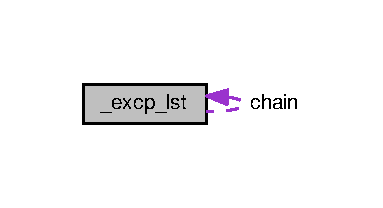
\includegraphics[width=184pt]{struct__excp__lst__coll__graph}
\end{center}
\end{figure}
\subsection*{Data Fields}
\begin{DoxyCompactItemize}
\item 
struct \hyperlink{struct__excp__lst}{\+\_\+excp\+\_\+lst} $\ast$ \hyperlink{struct__excp__lst_af3aa96f46675863a93c104985a99b44f}{chain}
\item 
E\+X\+C\+E\+P\+T\+I\+O\+N\+\_\+\+D\+I\+S\+P\+O\+S\+I\+T\+I\+ON($\ast$ \hyperlink{struct__excp__lst_a1e1e0c071255497025a22a693efc487c}{handler} )()
\end{DoxyCompactItemize}


\subsection{Field Documentation}
\index{\+\_\+excp\+\_\+lst@{\+\_\+excp\+\_\+lst}!chain@{chain}}
\index{chain@{chain}!\+\_\+excp\+\_\+lst@{\+\_\+excp\+\_\+lst}}
\subsubsection[{\texorpdfstring{chain}{chain}}]{\setlength{\rightskip}{0pt plus 5cm}struct {\bf \+\_\+excp\+\_\+lst}$\ast$ \+\_\+excp\+\_\+lst\+::chain}\hypertarget{struct__excp__lst_af3aa96f46675863a93c104985a99b44f}{}\label{struct__excp__lst_af3aa96f46675863a93c104985a99b44f}
\index{\+\_\+excp\+\_\+lst@{\+\_\+excp\+\_\+lst}!handler@{handler}}
\index{handler@{handler}!\+\_\+excp\+\_\+lst@{\+\_\+excp\+\_\+lst}}
\subsubsection[{\texorpdfstring{handler}{handler}}]{\setlength{\rightskip}{0pt plus 5cm}E\+X\+C\+E\+P\+T\+I\+O\+N\+\_\+\+D\+I\+S\+P\+O\+S\+I\+T\+I\+ON($\ast$ \+\_\+excp\+\_\+lst\+::handler) ()}\hypertarget{struct__excp__lst_a1e1e0c071255497025a22a693efc487c}{}\label{struct__excp__lst_a1e1e0c071255497025a22a693efc487c}


The documentation for this struct was generated from the following file\+:\begin{DoxyCompactItemize}
\item 
gprolog-\/utf8-\/tree/src/\+Engine\+Pl/\hyperlink{WIN32__all__SIGSEGV_8c}{W\+I\+N32\+\_\+all\+\_\+\+S\+I\+G\+S\+E\+G\+V.\+c}\end{DoxyCompactItemize}

\hypertarget{structAliasInf}{}\section{Alias\+Inf Struct Reference}
\label{structAliasInf}\index{Alias\+Inf@{Alias\+Inf}}


{\ttfamily \#include $<$stream\+\_\+supp.\+h$>$}

\subsection*{Data Fields}
\begin{DoxyCompactItemize}
\item 
\hyperlink{gprolog_8h_a4d005b136d7fb28537eb1815f7868b63}{Pl\+Long} \hyperlink{structAliasInf_aa0eddd23c6a16d2a76eecc569dbd34d1}{atom}
\item 
int \hyperlink{structAliasInf_aff64cf68f3f548a6978aa01f8509cc9c}{stm}
\end{DoxyCompactItemize}


\subsection{Field Documentation}
\index{Alias\+Inf@{Alias\+Inf}!atom@{atom}}
\index{atom@{atom}!Alias\+Inf@{Alias\+Inf}}
\subsubsection[{\texorpdfstring{atom}{atom}}]{\setlength{\rightskip}{0pt plus 5cm}{\bf Pl\+Long} Alias\+Inf\+::atom}\hypertarget{structAliasInf_aa0eddd23c6a16d2a76eecc569dbd34d1}{}\label{structAliasInf_aa0eddd23c6a16d2a76eecc569dbd34d1}
\index{Alias\+Inf@{Alias\+Inf}!stm@{stm}}
\index{stm@{stm}!Alias\+Inf@{Alias\+Inf}}
\subsubsection[{\texorpdfstring{stm}{stm}}]{\setlength{\rightskip}{0pt plus 5cm}int Alias\+Inf\+::stm}\hypertarget{structAliasInf_aff64cf68f3f548a6978aa01f8509cc9c}{}\label{structAliasInf_aff64cf68f3f548a6978aa01f8509cc9c}


The documentation for this struct was generated from the following file\+:\begin{DoxyCompactItemize}
\item 
gprolog-\/utf8-\/tree/src/\+Bips\+Pl/\hyperlink{stream__supp_8h}{stream\+\_\+supp.\+h}\end{DoxyCompactItemize}

\hypertarget{structArgInf}{}\section{Arg\+Inf Struct Reference}
\label{structArgInf}\index{Arg\+Inf@{Arg\+Inf}}


{\ttfamily \#include $<$ma\+\_\+parser.\+h$>$}



Collaboration diagram for Arg\+Inf\+:\nopagebreak
\begin{figure}[H]
\begin{center}
\leavevmode
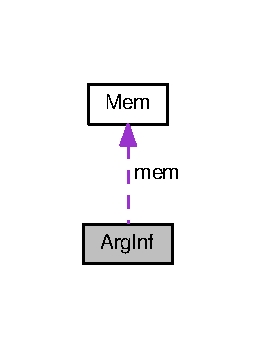
\includegraphics[width=127pt]{structArgInf__coll__graph}
\end{center}
\end{figure}
\subsection*{Data Fields}
\begin{DoxyCompactItemize}
\item 
\hyperlink{ma__parser_8h_a55e83ab108ec469cbb59876c09f146b0}{Arg\+Typ} \hyperlink{structArgInf_ad416abaf87d2e52a23c4d2eb517919e4}{type}
\item 
int \hyperlink{structArgInf_a9a45faac36b5ff6b969faa85446f40e1}{adr\+\_\+of}
\item 
\begin{tabbing}
xx\=xx\=xx\=xx\=xx\=xx\=xx\=xx\=xx\=\kill
union \{\\
\>char $\ast$ \hyperlink{structArgInf_aae189057e919a389c59d0ee897884c5f}{str\_val}\\
\>\hyperlink{gprolog_8h_a4d005b136d7fb28537eb1815f7868b63}{PlLong} \hyperlink{structArgInf_a9b94d186b491b4009a1905f86e41ad9c}{int\_val}\\
\>double \hyperlink{structArgInf_a5ce0eda4a228042bd33b247f80e61144}{dbl\_val}\\
\>\hyperlink{structMem}{Mem} \hyperlink{structArgInf_aa4a2dcaf59861c10d3622f1bdcc5ac3d}{mem}\\
\>int \hyperlink{structArgInf_a053ccdce92762ff8fecd64a3ce561aea}{index}\\
\} \hyperlink{structArgInf_ae7f40cf76bee98b10f0eb3d865b2b912}{t}\\

\end{tabbing}\end{DoxyCompactItemize}


\subsection{Field Documentation}
\index{Arg\+Inf@{Arg\+Inf}!adr\+\_\+of@{adr\+\_\+of}}
\index{adr\+\_\+of@{adr\+\_\+of}!Arg\+Inf@{Arg\+Inf}}
\subsubsection[{\texorpdfstring{adr\+\_\+of}{adr_of}}]{\setlength{\rightskip}{0pt plus 5cm}int Arg\+Inf\+::adr\+\_\+of}\hypertarget{structArgInf_a9a45faac36b5ff6b969faa85446f40e1}{}\label{structArgInf_a9a45faac36b5ff6b969faa85446f40e1}
\index{Arg\+Inf@{Arg\+Inf}!dbl\+\_\+val@{dbl\+\_\+val}}
\index{dbl\+\_\+val@{dbl\+\_\+val}!Arg\+Inf@{Arg\+Inf}}
\subsubsection[{\texorpdfstring{dbl\+\_\+val}{dbl_val}}]{\setlength{\rightskip}{0pt plus 5cm}double Arg\+Inf\+::dbl\+\_\+val}\hypertarget{structArgInf_a5ce0eda4a228042bd33b247f80e61144}{}\label{structArgInf_a5ce0eda4a228042bd33b247f80e61144}
\index{Arg\+Inf@{Arg\+Inf}!index@{index}}
\index{index@{index}!Arg\+Inf@{Arg\+Inf}}
\subsubsection[{\texorpdfstring{index}{index}}]{\setlength{\rightskip}{0pt plus 5cm}int Arg\+Inf\+::index}\hypertarget{structArgInf_a053ccdce92762ff8fecd64a3ce561aea}{}\label{structArgInf_a053ccdce92762ff8fecd64a3ce561aea}
\index{Arg\+Inf@{Arg\+Inf}!int\+\_\+val@{int\+\_\+val}}
\index{int\+\_\+val@{int\+\_\+val}!Arg\+Inf@{Arg\+Inf}}
\subsubsection[{\texorpdfstring{int\+\_\+val}{int_val}}]{\setlength{\rightskip}{0pt plus 5cm}{\bf Pl\+Long} Arg\+Inf\+::int\+\_\+val}\hypertarget{structArgInf_a9b94d186b491b4009a1905f86e41ad9c}{}\label{structArgInf_a9b94d186b491b4009a1905f86e41ad9c}
\index{Arg\+Inf@{Arg\+Inf}!mem@{mem}}
\index{mem@{mem}!Arg\+Inf@{Arg\+Inf}}
\subsubsection[{\texorpdfstring{mem}{mem}}]{\setlength{\rightskip}{0pt plus 5cm}{\bf Mem} Arg\+Inf\+::mem}\hypertarget{structArgInf_aa4a2dcaf59861c10d3622f1bdcc5ac3d}{}\label{structArgInf_aa4a2dcaf59861c10d3622f1bdcc5ac3d}
\index{Arg\+Inf@{Arg\+Inf}!str\+\_\+val@{str\+\_\+val}}
\index{str\+\_\+val@{str\+\_\+val}!Arg\+Inf@{Arg\+Inf}}
\subsubsection[{\texorpdfstring{str\+\_\+val}{str_val}}]{\setlength{\rightskip}{0pt plus 5cm}char$\ast$ Arg\+Inf\+::str\+\_\+val}\hypertarget{structArgInf_aae189057e919a389c59d0ee897884c5f}{}\label{structArgInf_aae189057e919a389c59d0ee897884c5f}
\index{Arg\+Inf@{Arg\+Inf}!t@{t}}
\index{t@{t}!Arg\+Inf@{Arg\+Inf}}
\subsubsection[{\texorpdfstring{t}{t}}]{\setlength{\rightskip}{0pt plus 5cm}union \{ ... \} 
   Arg\+Inf\+::t}\hypertarget{structArgInf_ae7f40cf76bee98b10f0eb3d865b2b912}{}\label{structArgInf_ae7f40cf76bee98b10f0eb3d865b2b912}
\index{Arg\+Inf@{Arg\+Inf}!type@{type}}
\index{type@{type}!Arg\+Inf@{Arg\+Inf}}
\subsubsection[{\texorpdfstring{type}{type}}]{\setlength{\rightskip}{0pt plus 5cm}{\bf Arg\+Typ} Arg\+Inf\+::type}\hypertarget{structArgInf_ad416abaf87d2e52a23c4d2eb517919e4}{}\label{structArgInf_ad416abaf87d2e52a23c4d2eb517919e4}


The documentation for this struct was generated from the following file\+:\begin{DoxyCompactItemize}
\item 
gprolog-\/utf8-\/tree/src/\+Ma2\+Asm/\hyperlink{ma__parser_8h}{ma\+\_\+parser.\+h}\end{DoxyCompactItemize}

\hypertarget{structArithInf}{}\section{Arith\+Inf Struct Reference}
\label{structArithInf}\index{Arith\+Inf@{Arith\+Inf}}
\subsection*{Public Member Functions}
\begin{DoxyCompactItemize}
\item 
\hyperlink{structArithInf_a436fe064b4148705eda3a2a3ed99b067}{Wam\+Word} (\hyperlink{chkma_8c_a46116ed56661a1c5bffe91c80ceae694}{FC} $\ast$\hyperlink{extract__asm_8c_a849db728d9239b130558864aae79168f}{fct})()
\end{DoxyCompactItemize}
\subsection*{Data Fields}
\begin{DoxyCompactItemize}
\item 
\hyperlink{LINUX__SIGSEGV_8c_a10ea8be8823feb38875b8a9326cbb424}{Wam\+Word} \hyperlink{structArithInf_a0adf57977998badbf4fa7d8386fd5bdc}{f\+\_\+n}
\end{DoxyCompactItemize}


\subsection{Member Function Documentation}
\index{Arith\+Inf@{Arith\+Inf}!Wam\+Word@{Wam\+Word}}
\index{Wam\+Word@{Wam\+Word}!Arith\+Inf@{Arith\+Inf}}
\subsubsection[{\texorpdfstring{Wam\+Word(\+F\+C $\ast$fct)()}{WamWord(FC *fct)()}}]{\setlength{\rightskip}{0pt plus 5cm}Arith\+Inf\+::\+Wam\+Word (
\begin{DoxyParamCaption}
\item[{{\bf FC} $\ast$}]{fct}
\end{DoxyParamCaption}
)}\hypertarget{structArithInf_a436fe064b4148705eda3a2a3ed99b067}{}\label{structArithInf_a436fe064b4148705eda3a2a3ed99b067}


\subsection{Field Documentation}
\index{Arith\+Inf@{Arith\+Inf}!f\+\_\+n@{f\+\_\+n}}
\index{f\+\_\+n@{f\+\_\+n}!Arith\+Inf@{Arith\+Inf}}
\subsubsection[{\texorpdfstring{f\+\_\+n}{f_n}}]{\setlength{\rightskip}{0pt plus 5cm}{\bf Wam\+Word} Arith\+Inf\+::f\+\_\+n}\hypertarget{structArithInf_a0adf57977998badbf4fa7d8386fd5bdc}{}\label{structArithInf_a0adf57977998badbf4fa7d8386fd5bdc}


The documentation for this struct was generated from the following file\+:\begin{DoxyCompactItemize}
\item 
gprolog-\/utf8-\/tree/src/\+Bips\+Pl/\hyperlink{arith__inl__c_8c}{arith\+\_\+inl\+\_\+c.\+c}\end{DoxyCompactItemize}

\hypertarget{structAsmLine}{}\section{Asm\+Line Struct Reference}
\label{structAsmLine}\index{Asm\+Line@{Asm\+Line}}
\subsection*{Data Fields}
\begin{DoxyCompactItemize}
\item 
int \hyperlink{structAsmLine_a1b7f8a7f299218d0be5d2e5e15bb974e}{label}
\item 
char \hyperlink{structAsmLine_af94ff4cc2a4abfdf5eed77061fd34f68}{code\+\_\+op} \mbox{[}32\mbox{]}
\item 
char \hyperlink{structAsmLine_a77453b03d07a24336adf4f62b5bbc9c8}{args} \mbox{[}256\mbox{]}
\end{DoxyCompactItemize}


\subsection{Field Documentation}
\index{Asm\+Line@{Asm\+Line}!args@{args}}
\index{args@{args}!Asm\+Line@{Asm\+Line}}
\subsubsection[{\texorpdfstring{args}{args}}]{\setlength{\rightskip}{0pt plus 5cm}char Asm\+Line\+::args\mbox{[}256\mbox{]}}\hypertarget{structAsmLine_a77453b03d07a24336adf4f62b5bbc9c8}{}\label{structAsmLine_a77453b03d07a24336adf4f62b5bbc9c8}
\index{Asm\+Line@{Asm\+Line}!code\+\_\+op@{code\+\_\+op}}
\index{code\+\_\+op@{code\+\_\+op}!Asm\+Line@{Asm\+Line}}
\subsubsection[{\texorpdfstring{code\+\_\+op}{code_op}}]{\setlength{\rightskip}{0pt plus 5cm}char Asm\+Line\+::code\+\_\+op\mbox{[}32\mbox{]}}\hypertarget{structAsmLine_af94ff4cc2a4abfdf5eed77061fd34f68}{}\label{structAsmLine_af94ff4cc2a4abfdf5eed77061fd34f68}
\index{Asm\+Line@{Asm\+Line}!label@{label}}
\index{label@{label}!Asm\+Line@{Asm\+Line}}
\subsubsection[{\texorpdfstring{label}{label}}]{\setlength{\rightskip}{0pt plus 5cm}int Asm\+Line\+::label}\hypertarget{structAsmLine_a1b7f8a7f299218d0be5d2e5e15bb974e}{}\label{structAsmLine_a1b7f8a7f299218d0be5d2e5e15bb974e}


The documentation for this struct was generated from the following file\+:\begin{DoxyCompactItemize}
\item 
gprolog-\/utf8-\/tree/src/\+Ma2\+Asm/\hyperlink{extract__asm_8c}{extract\+\_\+asm.\+c}\end{DoxyCompactItemize}

\hypertarget{structAtomInf}{}\section{Atom\+Inf Struct Reference}
\label{structAtomInf}\index{Atom\+Inf@{Atom\+Inf}}


{\ttfamily \#include $<$atom.\+h$>$}



Collaboration diagram for Atom\+Inf\+:\nopagebreak
\begin{figure}[H]
\begin{center}
\leavevmode
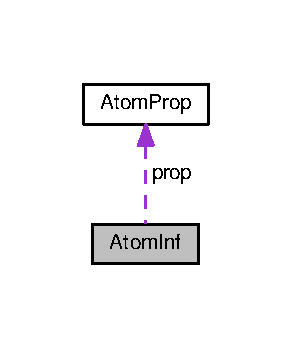
\includegraphics[width=140pt]{structAtomInf__coll__graph}
\end{center}
\end{figure}
\subsection*{Data Fields}
\begin{DoxyCompactItemize}
\item 
char $\ast$ \hyperlink{structAtomInf_a2e8fbcd0d525d43b562f771d099e694e}{name}
\item 
unsigned \hyperlink{structAtomInf_aa2294890b36422410177f1ac258c5157}{hash}
\item 
\hyperlink{structAtomProp}{Atom\+Prop} \hyperlink{structAtomInf_a649620e4716f966372c391e2e8e5245d}{prop}
\item 
void $\ast$ \hyperlink{structAtomInf_a497dcae4cea5b3a779731b97476d05a5}{info}
\end{DoxyCompactItemize}


\subsection{Field Documentation}
\index{Atom\+Inf@{Atom\+Inf}!hash@{hash}}
\index{hash@{hash}!Atom\+Inf@{Atom\+Inf}}
\subsubsection[{\texorpdfstring{hash}{hash}}]{\setlength{\rightskip}{0pt plus 5cm}unsigned Atom\+Inf\+::hash}\hypertarget{structAtomInf_aa2294890b36422410177f1ac258c5157}{}\label{structAtomInf_aa2294890b36422410177f1ac258c5157}
\index{Atom\+Inf@{Atom\+Inf}!info@{info}}
\index{info@{info}!Atom\+Inf@{Atom\+Inf}}
\subsubsection[{\texorpdfstring{info}{info}}]{\setlength{\rightskip}{0pt plus 5cm}void$\ast$ Atom\+Inf\+::info}\hypertarget{structAtomInf_a497dcae4cea5b3a779731b97476d05a5}{}\label{structAtomInf_a497dcae4cea5b3a779731b97476d05a5}
\index{Atom\+Inf@{Atom\+Inf}!name@{name}}
\index{name@{name}!Atom\+Inf@{Atom\+Inf}}
\subsubsection[{\texorpdfstring{name}{name}}]{\setlength{\rightskip}{0pt plus 5cm}char$\ast$ Atom\+Inf\+::name}\hypertarget{structAtomInf_a2e8fbcd0d525d43b562f771d099e694e}{}\label{structAtomInf_a2e8fbcd0d525d43b562f771d099e694e}
\index{Atom\+Inf@{Atom\+Inf}!prop@{prop}}
\index{prop@{prop}!Atom\+Inf@{Atom\+Inf}}
\subsubsection[{\texorpdfstring{prop}{prop}}]{\setlength{\rightskip}{0pt plus 5cm}{\bf Atom\+Prop} Atom\+Inf\+::prop}\hypertarget{structAtomInf_a649620e4716f966372c391e2e8e5245d}{}\label{structAtomInf_a649620e4716f966372c391e2e8e5245d}


The documentation for this struct was generated from the following file\+:\begin{DoxyCompactItemize}
\item 
gprolog-\/utf8-\/tree/src/\+Engine\+Pl/\hyperlink{atom_8h}{atom.\+h}\end{DoxyCompactItemize}

\hypertarget{structAtomProp}{}\section{Atom\+Prop Struct Reference}
\label{structAtomProp}\index{Atom\+Prop@{Atom\+Prop}}
\subsection*{Data Fields}
\begin{DoxyCompactItemize}
\item 
unsigned {\bfseries length}\+:16\hypertarget{structAtomProp_a5708a8e58126cdcd641e6c24e7dd429d}{}\label{structAtomProp_a5708a8e58126cdcd641e6c24e7dd429d}

\item 
unsigned {\bfseries count}\+:16\hypertarget{structAtomProp_a686f0165443645d420bfd7381ddfedb0}{}\label{structAtomProp_a686f0165443645d420bfd7381ddfedb0}

\item 
unsigned {\bfseries op\+\_\+mask}\+:4\hypertarget{structAtomProp_add308662f264e390f71e5557b97837c0}{}\label{structAtomProp_add308662f264e390f71e5557b97837c0}

\item 
unsigned {\bfseries type}\+:2\hypertarget{structAtomProp_accd017afa6f2854bb9316f492449c025}{}\label{structAtomProp_accd017afa6f2854bb9316f492449c025}

\item 
unsigned {\bfseries needs\+\_\+quote}\+:1\hypertarget{structAtomProp_a4b3fe8dfeb73dc67be63684028709774}{}\label{structAtomProp_a4b3fe8dfeb73dc67be63684028709774}

\item 
unsigned {\bfseries needs\+\_\+scan}\+:1\hypertarget{structAtomProp_ada3d42fc8a9d6e708de7db347444b6ee}{}\label{structAtomProp_ada3d42fc8a9d6e708de7db347444b6ee}

\end{DoxyCompactItemize}


The documentation for this struct was generated from the following file\+:\begin{DoxyCompactItemize}
\item 
gprolog-\/utf8-\/tree/src/\+Engine\+Pl/atom.\+h\end{DoxyCompactItemize}

\hypertarget{unionBCWord}{}\section{B\+C\+Word Union Reference}
\label{unionBCWord}\index{B\+C\+Word@{B\+C\+Word}}
\subsection*{Data Fields}
\begin{DoxyCompactItemize}
\item 
\begin{tabbing}
xx\=xx\=xx\=xx\=xx\=xx\=xx\=xx\=xx\=\kill
struct \{\\
\>unsigned {\bfseries code\_op}:8\\
\>unsigned {\bfseries i8}:8\\
\>unsigned {\bfseries i16}:16\\
\} {\bfseries t1}\hypertarget{unionBCWord_a70e755edbb220fd93df2c19803233c99}{}\label{unionBCWord_a70e755edbb220fd93df2c19803233c99}
\\

\end{tabbing}\item 
\begin{tabbing}
xx\=xx\=xx\=xx\=xx\=xx\=xx\=xx\=xx\=\kill
struct \{\\
\>unsigned {\bfseries code\_op}:8\\
\>unsigned {\bfseries i24}:24\\
\} {\bfseries t2}\hypertarget{unionBCWord_abbf0ee87987d69cb8a46e49454401f7c}{}\label{unionBCWord_abbf0ee87987d69cb8a46e49454401f7c}
\\

\end{tabbing}\item 
unsigned {\bfseries word}\hypertarget{unionBCWord_ae6b64a6557710fc6e57ebbd02d1a3bc1}{}\label{unionBCWord_ae6b64a6557710fc6e57ebbd02d1a3bc1}

\end{DoxyCompactItemize}


The documentation for this union was generated from the following file\+:\begin{DoxyCompactItemize}
\item 
gprolog-\/utf8-\/tree/src/\+Bips\+Pl/bc\+\_\+supp.\+c\end{DoxyCompactItemize}

\hypertarget{structbtnode}{}\section{btnode Struct Reference}
\label{structbtnode}\index{btnode@{btnode}}


Collaboration diagram for btnode\+:\nopagebreak
\begin{figure}[H]
\begin{center}
\leavevmode
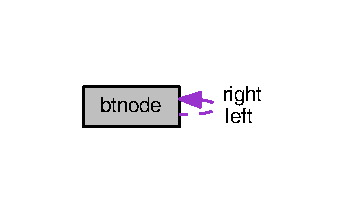
\includegraphics[width=166pt]{structbtnode__coll__graph}
\end{center}
\end{figure}
\subsection*{Data Fields}
\begin{DoxyCompactItemize}
\item 
char $\ast$ {\bfseries str}\hypertarget{structbtnode_ad3235a44ef495ead7832dc7242184d3b}{}\label{structbtnode_ad3235a44ef495ead7832dc7242184d3b}

\item 
int {\bfseries no}\hypertarget{structbtnode_ae1befed4e49931603b1a62f760242f52}{}\label{structbtnode_ae1befed4e49931603b1a62f760242f52}

\item 
char {\bfseries info} \mbox{[}32\mbox{]}\hypertarget{structbtnode_a822bfc05cc3514c5d2799f66c65112e8}{}\label{structbtnode_a822bfc05cc3514c5d2799f66c65112e8}

\item 
\hyperlink{structbtnode}{P\+B\+T\+Node} {\bfseries left}\hypertarget{structbtnode_a595372884aee31dd6b91ba5400f98794}{}\label{structbtnode_a595372884aee31dd6b91ba5400f98794}

\item 
\hyperlink{structbtnode}{P\+B\+T\+Node} {\bfseries right}\hypertarget{structbtnode_a5a315554fa5e275f6f505e94135b1cf4}{}\label{structbtnode_a5a315554fa5e275f6f505e94135b1cf4}

\end{DoxyCompactItemize}


The documentation for this struct was generated from the following file\+:\begin{DoxyCompactItemize}
\item 
gprolog-\/utf8-\/tree/src/\+Wam2\+Ma/bt\+\_\+string.\+h\end{DoxyCompactItemize}

\hypertarget{structBTString}{}\section{B\+T\+String Struct Reference}
\label{structBTString}\index{B\+T\+String@{B\+T\+String}}


{\ttfamily \#include $<$bt\+\_\+string.\+h$>$}



Collaboration diagram for B\+T\+String\+:\nopagebreak
\begin{figure}[H]
\begin{center}
\leavevmode
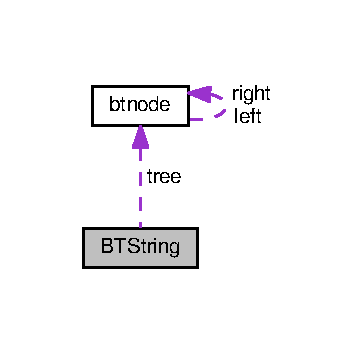
\includegraphics[width=171pt]{structBTString__coll__graph}
\end{center}
\end{figure}
\subsection*{Data Fields}
\begin{DoxyCompactItemize}
\item 
\hyperlink{bt__string_8h_a94e2311ccccb66fae2c4ce55649526fc}{B\+T\+Node} $\ast$ \hyperlink{structBTString_a3d5e702b03b4afc55252841d531836f8}{tree}
\item 
int \hyperlink{structBTString_a4248622c60ccba995140069c3c1fa116}{nb\+\_\+elem}
\end{DoxyCompactItemize}


\subsection{Field Documentation}
\index{B\+T\+String@{B\+T\+String}!nb\+\_\+elem@{nb\+\_\+elem}}
\index{nb\+\_\+elem@{nb\+\_\+elem}!B\+T\+String@{B\+T\+String}}
\subsubsection[{\texorpdfstring{nb\+\_\+elem}{nb_elem}}]{\setlength{\rightskip}{0pt plus 5cm}int B\+T\+String\+::nb\+\_\+elem}\hypertarget{structBTString_a4248622c60ccba995140069c3c1fa116}{}\label{structBTString_a4248622c60ccba995140069c3c1fa116}
\index{B\+T\+String@{B\+T\+String}!tree@{tree}}
\index{tree@{tree}!B\+T\+String@{B\+T\+String}}
\subsubsection[{\texorpdfstring{tree}{tree}}]{\setlength{\rightskip}{0pt plus 5cm}{\bf B\+T\+Node}$\ast$ B\+T\+String\+::tree}\hypertarget{structBTString_a3d5e702b03b4afc55252841d531836f8}{}\label{structBTString_a3d5e702b03b4afc55252841d531836f8}


The documentation for this struct was generated from the following file\+:\begin{DoxyCompactItemize}
\item 
gprolog-\/utf8-\/tree/src/\+Wam2\+Ma/\hyperlink{bt__string_8h}{bt\+\_\+string.\+h}\end{DoxyCompactItemize}

\hypertarget{unionC64To32}{}\section{C64\+To32 Union Reference}
\label{unionC64To32}\index{C64\+To32@{C64\+To32}}
\subsection*{Data Fields}
\begin{DoxyCompactItemize}
\item 
double \hyperlink{unionC64To32_a153fec5a65f5557d9e40a57b95ae6dc0}{d}
\item 
unsigned \hyperlink{unionC64To32_aa82ad59db4f982b9779320862ef7f50f}{u} \mbox{[}2\mbox{]}
\end{DoxyCompactItemize}


\subsection{Field Documentation}
\index{C64\+To32@{C64\+To32}!d@{d}}
\index{d@{d}!C64\+To32@{C64\+To32}}
\subsubsection[{\texorpdfstring{d}{d}}]{\setlength{\rightskip}{0pt plus 5cm}double C64\+To32\+::d}\hypertarget{unionC64To32_a153fec5a65f5557d9e40a57b95ae6dc0}{}\label{unionC64To32_a153fec5a65f5557d9e40a57b95ae6dc0}
\index{C64\+To32@{C64\+To32}!u@{u}}
\index{u@{u}!C64\+To32@{C64\+To32}}
\subsubsection[{\texorpdfstring{u}{u}}]{\setlength{\rightskip}{0pt plus 5cm}unsigned C64\+To32\+::u\mbox{[}2\mbox{]}}\hypertarget{unionC64To32_aa82ad59db4f982b9779320862ef7f50f}{}\label{unionC64To32_aa82ad59db4f982b9779320862ef7f50f}


The documentation for this union was generated from the following file\+:\begin{DoxyCompactItemize}
\item 
gprolog-\/utf8-\/tree/src/\+Bips\+Pl/\hyperlink{bc__supp_8c}{bc\+\_\+supp.\+c}\end{DoxyCompactItemize}

\hypertarget{structCmdInf}{}\section{Cmd\+Inf Struct Reference}
\label{structCmdInf}\index{Cmd\+Inf@{Cmd\+Inf}}
\subsection*{Data Fields}
\begin{DoxyCompactItemize}
\item 
char $\ast$ \hyperlink{structCmdInf_a08f467c4c99d5989d79d571d71eb91cc}{exe\+\_\+name}
\item 
char \hyperlink{structCmdInf_ad3011b5eb07e4f6bc735ba74f0061fb5}{opt} \mbox{[}\hyperlink{top__comp_8c_a3be28e77218549701fd7677b5d2d8b4b}{C\+M\+D\+\_\+\+L\+I\+N\+E\+\_\+\+M\+A\+X\+\_\+\+O\+PT}\mbox{]}
\item 
char $\ast$ \hyperlink{structCmdInf_a8810930cb97bd994d3d5a081222e9882}{out\+\_\+opt}
\end{DoxyCompactItemize}


\subsection{Field Documentation}
\index{Cmd\+Inf@{Cmd\+Inf}!exe\+\_\+name@{exe\+\_\+name}}
\index{exe\+\_\+name@{exe\+\_\+name}!Cmd\+Inf@{Cmd\+Inf}}
\subsubsection[{\texorpdfstring{exe\+\_\+name}{exe_name}}]{\setlength{\rightskip}{0pt plus 5cm}char$\ast$ Cmd\+Inf\+::exe\+\_\+name}\hypertarget{structCmdInf_a08f467c4c99d5989d79d571d71eb91cc}{}\label{structCmdInf_a08f467c4c99d5989d79d571d71eb91cc}
\index{Cmd\+Inf@{Cmd\+Inf}!opt@{opt}}
\index{opt@{opt}!Cmd\+Inf@{Cmd\+Inf}}
\subsubsection[{\texorpdfstring{opt}{opt}}]{\setlength{\rightskip}{0pt plus 5cm}char Cmd\+Inf\+::opt\mbox{[}{\bf C\+M\+D\+\_\+\+L\+I\+N\+E\+\_\+\+M\+A\+X\+\_\+\+O\+PT}\mbox{]}}\hypertarget{structCmdInf_ad3011b5eb07e4f6bc735ba74f0061fb5}{}\label{structCmdInf_ad3011b5eb07e4f6bc735ba74f0061fb5}
\index{Cmd\+Inf@{Cmd\+Inf}!out\+\_\+opt@{out\+\_\+opt}}
\index{out\+\_\+opt@{out\+\_\+opt}!Cmd\+Inf@{Cmd\+Inf}}
\subsubsection[{\texorpdfstring{out\+\_\+opt}{out_opt}}]{\setlength{\rightskip}{0pt plus 5cm}char$\ast$ Cmd\+Inf\+::out\+\_\+opt}\hypertarget{structCmdInf_a8810930cb97bd994d3d5a081222e9882}{}\label{structCmdInf_a8810930cb97bd994d3d5a081222e9882}


The documentation for this struct was generated from the following file\+:\begin{DoxyCompactItemize}
\item 
gprolog-\/utf8-\/tree/src/\+Top\+Comp/\hyperlink{top__comp_8c}{top\+\_\+comp.\+c}\end{DoxyCompactItemize}

\hypertarget{structCodeInf}{}\section{Code\+Inf Struct Reference}
\label{structCodeInf}\index{Code\+Inf@{Code\+Inf}}
\subsection*{Data Fields}
\begin{DoxyCompactItemize}
\item 
int {\bfseries prolog}\hypertarget{structCodeInf_a1010280a1eff3f13adae9b219d07c4cb}{}\label{structCodeInf_a1010280a1eff3f13adae9b219d07c4cb}

\item 
int {\bfseries global}\hypertarget{structCodeInf_a0819cfe0da8345734d7e3b6964caf566}{}\label{structCodeInf_a0819cfe0da8345734d7e3b6964caf566}

\end{DoxyCompactItemize}


The documentation for this struct was generated from the following file\+:\begin{DoxyCompactItemize}
\item 
gprolog-\/utf8-\/tree/src/\+Ma2\+Asm/ma2asm.\+c\end{DoxyCompactItemize}

\hypertarget{structcomp__node}{}\section{comp\+\_\+node Struct Reference}
\label{structcomp__node}\index{comp\+\_\+node@{comp\+\_\+node}}


Collaboration diagram for comp\+\_\+node\+:\nopagebreak
\begin{figure}[H]
\begin{center}
\leavevmode
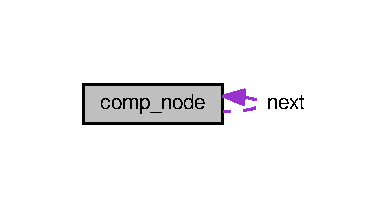
\includegraphics[width=187pt]{structcomp__node__coll__graph}
\end{center}
\end{figure}
\subsection*{Data Fields}
\begin{DoxyCompactItemize}
\item 
char $\ast$ {\bfseries word}\hypertarget{structcomp__node_a087b822f301956dd57ff59bf5d9ce9a4}{}\label{structcomp__node_a087b822f301956dd57ff59bf5d9ce9a4}

\item 
int {\bfseries word\+\_\+length}\hypertarget{structcomp__node_ab0e205b1c196f493851ae425e904c59b}{}\label{structcomp__node_ab0e205b1c196f493851ae425e904c59b}

\item 
\hyperlink{structcomp__node}{Comp\+Node} $\ast$ {\bfseries next}\hypertarget{structcomp__node_aa91fd30c56bcfb19162045c7856d66c8}{}\label{structcomp__node_aa91fd30c56bcfb19162045c7856d66c8}

\end{DoxyCompactItemize}


The documentation for this struct was generated from the following file\+:\begin{DoxyCompactItemize}
\item 
gprolog-\/utf8-\/tree/src/\+Linedit/linedit.\+c\end{DoxyCompactItemize}

\hypertarget{structcptcell}{}\section{cptcell Struct Reference}
\label{structcptcell}\index{cptcell@{cptcell}}


Collaboration diagram for cptcell\+:\nopagebreak
\begin{figure}[H]
\begin{center}
\leavevmode
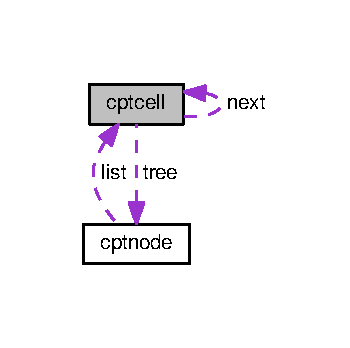
\includegraphics[width=168pt]{structcptcell__coll__graph}
\end{center}
\end{figure}
\subsection*{Data Fields}
\begin{DoxyCompactItemize}
\item 
\hyperlink{cpt__string_8c_ab66488a4813896c44d2e4bbcf8d43a86}{C\+P\+T\+Tree} \hyperlink{structcptcell_a8ce1e2723947c6ebce10520f1fcee6be}{tree}
\item 
\hyperlink{cpt__string_8c_ab32bc138599911e22c2be201414b53e7}{C\+P\+T\+List} \hyperlink{structcptcell_a20fc8bb9280bb623be1dc9e5089df7bb}{next}
\end{DoxyCompactItemize}


\subsection{Field Documentation}
\index{cptcell@{cptcell}!next@{next}}
\index{next@{next}!cptcell@{cptcell}}
\subsubsection[{\texorpdfstring{next}{next}}]{\setlength{\rightskip}{0pt plus 5cm}{\bf C\+P\+T\+List} cptcell\+::next}\hypertarget{structcptcell_a20fc8bb9280bb623be1dc9e5089df7bb}{}\label{structcptcell_a20fc8bb9280bb623be1dc9e5089df7bb}
\index{cptcell@{cptcell}!tree@{tree}}
\index{tree@{tree}!cptcell@{cptcell}}
\subsubsection[{\texorpdfstring{tree}{tree}}]{\setlength{\rightskip}{0pt plus 5cm}{\bf C\+P\+T\+Tree} cptcell\+::tree}\hypertarget{structcptcell_a8ce1e2723947c6ebce10520f1fcee6be}{}\label{structcptcell_a8ce1e2723947c6ebce10520f1fcee6be}


The documentation for this struct was generated from the following file\+:\begin{DoxyCompactItemize}
\item 
gprolog-\/utf8-\/tree/src/\+Engine\+Pl/\hyperlink{cpt__string_8c}{cpt\+\_\+string.\+c}\end{DoxyCompactItemize}

\hypertarget{structCPTMatch}{}\section{C\+P\+T\+Match Struct Reference}
\label{structCPTMatch}\index{C\+P\+T\+Match@{C\+P\+T\+Match}}


Collaboration diagram for C\+P\+T\+Match\+:\nopagebreak
\begin{figure}[H]
\begin{center}
\leavevmode
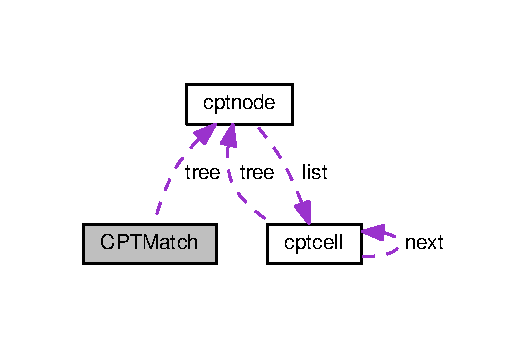
\includegraphics[width=254pt]{structCPTMatch__coll__graph}
\end{center}
\end{figure}
\subsection*{Data Fields}
\begin{DoxyCompactItemize}
\item 
\hyperlink{cpt__string_8c_ab66488a4813896c44d2e4bbcf8d43a86}{C\+P\+T\+Tree} \hyperlink{structCPTMatch_a11fa53acc2fd955cbea152f381e82f31}{tree}
\item 
char $\ast$ \hyperlink{structCPTMatch_a07b32173eb67b2c3e2918bf5a8d29ee5}{buff}
\item 
int \hyperlink{structCPTMatch_aa6d88b8078ed95b080fd648bd46a67c9}{length}
\item 
int($\ast$ \hyperlink{structCPTMatch_a1bee4a76898a1ef5809eb26af9d9673d}{fct} )()
\end{DoxyCompactItemize}


\subsection{Field Documentation}
\index{C\+P\+T\+Match@{C\+P\+T\+Match}!buff@{buff}}
\index{buff@{buff}!C\+P\+T\+Match@{C\+P\+T\+Match}}
\subsubsection[{\texorpdfstring{buff}{buff}}]{\setlength{\rightskip}{0pt plus 5cm}char$\ast$ C\+P\+T\+Match\+::buff}\hypertarget{structCPTMatch_a07b32173eb67b2c3e2918bf5a8d29ee5}{}\label{structCPTMatch_a07b32173eb67b2c3e2918bf5a8d29ee5}
\index{C\+P\+T\+Match@{C\+P\+T\+Match}!fct@{fct}}
\index{fct@{fct}!C\+P\+T\+Match@{C\+P\+T\+Match}}
\subsubsection[{\texorpdfstring{fct}{fct}}]{\setlength{\rightskip}{0pt plus 5cm}int($\ast$ C\+P\+T\+Match\+::fct) ()}\hypertarget{structCPTMatch_a1bee4a76898a1ef5809eb26af9d9673d}{}\label{structCPTMatch_a1bee4a76898a1ef5809eb26af9d9673d}
\index{C\+P\+T\+Match@{C\+P\+T\+Match}!length@{length}}
\index{length@{length}!C\+P\+T\+Match@{C\+P\+T\+Match}}
\subsubsection[{\texorpdfstring{length}{length}}]{\setlength{\rightskip}{0pt plus 5cm}int C\+P\+T\+Match\+::length}\hypertarget{structCPTMatch_aa6d88b8078ed95b080fd648bd46a67c9}{}\label{structCPTMatch_aa6d88b8078ed95b080fd648bd46a67c9}
\index{C\+P\+T\+Match@{C\+P\+T\+Match}!tree@{tree}}
\index{tree@{tree}!C\+P\+T\+Match@{C\+P\+T\+Match}}
\subsubsection[{\texorpdfstring{tree}{tree}}]{\setlength{\rightskip}{0pt plus 5cm}{\bf C\+P\+T\+Tree} C\+P\+T\+Match\+::tree}\hypertarget{structCPTMatch_a11fa53acc2fd955cbea152f381e82f31}{}\label{structCPTMatch_a11fa53acc2fd955cbea152f381e82f31}


The documentation for this struct was generated from the following file\+:\begin{DoxyCompactItemize}
\item 
gprolog-\/utf8-\/tree/src/\+Engine\+Pl/\hyperlink{cpt__string_8c}{cpt\+\_\+string.\+c}\end{DoxyCompactItemize}

\hypertarget{structcptnode}{}\section{cptnode Struct Reference}
\label{structcptnode}\index{cptnode@{cptnode}}


Collaboration diagram for cptnode\+:\nopagebreak
\begin{figure}[H]
\begin{center}
\leavevmode
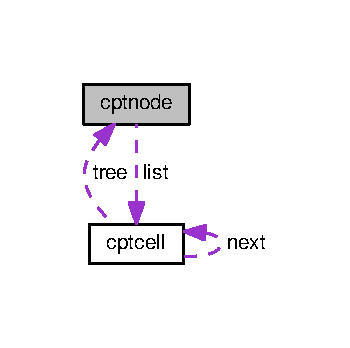
\includegraphics[width=168pt]{structcptnode__coll__graph}
\end{center}
\end{figure}
\subsection*{Data Fields}
\begin{DoxyCompactItemize}
\item 
char $\ast$ \hyperlink{structcptnode_a0f39bf735e3c110c5559c56a2865e3e6}{str}
\item 
int \hyperlink{structcptnode_a18110f6aa5dcbadb7233fb49ee931ee2}{length}
\item 
int \hyperlink{structcptnode_aa3b17740356cb0b60a9bac4f1ee7534d}{end}
\item 
\hyperlink{cpt__string_8c_ab32bc138599911e22c2be201414b53e7}{C\+P\+T\+List} \hyperlink{structcptnode_a957239c445f0b92b306830b91603b8e0}{list}
\end{DoxyCompactItemize}


\subsection{Field Documentation}
\index{cptnode@{cptnode}!end@{end}}
\index{end@{end}!cptnode@{cptnode}}
\subsubsection[{\texorpdfstring{end}{end}}]{\setlength{\rightskip}{0pt plus 5cm}int cptnode\+::end}\hypertarget{structcptnode_aa3b17740356cb0b60a9bac4f1ee7534d}{}\label{structcptnode_aa3b17740356cb0b60a9bac4f1ee7534d}
\index{cptnode@{cptnode}!length@{length}}
\index{length@{length}!cptnode@{cptnode}}
\subsubsection[{\texorpdfstring{length}{length}}]{\setlength{\rightskip}{0pt plus 5cm}int cptnode\+::length}\hypertarget{structcptnode_a18110f6aa5dcbadb7233fb49ee931ee2}{}\label{structcptnode_a18110f6aa5dcbadb7233fb49ee931ee2}
\index{cptnode@{cptnode}!list@{list}}
\index{list@{list}!cptnode@{cptnode}}
\subsubsection[{\texorpdfstring{list}{list}}]{\setlength{\rightskip}{0pt plus 5cm}{\bf C\+P\+T\+List} cptnode\+::list}\hypertarget{structcptnode_a957239c445f0b92b306830b91603b8e0}{}\label{structcptnode_a957239c445f0b92b306830b91603b8e0}
\index{cptnode@{cptnode}!str@{str}}
\index{str@{str}!cptnode@{cptnode}}
\subsubsection[{\texorpdfstring{str}{str}}]{\setlength{\rightskip}{0pt plus 5cm}char$\ast$ cptnode\+::str}\hypertarget{structcptnode_a0f39bf735e3c110c5559c56a2865e3e6}{}\label{structcptnode_a0f39bf735e3c110c5559c56a2865e3e6}


The documentation for this struct was generated from the following file\+:\begin{DoxyCompactItemize}
\item 
gprolog-\/utf8-\/tree/src/\+Engine\+Pl/\hyperlink{cpt__string_8c}{cpt\+\_\+string.\+c}\end{DoxyCompactItemize}

\hypertarget{structCPTStat}{}\section{C\+P\+T\+Stat Struct Reference}
\label{structCPTStat}\index{C\+P\+T\+Stat@{C\+P\+T\+Stat}}
\subsection*{Data Fields}
\begin{DoxyCompactItemize}
\item 
int {\bfseries nb\+\_\+word}\hypertarget{structCPTStat_a58ac2be00efae25c2327d9633b0012d4}{}\label{structCPTStat_a58ac2be00efae25c2327d9633b0012d4}

\item 
int {\bfseries nb\+\_\+node}\hypertarget{structCPTStat_a2fe3f9ca6e2298de8fe583d1998cfa8b}{}\label{structCPTStat_a2fe3f9ca6e2298de8fe583d1998cfa8b}

\item 
int {\bfseries nb\+\_\+node2}\hypertarget{structCPTStat_a1f2b46fe4d9376cb139ac2828467bfce}{}\label{structCPTStat_a1f2b46fe4d9376cb139ac2828467bfce}

\item 
int {\bfseries nb\+\_\+branch}\hypertarget{structCPTStat_af76928968bae2b707f069814504b5045}{}\label{structCPTStat_af76928968bae2b707f069814504b5045}

\item 
int {\bfseries max\+\_\+branch\+\_\+size}\hypertarget{structCPTStat_ae20f9509f4998f41157167b0eb7065b4}{}\label{structCPTStat_ae20f9509f4998f41157167b0eb7065b4}

\item 
int {\bfseries sum\+\_\+branch\+\_\+size\+\_\+word}\hypertarget{structCPTStat_adaea66ddd9de22bf900d0eeeb5486eac}{}\label{structCPTStat_adaea66ddd9de22bf900d0eeeb5486eac}

\item 
int {\bfseries sum\+\_\+branch\+\_\+size}\hypertarget{structCPTStat_a3b3e8fa6689f9725a871430adddf0f30}{}\label{structCPTStat_a3b3e8fa6689f9725a871430adddf0f30}

\item 
int {\bfseries max\+\_\+word\+\_\+length}\hypertarget{structCPTStat_ab03796b9949b9a21fa98a901390ca619}{}\label{structCPTStat_ab03796b9949b9a21fa98a901390ca619}

\item 
int {\bfseries sum\+\_\+word\+\_\+length}\hypertarget{structCPTStat_a8db546c8f4954a69815d75a4ab62a884}{}\label{structCPTStat_a8db546c8f4954a69815d75a4ab62a884}

\item 
int {\bfseries max\+\_\+swrd\+\_\+length}\hypertarget{structCPTStat_a05b16154f6a16eb86044c904c7db9de5}{}\label{structCPTStat_a05b16154f6a16eb86044c904c7db9de5}

\item 
int {\bfseries fst\+\_\+list\+\_\+size}\hypertarget{structCPTStat_aaec7403d2c937e97e1f323b4603d7a17}{}\label{structCPTStat_aaec7403d2c937e97e1f323b4603d7a17}

\item 
int {\bfseries max\+\_\+list\+\_\+size}\hypertarget{structCPTStat_a80e4787886e45e62cff7232be9f4cd7c}{}\label{structCPTStat_a80e4787886e45e62cff7232be9f4cd7c}

\item 
int {\bfseries max2\+\_\+list\+\_\+size}\hypertarget{structCPTStat_acac2689f27927c81da60a96191c99b30}{}\label{structCPTStat_acac2689f27927c81da60a96191c99b30}

\item 
int {\bfseries sum\+\_\+list\+\_\+size}\hypertarget{structCPTStat_ad99f1b443d4a863deb09e79760adf33f}{}\label{structCPTStat_ad99f1b443d4a863deb09e79760adf33f}

\end{DoxyCompactItemize}


The documentation for this struct was generated from the following file\+:\begin{DoxyCompactItemize}
\item 
gprolog-\/utf8-\/tree/src/\+Engine\+Pl/cpt\+\_\+string.\+c\end{DoxyCompactItemize}

\hypertarget{structD2ChCell}{}\section{D2\+Ch\+Cell Struct Reference}
\label{structD2ChCell}\index{D2\+Ch\+Cell@{D2\+Ch\+Cell}}


{\ttfamily \#include $<$dynam\+\_\+supp.\+h$>$}



Collaboration diagram for D2\+Ch\+Cell\+:\nopagebreak
\begin{figure}[H]
\begin{center}
\leavevmode
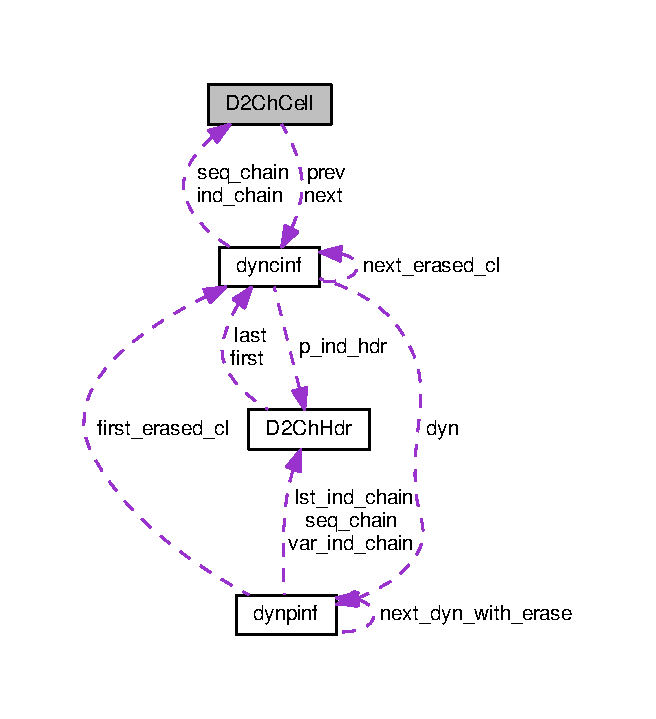
\includegraphics[width=315pt]{structD2ChCell__coll__graph}
\end{center}
\end{figure}
\subsection*{Data Fields}
\begin{DoxyCompactItemize}
\item 
\hyperlink{dynam__supp_8h_ae9665ae9a3ee194834c9995b875aed48}{Dyn\+C\+InfP} \hyperlink{structD2ChCell_ab3eac88c8e41656c4dfa195b314fef5c}{next}
\item 
\hyperlink{dynam__supp_8h_ae9665ae9a3ee194834c9995b875aed48}{Dyn\+C\+InfP} \hyperlink{structD2ChCell_a93c613b80554c6b885b8c680658475cf}{prev}
\end{DoxyCompactItemize}


\subsection{Field Documentation}
\index{D2\+Ch\+Cell@{D2\+Ch\+Cell}!next@{next}}
\index{next@{next}!D2\+Ch\+Cell@{D2\+Ch\+Cell}}
\subsubsection[{\texorpdfstring{next}{next}}]{\setlength{\rightskip}{0pt plus 5cm}{\bf Dyn\+C\+InfP} D2\+Ch\+Cell\+::next}\hypertarget{structD2ChCell_ab3eac88c8e41656c4dfa195b314fef5c}{}\label{structD2ChCell_ab3eac88c8e41656c4dfa195b314fef5c}
\index{D2\+Ch\+Cell@{D2\+Ch\+Cell}!prev@{prev}}
\index{prev@{prev}!D2\+Ch\+Cell@{D2\+Ch\+Cell}}
\subsubsection[{\texorpdfstring{prev}{prev}}]{\setlength{\rightskip}{0pt plus 5cm}{\bf Dyn\+C\+InfP} D2\+Ch\+Cell\+::prev}\hypertarget{structD2ChCell_a93c613b80554c6b885b8c680658475cf}{}\label{structD2ChCell_a93c613b80554c6b885b8c680658475cf}


The documentation for this struct was generated from the following file\+:\begin{DoxyCompactItemize}
\item 
gprolog-\/utf8-\/tree/src/\+Bips\+Pl/\hyperlink{dynam__supp_8h}{dynam\+\_\+supp.\+h}\end{DoxyCompactItemize}

\hypertarget{structD2ChHdr}{}\section{D2\+Ch\+Hdr Struct Reference}
\label{structD2ChHdr}\index{D2\+Ch\+Hdr@{D2\+Ch\+Hdr}}


{\ttfamily \#include $<$dynam\+\_\+supp.\+h$>$}



Collaboration diagram for D2\+Ch\+Hdr\+:\nopagebreak
\begin{figure}[H]
\begin{center}
\leavevmode
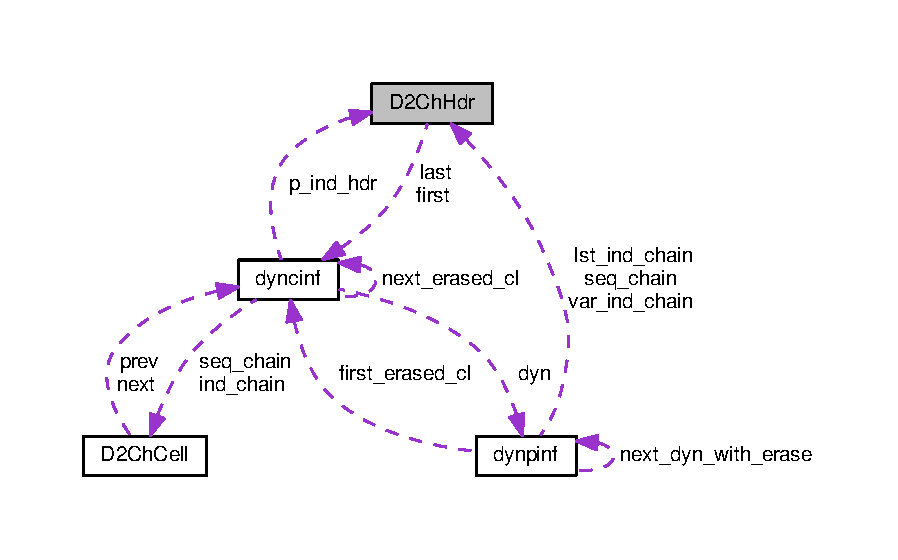
\includegraphics[width=350pt]{structD2ChHdr__coll__graph}
\end{center}
\end{figure}
\subsection*{Data Fields}
\begin{DoxyCompactItemize}
\item 
\hyperlink{dynam__supp_8h_ae9665ae9a3ee194834c9995b875aed48}{Dyn\+C\+InfP} \hyperlink{structD2ChHdr_ac1ff1d6290dd45e018ee4097a2c2427d}{first}
\item 
\hyperlink{dynam__supp_8h_ae9665ae9a3ee194834c9995b875aed48}{Dyn\+C\+InfP} \hyperlink{structD2ChHdr_a35d1cb0c22a72f9a49a6d26b9f8046c8}{last}
\end{DoxyCompactItemize}


\subsection{Field Documentation}
\index{D2\+Ch\+Hdr@{D2\+Ch\+Hdr}!first@{first}}
\index{first@{first}!D2\+Ch\+Hdr@{D2\+Ch\+Hdr}}
\subsubsection[{\texorpdfstring{first}{first}}]{\setlength{\rightskip}{0pt plus 5cm}{\bf Dyn\+C\+InfP} D2\+Ch\+Hdr\+::first}\hypertarget{structD2ChHdr_ac1ff1d6290dd45e018ee4097a2c2427d}{}\label{structD2ChHdr_ac1ff1d6290dd45e018ee4097a2c2427d}
\index{D2\+Ch\+Hdr@{D2\+Ch\+Hdr}!last@{last}}
\index{last@{last}!D2\+Ch\+Hdr@{D2\+Ch\+Hdr}}
\subsubsection[{\texorpdfstring{last}{last}}]{\setlength{\rightskip}{0pt plus 5cm}{\bf Dyn\+C\+InfP} D2\+Ch\+Hdr\+::last}\hypertarget{structD2ChHdr_a35d1cb0c22a72f9a49a6d26b9f8046c8}{}\label{structD2ChHdr_a35d1cb0c22a72f9a49a6d26b9f8046c8}


The documentation for this struct was generated from the following file\+:\begin{DoxyCompactItemize}
\item 
gprolog-\/utf8-\/tree/src/\+Bips\+Pl/\hyperlink{dynam__supp_8h}{dynam\+\_\+supp.\+h}\end{DoxyCompactItemize}

\hypertarget{unionDblInt}{}\section{Dbl\+Int Union Reference}
\label{unionDblInt}\index{Dbl\+Int@{Dbl\+Int}}
\subsection*{Data Fields}
\begin{DoxyCompactItemize}
\item 
double \hyperlink{unionDblInt_a23665c821d8bb2ce3af4f5783fa5ed7c}{d}
\item 
\hyperlink{LINUX__SIGSEGV_8c_a10ea8be8823feb38875b8a9326cbb424}{Wam\+Word} \hyperlink{unionDblInt_ad0ddb3bdd3543a38a19752bc2ac77885}{i} \mbox{[}2\mbox{]}
\end{DoxyCompactItemize}


\subsection{Field Documentation}
\index{Dbl\+Int@{Dbl\+Int}!d@{d}}
\index{d@{d}!Dbl\+Int@{Dbl\+Int}}
\subsubsection[{\texorpdfstring{d}{d}}]{\setlength{\rightskip}{0pt plus 5cm}double Dbl\+Int\+::d}\hypertarget{unionDblInt_a23665c821d8bb2ce3af4f5783fa5ed7c}{}\label{unionDblInt_a23665c821d8bb2ce3af4f5783fa5ed7c}
\index{Dbl\+Int@{Dbl\+Int}!i@{i}}
\index{i@{i}!Dbl\+Int@{Dbl\+Int}}
\subsubsection[{\texorpdfstring{i}{i}}]{\setlength{\rightskip}{0pt plus 5cm}{\bf Wam\+Word} Dbl\+Int\+::i\mbox{[}2\mbox{]}}\hypertarget{unionDblInt_ad0ddb3bdd3543a38a19752bc2ac77885}{}\label{unionDblInt_ad0ddb3bdd3543a38a19752bc2ac77885}


The documentation for this union was generated from the following file\+:\begin{DoxyCompactItemize}
\item 
gprolog-\/utf8-\/tree/src/\+Engine\+Pl/\hyperlink{wam__inst_8c}{wam\+\_\+inst.\+c}\end{DoxyCompactItemize}

\hypertarget{structdirectinf}{}\section{directinf Struct Reference}
\label{structdirectinf}\index{directinf@{directinf}}


Collaboration diagram for directinf\+:\nopagebreak
\begin{figure}[H]
\begin{center}
\leavevmode
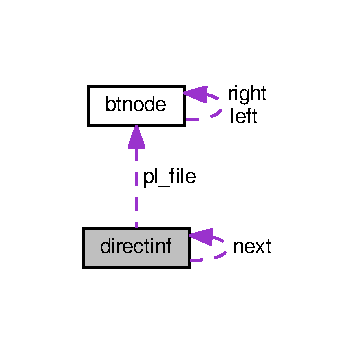
\includegraphics[width=171pt]{structdirectinf__coll__graph}
\end{center}
\end{figure}
\subsection*{Data Fields}
\begin{DoxyCompactItemize}
\item 
\hyperlink{structbtnode}{B\+T\+Node} $\ast$ {\bfseries pl\+\_\+file}\hypertarget{structdirectinf_a2d00b2ef3ca0317b568b16ed20968e52}{}\label{structdirectinf_a2d00b2ef3ca0317b568b16ed20968e52}

\item 
int {\bfseries pl\+\_\+line}\hypertarget{structdirectinf_ae817c137ec2f80b2a6409ae0ca8faa7a}{}\label{structdirectinf_ae817c137ec2f80b2a6409ae0ca8faa7a}

\item 
int {\bfseries system}\hypertarget{structdirectinf_a328d981a0d78b287ff7494df8d501635}{}\label{structdirectinf_a328d981a0d78b287ff7494df8d501635}

\item 
\hyperlink{structdirectinf}{DirectP} {\bfseries next}\hypertarget{structdirectinf_a6376c34c77718e3ea148063383fd29da}{}\label{structdirectinf_a6376c34c77718e3ea148063383fd29da}

\end{DoxyCompactItemize}


The documentation for this struct was generated from the following file\+:\begin{DoxyCompactItemize}
\item 
gprolog-\/utf8-\/tree/src/\+Wam2\+Ma/wam2ma.\+c\end{DoxyCompactItemize}

\hypertarget{structDSwtInf}{}\section{D\+Swt\+Inf Struct Reference}
\label{structDSwtInf}\index{D\+Swt\+Inf@{D\+Swt\+Inf}}


Collaboration diagram for D\+Swt\+Inf\+:\nopagebreak
\begin{figure}[H]
\begin{center}
\leavevmode
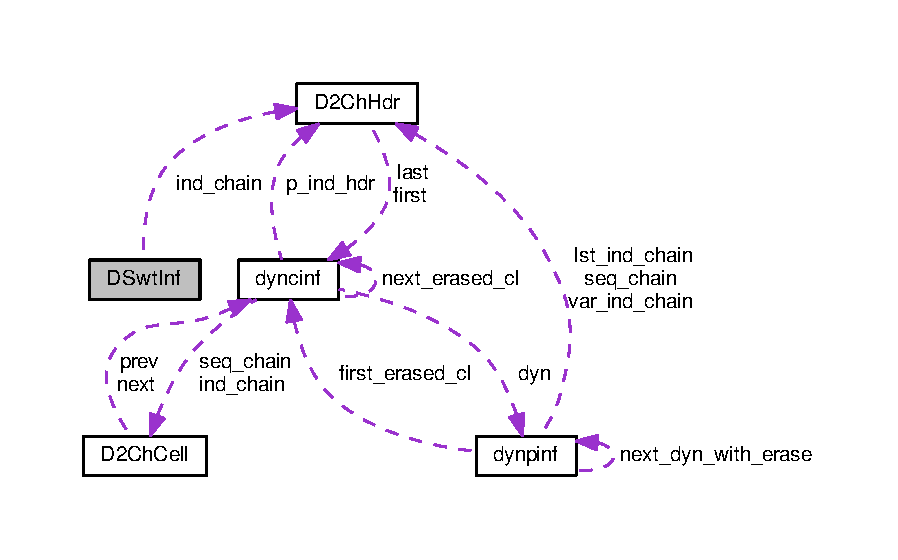
\includegraphics[width=350pt]{structDSwtInf__coll__graph}
\end{center}
\end{figure}
\subsection*{Data Fields}
\begin{DoxyCompactItemize}
\item 
Pl\+Long {\bfseries key}\hypertarget{structDSwtInf_a9661c05b42d3c1c0deb724486fc685b9}{}\label{structDSwtInf_a9661c05b42d3c1c0deb724486fc685b9}

\item 
\hyperlink{structD2ChHdr}{D2\+Ch\+Hdr} {\bfseries ind\+\_\+chain}\hypertarget{structDSwtInf_aa4386ca4933b9847a0622d980023e4c8}{}\label{structDSwtInf_aa4386ca4933b9847a0622d980023e4c8}

\end{DoxyCompactItemize}


The documentation for this struct was generated from the following file\+:\begin{DoxyCompactItemize}
\item 
gprolog-\/utf8-\/tree/src/\+Bips\+Pl/dynam\+\_\+supp.\+h\end{DoxyCompactItemize}

\hypertarget{structdyncinf}{}\section{dyncinf Struct Reference}
\label{structdyncinf}\index{dyncinf@{dyncinf}}


Collaboration diagram for dyncinf\+:\nopagebreak
\begin{figure}[H]
\begin{center}
\leavevmode
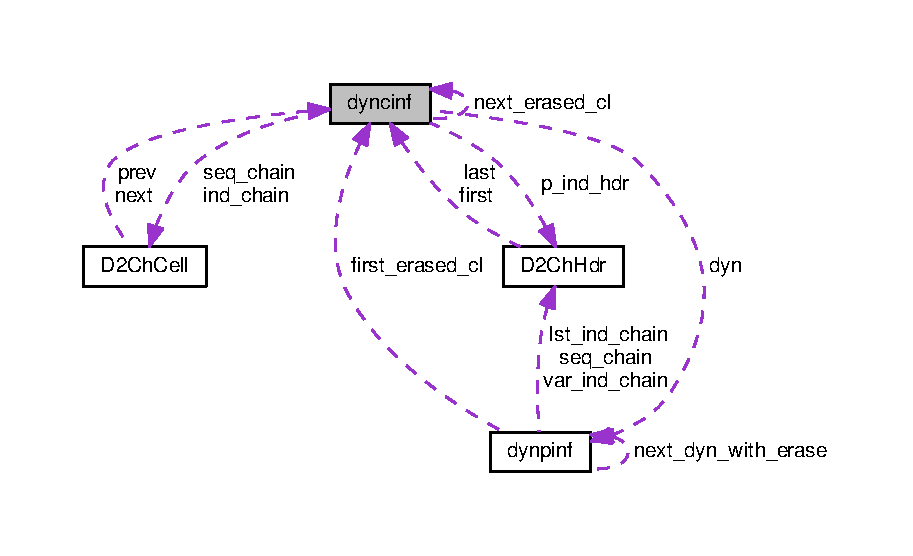
\includegraphics[width=350pt]{structdyncinf__coll__graph}
\end{center}
\end{figure}
\subsection*{Data Fields}
\begin{DoxyCompactItemize}
\item 
\hyperlink{structD2ChCell}{D2\+Ch\+Cell} {\bfseries seq\+\_\+chain}\hypertarget{structdyncinf_a7761fb1d761320cf1779e333348690a1}{}\label{structdyncinf_a7761fb1d761320cf1779e333348690a1}

\item 
\hyperlink{structD2ChCell}{D2\+Ch\+Cell} {\bfseries ind\+\_\+chain}\hypertarget{structdyncinf_a13ff7af2c35333e6fca1f40ab6299a20}{}\label{structdyncinf_a13ff7af2c35333e6fca1f40ab6299a20}

\item 
\hyperlink{structdynpinf}{Dyn\+P\+InfP} {\bfseries dyn}\hypertarget{structdyncinf_a357682e414c932a33d29142f4f3ffc3b}{}\label{structdyncinf_a357682e414c932a33d29142f4f3ffc3b}

\item 
\hyperlink{structD2ChHdr}{D2\+Ch\+Hdr} $\ast$ {\bfseries p\+\_\+ind\+\_\+hdr}\hypertarget{structdyncinf_ad7f2e30b3f0537ad3587209d9f3cc11a}{}\label{structdyncinf_ad7f2e30b3f0537ad3587209d9f3cc11a}

\item 
char $\ast$$\ast$ {\bfseries p\+\_\+ind\+\_\+htbl}\hypertarget{structdyncinf_ac365b7b37b1046432be9fc713bd56ec2}{}\label{structdyncinf_ac365b7b37b1046432be9fc713bd56ec2}

\item 
int {\bfseries cl\+\_\+no}\hypertarget{structdyncinf_a9ecec5cb558eff437ebc9dad0b9a713a}{}\label{structdyncinf_a9ecec5cb558eff437ebc9dad0b9a713a}

\item 
int {\bfseries pl\+\_\+file}\hypertarget{structdyncinf_a8eb75fc2f5558e0fe27a7307dda56f2e}{}\label{structdyncinf_a8eb75fc2f5558e0fe27a7307dda56f2e}

\item 
Dyn\+Stamp {\bfseries erase\+\_\+stamp}\hypertarget{structdyncinf_af4fd2ada2161206351d5d7b462fdf168}{}\label{structdyncinf_af4fd2ada2161206351d5d7b462fdf168}

\item 
\hyperlink{structdyncinf}{Dyn\+C\+InfP} {\bfseries next\+\_\+erased\+\_\+cl}\hypertarget{structdyncinf_a1570173ffbae298cc0c7916bd835f675}{}\label{structdyncinf_a1570173ffbae298cc0c7916bd835f675}

\item 
unsigned $\ast$ {\bfseries byte\+\_\+code}\hypertarget{structdyncinf_a8a16574f97f5162a42cf11f74b16d6b3}{}\label{structdyncinf_a8a16574f97f5162a42cf11f74b16d6b3}

\item 
int {\bfseries term\+\_\+size}\hypertarget{structdyncinf_a4b49c8e104c686701eb19ca0d01173e7}{}\label{structdyncinf_a4b49c8e104c686701eb19ca0d01173e7}

\item 
Wam\+Word {\bfseries term\+\_\+word}\hypertarget{structdyncinf_aad9f2ad962d3ca3002a6fc97dc375d0b}{}\label{structdyncinf_aad9f2ad962d3ca3002a6fc97dc375d0b}

\item 
Wam\+Word {\bfseries head\+\_\+word}\hypertarget{structdyncinf_a11e4b16031cc5023d2f6d2194e328b89}{}\label{structdyncinf_a11e4b16031cc5023d2f6d2194e328b89}

\item 
Wam\+Word {\bfseries body\+\_\+word}\hypertarget{structdyncinf_aaab182b28b71abea34aa78e530aa9483}{}\label{structdyncinf_aaab182b28b71abea34aa78e530aa9483}

\end{DoxyCompactItemize}


The documentation for this struct was generated from the following file\+:\begin{DoxyCompactItemize}
\item 
gprolog-\/utf8-\/tree/src/\+Bips\+Pl/dynam\+\_\+supp.\+h\end{DoxyCompactItemize}

\hypertarget{structdynpinf}{}\section{dynpinf Struct Reference}
\label{structdynpinf}\index{dynpinf@{dynpinf}}


Collaboration diagram for dynpinf\+:\nopagebreak
\begin{figure}[H]
\begin{center}
\leavevmode
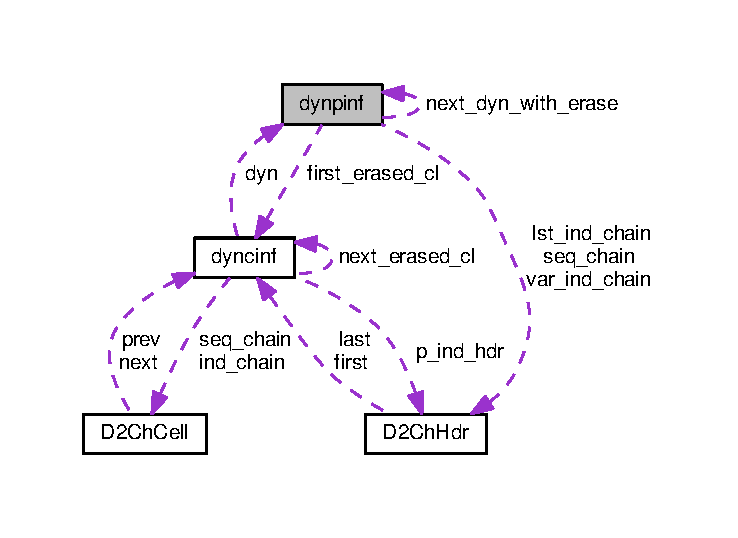
\includegraphics[width=350pt]{structdynpinf__coll__graph}
\end{center}
\end{figure}
\subsection*{Data Fields}
\begin{DoxyCompactItemize}
\item 
\hyperlink{structD2ChHdr}{D2\+Ch\+Hdr} {\bfseries seq\+\_\+chain}\hypertarget{structdynpinf_a7fd9dcc867aa4461a78fd7ea113fe30e}{}\label{structdynpinf_a7fd9dcc867aa4461a78fd7ea113fe30e}

\item 
\hyperlink{structD2ChHdr}{D2\+Ch\+Hdr} {\bfseries var\+\_\+ind\+\_\+chain}\hypertarget{structdynpinf_a81ff1365c770d4e9e503ec13d0829c89}{}\label{structdynpinf_a81ff1365c770d4e9e503ec13d0829c89}

\item 
char $\ast$ {\bfseries atm\+\_\+htbl}\hypertarget{structdynpinf_a647b214d180d3239102e9a3137cd2c50}{}\label{structdynpinf_a647b214d180d3239102e9a3137cd2c50}

\item 
char $\ast$ {\bfseries int\+\_\+htbl}\hypertarget{structdynpinf_a7e89d876755097ac24867ef0c002572d}{}\label{structdynpinf_a7e89d876755097ac24867ef0c002572d}

\item 
\hyperlink{structD2ChHdr}{D2\+Ch\+Hdr} {\bfseries lst\+\_\+ind\+\_\+chain}\hypertarget{structdynpinf_a1c4ab87dddfafc7e912446a2cc391e3f}{}\label{structdynpinf_a1c4ab87dddfafc7e912446a2cc391e3f}

\item 
char $\ast$ {\bfseries stc\+\_\+htbl}\hypertarget{structdynpinf_a34e514b87f630efa4c7d2936979e7735}{}\label{structdynpinf_a34e514b87f630efa4c7d2936979e7735}

\item 
int {\bfseries arity}\hypertarget{structdynpinf_a06c4048e8638d3a47c4b48d5b6384516}{}\label{structdynpinf_a06c4048e8638d3a47c4b48d5b6384516}

\item 
int {\bfseries count\+\_\+a}\hypertarget{structdynpinf_aacc4edd647989f5a014730830390c05d}{}\label{structdynpinf_aacc4edd647989f5a014730830390c05d}

\item 
int {\bfseries count\+\_\+z}\hypertarget{structdynpinf_a90b999f0c08d5d26be5de1f30fd4a83d}{}\label{structdynpinf_a90b999f0c08d5d26be5de1f30fd4a83d}

\item 
\hyperlink{structdyncinf}{Dyn\+C\+InfP} {\bfseries first\+\_\+erased\+\_\+cl}\hypertarget{structdynpinf_a1e974f17af18887bef7754c00313c714}{}\label{structdynpinf_a1e974f17af18887bef7754c00313c714}

\item 
\hyperlink{structdynpinf}{Dyn\+P\+InfP} {\bfseries next\+\_\+dyn\+\_\+with\+\_\+erase}\hypertarget{structdynpinf_a5845421aa8bf227923c6ed1073c32b17}{}\label{structdynpinf_a5845421aa8bf227923c6ed1073c32b17}

\end{DoxyCompactItemize}


The documentation for this struct was generated from the following file\+:\begin{DoxyCompactItemize}
\item 
gprolog-\/utf8-\/tree/src/\+Bips\+Pl/dynam\+\_\+supp.\+h\end{DoxyCompactItemize}

\hypertarget{structDynScan}{}\section{Dyn\+Scan Struct Reference}
\label{structDynScan}\index{Dyn\+Scan@{Dyn\+Scan}}


Collaboration diagram for Dyn\+Scan\+:\nopagebreak
\begin{figure}[H]
\begin{center}
\leavevmode
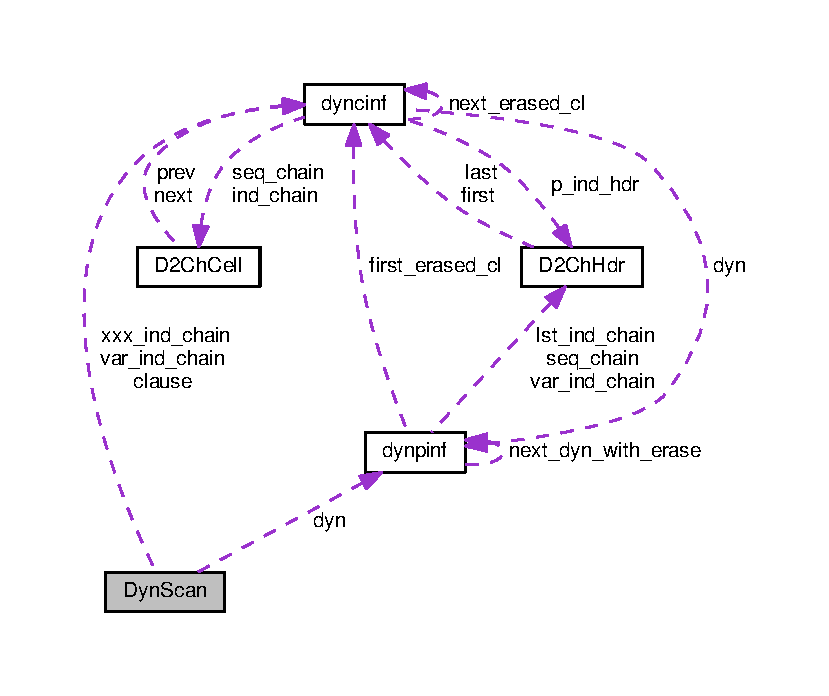
\includegraphics[width=350pt]{structDynScan__coll__graph}
\end{center}
\end{figure}
\subsection*{Data Fields}
\begin{DoxyCompactItemize}
\item 
\hyperlink{dynam__supp_8h_a9ce8f2e1c3c17643fc4a7874b633104e}{Scan\+Fct} \hyperlink{structDynScan_acfa1d047b819d2941ee149649705267a}{alt\+\_\+fct}
\item 
int \hyperlink{structDynScan_add62e7961d11ce60357eb13181e762b0}{alt\+\_\+size\+\_\+info}
\item 
int \hyperlink{structDynScan_a2e6f2cb912f0477854e0cab2bd4f9f0a}{owner\+\_\+func}
\item 
int \hyperlink{structDynScan_a55d99dfd20f733fb1ede548b7accd548}{owner\+\_\+arity}
\item 
\hyperlink{dynam__supp_8h_abf8c639d74e3a538cb5256ede033af03}{Dyn\+P\+Inf} $\ast$ \hyperlink{structDynScan_a2c4d20f447ace62db674692a4724ce0e}{dyn}
\item 
int \hyperlink{structDynScan_a786342f885eab9162a783e6633fefa84}{stop\+\_\+cl\+\_\+no}
\item 
\hyperlink{dynam__supp_8h_ae67d7fd7d828834bf168a2bccc22643c}{Dyn\+Stamp} \hyperlink{structDynScan_a482a71d0fe57d0a6118a68a1f94e0c4a}{erase\+\_\+stamp}
\item 
\hyperlink{bool_8h_afdcfe6db5bea87bd493a3fe2c513d5ef}{Bool} \hyperlink{structDynScan_acd70059e162c998780954a78427ad3ee}{xxx\+\_\+is\+\_\+seq\+\_\+chain}
\item 
\hyperlink{dynam__supp_8h_a3be3c527fb36e120ec36f999fb1a12d3}{Dyn\+C\+Inf} $\ast$ \hyperlink{structDynScan_a657dfdeff11a3a52923f165bcf9bc6fd}{xxx\+\_\+ind\+\_\+chain}
\item 
\hyperlink{dynam__supp_8h_a3be3c527fb36e120ec36f999fb1a12d3}{Dyn\+C\+Inf} $\ast$ \hyperlink{structDynScan_a01058a30b112e62e5768ead8055f6f7f}{var\+\_\+ind\+\_\+chain}
\item 
\hyperlink{dynam__supp_8h_a3be3c527fb36e120ec36f999fb1a12d3}{Dyn\+C\+Inf} $\ast$ \hyperlink{structDynScan_ac04b24fb81aec5128d42e5b79123cfc8}{clause}
\end{DoxyCompactItemize}


\subsection{Field Documentation}
\index{Dyn\+Scan@{Dyn\+Scan}!alt\+\_\+fct@{alt\+\_\+fct}}
\index{alt\+\_\+fct@{alt\+\_\+fct}!Dyn\+Scan@{Dyn\+Scan}}
\subsubsection[{\texorpdfstring{alt\+\_\+fct}{alt_fct}}]{\setlength{\rightskip}{0pt plus 5cm}{\bf Scan\+Fct} Dyn\+Scan\+::alt\+\_\+fct}\hypertarget{structDynScan_acfa1d047b819d2941ee149649705267a}{}\label{structDynScan_acfa1d047b819d2941ee149649705267a}
\index{Dyn\+Scan@{Dyn\+Scan}!alt\+\_\+size\+\_\+info@{alt\+\_\+size\+\_\+info}}
\index{alt\+\_\+size\+\_\+info@{alt\+\_\+size\+\_\+info}!Dyn\+Scan@{Dyn\+Scan}}
\subsubsection[{\texorpdfstring{alt\+\_\+size\+\_\+info}{alt_size_info}}]{\setlength{\rightskip}{0pt plus 5cm}int Dyn\+Scan\+::alt\+\_\+size\+\_\+info}\hypertarget{structDynScan_add62e7961d11ce60357eb13181e762b0}{}\label{structDynScan_add62e7961d11ce60357eb13181e762b0}
\index{Dyn\+Scan@{Dyn\+Scan}!clause@{clause}}
\index{clause@{clause}!Dyn\+Scan@{Dyn\+Scan}}
\subsubsection[{\texorpdfstring{clause}{clause}}]{\setlength{\rightskip}{0pt plus 5cm}{\bf Dyn\+C\+Inf}$\ast$ Dyn\+Scan\+::clause}\hypertarget{structDynScan_ac04b24fb81aec5128d42e5b79123cfc8}{}\label{structDynScan_ac04b24fb81aec5128d42e5b79123cfc8}
\index{Dyn\+Scan@{Dyn\+Scan}!dyn@{dyn}}
\index{dyn@{dyn}!Dyn\+Scan@{Dyn\+Scan}}
\subsubsection[{\texorpdfstring{dyn}{dyn}}]{\setlength{\rightskip}{0pt plus 5cm}{\bf Dyn\+P\+Inf}$\ast$ Dyn\+Scan\+::dyn}\hypertarget{structDynScan_a2c4d20f447ace62db674692a4724ce0e}{}\label{structDynScan_a2c4d20f447ace62db674692a4724ce0e}
\index{Dyn\+Scan@{Dyn\+Scan}!erase\+\_\+stamp@{erase\+\_\+stamp}}
\index{erase\+\_\+stamp@{erase\+\_\+stamp}!Dyn\+Scan@{Dyn\+Scan}}
\subsubsection[{\texorpdfstring{erase\+\_\+stamp}{erase_stamp}}]{\setlength{\rightskip}{0pt plus 5cm}{\bf Dyn\+Stamp} Dyn\+Scan\+::erase\+\_\+stamp}\hypertarget{structDynScan_a482a71d0fe57d0a6118a68a1f94e0c4a}{}\label{structDynScan_a482a71d0fe57d0a6118a68a1f94e0c4a}
\index{Dyn\+Scan@{Dyn\+Scan}!owner\+\_\+arity@{owner\+\_\+arity}}
\index{owner\+\_\+arity@{owner\+\_\+arity}!Dyn\+Scan@{Dyn\+Scan}}
\subsubsection[{\texorpdfstring{owner\+\_\+arity}{owner_arity}}]{\setlength{\rightskip}{0pt plus 5cm}int Dyn\+Scan\+::owner\+\_\+arity}\hypertarget{structDynScan_a55d99dfd20f733fb1ede548b7accd548}{}\label{structDynScan_a55d99dfd20f733fb1ede548b7accd548}
\index{Dyn\+Scan@{Dyn\+Scan}!owner\+\_\+func@{owner\+\_\+func}}
\index{owner\+\_\+func@{owner\+\_\+func}!Dyn\+Scan@{Dyn\+Scan}}
\subsubsection[{\texorpdfstring{owner\+\_\+func}{owner_func}}]{\setlength{\rightskip}{0pt plus 5cm}int Dyn\+Scan\+::owner\+\_\+func}\hypertarget{structDynScan_a2e6f2cb912f0477854e0cab2bd4f9f0a}{}\label{structDynScan_a2e6f2cb912f0477854e0cab2bd4f9f0a}
\index{Dyn\+Scan@{Dyn\+Scan}!stop\+\_\+cl\+\_\+no@{stop\+\_\+cl\+\_\+no}}
\index{stop\+\_\+cl\+\_\+no@{stop\+\_\+cl\+\_\+no}!Dyn\+Scan@{Dyn\+Scan}}
\subsubsection[{\texorpdfstring{stop\+\_\+cl\+\_\+no}{stop_cl_no}}]{\setlength{\rightskip}{0pt plus 5cm}int Dyn\+Scan\+::stop\+\_\+cl\+\_\+no}\hypertarget{structDynScan_a786342f885eab9162a783e6633fefa84}{}\label{structDynScan_a786342f885eab9162a783e6633fefa84}
\index{Dyn\+Scan@{Dyn\+Scan}!var\+\_\+ind\+\_\+chain@{var\+\_\+ind\+\_\+chain}}
\index{var\+\_\+ind\+\_\+chain@{var\+\_\+ind\+\_\+chain}!Dyn\+Scan@{Dyn\+Scan}}
\subsubsection[{\texorpdfstring{var\+\_\+ind\+\_\+chain}{var_ind_chain}}]{\setlength{\rightskip}{0pt plus 5cm}{\bf Dyn\+C\+Inf}$\ast$ Dyn\+Scan\+::var\+\_\+ind\+\_\+chain}\hypertarget{structDynScan_a01058a30b112e62e5768ead8055f6f7f}{}\label{structDynScan_a01058a30b112e62e5768ead8055f6f7f}
\index{Dyn\+Scan@{Dyn\+Scan}!xxx\+\_\+ind\+\_\+chain@{xxx\+\_\+ind\+\_\+chain}}
\index{xxx\+\_\+ind\+\_\+chain@{xxx\+\_\+ind\+\_\+chain}!Dyn\+Scan@{Dyn\+Scan}}
\subsubsection[{\texorpdfstring{xxx\+\_\+ind\+\_\+chain}{xxx_ind_chain}}]{\setlength{\rightskip}{0pt plus 5cm}{\bf Dyn\+C\+Inf}$\ast$ Dyn\+Scan\+::xxx\+\_\+ind\+\_\+chain}\hypertarget{structDynScan_a657dfdeff11a3a52923f165bcf9bc6fd}{}\label{structDynScan_a657dfdeff11a3a52923f165bcf9bc6fd}
\index{Dyn\+Scan@{Dyn\+Scan}!xxx\+\_\+is\+\_\+seq\+\_\+chain@{xxx\+\_\+is\+\_\+seq\+\_\+chain}}
\index{xxx\+\_\+is\+\_\+seq\+\_\+chain@{xxx\+\_\+is\+\_\+seq\+\_\+chain}!Dyn\+Scan@{Dyn\+Scan}}
\subsubsection[{\texorpdfstring{xxx\+\_\+is\+\_\+seq\+\_\+chain}{xxx_is_seq_chain}}]{\setlength{\rightskip}{0pt plus 5cm}{\bf Bool} Dyn\+Scan\+::xxx\+\_\+is\+\_\+seq\+\_\+chain}\hypertarget{structDynScan_acd70059e162c998780954a78427ad3ee}{}\label{structDynScan_acd70059e162c998780954a78427ad3ee}


The documentation for this struct was generated from the following file\+:\begin{DoxyCompactItemize}
\item 
gprolog-\/utf8-\/tree/src/\+Bips\+Pl/\hyperlink{dynam__supp_8c}{dynam\+\_\+supp.\+c}\end{DoxyCompactItemize}

\hypertarget{structFileInf}{}\section{File\+Inf Struct Reference}
\label{structFileInf}\index{File\+Inf@{File\+Inf}}
\subsection*{Data Fields}
\begin{DoxyCompactItemize}
\item 
char $\ast$ {\bfseries name}\hypertarget{structFileInf_a4dc1b0d5b390f714210d47b147af9e9b}{}\label{structFileInf_a4dc1b0d5b390f714210d47b147af9e9b}

\item 
char $\ast$ {\bfseries suffix}\hypertarget{structFileInf_a5ef754a773b84e5a9917436c6d8afe72}{}\label{structFileInf_a5ef754a773b84e5a9917436c6d8afe72}

\item 
char $\ast$ {\bfseries file\+\_\+part}\hypertarget{structFileInf_acb68ba4e07ba186e94a267560253b2bb}{}\label{structFileInf_acb68ba4e07ba186e94a267560253b2bb}

\item 
int {\bfseries type}\hypertarget{structFileInf_a08c8fec214c452fa67b03a36ac58db5f}{}\label{structFileInf_a08c8fec214c452fa67b03a36ac58db5f}

\item 
char $\ast$ {\bfseries work\+\_\+name1}\hypertarget{structFileInf_aab7c6e078d6f1ae349cf70872f35531d}{}\label{structFileInf_aab7c6e078d6f1ae349cf70872f35531d}

\item 
char $\ast$ {\bfseries work\+\_\+name2}\hypertarget{structFileInf_a73706e94bc2b8654cfba501d8fce856e}{}\label{structFileInf_a73706e94bc2b8654cfba501d8fce856e}

\end{DoxyCompactItemize}


The documentation for this struct was generated from the following file\+:\begin{DoxyCompactItemize}
\item 
gprolog-\/utf8-\/tree/src/\+Top\+Comp/top\+\_\+comp.\+c\end{DoxyCompactItemize}

\hypertarget{structflag__inf}{}\section{flag\+\_\+inf Struct Reference}
\label{structflag__inf}\index{flag\+\_\+inf@{flag\+\_\+inf}}


{\ttfamily \#include $<$flag\+\_\+supp.\+h$>$}



Collaboration diagram for flag\+\_\+inf\+:\nopagebreak
\begin{figure}[H]
\begin{center}
\leavevmode
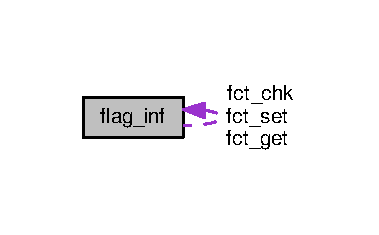
\includegraphics[width=182pt]{structflag__inf__coll__graph}
\end{center}
\end{figure}
\subsection*{Data Fields}
\begin{DoxyCompactItemize}
\item 
int \hyperlink{structflag__inf_a7131c7e545b44d7086d50a89e76bbf30}{atom\+\_\+name}
\item 
\hyperlink{bool_8h_afdcfe6db5bea87bd493a3fe2c513d5ef}{Bool} \hyperlink{structflag__inf_ac95236097fb4811ec47198aa34e64d15}{modifiable}
\item 
\hyperlink{flag__supp_8h_a829563b1e19fae59f905c1afb76fe4eb}{Flag\+Type} \hyperlink{structflag__inf_ad1ffc264915a45e9395b717849c36ff9}{type}
\item 
\hyperlink{gprolog_8h_a4d005b136d7fb28537eb1815f7868b63}{Pl\+Long} \hyperlink{structflag__inf_a828f0d058950ff9e708080d5e96b4068}{value}
\item 
\hyperlink{flag__supp_8h_a54ea5be77d71f1b9cb6e175bea45179c}{Flag\+Fct\+Get} \hyperlink{structflag__inf_ab4585a2020aa37259cb1117664fecfee}{fct\+\_\+get}
\item 
\hyperlink{flag__supp_8h_ac0c2714190598d0ff723cfc7b88b41cd}{Flag\+Fct\+Chk} \hyperlink{structflag__inf_a46997cf1af90c40fa0e2ecee11b935d7}{fct\+\_\+chk}
\item 
\hyperlink{flag__supp_8h_a848a192d7dbb0e8b3715f9322291de21}{Flag\+Fct\+Set} \hyperlink{structflag__inf_aa01403feaa709ffaa582224b5789b928}{fct\+\_\+set}
\end{DoxyCompactItemize}


\subsection{Field Documentation}
\index{flag\+\_\+inf@{flag\+\_\+inf}!atom\+\_\+name@{atom\+\_\+name}}
\index{atom\+\_\+name@{atom\+\_\+name}!flag\+\_\+inf@{flag\+\_\+inf}}
\subsubsection[{\texorpdfstring{atom\+\_\+name}{atom_name}}]{\setlength{\rightskip}{0pt plus 5cm}int flag\+\_\+inf\+::atom\+\_\+name}\hypertarget{structflag__inf_a7131c7e545b44d7086d50a89e76bbf30}{}\label{structflag__inf_a7131c7e545b44d7086d50a89e76bbf30}
\index{flag\+\_\+inf@{flag\+\_\+inf}!fct\+\_\+chk@{fct\+\_\+chk}}
\index{fct\+\_\+chk@{fct\+\_\+chk}!flag\+\_\+inf@{flag\+\_\+inf}}
\subsubsection[{\texorpdfstring{fct\+\_\+chk}{fct_chk}}]{\setlength{\rightskip}{0pt plus 5cm}{\bf Flag\+Fct\+Chk} flag\+\_\+inf\+::fct\+\_\+chk}\hypertarget{structflag__inf_a46997cf1af90c40fa0e2ecee11b935d7}{}\label{structflag__inf_a46997cf1af90c40fa0e2ecee11b935d7}
\index{flag\+\_\+inf@{flag\+\_\+inf}!fct\+\_\+get@{fct\+\_\+get}}
\index{fct\+\_\+get@{fct\+\_\+get}!flag\+\_\+inf@{flag\+\_\+inf}}
\subsubsection[{\texorpdfstring{fct\+\_\+get}{fct_get}}]{\setlength{\rightskip}{0pt plus 5cm}{\bf Flag\+Fct\+Get} flag\+\_\+inf\+::fct\+\_\+get}\hypertarget{structflag__inf_ab4585a2020aa37259cb1117664fecfee}{}\label{structflag__inf_ab4585a2020aa37259cb1117664fecfee}
\index{flag\+\_\+inf@{flag\+\_\+inf}!fct\+\_\+set@{fct\+\_\+set}}
\index{fct\+\_\+set@{fct\+\_\+set}!flag\+\_\+inf@{flag\+\_\+inf}}
\subsubsection[{\texorpdfstring{fct\+\_\+set}{fct_set}}]{\setlength{\rightskip}{0pt plus 5cm}{\bf Flag\+Fct\+Set} flag\+\_\+inf\+::fct\+\_\+set}\hypertarget{structflag__inf_aa01403feaa709ffaa582224b5789b928}{}\label{structflag__inf_aa01403feaa709ffaa582224b5789b928}
\index{flag\+\_\+inf@{flag\+\_\+inf}!modifiable@{modifiable}}
\index{modifiable@{modifiable}!flag\+\_\+inf@{flag\+\_\+inf}}
\subsubsection[{\texorpdfstring{modifiable}{modifiable}}]{\setlength{\rightskip}{0pt plus 5cm}{\bf Bool} flag\+\_\+inf\+::modifiable}\hypertarget{structflag__inf_ac95236097fb4811ec47198aa34e64d15}{}\label{structflag__inf_ac95236097fb4811ec47198aa34e64d15}
\index{flag\+\_\+inf@{flag\+\_\+inf}!type@{type}}
\index{type@{type}!flag\+\_\+inf@{flag\+\_\+inf}}
\subsubsection[{\texorpdfstring{type}{type}}]{\setlength{\rightskip}{0pt plus 5cm}{\bf Flag\+Type} flag\+\_\+inf\+::type}\hypertarget{structflag__inf_ad1ffc264915a45e9395b717849c36ff9}{}\label{structflag__inf_ad1ffc264915a45e9395b717849c36ff9}
\index{flag\+\_\+inf@{flag\+\_\+inf}!value@{value}}
\index{value@{value}!flag\+\_\+inf@{flag\+\_\+inf}}
\subsubsection[{\texorpdfstring{value}{value}}]{\setlength{\rightskip}{0pt plus 5cm}{\bf Pl\+Long} flag\+\_\+inf\+::value}\hypertarget{structflag__inf_a828f0d058950ff9e708080d5e96b4068}{}\label{structflag__inf_a828f0d058950ff9e708080d5e96b4068}


The documentation for this struct was generated from the following file\+:\begin{DoxyCompactItemize}
\item 
gprolog-\/utf8-\/tree/src/\+Bips\+Pl/\hyperlink{flag__supp_8h}{flag\+\_\+supp.\+h}\end{DoxyCompactItemize}

\hypertarget{structGTarget}{}\section{G\+Target Struct Reference}
\label{structGTarget}\index{G\+Target@{G\+Target}}


Collaboration diagram for G\+Target\+:\nopagebreak
\begin{figure}[H]
\begin{center}
\leavevmode
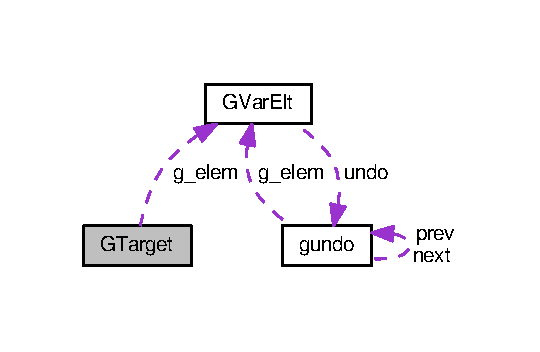
\includegraphics[width=259pt]{structGTarget__coll__graph}
\end{center}
\end{figure}
\subsection*{Data Fields}
\begin{DoxyCompactItemize}
\item 
\hyperlink{structGVarElt}{G\+Var\+Elt} $\ast$ {\bfseries g\+\_\+elem}\hypertarget{structGTarget_a057eea84bfa93fdfb38a7bf7d1bea531}{}\label{structGTarget_a057eea84bfa93fdfb38a7bf7d1bea531}

\item 
Wam\+Word $\ast$ {\bfseries g\+\_\+arg}\hypertarget{structGTarget_a46bf65a569e3ed1e726570e6c0f83a31}{}\label{structGTarget_a46bf65a569e3ed1e726570e6c0f83a31}

\end{DoxyCompactItemize}


The documentation for this struct was generated from the following file\+:\begin{DoxyCompactItemize}
\item 
gprolog-\/utf8-\/tree/src/\+Bips\+Pl/g\+\_\+var\+\_\+inl\+\_\+c.\+c\end{DoxyCompactItemize}

\hypertarget{structgundo}{}\section{gundo Struct Reference}
\label{structgundo}\index{gundo@{gundo}}


Collaboration diagram for gundo\+:\nopagebreak
\begin{figure}[H]
\begin{center}
\leavevmode
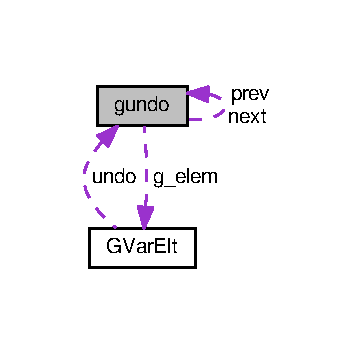
\includegraphics[width=170pt]{structgundo__coll__graph}
\end{center}
\end{figure}
\subsection*{Data Fields}
\begin{DoxyCompactItemize}
\item 
\hyperlink{structGVarElt}{G\+Var\+Elt} $\ast$ {\bfseries g\+\_\+elem}\hypertarget{structgundo_a215f96c167e2bc2aa0902fd04fcce89b}{}\label{structgundo_a215f96c167e2bc2aa0902fd04fcce89b}

\item 
int {\bfseries save\+\_\+size}\hypertarget{structgundo_a543c16d629efbb1e5e1260ef2f9438b5}{}\label{structgundo_a543c16d629efbb1e5e1260ef2f9438b5}

\item 
Wam\+Word {\bfseries save\+\_\+val}\hypertarget{structgundo_ad9b4b183b039fa879a47f9b4a400c742}{}\label{structgundo_ad9b4b183b039fa879a47f9b4a400c742}

\item 
\hyperlink{structgundo}{P\+G\+Undo} {\bfseries next}\hypertarget{structgundo_aa4dd84818a7b36f26b0f7524e850fec9}{}\label{structgundo_aa4dd84818a7b36f26b0f7524e850fec9}

\item 
\hyperlink{structgundo}{P\+G\+Undo} {\bfseries prev}\hypertarget{structgundo_aeb28eb449ba2732d088663c85b986d75}{}\label{structgundo_aeb28eb449ba2732d088663c85b986d75}

\end{DoxyCompactItemize}


The documentation for this struct was generated from the following file\+:\begin{DoxyCompactItemize}
\item 
gprolog-\/utf8-\/tree/src/\+Bips\+Pl/g\+\_\+var\+\_\+inl\+\_\+c.\+c\end{DoxyCompactItemize}

\hypertarget{structGVarElt}{}\section{G\+Var\+Elt Struct Reference}
\label{structGVarElt}\index{G\+Var\+Elt@{G\+Var\+Elt}}


Collaboration diagram for G\+Var\+Elt\+:\nopagebreak
\begin{figure}[H]
\begin{center}
\leavevmode
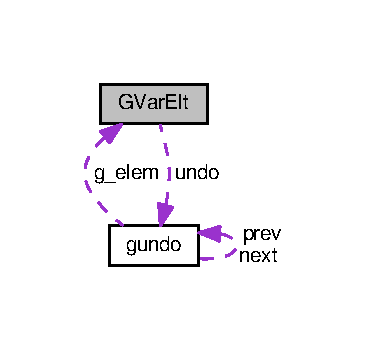
\includegraphics[width=175pt]{structGVarElt__coll__graph}
\end{center}
\end{figure}
\subsection*{Data Fields}
\begin{DoxyCompactItemize}
\item 
int {\bfseries size}\hypertarget{structGVarElt_a34b84647c8816d970311d1a2b3b2fd76}{}\label{structGVarElt_a34b84647c8816d970311d1a2b3b2fd76}

\item 
Wam\+Word {\bfseries val}\hypertarget{structGVarElt_a504e22949f6283a81b42cd76a0016c63}{}\label{structGVarElt_a504e22949f6283a81b42cd76a0016c63}

\item 
\hyperlink{structgundo}{P\+G\+Undo} {\bfseries undo}\hypertarget{structGVarElt_a2c5c97b5670810ddda1590885bdede42}{}\label{structGVarElt_a2c5c97b5670810ddda1590885bdede42}

\end{DoxyCompactItemize}


The documentation for this struct was generated from the following file\+:\begin{DoxyCompactItemize}
\item 
gprolog-\/utf8-\/tree/src/\+Bips\+Pl/g\+\_\+var\+\_\+inl\+\_\+c.\+c\end{DoxyCompactItemize}

\hypertarget{structhash__node}{}\section{hash\+\_\+node Struct Reference}
\label{structhash__node}\index{hash\+\_\+node@{hash\+\_\+node}}


Collaboration diagram for hash\+\_\+node\+:\nopagebreak
\begin{figure}[H]
\begin{center}
\leavevmode
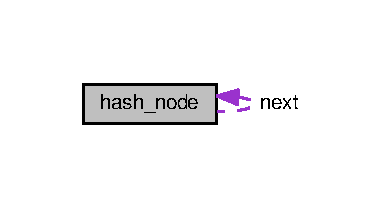
\includegraphics[width=184pt]{structhash__node__coll__graph}
\end{center}
\end{figure}
\subsection*{Data Fields}
\begin{DoxyCompactItemize}
\item 
\hyperlink{structhash__node}{Hash\+Node} {\bfseries next}\hypertarget{structhash__node_a37ad6e543029e7eef401f8be7a984689}{}\label{structhash__node_a37ad6e543029e7eef401f8be7a984689}

\item 
Pl\+Long {\bfseries key}\hypertarget{structhash__node_aa9c0ed0ab7bc110696244024900e9419}{}\label{structhash__node_aa9c0ed0ab7bc110696244024900e9419}

\end{DoxyCompactItemize}


The documentation for this struct was generated from the following file\+:\begin{DoxyCompactItemize}
\item 
gprolog-\/utf8-\/tree/src/\+Engine\+Pl/hash.\+c\end{DoxyCompactItemize}

\hypertarget{structHashIncrInfo}{}\section{Hash\+Incr\+Info Struct Reference}
\label{structHashIncrInfo}\index{Hash\+Incr\+Info@{Hash\+Incr\+Info}}


{\ttfamily \#include $<$hash\+\_\+fct.\+h$>$}

\subsection*{Data Fields}
\begin{DoxyCompactItemize}
\item 
int \hyperlink{structHashIncrInfo_adab7e9365193be88c2bb9e65edbf63bb}{len}
\item 
uint32\+\_\+t \hyperlink{structHashIncrInfo_a3f0d935d1523af0164e99832740c7df7}{hash}
\end{DoxyCompactItemize}


\subsection{Field Documentation}
\index{Hash\+Incr\+Info@{Hash\+Incr\+Info}!hash@{hash}}
\index{hash@{hash}!Hash\+Incr\+Info@{Hash\+Incr\+Info}}
\subsubsection[{\texorpdfstring{hash}{hash}}]{\setlength{\rightskip}{0pt plus 5cm}uint32\+\_\+t Hash\+Incr\+Info\+::hash}\hypertarget{structHashIncrInfo_a3f0d935d1523af0164e99832740c7df7}{}\label{structHashIncrInfo_a3f0d935d1523af0164e99832740c7df7}
\index{Hash\+Incr\+Info@{Hash\+Incr\+Info}!len@{len}}
\index{len@{len}!Hash\+Incr\+Info@{Hash\+Incr\+Info}}
\subsubsection[{\texorpdfstring{len}{len}}]{\setlength{\rightskip}{0pt plus 5cm}int Hash\+Incr\+Info\+::len}\hypertarget{structHashIncrInfo_adab7e9365193be88c2bb9e65edbf63bb}{}\label{structHashIncrInfo_adab7e9365193be88c2bb9e65edbf63bb}


The documentation for this struct was generated from the following file\+:\begin{DoxyCompactItemize}
\item 
gprolog-\/utf8-\/tree/src/\+Engine\+Pl/\hyperlink{hash__fct_8h}{hash\+\_\+fct.\+h}\end{DoxyCompactItemize}

\hypertarget{structHashScan}{}\section{Hash\+Scan Struct Reference}
\label{structHashScan}\index{Hash\+Scan@{Hash\+Scan}}


{\ttfamily \#include $<$hash.\+h$>$}

\subsection*{Data Fields}
\begin{DoxyCompactItemize}
\item 
char $\ast$ \hyperlink{structHashScan_a40b9e0ec1b11cffe3e7bc2c20b7b8a4b}{endt}
\item 
char $\ast$ \hyperlink{structHashScan_af1c9388da5931a00722e2e9ea2c10f42}{cur\+\_\+t}
\item 
char $\ast$ \hyperlink{structHashScan_a267d5612893c8faa728cb27e1edd21aa}{cur\+\_\+p}
\end{DoxyCompactItemize}


\subsection{Field Documentation}
\index{Hash\+Scan@{Hash\+Scan}!cur\+\_\+p@{cur\+\_\+p}}
\index{cur\+\_\+p@{cur\+\_\+p}!Hash\+Scan@{Hash\+Scan}}
\subsubsection[{\texorpdfstring{cur\+\_\+p}{cur_p}}]{\setlength{\rightskip}{0pt plus 5cm}char$\ast$ Hash\+Scan\+::cur\+\_\+p}\hypertarget{structHashScan_a267d5612893c8faa728cb27e1edd21aa}{}\label{structHashScan_a267d5612893c8faa728cb27e1edd21aa}
\index{Hash\+Scan@{Hash\+Scan}!cur\+\_\+t@{cur\+\_\+t}}
\index{cur\+\_\+t@{cur\+\_\+t}!Hash\+Scan@{Hash\+Scan}}
\subsubsection[{\texorpdfstring{cur\+\_\+t}{cur_t}}]{\setlength{\rightskip}{0pt plus 5cm}char$\ast$ Hash\+Scan\+::cur\+\_\+t}\hypertarget{structHashScan_af1c9388da5931a00722e2e9ea2c10f42}{}\label{structHashScan_af1c9388da5931a00722e2e9ea2c10f42}
\index{Hash\+Scan@{Hash\+Scan}!endt@{endt}}
\index{endt@{endt}!Hash\+Scan@{Hash\+Scan}}
\subsubsection[{\texorpdfstring{endt}{endt}}]{\setlength{\rightskip}{0pt plus 5cm}char$\ast$ Hash\+Scan\+::endt}\hypertarget{structHashScan_a40b9e0ec1b11cffe3e7bc2c20b7b8a4b}{}\label{structHashScan_a40b9e0ec1b11cffe3e7bc2c20b7b8a4b}


The documentation for this struct was generated from the following file\+:\begin{DoxyCompactItemize}
\item 
gprolog-\/utf8-\/tree/src/\+Engine\+Pl/\hyperlink{hash_8h}{hash.\+h}\end{DoxyCompactItemize}

\hypertarget{structHistCell}{}\section{Hist\+Cell Struct Reference}
\label{structHistCell}\index{Hist\+Cell@{Hist\+Cell}}
\subsection*{Data Fields}
\begin{DoxyCompactItemize}
\item 
int \hyperlink{structHistCell_a969bc82748a2a5ec09f62d138f62d206}{buff\+\_\+length}
\item 
int \hyperlink{structHistCell_aab32370dee81b023aa2d04e3c6a148e4}{line\+\_\+length}
\item 
char $\ast$ \hyperlink{structHistCell_a7c9560a76c886d7c26f118668303945a}{line}
\end{DoxyCompactItemize}


\subsection{Field Documentation}
\index{Hist\+Cell@{Hist\+Cell}!buff\+\_\+length@{buff\+\_\+length}}
\index{buff\+\_\+length@{buff\+\_\+length}!Hist\+Cell@{Hist\+Cell}}
\subsubsection[{\texorpdfstring{buff\+\_\+length}{buff_length}}]{\setlength{\rightskip}{0pt plus 5cm}int Hist\+Cell\+::buff\+\_\+length}\hypertarget{structHistCell_a969bc82748a2a5ec09f62d138f62d206}{}\label{structHistCell_a969bc82748a2a5ec09f62d138f62d206}
\index{Hist\+Cell@{Hist\+Cell}!line@{line}}
\index{line@{line}!Hist\+Cell@{Hist\+Cell}}
\subsubsection[{\texorpdfstring{line}{line}}]{\setlength{\rightskip}{0pt plus 5cm}char$\ast$ Hist\+Cell\+::line}\hypertarget{structHistCell_a7c9560a76c886d7c26f118668303945a}{}\label{structHistCell_a7c9560a76c886d7c26f118668303945a}
\index{Hist\+Cell@{Hist\+Cell}!line\+\_\+length@{line\+\_\+length}}
\index{line\+\_\+length@{line\+\_\+length}!Hist\+Cell@{Hist\+Cell}}
\subsubsection[{\texorpdfstring{line\+\_\+length}{line_length}}]{\setlength{\rightskip}{0pt plus 5cm}int Hist\+Cell\+::line\+\_\+length}\hypertarget{structHistCell_aab32370dee81b023aa2d04e3c6a148e4}{}\label{structHistCell_aab32370dee81b023aa2d04e3c6a148e4}


The documentation for this struct was generated from the following file\+:\begin{DoxyCompactItemize}
\item 
gprolog-\/utf8-\/tree/src/\+Linedit/\hyperlink{linedit_8c}{linedit.\+c}\end{DoxyCompactItemize}

\hypertarget{structInfCmd}{}\section{Inf\+Cmd Struct Reference}
\label{structInfCmd}\index{Inf\+Cmd@{Inf\+Cmd}}
\subsection*{Data Fields}
\begin{DoxyCompactItemize}
\item 
char $\ast$ {\bfseries name}\hypertarget{structInfCmd_af3fea806d68a1051611b2858d1aa2747}{}\label{structInfCmd_af3fea806d68a1051611b2858d1aa2747}

\item 
Fct\+Ptr {\bfseries fct}\hypertarget{structInfCmd_a4b390073530117560b83be4116a49e0b}{}\label{structInfCmd_a4b390073530117560b83be4116a49e0b}

\end{DoxyCompactItemize}


The documentation for this struct was generated from the following file\+:\begin{DoxyCompactItemize}
\item 
gprolog-\/utf8-\/tree/src/\+Bips\+Pl/debugger\+\_\+c.\+c\end{DoxyCompactItemize}

\hypertarget{structInfSig}{}\section{Inf\+Sig Struct Reference}
\label{structInfSig}\index{Inf\+Sig@{Inf\+Sig}}
\subsection*{Data Fields}
\begin{DoxyCompactItemize}
\item 
int \hyperlink{structInfSig_a802a7fecafff618606688d70860c6ce4}{atom}
\item 
int \hyperlink{structInfSig_a089058351323d661ad411c87017b6647}{sig}
\end{DoxyCompactItemize}


\subsection{Field Documentation}
\index{Inf\+Sig@{Inf\+Sig}!atom@{atom}}
\index{atom@{atom}!Inf\+Sig@{Inf\+Sig}}
\subsubsection[{\texorpdfstring{atom}{atom}}]{\setlength{\rightskip}{0pt plus 5cm}int Inf\+Sig\+::atom}\hypertarget{structInfSig_a802a7fecafff618606688d70860c6ce4}{}\label{structInfSig_a802a7fecafff618606688d70860c6ce4}
\index{Inf\+Sig@{Inf\+Sig}!sig@{sig}}
\index{sig@{sig}!Inf\+Sig@{Inf\+Sig}}
\subsubsection[{\texorpdfstring{sig}{sig}}]{\setlength{\rightskip}{0pt plus 5cm}int Inf\+Sig\+::sig}\hypertarget{structInfSig_a089058351323d661ad411c87017b6647}{}\label{structInfSig_a089058351323d661ad411c87017b6647}


The documentation for this struct was generated from the following file\+:\begin{DoxyCompactItemize}
\item 
gprolog-\/utf8-\/tree/src/\+Bips\+Pl/\hyperlink{os__interf__c_8c}{os\+\_\+interf\+\_\+c.\+c}\end{DoxyCompactItemize}

\hypertarget{structInfVar}{}\section{Inf\+Var Struct Reference}
\label{structInfVar}\index{Inf\+Var@{Inf\+Var}}
\subsection*{Data Fields}
\begin{DoxyCompactItemize}
\item 
char {\bfseries name} \mbox{[}M\+A\+X\+\_\+\+V\+A\+R\+\_\+\+N\+A\+M\+E\+\_\+\+L\+E\+N\+G\+TH\mbox{]}\hypertarget{structInfVar_a0dc32a42fe7338b19884288c0e63b35f}{}\label{structInfVar_a0dc32a42fe7338b19884288c0e63b35f}

\item 
Wam\+Word {\bfseries word}\hypertarget{structInfVar_acc66e228f4cfbb1ab828b0bb95a69621}{}\label{structInfVar_acc66e228f4cfbb1ab828b0bb95a69621}

\item 
Bool {\bfseries named}\hypertarget{structInfVar_a56bb3da1e5f14c34e30d702852740a39}{}\label{structInfVar_a56bb3da1e5f14c34e30d702852740a39}

\item 
int {\bfseries nb\+\_\+of\+\_\+uses}\hypertarget{structInfVar_a38f07afe6ae0ae7f591cf95796469f83}{}\label{structInfVar_a38f07afe6ae0ae7f591cf95796469f83}

\end{DoxyCompactItemize}


The documentation for this struct was generated from the following file\+:\begin{DoxyCompactItemize}
\item 
gprolog-\/utf8-\/tree/src/\+Bips\+Pl/parse\+\_\+supp.\+h\end{DoxyCompactItemize}

\hypertarget{structLongInf}{}\section{Long\+Inf Struct Reference}
\label{structLongInf}\index{Long\+Inf@{Long\+Inf}}
\subsection*{Data Fields}
\begin{DoxyCompactItemize}
\item 
int \hyperlink{structLongInf_a2a21c022832de0f854940c3a39233cec}{global}
\item 
\hyperlink{ma__parser_8h_a28a778aedb7441c6b9755e1882b58dc9}{V\+Type} \hyperlink{structLongInf_a43f3ac657d3dabca28037f16891e4092}{vtype}
\item 
\hyperlink{gprolog_8h_a4d005b136d7fb28537eb1815f7868b63}{Pl\+Long} \hyperlink{structLongInf_ab45336cb32ee695b77f51b6490a81875}{value}
\end{DoxyCompactItemize}


\subsection{Field Documentation}
\index{Long\+Inf@{Long\+Inf}!global@{global}}
\index{global@{global}!Long\+Inf@{Long\+Inf}}
\subsubsection[{\texorpdfstring{global}{global}}]{\setlength{\rightskip}{0pt plus 5cm}int Long\+Inf\+::global}\hypertarget{structLongInf_a2a21c022832de0f854940c3a39233cec}{}\label{structLongInf_a2a21c022832de0f854940c3a39233cec}
\index{Long\+Inf@{Long\+Inf}!value@{value}}
\index{value@{value}!Long\+Inf@{Long\+Inf}}
\subsubsection[{\texorpdfstring{value}{value}}]{\setlength{\rightskip}{0pt plus 5cm}{\bf Pl\+Long} Long\+Inf\+::value}\hypertarget{structLongInf_ab45336cb32ee695b77f51b6490a81875}{}\label{structLongInf_ab45336cb32ee695b77f51b6490a81875}
\index{Long\+Inf@{Long\+Inf}!vtype@{vtype}}
\index{vtype@{vtype}!Long\+Inf@{Long\+Inf}}
\subsubsection[{\texorpdfstring{vtype}{vtype}}]{\setlength{\rightskip}{0pt plus 5cm}{\bf V\+Type} Long\+Inf\+::vtype}\hypertarget{structLongInf_a43f3ac657d3dabca28037f16891e4092}{}\label{structLongInf_a43f3ac657d3dabca28037f16891e4092}


The documentation for this struct was generated from the following file\+:\begin{DoxyCompactItemize}
\item 
gprolog-\/utf8-\/tree/src/\+Ma2\+Asm/\hyperlink{ma2asm_8c}{ma2asm.\+c}\end{DoxyCompactItemize}

\hypertarget{structmallinfo}{}\section{mallinfo Struct Reference}
\label{structmallinfo}\index{mallinfo@{mallinfo}}
\subsection*{Data Fields}
\begin{DoxyCompactItemize}
\item 
\hyperlink{dl__malloc_8c_a53688562ed3d2eda132ae91de874cd98}{M\+A\+L\+L\+I\+N\+F\+O\+\_\+\+F\+I\+E\+L\+D\+\_\+\+T\+Y\+PE} \hyperlink{structmallinfo_a2dd8e574430e788f53919db129f2a2ff}{arena}
\item 
\hyperlink{dl__malloc_8c_a53688562ed3d2eda132ae91de874cd98}{M\+A\+L\+L\+I\+N\+F\+O\+\_\+\+F\+I\+E\+L\+D\+\_\+\+T\+Y\+PE} \hyperlink{structmallinfo_afaac6d1e005097fa1ed835684e23bfa7}{ordblks}
\item 
\hyperlink{dl__malloc_8c_a53688562ed3d2eda132ae91de874cd98}{M\+A\+L\+L\+I\+N\+F\+O\+\_\+\+F\+I\+E\+L\+D\+\_\+\+T\+Y\+PE} \hyperlink{structmallinfo_a93076145f3f542dfe5e4e6d1e3feaf0b}{smblks}
\item 
\hyperlink{dl__malloc_8c_a53688562ed3d2eda132ae91de874cd98}{M\+A\+L\+L\+I\+N\+F\+O\+\_\+\+F\+I\+E\+L\+D\+\_\+\+T\+Y\+PE} \hyperlink{structmallinfo_aaf01c52dcd016834ae176885fa32b550}{hblks}
\item 
\hyperlink{dl__malloc_8c_a53688562ed3d2eda132ae91de874cd98}{M\+A\+L\+L\+I\+N\+F\+O\+\_\+\+F\+I\+E\+L\+D\+\_\+\+T\+Y\+PE} \hyperlink{structmallinfo_ab78bcaeb59449f1a9c292bfe3dde8dbb}{hblkhd}
\item 
\hyperlink{dl__malloc_8c_a53688562ed3d2eda132ae91de874cd98}{M\+A\+L\+L\+I\+N\+F\+O\+\_\+\+F\+I\+E\+L\+D\+\_\+\+T\+Y\+PE} \hyperlink{structmallinfo_a470a5e18a1f5eb3cac48020268ca49b8}{usmblks}
\item 
\hyperlink{dl__malloc_8c_a53688562ed3d2eda132ae91de874cd98}{M\+A\+L\+L\+I\+N\+F\+O\+\_\+\+F\+I\+E\+L\+D\+\_\+\+T\+Y\+PE} \hyperlink{structmallinfo_a6b1a33ff0fc95bdab9c79ce271f58003}{fsmblks}
\item 
\hyperlink{dl__malloc_8c_a53688562ed3d2eda132ae91de874cd98}{M\+A\+L\+L\+I\+N\+F\+O\+\_\+\+F\+I\+E\+L\+D\+\_\+\+T\+Y\+PE} \hyperlink{structmallinfo_a4676f74c10d8bf8b79585b04d520356f}{uordblks}
\item 
\hyperlink{dl__malloc_8c_a53688562ed3d2eda132ae91de874cd98}{M\+A\+L\+L\+I\+N\+F\+O\+\_\+\+F\+I\+E\+L\+D\+\_\+\+T\+Y\+PE} \hyperlink{structmallinfo_a2fc75bf31817d4a64d0a6970aa5278dd}{fordblks}
\item 
\hyperlink{dl__malloc_8c_a53688562ed3d2eda132ae91de874cd98}{M\+A\+L\+L\+I\+N\+F\+O\+\_\+\+F\+I\+E\+L\+D\+\_\+\+T\+Y\+PE} \hyperlink{structmallinfo_a9cd2ce910ff603217426d9b1b7c0e430}{keepcost}
\end{DoxyCompactItemize}


\subsection{Field Documentation}
\index{mallinfo@{mallinfo}!arena@{arena}}
\index{arena@{arena}!mallinfo@{mallinfo}}
\subsubsection[{\texorpdfstring{arena}{arena}}]{\setlength{\rightskip}{0pt plus 5cm}{\bf M\+A\+L\+L\+I\+N\+F\+O\+\_\+\+F\+I\+E\+L\+D\+\_\+\+T\+Y\+PE} mallinfo\+::arena}\hypertarget{structmallinfo_a2dd8e574430e788f53919db129f2a2ff}{}\label{structmallinfo_a2dd8e574430e788f53919db129f2a2ff}
\index{mallinfo@{mallinfo}!fordblks@{fordblks}}
\index{fordblks@{fordblks}!mallinfo@{mallinfo}}
\subsubsection[{\texorpdfstring{fordblks}{fordblks}}]{\setlength{\rightskip}{0pt plus 5cm}{\bf M\+A\+L\+L\+I\+N\+F\+O\+\_\+\+F\+I\+E\+L\+D\+\_\+\+T\+Y\+PE} mallinfo\+::fordblks}\hypertarget{structmallinfo_a2fc75bf31817d4a64d0a6970aa5278dd}{}\label{structmallinfo_a2fc75bf31817d4a64d0a6970aa5278dd}
\index{mallinfo@{mallinfo}!fsmblks@{fsmblks}}
\index{fsmblks@{fsmblks}!mallinfo@{mallinfo}}
\subsubsection[{\texorpdfstring{fsmblks}{fsmblks}}]{\setlength{\rightskip}{0pt plus 5cm}{\bf M\+A\+L\+L\+I\+N\+F\+O\+\_\+\+F\+I\+E\+L\+D\+\_\+\+T\+Y\+PE} mallinfo\+::fsmblks}\hypertarget{structmallinfo_a6b1a33ff0fc95bdab9c79ce271f58003}{}\label{structmallinfo_a6b1a33ff0fc95bdab9c79ce271f58003}
\index{mallinfo@{mallinfo}!hblkhd@{hblkhd}}
\index{hblkhd@{hblkhd}!mallinfo@{mallinfo}}
\subsubsection[{\texorpdfstring{hblkhd}{hblkhd}}]{\setlength{\rightskip}{0pt plus 5cm}{\bf M\+A\+L\+L\+I\+N\+F\+O\+\_\+\+F\+I\+E\+L\+D\+\_\+\+T\+Y\+PE} mallinfo\+::hblkhd}\hypertarget{structmallinfo_ab78bcaeb59449f1a9c292bfe3dde8dbb}{}\label{structmallinfo_ab78bcaeb59449f1a9c292bfe3dde8dbb}
\index{mallinfo@{mallinfo}!hblks@{hblks}}
\index{hblks@{hblks}!mallinfo@{mallinfo}}
\subsubsection[{\texorpdfstring{hblks}{hblks}}]{\setlength{\rightskip}{0pt plus 5cm}{\bf M\+A\+L\+L\+I\+N\+F\+O\+\_\+\+F\+I\+E\+L\+D\+\_\+\+T\+Y\+PE} mallinfo\+::hblks}\hypertarget{structmallinfo_aaf01c52dcd016834ae176885fa32b550}{}\label{structmallinfo_aaf01c52dcd016834ae176885fa32b550}
\index{mallinfo@{mallinfo}!keepcost@{keepcost}}
\index{keepcost@{keepcost}!mallinfo@{mallinfo}}
\subsubsection[{\texorpdfstring{keepcost}{keepcost}}]{\setlength{\rightskip}{0pt plus 5cm}{\bf M\+A\+L\+L\+I\+N\+F\+O\+\_\+\+F\+I\+E\+L\+D\+\_\+\+T\+Y\+PE} mallinfo\+::keepcost}\hypertarget{structmallinfo_a9cd2ce910ff603217426d9b1b7c0e430}{}\label{structmallinfo_a9cd2ce910ff603217426d9b1b7c0e430}
\index{mallinfo@{mallinfo}!ordblks@{ordblks}}
\index{ordblks@{ordblks}!mallinfo@{mallinfo}}
\subsubsection[{\texorpdfstring{ordblks}{ordblks}}]{\setlength{\rightskip}{0pt plus 5cm}{\bf M\+A\+L\+L\+I\+N\+F\+O\+\_\+\+F\+I\+E\+L\+D\+\_\+\+T\+Y\+PE} mallinfo\+::ordblks}\hypertarget{structmallinfo_afaac6d1e005097fa1ed835684e23bfa7}{}\label{structmallinfo_afaac6d1e005097fa1ed835684e23bfa7}
\index{mallinfo@{mallinfo}!smblks@{smblks}}
\index{smblks@{smblks}!mallinfo@{mallinfo}}
\subsubsection[{\texorpdfstring{smblks}{smblks}}]{\setlength{\rightskip}{0pt plus 5cm}{\bf M\+A\+L\+L\+I\+N\+F\+O\+\_\+\+F\+I\+E\+L\+D\+\_\+\+T\+Y\+PE} mallinfo\+::smblks}\hypertarget{structmallinfo_a93076145f3f542dfe5e4e6d1e3feaf0b}{}\label{structmallinfo_a93076145f3f542dfe5e4e6d1e3feaf0b}
\index{mallinfo@{mallinfo}!uordblks@{uordblks}}
\index{uordblks@{uordblks}!mallinfo@{mallinfo}}
\subsubsection[{\texorpdfstring{uordblks}{uordblks}}]{\setlength{\rightskip}{0pt plus 5cm}{\bf M\+A\+L\+L\+I\+N\+F\+O\+\_\+\+F\+I\+E\+L\+D\+\_\+\+T\+Y\+PE} mallinfo\+::uordblks}\hypertarget{structmallinfo_a4676f74c10d8bf8b79585b04d520356f}{}\label{structmallinfo_a4676f74c10d8bf8b79585b04d520356f}
\index{mallinfo@{mallinfo}!usmblks@{usmblks}}
\index{usmblks@{usmblks}!mallinfo@{mallinfo}}
\subsubsection[{\texorpdfstring{usmblks}{usmblks}}]{\setlength{\rightskip}{0pt plus 5cm}{\bf M\+A\+L\+L\+I\+N\+F\+O\+\_\+\+F\+I\+E\+L\+D\+\_\+\+T\+Y\+PE} mallinfo\+::usmblks}\hypertarget{structmallinfo_a470a5e18a1f5eb3cac48020268ca49b8}{}\label{structmallinfo_a470a5e18a1f5eb3cac48020268ca49b8}


The documentation for this struct was generated from the following file\+:\begin{DoxyCompactItemize}
\item 
gprolog-\/utf8-\/tree/src/\+Engine\+Pl/\hyperlink{dl__malloc_8c}{dl\+\_\+malloc.\+c}\end{DoxyCompactItemize}

\hypertarget{structmalloc__chunk}{}\section{malloc\+\_\+chunk Struct Reference}
\label{structmalloc__chunk}\index{malloc\+\_\+chunk@{malloc\+\_\+chunk}}


Collaboration diagram for malloc\+\_\+chunk\+:\nopagebreak
\begin{figure}[H]
\begin{center}
\leavevmode
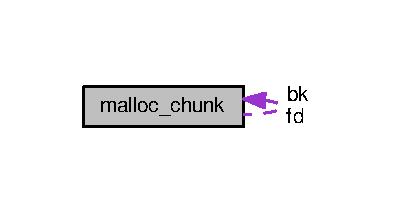
\includegraphics[width=189pt]{structmalloc__chunk__coll__graph}
\end{center}
\end{figure}
\subsection*{Data Fields}
\begin{DoxyCompactItemize}
\item 
size\+\_\+t {\bfseries prev\+\_\+foot}\hypertarget{structmalloc__chunk_a2cbb92874183d7a4b42e150b7d7ec1f9}{}\label{structmalloc__chunk_a2cbb92874183d7a4b42e150b7d7ec1f9}

\item 
size\+\_\+t {\bfseries head}\hypertarget{structmalloc__chunk_a7383bb525d34ca811283c927086205bc}{}\label{structmalloc__chunk_a7383bb525d34ca811283c927086205bc}

\item 
struct \hyperlink{structmalloc__chunk}{malloc\+\_\+chunk} $\ast$ {\bfseries fd}\hypertarget{structmalloc__chunk_a9972ab720231dd0c0d3c202176ce13c5}{}\label{structmalloc__chunk_a9972ab720231dd0c0d3c202176ce13c5}

\item 
struct \hyperlink{structmalloc__chunk}{malloc\+\_\+chunk} $\ast$ {\bfseries bk}\hypertarget{structmalloc__chunk_a268940e08c9c09fc3b2e23cd804bce3c}{}\label{structmalloc__chunk_a268940e08c9c09fc3b2e23cd804bce3c}

\end{DoxyCompactItemize}


The documentation for this struct was generated from the following file\+:\begin{DoxyCompactItemize}
\item 
gprolog-\/utf8-\/tree/src/\+Engine\+Pl/dl\+\_\+malloc.\+c\end{DoxyCompactItemize}

\hypertarget{structmalloc__params}{}\section{malloc\+\_\+params Struct Reference}
\label{structmalloc__params}\index{malloc\+\_\+params@{malloc\+\_\+params}}
\subsection*{Data Fields}
\begin{DoxyCompactItemize}
\item 
size\+\_\+t \hyperlink{structmalloc__params_a7034fc9c71af2cc5ba9cd079effdf5a8}{magic}
\item 
size\+\_\+t \hyperlink{structmalloc__params_a3b7a605d7ebe148a8fb3051465dc3979}{page\+\_\+size}
\item 
size\+\_\+t \hyperlink{structmalloc__params_aa0609453d9ec826c8ffc632cbfb8cf68}{granularity}
\item 
size\+\_\+t \hyperlink{structmalloc__params_a5b2af958efc37d52cfa905bc98b41e1b}{mmap\+\_\+threshold}
\item 
size\+\_\+t \hyperlink{structmalloc__params_accae9b2bcb4df63efcdc0b18826cc578}{trim\+\_\+threshold}
\item 
\hyperlink{dl__malloc_8c_a98d45780d5103f1a6b54a549a3d12de2}{flag\+\_\+t} \hyperlink{structmalloc__params_a0bd6b4819a5d7c629c5ab56262f6296d}{default\+\_\+mflags}
\end{DoxyCompactItemize}


\subsection{Field Documentation}
\index{malloc\+\_\+params@{malloc\+\_\+params}!default\+\_\+mflags@{default\+\_\+mflags}}
\index{default\+\_\+mflags@{default\+\_\+mflags}!malloc\+\_\+params@{malloc\+\_\+params}}
\subsubsection[{\texorpdfstring{default\+\_\+mflags}{default_mflags}}]{\setlength{\rightskip}{0pt plus 5cm}{\bf flag\+\_\+t} malloc\+\_\+params\+::default\+\_\+mflags}\hypertarget{structmalloc__params_a0bd6b4819a5d7c629c5ab56262f6296d}{}\label{structmalloc__params_a0bd6b4819a5d7c629c5ab56262f6296d}
\index{malloc\+\_\+params@{malloc\+\_\+params}!granularity@{granularity}}
\index{granularity@{granularity}!malloc\+\_\+params@{malloc\+\_\+params}}
\subsubsection[{\texorpdfstring{granularity}{granularity}}]{\setlength{\rightskip}{0pt plus 5cm}size\+\_\+t malloc\+\_\+params\+::granularity}\hypertarget{structmalloc__params_aa0609453d9ec826c8ffc632cbfb8cf68}{}\label{structmalloc__params_aa0609453d9ec826c8ffc632cbfb8cf68}
\index{malloc\+\_\+params@{malloc\+\_\+params}!magic@{magic}}
\index{magic@{magic}!malloc\+\_\+params@{malloc\+\_\+params}}
\subsubsection[{\texorpdfstring{magic}{magic}}]{\setlength{\rightskip}{0pt plus 5cm}size\+\_\+t malloc\+\_\+params\+::magic}\hypertarget{structmalloc__params_a7034fc9c71af2cc5ba9cd079effdf5a8}{}\label{structmalloc__params_a7034fc9c71af2cc5ba9cd079effdf5a8}
\index{malloc\+\_\+params@{malloc\+\_\+params}!mmap\+\_\+threshold@{mmap\+\_\+threshold}}
\index{mmap\+\_\+threshold@{mmap\+\_\+threshold}!malloc\+\_\+params@{malloc\+\_\+params}}
\subsubsection[{\texorpdfstring{mmap\+\_\+threshold}{mmap_threshold}}]{\setlength{\rightskip}{0pt plus 5cm}size\+\_\+t malloc\+\_\+params\+::mmap\+\_\+threshold}\hypertarget{structmalloc__params_a5b2af958efc37d52cfa905bc98b41e1b}{}\label{structmalloc__params_a5b2af958efc37d52cfa905bc98b41e1b}
\index{malloc\+\_\+params@{malloc\+\_\+params}!page\+\_\+size@{page\+\_\+size}}
\index{page\+\_\+size@{page\+\_\+size}!malloc\+\_\+params@{malloc\+\_\+params}}
\subsubsection[{\texorpdfstring{page\+\_\+size}{page_size}}]{\setlength{\rightskip}{0pt plus 5cm}size\+\_\+t malloc\+\_\+params\+::page\+\_\+size}\hypertarget{structmalloc__params_a3b7a605d7ebe148a8fb3051465dc3979}{}\label{structmalloc__params_a3b7a605d7ebe148a8fb3051465dc3979}
\index{malloc\+\_\+params@{malloc\+\_\+params}!trim\+\_\+threshold@{trim\+\_\+threshold}}
\index{trim\+\_\+threshold@{trim\+\_\+threshold}!malloc\+\_\+params@{malloc\+\_\+params}}
\subsubsection[{\texorpdfstring{trim\+\_\+threshold}{trim_threshold}}]{\setlength{\rightskip}{0pt plus 5cm}size\+\_\+t malloc\+\_\+params\+::trim\+\_\+threshold}\hypertarget{structmalloc__params_accae9b2bcb4df63efcdc0b18826cc578}{}\label{structmalloc__params_accae9b2bcb4df63efcdc0b18826cc578}


The documentation for this struct was generated from the following file\+:\begin{DoxyCompactItemize}
\item 
gprolog-\/utf8-\/tree/src/\+Engine\+Pl/\hyperlink{dl__malloc_8c}{dl\+\_\+malloc.\+c}\end{DoxyCompactItemize}

\hypertarget{structmalloc__segment}{}\section{malloc\+\_\+segment Struct Reference}
\label{structmalloc__segment}\index{malloc\+\_\+segment@{malloc\+\_\+segment}}


Collaboration diagram for malloc\+\_\+segment\+:\nopagebreak
\begin{figure}[H]
\begin{center}
\leavevmode
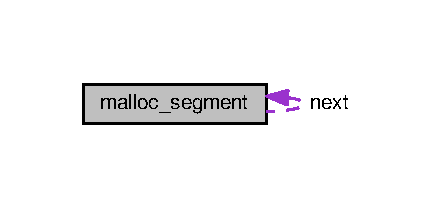
\includegraphics[width=208pt]{structmalloc__segment__coll__graph}
\end{center}
\end{figure}
\subsection*{Data Fields}
\begin{DoxyCompactItemize}
\item 
char $\ast$ {\bfseries base}\hypertarget{structmalloc__segment_ad4c68a4113c3a4f9b167aadaa7c31b89}{}\label{structmalloc__segment_ad4c68a4113c3a4f9b167aadaa7c31b89}

\item 
size\+\_\+t {\bfseries size}\hypertarget{structmalloc__segment_a392a23ee3bd7a167e5f6382793a8eba1}{}\label{structmalloc__segment_a392a23ee3bd7a167e5f6382793a8eba1}

\item 
struct \hyperlink{structmalloc__segment}{malloc\+\_\+segment} $\ast$ {\bfseries next}\hypertarget{structmalloc__segment_a92c4c9f618dba33fd8628d743cc02f5a}{}\label{structmalloc__segment_a92c4c9f618dba33fd8628d743cc02f5a}

\item 
flag\+\_\+t {\bfseries sflags}\hypertarget{structmalloc__segment_ac48f17d9495d732749db6544cabbec2c}{}\label{structmalloc__segment_ac48f17d9495d732749db6544cabbec2c}

\end{DoxyCompactItemize}


The documentation for this struct was generated from the following file\+:\begin{DoxyCompactItemize}
\item 
gprolog-\/utf8-\/tree/src/\+Engine\+Pl/dl\+\_\+malloc.\+c\end{DoxyCompactItemize}

\hypertarget{structmalloc__state}{}\section{malloc\+\_\+state Struct Reference}
\label{structmalloc__state}\index{malloc\+\_\+state@{malloc\+\_\+state}}


Collaboration diagram for malloc\+\_\+state\+:\nopagebreak
\begin{figure}[H]
\begin{center}
\leavevmode
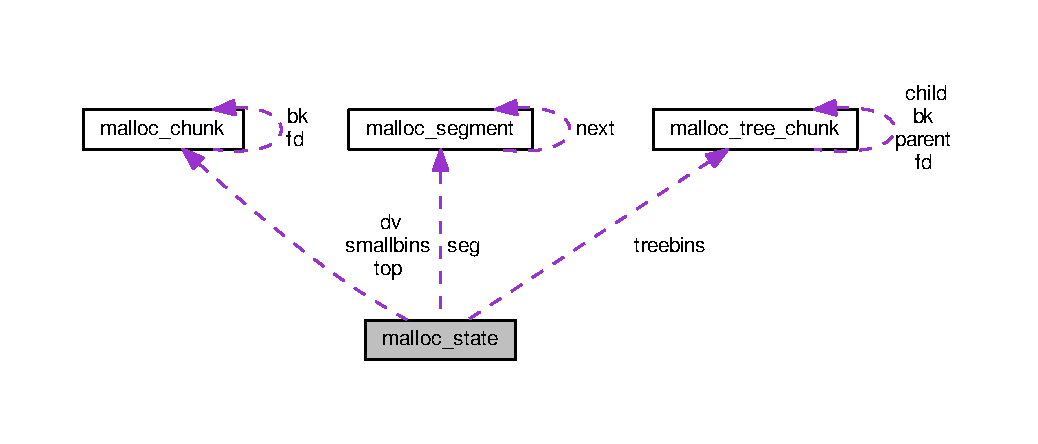
\includegraphics[width=350pt]{structmalloc__state__coll__graph}
\end{center}
\end{figure}
\subsection*{Data Fields}
\begin{DoxyCompactItemize}
\item 
binmap\+\_\+t {\bfseries smallmap}\hypertarget{structmalloc__state_a9e597125e4a96b39d3859c59fee38c49}{}\label{structmalloc__state_a9e597125e4a96b39d3859c59fee38c49}

\item 
binmap\+\_\+t {\bfseries treemap}\hypertarget{structmalloc__state_ae20bf1bcda1838e5bc07d2395ba72283}{}\label{structmalloc__state_ae20bf1bcda1838e5bc07d2395ba72283}

\item 
size\+\_\+t {\bfseries dvsize}\hypertarget{structmalloc__state_ae2e6a3ed8e8abaf03e47917057f1012d}{}\label{structmalloc__state_ae2e6a3ed8e8abaf03e47917057f1012d}

\item 
size\+\_\+t {\bfseries topsize}\hypertarget{structmalloc__state_aa93901fa8e414a7d7881ee968b097eea}{}\label{structmalloc__state_aa93901fa8e414a7d7881ee968b097eea}

\item 
char $\ast$ {\bfseries least\+\_\+addr}\hypertarget{structmalloc__state_af9a424730d25d685373ab736a29560b5}{}\label{structmalloc__state_af9a424730d25d685373ab736a29560b5}

\item 
\hyperlink{structmalloc__chunk}{mchunkptr} {\bfseries dv}\hypertarget{structmalloc__state_a840943ad4baaddbaaa5defe954ec06b9}{}\label{structmalloc__state_a840943ad4baaddbaaa5defe954ec06b9}

\item 
\hyperlink{structmalloc__chunk}{mchunkptr} {\bfseries top}\hypertarget{structmalloc__state_a594c4d03c189612e0ce91f7aba8dae77}{}\label{structmalloc__state_a594c4d03c189612e0ce91f7aba8dae77}

\item 
size\+\_\+t {\bfseries trim\+\_\+check}\hypertarget{structmalloc__state_a30209a5277132d0f207c7a850d225324}{}\label{structmalloc__state_a30209a5277132d0f207c7a850d225324}

\item 
size\+\_\+t {\bfseries release\+\_\+checks}\hypertarget{structmalloc__state_af2afbe4faf64185994d9c10cef2e0a3a}{}\label{structmalloc__state_af2afbe4faf64185994d9c10cef2e0a3a}

\item 
size\+\_\+t {\bfseries magic}\hypertarget{structmalloc__state_ac19e13bf018dc22419c38d8cbe839b62}{}\label{structmalloc__state_ac19e13bf018dc22419c38d8cbe839b62}

\item 
\hyperlink{structmalloc__chunk}{mchunkptr} {\bfseries smallbins} \mbox{[}(N\+S\+M\+A\+L\+L\+B\+I\+NS+1)$\ast$2\mbox{]}\hypertarget{structmalloc__state_ade50b83b94e4f09d372a18ae51c13f70}{}\label{structmalloc__state_ade50b83b94e4f09d372a18ae51c13f70}

\item 
\hyperlink{structmalloc__tree__chunk}{tbinptr} {\bfseries treebins} \mbox{[}N\+T\+R\+E\+E\+B\+I\+NS\mbox{]}\hypertarget{structmalloc__state_a7ccf88dffa5e3287b7c9dd290ea1a0cb}{}\label{structmalloc__state_a7ccf88dffa5e3287b7c9dd290ea1a0cb}

\item 
size\+\_\+t {\bfseries footprint}\hypertarget{structmalloc__state_a77ec93dc40bb85bd7a3c4e9b26547d11}{}\label{structmalloc__state_a77ec93dc40bb85bd7a3c4e9b26547d11}

\item 
size\+\_\+t {\bfseries max\+\_\+footprint}\hypertarget{structmalloc__state_ac5c720358079598dfb5d699124e761c8}{}\label{structmalloc__state_ac5c720358079598dfb5d699124e761c8}

\item 
size\+\_\+t {\bfseries footprint\+\_\+limit}\hypertarget{structmalloc__state_ab589c6129376d79aab99babfe55fe048}{}\label{structmalloc__state_ab589c6129376d79aab99babfe55fe048}

\item 
flag\+\_\+t {\bfseries mflags}\hypertarget{structmalloc__state_a44ff83ca07796cad96f2289471c88d2d}{}\label{structmalloc__state_a44ff83ca07796cad96f2289471c88d2d}

\item 
M\+L\+O\+C\+K\+\_\+T {\bfseries mutex}\hypertarget{structmalloc__state_aafbde3a2fbb7df9480eb14521e5624da}{}\label{structmalloc__state_aafbde3a2fbb7df9480eb14521e5624da}

\item 
\hyperlink{structmalloc__segment}{msegment} {\bfseries seg}\hypertarget{structmalloc__state_a899c69eca79f165b03913063a93d973a}{}\label{structmalloc__state_a899c69eca79f165b03913063a93d973a}

\item 
void $\ast$ {\bfseries extp}\hypertarget{structmalloc__state_aa605a719561fc44ce2ce7165e6dcb897}{}\label{structmalloc__state_aa605a719561fc44ce2ce7165e6dcb897}

\item 
size\+\_\+t {\bfseries exts}\hypertarget{structmalloc__state_af3c1e272f4107a5006ee10429cb2232a}{}\label{structmalloc__state_af3c1e272f4107a5006ee10429cb2232a}

\end{DoxyCompactItemize}


The documentation for this struct was generated from the following file\+:\begin{DoxyCompactItemize}
\item 
gprolog-\/utf8-\/tree/src/\+Engine\+Pl/dl\+\_\+malloc.\+c\end{DoxyCompactItemize}

\hypertarget{structmalloc__tree__chunk}{}\section{malloc\+\_\+tree\+\_\+chunk Struct Reference}
\label{structmalloc__tree__chunk}\index{malloc\+\_\+tree\+\_\+chunk@{malloc\+\_\+tree\+\_\+chunk}}


Collaboration diagram for malloc\+\_\+tree\+\_\+chunk\+:\nopagebreak
\begin{figure}[H]
\begin{center}
\leavevmode
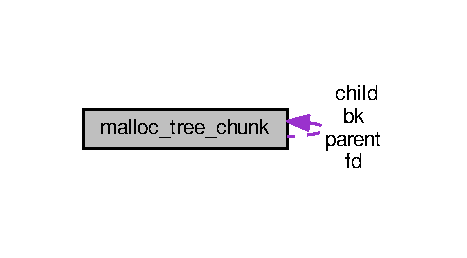
\includegraphics[width=224pt]{structmalloc__tree__chunk__coll__graph}
\end{center}
\end{figure}
\subsection*{Data Fields}
\begin{DoxyCompactItemize}
\item 
size\+\_\+t {\bfseries prev\+\_\+foot}\hypertarget{structmalloc__tree__chunk_a0b7e321702857b18f5013a3182b99262}{}\label{structmalloc__tree__chunk_a0b7e321702857b18f5013a3182b99262}

\item 
size\+\_\+t {\bfseries head}\hypertarget{structmalloc__tree__chunk_a1737b1a78f4bfbf0047210e3f3fd014d}{}\label{structmalloc__tree__chunk_a1737b1a78f4bfbf0047210e3f3fd014d}

\item 
struct \hyperlink{structmalloc__tree__chunk}{malloc\+\_\+tree\+\_\+chunk} $\ast$ {\bfseries fd}\hypertarget{structmalloc__tree__chunk_a5584ad2f70ef7ad1a5eb5f55820e3fe9}{}\label{structmalloc__tree__chunk_a5584ad2f70ef7ad1a5eb5f55820e3fe9}

\item 
struct \hyperlink{structmalloc__tree__chunk}{malloc\+\_\+tree\+\_\+chunk} $\ast$ {\bfseries bk}\hypertarget{structmalloc__tree__chunk_a862e6cafa961c1f63d4b10d67480cba0}{}\label{structmalloc__tree__chunk_a862e6cafa961c1f63d4b10d67480cba0}

\item 
struct \hyperlink{structmalloc__tree__chunk}{malloc\+\_\+tree\+\_\+chunk} $\ast$ {\bfseries child} \mbox{[}2\mbox{]}\hypertarget{structmalloc__tree__chunk_a560fa0afc644c1e05f4fab62818ab6cd}{}\label{structmalloc__tree__chunk_a560fa0afc644c1e05f4fab62818ab6cd}

\item 
struct \hyperlink{structmalloc__tree__chunk}{malloc\+\_\+tree\+\_\+chunk} $\ast$ {\bfseries parent}\hypertarget{structmalloc__tree__chunk_ae15ae9af5d9c57488718f0649868b7fe}{}\label{structmalloc__tree__chunk_ae15ae9af5d9c57488718f0649868b7fe}

\item 
bindex\+\_\+t {\bfseries index}\hypertarget{structmalloc__tree__chunk_a3015f2a8d6cc5cdb7abaf34e902c46a4}{}\label{structmalloc__tree__chunk_a3015f2a8d6cc5cdb7abaf34e902c46a4}

\end{DoxyCompactItemize}


The documentation for this struct was generated from the following file\+:\begin{DoxyCompactItemize}
\item 
gprolog-\/utf8-\/tree/src/\+Engine\+Pl/dl\+\_\+malloc.\+c\end{DoxyCompactItemize}

\hypertarget{structMem}{}\section{Mem Struct Reference}
\label{structMem}\index{Mem@{Mem}}


{\ttfamily \#include $<$ma\+\_\+parser.\+h$>$}

\subsection*{Data Fields}
\begin{DoxyCompactItemize}
\item 
char $\ast$ \hyperlink{structMem_a97d3d596dc096d506a21a183f733ef5d}{name}
\item 
int \hyperlink{structMem_a496c7609b4591655a4acf6113a892c2d}{index}
\end{DoxyCompactItemize}


\subsection{Field Documentation}
\index{Mem@{Mem}!index@{index}}
\index{index@{index}!Mem@{Mem}}
\subsubsection[{\texorpdfstring{index}{index}}]{\setlength{\rightskip}{0pt plus 5cm}int Mem\+::index}\hypertarget{structMem_a496c7609b4591655a4acf6113a892c2d}{}\label{structMem_a496c7609b4591655a4acf6113a892c2d}
\index{Mem@{Mem}!name@{name}}
\index{name@{name}!Mem@{Mem}}
\subsubsection[{\texorpdfstring{name}{name}}]{\setlength{\rightskip}{0pt plus 5cm}char$\ast$ Mem\+::name}\hypertarget{structMem_a97d3d596dc096d506a21a183f733ef5d}{}\label{structMem_a97d3d596dc096d506a21a183f733ef5d}


The documentation for this struct was generated from the following file\+:\begin{DoxyCompactItemize}
\item 
gprolog-\/utf8-\/tree/src/\+Ma2\+Asm/\hyperlink{ma__parser_8h}{ma\+\_\+parser.\+h}\end{DoxyCompactItemize}

\hypertarget{structMonom}{}\section{Monom Struct Reference}
\label{structMonom}\index{Monom@{Monom}}
\subsection*{Data Fields}
\begin{DoxyCompactItemize}
\item 
Pl\+Long {\bfseries a}\hypertarget{structMonom_a65b12a1274c4471fce35332ef4bb84f6}{}\label{structMonom_a65b12a1274c4471fce35332ef4bb84f6}

\item 
Wam\+Word {\bfseries x\+\_\+word}\hypertarget{structMonom_a72cc88b43a8727f47d9e50db2cda700f}{}\label{structMonom_a72cc88b43a8727f47d9e50db2cda700f}

\end{DoxyCompactItemize}


The documentation for this struct was generated from the following file\+:\begin{DoxyCompactItemize}
\item 
gprolog-\/utf8-\/tree/src/\+Bips\+F\+D/math\+\_\+supp.\+c\end{DoxyCompactItemize}

\hypertarget{structNonLin}{}\section{Non\+Lin Struct Reference}
\label{structNonLin}\index{Non\+Lin@{Non\+Lin}}
\subsection*{Data Fields}
\begin{DoxyCompactItemize}
\item 
int {\bfseries cstr}\hypertarget{structNonLin_ace702860218e3fed62bb3235547358aa}{}\label{structNonLin_ace702860218e3fed62bb3235547358aa}

\item 
Wam\+Word {\bfseries a1}\hypertarget{structNonLin_a143b9a64bce8684b7cc00bea2c48639b}{}\label{structNonLin_a143b9a64bce8684b7cc00bea2c48639b}

\item 
Wam\+Word {\bfseries a2}\hypertarget{structNonLin_a94219bccdea182e374720870a013da88}{}\label{structNonLin_a94219bccdea182e374720870a013da88}

\item 
Wam\+Word {\bfseries a3}\hypertarget{structNonLin_a3e4eeac9f54cd48366e50824833a9271}{}\label{structNonLin_a3e4eeac9f54cd48366e50824833a9271}

\item 
Wam\+Word {\bfseries res}\hypertarget{structNonLin_af8f4e398e6c9371309ae73d04456f4f0}{}\label{structNonLin_af8f4e398e6c9371309ae73d04456f4f0}

\end{DoxyCompactItemize}


The documentation for this struct was generated from the following file\+:\begin{DoxyCompactItemize}
\item 
gprolog-\/utf8-\/tree/src/\+Bips\+F\+D/math\+\_\+supp.\+c\end{DoxyCompactItemize}

\hypertarget{structObjInf}{}\section{Obj\+Inf Struct Reference}
\label{structObjInf}\index{Obj\+Inf@{Obj\+Inf}}
\subsection*{Data Fields}
\begin{DoxyCompactItemize}
\item 
void($\ast$ {\bfseries fct\+\_\+obj\+\_\+init} )()\hypertarget{structObjInf_a87ba4456d48d1ca4b94a0d0e7f44650c}{}\label{structObjInf_a87ba4456d48d1ca4b94a0d0e7f44650c}

\item 
void($\ast$ {\bfseries fct\+\_\+exec\+\_\+system} )()\hypertarget{structObjInf_a5b3f237a232e4cfae91c10bfe78f163f}{}\label{structObjInf_a5b3f237a232e4cfae91c10bfe78f163f}

\item 
void($\ast$ {\bfseries fct\+\_\+exec\+\_\+user} )()\hypertarget{structObjInf_a394489a76d14d4711797e459a15ebfb4}{}\label{structObjInf_a394489a76d14d4711797e459a15ebfb4}

\end{DoxyCompactItemize}


The documentation for this struct was generated from the following file\+:\begin{DoxyCompactItemize}
\item 
gprolog-\/utf8-\/tree/src/\+Engine\+Pl/obj\+\_\+chain.\+c\end{DoxyCompactItemize}

\hypertarget{structonesol}{}\section{onesol Struct Reference}
\label{structonesol}\index{onesol@{onesol}}


Collaboration diagram for onesol\+:\nopagebreak
\begin{figure}[H]
\begin{center}
\leavevmode
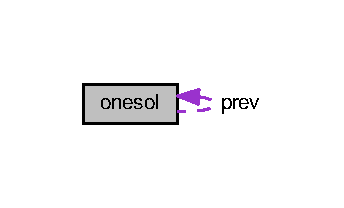
\includegraphics[width=165pt]{structonesol__coll__graph}
\end{center}
\end{figure}
\subsection*{Data Fields}
\begin{DoxyCompactItemize}
\item 
\hyperlink{structonesol}{One\+SolP} {\bfseries prev}\hypertarget{structonesol_a67474d69d62f74ecb1da52cf3a6fd255}{}\label{structonesol_a67474d69d62f74ecb1da52cf3a6fd255}

\item 
int {\bfseries sol\+\_\+no}\hypertarget{structonesol_adf8141bfb4d67ec7ef0cdb66abc2e03d}{}\label{structonesol_adf8141bfb4d67ec7ef0cdb66abc2e03d}

\item 
int {\bfseries term\+\_\+size}\hypertarget{structonesol_a7d00bc5747882c6030eff6839217f1d5}{}\label{structonesol_a7d00bc5747882c6030eff6839217f1d5}

\item 
Wam\+Word {\bfseries term\+\_\+word}\hypertarget{structonesol_ad2da50a130c4212644b22689ded445bf}{}\label{structonesol_ad2da50a130c4212644b22689ded445bf}

\end{DoxyCompactItemize}


The documentation for this struct was generated from the following file\+:\begin{DoxyCompactItemize}
\item 
gprolog-\/utf8-\/tree/src/\+Bips\+Pl/all\+\_\+solut\+\_\+c.\+c\end{DoxyCompactItemize}

\hypertarget{structOperInf}{}\section{Oper\+Inf Struct Reference}
\label{structOperInf}\index{Oper\+Inf@{Oper\+Inf}}


{\ttfamily \#include $<$oper.\+h$>$}

\subsection*{Data Fields}
\begin{DoxyCompactItemize}
\item 
\hyperlink{gprolog_8h_a4d005b136d7fb28537eb1815f7868b63}{Pl\+Long} \hyperlink{structOperInf_a5ab08736fa238d100509038e938fe187}{a\+\_\+t}
\item 
int \hyperlink{structOperInf_a50a4ec676df2b3555058f59753d48698}{prec}
\item 
int \hyperlink{structOperInf_afbf02377f941f53f5cd63f151c2da1f0}{left}
\item 
int \hyperlink{structOperInf_a558dc457885d6b96f6d8f833f1ce6c66}{right}
\end{DoxyCompactItemize}


\subsection{Field Documentation}
\index{Oper\+Inf@{Oper\+Inf}!a\+\_\+t@{a\+\_\+t}}
\index{a\+\_\+t@{a\+\_\+t}!Oper\+Inf@{Oper\+Inf}}
\subsubsection[{\texorpdfstring{a\+\_\+t}{a_t}}]{\setlength{\rightskip}{0pt plus 5cm}{\bf Pl\+Long} Oper\+Inf\+::a\+\_\+t}\hypertarget{structOperInf_a5ab08736fa238d100509038e938fe187}{}\label{structOperInf_a5ab08736fa238d100509038e938fe187}
\index{Oper\+Inf@{Oper\+Inf}!left@{left}}
\index{left@{left}!Oper\+Inf@{Oper\+Inf}}
\subsubsection[{\texorpdfstring{left}{left}}]{\setlength{\rightskip}{0pt plus 5cm}int Oper\+Inf\+::left}\hypertarget{structOperInf_afbf02377f941f53f5cd63f151c2da1f0}{}\label{structOperInf_afbf02377f941f53f5cd63f151c2da1f0}
\index{Oper\+Inf@{Oper\+Inf}!prec@{prec}}
\index{prec@{prec}!Oper\+Inf@{Oper\+Inf}}
\subsubsection[{\texorpdfstring{prec}{prec}}]{\setlength{\rightskip}{0pt plus 5cm}int Oper\+Inf\+::prec}\hypertarget{structOperInf_a50a4ec676df2b3555058f59753d48698}{}\label{structOperInf_a50a4ec676df2b3555058f59753d48698}
\index{Oper\+Inf@{Oper\+Inf}!right@{right}}
\index{right@{right}!Oper\+Inf@{Oper\+Inf}}
\subsubsection[{\texorpdfstring{right}{right}}]{\setlength{\rightskip}{0pt plus 5cm}int Oper\+Inf\+::right}\hypertarget{structOperInf_a558dc457885d6b96f6d8f833f1ce6c66}{}\label{structOperInf_a558dc457885d6b96f6d8f833f1ce6c66}


The documentation for this struct was generated from the following file\+:\begin{DoxyCompactItemize}
\item 
gprolog-\/utf8-\/tree/src/\+Engine\+Pl/\hyperlink{oper_8h}{oper.\+h}\end{DoxyCompactItemize}

\hypertarget{structParseInf}{}\section{Parse\+Inf Struct Reference}
\label{structParseInf}\index{Parse\+Inf@{Parse\+Inf}}
\subsection*{Data Fields}
\begin{DoxyCompactItemize}
\item 
char $\ast$ {\bfseries keyword}\hypertarget{structParseInf_affadb424830268d2231588e867b1fb40}{}\label{structParseInf_affadb424830268d2231588e867b1fb40}

\item 
void($\ast$ {\bfseries fct} )()\hypertarget{structParseInf_a17e09c905211b8d0ac00827aeeea9237}{}\label{structParseInf_a17e09c905211b8d0ac00827aeeea9237}

\item 
int {\bfseries nb\+\_\+args}\hypertarget{structParseInf_abb84b55b8b29fe0bccf151d7400f0d9d}{}\label{structParseInf_abb84b55b8b29fe0bccf151d7400f0d9d}

\item 
Arg\+Typ {\bfseries arg\+\_\+type} \mbox{[}M\+A\+X\+\_\+\+F\+C\+T\+\_\+\+A\+R\+I\+TY\mbox{]}\hypertarget{structParseInf_a4bc1d3c3237113de20adb4050419bca6}{}\label{structParseInf_a4bc1d3c3237113de20adb4050419bca6}

\end{DoxyCompactItemize}


The documentation for this struct was generated from the following file\+:\begin{DoxyCompactItemize}
\item 
gprolog-\/utf8-\/tree/src/\+Wam2\+Ma/wam\+\_\+parser.\+c\end{DoxyCompactItemize}

\hypertarget{structPbStk}{}\section{Pb\+Stk Struct Reference}
\label{structPbStk}\index{Pb\+Stk@{Pb\+Stk}}


{\ttfamily \#include $<$stream\+\_\+supp.\+h$>$}

\subsection*{Data Fields}
\begin{DoxyCompactItemize}
\item 
int \hyperlink{structPbStk_a753c451400807eac788034c15a4e9810}{buff} \mbox{[}\hyperlink{stream__supp_8h_a7c01809509d811cfc0c70e47443a9613}{S\+T\+R\+E\+A\+M\+\_\+\+P\+B\+\_\+\+S\+I\+ZE}\mbox{]}
\item 
int $\ast$ \hyperlink{structPbStk_a739af7eef937b961dc73fec61672bee2}{ptr}
\item 
int \hyperlink{structPbStk_a222a0c77b4b0feef1323dc7cf1f0e74b}{nb\+\_\+elems}
\end{DoxyCompactItemize}


\subsection{Field Documentation}
\index{Pb\+Stk@{Pb\+Stk}!buff@{buff}}
\index{buff@{buff}!Pb\+Stk@{Pb\+Stk}}
\subsubsection[{\texorpdfstring{buff}{buff}}]{\setlength{\rightskip}{0pt plus 5cm}int Pb\+Stk\+::buff\mbox{[}{\bf S\+T\+R\+E\+A\+M\+\_\+\+P\+B\+\_\+\+S\+I\+ZE}\mbox{]}}\hypertarget{structPbStk_a753c451400807eac788034c15a4e9810}{}\label{structPbStk_a753c451400807eac788034c15a4e9810}
\index{Pb\+Stk@{Pb\+Stk}!nb\+\_\+elems@{nb\+\_\+elems}}
\index{nb\+\_\+elems@{nb\+\_\+elems}!Pb\+Stk@{Pb\+Stk}}
\subsubsection[{\texorpdfstring{nb\+\_\+elems}{nb_elems}}]{\setlength{\rightskip}{0pt plus 5cm}int Pb\+Stk\+::nb\+\_\+elems}\hypertarget{structPbStk_a222a0c77b4b0feef1323dc7cf1f0e74b}{}\label{structPbStk_a222a0c77b4b0feef1323dc7cf1f0e74b}
\index{Pb\+Stk@{Pb\+Stk}!ptr@{ptr}}
\index{ptr@{ptr}!Pb\+Stk@{Pb\+Stk}}
\subsubsection[{\texorpdfstring{ptr}{ptr}}]{\setlength{\rightskip}{0pt plus 5cm}int$\ast$ Pb\+Stk\+::ptr}\hypertarget{structPbStk_a739af7eef937b961dc73fec61672bee2}{}\label{structPbStk_a739af7eef937b961dc73fec61672bee2}


The documentation for this struct was generated from the following file\+:\begin{DoxyCompactItemize}
\item 
gprolog-\/utf8-\/tree/src/\+Bips\+Pl/\hyperlink{stream__supp_8h}{stream\+\_\+supp.\+h}\end{DoxyCompactItemize}

\hypertarget{structPlFIOArg}{}\section{Pl\+F\+I\+O\+Arg Struct Reference}
\label{structPlFIOArg}\index{Pl\+F\+I\+O\+Arg@{Pl\+F\+I\+O\+Arg}}
\subsection*{Data Fields}
\begin{DoxyCompactItemize}
\item 
Bool {\bfseries is\+\_\+var}\hypertarget{structPlFIOArg_ad700005317887006bd276a4d1a177881}{}\label{structPlFIOArg_ad700005317887006bd276a4d1a177881}

\item 
Bool {\bfseries unify}\hypertarget{structPlFIOArg_a6394f30ef4d8a74b9a1e731a9f725a35}{}\label{structPlFIOArg_a6394f30ef4d8a74b9a1e731a9f725a35}

\item 
\begin{tabbing}
xx\=xx\=xx\=xx\=xx\=xx\=xx\=xx\=xx\=\kill
union \{\\
\>PlLong {\bfseries l}\\
\>char $\ast$ {\bfseries s}\\
\>double {\bfseries d}\\
\} {\bfseries value}\hypertarget{structPlFIOArg_a69180a58f761dcda790af38c4c0ca5a2}{}\label{structPlFIOArg_a69180a58f761dcda790af38c4c0ca5a2}
\\

\end{tabbing}\item 
Pl\+Bool {\bfseries is\+\_\+var}\hypertarget{structPlFIOArg_ab4d9b51a4575a50e1d9b8a3ec36a3f6e}{}\label{structPlFIOArg_ab4d9b51a4575a50e1d9b8a3ec36a3f6e}

\item 
Pl\+Bool {\bfseries unify}\hypertarget{structPlFIOArg_a3d5c4af7de4d733aa3806b29081336b8}{}\label{structPlFIOArg_a3d5c4af7de4d733aa3806b29081336b8}

\item 
\begin{tabbing}
xx\=xx\=xx\=xx\=xx\=xx\=xx\=xx\=xx\=\kill
union \{\\
\>PlLong {\bfseries l}\\
\>char $\ast$ {\bfseries s}\\
\>double {\bfseries d}\\
\} {\bfseries value}\hypertarget{structPlFIOArg_a1588d26dbc95302b6b7a0b79715ead8e}{}\label{structPlFIOArg_a1588d26dbc95302b6b7a0b79715ead8e}
\\

\end{tabbing}\end{DoxyCompactItemize}


The documentation for this struct was generated from the following files\+:\begin{DoxyCompactItemize}
\item 
gprolog-\/utf8-\/tree/src/\+Bips\+Pl/foreign\+\_\+supp.\+h\item 
gprolog-\/utf8-\/tree/src/\+Engine\+Pl/gprolog.\+h\end{DoxyCompactItemize}

\hypertarget{structPoly}{}\section{Poly Struct Reference}
\label{structPoly}\index{Poly@{Poly}}


Collaboration diagram for Poly\+:\nopagebreak
\begin{figure}[H]
\begin{center}
\leavevmode
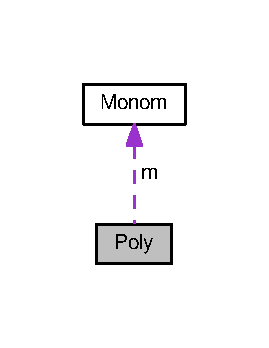
\includegraphics[width=129pt]{structPoly__coll__graph}
\end{center}
\end{figure}
\subsection*{Data Fields}
\begin{DoxyCompactItemize}
\item 
Pl\+Long {\bfseries c}\hypertarget{structPoly_ac87064f885d4389f545b4194de01f60e}{}\label{structPoly_ac87064f885d4389f545b4194de01f60e}

\item 
int {\bfseries nb\+\_\+monom}\hypertarget{structPoly_a23949f807fc70dcf7c1b7b18bb48be0c}{}\label{structPoly_a23949f807fc70dcf7c1b7b18bb48be0c}

\item 
\hyperlink{structMonom}{Monom} {\bfseries m} \mbox{[}M\+A\+X\+\_\+\+M\+O\+N\+O\+MS\mbox{]}\hypertarget{structPoly_a1bae103a920d8182006ef10891c87906}{}\label{structPoly_a1bae103a920d8182006ef10891c87906}

\end{DoxyCompactItemize}


The documentation for this struct was generated from the following file\+:\begin{DoxyCompactItemize}
\item 
gprolog-\/utf8-\/tree/src/\+Bips\+F\+D/math\+\_\+supp.\+c\end{DoxyCompactItemize}

\hypertarget{structpredinf}{}\section{predinf Struct Reference}
\label{structpredinf}\index{predinf@{predinf}}


Collaboration diagram for predinf\+:\nopagebreak
\begin{figure}[H]
\begin{center}
\leavevmode
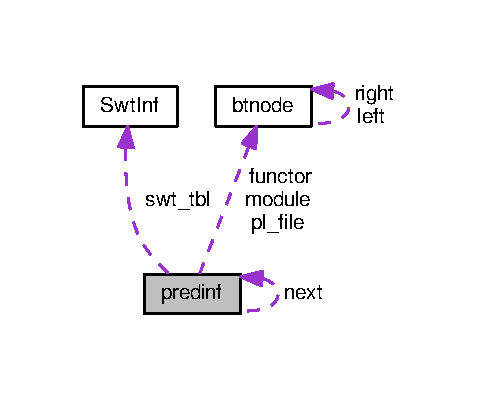
\includegraphics[width=230pt]{structpredinf__coll__graph}
\end{center}
\end{figure}
\subsection*{Data Fields}
\begin{DoxyCompactItemize}
\item 
\hyperlink{structbtnode}{B\+T\+Node} $\ast$ {\bfseries module}\hypertarget{structpredinf_a5f44f90f1226e1463e76665aaf490a9d}{}\label{structpredinf_a5f44f90f1226e1463e76665aaf490a9d}

\item 
\hyperlink{structbtnode}{B\+T\+Node} $\ast$ {\bfseries functor}\hypertarget{structpredinf_a6ae4c5cbb30b0db0b0dde51084453eee}{}\label{structpredinf_a6ae4c5cbb30b0db0b0dde51084453eee}

\item 
int {\bfseries arity}\hypertarget{structpredinf_a16871c2b0c2e29058abe513301f0b7b0}{}\label{structpredinf_a16871c2b0c2e29058abe513301f0b7b0}

\item 
char $\ast$ {\bfseries hexa}\hypertarget{structpredinf_ab6fc21ba8f80aea382dfd11b9a50e7ac}{}\label{structpredinf_ab6fc21ba8f80aea382dfd11b9a50e7ac}

\item 
int {\bfseries line\+\_\+no}\hypertarget{structpredinf_ae858dcfb66886799f41d0042ccf8667e}{}\label{structpredinf_ae858dcfb66886799f41d0042ccf8667e}

\item 
int {\bfseries prop}\hypertarget{structpredinf_a39785936db83e7bcf5036b5365423c5e}{}\label{structpredinf_a39785936db83e7bcf5036b5365423c5e}

\item 
\hyperlink{structbtnode}{B\+T\+Node} $\ast$ {\bfseries pl\+\_\+file}\hypertarget{structpredinf_a85bb945f5415fd2177b55ce91562c36c}{}\label{structpredinf_a85bb945f5415fd2177b55ce91562c36c}

\item 
int {\bfseries pl\+\_\+line}\hypertarget{structpredinf_a0bb58f984add8b6a8e040181a8181cbd}{}\label{structpredinf_a0bb58f984add8b6a8e040181a8181cbd}

\item 
\hyperlink{structSwtInf}{Swt\+Tbl} $\ast$ {\bfseries swt\+\_\+tbl} \mbox{[}3\mbox{]}\hypertarget{structpredinf_a9e448a6b5c08b225ac0a07043f3a37c9}{}\label{structpredinf_a9e448a6b5c08b225ac0a07043f3a37c9}

\item 
\hyperlink{structpredinf}{PredP} {\bfseries next}\hypertarget{structpredinf_a5640b4a5b40d6208119e14349a52d8db}{}\label{structpredinf_a5640b4a5b40d6208119e14349a52d8db}

\end{DoxyCompactItemize}


The documentation for this struct was generated from the following file\+:\begin{DoxyCompactItemize}
\item 
gprolog-\/utf8-\/tree/src/\+Wam2\+Ma/wam2ma.\+c\end{DoxyCompactItemize}

\hypertarget{structPredInf}{}\section{Pred\+Inf Struct Reference}
\label{structPredInf}\index{Pred\+Inf@{Pred\+Inf}}
\subsection*{Data Fields}
\begin{DoxyCompactItemize}
\item 
Pl\+Long {\bfseries f\+\_\+n}\hypertarget{structPredInf_ac0b2b557f702cda0d5111bc65630d5a3}{}\label{structPredInf_ac0b2b557f702cda0d5111bc65630d5a3}

\item 
int {\bfseries pl\+\_\+file}\hypertarget{structPredInf_a0d5ac69f7fce6062b3327fc2badc1658}{}\label{structPredInf_a0d5ac69f7fce6062b3327fc2badc1658}

\item 
int {\bfseries pl\+\_\+line}\hypertarget{structPredInf_a206ac901da36832f6111a542a2b8b11b}{}\label{structPredInf_a206ac901da36832f6111a542a2b8b11b}

\item 
int {\bfseries prop}\hypertarget{structPredInf_a2f0d287390fe634467a62f42f816d855}{}\label{structPredInf_a2f0d287390fe634467a62f42f816d855}

\item 
Pl\+Long $\ast$ {\bfseries codep}\hypertarget{structPredInf_a670788fe731440a8d7224e2729836dac}{}\label{structPredInf_a670788fe731440a8d7224e2729836dac}

\item 
Pl\+Long $\ast$ {\bfseries dyn}\hypertarget{structPredInf_aad15bc35f98eabb92f4ac4b9a35f65c0}{}\label{structPredInf_aad15bc35f98eabb92f4ac4b9a35f65c0}

\end{DoxyCompactItemize}


The documentation for this struct was generated from the following file\+:\begin{DoxyCompactItemize}
\item 
gprolog-\/utf8-\/tree/src/\+Engine\+Pl/pred.\+h\end{DoxyCompactItemize}

\hypertarget{structRange}{}\section{Range Struct Reference}
\label{structRange}\index{Range@{Range}}


{\ttfamily \#include $<$fd\+\_\+range.\+h$>$}

\subsection*{Data Fields}
\begin{DoxyCompactItemize}
\item 
\hyperlink{bool_8h_afdcfe6db5bea87bd493a3fe2c513d5ef}{Bool} \hyperlink{structRange_a875104bdfb7f25377692ee3511b6cda7}{extra\+\_\+cstr}
\item 
int \hyperlink{structRange_ac3ccecdd1d8e143102bb4c2b5c0837d7}{min}
\item 
int \hyperlink{structRange_a7f490d5301f027e9defc4abf3970bf00}{max}
\item 
\hyperlink{fd__range_8h_a3cb8772380a4656f7d8c5d5c6346985e}{Vector} \hyperlink{structRange_aa1fc33857cb97860b7c55a8f90ad6e3f}{vec}
\end{DoxyCompactItemize}


\subsection{Field Documentation}
\index{Range@{Range}!extra\+\_\+cstr@{extra\+\_\+cstr}}
\index{extra\+\_\+cstr@{extra\+\_\+cstr}!Range@{Range}}
\subsubsection[{\texorpdfstring{extra\+\_\+cstr}{extra_cstr}}]{\setlength{\rightskip}{0pt plus 5cm}{\bf Bool} Range\+::extra\+\_\+cstr}\hypertarget{structRange_a875104bdfb7f25377692ee3511b6cda7}{}\label{structRange_a875104bdfb7f25377692ee3511b6cda7}
\index{Range@{Range}!max@{max}}
\index{max@{max}!Range@{Range}}
\subsubsection[{\texorpdfstring{max}{max}}]{\setlength{\rightskip}{0pt plus 5cm}int Range\+::max}\hypertarget{structRange_a7f490d5301f027e9defc4abf3970bf00}{}\label{structRange_a7f490d5301f027e9defc4abf3970bf00}
\index{Range@{Range}!min@{min}}
\index{min@{min}!Range@{Range}}
\subsubsection[{\texorpdfstring{min}{min}}]{\setlength{\rightskip}{0pt plus 5cm}int Range\+::min}\hypertarget{structRange_ac3ccecdd1d8e143102bb4c2b5c0837d7}{}\label{structRange_ac3ccecdd1d8e143102bb4c2b5c0837d7}
\index{Range@{Range}!vec@{vec}}
\index{vec@{vec}!Range@{Range}}
\subsubsection[{\texorpdfstring{vec}{vec}}]{\setlength{\rightskip}{0pt plus 5cm}{\bf Vector} Range\+::vec}\hypertarget{structRange_aa1fc33857cb97860b7c55a8f90ad6e3f}{}\label{structRange_aa1fc33857cb97860b7c55a8f90ad6e3f}


The documentation for this struct was generated from the following file\+:\begin{DoxyCompactItemize}
\item 
gprolog-\/utf8-\/tree/src/\+Engine\+F\+D/\hyperlink{fd__range_8h}{fd\+\_\+range.\+h}\end{DoxyCompactItemize}

\hypertarget{structRegInf}{}\section{Reg\+Inf Struct Reference}
\label{structRegInf}\index{Reg\+Inf@{Reg\+Inf}}
\subsection*{Data Fields}
\begin{DoxyCompactItemize}
\item 
char {\bfseries type} \mbox{[}32\mbox{]}\hypertarget{structRegInf_ac0222d4bcdce57bdcd74c2d45b9dfeb5}{}\label{structRegInf_ac0222d4bcdce57bdcd74c2d45b9dfeb5}

\item 
char {\bfseries name} \mbox{[}32\mbox{]}\hypertarget{structRegInf_af767d5a12d9d8e248f6c3eae99802e73}{}\label{structRegInf_af767d5a12d9d8e248f6c3eae99802e73}

\end{DoxyCompactItemize}


The documentation for this struct was generated from the following file\+:\begin{DoxyCompactItemize}
\item 
gprolog-\/utf8-\/tree/src/\+Engine\+Pl/pl\+\_\+config.\+c\end{DoxyCompactItemize}

\hypertarget{structSFOp}{}\section{S\+F\+Op Struct Reference}
\label{structSFOp}\index{S\+F\+Op@{S\+F\+Op}}
\subsection*{Data Fields}
\begin{DoxyCompactItemize}
\item 
int {\bfseries type}\hypertarget{structSFOp_a2edfc96ff91474523b5bda2185158ffa}{}\label{structSFOp_a2edfc96ff91474523b5bda2185158ffa}

\item 
int {\bfseries prec}\hypertarget{structSFOp_ae4c13ff3ed16b56c55f822e84b9db21a}{}\label{structSFOp_ae4c13ff3ed16b56c55f822e84b9db21a}

\item 
int {\bfseries left}\hypertarget{structSFOp_adc97e181b0efdcff6b921b82979ab80f}{}\label{structSFOp_adc97e181b0efdcff6b921b82979ab80f}

\item 
int {\bfseries right}\hypertarget{structSFOp_a53d1624dfd48f82123f055f8578646e7}{}\label{structSFOp_a53d1624dfd48f82123f055f8578646e7}

\item 
int {\bfseries length}\hypertarget{structSFOp_a3b91d02ed1a1a1c664a3cfb062e60ed1}{}\label{structSFOp_a3b91d02ed1a1a1c664a3cfb062e60ed1}

\end{DoxyCompactItemize}


The documentation for this struct was generated from the following file\+:\begin{DoxyCompactItemize}
\item 
gprolog-\/utf8-\/tree/src/\+Bips\+Pl/flag\+\_\+c.\+c\end{DoxyCompactItemize}

\hypertarget{structsr__file}{}\section{sr\+\_\+file Struct Reference}
\label{structsr__file}\index{sr\+\_\+file@{sr\+\_\+file}}


Collaboration diagram for sr\+\_\+file\+:\nopagebreak
\begin{figure}[H]
\begin{center}
\leavevmode
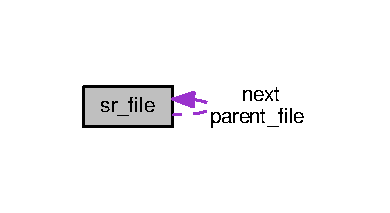
\includegraphics[width=187pt]{structsr__file__coll__graph}
\end{center}
\end{figure}
\subsection*{Data Fields}
\begin{DoxyCompactItemize}
\item 
int {\bfseries atom\+\_\+file\+\_\+name}\hypertarget{structsr__file_ae27edb1456ddb3b0453eca14e614c66b}{}\label{structsr__file_ae27edb1456ddb3b0453eca14e614c66b}

\item 
int {\bfseries stm}\hypertarget{structsr__file_a586a54828b5daba157cc712806a6f2b3}{}\label{structsr__file_a586a54828b5daba157cc712806a6f2b3}

\item 
Bool {\bfseries reposition}\hypertarget{structsr__file_a090b36b9b75dfbccd963f6787fd3f18e}{}\label{structsr__file_a090b36b9b75dfbccd963f6787fd3f18e}

\item 
char $\ast$ {\bfseries tmp\+\_\+path}\hypertarget{structsr__file_adc9ad8d65ba5f5b3bfc7a6c6ca329d88}{}\label{structsr__file_adc9ad8d65ba5f5b3bfc7a6c6ca329d88}

\item 
int {\bfseries tmp\+\_\+stm}\hypertarget{structsr__file_a200078e5cefb8ff2bd556997ff08b429}{}\label{structsr__file_a200078e5cefb8ff2bd556997ff08b429}

\item 
\hyperlink{structsr__file}{P\+S\+R\+File} {\bfseries next}\hypertarget{structsr__file_aa8623a318506eaad8a03faca16a7e72e}{}\label{structsr__file_aa8623a318506eaad8a03faca16a7e72e}

\item 
Bool {\bfseries eof\+\_\+reached}\hypertarget{structsr__file_ae76a89a158199f98536900d0fccdd0c4}{}\label{structsr__file_ae76a89a158199f98536900d0fccdd0c4}

\item 
int {\bfseries include\+\_\+line}\hypertarget{structsr__file_ae50c7011dac81b055f3cfbf64ae03598}{}\label{structsr__file_ae50c7011dac81b055f3cfbf64ae03598}

\item 
\hyperlink{structsr__file}{P\+S\+R\+File} {\bfseries parent\+\_\+file}\hypertarget{structsr__file_a57283a9f804b73dcd5bca6982ba8ac95}{}\label{structsr__file_a57283a9f804b73dcd5bca6982ba8ac95}

\end{DoxyCompactItemize}


The documentation for this struct was generated from the following file\+:\begin{DoxyCompactItemize}
\item 
gprolog-\/utf8-\/tree/src/\+Bips\+Pl/src\+\_\+rdr\+\_\+c.\+c\end{DoxyCompactItemize}

\hypertarget{structsr__module}{}\section{sr\+\_\+module Struct Reference}
\label{structsr__module}\index{sr\+\_\+module@{sr\+\_\+module}}


Collaboration diagram for sr\+\_\+module\+:\nopagebreak
\begin{figure}[H]
\begin{center}
\leavevmode
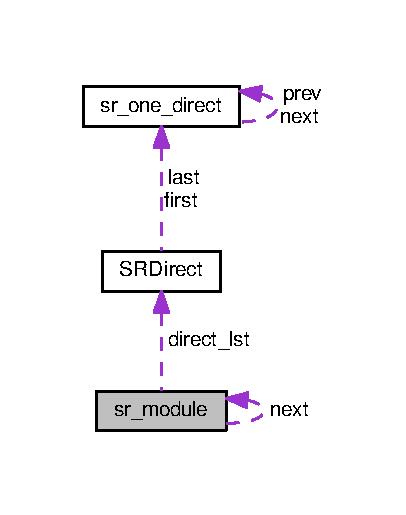
\includegraphics[width=195pt]{structsr__module__coll__graph}
\end{center}
\end{figure}
\subsection*{Data Fields}
\begin{DoxyCompactItemize}
\item 
int {\bfseries atom\+\_\+module\+\_\+name}\hypertarget{structsr__module_a5a1f181c93f13928623ca1426439eac8}{}\label{structsr__module_a5a1f181c93f13928623ca1426439eac8}

\item 
int {\bfseries i\+\_\+atom\+\_\+file\+\_\+def}\hypertarget{structsr__module_a2c69e68be4245afea2ed7d5a69650166}{}\label{structsr__module_a2c69e68be4245afea2ed7d5a69650166}

\item 
int {\bfseries i\+\_\+line\+\_\+def}\hypertarget{structsr__module_a931a2655c0576f16e2776c5c7ac2cf0a}{}\label{structsr__module_a931a2655c0576f16e2776c5c7ac2cf0a}

\item 
int {\bfseries b\+\_\+atom\+\_\+file\+\_\+def}\hypertarget{structsr__module_acc4948aadab6f3f5ae47ee8ea8c083ee}{}\label{structsr__module_acc4948aadab6f3f5ae47ee8ea8c083ee}

\item 
int {\bfseries b\+\_\+line\+\_\+def}\hypertarget{structsr__module_a0c96bc2505a798a709775e61787a1a24}{}\label{structsr__module_a0c96bc2505a798a709775e61787a1a24}

\item 
\hyperlink{structSRDirect}{S\+R\+Direct} {\bfseries direct\+\_\+lst}\hypertarget{structsr__module_a45a2eaca81407f38373afb940bb6dc57}{}\label{structsr__module_a45a2eaca81407f38373afb940bb6dc57}

\item 
\hyperlink{structsr__module}{P\+S\+R\+Module} {\bfseries next}\hypertarget{structsr__module_af8c9ce6870c7f7558096b050d6df683b}{}\label{structsr__module_af8c9ce6870c7f7558096b050d6df683b}

\end{DoxyCompactItemize}


The documentation for this struct was generated from the following file\+:\begin{DoxyCompactItemize}
\item 
gprolog-\/utf8-\/tree/src/\+Bips\+Pl/src\+\_\+rdr\+\_\+c.\+c\end{DoxyCompactItemize}

\hypertarget{structsr__one__direct}{}\section{sr\+\_\+one\+\_\+direct Struct Reference}
\label{structsr__one__direct}\index{sr\+\_\+one\+\_\+direct@{sr\+\_\+one\+\_\+direct}}


Collaboration diagram for sr\+\_\+one\+\_\+direct\+:\nopagebreak
\begin{figure}[H]
\begin{center}
\leavevmode
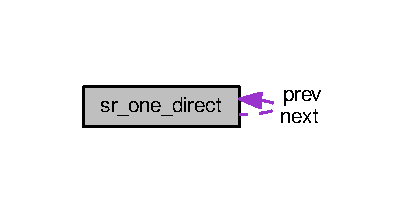
\includegraphics[width=195pt]{structsr__one__direct__coll__graph}
\end{center}
\end{figure}
\subsection*{Data Fields}
\begin{DoxyCompactItemize}
\item 
\hyperlink{src__rdr__c_8c_a03d2b46a29dc63fb6b0a6ec9378f36af}{S\+R\+Dir\+Type} \hyperlink{structsr__one__direct_ac59da886bfa2db8f18de3506965397f7}{type}
\item 
\hyperlink{LINUX__SIGSEGV_8c_a10ea8be8823feb38875b8a9326cbb424}{Wam\+Word} \hyperlink{structsr__one__direct_abe60646d574e029facc37a9b2491a74b}{a} \mbox{[}2\mbox{]}\mbox{[}3\mbox{]}
\item 
\hyperlink{src__rdr__c_8c_ad9901c46d3661cb327d1a08a1131e06a}{P\+S\+R\+One\+Direct} \hyperlink{structsr__one__direct_a601890e68d977d3467e52ab3a7ce9703}{next}
\item 
\hyperlink{src__rdr__c_8c_ad9901c46d3661cb327d1a08a1131e06a}{P\+S\+R\+One\+Direct} \hyperlink{structsr__one__direct_a25fd2e3df4af8e0f8cb89af0a1ea77f9}{prev}
\end{DoxyCompactItemize}


\subsection{Field Documentation}
\index{sr\+\_\+one\+\_\+direct@{sr\+\_\+one\+\_\+direct}!a@{a}}
\index{a@{a}!sr\+\_\+one\+\_\+direct@{sr\+\_\+one\+\_\+direct}}
\subsubsection[{\texorpdfstring{a}{a}}]{\setlength{\rightskip}{0pt plus 5cm}{\bf Wam\+Word} sr\+\_\+one\+\_\+direct\+::a\mbox{[}2\mbox{]}\mbox{[}3\mbox{]}}\hypertarget{structsr__one__direct_abe60646d574e029facc37a9b2491a74b}{}\label{structsr__one__direct_abe60646d574e029facc37a9b2491a74b}
\index{sr\+\_\+one\+\_\+direct@{sr\+\_\+one\+\_\+direct}!next@{next}}
\index{next@{next}!sr\+\_\+one\+\_\+direct@{sr\+\_\+one\+\_\+direct}}
\subsubsection[{\texorpdfstring{next}{next}}]{\setlength{\rightskip}{0pt plus 5cm}{\bf P\+S\+R\+One\+Direct} sr\+\_\+one\+\_\+direct\+::next}\hypertarget{structsr__one__direct_a601890e68d977d3467e52ab3a7ce9703}{}\label{structsr__one__direct_a601890e68d977d3467e52ab3a7ce9703}
\index{sr\+\_\+one\+\_\+direct@{sr\+\_\+one\+\_\+direct}!prev@{prev}}
\index{prev@{prev}!sr\+\_\+one\+\_\+direct@{sr\+\_\+one\+\_\+direct}}
\subsubsection[{\texorpdfstring{prev}{prev}}]{\setlength{\rightskip}{0pt plus 5cm}{\bf P\+S\+R\+One\+Direct} sr\+\_\+one\+\_\+direct\+::prev}\hypertarget{structsr__one__direct_a25fd2e3df4af8e0f8cb89af0a1ea77f9}{}\label{structsr__one__direct_a25fd2e3df4af8e0f8cb89af0a1ea77f9}
\index{sr\+\_\+one\+\_\+direct@{sr\+\_\+one\+\_\+direct}!type@{type}}
\index{type@{type}!sr\+\_\+one\+\_\+direct@{sr\+\_\+one\+\_\+direct}}
\subsubsection[{\texorpdfstring{type}{type}}]{\setlength{\rightskip}{0pt plus 5cm}{\bf S\+R\+Dir\+Type} sr\+\_\+one\+\_\+direct\+::type}\hypertarget{structsr__one__direct_ac59da886bfa2db8f18de3506965397f7}{}\label{structsr__one__direct_ac59da886bfa2db8f18de3506965397f7}


The documentation for this struct was generated from the following file\+:\begin{DoxyCompactItemize}
\item 
gprolog-\/utf8-\/tree/src/\+Bips\+Pl/\hyperlink{src__rdr__c_8c}{src\+\_\+rdr\+\_\+c.\+c}\end{DoxyCompactItemize}

\hypertarget{structSRDirect}{}\section{S\+R\+Direct Struct Reference}
\label{structSRDirect}\index{S\+R\+Direct@{S\+R\+Direct}}


Collaboration diagram for S\+R\+Direct\+:\nopagebreak
\begin{figure}[H]
\begin{center}
\leavevmode
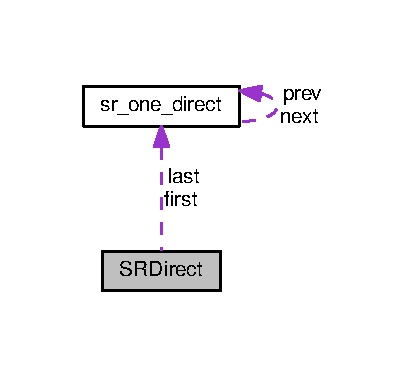
\includegraphics[width=195pt]{structSRDirect__coll__graph}
\end{center}
\end{figure}
\subsection*{Data Fields}
\begin{DoxyCompactItemize}
\item 
\hyperlink{src__rdr__c_8c_a901df9436a40f2eb43741da55a6dfd69}{S\+R\+One\+Direct} $\ast$ \hyperlink{structSRDirect_a418d898d49d9bfd256935f4e28bbf11b}{first}
\item 
\hyperlink{src__rdr__c_8c_a901df9436a40f2eb43741da55a6dfd69}{S\+R\+One\+Direct} $\ast$ \hyperlink{structSRDirect_aadd740950d79ebfff5baee79c33ced18}{last}
\end{DoxyCompactItemize}


\subsection{Field Documentation}
\index{S\+R\+Direct@{S\+R\+Direct}!first@{first}}
\index{first@{first}!S\+R\+Direct@{S\+R\+Direct}}
\subsubsection[{\texorpdfstring{first}{first}}]{\setlength{\rightskip}{0pt plus 5cm}{\bf S\+R\+One\+Direct}$\ast$ S\+R\+Direct\+::first}\hypertarget{structSRDirect_a418d898d49d9bfd256935f4e28bbf11b}{}\label{structSRDirect_a418d898d49d9bfd256935f4e28bbf11b}
\index{S\+R\+Direct@{S\+R\+Direct}!last@{last}}
\index{last@{last}!S\+R\+Direct@{S\+R\+Direct}}
\subsubsection[{\texorpdfstring{last}{last}}]{\setlength{\rightskip}{0pt plus 5cm}{\bf S\+R\+One\+Direct}$\ast$ S\+R\+Direct\+::last}\hypertarget{structSRDirect_aadd740950d79ebfff5baee79c33ced18}{}\label{structSRDirect_aadd740950d79ebfff5baee79c33ced18}


The documentation for this struct was generated from the following file\+:\begin{DoxyCompactItemize}
\item 
gprolog-\/utf8-\/tree/src/\+Bips\+Pl/\hyperlink{src__rdr__c_8c}{src\+\_\+rdr\+\_\+c.\+c}\end{DoxyCompactItemize}

\hypertarget{structSRInf}{}\section{S\+R\+Inf Struct Reference}
\label{structSRInf}\index{S\+R\+Inf@{S\+R\+Inf}}


Collaboration diagram for S\+R\+Inf\+:\nopagebreak
\begin{figure}[H]
\begin{center}
\leavevmode
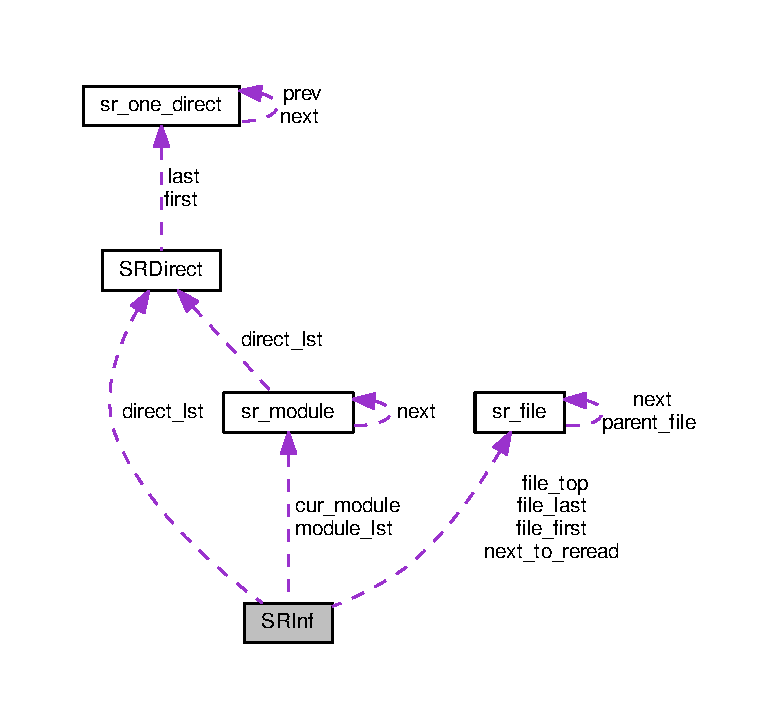
\includegraphics[width=350pt]{structSRInf__coll__graph}
\end{center}
\end{figure}
\subsection*{Data Fields}
\begin{DoxyCompactItemize}
\item 
\hyperlink{bool_8h_afdcfe6db5bea87bd493a3fe2c513d5ef}{Bool} \hyperlink{structSRInf_aa39907250f5d85ed33c6dcb588884cf4}{in\+\_\+use}
\item 
\hyperlink{bool_8h_afdcfe6db5bea87bd493a3fe2c513d5ef}{Bool} \hyperlink{structSRInf_ad7cc53b67596fdc3ac6b6598bfecfff9}{close\+\_\+master\+\_\+at\+\_\+end}
\item 
int \hyperlink{structSRInf_a33cee5de53e9f02597de121734102fa6}{mask}
\item 
\hyperlink{src__rdr__c_8c_a0823532f1e34f34125b37981ad9220ad}{S\+R\+File} $\ast$ \hyperlink{structSRInf_ad34362a8fd8521ebea63e79cd6696ecb}{file\+\_\+first}
\item 
\hyperlink{src__rdr__c_8c_a0823532f1e34f34125b37981ad9220ad}{S\+R\+File} $\ast$ \hyperlink{structSRInf_acb431dfff6fa3e8cbbd8dbfb25c798e8}{file\+\_\+last}
\item 
\hyperlink{src__rdr__c_8c_a0823532f1e34f34125b37981ad9220ad}{S\+R\+File} $\ast$ \hyperlink{structSRInf_a9a0f8d054d9dc2307211b7ef398b8290}{file\+\_\+top}
\item 
\hyperlink{src__rdr__c_8c_a0823532f1e34f34125b37981ad9220ad}{S\+R\+File} $\ast$ \hyperlink{structSRInf_afa0401eba053150cf9e719858d47f22b}{next\+\_\+to\+\_\+reread}
\item 
int \hyperlink{structSRInf_ad3d8ebbeb44105deeb678ceff8b2cb6b}{cur\+\_\+l1}
\item 
int \hyperlink{structSRInf_a9d3a07534c6e60d8b5ffb55a19b17533}{cur\+\_\+l2}
\item 
int \hyperlink{structSRInf_a1ed1a5e79f3f409ca8e28f59830e9ece}{char\+\_\+count}
\item 
int \hyperlink{structSRInf_aa63231d051d7fba34831d0be05e1f8cd}{line\+\_\+count}
\item 
int \hyperlink{structSRInf_af2257adc69f0b5ee25c89a2b33b6c074}{error\+\_\+count}
\item 
int \hyperlink{structSRInf_a432e213e2296877a22dd6e174cb65586}{warning\+\_\+count}
\item 
int \hyperlink{structSRInf_af83f16042ade6e52ac4859f203ef0db4}{out\+\_\+sora\+\_\+word}
\item 
\hyperlink{structSRDirect}{S\+R\+Direct} \hyperlink{structSRInf_a54874ef3dc4c403e8913a9fa4e85158e}{direct\+\_\+lst}
\item 
\hyperlink{src__rdr__c_8c_ad36cf18d86a9a8ac83341b0ea1ce8308}{S\+R\+Module} $\ast$ \hyperlink{structSRInf_a3562e122c09ab0c9eabb4b1d21a86408}{module\+\_\+lst}
\item 
\hyperlink{src__rdr__c_8c_ad36cf18d86a9a8ac83341b0ea1ce8308}{S\+R\+Module} $\ast$ \hyperlink{structSRInf_a791b120048e8a53ac8e6b172c3b33ea2}{cur\+\_\+module}
\item 
\hyperlink{bool_8h_afdcfe6db5bea87bd493a3fe2c513d5ef}{Bool} \hyperlink{structSRInf_af83fb089c4c9359b0d80cbe96bd01adc}{interface}
\end{DoxyCompactItemize}


\subsection{Field Documentation}
\index{S\+R\+Inf@{S\+R\+Inf}!char\+\_\+count@{char\+\_\+count}}
\index{char\+\_\+count@{char\+\_\+count}!S\+R\+Inf@{S\+R\+Inf}}
\subsubsection[{\texorpdfstring{char\+\_\+count}{char_count}}]{\setlength{\rightskip}{0pt plus 5cm}int S\+R\+Inf\+::char\+\_\+count}\hypertarget{structSRInf_a1ed1a5e79f3f409ca8e28f59830e9ece}{}\label{structSRInf_a1ed1a5e79f3f409ca8e28f59830e9ece}
\index{S\+R\+Inf@{S\+R\+Inf}!close\+\_\+master\+\_\+at\+\_\+end@{close\+\_\+master\+\_\+at\+\_\+end}}
\index{close\+\_\+master\+\_\+at\+\_\+end@{close\+\_\+master\+\_\+at\+\_\+end}!S\+R\+Inf@{S\+R\+Inf}}
\subsubsection[{\texorpdfstring{close\+\_\+master\+\_\+at\+\_\+end}{close_master_at_end}}]{\setlength{\rightskip}{0pt plus 5cm}{\bf Bool} S\+R\+Inf\+::close\+\_\+master\+\_\+at\+\_\+end}\hypertarget{structSRInf_ad7cc53b67596fdc3ac6b6598bfecfff9}{}\label{structSRInf_ad7cc53b67596fdc3ac6b6598bfecfff9}
\index{S\+R\+Inf@{S\+R\+Inf}!cur\+\_\+l1@{cur\+\_\+l1}}
\index{cur\+\_\+l1@{cur\+\_\+l1}!S\+R\+Inf@{S\+R\+Inf}}
\subsubsection[{\texorpdfstring{cur\+\_\+l1}{cur_l1}}]{\setlength{\rightskip}{0pt plus 5cm}int S\+R\+Inf\+::cur\+\_\+l1}\hypertarget{structSRInf_ad3d8ebbeb44105deeb678ceff8b2cb6b}{}\label{structSRInf_ad3d8ebbeb44105deeb678ceff8b2cb6b}
\index{S\+R\+Inf@{S\+R\+Inf}!cur\+\_\+l2@{cur\+\_\+l2}}
\index{cur\+\_\+l2@{cur\+\_\+l2}!S\+R\+Inf@{S\+R\+Inf}}
\subsubsection[{\texorpdfstring{cur\+\_\+l2}{cur_l2}}]{\setlength{\rightskip}{0pt plus 5cm}int S\+R\+Inf\+::cur\+\_\+l2}\hypertarget{structSRInf_a9d3a07534c6e60d8b5ffb55a19b17533}{}\label{structSRInf_a9d3a07534c6e60d8b5ffb55a19b17533}
\index{S\+R\+Inf@{S\+R\+Inf}!cur\+\_\+module@{cur\+\_\+module}}
\index{cur\+\_\+module@{cur\+\_\+module}!S\+R\+Inf@{S\+R\+Inf}}
\subsubsection[{\texorpdfstring{cur\+\_\+module}{cur_module}}]{\setlength{\rightskip}{0pt plus 5cm}{\bf S\+R\+Module}$\ast$ S\+R\+Inf\+::cur\+\_\+module}\hypertarget{structSRInf_a791b120048e8a53ac8e6b172c3b33ea2}{}\label{structSRInf_a791b120048e8a53ac8e6b172c3b33ea2}
\index{S\+R\+Inf@{S\+R\+Inf}!direct\+\_\+lst@{direct\+\_\+lst}}
\index{direct\+\_\+lst@{direct\+\_\+lst}!S\+R\+Inf@{S\+R\+Inf}}
\subsubsection[{\texorpdfstring{direct\+\_\+lst}{direct_lst}}]{\setlength{\rightskip}{0pt plus 5cm}{\bf S\+R\+Direct} S\+R\+Inf\+::direct\+\_\+lst}\hypertarget{structSRInf_a54874ef3dc4c403e8913a9fa4e85158e}{}\label{structSRInf_a54874ef3dc4c403e8913a9fa4e85158e}
\index{S\+R\+Inf@{S\+R\+Inf}!error\+\_\+count@{error\+\_\+count}}
\index{error\+\_\+count@{error\+\_\+count}!S\+R\+Inf@{S\+R\+Inf}}
\subsubsection[{\texorpdfstring{error\+\_\+count}{error_count}}]{\setlength{\rightskip}{0pt plus 5cm}int S\+R\+Inf\+::error\+\_\+count}\hypertarget{structSRInf_af2257adc69f0b5ee25c89a2b33b6c074}{}\label{structSRInf_af2257adc69f0b5ee25c89a2b33b6c074}
\index{S\+R\+Inf@{S\+R\+Inf}!file\+\_\+first@{file\+\_\+first}}
\index{file\+\_\+first@{file\+\_\+first}!S\+R\+Inf@{S\+R\+Inf}}
\subsubsection[{\texorpdfstring{file\+\_\+first}{file_first}}]{\setlength{\rightskip}{0pt plus 5cm}{\bf S\+R\+File}$\ast$ S\+R\+Inf\+::file\+\_\+first}\hypertarget{structSRInf_ad34362a8fd8521ebea63e79cd6696ecb}{}\label{structSRInf_ad34362a8fd8521ebea63e79cd6696ecb}
\index{S\+R\+Inf@{S\+R\+Inf}!file\+\_\+last@{file\+\_\+last}}
\index{file\+\_\+last@{file\+\_\+last}!S\+R\+Inf@{S\+R\+Inf}}
\subsubsection[{\texorpdfstring{file\+\_\+last}{file_last}}]{\setlength{\rightskip}{0pt plus 5cm}{\bf S\+R\+File}$\ast$ S\+R\+Inf\+::file\+\_\+last}\hypertarget{structSRInf_acb431dfff6fa3e8cbbd8dbfb25c798e8}{}\label{structSRInf_acb431dfff6fa3e8cbbd8dbfb25c798e8}
\index{S\+R\+Inf@{S\+R\+Inf}!file\+\_\+top@{file\+\_\+top}}
\index{file\+\_\+top@{file\+\_\+top}!S\+R\+Inf@{S\+R\+Inf}}
\subsubsection[{\texorpdfstring{file\+\_\+top}{file_top}}]{\setlength{\rightskip}{0pt plus 5cm}{\bf S\+R\+File}$\ast$ S\+R\+Inf\+::file\+\_\+top}\hypertarget{structSRInf_a9a0f8d054d9dc2307211b7ef398b8290}{}\label{structSRInf_a9a0f8d054d9dc2307211b7ef398b8290}
\index{S\+R\+Inf@{S\+R\+Inf}!in\+\_\+use@{in\+\_\+use}}
\index{in\+\_\+use@{in\+\_\+use}!S\+R\+Inf@{S\+R\+Inf}}
\subsubsection[{\texorpdfstring{in\+\_\+use}{in_use}}]{\setlength{\rightskip}{0pt plus 5cm}{\bf Bool} S\+R\+Inf\+::in\+\_\+use}\hypertarget{structSRInf_aa39907250f5d85ed33c6dcb588884cf4}{}\label{structSRInf_aa39907250f5d85ed33c6dcb588884cf4}
\index{S\+R\+Inf@{S\+R\+Inf}!interface@{interface}}
\index{interface@{interface}!S\+R\+Inf@{S\+R\+Inf}}
\subsubsection[{\texorpdfstring{interface}{interface}}]{\setlength{\rightskip}{0pt plus 5cm}{\bf Bool} S\+R\+Inf\+::interface}\hypertarget{structSRInf_af83fb089c4c9359b0d80cbe96bd01adc}{}\label{structSRInf_af83fb089c4c9359b0d80cbe96bd01adc}
\index{S\+R\+Inf@{S\+R\+Inf}!line\+\_\+count@{line\+\_\+count}}
\index{line\+\_\+count@{line\+\_\+count}!S\+R\+Inf@{S\+R\+Inf}}
\subsubsection[{\texorpdfstring{line\+\_\+count}{line_count}}]{\setlength{\rightskip}{0pt plus 5cm}int S\+R\+Inf\+::line\+\_\+count}\hypertarget{structSRInf_aa63231d051d7fba34831d0be05e1f8cd}{}\label{structSRInf_aa63231d051d7fba34831d0be05e1f8cd}
\index{S\+R\+Inf@{S\+R\+Inf}!mask@{mask}}
\index{mask@{mask}!S\+R\+Inf@{S\+R\+Inf}}
\subsubsection[{\texorpdfstring{mask}{mask}}]{\setlength{\rightskip}{0pt plus 5cm}int S\+R\+Inf\+::mask}\hypertarget{structSRInf_a33cee5de53e9f02597de121734102fa6}{}\label{structSRInf_a33cee5de53e9f02597de121734102fa6}
\index{S\+R\+Inf@{S\+R\+Inf}!module\+\_\+lst@{module\+\_\+lst}}
\index{module\+\_\+lst@{module\+\_\+lst}!S\+R\+Inf@{S\+R\+Inf}}
\subsubsection[{\texorpdfstring{module\+\_\+lst}{module_lst}}]{\setlength{\rightskip}{0pt plus 5cm}{\bf S\+R\+Module}$\ast$ S\+R\+Inf\+::module\+\_\+lst}\hypertarget{structSRInf_a3562e122c09ab0c9eabb4b1d21a86408}{}\label{structSRInf_a3562e122c09ab0c9eabb4b1d21a86408}
\index{S\+R\+Inf@{S\+R\+Inf}!next\+\_\+to\+\_\+reread@{next\+\_\+to\+\_\+reread}}
\index{next\+\_\+to\+\_\+reread@{next\+\_\+to\+\_\+reread}!S\+R\+Inf@{S\+R\+Inf}}
\subsubsection[{\texorpdfstring{next\+\_\+to\+\_\+reread}{next_to_reread}}]{\setlength{\rightskip}{0pt plus 5cm}{\bf S\+R\+File}$\ast$ S\+R\+Inf\+::next\+\_\+to\+\_\+reread}\hypertarget{structSRInf_afa0401eba053150cf9e719858d47f22b}{}\label{structSRInf_afa0401eba053150cf9e719858d47f22b}
\index{S\+R\+Inf@{S\+R\+Inf}!out\+\_\+sora\+\_\+word@{out\+\_\+sora\+\_\+word}}
\index{out\+\_\+sora\+\_\+word@{out\+\_\+sora\+\_\+word}!S\+R\+Inf@{S\+R\+Inf}}
\subsubsection[{\texorpdfstring{out\+\_\+sora\+\_\+word}{out_sora_word}}]{\setlength{\rightskip}{0pt plus 5cm}int S\+R\+Inf\+::out\+\_\+sora\+\_\+word}\hypertarget{structSRInf_af83f16042ade6e52ac4859f203ef0db4}{}\label{structSRInf_af83f16042ade6e52ac4859f203ef0db4}
\index{S\+R\+Inf@{S\+R\+Inf}!warning\+\_\+count@{warning\+\_\+count}}
\index{warning\+\_\+count@{warning\+\_\+count}!S\+R\+Inf@{S\+R\+Inf}}
\subsubsection[{\texorpdfstring{warning\+\_\+count}{warning_count}}]{\setlength{\rightskip}{0pt plus 5cm}int S\+R\+Inf\+::warning\+\_\+count}\hypertarget{structSRInf_a432e213e2296877a22dd6e174cb65586}{}\label{structSRInf_a432e213e2296877a22dd6e174cb65586}


The documentation for this struct was generated from the following file\+:\begin{DoxyCompactItemize}
\item 
gprolog-\/utf8-\/tree/src/\+Bips\+Pl/\hyperlink{src__rdr__c_8c}{src\+\_\+rdr\+\_\+c.\+c}\end{DoxyCompactItemize}

\hypertarget{structStackInf}{}\section{Stack\+Inf Struct Reference}
\label{structStackInf}\index{Stack\+Inf@{Stack\+Inf}}
\subsection*{Data Fields}
\begin{DoxyCompactItemize}
\item 
char {\bfseries name} \mbox{[}32\mbox{]}\hypertarget{structStackInf_a9f47cfd7dc989579d8e449ac821130ce}{}\label{structStackInf_a9f47cfd7dc989579d8e449ac821130ce}

\item 
char {\bfseries desc} \mbox{[}64\mbox{]}\hypertarget{structStackInf_a6719b7ffffaa34f3a5c973e06369e9b3}{}\label{structStackInf_a6719b7ffffaa34f3a5c973e06369e9b3}

\item 
int {\bfseries def\+\_\+size}\hypertarget{structStackInf_a58879eae3bfda4bb51d864f58ba32b8f}{}\label{structStackInf_a58879eae3bfda4bb51d864f58ba32b8f}

\item 
char {\bfseries top\+\_\+macro} \mbox{[}128\mbox{]}\hypertarget{structStackInf_aecd772924d9909d2875259c5aedc5bc9}{}\label{structStackInf_aecd772924d9909d2875259c5aedc5bc9}

\end{DoxyCompactItemize}


The documentation for this struct was generated from the following file\+:\begin{DoxyCompactItemize}
\item 
gprolog-\/utf8-\/tree/src/\+Engine\+Pl/pl\+\_\+config.\+c\end{DoxyCompactItemize}

\hypertarget{structstm__inf}{}\section{stm\+\_\+inf Struct Reference}
\label{structstm__inf}\index{stm\+\_\+inf@{stm\+\_\+inf}}


Collaboration diagram for stm\+\_\+inf\+:\nopagebreak
\begin{figure}[H]
\begin{center}
\leavevmode
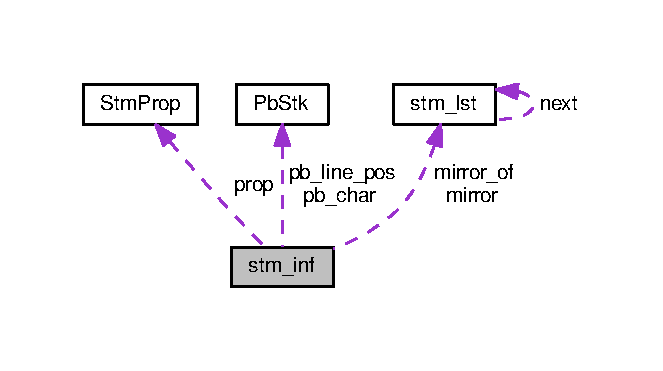
\includegraphics[width=318pt]{structstm__inf__coll__graph}
\end{center}
\end{figure}
\subsection*{Data Fields}
\begin{DoxyCompactItemize}
\item 
int {\bfseries atom\+\_\+file\+\_\+name}\hypertarget{structstm__inf_a9dc8280c20f516cfce88bdacfc1c70e9}{}\label{structstm__inf_a9dc8280c20f516cfce88bdacfc1c70e9}

\item 
Pl\+Long {\bfseries file}\hypertarget{structstm__inf_a85bc801ede0cd63b9a7a9cacb839bc98}{}\label{structstm__inf_a85bc801ede0cd63b9a7a9cacb839bc98}

\item 
\hyperlink{structStmProp}{Stm\+Prop} {\bfseries prop}\hypertarget{structstm__inf_a5b984f4df0d32f07741b75dced7453aa}{}\label{structstm__inf_a5b984f4df0d32f07741b75dced7453aa}

\item 
\hyperlink{structstm__lst}{Stm\+Lst} $\ast$ {\bfseries mirror}\hypertarget{structstm__inf_a2e13c8b109418f635fabba678006c6cd}{}\label{structstm__inf_a2e13c8b109418f635fabba678006c6cd}

\item 
\hyperlink{structstm__lst}{Stm\+Lst} $\ast$ {\bfseries mirror\+\_\+of}\hypertarget{structstm__inf_ada3cbffaa477959332fc96000cc4b73e}{}\label{structstm__inf_ada3cbffaa477959332fc96000cc4b73e}

\item 
Stm\+Fct {\bfseries fct\+\_\+getc}\hypertarget{structstm__inf_a1ff7dd59a7e0a7b8eaf540cc5ad8145e}{}\label{structstm__inf_a1ff7dd59a7e0a7b8eaf540cc5ad8145e}

\item 
Stm\+Fct {\bfseries fct\+\_\+putc}\hypertarget{structstm__inf_aeba256b0be0d697ad8563fd3475e26d2}{}\label{structstm__inf_aeba256b0be0d697ad8563fd3475e26d2}

\item 
Stm\+Fct {\bfseries fct\+\_\+flush}\hypertarget{structstm__inf_a32fe5f685abc6990b6da6020eb004b60}{}\label{structstm__inf_a32fe5f685abc6990b6da6020eb004b60}

\item 
Stm\+Fct {\bfseries fct\+\_\+close}\hypertarget{structstm__inf_a5f6fd03e09577d0f7ba5c600d35d3ad8}{}\label{structstm__inf_a5f6fd03e09577d0f7ba5c600d35d3ad8}

\item 
Stm\+Fct {\bfseries fct\+\_\+tell}\hypertarget{structstm__inf_a1f829218b8f5b09925cb45caec5af199}{}\label{structstm__inf_a1f829218b8f5b09925cb45caec5af199}

\item 
Stm\+Fct {\bfseries fct\+\_\+seek}\hypertarget{structstm__inf_a5f9d4068bafcdf0a8ced688439af8aa2}{}\label{structstm__inf_a5f9d4068bafcdf0a8ced688439af8aa2}

\item 
Stm\+Fct {\bfseries fct\+\_\+clearerr}\hypertarget{structstm__inf_afaf9188c97510a5f1d612e1444f6e801}{}\label{structstm__inf_afaf9188c97510a5f1d612e1444f6e801}

\item 
Bool {\bfseries eof\+\_\+reached}\hypertarget{structstm__inf_ac3960253b7e5f826635a196b096fd499}{}\label{structstm__inf_ac3960253b7e5f826635a196b096fd499}

\item 
\hyperlink{structPbStk}{Pb\+Stk} {\bfseries pb\+\_\+char}\hypertarget{structstm__inf_af66229bdb1421dc62daaee808af84bba}{}\label{structstm__inf_af66229bdb1421dc62daaee808af84bba}

\item 
Pl\+Long {\bfseries char\+\_\+count}\hypertarget{structstm__inf_a0c6895ef7d7a03c6f0ad2aa05be2c0af}{}\label{structstm__inf_a0c6895ef7d7a03c6f0ad2aa05be2c0af}

\item 
Pl\+Long {\bfseries line\+\_\+count}\hypertarget{structstm__inf_a0394c04b8f2bd5990d30dd6ad14a8246}{}\label{structstm__inf_a0394c04b8f2bd5990d30dd6ad14a8246}

\item 
Pl\+Long {\bfseries line\+\_\+pos}\hypertarget{structstm__inf_a89769bf2d0ca17434b431c380379e674}{}\label{structstm__inf_a89769bf2d0ca17434b431c380379e674}

\item 
\hyperlink{structPbStk}{Pb\+Stk} {\bfseries pb\+\_\+line\+\_\+pos}\hypertarget{structstm__inf_acd4b4b0e220c45642fb4a6903d6ec4d5}{}\label{structstm__inf_acd4b4b0e220c45642fb4a6903d6ec4d5}

\end{DoxyCompactItemize}


The documentation for this struct was generated from the following file\+:\begin{DoxyCompactItemize}
\item 
gprolog-\/utf8-\/tree/src/\+Bips\+Pl/stream\+\_\+supp.\+h\end{DoxyCompactItemize}

\hypertarget{structstm__lst}{}\section{stm\+\_\+lst Struct Reference}
\label{structstm__lst}\index{stm\+\_\+lst@{stm\+\_\+lst}}


{\ttfamily \#include $<$stream\+\_\+supp.\+h$>$}



Collaboration diagram for stm\+\_\+lst\+:\nopagebreak
\begin{figure}[H]
\begin{center}
\leavevmode
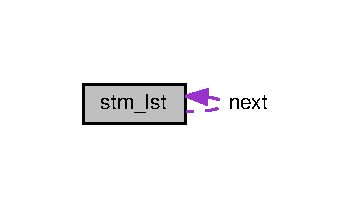
\includegraphics[width=169pt]{structstm__lst__coll__graph}
\end{center}
\end{figure}
\subsection*{Data Fields}
\begin{DoxyCompactItemize}
\item 
int \hyperlink{structstm__lst_a69932b67f84be652c1d4fab80820a4cc}{stm}
\item 
\hyperlink{stream__supp_8h_a6b553ae1ecc32ad49304cd836fb357c3}{P\+Stm\+Lst} \hyperlink{structstm__lst_aaecf8566184bb06365a7de2d3ba8312b}{next}
\end{DoxyCompactItemize}


\subsection{Field Documentation}
\index{stm\+\_\+lst@{stm\+\_\+lst}!next@{next}}
\index{next@{next}!stm\+\_\+lst@{stm\+\_\+lst}}
\subsubsection[{\texorpdfstring{next}{next}}]{\setlength{\rightskip}{0pt plus 5cm}{\bf P\+Stm\+Lst} stm\+\_\+lst\+::next}\hypertarget{structstm__lst_aaecf8566184bb06365a7de2d3ba8312b}{}\label{structstm__lst_aaecf8566184bb06365a7de2d3ba8312b}
\index{stm\+\_\+lst@{stm\+\_\+lst}!stm@{stm}}
\index{stm@{stm}!stm\+\_\+lst@{stm\+\_\+lst}}
\subsubsection[{\texorpdfstring{stm}{stm}}]{\setlength{\rightskip}{0pt plus 5cm}int stm\+\_\+lst\+::stm}\hypertarget{structstm__lst_a69932b67f84be652c1d4fab80820a4cc}{}\label{structstm__lst_a69932b67f84be652c1d4fab80820a4cc}


The documentation for this struct was generated from the following file\+:\begin{DoxyCompactItemize}
\item 
gprolog-\/utf8-\/tree/src/\+Bips\+Pl/\hyperlink{stream__supp_8h}{stream\+\_\+supp.\+h}\end{DoxyCompactItemize}

\hypertarget{structStmProp}{}\section{Stm\+Prop Struct Reference}
\label{structStmProp}\index{Stm\+Prop@{Stm\+Prop}}
\subsection*{Data Fields}
\begin{DoxyCompactItemize}
\item 
unsigned {\bfseries mode}\+:2\hypertarget{structStmProp_a8a2ef413513d1963d66e2f490b6b83b4}{}\label{structStmProp_a8a2ef413513d1963d66e2f490b6b83b4}

\item 
unsigned {\bfseries input}\+:1\hypertarget{structStmProp_a600c8a2fc85ea28e18dd45a1bfdbb039}{}\label{structStmProp_a600c8a2fc85ea28e18dd45a1bfdbb039}

\item 
unsigned {\bfseries output}\+:1\hypertarget{structStmProp_ac00a5a24dbbfeece3814be64cc7014d6}{}\label{structStmProp_ac00a5a24dbbfeece3814be64cc7014d6}

\item 
unsigned {\bfseries text}\+:1\hypertarget{structStmProp_ac19d8844240a9c3059104f8afd135834}{}\label{structStmProp_ac19d8844240a9c3059104f8afd135834}

\item 
unsigned {\bfseries reposition}\+:1\hypertarget{structStmProp_a812b9e484fea9756ace87645f847f6f4}{}\label{structStmProp_a812b9e484fea9756ace87645f847f6f4}

\item 
unsigned {\bfseries eof\+\_\+action}\+:2\hypertarget{structStmProp_a04e464b0b01bd6e61e4752dc40264126}{}\label{structStmProp_a04e464b0b01bd6e61e4752dc40264126}

\item 
unsigned {\bfseries buffering}\+:2\hypertarget{structStmProp_ad4122d8a077810116d89eb216c24e642}{}\label{structStmProp_ad4122d8a077810116d89eb216c24e642}

\item 
unsigned {\bfseries special\+\_\+close}\+:1\hypertarget{structStmProp_a77078202569393e5ac5b40c0e3b4e8af}{}\label{structStmProp_a77078202569393e5ac5b40c0e3b4e8af}

\item 
unsigned {\bfseries other}\+:8\hypertarget{structStmProp_a53b858c5848ca920087838eb02faf75f}{}\label{structStmProp_a53b858c5848ca920087838eb02faf75f}

\end{DoxyCompactItemize}


The documentation for this struct was generated from the following file\+:\begin{DoxyCompactItemize}
\item 
gprolog-\/utf8-\/tree/src/\+Bips\+Pl/stream\+\_\+supp.\+h\end{DoxyCompactItemize}

\hypertarget{structStrSInf}{}\section{Str\+S\+Inf Struct Reference}
\label{structStrSInf}\index{Str\+S\+Inf@{Str\+S\+Inf}}


{\ttfamily \#include $<$stream\+\_\+supp.\+h$>$}

\subsection*{Data Fields}
\begin{DoxyCompactItemize}
\item 
char $\ast$ \hyperlink{structStrSInf_aeb057f9f00adf6340a825b3a5f5d2f85}{buff}
\item 
char $\ast$ \hyperlink{structStrSInf_a68da0c71b6666b73881d68d364de63f2}{ptr}
\item 
\hyperlink{bool_8h_afdcfe6db5bea87bd493a3fe2c513d5ef}{Bool} \hyperlink{structStrSInf_af4eb3705492f95c32af035b64b070958}{buff\+\_\+alloc\+\_\+size}
\end{DoxyCompactItemize}


\subsection{Field Documentation}
\index{Str\+S\+Inf@{Str\+S\+Inf}!buff@{buff}}
\index{buff@{buff}!Str\+S\+Inf@{Str\+S\+Inf}}
\subsubsection[{\texorpdfstring{buff}{buff}}]{\setlength{\rightskip}{0pt plus 5cm}char$\ast$ Str\+S\+Inf\+::buff}\hypertarget{structStrSInf_aeb057f9f00adf6340a825b3a5f5d2f85}{}\label{structStrSInf_aeb057f9f00adf6340a825b3a5f5d2f85}
\index{Str\+S\+Inf@{Str\+S\+Inf}!buff\+\_\+alloc\+\_\+size@{buff\+\_\+alloc\+\_\+size}}
\index{buff\+\_\+alloc\+\_\+size@{buff\+\_\+alloc\+\_\+size}!Str\+S\+Inf@{Str\+S\+Inf}}
\subsubsection[{\texorpdfstring{buff\+\_\+alloc\+\_\+size}{buff_alloc_size}}]{\setlength{\rightskip}{0pt plus 5cm}{\bf Bool} Str\+S\+Inf\+::buff\+\_\+alloc\+\_\+size}\hypertarget{structStrSInf_af4eb3705492f95c32af035b64b070958}{}\label{structStrSInf_af4eb3705492f95c32af035b64b070958}
\index{Str\+S\+Inf@{Str\+S\+Inf}!ptr@{ptr}}
\index{ptr@{ptr}!Str\+S\+Inf@{Str\+S\+Inf}}
\subsubsection[{\texorpdfstring{ptr}{ptr}}]{\setlength{\rightskip}{0pt plus 5cm}char$\ast$ Str\+S\+Inf\+::ptr}\hypertarget{structStrSInf_a68da0c71b6666b73881d68d364de63f2}{}\label{structStrSInf_a68da0c71b6666b73881d68d364de63f2}


The documentation for this struct was generated from the following file\+:\begin{DoxyCompactItemize}
\item 
gprolog-\/utf8-\/tree/src/\+Bips\+Pl/\hyperlink{stream__supp_8h}{stream\+\_\+supp.\+h}\end{DoxyCompactItemize}

\hypertarget{structswt__elt}{}\section{swt\+\_\+elt Struct Reference}
\label{structswt__elt}\index{swt\+\_\+elt@{swt\+\_\+elt}}


Collaboration diagram for swt\+\_\+elt\+:\nopagebreak
\begin{figure}[H]
\begin{center}
\leavevmode
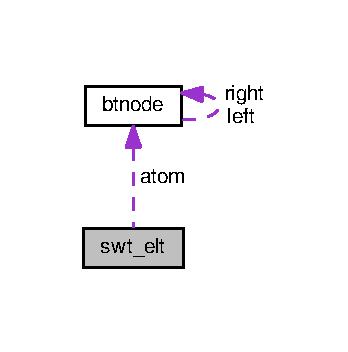
\includegraphics[width=167pt]{structswt__elt__coll__graph}
\end{center}
\end{figure}
\subsection*{Data Fields}
\begin{DoxyCompactItemize}
\item 
\hyperlink{bt__string_8h_a94e2311ccccb66fae2c4ce55649526fc}{B\+T\+Node} $\ast$ \hyperlink{structswt__elt_a04d09a38ab072084ef44f3b17a75b25d}{atom}
\item 
\hyperlink{gprolog_8h_a4d005b136d7fb28537eb1815f7868b63}{Pl\+Long} \hyperlink{structswt__elt_aa3fb3cf68a09b57a7abad92d1888d297}{n}
\item 
\hyperlink{gprolog_8h_a4d005b136d7fb28537eb1815f7868b63}{Pl\+Long} \hyperlink{structswt__elt_a979d2691c64643e5d59f471a3e5e40f6}{label}
\end{DoxyCompactItemize}


\subsection{Field Documentation}
\index{swt\+\_\+elt@{swt\+\_\+elt}!atom@{atom}}
\index{atom@{atom}!swt\+\_\+elt@{swt\+\_\+elt}}
\subsubsection[{\texorpdfstring{atom}{atom}}]{\setlength{\rightskip}{0pt plus 5cm}{\bf B\+T\+Node}$\ast$ swt\+\_\+elt\+::atom}\hypertarget{structswt__elt_a04d09a38ab072084ef44f3b17a75b25d}{}\label{structswt__elt_a04d09a38ab072084ef44f3b17a75b25d}
\index{swt\+\_\+elt@{swt\+\_\+elt}!label@{label}}
\index{label@{label}!swt\+\_\+elt@{swt\+\_\+elt}}
\subsubsection[{\texorpdfstring{label}{label}}]{\setlength{\rightskip}{0pt plus 5cm}{\bf Pl\+Long} swt\+\_\+elt\+::label}\hypertarget{structswt__elt_a979d2691c64643e5d59f471a3e5e40f6}{}\label{structswt__elt_a979d2691c64643e5d59f471a3e5e40f6}
\index{swt\+\_\+elt@{swt\+\_\+elt}!n@{n}}
\index{n@{n}!swt\+\_\+elt@{swt\+\_\+elt}}
\subsubsection[{\texorpdfstring{n}{n}}]{\setlength{\rightskip}{0pt plus 5cm}{\bf Pl\+Long} swt\+\_\+elt\+::n}\hypertarget{structswt__elt_aa3fb3cf68a09b57a7abad92d1888d297}{}\label{structswt__elt_aa3fb3cf68a09b57a7abad92d1888d297}


The documentation for this struct was generated from the following file\+:\begin{DoxyCompactItemize}
\item 
gprolog-\/utf8-\/tree/src/\+Wam2\+Ma/\hyperlink{wam2ma_8c}{wam2ma.\+c}\end{DoxyCompactItemize}

\hypertarget{structswt__tbl}{}\section{swt\+\_\+tbl Struct Reference}
\label{structswt__tbl}\index{swt\+\_\+tbl@{swt\+\_\+tbl}}


Collaboration diagram for swt\+\_\+tbl\+:\nopagebreak
\begin{figure}[H]
\begin{center}
\leavevmode
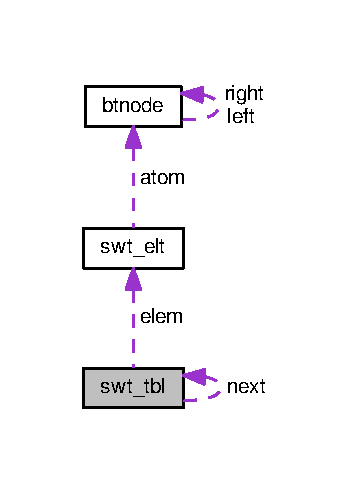
\includegraphics[width=168pt]{structswt__tbl__coll__graph}
\end{center}
\end{figure}
\subsection*{Public Types}
\begin{DoxyCompactItemize}
\item 
enum \{ {\bfseries T\+B\+L\+\_\+\+A\+TM}, 
{\bfseries T\+B\+L\+\_\+\+I\+NT}, 
{\bfseries T\+B\+L\+\_\+\+S\+TC}
 \}\hypertarget{structswt__tbl_a6e6eca39872e41e6d834af855ee073b9}{}\label{structswt__tbl_a6e6eca39872e41e6d834af855ee073b9}

\end{DoxyCompactItemize}
\subsection*{Data Fields}
\begin{DoxyCompactItemize}
\item 
enum swt\+\_\+tbl\+:: \{ ... \}  {\bfseries type}\hypertarget{structswt__tbl_a6b1e4dc1e07f951ebe6ea23a9567e0ca}{}\label{structswt__tbl_a6b1e4dc1e07f951ebe6ea23a9567e0ca}

\item 
int {\bfseries tbl\+\_\+no}\hypertarget{structswt__tbl_a83f05356288e3c0f11cf0539a4a64eaa}{}\label{structswt__tbl_a83f05356288e3c0f11cf0539a4a64eaa}

\item 
\hyperlink{structswt__tbl}{P\+Swt\+Tbl} {\bfseries next}\hypertarget{structswt__tbl_aed3e3921525480876c83cfab6c82ae3b}{}\label{structswt__tbl_aed3e3921525480876c83cfab6c82ae3b}

\item 
int {\bfseries nb\+\_\+elem}\hypertarget{structswt__tbl_a1f108cb255f34e0e43fd548bdeaa2a3e}{}\label{structswt__tbl_a1f108cb255f34e0e43fd548bdeaa2a3e}

\item 
\hyperlink{structswt__elt}{Swt\+Elt} {\bfseries elem} \mbox{[}A\+N\+Y\+\_\+\+S\+I\+ZE\mbox{]}\hypertarget{structswt__tbl_aef5072704a328212e05d40837fe665d0}{}\label{structswt__tbl_aef5072704a328212e05d40837fe665d0}

\end{DoxyCompactItemize}


The documentation for this struct was generated from the following file\+:\begin{DoxyCompactItemize}
\item 
gprolog-\/utf8-\/tree/src/\+Wam2\+Ma/wam2ma.\+c\end{DoxyCompactItemize}

\hypertarget{structSwtInf}{}\section{Swt\+Inf Struct Reference}
\label{structSwtInf}\index{Swt\+Inf@{Swt\+Inf}}


{\ttfamily \#include $<$wam\+\_\+inst.\+h$>$}

\subsection*{Data Fields}
\begin{DoxyCompactItemize}
\item 
\hyperlink{gprolog_8h_a4d005b136d7fb28537eb1815f7868b63}{Pl\+Long} \hyperlink{structSwtInf_ad115955219677407a1cf8cdadc8ab19f}{key}
\item 
Code\+Ptr \hyperlink{structSwtInf_a6d3bad3eb0abb1b73b7776d5153c34fd}{codep}
\item 
\hyperlink{gprolog_8h_a4d005b136d7fb28537eb1815f7868b63}{Pl\+Long} \hyperlink{structSwtInf_a31e087797a5ae675b9c0a80344891bbc}{int\+\_\+val}
\item 
char $\ast$ \hyperlink{structSwtInf_aca3187b48d4bc13a963b097f9e228266}{label}
\end{DoxyCompactItemize}


\subsection{Field Documentation}
\index{Swt\+Inf@{Swt\+Inf}!codep@{codep}}
\index{codep@{codep}!Swt\+Inf@{Swt\+Inf}}
\subsubsection[{\texorpdfstring{codep}{codep}}]{\setlength{\rightskip}{0pt plus 5cm}Code\+Ptr Swt\+Inf\+::codep}\hypertarget{structSwtInf_a6d3bad3eb0abb1b73b7776d5153c34fd}{}\label{structSwtInf_a6d3bad3eb0abb1b73b7776d5153c34fd}
\index{Swt\+Inf@{Swt\+Inf}!int\+\_\+val@{int\+\_\+val}}
\index{int\+\_\+val@{int\+\_\+val}!Swt\+Inf@{Swt\+Inf}}
\subsubsection[{\texorpdfstring{int\+\_\+val}{int_val}}]{\setlength{\rightskip}{0pt plus 5cm}{\bf Pl\+Long} Swt\+Inf\+::int\+\_\+val}\hypertarget{structSwtInf_a31e087797a5ae675b9c0a80344891bbc}{}\label{structSwtInf_a31e087797a5ae675b9c0a80344891bbc}
\index{Swt\+Inf@{Swt\+Inf}!key@{key}}
\index{key@{key}!Swt\+Inf@{Swt\+Inf}}
\subsubsection[{\texorpdfstring{key}{key}}]{\setlength{\rightskip}{0pt plus 5cm}{\bf Pl\+Long} Swt\+Inf\+::key}\hypertarget{structSwtInf_ad115955219677407a1cf8cdadc8ab19f}{}\label{structSwtInf_ad115955219677407a1cf8cdadc8ab19f}
\index{Swt\+Inf@{Swt\+Inf}!label@{label}}
\index{label@{label}!Swt\+Inf@{Swt\+Inf}}
\subsubsection[{\texorpdfstring{label}{label}}]{\setlength{\rightskip}{0pt plus 5cm}char$\ast$ Swt\+Inf\+::label}\hypertarget{structSwtInf_aca3187b48d4bc13a963b097f9e228266}{}\label{structSwtInf_aca3187b48d4bc13a963b097f9e228266}


The documentation for this struct was generated from the following files\+:\begin{DoxyCompactItemize}
\item 
gprolog-\/utf8-\/tree/src/\+Engine\+Pl/\hyperlink{wam__inst_8h}{wam\+\_\+inst.\+h}\item 
gprolog-\/utf8-\/tree/src/\+Ma2\+Asm/\hyperlink{ma__parser_8h}{ma\+\_\+parser.\+h}\end{DoxyCompactItemize}

\hypertarget{structTagInf}{}\section{Tag\+Inf Struct Reference}
\label{structTagInf}\index{Tag\+Inf@{Tag\+Inf}}
\subsection*{Data Fields}
\begin{DoxyCompactItemize}
\item 
char {\bfseries name} \mbox{[}32\mbox{]}\hypertarget{structTagInf_a6dc0e60ac19532e7c8e1c30f73357c1c}{}\label{structTagInf_a6dc0e60ac19532e7c8e1c30f73357c1c}

\item 
Typ\+Tag {\bfseries type}\hypertarget{structTagInf_a1d109a0184537c9f448e28aa6c492b91}{}\label{structTagInf_a1d109a0184537c9f448e28aa6c492b91}

\item 
int {\bfseries value}\hypertarget{structTagInf_ae5a47ca79c53423fd961942af0647109}{}\label{structTagInf_ae5a47ca79c53423fd961942af0647109}

\end{DoxyCompactItemize}


The documentation for this struct was generated from the following file\+:\begin{DoxyCompactItemize}
\item 
gprolog-\/utf8-\/tree/src/\+Engine\+Pl/pl\+\_\+config.\+c\end{DoxyCompactItemize}

\hypertarget{structTermSInf}{}\section{Term\+S\+Inf Struct Reference}
\label{structTermSInf}\index{Term\+S\+Inf@{Term\+S\+Inf}}
\subsection*{Data Fields}
\begin{DoxyCompactItemize}
\item 
int {\bfseries buff\+\_\+size}\hypertarget{structTermSInf_aa2ac007b499e0cb03e17072299872d08}{}\label{structTermSInf_aa2ac007b499e0cb03e17072299872d08}

\item 
Bool {\bfseries buff\+\_\+is\+\_\+alloc}\hypertarget{structTermSInf_a02d37582809df8e6a18bf4cdcb598693}{}\label{structTermSInf_a02d37582809df8e6a18bf4cdcb598693}

\item 
char $\ast$ {\bfseries buff}\hypertarget{structTermSInf_aea3421d8fe398941f9280da64bcfba35}{}\label{structTermSInf_aea3421d8fe398941f9280da64bcfba35}

\item 
char $\ast$ {\bfseries ptr}\hypertarget{structTermSInf_a46ab1bf8caba7bd0044429601be6b670}{}\label{structTermSInf_a46ab1bf8caba7bd0044429601be6b670}

\end{DoxyCompactItemize}


The documentation for this struct was generated from the following file\+:\begin{DoxyCompactItemize}
\item 
gprolog-\/utf8-\/tree/src/\+Bips\+Pl/stream\+\_\+c.\+c\end{DoxyCompactItemize}

\hypertarget{structTokInf}{}\section{Tok\+Inf Struct Reference}
\label{structTokInf}\index{Tok\+Inf@{Tok\+Inf}}


{\ttfamily \#include $<$scan\+\_\+supp.\+h$>$}

\subsection*{Data Fields}
\begin{DoxyCompactItemize}
\item 
\hyperlink{scan__supp_8h_a92e3dba2da3b5e64ff0567a8aa779891}{Typ\+Tok} \hyperlink{structTokInf_a9ae46e898f23f677836fa19cc119276b}{type}
\item 
char \hyperlink{structTokInf_aa56c61670fa2e571afc6647c76af2103}{name} \mbox{[}\hyperlink{scan__supp_8h_ac61c2e9163da6fb2b5fcd9a86c88af5d}{S\+C\+A\+N\+\_\+\+B\+I\+G\+\_\+\+B\+U\+F\+F\+ER}\mbox{]}
\item 
int \hyperlink{structTokInf_aedaf8feef7d9708e8a946df56d7cdb66}{quoted}
\item 
int \hyperlink{structTokInf_addc6977c79a52835a28c0347c453df5d}{punct}
\item 
\hyperlink{gprolog_8h_a4d005b136d7fb28537eb1815f7868b63}{Pl\+Long} \hyperlink{structTokInf_a9f5266be5fc6a8e446ed3e660032d0ad}{int\+\_\+num}
\item 
double \hyperlink{structTokInf_afddf6ad76bb496c8ddd35a5b773f4360}{float\+\_\+num}
\item 
int \hyperlink{structTokInf_a141b87290988df7a09d0f84593cd02c5}{line}
\item 
int \hyperlink{structTokInf_a3034cb3570c3c0a946e3e1c86b0464a7}{col}
\end{DoxyCompactItemize}


\subsection{Field Documentation}
\index{Tok\+Inf@{Tok\+Inf}!col@{col}}
\index{col@{col}!Tok\+Inf@{Tok\+Inf}}
\subsubsection[{\texorpdfstring{col}{col}}]{\setlength{\rightskip}{0pt plus 5cm}int Tok\+Inf\+::col}\hypertarget{structTokInf_a3034cb3570c3c0a946e3e1c86b0464a7}{}\label{structTokInf_a3034cb3570c3c0a946e3e1c86b0464a7}
\index{Tok\+Inf@{Tok\+Inf}!float\+\_\+num@{float\+\_\+num}}
\index{float\+\_\+num@{float\+\_\+num}!Tok\+Inf@{Tok\+Inf}}
\subsubsection[{\texorpdfstring{float\+\_\+num}{float_num}}]{\setlength{\rightskip}{0pt plus 5cm}double Tok\+Inf\+::float\+\_\+num}\hypertarget{structTokInf_afddf6ad76bb496c8ddd35a5b773f4360}{}\label{structTokInf_afddf6ad76bb496c8ddd35a5b773f4360}
\index{Tok\+Inf@{Tok\+Inf}!int\+\_\+num@{int\+\_\+num}}
\index{int\+\_\+num@{int\+\_\+num}!Tok\+Inf@{Tok\+Inf}}
\subsubsection[{\texorpdfstring{int\+\_\+num}{int_num}}]{\setlength{\rightskip}{0pt plus 5cm}{\bf Pl\+Long} Tok\+Inf\+::int\+\_\+num}\hypertarget{structTokInf_a9f5266be5fc6a8e446ed3e660032d0ad}{}\label{structTokInf_a9f5266be5fc6a8e446ed3e660032d0ad}
\index{Tok\+Inf@{Tok\+Inf}!line@{line}}
\index{line@{line}!Tok\+Inf@{Tok\+Inf}}
\subsubsection[{\texorpdfstring{line}{line}}]{\setlength{\rightskip}{0pt plus 5cm}int Tok\+Inf\+::line}\hypertarget{structTokInf_a141b87290988df7a09d0f84593cd02c5}{}\label{structTokInf_a141b87290988df7a09d0f84593cd02c5}
\index{Tok\+Inf@{Tok\+Inf}!name@{name}}
\index{name@{name}!Tok\+Inf@{Tok\+Inf}}
\subsubsection[{\texorpdfstring{name}{name}}]{\setlength{\rightskip}{0pt plus 5cm}char Tok\+Inf\+::name\mbox{[}{\bf S\+C\+A\+N\+\_\+\+B\+I\+G\+\_\+\+B\+U\+F\+F\+ER}\mbox{]}}\hypertarget{structTokInf_aa56c61670fa2e571afc6647c76af2103}{}\label{structTokInf_aa56c61670fa2e571afc6647c76af2103}
\index{Tok\+Inf@{Tok\+Inf}!punct@{punct}}
\index{punct@{punct}!Tok\+Inf@{Tok\+Inf}}
\subsubsection[{\texorpdfstring{punct}{punct}}]{\setlength{\rightskip}{0pt plus 5cm}int Tok\+Inf\+::punct}\hypertarget{structTokInf_addc6977c79a52835a28c0347c453df5d}{}\label{structTokInf_addc6977c79a52835a28c0347c453df5d}
\index{Tok\+Inf@{Tok\+Inf}!quoted@{quoted}}
\index{quoted@{quoted}!Tok\+Inf@{Tok\+Inf}}
\subsubsection[{\texorpdfstring{quoted}{quoted}}]{\setlength{\rightskip}{0pt plus 5cm}int Tok\+Inf\+::quoted}\hypertarget{structTokInf_aedaf8feef7d9708e8a946df56d7cdb66}{}\label{structTokInf_aedaf8feef7d9708e8a946df56d7cdb66}
\index{Tok\+Inf@{Tok\+Inf}!type@{type}}
\index{type@{type}!Tok\+Inf@{Tok\+Inf}}
\subsubsection[{\texorpdfstring{type}{type}}]{\setlength{\rightskip}{0pt plus 5cm}{\bf Typ\+Tok} Tok\+Inf\+::type}\hypertarget{structTokInf_a9ae46e898f23f677836fa19cc119276b}{}\label{structTokInf_a9ae46e898f23f677836fa19cc119276b}


The documentation for this struct was generated from the following file\+:\begin{DoxyCompactItemize}
\item 
gprolog-\/utf8-\/tree/src/\+Bips\+Pl/\hyperlink{scan__supp_8h}{scan\+\_\+supp.\+h}\end{DoxyCompactItemize}

\hypertarget{structUsedFile}{}\section{Used\+File Struct Reference}
\label{structUsedFile}\index{Used\+File@{Used\+File}}
\subsection*{Data Fields}
\begin{DoxyCompactItemize}
\item 
char $\ast$ {\bfseries name}\hypertarget{structUsedFile_a8d4ed04924e68784f37a3f3f268ff633}{}\label{structUsedFile_a8d4ed04924e68784f37a3f3f268ff633}

\item 
char $\ast$ {\bfseries parent}\hypertarget{structUsedFile_a3bf412b1901e0513545a138bfdb9b254}{}\label{structUsedFile_a3bf412b1901e0513545a138bfdb9b254}

\item 
int {\bfseries line}\hypertarget{structUsedFile_a5a91641c98e7812d3af04c519499dd5c}{}\label{structUsedFile_a5a91641c98e7812d3af04c519499dd5c}

\end{DoxyCompactItemize}


The documentation for this struct was generated from the following file\+:\begin{DoxyCompactItemize}
\item 
gprolog-\/utf8-\/tree/src/\+Engine\+Pl/cpp\+\_\+headers.\+c\end{DoxyCompactItemize}

\hypertarget{structUsedMachRegInf}{}\section{Used\+Mach\+Reg\+Inf Struct Reference}
\label{structUsedMachRegInf}\index{Used\+Mach\+Reg\+Inf@{Used\+Mach\+Reg\+Inf}}
\subsection*{Data Fields}
\begin{DoxyCompactItemize}
\item 
char $\ast$ {\bfseries mach\+\_\+reg\+\_\+name}\hypertarget{structUsedMachRegInf_a469dabfeaa37fca00d87667d4dacc064}{}\label{structUsedMachRegInf_a469dabfeaa37fca00d87667d4dacc064}

\item 
char $\ast$ {\bfseries pl\+\_\+reg\+\_\+name}\hypertarget{structUsedMachRegInf_a9a0e95f20d942e8610a0e905bafc7353}{}\label{structUsedMachRegInf_a9a0e95f20d942e8610a0e905bafc7353}

\item 
char $\ast$ {\bfseries type}\hypertarget{structUsedMachRegInf_a2e0c08014802409c0a340c61fab7dafe}{}\label{structUsedMachRegInf_a2e0c08014802409c0a340c61fab7dafe}

\end{DoxyCompactItemize}


The documentation for this struct was generated from the following file\+:\begin{DoxyCompactItemize}
\item 
gprolog-\/utf8-\/tree/src/\+Engine\+Pl/pl\+\_\+config.\+c\end{DoxyCompactItemize}

\chapter{File Documentation}
\hypertarget{all__fd__bips_8pl}{}\section{gprolog-\/utf8-\/tree/src/\+Bips\+F\+D/all\+\_\+fd\+\_\+bips.pl File Reference}
\label{all__fd__bips_8pl}\index{gprolog-\/utf8-\/tree/src/\+Bips\+F\+D/all\+\_\+fd\+\_\+bips.\+pl@{gprolog-\/utf8-\/tree/src/\+Bips\+F\+D/all\+\_\+fd\+\_\+bips.\+pl}}

\hypertarget{bips__fd_8h}{}\section{gprolog-\/utf8-\/tree/src/\+Bips\+F\+D/bips\+\_\+fd.h File Reference}
\label{bips__fd_8h}\index{gprolog-\/utf8-\/tree/src/\+Bips\+F\+D/bips\+\_\+fd.\+h@{gprolog-\/utf8-\/tree/src/\+Bips\+F\+D/bips\+\_\+fd.\+h}}
{\ttfamily \#include \char`\"{}math\+\_\+supp.\+h\char`\"{}}\\*
{\ttfamily \#include \char`\"{}oper\+\_\+supp.\+h\char`\"{}}\\*
Include dependency graph for bips\+\_\+fd.\+h\+:\nopagebreak
\begin{figure}[H]
\begin{center}
\leavevmode
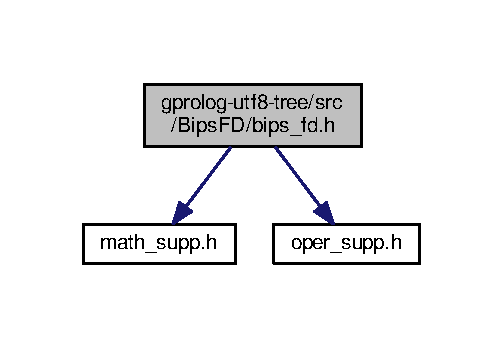
\includegraphics[width=242pt]{bips__fd_8h__incl}
\end{center}
\end{figure}
This graph shows which files directly or indirectly include this file\+:\nopagebreak
\begin{figure}[H]
\begin{center}
\leavevmode
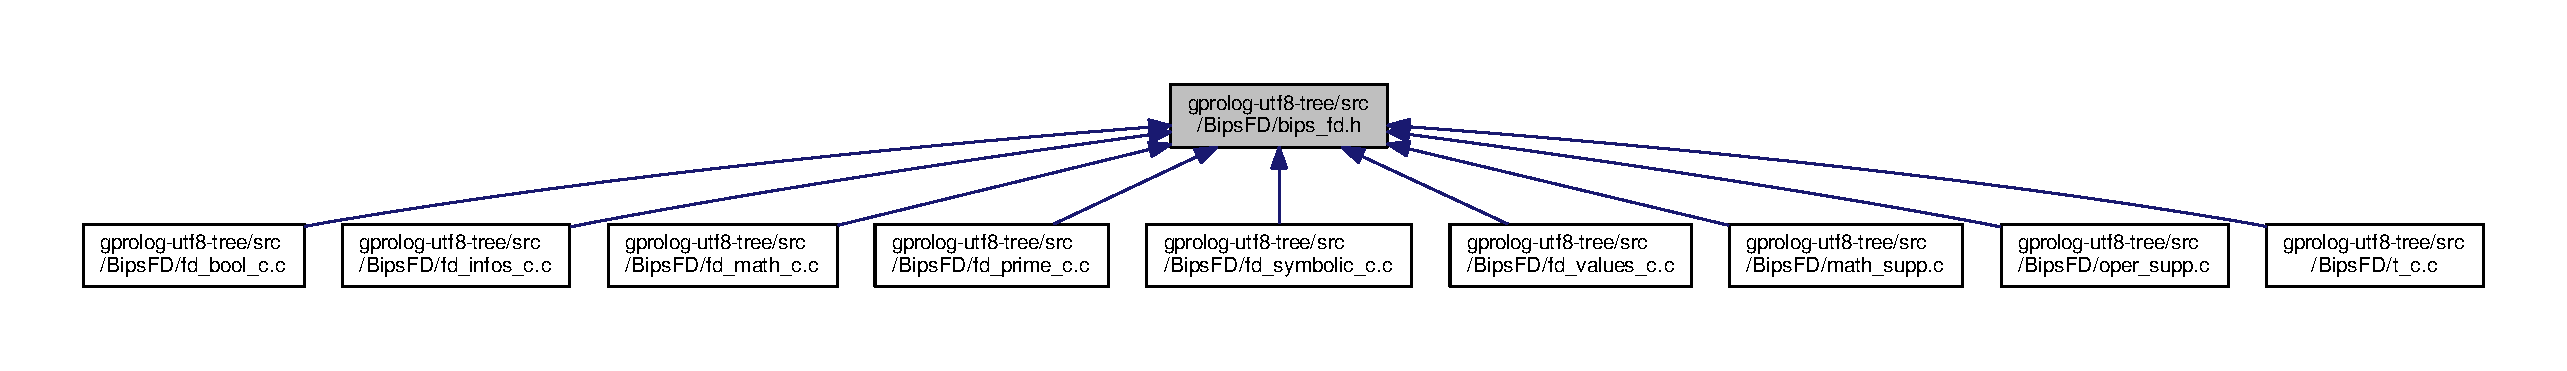
\includegraphics[width=350pt]{bips__fd_8h__dep__incl}
\end{center}
\end{figure}

\hypertarget{fd__bool_8pl}{}\section{gprolog-\/utf8-\/tree/src/\+Bips\+F\+D/fd\+\_\+bool.pl File Reference}
\label{fd__bool_8pl}\index{gprolog-\/utf8-\/tree/src/\+Bips\+F\+D/fd\+\_\+bool.\+pl@{gprolog-\/utf8-\/tree/src/\+Bips\+F\+D/fd\+\_\+bool.\+pl}}

\hypertarget{fd__bool__c_8c}{}\section{gprolog-\/utf8-\/tree/src/\+Bips\+F\+D/fd\+\_\+bool\+\_\+c.c File Reference}
\label{fd__bool__c_8c}\index{gprolog-\/utf8-\/tree/src/\+Bips\+F\+D/fd\+\_\+bool\+\_\+c.\+c@{gprolog-\/utf8-\/tree/src/\+Bips\+F\+D/fd\+\_\+bool\+\_\+c.\+c}}
{\ttfamily \#include \char`\"{}engine\+\_\+pl.\+h\char`\"{}}\\*
{\ttfamily \#include \char`\"{}bips\+\_\+pl.\+h\char`\"{}}\\*
{\ttfamily \#include \char`\"{}engine\+\_\+fd.\+h\char`\"{}}\\*
{\ttfamily \#include \char`\"{}bips\+\_\+fd.\+h\char`\"{}}\\*
Include dependency graph for fd\+\_\+bool\+\_\+c.\+c\+:\nopagebreak
\begin{figure}[H]
\begin{center}
\leavevmode
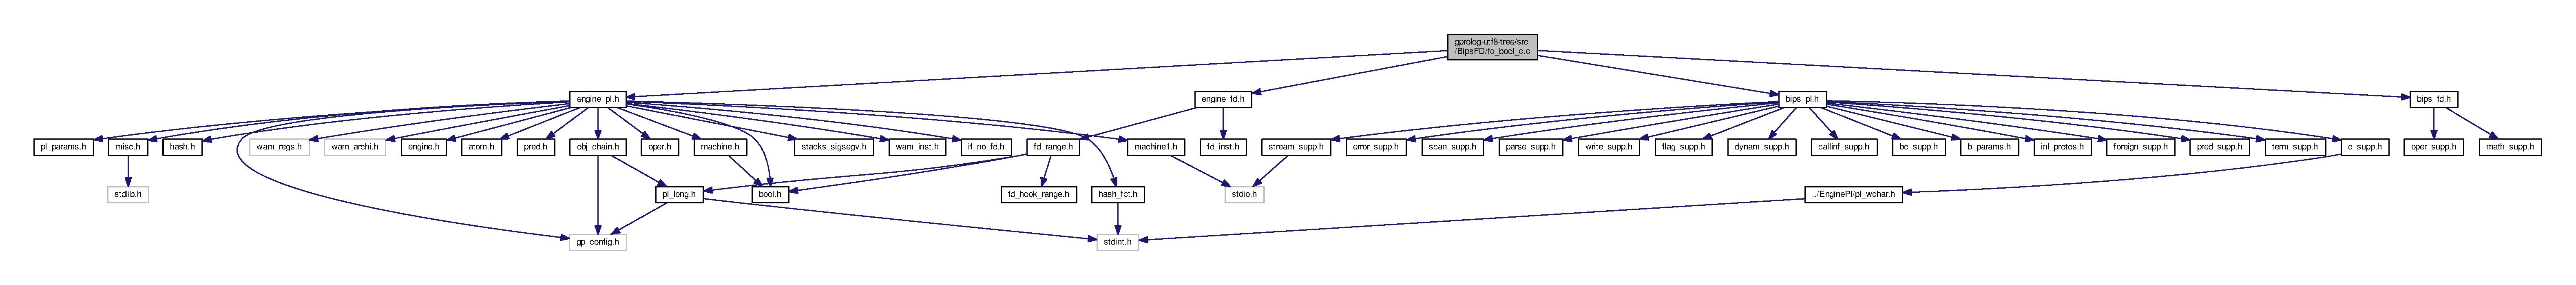
\includegraphics[width=350pt]{fd__bool__c_8c__incl}
\end{center}
\end{figure}
\subsection*{Macros}
\begin{DoxyCompactItemize}
\item 
\#define \hyperlink{fd__bool__c_8c_ac2238956c2b28a02adaeaf890fbc4bf5}{O\+B\+J\+\_\+\+I\+N\+IT}~\hyperlink{fd__bool__c_8c_a1a75f6073da95705cad602b580443664}{Fd\+\_\+\+Bool\+\_\+\+Initializer}
\item 
\#define \hyperlink{fd__bool__c_8c_a7f8d76ec7aa0e0d766264714725b22b1}{B\+O\+O\+L\+\_\+\+S\+T\+A\+C\+K\+\_\+\+S\+I\+ZE}~100000
\item 
\#define \hyperlink{fd__bool__c_8c_a5373173bd4972fdf03e716bb002596c4}{V\+A\+R\+S\+\_\+\+S\+T\+A\+C\+K\+\_\+\+S\+I\+ZE}~100000
\item 
\#define \hyperlink{fd__bool__c_8c_ad3e9fe0ec59d2dbb3982ababa042720c}{N\+OT}~0
\item 
\#define \hyperlink{fd__bool__c_8c_aeba3ab8af6f6f0fa0426de3a666c97a1}{E\+Q\+U\+IV}~1
\item 
\#define \hyperlink{fd__bool__c_8c_a9aad42e0c22fbfcbfb548e91ef74dea7}{N\+E\+Q\+U\+IV}~2
\item 
\#define \hyperlink{fd__bool__c_8c_af5eca14495a72e2a5e7fab97321fe47f}{I\+M\+P\+LY}~3
\item 
\#define \hyperlink{fd__bool__c_8c_a747852d718c64ab8b75a926d2f4ec379}{N\+I\+M\+P\+LY}~4
\item 
\#define \hyperlink{fd__bool__c_8c_acd1b97556dfbbac61063a63031d2f91d}{A\+ND}~5
\item 
\#define \hyperlink{fd__bool__c_8c_a923cb4a4043639f6d8d4108c84bb8f8f}{N\+A\+ND}~6
\item 
\#define \hyperlink{fd__bool__c_8c_a3363ca4d6d3cc0230b2804280591c991}{OR}~7
\item 
\#define \hyperlink{fd__bool__c_8c_a0dd10f6b3ad00611521e0a7ebc8c18ad}{N\+OR}~8
\item 
\#define \hyperlink{fd__bool__c_8c_abaab8d42f075ee8ddc9b70951d3fd6cd}{EQ}~9	/$\ast$ warning EQ must have same $\ast$/
\item 
\#define \hyperlink{fd__bool__c_8c_a2b6ba3ea1fe3e8cc970ad05cd05d703b}{N\+EQ}~10	/$\ast$ parity than \hyperlink{fd__bool__c_8c_aa73a5654b501deb7bd9645bf08ee19ef}{E\+Q\+\_\+F} and \hyperlink{fd__bool__c_8c_ac328e551bde3d39b6d7b8cc9e048d941}{Z\+E\+RO} $\ast$/
\item 
\#define \hyperlink{fd__bool__c_8c_aaf56b99cbe34023f42ce5b7878c827d8}{LT}~11
\item 
\#define \hyperlink{fd__bool__c_8c_a783444ed74123be81bed7042a5a8c104}{G\+TE}~12
\item 
\#define \hyperlink{fd__bool__c_8c_ab89310b3f2f97e4e9415fc5a51549612}{GT}~13
\item 
\#define \hyperlink{fd__bool__c_8c_ae10454eca973b19da41deab419322920}{L\+TE}~14
\item 
\#define \hyperlink{fd__bool__c_8c_aa73a5654b501deb7bd9645bf08ee19ef}{E\+Q\+\_\+F}~15
\item 
\#define \hyperlink{fd__bool__c_8c_a093a6a7e5007368364cd72b8f6660db9}{N\+E\+Q\+\_\+F}~16
\item 
\#define \hyperlink{fd__bool__c_8c_ae80c12fc11ec900abed139671126b8b4}{L\+T\+\_\+F}~17
\item 
\#define \hyperlink{fd__bool__c_8c_a1e60cc4377290e9a43bb7464969f096a}{G\+T\+E\+\_\+F}~18
\item 
\#define \hyperlink{fd__bool__c_8c_aa5737aa6eaa01f17002a469dc19a6f49}{G\+T\+\_\+F}~19
\item 
\#define \hyperlink{fd__bool__c_8c_a6403b0384e007c6b472972519ac16b16}{L\+T\+E\+\_\+F}~20
\item 
\#define \hyperlink{fd__bool__c_8c_ac328e551bde3d39b6d7b8cc9e048d941}{Z\+E\+RO}~21
\item 
\#define \hyperlink{fd__bool__c_8c_a206b6f5362e56b51ca957635350b70b6}{O\+NE}~22	/$\ast$ must be last $\ast$/
\item 
\#define \hyperlink{fd__bool__c_8c_a2ab2458112884b4f920c996c399dc747}{Is\+Var}(op)~((op)$>$=\hyperlink{fd__bool__c_8c_a206b6f5362e56b51ca957635350b70b6}{O\+NE})
\item 
\#define \hyperlink{fd__bool__c_8c_ac6182439a190a3de086e46f74a5e8f22}{N\+B\+\_\+\+O\+F\+\_\+\+OP}~\hyperlink{fd__bool__c_8c_ac328e551bde3d39b6d7b8cc9e048d941}{Z\+E\+RO}
\item 
\#define \hyperlink{fd__bool__c_8c_ae6dddd353f727c9b7b3d75caeb695fff}{B\+O\+O\+L\+\_\+\+C\+S\+T\+R\+\_\+2}(\hyperlink{asm_8c_ad1351d85ffec3c1176dc31d8e8f8e28a}{f},  a1,  a2)
\item 
\#define \hyperlink{fd__bool__c_8c_ad5ca673b332ad1a4f1487490ac1c007e}{B\+O\+O\+L\+\_\+\+C\+S\+T\+R\+\_\+3}(\hyperlink{asm_8c_ad1351d85ffec3c1176dc31d8e8f8e28a}{f},  a1,  a2,  a3)
\end{DoxyCompactItemize}
\subsection*{Functions}
\begin{DoxyCompactItemize}
\item 
static \hyperlink{LINUX__SIGSEGV_8c_a10ea8be8823feb38875b8a9326cbb424}{Wam\+Word} $\ast$ \hyperlink{fd__bool__c_8c_a68a119acd552423924480e3492e83f9c}{Simplify} (int sign, \hyperlink{LINUX__SIGSEGV_8c_a10ea8be8823feb38875b8a9326cbb424}{Wam\+Word} e\+\_\+word)
\item 
static void \hyperlink{fd__bool__c_8c_a21eaa9305603d70618e81dbcc5ea5570}{Add\+\_\+\+Fd\+\_\+\+Variables} (\hyperlink{LINUX__SIGSEGV_8c_a10ea8be8823feb38875b8a9326cbb424}{Wam\+Word} e\+\_\+word)
\item 
static \hyperlink{bool_8h_afdcfe6db5bea87bd493a3fe2c513d5ef}{Bool} \hyperlink{fd__bool__c_8c_a777cdb1b2fda63d69b759553fd15ea75}{Load\+\_\+\+Bool\+\_\+\+Into\+\_\+\+Word} (\hyperlink{LINUX__SIGSEGV_8c_a10ea8be8823feb38875b8a9326cbb424}{Wam\+Word} $\ast$exp, int result, \hyperlink{LINUX__SIGSEGV_8c_a10ea8be8823feb38875b8a9326cbb424}{Wam\+Word} $\ast$load\+\_\+word)
\item 
static \hyperlink{bool_8h_afdcfe6db5bea87bd493a3fe2c513d5ef}{Bool} \hyperlink{fd__bool__c_8c_a2da4a05b71952a4d0899d530d62fcc05}{Set\+\_\+\+Var} (\hyperlink{LINUX__SIGSEGV_8c_a10ea8be8823feb38875b8a9326cbb424}{Wam\+Word} $\ast$exp, int result, \hyperlink{LINUX__SIGSEGV_8c_a10ea8be8823feb38875b8a9326cbb424}{Wam\+Word} $\ast$load\+\_\+word)
\item 
static \hyperlink{bool_8h_afdcfe6db5bea87bd493a3fe2c513d5ef}{Bool} \hyperlink{fd__bool__c_8c_aa99784c68fe104c4fb83488701c4f26d}{Set\+\_\+\+Not} (\hyperlink{LINUX__SIGSEGV_8c_a10ea8be8823feb38875b8a9326cbb424}{Wam\+Word} $\ast$exp, int result, \hyperlink{LINUX__SIGSEGV_8c_a10ea8be8823feb38875b8a9326cbb424}{Wam\+Word} $\ast$load\+\_\+word)
\item 
static \hyperlink{bool_8h_afdcfe6db5bea87bd493a3fe2c513d5ef}{Bool} \hyperlink{fd__bool__c_8c_a5756324591779a6e812b6918a33f86d0}{Set\+\_\+\+Equiv} (\hyperlink{LINUX__SIGSEGV_8c_a10ea8be8823feb38875b8a9326cbb424}{Wam\+Word} $\ast$exp, int result, \hyperlink{LINUX__SIGSEGV_8c_a10ea8be8823feb38875b8a9326cbb424}{Wam\+Word} $\ast$load\+\_\+word)
\item 
static \hyperlink{bool_8h_afdcfe6db5bea87bd493a3fe2c513d5ef}{Bool} \hyperlink{fd__bool__c_8c_af0210aef178792fadee8bf8a6fb31b2e}{Set\+\_\+\+Nequiv} (\hyperlink{LINUX__SIGSEGV_8c_a10ea8be8823feb38875b8a9326cbb424}{Wam\+Word} $\ast$exp, int result, \hyperlink{LINUX__SIGSEGV_8c_a10ea8be8823feb38875b8a9326cbb424}{Wam\+Word} $\ast$load\+\_\+word)
\item 
static \hyperlink{bool_8h_afdcfe6db5bea87bd493a3fe2c513d5ef}{Bool} \hyperlink{fd__bool__c_8c_a57de1f881f34824fc0001b63989af13e}{Set\+\_\+\+Imply} (\hyperlink{LINUX__SIGSEGV_8c_a10ea8be8823feb38875b8a9326cbb424}{Wam\+Word} $\ast$exp, int result, \hyperlink{LINUX__SIGSEGV_8c_a10ea8be8823feb38875b8a9326cbb424}{Wam\+Word} $\ast$load\+\_\+word)
\item 
static \hyperlink{bool_8h_afdcfe6db5bea87bd493a3fe2c513d5ef}{Bool} \hyperlink{fd__bool__c_8c_a403cef3cce8a6973a624c343ceeb263c}{Set\+\_\+\+Nimply} (\hyperlink{LINUX__SIGSEGV_8c_a10ea8be8823feb38875b8a9326cbb424}{Wam\+Word} $\ast$exp, int result, \hyperlink{LINUX__SIGSEGV_8c_a10ea8be8823feb38875b8a9326cbb424}{Wam\+Word} $\ast$load\+\_\+word)
\item 
static \hyperlink{bool_8h_afdcfe6db5bea87bd493a3fe2c513d5ef}{Bool} \hyperlink{fd__bool__c_8c_ae7e33aab925722ca962447b9c534aaad}{Set\+\_\+\+And} (\hyperlink{LINUX__SIGSEGV_8c_a10ea8be8823feb38875b8a9326cbb424}{Wam\+Word} $\ast$exp, int result, \hyperlink{LINUX__SIGSEGV_8c_a10ea8be8823feb38875b8a9326cbb424}{Wam\+Word} $\ast$load\+\_\+word)
\item 
static \hyperlink{bool_8h_afdcfe6db5bea87bd493a3fe2c513d5ef}{Bool} \hyperlink{fd__bool__c_8c_ac00f47833dcf0ba051c9bef1289d8ae1}{Set\+\_\+\+Nand} (\hyperlink{LINUX__SIGSEGV_8c_a10ea8be8823feb38875b8a9326cbb424}{Wam\+Word} $\ast$exp, int result, \hyperlink{LINUX__SIGSEGV_8c_a10ea8be8823feb38875b8a9326cbb424}{Wam\+Word} $\ast$load\+\_\+word)
\item 
static \hyperlink{bool_8h_afdcfe6db5bea87bd493a3fe2c513d5ef}{Bool} \hyperlink{fd__bool__c_8c_a70ad8d129964ae9ae6ebcebe3e8f8734}{Set\+\_\+\+Or} (\hyperlink{LINUX__SIGSEGV_8c_a10ea8be8823feb38875b8a9326cbb424}{Wam\+Word} $\ast$exp, int result, \hyperlink{LINUX__SIGSEGV_8c_a10ea8be8823feb38875b8a9326cbb424}{Wam\+Word} $\ast$load\+\_\+word)
\item 
static \hyperlink{bool_8h_afdcfe6db5bea87bd493a3fe2c513d5ef}{Bool} \hyperlink{fd__bool__c_8c_a6e219be09aeaa78621e2fdc0aa3b70d0}{Set\+\_\+\+Nor} (\hyperlink{LINUX__SIGSEGV_8c_a10ea8be8823feb38875b8a9326cbb424}{Wam\+Word} $\ast$exp, int result, \hyperlink{LINUX__SIGSEGV_8c_a10ea8be8823feb38875b8a9326cbb424}{Wam\+Word} $\ast$load\+\_\+word)
\item 
static \hyperlink{bool_8h_afdcfe6db5bea87bd493a3fe2c513d5ef}{Bool} \hyperlink{fd__bool__c_8c_a3bcf220164d47e110f64a089daebf2a7}{Set\+\_\+\+Eq} (\hyperlink{LINUX__SIGSEGV_8c_a10ea8be8823feb38875b8a9326cbb424}{Wam\+Word} $\ast$exp, int result, \hyperlink{LINUX__SIGSEGV_8c_a10ea8be8823feb38875b8a9326cbb424}{Wam\+Word} $\ast$load\+\_\+word)
\item 
static \hyperlink{bool_8h_afdcfe6db5bea87bd493a3fe2c513d5ef}{Bool} \hyperlink{fd__bool__c_8c_ad9a88621a0a7d01eb8db4da34faf894f}{Set\+\_\+\+Neq} (\hyperlink{LINUX__SIGSEGV_8c_a10ea8be8823feb38875b8a9326cbb424}{Wam\+Word} $\ast$exp, int result, \hyperlink{LINUX__SIGSEGV_8c_a10ea8be8823feb38875b8a9326cbb424}{Wam\+Word} $\ast$load\+\_\+word)
\item 
static \hyperlink{bool_8h_afdcfe6db5bea87bd493a3fe2c513d5ef}{Bool} \hyperlink{fd__bool__c_8c_ac5b16f713138c6b09fd4b3857d52a881}{Set\+\_\+\+Lt} (\hyperlink{LINUX__SIGSEGV_8c_a10ea8be8823feb38875b8a9326cbb424}{Wam\+Word} $\ast$exp, int result, \hyperlink{LINUX__SIGSEGV_8c_a10ea8be8823feb38875b8a9326cbb424}{Wam\+Word} $\ast$load\+\_\+word)
\item 
static \hyperlink{bool_8h_afdcfe6db5bea87bd493a3fe2c513d5ef}{Bool} \hyperlink{fd__bool__c_8c_a22127daaa654486d40b5c097e040ab87}{Set\+\_\+\+Lte} (\hyperlink{LINUX__SIGSEGV_8c_a10ea8be8823feb38875b8a9326cbb424}{Wam\+Word} $\ast$exp, int result, \hyperlink{LINUX__SIGSEGV_8c_a10ea8be8823feb38875b8a9326cbb424}{Wam\+Word} $\ast$load\+\_\+word)
\item 
static \hyperlink{bool_8h_afdcfe6db5bea87bd493a3fe2c513d5ef}{Bool} \hyperlink{fd__bool__c_8c_ab55a4b5a1910174d63bb46439a9e77bc}{Set\+\_\+\+Zero} (\hyperlink{LINUX__SIGSEGV_8c_a10ea8be8823feb38875b8a9326cbb424}{Wam\+Word} $\ast$exp, int result, \hyperlink{LINUX__SIGSEGV_8c_a10ea8be8823feb38875b8a9326cbb424}{Wam\+Word} $\ast$load\+\_\+word)
\item 
static \hyperlink{bool_8h_afdcfe6db5bea87bd493a3fe2c513d5ef}{Bool} \hyperlink{fd__bool__c_8c_a77bd9432adbba7970154bb7401819689}{Set\+\_\+\+One} (\hyperlink{LINUX__SIGSEGV_8c_a10ea8be8823feb38875b8a9326cbb424}{Wam\+Word} $\ast$exp, int result, \hyperlink{LINUX__SIGSEGV_8c_a10ea8be8823feb38875b8a9326cbb424}{Wam\+Word} $\ast$load\+\_\+word)
\item 
\hyperlink{bool_8h_afdcfe6db5bea87bd493a3fe2c513d5ef}{Bool} \hyperlink{fd__bool__c_8c_a9e1a8c3a27ce4468f0ed5374a6ec3be8}{Pl\+\_\+\+Fd\+\_\+\+Eq\+\_\+2} (\hyperlink{LINUX__SIGSEGV_8c_a10ea8be8823feb38875b8a9326cbb424}{Wam\+Word} le\+\_\+word, \hyperlink{LINUX__SIGSEGV_8c_a10ea8be8823feb38875b8a9326cbb424}{Wam\+Word} re\+\_\+word)
\item 
\hyperlink{bool_8h_afdcfe6db5bea87bd493a3fe2c513d5ef}{Bool} \hyperlink{fd__bool__c_8c_ae96f8c98794a44b1577707920fda688d}{Pl\+\_\+\+Fd\+\_\+\+Neq\+\_\+2} (\hyperlink{LINUX__SIGSEGV_8c_a10ea8be8823feb38875b8a9326cbb424}{Wam\+Word} le\+\_\+word, \hyperlink{LINUX__SIGSEGV_8c_a10ea8be8823feb38875b8a9326cbb424}{Wam\+Word} re\+\_\+word)
\item 
\hyperlink{bool_8h_afdcfe6db5bea87bd493a3fe2c513d5ef}{Bool} \hyperlink{fd__bool__c_8c_ae004cace9b53b08de59be0a195274e23}{Pl\+\_\+\+Fd\+\_\+\+Lt\+\_\+2} (\hyperlink{LINUX__SIGSEGV_8c_a10ea8be8823feb38875b8a9326cbb424}{Wam\+Word} le\+\_\+word, \hyperlink{LINUX__SIGSEGV_8c_a10ea8be8823feb38875b8a9326cbb424}{Wam\+Word} re\+\_\+word)
\item 
\hyperlink{bool_8h_afdcfe6db5bea87bd493a3fe2c513d5ef}{Bool} \hyperlink{fd__bool__c_8c_a4533c1990d3146b76bed10bbaa4d67d7}{Pl\+\_\+\+Fd\+\_\+\+Lte\+\_\+2} (\hyperlink{LINUX__SIGSEGV_8c_a10ea8be8823feb38875b8a9326cbb424}{Wam\+Word} le\+\_\+word, \hyperlink{LINUX__SIGSEGV_8c_a10ea8be8823feb38875b8a9326cbb424}{Wam\+Word} re\+\_\+word)
\item 
static void \hyperlink{fd__bool__c_8c_a1a75f6073da95705cad602b580443664}{Fd\+\_\+\+Bool\+\_\+\+Initializer} (void)
\item 
\hyperlink{bool_8h_afdcfe6db5bea87bd493a3fe2c513d5ef}{Bool} \hyperlink{fd__bool__c_8c_af216d1fd11aff1fa2cb04c7ead09615f}{Pl\+\_\+\+Fd\+\_\+\+Bool\+\_\+\+Meta\+\_\+3} (\hyperlink{LINUX__SIGSEGV_8c_a10ea8be8823feb38875b8a9326cbb424}{Wam\+Word} le\+\_\+word, \hyperlink{LINUX__SIGSEGV_8c_a10ea8be8823feb38875b8a9326cbb424}{Wam\+Word} re\+\_\+word, \hyperlink{LINUX__SIGSEGV_8c_a10ea8be8823feb38875b8a9326cbb424}{Wam\+Word} op\+\_\+word)
\item 
\hyperlink{bool_8h_afdcfe6db5bea87bd493a3fe2c513d5ef}{Bool} \hyperlink{fd__bool__c_8c_aad0a445c9905cdb15eeb91e0dc38c0dd}{Pl\+\_\+\+Fd\+\_\+\+Reified\+\_\+\+In} (\hyperlink{LINUX__SIGSEGV_8c_a10ea8be8823feb38875b8a9326cbb424}{Wam\+Word} x\+\_\+word, \hyperlink{LINUX__SIGSEGV_8c_a10ea8be8823feb38875b8a9326cbb424}{Wam\+Word} l\+\_\+word, \hyperlink{LINUX__SIGSEGV_8c_a10ea8be8823feb38875b8a9326cbb424}{Wam\+Word} u\+\_\+word, \hyperlink{LINUX__SIGSEGV_8c_a10ea8be8823feb38875b8a9326cbb424}{Wam\+Word} b\+\_\+word)
\end{DoxyCompactItemize}
\subsection*{Variables}
\begin{DoxyCompactItemize}
\item 
static \hyperlink{LINUX__SIGSEGV_8c_a10ea8be8823feb38875b8a9326cbb424}{Wam\+Word} \hyperlink{fd__bool__c_8c_acd963cd794dba8fb005cff5fee2ed159}{bool\+\_\+tbl} \mbox{[}\hyperlink{math__supp_8c_ac6182439a190a3de086e46f74a5e8f22}{N\+B\+\_\+\+O\+F\+\_\+\+OP}\mbox{]}
\item 
static \hyperlink{LINUX__SIGSEGV_8c_a10ea8be8823feb38875b8a9326cbb424}{Wam\+Word} \hyperlink{fd__bool__c_8c_a42d492fa75214f0ddd4f5d730f5eaf77}{bool\+\_\+xor}
\item 
static \hyperlink{LINUX__SIGSEGV_8c_a10ea8be8823feb38875b8a9326cbb424}{Wam\+Word} \hyperlink{fd__bool__c_8c_a9b2e53e6f6b82fc9105bb99d740ba71a}{stack} \mbox{[}\hyperlink{fd__bool__c_8c_a7f8d76ec7aa0e0d766264714725b22b1}{B\+O\+O\+L\+\_\+\+S\+T\+A\+C\+K\+\_\+\+S\+I\+ZE}\mbox{]}
\item 
static \hyperlink{LINUX__SIGSEGV_8c_a10ea8be8823feb38875b8a9326cbb424}{Wam\+Word} $\ast$ \hyperlink{fd__bool__c_8c_a2ff908f4fb466a5301a5d6b4d3ad083f}{sp}
\item 
static \hyperlink{LINUX__SIGSEGV_8c_a10ea8be8823feb38875b8a9326cbb424}{Wam\+Word} \hyperlink{fd__bool__c_8c_add862b5d8d15150ef512bc87d6cf9cb7}{vars\+\_\+tbl} \mbox{[}\hyperlink{math__supp_8c_a5373173bd4972fdf03e716bb002596c4}{V\+A\+R\+S\+\_\+\+S\+T\+A\+C\+K\+\_\+\+S\+I\+ZE}\mbox{]}
\item 
static \hyperlink{LINUX__SIGSEGV_8c_a10ea8be8823feb38875b8a9326cbb424}{Wam\+Word} $\ast$ \hyperlink{fd__bool__c_8c_ad13f80505a4779a58543cf2b8155a892}{vars\+\_\+sp}
\item 
static \hyperlink{bool_8h_afdcfe6db5bea87bd493a3fe2c513d5ef}{Bool}($\ast$ \hyperlink{fd__bool__c_8c_a27fd4ee155edeb2fb41020963f90387c}{func\+\_\+tbl} \mbox{[}\hyperlink{math__supp_8c_ac6182439a190a3de086e46f74a5e8f22}{N\+B\+\_\+\+O\+F\+\_\+\+OP}+2\mbox{]})(\hyperlink{LINUX__SIGSEGV_8c_a10ea8be8823feb38875b8a9326cbb424}{Wam\+Word} $\ast$exp, int result, \hyperlink{LINUX__SIGSEGV_8c_a10ea8be8823feb38875b8a9326cbb424}{Wam\+Word} $\ast$load\+\_\+word)
\end{DoxyCompactItemize}


\subsection{Macro Definition Documentation}
\index{fd\+\_\+bool\+\_\+c.\+c@{fd\+\_\+bool\+\_\+c.\+c}!A\+ND@{A\+ND}}
\index{A\+ND@{A\+ND}!fd\+\_\+bool\+\_\+c.\+c@{fd\+\_\+bool\+\_\+c.\+c}}
\subsubsection[{\texorpdfstring{A\+ND}{AND}}]{\setlength{\rightskip}{0pt plus 5cm}\#define A\+ND~5}\hypertarget{fd__bool__c_8c_acd1b97556dfbbac61063a63031d2f91d}{}\label{fd__bool__c_8c_acd1b97556dfbbac61063a63031d2f91d}
\index{fd\+\_\+bool\+\_\+c.\+c@{fd\+\_\+bool\+\_\+c.\+c}!B\+O\+O\+L\+\_\+\+C\+S\+T\+R\+\_\+2@{B\+O\+O\+L\+\_\+\+C\+S\+T\+R\+\_\+2}}
\index{B\+O\+O\+L\+\_\+\+C\+S\+T\+R\+\_\+2@{B\+O\+O\+L\+\_\+\+C\+S\+T\+R\+\_\+2}!fd\+\_\+bool\+\_\+c.\+c@{fd\+\_\+bool\+\_\+c.\+c}}
\subsubsection[{\texorpdfstring{B\+O\+O\+L\+\_\+\+C\+S\+T\+R\+\_\+2}{BOOL_CSTR_2}}]{\setlength{\rightskip}{0pt plus 5cm}\#define B\+O\+O\+L\+\_\+\+C\+S\+T\+R\+\_\+2(
\begin{DoxyParamCaption}
\item[{}]{{\bf f}, }
\item[{}]{a1, }
\item[{}]{a2}
\end{DoxyParamCaption}
)}\hypertarget{fd__bool__c_8c_ae6dddd353f727c9b7b3d75caeb695fff}{}\label{fd__bool__c_8c_ae6dddd353f727c9b7b3d75caeb695fff}
{\bfseries Value\+:}
\begin{DoxyCode}
\textcolor{keywordflow}{do}                          \(\backslash\)
    \{                           \(\backslash\)
      if (!\hyperlink{fd__inst_8c_a48bfe26ff0c1846232e2c494c7746c5e}{Pl\_Fd\_Check\_For\_Bool\_Var}(a1))        \(\backslash\)
    return \hyperlink{bool_8h_aa93f0eb578d23995850d61f7d61c55c1}{FALSE};                  \(\backslash\)
      if (!\hyperlink{fd__inst_8c_a48bfe26ff0c1846232e2c494c7746c5e}{Pl\_Fd\_Check\_For\_Bool\_Var}(a2))        \(\backslash\)
    return \hyperlink{bool_8h_aa93f0eb578d23995850d61f7d61c55c1}{FALSE};                  \hyperlink{math__supp_8h_ac08ffc5cec36fc7dc0138ef5d1dda0fa}{\(\backslash\)}
\hyperlink{math__supp_8h_ac08ffc5cec36fc7dc0138ef5d1dda0fa}{      PRIM\_CSTR\_2}(\hyperlink{sparc64-setx_8c_a3efb0e1a16208deecbd84c15401f7cf8}{f}, a1, a2);             \(\backslash\)
    \}                           \(\backslash\)
  while (0)
\end{DoxyCode}
\index{fd\+\_\+bool\+\_\+c.\+c@{fd\+\_\+bool\+\_\+c.\+c}!B\+O\+O\+L\+\_\+\+C\+S\+T\+R\+\_\+3@{B\+O\+O\+L\+\_\+\+C\+S\+T\+R\+\_\+3}}
\index{B\+O\+O\+L\+\_\+\+C\+S\+T\+R\+\_\+3@{B\+O\+O\+L\+\_\+\+C\+S\+T\+R\+\_\+3}!fd\+\_\+bool\+\_\+c.\+c@{fd\+\_\+bool\+\_\+c.\+c}}
\subsubsection[{\texorpdfstring{B\+O\+O\+L\+\_\+\+C\+S\+T\+R\+\_\+3}{BOOL_CSTR_3}}]{\setlength{\rightskip}{0pt plus 5cm}\#define B\+O\+O\+L\+\_\+\+C\+S\+T\+R\+\_\+3(
\begin{DoxyParamCaption}
\item[{}]{{\bf f}, }
\item[{}]{a1, }
\item[{}]{a2, }
\item[{}]{a3}
\end{DoxyParamCaption}
)}\hypertarget{fd__bool__c_8c_ad5ca673b332ad1a4f1487490ac1c007e}{}\label{fd__bool__c_8c_ad5ca673b332ad1a4f1487490ac1c007e}
{\bfseries Value\+:}
\begin{DoxyCode}
\textcolor{keywordflow}{do}                          \(\backslash\)
    \{                           \(\backslash\)
      if (!\hyperlink{fd__inst_8c_a48bfe26ff0c1846232e2c494c7746c5e}{Pl\_Fd\_Check\_For\_Bool\_Var}(a1))        \(\backslash\)
    return \hyperlink{bool_8h_aa93f0eb578d23995850d61f7d61c55c1}{FALSE};                  \(\backslash\)
      if (!\hyperlink{fd__inst_8c_a48bfe26ff0c1846232e2c494c7746c5e}{Pl\_Fd\_Check\_For\_Bool\_Var}(a2))        \(\backslash\)
    return \hyperlink{bool_8h_aa93f0eb578d23995850d61f7d61c55c1}{FALSE};                  \(\backslash\)
                                      \textcolor{comment}{/* a3 is OK */}    \hyperlink{math__supp_8h_aa4e58f22f2be527ceb15f2c9c8382c97}{\(\backslash\)}
\hyperlink{math__supp_8h_aa4e58f22f2be527ceb15f2c9c8382c97}{      PRIM\_CSTR\_3}(\hyperlink{sparc64-setx_8c_a3efb0e1a16208deecbd84c15401f7cf8}{f}, a1, a2, a3);         \(\backslash\)
    \}                           \(\backslash\)
  while (0)
\end{DoxyCode}
\index{fd\+\_\+bool\+\_\+c.\+c@{fd\+\_\+bool\+\_\+c.\+c}!B\+O\+O\+L\+\_\+\+S\+T\+A\+C\+K\+\_\+\+S\+I\+ZE@{B\+O\+O\+L\+\_\+\+S\+T\+A\+C\+K\+\_\+\+S\+I\+ZE}}
\index{B\+O\+O\+L\+\_\+\+S\+T\+A\+C\+K\+\_\+\+S\+I\+ZE@{B\+O\+O\+L\+\_\+\+S\+T\+A\+C\+K\+\_\+\+S\+I\+ZE}!fd\+\_\+bool\+\_\+c.\+c@{fd\+\_\+bool\+\_\+c.\+c}}
\subsubsection[{\texorpdfstring{B\+O\+O\+L\+\_\+\+S\+T\+A\+C\+K\+\_\+\+S\+I\+ZE}{BOOL_STACK_SIZE}}]{\setlength{\rightskip}{0pt plus 5cm}\#define B\+O\+O\+L\+\_\+\+S\+T\+A\+C\+K\+\_\+\+S\+I\+ZE~100000}\hypertarget{fd__bool__c_8c_a7f8d76ec7aa0e0d766264714725b22b1}{}\label{fd__bool__c_8c_a7f8d76ec7aa0e0d766264714725b22b1}
\index{fd\+\_\+bool\+\_\+c.\+c@{fd\+\_\+bool\+\_\+c.\+c}!EQ@{EQ}}
\index{EQ@{EQ}!fd\+\_\+bool\+\_\+c.\+c@{fd\+\_\+bool\+\_\+c.\+c}}
\subsubsection[{\texorpdfstring{EQ}{EQ}}]{\setlength{\rightskip}{0pt plus 5cm}\#define EQ~9	/$\ast$ warning EQ must have same $\ast$/}\hypertarget{fd__bool__c_8c_abaab8d42f075ee8ddc9b70951d3fd6cd}{}\label{fd__bool__c_8c_abaab8d42f075ee8ddc9b70951d3fd6cd}
\index{fd\+\_\+bool\+\_\+c.\+c@{fd\+\_\+bool\+\_\+c.\+c}!E\+Q\+\_\+F@{E\+Q\+\_\+F}}
\index{E\+Q\+\_\+F@{E\+Q\+\_\+F}!fd\+\_\+bool\+\_\+c.\+c@{fd\+\_\+bool\+\_\+c.\+c}}
\subsubsection[{\texorpdfstring{E\+Q\+\_\+F}{EQ_F}}]{\setlength{\rightskip}{0pt plus 5cm}\#define E\+Q\+\_\+F~15}\hypertarget{fd__bool__c_8c_aa73a5654b501deb7bd9645bf08ee19ef}{}\label{fd__bool__c_8c_aa73a5654b501deb7bd9645bf08ee19ef}
\index{fd\+\_\+bool\+\_\+c.\+c@{fd\+\_\+bool\+\_\+c.\+c}!E\+Q\+U\+IV@{E\+Q\+U\+IV}}
\index{E\+Q\+U\+IV@{E\+Q\+U\+IV}!fd\+\_\+bool\+\_\+c.\+c@{fd\+\_\+bool\+\_\+c.\+c}}
\subsubsection[{\texorpdfstring{E\+Q\+U\+IV}{EQUIV}}]{\setlength{\rightskip}{0pt plus 5cm}\#define E\+Q\+U\+IV~1}\hypertarget{fd__bool__c_8c_aeba3ab8af6f6f0fa0426de3a666c97a1}{}\label{fd__bool__c_8c_aeba3ab8af6f6f0fa0426de3a666c97a1}
\index{fd\+\_\+bool\+\_\+c.\+c@{fd\+\_\+bool\+\_\+c.\+c}!GT@{GT}}
\index{GT@{GT}!fd\+\_\+bool\+\_\+c.\+c@{fd\+\_\+bool\+\_\+c.\+c}}
\subsubsection[{\texorpdfstring{GT}{GT}}]{\setlength{\rightskip}{0pt plus 5cm}\#define GT~13}\hypertarget{fd__bool__c_8c_ab89310b3f2f97e4e9415fc5a51549612}{}\label{fd__bool__c_8c_ab89310b3f2f97e4e9415fc5a51549612}
\index{fd\+\_\+bool\+\_\+c.\+c@{fd\+\_\+bool\+\_\+c.\+c}!G\+T\+\_\+F@{G\+T\+\_\+F}}
\index{G\+T\+\_\+F@{G\+T\+\_\+F}!fd\+\_\+bool\+\_\+c.\+c@{fd\+\_\+bool\+\_\+c.\+c}}
\subsubsection[{\texorpdfstring{G\+T\+\_\+F}{GT_F}}]{\setlength{\rightskip}{0pt plus 5cm}\#define G\+T\+\_\+F~19}\hypertarget{fd__bool__c_8c_aa5737aa6eaa01f17002a469dc19a6f49}{}\label{fd__bool__c_8c_aa5737aa6eaa01f17002a469dc19a6f49}
\index{fd\+\_\+bool\+\_\+c.\+c@{fd\+\_\+bool\+\_\+c.\+c}!G\+TE@{G\+TE}}
\index{G\+TE@{G\+TE}!fd\+\_\+bool\+\_\+c.\+c@{fd\+\_\+bool\+\_\+c.\+c}}
\subsubsection[{\texorpdfstring{G\+TE}{GTE}}]{\setlength{\rightskip}{0pt plus 5cm}\#define G\+TE~12}\hypertarget{fd__bool__c_8c_a783444ed74123be81bed7042a5a8c104}{}\label{fd__bool__c_8c_a783444ed74123be81bed7042a5a8c104}
\index{fd\+\_\+bool\+\_\+c.\+c@{fd\+\_\+bool\+\_\+c.\+c}!G\+T\+E\+\_\+F@{G\+T\+E\+\_\+F}}
\index{G\+T\+E\+\_\+F@{G\+T\+E\+\_\+F}!fd\+\_\+bool\+\_\+c.\+c@{fd\+\_\+bool\+\_\+c.\+c}}
\subsubsection[{\texorpdfstring{G\+T\+E\+\_\+F}{GTE_F}}]{\setlength{\rightskip}{0pt plus 5cm}\#define G\+T\+E\+\_\+F~18}\hypertarget{fd__bool__c_8c_a1e60cc4377290e9a43bb7464969f096a}{}\label{fd__bool__c_8c_a1e60cc4377290e9a43bb7464969f096a}
\index{fd\+\_\+bool\+\_\+c.\+c@{fd\+\_\+bool\+\_\+c.\+c}!I\+M\+P\+LY@{I\+M\+P\+LY}}
\index{I\+M\+P\+LY@{I\+M\+P\+LY}!fd\+\_\+bool\+\_\+c.\+c@{fd\+\_\+bool\+\_\+c.\+c}}
\subsubsection[{\texorpdfstring{I\+M\+P\+LY}{IMPLY}}]{\setlength{\rightskip}{0pt plus 5cm}\#define I\+M\+P\+LY~3}\hypertarget{fd__bool__c_8c_af5eca14495a72e2a5e7fab97321fe47f}{}\label{fd__bool__c_8c_af5eca14495a72e2a5e7fab97321fe47f}
\index{fd\+\_\+bool\+\_\+c.\+c@{fd\+\_\+bool\+\_\+c.\+c}!Is\+Var@{Is\+Var}}
\index{Is\+Var@{Is\+Var}!fd\+\_\+bool\+\_\+c.\+c@{fd\+\_\+bool\+\_\+c.\+c}}
\subsubsection[{\texorpdfstring{Is\+Var}{IsVar}}]{\setlength{\rightskip}{0pt plus 5cm}\#define Is\+Var(
\begin{DoxyParamCaption}
\item[{}]{op}
\end{DoxyParamCaption}
)~((op)$>$={\bf O\+NE})}\hypertarget{fd__bool__c_8c_a2ab2458112884b4f920c996c399dc747}{}\label{fd__bool__c_8c_a2ab2458112884b4f920c996c399dc747}
\index{fd\+\_\+bool\+\_\+c.\+c@{fd\+\_\+bool\+\_\+c.\+c}!LT@{LT}}
\index{LT@{LT}!fd\+\_\+bool\+\_\+c.\+c@{fd\+\_\+bool\+\_\+c.\+c}}
\subsubsection[{\texorpdfstring{LT}{LT}}]{\setlength{\rightskip}{0pt plus 5cm}\#define LT~11}\hypertarget{fd__bool__c_8c_aaf56b99cbe34023f42ce5b7878c827d8}{}\label{fd__bool__c_8c_aaf56b99cbe34023f42ce5b7878c827d8}
\index{fd\+\_\+bool\+\_\+c.\+c@{fd\+\_\+bool\+\_\+c.\+c}!L\+T\+\_\+F@{L\+T\+\_\+F}}
\index{L\+T\+\_\+F@{L\+T\+\_\+F}!fd\+\_\+bool\+\_\+c.\+c@{fd\+\_\+bool\+\_\+c.\+c}}
\subsubsection[{\texorpdfstring{L\+T\+\_\+F}{LT_F}}]{\setlength{\rightskip}{0pt plus 5cm}\#define L\+T\+\_\+F~17}\hypertarget{fd__bool__c_8c_ae80c12fc11ec900abed139671126b8b4}{}\label{fd__bool__c_8c_ae80c12fc11ec900abed139671126b8b4}
\index{fd\+\_\+bool\+\_\+c.\+c@{fd\+\_\+bool\+\_\+c.\+c}!L\+TE@{L\+TE}}
\index{L\+TE@{L\+TE}!fd\+\_\+bool\+\_\+c.\+c@{fd\+\_\+bool\+\_\+c.\+c}}
\subsubsection[{\texorpdfstring{L\+TE}{LTE}}]{\setlength{\rightskip}{0pt plus 5cm}\#define L\+TE~14}\hypertarget{fd__bool__c_8c_ae10454eca973b19da41deab419322920}{}\label{fd__bool__c_8c_ae10454eca973b19da41deab419322920}
\index{fd\+\_\+bool\+\_\+c.\+c@{fd\+\_\+bool\+\_\+c.\+c}!L\+T\+E\+\_\+F@{L\+T\+E\+\_\+F}}
\index{L\+T\+E\+\_\+F@{L\+T\+E\+\_\+F}!fd\+\_\+bool\+\_\+c.\+c@{fd\+\_\+bool\+\_\+c.\+c}}
\subsubsection[{\texorpdfstring{L\+T\+E\+\_\+F}{LTE_F}}]{\setlength{\rightskip}{0pt plus 5cm}\#define L\+T\+E\+\_\+F~20}\hypertarget{fd__bool__c_8c_a6403b0384e007c6b472972519ac16b16}{}\label{fd__bool__c_8c_a6403b0384e007c6b472972519ac16b16}
\index{fd\+\_\+bool\+\_\+c.\+c@{fd\+\_\+bool\+\_\+c.\+c}!N\+A\+ND@{N\+A\+ND}}
\index{N\+A\+ND@{N\+A\+ND}!fd\+\_\+bool\+\_\+c.\+c@{fd\+\_\+bool\+\_\+c.\+c}}
\subsubsection[{\texorpdfstring{N\+A\+ND}{NAND}}]{\setlength{\rightskip}{0pt plus 5cm}\#define N\+A\+ND~6}\hypertarget{fd__bool__c_8c_a923cb4a4043639f6d8d4108c84bb8f8f}{}\label{fd__bool__c_8c_a923cb4a4043639f6d8d4108c84bb8f8f}
\index{fd\+\_\+bool\+\_\+c.\+c@{fd\+\_\+bool\+\_\+c.\+c}!N\+B\+\_\+\+O\+F\+\_\+\+OP@{N\+B\+\_\+\+O\+F\+\_\+\+OP}}
\index{N\+B\+\_\+\+O\+F\+\_\+\+OP@{N\+B\+\_\+\+O\+F\+\_\+\+OP}!fd\+\_\+bool\+\_\+c.\+c@{fd\+\_\+bool\+\_\+c.\+c}}
\subsubsection[{\texorpdfstring{N\+B\+\_\+\+O\+F\+\_\+\+OP}{NB_OF_OP}}]{\setlength{\rightskip}{0pt plus 5cm}\#define N\+B\+\_\+\+O\+F\+\_\+\+OP~{\bf Z\+E\+RO}}\hypertarget{fd__bool__c_8c_ac6182439a190a3de086e46f74a5e8f22}{}\label{fd__bool__c_8c_ac6182439a190a3de086e46f74a5e8f22}
\index{fd\+\_\+bool\+\_\+c.\+c@{fd\+\_\+bool\+\_\+c.\+c}!N\+EQ@{N\+EQ}}
\index{N\+EQ@{N\+EQ}!fd\+\_\+bool\+\_\+c.\+c@{fd\+\_\+bool\+\_\+c.\+c}}
\subsubsection[{\texorpdfstring{N\+EQ}{NEQ}}]{\setlength{\rightskip}{0pt plus 5cm}\#define N\+EQ~10	/$\ast$ parity than {\bf E\+Q\+\_\+F} and {\bf Z\+E\+RO} $\ast$/}\hypertarget{fd__bool__c_8c_a2b6ba3ea1fe3e8cc970ad05cd05d703b}{}\label{fd__bool__c_8c_a2b6ba3ea1fe3e8cc970ad05cd05d703b}
\index{fd\+\_\+bool\+\_\+c.\+c@{fd\+\_\+bool\+\_\+c.\+c}!N\+E\+Q\+\_\+F@{N\+E\+Q\+\_\+F}}
\index{N\+E\+Q\+\_\+F@{N\+E\+Q\+\_\+F}!fd\+\_\+bool\+\_\+c.\+c@{fd\+\_\+bool\+\_\+c.\+c}}
\subsubsection[{\texorpdfstring{N\+E\+Q\+\_\+F}{NEQ_F}}]{\setlength{\rightskip}{0pt plus 5cm}\#define N\+E\+Q\+\_\+F~16}\hypertarget{fd__bool__c_8c_a093a6a7e5007368364cd72b8f6660db9}{}\label{fd__bool__c_8c_a093a6a7e5007368364cd72b8f6660db9}
\index{fd\+\_\+bool\+\_\+c.\+c@{fd\+\_\+bool\+\_\+c.\+c}!N\+E\+Q\+U\+IV@{N\+E\+Q\+U\+IV}}
\index{N\+E\+Q\+U\+IV@{N\+E\+Q\+U\+IV}!fd\+\_\+bool\+\_\+c.\+c@{fd\+\_\+bool\+\_\+c.\+c}}
\subsubsection[{\texorpdfstring{N\+E\+Q\+U\+IV}{NEQUIV}}]{\setlength{\rightskip}{0pt plus 5cm}\#define N\+E\+Q\+U\+IV~2}\hypertarget{fd__bool__c_8c_a9aad42e0c22fbfcbfb548e91ef74dea7}{}\label{fd__bool__c_8c_a9aad42e0c22fbfcbfb548e91ef74dea7}
\index{fd\+\_\+bool\+\_\+c.\+c@{fd\+\_\+bool\+\_\+c.\+c}!N\+I\+M\+P\+LY@{N\+I\+M\+P\+LY}}
\index{N\+I\+M\+P\+LY@{N\+I\+M\+P\+LY}!fd\+\_\+bool\+\_\+c.\+c@{fd\+\_\+bool\+\_\+c.\+c}}
\subsubsection[{\texorpdfstring{N\+I\+M\+P\+LY}{NIMPLY}}]{\setlength{\rightskip}{0pt plus 5cm}\#define N\+I\+M\+P\+LY~4}\hypertarget{fd__bool__c_8c_a747852d718c64ab8b75a926d2f4ec379}{}\label{fd__bool__c_8c_a747852d718c64ab8b75a926d2f4ec379}
\index{fd\+\_\+bool\+\_\+c.\+c@{fd\+\_\+bool\+\_\+c.\+c}!N\+OR@{N\+OR}}
\index{N\+OR@{N\+OR}!fd\+\_\+bool\+\_\+c.\+c@{fd\+\_\+bool\+\_\+c.\+c}}
\subsubsection[{\texorpdfstring{N\+OR}{NOR}}]{\setlength{\rightskip}{0pt plus 5cm}\#define N\+OR~8}\hypertarget{fd__bool__c_8c_a0dd10f6b3ad00611521e0a7ebc8c18ad}{}\label{fd__bool__c_8c_a0dd10f6b3ad00611521e0a7ebc8c18ad}
\index{fd\+\_\+bool\+\_\+c.\+c@{fd\+\_\+bool\+\_\+c.\+c}!N\+OT@{N\+OT}}
\index{N\+OT@{N\+OT}!fd\+\_\+bool\+\_\+c.\+c@{fd\+\_\+bool\+\_\+c.\+c}}
\subsubsection[{\texorpdfstring{N\+OT}{NOT}}]{\setlength{\rightskip}{0pt plus 5cm}\#define N\+OT~0}\hypertarget{fd__bool__c_8c_ad3e9fe0ec59d2dbb3982ababa042720c}{}\label{fd__bool__c_8c_ad3e9fe0ec59d2dbb3982ababa042720c}
\index{fd\+\_\+bool\+\_\+c.\+c@{fd\+\_\+bool\+\_\+c.\+c}!O\+B\+J\+\_\+\+I\+N\+IT@{O\+B\+J\+\_\+\+I\+N\+IT}}
\index{O\+B\+J\+\_\+\+I\+N\+IT@{O\+B\+J\+\_\+\+I\+N\+IT}!fd\+\_\+bool\+\_\+c.\+c@{fd\+\_\+bool\+\_\+c.\+c}}
\subsubsection[{\texorpdfstring{O\+B\+J\+\_\+\+I\+N\+IT}{OBJ_INIT}}]{\setlength{\rightskip}{0pt plus 5cm}\#define O\+B\+J\+\_\+\+I\+N\+IT~{\bf Fd\+\_\+\+Bool\+\_\+\+Initializer}}\hypertarget{fd__bool__c_8c_ac2238956c2b28a02adaeaf890fbc4bf5}{}\label{fd__bool__c_8c_ac2238956c2b28a02adaeaf890fbc4bf5}
\index{fd\+\_\+bool\+\_\+c.\+c@{fd\+\_\+bool\+\_\+c.\+c}!O\+NE@{O\+NE}}
\index{O\+NE@{O\+NE}!fd\+\_\+bool\+\_\+c.\+c@{fd\+\_\+bool\+\_\+c.\+c}}
\subsubsection[{\texorpdfstring{O\+NE}{ONE}}]{\setlength{\rightskip}{0pt plus 5cm}\#define O\+NE~22	/$\ast$ must be last $\ast$/}\hypertarget{fd__bool__c_8c_a206b6f5362e56b51ca957635350b70b6}{}\label{fd__bool__c_8c_a206b6f5362e56b51ca957635350b70b6}
\index{fd\+\_\+bool\+\_\+c.\+c@{fd\+\_\+bool\+\_\+c.\+c}!OR@{OR}}
\index{OR@{OR}!fd\+\_\+bool\+\_\+c.\+c@{fd\+\_\+bool\+\_\+c.\+c}}
\subsubsection[{\texorpdfstring{OR}{OR}}]{\setlength{\rightskip}{0pt plus 5cm}\#define OR~7}\hypertarget{fd__bool__c_8c_a3363ca4d6d3cc0230b2804280591c991}{}\label{fd__bool__c_8c_a3363ca4d6d3cc0230b2804280591c991}
\index{fd\+\_\+bool\+\_\+c.\+c@{fd\+\_\+bool\+\_\+c.\+c}!V\+A\+R\+S\+\_\+\+S\+T\+A\+C\+K\+\_\+\+S\+I\+ZE@{V\+A\+R\+S\+\_\+\+S\+T\+A\+C\+K\+\_\+\+S\+I\+ZE}}
\index{V\+A\+R\+S\+\_\+\+S\+T\+A\+C\+K\+\_\+\+S\+I\+ZE@{V\+A\+R\+S\+\_\+\+S\+T\+A\+C\+K\+\_\+\+S\+I\+ZE}!fd\+\_\+bool\+\_\+c.\+c@{fd\+\_\+bool\+\_\+c.\+c}}
\subsubsection[{\texorpdfstring{V\+A\+R\+S\+\_\+\+S\+T\+A\+C\+K\+\_\+\+S\+I\+ZE}{VARS_STACK_SIZE}}]{\setlength{\rightskip}{0pt plus 5cm}\#define V\+A\+R\+S\+\_\+\+S\+T\+A\+C\+K\+\_\+\+S\+I\+ZE~100000}\hypertarget{fd__bool__c_8c_a5373173bd4972fdf03e716bb002596c4}{}\label{fd__bool__c_8c_a5373173bd4972fdf03e716bb002596c4}
\index{fd\+\_\+bool\+\_\+c.\+c@{fd\+\_\+bool\+\_\+c.\+c}!Z\+E\+RO@{Z\+E\+RO}}
\index{Z\+E\+RO@{Z\+E\+RO}!fd\+\_\+bool\+\_\+c.\+c@{fd\+\_\+bool\+\_\+c.\+c}}
\subsubsection[{\texorpdfstring{Z\+E\+RO}{ZERO}}]{\setlength{\rightskip}{0pt plus 5cm}\#define Z\+E\+RO~21}\hypertarget{fd__bool__c_8c_ac328e551bde3d39b6d7b8cc9e048d941}{}\label{fd__bool__c_8c_ac328e551bde3d39b6d7b8cc9e048d941}


\subsection{Function Documentation}
\index{fd\+\_\+bool\+\_\+c.\+c@{fd\+\_\+bool\+\_\+c.\+c}!Add\+\_\+\+Fd\+\_\+\+Variables@{Add\+\_\+\+Fd\+\_\+\+Variables}}
\index{Add\+\_\+\+Fd\+\_\+\+Variables@{Add\+\_\+\+Fd\+\_\+\+Variables}!fd\+\_\+bool\+\_\+c.\+c@{fd\+\_\+bool\+\_\+c.\+c}}
\subsubsection[{\texorpdfstring{Add\+\_\+\+Fd\+\_\+\+Variables(\+Wam\+Word e\+\_\+word)}{Add_Fd_Variables(WamWord e_word)}}]{\setlength{\rightskip}{0pt plus 5cm}static void Add\+\_\+\+Fd\+\_\+\+Variables (
\begin{DoxyParamCaption}
\item[{{\bf Wam\+Word}}]{e\+\_\+word}
\end{DoxyParamCaption}
)\hspace{0.3cm}{\ttfamily [static]}}\hypertarget{fd__bool__c_8c_a21eaa9305603d70618e81dbcc5ea5570}{}\label{fd__bool__c_8c_a21eaa9305603d70618e81dbcc5ea5570}


Here is the call graph for this function\+:\nopagebreak
\begin{figure}[H]
\begin{center}
\leavevmode
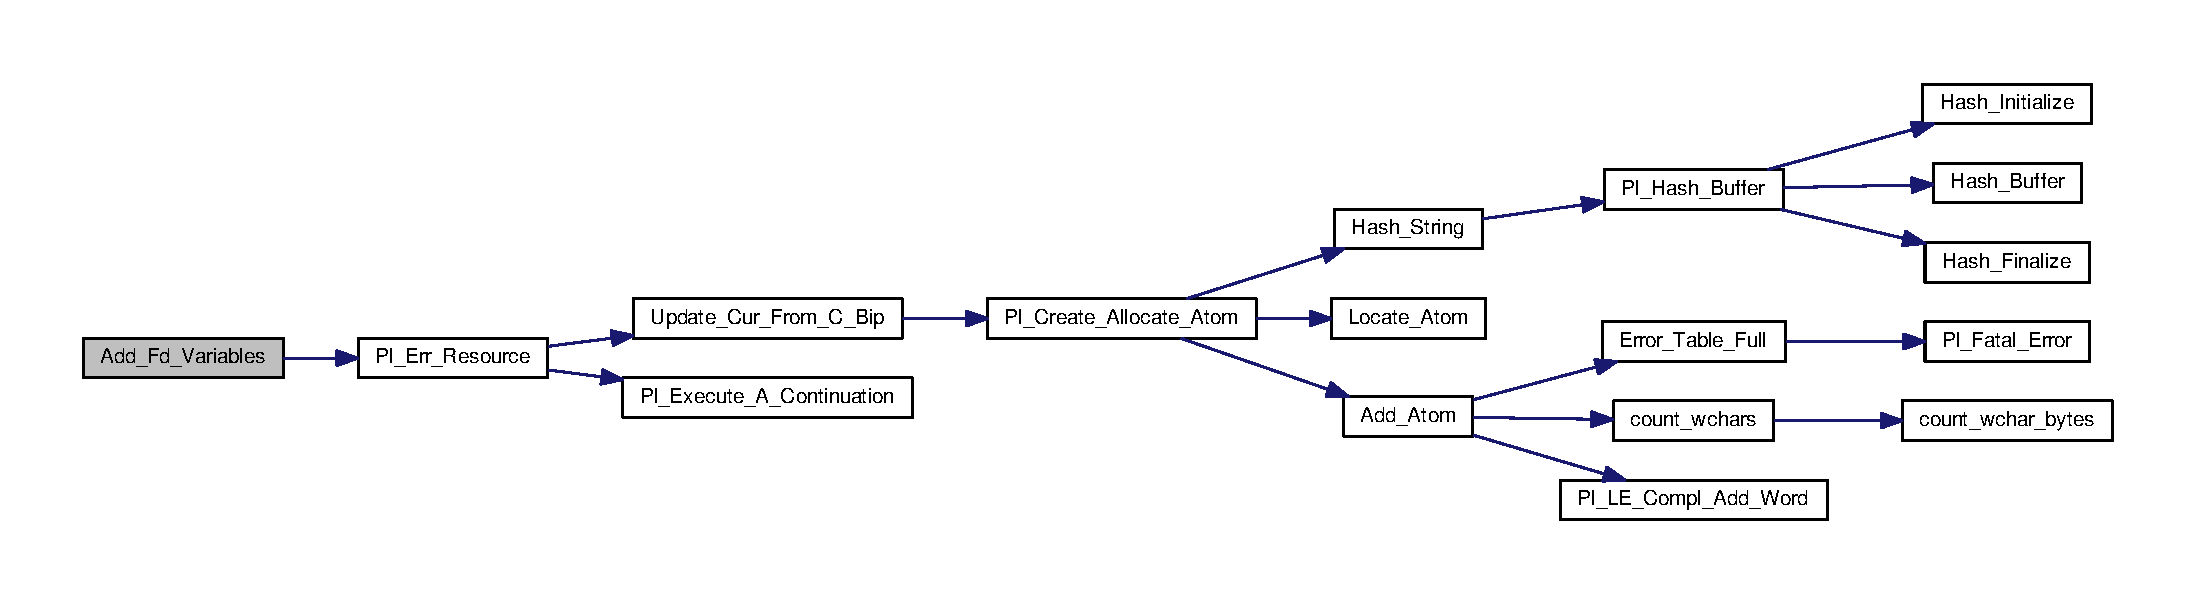
\includegraphics[width=350pt]{fd__bool__c_8c_a21eaa9305603d70618e81dbcc5ea5570_cgraph}
\end{center}
\end{figure}




Here is the caller graph for this function\+:\nopagebreak
\begin{figure}[H]
\begin{center}
\leavevmode
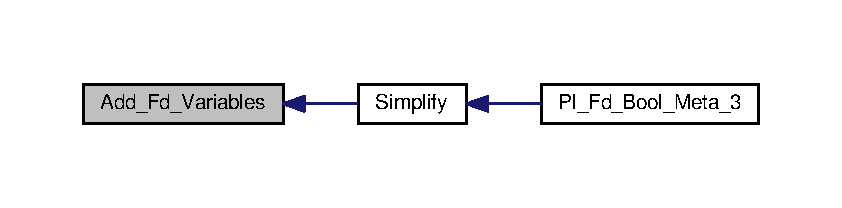
\includegraphics[width=350pt]{fd__bool__c_8c_a21eaa9305603d70618e81dbcc5ea5570_icgraph}
\end{center}
\end{figure}


\index{fd\+\_\+bool\+\_\+c.\+c@{fd\+\_\+bool\+\_\+c.\+c}!Fd\+\_\+\+Bool\+\_\+\+Initializer@{Fd\+\_\+\+Bool\+\_\+\+Initializer}}
\index{Fd\+\_\+\+Bool\+\_\+\+Initializer@{Fd\+\_\+\+Bool\+\_\+\+Initializer}!fd\+\_\+bool\+\_\+c.\+c@{fd\+\_\+bool\+\_\+c.\+c}}
\subsubsection[{\texorpdfstring{Fd\+\_\+\+Bool\+\_\+\+Initializer(void)}{Fd_Bool_Initializer(void)}}]{\setlength{\rightskip}{0pt plus 5cm}static void Fd\+\_\+\+Bool\+\_\+\+Initializer (
\begin{DoxyParamCaption}
\item[{void}]{}
\end{DoxyParamCaption}
)\hspace{0.3cm}{\ttfamily [static]}}\hypertarget{fd__bool__c_8c_a1a75f6073da95705cad602b580443664}{}\label{fd__bool__c_8c_a1a75f6073da95705cad602b580443664}


Here is the call graph for this function\+:\nopagebreak
\begin{figure}[H]
\begin{center}
\leavevmode
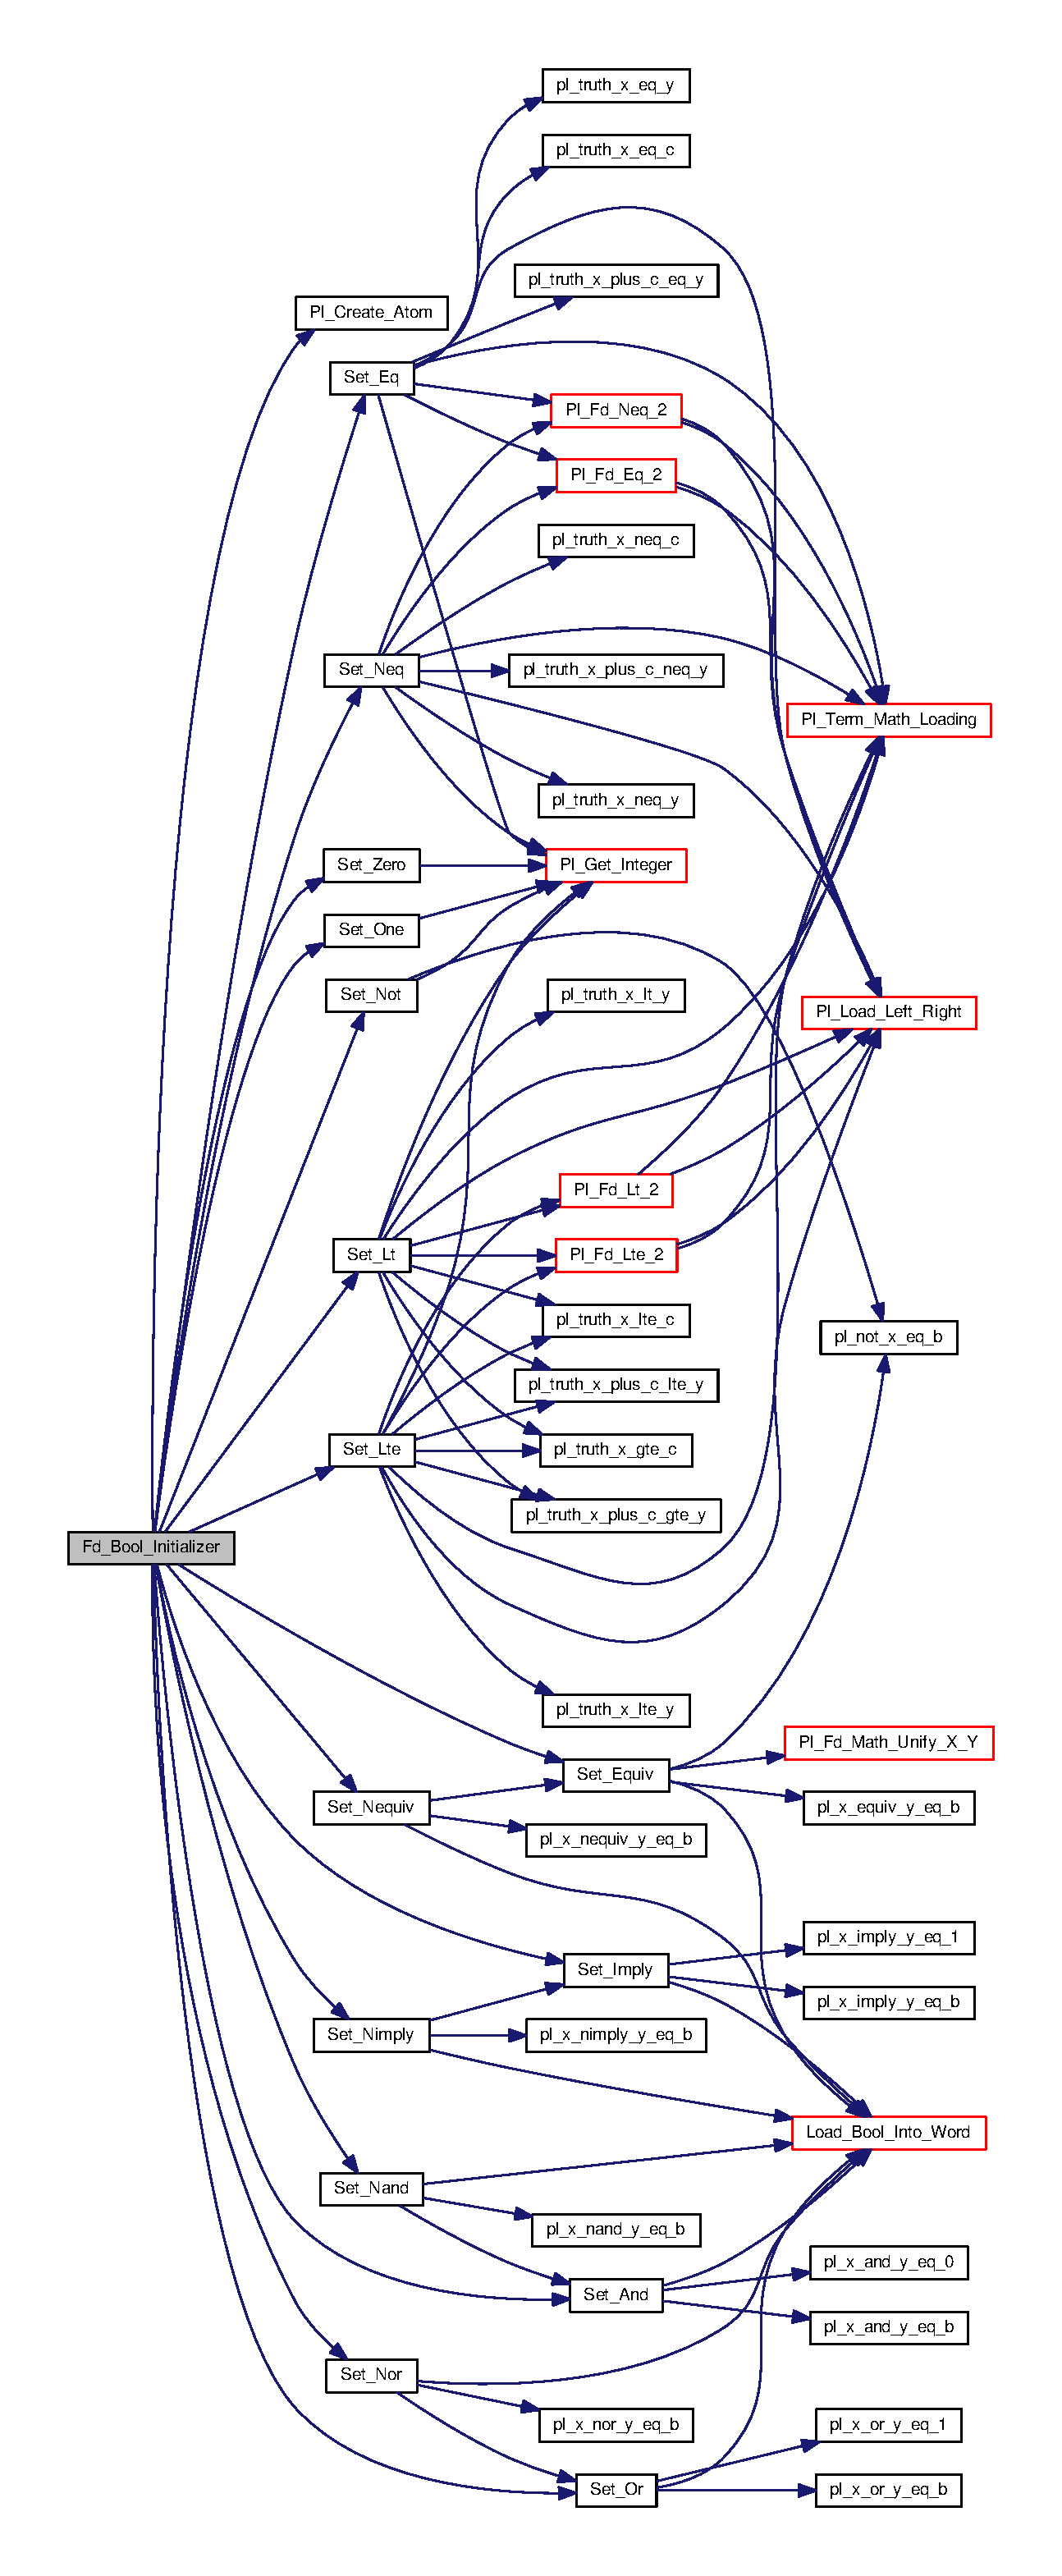
\includegraphics[height=550pt]{fd__bool__c_8c_a1a75f6073da95705cad602b580443664_cgraph}
\end{center}
\end{figure}


\index{fd\+\_\+bool\+\_\+c.\+c@{fd\+\_\+bool\+\_\+c.\+c}!Load\+\_\+\+Bool\+\_\+\+Into\+\_\+\+Word@{Load\+\_\+\+Bool\+\_\+\+Into\+\_\+\+Word}}
\index{Load\+\_\+\+Bool\+\_\+\+Into\+\_\+\+Word@{Load\+\_\+\+Bool\+\_\+\+Into\+\_\+\+Word}!fd\+\_\+bool\+\_\+c.\+c@{fd\+\_\+bool\+\_\+c.\+c}}
\subsubsection[{\texorpdfstring{Load\+\_\+\+Bool\+\_\+\+Into\+\_\+\+Word(\+Wam\+Word $\ast$exp, int result, Wam\+Word $\ast$load\+\_\+word)}{Load_Bool_Into_Word(WamWord *exp, int result, WamWord *load_word)}}]{\setlength{\rightskip}{0pt plus 5cm}static {\bf Bool} Load\+\_\+\+Bool\+\_\+\+Into\+\_\+\+Word (
\begin{DoxyParamCaption}
\item[{{\bf Wam\+Word} $\ast$}]{exp, }
\item[{int}]{result, }
\item[{{\bf Wam\+Word} $\ast$}]{load\+\_\+word}
\end{DoxyParamCaption}
)\hspace{0.3cm}{\ttfamily [static]}}\hypertarget{fd__bool__c_8c_a777cdb1b2fda63d69b759553fd15ea75}{}\label{fd__bool__c_8c_a777cdb1b2fda63d69b759553fd15ea75}


Here is the call graph for this function\+:\nopagebreak
\begin{figure}[H]
\begin{center}
\leavevmode
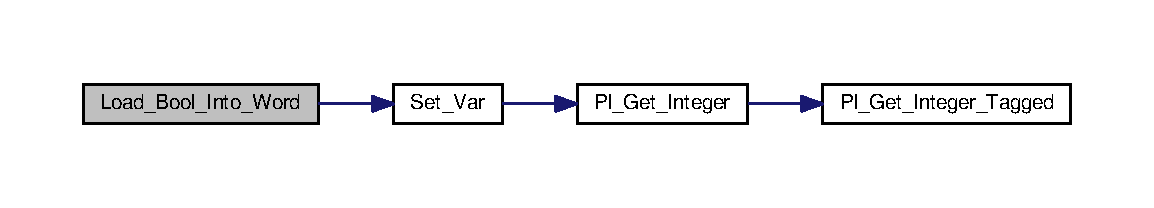
\includegraphics[width=350pt]{fd__bool__c_8c_a777cdb1b2fda63d69b759553fd15ea75_cgraph}
\end{center}
\end{figure}




Here is the caller graph for this function\+:\nopagebreak
\begin{figure}[H]
\begin{center}
\leavevmode
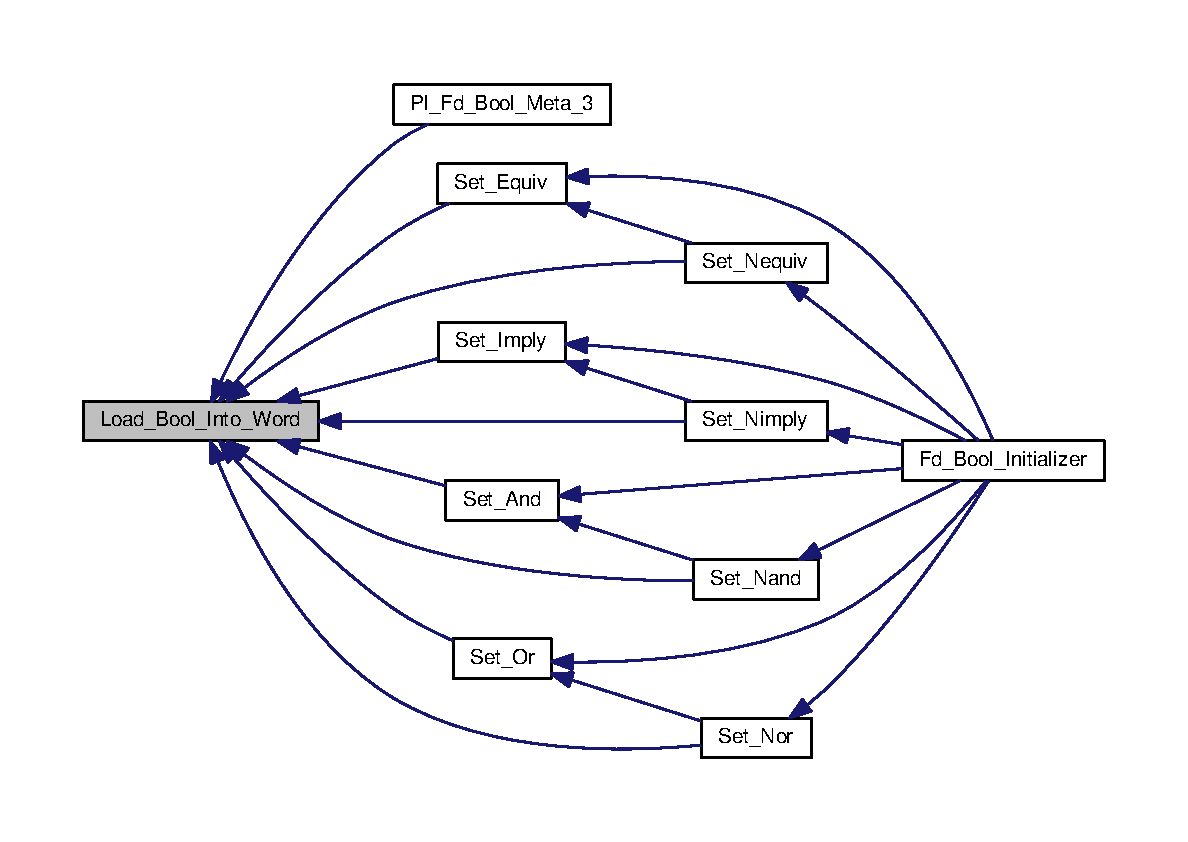
\includegraphics[width=350pt]{fd__bool__c_8c_a777cdb1b2fda63d69b759553fd15ea75_icgraph}
\end{center}
\end{figure}


\index{fd\+\_\+bool\+\_\+c.\+c@{fd\+\_\+bool\+\_\+c.\+c}!Pl\+\_\+\+Fd\+\_\+\+Bool\+\_\+\+Meta\+\_\+3@{Pl\+\_\+\+Fd\+\_\+\+Bool\+\_\+\+Meta\+\_\+3}}
\index{Pl\+\_\+\+Fd\+\_\+\+Bool\+\_\+\+Meta\+\_\+3@{Pl\+\_\+\+Fd\+\_\+\+Bool\+\_\+\+Meta\+\_\+3}!fd\+\_\+bool\+\_\+c.\+c@{fd\+\_\+bool\+\_\+c.\+c}}
\subsubsection[{\texorpdfstring{Pl\+\_\+\+Fd\+\_\+\+Bool\+\_\+\+Meta\+\_\+3(\+Wam\+Word le\+\_\+word, Wam\+Word re\+\_\+word, Wam\+Word op\+\_\+word)}{Pl_Fd_Bool_Meta_3(WamWord le_word, WamWord re_word, WamWord op_word)}}]{\setlength{\rightskip}{0pt plus 5cm}{\bf Bool} Pl\+\_\+\+Fd\+\_\+\+Bool\+\_\+\+Meta\+\_\+3 (
\begin{DoxyParamCaption}
\item[{{\bf Wam\+Word}}]{le\+\_\+word, }
\item[{{\bf Wam\+Word}}]{re\+\_\+word, }
\item[{{\bf Wam\+Word}}]{op\+\_\+word}
\end{DoxyParamCaption}
)}\hypertarget{fd__bool__c_8c_af216d1fd11aff1fa2cb04c7ead09615f}{}\label{fd__bool__c_8c_af216d1fd11aff1fa2cb04c7ead09615f}


Here is the call graph for this function\+:\nopagebreak
\begin{figure}[H]
\begin{center}
\leavevmode
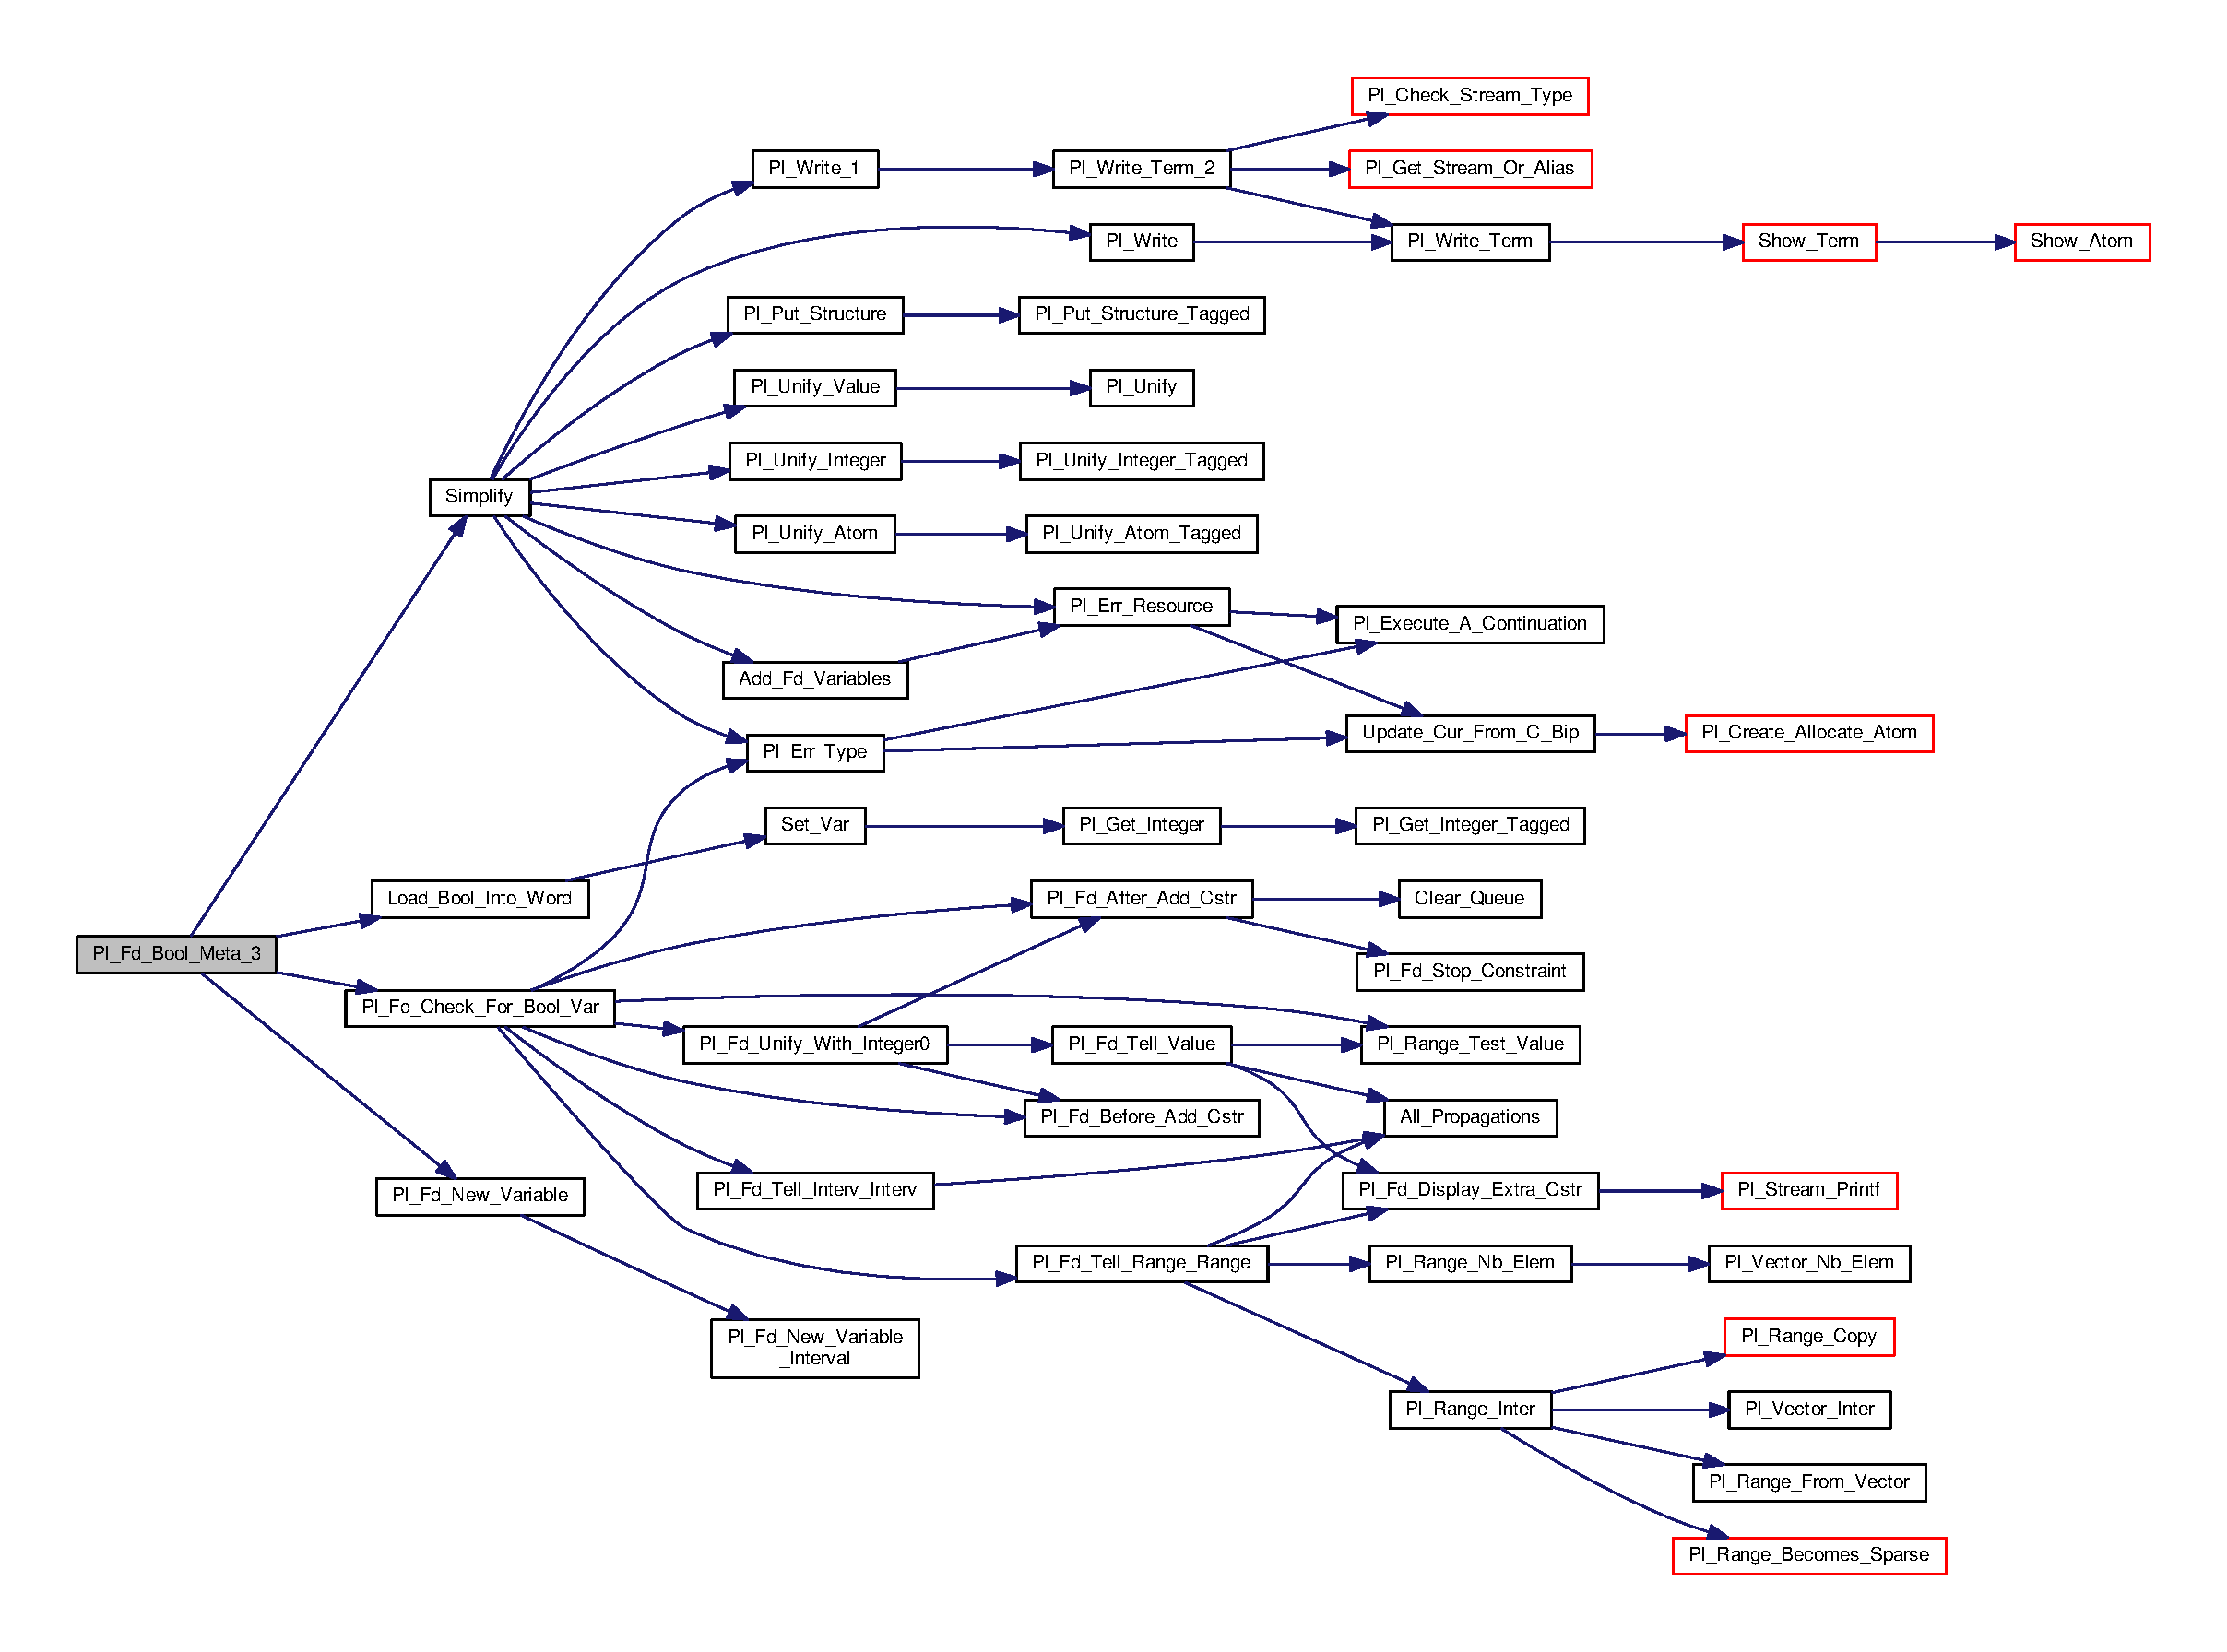
\includegraphics[width=350pt]{fd__bool__c_8c_af216d1fd11aff1fa2cb04c7ead09615f_cgraph}
\end{center}
\end{figure}


\index{fd\+\_\+bool\+\_\+c.\+c@{fd\+\_\+bool\+\_\+c.\+c}!Pl\+\_\+\+Fd\+\_\+\+Eq\+\_\+2@{Pl\+\_\+\+Fd\+\_\+\+Eq\+\_\+2}}
\index{Pl\+\_\+\+Fd\+\_\+\+Eq\+\_\+2@{Pl\+\_\+\+Fd\+\_\+\+Eq\+\_\+2}!fd\+\_\+bool\+\_\+c.\+c@{fd\+\_\+bool\+\_\+c.\+c}}
\subsubsection[{\texorpdfstring{Pl\+\_\+\+Fd\+\_\+\+Eq\+\_\+2(\+Wam\+Word le\+\_\+word, Wam\+Word re\+\_\+word)}{Pl_Fd_Eq_2(WamWord le_word, WamWord re_word)}}]{\setlength{\rightskip}{0pt plus 5cm}{\bf Bool} Pl\+\_\+\+Fd\+\_\+\+Eq\+\_\+2 (
\begin{DoxyParamCaption}
\item[{{\bf Wam\+Word}}]{le\+\_\+word, }
\item[{{\bf Wam\+Word}}]{re\+\_\+word}
\end{DoxyParamCaption}
)}\hypertarget{fd__bool__c_8c_a9e1a8c3a27ce4468f0ed5374a6ec3be8}{}\label{fd__bool__c_8c_a9e1a8c3a27ce4468f0ed5374a6ec3be8}


Here is the call graph for this function\+:\nopagebreak
\begin{figure}[H]
\begin{center}
\leavevmode
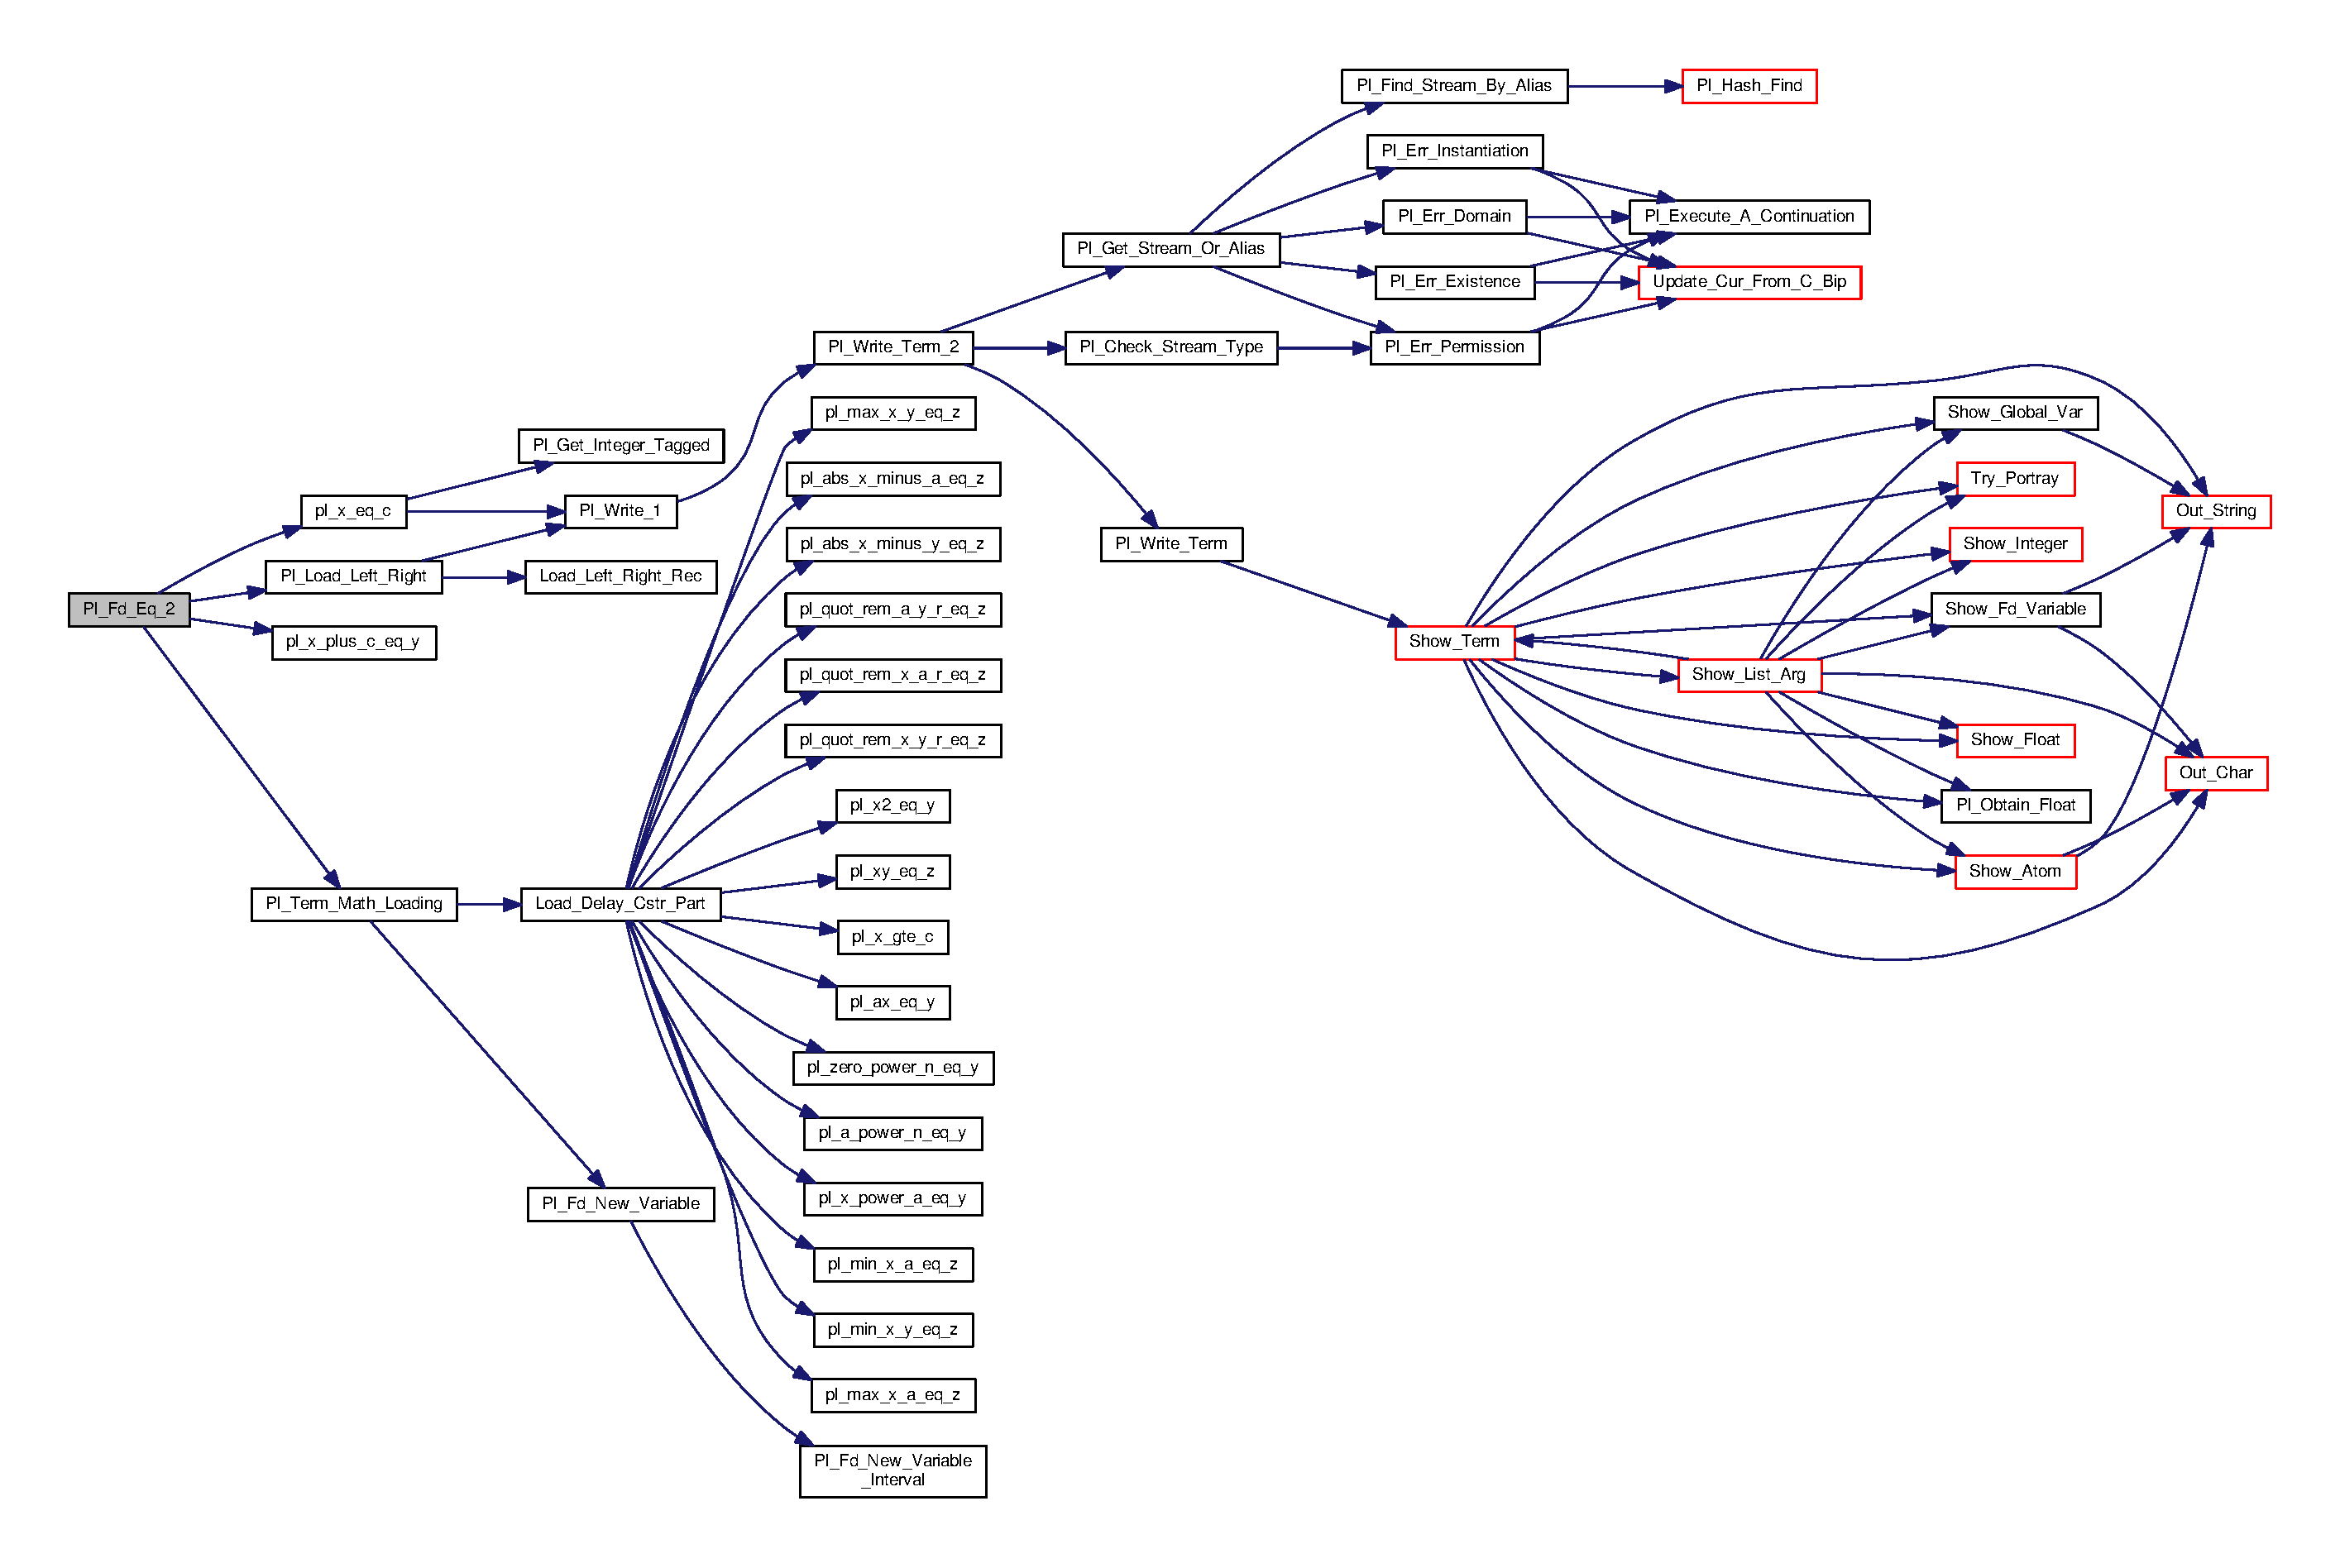
\includegraphics[width=350pt]{fd__bool__c_8c_a9e1a8c3a27ce4468f0ed5374a6ec3be8_cgraph}
\end{center}
\end{figure}




Here is the caller graph for this function\+:\nopagebreak
\begin{figure}[H]
\begin{center}
\leavevmode
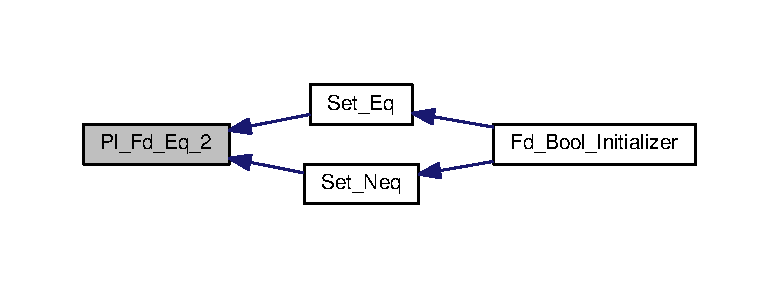
\includegraphics[width=350pt]{fd__bool__c_8c_a9e1a8c3a27ce4468f0ed5374a6ec3be8_icgraph}
\end{center}
\end{figure}


\index{fd\+\_\+bool\+\_\+c.\+c@{fd\+\_\+bool\+\_\+c.\+c}!Pl\+\_\+\+Fd\+\_\+\+Lt\+\_\+2@{Pl\+\_\+\+Fd\+\_\+\+Lt\+\_\+2}}
\index{Pl\+\_\+\+Fd\+\_\+\+Lt\+\_\+2@{Pl\+\_\+\+Fd\+\_\+\+Lt\+\_\+2}!fd\+\_\+bool\+\_\+c.\+c@{fd\+\_\+bool\+\_\+c.\+c}}
\subsubsection[{\texorpdfstring{Pl\+\_\+\+Fd\+\_\+\+Lt\+\_\+2(\+Wam\+Word le\+\_\+word, Wam\+Word re\+\_\+word)}{Pl_Fd_Lt_2(WamWord le_word, WamWord re_word)}}]{\setlength{\rightskip}{0pt plus 5cm}{\bf Bool} Pl\+\_\+\+Fd\+\_\+\+Lt\+\_\+2 (
\begin{DoxyParamCaption}
\item[{{\bf Wam\+Word}}]{le\+\_\+word, }
\item[{{\bf Wam\+Word}}]{re\+\_\+word}
\end{DoxyParamCaption}
)}\hypertarget{fd__bool__c_8c_ae004cace9b53b08de59be0a195274e23}{}\label{fd__bool__c_8c_ae004cace9b53b08de59be0a195274e23}


Here is the call graph for this function\+:\nopagebreak
\begin{figure}[H]
\begin{center}
\leavevmode
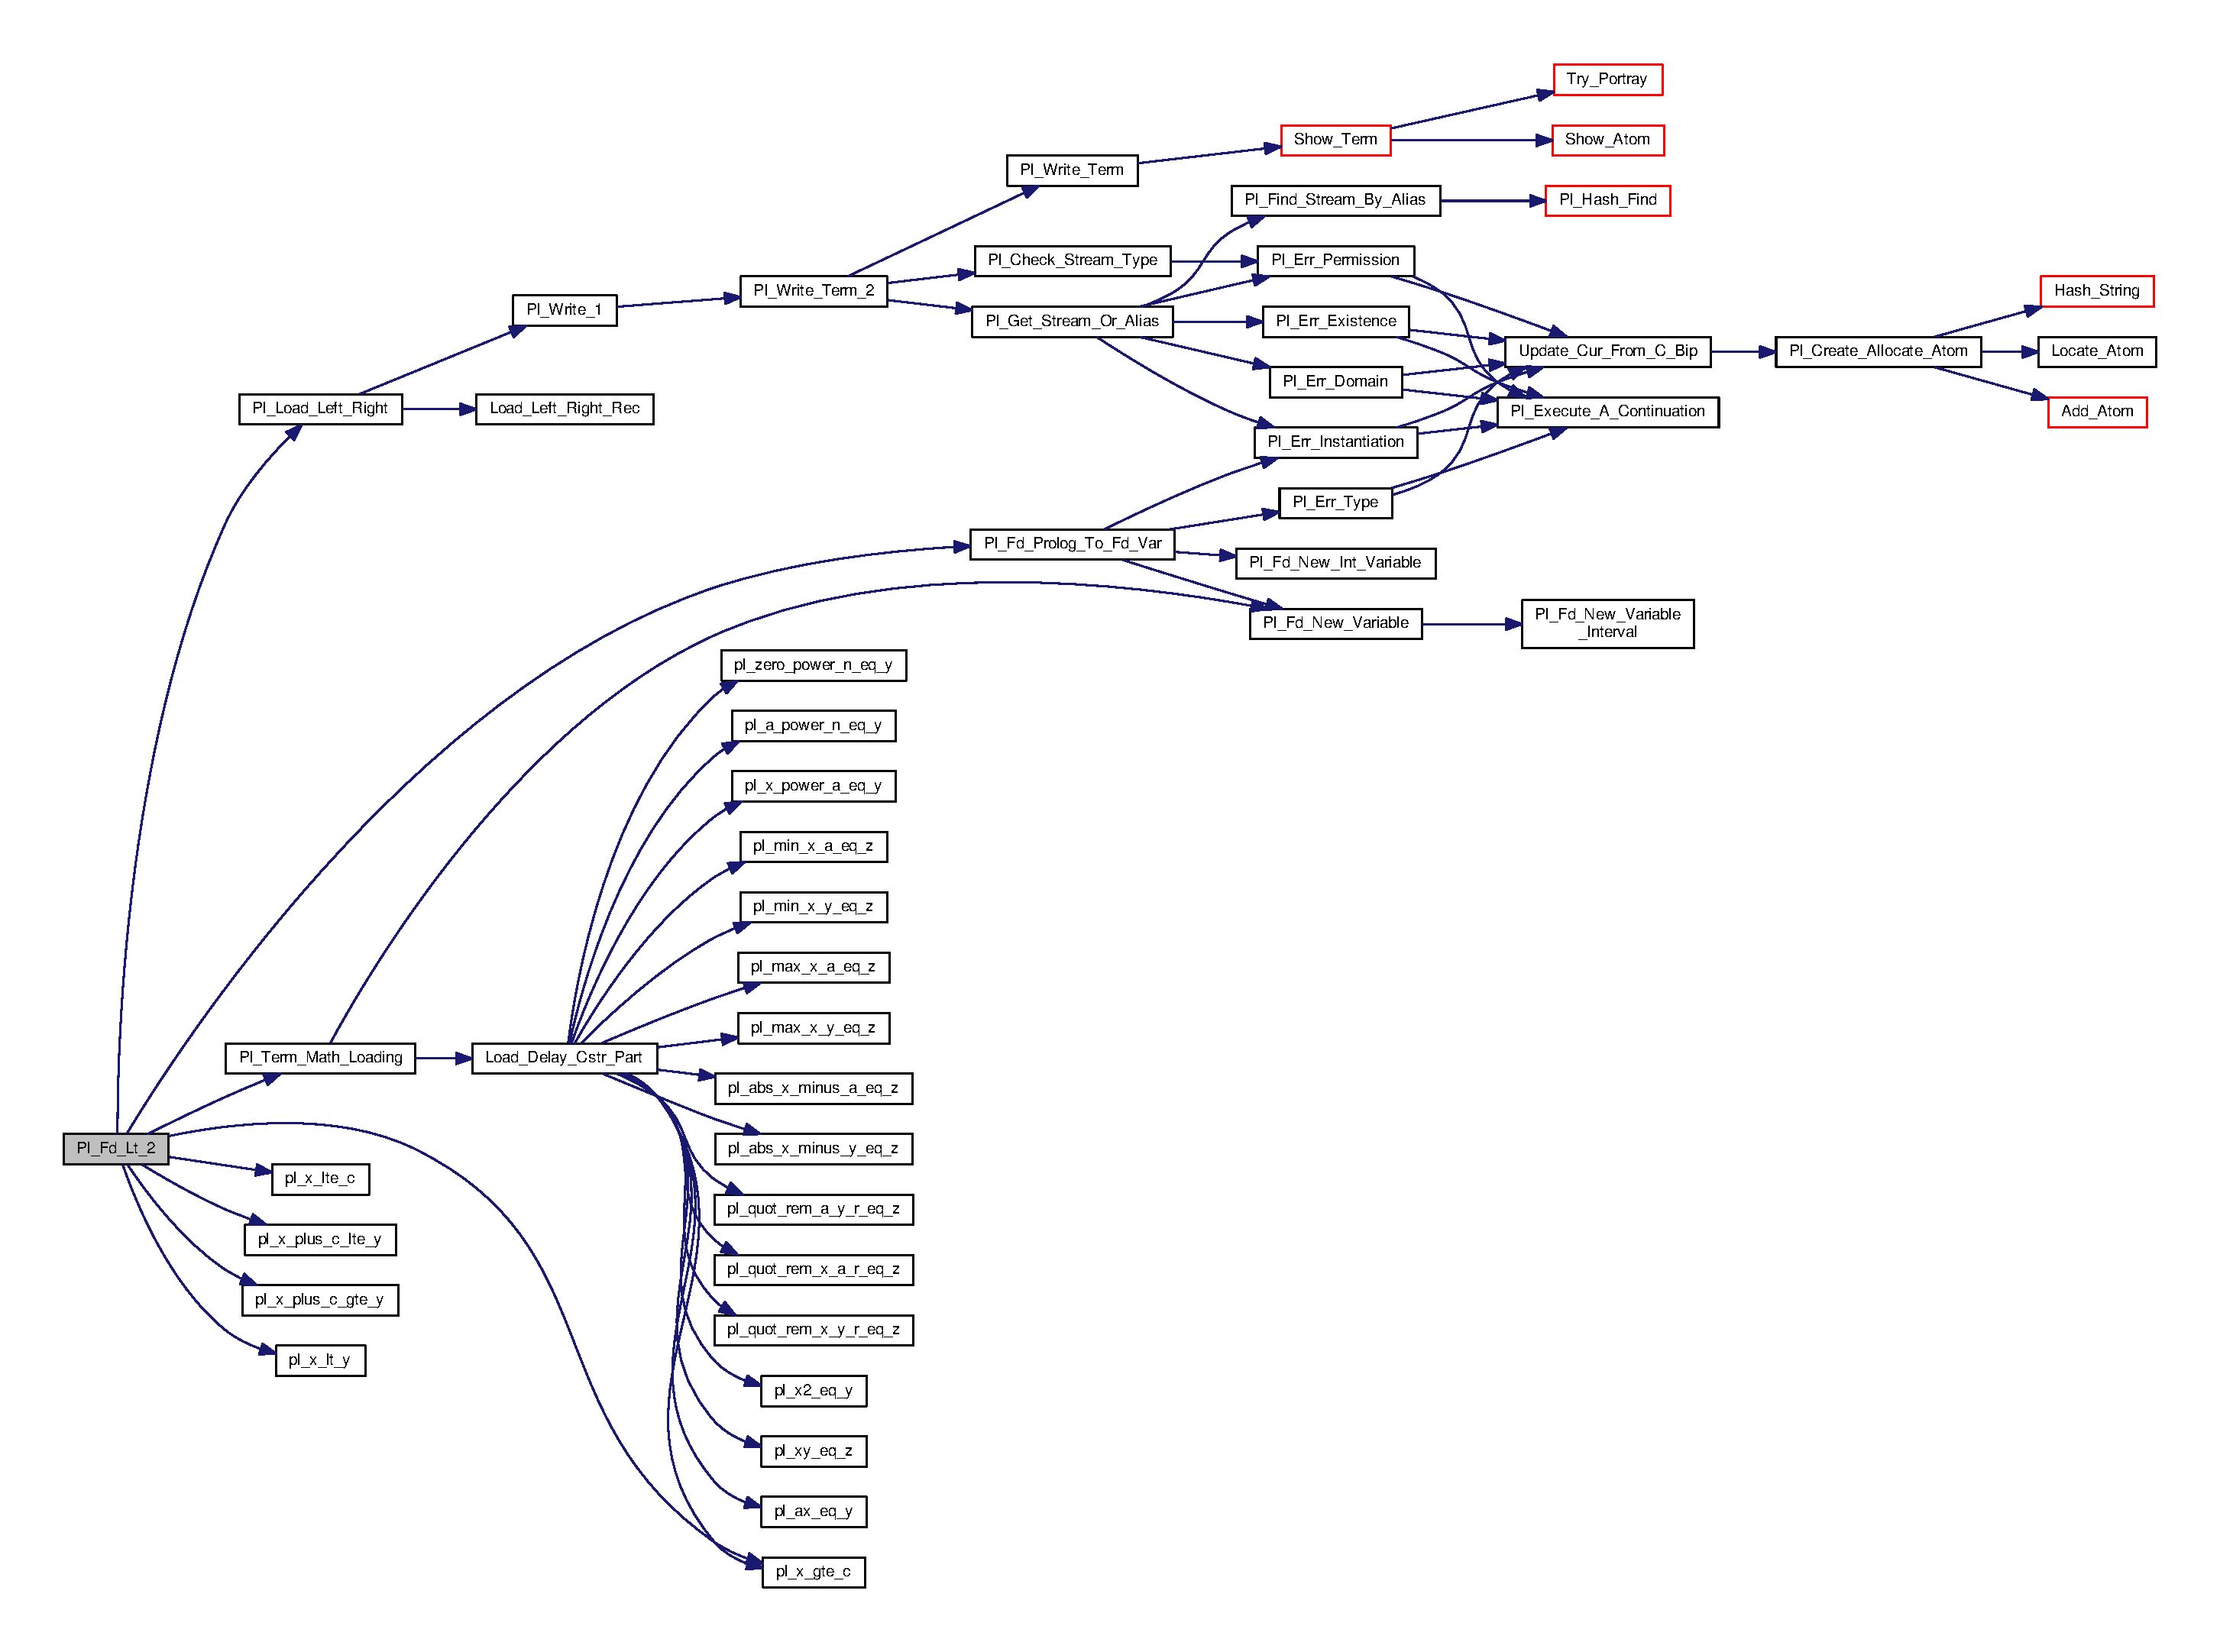
\includegraphics[width=350pt]{fd__bool__c_8c_ae004cace9b53b08de59be0a195274e23_cgraph}
\end{center}
\end{figure}




Here is the caller graph for this function\+:\nopagebreak
\begin{figure}[H]
\begin{center}
\leavevmode
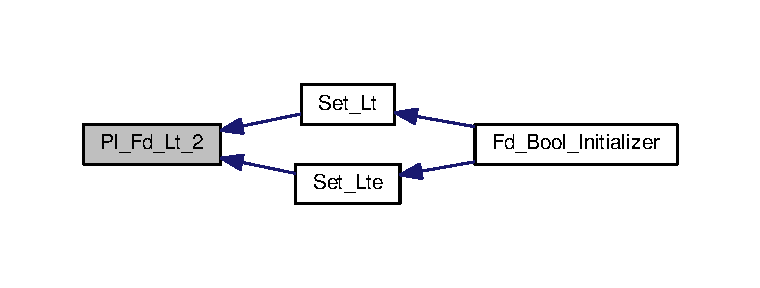
\includegraphics[width=350pt]{fd__bool__c_8c_ae004cace9b53b08de59be0a195274e23_icgraph}
\end{center}
\end{figure}


\index{fd\+\_\+bool\+\_\+c.\+c@{fd\+\_\+bool\+\_\+c.\+c}!Pl\+\_\+\+Fd\+\_\+\+Lte\+\_\+2@{Pl\+\_\+\+Fd\+\_\+\+Lte\+\_\+2}}
\index{Pl\+\_\+\+Fd\+\_\+\+Lte\+\_\+2@{Pl\+\_\+\+Fd\+\_\+\+Lte\+\_\+2}!fd\+\_\+bool\+\_\+c.\+c@{fd\+\_\+bool\+\_\+c.\+c}}
\subsubsection[{\texorpdfstring{Pl\+\_\+\+Fd\+\_\+\+Lte\+\_\+2(\+Wam\+Word le\+\_\+word, Wam\+Word re\+\_\+word)}{Pl_Fd_Lte_2(WamWord le_word, WamWord re_word)}}]{\setlength{\rightskip}{0pt plus 5cm}{\bf Bool} Pl\+\_\+\+Fd\+\_\+\+Lte\+\_\+2 (
\begin{DoxyParamCaption}
\item[{{\bf Wam\+Word}}]{le\+\_\+word, }
\item[{{\bf Wam\+Word}}]{re\+\_\+word}
\end{DoxyParamCaption}
)}\hypertarget{fd__bool__c_8c_a4533c1990d3146b76bed10bbaa4d67d7}{}\label{fd__bool__c_8c_a4533c1990d3146b76bed10bbaa4d67d7}


Here is the call graph for this function\+:\nopagebreak
\begin{figure}[H]
\begin{center}
\leavevmode
\includegraphics[width=350pt]{fd__bool__c_8c_a4533c1990d3146b76bed10bbaa4d67d7_cgraph}
\end{center}
\end{figure}




Here is the caller graph for this function\+:\nopagebreak
\begin{figure}[H]
\begin{center}
\leavevmode
\includegraphics[width=350pt]{fd__bool__c_8c_a4533c1990d3146b76bed10bbaa4d67d7_icgraph}
\end{center}
\end{figure}


\index{fd\+\_\+bool\+\_\+c.\+c@{fd\+\_\+bool\+\_\+c.\+c}!Pl\+\_\+\+Fd\+\_\+\+Neq\+\_\+2@{Pl\+\_\+\+Fd\+\_\+\+Neq\+\_\+2}}
\index{Pl\+\_\+\+Fd\+\_\+\+Neq\+\_\+2@{Pl\+\_\+\+Fd\+\_\+\+Neq\+\_\+2}!fd\+\_\+bool\+\_\+c.\+c@{fd\+\_\+bool\+\_\+c.\+c}}
\subsubsection[{\texorpdfstring{Pl\+\_\+\+Fd\+\_\+\+Neq\+\_\+2(\+Wam\+Word le\+\_\+word, Wam\+Word re\+\_\+word)}{Pl_Fd_Neq_2(WamWord le_word, WamWord re_word)}}]{\setlength{\rightskip}{0pt plus 5cm}{\bf Bool} Pl\+\_\+\+Fd\+\_\+\+Neq\+\_\+2 (
\begin{DoxyParamCaption}
\item[{{\bf Wam\+Word}}]{le\+\_\+word, }
\item[{{\bf Wam\+Word}}]{re\+\_\+word}
\end{DoxyParamCaption}
)}\hypertarget{fd__bool__c_8c_ae96f8c98794a44b1577707920fda688d}{}\label{fd__bool__c_8c_ae96f8c98794a44b1577707920fda688d}


Here is the call graph for this function\+:\nopagebreak
\begin{figure}[H]
\begin{center}
\leavevmode
\includegraphics[width=350pt]{fd__bool__c_8c_ae96f8c98794a44b1577707920fda688d_cgraph}
\end{center}
\end{figure}




Here is the caller graph for this function\+:\nopagebreak
\begin{figure}[H]
\begin{center}
\leavevmode
\includegraphics[width=350pt]{fd__bool__c_8c_ae96f8c98794a44b1577707920fda688d_icgraph}
\end{center}
\end{figure}


\index{fd\+\_\+bool\+\_\+c.\+c@{fd\+\_\+bool\+\_\+c.\+c}!Pl\+\_\+\+Fd\+\_\+\+Reified\+\_\+\+In@{Pl\+\_\+\+Fd\+\_\+\+Reified\+\_\+\+In}}
\index{Pl\+\_\+\+Fd\+\_\+\+Reified\+\_\+\+In@{Pl\+\_\+\+Fd\+\_\+\+Reified\+\_\+\+In}!fd\+\_\+bool\+\_\+c.\+c@{fd\+\_\+bool\+\_\+c.\+c}}
\subsubsection[{\texorpdfstring{Pl\+\_\+\+Fd\+\_\+\+Reified\+\_\+\+In(\+Wam\+Word x\+\_\+word, Wam\+Word l\+\_\+word, Wam\+Word u\+\_\+word, Wam\+Word b\+\_\+word)}{Pl_Fd_Reified_In(WamWord x_word, WamWord l_word, WamWord u_word, WamWord b_word)}}]{\setlength{\rightskip}{0pt plus 5cm}{\bf Bool} Pl\+\_\+\+Fd\+\_\+\+Reified\+\_\+\+In (
\begin{DoxyParamCaption}
\item[{{\bf Wam\+Word}}]{x\+\_\+word, }
\item[{{\bf Wam\+Word}}]{l\+\_\+word, }
\item[{{\bf Wam\+Word}}]{u\+\_\+word, }
\item[{{\bf Wam\+Word}}]{b\+\_\+word}
\end{DoxyParamCaption}
)}\hypertarget{fd__bool__c_8c_aad0a445c9905cdb15eeb91e0dc38c0dd}{}\label{fd__bool__c_8c_aad0a445c9905cdb15eeb91e0dc38c0dd}


Here is the call graph for this function\+:\nopagebreak
\begin{figure}[H]
\begin{center}
\leavevmode
\includegraphics[width=350pt]{fd__bool__c_8c_aad0a445c9905cdb15eeb91e0dc38c0dd_cgraph}
\end{center}
\end{figure}


\index{fd\+\_\+bool\+\_\+c.\+c@{fd\+\_\+bool\+\_\+c.\+c}!Set\+\_\+\+And@{Set\+\_\+\+And}}
\index{Set\+\_\+\+And@{Set\+\_\+\+And}!fd\+\_\+bool\+\_\+c.\+c@{fd\+\_\+bool\+\_\+c.\+c}}
\subsubsection[{\texorpdfstring{Set\+\_\+\+And(\+Wam\+Word $\ast$exp, int result, Wam\+Word $\ast$load\+\_\+word)}{Set_And(WamWord *exp, int result, WamWord *load_word)}}]{\setlength{\rightskip}{0pt plus 5cm}static {\bf Bool} Set\+\_\+\+And (
\begin{DoxyParamCaption}
\item[{{\bf Wam\+Word} $\ast$}]{exp, }
\item[{int}]{result, }
\item[{{\bf Wam\+Word} $\ast$}]{load\+\_\+word}
\end{DoxyParamCaption}
)\hspace{0.3cm}{\ttfamily [static]}}\hypertarget{fd__bool__c_8c_ae7e33aab925722ca962447b9c534aaad}{}\label{fd__bool__c_8c_ae7e33aab925722ca962447b9c534aaad}


Here is the call graph for this function\+:\nopagebreak
\begin{figure}[H]
\begin{center}
\leavevmode
\includegraphics[width=350pt]{fd__bool__c_8c_ae7e33aab925722ca962447b9c534aaad_cgraph}
\end{center}
\end{figure}




Here is the caller graph for this function\+:\nopagebreak
\begin{figure}[H]
\begin{center}
\leavevmode
\includegraphics[width=350pt]{fd__bool__c_8c_ae7e33aab925722ca962447b9c534aaad_icgraph}
\end{center}
\end{figure}


\index{fd\+\_\+bool\+\_\+c.\+c@{fd\+\_\+bool\+\_\+c.\+c}!Set\+\_\+\+Eq@{Set\+\_\+\+Eq}}
\index{Set\+\_\+\+Eq@{Set\+\_\+\+Eq}!fd\+\_\+bool\+\_\+c.\+c@{fd\+\_\+bool\+\_\+c.\+c}}
\subsubsection[{\texorpdfstring{Set\+\_\+\+Eq(\+Wam\+Word $\ast$exp, int result, Wam\+Word $\ast$load\+\_\+word)}{Set_Eq(WamWord *exp, int result, WamWord *load_word)}}]{\setlength{\rightskip}{0pt plus 5cm}static {\bf Bool} Set\+\_\+\+Eq (
\begin{DoxyParamCaption}
\item[{{\bf Wam\+Word} $\ast$}]{exp, }
\item[{int}]{result, }
\item[{{\bf Wam\+Word} $\ast$}]{load\+\_\+word}
\end{DoxyParamCaption}
)\hspace{0.3cm}{\ttfamily [static]}}\hypertarget{fd__bool__c_8c_a3bcf220164d47e110f64a089daebf2a7}{}\label{fd__bool__c_8c_a3bcf220164d47e110f64a089daebf2a7}


Here is the call graph for this function\+:\nopagebreak
\begin{figure}[H]
\begin{center}
\leavevmode
\includegraphics[width=350pt]{fd__bool__c_8c_a3bcf220164d47e110f64a089daebf2a7_cgraph}
\end{center}
\end{figure}




Here is the caller graph for this function\+:\nopagebreak
\begin{figure}[H]
\begin{center}
\leavevmode
\includegraphics[width=262pt]{fd__bool__c_8c_a3bcf220164d47e110f64a089daebf2a7_icgraph}
\end{center}
\end{figure}


\index{fd\+\_\+bool\+\_\+c.\+c@{fd\+\_\+bool\+\_\+c.\+c}!Set\+\_\+\+Equiv@{Set\+\_\+\+Equiv}}
\index{Set\+\_\+\+Equiv@{Set\+\_\+\+Equiv}!fd\+\_\+bool\+\_\+c.\+c@{fd\+\_\+bool\+\_\+c.\+c}}
\subsubsection[{\texorpdfstring{Set\+\_\+\+Equiv(\+Wam\+Word $\ast$exp, int result, Wam\+Word $\ast$load\+\_\+word)}{Set_Equiv(WamWord *exp, int result, WamWord *load_word)}}]{\setlength{\rightskip}{0pt plus 5cm}static {\bf Bool} Set\+\_\+\+Equiv (
\begin{DoxyParamCaption}
\item[{{\bf Wam\+Word} $\ast$}]{exp, }
\item[{int}]{result, }
\item[{{\bf Wam\+Word} $\ast$}]{load\+\_\+word}
\end{DoxyParamCaption}
)\hspace{0.3cm}{\ttfamily [static]}}\hypertarget{fd__bool__c_8c_a5756324591779a6e812b6918a33f86d0}{}\label{fd__bool__c_8c_a5756324591779a6e812b6918a33f86d0}


Here is the call graph for this function\+:\nopagebreak
\begin{figure}[H]
\begin{center}
\leavevmode
\includegraphics[width=350pt]{fd__bool__c_8c_a5756324591779a6e812b6918a33f86d0_cgraph}
\end{center}
\end{figure}




Here is the caller graph for this function\+:\nopagebreak
\begin{figure}[H]
\begin{center}
\leavevmode
\includegraphics[width=350pt]{fd__bool__c_8c_a5756324591779a6e812b6918a33f86d0_icgraph}
\end{center}
\end{figure}


\index{fd\+\_\+bool\+\_\+c.\+c@{fd\+\_\+bool\+\_\+c.\+c}!Set\+\_\+\+Imply@{Set\+\_\+\+Imply}}
\index{Set\+\_\+\+Imply@{Set\+\_\+\+Imply}!fd\+\_\+bool\+\_\+c.\+c@{fd\+\_\+bool\+\_\+c.\+c}}
\subsubsection[{\texorpdfstring{Set\+\_\+\+Imply(\+Wam\+Word $\ast$exp, int result, Wam\+Word $\ast$load\+\_\+word)}{Set_Imply(WamWord *exp, int result, WamWord *load_word)}}]{\setlength{\rightskip}{0pt plus 5cm}static {\bf Bool} Set\+\_\+\+Imply (
\begin{DoxyParamCaption}
\item[{{\bf Wam\+Word} $\ast$}]{exp, }
\item[{int}]{result, }
\item[{{\bf Wam\+Word} $\ast$}]{load\+\_\+word}
\end{DoxyParamCaption}
)\hspace{0.3cm}{\ttfamily [static]}}\hypertarget{fd__bool__c_8c_a57de1f881f34824fc0001b63989af13e}{}\label{fd__bool__c_8c_a57de1f881f34824fc0001b63989af13e}


Here is the call graph for this function\+:\nopagebreak
\begin{figure}[H]
\begin{center}
\leavevmode
\includegraphics[width=350pt]{fd__bool__c_8c_a57de1f881f34824fc0001b63989af13e_cgraph}
\end{center}
\end{figure}




Here is the caller graph for this function\+:\nopagebreak
\begin{figure}[H]
\begin{center}
\leavevmode
\includegraphics[width=350pt]{fd__bool__c_8c_a57de1f881f34824fc0001b63989af13e_icgraph}
\end{center}
\end{figure}


\index{fd\+\_\+bool\+\_\+c.\+c@{fd\+\_\+bool\+\_\+c.\+c}!Set\+\_\+\+Lt@{Set\+\_\+\+Lt}}
\index{Set\+\_\+\+Lt@{Set\+\_\+\+Lt}!fd\+\_\+bool\+\_\+c.\+c@{fd\+\_\+bool\+\_\+c.\+c}}
\subsubsection[{\texorpdfstring{Set\+\_\+\+Lt(\+Wam\+Word $\ast$exp, int result, Wam\+Word $\ast$load\+\_\+word)}{Set_Lt(WamWord *exp, int result, WamWord *load_word)}}]{\setlength{\rightskip}{0pt plus 5cm}static {\bf Bool} Set\+\_\+\+Lt (
\begin{DoxyParamCaption}
\item[{{\bf Wam\+Word} $\ast$}]{exp, }
\item[{int}]{result, }
\item[{{\bf Wam\+Word} $\ast$}]{load\+\_\+word}
\end{DoxyParamCaption}
)\hspace{0.3cm}{\ttfamily [static]}}\hypertarget{fd__bool__c_8c_ac5b16f713138c6b09fd4b3857d52a881}{}\label{fd__bool__c_8c_ac5b16f713138c6b09fd4b3857d52a881}


Here is the call graph for this function\+:\nopagebreak
\begin{figure}[H]
\begin{center}
\leavevmode
\includegraphics[width=350pt]{fd__bool__c_8c_ac5b16f713138c6b09fd4b3857d52a881_cgraph}
\end{center}
\end{figure}




Here is the caller graph for this function\+:\nopagebreak
\begin{figure}[H]
\begin{center}
\leavevmode
\includegraphics[width=258pt]{fd__bool__c_8c_ac5b16f713138c6b09fd4b3857d52a881_icgraph}
\end{center}
\end{figure}


\index{fd\+\_\+bool\+\_\+c.\+c@{fd\+\_\+bool\+\_\+c.\+c}!Set\+\_\+\+Lte@{Set\+\_\+\+Lte}}
\index{Set\+\_\+\+Lte@{Set\+\_\+\+Lte}!fd\+\_\+bool\+\_\+c.\+c@{fd\+\_\+bool\+\_\+c.\+c}}
\subsubsection[{\texorpdfstring{Set\+\_\+\+Lte(\+Wam\+Word $\ast$exp, int result, Wam\+Word $\ast$load\+\_\+word)}{Set_Lte(WamWord *exp, int result, WamWord *load_word)}}]{\setlength{\rightskip}{0pt plus 5cm}static {\bf Bool} Set\+\_\+\+Lte (
\begin{DoxyParamCaption}
\item[{{\bf Wam\+Word} $\ast$}]{exp, }
\item[{int}]{result, }
\item[{{\bf Wam\+Word} $\ast$}]{load\+\_\+word}
\end{DoxyParamCaption}
)\hspace{0.3cm}{\ttfamily [static]}}\hypertarget{fd__bool__c_8c_a22127daaa654486d40b5c097e040ab87}{}\label{fd__bool__c_8c_a22127daaa654486d40b5c097e040ab87}


Here is the call graph for this function\+:\nopagebreak
\begin{figure}[H]
\begin{center}
\leavevmode
\includegraphics[width=350pt]{fd__bool__c_8c_a22127daaa654486d40b5c097e040ab87_cgraph}
\end{center}
\end{figure}




Here is the caller graph for this function\+:\nopagebreak
\begin{figure}[H]
\begin{center}
\leavevmode
\includegraphics[width=263pt]{fd__bool__c_8c_a22127daaa654486d40b5c097e040ab87_icgraph}
\end{center}
\end{figure}


\index{fd\+\_\+bool\+\_\+c.\+c@{fd\+\_\+bool\+\_\+c.\+c}!Set\+\_\+\+Nand@{Set\+\_\+\+Nand}}
\index{Set\+\_\+\+Nand@{Set\+\_\+\+Nand}!fd\+\_\+bool\+\_\+c.\+c@{fd\+\_\+bool\+\_\+c.\+c}}
\subsubsection[{\texorpdfstring{Set\+\_\+\+Nand(\+Wam\+Word $\ast$exp, int result, Wam\+Word $\ast$load\+\_\+word)}{Set_Nand(WamWord *exp, int result, WamWord *load_word)}}]{\setlength{\rightskip}{0pt plus 5cm}static {\bf Bool} Set\+\_\+\+Nand (
\begin{DoxyParamCaption}
\item[{{\bf Wam\+Word} $\ast$}]{exp, }
\item[{int}]{result, }
\item[{{\bf Wam\+Word} $\ast$}]{load\+\_\+word}
\end{DoxyParamCaption}
)\hspace{0.3cm}{\ttfamily [static]}}\hypertarget{fd__bool__c_8c_ac00f47833dcf0ba051c9bef1289d8ae1}{}\label{fd__bool__c_8c_ac00f47833dcf0ba051c9bef1289d8ae1}


Here is the call graph for this function\+:\nopagebreak
\begin{figure}[H]
\begin{center}
\leavevmode
\includegraphics[width=350pt]{fd__bool__c_8c_ac00f47833dcf0ba051c9bef1289d8ae1_cgraph}
\end{center}
\end{figure}




Here is the caller graph for this function\+:\nopagebreak
\begin{figure}[H]
\begin{center}
\leavevmode
\includegraphics[width=273pt]{fd__bool__c_8c_ac00f47833dcf0ba051c9bef1289d8ae1_icgraph}
\end{center}
\end{figure}


\index{fd\+\_\+bool\+\_\+c.\+c@{fd\+\_\+bool\+\_\+c.\+c}!Set\+\_\+\+Neq@{Set\+\_\+\+Neq}}
\index{Set\+\_\+\+Neq@{Set\+\_\+\+Neq}!fd\+\_\+bool\+\_\+c.\+c@{fd\+\_\+bool\+\_\+c.\+c}}
\subsubsection[{\texorpdfstring{Set\+\_\+\+Neq(\+Wam\+Word $\ast$exp, int result, Wam\+Word $\ast$load\+\_\+word)}{Set_Neq(WamWord *exp, int result, WamWord *load_word)}}]{\setlength{\rightskip}{0pt plus 5cm}static {\bf Bool} Set\+\_\+\+Neq (
\begin{DoxyParamCaption}
\item[{{\bf Wam\+Word} $\ast$}]{exp, }
\item[{int}]{result, }
\item[{{\bf Wam\+Word} $\ast$}]{load\+\_\+word}
\end{DoxyParamCaption}
)\hspace{0.3cm}{\ttfamily [static]}}\hypertarget{fd__bool__c_8c_ad9a88621a0a7d01eb8db4da34faf894f}{}\label{fd__bool__c_8c_ad9a88621a0a7d01eb8db4da34faf894f}


Here is the call graph for this function\+:\nopagebreak
\begin{figure}[H]
\begin{center}
\leavevmode
\includegraphics[width=350pt]{fd__bool__c_8c_ad9a88621a0a7d01eb8db4da34faf894f_cgraph}
\end{center}
\end{figure}




Here is the caller graph for this function\+:\nopagebreak
\begin{figure}[H]
\begin{center}
\leavevmode
\includegraphics[width=268pt]{fd__bool__c_8c_ad9a88621a0a7d01eb8db4da34faf894f_icgraph}
\end{center}
\end{figure}


\index{fd\+\_\+bool\+\_\+c.\+c@{fd\+\_\+bool\+\_\+c.\+c}!Set\+\_\+\+Nequiv@{Set\+\_\+\+Nequiv}}
\index{Set\+\_\+\+Nequiv@{Set\+\_\+\+Nequiv}!fd\+\_\+bool\+\_\+c.\+c@{fd\+\_\+bool\+\_\+c.\+c}}
\subsubsection[{\texorpdfstring{Set\+\_\+\+Nequiv(\+Wam\+Word $\ast$exp, int result, Wam\+Word $\ast$load\+\_\+word)}{Set_Nequiv(WamWord *exp, int result, WamWord *load_word)}}]{\setlength{\rightskip}{0pt plus 5cm}static {\bf Bool} Set\+\_\+\+Nequiv (
\begin{DoxyParamCaption}
\item[{{\bf Wam\+Word} $\ast$}]{exp, }
\item[{int}]{result, }
\item[{{\bf Wam\+Word} $\ast$}]{load\+\_\+word}
\end{DoxyParamCaption}
)\hspace{0.3cm}{\ttfamily [static]}}\hypertarget{fd__bool__c_8c_af0210aef178792fadee8bf8a6fb31b2e}{}\label{fd__bool__c_8c_af0210aef178792fadee8bf8a6fb31b2e}


Here is the call graph for this function\+:\nopagebreak
\begin{figure}[H]
\begin{center}
\leavevmode
\includegraphics[width=350pt]{fd__bool__c_8c_af0210aef178792fadee8bf8a6fb31b2e_cgraph}
\end{center}
\end{figure}




Here is the caller graph for this function\+:\nopagebreak
\begin{figure}[H]
\begin{center}
\leavevmode
\includegraphics[width=281pt]{fd__bool__c_8c_af0210aef178792fadee8bf8a6fb31b2e_icgraph}
\end{center}
\end{figure}


\index{fd\+\_\+bool\+\_\+c.\+c@{fd\+\_\+bool\+\_\+c.\+c}!Set\+\_\+\+Nimply@{Set\+\_\+\+Nimply}}
\index{Set\+\_\+\+Nimply@{Set\+\_\+\+Nimply}!fd\+\_\+bool\+\_\+c.\+c@{fd\+\_\+bool\+\_\+c.\+c}}
\subsubsection[{\texorpdfstring{Set\+\_\+\+Nimply(\+Wam\+Word $\ast$exp, int result, Wam\+Word $\ast$load\+\_\+word)}{Set_Nimply(WamWord *exp, int result, WamWord *load_word)}}]{\setlength{\rightskip}{0pt plus 5cm}static {\bf Bool} Set\+\_\+\+Nimply (
\begin{DoxyParamCaption}
\item[{{\bf Wam\+Word} $\ast$}]{exp, }
\item[{int}]{result, }
\item[{{\bf Wam\+Word} $\ast$}]{load\+\_\+word}
\end{DoxyParamCaption}
)\hspace{0.3cm}{\ttfamily [static]}}\hypertarget{fd__bool__c_8c_a403cef3cce8a6973a624c343ceeb263c}{}\label{fd__bool__c_8c_a403cef3cce8a6973a624c343ceeb263c}


Here is the call graph for this function\+:\nopagebreak
\begin{figure}[H]
\begin{center}
\leavevmode
\includegraphics[width=350pt]{fd__bool__c_8c_a403cef3cce8a6973a624c343ceeb263c_cgraph}
\end{center}
\end{figure}




Here is the caller graph for this function\+:\nopagebreak
\begin{figure}[H]
\begin{center}
\leavevmode
\includegraphics[width=281pt]{fd__bool__c_8c_a403cef3cce8a6973a624c343ceeb263c_icgraph}
\end{center}
\end{figure}


\index{fd\+\_\+bool\+\_\+c.\+c@{fd\+\_\+bool\+\_\+c.\+c}!Set\+\_\+\+Nor@{Set\+\_\+\+Nor}}
\index{Set\+\_\+\+Nor@{Set\+\_\+\+Nor}!fd\+\_\+bool\+\_\+c.\+c@{fd\+\_\+bool\+\_\+c.\+c}}
\subsubsection[{\texorpdfstring{Set\+\_\+\+Nor(\+Wam\+Word $\ast$exp, int result, Wam\+Word $\ast$load\+\_\+word)}{Set_Nor(WamWord *exp, int result, WamWord *load_word)}}]{\setlength{\rightskip}{0pt plus 5cm}static {\bf Bool} Set\+\_\+\+Nor (
\begin{DoxyParamCaption}
\item[{{\bf Wam\+Word} $\ast$}]{exp, }
\item[{int}]{result, }
\item[{{\bf Wam\+Word} $\ast$}]{load\+\_\+word}
\end{DoxyParamCaption}
)\hspace{0.3cm}{\ttfamily [static]}}\hypertarget{fd__bool__c_8c_a6e219be09aeaa78621e2fdc0aa3b70d0}{}\label{fd__bool__c_8c_a6e219be09aeaa78621e2fdc0aa3b70d0}


Here is the call graph for this function\+:\nopagebreak
\begin{figure}[H]
\begin{center}
\leavevmode
\includegraphics[width=350pt]{fd__bool__c_8c_a6e219be09aeaa78621e2fdc0aa3b70d0_cgraph}
\end{center}
\end{figure}




Here is the caller graph for this function\+:\nopagebreak
\begin{figure}[H]
\begin{center}
\leavevmode
\includegraphics[width=266pt]{fd__bool__c_8c_a6e219be09aeaa78621e2fdc0aa3b70d0_icgraph}
\end{center}
\end{figure}


\index{fd\+\_\+bool\+\_\+c.\+c@{fd\+\_\+bool\+\_\+c.\+c}!Set\+\_\+\+Not@{Set\+\_\+\+Not}}
\index{Set\+\_\+\+Not@{Set\+\_\+\+Not}!fd\+\_\+bool\+\_\+c.\+c@{fd\+\_\+bool\+\_\+c.\+c}}
\subsubsection[{\texorpdfstring{Set\+\_\+\+Not(\+Wam\+Word $\ast$exp, int result, Wam\+Word $\ast$load\+\_\+word)}{Set_Not(WamWord *exp, int result, WamWord *load_word)}}]{\setlength{\rightskip}{0pt plus 5cm}static {\bf Bool} Set\+\_\+\+Not (
\begin{DoxyParamCaption}
\item[{{\bf Wam\+Word} $\ast$}]{exp, }
\item[{int}]{result, }
\item[{{\bf Wam\+Word} $\ast$}]{load\+\_\+word}
\end{DoxyParamCaption}
)\hspace{0.3cm}{\ttfamily [static]}}\hypertarget{fd__bool__c_8c_aa99784c68fe104c4fb83488701c4f26d}{}\label{fd__bool__c_8c_aa99784c68fe104c4fb83488701c4f26d}


Here is the call graph for this function\+:\nopagebreak
\begin{figure}[H]
\begin{center}
\leavevmode
\includegraphics[width=350pt]{fd__bool__c_8c_aa99784c68fe104c4fb83488701c4f26d_cgraph}
\end{center}
\end{figure}




Here is the caller graph for this function\+:\nopagebreak
\begin{figure}[H]
\begin{center}
\leavevmode
\includegraphics[width=266pt]{fd__bool__c_8c_aa99784c68fe104c4fb83488701c4f26d_icgraph}
\end{center}
\end{figure}


\index{fd\+\_\+bool\+\_\+c.\+c@{fd\+\_\+bool\+\_\+c.\+c}!Set\+\_\+\+One@{Set\+\_\+\+One}}
\index{Set\+\_\+\+One@{Set\+\_\+\+One}!fd\+\_\+bool\+\_\+c.\+c@{fd\+\_\+bool\+\_\+c.\+c}}
\subsubsection[{\texorpdfstring{Set\+\_\+\+One(\+Wam\+Word $\ast$exp, int result, Wam\+Word $\ast$load\+\_\+word)}{Set_One(WamWord *exp, int result, WamWord *load_word)}}]{\setlength{\rightskip}{0pt plus 5cm}static {\bf Bool} Set\+\_\+\+One (
\begin{DoxyParamCaption}
\item[{{\bf Wam\+Word} $\ast$}]{exp, }
\item[{int}]{result, }
\item[{{\bf Wam\+Word} $\ast$}]{load\+\_\+word}
\end{DoxyParamCaption}
)\hspace{0.3cm}{\ttfamily [static]}}\hypertarget{fd__bool__c_8c_a77bd9432adbba7970154bb7401819689}{}\label{fd__bool__c_8c_a77bd9432adbba7970154bb7401819689}


Here is the call graph for this function\+:\nopagebreak
\begin{figure}[H]
\begin{center}
\leavevmode
\includegraphics[width=350pt]{fd__bool__c_8c_a77bd9432adbba7970154bb7401819689_cgraph}
\end{center}
\end{figure}




Here is the caller graph for this function\+:\nopagebreak
\begin{figure}[H]
\begin{center}
\leavevmode
\includegraphics[width=268pt]{fd__bool__c_8c_a77bd9432adbba7970154bb7401819689_icgraph}
\end{center}
\end{figure}


\index{fd\+\_\+bool\+\_\+c.\+c@{fd\+\_\+bool\+\_\+c.\+c}!Set\+\_\+\+Or@{Set\+\_\+\+Or}}
\index{Set\+\_\+\+Or@{Set\+\_\+\+Or}!fd\+\_\+bool\+\_\+c.\+c@{fd\+\_\+bool\+\_\+c.\+c}}
\subsubsection[{\texorpdfstring{Set\+\_\+\+Or(\+Wam\+Word $\ast$exp, int result, Wam\+Word $\ast$load\+\_\+word)}{Set_Or(WamWord *exp, int result, WamWord *load_word)}}]{\setlength{\rightskip}{0pt plus 5cm}static {\bf Bool} Set\+\_\+\+Or (
\begin{DoxyParamCaption}
\item[{{\bf Wam\+Word} $\ast$}]{exp, }
\item[{int}]{result, }
\item[{{\bf Wam\+Word} $\ast$}]{load\+\_\+word}
\end{DoxyParamCaption}
)\hspace{0.3cm}{\ttfamily [static]}}\hypertarget{fd__bool__c_8c_a70ad8d129964ae9ae6ebcebe3e8f8734}{}\label{fd__bool__c_8c_a70ad8d129964ae9ae6ebcebe3e8f8734}


Here is the call graph for this function\+:\nopagebreak
\begin{figure}[H]
\begin{center}
\leavevmode
\includegraphics[width=350pt]{fd__bool__c_8c_a70ad8d129964ae9ae6ebcebe3e8f8734_cgraph}
\end{center}
\end{figure}




Here is the caller graph for this function\+:\nopagebreak
\begin{figure}[H]
\begin{center}
\leavevmode
\includegraphics[width=349pt]{fd__bool__c_8c_a70ad8d129964ae9ae6ebcebe3e8f8734_icgraph}
\end{center}
\end{figure}


\index{fd\+\_\+bool\+\_\+c.\+c@{fd\+\_\+bool\+\_\+c.\+c}!Set\+\_\+\+Var@{Set\+\_\+\+Var}}
\index{Set\+\_\+\+Var@{Set\+\_\+\+Var}!fd\+\_\+bool\+\_\+c.\+c@{fd\+\_\+bool\+\_\+c.\+c}}
\subsubsection[{\texorpdfstring{Set\+\_\+\+Var(\+Wam\+Word $\ast$exp, int result, Wam\+Word $\ast$load\+\_\+word)}{Set_Var(WamWord *exp, int result, WamWord *load_word)}}]{\setlength{\rightskip}{0pt plus 5cm}static {\bf Bool} Set\+\_\+\+Var (
\begin{DoxyParamCaption}
\item[{{\bf Wam\+Word} $\ast$}]{exp, }
\item[{int}]{result, }
\item[{{\bf Wam\+Word} $\ast$}]{load\+\_\+word}
\end{DoxyParamCaption}
)\hspace{0.3cm}{\ttfamily [static]}}\hypertarget{fd__bool__c_8c_a2da4a05b71952a4d0899d530d62fcc05}{}\label{fd__bool__c_8c_a2da4a05b71952a4d0899d530d62fcc05}


Here is the call graph for this function\+:\nopagebreak
\begin{figure}[H]
\begin{center}
\leavevmode
\includegraphics[width=350pt]{fd__bool__c_8c_a2da4a05b71952a4d0899d530d62fcc05_cgraph}
\end{center}
\end{figure}




Here is the caller graph for this function\+:\nopagebreak
\begin{figure}[H]
\begin{center}
\leavevmode
\includegraphics[width=350pt]{fd__bool__c_8c_a2da4a05b71952a4d0899d530d62fcc05_icgraph}
\end{center}
\end{figure}


\index{fd\+\_\+bool\+\_\+c.\+c@{fd\+\_\+bool\+\_\+c.\+c}!Set\+\_\+\+Zero@{Set\+\_\+\+Zero}}
\index{Set\+\_\+\+Zero@{Set\+\_\+\+Zero}!fd\+\_\+bool\+\_\+c.\+c@{fd\+\_\+bool\+\_\+c.\+c}}
\subsubsection[{\texorpdfstring{Set\+\_\+\+Zero(\+Wam\+Word $\ast$exp, int result, Wam\+Word $\ast$load\+\_\+word)}{Set_Zero(WamWord *exp, int result, WamWord *load_word)}}]{\setlength{\rightskip}{0pt plus 5cm}static {\bf Bool} Set\+\_\+\+Zero (
\begin{DoxyParamCaption}
\item[{{\bf Wam\+Word} $\ast$}]{exp, }
\item[{int}]{result, }
\item[{{\bf Wam\+Word} $\ast$}]{load\+\_\+word}
\end{DoxyParamCaption}
)\hspace{0.3cm}{\ttfamily [static]}}\hypertarget{fd__bool__c_8c_ab55a4b5a1910174d63bb46439a9e77bc}{}\label{fd__bool__c_8c_ab55a4b5a1910174d63bb46439a9e77bc}


Here is the call graph for this function\+:\nopagebreak
\begin{figure}[H]
\begin{center}
\leavevmode
\includegraphics[width=350pt]{fd__bool__c_8c_ab55a4b5a1910174d63bb46439a9e77bc_cgraph}
\end{center}
\end{figure}




Here is the caller graph for this function\+:\nopagebreak
\begin{figure}[H]
\begin{center}
\leavevmode
\includegraphics[width=269pt]{fd__bool__c_8c_ab55a4b5a1910174d63bb46439a9e77bc_icgraph}
\end{center}
\end{figure}


\index{fd\+\_\+bool\+\_\+c.\+c@{fd\+\_\+bool\+\_\+c.\+c}!Simplify@{Simplify}}
\index{Simplify@{Simplify}!fd\+\_\+bool\+\_\+c.\+c@{fd\+\_\+bool\+\_\+c.\+c}}
\subsubsection[{\texorpdfstring{Simplify(int sign, Wam\+Word e\+\_\+word)}{Simplify(int sign, WamWord e_word)}}]{\setlength{\rightskip}{0pt plus 5cm}static {\bf Wam\+Word} $\ast$ Simplify (
\begin{DoxyParamCaption}
\item[{int}]{sign, }
\item[{{\bf Wam\+Word}}]{e\+\_\+word}
\end{DoxyParamCaption}
)\hspace{0.3cm}{\ttfamily [static]}}\hypertarget{fd__bool__c_8c_a68a119acd552423924480e3492e83f9c}{}\label{fd__bool__c_8c_a68a119acd552423924480e3492e83f9c}


Here is the call graph for this function\+:\nopagebreak
\begin{figure}[H]
\begin{center}
\leavevmode
\includegraphics[width=350pt]{fd__bool__c_8c_a68a119acd552423924480e3492e83f9c_cgraph}
\end{center}
\end{figure}




Here is the caller graph for this function\+:\nopagebreak
\begin{figure}[H]
\begin{center}
\leavevmode
\includegraphics[width=272pt]{fd__bool__c_8c_a68a119acd552423924480e3492e83f9c_icgraph}
\end{center}
\end{figure}




\subsection{Variable Documentation}
\index{fd\+\_\+bool\+\_\+c.\+c@{fd\+\_\+bool\+\_\+c.\+c}!bool\+\_\+tbl@{bool\+\_\+tbl}}
\index{bool\+\_\+tbl@{bool\+\_\+tbl}!fd\+\_\+bool\+\_\+c.\+c@{fd\+\_\+bool\+\_\+c.\+c}}
\subsubsection[{\texorpdfstring{bool\+\_\+tbl}{bool_tbl}}]{\setlength{\rightskip}{0pt plus 5cm}{\bf Wam\+Word} bool\+\_\+tbl\mbox{[}{\bf N\+B\+\_\+\+O\+F\+\_\+\+OP}\mbox{]}\hspace{0.3cm}{\ttfamily [static]}}\hypertarget{fd__bool__c_8c_acd963cd794dba8fb005cff5fee2ed159}{}\label{fd__bool__c_8c_acd963cd794dba8fb005cff5fee2ed159}
\index{fd\+\_\+bool\+\_\+c.\+c@{fd\+\_\+bool\+\_\+c.\+c}!bool\+\_\+xor@{bool\+\_\+xor}}
\index{bool\+\_\+xor@{bool\+\_\+xor}!fd\+\_\+bool\+\_\+c.\+c@{fd\+\_\+bool\+\_\+c.\+c}}
\subsubsection[{\texorpdfstring{bool\+\_\+xor}{bool_xor}}]{\setlength{\rightskip}{0pt plus 5cm}{\bf Wam\+Word} bool\+\_\+xor\hspace{0.3cm}{\ttfamily [static]}}\hypertarget{fd__bool__c_8c_a42d492fa75214f0ddd4f5d730f5eaf77}{}\label{fd__bool__c_8c_a42d492fa75214f0ddd4f5d730f5eaf77}
\index{fd\+\_\+bool\+\_\+c.\+c@{fd\+\_\+bool\+\_\+c.\+c}!func\+\_\+tbl@{func\+\_\+tbl}}
\index{func\+\_\+tbl@{func\+\_\+tbl}!fd\+\_\+bool\+\_\+c.\+c@{fd\+\_\+bool\+\_\+c.\+c}}
\subsubsection[{\texorpdfstring{func\+\_\+tbl}{func_tbl}}]{\setlength{\rightskip}{0pt plus 5cm}{\bf Bool}($\ast$ func\+\_\+tbl\mbox{[}{\bf N\+B\+\_\+\+O\+F\+\_\+\+OP} + 2\mbox{]})({\bf Wam\+Word} $\ast$exp, int result, {\bf Wam\+Word} $\ast$load\+\_\+word)\hspace{0.3cm}{\ttfamily [static]}}\hypertarget{fd__bool__c_8c_a27fd4ee155edeb2fb41020963f90387c}{}\label{fd__bool__c_8c_a27fd4ee155edeb2fb41020963f90387c}
\index{fd\+\_\+bool\+\_\+c.\+c@{fd\+\_\+bool\+\_\+c.\+c}!sp@{sp}}
\index{sp@{sp}!fd\+\_\+bool\+\_\+c.\+c@{fd\+\_\+bool\+\_\+c.\+c}}
\subsubsection[{\texorpdfstring{sp}{sp}}]{\setlength{\rightskip}{0pt plus 5cm}{\bf Wam\+Word}$\ast$ sp\hspace{0.3cm}{\ttfamily [static]}}\hypertarget{fd__bool__c_8c_a2ff908f4fb466a5301a5d6b4d3ad083f}{}\label{fd__bool__c_8c_a2ff908f4fb466a5301a5d6b4d3ad083f}
\index{fd\+\_\+bool\+\_\+c.\+c@{fd\+\_\+bool\+\_\+c.\+c}!stack@{stack}}
\index{stack@{stack}!fd\+\_\+bool\+\_\+c.\+c@{fd\+\_\+bool\+\_\+c.\+c}}
\subsubsection[{\texorpdfstring{stack}{stack}}]{\setlength{\rightskip}{0pt plus 5cm}{\bf Wam\+Word} stack\mbox{[}{\bf B\+O\+O\+L\+\_\+\+S\+T\+A\+C\+K\+\_\+\+S\+I\+ZE}\mbox{]}\hspace{0.3cm}{\ttfamily [static]}}\hypertarget{fd__bool__c_8c_a9b2e53e6f6b82fc9105bb99d740ba71a}{}\label{fd__bool__c_8c_a9b2e53e6f6b82fc9105bb99d740ba71a}
\index{fd\+\_\+bool\+\_\+c.\+c@{fd\+\_\+bool\+\_\+c.\+c}!vars\+\_\+sp@{vars\+\_\+sp}}
\index{vars\+\_\+sp@{vars\+\_\+sp}!fd\+\_\+bool\+\_\+c.\+c@{fd\+\_\+bool\+\_\+c.\+c}}
\subsubsection[{\texorpdfstring{vars\+\_\+sp}{vars_sp}}]{\setlength{\rightskip}{0pt plus 5cm}{\bf Wam\+Word}$\ast$ vars\+\_\+sp\hspace{0.3cm}{\ttfamily [static]}}\hypertarget{fd__bool__c_8c_ad13f80505a4779a58543cf2b8155a892}{}\label{fd__bool__c_8c_ad13f80505a4779a58543cf2b8155a892}
\index{fd\+\_\+bool\+\_\+c.\+c@{fd\+\_\+bool\+\_\+c.\+c}!vars\+\_\+tbl@{vars\+\_\+tbl}}
\index{vars\+\_\+tbl@{vars\+\_\+tbl}!fd\+\_\+bool\+\_\+c.\+c@{fd\+\_\+bool\+\_\+c.\+c}}
\subsubsection[{\texorpdfstring{vars\+\_\+tbl}{vars_tbl}}]{\setlength{\rightskip}{0pt plus 5cm}{\bf Wam\+Word} vars\+\_\+tbl\mbox{[}{\bf V\+A\+R\+S\+\_\+\+S\+T\+A\+C\+K\+\_\+\+S\+I\+ZE}\mbox{]}\hspace{0.3cm}{\ttfamily [static]}}\hypertarget{fd__bool__c_8c_add862b5d8d15150ef512bc87d6cf9cb7}{}\label{fd__bool__c_8c_add862b5d8d15150ef512bc87d6cf9cb7}

\hypertarget{fd__infos_8pl}{}\section{gprolog-\/utf8-\/tree/src/\+Bips\+F\+D/fd\+\_\+infos.pl File Reference}
\label{fd__infos_8pl}\index{gprolog-\/utf8-\/tree/src/\+Bips\+F\+D/fd\+\_\+infos.\+pl@{gprolog-\/utf8-\/tree/src/\+Bips\+F\+D/fd\+\_\+infos.\+pl}}

\hypertarget{fd__infos__c_8c}{}\section{gprolog-\/utf8-\/tree/src/\+Bips\+F\+D/fd\+\_\+infos\+\_\+c.c File Reference}
\label{fd__infos__c_8c}\index{gprolog-\/utf8-\/tree/src/\+Bips\+F\+D/fd\+\_\+infos\+\_\+c.\+c@{gprolog-\/utf8-\/tree/src/\+Bips\+F\+D/fd\+\_\+infos\+\_\+c.\+c}}
{\ttfamily \#include \char`\"{}engine\+\_\+pl.\+h\char`\"{}}\\*
{\ttfamily \#include \char`\"{}engine\+\_\+fd.\+h\char`\"{}}\\*
{\ttfamily \#include \char`\"{}bips\+\_\+pl.\+h\char`\"{}}\\*
{\ttfamily \#include \char`\"{}bips\+\_\+fd.\+h\char`\"{}}\\*
Include dependency graph for fd\+\_\+infos\+\_\+c.\+c\+:\nopagebreak
\begin{figure}[H]
\begin{center}
\leavevmode
\includegraphics[width=350pt]{fd__infos__c_8c__incl}
\end{center}
\end{figure}
\subsection*{Functions}
\begin{DoxyCompactItemize}
\item 
\hyperlink{bool_8h_afdcfe6db5bea87bd493a3fe2c513d5ef}{Bool} \hyperlink{fd__infos__c_8c_ac36ef27bfee174f9d1a151dfccf1d975}{Pl\+\_\+\+Fd\+\_\+\+Vector\+\_\+\+Max\+\_\+1} (\hyperlink{LINUX__SIGSEGV_8c_a10ea8be8823feb38875b8a9326cbb424}{Wam\+Word} max\+\_\+word)
\item 
void \hyperlink{fd__infos__c_8c_a7fde5f4deb01d6e9fda888f3d6495cd5}{Pl\+\_\+\+Fd\+\_\+\+Set\+\_\+\+Vector\+\_\+\+Max\+\_\+1} (\hyperlink{LINUX__SIGSEGV_8c_a10ea8be8823feb38875b8a9326cbb424}{Wam\+Word} max\+\_\+word)
\item 
\hyperlink{bool_8h_afdcfe6db5bea87bd493a3fe2c513d5ef}{Bool} \hyperlink{fd__infos__c_8c_afedac0242503ae15b2c89caa2c2e33b0}{Pl\+\_\+\+Fd\+\_\+\+Max\+\_\+\+Integer\+\_\+1} (\hyperlink{LINUX__SIGSEGV_8c_a10ea8be8823feb38875b8a9326cbb424}{Wam\+Word} inf\+\_\+word)
\item 
\hyperlink{bool_8h_afdcfe6db5bea87bd493a3fe2c513d5ef}{Bool} \hyperlink{fd__infos__c_8c_a55c6e4732dcc7c02bbc681f958d05df9}{Pl\+\_\+\+Fd\+\_\+\+Min\+\_\+2} (\hyperlink{LINUX__SIGSEGV_8c_a10ea8be8823feb38875b8a9326cbb424}{Wam\+Word} fdv\+\_\+word, \hyperlink{LINUX__SIGSEGV_8c_a10ea8be8823feb38875b8a9326cbb424}{Wam\+Word} min\+\_\+word)
\item 
\hyperlink{bool_8h_afdcfe6db5bea87bd493a3fe2c513d5ef}{Bool} \hyperlink{fd__infos__c_8c_a768c3d5533fcf158c328b512dbece248}{Pl\+\_\+\+Fd\+\_\+\+Max\+\_\+2} (\hyperlink{LINUX__SIGSEGV_8c_a10ea8be8823feb38875b8a9326cbb424}{Wam\+Word} fdv\+\_\+word, \hyperlink{LINUX__SIGSEGV_8c_a10ea8be8823feb38875b8a9326cbb424}{Wam\+Word} max\+\_\+word)
\item 
\hyperlink{bool_8h_afdcfe6db5bea87bd493a3fe2c513d5ef}{Bool} \hyperlink{fd__infos__c_8c_a36cdc14382d81d573032700b0600f3d7}{Pl\+\_\+\+Fd\+\_\+\+Dom\+\_\+2} (\hyperlink{LINUX__SIGSEGV_8c_a10ea8be8823feb38875b8a9326cbb424}{Wam\+Word} fdv\+\_\+word, \hyperlink{LINUX__SIGSEGV_8c_a10ea8be8823feb38875b8a9326cbb424}{Wam\+Word} list\+\_\+word)
\item 
\hyperlink{bool_8h_afdcfe6db5bea87bd493a3fe2c513d5ef}{Bool} \hyperlink{fd__infos__c_8c_a55dfc22514ea43a923c517675c7b61c1}{Pl\+\_\+\+Fd\+\_\+\+Size\+\_\+2} (\hyperlink{LINUX__SIGSEGV_8c_a10ea8be8823feb38875b8a9326cbb424}{Wam\+Word} fdv\+\_\+word, \hyperlink{LINUX__SIGSEGV_8c_a10ea8be8823feb38875b8a9326cbb424}{Wam\+Word} size\+\_\+word)
\item 
\hyperlink{bool_8h_afdcfe6db5bea87bd493a3fe2c513d5ef}{Bool} \hyperlink{fd__infos__c_8c_a33edbc6eaf619f3cb07725bb83974136}{Pl\+\_\+\+Fd\+\_\+\+Has\+\_\+\+Extra\+\_\+\+Cstr\+\_\+1} (\hyperlink{LINUX__SIGSEGV_8c_a10ea8be8823feb38875b8a9326cbb424}{Wam\+Word} fdv\+\_\+word)
\item 
\hyperlink{bool_8h_afdcfe6db5bea87bd493a3fe2c513d5ef}{Bool} \hyperlink{fd__infos__c_8c_a10aad5bcfa939dd1cdd38d149de8a10d}{Pl\+\_\+\+Fd\+\_\+\+Has\+\_\+\+Vector\+\_\+1} (\hyperlink{LINUX__SIGSEGV_8c_a10ea8be8823feb38875b8a9326cbb424}{Wam\+Word} fdv\+\_\+word)
\item 
\hyperlink{bool_8h_afdcfe6db5bea87bd493a3fe2c513d5ef}{Bool} \hyperlink{fd__infos__c_8c_aa529fc87d64f8d89a1012da83771843e}{Pl\+\_\+\+Fd\+\_\+\+Use\+\_\+\+Vector\+\_\+1} (\hyperlink{LINUX__SIGSEGV_8c_a10ea8be8823feb38875b8a9326cbb424}{Wam\+Word} fdv\+\_\+word)
\end{DoxyCompactItemize}


\subsection{Function Documentation}
\index{fd\+\_\+infos\+\_\+c.\+c@{fd\+\_\+infos\+\_\+c.\+c}!Pl\+\_\+\+Fd\+\_\+\+Dom\+\_\+2@{Pl\+\_\+\+Fd\+\_\+\+Dom\+\_\+2}}
\index{Pl\+\_\+\+Fd\+\_\+\+Dom\+\_\+2@{Pl\+\_\+\+Fd\+\_\+\+Dom\+\_\+2}!fd\+\_\+infos\+\_\+c.\+c@{fd\+\_\+infos\+\_\+c.\+c}}
\subsubsection[{\texorpdfstring{Pl\+\_\+\+Fd\+\_\+\+Dom\+\_\+2(\+Wam\+Word fdv\+\_\+word, Wam\+Word list\+\_\+word)}{Pl_Fd_Dom_2(WamWord fdv_word, WamWord list_word)}}]{\setlength{\rightskip}{0pt plus 5cm}{\bf Bool} Pl\+\_\+\+Fd\+\_\+\+Dom\+\_\+2 (
\begin{DoxyParamCaption}
\item[{{\bf Wam\+Word}}]{fdv\+\_\+word, }
\item[{{\bf Wam\+Word}}]{list\+\_\+word}
\end{DoxyParamCaption}
)}\hypertarget{fd__infos__c_8c_a36cdc14382d81d573032700b0600f3d7}{}\label{fd__infos__c_8c_a36cdc14382d81d573032700b0600f3d7}


Here is the call graph for this function\+:\nopagebreak
\begin{figure}[H]
\begin{center}
\leavevmode
\includegraphics[width=350pt]{fd__infos__c_8c_a36cdc14382d81d573032700b0600f3d7_cgraph}
\end{center}
\end{figure}


\index{fd\+\_\+infos\+\_\+c.\+c@{fd\+\_\+infos\+\_\+c.\+c}!Pl\+\_\+\+Fd\+\_\+\+Has\+\_\+\+Extra\+\_\+\+Cstr\+\_\+1@{Pl\+\_\+\+Fd\+\_\+\+Has\+\_\+\+Extra\+\_\+\+Cstr\+\_\+1}}
\index{Pl\+\_\+\+Fd\+\_\+\+Has\+\_\+\+Extra\+\_\+\+Cstr\+\_\+1@{Pl\+\_\+\+Fd\+\_\+\+Has\+\_\+\+Extra\+\_\+\+Cstr\+\_\+1}!fd\+\_\+infos\+\_\+c.\+c@{fd\+\_\+infos\+\_\+c.\+c}}
\subsubsection[{\texorpdfstring{Pl\+\_\+\+Fd\+\_\+\+Has\+\_\+\+Extra\+\_\+\+Cstr\+\_\+1(\+Wam\+Word fdv\+\_\+word)}{Pl_Fd_Has_Extra_Cstr_1(WamWord fdv_word)}}]{\setlength{\rightskip}{0pt plus 5cm}{\bf Bool} Pl\+\_\+\+Fd\+\_\+\+Has\+\_\+\+Extra\+\_\+\+Cstr\+\_\+1 (
\begin{DoxyParamCaption}
\item[{{\bf Wam\+Word}}]{fdv\+\_\+word}
\end{DoxyParamCaption}
)}\hypertarget{fd__infos__c_8c_a33edbc6eaf619f3cb07725bb83974136}{}\label{fd__infos__c_8c_a33edbc6eaf619f3cb07725bb83974136}
\index{fd\+\_\+infos\+\_\+c.\+c@{fd\+\_\+infos\+\_\+c.\+c}!Pl\+\_\+\+Fd\+\_\+\+Has\+\_\+\+Vector\+\_\+1@{Pl\+\_\+\+Fd\+\_\+\+Has\+\_\+\+Vector\+\_\+1}}
\index{Pl\+\_\+\+Fd\+\_\+\+Has\+\_\+\+Vector\+\_\+1@{Pl\+\_\+\+Fd\+\_\+\+Has\+\_\+\+Vector\+\_\+1}!fd\+\_\+infos\+\_\+c.\+c@{fd\+\_\+infos\+\_\+c.\+c}}
\subsubsection[{\texorpdfstring{Pl\+\_\+\+Fd\+\_\+\+Has\+\_\+\+Vector\+\_\+1(\+Wam\+Word fdv\+\_\+word)}{Pl_Fd_Has_Vector_1(WamWord fdv_word)}}]{\setlength{\rightskip}{0pt plus 5cm}{\bf Bool} Pl\+\_\+\+Fd\+\_\+\+Has\+\_\+\+Vector\+\_\+1 (
\begin{DoxyParamCaption}
\item[{{\bf Wam\+Word}}]{fdv\+\_\+word}
\end{DoxyParamCaption}
)}\hypertarget{fd__infos__c_8c_a10aad5bcfa939dd1cdd38d149de8a10d}{}\label{fd__infos__c_8c_a10aad5bcfa939dd1cdd38d149de8a10d}
\index{fd\+\_\+infos\+\_\+c.\+c@{fd\+\_\+infos\+\_\+c.\+c}!Pl\+\_\+\+Fd\+\_\+\+Max\+\_\+2@{Pl\+\_\+\+Fd\+\_\+\+Max\+\_\+2}}
\index{Pl\+\_\+\+Fd\+\_\+\+Max\+\_\+2@{Pl\+\_\+\+Fd\+\_\+\+Max\+\_\+2}!fd\+\_\+infos\+\_\+c.\+c@{fd\+\_\+infos\+\_\+c.\+c}}
\subsubsection[{\texorpdfstring{Pl\+\_\+\+Fd\+\_\+\+Max\+\_\+2(\+Wam\+Word fdv\+\_\+word, Wam\+Word max\+\_\+word)}{Pl_Fd_Max_2(WamWord fdv_word, WamWord max_word)}}]{\setlength{\rightskip}{0pt plus 5cm}{\bf Bool} Pl\+\_\+\+Fd\+\_\+\+Max\+\_\+2 (
\begin{DoxyParamCaption}
\item[{{\bf Wam\+Word}}]{fdv\+\_\+word, }
\item[{{\bf Wam\+Word}}]{max\+\_\+word}
\end{DoxyParamCaption}
)}\hypertarget{fd__infos__c_8c_a768c3d5533fcf158c328b512dbece248}{}\label{fd__infos__c_8c_a768c3d5533fcf158c328b512dbece248}


Here is the call graph for this function\+:\nopagebreak
\begin{figure}[H]
\begin{center}
\leavevmode
\includegraphics[width=350pt]{fd__infos__c_8c_a768c3d5533fcf158c328b512dbece248_cgraph}
\end{center}
\end{figure}


\index{fd\+\_\+infos\+\_\+c.\+c@{fd\+\_\+infos\+\_\+c.\+c}!Pl\+\_\+\+Fd\+\_\+\+Max\+\_\+\+Integer\+\_\+1@{Pl\+\_\+\+Fd\+\_\+\+Max\+\_\+\+Integer\+\_\+1}}
\index{Pl\+\_\+\+Fd\+\_\+\+Max\+\_\+\+Integer\+\_\+1@{Pl\+\_\+\+Fd\+\_\+\+Max\+\_\+\+Integer\+\_\+1}!fd\+\_\+infos\+\_\+c.\+c@{fd\+\_\+infos\+\_\+c.\+c}}
\subsubsection[{\texorpdfstring{Pl\+\_\+\+Fd\+\_\+\+Max\+\_\+\+Integer\+\_\+1(\+Wam\+Word inf\+\_\+word)}{Pl_Fd_Max_Integer_1(WamWord inf_word)}}]{\setlength{\rightskip}{0pt plus 5cm}{\bf Bool} Pl\+\_\+\+Fd\+\_\+\+Max\+\_\+\+Integer\+\_\+1 (
\begin{DoxyParamCaption}
\item[{{\bf Wam\+Word}}]{inf\+\_\+word}
\end{DoxyParamCaption}
)}\hypertarget{fd__infos__c_8c_afedac0242503ae15b2c89caa2c2e33b0}{}\label{fd__infos__c_8c_afedac0242503ae15b2c89caa2c2e33b0}


Here is the call graph for this function\+:\nopagebreak
\begin{figure}[H]
\begin{center}
\leavevmode
\includegraphics[width=350pt]{fd__infos__c_8c_afedac0242503ae15b2c89caa2c2e33b0_cgraph}
\end{center}
\end{figure}


\index{fd\+\_\+infos\+\_\+c.\+c@{fd\+\_\+infos\+\_\+c.\+c}!Pl\+\_\+\+Fd\+\_\+\+Min\+\_\+2@{Pl\+\_\+\+Fd\+\_\+\+Min\+\_\+2}}
\index{Pl\+\_\+\+Fd\+\_\+\+Min\+\_\+2@{Pl\+\_\+\+Fd\+\_\+\+Min\+\_\+2}!fd\+\_\+infos\+\_\+c.\+c@{fd\+\_\+infos\+\_\+c.\+c}}
\subsubsection[{\texorpdfstring{Pl\+\_\+\+Fd\+\_\+\+Min\+\_\+2(\+Wam\+Word fdv\+\_\+word, Wam\+Word min\+\_\+word)}{Pl_Fd_Min_2(WamWord fdv_word, WamWord min_word)}}]{\setlength{\rightskip}{0pt plus 5cm}{\bf Bool} Pl\+\_\+\+Fd\+\_\+\+Min\+\_\+2 (
\begin{DoxyParamCaption}
\item[{{\bf Wam\+Word}}]{fdv\+\_\+word, }
\item[{{\bf Wam\+Word}}]{min\+\_\+word}
\end{DoxyParamCaption}
)}\hypertarget{fd__infos__c_8c_a55c6e4732dcc7c02bbc681f958d05df9}{}\label{fd__infos__c_8c_a55c6e4732dcc7c02bbc681f958d05df9}


Here is the call graph for this function\+:\nopagebreak
\begin{figure}[H]
\begin{center}
\leavevmode
\includegraphics[width=350pt]{fd__infos__c_8c_a55c6e4732dcc7c02bbc681f958d05df9_cgraph}
\end{center}
\end{figure}


\index{fd\+\_\+infos\+\_\+c.\+c@{fd\+\_\+infos\+\_\+c.\+c}!Pl\+\_\+\+Fd\+\_\+\+Set\+\_\+\+Vector\+\_\+\+Max\+\_\+1@{Pl\+\_\+\+Fd\+\_\+\+Set\+\_\+\+Vector\+\_\+\+Max\+\_\+1}}
\index{Pl\+\_\+\+Fd\+\_\+\+Set\+\_\+\+Vector\+\_\+\+Max\+\_\+1@{Pl\+\_\+\+Fd\+\_\+\+Set\+\_\+\+Vector\+\_\+\+Max\+\_\+1}!fd\+\_\+infos\+\_\+c.\+c@{fd\+\_\+infos\+\_\+c.\+c}}
\subsubsection[{\texorpdfstring{Pl\+\_\+\+Fd\+\_\+\+Set\+\_\+\+Vector\+\_\+\+Max\+\_\+1(\+Wam\+Word max\+\_\+word)}{Pl_Fd_Set_Vector_Max_1(WamWord max_word)}}]{\setlength{\rightskip}{0pt plus 5cm}void Pl\+\_\+\+Fd\+\_\+\+Set\+\_\+\+Vector\+\_\+\+Max\+\_\+1 (
\begin{DoxyParamCaption}
\item[{{\bf Wam\+Word}}]{max\+\_\+word}
\end{DoxyParamCaption}
)}\hypertarget{fd__infos__c_8c_a7fde5f4deb01d6e9fda888f3d6495cd5}{}\label{fd__infos__c_8c_a7fde5f4deb01d6e9fda888f3d6495cd5}


Here is the call graph for this function\+:\nopagebreak
\begin{figure}[H]
\begin{center}
\leavevmode
\includegraphics[width=350pt]{fd__infos__c_8c_a7fde5f4deb01d6e9fda888f3d6495cd5_cgraph}
\end{center}
\end{figure}


\index{fd\+\_\+infos\+\_\+c.\+c@{fd\+\_\+infos\+\_\+c.\+c}!Pl\+\_\+\+Fd\+\_\+\+Size\+\_\+2@{Pl\+\_\+\+Fd\+\_\+\+Size\+\_\+2}}
\index{Pl\+\_\+\+Fd\+\_\+\+Size\+\_\+2@{Pl\+\_\+\+Fd\+\_\+\+Size\+\_\+2}!fd\+\_\+infos\+\_\+c.\+c@{fd\+\_\+infos\+\_\+c.\+c}}
\subsubsection[{\texorpdfstring{Pl\+\_\+\+Fd\+\_\+\+Size\+\_\+2(\+Wam\+Word fdv\+\_\+word, Wam\+Word size\+\_\+word)}{Pl_Fd_Size_2(WamWord fdv_word, WamWord size_word)}}]{\setlength{\rightskip}{0pt plus 5cm}{\bf Bool} Pl\+\_\+\+Fd\+\_\+\+Size\+\_\+2 (
\begin{DoxyParamCaption}
\item[{{\bf Wam\+Word}}]{fdv\+\_\+word, }
\item[{{\bf Wam\+Word}}]{size\+\_\+word}
\end{DoxyParamCaption}
)}\hypertarget{fd__infos__c_8c_a55dfc22514ea43a923c517675c7b61c1}{}\label{fd__infos__c_8c_a55dfc22514ea43a923c517675c7b61c1}


Here is the call graph for this function\+:\nopagebreak
\begin{figure}[H]
\begin{center}
\leavevmode
\includegraphics[width=350pt]{fd__infos__c_8c_a55dfc22514ea43a923c517675c7b61c1_cgraph}
\end{center}
\end{figure}


\index{fd\+\_\+infos\+\_\+c.\+c@{fd\+\_\+infos\+\_\+c.\+c}!Pl\+\_\+\+Fd\+\_\+\+Use\+\_\+\+Vector\+\_\+1@{Pl\+\_\+\+Fd\+\_\+\+Use\+\_\+\+Vector\+\_\+1}}
\index{Pl\+\_\+\+Fd\+\_\+\+Use\+\_\+\+Vector\+\_\+1@{Pl\+\_\+\+Fd\+\_\+\+Use\+\_\+\+Vector\+\_\+1}!fd\+\_\+infos\+\_\+c.\+c@{fd\+\_\+infos\+\_\+c.\+c}}
\subsubsection[{\texorpdfstring{Pl\+\_\+\+Fd\+\_\+\+Use\+\_\+\+Vector\+\_\+1(\+Wam\+Word fdv\+\_\+word)}{Pl_Fd_Use_Vector_1(WamWord fdv_word)}}]{\setlength{\rightskip}{0pt plus 5cm}{\bf Bool} Pl\+\_\+\+Fd\+\_\+\+Use\+\_\+\+Vector\+\_\+1 (
\begin{DoxyParamCaption}
\item[{{\bf Wam\+Word}}]{fdv\+\_\+word}
\end{DoxyParamCaption}
)}\hypertarget{fd__infos__c_8c_aa529fc87d64f8d89a1012da83771843e}{}\label{fd__infos__c_8c_aa529fc87d64f8d89a1012da83771843e}


Here is the call graph for this function\+:\nopagebreak
\begin{figure}[H]
\begin{center}
\leavevmode
\includegraphics[width=350pt]{fd__infos__c_8c_aa529fc87d64f8d89a1012da83771843e_cgraph}
\end{center}
\end{figure}


\index{fd\+\_\+infos\+\_\+c.\+c@{fd\+\_\+infos\+\_\+c.\+c}!Pl\+\_\+\+Fd\+\_\+\+Vector\+\_\+\+Max\+\_\+1@{Pl\+\_\+\+Fd\+\_\+\+Vector\+\_\+\+Max\+\_\+1}}
\index{Pl\+\_\+\+Fd\+\_\+\+Vector\+\_\+\+Max\+\_\+1@{Pl\+\_\+\+Fd\+\_\+\+Vector\+\_\+\+Max\+\_\+1}!fd\+\_\+infos\+\_\+c.\+c@{fd\+\_\+infos\+\_\+c.\+c}}
\subsubsection[{\texorpdfstring{Pl\+\_\+\+Fd\+\_\+\+Vector\+\_\+\+Max\+\_\+1(\+Wam\+Word max\+\_\+word)}{Pl_Fd_Vector_Max_1(WamWord max_word)}}]{\setlength{\rightskip}{0pt plus 5cm}{\bf Bool} Pl\+\_\+\+Fd\+\_\+\+Vector\+\_\+\+Max\+\_\+1 (
\begin{DoxyParamCaption}
\item[{{\bf Wam\+Word}}]{max\+\_\+word}
\end{DoxyParamCaption}
)}\hypertarget{fd__infos__c_8c_ac36ef27bfee174f9d1a151dfccf1d975}{}\label{fd__infos__c_8c_ac36ef27bfee174f9d1a151dfccf1d975}


Here is the call graph for this function\+:\nopagebreak
\begin{figure}[H]
\begin{center}
\leavevmode
\includegraphics[width=350pt]{fd__infos__c_8c_ac36ef27bfee174f9d1a151dfccf1d975_cgraph}
\end{center}
\end{figure}



\hypertarget{fd__math_8pl}{}\section{gprolog-\/utf8-\/tree/src/\+Bips\+F\+D/fd\+\_\+math.pl File Reference}
\label{fd__math_8pl}\index{gprolog-\/utf8-\/tree/src/\+Bips\+F\+D/fd\+\_\+math.\+pl@{gprolog-\/utf8-\/tree/src/\+Bips\+F\+D/fd\+\_\+math.\+pl}}

\hypertarget{fd__math__c_8c}{}\section{gprolog-\/utf8-\/tree/src/\+Bips\+F\+D/fd\+\_\+math\+\_\+c.c File Reference}
\label{fd__math__c_8c}\index{gprolog-\/utf8-\/tree/src/\+Bips\+F\+D/fd\+\_\+math\+\_\+c.\+c@{gprolog-\/utf8-\/tree/src/\+Bips\+F\+D/fd\+\_\+math\+\_\+c.\+c}}
{\ttfamily \#include \char`\"{}engine\+\_\+pl.\+h\char`\"{}}\\*
{\ttfamily \#include \char`\"{}bips\+\_\+pl.\+h\char`\"{}}\\*
{\ttfamily \#include \char`\"{}engine\+\_\+fd.\+h\char`\"{}}\\*
{\ttfamily \#include \char`\"{}bips\+\_\+fd.\+h\char`\"{}}\\*
Include dependency graph for fd\+\_\+math\+\_\+c.\+c\+:
\nopagebreak
\begin{figure}[H]
\begin{center}
\leavevmode
\includegraphics[width=350pt]{fd__math__c_8c__incl}
\end{center}
\end{figure}
\subsection*{Functions}
\begin{DoxyCompactItemize}
\item 
void \hyperlink{fd__math__c_8c_a495a75b1c6aab8ee1e3724bbb7438818}{Pl\+\_\+\+Fd\+\_\+\+Set\+\_\+\+Full\+\_\+\+Ac\+\_\+\+Flag\+\_\+1} (\hyperlink{LINUX__SIGSEGV_8c_a10ea8be8823feb38875b8a9326cbb424}{Wam\+Word} full\+\_\+ac\+\_\+word)
\item 
\hyperlink{bool_8h_afdcfe6db5bea87bd493a3fe2c513d5ef}{Bool} \hyperlink{fd__math__c_8c_a9e1a8c3a27ce4468f0ed5374a6ec3be8}{Pl\+\_\+\+Fd\+\_\+\+Eq\+\_\+2} (\hyperlink{LINUX__SIGSEGV_8c_a10ea8be8823feb38875b8a9326cbb424}{Wam\+Word} le\+\_\+word, \hyperlink{LINUX__SIGSEGV_8c_a10ea8be8823feb38875b8a9326cbb424}{Wam\+Word} re\+\_\+word)
\item 
\hyperlink{bool_8h_afdcfe6db5bea87bd493a3fe2c513d5ef}{Bool} \hyperlink{fd__math__c_8c_ae96f8c98794a44b1577707920fda688d}{Pl\+\_\+\+Fd\+\_\+\+Neq\+\_\+2} (\hyperlink{LINUX__SIGSEGV_8c_a10ea8be8823feb38875b8a9326cbb424}{Wam\+Word} le\+\_\+word, \hyperlink{LINUX__SIGSEGV_8c_a10ea8be8823feb38875b8a9326cbb424}{Wam\+Word} re\+\_\+word)
\item 
\hyperlink{bool_8h_afdcfe6db5bea87bd493a3fe2c513d5ef}{Bool} \hyperlink{fd__math__c_8c_ae004cace9b53b08de59be0a195274e23}{Pl\+\_\+\+Fd\+\_\+\+Lt\+\_\+2} (\hyperlink{LINUX__SIGSEGV_8c_a10ea8be8823feb38875b8a9326cbb424}{Wam\+Word} le\+\_\+word, \hyperlink{LINUX__SIGSEGV_8c_a10ea8be8823feb38875b8a9326cbb424}{Wam\+Word} re\+\_\+word)
\item 
\hyperlink{bool_8h_afdcfe6db5bea87bd493a3fe2c513d5ef}{Bool} \hyperlink{fd__math__c_8c_a4533c1990d3146b76bed10bbaa4d67d7}{Pl\+\_\+\+Fd\+\_\+\+Lte\+\_\+2} (\hyperlink{LINUX__SIGSEGV_8c_a10ea8be8823feb38875b8a9326cbb424}{Wam\+Word} le\+\_\+word, \hyperlink{LINUX__SIGSEGV_8c_a10ea8be8823feb38875b8a9326cbb424}{Wam\+Word} re\+\_\+word)
\end{DoxyCompactItemize}


\subsection{Function Documentation}
\index{fd\+\_\+math\+\_\+c.\+c@{fd\+\_\+math\+\_\+c.\+c}!Pl\+\_\+\+Fd\+\_\+\+Eq\+\_\+2@{Pl\+\_\+\+Fd\+\_\+\+Eq\+\_\+2}}
\index{Pl\+\_\+\+Fd\+\_\+\+Eq\+\_\+2@{Pl\+\_\+\+Fd\+\_\+\+Eq\+\_\+2}!fd\+\_\+math\+\_\+c.\+c@{fd\+\_\+math\+\_\+c.\+c}}
\subsubsection[{\texorpdfstring{Pl\+\_\+\+Fd\+\_\+\+Eq\+\_\+2(\+Wam\+Word le\+\_\+word, Wam\+Word re\+\_\+word)}{Pl_Fd_Eq_2(WamWord le_word, WamWord re_word)}}]{\setlength{\rightskip}{0pt plus 5cm}{\bf Bool} Pl\+\_\+\+Fd\+\_\+\+Eq\+\_\+2 (
\begin{DoxyParamCaption}
\item[{{\bf Wam\+Word}}]{le\+\_\+word, }
\item[{{\bf Wam\+Word}}]{re\+\_\+word}
\end{DoxyParamCaption}
)}\hypertarget{fd__math__c_8c_a9e1a8c3a27ce4468f0ed5374a6ec3be8}{}\label{fd__math__c_8c_a9e1a8c3a27ce4468f0ed5374a6ec3be8}


Here is the call graph for this function\+:
\nopagebreak
\begin{figure}[H]
\begin{center}
\leavevmode
\includegraphics[width=350pt]{fd__math__c_8c_a9e1a8c3a27ce4468f0ed5374a6ec3be8_cgraph}
\end{center}
\end{figure}




Here is the caller graph for this function\+:
\nopagebreak
\begin{figure}[H]
\begin{center}
\leavevmode
\includegraphics[width=350pt]{fd__math__c_8c_a9e1a8c3a27ce4468f0ed5374a6ec3be8_icgraph}
\end{center}
\end{figure}


\index{fd\+\_\+math\+\_\+c.\+c@{fd\+\_\+math\+\_\+c.\+c}!Pl\+\_\+\+Fd\+\_\+\+Lt\+\_\+2@{Pl\+\_\+\+Fd\+\_\+\+Lt\+\_\+2}}
\index{Pl\+\_\+\+Fd\+\_\+\+Lt\+\_\+2@{Pl\+\_\+\+Fd\+\_\+\+Lt\+\_\+2}!fd\+\_\+math\+\_\+c.\+c@{fd\+\_\+math\+\_\+c.\+c}}
\subsubsection[{\texorpdfstring{Pl\+\_\+\+Fd\+\_\+\+Lt\+\_\+2(\+Wam\+Word le\+\_\+word, Wam\+Word re\+\_\+word)}{Pl_Fd_Lt_2(WamWord le_word, WamWord re_word)}}]{\setlength{\rightskip}{0pt plus 5cm}{\bf Bool} Pl\+\_\+\+Fd\+\_\+\+Lt\+\_\+2 (
\begin{DoxyParamCaption}
\item[{{\bf Wam\+Word}}]{le\+\_\+word, }
\item[{{\bf Wam\+Word}}]{re\+\_\+word}
\end{DoxyParamCaption}
)}\hypertarget{fd__math__c_8c_ae004cace9b53b08de59be0a195274e23}{}\label{fd__math__c_8c_ae004cace9b53b08de59be0a195274e23}


Here is the call graph for this function\+:
\nopagebreak
\begin{figure}[H]
\begin{center}
\leavevmode
\includegraphics[width=350pt]{fd__math__c_8c_ae004cace9b53b08de59be0a195274e23_cgraph}
\end{center}
\end{figure}




Here is the caller graph for this function\+:
\nopagebreak
\begin{figure}[H]
\begin{center}
\leavevmode
\includegraphics[width=350pt]{fd__math__c_8c_ae004cace9b53b08de59be0a195274e23_icgraph}
\end{center}
\end{figure}


\index{fd\+\_\+math\+\_\+c.\+c@{fd\+\_\+math\+\_\+c.\+c}!Pl\+\_\+\+Fd\+\_\+\+Lte\+\_\+2@{Pl\+\_\+\+Fd\+\_\+\+Lte\+\_\+2}}
\index{Pl\+\_\+\+Fd\+\_\+\+Lte\+\_\+2@{Pl\+\_\+\+Fd\+\_\+\+Lte\+\_\+2}!fd\+\_\+math\+\_\+c.\+c@{fd\+\_\+math\+\_\+c.\+c}}
\subsubsection[{\texorpdfstring{Pl\+\_\+\+Fd\+\_\+\+Lte\+\_\+2(\+Wam\+Word le\+\_\+word, Wam\+Word re\+\_\+word)}{Pl_Fd_Lte_2(WamWord le_word, WamWord re_word)}}]{\setlength{\rightskip}{0pt plus 5cm}{\bf Bool} Pl\+\_\+\+Fd\+\_\+\+Lte\+\_\+2 (
\begin{DoxyParamCaption}
\item[{{\bf Wam\+Word}}]{le\+\_\+word, }
\item[{{\bf Wam\+Word}}]{re\+\_\+word}
\end{DoxyParamCaption}
)}\hypertarget{fd__math__c_8c_a4533c1990d3146b76bed10bbaa4d67d7}{}\label{fd__math__c_8c_a4533c1990d3146b76bed10bbaa4d67d7}


Here is the call graph for this function\+:
\nopagebreak
\begin{figure}[H]
\begin{center}
\leavevmode
\includegraphics[width=350pt]{fd__math__c_8c_a4533c1990d3146b76bed10bbaa4d67d7_cgraph}
\end{center}
\end{figure}




Here is the caller graph for this function\+:
\nopagebreak
\begin{figure}[H]
\begin{center}
\leavevmode
\includegraphics[width=350pt]{fd__math__c_8c_a4533c1990d3146b76bed10bbaa4d67d7_icgraph}
\end{center}
\end{figure}


\index{fd\+\_\+math\+\_\+c.\+c@{fd\+\_\+math\+\_\+c.\+c}!Pl\+\_\+\+Fd\+\_\+\+Neq\+\_\+2@{Pl\+\_\+\+Fd\+\_\+\+Neq\+\_\+2}}
\index{Pl\+\_\+\+Fd\+\_\+\+Neq\+\_\+2@{Pl\+\_\+\+Fd\+\_\+\+Neq\+\_\+2}!fd\+\_\+math\+\_\+c.\+c@{fd\+\_\+math\+\_\+c.\+c}}
\subsubsection[{\texorpdfstring{Pl\+\_\+\+Fd\+\_\+\+Neq\+\_\+2(\+Wam\+Word le\+\_\+word, Wam\+Word re\+\_\+word)}{Pl_Fd_Neq_2(WamWord le_word, WamWord re_word)}}]{\setlength{\rightskip}{0pt plus 5cm}{\bf Bool} Pl\+\_\+\+Fd\+\_\+\+Neq\+\_\+2 (
\begin{DoxyParamCaption}
\item[{{\bf Wam\+Word}}]{le\+\_\+word, }
\item[{{\bf Wam\+Word}}]{re\+\_\+word}
\end{DoxyParamCaption}
)}\hypertarget{fd__math__c_8c_ae96f8c98794a44b1577707920fda688d}{}\label{fd__math__c_8c_ae96f8c98794a44b1577707920fda688d}


Here is the call graph for this function\+:
\nopagebreak
\begin{figure}[H]
\begin{center}
\leavevmode
\includegraphics[width=350pt]{fd__math__c_8c_ae96f8c98794a44b1577707920fda688d_cgraph}
\end{center}
\end{figure}




Here is the caller graph for this function\+:
\nopagebreak
\begin{figure}[H]
\begin{center}
\leavevmode
\includegraphics[width=350pt]{fd__math__c_8c_ae96f8c98794a44b1577707920fda688d_icgraph}
\end{center}
\end{figure}


\index{fd\+\_\+math\+\_\+c.\+c@{fd\+\_\+math\+\_\+c.\+c}!Pl\+\_\+\+Fd\+\_\+\+Set\+\_\+\+Full\+\_\+\+Ac\+\_\+\+Flag\+\_\+1@{Pl\+\_\+\+Fd\+\_\+\+Set\+\_\+\+Full\+\_\+\+Ac\+\_\+\+Flag\+\_\+1}}
\index{Pl\+\_\+\+Fd\+\_\+\+Set\+\_\+\+Full\+\_\+\+Ac\+\_\+\+Flag\+\_\+1@{Pl\+\_\+\+Fd\+\_\+\+Set\+\_\+\+Full\+\_\+\+Ac\+\_\+\+Flag\+\_\+1}!fd\+\_\+math\+\_\+c.\+c@{fd\+\_\+math\+\_\+c.\+c}}
\subsubsection[{\texorpdfstring{Pl\+\_\+\+Fd\+\_\+\+Set\+\_\+\+Full\+\_\+\+Ac\+\_\+\+Flag\+\_\+1(\+Wam\+Word full\+\_\+ac\+\_\+word)}{Pl_Fd_Set_Full_Ac_Flag_1(WamWord full_ac_word)}}]{\setlength{\rightskip}{0pt plus 5cm}void Pl\+\_\+\+Fd\+\_\+\+Set\+\_\+\+Full\+\_\+\+Ac\+\_\+\+Flag\+\_\+1 (
\begin{DoxyParamCaption}
\item[{{\bf Wam\+Word}}]{full\+\_\+ac\+\_\+word}
\end{DoxyParamCaption}
)}\hypertarget{fd__math__c_8c_a495a75b1c6aab8ee1e3724bbb7438818}{}\label{fd__math__c_8c_a495a75b1c6aab8ee1e3724bbb7438818}


Here is the call graph for this function\+:
\nopagebreak
\begin{figure}[H]
\begin{center}
\leavevmode
\includegraphics[width=330pt]{fd__math__c_8c_a495a75b1c6aab8ee1e3724bbb7438818_cgraph}
\end{center}
\end{figure}



\hypertarget{fd__optim_8pl}{}\section{gprolog-\/utf8-\/tree/src/\+Bips\+F\+D/fd\+\_\+optim.pl File Reference}
\label{fd__optim_8pl}\index{gprolog-\/utf8-\/tree/src/\+Bips\+F\+D/fd\+\_\+optim.\+pl@{gprolog-\/utf8-\/tree/src/\+Bips\+F\+D/fd\+\_\+optim.\+pl}}

\hypertarget{fd__prime_8pl}{}\section{gprolog-\/utf8-\/tree/src/\+Bips\+F\+D/fd\+\_\+prime.pl File Reference}
\label{fd__prime_8pl}\index{gprolog-\/utf8-\/tree/src/\+Bips\+F\+D/fd\+\_\+prime.\+pl@{gprolog-\/utf8-\/tree/src/\+Bips\+F\+D/fd\+\_\+prime.\+pl}}

\hypertarget{fd__prime__c_8c}{}\section{gprolog-\/utf8-\/tree/src/\+Bips\+F\+D/fd\+\_\+prime\+\_\+c.c File Reference}
\label{fd__prime__c_8c}\index{gprolog-\/utf8-\/tree/src/\+Bips\+F\+D/fd\+\_\+prime\+\_\+c.\+c@{gprolog-\/utf8-\/tree/src/\+Bips\+F\+D/fd\+\_\+prime\+\_\+c.\+c}}
{\ttfamily \#include $<$stdlib.\+h$>$}\\*
{\ttfamily \#include \char`\"{}engine\+\_\+pl.\+h\char`\"{}}\\*
{\ttfamily \#include \char`\"{}bips\+\_\+pl.\+h\char`\"{}}\\*
{\ttfamily \#include \char`\"{}engine\+\_\+fd.\+h\char`\"{}}\\*
{\ttfamily \#include \char`\"{}bips\+\_\+fd.\+h\char`\"{}}\\*
Include dependency graph for fd\+\_\+prime\+\_\+c.\+c\+:
\nopagebreak
\begin{figure}[H]
\begin{center}
\leavevmode
\includegraphics[width=350pt]{fd__prime__c_8c__incl}
\end{center}
\end{figure}
\subsection*{Functions}
\begin{DoxyCompactItemize}
\item 
static void \hyperlink{fd__prime__c_8c_a30372e1fa62b55e9b665d97146181da0}{Compute\+\_\+\+Prime\+\_\+\+Range} (void)
\item 
void \hyperlink{fd__prime__c_8c_a14b1fe80c629c41524968e763f8e5434}{Pl\+\_\+\+Prime\+\_\+\+Range} (\hyperlink{structRange}{Range} $\ast$r)
\item 
void \hyperlink{fd__prime__c_8c_a662541e2209c47d869827a57ee60a76c}{Pl\+\_\+\+Not\+\_\+\+Prime\+\_\+\+Range} (\hyperlink{structRange}{Range} $\ast$r)
\end{DoxyCompactItemize}
\subsection*{Variables}
\begin{DoxyCompactItemize}
\item 
static int \hyperlink{fd__prime__c_8c_a9aefd2da0af141017f538f1f8eabe795}{prime\+\_\+vec\+\_\+size}
\item 
static \hyperlink{structRange}{Range} \hyperlink{fd__prime__c_8c_aaf1c417081cc1c99608aeb149359ca1a}{prime\+\_\+range}
\item 
static \hyperlink{structRange}{Range} \hyperlink{fd__prime__c_8c_af1b427c7dadee717c2842e2f8b735329}{not\+\_\+prime\+\_\+range}
\end{DoxyCompactItemize}


\subsection{Function Documentation}
\index{fd\+\_\+prime\+\_\+c.\+c@{fd\+\_\+prime\+\_\+c.\+c}!Compute\+\_\+\+Prime\+\_\+\+Range@{Compute\+\_\+\+Prime\+\_\+\+Range}}
\index{Compute\+\_\+\+Prime\+\_\+\+Range@{Compute\+\_\+\+Prime\+\_\+\+Range}!fd\+\_\+prime\+\_\+c.\+c@{fd\+\_\+prime\+\_\+c.\+c}}
\subsubsection[{\texorpdfstring{Compute\+\_\+\+Prime\+\_\+\+Range(void)}{Compute_Prime_Range(void)}}]{\setlength{\rightskip}{0pt plus 5cm}static void Compute\+\_\+\+Prime\+\_\+\+Range (
\begin{DoxyParamCaption}
\item[{void}]{}
\end{DoxyParamCaption}
)\hspace{0.3cm}{\ttfamily [static]}}\hypertarget{fd__prime__c_8c_a30372e1fa62b55e9b665d97146181da0}{}\label{fd__prime__c_8c_a30372e1fa62b55e9b665d97146181da0}


Here is the call graph for this function\+:
\nopagebreak
\begin{figure}[H]
\begin{center}
\leavevmode
\includegraphics[width=349pt]{fd__prime__c_8c_a30372e1fa62b55e9b665d97146181da0_cgraph}
\end{center}
\end{figure}




Here is the caller graph for this function\+:
\nopagebreak
\begin{figure}[H]
\begin{center}
\leavevmode
\includegraphics[width=348pt]{fd__prime__c_8c_a30372e1fa62b55e9b665d97146181da0_icgraph}
\end{center}
\end{figure}


\index{fd\+\_\+prime\+\_\+c.\+c@{fd\+\_\+prime\+\_\+c.\+c}!Pl\+\_\+\+Not\+\_\+\+Prime\+\_\+\+Range@{Pl\+\_\+\+Not\+\_\+\+Prime\+\_\+\+Range}}
\index{Pl\+\_\+\+Not\+\_\+\+Prime\+\_\+\+Range@{Pl\+\_\+\+Not\+\_\+\+Prime\+\_\+\+Range}!fd\+\_\+prime\+\_\+c.\+c@{fd\+\_\+prime\+\_\+c.\+c}}
\subsubsection[{\texorpdfstring{Pl\+\_\+\+Not\+\_\+\+Prime\+\_\+\+Range(\+Range $\ast$r)}{Pl_Not_Prime_Range(Range *r)}}]{\setlength{\rightskip}{0pt plus 5cm}void Pl\+\_\+\+Not\+\_\+\+Prime\+\_\+\+Range (
\begin{DoxyParamCaption}
\item[{{\bf Range} $\ast$}]{r}
\end{DoxyParamCaption}
)}\hypertarget{fd__prime__c_8c_a662541e2209c47d869827a57ee60a76c}{}\label{fd__prime__c_8c_a662541e2209c47d869827a57ee60a76c}


Here is the call graph for this function\+:
\nopagebreak
\begin{figure}[H]
\begin{center}
\leavevmode
\includegraphics[width=350pt]{fd__prime__c_8c_a662541e2209c47d869827a57ee60a76c_cgraph}
\end{center}
\end{figure}


\index{fd\+\_\+prime\+\_\+c.\+c@{fd\+\_\+prime\+\_\+c.\+c}!Pl\+\_\+\+Prime\+\_\+\+Range@{Pl\+\_\+\+Prime\+\_\+\+Range}}
\index{Pl\+\_\+\+Prime\+\_\+\+Range@{Pl\+\_\+\+Prime\+\_\+\+Range}!fd\+\_\+prime\+\_\+c.\+c@{fd\+\_\+prime\+\_\+c.\+c}}
\subsubsection[{\texorpdfstring{Pl\+\_\+\+Prime\+\_\+\+Range(\+Range $\ast$r)}{Pl_Prime_Range(Range *r)}}]{\setlength{\rightskip}{0pt plus 5cm}void Pl\+\_\+\+Prime\+\_\+\+Range (
\begin{DoxyParamCaption}
\item[{{\bf Range} $\ast$}]{r}
\end{DoxyParamCaption}
)}\hypertarget{fd__prime__c_8c_a14b1fe80c629c41524968e763f8e5434}{}\label{fd__prime__c_8c_a14b1fe80c629c41524968e763f8e5434}


Here is the call graph for this function\+:
\nopagebreak
\begin{figure}[H]
\begin{center}
\leavevmode
\includegraphics[width=350pt]{fd__prime__c_8c_a14b1fe80c629c41524968e763f8e5434_cgraph}
\end{center}
\end{figure}




\subsection{Variable Documentation}
\index{fd\+\_\+prime\+\_\+c.\+c@{fd\+\_\+prime\+\_\+c.\+c}!not\+\_\+prime\+\_\+range@{not\+\_\+prime\+\_\+range}}
\index{not\+\_\+prime\+\_\+range@{not\+\_\+prime\+\_\+range}!fd\+\_\+prime\+\_\+c.\+c@{fd\+\_\+prime\+\_\+c.\+c}}
\subsubsection[{\texorpdfstring{not\+\_\+prime\+\_\+range}{not_prime_range}}]{\setlength{\rightskip}{0pt plus 5cm}{\bf Range} not\+\_\+prime\+\_\+range\hspace{0.3cm}{\ttfamily [static]}}\hypertarget{fd__prime__c_8c_af1b427c7dadee717c2842e2f8b735329}{}\label{fd__prime__c_8c_af1b427c7dadee717c2842e2f8b735329}
\index{fd\+\_\+prime\+\_\+c.\+c@{fd\+\_\+prime\+\_\+c.\+c}!prime\+\_\+range@{prime\+\_\+range}}
\index{prime\+\_\+range@{prime\+\_\+range}!fd\+\_\+prime\+\_\+c.\+c@{fd\+\_\+prime\+\_\+c.\+c}}
\subsubsection[{\texorpdfstring{prime\+\_\+range}{prime_range}}]{\setlength{\rightskip}{0pt plus 5cm}{\bf Range} prime\+\_\+range\hspace{0.3cm}{\ttfamily [static]}}\hypertarget{fd__prime__c_8c_aaf1c417081cc1c99608aeb149359ca1a}{}\label{fd__prime__c_8c_aaf1c417081cc1c99608aeb149359ca1a}
\index{fd\+\_\+prime\+\_\+c.\+c@{fd\+\_\+prime\+\_\+c.\+c}!prime\+\_\+vec\+\_\+size@{prime\+\_\+vec\+\_\+size}}
\index{prime\+\_\+vec\+\_\+size@{prime\+\_\+vec\+\_\+size}!fd\+\_\+prime\+\_\+c.\+c@{fd\+\_\+prime\+\_\+c.\+c}}
\subsubsection[{\texorpdfstring{prime\+\_\+vec\+\_\+size}{prime_vec_size}}]{\setlength{\rightskip}{0pt plus 5cm}int prime\+\_\+vec\+\_\+size\hspace{0.3cm}{\ttfamily [static]}}\hypertarget{fd__prime__c_8c_a9aefd2da0af141017f538f1f8eabe795}{}\label{fd__prime__c_8c_a9aefd2da0af141017f538f1f8eabe795}

\hypertarget{fd__symbolic_8pl}{}\section{gprolog-\/utf8-\/tree/src/\+Bips\+F\+D/fd\+\_\+symbolic.pl File Reference}
\label{fd__symbolic_8pl}\index{gprolog-\/utf8-\/tree/src/\+Bips\+F\+D/fd\+\_\+symbolic.\+pl@{gprolog-\/utf8-\/tree/src/\+Bips\+F\+D/fd\+\_\+symbolic.\+pl}}

\hypertarget{fd__symbolic__c_8c}{}\section{gprolog-\/utf8-\/tree/src/\+Bips\+F\+D/fd\+\_\+symbolic\+\_\+c.c File Reference}
\label{fd__symbolic__c_8c}\index{gprolog-\/utf8-\/tree/src/\+Bips\+F\+D/fd\+\_\+symbolic\+\_\+c.\+c@{gprolog-\/utf8-\/tree/src/\+Bips\+F\+D/fd\+\_\+symbolic\+\_\+c.\+c}}
{\ttfamily \#include \char`\"{}engine\+\_\+pl.\+h\char`\"{}}\\*
{\ttfamily \#include \char`\"{}bips\+\_\+pl.\+h\char`\"{}}\\*
{\ttfamily \#include \char`\"{}engine\+\_\+fd.\+h\char`\"{}}\\*
{\ttfamily \#include \char`\"{}bips\+\_\+fd.\+h\char`\"{}}\\*
Include dependency graph for fd\+\_\+symbolic\+\_\+c.\+c\+:
\nopagebreak
\begin{figure}[H]
\begin{center}
\leavevmode
\includegraphics[width=350pt]{fd__symbolic__c_8c__incl}
\end{center}
\end{figure}
\subsection*{Functions}
\begin{DoxyCompactItemize}
\item 
static \hyperlink{bool_8h_afdcfe6db5bea87bd493a3fe2c513d5ef}{Bool} \hyperlink{fd__symbolic__c_8c_aad375a4ca9df0d7a472f7b929c0e2242}{Fd\+\_\+\+All\+\_\+\+Different\+\_\+\+Rec} (\hyperlink{LINUX__SIGSEGV_8c_a10ea8be8823feb38875b8a9326cbb424}{Wam\+Word} list\+\_\+word, \hyperlink{gprolog_8h_a4d005b136d7fb28537eb1815f7868b63}{Pl\+Long} x\+\_\+tag, \hyperlink{LINUX__SIGSEGV_8c_a10ea8be8823feb38875b8a9326cbb424}{Wam\+Word} x\+\_\+word, \hyperlink{LINUX__SIGSEGV_8c_a10ea8be8823feb38875b8a9326cbb424}{Wam\+Word} save\+\_\+list\+\_\+word)
\item 
\hyperlink{bool_8h_afdcfe6db5bea87bd493a3fe2c513d5ef}{Bool} \hyperlink{fd__symbolic__c_8c_ae442fd805577c297497a1d088f15a8f3}{Pl\+\_\+\+Fd\+\_\+\+All\+\_\+\+Different\+\_\+1} (\hyperlink{LINUX__SIGSEGV_8c_a10ea8be8823feb38875b8a9326cbb424}{Wam\+Word} list\+\_\+word, \hyperlink{LINUX__SIGSEGV_8c_a10ea8be8823feb38875b8a9326cbb424}{Wam\+Word} save\+\_\+list\+\_\+word)
\item 
void \hyperlink{fd__symbolic__c_8c_aeb5f049fdceebfd06c9aac2f3566936e}{Pl\+\_\+\+Fd\+\_\+\+Element\+\_\+I} (\hyperlink{structRange}{Range} $\ast$\hyperlink{chkma_8c_a6389b0bf0138857012de69e968d26c43}{i}, \hyperlink{LINUX__SIGSEGV_8c_a10ea8be8823feb38875b8a9326cbb424}{Wam\+Word} $\ast$l)
\item 
void \hyperlink{fd__symbolic__c_8c_a5db6c5540ac48848b6285d829fb87b11}{Pl\+\_\+\+Fd\+\_\+\+Element\+\_\+\+I\+\_\+\+To\+\_\+V} (\hyperlink{structRange}{Range} $\ast$v, \hyperlink{structRange}{Range} $\ast$\hyperlink{chkma_8c_a6389b0bf0138857012de69e968d26c43}{i}, \hyperlink{LINUX__SIGSEGV_8c_a10ea8be8823feb38875b8a9326cbb424}{Wam\+Word} $\ast$l)
\item 
void \hyperlink{fd__symbolic__c_8c_a5afad3e4cb3bc3a023226914e73ab634}{Pl\+\_\+\+Fd\+\_\+\+Element\+\_\+\+V\+\_\+\+To\+\_\+I} (\hyperlink{structRange}{Range} $\ast$\hyperlink{chkma_8c_a6389b0bf0138857012de69e968d26c43}{i}, \hyperlink{structRange}{Range} $\ast$v, \hyperlink{LINUX__SIGSEGV_8c_a10ea8be8823feb38875b8a9326cbb424}{Wam\+Word} $\ast$l)
\item 
void \hyperlink{fd__symbolic__c_8c_a05da8624bcdf5e886168b9d067f5d267}{Pl\+\_\+\+Fd\+\_\+\+Element\+\_\+\+Var\+\_\+I} (\hyperlink{structRange}{Range} $\ast$\hyperlink{chkma_8c_a6389b0bf0138857012de69e968d26c43}{i}, \hyperlink{LINUX__SIGSEGV_8c_a10ea8be8823feb38875b8a9326cbb424}{Wam\+Word} $\ast$l)
\item 
void \hyperlink{fd__symbolic__c_8c_af378933e196a0a09152605f249ecaa76}{Pl\+\_\+\+Fd\+\_\+\+Element\+\_\+\+Var\+\_\+\+I\+\_\+\+To\+\_\+V} (\hyperlink{structRange}{Range} $\ast$v, \hyperlink{structRange}{Range} $\ast$\hyperlink{chkma_8c_a6389b0bf0138857012de69e968d26c43}{i}, \hyperlink{LINUX__SIGSEGV_8c_a10ea8be8823feb38875b8a9326cbb424}{Wam\+Word} $\ast$$\ast$l)
\item 
void \hyperlink{fd__symbolic__c_8c_a62869f3e88bb4521ab5ce34559d86c20}{Pl\+\_\+\+Fd\+\_\+\+Element\+\_\+\+Var\+\_\+\+V\+\_\+\+To\+\_\+I} (\hyperlink{structRange}{Range} $\ast$\hyperlink{chkma_8c_a6389b0bf0138857012de69e968d26c43}{i}, \hyperlink{structRange}{Range} $\ast$v, \hyperlink{LINUX__SIGSEGV_8c_a10ea8be8823feb38875b8a9326cbb424}{Wam\+Word} $\ast$$\ast$l)
\item 
\hyperlink{bool_8h_afdcfe6db5bea87bd493a3fe2c513d5ef}{Bool} \hyperlink{fd__symbolic__c_8c_a973eafe617160ecababeafeb060d03ec}{Pl\+\_\+\+Fd\+\_\+\+Element\+\_\+\+V\+\_\+\+To\+\_\+\+Xi} (int \hyperlink{chkma_8c_a6389b0bf0138857012de69e968d26c43}{i}, \hyperlink{LINUX__SIGSEGV_8c_a10ea8be8823feb38875b8a9326cbb424}{Wam\+Word} $\ast$$\ast$array, \hyperlink{structRange}{Range} $\ast$v)
\item 
\hyperlink{bool_8h_afdcfe6db5bea87bd493a3fe2c513d5ef}{Bool} \hyperlink{fd__symbolic__c_8c_ad54d9bb2f1465c52d49741f7f5a19ef1}{Pl\+\_\+\+Fd\+\_\+\+Atmost} (int n, \hyperlink{LINUX__SIGSEGV_8c_a10ea8be8823feb38875b8a9326cbb424}{Wam\+Word} $\ast$$\ast$array, int v)
\item 
\hyperlink{bool_8h_afdcfe6db5bea87bd493a3fe2c513d5ef}{Bool} \hyperlink{fd__symbolic__c_8c_a977a61a3266281802bc4de600a9ed638}{Pl\+\_\+\+Fd\+\_\+\+Atleast} (int n, \hyperlink{LINUX__SIGSEGV_8c_a10ea8be8823feb38875b8a9326cbb424}{Wam\+Word} $\ast$$\ast$array, int v)
\item 
\hyperlink{bool_8h_afdcfe6db5bea87bd493a3fe2c513d5ef}{Bool} \hyperlink{fd__symbolic__c_8c_a0f8909bc9eea2a259ff254d8b7028345}{Pl\+\_\+\+Fd\+\_\+\+Exactly} (int n, \hyperlink{LINUX__SIGSEGV_8c_a10ea8be8823feb38875b8a9326cbb424}{Wam\+Word} $\ast$$\ast$array, int v)
\end{DoxyCompactItemize}


\subsection{Function Documentation}
\index{fd\+\_\+symbolic\+\_\+c.\+c@{fd\+\_\+symbolic\+\_\+c.\+c}!Fd\+\_\+\+All\+\_\+\+Different\+\_\+\+Rec@{Fd\+\_\+\+All\+\_\+\+Different\+\_\+\+Rec}}
\index{Fd\+\_\+\+All\+\_\+\+Different\+\_\+\+Rec@{Fd\+\_\+\+All\+\_\+\+Different\+\_\+\+Rec}!fd\+\_\+symbolic\+\_\+c.\+c@{fd\+\_\+symbolic\+\_\+c.\+c}}
\subsubsection[{\texorpdfstring{Fd\+\_\+\+All\+\_\+\+Different\+\_\+\+Rec(\+Wam\+Word list\+\_\+word, Pl\+Long x\+\_\+tag, Wam\+Word x\+\_\+word, Wam\+Word save\+\_\+list\+\_\+word)}{Fd_All_Different_Rec(WamWord list_word, PlLong x_tag, WamWord x_word, WamWord save_list_word)}}]{\setlength{\rightskip}{0pt plus 5cm}static {\bf Bool} Fd\+\_\+\+All\+\_\+\+Different\+\_\+\+Rec (
\begin{DoxyParamCaption}
\item[{{\bf Wam\+Word}}]{list\+\_\+word, }
\item[{{\bf Pl\+Long}}]{x\+\_\+tag, }
\item[{{\bf Wam\+Word}}]{x\+\_\+word, }
\item[{{\bf Wam\+Word}}]{save\+\_\+list\+\_\+word}
\end{DoxyParamCaption}
)\hspace{0.3cm}{\ttfamily [static]}}\hypertarget{fd__symbolic__c_8c_aad375a4ca9df0d7a472f7b929c0e2242}{}\label{fd__symbolic__c_8c_aad375a4ca9df0d7a472f7b929c0e2242}


Here is the call graph for this function\+:
\nopagebreak
\begin{figure}[H]
\begin{center}
\leavevmode
\includegraphics[width=350pt]{fd__symbolic__c_8c_aad375a4ca9df0d7a472f7b929c0e2242_cgraph}
\end{center}
\end{figure}




Here is the caller graph for this function\+:
\nopagebreak
\begin{figure}[H]
\begin{center}
\leavevmode
\includegraphics[width=338pt]{fd__symbolic__c_8c_aad375a4ca9df0d7a472f7b929c0e2242_icgraph}
\end{center}
\end{figure}


\index{fd\+\_\+symbolic\+\_\+c.\+c@{fd\+\_\+symbolic\+\_\+c.\+c}!Pl\+\_\+\+Fd\+\_\+\+All\+\_\+\+Different\+\_\+1@{Pl\+\_\+\+Fd\+\_\+\+All\+\_\+\+Different\+\_\+1}}
\index{Pl\+\_\+\+Fd\+\_\+\+All\+\_\+\+Different\+\_\+1@{Pl\+\_\+\+Fd\+\_\+\+All\+\_\+\+Different\+\_\+1}!fd\+\_\+symbolic\+\_\+c.\+c@{fd\+\_\+symbolic\+\_\+c.\+c}}
\subsubsection[{\texorpdfstring{Pl\+\_\+\+Fd\+\_\+\+All\+\_\+\+Different\+\_\+1(\+Wam\+Word list\+\_\+word, Wam\+Word save\+\_\+list\+\_\+word)}{Pl_Fd_All_Different_1(WamWord list_word, WamWord save_list_word)}}]{\setlength{\rightskip}{0pt plus 5cm}{\bf Bool} Pl\+\_\+\+Fd\+\_\+\+All\+\_\+\+Different\+\_\+1 (
\begin{DoxyParamCaption}
\item[{{\bf Wam\+Word}}]{list\+\_\+word, }
\item[{{\bf Wam\+Word}}]{save\+\_\+list\+\_\+word}
\end{DoxyParamCaption}
)}\hypertarget{fd__symbolic__c_8c_ae442fd805577c297497a1d088f15a8f3}{}\label{fd__symbolic__c_8c_ae442fd805577c297497a1d088f15a8f3}


Here is the call graph for this function\+:
\nopagebreak
\begin{figure}[H]
\begin{center}
\leavevmode
\includegraphics[width=350pt]{fd__symbolic__c_8c_ae442fd805577c297497a1d088f15a8f3_cgraph}
\end{center}
\end{figure}


\index{fd\+\_\+symbolic\+\_\+c.\+c@{fd\+\_\+symbolic\+\_\+c.\+c}!Pl\+\_\+\+Fd\+\_\+\+Atleast@{Pl\+\_\+\+Fd\+\_\+\+Atleast}}
\index{Pl\+\_\+\+Fd\+\_\+\+Atleast@{Pl\+\_\+\+Fd\+\_\+\+Atleast}!fd\+\_\+symbolic\+\_\+c.\+c@{fd\+\_\+symbolic\+\_\+c.\+c}}
\subsubsection[{\texorpdfstring{Pl\+\_\+\+Fd\+\_\+\+Atleast(int n, Wam\+Word $\ast$$\ast$array, int v)}{Pl_Fd_Atleast(int n, WamWord **array, int v)}}]{\setlength{\rightskip}{0pt plus 5cm}{\bf Bool} Pl\+\_\+\+Fd\+\_\+\+Atleast (
\begin{DoxyParamCaption}
\item[{int}]{n, }
\item[{{\bf Wam\+Word} $\ast$$\ast$}]{array, }
\item[{int}]{v}
\end{DoxyParamCaption}
)}\hypertarget{fd__symbolic__c_8c_a977a61a3266281802bc4de600a9ed638}{}\label{fd__symbolic__c_8c_a977a61a3266281802bc4de600a9ed638}


Here is the call graph for this function\+:
\nopagebreak
\begin{figure}[H]
\begin{center}
\leavevmode
\includegraphics[width=350pt]{fd__symbolic__c_8c_a977a61a3266281802bc4de600a9ed638_cgraph}
\end{center}
\end{figure}


\index{fd\+\_\+symbolic\+\_\+c.\+c@{fd\+\_\+symbolic\+\_\+c.\+c}!Pl\+\_\+\+Fd\+\_\+\+Atmost@{Pl\+\_\+\+Fd\+\_\+\+Atmost}}
\index{Pl\+\_\+\+Fd\+\_\+\+Atmost@{Pl\+\_\+\+Fd\+\_\+\+Atmost}!fd\+\_\+symbolic\+\_\+c.\+c@{fd\+\_\+symbolic\+\_\+c.\+c}}
\subsubsection[{\texorpdfstring{Pl\+\_\+\+Fd\+\_\+\+Atmost(int n, Wam\+Word $\ast$$\ast$array, int v)}{Pl_Fd_Atmost(int n, WamWord **array, int v)}}]{\setlength{\rightskip}{0pt plus 5cm}{\bf Bool} Pl\+\_\+\+Fd\+\_\+\+Atmost (
\begin{DoxyParamCaption}
\item[{int}]{n, }
\item[{{\bf Wam\+Word} $\ast$$\ast$}]{array, }
\item[{int}]{v}
\end{DoxyParamCaption}
)}\hypertarget{fd__symbolic__c_8c_ad54d9bb2f1465c52d49741f7f5a19ef1}{}\label{fd__symbolic__c_8c_ad54d9bb2f1465c52d49741f7f5a19ef1}


Here is the call graph for this function\+:
\nopagebreak
\begin{figure}[H]
\begin{center}
\leavevmode
\includegraphics[width=350pt]{fd__symbolic__c_8c_ad54d9bb2f1465c52d49741f7f5a19ef1_cgraph}
\end{center}
\end{figure}


\index{fd\+\_\+symbolic\+\_\+c.\+c@{fd\+\_\+symbolic\+\_\+c.\+c}!Pl\+\_\+\+Fd\+\_\+\+Element\+\_\+I@{Pl\+\_\+\+Fd\+\_\+\+Element\+\_\+I}}
\index{Pl\+\_\+\+Fd\+\_\+\+Element\+\_\+I@{Pl\+\_\+\+Fd\+\_\+\+Element\+\_\+I}!fd\+\_\+symbolic\+\_\+c.\+c@{fd\+\_\+symbolic\+\_\+c.\+c}}
\subsubsection[{\texorpdfstring{Pl\+\_\+\+Fd\+\_\+\+Element\+\_\+\+I(\+Range $\ast$i, Wam\+Word $\ast$l)}{Pl_Fd_Element_I(Range *i, WamWord *l)}}]{\setlength{\rightskip}{0pt plus 5cm}void Pl\+\_\+\+Fd\+\_\+\+Element\+\_\+I (
\begin{DoxyParamCaption}
\item[{{\bf Range} $\ast$}]{i, }
\item[{{\bf Wam\+Word} $\ast$}]{l}
\end{DoxyParamCaption}
)}\hypertarget{fd__symbolic__c_8c_aeb5f049fdceebfd06c9aac2f3566936e}{}\label{fd__symbolic__c_8c_aeb5f049fdceebfd06c9aac2f3566936e}


Here is the call graph for this function\+:
\nopagebreak
\begin{figure}[H]
\begin{center}
\leavevmode
\includegraphics[width=350pt]{fd__symbolic__c_8c_aeb5f049fdceebfd06c9aac2f3566936e_cgraph}
\end{center}
\end{figure}


\index{fd\+\_\+symbolic\+\_\+c.\+c@{fd\+\_\+symbolic\+\_\+c.\+c}!Pl\+\_\+\+Fd\+\_\+\+Element\+\_\+\+I\+\_\+\+To\+\_\+V@{Pl\+\_\+\+Fd\+\_\+\+Element\+\_\+\+I\+\_\+\+To\+\_\+V}}
\index{Pl\+\_\+\+Fd\+\_\+\+Element\+\_\+\+I\+\_\+\+To\+\_\+V@{Pl\+\_\+\+Fd\+\_\+\+Element\+\_\+\+I\+\_\+\+To\+\_\+V}!fd\+\_\+symbolic\+\_\+c.\+c@{fd\+\_\+symbolic\+\_\+c.\+c}}
\subsubsection[{\texorpdfstring{Pl\+\_\+\+Fd\+\_\+\+Element\+\_\+\+I\+\_\+\+To\+\_\+\+V(\+Range $\ast$v, Range $\ast$i, Wam\+Word $\ast$l)}{Pl_Fd_Element_I_To_V(Range *v, Range *i, WamWord *l)}}]{\setlength{\rightskip}{0pt plus 5cm}void Pl\+\_\+\+Fd\+\_\+\+Element\+\_\+\+I\+\_\+\+To\+\_\+V (
\begin{DoxyParamCaption}
\item[{{\bf Range} $\ast$}]{v, }
\item[{{\bf Range} $\ast$}]{i, }
\item[{{\bf Wam\+Word} $\ast$}]{l}
\end{DoxyParamCaption}
)}\hypertarget{fd__symbolic__c_8c_a5db6c5540ac48848b6285d829fb87b11}{}\label{fd__symbolic__c_8c_a5db6c5540ac48848b6285d829fb87b11}


Here is the call graph for this function\+:
\nopagebreak
\begin{figure}[H]
\begin{center}
\leavevmode
\includegraphics[width=350pt]{fd__symbolic__c_8c_a5db6c5540ac48848b6285d829fb87b11_cgraph}
\end{center}
\end{figure}


\index{fd\+\_\+symbolic\+\_\+c.\+c@{fd\+\_\+symbolic\+\_\+c.\+c}!Pl\+\_\+\+Fd\+\_\+\+Element\+\_\+\+V\+\_\+\+To\+\_\+I@{Pl\+\_\+\+Fd\+\_\+\+Element\+\_\+\+V\+\_\+\+To\+\_\+I}}
\index{Pl\+\_\+\+Fd\+\_\+\+Element\+\_\+\+V\+\_\+\+To\+\_\+I@{Pl\+\_\+\+Fd\+\_\+\+Element\+\_\+\+V\+\_\+\+To\+\_\+I}!fd\+\_\+symbolic\+\_\+c.\+c@{fd\+\_\+symbolic\+\_\+c.\+c}}
\subsubsection[{\texorpdfstring{Pl\+\_\+\+Fd\+\_\+\+Element\+\_\+\+V\+\_\+\+To\+\_\+\+I(\+Range $\ast$i, Range $\ast$v, Wam\+Word $\ast$l)}{Pl_Fd_Element_V_To_I(Range *i, Range *v, WamWord *l)}}]{\setlength{\rightskip}{0pt plus 5cm}void Pl\+\_\+\+Fd\+\_\+\+Element\+\_\+\+V\+\_\+\+To\+\_\+I (
\begin{DoxyParamCaption}
\item[{{\bf Range} $\ast$}]{i, }
\item[{{\bf Range} $\ast$}]{v, }
\item[{{\bf Wam\+Word} $\ast$}]{l}
\end{DoxyParamCaption}
)}\hypertarget{fd__symbolic__c_8c_a5afad3e4cb3bc3a023226914e73ab634}{}\label{fd__symbolic__c_8c_a5afad3e4cb3bc3a023226914e73ab634}


Here is the call graph for this function\+:
\nopagebreak
\begin{figure}[H]
\begin{center}
\leavevmode
\includegraphics[width=350pt]{fd__symbolic__c_8c_a5afad3e4cb3bc3a023226914e73ab634_cgraph}
\end{center}
\end{figure}


\index{fd\+\_\+symbolic\+\_\+c.\+c@{fd\+\_\+symbolic\+\_\+c.\+c}!Pl\+\_\+\+Fd\+\_\+\+Element\+\_\+\+V\+\_\+\+To\+\_\+\+Xi@{Pl\+\_\+\+Fd\+\_\+\+Element\+\_\+\+V\+\_\+\+To\+\_\+\+Xi}}
\index{Pl\+\_\+\+Fd\+\_\+\+Element\+\_\+\+V\+\_\+\+To\+\_\+\+Xi@{Pl\+\_\+\+Fd\+\_\+\+Element\+\_\+\+V\+\_\+\+To\+\_\+\+Xi}!fd\+\_\+symbolic\+\_\+c.\+c@{fd\+\_\+symbolic\+\_\+c.\+c}}
\subsubsection[{\texorpdfstring{Pl\+\_\+\+Fd\+\_\+\+Element\+\_\+\+V\+\_\+\+To\+\_\+\+Xi(int i, Wam\+Word $\ast$$\ast$array, Range $\ast$v)}{Pl_Fd_Element_V_To_Xi(int i, WamWord **array, Range *v)}}]{\setlength{\rightskip}{0pt plus 5cm}{\bf Bool} Pl\+\_\+\+Fd\+\_\+\+Element\+\_\+\+V\+\_\+\+To\+\_\+\+Xi (
\begin{DoxyParamCaption}
\item[{int}]{i, }
\item[{{\bf Wam\+Word} $\ast$$\ast$}]{array, }
\item[{{\bf Range} $\ast$}]{v}
\end{DoxyParamCaption}
)}\hypertarget{fd__symbolic__c_8c_a973eafe617160ecababeafeb060d03ec}{}\label{fd__symbolic__c_8c_a973eafe617160ecababeafeb060d03ec}


Here is the call graph for this function\+:
\nopagebreak
\begin{figure}[H]
\begin{center}
\leavevmode
\includegraphics[width=350pt]{fd__symbolic__c_8c_a973eafe617160ecababeafeb060d03ec_cgraph}
\end{center}
\end{figure}


\index{fd\+\_\+symbolic\+\_\+c.\+c@{fd\+\_\+symbolic\+\_\+c.\+c}!Pl\+\_\+\+Fd\+\_\+\+Element\+\_\+\+Var\+\_\+I@{Pl\+\_\+\+Fd\+\_\+\+Element\+\_\+\+Var\+\_\+I}}
\index{Pl\+\_\+\+Fd\+\_\+\+Element\+\_\+\+Var\+\_\+I@{Pl\+\_\+\+Fd\+\_\+\+Element\+\_\+\+Var\+\_\+I}!fd\+\_\+symbolic\+\_\+c.\+c@{fd\+\_\+symbolic\+\_\+c.\+c}}
\subsubsection[{\texorpdfstring{Pl\+\_\+\+Fd\+\_\+\+Element\+\_\+\+Var\+\_\+\+I(\+Range $\ast$i, Wam\+Word $\ast$l)}{Pl_Fd_Element_Var_I(Range *i, WamWord *l)}}]{\setlength{\rightskip}{0pt plus 5cm}void Pl\+\_\+\+Fd\+\_\+\+Element\+\_\+\+Var\+\_\+I (
\begin{DoxyParamCaption}
\item[{{\bf Range} $\ast$}]{i, }
\item[{{\bf Wam\+Word} $\ast$}]{l}
\end{DoxyParamCaption}
)}\hypertarget{fd__symbolic__c_8c_a05da8624bcdf5e886168b9d067f5d267}{}\label{fd__symbolic__c_8c_a05da8624bcdf5e886168b9d067f5d267}


Here is the call graph for this function\+:
\nopagebreak
\begin{figure}[H]
\begin{center}
\leavevmode
\includegraphics[width=350pt]{fd__symbolic__c_8c_a05da8624bcdf5e886168b9d067f5d267_cgraph}
\end{center}
\end{figure}


\index{fd\+\_\+symbolic\+\_\+c.\+c@{fd\+\_\+symbolic\+\_\+c.\+c}!Pl\+\_\+\+Fd\+\_\+\+Element\+\_\+\+Var\+\_\+\+I\+\_\+\+To\+\_\+V@{Pl\+\_\+\+Fd\+\_\+\+Element\+\_\+\+Var\+\_\+\+I\+\_\+\+To\+\_\+V}}
\index{Pl\+\_\+\+Fd\+\_\+\+Element\+\_\+\+Var\+\_\+\+I\+\_\+\+To\+\_\+V@{Pl\+\_\+\+Fd\+\_\+\+Element\+\_\+\+Var\+\_\+\+I\+\_\+\+To\+\_\+V}!fd\+\_\+symbolic\+\_\+c.\+c@{fd\+\_\+symbolic\+\_\+c.\+c}}
\subsubsection[{\texorpdfstring{Pl\+\_\+\+Fd\+\_\+\+Element\+\_\+\+Var\+\_\+\+I\+\_\+\+To\+\_\+\+V(\+Range $\ast$v, Range $\ast$i, Wam\+Word $\ast$$\ast$l)}{Pl_Fd_Element_Var_I_To_V(Range *v, Range *i, WamWord **l)}}]{\setlength{\rightskip}{0pt plus 5cm}void Pl\+\_\+\+Fd\+\_\+\+Element\+\_\+\+Var\+\_\+\+I\+\_\+\+To\+\_\+V (
\begin{DoxyParamCaption}
\item[{{\bf Range} $\ast$}]{v, }
\item[{{\bf Range} $\ast$}]{i, }
\item[{{\bf Wam\+Word} $\ast$$\ast$}]{l}
\end{DoxyParamCaption}
)}\hypertarget{fd__symbolic__c_8c_af378933e196a0a09152605f249ecaa76}{}\label{fd__symbolic__c_8c_af378933e196a0a09152605f249ecaa76}


Here is the call graph for this function\+:
\nopagebreak
\begin{figure}[H]
\begin{center}
\leavevmode
\includegraphics[width=350pt]{fd__symbolic__c_8c_af378933e196a0a09152605f249ecaa76_cgraph}
\end{center}
\end{figure}


\index{fd\+\_\+symbolic\+\_\+c.\+c@{fd\+\_\+symbolic\+\_\+c.\+c}!Pl\+\_\+\+Fd\+\_\+\+Element\+\_\+\+Var\+\_\+\+V\+\_\+\+To\+\_\+I@{Pl\+\_\+\+Fd\+\_\+\+Element\+\_\+\+Var\+\_\+\+V\+\_\+\+To\+\_\+I}}
\index{Pl\+\_\+\+Fd\+\_\+\+Element\+\_\+\+Var\+\_\+\+V\+\_\+\+To\+\_\+I@{Pl\+\_\+\+Fd\+\_\+\+Element\+\_\+\+Var\+\_\+\+V\+\_\+\+To\+\_\+I}!fd\+\_\+symbolic\+\_\+c.\+c@{fd\+\_\+symbolic\+\_\+c.\+c}}
\subsubsection[{\texorpdfstring{Pl\+\_\+\+Fd\+\_\+\+Element\+\_\+\+Var\+\_\+\+V\+\_\+\+To\+\_\+\+I(\+Range $\ast$i, Range $\ast$v, Wam\+Word $\ast$$\ast$l)}{Pl_Fd_Element_Var_V_To_I(Range *i, Range *v, WamWord **l)}}]{\setlength{\rightskip}{0pt plus 5cm}void Pl\+\_\+\+Fd\+\_\+\+Element\+\_\+\+Var\+\_\+\+V\+\_\+\+To\+\_\+I (
\begin{DoxyParamCaption}
\item[{{\bf Range} $\ast$}]{i, }
\item[{{\bf Range} $\ast$}]{v, }
\item[{{\bf Wam\+Word} $\ast$$\ast$}]{l}
\end{DoxyParamCaption}
)}\hypertarget{fd__symbolic__c_8c_a62869f3e88bb4521ab5ce34559d86c20}{}\label{fd__symbolic__c_8c_a62869f3e88bb4521ab5ce34559d86c20}


Here is the call graph for this function\+:
\nopagebreak
\begin{figure}[H]
\begin{center}
\leavevmode
\includegraphics[width=350pt]{fd__symbolic__c_8c_a62869f3e88bb4521ab5ce34559d86c20_cgraph}
\end{center}
\end{figure}


\index{fd\+\_\+symbolic\+\_\+c.\+c@{fd\+\_\+symbolic\+\_\+c.\+c}!Pl\+\_\+\+Fd\+\_\+\+Exactly@{Pl\+\_\+\+Fd\+\_\+\+Exactly}}
\index{Pl\+\_\+\+Fd\+\_\+\+Exactly@{Pl\+\_\+\+Fd\+\_\+\+Exactly}!fd\+\_\+symbolic\+\_\+c.\+c@{fd\+\_\+symbolic\+\_\+c.\+c}}
\subsubsection[{\texorpdfstring{Pl\+\_\+\+Fd\+\_\+\+Exactly(int n, Wam\+Word $\ast$$\ast$array, int v)}{Pl_Fd_Exactly(int n, WamWord **array, int v)}}]{\setlength{\rightskip}{0pt plus 5cm}{\bf Bool} Pl\+\_\+\+Fd\+\_\+\+Exactly (
\begin{DoxyParamCaption}
\item[{int}]{n, }
\item[{{\bf Wam\+Word} $\ast$$\ast$}]{array, }
\item[{int}]{v}
\end{DoxyParamCaption}
)}\hypertarget{fd__symbolic__c_8c_a0f8909bc9eea2a259ff254d8b7028345}{}\label{fd__symbolic__c_8c_a0f8909bc9eea2a259ff254d8b7028345}


Here is the call graph for this function\+:
\nopagebreak
\begin{figure}[H]
\begin{center}
\leavevmode
\includegraphics[width=350pt]{fd__symbolic__c_8c_a0f8909bc9eea2a259ff254d8b7028345_cgraph}
\end{center}
\end{figure}



\hypertarget{fd__values_8pl}{}\section{gprolog-\/utf8-\/tree/src/\+Bips\+F\+D/fd\+\_\+values.pl File Reference}
\label{fd__values_8pl}\index{gprolog-\/utf8-\/tree/src/\+Bips\+F\+D/fd\+\_\+values.\+pl@{gprolog-\/utf8-\/tree/src/\+Bips\+F\+D/fd\+\_\+values.\+pl}}

\hypertarget{fd__values__c_8c}{}\section{gprolog-\/utf8-\/tree/src/\+Bips\+F\+D/fd\+\_\+values\+\_\+c.c File Reference}
\label{fd__values__c_8c}\index{gprolog-\/utf8-\/tree/src/\+Bips\+F\+D/fd\+\_\+values\+\_\+c.\+c@{gprolog-\/utf8-\/tree/src/\+Bips\+F\+D/fd\+\_\+values\+\_\+c.\+c}}
{\ttfamily \#include $<$stdlib.\+h$>$}\\*
{\ttfamily \#include \char`\"{}engine\+\_\+pl.\+h\char`\"{}}\\*
{\ttfamily \#include \char`\"{}bips\+\_\+pl.\+h\char`\"{}}\\*
{\ttfamily \#include \char`\"{}engine\+\_\+fd.\+h\char`\"{}}\\*
{\ttfamily \#include \char`\"{}bips\+\_\+fd.\+h\char`\"{}}\\*
Include dependency graph for fd\+\_\+values\+\_\+c.\+c\+:\nopagebreak
\begin{figure}[H]
\begin{center}
\leavevmode
\includegraphics[width=350pt]{fd__values__c_8c__incl}
\end{center}
\end{figure}
\subsection*{Macros}
\begin{DoxyCompactItemize}
\item 
\#define \hyperlink{fd__values__c_8c_ad484fd96f38dd38f34baa2b3c30c5fbf}{M\+E\+T\+H\+O\+D\+\_\+\+M\+IN}~0
\item 
\#define \hyperlink{fd__values__c_8c_a93fba63090b96144e9091c79dbb2f8dc}{M\+E\+T\+H\+O\+D\+\_\+\+M\+AX}~1
\item 
\#define \hyperlink{fd__values__c_8c_a6a20ca97b1c24927e324425305e29426}{M\+E\+T\+H\+O\+D\+\_\+\+R\+A\+N\+D\+O\+M\+\_\+V}~2
\item 
\#define \hyperlink{fd__values__c_8c_a27bb00620abdeaffdf8ecc19864ee317}{M\+E\+T\+H\+O\+D\+\_\+\+M\+I\+D\+D\+LE}~3
\item 
\#define \hyperlink{fd__values__c_8c_a876a793a115b995b88154d3db8a5d1b6}{M\+E\+T\+H\+O\+D\+\_\+\+B\+I\+S\+E\+CT}~4
\item 
\#define \hyperlink{fd__values__c_8c_ae2e7545d93c0fa7881c1528ebac3d10d}{M\+E\+T\+H\+O\+D\+\_\+\+L\+I\+M\+I\+TS}~5
\item 
\#define \hyperlink{fd__values__c_8c_a943d77a056610f3185f77d65c8dc6983}{M\+E\+T\+H\+O\+D\+\_\+\+L\+I\+M\+I\+T\+S\+\_\+\+M\+IN}~\hyperlink{fd__values__c_8c_ae2e7545d93c0fa7881c1528ebac3d10d}{M\+E\+T\+H\+O\+D\+\_\+\+L\+I\+M\+I\+TS}
\item 
\#define \hyperlink{fd__values__c_8c_a3c317a5bfee83a5d70c78a1b32d42f8b}{M\+E\+T\+H\+O\+D\+\_\+\+L\+I\+M\+I\+T\+S\+\_\+\+M\+AX}~(\hyperlink{fd__values__c_8c_ae2e7545d93c0fa7881c1528ebac3d10d}{M\+E\+T\+H\+O\+D\+\_\+\+L\+I\+M\+I\+TS} + 1)
\item 
\#define \hyperlink{fd__values__c_8c_ac3404a4288527896b22e1de7a0cc9d8b}{M\+E\+T\+H\+O\+D\+\_\+\+S\+T\+A\+N\+D\+A\+RD}~0
\item 
\#define \hyperlink{fd__values__c_8c_a14cfc3a2834e03d0be7b6fd30022cc4d}{M\+E\+T\+H\+O\+D\+\_\+\+F\+I\+R\+S\+T\+\_\+\+F\+A\+IL}~1
\item 
\#define \hyperlink{fd__values__c_8c_ac1a1e77e0c0bdc87c493812ab5b03d3d}{M\+E\+T\+H\+O\+D\+\_\+\+M\+O\+S\+T\+\_\+\+C\+O\+N\+S\+T\+R\+A\+I\+N\+ED}~2
\item 
\#define \hyperlink{fd__values__c_8c_a76603ef039888183efb1f7c209667144}{M\+E\+T\+H\+O\+D\+\_\+\+S\+M\+A\+L\+L\+E\+ST}~3
\item 
\#define \hyperlink{fd__values__c_8c_a63fe6ad1752658afacf9db6d887c9615}{M\+E\+T\+H\+O\+D\+\_\+\+L\+A\+R\+G\+E\+ST}~4
\item 
\#define \hyperlink{fd__values__c_8c_a7b3b742a42c51f135013ff38d80157e9}{M\+E\+T\+H\+O\+D\+\_\+\+M\+A\+X\+\_\+\+R\+E\+G\+R\+ET}~5
\item 
\#define \hyperlink{fd__values__c_8c_af6c940290499b6b6ae5b4a745abcdc87}{M\+E\+T\+H\+O\+D\+\_\+\+R\+A\+N\+D\+OM}~6
\item 
\#define \hyperlink{fd__values__c_8c_a85b29573a8bfca11047349fd0f38c48e}{I\+N\+D\+O\+M\+A\+I\+N\+\_\+\+A\+LT}~X1\+\_\+24696\+E646\+F6\+D61696\+E5\+F616\+C74
\item 
\#define \hyperlink{fd__values__c_8c_a17d32680c083e96871e7dab02b977e2a}{E\+X\+T\+R\+A\+\_\+\+C\+S\+T\+R\+\_\+\+A\+LT}~X1\+\_\+2465787472615\+F637374725\+F616\+C74
\item 
\#define \hyperlink{fd__values__c_8c_a58cc9f256201c7ec20588ae55490e30f}{P\+A\+C\+K\+\_\+\+A\+R\+R\+AY}
\end{DoxyCompactItemize}
\subsection*{Typedefs}
\begin{DoxyCompactItemize}
\item 
typedef \hyperlink{bool_8h_afdcfe6db5bea87bd493a3fe2c513d5ef}{Bool}($\ast$ \hyperlink{fd__values__c_8c_ac0551f3c45c4c0e1361c2ddb59943d82}{Cmp\+Fct}) ()
\end{DoxyCompactItemize}
\subsection*{Functions}
\begin{DoxyCompactItemize}
\item 
static \hyperlink{bool_8h_afdcfe6db5bea87bd493a3fe2c513d5ef}{Bool} \hyperlink{fd__values__c_8c_ad0bfa49c21f455703965c53b61bebb3c}{Cmp\+\_\+\+First\+\_\+\+Fail} (\hyperlink{LINUX__SIGSEGV_8c_a10ea8be8823feb38875b8a9326cbb424}{Wam\+Word} $\ast$last\+\_\+fdv\+\_\+adr, \hyperlink{LINUX__SIGSEGV_8c_a10ea8be8823feb38875b8a9326cbb424}{Wam\+Word} $\ast$new\+\_\+fdv\+\_\+adr)
\item 
static \hyperlink{bool_8h_afdcfe6db5bea87bd493a3fe2c513d5ef}{Bool} \hyperlink{fd__values__c_8c_a361518e22033d0d45e9b80e08b817011}{Cmp\+\_\+\+Most\+\_\+\+Constrained} (\hyperlink{LINUX__SIGSEGV_8c_a10ea8be8823feb38875b8a9326cbb424}{Wam\+Word} $\ast$last\+\_\+fdv\+\_\+adr, \hyperlink{LINUX__SIGSEGV_8c_a10ea8be8823feb38875b8a9326cbb424}{Wam\+Word} $\ast$new\+\_\+fdv\+\_\+adr)
\item 
static \hyperlink{bool_8h_afdcfe6db5bea87bd493a3fe2c513d5ef}{Bool} \hyperlink{fd__values__c_8c_afd456de709722af9775873e47d5f4dda}{Cmp\+\_\+\+Smallest} (\hyperlink{LINUX__SIGSEGV_8c_a10ea8be8823feb38875b8a9326cbb424}{Wam\+Word} $\ast$last\+\_\+fdv\+\_\+adr, \hyperlink{LINUX__SIGSEGV_8c_a10ea8be8823feb38875b8a9326cbb424}{Wam\+Word} $\ast$new\+\_\+fdv\+\_\+adr)
\item 
static \hyperlink{bool_8h_afdcfe6db5bea87bd493a3fe2c513d5ef}{Bool} \hyperlink{fd__values__c_8c_a4fb8308056f7f4dd1aa594497b30bc5e}{Cmp\+\_\+\+Largest} (\hyperlink{LINUX__SIGSEGV_8c_a10ea8be8823feb38875b8a9326cbb424}{Wam\+Word} $\ast$last\+\_\+fdv\+\_\+adr, \hyperlink{LINUX__SIGSEGV_8c_a10ea8be8823feb38875b8a9326cbb424}{Wam\+Word} $\ast$new\+\_\+fdv\+\_\+adr)
\item 
static \hyperlink{bool_8h_afdcfe6db5bea87bd493a3fe2c513d5ef}{Bool} \hyperlink{fd__values__c_8c_a5407c46351b33790dd89300e66ce5b4a}{Cmp\+\_\+\+Max\+\_\+\+Regret} (\hyperlink{LINUX__SIGSEGV_8c_a10ea8be8823feb38875b8a9326cbb424}{Wam\+Word} $\ast$last\+\_\+fdv\+\_\+adr, \hyperlink{LINUX__SIGSEGV_8c_a10ea8be8823feb38875b8a9326cbb424}{Wam\+Word} $\ast$new\+\_\+fdv\+\_\+adr)
\item 
\hyperlink{fd__values__c_8c_aae33952139a46ea0994253c365d8f210}{Prolog\+\_\+\+Prototype} (\hyperlink{fd__values__c_8c_a85b29573a8bfca11047349fd0f38c48e}{I\+N\+D\+O\+M\+A\+I\+N\+\_\+\+A\+LT}, 0)
\item 
\hyperlink{fd__values__c_8c_aeafd1f979ec11f1c6e298f075f9cc2dd}{Prolog\+\_\+\+Prototype} (\hyperlink{fd__values__c_8c_a17d32680c083e96871e7dab02b977e2a}{E\+X\+T\+R\+A\+\_\+\+C\+S\+T\+R\+\_\+\+A\+LT}, 0)
\item 
\hyperlink{bool_8h_afdcfe6db5bea87bd493a3fe2c513d5ef}{Bool} \hyperlink{fd__values__c_8c_a0d64565fa57fd8e97c210e9f4da9e4b9}{pl\+\_\+fd\+\_\+domain\+\_\+r} (\hyperlink{LINUX__SIGSEGV_8c_a10ea8be8823feb38875b8a9326cbb424}{Wam\+Word} x\+\_\+word, \hyperlink{LINUX__SIGSEGV_8c_a10ea8be8823feb38875b8a9326cbb424}{Wam\+Word} r\+\_\+word)
\item 
\hyperlink{bool_8h_afdcfe6db5bea87bd493a3fe2c513d5ef}{Bool} \hyperlink{fd__values__c_8c_a25bc64cccc671ca0188606fabddbc42f}{Pl\+\_\+\+Fd\+\_\+\+Domain\+\_\+2} (\hyperlink{LINUX__SIGSEGV_8c_a10ea8be8823feb38875b8a9326cbb424}{Wam\+Word} list\+\_\+word, \hyperlink{LINUX__SIGSEGV_8c_a10ea8be8823feb38875b8a9326cbb424}{Wam\+Word} r\+\_\+word)
\item 
\hyperlink{bool_8h_afdcfe6db5bea87bd493a3fe2c513d5ef}{Bool} \hyperlink{fd__values__c_8c_a351067a2ae42277486b8a46d91911a0d}{Pl\+\_\+\+Fd\+\_\+\+Domain\+\_\+\+Interval} (\hyperlink{LINUX__SIGSEGV_8c_a10ea8be8823feb38875b8a9326cbb424}{Wam\+Word} x\+\_\+word, int min, int max)
\item 
\hyperlink{bool_8h_afdcfe6db5bea87bd493a3fe2c513d5ef}{Bool} \hyperlink{fd__values__c_8c_aa777642264b14ca56887669b19202374}{Pl\+\_\+\+Fd\+\_\+\+Domain\+\_\+\+Var\+\_\+3} (\hyperlink{LINUX__SIGSEGV_8c_a10ea8be8823feb38875b8a9326cbb424}{Wam\+Word} x\+\_\+word, \hyperlink{LINUX__SIGSEGV_8c_a10ea8be8823feb38875b8a9326cbb424}{Wam\+Word} l\+\_\+word, \hyperlink{LINUX__SIGSEGV_8c_a10ea8be8823feb38875b8a9326cbb424}{Wam\+Word} u\+\_\+word)
\item 
\hyperlink{bool_8h_afdcfe6db5bea87bd493a3fe2c513d5ef}{Bool} \hyperlink{fd__values__c_8c_ac3230fe39ec80a19b8cac99c538ea083}{Pl\+\_\+\+Fd\+\_\+\+Domain\+\_\+3} (\hyperlink{LINUX__SIGSEGV_8c_a10ea8be8823feb38875b8a9326cbb424}{Wam\+Word} list\+\_\+word, \hyperlink{LINUX__SIGSEGV_8c_a10ea8be8823feb38875b8a9326cbb424}{Wam\+Word} l\+\_\+word, \hyperlink{LINUX__SIGSEGV_8c_a10ea8be8823feb38875b8a9326cbb424}{Wam\+Word} u\+\_\+word)
\item 
static int \hyperlink{fd__values__c_8c_ad84be5617b6978fbb9d2482b4ec60a64}{Select\+\_\+\+Value} (\hyperlink{LINUX__SIGSEGV_8c_a10ea8be8823feb38875b8a9326cbb424}{Wam\+Word} $\ast$fdv\+\_\+adr, int value\+\_\+method)
\item 
\hyperlink{bool_8h_afdcfe6db5bea87bd493a3fe2c513d5ef}{Bool} \hyperlink{fd__values__c_8c_a6de1db9fb85e24c632fbb29ec6f8724e}{Pl\+\_\+\+Indomain\+\_\+2} (\hyperlink{LINUX__SIGSEGV_8c_a10ea8be8823feb38875b8a9326cbb424}{Wam\+Word} x\+\_\+word, \hyperlink{LINUX__SIGSEGV_8c_a10ea8be8823feb38875b8a9326cbb424}{Wam\+Word} method\+\_\+word)
\item 
\hyperlink{bool_8h_afdcfe6db5bea87bd493a3fe2c513d5ef}{Bool} \hyperlink{fd__values__c_8c_a180ad373ea06757f95f7286c0de75fb0}{Pl\+\_\+\+Indomain\+\_\+\+Alt\+\_\+0} (void)
\item 
\hyperlink{bool_8h_afdcfe6db5bea87bd493a3fe2c513d5ef}{Bool} \hyperlink{fd__values__c_8c_af7b3792a7555d5db9e1a50ab54b06eb2}{Pl\+\_\+\+Extra\+\_\+\+Cstr\+\_\+\+Alt\+\_\+0} (void)
\item 
\hyperlink{bool_8h_afdcfe6db5bea87bd493a3fe2c513d5ef}{Bool} \hyperlink{fd__values__c_8c_aacaf47753bef059959331b48f3dadce7}{Pl\+\_\+\+Fd\+\_\+\+Sel\+\_\+\+Array\+\_\+\+From\+\_\+\+List\+\_\+2} (\hyperlink{LINUX__SIGSEGV_8c_a10ea8be8823feb38875b8a9326cbb424}{Wam\+Word} list\+\_\+word, \hyperlink{LINUX__SIGSEGV_8c_a10ea8be8823feb38875b8a9326cbb424}{Wam\+Word} sel\+\_\+array\+\_\+word)
\item 
\hyperlink{bool_8h_afdcfe6db5bea87bd493a3fe2c513d5ef}{Bool} \hyperlink{fd__values__c_8c_ab12bfd5c394a279948fce779694cdf6e}{Pl\+\_\+\+Fd\+\_\+\+Sel\+\_\+\+Array\+\_\+\+Pick\+\_\+\+Var\+\_\+4} (\hyperlink{LINUX__SIGSEGV_8c_a10ea8be8823feb38875b8a9326cbb424}{Wam\+Word} sel\+\_\+array\+\_\+word, \hyperlink{LINUX__SIGSEGV_8c_a10ea8be8823feb38875b8a9326cbb424}{Wam\+Word} method\+\_\+word, \hyperlink{LINUX__SIGSEGV_8c_a10ea8be8823feb38875b8a9326cbb424}{Wam\+Word} reorder\+\_\+word, \hyperlink{LINUX__SIGSEGV_8c_a10ea8be8823feb38875b8a9326cbb424}{Wam\+Word} fdv\+\_\+word)
\end{DoxyCompactItemize}


\subsection{Macro Definition Documentation}
\index{fd\+\_\+values\+\_\+c.\+c@{fd\+\_\+values\+\_\+c.\+c}!E\+X\+T\+R\+A\+\_\+\+C\+S\+T\+R\+\_\+\+A\+LT@{E\+X\+T\+R\+A\+\_\+\+C\+S\+T\+R\+\_\+\+A\+LT}}
\index{E\+X\+T\+R\+A\+\_\+\+C\+S\+T\+R\+\_\+\+A\+LT@{E\+X\+T\+R\+A\+\_\+\+C\+S\+T\+R\+\_\+\+A\+LT}!fd\+\_\+values\+\_\+c.\+c@{fd\+\_\+values\+\_\+c.\+c}}
\subsubsection[{\texorpdfstring{E\+X\+T\+R\+A\+\_\+\+C\+S\+T\+R\+\_\+\+A\+LT}{EXTRA_CSTR_ALT}}]{\setlength{\rightskip}{0pt plus 5cm}\#define E\+X\+T\+R\+A\+\_\+\+C\+S\+T\+R\+\_\+\+A\+LT~X1\+\_\+2465787472615\+F637374725\+F616\+C74}\hypertarget{fd__values__c_8c_a17d32680c083e96871e7dab02b977e2a}{}\label{fd__values__c_8c_a17d32680c083e96871e7dab02b977e2a}
\index{fd\+\_\+values\+\_\+c.\+c@{fd\+\_\+values\+\_\+c.\+c}!I\+N\+D\+O\+M\+A\+I\+N\+\_\+\+A\+LT@{I\+N\+D\+O\+M\+A\+I\+N\+\_\+\+A\+LT}}
\index{I\+N\+D\+O\+M\+A\+I\+N\+\_\+\+A\+LT@{I\+N\+D\+O\+M\+A\+I\+N\+\_\+\+A\+LT}!fd\+\_\+values\+\_\+c.\+c@{fd\+\_\+values\+\_\+c.\+c}}
\subsubsection[{\texorpdfstring{I\+N\+D\+O\+M\+A\+I\+N\+\_\+\+A\+LT}{INDOMAIN_ALT}}]{\setlength{\rightskip}{0pt plus 5cm}\#define I\+N\+D\+O\+M\+A\+I\+N\+\_\+\+A\+LT~X1\+\_\+24696\+E646\+F6\+D61696\+E5\+F616\+C74}\hypertarget{fd__values__c_8c_a85b29573a8bfca11047349fd0f38c48e}{}\label{fd__values__c_8c_a85b29573a8bfca11047349fd0f38c48e}
\index{fd\+\_\+values\+\_\+c.\+c@{fd\+\_\+values\+\_\+c.\+c}!M\+E\+T\+H\+O\+D\+\_\+\+B\+I\+S\+E\+CT@{M\+E\+T\+H\+O\+D\+\_\+\+B\+I\+S\+E\+CT}}
\index{M\+E\+T\+H\+O\+D\+\_\+\+B\+I\+S\+E\+CT@{M\+E\+T\+H\+O\+D\+\_\+\+B\+I\+S\+E\+CT}!fd\+\_\+values\+\_\+c.\+c@{fd\+\_\+values\+\_\+c.\+c}}
\subsubsection[{\texorpdfstring{M\+E\+T\+H\+O\+D\+\_\+\+B\+I\+S\+E\+CT}{METHOD_BISECT}}]{\setlength{\rightskip}{0pt plus 5cm}\#define M\+E\+T\+H\+O\+D\+\_\+\+B\+I\+S\+E\+CT~4}\hypertarget{fd__values__c_8c_a876a793a115b995b88154d3db8a5d1b6}{}\label{fd__values__c_8c_a876a793a115b995b88154d3db8a5d1b6}
\index{fd\+\_\+values\+\_\+c.\+c@{fd\+\_\+values\+\_\+c.\+c}!M\+E\+T\+H\+O\+D\+\_\+\+F\+I\+R\+S\+T\+\_\+\+F\+A\+IL@{M\+E\+T\+H\+O\+D\+\_\+\+F\+I\+R\+S\+T\+\_\+\+F\+A\+IL}}
\index{M\+E\+T\+H\+O\+D\+\_\+\+F\+I\+R\+S\+T\+\_\+\+F\+A\+IL@{M\+E\+T\+H\+O\+D\+\_\+\+F\+I\+R\+S\+T\+\_\+\+F\+A\+IL}!fd\+\_\+values\+\_\+c.\+c@{fd\+\_\+values\+\_\+c.\+c}}
\subsubsection[{\texorpdfstring{M\+E\+T\+H\+O\+D\+\_\+\+F\+I\+R\+S\+T\+\_\+\+F\+A\+IL}{METHOD_FIRST_FAIL}}]{\setlength{\rightskip}{0pt plus 5cm}\#define M\+E\+T\+H\+O\+D\+\_\+\+F\+I\+R\+S\+T\+\_\+\+F\+A\+IL~1}\hypertarget{fd__values__c_8c_a14cfc3a2834e03d0be7b6fd30022cc4d}{}\label{fd__values__c_8c_a14cfc3a2834e03d0be7b6fd30022cc4d}
\index{fd\+\_\+values\+\_\+c.\+c@{fd\+\_\+values\+\_\+c.\+c}!M\+E\+T\+H\+O\+D\+\_\+\+L\+A\+R\+G\+E\+ST@{M\+E\+T\+H\+O\+D\+\_\+\+L\+A\+R\+G\+E\+ST}}
\index{M\+E\+T\+H\+O\+D\+\_\+\+L\+A\+R\+G\+E\+ST@{M\+E\+T\+H\+O\+D\+\_\+\+L\+A\+R\+G\+E\+ST}!fd\+\_\+values\+\_\+c.\+c@{fd\+\_\+values\+\_\+c.\+c}}
\subsubsection[{\texorpdfstring{M\+E\+T\+H\+O\+D\+\_\+\+L\+A\+R\+G\+E\+ST}{METHOD_LARGEST}}]{\setlength{\rightskip}{0pt plus 5cm}\#define M\+E\+T\+H\+O\+D\+\_\+\+L\+A\+R\+G\+E\+ST~4}\hypertarget{fd__values__c_8c_a63fe6ad1752658afacf9db6d887c9615}{}\label{fd__values__c_8c_a63fe6ad1752658afacf9db6d887c9615}
\index{fd\+\_\+values\+\_\+c.\+c@{fd\+\_\+values\+\_\+c.\+c}!M\+E\+T\+H\+O\+D\+\_\+\+L\+I\+M\+I\+TS@{M\+E\+T\+H\+O\+D\+\_\+\+L\+I\+M\+I\+TS}}
\index{M\+E\+T\+H\+O\+D\+\_\+\+L\+I\+M\+I\+TS@{M\+E\+T\+H\+O\+D\+\_\+\+L\+I\+M\+I\+TS}!fd\+\_\+values\+\_\+c.\+c@{fd\+\_\+values\+\_\+c.\+c}}
\subsubsection[{\texorpdfstring{M\+E\+T\+H\+O\+D\+\_\+\+L\+I\+M\+I\+TS}{METHOD_LIMITS}}]{\setlength{\rightskip}{0pt plus 5cm}\#define M\+E\+T\+H\+O\+D\+\_\+\+L\+I\+M\+I\+TS~5}\hypertarget{fd__values__c_8c_ae2e7545d93c0fa7881c1528ebac3d10d}{}\label{fd__values__c_8c_ae2e7545d93c0fa7881c1528ebac3d10d}
\index{fd\+\_\+values\+\_\+c.\+c@{fd\+\_\+values\+\_\+c.\+c}!M\+E\+T\+H\+O\+D\+\_\+\+L\+I\+M\+I\+T\+S\+\_\+\+M\+AX@{M\+E\+T\+H\+O\+D\+\_\+\+L\+I\+M\+I\+T\+S\+\_\+\+M\+AX}}
\index{M\+E\+T\+H\+O\+D\+\_\+\+L\+I\+M\+I\+T\+S\+\_\+\+M\+AX@{M\+E\+T\+H\+O\+D\+\_\+\+L\+I\+M\+I\+T\+S\+\_\+\+M\+AX}!fd\+\_\+values\+\_\+c.\+c@{fd\+\_\+values\+\_\+c.\+c}}
\subsubsection[{\texorpdfstring{M\+E\+T\+H\+O\+D\+\_\+\+L\+I\+M\+I\+T\+S\+\_\+\+M\+AX}{METHOD_LIMITS_MAX}}]{\setlength{\rightskip}{0pt plus 5cm}\#define M\+E\+T\+H\+O\+D\+\_\+\+L\+I\+M\+I\+T\+S\+\_\+\+M\+AX~({\bf M\+E\+T\+H\+O\+D\+\_\+\+L\+I\+M\+I\+TS} + 1)}\hypertarget{fd__values__c_8c_a3c317a5bfee83a5d70c78a1b32d42f8b}{}\label{fd__values__c_8c_a3c317a5bfee83a5d70c78a1b32d42f8b}
\index{fd\+\_\+values\+\_\+c.\+c@{fd\+\_\+values\+\_\+c.\+c}!M\+E\+T\+H\+O\+D\+\_\+\+L\+I\+M\+I\+T\+S\+\_\+\+M\+IN@{M\+E\+T\+H\+O\+D\+\_\+\+L\+I\+M\+I\+T\+S\+\_\+\+M\+IN}}
\index{M\+E\+T\+H\+O\+D\+\_\+\+L\+I\+M\+I\+T\+S\+\_\+\+M\+IN@{M\+E\+T\+H\+O\+D\+\_\+\+L\+I\+M\+I\+T\+S\+\_\+\+M\+IN}!fd\+\_\+values\+\_\+c.\+c@{fd\+\_\+values\+\_\+c.\+c}}
\subsubsection[{\texorpdfstring{M\+E\+T\+H\+O\+D\+\_\+\+L\+I\+M\+I\+T\+S\+\_\+\+M\+IN}{METHOD_LIMITS_MIN}}]{\setlength{\rightskip}{0pt plus 5cm}\#define M\+E\+T\+H\+O\+D\+\_\+\+L\+I\+M\+I\+T\+S\+\_\+\+M\+IN~{\bf M\+E\+T\+H\+O\+D\+\_\+\+L\+I\+M\+I\+TS}}\hypertarget{fd__values__c_8c_a943d77a056610f3185f77d65c8dc6983}{}\label{fd__values__c_8c_a943d77a056610f3185f77d65c8dc6983}
\index{fd\+\_\+values\+\_\+c.\+c@{fd\+\_\+values\+\_\+c.\+c}!M\+E\+T\+H\+O\+D\+\_\+\+M\+AX@{M\+E\+T\+H\+O\+D\+\_\+\+M\+AX}}
\index{M\+E\+T\+H\+O\+D\+\_\+\+M\+AX@{M\+E\+T\+H\+O\+D\+\_\+\+M\+AX}!fd\+\_\+values\+\_\+c.\+c@{fd\+\_\+values\+\_\+c.\+c}}
\subsubsection[{\texorpdfstring{M\+E\+T\+H\+O\+D\+\_\+\+M\+AX}{METHOD_MAX}}]{\setlength{\rightskip}{0pt plus 5cm}\#define M\+E\+T\+H\+O\+D\+\_\+\+M\+AX~1}\hypertarget{fd__values__c_8c_a93fba63090b96144e9091c79dbb2f8dc}{}\label{fd__values__c_8c_a93fba63090b96144e9091c79dbb2f8dc}
\index{fd\+\_\+values\+\_\+c.\+c@{fd\+\_\+values\+\_\+c.\+c}!M\+E\+T\+H\+O\+D\+\_\+\+M\+A\+X\+\_\+\+R\+E\+G\+R\+ET@{M\+E\+T\+H\+O\+D\+\_\+\+M\+A\+X\+\_\+\+R\+E\+G\+R\+ET}}
\index{M\+E\+T\+H\+O\+D\+\_\+\+M\+A\+X\+\_\+\+R\+E\+G\+R\+ET@{M\+E\+T\+H\+O\+D\+\_\+\+M\+A\+X\+\_\+\+R\+E\+G\+R\+ET}!fd\+\_\+values\+\_\+c.\+c@{fd\+\_\+values\+\_\+c.\+c}}
\subsubsection[{\texorpdfstring{M\+E\+T\+H\+O\+D\+\_\+\+M\+A\+X\+\_\+\+R\+E\+G\+R\+ET}{METHOD_MAX_REGRET}}]{\setlength{\rightskip}{0pt plus 5cm}\#define M\+E\+T\+H\+O\+D\+\_\+\+M\+A\+X\+\_\+\+R\+E\+G\+R\+ET~5}\hypertarget{fd__values__c_8c_a7b3b742a42c51f135013ff38d80157e9}{}\label{fd__values__c_8c_a7b3b742a42c51f135013ff38d80157e9}
\index{fd\+\_\+values\+\_\+c.\+c@{fd\+\_\+values\+\_\+c.\+c}!M\+E\+T\+H\+O\+D\+\_\+\+M\+I\+D\+D\+LE@{M\+E\+T\+H\+O\+D\+\_\+\+M\+I\+D\+D\+LE}}
\index{M\+E\+T\+H\+O\+D\+\_\+\+M\+I\+D\+D\+LE@{M\+E\+T\+H\+O\+D\+\_\+\+M\+I\+D\+D\+LE}!fd\+\_\+values\+\_\+c.\+c@{fd\+\_\+values\+\_\+c.\+c}}
\subsubsection[{\texorpdfstring{M\+E\+T\+H\+O\+D\+\_\+\+M\+I\+D\+D\+LE}{METHOD_MIDDLE}}]{\setlength{\rightskip}{0pt plus 5cm}\#define M\+E\+T\+H\+O\+D\+\_\+\+M\+I\+D\+D\+LE~3}\hypertarget{fd__values__c_8c_a27bb00620abdeaffdf8ecc19864ee317}{}\label{fd__values__c_8c_a27bb00620abdeaffdf8ecc19864ee317}
\index{fd\+\_\+values\+\_\+c.\+c@{fd\+\_\+values\+\_\+c.\+c}!M\+E\+T\+H\+O\+D\+\_\+\+M\+IN@{M\+E\+T\+H\+O\+D\+\_\+\+M\+IN}}
\index{M\+E\+T\+H\+O\+D\+\_\+\+M\+IN@{M\+E\+T\+H\+O\+D\+\_\+\+M\+IN}!fd\+\_\+values\+\_\+c.\+c@{fd\+\_\+values\+\_\+c.\+c}}
\subsubsection[{\texorpdfstring{M\+E\+T\+H\+O\+D\+\_\+\+M\+IN}{METHOD_MIN}}]{\setlength{\rightskip}{0pt plus 5cm}\#define M\+E\+T\+H\+O\+D\+\_\+\+M\+IN~0}\hypertarget{fd__values__c_8c_ad484fd96f38dd38f34baa2b3c30c5fbf}{}\label{fd__values__c_8c_ad484fd96f38dd38f34baa2b3c30c5fbf}
\index{fd\+\_\+values\+\_\+c.\+c@{fd\+\_\+values\+\_\+c.\+c}!M\+E\+T\+H\+O\+D\+\_\+\+M\+O\+S\+T\+\_\+\+C\+O\+N\+S\+T\+R\+A\+I\+N\+ED@{M\+E\+T\+H\+O\+D\+\_\+\+M\+O\+S\+T\+\_\+\+C\+O\+N\+S\+T\+R\+A\+I\+N\+ED}}
\index{M\+E\+T\+H\+O\+D\+\_\+\+M\+O\+S\+T\+\_\+\+C\+O\+N\+S\+T\+R\+A\+I\+N\+ED@{M\+E\+T\+H\+O\+D\+\_\+\+M\+O\+S\+T\+\_\+\+C\+O\+N\+S\+T\+R\+A\+I\+N\+ED}!fd\+\_\+values\+\_\+c.\+c@{fd\+\_\+values\+\_\+c.\+c}}
\subsubsection[{\texorpdfstring{M\+E\+T\+H\+O\+D\+\_\+\+M\+O\+S\+T\+\_\+\+C\+O\+N\+S\+T\+R\+A\+I\+N\+ED}{METHOD_MOST_CONSTRAINED}}]{\setlength{\rightskip}{0pt plus 5cm}\#define M\+E\+T\+H\+O\+D\+\_\+\+M\+O\+S\+T\+\_\+\+C\+O\+N\+S\+T\+R\+A\+I\+N\+ED~2}\hypertarget{fd__values__c_8c_ac1a1e77e0c0bdc87c493812ab5b03d3d}{}\label{fd__values__c_8c_ac1a1e77e0c0bdc87c493812ab5b03d3d}
\index{fd\+\_\+values\+\_\+c.\+c@{fd\+\_\+values\+\_\+c.\+c}!M\+E\+T\+H\+O\+D\+\_\+\+R\+A\+N\+D\+OM@{M\+E\+T\+H\+O\+D\+\_\+\+R\+A\+N\+D\+OM}}
\index{M\+E\+T\+H\+O\+D\+\_\+\+R\+A\+N\+D\+OM@{M\+E\+T\+H\+O\+D\+\_\+\+R\+A\+N\+D\+OM}!fd\+\_\+values\+\_\+c.\+c@{fd\+\_\+values\+\_\+c.\+c}}
\subsubsection[{\texorpdfstring{M\+E\+T\+H\+O\+D\+\_\+\+R\+A\+N\+D\+OM}{METHOD_RANDOM}}]{\setlength{\rightskip}{0pt plus 5cm}\#define M\+E\+T\+H\+O\+D\+\_\+\+R\+A\+N\+D\+OM~6}\hypertarget{fd__values__c_8c_af6c940290499b6b6ae5b4a745abcdc87}{}\label{fd__values__c_8c_af6c940290499b6b6ae5b4a745abcdc87}
\index{fd\+\_\+values\+\_\+c.\+c@{fd\+\_\+values\+\_\+c.\+c}!M\+E\+T\+H\+O\+D\+\_\+\+R\+A\+N\+D\+O\+M\+\_\+V@{M\+E\+T\+H\+O\+D\+\_\+\+R\+A\+N\+D\+O\+M\+\_\+V}}
\index{M\+E\+T\+H\+O\+D\+\_\+\+R\+A\+N\+D\+O\+M\+\_\+V@{M\+E\+T\+H\+O\+D\+\_\+\+R\+A\+N\+D\+O\+M\+\_\+V}!fd\+\_\+values\+\_\+c.\+c@{fd\+\_\+values\+\_\+c.\+c}}
\subsubsection[{\texorpdfstring{M\+E\+T\+H\+O\+D\+\_\+\+R\+A\+N\+D\+O\+M\+\_\+V}{METHOD_RANDOM_V}}]{\setlength{\rightskip}{0pt plus 5cm}\#define M\+E\+T\+H\+O\+D\+\_\+\+R\+A\+N\+D\+O\+M\+\_\+V~2}\hypertarget{fd__values__c_8c_a6a20ca97b1c24927e324425305e29426}{}\label{fd__values__c_8c_a6a20ca97b1c24927e324425305e29426}
\index{fd\+\_\+values\+\_\+c.\+c@{fd\+\_\+values\+\_\+c.\+c}!M\+E\+T\+H\+O\+D\+\_\+\+S\+M\+A\+L\+L\+E\+ST@{M\+E\+T\+H\+O\+D\+\_\+\+S\+M\+A\+L\+L\+E\+ST}}
\index{M\+E\+T\+H\+O\+D\+\_\+\+S\+M\+A\+L\+L\+E\+ST@{M\+E\+T\+H\+O\+D\+\_\+\+S\+M\+A\+L\+L\+E\+ST}!fd\+\_\+values\+\_\+c.\+c@{fd\+\_\+values\+\_\+c.\+c}}
\subsubsection[{\texorpdfstring{M\+E\+T\+H\+O\+D\+\_\+\+S\+M\+A\+L\+L\+E\+ST}{METHOD_SMALLEST}}]{\setlength{\rightskip}{0pt plus 5cm}\#define M\+E\+T\+H\+O\+D\+\_\+\+S\+M\+A\+L\+L\+E\+ST~3}\hypertarget{fd__values__c_8c_a76603ef039888183efb1f7c209667144}{}\label{fd__values__c_8c_a76603ef039888183efb1f7c209667144}
\index{fd\+\_\+values\+\_\+c.\+c@{fd\+\_\+values\+\_\+c.\+c}!M\+E\+T\+H\+O\+D\+\_\+\+S\+T\+A\+N\+D\+A\+RD@{M\+E\+T\+H\+O\+D\+\_\+\+S\+T\+A\+N\+D\+A\+RD}}
\index{M\+E\+T\+H\+O\+D\+\_\+\+S\+T\+A\+N\+D\+A\+RD@{M\+E\+T\+H\+O\+D\+\_\+\+S\+T\+A\+N\+D\+A\+RD}!fd\+\_\+values\+\_\+c.\+c@{fd\+\_\+values\+\_\+c.\+c}}
\subsubsection[{\texorpdfstring{M\+E\+T\+H\+O\+D\+\_\+\+S\+T\+A\+N\+D\+A\+RD}{METHOD_STANDARD}}]{\setlength{\rightskip}{0pt plus 5cm}\#define M\+E\+T\+H\+O\+D\+\_\+\+S\+T\+A\+N\+D\+A\+RD~0}\hypertarget{fd__values__c_8c_ac3404a4288527896b22e1de7a0cc9d8b}{}\label{fd__values__c_8c_ac3404a4288527896b22e1de7a0cc9d8b}
\index{fd\+\_\+values\+\_\+c.\+c@{fd\+\_\+values\+\_\+c.\+c}!P\+A\+C\+K\+\_\+\+A\+R\+R\+AY@{P\+A\+C\+K\+\_\+\+A\+R\+R\+AY}}
\index{P\+A\+C\+K\+\_\+\+A\+R\+R\+AY@{P\+A\+C\+K\+\_\+\+A\+R\+R\+AY}!fd\+\_\+values\+\_\+c.\+c@{fd\+\_\+values\+\_\+c.\+c}}
\subsubsection[{\texorpdfstring{P\+A\+C\+K\+\_\+\+A\+R\+R\+AY}{PACK_ARRAY}}]{\setlength{\rightskip}{0pt plus 5cm}\#define P\+A\+C\+K\+\_\+\+A\+R\+R\+AY}\hypertarget{fd__values__c_8c_a58cc9f256201c7ec20588ae55490e30f}{}\label{fd__values__c_8c_a58cc9f256201c7ec20588ae55490e30f}


\subsection{Typedef Documentation}
\index{fd\+\_\+values\+\_\+c.\+c@{fd\+\_\+values\+\_\+c.\+c}!Cmp\+Fct@{Cmp\+Fct}}
\index{Cmp\+Fct@{Cmp\+Fct}!fd\+\_\+values\+\_\+c.\+c@{fd\+\_\+values\+\_\+c.\+c}}
\subsubsection[{\texorpdfstring{Cmp\+Fct}{CmpFct}}]{\setlength{\rightskip}{0pt plus 5cm}typedef {\bf Bool}($\ast$ Cmp\+Fct) ()}\hypertarget{fd__values__c_8c_ac0551f3c45c4c0e1361c2ddb59943d82}{}\label{fd__values__c_8c_ac0551f3c45c4c0e1361c2ddb59943d82}


\subsection{Function Documentation}
\index{fd\+\_\+values\+\_\+c.\+c@{fd\+\_\+values\+\_\+c.\+c}!Cmp\+\_\+\+First\+\_\+\+Fail@{Cmp\+\_\+\+First\+\_\+\+Fail}}
\index{Cmp\+\_\+\+First\+\_\+\+Fail@{Cmp\+\_\+\+First\+\_\+\+Fail}!fd\+\_\+values\+\_\+c.\+c@{fd\+\_\+values\+\_\+c.\+c}}
\subsubsection[{\texorpdfstring{Cmp\+\_\+\+First\+\_\+\+Fail(\+Wam\+Word $\ast$last\+\_\+fdv\+\_\+adr, Wam\+Word $\ast$new\+\_\+fdv\+\_\+adr)}{Cmp_First_Fail(WamWord *last_fdv_adr, WamWord *new_fdv_adr)}}]{\setlength{\rightskip}{0pt plus 5cm}static {\bf Bool} Cmp\+\_\+\+First\+\_\+\+Fail (
\begin{DoxyParamCaption}
\item[{{\bf Wam\+Word} $\ast$}]{last\+\_\+fdv\+\_\+adr, }
\item[{{\bf Wam\+Word} $\ast$}]{new\+\_\+fdv\+\_\+adr}
\end{DoxyParamCaption}
)\hspace{0.3cm}{\ttfamily [static]}}\hypertarget{fd__values__c_8c_ad0bfa49c21f455703965c53b61bebb3c}{}\label{fd__values__c_8c_ad0bfa49c21f455703965c53b61bebb3c}


Here is the caller graph for this function\+:\nopagebreak
\begin{figure}[H]
\begin{center}
\leavevmode
\includegraphics[width=314pt]{fd__values__c_8c_ad0bfa49c21f455703965c53b61bebb3c_icgraph}
\end{center}
\end{figure}


\index{fd\+\_\+values\+\_\+c.\+c@{fd\+\_\+values\+\_\+c.\+c}!Cmp\+\_\+\+Largest@{Cmp\+\_\+\+Largest}}
\index{Cmp\+\_\+\+Largest@{Cmp\+\_\+\+Largest}!fd\+\_\+values\+\_\+c.\+c@{fd\+\_\+values\+\_\+c.\+c}}
\subsubsection[{\texorpdfstring{Cmp\+\_\+\+Largest(\+Wam\+Word $\ast$last\+\_\+fdv\+\_\+adr, Wam\+Word $\ast$new\+\_\+fdv\+\_\+adr)}{Cmp_Largest(WamWord *last_fdv_adr, WamWord *new_fdv_adr)}}]{\setlength{\rightskip}{0pt plus 5cm}static {\bf Bool} Cmp\+\_\+\+Largest (
\begin{DoxyParamCaption}
\item[{{\bf Wam\+Word} $\ast$}]{last\+\_\+fdv\+\_\+adr, }
\item[{{\bf Wam\+Word} $\ast$}]{new\+\_\+fdv\+\_\+adr}
\end{DoxyParamCaption}
)\hspace{0.3cm}{\ttfamily [static]}}\hypertarget{fd__values__c_8c_a4fb8308056f7f4dd1aa594497b30bc5e}{}\label{fd__values__c_8c_a4fb8308056f7f4dd1aa594497b30bc5e}


Here is the caller graph for this function\+:\nopagebreak
\begin{figure}[H]
\begin{center}
\leavevmode
\includegraphics[width=306pt]{fd__values__c_8c_a4fb8308056f7f4dd1aa594497b30bc5e_icgraph}
\end{center}
\end{figure}


\index{fd\+\_\+values\+\_\+c.\+c@{fd\+\_\+values\+\_\+c.\+c}!Cmp\+\_\+\+Max\+\_\+\+Regret@{Cmp\+\_\+\+Max\+\_\+\+Regret}}
\index{Cmp\+\_\+\+Max\+\_\+\+Regret@{Cmp\+\_\+\+Max\+\_\+\+Regret}!fd\+\_\+values\+\_\+c.\+c@{fd\+\_\+values\+\_\+c.\+c}}
\subsubsection[{\texorpdfstring{Cmp\+\_\+\+Max\+\_\+\+Regret(\+Wam\+Word $\ast$last\+\_\+fdv\+\_\+adr, Wam\+Word $\ast$new\+\_\+fdv\+\_\+adr)}{Cmp_Max_Regret(WamWord *last_fdv_adr, WamWord *new_fdv_adr)}}]{\setlength{\rightskip}{0pt plus 5cm}static {\bf Bool} Cmp\+\_\+\+Max\+\_\+\+Regret (
\begin{DoxyParamCaption}
\item[{{\bf Wam\+Word} $\ast$}]{last\+\_\+fdv\+\_\+adr, }
\item[{{\bf Wam\+Word} $\ast$}]{new\+\_\+fdv\+\_\+adr}
\end{DoxyParamCaption}
)\hspace{0.3cm}{\ttfamily [static]}}\hypertarget{fd__values__c_8c_a5407c46351b33790dd89300e66ce5b4a}{}\label{fd__values__c_8c_a5407c46351b33790dd89300e66ce5b4a}


Here is the call graph for this function\+:\nopagebreak
\begin{figure}[H]
\begin{center}
\leavevmode
\includegraphics[width=350pt]{fd__values__c_8c_a5407c46351b33790dd89300e66ce5b4a_cgraph}
\end{center}
\end{figure}




Here is the caller graph for this function\+:\nopagebreak
\begin{figure}[H]
\begin{center}
\leavevmode
\includegraphics[width=327pt]{fd__values__c_8c_a5407c46351b33790dd89300e66ce5b4a_icgraph}
\end{center}
\end{figure}


\index{fd\+\_\+values\+\_\+c.\+c@{fd\+\_\+values\+\_\+c.\+c}!Cmp\+\_\+\+Most\+\_\+\+Constrained@{Cmp\+\_\+\+Most\+\_\+\+Constrained}}
\index{Cmp\+\_\+\+Most\+\_\+\+Constrained@{Cmp\+\_\+\+Most\+\_\+\+Constrained}!fd\+\_\+values\+\_\+c.\+c@{fd\+\_\+values\+\_\+c.\+c}}
\subsubsection[{\texorpdfstring{Cmp\+\_\+\+Most\+\_\+\+Constrained(\+Wam\+Word $\ast$last\+\_\+fdv\+\_\+adr, Wam\+Word $\ast$new\+\_\+fdv\+\_\+adr)}{Cmp_Most_Constrained(WamWord *last_fdv_adr, WamWord *new_fdv_adr)}}]{\setlength{\rightskip}{0pt plus 5cm}static {\bf Bool} Cmp\+\_\+\+Most\+\_\+\+Constrained (
\begin{DoxyParamCaption}
\item[{{\bf Wam\+Word} $\ast$}]{last\+\_\+fdv\+\_\+adr, }
\item[{{\bf Wam\+Word} $\ast$}]{new\+\_\+fdv\+\_\+adr}
\end{DoxyParamCaption}
)\hspace{0.3cm}{\ttfamily [static]}}\hypertarget{fd__values__c_8c_a361518e22033d0d45e9b80e08b817011}{}\label{fd__values__c_8c_a361518e22033d0d45e9b80e08b817011}


Here is the caller graph for this function\+:\nopagebreak
\begin{figure}[H]
\begin{center}
\leavevmode
\includegraphics[width=350pt]{fd__values__c_8c_a361518e22033d0d45e9b80e08b817011_icgraph}
\end{center}
\end{figure}


\index{fd\+\_\+values\+\_\+c.\+c@{fd\+\_\+values\+\_\+c.\+c}!Cmp\+\_\+\+Smallest@{Cmp\+\_\+\+Smallest}}
\index{Cmp\+\_\+\+Smallest@{Cmp\+\_\+\+Smallest}!fd\+\_\+values\+\_\+c.\+c@{fd\+\_\+values\+\_\+c.\+c}}
\subsubsection[{\texorpdfstring{Cmp\+\_\+\+Smallest(\+Wam\+Word $\ast$last\+\_\+fdv\+\_\+adr, Wam\+Word $\ast$new\+\_\+fdv\+\_\+adr)}{Cmp_Smallest(WamWord *last_fdv_adr, WamWord *new_fdv_adr)}}]{\setlength{\rightskip}{0pt plus 5cm}static {\bf Bool} Cmp\+\_\+\+Smallest (
\begin{DoxyParamCaption}
\item[{{\bf Wam\+Word} $\ast$}]{last\+\_\+fdv\+\_\+adr, }
\item[{{\bf Wam\+Word} $\ast$}]{new\+\_\+fdv\+\_\+adr}
\end{DoxyParamCaption}
)\hspace{0.3cm}{\ttfamily [static]}}\hypertarget{fd__values__c_8c_afd456de709722af9775873e47d5f4dda}{}\label{fd__values__c_8c_afd456de709722af9775873e47d5f4dda}


Here is the caller graph for this function\+:\nopagebreak
\begin{figure}[H]
\begin{center}
\leavevmode
\includegraphics[width=312pt]{fd__values__c_8c_afd456de709722af9775873e47d5f4dda_icgraph}
\end{center}
\end{figure}


\index{fd\+\_\+values\+\_\+c.\+c@{fd\+\_\+values\+\_\+c.\+c}!Pl\+\_\+\+Extra\+\_\+\+Cstr\+\_\+\+Alt\+\_\+0@{Pl\+\_\+\+Extra\+\_\+\+Cstr\+\_\+\+Alt\+\_\+0}}
\index{Pl\+\_\+\+Extra\+\_\+\+Cstr\+\_\+\+Alt\+\_\+0@{Pl\+\_\+\+Extra\+\_\+\+Cstr\+\_\+\+Alt\+\_\+0}!fd\+\_\+values\+\_\+c.\+c@{fd\+\_\+values\+\_\+c.\+c}}
\subsubsection[{\texorpdfstring{Pl\+\_\+\+Extra\+\_\+\+Cstr\+\_\+\+Alt\+\_\+0(void)}{Pl_Extra_Cstr_Alt_0(void)}}]{\setlength{\rightskip}{0pt plus 5cm}{\bf Bool} Pl\+\_\+\+Extra\+\_\+\+Cstr\+\_\+\+Alt\+\_\+0 (
\begin{DoxyParamCaption}
\item[{void}]{}
\end{DoxyParamCaption}
)}\hypertarget{fd__values__c_8c_af7b3792a7555d5db9e1a50ab54b06eb2}{}\label{fd__values__c_8c_af7b3792a7555d5db9e1a50ab54b06eb2}


Here is the call graph for this function\+:\nopagebreak
\begin{figure}[H]
\begin{center}
\leavevmode
\includegraphics[width=350pt]{fd__values__c_8c_af7b3792a7555d5db9e1a50ab54b06eb2_cgraph}
\end{center}
\end{figure}


\index{fd\+\_\+values\+\_\+c.\+c@{fd\+\_\+values\+\_\+c.\+c}!Pl\+\_\+\+Fd\+\_\+\+Domain\+\_\+2@{Pl\+\_\+\+Fd\+\_\+\+Domain\+\_\+2}}
\index{Pl\+\_\+\+Fd\+\_\+\+Domain\+\_\+2@{Pl\+\_\+\+Fd\+\_\+\+Domain\+\_\+2}!fd\+\_\+values\+\_\+c.\+c@{fd\+\_\+values\+\_\+c.\+c}}
\subsubsection[{\texorpdfstring{Pl\+\_\+\+Fd\+\_\+\+Domain\+\_\+2(\+Wam\+Word list\+\_\+word, Wam\+Word r\+\_\+word)}{Pl_Fd_Domain_2(WamWord list_word, WamWord r_word)}}]{\setlength{\rightskip}{0pt plus 5cm}{\bf Bool} Pl\+\_\+\+Fd\+\_\+\+Domain\+\_\+2 (
\begin{DoxyParamCaption}
\item[{{\bf Wam\+Word}}]{list\+\_\+word, }
\item[{{\bf Wam\+Word}}]{r\+\_\+word}
\end{DoxyParamCaption}
)}\hypertarget{fd__values__c_8c_a25bc64cccc671ca0188606fabddbc42f}{}\label{fd__values__c_8c_a25bc64cccc671ca0188606fabddbc42f}


Here is the call graph for this function\+:\nopagebreak
\begin{figure}[H]
\begin{center}
\leavevmode
\includegraphics[width=350pt]{fd__values__c_8c_a25bc64cccc671ca0188606fabddbc42f_cgraph}
\end{center}
\end{figure}


\index{fd\+\_\+values\+\_\+c.\+c@{fd\+\_\+values\+\_\+c.\+c}!Pl\+\_\+\+Fd\+\_\+\+Domain\+\_\+3@{Pl\+\_\+\+Fd\+\_\+\+Domain\+\_\+3}}
\index{Pl\+\_\+\+Fd\+\_\+\+Domain\+\_\+3@{Pl\+\_\+\+Fd\+\_\+\+Domain\+\_\+3}!fd\+\_\+values\+\_\+c.\+c@{fd\+\_\+values\+\_\+c.\+c}}
\subsubsection[{\texorpdfstring{Pl\+\_\+\+Fd\+\_\+\+Domain\+\_\+3(\+Wam\+Word list\+\_\+word, Wam\+Word l\+\_\+word, Wam\+Word u\+\_\+word)}{Pl_Fd_Domain_3(WamWord list_word, WamWord l_word, WamWord u_word)}}]{\setlength{\rightskip}{0pt plus 5cm}{\bf Bool} Pl\+\_\+\+Fd\+\_\+\+Domain\+\_\+3 (
\begin{DoxyParamCaption}
\item[{{\bf Wam\+Word}}]{list\+\_\+word, }
\item[{{\bf Wam\+Word}}]{l\+\_\+word, }
\item[{{\bf Wam\+Word}}]{u\+\_\+word}
\end{DoxyParamCaption}
)}\hypertarget{fd__values__c_8c_ac3230fe39ec80a19b8cac99c538ea083}{}\label{fd__values__c_8c_ac3230fe39ec80a19b8cac99c538ea083}


Here is the call graph for this function\+:\nopagebreak
\begin{figure}[H]
\begin{center}
\leavevmode
\includegraphics[width=350pt]{fd__values__c_8c_ac3230fe39ec80a19b8cac99c538ea083_cgraph}
\end{center}
\end{figure}


\index{fd\+\_\+values\+\_\+c.\+c@{fd\+\_\+values\+\_\+c.\+c}!Pl\+\_\+\+Fd\+\_\+\+Domain\+\_\+\+Interval@{Pl\+\_\+\+Fd\+\_\+\+Domain\+\_\+\+Interval}}
\index{Pl\+\_\+\+Fd\+\_\+\+Domain\+\_\+\+Interval@{Pl\+\_\+\+Fd\+\_\+\+Domain\+\_\+\+Interval}!fd\+\_\+values\+\_\+c.\+c@{fd\+\_\+values\+\_\+c.\+c}}
\subsubsection[{\texorpdfstring{Pl\+\_\+\+Fd\+\_\+\+Domain\+\_\+\+Interval(\+Wam\+Word x\+\_\+word, int min, int max)}{Pl_Fd_Domain_Interval(WamWord x_word, int min, int max)}}]{\setlength{\rightskip}{0pt plus 5cm}{\bf Bool} Pl\+\_\+\+Fd\+\_\+\+Domain\+\_\+\+Interval (
\begin{DoxyParamCaption}
\item[{{\bf Wam\+Word}}]{x\+\_\+word, }
\item[{int}]{min, }
\item[{int}]{max}
\end{DoxyParamCaption}
)}\hypertarget{fd__values__c_8c_a351067a2ae42277486b8a46d91911a0d}{}\label{fd__values__c_8c_a351067a2ae42277486b8a46d91911a0d}


Here is the call graph for this function\+:\nopagebreak
\begin{figure}[H]
\begin{center}
\leavevmode
\includegraphics[width=350pt]{fd__values__c_8c_a351067a2ae42277486b8a46d91911a0d_cgraph}
\end{center}
\end{figure}




Here is the caller graph for this function\+:
\nopagebreak
\begin{figure}[H]
\begin{center}
\leavevmode
\includegraphics[width=347pt]{fd__values__c_8c_a351067a2ae42277486b8a46d91911a0d_icgraph}
\end{center}
\end{figure}


\index{fd\+\_\+values\+\_\+c.\+c@{fd\+\_\+values\+\_\+c.\+c}!pl\+\_\+fd\+\_\+domain\+\_\+r@{pl\+\_\+fd\+\_\+domain\+\_\+r}}
\index{pl\+\_\+fd\+\_\+domain\+\_\+r@{pl\+\_\+fd\+\_\+domain\+\_\+r}!fd\+\_\+values\+\_\+c.\+c@{fd\+\_\+values\+\_\+c.\+c}}
\subsubsection[{\texorpdfstring{pl\+\_\+fd\+\_\+domain\+\_\+r(\+Wam\+Word x\+\_\+word, Wam\+Word r\+\_\+word)}{pl_fd_domain_r(WamWord x_word, WamWord r_word)}}]{\setlength{\rightskip}{0pt plus 5cm}{\bf Bool} pl\+\_\+fd\+\_\+domain\+\_\+r (
\begin{DoxyParamCaption}
\item[{{\bf Wam\+Word}}]{x\+\_\+word, }
\item[{{\bf Wam\+Word}}]{r\+\_\+word}
\end{DoxyParamCaption}
)}\hypertarget{fd__values__c_8c_a0d64565fa57fd8e97c210e9f4da9e4b9}{}\label{fd__values__c_8c_a0d64565fa57fd8e97c210e9f4da9e4b9}


Here is the caller graph for this function\+:\nopagebreak
\begin{figure}[H]
\begin{center}
\leavevmode
\includegraphics[width=291pt]{fd__values__c_8c_a0d64565fa57fd8e97c210e9f4da9e4b9_icgraph}
\end{center}
\end{figure}


\index{fd\+\_\+values\+\_\+c.\+c@{fd\+\_\+values\+\_\+c.\+c}!Pl\+\_\+\+Fd\+\_\+\+Domain\+\_\+\+Var\+\_\+3@{Pl\+\_\+\+Fd\+\_\+\+Domain\+\_\+\+Var\+\_\+3}}
\index{Pl\+\_\+\+Fd\+\_\+\+Domain\+\_\+\+Var\+\_\+3@{Pl\+\_\+\+Fd\+\_\+\+Domain\+\_\+\+Var\+\_\+3}!fd\+\_\+values\+\_\+c.\+c@{fd\+\_\+values\+\_\+c.\+c}}
\subsubsection[{\texorpdfstring{Pl\+\_\+\+Fd\+\_\+\+Domain\+\_\+\+Var\+\_\+3(\+Wam\+Word x\+\_\+word, Wam\+Word l\+\_\+word, Wam\+Word u\+\_\+word)}{Pl_Fd_Domain_Var_3(WamWord x_word, WamWord l_word, WamWord u_word)}}]{\setlength{\rightskip}{0pt plus 5cm}{\bf Bool} Pl\+\_\+\+Fd\+\_\+\+Domain\+\_\+\+Var\+\_\+3 (
\begin{DoxyParamCaption}
\item[{{\bf Wam\+Word}}]{x\+\_\+word, }
\item[{{\bf Wam\+Word}}]{l\+\_\+word, }
\item[{{\bf Wam\+Word}}]{u\+\_\+word}
\end{DoxyParamCaption}
)}\hypertarget{fd__values__c_8c_aa777642264b14ca56887669b19202374}{}\label{fd__values__c_8c_aa777642264b14ca56887669b19202374}


Here is the call graph for this function\+:\nopagebreak
\begin{figure}[H]
\begin{center}
\leavevmode
\includegraphics[width=350pt]{fd__values__c_8c_aa777642264b14ca56887669b19202374_cgraph}
\end{center}
\end{figure}


\index{fd\+\_\+values\+\_\+c.\+c@{fd\+\_\+values\+\_\+c.\+c}!Pl\+\_\+\+Fd\+\_\+\+Sel\+\_\+\+Array\+\_\+\+From\+\_\+\+List\+\_\+2@{Pl\+\_\+\+Fd\+\_\+\+Sel\+\_\+\+Array\+\_\+\+From\+\_\+\+List\+\_\+2}}
\index{Pl\+\_\+\+Fd\+\_\+\+Sel\+\_\+\+Array\+\_\+\+From\+\_\+\+List\+\_\+2@{Pl\+\_\+\+Fd\+\_\+\+Sel\+\_\+\+Array\+\_\+\+From\+\_\+\+List\+\_\+2}!fd\+\_\+values\+\_\+c.\+c@{fd\+\_\+values\+\_\+c.\+c}}
\subsubsection[{\texorpdfstring{Pl\+\_\+\+Fd\+\_\+\+Sel\+\_\+\+Array\+\_\+\+From\+\_\+\+List\+\_\+2(\+Wam\+Word list\+\_\+word, Wam\+Word sel\+\_\+array\+\_\+word)}{Pl_Fd_Sel_Array_From_List_2(WamWord list_word, WamWord sel_array_word)}}]{\setlength{\rightskip}{0pt plus 5cm}{\bf Bool} Pl\+\_\+\+Fd\+\_\+\+Sel\+\_\+\+Array\+\_\+\+From\+\_\+\+List\+\_\+2 (
\begin{DoxyParamCaption}
\item[{{\bf Wam\+Word}}]{list\+\_\+word, }
\item[{{\bf Wam\+Word}}]{sel\+\_\+array\+\_\+word}
\end{DoxyParamCaption}
)}\hypertarget{fd__values__c_8c_aacaf47753bef059959331b48f3dadce7}{}\label{fd__values__c_8c_aacaf47753bef059959331b48f3dadce7}


Here is the call graph for this function\+:\nopagebreak
\begin{figure}[H]
\begin{center}
\leavevmode
\includegraphics[width=350pt]{fd__values__c_8c_aacaf47753bef059959331b48f3dadce7_cgraph}
\end{center}
\end{figure}


\index{fd\+\_\+values\+\_\+c.\+c@{fd\+\_\+values\+\_\+c.\+c}!Pl\+\_\+\+Fd\+\_\+\+Sel\+\_\+\+Array\+\_\+\+Pick\+\_\+\+Var\+\_\+4@{Pl\+\_\+\+Fd\+\_\+\+Sel\+\_\+\+Array\+\_\+\+Pick\+\_\+\+Var\+\_\+4}}
\index{Pl\+\_\+\+Fd\+\_\+\+Sel\+\_\+\+Array\+\_\+\+Pick\+\_\+\+Var\+\_\+4@{Pl\+\_\+\+Fd\+\_\+\+Sel\+\_\+\+Array\+\_\+\+Pick\+\_\+\+Var\+\_\+4}!fd\+\_\+values\+\_\+c.\+c@{fd\+\_\+values\+\_\+c.\+c}}
\subsubsection[{\texorpdfstring{Pl\+\_\+\+Fd\+\_\+\+Sel\+\_\+\+Array\+\_\+\+Pick\+\_\+\+Var\+\_\+4(\+Wam\+Word sel\+\_\+array\+\_\+word, Wam\+Word method\+\_\+word, Wam\+Word reorder\+\_\+word, Wam\+Word fdv\+\_\+word)}{Pl_Fd_Sel_Array_Pick_Var_4(WamWord sel_array_word, WamWord method_word, WamWord reorder_word, WamWord fdv_word)}}]{\setlength{\rightskip}{0pt plus 5cm}{\bf Bool} Pl\+\_\+\+Fd\+\_\+\+Sel\+\_\+\+Array\+\_\+\+Pick\+\_\+\+Var\+\_\+4 (
\begin{DoxyParamCaption}
\item[{{\bf Wam\+Word}}]{sel\+\_\+array\+\_\+word, }
\item[{{\bf Wam\+Word}}]{method\+\_\+word, }
\item[{{\bf Wam\+Word}}]{reorder\+\_\+word, }
\item[{{\bf Wam\+Word}}]{fdv\+\_\+word}
\end{DoxyParamCaption}
)}\hypertarget{fd__values__c_8c_ab12bfd5c394a279948fce779694cdf6e}{}\label{fd__values__c_8c_ab12bfd5c394a279948fce779694cdf6e}


Here is the call graph for this function\+:\nopagebreak
\begin{figure}[H]
\begin{center}
\leavevmode
\includegraphics[width=350pt]{fd__values__c_8c_ab12bfd5c394a279948fce779694cdf6e_cgraph}
\end{center}
\end{figure}


\index{fd\+\_\+values\+\_\+c.\+c@{fd\+\_\+values\+\_\+c.\+c}!Pl\+\_\+\+Indomain\+\_\+2@{Pl\+\_\+\+Indomain\+\_\+2}}
\index{Pl\+\_\+\+Indomain\+\_\+2@{Pl\+\_\+\+Indomain\+\_\+2}!fd\+\_\+values\+\_\+c.\+c@{fd\+\_\+values\+\_\+c.\+c}}
\subsubsection[{\texorpdfstring{Pl\+\_\+\+Indomain\+\_\+2(\+Wam\+Word x\+\_\+word, Wam\+Word method\+\_\+word)}{Pl_Indomain_2(WamWord x_word, WamWord method_word)}}]{\setlength{\rightskip}{0pt plus 5cm}{\bf Bool} Pl\+\_\+\+Indomain\+\_\+2 (
\begin{DoxyParamCaption}
\item[{{\bf Wam\+Word}}]{x\+\_\+word, }
\item[{{\bf Wam\+Word}}]{method\+\_\+word}
\end{DoxyParamCaption}
)}\hypertarget{fd__values__c_8c_a6de1db9fb85e24c632fbb29ec6f8724e}{}\label{fd__values__c_8c_a6de1db9fb85e24c632fbb29ec6f8724e}


Here is the call graph for this function\+:\nopagebreak
\begin{figure}[H]
\begin{center}
\leavevmode
\includegraphics[width=350pt]{fd__values__c_8c_a6de1db9fb85e24c632fbb29ec6f8724e_cgraph}
\end{center}
\end{figure}




Here is the caller graph for this function\+:\nopagebreak
\begin{figure}[H]
\begin{center}
\leavevmode
\includegraphics[width=295pt]{fd__values__c_8c_a6de1db9fb85e24c632fbb29ec6f8724e_icgraph}
\end{center}
\end{figure}


\index{fd\+\_\+values\+\_\+c.\+c@{fd\+\_\+values\+\_\+c.\+c}!Pl\+\_\+\+Indomain\+\_\+\+Alt\+\_\+0@{Pl\+\_\+\+Indomain\+\_\+\+Alt\+\_\+0}}
\index{Pl\+\_\+\+Indomain\+\_\+\+Alt\+\_\+0@{Pl\+\_\+\+Indomain\+\_\+\+Alt\+\_\+0}!fd\+\_\+values\+\_\+c.\+c@{fd\+\_\+values\+\_\+c.\+c}}
\subsubsection[{\texorpdfstring{Pl\+\_\+\+Indomain\+\_\+\+Alt\+\_\+0(void)}{Pl_Indomain_Alt_0(void)}}]{\setlength{\rightskip}{0pt plus 5cm}{\bf Bool} Pl\+\_\+\+Indomain\+\_\+\+Alt\+\_\+0 (
\begin{DoxyParamCaption}
\item[{void}]{}
\end{DoxyParamCaption}
)}\hypertarget{fd__values__c_8c_a180ad373ea06757f95f7286c0de75fb0}{}\label{fd__values__c_8c_a180ad373ea06757f95f7286c0de75fb0}


Here is the call graph for this function\+:\nopagebreak
\begin{figure}[H]
\begin{center}
\leavevmode
\includegraphics[width=350pt]{fd__values__c_8c_a180ad373ea06757f95f7286c0de75fb0_cgraph}
\end{center}
\end{figure}


\index{fd\+\_\+values\+\_\+c.\+c@{fd\+\_\+values\+\_\+c.\+c}!Prolog\+\_\+\+Prototype@{Prolog\+\_\+\+Prototype}}
\index{Prolog\+\_\+\+Prototype@{Prolog\+\_\+\+Prototype}!fd\+\_\+values\+\_\+c.\+c@{fd\+\_\+values\+\_\+c.\+c}}
\subsubsection[{\texorpdfstring{Prolog\+\_\+\+Prototype(\+I\+N\+D\+O\+M\+A\+I\+N\+\_\+\+A\+L\+T, 0)}{Prolog_Prototype(INDOMAIN_ALT, 0)}}]{\setlength{\rightskip}{0pt plus 5cm}Prolog\+\_\+\+Prototype (
\begin{DoxyParamCaption}
\item[{{\bf I\+N\+D\+O\+M\+A\+I\+N\+\_\+\+A\+LT}}]{, }
\item[{0}]{}
\end{DoxyParamCaption}
)}\hypertarget{fd__values__c_8c_aae33952139a46ea0994253c365d8f210}{}\label{fd__values__c_8c_aae33952139a46ea0994253c365d8f210}
\index{fd\+\_\+values\+\_\+c.\+c@{fd\+\_\+values\+\_\+c.\+c}!Prolog\+\_\+\+Prototype@{Prolog\+\_\+\+Prototype}}
\index{Prolog\+\_\+\+Prototype@{Prolog\+\_\+\+Prototype}!fd\+\_\+values\+\_\+c.\+c@{fd\+\_\+values\+\_\+c.\+c}}
\subsubsection[{\texorpdfstring{Prolog\+\_\+\+Prototype(\+E\+X\+T\+R\+A\+\_\+\+C\+S\+T\+R\+\_\+\+A\+L\+T, 0)}{Prolog_Prototype(EXTRA_CSTR_ALT, 0)}}]{\setlength{\rightskip}{0pt plus 5cm}Prolog\+\_\+\+Prototype (
\begin{DoxyParamCaption}
\item[{{\bf E\+X\+T\+R\+A\+\_\+\+C\+S\+T\+R\+\_\+\+A\+LT}}]{, }
\item[{0}]{}
\end{DoxyParamCaption}
)}\hypertarget{fd__values__c_8c_aeafd1f979ec11f1c6e298f075f9cc2dd}{}\label{fd__values__c_8c_aeafd1f979ec11f1c6e298f075f9cc2dd}
\index{fd\+\_\+values\+\_\+c.\+c@{fd\+\_\+values\+\_\+c.\+c}!Select\+\_\+\+Value@{Select\+\_\+\+Value}}
\index{Select\+\_\+\+Value@{Select\+\_\+\+Value}!fd\+\_\+values\+\_\+c.\+c@{fd\+\_\+values\+\_\+c.\+c}}
\subsubsection[{\texorpdfstring{Select\+\_\+\+Value(\+Wam\+Word $\ast$fdv\+\_\+adr, int value\+\_\+method)}{Select_Value(WamWord *fdv_adr, int value_method)}}]{\setlength{\rightskip}{0pt plus 5cm}static int Select\+\_\+\+Value (
\begin{DoxyParamCaption}
\item[{{\bf Wam\+Word} $\ast$}]{fdv\+\_\+adr, }
\item[{int}]{value\+\_\+method}
\end{DoxyParamCaption}
)\hspace{0.3cm}{\ttfamily [static]}}\hypertarget{fd__values__c_8c_ad84be5617b6978fbb9d2482b4ec60a64}{}\label{fd__values__c_8c_ad84be5617b6978fbb9d2482b4ec60a64}


Here is the call graph for this function\+:
\nopagebreak
\begin{figure}[H]
\begin{center}
\leavevmode
\includegraphics[width=350pt]{fd__values__c_8c_ad84be5617b6978fbb9d2482b4ec60a64_cgraph}
\end{center}
\end{figure}




Here is the caller graph for this function\+:\nopagebreak
\begin{figure}[H]
\begin{center}
\leavevmode
\includegraphics[width=350pt]{fd__values__c_8c_ad84be5617b6978fbb9d2482b4ec60a64_icgraph}
\end{center}
\end{figure}



\hypertarget{math__supp_8c}{}\section{gprolog-\/utf8-\/tree/src/\+Bips\+F\+D/math\+\_\+supp.c File Reference}
\label{math__supp_8c}\index{gprolog-\/utf8-\/tree/src/\+Bips\+F\+D/math\+\_\+supp.\+c@{gprolog-\/utf8-\/tree/src/\+Bips\+F\+D/math\+\_\+supp.\+c}}
{\ttfamily \#include $<$stdlib.\+h$>$}\\*
{\ttfamily \#include $<$stdarg.\+h$>$}\\*
{\ttfamily \#include $<$string.\+h$>$}\\*
{\ttfamily \#include \char`\"{}engine\+\_\+pl.\+h\char`\"{}}\\*
{\ttfamily \#include \char`\"{}bips\+\_\+pl.\+h\char`\"{}}\\*
{\ttfamily \#include \char`\"{}engine\+\_\+fd.\+h\char`\"{}}\\*
{\ttfamily \#include \char`\"{}bips\+\_\+fd.\+h\char`\"{}}\\*
Include dependency graph for math\+\_\+supp.\+c\+:
\nopagebreak
\begin{figure}[H]
\begin{center}
\leavevmode
\includegraphics[width=350pt]{math__supp_8c__incl}
\end{center}
\end{figure}
\subsection*{Data Structures}
\begin{DoxyCompactItemize}
\item 
struct \hyperlink{structMonom}{Monom}
\item 
struct \hyperlink{structPoly}{Poly}
\item 
struct \hyperlink{structNonLin}{Non\+Lin}
\end{DoxyCompactItemize}
\subsection*{Macros}
\begin{DoxyCompactItemize}
\item 
\#define \hyperlink{math__supp_8c_ac2238956c2b28a02adaeaf890fbc4bf5}{O\+B\+J\+\_\+\+I\+N\+IT}~\hyperlink{math__supp_8c_a461e492934599bb99050cac0197fb1a2}{Math\+\_\+\+Supp\+\_\+\+Initializer}
\item 
\#define \hyperlink{math__supp_8c_a50792fb90c0d0a002992a60685000ecf}{M\+A\+T\+H\+\_\+\+S\+U\+P\+P\+\_\+\+F\+I\+LE}
\item 
\#define \hyperlink{math__supp_8c_abdfb54c6a3c44f6383573100ce86304e}{D\+E\+V\+E\+L\+O\+P\+\_\+\+T\+I\+M\+E\+S\+\_\+2}
\item 
\#define \hyperlink{math__supp_8c_a9e4942539e2a895cd54cf7cf8974757c}{D\+E\+L\+A\+Y\+\_\+\+C\+S\+T\+R\+\_\+\+S\+T\+A\+C\+K\+\_\+\+S\+I\+ZE}~1000
\item 
\#define \hyperlink{math__supp_8c_a5373173bd4972fdf03e716bb002596c4}{V\+A\+R\+S\+\_\+\+S\+T\+A\+C\+K\+\_\+\+S\+I\+ZE}~100000
\item 
\#define \hyperlink{math__supp_8c_a330fef6c0cdba49e7f9f7351a6f5e227}{M\+A\+X\+\_\+\+M\+O\+N\+O\+MS}~2000
\item 
\#define \hyperlink{math__supp_8c_a8f3f9e933604e8b93bda93be0770b109}{M\+A\+X\+\_\+\+C\+O\+E\+F\+\_\+\+F\+O\+R\+\_\+\+S\+O\+RT}~100
\item 
\#define \hyperlink{math__supp_8c_a4ab26523f45a07db5667650d4017684a}{P\+L\+U\+S\+\_\+1}~0
\item 
\#define \hyperlink{math__supp_8c_aeb64d9f8d47b8dda73aedb420bc6d07f}{P\+L\+U\+S\+\_\+2}~1
\item 
\#define \hyperlink{math__supp_8c_a22f1cdc54a61c07c2496919422493041}{M\+I\+N\+U\+S\+\_\+1}~2
\item 
\#define \hyperlink{math__supp_8c_a7d57e314764dbbe48d9fa864e6d6a7e8}{M\+I\+N\+U\+S\+\_\+2}~3
\item 
\#define \hyperlink{math__supp_8c_ada3d43c7f874b90ffbcd649b5d2a7435}{T\+I\+M\+E\+S\+\_\+2}~4
\item 
\#define \hyperlink{math__supp_8c_a7ec2f75c345fe3e176b24beae1bd8c2d}{D\+I\+V\+\_\+2}~5
\item 
\#define \hyperlink{math__supp_8c_a67efebcf4ce9013ecd88cf39c6bca345}{P\+O\+W\+E\+R\+\_\+2}~6
\item 
\#define \hyperlink{math__supp_8c_a6998d98d9b1b7678044f7df7bd886069}{M\+I\+N\+\_\+2}~7
\item 
\#define \hyperlink{math__supp_8c_afb287027f59c3b5adda35a1f494ffe61}{M\+A\+X\+\_\+2}~8
\item 
\#define \hyperlink{math__supp_8c_a115693c5dc2197d9232c3cd3a546af7a}{D\+I\+S\+T\+\_\+2}~9
\item 
\#define \hyperlink{math__supp_8c_a7396da0d2408610e3460cde9b88fbf8b}{Q\+U\+O\+T\+\_\+2}~10
\item 
\#define \hyperlink{math__supp_8c_a9227fcd1b322660fd534ee2f4e918375}{R\+E\+M\+\_\+2}~11
\item 
\#define \hyperlink{math__supp_8c_a47aa5366a17d151c99b2b74559cb48bb}{Q\+U\+O\+T\+\_\+\+R\+E\+M\+\_\+3}~12
\item 
\#define \hyperlink{math__supp_8c_ac6182439a190a3de086e46f74a5e8f22}{N\+B\+\_\+\+O\+F\+\_\+\+OP}~13
\item 
\#define \hyperlink{math__supp_8c_a6a1faaf33e218a9b8f683f85f4df141b}{D\+C\+\_\+\+X2\+\_\+\+E\+Q\+\_\+Y}~0
\item 
\#define \hyperlink{math__supp_8c_a58365e87daa2c1cc037fc42449cdc90f}{D\+C\+\_\+\+X\+Y\+\_\+\+E\+Q\+\_\+Z}~1
\item 
\#define \hyperlink{math__supp_8c_a7354551e9ada4be6da16a8796f9b17a9}{D\+C\+\_\+\+D\+I\+V\+\_\+\+A\+\_\+\+Y\+\_\+\+E\+Q\+\_\+Z}~2
\item 
\#define \hyperlink{math__supp_8c_a2ec139e65f4b7516a3bdb0d219ee5278}{D\+C\+\_\+\+D\+I\+V\+\_\+\+X\+\_\+\+A\+\_\+\+E\+Q\+\_\+Z}~3
\item 
\#define \hyperlink{math__supp_8c_a3d852a155114a4e720ff992eea7c4600}{D\+C\+\_\+\+D\+I\+V\+\_\+\+X\+\_\+\+Y\+\_\+\+E\+Q\+\_\+Z}~4
\item 
\#define \hyperlink{math__supp_8c_a6ffdc8cb4b6ed630e46305b955ada8ae}{D\+C\+\_\+\+Z\+E\+R\+O\+\_\+\+P\+O\+W\+E\+R\+\_\+\+N\+\_\+\+E\+Q\+\_\+Y}~5
\item 
\#define \hyperlink{math__supp_8c_af40c79f9c1a34d852a13dc986562d0a5}{D\+C\+\_\+\+A\+\_\+\+P\+O\+W\+E\+R\+\_\+\+N\+\_\+\+E\+Q\+\_\+Y}~6
\item 
\#define \hyperlink{math__supp_8c_a49c931321669953791b9b3a856db3191}{D\+C\+\_\+\+X\+\_\+\+P\+O\+W\+E\+R\+\_\+\+A\+\_\+\+E\+Q\+\_\+Y}~7
\item 
\#define \hyperlink{math__supp_8c_aa3ddd36b6f610daec74bdf1e0d1c3fe8}{D\+C\+\_\+\+M\+I\+N\+\_\+\+X\+\_\+\+A\+\_\+\+E\+Q\+\_\+Z}~8
\item 
\#define \hyperlink{math__supp_8c_a01eb92edf9dabd4ad7c76f0a4179e496}{D\+C\+\_\+\+M\+I\+N\+\_\+\+X\+\_\+\+Y\+\_\+\+E\+Q\+\_\+Z}~9
\item 
\#define \hyperlink{math__supp_8c_aa44855e9c4dd5bb8e643d662daa2fe70}{D\+C\+\_\+\+M\+A\+X\+\_\+\+X\+\_\+\+A\+\_\+\+E\+Q\+\_\+Z}~10
\item 
\#define \hyperlink{math__supp_8c_a6a5be2cb2ddd5fc08996a0d2f2582ab5}{D\+C\+\_\+\+M\+A\+X\+\_\+\+X\+\_\+\+Y\+\_\+\+E\+Q\+\_\+Z}~11
\item 
\#define \hyperlink{math__supp_8c_ab7400859e3c6adace6522b349a821dab}{D\+C\+\_\+\+A\+B\+S\+\_\+\+X\+\_\+\+M\+I\+N\+U\+S\+\_\+\+A\+\_\+\+E\+Q\+\_\+Z}~12
\item 
\#define \hyperlink{math__supp_8c_a9729aa0231f3c2998bbfd0be067945a9}{D\+C\+\_\+\+A\+B\+S\+\_\+\+X\+\_\+\+M\+I\+N\+U\+S\+\_\+\+Y\+\_\+\+E\+Q\+\_\+Z}~13
\item 
\#define \hyperlink{math__supp_8c_abbb07bb1340da6d3970961c3b10a519f}{D\+C\+\_\+\+Q\+U\+O\+T\+\_\+\+R\+E\+M\+\_\+\+A\+\_\+\+Y\+\_\+\+R\+\_\+\+E\+Q\+\_\+Z}~14
\item 
\#define \hyperlink{math__supp_8c_a3a8bdf31c462dc36e78eb8d9cbaaef94}{D\+C\+\_\+\+Q\+U\+O\+T\+\_\+\+R\+E\+M\+\_\+\+X\+\_\+\+A\+\_\+\+R\+\_\+\+E\+Q\+\_\+Z}~15
\item 
\#define \hyperlink{math__supp_8c_a777b1c665b874bd4339844bae00013b6}{D\+C\+\_\+\+Q\+U\+O\+T\+\_\+\+R\+E\+M\+\_\+\+X\+\_\+\+Y\+\_\+\+R\+\_\+\+E\+Q\+\_\+Z}~16
\item 
\#define \hyperlink{math__supp_8c_afd83071b5b3f7530d5b4ae90f480e4ca}{New\+\_\+\+Tagged\+\_\+\+Fd\+\_\+\+Variable}~(Tag\+\_\+\+R\+EF(\hyperlink{fd__inst_8h_a7d6ccb6d4d5bccb8a9c36da8613efa2d}{Pl\+\_\+\+Fd\+\_\+\+New\+\_\+\+Variable}()))
\item 
\#define \hyperlink{math__supp_8c_afe5135ae1b5093a537187f1fc9f0ff74}{New\+\_\+\+Poly}(p)~((p).\hyperlink{scan__supp_8c_a2fef2e3afaac7989cb73365a6cae5985}{c} = (p).nb\+\_\+monom = 0)
\item 
\#define \hyperlink{math__supp_8c_a1800c4c5d3f717b61ad7fc0c9eaea18b}{Add\+\_\+\+Cst\+\_\+\+To\+\_\+\+Poly}(p,  s,  w)~(p-\/$>$\hyperlink{scan__supp_8c_a2fef2e3afaac7989cb73365a6cae5985}{c} += s $\ast$ w)
\end{DoxyCompactItemize}
\subsection*{Functions}
\begin{DoxyCompactItemize}
\item 
static \hyperlink{bool_8h_afdcfe6db5bea87bd493a3fe2c513d5ef}{Bool} \hyperlink{math__supp_8c_acff336ca464ec49e78045811f98c236b}{Load\+\_\+\+Left\+\_\+\+Right\+\_\+\+Rec} (\hyperlink{bool_8h_afdcfe6db5bea87bd493a3fe2c513d5ef}{Bool} optim\+\_\+eq, \hyperlink{LINUX__SIGSEGV_8c_a10ea8be8823feb38875b8a9326cbb424}{Wam\+Word} le\+\_\+word, \hyperlink{LINUX__SIGSEGV_8c_a10ea8be8823feb38875b8a9326cbb424}{Wam\+Word} re\+\_\+word, int $\ast$\hyperlink{test__oc__defs_8h_ab77cc972f3ee899689ba053015472ccd}{mask}, \hyperlink{LINUX__SIGSEGV_8c_a10ea8be8823feb38875b8a9326cbb424}{Wam\+Word} $\ast$c\+\_\+word, \hyperlink{LINUX__SIGSEGV_8c_a10ea8be8823feb38875b8a9326cbb424}{Wam\+Word} $\ast$l\+\_\+word, \hyperlink{LINUX__SIGSEGV_8c_a10ea8be8823feb38875b8a9326cbb424}{Wam\+Word} $\ast$r\+\_\+word)
\item 
static int \hyperlink{math__supp_8c_a5cb62a6fab37397140a53f7f81092b27}{Compar\+\_\+\+Monom} (\hyperlink{structMonom}{Monom} $\ast$m1, \hyperlink{structMonom}{Monom} $\ast$m2)
\item 
static \hyperlink{bool_8h_afdcfe6db5bea87bd493a3fe2c513d5ef}{Bool} \hyperlink{math__supp_8c_a54b86d0ea576204acf33d2cef8bf470a}{Load\+\_\+\+Term\+\_\+\+Into\+\_\+\+Word} (\hyperlink{LINUX__SIGSEGV_8c_a10ea8be8823feb38875b8a9326cbb424}{Wam\+Word} e\+\_\+word, \hyperlink{LINUX__SIGSEGV_8c_a10ea8be8823feb38875b8a9326cbb424}{Wam\+Word} $\ast$load\+\_\+word)
\item 
static \hyperlink{LINUX__SIGSEGV_8c_a10ea8be8823feb38875b8a9326cbb424}{Wam\+Word} \hyperlink{math__supp_8c_ae8d6695ef6c30729943f26d448f62d08}{Push\+\_\+\+Delayed\+\_\+\+Cstr} (int cstr, \hyperlink{LINUX__SIGSEGV_8c_a10ea8be8823feb38875b8a9326cbb424}{Wam\+Word} a1, \hyperlink{LINUX__SIGSEGV_8c_a10ea8be8823feb38875b8a9326cbb424}{Wam\+Word} a2, \hyperlink{LINUX__SIGSEGV_8c_a10ea8be8823feb38875b8a9326cbb424}{Wam\+Word} a3)
\item 
static void \hyperlink{math__supp_8c_a634035bf17d09344978045cb2f44172c}{Add\+\_\+\+Monom} (\hyperlink{structPoly}{Poly} $\ast$p, int sign, \hyperlink{gprolog_8h_a4d005b136d7fb28537eb1815f7868b63}{Pl\+Long} a, \hyperlink{LINUX__SIGSEGV_8c_a10ea8be8823feb38875b8a9326cbb424}{Wam\+Word} x\+\_\+word)
\item 
static \hyperlink{bool_8h_afdcfe6db5bea87bd493a3fe2c513d5ef}{Bool} \hyperlink{math__supp_8c_a181ec6f12415dc914f9408c7f48923a2}{Add\+\_\+\+Multiply\+\_\+\+Monom} (\hyperlink{structPoly}{Poly} $\ast$p, int sign, \hyperlink{structMonom}{Monom} $\ast$m1, \hyperlink{structMonom}{Monom} $\ast$m2)
\item 
static \hyperlink{bool_8h_afdcfe6db5bea87bd493a3fe2c513d5ef}{Bool} \hyperlink{math__supp_8c_a2a487a9ae3e085fb7597cbabe7b5b480}{Normalize} (\hyperlink{LINUX__SIGSEGV_8c_a10ea8be8823feb38875b8a9326cbb424}{Wam\+Word} e\+\_\+word, int sign, \hyperlink{structPoly}{Poly} $\ast$p)
\item 
static \hyperlink{bool_8h_afdcfe6db5bea87bd493a3fe2c513d5ef}{Bool} \hyperlink{math__supp_8c_a7e5491d75a806e702992e2371c8af159}{Load\+\_\+\+Poly} (int nb\+\_\+monom, \hyperlink{structMonom}{Monom} $\ast$m, \hyperlink{LINUX__SIGSEGV_8c_a10ea8be8823feb38875b8a9326cbb424}{Wam\+Word} pref\+\_\+load\+\_\+word, \hyperlink{LINUX__SIGSEGV_8c_a10ea8be8823feb38875b8a9326cbb424}{Wam\+Word} $\ast$load\+\_\+word)
\item 
static \hyperlink{bool_8h_afdcfe6db5bea87bd493a3fe2c513d5ef}{Bool} \hyperlink{math__supp_8c_ad9aa2f473fbc5d45127a1dca32800cc0}{Load\+\_\+\+Poly\+\_\+\+Rec} (int nb\+\_\+monom, \hyperlink{structMonom}{Monom} $\ast$m, \hyperlink{LINUX__SIGSEGV_8c_a10ea8be8823feb38875b8a9326cbb424}{Wam\+Word} load\+\_\+word)
\item 
static \hyperlink{bool_8h_afdcfe6db5bea87bd493a3fe2c513d5ef}{Bool} \hyperlink{math__supp_8c_a7751ec567e2d7ca75bf7f6540153c456}{Load\+\_\+\+Delay\+\_\+\+Cstr\+\_\+\+Part} (void)
\item 
static void \hyperlink{math__supp_8c_a461e492934599bb99050cac0197fb1a2}{Math\+\_\+\+Supp\+\_\+\+Initializer} (void)
\item 
\hyperlink{bool_8h_afdcfe6db5bea87bd493a3fe2c513d5ef}{Bool} \hyperlink{math__supp_8c_a53eaee2d1585c427a4d56a02b43cfc20}{Pl\+\_\+\+Load\+\_\+\+Left\+\_\+\+Right} (\hyperlink{bool_8h_afdcfe6db5bea87bd493a3fe2c513d5ef}{Bool} optim\+\_\+eq, \hyperlink{LINUX__SIGSEGV_8c_a10ea8be8823feb38875b8a9326cbb424}{Wam\+Word} le\+\_\+word, \hyperlink{LINUX__SIGSEGV_8c_a10ea8be8823feb38875b8a9326cbb424}{Wam\+Word} re\+\_\+word, int $\ast$\hyperlink{test__oc__defs_8h_ab77cc972f3ee899689ba053015472ccd}{mask}, \hyperlink{gprolog_8h_a4d005b136d7fb28537eb1815f7868b63}{Pl\+Long} $\ast$\hyperlink{scan__supp_8c_a2fef2e3afaac7989cb73365a6cae5985}{c}, \hyperlink{LINUX__SIGSEGV_8c_a10ea8be8823feb38875b8a9326cbb424}{Wam\+Word} $\ast$l\+\_\+word, \hyperlink{LINUX__SIGSEGV_8c_a10ea8be8823feb38875b8a9326cbb424}{Wam\+Word} $\ast$r\+\_\+word)
\item 
\hyperlink{bool_8h_afdcfe6db5bea87bd493a3fe2c513d5ef}{Bool} \hyperlink{math__supp_8c_a8b9d929fd37cd7be8d273dc650077b0c}{Pl\+\_\+\+Term\+\_\+\+Math\+\_\+\+Loading} (\hyperlink{LINUX__SIGSEGV_8c_a10ea8be8823feb38875b8a9326cbb424}{Wam\+Word} l\+\_\+word, \hyperlink{LINUX__SIGSEGV_8c_a10ea8be8823feb38875b8a9326cbb424}{Wam\+Word} r\+\_\+word)
\item 
static \hyperlink{bool_8h_afdcfe6db5bea87bd493a3fe2c513d5ef}{Bool} \hyperlink{math__supp_8c_a170afe50ec622c8a0db941c1ce08f322}{Load\+\_\+\+Left\+\_\+\+Right\+\_\+\+Rec} (\hyperlink{bool_8h_afdcfe6db5bea87bd493a3fe2c513d5ef}{Bool} optim\+\_\+eq, \hyperlink{LINUX__SIGSEGV_8c_a10ea8be8823feb38875b8a9326cbb424}{Wam\+Word} le\+\_\+word, \hyperlink{LINUX__SIGSEGV_8c_a10ea8be8823feb38875b8a9326cbb424}{Wam\+Word} re\+\_\+word, int $\ast$\hyperlink{test__oc__defs_8h_ab77cc972f3ee899689ba053015472ccd}{mask}, \hyperlink{gprolog_8h_a4d005b136d7fb28537eb1815f7868b63}{Pl\+Long} $\ast$\hyperlink{scan__supp_8c_a2fef2e3afaac7989cb73365a6cae5985}{c}, \hyperlink{LINUX__SIGSEGV_8c_a10ea8be8823feb38875b8a9326cbb424}{Wam\+Word} $\ast$l\+\_\+word, \hyperlink{LINUX__SIGSEGV_8c_a10ea8be8823feb38875b8a9326cbb424}{Wam\+Word} $\ast$r\+\_\+word)
\item 
\hyperlink{bool_8h_afdcfe6db5bea87bd493a3fe2c513d5ef}{Bool} \hyperlink{math__supp_8c_a79c518cff9b32a816269d4cefc6dea01}{Pl\+\_\+\+Fd\+\_\+\+Math\+\_\+\+Unify\+\_\+\+X\+\_\+Y} (\hyperlink{LINUX__SIGSEGV_8c_a10ea8be8823feb38875b8a9326cbb424}{Wam\+Word} \hyperlink{asm__inst_8c_a6150e0515f7202e2fb518f7206ed97dc}{x}, \hyperlink{LINUX__SIGSEGV_8c_a10ea8be8823feb38875b8a9326cbb424}{Wam\+Word} \hyperlink{asm__inst_8c_a0a2f84ed7838f07779ae24c5a9086d33}{y})
\item 
\hyperlink{bool_8h_afdcfe6db5bea87bd493a3fe2c513d5ef}{Bool} \hyperlink{math__supp_8c_ab36a2b3a4d9e5a71f5aa15bcadfe93d8}{pl\+\_\+x\+\_\+eq\+\_\+c} (\hyperlink{LINUX__SIGSEGV_8c_a10ea8be8823feb38875b8a9326cbb424}{Wam\+Word} \hyperlink{asm__inst_8c_a6150e0515f7202e2fb518f7206ed97dc}{x}, \hyperlink{LINUX__SIGSEGV_8c_a10ea8be8823feb38875b8a9326cbb424}{Wam\+Word} \hyperlink{scan__supp_8c_a2fef2e3afaac7989cb73365a6cae5985}{c})
\end{DoxyCompactItemize}
\subsection*{Variables}
\begin{DoxyCompactItemize}
\item 
static \hyperlink{LINUX__SIGSEGV_8c_a10ea8be8823feb38875b8a9326cbb424}{Wam\+Word} \hyperlink{math__supp_8c_a8dd54c8a4867271734bbb866a1f32818}{arith\+\_\+tbl} \mbox{[}\hyperlink{math__supp_8c_ac6182439a190a3de086e46f74a5e8f22}{N\+B\+\_\+\+O\+F\+\_\+\+OP}\mbox{]}
\item 
static \hyperlink{structNonLin}{Non\+Lin} \hyperlink{math__supp_8c_a69e207c703025bc75048ea63a145393b}{delay\+\_\+cstr\+\_\+stack} \mbox{[}\hyperlink{math__supp_8c_a9e4942539e2a895cd54cf7cf8974757c}{D\+E\+L\+A\+Y\+\_\+\+C\+S\+T\+R\+\_\+\+S\+T\+A\+C\+K\+\_\+\+S\+I\+ZE}\mbox{]}
\item 
static \hyperlink{structNonLin}{Non\+Lin} $\ast$ \hyperlink{math__supp_8c_aa0071bb97c972b6871a980d64dce2480}{delay\+\_\+sp}
\item 
static \hyperlink{LINUX__SIGSEGV_8c_a10ea8be8823feb38875b8a9326cbb424}{Wam\+Word} \hyperlink{math__supp_8c_add862b5d8d15150ef512bc87d6cf9cb7}{vars\+\_\+tbl} \mbox{[}\hyperlink{math__supp_8c_a5373173bd4972fdf03e716bb002596c4}{V\+A\+R\+S\+\_\+\+S\+T\+A\+C\+K\+\_\+\+S\+I\+ZE}\mbox{]}
\item 
static \hyperlink{LINUX__SIGSEGV_8c_a10ea8be8823feb38875b8a9326cbb424}{Wam\+Word} $\ast$ \hyperlink{math__supp_8c_ad13f80505a4779a58543cf2b8155a892}{vars\+\_\+sp}
\item 
static \hyperlink{bool_8h_afdcfe6db5bea87bd493a3fe2c513d5ef}{Bool} \hyperlink{math__supp_8c_a59ae3cc27d9b8c5c4fd4b9f47fa9e0a4}{sort}
\end{DoxyCompactItemize}


\subsection{Macro Definition Documentation}
\index{math\+\_\+supp.\+c@{math\+\_\+supp.\+c}!Add\+\_\+\+Cst\+\_\+\+To\+\_\+\+Poly@{Add\+\_\+\+Cst\+\_\+\+To\+\_\+\+Poly}}
\index{Add\+\_\+\+Cst\+\_\+\+To\+\_\+\+Poly@{Add\+\_\+\+Cst\+\_\+\+To\+\_\+\+Poly}!math\+\_\+supp.\+c@{math\+\_\+supp.\+c}}
\subsubsection[{\texorpdfstring{Add\+\_\+\+Cst\+\_\+\+To\+\_\+\+Poly}{Add_Cst_To_Poly}}]{\setlength{\rightskip}{0pt plus 5cm}\#define Add\+\_\+\+Cst\+\_\+\+To\+\_\+\+Poly(
\begin{DoxyParamCaption}
\item[{}]{p, }
\item[{}]{s, }
\item[{}]{w}
\end{DoxyParamCaption}
)~(p-\/$>${\bf c} += s $\ast$ w)}\hypertarget{math__supp_8c_a1800c4c5d3f717b61ad7fc0c9eaea18b}{}\label{math__supp_8c_a1800c4c5d3f717b61ad7fc0c9eaea18b}
\index{math\+\_\+supp.\+c@{math\+\_\+supp.\+c}!D\+C\+\_\+\+A\+\_\+\+P\+O\+W\+E\+R\+\_\+\+N\+\_\+\+E\+Q\+\_\+Y@{D\+C\+\_\+\+A\+\_\+\+P\+O\+W\+E\+R\+\_\+\+N\+\_\+\+E\+Q\+\_\+Y}}
\index{D\+C\+\_\+\+A\+\_\+\+P\+O\+W\+E\+R\+\_\+\+N\+\_\+\+E\+Q\+\_\+Y@{D\+C\+\_\+\+A\+\_\+\+P\+O\+W\+E\+R\+\_\+\+N\+\_\+\+E\+Q\+\_\+Y}!math\+\_\+supp.\+c@{math\+\_\+supp.\+c}}
\subsubsection[{\texorpdfstring{D\+C\+\_\+\+A\+\_\+\+P\+O\+W\+E\+R\+\_\+\+N\+\_\+\+E\+Q\+\_\+Y}{DC_A_POWER_N_EQ_Y}}]{\setlength{\rightskip}{0pt plus 5cm}\#define D\+C\+\_\+\+A\+\_\+\+P\+O\+W\+E\+R\+\_\+\+N\+\_\+\+E\+Q\+\_\+Y~6}\hypertarget{math__supp_8c_af40c79f9c1a34d852a13dc986562d0a5}{}\label{math__supp_8c_af40c79f9c1a34d852a13dc986562d0a5}
\index{math\+\_\+supp.\+c@{math\+\_\+supp.\+c}!D\+C\+\_\+\+A\+B\+S\+\_\+\+X\+\_\+\+M\+I\+N\+U\+S\+\_\+\+A\+\_\+\+E\+Q\+\_\+Z@{D\+C\+\_\+\+A\+B\+S\+\_\+\+X\+\_\+\+M\+I\+N\+U\+S\+\_\+\+A\+\_\+\+E\+Q\+\_\+Z}}
\index{D\+C\+\_\+\+A\+B\+S\+\_\+\+X\+\_\+\+M\+I\+N\+U\+S\+\_\+\+A\+\_\+\+E\+Q\+\_\+Z@{D\+C\+\_\+\+A\+B\+S\+\_\+\+X\+\_\+\+M\+I\+N\+U\+S\+\_\+\+A\+\_\+\+E\+Q\+\_\+Z}!math\+\_\+supp.\+c@{math\+\_\+supp.\+c}}
\subsubsection[{\texorpdfstring{D\+C\+\_\+\+A\+B\+S\+\_\+\+X\+\_\+\+M\+I\+N\+U\+S\+\_\+\+A\+\_\+\+E\+Q\+\_\+Z}{DC_ABS_X_MINUS_A_EQ_Z}}]{\setlength{\rightskip}{0pt plus 5cm}\#define D\+C\+\_\+\+A\+B\+S\+\_\+\+X\+\_\+\+M\+I\+N\+U\+S\+\_\+\+A\+\_\+\+E\+Q\+\_\+Z~12}\hypertarget{math__supp_8c_ab7400859e3c6adace6522b349a821dab}{}\label{math__supp_8c_ab7400859e3c6adace6522b349a821dab}
\index{math\+\_\+supp.\+c@{math\+\_\+supp.\+c}!D\+C\+\_\+\+A\+B\+S\+\_\+\+X\+\_\+\+M\+I\+N\+U\+S\+\_\+\+Y\+\_\+\+E\+Q\+\_\+Z@{D\+C\+\_\+\+A\+B\+S\+\_\+\+X\+\_\+\+M\+I\+N\+U\+S\+\_\+\+Y\+\_\+\+E\+Q\+\_\+Z}}
\index{D\+C\+\_\+\+A\+B\+S\+\_\+\+X\+\_\+\+M\+I\+N\+U\+S\+\_\+\+Y\+\_\+\+E\+Q\+\_\+Z@{D\+C\+\_\+\+A\+B\+S\+\_\+\+X\+\_\+\+M\+I\+N\+U\+S\+\_\+\+Y\+\_\+\+E\+Q\+\_\+Z}!math\+\_\+supp.\+c@{math\+\_\+supp.\+c}}
\subsubsection[{\texorpdfstring{D\+C\+\_\+\+A\+B\+S\+\_\+\+X\+\_\+\+M\+I\+N\+U\+S\+\_\+\+Y\+\_\+\+E\+Q\+\_\+Z}{DC_ABS_X_MINUS_Y_EQ_Z}}]{\setlength{\rightskip}{0pt plus 5cm}\#define D\+C\+\_\+\+A\+B\+S\+\_\+\+X\+\_\+\+M\+I\+N\+U\+S\+\_\+\+Y\+\_\+\+E\+Q\+\_\+Z~13}\hypertarget{math__supp_8c_a9729aa0231f3c2998bbfd0be067945a9}{}\label{math__supp_8c_a9729aa0231f3c2998bbfd0be067945a9}
\index{math\+\_\+supp.\+c@{math\+\_\+supp.\+c}!D\+C\+\_\+\+D\+I\+V\+\_\+\+A\+\_\+\+Y\+\_\+\+E\+Q\+\_\+Z@{D\+C\+\_\+\+D\+I\+V\+\_\+\+A\+\_\+\+Y\+\_\+\+E\+Q\+\_\+Z}}
\index{D\+C\+\_\+\+D\+I\+V\+\_\+\+A\+\_\+\+Y\+\_\+\+E\+Q\+\_\+Z@{D\+C\+\_\+\+D\+I\+V\+\_\+\+A\+\_\+\+Y\+\_\+\+E\+Q\+\_\+Z}!math\+\_\+supp.\+c@{math\+\_\+supp.\+c}}
\subsubsection[{\texorpdfstring{D\+C\+\_\+\+D\+I\+V\+\_\+\+A\+\_\+\+Y\+\_\+\+E\+Q\+\_\+Z}{DC_DIV_A_Y_EQ_Z}}]{\setlength{\rightskip}{0pt plus 5cm}\#define D\+C\+\_\+\+D\+I\+V\+\_\+\+A\+\_\+\+Y\+\_\+\+E\+Q\+\_\+Z~2}\hypertarget{math__supp_8c_a7354551e9ada4be6da16a8796f9b17a9}{}\label{math__supp_8c_a7354551e9ada4be6da16a8796f9b17a9}
\index{math\+\_\+supp.\+c@{math\+\_\+supp.\+c}!D\+C\+\_\+\+D\+I\+V\+\_\+\+X\+\_\+\+A\+\_\+\+E\+Q\+\_\+Z@{D\+C\+\_\+\+D\+I\+V\+\_\+\+X\+\_\+\+A\+\_\+\+E\+Q\+\_\+Z}}
\index{D\+C\+\_\+\+D\+I\+V\+\_\+\+X\+\_\+\+A\+\_\+\+E\+Q\+\_\+Z@{D\+C\+\_\+\+D\+I\+V\+\_\+\+X\+\_\+\+A\+\_\+\+E\+Q\+\_\+Z}!math\+\_\+supp.\+c@{math\+\_\+supp.\+c}}
\subsubsection[{\texorpdfstring{D\+C\+\_\+\+D\+I\+V\+\_\+\+X\+\_\+\+A\+\_\+\+E\+Q\+\_\+Z}{DC_DIV_X_A_EQ_Z}}]{\setlength{\rightskip}{0pt plus 5cm}\#define D\+C\+\_\+\+D\+I\+V\+\_\+\+X\+\_\+\+A\+\_\+\+E\+Q\+\_\+Z~3}\hypertarget{math__supp_8c_a2ec139e65f4b7516a3bdb0d219ee5278}{}\label{math__supp_8c_a2ec139e65f4b7516a3bdb0d219ee5278}
\index{math\+\_\+supp.\+c@{math\+\_\+supp.\+c}!D\+C\+\_\+\+D\+I\+V\+\_\+\+X\+\_\+\+Y\+\_\+\+E\+Q\+\_\+Z@{D\+C\+\_\+\+D\+I\+V\+\_\+\+X\+\_\+\+Y\+\_\+\+E\+Q\+\_\+Z}}
\index{D\+C\+\_\+\+D\+I\+V\+\_\+\+X\+\_\+\+Y\+\_\+\+E\+Q\+\_\+Z@{D\+C\+\_\+\+D\+I\+V\+\_\+\+X\+\_\+\+Y\+\_\+\+E\+Q\+\_\+Z}!math\+\_\+supp.\+c@{math\+\_\+supp.\+c}}
\subsubsection[{\texorpdfstring{D\+C\+\_\+\+D\+I\+V\+\_\+\+X\+\_\+\+Y\+\_\+\+E\+Q\+\_\+Z}{DC_DIV_X_Y_EQ_Z}}]{\setlength{\rightskip}{0pt plus 5cm}\#define D\+C\+\_\+\+D\+I\+V\+\_\+\+X\+\_\+\+Y\+\_\+\+E\+Q\+\_\+Z~4}\hypertarget{math__supp_8c_a3d852a155114a4e720ff992eea7c4600}{}\label{math__supp_8c_a3d852a155114a4e720ff992eea7c4600}
\index{math\+\_\+supp.\+c@{math\+\_\+supp.\+c}!D\+C\+\_\+\+M\+A\+X\+\_\+\+X\+\_\+\+A\+\_\+\+E\+Q\+\_\+Z@{D\+C\+\_\+\+M\+A\+X\+\_\+\+X\+\_\+\+A\+\_\+\+E\+Q\+\_\+Z}}
\index{D\+C\+\_\+\+M\+A\+X\+\_\+\+X\+\_\+\+A\+\_\+\+E\+Q\+\_\+Z@{D\+C\+\_\+\+M\+A\+X\+\_\+\+X\+\_\+\+A\+\_\+\+E\+Q\+\_\+Z}!math\+\_\+supp.\+c@{math\+\_\+supp.\+c}}
\subsubsection[{\texorpdfstring{D\+C\+\_\+\+M\+A\+X\+\_\+\+X\+\_\+\+A\+\_\+\+E\+Q\+\_\+Z}{DC_MAX_X_A_EQ_Z}}]{\setlength{\rightskip}{0pt plus 5cm}\#define D\+C\+\_\+\+M\+A\+X\+\_\+\+X\+\_\+\+A\+\_\+\+E\+Q\+\_\+Z~10}\hypertarget{math__supp_8c_aa44855e9c4dd5bb8e643d662daa2fe70}{}\label{math__supp_8c_aa44855e9c4dd5bb8e643d662daa2fe70}
\index{math\+\_\+supp.\+c@{math\+\_\+supp.\+c}!D\+C\+\_\+\+M\+A\+X\+\_\+\+X\+\_\+\+Y\+\_\+\+E\+Q\+\_\+Z@{D\+C\+\_\+\+M\+A\+X\+\_\+\+X\+\_\+\+Y\+\_\+\+E\+Q\+\_\+Z}}
\index{D\+C\+\_\+\+M\+A\+X\+\_\+\+X\+\_\+\+Y\+\_\+\+E\+Q\+\_\+Z@{D\+C\+\_\+\+M\+A\+X\+\_\+\+X\+\_\+\+Y\+\_\+\+E\+Q\+\_\+Z}!math\+\_\+supp.\+c@{math\+\_\+supp.\+c}}
\subsubsection[{\texorpdfstring{D\+C\+\_\+\+M\+A\+X\+\_\+\+X\+\_\+\+Y\+\_\+\+E\+Q\+\_\+Z}{DC_MAX_X_Y_EQ_Z}}]{\setlength{\rightskip}{0pt plus 5cm}\#define D\+C\+\_\+\+M\+A\+X\+\_\+\+X\+\_\+\+Y\+\_\+\+E\+Q\+\_\+Z~11}\hypertarget{math__supp_8c_a6a5be2cb2ddd5fc08996a0d2f2582ab5}{}\label{math__supp_8c_a6a5be2cb2ddd5fc08996a0d2f2582ab5}
\index{math\+\_\+supp.\+c@{math\+\_\+supp.\+c}!D\+C\+\_\+\+M\+I\+N\+\_\+\+X\+\_\+\+A\+\_\+\+E\+Q\+\_\+Z@{D\+C\+\_\+\+M\+I\+N\+\_\+\+X\+\_\+\+A\+\_\+\+E\+Q\+\_\+Z}}
\index{D\+C\+\_\+\+M\+I\+N\+\_\+\+X\+\_\+\+A\+\_\+\+E\+Q\+\_\+Z@{D\+C\+\_\+\+M\+I\+N\+\_\+\+X\+\_\+\+A\+\_\+\+E\+Q\+\_\+Z}!math\+\_\+supp.\+c@{math\+\_\+supp.\+c}}
\subsubsection[{\texorpdfstring{D\+C\+\_\+\+M\+I\+N\+\_\+\+X\+\_\+\+A\+\_\+\+E\+Q\+\_\+Z}{DC_MIN_X_A_EQ_Z}}]{\setlength{\rightskip}{0pt plus 5cm}\#define D\+C\+\_\+\+M\+I\+N\+\_\+\+X\+\_\+\+A\+\_\+\+E\+Q\+\_\+Z~8}\hypertarget{math__supp_8c_aa3ddd36b6f610daec74bdf1e0d1c3fe8}{}\label{math__supp_8c_aa3ddd36b6f610daec74bdf1e0d1c3fe8}
\index{math\+\_\+supp.\+c@{math\+\_\+supp.\+c}!D\+C\+\_\+\+M\+I\+N\+\_\+\+X\+\_\+\+Y\+\_\+\+E\+Q\+\_\+Z@{D\+C\+\_\+\+M\+I\+N\+\_\+\+X\+\_\+\+Y\+\_\+\+E\+Q\+\_\+Z}}
\index{D\+C\+\_\+\+M\+I\+N\+\_\+\+X\+\_\+\+Y\+\_\+\+E\+Q\+\_\+Z@{D\+C\+\_\+\+M\+I\+N\+\_\+\+X\+\_\+\+Y\+\_\+\+E\+Q\+\_\+Z}!math\+\_\+supp.\+c@{math\+\_\+supp.\+c}}
\subsubsection[{\texorpdfstring{D\+C\+\_\+\+M\+I\+N\+\_\+\+X\+\_\+\+Y\+\_\+\+E\+Q\+\_\+Z}{DC_MIN_X_Y_EQ_Z}}]{\setlength{\rightskip}{0pt plus 5cm}\#define D\+C\+\_\+\+M\+I\+N\+\_\+\+X\+\_\+\+Y\+\_\+\+E\+Q\+\_\+Z~9}\hypertarget{math__supp_8c_a01eb92edf9dabd4ad7c76f0a4179e496}{}\label{math__supp_8c_a01eb92edf9dabd4ad7c76f0a4179e496}
\index{math\+\_\+supp.\+c@{math\+\_\+supp.\+c}!D\+C\+\_\+\+Q\+U\+O\+T\+\_\+\+R\+E\+M\+\_\+\+A\+\_\+\+Y\+\_\+\+R\+\_\+\+E\+Q\+\_\+Z@{D\+C\+\_\+\+Q\+U\+O\+T\+\_\+\+R\+E\+M\+\_\+\+A\+\_\+\+Y\+\_\+\+R\+\_\+\+E\+Q\+\_\+Z}}
\index{D\+C\+\_\+\+Q\+U\+O\+T\+\_\+\+R\+E\+M\+\_\+\+A\+\_\+\+Y\+\_\+\+R\+\_\+\+E\+Q\+\_\+Z@{D\+C\+\_\+\+Q\+U\+O\+T\+\_\+\+R\+E\+M\+\_\+\+A\+\_\+\+Y\+\_\+\+R\+\_\+\+E\+Q\+\_\+Z}!math\+\_\+supp.\+c@{math\+\_\+supp.\+c}}
\subsubsection[{\texorpdfstring{D\+C\+\_\+\+Q\+U\+O\+T\+\_\+\+R\+E\+M\+\_\+\+A\+\_\+\+Y\+\_\+\+R\+\_\+\+E\+Q\+\_\+Z}{DC_QUOT_REM_A_Y_R_EQ_Z}}]{\setlength{\rightskip}{0pt plus 5cm}\#define D\+C\+\_\+\+Q\+U\+O\+T\+\_\+\+R\+E\+M\+\_\+\+A\+\_\+\+Y\+\_\+\+R\+\_\+\+E\+Q\+\_\+Z~14}\hypertarget{math__supp_8c_abbb07bb1340da6d3970961c3b10a519f}{}\label{math__supp_8c_abbb07bb1340da6d3970961c3b10a519f}
\index{math\+\_\+supp.\+c@{math\+\_\+supp.\+c}!D\+C\+\_\+\+Q\+U\+O\+T\+\_\+\+R\+E\+M\+\_\+\+X\+\_\+\+A\+\_\+\+R\+\_\+\+E\+Q\+\_\+Z@{D\+C\+\_\+\+Q\+U\+O\+T\+\_\+\+R\+E\+M\+\_\+\+X\+\_\+\+A\+\_\+\+R\+\_\+\+E\+Q\+\_\+Z}}
\index{D\+C\+\_\+\+Q\+U\+O\+T\+\_\+\+R\+E\+M\+\_\+\+X\+\_\+\+A\+\_\+\+R\+\_\+\+E\+Q\+\_\+Z@{D\+C\+\_\+\+Q\+U\+O\+T\+\_\+\+R\+E\+M\+\_\+\+X\+\_\+\+A\+\_\+\+R\+\_\+\+E\+Q\+\_\+Z}!math\+\_\+supp.\+c@{math\+\_\+supp.\+c}}
\subsubsection[{\texorpdfstring{D\+C\+\_\+\+Q\+U\+O\+T\+\_\+\+R\+E\+M\+\_\+\+X\+\_\+\+A\+\_\+\+R\+\_\+\+E\+Q\+\_\+Z}{DC_QUOT_REM_X_A_R_EQ_Z}}]{\setlength{\rightskip}{0pt plus 5cm}\#define D\+C\+\_\+\+Q\+U\+O\+T\+\_\+\+R\+E\+M\+\_\+\+X\+\_\+\+A\+\_\+\+R\+\_\+\+E\+Q\+\_\+Z~15}\hypertarget{math__supp_8c_a3a8bdf31c462dc36e78eb8d9cbaaef94}{}\label{math__supp_8c_a3a8bdf31c462dc36e78eb8d9cbaaef94}
\index{math\+\_\+supp.\+c@{math\+\_\+supp.\+c}!D\+C\+\_\+\+Q\+U\+O\+T\+\_\+\+R\+E\+M\+\_\+\+X\+\_\+\+Y\+\_\+\+R\+\_\+\+E\+Q\+\_\+Z@{D\+C\+\_\+\+Q\+U\+O\+T\+\_\+\+R\+E\+M\+\_\+\+X\+\_\+\+Y\+\_\+\+R\+\_\+\+E\+Q\+\_\+Z}}
\index{D\+C\+\_\+\+Q\+U\+O\+T\+\_\+\+R\+E\+M\+\_\+\+X\+\_\+\+Y\+\_\+\+R\+\_\+\+E\+Q\+\_\+Z@{D\+C\+\_\+\+Q\+U\+O\+T\+\_\+\+R\+E\+M\+\_\+\+X\+\_\+\+Y\+\_\+\+R\+\_\+\+E\+Q\+\_\+Z}!math\+\_\+supp.\+c@{math\+\_\+supp.\+c}}
\subsubsection[{\texorpdfstring{D\+C\+\_\+\+Q\+U\+O\+T\+\_\+\+R\+E\+M\+\_\+\+X\+\_\+\+Y\+\_\+\+R\+\_\+\+E\+Q\+\_\+Z}{DC_QUOT_REM_X_Y_R_EQ_Z}}]{\setlength{\rightskip}{0pt plus 5cm}\#define D\+C\+\_\+\+Q\+U\+O\+T\+\_\+\+R\+E\+M\+\_\+\+X\+\_\+\+Y\+\_\+\+R\+\_\+\+E\+Q\+\_\+Z~16}\hypertarget{math__supp_8c_a777b1c665b874bd4339844bae00013b6}{}\label{math__supp_8c_a777b1c665b874bd4339844bae00013b6}
\index{math\+\_\+supp.\+c@{math\+\_\+supp.\+c}!D\+C\+\_\+\+X2\+\_\+\+E\+Q\+\_\+Y@{D\+C\+\_\+\+X2\+\_\+\+E\+Q\+\_\+Y}}
\index{D\+C\+\_\+\+X2\+\_\+\+E\+Q\+\_\+Y@{D\+C\+\_\+\+X2\+\_\+\+E\+Q\+\_\+Y}!math\+\_\+supp.\+c@{math\+\_\+supp.\+c}}
\subsubsection[{\texorpdfstring{D\+C\+\_\+\+X2\+\_\+\+E\+Q\+\_\+Y}{DC_X2_EQ_Y}}]{\setlength{\rightskip}{0pt plus 5cm}\#define D\+C\+\_\+\+X2\+\_\+\+E\+Q\+\_\+Y~0}\hypertarget{math__supp_8c_a6a1faaf33e218a9b8f683f85f4df141b}{}\label{math__supp_8c_a6a1faaf33e218a9b8f683f85f4df141b}
\index{math\+\_\+supp.\+c@{math\+\_\+supp.\+c}!D\+C\+\_\+\+X\+\_\+\+P\+O\+W\+E\+R\+\_\+\+A\+\_\+\+E\+Q\+\_\+Y@{D\+C\+\_\+\+X\+\_\+\+P\+O\+W\+E\+R\+\_\+\+A\+\_\+\+E\+Q\+\_\+Y}}
\index{D\+C\+\_\+\+X\+\_\+\+P\+O\+W\+E\+R\+\_\+\+A\+\_\+\+E\+Q\+\_\+Y@{D\+C\+\_\+\+X\+\_\+\+P\+O\+W\+E\+R\+\_\+\+A\+\_\+\+E\+Q\+\_\+Y}!math\+\_\+supp.\+c@{math\+\_\+supp.\+c}}
\subsubsection[{\texorpdfstring{D\+C\+\_\+\+X\+\_\+\+P\+O\+W\+E\+R\+\_\+\+A\+\_\+\+E\+Q\+\_\+Y}{DC_X_POWER_A_EQ_Y}}]{\setlength{\rightskip}{0pt plus 5cm}\#define D\+C\+\_\+\+X\+\_\+\+P\+O\+W\+E\+R\+\_\+\+A\+\_\+\+E\+Q\+\_\+Y~7}\hypertarget{math__supp_8c_a49c931321669953791b9b3a856db3191}{}\label{math__supp_8c_a49c931321669953791b9b3a856db3191}
\index{math\+\_\+supp.\+c@{math\+\_\+supp.\+c}!D\+C\+\_\+\+X\+Y\+\_\+\+E\+Q\+\_\+Z@{D\+C\+\_\+\+X\+Y\+\_\+\+E\+Q\+\_\+Z}}
\index{D\+C\+\_\+\+X\+Y\+\_\+\+E\+Q\+\_\+Z@{D\+C\+\_\+\+X\+Y\+\_\+\+E\+Q\+\_\+Z}!math\+\_\+supp.\+c@{math\+\_\+supp.\+c}}
\subsubsection[{\texorpdfstring{D\+C\+\_\+\+X\+Y\+\_\+\+E\+Q\+\_\+Z}{DC_XY_EQ_Z}}]{\setlength{\rightskip}{0pt plus 5cm}\#define D\+C\+\_\+\+X\+Y\+\_\+\+E\+Q\+\_\+Z~1}\hypertarget{math__supp_8c_a58365e87daa2c1cc037fc42449cdc90f}{}\label{math__supp_8c_a58365e87daa2c1cc037fc42449cdc90f}
\index{math\+\_\+supp.\+c@{math\+\_\+supp.\+c}!D\+C\+\_\+\+Z\+E\+R\+O\+\_\+\+P\+O\+W\+E\+R\+\_\+\+N\+\_\+\+E\+Q\+\_\+Y@{D\+C\+\_\+\+Z\+E\+R\+O\+\_\+\+P\+O\+W\+E\+R\+\_\+\+N\+\_\+\+E\+Q\+\_\+Y}}
\index{D\+C\+\_\+\+Z\+E\+R\+O\+\_\+\+P\+O\+W\+E\+R\+\_\+\+N\+\_\+\+E\+Q\+\_\+Y@{D\+C\+\_\+\+Z\+E\+R\+O\+\_\+\+P\+O\+W\+E\+R\+\_\+\+N\+\_\+\+E\+Q\+\_\+Y}!math\+\_\+supp.\+c@{math\+\_\+supp.\+c}}
\subsubsection[{\texorpdfstring{D\+C\+\_\+\+Z\+E\+R\+O\+\_\+\+P\+O\+W\+E\+R\+\_\+\+N\+\_\+\+E\+Q\+\_\+Y}{DC_ZERO_POWER_N_EQ_Y}}]{\setlength{\rightskip}{0pt plus 5cm}\#define D\+C\+\_\+\+Z\+E\+R\+O\+\_\+\+P\+O\+W\+E\+R\+\_\+\+N\+\_\+\+E\+Q\+\_\+Y~5}\hypertarget{math__supp_8c_a6ffdc8cb4b6ed630e46305b955ada8ae}{}\label{math__supp_8c_a6ffdc8cb4b6ed630e46305b955ada8ae}
\index{math\+\_\+supp.\+c@{math\+\_\+supp.\+c}!D\+E\+L\+A\+Y\+\_\+\+C\+S\+T\+R\+\_\+\+S\+T\+A\+C\+K\+\_\+\+S\+I\+ZE@{D\+E\+L\+A\+Y\+\_\+\+C\+S\+T\+R\+\_\+\+S\+T\+A\+C\+K\+\_\+\+S\+I\+ZE}}
\index{D\+E\+L\+A\+Y\+\_\+\+C\+S\+T\+R\+\_\+\+S\+T\+A\+C\+K\+\_\+\+S\+I\+ZE@{D\+E\+L\+A\+Y\+\_\+\+C\+S\+T\+R\+\_\+\+S\+T\+A\+C\+K\+\_\+\+S\+I\+ZE}!math\+\_\+supp.\+c@{math\+\_\+supp.\+c}}
\subsubsection[{\texorpdfstring{D\+E\+L\+A\+Y\+\_\+\+C\+S\+T\+R\+\_\+\+S\+T\+A\+C\+K\+\_\+\+S\+I\+ZE}{DELAY_CSTR_STACK_SIZE}}]{\setlength{\rightskip}{0pt plus 5cm}\#define D\+E\+L\+A\+Y\+\_\+\+C\+S\+T\+R\+\_\+\+S\+T\+A\+C\+K\+\_\+\+S\+I\+ZE~1000}\hypertarget{math__supp_8c_a9e4942539e2a895cd54cf7cf8974757c}{}\label{math__supp_8c_a9e4942539e2a895cd54cf7cf8974757c}
\index{math\+\_\+supp.\+c@{math\+\_\+supp.\+c}!D\+E\+V\+E\+L\+O\+P\+\_\+\+T\+I\+M\+E\+S\+\_\+2@{D\+E\+V\+E\+L\+O\+P\+\_\+\+T\+I\+M\+E\+S\+\_\+2}}
\index{D\+E\+V\+E\+L\+O\+P\+\_\+\+T\+I\+M\+E\+S\+\_\+2@{D\+E\+V\+E\+L\+O\+P\+\_\+\+T\+I\+M\+E\+S\+\_\+2}!math\+\_\+supp.\+c@{math\+\_\+supp.\+c}}
\subsubsection[{\texorpdfstring{D\+E\+V\+E\+L\+O\+P\+\_\+\+T\+I\+M\+E\+S\+\_\+2}{DEVELOP_TIMES_2}}]{\setlength{\rightskip}{0pt plus 5cm}\#define D\+E\+V\+E\+L\+O\+P\+\_\+\+T\+I\+M\+E\+S\+\_\+2}\hypertarget{math__supp_8c_abdfb54c6a3c44f6383573100ce86304e}{}\label{math__supp_8c_abdfb54c6a3c44f6383573100ce86304e}
\index{math\+\_\+supp.\+c@{math\+\_\+supp.\+c}!D\+I\+S\+T\+\_\+2@{D\+I\+S\+T\+\_\+2}}
\index{D\+I\+S\+T\+\_\+2@{D\+I\+S\+T\+\_\+2}!math\+\_\+supp.\+c@{math\+\_\+supp.\+c}}
\subsubsection[{\texorpdfstring{D\+I\+S\+T\+\_\+2}{DIST_2}}]{\setlength{\rightskip}{0pt plus 5cm}\#define D\+I\+S\+T\+\_\+2~9}\hypertarget{math__supp_8c_a115693c5dc2197d9232c3cd3a546af7a}{}\label{math__supp_8c_a115693c5dc2197d9232c3cd3a546af7a}
\index{math\+\_\+supp.\+c@{math\+\_\+supp.\+c}!D\+I\+V\+\_\+2@{D\+I\+V\+\_\+2}}
\index{D\+I\+V\+\_\+2@{D\+I\+V\+\_\+2}!math\+\_\+supp.\+c@{math\+\_\+supp.\+c}}
\subsubsection[{\texorpdfstring{D\+I\+V\+\_\+2}{DIV_2}}]{\setlength{\rightskip}{0pt plus 5cm}\#define D\+I\+V\+\_\+2~5}\hypertarget{math__supp_8c_a7ec2f75c345fe3e176b24beae1bd8c2d}{}\label{math__supp_8c_a7ec2f75c345fe3e176b24beae1bd8c2d}
\index{math\+\_\+supp.\+c@{math\+\_\+supp.\+c}!M\+A\+T\+H\+\_\+\+S\+U\+P\+P\+\_\+\+F\+I\+LE@{M\+A\+T\+H\+\_\+\+S\+U\+P\+P\+\_\+\+F\+I\+LE}}
\index{M\+A\+T\+H\+\_\+\+S\+U\+P\+P\+\_\+\+F\+I\+LE@{M\+A\+T\+H\+\_\+\+S\+U\+P\+P\+\_\+\+F\+I\+LE}!math\+\_\+supp.\+c@{math\+\_\+supp.\+c}}
\subsubsection[{\texorpdfstring{M\+A\+T\+H\+\_\+\+S\+U\+P\+P\+\_\+\+F\+I\+LE}{MATH_SUPP_FILE}}]{\setlength{\rightskip}{0pt plus 5cm}\#define M\+A\+T\+H\+\_\+\+S\+U\+P\+P\+\_\+\+F\+I\+LE}\hypertarget{math__supp_8c_a50792fb90c0d0a002992a60685000ecf}{}\label{math__supp_8c_a50792fb90c0d0a002992a60685000ecf}
\index{math\+\_\+supp.\+c@{math\+\_\+supp.\+c}!M\+A\+X\+\_\+2@{M\+A\+X\+\_\+2}}
\index{M\+A\+X\+\_\+2@{M\+A\+X\+\_\+2}!math\+\_\+supp.\+c@{math\+\_\+supp.\+c}}
\subsubsection[{\texorpdfstring{M\+A\+X\+\_\+2}{MAX_2}}]{\setlength{\rightskip}{0pt plus 5cm}\#define M\+A\+X\+\_\+2~8}\hypertarget{math__supp_8c_afb287027f59c3b5adda35a1f494ffe61}{}\label{math__supp_8c_afb287027f59c3b5adda35a1f494ffe61}
\index{math\+\_\+supp.\+c@{math\+\_\+supp.\+c}!M\+A\+X\+\_\+\+C\+O\+E\+F\+\_\+\+F\+O\+R\+\_\+\+S\+O\+RT@{M\+A\+X\+\_\+\+C\+O\+E\+F\+\_\+\+F\+O\+R\+\_\+\+S\+O\+RT}}
\index{M\+A\+X\+\_\+\+C\+O\+E\+F\+\_\+\+F\+O\+R\+\_\+\+S\+O\+RT@{M\+A\+X\+\_\+\+C\+O\+E\+F\+\_\+\+F\+O\+R\+\_\+\+S\+O\+RT}!math\+\_\+supp.\+c@{math\+\_\+supp.\+c}}
\subsubsection[{\texorpdfstring{M\+A\+X\+\_\+\+C\+O\+E\+F\+\_\+\+F\+O\+R\+\_\+\+S\+O\+RT}{MAX_COEF_FOR_SORT}}]{\setlength{\rightskip}{0pt plus 5cm}\#define M\+A\+X\+\_\+\+C\+O\+E\+F\+\_\+\+F\+O\+R\+\_\+\+S\+O\+RT~100}\hypertarget{math__supp_8c_a8f3f9e933604e8b93bda93be0770b109}{}\label{math__supp_8c_a8f3f9e933604e8b93bda93be0770b109}
\index{math\+\_\+supp.\+c@{math\+\_\+supp.\+c}!M\+A\+X\+\_\+\+M\+O\+N\+O\+MS@{M\+A\+X\+\_\+\+M\+O\+N\+O\+MS}}
\index{M\+A\+X\+\_\+\+M\+O\+N\+O\+MS@{M\+A\+X\+\_\+\+M\+O\+N\+O\+MS}!math\+\_\+supp.\+c@{math\+\_\+supp.\+c}}
\subsubsection[{\texorpdfstring{M\+A\+X\+\_\+\+M\+O\+N\+O\+MS}{MAX_MONOMS}}]{\setlength{\rightskip}{0pt plus 5cm}\#define M\+A\+X\+\_\+\+M\+O\+N\+O\+MS~2000}\hypertarget{math__supp_8c_a330fef6c0cdba49e7f9f7351a6f5e227}{}\label{math__supp_8c_a330fef6c0cdba49e7f9f7351a6f5e227}
\index{math\+\_\+supp.\+c@{math\+\_\+supp.\+c}!M\+I\+N\+\_\+2@{M\+I\+N\+\_\+2}}
\index{M\+I\+N\+\_\+2@{M\+I\+N\+\_\+2}!math\+\_\+supp.\+c@{math\+\_\+supp.\+c}}
\subsubsection[{\texorpdfstring{M\+I\+N\+\_\+2}{MIN_2}}]{\setlength{\rightskip}{0pt plus 5cm}\#define M\+I\+N\+\_\+2~7}\hypertarget{math__supp_8c_a6998d98d9b1b7678044f7df7bd886069}{}\label{math__supp_8c_a6998d98d9b1b7678044f7df7bd886069}
\index{math\+\_\+supp.\+c@{math\+\_\+supp.\+c}!M\+I\+N\+U\+S\+\_\+1@{M\+I\+N\+U\+S\+\_\+1}}
\index{M\+I\+N\+U\+S\+\_\+1@{M\+I\+N\+U\+S\+\_\+1}!math\+\_\+supp.\+c@{math\+\_\+supp.\+c}}
\subsubsection[{\texorpdfstring{M\+I\+N\+U\+S\+\_\+1}{MINUS_1}}]{\setlength{\rightskip}{0pt plus 5cm}\#define M\+I\+N\+U\+S\+\_\+1~2}\hypertarget{math__supp_8c_a22f1cdc54a61c07c2496919422493041}{}\label{math__supp_8c_a22f1cdc54a61c07c2496919422493041}
\index{math\+\_\+supp.\+c@{math\+\_\+supp.\+c}!M\+I\+N\+U\+S\+\_\+2@{M\+I\+N\+U\+S\+\_\+2}}
\index{M\+I\+N\+U\+S\+\_\+2@{M\+I\+N\+U\+S\+\_\+2}!math\+\_\+supp.\+c@{math\+\_\+supp.\+c}}
\subsubsection[{\texorpdfstring{M\+I\+N\+U\+S\+\_\+2}{MINUS_2}}]{\setlength{\rightskip}{0pt plus 5cm}\#define M\+I\+N\+U\+S\+\_\+2~3}\hypertarget{math__supp_8c_a7d57e314764dbbe48d9fa864e6d6a7e8}{}\label{math__supp_8c_a7d57e314764dbbe48d9fa864e6d6a7e8}
\index{math\+\_\+supp.\+c@{math\+\_\+supp.\+c}!N\+B\+\_\+\+O\+F\+\_\+\+OP@{N\+B\+\_\+\+O\+F\+\_\+\+OP}}
\index{N\+B\+\_\+\+O\+F\+\_\+\+OP@{N\+B\+\_\+\+O\+F\+\_\+\+OP}!math\+\_\+supp.\+c@{math\+\_\+supp.\+c}}
\subsubsection[{\texorpdfstring{N\+B\+\_\+\+O\+F\+\_\+\+OP}{NB_OF_OP}}]{\setlength{\rightskip}{0pt plus 5cm}\#define N\+B\+\_\+\+O\+F\+\_\+\+OP~13}\hypertarget{math__supp_8c_ac6182439a190a3de086e46f74a5e8f22}{}\label{math__supp_8c_ac6182439a190a3de086e46f74a5e8f22}
\index{math\+\_\+supp.\+c@{math\+\_\+supp.\+c}!New\+\_\+\+Poly@{New\+\_\+\+Poly}}
\index{New\+\_\+\+Poly@{New\+\_\+\+Poly}!math\+\_\+supp.\+c@{math\+\_\+supp.\+c}}
\subsubsection[{\texorpdfstring{New\+\_\+\+Poly}{New_Poly}}]{\setlength{\rightskip}{0pt plus 5cm}\#define New\+\_\+\+Poly(
\begin{DoxyParamCaption}
\item[{}]{p}
\end{DoxyParamCaption}
)~((p).{\bf c} = (p).nb\+\_\+monom = 0)}\hypertarget{math__supp_8c_afe5135ae1b5093a537187f1fc9f0ff74}{}\label{math__supp_8c_afe5135ae1b5093a537187f1fc9f0ff74}
\index{math\+\_\+supp.\+c@{math\+\_\+supp.\+c}!New\+\_\+\+Tagged\+\_\+\+Fd\+\_\+\+Variable@{New\+\_\+\+Tagged\+\_\+\+Fd\+\_\+\+Variable}}
\index{New\+\_\+\+Tagged\+\_\+\+Fd\+\_\+\+Variable@{New\+\_\+\+Tagged\+\_\+\+Fd\+\_\+\+Variable}!math\+\_\+supp.\+c@{math\+\_\+supp.\+c}}
\subsubsection[{\texorpdfstring{New\+\_\+\+Tagged\+\_\+\+Fd\+\_\+\+Variable}{New_Tagged_Fd_Variable}}]{\setlength{\rightskip}{0pt plus 5cm}\#define New\+\_\+\+Tagged\+\_\+\+Fd\+\_\+\+Variable~(Tag\+\_\+\+R\+EF({\bf Pl\+\_\+\+Fd\+\_\+\+New\+\_\+\+Variable}()))}\hypertarget{math__supp_8c_afd83071b5b3f7530d5b4ae90f480e4ca}{}\label{math__supp_8c_afd83071b5b3f7530d5b4ae90f480e4ca}
\index{math\+\_\+supp.\+c@{math\+\_\+supp.\+c}!O\+B\+J\+\_\+\+I\+N\+IT@{O\+B\+J\+\_\+\+I\+N\+IT}}
\index{O\+B\+J\+\_\+\+I\+N\+IT@{O\+B\+J\+\_\+\+I\+N\+IT}!math\+\_\+supp.\+c@{math\+\_\+supp.\+c}}
\subsubsection[{\texorpdfstring{O\+B\+J\+\_\+\+I\+N\+IT}{OBJ_INIT}}]{\setlength{\rightskip}{0pt plus 5cm}\#define O\+B\+J\+\_\+\+I\+N\+IT~{\bf Math\+\_\+\+Supp\+\_\+\+Initializer}}\hypertarget{math__supp_8c_ac2238956c2b28a02adaeaf890fbc4bf5}{}\label{math__supp_8c_ac2238956c2b28a02adaeaf890fbc4bf5}
\index{math\+\_\+supp.\+c@{math\+\_\+supp.\+c}!P\+L\+U\+S\+\_\+1@{P\+L\+U\+S\+\_\+1}}
\index{P\+L\+U\+S\+\_\+1@{P\+L\+U\+S\+\_\+1}!math\+\_\+supp.\+c@{math\+\_\+supp.\+c}}
\subsubsection[{\texorpdfstring{P\+L\+U\+S\+\_\+1}{PLUS_1}}]{\setlength{\rightskip}{0pt plus 5cm}\#define P\+L\+U\+S\+\_\+1~0}\hypertarget{math__supp_8c_a4ab26523f45a07db5667650d4017684a}{}\label{math__supp_8c_a4ab26523f45a07db5667650d4017684a}
\index{math\+\_\+supp.\+c@{math\+\_\+supp.\+c}!P\+L\+U\+S\+\_\+2@{P\+L\+U\+S\+\_\+2}}
\index{P\+L\+U\+S\+\_\+2@{P\+L\+U\+S\+\_\+2}!math\+\_\+supp.\+c@{math\+\_\+supp.\+c}}
\subsubsection[{\texorpdfstring{P\+L\+U\+S\+\_\+2}{PLUS_2}}]{\setlength{\rightskip}{0pt plus 5cm}\#define P\+L\+U\+S\+\_\+2~1}\hypertarget{math__supp_8c_aeb64d9f8d47b8dda73aedb420bc6d07f}{}\label{math__supp_8c_aeb64d9f8d47b8dda73aedb420bc6d07f}
\index{math\+\_\+supp.\+c@{math\+\_\+supp.\+c}!P\+O\+W\+E\+R\+\_\+2@{P\+O\+W\+E\+R\+\_\+2}}
\index{P\+O\+W\+E\+R\+\_\+2@{P\+O\+W\+E\+R\+\_\+2}!math\+\_\+supp.\+c@{math\+\_\+supp.\+c}}
\subsubsection[{\texorpdfstring{P\+O\+W\+E\+R\+\_\+2}{POWER_2}}]{\setlength{\rightskip}{0pt plus 5cm}\#define P\+O\+W\+E\+R\+\_\+2~6}\hypertarget{math__supp_8c_a67efebcf4ce9013ecd88cf39c6bca345}{}\label{math__supp_8c_a67efebcf4ce9013ecd88cf39c6bca345}
\index{math\+\_\+supp.\+c@{math\+\_\+supp.\+c}!Q\+U\+O\+T\+\_\+2@{Q\+U\+O\+T\+\_\+2}}
\index{Q\+U\+O\+T\+\_\+2@{Q\+U\+O\+T\+\_\+2}!math\+\_\+supp.\+c@{math\+\_\+supp.\+c}}
\subsubsection[{\texorpdfstring{Q\+U\+O\+T\+\_\+2}{QUOT_2}}]{\setlength{\rightskip}{0pt plus 5cm}\#define Q\+U\+O\+T\+\_\+2~10}\hypertarget{math__supp_8c_a7396da0d2408610e3460cde9b88fbf8b}{}\label{math__supp_8c_a7396da0d2408610e3460cde9b88fbf8b}
\index{math\+\_\+supp.\+c@{math\+\_\+supp.\+c}!Q\+U\+O\+T\+\_\+\+R\+E\+M\+\_\+3@{Q\+U\+O\+T\+\_\+\+R\+E\+M\+\_\+3}}
\index{Q\+U\+O\+T\+\_\+\+R\+E\+M\+\_\+3@{Q\+U\+O\+T\+\_\+\+R\+E\+M\+\_\+3}!math\+\_\+supp.\+c@{math\+\_\+supp.\+c}}
\subsubsection[{\texorpdfstring{Q\+U\+O\+T\+\_\+\+R\+E\+M\+\_\+3}{QUOT_REM_3}}]{\setlength{\rightskip}{0pt plus 5cm}\#define Q\+U\+O\+T\+\_\+\+R\+E\+M\+\_\+3~12}\hypertarget{math__supp_8c_a47aa5366a17d151c99b2b74559cb48bb}{}\label{math__supp_8c_a47aa5366a17d151c99b2b74559cb48bb}
\index{math\+\_\+supp.\+c@{math\+\_\+supp.\+c}!R\+E\+M\+\_\+2@{R\+E\+M\+\_\+2}}
\index{R\+E\+M\+\_\+2@{R\+E\+M\+\_\+2}!math\+\_\+supp.\+c@{math\+\_\+supp.\+c}}
\subsubsection[{\texorpdfstring{R\+E\+M\+\_\+2}{REM_2}}]{\setlength{\rightskip}{0pt plus 5cm}\#define R\+E\+M\+\_\+2~11}\hypertarget{math__supp_8c_a9227fcd1b322660fd534ee2f4e918375}{}\label{math__supp_8c_a9227fcd1b322660fd534ee2f4e918375}
\index{math\+\_\+supp.\+c@{math\+\_\+supp.\+c}!T\+I\+M\+E\+S\+\_\+2@{T\+I\+M\+E\+S\+\_\+2}}
\index{T\+I\+M\+E\+S\+\_\+2@{T\+I\+M\+E\+S\+\_\+2}!math\+\_\+supp.\+c@{math\+\_\+supp.\+c}}
\subsubsection[{\texorpdfstring{T\+I\+M\+E\+S\+\_\+2}{TIMES_2}}]{\setlength{\rightskip}{0pt plus 5cm}\#define T\+I\+M\+E\+S\+\_\+2~4}\hypertarget{math__supp_8c_ada3d43c7f874b90ffbcd649b5d2a7435}{}\label{math__supp_8c_ada3d43c7f874b90ffbcd649b5d2a7435}
\index{math\+\_\+supp.\+c@{math\+\_\+supp.\+c}!V\+A\+R\+S\+\_\+\+S\+T\+A\+C\+K\+\_\+\+S\+I\+ZE@{V\+A\+R\+S\+\_\+\+S\+T\+A\+C\+K\+\_\+\+S\+I\+ZE}}
\index{V\+A\+R\+S\+\_\+\+S\+T\+A\+C\+K\+\_\+\+S\+I\+ZE@{V\+A\+R\+S\+\_\+\+S\+T\+A\+C\+K\+\_\+\+S\+I\+ZE}!math\+\_\+supp.\+c@{math\+\_\+supp.\+c}}
\subsubsection[{\texorpdfstring{V\+A\+R\+S\+\_\+\+S\+T\+A\+C\+K\+\_\+\+S\+I\+ZE}{VARS_STACK_SIZE}}]{\setlength{\rightskip}{0pt plus 5cm}\#define V\+A\+R\+S\+\_\+\+S\+T\+A\+C\+K\+\_\+\+S\+I\+ZE~100000}\hypertarget{math__supp_8c_a5373173bd4972fdf03e716bb002596c4}{}\label{math__supp_8c_a5373173bd4972fdf03e716bb002596c4}


\subsection{Function Documentation}
\index{math\+\_\+supp.\+c@{math\+\_\+supp.\+c}!Add\+\_\+\+Monom@{Add\+\_\+\+Monom}}
\index{Add\+\_\+\+Monom@{Add\+\_\+\+Monom}!math\+\_\+supp.\+c@{math\+\_\+supp.\+c}}
\subsubsection[{\texorpdfstring{Add\+\_\+\+Monom(\+Poly $\ast$p, int sign, Pl\+Long a, Wam\+Word x\+\_\+word)}{Add_Monom(Poly *p, int sign, PlLong a, WamWord x_word)}}]{\setlength{\rightskip}{0pt plus 5cm}static void Add\+\_\+\+Monom (
\begin{DoxyParamCaption}
\item[{{\bf Poly} $\ast$}]{p, }
\item[{int}]{sign, }
\item[{{\bf Pl\+Long}}]{a, }
\item[{{\bf Wam\+Word}}]{x\+\_\+word}
\end{DoxyParamCaption}
)\hspace{0.3cm}{\ttfamily [static]}}\hypertarget{math__supp_8c_a634035bf17d09344978045cb2f44172c}{}\label{math__supp_8c_a634035bf17d09344978045cb2f44172c}


Here is the call graph for this function\+:
\nopagebreak
\begin{figure}[H]
\begin{center}
\leavevmode
\includegraphics[width=350pt]{math__supp_8c_a634035bf17d09344978045cb2f44172c_cgraph}
\end{center}
\end{figure}




Here is the caller graph for this function\+:
\nopagebreak
\begin{figure}[H]
\begin{center}
\leavevmode
\includegraphics[width=350pt]{math__supp_8c_a634035bf17d09344978045cb2f44172c_icgraph}
\end{center}
\end{figure}


\index{math\+\_\+supp.\+c@{math\+\_\+supp.\+c}!Add\+\_\+\+Multiply\+\_\+\+Monom@{Add\+\_\+\+Multiply\+\_\+\+Monom}}
\index{Add\+\_\+\+Multiply\+\_\+\+Monom@{Add\+\_\+\+Multiply\+\_\+\+Monom}!math\+\_\+supp.\+c@{math\+\_\+supp.\+c}}
\subsubsection[{\texorpdfstring{Add\+\_\+\+Multiply\+\_\+\+Monom(\+Poly $\ast$p, int sign, Monom $\ast$m1, Monom $\ast$m2)}{Add_Multiply_Monom(Poly *p, int sign, Monom *m1, Monom *m2)}}]{\setlength{\rightskip}{0pt plus 5cm}static {\bf Bool} Add\+\_\+\+Multiply\+\_\+\+Monom (
\begin{DoxyParamCaption}
\item[{{\bf Poly} $\ast$}]{p, }
\item[{int}]{sign, }
\item[{{\bf Monom} $\ast$}]{m1, }
\item[{{\bf Monom} $\ast$}]{m2}
\end{DoxyParamCaption}
)\hspace{0.3cm}{\ttfamily [static]}}\hypertarget{math__supp_8c_a181ec6f12415dc914f9408c7f48923a2}{}\label{math__supp_8c_a181ec6f12415dc914f9408c7f48923a2}


Here is the call graph for this function\+:
\nopagebreak
\begin{figure}[H]
\begin{center}
\leavevmode
\includegraphics[width=350pt]{math__supp_8c_a181ec6f12415dc914f9408c7f48923a2_cgraph}
\end{center}
\end{figure}




Here is the caller graph for this function\+:
\nopagebreak
\begin{figure}[H]
\begin{center}
\leavevmode
\includegraphics[width=350pt]{math__supp_8c_a181ec6f12415dc914f9408c7f48923a2_icgraph}
\end{center}
\end{figure}


\index{math\+\_\+supp.\+c@{math\+\_\+supp.\+c}!Compar\+\_\+\+Monom@{Compar\+\_\+\+Monom}}
\index{Compar\+\_\+\+Monom@{Compar\+\_\+\+Monom}!math\+\_\+supp.\+c@{math\+\_\+supp.\+c}}
\subsubsection[{\texorpdfstring{Compar\+\_\+\+Monom(\+Monom $\ast$m1, Monom $\ast$m2)}{Compar_Monom(Monom *m1, Monom *m2)}}]{\setlength{\rightskip}{0pt plus 5cm}static int Compar\+\_\+\+Monom (
\begin{DoxyParamCaption}
\item[{{\bf Monom} $\ast$}]{m1, }
\item[{{\bf Monom} $\ast$}]{m2}
\end{DoxyParamCaption}
)\hspace{0.3cm}{\ttfamily [static]}}\hypertarget{math__supp_8c_a5cb62a6fab37397140a53f7f81092b27}{}\label{math__supp_8c_a5cb62a6fab37397140a53f7f81092b27}


Here is the caller graph for this function\+:
\nopagebreak
\begin{figure}[H]
\begin{center}
\leavevmode
\includegraphics[width=316pt]{math__supp_8c_a5cb62a6fab37397140a53f7f81092b27_icgraph}
\end{center}
\end{figure}


\index{math\+\_\+supp.\+c@{math\+\_\+supp.\+c}!Load\+\_\+\+Delay\+\_\+\+Cstr\+\_\+\+Part@{Load\+\_\+\+Delay\+\_\+\+Cstr\+\_\+\+Part}}
\index{Load\+\_\+\+Delay\+\_\+\+Cstr\+\_\+\+Part@{Load\+\_\+\+Delay\+\_\+\+Cstr\+\_\+\+Part}!math\+\_\+supp.\+c@{math\+\_\+supp.\+c}}
\subsubsection[{\texorpdfstring{Load\+\_\+\+Delay\+\_\+\+Cstr\+\_\+\+Part(void)}{Load_Delay_Cstr_Part(void)}}]{\setlength{\rightskip}{0pt plus 5cm}static {\bf Bool} Load\+\_\+\+Delay\+\_\+\+Cstr\+\_\+\+Part (
\begin{DoxyParamCaption}
\item[{void}]{}
\end{DoxyParamCaption}
)\hspace{0.3cm}{\ttfamily [static]}}\hypertarget{math__supp_8c_a7751ec567e2d7ca75bf7f6540153c456}{}\label{math__supp_8c_a7751ec567e2d7ca75bf7f6540153c456}


Here is the call graph for this function\+:
\nopagebreak
\begin{figure}[H]
\begin{center}
\leavevmode
\includegraphics[height=550pt]{math__supp_8c_a7751ec567e2d7ca75bf7f6540153c456_cgraph}
\end{center}
\end{figure}




Here is the caller graph for this function\+:
\nopagebreak
\begin{figure}[H]
\begin{center}
\leavevmode
\includegraphics[width=350pt]{math__supp_8c_a7751ec567e2d7ca75bf7f6540153c456_icgraph}
\end{center}
\end{figure}


\index{math\+\_\+supp.\+c@{math\+\_\+supp.\+c}!Load\+\_\+\+Left\+\_\+\+Right\+\_\+\+Rec@{Load\+\_\+\+Left\+\_\+\+Right\+\_\+\+Rec}}
\index{Load\+\_\+\+Left\+\_\+\+Right\+\_\+\+Rec@{Load\+\_\+\+Left\+\_\+\+Right\+\_\+\+Rec}!math\+\_\+supp.\+c@{math\+\_\+supp.\+c}}
\subsubsection[{\texorpdfstring{Load\+\_\+\+Left\+\_\+\+Right\+\_\+\+Rec(\+Bool optim\+\_\+eq, Wam\+Word le\+\_\+word, Wam\+Word re\+\_\+word, int $\ast$mask, Wam\+Word $\ast$c\+\_\+word, Wam\+Word $\ast$l\+\_\+word, Wam\+Word $\ast$r\+\_\+word)}{Load_Left_Right_Rec(Bool optim_eq, WamWord le_word, WamWord re_word, int *mask, WamWord *c_word, WamWord *l_word, WamWord *r_word)}}]{\setlength{\rightskip}{0pt plus 5cm}static {\bf Bool} Load\+\_\+\+Left\+\_\+\+Right\+\_\+\+Rec (
\begin{DoxyParamCaption}
\item[{{\bf Bool}}]{optim\+\_\+eq, }
\item[{{\bf Wam\+Word}}]{le\+\_\+word, }
\item[{{\bf Wam\+Word}}]{re\+\_\+word, }
\item[{int $\ast$}]{mask, }
\item[{{\bf Wam\+Word} $\ast$}]{c\+\_\+word, }
\item[{{\bf Wam\+Word} $\ast$}]{l\+\_\+word, }
\item[{{\bf Wam\+Word} $\ast$}]{r\+\_\+word}
\end{DoxyParamCaption}
)\hspace{0.3cm}{\ttfamily [static]}}\hypertarget{math__supp_8c_acff336ca464ec49e78045811f98c236b}{}\label{math__supp_8c_acff336ca464ec49e78045811f98c236b}


Here is the caller graph for this function\+:
\nopagebreak
\begin{figure}[H]
\begin{center}
\leavevmode
\includegraphics[width=350pt]{math__supp_8c_acff336ca464ec49e78045811f98c236b_icgraph}
\end{center}
\end{figure}


\index{math\+\_\+supp.\+c@{math\+\_\+supp.\+c}!Load\+\_\+\+Left\+\_\+\+Right\+\_\+\+Rec@{Load\+\_\+\+Left\+\_\+\+Right\+\_\+\+Rec}}
\index{Load\+\_\+\+Left\+\_\+\+Right\+\_\+\+Rec@{Load\+\_\+\+Left\+\_\+\+Right\+\_\+\+Rec}!math\+\_\+supp.\+c@{math\+\_\+supp.\+c}}
\subsubsection[{\texorpdfstring{Load\+\_\+\+Left\+\_\+\+Right\+\_\+\+Rec(\+Bool optim\+\_\+eq, Wam\+Word le\+\_\+word, Wam\+Word re\+\_\+word, int $\ast$mask, Pl\+Long $\ast$c, Wam\+Word $\ast$l\+\_\+word, Wam\+Word $\ast$r\+\_\+word)}{Load_Left_Right_Rec(Bool optim_eq, WamWord le_word, WamWord re_word, int *mask, PlLong *c, WamWord *l_word, WamWord *r_word)}}]{\setlength{\rightskip}{0pt plus 5cm}static {\bf Bool} Load\+\_\+\+Left\+\_\+\+Right\+\_\+\+Rec (
\begin{DoxyParamCaption}
\item[{{\bf Bool}}]{optim\+\_\+eq, }
\item[{{\bf Wam\+Word}}]{le\+\_\+word, }
\item[{{\bf Wam\+Word}}]{re\+\_\+word, }
\item[{int $\ast$}]{mask, }
\item[{{\bf Pl\+Long} $\ast$}]{c, }
\item[{{\bf Wam\+Word} $\ast$}]{l\+\_\+word, }
\item[{{\bf Wam\+Word} $\ast$}]{r\+\_\+word}
\end{DoxyParamCaption}
)\hspace{0.3cm}{\ttfamily [static]}}\hypertarget{math__supp_8c_a170afe50ec622c8a0db941c1ce08f322}{}\label{math__supp_8c_a170afe50ec622c8a0db941c1ce08f322}


Here is the call graph for this function\+:
\nopagebreak
\begin{figure}[H]
\begin{center}
\leavevmode
\includegraphics[width=350pt]{math__supp_8c_a170afe50ec622c8a0db941c1ce08f322_cgraph}
\end{center}
\end{figure}


\index{math\+\_\+supp.\+c@{math\+\_\+supp.\+c}!Load\+\_\+\+Poly@{Load\+\_\+\+Poly}}
\index{Load\+\_\+\+Poly@{Load\+\_\+\+Poly}!math\+\_\+supp.\+c@{math\+\_\+supp.\+c}}
\subsubsection[{\texorpdfstring{Load\+\_\+\+Poly(int nb\+\_\+monom, Monom $\ast$m, Wam\+Word pref\+\_\+load\+\_\+word, Wam\+Word $\ast$load\+\_\+word)}{Load_Poly(int nb_monom, Monom *m, WamWord pref_load_word, WamWord *load_word)}}]{\setlength{\rightskip}{0pt plus 5cm}static {\bf Bool} Load\+\_\+\+Poly (
\begin{DoxyParamCaption}
\item[{int}]{nb\+\_\+monom, }
\item[{{\bf Monom} $\ast$}]{m, }
\item[{{\bf Wam\+Word}}]{pref\+\_\+load\+\_\+word, }
\item[{{\bf Wam\+Word} $\ast$}]{load\+\_\+word}
\end{DoxyParamCaption}
)\hspace{0.3cm}{\ttfamily [static]}}\hypertarget{math__supp_8c_a7e5491d75a806e702992e2371c8af159}{}\label{math__supp_8c_a7e5491d75a806e702992e2371c8af159}


Here is the call graph for this function\+:
\nopagebreak
\begin{figure}[H]
\begin{center}
\leavevmode
\includegraphics[width=350pt]{math__supp_8c_a7e5491d75a806e702992e2371c8af159_cgraph}
\end{center}
\end{figure}




Here is the caller graph for this function\+:
\nopagebreak
\begin{figure}[H]
\begin{center}
\leavevmode
\includegraphics[width=289pt]{math__supp_8c_a7e5491d75a806e702992e2371c8af159_icgraph}
\end{center}
\end{figure}


\index{math\+\_\+supp.\+c@{math\+\_\+supp.\+c}!Load\+\_\+\+Poly\+\_\+\+Rec@{Load\+\_\+\+Poly\+\_\+\+Rec}}
\index{Load\+\_\+\+Poly\+\_\+\+Rec@{Load\+\_\+\+Poly\+\_\+\+Rec}!math\+\_\+supp.\+c@{math\+\_\+supp.\+c}}
\subsubsection[{\texorpdfstring{Load\+\_\+\+Poly\+\_\+\+Rec(int nb\+\_\+monom, Monom $\ast$m, Wam\+Word load\+\_\+word)}{Load_Poly_Rec(int nb_monom, Monom *m, WamWord load_word)}}]{\setlength{\rightskip}{0pt plus 5cm}static {\bf Bool} Load\+\_\+\+Poly\+\_\+\+Rec (
\begin{DoxyParamCaption}
\item[{int}]{nb\+\_\+monom, }
\item[{{\bf Monom} $\ast$}]{m, }
\item[{{\bf Wam\+Word}}]{load\+\_\+word}
\end{DoxyParamCaption}
)\hspace{0.3cm}{\ttfamily [static]}}\hypertarget{math__supp_8c_ad9aa2f473fbc5d45127a1dca32800cc0}{}\label{math__supp_8c_ad9aa2f473fbc5d45127a1dca32800cc0}


Here is the call graph for this function\+:
\nopagebreak
\begin{figure}[H]
\begin{center}
\leavevmode
\includegraphics[width=333pt]{math__supp_8c_ad9aa2f473fbc5d45127a1dca32800cc0_cgraph}
\end{center}
\end{figure}




Here is the caller graph for this function\+:
\nopagebreak
\begin{figure}[H]
\begin{center}
\leavevmode
\includegraphics[width=350pt]{math__supp_8c_ad9aa2f473fbc5d45127a1dca32800cc0_icgraph}
\end{center}
\end{figure}


\index{math\+\_\+supp.\+c@{math\+\_\+supp.\+c}!Load\+\_\+\+Term\+\_\+\+Into\+\_\+\+Word@{Load\+\_\+\+Term\+\_\+\+Into\+\_\+\+Word}}
\index{Load\+\_\+\+Term\+\_\+\+Into\+\_\+\+Word@{Load\+\_\+\+Term\+\_\+\+Into\+\_\+\+Word}!math\+\_\+supp.\+c@{math\+\_\+supp.\+c}}
\subsubsection[{\texorpdfstring{Load\+\_\+\+Term\+\_\+\+Into\+\_\+\+Word(\+Wam\+Word e\+\_\+word, Wam\+Word $\ast$load\+\_\+word)}{Load_Term_Into_Word(WamWord e_word, WamWord *load_word)}}]{\setlength{\rightskip}{0pt plus 5cm}static {\bf Bool} Load\+\_\+\+Term\+\_\+\+Into\+\_\+\+Word (
\begin{DoxyParamCaption}
\item[{{\bf Wam\+Word}}]{e\+\_\+word, }
\item[{{\bf Wam\+Word} $\ast$}]{load\+\_\+word}
\end{DoxyParamCaption}
)\hspace{0.3cm}{\ttfamily [static]}}\hypertarget{math__supp_8c_a54b86d0ea576204acf33d2cef8bf470a}{}\label{math__supp_8c_a54b86d0ea576204acf33d2cef8bf470a}


Here is the call graph for this function\+:
\nopagebreak
\begin{figure}[H]
\begin{center}
\leavevmode
\includegraphics[width=350pt]{math__supp_8c_a54b86d0ea576204acf33d2cef8bf470a_cgraph}
\end{center}
\end{figure}




Here is the caller graph for this function\+:
\nopagebreak
\begin{figure}[H]
\begin{center}
\leavevmode
\includegraphics[width=350pt]{math__supp_8c_a54b86d0ea576204acf33d2cef8bf470a_icgraph}
\end{center}
\end{figure}


\index{math\+\_\+supp.\+c@{math\+\_\+supp.\+c}!Math\+\_\+\+Supp\+\_\+\+Initializer@{Math\+\_\+\+Supp\+\_\+\+Initializer}}
\index{Math\+\_\+\+Supp\+\_\+\+Initializer@{Math\+\_\+\+Supp\+\_\+\+Initializer}!math\+\_\+supp.\+c@{math\+\_\+supp.\+c}}
\subsubsection[{\texorpdfstring{Math\+\_\+\+Supp\+\_\+\+Initializer(void)}{Math_Supp_Initializer(void)}}]{\setlength{\rightskip}{0pt plus 5cm}static void Math\+\_\+\+Supp\+\_\+\+Initializer (
\begin{DoxyParamCaption}
\item[{void}]{}
\end{DoxyParamCaption}
)\hspace{0.3cm}{\ttfamily [static]}}\hypertarget{math__supp_8c_a461e492934599bb99050cac0197fb1a2}{}\label{math__supp_8c_a461e492934599bb99050cac0197fb1a2}


Here is the call graph for this function\+:
\nopagebreak
\begin{figure}[H]
\begin{center}
\leavevmode
\includegraphics[width=315pt]{math__supp_8c_a461e492934599bb99050cac0197fb1a2_cgraph}
\end{center}
\end{figure}


\index{math\+\_\+supp.\+c@{math\+\_\+supp.\+c}!Normalize@{Normalize}}
\index{Normalize@{Normalize}!math\+\_\+supp.\+c@{math\+\_\+supp.\+c}}
\subsubsection[{\texorpdfstring{Normalize(\+Wam\+Word e\+\_\+word, int sign, Poly $\ast$p)}{Normalize(WamWord e_word, int sign, Poly *p)}}]{\setlength{\rightskip}{0pt plus 5cm}static {\bf Bool} Normalize (
\begin{DoxyParamCaption}
\item[{{\bf Wam\+Word}}]{e\+\_\+word, }
\item[{int}]{sign, }
\item[{{\bf Poly} $\ast$}]{p}
\end{DoxyParamCaption}
)\hspace{0.3cm}{\ttfamily [static]}}\hypertarget{math__supp_8c_a2a487a9ae3e085fb7597cbabe7b5b480}{}\label{math__supp_8c_a2a487a9ae3e085fb7597cbabe7b5b480}


Here is the call graph for this function\+:
\nopagebreak
\begin{figure}[H]
\begin{center}
\leavevmode
\includegraphics[width=350pt]{math__supp_8c_a2a487a9ae3e085fb7597cbabe7b5b480_cgraph}
\end{center}
\end{figure}




Here is the caller graph for this function\+:
\nopagebreak
\begin{figure}[H]
\begin{center}
\leavevmode
\includegraphics[width=288pt]{math__supp_8c_a2a487a9ae3e085fb7597cbabe7b5b480_icgraph}
\end{center}
\end{figure}


\index{math\+\_\+supp.\+c@{math\+\_\+supp.\+c}!Pl\+\_\+\+Fd\+\_\+\+Math\+\_\+\+Unify\+\_\+\+X\+\_\+Y@{Pl\+\_\+\+Fd\+\_\+\+Math\+\_\+\+Unify\+\_\+\+X\+\_\+Y}}
\index{Pl\+\_\+\+Fd\+\_\+\+Math\+\_\+\+Unify\+\_\+\+X\+\_\+Y@{Pl\+\_\+\+Fd\+\_\+\+Math\+\_\+\+Unify\+\_\+\+X\+\_\+Y}!math\+\_\+supp.\+c@{math\+\_\+supp.\+c}}
\subsubsection[{\texorpdfstring{Pl\+\_\+\+Fd\+\_\+\+Math\+\_\+\+Unify\+\_\+\+X\+\_\+\+Y(\+Wam\+Word x, Wam\+Word y)}{Pl_Fd_Math_Unify_X_Y(WamWord x, WamWord y)}}]{\setlength{\rightskip}{0pt plus 5cm}{\bf Bool} Pl\+\_\+\+Fd\+\_\+\+Math\+\_\+\+Unify\+\_\+\+X\+\_\+Y (
\begin{DoxyParamCaption}
\item[{{\bf Wam\+Word}}]{x, }
\item[{{\bf Wam\+Word}}]{y}
\end{DoxyParamCaption}
)}\hypertarget{math__supp_8c_a79c518cff9b32a816269d4cefc6dea01}{}\label{math__supp_8c_a79c518cff9b32a816269d4cefc6dea01}


Here is the call graph for this function\+:
\nopagebreak
\begin{figure}[H]
\begin{center}
\leavevmode
\includegraphics[width=350pt]{math__supp_8c_a79c518cff9b32a816269d4cefc6dea01_cgraph}
\end{center}
\end{figure}




Here is the caller graph for this function\+:
\nopagebreak
\begin{figure}[H]
\begin{center}
\leavevmode
\includegraphics[width=350pt]{math__supp_8c_a79c518cff9b32a816269d4cefc6dea01_icgraph}
\end{center}
\end{figure}


\index{math\+\_\+supp.\+c@{math\+\_\+supp.\+c}!Pl\+\_\+\+Load\+\_\+\+Left\+\_\+\+Right@{Pl\+\_\+\+Load\+\_\+\+Left\+\_\+\+Right}}
\index{Pl\+\_\+\+Load\+\_\+\+Left\+\_\+\+Right@{Pl\+\_\+\+Load\+\_\+\+Left\+\_\+\+Right}!math\+\_\+supp.\+c@{math\+\_\+supp.\+c}}
\subsubsection[{\texorpdfstring{Pl\+\_\+\+Load\+\_\+\+Left\+\_\+\+Right(\+Bool optim\+\_\+eq, Wam\+Word le\+\_\+word, Wam\+Word re\+\_\+word, int $\ast$mask, Pl\+Long $\ast$c, Wam\+Word $\ast$l\+\_\+word, Wam\+Word $\ast$r\+\_\+word)}{Pl_Load_Left_Right(Bool optim_eq, WamWord le_word, WamWord re_word, int *mask, PlLong *c, WamWord *l_word, WamWord *r_word)}}]{\setlength{\rightskip}{0pt plus 5cm}{\bf Bool} Pl\+\_\+\+Load\+\_\+\+Left\+\_\+\+Right (
\begin{DoxyParamCaption}
\item[{{\bf Bool}}]{optim\+\_\+eq, }
\item[{{\bf Wam\+Word}}]{le\+\_\+word, }
\item[{{\bf Wam\+Word}}]{re\+\_\+word, }
\item[{int $\ast$}]{mask, }
\item[{{\bf Pl\+Long} $\ast$}]{c, }
\item[{{\bf Wam\+Word} $\ast$}]{l\+\_\+word, }
\item[{{\bf Wam\+Word} $\ast$}]{r\+\_\+word}
\end{DoxyParamCaption}
)}\hypertarget{math__supp_8c_a53eaee2d1585c427a4d56a02b43cfc20}{}\label{math__supp_8c_a53eaee2d1585c427a4d56a02b43cfc20}


Here is the call graph for this function\+:
\nopagebreak
\begin{figure}[H]
\begin{center}
\leavevmode
\includegraphics[width=350pt]{math__supp_8c_a53eaee2d1585c427a4d56a02b43cfc20_cgraph}
\end{center}
\end{figure}




Here is the caller graph for this function\+:
\nopagebreak
\begin{figure}[H]
\begin{center}
\leavevmode
\includegraphics[width=350pt]{math__supp_8c_a53eaee2d1585c427a4d56a02b43cfc20_icgraph}
\end{center}
\end{figure}


\index{math\+\_\+supp.\+c@{math\+\_\+supp.\+c}!Pl\+\_\+\+Term\+\_\+\+Math\+\_\+\+Loading@{Pl\+\_\+\+Term\+\_\+\+Math\+\_\+\+Loading}}
\index{Pl\+\_\+\+Term\+\_\+\+Math\+\_\+\+Loading@{Pl\+\_\+\+Term\+\_\+\+Math\+\_\+\+Loading}!math\+\_\+supp.\+c@{math\+\_\+supp.\+c}}
\subsubsection[{\texorpdfstring{Pl\+\_\+\+Term\+\_\+\+Math\+\_\+\+Loading(\+Wam\+Word l\+\_\+word, Wam\+Word r\+\_\+word)}{Pl_Term_Math_Loading(WamWord l_word, WamWord r_word)}}]{\setlength{\rightskip}{0pt plus 5cm}{\bf Bool} Pl\+\_\+\+Term\+\_\+\+Math\+\_\+\+Loading (
\begin{DoxyParamCaption}
\item[{{\bf Wam\+Word}}]{l\+\_\+word, }
\item[{{\bf Wam\+Word}}]{r\+\_\+word}
\end{DoxyParamCaption}
)}\hypertarget{math__supp_8c_a8b9d929fd37cd7be8d273dc650077b0c}{}\label{math__supp_8c_a8b9d929fd37cd7be8d273dc650077b0c}


Here is the call graph for this function\+:
\nopagebreak
\begin{figure}[H]
\begin{center}
\leavevmode
\includegraphics[width=350pt]{math__supp_8c_a8b9d929fd37cd7be8d273dc650077b0c_cgraph}
\end{center}
\end{figure}




Here is the caller graph for this function\+:
\nopagebreak
\begin{figure}[H]
\begin{center}
\leavevmode
\includegraphics[width=350pt]{math__supp_8c_a8b9d929fd37cd7be8d273dc650077b0c_icgraph}
\end{center}
\end{figure}


\index{math\+\_\+supp.\+c@{math\+\_\+supp.\+c}!pl\+\_\+x\+\_\+eq\+\_\+c@{pl\+\_\+x\+\_\+eq\+\_\+c}}
\index{pl\+\_\+x\+\_\+eq\+\_\+c@{pl\+\_\+x\+\_\+eq\+\_\+c}!math\+\_\+supp.\+c@{math\+\_\+supp.\+c}}
\subsubsection[{\texorpdfstring{pl\+\_\+x\+\_\+eq\+\_\+c(\+Wam\+Word x, Wam\+Word c)}{pl_x_eq_c(WamWord x, WamWord c)}}]{\setlength{\rightskip}{0pt plus 5cm}{\bf Bool} pl\+\_\+x\+\_\+eq\+\_\+c (
\begin{DoxyParamCaption}
\item[{{\bf Wam\+Word}}]{x, }
\item[{{\bf Wam\+Word}}]{c}
\end{DoxyParamCaption}
)}\hypertarget{math__supp_8c_ab36a2b3a4d9e5a71f5aa15bcadfe93d8}{}\label{math__supp_8c_ab36a2b3a4d9e5a71f5aa15bcadfe93d8}


Here is the call graph for this function\+:
\nopagebreak
\begin{figure}[H]
\begin{center}
\leavevmode
\includegraphics[width=350pt]{math__supp_8c_ab36a2b3a4d9e5a71f5aa15bcadfe93d8_cgraph}
\end{center}
\end{figure}




Here is the caller graph for this function\+:
\nopagebreak
\begin{figure}[H]
\begin{center}
\leavevmode
\includegraphics[width=350pt]{math__supp_8c_ab36a2b3a4d9e5a71f5aa15bcadfe93d8_icgraph}
\end{center}
\end{figure}


\index{math\+\_\+supp.\+c@{math\+\_\+supp.\+c}!Push\+\_\+\+Delayed\+\_\+\+Cstr@{Push\+\_\+\+Delayed\+\_\+\+Cstr}}
\index{Push\+\_\+\+Delayed\+\_\+\+Cstr@{Push\+\_\+\+Delayed\+\_\+\+Cstr}!math\+\_\+supp.\+c@{math\+\_\+supp.\+c}}
\subsubsection[{\texorpdfstring{Push\+\_\+\+Delayed\+\_\+\+Cstr(int cstr, Wam\+Word a1, Wam\+Word a2, Wam\+Word a3)}{Push_Delayed_Cstr(int cstr, WamWord a1, WamWord a2, WamWord a3)}}]{\setlength{\rightskip}{0pt plus 5cm}static {\bf Wam\+Word} Push\+\_\+\+Delayed\+\_\+\+Cstr (
\begin{DoxyParamCaption}
\item[{int}]{cstr, }
\item[{{\bf Wam\+Word}}]{a1, }
\item[{{\bf Wam\+Word}}]{a2, }
\item[{{\bf Wam\+Word}}]{a3}
\end{DoxyParamCaption}
)\hspace{0.3cm}{\ttfamily [static]}}\hypertarget{math__supp_8c_ae8d6695ef6c30729943f26d448f62d08}{}\label{math__supp_8c_ae8d6695ef6c30729943f26d448f62d08}


Here is the call graph for this function\+:
\nopagebreak
\begin{figure}[H]
\begin{center}
\leavevmode
\includegraphics[width=350pt]{math__supp_8c_ae8d6695ef6c30729943f26d448f62d08_cgraph}
\end{center}
\end{figure}




Here is the caller graph for this function\+:
\nopagebreak
\begin{figure}[H]
\begin{center}
\leavevmode
\includegraphics[width=350pt]{math__supp_8c_ae8d6695ef6c30729943f26d448f62d08_icgraph}
\end{center}
\end{figure}




\subsection{Variable Documentation}
\index{math\+\_\+supp.\+c@{math\+\_\+supp.\+c}!arith\+\_\+tbl@{arith\+\_\+tbl}}
\index{arith\+\_\+tbl@{arith\+\_\+tbl}!math\+\_\+supp.\+c@{math\+\_\+supp.\+c}}
\subsubsection[{\texorpdfstring{arith\+\_\+tbl}{arith_tbl}}]{\setlength{\rightskip}{0pt plus 5cm}{\bf Wam\+Word} arith\+\_\+tbl\mbox{[}{\bf N\+B\+\_\+\+O\+F\+\_\+\+OP}\mbox{]}\hspace{0.3cm}{\ttfamily [static]}}\hypertarget{math__supp_8c_a8dd54c8a4867271734bbb866a1f32818}{}\label{math__supp_8c_a8dd54c8a4867271734bbb866a1f32818}
\index{math\+\_\+supp.\+c@{math\+\_\+supp.\+c}!delay\+\_\+cstr\+\_\+stack@{delay\+\_\+cstr\+\_\+stack}}
\index{delay\+\_\+cstr\+\_\+stack@{delay\+\_\+cstr\+\_\+stack}!math\+\_\+supp.\+c@{math\+\_\+supp.\+c}}
\subsubsection[{\texorpdfstring{delay\+\_\+cstr\+\_\+stack}{delay_cstr_stack}}]{\setlength{\rightskip}{0pt plus 5cm}{\bf Non\+Lin} delay\+\_\+cstr\+\_\+stack\mbox{[}{\bf D\+E\+L\+A\+Y\+\_\+\+C\+S\+T\+R\+\_\+\+S\+T\+A\+C\+K\+\_\+\+S\+I\+ZE}\mbox{]}\hspace{0.3cm}{\ttfamily [static]}}\hypertarget{math__supp_8c_a69e207c703025bc75048ea63a145393b}{}\label{math__supp_8c_a69e207c703025bc75048ea63a145393b}
\index{math\+\_\+supp.\+c@{math\+\_\+supp.\+c}!delay\+\_\+sp@{delay\+\_\+sp}}
\index{delay\+\_\+sp@{delay\+\_\+sp}!math\+\_\+supp.\+c@{math\+\_\+supp.\+c}}
\subsubsection[{\texorpdfstring{delay\+\_\+sp}{delay_sp}}]{\setlength{\rightskip}{0pt plus 5cm}{\bf Non\+Lin}$\ast$ delay\+\_\+sp\hspace{0.3cm}{\ttfamily [static]}}\hypertarget{math__supp_8c_aa0071bb97c972b6871a980d64dce2480}{}\label{math__supp_8c_aa0071bb97c972b6871a980d64dce2480}
\index{math\+\_\+supp.\+c@{math\+\_\+supp.\+c}!sort@{sort}}
\index{sort@{sort}!math\+\_\+supp.\+c@{math\+\_\+supp.\+c}}
\subsubsection[{\texorpdfstring{sort}{sort}}]{\setlength{\rightskip}{0pt plus 5cm}{\bf Bool} sort\hspace{0.3cm}{\ttfamily [static]}}\hypertarget{math__supp_8c_a59ae3cc27d9b8c5c4fd4b9f47fa9e0a4}{}\label{math__supp_8c_a59ae3cc27d9b8c5c4fd4b9f47fa9e0a4}
\index{math\+\_\+supp.\+c@{math\+\_\+supp.\+c}!vars\+\_\+sp@{vars\+\_\+sp}}
\index{vars\+\_\+sp@{vars\+\_\+sp}!math\+\_\+supp.\+c@{math\+\_\+supp.\+c}}
\subsubsection[{\texorpdfstring{vars\+\_\+sp}{vars_sp}}]{\setlength{\rightskip}{0pt plus 5cm}{\bf Wam\+Word}$\ast$ vars\+\_\+sp\hspace{0.3cm}{\ttfamily [static]}}\hypertarget{math__supp_8c_ad13f80505a4779a58543cf2b8155a892}{}\label{math__supp_8c_ad13f80505a4779a58543cf2b8155a892}
\index{math\+\_\+supp.\+c@{math\+\_\+supp.\+c}!vars\+\_\+tbl@{vars\+\_\+tbl}}
\index{vars\+\_\+tbl@{vars\+\_\+tbl}!math\+\_\+supp.\+c@{math\+\_\+supp.\+c}}
\subsubsection[{\texorpdfstring{vars\+\_\+tbl}{vars_tbl}}]{\setlength{\rightskip}{0pt plus 5cm}{\bf Wam\+Word} vars\+\_\+tbl\mbox{[}{\bf V\+A\+R\+S\+\_\+\+S\+T\+A\+C\+K\+\_\+\+S\+I\+ZE}\mbox{]}\hspace{0.3cm}{\ttfamily [static]}}\hypertarget{math__supp_8c_add862b5d8d15150ef512bc87d6cf9cb7}{}\label{math__supp_8c_add862b5d8d15150ef512bc87d6cf9cb7}

\hypertarget{math__supp_8h}{}\section{gprolog-\/utf8-\/tree/src/\+Bips\+F\+D/math\+\_\+supp.h File Reference}
\label{math__supp_8h}\index{gprolog-\/utf8-\/tree/src/\+Bips\+F\+D/math\+\_\+supp.\+h@{gprolog-\/utf8-\/tree/src/\+Bips\+F\+D/math\+\_\+supp.\+h}}
This graph shows which files directly or indirectly include this file\+:\nopagebreak
\begin{figure}[H]
\begin{center}
\leavevmode
\includegraphics[width=350pt]{math__supp_8h__dep__incl}
\end{center}
\end{figure}
\subsection*{Macros}
\begin{DoxyCompactItemize}
\item 
\#define \hyperlink{math__supp_8h_a9911d5c4eb7cd9815cf71d7d86961a4d}{M\+A\+S\+K\+\_\+\+E\+M\+P\+TY}~0
\item 
\#define \hyperlink{math__supp_8h_a9a2623a333d2b90160ab901b95a52bf1}{M\+A\+S\+K\+\_\+\+L\+E\+FT}~1
\item 
\#define \hyperlink{math__supp_8h_a1f41e6231edfb8d212864f5980f627ed}{M\+A\+S\+K\+\_\+\+R\+I\+G\+HT}~2
\item 
\#define \hyperlink{math__supp_8h_a8dba65e8dbf6f06cd03116cf17d10696}{D\+E\+B\+U\+G\+\_\+2}(\hyperlink{asm_8c_ad1351d85ffec3c1176dc31d8e8f8e28a}{f},  a1,  a2)
\item 
\#define \hyperlink{math__supp_8h_adb7b59a0238572a14b7f697c7e171d29}{D\+E\+B\+U\+G\+\_\+3}(\hyperlink{asm_8c_ad1351d85ffec3c1176dc31d8e8f8e28a}{f},  a1,  a2,  a3)
\item 
\#define \hyperlink{math__supp_8h_a10948c110b9daf60ab5b85493776851f}{D\+E\+B\+U\+G\+\_\+4}(\hyperlink{asm_8c_ad1351d85ffec3c1176dc31d8e8f8e28a}{f},  a1,  a2,  a3,  a4)
\item 
\#define \hyperlink{math__supp_8h_a884115f94094533b21fc33b14d73c75e}{D\+E\+B\+U\+G\+\_\+5}(\hyperlink{asm_8c_ad1351d85ffec3c1176dc31d8e8f8e28a}{f},  a1,  a2,  a3,  a4,  a5)
\item 
\#define \hyperlink{math__supp_8h_a797fbfa519435f132ca4828e5b228018}{D\+E\+B\+U\+G\+\_\+6}(\hyperlink{asm_8c_ad1351d85ffec3c1176dc31d8e8f8e28a}{f},  a1,  a2,  a3,  a4,  a5,  a6)
\item 
\#define \hyperlink{math__supp_8h_ac08ffc5cec36fc7dc0138ef5d1dda0fa}{P\+R\+I\+M\+\_\+\+C\+S\+T\+R\+\_\+2}(\hyperlink{asm_8c_ad1351d85ffec3c1176dc31d8e8f8e28a}{f},  a1,  a2)
\item 
\#define \hyperlink{math__supp_8h_aa4e58f22f2be527ceb15f2c9c8382c97}{P\+R\+I\+M\+\_\+\+C\+S\+T\+R\+\_\+3}(\hyperlink{asm_8c_ad1351d85ffec3c1176dc31d8e8f8e28a}{f},  a1,  a2,  a3)
\item 
\#define \hyperlink{math__supp_8h_a8239aa9db81e1098b3242594aa6c044c}{P\+R\+I\+M\+\_\+\+C\+S\+T\+R\+\_\+4}(\hyperlink{asm_8c_ad1351d85ffec3c1176dc31d8e8f8e28a}{f},  a1,  a2,  a3,  a4)
\item 
\#define \hyperlink{math__supp_8h_aa08d466db29b4a6e170ce6df837679a9}{P\+R\+I\+M\+\_\+\+C\+S\+T\+R\+\_\+5}(\hyperlink{asm_8c_ad1351d85ffec3c1176dc31d8e8f8e28a}{f},  a1,  a2,  a3,  a4,  a5)
\item 
\#define \hyperlink{math__supp_8h_a393784b4bb7f31fbe25dc18b0109b16e}{P\+R\+I\+M\+\_\+\+C\+S\+T\+R\+\_\+6}(\hyperlink{asm_8c_ad1351d85ffec3c1176dc31d8e8f8e28a}{f},  a1,  a2,  a3,  a4,  a5,  a6)
\item 
\#define \hyperlink{math__supp_8h_ab06120829120964acfb8d65075c5dfee}{M\+A\+T\+H\+\_\+\+C\+S\+T\+R\+\_\+2}(\hyperlink{asm_8c_ad1351d85ffec3c1176dc31d8e8f8e28a}{f},  a1,  a2)
\item 
\#define \hyperlink{math__supp_8h_a50adf1c11c6cb3d4b0c90bb24592ff06}{M\+A\+T\+H\+\_\+\+C\+S\+T\+R\+\_\+3}(\hyperlink{asm_8c_ad1351d85ffec3c1176dc31d8e8f8e28a}{f},  a1,  a2,  a3)
\item 
\#define \hyperlink{math__supp_8h_a000cc75c7edce1c37a89338fcae92900}{M\+A\+T\+H\+\_\+\+C\+S\+T\+R\+\_\+4}(\hyperlink{asm_8c_ad1351d85ffec3c1176dc31d8e8f8e28a}{f},  a1,  a2,  a3,  a4)
\item 
\#define \hyperlink{math__supp_8h_a32ee6e422189fec1cbba6e22b632803e}{M\+A\+T\+H\+\_\+\+C\+S\+T\+R\+\_\+5}(\hyperlink{asm_8c_ad1351d85ffec3c1176dc31d8e8f8e28a}{f},  a1,  a2,  a3,  a4,  a5)
\item 
\#define \hyperlink{math__supp_8h_a954434855c214fa7932e5133d16f4692}{M\+A\+T\+H\+\_\+\+C\+S\+T\+R\+\_\+6}(\hyperlink{asm_8c_ad1351d85ffec3c1176dc31d8e8f8e28a}{f},  a1,  a2,  a3,  a4,  a5,  a6)
\end{DoxyCompactItemize}
\subsection*{Functions}
\begin{DoxyCompactItemize}
\item 
\hyperlink{bool_8h_afdcfe6db5bea87bd493a3fe2c513d5ef}{Bool} \hyperlink{math__supp_8h_a53eaee2d1585c427a4d56a02b43cfc20}{Pl\+\_\+\+Load\+\_\+\+Left\+\_\+\+Right} (\hyperlink{bool_8h_afdcfe6db5bea87bd493a3fe2c513d5ef}{Bool} optim\+\_\+eq, \hyperlink{LINUX__SIGSEGV_8c_a10ea8be8823feb38875b8a9326cbb424}{Wam\+Word} le\+\_\+word, \hyperlink{LINUX__SIGSEGV_8c_a10ea8be8823feb38875b8a9326cbb424}{Wam\+Word} re\+\_\+word, int $\ast$\hyperlink{test__oc__defs_8h_ab77cc972f3ee899689ba053015472ccd}{mask}, \hyperlink{gprolog_8h_a4d005b136d7fb28537eb1815f7868b63}{Pl\+Long} $\ast$\hyperlink{scan__supp_8c_a2fef2e3afaac7989cb73365a6cae5985}{c}, \hyperlink{LINUX__SIGSEGV_8c_a10ea8be8823feb38875b8a9326cbb424}{Wam\+Word} $\ast$l\+\_\+word, \hyperlink{LINUX__SIGSEGV_8c_a10ea8be8823feb38875b8a9326cbb424}{Wam\+Word} $\ast$r\+\_\+word)
\item 
\hyperlink{bool_8h_afdcfe6db5bea87bd493a3fe2c513d5ef}{Bool} \hyperlink{math__supp_8h_a8b9d929fd37cd7be8d273dc650077b0c}{Pl\+\_\+\+Term\+\_\+\+Math\+\_\+\+Loading} (\hyperlink{LINUX__SIGSEGV_8c_a10ea8be8823feb38875b8a9326cbb424}{Wam\+Word} l\+\_\+word, \hyperlink{LINUX__SIGSEGV_8c_a10ea8be8823feb38875b8a9326cbb424}{Wam\+Word} r\+\_\+word)
\item 
\hyperlink{bool_8h_afdcfe6db5bea87bd493a3fe2c513d5ef}{Bool} \hyperlink{math__supp_8h_a79c518cff9b32a816269d4cefc6dea01}{Pl\+\_\+\+Fd\+\_\+\+Math\+\_\+\+Unify\+\_\+\+X\+\_\+Y} (\hyperlink{LINUX__SIGSEGV_8c_a10ea8be8823feb38875b8a9326cbb424}{Wam\+Word} \hyperlink{asm__inst_8c_a6150e0515f7202e2fb518f7206ed97dc}{x}, \hyperlink{LINUX__SIGSEGV_8c_a10ea8be8823feb38875b8a9326cbb424}{Wam\+Word} \hyperlink{asm__inst_8c_a0a2f84ed7838f07779ae24c5a9086d33}{y})
\item 
\hyperlink{bool_8h_afdcfe6db5bea87bd493a3fe2c513d5ef}{Bool} \hyperlink{math__supp_8h_ab36a2b3a4d9e5a71f5aa15bcadfe93d8}{pl\+\_\+x\+\_\+eq\+\_\+c} (\hyperlink{LINUX__SIGSEGV_8c_a10ea8be8823feb38875b8a9326cbb424}{Wam\+Word} \hyperlink{asm__inst_8c_a6150e0515f7202e2fb518f7206ed97dc}{x}, \hyperlink{LINUX__SIGSEGV_8c_a10ea8be8823feb38875b8a9326cbb424}{Wam\+Word} \hyperlink{scan__supp_8c_a2fef2e3afaac7989cb73365a6cae5985}{c})
\item 
\hyperlink{bool_8h_afdcfe6db5bea87bd493a3fe2c513d5ef}{Bool} \hyperlink{math__supp_8h_a11226036bf48fe0ce807f14ab3dd5991}{pl\+\_\+x\+\_\+eq\+\_\+y} (\hyperlink{LINUX__SIGSEGV_8c_a10ea8be8823feb38875b8a9326cbb424}{Wam\+Word} \hyperlink{asm__inst_8c_a6150e0515f7202e2fb518f7206ed97dc}{x}, \hyperlink{LINUX__SIGSEGV_8c_a10ea8be8823feb38875b8a9326cbb424}{Wam\+Word} \hyperlink{asm__inst_8c_a0a2f84ed7838f07779ae24c5a9086d33}{y})
\item 
\hyperlink{bool_8h_afdcfe6db5bea87bd493a3fe2c513d5ef}{Bool} \hyperlink{math__supp_8h_a067bc1c67e5f38e88a0dc130f96837b1}{pl\+\_\+x\+\_\+plus\+\_\+c\+\_\+eq\+\_\+y} (\hyperlink{LINUX__SIGSEGV_8c_a10ea8be8823feb38875b8a9326cbb424}{Wam\+Word} \hyperlink{asm__inst_8c_a6150e0515f7202e2fb518f7206ed97dc}{x}, \hyperlink{LINUX__SIGSEGV_8c_a10ea8be8823feb38875b8a9326cbb424}{Wam\+Word} \hyperlink{scan__supp_8c_a2fef2e3afaac7989cb73365a6cae5985}{c}, \hyperlink{LINUX__SIGSEGV_8c_a10ea8be8823feb38875b8a9326cbb424}{Wam\+Word} \hyperlink{asm__inst_8c_a0a2f84ed7838f07779ae24c5a9086d33}{y})
\item 
\hyperlink{bool_8h_afdcfe6db5bea87bd493a3fe2c513d5ef}{Bool} \hyperlink{math__supp_8h_a850391c26b314526f4b262d151ec7508}{pl\+\_\+x\+\_\+eq\+\_\+y\+\_\+F} (\hyperlink{LINUX__SIGSEGV_8c_a10ea8be8823feb38875b8a9326cbb424}{Wam\+Word} \hyperlink{asm__inst_8c_a6150e0515f7202e2fb518f7206ed97dc}{x}, \hyperlink{LINUX__SIGSEGV_8c_a10ea8be8823feb38875b8a9326cbb424}{Wam\+Word} \hyperlink{asm__inst_8c_a0a2f84ed7838f07779ae24c5a9086d33}{y})
\item 
\hyperlink{bool_8h_afdcfe6db5bea87bd493a3fe2c513d5ef}{Bool} \hyperlink{math__supp_8h_a70d5b98991165c2d70b05c2da17e186d}{pl\+\_\+x\+\_\+plus\+\_\+c\+\_\+eq\+\_\+y\+\_\+F} (\hyperlink{LINUX__SIGSEGV_8c_a10ea8be8823feb38875b8a9326cbb424}{Wam\+Word} \hyperlink{asm__inst_8c_a6150e0515f7202e2fb518f7206ed97dc}{x}, \hyperlink{LINUX__SIGSEGV_8c_a10ea8be8823feb38875b8a9326cbb424}{Wam\+Word} \hyperlink{scan__supp_8c_a2fef2e3afaac7989cb73365a6cae5985}{c}, \hyperlink{LINUX__SIGSEGV_8c_a10ea8be8823feb38875b8a9326cbb424}{Wam\+Word} \hyperlink{asm__inst_8c_a0a2f84ed7838f07779ae24c5a9086d33}{y})
\item 
\hyperlink{bool_8h_afdcfe6db5bea87bd493a3fe2c513d5ef}{Bool} \hyperlink{math__supp_8h_a4f329c95107c22f7f88f13758a2fdae2}{pl\+\_\+x\+\_\+neq\+\_\+c} (\hyperlink{LINUX__SIGSEGV_8c_a10ea8be8823feb38875b8a9326cbb424}{Wam\+Word} \hyperlink{asm__inst_8c_a6150e0515f7202e2fb518f7206ed97dc}{x}, \hyperlink{LINUX__SIGSEGV_8c_a10ea8be8823feb38875b8a9326cbb424}{Wam\+Word} \hyperlink{scan__supp_8c_a2fef2e3afaac7989cb73365a6cae5985}{c})
\item 
\hyperlink{bool_8h_afdcfe6db5bea87bd493a3fe2c513d5ef}{Bool} \hyperlink{math__supp_8h_ab9f4ff2e3760bf16b15c101a3cd66f76}{pl\+\_\+x\+\_\+neq\+\_\+y} (\hyperlink{LINUX__SIGSEGV_8c_a10ea8be8823feb38875b8a9326cbb424}{Wam\+Word} \hyperlink{asm__inst_8c_a6150e0515f7202e2fb518f7206ed97dc}{x}, \hyperlink{LINUX__SIGSEGV_8c_a10ea8be8823feb38875b8a9326cbb424}{Wam\+Word} \hyperlink{asm__inst_8c_a0a2f84ed7838f07779ae24c5a9086d33}{y})
\item 
\hyperlink{bool_8h_afdcfe6db5bea87bd493a3fe2c513d5ef}{Bool} \hyperlink{math__supp_8h_afe4ff531f3779957876c11cc2a1235fe}{pl\+\_\+x\+\_\+plus\+\_\+c\+\_\+neq\+\_\+y} (\hyperlink{LINUX__SIGSEGV_8c_a10ea8be8823feb38875b8a9326cbb424}{Wam\+Word} \hyperlink{asm__inst_8c_a6150e0515f7202e2fb518f7206ed97dc}{x}, \hyperlink{LINUX__SIGSEGV_8c_a10ea8be8823feb38875b8a9326cbb424}{Wam\+Word} \hyperlink{scan__supp_8c_a2fef2e3afaac7989cb73365a6cae5985}{c}, \hyperlink{LINUX__SIGSEGV_8c_a10ea8be8823feb38875b8a9326cbb424}{Wam\+Word} \hyperlink{asm__inst_8c_a0a2f84ed7838f07779ae24c5a9086d33}{y})
\item 
\hyperlink{bool_8h_afdcfe6db5bea87bd493a3fe2c513d5ef}{Bool} \hyperlink{math__supp_8h_a0a09c0585bf4ae00ee5b851cfc2ffc78}{pl\+\_\+x\+\_\+lt\+\_\+y} (\hyperlink{LINUX__SIGSEGV_8c_a10ea8be8823feb38875b8a9326cbb424}{Wam\+Word} \hyperlink{asm__inst_8c_a6150e0515f7202e2fb518f7206ed97dc}{x}, \hyperlink{LINUX__SIGSEGV_8c_a10ea8be8823feb38875b8a9326cbb424}{Wam\+Word} \hyperlink{asm__inst_8c_a0a2f84ed7838f07779ae24c5a9086d33}{y})
\item 
\hyperlink{bool_8h_afdcfe6db5bea87bd493a3fe2c513d5ef}{Bool} \hyperlink{math__supp_8h_acd61446784ae1d9ba8f228e460e0396a}{pl\+\_\+x\+\_\+lte\+\_\+c} (\hyperlink{LINUX__SIGSEGV_8c_a10ea8be8823feb38875b8a9326cbb424}{Wam\+Word} \hyperlink{asm__inst_8c_a6150e0515f7202e2fb518f7206ed97dc}{x}, \hyperlink{LINUX__SIGSEGV_8c_a10ea8be8823feb38875b8a9326cbb424}{Wam\+Word} \hyperlink{scan__supp_8c_a2fef2e3afaac7989cb73365a6cae5985}{c})
\item 
\hyperlink{bool_8h_afdcfe6db5bea87bd493a3fe2c513d5ef}{Bool} \hyperlink{math__supp_8h_a5d99f506dcf2820bb1af5448456334fc}{pl\+\_\+x\+\_\+lte\+\_\+y} (\hyperlink{LINUX__SIGSEGV_8c_a10ea8be8823feb38875b8a9326cbb424}{Wam\+Word} \hyperlink{asm__inst_8c_a6150e0515f7202e2fb518f7206ed97dc}{x}, \hyperlink{LINUX__SIGSEGV_8c_a10ea8be8823feb38875b8a9326cbb424}{Wam\+Word} \hyperlink{asm__inst_8c_a0a2f84ed7838f07779ae24c5a9086d33}{y})
\item 
\hyperlink{bool_8h_afdcfe6db5bea87bd493a3fe2c513d5ef}{Bool} \hyperlink{math__supp_8h_a59fc5c2578ede6c3c663818a1afb009c}{pl\+\_\+x\+\_\+plus\+\_\+c\+\_\+lte\+\_\+y} (\hyperlink{LINUX__SIGSEGV_8c_a10ea8be8823feb38875b8a9326cbb424}{Wam\+Word} \hyperlink{asm__inst_8c_a6150e0515f7202e2fb518f7206ed97dc}{x}, \hyperlink{LINUX__SIGSEGV_8c_a10ea8be8823feb38875b8a9326cbb424}{Wam\+Word} \hyperlink{scan__supp_8c_a2fef2e3afaac7989cb73365a6cae5985}{c}, \hyperlink{LINUX__SIGSEGV_8c_a10ea8be8823feb38875b8a9326cbb424}{Wam\+Word} \hyperlink{asm__inst_8c_a0a2f84ed7838f07779ae24c5a9086d33}{y})
\item 
\hyperlink{bool_8h_afdcfe6db5bea87bd493a3fe2c513d5ef}{Bool} \hyperlink{math__supp_8h_ac8bed75cfa137ab178ee705590086258}{pl\+\_\+x\+\_\+gte\+\_\+c} (\hyperlink{LINUX__SIGSEGV_8c_a10ea8be8823feb38875b8a9326cbb424}{Wam\+Word} \hyperlink{asm__inst_8c_a6150e0515f7202e2fb518f7206ed97dc}{x}, \hyperlink{LINUX__SIGSEGV_8c_a10ea8be8823feb38875b8a9326cbb424}{Wam\+Word} \hyperlink{scan__supp_8c_a2fef2e3afaac7989cb73365a6cae5985}{c})
\item 
\hyperlink{bool_8h_afdcfe6db5bea87bd493a3fe2c513d5ef}{Bool} \hyperlink{math__supp_8h_a9ab39f3e164b31db11cfd746c09cf878}{pl\+\_\+x\+\_\+plus\+\_\+c\+\_\+gte\+\_\+y} (\hyperlink{LINUX__SIGSEGV_8c_a10ea8be8823feb38875b8a9326cbb424}{Wam\+Word} \hyperlink{asm__inst_8c_a6150e0515f7202e2fb518f7206ed97dc}{x}, \hyperlink{LINUX__SIGSEGV_8c_a10ea8be8823feb38875b8a9326cbb424}{Wam\+Word} \hyperlink{scan__supp_8c_a2fef2e3afaac7989cb73365a6cae5985}{c}, \hyperlink{LINUX__SIGSEGV_8c_a10ea8be8823feb38875b8a9326cbb424}{Wam\+Word} \hyperlink{asm__inst_8c_a0a2f84ed7838f07779ae24c5a9086d33}{y})
\item 
\hyperlink{bool_8h_afdcfe6db5bea87bd493a3fe2c513d5ef}{Bool} \hyperlink{math__supp_8h_a311300d1abfa8f368582b8a28d014fbf}{pl\+\_\+ax\+\_\+eq\+\_\+y} (\hyperlink{LINUX__SIGSEGV_8c_a10ea8be8823feb38875b8a9326cbb424}{Wam\+Word} a, \hyperlink{LINUX__SIGSEGV_8c_a10ea8be8823feb38875b8a9326cbb424}{Wam\+Word} \hyperlink{asm__inst_8c_a6150e0515f7202e2fb518f7206ed97dc}{x}, \hyperlink{LINUX__SIGSEGV_8c_a10ea8be8823feb38875b8a9326cbb424}{Wam\+Word} \hyperlink{asm__inst_8c_a0a2f84ed7838f07779ae24c5a9086d33}{y})
\item 
\hyperlink{bool_8h_afdcfe6db5bea87bd493a3fe2c513d5ef}{Bool} \hyperlink{math__supp_8h_a4e1072b57ac655e0977e9937da0b8960}{pl\+\_\+x\+\_\+plus\+\_\+y\+\_\+eq\+\_\+z} (\hyperlink{LINUX__SIGSEGV_8c_a10ea8be8823feb38875b8a9326cbb424}{Wam\+Word} \hyperlink{asm__inst_8c_a6150e0515f7202e2fb518f7206ed97dc}{x}, \hyperlink{LINUX__SIGSEGV_8c_a10ea8be8823feb38875b8a9326cbb424}{Wam\+Word} \hyperlink{asm__inst_8c_a0a2f84ed7838f07779ae24c5a9086d33}{y}, \hyperlink{LINUX__SIGSEGV_8c_a10ea8be8823feb38875b8a9326cbb424}{Wam\+Word} z)
\item 
\hyperlink{bool_8h_afdcfe6db5bea87bd493a3fe2c513d5ef}{Bool} \hyperlink{math__supp_8h_a643fe152c0f0c1723813e277c96d6566}{pl\+\_\+ax\+\_\+plus\+\_\+y\+\_\+eq\+\_\+z} (\hyperlink{LINUX__SIGSEGV_8c_a10ea8be8823feb38875b8a9326cbb424}{Wam\+Word} a, \hyperlink{LINUX__SIGSEGV_8c_a10ea8be8823feb38875b8a9326cbb424}{Wam\+Word} \hyperlink{asm__inst_8c_a6150e0515f7202e2fb518f7206ed97dc}{x}, \hyperlink{LINUX__SIGSEGV_8c_a10ea8be8823feb38875b8a9326cbb424}{Wam\+Word} \hyperlink{asm__inst_8c_a0a2f84ed7838f07779ae24c5a9086d33}{y}, \hyperlink{LINUX__SIGSEGV_8c_a10ea8be8823feb38875b8a9326cbb424}{Wam\+Word} z)
\item 
\hyperlink{bool_8h_afdcfe6db5bea87bd493a3fe2c513d5ef}{Bool} \hyperlink{math__supp_8h_af70538db64a8408dc40ac220d93180fd}{pl\+\_\+ax\+\_\+plus\+\_\+by\+\_\+eq\+\_\+z} (\hyperlink{LINUX__SIGSEGV_8c_a10ea8be8823feb38875b8a9326cbb424}{Wam\+Word} a, \hyperlink{LINUX__SIGSEGV_8c_a10ea8be8823feb38875b8a9326cbb424}{Wam\+Word} \hyperlink{asm__inst_8c_a6150e0515f7202e2fb518f7206ed97dc}{x}, \hyperlink{LINUX__SIGSEGV_8c_a10ea8be8823feb38875b8a9326cbb424}{Wam\+Word} b, \hyperlink{LINUX__SIGSEGV_8c_a10ea8be8823feb38875b8a9326cbb424}{Wam\+Word} \hyperlink{asm__inst_8c_a0a2f84ed7838f07779ae24c5a9086d33}{y}, \hyperlink{LINUX__SIGSEGV_8c_a10ea8be8823feb38875b8a9326cbb424}{Wam\+Word} z)
\item 
\hyperlink{bool_8h_afdcfe6db5bea87bd493a3fe2c513d5ef}{Bool} \hyperlink{math__supp_8h_ac79b0d8cdf309cabcdb0f2b558e710b7}{pl\+\_\+x\+\_\+plus\+\_\+y\+\_\+plus\+\_\+z\+\_\+eq\+\_\+t} (\hyperlink{LINUX__SIGSEGV_8c_a10ea8be8823feb38875b8a9326cbb424}{Wam\+Word} \hyperlink{asm__inst_8c_a6150e0515f7202e2fb518f7206ed97dc}{x}, \hyperlink{LINUX__SIGSEGV_8c_a10ea8be8823feb38875b8a9326cbb424}{Wam\+Word} \hyperlink{asm__inst_8c_a0a2f84ed7838f07779ae24c5a9086d33}{y}, \hyperlink{LINUX__SIGSEGV_8c_a10ea8be8823feb38875b8a9326cbb424}{Wam\+Word} z, \hyperlink{LINUX__SIGSEGV_8c_a10ea8be8823feb38875b8a9326cbb424}{Wam\+Word} \hyperlink{asm_8c_ae4f77bc8ab535e4d42a0ebc8d1f8f9a3}{t})
\item 
\hyperlink{bool_8h_afdcfe6db5bea87bd493a3fe2c513d5ef}{Bool} \hyperlink{math__supp_8h_aab46e74867c7bf8bc46c62b53c46ee00}{pl\+\_\+ax\+\_\+plus\+\_\+y\+\_\+plus\+\_\+z\+\_\+eq\+\_\+t} (\hyperlink{LINUX__SIGSEGV_8c_a10ea8be8823feb38875b8a9326cbb424}{Wam\+Word} a, \hyperlink{LINUX__SIGSEGV_8c_a10ea8be8823feb38875b8a9326cbb424}{Wam\+Word} \hyperlink{asm__inst_8c_a6150e0515f7202e2fb518f7206ed97dc}{x}, \hyperlink{LINUX__SIGSEGV_8c_a10ea8be8823feb38875b8a9326cbb424}{Wam\+Word} \hyperlink{asm__inst_8c_a0a2f84ed7838f07779ae24c5a9086d33}{y}, \hyperlink{LINUX__SIGSEGV_8c_a10ea8be8823feb38875b8a9326cbb424}{Wam\+Word} z, \hyperlink{LINUX__SIGSEGV_8c_a10ea8be8823feb38875b8a9326cbb424}{Wam\+Word} \hyperlink{asm_8c_ae4f77bc8ab535e4d42a0ebc8d1f8f9a3}{t})
\item 
\hyperlink{bool_8h_afdcfe6db5bea87bd493a3fe2c513d5ef}{Bool} \hyperlink{math__supp_8h_a681a7e93dee82dceed87df7b5e33bc9d}{pl\+\_\+ax\+\_\+plus\+\_\+by\+\_\+plus\+\_\+z\+\_\+eq\+\_\+t} (\hyperlink{LINUX__SIGSEGV_8c_a10ea8be8823feb38875b8a9326cbb424}{Wam\+Word} a, \hyperlink{LINUX__SIGSEGV_8c_a10ea8be8823feb38875b8a9326cbb424}{Wam\+Word} \hyperlink{asm__inst_8c_a6150e0515f7202e2fb518f7206ed97dc}{x}, \hyperlink{LINUX__SIGSEGV_8c_a10ea8be8823feb38875b8a9326cbb424}{Wam\+Word} b, \hyperlink{LINUX__SIGSEGV_8c_a10ea8be8823feb38875b8a9326cbb424}{Wam\+Word} \hyperlink{asm__inst_8c_a0a2f84ed7838f07779ae24c5a9086d33}{y}, \hyperlink{LINUX__SIGSEGV_8c_a10ea8be8823feb38875b8a9326cbb424}{Wam\+Word} z, \hyperlink{LINUX__SIGSEGV_8c_a10ea8be8823feb38875b8a9326cbb424}{Wam\+Word} \hyperlink{asm_8c_ae4f77bc8ab535e4d42a0ebc8d1f8f9a3}{t})
\item 
\hyperlink{bool_8h_afdcfe6db5bea87bd493a3fe2c513d5ef}{Bool} \hyperlink{math__supp_8h_a7f808070afa63a12d3513ba40f6948c2}{pl\+\_\+ax\+\_\+eq\+\_\+y\+\_\+F} (\hyperlink{LINUX__SIGSEGV_8c_a10ea8be8823feb38875b8a9326cbb424}{Wam\+Word} a, \hyperlink{LINUX__SIGSEGV_8c_a10ea8be8823feb38875b8a9326cbb424}{Wam\+Word} \hyperlink{asm__inst_8c_a6150e0515f7202e2fb518f7206ed97dc}{x}, \hyperlink{LINUX__SIGSEGV_8c_a10ea8be8823feb38875b8a9326cbb424}{Wam\+Word} \hyperlink{asm__inst_8c_a0a2f84ed7838f07779ae24c5a9086d33}{y})
\item 
\hyperlink{bool_8h_afdcfe6db5bea87bd493a3fe2c513d5ef}{Bool} \hyperlink{math__supp_8h_ac6fcb7e1f44996648cb40e42d5ad441c}{pl\+\_\+x\+\_\+plus\+\_\+y\+\_\+eq\+\_\+z\+\_\+F} (\hyperlink{LINUX__SIGSEGV_8c_a10ea8be8823feb38875b8a9326cbb424}{Wam\+Word} \hyperlink{asm__inst_8c_a6150e0515f7202e2fb518f7206ed97dc}{x}, \hyperlink{LINUX__SIGSEGV_8c_a10ea8be8823feb38875b8a9326cbb424}{Wam\+Word} \hyperlink{asm__inst_8c_a0a2f84ed7838f07779ae24c5a9086d33}{y}, \hyperlink{LINUX__SIGSEGV_8c_a10ea8be8823feb38875b8a9326cbb424}{Wam\+Word} z)
\item 
\hyperlink{bool_8h_afdcfe6db5bea87bd493a3fe2c513d5ef}{Bool} \hyperlink{math__supp_8h_aa4e337b02813b5da45f3457804f07875}{pl\+\_\+ax\+\_\+plus\+\_\+y\+\_\+eq\+\_\+z\+\_\+F} (\hyperlink{LINUX__SIGSEGV_8c_a10ea8be8823feb38875b8a9326cbb424}{Wam\+Word} a, \hyperlink{LINUX__SIGSEGV_8c_a10ea8be8823feb38875b8a9326cbb424}{Wam\+Word} \hyperlink{asm__inst_8c_a6150e0515f7202e2fb518f7206ed97dc}{x}, \hyperlink{LINUX__SIGSEGV_8c_a10ea8be8823feb38875b8a9326cbb424}{Wam\+Word} \hyperlink{asm__inst_8c_a0a2f84ed7838f07779ae24c5a9086d33}{y}, \hyperlink{LINUX__SIGSEGV_8c_a10ea8be8823feb38875b8a9326cbb424}{Wam\+Word} z)
\item 
\hyperlink{bool_8h_afdcfe6db5bea87bd493a3fe2c513d5ef}{Bool} \hyperlink{math__supp_8h_a625fe222abe84a6ef64dc81b65705701}{pl\+\_\+ax\+\_\+plus\+\_\+by\+\_\+eq\+\_\+z\+\_\+F} (\hyperlink{LINUX__SIGSEGV_8c_a10ea8be8823feb38875b8a9326cbb424}{Wam\+Word} a, \hyperlink{LINUX__SIGSEGV_8c_a10ea8be8823feb38875b8a9326cbb424}{Wam\+Word} \hyperlink{asm__inst_8c_a6150e0515f7202e2fb518f7206ed97dc}{x}, \hyperlink{LINUX__SIGSEGV_8c_a10ea8be8823feb38875b8a9326cbb424}{Wam\+Word} b, \hyperlink{LINUX__SIGSEGV_8c_a10ea8be8823feb38875b8a9326cbb424}{Wam\+Word} \hyperlink{asm__inst_8c_a0a2f84ed7838f07779ae24c5a9086d33}{y}, \hyperlink{LINUX__SIGSEGV_8c_a10ea8be8823feb38875b8a9326cbb424}{Wam\+Word} z)
\item 
\hyperlink{bool_8h_afdcfe6db5bea87bd493a3fe2c513d5ef}{Bool} \hyperlink{math__supp_8h_ac8f012398a5c8741447edd3ad8e7ab58}{pl\+\_\+x\+\_\+plus\+\_\+y\+\_\+plus\+\_\+z\+\_\+eq\+\_\+t\+\_\+F} (\hyperlink{LINUX__SIGSEGV_8c_a10ea8be8823feb38875b8a9326cbb424}{Wam\+Word} \hyperlink{asm__inst_8c_a6150e0515f7202e2fb518f7206ed97dc}{x}, \hyperlink{LINUX__SIGSEGV_8c_a10ea8be8823feb38875b8a9326cbb424}{Wam\+Word} \hyperlink{asm__inst_8c_a0a2f84ed7838f07779ae24c5a9086d33}{y}, \hyperlink{LINUX__SIGSEGV_8c_a10ea8be8823feb38875b8a9326cbb424}{Wam\+Word} z, \hyperlink{LINUX__SIGSEGV_8c_a10ea8be8823feb38875b8a9326cbb424}{Wam\+Word} \hyperlink{asm_8c_ae4f77bc8ab535e4d42a0ebc8d1f8f9a3}{t})
\item 
\hyperlink{bool_8h_afdcfe6db5bea87bd493a3fe2c513d5ef}{Bool} \hyperlink{math__supp_8h_a10fd8a27e863bf7a17a2e139624703c2}{pl\+\_\+ax\+\_\+plus\+\_\+y\+\_\+plus\+\_\+z\+\_\+eq\+\_\+t\+\_\+F} (\hyperlink{LINUX__SIGSEGV_8c_a10ea8be8823feb38875b8a9326cbb424}{Wam\+Word} a, \hyperlink{LINUX__SIGSEGV_8c_a10ea8be8823feb38875b8a9326cbb424}{Wam\+Word} \hyperlink{asm__inst_8c_a6150e0515f7202e2fb518f7206ed97dc}{x}, \hyperlink{LINUX__SIGSEGV_8c_a10ea8be8823feb38875b8a9326cbb424}{Wam\+Word} \hyperlink{asm__inst_8c_a0a2f84ed7838f07779ae24c5a9086d33}{y}, \hyperlink{LINUX__SIGSEGV_8c_a10ea8be8823feb38875b8a9326cbb424}{Wam\+Word} z, \hyperlink{LINUX__SIGSEGV_8c_a10ea8be8823feb38875b8a9326cbb424}{Wam\+Word} \hyperlink{asm_8c_ae4f77bc8ab535e4d42a0ebc8d1f8f9a3}{t})
\item 
\hyperlink{bool_8h_afdcfe6db5bea87bd493a3fe2c513d5ef}{Bool} \hyperlink{math__supp_8h_a01cf827c8bf831357f68c301fd81f9ca}{pl\+\_\+ax\+\_\+plus\+\_\+by\+\_\+plus\+\_\+z\+\_\+eq\+\_\+t\+\_\+F} (\hyperlink{LINUX__SIGSEGV_8c_a10ea8be8823feb38875b8a9326cbb424}{Wam\+Word} a, \hyperlink{LINUX__SIGSEGV_8c_a10ea8be8823feb38875b8a9326cbb424}{Wam\+Word} \hyperlink{asm__inst_8c_a6150e0515f7202e2fb518f7206ed97dc}{x}, \hyperlink{LINUX__SIGSEGV_8c_a10ea8be8823feb38875b8a9326cbb424}{Wam\+Word} b, \hyperlink{LINUX__SIGSEGV_8c_a10ea8be8823feb38875b8a9326cbb424}{Wam\+Word} \hyperlink{asm__inst_8c_a0a2f84ed7838f07779ae24c5a9086d33}{y}, \hyperlink{LINUX__SIGSEGV_8c_a10ea8be8823feb38875b8a9326cbb424}{Wam\+Word} z, \hyperlink{LINUX__SIGSEGV_8c_a10ea8be8823feb38875b8a9326cbb424}{Wam\+Word} \hyperlink{asm_8c_ae4f77bc8ab535e4d42a0ebc8d1f8f9a3}{t})
\item 
\hyperlink{bool_8h_afdcfe6db5bea87bd493a3fe2c513d5ef}{Bool} \hyperlink{math__supp_8h_a130defdc6830007adf0f87a982f5fc2f}{pl\+\_\+zero\+\_\+power\+\_\+n\+\_\+eq\+\_\+y} (\hyperlink{LINUX__SIGSEGV_8c_a10ea8be8823feb38875b8a9326cbb424}{Wam\+Word} n, \hyperlink{LINUX__SIGSEGV_8c_a10ea8be8823feb38875b8a9326cbb424}{Wam\+Word} \hyperlink{asm__inst_8c_a0a2f84ed7838f07779ae24c5a9086d33}{y})
\item 
\hyperlink{bool_8h_afdcfe6db5bea87bd493a3fe2c513d5ef}{Bool} \hyperlink{math__supp_8h_a7126a1dc1c94e628b545fcf43489de34}{pl\+\_\+a\+\_\+power\+\_\+n\+\_\+eq\+\_\+y} (\hyperlink{LINUX__SIGSEGV_8c_a10ea8be8823feb38875b8a9326cbb424}{Wam\+Word} a, \hyperlink{LINUX__SIGSEGV_8c_a10ea8be8823feb38875b8a9326cbb424}{Wam\+Word} n, \hyperlink{LINUX__SIGSEGV_8c_a10ea8be8823feb38875b8a9326cbb424}{Wam\+Word} \hyperlink{asm__inst_8c_a0a2f84ed7838f07779ae24c5a9086d33}{y})
\item 
\hyperlink{bool_8h_afdcfe6db5bea87bd493a3fe2c513d5ef}{Bool} \hyperlink{math__supp_8h_ab2305245fdf5e83cfaecf45b08b3707b}{pl\+\_\+x\+\_\+power\+\_\+a\+\_\+eq\+\_\+y} (\hyperlink{LINUX__SIGSEGV_8c_a10ea8be8823feb38875b8a9326cbb424}{Wam\+Word} \hyperlink{asm__inst_8c_a6150e0515f7202e2fb518f7206ed97dc}{x}, \hyperlink{LINUX__SIGSEGV_8c_a10ea8be8823feb38875b8a9326cbb424}{Wam\+Word} a, \hyperlink{LINUX__SIGSEGV_8c_a10ea8be8823feb38875b8a9326cbb424}{Wam\+Word} \hyperlink{asm__inst_8c_a0a2f84ed7838f07779ae24c5a9086d33}{y})
\item 
\hyperlink{bool_8h_afdcfe6db5bea87bd493a3fe2c513d5ef}{Bool} \hyperlink{math__supp_8h_a24f80b277ef7ff853889d32335c0b117}{pl\+\_\+x2\+\_\+eq\+\_\+y} (\hyperlink{LINUX__SIGSEGV_8c_a10ea8be8823feb38875b8a9326cbb424}{Wam\+Word} \hyperlink{asm__inst_8c_a6150e0515f7202e2fb518f7206ed97dc}{x}, \hyperlink{LINUX__SIGSEGV_8c_a10ea8be8823feb38875b8a9326cbb424}{Wam\+Word} \hyperlink{asm__inst_8c_a0a2f84ed7838f07779ae24c5a9086d33}{y})
\item 
\hyperlink{bool_8h_afdcfe6db5bea87bd493a3fe2c513d5ef}{Bool} \hyperlink{math__supp_8h_a1fc6ec23c504529a5922cbc77a312c99}{pl\+\_\+xy\+\_\+eq\+\_\+z} (\hyperlink{LINUX__SIGSEGV_8c_a10ea8be8823feb38875b8a9326cbb424}{Wam\+Word} \hyperlink{asm__inst_8c_a6150e0515f7202e2fb518f7206ed97dc}{x}, \hyperlink{LINUX__SIGSEGV_8c_a10ea8be8823feb38875b8a9326cbb424}{Wam\+Word} \hyperlink{asm__inst_8c_a0a2f84ed7838f07779ae24c5a9086d33}{y}, \hyperlink{LINUX__SIGSEGV_8c_a10ea8be8823feb38875b8a9326cbb424}{Wam\+Word} z)
\item 
\hyperlink{bool_8h_afdcfe6db5bea87bd493a3fe2c513d5ef}{Bool} \hyperlink{math__supp_8h_a46c2879c7036fde082cf745f4e50c48c}{pl\+\_\+a\+\_\+power\+\_\+n\+\_\+eq\+\_\+y\+\_\+F} (\hyperlink{LINUX__SIGSEGV_8c_a10ea8be8823feb38875b8a9326cbb424}{Wam\+Word} a, \hyperlink{LINUX__SIGSEGV_8c_a10ea8be8823feb38875b8a9326cbb424}{Wam\+Word} n, \hyperlink{LINUX__SIGSEGV_8c_a10ea8be8823feb38875b8a9326cbb424}{Wam\+Word} \hyperlink{asm__inst_8c_a0a2f84ed7838f07779ae24c5a9086d33}{y})
\item 
\hyperlink{bool_8h_afdcfe6db5bea87bd493a3fe2c513d5ef}{Bool} \hyperlink{math__supp_8h_a9f971d90ebad7b98d4b0b2536e0416e4}{pl\+\_\+x\+\_\+power\+\_\+a\+\_\+eq\+\_\+y\+\_\+F} (\hyperlink{LINUX__SIGSEGV_8c_a10ea8be8823feb38875b8a9326cbb424}{Wam\+Word} \hyperlink{asm__inst_8c_a6150e0515f7202e2fb518f7206ed97dc}{x}, \hyperlink{LINUX__SIGSEGV_8c_a10ea8be8823feb38875b8a9326cbb424}{Wam\+Word} a, \hyperlink{LINUX__SIGSEGV_8c_a10ea8be8823feb38875b8a9326cbb424}{Wam\+Word} \hyperlink{asm__inst_8c_a0a2f84ed7838f07779ae24c5a9086d33}{y})
\item 
\hyperlink{bool_8h_afdcfe6db5bea87bd493a3fe2c513d5ef}{Bool} \hyperlink{math__supp_8h_a0658cc86530cd2b542527e502b0b10b4}{pl\+\_\+x2\+\_\+eq\+\_\+y\+\_\+F} (\hyperlink{LINUX__SIGSEGV_8c_a10ea8be8823feb38875b8a9326cbb424}{Wam\+Word} \hyperlink{asm__inst_8c_a6150e0515f7202e2fb518f7206ed97dc}{x}, \hyperlink{LINUX__SIGSEGV_8c_a10ea8be8823feb38875b8a9326cbb424}{Wam\+Word} \hyperlink{asm__inst_8c_a0a2f84ed7838f07779ae24c5a9086d33}{y})
\item 
\hyperlink{bool_8h_afdcfe6db5bea87bd493a3fe2c513d5ef}{Bool} \hyperlink{math__supp_8h_a43d0732221d2a89f504cc2f59e7cb6e6}{pl\+\_\+xy\+\_\+eq\+\_\+z\+\_\+F} (\hyperlink{LINUX__SIGSEGV_8c_a10ea8be8823feb38875b8a9326cbb424}{Wam\+Word} \hyperlink{asm__inst_8c_a6150e0515f7202e2fb518f7206ed97dc}{x}, \hyperlink{LINUX__SIGSEGV_8c_a10ea8be8823feb38875b8a9326cbb424}{Wam\+Word} \hyperlink{asm__inst_8c_a0a2f84ed7838f07779ae24c5a9086d33}{y}, \hyperlink{LINUX__SIGSEGV_8c_a10ea8be8823feb38875b8a9326cbb424}{Wam\+Word} z)
\item 
\hyperlink{bool_8h_afdcfe6db5bea87bd493a3fe2c513d5ef}{Bool} \hyperlink{math__supp_8h_aa565ea84ed168c653c0254594a962fe0}{pl\+\_\+min\+\_\+x\+\_\+a\+\_\+eq\+\_\+z} (\hyperlink{LINUX__SIGSEGV_8c_a10ea8be8823feb38875b8a9326cbb424}{Wam\+Word} \hyperlink{asm__inst_8c_a6150e0515f7202e2fb518f7206ed97dc}{x}, \hyperlink{LINUX__SIGSEGV_8c_a10ea8be8823feb38875b8a9326cbb424}{Wam\+Word} a, \hyperlink{LINUX__SIGSEGV_8c_a10ea8be8823feb38875b8a9326cbb424}{Wam\+Word} z)
\item 
\hyperlink{bool_8h_afdcfe6db5bea87bd493a3fe2c513d5ef}{Bool} \hyperlink{math__supp_8h_ab87db44b6202a515960b3f1e2b080701}{pl\+\_\+min\+\_\+x\+\_\+y\+\_\+eq\+\_\+z} (\hyperlink{LINUX__SIGSEGV_8c_a10ea8be8823feb38875b8a9326cbb424}{Wam\+Word} \hyperlink{asm__inst_8c_a6150e0515f7202e2fb518f7206ed97dc}{x}, \hyperlink{LINUX__SIGSEGV_8c_a10ea8be8823feb38875b8a9326cbb424}{Wam\+Word} \hyperlink{asm__inst_8c_a0a2f84ed7838f07779ae24c5a9086d33}{y}, \hyperlink{LINUX__SIGSEGV_8c_a10ea8be8823feb38875b8a9326cbb424}{Wam\+Word} z)
\item 
\hyperlink{bool_8h_afdcfe6db5bea87bd493a3fe2c513d5ef}{Bool} \hyperlink{math__supp_8h_aa47d64af85b437ddbb951ab82dc88221}{pl\+\_\+min\+\_\+x\+\_\+a\+\_\+eq\+\_\+z\+\_\+F} (\hyperlink{LINUX__SIGSEGV_8c_a10ea8be8823feb38875b8a9326cbb424}{Wam\+Word} \hyperlink{asm__inst_8c_a6150e0515f7202e2fb518f7206ed97dc}{x}, \hyperlink{LINUX__SIGSEGV_8c_a10ea8be8823feb38875b8a9326cbb424}{Wam\+Word} a, \hyperlink{LINUX__SIGSEGV_8c_a10ea8be8823feb38875b8a9326cbb424}{Wam\+Word} z)
\item 
\hyperlink{bool_8h_afdcfe6db5bea87bd493a3fe2c513d5ef}{Bool} \hyperlink{math__supp_8h_a289590d5d7a5ffbfc9c0a1ae38ffb4c1}{pl\+\_\+min\+\_\+x\+\_\+y\+\_\+eq\+\_\+z\+\_\+F} (\hyperlink{LINUX__SIGSEGV_8c_a10ea8be8823feb38875b8a9326cbb424}{Wam\+Word} \hyperlink{asm__inst_8c_a6150e0515f7202e2fb518f7206ed97dc}{x}, \hyperlink{LINUX__SIGSEGV_8c_a10ea8be8823feb38875b8a9326cbb424}{Wam\+Word} \hyperlink{asm__inst_8c_a0a2f84ed7838f07779ae24c5a9086d33}{y}, \hyperlink{LINUX__SIGSEGV_8c_a10ea8be8823feb38875b8a9326cbb424}{Wam\+Word} z)
\item 
\hyperlink{bool_8h_afdcfe6db5bea87bd493a3fe2c513d5ef}{Bool} \hyperlink{math__supp_8h_aa96fb16b05e08f47f9fc55bc3a5d01ac}{pl\+\_\+max\+\_\+x\+\_\+a\+\_\+eq\+\_\+z} (\hyperlink{LINUX__SIGSEGV_8c_a10ea8be8823feb38875b8a9326cbb424}{Wam\+Word} \hyperlink{asm__inst_8c_a6150e0515f7202e2fb518f7206ed97dc}{x}, \hyperlink{LINUX__SIGSEGV_8c_a10ea8be8823feb38875b8a9326cbb424}{Wam\+Word} a, \hyperlink{LINUX__SIGSEGV_8c_a10ea8be8823feb38875b8a9326cbb424}{Wam\+Word} z)
\item 
\hyperlink{bool_8h_afdcfe6db5bea87bd493a3fe2c513d5ef}{Bool} \hyperlink{math__supp_8h_a28d1561d4db6e8bbc59cad5dde50b55b}{pl\+\_\+max\+\_\+x\+\_\+y\+\_\+eq\+\_\+z} (\hyperlink{LINUX__SIGSEGV_8c_a10ea8be8823feb38875b8a9326cbb424}{Wam\+Word} \hyperlink{asm__inst_8c_a6150e0515f7202e2fb518f7206ed97dc}{x}, \hyperlink{LINUX__SIGSEGV_8c_a10ea8be8823feb38875b8a9326cbb424}{Wam\+Word} \hyperlink{asm__inst_8c_a0a2f84ed7838f07779ae24c5a9086d33}{y}, \hyperlink{LINUX__SIGSEGV_8c_a10ea8be8823feb38875b8a9326cbb424}{Wam\+Word} z)
\item 
\hyperlink{bool_8h_afdcfe6db5bea87bd493a3fe2c513d5ef}{Bool} \hyperlink{math__supp_8h_acee6e3f09bdd99e0687b16f6565b44ec}{pl\+\_\+max\+\_\+x\+\_\+a\+\_\+eq\+\_\+z\+\_\+F} (\hyperlink{LINUX__SIGSEGV_8c_a10ea8be8823feb38875b8a9326cbb424}{Wam\+Word} \hyperlink{asm__inst_8c_a6150e0515f7202e2fb518f7206ed97dc}{x}, \hyperlink{LINUX__SIGSEGV_8c_a10ea8be8823feb38875b8a9326cbb424}{Wam\+Word} a, \hyperlink{LINUX__SIGSEGV_8c_a10ea8be8823feb38875b8a9326cbb424}{Wam\+Word} z)
\item 
\hyperlink{bool_8h_afdcfe6db5bea87bd493a3fe2c513d5ef}{Bool} \hyperlink{math__supp_8h_a4eb759e3056f7e7d6385c4486279e2af}{pl\+\_\+max\+\_\+x\+\_\+y\+\_\+eq\+\_\+z\+\_\+F} (\hyperlink{LINUX__SIGSEGV_8c_a10ea8be8823feb38875b8a9326cbb424}{Wam\+Word} \hyperlink{asm__inst_8c_a6150e0515f7202e2fb518f7206ed97dc}{x}, \hyperlink{LINUX__SIGSEGV_8c_a10ea8be8823feb38875b8a9326cbb424}{Wam\+Word} \hyperlink{asm__inst_8c_a0a2f84ed7838f07779ae24c5a9086d33}{y}, \hyperlink{LINUX__SIGSEGV_8c_a10ea8be8823feb38875b8a9326cbb424}{Wam\+Word} z)
\item 
\hyperlink{bool_8h_afdcfe6db5bea87bd493a3fe2c513d5ef}{Bool} \hyperlink{math__supp_8h_a698818f3b20c25ed4648bfd2b606042b}{pl\+\_\+abs\+\_\+x\+\_\+minus\+\_\+a\+\_\+eq\+\_\+z} (\hyperlink{LINUX__SIGSEGV_8c_a10ea8be8823feb38875b8a9326cbb424}{Wam\+Word} \hyperlink{asm__inst_8c_a6150e0515f7202e2fb518f7206ed97dc}{x}, \hyperlink{LINUX__SIGSEGV_8c_a10ea8be8823feb38875b8a9326cbb424}{Wam\+Word} a, \hyperlink{LINUX__SIGSEGV_8c_a10ea8be8823feb38875b8a9326cbb424}{Wam\+Word} z)
\item 
\hyperlink{bool_8h_afdcfe6db5bea87bd493a3fe2c513d5ef}{Bool} \hyperlink{math__supp_8h_a225ba186224797c3362ef68257a5db62}{pl\+\_\+abs\+\_\+x\+\_\+minus\+\_\+y\+\_\+eq\+\_\+z} (\hyperlink{LINUX__SIGSEGV_8c_a10ea8be8823feb38875b8a9326cbb424}{Wam\+Word} \hyperlink{asm__inst_8c_a6150e0515f7202e2fb518f7206ed97dc}{x}, \hyperlink{LINUX__SIGSEGV_8c_a10ea8be8823feb38875b8a9326cbb424}{Wam\+Word} \hyperlink{asm__inst_8c_a0a2f84ed7838f07779ae24c5a9086d33}{y}, \hyperlink{LINUX__SIGSEGV_8c_a10ea8be8823feb38875b8a9326cbb424}{Wam\+Word} z)
\item 
\hyperlink{bool_8h_afdcfe6db5bea87bd493a3fe2c513d5ef}{Bool} \hyperlink{math__supp_8h_ab271384fc32815a277b83475df65a9ca}{pl\+\_\+abs\+\_\+x\+\_\+minus\+\_\+a\+\_\+eq\+\_\+z\+\_\+F} (\hyperlink{LINUX__SIGSEGV_8c_a10ea8be8823feb38875b8a9326cbb424}{Wam\+Word} \hyperlink{asm__inst_8c_a6150e0515f7202e2fb518f7206ed97dc}{x}, \hyperlink{LINUX__SIGSEGV_8c_a10ea8be8823feb38875b8a9326cbb424}{Wam\+Word} a, \hyperlink{LINUX__SIGSEGV_8c_a10ea8be8823feb38875b8a9326cbb424}{Wam\+Word} z)
\item 
\hyperlink{bool_8h_afdcfe6db5bea87bd493a3fe2c513d5ef}{Bool} \hyperlink{math__supp_8h_a4afd2fd7c7c1d123673c88bf52bba6e5}{pl\+\_\+abs\+\_\+x\+\_\+minus\+\_\+y\+\_\+eq\+\_\+z\+\_\+F} (\hyperlink{LINUX__SIGSEGV_8c_a10ea8be8823feb38875b8a9326cbb424}{Wam\+Word} \hyperlink{asm__inst_8c_a6150e0515f7202e2fb518f7206ed97dc}{x}, \hyperlink{LINUX__SIGSEGV_8c_a10ea8be8823feb38875b8a9326cbb424}{Wam\+Word} \hyperlink{asm__inst_8c_a0a2f84ed7838f07779ae24c5a9086d33}{y}, \hyperlink{LINUX__SIGSEGV_8c_a10ea8be8823feb38875b8a9326cbb424}{Wam\+Word} z)
\item 
\hyperlink{bool_8h_afdcfe6db5bea87bd493a3fe2c513d5ef}{Bool} \hyperlink{math__supp_8h_a3f7c003191dd226b816c5141a77a266f}{pl\+\_\+quot\+\_\+rem\+\_\+a\+\_\+y\+\_\+r\+\_\+eq\+\_\+z} (\hyperlink{LINUX__SIGSEGV_8c_a10ea8be8823feb38875b8a9326cbb424}{Wam\+Word} a, \hyperlink{LINUX__SIGSEGV_8c_a10ea8be8823feb38875b8a9326cbb424}{Wam\+Word} \hyperlink{asm__inst_8c_a0a2f84ed7838f07779ae24c5a9086d33}{y}, \hyperlink{LINUX__SIGSEGV_8c_a10ea8be8823feb38875b8a9326cbb424}{Wam\+Word} r, \hyperlink{LINUX__SIGSEGV_8c_a10ea8be8823feb38875b8a9326cbb424}{Wam\+Word} z)
\item 
\hyperlink{bool_8h_afdcfe6db5bea87bd493a3fe2c513d5ef}{Bool} \hyperlink{math__supp_8h_ab953f75904b9eac860c3b736faacbb4c}{pl\+\_\+quot\+\_\+rem\+\_\+x\+\_\+a\+\_\+r\+\_\+eq\+\_\+z} (\hyperlink{LINUX__SIGSEGV_8c_a10ea8be8823feb38875b8a9326cbb424}{Wam\+Word} \hyperlink{asm__inst_8c_a6150e0515f7202e2fb518f7206ed97dc}{x}, \hyperlink{LINUX__SIGSEGV_8c_a10ea8be8823feb38875b8a9326cbb424}{Wam\+Word} a, \hyperlink{LINUX__SIGSEGV_8c_a10ea8be8823feb38875b8a9326cbb424}{Wam\+Word} r, \hyperlink{LINUX__SIGSEGV_8c_a10ea8be8823feb38875b8a9326cbb424}{Wam\+Word} z)
\item 
\hyperlink{bool_8h_afdcfe6db5bea87bd493a3fe2c513d5ef}{Bool} \hyperlink{math__supp_8h_a36fb211f25fda14ff74cc20715f02858}{pl\+\_\+quot\+\_\+rem\+\_\+x\+\_\+y\+\_\+r\+\_\+eq\+\_\+z} (\hyperlink{LINUX__SIGSEGV_8c_a10ea8be8823feb38875b8a9326cbb424}{Wam\+Word} \hyperlink{asm__inst_8c_a6150e0515f7202e2fb518f7206ed97dc}{x}, \hyperlink{LINUX__SIGSEGV_8c_a10ea8be8823feb38875b8a9326cbb424}{Wam\+Word} \hyperlink{asm__inst_8c_a0a2f84ed7838f07779ae24c5a9086d33}{y}, \hyperlink{LINUX__SIGSEGV_8c_a10ea8be8823feb38875b8a9326cbb424}{Wam\+Word} r, \hyperlink{LINUX__SIGSEGV_8c_a10ea8be8823feb38875b8a9326cbb424}{Wam\+Word} z)
\item 
\hyperlink{bool_8h_afdcfe6db5bea87bd493a3fe2c513d5ef}{Bool} \hyperlink{math__supp_8h_aeb8060612d047a9c5ed0b186697fa6a3}{pl\+\_\+quot\+\_\+rem\+\_\+a\+\_\+y\+\_\+r\+\_\+eq\+\_\+z\+\_\+F} (\hyperlink{LINUX__SIGSEGV_8c_a10ea8be8823feb38875b8a9326cbb424}{Wam\+Word} a, \hyperlink{LINUX__SIGSEGV_8c_a10ea8be8823feb38875b8a9326cbb424}{Wam\+Word} \hyperlink{asm__inst_8c_a0a2f84ed7838f07779ae24c5a9086d33}{y}, \hyperlink{LINUX__SIGSEGV_8c_a10ea8be8823feb38875b8a9326cbb424}{Wam\+Word} r, \hyperlink{LINUX__SIGSEGV_8c_a10ea8be8823feb38875b8a9326cbb424}{Wam\+Word} z)
\item 
\hyperlink{bool_8h_afdcfe6db5bea87bd493a3fe2c513d5ef}{Bool} \hyperlink{math__supp_8h_a33be8aebd3d98f405d3e591e65c60e0c}{pl\+\_\+quot\+\_\+rem\+\_\+x\+\_\+a\+\_\+r\+\_\+eq\+\_\+z\+\_\+F} (\hyperlink{LINUX__SIGSEGV_8c_a10ea8be8823feb38875b8a9326cbb424}{Wam\+Word} \hyperlink{asm__inst_8c_a6150e0515f7202e2fb518f7206ed97dc}{x}, \hyperlink{LINUX__SIGSEGV_8c_a10ea8be8823feb38875b8a9326cbb424}{Wam\+Word} a, \hyperlink{LINUX__SIGSEGV_8c_a10ea8be8823feb38875b8a9326cbb424}{Wam\+Word} r, \hyperlink{LINUX__SIGSEGV_8c_a10ea8be8823feb38875b8a9326cbb424}{Wam\+Word} z)
\item 
\hyperlink{bool_8h_afdcfe6db5bea87bd493a3fe2c513d5ef}{Bool} \hyperlink{math__supp_8h_ac877b3937d290e7c97e2731baaa8e72c}{pl\+\_\+quot\+\_\+rem\+\_\+x\+\_\+y\+\_\+r\+\_\+eq\+\_\+z\+\_\+F} (\hyperlink{LINUX__SIGSEGV_8c_a10ea8be8823feb38875b8a9326cbb424}{Wam\+Word} \hyperlink{asm__inst_8c_a6150e0515f7202e2fb518f7206ed97dc}{x}, \hyperlink{LINUX__SIGSEGV_8c_a10ea8be8823feb38875b8a9326cbb424}{Wam\+Word} \hyperlink{asm__inst_8c_a0a2f84ed7838f07779ae24c5a9086d33}{y}, \hyperlink{LINUX__SIGSEGV_8c_a10ea8be8823feb38875b8a9326cbb424}{Wam\+Word} r, \hyperlink{LINUX__SIGSEGV_8c_a10ea8be8823feb38875b8a9326cbb424}{Wam\+Word} z)
\item 
\hyperlink{bool_8h_afdcfe6db5bea87bd493a3fe2c513d5ef}{Bool} \hyperlink{math__supp_8h_a2f88e490415e21c8abb3c9bb7ccd08bb}{pl\+\_\+not\+\_\+x\+\_\+eq\+\_\+b} (\hyperlink{LINUX__SIGSEGV_8c_a10ea8be8823feb38875b8a9326cbb424}{Wam\+Word} \hyperlink{asm__inst_8c_a6150e0515f7202e2fb518f7206ed97dc}{x}, \hyperlink{LINUX__SIGSEGV_8c_a10ea8be8823feb38875b8a9326cbb424}{Wam\+Word} b)
\item 
\hyperlink{bool_8h_afdcfe6db5bea87bd493a3fe2c513d5ef}{Bool} \hyperlink{math__supp_8h_a645ec3646257e29e7dcbb7c0a344dff7}{pl\+\_\+x\+\_\+equiv\+\_\+y\+\_\+eq\+\_\+b} (\hyperlink{LINUX__SIGSEGV_8c_a10ea8be8823feb38875b8a9326cbb424}{Wam\+Word} \hyperlink{asm__inst_8c_a6150e0515f7202e2fb518f7206ed97dc}{x}, \hyperlink{LINUX__SIGSEGV_8c_a10ea8be8823feb38875b8a9326cbb424}{Wam\+Word} \hyperlink{asm__inst_8c_a0a2f84ed7838f07779ae24c5a9086d33}{y}, \hyperlink{LINUX__SIGSEGV_8c_a10ea8be8823feb38875b8a9326cbb424}{Wam\+Word} b)
\item 
\hyperlink{bool_8h_afdcfe6db5bea87bd493a3fe2c513d5ef}{Bool} \hyperlink{math__supp_8h_a26356e82cc4198f0362d1d1a95f972ac}{pl\+\_\+x\+\_\+nequiv\+\_\+y\+\_\+eq\+\_\+b} (\hyperlink{LINUX__SIGSEGV_8c_a10ea8be8823feb38875b8a9326cbb424}{Wam\+Word} \hyperlink{asm__inst_8c_a6150e0515f7202e2fb518f7206ed97dc}{x}, \hyperlink{LINUX__SIGSEGV_8c_a10ea8be8823feb38875b8a9326cbb424}{Wam\+Word} \hyperlink{asm__inst_8c_a0a2f84ed7838f07779ae24c5a9086d33}{y}, \hyperlink{LINUX__SIGSEGV_8c_a10ea8be8823feb38875b8a9326cbb424}{Wam\+Word} b)
\item 
\hyperlink{bool_8h_afdcfe6db5bea87bd493a3fe2c513d5ef}{Bool} \hyperlink{math__supp_8h_a530a7e19638abeaac47921afccc43a3f}{pl\+\_\+x\+\_\+imply\+\_\+y\+\_\+eq\+\_\+1} (\hyperlink{LINUX__SIGSEGV_8c_a10ea8be8823feb38875b8a9326cbb424}{Wam\+Word} \hyperlink{asm__inst_8c_a6150e0515f7202e2fb518f7206ed97dc}{x}, \hyperlink{LINUX__SIGSEGV_8c_a10ea8be8823feb38875b8a9326cbb424}{Wam\+Word} \hyperlink{asm__inst_8c_a0a2f84ed7838f07779ae24c5a9086d33}{y})
\item 
\hyperlink{bool_8h_afdcfe6db5bea87bd493a3fe2c513d5ef}{Bool} \hyperlink{math__supp_8h_a65bd3772190aad9ac00c084e1af8d79b}{pl\+\_\+x\+\_\+imply\+\_\+y\+\_\+eq\+\_\+b} (\hyperlink{LINUX__SIGSEGV_8c_a10ea8be8823feb38875b8a9326cbb424}{Wam\+Word} \hyperlink{asm__inst_8c_a6150e0515f7202e2fb518f7206ed97dc}{x}, \hyperlink{LINUX__SIGSEGV_8c_a10ea8be8823feb38875b8a9326cbb424}{Wam\+Word} \hyperlink{asm__inst_8c_a0a2f84ed7838f07779ae24c5a9086d33}{y}, \hyperlink{LINUX__SIGSEGV_8c_a10ea8be8823feb38875b8a9326cbb424}{Wam\+Word} b)
\item 
\hyperlink{bool_8h_afdcfe6db5bea87bd493a3fe2c513d5ef}{Bool} \hyperlink{math__supp_8h_a4aa01329bfd333d6373e68686fde41ad}{pl\+\_\+x\+\_\+nimply\+\_\+y\+\_\+eq\+\_\+b} (\hyperlink{LINUX__SIGSEGV_8c_a10ea8be8823feb38875b8a9326cbb424}{Wam\+Word} \hyperlink{asm__inst_8c_a6150e0515f7202e2fb518f7206ed97dc}{x}, \hyperlink{LINUX__SIGSEGV_8c_a10ea8be8823feb38875b8a9326cbb424}{Wam\+Word} \hyperlink{asm__inst_8c_a0a2f84ed7838f07779ae24c5a9086d33}{y}, \hyperlink{LINUX__SIGSEGV_8c_a10ea8be8823feb38875b8a9326cbb424}{Wam\+Word} b)
\item 
\hyperlink{bool_8h_afdcfe6db5bea87bd493a3fe2c513d5ef}{Bool} \hyperlink{math__supp_8h_a5708a387cb82735ae8afe8fe81ae1d8a}{pl\+\_\+x\+\_\+and\+\_\+y\+\_\+eq\+\_\+0} (\hyperlink{LINUX__SIGSEGV_8c_a10ea8be8823feb38875b8a9326cbb424}{Wam\+Word} \hyperlink{asm__inst_8c_a6150e0515f7202e2fb518f7206ed97dc}{x}, \hyperlink{LINUX__SIGSEGV_8c_a10ea8be8823feb38875b8a9326cbb424}{Wam\+Word} \hyperlink{asm__inst_8c_a0a2f84ed7838f07779ae24c5a9086d33}{y})
\item 
\hyperlink{bool_8h_afdcfe6db5bea87bd493a3fe2c513d5ef}{Bool} \hyperlink{math__supp_8h_a27e2f81e08e8add4d8720d3ef9eea35f}{pl\+\_\+x\+\_\+and\+\_\+y\+\_\+eq\+\_\+b} (\hyperlink{LINUX__SIGSEGV_8c_a10ea8be8823feb38875b8a9326cbb424}{Wam\+Word} \hyperlink{asm__inst_8c_a6150e0515f7202e2fb518f7206ed97dc}{x}, \hyperlink{LINUX__SIGSEGV_8c_a10ea8be8823feb38875b8a9326cbb424}{Wam\+Word} \hyperlink{asm__inst_8c_a0a2f84ed7838f07779ae24c5a9086d33}{y}, \hyperlink{LINUX__SIGSEGV_8c_a10ea8be8823feb38875b8a9326cbb424}{Wam\+Word} b)
\item 
\hyperlink{bool_8h_afdcfe6db5bea87bd493a3fe2c513d5ef}{Bool} \hyperlink{math__supp_8h_a9b37cf6127b76391edcd5e3f4c94a4ad}{pl\+\_\+x\+\_\+nand\+\_\+y\+\_\+eq\+\_\+b} (\hyperlink{LINUX__SIGSEGV_8c_a10ea8be8823feb38875b8a9326cbb424}{Wam\+Word} \hyperlink{asm__inst_8c_a6150e0515f7202e2fb518f7206ed97dc}{x}, \hyperlink{LINUX__SIGSEGV_8c_a10ea8be8823feb38875b8a9326cbb424}{Wam\+Word} \hyperlink{asm__inst_8c_a0a2f84ed7838f07779ae24c5a9086d33}{y}, \hyperlink{LINUX__SIGSEGV_8c_a10ea8be8823feb38875b8a9326cbb424}{Wam\+Word} b)
\item 
\hyperlink{bool_8h_afdcfe6db5bea87bd493a3fe2c513d5ef}{Bool} \hyperlink{math__supp_8h_ab42e08592217f8525074e3833bbb6d61}{pl\+\_\+x\+\_\+or\+\_\+y\+\_\+eq\+\_\+1} (\hyperlink{LINUX__SIGSEGV_8c_a10ea8be8823feb38875b8a9326cbb424}{Wam\+Word} \hyperlink{asm__inst_8c_a6150e0515f7202e2fb518f7206ed97dc}{x}, \hyperlink{LINUX__SIGSEGV_8c_a10ea8be8823feb38875b8a9326cbb424}{Wam\+Word} \hyperlink{asm__inst_8c_a0a2f84ed7838f07779ae24c5a9086d33}{y})
\item 
\hyperlink{bool_8h_afdcfe6db5bea87bd493a3fe2c513d5ef}{Bool} \hyperlink{math__supp_8h_abd7442befa28d0b8e1b76a804e73941d}{pl\+\_\+x\+\_\+or\+\_\+y\+\_\+eq\+\_\+b} (\hyperlink{LINUX__SIGSEGV_8c_a10ea8be8823feb38875b8a9326cbb424}{Wam\+Word} \hyperlink{asm__inst_8c_a6150e0515f7202e2fb518f7206ed97dc}{x}, \hyperlink{LINUX__SIGSEGV_8c_a10ea8be8823feb38875b8a9326cbb424}{Wam\+Word} \hyperlink{asm__inst_8c_a0a2f84ed7838f07779ae24c5a9086d33}{y}, \hyperlink{LINUX__SIGSEGV_8c_a10ea8be8823feb38875b8a9326cbb424}{Wam\+Word} b)
\item 
\hyperlink{bool_8h_afdcfe6db5bea87bd493a3fe2c513d5ef}{Bool} \hyperlink{math__supp_8h_af99d74fdd7ce0bcd803e3ca0010237bc}{pl\+\_\+x\+\_\+nor\+\_\+y\+\_\+eq\+\_\+b} (\hyperlink{LINUX__SIGSEGV_8c_a10ea8be8823feb38875b8a9326cbb424}{Wam\+Word} \hyperlink{asm__inst_8c_a6150e0515f7202e2fb518f7206ed97dc}{x}, \hyperlink{LINUX__SIGSEGV_8c_a10ea8be8823feb38875b8a9326cbb424}{Wam\+Word} \hyperlink{asm__inst_8c_a0a2f84ed7838f07779ae24c5a9086d33}{y}, \hyperlink{LINUX__SIGSEGV_8c_a10ea8be8823feb38875b8a9326cbb424}{Wam\+Word} b)
\item 
\hyperlink{bool_8h_afdcfe6db5bea87bd493a3fe2c513d5ef}{Bool} \hyperlink{math__supp_8h_aee75ccdf7404d431b22ed22f0bc8890b}{pl\+\_\+truth\+\_\+x\+\_\+eq\+\_\+c} (\hyperlink{LINUX__SIGSEGV_8c_a10ea8be8823feb38875b8a9326cbb424}{Wam\+Word} \hyperlink{asm__inst_8c_a6150e0515f7202e2fb518f7206ed97dc}{x}, \hyperlink{LINUX__SIGSEGV_8c_a10ea8be8823feb38875b8a9326cbb424}{Wam\+Word} \hyperlink{scan__supp_8c_a2fef2e3afaac7989cb73365a6cae5985}{c}, \hyperlink{LINUX__SIGSEGV_8c_a10ea8be8823feb38875b8a9326cbb424}{Wam\+Word} b)
\item 
\hyperlink{bool_8h_afdcfe6db5bea87bd493a3fe2c513d5ef}{Bool} \hyperlink{math__supp_8h_a2a8af745ff6784d1344a5657c2aced94}{pl\+\_\+truth\+\_\+x\+\_\+eq\+\_\+y} (\hyperlink{LINUX__SIGSEGV_8c_a10ea8be8823feb38875b8a9326cbb424}{Wam\+Word} \hyperlink{asm__inst_8c_a6150e0515f7202e2fb518f7206ed97dc}{x}, \hyperlink{LINUX__SIGSEGV_8c_a10ea8be8823feb38875b8a9326cbb424}{Wam\+Word} \hyperlink{asm__inst_8c_a0a2f84ed7838f07779ae24c5a9086d33}{y}, \hyperlink{LINUX__SIGSEGV_8c_a10ea8be8823feb38875b8a9326cbb424}{Wam\+Word} b)
\item 
\hyperlink{bool_8h_afdcfe6db5bea87bd493a3fe2c513d5ef}{Bool} \hyperlink{math__supp_8h_a34dc04af8edd6b46a8432f0c2028693c}{pl\+\_\+truth\+\_\+x\+\_\+plus\+\_\+c\+\_\+eq\+\_\+y} (\hyperlink{LINUX__SIGSEGV_8c_a10ea8be8823feb38875b8a9326cbb424}{Wam\+Word} \hyperlink{asm__inst_8c_a6150e0515f7202e2fb518f7206ed97dc}{x}, \hyperlink{LINUX__SIGSEGV_8c_a10ea8be8823feb38875b8a9326cbb424}{Wam\+Word} \hyperlink{scan__supp_8c_a2fef2e3afaac7989cb73365a6cae5985}{c}, \hyperlink{LINUX__SIGSEGV_8c_a10ea8be8823feb38875b8a9326cbb424}{Wam\+Word} \hyperlink{asm__inst_8c_a0a2f84ed7838f07779ae24c5a9086d33}{y}, \hyperlink{LINUX__SIGSEGV_8c_a10ea8be8823feb38875b8a9326cbb424}{Wam\+Word} b)
\item 
\hyperlink{bool_8h_afdcfe6db5bea87bd493a3fe2c513d5ef}{Bool} \hyperlink{math__supp_8h_a4a8273fb792cc6a88f253b2884b18bf4}{pl\+\_\+truth\+\_\+x\+\_\+eq\+\_\+c\+\_\+F} (\hyperlink{LINUX__SIGSEGV_8c_a10ea8be8823feb38875b8a9326cbb424}{Wam\+Word} \hyperlink{asm__inst_8c_a6150e0515f7202e2fb518f7206ed97dc}{x}, \hyperlink{LINUX__SIGSEGV_8c_a10ea8be8823feb38875b8a9326cbb424}{Wam\+Word} \hyperlink{scan__supp_8c_a2fef2e3afaac7989cb73365a6cae5985}{c}, \hyperlink{LINUX__SIGSEGV_8c_a10ea8be8823feb38875b8a9326cbb424}{Wam\+Word} b)
\item 
\hyperlink{bool_8h_afdcfe6db5bea87bd493a3fe2c513d5ef}{Bool} \hyperlink{math__supp_8h_a90320d9d08731ff1d56e88cb5b925176}{pl\+\_\+truth\+\_\+x\+\_\+eq\+\_\+y\+\_\+F} (\hyperlink{LINUX__SIGSEGV_8c_a10ea8be8823feb38875b8a9326cbb424}{Wam\+Word} \hyperlink{asm__inst_8c_a6150e0515f7202e2fb518f7206ed97dc}{x}, \hyperlink{LINUX__SIGSEGV_8c_a10ea8be8823feb38875b8a9326cbb424}{Wam\+Word} \hyperlink{asm__inst_8c_a0a2f84ed7838f07779ae24c5a9086d33}{y}, \hyperlink{LINUX__SIGSEGV_8c_a10ea8be8823feb38875b8a9326cbb424}{Wam\+Word} b)
\item 
\hyperlink{bool_8h_afdcfe6db5bea87bd493a3fe2c513d5ef}{Bool} \hyperlink{math__supp_8h_a0ee68464c3f6e7ab3e9e534eb3b160d2}{pl\+\_\+truth\+\_\+x\+\_\+plus\+\_\+c\+\_\+eq\+\_\+y\+\_\+F} (\hyperlink{LINUX__SIGSEGV_8c_a10ea8be8823feb38875b8a9326cbb424}{Wam\+Word} \hyperlink{asm__inst_8c_a6150e0515f7202e2fb518f7206ed97dc}{x}, \hyperlink{LINUX__SIGSEGV_8c_a10ea8be8823feb38875b8a9326cbb424}{Wam\+Word} \hyperlink{scan__supp_8c_a2fef2e3afaac7989cb73365a6cae5985}{c}, \hyperlink{LINUX__SIGSEGV_8c_a10ea8be8823feb38875b8a9326cbb424}{Wam\+Word} \hyperlink{asm__inst_8c_a0a2f84ed7838f07779ae24c5a9086d33}{y}, \hyperlink{LINUX__SIGSEGV_8c_a10ea8be8823feb38875b8a9326cbb424}{Wam\+Word} b)
\item 
\hyperlink{bool_8h_afdcfe6db5bea87bd493a3fe2c513d5ef}{Bool} \hyperlink{math__supp_8h_a3698b10e3da5514d3b4e74c69d86bb00}{pl\+\_\+truth\+\_\+x\+\_\+neq\+\_\+c} (\hyperlink{LINUX__SIGSEGV_8c_a10ea8be8823feb38875b8a9326cbb424}{Wam\+Word} \hyperlink{asm__inst_8c_a6150e0515f7202e2fb518f7206ed97dc}{x}, \hyperlink{LINUX__SIGSEGV_8c_a10ea8be8823feb38875b8a9326cbb424}{Wam\+Word} \hyperlink{scan__supp_8c_a2fef2e3afaac7989cb73365a6cae5985}{c}, \hyperlink{LINUX__SIGSEGV_8c_a10ea8be8823feb38875b8a9326cbb424}{Wam\+Word} b)
\item 
\hyperlink{bool_8h_afdcfe6db5bea87bd493a3fe2c513d5ef}{Bool} \hyperlink{math__supp_8h_adece1b5b0a371fdd4f54a6e81eae232b}{pl\+\_\+truth\+\_\+x\+\_\+neq\+\_\+y} (\hyperlink{LINUX__SIGSEGV_8c_a10ea8be8823feb38875b8a9326cbb424}{Wam\+Word} \hyperlink{asm__inst_8c_a6150e0515f7202e2fb518f7206ed97dc}{x}, \hyperlink{LINUX__SIGSEGV_8c_a10ea8be8823feb38875b8a9326cbb424}{Wam\+Word} \hyperlink{asm__inst_8c_a0a2f84ed7838f07779ae24c5a9086d33}{y}, \hyperlink{LINUX__SIGSEGV_8c_a10ea8be8823feb38875b8a9326cbb424}{Wam\+Word} b)
\item 
\hyperlink{bool_8h_afdcfe6db5bea87bd493a3fe2c513d5ef}{Bool} \hyperlink{math__supp_8h_ac669c9eda2eba544feae56f20c5a1ef3}{pl\+\_\+truth\+\_\+x\+\_\+plus\+\_\+c\+\_\+neq\+\_\+y} (\hyperlink{LINUX__SIGSEGV_8c_a10ea8be8823feb38875b8a9326cbb424}{Wam\+Word} \hyperlink{asm__inst_8c_a6150e0515f7202e2fb518f7206ed97dc}{x}, \hyperlink{LINUX__SIGSEGV_8c_a10ea8be8823feb38875b8a9326cbb424}{Wam\+Word} \hyperlink{scan__supp_8c_a2fef2e3afaac7989cb73365a6cae5985}{c}, \hyperlink{LINUX__SIGSEGV_8c_a10ea8be8823feb38875b8a9326cbb424}{Wam\+Word} \hyperlink{asm__inst_8c_a0a2f84ed7838f07779ae24c5a9086d33}{y}, \hyperlink{LINUX__SIGSEGV_8c_a10ea8be8823feb38875b8a9326cbb424}{Wam\+Word} b)
\item 
\hyperlink{bool_8h_afdcfe6db5bea87bd493a3fe2c513d5ef}{Bool} \hyperlink{math__supp_8h_aeef0ce55ca5acead12ba8518c93c0375}{pl\+\_\+truth\+\_\+x\+\_\+neq\+\_\+c\+\_\+F} (\hyperlink{LINUX__SIGSEGV_8c_a10ea8be8823feb38875b8a9326cbb424}{Wam\+Word} \hyperlink{asm__inst_8c_a6150e0515f7202e2fb518f7206ed97dc}{x}, \hyperlink{LINUX__SIGSEGV_8c_a10ea8be8823feb38875b8a9326cbb424}{Wam\+Word} \hyperlink{scan__supp_8c_a2fef2e3afaac7989cb73365a6cae5985}{c}, \hyperlink{LINUX__SIGSEGV_8c_a10ea8be8823feb38875b8a9326cbb424}{Wam\+Word} b)
\item 
\hyperlink{bool_8h_afdcfe6db5bea87bd493a3fe2c513d5ef}{Bool} \hyperlink{math__supp_8h_a207876f490929d8a2d596e63eba0cd90}{pl\+\_\+truth\+\_\+x\+\_\+neq\+\_\+y\+\_\+F} (\hyperlink{LINUX__SIGSEGV_8c_a10ea8be8823feb38875b8a9326cbb424}{Wam\+Word} \hyperlink{asm__inst_8c_a6150e0515f7202e2fb518f7206ed97dc}{x}, \hyperlink{LINUX__SIGSEGV_8c_a10ea8be8823feb38875b8a9326cbb424}{Wam\+Word} \hyperlink{asm__inst_8c_a0a2f84ed7838f07779ae24c5a9086d33}{y}, \hyperlink{LINUX__SIGSEGV_8c_a10ea8be8823feb38875b8a9326cbb424}{Wam\+Word} b)
\item 
\hyperlink{bool_8h_afdcfe6db5bea87bd493a3fe2c513d5ef}{Bool} \hyperlink{math__supp_8h_a99eaf19fa2d1de2726affc114a294d5c}{pl\+\_\+truth\+\_\+x\+\_\+plus\+\_\+c\+\_\+neq\+\_\+y\+\_\+F} (\hyperlink{LINUX__SIGSEGV_8c_a10ea8be8823feb38875b8a9326cbb424}{Wam\+Word} \hyperlink{asm__inst_8c_a6150e0515f7202e2fb518f7206ed97dc}{x}, \hyperlink{LINUX__SIGSEGV_8c_a10ea8be8823feb38875b8a9326cbb424}{Wam\+Word} \hyperlink{scan__supp_8c_a2fef2e3afaac7989cb73365a6cae5985}{c}, \hyperlink{LINUX__SIGSEGV_8c_a10ea8be8823feb38875b8a9326cbb424}{Wam\+Word} \hyperlink{asm__inst_8c_a0a2f84ed7838f07779ae24c5a9086d33}{y}, \hyperlink{LINUX__SIGSEGV_8c_a10ea8be8823feb38875b8a9326cbb424}{Wam\+Word} b)
\item 
\hyperlink{bool_8h_afdcfe6db5bea87bd493a3fe2c513d5ef}{Bool} \hyperlink{math__supp_8h_aea9fd948b031b6887c1b93f0f620f9ec}{pl\+\_\+truth\+\_\+x\+\_\+lt\+\_\+y} (\hyperlink{LINUX__SIGSEGV_8c_a10ea8be8823feb38875b8a9326cbb424}{Wam\+Word} \hyperlink{asm__inst_8c_a6150e0515f7202e2fb518f7206ed97dc}{x}, \hyperlink{LINUX__SIGSEGV_8c_a10ea8be8823feb38875b8a9326cbb424}{Wam\+Word} \hyperlink{asm__inst_8c_a0a2f84ed7838f07779ae24c5a9086d33}{y}, \hyperlink{LINUX__SIGSEGV_8c_a10ea8be8823feb38875b8a9326cbb424}{Wam\+Word} b)
\item 
\hyperlink{bool_8h_afdcfe6db5bea87bd493a3fe2c513d5ef}{Bool} \hyperlink{math__supp_8h_af65c56e16afd23305a394503339cf8a4}{pl\+\_\+truth\+\_\+x\+\_\+lte\+\_\+c} (\hyperlink{LINUX__SIGSEGV_8c_a10ea8be8823feb38875b8a9326cbb424}{Wam\+Word} \hyperlink{asm__inst_8c_a6150e0515f7202e2fb518f7206ed97dc}{x}, \hyperlink{LINUX__SIGSEGV_8c_a10ea8be8823feb38875b8a9326cbb424}{Wam\+Word} \hyperlink{scan__supp_8c_a2fef2e3afaac7989cb73365a6cae5985}{c}, \hyperlink{LINUX__SIGSEGV_8c_a10ea8be8823feb38875b8a9326cbb424}{Wam\+Word} b)
\item 
\hyperlink{bool_8h_afdcfe6db5bea87bd493a3fe2c513d5ef}{Bool} \hyperlink{math__supp_8h_a80fec9224286eec97b63542699f97aa2}{pl\+\_\+truth\+\_\+x\+\_\+lte\+\_\+y} (\hyperlink{LINUX__SIGSEGV_8c_a10ea8be8823feb38875b8a9326cbb424}{Wam\+Word} \hyperlink{asm__inst_8c_a6150e0515f7202e2fb518f7206ed97dc}{x}, \hyperlink{LINUX__SIGSEGV_8c_a10ea8be8823feb38875b8a9326cbb424}{Wam\+Word} \hyperlink{asm__inst_8c_a0a2f84ed7838f07779ae24c5a9086d33}{y}, \hyperlink{LINUX__SIGSEGV_8c_a10ea8be8823feb38875b8a9326cbb424}{Wam\+Word} b)
\item 
\hyperlink{bool_8h_afdcfe6db5bea87bd493a3fe2c513d5ef}{Bool} \hyperlink{math__supp_8h_a73144b26bf7e6fdd5c1e4748e982209e}{pl\+\_\+truth\+\_\+x\+\_\+plus\+\_\+c\+\_\+lte\+\_\+y} (\hyperlink{LINUX__SIGSEGV_8c_a10ea8be8823feb38875b8a9326cbb424}{Wam\+Word} \hyperlink{asm__inst_8c_a6150e0515f7202e2fb518f7206ed97dc}{x}, \hyperlink{LINUX__SIGSEGV_8c_a10ea8be8823feb38875b8a9326cbb424}{Wam\+Word} \hyperlink{scan__supp_8c_a2fef2e3afaac7989cb73365a6cae5985}{c}, \hyperlink{LINUX__SIGSEGV_8c_a10ea8be8823feb38875b8a9326cbb424}{Wam\+Word} \hyperlink{asm__inst_8c_a0a2f84ed7838f07779ae24c5a9086d33}{y}, \hyperlink{LINUX__SIGSEGV_8c_a10ea8be8823feb38875b8a9326cbb424}{Wam\+Word} b)
\item 
\hyperlink{bool_8h_afdcfe6db5bea87bd493a3fe2c513d5ef}{Bool} \hyperlink{math__supp_8h_a039ddd9f427d822e0477660ae78ce5d6}{pl\+\_\+truth\+\_\+x\+\_\+gte\+\_\+c} (\hyperlink{LINUX__SIGSEGV_8c_a10ea8be8823feb38875b8a9326cbb424}{Wam\+Word} \hyperlink{asm__inst_8c_a6150e0515f7202e2fb518f7206ed97dc}{x}, \hyperlink{LINUX__SIGSEGV_8c_a10ea8be8823feb38875b8a9326cbb424}{Wam\+Word} \hyperlink{scan__supp_8c_a2fef2e3afaac7989cb73365a6cae5985}{c}, \hyperlink{LINUX__SIGSEGV_8c_a10ea8be8823feb38875b8a9326cbb424}{Wam\+Word} b)
\item 
\hyperlink{bool_8h_afdcfe6db5bea87bd493a3fe2c513d5ef}{Bool} \hyperlink{math__supp_8h_a7e29c8115ad38c89a2ad188d6551a9f6}{pl\+\_\+truth\+\_\+x\+\_\+plus\+\_\+c\+\_\+gte\+\_\+y} (\hyperlink{LINUX__SIGSEGV_8c_a10ea8be8823feb38875b8a9326cbb424}{Wam\+Word} \hyperlink{asm__inst_8c_a6150e0515f7202e2fb518f7206ed97dc}{x}, \hyperlink{LINUX__SIGSEGV_8c_a10ea8be8823feb38875b8a9326cbb424}{Wam\+Word} \hyperlink{scan__supp_8c_a2fef2e3afaac7989cb73365a6cae5985}{c}, \hyperlink{LINUX__SIGSEGV_8c_a10ea8be8823feb38875b8a9326cbb424}{Wam\+Word} \hyperlink{asm__inst_8c_a0a2f84ed7838f07779ae24c5a9086d33}{y}, \hyperlink{LINUX__SIGSEGV_8c_a10ea8be8823feb38875b8a9326cbb424}{Wam\+Word} b)
\item 
\hyperlink{bool_8h_afdcfe6db5bea87bd493a3fe2c513d5ef}{Bool} \hyperlink{math__supp_8h_a77abc449754c6b759aa317347f6fdac4}{pl\+\_\+truth\+\_\+x\+\_\+in\+\_\+l\+\_\+u} (\hyperlink{LINUX__SIGSEGV_8c_a10ea8be8823feb38875b8a9326cbb424}{Wam\+Word} \hyperlink{asm__inst_8c_a6150e0515f7202e2fb518f7206ed97dc}{x}, \hyperlink{LINUX__SIGSEGV_8c_a10ea8be8823feb38875b8a9326cbb424}{Wam\+Word} l, \hyperlink{LINUX__SIGSEGV_8c_a10ea8be8823feb38875b8a9326cbb424}{Wam\+Word} u, \hyperlink{LINUX__SIGSEGV_8c_a10ea8be8823feb38875b8a9326cbb424}{Wam\+Word} b)
\end{DoxyCompactItemize}
\subsection*{Variables}
\begin{DoxyCompactItemize}
\item 
\hyperlink{bool_8h_afdcfe6db5bea87bd493a3fe2c513d5ef}{Bool} \hyperlink{math__supp_8h_a508eba0fc2dbd21015c66982c216651f}{pl\+\_\+full\+\_\+ac}
\end{DoxyCompactItemize}


\subsection{Macro Definition Documentation}
\index{math\+\_\+supp.\+h@{math\+\_\+supp.\+h}!D\+E\+B\+U\+G\+\_\+2@{D\+E\+B\+U\+G\+\_\+2}}
\index{D\+E\+B\+U\+G\+\_\+2@{D\+E\+B\+U\+G\+\_\+2}!math\+\_\+supp.\+h@{math\+\_\+supp.\+h}}
\subsubsection[{\texorpdfstring{D\+E\+B\+U\+G\+\_\+2}{DEBUG_2}}]{\setlength{\rightskip}{0pt plus 5cm}\#define D\+E\+B\+U\+G\+\_\+2(
\begin{DoxyParamCaption}
\item[{}]{{\bf f}, }
\item[{}]{a1, }
\item[{}]{a2}
\end{DoxyParamCaption}
)}\hypertarget{math__supp_8h_a8dba65e8dbf6f06cd03116cf17d10696}{}\label{math__supp_8h_a8dba65e8dbf6f06cd03116cf17d10696}
\index{math\+\_\+supp.\+h@{math\+\_\+supp.\+h}!D\+E\+B\+U\+G\+\_\+3@{D\+E\+B\+U\+G\+\_\+3}}
\index{D\+E\+B\+U\+G\+\_\+3@{D\+E\+B\+U\+G\+\_\+3}!math\+\_\+supp.\+h@{math\+\_\+supp.\+h}}
\subsubsection[{\texorpdfstring{D\+E\+B\+U\+G\+\_\+3}{DEBUG_3}}]{\setlength{\rightskip}{0pt plus 5cm}\#define D\+E\+B\+U\+G\+\_\+3(
\begin{DoxyParamCaption}
\item[{}]{{\bf f}, }
\item[{}]{a1, }
\item[{}]{a2, }
\item[{}]{a3}
\end{DoxyParamCaption}
)}\hypertarget{math__supp_8h_adb7b59a0238572a14b7f697c7e171d29}{}\label{math__supp_8h_adb7b59a0238572a14b7f697c7e171d29}
\index{math\+\_\+supp.\+h@{math\+\_\+supp.\+h}!D\+E\+B\+U\+G\+\_\+4@{D\+E\+B\+U\+G\+\_\+4}}
\index{D\+E\+B\+U\+G\+\_\+4@{D\+E\+B\+U\+G\+\_\+4}!math\+\_\+supp.\+h@{math\+\_\+supp.\+h}}
\subsubsection[{\texorpdfstring{D\+E\+B\+U\+G\+\_\+4}{DEBUG_4}}]{\setlength{\rightskip}{0pt plus 5cm}\#define D\+E\+B\+U\+G\+\_\+4(
\begin{DoxyParamCaption}
\item[{}]{{\bf f}, }
\item[{}]{a1, }
\item[{}]{a2, }
\item[{}]{a3, }
\item[{}]{a4}
\end{DoxyParamCaption}
)}\hypertarget{math__supp_8h_a10948c110b9daf60ab5b85493776851f}{}\label{math__supp_8h_a10948c110b9daf60ab5b85493776851f}
\index{math\+\_\+supp.\+h@{math\+\_\+supp.\+h}!D\+E\+B\+U\+G\+\_\+5@{D\+E\+B\+U\+G\+\_\+5}}
\index{D\+E\+B\+U\+G\+\_\+5@{D\+E\+B\+U\+G\+\_\+5}!math\+\_\+supp.\+h@{math\+\_\+supp.\+h}}
\subsubsection[{\texorpdfstring{D\+E\+B\+U\+G\+\_\+5}{DEBUG_5}}]{\setlength{\rightskip}{0pt plus 5cm}\#define D\+E\+B\+U\+G\+\_\+5(
\begin{DoxyParamCaption}
\item[{}]{{\bf f}, }
\item[{}]{a1, }
\item[{}]{a2, }
\item[{}]{a3, }
\item[{}]{a4, }
\item[{}]{a5}
\end{DoxyParamCaption}
)}\hypertarget{math__supp_8h_a884115f94094533b21fc33b14d73c75e}{}\label{math__supp_8h_a884115f94094533b21fc33b14d73c75e}
\index{math\+\_\+supp.\+h@{math\+\_\+supp.\+h}!D\+E\+B\+U\+G\+\_\+6@{D\+E\+B\+U\+G\+\_\+6}}
\index{D\+E\+B\+U\+G\+\_\+6@{D\+E\+B\+U\+G\+\_\+6}!math\+\_\+supp.\+h@{math\+\_\+supp.\+h}}
\subsubsection[{\texorpdfstring{D\+E\+B\+U\+G\+\_\+6}{DEBUG_6}}]{\setlength{\rightskip}{0pt plus 5cm}\#define D\+E\+B\+U\+G\+\_\+6(
\begin{DoxyParamCaption}
\item[{}]{{\bf f}, }
\item[{}]{a1, }
\item[{}]{a2, }
\item[{}]{a3, }
\item[{}]{a4, }
\item[{}]{a5, }
\item[{}]{a6}
\end{DoxyParamCaption}
)}\hypertarget{math__supp_8h_a797fbfa519435f132ca4828e5b228018}{}\label{math__supp_8h_a797fbfa519435f132ca4828e5b228018}
\index{math\+\_\+supp.\+h@{math\+\_\+supp.\+h}!M\+A\+S\+K\+\_\+\+E\+M\+P\+TY@{M\+A\+S\+K\+\_\+\+E\+M\+P\+TY}}
\index{M\+A\+S\+K\+\_\+\+E\+M\+P\+TY@{M\+A\+S\+K\+\_\+\+E\+M\+P\+TY}!math\+\_\+supp.\+h@{math\+\_\+supp.\+h}}
\subsubsection[{\texorpdfstring{M\+A\+S\+K\+\_\+\+E\+M\+P\+TY}{MASK_EMPTY}}]{\setlength{\rightskip}{0pt plus 5cm}\#define M\+A\+S\+K\+\_\+\+E\+M\+P\+TY~0}\hypertarget{math__supp_8h_a9911d5c4eb7cd9815cf71d7d86961a4d}{}\label{math__supp_8h_a9911d5c4eb7cd9815cf71d7d86961a4d}
\index{math\+\_\+supp.\+h@{math\+\_\+supp.\+h}!M\+A\+S\+K\+\_\+\+L\+E\+FT@{M\+A\+S\+K\+\_\+\+L\+E\+FT}}
\index{M\+A\+S\+K\+\_\+\+L\+E\+FT@{M\+A\+S\+K\+\_\+\+L\+E\+FT}!math\+\_\+supp.\+h@{math\+\_\+supp.\+h}}
\subsubsection[{\texorpdfstring{M\+A\+S\+K\+\_\+\+L\+E\+FT}{MASK_LEFT}}]{\setlength{\rightskip}{0pt plus 5cm}\#define M\+A\+S\+K\+\_\+\+L\+E\+FT~1}\hypertarget{math__supp_8h_a9a2623a333d2b90160ab901b95a52bf1}{}\label{math__supp_8h_a9a2623a333d2b90160ab901b95a52bf1}
\index{math\+\_\+supp.\+h@{math\+\_\+supp.\+h}!M\+A\+S\+K\+\_\+\+R\+I\+G\+HT@{M\+A\+S\+K\+\_\+\+R\+I\+G\+HT}}
\index{M\+A\+S\+K\+\_\+\+R\+I\+G\+HT@{M\+A\+S\+K\+\_\+\+R\+I\+G\+HT}!math\+\_\+supp.\+h@{math\+\_\+supp.\+h}}
\subsubsection[{\texorpdfstring{M\+A\+S\+K\+\_\+\+R\+I\+G\+HT}{MASK_RIGHT}}]{\setlength{\rightskip}{0pt plus 5cm}\#define M\+A\+S\+K\+\_\+\+R\+I\+G\+HT~2}\hypertarget{math__supp_8h_a1f41e6231edfb8d212864f5980f627ed}{}\label{math__supp_8h_a1f41e6231edfb8d212864f5980f627ed}
\index{math\+\_\+supp.\+h@{math\+\_\+supp.\+h}!M\+A\+T\+H\+\_\+\+C\+S\+T\+R\+\_\+2@{M\+A\+T\+H\+\_\+\+C\+S\+T\+R\+\_\+2}}
\index{M\+A\+T\+H\+\_\+\+C\+S\+T\+R\+\_\+2@{M\+A\+T\+H\+\_\+\+C\+S\+T\+R\+\_\+2}!math\+\_\+supp.\+h@{math\+\_\+supp.\+h}}
\subsubsection[{\texorpdfstring{M\+A\+T\+H\+\_\+\+C\+S\+T\+R\+\_\+2}{MATH_CSTR_2}}]{\setlength{\rightskip}{0pt plus 5cm}\#define M\+A\+T\+H\+\_\+\+C\+S\+T\+R\+\_\+2(
\begin{DoxyParamCaption}
\item[{}]{{\bf f}, }
\item[{}]{a1, }
\item[{}]{a2}
\end{DoxyParamCaption}
)}\hypertarget{math__supp_8h_ab06120829120964acfb8d65075c5dfee}{}\label{math__supp_8h_ab06120829120964acfb8d65075c5dfee}
{\bfseries Value\+:}
\begin{DoxyCode}
\textcolor{keywordflow}{do}                      \(\backslash\)
    \{                       \(\backslash\)
      if (\hyperlink{math__supp_8h_a508eba0fc2dbd21015c66982c216651f}{pl\_full\_ac} == \hyperlink{bool_8h_aa93f0eb578d23995850d61f7d61c55c1}{FALSE})           \hyperlink{math__supp_8h_ac08ffc5cec36fc7dc0138ef5d1dda0fa}{\(\backslash\)}
\hyperlink{math__supp_8h_ac08ffc5cec36fc7dc0138ef5d1dda0fa}{    PRIM\_CSTR\_2}(\hyperlink{sparc64-setx_8c_a3efb0e1a16208deecbd84c15401f7cf8}{f}, a1, a2);            \hyperlink{math__supp_8h_ac08ffc5cec36fc7dc0138ef5d1dda0fa}{\(\backslash\)}
\hyperlink{math__supp_8h_ac08ffc5cec36fc7dc0138ef5d1dda0fa}{      else                  \(\backslash\)}
\hyperlink{math__supp_8h_ac08ffc5cec36fc7dc0138ef5d1dda0fa}{    PRIM\_CSTR\_2}(\hyperlink{sparc64-setx_8c_a3efb0e1a16208deecbd84c15401f7cf8}{f}##\_F, a1, a2);        \(\backslash\)
    \}                       \(\backslash\)
  while (0)
\end{DoxyCode}
\index{math\+\_\+supp.\+h@{math\+\_\+supp.\+h}!M\+A\+T\+H\+\_\+\+C\+S\+T\+R\+\_\+3@{M\+A\+T\+H\+\_\+\+C\+S\+T\+R\+\_\+3}}
\index{M\+A\+T\+H\+\_\+\+C\+S\+T\+R\+\_\+3@{M\+A\+T\+H\+\_\+\+C\+S\+T\+R\+\_\+3}!math\+\_\+supp.\+h@{math\+\_\+supp.\+h}}
\subsubsection[{\texorpdfstring{M\+A\+T\+H\+\_\+\+C\+S\+T\+R\+\_\+3}{MATH_CSTR_3}}]{\setlength{\rightskip}{0pt plus 5cm}\#define M\+A\+T\+H\+\_\+\+C\+S\+T\+R\+\_\+3(
\begin{DoxyParamCaption}
\item[{}]{{\bf f}, }
\item[{}]{a1, }
\item[{}]{a2, }
\item[{}]{a3}
\end{DoxyParamCaption}
)}\hypertarget{math__supp_8h_a50adf1c11c6cb3d4b0c90bb24592ff06}{}\label{math__supp_8h_a50adf1c11c6cb3d4b0c90bb24592ff06}
{\bfseries Value\+:}
\begin{DoxyCode}
\textcolor{keywordflow}{do}                      \(\backslash\)
    \{                       \(\backslash\)
      if (\hyperlink{math__supp_8h_a508eba0fc2dbd21015c66982c216651f}{pl\_full\_ac} == \hyperlink{bool_8h_aa93f0eb578d23995850d61f7d61c55c1}{FALSE})           \hyperlink{math__supp_8h_aa4e58f22f2be527ceb15f2c9c8382c97}{\(\backslash\)}
\hyperlink{math__supp_8h_aa4e58f22f2be527ceb15f2c9c8382c97}{    PRIM\_CSTR\_3}(\hyperlink{sparc64-setx_8c_a3efb0e1a16208deecbd84c15401f7cf8}{f}, a1, a2, a3);        \hyperlink{math__supp_8h_aa4e58f22f2be527ceb15f2c9c8382c97}{\(\backslash\)}
\hyperlink{math__supp_8h_aa4e58f22f2be527ceb15f2c9c8382c97}{      else                  \(\backslash\)}
\hyperlink{math__supp_8h_aa4e58f22f2be527ceb15f2c9c8382c97}{    PRIM\_CSTR\_3}(\hyperlink{sparc64-setx_8c_a3efb0e1a16208deecbd84c15401f7cf8}{f}##\_F, a1, a2, a3);        \(\backslash\)
    \}                       \(\backslash\)
  while (0)
\end{DoxyCode}
\index{math\+\_\+supp.\+h@{math\+\_\+supp.\+h}!M\+A\+T\+H\+\_\+\+C\+S\+T\+R\+\_\+4@{M\+A\+T\+H\+\_\+\+C\+S\+T\+R\+\_\+4}}
\index{M\+A\+T\+H\+\_\+\+C\+S\+T\+R\+\_\+4@{M\+A\+T\+H\+\_\+\+C\+S\+T\+R\+\_\+4}!math\+\_\+supp.\+h@{math\+\_\+supp.\+h}}
\subsubsection[{\texorpdfstring{M\+A\+T\+H\+\_\+\+C\+S\+T\+R\+\_\+4}{MATH_CSTR_4}}]{\setlength{\rightskip}{0pt plus 5cm}\#define M\+A\+T\+H\+\_\+\+C\+S\+T\+R\+\_\+4(
\begin{DoxyParamCaption}
\item[{}]{{\bf f}, }
\item[{}]{a1, }
\item[{}]{a2, }
\item[{}]{a3, }
\item[{}]{a4}
\end{DoxyParamCaption}
)}\hypertarget{math__supp_8h_a000cc75c7edce1c37a89338fcae92900}{}\label{math__supp_8h_a000cc75c7edce1c37a89338fcae92900}
{\bfseries Value\+:}
\begin{DoxyCode}
\textcolor{keywordflow}{do}                      \(\backslash\)
    \{                       \(\backslash\)
      if (\hyperlink{math__supp_8h_a508eba0fc2dbd21015c66982c216651f}{pl\_full\_ac} == \hyperlink{bool_8h_aa93f0eb578d23995850d61f7d61c55c1}{FALSE})           \hyperlink{math__supp_8h_a8239aa9db81e1098b3242594aa6c044c}{\(\backslash\)}
\hyperlink{math__supp_8h_a8239aa9db81e1098b3242594aa6c044c}{    PRIM\_CSTR\_4}(\hyperlink{sparc64-setx_8c_a3efb0e1a16208deecbd84c15401f7cf8}{f}, a1, a2, a3, a4);        \hyperlink{math__supp_8h_a8239aa9db81e1098b3242594aa6c044c}{\(\backslash\)}
\hyperlink{math__supp_8h_a8239aa9db81e1098b3242594aa6c044c}{      else                  \(\backslash\)}
\hyperlink{math__supp_8h_a8239aa9db81e1098b3242594aa6c044c}{    PRIM\_CSTR\_4}(\hyperlink{sparc64-setx_8c_a3efb0e1a16208deecbd84c15401f7cf8}{f}##\_F, a1, a2, a3, a4);    \(\backslash\)
    \}                       \(\backslash\)
  while (0)
\end{DoxyCode}
\index{math\+\_\+supp.\+h@{math\+\_\+supp.\+h}!M\+A\+T\+H\+\_\+\+C\+S\+T\+R\+\_\+5@{M\+A\+T\+H\+\_\+\+C\+S\+T\+R\+\_\+5}}
\index{M\+A\+T\+H\+\_\+\+C\+S\+T\+R\+\_\+5@{M\+A\+T\+H\+\_\+\+C\+S\+T\+R\+\_\+5}!math\+\_\+supp.\+h@{math\+\_\+supp.\+h}}
\subsubsection[{\texorpdfstring{M\+A\+T\+H\+\_\+\+C\+S\+T\+R\+\_\+5}{MATH_CSTR_5}}]{\setlength{\rightskip}{0pt plus 5cm}\#define M\+A\+T\+H\+\_\+\+C\+S\+T\+R\+\_\+5(
\begin{DoxyParamCaption}
\item[{}]{{\bf f}, }
\item[{}]{a1, }
\item[{}]{a2, }
\item[{}]{a3, }
\item[{}]{a4, }
\item[{}]{a5}
\end{DoxyParamCaption}
)}\hypertarget{math__supp_8h_a32ee6e422189fec1cbba6e22b632803e}{}\label{math__supp_8h_a32ee6e422189fec1cbba6e22b632803e}
{\bfseries Value\+:}
\begin{DoxyCode}
\textcolor{keywordflow}{do}                      \(\backslash\)
    \{                       \(\backslash\)
      if (\hyperlink{math__supp_8h_a508eba0fc2dbd21015c66982c216651f}{pl\_full\_ac} == \hyperlink{bool_8h_aa93f0eb578d23995850d61f7d61c55c1}{FALSE})           \hyperlink{math__supp_8h_aa08d466db29b4a6e170ce6df837679a9}{\(\backslash\)}
\hyperlink{math__supp_8h_aa08d466db29b4a6e170ce6df837679a9}{    PRIM\_CSTR\_5}(\hyperlink{sparc64-setx_8c_a3efb0e1a16208deecbd84c15401f7cf8}{f}, a1, a2, a3, a4, a5);    \hyperlink{math__supp_8h_aa08d466db29b4a6e170ce6df837679a9}{\(\backslash\)}
\hyperlink{math__supp_8h_aa08d466db29b4a6e170ce6df837679a9}{      else                  \(\backslash\)}
\hyperlink{math__supp_8h_aa08d466db29b4a6e170ce6df837679a9}{    PRIM\_CSTR\_5}(\hyperlink{sparc64-setx_8c_a3efb0e1a16208deecbd84c15401f7cf8}{f}##\_F, a1, a2, a3, a4, a5);    \(\backslash\)
    \}                       \(\backslash\)
  while (0)
\end{DoxyCode}
\index{math\+\_\+supp.\+h@{math\+\_\+supp.\+h}!M\+A\+T\+H\+\_\+\+C\+S\+T\+R\+\_\+6@{M\+A\+T\+H\+\_\+\+C\+S\+T\+R\+\_\+6}}
\index{M\+A\+T\+H\+\_\+\+C\+S\+T\+R\+\_\+6@{M\+A\+T\+H\+\_\+\+C\+S\+T\+R\+\_\+6}!math\+\_\+supp.\+h@{math\+\_\+supp.\+h}}
\subsubsection[{\texorpdfstring{M\+A\+T\+H\+\_\+\+C\+S\+T\+R\+\_\+6}{MATH_CSTR_6}}]{\setlength{\rightskip}{0pt plus 5cm}\#define M\+A\+T\+H\+\_\+\+C\+S\+T\+R\+\_\+6(
\begin{DoxyParamCaption}
\item[{}]{{\bf f}, }
\item[{}]{a1, }
\item[{}]{a2, }
\item[{}]{a3, }
\item[{}]{a4, }
\item[{}]{a5, }
\item[{}]{a6}
\end{DoxyParamCaption}
)}\hypertarget{math__supp_8h_a954434855c214fa7932e5133d16f4692}{}\label{math__supp_8h_a954434855c214fa7932e5133d16f4692}
{\bfseries Value\+:}
\begin{DoxyCode}
\textcolor{keywordflow}{do}                          \(\backslash\)
    \{                           \(\backslash\)
      if (\hyperlink{math__supp_8h_a508eba0fc2dbd21015c66982c216651f}{pl\_full\_ac} == \hyperlink{bool_8h_aa93f0eb578d23995850d61f7d61c55c1}{FALSE})               \hyperlink{math__supp_8h_a393784b4bb7f31fbe25dc18b0109b16e}{\(\backslash\)}
\hyperlink{math__supp_8h_a393784b4bb7f31fbe25dc18b0109b16e}{    PRIM\_CSTR\_6}(\hyperlink{sparc64-setx_8c_a3efb0e1a16208deecbd84c15401f7cf8}{f}, a1, a2, a3, a4, a5, a6);        \hyperlink{math__supp_8h_a393784b4bb7f31fbe25dc18b0109b16e}{\(\backslash\)}
\hyperlink{math__supp_8h_a393784b4bb7f31fbe25dc18b0109b16e}{      else                      \(\backslash\)}
\hyperlink{math__supp_8h_a393784b4bb7f31fbe25dc18b0109b16e}{    PRIM\_CSTR\_6}(\hyperlink{sparc64-setx_8c_a3efb0e1a16208deecbd84c15401f7cf8}{f}##\_F, a1, a2, a3, a4, a5, a6);    \(\backslash\)
    \}                           \(\backslash\)
  while (0)
\end{DoxyCode}
\index{math\+\_\+supp.\+h@{math\+\_\+supp.\+h}!P\+R\+I\+M\+\_\+\+C\+S\+T\+R\+\_\+2@{P\+R\+I\+M\+\_\+\+C\+S\+T\+R\+\_\+2}}
\index{P\+R\+I\+M\+\_\+\+C\+S\+T\+R\+\_\+2@{P\+R\+I\+M\+\_\+\+C\+S\+T\+R\+\_\+2}!math\+\_\+supp.\+h@{math\+\_\+supp.\+h}}
\subsubsection[{\texorpdfstring{P\+R\+I\+M\+\_\+\+C\+S\+T\+R\+\_\+2}{PRIM_CSTR_2}}]{\setlength{\rightskip}{0pt plus 5cm}\#define P\+R\+I\+M\+\_\+\+C\+S\+T\+R\+\_\+2(
\begin{DoxyParamCaption}
\item[{}]{{\bf f}, }
\item[{}]{a1, }
\item[{}]{a2}
\end{DoxyParamCaption}
)}\hypertarget{math__supp_8h_ac08ffc5cec36fc7dc0138ef5d1dda0fa}{}\label{math__supp_8h_ac08ffc5cec36fc7dc0138ef5d1dda0fa}
{\bfseries Value\+:}
\begin{DoxyCode}
\textcolor{keywordflow}{do}                      \(\backslash\)
    \{                       \hyperlink{math__supp_8h_a8dba65e8dbf6f06cd03116cf17d10696}{\(\backslash\)}
\hyperlink{math__supp_8h_a8dba65e8dbf6f06cd03116cf17d10696}{      DEBUG\_2}(\hyperlink{sparc64-setx_8c_a3efb0e1a16208deecbd84c15401f7cf8}{f}, a1, a2);         \(\backslash\)
      if (!\hyperlink{sparc64-setx_8c_a3efb0e1a16208deecbd84c15401f7cf8}{f}(a1, a2))              \(\backslash\)
    return \hyperlink{bool_8h_aa93f0eb578d23995850d61f7d61c55c1}{FALSE};              \(\backslash\)
    \}                       \(\backslash\)
  while (0)
\end{DoxyCode}
\index{math\+\_\+supp.\+h@{math\+\_\+supp.\+h}!P\+R\+I\+M\+\_\+\+C\+S\+T\+R\+\_\+3@{P\+R\+I\+M\+\_\+\+C\+S\+T\+R\+\_\+3}}
\index{P\+R\+I\+M\+\_\+\+C\+S\+T\+R\+\_\+3@{P\+R\+I\+M\+\_\+\+C\+S\+T\+R\+\_\+3}!math\+\_\+supp.\+h@{math\+\_\+supp.\+h}}
\subsubsection[{\texorpdfstring{P\+R\+I\+M\+\_\+\+C\+S\+T\+R\+\_\+3}{PRIM_CSTR_3}}]{\setlength{\rightskip}{0pt plus 5cm}\#define P\+R\+I\+M\+\_\+\+C\+S\+T\+R\+\_\+3(
\begin{DoxyParamCaption}
\item[{}]{{\bf f}, }
\item[{}]{a1, }
\item[{}]{a2, }
\item[{}]{a3}
\end{DoxyParamCaption}
)}\hypertarget{math__supp_8h_aa4e58f22f2be527ceb15f2c9c8382c97}{}\label{math__supp_8h_aa4e58f22f2be527ceb15f2c9c8382c97}
{\bfseries Value\+:}
\begin{DoxyCode}
\textcolor{keywordflow}{do}                      \(\backslash\)
    \{                       \hyperlink{math__supp_8h_adb7b59a0238572a14b7f697c7e171d29}{\(\backslash\)}
\hyperlink{math__supp_8h_adb7b59a0238572a14b7f697c7e171d29}{      DEBUG\_3}(\hyperlink{sparc64-setx_8c_a3efb0e1a16208deecbd84c15401f7cf8}{f}, a1, a2, a3);         \(\backslash\)
      if (!\hyperlink{sparc64-setx_8c_a3efb0e1a16208deecbd84c15401f7cf8}{f}(a1, a2, a3))          \(\backslash\)
    return \hyperlink{bool_8h_aa93f0eb578d23995850d61f7d61c55c1}{FALSE};              \(\backslash\)
    \}                       \(\backslash\)
  while (0)
\end{DoxyCode}
\index{math\+\_\+supp.\+h@{math\+\_\+supp.\+h}!P\+R\+I\+M\+\_\+\+C\+S\+T\+R\+\_\+4@{P\+R\+I\+M\+\_\+\+C\+S\+T\+R\+\_\+4}}
\index{P\+R\+I\+M\+\_\+\+C\+S\+T\+R\+\_\+4@{P\+R\+I\+M\+\_\+\+C\+S\+T\+R\+\_\+4}!math\+\_\+supp.\+h@{math\+\_\+supp.\+h}}
\subsubsection[{\texorpdfstring{P\+R\+I\+M\+\_\+\+C\+S\+T\+R\+\_\+4}{PRIM_CSTR_4}}]{\setlength{\rightskip}{0pt plus 5cm}\#define P\+R\+I\+M\+\_\+\+C\+S\+T\+R\+\_\+4(
\begin{DoxyParamCaption}
\item[{}]{{\bf f}, }
\item[{}]{a1, }
\item[{}]{a2, }
\item[{}]{a3, }
\item[{}]{a4}
\end{DoxyParamCaption}
)}\hypertarget{math__supp_8h_a8239aa9db81e1098b3242594aa6c044c}{}\label{math__supp_8h_a8239aa9db81e1098b3242594aa6c044c}
{\bfseries Value\+:}
\begin{DoxyCode}
\textcolor{keywordflow}{do}                      \(\backslash\)
    \{                       \hyperlink{math__supp_8h_a10948c110b9daf60ab5b85493776851f}{\(\backslash\)}
\hyperlink{math__supp_8h_a10948c110b9daf60ab5b85493776851f}{      DEBUG\_4}(\hyperlink{sparc64-setx_8c_a3efb0e1a16208deecbd84c15401f7cf8}{f}, a1, a2, a3, a4);     \(\backslash\)
      if (!\hyperlink{sparc64-setx_8c_a3efb0e1a16208deecbd84c15401f7cf8}{f}(a1, a2, a3, a4))          \(\backslash\)
    return \hyperlink{bool_8h_aa93f0eb578d23995850d61f7d61c55c1}{FALSE};              \(\backslash\)
    \}                       \(\backslash\)
  while (0)
\end{DoxyCode}
\index{math\+\_\+supp.\+h@{math\+\_\+supp.\+h}!P\+R\+I\+M\+\_\+\+C\+S\+T\+R\+\_\+5@{P\+R\+I\+M\+\_\+\+C\+S\+T\+R\+\_\+5}}
\index{P\+R\+I\+M\+\_\+\+C\+S\+T\+R\+\_\+5@{P\+R\+I\+M\+\_\+\+C\+S\+T\+R\+\_\+5}!math\+\_\+supp.\+h@{math\+\_\+supp.\+h}}
\subsubsection[{\texorpdfstring{P\+R\+I\+M\+\_\+\+C\+S\+T\+R\+\_\+5}{PRIM_CSTR_5}}]{\setlength{\rightskip}{0pt plus 5cm}\#define P\+R\+I\+M\+\_\+\+C\+S\+T\+R\+\_\+5(
\begin{DoxyParamCaption}
\item[{}]{{\bf f}, }
\item[{}]{a1, }
\item[{}]{a2, }
\item[{}]{a3, }
\item[{}]{a4, }
\item[{}]{a5}
\end{DoxyParamCaption}
)}\hypertarget{math__supp_8h_aa08d466db29b4a6e170ce6df837679a9}{}\label{math__supp_8h_aa08d466db29b4a6e170ce6df837679a9}
{\bfseries Value\+:}
\begin{DoxyCode}
\textcolor{keywordflow}{do}                      \(\backslash\)
    \{                       \hyperlink{math__supp_8h_a884115f94094533b21fc33b14d73c75e}{\(\backslash\)}
\hyperlink{math__supp_8h_a884115f94094533b21fc33b14d73c75e}{      DEBUG\_5}(\hyperlink{sparc64-setx_8c_a3efb0e1a16208deecbd84c15401f7cf8}{f}, a1, a2, a3, a4, a5);     \(\backslash\)
      if (!\hyperlink{sparc64-setx_8c_a3efb0e1a16208deecbd84c15401f7cf8}{f}(a1, a2, a3, a4, a5))      \(\backslash\)
    return \hyperlink{bool_8h_aa93f0eb578d23995850d61f7d61c55c1}{FALSE};              \(\backslash\)
    \}                       \(\backslash\)
  while (0)
\end{DoxyCode}
\index{math\+\_\+supp.\+h@{math\+\_\+supp.\+h}!P\+R\+I\+M\+\_\+\+C\+S\+T\+R\+\_\+6@{P\+R\+I\+M\+\_\+\+C\+S\+T\+R\+\_\+6}}
\index{P\+R\+I\+M\+\_\+\+C\+S\+T\+R\+\_\+6@{P\+R\+I\+M\+\_\+\+C\+S\+T\+R\+\_\+6}!math\+\_\+supp.\+h@{math\+\_\+supp.\+h}}
\subsubsection[{\texorpdfstring{P\+R\+I\+M\+\_\+\+C\+S\+T\+R\+\_\+6}{PRIM_CSTR_6}}]{\setlength{\rightskip}{0pt plus 5cm}\#define P\+R\+I\+M\+\_\+\+C\+S\+T\+R\+\_\+6(
\begin{DoxyParamCaption}
\item[{}]{{\bf f}, }
\item[{}]{a1, }
\item[{}]{a2, }
\item[{}]{a3, }
\item[{}]{a4, }
\item[{}]{a5, }
\item[{}]{a6}
\end{DoxyParamCaption}
)}\hypertarget{math__supp_8h_a393784b4bb7f31fbe25dc18b0109b16e}{}\label{math__supp_8h_a393784b4bb7f31fbe25dc18b0109b16e}
{\bfseries Value\+:}
\begin{DoxyCode}
\textcolor{keywordflow}{do}                      \(\backslash\)
    \{                       \hyperlink{math__supp_8h_a797fbfa519435f132ca4828e5b228018}{\(\backslash\)}
\hyperlink{math__supp_8h_a797fbfa519435f132ca4828e5b228018}{      DEBUG\_6}(\hyperlink{sparc64-setx_8c_a3efb0e1a16208deecbd84c15401f7cf8}{f}, a1, a2, a3, a4, a5, a6); \(\backslash\)
      if (!\hyperlink{sparc64-setx_8c_a3efb0e1a16208deecbd84c15401f7cf8}{f}(a1, a2, a3, a4, a5, a6))      \(\backslash\)
    return \hyperlink{bool_8h_aa93f0eb578d23995850d61f7d61c55c1}{FALSE};              \(\backslash\)
    \}                       \(\backslash\)
  while (0)
\end{DoxyCode}


\subsection{Function Documentation}
\index{math\+\_\+supp.\+h@{math\+\_\+supp.\+h}!pl\+\_\+a\+\_\+power\+\_\+n\+\_\+eq\+\_\+y@{pl\+\_\+a\+\_\+power\+\_\+n\+\_\+eq\+\_\+y}}
\index{pl\+\_\+a\+\_\+power\+\_\+n\+\_\+eq\+\_\+y@{pl\+\_\+a\+\_\+power\+\_\+n\+\_\+eq\+\_\+y}!math\+\_\+supp.\+h@{math\+\_\+supp.\+h}}
\subsubsection[{\texorpdfstring{pl\+\_\+a\+\_\+power\+\_\+n\+\_\+eq\+\_\+y(\+Wam\+Word a, Wam\+Word n, Wam\+Word y)}{pl_a_power_n_eq_y(WamWord a, WamWord n, WamWord y)}}]{\setlength{\rightskip}{0pt plus 5cm}{\bf Bool} pl\+\_\+a\+\_\+power\+\_\+n\+\_\+eq\+\_\+y (
\begin{DoxyParamCaption}
\item[{{\bf Wam\+Word}}]{a, }
\item[{{\bf Wam\+Word}}]{n, }
\item[{{\bf Wam\+Word}}]{y}
\end{DoxyParamCaption}
)}\hypertarget{math__supp_8h_a7126a1dc1c94e628b545fcf43489de34}{}\label{math__supp_8h_a7126a1dc1c94e628b545fcf43489de34}


Here is the caller graph for this function\+:\nopagebreak
\begin{figure}[H]
\begin{center}
\leavevmode
\includegraphics[width=350pt]{math__supp_8h_a7126a1dc1c94e628b545fcf43489de34_icgraph}
\end{center}
\end{figure}


\index{math\+\_\+supp.\+h@{math\+\_\+supp.\+h}!pl\+\_\+a\+\_\+power\+\_\+n\+\_\+eq\+\_\+y\+\_\+F@{pl\+\_\+a\+\_\+power\+\_\+n\+\_\+eq\+\_\+y\+\_\+F}}
\index{pl\+\_\+a\+\_\+power\+\_\+n\+\_\+eq\+\_\+y\+\_\+F@{pl\+\_\+a\+\_\+power\+\_\+n\+\_\+eq\+\_\+y\+\_\+F}!math\+\_\+supp.\+h@{math\+\_\+supp.\+h}}
\subsubsection[{\texorpdfstring{pl\+\_\+a\+\_\+power\+\_\+n\+\_\+eq\+\_\+y\+\_\+\+F(\+Wam\+Word a, Wam\+Word n, Wam\+Word y)}{pl_a_power_n_eq_y_F(WamWord a, WamWord n, WamWord y)}}]{\setlength{\rightskip}{0pt plus 5cm}{\bf Bool} pl\+\_\+a\+\_\+power\+\_\+n\+\_\+eq\+\_\+y\+\_\+F (
\begin{DoxyParamCaption}
\item[{{\bf Wam\+Word}}]{a, }
\item[{{\bf Wam\+Word}}]{n, }
\item[{{\bf Wam\+Word}}]{y}
\end{DoxyParamCaption}
)}\hypertarget{math__supp_8h_a46c2879c7036fde082cf745f4e50c48c}{}\label{math__supp_8h_a46c2879c7036fde082cf745f4e50c48c}
\index{math\+\_\+supp.\+h@{math\+\_\+supp.\+h}!pl\+\_\+abs\+\_\+x\+\_\+minus\+\_\+a\+\_\+eq\+\_\+z@{pl\+\_\+abs\+\_\+x\+\_\+minus\+\_\+a\+\_\+eq\+\_\+z}}
\index{pl\+\_\+abs\+\_\+x\+\_\+minus\+\_\+a\+\_\+eq\+\_\+z@{pl\+\_\+abs\+\_\+x\+\_\+minus\+\_\+a\+\_\+eq\+\_\+z}!math\+\_\+supp.\+h@{math\+\_\+supp.\+h}}
\subsubsection[{\texorpdfstring{pl\+\_\+abs\+\_\+x\+\_\+minus\+\_\+a\+\_\+eq\+\_\+z(\+Wam\+Word x, Wam\+Word a, Wam\+Word z)}{pl_abs_x_minus_a_eq_z(WamWord x, WamWord a, WamWord z)}}]{\setlength{\rightskip}{0pt plus 5cm}{\bf Bool} pl\+\_\+abs\+\_\+x\+\_\+minus\+\_\+a\+\_\+eq\+\_\+z (
\begin{DoxyParamCaption}
\item[{{\bf Wam\+Word}}]{x, }
\item[{{\bf Wam\+Word}}]{a, }
\item[{{\bf Wam\+Word}}]{z}
\end{DoxyParamCaption}
)}\hypertarget{math__supp_8h_a698818f3b20c25ed4648bfd2b606042b}{}\label{math__supp_8h_a698818f3b20c25ed4648bfd2b606042b}


Here is the caller graph for this function\+:\nopagebreak
\begin{figure}[H]
\begin{center}
\leavevmode
\includegraphics[width=350pt]{math__supp_8h_a698818f3b20c25ed4648bfd2b606042b_icgraph}
\end{center}
\end{figure}


\index{math\+\_\+supp.\+h@{math\+\_\+supp.\+h}!pl\+\_\+abs\+\_\+x\+\_\+minus\+\_\+a\+\_\+eq\+\_\+z\+\_\+F@{pl\+\_\+abs\+\_\+x\+\_\+minus\+\_\+a\+\_\+eq\+\_\+z\+\_\+F}}
\index{pl\+\_\+abs\+\_\+x\+\_\+minus\+\_\+a\+\_\+eq\+\_\+z\+\_\+F@{pl\+\_\+abs\+\_\+x\+\_\+minus\+\_\+a\+\_\+eq\+\_\+z\+\_\+F}!math\+\_\+supp.\+h@{math\+\_\+supp.\+h}}
\subsubsection[{\texorpdfstring{pl\+\_\+abs\+\_\+x\+\_\+minus\+\_\+a\+\_\+eq\+\_\+z\+\_\+\+F(\+Wam\+Word x, Wam\+Word a, Wam\+Word z)}{pl_abs_x_minus_a_eq_z_F(WamWord x, WamWord a, WamWord z)}}]{\setlength{\rightskip}{0pt plus 5cm}{\bf Bool} pl\+\_\+abs\+\_\+x\+\_\+minus\+\_\+a\+\_\+eq\+\_\+z\+\_\+F (
\begin{DoxyParamCaption}
\item[{{\bf Wam\+Word}}]{x, }
\item[{{\bf Wam\+Word}}]{a, }
\item[{{\bf Wam\+Word}}]{z}
\end{DoxyParamCaption}
)}\hypertarget{math__supp_8h_ab271384fc32815a277b83475df65a9ca}{}\label{math__supp_8h_ab271384fc32815a277b83475df65a9ca}
\index{math\+\_\+supp.\+h@{math\+\_\+supp.\+h}!pl\+\_\+abs\+\_\+x\+\_\+minus\+\_\+y\+\_\+eq\+\_\+z@{pl\+\_\+abs\+\_\+x\+\_\+minus\+\_\+y\+\_\+eq\+\_\+z}}
\index{pl\+\_\+abs\+\_\+x\+\_\+minus\+\_\+y\+\_\+eq\+\_\+z@{pl\+\_\+abs\+\_\+x\+\_\+minus\+\_\+y\+\_\+eq\+\_\+z}!math\+\_\+supp.\+h@{math\+\_\+supp.\+h}}
\subsubsection[{\texorpdfstring{pl\+\_\+abs\+\_\+x\+\_\+minus\+\_\+y\+\_\+eq\+\_\+z(\+Wam\+Word x, Wam\+Word y, Wam\+Word z)}{pl_abs_x_minus_y_eq_z(WamWord x, WamWord y, WamWord z)}}]{\setlength{\rightskip}{0pt plus 5cm}{\bf Bool} pl\+\_\+abs\+\_\+x\+\_\+minus\+\_\+y\+\_\+eq\+\_\+z (
\begin{DoxyParamCaption}
\item[{{\bf Wam\+Word}}]{x, }
\item[{{\bf Wam\+Word}}]{y, }
\item[{{\bf Wam\+Word}}]{z}
\end{DoxyParamCaption}
)}\hypertarget{math__supp_8h_a225ba186224797c3362ef68257a5db62}{}\label{math__supp_8h_a225ba186224797c3362ef68257a5db62}


Here is the caller graph for this function\+:\nopagebreak
\begin{figure}[H]
\begin{center}
\leavevmode
\includegraphics[width=350pt]{math__supp_8h_a225ba186224797c3362ef68257a5db62_icgraph}
\end{center}
\end{figure}


\index{math\+\_\+supp.\+h@{math\+\_\+supp.\+h}!pl\+\_\+abs\+\_\+x\+\_\+minus\+\_\+y\+\_\+eq\+\_\+z\+\_\+F@{pl\+\_\+abs\+\_\+x\+\_\+minus\+\_\+y\+\_\+eq\+\_\+z\+\_\+F}}
\index{pl\+\_\+abs\+\_\+x\+\_\+minus\+\_\+y\+\_\+eq\+\_\+z\+\_\+F@{pl\+\_\+abs\+\_\+x\+\_\+minus\+\_\+y\+\_\+eq\+\_\+z\+\_\+F}!math\+\_\+supp.\+h@{math\+\_\+supp.\+h}}
\subsubsection[{\texorpdfstring{pl\+\_\+abs\+\_\+x\+\_\+minus\+\_\+y\+\_\+eq\+\_\+z\+\_\+\+F(\+Wam\+Word x, Wam\+Word y, Wam\+Word z)}{pl_abs_x_minus_y_eq_z_F(WamWord x, WamWord y, WamWord z)}}]{\setlength{\rightskip}{0pt plus 5cm}{\bf Bool} pl\+\_\+abs\+\_\+x\+\_\+minus\+\_\+y\+\_\+eq\+\_\+z\+\_\+F (
\begin{DoxyParamCaption}
\item[{{\bf Wam\+Word}}]{x, }
\item[{{\bf Wam\+Word}}]{y, }
\item[{{\bf Wam\+Word}}]{z}
\end{DoxyParamCaption}
)}\hypertarget{math__supp_8h_a4afd2fd7c7c1d123673c88bf52bba6e5}{}\label{math__supp_8h_a4afd2fd7c7c1d123673c88bf52bba6e5}
\index{math\+\_\+supp.\+h@{math\+\_\+supp.\+h}!pl\+\_\+ax\+\_\+eq\+\_\+y@{pl\+\_\+ax\+\_\+eq\+\_\+y}}
\index{pl\+\_\+ax\+\_\+eq\+\_\+y@{pl\+\_\+ax\+\_\+eq\+\_\+y}!math\+\_\+supp.\+h@{math\+\_\+supp.\+h}}
\subsubsection[{\texorpdfstring{pl\+\_\+ax\+\_\+eq\+\_\+y(\+Wam\+Word a, Wam\+Word x, Wam\+Word y)}{pl_ax_eq_y(WamWord a, WamWord x, WamWord y)}}]{\setlength{\rightskip}{0pt plus 5cm}{\bf Bool} pl\+\_\+ax\+\_\+eq\+\_\+y (
\begin{DoxyParamCaption}
\item[{{\bf Wam\+Word}}]{a, }
\item[{{\bf Wam\+Word}}]{x, }
\item[{{\bf Wam\+Word}}]{y}
\end{DoxyParamCaption}
)}\hypertarget{math__supp_8h_a311300d1abfa8f368582b8a28d014fbf}{}\label{math__supp_8h_a311300d1abfa8f368582b8a28d014fbf}


Here is the caller graph for this function\+:\nopagebreak
\begin{figure}[H]
\begin{center}
\leavevmode
\includegraphics[width=350pt]{math__supp_8h_a311300d1abfa8f368582b8a28d014fbf_icgraph}
\end{center}
\end{figure}


\index{math\+\_\+supp.\+h@{math\+\_\+supp.\+h}!pl\+\_\+ax\+\_\+eq\+\_\+y\+\_\+F@{pl\+\_\+ax\+\_\+eq\+\_\+y\+\_\+F}}
\index{pl\+\_\+ax\+\_\+eq\+\_\+y\+\_\+F@{pl\+\_\+ax\+\_\+eq\+\_\+y\+\_\+F}!math\+\_\+supp.\+h@{math\+\_\+supp.\+h}}
\subsubsection[{\texorpdfstring{pl\+\_\+ax\+\_\+eq\+\_\+y\+\_\+\+F(\+Wam\+Word a, Wam\+Word x, Wam\+Word y)}{pl_ax_eq_y_F(WamWord a, WamWord x, WamWord y)}}]{\setlength{\rightskip}{0pt plus 5cm}{\bf Bool} pl\+\_\+ax\+\_\+eq\+\_\+y\+\_\+F (
\begin{DoxyParamCaption}
\item[{{\bf Wam\+Word}}]{a, }
\item[{{\bf Wam\+Word}}]{x, }
\item[{{\bf Wam\+Word}}]{y}
\end{DoxyParamCaption}
)}\hypertarget{math__supp_8h_a7f808070afa63a12d3513ba40f6948c2}{}\label{math__supp_8h_a7f808070afa63a12d3513ba40f6948c2}
\index{math\+\_\+supp.\+h@{math\+\_\+supp.\+h}!pl\+\_\+ax\+\_\+plus\+\_\+by\+\_\+eq\+\_\+z@{pl\+\_\+ax\+\_\+plus\+\_\+by\+\_\+eq\+\_\+z}}
\index{pl\+\_\+ax\+\_\+plus\+\_\+by\+\_\+eq\+\_\+z@{pl\+\_\+ax\+\_\+plus\+\_\+by\+\_\+eq\+\_\+z}!math\+\_\+supp.\+h@{math\+\_\+supp.\+h}}
\subsubsection[{\texorpdfstring{pl\+\_\+ax\+\_\+plus\+\_\+by\+\_\+eq\+\_\+z(\+Wam\+Word a, Wam\+Word x, Wam\+Word b, Wam\+Word y, Wam\+Word z)}{pl_ax_plus_by_eq_z(WamWord a, WamWord x, WamWord b, WamWord y, WamWord z)}}]{\setlength{\rightskip}{0pt plus 5cm}{\bf Bool} pl\+\_\+ax\+\_\+plus\+\_\+by\+\_\+eq\+\_\+z (
\begin{DoxyParamCaption}
\item[{{\bf Wam\+Word}}]{a, }
\item[{{\bf Wam\+Word}}]{x, }
\item[{{\bf Wam\+Word}}]{b, }
\item[{{\bf Wam\+Word}}]{y, }
\item[{{\bf Wam\+Word}}]{z}
\end{DoxyParamCaption}
)}\hypertarget{math__supp_8h_af70538db64a8408dc40ac220d93180fd}{}\label{math__supp_8h_af70538db64a8408dc40ac220d93180fd}


Here is the caller graph for this function\+:\nopagebreak
\begin{figure}[H]
\begin{center}
\leavevmode
\includegraphics[width=350pt]{math__supp_8h_af70538db64a8408dc40ac220d93180fd_icgraph}
\end{center}
\end{figure}


\index{math\+\_\+supp.\+h@{math\+\_\+supp.\+h}!pl\+\_\+ax\+\_\+plus\+\_\+by\+\_\+eq\+\_\+z\+\_\+F@{pl\+\_\+ax\+\_\+plus\+\_\+by\+\_\+eq\+\_\+z\+\_\+F}}
\index{pl\+\_\+ax\+\_\+plus\+\_\+by\+\_\+eq\+\_\+z\+\_\+F@{pl\+\_\+ax\+\_\+plus\+\_\+by\+\_\+eq\+\_\+z\+\_\+F}!math\+\_\+supp.\+h@{math\+\_\+supp.\+h}}
\subsubsection[{\texorpdfstring{pl\+\_\+ax\+\_\+plus\+\_\+by\+\_\+eq\+\_\+z\+\_\+\+F(\+Wam\+Word a, Wam\+Word x, Wam\+Word b, Wam\+Word y, Wam\+Word z)}{pl_ax_plus_by_eq_z_F(WamWord a, WamWord x, WamWord b, WamWord y, WamWord z)}}]{\setlength{\rightskip}{0pt plus 5cm}{\bf Bool} pl\+\_\+ax\+\_\+plus\+\_\+by\+\_\+eq\+\_\+z\+\_\+F (
\begin{DoxyParamCaption}
\item[{{\bf Wam\+Word}}]{a, }
\item[{{\bf Wam\+Word}}]{x, }
\item[{{\bf Wam\+Word}}]{b, }
\item[{{\bf Wam\+Word}}]{y, }
\item[{{\bf Wam\+Word}}]{z}
\end{DoxyParamCaption}
)}\hypertarget{math__supp_8h_a625fe222abe84a6ef64dc81b65705701}{}\label{math__supp_8h_a625fe222abe84a6ef64dc81b65705701}
\index{math\+\_\+supp.\+h@{math\+\_\+supp.\+h}!pl\+\_\+ax\+\_\+plus\+\_\+by\+\_\+plus\+\_\+z\+\_\+eq\+\_\+t@{pl\+\_\+ax\+\_\+plus\+\_\+by\+\_\+plus\+\_\+z\+\_\+eq\+\_\+t}}
\index{pl\+\_\+ax\+\_\+plus\+\_\+by\+\_\+plus\+\_\+z\+\_\+eq\+\_\+t@{pl\+\_\+ax\+\_\+plus\+\_\+by\+\_\+plus\+\_\+z\+\_\+eq\+\_\+t}!math\+\_\+supp.\+h@{math\+\_\+supp.\+h}}
\subsubsection[{\texorpdfstring{pl\+\_\+ax\+\_\+plus\+\_\+by\+\_\+plus\+\_\+z\+\_\+eq\+\_\+t(\+Wam\+Word a, Wam\+Word x, Wam\+Word b, Wam\+Word y, Wam\+Word z, Wam\+Word t)}{pl_ax_plus_by_plus_z_eq_t(WamWord a, WamWord x, WamWord b, WamWord y, WamWord z, WamWord t)}}]{\setlength{\rightskip}{0pt plus 5cm}{\bf Bool} pl\+\_\+ax\+\_\+plus\+\_\+by\+\_\+plus\+\_\+z\+\_\+eq\+\_\+t (
\begin{DoxyParamCaption}
\item[{{\bf Wam\+Word}}]{a, }
\item[{{\bf Wam\+Word}}]{x, }
\item[{{\bf Wam\+Word}}]{b, }
\item[{{\bf Wam\+Word}}]{y, }
\item[{{\bf Wam\+Word}}]{z, }
\item[{{\bf Wam\+Word}}]{t}
\end{DoxyParamCaption}
)}\hypertarget{math__supp_8h_a681a7e93dee82dceed87df7b5e33bc9d}{}\label{math__supp_8h_a681a7e93dee82dceed87df7b5e33bc9d}


Here is the caller graph for this function\+:\nopagebreak
\begin{figure}[H]
\begin{center}
\leavevmode
\includegraphics[width=350pt]{math__supp_8h_a681a7e93dee82dceed87df7b5e33bc9d_icgraph}
\end{center}
\end{figure}


\index{math\+\_\+supp.\+h@{math\+\_\+supp.\+h}!pl\+\_\+ax\+\_\+plus\+\_\+by\+\_\+plus\+\_\+z\+\_\+eq\+\_\+t\+\_\+F@{pl\+\_\+ax\+\_\+plus\+\_\+by\+\_\+plus\+\_\+z\+\_\+eq\+\_\+t\+\_\+F}}
\index{pl\+\_\+ax\+\_\+plus\+\_\+by\+\_\+plus\+\_\+z\+\_\+eq\+\_\+t\+\_\+F@{pl\+\_\+ax\+\_\+plus\+\_\+by\+\_\+plus\+\_\+z\+\_\+eq\+\_\+t\+\_\+F}!math\+\_\+supp.\+h@{math\+\_\+supp.\+h}}
\subsubsection[{\texorpdfstring{pl\+\_\+ax\+\_\+plus\+\_\+by\+\_\+plus\+\_\+z\+\_\+eq\+\_\+t\+\_\+\+F(\+Wam\+Word a, Wam\+Word x, Wam\+Word b, Wam\+Word y, Wam\+Word z, Wam\+Word t)}{pl_ax_plus_by_plus_z_eq_t_F(WamWord a, WamWord x, WamWord b, WamWord y, WamWord z, WamWord t)}}]{\setlength{\rightskip}{0pt plus 5cm}{\bf Bool} pl\+\_\+ax\+\_\+plus\+\_\+by\+\_\+plus\+\_\+z\+\_\+eq\+\_\+t\+\_\+F (
\begin{DoxyParamCaption}
\item[{{\bf Wam\+Word}}]{a, }
\item[{{\bf Wam\+Word}}]{x, }
\item[{{\bf Wam\+Word}}]{b, }
\item[{{\bf Wam\+Word}}]{y, }
\item[{{\bf Wam\+Word}}]{z, }
\item[{{\bf Wam\+Word}}]{t}
\end{DoxyParamCaption}
)}\hypertarget{math__supp_8h_a01cf827c8bf831357f68c301fd81f9ca}{}\label{math__supp_8h_a01cf827c8bf831357f68c301fd81f9ca}
\index{math\+\_\+supp.\+h@{math\+\_\+supp.\+h}!pl\+\_\+ax\+\_\+plus\+\_\+y\+\_\+eq\+\_\+z@{pl\+\_\+ax\+\_\+plus\+\_\+y\+\_\+eq\+\_\+z}}
\index{pl\+\_\+ax\+\_\+plus\+\_\+y\+\_\+eq\+\_\+z@{pl\+\_\+ax\+\_\+plus\+\_\+y\+\_\+eq\+\_\+z}!math\+\_\+supp.\+h@{math\+\_\+supp.\+h}}
\subsubsection[{\texorpdfstring{pl\+\_\+ax\+\_\+plus\+\_\+y\+\_\+eq\+\_\+z(\+Wam\+Word a, Wam\+Word x, Wam\+Word y, Wam\+Word z)}{pl_ax_plus_y_eq_z(WamWord a, WamWord x, WamWord y, WamWord z)}}]{\setlength{\rightskip}{0pt plus 5cm}{\bf Bool} pl\+\_\+ax\+\_\+plus\+\_\+y\+\_\+eq\+\_\+z (
\begin{DoxyParamCaption}
\item[{{\bf Wam\+Word}}]{a, }
\item[{{\bf Wam\+Word}}]{x, }
\item[{{\bf Wam\+Word}}]{y, }
\item[{{\bf Wam\+Word}}]{z}
\end{DoxyParamCaption}
)}\hypertarget{math__supp_8h_a643fe152c0f0c1723813e277c96d6566}{}\label{math__supp_8h_a643fe152c0f0c1723813e277c96d6566}


Here is the caller graph for this function\+:\nopagebreak
\begin{figure}[H]
\begin{center}
\leavevmode
\includegraphics[width=350pt]{math__supp_8h_a643fe152c0f0c1723813e277c96d6566_icgraph}
\end{center}
\end{figure}


\index{math\+\_\+supp.\+h@{math\+\_\+supp.\+h}!pl\+\_\+ax\+\_\+plus\+\_\+y\+\_\+eq\+\_\+z\+\_\+F@{pl\+\_\+ax\+\_\+plus\+\_\+y\+\_\+eq\+\_\+z\+\_\+F}}
\index{pl\+\_\+ax\+\_\+plus\+\_\+y\+\_\+eq\+\_\+z\+\_\+F@{pl\+\_\+ax\+\_\+plus\+\_\+y\+\_\+eq\+\_\+z\+\_\+F}!math\+\_\+supp.\+h@{math\+\_\+supp.\+h}}
\subsubsection[{\texorpdfstring{pl\+\_\+ax\+\_\+plus\+\_\+y\+\_\+eq\+\_\+z\+\_\+\+F(\+Wam\+Word a, Wam\+Word x, Wam\+Word y, Wam\+Word z)}{pl_ax_plus_y_eq_z_F(WamWord a, WamWord x, WamWord y, WamWord z)}}]{\setlength{\rightskip}{0pt plus 5cm}{\bf Bool} pl\+\_\+ax\+\_\+plus\+\_\+y\+\_\+eq\+\_\+z\+\_\+F (
\begin{DoxyParamCaption}
\item[{{\bf Wam\+Word}}]{a, }
\item[{{\bf Wam\+Word}}]{x, }
\item[{{\bf Wam\+Word}}]{y, }
\item[{{\bf Wam\+Word}}]{z}
\end{DoxyParamCaption}
)}\hypertarget{math__supp_8h_aa4e337b02813b5da45f3457804f07875}{}\label{math__supp_8h_aa4e337b02813b5da45f3457804f07875}
\index{math\+\_\+supp.\+h@{math\+\_\+supp.\+h}!pl\+\_\+ax\+\_\+plus\+\_\+y\+\_\+plus\+\_\+z\+\_\+eq\+\_\+t@{pl\+\_\+ax\+\_\+plus\+\_\+y\+\_\+plus\+\_\+z\+\_\+eq\+\_\+t}}
\index{pl\+\_\+ax\+\_\+plus\+\_\+y\+\_\+plus\+\_\+z\+\_\+eq\+\_\+t@{pl\+\_\+ax\+\_\+plus\+\_\+y\+\_\+plus\+\_\+z\+\_\+eq\+\_\+t}!math\+\_\+supp.\+h@{math\+\_\+supp.\+h}}
\subsubsection[{\texorpdfstring{pl\+\_\+ax\+\_\+plus\+\_\+y\+\_\+plus\+\_\+z\+\_\+eq\+\_\+t(\+Wam\+Word a, Wam\+Word x, Wam\+Word y, Wam\+Word z, Wam\+Word t)}{pl_ax_plus_y_plus_z_eq_t(WamWord a, WamWord x, WamWord y, WamWord z, WamWord t)}}]{\setlength{\rightskip}{0pt plus 5cm}{\bf Bool} pl\+\_\+ax\+\_\+plus\+\_\+y\+\_\+plus\+\_\+z\+\_\+eq\+\_\+t (
\begin{DoxyParamCaption}
\item[{{\bf Wam\+Word}}]{a, }
\item[{{\bf Wam\+Word}}]{x, }
\item[{{\bf Wam\+Word}}]{y, }
\item[{{\bf Wam\+Word}}]{z, }
\item[{{\bf Wam\+Word}}]{t}
\end{DoxyParamCaption}
)}\hypertarget{math__supp_8h_aab46e74867c7bf8bc46c62b53c46ee00}{}\label{math__supp_8h_aab46e74867c7bf8bc46c62b53c46ee00}


Here is the caller graph for this function\+:\nopagebreak
\begin{figure}[H]
\begin{center}
\leavevmode
\includegraphics[width=350pt]{math__supp_8h_aab46e74867c7bf8bc46c62b53c46ee00_icgraph}
\end{center}
\end{figure}


\index{math\+\_\+supp.\+h@{math\+\_\+supp.\+h}!pl\+\_\+ax\+\_\+plus\+\_\+y\+\_\+plus\+\_\+z\+\_\+eq\+\_\+t\+\_\+F@{pl\+\_\+ax\+\_\+plus\+\_\+y\+\_\+plus\+\_\+z\+\_\+eq\+\_\+t\+\_\+F}}
\index{pl\+\_\+ax\+\_\+plus\+\_\+y\+\_\+plus\+\_\+z\+\_\+eq\+\_\+t\+\_\+F@{pl\+\_\+ax\+\_\+plus\+\_\+y\+\_\+plus\+\_\+z\+\_\+eq\+\_\+t\+\_\+F}!math\+\_\+supp.\+h@{math\+\_\+supp.\+h}}
\subsubsection[{\texorpdfstring{pl\+\_\+ax\+\_\+plus\+\_\+y\+\_\+plus\+\_\+z\+\_\+eq\+\_\+t\+\_\+\+F(\+Wam\+Word a, Wam\+Word x, Wam\+Word y, Wam\+Word z, Wam\+Word t)}{pl_ax_plus_y_plus_z_eq_t_F(WamWord a, WamWord x, WamWord y, WamWord z, WamWord t)}}]{\setlength{\rightskip}{0pt plus 5cm}{\bf Bool} pl\+\_\+ax\+\_\+plus\+\_\+y\+\_\+plus\+\_\+z\+\_\+eq\+\_\+t\+\_\+F (
\begin{DoxyParamCaption}
\item[{{\bf Wam\+Word}}]{a, }
\item[{{\bf Wam\+Word}}]{x, }
\item[{{\bf Wam\+Word}}]{y, }
\item[{{\bf Wam\+Word}}]{z, }
\item[{{\bf Wam\+Word}}]{t}
\end{DoxyParamCaption}
)}\hypertarget{math__supp_8h_a10fd8a27e863bf7a17a2e139624703c2}{}\label{math__supp_8h_a10fd8a27e863bf7a17a2e139624703c2}
\index{math\+\_\+supp.\+h@{math\+\_\+supp.\+h}!Pl\+\_\+\+Fd\+\_\+\+Math\+\_\+\+Unify\+\_\+\+X\+\_\+Y@{Pl\+\_\+\+Fd\+\_\+\+Math\+\_\+\+Unify\+\_\+\+X\+\_\+Y}}
\index{Pl\+\_\+\+Fd\+\_\+\+Math\+\_\+\+Unify\+\_\+\+X\+\_\+Y@{Pl\+\_\+\+Fd\+\_\+\+Math\+\_\+\+Unify\+\_\+\+X\+\_\+Y}!math\+\_\+supp.\+h@{math\+\_\+supp.\+h}}
\subsubsection[{\texorpdfstring{Pl\+\_\+\+Fd\+\_\+\+Math\+\_\+\+Unify\+\_\+\+X\+\_\+\+Y(\+Wam\+Word x, Wam\+Word y)}{Pl_Fd_Math_Unify_X_Y(WamWord x, WamWord y)}}]{\setlength{\rightskip}{0pt plus 5cm}{\bf Bool} Pl\+\_\+\+Fd\+\_\+\+Math\+\_\+\+Unify\+\_\+\+X\+\_\+Y (
\begin{DoxyParamCaption}
\item[{{\bf Wam\+Word}}]{x, }
\item[{{\bf Wam\+Word}}]{y}
\end{DoxyParamCaption}
)}\hypertarget{math__supp_8h_a79c518cff9b32a816269d4cefc6dea01}{}\label{math__supp_8h_a79c518cff9b32a816269d4cefc6dea01}


Here is the call graph for this function\+:\nopagebreak
\begin{figure}[H]
\begin{center}
\leavevmode
\includegraphics[width=350pt]{math__supp_8h_a79c518cff9b32a816269d4cefc6dea01_cgraph}
\end{center}
\end{figure}




Here is the caller graph for this function\+:\nopagebreak
\begin{figure}[H]
\begin{center}
\leavevmode
\includegraphics[width=350pt]{math__supp_8h_a79c518cff9b32a816269d4cefc6dea01_icgraph}
\end{center}
\end{figure}


\index{math\+\_\+supp.\+h@{math\+\_\+supp.\+h}!Pl\+\_\+\+Load\+\_\+\+Left\+\_\+\+Right@{Pl\+\_\+\+Load\+\_\+\+Left\+\_\+\+Right}}
\index{Pl\+\_\+\+Load\+\_\+\+Left\+\_\+\+Right@{Pl\+\_\+\+Load\+\_\+\+Left\+\_\+\+Right}!math\+\_\+supp.\+h@{math\+\_\+supp.\+h}}
\subsubsection[{\texorpdfstring{Pl\+\_\+\+Load\+\_\+\+Left\+\_\+\+Right(\+Bool optim\+\_\+eq, Wam\+Word le\+\_\+word, Wam\+Word re\+\_\+word, int $\ast$mask, Pl\+Long $\ast$c, Wam\+Word $\ast$l\+\_\+word, Wam\+Word $\ast$r\+\_\+word)}{Pl_Load_Left_Right(Bool optim_eq, WamWord le_word, WamWord re_word, int *mask, PlLong *c, WamWord *l_word, WamWord *r_word)}}]{\setlength{\rightskip}{0pt plus 5cm}{\bf Bool} Pl\+\_\+\+Load\+\_\+\+Left\+\_\+\+Right (
\begin{DoxyParamCaption}
\item[{{\bf Bool}}]{optim\+\_\+eq, }
\item[{{\bf Wam\+Word}}]{le\+\_\+word, }
\item[{{\bf Wam\+Word}}]{re\+\_\+word, }
\item[{int $\ast$}]{mask, }
\item[{{\bf Pl\+Long} $\ast$}]{c, }
\item[{{\bf Wam\+Word} $\ast$}]{l\+\_\+word, }
\item[{{\bf Wam\+Word} $\ast$}]{r\+\_\+word}
\end{DoxyParamCaption}
)}\hypertarget{math__supp_8h_a53eaee2d1585c427a4d56a02b43cfc20}{}\label{math__supp_8h_a53eaee2d1585c427a4d56a02b43cfc20}


Here is the call graph for this function\+:\nopagebreak
\begin{figure}[H]
\begin{center}
\leavevmode
\includegraphics[width=350pt]{math__supp_8h_a53eaee2d1585c427a4d56a02b43cfc20_cgraph}
\end{center}
\end{figure}




Here is the caller graph for this function\+:\nopagebreak
\begin{figure}[H]
\begin{center}
\leavevmode
\includegraphics[width=350pt]{math__supp_8h_a53eaee2d1585c427a4d56a02b43cfc20_icgraph}
\end{center}
\end{figure}


\index{math\+\_\+supp.\+h@{math\+\_\+supp.\+h}!pl\+\_\+max\+\_\+x\+\_\+a\+\_\+eq\+\_\+z@{pl\+\_\+max\+\_\+x\+\_\+a\+\_\+eq\+\_\+z}}
\index{pl\+\_\+max\+\_\+x\+\_\+a\+\_\+eq\+\_\+z@{pl\+\_\+max\+\_\+x\+\_\+a\+\_\+eq\+\_\+z}!math\+\_\+supp.\+h@{math\+\_\+supp.\+h}}
\subsubsection[{\texorpdfstring{pl\+\_\+max\+\_\+x\+\_\+a\+\_\+eq\+\_\+z(\+Wam\+Word x, Wam\+Word a, Wam\+Word z)}{pl_max_x_a_eq_z(WamWord x, WamWord a, WamWord z)}}]{\setlength{\rightskip}{0pt plus 5cm}{\bf Bool} pl\+\_\+max\+\_\+x\+\_\+a\+\_\+eq\+\_\+z (
\begin{DoxyParamCaption}
\item[{{\bf Wam\+Word}}]{x, }
\item[{{\bf Wam\+Word}}]{a, }
\item[{{\bf Wam\+Word}}]{z}
\end{DoxyParamCaption}
)}\hypertarget{math__supp_8h_aa96fb16b05e08f47f9fc55bc3a5d01ac}{}\label{math__supp_8h_aa96fb16b05e08f47f9fc55bc3a5d01ac}


Here is the caller graph for this function\+:\nopagebreak
\begin{figure}[H]
\begin{center}
\leavevmode
\includegraphics[width=350pt]{math__supp_8h_aa96fb16b05e08f47f9fc55bc3a5d01ac_icgraph}
\end{center}
\end{figure}


\index{math\+\_\+supp.\+h@{math\+\_\+supp.\+h}!pl\+\_\+max\+\_\+x\+\_\+a\+\_\+eq\+\_\+z\+\_\+F@{pl\+\_\+max\+\_\+x\+\_\+a\+\_\+eq\+\_\+z\+\_\+F}}
\index{pl\+\_\+max\+\_\+x\+\_\+a\+\_\+eq\+\_\+z\+\_\+F@{pl\+\_\+max\+\_\+x\+\_\+a\+\_\+eq\+\_\+z\+\_\+F}!math\+\_\+supp.\+h@{math\+\_\+supp.\+h}}
\subsubsection[{\texorpdfstring{pl\+\_\+max\+\_\+x\+\_\+a\+\_\+eq\+\_\+z\+\_\+\+F(\+Wam\+Word x, Wam\+Word a, Wam\+Word z)}{pl_max_x_a_eq_z_F(WamWord x, WamWord a, WamWord z)}}]{\setlength{\rightskip}{0pt plus 5cm}{\bf Bool} pl\+\_\+max\+\_\+x\+\_\+a\+\_\+eq\+\_\+z\+\_\+F (
\begin{DoxyParamCaption}
\item[{{\bf Wam\+Word}}]{x, }
\item[{{\bf Wam\+Word}}]{a, }
\item[{{\bf Wam\+Word}}]{z}
\end{DoxyParamCaption}
)}\hypertarget{math__supp_8h_acee6e3f09bdd99e0687b16f6565b44ec}{}\label{math__supp_8h_acee6e3f09bdd99e0687b16f6565b44ec}
\index{math\+\_\+supp.\+h@{math\+\_\+supp.\+h}!pl\+\_\+max\+\_\+x\+\_\+y\+\_\+eq\+\_\+z@{pl\+\_\+max\+\_\+x\+\_\+y\+\_\+eq\+\_\+z}}
\index{pl\+\_\+max\+\_\+x\+\_\+y\+\_\+eq\+\_\+z@{pl\+\_\+max\+\_\+x\+\_\+y\+\_\+eq\+\_\+z}!math\+\_\+supp.\+h@{math\+\_\+supp.\+h}}
\subsubsection[{\texorpdfstring{pl\+\_\+max\+\_\+x\+\_\+y\+\_\+eq\+\_\+z(\+Wam\+Word x, Wam\+Word y, Wam\+Word z)}{pl_max_x_y_eq_z(WamWord x, WamWord y, WamWord z)}}]{\setlength{\rightskip}{0pt plus 5cm}{\bf Bool} pl\+\_\+max\+\_\+x\+\_\+y\+\_\+eq\+\_\+z (
\begin{DoxyParamCaption}
\item[{{\bf Wam\+Word}}]{x, }
\item[{{\bf Wam\+Word}}]{y, }
\item[{{\bf Wam\+Word}}]{z}
\end{DoxyParamCaption}
)}\hypertarget{math__supp_8h_a28d1561d4db6e8bbc59cad5dde50b55b}{}\label{math__supp_8h_a28d1561d4db6e8bbc59cad5dde50b55b}


Here is the caller graph for this function\+:\nopagebreak
\begin{figure}[H]
\begin{center}
\leavevmode
\includegraphics[width=350pt]{math__supp_8h_a28d1561d4db6e8bbc59cad5dde50b55b_icgraph}
\end{center}
\end{figure}


\index{math\+\_\+supp.\+h@{math\+\_\+supp.\+h}!pl\+\_\+max\+\_\+x\+\_\+y\+\_\+eq\+\_\+z\+\_\+F@{pl\+\_\+max\+\_\+x\+\_\+y\+\_\+eq\+\_\+z\+\_\+F}}
\index{pl\+\_\+max\+\_\+x\+\_\+y\+\_\+eq\+\_\+z\+\_\+F@{pl\+\_\+max\+\_\+x\+\_\+y\+\_\+eq\+\_\+z\+\_\+F}!math\+\_\+supp.\+h@{math\+\_\+supp.\+h}}
\subsubsection[{\texorpdfstring{pl\+\_\+max\+\_\+x\+\_\+y\+\_\+eq\+\_\+z\+\_\+\+F(\+Wam\+Word x, Wam\+Word y, Wam\+Word z)}{pl_max_x_y_eq_z_F(WamWord x, WamWord y, WamWord z)}}]{\setlength{\rightskip}{0pt plus 5cm}{\bf Bool} pl\+\_\+max\+\_\+x\+\_\+y\+\_\+eq\+\_\+z\+\_\+F (
\begin{DoxyParamCaption}
\item[{{\bf Wam\+Word}}]{x, }
\item[{{\bf Wam\+Word}}]{y, }
\item[{{\bf Wam\+Word}}]{z}
\end{DoxyParamCaption}
)}\hypertarget{math__supp_8h_a4eb759e3056f7e7d6385c4486279e2af}{}\label{math__supp_8h_a4eb759e3056f7e7d6385c4486279e2af}
\index{math\+\_\+supp.\+h@{math\+\_\+supp.\+h}!pl\+\_\+min\+\_\+x\+\_\+a\+\_\+eq\+\_\+z@{pl\+\_\+min\+\_\+x\+\_\+a\+\_\+eq\+\_\+z}}
\index{pl\+\_\+min\+\_\+x\+\_\+a\+\_\+eq\+\_\+z@{pl\+\_\+min\+\_\+x\+\_\+a\+\_\+eq\+\_\+z}!math\+\_\+supp.\+h@{math\+\_\+supp.\+h}}
\subsubsection[{\texorpdfstring{pl\+\_\+min\+\_\+x\+\_\+a\+\_\+eq\+\_\+z(\+Wam\+Word x, Wam\+Word a, Wam\+Word z)}{pl_min_x_a_eq_z(WamWord x, WamWord a, WamWord z)}}]{\setlength{\rightskip}{0pt plus 5cm}{\bf Bool} pl\+\_\+min\+\_\+x\+\_\+a\+\_\+eq\+\_\+z (
\begin{DoxyParamCaption}
\item[{{\bf Wam\+Word}}]{x, }
\item[{{\bf Wam\+Word}}]{a, }
\item[{{\bf Wam\+Word}}]{z}
\end{DoxyParamCaption}
)}\hypertarget{math__supp_8h_aa565ea84ed168c653c0254594a962fe0}{}\label{math__supp_8h_aa565ea84ed168c653c0254594a962fe0}


Here is the caller graph for this function\+:\nopagebreak
\begin{figure}[H]
\begin{center}
\leavevmode
\includegraphics[width=350pt]{math__supp_8h_aa565ea84ed168c653c0254594a962fe0_icgraph}
\end{center}
\end{figure}


\index{math\+\_\+supp.\+h@{math\+\_\+supp.\+h}!pl\+\_\+min\+\_\+x\+\_\+a\+\_\+eq\+\_\+z\+\_\+F@{pl\+\_\+min\+\_\+x\+\_\+a\+\_\+eq\+\_\+z\+\_\+F}}
\index{pl\+\_\+min\+\_\+x\+\_\+a\+\_\+eq\+\_\+z\+\_\+F@{pl\+\_\+min\+\_\+x\+\_\+a\+\_\+eq\+\_\+z\+\_\+F}!math\+\_\+supp.\+h@{math\+\_\+supp.\+h}}
\subsubsection[{\texorpdfstring{pl\+\_\+min\+\_\+x\+\_\+a\+\_\+eq\+\_\+z\+\_\+\+F(\+Wam\+Word x, Wam\+Word a, Wam\+Word z)}{pl_min_x_a_eq_z_F(WamWord x, WamWord a, WamWord z)}}]{\setlength{\rightskip}{0pt plus 5cm}{\bf Bool} pl\+\_\+min\+\_\+x\+\_\+a\+\_\+eq\+\_\+z\+\_\+F (
\begin{DoxyParamCaption}
\item[{{\bf Wam\+Word}}]{x, }
\item[{{\bf Wam\+Word}}]{a, }
\item[{{\bf Wam\+Word}}]{z}
\end{DoxyParamCaption}
)}\hypertarget{math__supp_8h_aa47d64af85b437ddbb951ab82dc88221}{}\label{math__supp_8h_aa47d64af85b437ddbb951ab82dc88221}
\index{math\+\_\+supp.\+h@{math\+\_\+supp.\+h}!pl\+\_\+min\+\_\+x\+\_\+y\+\_\+eq\+\_\+z@{pl\+\_\+min\+\_\+x\+\_\+y\+\_\+eq\+\_\+z}}
\index{pl\+\_\+min\+\_\+x\+\_\+y\+\_\+eq\+\_\+z@{pl\+\_\+min\+\_\+x\+\_\+y\+\_\+eq\+\_\+z}!math\+\_\+supp.\+h@{math\+\_\+supp.\+h}}
\subsubsection[{\texorpdfstring{pl\+\_\+min\+\_\+x\+\_\+y\+\_\+eq\+\_\+z(\+Wam\+Word x, Wam\+Word y, Wam\+Word z)}{pl_min_x_y_eq_z(WamWord x, WamWord y, WamWord z)}}]{\setlength{\rightskip}{0pt plus 5cm}{\bf Bool} pl\+\_\+min\+\_\+x\+\_\+y\+\_\+eq\+\_\+z (
\begin{DoxyParamCaption}
\item[{{\bf Wam\+Word}}]{x, }
\item[{{\bf Wam\+Word}}]{y, }
\item[{{\bf Wam\+Word}}]{z}
\end{DoxyParamCaption}
)}\hypertarget{math__supp_8h_ab87db44b6202a515960b3f1e2b080701}{}\label{math__supp_8h_ab87db44b6202a515960b3f1e2b080701}


Here is the caller graph for this function\+:\nopagebreak
\begin{figure}[H]
\begin{center}
\leavevmode
\includegraphics[width=350pt]{math__supp_8h_ab87db44b6202a515960b3f1e2b080701_icgraph}
\end{center}
\end{figure}


\index{math\+\_\+supp.\+h@{math\+\_\+supp.\+h}!pl\+\_\+min\+\_\+x\+\_\+y\+\_\+eq\+\_\+z\+\_\+F@{pl\+\_\+min\+\_\+x\+\_\+y\+\_\+eq\+\_\+z\+\_\+F}}
\index{pl\+\_\+min\+\_\+x\+\_\+y\+\_\+eq\+\_\+z\+\_\+F@{pl\+\_\+min\+\_\+x\+\_\+y\+\_\+eq\+\_\+z\+\_\+F}!math\+\_\+supp.\+h@{math\+\_\+supp.\+h}}
\subsubsection[{\texorpdfstring{pl\+\_\+min\+\_\+x\+\_\+y\+\_\+eq\+\_\+z\+\_\+\+F(\+Wam\+Word x, Wam\+Word y, Wam\+Word z)}{pl_min_x_y_eq_z_F(WamWord x, WamWord y, WamWord z)}}]{\setlength{\rightskip}{0pt plus 5cm}{\bf Bool} pl\+\_\+min\+\_\+x\+\_\+y\+\_\+eq\+\_\+z\+\_\+F (
\begin{DoxyParamCaption}
\item[{{\bf Wam\+Word}}]{x, }
\item[{{\bf Wam\+Word}}]{y, }
\item[{{\bf Wam\+Word}}]{z}
\end{DoxyParamCaption}
)}\hypertarget{math__supp_8h_a289590d5d7a5ffbfc9c0a1ae38ffb4c1}{}\label{math__supp_8h_a289590d5d7a5ffbfc9c0a1ae38ffb4c1}
\index{math\+\_\+supp.\+h@{math\+\_\+supp.\+h}!pl\+\_\+not\+\_\+x\+\_\+eq\+\_\+b@{pl\+\_\+not\+\_\+x\+\_\+eq\+\_\+b}}
\index{pl\+\_\+not\+\_\+x\+\_\+eq\+\_\+b@{pl\+\_\+not\+\_\+x\+\_\+eq\+\_\+b}!math\+\_\+supp.\+h@{math\+\_\+supp.\+h}}
\subsubsection[{\texorpdfstring{pl\+\_\+not\+\_\+x\+\_\+eq\+\_\+b(\+Wam\+Word x, Wam\+Word b)}{pl_not_x_eq_b(WamWord x, WamWord b)}}]{\setlength{\rightskip}{0pt plus 5cm}{\bf Bool} pl\+\_\+not\+\_\+x\+\_\+eq\+\_\+b (
\begin{DoxyParamCaption}
\item[{{\bf Wam\+Word}}]{x, }
\item[{{\bf Wam\+Word}}]{b}
\end{DoxyParamCaption}
)}\hypertarget{math__supp_8h_a2f88e490415e21c8abb3c9bb7ccd08bb}{}\label{math__supp_8h_a2f88e490415e21c8abb3c9bb7ccd08bb}


Here is the caller graph for this function\+:\nopagebreak
\begin{figure}[H]
\begin{center}
\leavevmode
\includegraphics[width=350pt]{math__supp_8h_a2f88e490415e21c8abb3c9bb7ccd08bb_icgraph}
\end{center}
\end{figure}


\index{math\+\_\+supp.\+h@{math\+\_\+supp.\+h}!pl\+\_\+quot\+\_\+rem\+\_\+a\+\_\+y\+\_\+r\+\_\+eq\+\_\+z@{pl\+\_\+quot\+\_\+rem\+\_\+a\+\_\+y\+\_\+r\+\_\+eq\+\_\+z}}
\index{pl\+\_\+quot\+\_\+rem\+\_\+a\+\_\+y\+\_\+r\+\_\+eq\+\_\+z@{pl\+\_\+quot\+\_\+rem\+\_\+a\+\_\+y\+\_\+r\+\_\+eq\+\_\+z}!math\+\_\+supp.\+h@{math\+\_\+supp.\+h}}
\subsubsection[{\texorpdfstring{pl\+\_\+quot\+\_\+rem\+\_\+a\+\_\+y\+\_\+r\+\_\+eq\+\_\+z(\+Wam\+Word a, Wam\+Word y, Wam\+Word r, Wam\+Word z)}{pl_quot_rem_a_y_r_eq_z(WamWord a, WamWord y, WamWord r, WamWord z)}}]{\setlength{\rightskip}{0pt plus 5cm}{\bf Bool} pl\+\_\+quot\+\_\+rem\+\_\+a\+\_\+y\+\_\+r\+\_\+eq\+\_\+z (
\begin{DoxyParamCaption}
\item[{{\bf Wam\+Word}}]{a, }
\item[{{\bf Wam\+Word}}]{y, }
\item[{{\bf Wam\+Word}}]{r, }
\item[{{\bf Wam\+Word}}]{z}
\end{DoxyParamCaption}
)}\hypertarget{math__supp_8h_a3f7c003191dd226b816c5141a77a266f}{}\label{math__supp_8h_a3f7c003191dd226b816c5141a77a266f}


Here is the caller graph for this function\+:\nopagebreak
\begin{figure}[H]
\begin{center}
\leavevmode
\includegraphics[width=350pt]{math__supp_8h_a3f7c003191dd226b816c5141a77a266f_icgraph}
\end{center}
\end{figure}


\index{math\+\_\+supp.\+h@{math\+\_\+supp.\+h}!pl\+\_\+quot\+\_\+rem\+\_\+a\+\_\+y\+\_\+r\+\_\+eq\+\_\+z\+\_\+F@{pl\+\_\+quot\+\_\+rem\+\_\+a\+\_\+y\+\_\+r\+\_\+eq\+\_\+z\+\_\+F}}
\index{pl\+\_\+quot\+\_\+rem\+\_\+a\+\_\+y\+\_\+r\+\_\+eq\+\_\+z\+\_\+F@{pl\+\_\+quot\+\_\+rem\+\_\+a\+\_\+y\+\_\+r\+\_\+eq\+\_\+z\+\_\+F}!math\+\_\+supp.\+h@{math\+\_\+supp.\+h}}
\subsubsection[{\texorpdfstring{pl\+\_\+quot\+\_\+rem\+\_\+a\+\_\+y\+\_\+r\+\_\+eq\+\_\+z\+\_\+\+F(\+Wam\+Word a, Wam\+Word y, Wam\+Word r, Wam\+Word z)}{pl_quot_rem_a_y_r_eq_z_F(WamWord a, WamWord y, WamWord r, WamWord z)}}]{\setlength{\rightskip}{0pt plus 5cm}{\bf Bool} pl\+\_\+quot\+\_\+rem\+\_\+a\+\_\+y\+\_\+r\+\_\+eq\+\_\+z\+\_\+F (
\begin{DoxyParamCaption}
\item[{{\bf Wam\+Word}}]{a, }
\item[{{\bf Wam\+Word}}]{y, }
\item[{{\bf Wam\+Word}}]{r, }
\item[{{\bf Wam\+Word}}]{z}
\end{DoxyParamCaption}
)}\hypertarget{math__supp_8h_aeb8060612d047a9c5ed0b186697fa6a3}{}\label{math__supp_8h_aeb8060612d047a9c5ed0b186697fa6a3}
\index{math\+\_\+supp.\+h@{math\+\_\+supp.\+h}!pl\+\_\+quot\+\_\+rem\+\_\+x\+\_\+a\+\_\+r\+\_\+eq\+\_\+z@{pl\+\_\+quot\+\_\+rem\+\_\+x\+\_\+a\+\_\+r\+\_\+eq\+\_\+z}}
\index{pl\+\_\+quot\+\_\+rem\+\_\+x\+\_\+a\+\_\+r\+\_\+eq\+\_\+z@{pl\+\_\+quot\+\_\+rem\+\_\+x\+\_\+a\+\_\+r\+\_\+eq\+\_\+z}!math\+\_\+supp.\+h@{math\+\_\+supp.\+h}}
\subsubsection[{\texorpdfstring{pl\+\_\+quot\+\_\+rem\+\_\+x\+\_\+a\+\_\+r\+\_\+eq\+\_\+z(\+Wam\+Word x, Wam\+Word a, Wam\+Word r, Wam\+Word z)}{pl_quot_rem_x_a_r_eq_z(WamWord x, WamWord a, WamWord r, WamWord z)}}]{\setlength{\rightskip}{0pt plus 5cm}{\bf Bool} pl\+\_\+quot\+\_\+rem\+\_\+x\+\_\+a\+\_\+r\+\_\+eq\+\_\+z (
\begin{DoxyParamCaption}
\item[{{\bf Wam\+Word}}]{x, }
\item[{{\bf Wam\+Word}}]{a, }
\item[{{\bf Wam\+Word}}]{r, }
\item[{{\bf Wam\+Word}}]{z}
\end{DoxyParamCaption}
)}\hypertarget{math__supp_8h_ab953f75904b9eac860c3b736faacbb4c}{}\label{math__supp_8h_ab953f75904b9eac860c3b736faacbb4c}


Here is the caller graph for this function\+:\nopagebreak
\begin{figure}[H]
\begin{center}
\leavevmode
\includegraphics[width=350pt]{math__supp_8h_ab953f75904b9eac860c3b736faacbb4c_icgraph}
\end{center}
\end{figure}


\index{math\+\_\+supp.\+h@{math\+\_\+supp.\+h}!pl\+\_\+quot\+\_\+rem\+\_\+x\+\_\+a\+\_\+r\+\_\+eq\+\_\+z\+\_\+F@{pl\+\_\+quot\+\_\+rem\+\_\+x\+\_\+a\+\_\+r\+\_\+eq\+\_\+z\+\_\+F}}
\index{pl\+\_\+quot\+\_\+rem\+\_\+x\+\_\+a\+\_\+r\+\_\+eq\+\_\+z\+\_\+F@{pl\+\_\+quot\+\_\+rem\+\_\+x\+\_\+a\+\_\+r\+\_\+eq\+\_\+z\+\_\+F}!math\+\_\+supp.\+h@{math\+\_\+supp.\+h}}
\subsubsection[{\texorpdfstring{pl\+\_\+quot\+\_\+rem\+\_\+x\+\_\+a\+\_\+r\+\_\+eq\+\_\+z\+\_\+\+F(\+Wam\+Word x, Wam\+Word a, Wam\+Word r, Wam\+Word z)}{pl_quot_rem_x_a_r_eq_z_F(WamWord x, WamWord a, WamWord r, WamWord z)}}]{\setlength{\rightskip}{0pt plus 5cm}{\bf Bool} pl\+\_\+quot\+\_\+rem\+\_\+x\+\_\+a\+\_\+r\+\_\+eq\+\_\+z\+\_\+F (
\begin{DoxyParamCaption}
\item[{{\bf Wam\+Word}}]{x, }
\item[{{\bf Wam\+Word}}]{a, }
\item[{{\bf Wam\+Word}}]{r, }
\item[{{\bf Wam\+Word}}]{z}
\end{DoxyParamCaption}
)}\hypertarget{math__supp_8h_a33be8aebd3d98f405d3e591e65c60e0c}{}\label{math__supp_8h_a33be8aebd3d98f405d3e591e65c60e0c}
\index{math\+\_\+supp.\+h@{math\+\_\+supp.\+h}!pl\+\_\+quot\+\_\+rem\+\_\+x\+\_\+y\+\_\+r\+\_\+eq\+\_\+z@{pl\+\_\+quot\+\_\+rem\+\_\+x\+\_\+y\+\_\+r\+\_\+eq\+\_\+z}}
\index{pl\+\_\+quot\+\_\+rem\+\_\+x\+\_\+y\+\_\+r\+\_\+eq\+\_\+z@{pl\+\_\+quot\+\_\+rem\+\_\+x\+\_\+y\+\_\+r\+\_\+eq\+\_\+z}!math\+\_\+supp.\+h@{math\+\_\+supp.\+h}}
\subsubsection[{\texorpdfstring{pl\+\_\+quot\+\_\+rem\+\_\+x\+\_\+y\+\_\+r\+\_\+eq\+\_\+z(\+Wam\+Word x, Wam\+Word y, Wam\+Word r, Wam\+Word z)}{pl_quot_rem_x_y_r_eq_z(WamWord x, WamWord y, WamWord r, WamWord z)}}]{\setlength{\rightskip}{0pt plus 5cm}{\bf Bool} pl\+\_\+quot\+\_\+rem\+\_\+x\+\_\+y\+\_\+r\+\_\+eq\+\_\+z (
\begin{DoxyParamCaption}
\item[{{\bf Wam\+Word}}]{x, }
\item[{{\bf Wam\+Word}}]{y, }
\item[{{\bf Wam\+Word}}]{r, }
\item[{{\bf Wam\+Word}}]{z}
\end{DoxyParamCaption}
)}\hypertarget{math__supp_8h_a36fb211f25fda14ff74cc20715f02858}{}\label{math__supp_8h_a36fb211f25fda14ff74cc20715f02858}


Here is the caller graph for this function\+:\nopagebreak
\begin{figure}[H]
\begin{center}
\leavevmode
\includegraphics[width=350pt]{math__supp_8h_a36fb211f25fda14ff74cc20715f02858_icgraph}
\end{center}
\end{figure}


\index{math\+\_\+supp.\+h@{math\+\_\+supp.\+h}!pl\+\_\+quot\+\_\+rem\+\_\+x\+\_\+y\+\_\+r\+\_\+eq\+\_\+z\+\_\+F@{pl\+\_\+quot\+\_\+rem\+\_\+x\+\_\+y\+\_\+r\+\_\+eq\+\_\+z\+\_\+F}}
\index{pl\+\_\+quot\+\_\+rem\+\_\+x\+\_\+y\+\_\+r\+\_\+eq\+\_\+z\+\_\+F@{pl\+\_\+quot\+\_\+rem\+\_\+x\+\_\+y\+\_\+r\+\_\+eq\+\_\+z\+\_\+F}!math\+\_\+supp.\+h@{math\+\_\+supp.\+h}}
\subsubsection[{\texorpdfstring{pl\+\_\+quot\+\_\+rem\+\_\+x\+\_\+y\+\_\+r\+\_\+eq\+\_\+z\+\_\+\+F(\+Wam\+Word x, Wam\+Word y, Wam\+Word r, Wam\+Word z)}{pl_quot_rem_x_y_r_eq_z_F(WamWord x, WamWord y, WamWord r, WamWord z)}}]{\setlength{\rightskip}{0pt plus 5cm}{\bf Bool} pl\+\_\+quot\+\_\+rem\+\_\+x\+\_\+y\+\_\+r\+\_\+eq\+\_\+z\+\_\+F (
\begin{DoxyParamCaption}
\item[{{\bf Wam\+Word}}]{x, }
\item[{{\bf Wam\+Word}}]{y, }
\item[{{\bf Wam\+Word}}]{r, }
\item[{{\bf Wam\+Word}}]{z}
\end{DoxyParamCaption}
)}\hypertarget{math__supp_8h_ac877b3937d290e7c97e2731baaa8e72c}{}\label{math__supp_8h_ac877b3937d290e7c97e2731baaa8e72c}
\index{math\+\_\+supp.\+h@{math\+\_\+supp.\+h}!Pl\+\_\+\+Term\+\_\+\+Math\+\_\+\+Loading@{Pl\+\_\+\+Term\+\_\+\+Math\+\_\+\+Loading}}
\index{Pl\+\_\+\+Term\+\_\+\+Math\+\_\+\+Loading@{Pl\+\_\+\+Term\+\_\+\+Math\+\_\+\+Loading}!math\+\_\+supp.\+h@{math\+\_\+supp.\+h}}
\subsubsection[{\texorpdfstring{Pl\+\_\+\+Term\+\_\+\+Math\+\_\+\+Loading(\+Wam\+Word l\+\_\+word, Wam\+Word r\+\_\+word)}{Pl_Term_Math_Loading(WamWord l_word, WamWord r_word)}}]{\setlength{\rightskip}{0pt plus 5cm}{\bf Bool} Pl\+\_\+\+Term\+\_\+\+Math\+\_\+\+Loading (
\begin{DoxyParamCaption}
\item[{{\bf Wam\+Word}}]{l\+\_\+word, }
\item[{{\bf Wam\+Word}}]{r\+\_\+word}
\end{DoxyParamCaption}
)}\hypertarget{math__supp_8h_a8b9d929fd37cd7be8d273dc650077b0c}{}\label{math__supp_8h_a8b9d929fd37cd7be8d273dc650077b0c}


Here is the call graph for this function\+:
\nopagebreak
\begin{figure}[H]
\begin{center}
\leavevmode
\includegraphics[width=350pt]{math__supp_8h_a8b9d929fd37cd7be8d273dc650077b0c_cgraph}
\end{center}
\end{figure}




Here is the caller graph for this function\+:\nopagebreak
\begin{figure}[H]
\begin{center}
\leavevmode
\includegraphics[width=350pt]{math__supp_8h_a8b9d929fd37cd7be8d273dc650077b0c_icgraph}
\end{center}
\end{figure}


\index{math\+\_\+supp.\+h@{math\+\_\+supp.\+h}!pl\+\_\+truth\+\_\+x\+\_\+eq\+\_\+c@{pl\+\_\+truth\+\_\+x\+\_\+eq\+\_\+c}}
\index{pl\+\_\+truth\+\_\+x\+\_\+eq\+\_\+c@{pl\+\_\+truth\+\_\+x\+\_\+eq\+\_\+c}!math\+\_\+supp.\+h@{math\+\_\+supp.\+h}}
\subsubsection[{\texorpdfstring{pl\+\_\+truth\+\_\+x\+\_\+eq\+\_\+c(\+Wam\+Word x, Wam\+Word c, Wam\+Word b)}{pl_truth_x_eq_c(WamWord x, WamWord c, WamWord b)}}]{\setlength{\rightskip}{0pt plus 5cm}{\bf Bool} pl\+\_\+truth\+\_\+x\+\_\+eq\+\_\+c (
\begin{DoxyParamCaption}
\item[{{\bf Wam\+Word}}]{x, }
\item[{{\bf Wam\+Word}}]{c, }
\item[{{\bf Wam\+Word}}]{b}
\end{DoxyParamCaption}
)}\hypertarget{math__supp_8h_aee75ccdf7404d431b22ed22f0bc8890b}{}\label{math__supp_8h_aee75ccdf7404d431b22ed22f0bc8890b}


Here is the caller graph for this function\+:\nopagebreak
\begin{figure}[H]
\begin{center}
\leavevmode
\includegraphics[width=350pt]{math__supp_8h_aee75ccdf7404d431b22ed22f0bc8890b_icgraph}
\end{center}
\end{figure}


\index{math\+\_\+supp.\+h@{math\+\_\+supp.\+h}!pl\+\_\+truth\+\_\+x\+\_\+eq\+\_\+c\+\_\+F@{pl\+\_\+truth\+\_\+x\+\_\+eq\+\_\+c\+\_\+F}}
\index{pl\+\_\+truth\+\_\+x\+\_\+eq\+\_\+c\+\_\+F@{pl\+\_\+truth\+\_\+x\+\_\+eq\+\_\+c\+\_\+F}!math\+\_\+supp.\+h@{math\+\_\+supp.\+h}}
\subsubsection[{\texorpdfstring{pl\+\_\+truth\+\_\+x\+\_\+eq\+\_\+c\+\_\+\+F(\+Wam\+Word x, Wam\+Word c, Wam\+Word b)}{pl_truth_x_eq_c_F(WamWord x, WamWord c, WamWord b)}}]{\setlength{\rightskip}{0pt plus 5cm}{\bf Bool} pl\+\_\+truth\+\_\+x\+\_\+eq\+\_\+c\+\_\+F (
\begin{DoxyParamCaption}
\item[{{\bf Wam\+Word}}]{x, }
\item[{{\bf Wam\+Word}}]{c, }
\item[{{\bf Wam\+Word}}]{b}
\end{DoxyParamCaption}
)}\hypertarget{math__supp_8h_a4a8273fb792cc6a88f253b2884b18bf4}{}\label{math__supp_8h_a4a8273fb792cc6a88f253b2884b18bf4}
\index{math\+\_\+supp.\+h@{math\+\_\+supp.\+h}!pl\+\_\+truth\+\_\+x\+\_\+eq\+\_\+y@{pl\+\_\+truth\+\_\+x\+\_\+eq\+\_\+y}}
\index{pl\+\_\+truth\+\_\+x\+\_\+eq\+\_\+y@{pl\+\_\+truth\+\_\+x\+\_\+eq\+\_\+y}!math\+\_\+supp.\+h@{math\+\_\+supp.\+h}}
\subsubsection[{\texorpdfstring{pl\+\_\+truth\+\_\+x\+\_\+eq\+\_\+y(\+Wam\+Word x, Wam\+Word y, Wam\+Word b)}{pl_truth_x_eq_y(WamWord x, WamWord y, WamWord b)}}]{\setlength{\rightskip}{0pt plus 5cm}{\bf Bool} pl\+\_\+truth\+\_\+x\+\_\+eq\+\_\+y (
\begin{DoxyParamCaption}
\item[{{\bf Wam\+Word}}]{x, }
\item[{{\bf Wam\+Word}}]{y, }
\item[{{\bf Wam\+Word}}]{b}
\end{DoxyParamCaption}
)}\hypertarget{math__supp_8h_a2a8af745ff6784d1344a5657c2aced94}{}\label{math__supp_8h_a2a8af745ff6784d1344a5657c2aced94}


Here is the caller graph for this function\+:\nopagebreak
\begin{figure}[H]
\begin{center}
\leavevmode
\includegraphics[width=350pt]{math__supp_8h_a2a8af745ff6784d1344a5657c2aced94_icgraph}
\end{center}
\end{figure}


\index{math\+\_\+supp.\+h@{math\+\_\+supp.\+h}!pl\+\_\+truth\+\_\+x\+\_\+eq\+\_\+y\+\_\+F@{pl\+\_\+truth\+\_\+x\+\_\+eq\+\_\+y\+\_\+F}}
\index{pl\+\_\+truth\+\_\+x\+\_\+eq\+\_\+y\+\_\+F@{pl\+\_\+truth\+\_\+x\+\_\+eq\+\_\+y\+\_\+F}!math\+\_\+supp.\+h@{math\+\_\+supp.\+h}}
\subsubsection[{\texorpdfstring{pl\+\_\+truth\+\_\+x\+\_\+eq\+\_\+y\+\_\+\+F(\+Wam\+Word x, Wam\+Word y, Wam\+Word b)}{pl_truth_x_eq_y_F(WamWord x, WamWord y, WamWord b)}}]{\setlength{\rightskip}{0pt plus 5cm}{\bf Bool} pl\+\_\+truth\+\_\+x\+\_\+eq\+\_\+y\+\_\+F (
\begin{DoxyParamCaption}
\item[{{\bf Wam\+Word}}]{x, }
\item[{{\bf Wam\+Word}}]{y, }
\item[{{\bf Wam\+Word}}]{b}
\end{DoxyParamCaption}
)}\hypertarget{math__supp_8h_a90320d9d08731ff1d56e88cb5b925176}{}\label{math__supp_8h_a90320d9d08731ff1d56e88cb5b925176}
\index{math\+\_\+supp.\+h@{math\+\_\+supp.\+h}!pl\+\_\+truth\+\_\+x\+\_\+gte\+\_\+c@{pl\+\_\+truth\+\_\+x\+\_\+gte\+\_\+c}}
\index{pl\+\_\+truth\+\_\+x\+\_\+gte\+\_\+c@{pl\+\_\+truth\+\_\+x\+\_\+gte\+\_\+c}!math\+\_\+supp.\+h@{math\+\_\+supp.\+h}}
\subsubsection[{\texorpdfstring{pl\+\_\+truth\+\_\+x\+\_\+gte\+\_\+c(\+Wam\+Word x, Wam\+Word c, Wam\+Word b)}{pl_truth_x_gte_c(WamWord x, WamWord c, WamWord b)}}]{\setlength{\rightskip}{0pt plus 5cm}{\bf Bool} pl\+\_\+truth\+\_\+x\+\_\+gte\+\_\+c (
\begin{DoxyParamCaption}
\item[{{\bf Wam\+Word}}]{x, }
\item[{{\bf Wam\+Word}}]{c, }
\item[{{\bf Wam\+Word}}]{b}
\end{DoxyParamCaption}
)}\hypertarget{math__supp_8h_a039ddd9f427d822e0477660ae78ce5d6}{}\label{math__supp_8h_a039ddd9f427d822e0477660ae78ce5d6}


Here is the caller graph for this function\+:\nopagebreak
\begin{figure}[H]
\begin{center}
\leavevmode
\includegraphics[width=350pt]{math__supp_8h_a039ddd9f427d822e0477660ae78ce5d6_icgraph}
\end{center}
\end{figure}


\index{math\+\_\+supp.\+h@{math\+\_\+supp.\+h}!pl\+\_\+truth\+\_\+x\+\_\+in\+\_\+l\+\_\+u@{pl\+\_\+truth\+\_\+x\+\_\+in\+\_\+l\+\_\+u}}
\index{pl\+\_\+truth\+\_\+x\+\_\+in\+\_\+l\+\_\+u@{pl\+\_\+truth\+\_\+x\+\_\+in\+\_\+l\+\_\+u}!math\+\_\+supp.\+h@{math\+\_\+supp.\+h}}
\subsubsection[{\texorpdfstring{pl\+\_\+truth\+\_\+x\+\_\+in\+\_\+l\+\_\+u(\+Wam\+Word x, Wam\+Word l, Wam\+Word u, Wam\+Word b)}{pl_truth_x_in_l_u(WamWord x, WamWord l, WamWord u, WamWord b)}}]{\setlength{\rightskip}{0pt plus 5cm}{\bf Bool} pl\+\_\+truth\+\_\+x\+\_\+in\+\_\+l\+\_\+u (
\begin{DoxyParamCaption}
\item[{{\bf Wam\+Word}}]{x, }
\item[{{\bf Wam\+Word}}]{l, }
\item[{{\bf Wam\+Word}}]{u, }
\item[{{\bf Wam\+Word}}]{b}
\end{DoxyParamCaption}
)}\hypertarget{math__supp_8h_a77abc449754c6b759aa317347f6fdac4}{}\label{math__supp_8h_a77abc449754c6b759aa317347f6fdac4}


Here is the caller graph for this function\+:\nopagebreak
\begin{figure}[H]
\begin{center}
\leavevmode
\includegraphics[width=298pt]{math__supp_8h_a77abc449754c6b759aa317347f6fdac4_icgraph}
\end{center}
\end{figure}


\index{math\+\_\+supp.\+h@{math\+\_\+supp.\+h}!pl\+\_\+truth\+\_\+x\+\_\+lt\+\_\+y@{pl\+\_\+truth\+\_\+x\+\_\+lt\+\_\+y}}
\index{pl\+\_\+truth\+\_\+x\+\_\+lt\+\_\+y@{pl\+\_\+truth\+\_\+x\+\_\+lt\+\_\+y}!math\+\_\+supp.\+h@{math\+\_\+supp.\+h}}
\subsubsection[{\texorpdfstring{pl\+\_\+truth\+\_\+x\+\_\+lt\+\_\+y(\+Wam\+Word x, Wam\+Word y, Wam\+Word b)}{pl_truth_x_lt_y(WamWord x, WamWord y, WamWord b)}}]{\setlength{\rightskip}{0pt plus 5cm}{\bf Bool} pl\+\_\+truth\+\_\+x\+\_\+lt\+\_\+y (
\begin{DoxyParamCaption}
\item[{{\bf Wam\+Word}}]{x, }
\item[{{\bf Wam\+Word}}]{y, }
\item[{{\bf Wam\+Word}}]{b}
\end{DoxyParamCaption}
)}\hypertarget{math__supp_8h_aea9fd948b031b6887c1b93f0f620f9ec}{}\label{math__supp_8h_aea9fd948b031b6887c1b93f0f620f9ec}


Here is the caller graph for this function\+:\nopagebreak
\begin{figure}[H]
\begin{center}
\leavevmode
\includegraphics[width=350pt]{math__supp_8h_aea9fd948b031b6887c1b93f0f620f9ec_icgraph}
\end{center}
\end{figure}


\index{math\+\_\+supp.\+h@{math\+\_\+supp.\+h}!pl\+\_\+truth\+\_\+x\+\_\+lte\+\_\+c@{pl\+\_\+truth\+\_\+x\+\_\+lte\+\_\+c}}
\index{pl\+\_\+truth\+\_\+x\+\_\+lte\+\_\+c@{pl\+\_\+truth\+\_\+x\+\_\+lte\+\_\+c}!math\+\_\+supp.\+h@{math\+\_\+supp.\+h}}
\subsubsection[{\texorpdfstring{pl\+\_\+truth\+\_\+x\+\_\+lte\+\_\+c(\+Wam\+Word x, Wam\+Word c, Wam\+Word b)}{pl_truth_x_lte_c(WamWord x, WamWord c, WamWord b)}}]{\setlength{\rightskip}{0pt plus 5cm}{\bf Bool} pl\+\_\+truth\+\_\+x\+\_\+lte\+\_\+c (
\begin{DoxyParamCaption}
\item[{{\bf Wam\+Word}}]{x, }
\item[{{\bf Wam\+Word}}]{c, }
\item[{{\bf Wam\+Word}}]{b}
\end{DoxyParamCaption}
)}\hypertarget{math__supp_8h_af65c56e16afd23305a394503339cf8a4}{}\label{math__supp_8h_af65c56e16afd23305a394503339cf8a4}


Here is the caller graph for this function\+:\nopagebreak
\begin{figure}[H]
\begin{center}
\leavevmode
\includegraphics[width=350pt]{math__supp_8h_af65c56e16afd23305a394503339cf8a4_icgraph}
\end{center}
\end{figure}


\index{math\+\_\+supp.\+h@{math\+\_\+supp.\+h}!pl\+\_\+truth\+\_\+x\+\_\+lte\+\_\+y@{pl\+\_\+truth\+\_\+x\+\_\+lte\+\_\+y}}
\index{pl\+\_\+truth\+\_\+x\+\_\+lte\+\_\+y@{pl\+\_\+truth\+\_\+x\+\_\+lte\+\_\+y}!math\+\_\+supp.\+h@{math\+\_\+supp.\+h}}
\subsubsection[{\texorpdfstring{pl\+\_\+truth\+\_\+x\+\_\+lte\+\_\+y(\+Wam\+Word x, Wam\+Word y, Wam\+Word b)}{pl_truth_x_lte_y(WamWord x, WamWord y, WamWord b)}}]{\setlength{\rightskip}{0pt plus 5cm}{\bf Bool} pl\+\_\+truth\+\_\+x\+\_\+lte\+\_\+y (
\begin{DoxyParamCaption}
\item[{{\bf Wam\+Word}}]{x, }
\item[{{\bf Wam\+Word}}]{y, }
\item[{{\bf Wam\+Word}}]{b}
\end{DoxyParamCaption}
)}\hypertarget{math__supp_8h_a80fec9224286eec97b63542699f97aa2}{}\label{math__supp_8h_a80fec9224286eec97b63542699f97aa2}


Here is the caller graph for this function\+:\nopagebreak
\begin{figure}[H]
\begin{center}
\leavevmode
\includegraphics[width=350pt]{math__supp_8h_a80fec9224286eec97b63542699f97aa2_icgraph}
\end{center}
\end{figure}


\index{math\+\_\+supp.\+h@{math\+\_\+supp.\+h}!pl\+\_\+truth\+\_\+x\+\_\+neq\+\_\+c@{pl\+\_\+truth\+\_\+x\+\_\+neq\+\_\+c}}
\index{pl\+\_\+truth\+\_\+x\+\_\+neq\+\_\+c@{pl\+\_\+truth\+\_\+x\+\_\+neq\+\_\+c}!math\+\_\+supp.\+h@{math\+\_\+supp.\+h}}
\subsubsection[{\texorpdfstring{pl\+\_\+truth\+\_\+x\+\_\+neq\+\_\+c(\+Wam\+Word x, Wam\+Word c, Wam\+Word b)}{pl_truth_x_neq_c(WamWord x, WamWord c, WamWord b)}}]{\setlength{\rightskip}{0pt plus 5cm}{\bf Bool} pl\+\_\+truth\+\_\+x\+\_\+neq\+\_\+c (
\begin{DoxyParamCaption}
\item[{{\bf Wam\+Word}}]{x, }
\item[{{\bf Wam\+Word}}]{c, }
\item[{{\bf Wam\+Word}}]{b}
\end{DoxyParamCaption}
)}\hypertarget{math__supp_8h_a3698b10e3da5514d3b4e74c69d86bb00}{}\label{math__supp_8h_a3698b10e3da5514d3b4e74c69d86bb00}


Here is the caller graph for this function\+:\nopagebreak
\begin{figure}[H]
\begin{center}
\leavevmode
\includegraphics[width=350pt]{math__supp_8h_a3698b10e3da5514d3b4e74c69d86bb00_icgraph}
\end{center}
\end{figure}


\index{math\+\_\+supp.\+h@{math\+\_\+supp.\+h}!pl\+\_\+truth\+\_\+x\+\_\+neq\+\_\+c\+\_\+F@{pl\+\_\+truth\+\_\+x\+\_\+neq\+\_\+c\+\_\+F}}
\index{pl\+\_\+truth\+\_\+x\+\_\+neq\+\_\+c\+\_\+F@{pl\+\_\+truth\+\_\+x\+\_\+neq\+\_\+c\+\_\+F}!math\+\_\+supp.\+h@{math\+\_\+supp.\+h}}
\subsubsection[{\texorpdfstring{pl\+\_\+truth\+\_\+x\+\_\+neq\+\_\+c\+\_\+\+F(\+Wam\+Word x, Wam\+Word c, Wam\+Word b)}{pl_truth_x_neq_c_F(WamWord x, WamWord c, WamWord b)}}]{\setlength{\rightskip}{0pt plus 5cm}{\bf Bool} pl\+\_\+truth\+\_\+x\+\_\+neq\+\_\+c\+\_\+F (
\begin{DoxyParamCaption}
\item[{{\bf Wam\+Word}}]{x, }
\item[{{\bf Wam\+Word}}]{c, }
\item[{{\bf Wam\+Word}}]{b}
\end{DoxyParamCaption}
)}\hypertarget{math__supp_8h_aeef0ce55ca5acead12ba8518c93c0375}{}\label{math__supp_8h_aeef0ce55ca5acead12ba8518c93c0375}
\index{math\+\_\+supp.\+h@{math\+\_\+supp.\+h}!pl\+\_\+truth\+\_\+x\+\_\+neq\+\_\+y@{pl\+\_\+truth\+\_\+x\+\_\+neq\+\_\+y}}
\index{pl\+\_\+truth\+\_\+x\+\_\+neq\+\_\+y@{pl\+\_\+truth\+\_\+x\+\_\+neq\+\_\+y}!math\+\_\+supp.\+h@{math\+\_\+supp.\+h}}
\subsubsection[{\texorpdfstring{pl\+\_\+truth\+\_\+x\+\_\+neq\+\_\+y(\+Wam\+Word x, Wam\+Word y, Wam\+Word b)}{pl_truth_x_neq_y(WamWord x, WamWord y, WamWord b)}}]{\setlength{\rightskip}{0pt plus 5cm}{\bf Bool} pl\+\_\+truth\+\_\+x\+\_\+neq\+\_\+y (
\begin{DoxyParamCaption}
\item[{{\bf Wam\+Word}}]{x, }
\item[{{\bf Wam\+Word}}]{y, }
\item[{{\bf Wam\+Word}}]{b}
\end{DoxyParamCaption}
)}\hypertarget{math__supp_8h_adece1b5b0a371fdd4f54a6e81eae232b}{}\label{math__supp_8h_adece1b5b0a371fdd4f54a6e81eae232b}


Here is the caller graph for this function\+:\nopagebreak
\begin{figure}[H]
\begin{center}
\leavevmode
\includegraphics[width=350pt]{math__supp_8h_adece1b5b0a371fdd4f54a6e81eae232b_icgraph}
\end{center}
\end{figure}


\index{math\+\_\+supp.\+h@{math\+\_\+supp.\+h}!pl\+\_\+truth\+\_\+x\+\_\+neq\+\_\+y\+\_\+F@{pl\+\_\+truth\+\_\+x\+\_\+neq\+\_\+y\+\_\+F}}
\index{pl\+\_\+truth\+\_\+x\+\_\+neq\+\_\+y\+\_\+F@{pl\+\_\+truth\+\_\+x\+\_\+neq\+\_\+y\+\_\+F}!math\+\_\+supp.\+h@{math\+\_\+supp.\+h}}
\subsubsection[{\texorpdfstring{pl\+\_\+truth\+\_\+x\+\_\+neq\+\_\+y\+\_\+\+F(\+Wam\+Word x, Wam\+Word y, Wam\+Word b)}{pl_truth_x_neq_y_F(WamWord x, WamWord y, WamWord b)}}]{\setlength{\rightskip}{0pt plus 5cm}{\bf Bool} pl\+\_\+truth\+\_\+x\+\_\+neq\+\_\+y\+\_\+F (
\begin{DoxyParamCaption}
\item[{{\bf Wam\+Word}}]{x, }
\item[{{\bf Wam\+Word}}]{y, }
\item[{{\bf Wam\+Word}}]{b}
\end{DoxyParamCaption}
)}\hypertarget{math__supp_8h_a207876f490929d8a2d596e63eba0cd90}{}\label{math__supp_8h_a207876f490929d8a2d596e63eba0cd90}
\index{math\+\_\+supp.\+h@{math\+\_\+supp.\+h}!pl\+\_\+truth\+\_\+x\+\_\+plus\+\_\+c\+\_\+eq\+\_\+y@{pl\+\_\+truth\+\_\+x\+\_\+plus\+\_\+c\+\_\+eq\+\_\+y}}
\index{pl\+\_\+truth\+\_\+x\+\_\+plus\+\_\+c\+\_\+eq\+\_\+y@{pl\+\_\+truth\+\_\+x\+\_\+plus\+\_\+c\+\_\+eq\+\_\+y}!math\+\_\+supp.\+h@{math\+\_\+supp.\+h}}
\subsubsection[{\texorpdfstring{pl\+\_\+truth\+\_\+x\+\_\+plus\+\_\+c\+\_\+eq\+\_\+y(\+Wam\+Word x, Wam\+Word c, Wam\+Word y, Wam\+Word b)}{pl_truth_x_plus_c_eq_y(WamWord x, WamWord c, WamWord y, WamWord b)}}]{\setlength{\rightskip}{0pt plus 5cm}{\bf Bool} pl\+\_\+truth\+\_\+x\+\_\+plus\+\_\+c\+\_\+eq\+\_\+y (
\begin{DoxyParamCaption}
\item[{{\bf Wam\+Word}}]{x, }
\item[{{\bf Wam\+Word}}]{c, }
\item[{{\bf Wam\+Word}}]{y, }
\item[{{\bf Wam\+Word}}]{b}
\end{DoxyParamCaption}
)}\hypertarget{math__supp_8h_a34dc04af8edd6b46a8432f0c2028693c}{}\label{math__supp_8h_a34dc04af8edd6b46a8432f0c2028693c}


Here is the caller graph for this function\+:\nopagebreak
\begin{figure}[H]
\begin{center}
\leavevmode
\includegraphics[width=350pt]{math__supp_8h_a34dc04af8edd6b46a8432f0c2028693c_icgraph}
\end{center}
\end{figure}


\index{math\+\_\+supp.\+h@{math\+\_\+supp.\+h}!pl\+\_\+truth\+\_\+x\+\_\+plus\+\_\+c\+\_\+eq\+\_\+y\+\_\+F@{pl\+\_\+truth\+\_\+x\+\_\+plus\+\_\+c\+\_\+eq\+\_\+y\+\_\+F}}
\index{pl\+\_\+truth\+\_\+x\+\_\+plus\+\_\+c\+\_\+eq\+\_\+y\+\_\+F@{pl\+\_\+truth\+\_\+x\+\_\+plus\+\_\+c\+\_\+eq\+\_\+y\+\_\+F}!math\+\_\+supp.\+h@{math\+\_\+supp.\+h}}
\subsubsection[{\texorpdfstring{pl\+\_\+truth\+\_\+x\+\_\+plus\+\_\+c\+\_\+eq\+\_\+y\+\_\+\+F(\+Wam\+Word x, Wam\+Word c, Wam\+Word y, Wam\+Word b)}{pl_truth_x_plus_c_eq_y_F(WamWord x, WamWord c, WamWord y, WamWord b)}}]{\setlength{\rightskip}{0pt plus 5cm}{\bf Bool} pl\+\_\+truth\+\_\+x\+\_\+plus\+\_\+c\+\_\+eq\+\_\+y\+\_\+F (
\begin{DoxyParamCaption}
\item[{{\bf Wam\+Word}}]{x, }
\item[{{\bf Wam\+Word}}]{c, }
\item[{{\bf Wam\+Word}}]{y, }
\item[{{\bf Wam\+Word}}]{b}
\end{DoxyParamCaption}
)}\hypertarget{math__supp_8h_a0ee68464c3f6e7ab3e9e534eb3b160d2}{}\label{math__supp_8h_a0ee68464c3f6e7ab3e9e534eb3b160d2}
\index{math\+\_\+supp.\+h@{math\+\_\+supp.\+h}!pl\+\_\+truth\+\_\+x\+\_\+plus\+\_\+c\+\_\+gte\+\_\+y@{pl\+\_\+truth\+\_\+x\+\_\+plus\+\_\+c\+\_\+gte\+\_\+y}}
\index{pl\+\_\+truth\+\_\+x\+\_\+plus\+\_\+c\+\_\+gte\+\_\+y@{pl\+\_\+truth\+\_\+x\+\_\+plus\+\_\+c\+\_\+gte\+\_\+y}!math\+\_\+supp.\+h@{math\+\_\+supp.\+h}}
\subsubsection[{\texorpdfstring{pl\+\_\+truth\+\_\+x\+\_\+plus\+\_\+c\+\_\+gte\+\_\+y(\+Wam\+Word x, Wam\+Word c, Wam\+Word y, Wam\+Word b)}{pl_truth_x_plus_c_gte_y(WamWord x, WamWord c, WamWord y, WamWord b)}}]{\setlength{\rightskip}{0pt plus 5cm}{\bf Bool} pl\+\_\+truth\+\_\+x\+\_\+plus\+\_\+c\+\_\+gte\+\_\+y (
\begin{DoxyParamCaption}
\item[{{\bf Wam\+Word}}]{x, }
\item[{{\bf Wam\+Word}}]{c, }
\item[{{\bf Wam\+Word}}]{y, }
\item[{{\bf Wam\+Word}}]{b}
\end{DoxyParamCaption}
)}\hypertarget{math__supp_8h_a7e29c8115ad38c89a2ad188d6551a9f6}{}\label{math__supp_8h_a7e29c8115ad38c89a2ad188d6551a9f6}


Here is the caller graph for this function\+:\nopagebreak
\begin{figure}[H]
\begin{center}
\leavevmode
\includegraphics[width=350pt]{math__supp_8h_a7e29c8115ad38c89a2ad188d6551a9f6_icgraph}
\end{center}
\end{figure}


\index{math\+\_\+supp.\+h@{math\+\_\+supp.\+h}!pl\+\_\+truth\+\_\+x\+\_\+plus\+\_\+c\+\_\+lte\+\_\+y@{pl\+\_\+truth\+\_\+x\+\_\+plus\+\_\+c\+\_\+lte\+\_\+y}}
\index{pl\+\_\+truth\+\_\+x\+\_\+plus\+\_\+c\+\_\+lte\+\_\+y@{pl\+\_\+truth\+\_\+x\+\_\+plus\+\_\+c\+\_\+lte\+\_\+y}!math\+\_\+supp.\+h@{math\+\_\+supp.\+h}}
\subsubsection[{\texorpdfstring{pl\+\_\+truth\+\_\+x\+\_\+plus\+\_\+c\+\_\+lte\+\_\+y(\+Wam\+Word x, Wam\+Word c, Wam\+Word y, Wam\+Word b)}{pl_truth_x_plus_c_lte_y(WamWord x, WamWord c, WamWord y, WamWord b)}}]{\setlength{\rightskip}{0pt plus 5cm}{\bf Bool} pl\+\_\+truth\+\_\+x\+\_\+plus\+\_\+c\+\_\+lte\+\_\+y (
\begin{DoxyParamCaption}
\item[{{\bf Wam\+Word}}]{x, }
\item[{{\bf Wam\+Word}}]{c, }
\item[{{\bf Wam\+Word}}]{y, }
\item[{{\bf Wam\+Word}}]{b}
\end{DoxyParamCaption}
)}\hypertarget{math__supp_8h_a73144b26bf7e6fdd5c1e4748e982209e}{}\label{math__supp_8h_a73144b26bf7e6fdd5c1e4748e982209e}


Here is the caller graph for this function\+:\nopagebreak
\begin{figure}[H]
\begin{center}
\leavevmode
\includegraphics[width=350pt]{math__supp_8h_a73144b26bf7e6fdd5c1e4748e982209e_icgraph}
\end{center}
\end{figure}


\index{math\+\_\+supp.\+h@{math\+\_\+supp.\+h}!pl\+\_\+truth\+\_\+x\+\_\+plus\+\_\+c\+\_\+neq\+\_\+y@{pl\+\_\+truth\+\_\+x\+\_\+plus\+\_\+c\+\_\+neq\+\_\+y}}
\index{pl\+\_\+truth\+\_\+x\+\_\+plus\+\_\+c\+\_\+neq\+\_\+y@{pl\+\_\+truth\+\_\+x\+\_\+plus\+\_\+c\+\_\+neq\+\_\+y}!math\+\_\+supp.\+h@{math\+\_\+supp.\+h}}
\subsubsection[{\texorpdfstring{pl\+\_\+truth\+\_\+x\+\_\+plus\+\_\+c\+\_\+neq\+\_\+y(\+Wam\+Word x, Wam\+Word c, Wam\+Word y, Wam\+Word b)}{pl_truth_x_plus_c_neq_y(WamWord x, WamWord c, WamWord y, WamWord b)}}]{\setlength{\rightskip}{0pt plus 5cm}{\bf Bool} pl\+\_\+truth\+\_\+x\+\_\+plus\+\_\+c\+\_\+neq\+\_\+y (
\begin{DoxyParamCaption}
\item[{{\bf Wam\+Word}}]{x, }
\item[{{\bf Wam\+Word}}]{c, }
\item[{{\bf Wam\+Word}}]{y, }
\item[{{\bf Wam\+Word}}]{b}
\end{DoxyParamCaption}
)}\hypertarget{math__supp_8h_ac669c9eda2eba544feae56f20c5a1ef3}{}\label{math__supp_8h_ac669c9eda2eba544feae56f20c5a1ef3}


Here is the caller graph for this function\+:\nopagebreak
\begin{figure}[H]
\begin{center}
\leavevmode
\includegraphics[width=350pt]{math__supp_8h_ac669c9eda2eba544feae56f20c5a1ef3_icgraph}
\end{center}
\end{figure}


\index{math\+\_\+supp.\+h@{math\+\_\+supp.\+h}!pl\+\_\+truth\+\_\+x\+\_\+plus\+\_\+c\+\_\+neq\+\_\+y\+\_\+F@{pl\+\_\+truth\+\_\+x\+\_\+plus\+\_\+c\+\_\+neq\+\_\+y\+\_\+F}}
\index{pl\+\_\+truth\+\_\+x\+\_\+plus\+\_\+c\+\_\+neq\+\_\+y\+\_\+F@{pl\+\_\+truth\+\_\+x\+\_\+plus\+\_\+c\+\_\+neq\+\_\+y\+\_\+F}!math\+\_\+supp.\+h@{math\+\_\+supp.\+h}}
\subsubsection[{\texorpdfstring{pl\+\_\+truth\+\_\+x\+\_\+plus\+\_\+c\+\_\+neq\+\_\+y\+\_\+\+F(\+Wam\+Word x, Wam\+Word c, Wam\+Word y, Wam\+Word b)}{pl_truth_x_plus_c_neq_y_F(WamWord x, WamWord c, WamWord y, WamWord b)}}]{\setlength{\rightskip}{0pt plus 5cm}{\bf Bool} pl\+\_\+truth\+\_\+x\+\_\+plus\+\_\+c\+\_\+neq\+\_\+y\+\_\+F (
\begin{DoxyParamCaption}
\item[{{\bf Wam\+Word}}]{x, }
\item[{{\bf Wam\+Word}}]{c, }
\item[{{\bf Wam\+Word}}]{y, }
\item[{{\bf Wam\+Word}}]{b}
\end{DoxyParamCaption}
)}\hypertarget{math__supp_8h_a99eaf19fa2d1de2726affc114a294d5c}{}\label{math__supp_8h_a99eaf19fa2d1de2726affc114a294d5c}
\index{math\+\_\+supp.\+h@{math\+\_\+supp.\+h}!pl\+\_\+x2\+\_\+eq\+\_\+y@{pl\+\_\+x2\+\_\+eq\+\_\+y}}
\index{pl\+\_\+x2\+\_\+eq\+\_\+y@{pl\+\_\+x2\+\_\+eq\+\_\+y}!math\+\_\+supp.\+h@{math\+\_\+supp.\+h}}
\subsubsection[{\texorpdfstring{pl\+\_\+x2\+\_\+eq\+\_\+y(\+Wam\+Word x, Wam\+Word y)}{pl_x2_eq_y(WamWord x, WamWord y)}}]{\setlength{\rightskip}{0pt plus 5cm}{\bf Bool} pl\+\_\+x2\+\_\+eq\+\_\+y (
\begin{DoxyParamCaption}
\item[{{\bf Wam\+Word}}]{x, }
\item[{{\bf Wam\+Word}}]{y}
\end{DoxyParamCaption}
)}\hypertarget{math__supp_8h_a24f80b277ef7ff853889d32335c0b117}{}\label{math__supp_8h_a24f80b277ef7ff853889d32335c0b117}


Here is the caller graph for this function\+:\nopagebreak
\begin{figure}[H]
\begin{center}
\leavevmode
\includegraphics[width=350pt]{math__supp_8h_a24f80b277ef7ff853889d32335c0b117_icgraph}
\end{center}
\end{figure}


\index{math\+\_\+supp.\+h@{math\+\_\+supp.\+h}!pl\+\_\+x2\+\_\+eq\+\_\+y\+\_\+F@{pl\+\_\+x2\+\_\+eq\+\_\+y\+\_\+F}}
\index{pl\+\_\+x2\+\_\+eq\+\_\+y\+\_\+F@{pl\+\_\+x2\+\_\+eq\+\_\+y\+\_\+F}!math\+\_\+supp.\+h@{math\+\_\+supp.\+h}}
\subsubsection[{\texorpdfstring{pl\+\_\+x2\+\_\+eq\+\_\+y\+\_\+\+F(\+Wam\+Word x, Wam\+Word y)}{pl_x2_eq_y_F(WamWord x, WamWord y)}}]{\setlength{\rightskip}{0pt plus 5cm}{\bf Bool} pl\+\_\+x2\+\_\+eq\+\_\+y\+\_\+F (
\begin{DoxyParamCaption}
\item[{{\bf Wam\+Word}}]{x, }
\item[{{\bf Wam\+Word}}]{y}
\end{DoxyParamCaption}
)}\hypertarget{math__supp_8h_a0658cc86530cd2b542527e502b0b10b4}{}\label{math__supp_8h_a0658cc86530cd2b542527e502b0b10b4}
\index{math\+\_\+supp.\+h@{math\+\_\+supp.\+h}!pl\+\_\+x\+\_\+and\+\_\+y\+\_\+eq\+\_\+0@{pl\+\_\+x\+\_\+and\+\_\+y\+\_\+eq\+\_\+0}}
\index{pl\+\_\+x\+\_\+and\+\_\+y\+\_\+eq\+\_\+0@{pl\+\_\+x\+\_\+and\+\_\+y\+\_\+eq\+\_\+0}!math\+\_\+supp.\+h@{math\+\_\+supp.\+h}}
\subsubsection[{\texorpdfstring{pl\+\_\+x\+\_\+and\+\_\+y\+\_\+eq\+\_\+0(\+Wam\+Word x, Wam\+Word y)}{pl_x_and_y_eq_0(WamWord x, WamWord y)}}]{\setlength{\rightskip}{0pt plus 5cm}{\bf Bool} pl\+\_\+x\+\_\+and\+\_\+y\+\_\+eq\+\_\+0 (
\begin{DoxyParamCaption}
\item[{{\bf Wam\+Word}}]{x, }
\item[{{\bf Wam\+Word}}]{y}
\end{DoxyParamCaption}
)}\hypertarget{math__supp_8h_a5708a387cb82735ae8afe8fe81ae1d8a}{}\label{math__supp_8h_a5708a387cb82735ae8afe8fe81ae1d8a}


Here is the caller graph for this function\+:\nopagebreak
\begin{figure}[H]
\begin{center}
\leavevmode
\includegraphics[width=350pt]{math__supp_8h_a5708a387cb82735ae8afe8fe81ae1d8a_icgraph}
\end{center}
\end{figure}


\index{math\+\_\+supp.\+h@{math\+\_\+supp.\+h}!pl\+\_\+x\+\_\+and\+\_\+y\+\_\+eq\+\_\+b@{pl\+\_\+x\+\_\+and\+\_\+y\+\_\+eq\+\_\+b}}
\index{pl\+\_\+x\+\_\+and\+\_\+y\+\_\+eq\+\_\+b@{pl\+\_\+x\+\_\+and\+\_\+y\+\_\+eq\+\_\+b}!math\+\_\+supp.\+h@{math\+\_\+supp.\+h}}
\subsubsection[{\texorpdfstring{pl\+\_\+x\+\_\+and\+\_\+y\+\_\+eq\+\_\+b(\+Wam\+Word x, Wam\+Word y, Wam\+Word b)}{pl_x_and_y_eq_b(WamWord x, WamWord y, WamWord b)}}]{\setlength{\rightskip}{0pt plus 5cm}{\bf Bool} pl\+\_\+x\+\_\+and\+\_\+y\+\_\+eq\+\_\+b (
\begin{DoxyParamCaption}
\item[{{\bf Wam\+Word}}]{x, }
\item[{{\bf Wam\+Word}}]{y, }
\item[{{\bf Wam\+Word}}]{b}
\end{DoxyParamCaption}
)}\hypertarget{math__supp_8h_a27e2f81e08e8add4d8720d3ef9eea35f}{}\label{math__supp_8h_a27e2f81e08e8add4d8720d3ef9eea35f}


Here is the caller graph for this function\+:\nopagebreak
\begin{figure}[H]
\begin{center}
\leavevmode
\includegraphics[width=350pt]{math__supp_8h_a27e2f81e08e8add4d8720d3ef9eea35f_icgraph}
\end{center}
\end{figure}


\index{math\+\_\+supp.\+h@{math\+\_\+supp.\+h}!pl\+\_\+x\+\_\+eq\+\_\+c@{pl\+\_\+x\+\_\+eq\+\_\+c}}
\index{pl\+\_\+x\+\_\+eq\+\_\+c@{pl\+\_\+x\+\_\+eq\+\_\+c}!math\+\_\+supp.\+h@{math\+\_\+supp.\+h}}
\subsubsection[{\texorpdfstring{pl\+\_\+x\+\_\+eq\+\_\+c(\+Wam\+Word x, Wam\+Word c)}{pl_x_eq_c(WamWord x, WamWord c)}}]{\setlength{\rightskip}{0pt plus 5cm}{\bf Bool} pl\+\_\+x\+\_\+eq\+\_\+c (
\begin{DoxyParamCaption}
\item[{{\bf Wam\+Word}}]{x, }
\item[{{\bf Wam\+Word}}]{c}
\end{DoxyParamCaption}
)}\hypertarget{math__supp_8h_ab36a2b3a4d9e5a71f5aa15bcadfe93d8}{}\label{math__supp_8h_ab36a2b3a4d9e5a71f5aa15bcadfe93d8}


Here is the call graph for this function\+:\nopagebreak
\begin{figure}[H]
\begin{center}
\leavevmode
\includegraphics[width=350pt]{math__supp_8h_ab36a2b3a4d9e5a71f5aa15bcadfe93d8_cgraph}
\end{center}
\end{figure}




Here is the caller graph for this function\+:\nopagebreak
\begin{figure}[H]
\begin{center}
\leavevmode
\includegraphics[width=350pt]{math__supp_8h_ab36a2b3a4d9e5a71f5aa15bcadfe93d8_icgraph}
\end{center}
\end{figure}


\index{math\+\_\+supp.\+h@{math\+\_\+supp.\+h}!pl\+\_\+x\+\_\+eq\+\_\+y@{pl\+\_\+x\+\_\+eq\+\_\+y}}
\index{pl\+\_\+x\+\_\+eq\+\_\+y@{pl\+\_\+x\+\_\+eq\+\_\+y}!math\+\_\+supp.\+h@{math\+\_\+supp.\+h}}
\subsubsection[{\texorpdfstring{pl\+\_\+x\+\_\+eq\+\_\+y(\+Wam\+Word x, Wam\+Word y)}{pl_x_eq_y(WamWord x, WamWord y)}}]{\setlength{\rightskip}{0pt plus 5cm}{\bf Bool} pl\+\_\+x\+\_\+eq\+\_\+y (
\begin{DoxyParamCaption}
\item[{{\bf Wam\+Word}}]{x, }
\item[{{\bf Wam\+Word}}]{y}
\end{DoxyParamCaption}
)}\hypertarget{math__supp_8h_a11226036bf48fe0ce807f14ab3dd5991}{}\label{math__supp_8h_a11226036bf48fe0ce807f14ab3dd5991}


Here is the caller graph for this function\+:\nopagebreak
\begin{figure}[H]
\begin{center}
\leavevmode
\includegraphics[width=350pt]{math__supp_8h_a11226036bf48fe0ce807f14ab3dd5991_icgraph}
\end{center}
\end{figure}


\index{math\+\_\+supp.\+h@{math\+\_\+supp.\+h}!pl\+\_\+x\+\_\+eq\+\_\+y\+\_\+F@{pl\+\_\+x\+\_\+eq\+\_\+y\+\_\+F}}
\index{pl\+\_\+x\+\_\+eq\+\_\+y\+\_\+F@{pl\+\_\+x\+\_\+eq\+\_\+y\+\_\+F}!math\+\_\+supp.\+h@{math\+\_\+supp.\+h}}
\subsubsection[{\texorpdfstring{pl\+\_\+x\+\_\+eq\+\_\+y\+\_\+\+F(\+Wam\+Word x, Wam\+Word y)}{pl_x_eq_y_F(WamWord x, WamWord y)}}]{\setlength{\rightskip}{0pt plus 5cm}{\bf Bool} pl\+\_\+x\+\_\+eq\+\_\+y\+\_\+F (
\begin{DoxyParamCaption}
\item[{{\bf Wam\+Word}}]{x, }
\item[{{\bf Wam\+Word}}]{y}
\end{DoxyParamCaption}
)}\hypertarget{math__supp_8h_a850391c26b314526f4b262d151ec7508}{}\label{math__supp_8h_a850391c26b314526f4b262d151ec7508}
\index{math\+\_\+supp.\+h@{math\+\_\+supp.\+h}!pl\+\_\+x\+\_\+equiv\+\_\+y\+\_\+eq\+\_\+b@{pl\+\_\+x\+\_\+equiv\+\_\+y\+\_\+eq\+\_\+b}}
\index{pl\+\_\+x\+\_\+equiv\+\_\+y\+\_\+eq\+\_\+b@{pl\+\_\+x\+\_\+equiv\+\_\+y\+\_\+eq\+\_\+b}!math\+\_\+supp.\+h@{math\+\_\+supp.\+h}}
\subsubsection[{\texorpdfstring{pl\+\_\+x\+\_\+equiv\+\_\+y\+\_\+eq\+\_\+b(\+Wam\+Word x, Wam\+Word y, Wam\+Word b)}{pl_x_equiv_y_eq_b(WamWord x, WamWord y, WamWord b)}}]{\setlength{\rightskip}{0pt plus 5cm}{\bf Bool} pl\+\_\+x\+\_\+equiv\+\_\+y\+\_\+eq\+\_\+b (
\begin{DoxyParamCaption}
\item[{{\bf Wam\+Word}}]{x, }
\item[{{\bf Wam\+Word}}]{y, }
\item[{{\bf Wam\+Word}}]{b}
\end{DoxyParamCaption}
)}\hypertarget{math__supp_8h_a645ec3646257e29e7dcbb7c0a344dff7}{}\label{math__supp_8h_a645ec3646257e29e7dcbb7c0a344dff7}


Here is the caller graph for this function\+:\nopagebreak
\begin{figure}[H]
\begin{center}
\leavevmode
\includegraphics[width=350pt]{math__supp_8h_a645ec3646257e29e7dcbb7c0a344dff7_icgraph}
\end{center}
\end{figure}


\index{math\+\_\+supp.\+h@{math\+\_\+supp.\+h}!pl\+\_\+x\+\_\+gte\+\_\+c@{pl\+\_\+x\+\_\+gte\+\_\+c}}
\index{pl\+\_\+x\+\_\+gte\+\_\+c@{pl\+\_\+x\+\_\+gte\+\_\+c}!math\+\_\+supp.\+h@{math\+\_\+supp.\+h}}
\subsubsection[{\texorpdfstring{pl\+\_\+x\+\_\+gte\+\_\+c(\+Wam\+Word x, Wam\+Word c)}{pl_x_gte_c(WamWord x, WamWord c)}}]{\setlength{\rightskip}{0pt plus 5cm}{\bf Bool} pl\+\_\+x\+\_\+gte\+\_\+c (
\begin{DoxyParamCaption}
\item[{{\bf Wam\+Word}}]{x, }
\item[{{\bf Wam\+Word}}]{c}
\end{DoxyParamCaption}
)}\hypertarget{math__supp_8h_ac8bed75cfa137ab178ee705590086258}{}\label{math__supp_8h_ac8bed75cfa137ab178ee705590086258}


Here is the caller graph for this function\+:\nopagebreak
\begin{figure}[H]
\begin{center}
\leavevmode
\includegraphics[width=350pt]{math__supp_8h_ac8bed75cfa137ab178ee705590086258_icgraph}
\end{center}
\end{figure}


\index{math\+\_\+supp.\+h@{math\+\_\+supp.\+h}!pl\+\_\+x\+\_\+imply\+\_\+y\+\_\+eq\+\_\+1@{pl\+\_\+x\+\_\+imply\+\_\+y\+\_\+eq\+\_\+1}}
\index{pl\+\_\+x\+\_\+imply\+\_\+y\+\_\+eq\+\_\+1@{pl\+\_\+x\+\_\+imply\+\_\+y\+\_\+eq\+\_\+1}!math\+\_\+supp.\+h@{math\+\_\+supp.\+h}}
\subsubsection[{\texorpdfstring{pl\+\_\+x\+\_\+imply\+\_\+y\+\_\+eq\+\_\+1(\+Wam\+Word x, Wam\+Word y)}{pl_x_imply_y_eq_1(WamWord x, WamWord y)}}]{\setlength{\rightskip}{0pt plus 5cm}{\bf Bool} pl\+\_\+x\+\_\+imply\+\_\+y\+\_\+eq\+\_\+1 (
\begin{DoxyParamCaption}
\item[{{\bf Wam\+Word}}]{x, }
\item[{{\bf Wam\+Word}}]{y}
\end{DoxyParamCaption}
)}\hypertarget{math__supp_8h_a530a7e19638abeaac47921afccc43a3f}{}\label{math__supp_8h_a530a7e19638abeaac47921afccc43a3f}


Here is the caller graph for this function\+:\nopagebreak
\begin{figure}[H]
\begin{center}
\leavevmode
\includegraphics[width=350pt]{math__supp_8h_a530a7e19638abeaac47921afccc43a3f_icgraph}
\end{center}
\end{figure}


\index{math\+\_\+supp.\+h@{math\+\_\+supp.\+h}!pl\+\_\+x\+\_\+imply\+\_\+y\+\_\+eq\+\_\+b@{pl\+\_\+x\+\_\+imply\+\_\+y\+\_\+eq\+\_\+b}}
\index{pl\+\_\+x\+\_\+imply\+\_\+y\+\_\+eq\+\_\+b@{pl\+\_\+x\+\_\+imply\+\_\+y\+\_\+eq\+\_\+b}!math\+\_\+supp.\+h@{math\+\_\+supp.\+h}}
\subsubsection[{\texorpdfstring{pl\+\_\+x\+\_\+imply\+\_\+y\+\_\+eq\+\_\+b(\+Wam\+Word x, Wam\+Word y, Wam\+Word b)}{pl_x_imply_y_eq_b(WamWord x, WamWord y, WamWord b)}}]{\setlength{\rightskip}{0pt plus 5cm}{\bf Bool} pl\+\_\+x\+\_\+imply\+\_\+y\+\_\+eq\+\_\+b (
\begin{DoxyParamCaption}
\item[{{\bf Wam\+Word}}]{x, }
\item[{{\bf Wam\+Word}}]{y, }
\item[{{\bf Wam\+Word}}]{b}
\end{DoxyParamCaption}
)}\hypertarget{math__supp_8h_a65bd3772190aad9ac00c084e1af8d79b}{}\label{math__supp_8h_a65bd3772190aad9ac00c084e1af8d79b}


Here is the caller graph for this function\+:\nopagebreak
\begin{figure}[H]
\begin{center}
\leavevmode
\includegraphics[width=350pt]{math__supp_8h_a65bd3772190aad9ac00c084e1af8d79b_icgraph}
\end{center}
\end{figure}


\index{math\+\_\+supp.\+h@{math\+\_\+supp.\+h}!pl\+\_\+x\+\_\+lt\+\_\+y@{pl\+\_\+x\+\_\+lt\+\_\+y}}
\index{pl\+\_\+x\+\_\+lt\+\_\+y@{pl\+\_\+x\+\_\+lt\+\_\+y}!math\+\_\+supp.\+h@{math\+\_\+supp.\+h}}
\subsubsection[{\texorpdfstring{pl\+\_\+x\+\_\+lt\+\_\+y(\+Wam\+Word x, Wam\+Word y)}{pl_x_lt_y(WamWord x, WamWord y)}}]{\setlength{\rightskip}{0pt plus 5cm}{\bf Bool} pl\+\_\+x\+\_\+lt\+\_\+y (
\begin{DoxyParamCaption}
\item[{{\bf Wam\+Word}}]{x, }
\item[{{\bf Wam\+Word}}]{y}
\end{DoxyParamCaption}
)}\hypertarget{math__supp_8h_a0a09c0585bf4ae00ee5b851cfc2ffc78}{}\label{math__supp_8h_a0a09c0585bf4ae00ee5b851cfc2ffc78}


Here is the caller graph for this function\+:\nopagebreak
\begin{figure}[H]
\begin{center}
\leavevmode
\includegraphics[width=350pt]{math__supp_8h_a0a09c0585bf4ae00ee5b851cfc2ffc78_icgraph}
\end{center}
\end{figure}


\index{math\+\_\+supp.\+h@{math\+\_\+supp.\+h}!pl\+\_\+x\+\_\+lte\+\_\+c@{pl\+\_\+x\+\_\+lte\+\_\+c}}
\index{pl\+\_\+x\+\_\+lte\+\_\+c@{pl\+\_\+x\+\_\+lte\+\_\+c}!math\+\_\+supp.\+h@{math\+\_\+supp.\+h}}
\subsubsection[{\texorpdfstring{pl\+\_\+x\+\_\+lte\+\_\+c(\+Wam\+Word x, Wam\+Word c)}{pl_x_lte_c(WamWord x, WamWord c)}}]{\setlength{\rightskip}{0pt plus 5cm}{\bf Bool} pl\+\_\+x\+\_\+lte\+\_\+c (
\begin{DoxyParamCaption}
\item[{{\bf Wam\+Word}}]{x, }
\item[{{\bf Wam\+Word}}]{c}
\end{DoxyParamCaption}
)}\hypertarget{math__supp_8h_acd61446784ae1d9ba8f228e460e0396a}{}\label{math__supp_8h_acd61446784ae1d9ba8f228e460e0396a}


Here is the caller graph for this function\+:\nopagebreak
\begin{figure}[H]
\begin{center}
\leavevmode
\includegraphics[width=350pt]{math__supp_8h_acd61446784ae1d9ba8f228e460e0396a_icgraph}
\end{center}
\end{figure}


\index{math\+\_\+supp.\+h@{math\+\_\+supp.\+h}!pl\+\_\+x\+\_\+lte\+\_\+y@{pl\+\_\+x\+\_\+lte\+\_\+y}}
\index{pl\+\_\+x\+\_\+lte\+\_\+y@{pl\+\_\+x\+\_\+lte\+\_\+y}!math\+\_\+supp.\+h@{math\+\_\+supp.\+h}}
\subsubsection[{\texorpdfstring{pl\+\_\+x\+\_\+lte\+\_\+y(\+Wam\+Word x, Wam\+Word y)}{pl_x_lte_y(WamWord x, WamWord y)}}]{\setlength{\rightskip}{0pt plus 5cm}{\bf Bool} pl\+\_\+x\+\_\+lte\+\_\+y (
\begin{DoxyParamCaption}
\item[{{\bf Wam\+Word}}]{x, }
\item[{{\bf Wam\+Word}}]{y}
\end{DoxyParamCaption}
)}\hypertarget{math__supp_8h_a5d99f506dcf2820bb1af5448456334fc}{}\label{math__supp_8h_a5d99f506dcf2820bb1af5448456334fc}


Here is the caller graph for this function\+:\nopagebreak
\begin{figure}[H]
\begin{center}
\leavevmode
\includegraphics[width=350pt]{math__supp_8h_a5d99f506dcf2820bb1af5448456334fc_icgraph}
\end{center}
\end{figure}


\index{math\+\_\+supp.\+h@{math\+\_\+supp.\+h}!pl\+\_\+x\+\_\+nand\+\_\+y\+\_\+eq\+\_\+b@{pl\+\_\+x\+\_\+nand\+\_\+y\+\_\+eq\+\_\+b}}
\index{pl\+\_\+x\+\_\+nand\+\_\+y\+\_\+eq\+\_\+b@{pl\+\_\+x\+\_\+nand\+\_\+y\+\_\+eq\+\_\+b}!math\+\_\+supp.\+h@{math\+\_\+supp.\+h}}
\subsubsection[{\texorpdfstring{pl\+\_\+x\+\_\+nand\+\_\+y\+\_\+eq\+\_\+b(\+Wam\+Word x, Wam\+Word y, Wam\+Word b)}{pl_x_nand_y_eq_b(WamWord x, WamWord y, WamWord b)}}]{\setlength{\rightskip}{0pt plus 5cm}{\bf Bool} pl\+\_\+x\+\_\+nand\+\_\+y\+\_\+eq\+\_\+b (
\begin{DoxyParamCaption}
\item[{{\bf Wam\+Word}}]{x, }
\item[{{\bf Wam\+Word}}]{y, }
\item[{{\bf Wam\+Word}}]{b}
\end{DoxyParamCaption}
)}\hypertarget{math__supp_8h_a9b37cf6127b76391edcd5e3f4c94a4ad}{}\label{math__supp_8h_a9b37cf6127b76391edcd5e3f4c94a4ad}


Here is the caller graph for this function\+:\nopagebreak
\begin{figure}[H]
\begin{center}
\leavevmode
\includegraphics[width=350pt]{math__supp_8h_a9b37cf6127b76391edcd5e3f4c94a4ad_icgraph}
\end{center}
\end{figure}


\index{math\+\_\+supp.\+h@{math\+\_\+supp.\+h}!pl\+\_\+x\+\_\+neq\+\_\+c@{pl\+\_\+x\+\_\+neq\+\_\+c}}
\index{pl\+\_\+x\+\_\+neq\+\_\+c@{pl\+\_\+x\+\_\+neq\+\_\+c}!math\+\_\+supp.\+h@{math\+\_\+supp.\+h}}
\subsubsection[{\texorpdfstring{pl\+\_\+x\+\_\+neq\+\_\+c(\+Wam\+Word x, Wam\+Word c)}{pl_x_neq_c(WamWord x, WamWord c)}}]{\setlength{\rightskip}{0pt plus 5cm}{\bf Bool} pl\+\_\+x\+\_\+neq\+\_\+c (
\begin{DoxyParamCaption}
\item[{{\bf Wam\+Word}}]{x, }
\item[{{\bf Wam\+Word}}]{c}
\end{DoxyParamCaption}
)}\hypertarget{math__supp_8h_a4f329c95107c22f7f88f13758a2fdae2}{}\label{math__supp_8h_a4f329c95107c22f7f88f13758a2fdae2}


Here is the caller graph for this function\+:\nopagebreak
\begin{figure}[H]
\begin{center}
\leavevmode
\includegraphics[width=350pt]{math__supp_8h_a4f329c95107c22f7f88f13758a2fdae2_icgraph}
\end{center}
\end{figure}


\index{math\+\_\+supp.\+h@{math\+\_\+supp.\+h}!pl\+\_\+x\+\_\+neq\+\_\+y@{pl\+\_\+x\+\_\+neq\+\_\+y}}
\index{pl\+\_\+x\+\_\+neq\+\_\+y@{pl\+\_\+x\+\_\+neq\+\_\+y}!math\+\_\+supp.\+h@{math\+\_\+supp.\+h}}
\subsubsection[{\texorpdfstring{pl\+\_\+x\+\_\+neq\+\_\+y(\+Wam\+Word x, Wam\+Word y)}{pl_x_neq_y(WamWord x, WamWord y)}}]{\setlength{\rightskip}{0pt plus 5cm}{\bf Bool} pl\+\_\+x\+\_\+neq\+\_\+y (
\begin{DoxyParamCaption}
\item[{{\bf Wam\+Word}}]{x, }
\item[{{\bf Wam\+Word}}]{y}
\end{DoxyParamCaption}
)}\hypertarget{math__supp_8h_ab9f4ff2e3760bf16b15c101a3cd66f76}{}\label{math__supp_8h_ab9f4ff2e3760bf16b15c101a3cd66f76}


Here is the caller graph for this function\+:\nopagebreak
\begin{figure}[H]
\begin{center}
\leavevmode
\includegraphics[width=350pt]{math__supp_8h_ab9f4ff2e3760bf16b15c101a3cd66f76_icgraph}
\end{center}
\end{figure}


\index{math\+\_\+supp.\+h@{math\+\_\+supp.\+h}!pl\+\_\+x\+\_\+nequiv\+\_\+y\+\_\+eq\+\_\+b@{pl\+\_\+x\+\_\+nequiv\+\_\+y\+\_\+eq\+\_\+b}}
\index{pl\+\_\+x\+\_\+nequiv\+\_\+y\+\_\+eq\+\_\+b@{pl\+\_\+x\+\_\+nequiv\+\_\+y\+\_\+eq\+\_\+b}!math\+\_\+supp.\+h@{math\+\_\+supp.\+h}}
\subsubsection[{\texorpdfstring{pl\+\_\+x\+\_\+nequiv\+\_\+y\+\_\+eq\+\_\+b(\+Wam\+Word x, Wam\+Word y, Wam\+Word b)}{pl_x_nequiv_y_eq_b(WamWord x, WamWord y, WamWord b)}}]{\setlength{\rightskip}{0pt plus 5cm}{\bf Bool} pl\+\_\+x\+\_\+nequiv\+\_\+y\+\_\+eq\+\_\+b (
\begin{DoxyParamCaption}
\item[{{\bf Wam\+Word}}]{x, }
\item[{{\bf Wam\+Word}}]{y, }
\item[{{\bf Wam\+Word}}]{b}
\end{DoxyParamCaption}
)}\hypertarget{math__supp_8h_a26356e82cc4198f0362d1d1a95f972ac}{}\label{math__supp_8h_a26356e82cc4198f0362d1d1a95f972ac}


Here is the caller graph for this function\+:\nopagebreak
\begin{figure}[H]
\begin{center}
\leavevmode
\includegraphics[width=350pt]{math__supp_8h_a26356e82cc4198f0362d1d1a95f972ac_icgraph}
\end{center}
\end{figure}


\index{math\+\_\+supp.\+h@{math\+\_\+supp.\+h}!pl\+\_\+x\+\_\+nimply\+\_\+y\+\_\+eq\+\_\+b@{pl\+\_\+x\+\_\+nimply\+\_\+y\+\_\+eq\+\_\+b}}
\index{pl\+\_\+x\+\_\+nimply\+\_\+y\+\_\+eq\+\_\+b@{pl\+\_\+x\+\_\+nimply\+\_\+y\+\_\+eq\+\_\+b}!math\+\_\+supp.\+h@{math\+\_\+supp.\+h}}
\subsubsection[{\texorpdfstring{pl\+\_\+x\+\_\+nimply\+\_\+y\+\_\+eq\+\_\+b(\+Wam\+Word x, Wam\+Word y, Wam\+Word b)}{pl_x_nimply_y_eq_b(WamWord x, WamWord y, WamWord b)}}]{\setlength{\rightskip}{0pt plus 5cm}{\bf Bool} pl\+\_\+x\+\_\+nimply\+\_\+y\+\_\+eq\+\_\+b (
\begin{DoxyParamCaption}
\item[{{\bf Wam\+Word}}]{x, }
\item[{{\bf Wam\+Word}}]{y, }
\item[{{\bf Wam\+Word}}]{b}
\end{DoxyParamCaption}
)}\hypertarget{math__supp_8h_a4aa01329bfd333d6373e68686fde41ad}{}\label{math__supp_8h_a4aa01329bfd333d6373e68686fde41ad}


Here is the caller graph for this function\+:\nopagebreak
\begin{figure}[H]
\begin{center}
\leavevmode
\includegraphics[width=350pt]{math__supp_8h_a4aa01329bfd333d6373e68686fde41ad_icgraph}
\end{center}
\end{figure}


\index{math\+\_\+supp.\+h@{math\+\_\+supp.\+h}!pl\+\_\+x\+\_\+nor\+\_\+y\+\_\+eq\+\_\+b@{pl\+\_\+x\+\_\+nor\+\_\+y\+\_\+eq\+\_\+b}}
\index{pl\+\_\+x\+\_\+nor\+\_\+y\+\_\+eq\+\_\+b@{pl\+\_\+x\+\_\+nor\+\_\+y\+\_\+eq\+\_\+b}!math\+\_\+supp.\+h@{math\+\_\+supp.\+h}}
\subsubsection[{\texorpdfstring{pl\+\_\+x\+\_\+nor\+\_\+y\+\_\+eq\+\_\+b(\+Wam\+Word x, Wam\+Word y, Wam\+Word b)}{pl_x_nor_y_eq_b(WamWord x, WamWord y, WamWord b)}}]{\setlength{\rightskip}{0pt plus 5cm}{\bf Bool} pl\+\_\+x\+\_\+nor\+\_\+y\+\_\+eq\+\_\+b (
\begin{DoxyParamCaption}
\item[{{\bf Wam\+Word}}]{x, }
\item[{{\bf Wam\+Word}}]{y, }
\item[{{\bf Wam\+Word}}]{b}
\end{DoxyParamCaption}
)}\hypertarget{math__supp_8h_af99d74fdd7ce0bcd803e3ca0010237bc}{}\label{math__supp_8h_af99d74fdd7ce0bcd803e3ca0010237bc}


Here is the caller graph for this function\+:\nopagebreak
\begin{figure}[H]
\begin{center}
\leavevmode
\includegraphics[width=350pt]{math__supp_8h_af99d74fdd7ce0bcd803e3ca0010237bc_icgraph}
\end{center}
\end{figure}


\index{math\+\_\+supp.\+h@{math\+\_\+supp.\+h}!pl\+\_\+x\+\_\+or\+\_\+y\+\_\+eq\+\_\+1@{pl\+\_\+x\+\_\+or\+\_\+y\+\_\+eq\+\_\+1}}
\index{pl\+\_\+x\+\_\+or\+\_\+y\+\_\+eq\+\_\+1@{pl\+\_\+x\+\_\+or\+\_\+y\+\_\+eq\+\_\+1}!math\+\_\+supp.\+h@{math\+\_\+supp.\+h}}
\subsubsection[{\texorpdfstring{pl\+\_\+x\+\_\+or\+\_\+y\+\_\+eq\+\_\+1(\+Wam\+Word x, Wam\+Word y)}{pl_x_or_y_eq_1(WamWord x, WamWord y)}}]{\setlength{\rightskip}{0pt plus 5cm}{\bf Bool} pl\+\_\+x\+\_\+or\+\_\+y\+\_\+eq\+\_\+1 (
\begin{DoxyParamCaption}
\item[{{\bf Wam\+Word}}]{x, }
\item[{{\bf Wam\+Word}}]{y}
\end{DoxyParamCaption}
)}\hypertarget{math__supp_8h_ab42e08592217f8525074e3833bbb6d61}{}\label{math__supp_8h_ab42e08592217f8525074e3833bbb6d61}


Here is the caller graph for this function\+:\nopagebreak
\begin{figure}[H]
\begin{center}
\leavevmode
\includegraphics[width=350pt]{math__supp_8h_ab42e08592217f8525074e3833bbb6d61_icgraph}
\end{center}
\end{figure}


\index{math\+\_\+supp.\+h@{math\+\_\+supp.\+h}!pl\+\_\+x\+\_\+or\+\_\+y\+\_\+eq\+\_\+b@{pl\+\_\+x\+\_\+or\+\_\+y\+\_\+eq\+\_\+b}}
\index{pl\+\_\+x\+\_\+or\+\_\+y\+\_\+eq\+\_\+b@{pl\+\_\+x\+\_\+or\+\_\+y\+\_\+eq\+\_\+b}!math\+\_\+supp.\+h@{math\+\_\+supp.\+h}}
\subsubsection[{\texorpdfstring{pl\+\_\+x\+\_\+or\+\_\+y\+\_\+eq\+\_\+b(\+Wam\+Word x, Wam\+Word y, Wam\+Word b)}{pl_x_or_y_eq_b(WamWord x, WamWord y, WamWord b)}}]{\setlength{\rightskip}{0pt plus 5cm}{\bf Bool} pl\+\_\+x\+\_\+or\+\_\+y\+\_\+eq\+\_\+b (
\begin{DoxyParamCaption}
\item[{{\bf Wam\+Word}}]{x, }
\item[{{\bf Wam\+Word}}]{y, }
\item[{{\bf Wam\+Word}}]{b}
\end{DoxyParamCaption}
)}\hypertarget{math__supp_8h_abd7442befa28d0b8e1b76a804e73941d}{}\label{math__supp_8h_abd7442befa28d0b8e1b76a804e73941d}


Here is the caller graph for this function\+:\nopagebreak
\begin{figure}[H]
\begin{center}
\leavevmode
\includegraphics[width=350pt]{math__supp_8h_abd7442befa28d0b8e1b76a804e73941d_icgraph}
\end{center}
\end{figure}


\index{math\+\_\+supp.\+h@{math\+\_\+supp.\+h}!pl\+\_\+x\+\_\+plus\+\_\+c\+\_\+eq\+\_\+y@{pl\+\_\+x\+\_\+plus\+\_\+c\+\_\+eq\+\_\+y}}
\index{pl\+\_\+x\+\_\+plus\+\_\+c\+\_\+eq\+\_\+y@{pl\+\_\+x\+\_\+plus\+\_\+c\+\_\+eq\+\_\+y}!math\+\_\+supp.\+h@{math\+\_\+supp.\+h}}
\subsubsection[{\texorpdfstring{pl\+\_\+x\+\_\+plus\+\_\+c\+\_\+eq\+\_\+y(\+Wam\+Word x, Wam\+Word c, Wam\+Word y)}{pl_x_plus_c_eq_y(WamWord x, WamWord c, WamWord y)}}]{\setlength{\rightskip}{0pt plus 5cm}{\bf Bool} pl\+\_\+x\+\_\+plus\+\_\+c\+\_\+eq\+\_\+y (
\begin{DoxyParamCaption}
\item[{{\bf Wam\+Word}}]{x, }
\item[{{\bf Wam\+Word}}]{c, }
\item[{{\bf Wam\+Word}}]{y}
\end{DoxyParamCaption}
)}\hypertarget{math__supp_8h_a067bc1c67e5f38e88a0dc130f96837b1}{}\label{math__supp_8h_a067bc1c67e5f38e88a0dc130f96837b1}


Here is the caller graph for this function\+:\nopagebreak
\begin{figure}[H]
\begin{center}
\leavevmode
\includegraphics[width=350pt]{math__supp_8h_a067bc1c67e5f38e88a0dc130f96837b1_icgraph}
\end{center}
\end{figure}


\index{math\+\_\+supp.\+h@{math\+\_\+supp.\+h}!pl\+\_\+x\+\_\+plus\+\_\+c\+\_\+eq\+\_\+y\+\_\+F@{pl\+\_\+x\+\_\+plus\+\_\+c\+\_\+eq\+\_\+y\+\_\+F}}
\index{pl\+\_\+x\+\_\+plus\+\_\+c\+\_\+eq\+\_\+y\+\_\+F@{pl\+\_\+x\+\_\+plus\+\_\+c\+\_\+eq\+\_\+y\+\_\+F}!math\+\_\+supp.\+h@{math\+\_\+supp.\+h}}
\subsubsection[{\texorpdfstring{pl\+\_\+x\+\_\+plus\+\_\+c\+\_\+eq\+\_\+y\+\_\+\+F(\+Wam\+Word x, Wam\+Word c, Wam\+Word y)}{pl_x_plus_c_eq_y_F(WamWord x, WamWord c, WamWord y)}}]{\setlength{\rightskip}{0pt plus 5cm}{\bf Bool} pl\+\_\+x\+\_\+plus\+\_\+c\+\_\+eq\+\_\+y\+\_\+F (
\begin{DoxyParamCaption}
\item[{{\bf Wam\+Word}}]{x, }
\item[{{\bf Wam\+Word}}]{c, }
\item[{{\bf Wam\+Word}}]{y}
\end{DoxyParamCaption}
)}\hypertarget{math__supp_8h_a70d5b98991165c2d70b05c2da17e186d}{}\label{math__supp_8h_a70d5b98991165c2d70b05c2da17e186d}
\index{math\+\_\+supp.\+h@{math\+\_\+supp.\+h}!pl\+\_\+x\+\_\+plus\+\_\+c\+\_\+gte\+\_\+y@{pl\+\_\+x\+\_\+plus\+\_\+c\+\_\+gte\+\_\+y}}
\index{pl\+\_\+x\+\_\+plus\+\_\+c\+\_\+gte\+\_\+y@{pl\+\_\+x\+\_\+plus\+\_\+c\+\_\+gte\+\_\+y}!math\+\_\+supp.\+h@{math\+\_\+supp.\+h}}
\subsubsection[{\texorpdfstring{pl\+\_\+x\+\_\+plus\+\_\+c\+\_\+gte\+\_\+y(\+Wam\+Word x, Wam\+Word c, Wam\+Word y)}{pl_x_plus_c_gte_y(WamWord x, WamWord c, WamWord y)}}]{\setlength{\rightskip}{0pt plus 5cm}{\bf Bool} pl\+\_\+x\+\_\+plus\+\_\+c\+\_\+gte\+\_\+y (
\begin{DoxyParamCaption}
\item[{{\bf Wam\+Word}}]{x, }
\item[{{\bf Wam\+Word}}]{c, }
\item[{{\bf Wam\+Word}}]{y}
\end{DoxyParamCaption}
)}\hypertarget{math__supp_8h_a9ab39f3e164b31db11cfd746c09cf878}{}\label{math__supp_8h_a9ab39f3e164b31db11cfd746c09cf878}


Here is the caller graph for this function\+:\nopagebreak
\begin{figure}[H]
\begin{center}
\leavevmode
\includegraphics[width=350pt]{math__supp_8h_a9ab39f3e164b31db11cfd746c09cf878_icgraph}
\end{center}
\end{figure}


\index{math\+\_\+supp.\+h@{math\+\_\+supp.\+h}!pl\+\_\+x\+\_\+plus\+\_\+c\+\_\+lte\+\_\+y@{pl\+\_\+x\+\_\+plus\+\_\+c\+\_\+lte\+\_\+y}}
\index{pl\+\_\+x\+\_\+plus\+\_\+c\+\_\+lte\+\_\+y@{pl\+\_\+x\+\_\+plus\+\_\+c\+\_\+lte\+\_\+y}!math\+\_\+supp.\+h@{math\+\_\+supp.\+h}}
\subsubsection[{\texorpdfstring{pl\+\_\+x\+\_\+plus\+\_\+c\+\_\+lte\+\_\+y(\+Wam\+Word x, Wam\+Word c, Wam\+Word y)}{pl_x_plus_c_lte_y(WamWord x, WamWord c, WamWord y)}}]{\setlength{\rightskip}{0pt plus 5cm}{\bf Bool} pl\+\_\+x\+\_\+plus\+\_\+c\+\_\+lte\+\_\+y (
\begin{DoxyParamCaption}
\item[{{\bf Wam\+Word}}]{x, }
\item[{{\bf Wam\+Word}}]{c, }
\item[{{\bf Wam\+Word}}]{y}
\end{DoxyParamCaption}
)}\hypertarget{math__supp_8h_a59fc5c2578ede6c3c663818a1afb009c}{}\label{math__supp_8h_a59fc5c2578ede6c3c663818a1afb009c}


Here is the caller graph for this function\+:\nopagebreak
\begin{figure}[H]
\begin{center}
\leavevmode
\includegraphics[width=350pt]{math__supp_8h_a59fc5c2578ede6c3c663818a1afb009c_icgraph}
\end{center}
\end{figure}


\index{math\+\_\+supp.\+h@{math\+\_\+supp.\+h}!pl\+\_\+x\+\_\+plus\+\_\+c\+\_\+neq\+\_\+y@{pl\+\_\+x\+\_\+plus\+\_\+c\+\_\+neq\+\_\+y}}
\index{pl\+\_\+x\+\_\+plus\+\_\+c\+\_\+neq\+\_\+y@{pl\+\_\+x\+\_\+plus\+\_\+c\+\_\+neq\+\_\+y}!math\+\_\+supp.\+h@{math\+\_\+supp.\+h}}
\subsubsection[{\texorpdfstring{pl\+\_\+x\+\_\+plus\+\_\+c\+\_\+neq\+\_\+y(\+Wam\+Word x, Wam\+Word c, Wam\+Word y)}{pl_x_plus_c_neq_y(WamWord x, WamWord c, WamWord y)}}]{\setlength{\rightskip}{0pt plus 5cm}{\bf Bool} pl\+\_\+x\+\_\+plus\+\_\+c\+\_\+neq\+\_\+y (
\begin{DoxyParamCaption}
\item[{{\bf Wam\+Word}}]{x, }
\item[{{\bf Wam\+Word}}]{c, }
\item[{{\bf Wam\+Word}}]{y}
\end{DoxyParamCaption}
)}\hypertarget{math__supp_8h_afe4ff531f3779957876c11cc2a1235fe}{}\label{math__supp_8h_afe4ff531f3779957876c11cc2a1235fe}


Here is the caller graph for this function\+:\nopagebreak
\begin{figure}[H]
\begin{center}
\leavevmode
\includegraphics[width=350pt]{math__supp_8h_afe4ff531f3779957876c11cc2a1235fe_icgraph}
\end{center}
\end{figure}


\index{math\+\_\+supp.\+h@{math\+\_\+supp.\+h}!pl\+\_\+x\+\_\+plus\+\_\+y\+\_\+eq\+\_\+z@{pl\+\_\+x\+\_\+plus\+\_\+y\+\_\+eq\+\_\+z}}
\index{pl\+\_\+x\+\_\+plus\+\_\+y\+\_\+eq\+\_\+z@{pl\+\_\+x\+\_\+plus\+\_\+y\+\_\+eq\+\_\+z}!math\+\_\+supp.\+h@{math\+\_\+supp.\+h}}
\subsubsection[{\texorpdfstring{pl\+\_\+x\+\_\+plus\+\_\+y\+\_\+eq\+\_\+z(\+Wam\+Word x, Wam\+Word y, Wam\+Word z)}{pl_x_plus_y_eq_z(WamWord x, WamWord y, WamWord z)}}]{\setlength{\rightskip}{0pt plus 5cm}{\bf Bool} pl\+\_\+x\+\_\+plus\+\_\+y\+\_\+eq\+\_\+z (
\begin{DoxyParamCaption}
\item[{{\bf Wam\+Word}}]{x, }
\item[{{\bf Wam\+Word}}]{y, }
\item[{{\bf Wam\+Word}}]{z}
\end{DoxyParamCaption}
)}\hypertarget{math__supp_8h_a4e1072b57ac655e0977e9937da0b8960}{}\label{math__supp_8h_a4e1072b57ac655e0977e9937da0b8960}


Here is the caller graph for this function\+:\nopagebreak
\begin{figure}[H]
\begin{center}
\leavevmode
\includegraphics[width=350pt]{math__supp_8h_a4e1072b57ac655e0977e9937da0b8960_icgraph}
\end{center}
\end{figure}


\index{math\+\_\+supp.\+h@{math\+\_\+supp.\+h}!pl\+\_\+x\+\_\+plus\+\_\+y\+\_\+eq\+\_\+z\+\_\+F@{pl\+\_\+x\+\_\+plus\+\_\+y\+\_\+eq\+\_\+z\+\_\+F}}
\index{pl\+\_\+x\+\_\+plus\+\_\+y\+\_\+eq\+\_\+z\+\_\+F@{pl\+\_\+x\+\_\+plus\+\_\+y\+\_\+eq\+\_\+z\+\_\+F}!math\+\_\+supp.\+h@{math\+\_\+supp.\+h}}
\subsubsection[{\texorpdfstring{pl\+\_\+x\+\_\+plus\+\_\+y\+\_\+eq\+\_\+z\+\_\+\+F(\+Wam\+Word x, Wam\+Word y, Wam\+Word z)}{pl_x_plus_y_eq_z_F(WamWord x, WamWord y, WamWord z)}}]{\setlength{\rightskip}{0pt plus 5cm}{\bf Bool} pl\+\_\+x\+\_\+plus\+\_\+y\+\_\+eq\+\_\+z\+\_\+F (
\begin{DoxyParamCaption}
\item[{{\bf Wam\+Word}}]{x, }
\item[{{\bf Wam\+Word}}]{y, }
\item[{{\bf Wam\+Word}}]{z}
\end{DoxyParamCaption}
)}\hypertarget{math__supp_8h_ac6fcb7e1f44996648cb40e42d5ad441c}{}\label{math__supp_8h_ac6fcb7e1f44996648cb40e42d5ad441c}
\index{math\+\_\+supp.\+h@{math\+\_\+supp.\+h}!pl\+\_\+x\+\_\+plus\+\_\+y\+\_\+plus\+\_\+z\+\_\+eq\+\_\+t@{pl\+\_\+x\+\_\+plus\+\_\+y\+\_\+plus\+\_\+z\+\_\+eq\+\_\+t}}
\index{pl\+\_\+x\+\_\+plus\+\_\+y\+\_\+plus\+\_\+z\+\_\+eq\+\_\+t@{pl\+\_\+x\+\_\+plus\+\_\+y\+\_\+plus\+\_\+z\+\_\+eq\+\_\+t}!math\+\_\+supp.\+h@{math\+\_\+supp.\+h}}
\subsubsection[{\texorpdfstring{pl\+\_\+x\+\_\+plus\+\_\+y\+\_\+plus\+\_\+z\+\_\+eq\+\_\+t(\+Wam\+Word x, Wam\+Word y, Wam\+Word z, Wam\+Word t)}{pl_x_plus_y_plus_z_eq_t(WamWord x, WamWord y, WamWord z, WamWord t)}}]{\setlength{\rightskip}{0pt plus 5cm}{\bf Bool} pl\+\_\+x\+\_\+plus\+\_\+y\+\_\+plus\+\_\+z\+\_\+eq\+\_\+t (
\begin{DoxyParamCaption}
\item[{{\bf Wam\+Word}}]{x, }
\item[{{\bf Wam\+Word}}]{y, }
\item[{{\bf Wam\+Word}}]{z, }
\item[{{\bf Wam\+Word}}]{t}
\end{DoxyParamCaption}
)}\hypertarget{math__supp_8h_ac79b0d8cdf309cabcdb0f2b558e710b7}{}\label{math__supp_8h_ac79b0d8cdf309cabcdb0f2b558e710b7}


Here is the caller graph for this function\+:\nopagebreak
\begin{figure}[H]
\begin{center}
\leavevmode
\includegraphics[width=350pt]{math__supp_8h_ac79b0d8cdf309cabcdb0f2b558e710b7_icgraph}
\end{center}
\end{figure}


\index{math\+\_\+supp.\+h@{math\+\_\+supp.\+h}!pl\+\_\+x\+\_\+plus\+\_\+y\+\_\+plus\+\_\+z\+\_\+eq\+\_\+t\+\_\+F@{pl\+\_\+x\+\_\+plus\+\_\+y\+\_\+plus\+\_\+z\+\_\+eq\+\_\+t\+\_\+F}}
\index{pl\+\_\+x\+\_\+plus\+\_\+y\+\_\+plus\+\_\+z\+\_\+eq\+\_\+t\+\_\+F@{pl\+\_\+x\+\_\+plus\+\_\+y\+\_\+plus\+\_\+z\+\_\+eq\+\_\+t\+\_\+F}!math\+\_\+supp.\+h@{math\+\_\+supp.\+h}}
\subsubsection[{\texorpdfstring{pl\+\_\+x\+\_\+plus\+\_\+y\+\_\+plus\+\_\+z\+\_\+eq\+\_\+t\+\_\+\+F(\+Wam\+Word x, Wam\+Word y, Wam\+Word z, Wam\+Word t)}{pl_x_plus_y_plus_z_eq_t_F(WamWord x, WamWord y, WamWord z, WamWord t)}}]{\setlength{\rightskip}{0pt plus 5cm}{\bf Bool} pl\+\_\+x\+\_\+plus\+\_\+y\+\_\+plus\+\_\+z\+\_\+eq\+\_\+t\+\_\+F (
\begin{DoxyParamCaption}
\item[{{\bf Wam\+Word}}]{x, }
\item[{{\bf Wam\+Word}}]{y, }
\item[{{\bf Wam\+Word}}]{z, }
\item[{{\bf Wam\+Word}}]{t}
\end{DoxyParamCaption}
)}\hypertarget{math__supp_8h_ac8f012398a5c8741447edd3ad8e7ab58}{}\label{math__supp_8h_ac8f012398a5c8741447edd3ad8e7ab58}
\index{math\+\_\+supp.\+h@{math\+\_\+supp.\+h}!pl\+\_\+x\+\_\+power\+\_\+a\+\_\+eq\+\_\+y@{pl\+\_\+x\+\_\+power\+\_\+a\+\_\+eq\+\_\+y}}
\index{pl\+\_\+x\+\_\+power\+\_\+a\+\_\+eq\+\_\+y@{pl\+\_\+x\+\_\+power\+\_\+a\+\_\+eq\+\_\+y}!math\+\_\+supp.\+h@{math\+\_\+supp.\+h}}
\subsubsection[{\texorpdfstring{pl\+\_\+x\+\_\+power\+\_\+a\+\_\+eq\+\_\+y(\+Wam\+Word x, Wam\+Word a, Wam\+Word y)}{pl_x_power_a_eq_y(WamWord x, WamWord a, WamWord y)}}]{\setlength{\rightskip}{0pt plus 5cm}{\bf Bool} pl\+\_\+x\+\_\+power\+\_\+a\+\_\+eq\+\_\+y (
\begin{DoxyParamCaption}
\item[{{\bf Wam\+Word}}]{x, }
\item[{{\bf Wam\+Word}}]{a, }
\item[{{\bf Wam\+Word}}]{y}
\end{DoxyParamCaption}
)}\hypertarget{math__supp_8h_ab2305245fdf5e83cfaecf45b08b3707b}{}\label{math__supp_8h_ab2305245fdf5e83cfaecf45b08b3707b}


Here is the caller graph for this function\+:\nopagebreak
\begin{figure}[H]
\begin{center}
\leavevmode
\includegraphics[width=350pt]{math__supp_8h_ab2305245fdf5e83cfaecf45b08b3707b_icgraph}
\end{center}
\end{figure}


\index{math\+\_\+supp.\+h@{math\+\_\+supp.\+h}!pl\+\_\+x\+\_\+power\+\_\+a\+\_\+eq\+\_\+y\+\_\+F@{pl\+\_\+x\+\_\+power\+\_\+a\+\_\+eq\+\_\+y\+\_\+F}}
\index{pl\+\_\+x\+\_\+power\+\_\+a\+\_\+eq\+\_\+y\+\_\+F@{pl\+\_\+x\+\_\+power\+\_\+a\+\_\+eq\+\_\+y\+\_\+F}!math\+\_\+supp.\+h@{math\+\_\+supp.\+h}}
\subsubsection[{\texorpdfstring{pl\+\_\+x\+\_\+power\+\_\+a\+\_\+eq\+\_\+y\+\_\+\+F(\+Wam\+Word x, Wam\+Word a, Wam\+Word y)}{pl_x_power_a_eq_y_F(WamWord x, WamWord a, WamWord y)}}]{\setlength{\rightskip}{0pt plus 5cm}{\bf Bool} pl\+\_\+x\+\_\+power\+\_\+a\+\_\+eq\+\_\+y\+\_\+F (
\begin{DoxyParamCaption}
\item[{{\bf Wam\+Word}}]{x, }
\item[{{\bf Wam\+Word}}]{a, }
\item[{{\bf Wam\+Word}}]{y}
\end{DoxyParamCaption}
)}\hypertarget{math__supp_8h_a9f971d90ebad7b98d4b0b2536e0416e4}{}\label{math__supp_8h_a9f971d90ebad7b98d4b0b2536e0416e4}
\index{math\+\_\+supp.\+h@{math\+\_\+supp.\+h}!pl\+\_\+xy\+\_\+eq\+\_\+z@{pl\+\_\+xy\+\_\+eq\+\_\+z}}
\index{pl\+\_\+xy\+\_\+eq\+\_\+z@{pl\+\_\+xy\+\_\+eq\+\_\+z}!math\+\_\+supp.\+h@{math\+\_\+supp.\+h}}
\subsubsection[{\texorpdfstring{pl\+\_\+xy\+\_\+eq\+\_\+z(\+Wam\+Word x, Wam\+Word y, Wam\+Word z)}{pl_xy_eq_z(WamWord x, WamWord y, WamWord z)}}]{\setlength{\rightskip}{0pt plus 5cm}{\bf Bool} pl\+\_\+xy\+\_\+eq\+\_\+z (
\begin{DoxyParamCaption}
\item[{{\bf Wam\+Word}}]{x, }
\item[{{\bf Wam\+Word}}]{y, }
\item[{{\bf Wam\+Word}}]{z}
\end{DoxyParamCaption}
)}\hypertarget{math__supp_8h_a1fc6ec23c504529a5922cbc77a312c99}{}\label{math__supp_8h_a1fc6ec23c504529a5922cbc77a312c99}


Here is the caller graph for this function\+:\nopagebreak
\begin{figure}[H]
\begin{center}
\leavevmode
\includegraphics[width=350pt]{math__supp_8h_a1fc6ec23c504529a5922cbc77a312c99_icgraph}
\end{center}
\end{figure}


\index{math\+\_\+supp.\+h@{math\+\_\+supp.\+h}!pl\+\_\+xy\+\_\+eq\+\_\+z\+\_\+F@{pl\+\_\+xy\+\_\+eq\+\_\+z\+\_\+F}}
\index{pl\+\_\+xy\+\_\+eq\+\_\+z\+\_\+F@{pl\+\_\+xy\+\_\+eq\+\_\+z\+\_\+F}!math\+\_\+supp.\+h@{math\+\_\+supp.\+h}}
\subsubsection[{\texorpdfstring{pl\+\_\+xy\+\_\+eq\+\_\+z\+\_\+\+F(\+Wam\+Word x, Wam\+Word y, Wam\+Word z)}{pl_xy_eq_z_F(WamWord x, WamWord y, WamWord z)}}]{\setlength{\rightskip}{0pt plus 5cm}{\bf Bool} pl\+\_\+xy\+\_\+eq\+\_\+z\+\_\+F (
\begin{DoxyParamCaption}
\item[{{\bf Wam\+Word}}]{x, }
\item[{{\bf Wam\+Word}}]{y, }
\item[{{\bf Wam\+Word}}]{z}
\end{DoxyParamCaption}
)}\hypertarget{math__supp_8h_a43d0732221d2a89f504cc2f59e7cb6e6}{}\label{math__supp_8h_a43d0732221d2a89f504cc2f59e7cb6e6}
\index{math\+\_\+supp.\+h@{math\+\_\+supp.\+h}!pl\+\_\+zero\+\_\+power\+\_\+n\+\_\+eq\+\_\+y@{pl\+\_\+zero\+\_\+power\+\_\+n\+\_\+eq\+\_\+y}}
\index{pl\+\_\+zero\+\_\+power\+\_\+n\+\_\+eq\+\_\+y@{pl\+\_\+zero\+\_\+power\+\_\+n\+\_\+eq\+\_\+y}!math\+\_\+supp.\+h@{math\+\_\+supp.\+h}}
\subsubsection[{\texorpdfstring{pl\+\_\+zero\+\_\+power\+\_\+n\+\_\+eq\+\_\+y(\+Wam\+Word n, Wam\+Word y)}{pl_zero_power_n_eq_y(WamWord n, WamWord y)}}]{\setlength{\rightskip}{0pt plus 5cm}{\bf Bool} pl\+\_\+zero\+\_\+power\+\_\+n\+\_\+eq\+\_\+y (
\begin{DoxyParamCaption}
\item[{{\bf Wam\+Word}}]{n, }
\item[{{\bf Wam\+Word}}]{y}
\end{DoxyParamCaption}
)}\hypertarget{math__supp_8h_a130defdc6830007adf0f87a982f5fc2f}{}\label{math__supp_8h_a130defdc6830007adf0f87a982f5fc2f}


Here is the caller graph for this function\+:\nopagebreak
\begin{figure}[H]
\begin{center}
\leavevmode
\includegraphics[width=350pt]{math__supp_8h_a130defdc6830007adf0f87a982f5fc2f_icgraph}
\end{center}
\end{figure}




\subsection{Variable Documentation}
\index{math\+\_\+supp.\+h@{math\+\_\+supp.\+h}!pl\+\_\+full\+\_\+ac@{pl\+\_\+full\+\_\+ac}}
\index{pl\+\_\+full\+\_\+ac@{pl\+\_\+full\+\_\+ac}!math\+\_\+supp.\+h@{math\+\_\+supp.\+h}}
\subsubsection[{\texorpdfstring{pl\+\_\+full\+\_\+ac}{pl_full_ac}}]{\setlength{\rightskip}{0pt plus 5cm}{\bf Bool} pl\+\_\+full\+\_\+ac}\hypertarget{math__supp_8h_a508eba0fc2dbd21015c66982c216651f}{}\label{math__supp_8h_a508eba0fc2dbd21015c66982c216651f}

\hypertarget{oper__supp_8c}{}\section{gprolog-\/utf8-\/tree/src/\+Bips\+F\+D/oper\+\_\+supp.c File Reference}
\label{oper__supp_8c}\index{gprolog-\/utf8-\/tree/src/\+Bips\+F\+D/oper\+\_\+supp.\+c@{gprolog-\/utf8-\/tree/src/\+Bips\+F\+D/oper\+\_\+supp.\+c}}
{\ttfamily \#include \char`\"{}engine\+\_\+pl.\+h\char`\"{}}\\*
{\ttfamily \#include \char`\"{}bips\+\_\+pl.\+h\char`\"{}}\\*
{\ttfamily \#include \char`\"{}engine\+\_\+fd.\+h\char`\"{}}\\*
{\ttfamily \#include \char`\"{}bips\+\_\+fd.\+h\char`\"{}}\\*
Include dependency graph for oper\+\_\+supp.\+c\+:
\nopagebreak
\begin{figure}[H]
\begin{center}
\leavevmode
\includegraphics[width=350pt]{oper__supp_8c__incl}
\end{center}
\end{figure}
\subsection*{Functions}
\begin{DoxyCompactItemize}
\item 
static unsigned \hyperlink{oper__supp_8c_a07241ea92b3ee5481ff09b976e87af9f}{Find\+\_\+\+Expon\+\_\+\+General} (unsigned \hyperlink{asm__inst_8c_a6150e0515f7202e2fb518f7206ed97dc}{x}, unsigned \hyperlink{asm__inst_8c_a0a2f84ed7838f07779ae24c5a9086d33}{y}, unsigned $\ast$pxn)
\item 
unsigned \hyperlink{oper__supp_8c_a36797700f10616522dee69d4ab91400e}{Pl\+\_\+\+Power} (unsigned \hyperlink{asm__inst_8c_a6150e0515f7202e2fb518f7206ed97dc}{x}, unsigned n)
\item 
unsigned \hyperlink{oper__supp_8c_ae5bd331b0c79e3c9cc5842dabbb22d1f}{Pl\+\_\+\+Nth\+\_\+\+Root\+\_\+\+Dn} (unsigned \hyperlink{asm__inst_8c_a0a2f84ed7838f07779ae24c5a9086d33}{y}, unsigned n)
\item 
unsigned \hyperlink{oper__supp_8c_a39e2cad4623000df07919778b0e469ea}{Pl\+\_\+\+Nth\+\_\+\+Root\+\_\+\+Up} (unsigned \hyperlink{asm__inst_8c_a0a2f84ed7838f07779ae24c5a9086d33}{y}, unsigned n)
\item 
unsigned \hyperlink{oper__supp_8c_af7f6282deb2250da4d7e67cf73104df9}{Pl\+\_\+\+Nth\+\_\+\+Root\+\_\+\+Exact} (unsigned \hyperlink{asm__inst_8c_a0a2f84ed7838f07779ae24c5a9086d33}{y}, unsigned n)
\item 
unsigned \hyperlink{oper__supp_8c_a50b38e43505c2029f51bfbe690df9e00}{Pl\+\_\+\+Sqrt\+\_\+\+Dn} (unsigned \hyperlink{asm__inst_8c_a0a2f84ed7838f07779ae24c5a9086d33}{y})
\item 
unsigned \hyperlink{oper__supp_8c_a38010dd63776d2e04704ac99f06d857e}{Pl\+\_\+\+Sqrt\+\_\+\+Up} (unsigned \hyperlink{asm__inst_8c_a0a2f84ed7838f07779ae24c5a9086d33}{y})
\item 
unsigned \hyperlink{oper__supp_8c_a460ec1b2b96913fdc94961aeaeae1f55}{Pl\+\_\+\+Sqrt\+\_\+\+Exact} (unsigned \hyperlink{asm__inst_8c_a0a2f84ed7838f07779ae24c5a9086d33}{y})
\item 
unsigned \hyperlink{oper__supp_8c_a082fb014027b6b328deea165155d788d}{Pl\+\_\+\+Find\+\_\+\+Expon\+\_\+\+Dn} (unsigned \hyperlink{asm__inst_8c_a6150e0515f7202e2fb518f7206ed97dc}{x}, unsigned \hyperlink{asm__inst_8c_a0a2f84ed7838f07779ae24c5a9086d33}{y})
\item 
unsigned \hyperlink{oper__supp_8c_a306541e44eff41be9a68969e917994f7}{Pl\+\_\+\+Find\+\_\+\+Expon\+\_\+\+Up} (unsigned \hyperlink{asm__inst_8c_a6150e0515f7202e2fb518f7206ed97dc}{x}, unsigned \hyperlink{asm__inst_8c_a0a2f84ed7838f07779ae24c5a9086d33}{y})
\item 
unsigned \hyperlink{oper__supp_8c_a10a96fb010779dc6382abef6b061c2ff}{Pl\+\_\+\+Find\+\_\+\+Expon\+\_\+\+Exact} (unsigned \hyperlink{asm__inst_8c_a6150e0515f7202e2fb518f7206ed97dc}{x}, unsigned \hyperlink{asm__inst_8c_a0a2f84ed7838f07779ae24c5a9086d33}{y})
\item 
void \hyperlink{oper__supp_8c_ac9a0cd94d5df4a7aeb37c4b2d61a07e7}{Pl\+\_\+\+Full\+\_\+\+Coeff\+\_\+\+Power\+\_\+\+Var} (\hyperlink{structRange}{Range} $\ast$\hyperlink{asm__inst_8c_a0a2f84ed7838f07779ae24c5a9086d33}{y}, int a, \hyperlink{structRange}{Range} $\ast$n)
\item 
void \hyperlink{oper__supp_8c_ab80d6689c7be85e77bd12f6f1045d70c}{Pl\+\_\+\+Full\+\_\+\+Find\+\_\+\+Expon} (\hyperlink{structRange}{Range} $\ast$n, int a, \hyperlink{structRange}{Range} $\ast$\hyperlink{asm__inst_8c_a0a2f84ed7838f07779ae24c5a9086d33}{y})
\item 
void \hyperlink{oper__supp_8c_ae26c4a572baccb2d4c4b437e1deb0e21}{Pl\+\_\+\+Full\+\_\+\+Var\+\_\+\+Power\+\_\+\+Coeff} (\hyperlink{structRange}{Range} $\ast$\hyperlink{asm__inst_8c_a0a2f84ed7838f07779ae24c5a9086d33}{y}, \hyperlink{structRange}{Range} $\ast$\hyperlink{asm__inst_8c_a6150e0515f7202e2fb518f7206ed97dc}{x}, int a)
\item 
void \hyperlink{oper__supp_8c_af9c9a27aecbd33f44b5d422c36a2288c}{Pl\+\_\+\+Full\+\_\+\+Nth\+\_\+\+Root} (\hyperlink{structRange}{Range} $\ast$\hyperlink{asm__inst_8c_a6150e0515f7202e2fb518f7206ed97dc}{x}, \hyperlink{structRange}{Range} $\ast$\hyperlink{asm__inst_8c_a0a2f84ed7838f07779ae24c5a9086d33}{y}, int a)
\item 
void \hyperlink{oper__supp_8c_aa140c855c7521c4abd0225ee8b3f8c7b}{Pl\+\_\+\+Full\+\_\+\+Var\+\_\+\+Power\+\_\+2} (\hyperlink{structRange}{Range} $\ast$\hyperlink{asm__inst_8c_a0a2f84ed7838f07779ae24c5a9086d33}{y}, \hyperlink{structRange}{Range} $\ast$\hyperlink{asm__inst_8c_a6150e0515f7202e2fb518f7206ed97dc}{x})
\item 
void \hyperlink{oper__supp_8c_a4d72c8fcbe6507f9a074894e51a852e5}{Pl\+\_\+\+Full\+\_\+\+Sqrt\+\_\+\+Var} (\hyperlink{structRange}{Range} $\ast$\hyperlink{asm__inst_8c_a6150e0515f7202e2fb518f7206ed97dc}{x}, \hyperlink{structRange}{Range} $\ast$\hyperlink{asm__inst_8c_a0a2f84ed7838f07779ae24c5a9086d33}{y})
\item 
void \hyperlink{oper__supp_8c_a30be23f966fef653dc03092613673b53}{Pl\+\_\+\+Full\+\_\+\+Var\+\_\+\+Div\+\_\+\+Var} (\hyperlink{structRange}{Range} $\ast$\hyperlink{asm__inst_8c_a6150e0515f7202e2fb518f7206ed97dc}{x}, \hyperlink{structRange}{Range} $\ast$z, \hyperlink{structRange}{Range} $\ast$\hyperlink{asm__inst_8c_a0a2f84ed7838f07779ae24c5a9086d33}{y})
\end{DoxyCompactItemize}


\subsection{Function Documentation}
\index{oper\+\_\+supp.\+c@{oper\+\_\+supp.\+c}!Find\+\_\+\+Expon\+\_\+\+General@{Find\+\_\+\+Expon\+\_\+\+General}}
\index{Find\+\_\+\+Expon\+\_\+\+General@{Find\+\_\+\+Expon\+\_\+\+General}!oper\+\_\+supp.\+c@{oper\+\_\+supp.\+c}}
\subsubsection[{\texorpdfstring{Find\+\_\+\+Expon\+\_\+\+General(unsigned x, unsigned y, unsigned $\ast$pxn)}{Find_Expon_General(unsigned x, unsigned y, unsigned *pxn)}}]{\setlength{\rightskip}{0pt plus 5cm}static unsigned Find\+\_\+\+Expon\+\_\+\+General (
\begin{DoxyParamCaption}
\item[{unsigned}]{x, }
\item[{unsigned}]{y, }
\item[{unsigned $\ast$}]{pxn}
\end{DoxyParamCaption}
)\hspace{0.3cm}{\ttfamily [static]}}\hypertarget{oper__supp_8c_a07241ea92b3ee5481ff09b976e87af9f}{}\label{oper__supp_8c_a07241ea92b3ee5481ff09b976e87af9f}


Here is the caller graph for this function\+:
\nopagebreak
\begin{figure}[H]
\begin{center}
\leavevmode
\includegraphics[width=350pt]{oper__supp_8c_a07241ea92b3ee5481ff09b976e87af9f_icgraph}
\end{center}
\end{figure}


\index{oper\+\_\+supp.\+c@{oper\+\_\+supp.\+c}!Pl\+\_\+\+Find\+\_\+\+Expon\+\_\+\+Dn@{Pl\+\_\+\+Find\+\_\+\+Expon\+\_\+\+Dn}}
\index{Pl\+\_\+\+Find\+\_\+\+Expon\+\_\+\+Dn@{Pl\+\_\+\+Find\+\_\+\+Expon\+\_\+\+Dn}!oper\+\_\+supp.\+c@{oper\+\_\+supp.\+c}}
\subsubsection[{\texorpdfstring{Pl\+\_\+\+Find\+\_\+\+Expon\+\_\+\+Dn(unsigned x, unsigned y)}{Pl_Find_Expon_Dn(unsigned x, unsigned y)}}]{\setlength{\rightskip}{0pt plus 5cm}unsigned Pl\+\_\+\+Find\+\_\+\+Expon\+\_\+\+Dn (
\begin{DoxyParamCaption}
\item[{unsigned}]{x, }
\item[{unsigned}]{y}
\end{DoxyParamCaption}
)}\hypertarget{oper__supp_8c_a082fb014027b6b328deea165155d788d}{}\label{oper__supp_8c_a082fb014027b6b328deea165155d788d}


Here is the call graph for this function\+:
\nopagebreak
\begin{figure}[H]
\begin{center}
\leavevmode
\includegraphics[width=324pt]{oper__supp_8c_a082fb014027b6b328deea165155d788d_cgraph}
\end{center}
\end{figure}


\index{oper\+\_\+supp.\+c@{oper\+\_\+supp.\+c}!Pl\+\_\+\+Find\+\_\+\+Expon\+\_\+\+Exact@{Pl\+\_\+\+Find\+\_\+\+Expon\+\_\+\+Exact}}
\index{Pl\+\_\+\+Find\+\_\+\+Expon\+\_\+\+Exact@{Pl\+\_\+\+Find\+\_\+\+Expon\+\_\+\+Exact}!oper\+\_\+supp.\+c@{oper\+\_\+supp.\+c}}
\subsubsection[{\texorpdfstring{Pl\+\_\+\+Find\+\_\+\+Expon\+\_\+\+Exact(unsigned x, unsigned y)}{Pl_Find_Expon_Exact(unsigned x, unsigned y)}}]{\setlength{\rightskip}{0pt plus 5cm}unsigned Pl\+\_\+\+Find\+\_\+\+Expon\+\_\+\+Exact (
\begin{DoxyParamCaption}
\item[{unsigned}]{x, }
\item[{unsigned}]{y}
\end{DoxyParamCaption}
)}\hypertarget{oper__supp_8c_a10a96fb010779dc6382abef6b061c2ff}{}\label{oper__supp_8c_a10a96fb010779dc6382abef6b061c2ff}


Here is the call graph for this function\+:
\nopagebreak
\begin{figure}[H]
\begin{center}
\leavevmode
\includegraphics[width=336pt]{oper__supp_8c_a10a96fb010779dc6382abef6b061c2ff_cgraph}
\end{center}
\end{figure}




Here is the caller graph for this function\+:
\nopagebreak
\begin{figure}[H]
\begin{center}
\leavevmode
\includegraphics[width=333pt]{oper__supp_8c_a10a96fb010779dc6382abef6b061c2ff_icgraph}
\end{center}
\end{figure}


\index{oper\+\_\+supp.\+c@{oper\+\_\+supp.\+c}!Pl\+\_\+\+Find\+\_\+\+Expon\+\_\+\+Up@{Pl\+\_\+\+Find\+\_\+\+Expon\+\_\+\+Up}}
\index{Pl\+\_\+\+Find\+\_\+\+Expon\+\_\+\+Up@{Pl\+\_\+\+Find\+\_\+\+Expon\+\_\+\+Up}!oper\+\_\+supp.\+c@{oper\+\_\+supp.\+c}}
\subsubsection[{\texorpdfstring{Pl\+\_\+\+Find\+\_\+\+Expon\+\_\+\+Up(unsigned x, unsigned y)}{Pl_Find_Expon_Up(unsigned x, unsigned y)}}]{\setlength{\rightskip}{0pt plus 5cm}unsigned Pl\+\_\+\+Find\+\_\+\+Expon\+\_\+\+Up (
\begin{DoxyParamCaption}
\item[{unsigned}]{x, }
\item[{unsigned}]{y}
\end{DoxyParamCaption}
)}\hypertarget{oper__supp_8c_a306541e44eff41be9a68969e917994f7}{}\label{oper__supp_8c_a306541e44eff41be9a68969e917994f7}


Here is the call graph for this function\+:
\nopagebreak
\begin{figure}[H]
\begin{center}
\leavevmode
\includegraphics[width=324pt]{oper__supp_8c_a306541e44eff41be9a68969e917994f7_cgraph}
\end{center}
\end{figure}


\index{oper\+\_\+supp.\+c@{oper\+\_\+supp.\+c}!Pl\+\_\+\+Full\+\_\+\+Coeff\+\_\+\+Power\+\_\+\+Var@{Pl\+\_\+\+Full\+\_\+\+Coeff\+\_\+\+Power\+\_\+\+Var}}
\index{Pl\+\_\+\+Full\+\_\+\+Coeff\+\_\+\+Power\+\_\+\+Var@{Pl\+\_\+\+Full\+\_\+\+Coeff\+\_\+\+Power\+\_\+\+Var}!oper\+\_\+supp.\+c@{oper\+\_\+supp.\+c}}
\subsubsection[{\texorpdfstring{Pl\+\_\+\+Full\+\_\+\+Coeff\+\_\+\+Power\+\_\+\+Var(\+Range $\ast$y, int a, Range $\ast$n)}{Pl_Full_Coeff_Power_Var(Range *y, int a, Range *n)}}]{\setlength{\rightskip}{0pt plus 5cm}void Pl\+\_\+\+Full\+\_\+\+Coeff\+\_\+\+Power\+\_\+\+Var (
\begin{DoxyParamCaption}
\item[{{\bf Range} $\ast$}]{y, }
\item[{int}]{a, }
\item[{{\bf Range} $\ast$}]{n}
\end{DoxyParamCaption}
)}\hypertarget{oper__supp_8c_ac9a0cd94d5df4a7aeb37c4b2d61a07e7}{}\label{oper__supp_8c_ac9a0cd94d5df4a7aeb37c4b2d61a07e7}


Here is the call graph for this function\+:
\nopagebreak
\begin{figure}[H]
\begin{center}
\leavevmode
\includegraphics[width=338pt]{oper__supp_8c_ac9a0cd94d5df4a7aeb37c4b2d61a07e7_cgraph}
\end{center}
\end{figure}


\index{oper\+\_\+supp.\+c@{oper\+\_\+supp.\+c}!Pl\+\_\+\+Full\+\_\+\+Find\+\_\+\+Expon@{Pl\+\_\+\+Full\+\_\+\+Find\+\_\+\+Expon}}
\index{Pl\+\_\+\+Full\+\_\+\+Find\+\_\+\+Expon@{Pl\+\_\+\+Full\+\_\+\+Find\+\_\+\+Expon}!oper\+\_\+supp.\+c@{oper\+\_\+supp.\+c}}
\subsubsection[{\texorpdfstring{Pl\+\_\+\+Full\+\_\+\+Find\+\_\+\+Expon(\+Range $\ast$n, int a, Range $\ast$y)}{Pl_Full_Find_Expon(Range *n, int a, Range *y)}}]{\setlength{\rightskip}{0pt plus 5cm}void Pl\+\_\+\+Full\+\_\+\+Find\+\_\+\+Expon (
\begin{DoxyParamCaption}
\item[{{\bf Range} $\ast$}]{n, }
\item[{int}]{a, }
\item[{{\bf Range} $\ast$}]{y}
\end{DoxyParamCaption}
)}\hypertarget{oper__supp_8c_ab80d6689c7be85e77bd12f6f1045d70c}{}\label{oper__supp_8c_ab80d6689c7be85e77bd12f6f1045d70c}


Here is the call graph for this function\+:
\nopagebreak
\begin{figure}[H]
\begin{center}
\leavevmode
\includegraphics[width=350pt]{oper__supp_8c_ab80d6689c7be85e77bd12f6f1045d70c_cgraph}
\end{center}
\end{figure}


\index{oper\+\_\+supp.\+c@{oper\+\_\+supp.\+c}!Pl\+\_\+\+Full\+\_\+\+Nth\+\_\+\+Root@{Pl\+\_\+\+Full\+\_\+\+Nth\+\_\+\+Root}}
\index{Pl\+\_\+\+Full\+\_\+\+Nth\+\_\+\+Root@{Pl\+\_\+\+Full\+\_\+\+Nth\+\_\+\+Root}!oper\+\_\+supp.\+c@{oper\+\_\+supp.\+c}}
\subsubsection[{\texorpdfstring{Pl\+\_\+\+Full\+\_\+\+Nth\+\_\+\+Root(\+Range $\ast$x, Range $\ast$y, int a)}{Pl_Full_Nth_Root(Range *x, Range *y, int a)}}]{\setlength{\rightskip}{0pt plus 5cm}void Pl\+\_\+\+Full\+\_\+\+Nth\+\_\+\+Root (
\begin{DoxyParamCaption}
\item[{{\bf Range} $\ast$}]{x, }
\item[{{\bf Range} $\ast$}]{y, }
\item[{int}]{a}
\end{DoxyParamCaption}
)}\hypertarget{oper__supp_8c_af9c9a27aecbd33f44b5d422c36a2288c}{}\label{oper__supp_8c_af9c9a27aecbd33f44b5d422c36a2288c}


Here is the call graph for this function\+:
\nopagebreak
\begin{figure}[H]
\begin{center}
\leavevmode
\includegraphics[width=350pt]{oper__supp_8c_af9c9a27aecbd33f44b5d422c36a2288c_cgraph}
\end{center}
\end{figure}


\index{oper\+\_\+supp.\+c@{oper\+\_\+supp.\+c}!Pl\+\_\+\+Full\+\_\+\+Sqrt\+\_\+\+Var@{Pl\+\_\+\+Full\+\_\+\+Sqrt\+\_\+\+Var}}
\index{Pl\+\_\+\+Full\+\_\+\+Sqrt\+\_\+\+Var@{Pl\+\_\+\+Full\+\_\+\+Sqrt\+\_\+\+Var}!oper\+\_\+supp.\+c@{oper\+\_\+supp.\+c}}
\subsubsection[{\texorpdfstring{Pl\+\_\+\+Full\+\_\+\+Sqrt\+\_\+\+Var(\+Range $\ast$x, Range $\ast$y)}{Pl_Full_Sqrt_Var(Range *x, Range *y)}}]{\setlength{\rightskip}{0pt plus 5cm}void Pl\+\_\+\+Full\+\_\+\+Sqrt\+\_\+\+Var (
\begin{DoxyParamCaption}
\item[{{\bf Range} $\ast$}]{x, }
\item[{{\bf Range} $\ast$}]{y}
\end{DoxyParamCaption}
)}\hypertarget{oper__supp_8c_a4d72c8fcbe6507f9a074894e51a852e5}{}\label{oper__supp_8c_a4d72c8fcbe6507f9a074894e51a852e5}


Here is the call graph for this function\+:
\nopagebreak
\begin{figure}[H]
\begin{center}
\leavevmode
\includegraphics[width=350pt]{oper__supp_8c_a4d72c8fcbe6507f9a074894e51a852e5_cgraph}
\end{center}
\end{figure}


\index{oper\+\_\+supp.\+c@{oper\+\_\+supp.\+c}!Pl\+\_\+\+Full\+\_\+\+Var\+\_\+\+Div\+\_\+\+Var@{Pl\+\_\+\+Full\+\_\+\+Var\+\_\+\+Div\+\_\+\+Var}}
\index{Pl\+\_\+\+Full\+\_\+\+Var\+\_\+\+Div\+\_\+\+Var@{Pl\+\_\+\+Full\+\_\+\+Var\+\_\+\+Div\+\_\+\+Var}!oper\+\_\+supp.\+c@{oper\+\_\+supp.\+c}}
\subsubsection[{\texorpdfstring{Pl\+\_\+\+Full\+\_\+\+Var\+\_\+\+Div\+\_\+\+Var(\+Range $\ast$x, Range $\ast$z, Range $\ast$y)}{Pl_Full_Var_Div_Var(Range *x, Range *z, Range *y)}}]{\setlength{\rightskip}{0pt plus 5cm}void Pl\+\_\+\+Full\+\_\+\+Var\+\_\+\+Div\+\_\+\+Var (
\begin{DoxyParamCaption}
\item[{{\bf Range} $\ast$}]{x, }
\item[{{\bf Range} $\ast$}]{z, }
\item[{{\bf Range} $\ast$}]{y}
\end{DoxyParamCaption}
)}\hypertarget{oper__supp_8c_a30be23f966fef653dc03092613673b53}{}\label{oper__supp_8c_a30be23f966fef653dc03092613673b53}


Here is the call graph for this function\+:
\nopagebreak
\begin{figure}[H]
\begin{center}
\leavevmode
\includegraphics[width=350pt]{oper__supp_8c_a30be23f966fef653dc03092613673b53_cgraph}
\end{center}
\end{figure}


\index{oper\+\_\+supp.\+c@{oper\+\_\+supp.\+c}!Pl\+\_\+\+Full\+\_\+\+Var\+\_\+\+Power\+\_\+2@{Pl\+\_\+\+Full\+\_\+\+Var\+\_\+\+Power\+\_\+2}}
\index{Pl\+\_\+\+Full\+\_\+\+Var\+\_\+\+Power\+\_\+2@{Pl\+\_\+\+Full\+\_\+\+Var\+\_\+\+Power\+\_\+2}!oper\+\_\+supp.\+c@{oper\+\_\+supp.\+c}}
\subsubsection[{\texorpdfstring{Pl\+\_\+\+Full\+\_\+\+Var\+\_\+\+Power\+\_\+2(\+Range $\ast$y, Range $\ast$x)}{Pl_Full_Var_Power_2(Range *y, Range *x)}}]{\setlength{\rightskip}{0pt plus 5cm}void Pl\+\_\+\+Full\+\_\+\+Var\+\_\+\+Power\+\_\+2 (
\begin{DoxyParamCaption}
\item[{{\bf Range} $\ast$}]{y, }
\item[{{\bf Range} $\ast$}]{x}
\end{DoxyParamCaption}
)}\hypertarget{oper__supp_8c_aa140c855c7521c4abd0225ee8b3f8c7b}{}\label{oper__supp_8c_aa140c855c7521c4abd0225ee8b3f8c7b}


Here is the call graph for this function\+:
\nopagebreak
\begin{figure}[H]
\begin{center}
\leavevmode
\includegraphics[width=319pt]{oper__supp_8c_aa140c855c7521c4abd0225ee8b3f8c7b_cgraph}
\end{center}
\end{figure}


\index{oper\+\_\+supp.\+c@{oper\+\_\+supp.\+c}!Pl\+\_\+\+Full\+\_\+\+Var\+\_\+\+Power\+\_\+\+Coeff@{Pl\+\_\+\+Full\+\_\+\+Var\+\_\+\+Power\+\_\+\+Coeff}}
\index{Pl\+\_\+\+Full\+\_\+\+Var\+\_\+\+Power\+\_\+\+Coeff@{Pl\+\_\+\+Full\+\_\+\+Var\+\_\+\+Power\+\_\+\+Coeff}!oper\+\_\+supp.\+c@{oper\+\_\+supp.\+c}}
\subsubsection[{\texorpdfstring{Pl\+\_\+\+Full\+\_\+\+Var\+\_\+\+Power\+\_\+\+Coeff(\+Range $\ast$y, Range $\ast$x, int a)}{Pl_Full_Var_Power_Coeff(Range *y, Range *x, int a)}}]{\setlength{\rightskip}{0pt plus 5cm}void Pl\+\_\+\+Full\+\_\+\+Var\+\_\+\+Power\+\_\+\+Coeff (
\begin{DoxyParamCaption}
\item[{{\bf Range} $\ast$}]{y, }
\item[{{\bf Range} $\ast$}]{x, }
\item[{int}]{a}
\end{DoxyParamCaption}
)}\hypertarget{oper__supp_8c_ae26c4a572baccb2d4c4b437e1deb0e21}{}\label{oper__supp_8c_ae26c4a572baccb2d4c4b437e1deb0e21}


Here is the call graph for this function\+:
\nopagebreak
\begin{figure}[H]
\begin{center}
\leavevmode
\includegraphics[width=338pt]{oper__supp_8c_ae26c4a572baccb2d4c4b437e1deb0e21_cgraph}
\end{center}
\end{figure}


\index{oper\+\_\+supp.\+c@{oper\+\_\+supp.\+c}!Pl\+\_\+\+Nth\+\_\+\+Root\+\_\+\+Dn@{Pl\+\_\+\+Nth\+\_\+\+Root\+\_\+\+Dn}}
\index{Pl\+\_\+\+Nth\+\_\+\+Root\+\_\+\+Dn@{Pl\+\_\+\+Nth\+\_\+\+Root\+\_\+\+Dn}!oper\+\_\+supp.\+c@{oper\+\_\+supp.\+c}}
\subsubsection[{\texorpdfstring{Pl\+\_\+\+Nth\+\_\+\+Root\+\_\+\+Dn(unsigned y, unsigned n)}{Pl_Nth_Root_Dn(unsigned y, unsigned n)}}]{\setlength{\rightskip}{0pt plus 5cm}unsigned Pl\+\_\+\+Nth\+\_\+\+Root\+\_\+\+Dn (
\begin{DoxyParamCaption}
\item[{unsigned}]{y, }
\item[{unsigned}]{n}
\end{DoxyParamCaption}
)}\hypertarget{oper__supp_8c_ae5bd331b0c79e3c9cc5842dabbb22d1f}{}\label{oper__supp_8c_ae5bd331b0c79e3c9cc5842dabbb22d1f}


Here is the call graph for this function\+:
\nopagebreak
\begin{figure}[H]
\begin{center}
\leavevmode
\includegraphics[width=266pt]{oper__supp_8c_ae5bd331b0c79e3c9cc5842dabbb22d1f_cgraph}
\end{center}
\end{figure}




Here is the caller graph for this function\+:
\nopagebreak
\begin{figure}[H]
\begin{center}
\leavevmode
\includegraphics[width=350pt]{oper__supp_8c_ae5bd331b0c79e3c9cc5842dabbb22d1f_icgraph}
\end{center}
\end{figure}


\index{oper\+\_\+supp.\+c@{oper\+\_\+supp.\+c}!Pl\+\_\+\+Nth\+\_\+\+Root\+\_\+\+Exact@{Pl\+\_\+\+Nth\+\_\+\+Root\+\_\+\+Exact}}
\index{Pl\+\_\+\+Nth\+\_\+\+Root\+\_\+\+Exact@{Pl\+\_\+\+Nth\+\_\+\+Root\+\_\+\+Exact}!oper\+\_\+supp.\+c@{oper\+\_\+supp.\+c}}
\subsubsection[{\texorpdfstring{Pl\+\_\+\+Nth\+\_\+\+Root\+\_\+\+Exact(unsigned y, unsigned n)}{Pl_Nth_Root_Exact(unsigned y, unsigned n)}}]{\setlength{\rightskip}{0pt plus 5cm}unsigned Pl\+\_\+\+Nth\+\_\+\+Root\+\_\+\+Exact (
\begin{DoxyParamCaption}
\item[{unsigned}]{y, }
\item[{unsigned}]{n}
\end{DoxyParamCaption}
)}\hypertarget{oper__supp_8c_af7f6282deb2250da4d7e67cf73104df9}{}\label{oper__supp_8c_af7f6282deb2250da4d7e67cf73104df9}


Here is the call graph for this function\+:
\nopagebreak
\begin{figure}[H]
\begin{center}
\leavevmode
\includegraphics[width=350pt]{oper__supp_8c_af7f6282deb2250da4d7e67cf73104df9_cgraph}
\end{center}
\end{figure}




Here is the caller graph for this function\+:
\nopagebreak
\begin{figure}[H]
\begin{center}
\leavevmode
\includegraphics[width=314pt]{oper__supp_8c_af7f6282deb2250da4d7e67cf73104df9_icgraph}
\end{center}
\end{figure}


\index{oper\+\_\+supp.\+c@{oper\+\_\+supp.\+c}!Pl\+\_\+\+Nth\+\_\+\+Root\+\_\+\+Up@{Pl\+\_\+\+Nth\+\_\+\+Root\+\_\+\+Up}}
\index{Pl\+\_\+\+Nth\+\_\+\+Root\+\_\+\+Up@{Pl\+\_\+\+Nth\+\_\+\+Root\+\_\+\+Up}!oper\+\_\+supp.\+c@{oper\+\_\+supp.\+c}}
\subsubsection[{\texorpdfstring{Pl\+\_\+\+Nth\+\_\+\+Root\+\_\+\+Up(unsigned y, unsigned n)}{Pl_Nth_Root_Up(unsigned y, unsigned n)}}]{\setlength{\rightskip}{0pt plus 5cm}unsigned Pl\+\_\+\+Nth\+\_\+\+Root\+\_\+\+Up (
\begin{DoxyParamCaption}
\item[{unsigned}]{y, }
\item[{unsigned}]{n}
\end{DoxyParamCaption}
)}\hypertarget{oper__supp_8c_a39e2cad4623000df07919778b0e469ea}{}\label{oper__supp_8c_a39e2cad4623000df07919778b0e469ea}


Here is the call graph for this function\+:
\nopagebreak
\begin{figure}[H]
\begin{center}
\leavevmode
\includegraphics[width=350pt]{oper__supp_8c_a39e2cad4623000df07919778b0e469ea_cgraph}
\end{center}
\end{figure}


\index{oper\+\_\+supp.\+c@{oper\+\_\+supp.\+c}!Pl\+\_\+\+Power@{Pl\+\_\+\+Power}}
\index{Pl\+\_\+\+Power@{Pl\+\_\+\+Power}!oper\+\_\+supp.\+c@{oper\+\_\+supp.\+c}}
\subsubsection[{\texorpdfstring{Pl\+\_\+\+Power(unsigned x, unsigned n)}{Pl_Power(unsigned x, unsigned n)}}]{\setlength{\rightskip}{0pt plus 5cm}unsigned Pl\+\_\+\+Power (
\begin{DoxyParamCaption}
\item[{unsigned}]{x, }
\item[{unsigned}]{n}
\end{DoxyParamCaption}
)}\hypertarget{oper__supp_8c_a36797700f10616522dee69d4ab91400e}{}\label{oper__supp_8c_a36797700f10616522dee69d4ab91400e}


Here is the caller graph for this function\+:
\nopagebreak
\begin{figure}[H]
\begin{center}
\leavevmode
\includegraphics[width=350pt]{oper__supp_8c_a36797700f10616522dee69d4ab91400e_icgraph}
\end{center}
\end{figure}


\index{oper\+\_\+supp.\+c@{oper\+\_\+supp.\+c}!Pl\+\_\+\+Sqrt\+\_\+\+Dn@{Pl\+\_\+\+Sqrt\+\_\+\+Dn}}
\index{Pl\+\_\+\+Sqrt\+\_\+\+Dn@{Pl\+\_\+\+Sqrt\+\_\+\+Dn}!oper\+\_\+supp.\+c@{oper\+\_\+supp.\+c}}
\subsubsection[{\texorpdfstring{Pl\+\_\+\+Sqrt\+\_\+\+Dn(unsigned y)}{Pl_Sqrt_Dn(unsigned y)}}]{\setlength{\rightskip}{0pt plus 5cm}unsigned Pl\+\_\+\+Sqrt\+\_\+\+Dn (
\begin{DoxyParamCaption}
\item[{unsigned}]{y}
\end{DoxyParamCaption}
)}\hypertarget{oper__supp_8c_a50b38e43505c2029f51bfbe690df9e00}{}\label{oper__supp_8c_a50b38e43505c2029f51bfbe690df9e00}


Here is the caller graph for this function\+:
\nopagebreak
\begin{figure}[H]
\begin{center}
\leavevmode
\includegraphics[width=350pt]{oper__supp_8c_a50b38e43505c2029f51bfbe690df9e00_icgraph}
\end{center}
\end{figure}


\index{oper\+\_\+supp.\+c@{oper\+\_\+supp.\+c}!Pl\+\_\+\+Sqrt\+\_\+\+Exact@{Pl\+\_\+\+Sqrt\+\_\+\+Exact}}
\index{Pl\+\_\+\+Sqrt\+\_\+\+Exact@{Pl\+\_\+\+Sqrt\+\_\+\+Exact}!oper\+\_\+supp.\+c@{oper\+\_\+supp.\+c}}
\subsubsection[{\texorpdfstring{Pl\+\_\+\+Sqrt\+\_\+\+Exact(unsigned y)}{Pl_Sqrt_Exact(unsigned y)}}]{\setlength{\rightskip}{0pt plus 5cm}unsigned Pl\+\_\+\+Sqrt\+\_\+\+Exact (
\begin{DoxyParamCaption}
\item[{unsigned}]{y}
\end{DoxyParamCaption}
)}\hypertarget{oper__supp_8c_a460ec1b2b96913fdc94961aeaeae1f55}{}\label{oper__supp_8c_a460ec1b2b96913fdc94961aeaeae1f55}


Here is the call graph for this function\+:
\nopagebreak
\begin{figure}[H]
\begin{center}
\leavevmode
\includegraphics[width=263pt]{oper__supp_8c_a460ec1b2b96913fdc94961aeaeae1f55_cgraph}
\end{center}
\end{figure}




Here is the caller graph for this function\+:
\nopagebreak
\begin{figure}[H]
\begin{center}
\leavevmode
\includegraphics[width=286pt]{oper__supp_8c_a460ec1b2b96913fdc94961aeaeae1f55_icgraph}
\end{center}
\end{figure}


\index{oper\+\_\+supp.\+c@{oper\+\_\+supp.\+c}!Pl\+\_\+\+Sqrt\+\_\+\+Up@{Pl\+\_\+\+Sqrt\+\_\+\+Up}}
\index{Pl\+\_\+\+Sqrt\+\_\+\+Up@{Pl\+\_\+\+Sqrt\+\_\+\+Up}!oper\+\_\+supp.\+c@{oper\+\_\+supp.\+c}}
\subsubsection[{\texorpdfstring{Pl\+\_\+\+Sqrt\+\_\+\+Up(unsigned y)}{Pl_Sqrt_Up(unsigned y)}}]{\setlength{\rightskip}{0pt plus 5cm}unsigned Pl\+\_\+\+Sqrt\+\_\+\+Up (
\begin{DoxyParamCaption}
\item[{unsigned}]{y}
\end{DoxyParamCaption}
)}\hypertarget{oper__supp_8c_a38010dd63776d2e04704ac99f06d857e}{}\label{oper__supp_8c_a38010dd63776d2e04704ac99f06d857e}


Here is the call graph for this function\+:
\nopagebreak
\begin{figure}[H]
\begin{center}
\leavevmode
\includegraphics[width=250pt]{oper__supp_8c_a38010dd63776d2e04704ac99f06d857e_cgraph}
\end{center}
\end{figure}



\hypertarget{oper__supp_8h}{}\section{gprolog-\/utf8-\/tree/src/\+Bips\+F\+D/oper\+\_\+supp.h File Reference}
\label{oper__supp_8h}\index{gprolog-\/utf8-\/tree/src/\+Bips\+F\+D/oper\+\_\+supp.\+h@{gprolog-\/utf8-\/tree/src/\+Bips\+F\+D/oper\+\_\+supp.\+h}}
This graph shows which files directly or indirectly include this file\+:
\nopagebreak
\begin{figure}[H]
\begin{center}
\leavevmode
\includegraphics[width=350pt]{oper__supp_8h__dep__incl}
\end{center}
\end{figure}
\subsection*{Functions}
\begin{DoxyCompactItemize}
\item 
unsigned \hyperlink{oper__supp_8h_a36797700f10616522dee69d4ab91400e}{Pl\+\_\+\+Power} (unsigned \hyperlink{asm__inst_8c_a6150e0515f7202e2fb518f7206ed97dc}{x}, unsigned n)
\item 
unsigned \hyperlink{oper__supp_8h_ae5bd331b0c79e3c9cc5842dabbb22d1f}{Pl\+\_\+\+Nth\+\_\+\+Root\+\_\+\+Dn} (unsigned \hyperlink{asm__inst_8c_a0a2f84ed7838f07779ae24c5a9086d33}{y}, unsigned n)
\item 
unsigned \hyperlink{oper__supp_8h_a39e2cad4623000df07919778b0e469ea}{Pl\+\_\+\+Nth\+\_\+\+Root\+\_\+\+Up} (unsigned \hyperlink{asm__inst_8c_a0a2f84ed7838f07779ae24c5a9086d33}{y}, unsigned n)
\item 
unsigned \hyperlink{oper__supp_8h_af7f6282deb2250da4d7e67cf73104df9}{Pl\+\_\+\+Nth\+\_\+\+Root\+\_\+\+Exact} (unsigned \hyperlink{asm__inst_8c_a0a2f84ed7838f07779ae24c5a9086d33}{y}, unsigned n)
\item 
unsigned \hyperlink{oper__supp_8h_a50b38e43505c2029f51bfbe690df9e00}{Pl\+\_\+\+Sqrt\+\_\+\+Dn} (unsigned \hyperlink{asm__inst_8c_a0a2f84ed7838f07779ae24c5a9086d33}{y})
\item 
unsigned \hyperlink{oper__supp_8h_a38010dd63776d2e04704ac99f06d857e}{Pl\+\_\+\+Sqrt\+\_\+\+Up} (unsigned \hyperlink{asm__inst_8c_a0a2f84ed7838f07779ae24c5a9086d33}{y})
\item 
unsigned \hyperlink{oper__supp_8h_a460ec1b2b96913fdc94961aeaeae1f55}{Pl\+\_\+\+Sqrt\+\_\+\+Exact} (unsigned \hyperlink{asm__inst_8c_a0a2f84ed7838f07779ae24c5a9086d33}{y})
\item 
unsigned \hyperlink{oper__supp_8h_a082fb014027b6b328deea165155d788d}{Pl\+\_\+\+Find\+\_\+\+Expon\+\_\+\+Dn} (unsigned \hyperlink{asm__inst_8c_a6150e0515f7202e2fb518f7206ed97dc}{x}, unsigned \hyperlink{asm__inst_8c_a0a2f84ed7838f07779ae24c5a9086d33}{y})
\item 
unsigned \hyperlink{oper__supp_8h_a306541e44eff41be9a68969e917994f7}{Pl\+\_\+\+Find\+\_\+\+Expon\+\_\+\+Up} (unsigned \hyperlink{asm__inst_8c_a6150e0515f7202e2fb518f7206ed97dc}{x}, unsigned \hyperlink{asm__inst_8c_a0a2f84ed7838f07779ae24c5a9086d33}{y})
\item 
unsigned \hyperlink{oper__supp_8h_a10a96fb010779dc6382abef6b061c2ff}{Pl\+\_\+\+Find\+\_\+\+Expon\+\_\+\+Exact} (unsigned \hyperlink{asm__inst_8c_a6150e0515f7202e2fb518f7206ed97dc}{x}, unsigned \hyperlink{asm__inst_8c_a0a2f84ed7838f07779ae24c5a9086d33}{y})
\item 
void \hyperlink{oper__supp_8h_ac9a0cd94d5df4a7aeb37c4b2d61a07e7}{Pl\+\_\+\+Full\+\_\+\+Coeff\+\_\+\+Power\+\_\+\+Var} (\hyperlink{structRange}{Range} $\ast$\hyperlink{asm__inst_8c_a0a2f84ed7838f07779ae24c5a9086d33}{y}, int a, \hyperlink{structRange}{Range} $\ast$n)
\item 
void \hyperlink{oper__supp_8h_ab80d6689c7be85e77bd12f6f1045d70c}{Pl\+\_\+\+Full\+\_\+\+Find\+\_\+\+Expon} (\hyperlink{structRange}{Range} $\ast$n, int a, \hyperlink{structRange}{Range} $\ast$\hyperlink{asm__inst_8c_a0a2f84ed7838f07779ae24c5a9086d33}{y})
\item 
void \hyperlink{oper__supp_8h_ae26c4a572baccb2d4c4b437e1deb0e21}{Pl\+\_\+\+Full\+\_\+\+Var\+\_\+\+Power\+\_\+\+Coeff} (\hyperlink{structRange}{Range} $\ast$\hyperlink{asm__inst_8c_a0a2f84ed7838f07779ae24c5a9086d33}{y}, \hyperlink{structRange}{Range} $\ast$\hyperlink{asm__inst_8c_a6150e0515f7202e2fb518f7206ed97dc}{x}, int a)
\item 
void \hyperlink{oper__supp_8h_af9c9a27aecbd33f44b5d422c36a2288c}{Pl\+\_\+\+Full\+\_\+\+Nth\+\_\+\+Root} (\hyperlink{structRange}{Range} $\ast$\hyperlink{asm__inst_8c_a6150e0515f7202e2fb518f7206ed97dc}{x}, \hyperlink{structRange}{Range} $\ast$\hyperlink{asm__inst_8c_a0a2f84ed7838f07779ae24c5a9086d33}{y}, int a)
\item 
void \hyperlink{oper__supp_8h_a2173dd3b5308652e105eb9f09bcec67b}{Full\+\_\+\+Max\+\_\+\+Cst\+\_\+\+Var} (\hyperlink{structRange}{Range} $\ast$z, int a, \hyperlink{structRange}{Range} $\ast$\hyperlink{asm__inst_8c_a6150e0515f7202e2fb518f7206ed97dc}{x})
\item 
void \hyperlink{oper__supp_8h_a0b05088b68c919e4d3b76521e7a94fed}{Full\+\_\+\+Min\+\_\+\+Cst\+\_\+\+Var} (\hyperlink{structRange}{Range} $\ast$z, int a, \hyperlink{structRange}{Range} $\ast$\hyperlink{asm__inst_8c_a6150e0515f7202e2fb518f7206ed97dc}{x})
\end{DoxyCompactItemize}


\subsection{Function Documentation}
\index{oper\+\_\+supp.\+h@{oper\+\_\+supp.\+h}!Full\+\_\+\+Max\+\_\+\+Cst\+\_\+\+Var@{Full\+\_\+\+Max\+\_\+\+Cst\+\_\+\+Var}}
\index{Full\+\_\+\+Max\+\_\+\+Cst\+\_\+\+Var@{Full\+\_\+\+Max\+\_\+\+Cst\+\_\+\+Var}!oper\+\_\+supp.\+h@{oper\+\_\+supp.\+h}}
\subsubsection[{\texorpdfstring{Full\+\_\+\+Max\+\_\+\+Cst\+\_\+\+Var(\+Range $\ast$z, int a, Range $\ast$x)}{Full_Max_Cst_Var(Range *z, int a, Range *x)}}]{\setlength{\rightskip}{0pt plus 5cm}void Full\+\_\+\+Max\+\_\+\+Cst\+\_\+\+Var (
\begin{DoxyParamCaption}
\item[{{\bf Range} $\ast$}]{z, }
\item[{int}]{a, }
\item[{{\bf Range} $\ast$}]{x}
\end{DoxyParamCaption}
)}\hypertarget{oper__supp_8h_a2173dd3b5308652e105eb9f09bcec67b}{}\label{oper__supp_8h_a2173dd3b5308652e105eb9f09bcec67b}
\index{oper\+\_\+supp.\+h@{oper\+\_\+supp.\+h}!Full\+\_\+\+Min\+\_\+\+Cst\+\_\+\+Var@{Full\+\_\+\+Min\+\_\+\+Cst\+\_\+\+Var}}
\index{Full\+\_\+\+Min\+\_\+\+Cst\+\_\+\+Var@{Full\+\_\+\+Min\+\_\+\+Cst\+\_\+\+Var}!oper\+\_\+supp.\+h@{oper\+\_\+supp.\+h}}
\subsubsection[{\texorpdfstring{Full\+\_\+\+Min\+\_\+\+Cst\+\_\+\+Var(\+Range $\ast$z, int a, Range $\ast$x)}{Full_Min_Cst_Var(Range *z, int a, Range *x)}}]{\setlength{\rightskip}{0pt plus 5cm}void Full\+\_\+\+Min\+\_\+\+Cst\+\_\+\+Var (
\begin{DoxyParamCaption}
\item[{{\bf Range} $\ast$}]{z, }
\item[{int}]{a, }
\item[{{\bf Range} $\ast$}]{x}
\end{DoxyParamCaption}
)}\hypertarget{oper__supp_8h_a0b05088b68c919e4d3b76521e7a94fed}{}\label{oper__supp_8h_a0b05088b68c919e4d3b76521e7a94fed}
\index{oper\+\_\+supp.\+h@{oper\+\_\+supp.\+h}!Pl\+\_\+\+Find\+\_\+\+Expon\+\_\+\+Dn@{Pl\+\_\+\+Find\+\_\+\+Expon\+\_\+\+Dn}}
\index{Pl\+\_\+\+Find\+\_\+\+Expon\+\_\+\+Dn@{Pl\+\_\+\+Find\+\_\+\+Expon\+\_\+\+Dn}!oper\+\_\+supp.\+h@{oper\+\_\+supp.\+h}}
\subsubsection[{\texorpdfstring{Pl\+\_\+\+Find\+\_\+\+Expon\+\_\+\+Dn(unsigned x, unsigned y)}{Pl_Find_Expon_Dn(unsigned x, unsigned y)}}]{\setlength{\rightskip}{0pt plus 5cm}unsigned Pl\+\_\+\+Find\+\_\+\+Expon\+\_\+\+Dn (
\begin{DoxyParamCaption}
\item[{unsigned}]{x, }
\item[{unsigned}]{y}
\end{DoxyParamCaption}
)}\hypertarget{oper__supp_8h_a082fb014027b6b328deea165155d788d}{}\label{oper__supp_8h_a082fb014027b6b328deea165155d788d}


Here is the call graph for this function\+:
\nopagebreak
\begin{figure}[H]
\begin{center}
\leavevmode
\includegraphics[width=324pt]{oper__supp_8h_a082fb014027b6b328deea165155d788d_cgraph}
\end{center}
\end{figure}


\index{oper\+\_\+supp.\+h@{oper\+\_\+supp.\+h}!Pl\+\_\+\+Find\+\_\+\+Expon\+\_\+\+Exact@{Pl\+\_\+\+Find\+\_\+\+Expon\+\_\+\+Exact}}
\index{Pl\+\_\+\+Find\+\_\+\+Expon\+\_\+\+Exact@{Pl\+\_\+\+Find\+\_\+\+Expon\+\_\+\+Exact}!oper\+\_\+supp.\+h@{oper\+\_\+supp.\+h}}
\subsubsection[{\texorpdfstring{Pl\+\_\+\+Find\+\_\+\+Expon\+\_\+\+Exact(unsigned x, unsigned y)}{Pl_Find_Expon_Exact(unsigned x, unsigned y)}}]{\setlength{\rightskip}{0pt plus 5cm}unsigned Pl\+\_\+\+Find\+\_\+\+Expon\+\_\+\+Exact (
\begin{DoxyParamCaption}
\item[{unsigned}]{x, }
\item[{unsigned}]{y}
\end{DoxyParamCaption}
)}\hypertarget{oper__supp_8h_a10a96fb010779dc6382abef6b061c2ff}{}\label{oper__supp_8h_a10a96fb010779dc6382abef6b061c2ff}


Here is the call graph for this function\+:
\nopagebreak
\begin{figure}[H]
\begin{center}
\leavevmode
\includegraphics[width=336pt]{oper__supp_8h_a10a96fb010779dc6382abef6b061c2ff_cgraph}
\end{center}
\end{figure}




Here is the caller graph for this function\+:
\nopagebreak
\begin{figure}[H]
\begin{center}
\leavevmode
\includegraphics[width=333pt]{oper__supp_8h_a10a96fb010779dc6382abef6b061c2ff_icgraph}
\end{center}
\end{figure}


\index{oper\+\_\+supp.\+h@{oper\+\_\+supp.\+h}!Pl\+\_\+\+Find\+\_\+\+Expon\+\_\+\+Up@{Pl\+\_\+\+Find\+\_\+\+Expon\+\_\+\+Up}}
\index{Pl\+\_\+\+Find\+\_\+\+Expon\+\_\+\+Up@{Pl\+\_\+\+Find\+\_\+\+Expon\+\_\+\+Up}!oper\+\_\+supp.\+h@{oper\+\_\+supp.\+h}}
\subsubsection[{\texorpdfstring{Pl\+\_\+\+Find\+\_\+\+Expon\+\_\+\+Up(unsigned x, unsigned y)}{Pl_Find_Expon_Up(unsigned x, unsigned y)}}]{\setlength{\rightskip}{0pt plus 5cm}unsigned Pl\+\_\+\+Find\+\_\+\+Expon\+\_\+\+Up (
\begin{DoxyParamCaption}
\item[{unsigned}]{x, }
\item[{unsigned}]{y}
\end{DoxyParamCaption}
)}\hypertarget{oper__supp_8h_a306541e44eff41be9a68969e917994f7}{}\label{oper__supp_8h_a306541e44eff41be9a68969e917994f7}


Here is the call graph for this function\+:
\nopagebreak
\begin{figure}[H]
\begin{center}
\leavevmode
\includegraphics[width=324pt]{oper__supp_8h_a306541e44eff41be9a68969e917994f7_cgraph}
\end{center}
\end{figure}


\index{oper\+\_\+supp.\+h@{oper\+\_\+supp.\+h}!Pl\+\_\+\+Full\+\_\+\+Coeff\+\_\+\+Power\+\_\+\+Var@{Pl\+\_\+\+Full\+\_\+\+Coeff\+\_\+\+Power\+\_\+\+Var}}
\index{Pl\+\_\+\+Full\+\_\+\+Coeff\+\_\+\+Power\+\_\+\+Var@{Pl\+\_\+\+Full\+\_\+\+Coeff\+\_\+\+Power\+\_\+\+Var}!oper\+\_\+supp.\+h@{oper\+\_\+supp.\+h}}
\subsubsection[{\texorpdfstring{Pl\+\_\+\+Full\+\_\+\+Coeff\+\_\+\+Power\+\_\+\+Var(\+Range $\ast$y, int a, Range $\ast$n)}{Pl_Full_Coeff_Power_Var(Range *y, int a, Range *n)}}]{\setlength{\rightskip}{0pt plus 5cm}void Pl\+\_\+\+Full\+\_\+\+Coeff\+\_\+\+Power\+\_\+\+Var (
\begin{DoxyParamCaption}
\item[{{\bf Range} $\ast$}]{y, }
\item[{int}]{a, }
\item[{{\bf Range} $\ast$}]{n}
\end{DoxyParamCaption}
)}\hypertarget{oper__supp_8h_ac9a0cd94d5df4a7aeb37c4b2d61a07e7}{}\label{oper__supp_8h_ac9a0cd94d5df4a7aeb37c4b2d61a07e7}


Here is the call graph for this function\+:
\nopagebreak
\begin{figure}[H]
\begin{center}
\leavevmode
\includegraphics[width=338pt]{oper__supp_8h_ac9a0cd94d5df4a7aeb37c4b2d61a07e7_cgraph}
\end{center}
\end{figure}


\index{oper\+\_\+supp.\+h@{oper\+\_\+supp.\+h}!Pl\+\_\+\+Full\+\_\+\+Find\+\_\+\+Expon@{Pl\+\_\+\+Full\+\_\+\+Find\+\_\+\+Expon}}
\index{Pl\+\_\+\+Full\+\_\+\+Find\+\_\+\+Expon@{Pl\+\_\+\+Full\+\_\+\+Find\+\_\+\+Expon}!oper\+\_\+supp.\+h@{oper\+\_\+supp.\+h}}
\subsubsection[{\texorpdfstring{Pl\+\_\+\+Full\+\_\+\+Find\+\_\+\+Expon(\+Range $\ast$n, int a, Range $\ast$y)}{Pl_Full_Find_Expon(Range *n, int a, Range *y)}}]{\setlength{\rightskip}{0pt plus 5cm}void Pl\+\_\+\+Full\+\_\+\+Find\+\_\+\+Expon (
\begin{DoxyParamCaption}
\item[{{\bf Range} $\ast$}]{n, }
\item[{int}]{a, }
\item[{{\bf Range} $\ast$}]{y}
\end{DoxyParamCaption}
)}\hypertarget{oper__supp_8h_ab80d6689c7be85e77bd12f6f1045d70c}{}\label{oper__supp_8h_ab80d6689c7be85e77bd12f6f1045d70c}


Here is the call graph for this function\+:
\nopagebreak
\begin{figure}[H]
\begin{center}
\leavevmode
\includegraphics[width=350pt]{oper__supp_8h_ab80d6689c7be85e77bd12f6f1045d70c_cgraph}
\end{center}
\end{figure}


\index{oper\+\_\+supp.\+h@{oper\+\_\+supp.\+h}!Pl\+\_\+\+Full\+\_\+\+Nth\+\_\+\+Root@{Pl\+\_\+\+Full\+\_\+\+Nth\+\_\+\+Root}}
\index{Pl\+\_\+\+Full\+\_\+\+Nth\+\_\+\+Root@{Pl\+\_\+\+Full\+\_\+\+Nth\+\_\+\+Root}!oper\+\_\+supp.\+h@{oper\+\_\+supp.\+h}}
\subsubsection[{\texorpdfstring{Pl\+\_\+\+Full\+\_\+\+Nth\+\_\+\+Root(\+Range $\ast$x, Range $\ast$y, int a)}{Pl_Full_Nth_Root(Range *x, Range *y, int a)}}]{\setlength{\rightskip}{0pt plus 5cm}void Pl\+\_\+\+Full\+\_\+\+Nth\+\_\+\+Root (
\begin{DoxyParamCaption}
\item[{{\bf Range} $\ast$}]{x, }
\item[{{\bf Range} $\ast$}]{y, }
\item[{int}]{a}
\end{DoxyParamCaption}
)}\hypertarget{oper__supp_8h_af9c9a27aecbd33f44b5d422c36a2288c}{}\label{oper__supp_8h_af9c9a27aecbd33f44b5d422c36a2288c}


Here is the call graph for this function\+:
\nopagebreak
\begin{figure}[H]
\begin{center}
\leavevmode
\includegraphics[width=350pt]{oper__supp_8h_af9c9a27aecbd33f44b5d422c36a2288c_cgraph}
\end{center}
\end{figure}


\index{oper\+\_\+supp.\+h@{oper\+\_\+supp.\+h}!Pl\+\_\+\+Full\+\_\+\+Var\+\_\+\+Power\+\_\+\+Coeff@{Pl\+\_\+\+Full\+\_\+\+Var\+\_\+\+Power\+\_\+\+Coeff}}
\index{Pl\+\_\+\+Full\+\_\+\+Var\+\_\+\+Power\+\_\+\+Coeff@{Pl\+\_\+\+Full\+\_\+\+Var\+\_\+\+Power\+\_\+\+Coeff}!oper\+\_\+supp.\+h@{oper\+\_\+supp.\+h}}
\subsubsection[{\texorpdfstring{Pl\+\_\+\+Full\+\_\+\+Var\+\_\+\+Power\+\_\+\+Coeff(\+Range $\ast$y, Range $\ast$x, int a)}{Pl_Full_Var_Power_Coeff(Range *y, Range *x, int a)}}]{\setlength{\rightskip}{0pt plus 5cm}void Pl\+\_\+\+Full\+\_\+\+Var\+\_\+\+Power\+\_\+\+Coeff (
\begin{DoxyParamCaption}
\item[{{\bf Range} $\ast$}]{y, }
\item[{{\bf Range} $\ast$}]{x, }
\item[{int}]{a}
\end{DoxyParamCaption}
)}\hypertarget{oper__supp_8h_ae26c4a572baccb2d4c4b437e1deb0e21}{}\label{oper__supp_8h_ae26c4a572baccb2d4c4b437e1deb0e21}


Here is the call graph for this function\+:
\nopagebreak
\begin{figure}[H]
\begin{center}
\leavevmode
\includegraphics[width=338pt]{oper__supp_8h_ae26c4a572baccb2d4c4b437e1deb0e21_cgraph}
\end{center}
\end{figure}


\index{oper\+\_\+supp.\+h@{oper\+\_\+supp.\+h}!Pl\+\_\+\+Nth\+\_\+\+Root\+\_\+\+Dn@{Pl\+\_\+\+Nth\+\_\+\+Root\+\_\+\+Dn}}
\index{Pl\+\_\+\+Nth\+\_\+\+Root\+\_\+\+Dn@{Pl\+\_\+\+Nth\+\_\+\+Root\+\_\+\+Dn}!oper\+\_\+supp.\+h@{oper\+\_\+supp.\+h}}
\subsubsection[{\texorpdfstring{Pl\+\_\+\+Nth\+\_\+\+Root\+\_\+\+Dn(unsigned y, unsigned n)}{Pl_Nth_Root_Dn(unsigned y, unsigned n)}}]{\setlength{\rightskip}{0pt plus 5cm}unsigned Pl\+\_\+\+Nth\+\_\+\+Root\+\_\+\+Dn (
\begin{DoxyParamCaption}
\item[{unsigned}]{y, }
\item[{unsigned}]{n}
\end{DoxyParamCaption}
)}\hypertarget{oper__supp_8h_ae5bd331b0c79e3c9cc5842dabbb22d1f}{}\label{oper__supp_8h_ae5bd331b0c79e3c9cc5842dabbb22d1f}


Here is the call graph for this function\+:
\nopagebreak
\begin{figure}[H]
\begin{center}
\leavevmode
\includegraphics[width=266pt]{oper__supp_8h_ae5bd331b0c79e3c9cc5842dabbb22d1f_cgraph}
\end{center}
\end{figure}




Here is the caller graph for this function\+:
\nopagebreak
\begin{figure}[H]
\begin{center}
\leavevmode
\includegraphics[width=350pt]{oper__supp_8h_ae5bd331b0c79e3c9cc5842dabbb22d1f_icgraph}
\end{center}
\end{figure}


\index{oper\+\_\+supp.\+h@{oper\+\_\+supp.\+h}!Pl\+\_\+\+Nth\+\_\+\+Root\+\_\+\+Exact@{Pl\+\_\+\+Nth\+\_\+\+Root\+\_\+\+Exact}}
\index{Pl\+\_\+\+Nth\+\_\+\+Root\+\_\+\+Exact@{Pl\+\_\+\+Nth\+\_\+\+Root\+\_\+\+Exact}!oper\+\_\+supp.\+h@{oper\+\_\+supp.\+h}}
\subsubsection[{\texorpdfstring{Pl\+\_\+\+Nth\+\_\+\+Root\+\_\+\+Exact(unsigned y, unsigned n)}{Pl_Nth_Root_Exact(unsigned y, unsigned n)}}]{\setlength{\rightskip}{0pt plus 5cm}unsigned Pl\+\_\+\+Nth\+\_\+\+Root\+\_\+\+Exact (
\begin{DoxyParamCaption}
\item[{unsigned}]{y, }
\item[{unsigned}]{n}
\end{DoxyParamCaption}
)}\hypertarget{oper__supp_8h_af7f6282deb2250da4d7e67cf73104df9}{}\label{oper__supp_8h_af7f6282deb2250da4d7e67cf73104df9}


Here is the call graph for this function\+:
\nopagebreak
\begin{figure}[H]
\begin{center}
\leavevmode
\includegraphics[width=350pt]{oper__supp_8h_af7f6282deb2250da4d7e67cf73104df9_cgraph}
\end{center}
\end{figure}




Here is the caller graph for this function\+:
\nopagebreak
\begin{figure}[H]
\begin{center}
\leavevmode
\includegraphics[width=314pt]{oper__supp_8h_af7f6282deb2250da4d7e67cf73104df9_icgraph}
\end{center}
\end{figure}


\index{oper\+\_\+supp.\+h@{oper\+\_\+supp.\+h}!Pl\+\_\+\+Nth\+\_\+\+Root\+\_\+\+Up@{Pl\+\_\+\+Nth\+\_\+\+Root\+\_\+\+Up}}
\index{Pl\+\_\+\+Nth\+\_\+\+Root\+\_\+\+Up@{Pl\+\_\+\+Nth\+\_\+\+Root\+\_\+\+Up}!oper\+\_\+supp.\+h@{oper\+\_\+supp.\+h}}
\subsubsection[{\texorpdfstring{Pl\+\_\+\+Nth\+\_\+\+Root\+\_\+\+Up(unsigned y, unsigned n)}{Pl_Nth_Root_Up(unsigned y, unsigned n)}}]{\setlength{\rightskip}{0pt plus 5cm}unsigned Pl\+\_\+\+Nth\+\_\+\+Root\+\_\+\+Up (
\begin{DoxyParamCaption}
\item[{unsigned}]{y, }
\item[{unsigned}]{n}
\end{DoxyParamCaption}
)}\hypertarget{oper__supp_8h_a39e2cad4623000df07919778b0e469ea}{}\label{oper__supp_8h_a39e2cad4623000df07919778b0e469ea}


Here is the call graph for this function\+:
\nopagebreak
\begin{figure}[H]
\begin{center}
\leavevmode
\includegraphics[width=350pt]{oper__supp_8h_a39e2cad4623000df07919778b0e469ea_cgraph}
\end{center}
\end{figure}


\index{oper\+\_\+supp.\+h@{oper\+\_\+supp.\+h}!Pl\+\_\+\+Power@{Pl\+\_\+\+Power}}
\index{Pl\+\_\+\+Power@{Pl\+\_\+\+Power}!oper\+\_\+supp.\+h@{oper\+\_\+supp.\+h}}
\subsubsection[{\texorpdfstring{Pl\+\_\+\+Power(unsigned x, unsigned n)}{Pl_Power(unsigned x, unsigned n)}}]{\setlength{\rightskip}{0pt plus 5cm}unsigned Pl\+\_\+\+Power (
\begin{DoxyParamCaption}
\item[{unsigned}]{x, }
\item[{unsigned}]{n}
\end{DoxyParamCaption}
)}\hypertarget{oper__supp_8h_a36797700f10616522dee69d4ab91400e}{}\label{oper__supp_8h_a36797700f10616522dee69d4ab91400e}


Here is the caller graph for this function\+:
\nopagebreak
\begin{figure}[H]
\begin{center}
\leavevmode
\includegraphics[width=350pt]{oper__supp_8h_a36797700f10616522dee69d4ab91400e_icgraph}
\end{center}
\end{figure}


\index{oper\+\_\+supp.\+h@{oper\+\_\+supp.\+h}!Pl\+\_\+\+Sqrt\+\_\+\+Dn@{Pl\+\_\+\+Sqrt\+\_\+\+Dn}}
\index{Pl\+\_\+\+Sqrt\+\_\+\+Dn@{Pl\+\_\+\+Sqrt\+\_\+\+Dn}!oper\+\_\+supp.\+h@{oper\+\_\+supp.\+h}}
\subsubsection[{\texorpdfstring{Pl\+\_\+\+Sqrt\+\_\+\+Dn(unsigned y)}{Pl_Sqrt_Dn(unsigned y)}}]{\setlength{\rightskip}{0pt plus 5cm}unsigned Pl\+\_\+\+Sqrt\+\_\+\+Dn (
\begin{DoxyParamCaption}
\item[{unsigned}]{y}
\end{DoxyParamCaption}
)}\hypertarget{oper__supp_8h_a50b38e43505c2029f51bfbe690df9e00}{}\label{oper__supp_8h_a50b38e43505c2029f51bfbe690df9e00}


Here is the caller graph for this function\+:
\nopagebreak
\begin{figure}[H]
\begin{center}
\leavevmode
\includegraphics[width=350pt]{oper__supp_8h_a50b38e43505c2029f51bfbe690df9e00_icgraph}
\end{center}
\end{figure}


\index{oper\+\_\+supp.\+h@{oper\+\_\+supp.\+h}!Pl\+\_\+\+Sqrt\+\_\+\+Exact@{Pl\+\_\+\+Sqrt\+\_\+\+Exact}}
\index{Pl\+\_\+\+Sqrt\+\_\+\+Exact@{Pl\+\_\+\+Sqrt\+\_\+\+Exact}!oper\+\_\+supp.\+h@{oper\+\_\+supp.\+h}}
\subsubsection[{\texorpdfstring{Pl\+\_\+\+Sqrt\+\_\+\+Exact(unsigned y)}{Pl_Sqrt_Exact(unsigned y)}}]{\setlength{\rightskip}{0pt plus 5cm}unsigned Pl\+\_\+\+Sqrt\+\_\+\+Exact (
\begin{DoxyParamCaption}
\item[{unsigned}]{y}
\end{DoxyParamCaption}
)}\hypertarget{oper__supp_8h_a460ec1b2b96913fdc94961aeaeae1f55}{}\label{oper__supp_8h_a460ec1b2b96913fdc94961aeaeae1f55}


Here is the call graph for this function\+:
\nopagebreak
\begin{figure}[H]
\begin{center}
\leavevmode
\includegraphics[width=263pt]{oper__supp_8h_a460ec1b2b96913fdc94961aeaeae1f55_cgraph}
\end{center}
\end{figure}




Here is the caller graph for this function\+:
\nopagebreak
\begin{figure}[H]
\begin{center}
\leavevmode
\includegraphics[width=286pt]{oper__supp_8h_a460ec1b2b96913fdc94961aeaeae1f55_icgraph}
\end{center}
\end{figure}


\index{oper\+\_\+supp.\+h@{oper\+\_\+supp.\+h}!Pl\+\_\+\+Sqrt\+\_\+\+Up@{Pl\+\_\+\+Sqrt\+\_\+\+Up}}
\index{Pl\+\_\+\+Sqrt\+\_\+\+Up@{Pl\+\_\+\+Sqrt\+\_\+\+Up}!oper\+\_\+supp.\+h@{oper\+\_\+supp.\+h}}
\subsubsection[{\texorpdfstring{Pl\+\_\+\+Sqrt\+\_\+\+Up(unsigned y)}{Pl_Sqrt_Up(unsigned y)}}]{\setlength{\rightskip}{0pt plus 5cm}unsigned Pl\+\_\+\+Sqrt\+\_\+\+Up (
\begin{DoxyParamCaption}
\item[{unsigned}]{y}
\end{DoxyParamCaption}
)}\hypertarget{oper__supp_8h_a38010dd63776d2e04704ac99f06d857e}{}\label{oper__supp_8h_a38010dd63776d2e04704ac99f06d857e}


Here is the call graph for this function\+:
\nopagebreak
\begin{figure}[H]
\begin{center}
\leavevmode
\includegraphics[width=250pt]{oper__supp_8h_a38010dd63776d2e04704ac99f06d857e_cgraph}
\end{center}
\end{figure}



\hypertarget{BipsFD_2t_8pl}{}\section{gprolog-\/utf8-\/tree/src/\+Bips\+F\+D/t.pl File Reference}
\label{BipsFD_2t_8pl}\index{gprolog-\/utf8-\/tree/src/\+Bips\+F\+D/t.\+pl@{gprolog-\/utf8-\/tree/src/\+Bips\+F\+D/t.\+pl}}

\hypertarget{BipsPl_2t_8pl}{}\section{gprolog-\/utf8-\/tree/src/\+Bips\+Pl/t.pl File Reference}
\label{BipsPl_2t_8pl}\index{gprolog-\/utf8-\/tree/src/\+Bips\+Pl/t.\+pl@{gprolog-\/utf8-\/tree/src/\+Bips\+Pl/t.\+pl}}

\hypertarget{BipsFD_2t__c_8c}{}\section{gprolog-\/utf8-\/tree/src/\+Bips\+F\+D/t\+\_\+c.c File Reference}
\label{BipsFD_2t__c_8c}\index{gprolog-\/utf8-\/tree/src/\+Bips\+F\+D/t\+\_\+c.\+c@{gprolog-\/utf8-\/tree/src/\+Bips\+F\+D/t\+\_\+c.\+c}}
{\ttfamily \#include $<$stdio.\+h$>$}\\*
{\ttfamily \#include $<$stdlib.\+h$>$}\\*
{\ttfamily \#include \char`\"{}engine\+\_\+pl.\+h\char`\"{}}\\*
{\ttfamily \#include \char`\"{}bips\+\_\+pl.\+h\char`\"{}}\\*
{\ttfamily \#include \char`\"{}engine\+\_\+fd.\+h\char`\"{}}\\*
{\ttfamily \#include \char`\"{}bips\+\_\+fd.\+h\char`\"{}}\\*
Include dependency graph for t\+\_\+c.\+c\+:
\nopagebreak
\begin{figure}[H]
\begin{center}
\leavevmode
\includegraphics[width=350pt]{BipsFD_2t__c_8c__incl}
\end{center}
\end{figure}

\hypertarget{BipsPl_2t__c_8c}{}\section{gprolog-\/utf8-\/tree/src/\+Bips\+Pl/t\+\_\+c.c File Reference}
\label{BipsPl_2t__c_8c}\index{gprolog-\/utf8-\/tree/src/\+Bips\+Pl/t\+\_\+c.\+c@{gprolog-\/utf8-\/tree/src/\+Bips\+Pl/t\+\_\+c.\+c}}
{\ttfamily \#include $<$stdio.\+h$>$}\\*
{\ttfamily \#include $<$stdlib.\+h$>$}\\*
Include dependency graph for t\+\_\+c.\+c\+:
\nopagebreak
\begin{figure}[H]
\begin{center}
\leavevmode
\includegraphics[width=192pt]{BipsPl_2t__c_8c__incl}
\end{center}
\end{figure}

\hypertarget{all__pl__bips_8pl}{}\section{gprolog-\/utf8-\/tree/src/\+Bips\+Pl/all\+\_\+pl\+\_\+bips.pl File Reference}
\label{all__pl__bips_8pl}\index{gprolog-\/utf8-\/tree/src/\+Bips\+Pl/all\+\_\+pl\+\_\+bips.\+pl@{gprolog-\/utf8-\/tree/src/\+Bips\+Pl/all\+\_\+pl\+\_\+bips.\+pl}}

\hypertarget{all__solut_8pl}{}\section{gprolog-\/utf8-\/tree/src/\+Bips\+Pl/all\+\_\+solut.pl File Reference}
\label{all__solut_8pl}\index{gprolog-\/utf8-\/tree/src/\+Bips\+Pl/all\+\_\+solut.\+pl@{gprolog-\/utf8-\/tree/src/\+Bips\+Pl/all\+\_\+solut.\+pl}}

\hypertarget{all__solut__c_8c}{}\section{gprolog-\/utf8-\/tree/src/\+Bips\+Pl/all\+\_\+solut\+\_\+c.c File Reference}
\label{all__solut__c_8c}\index{gprolog-\/utf8-\/tree/src/\+Bips\+Pl/all\+\_\+solut\+\_\+c.\+c@{gprolog-\/utf8-\/tree/src/\+Bips\+Pl/all\+\_\+solut\+\_\+c.\+c}}
{\ttfamily \#include $<$sys/types.\+h$>$}\\*
{\ttfamily \#include \char`\"{}engine\+\_\+pl.\+h\char`\"{}}\\*
{\ttfamily \#include \char`\"{}bips\+\_\+pl.\+h\char`\"{}}\\*
{\ttfamily \#include $<$unistd.\+h$>$}\\*
{\ttfamily \#include $<$sys/wait.\+h$>$}\\*
Include dependency graph for all\+\_\+solut\+\_\+c.\+c\+:\nopagebreak
\begin{figure}[H]
\begin{center}
\leavevmode
\includegraphics[width=350pt]{all__solut__c_8c__incl}
\end{center}
\end{figure}
\subsection*{Data Structures}
\begin{DoxyCompactItemize}
\item 
struct \hyperlink{structonesol}{onesol}
\end{DoxyCompactItemize}
\subsection*{Macros}
\begin{DoxyCompactItemize}
\item 
\#define \hyperlink{all__solut__c_8c_ac2238956c2b28a02adaeaf890fbc4bf5}{O\+B\+J\+\_\+\+I\+N\+IT}~\hyperlink{all__solut__c_8c_a522b0f656bd238ff27bdefbe37ae9f1f}{All\+\_\+\+Solut\+\_\+\+Initializer}
\item 
\#define \hyperlink{all__solut__c_8c_aa73451bdc2a9821acd06f703dd99f835}{G\+R\+O\+U\+P\+\_\+\+S\+O\+L\+U\+T\+I\+O\+N\+S\+\_\+\+A\+LT}~X1\+\_\+2467726\+F75705\+F736\+F6\+C7574696\+F6\+E735\+F616\+C74
\end{DoxyCompactItemize}
\subsection*{Typedefs}
\begin{DoxyCompactItemize}
\item 
typedef struct \hyperlink{structonesol}{onesol} $\ast$ \hyperlink{all__solut__c_8c_a55aa7f8f8e643aa87a2980fb96d96df7}{One\+SolP}
\item 
typedef struct \hyperlink{structonesol}{onesol} \hyperlink{all__solut__c_8c_a9bd74fe9495437b090222b21b027d81b}{One\+Sol}
\end{DoxyCompactItemize}
\subsection*{Functions}
\begin{DoxyCompactItemize}
\item 
static \hyperlink{bool_8h_afdcfe6db5bea87bd493a3fe2c513d5ef}{Bool} \hyperlink{all__solut__c_8c_a4a281a7ebaf16c6291570030457dbad5}{Bound\+\_\+\+Var} (\hyperlink{LINUX__SIGSEGV_8c_a10ea8be8823feb38875b8a9326cbb424}{Wam\+Word} $\ast$adr)
\item 
static \hyperlink{LINUX__SIGSEGV_8c_a10ea8be8823feb38875b8a9326cbb424}{Wam\+Word} \hyperlink{all__solut__c_8c_a5a39065cff61d6395d451219654e6876}{Existential\+\_\+\+Variables} (\hyperlink{LINUX__SIGSEGV_8c_a10ea8be8823feb38875b8a9326cbb424}{Wam\+Word} start\+\_\+word)
\item 
static \hyperlink{bool_8h_afdcfe6db5bea87bd493a3fe2c513d5ef}{Bool} \hyperlink{all__solut__c_8c_a7065f279ce10af8a728e3d2c1fa1bbd2}{Free\+\_\+\+Var} (\hyperlink{LINUX__SIGSEGV_8c_a10ea8be8823feb38875b8a9326cbb424}{Wam\+Word} $\ast$adr)
\item 
static void \hyperlink{all__solut__c_8c_ae0725a8d619a78e2b193d4e8b5d0bade}{Handle\+\_\+\+Key\+\_\+\+Variables} (\hyperlink{LINUX__SIGSEGV_8c_a10ea8be8823feb38875b8a9326cbb424}{Wam\+Word} start\+\_\+word)
\item 
static \hyperlink{bool_8h_afdcfe6db5bea87bd493a3fe2c513d5ef}{Bool} \hyperlink{all__solut__c_8c_ac3477b29f5aee6df894577b740847b8d}{Link\+\_\+\+Key\+\_\+\+Var} (\hyperlink{LINUX__SIGSEGV_8c_a10ea8be8823feb38875b8a9326cbb424}{Wam\+Word} $\ast$adr)
\item 
static \hyperlink{LINUX__SIGSEGV_8c_a10ea8be8823feb38875b8a9326cbb424}{Wam\+Word} \hyperlink{all__solut__c_8c_a3e6bceec422ba491a8e6ec73bfa0b847}{Group} (\hyperlink{LINUX__SIGSEGV_8c_a10ea8be8823feb38875b8a9326cbb424}{Wam\+Word} all\+\_\+sol\+\_\+word, \hyperlink{LINUX__SIGSEGV_8c_a10ea8be8823feb38875b8a9326cbb424}{Wam\+Word} gl\+\_\+key\+\_\+word, \hyperlink{LINUX__SIGSEGV_8c_a10ea8be8823feb38875b8a9326cbb424}{Wam\+Word} $\ast$key\+\_\+adr)
\item 
\hyperlink{all__solut__c_8c_a53540cfbca5a0165cd881b2aa2e7c28e}{Prolog\+\_\+\+Prototype} (\hyperlink{all__solut__c_8c_aa73451bdc2a9821acd06f703dd99f835}{G\+R\+O\+U\+P\+\_\+\+S\+O\+L\+U\+T\+I\+O\+N\+S\+\_\+\+A\+LT}, 0)
\item 
static void \hyperlink{all__solut__c_8c_a522b0f656bd238ff27bdefbe37ae9f1f}{All\+\_\+\+Solut\+\_\+\+Initializer} (void)
\item 
\hyperlink{bool_8h_afdcfe6db5bea87bd493a3fe2c513d5ef}{Bool} \hyperlink{all__solut__c_8c_aa40604e8263e53c569a2e6b558b0933a}{Pl\+\_\+\+Free\+\_\+\+Variables\+\_\+4} (\hyperlink{LINUX__SIGSEGV_8c_a10ea8be8823feb38875b8a9326cbb424}{Wam\+Word} templ\+\_\+word, \hyperlink{LINUX__SIGSEGV_8c_a10ea8be8823feb38875b8a9326cbb424}{Wam\+Word} gen\+\_\+word, \hyperlink{LINUX__SIGSEGV_8c_a10ea8be8823feb38875b8a9326cbb424}{Wam\+Word} gen1\+\_\+word, \hyperlink{LINUX__SIGSEGV_8c_a10ea8be8823feb38875b8a9326cbb424}{Wam\+Word} key\+\_\+word)
\item 
void \hyperlink{all__solut__c_8c_a535aa68881a96534ff036d7e4f302b20}{Pl\+\_\+\+Recover\+\_\+\+Generator\+\_\+1} (\hyperlink{LINUX__SIGSEGV_8c_a10ea8be8823feb38875b8a9326cbb424}{Wam\+Word} gen1\+\_\+word)
\item 
void \hyperlink{all__solut__c_8c_af3d1d660b8906f3d3274504ea2b59c11}{Pl\+\_\+\+Stop\+\_\+\+Mark\+\_\+1} (\hyperlink{LINUX__SIGSEGV_8c_a10ea8be8823feb38875b8a9326cbb424}{Wam\+Word} stop\+\_\+word)
\item 
void \hyperlink{all__solut__c_8c_ad12fac045b5007924c9dee0f9164ebc7}{Pl\+\_\+\+Store\+\_\+\+Solution\+\_\+1} (\hyperlink{LINUX__SIGSEGV_8c_a10ea8be8823feb38875b8a9326cbb424}{Wam\+Word} term\+\_\+word)
\item 
\hyperlink{bool_8h_afdcfe6db5bea87bd493a3fe2c513d5ef}{Bool} \hyperlink{all__solut__c_8c_a076ec08709de325a55b4376c8a798faa}{Pl\+\_\+\+Recover\+\_\+\+Solutions\+\_\+4} (\hyperlink{LINUX__SIGSEGV_8c_a10ea8be8823feb38875b8a9326cbb424}{Wam\+Word} stop\+\_\+word, \hyperlink{LINUX__SIGSEGV_8c_a10ea8be8823feb38875b8a9326cbb424}{Wam\+Word} handle\+\_\+key\+\_\+word, \hyperlink{LINUX__SIGSEGV_8c_a10ea8be8823feb38875b8a9326cbb424}{Wam\+Word} list\+\_\+word, \hyperlink{LINUX__SIGSEGV_8c_a10ea8be8823feb38875b8a9326cbb424}{Wam\+Word} tail\+\_\+word)
\item 
\hyperlink{bool_8h_afdcfe6db5bea87bd493a3fe2c513d5ef}{Bool} \hyperlink{all__solut__c_8c_a16447e10c9e117cb4aff442b1d56903b}{Pl\+\_\+\+Group\+\_\+\+Solutions\+\_\+3} (\hyperlink{LINUX__SIGSEGV_8c_a10ea8be8823feb38875b8a9326cbb424}{Wam\+Word} all\+\_\+sol\+\_\+word, \hyperlink{LINUX__SIGSEGV_8c_a10ea8be8823feb38875b8a9326cbb424}{Wam\+Word} gl\+\_\+key\+\_\+word, \hyperlink{LINUX__SIGSEGV_8c_a10ea8be8823feb38875b8a9326cbb424}{Wam\+Word} sol\+\_\+word)
\item 
\hyperlink{bool_8h_afdcfe6db5bea87bd493a3fe2c513d5ef}{Bool} \hyperlink{all__solut__c_8c_a07dd00e4533dbc5655aa94855b9481b5}{Pl\+\_\+\+Group\+\_\+\+Solutions\+\_\+\+Alt\+\_\+0} (void)
\end{DoxyCompactItemize}
\subsection*{Variables}
\begin{DoxyCompactItemize}
\item 
static \hyperlink{LINUX__SIGSEGV_8c_a10ea8be8823feb38875b8a9326cbb424}{Wam\+Word} \hyperlink{all__solut__c_8c_a2925cccd0f0996cdd32b8bcc6f5d076c}{exist\+\_\+2}
\item 
static \hyperlink{LINUX__SIGSEGV_8c_a10ea8be8823feb38875b8a9326cbb424}{Wam\+Word} \hyperlink{all__solut__c_8c_a1f4e2c203edfa52ce7d473be60cb769a}{new\+\_\+gen\+\_\+word}
\item 
static \hyperlink{gprolog_8h_a4d005b136d7fb28537eb1815f7868b63}{Pl\+Long} $\ast$ \hyperlink{all__solut__c_8c_acf1223bc4515a126f9ce3f19a773a43d}{bound\+\_\+var\+\_\+ptr}
\item 
static \hyperlink{LINUX__SIGSEGV_8c_a10ea8be8823feb38875b8a9326cbb424}{Wam\+Word} $\ast$ \hyperlink{all__solut__c_8c_a3be6457f8a2c2523da9fb11d16bbde71}{free\+\_\+var\+\_\+base}
\item 
static \hyperlink{all__solut__c_8c_a9bd74fe9495437b090222b21b027d81b}{One\+Sol} \hyperlink{all__solut__c_8c_a70f7f23cee02e6a1a7d775217473b53a}{dummy} = \{ N\+U\+LL, 0, 0 \}
\item 
static \hyperlink{all__solut__c_8c_a9bd74fe9495437b090222b21b027d81b}{One\+Sol} $\ast$ \hyperlink{all__solut__c_8c_a9c21771315abab1971299be6bfa67e13}{sol} = \&\hyperlink{all__solut__c_8c_a70f7f23cee02e6a1a7d775217473b53a}{dummy}
\item 
static \hyperlink{gprolog_8h_a4d005b136d7fb28537eb1815f7868b63}{Pl\+Long} $\ast$ \hyperlink{all__solut__c_8c_a1f37d290bf67dd85b3972fed259e1685}{key\+\_\+var\+\_\+ptr}
\item 
static \hyperlink{gprolog_8h_a4d005b136d7fb28537eb1815f7868b63}{Pl\+Long} $\ast$ \hyperlink{all__solut__c_8c_a720a1d2ea33b78e21c4326a89e56fa38}{save\+\_\+key\+\_\+var\+\_\+ptr}
\item 
static \hyperlink{gprolog_8h_a4d005b136d7fb28537eb1815f7868b63}{Pl\+Long} $\ast$ \hyperlink{all__solut__c_8c_ab63331758d86650b2a46f40046e6e49b}{next\+\_\+key\+\_\+var\+\_\+ptr}
\end{DoxyCompactItemize}


\subsection{Macro Definition Documentation}
\index{all\+\_\+solut\+\_\+c.\+c@{all\+\_\+solut\+\_\+c.\+c}!G\+R\+O\+U\+P\+\_\+\+S\+O\+L\+U\+T\+I\+O\+N\+S\+\_\+\+A\+LT@{G\+R\+O\+U\+P\+\_\+\+S\+O\+L\+U\+T\+I\+O\+N\+S\+\_\+\+A\+LT}}
\index{G\+R\+O\+U\+P\+\_\+\+S\+O\+L\+U\+T\+I\+O\+N\+S\+\_\+\+A\+LT@{G\+R\+O\+U\+P\+\_\+\+S\+O\+L\+U\+T\+I\+O\+N\+S\+\_\+\+A\+LT}!all\+\_\+solut\+\_\+c.\+c@{all\+\_\+solut\+\_\+c.\+c}}
\subsubsection[{\texorpdfstring{G\+R\+O\+U\+P\+\_\+\+S\+O\+L\+U\+T\+I\+O\+N\+S\+\_\+\+A\+LT}{GROUP_SOLUTIONS_ALT}}]{\setlength{\rightskip}{0pt plus 5cm}\#define G\+R\+O\+U\+P\+\_\+\+S\+O\+L\+U\+T\+I\+O\+N\+S\+\_\+\+A\+LT~X1\+\_\+2467726\+F75705\+F736\+F6\+C7574696\+F6\+E735\+F616\+C74}\hypertarget{all__solut__c_8c_aa73451bdc2a9821acd06f703dd99f835}{}\label{all__solut__c_8c_aa73451bdc2a9821acd06f703dd99f835}
\index{all\+\_\+solut\+\_\+c.\+c@{all\+\_\+solut\+\_\+c.\+c}!O\+B\+J\+\_\+\+I\+N\+IT@{O\+B\+J\+\_\+\+I\+N\+IT}}
\index{O\+B\+J\+\_\+\+I\+N\+IT@{O\+B\+J\+\_\+\+I\+N\+IT}!all\+\_\+solut\+\_\+c.\+c@{all\+\_\+solut\+\_\+c.\+c}}
\subsubsection[{\texorpdfstring{O\+B\+J\+\_\+\+I\+N\+IT}{OBJ_INIT}}]{\setlength{\rightskip}{0pt plus 5cm}\#define O\+B\+J\+\_\+\+I\+N\+IT~{\bf All\+\_\+\+Solut\+\_\+\+Initializer}}\hypertarget{all__solut__c_8c_ac2238956c2b28a02adaeaf890fbc4bf5}{}\label{all__solut__c_8c_ac2238956c2b28a02adaeaf890fbc4bf5}


\subsection{Typedef Documentation}
\index{all\+\_\+solut\+\_\+c.\+c@{all\+\_\+solut\+\_\+c.\+c}!One\+Sol@{One\+Sol}}
\index{One\+Sol@{One\+Sol}!all\+\_\+solut\+\_\+c.\+c@{all\+\_\+solut\+\_\+c.\+c}}
\subsubsection[{\texorpdfstring{One\+Sol}{OneSol}}]{\setlength{\rightskip}{0pt plus 5cm}typedef struct {\bf onesol}
 {\bf One\+Sol}}\hypertarget{all__solut__c_8c_a9bd74fe9495437b090222b21b027d81b}{}\label{all__solut__c_8c_a9bd74fe9495437b090222b21b027d81b}
\index{all\+\_\+solut\+\_\+c.\+c@{all\+\_\+solut\+\_\+c.\+c}!One\+SolP@{One\+SolP}}
\index{One\+SolP@{One\+SolP}!all\+\_\+solut\+\_\+c.\+c@{all\+\_\+solut\+\_\+c.\+c}}
\subsubsection[{\texorpdfstring{One\+SolP}{OneSolP}}]{\setlength{\rightskip}{0pt plus 5cm}typedef struct {\bf onesol}$\ast$ {\bf One\+SolP}}\hypertarget{all__solut__c_8c_a55aa7f8f8e643aa87a2980fb96d96df7}{}\label{all__solut__c_8c_a55aa7f8f8e643aa87a2980fb96d96df7}


\subsection{Function Documentation}
\index{all\+\_\+solut\+\_\+c.\+c@{all\+\_\+solut\+\_\+c.\+c}!All\+\_\+\+Solut\+\_\+\+Initializer@{All\+\_\+\+Solut\+\_\+\+Initializer}}
\index{All\+\_\+\+Solut\+\_\+\+Initializer@{All\+\_\+\+Solut\+\_\+\+Initializer}!all\+\_\+solut\+\_\+c.\+c@{all\+\_\+solut\+\_\+c.\+c}}
\subsubsection[{\texorpdfstring{All\+\_\+\+Solut\+\_\+\+Initializer(void)}{All_Solut_Initializer(void)}}]{\setlength{\rightskip}{0pt plus 5cm}static void All\+\_\+\+Solut\+\_\+\+Initializer (
\begin{DoxyParamCaption}
\item[{void}]{}
\end{DoxyParamCaption}
)\hspace{0.3cm}{\ttfamily [static]}}\hypertarget{all__solut__c_8c_a522b0f656bd238ff27bdefbe37ae9f1f}{}\label{all__solut__c_8c_a522b0f656bd238ff27bdefbe37ae9f1f}
\index{all\+\_\+solut\+\_\+c.\+c@{all\+\_\+solut\+\_\+c.\+c}!Bound\+\_\+\+Var@{Bound\+\_\+\+Var}}
\index{Bound\+\_\+\+Var@{Bound\+\_\+\+Var}!all\+\_\+solut\+\_\+c.\+c@{all\+\_\+solut\+\_\+c.\+c}}
\subsubsection[{\texorpdfstring{Bound\+\_\+\+Var(\+Wam\+Word $\ast$adr)}{Bound_Var(WamWord *adr)}}]{\setlength{\rightskip}{0pt plus 5cm}static {\bf Bool} Bound\+\_\+\+Var (
\begin{DoxyParamCaption}
\item[{{\bf Wam\+Word} $\ast$}]{adr}
\end{DoxyParamCaption}
)\hspace{0.3cm}{\ttfamily [static]}}\hypertarget{all__solut__c_8c_a4a281a7ebaf16c6291570030457dbad5}{}\label{all__solut__c_8c_a4a281a7ebaf16c6291570030457dbad5}


Here is the call graph for this function\+:
\nopagebreak
\begin{figure}[H]
\begin{center}
\leavevmode
\includegraphics[width=350pt]{all__solut__c_8c_a4a281a7ebaf16c6291570030457dbad5_cgraph}
\end{center}
\end{figure}




Here is the caller graph for this function\+:\nopagebreak
\begin{figure}[H]
\begin{center}
\leavevmode
\includegraphics[width=350pt]{all__solut__c_8c_a4a281a7ebaf16c6291570030457dbad5_icgraph}
\end{center}
\end{figure}


\index{all\+\_\+solut\+\_\+c.\+c@{all\+\_\+solut\+\_\+c.\+c}!Existential\+\_\+\+Variables@{Existential\+\_\+\+Variables}}
\index{Existential\+\_\+\+Variables@{Existential\+\_\+\+Variables}!all\+\_\+solut\+\_\+c.\+c@{all\+\_\+solut\+\_\+c.\+c}}
\subsubsection[{\texorpdfstring{Existential\+\_\+\+Variables(\+Wam\+Word start\+\_\+word)}{Existential_Variables(WamWord start_word)}}]{\setlength{\rightskip}{0pt plus 5cm}static {\bf Wam\+Word} Existential\+\_\+\+Variables (
\begin{DoxyParamCaption}
\item[{{\bf Wam\+Word}}]{start\+\_\+word}
\end{DoxyParamCaption}
)\hspace{0.3cm}{\ttfamily [static]}}\hypertarget{all__solut__c_8c_a5a39065cff61d6395d451219654e6876}{}\label{all__solut__c_8c_a5a39065cff61d6395d451219654e6876}


Here is the call graph for this function\+:\nopagebreak
\begin{figure}[H]
\begin{center}
\leavevmode
\includegraphics[width=350pt]{all__solut__c_8c_a5a39065cff61d6395d451219654e6876_cgraph}
\end{center}
\end{figure}




Here is the caller graph for this function\+:\nopagebreak
\begin{figure}[H]
\begin{center}
\leavevmode
\includegraphics[width=331pt]{all__solut__c_8c_a5a39065cff61d6395d451219654e6876_icgraph}
\end{center}
\end{figure}


\index{all\+\_\+solut\+\_\+c.\+c@{all\+\_\+solut\+\_\+c.\+c}!Free\+\_\+\+Var@{Free\+\_\+\+Var}}
\index{Free\+\_\+\+Var@{Free\+\_\+\+Var}!all\+\_\+solut\+\_\+c.\+c@{all\+\_\+solut\+\_\+c.\+c}}
\subsubsection[{\texorpdfstring{Free\+\_\+\+Var(\+Wam\+Word $\ast$adr)}{Free_Var(WamWord *adr)}}]{\setlength{\rightskip}{0pt plus 5cm}static {\bf Bool} Free\+\_\+\+Var (
\begin{DoxyParamCaption}
\item[{{\bf Wam\+Word} $\ast$}]{adr}
\end{DoxyParamCaption}
)\hspace{0.3cm}{\ttfamily [static]}}\hypertarget{all__solut__c_8c_a7065f279ce10af8a728e3d2c1fa1bbd2}{}\label{all__solut__c_8c_a7065f279ce10af8a728e3d2c1fa1bbd2}


Here is the caller graph for this function\+:\nopagebreak
\begin{figure}[H]
\begin{center}
\leavevmode
\includegraphics[width=279pt]{all__solut__c_8c_a7065f279ce10af8a728e3d2c1fa1bbd2_icgraph}
\end{center}
\end{figure}


\index{all\+\_\+solut\+\_\+c.\+c@{all\+\_\+solut\+\_\+c.\+c}!Group@{Group}}
\index{Group@{Group}!all\+\_\+solut\+\_\+c.\+c@{all\+\_\+solut\+\_\+c.\+c}}
\subsubsection[{\texorpdfstring{Group(\+Wam\+Word all\+\_\+sol\+\_\+word, Wam\+Word gl\+\_\+key\+\_\+word, Wam\+Word $\ast$key\+\_\+adr)}{Group(WamWord all_sol_word, WamWord gl_key_word, WamWord *key_adr)}}]{\setlength{\rightskip}{0pt plus 5cm}static {\bf Wam\+Word} Group (
\begin{DoxyParamCaption}
\item[{{\bf Wam\+Word}}]{all\+\_\+sol\+\_\+word, }
\item[{{\bf Wam\+Word}}]{gl\+\_\+key\+\_\+word, }
\item[{{\bf Wam\+Word} $\ast$}]{key\+\_\+adr}
\end{DoxyParamCaption}
)\hspace{0.3cm}{\ttfamily [static]}}\hypertarget{all__solut__c_8c_a3e6bceec422ba491a8e6ec73bfa0b847}{}\label{all__solut__c_8c_a3e6bceec422ba491a8e6ec73bfa0b847}


Here is the call graph for this function\+:\nopagebreak
\begin{figure}[H]
\begin{center}
\leavevmode
\includegraphics[width=350pt]{all__solut__c_8c_a3e6bceec422ba491a8e6ec73bfa0b847_cgraph}
\end{center}
\end{figure}




Here is the caller graph for this function\+:\nopagebreak
\begin{figure}[H]
\begin{center}
\leavevmode
\includegraphics[width=272pt]{all__solut__c_8c_a3e6bceec422ba491a8e6ec73bfa0b847_icgraph}
\end{center}
\end{figure}


\index{all\+\_\+solut\+\_\+c.\+c@{all\+\_\+solut\+\_\+c.\+c}!Handle\+\_\+\+Key\+\_\+\+Variables@{Handle\+\_\+\+Key\+\_\+\+Variables}}
\index{Handle\+\_\+\+Key\+\_\+\+Variables@{Handle\+\_\+\+Key\+\_\+\+Variables}!all\+\_\+solut\+\_\+c.\+c@{all\+\_\+solut\+\_\+c.\+c}}
\subsubsection[{\texorpdfstring{Handle\+\_\+\+Key\+\_\+\+Variables(\+Wam\+Word start\+\_\+word)}{Handle_Key_Variables(WamWord start_word)}}]{\setlength{\rightskip}{0pt plus 5cm}static void Handle\+\_\+\+Key\+\_\+\+Variables (
\begin{DoxyParamCaption}
\item[{{\bf Wam\+Word}}]{start\+\_\+word}
\end{DoxyParamCaption}
)\hspace{0.3cm}{\ttfamily [static]}}\hypertarget{all__solut__c_8c_ae0725a8d619a78e2b193d4e8b5d0bade}{}\label{all__solut__c_8c_ae0725a8d619a78e2b193d4e8b5d0bade}


Here is the call graph for this function\+:\nopagebreak
\begin{figure}[H]
\begin{center}
\leavevmode
\includegraphics[width=350pt]{all__solut__c_8c_ae0725a8d619a78e2b193d4e8b5d0bade_cgraph}
\end{center}
\end{figure}




Here is the caller graph for this function\+:\nopagebreak
\begin{figure}[H]
\begin{center}
\leavevmode
\includegraphics[width=350pt]{all__solut__c_8c_ae0725a8d619a78e2b193d4e8b5d0bade_icgraph}
\end{center}
\end{figure}


\index{all\+\_\+solut\+\_\+c.\+c@{all\+\_\+solut\+\_\+c.\+c}!Link\+\_\+\+Key\+\_\+\+Var@{Link\+\_\+\+Key\+\_\+\+Var}}
\index{Link\+\_\+\+Key\+\_\+\+Var@{Link\+\_\+\+Key\+\_\+\+Var}!all\+\_\+solut\+\_\+c.\+c@{all\+\_\+solut\+\_\+c.\+c}}
\subsubsection[{\texorpdfstring{Link\+\_\+\+Key\+\_\+\+Var(\+Wam\+Word $\ast$adr)}{Link_Key_Var(WamWord *adr)}}]{\setlength{\rightskip}{0pt plus 5cm}static {\bf Bool} Link\+\_\+\+Key\+\_\+\+Var (
\begin{DoxyParamCaption}
\item[{{\bf Wam\+Word} $\ast$}]{adr}
\end{DoxyParamCaption}
)\hspace{0.3cm}{\ttfamily [static]}}\hypertarget{all__solut__c_8c_ac3477b29f5aee6df894577b740847b8d}{}\label{all__solut__c_8c_ac3477b29f5aee6df894577b740847b8d}


Here is the call graph for this function\+:
\nopagebreak
\begin{figure}[H]
\begin{center}
\leavevmode
\includegraphics[width=350pt]{all__solut__c_8c_ac3477b29f5aee6df894577b740847b8d_cgraph}
\end{center}
\end{figure}




Here is the caller graph for this function\+:\nopagebreak
\begin{figure}[H]
\begin{center}
\leavevmode
\includegraphics[width=350pt]{all__solut__c_8c_ac3477b29f5aee6df894577b740847b8d_icgraph}
\end{center}
\end{figure}


\index{all\+\_\+solut\+\_\+c.\+c@{all\+\_\+solut\+\_\+c.\+c}!Pl\+\_\+\+Free\+\_\+\+Variables\+\_\+4@{Pl\+\_\+\+Free\+\_\+\+Variables\+\_\+4}}
\index{Pl\+\_\+\+Free\+\_\+\+Variables\+\_\+4@{Pl\+\_\+\+Free\+\_\+\+Variables\+\_\+4}!all\+\_\+solut\+\_\+c.\+c@{all\+\_\+solut\+\_\+c.\+c}}
\subsubsection[{\texorpdfstring{Pl\+\_\+\+Free\+\_\+\+Variables\+\_\+4(\+Wam\+Word templ\+\_\+word, Wam\+Word gen\+\_\+word, Wam\+Word gen1\+\_\+word, Wam\+Word key\+\_\+word)}{Pl_Free_Variables_4(WamWord templ_word, WamWord gen_word, WamWord gen1_word, WamWord key_word)}}]{\setlength{\rightskip}{0pt plus 5cm}{\bf Bool} Pl\+\_\+\+Free\+\_\+\+Variables\+\_\+4 (
\begin{DoxyParamCaption}
\item[{{\bf Wam\+Word}}]{templ\+\_\+word, }
\item[{{\bf Wam\+Word}}]{gen\+\_\+word, }
\item[{{\bf Wam\+Word}}]{gen1\+\_\+word, }
\item[{{\bf Wam\+Word}}]{key\+\_\+word}
\end{DoxyParamCaption}
)}\hypertarget{all__solut__c_8c_aa40604e8263e53c569a2e6b558b0933a}{}\label{all__solut__c_8c_aa40604e8263e53c569a2e6b558b0933a}


Here is the call graph for this function\+:\nopagebreak
\begin{figure}[H]
\begin{center}
\leavevmode
\includegraphics[width=350pt]{all__solut__c_8c_aa40604e8263e53c569a2e6b558b0933a_cgraph}
\end{center}
\end{figure}


\index{all\+\_\+solut\+\_\+c.\+c@{all\+\_\+solut\+\_\+c.\+c}!Pl\+\_\+\+Group\+\_\+\+Solutions\+\_\+3@{Pl\+\_\+\+Group\+\_\+\+Solutions\+\_\+3}}
\index{Pl\+\_\+\+Group\+\_\+\+Solutions\+\_\+3@{Pl\+\_\+\+Group\+\_\+\+Solutions\+\_\+3}!all\+\_\+solut\+\_\+c.\+c@{all\+\_\+solut\+\_\+c.\+c}}
\subsubsection[{\texorpdfstring{Pl\+\_\+\+Group\+\_\+\+Solutions\+\_\+3(\+Wam\+Word all\+\_\+sol\+\_\+word, Wam\+Word gl\+\_\+key\+\_\+word, Wam\+Word sol\+\_\+word)}{Pl_Group_Solutions_3(WamWord all_sol_word, WamWord gl_key_word, WamWord sol_word)}}]{\setlength{\rightskip}{0pt plus 5cm}{\bf Bool} Pl\+\_\+\+Group\+\_\+\+Solutions\+\_\+3 (
\begin{DoxyParamCaption}
\item[{{\bf Wam\+Word}}]{all\+\_\+sol\+\_\+word, }
\item[{{\bf Wam\+Word}}]{gl\+\_\+key\+\_\+word, }
\item[{{\bf Wam\+Word}}]{sol\+\_\+word}
\end{DoxyParamCaption}
)}\hypertarget{all__solut__c_8c_a16447e10c9e117cb4aff442b1d56903b}{}\label{all__solut__c_8c_a16447e10c9e117cb4aff442b1d56903b}


Here is the call graph for this function\+:\nopagebreak
\begin{figure}[H]
\begin{center}
\leavevmode
\includegraphics[width=350pt]{all__solut__c_8c_a16447e10c9e117cb4aff442b1d56903b_cgraph}
\end{center}
\end{figure}


\index{all\+\_\+solut\+\_\+c.\+c@{all\+\_\+solut\+\_\+c.\+c}!Pl\+\_\+\+Group\+\_\+\+Solutions\+\_\+\+Alt\+\_\+0@{Pl\+\_\+\+Group\+\_\+\+Solutions\+\_\+\+Alt\+\_\+0}}
\index{Pl\+\_\+\+Group\+\_\+\+Solutions\+\_\+\+Alt\+\_\+0@{Pl\+\_\+\+Group\+\_\+\+Solutions\+\_\+\+Alt\+\_\+0}!all\+\_\+solut\+\_\+c.\+c@{all\+\_\+solut\+\_\+c.\+c}}
\subsubsection[{\texorpdfstring{Pl\+\_\+\+Group\+\_\+\+Solutions\+\_\+\+Alt\+\_\+0(void)}{Pl_Group_Solutions_Alt_0(void)}}]{\setlength{\rightskip}{0pt plus 5cm}{\bf Bool} Pl\+\_\+\+Group\+\_\+\+Solutions\+\_\+\+Alt\+\_\+0 (
\begin{DoxyParamCaption}
\item[{void}]{}
\end{DoxyParamCaption}
)}\hypertarget{all__solut__c_8c_a07dd00e4533dbc5655aa94855b9481b5}{}\label{all__solut__c_8c_a07dd00e4533dbc5655aa94855b9481b5}


Here is the call graph for this function\+:\nopagebreak
\begin{figure}[H]
\begin{center}
\leavevmode
\includegraphics[width=350pt]{all__solut__c_8c_a07dd00e4533dbc5655aa94855b9481b5_cgraph}
\end{center}
\end{figure}


\index{all\+\_\+solut\+\_\+c.\+c@{all\+\_\+solut\+\_\+c.\+c}!Pl\+\_\+\+Recover\+\_\+\+Generator\+\_\+1@{Pl\+\_\+\+Recover\+\_\+\+Generator\+\_\+1}}
\index{Pl\+\_\+\+Recover\+\_\+\+Generator\+\_\+1@{Pl\+\_\+\+Recover\+\_\+\+Generator\+\_\+1}!all\+\_\+solut\+\_\+c.\+c@{all\+\_\+solut\+\_\+c.\+c}}
\subsubsection[{\texorpdfstring{Pl\+\_\+\+Recover\+\_\+\+Generator\+\_\+1(\+Wam\+Word gen1\+\_\+word)}{Pl_Recover_Generator_1(WamWord gen1_word)}}]{\setlength{\rightskip}{0pt plus 5cm}void Pl\+\_\+\+Recover\+\_\+\+Generator\+\_\+1 (
\begin{DoxyParamCaption}
\item[{{\bf Wam\+Word}}]{gen1\+\_\+word}
\end{DoxyParamCaption}
)}\hypertarget{all__solut__c_8c_a535aa68881a96534ff036d7e4f302b20}{}\label{all__solut__c_8c_a535aa68881a96534ff036d7e4f302b20}


Here is the call graph for this function\+:\nopagebreak
\begin{figure}[H]
\begin{center}
\leavevmode
\includegraphics[width=296pt]{all__solut__c_8c_a535aa68881a96534ff036d7e4f302b20_cgraph}
\end{center}
\end{figure}


\index{all\+\_\+solut\+\_\+c.\+c@{all\+\_\+solut\+\_\+c.\+c}!Pl\+\_\+\+Recover\+\_\+\+Solutions\+\_\+4@{Pl\+\_\+\+Recover\+\_\+\+Solutions\+\_\+4}}
\index{Pl\+\_\+\+Recover\+\_\+\+Solutions\+\_\+4@{Pl\+\_\+\+Recover\+\_\+\+Solutions\+\_\+4}!all\+\_\+solut\+\_\+c.\+c@{all\+\_\+solut\+\_\+c.\+c}}
\subsubsection[{\texorpdfstring{Pl\+\_\+\+Recover\+\_\+\+Solutions\+\_\+4(\+Wam\+Word stop\+\_\+word, Wam\+Word handle\+\_\+key\+\_\+word, Wam\+Word list\+\_\+word, Wam\+Word tail\+\_\+word)}{Pl_Recover_Solutions_4(WamWord stop_word, WamWord handle_key_word, WamWord list_word, WamWord tail_word)}}]{\setlength{\rightskip}{0pt plus 5cm}{\bf Bool} Pl\+\_\+\+Recover\+\_\+\+Solutions\+\_\+4 (
\begin{DoxyParamCaption}
\item[{{\bf Wam\+Word}}]{stop\+\_\+word, }
\item[{{\bf Wam\+Word}}]{handle\+\_\+key\+\_\+word, }
\item[{{\bf Wam\+Word}}]{list\+\_\+word, }
\item[{{\bf Wam\+Word}}]{tail\+\_\+word}
\end{DoxyParamCaption}
)}\hypertarget{all__solut__c_8c_a076ec08709de325a55b4376c8a798faa}{}\label{all__solut__c_8c_a076ec08709de325a55b4376c8a798faa}


Here is the call graph for this function\+:\nopagebreak
\begin{figure}[H]
\begin{center}
\leavevmode
\includegraphics[width=350pt]{all__solut__c_8c_a076ec08709de325a55b4376c8a798faa_cgraph}
\end{center}
\end{figure}


\index{all\+\_\+solut\+\_\+c.\+c@{all\+\_\+solut\+\_\+c.\+c}!Pl\+\_\+\+Stop\+\_\+\+Mark\+\_\+1@{Pl\+\_\+\+Stop\+\_\+\+Mark\+\_\+1}}
\index{Pl\+\_\+\+Stop\+\_\+\+Mark\+\_\+1@{Pl\+\_\+\+Stop\+\_\+\+Mark\+\_\+1}!all\+\_\+solut\+\_\+c.\+c@{all\+\_\+solut\+\_\+c.\+c}}
\subsubsection[{\texorpdfstring{Pl\+\_\+\+Stop\+\_\+\+Mark\+\_\+1(\+Wam\+Word stop\+\_\+word)}{Pl_Stop_Mark_1(WamWord stop_word)}}]{\setlength{\rightskip}{0pt plus 5cm}void Pl\+\_\+\+Stop\+\_\+\+Mark\+\_\+1 (
\begin{DoxyParamCaption}
\item[{{\bf Wam\+Word}}]{stop\+\_\+word}
\end{DoxyParamCaption}
)}\hypertarget{all__solut__c_8c_af3d1d660b8906f3d3274504ea2b59c11}{}\label{all__solut__c_8c_af3d1d660b8906f3d3274504ea2b59c11}


Here is the call graph for this function\+:\nopagebreak
\begin{figure}[H]
\begin{center}
\leavevmode
\includegraphics[width=350pt]{all__solut__c_8c_af3d1d660b8906f3d3274504ea2b59c11_cgraph}
\end{center}
\end{figure}


\index{all\+\_\+solut\+\_\+c.\+c@{all\+\_\+solut\+\_\+c.\+c}!Pl\+\_\+\+Store\+\_\+\+Solution\+\_\+1@{Pl\+\_\+\+Store\+\_\+\+Solution\+\_\+1}}
\index{Pl\+\_\+\+Store\+\_\+\+Solution\+\_\+1@{Pl\+\_\+\+Store\+\_\+\+Solution\+\_\+1}!all\+\_\+solut\+\_\+c.\+c@{all\+\_\+solut\+\_\+c.\+c}}
\subsubsection[{\texorpdfstring{Pl\+\_\+\+Store\+\_\+\+Solution\+\_\+1(\+Wam\+Word term\+\_\+word)}{Pl_Store_Solution_1(WamWord term_word)}}]{\setlength{\rightskip}{0pt plus 5cm}void Pl\+\_\+\+Store\+\_\+\+Solution\+\_\+1 (
\begin{DoxyParamCaption}
\item[{{\bf Wam\+Word}}]{term\+\_\+word}
\end{DoxyParamCaption}
)}\hypertarget{all__solut__c_8c_ad12fac045b5007924c9dee0f9164ebc7}{}\label{all__solut__c_8c_ad12fac045b5007924c9dee0f9164ebc7}


Here is the call graph for this function\+:\nopagebreak
\begin{figure}[H]
\begin{center}
\leavevmode
\includegraphics[width=350pt]{all__solut__c_8c_ad12fac045b5007924c9dee0f9164ebc7_cgraph}
\end{center}
\end{figure}


\index{all\+\_\+solut\+\_\+c.\+c@{all\+\_\+solut\+\_\+c.\+c}!Prolog\+\_\+\+Prototype@{Prolog\+\_\+\+Prototype}}
\index{Prolog\+\_\+\+Prototype@{Prolog\+\_\+\+Prototype}!all\+\_\+solut\+\_\+c.\+c@{all\+\_\+solut\+\_\+c.\+c}}
\subsubsection[{\texorpdfstring{Prolog\+\_\+\+Prototype(\+G\+R\+O\+U\+P\+\_\+\+S\+O\+L\+U\+T\+I\+O\+N\+S\+\_\+\+A\+L\+T, 0)}{Prolog_Prototype(GROUP_SOLUTIONS_ALT, 0)}}]{\setlength{\rightskip}{0pt plus 5cm}Prolog\+\_\+\+Prototype (
\begin{DoxyParamCaption}
\item[{{\bf G\+R\+O\+U\+P\+\_\+\+S\+O\+L\+U\+T\+I\+O\+N\+S\+\_\+\+A\+LT}}]{, }
\item[{0}]{}
\end{DoxyParamCaption}
)}\hypertarget{all__solut__c_8c_a53540cfbca5a0165cd881b2aa2e7c28e}{}\label{all__solut__c_8c_a53540cfbca5a0165cd881b2aa2e7c28e}


\subsection{Variable Documentation}
\index{all\+\_\+solut\+\_\+c.\+c@{all\+\_\+solut\+\_\+c.\+c}!bound\+\_\+var\+\_\+ptr@{bound\+\_\+var\+\_\+ptr}}
\index{bound\+\_\+var\+\_\+ptr@{bound\+\_\+var\+\_\+ptr}!all\+\_\+solut\+\_\+c.\+c@{all\+\_\+solut\+\_\+c.\+c}}
\subsubsection[{\texorpdfstring{bound\+\_\+var\+\_\+ptr}{bound_var_ptr}}]{\setlength{\rightskip}{0pt plus 5cm}{\bf Pl\+Long}$\ast$ bound\+\_\+var\+\_\+ptr\hspace{0.3cm}{\ttfamily [static]}}\hypertarget{all__solut__c_8c_acf1223bc4515a126f9ce3f19a773a43d}{}\label{all__solut__c_8c_acf1223bc4515a126f9ce3f19a773a43d}
\index{all\+\_\+solut\+\_\+c.\+c@{all\+\_\+solut\+\_\+c.\+c}!dummy@{dummy}}
\index{dummy@{dummy}!all\+\_\+solut\+\_\+c.\+c@{all\+\_\+solut\+\_\+c.\+c}}
\subsubsection[{\texorpdfstring{dummy}{dummy}}]{\setlength{\rightskip}{0pt plus 5cm}{\bf One\+Sol} dummy = \{ N\+U\+LL, 0, 0 \}\hspace{0.3cm}{\ttfamily [static]}}\hypertarget{all__solut__c_8c_a70f7f23cee02e6a1a7d775217473b53a}{}\label{all__solut__c_8c_a70f7f23cee02e6a1a7d775217473b53a}
\index{all\+\_\+solut\+\_\+c.\+c@{all\+\_\+solut\+\_\+c.\+c}!exist\+\_\+2@{exist\+\_\+2}}
\index{exist\+\_\+2@{exist\+\_\+2}!all\+\_\+solut\+\_\+c.\+c@{all\+\_\+solut\+\_\+c.\+c}}
\subsubsection[{\texorpdfstring{exist\+\_\+2}{exist_2}}]{\setlength{\rightskip}{0pt plus 5cm}{\bf Wam\+Word} exist\+\_\+2\hspace{0.3cm}{\ttfamily [static]}}\hypertarget{all__solut__c_8c_a2925cccd0f0996cdd32b8bcc6f5d076c}{}\label{all__solut__c_8c_a2925cccd0f0996cdd32b8bcc6f5d076c}
\index{all\+\_\+solut\+\_\+c.\+c@{all\+\_\+solut\+\_\+c.\+c}!free\+\_\+var\+\_\+base@{free\+\_\+var\+\_\+base}}
\index{free\+\_\+var\+\_\+base@{free\+\_\+var\+\_\+base}!all\+\_\+solut\+\_\+c.\+c@{all\+\_\+solut\+\_\+c.\+c}}
\subsubsection[{\texorpdfstring{free\+\_\+var\+\_\+base}{free_var_base}}]{\setlength{\rightskip}{0pt plus 5cm}{\bf Wam\+Word}$\ast$ free\+\_\+var\+\_\+base\hspace{0.3cm}{\ttfamily [static]}}\hypertarget{all__solut__c_8c_a3be6457f8a2c2523da9fb11d16bbde71}{}\label{all__solut__c_8c_a3be6457f8a2c2523da9fb11d16bbde71}
\index{all\+\_\+solut\+\_\+c.\+c@{all\+\_\+solut\+\_\+c.\+c}!key\+\_\+var\+\_\+ptr@{key\+\_\+var\+\_\+ptr}}
\index{key\+\_\+var\+\_\+ptr@{key\+\_\+var\+\_\+ptr}!all\+\_\+solut\+\_\+c.\+c@{all\+\_\+solut\+\_\+c.\+c}}
\subsubsection[{\texorpdfstring{key\+\_\+var\+\_\+ptr}{key_var_ptr}}]{\setlength{\rightskip}{0pt plus 5cm}{\bf Pl\+Long}$\ast$ key\+\_\+var\+\_\+ptr\hspace{0.3cm}{\ttfamily [static]}}\hypertarget{all__solut__c_8c_a1f37d290bf67dd85b3972fed259e1685}{}\label{all__solut__c_8c_a1f37d290bf67dd85b3972fed259e1685}
\index{all\+\_\+solut\+\_\+c.\+c@{all\+\_\+solut\+\_\+c.\+c}!new\+\_\+gen\+\_\+word@{new\+\_\+gen\+\_\+word}}
\index{new\+\_\+gen\+\_\+word@{new\+\_\+gen\+\_\+word}!all\+\_\+solut\+\_\+c.\+c@{all\+\_\+solut\+\_\+c.\+c}}
\subsubsection[{\texorpdfstring{new\+\_\+gen\+\_\+word}{new_gen_word}}]{\setlength{\rightskip}{0pt plus 5cm}{\bf Wam\+Word} new\+\_\+gen\+\_\+word\hspace{0.3cm}{\ttfamily [static]}}\hypertarget{all__solut__c_8c_a1f4e2c203edfa52ce7d473be60cb769a}{}\label{all__solut__c_8c_a1f4e2c203edfa52ce7d473be60cb769a}
\index{all\+\_\+solut\+\_\+c.\+c@{all\+\_\+solut\+\_\+c.\+c}!next\+\_\+key\+\_\+var\+\_\+ptr@{next\+\_\+key\+\_\+var\+\_\+ptr}}
\index{next\+\_\+key\+\_\+var\+\_\+ptr@{next\+\_\+key\+\_\+var\+\_\+ptr}!all\+\_\+solut\+\_\+c.\+c@{all\+\_\+solut\+\_\+c.\+c}}
\subsubsection[{\texorpdfstring{next\+\_\+key\+\_\+var\+\_\+ptr}{next_key_var_ptr}}]{\setlength{\rightskip}{0pt plus 5cm}{\bf Pl\+Long}$\ast$ next\+\_\+key\+\_\+var\+\_\+ptr\hspace{0.3cm}{\ttfamily [static]}}\hypertarget{all__solut__c_8c_ab63331758d86650b2a46f40046e6e49b}{}\label{all__solut__c_8c_ab63331758d86650b2a46f40046e6e49b}
\index{all\+\_\+solut\+\_\+c.\+c@{all\+\_\+solut\+\_\+c.\+c}!save\+\_\+key\+\_\+var\+\_\+ptr@{save\+\_\+key\+\_\+var\+\_\+ptr}}
\index{save\+\_\+key\+\_\+var\+\_\+ptr@{save\+\_\+key\+\_\+var\+\_\+ptr}!all\+\_\+solut\+\_\+c.\+c@{all\+\_\+solut\+\_\+c.\+c}}
\subsubsection[{\texorpdfstring{save\+\_\+key\+\_\+var\+\_\+ptr}{save_key_var_ptr}}]{\setlength{\rightskip}{0pt plus 5cm}{\bf Pl\+Long}$\ast$ save\+\_\+key\+\_\+var\+\_\+ptr\hspace{0.3cm}{\ttfamily [static]}}\hypertarget{all__solut__c_8c_a720a1d2ea33b78e21c4326a89e56fa38}{}\label{all__solut__c_8c_a720a1d2ea33b78e21c4326a89e56fa38}
\index{all\+\_\+solut\+\_\+c.\+c@{all\+\_\+solut\+\_\+c.\+c}!sol@{sol}}
\index{sol@{sol}!all\+\_\+solut\+\_\+c.\+c@{all\+\_\+solut\+\_\+c.\+c}}
\subsubsection[{\texorpdfstring{sol}{sol}}]{\setlength{\rightskip}{0pt plus 5cm}{\bf One\+Sol}$\ast$ sol = \&{\bf dummy}\hspace{0.3cm}{\ttfamily [static]}}\hypertarget{all__solut__c_8c_a9c21771315abab1971299be6bfa67e13}{}\label{all__solut__c_8c_a9c21771315abab1971299be6bfa67e13}

\hypertarget{arith__inl_8pl}{}\section{gprolog-\/utf8-\/tree/src/\+Bips\+Pl/arith\+\_\+inl.pl File Reference}
\label{arith__inl_8pl}\index{gprolog-\/utf8-\/tree/src/\+Bips\+Pl/arith\+\_\+inl.\+pl@{gprolog-\/utf8-\/tree/src/\+Bips\+Pl/arith\+\_\+inl.\+pl}}

\hypertarget{arith__inl__c_8c}{}\section{gprolog-\/utf8-\/tree/src/\+Bips\+Pl/arith\+\_\+inl\+\_\+c.c File Reference}
\label{arith__inl__c_8c}\index{gprolog-\/utf8-\/tree/src/\+Bips\+Pl/arith\+\_\+inl\+\_\+c.\+c@{gprolog-\/utf8-\/tree/src/\+Bips\+Pl/arith\+\_\+inl\+\_\+c.\+c}}
{\ttfamily \#include $<$stdlib.\+h$>$}\\*
{\ttfamily \#include $<$string.\+h$>$}\\*
{\ttfamily \#include $<$math.\+h$>$}\\*
{\ttfamily \#include \char`\"{}engine\+\_\+pl.\+h\char`\"{}}\\*
{\ttfamily \#include \char`\"{}bips\+\_\+pl.\+h\char`\"{}}\\*
Include dependency graph for arith\+\_\+inl\+\_\+c.\+c\+:\nopagebreak
\begin{figure}[H]
\begin{center}
\leavevmode
\includegraphics[width=350pt]{arith__inl__c_8c__incl}
\end{center}
\end{figure}
\subsection*{Data Structures}
\begin{DoxyCompactItemize}
\item 
struct \hyperlink{structArithInf}{Arith\+Inf}
\end{DoxyCompactItemize}
\subsection*{Macros}
\begin{DoxyCompactItemize}
\item 
\#define \hyperlink{arith__inl__c_8c_ac2238956c2b28a02adaeaf890fbc4bf5}{O\+B\+J\+\_\+\+I\+N\+IT}~\hyperlink{arith__inl__c_8c_a741422b3bcf3653225b1cb4ed6d5b571}{Arith\+\_\+\+Initializer}
\item 
\#define \hyperlink{arith__inl__c_8c_ae71449b1cc6e6250b91f539153a7a0d3}{M\+\_\+\+PI}~3.\+1415926535897932384
\item 
\#define \hyperlink{arith__inl__c_8c_a9bf5d952c5c93c70f9e66c9794d406c9}{M\+\_\+E}~2.\+7182818284590452354
\item 
\#define \hyperlink{arith__inl__c_8c_ab701824136346377b44fc3adb8050b29}{D\+B\+L\+\_\+\+E\+P\+S\+I\+L\+ON}~2.\+2204460492503131e-\/16  /$\ast$ C double (64 bits I\+E\+E\+E encoding) $\ast$/
\item 
\#define \hyperlink{arith__inl__c_8c_af9f6774d157d817fcac7221c0eefbdc3}{S\+T\+A\+R\+T\+\_\+\+A\+R\+I\+T\+H\+\_\+\+T\+B\+L\+\_\+\+S\+I\+ZE}~64
\item 
\#define \hyperlink{arith__inl__c_8c_a0673b17d7a82bf2311a9e18c79e5428c}{A\+D\+D\+\_\+\+A\+R\+I\+T\+H\+\_\+\+O\+P\+ER}(atom\+\_\+str,  arity,  \hyperlink{asm_8c_ad1351d85ffec3c1176dc31d8e8f8e28a}{f})
\item 
\#define \hyperlink{arith__inl__c_8c_a6ee45d92988dd4d84594b662ec411943}{C\+\_\+\+Neg}(\hyperlink{asm__inst_8c_a6150e0515f7202e2fb518f7206ed97dc}{x})~(-\/ (\hyperlink{asm__inst_8c_a6150e0515f7202e2fb518f7206ed97dc}{x}))
\item 
\#define \hyperlink{arith__inl__c_8c_aa88cb65d1d71fe1352b8132bcd8d64a8}{C\+\_\+\+Add}(\hyperlink{asm__inst_8c_a6150e0515f7202e2fb518f7206ed97dc}{x},  \hyperlink{asm__inst_8c_a0a2f84ed7838f07779ae24c5a9086d33}{y})~((\hyperlink{asm__inst_8c_a6150e0515f7202e2fb518f7206ed97dc}{x}) + (\hyperlink{asm__inst_8c_a0a2f84ed7838f07779ae24c5a9086d33}{y}))
\item 
\#define \hyperlink{arith__inl__c_8c_ae7aeaa207f5f75d48ccd074aac9332c3}{C\+\_\+\+Sub}(\hyperlink{asm__inst_8c_a6150e0515f7202e2fb518f7206ed97dc}{x},  \hyperlink{asm__inst_8c_a0a2f84ed7838f07779ae24c5a9086d33}{y})~((\hyperlink{asm__inst_8c_a6150e0515f7202e2fb518f7206ed97dc}{x}) -\/ (\hyperlink{asm__inst_8c_a0a2f84ed7838f07779ae24c5a9086d33}{y}))
\item 
\#define \hyperlink{arith__inl__c_8c_a057c3c9cfdb7fe7b95b17ba6073c245f}{C\+\_\+\+Mul}(\hyperlink{asm__inst_8c_a6150e0515f7202e2fb518f7206ed97dc}{x},  \hyperlink{asm__inst_8c_a0a2f84ed7838f07779ae24c5a9086d33}{y})~((\hyperlink{asm__inst_8c_a6150e0515f7202e2fb518f7206ed97dc}{x}) $\ast$ (\hyperlink{asm__inst_8c_a0a2f84ed7838f07779ae24c5a9086d33}{y}))
\item 
\#define \hyperlink{arith__inl__c_8c_a54bc088edd9fa87d27cec956d427f5e4}{C\+\_\+\+Div}(\hyperlink{asm__inst_8c_a6150e0515f7202e2fb518f7206ed97dc}{x},  \hyperlink{asm__inst_8c_a0a2f84ed7838f07779ae24c5a9086d33}{y})~((\hyperlink{asm__inst_8c_a0a2f84ed7838f07779ae24c5a9086d33}{y}) != 0 ? (\hyperlink{asm__inst_8c_a6150e0515f7202e2fb518f7206ed97dc}{x}) / (\hyperlink{asm__inst_8c_a0a2f84ed7838f07779ae24c5a9086d33}{y}) \+: (\hyperlink{gprolog_8h_a6de5b073063a867a583e02b6dda7f72b}{Pl\+\_\+\+Err\+\_\+\+Evaluation}(\hyperlink{gprolog_8h_adcf8da8cf124b43cbc54839fad09f6f4}{pl\+\_\+evluation\+\_\+zero\+\_\+divisor}), 0))
\item 
\#define \hyperlink{arith__inl__c_8c_a777427be6f52e0d5275d00e16f830aa0}{Identity}(\hyperlink{asm__inst_8c_a6150e0515f7202e2fb518f7206ed97dc}{x})~(\hyperlink{asm__inst_8c_a6150e0515f7202e2fb518f7206ed97dc}{x})
\item 
\#define \hyperlink{arith__inl__c_8c_aa4f45355bb0b49664f1a4d6f6321dc73}{D\+Inc}(\hyperlink{asm__inst_8c_a6150e0515f7202e2fb518f7206ed97dc}{x})~((\hyperlink{asm__inst_8c_a6150e0515f7202e2fb518f7206ed97dc}{x}) + 1)
\item 
\#define \hyperlink{arith__inl__c_8c_a302a0d9d93596496147a96e3a2b945a9}{D\+Dec}(\hyperlink{asm__inst_8c_a6150e0515f7202e2fb518f7206ed97dc}{x})~((\hyperlink{asm__inst_8c_a6150e0515f7202e2fb518f7206ed97dc}{x}) -\/ 1)
\item 
\#define \hyperlink{arith__inl__c_8c_a13c67de37a7bcb722f5079226a921b3d}{D\+Sign}(\hyperlink{asm__inst_8c_a6150e0515f7202e2fb518f7206ed97dc}{x})~((\hyperlink{asm__inst_8c_a6150e0515f7202e2fb518f7206ed97dc}{x}) $<$ 0.\+0 ? -\/1.\+0 \+: (\hyperlink{asm__inst_8c_a6150e0515f7202e2fb518f7206ed97dc}{x}) $>$ 0.\+0 ? 1.\+0 \+: 0.\+0)
\item 
\#define \hyperlink{arith__inl__c_8c_a635ddd22fd24a2f374af0b9d20de4f01}{D\+Integ}(\hyperlink{asm__inst_8c_a6150e0515f7202e2fb518f7206ed97dc}{x})~(((\hyperlink{asm__inst_8c_a6150e0515f7202e2fb518f7206ed97dc}{x}) $>$ 0) ? floor(\hyperlink{asm__inst_8c_a6150e0515f7202e2fb518f7206ed97dc}{x}) \+: ceil(\hyperlink{asm__inst_8c_a6150e0515f7202e2fb518f7206ed97dc}{x}))
\item 
\#define \hyperlink{arith__inl__c_8c_a551055701248b3d026e61b933b1aeb25}{D\+Fract}(\hyperlink{asm__inst_8c_a6150e0515f7202e2fb518f7206ed97dc}{x})~((\hyperlink{asm__inst_8c_a6150e0515f7202e2fb518f7206ed97dc}{x}) -\/ \hyperlink{arith__inl__c_8c_a635ddd22fd24a2f374af0b9d20de4f01}{D\+Integ}(\hyperlink{asm__inst_8c_a6150e0515f7202e2fb518f7206ed97dc}{x}))
\item 
\#define \hyperlink{arith__inl__c_8c_ae5717bf24a6770a00e44c74be450bbd5}{Log\+\_\+\+Radix}(b,  \hyperlink{asm__inst_8c_a6150e0515f7202e2fb518f7206ed97dc}{x})~(log(\hyperlink{asm__inst_8c_a6150e0515f7202e2fb518f7206ed97dc}{x}) / log(b))
\item 
\#define \hyperlink{arith__inl__c_8c_a86b1eb55dad0018a692f5344c8336203}{X\+\_\+and\+\_\+\+Y\+\_\+are\+\_\+\+I\+NT}(\hyperlink{asm__inst_8c_a6150e0515f7202e2fb518f7206ed97dc}{x},  \hyperlink{asm__inst_8c_a0a2f84ed7838f07779ae24c5a9086d33}{y})~Tag\+\_\+\+Is\+\_\+\+I\+NT(\hyperlink{asm__inst_8c_a6150e0515f7202e2fb518f7206ed97dc}{x} \& \hyperlink{asm__inst_8c_a0a2f84ed7838f07779ae24c5a9086d33}{y})
\item 
\#define \hyperlink{arith__inl__c_8c_a2292a3adddccecbbb6875a413bf67187}{I\+Fx\+I\+Fto\+IF}(\hyperlink{asm__inst_8c_a6150e0515f7202e2fb518f7206ed97dc}{x},  \hyperlink{asm__inst_8c_a0a2f84ed7838f07779ae24c5a9086d33}{y},  c\+\_\+op,  fast\+\_\+op)
\item 
\#define \hyperlink{arith__inl__c_8c_acf8ed9fb14f6e332c69b697c58de9f0b}{I\+Fx\+I\+FtoF}(\hyperlink{asm__inst_8c_a6150e0515f7202e2fb518f7206ed97dc}{x},  \hyperlink{asm__inst_8c_a0a2f84ed7838f07779ae24c5a9086d33}{y},  c\+\_\+op)~return \hyperlink{arith__inl__c_8c_ab1467b5fc3b55c06a1dae49efa033005}{Make\+\_\+\+Tagged\+\_\+\+Float}(c\+\_\+op(\hyperlink{arith__inl__c_8c_a337c5baa1420fdb9baf92932ddb199b0}{To\+\_\+\+Double}(\hyperlink{asm__inst_8c_a6150e0515f7202e2fb518f7206ed97dc}{x}), \hyperlink{arith__inl__c_8c_a337c5baa1420fdb9baf92932ddb199b0}{To\+\_\+\+Double}(\hyperlink{asm__inst_8c_a0a2f84ed7838f07779ae24c5a9086d33}{y})))
\item 
\#define \hyperlink{arith__inl__c_8c_a256476e27932def2813745e867d39d8e}{Ix\+ItoI}(\hyperlink{asm__inst_8c_a6150e0515f7202e2fb518f7206ed97dc}{x},  \hyperlink{asm__inst_8c_a0a2f84ed7838f07779ae24c5a9086d33}{y},  fast\+\_\+op)
\item 
\#define \hyperlink{arith__inl__c_8c_abb3c21696ee7a03cc7ff0393f7fa088f}{I\+Fto\+IF}(\hyperlink{asm__inst_8c_a6150e0515f7202e2fb518f7206ed97dc}{x},  c\+\_\+op,  fast\+\_\+op)
\item 
\#define \hyperlink{arith__inl__c_8c_a4365ba84b2d56df03d4dcb1163f63ca4}{ItoI}(\hyperlink{asm__inst_8c_a6150e0515f7202e2fb518f7206ed97dc}{x},  fast\+\_\+op)
\item 
\#define \hyperlink{arith__inl__c_8c_a3458299a7e32408ac898ef58111a09fc}{I\+FtoF}(\hyperlink{asm__inst_8c_a6150e0515f7202e2fb518f7206ed97dc}{x},  c\+\_\+op)~return \hyperlink{arith__inl__c_8c_ab1467b5fc3b55c06a1dae49efa033005}{Make\+\_\+\+Tagged\+\_\+\+Float}(c\+\_\+op(\hyperlink{arith__inl__c_8c_a337c5baa1420fdb9baf92932ddb199b0}{To\+\_\+\+Double}(\hyperlink{asm__inst_8c_a6150e0515f7202e2fb518f7206ed97dc}{x})))
\item 
\#define \hyperlink{arith__inl__c_8c_a595430fe3e51b9a04a93e32da1069282}{FtoI}(\hyperlink{asm__inst_8c_a6150e0515f7202e2fb518f7206ed97dc}{x},  c\+\_\+op)
\item 
\#define \hyperlink{arith__inl__c_8c_aa06d72e7badfb8f2426362e01628fa42}{FtoF}(\hyperlink{asm__inst_8c_a6150e0515f7202e2fb518f7206ed97dc}{x},  c\+\_\+op)
\item 
\#define \hyperlink{arith__inl__c_8c_ad206f23b5c5888246981b1f59e57476d}{Cmp\+\_\+\+I\+Fx\+IF}(\hyperlink{asm__inst_8c_a6150e0515f7202e2fb518f7206ed97dc}{x},  \hyperlink{asm__inst_8c_a0a2f84ed7838f07779ae24c5a9086d33}{y},  c\+\_\+op,  fast\+\_\+op)
\end{DoxyCompactItemize}
\subsection*{Functions}
\begin{DoxyCompactItemize}
\item 
static \hyperlink{LINUX__SIGSEGV_8c_a10ea8be8823feb38875b8a9326cbb424}{Wam\+Word} \hyperlink{arith__inl__c_8c_ab1467b5fc3b55c06a1dae49efa033005}{Make\+\_\+\+Tagged\+\_\+\+Float} (double \hyperlink{asm_8c_a873684cefeb665f3d5e6b495de57fc0d}{d})
\item 
static double \hyperlink{arith__inl__c_8c_a337c5baa1420fdb9baf92932ddb199b0}{To\+\_\+\+Double} (\hyperlink{LINUX__SIGSEGV_8c_a10ea8be8823feb38875b8a9326cbb424}{Wam\+Word} \hyperlink{asm__inst_8c_a6150e0515f7202e2fb518f7206ed97dc}{x})
\item 
static \hyperlink{LINUX__SIGSEGV_8c_a10ea8be8823feb38875b8a9326cbb424}{Wam\+Word} \hyperlink{arith__inl__c_8c_ab635e5549f50b22eb41abfda2b208901}{Load\+\_\+\+Math\+\_\+\+Expression} (\hyperlink{LINUX__SIGSEGV_8c_a10ea8be8823feb38875b8a9326cbb424}{Wam\+Word} exp)
\item 
static void \hyperlink{arith__inl__c_8c_a741422b3bcf3653225b1cb4ed6d5b571}{Arith\+\_\+\+Initializer} (void)
\item 
void \hyperlink{arith__inl__c_8c_ad048b31fde50067c79e46b567c695e98}{Pl\+\_\+\+Define\+\_\+\+Math\+\_\+\+Bip\+\_\+2} (\hyperlink{LINUX__SIGSEGV_8c_a10ea8be8823feb38875b8a9326cbb424}{Wam\+Word} func\+\_\+word, \hyperlink{LINUX__SIGSEGV_8c_a10ea8be8823feb38875b8a9326cbb424}{Wam\+Word} arity\+\_\+word)
\item 
void \hyperlink{chkma_8c_a46116ed56661a1c5bffe91c80ceae694}{FC} \hyperlink{arith__inl__c_8c_ae20008413055c77b939974ea529d2d54}{Pl\+\_\+\+Math\+\_\+\+Load\+\_\+\+Value} (\hyperlink{LINUX__SIGSEGV_8c_a10ea8be8823feb38875b8a9326cbb424}{Wam\+Word} start\+\_\+word, \hyperlink{LINUX__SIGSEGV_8c_a10ea8be8823feb38875b8a9326cbb424}{Wam\+Word} $\ast$word\+\_\+adr)
\item 
void \hyperlink{chkma_8c_a46116ed56661a1c5bffe91c80ceae694}{FC} \hyperlink{arith__inl__c_8c_ac6c0903491a037cbb3227abc6282a951}{Pl\+\_\+\+Math\+\_\+\+Fast\+\_\+\+Load\+\_\+\+Value} (\hyperlink{LINUX__SIGSEGV_8c_a10ea8be8823feb38875b8a9326cbb424}{Wam\+Word} start\+\_\+word, \hyperlink{LINUX__SIGSEGV_8c_a10ea8be8823feb38875b8a9326cbb424}{Wam\+Word} $\ast$word\+\_\+adr)
\item 
\hyperlink{bool_8h_afdcfe6db5bea87bd493a3fe2c513d5ef}{Bool} \hyperlink{arith__inl__c_8c_a9898aae862e01553b754ea9c7b8cb3f4}{Pl\+\_\+\+Arith\+\_\+\+Eval\+\_\+2} (\hyperlink{LINUX__SIGSEGV_8c_a10ea8be8823feb38875b8a9326cbb424}{Wam\+Word} exp\+\_\+word, \hyperlink{LINUX__SIGSEGV_8c_a10ea8be8823feb38875b8a9326cbb424}{Wam\+Word} x\+\_\+word)
\item 
\hyperlink{bool_8h_afdcfe6db5bea87bd493a3fe2c513d5ef}{Bool} \hyperlink{arith__inl__c_8c_aa1ac86dc8ffafb6c3f4ac19787f41ca7}{Pl\+\_\+\+Succ\+\_\+2} (\hyperlink{LINUX__SIGSEGV_8c_a10ea8be8823feb38875b8a9326cbb424}{Wam\+Word} x\+\_\+word, \hyperlink{LINUX__SIGSEGV_8c_a10ea8be8823feb38875b8a9326cbb424}{Wam\+Word} y\+\_\+word)
\item 
\hyperlink{LINUX__SIGSEGV_8c_a10ea8be8823feb38875b8a9326cbb424}{Wam\+Word} \hyperlink{chkma_8c_a46116ed56661a1c5bffe91c80ceae694}{FC} \hyperlink{arith__inl__c_8c_a6fa5f12c3df172a287dfc9772c1c0059}{Pl\+\_\+\+Fct\+\_\+\+Fast\+\_\+\+Neg} (\hyperlink{LINUX__SIGSEGV_8c_a10ea8be8823feb38875b8a9326cbb424}{Wam\+Word} \hyperlink{asm__inst_8c_a6150e0515f7202e2fb518f7206ed97dc}{x})
\item 
\hyperlink{LINUX__SIGSEGV_8c_a10ea8be8823feb38875b8a9326cbb424}{Wam\+Word} \hyperlink{chkma_8c_a46116ed56661a1c5bffe91c80ceae694}{FC} \hyperlink{arith__inl__c_8c_af40b0fbd56cc73bfecb714c11aeaef08}{Pl\+\_\+\+Fct\+\_\+\+Fast\+\_\+\+Inc} (\hyperlink{LINUX__SIGSEGV_8c_a10ea8be8823feb38875b8a9326cbb424}{Wam\+Word} \hyperlink{asm__inst_8c_a6150e0515f7202e2fb518f7206ed97dc}{x})
\item 
\hyperlink{LINUX__SIGSEGV_8c_a10ea8be8823feb38875b8a9326cbb424}{Wam\+Word} \hyperlink{chkma_8c_a46116ed56661a1c5bffe91c80ceae694}{FC} \hyperlink{arith__inl__c_8c_a9da50a0394e3bfcfb08ed4bd3da5093c}{Pl\+\_\+\+Fct\+\_\+\+Fast\+\_\+\+Dec} (\hyperlink{LINUX__SIGSEGV_8c_a10ea8be8823feb38875b8a9326cbb424}{Wam\+Word} \hyperlink{asm__inst_8c_a6150e0515f7202e2fb518f7206ed97dc}{x})
\item 
\hyperlink{LINUX__SIGSEGV_8c_a10ea8be8823feb38875b8a9326cbb424}{Wam\+Word} \hyperlink{chkma_8c_a46116ed56661a1c5bffe91c80ceae694}{FC} \hyperlink{arith__inl__c_8c_a3d7dc181003972f0743dac9c9699f573}{Pl\+\_\+\+Fct\+\_\+\+Fast\+\_\+\+Add} (\hyperlink{LINUX__SIGSEGV_8c_a10ea8be8823feb38875b8a9326cbb424}{Wam\+Word} \hyperlink{asm__inst_8c_a6150e0515f7202e2fb518f7206ed97dc}{x}, \hyperlink{LINUX__SIGSEGV_8c_a10ea8be8823feb38875b8a9326cbb424}{Wam\+Word} \hyperlink{asm__inst_8c_a0a2f84ed7838f07779ae24c5a9086d33}{y})
\item 
\hyperlink{LINUX__SIGSEGV_8c_a10ea8be8823feb38875b8a9326cbb424}{Wam\+Word} \hyperlink{chkma_8c_a46116ed56661a1c5bffe91c80ceae694}{FC} \hyperlink{arith__inl__c_8c_aded93755c68dd2f57bdf1edaafae12f2}{Pl\+\_\+\+Fct\+\_\+\+Fast\+\_\+\+Sub} (\hyperlink{LINUX__SIGSEGV_8c_a10ea8be8823feb38875b8a9326cbb424}{Wam\+Word} \hyperlink{asm__inst_8c_a6150e0515f7202e2fb518f7206ed97dc}{x}, \hyperlink{LINUX__SIGSEGV_8c_a10ea8be8823feb38875b8a9326cbb424}{Wam\+Word} \hyperlink{asm__inst_8c_a0a2f84ed7838f07779ae24c5a9086d33}{y})
\item 
\hyperlink{LINUX__SIGSEGV_8c_a10ea8be8823feb38875b8a9326cbb424}{Wam\+Word} \hyperlink{chkma_8c_a46116ed56661a1c5bffe91c80ceae694}{FC} \hyperlink{arith__inl__c_8c_af12544b57b0521e8ac4703ee69a1cade}{Pl\+\_\+\+Fct\+\_\+\+Fast\+\_\+\+Mul} (\hyperlink{LINUX__SIGSEGV_8c_a10ea8be8823feb38875b8a9326cbb424}{Wam\+Word} \hyperlink{asm__inst_8c_a6150e0515f7202e2fb518f7206ed97dc}{x}, \hyperlink{LINUX__SIGSEGV_8c_a10ea8be8823feb38875b8a9326cbb424}{Wam\+Word} \hyperlink{asm__inst_8c_a0a2f84ed7838f07779ae24c5a9086d33}{y})
\item 
\hyperlink{LINUX__SIGSEGV_8c_a10ea8be8823feb38875b8a9326cbb424}{Wam\+Word} \hyperlink{chkma_8c_a46116ed56661a1c5bffe91c80ceae694}{FC} \hyperlink{arith__inl__c_8c_aa5fc6c4c3604e35a9eb65f22303e7eda}{Pl\+\_\+\+Fct\+\_\+\+Fast\+\_\+\+Div} (\hyperlink{LINUX__SIGSEGV_8c_a10ea8be8823feb38875b8a9326cbb424}{Wam\+Word} \hyperlink{asm__inst_8c_a6150e0515f7202e2fb518f7206ed97dc}{x}, \hyperlink{LINUX__SIGSEGV_8c_a10ea8be8823feb38875b8a9326cbb424}{Wam\+Word} \hyperlink{asm__inst_8c_a0a2f84ed7838f07779ae24c5a9086d33}{y})
\item 
\hyperlink{LINUX__SIGSEGV_8c_a10ea8be8823feb38875b8a9326cbb424}{Wam\+Word} \hyperlink{chkma_8c_a46116ed56661a1c5bffe91c80ceae694}{FC} \hyperlink{arith__inl__c_8c_a3065a3f3797e0d4fcdf2f380faf0e2e1}{Pl\+\_\+\+Fct\+\_\+\+Fast\+\_\+\+Rem} (\hyperlink{LINUX__SIGSEGV_8c_a10ea8be8823feb38875b8a9326cbb424}{Wam\+Word} \hyperlink{asm__inst_8c_a6150e0515f7202e2fb518f7206ed97dc}{x}, \hyperlink{LINUX__SIGSEGV_8c_a10ea8be8823feb38875b8a9326cbb424}{Wam\+Word} \hyperlink{asm__inst_8c_a0a2f84ed7838f07779ae24c5a9086d33}{y})
\item 
\hyperlink{LINUX__SIGSEGV_8c_a10ea8be8823feb38875b8a9326cbb424}{Wam\+Word} \hyperlink{chkma_8c_a46116ed56661a1c5bffe91c80ceae694}{FC} \hyperlink{arith__inl__c_8c_aad4041736cf77ce15ca3880af2c503bb}{Pl\+\_\+\+Fct\+\_\+\+Fast\+\_\+\+Mod} (\hyperlink{LINUX__SIGSEGV_8c_a10ea8be8823feb38875b8a9326cbb424}{Wam\+Word} \hyperlink{asm__inst_8c_a6150e0515f7202e2fb518f7206ed97dc}{x}, \hyperlink{LINUX__SIGSEGV_8c_a10ea8be8823feb38875b8a9326cbb424}{Wam\+Word} \hyperlink{asm__inst_8c_a0a2f84ed7838f07779ae24c5a9086d33}{y})
\item 
\hyperlink{LINUX__SIGSEGV_8c_a10ea8be8823feb38875b8a9326cbb424}{Wam\+Word} \hyperlink{chkma_8c_a46116ed56661a1c5bffe91c80ceae694}{FC} \hyperlink{arith__inl__c_8c_af3b63eaed071f9b23f6a2b3ca076b874}{Pl\+\_\+\+Fct\+\_\+\+Fast\+\_\+\+Div2} (\hyperlink{LINUX__SIGSEGV_8c_a10ea8be8823feb38875b8a9326cbb424}{Wam\+Word} \hyperlink{asm__inst_8c_a6150e0515f7202e2fb518f7206ed97dc}{x}, \hyperlink{LINUX__SIGSEGV_8c_a10ea8be8823feb38875b8a9326cbb424}{Wam\+Word} \hyperlink{asm__inst_8c_a0a2f84ed7838f07779ae24c5a9086d33}{y})
\item 
\hyperlink{LINUX__SIGSEGV_8c_a10ea8be8823feb38875b8a9326cbb424}{Wam\+Word} \hyperlink{chkma_8c_a46116ed56661a1c5bffe91c80ceae694}{FC} \hyperlink{arith__inl__c_8c_a1f87d60f59cbea1957206cbcdd014e47}{Pl\+\_\+\+Fct\+\_\+\+Fast\+\_\+\+And} (\hyperlink{LINUX__SIGSEGV_8c_a10ea8be8823feb38875b8a9326cbb424}{Wam\+Word} \hyperlink{asm__inst_8c_a6150e0515f7202e2fb518f7206ed97dc}{x}, \hyperlink{LINUX__SIGSEGV_8c_a10ea8be8823feb38875b8a9326cbb424}{Wam\+Word} \hyperlink{asm__inst_8c_a0a2f84ed7838f07779ae24c5a9086d33}{y})
\item 
\hyperlink{LINUX__SIGSEGV_8c_a10ea8be8823feb38875b8a9326cbb424}{Wam\+Word} \hyperlink{chkma_8c_a46116ed56661a1c5bffe91c80ceae694}{FC} \hyperlink{arith__inl__c_8c_ae2fc44bf1206332068f2ea99b159da7a}{Pl\+\_\+\+Fct\+\_\+\+Fast\+\_\+\+Or} (\hyperlink{LINUX__SIGSEGV_8c_a10ea8be8823feb38875b8a9326cbb424}{Wam\+Word} \hyperlink{asm__inst_8c_a6150e0515f7202e2fb518f7206ed97dc}{x}, \hyperlink{LINUX__SIGSEGV_8c_a10ea8be8823feb38875b8a9326cbb424}{Wam\+Word} \hyperlink{asm__inst_8c_a0a2f84ed7838f07779ae24c5a9086d33}{y})
\item 
\hyperlink{LINUX__SIGSEGV_8c_a10ea8be8823feb38875b8a9326cbb424}{Wam\+Word} \hyperlink{chkma_8c_a46116ed56661a1c5bffe91c80ceae694}{FC} \hyperlink{arith__inl__c_8c_a8ad6299e66b11883c6f7b8a1b34391d9}{Pl\+\_\+\+Fct\+\_\+\+Fast\+\_\+\+Xor} (\hyperlink{LINUX__SIGSEGV_8c_a10ea8be8823feb38875b8a9326cbb424}{Wam\+Word} \hyperlink{asm__inst_8c_a6150e0515f7202e2fb518f7206ed97dc}{x}, \hyperlink{LINUX__SIGSEGV_8c_a10ea8be8823feb38875b8a9326cbb424}{Wam\+Word} \hyperlink{asm__inst_8c_a0a2f84ed7838f07779ae24c5a9086d33}{y})
\item 
\hyperlink{LINUX__SIGSEGV_8c_a10ea8be8823feb38875b8a9326cbb424}{Wam\+Word} \hyperlink{chkma_8c_a46116ed56661a1c5bffe91c80ceae694}{FC} \hyperlink{arith__inl__c_8c_a008c4c69c97805f79f97f8fd5ec779db}{Pl\+\_\+\+Fct\+\_\+\+Fast\+\_\+\+Not} (\hyperlink{LINUX__SIGSEGV_8c_a10ea8be8823feb38875b8a9326cbb424}{Wam\+Word} \hyperlink{asm__inst_8c_a6150e0515f7202e2fb518f7206ed97dc}{x})
\item 
\hyperlink{LINUX__SIGSEGV_8c_a10ea8be8823feb38875b8a9326cbb424}{Wam\+Word} \hyperlink{chkma_8c_a46116ed56661a1c5bffe91c80ceae694}{FC} \hyperlink{arith__inl__c_8c_a029a88dcb7be456dadf56c7d426171cd}{Pl\+\_\+\+Fct\+\_\+\+Fast\+\_\+\+Shl} (\hyperlink{LINUX__SIGSEGV_8c_a10ea8be8823feb38875b8a9326cbb424}{Wam\+Word} \hyperlink{asm__inst_8c_a6150e0515f7202e2fb518f7206ed97dc}{x}, \hyperlink{LINUX__SIGSEGV_8c_a10ea8be8823feb38875b8a9326cbb424}{Wam\+Word} \hyperlink{asm__inst_8c_a0a2f84ed7838f07779ae24c5a9086d33}{y})
\item 
\hyperlink{LINUX__SIGSEGV_8c_a10ea8be8823feb38875b8a9326cbb424}{Wam\+Word} \hyperlink{chkma_8c_a46116ed56661a1c5bffe91c80ceae694}{FC} \hyperlink{arith__inl__c_8c_a2b62fbf4cc4fe0bb60f292e0fd293ef2}{Pl\+\_\+\+Fct\+\_\+\+Fast\+\_\+\+Shr} (\hyperlink{LINUX__SIGSEGV_8c_a10ea8be8823feb38875b8a9326cbb424}{Wam\+Word} \hyperlink{asm__inst_8c_a6150e0515f7202e2fb518f7206ed97dc}{x}, \hyperlink{LINUX__SIGSEGV_8c_a10ea8be8823feb38875b8a9326cbb424}{Wam\+Word} \hyperlink{asm__inst_8c_a0a2f84ed7838f07779ae24c5a9086d33}{y})
\item 
\hyperlink{LINUX__SIGSEGV_8c_a10ea8be8823feb38875b8a9326cbb424}{Wam\+Word} \hyperlink{chkma_8c_a46116ed56661a1c5bffe91c80ceae694}{FC} \hyperlink{arith__inl__c_8c_a283e8d33dd13dc589eb378e7f6e16351}{Pl\+\_\+\+Fct\+\_\+\+Fast\+\_\+\+L\+SB} (\hyperlink{LINUX__SIGSEGV_8c_a10ea8be8823feb38875b8a9326cbb424}{Wam\+Word} \hyperlink{asm__inst_8c_a6150e0515f7202e2fb518f7206ed97dc}{x})
\item 
\hyperlink{LINUX__SIGSEGV_8c_a10ea8be8823feb38875b8a9326cbb424}{Wam\+Word} \hyperlink{chkma_8c_a46116ed56661a1c5bffe91c80ceae694}{FC} \hyperlink{arith__inl__c_8c_ad253ab73aed997c81bcc2df39b26fedb}{Pl\+\_\+\+Fct\+\_\+\+Fast\+\_\+\+M\+SB} (\hyperlink{LINUX__SIGSEGV_8c_a10ea8be8823feb38875b8a9326cbb424}{Wam\+Word} \hyperlink{asm__inst_8c_a6150e0515f7202e2fb518f7206ed97dc}{x})
\item 
\hyperlink{LINUX__SIGSEGV_8c_a10ea8be8823feb38875b8a9326cbb424}{Wam\+Word} \hyperlink{chkma_8c_a46116ed56661a1c5bffe91c80ceae694}{FC} \hyperlink{arith__inl__c_8c_aa0801dabdb00d5b1ffe748767c44d9d4}{Pl\+\_\+\+Fct\+\_\+\+Fast\+\_\+\+Popcount} (\hyperlink{LINUX__SIGSEGV_8c_a10ea8be8823feb38875b8a9326cbb424}{Wam\+Word} \hyperlink{asm__inst_8c_a6150e0515f7202e2fb518f7206ed97dc}{x})
\item 
\hyperlink{LINUX__SIGSEGV_8c_a10ea8be8823feb38875b8a9326cbb424}{Wam\+Word} \hyperlink{chkma_8c_a46116ed56661a1c5bffe91c80ceae694}{FC} \hyperlink{arith__inl__c_8c_a226b7b092e6e7f76554b9c463112b383}{Pl\+\_\+\+Fct\+\_\+\+Fast\+\_\+\+Abs} (\hyperlink{LINUX__SIGSEGV_8c_a10ea8be8823feb38875b8a9326cbb424}{Wam\+Word} \hyperlink{asm__inst_8c_a6150e0515f7202e2fb518f7206ed97dc}{x})
\item 
\hyperlink{LINUX__SIGSEGV_8c_a10ea8be8823feb38875b8a9326cbb424}{Wam\+Word} \hyperlink{chkma_8c_a46116ed56661a1c5bffe91c80ceae694}{FC} \hyperlink{arith__inl__c_8c_a55fdb77525b8ea0b7828e481aa3a3314}{Pl\+\_\+\+Fct\+\_\+\+Fast\+\_\+\+Sign} (\hyperlink{LINUX__SIGSEGV_8c_a10ea8be8823feb38875b8a9326cbb424}{Wam\+Word} \hyperlink{asm__inst_8c_a6150e0515f7202e2fb518f7206ed97dc}{x})
\item 
\hyperlink{LINUX__SIGSEGV_8c_a10ea8be8823feb38875b8a9326cbb424}{Wam\+Word} \hyperlink{chkma_8c_a46116ed56661a1c5bffe91c80ceae694}{FC} \hyperlink{arith__inl__c_8c_a395f72c7a92bcaad65a2f3fabdfbe239}{Pl\+\_\+\+Fct\+\_\+\+Fast\+\_\+\+G\+CD} (\hyperlink{LINUX__SIGSEGV_8c_a10ea8be8823feb38875b8a9326cbb424}{Wam\+Word} \hyperlink{asm__inst_8c_a6150e0515f7202e2fb518f7206ed97dc}{x}, \hyperlink{LINUX__SIGSEGV_8c_a10ea8be8823feb38875b8a9326cbb424}{Wam\+Word} \hyperlink{asm__inst_8c_a0a2f84ed7838f07779ae24c5a9086d33}{y})
\item 
\hyperlink{LINUX__SIGSEGV_8c_a10ea8be8823feb38875b8a9326cbb424}{Wam\+Word} \hyperlink{chkma_8c_a46116ed56661a1c5bffe91c80ceae694}{FC} \hyperlink{arith__inl__c_8c_a91fa8eea3f2cbf08de84ca3128b51f95}{Pl\+\_\+\+Fct\+\_\+\+Fast\+\_\+\+Integer\+\_\+\+Pow} (\hyperlink{LINUX__SIGSEGV_8c_a10ea8be8823feb38875b8a9326cbb424}{Wam\+Word} \hyperlink{asm__inst_8c_a6150e0515f7202e2fb518f7206ed97dc}{x}, \hyperlink{LINUX__SIGSEGV_8c_a10ea8be8823feb38875b8a9326cbb424}{Wam\+Word} \hyperlink{asm__inst_8c_a0a2f84ed7838f07779ae24c5a9086d33}{y})
\item 
\hyperlink{LINUX__SIGSEGV_8c_a10ea8be8823feb38875b8a9326cbb424}{Wam\+Word} \hyperlink{chkma_8c_a46116ed56661a1c5bffe91c80ceae694}{FC} \hyperlink{arith__inl__c_8c_a0bb33a0ec1376343aa736cbff95e4dd8}{Pl\+\_\+\+Fct\+\_\+\+Neg} (\hyperlink{LINUX__SIGSEGV_8c_a10ea8be8823feb38875b8a9326cbb424}{Wam\+Word} \hyperlink{asm__inst_8c_a6150e0515f7202e2fb518f7206ed97dc}{x})
\item 
\hyperlink{LINUX__SIGSEGV_8c_a10ea8be8823feb38875b8a9326cbb424}{Wam\+Word} \hyperlink{chkma_8c_a46116ed56661a1c5bffe91c80ceae694}{FC} \hyperlink{arith__inl__c_8c_ad165da3ec25a82623d1ac0cbfeb3f775}{Pl\+\_\+\+Fct\+\_\+\+Inc} (\hyperlink{LINUX__SIGSEGV_8c_a10ea8be8823feb38875b8a9326cbb424}{Wam\+Word} \hyperlink{asm__inst_8c_a6150e0515f7202e2fb518f7206ed97dc}{x})
\item 
\hyperlink{LINUX__SIGSEGV_8c_a10ea8be8823feb38875b8a9326cbb424}{Wam\+Word} \hyperlink{chkma_8c_a46116ed56661a1c5bffe91c80ceae694}{FC} \hyperlink{arith__inl__c_8c_a17c253e9f41aa6064ce6a7ded4097409}{Pl\+\_\+\+Fct\+\_\+\+Dec} (\hyperlink{LINUX__SIGSEGV_8c_a10ea8be8823feb38875b8a9326cbb424}{Wam\+Word} \hyperlink{asm__inst_8c_a6150e0515f7202e2fb518f7206ed97dc}{x})
\item 
\hyperlink{LINUX__SIGSEGV_8c_a10ea8be8823feb38875b8a9326cbb424}{Wam\+Word} \hyperlink{chkma_8c_a46116ed56661a1c5bffe91c80ceae694}{FC} \hyperlink{arith__inl__c_8c_af5fc2c9ae3da9f3c538ad3812f921af7}{Pl\+\_\+\+Fct\+\_\+\+Add} (\hyperlink{LINUX__SIGSEGV_8c_a10ea8be8823feb38875b8a9326cbb424}{Wam\+Word} \hyperlink{asm__inst_8c_a6150e0515f7202e2fb518f7206ed97dc}{x}, \hyperlink{LINUX__SIGSEGV_8c_a10ea8be8823feb38875b8a9326cbb424}{Wam\+Word} \hyperlink{asm__inst_8c_a0a2f84ed7838f07779ae24c5a9086d33}{y})
\item 
\hyperlink{LINUX__SIGSEGV_8c_a10ea8be8823feb38875b8a9326cbb424}{Wam\+Word} \hyperlink{chkma_8c_a46116ed56661a1c5bffe91c80ceae694}{FC} \hyperlink{arith__inl__c_8c_a66612d5e7b83782591e6aaadfa3ec535}{Pl\+\_\+\+Fct\+\_\+\+Sub} (\hyperlink{LINUX__SIGSEGV_8c_a10ea8be8823feb38875b8a9326cbb424}{Wam\+Word} \hyperlink{asm__inst_8c_a6150e0515f7202e2fb518f7206ed97dc}{x}, \hyperlink{LINUX__SIGSEGV_8c_a10ea8be8823feb38875b8a9326cbb424}{Wam\+Word} \hyperlink{asm__inst_8c_a0a2f84ed7838f07779ae24c5a9086d33}{y})
\item 
\hyperlink{LINUX__SIGSEGV_8c_a10ea8be8823feb38875b8a9326cbb424}{Wam\+Word} \hyperlink{chkma_8c_a46116ed56661a1c5bffe91c80ceae694}{FC} \hyperlink{arith__inl__c_8c_ababe53597e1361568590990e1a8027e6}{Pl\+\_\+\+Fct\+\_\+\+Mul} (\hyperlink{LINUX__SIGSEGV_8c_a10ea8be8823feb38875b8a9326cbb424}{Wam\+Word} \hyperlink{asm__inst_8c_a6150e0515f7202e2fb518f7206ed97dc}{x}, \hyperlink{LINUX__SIGSEGV_8c_a10ea8be8823feb38875b8a9326cbb424}{Wam\+Word} \hyperlink{asm__inst_8c_a0a2f84ed7838f07779ae24c5a9086d33}{y})
\item 
\hyperlink{LINUX__SIGSEGV_8c_a10ea8be8823feb38875b8a9326cbb424}{Wam\+Word} \hyperlink{chkma_8c_a46116ed56661a1c5bffe91c80ceae694}{FC} \hyperlink{arith__inl__c_8c_a02a6557c4ce2a8d65782459ab3dfbe3b}{Pl\+\_\+\+Fct\+\_\+\+Div} (\hyperlink{LINUX__SIGSEGV_8c_a10ea8be8823feb38875b8a9326cbb424}{Wam\+Word} \hyperlink{asm__inst_8c_a6150e0515f7202e2fb518f7206ed97dc}{x}, \hyperlink{LINUX__SIGSEGV_8c_a10ea8be8823feb38875b8a9326cbb424}{Wam\+Word} \hyperlink{asm__inst_8c_a0a2f84ed7838f07779ae24c5a9086d33}{y})
\item 
\hyperlink{LINUX__SIGSEGV_8c_a10ea8be8823feb38875b8a9326cbb424}{Wam\+Word} \hyperlink{chkma_8c_a46116ed56661a1c5bffe91c80ceae694}{FC} \hyperlink{arith__inl__c_8c_a0a435b520f27b77e28751fe88fa0f480}{Pl\+\_\+\+Fct\+\_\+\+Float\+\_\+\+Div} (\hyperlink{LINUX__SIGSEGV_8c_a10ea8be8823feb38875b8a9326cbb424}{Wam\+Word} \hyperlink{asm__inst_8c_a6150e0515f7202e2fb518f7206ed97dc}{x}, \hyperlink{LINUX__SIGSEGV_8c_a10ea8be8823feb38875b8a9326cbb424}{Wam\+Word} \hyperlink{asm__inst_8c_a0a2f84ed7838f07779ae24c5a9086d33}{y})
\item 
\hyperlink{LINUX__SIGSEGV_8c_a10ea8be8823feb38875b8a9326cbb424}{Wam\+Word} \hyperlink{chkma_8c_a46116ed56661a1c5bffe91c80ceae694}{FC} \hyperlink{arith__inl__c_8c_abe04bb69e000a2703cf0f46454a8cf50}{Pl\+\_\+\+Fct\+\_\+\+Rem} (\hyperlink{LINUX__SIGSEGV_8c_a10ea8be8823feb38875b8a9326cbb424}{Wam\+Word} \hyperlink{asm__inst_8c_a6150e0515f7202e2fb518f7206ed97dc}{x}, \hyperlink{LINUX__SIGSEGV_8c_a10ea8be8823feb38875b8a9326cbb424}{Wam\+Word} \hyperlink{asm__inst_8c_a0a2f84ed7838f07779ae24c5a9086d33}{y})
\item 
\hyperlink{LINUX__SIGSEGV_8c_a10ea8be8823feb38875b8a9326cbb424}{Wam\+Word} \hyperlink{chkma_8c_a46116ed56661a1c5bffe91c80ceae694}{FC} \hyperlink{arith__inl__c_8c_a628574e8d76d60c7cf630777714fab40}{Pl\+\_\+\+Fct\+\_\+\+Mod} (\hyperlink{LINUX__SIGSEGV_8c_a10ea8be8823feb38875b8a9326cbb424}{Wam\+Word} \hyperlink{asm__inst_8c_a6150e0515f7202e2fb518f7206ed97dc}{x}, \hyperlink{LINUX__SIGSEGV_8c_a10ea8be8823feb38875b8a9326cbb424}{Wam\+Word} \hyperlink{asm__inst_8c_a0a2f84ed7838f07779ae24c5a9086d33}{y})
\item 
\hyperlink{LINUX__SIGSEGV_8c_a10ea8be8823feb38875b8a9326cbb424}{Wam\+Word} \hyperlink{chkma_8c_a46116ed56661a1c5bffe91c80ceae694}{FC} \hyperlink{arith__inl__c_8c_a510e7490e4faa3c97cab22778928ea24}{Pl\+\_\+\+Fct\+\_\+\+Div2} (\hyperlink{LINUX__SIGSEGV_8c_a10ea8be8823feb38875b8a9326cbb424}{Wam\+Word} \hyperlink{asm__inst_8c_a6150e0515f7202e2fb518f7206ed97dc}{x}, \hyperlink{LINUX__SIGSEGV_8c_a10ea8be8823feb38875b8a9326cbb424}{Wam\+Word} \hyperlink{asm__inst_8c_a0a2f84ed7838f07779ae24c5a9086d33}{y})
\item 
\hyperlink{LINUX__SIGSEGV_8c_a10ea8be8823feb38875b8a9326cbb424}{Wam\+Word} \hyperlink{chkma_8c_a46116ed56661a1c5bffe91c80ceae694}{FC} \hyperlink{arith__inl__c_8c_af0a16682c1fb66815b8dbd2377a45343}{Pl\+\_\+\+Fct\+\_\+\+And} (\hyperlink{LINUX__SIGSEGV_8c_a10ea8be8823feb38875b8a9326cbb424}{Wam\+Word} \hyperlink{asm__inst_8c_a6150e0515f7202e2fb518f7206ed97dc}{x}, \hyperlink{LINUX__SIGSEGV_8c_a10ea8be8823feb38875b8a9326cbb424}{Wam\+Word} \hyperlink{asm__inst_8c_a0a2f84ed7838f07779ae24c5a9086d33}{y})
\item 
\hyperlink{LINUX__SIGSEGV_8c_a10ea8be8823feb38875b8a9326cbb424}{Wam\+Word} \hyperlink{chkma_8c_a46116ed56661a1c5bffe91c80ceae694}{FC} \hyperlink{arith__inl__c_8c_a550cf343f631680de45c04ef042dcc44}{Pl\+\_\+\+Fct\+\_\+\+Or} (\hyperlink{LINUX__SIGSEGV_8c_a10ea8be8823feb38875b8a9326cbb424}{Wam\+Word} \hyperlink{asm__inst_8c_a6150e0515f7202e2fb518f7206ed97dc}{x}, \hyperlink{LINUX__SIGSEGV_8c_a10ea8be8823feb38875b8a9326cbb424}{Wam\+Word} \hyperlink{asm__inst_8c_a0a2f84ed7838f07779ae24c5a9086d33}{y})
\item 
\hyperlink{LINUX__SIGSEGV_8c_a10ea8be8823feb38875b8a9326cbb424}{Wam\+Word} \hyperlink{chkma_8c_a46116ed56661a1c5bffe91c80ceae694}{FC} \hyperlink{arith__inl__c_8c_ae6fa0532df7e01722deb0943ac2c9488}{Pl\+\_\+\+Fct\+\_\+\+Xor} (\hyperlink{LINUX__SIGSEGV_8c_a10ea8be8823feb38875b8a9326cbb424}{Wam\+Word} \hyperlink{asm__inst_8c_a6150e0515f7202e2fb518f7206ed97dc}{x}, \hyperlink{LINUX__SIGSEGV_8c_a10ea8be8823feb38875b8a9326cbb424}{Wam\+Word} \hyperlink{asm__inst_8c_a0a2f84ed7838f07779ae24c5a9086d33}{y})
\item 
\hyperlink{LINUX__SIGSEGV_8c_a10ea8be8823feb38875b8a9326cbb424}{Wam\+Word} \hyperlink{chkma_8c_a46116ed56661a1c5bffe91c80ceae694}{FC} \hyperlink{arith__inl__c_8c_adc046ba2068120d4e030dfd998aa2943}{Pl\+\_\+\+Fct\+\_\+\+Not} (\hyperlink{LINUX__SIGSEGV_8c_a10ea8be8823feb38875b8a9326cbb424}{Wam\+Word} \hyperlink{asm__inst_8c_a6150e0515f7202e2fb518f7206ed97dc}{x})
\item 
\hyperlink{LINUX__SIGSEGV_8c_a10ea8be8823feb38875b8a9326cbb424}{Wam\+Word} \hyperlink{chkma_8c_a46116ed56661a1c5bffe91c80ceae694}{FC} \hyperlink{arith__inl__c_8c_a7eaecf27446cfc25e00d5c40b7062bb8}{Pl\+\_\+\+Fct\+\_\+\+Shl} (\hyperlink{LINUX__SIGSEGV_8c_a10ea8be8823feb38875b8a9326cbb424}{Wam\+Word} \hyperlink{asm__inst_8c_a6150e0515f7202e2fb518f7206ed97dc}{x}, \hyperlink{LINUX__SIGSEGV_8c_a10ea8be8823feb38875b8a9326cbb424}{Wam\+Word} \hyperlink{asm__inst_8c_a0a2f84ed7838f07779ae24c5a9086d33}{y})
\item 
\hyperlink{LINUX__SIGSEGV_8c_a10ea8be8823feb38875b8a9326cbb424}{Wam\+Word} \hyperlink{chkma_8c_a46116ed56661a1c5bffe91c80ceae694}{FC} \hyperlink{arith__inl__c_8c_a1f2da99739ace999fa5c2bfe5759ca93}{Pl\+\_\+\+Fct\+\_\+\+Shr} (\hyperlink{LINUX__SIGSEGV_8c_a10ea8be8823feb38875b8a9326cbb424}{Wam\+Word} \hyperlink{asm__inst_8c_a6150e0515f7202e2fb518f7206ed97dc}{x}, \hyperlink{LINUX__SIGSEGV_8c_a10ea8be8823feb38875b8a9326cbb424}{Wam\+Word} \hyperlink{asm__inst_8c_a0a2f84ed7838f07779ae24c5a9086d33}{y})
\item 
\hyperlink{LINUX__SIGSEGV_8c_a10ea8be8823feb38875b8a9326cbb424}{Wam\+Word} \hyperlink{chkma_8c_a46116ed56661a1c5bffe91c80ceae694}{FC} \hyperlink{arith__inl__c_8c_af560c1d5719f53d39c159c085de904cd}{Pl\+\_\+\+Fct\+\_\+\+L\+SB} (\hyperlink{LINUX__SIGSEGV_8c_a10ea8be8823feb38875b8a9326cbb424}{Wam\+Word} \hyperlink{asm__inst_8c_a6150e0515f7202e2fb518f7206ed97dc}{x})
\item 
\hyperlink{LINUX__SIGSEGV_8c_a10ea8be8823feb38875b8a9326cbb424}{Wam\+Word} \hyperlink{chkma_8c_a46116ed56661a1c5bffe91c80ceae694}{FC} \hyperlink{arith__inl__c_8c_a68026de215643285a1cdc65c6d06dde7}{Pl\+\_\+\+Fct\+\_\+\+M\+SB} (\hyperlink{LINUX__SIGSEGV_8c_a10ea8be8823feb38875b8a9326cbb424}{Wam\+Word} \hyperlink{asm__inst_8c_a6150e0515f7202e2fb518f7206ed97dc}{x})
\item 
\hyperlink{LINUX__SIGSEGV_8c_a10ea8be8823feb38875b8a9326cbb424}{Wam\+Word} \hyperlink{chkma_8c_a46116ed56661a1c5bffe91c80ceae694}{FC} \hyperlink{arith__inl__c_8c_a7908b011729349cdbff2c7c3187b4f61}{Pl\+\_\+\+Fct\+\_\+\+Popcount} (\hyperlink{LINUX__SIGSEGV_8c_a10ea8be8823feb38875b8a9326cbb424}{Wam\+Word} \hyperlink{asm__inst_8c_a6150e0515f7202e2fb518f7206ed97dc}{x})
\item 
\hyperlink{LINUX__SIGSEGV_8c_a10ea8be8823feb38875b8a9326cbb424}{Wam\+Word} \hyperlink{chkma_8c_a46116ed56661a1c5bffe91c80ceae694}{FC} \hyperlink{arith__inl__c_8c_a0ff777b1f76de9dcaa192dc23ef1fd4d}{Pl\+\_\+\+Fct\+\_\+\+Abs} (\hyperlink{LINUX__SIGSEGV_8c_a10ea8be8823feb38875b8a9326cbb424}{Wam\+Word} \hyperlink{asm__inst_8c_a6150e0515f7202e2fb518f7206ed97dc}{x})
\item 
\hyperlink{LINUX__SIGSEGV_8c_a10ea8be8823feb38875b8a9326cbb424}{Wam\+Word} \hyperlink{chkma_8c_a46116ed56661a1c5bffe91c80ceae694}{FC} \hyperlink{arith__inl__c_8c_a1e4193ea0cd7fa361d6ca7c138076d45}{Pl\+\_\+\+Fct\+\_\+\+Sign} (\hyperlink{LINUX__SIGSEGV_8c_a10ea8be8823feb38875b8a9326cbb424}{Wam\+Word} \hyperlink{asm__inst_8c_a6150e0515f7202e2fb518f7206ed97dc}{x})
\item 
\hyperlink{LINUX__SIGSEGV_8c_a10ea8be8823feb38875b8a9326cbb424}{Wam\+Word} \hyperlink{chkma_8c_a46116ed56661a1c5bffe91c80ceae694}{FC} \hyperlink{arith__inl__c_8c_a5ece8c403be43d346638f2cf4fa1136f}{Pl\+\_\+\+Fct\+\_\+\+G\+CD} (\hyperlink{LINUX__SIGSEGV_8c_a10ea8be8823feb38875b8a9326cbb424}{Wam\+Word} \hyperlink{asm__inst_8c_a6150e0515f7202e2fb518f7206ed97dc}{x}, \hyperlink{LINUX__SIGSEGV_8c_a10ea8be8823feb38875b8a9326cbb424}{Wam\+Word} \hyperlink{asm__inst_8c_a0a2f84ed7838f07779ae24c5a9086d33}{y})
\item 
\hyperlink{LINUX__SIGSEGV_8c_a10ea8be8823feb38875b8a9326cbb424}{Wam\+Word} \hyperlink{chkma_8c_a46116ed56661a1c5bffe91c80ceae694}{FC} \hyperlink{arith__inl__c_8c_a380613308c9198f99757859b81dac9b8}{Pl\+\_\+\+Fct\+\_\+\+Min} (\hyperlink{LINUX__SIGSEGV_8c_a10ea8be8823feb38875b8a9326cbb424}{Wam\+Word} \hyperlink{asm__inst_8c_a6150e0515f7202e2fb518f7206ed97dc}{x}, \hyperlink{LINUX__SIGSEGV_8c_a10ea8be8823feb38875b8a9326cbb424}{Wam\+Word} \hyperlink{asm__inst_8c_a0a2f84ed7838f07779ae24c5a9086d33}{y})
\item 
\hyperlink{LINUX__SIGSEGV_8c_a10ea8be8823feb38875b8a9326cbb424}{Wam\+Word} \hyperlink{chkma_8c_a46116ed56661a1c5bffe91c80ceae694}{FC} \hyperlink{arith__inl__c_8c_a137bca6c12472c88b30243a050b1644c}{Pl\+\_\+\+Fct\+\_\+\+Max} (\hyperlink{LINUX__SIGSEGV_8c_a10ea8be8823feb38875b8a9326cbb424}{Wam\+Word} \hyperlink{asm__inst_8c_a6150e0515f7202e2fb518f7206ed97dc}{x}, \hyperlink{LINUX__SIGSEGV_8c_a10ea8be8823feb38875b8a9326cbb424}{Wam\+Word} \hyperlink{asm__inst_8c_a0a2f84ed7838f07779ae24c5a9086d33}{y})
\item 
\hyperlink{LINUX__SIGSEGV_8c_a10ea8be8823feb38875b8a9326cbb424}{Wam\+Word} \hyperlink{chkma_8c_a46116ed56661a1c5bffe91c80ceae694}{FC} \hyperlink{arith__inl__c_8c_ab5ddc02f4981a8bfc99c3bf25a4cf8ad}{Pl\+\_\+\+Fct\+\_\+\+Integer\+\_\+\+Pow} (\hyperlink{LINUX__SIGSEGV_8c_a10ea8be8823feb38875b8a9326cbb424}{Wam\+Word} \hyperlink{asm__inst_8c_a6150e0515f7202e2fb518f7206ed97dc}{x}, \hyperlink{LINUX__SIGSEGV_8c_a10ea8be8823feb38875b8a9326cbb424}{Wam\+Word} \hyperlink{asm__inst_8c_a0a2f84ed7838f07779ae24c5a9086d33}{y})
\item 
\hyperlink{LINUX__SIGSEGV_8c_a10ea8be8823feb38875b8a9326cbb424}{Wam\+Word} \hyperlink{chkma_8c_a46116ed56661a1c5bffe91c80ceae694}{FC} \hyperlink{arith__inl__c_8c_a67455640673c9e63fb81be1d197d4b48}{Pl\+\_\+\+Fct\+\_\+\+Pow} (\hyperlink{LINUX__SIGSEGV_8c_a10ea8be8823feb38875b8a9326cbb424}{Wam\+Word} \hyperlink{asm__inst_8c_a6150e0515f7202e2fb518f7206ed97dc}{x}, \hyperlink{LINUX__SIGSEGV_8c_a10ea8be8823feb38875b8a9326cbb424}{Wam\+Word} \hyperlink{asm__inst_8c_a0a2f84ed7838f07779ae24c5a9086d33}{y})
\item 
\hyperlink{LINUX__SIGSEGV_8c_a10ea8be8823feb38875b8a9326cbb424}{Wam\+Word} \hyperlink{chkma_8c_a46116ed56661a1c5bffe91c80ceae694}{FC} \hyperlink{arith__inl__c_8c_aea0be944a85a6ec2e02c1dd32530e0a4}{Pl\+\_\+\+Fct\+\_\+\+Sqrt} (\hyperlink{LINUX__SIGSEGV_8c_a10ea8be8823feb38875b8a9326cbb424}{Wam\+Word} \hyperlink{asm__inst_8c_a6150e0515f7202e2fb518f7206ed97dc}{x})
\item 
\hyperlink{LINUX__SIGSEGV_8c_a10ea8be8823feb38875b8a9326cbb424}{Wam\+Word} \hyperlink{chkma_8c_a46116ed56661a1c5bffe91c80ceae694}{FC} \hyperlink{arith__inl__c_8c_aea3b130094b1051123a8ad4485caa9fc}{Pl\+\_\+\+Fct\+\_\+\+Tan} (\hyperlink{LINUX__SIGSEGV_8c_a10ea8be8823feb38875b8a9326cbb424}{Wam\+Word} \hyperlink{asm__inst_8c_a6150e0515f7202e2fb518f7206ed97dc}{x})
\item 
\hyperlink{LINUX__SIGSEGV_8c_a10ea8be8823feb38875b8a9326cbb424}{Wam\+Word} \hyperlink{chkma_8c_a46116ed56661a1c5bffe91c80ceae694}{FC} \hyperlink{arith__inl__c_8c_a8a157ebfd193d1029c6b1a3bcdb752f2}{Pl\+\_\+\+Fct\+\_\+\+Atan} (\hyperlink{LINUX__SIGSEGV_8c_a10ea8be8823feb38875b8a9326cbb424}{Wam\+Word} \hyperlink{asm__inst_8c_a6150e0515f7202e2fb518f7206ed97dc}{x})
\item 
\hyperlink{LINUX__SIGSEGV_8c_a10ea8be8823feb38875b8a9326cbb424}{Wam\+Word} \hyperlink{chkma_8c_a46116ed56661a1c5bffe91c80ceae694}{FC} \hyperlink{arith__inl__c_8c_aa43758e9cbd30cd9afc31540eeee9621}{Pl\+\_\+\+Fct\+\_\+\+Atan2} (\hyperlink{LINUX__SIGSEGV_8c_a10ea8be8823feb38875b8a9326cbb424}{Wam\+Word} \hyperlink{asm__inst_8c_a6150e0515f7202e2fb518f7206ed97dc}{x}, \hyperlink{LINUX__SIGSEGV_8c_a10ea8be8823feb38875b8a9326cbb424}{Wam\+Word} \hyperlink{asm__inst_8c_a0a2f84ed7838f07779ae24c5a9086d33}{y})
\item 
\hyperlink{LINUX__SIGSEGV_8c_a10ea8be8823feb38875b8a9326cbb424}{Wam\+Word} \hyperlink{chkma_8c_a46116ed56661a1c5bffe91c80ceae694}{FC} \hyperlink{arith__inl__c_8c_ad293d38a8413605a86ecd3df20f7b5fb}{Pl\+\_\+\+Fct\+\_\+\+Cos} (\hyperlink{LINUX__SIGSEGV_8c_a10ea8be8823feb38875b8a9326cbb424}{Wam\+Word} \hyperlink{asm__inst_8c_a6150e0515f7202e2fb518f7206ed97dc}{x})
\item 
\hyperlink{LINUX__SIGSEGV_8c_a10ea8be8823feb38875b8a9326cbb424}{Wam\+Word} \hyperlink{chkma_8c_a46116ed56661a1c5bffe91c80ceae694}{FC} \hyperlink{arith__inl__c_8c_a22bceed303b65ec434c5c23fbbd8d134}{Pl\+\_\+\+Fct\+\_\+\+Acos} (\hyperlink{LINUX__SIGSEGV_8c_a10ea8be8823feb38875b8a9326cbb424}{Wam\+Word} \hyperlink{asm__inst_8c_a6150e0515f7202e2fb518f7206ed97dc}{x})
\item 
\hyperlink{LINUX__SIGSEGV_8c_a10ea8be8823feb38875b8a9326cbb424}{Wam\+Word} \hyperlink{chkma_8c_a46116ed56661a1c5bffe91c80ceae694}{FC} \hyperlink{arith__inl__c_8c_aab2787de9d64dd0d33a6e27c81ba4384}{Pl\+\_\+\+Fct\+\_\+\+Sin} (\hyperlink{LINUX__SIGSEGV_8c_a10ea8be8823feb38875b8a9326cbb424}{Wam\+Word} \hyperlink{asm__inst_8c_a6150e0515f7202e2fb518f7206ed97dc}{x})
\item 
\hyperlink{LINUX__SIGSEGV_8c_a10ea8be8823feb38875b8a9326cbb424}{Wam\+Word} \hyperlink{chkma_8c_a46116ed56661a1c5bffe91c80ceae694}{FC} \hyperlink{arith__inl__c_8c_aa3c70cd48df93966338f1e86d0a76d65}{Pl\+\_\+\+Fct\+\_\+\+Asin} (\hyperlink{LINUX__SIGSEGV_8c_a10ea8be8823feb38875b8a9326cbb424}{Wam\+Word} \hyperlink{asm__inst_8c_a6150e0515f7202e2fb518f7206ed97dc}{x})
\item 
\hyperlink{LINUX__SIGSEGV_8c_a10ea8be8823feb38875b8a9326cbb424}{Wam\+Word} \hyperlink{chkma_8c_a46116ed56661a1c5bffe91c80ceae694}{FC} \hyperlink{arith__inl__c_8c_a12dc73d563766d72372571d2c17d295b}{Pl\+\_\+\+Fct\+\_\+\+Tanh} (\hyperlink{LINUX__SIGSEGV_8c_a10ea8be8823feb38875b8a9326cbb424}{Wam\+Word} \hyperlink{asm__inst_8c_a6150e0515f7202e2fb518f7206ed97dc}{x})
\item 
\hyperlink{LINUX__SIGSEGV_8c_a10ea8be8823feb38875b8a9326cbb424}{Wam\+Word} \hyperlink{chkma_8c_a46116ed56661a1c5bffe91c80ceae694}{FC} \hyperlink{arith__inl__c_8c_ab3aee7265979843c90cdeb6c07bd5458}{Pl\+\_\+\+Fct\+\_\+\+Atanh} (\hyperlink{LINUX__SIGSEGV_8c_a10ea8be8823feb38875b8a9326cbb424}{Wam\+Word} \hyperlink{asm__inst_8c_a6150e0515f7202e2fb518f7206ed97dc}{x})
\item 
\hyperlink{LINUX__SIGSEGV_8c_a10ea8be8823feb38875b8a9326cbb424}{Wam\+Word} \hyperlink{chkma_8c_a46116ed56661a1c5bffe91c80ceae694}{FC} \hyperlink{arith__inl__c_8c_a1c7e2194a3b18c65d7f50f04ad1f839c}{Pl\+\_\+\+Fct\+\_\+\+Cosh} (\hyperlink{LINUX__SIGSEGV_8c_a10ea8be8823feb38875b8a9326cbb424}{Wam\+Word} \hyperlink{asm__inst_8c_a6150e0515f7202e2fb518f7206ed97dc}{x})
\item 
\hyperlink{LINUX__SIGSEGV_8c_a10ea8be8823feb38875b8a9326cbb424}{Wam\+Word} \hyperlink{chkma_8c_a46116ed56661a1c5bffe91c80ceae694}{FC} \hyperlink{arith__inl__c_8c_a337695706751dc90ccc9b900977188ba}{Pl\+\_\+\+Fct\+\_\+\+Acosh} (\hyperlink{LINUX__SIGSEGV_8c_a10ea8be8823feb38875b8a9326cbb424}{Wam\+Word} \hyperlink{asm__inst_8c_a6150e0515f7202e2fb518f7206ed97dc}{x})
\item 
\hyperlink{LINUX__SIGSEGV_8c_a10ea8be8823feb38875b8a9326cbb424}{Wam\+Word} \hyperlink{chkma_8c_a46116ed56661a1c5bffe91c80ceae694}{FC} \hyperlink{arith__inl__c_8c_ae8a88b9ec77fb31e592b72697dbf1eb6}{Pl\+\_\+\+Fct\+\_\+\+Sinh} (\hyperlink{LINUX__SIGSEGV_8c_a10ea8be8823feb38875b8a9326cbb424}{Wam\+Word} \hyperlink{asm__inst_8c_a6150e0515f7202e2fb518f7206ed97dc}{x})
\item 
\hyperlink{LINUX__SIGSEGV_8c_a10ea8be8823feb38875b8a9326cbb424}{Wam\+Word} \hyperlink{chkma_8c_a46116ed56661a1c5bffe91c80ceae694}{FC} \hyperlink{arith__inl__c_8c_afc02f5cff8069c07283e059a8545b31e}{Pl\+\_\+\+Fct\+\_\+\+Asinh} (\hyperlink{LINUX__SIGSEGV_8c_a10ea8be8823feb38875b8a9326cbb424}{Wam\+Word} \hyperlink{asm__inst_8c_a6150e0515f7202e2fb518f7206ed97dc}{x})
\item 
\hyperlink{LINUX__SIGSEGV_8c_a10ea8be8823feb38875b8a9326cbb424}{Wam\+Word} \hyperlink{chkma_8c_a46116ed56661a1c5bffe91c80ceae694}{FC} \hyperlink{arith__inl__c_8c_a7e012ce7b3a9e65e6bc1c3af2548af84}{Pl\+\_\+\+Fct\+\_\+\+Exp} (\hyperlink{LINUX__SIGSEGV_8c_a10ea8be8823feb38875b8a9326cbb424}{Wam\+Word} \hyperlink{asm__inst_8c_a6150e0515f7202e2fb518f7206ed97dc}{x})
\item 
\hyperlink{LINUX__SIGSEGV_8c_a10ea8be8823feb38875b8a9326cbb424}{Wam\+Word} \hyperlink{chkma_8c_a46116ed56661a1c5bffe91c80ceae694}{FC} \hyperlink{arith__inl__c_8c_a35debec85c20ebf892273120cbdcce18}{Pl\+\_\+\+Fct\+\_\+\+Log} (\hyperlink{LINUX__SIGSEGV_8c_a10ea8be8823feb38875b8a9326cbb424}{Wam\+Word} \hyperlink{asm__inst_8c_a6150e0515f7202e2fb518f7206ed97dc}{x})
\item 
\hyperlink{LINUX__SIGSEGV_8c_a10ea8be8823feb38875b8a9326cbb424}{Wam\+Word} \hyperlink{chkma_8c_a46116ed56661a1c5bffe91c80ceae694}{FC} \hyperlink{arith__inl__c_8c_a8c2dd6fd4e8091747b84aef56da9de95}{Pl\+\_\+\+Fct\+\_\+\+Log10} (\hyperlink{LINUX__SIGSEGV_8c_a10ea8be8823feb38875b8a9326cbb424}{Wam\+Word} \hyperlink{asm__inst_8c_a6150e0515f7202e2fb518f7206ed97dc}{x})
\item 
\hyperlink{LINUX__SIGSEGV_8c_a10ea8be8823feb38875b8a9326cbb424}{Wam\+Word} \hyperlink{chkma_8c_a46116ed56661a1c5bffe91c80ceae694}{FC} \hyperlink{arith__inl__c_8c_a8f6b6889119208af7b34740cd324f63d}{Pl\+\_\+\+Fct\+\_\+\+Log\+\_\+\+Radix} (\hyperlink{LINUX__SIGSEGV_8c_a10ea8be8823feb38875b8a9326cbb424}{Wam\+Word} b, \hyperlink{LINUX__SIGSEGV_8c_a10ea8be8823feb38875b8a9326cbb424}{Wam\+Word} \hyperlink{asm__inst_8c_a6150e0515f7202e2fb518f7206ed97dc}{x})
\item 
\hyperlink{LINUX__SIGSEGV_8c_a10ea8be8823feb38875b8a9326cbb424}{Wam\+Word} \hyperlink{chkma_8c_a46116ed56661a1c5bffe91c80ceae694}{FC} \hyperlink{arith__inl__c_8c_a1a098a969fbfcc1c416185c1bdcd235f}{Pl\+\_\+\+Fct\+\_\+\+Float} (\hyperlink{LINUX__SIGSEGV_8c_a10ea8be8823feb38875b8a9326cbb424}{Wam\+Word} \hyperlink{asm__inst_8c_a6150e0515f7202e2fb518f7206ed97dc}{x})
\item 
\hyperlink{LINUX__SIGSEGV_8c_a10ea8be8823feb38875b8a9326cbb424}{Wam\+Word} \hyperlink{chkma_8c_a46116ed56661a1c5bffe91c80ceae694}{FC} \hyperlink{arith__inl__c_8c_a8f63e0ece090ae67c9c78c9dfce7d5c2}{Pl\+\_\+\+Fct\+\_\+\+Ceiling} (\hyperlink{LINUX__SIGSEGV_8c_a10ea8be8823feb38875b8a9326cbb424}{Wam\+Word} \hyperlink{asm__inst_8c_a6150e0515f7202e2fb518f7206ed97dc}{x})
\item 
\hyperlink{LINUX__SIGSEGV_8c_a10ea8be8823feb38875b8a9326cbb424}{Wam\+Word} \hyperlink{chkma_8c_a46116ed56661a1c5bffe91c80ceae694}{FC} \hyperlink{arith__inl__c_8c_ab67833e8003a1133651838ca4761d572}{Pl\+\_\+\+Fct\+\_\+\+Floor} (\hyperlink{LINUX__SIGSEGV_8c_a10ea8be8823feb38875b8a9326cbb424}{Wam\+Word} \hyperlink{asm__inst_8c_a6150e0515f7202e2fb518f7206ed97dc}{x})
\item 
\hyperlink{LINUX__SIGSEGV_8c_a10ea8be8823feb38875b8a9326cbb424}{Wam\+Word} \hyperlink{chkma_8c_a46116ed56661a1c5bffe91c80ceae694}{FC} \hyperlink{arith__inl__c_8c_ad02b072dee023355aa6a2c6b47a70dbb}{Pl\+\_\+\+Fct\+\_\+\+Round} (\hyperlink{LINUX__SIGSEGV_8c_a10ea8be8823feb38875b8a9326cbb424}{Wam\+Word} \hyperlink{asm__inst_8c_a6150e0515f7202e2fb518f7206ed97dc}{x})
\item 
\hyperlink{LINUX__SIGSEGV_8c_a10ea8be8823feb38875b8a9326cbb424}{Wam\+Word} \hyperlink{chkma_8c_a46116ed56661a1c5bffe91c80ceae694}{FC} \hyperlink{arith__inl__c_8c_aa8936c3a0ee735cbf878c8fe2afc0327}{Pl\+\_\+\+Fct\+\_\+\+Truncate} (\hyperlink{LINUX__SIGSEGV_8c_a10ea8be8823feb38875b8a9326cbb424}{Wam\+Word} \hyperlink{asm__inst_8c_a6150e0515f7202e2fb518f7206ed97dc}{x})
\item 
\hyperlink{LINUX__SIGSEGV_8c_a10ea8be8823feb38875b8a9326cbb424}{Wam\+Word} \hyperlink{chkma_8c_a46116ed56661a1c5bffe91c80ceae694}{FC} \hyperlink{arith__inl__c_8c_a07f73d5d2a3ffec63316def24501f8b0}{Pl\+\_\+\+Fct\+\_\+\+Float\+\_\+\+Fract\+\_\+\+Part} (\hyperlink{LINUX__SIGSEGV_8c_a10ea8be8823feb38875b8a9326cbb424}{Wam\+Word} \hyperlink{asm__inst_8c_a6150e0515f7202e2fb518f7206ed97dc}{x})
\item 
\hyperlink{LINUX__SIGSEGV_8c_a10ea8be8823feb38875b8a9326cbb424}{Wam\+Word} \hyperlink{chkma_8c_a46116ed56661a1c5bffe91c80ceae694}{FC} \hyperlink{arith__inl__c_8c_a527a8f55725a7c108b45cdae9e0b055e}{Pl\+\_\+\+Fct\+\_\+\+Float\+\_\+\+Integ\+\_\+\+Part} (\hyperlink{LINUX__SIGSEGV_8c_a10ea8be8823feb38875b8a9326cbb424}{Wam\+Word} \hyperlink{asm__inst_8c_a6150e0515f7202e2fb518f7206ed97dc}{x})
\item 
\hyperlink{LINUX__SIGSEGV_8c_a10ea8be8823feb38875b8a9326cbb424}{Wam\+Word} \hyperlink{chkma_8c_a46116ed56661a1c5bffe91c80ceae694}{FC} \hyperlink{arith__inl__c_8c_ada26c89f5b65bdf595ec776ddaeb01de}{Pl\+\_\+\+Fct\+\_\+\+PI} (void)
\item 
\hyperlink{LINUX__SIGSEGV_8c_a10ea8be8823feb38875b8a9326cbb424}{Wam\+Word} \hyperlink{chkma_8c_a46116ed56661a1c5bffe91c80ceae694}{FC} \hyperlink{arith__inl__c_8c_ae99691506024e51ae9b46e6318f7a4b5}{Pl\+\_\+\+Fct\+\_\+E} (void)
\item 
\hyperlink{LINUX__SIGSEGV_8c_a10ea8be8823feb38875b8a9326cbb424}{Wam\+Word} \hyperlink{chkma_8c_a46116ed56661a1c5bffe91c80ceae694}{FC} \hyperlink{arith__inl__c_8c_a145e274495979725cf70d2c8a90a6771}{Pl\+\_\+\+Fct\+\_\+\+Epsilon} (void)
\item 
\hyperlink{LINUX__SIGSEGV_8c_a10ea8be8823feb38875b8a9326cbb424}{Wam\+Word} \hyperlink{chkma_8c_a46116ed56661a1c5bffe91c80ceae694}{FC} \hyperlink{arith__inl__c_8c_a0ab776c07a67acd01afbdbf59bfa082e}{Pl\+\_\+\+Fct\+\_\+\+Identity} (\hyperlink{LINUX__SIGSEGV_8c_a10ea8be8823feb38875b8a9326cbb424}{Wam\+Word} \hyperlink{asm__inst_8c_a6150e0515f7202e2fb518f7206ed97dc}{x})
\item 
\hyperlink{bool_8h_afdcfe6db5bea87bd493a3fe2c513d5ef}{Bool} \hyperlink{chkma_8c_a46116ed56661a1c5bffe91c80ceae694}{FC} \hyperlink{arith__inl__c_8c_a644c1fc71ef0d86df0d4824149c01122}{Pl\+\_\+\+Blt\+\_\+\+Fast\+\_\+\+Eq} (\hyperlink{LINUX__SIGSEGV_8c_a10ea8be8823feb38875b8a9326cbb424}{Wam\+Word} \hyperlink{asm__inst_8c_a6150e0515f7202e2fb518f7206ed97dc}{x}, \hyperlink{LINUX__SIGSEGV_8c_a10ea8be8823feb38875b8a9326cbb424}{Wam\+Word} \hyperlink{asm__inst_8c_a0a2f84ed7838f07779ae24c5a9086d33}{y})
\item 
\hyperlink{bool_8h_afdcfe6db5bea87bd493a3fe2c513d5ef}{Bool} \hyperlink{chkma_8c_a46116ed56661a1c5bffe91c80ceae694}{FC} \hyperlink{arith__inl__c_8c_a8732bfd221ac5382016a9b4d740102f9}{Pl\+\_\+\+Blt\+\_\+\+Fast\+\_\+\+Neq} (\hyperlink{LINUX__SIGSEGV_8c_a10ea8be8823feb38875b8a9326cbb424}{Wam\+Word} \hyperlink{asm__inst_8c_a6150e0515f7202e2fb518f7206ed97dc}{x}, \hyperlink{LINUX__SIGSEGV_8c_a10ea8be8823feb38875b8a9326cbb424}{Wam\+Word} \hyperlink{asm__inst_8c_a0a2f84ed7838f07779ae24c5a9086d33}{y})
\item 
\hyperlink{bool_8h_afdcfe6db5bea87bd493a3fe2c513d5ef}{Bool} \hyperlink{chkma_8c_a46116ed56661a1c5bffe91c80ceae694}{FC} \hyperlink{arith__inl__c_8c_ae4381cd2bcf8ecfa46ebfdc8239d4c21}{Pl\+\_\+\+Blt\+\_\+\+Fast\+\_\+\+Lt} (\hyperlink{LINUX__SIGSEGV_8c_a10ea8be8823feb38875b8a9326cbb424}{Wam\+Word} \hyperlink{asm__inst_8c_a6150e0515f7202e2fb518f7206ed97dc}{x}, \hyperlink{LINUX__SIGSEGV_8c_a10ea8be8823feb38875b8a9326cbb424}{Wam\+Word} \hyperlink{asm__inst_8c_a0a2f84ed7838f07779ae24c5a9086d33}{y})
\item 
\hyperlink{bool_8h_afdcfe6db5bea87bd493a3fe2c513d5ef}{Bool} \hyperlink{chkma_8c_a46116ed56661a1c5bffe91c80ceae694}{FC} \hyperlink{arith__inl__c_8c_af17a2006fcdaa1fe03d8d089f7cd0641}{Pl\+\_\+\+Blt\+\_\+\+Fast\+\_\+\+Lte} (\hyperlink{LINUX__SIGSEGV_8c_a10ea8be8823feb38875b8a9326cbb424}{Wam\+Word} \hyperlink{asm__inst_8c_a6150e0515f7202e2fb518f7206ed97dc}{x}, \hyperlink{LINUX__SIGSEGV_8c_a10ea8be8823feb38875b8a9326cbb424}{Wam\+Word} \hyperlink{asm__inst_8c_a0a2f84ed7838f07779ae24c5a9086d33}{y})
\item 
\hyperlink{bool_8h_afdcfe6db5bea87bd493a3fe2c513d5ef}{Bool} \hyperlink{chkma_8c_a46116ed56661a1c5bffe91c80ceae694}{FC} \hyperlink{arith__inl__c_8c_ae89fd09ccb604c4cda0870ea4cbd1f0a}{Pl\+\_\+\+Blt\+\_\+\+Fast\+\_\+\+Gt} (\hyperlink{LINUX__SIGSEGV_8c_a10ea8be8823feb38875b8a9326cbb424}{Wam\+Word} \hyperlink{asm__inst_8c_a6150e0515f7202e2fb518f7206ed97dc}{x}, \hyperlink{LINUX__SIGSEGV_8c_a10ea8be8823feb38875b8a9326cbb424}{Wam\+Word} \hyperlink{asm__inst_8c_a0a2f84ed7838f07779ae24c5a9086d33}{y})
\item 
\hyperlink{bool_8h_afdcfe6db5bea87bd493a3fe2c513d5ef}{Bool} \hyperlink{chkma_8c_a46116ed56661a1c5bffe91c80ceae694}{FC} \hyperlink{arith__inl__c_8c_abd8c60a3ff687f573fa5a7b7ac4b542c}{Pl\+\_\+\+Blt\+\_\+\+Fast\+\_\+\+Gte} (\hyperlink{LINUX__SIGSEGV_8c_a10ea8be8823feb38875b8a9326cbb424}{Wam\+Word} \hyperlink{asm__inst_8c_a6150e0515f7202e2fb518f7206ed97dc}{x}, \hyperlink{LINUX__SIGSEGV_8c_a10ea8be8823feb38875b8a9326cbb424}{Wam\+Word} \hyperlink{asm__inst_8c_a0a2f84ed7838f07779ae24c5a9086d33}{y})
\item 
\hyperlink{bool_8h_afdcfe6db5bea87bd493a3fe2c513d5ef}{Bool} \hyperlink{chkma_8c_a46116ed56661a1c5bffe91c80ceae694}{FC} \hyperlink{arith__inl__c_8c_a4a0d11f63a9e2f16bd923271231f983a}{Pl\+\_\+\+Blt\+\_\+\+Eq} (\hyperlink{LINUX__SIGSEGV_8c_a10ea8be8823feb38875b8a9326cbb424}{Wam\+Word} \hyperlink{asm__inst_8c_a6150e0515f7202e2fb518f7206ed97dc}{x}, \hyperlink{LINUX__SIGSEGV_8c_a10ea8be8823feb38875b8a9326cbb424}{Wam\+Word} \hyperlink{asm__inst_8c_a0a2f84ed7838f07779ae24c5a9086d33}{y})
\item 
\hyperlink{bool_8h_afdcfe6db5bea87bd493a3fe2c513d5ef}{Bool} \hyperlink{chkma_8c_a46116ed56661a1c5bffe91c80ceae694}{FC} \hyperlink{arith__inl__c_8c_a4da82b1e35b83786997289229fcea9f9}{Pl\+\_\+\+Blt\+\_\+\+Neq} (\hyperlink{LINUX__SIGSEGV_8c_a10ea8be8823feb38875b8a9326cbb424}{Wam\+Word} \hyperlink{asm__inst_8c_a6150e0515f7202e2fb518f7206ed97dc}{x}, \hyperlink{LINUX__SIGSEGV_8c_a10ea8be8823feb38875b8a9326cbb424}{Wam\+Word} \hyperlink{asm__inst_8c_a0a2f84ed7838f07779ae24c5a9086d33}{y})
\item 
\hyperlink{bool_8h_afdcfe6db5bea87bd493a3fe2c513d5ef}{Bool} \hyperlink{chkma_8c_a46116ed56661a1c5bffe91c80ceae694}{FC} \hyperlink{arith__inl__c_8c_ad299d8d382c694d19f0778e92ca78710}{Pl\+\_\+\+Blt\+\_\+\+Lt} (\hyperlink{LINUX__SIGSEGV_8c_a10ea8be8823feb38875b8a9326cbb424}{Wam\+Word} \hyperlink{asm__inst_8c_a6150e0515f7202e2fb518f7206ed97dc}{x}, \hyperlink{LINUX__SIGSEGV_8c_a10ea8be8823feb38875b8a9326cbb424}{Wam\+Word} \hyperlink{asm__inst_8c_a0a2f84ed7838f07779ae24c5a9086d33}{y})
\item 
\hyperlink{bool_8h_afdcfe6db5bea87bd493a3fe2c513d5ef}{Bool} \hyperlink{chkma_8c_a46116ed56661a1c5bffe91c80ceae694}{FC} \hyperlink{arith__inl__c_8c_a9d98885f20d1cfa40303c9e6f9c0b791}{Pl\+\_\+\+Blt\+\_\+\+Lte} (\hyperlink{LINUX__SIGSEGV_8c_a10ea8be8823feb38875b8a9326cbb424}{Wam\+Word} \hyperlink{asm__inst_8c_a6150e0515f7202e2fb518f7206ed97dc}{x}, \hyperlink{LINUX__SIGSEGV_8c_a10ea8be8823feb38875b8a9326cbb424}{Wam\+Word} \hyperlink{asm__inst_8c_a0a2f84ed7838f07779ae24c5a9086d33}{y})
\item 
\hyperlink{bool_8h_afdcfe6db5bea87bd493a3fe2c513d5ef}{Bool} \hyperlink{chkma_8c_a46116ed56661a1c5bffe91c80ceae694}{FC} \hyperlink{arith__inl__c_8c_ab79f783a7720cb84ea1099da57bea585}{Pl\+\_\+\+Blt\+\_\+\+Gt} (\hyperlink{LINUX__SIGSEGV_8c_a10ea8be8823feb38875b8a9326cbb424}{Wam\+Word} \hyperlink{asm__inst_8c_a6150e0515f7202e2fb518f7206ed97dc}{x}, \hyperlink{LINUX__SIGSEGV_8c_a10ea8be8823feb38875b8a9326cbb424}{Wam\+Word} \hyperlink{asm__inst_8c_a0a2f84ed7838f07779ae24c5a9086d33}{y})
\item 
\hyperlink{bool_8h_afdcfe6db5bea87bd493a3fe2c513d5ef}{Bool} \hyperlink{chkma_8c_a46116ed56661a1c5bffe91c80ceae694}{FC} \hyperlink{arith__inl__c_8c_a24795e93eeb9d9b40acd416ed24c4182}{Pl\+\_\+\+Blt\+\_\+\+Gte} (\hyperlink{LINUX__SIGSEGV_8c_a10ea8be8823feb38875b8a9326cbb424}{Wam\+Word} \hyperlink{asm__inst_8c_a6150e0515f7202e2fb518f7206ed97dc}{x}, \hyperlink{LINUX__SIGSEGV_8c_a10ea8be8823feb38875b8a9326cbb424}{Wam\+Word} \hyperlink{asm__inst_8c_a0a2f84ed7838f07779ae24c5a9086d33}{y})
\end{DoxyCompactItemize}
\subsection*{Variables}
\begin{DoxyCompactItemize}
\item 
static char $\ast$ \hyperlink{arith__inl__c_8c_a258a9bf2da851586625f5c5a5732b51a}{arith\+\_\+tbl}
\item 
static int \hyperlink{arith__inl__c_8c_ad35511b54bdb0bd662ebcdd9cd94e008}{atom\+\_\+pi}
\item 
static int \hyperlink{arith__inl__c_8c_acf8313b393849ee9722b14d11ddbe0b5}{atom\+\_\+e}
\item 
static int \hyperlink{arith__inl__c_8c_a57eba9b88295d2ab6a3552f3bf565733}{atom\+\_\+epsilon}
\end{DoxyCompactItemize}


\subsection{Macro Definition Documentation}
\index{arith\+\_\+inl\+\_\+c.\+c@{arith\+\_\+inl\+\_\+c.\+c}!A\+D\+D\+\_\+\+A\+R\+I\+T\+H\+\_\+\+O\+P\+ER@{A\+D\+D\+\_\+\+A\+R\+I\+T\+H\+\_\+\+O\+P\+ER}}
\index{A\+D\+D\+\_\+\+A\+R\+I\+T\+H\+\_\+\+O\+P\+ER@{A\+D\+D\+\_\+\+A\+R\+I\+T\+H\+\_\+\+O\+P\+ER}!arith\+\_\+inl\+\_\+c.\+c@{arith\+\_\+inl\+\_\+c.\+c}}
\subsubsection[{\texorpdfstring{A\+D\+D\+\_\+\+A\+R\+I\+T\+H\+\_\+\+O\+P\+ER}{ADD_ARITH_OPER}}]{\setlength{\rightskip}{0pt plus 5cm}\#define A\+D\+D\+\_\+\+A\+R\+I\+T\+H\+\_\+\+O\+P\+ER(
\begin{DoxyParamCaption}
\item[{}]{atom\+\_\+str, }
\item[{}]{arity, }
\item[{}]{{\bf f}}
\end{DoxyParamCaption}
)}\hypertarget{arith__inl__c_8c_a0673b17d7a82bf2311a9e18c79e5428c}{}\label{arith__inl__c_8c_a0673b17d7a82bf2311a9e18c79e5428c}
{\bfseries Value\+:}
\begin{DoxyCode}
arith\_info.f\_n = \hyperlink{wam__inst_8h_af8a7a08f417544e557c5e8ebddeb4be9}{Functor\_Arity}(\hyperlink{atom_8c_a068c993d95113a2ba7643918e68eedb3}{Pl\_Create\_Atom}(atom\_str), arity); \(\backslash\)
  arith\_info.fct = \hyperlink{sparc64-setx_8c_a3efb0e1a16208deecbd84c15401f7cf8}{f};                                              \hyperlink{hash_8c_a4bd4cb026be9bb68e99fb14a6af20962}{\(\backslash\)}
\hyperlink{hash_8c_a4bd4cb026be9bb68e99fb14a6af20962}{  Pl\_Hash\_Insert}(\hyperlink{arith__inl__c_8c_a258a9bf2da851586625f5c5a5732b51a}{arith\_tbl}, (\textcolor{keywordtype}{char} *) &arith\_info, \hyperlink{bool_8h_aa93f0eb578d23995850d61f7d61c55c1}{FALSE})
\end{DoxyCode}
\index{arith\+\_\+inl\+\_\+c.\+c@{arith\+\_\+inl\+\_\+c.\+c}!C\+\_\+\+Add@{C\+\_\+\+Add}}
\index{C\+\_\+\+Add@{C\+\_\+\+Add}!arith\+\_\+inl\+\_\+c.\+c@{arith\+\_\+inl\+\_\+c.\+c}}
\subsubsection[{\texorpdfstring{C\+\_\+\+Add}{C_Add}}]{\setlength{\rightskip}{0pt plus 5cm}\#define C\+\_\+\+Add(
\begin{DoxyParamCaption}
\item[{}]{{\bf x}, }
\item[{}]{{\bf y}}
\end{DoxyParamCaption}
)~(({\bf x}) + ({\bf y}))}\hypertarget{arith__inl__c_8c_aa88cb65d1d71fe1352b8132bcd8d64a8}{}\label{arith__inl__c_8c_aa88cb65d1d71fe1352b8132bcd8d64a8}
\index{arith\+\_\+inl\+\_\+c.\+c@{arith\+\_\+inl\+\_\+c.\+c}!C\+\_\+\+Div@{C\+\_\+\+Div}}
\index{C\+\_\+\+Div@{C\+\_\+\+Div}!arith\+\_\+inl\+\_\+c.\+c@{arith\+\_\+inl\+\_\+c.\+c}}
\subsubsection[{\texorpdfstring{C\+\_\+\+Div}{C_Div}}]{\setlength{\rightskip}{0pt plus 5cm}\#define C\+\_\+\+Div(
\begin{DoxyParamCaption}
\item[{}]{{\bf x}, }
\item[{}]{{\bf y}}
\end{DoxyParamCaption}
)~(({\bf y}) != 0 ? ({\bf x}) / ({\bf y}) \+: ({\bf Pl\+\_\+\+Err\+\_\+\+Evaluation}({\bf pl\+\_\+evluation\+\_\+zero\+\_\+divisor}), 0))}\hypertarget{arith__inl__c_8c_a54bc088edd9fa87d27cec956d427f5e4}{}\label{arith__inl__c_8c_a54bc088edd9fa87d27cec956d427f5e4}
\index{arith\+\_\+inl\+\_\+c.\+c@{arith\+\_\+inl\+\_\+c.\+c}!C\+\_\+\+Mul@{C\+\_\+\+Mul}}
\index{C\+\_\+\+Mul@{C\+\_\+\+Mul}!arith\+\_\+inl\+\_\+c.\+c@{arith\+\_\+inl\+\_\+c.\+c}}
\subsubsection[{\texorpdfstring{C\+\_\+\+Mul}{C_Mul}}]{\setlength{\rightskip}{0pt plus 5cm}\#define C\+\_\+\+Mul(
\begin{DoxyParamCaption}
\item[{}]{{\bf x}, }
\item[{}]{{\bf y}}
\end{DoxyParamCaption}
)~(({\bf x}) $\ast$ ({\bf y}))}\hypertarget{arith__inl__c_8c_a057c3c9cfdb7fe7b95b17ba6073c245f}{}\label{arith__inl__c_8c_a057c3c9cfdb7fe7b95b17ba6073c245f}
\index{arith\+\_\+inl\+\_\+c.\+c@{arith\+\_\+inl\+\_\+c.\+c}!C\+\_\+\+Neg@{C\+\_\+\+Neg}}
\index{C\+\_\+\+Neg@{C\+\_\+\+Neg}!arith\+\_\+inl\+\_\+c.\+c@{arith\+\_\+inl\+\_\+c.\+c}}
\subsubsection[{\texorpdfstring{C\+\_\+\+Neg}{C_Neg}}]{\setlength{\rightskip}{0pt plus 5cm}\#define C\+\_\+\+Neg(
\begin{DoxyParamCaption}
\item[{}]{{\bf x}}
\end{DoxyParamCaption}
)~(-\/ ({\bf x}))}\hypertarget{arith__inl__c_8c_a6ee45d92988dd4d84594b662ec411943}{}\label{arith__inl__c_8c_a6ee45d92988dd4d84594b662ec411943}
\index{arith\+\_\+inl\+\_\+c.\+c@{arith\+\_\+inl\+\_\+c.\+c}!C\+\_\+\+Sub@{C\+\_\+\+Sub}}
\index{C\+\_\+\+Sub@{C\+\_\+\+Sub}!arith\+\_\+inl\+\_\+c.\+c@{arith\+\_\+inl\+\_\+c.\+c}}
\subsubsection[{\texorpdfstring{C\+\_\+\+Sub}{C_Sub}}]{\setlength{\rightskip}{0pt plus 5cm}\#define C\+\_\+\+Sub(
\begin{DoxyParamCaption}
\item[{}]{{\bf x}, }
\item[{}]{{\bf y}}
\end{DoxyParamCaption}
)~(({\bf x}) -\/ ({\bf y}))}\hypertarget{arith__inl__c_8c_ae7aeaa207f5f75d48ccd074aac9332c3}{}\label{arith__inl__c_8c_ae7aeaa207f5f75d48ccd074aac9332c3}
\index{arith\+\_\+inl\+\_\+c.\+c@{arith\+\_\+inl\+\_\+c.\+c}!Cmp\+\_\+\+I\+Fx\+IF@{Cmp\+\_\+\+I\+Fx\+IF}}
\index{Cmp\+\_\+\+I\+Fx\+IF@{Cmp\+\_\+\+I\+Fx\+IF}!arith\+\_\+inl\+\_\+c.\+c@{arith\+\_\+inl\+\_\+c.\+c}}
\subsubsection[{\texorpdfstring{Cmp\+\_\+\+I\+Fx\+IF}{Cmp_IFxIF}}]{\setlength{\rightskip}{0pt plus 5cm}\#define Cmp\+\_\+\+I\+Fx\+IF(
\begin{DoxyParamCaption}
\item[{}]{{\bf x}, }
\item[{}]{{\bf y}, }
\item[{}]{c\+\_\+op, }
\item[{}]{fast\+\_\+op}
\end{DoxyParamCaption}
)}\hypertarget{arith__inl__c_8c_ad206f23b5c5888246981b1f59e57476d}{}\label{arith__inl__c_8c_ad206f23b5c5888246981b1f59e57476d}
{\bfseries Value\+:}
\begin{DoxyCode}
\textcolor{keywordflow}{return} (\hyperlink{arith__inl__c_8c_a86b1eb55dad0018a692f5344c8336203}{X\_and\_Y\_are\_INT}(\hyperlink{chkma_8c_ad5c67729c64bef3313e8f565dc73e6dd}{x}, \hyperlink{asm__inst_8c_a0a2f84ed7838f07779ae24c5a9086d33}{y}))           \(\backslash\)
    ? fast\_op(\hyperlink{chkma_8c_ad5c67729c64bef3313e8f565dc73e6dd}{x}, \hyperlink{asm__inst_8c_a0a2f84ed7838f07779ae24c5a9086d33}{y})                        \(\backslash\)
    : (\hyperlink{arith__inl__c_8c_a337c5baa1420fdb9baf92932ddb199b0}{To\_Double}(\hyperlink{chkma_8c_ad5c67729c64bef3313e8f565dc73e6dd}{x}) c\_op \hyperlink{arith__inl__c_8c_a337c5baa1420fdb9baf92932ddb199b0}{To\_Double}(\hyperlink{asm__inst_8c_a0a2f84ed7838f07779ae24c5a9086d33}{y}))
\end{DoxyCode}
\index{arith\+\_\+inl\+\_\+c.\+c@{arith\+\_\+inl\+\_\+c.\+c}!D\+B\+L\+\_\+\+E\+P\+S\+I\+L\+ON@{D\+B\+L\+\_\+\+E\+P\+S\+I\+L\+ON}}
\index{D\+B\+L\+\_\+\+E\+P\+S\+I\+L\+ON@{D\+B\+L\+\_\+\+E\+P\+S\+I\+L\+ON}!arith\+\_\+inl\+\_\+c.\+c@{arith\+\_\+inl\+\_\+c.\+c}}
\subsubsection[{\texorpdfstring{D\+B\+L\+\_\+\+E\+P\+S\+I\+L\+ON}{DBL_EPSILON}}]{\setlength{\rightskip}{0pt plus 5cm}\#define D\+B\+L\+\_\+\+E\+P\+S\+I\+L\+ON~2.\+2204460492503131e-\/16  /$\ast$ C double (64 bits I\+E\+E\+E encoding) $\ast$/}\hypertarget{arith__inl__c_8c_ab701824136346377b44fc3adb8050b29}{}\label{arith__inl__c_8c_ab701824136346377b44fc3adb8050b29}
\index{arith\+\_\+inl\+\_\+c.\+c@{arith\+\_\+inl\+\_\+c.\+c}!D\+Dec@{D\+Dec}}
\index{D\+Dec@{D\+Dec}!arith\+\_\+inl\+\_\+c.\+c@{arith\+\_\+inl\+\_\+c.\+c}}
\subsubsection[{\texorpdfstring{D\+Dec}{DDec}}]{\setlength{\rightskip}{0pt plus 5cm}\#define D\+Dec(
\begin{DoxyParamCaption}
\item[{}]{{\bf x}}
\end{DoxyParamCaption}
)~(({\bf x}) -\/ 1)}\hypertarget{arith__inl__c_8c_a302a0d9d93596496147a96e3a2b945a9}{}\label{arith__inl__c_8c_a302a0d9d93596496147a96e3a2b945a9}
\index{arith\+\_\+inl\+\_\+c.\+c@{arith\+\_\+inl\+\_\+c.\+c}!D\+Fract@{D\+Fract}}
\index{D\+Fract@{D\+Fract}!arith\+\_\+inl\+\_\+c.\+c@{arith\+\_\+inl\+\_\+c.\+c}}
\subsubsection[{\texorpdfstring{D\+Fract}{DFract}}]{\setlength{\rightskip}{0pt plus 5cm}\#define D\+Fract(
\begin{DoxyParamCaption}
\item[{}]{{\bf x}}
\end{DoxyParamCaption}
)~(({\bf x}) -\/ {\bf D\+Integ}({\bf x}))}\hypertarget{arith__inl__c_8c_a551055701248b3d026e61b933b1aeb25}{}\label{arith__inl__c_8c_a551055701248b3d026e61b933b1aeb25}
\index{arith\+\_\+inl\+\_\+c.\+c@{arith\+\_\+inl\+\_\+c.\+c}!D\+Inc@{D\+Inc}}
\index{D\+Inc@{D\+Inc}!arith\+\_\+inl\+\_\+c.\+c@{arith\+\_\+inl\+\_\+c.\+c}}
\subsubsection[{\texorpdfstring{D\+Inc}{DInc}}]{\setlength{\rightskip}{0pt plus 5cm}\#define D\+Inc(
\begin{DoxyParamCaption}
\item[{}]{{\bf x}}
\end{DoxyParamCaption}
)~(({\bf x}) + 1)}\hypertarget{arith__inl__c_8c_aa4f45355bb0b49664f1a4d6f6321dc73}{}\label{arith__inl__c_8c_aa4f45355bb0b49664f1a4d6f6321dc73}
\index{arith\+\_\+inl\+\_\+c.\+c@{arith\+\_\+inl\+\_\+c.\+c}!D\+Integ@{D\+Integ}}
\index{D\+Integ@{D\+Integ}!arith\+\_\+inl\+\_\+c.\+c@{arith\+\_\+inl\+\_\+c.\+c}}
\subsubsection[{\texorpdfstring{D\+Integ}{DInteg}}]{\setlength{\rightskip}{0pt plus 5cm}\#define D\+Integ(
\begin{DoxyParamCaption}
\item[{}]{{\bf x}}
\end{DoxyParamCaption}
)~((({\bf x}) $>$ 0) ? floor({\bf x}) \+: ceil({\bf x}))}\hypertarget{arith__inl__c_8c_a635ddd22fd24a2f374af0b9d20de4f01}{}\label{arith__inl__c_8c_a635ddd22fd24a2f374af0b9d20de4f01}
\index{arith\+\_\+inl\+\_\+c.\+c@{arith\+\_\+inl\+\_\+c.\+c}!D\+Sign@{D\+Sign}}
\index{D\+Sign@{D\+Sign}!arith\+\_\+inl\+\_\+c.\+c@{arith\+\_\+inl\+\_\+c.\+c}}
\subsubsection[{\texorpdfstring{D\+Sign}{DSign}}]{\setlength{\rightskip}{0pt plus 5cm}\#define D\+Sign(
\begin{DoxyParamCaption}
\item[{}]{{\bf x}}
\end{DoxyParamCaption}
)~(({\bf x}) $<$ 0.\+0 ? -\/1.\+0 \+: ({\bf x}) $>$ 0.\+0 ? 1.\+0 \+: 0.\+0)}\hypertarget{arith__inl__c_8c_a13c67de37a7bcb722f5079226a921b3d}{}\label{arith__inl__c_8c_a13c67de37a7bcb722f5079226a921b3d}
\index{arith\+\_\+inl\+\_\+c.\+c@{arith\+\_\+inl\+\_\+c.\+c}!FtoF@{FtoF}}
\index{FtoF@{FtoF}!arith\+\_\+inl\+\_\+c.\+c@{arith\+\_\+inl\+\_\+c.\+c}}
\subsubsection[{\texorpdfstring{FtoF}{FtoF}}]{\setlength{\rightskip}{0pt plus 5cm}\#define FtoF(
\begin{DoxyParamCaption}
\item[{}]{{\bf x}, }
\item[{}]{c\+\_\+op}
\end{DoxyParamCaption}
)}\hypertarget{arith__inl__c_8c_aa06d72e7badfb8f2426362e01628fa42}{}\label{arith__inl__c_8c_aa06d72e7badfb8f2426362e01628fa42}
{\bfseries Value\+:}
\begin{DoxyCode}
\textcolor{keywordtype}{double} \hyperlink{asm_8c_a873684cefeb665f3d5e6b495de57fc0d}{d};                                      \(\backslash\)
  if (Tag\_Is\_INT(\hyperlink{chkma_8c_ad5c67729c64bef3313e8f565dc73e6dd}{x}))            \textcolor{comment}{/* error case */} \(\backslash\)
    \{                                            \hyperlink{error__supp_8c_a88375a38b23326055e59e455c25f982e}{\(\backslash\)}
\hyperlink{error__supp_8c_a88375a38b23326055e59e455c25f982e}{      Pl\_Err\_Type}(\hyperlink{error__supp_8h_a97b4680966cc78bc51cf4db309b5e484}{pl\_type\_float}, \hyperlink{chkma_8c_ad5c67729c64bef3313e8f565dc73e6dd}{x});             \(\backslash\)
                                                 \(\backslash\)
      return \hyperlink{chkma_8c_ad5c67729c64bef3313e8f565dc73e6dd}{x}; \textcolor{comment}{/* for clang (avoid d uninit) */} \(\backslash\)
    \}                        \hyperlink{asm_8c_a873684cefeb665f3d5e6b495de57fc0d}{\(\backslash\)}
\hyperlink{asm_8c_a873684cefeb665f3d5e6b495de57fc0d}{  else                                           \(\backslash\)}
\hyperlink{asm_8c_a873684cefeb665f3d5e6b495de57fc0d}{    d} = \hyperlink{wam__inst_8c_abe61f0e18fbf38ab873ac2754c9498ce}{Pl\_Obtain\_Float}(UnTag\_FLT(\hyperlink{chkma_8c_ad5c67729c64bef3313e8f565dc73e6dd}{x}));           \(\backslash\)
  return \hyperlink{arith__inl__c_8c_ab1467b5fc3b55c06a1dae49efa033005}{Make\_Tagged\_Float}(c\_op(\hyperlink{asm_8c_a873684cefeb665f3d5e6b495de57fc0d}{d}))
\end{DoxyCode}
\index{arith\+\_\+inl\+\_\+c.\+c@{arith\+\_\+inl\+\_\+c.\+c}!FtoI@{FtoI}}
\index{FtoI@{FtoI}!arith\+\_\+inl\+\_\+c.\+c@{arith\+\_\+inl\+\_\+c.\+c}}
\subsubsection[{\texorpdfstring{FtoI}{FtoI}}]{\setlength{\rightskip}{0pt plus 5cm}\#define FtoI(
\begin{DoxyParamCaption}
\item[{}]{{\bf x}, }
\item[{}]{c\+\_\+op}
\end{DoxyParamCaption}
)}\hypertarget{arith__inl__c_8c_a595430fe3e51b9a04a93e32da1069282}{}\label{arith__inl__c_8c_a595430fe3e51b9a04a93e32da1069282}
{\bfseries Value\+:}
\begin{DoxyCode}
\textcolor{keywordtype}{double} \hyperlink{asm_8c_a873684cefeb665f3d5e6b495de57fc0d}{d};                                      \(\backslash\)
  if (Tag\_Is\_INT(\hyperlink{chkma_8c_ad5c67729c64bef3313e8f565dc73e6dd}{x}))            \textcolor{comment}{/* error case */} \(\backslash\)
    \{                                            \(\backslash\)
      if (\hyperlink{flag__supp_8h_a89c9104242dd23f3504c78068adaf1eb}{Flag\_Value}(strict\_iso))                \hyperlink{error__supp_8c_a88375a38b23326055e59e455c25f982e}{\(\backslash\)}
\hyperlink{error__supp_8c_a88375a38b23326055e59e455c25f982e}{         Pl\_Err\_Type}(\hyperlink{error__supp_8h_a97b4680966cc78bc51cf4db309b5e484}{pl\_type\_float}, \hyperlink{chkma_8c_ad5c67729c64bef3313e8f565dc73e6dd}{x});          \(\backslash\)
                                                 \(\backslash\)
      return \hyperlink{chkma_8c_ad5c67729c64bef3313e8f565dc73e6dd}{x};                                  \(\backslash\)
    \}                        \hyperlink{asm_8c_a873684cefeb665f3d5e6b495de57fc0d}{\(\backslash\)}
\hyperlink{asm_8c_a873684cefeb665f3d5e6b495de57fc0d}{  else                                           \(\backslash\)}
\hyperlink{asm_8c_a873684cefeb665f3d5e6b495de57fc0d}{    d} = \hyperlink{wam__inst_8c_abe61f0e18fbf38ab873ac2754c9498ce}{Pl\_Obtain\_Float}(UnTag\_FLT(\hyperlink{chkma_8c_ad5c67729c64bef3313e8f565dc73e6dd}{x}));           \(\backslash\)
  return Tag\_INT((\hyperlink{gprolog_8h_a4d005b136d7fb28537eb1815f7868b63}{PlLong}) c\_op(\hyperlink{asm_8c_a873684cefeb665f3d5e6b495de57fc0d}{d}))
\end{DoxyCode}
\index{arith\+\_\+inl\+\_\+c.\+c@{arith\+\_\+inl\+\_\+c.\+c}!Identity@{Identity}}
\index{Identity@{Identity}!arith\+\_\+inl\+\_\+c.\+c@{arith\+\_\+inl\+\_\+c.\+c}}
\subsubsection[{\texorpdfstring{Identity}{Identity}}]{\setlength{\rightskip}{0pt plus 5cm}\#define Identity(
\begin{DoxyParamCaption}
\item[{}]{{\bf x}}
\end{DoxyParamCaption}
)~({\bf x})}\hypertarget{arith__inl__c_8c_a777427be6f52e0d5275d00e16f830aa0}{}\label{arith__inl__c_8c_a777427be6f52e0d5275d00e16f830aa0}
\index{arith\+\_\+inl\+\_\+c.\+c@{arith\+\_\+inl\+\_\+c.\+c}!I\+FtoF@{I\+FtoF}}
\index{I\+FtoF@{I\+FtoF}!arith\+\_\+inl\+\_\+c.\+c@{arith\+\_\+inl\+\_\+c.\+c}}
\subsubsection[{\texorpdfstring{I\+FtoF}{IFtoF}}]{\setlength{\rightskip}{0pt plus 5cm}\#define I\+FtoF(
\begin{DoxyParamCaption}
\item[{}]{{\bf x}, }
\item[{}]{c\+\_\+op}
\end{DoxyParamCaption}
)~return {\bf Make\+\_\+\+Tagged\+\_\+\+Float}(c\+\_\+op({\bf To\+\_\+\+Double}({\bf x})))}\hypertarget{arith__inl__c_8c_a3458299a7e32408ac898ef58111a09fc}{}\label{arith__inl__c_8c_a3458299a7e32408ac898ef58111a09fc}
\index{arith\+\_\+inl\+\_\+c.\+c@{arith\+\_\+inl\+\_\+c.\+c}!I\+Fto\+IF@{I\+Fto\+IF}}
\index{I\+Fto\+IF@{I\+Fto\+IF}!arith\+\_\+inl\+\_\+c.\+c@{arith\+\_\+inl\+\_\+c.\+c}}
\subsubsection[{\texorpdfstring{I\+Fto\+IF}{IFtoIF}}]{\setlength{\rightskip}{0pt plus 5cm}\#define I\+Fto\+IF(
\begin{DoxyParamCaption}
\item[{}]{{\bf x}, }
\item[{}]{c\+\_\+op, }
\item[{}]{fast\+\_\+op}
\end{DoxyParamCaption}
)}\hypertarget{arith__inl__c_8c_abb3c21696ee7a03cc7ff0393f7fa088f}{}\label{arith__inl__c_8c_abb3c21696ee7a03cc7ff0393f7fa088f}
{\bfseries Value\+:}
\begin{DoxyCode}
\textcolor{keywordflow}{return} (Tag\_Is\_INT(\hyperlink{chkma_8c_ad5c67729c64bef3313e8f565dc73e6dd}{x})) ? fast\_op(\hyperlink{chkma_8c_ad5c67729c64bef3313e8f565dc73e6dd}{x}) :          \(\backslash\)
    \hyperlink{arith__inl__c_8c_ab1467b5fc3b55c06a1dae49efa033005}{Make\_Tagged\_Float}(c\_op(\hyperlink{arith__inl__c_8c_a337c5baa1420fdb9baf92932ddb199b0}{To\_Double}(\hyperlink{chkma_8c_ad5c67729c64bef3313e8f565dc73e6dd}{x})))
\end{DoxyCode}
\index{arith\+\_\+inl\+\_\+c.\+c@{arith\+\_\+inl\+\_\+c.\+c}!I\+Fx\+I\+FtoF@{I\+Fx\+I\+FtoF}}
\index{I\+Fx\+I\+FtoF@{I\+Fx\+I\+FtoF}!arith\+\_\+inl\+\_\+c.\+c@{arith\+\_\+inl\+\_\+c.\+c}}
\subsubsection[{\texorpdfstring{I\+Fx\+I\+FtoF}{IFxIFtoF}}]{\setlength{\rightskip}{0pt plus 5cm}\#define I\+Fx\+I\+FtoF(
\begin{DoxyParamCaption}
\item[{}]{{\bf x}, }
\item[{}]{{\bf y}, }
\item[{}]{c\+\_\+op}
\end{DoxyParamCaption}
)~return {\bf Make\+\_\+\+Tagged\+\_\+\+Float}(c\+\_\+op({\bf To\+\_\+\+Double}({\bf x}), {\bf To\+\_\+\+Double}({\bf y})))}\hypertarget{arith__inl__c_8c_acf8ed9fb14f6e332c69b697c58de9f0b}{}\label{arith__inl__c_8c_acf8ed9fb14f6e332c69b697c58de9f0b}
\index{arith\+\_\+inl\+\_\+c.\+c@{arith\+\_\+inl\+\_\+c.\+c}!I\+Fx\+I\+Fto\+IF@{I\+Fx\+I\+Fto\+IF}}
\index{I\+Fx\+I\+Fto\+IF@{I\+Fx\+I\+Fto\+IF}!arith\+\_\+inl\+\_\+c.\+c@{arith\+\_\+inl\+\_\+c.\+c}}
\subsubsection[{\texorpdfstring{I\+Fx\+I\+Fto\+IF}{IFxIFtoIF}}]{\setlength{\rightskip}{0pt plus 5cm}\#define I\+Fx\+I\+Fto\+IF(
\begin{DoxyParamCaption}
\item[{}]{{\bf x}, }
\item[{}]{{\bf y}, }
\item[{}]{c\+\_\+op, }
\item[{}]{fast\+\_\+op}
\end{DoxyParamCaption}
)}\hypertarget{arith__inl__c_8c_a2292a3adddccecbbb6875a413bf67187}{}\label{arith__inl__c_8c_a2292a3adddccecbbb6875a413bf67187}
{\bfseries Value\+:}
\begin{DoxyCode}
\textcolor{keywordflow}{return} (\hyperlink{arith__inl__c_8c_a86b1eb55dad0018a692f5344c8336203}{X\_and\_Y\_are\_INT}(\hyperlink{chkma_8c_ad5c67729c64bef3313e8f565dc73e6dd}{x}, \hyperlink{asm__inst_8c_a0a2f84ed7838f07779ae24c5a9086d33}{y}))                           \(\backslash\)
    ? fast\_op(\hyperlink{chkma_8c_ad5c67729c64bef3313e8f565dc73e6dd}{x}, \hyperlink{asm__inst_8c_a0a2f84ed7838f07779ae24c5a9086d33}{y})                                        \(\backslash\)
    : \hyperlink{arith__inl__c_8c_ab1467b5fc3b55c06a1dae49efa033005}{Make\_Tagged\_Float}(c\_op(\hyperlink{arith__inl__c_8c_a337c5baa1420fdb9baf92932ddb199b0}{To\_Double}(\hyperlink{chkma_8c_ad5c67729c64bef3313e8f565dc73e6dd}{x}), \hyperlink{arith__inl__c_8c_a337c5baa1420fdb9baf92932ddb199b0}{To\_Double}(
      \hyperlink{asm__inst_8c_a0a2f84ed7838f07779ae24c5a9086d33}{y})))
\end{DoxyCode}
\index{arith\+\_\+inl\+\_\+c.\+c@{arith\+\_\+inl\+\_\+c.\+c}!ItoI@{ItoI}}
\index{ItoI@{ItoI}!arith\+\_\+inl\+\_\+c.\+c@{arith\+\_\+inl\+\_\+c.\+c}}
\subsubsection[{\texorpdfstring{ItoI}{ItoI}}]{\setlength{\rightskip}{0pt plus 5cm}\#define ItoI(
\begin{DoxyParamCaption}
\item[{}]{{\bf x}, }
\item[{}]{fast\+\_\+op}
\end{DoxyParamCaption}
)}\hypertarget{arith__inl__c_8c_a4365ba84b2d56df03d4dcb1163f63ca4}{}\label{arith__inl__c_8c_a4365ba84b2d56df03d4dcb1163f63ca4}
{\bfseries Value\+:}
\begin{DoxyCode}
\textcolor{keywordflow}{if} (Tag\_Is\_FLT(\hyperlink{chkma_8c_ad5c67729c64bef3313e8f565dc73e6dd}{x}))            \textcolor{comment}{/* error case */} \hyperlink{error__supp_8c_a88375a38b23326055e59e455c25f982e}{\(\backslash\)}
\hyperlink{error__supp_8c_a88375a38b23326055e59e455c25f982e}{    Pl\_Err\_Type}(\hyperlink{error__supp_8h_a7ccc03002259b2dba213b7cb82f52981}{pl\_type\_integer}, \hyperlink{chkma_8c_ad5c67729c64bef3313e8f565dc73e6dd}{x});             \(\backslash\)
  return fast\_op(\hyperlink{chkma_8c_ad5c67729c64bef3313e8f565dc73e6dd}{x})
\end{DoxyCode}
\index{arith\+\_\+inl\+\_\+c.\+c@{arith\+\_\+inl\+\_\+c.\+c}!Ix\+ItoI@{Ix\+ItoI}}
\index{Ix\+ItoI@{Ix\+ItoI}!arith\+\_\+inl\+\_\+c.\+c@{arith\+\_\+inl\+\_\+c.\+c}}
\subsubsection[{\texorpdfstring{Ix\+ItoI}{IxItoI}}]{\setlength{\rightskip}{0pt plus 5cm}\#define Ix\+ItoI(
\begin{DoxyParamCaption}
\item[{}]{{\bf x}, }
\item[{}]{{\bf y}, }
\item[{}]{fast\+\_\+op}
\end{DoxyParamCaption}
)}\hypertarget{arith__inl__c_8c_a256476e27932def2813745e867d39d8e}{}\label{arith__inl__c_8c_a256476e27932def2813745e867d39d8e}
{\bfseries Value\+:}
\begin{DoxyCode}
\textcolor{keywordflow}{if} (Tag\_Is\_FLT(\hyperlink{chkma_8c_ad5c67729c64bef3313e8f565dc73e6dd}{x}))     \textcolor{comment}{/* error case */} \hyperlink{error__supp_8c_a88375a38b23326055e59e455c25f982e}{\(\backslash\)}
\hyperlink{error__supp_8c_a88375a38b23326055e59e455c25f982e}{    Pl\_Err\_Type}(\hyperlink{error__supp_8h_a7ccc03002259b2dba213b7cb82f52981}{pl\_type\_integer}, \hyperlink{chkma_8c_ad5c67729c64bef3313e8f565dc73e6dd}{x});             \(\backslash\)
  if (Tag\_Is\_FLT(\hyperlink{asm__inst_8c_a0a2f84ed7838f07779ae24c5a9086d33}{y}))       \textcolor{comment}{/* error case */} \hyperlink{error__supp_8c_a88375a38b23326055e59e455c25f982e}{\(\backslash\)}
\hyperlink{error__supp_8c_a88375a38b23326055e59e455c25f982e}{    Pl\_Err\_Type}(\hyperlink{error__supp_8h_a7ccc03002259b2dba213b7cb82f52981}{pl\_type\_integer}, \hyperlink{asm__inst_8c_a0a2f84ed7838f07779ae24c5a9086d33}{y});             \(\backslash\)
  return fast\_op(\hyperlink{chkma_8c_ad5c67729c64bef3313e8f565dc73e6dd}{x}, \hyperlink{asm__inst_8c_a0a2f84ed7838f07779ae24c5a9086d33}{y})
\end{DoxyCode}
\index{arith\+\_\+inl\+\_\+c.\+c@{arith\+\_\+inl\+\_\+c.\+c}!Log\+\_\+\+Radix@{Log\+\_\+\+Radix}}
\index{Log\+\_\+\+Radix@{Log\+\_\+\+Radix}!arith\+\_\+inl\+\_\+c.\+c@{arith\+\_\+inl\+\_\+c.\+c}}
\subsubsection[{\texorpdfstring{Log\+\_\+\+Radix}{Log_Radix}}]{\setlength{\rightskip}{0pt plus 5cm}\#define Log\+\_\+\+Radix(
\begin{DoxyParamCaption}
\item[{}]{b, }
\item[{}]{{\bf x}}
\end{DoxyParamCaption}
)~(log({\bf x}) / log(b))}\hypertarget{arith__inl__c_8c_ae5717bf24a6770a00e44c74be450bbd5}{}\label{arith__inl__c_8c_ae5717bf24a6770a00e44c74be450bbd5}
\index{arith\+\_\+inl\+\_\+c.\+c@{arith\+\_\+inl\+\_\+c.\+c}!M\+\_\+E@{M\+\_\+E}}
\index{M\+\_\+E@{M\+\_\+E}!arith\+\_\+inl\+\_\+c.\+c@{arith\+\_\+inl\+\_\+c.\+c}}
\subsubsection[{\texorpdfstring{M\+\_\+E}{M_E}}]{\setlength{\rightskip}{0pt plus 5cm}\#define M\+\_\+E~2.\+7182818284590452354}\hypertarget{arith__inl__c_8c_a9bf5d952c5c93c70f9e66c9794d406c9}{}\label{arith__inl__c_8c_a9bf5d952c5c93c70f9e66c9794d406c9}
\index{arith\+\_\+inl\+\_\+c.\+c@{arith\+\_\+inl\+\_\+c.\+c}!M\+\_\+\+PI@{M\+\_\+\+PI}}
\index{M\+\_\+\+PI@{M\+\_\+\+PI}!arith\+\_\+inl\+\_\+c.\+c@{arith\+\_\+inl\+\_\+c.\+c}}
\subsubsection[{\texorpdfstring{M\+\_\+\+PI}{M_PI}}]{\setlength{\rightskip}{0pt plus 5cm}\#define M\+\_\+\+PI~3.\+1415926535897932384}\hypertarget{arith__inl__c_8c_ae71449b1cc6e6250b91f539153a7a0d3}{}\label{arith__inl__c_8c_ae71449b1cc6e6250b91f539153a7a0d3}
\index{arith\+\_\+inl\+\_\+c.\+c@{arith\+\_\+inl\+\_\+c.\+c}!O\+B\+J\+\_\+\+I\+N\+IT@{O\+B\+J\+\_\+\+I\+N\+IT}}
\index{O\+B\+J\+\_\+\+I\+N\+IT@{O\+B\+J\+\_\+\+I\+N\+IT}!arith\+\_\+inl\+\_\+c.\+c@{arith\+\_\+inl\+\_\+c.\+c}}
\subsubsection[{\texorpdfstring{O\+B\+J\+\_\+\+I\+N\+IT}{OBJ_INIT}}]{\setlength{\rightskip}{0pt plus 5cm}\#define O\+B\+J\+\_\+\+I\+N\+IT~{\bf Arith\+\_\+\+Initializer}}\hypertarget{arith__inl__c_8c_ac2238956c2b28a02adaeaf890fbc4bf5}{}\label{arith__inl__c_8c_ac2238956c2b28a02adaeaf890fbc4bf5}
\index{arith\+\_\+inl\+\_\+c.\+c@{arith\+\_\+inl\+\_\+c.\+c}!S\+T\+A\+R\+T\+\_\+\+A\+R\+I\+T\+H\+\_\+\+T\+B\+L\+\_\+\+S\+I\+ZE@{S\+T\+A\+R\+T\+\_\+\+A\+R\+I\+T\+H\+\_\+\+T\+B\+L\+\_\+\+S\+I\+ZE}}
\index{S\+T\+A\+R\+T\+\_\+\+A\+R\+I\+T\+H\+\_\+\+T\+B\+L\+\_\+\+S\+I\+ZE@{S\+T\+A\+R\+T\+\_\+\+A\+R\+I\+T\+H\+\_\+\+T\+B\+L\+\_\+\+S\+I\+ZE}!arith\+\_\+inl\+\_\+c.\+c@{arith\+\_\+inl\+\_\+c.\+c}}
\subsubsection[{\texorpdfstring{S\+T\+A\+R\+T\+\_\+\+A\+R\+I\+T\+H\+\_\+\+T\+B\+L\+\_\+\+S\+I\+ZE}{START_ARITH_TBL_SIZE}}]{\setlength{\rightskip}{0pt plus 5cm}\#define S\+T\+A\+R\+T\+\_\+\+A\+R\+I\+T\+H\+\_\+\+T\+B\+L\+\_\+\+S\+I\+ZE~64}\hypertarget{arith__inl__c_8c_af9f6774d157d817fcac7221c0eefbdc3}{}\label{arith__inl__c_8c_af9f6774d157d817fcac7221c0eefbdc3}
\index{arith\+\_\+inl\+\_\+c.\+c@{arith\+\_\+inl\+\_\+c.\+c}!X\+\_\+and\+\_\+\+Y\+\_\+are\+\_\+\+I\+NT@{X\+\_\+and\+\_\+\+Y\+\_\+are\+\_\+\+I\+NT}}
\index{X\+\_\+and\+\_\+\+Y\+\_\+are\+\_\+\+I\+NT@{X\+\_\+and\+\_\+\+Y\+\_\+are\+\_\+\+I\+NT}!arith\+\_\+inl\+\_\+c.\+c@{arith\+\_\+inl\+\_\+c.\+c}}
\subsubsection[{\texorpdfstring{X\+\_\+and\+\_\+\+Y\+\_\+are\+\_\+\+I\+NT}{X_and_Y_are_INT}}]{\setlength{\rightskip}{0pt plus 5cm}\#define X\+\_\+and\+\_\+\+Y\+\_\+are\+\_\+\+I\+NT(
\begin{DoxyParamCaption}
\item[{}]{{\bf x}, }
\item[{}]{{\bf y}}
\end{DoxyParamCaption}
)~Tag\+\_\+\+Is\+\_\+\+I\+NT({\bf x} \& {\bf y})}\hypertarget{arith__inl__c_8c_a86b1eb55dad0018a692f5344c8336203}{}\label{arith__inl__c_8c_a86b1eb55dad0018a692f5344c8336203}


\subsection{Function Documentation}
\index{arith\+\_\+inl\+\_\+c.\+c@{arith\+\_\+inl\+\_\+c.\+c}!Arith\+\_\+\+Initializer@{Arith\+\_\+\+Initializer}}
\index{Arith\+\_\+\+Initializer@{Arith\+\_\+\+Initializer}!arith\+\_\+inl\+\_\+c.\+c@{arith\+\_\+inl\+\_\+c.\+c}}
\subsubsection[{\texorpdfstring{Arith\+\_\+\+Initializer(void)}{Arith_Initializer(void)}}]{\setlength{\rightskip}{0pt plus 5cm}static void Arith\+\_\+\+Initializer (
\begin{DoxyParamCaption}
\item[{void}]{}
\end{DoxyParamCaption}
)\hspace{0.3cm}{\ttfamily [static]}}\hypertarget{arith__inl__c_8c_a741422b3bcf3653225b1cb4ed6d5b571}{}\label{arith__inl__c_8c_a741422b3bcf3653225b1cb4ed6d5b571}
\index{arith\+\_\+inl\+\_\+c.\+c@{arith\+\_\+inl\+\_\+c.\+c}!Load\+\_\+\+Math\+\_\+\+Expression@{Load\+\_\+\+Math\+\_\+\+Expression}}
\index{Load\+\_\+\+Math\+\_\+\+Expression@{Load\+\_\+\+Math\+\_\+\+Expression}!arith\+\_\+inl\+\_\+c.\+c@{arith\+\_\+inl\+\_\+c.\+c}}
\subsubsection[{\texorpdfstring{Load\+\_\+\+Math\+\_\+\+Expression(\+Wam\+Word exp)}{Load_Math_Expression(WamWord exp)}}]{\setlength{\rightskip}{0pt plus 5cm}static {\bf Wam\+Word} Load\+\_\+\+Math\+\_\+\+Expression (
\begin{DoxyParamCaption}
\item[{{\bf Wam\+Word}}]{exp}
\end{DoxyParamCaption}
)\hspace{0.3cm}{\ttfamily [static]}}\hypertarget{arith__inl__c_8c_ab635e5549f50b22eb41abfda2b208901}{}\label{arith__inl__c_8c_ab635e5549f50b22eb41abfda2b208901}


Here is the call graph for this function\+:\nopagebreak
\begin{figure}[H]
\begin{center}
\leavevmode
\includegraphics[width=350pt]{arith__inl__c_8c_ab635e5549f50b22eb41abfda2b208901_cgraph}
\end{center}
\end{figure}




Here is the caller graph for this function\+:\nopagebreak
\begin{figure}[H]
\begin{center}
\leavevmode
\includegraphics[width=350pt]{arith__inl__c_8c_ab635e5549f50b22eb41abfda2b208901_icgraph}
\end{center}
\end{figure}


\index{arith\+\_\+inl\+\_\+c.\+c@{arith\+\_\+inl\+\_\+c.\+c}!Make\+\_\+\+Tagged\+\_\+\+Float@{Make\+\_\+\+Tagged\+\_\+\+Float}}
\index{Make\+\_\+\+Tagged\+\_\+\+Float@{Make\+\_\+\+Tagged\+\_\+\+Float}!arith\+\_\+inl\+\_\+c.\+c@{arith\+\_\+inl\+\_\+c.\+c}}
\subsubsection[{\texorpdfstring{Make\+\_\+\+Tagged\+\_\+\+Float(double d)}{Make_Tagged_Float(double d)}}]{\setlength{\rightskip}{0pt plus 5cm}static {\bf Wam\+Word} Make\+\_\+\+Tagged\+\_\+\+Float (
\begin{DoxyParamCaption}
\item[{double}]{d}
\end{DoxyParamCaption}
)\hspace{0.3cm}{\ttfamily [static]}}\hypertarget{arith__inl__c_8c_ab1467b5fc3b55c06a1dae49efa033005}{}\label{arith__inl__c_8c_ab1467b5fc3b55c06a1dae49efa033005}


Here is the call graph for this function\+:\nopagebreak
\begin{figure}[H]
\begin{center}
\leavevmode
\includegraphics[width=334pt]{arith__inl__c_8c_ab1467b5fc3b55c06a1dae49efa033005_cgraph}
\end{center}
\end{figure}




Here is the caller graph for this function\+:\nopagebreak
\begin{figure}[H]
\begin{center}
\leavevmode
\includegraphics[width=350pt]{arith__inl__c_8c_ab1467b5fc3b55c06a1dae49efa033005_icgraph}
\end{center}
\end{figure}


\index{arith\+\_\+inl\+\_\+c.\+c@{arith\+\_\+inl\+\_\+c.\+c}!Pl\+\_\+\+Arith\+\_\+\+Eval\+\_\+2@{Pl\+\_\+\+Arith\+\_\+\+Eval\+\_\+2}}
\index{Pl\+\_\+\+Arith\+\_\+\+Eval\+\_\+2@{Pl\+\_\+\+Arith\+\_\+\+Eval\+\_\+2}!arith\+\_\+inl\+\_\+c.\+c@{arith\+\_\+inl\+\_\+c.\+c}}
\subsubsection[{\texorpdfstring{Pl\+\_\+\+Arith\+\_\+\+Eval\+\_\+2(\+Wam\+Word exp\+\_\+word, Wam\+Word x\+\_\+word)}{Pl_Arith_Eval_2(WamWord exp_word, WamWord x_word)}}]{\setlength{\rightskip}{0pt plus 5cm}{\bf Bool} Pl\+\_\+\+Arith\+\_\+\+Eval\+\_\+2 (
\begin{DoxyParamCaption}
\item[{{\bf Wam\+Word}}]{exp\+\_\+word, }
\item[{{\bf Wam\+Word}}]{x\+\_\+word}
\end{DoxyParamCaption}
)}\hypertarget{arith__inl__c_8c_a9898aae862e01553b754ea9c7b8cb3f4}{}\label{arith__inl__c_8c_a9898aae862e01553b754ea9c7b8cb3f4}


Here is the call graph for this function\+:\nopagebreak
\begin{figure}[H]
\begin{center}
\leavevmode
\includegraphics[width=350pt]{arith__inl__c_8c_a9898aae862e01553b754ea9c7b8cb3f4_cgraph}
\end{center}
\end{figure}


\index{arith\+\_\+inl\+\_\+c.\+c@{arith\+\_\+inl\+\_\+c.\+c}!Pl\+\_\+\+Blt\+\_\+\+Eq@{Pl\+\_\+\+Blt\+\_\+\+Eq}}
\index{Pl\+\_\+\+Blt\+\_\+\+Eq@{Pl\+\_\+\+Blt\+\_\+\+Eq}!arith\+\_\+inl\+\_\+c.\+c@{arith\+\_\+inl\+\_\+c.\+c}}
\subsubsection[{\texorpdfstring{Pl\+\_\+\+Blt\+\_\+\+Eq(\+Wam\+Word x, Wam\+Word y)}{Pl_Blt_Eq(WamWord x, WamWord y)}}]{\setlength{\rightskip}{0pt plus 5cm}{\bf Bool} {\bf FC} Pl\+\_\+\+Blt\+\_\+\+Eq (
\begin{DoxyParamCaption}
\item[{{\bf Wam\+Word}}]{x, }
\item[{{\bf Wam\+Word}}]{y}
\end{DoxyParamCaption}
)}\hypertarget{arith__inl__c_8c_a4a0d11f63a9e2f16bd923271231f983a}{}\label{arith__inl__c_8c_a4a0d11f63a9e2f16bd923271231f983a}


Here is the call graph for this function\+:\nopagebreak
\begin{figure}[H]
\begin{center}
\leavevmode
\includegraphics[width=261pt]{arith__inl__c_8c_a4a0d11f63a9e2f16bd923271231f983a_cgraph}
\end{center}
\end{figure}




Here is the caller graph for this function\+:\nopagebreak
\begin{figure}[H]
\begin{center}
\leavevmode
\includegraphics[width=251pt]{arith__inl__c_8c_a4a0d11f63a9e2f16bd923271231f983a_icgraph}
\end{center}
\end{figure}


\index{arith\+\_\+inl\+\_\+c.\+c@{arith\+\_\+inl\+\_\+c.\+c}!Pl\+\_\+\+Blt\+\_\+\+Fast\+\_\+\+Eq@{Pl\+\_\+\+Blt\+\_\+\+Fast\+\_\+\+Eq}}
\index{Pl\+\_\+\+Blt\+\_\+\+Fast\+\_\+\+Eq@{Pl\+\_\+\+Blt\+\_\+\+Fast\+\_\+\+Eq}!arith\+\_\+inl\+\_\+c.\+c@{arith\+\_\+inl\+\_\+c.\+c}}
\subsubsection[{\texorpdfstring{Pl\+\_\+\+Blt\+\_\+\+Fast\+\_\+\+Eq(\+Wam\+Word x, Wam\+Word y)}{Pl_Blt_Fast_Eq(WamWord x, WamWord y)}}]{\setlength{\rightskip}{0pt plus 5cm}{\bf Bool} {\bf FC} Pl\+\_\+\+Blt\+\_\+\+Fast\+\_\+\+Eq (
\begin{DoxyParamCaption}
\item[{{\bf Wam\+Word}}]{x, }
\item[{{\bf Wam\+Word}}]{y}
\end{DoxyParamCaption}
)}\hypertarget{arith__inl__c_8c_a644c1fc71ef0d86df0d4824149c01122}{}\label{arith__inl__c_8c_a644c1fc71ef0d86df0d4824149c01122}


Here is the caller graph for this function\+:\nopagebreak
\begin{figure}[H]
\begin{center}
\leavevmode
\includegraphics[width=350pt]{arith__inl__c_8c_a644c1fc71ef0d86df0d4824149c01122_icgraph}
\end{center}
\end{figure}


\index{arith\+\_\+inl\+\_\+c.\+c@{arith\+\_\+inl\+\_\+c.\+c}!Pl\+\_\+\+Blt\+\_\+\+Fast\+\_\+\+Gt@{Pl\+\_\+\+Blt\+\_\+\+Fast\+\_\+\+Gt}}
\index{Pl\+\_\+\+Blt\+\_\+\+Fast\+\_\+\+Gt@{Pl\+\_\+\+Blt\+\_\+\+Fast\+\_\+\+Gt}!arith\+\_\+inl\+\_\+c.\+c@{arith\+\_\+inl\+\_\+c.\+c}}
\subsubsection[{\texorpdfstring{Pl\+\_\+\+Blt\+\_\+\+Fast\+\_\+\+Gt(\+Wam\+Word x, Wam\+Word y)}{Pl_Blt_Fast_Gt(WamWord x, WamWord y)}}]{\setlength{\rightskip}{0pt plus 5cm}{\bf Bool} {\bf FC} Pl\+\_\+\+Blt\+\_\+\+Fast\+\_\+\+Gt (
\begin{DoxyParamCaption}
\item[{{\bf Wam\+Word}}]{x, }
\item[{{\bf Wam\+Word}}]{y}
\end{DoxyParamCaption}
)}\hypertarget{arith__inl__c_8c_ae89fd09ccb604c4cda0870ea4cbd1f0a}{}\label{arith__inl__c_8c_ae89fd09ccb604c4cda0870ea4cbd1f0a}


Here is the caller graph for this function\+:\nopagebreak
\begin{figure}[H]
\begin{center}
\leavevmode
\includegraphics[width=350pt]{arith__inl__c_8c_ae89fd09ccb604c4cda0870ea4cbd1f0a_icgraph}
\end{center}
\end{figure}


\index{arith\+\_\+inl\+\_\+c.\+c@{arith\+\_\+inl\+\_\+c.\+c}!Pl\+\_\+\+Blt\+\_\+\+Fast\+\_\+\+Gte@{Pl\+\_\+\+Blt\+\_\+\+Fast\+\_\+\+Gte}}
\index{Pl\+\_\+\+Blt\+\_\+\+Fast\+\_\+\+Gte@{Pl\+\_\+\+Blt\+\_\+\+Fast\+\_\+\+Gte}!arith\+\_\+inl\+\_\+c.\+c@{arith\+\_\+inl\+\_\+c.\+c}}
\subsubsection[{\texorpdfstring{Pl\+\_\+\+Blt\+\_\+\+Fast\+\_\+\+Gte(\+Wam\+Word x, Wam\+Word y)}{Pl_Blt_Fast_Gte(WamWord x, WamWord y)}}]{\setlength{\rightskip}{0pt plus 5cm}{\bf Bool} {\bf FC} Pl\+\_\+\+Blt\+\_\+\+Fast\+\_\+\+Gte (
\begin{DoxyParamCaption}
\item[{{\bf Wam\+Word}}]{x, }
\item[{{\bf Wam\+Word}}]{y}
\end{DoxyParamCaption}
)}\hypertarget{arith__inl__c_8c_abd8c60a3ff687f573fa5a7b7ac4b542c}{}\label{arith__inl__c_8c_abd8c60a3ff687f573fa5a7b7ac4b542c}


Here is the caller graph for this function\+:\nopagebreak
\begin{figure}[H]
\begin{center}
\leavevmode
\includegraphics[width=350pt]{arith__inl__c_8c_abd8c60a3ff687f573fa5a7b7ac4b542c_icgraph}
\end{center}
\end{figure}


\index{arith\+\_\+inl\+\_\+c.\+c@{arith\+\_\+inl\+\_\+c.\+c}!Pl\+\_\+\+Blt\+\_\+\+Fast\+\_\+\+Lt@{Pl\+\_\+\+Blt\+\_\+\+Fast\+\_\+\+Lt}}
\index{Pl\+\_\+\+Blt\+\_\+\+Fast\+\_\+\+Lt@{Pl\+\_\+\+Blt\+\_\+\+Fast\+\_\+\+Lt}!arith\+\_\+inl\+\_\+c.\+c@{arith\+\_\+inl\+\_\+c.\+c}}
\subsubsection[{\texorpdfstring{Pl\+\_\+\+Blt\+\_\+\+Fast\+\_\+\+Lt(\+Wam\+Word x, Wam\+Word y)}{Pl_Blt_Fast_Lt(WamWord x, WamWord y)}}]{\setlength{\rightskip}{0pt plus 5cm}{\bf Bool} {\bf FC} Pl\+\_\+\+Blt\+\_\+\+Fast\+\_\+\+Lt (
\begin{DoxyParamCaption}
\item[{{\bf Wam\+Word}}]{x, }
\item[{{\bf Wam\+Word}}]{y}
\end{DoxyParamCaption}
)}\hypertarget{arith__inl__c_8c_ae4381cd2bcf8ecfa46ebfdc8239d4c21}{}\label{arith__inl__c_8c_ae4381cd2bcf8ecfa46ebfdc8239d4c21}


Here is the caller graph for this function\+:\nopagebreak
\begin{figure}[H]
\begin{center}
\leavevmode
\includegraphics[width=350pt]{arith__inl__c_8c_ae4381cd2bcf8ecfa46ebfdc8239d4c21_icgraph}
\end{center}
\end{figure}


\index{arith\+\_\+inl\+\_\+c.\+c@{arith\+\_\+inl\+\_\+c.\+c}!Pl\+\_\+\+Blt\+\_\+\+Fast\+\_\+\+Lte@{Pl\+\_\+\+Blt\+\_\+\+Fast\+\_\+\+Lte}}
\index{Pl\+\_\+\+Blt\+\_\+\+Fast\+\_\+\+Lte@{Pl\+\_\+\+Blt\+\_\+\+Fast\+\_\+\+Lte}!arith\+\_\+inl\+\_\+c.\+c@{arith\+\_\+inl\+\_\+c.\+c}}
\subsubsection[{\texorpdfstring{Pl\+\_\+\+Blt\+\_\+\+Fast\+\_\+\+Lte(\+Wam\+Word x, Wam\+Word y)}{Pl_Blt_Fast_Lte(WamWord x, WamWord y)}}]{\setlength{\rightskip}{0pt plus 5cm}{\bf Bool} {\bf FC} Pl\+\_\+\+Blt\+\_\+\+Fast\+\_\+\+Lte (
\begin{DoxyParamCaption}
\item[{{\bf Wam\+Word}}]{x, }
\item[{{\bf Wam\+Word}}]{y}
\end{DoxyParamCaption}
)}\hypertarget{arith__inl__c_8c_af17a2006fcdaa1fe03d8d089f7cd0641}{}\label{arith__inl__c_8c_af17a2006fcdaa1fe03d8d089f7cd0641}


Here is the caller graph for this function\+:\nopagebreak
\begin{figure}[H]
\begin{center}
\leavevmode
\includegraphics[width=350pt]{arith__inl__c_8c_af17a2006fcdaa1fe03d8d089f7cd0641_icgraph}
\end{center}
\end{figure}


\index{arith\+\_\+inl\+\_\+c.\+c@{arith\+\_\+inl\+\_\+c.\+c}!Pl\+\_\+\+Blt\+\_\+\+Fast\+\_\+\+Neq@{Pl\+\_\+\+Blt\+\_\+\+Fast\+\_\+\+Neq}}
\index{Pl\+\_\+\+Blt\+\_\+\+Fast\+\_\+\+Neq@{Pl\+\_\+\+Blt\+\_\+\+Fast\+\_\+\+Neq}!arith\+\_\+inl\+\_\+c.\+c@{arith\+\_\+inl\+\_\+c.\+c}}
\subsubsection[{\texorpdfstring{Pl\+\_\+\+Blt\+\_\+\+Fast\+\_\+\+Neq(\+Wam\+Word x, Wam\+Word y)}{Pl_Blt_Fast_Neq(WamWord x, WamWord y)}}]{\setlength{\rightskip}{0pt plus 5cm}{\bf Bool} {\bf FC} Pl\+\_\+\+Blt\+\_\+\+Fast\+\_\+\+Neq (
\begin{DoxyParamCaption}
\item[{{\bf Wam\+Word}}]{x, }
\item[{{\bf Wam\+Word}}]{y}
\end{DoxyParamCaption}
)}\hypertarget{arith__inl__c_8c_a8732bfd221ac5382016a9b4d740102f9}{}\label{arith__inl__c_8c_a8732bfd221ac5382016a9b4d740102f9}


Here is the caller graph for this function\+:\nopagebreak
\begin{figure}[H]
\begin{center}
\leavevmode
\includegraphics[width=350pt]{arith__inl__c_8c_a8732bfd221ac5382016a9b4d740102f9_icgraph}
\end{center}
\end{figure}


\index{arith\+\_\+inl\+\_\+c.\+c@{arith\+\_\+inl\+\_\+c.\+c}!Pl\+\_\+\+Blt\+\_\+\+Gt@{Pl\+\_\+\+Blt\+\_\+\+Gt}}
\index{Pl\+\_\+\+Blt\+\_\+\+Gt@{Pl\+\_\+\+Blt\+\_\+\+Gt}!arith\+\_\+inl\+\_\+c.\+c@{arith\+\_\+inl\+\_\+c.\+c}}
\subsubsection[{\texorpdfstring{Pl\+\_\+\+Blt\+\_\+\+Gt(\+Wam\+Word x, Wam\+Word y)}{Pl_Blt_Gt(WamWord x, WamWord y)}}]{\setlength{\rightskip}{0pt plus 5cm}{\bf Bool} {\bf FC} Pl\+\_\+\+Blt\+\_\+\+Gt (
\begin{DoxyParamCaption}
\item[{{\bf Wam\+Word}}]{x, }
\item[{{\bf Wam\+Word}}]{y}
\end{DoxyParamCaption}
)}\hypertarget{arith__inl__c_8c_ab79f783a7720cb84ea1099da57bea585}{}\label{arith__inl__c_8c_ab79f783a7720cb84ea1099da57bea585}


Here is the call graph for this function\+:\nopagebreak
\begin{figure}[H]
\begin{center}
\leavevmode
\includegraphics[width=258pt]{arith__inl__c_8c_ab79f783a7720cb84ea1099da57bea585_cgraph}
\end{center}
\end{figure}




Here is the caller graph for this function\+:\nopagebreak
\begin{figure}[H]
\begin{center}
\leavevmode
\includegraphics[width=249pt]{arith__inl__c_8c_ab79f783a7720cb84ea1099da57bea585_icgraph}
\end{center}
\end{figure}


\index{arith\+\_\+inl\+\_\+c.\+c@{arith\+\_\+inl\+\_\+c.\+c}!Pl\+\_\+\+Blt\+\_\+\+Gte@{Pl\+\_\+\+Blt\+\_\+\+Gte}}
\index{Pl\+\_\+\+Blt\+\_\+\+Gte@{Pl\+\_\+\+Blt\+\_\+\+Gte}!arith\+\_\+inl\+\_\+c.\+c@{arith\+\_\+inl\+\_\+c.\+c}}
\subsubsection[{\texorpdfstring{Pl\+\_\+\+Blt\+\_\+\+Gte(\+Wam\+Word x, Wam\+Word y)}{Pl_Blt_Gte(WamWord x, WamWord y)}}]{\setlength{\rightskip}{0pt plus 5cm}{\bf Bool} {\bf FC} Pl\+\_\+\+Blt\+\_\+\+Gte (
\begin{DoxyParamCaption}
\item[{{\bf Wam\+Word}}]{x, }
\item[{{\bf Wam\+Word}}]{y}
\end{DoxyParamCaption}
)}\hypertarget{arith__inl__c_8c_a24795e93eeb9d9b40acd416ed24c4182}{}\label{arith__inl__c_8c_a24795e93eeb9d9b40acd416ed24c4182}


Here is the call graph for this function\+:\nopagebreak
\begin{figure}[H]
\begin{center}
\leavevmode
\includegraphics[width=269pt]{arith__inl__c_8c_a24795e93eeb9d9b40acd416ed24c4182_cgraph}
\end{center}
\end{figure}




Here is the caller graph for this function\+:\nopagebreak
\begin{figure}[H]
\begin{center}
\leavevmode
\includegraphics[width=259pt]{arith__inl__c_8c_a24795e93eeb9d9b40acd416ed24c4182_icgraph}
\end{center}
\end{figure}


\index{arith\+\_\+inl\+\_\+c.\+c@{arith\+\_\+inl\+\_\+c.\+c}!Pl\+\_\+\+Blt\+\_\+\+Lt@{Pl\+\_\+\+Blt\+\_\+\+Lt}}
\index{Pl\+\_\+\+Blt\+\_\+\+Lt@{Pl\+\_\+\+Blt\+\_\+\+Lt}!arith\+\_\+inl\+\_\+c.\+c@{arith\+\_\+inl\+\_\+c.\+c}}
\subsubsection[{\texorpdfstring{Pl\+\_\+\+Blt\+\_\+\+Lt(\+Wam\+Word x, Wam\+Word y)}{Pl_Blt_Lt(WamWord x, WamWord y)}}]{\setlength{\rightskip}{0pt plus 5cm}{\bf Bool} {\bf FC} Pl\+\_\+\+Blt\+\_\+\+Lt (
\begin{DoxyParamCaption}
\item[{{\bf Wam\+Word}}]{x, }
\item[{{\bf Wam\+Word}}]{y}
\end{DoxyParamCaption}
)}\hypertarget{arith__inl__c_8c_ad299d8d382c694d19f0778e92ca78710}{}\label{arith__inl__c_8c_ad299d8d382c694d19f0778e92ca78710}


Here is the call graph for this function\+:\nopagebreak
\begin{figure}[H]
\begin{center}
\leavevmode
\includegraphics[width=253pt]{arith__inl__c_8c_ad299d8d382c694d19f0778e92ca78710_cgraph}
\end{center}
\end{figure}




Here is the caller graph for this function\+:\nopagebreak
\begin{figure}[H]
\begin{center}
\leavevmode
\includegraphics[width=243pt]{arith__inl__c_8c_ad299d8d382c694d19f0778e92ca78710_icgraph}
\end{center}
\end{figure}


\index{arith\+\_\+inl\+\_\+c.\+c@{arith\+\_\+inl\+\_\+c.\+c}!Pl\+\_\+\+Blt\+\_\+\+Lte@{Pl\+\_\+\+Blt\+\_\+\+Lte}}
\index{Pl\+\_\+\+Blt\+\_\+\+Lte@{Pl\+\_\+\+Blt\+\_\+\+Lte}!arith\+\_\+inl\+\_\+c.\+c@{arith\+\_\+inl\+\_\+c.\+c}}
\subsubsection[{\texorpdfstring{Pl\+\_\+\+Blt\+\_\+\+Lte(\+Wam\+Word x, Wam\+Word y)}{Pl_Blt_Lte(WamWord x, WamWord y)}}]{\setlength{\rightskip}{0pt plus 5cm}{\bf Bool} {\bf FC} Pl\+\_\+\+Blt\+\_\+\+Lte (
\begin{DoxyParamCaption}
\item[{{\bf Wam\+Word}}]{x, }
\item[{{\bf Wam\+Word}}]{y}
\end{DoxyParamCaption}
)}\hypertarget{arith__inl__c_8c_a9d98885f20d1cfa40303c9e6f9c0b791}{}\label{arith__inl__c_8c_a9d98885f20d1cfa40303c9e6f9c0b791}


Here is the call graph for this function\+:\nopagebreak
\begin{figure}[H]
\begin{center}
\leavevmode
\includegraphics[width=264pt]{arith__inl__c_8c_a9d98885f20d1cfa40303c9e6f9c0b791_cgraph}
\end{center}
\end{figure}




Here is the caller graph for this function\+:\nopagebreak
\begin{figure}[H]
\begin{center}
\leavevmode
\includegraphics[width=255pt]{arith__inl__c_8c_a9d98885f20d1cfa40303c9e6f9c0b791_icgraph}
\end{center}
\end{figure}


\index{arith\+\_\+inl\+\_\+c.\+c@{arith\+\_\+inl\+\_\+c.\+c}!Pl\+\_\+\+Blt\+\_\+\+Neq@{Pl\+\_\+\+Blt\+\_\+\+Neq}}
\index{Pl\+\_\+\+Blt\+\_\+\+Neq@{Pl\+\_\+\+Blt\+\_\+\+Neq}!arith\+\_\+inl\+\_\+c.\+c@{arith\+\_\+inl\+\_\+c.\+c}}
\subsubsection[{\texorpdfstring{Pl\+\_\+\+Blt\+\_\+\+Neq(\+Wam\+Word x, Wam\+Word y)}{Pl_Blt_Neq(WamWord x, WamWord y)}}]{\setlength{\rightskip}{0pt plus 5cm}{\bf Bool} {\bf FC} Pl\+\_\+\+Blt\+\_\+\+Neq (
\begin{DoxyParamCaption}
\item[{{\bf Wam\+Word}}]{x, }
\item[{{\bf Wam\+Word}}]{y}
\end{DoxyParamCaption}
)}\hypertarget{arith__inl__c_8c_a4da82b1e35b83786997289229fcea9f9}{}\label{arith__inl__c_8c_a4da82b1e35b83786997289229fcea9f9}


Here is the call graph for this function\+:\nopagebreak
\begin{figure}[H]
\begin{center}
\leavevmode
\includegraphics[width=273pt]{arith__inl__c_8c_a4da82b1e35b83786997289229fcea9f9_cgraph}
\end{center}
\end{figure}




Here is the caller graph for this function\+:\nopagebreak
\begin{figure}[H]
\begin{center}
\leavevmode
\includegraphics[width=263pt]{arith__inl__c_8c_a4da82b1e35b83786997289229fcea9f9_icgraph}
\end{center}
\end{figure}


\index{arith\+\_\+inl\+\_\+c.\+c@{arith\+\_\+inl\+\_\+c.\+c}!Pl\+\_\+\+Define\+\_\+\+Math\+\_\+\+Bip\+\_\+2@{Pl\+\_\+\+Define\+\_\+\+Math\+\_\+\+Bip\+\_\+2}}
\index{Pl\+\_\+\+Define\+\_\+\+Math\+\_\+\+Bip\+\_\+2@{Pl\+\_\+\+Define\+\_\+\+Math\+\_\+\+Bip\+\_\+2}!arith\+\_\+inl\+\_\+c.\+c@{arith\+\_\+inl\+\_\+c.\+c}}
\subsubsection[{\texorpdfstring{Pl\+\_\+\+Define\+\_\+\+Math\+\_\+\+Bip\+\_\+2(\+Wam\+Word func\+\_\+word, Wam\+Word arity\+\_\+word)}{Pl_Define_Math_Bip_2(WamWord func_word, WamWord arity_word)}}]{\setlength{\rightskip}{0pt plus 5cm}void Pl\+\_\+\+Define\+\_\+\+Math\+\_\+\+Bip\+\_\+2 (
\begin{DoxyParamCaption}
\item[{{\bf Wam\+Word}}]{func\+\_\+word, }
\item[{{\bf Wam\+Word}}]{arity\+\_\+word}
\end{DoxyParamCaption}
)}\hypertarget{arith__inl__c_8c_ad048b31fde50067c79e46b567c695e98}{}\label{arith__inl__c_8c_ad048b31fde50067c79e46b567c695e98}


Here is the call graph for this function\+:\nopagebreak
\begin{figure}[H]
\begin{center}
\leavevmode
\includegraphics[width=350pt]{arith__inl__c_8c_ad048b31fde50067c79e46b567c695e98_cgraph}
\end{center}
\end{figure}


\index{arith\+\_\+inl\+\_\+c.\+c@{arith\+\_\+inl\+\_\+c.\+c}!Pl\+\_\+\+Fct\+\_\+\+Abs@{Pl\+\_\+\+Fct\+\_\+\+Abs}}
\index{Pl\+\_\+\+Fct\+\_\+\+Abs@{Pl\+\_\+\+Fct\+\_\+\+Abs}!arith\+\_\+inl\+\_\+c.\+c@{arith\+\_\+inl\+\_\+c.\+c}}
\subsubsection[{\texorpdfstring{Pl\+\_\+\+Fct\+\_\+\+Abs(\+Wam\+Word x)}{Pl_Fct_Abs(WamWord x)}}]{\setlength{\rightskip}{0pt plus 5cm}{\bf Wam\+Word} {\bf FC} Pl\+\_\+\+Fct\+\_\+\+Abs (
\begin{DoxyParamCaption}
\item[{{\bf Wam\+Word}}]{x}
\end{DoxyParamCaption}
)}\hypertarget{arith__inl__c_8c_a0ff777b1f76de9dcaa192dc23ef1fd4d}{}\label{arith__inl__c_8c_a0ff777b1f76de9dcaa192dc23ef1fd4d}


Here is the call graph for this function\+:\nopagebreak
\begin{figure}[H]
\begin{center}
\leavevmode
\includegraphics[width=276pt]{arith__inl__c_8c_a0ff777b1f76de9dcaa192dc23ef1fd4d_cgraph}
\end{center}
\end{figure}




Here is the caller graph for this function\+:\nopagebreak
\begin{figure}[H]
\begin{center}
\leavevmode
\includegraphics[width=265pt]{arith__inl__c_8c_a0ff777b1f76de9dcaa192dc23ef1fd4d_icgraph}
\end{center}
\end{figure}


\index{arith\+\_\+inl\+\_\+c.\+c@{arith\+\_\+inl\+\_\+c.\+c}!Pl\+\_\+\+Fct\+\_\+\+Acos@{Pl\+\_\+\+Fct\+\_\+\+Acos}}
\index{Pl\+\_\+\+Fct\+\_\+\+Acos@{Pl\+\_\+\+Fct\+\_\+\+Acos}!arith\+\_\+inl\+\_\+c.\+c@{arith\+\_\+inl\+\_\+c.\+c}}
\subsubsection[{\texorpdfstring{Pl\+\_\+\+Fct\+\_\+\+Acos(\+Wam\+Word x)}{Pl_Fct_Acos(WamWord x)}}]{\setlength{\rightskip}{0pt plus 5cm}{\bf Wam\+Word} {\bf FC} Pl\+\_\+\+Fct\+\_\+\+Acos (
\begin{DoxyParamCaption}
\item[{{\bf Wam\+Word}}]{x}
\end{DoxyParamCaption}
)}\hypertarget{arith__inl__c_8c_a22bceed303b65ec434c5c23fbbd8d134}{}\label{arith__inl__c_8c_a22bceed303b65ec434c5c23fbbd8d134}


Here is the caller graph for this function\+:\nopagebreak
\begin{figure}[H]
\begin{center}
\leavevmode
\includegraphics[width=270pt]{arith__inl__c_8c_a22bceed303b65ec434c5c23fbbd8d134_icgraph}
\end{center}
\end{figure}


\index{arith\+\_\+inl\+\_\+c.\+c@{arith\+\_\+inl\+\_\+c.\+c}!Pl\+\_\+\+Fct\+\_\+\+Acosh@{Pl\+\_\+\+Fct\+\_\+\+Acosh}}
\index{Pl\+\_\+\+Fct\+\_\+\+Acosh@{Pl\+\_\+\+Fct\+\_\+\+Acosh}!arith\+\_\+inl\+\_\+c.\+c@{arith\+\_\+inl\+\_\+c.\+c}}
\subsubsection[{\texorpdfstring{Pl\+\_\+\+Fct\+\_\+\+Acosh(\+Wam\+Word x)}{Pl_Fct_Acosh(WamWord x)}}]{\setlength{\rightskip}{0pt plus 5cm}{\bf Wam\+Word} {\bf FC} Pl\+\_\+\+Fct\+\_\+\+Acosh (
\begin{DoxyParamCaption}
\item[{{\bf Wam\+Word}}]{x}
\end{DoxyParamCaption}
)}\hypertarget{arith__inl__c_8c_a337695706751dc90ccc9b900977188ba}{}\label{arith__inl__c_8c_a337695706751dc90ccc9b900977188ba}


Here is the call graph for this function\+:\nopagebreak
\begin{figure}[H]
\begin{center}
\leavevmode
\includegraphics[width=350pt]{arith__inl__c_8c_a337695706751dc90ccc9b900977188ba_cgraph}
\end{center}
\end{figure}




Here is the caller graph for this function\+:\nopagebreak
\begin{figure}[H]
\begin{center}
\leavevmode
\includegraphics[width=275pt]{arith__inl__c_8c_a337695706751dc90ccc9b900977188ba_icgraph}
\end{center}
\end{figure}


\index{arith\+\_\+inl\+\_\+c.\+c@{arith\+\_\+inl\+\_\+c.\+c}!Pl\+\_\+\+Fct\+\_\+\+Add@{Pl\+\_\+\+Fct\+\_\+\+Add}}
\index{Pl\+\_\+\+Fct\+\_\+\+Add@{Pl\+\_\+\+Fct\+\_\+\+Add}!arith\+\_\+inl\+\_\+c.\+c@{arith\+\_\+inl\+\_\+c.\+c}}
\subsubsection[{\texorpdfstring{Pl\+\_\+\+Fct\+\_\+\+Add(\+Wam\+Word x, Wam\+Word y)}{Pl_Fct_Add(WamWord x, WamWord y)}}]{\setlength{\rightskip}{0pt plus 5cm}{\bf Wam\+Word} {\bf FC} Pl\+\_\+\+Fct\+\_\+\+Add (
\begin{DoxyParamCaption}
\item[{{\bf Wam\+Word}}]{x, }
\item[{{\bf Wam\+Word}}]{y}
\end{DoxyParamCaption}
)}\hypertarget{arith__inl__c_8c_af5fc2c9ae3da9f3c538ad3812f921af7}{}\label{arith__inl__c_8c_af5fc2c9ae3da9f3c538ad3812f921af7}


Here is the call graph for this function\+:\nopagebreak
\begin{figure}[H]
\begin{center}
\leavevmode
\includegraphics[width=276pt]{arith__inl__c_8c_af5fc2c9ae3da9f3c538ad3812f921af7_cgraph}
\end{center}
\end{figure}




Here is the caller graph for this function\+:\nopagebreak
\begin{figure}[H]
\begin{center}
\leavevmode
\includegraphics[width=265pt]{arith__inl__c_8c_af5fc2c9ae3da9f3c538ad3812f921af7_icgraph}
\end{center}
\end{figure}


\index{arith\+\_\+inl\+\_\+c.\+c@{arith\+\_\+inl\+\_\+c.\+c}!Pl\+\_\+\+Fct\+\_\+\+And@{Pl\+\_\+\+Fct\+\_\+\+And}}
\index{Pl\+\_\+\+Fct\+\_\+\+And@{Pl\+\_\+\+Fct\+\_\+\+And}!arith\+\_\+inl\+\_\+c.\+c@{arith\+\_\+inl\+\_\+c.\+c}}
\subsubsection[{\texorpdfstring{Pl\+\_\+\+Fct\+\_\+\+And(\+Wam\+Word x, Wam\+Word y)}{Pl_Fct_And(WamWord x, WamWord y)}}]{\setlength{\rightskip}{0pt plus 5cm}{\bf Wam\+Word} {\bf FC} Pl\+\_\+\+Fct\+\_\+\+And (
\begin{DoxyParamCaption}
\item[{{\bf Wam\+Word}}]{x, }
\item[{{\bf Wam\+Word}}]{y}
\end{DoxyParamCaption}
)}\hypertarget{arith__inl__c_8c_af0a16682c1fb66815b8dbd2377a45343}{}\label{arith__inl__c_8c_af0a16682c1fb66815b8dbd2377a45343}


Here is the call graph for this function\+:\nopagebreak
\begin{figure}[H]
\begin{center}
\leavevmode
\includegraphics[width=276pt]{arith__inl__c_8c_af0a16682c1fb66815b8dbd2377a45343_cgraph}
\end{center}
\end{figure}




Here is the caller graph for this function\+:\nopagebreak
\begin{figure}[H]
\begin{center}
\leavevmode
\includegraphics[width=265pt]{arith__inl__c_8c_af0a16682c1fb66815b8dbd2377a45343_icgraph}
\end{center}
\end{figure}


\index{arith\+\_\+inl\+\_\+c.\+c@{arith\+\_\+inl\+\_\+c.\+c}!Pl\+\_\+\+Fct\+\_\+\+Asin@{Pl\+\_\+\+Fct\+\_\+\+Asin}}
\index{Pl\+\_\+\+Fct\+\_\+\+Asin@{Pl\+\_\+\+Fct\+\_\+\+Asin}!arith\+\_\+inl\+\_\+c.\+c@{arith\+\_\+inl\+\_\+c.\+c}}
\subsubsection[{\texorpdfstring{Pl\+\_\+\+Fct\+\_\+\+Asin(\+Wam\+Word x)}{Pl_Fct_Asin(WamWord x)}}]{\setlength{\rightskip}{0pt plus 5cm}{\bf Wam\+Word} {\bf FC} Pl\+\_\+\+Fct\+\_\+\+Asin (
\begin{DoxyParamCaption}
\item[{{\bf Wam\+Word}}]{x}
\end{DoxyParamCaption}
)}\hypertarget{arith__inl__c_8c_aa3c70cd48df93966338f1e86d0a76d65}{}\label{arith__inl__c_8c_aa3c70cd48df93966338f1e86d0a76d65}


Here is the caller graph for this function\+:\nopagebreak
\begin{figure}[H]
\begin{center}
\leavevmode
\includegraphics[width=267pt]{arith__inl__c_8c_aa3c70cd48df93966338f1e86d0a76d65_icgraph}
\end{center}
\end{figure}


\index{arith\+\_\+inl\+\_\+c.\+c@{arith\+\_\+inl\+\_\+c.\+c}!Pl\+\_\+\+Fct\+\_\+\+Asinh@{Pl\+\_\+\+Fct\+\_\+\+Asinh}}
\index{Pl\+\_\+\+Fct\+\_\+\+Asinh@{Pl\+\_\+\+Fct\+\_\+\+Asinh}!arith\+\_\+inl\+\_\+c.\+c@{arith\+\_\+inl\+\_\+c.\+c}}
\subsubsection[{\texorpdfstring{Pl\+\_\+\+Fct\+\_\+\+Asinh(\+Wam\+Word x)}{Pl_Fct_Asinh(WamWord x)}}]{\setlength{\rightskip}{0pt plus 5cm}{\bf Wam\+Word} {\bf FC} Pl\+\_\+\+Fct\+\_\+\+Asinh (
\begin{DoxyParamCaption}
\item[{{\bf Wam\+Word}}]{x}
\end{DoxyParamCaption}
)}\hypertarget{arith__inl__c_8c_afc02f5cff8069c07283e059a8545b31e}{}\label{arith__inl__c_8c_afc02f5cff8069c07283e059a8545b31e}


Here is the call graph for this function\+:\nopagebreak
\begin{figure}[H]
\begin{center}
\leavevmode
\includegraphics[width=350pt]{arith__inl__c_8c_afc02f5cff8069c07283e059a8545b31e_cgraph}
\end{center}
\end{figure}




Here is the caller graph for this function\+:\nopagebreak
\begin{figure}[H]
\begin{center}
\leavevmode
\includegraphics[width=272pt]{arith__inl__c_8c_afc02f5cff8069c07283e059a8545b31e_icgraph}
\end{center}
\end{figure}


\index{arith\+\_\+inl\+\_\+c.\+c@{arith\+\_\+inl\+\_\+c.\+c}!Pl\+\_\+\+Fct\+\_\+\+Atan@{Pl\+\_\+\+Fct\+\_\+\+Atan}}
\index{Pl\+\_\+\+Fct\+\_\+\+Atan@{Pl\+\_\+\+Fct\+\_\+\+Atan}!arith\+\_\+inl\+\_\+c.\+c@{arith\+\_\+inl\+\_\+c.\+c}}
\subsubsection[{\texorpdfstring{Pl\+\_\+\+Fct\+\_\+\+Atan(\+Wam\+Word x)}{Pl_Fct_Atan(WamWord x)}}]{\setlength{\rightskip}{0pt plus 5cm}{\bf Wam\+Word} {\bf FC} Pl\+\_\+\+Fct\+\_\+\+Atan (
\begin{DoxyParamCaption}
\item[{{\bf Wam\+Word}}]{x}
\end{DoxyParamCaption}
)}\hypertarget{arith__inl__c_8c_a8a157ebfd193d1029c6b1a3bcdb752f2}{}\label{arith__inl__c_8c_a8a157ebfd193d1029c6b1a3bcdb752f2}


Here is the caller graph for this function\+:\nopagebreak
\begin{figure}[H]
\begin{center}
\leavevmode
\includegraphics[width=268pt]{arith__inl__c_8c_a8a157ebfd193d1029c6b1a3bcdb752f2_icgraph}
\end{center}
\end{figure}


\index{arith\+\_\+inl\+\_\+c.\+c@{arith\+\_\+inl\+\_\+c.\+c}!Pl\+\_\+\+Fct\+\_\+\+Atan2@{Pl\+\_\+\+Fct\+\_\+\+Atan2}}
\index{Pl\+\_\+\+Fct\+\_\+\+Atan2@{Pl\+\_\+\+Fct\+\_\+\+Atan2}!arith\+\_\+inl\+\_\+c.\+c@{arith\+\_\+inl\+\_\+c.\+c}}
\subsubsection[{\texorpdfstring{Pl\+\_\+\+Fct\+\_\+\+Atan2(\+Wam\+Word x, Wam\+Word y)}{Pl_Fct_Atan2(WamWord x, WamWord y)}}]{\setlength{\rightskip}{0pt plus 5cm}{\bf Wam\+Word} {\bf FC} Pl\+\_\+\+Fct\+\_\+\+Atan2 (
\begin{DoxyParamCaption}
\item[{{\bf Wam\+Word}}]{x, }
\item[{{\bf Wam\+Word}}]{y}
\end{DoxyParamCaption}
)}\hypertarget{arith__inl__c_8c_aa43758e9cbd30cd9afc31540eeee9621}{}\label{arith__inl__c_8c_aa43758e9cbd30cd9afc31540eeee9621}


Here is the caller graph for this function\+:\nopagebreak
\begin{figure}[H]
\begin{center}
\leavevmode
\includegraphics[width=273pt]{arith__inl__c_8c_aa43758e9cbd30cd9afc31540eeee9621_icgraph}
\end{center}
\end{figure}


\index{arith\+\_\+inl\+\_\+c.\+c@{arith\+\_\+inl\+\_\+c.\+c}!Pl\+\_\+\+Fct\+\_\+\+Atanh@{Pl\+\_\+\+Fct\+\_\+\+Atanh}}
\index{Pl\+\_\+\+Fct\+\_\+\+Atanh@{Pl\+\_\+\+Fct\+\_\+\+Atanh}!arith\+\_\+inl\+\_\+c.\+c@{arith\+\_\+inl\+\_\+c.\+c}}
\subsubsection[{\texorpdfstring{Pl\+\_\+\+Fct\+\_\+\+Atanh(\+Wam\+Word x)}{Pl_Fct_Atanh(WamWord x)}}]{\setlength{\rightskip}{0pt plus 5cm}{\bf Wam\+Word} {\bf FC} Pl\+\_\+\+Fct\+\_\+\+Atanh (
\begin{DoxyParamCaption}
\item[{{\bf Wam\+Word}}]{x}
\end{DoxyParamCaption}
)}\hypertarget{arith__inl__c_8c_ab3aee7265979843c90cdeb6c07bd5458}{}\label{arith__inl__c_8c_ab3aee7265979843c90cdeb6c07bd5458}


Here is the call graph for this function\+:\nopagebreak
\begin{figure}[H]
\begin{center}
\leavevmode
\includegraphics[width=350pt]{arith__inl__c_8c_ab3aee7265979843c90cdeb6c07bd5458_cgraph}
\end{center}
\end{figure}




Here is the caller graph for this function\+:\nopagebreak
\begin{figure}[H]
\begin{center}
\leavevmode
\includegraphics[width=273pt]{arith__inl__c_8c_ab3aee7265979843c90cdeb6c07bd5458_icgraph}
\end{center}
\end{figure}


\index{arith\+\_\+inl\+\_\+c.\+c@{arith\+\_\+inl\+\_\+c.\+c}!Pl\+\_\+\+Fct\+\_\+\+Ceiling@{Pl\+\_\+\+Fct\+\_\+\+Ceiling}}
\index{Pl\+\_\+\+Fct\+\_\+\+Ceiling@{Pl\+\_\+\+Fct\+\_\+\+Ceiling}!arith\+\_\+inl\+\_\+c.\+c@{arith\+\_\+inl\+\_\+c.\+c}}
\subsubsection[{\texorpdfstring{Pl\+\_\+\+Fct\+\_\+\+Ceiling(\+Wam\+Word x)}{Pl_Fct_Ceiling(WamWord x)}}]{\setlength{\rightskip}{0pt plus 5cm}{\bf Wam\+Word} {\bf FC} Pl\+\_\+\+Fct\+\_\+\+Ceiling (
\begin{DoxyParamCaption}
\item[{{\bf Wam\+Word}}]{x}
\end{DoxyParamCaption}
)}\hypertarget{arith__inl__c_8c_a8f63e0ece090ae67c9c78c9dfce7d5c2}{}\label{arith__inl__c_8c_a8f63e0ece090ae67c9c78c9dfce7d5c2}


Here is the caller graph for this function\+:\nopagebreak
\begin{figure}[H]
\begin{center}
\leavevmode
\includegraphics[width=277pt]{arith__inl__c_8c_a8f63e0ece090ae67c9c78c9dfce7d5c2_icgraph}
\end{center}
\end{figure}


\index{arith\+\_\+inl\+\_\+c.\+c@{arith\+\_\+inl\+\_\+c.\+c}!Pl\+\_\+\+Fct\+\_\+\+Cos@{Pl\+\_\+\+Fct\+\_\+\+Cos}}
\index{Pl\+\_\+\+Fct\+\_\+\+Cos@{Pl\+\_\+\+Fct\+\_\+\+Cos}!arith\+\_\+inl\+\_\+c.\+c@{arith\+\_\+inl\+\_\+c.\+c}}
\subsubsection[{\texorpdfstring{Pl\+\_\+\+Fct\+\_\+\+Cos(\+Wam\+Word x)}{Pl_Fct_Cos(WamWord x)}}]{\setlength{\rightskip}{0pt plus 5cm}{\bf Wam\+Word} {\bf FC} Pl\+\_\+\+Fct\+\_\+\+Cos (
\begin{DoxyParamCaption}
\item[{{\bf Wam\+Word}}]{x}
\end{DoxyParamCaption}
)}\hypertarget{arith__inl__c_8c_ad293d38a8413605a86ecd3df20f7b5fb}{}\label{arith__inl__c_8c_ad293d38a8413605a86ecd3df20f7b5fb}


Here is the caller graph for this function\+:\nopagebreak
\begin{figure}[H]
\begin{center}
\leavevmode
\includegraphics[width=265pt]{arith__inl__c_8c_ad293d38a8413605a86ecd3df20f7b5fb_icgraph}
\end{center}
\end{figure}


\index{arith\+\_\+inl\+\_\+c.\+c@{arith\+\_\+inl\+\_\+c.\+c}!Pl\+\_\+\+Fct\+\_\+\+Cosh@{Pl\+\_\+\+Fct\+\_\+\+Cosh}}
\index{Pl\+\_\+\+Fct\+\_\+\+Cosh@{Pl\+\_\+\+Fct\+\_\+\+Cosh}!arith\+\_\+inl\+\_\+c.\+c@{arith\+\_\+inl\+\_\+c.\+c}}
\subsubsection[{\texorpdfstring{Pl\+\_\+\+Fct\+\_\+\+Cosh(\+Wam\+Word x)}{Pl_Fct_Cosh(WamWord x)}}]{\setlength{\rightskip}{0pt plus 5cm}{\bf Wam\+Word} {\bf FC} Pl\+\_\+\+Fct\+\_\+\+Cosh (
\begin{DoxyParamCaption}
\item[{{\bf Wam\+Word}}]{x}
\end{DoxyParamCaption}
)}\hypertarget{arith__inl__c_8c_a1c7e2194a3b18c65d7f50f04ad1f839c}{}\label{arith__inl__c_8c_a1c7e2194a3b18c65d7f50f04ad1f839c}


Here is the caller graph for this function\+:\nopagebreak
\begin{figure}[H]
\begin{center}
\leavevmode
\includegraphics[width=271pt]{arith__inl__c_8c_a1c7e2194a3b18c65d7f50f04ad1f839c_icgraph}
\end{center}
\end{figure}


\index{arith\+\_\+inl\+\_\+c.\+c@{arith\+\_\+inl\+\_\+c.\+c}!Pl\+\_\+\+Fct\+\_\+\+Dec@{Pl\+\_\+\+Fct\+\_\+\+Dec}}
\index{Pl\+\_\+\+Fct\+\_\+\+Dec@{Pl\+\_\+\+Fct\+\_\+\+Dec}!arith\+\_\+inl\+\_\+c.\+c@{arith\+\_\+inl\+\_\+c.\+c}}
\subsubsection[{\texorpdfstring{Pl\+\_\+\+Fct\+\_\+\+Dec(\+Wam\+Word x)}{Pl_Fct_Dec(WamWord x)}}]{\setlength{\rightskip}{0pt plus 5cm}{\bf Wam\+Word} {\bf FC} Pl\+\_\+\+Fct\+\_\+\+Dec (
\begin{DoxyParamCaption}
\item[{{\bf Wam\+Word}}]{x}
\end{DoxyParamCaption}
)}\hypertarget{arith__inl__c_8c_a17c253e9f41aa6064ce6a7ded4097409}{}\label{arith__inl__c_8c_a17c253e9f41aa6064ce6a7ded4097409}


Here is the call graph for this function\+:\nopagebreak
\begin{figure}[H]
\begin{center}
\leavevmode
\includegraphics[width=277pt]{arith__inl__c_8c_a17c253e9f41aa6064ce6a7ded4097409_cgraph}
\end{center}
\end{figure}




Here is the caller graph for this function\+:\nopagebreak
\begin{figure}[H]
\begin{center}
\leavevmode
\includegraphics[width=265pt]{arith__inl__c_8c_a17c253e9f41aa6064ce6a7ded4097409_icgraph}
\end{center}
\end{figure}


\index{arith\+\_\+inl\+\_\+c.\+c@{arith\+\_\+inl\+\_\+c.\+c}!Pl\+\_\+\+Fct\+\_\+\+Div@{Pl\+\_\+\+Fct\+\_\+\+Div}}
\index{Pl\+\_\+\+Fct\+\_\+\+Div@{Pl\+\_\+\+Fct\+\_\+\+Div}!arith\+\_\+inl\+\_\+c.\+c@{arith\+\_\+inl\+\_\+c.\+c}}
\subsubsection[{\texorpdfstring{Pl\+\_\+\+Fct\+\_\+\+Div(\+Wam\+Word x, Wam\+Word y)}{Pl_Fct_Div(WamWord x, WamWord y)}}]{\setlength{\rightskip}{0pt plus 5cm}{\bf Wam\+Word} {\bf FC} Pl\+\_\+\+Fct\+\_\+\+Div (
\begin{DoxyParamCaption}
\item[{{\bf Wam\+Word}}]{x, }
\item[{{\bf Wam\+Word}}]{y}
\end{DoxyParamCaption}
)}\hypertarget{arith__inl__c_8c_a02a6557c4ce2a8d65782459ab3dfbe3b}{}\label{arith__inl__c_8c_a02a6557c4ce2a8d65782459ab3dfbe3b}


Here is the call graph for this function\+:\nopagebreak
\begin{figure}[H]
\begin{center}
\leavevmode
\includegraphics[width=350pt]{arith__inl__c_8c_a02a6557c4ce2a8d65782459ab3dfbe3b_cgraph}
\end{center}
\end{figure}




Here is the caller graph for this function\+:\nopagebreak
\begin{figure}[H]
\begin{center}
\leavevmode
\includegraphics[width=262pt]{arith__inl__c_8c_a02a6557c4ce2a8d65782459ab3dfbe3b_icgraph}
\end{center}
\end{figure}


\index{arith\+\_\+inl\+\_\+c.\+c@{arith\+\_\+inl\+\_\+c.\+c}!Pl\+\_\+\+Fct\+\_\+\+Div2@{Pl\+\_\+\+Fct\+\_\+\+Div2}}
\index{Pl\+\_\+\+Fct\+\_\+\+Div2@{Pl\+\_\+\+Fct\+\_\+\+Div2}!arith\+\_\+inl\+\_\+c.\+c@{arith\+\_\+inl\+\_\+c.\+c}}
\subsubsection[{\texorpdfstring{Pl\+\_\+\+Fct\+\_\+\+Div2(\+Wam\+Word x, Wam\+Word y)}{Pl_Fct_Div2(WamWord x, WamWord y)}}]{\setlength{\rightskip}{0pt plus 5cm}{\bf Wam\+Word} {\bf FC} Pl\+\_\+\+Fct\+\_\+\+Div2 (
\begin{DoxyParamCaption}
\item[{{\bf Wam\+Word}}]{x, }
\item[{{\bf Wam\+Word}}]{y}
\end{DoxyParamCaption}
)}\hypertarget{arith__inl__c_8c_a510e7490e4faa3c97cab22778928ea24}{}\label{arith__inl__c_8c_a510e7490e4faa3c97cab22778928ea24}


Here is the call graph for this function\+:\nopagebreak
\begin{figure}[H]
\begin{center}
\leavevmode
\includegraphics[width=350pt]{arith__inl__c_8c_a510e7490e4faa3c97cab22778928ea24_cgraph}
\end{center}
\end{figure}




Here is the caller graph for this function\+:\nopagebreak
\begin{figure}[H]
\begin{center}
\leavevmode
\includegraphics[width=268pt]{arith__inl__c_8c_a510e7490e4faa3c97cab22778928ea24_icgraph}
\end{center}
\end{figure}


\index{arith\+\_\+inl\+\_\+c.\+c@{arith\+\_\+inl\+\_\+c.\+c}!Pl\+\_\+\+Fct\+\_\+E@{Pl\+\_\+\+Fct\+\_\+E}}
\index{Pl\+\_\+\+Fct\+\_\+E@{Pl\+\_\+\+Fct\+\_\+E}!arith\+\_\+inl\+\_\+c.\+c@{arith\+\_\+inl\+\_\+c.\+c}}
\subsubsection[{\texorpdfstring{Pl\+\_\+\+Fct\+\_\+\+E(void)}{Pl_Fct_E(void)}}]{\setlength{\rightskip}{0pt plus 5cm}{\bf Wam\+Word} {\bf FC} Pl\+\_\+\+Fct\+\_\+E (
\begin{DoxyParamCaption}
\item[{void}]{}
\end{DoxyParamCaption}
)}\hypertarget{arith__inl__c_8c_ae99691506024e51ae9b46e6318f7a4b5}{}\label{arith__inl__c_8c_ae99691506024e51ae9b46e6318f7a4b5}


Here is the call graph for this function\+:\nopagebreak
\begin{figure}[H]
\begin{center}
\leavevmode
\includegraphics[width=350pt]{arith__inl__c_8c_ae99691506024e51ae9b46e6318f7a4b5_cgraph}
\end{center}
\end{figure}




Here is the caller graph for this function\+:\nopagebreak
\begin{figure}[H]
\begin{center}
\leavevmode
\includegraphics[width=350pt]{arith__inl__c_8c_ae99691506024e51ae9b46e6318f7a4b5_icgraph}
\end{center}
\end{figure}


\index{arith\+\_\+inl\+\_\+c.\+c@{arith\+\_\+inl\+\_\+c.\+c}!Pl\+\_\+\+Fct\+\_\+\+Epsilon@{Pl\+\_\+\+Fct\+\_\+\+Epsilon}}
\index{Pl\+\_\+\+Fct\+\_\+\+Epsilon@{Pl\+\_\+\+Fct\+\_\+\+Epsilon}!arith\+\_\+inl\+\_\+c.\+c@{arith\+\_\+inl\+\_\+c.\+c}}
\subsubsection[{\texorpdfstring{Pl\+\_\+\+Fct\+\_\+\+Epsilon(void)}{Pl_Fct_Epsilon(void)}}]{\setlength{\rightskip}{0pt plus 5cm}{\bf Wam\+Word} {\bf FC} Pl\+\_\+\+Fct\+\_\+\+Epsilon (
\begin{DoxyParamCaption}
\item[{void}]{}
\end{DoxyParamCaption}
)}\hypertarget{arith__inl__c_8c_a145e274495979725cf70d2c8a90a6771}{}\label{arith__inl__c_8c_a145e274495979725cf70d2c8a90a6771}


Here is the call graph for this function\+:\nopagebreak
\begin{figure}[H]
\begin{center}
\leavevmode
\includegraphics[width=350pt]{arith__inl__c_8c_a145e274495979725cf70d2c8a90a6771_cgraph}
\end{center}
\end{figure}




Here is the caller graph for this function\+:\nopagebreak
\begin{figure}[H]
\begin{center}
\leavevmode
\includegraphics[width=350pt]{arith__inl__c_8c_a145e274495979725cf70d2c8a90a6771_icgraph}
\end{center}
\end{figure}


\index{arith\+\_\+inl\+\_\+c.\+c@{arith\+\_\+inl\+\_\+c.\+c}!Pl\+\_\+\+Fct\+\_\+\+Exp@{Pl\+\_\+\+Fct\+\_\+\+Exp}}
\index{Pl\+\_\+\+Fct\+\_\+\+Exp@{Pl\+\_\+\+Fct\+\_\+\+Exp}!arith\+\_\+inl\+\_\+c.\+c@{arith\+\_\+inl\+\_\+c.\+c}}
\subsubsection[{\texorpdfstring{Pl\+\_\+\+Fct\+\_\+\+Exp(\+Wam\+Word x)}{Pl_Fct_Exp(WamWord x)}}]{\setlength{\rightskip}{0pt plus 5cm}{\bf Wam\+Word} {\bf FC} Pl\+\_\+\+Fct\+\_\+\+Exp (
\begin{DoxyParamCaption}
\item[{{\bf Wam\+Word}}]{x}
\end{DoxyParamCaption}
)}\hypertarget{arith__inl__c_8c_a7e012ce7b3a9e65e6bc1c3af2548af84}{}\label{arith__inl__c_8c_a7e012ce7b3a9e65e6bc1c3af2548af84}


Here is the caller graph for this function\+:\nopagebreak
\begin{figure}[H]
\begin{center}
\leavevmode
\includegraphics[width=265pt]{arith__inl__c_8c_a7e012ce7b3a9e65e6bc1c3af2548af84_icgraph}
\end{center}
\end{figure}


\index{arith\+\_\+inl\+\_\+c.\+c@{arith\+\_\+inl\+\_\+c.\+c}!Pl\+\_\+\+Fct\+\_\+\+Fast\+\_\+\+Abs@{Pl\+\_\+\+Fct\+\_\+\+Fast\+\_\+\+Abs}}
\index{Pl\+\_\+\+Fct\+\_\+\+Fast\+\_\+\+Abs@{Pl\+\_\+\+Fct\+\_\+\+Fast\+\_\+\+Abs}!arith\+\_\+inl\+\_\+c.\+c@{arith\+\_\+inl\+\_\+c.\+c}}
\subsubsection[{\texorpdfstring{Pl\+\_\+\+Fct\+\_\+\+Fast\+\_\+\+Abs(\+Wam\+Word x)}{Pl_Fct_Fast_Abs(WamWord x)}}]{\setlength{\rightskip}{0pt plus 5cm}{\bf Wam\+Word} {\bf FC} Pl\+\_\+\+Fct\+\_\+\+Fast\+\_\+\+Abs (
\begin{DoxyParamCaption}
\item[{{\bf Wam\+Word}}]{x}
\end{DoxyParamCaption}
)}\hypertarget{arith__inl__c_8c_a226b7b092e6e7f76554b9c463112b383}{}\label{arith__inl__c_8c_a226b7b092e6e7f76554b9c463112b383}


Here is the caller graph for this function\+:\nopagebreak
\begin{figure}[H]
\begin{center}
\leavevmode
\includegraphics[width=350pt]{arith__inl__c_8c_a226b7b092e6e7f76554b9c463112b383_icgraph}
\end{center}
\end{figure}


\index{arith\+\_\+inl\+\_\+c.\+c@{arith\+\_\+inl\+\_\+c.\+c}!Pl\+\_\+\+Fct\+\_\+\+Fast\+\_\+\+Add@{Pl\+\_\+\+Fct\+\_\+\+Fast\+\_\+\+Add}}
\index{Pl\+\_\+\+Fct\+\_\+\+Fast\+\_\+\+Add@{Pl\+\_\+\+Fct\+\_\+\+Fast\+\_\+\+Add}!arith\+\_\+inl\+\_\+c.\+c@{arith\+\_\+inl\+\_\+c.\+c}}
\subsubsection[{\texorpdfstring{Pl\+\_\+\+Fct\+\_\+\+Fast\+\_\+\+Add(\+Wam\+Word x, Wam\+Word y)}{Pl_Fct_Fast_Add(WamWord x, WamWord y)}}]{\setlength{\rightskip}{0pt plus 5cm}{\bf Wam\+Word} {\bf FC} Pl\+\_\+\+Fct\+\_\+\+Fast\+\_\+\+Add (
\begin{DoxyParamCaption}
\item[{{\bf Wam\+Word}}]{x, }
\item[{{\bf Wam\+Word}}]{y}
\end{DoxyParamCaption}
)}\hypertarget{arith__inl__c_8c_a3d7dc181003972f0743dac9c9699f573}{}\label{arith__inl__c_8c_a3d7dc181003972f0743dac9c9699f573}


Here is the caller graph for this function\+:\nopagebreak
\begin{figure}[H]
\begin{center}
\leavevmode
\includegraphics[width=350pt]{arith__inl__c_8c_a3d7dc181003972f0743dac9c9699f573_icgraph}
\end{center}
\end{figure}


\index{arith\+\_\+inl\+\_\+c.\+c@{arith\+\_\+inl\+\_\+c.\+c}!Pl\+\_\+\+Fct\+\_\+\+Fast\+\_\+\+And@{Pl\+\_\+\+Fct\+\_\+\+Fast\+\_\+\+And}}
\index{Pl\+\_\+\+Fct\+\_\+\+Fast\+\_\+\+And@{Pl\+\_\+\+Fct\+\_\+\+Fast\+\_\+\+And}!arith\+\_\+inl\+\_\+c.\+c@{arith\+\_\+inl\+\_\+c.\+c}}
\subsubsection[{\texorpdfstring{Pl\+\_\+\+Fct\+\_\+\+Fast\+\_\+\+And(\+Wam\+Word x, Wam\+Word y)}{Pl_Fct_Fast_And(WamWord x, WamWord y)}}]{\setlength{\rightskip}{0pt plus 5cm}{\bf Wam\+Word} {\bf FC} Pl\+\_\+\+Fct\+\_\+\+Fast\+\_\+\+And (
\begin{DoxyParamCaption}
\item[{{\bf Wam\+Word}}]{x, }
\item[{{\bf Wam\+Word}}]{y}
\end{DoxyParamCaption}
)}\hypertarget{arith__inl__c_8c_a1f87d60f59cbea1957206cbcdd014e47}{}\label{arith__inl__c_8c_a1f87d60f59cbea1957206cbcdd014e47}


Here is the caller graph for this function\+:\nopagebreak
\begin{figure}[H]
\begin{center}
\leavevmode
\includegraphics[width=350pt]{arith__inl__c_8c_a1f87d60f59cbea1957206cbcdd014e47_icgraph}
\end{center}
\end{figure}


\index{arith\+\_\+inl\+\_\+c.\+c@{arith\+\_\+inl\+\_\+c.\+c}!Pl\+\_\+\+Fct\+\_\+\+Fast\+\_\+\+Dec@{Pl\+\_\+\+Fct\+\_\+\+Fast\+\_\+\+Dec}}
\index{Pl\+\_\+\+Fct\+\_\+\+Fast\+\_\+\+Dec@{Pl\+\_\+\+Fct\+\_\+\+Fast\+\_\+\+Dec}!arith\+\_\+inl\+\_\+c.\+c@{arith\+\_\+inl\+\_\+c.\+c}}
\subsubsection[{\texorpdfstring{Pl\+\_\+\+Fct\+\_\+\+Fast\+\_\+\+Dec(\+Wam\+Word x)}{Pl_Fct_Fast_Dec(WamWord x)}}]{\setlength{\rightskip}{0pt plus 5cm}{\bf Wam\+Word} {\bf FC} Pl\+\_\+\+Fct\+\_\+\+Fast\+\_\+\+Dec (
\begin{DoxyParamCaption}
\item[{{\bf Wam\+Word}}]{x}
\end{DoxyParamCaption}
)}\hypertarget{arith__inl__c_8c_a9da50a0394e3bfcfb08ed4bd3da5093c}{}\label{arith__inl__c_8c_a9da50a0394e3bfcfb08ed4bd3da5093c}


Here is the caller graph for this function\+:\nopagebreak
\begin{figure}[H]
\begin{center}
\leavevmode
\includegraphics[width=350pt]{arith__inl__c_8c_a9da50a0394e3bfcfb08ed4bd3da5093c_icgraph}
\end{center}
\end{figure}


\index{arith\+\_\+inl\+\_\+c.\+c@{arith\+\_\+inl\+\_\+c.\+c}!Pl\+\_\+\+Fct\+\_\+\+Fast\+\_\+\+Div@{Pl\+\_\+\+Fct\+\_\+\+Fast\+\_\+\+Div}}
\index{Pl\+\_\+\+Fct\+\_\+\+Fast\+\_\+\+Div@{Pl\+\_\+\+Fct\+\_\+\+Fast\+\_\+\+Div}!arith\+\_\+inl\+\_\+c.\+c@{arith\+\_\+inl\+\_\+c.\+c}}
\subsubsection[{\texorpdfstring{Pl\+\_\+\+Fct\+\_\+\+Fast\+\_\+\+Div(\+Wam\+Word x, Wam\+Word y)}{Pl_Fct_Fast_Div(WamWord x, WamWord y)}}]{\setlength{\rightskip}{0pt plus 5cm}{\bf Wam\+Word} {\bf FC} Pl\+\_\+\+Fct\+\_\+\+Fast\+\_\+\+Div (
\begin{DoxyParamCaption}
\item[{{\bf Wam\+Word}}]{x, }
\item[{{\bf Wam\+Word}}]{y}
\end{DoxyParamCaption}
)}\hypertarget{arith__inl__c_8c_aa5fc6c4c3604e35a9eb65f22303e7eda}{}\label{arith__inl__c_8c_aa5fc6c4c3604e35a9eb65f22303e7eda}


Here is the call graph for this function\+:\nopagebreak
\begin{figure}[H]
\begin{center}
\leavevmode
\includegraphics[width=350pt]{arith__inl__c_8c_aa5fc6c4c3604e35a9eb65f22303e7eda_cgraph}
\end{center}
\end{figure}




Here is the caller graph for this function\+:\nopagebreak
\begin{figure}[H]
\begin{center}
\leavevmode
\includegraphics[width=350pt]{arith__inl__c_8c_aa5fc6c4c3604e35a9eb65f22303e7eda_icgraph}
\end{center}
\end{figure}


\index{arith\+\_\+inl\+\_\+c.\+c@{arith\+\_\+inl\+\_\+c.\+c}!Pl\+\_\+\+Fct\+\_\+\+Fast\+\_\+\+Div2@{Pl\+\_\+\+Fct\+\_\+\+Fast\+\_\+\+Div2}}
\index{Pl\+\_\+\+Fct\+\_\+\+Fast\+\_\+\+Div2@{Pl\+\_\+\+Fct\+\_\+\+Fast\+\_\+\+Div2}!arith\+\_\+inl\+\_\+c.\+c@{arith\+\_\+inl\+\_\+c.\+c}}
\subsubsection[{\texorpdfstring{Pl\+\_\+\+Fct\+\_\+\+Fast\+\_\+\+Div2(\+Wam\+Word x, Wam\+Word y)}{Pl_Fct_Fast_Div2(WamWord x, WamWord y)}}]{\setlength{\rightskip}{0pt plus 5cm}{\bf Wam\+Word} {\bf FC} Pl\+\_\+\+Fct\+\_\+\+Fast\+\_\+\+Div2 (
\begin{DoxyParamCaption}
\item[{{\bf Wam\+Word}}]{x, }
\item[{{\bf Wam\+Word}}]{y}
\end{DoxyParamCaption}
)}\hypertarget{arith__inl__c_8c_af3b63eaed071f9b23f6a2b3ca076b874}{}\label{arith__inl__c_8c_af3b63eaed071f9b23f6a2b3ca076b874}


Here is the call graph for this function\+:\nopagebreak
\begin{figure}[H]
\begin{center}
\leavevmode
\includegraphics[width=350pt]{arith__inl__c_8c_af3b63eaed071f9b23f6a2b3ca076b874_cgraph}
\end{center}
\end{figure}




Here is the caller graph for this function\+:\nopagebreak
\begin{figure}[H]
\begin{center}
\leavevmode
\includegraphics[width=350pt]{arith__inl__c_8c_af3b63eaed071f9b23f6a2b3ca076b874_icgraph}
\end{center}
\end{figure}


\index{arith\+\_\+inl\+\_\+c.\+c@{arith\+\_\+inl\+\_\+c.\+c}!Pl\+\_\+\+Fct\+\_\+\+Fast\+\_\+\+G\+CD@{Pl\+\_\+\+Fct\+\_\+\+Fast\+\_\+\+G\+CD}}
\index{Pl\+\_\+\+Fct\+\_\+\+Fast\+\_\+\+G\+CD@{Pl\+\_\+\+Fct\+\_\+\+Fast\+\_\+\+G\+CD}!arith\+\_\+inl\+\_\+c.\+c@{arith\+\_\+inl\+\_\+c.\+c}}
\subsubsection[{\texorpdfstring{Pl\+\_\+\+Fct\+\_\+\+Fast\+\_\+\+G\+C\+D(\+Wam\+Word x, Wam\+Word y)}{Pl_Fct_Fast_GCD(WamWord x, WamWord y)}}]{\setlength{\rightskip}{0pt plus 5cm}{\bf Wam\+Word} {\bf FC} Pl\+\_\+\+Fct\+\_\+\+Fast\+\_\+\+G\+CD (
\begin{DoxyParamCaption}
\item[{{\bf Wam\+Word}}]{x, }
\item[{{\bf Wam\+Word}}]{y}
\end{DoxyParamCaption}
)}\hypertarget{arith__inl__c_8c_a395f72c7a92bcaad65a2f3fabdfbe239}{}\label{arith__inl__c_8c_a395f72c7a92bcaad65a2f3fabdfbe239}


Here is the caller graph for this function\+:\nopagebreak
\begin{figure}[H]
\begin{center}
\leavevmode
\includegraphics[width=350pt]{arith__inl__c_8c_a395f72c7a92bcaad65a2f3fabdfbe239_icgraph}
\end{center}
\end{figure}


\index{arith\+\_\+inl\+\_\+c.\+c@{arith\+\_\+inl\+\_\+c.\+c}!Pl\+\_\+\+Fct\+\_\+\+Fast\+\_\+\+Inc@{Pl\+\_\+\+Fct\+\_\+\+Fast\+\_\+\+Inc}}
\index{Pl\+\_\+\+Fct\+\_\+\+Fast\+\_\+\+Inc@{Pl\+\_\+\+Fct\+\_\+\+Fast\+\_\+\+Inc}!arith\+\_\+inl\+\_\+c.\+c@{arith\+\_\+inl\+\_\+c.\+c}}
\subsubsection[{\texorpdfstring{Pl\+\_\+\+Fct\+\_\+\+Fast\+\_\+\+Inc(\+Wam\+Word x)}{Pl_Fct_Fast_Inc(WamWord x)}}]{\setlength{\rightskip}{0pt plus 5cm}{\bf Wam\+Word} {\bf FC} Pl\+\_\+\+Fct\+\_\+\+Fast\+\_\+\+Inc (
\begin{DoxyParamCaption}
\item[{{\bf Wam\+Word}}]{x}
\end{DoxyParamCaption}
)}\hypertarget{arith__inl__c_8c_af40b0fbd56cc73bfecb714c11aeaef08}{}\label{arith__inl__c_8c_af40b0fbd56cc73bfecb714c11aeaef08}


Here is the caller graph for this function\+:\nopagebreak
\begin{figure}[H]
\begin{center}
\leavevmode
\includegraphics[width=350pt]{arith__inl__c_8c_af40b0fbd56cc73bfecb714c11aeaef08_icgraph}
\end{center}
\end{figure}


\index{arith\+\_\+inl\+\_\+c.\+c@{arith\+\_\+inl\+\_\+c.\+c}!Pl\+\_\+\+Fct\+\_\+\+Fast\+\_\+\+Integer\+\_\+\+Pow@{Pl\+\_\+\+Fct\+\_\+\+Fast\+\_\+\+Integer\+\_\+\+Pow}}
\index{Pl\+\_\+\+Fct\+\_\+\+Fast\+\_\+\+Integer\+\_\+\+Pow@{Pl\+\_\+\+Fct\+\_\+\+Fast\+\_\+\+Integer\+\_\+\+Pow}!arith\+\_\+inl\+\_\+c.\+c@{arith\+\_\+inl\+\_\+c.\+c}}
\subsubsection[{\texorpdfstring{Pl\+\_\+\+Fct\+\_\+\+Fast\+\_\+\+Integer\+\_\+\+Pow(\+Wam\+Word x, Wam\+Word y)}{Pl_Fct_Fast_Integer_Pow(WamWord x, WamWord y)}}]{\setlength{\rightskip}{0pt plus 5cm}{\bf Wam\+Word} {\bf FC} Pl\+\_\+\+Fct\+\_\+\+Fast\+\_\+\+Integer\+\_\+\+Pow (
\begin{DoxyParamCaption}
\item[{{\bf Wam\+Word}}]{x, }
\item[{{\bf Wam\+Word}}]{y}
\end{DoxyParamCaption}
)}\hypertarget{arith__inl__c_8c_a91fa8eea3f2cbf08de84ca3128b51f95}{}\label{arith__inl__c_8c_a91fa8eea3f2cbf08de84ca3128b51f95}


Here is the caller graph for this function\+:\nopagebreak
\begin{figure}[H]
\begin{center}
\leavevmode
\includegraphics[width=350pt]{arith__inl__c_8c_a91fa8eea3f2cbf08de84ca3128b51f95_icgraph}
\end{center}
\end{figure}


\index{arith\+\_\+inl\+\_\+c.\+c@{arith\+\_\+inl\+\_\+c.\+c}!Pl\+\_\+\+Fct\+\_\+\+Fast\+\_\+\+L\+SB@{Pl\+\_\+\+Fct\+\_\+\+Fast\+\_\+\+L\+SB}}
\index{Pl\+\_\+\+Fct\+\_\+\+Fast\+\_\+\+L\+SB@{Pl\+\_\+\+Fct\+\_\+\+Fast\+\_\+\+L\+SB}!arith\+\_\+inl\+\_\+c.\+c@{arith\+\_\+inl\+\_\+c.\+c}}
\subsubsection[{\texorpdfstring{Pl\+\_\+\+Fct\+\_\+\+Fast\+\_\+\+L\+S\+B(\+Wam\+Word x)}{Pl_Fct_Fast_LSB(WamWord x)}}]{\setlength{\rightskip}{0pt plus 5cm}{\bf Wam\+Word} {\bf FC} Pl\+\_\+\+Fct\+\_\+\+Fast\+\_\+\+L\+SB (
\begin{DoxyParamCaption}
\item[{{\bf Wam\+Word}}]{x}
\end{DoxyParamCaption}
)}\hypertarget{arith__inl__c_8c_a283e8d33dd13dc589eb378e7f6e16351}{}\label{arith__inl__c_8c_a283e8d33dd13dc589eb378e7f6e16351}


Here is the caller graph for this function\+:\nopagebreak
\begin{figure}[H]
\begin{center}
\leavevmode
\includegraphics[width=350pt]{arith__inl__c_8c_a283e8d33dd13dc589eb378e7f6e16351_icgraph}
\end{center}
\end{figure}


\index{arith\+\_\+inl\+\_\+c.\+c@{arith\+\_\+inl\+\_\+c.\+c}!Pl\+\_\+\+Fct\+\_\+\+Fast\+\_\+\+Mod@{Pl\+\_\+\+Fct\+\_\+\+Fast\+\_\+\+Mod}}
\index{Pl\+\_\+\+Fct\+\_\+\+Fast\+\_\+\+Mod@{Pl\+\_\+\+Fct\+\_\+\+Fast\+\_\+\+Mod}!arith\+\_\+inl\+\_\+c.\+c@{arith\+\_\+inl\+\_\+c.\+c}}
\subsubsection[{\texorpdfstring{Pl\+\_\+\+Fct\+\_\+\+Fast\+\_\+\+Mod(\+Wam\+Word x, Wam\+Word y)}{Pl_Fct_Fast_Mod(WamWord x, WamWord y)}}]{\setlength{\rightskip}{0pt plus 5cm}{\bf Wam\+Word} {\bf FC} Pl\+\_\+\+Fct\+\_\+\+Fast\+\_\+\+Mod (
\begin{DoxyParamCaption}
\item[{{\bf Wam\+Word}}]{x, }
\item[{{\bf Wam\+Word}}]{y}
\end{DoxyParamCaption}
)}\hypertarget{arith__inl__c_8c_aad4041736cf77ce15ca3880af2c503bb}{}\label{arith__inl__c_8c_aad4041736cf77ce15ca3880af2c503bb}


Here is the call graph for this function\+:\nopagebreak
\begin{figure}[H]
\begin{center}
\leavevmode
\includegraphics[width=350pt]{arith__inl__c_8c_aad4041736cf77ce15ca3880af2c503bb_cgraph}
\end{center}
\end{figure}




Here is the caller graph for this function\+:\nopagebreak
\begin{figure}[H]
\begin{center}
\leavevmode
\includegraphics[width=350pt]{arith__inl__c_8c_aad4041736cf77ce15ca3880af2c503bb_icgraph}
\end{center}
\end{figure}


\index{arith\+\_\+inl\+\_\+c.\+c@{arith\+\_\+inl\+\_\+c.\+c}!Pl\+\_\+\+Fct\+\_\+\+Fast\+\_\+\+M\+SB@{Pl\+\_\+\+Fct\+\_\+\+Fast\+\_\+\+M\+SB}}
\index{Pl\+\_\+\+Fct\+\_\+\+Fast\+\_\+\+M\+SB@{Pl\+\_\+\+Fct\+\_\+\+Fast\+\_\+\+M\+SB}!arith\+\_\+inl\+\_\+c.\+c@{arith\+\_\+inl\+\_\+c.\+c}}
\subsubsection[{\texorpdfstring{Pl\+\_\+\+Fct\+\_\+\+Fast\+\_\+\+M\+S\+B(\+Wam\+Word x)}{Pl_Fct_Fast_MSB(WamWord x)}}]{\setlength{\rightskip}{0pt plus 5cm}{\bf Wam\+Word} {\bf FC} Pl\+\_\+\+Fct\+\_\+\+Fast\+\_\+\+M\+SB (
\begin{DoxyParamCaption}
\item[{{\bf Wam\+Word}}]{x}
\end{DoxyParamCaption}
)}\hypertarget{arith__inl__c_8c_ad253ab73aed997c81bcc2df39b26fedb}{}\label{arith__inl__c_8c_ad253ab73aed997c81bcc2df39b26fedb}


Here is the caller graph for this function\+:\nopagebreak
\begin{figure}[H]
\begin{center}
\leavevmode
\includegraphics[width=350pt]{arith__inl__c_8c_ad253ab73aed997c81bcc2df39b26fedb_icgraph}
\end{center}
\end{figure}


\index{arith\+\_\+inl\+\_\+c.\+c@{arith\+\_\+inl\+\_\+c.\+c}!Pl\+\_\+\+Fct\+\_\+\+Fast\+\_\+\+Mul@{Pl\+\_\+\+Fct\+\_\+\+Fast\+\_\+\+Mul}}
\index{Pl\+\_\+\+Fct\+\_\+\+Fast\+\_\+\+Mul@{Pl\+\_\+\+Fct\+\_\+\+Fast\+\_\+\+Mul}!arith\+\_\+inl\+\_\+c.\+c@{arith\+\_\+inl\+\_\+c.\+c}}
\subsubsection[{\texorpdfstring{Pl\+\_\+\+Fct\+\_\+\+Fast\+\_\+\+Mul(\+Wam\+Word x, Wam\+Word y)}{Pl_Fct_Fast_Mul(WamWord x, WamWord y)}}]{\setlength{\rightskip}{0pt plus 5cm}{\bf Wam\+Word} {\bf FC} Pl\+\_\+\+Fct\+\_\+\+Fast\+\_\+\+Mul (
\begin{DoxyParamCaption}
\item[{{\bf Wam\+Word}}]{x, }
\item[{{\bf Wam\+Word}}]{y}
\end{DoxyParamCaption}
)}\hypertarget{arith__inl__c_8c_af12544b57b0521e8ac4703ee69a1cade}{}\label{arith__inl__c_8c_af12544b57b0521e8ac4703ee69a1cade}


Here is the caller graph for this function\+:\nopagebreak
\begin{figure}[H]
\begin{center}
\leavevmode
\includegraphics[width=350pt]{arith__inl__c_8c_af12544b57b0521e8ac4703ee69a1cade_icgraph}
\end{center}
\end{figure}


\index{arith\+\_\+inl\+\_\+c.\+c@{arith\+\_\+inl\+\_\+c.\+c}!Pl\+\_\+\+Fct\+\_\+\+Fast\+\_\+\+Neg@{Pl\+\_\+\+Fct\+\_\+\+Fast\+\_\+\+Neg}}
\index{Pl\+\_\+\+Fct\+\_\+\+Fast\+\_\+\+Neg@{Pl\+\_\+\+Fct\+\_\+\+Fast\+\_\+\+Neg}!arith\+\_\+inl\+\_\+c.\+c@{arith\+\_\+inl\+\_\+c.\+c}}
\subsubsection[{\texorpdfstring{Pl\+\_\+\+Fct\+\_\+\+Fast\+\_\+\+Neg(\+Wam\+Word x)}{Pl_Fct_Fast_Neg(WamWord x)}}]{\setlength{\rightskip}{0pt plus 5cm}{\bf Wam\+Word} {\bf FC} Pl\+\_\+\+Fct\+\_\+\+Fast\+\_\+\+Neg (
\begin{DoxyParamCaption}
\item[{{\bf Wam\+Word}}]{x}
\end{DoxyParamCaption}
)}\hypertarget{arith__inl__c_8c_a6fa5f12c3df172a287dfc9772c1c0059}{}\label{arith__inl__c_8c_a6fa5f12c3df172a287dfc9772c1c0059}


Here is the caller graph for this function\+:\nopagebreak
\begin{figure}[H]
\begin{center}
\leavevmode
\includegraphics[width=350pt]{arith__inl__c_8c_a6fa5f12c3df172a287dfc9772c1c0059_icgraph}
\end{center}
\end{figure}


\index{arith\+\_\+inl\+\_\+c.\+c@{arith\+\_\+inl\+\_\+c.\+c}!Pl\+\_\+\+Fct\+\_\+\+Fast\+\_\+\+Not@{Pl\+\_\+\+Fct\+\_\+\+Fast\+\_\+\+Not}}
\index{Pl\+\_\+\+Fct\+\_\+\+Fast\+\_\+\+Not@{Pl\+\_\+\+Fct\+\_\+\+Fast\+\_\+\+Not}!arith\+\_\+inl\+\_\+c.\+c@{arith\+\_\+inl\+\_\+c.\+c}}
\subsubsection[{\texorpdfstring{Pl\+\_\+\+Fct\+\_\+\+Fast\+\_\+\+Not(\+Wam\+Word x)}{Pl_Fct_Fast_Not(WamWord x)}}]{\setlength{\rightskip}{0pt plus 5cm}{\bf Wam\+Word} {\bf FC} Pl\+\_\+\+Fct\+\_\+\+Fast\+\_\+\+Not (
\begin{DoxyParamCaption}
\item[{{\bf Wam\+Word}}]{x}
\end{DoxyParamCaption}
)}\hypertarget{arith__inl__c_8c_a008c4c69c97805f79f97f8fd5ec779db}{}\label{arith__inl__c_8c_a008c4c69c97805f79f97f8fd5ec779db}


Here is the caller graph for this function\+:\nopagebreak
\begin{figure}[H]
\begin{center}
\leavevmode
\includegraphics[width=350pt]{arith__inl__c_8c_a008c4c69c97805f79f97f8fd5ec779db_icgraph}
\end{center}
\end{figure}


\index{arith\+\_\+inl\+\_\+c.\+c@{arith\+\_\+inl\+\_\+c.\+c}!Pl\+\_\+\+Fct\+\_\+\+Fast\+\_\+\+Or@{Pl\+\_\+\+Fct\+\_\+\+Fast\+\_\+\+Or}}
\index{Pl\+\_\+\+Fct\+\_\+\+Fast\+\_\+\+Or@{Pl\+\_\+\+Fct\+\_\+\+Fast\+\_\+\+Or}!arith\+\_\+inl\+\_\+c.\+c@{arith\+\_\+inl\+\_\+c.\+c}}
\subsubsection[{\texorpdfstring{Pl\+\_\+\+Fct\+\_\+\+Fast\+\_\+\+Or(\+Wam\+Word x, Wam\+Word y)}{Pl_Fct_Fast_Or(WamWord x, WamWord y)}}]{\setlength{\rightskip}{0pt plus 5cm}{\bf Wam\+Word} {\bf FC} Pl\+\_\+\+Fct\+\_\+\+Fast\+\_\+\+Or (
\begin{DoxyParamCaption}
\item[{{\bf Wam\+Word}}]{x, }
\item[{{\bf Wam\+Word}}]{y}
\end{DoxyParamCaption}
)}\hypertarget{arith__inl__c_8c_ae2fc44bf1206332068f2ea99b159da7a}{}\label{arith__inl__c_8c_ae2fc44bf1206332068f2ea99b159da7a}


Here is the caller graph for this function\+:\nopagebreak
\begin{figure}[H]
\begin{center}
\leavevmode
\includegraphics[width=350pt]{arith__inl__c_8c_ae2fc44bf1206332068f2ea99b159da7a_icgraph}
\end{center}
\end{figure}


\index{arith\+\_\+inl\+\_\+c.\+c@{arith\+\_\+inl\+\_\+c.\+c}!Pl\+\_\+\+Fct\+\_\+\+Fast\+\_\+\+Popcount@{Pl\+\_\+\+Fct\+\_\+\+Fast\+\_\+\+Popcount}}
\index{Pl\+\_\+\+Fct\+\_\+\+Fast\+\_\+\+Popcount@{Pl\+\_\+\+Fct\+\_\+\+Fast\+\_\+\+Popcount}!arith\+\_\+inl\+\_\+c.\+c@{arith\+\_\+inl\+\_\+c.\+c}}
\subsubsection[{\texorpdfstring{Pl\+\_\+\+Fct\+\_\+\+Fast\+\_\+\+Popcount(\+Wam\+Word x)}{Pl_Fct_Fast_Popcount(WamWord x)}}]{\setlength{\rightskip}{0pt plus 5cm}{\bf Wam\+Word} {\bf FC} Pl\+\_\+\+Fct\+\_\+\+Fast\+\_\+\+Popcount (
\begin{DoxyParamCaption}
\item[{{\bf Wam\+Word}}]{x}
\end{DoxyParamCaption}
)}\hypertarget{arith__inl__c_8c_aa0801dabdb00d5b1ffe748767c44d9d4}{}\label{arith__inl__c_8c_aa0801dabdb00d5b1ffe748767c44d9d4}


Here is the caller graph for this function\+:\nopagebreak
\begin{figure}[H]
\begin{center}
\leavevmode
\includegraphics[width=350pt]{arith__inl__c_8c_aa0801dabdb00d5b1ffe748767c44d9d4_icgraph}
\end{center}
\end{figure}


\index{arith\+\_\+inl\+\_\+c.\+c@{arith\+\_\+inl\+\_\+c.\+c}!Pl\+\_\+\+Fct\+\_\+\+Fast\+\_\+\+Rem@{Pl\+\_\+\+Fct\+\_\+\+Fast\+\_\+\+Rem}}
\index{Pl\+\_\+\+Fct\+\_\+\+Fast\+\_\+\+Rem@{Pl\+\_\+\+Fct\+\_\+\+Fast\+\_\+\+Rem}!arith\+\_\+inl\+\_\+c.\+c@{arith\+\_\+inl\+\_\+c.\+c}}
\subsubsection[{\texorpdfstring{Pl\+\_\+\+Fct\+\_\+\+Fast\+\_\+\+Rem(\+Wam\+Word x, Wam\+Word y)}{Pl_Fct_Fast_Rem(WamWord x, WamWord y)}}]{\setlength{\rightskip}{0pt plus 5cm}{\bf Wam\+Word} {\bf FC} Pl\+\_\+\+Fct\+\_\+\+Fast\+\_\+\+Rem (
\begin{DoxyParamCaption}
\item[{{\bf Wam\+Word}}]{x, }
\item[{{\bf Wam\+Word}}]{y}
\end{DoxyParamCaption}
)}\hypertarget{arith__inl__c_8c_a3065a3f3797e0d4fcdf2f380faf0e2e1}{}\label{arith__inl__c_8c_a3065a3f3797e0d4fcdf2f380faf0e2e1}


Here is the call graph for this function\+:\nopagebreak
\begin{figure}[H]
\begin{center}
\leavevmode
\includegraphics[width=350pt]{arith__inl__c_8c_a3065a3f3797e0d4fcdf2f380faf0e2e1_cgraph}
\end{center}
\end{figure}




Here is the caller graph for this function\+:\nopagebreak
\begin{figure}[H]
\begin{center}
\leavevmode
\includegraphics[width=350pt]{arith__inl__c_8c_a3065a3f3797e0d4fcdf2f380faf0e2e1_icgraph}
\end{center}
\end{figure}


\index{arith\+\_\+inl\+\_\+c.\+c@{arith\+\_\+inl\+\_\+c.\+c}!Pl\+\_\+\+Fct\+\_\+\+Fast\+\_\+\+Shl@{Pl\+\_\+\+Fct\+\_\+\+Fast\+\_\+\+Shl}}
\index{Pl\+\_\+\+Fct\+\_\+\+Fast\+\_\+\+Shl@{Pl\+\_\+\+Fct\+\_\+\+Fast\+\_\+\+Shl}!arith\+\_\+inl\+\_\+c.\+c@{arith\+\_\+inl\+\_\+c.\+c}}
\subsubsection[{\texorpdfstring{Pl\+\_\+\+Fct\+\_\+\+Fast\+\_\+\+Shl(\+Wam\+Word x, Wam\+Word y)}{Pl_Fct_Fast_Shl(WamWord x, WamWord y)}}]{\setlength{\rightskip}{0pt plus 5cm}{\bf Wam\+Word} {\bf FC} Pl\+\_\+\+Fct\+\_\+\+Fast\+\_\+\+Shl (
\begin{DoxyParamCaption}
\item[{{\bf Wam\+Word}}]{x, }
\item[{{\bf Wam\+Word}}]{y}
\end{DoxyParamCaption}
)}\hypertarget{arith__inl__c_8c_a029a88dcb7be456dadf56c7d426171cd}{}\label{arith__inl__c_8c_a029a88dcb7be456dadf56c7d426171cd}


Here is the caller graph for this function\+:\nopagebreak
\begin{figure}[H]
\begin{center}
\leavevmode
\includegraphics[width=350pt]{arith__inl__c_8c_a029a88dcb7be456dadf56c7d426171cd_icgraph}
\end{center}
\end{figure}


\index{arith\+\_\+inl\+\_\+c.\+c@{arith\+\_\+inl\+\_\+c.\+c}!Pl\+\_\+\+Fct\+\_\+\+Fast\+\_\+\+Shr@{Pl\+\_\+\+Fct\+\_\+\+Fast\+\_\+\+Shr}}
\index{Pl\+\_\+\+Fct\+\_\+\+Fast\+\_\+\+Shr@{Pl\+\_\+\+Fct\+\_\+\+Fast\+\_\+\+Shr}!arith\+\_\+inl\+\_\+c.\+c@{arith\+\_\+inl\+\_\+c.\+c}}
\subsubsection[{\texorpdfstring{Pl\+\_\+\+Fct\+\_\+\+Fast\+\_\+\+Shr(\+Wam\+Word x, Wam\+Word y)}{Pl_Fct_Fast_Shr(WamWord x, WamWord y)}}]{\setlength{\rightskip}{0pt plus 5cm}{\bf Wam\+Word} {\bf FC} Pl\+\_\+\+Fct\+\_\+\+Fast\+\_\+\+Shr (
\begin{DoxyParamCaption}
\item[{{\bf Wam\+Word}}]{x, }
\item[{{\bf Wam\+Word}}]{y}
\end{DoxyParamCaption}
)}\hypertarget{arith__inl__c_8c_a2b62fbf4cc4fe0bb60f292e0fd293ef2}{}\label{arith__inl__c_8c_a2b62fbf4cc4fe0bb60f292e0fd293ef2}


Here is the caller graph for this function\+:\nopagebreak
\begin{figure}[H]
\begin{center}
\leavevmode
\includegraphics[width=350pt]{arith__inl__c_8c_a2b62fbf4cc4fe0bb60f292e0fd293ef2_icgraph}
\end{center}
\end{figure}


\index{arith\+\_\+inl\+\_\+c.\+c@{arith\+\_\+inl\+\_\+c.\+c}!Pl\+\_\+\+Fct\+\_\+\+Fast\+\_\+\+Sign@{Pl\+\_\+\+Fct\+\_\+\+Fast\+\_\+\+Sign}}
\index{Pl\+\_\+\+Fct\+\_\+\+Fast\+\_\+\+Sign@{Pl\+\_\+\+Fct\+\_\+\+Fast\+\_\+\+Sign}!arith\+\_\+inl\+\_\+c.\+c@{arith\+\_\+inl\+\_\+c.\+c}}
\subsubsection[{\texorpdfstring{Pl\+\_\+\+Fct\+\_\+\+Fast\+\_\+\+Sign(\+Wam\+Word x)}{Pl_Fct_Fast_Sign(WamWord x)}}]{\setlength{\rightskip}{0pt plus 5cm}{\bf Wam\+Word} {\bf FC} Pl\+\_\+\+Fct\+\_\+\+Fast\+\_\+\+Sign (
\begin{DoxyParamCaption}
\item[{{\bf Wam\+Word}}]{x}
\end{DoxyParamCaption}
)}\hypertarget{arith__inl__c_8c_a55fdb77525b8ea0b7828e481aa3a3314}{}\label{arith__inl__c_8c_a55fdb77525b8ea0b7828e481aa3a3314}


Here is the caller graph for this function\+:\nopagebreak
\begin{figure}[H]
\begin{center}
\leavevmode
\includegraphics[width=350pt]{arith__inl__c_8c_a55fdb77525b8ea0b7828e481aa3a3314_icgraph}
\end{center}
\end{figure}


\index{arith\+\_\+inl\+\_\+c.\+c@{arith\+\_\+inl\+\_\+c.\+c}!Pl\+\_\+\+Fct\+\_\+\+Fast\+\_\+\+Sub@{Pl\+\_\+\+Fct\+\_\+\+Fast\+\_\+\+Sub}}
\index{Pl\+\_\+\+Fct\+\_\+\+Fast\+\_\+\+Sub@{Pl\+\_\+\+Fct\+\_\+\+Fast\+\_\+\+Sub}!arith\+\_\+inl\+\_\+c.\+c@{arith\+\_\+inl\+\_\+c.\+c}}
\subsubsection[{\texorpdfstring{Pl\+\_\+\+Fct\+\_\+\+Fast\+\_\+\+Sub(\+Wam\+Word x, Wam\+Word y)}{Pl_Fct_Fast_Sub(WamWord x, WamWord y)}}]{\setlength{\rightskip}{0pt plus 5cm}{\bf Wam\+Word} {\bf FC} Pl\+\_\+\+Fct\+\_\+\+Fast\+\_\+\+Sub (
\begin{DoxyParamCaption}
\item[{{\bf Wam\+Word}}]{x, }
\item[{{\bf Wam\+Word}}]{y}
\end{DoxyParamCaption}
)}\hypertarget{arith__inl__c_8c_aded93755c68dd2f57bdf1edaafae12f2}{}\label{arith__inl__c_8c_aded93755c68dd2f57bdf1edaafae12f2}


Here is the caller graph for this function\+:\nopagebreak
\begin{figure}[H]
\begin{center}
\leavevmode
\includegraphics[width=350pt]{arith__inl__c_8c_aded93755c68dd2f57bdf1edaafae12f2_icgraph}
\end{center}
\end{figure}


\index{arith\+\_\+inl\+\_\+c.\+c@{arith\+\_\+inl\+\_\+c.\+c}!Pl\+\_\+\+Fct\+\_\+\+Fast\+\_\+\+Xor@{Pl\+\_\+\+Fct\+\_\+\+Fast\+\_\+\+Xor}}
\index{Pl\+\_\+\+Fct\+\_\+\+Fast\+\_\+\+Xor@{Pl\+\_\+\+Fct\+\_\+\+Fast\+\_\+\+Xor}!arith\+\_\+inl\+\_\+c.\+c@{arith\+\_\+inl\+\_\+c.\+c}}
\subsubsection[{\texorpdfstring{Pl\+\_\+\+Fct\+\_\+\+Fast\+\_\+\+Xor(\+Wam\+Word x, Wam\+Word y)}{Pl_Fct_Fast_Xor(WamWord x, WamWord y)}}]{\setlength{\rightskip}{0pt plus 5cm}{\bf Wam\+Word} {\bf FC} Pl\+\_\+\+Fct\+\_\+\+Fast\+\_\+\+Xor (
\begin{DoxyParamCaption}
\item[{{\bf Wam\+Word}}]{x, }
\item[{{\bf Wam\+Word}}]{y}
\end{DoxyParamCaption}
)}\hypertarget{arith__inl__c_8c_a8ad6299e66b11883c6f7b8a1b34391d9}{}\label{arith__inl__c_8c_a8ad6299e66b11883c6f7b8a1b34391d9}


Here is the caller graph for this function\+:\nopagebreak
\begin{figure}[H]
\begin{center}
\leavevmode
\includegraphics[width=350pt]{arith__inl__c_8c_a8ad6299e66b11883c6f7b8a1b34391d9_icgraph}
\end{center}
\end{figure}


\index{arith\+\_\+inl\+\_\+c.\+c@{arith\+\_\+inl\+\_\+c.\+c}!Pl\+\_\+\+Fct\+\_\+\+Float@{Pl\+\_\+\+Fct\+\_\+\+Float}}
\index{Pl\+\_\+\+Fct\+\_\+\+Float@{Pl\+\_\+\+Fct\+\_\+\+Float}!arith\+\_\+inl\+\_\+c.\+c@{arith\+\_\+inl\+\_\+c.\+c}}
\subsubsection[{\texorpdfstring{Pl\+\_\+\+Fct\+\_\+\+Float(\+Wam\+Word x)}{Pl_Fct_Float(WamWord x)}}]{\setlength{\rightskip}{0pt plus 5cm}{\bf Wam\+Word} {\bf FC} Pl\+\_\+\+Fct\+\_\+\+Float (
\begin{DoxyParamCaption}
\item[{{\bf Wam\+Word}}]{x}
\end{DoxyParamCaption}
)}\hypertarget{arith__inl__c_8c_a1a098a969fbfcc1c416185c1bdcd235f}{}\label{arith__inl__c_8c_a1a098a969fbfcc1c416185c1bdcd235f}


Here is the caller graph for this function\+:\nopagebreak
\begin{figure}[H]
\begin{center}
\leavevmode
\includegraphics[width=269pt]{arith__inl__c_8c_a1a098a969fbfcc1c416185c1bdcd235f_icgraph}
\end{center}
\end{figure}


\index{arith\+\_\+inl\+\_\+c.\+c@{arith\+\_\+inl\+\_\+c.\+c}!Pl\+\_\+\+Fct\+\_\+\+Float\+\_\+\+Div@{Pl\+\_\+\+Fct\+\_\+\+Float\+\_\+\+Div}}
\index{Pl\+\_\+\+Fct\+\_\+\+Float\+\_\+\+Div@{Pl\+\_\+\+Fct\+\_\+\+Float\+\_\+\+Div}!arith\+\_\+inl\+\_\+c.\+c@{arith\+\_\+inl\+\_\+c.\+c}}
\subsubsection[{\texorpdfstring{Pl\+\_\+\+Fct\+\_\+\+Float\+\_\+\+Div(\+Wam\+Word x, Wam\+Word y)}{Pl_Fct_Float_Div(WamWord x, WamWord y)}}]{\setlength{\rightskip}{0pt plus 5cm}{\bf Wam\+Word} {\bf FC} Pl\+\_\+\+Fct\+\_\+\+Float\+\_\+\+Div (
\begin{DoxyParamCaption}
\item[{{\bf Wam\+Word}}]{x, }
\item[{{\bf Wam\+Word}}]{y}
\end{DoxyParamCaption}
)}\hypertarget{arith__inl__c_8c_a0a435b520f27b77e28751fe88fa0f480}{}\label{arith__inl__c_8c_a0a435b520f27b77e28751fe88fa0f480}


Here is the caller graph for this function\+:\nopagebreak
\begin{figure}[H]
\begin{center}
\leavevmode
\includegraphics[width=289pt]{arith__inl__c_8c_a0a435b520f27b77e28751fe88fa0f480_icgraph}
\end{center}
\end{figure}


\index{arith\+\_\+inl\+\_\+c.\+c@{arith\+\_\+inl\+\_\+c.\+c}!Pl\+\_\+\+Fct\+\_\+\+Float\+\_\+\+Fract\+\_\+\+Part@{Pl\+\_\+\+Fct\+\_\+\+Float\+\_\+\+Fract\+\_\+\+Part}}
\index{Pl\+\_\+\+Fct\+\_\+\+Float\+\_\+\+Fract\+\_\+\+Part@{Pl\+\_\+\+Fct\+\_\+\+Float\+\_\+\+Fract\+\_\+\+Part}!arith\+\_\+inl\+\_\+c.\+c@{arith\+\_\+inl\+\_\+c.\+c}}
\subsubsection[{\texorpdfstring{Pl\+\_\+\+Fct\+\_\+\+Float\+\_\+\+Fract\+\_\+\+Part(\+Wam\+Word x)}{Pl_Fct_Float_Fract_Part(WamWord x)}}]{\setlength{\rightskip}{0pt plus 5cm}{\bf Wam\+Word} {\bf FC} Pl\+\_\+\+Fct\+\_\+\+Float\+\_\+\+Fract\+\_\+\+Part (
\begin{DoxyParamCaption}
\item[{{\bf Wam\+Word}}]{x}
\end{DoxyParamCaption}
)}\hypertarget{arith__inl__c_8c_a07f73d5d2a3ffec63316def24501f8b0}{}\label{arith__inl__c_8c_a07f73d5d2a3ffec63316def24501f8b0}


Here is the caller graph for this function\+:\nopagebreak
\begin{figure}[H]
\begin{center}
\leavevmode
\includegraphics[width=320pt]{arith__inl__c_8c_a07f73d5d2a3ffec63316def24501f8b0_icgraph}
\end{center}
\end{figure}


\index{arith\+\_\+inl\+\_\+c.\+c@{arith\+\_\+inl\+\_\+c.\+c}!Pl\+\_\+\+Fct\+\_\+\+Float\+\_\+\+Integ\+\_\+\+Part@{Pl\+\_\+\+Fct\+\_\+\+Float\+\_\+\+Integ\+\_\+\+Part}}
\index{Pl\+\_\+\+Fct\+\_\+\+Float\+\_\+\+Integ\+\_\+\+Part@{Pl\+\_\+\+Fct\+\_\+\+Float\+\_\+\+Integ\+\_\+\+Part}!arith\+\_\+inl\+\_\+c.\+c@{arith\+\_\+inl\+\_\+c.\+c}}
\subsubsection[{\texorpdfstring{Pl\+\_\+\+Fct\+\_\+\+Float\+\_\+\+Integ\+\_\+\+Part(\+Wam\+Word x)}{Pl_Fct_Float_Integ_Part(WamWord x)}}]{\setlength{\rightskip}{0pt plus 5cm}{\bf Wam\+Word} {\bf FC} Pl\+\_\+\+Fct\+\_\+\+Float\+\_\+\+Integ\+\_\+\+Part (
\begin{DoxyParamCaption}
\item[{{\bf Wam\+Word}}]{x}
\end{DoxyParamCaption}
)}\hypertarget{arith__inl__c_8c_a527a8f55725a7c108b45cdae9e0b055e}{}\label{arith__inl__c_8c_a527a8f55725a7c108b45cdae9e0b055e}


Here is the caller graph for this function\+:\nopagebreak
\begin{figure}[H]
\begin{center}
\leavevmode
\includegraphics[width=319pt]{arith__inl__c_8c_a527a8f55725a7c108b45cdae9e0b055e_icgraph}
\end{center}
\end{figure}


\index{arith\+\_\+inl\+\_\+c.\+c@{arith\+\_\+inl\+\_\+c.\+c}!Pl\+\_\+\+Fct\+\_\+\+Floor@{Pl\+\_\+\+Fct\+\_\+\+Floor}}
\index{Pl\+\_\+\+Fct\+\_\+\+Floor@{Pl\+\_\+\+Fct\+\_\+\+Floor}!arith\+\_\+inl\+\_\+c.\+c@{arith\+\_\+inl\+\_\+c.\+c}}
\subsubsection[{\texorpdfstring{Pl\+\_\+\+Fct\+\_\+\+Floor(\+Wam\+Word x)}{Pl_Fct_Floor(WamWord x)}}]{\setlength{\rightskip}{0pt plus 5cm}{\bf Wam\+Word} {\bf FC} Pl\+\_\+\+Fct\+\_\+\+Floor (
\begin{DoxyParamCaption}
\item[{{\bf Wam\+Word}}]{x}
\end{DoxyParamCaption}
)}\hypertarget{arith__inl__c_8c_ab67833e8003a1133651838ca4761d572}{}\label{arith__inl__c_8c_ab67833e8003a1133651838ca4761d572}


Here is the caller graph for this function\+:\nopagebreak
\begin{figure}[H]
\begin{center}
\leavevmode
\includegraphics[width=269pt]{arith__inl__c_8c_ab67833e8003a1133651838ca4761d572_icgraph}
\end{center}
\end{figure}


\index{arith\+\_\+inl\+\_\+c.\+c@{arith\+\_\+inl\+\_\+c.\+c}!Pl\+\_\+\+Fct\+\_\+\+G\+CD@{Pl\+\_\+\+Fct\+\_\+\+G\+CD}}
\index{Pl\+\_\+\+Fct\+\_\+\+G\+CD@{Pl\+\_\+\+Fct\+\_\+\+G\+CD}!arith\+\_\+inl\+\_\+c.\+c@{arith\+\_\+inl\+\_\+c.\+c}}
\subsubsection[{\texorpdfstring{Pl\+\_\+\+Fct\+\_\+\+G\+C\+D(\+Wam\+Word x, Wam\+Word y)}{Pl_Fct_GCD(WamWord x, WamWord y)}}]{\setlength{\rightskip}{0pt plus 5cm}{\bf Wam\+Word} {\bf FC} Pl\+\_\+\+Fct\+\_\+\+G\+CD (
\begin{DoxyParamCaption}
\item[{{\bf Wam\+Word}}]{x, }
\item[{{\bf Wam\+Word}}]{y}
\end{DoxyParamCaption}
)}\hypertarget{arith__inl__c_8c_a5ece8c403be43d346638f2cf4fa1136f}{}\label{arith__inl__c_8c_a5ece8c403be43d346638f2cf4fa1136f}


Here is the call graph for this function\+:\nopagebreak
\begin{figure}[H]
\begin{center}
\leavevmode
\includegraphics[width=287pt]{arith__inl__c_8c_a5ece8c403be43d346638f2cf4fa1136f_cgraph}
\end{center}
\end{figure}




Here is the caller graph for this function\+:\nopagebreak
\begin{figure}[H]
\begin{center}
\leavevmode
\includegraphics[width=270pt]{arith__inl__c_8c_a5ece8c403be43d346638f2cf4fa1136f_icgraph}
\end{center}
\end{figure}


\index{arith\+\_\+inl\+\_\+c.\+c@{arith\+\_\+inl\+\_\+c.\+c}!Pl\+\_\+\+Fct\+\_\+\+Identity@{Pl\+\_\+\+Fct\+\_\+\+Identity}}
\index{Pl\+\_\+\+Fct\+\_\+\+Identity@{Pl\+\_\+\+Fct\+\_\+\+Identity}!arith\+\_\+inl\+\_\+c.\+c@{arith\+\_\+inl\+\_\+c.\+c}}
\subsubsection[{\texorpdfstring{Pl\+\_\+\+Fct\+\_\+\+Identity(\+Wam\+Word x)}{Pl_Fct_Identity(WamWord x)}}]{\setlength{\rightskip}{0pt plus 5cm}{\bf Wam\+Word} {\bf FC} Pl\+\_\+\+Fct\+\_\+\+Identity (
\begin{DoxyParamCaption}
\item[{{\bf Wam\+Word}}]{x}
\end{DoxyParamCaption}
)}\hypertarget{arith__inl__c_8c_a0ab776c07a67acd01afbdbf59bfa082e}{}\label{arith__inl__c_8c_a0ab776c07a67acd01afbdbf59bfa082e}


Here is the caller graph for this function\+:\nopagebreak
\begin{figure}[H]
\begin{center}
\leavevmode
\includegraphics[width=280pt]{arith__inl__c_8c_a0ab776c07a67acd01afbdbf59bfa082e_icgraph}
\end{center}
\end{figure}


\index{arith\+\_\+inl\+\_\+c.\+c@{arith\+\_\+inl\+\_\+c.\+c}!Pl\+\_\+\+Fct\+\_\+\+Inc@{Pl\+\_\+\+Fct\+\_\+\+Inc}}
\index{Pl\+\_\+\+Fct\+\_\+\+Inc@{Pl\+\_\+\+Fct\+\_\+\+Inc}!arith\+\_\+inl\+\_\+c.\+c@{arith\+\_\+inl\+\_\+c.\+c}}
\subsubsection[{\texorpdfstring{Pl\+\_\+\+Fct\+\_\+\+Inc(\+Wam\+Word x)}{Pl_Fct_Inc(WamWord x)}}]{\setlength{\rightskip}{0pt plus 5cm}{\bf Wam\+Word} {\bf FC} Pl\+\_\+\+Fct\+\_\+\+Inc (
\begin{DoxyParamCaption}
\item[{{\bf Wam\+Word}}]{x}
\end{DoxyParamCaption}
)}\hypertarget{arith__inl__c_8c_ad165da3ec25a82623d1ac0cbfeb3f775}{}\label{arith__inl__c_8c_ad165da3ec25a82623d1ac0cbfeb3f775}


Here is the call graph for this function\+:\nopagebreak
\begin{figure}[H]
\begin{center}
\leavevmode
\includegraphics[width=269pt]{arith__inl__c_8c_ad165da3ec25a82623d1ac0cbfeb3f775_cgraph}
\end{center}
\end{figure}




Here is the caller graph for this function\+:\nopagebreak
\begin{figure}[H]
\begin{center}
\leavevmode
\includegraphics[width=261pt]{arith__inl__c_8c_ad165da3ec25a82623d1ac0cbfeb3f775_icgraph}
\end{center}
\end{figure}


\index{arith\+\_\+inl\+\_\+c.\+c@{arith\+\_\+inl\+\_\+c.\+c}!Pl\+\_\+\+Fct\+\_\+\+Integer\+\_\+\+Pow@{Pl\+\_\+\+Fct\+\_\+\+Integer\+\_\+\+Pow}}
\index{Pl\+\_\+\+Fct\+\_\+\+Integer\+\_\+\+Pow@{Pl\+\_\+\+Fct\+\_\+\+Integer\+\_\+\+Pow}!arith\+\_\+inl\+\_\+c.\+c@{arith\+\_\+inl\+\_\+c.\+c}}
\subsubsection[{\texorpdfstring{Pl\+\_\+\+Fct\+\_\+\+Integer\+\_\+\+Pow(\+Wam\+Word x, Wam\+Word y)}{Pl_Fct_Integer_Pow(WamWord x, WamWord y)}}]{\setlength{\rightskip}{0pt plus 5cm}{\bf Wam\+Word} {\bf FC} Pl\+\_\+\+Fct\+\_\+\+Integer\+\_\+\+Pow (
\begin{DoxyParamCaption}
\item[{{\bf Wam\+Word}}]{x, }
\item[{{\bf Wam\+Word}}]{y}
\end{DoxyParamCaption}
)}\hypertarget{arith__inl__c_8c_ab5ddc02f4981a8bfc99c3bf25a4cf8ad}{}\label{arith__inl__c_8c_ab5ddc02f4981a8bfc99c3bf25a4cf8ad}


Here is the call graph for this function\+:\nopagebreak
\begin{figure}[H]
\begin{center}
\leavevmode
\includegraphics[width=350pt]{arith__inl__c_8c_ab5ddc02f4981a8bfc99c3bf25a4cf8ad_cgraph}
\end{center}
\end{figure}




Here is the caller graph for this function\+:\nopagebreak
\begin{figure}[H]
\begin{center}
\leavevmode
\includegraphics[width=302pt]{arith__inl__c_8c_ab5ddc02f4981a8bfc99c3bf25a4cf8ad_icgraph}
\end{center}
\end{figure}


\index{arith\+\_\+inl\+\_\+c.\+c@{arith\+\_\+inl\+\_\+c.\+c}!Pl\+\_\+\+Fct\+\_\+\+Log@{Pl\+\_\+\+Fct\+\_\+\+Log}}
\index{Pl\+\_\+\+Fct\+\_\+\+Log@{Pl\+\_\+\+Fct\+\_\+\+Log}!arith\+\_\+inl\+\_\+c.\+c@{arith\+\_\+inl\+\_\+c.\+c}}
\subsubsection[{\texorpdfstring{Pl\+\_\+\+Fct\+\_\+\+Log(\+Wam\+Word x)}{Pl_Fct_Log(WamWord x)}}]{\setlength{\rightskip}{0pt plus 5cm}{\bf Wam\+Word} {\bf FC} Pl\+\_\+\+Fct\+\_\+\+Log (
\begin{DoxyParamCaption}
\item[{{\bf Wam\+Word}}]{x}
\end{DoxyParamCaption}
)}\hypertarget{arith__inl__c_8c_a35debec85c20ebf892273120cbdcce18}{}\label{arith__inl__c_8c_a35debec85c20ebf892273120cbdcce18}


Here is the caller graph for this function\+:\nopagebreak
\begin{figure}[H]
\begin{center}
\leavevmode
\includegraphics[width=263pt]{arith__inl__c_8c_a35debec85c20ebf892273120cbdcce18_icgraph}
\end{center}
\end{figure}


\index{arith\+\_\+inl\+\_\+c.\+c@{arith\+\_\+inl\+\_\+c.\+c}!Pl\+\_\+\+Fct\+\_\+\+Log10@{Pl\+\_\+\+Fct\+\_\+\+Log10}}
\index{Pl\+\_\+\+Fct\+\_\+\+Log10@{Pl\+\_\+\+Fct\+\_\+\+Log10}!arith\+\_\+inl\+\_\+c.\+c@{arith\+\_\+inl\+\_\+c.\+c}}
\subsubsection[{\texorpdfstring{Pl\+\_\+\+Fct\+\_\+\+Log10(\+Wam\+Word x)}{Pl_Fct_Log10(WamWord x)}}]{\setlength{\rightskip}{0pt plus 5cm}{\bf Wam\+Word} {\bf FC} Pl\+\_\+\+Fct\+\_\+\+Log10 (
\begin{DoxyParamCaption}
\item[{{\bf Wam\+Word}}]{x}
\end{DoxyParamCaption}
)}\hypertarget{arith__inl__c_8c_a8c2dd6fd4e8091747b84aef56da9de95}{}\label{arith__inl__c_8c_a8c2dd6fd4e8091747b84aef56da9de95}


Here is the caller graph for this function\+:\nopagebreak
\begin{figure}[H]
\begin{center}
\leavevmode
\includegraphics[width=274pt]{arith__inl__c_8c_a8c2dd6fd4e8091747b84aef56da9de95_icgraph}
\end{center}
\end{figure}


\index{arith\+\_\+inl\+\_\+c.\+c@{arith\+\_\+inl\+\_\+c.\+c}!Pl\+\_\+\+Fct\+\_\+\+Log\+\_\+\+Radix@{Pl\+\_\+\+Fct\+\_\+\+Log\+\_\+\+Radix}}
\index{Pl\+\_\+\+Fct\+\_\+\+Log\+\_\+\+Radix@{Pl\+\_\+\+Fct\+\_\+\+Log\+\_\+\+Radix}!arith\+\_\+inl\+\_\+c.\+c@{arith\+\_\+inl\+\_\+c.\+c}}
\subsubsection[{\texorpdfstring{Pl\+\_\+\+Fct\+\_\+\+Log\+\_\+\+Radix(\+Wam\+Word b, Wam\+Word x)}{Pl_Fct_Log_Radix(WamWord b, WamWord x)}}]{\setlength{\rightskip}{0pt plus 5cm}{\bf Wam\+Word} {\bf FC} Pl\+\_\+\+Fct\+\_\+\+Log\+\_\+\+Radix (
\begin{DoxyParamCaption}
\item[{{\bf Wam\+Word}}]{b, }
\item[{{\bf Wam\+Word}}]{x}
\end{DoxyParamCaption}
)}\hypertarget{arith__inl__c_8c_a8f6b6889119208af7b34740cd324f63d}{}\label{arith__inl__c_8c_a8f6b6889119208af7b34740cd324f63d}


Here is the caller graph for this function\+:\nopagebreak
\begin{figure}[H]
\begin{center}
\leavevmode
\includegraphics[width=294pt]{arith__inl__c_8c_a8f6b6889119208af7b34740cd324f63d_icgraph}
\end{center}
\end{figure}


\index{arith\+\_\+inl\+\_\+c.\+c@{arith\+\_\+inl\+\_\+c.\+c}!Pl\+\_\+\+Fct\+\_\+\+L\+SB@{Pl\+\_\+\+Fct\+\_\+\+L\+SB}}
\index{Pl\+\_\+\+Fct\+\_\+\+L\+SB@{Pl\+\_\+\+Fct\+\_\+\+L\+SB}!arith\+\_\+inl\+\_\+c.\+c@{arith\+\_\+inl\+\_\+c.\+c}}
\subsubsection[{\texorpdfstring{Pl\+\_\+\+Fct\+\_\+\+L\+S\+B(\+Wam\+Word x)}{Pl_Fct_LSB(WamWord x)}}]{\setlength{\rightskip}{0pt plus 5cm}{\bf Wam\+Word} {\bf FC} Pl\+\_\+\+Fct\+\_\+\+L\+SB (
\begin{DoxyParamCaption}
\item[{{\bf Wam\+Word}}]{x}
\end{DoxyParamCaption}
)}\hypertarget{arith__inl__c_8c_af560c1d5719f53d39c159c085de904cd}{}\label{arith__inl__c_8c_af560c1d5719f53d39c159c085de904cd}


Here is the call graph for this function\+:\nopagebreak
\begin{figure}[H]
\begin{center}
\leavevmode
\includegraphics[width=279pt]{arith__inl__c_8c_af560c1d5719f53d39c159c085de904cd_cgraph}
\end{center}
\end{figure}




Here is the caller graph for this function\+:\nopagebreak
\begin{figure}[H]
\begin{center}
\leavevmode
\includegraphics[width=266pt]{arith__inl__c_8c_af560c1d5719f53d39c159c085de904cd_icgraph}
\end{center}
\end{figure}


\index{arith\+\_\+inl\+\_\+c.\+c@{arith\+\_\+inl\+\_\+c.\+c}!Pl\+\_\+\+Fct\+\_\+\+Max@{Pl\+\_\+\+Fct\+\_\+\+Max}}
\index{Pl\+\_\+\+Fct\+\_\+\+Max@{Pl\+\_\+\+Fct\+\_\+\+Max}!arith\+\_\+inl\+\_\+c.\+c@{arith\+\_\+inl\+\_\+c.\+c}}
\subsubsection[{\texorpdfstring{Pl\+\_\+\+Fct\+\_\+\+Max(\+Wam\+Word x, Wam\+Word y)}{Pl_Fct_Max(WamWord x, WamWord y)}}]{\setlength{\rightskip}{0pt plus 5cm}{\bf Wam\+Word} {\bf FC} Pl\+\_\+\+Fct\+\_\+\+Max (
\begin{DoxyParamCaption}
\item[{{\bf Wam\+Word}}]{x, }
\item[{{\bf Wam\+Word}}]{y}
\end{DoxyParamCaption}
)}\hypertarget{arith__inl__c_8c_a137bca6c12472c88b30243a050b1644c}{}\label{arith__inl__c_8c_a137bca6c12472c88b30243a050b1644c}


Here is the call graph for this function\+:\nopagebreak
\begin{figure}[H]
\begin{center}
\leavevmode
\includegraphics[width=350pt]{arith__inl__c_8c_a137bca6c12472c88b30243a050b1644c_cgraph}
\end{center}
\end{figure}




Here is the caller graph for this function\+:\nopagebreak
\begin{figure}[H]
\begin{center}
\leavevmode
\includegraphics[width=266pt]{arith__inl__c_8c_a137bca6c12472c88b30243a050b1644c_icgraph}
\end{center}
\end{figure}


\index{arith\+\_\+inl\+\_\+c.\+c@{arith\+\_\+inl\+\_\+c.\+c}!Pl\+\_\+\+Fct\+\_\+\+Min@{Pl\+\_\+\+Fct\+\_\+\+Min}}
\index{Pl\+\_\+\+Fct\+\_\+\+Min@{Pl\+\_\+\+Fct\+\_\+\+Min}!arith\+\_\+inl\+\_\+c.\+c@{arith\+\_\+inl\+\_\+c.\+c}}
\subsubsection[{\texorpdfstring{Pl\+\_\+\+Fct\+\_\+\+Min(\+Wam\+Word x, Wam\+Word y)}{Pl_Fct_Min(WamWord x, WamWord y)}}]{\setlength{\rightskip}{0pt plus 5cm}{\bf Wam\+Word} {\bf FC} Pl\+\_\+\+Fct\+\_\+\+Min (
\begin{DoxyParamCaption}
\item[{{\bf Wam\+Word}}]{x, }
\item[{{\bf Wam\+Word}}]{y}
\end{DoxyParamCaption}
)}\hypertarget{arith__inl__c_8c_a380613308c9198f99757859b81dac9b8}{}\label{arith__inl__c_8c_a380613308c9198f99757859b81dac9b8}


Here is the call graph for this function\+:\nopagebreak
\begin{figure}[H]
\begin{center}
\leavevmode
\includegraphics[width=350pt]{arith__inl__c_8c_a380613308c9198f99757859b81dac9b8_cgraph}
\end{center}
\end{figure}




Here is the caller graph for this function\+:\nopagebreak
\begin{figure}[H]
\begin{center}
\leavevmode
\includegraphics[width=263pt]{arith__inl__c_8c_a380613308c9198f99757859b81dac9b8_icgraph}
\end{center}
\end{figure}


\index{arith\+\_\+inl\+\_\+c.\+c@{arith\+\_\+inl\+\_\+c.\+c}!Pl\+\_\+\+Fct\+\_\+\+Mod@{Pl\+\_\+\+Fct\+\_\+\+Mod}}
\index{Pl\+\_\+\+Fct\+\_\+\+Mod@{Pl\+\_\+\+Fct\+\_\+\+Mod}!arith\+\_\+inl\+\_\+c.\+c@{arith\+\_\+inl\+\_\+c.\+c}}
\subsubsection[{\texorpdfstring{Pl\+\_\+\+Fct\+\_\+\+Mod(\+Wam\+Word x, Wam\+Word y)}{Pl_Fct_Mod(WamWord x, WamWord y)}}]{\setlength{\rightskip}{0pt plus 5cm}{\bf Wam\+Word} {\bf FC} Pl\+\_\+\+Fct\+\_\+\+Mod (
\begin{DoxyParamCaption}
\item[{{\bf Wam\+Word}}]{x, }
\item[{{\bf Wam\+Word}}]{y}
\end{DoxyParamCaption}
)}\hypertarget{arith__inl__c_8c_a628574e8d76d60c7cf630777714fab40}{}\label{arith__inl__c_8c_a628574e8d76d60c7cf630777714fab40}


Here is the call graph for this function\+:\nopagebreak
\begin{figure}[H]
\begin{center}
\leavevmode
\includegraphics[width=350pt]{arith__inl__c_8c_a628574e8d76d60c7cf630777714fab40_cgraph}
\end{center}
\end{figure}




Here is the caller graph for this function\+:\nopagebreak
\begin{figure}[H]
\begin{center}
\leavevmode
\includegraphics[width=266pt]{arith__inl__c_8c_a628574e8d76d60c7cf630777714fab40_icgraph}
\end{center}
\end{figure}


\index{arith\+\_\+inl\+\_\+c.\+c@{arith\+\_\+inl\+\_\+c.\+c}!Pl\+\_\+\+Fct\+\_\+\+M\+SB@{Pl\+\_\+\+Fct\+\_\+\+M\+SB}}
\index{Pl\+\_\+\+Fct\+\_\+\+M\+SB@{Pl\+\_\+\+Fct\+\_\+\+M\+SB}!arith\+\_\+inl\+\_\+c.\+c@{arith\+\_\+inl\+\_\+c.\+c}}
\subsubsection[{\texorpdfstring{Pl\+\_\+\+Fct\+\_\+\+M\+S\+B(\+Wam\+Word x)}{Pl_Fct_MSB(WamWord x)}}]{\setlength{\rightskip}{0pt plus 5cm}{\bf Wam\+Word} {\bf FC} Pl\+\_\+\+Fct\+\_\+\+M\+SB (
\begin{DoxyParamCaption}
\item[{{\bf Wam\+Word}}]{x}
\end{DoxyParamCaption}
)}\hypertarget{arith__inl__c_8c_a68026de215643285a1cdc65c6d06dde7}{}\label{arith__inl__c_8c_a68026de215643285a1cdc65c6d06dde7}


Here is the call graph for this function\+:\nopagebreak
\begin{figure}[H]
\begin{center}
\leavevmode
\includegraphics[width=285pt]{arith__inl__c_8c_a68026de215643285a1cdc65c6d06dde7_cgraph}
\end{center}
\end{figure}




Here is the caller graph for this function\+:\nopagebreak
\begin{figure}[H]
\begin{center}
\leavevmode
\includegraphics[width=269pt]{arith__inl__c_8c_a68026de215643285a1cdc65c6d06dde7_icgraph}
\end{center}
\end{figure}


\index{arith\+\_\+inl\+\_\+c.\+c@{arith\+\_\+inl\+\_\+c.\+c}!Pl\+\_\+\+Fct\+\_\+\+Mul@{Pl\+\_\+\+Fct\+\_\+\+Mul}}
\index{Pl\+\_\+\+Fct\+\_\+\+Mul@{Pl\+\_\+\+Fct\+\_\+\+Mul}!arith\+\_\+inl\+\_\+c.\+c@{arith\+\_\+inl\+\_\+c.\+c}}
\subsubsection[{\texorpdfstring{Pl\+\_\+\+Fct\+\_\+\+Mul(\+Wam\+Word x, Wam\+Word y)}{Pl_Fct_Mul(WamWord x, WamWord y)}}]{\setlength{\rightskip}{0pt plus 5cm}{\bf Wam\+Word} {\bf FC} Pl\+\_\+\+Fct\+\_\+\+Mul (
\begin{DoxyParamCaption}
\item[{{\bf Wam\+Word}}]{x, }
\item[{{\bf Wam\+Word}}]{y}
\end{DoxyParamCaption}
)}\hypertarget{arith__inl__c_8c_ababe53597e1361568590990e1a8027e6}{}\label{arith__inl__c_8c_ababe53597e1361568590990e1a8027e6}


Here is the call graph for this function\+:\nopagebreak
\begin{figure}[H]
\begin{center}
\leavevmode
\includegraphics[width=273pt]{arith__inl__c_8c_ababe53597e1361568590990e1a8027e6_cgraph}
\end{center}
\end{figure}




Here is the caller graph for this function\+:\nopagebreak
\begin{figure}[H]
\begin{center}
\leavevmode
\includegraphics[width=263pt]{arith__inl__c_8c_ababe53597e1361568590990e1a8027e6_icgraph}
\end{center}
\end{figure}


\index{arith\+\_\+inl\+\_\+c.\+c@{arith\+\_\+inl\+\_\+c.\+c}!Pl\+\_\+\+Fct\+\_\+\+Neg@{Pl\+\_\+\+Fct\+\_\+\+Neg}}
\index{Pl\+\_\+\+Fct\+\_\+\+Neg@{Pl\+\_\+\+Fct\+\_\+\+Neg}!arith\+\_\+inl\+\_\+c.\+c@{arith\+\_\+inl\+\_\+c.\+c}}
\subsubsection[{\texorpdfstring{Pl\+\_\+\+Fct\+\_\+\+Neg(\+Wam\+Word x)}{Pl_Fct_Neg(WamWord x)}}]{\setlength{\rightskip}{0pt plus 5cm}{\bf Wam\+Word} {\bf FC} Pl\+\_\+\+Fct\+\_\+\+Neg (
\begin{DoxyParamCaption}
\item[{{\bf Wam\+Word}}]{x}
\end{DoxyParamCaption}
)}\hypertarget{arith__inl__c_8c_a0bb33a0ec1376343aa736cbff95e4dd8}{}\label{arith__inl__c_8c_a0bb33a0ec1376343aa736cbff95e4dd8}


Here is the call graph for this function\+:\nopagebreak
\begin{figure}[H]
\begin{center}
\leavevmode
\includegraphics[width=277pt]{arith__inl__c_8c_a0bb33a0ec1376343aa736cbff95e4dd8_cgraph}
\end{center}
\end{figure}




Here is the caller graph for this function\+:\nopagebreak
\begin{figure}[H]
\begin{center}
\leavevmode
\includegraphics[width=265pt]{arith__inl__c_8c_a0bb33a0ec1376343aa736cbff95e4dd8_icgraph}
\end{center}
\end{figure}


\index{arith\+\_\+inl\+\_\+c.\+c@{arith\+\_\+inl\+\_\+c.\+c}!Pl\+\_\+\+Fct\+\_\+\+Not@{Pl\+\_\+\+Fct\+\_\+\+Not}}
\index{Pl\+\_\+\+Fct\+\_\+\+Not@{Pl\+\_\+\+Fct\+\_\+\+Not}!arith\+\_\+inl\+\_\+c.\+c@{arith\+\_\+inl\+\_\+c.\+c}}
\subsubsection[{\texorpdfstring{Pl\+\_\+\+Fct\+\_\+\+Not(\+Wam\+Word x)}{Pl_Fct_Not(WamWord x)}}]{\setlength{\rightskip}{0pt plus 5cm}{\bf Wam\+Word} {\bf FC} Pl\+\_\+\+Fct\+\_\+\+Not (
\begin{DoxyParamCaption}
\item[{{\bf Wam\+Word}}]{x}
\end{DoxyParamCaption}
)}\hypertarget{arith__inl__c_8c_adc046ba2068120d4e030dfd998aa2943}{}\label{arith__inl__c_8c_adc046ba2068120d4e030dfd998aa2943}


Here is the call graph for this function\+:\nopagebreak
\begin{figure}[H]
\begin{center}
\leavevmode
\includegraphics[width=273pt]{arith__inl__c_8c_adc046ba2068120d4e030dfd998aa2943_cgraph}
\end{center}
\end{figure}




Here is the caller graph for this function\+:\nopagebreak
\begin{figure}[H]
\begin{center}
\leavevmode
\includegraphics[width=263pt]{arith__inl__c_8c_adc046ba2068120d4e030dfd998aa2943_icgraph}
\end{center}
\end{figure}


\index{arith\+\_\+inl\+\_\+c.\+c@{arith\+\_\+inl\+\_\+c.\+c}!Pl\+\_\+\+Fct\+\_\+\+Or@{Pl\+\_\+\+Fct\+\_\+\+Or}}
\index{Pl\+\_\+\+Fct\+\_\+\+Or@{Pl\+\_\+\+Fct\+\_\+\+Or}!arith\+\_\+inl\+\_\+c.\+c@{arith\+\_\+inl\+\_\+c.\+c}}
\subsubsection[{\texorpdfstring{Pl\+\_\+\+Fct\+\_\+\+Or(\+Wam\+Word x, Wam\+Word y)}{Pl_Fct_Or(WamWord x, WamWord y)}}]{\setlength{\rightskip}{0pt plus 5cm}{\bf Wam\+Word} {\bf FC} Pl\+\_\+\+Fct\+\_\+\+Or (
\begin{DoxyParamCaption}
\item[{{\bf Wam\+Word}}]{x, }
\item[{{\bf Wam\+Word}}]{y}
\end{DoxyParamCaption}
)}\hypertarget{arith__inl__c_8c_a550cf343f631680de45c04ef042dcc44}{}\label{arith__inl__c_8c_a550cf343f631680de45c04ef042dcc44}


Here is the call graph for this function\+:\nopagebreak
\begin{figure}[H]
\begin{center}
\leavevmode
\includegraphics[width=263pt]{arith__inl__c_8c_a550cf343f631680de45c04ef042dcc44_cgraph}
\end{center}
\end{figure}




Here is the caller graph for this function\+:\nopagebreak
\begin{figure}[H]
\begin{center}
\leavevmode
\includegraphics[width=258pt]{arith__inl__c_8c_a550cf343f631680de45c04ef042dcc44_icgraph}
\end{center}
\end{figure}


\index{arith\+\_\+inl\+\_\+c.\+c@{arith\+\_\+inl\+\_\+c.\+c}!Pl\+\_\+\+Fct\+\_\+\+PI@{Pl\+\_\+\+Fct\+\_\+\+PI}}
\index{Pl\+\_\+\+Fct\+\_\+\+PI@{Pl\+\_\+\+Fct\+\_\+\+PI}!arith\+\_\+inl\+\_\+c.\+c@{arith\+\_\+inl\+\_\+c.\+c}}
\subsubsection[{\texorpdfstring{Pl\+\_\+\+Fct\+\_\+\+P\+I(void)}{Pl_Fct_PI(void)}}]{\setlength{\rightskip}{0pt plus 5cm}{\bf Wam\+Word} {\bf FC} Pl\+\_\+\+Fct\+\_\+\+PI (
\begin{DoxyParamCaption}
\item[{void}]{}
\end{DoxyParamCaption}
)}\hypertarget{arith__inl__c_8c_ada26c89f5b65bdf595ec776ddaeb01de}{}\label{arith__inl__c_8c_ada26c89f5b65bdf595ec776ddaeb01de}


Here is the call graph for this function\+:\nopagebreak
\begin{figure}[H]
\begin{center}
\leavevmode
\includegraphics[width=350pt]{arith__inl__c_8c_ada26c89f5b65bdf595ec776ddaeb01de_cgraph}
\end{center}
\end{figure}




Here is the caller graph for this function\+:\nopagebreak
\begin{figure}[H]
\begin{center}
\leavevmode
\includegraphics[width=350pt]{arith__inl__c_8c_ada26c89f5b65bdf595ec776ddaeb01de_icgraph}
\end{center}
\end{figure}


\index{arith\+\_\+inl\+\_\+c.\+c@{arith\+\_\+inl\+\_\+c.\+c}!Pl\+\_\+\+Fct\+\_\+\+Popcount@{Pl\+\_\+\+Fct\+\_\+\+Popcount}}
\index{Pl\+\_\+\+Fct\+\_\+\+Popcount@{Pl\+\_\+\+Fct\+\_\+\+Popcount}!arith\+\_\+inl\+\_\+c.\+c@{arith\+\_\+inl\+\_\+c.\+c}}
\subsubsection[{\texorpdfstring{Pl\+\_\+\+Fct\+\_\+\+Popcount(\+Wam\+Word x)}{Pl_Fct_Popcount(WamWord x)}}]{\setlength{\rightskip}{0pt plus 5cm}{\bf Wam\+Word} {\bf FC} Pl\+\_\+\+Fct\+\_\+\+Popcount (
\begin{DoxyParamCaption}
\item[{{\bf Wam\+Word}}]{x}
\end{DoxyParamCaption}
)}\hypertarget{arith__inl__c_8c_a7908b011729349cdbff2c7c3187b4f61}{}\label{arith__inl__c_8c_a7908b011729349cdbff2c7c3187b4f61}


Here is the call graph for this function\+:\nopagebreak
\begin{figure}[H]
\begin{center}
\leavevmode
\includegraphics[width=324pt]{arith__inl__c_8c_a7908b011729349cdbff2c7c3187b4f61_cgraph}
\end{center}
\end{figure}




Here is the caller graph for this function\+:\nopagebreak
\begin{figure}[H]
\begin{center}
\leavevmode
\includegraphics[width=289pt]{arith__inl__c_8c_a7908b011729349cdbff2c7c3187b4f61_icgraph}
\end{center}
\end{figure}


\index{arith\+\_\+inl\+\_\+c.\+c@{arith\+\_\+inl\+\_\+c.\+c}!Pl\+\_\+\+Fct\+\_\+\+Pow@{Pl\+\_\+\+Fct\+\_\+\+Pow}}
\index{Pl\+\_\+\+Fct\+\_\+\+Pow@{Pl\+\_\+\+Fct\+\_\+\+Pow}!arith\+\_\+inl\+\_\+c.\+c@{arith\+\_\+inl\+\_\+c.\+c}}
\subsubsection[{\texorpdfstring{Pl\+\_\+\+Fct\+\_\+\+Pow(\+Wam\+Word x, Wam\+Word y)}{Pl_Fct_Pow(WamWord x, WamWord y)}}]{\setlength{\rightskip}{0pt plus 5cm}{\bf Wam\+Word} {\bf FC} Pl\+\_\+\+Fct\+\_\+\+Pow (
\begin{DoxyParamCaption}
\item[{{\bf Wam\+Word}}]{x, }
\item[{{\bf Wam\+Word}}]{y}
\end{DoxyParamCaption}
)}\hypertarget{arith__inl__c_8c_a67455640673c9e63fb81be1d197d4b48}{}\label{arith__inl__c_8c_a67455640673c9e63fb81be1d197d4b48}


Here is the caller graph for this function\+:\nopagebreak
\begin{figure}[H]
\begin{center}
\leavevmode
\includegraphics[width=267pt]{arith__inl__c_8c_a67455640673c9e63fb81be1d197d4b48_icgraph}
\end{center}
\end{figure}


\index{arith\+\_\+inl\+\_\+c.\+c@{arith\+\_\+inl\+\_\+c.\+c}!Pl\+\_\+\+Fct\+\_\+\+Rem@{Pl\+\_\+\+Fct\+\_\+\+Rem}}
\index{Pl\+\_\+\+Fct\+\_\+\+Rem@{Pl\+\_\+\+Fct\+\_\+\+Rem}!arith\+\_\+inl\+\_\+c.\+c@{arith\+\_\+inl\+\_\+c.\+c}}
\subsubsection[{\texorpdfstring{Pl\+\_\+\+Fct\+\_\+\+Rem(\+Wam\+Word x, Wam\+Word y)}{Pl_Fct_Rem(WamWord x, WamWord y)}}]{\setlength{\rightskip}{0pt plus 5cm}{\bf Wam\+Word} {\bf FC} Pl\+\_\+\+Fct\+\_\+\+Rem (
\begin{DoxyParamCaption}
\item[{{\bf Wam\+Word}}]{x, }
\item[{{\bf Wam\+Word}}]{y}
\end{DoxyParamCaption}
)}\hypertarget{arith__inl__c_8c_abe04bb69e000a2703cf0f46454a8cf50}{}\label{arith__inl__c_8c_abe04bb69e000a2703cf0f46454a8cf50}


Here is the call graph for this function\+:\nopagebreak
\begin{figure}[H]
\begin{center}
\leavevmode
\includegraphics[width=350pt]{arith__inl__c_8c_abe04bb69e000a2703cf0f46454a8cf50_cgraph}
\end{center}
\end{figure}




Here is the caller graph for this function\+:\nopagebreak
\begin{figure}[H]
\begin{center}
\leavevmode
\includegraphics[width=268pt]{arith__inl__c_8c_abe04bb69e000a2703cf0f46454a8cf50_icgraph}
\end{center}
\end{figure}


\index{arith\+\_\+inl\+\_\+c.\+c@{arith\+\_\+inl\+\_\+c.\+c}!Pl\+\_\+\+Fct\+\_\+\+Round@{Pl\+\_\+\+Fct\+\_\+\+Round}}
\index{Pl\+\_\+\+Fct\+\_\+\+Round@{Pl\+\_\+\+Fct\+\_\+\+Round}!arith\+\_\+inl\+\_\+c.\+c@{arith\+\_\+inl\+\_\+c.\+c}}
\subsubsection[{\texorpdfstring{Pl\+\_\+\+Fct\+\_\+\+Round(\+Wam\+Word x)}{Pl_Fct_Round(WamWord x)}}]{\setlength{\rightskip}{0pt plus 5cm}{\bf Wam\+Word} {\bf FC} Pl\+\_\+\+Fct\+\_\+\+Round (
\begin{DoxyParamCaption}
\item[{{\bf Wam\+Word}}]{x}
\end{DoxyParamCaption}
)}\hypertarget{arith__inl__c_8c_ad02b072dee023355aa6a2c6b47a70dbb}{}\label{arith__inl__c_8c_ad02b072dee023355aa6a2c6b47a70dbb}


Here is the caller graph for this function\+:\nopagebreak
\begin{figure}[H]
\begin{center}
\leavevmode
\includegraphics[width=276pt]{arith__inl__c_8c_ad02b072dee023355aa6a2c6b47a70dbb_icgraph}
\end{center}
\end{figure}


\index{arith\+\_\+inl\+\_\+c.\+c@{arith\+\_\+inl\+\_\+c.\+c}!Pl\+\_\+\+Fct\+\_\+\+Shl@{Pl\+\_\+\+Fct\+\_\+\+Shl}}
\index{Pl\+\_\+\+Fct\+\_\+\+Shl@{Pl\+\_\+\+Fct\+\_\+\+Shl}!arith\+\_\+inl\+\_\+c.\+c@{arith\+\_\+inl\+\_\+c.\+c}}
\subsubsection[{\texorpdfstring{Pl\+\_\+\+Fct\+\_\+\+Shl(\+Wam\+Word x, Wam\+Word y)}{Pl_Fct_Shl(WamWord x, WamWord y)}}]{\setlength{\rightskip}{0pt plus 5cm}{\bf Wam\+Word} {\bf FC} Pl\+\_\+\+Fct\+\_\+\+Shl (
\begin{DoxyParamCaption}
\item[{{\bf Wam\+Word}}]{x, }
\item[{{\bf Wam\+Word}}]{y}
\end{DoxyParamCaption}
)}\hypertarget{arith__inl__c_8c_a7eaecf27446cfc25e00d5c40b7062bb8}{}\label{arith__inl__c_8c_a7eaecf27446cfc25e00d5c40b7062bb8}


Here is the call graph for this function\+:\nopagebreak
\begin{figure}[H]
\begin{center}
\leavevmode
\includegraphics[width=270pt]{arith__inl__c_8c_a7eaecf27446cfc25e00d5c40b7062bb8_cgraph}
\end{center}
\end{figure}




Here is the caller graph for this function\+:\nopagebreak
\begin{figure}[H]
\begin{center}
\leavevmode
\includegraphics[width=262pt]{arith__inl__c_8c_a7eaecf27446cfc25e00d5c40b7062bb8_icgraph}
\end{center}
\end{figure}


\index{arith\+\_\+inl\+\_\+c.\+c@{arith\+\_\+inl\+\_\+c.\+c}!Pl\+\_\+\+Fct\+\_\+\+Shr@{Pl\+\_\+\+Fct\+\_\+\+Shr}}
\index{Pl\+\_\+\+Fct\+\_\+\+Shr@{Pl\+\_\+\+Fct\+\_\+\+Shr}!arith\+\_\+inl\+\_\+c.\+c@{arith\+\_\+inl\+\_\+c.\+c}}
\subsubsection[{\texorpdfstring{Pl\+\_\+\+Fct\+\_\+\+Shr(\+Wam\+Word x, Wam\+Word y)}{Pl_Fct_Shr(WamWord x, WamWord y)}}]{\setlength{\rightskip}{0pt plus 5cm}{\bf Wam\+Word} {\bf FC} Pl\+\_\+\+Fct\+\_\+\+Shr (
\begin{DoxyParamCaption}
\item[{{\bf Wam\+Word}}]{x, }
\item[{{\bf Wam\+Word}}]{y}
\end{DoxyParamCaption}
)}\hypertarget{arith__inl__c_8c_a1f2da99739ace999fa5c2bfe5759ca93}{}\label{arith__inl__c_8c_a1f2da99739ace999fa5c2bfe5759ca93}


Here is the call graph for this function\+:\nopagebreak
\begin{figure}[H]
\begin{center}
\leavevmode
\includegraphics[width=271pt]{arith__inl__c_8c_a1f2da99739ace999fa5c2bfe5759ca93_cgraph}
\end{center}
\end{figure}




Here is the caller graph for this function\+:\nopagebreak
\begin{figure}[H]
\begin{center}
\leavevmode
\includegraphics[width=262pt]{arith__inl__c_8c_a1f2da99739ace999fa5c2bfe5759ca93_icgraph}
\end{center}
\end{figure}


\index{arith\+\_\+inl\+\_\+c.\+c@{arith\+\_\+inl\+\_\+c.\+c}!Pl\+\_\+\+Fct\+\_\+\+Sign@{Pl\+\_\+\+Fct\+\_\+\+Sign}}
\index{Pl\+\_\+\+Fct\+\_\+\+Sign@{Pl\+\_\+\+Fct\+\_\+\+Sign}!arith\+\_\+inl\+\_\+c.\+c@{arith\+\_\+inl\+\_\+c.\+c}}
\subsubsection[{\texorpdfstring{Pl\+\_\+\+Fct\+\_\+\+Sign(\+Wam\+Word x)}{Pl_Fct_Sign(WamWord x)}}]{\setlength{\rightskip}{0pt plus 5cm}{\bf Wam\+Word} {\bf FC} Pl\+\_\+\+Fct\+\_\+\+Sign (
\begin{DoxyParamCaption}
\item[{{\bf Wam\+Word}}]{x}
\end{DoxyParamCaption}
)}\hypertarget{arith__inl__c_8c_a1e4193ea0cd7fa361d6ca7c138076d45}{}\label{arith__inl__c_8c_a1e4193ea0cd7fa361d6ca7c138076d45}


Here is the call graph for this function\+:\nopagebreak
\begin{figure}[H]
\begin{center}
\leavevmode
\includegraphics[width=281pt]{arith__inl__c_8c_a1e4193ea0cd7fa361d6ca7c138076d45_cgraph}
\end{center}
\end{figure}




Here is the caller graph for this function\+:\nopagebreak
\begin{figure}[H]
\begin{center}
\leavevmode
\includegraphics[width=267pt]{arith__inl__c_8c_a1e4193ea0cd7fa361d6ca7c138076d45_icgraph}
\end{center}
\end{figure}


\index{arith\+\_\+inl\+\_\+c.\+c@{arith\+\_\+inl\+\_\+c.\+c}!Pl\+\_\+\+Fct\+\_\+\+Sin@{Pl\+\_\+\+Fct\+\_\+\+Sin}}
\index{Pl\+\_\+\+Fct\+\_\+\+Sin@{Pl\+\_\+\+Fct\+\_\+\+Sin}!arith\+\_\+inl\+\_\+c.\+c@{arith\+\_\+inl\+\_\+c.\+c}}
\subsubsection[{\texorpdfstring{Pl\+\_\+\+Fct\+\_\+\+Sin(\+Wam\+Word x)}{Pl_Fct_Sin(WamWord x)}}]{\setlength{\rightskip}{0pt plus 5cm}{\bf Wam\+Word} {\bf FC} Pl\+\_\+\+Fct\+\_\+\+Sin (
\begin{DoxyParamCaption}
\item[{{\bf Wam\+Word}}]{x}
\end{DoxyParamCaption}
)}\hypertarget{arith__inl__c_8c_aab2787de9d64dd0d33a6e27c81ba4384}{}\label{arith__inl__c_8c_aab2787de9d64dd0d33a6e27c81ba4384}


Here is the caller graph for this function\+:\nopagebreak
\begin{figure}[H]
\begin{center}
\leavevmode
\includegraphics[width=262pt]{arith__inl__c_8c_aab2787de9d64dd0d33a6e27c81ba4384_icgraph}
\end{center}
\end{figure}


\index{arith\+\_\+inl\+\_\+c.\+c@{arith\+\_\+inl\+\_\+c.\+c}!Pl\+\_\+\+Fct\+\_\+\+Sinh@{Pl\+\_\+\+Fct\+\_\+\+Sinh}}
\index{Pl\+\_\+\+Fct\+\_\+\+Sinh@{Pl\+\_\+\+Fct\+\_\+\+Sinh}!arith\+\_\+inl\+\_\+c.\+c@{arith\+\_\+inl\+\_\+c.\+c}}
\subsubsection[{\texorpdfstring{Pl\+\_\+\+Fct\+\_\+\+Sinh(\+Wam\+Word x)}{Pl_Fct_Sinh(WamWord x)}}]{\setlength{\rightskip}{0pt plus 5cm}{\bf Wam\+Word} {\bf FC} Pl\+\_\+\+Fct\+\_\+\+Sinh (
\begin{DoxyParamCaption}
\item[{{\bf Wam\+Word}}]{x}
\end{DoxyParamCaption}
)}\hypertarget{arith__inl__c_8c_ae8a88b9ec77fb31e592b72697dbf1eb6}{}\label{arith__inl__c_8c_ae8a88b9ec77fb31e592b72697dbf1eb6}


Here is the caller graph for this function\+:\nopagebreak
\begin{figure}[H]
\begin{center}
\leavevmode
\includegraphics[width=267pt]{arith__inl__c_8c_ae8a88b9ec77fb31e592b72697dbf1eb6_icgraph}
\end{center}
\end{figure}


\index{arith\+\_\+inl\+\_\+c.\+c@{arith\+\_\+inl\+\_\+c.\+c}!Pl\+\_\+\+Fct\+\_\+\+Sqrt@{Pl\+\_\+\+Fct\+\_\+\+Sqrt}}
\index{Pl\+\_\+\+Fct\+\_\+\+Sqrt@{Pl\+\_\+\+Fct\+\_\+\+Sqrt}!arith\+\_\+inl\+\_\+c.\+c@{arith\+\_\+inl\+\_\+c.\+c}}
\subsubsection[{\texorpdfstring{Pl\+\_\+\+Fct\+\_\+\+Sqrt(\+Wam\+Word x)}{Pl_Fct_Sqrt(WamWord x)}}]{\setlength{\rightskip}{0pt plus 5cm}{\bf Wam\+Word} {\bf FC} Pl\+\_\+\+Fct\+\_\+\+Sqrt (
\begin{DoxyParamCaption}
\item[{{\bf Wam\+Word}}]{x}
\end{DoxyParamCaption}
)}\hypertarget{arith__inl__c_8c_aea0be944a85a6ec2e02c1dd32530e0a4}{}\label{arith__inl__c_8c_aea0be944a85a6ec2e02c1dd32530e0a4}


Here is the caller graph for this function\+:\nopagebreak
\begin{figure}[H]
\begin{center}
\leavevmode
\includegraphics[width=265pt]{arith__inl__c_8c_aea0be944a85a6ec2e02c1dd32530e0a4_icgraph}
\end{center}
\end{figure}


\index{arith\+\_\+inl\+\_\+c.\+c@{arith\+\_\+inl\+\_\+c.\+c}!Pl\+\_\+\+Fct\+\_\+\+Sub@{Pl\+\_\+\+Fct\+\_\+\+Sub}}
\index{Pl\+\_\+\+Fct\+\_\+\+Sub@{Pl\+\_\+\+Fct\+\_\+\+Sub}!arith\+\_\+inl\+\_\+c.\+c@{arith\+\_\+inl\+\_\+c.\+c}}
\subsubsection[{\texorpdfstring{Pl\+\_\+\+Fct\+\_\+\+Sub(\+Wam\+Word x, Wam\+Word y)}{Pl_Fct_Sub(WamWord x, WamWord y)}}]{\setlength{\rightskip}{0pt plus 5cm}{\bf Wam\+Word} {\bf FC} Pl\+\_\+\+Fct\+\_\+\+Sub (
\begin{DoxyParamCaption}
\item[{{\bf Wam\+Word}}]{x, }
\item[{{\bf Wam\+Word}}]{y}
\end{DoxyParamCaption}
)}\hypertarget{arith__inl__c_8c_a66612d5e7b83782591e6aaadfa3ec535}{}\label{arith__inl__c_8c_a66612d5e7b83782591e6aaadfa3ec535}


Here is the call graph for this function\+:\nopagebreak
\begin{figure}[H]
\begin{center}
\leavevmode
\includegraphics[width=276pt]{arith__inl__c_8c_a66612d5e7b83782591e6aaadfa3ec535_cgraph}
\end{center}
\end{figure}




Here is the caller graph for this function\+:\nopagebreak
\begin{figure}[H]
\begin{center}
\leavevmode
\includegraphics[width=265pt]{arith__inl__c_8c_a66612d5e7b83782591e6aaadfa3ec535_icgraph}
\end{center}
\end{figure}


\index{arith\+\_\+inl\+\_\+c.\+c@{arith\+\_\+inl\+\_\+c.\+c}!Pl\+\_\+\+Fct\+\_\+\+Tan@{Pl\+\_\+\+Fct\+\_\+\+Tan}}
\index{Pl\+\_\+\+Fct\+\_\+\+Tan@{Pl\+\_\+\+Fct\+\_\+\+Tan}!arith\+\_\+inl\+\_\+c.\+c@{arith\+\_\+inl\+\_\+c.\+c}}
\subsubsection[{\texorpdfstring{Pl\+\_\+\+Fct\+\_\+\+Tan(\+Wam\+Word x)}{Pl_Fct_Tan(WamWord x)}}]{\setlength{\rightskip}{0pt plus 5cm}{\bf Wam\+Word} {\bf FC} Pl\+\_\+\+Fct\+\_\+\+Tan (
\begin{DoxyParamCaption}
\item[{{\bf Wam\+Word}}]{x}
\end{DoxyParamCaption}
)}\hypertarget{arith__inl__c_8c_aea3b130094b1051123a8ad4485caa9fc}{}\label{arith__inl__c_8c_aea3b130094b1051123a8ad4485caa9fc}


Here is the caller graph for this function\+:\nopagebreak
\begin{figure}[H]
\begin{center}
\leavevmode
\includegraphics[width=264pt]{arith__inl__c_8c_aea3b130094b1051123a8ad4485caa9fc_icgraph}
\end{center}
\end{figure}


\index{arith\+\_\+inl\+\_\+c.\+c@{arith\+\_\+inl\+\_\+c.\+c}!Pl\+\_\+\+Fct\+\_\+\+Tanh@{Pl\+\_\+\+Fct\+\_\+\+Tanh}}
\index{Pl\+\_\+\+Fct\+\_\+\+Tanh@{Pl\+\_\+\+Fct\+\_\+\+Tanh}!arith\+\_\+inl\+\_\+c.\+c@{arith\+\_\+inl\+\_\+c.\+c}}
\subsubsection[{\texorpdfstring{Pl\+\_\+\+Fct\+\_\+\+Tanh(\+Wam\+Word x)}{Pl_Fct_Tanh(WamWord x)}}]{\setlength{\rightskip}{0pt plus 5cm}{\bf Wam\+Word} {\bf FC} Pl\+\_\+\+Fct\+\_\+\+Tanh (
\begin{DoxyParamCaption}
\item[{{\bf Wam\+Word}}]{x}
\end{DoxyParamCaption}
)}\hypertarget{arith__inl__c_8c_a12dc73d563766d72372571d2c17d295b}{}\label{arith__inl__c_8c_a12dc73d563766d72372571d2c17d295b}


Here is the caller graph for this function\+:\nopagebreak
\begin{figure}[H]
\begin{center}
\leavevmode
\includegraphics[width=269pt]{arith__inl__c_8c_a12dc73d563766d72372571d2c17d295b_icgraph}
\end{center}
\end{figure}


\index{arith\+\_\+inl\+\_\+c.\+c@{arith\+\_\+inl\+\_\+c.\+c}!Pl\+\_\+\+Fct\+\_\+\+Truncate@{Pl\+\_\+\+Fct\+\_\+\+Truncate}}
\index{Pl\+\_\+\+Fct\+\_\+\+Truncate@{Pl\+\_\+\+Fct\+\_\+\+Truncate}!arith\+\_\+inl\+\_\+c.\+c@{arith\+\_\+inl\+\_\+c.\+c}}
\subsubsection[{\texorpdfstring{Pl\+\_\+\+Fct\+\_\+\+Truncate(\+Wam\+Word x)}{Pl_Fct_Truncate(WamWord x)}}]{\setlength{\rightskip}{0pt plus 5cm}{\bf Wam\+Word} {\bf FC} Pl\+\_\+\+Fct\+\_\+\+Truncate (
\begin{DoxyParamCaption}
\item[{{\bf Wam\+Word}}]{x}
\end{DoxyParamCaption}
)}\hypertarget{arith__inl__c_8c_aa8936c3a0ee735cbf878c8fe2afc0327}{}\label{arith__inl__c_8c_aa8936c3a0ee735cbf878c8fe2afc0327}


Here is the caller graph for this function\+:\nopagebreak
\begin{figure}[H]
\begin{center}
\leavevmode
\includegraphics[width=286pt]{arith__inl__c_8c_aa8936c3a0ee735cbf878c8fe2afc0327_icgraph}
\end{center}
\end{figure}


\index{arith\+\_\+inl\+\_\+c.\+c@{arith\+\_\+inl\+\_\+c.\+c}!Pl\+\_\+\+Fct\+\_\+\+Xor@{Pl\+\_\+\+Fct\+\_\+\+Xor}}
\index{Pl\+\_\+\+Fct\+\_\+\+Xor@{Pl\+\_\+\+Fct\+\_\+\+Xor}!arith\+\_\+inl\+\_\+c.\+c@{arith\+\_\+inl\+\_\+c.\+c}}
\subsubsection[{\texorpdfstring{Pl\+\_\+\+Fct\+\_\+\+Xor(\+Wam\+Word x, Wam\+Word y)}{Pl_Fct_Xor(WamWord x, WamWord y)}}]{\setlength{\rightskip}{0pt plus 5cm}{\bf Wam\+Word} {\bf FC} Pl\+\_\+\+Fct\+\_\+\+Xor (
\begin{DoxyParamCaption}
\item[{{\bf Wam\+Word}}]{x, }
\item[{{\bf Wam\+Word}}]{y}
\end{DoxyParamCaption}
)}\hypertarget{arith__inl__c_8c_ae6fa0532df7e01722deb0943ac2c9488}{}\label{arith__inl__c_8c_ae6fa0532df7e01722deb0943ac2c9488}


Here is the call graph for this function\+:\nopagebreak
\begin{figure}[H]
\begin{center}
\leavevmode
\includegraphics[width=271pt]{arith__inl__c_8c_ae6fa0532df7e01722deb0943ac2c9488_cgraph}
\end{center}
\end{figure}




Here is the caller graph for this function\+:\nopagebreak
\begin{figure}[H]
\begin{center}
\leavevmode
\includegraphics[width=262pt]{arith__inl__c_8c_ae6fa0532df7e01722deb0943ac2c9488_icgraph}
\end{center}
\end{figure}


\index{arith\+\_\+inl\+\_\+c.\+c@{arith\+\_\+inl\+\_\+c.\+c}!Pl\+\_\+\+Math\+\_\+\+Fast\+\_\+\+Load\+\_\+\+Value@{Pl\+\_\+\+Math\+\_\+\+Fast\+\_\+\+Load\+\_\+\+Value}}
\index{Pl\+\_\+\+Math\+\_\+\+Fast\+\_\+\+Load\+\_\+\+Value@{Pl\+\_\+\+Math\+\_\+\+Fast\+\_\+\+Load\+\_\+\+Value}!arith\+\_\+inl\+\_\+c.\+c@{arith\+\_\+inl\+\_\+c.\+c}}
\subsubsection[{\texorpdfstring{Pl\+\_\+\+Math\+\_\+\+Fast\+\_\+\+Load\+\_\+\+Value(\+Wam\+Word start\+\_\+word, Wam\+Word $\ast$word\+\_\+adr)}{Pl_Math_Fast_Load_Value(WamWord start_word, WamWord *word_adr)}}]{\setlength{\rightskip}{0pt plus 5cm}void {\bf FC} Pl\+\_\+\+Math\+\_\+\+Fast\+\_\+\+Load\+\_\+\+Value (
\begin{DoxyParamCaption}
\item[{{\bf Wam\+Word}}]{start\+\_\+word, }
\item[{{\bf Wam\+Word} $\ast$}]{word\+\_\+adr}
\end{DoxyParamCaption}
)}\hypertarget{arith__inl__c_8c_ac6c0903491a037cbb3227abc6282a951}{}\label{arith__inl__c_8c_ac6c0903491a037cbb3227abc6282a951}
\index{arith\+\_\+inl\+\_\+c.\+c@{arith\+\_\+inl\+\_\+c.\+c}!Pl\+\_\+\+Math\+\_\+\+Load\+\_\+\+Value@{Pl\+\_\+\+Math\+\_\+\+Load\+\_\+\+Value}}
\index{Pl\+\_\+\+Math\+\_\+\+Load\+\_\+\+Value@{Pl\+\_\+\+Math\+\_\+\+Load\+\_\+\+Value}!arith\+\_\+inl\+\_\+c.\+c@{arith\+\_\+inl\+\_\+c.\+c}}
\subsubsection[{\texorpdfstring{Pl\+\_\+\+Math\+\_\+\+Load\+\_\+\+Value(\+Wam\+Word start\+\_\+word, Wam\+Word $\ast$word\+\_\+adr)}{Pl_Math_Load_Value(WamWord start_word, WamWord *word_adr)}}]{\setlength{\rightskip}{0pt plus 5cm}void {\bf FC} Pl\+\_\+\+Math\+\_\+\+Load\+\_\+\+Value (
\begin{DoxyParamCaption}
\item[{{\bf Wam\+Word}}]{start\+\_\+word, }
\item[{{\bf Wam\+Word} $\ast$}]{word\+\_\+adr}
\end{DoxyParamCaption}
)}\hypertarget{arith__inl__c_8c_ae20008413055c77b939974ea529d2d54}{}\label{arith__inl__c_8c_ae20008413055c77b939974ea529d2d54}


Here is the call graph for this function\+:\nopagebreak
\begin{figure}[H]
\begin{center}
\leavevmode
\includegraphics[width=350pt]{arith__inl__c_8c_ae20008413055c77b939974ea529d2d54_cgraph}
\end{center}
\end{figure}




Here is the caller graph for this function\+:\nopagebreak
\begin{figure}[H]
\begin{center}
\leavevmode
\includegraphics[width=350pt]{arith__inl__c_8c_ae20008413055c77b939974ea529d2d54_icgraph}
\end{center}
\end{figure}


\index{arith\+\_\+inl\+\_\+c.\+c@{arith\+\_\+inl\+\_\+c.\+c}!Pl\+\_\+\+Succ\+\_\+2@{Pl\+\_\+\+Succ\+\_\+2}}
\index{Pl\+\_\+\+Succ\+\_\+2@{Pl\+\_\+\+Succ\+\_\+2}!arith\+\_\+inl\+\_\+c.\+c@{arith\+\_\+inl\+\_\+c.\+c}}
\subsubsection[{\texorpdfstring{Pl\+\_\+\+Succ\+\_\+2(\+Wam\+Word x\+\_\+word, Wam\+Word y\+\_\+word)}{Pl_Succ_2(WamWord x_word, WamWord y_word)}}]{\setlength{\rightskip}{0pt plus 5cm}{\bf Bool} Pl\+\_\+\+Succ\+\_\+2 (
\begin{DoxyParamCaption}
\item[{{\bf Wam\+Word}}]{x\+\_\+word, }
\item[{{\bf Wam\+Word}}]{y\+\_\+word}
\end{DoxyParamCaption}
)}\hypertarget{arith__inl__c_8c_aa1ac86dc8ffafb6c3f4ac19787f41ca7}{}\label{arith__inl__c_8c_aa1ac86dc8ffafb6c3f4ac19787f41ca7}


Here is the call graph for this function\+:\nopagebreak
\begin{figure}[H]
\begin{center}
\leavevmode
\includegraphics[width=350pt]{arith__inl__c_8c_aa1ac86dc8ffafb6c3f4ac19787f41ca7_cgraph}
\end{center}
\end{figure}


\index{arith\+\_\+inl\+\_\+c.\+c@{arith\+\_\+inl\+\_\+c.\+c}!To\+\_\+\+Double@{To\+\_\+\+Double}}
\index{To\+\_\+\+Double@{To\+\_\+\+Double}!arith\+\_\+inl\+\_\+c.\+c@{arith\+\_\+inl\+\_\+c.\+c}}
\subsubsection[{\texorpdfstring{To\+\_\+\+Double(\+Wam\+Word x)}{To_Double(WamWord x)}}]{\setlength{\rightskip}{0pt plus 5cm}static double To\+\_\+\+Double (
\begin{DoxyParamCaption}
\item[{{\bf Wam\+Word}}]{x}
\end{DoxyParamCaption}
)\hspace{0.3cm}{\ttfamily [static]}}\hypertarget{arith__inl__c_8c_a337c5baa1420fdb9baf92932ddb199b0}{}\label{arith__inl__c_8c_a337c5baa1420fdb9baf92932ddb199b0}


Here is the call graph for this function\+:\nopagebreak
\begin{figure}[H]
\begin{center}
\leavevmode
\includegraphics[width=266pt]{arith__inl__c_8c_a337c5baa1420fdb9baf92932ddb199b0_cgraph}
\end{center}
\end{figure}




Here is the caller graph for this function\+:\nopagebreak
\begin{figure}[H]
\begin{center}
\leavevmode
\includegraphics[width=350pt]{arith__inl__c_8c_a337c5baa1420fdb9baf92932ddb199b0_icgraph}
\end{center}
\end{figure}




\subsection{Variable Documentation}
\index{arith\+\_\+inl\+\_\+c.\+c@{arith\+\_\+inl\+\_\+c.\+c}!arith\+\_\+tbl@{arith\+\_\+tbl}}
\index{arith\+\_\+tbl@{arith\+\_\+tbl}!arith\+\_\+inl\+\_\+c.\+c@{arith\+\_\+inl\+\_\+c.\+c}}
\subsubsection[{\texorpdfstring{arith\+\_\+tbl}{arith_tbl}}]{\setlength{\rightskip}{0pt plus 5cm}char$\ast$ arith\+\_\+tbl\hspace{0.3cm}{\ttfamily [static]}}\hypertarget{arith__inl__c_8c_a258a9bf2da851586625f5c5a5732b51a}{}\label{arith__inl__c_8c_a258a9bf2da851586625f5c5a5732b51a}
\index{arith\+\_\+inl\+\_\+c.\+c@{arith\+\_\+inl\+\_\+c.\+c}!atom\+\_\+e@{atom\+\_\+e}}
\index{atom\+\_\+e@{atom\+\_\+e}!arith\+\_\+inl\+\_\+c.\+c@{arith\+\_\+inl\+\_\+c.\+c}}
\subsubsection[{\texorpdfstring{atom\+\_\+e}{atom_e}}]{\setlength{\rightskip}{0pt plus 5cm}int atom\+\_\+e\hspace{0.3cm}{\ttfamily [static]}}\hypertarget{arith__inl__c_8c_acf8313b393849ee9722b14d11ddbe0b5}{}\label{arith__inl__c_8c_acf8313b393849ee9722b14d11ddbe0b5}
\index{arith\+\_\+inl\+\_\+c.\+c@{arith\+\_\+inl\+\_\+c.\+c}!atom\+\_\+epsilon@{atom\+\_\+epsilon}}
\index{atom\+\_\+epsilon@{atom\+\_\+epsilon}!arith\+\_\+inl\+\_\+c.\+c@{arith\+\_\+inl\+\_\+c.\+c}}
\subsubsection[{\texorpdfstring{atom\+\_\+epsilon}{atom_epsilon}}]{\setlength{\rightskip}{0pt plus 5cm}int atom\+\_\+epsilon\hspace{0.3cm}{\ttfamily [static]}}\hypertarget{arith__inl__c_8c_a57eba9b88295d2ab6a3552f3bf565733}{}\label{arith__inl__c_8c_a57eba9b88295d2ab6a3552f3bf565733}
\index{arith\+\_\+inl\+\_\+c.\+c@{arith\+\_\+inl\+\_\+c.\+c}!atom\+\_\+pi@{atom\+\_\+pi}}
\index{atom\+\_\+pi@{atom\+\_\+pi}!arith\+\_\+inl\+\_\+c.\+c@{arith\+\_\+inl\+\_\+c.\+c}}
\subsubsection[{\texorpdfstring{atom\+\_\+pi}{atom_pi}}]{\setlength{\rightskip}{0pt plus 5cm}int atom\+\_\+pi\hspace{0.3cm}{\ttfamily [static]}}\hypertarget{arith__inl__c_8c_ad35511b54bdb0bd662ebcdd9cd94e008}{}\label{arith__inl__c_8c_ad35511b54bdb0bd662ebcdd9cd94e008}

\hypertarget{assert_8pl}{}\section{gprolog-\/utf8-\/tree/src/\+Bips\+Pl/assert.pl File Reference}
\label{assert_8pl}\index{gprolog-\/utf8-\/tree/src/\+Bips\+Pl/assert.\+pl@{gprolog-\/utf8-\/tree/src/\+Bips\+Pl/assert.\+pl}}

\hypertarget{assert__c_8c}{}\section{gprolog-\/utf8-\/tree/src/\+Bips\+Pl/assert\+\_\+c.c File Reference}
\label{assert__c_8c}\index{gprolog-\/utf8-\/tree/src/\+Bips\+Pl/assert\+\_\+c.\+c@{gprolog-\/utf8-\/tree/src/\+Bips\+Pl/assert\+\_\+c.\+c}}
{\ttfamily \#include \char`\"{}engine\+\_\+pl.\+h\char`\"{}}\\*
{\ttfamily \#include \char`\"{}bips\+\_\+pl.\+h\char`\"{}}\\*
Include dependency graph for assert\+\_\+c.\+c\+:\nopagebreak
\begin{figure}[H]
\begin{center}
\leavevmode
\includegraphics[width=350pt]{assert__c_8c__incl}
\end{center}
\end{figure}
\subsection*{Functions}
\begin{DoxyCompactItemize}
\item 
static \hyperlink{bool_8h_afdcfe6db5bea87bd493a3fe2c513d5ef}{Bool} \hyperlink{assert__c_8c_af37b99f42612cf9fd1ad31623af56671}{Clause\+\_\+\+Alt} (\hyperlink{dynam__supp_8h_a3be3c527fb36e120ec36f999fb1a12d3}{Dyn\+C\+Inf} $\ast$clause, \hyperlink{LINUX__SIGSEGV_8c_a10ea8be8823feb38875b8a9326cbb424}{Wam\+Word} $\ast$w)
\item 
static \hyperlink{bool_8h_afdcfe6db5bea87bd493a3fe2c513d5ef}{Bool} \hyperlink{assert__c_8c_a0cac80d0ad5b9e80b1cc0b5014541ed2}{Retract\+\_\+\+Alt} (\hyperlink{dynam__supp_8h_a3be3c527fb36e120ec36f999fb1a12d3}{Dyn\+C\+Inf} $\ast$clause, \hyperlink{LINUX__SIGSEGV_8c_a10ea8be8823feb38875b8a9326cbb424}{Wam\+Word} $\ast$w)
\item 
void \hyperlink{assert__c_8c_a797deea264dcd97e69d345f7f1e189aa}{Pl\+\_\+\+Assert\+\_\+5} (\hyperlink{LINUX__SIGSEGV_8c_a10ea8be8823feb38875b8a9326cbb424}{Wam\+Word} head\+\_\+word, \hyperlink{LINUX__SIGSEGV_8c_a10ea8be8823feb38875b8a9326cbb424}{Wam\+Word} body\+\_\+word, \hyperlink{LINUX__SIGSEGV_8c_a10ea8be8823feb38875b8a9326cbb424}{Wam\+Word} asserta\+\_\+word, \hyperlink{LINUX__SIGSEGV_8c_a10ea8be8823feb38875b8a9326cbb424}{Wam\+Word} check\+\_\+perm\+\_\+word, \hyperlink{LINUX__SIGSEGV_8c_a10ea8be8823feb38875b8a9326cbb424}{Wam\+Word} pl\+\_\+file\+\_\+word)
\item 
\hyperlink{bool_8h_afdcfe6db5bea87bd493a3fe2c513d5ef}{Bool} \hyperlink{assert__c_8c_a8515a7d3fed2843f6596cff3dcf0b19a}{Pl\+\_\+\+Clause\+\_\+3} (\hyperlink{LINUX__SIGSEGV_8c_a10ea8be8823feb38875b8a9326cbb424}{Wam\+Word} head\+\_\+word, \hyperlink{LINUX__SIGSEGV_8c_a10ea8be8823feb38875b8a9326cbb424}{Wam\+Word} body\+\_\+word, \hyperlink{LINUX__SIGSEGV_8c_a10ea8be8823feb38875b8a9326cbb424}{Wam\+Word} for\+\_\+what\+\_\+word)
\item 
\hyperlink{bool_8h_afdcfe6db5bea87bd493a3fe2c513d5ef}{Bool} \hyperlink{assert__c_8c_a3bb1c6a0ff26397bf50be7d9c49d64a6}{Pl\+\_\+\+Retract\+\_\+2} (\hyperlink{LINUX__SIGSEGV_8c_a10ea8be8823feb38875b8a9326cbb424}{Wam\+Word} head\+\_\+word, \hyperlink{LINUX__SIGSEGV_8c_a10ea8be8823feb38875b8a9326cbb424}{Wam\+Word} body\+\_\+word)
\item 
void \hyperlink{assert__c_8c_ad9edad6d9b98e77061f5276ad8d0e01b}{Pl\+\_\+\+Retract\+\_\+\+Last\+\_\+\+Found\+\_\+0} (void)
\item 
void \hyperlink{assert__c_8c_a2f44a5b29318f40e1477f67ed33aeeab}{Pl\+\_\+\+Setarg\+\_\+\+Of\+\_\+\+Last\+\_\+\+Found\+\_\+2} (\hyperlink{LINUX__SIGSEGV_8c_a10ea8be8823feb38875b8a9326cbb424}{Wam\+Word} arg\+\_\+no\+\_\+word, \hyperlink{LINUX__SIGSEGV_8c_a10ea8be8823feb38875b8a9326cbb424}{Wam\+Word} new\+\_\+value\+\_\+word)
\item 
\hyperlink{bool_8h_afdcfe6db5bea87bd493a3fe2c513d5ef}{Bool} \hyperlink{assert__c_8c_a48b4c6ae87da818c4dee0d898d19dc84}{Pl\+\_\+\+Retractall\+\_\+\+If\+\_\+\+Empty\+\_\+\+Head\+\_\+1} (\hyperlink{LINUX__SIGSEGV_8c_a10ea8be8823feb38875b8a9326cbb424}{Wam\+Word} head\+\_\+word)
\item 
void \hyperlink{assert__c_8c_aadba7ac944c2f646d3a334f2599c59fe}{Pl\+\_\+\+Abolish\+\_\+1} (\hyperlink{LINUX__SIGSEGV_8c_a10ea8be8823feb38875b8a9326cbb424}{Wam\+Word} pred\+\_\+indic\+\_\+word)
\item 
void \hyperlink{assert__c_8c_a9ab5ca765157760e5cd4e5d54e3d7b0f}{Pl\+\_\+\+Remove\+\_\+\+Predicate\+\_\+2} (\hyperlink{LINUX__SIGSEGV_8c_a10ea8be8823feb38875b8a9326cbb424}{Wam\+Word} name\+\_\+word, \hyperlink{LINUX__SIGSEGV_8c_a10ea8be8823feb38875b8a9326cbb424}{Wam\+Word} arity\+\_\+word)
\end{DoxyCompactItemize}
\subsection*{Variables}
\begin{DoxyCompactItemize}
\item 
static \hyperlink{dynam__supp_8h_a3be3c527fb36e120ec36f999fb1a12d3}{Dyn\+C\+Inf} $\ast$ \hyperlink{assert__c_8c_a0abd5fe2a5e32a4bfb90ec067813ab00}{last\+\_\+clause}
\end{DoxyCompactItemize}


\subsection{Function Documentation}
\index{assert\+\_\+c.\+c@{assert\+\_\+c.\+c}!Clause\+\_\+\+Alt@{Clause\+\_\+\+Alt}}
\index{Clause\+\_\+\+Alt@{Clause\+\_\+\+Alt}!assert\+\_\+c.\+c@{assert\+\_\+c.\+c}}
\subsubsection[{\texorpdfstring{Clause\+\_\+\+Alt(\+Dyn\+C\+Inf $\ast$clause, Wam\+Word $\ast$w)}{Clause_Alt(DynCInf *clause, WamWord *w)}}]{\setlength{\rightskip}{0pt plus 5cm}static {\bf Bool} Clause\+\_\+\+Alt (
\begin{DoxyParamCaption}
\item[{{\bf Dyn\+C\+Inf} $\ast$}]{clause, }
\item[{{\bf Wam\+Word} $\ast$}]{w}
\end{DoxyParamCaption}
)\hspace{0.3cm}{\ttfamily [static]}}\hypertarget{assert__c_8c_af37b99f42612cf9fd1ad31623af56671}{}\label{assert__c_8c_af37b99f42612cf9fd1ad31623af56671}


Here is the call graph for this function\+:\nopagebreak
\begin{figure}[H]
\begin{center}
\leavevmode
\includegraphics[width=350pt]{assert__c_8c_af37b99f42612cf9fd1ad31623af56671_cgraph}
\end{center}
\end{figure}




Here is the caller graph for this function\+:\nopagebreak
\begin{figure}[H]
\begin{center}
\leavevmode
\includegraphics[width=253pt]{assert__c_8c_af37b99f42612cf9fd1ad31623af56671_icgraph}
\end{center}
\end{figure}


\index{assert\+\_\+c.\+c@{assert\+\_\+c.\+c}!Pl\+\_\+\+Abolish\+\_\+1@{Pl\+\_\+\+Abolish\+\_\+1}}
\index{Pl\+\_\+\+Abolish\+\_\+1@{Pl\+\_\+\+Abolish\+\_\+1}!assert\+\_\+c.\+c@{assert\+\_\+c.\+c}}
\subsubsection[{\texorpdfstring{Pl\+\_\+\+Abolish\+\_\+1(\+Wam\+Word pred\+\_\+indic\+\_\+word)}{Pl_Abolish_1(WamWord pred_indic_word)}}]{\setlength{\rightskip}{0pt plus 5cm}void Pl\+\_\+\+Abolish\+\_\+1 (
\begin{DoxyParamCaption}
\item[{{\bf Wam\+Word}}]{pred\+\_\+indic\+\_\+word}
\end{DoxyParamCaption}
)}\hypertarget{assert__c_8c_aadba7ac944c2f646d3a334f2599c59fe}{}\label{assert__c_8c_aadba7ac944c2f646d3a334f2599c59fe}


Here is the call graph for this function\+:\nopagebreak
\begin{figure}[H]
\begin{center}
\leavevmode
\includegraphics[width=350pt]{assert__c_8c_aadba7ac944c2f646d3a334f2599c59fe_cgraph}
\end{center}
\end{figure}


\index{assert\+\_\+c.\+c@{assert\+\_\+c.\+c}!Pl\+\_\+\+Assert\+\_\+5@{Pl\+\_\+\+Assert\+\_\+5}}
\index{Pl\+\_\+\+Assert\+\_\+5@{Pl\+\_\+\+Assert\+\_\+5}!assert\+\_\+c.\+c@{assert\+\_\+c.\+c}}
\subsubsection[{\texorpdfstring{Pl\+\_\+\+Assert\+\_\+5(\+Wam\+Word head\+\_\+word, Wam\+Word body\+\_\+word, Wam\+Word asserta\+\_\+word, Wam\+Word check\+\_\+perm\+\_\+word, Wam\+Word pl\+\_\+file\+\_\+word)}{Pl_Assert_5(WamWord head_word, WamWord body_word, WamWord asserta_word, WamWord check_perm_word, WamWord pl_file_word)}}]{\setlength{\rightskip}{0pt plus 5cm}void Pl\+\_\+\+Assert\+\_\+5 (
\begin{DoxyParamCaption}
\item[{{\bf Wam\+Word}}]{head\+\_\+word, }
\item[{{\bf Wam\+Word}}]{body\+\_\+word, }
\item[{{\bf Wam\+Word}}]{asserta\+\_\+word, }
\item[{{\bf Wam\+Word}}]{check\+\_\+perm\+\_\+word, }
\item[{{\bf Wam\+Word}}]{pl\+\_\+file\+\_\+word}
\end{DoxyParamCaption}
)}\hypertarget{assert__c_8c_a797deea264dcd97e69d345f7f1e189aa}{}\label{assert__c_8c_a797deea264dcd97e69d345f7f1e189aa}


Here is the call graph for this function\+:\nopagebreak
\begin{figure}[H]
\begin{center}
\leavevmode
\includegraphics[width=350pt]{assert__c_8c_a797deea264dcd97e69d345f7f1e189aa_cgraph}
\end{center}
\end{figure}


\index{assert\+\_\+c.\+c@{assert\+\_\+c.\+c}!Pl\+\_\+\+Clause\+\_\+3@{Pl\+\_\+\+Clause\+\_\+3}}
\index{Pl\+\_\+\+Clause\+\_\+3@{Pl\+\_\+\+Clause\+\_\+3}!assert\+\_\+c.\+c@{assert\+\_\+c.\+c}}
\subsubsection[{\texorpdfstring{Pl\+\_\+\+Clause\+\_\+3(\+Wam\+Word head\+\_\+word, Wam\+Word body\+\_\+word, Wam\+Word for\+\_\+what\+\_\+word)}{Pl_Clause_3(WamWord head_word, WamWord body_word, WamWord for_what_word)}}]{\setlength{\rightskip}{0pt plus 5cm}{\bf Bool} Pl\+\_\+\+Clause\+\_\+3 (
\begin{DoxyParamCaption}
\item[{{\bf Wam\+Word}}]{head\+\_\+word, }
\item[{{\bf Wam\+Word}}]{body\+\_\+word, }
\item[{{\bf Wam\+Word}}]{for\+\_\+what\+\_\+word}
\end{DoxyParamCaption}
)}\hypertarget{assert__c_8c_a8515a7d3fed2843f6596cff3dcf0b19a}{}\label{assert__c_8c_a8515a7d3fed2843f6596cff3dcf0b19a}


Here is the call graph for this function\+:\nopagebreak
\begin{figure}[H]
\begin{center}
\leavevmode
\includegraphics[width=350pt]{assert__c_8c_a8515a7d3fed2843f6596cff3dcf0b19a_cgraph}
\end{center}
\end{figure}


\index{assert\+\_\+c.\+c@{assert\+\_\+c.\+c}!Pl\+\_\+\+Remove\+\_\+\+Predicate\+\_\+2@{Pl\+\_\+\+Remove\+\_\+\+Predicate\+\_\+2}}
\index{Pl\+\_\+\+Remove\+\_\+\+Predicate\+\_\+2@{Pl\+\_\+\+Remove\+\_\+\+Predicate\+\_\+2}!assert\+\_\+c.\+c@{assert\+\_\+c.\+c}}
\subsubsection[{\texorpdfstring{Pl\+\_\+\+Remove\+\_\+\+Predicate\+\_\+2(\+Wam\+Word name\+\_\+word, Wam\+Word arity\+\_\+word)}{Pl_Remove_Predicate_2(WamWord name_word, WamWord arity_word)}}]{\setlength{\rightskip}{0pt plus 5cm}void Pl\+\_\+\+Remove\+\_\+\+Predicate\+\_\+2 (
\begin{DoxyParamCaption}
\item[{{\bf Wam\+Word}}]{name\+\_\+word, }
\item[{{\bf Wam\+Word}}]{arity\+\_\+word}
\end{DoxyParamCaption}
)}\hypertarget{assert__c_8c_a9ab5ca765157760e5cd4e5d54e3d7b0f}{}\label{assert__c_8c_a9ab5ca765157760e5cd4e5d54e3d7b0f}


Here is the call graph for this function\+:\nopagebreak
\begin{figure}[H]
\begin{center}
\leavevmode
\includegraphics[width=350pt]{assert__c_8c_a9ab5ca765157760e5cd4e5d54e3d7b0f_cgraph}
\end{center}
\end{figure}


\index{assert\+\_\+c.\+c@{assert\+\_\+c.\+c}!Pl\+\_\+\+Retract\+\_\+2@{Pl\+\_\+\+Retract\+\_\+2}}
\index{Pl\+\_\+\+Retract\+\_\+2@{Pl\+\_\+\+Retract\+\_\+2}!assert\+\_\+c.\+c@{assert\+\_\+c.\+c}}
\subsubsection[{\texorpdfstring{Pl\+\_\+\+Retract\+\_\+2(\+Wam\+Word head\+\_\+word, Wam\+Word body\+\_\+word)}{Pl_Retract_2(WamWord head_word, WamWord body_word)}}]{\setlength{\rightskip}{0pt plus 5cm}{\bf Bool} Pl\+\_\+\+Retract\+\_\+2 (
\begin{DoxyParamCaption}
\item[{{\bf Wam\+Word}}]{head\+\_\+word, }
\item[{{\bf Wam\+Word}}]{body\+\_\+word}
\end{DoxyParamCaption}
)}\hypertarget{assert__c_8c_a3bb1c6a0ff26397bf50be7d9c49d64a6}{}\label{assert__c_8c_a3bb1c6a0ff26397bf50be7d9c49d64a6}


Here is the call graph for this function\+:\nopagebreak
\begin{figure}[H]
\begin{center}
\leavevmode
\includegraphics[width=350pt]{assert__c_8c_a3bb1c6a0ff26397bf50be7d9c49d64a6_cgraph}
\end{center}
\end{figure}


\index{assert\+\_\+c.\+c@{assert\+\_\+c.\+c}!Pl\+\_\+\+Retract\+\_\+\+Last\+\_\+\+Found\+\_\+0@{Pl\+\_\+\+Retract\+\_\+\+Last\+\_\+\+Found\+\_\+0}}
\index{Pl\+\_\+\+Retract\+\_\+\+Last\+\_\+\+Found\+\_\+0@{Pl\+\_\+\+Retract\+\_\+\+Last\+\_\+\+Found\+\_\+0}!assert\+\_\+c.\+c@{assert\+\_\+c.\+c}}
\subsubsection[{\texorpdfstring{Pl\+\_\+\+Retract\+\_\+\+Last\+\_\+\+Found\+\_\+0(void)}{Pl_Retract_Last_Found_0(void)}}]{\setlength{\rightskip}{0pt plus 5cm}void Pl\+\_\+\+Retract\+\_\+\+Last\+\_\+\+Found\+\_\+0 (
\begin{DoxyParamCaption}
\item[{void}]{}
\end{DoxyParamCaption}
)}\hypertarget{assert__c_8c_ad9edad6d9b98e77061f5276ad8d0e01b}{}\label{assert__c_8c_ad9edad6d9b98e77061f5276ad8d0e01b}


Here is the call graph for this function\+:\nopagebreak
\begin{figure}[H]
\begin{center}
\leavevmode
\includegraphics[width=350pt]{assert__c_8c_ad9edad6d9b98e77061f5276ad8d0e01b_cgraph}
\end{center}
\end{figure}


\index{assert\+\_\+c.\+c@{assert\+\_\+c.\+c}!Pl\+\_\+\+Retractall\+\_\+\+If\+\_\+\+Empty\+\_\+\+Head\+\_\+1@{Pl\+\_\+\+Retractall\+\_\+\+If\+\_\+\+Empty\+\_\+\+Head\+\_\+1}}
\index{Pl\+\_\+\+Retractall\+\_\+\+If\+\_\+\+Empty\+\_\+\+Head\+\_\+1@{Pl\+\_\+\+Retractall\+\_\+\+If\+\_\+\+Empty\+\_\+\+Head\+\_\+1}!assert\+\_\+c.\+c@{assert\+\_\+c.\+c}}
\subsubsection[{\texorpdfstring{Pl\+\_\+\+Retractall\+\_\+\+If\+\_\+\+Empty\+\_\+\+Head\+\_\+1(\+Wam\+Word head\+\_\+word)}{Pl_Retractall_If_Empty_Head_1(WamWord head_word)}}]{\setlength{\rightskip}{0pt plus 5cm}{\bf Bool} Pl\+\_\+\+Retractall\+\_\+\+If\+\_\+\+Empty\+\_\+\+Head\+\_\+1 (
\begin{DoxyParamCaption}
\item[{{\bf Wam\+Word}}]{head\+\_\+word}
\end{DoxyParamCaption}
)}\hypertarget{assert__c_8c_a48b4c6ae87da818c4dee0d898d19dc84}{}\label{assert__c_8c_a48b4c6ae87da818c4dee0d898d19dc84}


Here is the call graph for this function\+:\nopagebreak
\begin{figure}[H]
\begin{center}
\leavevmode
\includegraphics[width=350pt]{assert__c_8c_a48b4c6ae87da818c4dee0d898d19dc84_cgraph}
\end{center}
\end{figure}


\index{assert\+\_\+c.\+c@{assert\+\_\+c.\+c}!Pl\+\_\+\+Setarg\+\_\+\+Of\+\_\+\+Last\+\_\+\+Found\+\_\+2@{Pl\+\_\+\+Setarg\+\_\+\+Of\+\_\+\+Last\+\_\+\+Found\+\_\+2}}
\index{Pl\+\_\+\+Setarg\+\_\+\+Of\+\_\+\+Last\+\_\+\+Found\+\_\+2@{Pl\+\_\+\+Setarg\+\_\+\+Of\+\_\+\+Last\+\_\+\+Found\+\_\+2}!assert\+\_\+c.\+c@{assert\+\_\+c.\+c}}
\subsubsection[{\texorpdfstring{Pl\+\_\+\+Setarg\+\_\+\+Of\+\_\+\+Last\+\_\+\+Found\+\_\+2(\+Wam\+Word arg\+\_\+no\+\_\+word, Wam\+Word new\+\_\+value\+\_\+word)}{Pl_Setarg_Of_Last_Found_2(WamWord arg_no_word, WamWord new_value_word)}}]{\setlength{\rightskip}{0pt plus 5cm}void Pl\+\_\+\+Setarg\+\_\+\+Of\+\_\+\+Last\+\_\+\+Found\+\_\+2 (
\begin{DoxyParamCaption}
\item[{{\bf Wam\+Word}}]{arg\+\_\+no\+\_\+word, }
\item[{{\bf Wam\+Word}}]{new\+\_\+value\+\_\+word}
\end{DoxyParamCaption}
)}\hypertarget{assert__c_8c_a2f44a5b29318f40e1477f67ed33aeeab}{}\label{assert__c_8c_a2f44a5b29318f40e1477f67ed33aeeab}


Here is the call graph for this function\+:\nopagebreak
\begin{figure}[H]
\begin{center}
\leavevmode
\includegraphics[width=337pt]{assert__c_8c_a2f44a5b29318f40e1477f67ed33aeeab_cgraph}
\end{center}
\end{figure}


\index{assert\+\_\+c.\+c@{assert\+\_\+c.\+c}!Retract\+\_\+\+Alt@{Retract\+\_\+\+Alt}}
\index{Retract\+\_\+\+Alt@{Retract\+\_\+\+Alt}!assert\+\_\+c.\+c@{assert\+\_\+c.\+c}}
\subsubsection[{\texorpdfstring{Retract\+\_\+\+Alt(\+Dyn\+C\+Inf $\ast$clause, Wam\+Word $\ast$w)}{Retract_Alt(DynCInf *clause, WamWord *w)}}]{\setlength{\rightskip}{0pt plus 5cm}static {\bf Bool} Retract\+\_\+\+Alt (
\begin{DoxyParamCaption}
\item[{{\bf Dyn\+C\+Inf} $\ast$}]{clause, }
\item[{{\bf Wam\+Word} $\ast$}]{w}
\end{DoxyParamCaption}
)\hspace{0.3cm}{\ttfamily [static]}}\hypertarget{assert__c_8c_a0cac80d0ad5b9e80b1cc0b5014541ed2}{}\label{assert__c_8c_a0cac80d0ad5b9e80b1cc0b5014541ed2}


Here is the call graph for this function\+:\nopagebreak
\begin{figure}[H]
\begin{center}
\leavevmode
\includegraphics[width=350pt]{assert__c_8c_a0cac80d0ad5b9e80b1cc0b5014541ed2_cgraph}
\end{center}
\end{figure}




Here is the caller graph for this function\+:\nopagebreak
\begin{figure}[H]
\begin{center}
\leavevmode
\includegraphics[width=256pt]{assert__c_8c_a0cac80d0ad5b9e80b1cc0b5014541ed2_icgraph}
\end{center}
\end{figure}




\subsection{Variable Documentation}
\index{assert\+\_\+c.\+c@{assert\+\_\+c.\+c}!last\+\_\+clause@{last\+\_\+clause}}
\index{last\+\_\+clause@{last\+\_\+clause}!assert\+\_\+c.\+c@{assert\+\_\+c.\+c}}
\subsubsection[{\texorpdfstring{last\+\_\+clause}{last_clause}}]{\setlength{\rightskip}{0pt plus 5cm}{\bf Dyn\+C\+Inf}$\ast$ last\+\_\+clause\hspace{0.3cm}{\ttfamily [static]}}\hypertarget{assert__c_8c_a0abd5fe2a5e32a4bfb90ec067813ab00}{}\label{assert__c_8c_a0abd5fe2a5e32a4bfb90ec067813ab00}

\hypertarget{atom_8pl}{}\section{gprolog-\/utf8-\/tree/src/\+Bips\+Pl/atom.pl File Reference}
\label{atom_8pl}\index{gprolog-\/utf8-\/tree/src/\+Bips\+Pl/atom.\+pl@{gprolog-\/utf8-\/tree/src/\+Bips\+Pl/atom.\+pl}}

\hypertarget{atom__c_8c}{}\section{gprolog-\/utf8-\/tree/src/\+Bips\+Pl/atom\+\_\+c.c File Reference}
\label{atom__c_8c}\index{gprolog-\/utf8-\/tree/src/\+Bips\+Pl/atom\+\_\+c.\+c@{gprolog-\/utf8-\/tree/src/\+Bips\+Pl/atom\+\_\+c.\+c}}
{\ttfamily \#include $<$stdlib.\+h$>$}\\*
{\ttfamily \#include $<$string.\+h$>$}\\*
{\ttfamily \#include $<$ctype.\+h$>$}\\*
{\ttfamily \#include \char`\"{}engine\+\_\+pl.\+h\char`\"{}}\\*
{\ttfamily \#include \char`\"{}bips\+\_\+pl.\+h\char`\"{}}\\*
Include dependency graph for atom\+\_\+c.\+c\+:\nopagebreak
\begin{figure}[H]
\begin{center}
\leavevmode
\includegraphics[width=350pt]{atom__c_8c__incl}
\end{center}
\end{figure}
\subsection*{Macros}
\begin{DoxyCompactItemize}
\item 
\#define \hyperlink{atom__c_8c_a133d78d39788f024b182cfab164fe3a7}{A\+T\+O\+M\+\_\+\+C\+O\+N\+C\+A\+T\+\_\+\+A\+LT}~X1\+\_\+2461746\+F6\+D5\+F636\+F6\+E6361745\+F616\+C74
\item 
\#define \hyperlink{atom__c_8c_a4ebbdb842b9001a3234a1ee4ee2aa327}{S\+U\+B\+\_\+\+A\+T\+O\+M\+\_\+\+A\+LT}~X1\+\_\+247375625\+F61746\+F6\+D5\+F616\+C74
\item 
\#define \hyperlink{atom__c_8c_abcfc8b573719966ba2c55e28b46acb68}{C\+U\+R\+R\+E\+N\+T\+\_\+\+A\+T\+O\+M\+\_\+\+A\+LT}~X1\+\_\+2463757272656\+E745\+F61746\+F6\+D5\+F616\+C74
\item 
\#define \hyperlink{atom__c_8c_a6b1f4b7afdffa1fe6e6099e09ae9d407}{M\+A\+L\+L\+O\+C\+\_\+\+S\+TR}(n)
\item 
\#define \hyperlink{atom__c_8c_a0cd72281e1f3bbdf6257ce7702de5f46}{D\+E\+R\+E\+F\+\_\+\+LG}(lg\+\_\+word,  lg)
\end{DoxyCompactItemize}
\subsection*{Functions}
\begin{DoxyCompactItemize}
\item 
static \hyperlink{bool_8h_afdcfe6db5bea87bd493a3fe2c513d5ef}{Bool} \hyperlink{atom__c_8c_a8577f3f699252703bf709870cbba1e05}{Compute\+\_\+\+Next\+\_\+\+B\+LA} (int \hyperlink{test__oc__defs_8h_ab77cc972f3ee899689ba053015472ccd}{mask}, \hyperlink{structAtomInf}{Atom\+Inf} $\ast$patom, \hyperlink{structAtomInf}{Atom\+Inf} $\ast$psub\+\_\+atom, int b, int l, int a, int $\ast$b1, int $\ast$l1, int $\ast$a1)
\item 
static int \hyperlink{atom__c_8c_a0955d501b8eac7be38108d9ab5ff7dd9}{Create\+\_\+\+Malloc\+\_\+\+Atom} (char $\ast$str)
\item 
static \hyperlink{bool_8h_afdcfe6db5bea87bd493a3fe2c513d5ef}{Bool} \hyperlink{atom__c_8c_a45d43288afc4447eb5e8a1bced9fd5a3}{String\+\_\+\+To\+\_\+\+Number} (char $\ast$str, \hyperlink{LINUX__SIGSEGV_8c_a10ea8be8823feb38875b8a9326cbb424}{Wam\+Word} number\+\_\+word)
\item 
\hyperlink{atom__c_8c_ae3031acf508bd23bfad826ca590ceb0b}{Prolog\+\_\+\+Prototype} (\hyperlink{atom__c_8c_a133d78d39788f024b182cfab164fe3a7}{A\+T\+O\+M\+\_\+\+C\+O\+N\+C\+A\+T\+\_\+\+A\+LT}, 0)
\item 
\hyperlink{atom__c_8c_a1be8883c99ab48cc4e1c46d4df4ad7b5}{Prolog\+\_\+\+Prototype} (\hyperlink{atom__c_8c_a4ebbdb842b9001a3234a1ee4ee2aa327}{S\+U\+B\+\_\+\+A\+T\+O\+M\+\_\+\+A\+LT}, 0)
\item 
\hyperlink{atom__c_8c_a760c99a1b80cc43592baa4ab1e1c0bac}{Prolog\+\_\+\+Prototype} (\hyperlink{atom__c_8c_abcfc8b573719966ba2c55e28b46acb68}{C\+U\+R\+R\+E\+N\+T\+\_\+\+A\+T\+O\+M\+\_\+\+A\+LT}, 0)
\item 
\hyperlink{bool_8h_afdcfe6db5bea87bd493a3fe2c513d5ef}{Bool} \hyperlink{atom__c_8c_a8d8b4deb370d5b3d61a7c5b689a7a659}{Pl\+\_\+\+Atom\+\_\+\+Length\+\_\+2} (\hyperlink{LINUX__SIGSEGV_8c_a10ea8be8823feb38875b8a9326cbb424}{Wam\+Word} atom\+\_\+word, \hyperlink{LINUX__SIGSEGV_8c_a10ea8be8823feb38875b8a9326cbb424}{Wam\+Word} length\+\_\+word)
\item 
\hyperlink{bool_8h_afdcfe6db5bea87bd493a3fe2c513d5ef}{Bool} \hyperlink{atom__c_8c_afb2d1d0468197b3b586ef9ecee4eaa13}{Pl\+\_\+\+New\+\_\+\+Atom\+\_\+2} (\hyperlink{LINUX__SIGSEGV_8c_a10ea8be8823feb38875b8a9326cbb424}{Wam\+Word} prefix\+\_\+word, \hyperlink{LINUX__SIGSEGV_8c_a10ea8be8823feb38875b8a9326cbb424}{Wam\+Word} atom\+\_\+word)
\item 
\hyperlink{bool_8h_afdcfe6db5bea87bd493a3fe2c513d5ef}{Bool} \hyperlink{atom__c_8c_afda1031d9e22c6a3fd7eafb189de2c8e}{Pl\+\_\+\+Atom\+\_\+\+Concat\+\_\+3} (\hyperlink{LINUX__SIGSEGV_8c_a10ea8be8823feb38875b8a9326cbb424}{Wam\+Word} atom1\+\_\+word, \hyperlink{LINUX__SIGSEGV_8c_a10ea8be8823feb38875b8a9326cbb424}{Wam\+Word} atom2\+\_\+word, \hyperlink{LINUX__SIGSEGV_8c_a10ea8be8823feb38875b8a9326cbb424}{Wam\+Word} atom3\+\_\+word)
\item 
\hyperlink{bool_8h_afdcfe6db5bea87bd493a3fe2c513d5ef}{Bool} \hyperlink{atom__c_8c_a20d1d088c0b4095c4588e17240cea3ec}{Pl\+\_\+\+Atom\+\_\+\+Concat\+\_\+\+Alt\+\_\+0} (void)
\item 
\hyperlink{bool_8h_afdcfe6db5bea87bd493a3fe2c513d5ef}{Bool} \hyperlink{atom__c_8c_a8dd0d4b3e29aa89f78853cb4108c0763}{Pl\+\_\+\+Sub\+\_\+\+Atom\+\_\+5} (\hyperlink{LINUX__SIGSEGV_8c_a10ea8be8823feb38875b8a9326cbb424}{Wam\+Word} atom\+\_\+word, \hyperlink{LINUX__SIGSEGV_8c_a10ea8be8823feb38875b8a9326cbb424}{Wam\+Word} before\+\_\+word, \hyperlink{LINUX__SIGSEGV_8c_a10ea8be8823feb38875b8a9326cbb424}{Wam\+Word} length\+\_\+word, \hyperlink{LINUX__SIGSEGV_8c_a10ea8be8823feb38875b8a9326cbb424}{Wam\+Word} after\+\_\+word, \hyperlink{LINUX__SIGSEGV_8c_a10ea8be8823feb38875b8a9326cbb424}{Wam\+Word} sub\+\_\+atom\+\_\+word)
\item 
\hyperlink{bool_8h_afdcfe6db5bea87bd493a3fe2c513d5ef}{Bool} \hyperlink{atom__c_8c_a9c6fff8cb94ad68c1b2b305877f80c2e}{Pl\+\_\+\+Sub\+\_\+\+Atom\+\_\+\+Alt\+\_\+0} (void)
\item 
\hyperlink{bool_8h_afdcfe6db5bea87bd493a3fe2c513d5ef}{Bool} \hyperlink{atom__c_8c_a93b4aeb861db385dfbcc91e12c4133b6}{Pl\+\_\+\+Atom\+\_\+\+Chars\+\_\+2} (\hyperlink{LINUX__SIGSEGV_8c_a10ea8be8823feb38875b8a9326cbb424}{Wam\+Word} atom\+\_\+word, \hyperlink{LINUX__SIGSEGV_8c_a10ea8be8823feb38875b8a9326cbb424}{Wam\+Word} chars\+\_\+word)
\item 
\hyperlink{bool_8h_afdcfe6db5bea87bd493a3fe2c513d5ef}{Bool} \hyperlink{atom__c_8c_ae7e76a394b080595b47f57c8134b5775}{Pl\+\_\+\+Atom\+\_\+\+Codes\+\_\+2} (\hyperlink{LINUX__SIGSEGV_8c_a10ea8be8823feb38875b8a9326cbb424}{Wam\+Word} atom\+\_\+word, \hyperlink{LINUX__SIGSEGV_8c_a10ea8be8823feb38875b8a9326cbb424}{Wam\+Word} codes\+\_\+word)
\item 
\hyperlink{bool_8h_afdcfe6db5bea87bd493a3fe2c513d5ef}{Bool} \hyperlink{atom__c_8c_adc47dd028d6500b7136923c50fb7f0ab}{Pl\+\_\+\+Number\+\_\+\+Atom\+\_\+2} (\hyperlink{LINUX__SIGSEGV_8c_a10ea8be8823feb38875b8a9326cbb424}{Wam\+Word} number\+\_\+word, \hyperlink{LINUX__SIGSEGV_8c_a10ea8be8823feb38875b8a9326cbb424}{Wam\+Word} atom\+\_\+word)
\item 
\hyperlink{bool_8h_afdcfe6db5bea87bd493a3fe2c513d5ef}{Bool} \hyperlink{atom__c_8c_a227fc472d79309e81af1f91e7e236951}{Pl\+\_\+\+Number\+\_\+\+Chars\+\_\+2} (\hyperlink{LINUX__SIGSEGV_8c_a10ea8be8823feb38875b8a9326cbb424}{Wam\+Word} number\+\_\+word, \hyperlink{LINUX__SIGSEGV_8c_a10ea8be8823feb38875b8a9326cbb424}{Wam\+Word} chars\+\_\+word)
\item 
\hyperlink{bool_8h_afdcfe6db5bea87bd493a3fe2c513d5ef}{Bool} \hyperlink{atom__c_8c_ae89fe3df220d385008f49c583dc41d32}{Pl\+\_\+\+Number\+\_\+\+Codes\+\_\+2} (\hyperlink{LINUX__SIGSEGV_8c_a10ea8be8823feb38875b8a9326cbb424}{Wam\+Word} number\+\_\+word, \hyperlink{LINUX__SIGSEGV_8c_a10ea8be8823feb38875b8a9326cbb424}{Wam\+Word} codes\+\_\+word)
\item 
\hyperlink{bool_8h_afdcfe6db5bea87bd493a3fe2c513d5ef}{Bool} \hyperlink{atom__c_8c_ae783305c9dbde7908ba5c8e77e635cea}{Pl\+\_\+\+Char\+\_\+\+Code\+\_\+2} (\hyperlink{LINUX__SIGSEGV_8c_a10ea8be8823feb38875b8a9326cbb424}{Wam\+Word} char\+\_\+word, \hyperlink{LINUX__SIGSEGV_8c_a10ea8be8823feb38875b8a9326cbb424}{Wam\+Word} code\+\_\+word)
\item 
\hyperlink{bool_8h_afdcfe6db5bea87bd493a3fe2c513d5ef}{Bool} \hyperlink{atom__c_8c_af3d13cb1d0fbb3208789ea87cf806fdb}{Pl\+\_\+\+Name\+\_\+2} (\hyperlink{LINUX__SIGSEGV_8c_a10ea8be8823feb38875b8a9326cbb424}{Wam\+Word} atomic\+\_\+word, \hyperlink{LINUX__SIGSEGV_8c_a10ea8be8823feb38875b8a9326cbb424}{Wam\+Word} codes\+\_\+word)
\item 
\hyperlink{bool_8h_afdcfe6db5bea87bd493a3fe2c513d5ef}{Bool} \hyperlink{atom__c_8c_ac92c224303d440c021dfae4932c29de7}{Pl\+\_\+\+Lower\+\_\+\+Upper\+\_\+2} (\hyperlink{LINUX__SIGSEGV_8c_a10ea8be8823feb38875b8a9326cbb424}{Wam\+Word} lower\+\_\+word, \hyperlink{LINUX__SIGSEGV_8c_a10ea8be8823feb38875b8a9326cbb424}{Wam\+Word} upper\+\_\+word)
\item 
\hyperlink{bool_8h_afdcfe6db5bea87bd493a3fe2c513d5ef}{Bool} \hyperlink{atom__c_8c_a1475137be09dfd08006624d78490f802}{Pl\+\_\+\+Current\+\_\+\+Atom\+\_\+2} (\hyperlink{LINUX__SIGSEGV_8c_a10ea8be8823feb38875b8a9326cbb424}{Wam\+Word} atom\+\_\+word, \hyperlink{LINUX__SIGSEGV_8c_a10ea8be8823feb38875b8a9326cbb424}{Wam\+Word} hide\+\_\+word)
\item 
\hyperlink{bool_8h_afdcfe6db5bea87bd493a3fe2c513d5ef}{Bool} \hyperlink{atom__c_8c_a7484177a22e34d7b9159e032caab9409}{Pl\+\_\+\+Current\+\_\+\+Atom\+\_\+\+Alt\+\_\+0} (void)
\item 
void \hyperlink{atom__c_8c_aa07ce1a269470d9f27470264f2011c67}{Pl\+\_\+\+Atom\+\_\+\+Property\+\_\+6} (\hyperlink{LINUX__SIGSEGV_8c_a10ea8be8823feb38875b8a9326cbb424}{Wam\+Word} atom\+\_\+word, \hyperlink{LINUX__SIGSEGV_8c_a10ea8be8823feb38875b8a9326cbb424}{Wam\+Word} prefix\+\_\+op\+\_\+word, \hyperlink{LINUX__SIGSEGV_8c_a10ea8be8823feb38875b8a9326cbb424}{Wam\+Word} infix\+\_\+op\+\_\+word, \hyperlink{LINUX__SIGSEGV_8c_a10ea8be8823feb38875b8a9326cbb424}{Wam\+Word} postfix\+\_\+op\+\_\+word, \hyperlink{LINUX__SIGSEGV_8c_a10ea8be8823feb38875b8a9326cbb424}{Wam\+Word} needs\+\_\+quote\+\_\+word, \hyperlink{LINUX__SIGSEGV_8c_a10ea8be8823feb38875b8a9326cbb424}{Wam\+Word} needs\+\_\+scan\+\_\+word)
\end{DoxyCompactItemize}


\subsection{Macro Definition Documentation}
\index{atom\+\_\+c.\+c@{atom\+\_\+c.\+c}!A\+T\+O\+M\+\_\+\+C\+O\+N\+C\+A\+T\+\_\+\+A\+LT@{A\+T\+O\+M\+\_\+\+C\+O\+N\+C\+A\+T\+\_\+\+A\+LT}}
\index{A\+T\+O\+M\+\_\+\+C\+O\+N\+C\+A\+T\+\_\+\+A\+LT@{A\+T\+O\+M\+\_\+\+C\+O\+N\+C\+A\+T\+\_\+\+A\+LT}!atom\+\_\+c.\+c@{atom\+\_\+c.\+c}}
\subsubsection[{\texorpdfstring{A\+T\+O\+M\+\_\+\+C\+O\+N\+C\+A\+T\+\_\+\+A\+LT}{ATOM_CONCAT_ALT}}]{\setlength{\rightskip}{0pt plus 5cm}\#define A\+T\+O\+M\+\_\+\+C\+O\+N\+C\+A\+T\+\_\+\+A\+LT~X1\+\_\+2461746\+F6\+D5\+F636\+F6\+E6361745\+F616\+C74}\hypertarget{atom__c_8c_a133d78d39788f024b182cfab164fe3a7}{}\label{atom__c_8c_a133d78d39788f024b182cfab164fe3a7}
\index{atom\+\_\+c.\+c@{atom\+\_\+c.\+c}!C\+U\+R\+R\+E\+N\+T\+\_\+\+A\+T\+O\+M\+\_\+\+A\+LT@{C\+U\+R\+R\+E\+N\+T\+\_\+\+A\+T\+O\+M\+\_\+\+A\+LT}}
\index{C\+U\+R\+R\+E\+N\+T\+\_\+\+A\+T\+O\+M\+\_\+\+A\+LT@{C\+U\+R\+R\+E\+N\+T\+\_\+\+A\+T\+O\+M\+\_\+\+A\+LT}!atom\+\_\+c.\+c@{atom\+\_\+c.\+c}}
\subsubsection[{\texorpdfstring{C\+U\+R\+R\+E\+N\+T\+\_\+\+A\+T\+O\+M\+\_\+\+A\+LT}{CURRENT_ATOM_ALT}}]{\setlength{\rightskip}{0pt plus 5cm}\#define C\+U\+R\+R\+E\+N\+T\+\_\+\+A\+T\+O\+M\+\_\+\+A\+LT~X1\+\_\+2463757272656\+E745\+F61746\+F6\+D5\+F616\+C74}\hypertarget{atom__c_8c_abcfc8b573719966ba2c55e28b46acb68}{}\label{atom__c_8c_abcfc8b573719966ba2c55e28b46acb68}
\index{atom\+\_\+c.\+c@{atom\+\_\+c.\+c}!D\+E\+R\+E\+F\+\_\+\+LG@{D\+E\+R\+E\+F\+\_\+\+LG}}
\index{D\+E\+R\+E\+F\+\_\+\+LG@{D\+E\+R\+E\+F\+\_\+\+LG}!atom\+\_\+c.\+c@{atom\+\_\+c.\+c}}
\subsubsection[{\texorpdfstring{D\+E\+R\+E\+F\+\_\+\+LG}{DEREF_LG}}]{\setlength{\rightskip}{0pt plus 5cm}\#define D\+E\+R\+E\+F\+\_\+\+LG(
\begin{DoxyParamCaption}
\item[{}]{lg\+\_\+word, }
\item[{}]{lg}
\end{DoxyParamCaption}
)}\hypertarget{atom__c_8c_a0cd72281e1f3bbdf6257ce7702de5f46}{}\label{atom__c_8c_a0cd72281e1f3bbdf6257ce7702de5f46}
{\bfseries Value\+:}
\begin{DoxyCode}
\hyperlink{wam__inst_8h_a4c415a462ef26a7aa8bf2fcc930a7d95}{DEREF}(lg\_word, word, tag\_mask);                                           \hyperlink{test__oc_8c_ab77cc972f3ee899689ba053015472ccd}{\(\backslash\)}
\hyperlink{test__oc_8c_ab77cc972f3ee899689ba053015472ccd}{  mask} <<= 1;                                                               \(\backslash\)
  if (tag\_mask == TAG\_INT\_MASK)                                             \(\backslash\)
    \{                                                                       \(\backslash\)
      if ((lg = UnTag\_INT(word)) < 0)                                       \hyperlink{error__supp_8c_a3e55bc25f2716a2492cdd6c8baddec88}{\(\backslash\)}
\hyperlink{error__supp_8c_a3e55bc25f2716a2492cdd6c8baddec88}{        Pl\_Err\_Domain}(\hyperlink{error__supp_8h_aedeaa9e8f42315e77a1611ca68149af5}{pl\_domain\_not\_less\_than\_zero}, word);
                        \hyperlink{test__oc_8c_ab77cc972f3ee899689ba053015472ccd}{\(\backslash\)}
\hyperlink{test__oc_8c_ab77cc972f3ee899689ba053015472ccd}{      mask} |= 1;                                                            \(\backslash\)
    \}                                                                       \(\backslash\)
  else                                                                      \(\backslash\)
    \{                                                                       \(\backslash\)
      lg = 0;                                                               \(\backslash\)
      if (tag\_mask != TAG\_REF\_MASK)                                         \hyperlink{error__supp_8c_a88375a38b23326055e59e455c25f982e}{\(\backslash\)}
\hyperlink{error__supp_8c_a88375a38b23326055e59e455c25f982e}{        Pl\_Err\_Type}(\hyperlink{error__supp_8h_a7ccc03002259b2dba213b7cb82f52981}{pl\_type\_integer}, word);                              
         \(\backslash\)
    \}                                                                       \(\backslash\)
  lg\_word = word
\end{DoxyCode}
\index{atom\+\_\+c.\+c@{atom\+\_\+c.\+c}!M\+A\+L\+L\+O\+C\+\_\+\+S\+TR@{M\+A\+L\+L\+O\+C\+\_\+\+S\+TR}}
\index{M\+A\+L\+L\+O\+C\+\_\+\+S\+TR@{M\+A\+L\+L\+O\+C\+\_\+\+S\+TR}!atom\+\_\+c.\+c@{atom\+\_\+c.\+c}}
\subsubsection[{\texorpdfstring{M\+A\+L\+L\+O\+C\+\_\+\+S\+TR}{MALLOC_STR}}]{\setlength{\rightskip}{0pt plus 5cm}\#define M\+A\+L\+L\+O\+C\+\_\+\+S\+TR(
\begin{DoxyParamCaption}
\item[{}]{n}
\end{DoxyParamCaption}
)}\hypertarget{atom__c_8c_a6b1f4b7afdffa1fe6e6099e09ae9d407}{}\label{atom__c_8c_a6b1f4b7afdffa1fe6e6099e09ae9d407}
{\bfseries Value\+:}
\begin{DoxyCode}
\textcolor{keywordflow}{if} (n<0)                    \(\backslash\)
     return \hyperlink{bool_8h_aa93f0eb578d23995850d61f7d61c55c1}{FALSE};             \(\backslash\)
   str = (\textcolor{keywordtype}{char} *) \hyperlink{cpt__string_8c_ad37b52cd948f7aef2160b9151cddf10a}{Malloc}(n + 1)
\end{DoxyCode}
\index{atom\+\_\+c.\+c@{atom\+\_\+c.\+c}!S\+U\+B\+\_\+\+A\+T\+O\+M\+\_\+\+A\+LT@{S\+U\+B\+\_\+\+A\+T\+O\+M\+\_\+\+A\+LT}}
\index{S\+U\+B\+\_\+\+A\+T\+O\+M\+\_\+\+A\+LT@{S\+U\+B\+\_\+\+A\+T\+O\+M\+\_\+\+A\+LT}!atom\+\_\+c.\+c@{atom\+\_\+c.\+c}}
\subsubsection[{\texorpdfstring{S\+U\+B\+\_\+\+A\+T\+O\+M\+\_\+\+A\+LT}{SUB_ATOM_ALT}}]{\setlength{\rightskip}{0pt plus 5cm}\#define S\+U\+B\+\_\+\+A\+T\+O\+M\+\_\+\+A\+LT~X1\+\_\+247375625\+F61746\+F6\+D5\+F616\+C74}\hypertarget{atom__c_8c_a4ebbdb842b9001a3234a1ee4ee2aa327}{}\label{atom__c_8c_a4ebbdb842b9001a3234a1ee4ee2aa327}


\subsection{Function Documentation}
\index{atom\+\_\+c.\+c@{atom\+\_\+c.\+c}!Compute\+\_\+\+Next\+\_\+\+B\+LA@{Compute\+\_\+\+Next\+\_\+\+B\+LA}}
\index{Compute\+\_\+\+Next\+\_\+\+B\+LA@{Compute\+\_\+\+Next\+\_\+\+B\+LA}!atom\+\_\+c.\+c@{atom\+\_\+c.\+c}}
\subsubsection[{\texorpdfstring{Compute\+\_\+\+Next\+\_\+\+B\+L\+A(int mask, Atom\+Inf $\ast$patom, Atom\+Inf $\ast$psub\+\_\+atom, int b, int l, int a, int $\ast$b1, int $\ast$l1, int $\ast$a1)}{Compute_Next_BLA(int mask, AtomInf *patom, AtomInf *psub_atom, int b, int l, int a, int *b1, int *l1, int *a1)}}]{\setlength{\rightskip}{0pt plus 5cm}static {\bf Bool} Compute\+\_\+\+Next\+\_\+\+B\+LA (
\begin{DoxyParamCaption}
\item[{int}]{mask, }
\item[{{\bf Atom\+Inf} $\ast$}]{patom, }
\item[{{\bf Atom\+Inf} $\ast$}]{psub\+\_\+atom, }
\item[{int}]{b, }
\item[{int}]{l, }
\item[{int}]{a, }
\item[{int $\ast$}]{b1, }
\item[{int $\ast$}]{l1, }
\item[{int $\ast$}]{a1}
\end{DoxyParamCaption}
)\hspace{0.3cm}{\ttfamily [static]}}\hypertarget{atom__c_8c_a8577f3f699252703bf709870cbba1e05}{}\label{atom__c_8c_a8577f3f699252703bf709870cbba1e05}


Here is the call graph for this function\+:\nopagebreak
\begin{figure}[H]
\begin{center}
\leavevmode
\includegraphics[width=350pt]{atom__c_8c_a8577f3f699252703bf709870cbba1e05_cgraph}
\end{center}
\end{figure}




Here is the caller graph for this function\+:\nopagebreak
\begin{figure}[H]
\begin{center}
\leavevmode
\includegraphics[width=327pt]{atom__c_8c_a8577f3f699252703bf709870cbba1e05_icgraph}
\end{center}
\end{figure}


\index{atom\+\_\+c.\+c@{atom\+\_\+c.\+c}!Create\+\_\+\+Malloc\+\_\+\+Atom@{Create\+\_\+\+Malloc\+\_\+\+Atom}}
\index{Create\+\_\+\+Malloc\+\_\+\+Atom@{Create\+\_\+\+Malloc\+\_\+\+Atom}!atom\+\_\+c.\+c@{atom\+\_\+c.\+c}}
\subsubsection[{\texorpdfstring{Create\+\_\+\+Malloc\+\_\+\+Atom(char $\ast$str)}{Create_Malloc_Atom(char *str)}}]{\setlength{\rightskip}{0pt plus 5cm}static int Create\+\_\+\+Malloc\+\_\+\+Atom (
\begin{DoxyParamCaption}
\item[{char $\ast$}]{str}
\end{DoxyParamCaption}
)\hspace{0.3cm}{\ttfamily [static]}}\hypertarget{atom__c_8c_a0955d501b8eac7be38108d9ab5ff7dd9}{}\label{atom__c_8c_a0955d501b8eac7be38108d9ab5ff7dd9}


Here is the call graph for this function\+:\nopagebreak
\begin{figure}[H]
\begin{center}
\leavevmode
\includegraphics[width=313pt]{atom__c_8c_a0955d501b8eac7be38108d9ab5ff7dd9_cgraph}
\end{center}
\end{figure}




Here is the caller graph for this function\+:\nopagebreak
\begin{figure}[H]
\begin{center}
\leavevmode
\includegraphics[width=343pt]{atom__c_8c_a0955d501b8eac7be38108d9ab5ff7dd9_icgraph}
\end{center}
\end{figure}


\index{atom\+\_\+c.\+c@{atom\+\_\+c.\+c}!Pl\+\_\+\+Atom\+\_\+\+Chars\+\_\+2@{Pl\+\_\+\+Atom\+\_\+\+Chars\+\_\+2}}
\index{Pl\+\_\+\+Atom\+\_\+\+Chars\+\_\+2@{Pl\+\_\+\+Atom\+\_\+\+Chars\+\_\+2}!atom\+\_\+c.\+c@{atom\+\_\+c.\+c}}
\subsubsection[{\texorpdfstring{Pl\+\_\+\+Atom\+\_\+\+Chars\+\_\+2(\+Wam\+Word atom\+\_\+word, Wam\+Word chars\+\_\+word)}{Pl_Atom_Chars_2(WamWord atom_word, WamWord chars_word)}}]{\setlength{\rightskip}{0pt plus 5cm}{\bf Bool} Pl\+\_\+\+Atom\+\_\+\+Chars\+\_\+2 (
\begin{DoxyParamCaption}
\item[{{\bf Wam\+Word}}]{atom\+\_\+word, }
\item[{{\bf Wam\+Word}}]{chars\+\_\+word}
\end{DoxyParamCaption}
)}\hypertarget{atom__c_8c_a93b4aeb861db385dfbcc91e12c4133b6}{}\label{atom__c_8c_a93b4aeb861db385dfbcc91e12c4133b6}


Here is the call graph for this function\+:\nopagebreak
\begin{figure}[H]
\begin{center}
\leavevmode
\includegraphics[width=350pt]{atom__c_8c_a93b4aeb861db385dfbcc91e12c4133b6_cgraph}
\end{center}
\end{figure}


\index{atom\+\_\+c.\+c@{atom\+\_\+c.\+c}!Pl\+\_\+\+Atom\+\_\+\+Codes\+\_\+2@{Pl\+\_\+\+Atom\+\_\+\+Codes\+\_\+2}}
\index{Pl\+\_\+\+Atom\+\_\+\+Codes\+\_\+2@{Pl\+\_\+\+Atom\+\_\+\+Codes\+\_\+2}!atom\+\_\+c.\+c@{atom\+\_\+c.\+c}}
\subsubsection[{\texorpdfstring{Pl\+\_\+\+Atom\+\_\+\+Codes\+\_\+2(\+Wam\+Word atom\+\_\+word, Wam\+Word codes\+\_\+word)}{Pl_Atom_Codes_2(WamWord atom_word, WamWord codes_word)}}]{\setlength{\rightskip}{0pt plus 5cm}{\bf Bool} Pl\+\_\+\+Atom\+\_\+\+Codes\+\_\+2 (
\begin{DoxyParamCaption}
\item[{{\bf Wam\+Word}}]{atom\+\_\+word, }
\item[{{\bf Wam\+Word}}]{codes\+\_\+word}
\end{DoxyParamCaption}
)}\hypertarget{atom__c_8c_ae7e76a394b080595b47f57c8134b5775}{}\label{atom__c_8c_ae7e76a394b080595b47f57c8134b5775}


Here is the call graph for this function\+:\nopagebreak
\begin{figure}[H]
\begin{center}
\leavevmode
\includegraphics[width=350pt]{atom__c_8c_ae7e76a394b080595b47f57c8134b5775_cgraph}
\end{center}
\end{figure}




Here is the caller graph for this function\+:\nopagebreak
\begin{figure}[H]
\begin{center}
\leavevmode
\includegraphics[width=282pt]{atom__c_8c_ae7e76a394b080595b47f57c8134b5775_icgraph}
\end{center}
\end{figure}


\index{atom\+\_\+c.\+c@{atom\+\_\+c.\+c}!Pl\+\_\+\+Atom\+\_\+\+Concat\+\_\+3@{Pl\+\_\+\+Atom\+\_\+\+Concat\+\_\+3}}
\index{Pl\+\_\+\+Atom\+\_\+\+Concat\+\_\+3@{Pl\+\_\+\+Atom\+\_\+\+Concat\+\_\+3}!atom\+\_\+c.\+c@{atom\+\_\+c.\+c}}
\subsubsection[{\texorpdfstring{Pl\+\_\+\+Atom\+\_\+\+Concat\+\_\+3(\+Wam\+Word atom1\+\_\+word, Wam\+Word atom2\+\_\+word, Wam\+Word atom3\+\_\+word)}{Pl_Atom_Concat_3(WamWord atom1_word, WamWord atom2_word, WamWord atom3_word)}}]{\setlength{\rightskip}{0pt plus 5cm}{\bf Bool} Pl\+\_\+\+Atom\+\_\+\+Concat\+\_\+3 (
\begin{DoxyParamCaption}
\item[{{\bf Wam\+Word}}]{atom1\+\_\+word, }
\item[{{\bf Wam\+Word}}]{atom2\+\_\+word, }
\item[{{\bf Wam\+Word}}]{atom3\+\_\+word}
\end{DoxyParamCaption}
)}\hypertarget{atom__c_8c_afda1031d9e22c6a3fd7eafb189de2c8e}{}\label{atom__c_8c_afda1031d9e22c6a3fd7eafb189de2c8e}


Here is the call graph for this function\+:\nopagebreak
\begin{figure}[H]
\begin{center}
\leavevmode
\includegraphics[width=350pt]{atom__c_8c_afda1031d9e22c6a3fd7eafb189de2c8e_cgraph}
\end{center}
\end{figure}


\index{atom\+\_\+c.\+c@{atom\+\_\+c.\+c}!Pl\+\_\+\+Atom\+\_\+\+Concat\+\_\+\+Alt\+\_\+0@{Pl\+\_\+\+Atom\+\_\+\+Concat\+\_\+\+Alt\+\_\+0}}
\index{Pl\+\_\+\+Atom\+\_\+\+Concat\+\_\+\+Alt\+\_\+0@{Pl\+\_\+\+Atom\+\_\+\+Concat\+\_\+\+Alt\+\_\+0}!atom\+\_\+c.\+c@{atom\+\_\+c.\+c}}
\subsubsection[{\texorpdfstring{Pl\+\_\+\+Atom\+\_\+\+Concat\+\_\+\+Alt\+\_\+0(void)}{Pl_Atom_Concat_Alt_0(void)}}]{\setlength{\rightskip}{0pt plus 5cm}{\bf Bool} Pl\+\_\+\+Atom\+\_\+\+Concat\+\_\+\+Alt\+\_\+0 (
\begin{DoxyParamCaption}
\item[{void}]{}
\end{DoxyParamCaption}
)}\hypertarget{atom__c_8c_a20d1d088c0b4095c4588e17240cea3ec}{}\label{atom__c_8c_a20d1d088c0b4095c4588e17240cea3ec}


Here is the call graph for this function\+:\nopagebreak
\begin{figure}[H]
\begin{center}
\leavevmode
\includegraphics[width=350pt]{atom__c_8c_a20d1d088c0b4095c4588e17240cea3ec_cgraph}
\end{center}
\end{figure}


\index{atom\+\_\+c.\+c@{atom\+\_\+c.\+c}!Pl\+\_\+\+Atom\+\_\+\+Length\+\_\+2@{Pl\+\_\+\+Atom\+\_\+\+Length\+\_\+2}}
\index{Pl\+\_\+\+Atom\+\_\+\+Length\+\_\+2@{Pl\+\_\+\+Atom\+\_\+\+Length\+\_\+2}!atom\+\_\+c.\+c@{atom\+\_\+c.\+c}}
\subsubsection[{\texorpdfstring{Pl\+\_\+\+Atom\+\_\+\+Length\+\_\+2(\+Wam\+Word atom\+\_\+word, Wam\+Word length\+\_\+word)}{Pl_Atom_Length_2(WamWord atom_word, WamWord length_word)}}]{\setlength{\rightskip}{0pt plus 5cm}{\bf Bool} Pl\+\_\+\+Atom\+\_\+\+Length\+\_\+2 (
\begin{DoxyParamCaption}
\item[{{\bf Wam\+Word}}]{atom\+\_\+word, }
\item[{{\bf Wam\+Word}}]{length\+\_\+word}
\end{DoxyParamCaption}
)}\hypertarget{atom__c_8c_a8d8b4deb370d5b3d61a7c5b689a7a659}{}\label{atom__c_8c_a8d8b4deb370d5b3d61a7c5b689a7a659}


Here is the call graph for this function\+:\nopagebreak
\begin{figure}[H]
\begin{center}
\leavevmode
\includegraphics[width=350pt]{atom__c_8c_a8d8b4deb370d5b3d61a7c5b689a7a659_cgraph}
\end{center}
\end{figure}


\index{atom\+\_\+c.\+c@{atom\+\_\+c.\+c}!Pl\+\_\+\+Atom\+\_\+\+Property\+\_\+6@{Pl\+\_\+\+Atom\+\_\+\+Property\+\_\+6}}
\index{Pl\+\_\+\+Atom\+\_\+\+Property\+\_\+6@{Pl\+\_\+\+Atom\+\_\+\+Property\+\_\+6}!atom\+\_\+c.\+c@{atom\+\_\+c.\+c}}
\subsubsection[{\texorpdfstring{Pl\+\_\+\+Atom\+\_\+\+Property\+\_\+6(\+Wam\+Word atom\+\_\+word, Wam\+Word prefix\+\_\+op\+\_\+word, Wam\+Word infix\+\_\+op\+\_\+word, Wam\+Word postfix\+\_\+op\+\_\+word, Wam\+Word needs\+\_\+quote\+\_\+word, Wam\+Word needs\+\_\+scan\+\_\+word)}{Pl_Atom_Property_6(WamWord atom_word, WamWord prefix_op_word, WamWord infix_op_word, WamWord postfix_op_word, WamWord needs_quote_word, WamWord needs_scan_word)}}]{\setlength{\rightskip}{0pt plus 5cm}void Pl\+\_\+\+Atom\+\_\+\+Property\+\_\+6 (
\begin{DoxyParamCaption}
\item[{{\bf Wam\+Word}}]{atom\+\_\+word, }
\item[{{\bf Wam\+Word}}]{prefix\+\_\+op\+\_\+word, }
\item[{{\bf Wam\+Word}}]{infix\+\_\+op\+\_\+word, }
\item[{{\bf Wam\+Word}}]{postfix\+\_\+op\+\_\+word, }
\item[{{\bf Wam\+Word}}]{needs\+\_\+quote\+\_\+word, }
\item[{{\bf Wam\+Word}}]{needs\+\_\+scan\+\_\+word}
\end{DoxyParamCaption}
)}\hypertarget{atom__c_8c_aa07ce1a269470d9f27470264f2011c67}{}\label{atom__c_8c_aa07ce1a269470d9f27470264f2011c67}


Here is the call graph for this function\+:\nopagebreak
\begin{figure}[H]
\begin{center}
\leavevmode
\includegraphics[width=350pt]{atom__c_8c_aa07ce1a269470d9f27470264f2011c67_cgraph}
\end{center}
\end{figure}


\index{atom\+\_\+c.\+c@{atom\+\_\+c.\+c}!Pl\+\_\+\+Char\+\_\+\+Code\+\_\+2@{Pl\+\_\+\+Char\+\_\+\+Code\+\_\+2}}
\index{Pl\+\_\+\+Char\+\_\+\+Code\+\_\+2@{Pl\+\_\+\+Char\+\_\+\+Code\+\_\+2}!atom\+\_\+c.\+c@{atom\+\_\+c.\+c}}
\subsubsection[{\texorpdfstring{Pl\+\_\+\+Char\+\_\+\+Code\+\_\+2(\+Wam\+Word char\+\_\+word, Wam\+Word code\+\_\+word)}{Pl_Char_Code_2(WamWord char_word, WamWord code_word)}}]{\setlength{\rightskip}{0pt plus 5cm}{\bf Bool} Pl\+\_\+\+Char\+\_\+\+Code\+\_\+2 (
\begin{DoxyParamCaption}
\item[{{\bf Wam\+Word}}]{char\+\_\+word, }
\item[{{\bf Wam\+Word}}]{code\+\_\+word}
\end{DoxyParamCaption}
)}\hypertarget{atom__c_8c_ae783305c9dbde7908ba5c8e77e635cea}{}\label{atom__c_8c_ae783305c9dbde7908ba5c8e77e635cea}


Here is the call graph for this function\+:\nopagebreak
\begin{figure}[H]
\begin{center}
\leavevmode
\includegraphics[width=350pt]{atom__c_8c_ae783305c9dbde7908ba5c8e77e635cea_cgraph}
\end{center}
\end{figure}


\index{atom\+\_\+c.\+c@{atom\+\_\+c.\+c}!Pl\+\_\+\+Current\+\_\+\+Atom\+\_\+2@{Pl\+\_\+\+Current\+\_\+\+Atom\+\_\+2}}
\index{Pl\+\_\+\+Current\+\_\+\+Atom\+\_\+2@{Pl\+\_\+\+Current\+\_\+\+Atom\+\_\+2}!atom\+\_\+c.\+c@{atom\+\_\+c.\+c}}
\subsubsection[{\texorpdfstring{Pl\+\_\+\+Current\+\_\+\+Atom\+\_\+2(\+Wam\+Word atom\+\_\+word, Wam\+Word hide\+\_\+word)}{Pl_Current_Atom_2(WamWord atom_word, WamWord hide_word)}}]{\setlength{\rightskip}{0pt plus 5cm}{\bf Bool} Pl\+\_\+\+Current\+\_\+\+Atom\+\_\+2 (
\begin{DoxyParamCaption}
\item[{{\bf Wam\+Word}}]{atom\+\_\+word, }
\item[{{\bf Wam\+Word}}]{hide\+\_\+word}
\end{DoxyParamCaption}
)}\hypertarget{atom__c_8c_a1475137be09dfd08006624d78490f802}{}\label{atom__c_8c_a1475137be09dfd08006624d78490f802}


Here is the call graph for this function\+:\nopagebreak
\begin{figure}[H]
\begin{center}
\leavevmode
\includegraphics[width=350pt]{atom__c_8c_a1475137be09dfd08006624d78490f802_cgraph}
\end{center}
\end{figure}


\index{atom\+\_\+c.\+c@{atom\+\_\+c.\+c}!Pl\+\_\+\+Current\+\_\+\+Atom\+\_\+\+Alt\+\_\+0@{Pl\+\_\+\+Current\+\_\+\+Atom\+\_\+\+Alt\+\_\+0}}
\index{Pl\+\_\+\+Current\+\_\+\+Atom\+\_\+\+Alt\+\_\+0@{Pl\+\_\+\+Current\+\_\+\+Atom\+\_\+\+Alt\+\_\+0}!atom\+\_\+c.\+c@{atom\+\_\+c.\+c}}
\subsubsection[{\texorpdfstring{Pl\+\_\+\+Current\+\_\+\+Atom\+\_\+\+Alt\+\_\+0(void)}{Pl_Current_Atom_Alt_0(void)}}]{\setlength{\rightskip}{0pt plus 5cm}{\bf Bool} Pl\+\_\+\+Current\+\_\+\+Atom\+\_\+\+Alt\+\_\+0 (
\begin{DoxyParamCaption}
\item[{void}]{}
\end{DoxyParamCaption}
)}\hypertarget{atom__c_8c_a7484177a22e34d7b9159e032caab9409}{}\label{atom__c_8c_a7484177a22e34d7b9159e032caab9409}


Here is the call graph for this function\+:\nopagebreak
\begin{figure}[H]
\begin{center}
\leavevmode
\includegraphics[width=350pt]{atom__c_8c_a7484177a22e34d7b9159e032caab9409_cgraph}
\end{center}
\end{figure}


\index{atom\+\_\+c.\+c@{atom\+\_\+c.\+c}!Pl\+\_\+\+Lower\+\_\+\+Upper\+\_\+2@{Pl\+\_\+\+Lower\+\_\+\+Upper\+\_\+2}}
\index{Pl\+\_\+\+Lower\+\_\+\+Upper\+\_\+2@{Pl\+\_\+\+Lower\+\_\+\+Upper\+\_\+2}!atom\+\_\+c.\+c@{atom\+\_\+c.\+c}}
\subsubsection[{\texorpdfstring{Pl\+\_\+\+Lower\+\_\+\+Upper\+\_\+2(\+Wam\+Word lower\+\_\+word, Wam\+Word upper\+\_\+word)}{Pl_Lower_Upper_2(WamWord lower_word, WamWord upper_word)}}]{\setlength{\rightskip}{0pt plus 5cm}{\bf Bool} Pl\+\_\+\+Lower\+\_\+\+Upper\+\_\+2 (
\begin{DoxyParamCaption}
\item[{{\bf Wam\+Word}}]{lower\+\_\+word, }
\item[{{\bf Wam\+Word}}]{upper\+\_\+word}
\end{DoxyParamCaption}
)}\hypertarget{atom__c_8c_ac92c224303d440c021dfae4932c29de7}{}\label{atom__c_8c_ac92c224303d440c021dfae4932c29de7}


Here is the call graph for this function\+:\nopagebreak
\begin{figure}[H]
\begin{center}
\leavevmode
\includegraphics[width=350pt]{atom__c_8c_ac92c224303d440c021dfae4932c29de7_cgraph}
\end{center}
\end{figure}


\index{atom\+\_\+c.\+c@{atom\+\_\+c.\+c}!Pl\+\_\+\+Name\+\_\+2@{Pl\+\_\+\+Name\+\_\+2}}
\index{Pl\+\_\+\+Name\+\_\+2@{Pl\+\_\+\+Name\+\_\+2}!atom\+\_\+c.\+c@{atom\+\_\+c.\+c}}
\subsubsection[{\texorpdfstring{Pl\+\_\+\+Name\+\_\+2(\+Wam\+Word atomic\+\_\+word, Wam\+Word codes\+\_\+word)}{Pl_Name_2(WamWord atomic_word, WamWord codes_word)}}]{\setlength{\rightskip}{0pt plus 5cm}{\bf Bool} Pl\+\_\+\+Name\+\_\+2 (
\begin{DoxyParamCaption}
\item[{{\bf Wam\+Word}}]{atomic\+\_\+word, }
\item[{{\bf Wam\+Word}}]{codes\+\_\+word}
\end{DoxyParamCaption}
)}\hypertarget{atom__c_8c_af3d13cb1d0fbb3208789ea87cf806fdb}{}\label{atom__c_8c_af3d13cb1d0fbb3208789ea87cf806fdb}


Here is the call graph for this function\+:\nopagebreak
\begin{figure}[H]
\begin{center}
\leavevmode
\includegraphics[width=350pt]{atom__c_8c_af3d13cb1d0fbb3208789ea87cf806fdb_cgraph}
\end{center}
\end{figure}


\index{atom\+\_\+c.\+c@{atom\+\_\+c.\+c}!Pl\+\_\+\+New\+\_\+\+Atom\+\_\+2@{Pl\+\_\+\+New\+\_\+\+Atom\+\_\+2}}
\index{Pl\+\_\+\+New\+\_\+\+Atom\+\_\+2@{Pl\+\_\+\+New\+\_\+\+Atom\+\_\+2}!atom\+\_\+c.\+c@{atom\+\_\+c.\+c}}
\subsubsection[{\texorpdfstring{Pl\+\_\+\+New\+\_\+\+Atom\+\_\+2(\+Wam\+Word prefix\+\_\+word, Wam\+Word atom\+\_\+word)}{Pl_New_Atom_2(WamWord prefix_word, WamWord atom_word)}}]{\setlength{\rightskip}{0pt plus 5cm}{\bf Bool} Pl\+\_\+\+New\+\_\+\+Atom\+\_\+2 (
\begin{DoxyParamCaption}
\item[{{\bf Wam\+Word}}]{prefix\+\_\+word, }
\item[{{\bf Wam\+Word}}]{atom\+\_\+word}
\end{DoxyParamCaption}
)}\hypertarget{atom__c_8c_afb2d1d0468197b3b586ef9ecee4eaa13}{}\label{atom__c_8c_afb2d1d0468197b3b586ef9ecee4eaa13}


Here is the call graph for this function\+:\nopagebreak
\begin{figure}[H]
\begin{center}
\leavevmode
\includegraphics[width=350pt]{atom__c_8c_afb2d1d0468197b3b586ef9ecee4eaa13_cgraph}
\end{center}
\end{figure}


\index{atom\+\_\+c.\+c@{atom\+\_\+c.\+c}!Pl\+\_\+\+Number\+\_\+\+Atom\+\_\+2@{Pl\+\_\+\+Number\+\_\+\+Atom\+\_\+2}}
\index{Pl\+\_\+\+Number\+\_\+\+Atom\+\_\+2@{Pl\+\_\+\+Number\+\_\+\+Atom\+\_\+2}!atom\+\_\+c.\+c@{atom\+\_\+c.\+c}}
\subsubsection[{\texorpdfstring{Pl\+\_\+\+Number\+\_\+\+Atom\+\_\+2(\+Wam\+Word number\+\_\+word, Wam\+Word atom\+\_\+word)}{Pl_Number_Atom_2(WamWord number_word, WamWord atom_word)}}]{\setlength{\rightskip}{0pt plus 5cm}{\bf Bool} Pl\+\_\+\+Number\+\_\+\+Atom\+\_\+2 (
\begin{DoxyParamCaption}
\item[{{\bf Wam\+Word}}]{number\+\_\+word, }
\item[{{\bf Wam\+Word}}]{atom\+\_\+word}
\end{DoxyParamCaption}
)}\hypertarget{atom__c_8c_adc47dd028d6500b7136923c50fb7f0ab}{}\label{atom__c_8c_adc47dd028d6500b7136923c50fb7f0ab}


Here is the call graph for this function\+:\nopagebreak
\begin{figure}[H]
\begin{center}
\leavevmode
\includegraphics[width=350pt]{atom__c_8c_adc47dd028d6500b7136923c50fb7f0ab_cgraph}
\end{center}
\end{figure}


\index{atom\+\_\+c.\+c@{atom\+\_\+c.\+c}!Pl\+\_\+\+Number\+\_\+\+Chars\+\_\+2@{Pl\+\_\+\+Number\+\_\+\+Chars\+\_\+2}}
\index{Pl\+\_\+\+Number\+\_\+\+Chars\+\_\+2@{Pl\+\_\+\+Number\+\_\+\+Chars\+\_\+2}!atom\+\_\+c.\+c@{atom\+\_\+c.\+c}}
\subsubsection[{\texorpdfstring{Pl\+\_\+\+Number\+\_\+\+Chars\+\_\+2(\+Wam\+Word number\+\_\+word, Wam\+Word chars\+\_\+word)}{Pl_Number_Chars_2(WamWord number_word, WamWord chars_word)}}]{\setlength{\rightskip}{0pt plus 5cm}{\bf Bool} Pl\+\_\+\+Number\+\_\+\+Chars\+\_\+2 (
\begin{DoxyParamCaption}
\item[{{\bf Wam\+Word}}]{number\+\_\+word, }
\item[{{\bf Wam\+Word}}]{chars\+\_\+word}
\end{DoxyParamCaption}
)}\hypertarget{atom__c_8c_a227fc472d79309e81af1f91e7e236951}{}\label{atom__c_8c_a227fc472d79309e81af1f91e7e236951}


Here is the call graph for this function\+:\nopagebreak
\begin{figure}[H]
\begin{center}
\leavevmode
\includegraphics[width=350pt]{atom__c_8c_a227fc472d79309e81af1f91e7e236951_cgraph}
\end{center}
\end{figure}


\index{atom\+\_\+c.\+c@{atom\+\_\+c.\+c}!Pl\+\_\+\+Number\+\_\+\+Codes\+\_\+2@{Pl\+\_\+\+Number\+\_\+\+Codes\+\_\+2}}
\index{Pl\+\_\+\+Number\+\_\+\+Codes\+\_\+2@{Pl\+\_\+\+Number\+\_\+\+Codes\+\_\+2}!atom\+\_\+c.\+c@{atom\+\_\+c.\+c}}
\subsubsection[{\texorpdfstring{Pl\+\_\+\+Number\+\_\+\+Codes\+\_\+2(\+Wam\+Word number\+\_\+word, Wam\+Word codes\+\_\+word)}{Pl_Number_Codes_2(WamWord number_word, WamWord codes_word)}}]{\setlength{\rightskip}{0pt plus 5cm}{\bf Bool} Pl\+\_\+\+Number\+\_\+\+Codes\+\_\+2 (
\begin{DoxyParamCaption}
\item[{{\bf Wam\+Word}}]{number\+\_\+word, }
\item[{{\bf Wam\+Word}}]{codes\+\_\+word}
\end{DoxyParamCaption}
)}\hypertarget{atom__c_8c_ae89fe3df220d385008f49c583dc41d32}{}\label{atom__c_8c_ae89fe3df220d385008f49c583dc41d32}


Here is the call graph for this function\+:\nopagebreak
\begin{figure}[H]
\begin{center}
\leavevmode
\includegraphics[width=350pt]{atom__c_8c_ae89fe3df220d385008f49c583dc41d32_cgraph}
\end{center}
\end{figure}




Here is the caller graph for this function\+:\nopagebreak
\begin{figure}[H]
\begin{center}
\leavevmode
\includegraphics[width=294pt]{atom__c_8c_ae89fe3df220d385008f49c583dc41d32_icgraph}
\end{center}
\end{figure}


\index{atom\+\_\+c.\+c@{atom\+\_\+c.\+c}!Pl\+\_\+\+Sub\+\_\+\+Atom\+\_\+5@{Pl\+\_\+\+Sub\+\_\+\+Atom\+\_\+5}}
\index{Pl\+\_\+\+Sub\+\_\+\+Atom\+\_\+5@{Pl\+\_\+\+Sub\+\_\+\+Atom\+\_\+5}!atom\+\_\+c.\+c@{atom\+\_\+c.\+c}}
\subsubsection[{\texorpdfstring{Pl\+\_\+\+Sub\+\_\+\+Atom\+\_\+5(\+Wam\+Word atom\+\_\+word, Wam\+Word before\+\_\+word, Wam\+Word length\+\_\+word, Wam\+Word after\+\_\+word, Wam\+Word sub\+\_\+atom\+\_\+word)}{Pl_Sub_Atom_5(WamWord atom_word, WamWord before_word, WamWord length_word, WamWord after_word, WamWord sub_atom_word)}}]{\setlength{\rightskip}{0pt plus 5cm}{\bf Bool} Pl\+\_\+\+Sub\+\_\+\+Atom\+\_\+5 (
\begin{DoxyParamCaption}
\item[{{\bf Wam\+Word}}]{atom\+\_\+word, }
\item[{{\bf Wam\+Word}}]{before\+\_\+word, }
\item[{{\bf Wam\+Word}}]{length\+\_\+word, }
\item[{{\bf Wam\+Word}}]{after\+\_\+word, }
\item[{{\bf Wam\+Word}}]{sub\+\_\+atom\+\_\+word}
\end{DoxyParamCaption}
)}\hypertarget{atom__c_8c_a8dd0d4b3e29aa89f78853cb4108c0763}{}\label{atom__c_8c_a8dd0d4b3e29aa89f78853cb4108c0763}


Here is the call graph for this function\+:\nopagebreak
\begin{figure}[H]
\begin{center}
\leavevmode
\includegraphics[width=350pt]{atom__c_8c_a8dd0d4b3e29aa89f78853cb4108c0763_cgraph}
\end{center}
\end{figure}


\index{atom\+\_\+c.\+c@{atom\+\_\+c.\+c}!Pl\+\_\+\+Sub\+\_\+\+Atom\+\_\+\+Alt\+\_\+0@{Pl\+\_\+\+Sub\+\_\+\+Atom\+\_\+\+Alt\+\_\+0}}
\index{Pl\+\_\+\+Sub\+\_\+\+Atom\+\_\+\+Alt\+\_\+0@{Pl\+\_\+\+Sub\+\_\+\+Atom\+\_\+\+Alt\+\_\+0}!atom\+\_\+c.\+c@{atom\+\_\+c.\+c}}
\subsubsection[{\texorpdfstring{Pl\+\_\+\+Sub\+\_\+\+Atom\+\_\+\+Alt\+\_\+0(void)}{Pl_Sub_Atom_Alt_0(void)}}]{\setlength{\rightskip}{0pt plus 5cm}{\bf Bool} Pl\+\_\+\+Sub\+\_\+\+Atom\+\_\+\+Alt\+\_\+0 (
\begin{DoxyParamCaption}
\item[{void}]{}
\end{DoxyParamCaption}
)}\hypertarget{atom__c_8c_a9c6fff8cb94ad68c1b2b305877f80c2e}{}\label{atom__c_8c_a9c6fff8cb94ad68c1b2b305877f80c2e}


Here is the call graph for this function\+:\nopagebreak
\begin{figure}[H]
\begin{center}
\leavevmode
\includegraphics[width=350pt]{atom__c_8c_a9c6fff8cb94ad68c1b2b305877f80c2e_cgraph}
\end{center}
\end{figure}


\index{atom\+\_\+c.\+c@{atom\+\_\+c.\+c}!Prolog\+\_\+\+Prototype@{Prolog\+\_\+\+Prototype}}
\index{Prolog\+\_\+\+Prototype@{Prolog\+\_\+\+Prototype}!atom\+\_\+c.\+c@{atom\+\_\+c.\+c}}
\subsubsection[{\texorpdfstring{Prolog\+\_\+\+Prototype(\+A\+T\+O\+M\+\_\+\+C\+O\+N\+C\+A\+T\+\_\+\+A\+L\+T, 0)}{Prolog_Prototype(ATOM_CONCAT_ALT, 0)}}]{\setlength{\rightskip}{0pt plus 5cm}Prolog\+\_\+\+Prototype (
\begin{DoxyParamCaption}
\item[{{\bf A\+T\+O\+M\+\_\+\+C\+O\+N\+C\+A\+T\+\_\+\+A\+LT}}]{, }
\item[{0}]{}
\end{DoxyParamCaption}
)}\hypertarget{atom__c_8c_ae3031acf508bd23bfad826ca590ceb0b}{}\label{atom__c_8c_ae3031acf508bd23bfad826ca590ceb0b}
\index{atom\+\_\+c.\+c@{atom\+\_\+c.\+c}!Prolog\+\_\+\+Prototype@{Prolog\+\_\+\+Prototype}}
\index{Prolog\+\_\+\+Prototype@{Prolog\+\_\+\+Prototype}!atom\+\_\+c.\+c@{atom\+\_\+c.\+c}}
\subsubsection[{\texorpdfstring{Prolog\+\_\+\+Prototype(\+S\+U\+B\+\_\+\+A\+T\+O\+M\+\_\+\+A\+L\+T, 0)}{Prolog_Prototype(SUB_ATOM_ALT, 0)}}]{\setlength{\rightskip}{0pt plus 5cm}Prolog\+\_\+\+Prototype (
\begin{DoxyParamCaption}
\item[{{\bf S\+U\+B\+\_\+\+A\+T\+O\+M\+\_\+\+A\+LT}}]{, }
\item[{0}]{}
\end{DoxyParamCaption}
)}\hypertarget{atom__c_8c_a1be8883c99ab48cc4e1c46d4df4ad7b5}{}\label{atom__c_8c_a1be8883c99ab48cc4e1c46d4df4ad7b5}
\index{atom\+\_\+c.\+c@{atom\+\_\+c.\+c}!Prolog\+\_\+\+Prototype@{Prolog\+\_\+\+Prototype}}
\index{Prolog\+\_\+\+Prototype@{Prolog\+\_\+\+Prototype}!atom\+\_\+c.\+c@{atom\+\_\+c.\+c}}
\subsubsection[{\texorpdfstring{Prolog\+\_\+\+Prototype(\+C\+U\+R\+R\+E\+N\+T\+\_\+\+A\+T\+O\+M\+\_\+\+A\+L\+T, 0)}{Prolog_Prototype(CURRENT_ATOM_ALT, 0)}}]{\setlength{\rightskip}{0pt plus 5cm}Prolog\+\_\+\+Prototype (
\begin{DoxyParamCaption}
\item[{{\bf C\+U\+R\+R\+E\+N\+T\+\_\+\+A\+T\+O\+M\+\_\+\+A\+LT}}]{, }
\item[{0}]{}
\end{DoxyParamCaption}
)}\hypertarget{atom__c_8c_a760c99a1b80cc43592baa4ab1e1c0bac}{}\label{atom__c_8c_a760c99a1b80cc43592baa4ab1e1c0bac}
\index{atom\+\_\+c.\+c@{atom\+\_\+c.\+c}!String\+\_\+\+To\+\_\+\+Number@{String\+\_\+\+To\+\_\+\+Number}}
\index{String\+\_\+\+To\+\_\+\+Number@{String\+\_\+\+To\+\_\+\+Number}!atom\+\_\+c.\+c@{atom\+\_\+c.\+c}}
\subsubsection[{\texorpdfstring{String\+\_\+\+To\+\_\+\+Number(char $\ast$str, Wam\+Word number\+\_\+word)}{String_To_Number(char *str, WamWord number_word)}}]{\setlength{\rightskip}{0pt plus 5cm}static {\bf Bool} String\+\_\+\+To\+\_\+\+Number (
\begin{DoxyParamCaption}
\item[{char $\ast$}]{str, }
\item[{{\bf Wam\+Word}}]{number\+\_\+word}
\end{DoxyParamCaption}
)\hspace{0.3cm}{\ttfamily [static]}}\hypertarget{atom__c_8c_a45d43288afc4447eb5e8a1bced9fd5a3}{}\label{atom__c_8c_a45d43288afc4447eb5e8a1bced9fd5a3}


Here is the call graph for this function\+:\nopagebreak
\begin{figure}[H]
\begin{center}
\leavevmode
\includegraphics[width=350pt]{atom__c_8c_a45d43288afc4447eb5e8a1bced9fd5a3_cgraph}
\end{center}
\end{figure}




Here is the caller graph for this function\+:\nopagebreak
\begin{figure}[H]
\begin{center}
\leavevmode
\includegraphics[width=350pt]{atom__c_8c_a45d43288afc4447eb5e8a1bced9fd5a3_icgraph}
\end{center}
\end{figure}



\hypertarget{b__params_8h}{}\section{gprolog-\/utf8-\/tree/src/\+Bips\+Pl/b\+\_\+params.h File Reference}
\label{b__params_8h}\index{gprolog-\/utf8-\/tree/src/\+Bips\+Pl/b\+\_\+params.\+h@{gprolog-\/utf8-\/tree/src/\+Bips\+Pl/b\+\_\+params.\+h}}
This graph shows which files directly or indirectly include this file\+:
\nopagebreak
\begin{figure}[H]
\begin{center}
\leavevmode
\includegraphics[width=350pt]{b__params_8h__dep__incl}
\end{center}
\end{figure}
\subsection*{Macros}
\begin{DoxyCompactItemize}
\item 
\#define \hyperlink{b__params_8h_a50bd85ce2ed14f876d5f8faac0adba86}{M\+A\+X\+\_\+\+V\+A\+R\+\_\+\+N\+A\+M\+E\+\_\+\+L\+E\+N\+G\+TH}~1024
\item 
\#define \hyperlink{b__params_8h_a6ca2e447fe8d7a9a8a91fb7232bdba61}{M\+A\+X\+\_\+\+V\+A\+R\+\_\+\+I\+N\+\_\+\+T\+E\+RM}~32768
\item 
\#define \hyperlink{b__params_8h_a281067f0f9b3fdcea495ff2e90f04df3}{M\+A\+X\+\_\+\+S\+Y\+S\+\_\+\+V\+A\+RS}~256
\item 
\#define \hyperlink{b__params_8h_a3b5d341dcfc4457c0fd91814dad04530}{H\+A\+S\+H\+\_\+\+M\+O\+D\+\_\+\+V\+A\+L\+UE}~(1 $<$$<$ (32 -\/ T\+A\+G\+\_\+\+S\+I\+ZE -\/ 1))
\item 
\#define \hyperlink{b__params_8h_a4bd56df42b09f2bda905b39920e3b330}{M\+I\+N\+U\+S\+\_\+\+S\+I\+G\+N\+\_\+\+C\+A\+N\+\_\+\+B\+E\+\_\+\+F\+O\+L\+L\+O\+W\+E\+D\+\_\+\+B\+Y\+\_\+\+S\+P\+A\+C\+ES}
\end{DoxyCompactItemize}


\subsection{Macro Definition Documentation}
\index{b\+\_\+params.\+h@{b\+\_\+params.\+h}!H\+A\+S\+H\+\_\+\+M\+O\+D\+\_\+\+V\+A\+L\+UE@{H\+A\+S\+H\+\_\+\+M\+O\+D\+\_\+\+V\+A\+L\+UE}}
\index{H\+A\+S\+H\+\_\+\+M\+O\+D\+\_\+\+V\+A\+L\+UE@{H\+A\+S\+H\+\_\+\+M\+O\+D\+\_\+\+V\+A\+L\+UE}!b\+\_\+params.\+h@{b\+\_\+params.\+h}}
\subsubsection[{\texorpdfstring{H\+A\+S\+H\+\_\+\+M\+O\+D\+\_\+\+V\+A\+L\+UE}{HASH_MOD_VALUE}}]{\setlength{\rightskip}{0pt plus 5cm}\#define H\+A\+S\+H\+\_\+\+M\+O\+D\+\_\+\+V\+A\+L\+UE~(1 $<$$<$ (32 -\/ T\+A\+G\+\_\+\+S\+I\+ZE -\/ 1))}\hypertarget{b__params_8h_a3b5d341dcfc4457c0fd91814dad04530}{}\label{b__params_8h_a3b5d341dcfc4457c0fd91814dad04530}
\index{b\+\_\+params.\+h@{b\+\_\+params.\+h}!M\+A\+X\+\_\+\+S\+Y\+S\+\_\+\+V\+A\+RS@{M\+A\+X\+\_\+\+S\+Y\+S\+\_\+\+V\+A\+RS}}
\index{M\+A\+X\+\_\+\+S\+Y\+S\+\_\+\+V\+A\+RS@{M\+A\+X\+\_\+\+S\+Y\+S\+\_\+\+V\+A\+RS}!b\+\_\+params.\+h@{b\+\_\+params.\+h}}
\subsubsection[{\texorpdfstring{M\+A\+X\+\_\+\+S\+Y\+S\+\_\+\+V\+A\+RS}{MAX_SYS_VARS}}]{\setlength{\rightskip}{0pt plus 5cm}\#define M\+A\+X\+\_\+\+S\+Y\+S\+\_\+\+V\+A\+RS~256}\hypertarget{b__params_8h_a281067f0f9b3fdcea495ff2e90f04df3}{}\label{b__params_8h_a281067f0f9b3fdcea495ff2e90f04df3}
\index{b\+\_\+params.\+h@{b\+\_\+params.\+h}!M\+A\+X\+\_\+\+V\+A\+R\+\_\+\+I\+N\+\_\+\+T\+E\+RM@{M\+A\+X\+\_\+\+V\+A\+R\+\_\+\+I\+N\+\_\+\+T\+E\+RM}}
\index{M\+A\+X\+\_\+\+V\+A\+R\+\_\+\+I\+N\+\_\+\+T\+E\+RM@{M\+A\+X\+\_\+\+V\+A\+R\+\_\+\+I\+N\+\_\+\+T\+E\+RM}!b\+\_\+params.\+h@{b\+\_\+params.\+h}}
\subsubsection[{\texorpdfstring{M\+A\+X\+\_\+\+V\+A\+R\+\_\+\+I\+N\+\_\+\+T\+E\+RM}{MAX_VAR_IN_TERM}}]{\setlength{\rightskip}{0pt plus 5cm}\#define M\+A\+X\+\_\+\+V\+A\+R\+\_\+\+I\+N\+\_\+\+T\+E\+RM~32768}\hypertarget{b__params_8h_a6ca2e447fe8d7a9a8a91fb7232bdba61}{}\label{b__params_8h_a6ca2e447fe8d7a9a8a91fb7232bdba61}
\index{b\+\_\+params.\+h@{b\+\_\+params.\+h}!M\+A\+X\+\_\+\+V\+A\+R\+\_\+\+N\+A\+M\+E\+\_\+\+L\+E\+N\+G\+TH@{M\+A\+X\+\_\+\+V\+A\+R\+\_\+\+N\+A\+M\+E\+\_\+\+L\+E\+N\+G\+TH}}
\index{M\+A\+X\+\_\+\+V\+A\+R\+\_\+\+N\+A\+M\+E\+\_\+\+L\+E\+N\+G\+TH@{M\+A\+X\+\_\+\+V\+A\+R\+\_\+\+N\+A\+M\+E\+\_\+\+L\+E\+N\+G\+TH}!b\+\_\+params.\+h@{b\+\_\+params.\+h}}
\subsubsection[{\texorpdfstring{M\+A\+X\+\_\+\+V\+A\+R\+\_\+\+N\+A\+M\+E\+\_\+\+L\+E\+N\+G\+TH}{MAX_VAR_NAME_LENGTH}}]{\setlength{\rightskip}{0pt plus 5cm}\#define M\+A\+X\+\_\+\+V\+A\+R\+\_\+\+N\+A\+M\+E\+\_\+\+L\+E\+N\+G\+TH~1024}\hypertarget{b__params_8h_a50bd85ce2ed14f876d5f8faac0adba86}{}\label{b__params_8h_a50bd85ce2ed14f876d5f8faac0adba86}
\index{b\+\_\+params.\+h@{b\+\_\+params.\+h}!M\+I\+N\+U\+S\+\_\+\+S\+I\+G\+N\+\_\+\+C\+A\+N\+\_\+\+B\+E\+\_\+\+F\+O\+L\+L\+O\+W\+E\+D\+\_\+\+B\+Y\+\_\+\+S\+P\+A\+C\+ES@{M\+I\+N\+U\+S\+\_\+\+S\+I\+G\+N\+\_\+\+C\+A\+N\+\_\+\+B\+E\+\_\+\+F\+O\+L\+L\+O\+W\+E\+D\+\_\+\+B\+Y\+\_\+\+S\+P\+A\+C\+ES}}
\index{M\+I\+N\+U\+S\+\_\+\+S\+I\+G\+N\+\_\+\+C\+A\+N\+\_\+\+B\+E\+\_\+\+F\+O\+L\+L\+O\+W\+E\+D\+\_\+\+B\+Y\+\_\+\+S\+P\+A\+C\+ES@{M\+I\+N\+U\+S\+\_\+\+S\+I\+G\+N\+\_\+\+C\+A\+N\+\_\+\+B\+E\+\_\+\+F\+O\+L\+L\+O\+W\+E\+D\+\_\+\+B\+Y\+\_\+\+S\+P\+A\+C\+ES}!b\+\_\+params.\+h@{b\+\_\+params.\+h}}
\subsubsection[{\texorpdfstring{M\+I\+N\+U\+S\+\_\+\+S\+I\+G\+N\+\_\+\+C\+A\+N\+\_\+\+B\+E\+\_\+\+F\+O\+L\+L\+O\+W\+E\+D\+\_\+\+B\+Y\+\_\+\+S\+P\+A\+C\+ES}{MINUS_SIGN_CAN_BE_FOLLOWED_BY_SPACES}}]{\setlength{\rightskip}{0pt plus 5cm}\#define M\+I\+N\+U\+S\+\_\+\+S\+I\+G\+N\+\_\+\+C\+A\+N\+\_\+\+B\+E\+\_\+\+F\+O\+L\+L\+O\+W\+E\+D\+\_\+\+B\+Y\+\_\+\+S\+P\+A\+C\+ES}\hypertarget{b__params_8h_a4bd56df42b09f2bda905b39920e3b330}{}\label{b__params_8h_a4bd56df42b09f2bda905b39920e3b330}

\hypertarget{bc__supp_8c}{}\section{gprolog-\/utf8-\/tree/src/\+Bips\+Pl/bc\+\_\+supp.c File Reference}
\label{bc__supp_8c}\index{gprolog-\/utf8-\/tree/src/\+Bips\+Pl/bc\+\_\+supp.\+c@{gprolog-\/utf8-\/tree/src/\+Bips\+Pl/bc\+\_\+supp.\+c}}
{\ttfamily \#include $<$stdio.\+h$>$}\\*
{\ttfamily \#include $<$stdlib.\+h$>$}\\*
{\ttfamily \#include \char`\"{}engine\+\_\+pl.\+h\char`\"{}}\\*
{\ttfamily \#include \char`\"{}bips\+\_\+pl.\+h\char`\"{}}\\*
Include dependency graph for bc\+\_\+supp.\+c\+:\nopagebreak
\begin{figure}[H]
\begin{center}
\leavevmode
\includegraphics[width=350pt]{bc__supp_8c__incl}
\end{center}
\end{figure}
\subsection*{Data Structures}
\begin{DoxyCompactItemize}
\item 
union \hyperlink{unionBCWord}{B\+C\+Word}
\item 
union \hyperlink{unionC64To32}{C64\+To32}
\end{DoxyCompactItemize}
\subsection*{Macros}
\begin{DoxyCompactItemize}
\item 
\#define \hyperlink{bc__supp_8c_ac2238956c2b28a02adaeaf890fbc4bf5}{O\+B\+J\+\_\+\+I\+N\+IT}~\hyperlink{bc__supp_8c_affd179580fd234d803a76f318efa7061}{Byte\+\_\+\+Code\+\_\+\+Initializer}
\item 
\#define \hyperlink{bc__supp_8c_abcf20a1d4803cc30b44654861334b307}{B\+C\+\_\+\+S\+U\+P\+P\+\_\+\+F\+I\+LE}
\item 
\#define \hyperlink{bc__supp_8c_af82bd7ec45d35820df88615c2eeb716e}{M\+A\+X\+\_\+\+OP}~100
\item 
\#define \hyperlink{bc__supp_8c_aca47a02ce3770615ddfa1605baa47990}{B\+C\+\_\+\+B\+L\+O\+C\+K\+\_\+\+S\+I\+ZE}~1024
\item 
\#define \hyperlink{bc__supp_8c_a5023ea3ca1836f7281618ae1e5e5a076}{E\+R\+R\+\_\+\+U\+N\+K\+N\+O\+W\+N\+\_\+\+I\+N\+S\+T\+R\+U\+C\+T\+I\+ON}~\char`\"{}bc\+\_\+supp\+: Unknown W\+AM instruction\+: \%s\char`\"{}
\item 
\#define \hyperlink{bc__supp_8c_abbeadd851c32b33f2b893ff6178dbee2}{B\+C\+\_\+\+E\+M\+U\+L\+A\+T\+E\+\_\+\+C\+O\+NT}~X1\+\_\+2462635\+F656\+D756\+C6174655\+F636\+F6\+E74
\item 
\#define \hyperlink{bc__supp_8c_a848fef8a7f2f01aa5832c03f1b5a920c}{C\+A\+L\+L\+\_\+\+I\+N\+T\+E\+R\+N\+A\+L\+\_\+\+W\+I\+T\+H\+\_\+\+C\+UT}~X1\+\_\+2463616\+C6\+C5\+F696\+E7465726\+E616\+C5\+F776974685\+F637574
\item 
\#define \hyperlink{bc__supp_8c_a6b63a77e34913756acfb24b20d1426fc}{B\+C\+\_\+\+Op}(w)~((w).t1.\+code\+\_\+op)
\item 
\#define \hyperlink{bc__supp_8c_aa7f2001cf49765653ff13bce936f29ee}{B\+C1\+\_\+\+X0}(w)~((w).t1.\+i8)
\item 
\#define \hyperlink{bc__supp_8c_a7653197d8cd2c791e116d58107598977}{B\+C1\+\_\+\+Arity}(w)~((w).t1.\+i16)
\item 
\#define \hyperlink{bc__supp_8c_ac8636e990415369b95106fc2a99be27a}{B\+C2\+\_\+\+Arity}(w)~((w).t2.\+i24)
\item 
\#define \hyperlink{bc__supp_8c_ae82699d02aef591aedb4b09a3e16b9a2}{B\+C1\+\_\+\+XY}(w)~((w).t1.\+i16)
\item 
\#define \hyperlink{bc__supp_8c_a4e95ca88be0334d27f9f931145b1c7fc}{B\+C2\+\_\+\+XY}(w)~((w).t2.\+i24)
\item 
\#define \hyperlink{bc__supp_8c_a8f70daf5be7e4c1b4f418e60e34b75fb}{B\+C1\+\_\+\+Atom}(w)~((w).t1.\+i16)
\item 
\#define \hyperlink{bc__supp_8c_a0c635ed3217eb1d2031134b7b1881a37}{B\+C2\+\_\+\+Atom}(w)~((w).t2.\+i24)
\item 
\#define \hyperlink{bc__supp_8c_a7653fe054777cd3a99e04fa8dc4eb184}{B\+C1\+\_\+\+Int}(w)~((w).t1.\+i16)
\item 
\#define \hyperlink{bc__supp_8c_aaa27b3d8b73229e0ca292eb9ac4722db}{B\+C2\+\_\+\+Int}(w)~((w).t2.\+i24)
\item 
\#define \hyperlink{bc__supp_8c_a669775ce1f3ca496f9630cedf1fc8870}{Fit\+\_\+\+In\+\_\+16bits}(n)~((\hyperlink{gprolog_8h_acb2c90983d7f8b591a1c86ba37348702}{Pl\+U\+Long}) (n) $<$ (1 $<$$<$ 16))
\item 
\#define \hyperlink{bc__supp_8c_a651c6d8125b325b6d65c9cb08efcb8ad}{Fit\+\_\+\+In\+\_\+24bits}(n)~((\hyperlink{gprolog_8h_acb2c90983d7f8b591a1c86ba37348702}{Pl\+U\+Long}) (n) $<$ (1 $<$$<$ 24))
\item 
\#define \hyperlink{bc__supp_8c_adc609af8794cafe613c2f5c121e681ed}{Op\+\_\+\+In\+\_\+\+Tbl}(str,  op)~\hyperlink{bc__supp_8c_a6b63a77e34913756acfb24b20d1426fc}{B\+C\+\_\+\+Op}($\ast$p) = op; \hyperlink{bc__supp_8c_a0c635ed3217eb1d2031134b7b1881a37}{B\+C2\+\_\+\+Atom}($\ast$p) = \hyperlink{chkma_8c_a068c993d95113a2ba7643918e68eedb3}{Pl\+\_\+\+Create\+\_\+\+Atom}(str); p++
\item 
\#define \hyperlink{bc__supp_8c_a41ce8a42ee2c2a6a886dd893395c7c30}{A\+S\+S\+E\+M\+B\+L\+E\+\_\+\+I\+N\+ST}(\hyperlink{bc__supp_8c_a70bd24c51af37e6e9dc2ec204b088a27}{bc\+\_\+sp},  op,  nb\+\_\+word,  w,  w1,  w2,  w3)
\end{DoxyCompactItemize}
\subsection*{Enumerations}
\begin{DoxyCompactItemize}
\item 
enum \hyperlink{bc__supp_8c_a5bcd566b259be1ce63c53f1436480c88}{B\+C\+Cod\+Op} \{ \\*
\hyperlink{bc__supp_8c_a5bcd566b259be1ce63c53f1436480c88a103aecce9ecc0c67a7168ec523d7c4e4}{G\+E\+T\+\_\+\+X\+\_\+\+V\+A\+R\+I\+A\+B\+LE}, 
\hyperlink{bc__supp_8c_a5bcd566b259be1ce63c53f1436480c88a8c545a6f02ada3605f8e30c83a442c44}{G\+E\+T\+\_\+\+Y\+\_\+\+V\+A\+R\+I\+A\+B\+LE}, 
\hyperlink{bc__supp_8c_a5bcd566b259be1ce63c53f1436480c88afbb0658d6d082643eb989226ebf9da0f}{G\+E\+T\+\_\+\+X\+\_\+\+V\+A\+L\+UE}, 
\hyperlink{bc__supp_8c_a5bcd566b259be1ce63c53f1436480c88aef8a58321a58ddfcdcd49718249eafa8}{G\+E\+T\+\_\+\+Y\+\_\+\+V\+A\+L\+UE}, 
\\*
\hyperlink{bc__supp_8c_a5bcd566b259be1ce63c53f1436480c88abd5f6b3648b638227f7748a926ff824d}{G\+E\+T\+\_\+\+A\+T\+OM}, 
\hyperlink{bc__supp_8c_a5bcd566b259be1ce63c53f1436480c88a2a56fa1315125f9ab3b9e5e479859855}{G\+E\+T\+\_\+\+A\+T\+O\+M\+\_\+\+B\+IG}, 
\hyperlink{bc__supp_8c_a5bcd566b259be1ce63c53f1436480c88ac8d23e3f751ef3e8dc8ac19b5a70dcd4}{G\+E\+T\+\_\+\+I\+N\+T\+E\+G\+ER}, 
\hyperlink{bc__supp_8c_a5bcd566b259be1ce63c53f1436480c88aeea340f425da4a2cccc2e5bb3144473f}{G\+E\+T\+\_\+\+I\+N\+T\+E\+G\+E\+R\+\_\+\+B\+IG}, 
\\*
\hyperlink{bc__supp_8c_a5bcd566b259be1ce63c53f1436480c88ae9ac6fea5087794e5640092a1cbc53fe}{G\+E\+T\+\_\+\+F\+L\+O\+AT}, 
\hyperlink{bc__supp_8c_a5bcd566b259be1ce63c53f1436480c88aff0a97a288574e7aa1b8c6173e91c7ac}{G\+E\+T\+\_\+\+N\+IL}, 
\hyperlink{bc__supp_8c_a5bcd566b259be1ce63c53f1436480c88af371efea05fb2dc3f61d8ee0acb28cb4}{G\+E\+T\+\_\+\+L\+I\+ST}, 
\hyperlink{bc__supp_8c_a5bcd566b259be1ce63c53f1436480c88a8efc490e9a60a14fafb2d7f6a76add2b}{G\+E\+T\+\_\+\+S\+T\+R\+U\+C\+T\+U\+RE}, 
\\*
\hyperlink{bc__supp_8c_a5bcd566b259be1ce63c53f1436480c88ab1ff955ec505d1cc232d00e643b14645}{P\+U\+T\+\_\+\+X\+\_\+\+V\+A\+R\+I\+A\+B\+LE}, 
\hyperlink{bc__supp_8c_a5bcd566b259be1ce63c53f1436480c88ad4c8f92ed2372ecd2cb389e29bffa42d}{P\+U\+T\+\_\+\+Y\+\_\+\+V\+A\+R\+I\+A\+B\+LE}, 
\hyperlink{bc__supp_8c_a5bcd566b259be1ce63c53f1436480c88a5dbb631eb6a187115444fe69f65288fb}{P\+U\+T\+\_\+\+V\+O\+ID}, 
\hyperlink{bc__supp_8c_a5bcd566b259be1ce63c53f1436480c88acaf91d28ac4bb1466fb3d82fa4a9f578}{P\+U\+T\+\_\+\+X\+\_\+\+V\+A\+L\+UE}, 
\\*
\hyperlink{bc__supp_8c_a5bcd566b259be1ce63c53f1436480c88abf4df5051ace890b8d3cb27fcb461402}{P\+U\+T\+\_\+\+Y\+\_\+\+V\+A\+L\+UE}, 
\hyperlink{bc__supp_8c_a5bcd566b259be1ce63c53f1436480c88a3cf1d3e2fb55a9e1c46709a4c0c48545}{P\+U\+T\+\_\+\+Y\+\_\+\+U\+N\+S\+A\+F\+E\+\_\+\+V\+A\+L\+UE}, 
\hyperlink{bc__supp_8c_a5bcd566b259be1ce63c53f1436480c88a8ed58992ff0b5848ac91e57b1f481944}{P\+U\+T\+\_\+\+A\+T\+OM}, 
\hyperlink{bc__supp_8c_a5bcd566b259be1ce63c53f1436480c88a494fb85e4a4233ea888b93e8c8f05c0a}{P\+U\+T\+\_\+\+A\+T\+O\+M\+\_\+\+B\+IG}, 
\\*
\hyperlink{bc__supp_8c_a5bcd566b259be1ce63c53f1436480c88a0b5c6ba1b420f64fbfdd0c3838be3dd0}{P\+U\+T\+\_\+\+I\+N\+T\+E\+G\+ER}, 
\hyperlink{bc__supp_8c_a5bcd566b259be1ce63c53f1436480c88a78e4d71788ed7bad0548eb38dc40d427}{P\+U\+T\+\_\+\+I\+N\+T\+E\+G\+E\+R\+\_\+\+B\+IG}, 
\hyperlink{bc__supp_8c_a5bcd566b259be1ce63c53f1436480c88abfc3797d15a50ce93398ce06087bf363}{P\+U\+T\+\_\+\+F\+L\+O\+AT}, 
\hyperlink{bc__supp_8c_a5bcd566b259be1ce63c53f1436480c88a48c062558fa3a06dc2b8aa3a0d599fb0}{P\+U\+T\+\_\+\+N\+IL}, 
\\*
\hyperlink{bc__supp_8c_a5bcd566b259be1ce63c53f1436480c88ac7da180913b584655fff9df63fdeea66}{P\+U\+T\+\_\+\+L\+I\+ST}, 
\hyperlink{bc__supp_8c_a5bcd566b259be1ce63c53f1436480c88a973168a4eac278563d3363fd60df3a67}{P\+U\+T\+\_\+\+S\+T\+R\+U\+C\+T\+U\+RE}, 
\hyperlink{bc__supp_8c_a5bcd566b259be1ce63c53f1436480c88a6c136e8fd48c5efc67e88e688a6d2eec}{M\+A\+T\+H\+\_\+\+L\+O\+A\+D\+\_\+\+X\+\_\+\+V\+A\+L\+UE}, 
\hyperlink{bc__supp_8c_a5bcd566b259be1ce63c53f1436480c88a90275562e6f1fc15b058f9b8ad079ccf}{M\+A\+T\+H\+\_\+\+L\+O\+A\+D\+\_\+\+Y\+\_\+\+V\+A\+L\+UE}, 
\\*
\hyperlink{bc__supp_8c_a5bcd566b259be1ce63c53f1436480c88aefe3e7c06b99164e1e6ca809a28369bc}{U\+N\+I\+F\+Y\+\_\+\+X\+\_\+\+V\+A\+R\+I\+A\+B\+LE}, 
\hyperlink{bc__supp_8c_a5bcd566b259be1ce63c53f1436480c88abfdf1d88663961a6f1aa3d03a09f28bb}{U\+N\+I\+F\+Y\+\_\+\+Y\+\_\+\+V\+A\+R\+I\+A\+B\+LE}, 
\hyperlink{bc__supp_8c_a5bcd566b259be1ce63c53f1436480c88ab55c7ab3e55bf8e0ed6d83598da100fe}{U\+N\+I\+F\+Y\+\_\+\+V\+O\+ID}, 
\hyperlink{bc__supp_8c_a5bcd566b259be1ce63c53f1436480c88a01d95b901c0a55cb7c23dddd1e21f7e6}{U\+N\+I\+F\+Y\+\_\+\+X\+\_\+\+V\+A\+L\+UE}, 
\\*
\hyperlink{bc__supp_8c_a5bcd566b259be1ce63c53f1436480c88a2d7d6c06f54858850abaf1d827792209}{U\+N\+I\+F\+Y\+\_\+\+Y\+\_\+\+V\+A\+L\+UE}, 
\hyperlink{bc__supp_8c_a5bcd566b259be1ce63c53f1436480c88a16161476580a654f433d84435c7ba92e}{U\+N\+I\+F\+Y\+\_\+\+X\+\_\+\+L\+O\+C\+A\+L\+\_\+\+V\+A\+L\+UE}, 
\hyperlink{bc__supp_8c_a5bcd566b259be1ce63c53f1436480c88a2be25bb76c5ae30f159f64abd9360147}{U\+N\+I\+F\+Y\+\_\+\+Y\+\_\+\+L\+O\+C\+A\+L\+\_\+\+V\+A\+L\+UE}, 
\hyperlink{bc__supp_8c_a5bcd566b259be1ce63c53f1436480c88ab6d427f652d3d88a19b5f3872711b8cb}{U\+N\+I\+F\+Y\+\_\+\+A\+T\+OM}, 
\\*
\hyperlink{bc__supp_8c_a5bcd566b259be1ce63c53f1436480c88ac99c78e64c6bbc76fdb66ab4283455f6}{U\+N\+I\+F\+Y\+\_\+\+A\+T\+O\+M\+\_\+\+B\+IG}, 
\hyperlink{bc__supp_8c_a5bcd566b259be1ce63c53f1436480c88abe1ad3c5abbda0387ab84729d2dcfe25}{U\+N\+I\+F\+Y\+\_\+\+I\+N\+T\+E\+G\+ER}, 
\hyperlink{bc__supp_8c_a5bcd566b259be1ce63c53f1436480c88a9a354191062d36bb2073d004b6b96c56}{U\+N\+I\+F\+Y\+\_\+\+I\+N\+T\+E\+G\+E\+R\+\_\+\+B\+IG}, 
\hyperlink{bc__supp_8c_a5bcd566b259be1ce63c53f1436480c88ad5d98e49379fae4965a897d064530ced}{U\+N\+I\+F\+Y\+\_\+\+N\+IL}, 
\\*
\hyperlink{bc__supp_8c_a5bcd566b259be1ce63c53f1436480c88a983297cef81f4cc40a298207d93526cf}{U\+N\+I\+F\+Y\+\_\+\+L\+I\+ST}, 
\hyperlink{bc__supp_8c_a5bcd566b259be1ce63c53f1436480c88a4f54282690a00128106fc0f1d7ef25d5}{U\+N\+I\+F\+Y\+\_\+\+S\+T\+R\+U\+C\+T\+U\+RE}, 
\hyperlink{bc__supp_8c_a5bcd566b259be1ce63c53f1436480c88a0cf8ae02d433c3b07468f0f04ce194c2}{A\+L\+L\+O\+C\+A\+TE}, 
\hyperlink{bc__supp_8c_a5bcd566b259be1ce63c53f1436480c88a6aa048bb63e70b4074c0d30897491e39}{D\+E\+A\+L\+L\+O\+C\+A\+TE}, 
\\*
\hyperlink{bc__supp_8c_a5bcd566b259be1ce63c53f1436480c88abd0ebc08c262bab82a1882256d2d66e8}{C\+A\+LL}, 
\hyperlink{bc__supp_8c_a5bcd566b259be1ce63c53f1436480c88ac780b183b18d0d695497c2e73ed54641}{C\+A\+L\+L\+\_\+\+N\+A\+T\+I\+VE}, 
\hyperlink{bc__supp_8c_a5bcd566b259be1ce63c53f1436480c88a887d2cbfd9131de5cc3745731421b34b}{E\+X\+E\+C\+U\+TE}, 
\hyperlink{bc__supp_8c_a5bcd566b259be1ce63c53f1436480c88a08414895d7ba102f67cb5acf95a6d5fb}{E\+X\+E\+C\+U\+T\+E\+\_\+\+N\+A\+T\+I\+VE}, 
\\*
\hyperlink{bc__supp_8c_a5bcd566b259be1ce63c53f1436480c88ac06a4634de9d549a68aca2638533611e}{P\+R\+O\+C\+E\+ED}, 
\hyperlink{bc__supp_8c_a5bcd566b259be1ce63c53f1436480c88a936c4a5547a9360243178f726f6b2715}{F\+A\+IL}, 
\hyperlink{bc__supp_8c_a5bcd566b259be1ce63c53f1436480c88a446fb7c31f2c07bd9f265b4e929d0055}{G\+E\+T\+\_\+\+C\+U\+R\+R\+E\+N\+T\+\_\+\+C\+H\+O\+I\+C\+E\+\_\+X}, 
\hyperlink{bc__supp_8c_a5bcd566b259be1ce63c53f1436480c88a825c420da85acde2f00e20db54a5a8bd}{G\+E\+T\+\_\+\+C\+U\+R\+R\+E\+N\+T\+\_\+\+C\+H\+O\+I\+C\+E\+\_\+Y}, 
\\*
\hyperlink{bc__supp_8c_a5bcd566b259be1ce63c53f1436480c88ab2e617ca93f0c6ded828dadbc8ee13a0}{C\+U\+T\+\_\+X}, 
\hyperlink{bc__supp_8c_a5bcd566b259be1ce63c53f1436480c88a2ff40b1b8f7d1ed1cdac7113debd8052}{C\+U\+T\+\_\+Y}, 
\hyperlink{bc__supp_8c_a5bcd566b259be1ce63c53f1436480c88ae78ad2b46473e750759727c4fb31ef9e}{S\+O\+F\+T\+\_\+\+C\+U\+T\+\_\+X}, 
\hyperlink{bc__supp_8c_a5bcd566b259be1ce63c53f1436480c88ada1ae20ca5b73f87c42a2d7790e175e0}{S\+O\+F\+T\+\_\+\+C\+U\+T\+\_\+Y}
 \}
\end{DoxyCompactItemize}
\subsection*{Functions}
\begin{DoxyCompactItemize}
\item 
static int \hyperlink{bc__supp_8c_a77faf11805feaf093629eb06aff6fb1a}{Find\+\_\+\+Inst\+\_\+\+Code\+\_\+\+Op} (int \hyperlink{wam__parser_8c_a30d665acbc97e2b54565c43e93b96c87}{inst})
\item 
static int \hyperlink{bc__supp_8c_a73439400b6ef9ef46072e3203aa28b2a}{Compar\+\_\+\+Inst\+\_\+\+Code\+\_\+\+Op} (\hyperlink{unionBCWord}{B\+C\+Word} $\ast$w1, \hyperlink{unionBCWord}{B\+C\+Word} $\ast$w2)
\item 
static int \hyperlink{bc__supp_8c_a1b7ccee513d9fdd74dba7dbdd34c82a0}{B\+C\+\_\+\+Arg\+\_\+\+X\+\_\+\+Or\+\_\+Y} (\hyperlink{LINUX__SIGSEGV_8c_a10ea8be8823feb38875b8a9326cbb424}{Wam\+Word} arg\+\_\+word, int $\ast$op)
\item 
static int \hyperlink{bc__supp_8c_af910ef61f18dd55f4b83ed952e69fe28}{B\+C\+\_\+\+Arg\+\_\+\+Func\+\_\+\+Arity} (\hyperlink{LINUX__SIGSEGV_8c_a10ea8be8823feb38875b8a9326cbb424}{Wam\+Word} arg\+\_\+word, int $\ast$arity)
\item 
Wam\+Cont \hyperlink{bc__supp_8c_a8a045e53639fe083b9e018f119e754e4}{Pl\+\_\+\+B\+C\+\_\+\+Emulate\+\_\+\+Pred} (int func, \hyperlink{dynam__supp_8h_abf8c639d74e3a538cb5256ede033af03}{Dyn\+P\+Inf} $\ast$dyn)
\item 
static Wam\+Cont \hyperlink{bc__supp_8c_af5eb08f345855ac14975d4366243dbc5}{B\+C\+\_\+\+Emulate\+\_\+\+Pred\+\_\+\+Alt} (\hyperlink{dynam__supp_8h_a3be3c527fb36e120ec36f999fb1a12d3}{Dyn\+C\+Inf} $\ast$clause, \hyperlink{LINUX__SIGSEGV_8c_a10ea8be8823feb38875b8a9326cbb424}{Wam\+Word} $\ast$w)
\item 
static Wam\+Cont \hyperlink{bc__supp_8c_a77ff26a73bb5736aff1d2c5d97400be5}{B\+C\+\_\+\+Emulate\+\_\+\+Clause} (\hyperlink{dynam__supp_8h_a3be3c527fb36e120ec36f999fb1a12d3}{Dyn\+C\+Inf} $\ast$clause)
\item 
static Wam\+Cont \hyperlink{bc__supp_8c_a76dfe05d2b8c2759f785c9a9a003b782}{B\+C\+\_\+\+Emulate\+\_\+\+Byte\+\_\+\+Code} (\hyperlink{unionBCWord}{B\+C\+Word} $\ast$\hyperlink{bc__supp_8c_a7caec8c2920ca1702188d1ef7f90ab2a}{bc})
\item 
static void \hyperlink{bc__supp_8c_a1ab1d6639d042d0ac34ad54e246e6dbf}{Prep\+\_\+\+Debug\+\_\+\+Call} (int func, int arity, int \hyperlink{bc__supp_8c_a75e007937fda68fc7f99ec8d06e365e7}{caller\+\_\+func}, int \hyperlink{bc__supp_8c_a640871176fef51a289e727e7ae7df043}{caller\+\_\+arity})
\item 
\hyperlink{bc__supp_8c_a2a2b97d9d9324140aeb0bd2aee59a884}{Prolog\+\_\+\+Prototype} (\hyperlink{bc__supp_8c_abbeadd851c32b33f2b893ff6178dbee2}{B\+C\+\_\+\+E\+M\+U\+L\+A\+T\+E\+\_\+\+C\+O\+NT}, 0)
\item 
\hyperlink{bc__supp_8c_a04c93342e5b00a296dda9d4566504244}{Prolog\+\_\+\+Prototype} (\hyperlink{bc__supp_8c_a848fef8a7f2f01aa5832c03f1b5a920c}{C\+A\+L\+L\+\_\+\+I\+N\+T\+E\+R\+N\+A\+L\+\_\+\+W\+I\+T\+H\+\_\+\+C\+UT}, 3)
\item 
static void \hyperlink{bc__supp_8c_affd179580fd234d803a76f318efa7061}{Byte\+\_\+\+Code\+\_\+\+Initializer} (void)
\item 
void \hyperlink{bc__supp_8c_a78d4c74e8773ebb5cf2245f265114542}{Pl\+\_\+\+B\+C\+\_\+\+Start\+\_\+\+Pred\+\_\+8} (\hyperlink{LINUX__SIGSEGV_8c_a10ea8be8823feb38875b8a9326cbb424}{Wam\+Word} func\+\_\+word, \hyperlink{LINUX__SIGSEGV_8c_a10ea8be8823feb38875b8a9326cbb424}{Wam\+Word} arity\+\_\+word, \hyperlink{LINUX__SIGSEGV_8c_a10ea8be8823feb38875b8a9326cbb424}{Wam\+Word} pl\+\_\+file\+\_\+word, \hyperlink{LINUX__SIGSEGV_8c_a10ea8be8823feb38875b8a9326cbb424}{Wam\+Word} pl\+\_\+line\+\_\+word, \hyperlink{LINUX__SIGSEGV_8c_a10ea8be8823feb38875b8a9326cbb424}{Wam\+Word} sta\+\_\+dyn\+\_\+word, \hyperlink{LINUX__SIGSEGV_8c_a10ea8be8823feb38875b8a9326cbb424}{Wam\+Word} pub\+\_\+priv\+\_\+word, \hyperlink{LINUX__SIGSEGV_8c_a10ea8be8823feb38875b8a9326cbb424}{Wam\+Word} mono\+\_\+multi\+\_\+word, \hyperlink{LINUX__SIGSEGV_8c_a10ea8be8823feb38875b8a9326cbb424}{Wam\+Word} us\+\_\+blp\+\_\+bfd\+\_\+word)
\item 
void \hyperlink{bc__supp_8c_a4e9c9f6d5d48cc5bd8d40c6e2507c855}{Pl\+\_\+\+B\+C\+\_\+\+Start\+\_\+\+Emit\+\_\+0} (void)
\item 
void \hyperlink{bc__supp_8c_a57fe068b952d98d64a89dddd23a31c5b}{Pl\+\_\+\+B\+C\+\_\+\+Stop\+\_\+\+Emit\+\_\+0} (void)
\item 
void \hyperlink{bc__supp_8c_adb2ac836e3f608a711c54c2d353c6b04}{Pl\+\_\+\+B\+C\+\_\+\+Emit\+\_\+\+Inst\+\_\+1} (\hyperlink{LINUX__SIGSEGV_8c_a10ea8be8823feb38875b8a9326cbb424}{Wam\+Word} inst\+\_\+word)
\item 
void \hyperlink{bc__supp_8c_acbc4f81776761453be259a864f48e724}{Pl\+\_\+\+B\+C\+\_\+\+Emit\+\_\+\+Inst\+\_\+\+Execute\+\_\+\+Native} (int func, int arity, \hyperlink{gprolog_8h_a4d005b136d7fb28537eb1815f7868b63}{Pl\+Long} $\ast$codep)
\item 
Wam\+Cont \hyperlink{bc__supp_8c_a972dcf547f043fb0988173c77a2f521f}{Pl\+\_\+\+B\+C\+\_\+\+Call\+\_\+\+Terminal\+\_\+\+Pred\+\_\+3} (\hyperlink{LINUX__SIGSEGV_8c_a10ea8be8823feb38875b8a9326cbb424}{Wam\+Word} pred\+\_\+word, \hyperlink{LINUX__SIGSEGV_8c_a10ea8be8823feb38875b8a9326cbb424}{Wam\+Word} call\+\_\+info\+\_\+word, \hyperlink{LINUX__SIGSEGV_8c_a10ea8be8823feb38875b8a9326cbb424}{Wam\+Word} first\+\_\+call\+\_\+word)
\item 
Wam\+Cont \hyperlink{bc__supp_8c_a3eaaadb92bd63dd9a3f63436a81a3dcc}{Pl\+\_\+\+B\+C\+\_\+\+Emulate\+\_\+\+Cont\+\_\+0} (void)
\end{DoxyCompactItemize}
\subsection*{Variables}
\begin{DoxyCompactItemize}
\item 
static \hyperlink{unionBCWord}{B\+C\+Word} \hyperlink{bc__supp_8c_a4cdc0a26fbcd4ce3cd70f535c0222f53}{op\+\_\+tbl} \mbox{[}\hyperlink{bc__supp_8c_af82bd7ec45d35820df88615c2eeb716e}{M\+A\+X\+\_\+\+OP}\mbox{]}
\item 
static int \hyperlink{bc__supp_8c_a88a29c0db6a919d126d1c94d573dd711}{nb\+\_\+op}
\item 
static \hyperlink{unionBCWord}{B\+C\+Word} $\ast$ \hyperlink{bc__supp_8c_a7caec8c2920ca1702188d1ef7f90ab2a}{bc}
\item 
static \hyperlink{unionBCWord}{B\+C\+Word} $\ast$ \hyperlink{bc__supp_8c_a70bd24c51af37e6e9dc2ec204b088a27}{bc\+\_\+sp}
\item 
static int \hyperlink{bc__supp_8c_ad1e3c72d0bd918e5d53dd7160791a50f}{bc\+\_\+nb\+\_\+block}
\item 
static int \hyperlink{bc__supp_8c_aff424b26244d6f8d436ee32750498b1b}{atom\+\_\+dynamic}
\item 
static int \hyperlink{bc__supp_8c_a47eba3468ab9f74f211f764ad5442f77}{atom\+\_\+public}
\item 
static int \hyperlink{bc__supp_8c_a7e0dd4b69e66bcd235c54eaf7d2d8d74}{atom\+\_\+multifile}
\item 
static int \hyperlink{bc__supp_8c_ae4c53150a4f821f6c4132e9dff72e29b}{atom\+\_\+built\+\_\+in}
\item 
static int \hyperlink{bc__supp_8c_ad032cef3cc08b8ca16f7bd2c58df04b7}{atom\+\_\+built\+\_\+in\+\_\+fd}
\item 
static int \hyperlink{bc__supp_8c_ace23e5d0d3db2d731881371e35f2ef77}{atom\+\_\+fail}
\item 
static int \hyperlink{bc__supp_8c_a75e007937fda68fc7f99ec8d06e365e7}{caller\+\_\+func}
\item 
static int \hyperlink{bc__supp_8c_a640871176fef51a289e727e7ae7df043}{caller\+\_\+arity}
\item 
static int \hyperlink{bc__supp_8c_aeebf026ca072ced44e7f68b524fdba1a}{glob\+\_\+func}
\item 
static \hyperlink{dynam__supp_8h_abf8c639d74e3a538cb5256ede033af03}{Dyn\+P\+Inf} $\ast$ \hyperlink{bc__supp_8c_ab8f9f75c072ad718f98488150a6ef483}{glob\+\_\+dyn}
\item 
static \hyperlink{bool_8h_afdcfe6db5bea87bd493a3fe2c513d5ef}{Bool} \hyperlink{bc__supp_8c_a11873d52636a8a374e9aa562ac4dd178}{debug\+\_\+call}
\item 
Wam\+Cont \hyperlink{bc__supp_8c_a377566753ac28c095be00c55f78de798}{pl\+\_\+debug\+\_\+call\+\_\+code}
\end{DoxyCompactItemize}


\subsection{Macro Definition Documentation}
\index{bc\+\_\+supp.\+c@{bc\+\_\+supp.\+c}!A\+S\+S\+E\+M\+B\+L\+E\+\_\+\+I\+N\+ST@{A\+S\+S\+E\+M\+B\+L\+E\+\_\+\+I\+N\+ST}}
\index{A\+S\+S\+E\+M\+B\+L\+E\+\_\+\+I\+N\+ST@{A\+S\+S\+E\+M\+B\+L\+E\+\_\+\+I\+N\+ST}!bc\+\_\+supp.\+c@{bc\+\_\+supp.\+c}}
\subsubsection[{\texorpdfstring{A\+S\+S\+E\+M\+B\+L\+E\+\_\+\+I\+N\+ST}{ASSEMBLE_INST}}]{\setlength{\rightskip}{0pt plus 5cm}\#define A\+S\+S\+E\+M\+B\+L\+E\+\_\+\+I\+N\+ST(
\begin{DoxyParamCaption}
\item[{}]{{\bf bc\+\_\+sp}, }
\item[{}]{op, }
\item[{}]{nb\+\_\+word, }
\item[{}]{w, }
\item[{}]{w1, }
\item[{}]{w2, }
\item[{}]{w3}
\end{DoxyParamCaption}
)}\hypertarget{bc__supp_8c_a41ce8a42ee2c2a6a886dd893395c7c30}{}\label{bc__supp_8c_a41ce8a42ee2c2a6a886dd893395c7c30}
{\bfseries Value\+:}
\begin{DoxyCode}
\hyperlink{bc__supp_8c_a6b63a77e34913756acfb24b20d1426fc}{BC\_Op}(w) = op;                     \(\backslash\)
  *\hyperlink{bc__supp_8c_a70bd24c51af37e6e9dc2ec204b088a27}{bc\_sp}++ = w;                            \(\backslash\)
  if (nb\_word >= 2)                     \(\backslash\)
    \{                               \hyperlink{bc__supp_8c_a70bd24c51af37e6e9dc2ec204b088a27}{\(\backslash\)}
\hyperlink{bc__supp_8c_a70bd24c51af37e6e9dc2ec204b088a27}{      bc\_sp}->\hyperlink{unionBCWord_ae6b64a6557710fc6e57ebbd02d1a3bc1}{word} = w1;                      \hyperlink{bc__supp_8c_a70bd24c51af37e6e9dc2ec204b088a27}{\(\backslash\)}
\hyperlink{bc__supp_8c_a70bd24c51af37e6e9dc2ec204b088a27}{      bc\_sp}++;                           \(\backslash\)
                                \(\backslash\)
      if (nb\_word >= 3)                     \(\backslash\)
    \{                           \hyperlink{bc__supp_8c_a70bd24c51af37e6e9dc2ec204b088a27}{\(\backslash\)}
\hyperlink{bc__supp_8c_a70bd24c51af37e6e9dc2ec204b088a27}{      bc\_sp}->\hyperlink{unionBCWord_ae6b64a6557710fc6e57ebbd02d1a3bc1}{word} = w2;                 \hyperlink{bc__supp_8c_a70bd24c51af37e6e9dc2ec204b088a27}{\(\backslash\)}
\hyperlink{bc__supp_8c_a70bd24c51af37e6e9dc2ec204b088a27}{      bc\_sp}++;                      \(\backslash\)
      if (nb\_word >= 4)                 \(\backslash\)
        \{                           \hyperlink{bc__supp_8c_a70bd24c51af37e6e9dc2ec204b088a27}{\(\backslash\)}
\hyperlink{bc__supp_8c_a70bd24c51af37e6e9dc2ec204b088a27}{          bc\_sp}->\hyperlink{unionBCWord_ae6b64a6557710fc6e57ebbd02d1a3bc1}{word} = w3;                 \hyperlink{bc__supp_8c_a70bd24c51af37e6e9dc2ec204b088a27}{\(\backslash\)}
\hyperlink{bc__supp_8c_a70bd24c51af37e6e9dc2ec204b088a27}{          bc\_sp}++;                      \(\backslash\)
        \}                           \(\backslash\)
    \}                           \(\backslash\)
    \}
\end{DoxyCode}
\index{bc\+\_\+supp.\+c@{bc\+\_\+supp.\+c}!B\+C1\+\_\+\+Arity@{B\+C1\+\_\+\+Arity}}
\index{B\+C1\+\_\+\+Arity@{B\+C1\+\_\+\+Arity}!bc\+\_\+supp.\+c@{bc\+\_\+supp.\+c}}
\subsubsection[{\texorpdfstring{B\+C1\+\_\+\+Arity}{BC1_Arity}}]{\setlength{\rightskip}{0pt plus 5cm}\#define B\+C1\+\_\+\+Arity(
\begin{DoxyParamCaption}
\item[{}]{w}
\end{DoxyParamCaption}
)~((w).t1.\+i16)}\hypertarget{bc__supp_8c_a7653197d8cd2c791e116d58107598977}{}\label{bc__supp_8c_a7653197d8cd2c791e116d58107598977}
\index{bc\+\_\+supp.\+c@{bc\+\_\+supp.\+c}!B\+C1\+\_\+\+Atom@{B\+C1\+\_\+\+Atom}}
\index{B\+C1\+\_\+\+Atom@{B\+C1\+\_\+\+Atom}!bc\+\_\+supp.\+c@{bc\+\_\+supp.\+c}}
\subsubsection[{\texorpdfstring{B\+C1\+\_\+\+Atom}{BC1_Atom}}]{\setlength{\rightskip}{0pt plus 5cm}\#define B\+C1\+\_\+\+Atom(
\begin{DoxyParamCaption}
\item[{}]{w}
\end{DoxyParamCaption}
)~((w).t1.\+i16)}\hypertarget{bc__supp_8c_a8f70daf5be7e4c1b4f418e60e34b75fb}{}\label{bc__supp_8c_a8f70daf5be7e4c1b4f418e60e34b75fb}
\index{bc\+\_\+supp.\+c@{bc\+\_\+supp.\+c}!B\+C1\+\_\+\+Int@{B\+C1\+\_\+\+Int}}
\index{B\+C1\+\_\+\+Int@{B\+C1\+\_\+\+Int}!bc\+\_\+supp.\+c@{bc\+\_\+supp.\+c}}
\subsubsection[{\texorpdfstring{B\+C1\+\_\+\+Int}{BC1_Int}}]{\setlength{\rightskip}{0pt plus 5cm}\#define B\+C1\+\_\+\+Int(
\begin{DoxyParamCaption}
\item[{}]{w}
\end{DoxyParamCaption}
)~((w).t1.\+i16)}\hypertarget{bc__supp_8c_a7653fe054777cd3a99e04fa8dc4eb184}{}\label{bc__supp_8c_a7653fe054777cd3a99e04fa8dc4eb184}
\index{bc\+\_\+supp.\+c@{bc\+\_\+supp.\+c}!B\+C1\+\_\+\+X0@{B\+C1\+\_\+\+X0}}
\index{B\+C1\+\_\+\+X0@{B\+C1\+\_\+\+X0}!bc\+\_\+supp.\+c@{bc\+\_\+supp.\+c}}
\subsubsection[{\texorpdfstring{B\+C1\+\_\+\+X0}{BC1_X0}}]{\setlength{\rightskip}{0pt plus 5cm}\#define B\+C1\+\_\+\+X0(
\begin{DoxyParamCaption}
\item[{}]{w}
\end{DoxyParamCaption}
)~((w).t1.\+i8)}\hypertarget{bc__supp_8c_aa7f2001cf49765653ff13bce936f29ee}{}\label{bc__supp_8c_aa7f2001cf49765653ff13bce936f29ee}
\index{bc\+\_\+supp.\+c@{bc\+\_\+supp.\+c}!B\+C1\+\_\+\+XY@{B\+C1\+\_\+\+XY}}
\index{B\+C1\+\_\+\+XY@{B\+C1\+\_\+\+XY}!bc\+\_\+supp.\+c@{bc\+\_\+supp.\+c}}
\subsubsection[{\texorpdfstring{B\+C1\+\_\+\+XY}{BC1_XY}}]{\setlength{\rightskip}{0pt plus 5cm}\#define B\+C1\+\_\+\+XY(
\begin{DoxyParamCaption}
\item[{}]{w}
\end{DoxyParamCaption}
)~((w).t1.\+i16)}\hypertarget{bc__supp_8c_ae82699d02aef591aedb4b09a3e16b9a2}{}\label{bc__supp_8c_ae82699d02aef591aedb4b09a3e16b9a2}
\index{bc\+\_\+supp.\+c@{bc\+\_\+supp.\+c}!B\+C2\+\_\+\+Arity@{B\+C2\+\_\+\+Arity}}
\index{B\+C2\+\_\+\+Arity@{B\+C2\+\_\+\+Arity}!bc\+\_\+supp.\+c@{bc\+\_\+supp.\+c}}
\subsubsection[{\texorpdfstring{B\+C2\+\_\+\+Arity}{BC2_Arity}}]{\setlength{\rightskip}{0pt plus 5cm}\#define B\+C2\+\_\+\+Arity(
\begin{DoxyParamCaption}
\item[{}]{w}
\end{DoxyParamCaption}
)~((w).t2.\+i24)}\hypertarget{bc__supp_8c_ac8636e990415369b95106fc2a99be27a}{}\label{bc__supp_8c_ac8636e990415369b95106fc2a99be27a}
\index{bc\+\_\+supp.\+c@{bc\+\_\+supp.\+c}!B\+C2\+\_\+\+Atom@{B\+C2\+\_\+\+Atom}}
\index{B\+C2\+\_\+\+Atom@{B\+C2\+\_\+\+Atom}!bc\+\_\+supp.\+c@{bc\+\_\+supp.\+c}}
\subsubsection[{\texorpdfstring{B\+C2\+\_\+\+Atom}{BC2_Atom}}]{\setlength{\rightskip}{0pt plus 5cm}\#define B\+C2\+\_\+\+Atom(
\begin{DoxyParamCaption}
\item[{}]{w}
\end{DoxyParamCaption}
)~((w).t2.\+i24)}\hypertarget{bc__supp_8c_a0c635ed3217eb1d2031134b7b1881a37}{}\label{bc__supp_8c_a0c635ed3217eb1d2031134b7b1881a37}
\index{bc\+\_\+supp.\+c@{bc\+\_\+supp.\+c}!B\+C2\+\_\+\+Int@{B\+C2\+\_\+\+Int}}
\index{B\+C2\+\_\+\+Int@{B\+C2\+\_\+\+Int}!bc\+\_\+supp.\+c@{bc\+\_\+supp.\+c}}
\subsubsection[{\texorpdfstring{B\+C2\+\_\+\+Int}{BC2_Int}}]{\setlength{\rightskip}{0pt plus 5cm}\#define B\+C2\+\_\+\+Int(
\begin{DoxyParamCaption}
\item[{}]{w}
\end{DoxyParamCaption}
)~((w).t2.\+i24)}\hypertarget{bc__supp_8c_aaa27b3d8b73229e0ca292eb9ac4722db}{}\label{bc__supp_8c_aaa27b3d8b73229e0ca292eb9ac4722db}
\index{bc\+\_\+supp.\+c@{bc\+\_\+supp.\+c}!B\+C2\+\_\+\+XY@{B\+C2\+\_\+\+XY}}
\index{B\+C2\+\_\+\+XY@{B\+C2\+\_\+\+XY}!bc\+\_\+supp.\+c@{bc\+\_\+supp.\+c}}
\subsubsection[{\texorpdfstring{B\+C2\+\_\+\+XY}{BC2_XY}}]{\setlength{\rightskip}{0pt plus 5cm}\#define B\+C2\+\_\+\+XY(
\begin{DoxyParamCaption}
\item[{}]{w}
\end{DoxyParamCaption}
)~((w).t2.\+i24)}\hypertarget{bc__supp_8c_a4e95ca88be0334d27f9f931145b1c7fc}{}\label{bc__supp_8c_a4e95ca88be0334d27f9f931145b1c7fc}
\index{bc\+\_\+supp.\+c@{bc\+\_\+supp.\+c}!B\+C\+\_\+\+B\+L\+O\+C\+K\+\_\+\+S\+I\+ZE@{B\+C\+\_\+\+B\+L\+O\+C\+K\+\_\+\+S\+I\+ZE}}
\index{B\+C\+\_\+\+B\+L\+O\+C\+K\+\_\+\+S\+I\+ZE@{B\+C\+\_\+\+B\+L\+O\+C\+K\+\_\+\+S\+I\+ZE}!bc\+\_\+supp.\+c@{bc\+\_\+supp.\+c}}
\subsubsection[{\texorpdfstring{B\+C\+\_\+\+B\+L\+O\+C\+K\+\_\+\+S\+I\+ZE}{BC_BLOCK_SIZE}}]{\setlength{\rightskip}{0pt plus 5cm}\#define B\+C\+\_\+\+B\+L\+O\+C\+K\+\_\+\+S\+I\+ZE~1024}\hypertarget{bc__supp_8c_aca47a02ce3770615ddfa1605baa47990}{}\label{bc__supp_8c_aca47a02ce3770615ddfa1605baa47990}
\index{bc\+\_\+supp.\+c@{bc\+\_\+supp.\+c}!B\+C\+\_\+\+E\+M\+U\+L\+A\+T\+E\+\_\+\+C\+O\+NT@{B\+C\+\_\+\+E\+M\+U\+L\+A\+T\+E\+\_\+\+C\+O\+NT}}
\index{B\+C\+\_\+\+E\+M\+U\+L\+A\+T\+E\+\_\+\+C\+O\+NT@{B\+C\+\_\+\+E\+M\+U\+L\+A\+T\+E\+\_\+\+C\+O\+NT}!bc\+\_\+supp.\+c@{bc\+\_\+supp.\+c}}
\subsubsection[{\texorpdfstring{B\+C\+\_\+\+E\+M\+U\+L\+A\+T\+E\+\_\+\+C\+O\+NT}{BC_EMULATE_CONT}}]{\setlength{\rightskip}{0pt plus 5cm}\#define B\+C\+\_\+\+E\+M\+U\+L\+A\+T\+E\+\_\+\+C\+O\+NT~X1\+\_\+2462635\+F656\+D756\+C6174655\+F636\+F6\+E74}\hypertarget{bc__supp_8c_abbeadd851c32b33f2b893ff6178dbee2}{}\label{bc__supp_8c_abbeadd851c32b33f2b893ff6178dbee2}
\index{bc\+\_\+supp.\+c@{bc\+\_\+supp.\+c}!B\+C\+\_\+\+Op@{B\+C\+\_\+\+Op}}
\index{B\+C\+\_\+\+Op@{B\+C\+\_\+\+Op}!bc\+\_\+supp.\+c@{bc\+\_\+supp.\+c}}
\subsubsection[{\texorpdfstring{B\+C\+\_\+\+Op}{BC_Op}}]{\setlength{\rightskip}{0pt plus 5cm}\#define B\+C\+\_\+\+Op(
\begin{DoxyParamCaption}
\item[{}]{w}
\end{DoxyParamCaption}
)~((w).t1.\+code\+\_\+op)}\hypertarget{bc__supp_8c_a6b63a77e34913756acfb24b20d1426fc}{}\label{bc__supp_8c_a6b63a77e34913756acfb24b20d1426fc}
\index{bc\+\_\+supp.\+c@{bc\+\_\+supp.\+c}!B\+C\+\_\+\+S\+U\+P\+P\+\_\+\+F\+I\+LE@{B\+C\+\_\+\+S\+U\+P\+P\+\_\+\+F\+I\+LE}}
\index{B\+C\+\_\+\+S\+U\+P\+P\+\_\+\+F\+I\+LE@{B\+C\+\_\+\+S\+U\+P\+P\+\_\+\+F\+I\+LE}!bc\+\_\+supp.\+c@{bc\+\_\+supp.\+c}}
\subsubsection[{\texorpdfstring{B\+C\+\_\+\+S\+U\+P\+P\+\_\+\+F\+I\+LE}{BC_SUPP_FILE}}]{\setlength{\rightskip}{0pt plus 5cm}\#define B\+C\+\_\+\+S\+U\+P\+P\+\_\+\+F\+I\+LE}\hypertarget{bc__supp_8c_abcf20a1d4803cc30b44654861334b307}{}\label{bc__supp_8c_abcf20a1d4803cc30b44654861334b307}
\index{bc\+\_\+supp.\+c@{bc\+\_\+supp.\+c}!C\+A\+L\+L\+\_\+\+I\+N\+T\+E\+R\+N\+A\+L\+\_\+\+W\+I\+T\+H\+\_\+\+C\+UT@{C\+A\+L\+L\+\_\+\+I\+N\+T\+E\+R\+N\+A\+L\+\_\+\+W\+I\+T\+H\+\_\+\+C\+UT}}
\index{C\+A\+L\+L\+\_\+\+I\+N\+T\+E\+R\+N\+A\+L\+\_\+\+W\+I\+T\+H\+\_\+\+C\+UT@{C\+A\+L\+L\+\_\+\+I\+N\+T\+E\+R\+N\+A\+L\+\_\+\+W\+I\+T\+H\+\_\+\+C\+UT}!bc\+\_\+supp.\+c@{bc\+\_\+supp.\+c}}
\subsubsection[{\texorpdfstring{C\+A\+L\+L\+\_\+\+I\+N\+T\+E\+R\+N\+A\+L\+\_\+\+W\+I\+T\+H\+\_\+\+C\+UT}{CALL_INTERNAL_WITH_CUT}}]{\setlength{\rightskip}{0pt plus 5cm}\#define C\+A\+L\+L\+\_\+\+I\+N\+T\+E\+R\+N\+A\+L\+\_\+\+W\+I\+T\+H\+\_\+\+C\+UT~X1\+\_\+2463616\+C6\+C5\+F696\+E7465726\+E616\+C5\+F776974685\+F637574}\hypertarget{bc__supp_8c_a848fef8a7f2f01aa5832c03f1b5a920c}{}\label{bc__supp_8c_a848fef8a7f2f01aa5832c03f1b5a920c}
\index{bc\+\_\+supp.\+c@{bc\+\_\+supp.\+c}!E\+R\+R\+\_\+\+U\+N\+K\+N\+O\+W\+N\+\_\+\+I\+N\+S\+T\+R\+U\+C\+T\+I\+ON@{E\+R\+R\+\_\+\+U\+N\+K\+N\+O\+W\+N\+\_\+\+I\+N\+S\+T\+R\+U\+C\+T\+I\+ON}}
\index{E\+R\+R\+\_\+\+U\+N\+K\+N\+O\+W\+N\+\_\+\+I\+N\+S\+T\+R\+U\+C\+T\+I\+ON@{E\+R\+R\+\_\+\+U\+N\+K\+N\+O\+W\+N\+\_\+\+I\+N\+S\+T\+R\+U\+C\+T\+I\+ON}!bc\+\_\+supp.\+c@{bc\+\_\+supp.\+c}}
\subsubsection[{\texorpdfstring{E\+R\+R\+\_\+\+U\+N\+K\+N\+O\+W\+N\+\_\+\+I\+N\+S\+T\+R\+U\+C\+T\+I\+ON}{ERR_UNKNOWN_INSTRUCTION}}]{\setlength{\rightskip}{0pt plus 5cm}\#define E\+R\+R\+\_\+\+U\+N\+K\+N\+O\+W\+N\+\_\+\+I\+N\+S\+T\+R\+U\+C\+T\+I\+ON~\char`\"{}bc\+\_\+supp\+: Unknown W\+AM instruction\+: \%s\char`\"{}}\hypertarget{bc__supp_8c_a5023ea3ca1836f7281618ae1e5e5a076}{}\label{bc__supp_8c_a5023ea3ca1836f7281618ae1e5e5a076}
\index{bc\+\_\+supp.\+c@{bc\+\_\+supp.\+c}!Fit\+\_\+\+In\+\_\+16bits@{Fit\+\_\+\+In\+\_\+16bits}}
\index{Fit\+\_\+\+In\+\_\+16bits@{Fit\+\_\+\+In\+\_\+16bits}!bc\+\_\+supp.\+c@{bc\+\_\+supp.\+c}}
\subsubsection[{\texorpdfstring{Fit\+\_\+\+In\+\_\+16bits}{Fit_In_16bits}}]{\setlength{\rightskip}{0pt plus 5cm}\#define Fit\+\_\+\+In\+\_\+16bits(
\begin{DoxyParamCaption}
\item[{}]{n}
\end{DoxyParamCaption}
)~(({\bf Pl\+U\+Long}) (n) $<$ (1 $<$$<$ 16))}\hypertarget{bc__supp_8c_a669775ce1f3ca496f9630cedf1fc8870}{}\label{bc__supp_8c_a669775ce1f3ca496f9630cedf1fc8870}
\index{bc\+\_\+supp.\+c@{bc\+\_\+supp.\+c}!Fit\+\_\+\+In\+\_\+24bits@{Fit\+\_\+\+In\+\_\+24bits}}
\index{Fit\+\_\+\+In\+\_\+24bits@{Fit\+\_\+\+In\+\_\+24bits}!bc\+\_\+supp.\+c@{bc\+\_\+supp.\+c}}
\subsubsection[{\texorpdfstring{Fit\+\_\+\+In\+\_\+24bits}{Fit_In_24bits}}]{\setlength{\rightskip}{0pt plus 5cm}\#define Fit\+\_\+\+In\+\_\+24bits(
\begin{DoxyParamCaption}
\item[{}]{n}
\end{DoxyParamCaption}
)~(({\bf Pl\+U\+Long}) (n) $<$ (1 $<$$<$ 24))}\hypertarget{bc__supp_8c_a651c6d8125b325b6d65c9cb08efcb8ad}{}\label{bc__supp_8c_a651c6d8125b325b6d65c9cb08efcb8ad}
\index{bc\+\_\+supp.\+c@{bc\+\_\+supp.\+c}!M\+A\+X\+\_\+\+OP@{M\+A\+X\+\_\+\+OP}}
\index{M\+A\+X\+\_\+\+OP@{M\+A\+X\+\_\+\+OP}!bc\+\_\+supp.\+c@{bc\+\_\+supp.\+c}}
\subsubsection[{\texorpdfstring{M\+A\+X\+\_\+\+OP}{MAX_OP}}]{\setlength{\rightskip}{0pt plus 5cm}\#define M\+A\+X\+\_\+\+OP~100}\hypertarget{bc__supp_8c_af82bd7ec45d35820df88615c2eeb716e}{}\label{bc__supp_8c_af82bd7ec45d35820df88615c2eeb716e}
\index{bc\+\_\+supp.\+c@{bc\+\_\+supp.\+c}!O\+B\+J\+\_\+\+I\+N\+IT@{O\+B\+J\+\_\+\+I\+N\+IT}}
\index{O\+B\+J\+\_\+\+I\+N\+IT@{O\+B\+J\+\_\+\+I\+N\+IT}!bc\+\_\+supp.\+c@{bc\+\_\+supp.\+c}}
\subsubsection[{\texorpdfstring{O\+B\+J\+\_\+\+I\+N\+IT}{OBJ_INIT}}]{\setlength{\rightskip}{0pt plus 5cm}\#define O\+B\+J\+\_\+\+I\+N\+IT~{\bf Byte\+\_\+\+Code\+\_\+\+Initializer}}\hypertarget{bc__supp_8c_ac2238956c2b28a02adaeaf890fbc4bf5}{}\label{bc__supp_8c_ac2238956c2b28a02adaeaf890fbc4bf5}
\index{bc\+\_\+supp.\+c@{bc\+\_\+supp.\+c}!Op\+\_\+\+In\+\_\+\+Tbl@{Op\+\_\+\+In\+\_\+\+Tbl}}
\index{Op\+\_\+\+In\+\_\+\+Tbl@{Op\+\_\+\+In\+\_\+\+Tbl}!bc\+\_\+supp.\+c@{bc\+\_\+supp.\+c}}
\subsubsection[{\texorpdfstring{Op\+\_\+\+In\+\_\+\+Tbl}{Op_In_Tbl}}]{\setlength{\rightskip}{0pt plus 5cm}\#define Op\+\_\+\+In\+\_\+\+Tbl(
\begin{DoxyParamCaption}
\item[{}]{str, }
\item[{}]{op}
\end{DoxyParamCaption}
)~{\bf B\+C\+\_\+\+Op}($\ast$p) = op; {\bf B\+C2\+\_\+\+Atom}($\ast$p) = {\bf Pl\+\_\+\+Create\+\_\+\+Atom}(str); p++}\hypertarget{bc__supp_8c_adc609af8794cafe613c2f5c121e681ed}{}\label{bc__supp_8c_adc609af8794cafe613c2f5c121e681ed}


\subsection{Enumeration Type Documentation}
\index{bc\+\_\+supp.\+c@{bc\+\_\+supp.\+c}!B\+C\+Cod\+Op@{B\+C\+Cod\+Op}}
\index{B\+C\+Cod\+Op@{B\+C\+Cod\+Op}!bc\+\_\+supp.\+c@{bc\+\_\+supp.\+c}}
\subsubsection[{\texorpdfstring{B\+C\+Cod\+Op}{BCCodOp}}]{\setlength{\rightskip}{0pt plus 5cm}enum {\bf B\+C\+Cod\+Op}}\hypertarget{bc__supp_8c_a5bcd566b259be1ce63c53f1436480c88}{}\label{bc__supp_8c_a5bcd566b259be1ce63c53f1436480c88}
\begin{Desc}
\item[Enumerator]\par
\begin{description}
\index{G\+E\+T\+\_\+\+X\+\_\+\+V\+A\+R\+I\+A\+B\+LE@{G\+E\+T\+\_\+\+X\+\_\+\+V\+A\+R\+I\+A\+B\+LE}!bc\+\_\+supp.\+c@{bc\+\_\+supp.\+c}}\index{bc\+\_\+supp.\+c@{bc\+\_\+supp.\+c}!G\+E\+T\+\_\+\+X\+\_\+\+V\+A\+R\+I\+A\+B\+LE@{G\+E\+T\+\_\+\+X\+\_\+\+V\+A\+R\+I\+A\+B\+LE}}\item[{\em 
G\+E\+T\+\_\+\+X\+\_\+\+V\+A\+R\+I\+A\+B\+LE\hypertarget{bc__supp_8c_a5bcd566b259be1ce63c53f1436480c88a103aecce9ecc0c67a7168ec523d7c4e4}{}\label{bc__supp_8c_a5bcd566b259be1ce63c53f1436480c88a103aecce9ecc0c67a7168ec523d7c4e4}
}]\index{G\+E\+T\+\_\+\+Y\+\_\+\+V\+A\+R\+I\+A\+B\+LE@{G\+E\+T\+\_\+\+Y\+\_\+\+V\+A\+R\+I\+A\+B\+LE}!bc\+\_\+supp.\+c@{bc\+\_\+supp.\+c}}\index{bc\+\_\+supp.\+c@{bc\+\_\+supp.\+c}!G\+E\+T\+\_\+\+Y\+\_\+\+V\+A\+R\+I\+A\+B\+LE@{G\+E\+T\+\_\+\+Y\+\_\+\+V\+A\+R\+I\+A\+B\+LE}}\item[{\em 
G\+E\+T\+\_\+\+Y\+\_\+\+V\+A\+R\+I\+A\+B\+LE\hypertarget{bc__supp_8c_a5bcd566b259be1ce63c53f1436480c88a8c545a6f02ada3605f8e30c83a442c44}{}\label{bc__supp_8c_a5bcd566b259be1ce63c53f1436480c88a8c545a6f02ada3605f8e30c83a442c44}
}]\index{G\+E\+T\+\_\+\+X\+\_\+\+V\+A\+L\+UE@{G\+E\+T\+\_\+\+X\+\_\+\+V\+A\+L\+UE}!bc\+\_\+supp.\+c@{bc\+\_\+supp.\+c}}\index{bc\+\_\+supp.\+c@{bc\+\_\+supp.\+c}!G\+E\+T\+\_\+\+X\+\_\+\+V\+A\+L\+UE@{G\+E\+T\+\_\+\+X\+\_\+\+V\+A\+L\+UE}}\item[{\em 
G\+E\+T\+\_\+\+X\+\_\+\+V\+A\+L\+UE\hypertarget{bc__supp_8c_a5bcd566b259be1ce63c53f1436480c88afbb0658d6d082643eb989226ebf9da0f}{}\label{bc__supp_8c_a5bcd566b259be1ce63c53f1436480c88afbb0658d6d082643eb989226ebf9da0f}
}]\index{G\+E\+T\+\_\+\+Y\+\_\+\+V\+A\+L\+UE@{G\+E\+T\+\_\+\+Y\+\_\+\+V\+A\+L\+UE}!bc\+\_\+supp.\+c@{bc\+\_\+supp.\+c}}\index{bc\+\_\+supp.\+c@{bc\+\_\+supp.\+c}!G\+E\+T\+\_\+\+Y\+\_\+\+V\+A\+L\+UE@{G\+E\+T\+\_\+\+Y\+\_\+\+V\+A\+L\+UE}}\item[{\em 
G\+E\+T\+\_\+\+Y\+\_\+\+V\+A\+L\+UE\hypertarget{bc__supp_8c_a5bcd566b259be1ce63c53f1436480c88aef8a58321a58ddfcdcd49718249eafa8}{}\label{bc__supp_8c_a5bcd566b259be1ce63c53f1436480c88aef8a58321a58ddfcdcd49718249eafa8}
}]\index{G\+E\+T\+\_\+\+A\+T\+OM@{G\+E\+T\+\_\+\+A\+T\+OM}!bc\+\_\+supp.\+c@{bc\+\_\+supp.\+c}}\index{bc\+\_\+supp.\+c@{bc\+\_\+supp.\+c}!G\+E\+T\+\_\+\+A\+T\+OM@{G\+E\+T\+\_\+\+A\+T\+OM}}\item[{\em 
G\+E\+T\+\_\+\+A\+T\+OM\hypertarget{bc__supp_8c_a5bcd566b259be1ce63c53f1436480c88abd5f6b3648b638227f7748a926ff824d}{}\label{bc__supp_8c_a5bcd566b259be1ce63c53f1436480c88abd5f6b3648b638227f7748a926ff824d}
}]\index{G\+E\+T\+\_\+\+A\+T\+O\+M\+\_\+\+B\+IG@{G\+E\+T\+\_\+\+A\+T\+O\+M\+\_\+\+B\+IG}!bc\+\_\+supp.\+c@{bc\+\_\+supp.\+c}}\index{bc\+\_\+supp.\+c@{bc\+\_\+supp.\+c}!G\+E\+T\+\_\+\+A\+T\+O\+M\+\_\+\+B\+IG@{G\+E\+T\+\_\+\+A\+T\+O\+M\+\_\+\+B\+IG}}\item[{\em 
G\+E\+T\+\_\+\+A\+T\+O\+M\+\_\+\+B\+IG\hypertarget{bc__supp_8c_a5bcd566b259be1ce63c53f1436480c88a2a56fa1315125f9ab3b9e5e479859855}{}\label{bc__supp_8c_a5bcd566b259be1ce63c53f1436480c88a2a56fa1315125f9ab3b9e5e479859855}
}]\index{G\+E\+T\+\_\+\+I\+N\+T\+E\+G\+ER@{G\+E\+T\+\_\+\+I\+N\+T\+E\+G\+ER}!bc\+\_\+supp.\+c@{bc\+\_\+supp.\+c}}\index{bc\+\_\+supp.\+c@{bc\+\_\+supp.\+c}!G\+E\+T\+\_\+\+I\+N\+T\+E\+G\+ER@{G\+E\+T\+\_\+\+I\+N\+T\+E\+G\+ER}}\item[{\em 
G\+E\+T\+\_\+\+I\+N\+T\+E\+G\+ER\hypertarget{bc__supp_8c_a5bcd566b259be1ce63c53f1436480c88ac8d23e3f751ef3e8dc8ac19b5a70dcd4}{}\label{bc__supp_8c_a5bcd566b259be1ce63c53f1436480c88ac8d23e3f751ef3e8dc8ac19b5a70dcd4}
}]\index{G\+E\+T\+\_\+\+I\+N\+T\+E\+G\+E\+R\+\_\+\+B\+IG@{G\+E\+T\+\_\+\+I\+N\+T\+E\+G\+E\+R\+\_\+\+B\+IG}!bc\+\_\+supp.\+c@{bc\+\_\+supp.\+c}}\index{bc\+\_\+supp.\+c@{bc\+\_\+supp.\+c}!G\+E\+T\+\_\+\+I\+N\+T\+E\+G\+E\+R\+\_\+\+B\+IG@{G\+E\+T\+\_\+\+I\+N\+T\+E\+G\+E\+R\+\_\+\+B\+IG}}\item[{\em 
G\+E\+T\+\_\+\+I\+N\+T\+E\+G\+E\+R\+\_\+\+B\+IG\hypertarget{bc__supp_8c_a5bcd566b259be1ce63c53f1436480c88aeea340f425da4a2cccc2e5bb3144473f}{}\label{bc__supp_8c_a5bcd566b259be1ce63c53f1436480c88aeea340f425da4a2cccc2e5bb3144473f}
}]\index{G\+E\+T\+\_\+\+F\+L\+O\+AT@{G\+E\+T\+\_\+\+F\+L\+O\+AT}!bc\+\_\+supp.\+c@{bc\+\_\+supp.\+c}}\index{bc\+\_\+supp.\+c@{bc\+\_\+supp.\+c}!G\+E\+T\+\_\+\+F\+L\+O\+AT@{G\+E\+T\+\_\+\+F\+L\+O\+AT}}\item[{\em 
G\+E\+T\+\_\+\+F\+L\+O\+AT\hypertarget{bc__supp_8c_a5bcd566b259be1ce63c53f1436480c88ae9ac6fea5087794e5640092a1cbc53fe}{}\label{bc__supp_8c_a5bcd566b259be1ce63c53f1436480c88ae9ac6fea5087794e5640092a1cbc53fe}
}]\index{G\+E\+T\+\_\+\+N\+IL@{G\+E\+T\+\_\+\+N\+IL}!bc\+\_\+supp.\+c@{bc\+\_\+supp.\+c}}\index{bc\+\_\+supp.\+c@{bc\+\_\+supp.\+c}!G\+E\+T\+\_\+\+N\+IL@{G\+E\+T\+\_\+\+N\+IL}}\item[{\em 
G\+E\+T\+\_\+\+N\+IL\hypertarget{bc__supp_8c_a5bcd566b259be1ce63c53f1436480c88aff0a97a288574e7aa1b8c6173e91c7ac}{}\label{bc__supp_8c_a5bcd566b259be1ce63c53f1436480c88aff0a97a288574e7aa1b8c6173e91c7ac}
}]\index{G\+E\+T\+\_\+\+L\+I\+ST@{G\+E\+T\+\_\+\+L\+I\+ST}!bc\+\_\+supp.\+c@{bc\+\_\+supp.\+c}}\index{bc\+\_\+supp.\+c@{bc\+\_\+supp.\+c}!G\+E\+T\+\_\+\+L\+I\+ST@{G\+E\+T\+\_\+\+L\+I\+ST}}\item[{\em 
G\+E\+T\+\_\+\+L\+I\+ST\hypertarget{bc__supp_8c_a5bcd566b259be1ce63c53f1436480c88af371efea05fb2dc3f61d8ee0acb28cb4}{}\label{bc__supp_8c_a5bcd566b259be1ce63c53f1436480c88af371efea05fb2dc3f61d8ee0acb28cb4}
}]\index{G\+E\+T\+\_\+\+S\+T\+R\+U\+C\+T\+U\+RE@{G\+E\+T\+\_\+\+S\+T\+R\+U\+C\+T\+U\+RE}!bc\+\_\+supp.\+c@{bc\+\_\+supp.\+c}}\index{bc\+\_\+supp.\+c@{bc\+\_\+supp.\+c}!G\+E\+T\+\_\+\+S\+T\+R\+U\+C\+T\+U\+RE@{G\+E\+T\+\_\+\+S\+T\+R\+U\+C\+T\+U\+RE}}\item[{\em 
G\+E\+T\+\_\+\+S\+T\+R\+U\+C\+T\+U\+RE\hypertarget{bc__supp_8c_a5bcd566b259be1ce63c53f1436480c88a8efc490e9a60a14fafb2d7f6a76add2b}{}\label{bc__supp_8c_a5bcd566b259be1ce63c53f1436480c88a8efc490e9a60a14fafb2d7f6a76add2b}
}]\index{P\+U\+T\+\_\+\+X\+\_\+\+V\+A\+R\+I\+A\+B\+LE@{P\+U\+T\+\_\+\+X\+\_\+\+V\+A\+R\+I\+A\+B\+LE}!bc\+\_\+supp.\+c@{bc\+\_\+supp.\+c}}\index{bc\+\_\+supp.\+c@{bc\+\_\+supp.\+c}!P\+U\+T\+\_\+\+X\+\_\+\+V\+A\+R\+I\+A\+B\+LE@{P\+U\+T\+\_\+\+X\+\_\+\+V\+A\+R\+I\+A\+B\+LE}}\item[{\em 
P\+U\+T\+\_\+\+X\+\_\+\+V\+A\+R\+I\+A\+B\+LE\hypertarget{bc__supp_8c_a5bcd566b259be1ce63c53f1436480c88ab1ff955ec505d1cc232d00e643b14645}{}\label{bc__supp_8c_a5bcd566b259be1ce63c53f1436480c88ab1ff955ec505d1cc232d00e643b14645}
}]\index{P\+U\+T\+\_\+\+Y\+\_\+\+V\+A\+R\+I\+A\+B\+LE@{P\+U\+T\+\_\+\+Y\+\_\+\+V\+A\+R\+I\+A\+B\+LE}!bc\+\_\+supp.\+c@{bc\+\_\+supp.\+c}}\index{bc\+\_\+supp.\+c@{bc\+\_\+supp.\+c}!P\+U\+T\+\_\+\+Y\+\_\+\+V\+A\+R\+I\+A\+B\+LE@{P\+U\+T\+\_\+\+Y\+\_\+\+V\+A\+R\+I\+A\+B\+LE}}\item[{\em 
P\+U\+T\+\_\+\+Y\+\_\+\+V\+A\+R\+I\+A\+B\+LE\hypertarget{bc__supp_8c_a5bcd566b259be1ce63c53f1436480c88ad4c8f92ed2372ecd2cb389e29bffa42d}{}\label{bc__supp_8c_a5bcd566b259be1ce63c53f1436480c88ad4c8f92ed2372ecd2cb389e29bffa42d}
}]\index{P\+U\+T\+\_\+\+V\+O\+ID@{P\+U\+T\+\_\+\+V\+O\+ID}!bc\+\_\+supp.\+c@{bc\+\_\+supp.\+c}}\index{bc\+\_\+supp.\+c@{bc\+\_\+supp.\+c}!P\+U\+T\+\_\+\+V\+O\+ID@{P\+U\+T\+\_\+\+V\+O\+ID}}\item[{\em 
P\+U\+T\+\_\+\+V\+O\+ID\hypertarget{bc__supp_8c_a5bcd566b259be1ce63c53f1436480c88a5dbb631eb6a187115444fe69f65288fb}{}\label{bc__supp_8c_a5bcd566b259be1ce63c53f1436480c88a5dbb631eb6a187115444fe69f65288fb}
}]\index{P\+U\+T\+\_\+\+X\+\_\+\+V\+A\+L\+UE@{P\+U\+T\+\_\+\+X\+\_\+\+V\+A\+L\+UE}!bc\+\_\+supp.\+c@{bc\+\_\+supp.\+c}}\index{bc\+\_\+supp.\+c@{bc\+\_\+supp.\+c}!P\+U\+T\+\_\+\+X\+\_\+\+V\+A\+L\+UE@{P\+U\+T\+\_\+\+X\+\_\+\+V\+A\+L\+UE}}\item[{\em 
P\+U\+T\+\_\+\+X\+\_\+\+V\+A\+L\+UE\hypertarget{bc__supp_8c_a5bcd566b259be1ce63c53f1436480c88acaf91d28ac4bb1466fb3d82fa4a9f578}{}\label{bc__supp_8c_a5bcd566b259be1ce63c53f1436480c88acaf91d28ac4bb1466fb3d82fa4a9f578}
}]\index{P\+U\+T\+\_\+\+Y\+\_\+\+V\+A\+L\+UE@{P\+U\+T\+\_\+\+Y\+\_\+\+V\+A\+L\+UE}!bc\+\_\+supp.\+c@{bc\+\_\+supp.\+c}}\index{bc\+\_\+supp.\+c@{bc\+\_\+supp.\+c}!P\+U\+T\+\_\+\+Y\+\_\+\+V\+A\+L\+UE@{P\+U\+T\+\_\+\+Y\+\_\+\+V\+A\+L\+UE}}\item[{\em 
P\+U\+T\+\_\+\+Y\+\_\+\+V\+A\+L\+UE\hypertarget{bc__supp_8c_a5bcd566b259be1ce63c53f1436480c88abf4df5051ace890b8d3cb27fcb461402}{}\label{bc__supp_8c_a5bcd566b259be1ce63c53f1436480c88abf4df5051ace890b8d3cb27fcb461402}
}]\index{P\+U\+T\+\_\+\+Y\+\_\+\+U\+N\+S\+A\+F\+E\+\_\+\+V\+A\+L\+UE@{P\+U\+T\+\_\+\+Y\+\_\+\+U\+N\+S\+A\+F\+E\+\_\+\+V\+A\+L\+UE}!bc\+\_\+supp.\+c@{bc\+\_\+supp.\+c}}\index{bc\+\_\+supp.\+c@{bc\+\_\+supp.\+c}!P\+U\+T\+\_\+\+Y\+\_\+\+U\+N\+S\+A\+F\+E\+\_\+\+V\+A\+L\+UE@{P\+U\+T\+\_\+\+Y\+\_\+\+U\+N\+S\+A\+F\+E\+\_\+\+V\+A\+L\+UE}}\item[{\em 
P\+U\+T\+\_\+\+Y\+\_\+\+U\+N\+S\+A\+F\+E\+\_\+\+V\+A\+L\+UE\hypertarget{bc__supp_8c_a5bcd566b259be1ce63c53f1436480c88a3cf1d3e2fb55a9e1c46709a4c0c48545}{}\label{bc__supp_8c_a5bcd566b259be1ce63c53f1436480c88a3cf1d3e2fb55a9e1c46709a4c0c48545}
}]\index{P\+U\+T\+\_\+\+A\+T\+OM@{P\+U\+T\+\_\+\+A\+T\+OM}!bc\+\_\+supp.\+c@{bc\+\_\+supp.\+c}}\index{bc\+\_\+supp.\+c@{bc\+\_\+supp.\+c}!P\+U\+T\+\_\+\+A\+T\+OM@{P\+U\+T\+\_\+\+A\+T\+OM}}\item[{\em 
P\+U\+T\+\_\+\+A\+T\+OM\hypertarget{bc__supp_8c_a5bcd566b259be1ce63c53f1436480c88a8ed58992ff0b5848ac91e57b1f481944}{}\label{bc__supp_8c_a5bcd566b259be1ce63c53f1436480c88a8ed58992ff0b5848ac91e57b1f481944}
}]\index{P\+U\+T\+\_\+\+A\+T\+O\+M\+\_\+\+B\+IG@{P\+U\+T\+\_\+\+A\+T\+O\+M\+\_\+\+B\+IG}!bc\+\_\+supp.\+c@{bc\+\_\+supp.\+c}}\index{bc\+\_\+supp.\+c@{bc\+\_\+supp.\+c}!P\+U\+T\+\_\+\+A\+T\+O\+M\+\_\+\+B\+IG@{P\+U\+T\+\_\+\+A\+T\+O\+M\+\_\+\+B\+IG}}\item[{\em 
P\+U\+T\+\_\+\+A\+T\+O\+M\+\_\+\+B\+IG\hypertarget{bc__supp_8c_a5bcd566b259be1ce63c53f1436480c88a494fb85e4a4233ea888b93e8c8f05c0a}{}\label{bc__supp_8c_a5bcd566b259be1ce63c53f1436480c88a494fb85e4a4233ea888b93e8c8f05c0a}
}]\index{P\+U\+T\+\_\+\+I\+N\+T\+E\+G\+ER@{P\+U\+T\+\_\+\+I\+N\+T\+E\+G\+ER}!bc\+\_\+supp.\+c@{bc\+\_\+supp.\+c}}\index{bc\+\_\+supp.\+c@{bc\+\_\+supp.\+c}!P\+U\+T\+\_\+\+I\+N\+T\+E\+G\+ER@{P\+U\+T\+\_\+\+I\+N\+T\+E\+G\+ER}}\item[{\em 
P\+U\+T\+\_\+\+I\+N\+T\+E\+G\+ER\hypertarget{bc__supp_8c_a5bcd566b259be1ce63c53f1436480c88a0b5c6ba1b420f64fbfdd0c3838be3dd0}{}\label{bc__supp_8c_a5bcd566b259be1ce63c53f1436480c88a0b5c6ba1b420f64fbfdd0c3838be3dd0}
}]\index{P\+U\+T\+\_\+\+I\+N\+T\+E\+G\+E\+R\+\_\+\+B\+IG@{P\+U\+T\+\_\+\+I\+N\+T\+E\+G\+E\+R\+\_\+\+B\+IG}!bc\+\_\+supp.\+c@{bc\+\_\+supp.\+c}}\index{bc\+\_\+supp.\+c@{bc\+\_\+supp.\+c}!P\+U\+T\+\_\+\+I\+N\+T\+E\+G\+E\+R\+\_\+\+B\+IG@{P\+U\+T\+\_\+\+I\+N\+T\+E\+G\+E\+R\+\_\+\+B\+IG}}\item[{\em 
P\+U\+T\+\_\+\+I\+N\+T\+E\+G\+E\+R\+\_\+\+B\+IG\hypertarget{bc__supp_8c_a5bcd566b259be1ce63c53f1436480c88a78e4d71788ed7bad0548eb38dc40d427}{}\label{bc__supp_8c_a5bcd566b259be1ce63c53f1436480c88a78e4d71788ed7bad0548eb38dc40d427}
}]\index{P\+U\+T\+\_\+\+F\+L\+O\+AT@{P\+U\+T\+\_\+\+F\+L\+O\+AT}!bc\+\_\+supp.\+c@{bc\+\_\+supp.\+c}}\index{bc\+\_\+supp.\+c@{bc\+\_\+supp.\+c}!P\+U\+T\+\_\+\+F\+L\+O\+AT@{P\+U\+T\+\_\+\+F\+L\+O\+AT}}\item[{\em 
P\+U\+T\+\_\+\+F\+L\+O\+AT\hypertarget{bc__supp_8c_a5bcd566b259be1ce63c53f1436480c88abfc3797d15a50ce93398ce06087bf363}{}\label{bc__supp_8c_a5bcd566b259be1ce63c53f1436480c88abfc3797d15a50ce93398ce06087bf363}
}]\index{P\+U\+T\+\_\+\+N\+IL@{P\+U\+T\+\_\+\+N\+IL}!bc\+\_\+supp.\+c@{bc\+\_\+supp.\+c}}\index{bc\+\_\+supp.\+c@{bc\+\_\+supp.\+c}!P\+U\+T\+\_\+\+N\+IL@{P\+U\+T\+\_\+\+N\+IL}}\item[{\em 
P\+U\+T\+\_\+\+N\+IL\hypertarget{bc__supp_8c_a5bcd566b259be1ce63c53f1436480c88a48c062558fa3a06dc2b8aa3a0d599fb0}{}\label{bc__supp_8c_a5bcd566b259be1ce63c53f1436480c88a48c062558fa3a06dc2b8aa3a0d599fb0}
}]\index{P\+U\+T\+\_\+\+L\+I\+ST@{P\+U\+T\+\_\+\+L\+I\+ST}!bc\+\_\+supp.\+c@{bc\+\_\+supp.\+c}}\index{bc\+\_\+supp.\+c@{bc\+\_\+supp.\+c}!P\+U\+T\+\_\+\+L\+I\+ST@{P\+U\+T\+\_\+\+L\+I\+ST}}\item[{\em 
P\+U\+T\+\_\+\+L\+I\+ST\hypertarget{bc__supp_8c_a5bcd566b259be1ce63c53f1436480c88ac7da180913b584655fff9df63fdeea66}{}\label{bc__supp_8c_a5bcd566b259be1ce63c53f1436480c88ac7da180913b584655fff9df63fdeea66}
}]\index{P\+U\+T\+\_\+\+S\+T\+R\+U\+C\+T\+U\+RE@{P\+U\+T\+\_\+\+S\+T\+R\+U\+C\+T\+U\+RE}!bc\+\_\+supp.\+c@{bc\+\_\+supp.\+c}}\index{bc\+\_\+supp.\+c@{bc\+\_\+supp.\+c}!P\+U\+T\+\_\+\+S\+T\+R\+U\+C\+T\+U\+RE@{P\+U\+T\+\_\+\+S\+T\+R\+U\+C\+T\+U\+RE}}\item[{\em 
P\+U\+T\+\_\+\+S\+T\+R\+U\+C\+T\+U\+RE\hypertarget{bc__supp_8c_a5bcd566b259be1ce63c53f1436480c88a973168a4eac278563d3363fd60df3a67}{}\label{bc__supp_8c_a5bcd566b259be1ce63c53f1436480c88a973168a4eac278563d3363fd60df3a67}
}]\index{M\+A\+T\+H\+\_\+\+L\+O\+A\+D\+\_\+\+X\+\_\+\+V\+A\+L\+UE@{M\+A\+T\+H\+\_\+\+L\+O\+A\+D\+\_\+\+X\+\_\+\+V\+A\+L\+UE}!bc\+\_\+supp.\+c@{bc\+\_\+supp.\+c}}\index{bc\+\_\+supp.\+c@{bc\+\_\+supp.\+c}!M\+A\+T\+H\+\_\+\+L\+O\+A\+D\+\_\+\+X\+\_\+\+V\+A\+L\+UE@{M\+A\+T\+H\+\_\+\+L\+O\+A\+D\+\_\+\+X\+\_\+\+V\+A\+L\+UE}}\item[{\em 
M\+A\+T\+H\+\_\+\+L\+O\+A\+D\+\_\+\+X\+\_\+\+V\+A\+L\+UE\hypertarget{bc__supp_8c_a5bcd566b259be1ce63c53f1436480c88a6c136e8fd48c5efc67e88e688a6d2eec}{}\label{bc__supp_8c_a5bcd566b259be1ce63c53f1436480c88a6c136e8fd48c5efc67e88e688a6d2eec}
}]\index{M\+A\+T\+H\+\_\+\+L\+O\+A\+D\+\_\+\+Y\+\_\+\+V\+A\+L\+UE@{M\+A\+T\+H\+\_\+\+L\+O\+A\+D\+\_\+\+Y\+\_\+\+V\+A\+L\+UE}!bc\+\_\+supp.\+c@{bc\+\_\+supp.\+c}}\index{bc\+\_\+supp.\+c@{bc\+\_\+supp.\+c}!M\+A\+T\+H\+\_\+\+L\+O\+A\+D\+\_\+\+Y\+\_\+\+V\+A\+L\+UE@{M\+A\+T\+H\+\_\+\+L\+O\+A\+D\+\_\+\+Y\+\_\+\+V\+A\+L\+UE}}\item[{\em 
M\+A\+T\+H\+\_\+\+L\+O\+A\+D\+\_\+\+Y\+\_\+\+V\+A\+L\+UE\hypertarget{bc__supp_8c_a5bcd566b259be1ce63c53f1436480c88a90275562e6f1fc15b058f9b8ad079ccf}{}\label{bc__supp_8c_a5bcd566b259be1ce63c53f1436480c88a90275562e6f1fc15b058f9b8ad079ccf}
}]\index{U\+N\+I\+F\+Y\+\_\+\+X\+\_\+\+V\+A\+R\+I\+A\+B\+LE@{U\+N\+I\+F\+Y\+\_\+\+X\+\_\+\+V\+A\+R\+I\+A\+B\+LE}!bc\+\_\+supp.\+c@{bc\+\_\+supp.\+c}}\index{bc\+\_\+supp.\+c@{bc\+\_\+supp.\+c}!U\+N\+I\+F\+Y\+\_\+\+X\+\_\+\+V\+A\+R\+I\+A\+B\+LE@{U\+N\+I\+F\+Y\+\_\+\+X\+\_\+\+V\+A\+R\+I\+A\+B\+LE}}\item[{\em 
U\+N\+I\+F\+Y\+\_\+\+X\+\_\+\+V\+A\+R\+I\+A\+B\+LE\hypertarget{bc__supp_8c_a5bcd566b259be1ce63c53f1436480c88aefe3e7c06b99164e1e6ca809a28369bc}{}\label{bc__supp_8c_a5bcd566b259be1ce63c53f1436480c88aefe3e7c06b99164e1e6ca809a28369bc}
}]\index{U\+N\+I\+F\+Y\+\_\+\+Y\+\_\+\+V\+A\+R\+I\+A\+B\+LE@{U\+N\+I\+F\+Y\+\_\+\+Y\+\_\+\+V\+A\+R\+I\+A\+B\+LE}!bc\+\_\+supp.\+c@{bc\+\_\+supp.\+c}}\index{bc\+\_\+supp.\+c@{bc\+\_\+supp.\+c}!U\+N\+I\+F\+Y\+\_\+\+Y\+\_\+\+V\+A\+R\+I\+A\+B\+LE@{U\+N\+I\+F\+Y\+\_\+\+Y\+\_\+\+V\+A\+R\+I\+A\+B\+LE}}\item[{\em 
U\+N\+I\+F\+Y\+\_\+\+Y\+\_\+\+V\+A\+R\+I\+A\+B\+LE\hypertarget{bc__supp_8c_a5bcd566b259be1ce63c53f1436480c88abfdf1d88663961a6f1aa3d03a09f28bb}{}\label{bc__supp_8c_a5bcd566b259be1ce63c53f1436480c88abfdf1d88663961a6f1aa3d03a09f28bb}
}]\index{U\+N\+I\+F\+Y\+\_\+\+V\+O\+ID@{U\+N\+I\+F\+Y\+\_\+\+V\+O\+ID}!bc\+\_\+supp.\+c@{bc\+\_\+supp.\+c}}\index{bc\+\_\+supp.\+c@{bc\+\_\+supp.\+c}!U\+N\+I\+F\+Y\+\_\+\+V\+O\+ID@{U\+N\+I\+F\+Y\+\_\+\+V\+O\+ID}}\item[{\em 
U\+N\+I\+F\+Y\+\_\+\+V\+O\+ID\hypertarget{bc__supp_8c_a5bcd566b259be1ce63c53f1436480c88ab55c7ab3e55bf8e0ed6d83598da100fe}{}\label{bc__supp_8c_a5bcd566b259be1ce63c53f1436480c88ab55c7ab3e55bf8e0ed6d83598da100fe}
}]\index{U\+N\+I\+F\+Y\+\_\+\+X\+\_\+\+V\+A\+L\+UE@{U\+N\+I\+F\+Y\+\_\+\+X\+\_\+\+V\+A\+L\+UE}!bc\+\_\+supp.\+c@{bc\+\_\+supp.\+c}}\index{bc\+\_\+supp.\+c@{bc\+\_\+supp.\+c}!U\+N\+I\+F\+Y\+\_\+\+X\+\_\+\+V\+A\+L\+UE@{U\+N\+I\+F\+Y\+\_\+\+X\+\_\+\+V\+A\+L\+UE}}\item[{\em 
U\+N\+I\+F\+Y\+\_\+\+X\+\_\+\+V\+A\+L\+UE\hypertarget{bc__supp_8c_a5bcd566b259be1ce63c53f1436480c88a01d95b901c0a55cb7c23dddd1e21f7e6}{}\label{bc__supp_8c_a5bcd566b259be1ce63c53f1436480c88a01d95b901c0a55cb7c23dddd1e21f7e6}
}]\index{U\+N\+I\+F\+Y\+\_\+\+Y\+\_\+\+V\+A\+L\+UE@{U\+N\+I\+F\+Y\+\_\+\+Y\+\_\+\+V\+A\+L\+UE}!bc\+\_\+supp.\+c@{bc\+\_\+supp.\+c}}\index{bc\+\_\+supp.\+c@{bc\+\_\+supp.\+c}!U\+N\+I\+F\+Y\+\_\+\+Y\+\_\+\+V\+A\+L\+UE@{U\+N\+I\+F\+Y\+\_\+\+Y\+\_\+\+V\+A\+L\+UE}}\item[{\em 
U\+N\+I\+F\+Y\+\_\+\+Y\+\_\+\+V\+A\+L\+UE\hypertarget{bc__supp_8c_a5bcd566b259be1ce63c53f1436480c88a2d7d6c06f54858850abaf1d827792209}{}\label{bc__supp_8c_a5bcd566b259be1ce63c53f1436480c88a2d7d6c06f54858850abaf1d827792209}
}]\index{U\+N\+I\+F\+Y\+\_\+\+X\+\_\+\+L\+O\+C\+A\+L\+\_\+\+V\+A\+L\+UE@{U\+N\+I\+F\+Y\+\_\+\+X\+\_\+\+L\+O\+C\+A\+L\+\_\+\+V\+A\+L\+UE}!bc\+\_\+supp.\+c@{bc\+\_\+supp.\+c}}\index{bc\+\_\+supp.\+c@{bc\+\_\+supp.\+c}!U\+N\+I\+F\+Y\+\_\+\+X\+\_\+\+L\+O\+C\+A\+L\+\_\+\+V\+A\+L\+UE@{U\+N\+I\+F\+Y\+\_\+\+X\+\_\+\+L\+O\+C\+A\+L\+\_\+\+V\+A\+L\+UE}}\item[{\em 
U\+N\+I\+F\+Y\+\_\+\+X\+\_\+\+L\+O\+C\+A\+L\+\_\+\+V\+A\+L\+UE\hypertarget{bc__supp_8c_a5bcd566b259be1ce63c53f1436480c88a16161476580a654f433d84435c7ba92e}{}\label{bc__supp_8c_a5bcd566b259be1ce63c53f1436480c88a16161476580a654f433d84435c7ba92e}
}]\index{U\+N\+I\+F\+Y\+\_\+\+Y\+\_\+\+L\+O\+C\+A\+L\+\_\+\+V\+A\+L\+UE@{U\+N\+I\+F\+Y\+\_\+\+Y\+\_\+\+L\+O\+C\+A\+L\+\_\+\+V\+A\+L\+UE}!bc\+\_\+supp.\+c@{bc\+\_\+supp.\+c}}\index{bc\+\_\+supp.\+c@{bc\+\_\+supp.\+c}!U\+N\+I\+F\+Y\+\_\+\+Y\+\_\+\+L\+O\+C\+A\+L\+\_\+\+V\+A\+L\+UE@{U\+N\+I\+F\+Y\+\_\+\+Y\+\_\+\+L\+O\+C\+A\+L\+\_\+\+V\+A\+L\+UE}}\item[{\em 
U\+N\+I\+F\+Y\+\_\+\+Y\+\_\+\+L\+O\+C\+A\+L\+\_\+\+V\+A\+L\+UE\hypertarget{bc__supp_8c_a5bcd566b259be1ce63c53f1436480c88a2be25bb76c5ae30f159f64abd9360147}{}\label{bc__supp_8c_a5bcd566b259be1ce63c53f1436480c88a2be25bb76c5ae30f159f64abd9360147}
}]\index{U\+N\+I\+F\+Y\+\_\+\+A\+T\+OM@{U\+N\+I\+F\+Y\+\_\+\+A\+T\+OM}!bc\+\_\+supp.\+c@{bc\+\_\+supp.\+c}}\index{bc\+\_\+supp.\+c@{bc\+\_\+supp.\+c}!U\+N\+I\+F\+Y\+\_\+\+A\+T\+OM@{U\+N\+I\+F\+Y\+\_\+\+A\+T\+OM}}\item[{\em 
U\+N\+I\+F\+Y\+\_\+\+A\+T\+OM\hypertarget{bc__supp_8c_a5bcd566b259be1ce63c53f1436480c88ab6d427f652d3d88a19b5f3872711b8cb}{}\label{bc__supp_8c_a5bcd566b259be1ce63c53f1436480c88ab6d427f652d3d88a19b5f3872711b8cb}
}]\index{U\+N\+I\+F\+Y\+\_\+\+A\+T\+O\+M\+\_\+\+B\+IG@{U\+N\+I\+F\+Y\+\_\+\+A\+T\+O\+M\+\_\+\+B\+IG}!bc\+\_\+supp.\+c@{bc\+\_\+supp.\+c}}\index{bc\+\_\+supp.\+c@{bc\+\_\+supp.\+c}!U\+N\+I\+F\+Y\+\_\+\+A\+T\+O\+M\+\_\+\+B\+IG@{U\+N\+I\+F\+Y\+\_\+\+A\+T\+O\+M\+\_\+\+B\+IG}}\item[{\em 
U\+N\+I\+F\+Y\+\_\+\+A\+T\+O\+M\+\_\+\+B\+IG\hypertarget{bc__supp_8c_a5bcd566b259be1ce63c53f1436480c88ac99c78e64c6bbc76fdb66ab4283455f6}{}\label{bc__supp_8c_a5bcd566b259be1ce63c53f1436480c88ac99c78e64c6bbc76fdb66ab4283455f6}
}]\index{U\+N\+I\+F\+Y\+\_\+\+I\+N\+T\+E\+G\+ER@{U\+N\+I\+F\+Y\+\_\+\+I\+N\+T\+E\+G\+ER}!bc\+\_\+supp.\+c@{bc\+\_\+supp.\+c}}\index{bc\+\_\+supp.\+c@{bc\+\_\+supp.\+c}!U\+N\+I\+F\+Y\+\_\+\+I\+N\+T\+E\+G\+ER@{U\+N\+I\+F\+Y\+\_\+\+I\+N\+T\+E\+G\+ER}}\item[{\em 
U\+N\+I\+F\+Y\+\_\+\+I\+N\+T\+E\+G\+ER\hypertarget{bc__supp_8c_a5bcd566b259be1ce63c53f1436480c88abe1ad3c5abbda0387ab84729d2dcfe25}{}\label{bc__supp_8c_a5bcd566b259be1ce63c53f1436480c88abe1ad3c5abbda0387ab84729d2dcfe25}
}]\index{U\+N\+I\+F\+Y\+\_\+\+I\+N\+T\+E\+G\+E\+R\+\_\+\+B\+IG@{U\+N\+I\+F\+Y\+\_\+\+I\+N\+T\+E\+G\+E\+R\+\_\+\+B\+IG}!bc\+\_\+supp.\+c@{bc\+\_\+supp.\+c}}\index{bc\+\_\+supp.\+c@{bc\+\_\+supp.\+c}!U\+N\+I\+F\+Y\+\_\+\+I\+N\+T\+E\+G\+E\+R\+\_\+\+B\+IG@{U\+N\+I\+F\+Y\+\_\+\+I\+N\+T\+E\+G\+E\+R\+\_\+\+B\+IG}}\item[{\em 
U\+N\+I\+F\+Y\+\_\+\+I\+N\+T\+E\+G\+E\+R\+\_\+\+B\+IG\hypertarget{bc__supp_8c_a5bcd566b259be1ce63c53f1436480c88a9a354191062d36bb2073d004b6b96c56}{}\label{bc__supp_8c_a5bcd566b259be1ce63c53f1436480c88a9a354191062d36bb2073d004b6b96c56}
}]\index{U\+N\+I\+F\+Y\+\_\+\+N\+IL@{U\+N\+I\+F\+Y\+\_\+\+N\+IL}!bc\+\_\+supp.\+c@{bc\+\_\+supp.\+c}}\index{bc\+\_\+supp.\+c@{bc\+\_\+supp.\+c}!U\+N\+I\+F\+Y\+\_\+\+N\+IL@{U\+N\+I\+F\+Y\+\_\+\+N\+IL}}\item[{\em 
U\+N\+I\+F\+Y\+\_\+\+N\+IL\hypertarget{bc__supp_8c_a5bcd566b259be1ce63c53f1436480c88ad5d98e49379fae4965a897d064530ced}{}\label{bc__supp_8c_a5bcd566b259be1ce63c53f1436480c88ad5d98e49379fae4965a897d064530ced}
}]\index{U\+N\+I\+F\+Y\+\_\+\+L\+I\+ST@{U\+N\+I\+F\+Y\+\_\+\+L\+I\+ST}!bc\+\_\+supp.\+c@{bc\+\_\+supp.\+c}}\index{bc\+\_\+supp.\+c@{bc\+\_\+supp.\+c}!U\+N\+I\+F\+Y\+\_\+\+L\+I\+ST@{U\+N\+I\+F\+Y\+\_\+\+L\+I\+ST}}\item[{\em 
U\+N\+I\+F\+Y\+\_\+\+L\+I\+ST\hypertarget{bc__supp_8c_a5bcd566b259be1ce63c53f1436480c88a983297cef81f4cc40a298207d93526cf}{}\label{bc__supp_8c_a5bcd566b259be1ce63c53f1436480c88a983297cef81f4cc40a298207d93526cf}
}]\index{U\+N\+I\+F\+Y\+\_\+\+S\+T\+R\+U\+C\+T\+U\+RE@{U\+N\+I\+F\+Y\+\_\+\+S\+T\+R\+U\+C\+T\+U\+RE}!bc\+\_\+supp.\+c@{bc\+\_\+supp.\+c}}\index{bc\+\_\+supp.\+c@{bc\+\_\+supp.\+c}!U\+N\+I\+F\+Y\+\_\+\+S\+T\+R\+U\+C\+T\+U\+RE@{U\+N\+I\+F\+Y\+\_\+\+S\+T\+R\+U\+C\+T\+U\+RE}}\item[{\em 
U\+N\+I\+F\+Y\+\_\+\+S\+T\+R\+U\+C\+T\+U\+RE\hypertarget{bc__supp_8c_a5bcd566b259be1ce63c53f1436480c88a4f54282690a00128106fc0f1d7ef25d5}{}\label{bc__supp_8c_a5bcd566b259be1ce63c53f1436480c88a4f54282690a00128106fc0f1d7ef25d5}
}]\index{A\+L\+L\+O\+C\+A\+TE@{A\+L\+L\+O\+C\+A\+TE}!bc\+\_\+supp.\+c@{bc\+\_\+supp.\+c}}\index{bc\+\_\+supp.\+c@{bc\+\_\+supp.\+c}!A\+L\+L\+O\+C\+A\+TE@{A\+L\+L\+O\+C\+A\+TE}}\item[{\em 
A\+L\+L\+O\+C\+A\+TE\hypertarget{bc__supp_8c_a5bcd566b259be1ce63c53f1436480c88a0cf8ae02d433c3b07468f0f04ce194c2}{}\label{bc__supp_8c_a5bcd566b259be1ce63c53f1436480c88a0cf8ae02d433c3b07468f0f04ce194c2}
}]\index{D\+E\+A\+L\+L\+O\+C\+A\+TE@{D\+E\+A\+L\+L\+O\+C\+A\+TE}!bc\+\_\+supp.\+c@{bc\+\_\+supp.\+c}}\index{bc\+\_\+supp.\+c@{bc\+\_\+supp.\+c}!D\+E\+A\+L\+L\+O\+C\+A\+TE@{D\+E\+A\+L\+L\+O\+C\+A\+TE}}\item[{\em 
D\+E\+A\+L\+L\+O\+C\+A\+TE\hypertarget{bc__supp_8c_a5bcd566b259be1ce63c53f1436480c88a6aa048bb63e70b4074c0d30897491e39}{}\label{bc__supp_8c_a5bcd566b259be1ce63c53f1436480c88a6aa048bb63e70b4074c0d30897491e39}
}]\index{C\+A\+LL@{C\+A\+LL}!bc\+\_\+supp.\+c@{bc\+\_\+supp.\+c}}\index{bc\+\_\+supp.\+c@{bc\+\_\+supp.\+c}!C\+A\+LL@{C\+A\+LL}}\item[{\em 
C\+A\+LL\hypertarget{bc__supp_8c_a5bcd566b259be1ce63c53f1436480c88abd0ebc08c262bab82a1882256d2d66e8}{}\label{bc__supp_8c_a5bcd566b259be1ce63c53f1436480c88abd0ebc08c262bab82a1882256d2d66e8}
}]\index{C\+A\+L\+L\+\_\+\+N\+A\+T\+I\+VE@{C\+A\+L\+L\+\_\+\+N\+A\+T\+I\+VE}!bc\+\_\+supp.\+c@{bc\+\_\+supp.\+c}}\index{bc\+\_\+supp.\+c@{bc\+\_\+supp.\+c}!C\+A\+L\+L\+\_\+\+N\+A\+T\+I\+VE@{C\+A\+L\+L\+\_\+\+N\+A\+T\+I\+VE}}\item[{\em 
C\+A\+L\+L\+\_\+\+N\+A\+T\+I\+VE\hypertarget{bc__supp_8c_a5bcd566b259be1ce63c53f1436480c88ac780b183b18d0d695497c2e73ed54641}{}\label{bc__supp_8c_a5bcd566b259be1ce63c53f1436480c88ac780b183b18d0d695497c2e73ed54641}
}]\index{E\+X\+E\+C\+U\+TE@{E\+X\+E\+C\+U\+TE}!bc\+\_\+supp.\+c@{bc\+\_\+supp.\+c}}\index{bc\+\_\+supp.\+c@{bc\+\_\+supp.\+c}!E\+X\+E\+C\+U\+TE@{E\+X\+E\+C\+U\+TE}}\item[{\em 
E\+X\+E\+C\+U\+TE\hypertarget{bc__supp_8c_a5bcd566b259be1ce63c53f1436480c88a887d2cbfd9131de5cc3745731421b34b}{}\label{bc__supp_8c_a5bcd566b259be1ce63c53f1436480c88a887d2cbfd9131de5cc3745731421b34b}
}]\index{E\+X\+E\+C\+U\+T\+E\+\_\+\+N\+A\+T\+I\+VE@{E\+X\+E\+C\+U\+T\+E\+\_\+\+N\+A\+T\+I\+VE}!bc\+\_\+supp.\+c@{bc\+\_\+supp.\+c}}\index{bc\+\_\+supp.\+c@{bc\+\_\+supp.\+c}!E\+X\+E\+C\+U\+T\+E\+\_\+\+N\+A\+T\+I\+VE@{E\+X\+E\+C\+U\+T\+E\+\_\+\+N\+A\+T\+I\+VE}}\item[{\em 
E\+X\+E\+C\+U\+T\+E\+\_\+\+N\+A\+T\+I\+VE\hypertarget{bc__supp_8c_a5bcd566b259be1ce63c53f1436480c88a08414895d7ba102f67cb5acf95a6d5fb}{}\label{bc__supp_8c_a5bcd566b259be1ce63c53f1436480c88a08414895d7ba102f67cb5acf95a6d5fb}
}]\index{P\+R\+O\+C\+E\+ED@{P\+R\+O\+C\+E\+ED}!bc\+\_\+supp.\+c@{bc\+\_\+supp.\+c}}\index{bc\+\_\+supp.\+c@{bc\+\_\+supp.\+c}!P\+R\+O\+C\+E\+ED@{P\+R\+O\+C\+E\+ED}}\item[{\em 
P\+R\+O\+C\+E\+ED\hypertarget{bc__supp_8c_a5bcd566b259be1ce63c53f1436480c88ac06a4634de9d549a68aca2638533611e}{}\label{bc__supp_8c_a5bcd566b259be1ce63c53f1436480c88ac06a4634de9d549a68aca2638533611e}
}]\index{F\+A\+IL@{F\+A\+IL}!bc\+\_\+supp.\+c@{bc\+\_\+supp.\+c}}\index{bc\+\_\+supp.\+c@{bc\+\_\+supp.\+c}!F\+A\+IL@{F\+A\+IL}}\item[{\em 
F\+A\+IL\hypertarget{bc__supp_8c_a5bcd566b259be1ce63c53f1436480c88a936c4a5547a9360243178f726f6b2715}{}\label{bc__supp_8c_a5bcd566b259be1ce63c53f1436480c88a936c4a5547a9360243178f726f6b2715}
}]\index{G\+E\+T\+\_\+\+C\+U\+R\+R\+E\+N\+T\+\_\+\+C\+H\+O\+I\+C\+E\+\_\+X@{G\+E\+T\+\_\+\+C\+U\+R\+R\+E\+N\+T\+\_\+\+C\+H\+O\+I\+C\+E\+\_\+X}!bc\+\_\+supp.\+c@{bc\+\_\+supp.\+c}}\index{bc\+\_\+supp.\+c@{bc\+\_\+supp.\+c}!G\+E\+T\+\_\+\+C\+U\+R\+R\+E\+N\+T\+\_\+\+C\+H\+O\+I\+C\+E\+\_\+X@{G\+E\+T\+\_\+\+C\+U\+R\+R\+E\+N\+T\+\_\+\+C\+H\+O\+I\+C\+E\+\_\+X}}\item[{\em 
G\+E\+T\+\_\+\+C\+U\+R\+R\+E\+N\+T\+\_\+\+C\+H\+O\+I\+C\+E\+\_\+X\hypertarget{bc__supp_8c_a5bcd566b259be1ce63c53f1436480c88a446fb7c31f2c07bd9f265b4e929d0055}{}\label{bc__supp_8c_a5bcd566b259be1ce63c53f1436480c88a446fb7c31f2c07bd9f265b4e929d0055}
}]\index{G\+E\+T\+\_\+\+C\+U\+R\+R\+E\+N\+T\+\_\+\+C\+H\+O\+I\+C\+E\+\_\+Y@{G\+E\+T\+\_\+\+C\+U\+R\+R\+E\+N\+T\+\_\+\+C\+H\+O\+I\+C\+E\+\_\+Y}!bc\+\_\+supp.\+c@{bc\+\_\+supp.\+c}}\index{bc\+\_\+supp.\+c@{bc\+\_\+supp.\+c}!G\+E\+T\+\_\+\+C\+U\+R\+R\+E\+N\+T\+\_\+\+C\+H\+O\+I\+C\+E\+\_\+Y@{G\+E\+T\+\_\+\+C\+U\+R\+R\+E\+N\+T\+\_\+\+C\+H\+O\+I\+C\+E\+\_\+Y}}\item[{\em 
G\+E\+T\+\_\+\+C\+U\+R\+R\+E\+N\+T\+\_\+\+C\+H\+O\+I\+C\+E\+\_\+Y\hypertarget{bc__supp_8c_a5bcd566b259be1ce63c53f1436480c88a825c420da85acde2f00e20db54a5a8bd}{}\label{bc__supp_8c_a5bcd566b259be1ce63c53f1436480c88a825c420da85acde2f00e20db54a5a8bd}
}]\index{C\+U\+T\+\_\+X@{C\+U\+T\+\_\+X}!bc\+\_\+supp.\+c@{bc\+\_\+supp.\+c}}\index{bc\+\_\+supp.\+c@{bc\+\_\+supp.\+c}!C\+U\+T\+\_\+X@{C\+U\+T\+\_\+X}}\item[{\em 
C\+U\+T\+\_\+X\hypertarget{bc__supp_8c_a5bcd566b259be1ce63c53f1436480c88ab2e617ca93f0c6ded828dadbc8ee13a0}{}\label{bc__supp_8c_a5bcd566b259be1ce63c53f1436480c88ab2e617ca93f0c6ded828dadbc8ee13a0}
}]\index{C\+U\+T\+\_\+Y@{C\+U\+T\+\_\+Y}!bc\+\_\+supp.\+c@{bc\+\_\+supp.\+c}}\index{bc\+\_\+supp.\+c@{bc\+\_\+supp.\+c}!C\+U\+T\+\_\+Y@{C\+U\+T\+\_\+Y}}\item[{\em 
C\+U\+T\+\_\+Y\hypertarget{bc__supp_8c_a5bcd566b259be1ce63c53f1436480c88a2ff40b1b8f7d1ed1cdac7113debd8052}{}\label{bc__supp_8c_a5bcd566b259be1ce63c53f1436480c88a2ff40b1b8f7d1ed1cdac7113debd8052}
}]\index{S\+O\+F\+T\+\_\+\+C\+U\+T\+\_\+X@{S\+O\+F\+T\+\_\+\+C\+U\+T\+\_\+X}!bc\+\_\+supp.\+c@{bc\+\_\+supp.\+c}}\index{bc\+\_\+supp.\+c@{bc\+\_\+supp.\+c}!S\+O\+F\+T\+\_\+\+C\+U\+T\+\_\+X@{S\+O\+F\+T\+\_\+\+C\+U\+T\+\_\+X}}\item[{\em 
S\+O\+F\+T\+\_\+\+C\+U\+T\+\_\+X\hypertarget{bc__supp_8c_a5bcd566b259be1ce63c53f1436480c88ae78ad2b46473e750759727c4fb31ef9e}{}\label{bc__supp_8c_a5bcd566b259be1ce63c53f1436480c88ae78ad2b46473e750759727c4fb31ef9e}
}]\index{S\+O\+F\+T\+\_\+\+C\+U\+T\+\_\+Y@{S\+O\+F\+T\+\_\+\+C\+U\+T\+\_\+Y}!bc\+\_\+supp.\+c@{bc\+\_\+supp.\+c}}\index{bc\+\_\+supp.\+c@{bc\+\_\+supp.\+c}!S\+O\+F\+T\+\_\+\+C\+U\+T\+\_\+Y@{S\+O\+F\+T\+\_\+\+C\+U\+T\+\_\+Y}}\item[{\em 
S\+O\+F\+T\+\_\+\+C\+U\+T\+\_\+Y\hypertarget{bc__supp_8c_a5bcd566b259be1ce63c53f1436480c88ada1ae20ca5b73f87c42a2d7790e175e0}{}\label{bc__supp_8c_a5bcd566b259be1ce63c53f1436480c88ada1ae20ca5b73f87c42a2d7790e175e0}
}]\end{description}
\end{Desc}


\subsection{Function Documentation}
\index{bc\+\_\+supp.\+c@{bc\+\_\+supp.\+c}!B\+C\+\_\+\+Arg\+\_\+\+Func\+\_\+\+Arity@{B\+C\+\_\+\+Arg\+\_\+\+Func\+\_\+\+Arity}}
\index{B\+C\+\_\+\+Arg\+\_\+\+Func\+\_\+\+Arity@{B\+C\+\_\+\+Arg\+\_\+\+Func\+\_\+\+Arity}!bc\+\_\+supp.\+c@{bc\+\_\+supp.\+c}}
\subsubsection[{\texorpdfstring{B\+C\+\_\+\+Arg\+\_\+\+Func\+\_\+\+Arity(\+Wam\+Word arg\+\_\+word, int $\ast$arity)}{BC_Arg_Func_Arity(WamWord arg_word, int *arity)}}]{\setlength{\rightskip}{0pt plus 5cm}static int B\+C\+\_\+\+Arg\+\_\+\+Func\+\_\+\+Arity (
\begin{DoxyParamCaption}
\item[{{\bf Wam\+Word}}]{arg\+\_\+word, }
\item[{int $\ast$}]{arity}
\end{DoxyParamCaption}
)\hspace{0.3cm}{\ttfamily [static]}}\hypertarget{bc__supp_8c_af910ef61f18dd55f4b83ed952e69fe28}{}\label{bc__supp_8c_af910ef61f18dd55f4b83ed952e69fe28}


Here is the caller graph for this function\+:\nopagebreak
\begin{figure}[H]
\begin{center}
\leavevmode
\includegraphics[width=323pt]{bc__supp_8c_af910ef61f18dd55f4b83ed952e69fe28_icgraph}
\end{center}
\end{figure}


\index{bc\+\_\+supp.\+c@{bc\+\_\+supp.\+c}!B\+C\+\_\+\+Arg\+\_\+\+X\+\_\+\+Or\+\_\+Y@{B\+C\+\_\+\+Arg\+\_\+\+X\+\_\+\+Or\+\_\+Y}}
\index{B\+C\+\_\+\+Arg\+\_\+\+X\+\_\+\+Or\+\_\+Y@{B\+C\+\_\+\+Arg\+\_\+\+X\+\_\+\+Or\+\_\+Y}!bc\+\_\+supp.\+c@{bc\+\_\+supp.\+c}}
\subsubsection[{\texorpdfstring{B\+C\+\_\+\+Arg\+\_\+\+X\+\_\+\+Or\+\_\+\+Y(\+Wam\+Word arg\+\_\+word, int $\ast$op)}{BC_Arg_X_Or_Y(WamWord arg_word, int *op)}}]{\setlength{\rightskip}{0pt plus 5cm}static int B\+C\+\_\+\+Arg\+\_\+\+X\+\_\+\+Or\+\_\+Y (
\begin{DoxyParamCaption}
\item[{{\bf Wam\+Word}}]{arg\+\_\+word, }
\item[{int $\ast$}]{op}
\end{DoxyParamCaption}
)\hspace{0.3cm}{\ttfamily [static]}}\hypertarget{bc__supp_8c_a1b7ccee513d9fdd74dba7dbdd34c82a0}{}\label{bc__supp_8c_a1b7ccee513d9fdd74dba7dbdd34c82a0}


Here is the call graph for this function\+:\nopagebreak
\begin{figure}[H]
\begin{center}
\leavevmode
\includegraphics[width=286pt]{bc__supp_8c_a1b7ccee513d9fdd74dba7dbdd34c82a0_cgraph}
\end{center}
\end{figure}




Here is the caller graph for this function\+:\nopagebreak
\begin{figure}[H]
\begin{center}
\leavevmode
\includegraphics[width=310pt]{bc__supp_8c_a1b7ccee513d9fdd74dba7dbdd34c82a0_icgraph}
\end{center}
\end{figure}


\index{bc\+\_\+supp.\+c@{bc\+\_\+supp.\+c}!B\+C\+\_\+\+Emulate\+\_\+\+Byte\+\_\+\+Code@{B\+C\+\_\+\+Emulate\+\_\+\+Byte\+\_\+\+Code}}
\index{B\+C\+\_\+\+Emulate\+\_\+\+Byte\+\_\+\+Code@{B\+C\+\_\+\+Emulate\+\_\+\+Byte\+\_\+\+Code}!bc\+\_\+supp.\+c@{bc\+\_\+supp.\+c}}
\subsubsection[{\texorpdfstring{B\+C\+\_\+\+Emulate\+\_\+\+Byte\+\_\+\+Code(\+B\+C\+Word $\ast$bc)}{BC_Emulate_Byte_Code(BCWord *bc)}}]{\setlength{\rightskip}{0pt plus 5cm}static Wam\+Cont B\+C\+\_\+\+Emulate\+\_\+\+Byte\+\_\+\+Code (
\begin{DoxyParamCaption}
\item[{{\bf B\+C\+Word} $\ast$}]{bc}
\end{DoxyParamCaption}
)\hspace{0.3cm}{\ttfamily [static]}}\hypertarget{bc__supp_8c_a76dfe05d2b8c2759f785c9a9a003b782}{}\label{bc__supp_8c_a76dfe05d2b8c2759f785c9a9a003b782}


Here is the call graph for this function\+:\nopagebreak
\begin{figure}[H]
\begin{center}
\leavevmode
\includegraphics[height=550pt]{bc__supp_8c_a76dfe05d2b8c2759f785c9a9a003b782_cgraph}
\end{center}
\end{figure}




Here is the caller graph for this function\+:
\nopagebreak
\begin{figure}[H]
\begin{center}
\leavevmode
\includegraphics[width=350pt]{bc__supp_8c_a76dfe05d2b8c2759f785c9a9a003b782_icgraph}
\end{center}
\end{figure}


\index{bc\+\_\+supp.\+c@{bc\+\_\+supp.\+c}!B\+C\+\_\+\+Emulate\+\_\+\+Clause@{B\+C\+\_\+\+Emulate\+\_\+\+Clause}}
\index{B\+C\+\_\+\+Emulate\+\_\+\+Clause@{B\+C\+\_\+\+Emulate\+\_\+\+Clause}!bc\+\_\+supp.\+c@{bc\+\_\+supp.\+c}}
\subsubsection[{\texorpdfstring{B\+C\+\_\+\+Emulate\+\_\+\+Clause(\+Dyn\+C\+Inf $\ast$clause)}{BC_Emulate_Clause(DynCInf *clause)}}]{\setlength{\rightskip}{0pt plus 5cm}static Wam\+Cont B\+C\+\_\+\+Emulate\+\_\+\+Clause (
\begin{DoxyParamCaption}
\item[{{\bf Dyn\+C\+Inf} $\ast$}]{clause}
\end{DoxyParamCaption}
)\hspace{0.3cm}{\ttfamily [static]}}\hypertarget{bc__supp_8c_a77ff26a73bb5736aff1d2c5d97400be5}{}\label{bc__supp_8c_a77ff26a73bb5736aff1d2c5d97400be5}


Here is the call graph for this function\+:
\nopagebreak
\begin{figure}[H]
\begin{center}
\leavevmode
\includegraphics[height=550pt]{bc__supp_8c_a77ff26a73bb5736aff1d2c5d97400be5_cgraph}
\end{center}
\end{figure}




Here is the caller graph for this function\+:\nopagebreak
\begin{figure}[H]
\begin{center}
\leavevmode
\includegraphics[width=350pt]{bc__supp_8c_a77ff26a73bb5736aff1d2c5d97400be5_icgraph}
\end{center}
\end{figure}


\index{bc\+\_\+supp.\+c@{bc\+\_\+supp.\+c}!B\+C\+\_\+\+Emulate\+\_\+\+Pred\+\_\+\+Alt@{B\+C\+\_\+\+Emulate\+\_\+\+Pred\+\_\+\+Alt}}
\index{B\+C\+\_\+\+Emulate\+\_\+\+Pred\+\_\+\+Alt@{B\+C\+\_\+\+Emulate\+\_\+\+Pred\+\_\+\+Alt}!bc\+\_\+supp.\+c@{bc\+\_\+supp.\+c}}
\subsubsection[{\texorpdfstring{B\+C\+\_\+\+Emulate\+\_\+\+Pred\+\_\+\+Alt(\+Dyn\+C\+Inf $\ast$clause, Wam\+Word $\ast$w)}{BC_Emulate_Pred_Alt(DynCInf *clause, WamWord *w)}}]{\setlength{\rightskip}{0pt plus 5cm}static Wam\+Cont B\+C\+\_\+\+Emulate\+\_\+\+Pred\+\_\+\+Alt (
\begin{DoxyParamCaption}
\item[{{\bf Dyn\+C\+Inf} $\ast$}]{clause, }
\item[{{\bf Wam\+Word} $\ast$}]{w}
\end{DoxyParamCaption}
)\hspace{0.3cm}{\ttfamily [static]}}\hypertarget{bc__supp_8c_af5eb08f345855ac14975d4366243dbc5}{}\label{bc__supp_8c_af5eb08f345855ac14975d4366243dbc5}


Here is the call graph for this function\+:\nopagebreak
\begin{figure}[H]
\begin{center}
\leavevmode
\includegraphics[height=550pt]{bc__supp_8c_af5eb08f345855ac14975d4366243dbc5_cgraph}
\end{center}
\end{figure}




Here is the caller graph for this function\+:\nopagebreak
\begin{figure}[H]
\begin{center}
\leavevmode
\includegraphics[width=350pt]{bc__supp_8c_af5eb08f345855ac14975d4366243dbc5_icgraph}
\end{center}
\end{figure}


\index{bc\+\_\+supp.\+c@{bc\+\_\+supp.\+c}!Byte\+\_\+\+Code\+\_\+\+Initializer@{Byte\+\_\+\+Code\+\_\+\+Initializer}}
\index{Byte\+\_\+\+Code\+\_\+\+Initializer@{Byte\+\_\+\+Code\+\_\+\+Initializer}!bc\+\_\+supp.\+c@{bc\+\_\+supp.\+c}}
\subsubsection[{\texorpdfstring{Byte\+\_\+\+Code\+\_\+\+Initializer(void)}{Byte_Code_Initializer(void)}}]{\setlength{\rightskip}{0pt plus 5cm}static void Byte\+\_\+\+Code\+\_\+\+Initializer (
\begin{DoxyParamCaption}
\item[{void}]{}
\end{DoxyParamCaption}
)\hspace{0.3cm}{\ttfamily [static]}}\hypertarget{bc__supp_8c_affd179580fd234d803a76f318efa7061}{}\label{bc__supp_8c_affd179580fd234d803a76f318efa7061}


Here is the call graph for this function\+:
\nopagebreak
\begin{figure}[H]
\begin{center}
\leavevmode
\includegraphics[width=345pt]{bc__supp_8c_affd179580fd234d803a76f318efa7061_cgraph}
\end{center}
\end{figure}


\index{bc\+\_\+supp.\+c@{bc\+\_\+supp.\+c}!Compar\+\_\+\+Inst\+\_\+\+Code\+\_\+\+Op@{Compar\+\_\+\+Inst\+\_\+\+Code\+\_\+\+Op}}
\index{Compar\+\_\+\+Inst\+\_\+\+Code\+\_\+\+Op@{Compar\+\_\+\+Inst\+\_\+\+Code\+\_\+\+Op}!bc\+\_\+supp.\+c@{bc\+\_\+supp.\+c}}
\subsubsection[{\texorpdfstring{Compar\+\_\+\+Inst\+\_\+\+Code\+\_\+\+Op(\+B\+C\+Word $\ast$w1, B\+C\+Word $\ast$w2)}{Compar_Inst_Code_Op(BCWord *w1, BCWord *w2)}}]{\setlength{\rightskip}{0pt plus 5cm}static int Compar\+\_\+\+Inst\+\_\+\+Code\+\_\+\+Op (
\begin{DoxyParamCaption}
\item[{{\bf B\+C\+Word} $\ast$}]{w1, }
\item[{{\bf B\+C\+Word} $\ast$}]{w2}
\end{DoxyParamCaption}
)\hspace{0.3cm}{\ttfamily [static]}}\hypertarget{bc__supp_8c_a73439400b6ef9ef46072e3203aa28b2a}{}\label{bc__supp_8c_a73439400b6ef9ef46072e3203aa28b2a}


Here is the caller graph for this function\+:
\nopagebreak
\begin{figure}[H]
\begin{center}
\leavevmode
\includegraphics[width=350pt]{bc__supp_8c_a73439400b6ef9ef46072e3203aa28b2a_icgraph}
\end{center}
\end{figure}


\index{bc\+\_\+supp.\+c@{bc\+\_\+supp.\+c}!Find\+\_\+\+Inst\+\_\+\+Code\+\_\+\+Op@{Find\+\_\+\+Inst\+\_\+\+Code\+\_\+\+Op}}
\index{Find\+\_\+\+Inst\+\_\+\+Code\+\_\+\+Op@{Find\+\_\+\+Inst\+\_\+\+Code\+\_\+\+Op}!bc\+\_\+supp.\+c@{bc\+\_\+supp.\+c}}
\subsubsection[{\texorpdfstring{Find\+\_\+\+Inst\+\_\+\+Code\+\_\+\+Op(int inst)}{Find_Inst_Code_Op(int inst)}}]{\setlength{\rightskip}{0pt plus 5cm}static int Find\+\_\+\+Inst\+\_\+\+Code\+\_\+\+Op (
\begin{DoxyParamCaption}
\item[{int}]{inst}
\end{DoxyParamCaption}
)\hspace{0.3cm}{\ttfamily [static]}}\hypertarget{bc__supp_8c_a77faf11805feaf093629eb06aff6fb1a}{}\label{bc__supp_8c_a77faf11805feaf093629eb06aff6fb1a}


Here is the call graph for this function\+:
\nopagebreak
\begin{figure}[H]
\begin{center}
\leavevmode
\includegraphics[width=339pt]{bc__supp_8c_a77faf11805feaf093629eb06aff6fb1a_cgraph}
\end{center}
\end{figure}




Here is the caller graph for this function\+:
\nopagebreak
\begin{figure}[H]
\begin{center}
\leavevmode
\includegraphics[width=323pt]{bc__supp_8c_a77faf11805feaf093629eb06aff6fb1a_icgraph}
\end{center}
\end{figure}


\index{bc\+\_\+supp.\+c@{bc\+\_\+supp.\+c}!Pl\+\_\+\+B\+C\+\_\+\+Call\+\_\+\+Terminal\+\_\+\+Pred\+\_\+3@{Pl\+\_\+\+B\+C\+\_\+\+Call\+\_\+\+Terminal\+\_\+\+Pred\+\_\+3}}
\index{Pl\+\_\+\+B\+C\+\_\+\+Call\+\_\+\+Terminal\+\_\+\+Pred\+\_\+3@{Pl\+\_\+\+B\+C\+\_\+\+Call\+\_\+\+Terminal\+\_\+\+Pred\+\_\+3}!bc\+\_\+supp.\+c@{bc\+\_\+supp.\+c}}
\subsubsection[{\texorpdfstring{Pl\+\_\+\+B\+C\+\_\+\+Call\+\_\+\+Terminal\+\_\+\+Pred\+\_\+3(\+Wam\+Word pred\+\_\+word, Wam\+Word call\+\_\+info\+\_\+word, Wam\+Word first\+\_\+call\+\_\+word)}{Pl_BC_Call_Terminal_Pred_3(WamWord pred_word, WamWord call_info_word, WamWord first_call_word)}}]{\setlength{\rightskip}{0pt plus 5cm}Wam\+Cont Pl\+\_\+\+B\+C\+\_\+\+Call\+\_\+\+Terminal\+\_\+\+Pred\+\_\+3 (
\begin{DoxyParamCaption}
\item[{{\bf Wam\+Word}}]{pred\+\_\+word, }
\item[{{\bf Wam\+Word}}]{call\+\_\+info\+\_\+word, }
\item[{{\bf Wam\+Word}}]{first\+\_\+call\+\_\+word}
\end{DoxyParamCaption}
)}\hypertarget{bc__supp_8c_a972dcf547f043fb0988173c77a2f521f}{}\label{bc__supp_8c_a972dcf547f043fb0988173c77a2f521f}


Here is the call graph for this function\+:
\nopagebreak
\begin{figure}[H]
\begin{center}
\leavevmode
\includegraphics[width=350pt]{bc__supp_8c_a972dcf547f043fb0988173c77a2f521f_cgraph}
\end{center}
\end{figure}


\index{bc\+\_\+supp.\+c@{bc\+\_\+supp.\+c}!Pl\+\_\+\+B\+C\+\_\+\+Emit\+\_\+\+Inst\+\_\+1@{Pl\+\_\+\+B\+C\+\_\+\+Emit\+\_\+\+Inst\+\_\+1}}
\index{Pl\+\_\+\+B\+C\+\_\+\+Emit\+\_\+\+Inst\+\_\+1@{Pl\+\_\+\+B\+C\+\_\+\+Emit\+\_\+\+Inst\+\_\+1}!bc\+\_\+supp.\+c@{bc\+\_\+supp.\+c}}
\subsubsection[{\texorpdfstring{Pl\+\_\+\+B\+C\+\_\+\+Emit\+\_\+\+Inst\+\_\+1(\+Wam\+Word inst\+\_\+word)}{Pl_BC_Emit_Inst_1(WamWord inst_word)}}]{\setlength{\rightskip}{0pt plus 5cm}void Pl\+\_\+\+B\+C\+\_\+\+Emit\+\_\+\+Inst\+\_\+1 (
\begin{DoxyParamCaption}
\item[{{\bf Wam\+Word}}]{inst\+\_\+word}
\end{DoxyParamCaption}
)}\hypertarget{bc__supp_8c_adb2ac836e3f608a711c54c2d353c6b04}{}\label{bc__supp_8c_adb2ac836e3f608a711c54c2d353c6b04}


Here is the call graph for this function\+:
\nopagebreak
\begin{figure}[H]
\begin{center}
\leavevmode
\includegraphics[width=350pt]{bc__supp_8c_adb2ac836e3f608a711c54c2d353c6b04_cgraph}
\end{center}
\end{figure}


\index{bc\+\_\+supp.\+c@{bc\+\_\+supp.\+c}!Pl\+\_\+\+B\+C\+\_\+\+Emit\+\_\+\+Inst\+\_\+\+Execute\+\_\+\+Native@{Pl\+\_\+\+B\+C\+\_\+\+Emit\+\_\+\+Inst\+\_\+\+Execute\+\_\+\+Native}}
\index{Pl\+\_\+\+B\+C\+\_\+\+Emit\+\_\+\+Inst\+\_\+\+Execute\+\_\+\+Native@{Pl\+\_\+\+B\+C\+\_\+\+Emit\+\_\+\+Inst\+\_\+\+Execute\+\_\+\+Native}!bc\+\_\+supp.\+c@{bc\+\_\+supp.\+c}}
\subsubsection[{\texorpdfstring{Pl\+\_\+\+B\+C\+\_\+\+Emit\+\_\+\+Inst\+\_\+\+Execute\+\_\+\+Native(int func, int arity, Pl\+Long $\ast$codep)}{Pl_BC_Emit_Inst_Execute_Native(int func, int arity, PlLong *codep)}}]{\setlength{\rightskip}{0pt plus 5cm}void Pl\+\_\+\+B\+C\+\_\+\+Emit\+\_\+\+Inst\+\_\+\+Execute\+\_\+\+Native (
\begin{DoxyParamCaption}
\item[{int}]{func, }
\item[{int}]{arity, }
\item[{{\bf Pl\+Long} $\ast$}]{codep}
\end{DoxyParamCaption}
)}\hypertarget{bc__supp_8c_acbc4f81776761453be259a864f48e724}{}\label{bc__supp_8c_acbc4f81776761453be259a864f48e724}


Here is the caller graph for this function\+:\nopagebreak
\begin{figure}[H]
\begin{center}
\leavevmode
\includegraphics[width=350pt]{bc__supp_8c_acbc4f81776761453be259a864f48e724_icgraph}
\end{center}
\end{figure}


\index{bc\+\_\+supp.\+c@{bc\+\_\+supp.\+c}!Pl\+\_\+\+B\+C\+\_\+\+Emulate\+\_\+\+Cont\+\_\+0@{Pl\+\_\+\+B\+C\+\_\+\+Emulate\+\_\+\+Cont\+\_\+0}}
\index{Pl\+\_\+\+B\+C\+\_\+\+Emulate\+\_\+\+Cont\+\_\+0@{Pl\+\_\+\+B\+C\+\_\+\+Emulate\+\_\+\+Cont\+\_\+0}!bc\+\_\+supp.\+c@{bc\+\_\+supp.\+c}}
\subsubsection[{\texorpdfstring{Pl\+\_\+\+B\+C\+\_\+\+Emulate\+\_\+\+Cont\+\_\+0(void)}{Pl_BC_Emulate_Cont_0(void)}}]{\setlength{\rightskip}{0pt plus 5cm}Wam\+Cont Pl\+\_\+\+B\+C\+\_\+\+Emulate\+\_\+\+Cont\+\_\+0 (
\begin{DoxyParamCaption}
\item[{void}]{}
\end{DoxyParamCaption}
)}\hypertarget{bc__supp_8c_a3eaaadb92bd63dd9a3f63436a81a3dcc}{}\label{bc__supp_8c_a3eaaadb92bd63dd9a3f63436a81a3dcc}


Here is the call graph for this function\+:\nopagebreak
\begin{figure}[H]
\begin{center}
\leavevmode
\includegraphics[width=350pt]{bc__supp_8c_a3eaaadb92bd63dd9a3f63436a81a3dcc_cgraph}
\end{center}
\end{figure}


\index{bc\+\_\+supp.\+c@{bc\+\_\+supp.\+c}!Pl\+\_\+\+B\+C\+\_\+\+Emulate\+\_\+\+Pred@{Pl\+\_\+\+B\+C\+\_\+\+Emulate\+\_\+\+Pred}}
\index{Pl\+\_\+\+B\+C\+\_\+\+Emulate\+\_\+\+Pred@{Pl\+\_\+\+B\+C\+\_\+\+Emulate\+\_\+\+Pred}!bc\+\_\+supp.\+c@{bc\+\_\+supp.\+c}}
\subsubsection[{\texorpdfstring{Pl\+\_\+\+B\+C\+\_\+\+Emulate\+\_\+\+Pred(int func, Dyn\+P\+Inf $\ast$dyn)}{Pl_BC_Emulate_Pred(int func, DynPInf *dyn)}}]{\setlength{\rightskip}{0pt plus 5cm}Wam\+Cont Pl\+\_\+\+B\+C\+\_\+\+Emulate\+\_\+\+Pred (
\begin{DoxyParamCaption}
\item[{int}]{func, }
\item[{{\bf Dyn\+P\+Inf} $\ast$}]{dyn}
\end{DoxyParamCaption}
)}\hypertarget{bc__supp_8c_a8a045e53639fe083b9e018f119e754e4}{}\label{bc__supp_8c_a8a045e53639fe083b9e018f119e754e4}


Here is the call graph for this function\+:\nopagebreak
\begin{figure}[H]
\begin{center}
\leavevmode
\includegraphics[width=350pt]{bc__supp_8c_a8a045e53639fe083b9e018f119e754e4_cgraph}
\end{center}
\end{figure}




Here is the caller graph for this function\+:\nopagebreak
\begin{figure}[H]
\begin{center}
\leavevmode
\includegraphics[width=350pt]{bc__supp_8c_a8a045e53639fe083b9e018f119e754e4_icgraph}
\end{center}
\end{figure}


\index{bc\+\_\+supp.\+c@{bc\+\_\+supp.\+c}!Pl\+\_\+\+B\+C\+\_\+\+Start\+\_\+\+Emit\+\_\+0@{Pl\+\_\+\+B\+C\+\_\+\+Start\+\_\+\+Emit\+\_\+0}}
\index{Pl\+\_\+\+B\+C\+\_\+\+Start\+\_\+\+Emit\+\_\+0@{Pl\+\_\+\+B\+C\+\_\+\+Start\+\_\+\+Emit\+\_\+0}!bc\+\_\+supp.\+c@{bc\+\_\+supp.\+c}}
\subsubsection[{\texorpdfstring{Pl\+\_\+\+B\+C\+\_\+\+Start\+\_\+\+Emit\+\_\+0(void)}{Pl_BC_Start_Emit_0(void)}}]{\setlength{\rightskip}{0pt plus 5cm}void Pl\+\_\+\+B\+C\+\_\+\+Start\+\_\+\+Emit\+\_\+0 (
\begin{DoxyParamCaption}
\item[{void}]{}
\end{DoxyParamCaption}
)}\hypertarget{bc__supp_8c_a4e9c9f6d5d48cc5bd8d40c6e2507c855}{}\label{bc__supp_8c_a4e9c9f6d5d48cc5bd8d40c6e2507c855}


Here is the caller graph for this function\+:\nopagebreak
\begin{figure}[H]
\begin{center}
\leavevmode
\includegraphics[width=335pt]{bc__supp_8c_a4e9c9f6d5d48cc5bd8d40c6e2507c855_icgraph}
\end{center}
\end{figure}


\index{bc\+\_\+supp.\+c@{bc\+\_\+supp.\+c}!Pl\+\_\+\+B\+C\+\_\+\+Start\+\_\+\+Pred\+\_\+8@{Pl\+\_\+\+B\+C\+\_\+\+Start\+\_\+\+Pred\+\_\+8}}
\index{Pl\+\_\+\+B\+C\+\_\+\+Start\+\_\+\+Pred\+\_\+8@{Pl\+\_\+\+B\+C\+\_\+\+Start\+\_\+\+Pred\+\_\+8}!bc\+\_\+supp.\+c@{bc\+\_\+supp.\+c}}
\subsubsection[{\texorpdfstring{Pl\+\_\+\+B\+C\+\_\+\+Start\+\_\+\+Pred\+\_\+8(\+Wam\+Word func\+\_\+word, Wam\+Word arity\+\_\+word, Wam\+Word pl\+\_\+file\+\_\+word, Wam\+Word pl\+\_\+line\+\_\+word, Wam\+Word sta\+\_\+dyn\+\_\+word, Wam\+Word pub\+\_\+priv\+\_\+word, Wam\+Word mono\+\_\+multi\+\_\+word, Wam\+Word us\+\_\+blp\+\_\+bfd\+\_\+word)}{Pl_BC_Start_Pred_8(WamWord func_word, WamWord arity_word, WamWord pl_file_word, WamWord pl_line_word, WamWord sta_dyn_word, WamWord pub_priv_word, WamWord mono_multi_word, WamWord us_blp_bfd_word)}}]{\setlength{\rightskip}{0pt plus 5cm}void Pl\+\_\+\+B\+C\+\_\+\+Start\+\_\+\+Pred\+\_\+8 (
\begin{DoxyParamCaption}
\item[{{\bf Wam\+Word}}]{func\+\_\+word, }
\item[{{\bf Wam\+Word}}]{arity\+\_\+word, }
\item[{{\bf Wam\+Word}}]{pl\+\_\+file\+\_\+word, }
\item[{{\bf Wam\+Word}}]{pl\+\_\+line\+\_\+word, }
\item[{{\bf Wam\+Word}}]{sta\+\_\+dyn\+\_\+word, }
\item[{{\bf Wam\+Word}}]{pub\+\_\+priv\+\_\+word, }
\item[{{\bf Wam\+Word}}]{mono\+\_\+multi\+\_\+word, }
\item[{{\bf Wam\+Word}}]{us\+\_\+blp\+\_\+bfd\+\_\+word}
\end{DoxyParamCaption}
)}\hypertarget{bc__supp_8c_a78d4c74e8773ebb5cf2245f265114542}{}\label{bc__supp_8c_a78d4c74e8773ebb5cf2245f265114542}


Here is the call graph for this function\+:
\nopagebreak
\begin{figure}[H]
\begin{center}
\leavevmode
\includegraphics[width=350pt]{bc__supp_8c_a78d4c74e8773ebb5cf2245f265114542_cgraph}
\end{center}
\end{figure}


\index{bc\+\_\+supp.\+c@{bc\+\_\+supp.\+c}!Pl\+\_\+\+B\+C\+\_\+\+Stop\+\_\+\+Emit\+\_\+0@{Pl\+\_\+\+B\+C\+\_\+\+Stop\+\_\+\+Emit\+\_\+0}}
\index{Pl\+\_\+\+B\+C\+\_\+\+Stop\+\_\+\+Emit\+\_\+0@{Pl\+\_\+\+B\+C\+\_\+\+Stop\+\_\+\+Emit\+\_\+0}!bc\+\_\+supp.\+c@{bc\+\_\+supp.\+c}}
\subsubsection[{\texorpdfstring{Pl\+\_\+\+B\+C\+\_\+\+Stop\+\_\+\+Emit\+\_\+0(void)}{Pl_BC_Stop_Emit_0(void)}}]{\setlength{\rightskip}{0pt plus 5cm}void Pl\+\_\+\+B\+C\+\_\+\+Stop\+\_\+\+Emit\+\_\+0 (
\begin{DoxyParamCaption}
\item[{void}]{}
\end{DoxyParamCaption}
)}\hypertarget{bc__supp_8c_a57fe068b952d98d64a89dddd23a31c5b}{}\label{bc__supp_8c_a57fe068b952d98d64a89dddd23a31c5b}


Here is the caller graph for this function\+:\nopagebreak
\begin{figure}[H]
\begin{center}
\leavevmode
\includegraphics[width=335pt]{bc__supp_8c_a57fe068b952d98d64a89dddd23a31c5b_icgraph}
\end{center}
\end{figure}


\index{bc\+\_\+supp.\+c@{bc\+\_\+supp.\+c}!Prep\+\_\+\+Debug\+\_\+\+Call@{Prep\+\_\+\+Debug\+\_\+\+Call}}
\index{Prep\+\_\+\+Debug\+\_\+\+Call@{Prep\+\_\+\+Debug\+\_\+\+Call}!bc\+\_\+supp.\+c@{bc\+\_\+supp.\+c}}
\subsubsection[{\texorpdfstring{Prep\+\_\+\+Debug\+\_\+\+Call(int func, int arity, int caller\+\_\+func, int caller\+\_\+arity)}{Prep_Debug_Call(int func, int arity, int caller_func, int caller_arity)}}]{\setlength{\rightskip}{0pt plus 5cm}static void Prep\+\_\+\+Debug\+\_\+\+Call (
\begin{DoxyParamCaption}
\item[{int}]{func, }
\item[{int}]{arity, }
\item[{int}]{caller\+\_\+func, }
\item[{int}]{caller\+\_\+arity}
\end{DoxyParamCaption}
)\hspace{0.3cm}{\ttfamily [static]}}\hypertarget{bc__supp_8c_a1ab1d6639d042d0ac34ad54e246e6dbf}{}\label{bc__supp_8c_a1ab1d6639d042d0ac34ad54e246e6dbf}


Here is the caller graph for this function\+:\nopagebreak
\begin{figure}[H]
\begin{center}
\leavevmode
\includegraphics[width=350pt]{bc__supp_8c_a1ab1d6639d042d0ac34ad54e246e6dbf_icgraph}
\end{center}
\end{figure}


\index{bc\+\_\+supp.\+c@{bc\+\_\+supp.\+c}!Prolog\+\_\+\+Prototype@{Prolog\+\_\+\+Prototype}}
\index{Prolog\+\_\+\+Prototype@{Prolog\+\_\+\+Prototype}!bc\+\_\+supp.\+c@{bc\+\_\+supp.\+c}}
\subsubsection[{\texorpdfstring{Prolog\+\_\+\+Prototype(\+B\+C\+\_\+\+E\+M\+U\+L\+A\+T\+E\+\_\+\+C\+O\+N\+T, 0)}{Prolog_Prototype(BC_EMULATE_CONT, 0)}}]{\setlength{\rightskip}{0pt plus 5cm}Prolog\+\_\+\+Prototype (
\begin{DoxyParamCaption}
\item[{{\bf B\+C\+\_\+\+E\+M\+U\+L\+A\+T\+E\+\_\+\+C\+O\+NT}}]{, }
\item[{0}]{}
\end{DoxyParamCaption}
)}\hypertarget{bc__supp_8c_a2a2b97d9d9324140aeb0bd2aee59a884}{}\label{bc__supp_8c_a2a2b97d9d9324140aeb0bd2aee59a884}
\index{bc\+\_\+supp.\+c@{bc\+\_\+supp.\+c}!Prolog\+\_\+\+Prototype@{Prolog\+\_\+\+Prototype}}
\index{Prolog\+\_\+\+Prototype@{Prolog\+\_\+\+Prototype}!bc\+\_\+supp.\+c@{bc\+\_\+supp.\+c}}
\subsubsection[{\texorpdfstring{Prolog\+\_\+\+Prototype(\+C\+A\+L\+L\+\_\+\+I\+N\+T\+E\+R\+N\+A\+L\+\_\+\+W\+I\+T\+H\+\_\+\+C\+U\+T, 3)}{Prolog_Prototype(CALL_INTERNAL_WITH_CUT, 3)}}]{\setlength{\rightskip}{0pt plus 5cm}Prolog\+\_\+\+Prototype (
\begin{DoxyParamCaption}
\item[{{\bf C\+A\+L\+L\+\_\+\+I\+N\+T\+E\+R\+N\+A\+L\+\_\+\+W\+I\+T\+H\+\_\+\+C\+UT}}]{, }
\item[{3}]{}
\end{DoxyParamCaption}
)}\hypertarget{bc__supp_8c_a04c93342e5b00a296dda9d4566504244}{}\label{bc__supp_8c_a04c93342e5b00a296dda9d4566504244}


\subsection{Variable Documentation}
\index{bc\+\_\+supp.\+c@{bc\+\_\+supp.\+c}!atom\+\_\+built\+\_\+in@{atom\+\_\+built\+\_\+in}}
\index{atom\+\_\+built\+\_\+in@{atom\+\_\+built\+\_\+in}!bc\+\_\+supp.\+c@{bc\+\_\+supp.\+c}}
\subsubsection[{\texorpdfstring{atom\+\_\+built\+\_\+in}{atom_built_in}}]{\setlength{\rightskip}{0pt plus 5cm}int atom\+\_\+built\+\_\+in\hspace{0.3cm}{\ttfamily [static]}}\hypertarget{bc__supp_8c_ae4c53150a4f821f6c4132e9dff72e29b}{}\label{bc__supp_8c_ae4c53150a4f821f6c4132e9dff72e29b}
\index{bc\+\_\+supp.\+c@{bc\+\_\+supp.\+c}!atom\+\_\+built\+\_\+in\+\_\+fd@{atom\+\_\+built\+\_\+in\+\_\+fd}}
\index{atom\+\_\+built\+\_\+in\+\_\+fd@{atom\+\_\+built\+\_\+in\+\_\+fd}!bc\+\_\+supp.\+c@{bc\+\_\+supp.\+c}}
\subsubsection[{\texorpdfstring{atom\+\_\+built\+\_\+in\+\_\+fd}{atom_built_in_fd}}]{\setlength{\rightskip}{0pt plus 5cm}int atom\+\_\+built\+\_\+in\+\_\+fd\hspace{0.3cm}{\ttfamily [static]}}\hypertarget{bc__supp_8c_ad032cef3cc08b8ca16f7bd2c58df04b7}{}\label{bc__supp_8c_ad032cef3cc08b8ca16f7bd2c58df04b7}
\index{bc\+\_\+supp.\+c@{bc\+\_\+supp.\+c}!atom\+\_\+dynamic@{atom\+\_\+dynamic}}
\index{atom\+\_\+dynamic@{atom\+\_\+dynamic}!bc\+\_\+supp.\+c@{bc\+\_\+supp.\+c}}
\subsubsection[{\texorpdfstring{atom\+\_\+dynamic}{atom_dynamic}}]{\setlength{\rightskip}{0pt plus 5cm}int atom\+\_\+dynamic\hspace{0.3cm}{\ttfamily [static]}}\hypertarget{bc__supp_8c_aff424b26244d6f8d436ee32750498b1b}{}\label{bc__supp_8c_aff424b26244d6f8d436ee32750498b1b}
\index{bc\+\_\+supp.\+c@{bc\+\_\+supp.\+c}!atom\+\_\+fail@{atom\+\_\+fail}}
\index{atom\+\_\+fail@{atom\+\_\+fail}!bc\+\_\+supp.\+c@{bc\+\_\+supp.\+c}}
\subsubsection[{\texorpdfstring{atom\+\_\+fail}{atom_fail}}]{\setlength{\rightskip}{0pt plus 5cm}int atom\+\_\+fail\hspace{0.3cm}{\ttfamily [static]}}\hypertarget{bc__supp_8c_ace23e5d0d3db2d731881371e35f2ef77}{}\label{bc__supp_8c_ace23e5d0d3db2d731881371e35f2ef77}
\index{bc\+\_\+supp.\+c@{bc\+\_\+supp.\+c}!atom\+\_\+multifile@{atom\+\_\+multifile}}
\index{atom\+\_\+multifile@{atom\+\_\+multifile}!bc\+\_\+supp.\+c@{bc\+\_\+supp.\+c}}
\subsubsection[{\texorpdfstring{atom\+\_\+multifile}{atom_multifile}}]{\setlength{\rightskip}{0pt plus 5cm}int atom\+\_\+multifile\hspace{0.3cm}{\ttfamily [static]}}\hypertarget{bc__supp_8c_a7e0dd4b69e66bcd235c54eaf7d2d8d74}{}\label{bc__supp_8c_a7e0dd4b69e66bcd235c54eaf7d2d8d74}
\index{bc\+\_\+supp.\+c@{bc\+\_\+supp.\+c}!atom\+\_\+public@{atom\+\_\+public}}
\index{atom\+\_\+public@{atom\+\_\+public}!bc\+\_\+supp.\+c@{bc\+\_\+supp.\+c}}
\subsubsection[{\texorpdfstring{atom\+\_\+public}{atom_public}}]{\setlength{\rightskip}{0pt plus 5cm}int atom\+\_\+public\hspace{0.3cm}{\ttfamily [static]}}\hypertarget{bc__supp_8c_a47eba3468ab9f74f211f764ad5442f77}{}\label{bc__supp_8c_a47eba3468ab9f74f211f764ad5442f77}
\index{bc\+\_\+supp.\+c@{bc\+\_\+supp.\+c}!bc@{bc}}
\index{bc@{bc}!bc\+\_\+supp.\+c@{bc\+\_\+supp.\+c}}
\subsubsection[{\texorpdfstring{bc}{bc}}]{\setlength{\rightskip}{0pt plus 5cm}{\bf B\+C\+Word}$\ast$ bc\hspace{0.3cm}{\ttfamily [static]}}\hypertarget{bc__supp_8c_a7caec8c2920ca1702188d1ef7f90ab2a}{}\label{bc__supp_8c_a7caec8c2920ca1702188d1ef7f90ab2a}
\index{bc\+\_\+supp.\+c@{bc\+\_\+supp.\+c}!bc\+\_\+nb\+\_\+block@{bc\+\_\+nb\+\_\+block}}
\index{bc\+\_\+nb\+\_\+block@{bc\+\_\+nb\+\_\+block}!bc\+\_\+supp.\+c@{bc\+\_\+supp.\+c}}
\subsubsection[{\texorpdfstring{bc\+\_\+nb\+\_\+block}{bc_nb_block}}]{\setlength{\rightskip}{0pt plus 5cm}int bc\+\_\+nb\+\_\+block\hspace{0.3cm}{\ttfamily [static]}}\hypertarget{bc__supp_8c_ad1e3c72d0bd918e5d53dd7160791a50f}{}\label{bc__supp_8c_ad1e3c72d0bd918e5d53dd7160791a50f}
\index{bc\+\_\+supp.\+c@{bc\+\_\+supp.\+c}!bc\+\_\+sp@{bc\+\_\+sp}}
\index{bc\+\_\+sp@{bc\+\_\+sp}!bc\+\_\+supp.\+c@{bc\+\_\+supp.\+c}}
\subsubsection[{\texorpdfstring{bc\+\_\+sp}{bc_sp}}]{\setlength{\rightskip}{0pt plus 5cm}{\bf B\+C\+Word}$\ast$ bc\+\_\+sp\hspace{0.3cm}{\ttfamily [static]}}\hypertarget{bc__supp_8c_a70bd24c51af37e6e9dc2ec204b088a27}{}\label{bc__supp_8c_a70bd24c51af37e6e9dc2ec204b088a27}
\index{bc\+\_\+supp.\+c@{bc\+\_\+supp.\+c}!caller\+\_\+arity@{caller\+\_\+arity}}
\index{caller\+\_\+arity@{caller\+\_\+arity}!bc\+\_\+supp.\+c@{bc\+\_\+supp.\+c}}
\subsubsection[{\texorpdfstring{caller\+\_\+arity}{caller_arity}}]{\setlength{\rightskip}{0pt plus 5cm}int caller\+\_\+arity\hspace{0.3cm}{\ttfamily [static]}}\hypertarget{bc__supp_8c_a640871176fef51a289e727e7ae7df043}{}\label{bc__supp_8c_a640871176fef51a289e727e7ae7df043}
\index{bc\+\_\+supp.\+c@{bc\+\_\+supp.\+c}!caller\+\_\+func@{caller\+\_\+func}}
\index{caller\+\_\+func@{caller\+\_\+func}!bc\+\_\+supp.\+c@{bc\+\_\+supp.\+c}}
\subsubsection[{\texorpdfstring{caller\+\_\+func}{caller_func}}]{\setlength{\rightskip}{0pt plus 5cm}int caller\+\_\+func\hspace{0.3cm}{\ttfamily [static]}}\hypertarget{bc__supp_8c_a75e007937fda68fc7f99ec8d06e365e7}{}\label{bc__supp_8c_a75e007937fda68fc7f99ec8d06e365e7}
\index{bc\+\_\+supp.\+c@{bc\+\_\+supp.\+c}!debug\+\_\+call@{debug\+\_\+call}}
\index{debug\+\_\+call@{debug\+\_\+call}!bc\+\_\+supp.\+c@{bc\+\_\+supp.\+c}}
\subsubsection[{\texorpdfstring{debug\+\_\+call}{debug_call}}]{\setlength{\rightskip}{0pt plus 5cm}{\bf Bool} debug\+\_\+call\hspace{0.3cm}{\ttfamily [static]}}\hypertarget{bc__supp_8c_a11873d52636a8a374e9aa562ac4dd178}{}\label{bc__supp_8c_a11873d52636a8a374e9aa562ac4dd178}
\index{bc\+\_\+supp.\+c@{bc\+\_\+supp.\+c}!glob\+\_\+dyn@{glob\+\_\+dyn}}
\index{glob\+\_\+dyn@{glob\+\_\+dyn}!bc\+\_\+supp.\+c@{bc\+\_\+supp.\+c}}
\subsubsection[{\texorpdfstring{glob\+\_\+dyn}{glob_dyn}}]{\setlength{\rightskip}{0pt plus 5cm}{\bf Dyn\+P\+Inf}$\ast$ glob\+\_\+dyn\hspace{0.3cm}{\ttfamily [static]}}\hypertarget{bc__supp_8c_ab8f9f75c072ad718f98488150a6ef483}{}\label{bc__supp_8c_ab8f9f75c072ad718f98488150a6ef483}
\index{bc\+\_\+supp.\+c@{bc\+\_\+supp.\+c}!glob\+\_\+func@{glob\+\_\+func}}
\index{glob\+\_\+func@{glob\+\_\+func}!bc\+\_\+supp.\+c@{bc\+\_\+supp.\+c}}
\subsubsection[{\texorpdfstring{glob\+\_\+func}{glob_func}}]{\setlength{\rightskip}{0pt plus 5cm}int glob\+\_\+func\hspace{0.3cm}{\ttfamily [static]}}\hypertarget{bc__supp_8c_aeebf026ca072ced44e7f68b524fdba1a}{}\label{bc__supp_8c_aeebf026ca072ced44e7f68b524fdba1a}
\index{bc\+\_\+supp.\+c@{bc\+\_\+supp.\+c}!nb\+\_\+op@{nb\+\_\+op}}
\index{nb\+\_\+op@{nb\+\_\+op}!bc\+\_\+supp.\+c@{bc\+\_\+supp.\+c}}
\subsubsection[{\texorpdfstring{nb\+\_\+op}{nb_op}}]{\setlength{\rightskip}{0pt plus 5cm}int nb\+\_\+op\hspace{0.3cm}{\ttfamily [static]}}\hypertarget{bc__supp_8c_a88a29c0db6a919d126d1c94d573dd711}{}\label{bc__supp_8c_a88a29c0db6a919d126d1c94d573dd711}
\index{bc\+\_\+supp.\+c@{bc\+\_\+supp.\+c}!op\+\_\+tbl@{op\+\_\+tbl}}
\index{op\+\_\+tbl@{op\+\_\+tbl}!bc\+\_\+supp.\+c@{bc\+\_\+supp.\+c}}
\subsubsection[{\texorpdfstring{op\+\_\+tbl}{op_tbl}}]{\setlength{\rightskip}{0pt plus 5cm}{\bf B\+C\+Word} op\+\_\+tbl\mbox{[}{\bf M\+A\+X\+\_\+\+OP}\mbox{]}\hspace{0.3cm}{\ttfamily [static]}}\hypertarget{bc__supp_8c_a4cdc0a26fbcd4ce3cd70f535c0222f53}{}\label{bc__supp_8c_a4cdc0a26fbcd4ce3cd70f535c0222f53}
\index{bc\+\_\+supp.\+c@{bc\+\_\+supp.\+c}!pl\+\_\+debug\+\_\+call\+\_\+code@{pl\+\_\+debug\+\_\+call\+\_\+code}}
\index{pl\+\_\+debug\+\_\+call\+\_\+code@{pl\+\_\+debug\+\_\+call\+\_\+code}!bc\+\_\+supp.\+c@{bc\+\_\+supp.\+c}}
\subsubsection[{\texorpdfstring{pl\+\_\+debug\+\_\+call\+\_\+code}{pl_debug_call_code}}]{\setlength{\rightskip}{0pt plus 5cm}Wam\+Cont pl\+\_\+debug\+\_\+call\+\_\+code}\hypertarget{bc__supp_8c_a377566753ac28c095be00c55f78de798}{}\label{bc__supp_8c_a377566753ac28c095be00c55f78de798}

\hypertarget{bc__supp_8h}{}\section{gprolog-\/utf8-\/tree/src/\+Bips\+Pl/bc\+\_\+supp.h File Reference}
\label{bc__supp_8h}\index{gprolog-\/utf8-\/tree/src/\+Bips\+Pl/bc\+\_\+supp.\+h@{gprolog-\/utf8-\/tree/src/\+Bips\+Pl/bc\+\_\+supp.\+h}}
This graph shows which files directly or indirectly include this file\+:\nopagebreak
\begin{figure}[H]
\begin{center}
\leavevmode
\includegraphics[width=350pt]{bc__supp_8h__dep__incl}
\end{center}
\end{figure}
\subsection*{Functions}
\begin{DoxyCompactItemize}
\item 
Wam\+Cont \hyperlink{bc__supp_8h_a8a045e53639fe083b9e018f119e754e4}{Pl\+\_\+\+B\+C\+\_\+\+Emulate\+\_\+\+Pred} (int func, \hyperlink{dynam__supp_8h_abf8c639d74e3a538cb5256ede033af03}{Dyn\+P\+Inf} $\ast$dyn)
\item 
void \hyperlink{bc__supp_8h_a4e9c9f6d5d48cc5bd8d40c6e2507c855}{Pl\+\_\+\+B\+C\+\_\+\+Start\+\_\+\+Emit\+\_\+0} (void)
\item 
void \hyperlink{bc__supp_8h_a57fe068b952d98d64a89dddd23a31c5b}{Pl\+\_\+\+B\+C\+\_\+\+Stop\+\_\+\+Emit\+\_\+0} (void)
\item 
void \hyperlink{bc__supp_8h_adb2ac836e3f608a711c54c2d353c6b04}{Pl\+\_\+\+B\+C\+\_\+\+Emit\+\_\+\+Inst\+\_\+1} (\hyperlink{LINUX__SIGSEGV_8c_a10ea8be8823feb38875b8a9326cbb424}{Wam\+Word} inst\+\_\+word)
\item 
void \hyperlink{bc__supp_8h_acbc4f81776761453be259a864f48e724}{Pl\+\_\+\+B\+C\+\_\+\+Emit\+\_\+\+Inst\+\_\+\+Execute\+\_\+\+Native} (int func, int arity, \hyperlink{gprolog_8h_a4d005b136d7fb28537eb1815f7868b63}{Pl\+Long} $\ast$codep)
\end{DoxyCompactItemize}
\subsection*{Variables}
\begin{DoxyCompactItemize}
\item 
int \hyperlink{bc__supp_8h_a25411c5e21e1cb3c18b34dc3a8c43205}{pl\+\_\+byte\+\_\+len}
\item 
unsigned $\ast$ \hyperlink{bc__supp_8h_a68b8a33b77384a97197c2f68bc86308f}{pl\+\_\+byte\+\_\+code}
\end{DoxyCompactItemize}


\subsection{Function Documentation}
\index{bc\+\_\+supp.\+h@{bc\+\_\+supp.\+h}!Pl\+\_\+\+B\+C\+\_\+\+Emit\+\_\+\+Inst\+\_\+1@{Pl\+\_\+\+B\+C\+\_\+\+Emit\+\_\+\+Inst\+\_\+1}}
\index{Pl\+\_\+\+B\+C\+\_\+\+Emit\+\_\+\+Inst\+\_\+1@{Pl\+\_\+\+B\+C\+\_\+\+Emit\+\_\+\+Inst\+\_\+1}!bc\+\_\+supp.\+h@{bc\+\_\+supp.\+h}}
\subsubsection[{\texorpdfstring{Pl\+\_\+\+B\+C\+\_\+\+Emit\+\_\+\+Inst\+\_\+1(\+Wam\+Word inst\+\_\+word)}{Pl_BC_Emit_Inst_1(WamWord inst_word)}}]{\setlength{\rightskip}{0pt plus 5cm}void Pl\+\_\+\+B\+C\+\_\+\+Emit\+\_\+\+Inst\+\_\+1 (
\begin{DoxyParamCaption}
\item[{{\bf Wam\+Word}}]{inst\+\_\+word}
\end{DoxyParamCaption}
)}\hypertarget{bc__supp_8h_adb2ac836e3f608a711c54c2d353c6b04}{}\label{bc__supp_8h_adb2ac836e3f608a711c54c2d353c6b04}


Here is the call graph for this function\+:\nopagebreak
\begin{figure}[H]
\begin{center}
\leavevmode
\includegraphics[width=350pt]{bc__supp_8h_adb2ac836e3f608a711c54c2d353c6b04_cgraph}
\end{center}
\end{figure}


\index{bc\+\_\+supp.\+h@{bc\+\_\+supp.\+h}!Pl\+\_\+\+B\+C\+\_\+\+Emit\+\_\+\+Inst\+\_\+\+Execute\+\_\+\+Native@{Pl\+\_\+\+B\+C\+\_\+\+Emit\+\_\+\+Inst\+\_\+\+Execute\+\_\+\+Native}}
\index{Pl\+\_\+\+B\+C\+\_\+\+Emit\+\_\+\+Inst\+\_\+\+Execute\+\_\+\+Native@{Pl\+\_\+\+B\+C\+\_\+\+Emit\+\_\+\+Inst\+\_\+\+Execute\+\_\+\+Native}!bc\+\_\+supp.\+h@{bc\+\_\+supp.\+h}}
\subsubsection[{\texorpdfstring{Pl\+\_\+\+B\+C\+\_\+\+Emit\+\_\+\+Inst\+\_\+\+Execute\+\_\+\+Native(int func, int arity, Pl\+Long $\ast$codep)}{Pl_BC_Emit_Inst_Execute_Native(int func, int arity, PlLong *codep)}}]{\setlength{\rightskip}{0pt plus 5cm}void Pl\+\_\+\+B\+C\+\_\+\+Emit\+\_\+\+Inst\+\_\+\+Execute\+\_\+\+Native (
\begin{DoxyParamCaption}
\item[{int}]{func, }
\item[{int}]{arity, }
\item[{{\bf Pl\+Long} $\ast$}]{codep}
\end{DoxyParamCaption}
)}\hypertarget{bc__supp_8h_acbc4f81776761453be259a864f48e724}{}\label{bc__supp_8h_acbc4f81776761453be259a864f48e724}


Here is the caller graph for this function\+:\nopagebreak
\begin{figure}[H]
\begin{center}
\leavevmode
\includegraphics[width=350pt]{bc__supp_8h_acbc4f81776761453be259a864f48e724_icgraph}
\end{center}
\end{figure}


\index{bc\+\_\+supp.\+h@{bc\+\_\+supp.\+h}!Pl\+\_\+\+B\+C\+\_\+\+Emulate\+\_\+\+Pred@{Pl\+\_\+\+B\+C\+\_\+\+Emulate\+\_\+\+Pred}}
\index{Pl\+\_\+\+B\+C\+\_\+\+Emulate\+\_\+\+Pred@{Pl\+\_\+\+B\+C\+\_\+\+Emulate\+\_\+\+Pred}!bc\+\_\+supp.\+h@{bc\+\_\+supp.\+h}}
\subsubsection[{\texorpdfstring{Pl\+\_\+\+B\+C\+\_\+\+Emulate\+\_\+\+Pred(int func, Dyn\+P\+Inf $\ast$dyn)}{Pl_BC_Emulate_Pred(int func, DynPInf *dyn)}}]{\setlength{\rightskip}{0pt plus 5cm}Wam\+Cont Pl\+\_\+\+B\+C\+\_\+\+Emulate\+\_\+\+Pred (
\begin{DoxyParamCaption}
\item[{int}]{func, }
\item[{{\bf Dyn\+P\+Inf} $\ast$}]{dyn}
\end{DoxyParamCaption}
)}\hypertarget{bc__supp_8h_a8a045e53639fe083b9e018f119e754e4}{}\label{bc__supp_8h_a8a045e53639fe083b9e018f119e754e4}


Here is the call graph for this function\+:\nopagebreak
\begin{figure}[H]
\begin{center}
\leavevmode
\includegraphics[width=350pt]{bc__supp_8h_a8a045e53639fe083b9e018f119e754e4_cgraph}
\end{center}
\end{figure}




Here is the caller graph for this function\+:\nopagebreak
\begin{figure}[H]
\begin{center}
\leavevmode
\includegraphics[width=350pt]{bc__supp_8h_a8a045e53639fe083b9e018f119e754e4_icgraph}
\end{center}
\end{figure}


\index{bc\+\_\+supp.\+h@{bc\+\_\+supp.\+h}!Pl\+\_\+\+B\+C\+\_\+\+Start\+\_\+\+Emit\+\_\+0@{Pl\+\_\+\+B\+C\+\_\+\+Start\+\_\+\+Emit\+\_\+0}}
\index{Pl\+\_\+\+B\+C\+\_\+\+Start\+\_\+\+Emit\+\_\+0@{Pl\+\_\+\+B\+C\+\_\+\+Start\+\_\+\+Emit\+\_\+0}!bc\+\_\+supp.\+h@{bc\+\_\+supp.\+h}}
\subsubsection[{\texorpdfstring{Pl\+\_\+\+B\+C\+\_\+\+Start\+\_\+\+Emit\+\_\+0(void)}{Pl_BC_Start_Emit_0(void)}}]{\setlength{\rightskip}{0pt plus 5cm}void Pl\+\_\+\+B\+C\+\_\+\+Start\+\_\+\+Emit\+\_\+0 (
\begin{DoxyParamCaption}
\item[{void}]{}
\end{DoxyParamCaption}
)}\hypertarget{bc__supp_8h_a4e9c9f6d5d48cc5bd8d40c6e2507c855}{}\label{bc__supp_8h_a4e9c9f6d5d48cc5bd8d40c6e2507c855}


Here is the caller graph for this function\+:\nopagebreak
\begin{figure}[H]
\begin{center}
\leavevmode
\includegraphics[width=335pt]{bc__supp_8h_a4e9c9f6d5d48cc5bd8d40c6e2507c855_icgraph}
\end{center}
\end{figure}


\index{bc\+\_\+supp.\+h@{bc\+\_\+supp.\+h}!Pl\+\_\+\+B\+C\+\_\+\+Stop\+\_\+\+Emit\+\_\+0@{Pl\+\_\+\+B\+C\+\_\+\+Stop\+\_\+\+Emit\+\_\+0}}
\index{Pl\+\_\+\+B\+C\+\_\+\+Stop\+\_\+\+Emit\+\_\+0@{Pl\+\_\+\+B\+C\+\_\+\+Stop\+\_\+\+Emit\+\_\+0}!bc\+\_\+supp.\+h@{bc\+\_\+supp.\+h}}
\subsubsection[{\texorpdfstring{Pl\+\_\+\+B\+C\+\_\+\+Stop\+\_\+\+Emit\+\_\+0(void)}{Pl_BC_Stop_Emit_0(void)}}]{\setlength{\rightskip}{0pt plus 5cm}void Pl\+\_\+\+B\+C\+\_\+\+Stop\+\_\+\+Emit\+\_\+0 (
\begin{DoxyParamCaption}
\item[{void}]{}
\end{DoxyParamCaption}
)}\hypertarget{bc__supp_8h_a57fe068b952d98d64a89dddd23a31c5b}{}\label{bc__supp_8h_a57fe068b952d98d64a89dddd23a31c5b}


Here is the caller graph for this function\+:\nopagebreak
\begin{figure}[H]
\begin{center}
\leavevmode
\includegraphics[width=335pt]{bc__supp_8h_a57fe068b952d98d64a89dddd23a31c5b_icgraph}
\end{center}
\end{figure}




\subsection{Variable Documentation}
\index{bc\+\_\+supp.\+h@{bc\+\_\+supp.\+h}!pl\+\_\+byte\+\_\+code@{pl\+\_\+byte\+\_\+code}}
\index{pl\+\_\+byte\+\_\+code@{pl\+\_\+byte\+\_\+code}!bc\+\_\+supp.\+h@{bc\+\_\+supp.\+h}}
\subsubsection[{\texorpdfstring{pl\+\_\+byte\+\_\+code}{pl_byte_code}}]{\setlength{\rightskip}{0pt plus 5cm}unsigned$\ast$ pl\+\_\+byte\+\_\+code}\hypertarget{bc__supp_8h_a68b8a33b77384a97197c2f68bc86308f}{}\label{bc__supp_8h_a68b8a33b77384a97197c2f68bc86308f}
\index{bc\+\_\+supp.\+h@{bc\+\_\+supp.\+h}!pl\+\_\+byte\+\_\+len@{pl\+\_\+byte\+\_\+len}}
\index{pl\+\_\+byte\+\_\+len@{pl\+\_\+byte\+\_\+len}!bc\+\_\+supp.\+h@{bc\+\_\+supp.\+h}}
\subsubsection[{\texorpdfstring{pl\+\_\+byte\+\_\+len}{pl_byte_len}}]{\setlength{\rightskip}{0pt plus 5cm}int pl\+\_\+byte\+\_\+len}\hypertarget{bc__supp_8h_a25411c5e21e1cb3c18b34dc3a8c43205}{}\label{bc__supp_8h_a25411c5e21e1cb3c18b34dc3a8c43205}

\hypertarget{bips__pl_8h}{}\section{gprolog-\/utf8-\/tree/src/\+Bips\+Pl/bips\+\_\+pl.h File Reference}
\label{bips__pl_8h}\index{gprolog-\/utf8-\/tree/src/\+Bips\+Pl/bips\+\_\+pl.\+h@{gprolog-\/utf8-\/tree/src/\+Bips\+Pl/bips\+\_\+pl.\+h}}
{\ttfamily \#include \char`\"{}b\+\_\+params.\+h\char`\"{}}\\*
{\ttfamily \#include \char`\"{}inl\+\_\+protos.\+h\char`\"{}}\\*
{\ttfamily \#include \char`\"{}c\+\_\+supp.\+h\char`\"{}}\\*
{\ttfamily \#include \char`\"{}foreign\+\_\+supp.\+h\char`\"{}}\\*
{\ttfamily \#include \char`\"{}pred\+\_\+supp.\+h\char`\"{}}\\*
{\ttfamily \#include \char`\"{}term\+\_\+supp.\+h\char`\"{}}\\*
{\ttfamily \#include \char`\"{}stream\+\_\+supp.\+h\char`\"{}}\\*
{\ttfamily \#include \char`\"{}error\+\_\+supp.\+h\char`\"{}}\\*
{\ttfamily \#include \char`\"{}scan\+\_\+supp.\+h\char`\"{}}\\*
{\ttfamily \#include \char`\"{}parse\+\_\+supp.\+h\char`\"{}}\\*
{\ttfamily \#include \char`\"{}write\+\_\+supp.\+h\char`\"{}}\\*
{\ttfamily \#include \char`\"{}flag\+\_\+supp.\+h\char`\"{}}\\*
{\ttfamily \#include \char`\"{}dynam\+\_\+supp.\+h\char`\"{}}\\*
{\ttfamily \#include \char`\"{}callinf\+\_\+supp.\+h\char`\"{}}\\*
{\ttfamily \#include \char`\"{}bc\+\_\+supp.\+h\char`\"{}}\\*
Include dependency graph for bips\+\_\+pl.\+h\+:\nopagebreak
\begin{figure}[H]
\begin{center}
\leavevmode
\includegraphics[width=350pt]{bips__pl_8h__incl}
\end{center}
\end{figure}

\hypertarget{c__supp_8c}{}\section{gprolog-\/utf8-\/tree/src/\+Bips\+Pl/c\+\_\+supp.c File Reference}
\label{c__supp_8c}\index{gprolog-\/utf8-\/tree/src/\+Bips\+Pl/c\+\_\+supp.\+c@{gprolog-\/utf8-\/tree/src/\+Bips\+Pl/c\+\_\+supp.\+c}}
{\ttfamily \#include $<$string.\+h$>$}\\*
{\ttfamily \#include \char`\"{}engine\+\_\+pl.\+h\char`\"{}}\\*
{\ttfamily \#include \char`\"{}bips\+\_\+pl.\+h\char`\"{}}\\*
Include dependency graph for c\+\_\+supp.\+c\+:\nopagebreak
\begin{figure}[H]
\begin{center}
\leavevmode
\includegraphics[width=350pt]{c__supp_8c__incl}
\end{center}
\end{figure}
\subsection*{Macros}
\begin{DoxyCompactItemize}
\item 
\#define \hyperlink{c__supp_8c_a888843a6727bd4a6e6a5f81120e212d8}{C\+H\+E\+C\+K\+\_\+\+F\+O\+R\+\_\+\+U\+N\+\_\+\+V\+A\+R\+I\+A\+B\+LE}
\item 
\#define \hyperlink{c__supp_8c_a60e0c59d7d8d7037e2e2fdcf2dc83821}{C\+H\+E\+C\+K\+\_\+\+F\+O\+R\+\_\+\+U\+N\+\_\+\+I\+N\+T\+E\+G\+ER}
\item 
\#define \hyperlink{c__supp_8c_a91505933f49aa33e1400d8f1eb29678c}{C\+H\+E\+C\+K\+\_\+\+F\+O\+R\+\_\+\+U\+N\+\_\+\+P\+O\+S\+I\+T\+I\+VE}
\item 
\#define \hyperlink{c__supp_8c_a813d4be63a87e25c0d288e0168ede766}{C\+H\+E\+C\+K\+\_\+\+F\+O\+R\+\_\+\+U\+N\+\_\+\+F\+L\+O\+AT}
\item 
\#define \hyperlink{c__supp_8c_ad8da23257af06954ed1b0ee1f9740152}{C\+H\+E\+C\+K\+\_\+\+F\+O\+R\+\_\+\+U\+N\+\_\+\+N\+U\+M\+B\+ER}
\item 
\#define \hyperlink{c__supp_8c_a5ca5b7d45a10757b54c49dda440f1c75}{C\+H\+E\+C\+K\+\_\+\+F\+O\+R\+\_\+\+U\+N\+\_\+\+A\+T\+OM}
\item 
\#define \hyperlink{c__supp_8c_a2a63ec38dfbb51438d86db2e3ee5cb6b}{C\+H\+E\+C\+K\+\_\+\+F\+O\+R\+\_\+\+U\+N\+\_\+\+B\+O\+O\+L\+E\+AN}
\item 
\#define \hyperlink{c__supp_8c_a45a81307f121e3eef05981552cff5173}{C\+H\+E\+C\+K\+\_\+\+F\+O\+R\+\_\+\+U\+N\+\_\+\+C\+H\+AR}
\item 
\#define \hyperlink{c__supp_8c_ad37ee46a9ce49d75c017564efcd08024}{C\+H\+E\+C\+K\+\_\+\+F\+O\+R\+\_\+\+U\+N\+\_\+\+I\+N\+\_\+\+C\+H\+AR}
\item 
\#define \hyperlink{c__supp_8c_a29e3d9d277f3b7e1a6175d9b36e257d6}{C\+H\+E\+C\+K\+\_\+\+F\+O\+R\+\_\+\+U\+N\+\_\+\+C\+O\+DE}
\item 
\#define \hyperlink{c__supp_8c_a8ff568d4df18248e3c862cc162298779}{C\+H\+E\+C\+K\+\_\+\+F\+O\+R\+\_\+\+U\+N\+\_\+\+I\+N\+\_\+\+C\+O\+DE}
\item 
\#define \hyperlink{c__supp_8c_ac4585cfe24ef8f4d48f9076156a67324}{C\+H\+E\+C\+K\+\_\+\+F\+O\+R\+\_\+\+U\+N\+\_\+\+B\+Y\+TE}
\item 
\#define \hyperlink{c__supp_8c_a6a3698e0457e4d23de710f814d4db02a}{C\+H\+E\+C\+K\+\_\+\+F\+O\+R\+\_\+\+U\+N\+\_\+\+I\+N\+\_\+\+B\+Y\+TE}
\item 
\#define \hyperlink{c__supp_8c_a372d75ff6b94a6918997f0ca57f2a581}{C\+H\+E\+C\+K\+\_\+\+F\+O\+R\+\_\+\+U\+N\+\_\+\+C\+O\+M\+P\+O\+U\+ND}
\item 
\#define \hyperlink{c__supp_8c_a98aed175e77fa74138fee7bcf7614b27}{C\+H\+E\+C\+K\+\_\+\+F\+O\+R\+\_\+\+U\+N\+\_\+\+C\+A\+L\+L\+A\+B\+LE}
\end{DoxyCompactItemize}
\subsection*{Functions}
\begin{DoxyCompactItemize}
\item 
\hyperlink{gprolog_8h_a4d005b136d7fb28537eb1815f7868b63}{Pl\+Long} \hyperlink{c__supp_8c_a4d49bcb32b72985e0cb21cde4978c313}{Pl\+\_\+\+Rd\+\_\+\+Integer\+\_\+\+Check} (\hyperlink{LINUX__SIGSEGV_8c_a10ea8be8823feb38875b8a9326cbb424}{Wam\+Word} start\+\_\+word)
\item 
\hyperlink{gprolog_8h_a4d005b136d7fb28537eb1815f7868b63}{Pl\+Long} \hyperlink{c__supp_8c_acd14b723a410bb965ba827e7b2e88786}{Pl\+\_\+\+Rd\+\_\+\+Integer} (\hyperlink{LINUX__SIGSEGV_8c_a10ea8be8823feb38875b8a9326cbb424}{Wam\+Word} start\+\_\+word)
\item 
\hyperlink{gprolog_8h_a4d005b136d7fb28537eb1815f7868b63}{Pl\+Long} \hyperlink{c__supp_8c_a01f9dffcde8024d8d615c5fec871c78e}{Pl\+\_\+\+Rd\+\_\+\+Positive\+\_\+\+Check} (\hyperlink{LINUX__SIGSEGV_8c_a10ea8be8823feb38875b8a9326cbb424}{Wam\+Word} start\+\_\+word)
\item 
\hyperlink{gprolog_8h_a4d005b136d7fb28537eb1815f7868b63}{Pl\+Long} \hyperlink{c__supp_8c_acaccef5ef76544ba66a9f292067a1533}{Pl\+\_\+\+Rd\+\_\+\+Positive} (\hyperlink{LINUX__SIGSEGV_8c_a10ea8be8823feb38875b8a9326cbb424}{Wam\+Word} start\+\_\+word)
\item 
double \hyperlink{c__supp_8c_a6125ddba0cbbf1a9074570410b513ff1}{Pl\+\_\+\+Rd\+\_\+\+Float\+\_\+\+Check} (\hyperlink{LINUX__SIGSEGV_8c_a10ea8be8823feb38875b8a9326cbb424}{Wam\+Word} start\+\_\+word)
\item 
double \hyperlink{c__supp_8c_af419ff462c4b45963c3c121f00710a32}{Pl\+\_\+\+Rd\+\_\+\+Float} (\hyperlink{LINUX__SIGSEGV_8c_a10ea8be8823feb38875b8a9326cbb424}{Wam\+Word} start\+\_\+word)
\item 
double \hyperlink{c__supp_8c_ab49ebd2e157f8b5158c96efdbfc0e045}{Pl\+\_\+\+Rd\+\_\+\+Number\+\_\+\+Check} (\hyperlink{LINUX__SIGSEGV_8c_a10ea8be8823feb38875b8a9326cbb424}{Wam\+Word} start\+\_\+word)
\item 
double \hyperlink{c__supp_8c_a0e428d92db9378162b3e9dbb3cf95bf7}{Pl\+\_\+\+Rd\+\_\+\+Number} (\hyperlink{LINUX__SIGSEGV_8c_a10ea8be8823feb38875b8a9326cbb424}{Wam\+Word} start\+\_\+word)
\item 
int \hyperlink{c__supp_8c_a7659195fe3d298fb9e8b8cedf62e3ba8}{Pl\+\_\+\+Rd\+\_\+\+Atom\+\_\+\+Check} (\hyperlink{LINUX__SIGSEGV_8c_a10ea8be8823feb38875b8a9326cbb424}{Wam\+Word} start\+\_\+word)
\item 
int \hyperlink{c__supp_8c_ac23e92016d9ea9c59e54aec3dbb4ca10}{Pl\+\_\+\+Rd\+\_\+\+Atom} (\hyperlink{LINUX__SIGSEGV_8c_a10ea8be8823feb38875b8a9326cbb424}{Wam\+Word} start\+\_\+word)
\item 
int \hyperlink{c__supp_8c_a7a193a00c27f8634d42c129812d30cdb}{Pl\+\_\+\+Rd\+\_\+\+Boolean\+\_\+\+Check} (\hyperlink{LINUX__SIGSEGV_8c_a10ea8be8823feb38875b8a9326cbb424}{Wam\+Word} start\+\_\+word)
\item 
int \hyperlink{c__supp_8c_ad7fca25b1dcaf9bb50b0f7353797d5f2}{Pl\+\_\+\+Rd\+\_\+\+Boolean} (\hyperlink{LINUX__SIGSEGV_8c_a10ea8be8823feb38875b8a9326cbb424}{Wam\+Word} start\+\_\+word)
\item 
\hyperlink{pl__wchar_8h_aefdbdd739a151d0918c62cfe9b00c0ae}{C\+H\+A\+R32\+\_\+T} \hyperlink{c__supp_8c_a8955c352fe9c63b47eb55a26f947a0e6}{Pl\+\_\+\+Rd\+\_\+\+Char\+\_\+\+Check} (\hyperlink{LINUX__SIGSEGV_8c_a10ea8be8823feb38875b8a9326cbb424}{Wam\+Word} start\+\_\+word)
\item 
int \hyperlink{c__supp_8c_a75db445eae462d7b04a921cc7842c09c}{Pl\+\_\+\+Rd\+\_\+\+Char} (\hyperlink{LINUX__SIGSEGV_8c_a10ea8be8823feb38875b8a9326cbb424}{Wam\+Word} start\+\_\+word)
\item 
int \hyperlink{c__supp_8c_ac528f2af3549fa3e54d7f79899d970f0}{Pl\+\_\+\+Rd\+\_\+\+In\+\_\+\+Char\+\_\+\+Check} (\hyperlink{LINUX__SIGSEGV_8c_a10ea8be8823feb38875b8a9326cbb424}{Wam\+Word} start\+\_\+word)
\item 
\hyperlink{pl__wchar_8h_aefdbdd739a151d0918c62cfe9b00c0ae}{C\+H\+A\+R32\+\_\+T} \hyperlink{c__supp_8c_aa468230c37acf8bed3cdfa23e1cbaadd}{Pl\+\_\+\+Rd\+\_\+\+In\+\_\+\+Char} (\hyperlink{LINUX__SIGSEGV_8c_a10ea8be8823feb38875b8a9326cbb424}{Wam\+Word} start\+\_\+word)
\item 
\hyperlink{pl__wchar_8h_aefdbdd739a151d0918c62cfe9b00c0ae}{C\+H\+A\+R32\+\_\+T} \hyperlink{c__supp_8c_a28c65f70fb7290515c6081bbddd32eea}{Pl\+\_\+\+Rd\+\_\+\+Code\+\_\+\+Check} (\hyperlink{LINUX__SIGSEGV_8c_a10ea8be8823feb38875b8a9326cbb424}{Wam\+Word} start\+\_\+word)
\item 
\hyperlink{pl__wchar_8h_aefdbdd739a151d0918c62cfe9b00c0ae}{C\+H\+A\+R32\+\_\+T} \hyperlink{c__supp_8c_a5890c7ccb3ca7a95acc9849dff881679}{Pl\+\_\+\+Rd\+\_\+\+Code} (\hyperlink{LINUX__SIGSEGV_8c_a10ea8be8823feb38875b8a9326cbb424}{Wam\+Word} start\+\_\+word)
\item 
\hyperlink{pl__wchar_8h_aefdbdd739a151d0918c62cfe9b00c0ae}{C\+H\+A\+R32\+\_\+T} \hyperlink{c__supp_8c_a7cfc1967ed6ea29aa9a8c3425f661bf6}{Pl\+\_\+\+Rd\+\_\+\+In\+\_\+\+Code\+\_\+\+Check} (\hyperlink{LINUX__SIGSEGV_8c_a10ea8be8823feb38875b8a9326cbb424}{Wam\+Word} start\+\_\+word)
\item 
\hyperlink{pl__wchar_8h_aefdbdd739a151d0918c62cfe9b00c0ae}{C\+H\+A\+R32\+\_\+T} \hyperlink{c__supp_8c_a027ca312b068e9e3d4a96005c7ca1a41}{Pl\+\_\+\+Rd\+\_\+\+In\+\_\+\+Code} (\hyperlink{LINUX__SIGSEGV_8c_a10ea8be8823feb38875b8a9326cbb424}{Wam\+Word} start\+\_\+word)
\item 
int \hyperlink{c__supp_8c_a8c6c565d2e4724a42048ca430d2791e1}{Pl\+\_\+\+Rd\+\_\+\+Byte\+\_\+\+Check} (\hyperlink{LINUX__SIGSEGV_8c_a10ea8be8823feb38875b8a9326cbb424}{Wam\+Word} start\+\_\+word)
\item 
int \hyperlink{c__supp_8c_a13f2f880b59cc5653826eca556433715}{Pl\+\_\+\+Rd\+\_\+\+Byte} (\hyperlink{LINUX__SIGSEGV_8c_a10ea8be8823feb38875b8a9326cbb424}{Wam\+Word} start\+\_\+word)
\item 
int \hyperlink{c__supp_8c_a80a995d95b3fa3c26305d1c9502644f3}{Pl\+\_\+\+Rd\+\_\+\+In\+\_\+\+Byte\+\_\+\+Check} (\hyperlink{LINUX__SIGSEGV_8c_a10ea8be8823feb38875b8a9326cbb424}{Wam\+Word} start\+\_\+word)
\item 
int \hyperlink{c__supp_8c_ae45c120c766af9ca4c2fbfbbe4b704e6}{Pl\+\_\+\+Rd\+\_\+\+In\+\_\+\+Byte} (\hyperlink{LINUX__SIGSEGV_8c_a10ea8be8823feb38875b8a9326cbb424}{Wam\+Word} start\+\_\+word)
\item 
char $\ast$ \hyperlink{c__supp_8c_a1a5c18894034c384ca35559ea96a7e47}{Pl\+\_\+\+Rd\+\_\+\+String\+\_\+\+Check} (\hyperlink{LINUX__SIGSEGV_8c_a10ea8be8823feb38875b8a9326cbb424}{Wam\+Word} start\+\_\+word)
\item 
char $\ast$ \hyperlink{c__supp_8c_af8f507d3a2ed8c2666a4b47d4fd70b33}{Pl\+\_\+\+Rd\+\_\+\+String} (\hyperlink{LINUX__SIGSEGV_8c_a10ea8be8823feb38875b8a9326cbb424}{Wam\+Word} start\+\_\+word)
\item 
char $\ast$ \hyperlink{c__supp_8c_acdc7e123cb1ea39e3600706b1491bd79}{Pl\+\_\+\+Rd\+\_\+\+Chars\+\_\+\+Check} (\hyperlink{LINUX__SIGSEGV_8c_a10ea8be8823feb38875b8a9326cbb424}{Wam\+Word} start\+\_\+word)
\item 
char $\ast$ \hyperlink{c__supp_8c_ac98ae95d48d3d86fbb88ee55ffaf9e8e}{Pl\+\_\+\+Rd\+\_\+\+Chars} (\hyperlink{LINUX__SIGSEGV_8c_a10ea8be8823feb38875b8a9326cbb424}{Wam\+Word} start\+\_\+word)
\item 
char $\ast$ \hyperlink{c__supp_8c_a0a177b5edc24ff87aab1d9167b070a94}{Pl\+\_\+\+Rd\+\_\+\+Codes\+\_\+\+Check} (\hyperlink{LINUX__SIGSEGV_8c_a10ea8be8823feb38875b8a9326cbb424}{Wam\+Word} start\+\_\+word)
\item 
char $\ast$ \hyperlink{c__supp_8c_a1d75b3f69ad62a144e38c5023c3de8c7}{Pl\+\_\+\+Rd\+\_\+\+Codes} (\hyperlink{LINUX__SIGSEGV_8c_a10ea8be8823feb38875b8a9326cbb424}{Wam\+Word} start\+\_\+word)
\item 
int \hyperlink{c__supp_8c_a09ff5e72771d2692500b5b605afe6aad}{Pl\+\_\+\+Rd\+\_\+\+Chars\+\_\+\+Str\+\_\+\+Check} (\hyperlink{LINUX__SIGSEGV_8c_a10ea8be8823feb38875b8a9326cbb424}{Wam\+Word} start\+\_\+word, char $\ast$str)
\item 
int \hyperlink{c__supp_8c_aa97a510f41740f3198b5ec0d3f7cb0ed}{Pl\+\_\+\+Rd\+\_\+\+Chars\+\_\+\+Str} (\hyperlink{LINUX__SIGSEGV_8c_a10ea8be8823feb38875b8a9326cbb424}{Wam\+Word} start\+\_\+word, char $\ast$str)
\item 
int \hyperlink{c__supp_8c_a8ba76a75b9a1872d8c219428ad25ffec}{Pl\+\_\+\+Rd\+\_\+\+Codes\+\_\+\+Str\+\_\+\+Check} (\hyperlink{LINUX__SIGSEGV_8c_a10ea8be8823feb38875b8a9326cbb424}{Wam\+Word} start\+\_\+word, char $\ast$str)
\item 
int \hyperlink{c__supp_8c_a08f15ace4133b2e8b1d345d1fd4b8acd}{Pl\+\_\+\+Rd\+\_\+\+Codes\+\_\+\+Str} (\hyperlink{LINUX__SIGSEGV_8c_a10ea8be8823feb38875b8a9326cbb424}{Wam\+Word} start\+\_\+word, char $\ast$str)
\item 
\hyperlink{LINUX__SIGSEGV_8c_a10ea8be8823feb38875b8a9326cbb424}{Wam\+Word} $\ast$ \hyperlink{c__supp_8c_a4bf25bf0af5ebc757944902d341c1200}{Pl\+\_\+\+Rd\+\_\+\+List\+\_\+\+Check} (\hyperlink{LINUX__SIGSEGV_8c_a10ea8be8823feb38875b8a9326cbb424}{Wam\+Word} start\+\_\+word)
\item 
\hyperlink{LINUX__SIGSEGV_8c_a10ea8be8823feb38875b8a9326cbb424}{Wam\+Word} $\ast$ \hyperlink{c__supp_8c_a7469b4ac7703f5a9536c13c02806591e}{Pl\+\_\+\+Rd\+\_\+\+List} (\hyperlink{LINUX__SIGSEGV_8c_a10ea8be8823feb38875b8a9326cbb424}{Wam\+Word} start\+\_\+word)
\item 
int \hyperlink{c__supp_8c_ae3dd7659b917a281f30fbe64f6f2a0bc}{Pl\+\_\+\+Rd\+\_\+\+Proper\+\_\+\+List\+\_\+\+Check} (\hyperlink{LINUX__SIGSEGV_8c_a10ea8be8823feb38875b8a9326cbb424}{Wam\+Word} start\+\_\+word, \hyperlink{LINUX__SIGSEGV_8c_a10ea8be8823feb38875b8a9326cbb424}{Wam\+Word} $\ast$\hyperlink{wam__parser_8c_ac9526aab8f333086d61f1df2379a20c6}{arg})
\item 
int \hyperlink{c__supp_8c_ad05c9b9d5e82570ae4a89503f776b66e}{Pl\+\_\+\+Rd\+\_\+\+Proper\+\_\+\+List\+\_\+\+Check2} (\hyperlink{LINUX__SIGSEGV_8c_a10ea8be8823feb38875b8a9326cbb424}{Wam\+Word} start\+\_\+word, \hyperlink{LINUX__SIGSEGV_8c_a10ea8be8823feb38875b8a9326cbb424}{Wam\+Word} $\ast$\hyperlink{wam__parser_8c_ac9526aab8f333086d61f1df2379a20c6}{arg}, \hyperlink{LINUX__SIGSEGV_8c_a10ea8be8823feb38875b8a9326cbb424}{Wam\+Word}($\ast$elt\+\_\+fct)(\hyperlink{LINUX__SIGSEGV_8c_a10ea8be8823feb38875b8a9326cbb424}{Wam\+Word} start\+\_\+word))
\item 
int \hyperlink{c__supp_8c_aeac260fb44178cfa9f3675a07a4d7fe0}{Pl\+\_\+\+Rd\+\_\+\+Proper\+\_\+\+List} (\hyperlink{LINUX__SIGSEGV_8c_a10ea8be8823feb38875b8a9326cbb424}{Wam\+Word} start\+\_\+word, \hyperlink{LINUX__SIGSEGV_8c_a10ea8be8823feb38875b8a9326cbb424}{Wam\+Word} $\ast$\hyperlink{wam__parser_8c_ac9526aab8f333086d61f1df2379a20c6}{arg})
\item 
\hyperlink{LINUX__SIGSEGV_8c_a10ea8be8823feb38875b8a9326cbb424}{Wam\+Word} $\ast$ \hyperlink{c__supp_8c_af1afef729bd295108ed4c4cde3f336c3}{Pl\+\_\+\+Rd\+\_\+\+Compound\+\_\+\+Check} (\hyperlink{LINUX__SIGSEGV_8c_a10ea8be8823feb38875b8a9326cbb424}{Wam\+Word} start\+\_\+word, int $\ast$func, int $\ast$arity)
\item 
\hyperlink{LINUX__SIGSEGV_8c_a10ea8be8823feb38875b8a9326cbb424}{Wam\+Word} $\ast$ \hyperlink{c__supp_8c_afae12d161ada094a60b2a0ad808c08c7}{Pl\+\_\+\+Rd\+\_\+\+Compound} (\hyperlink{LINUX__SIGSEGV_8c_a10ea8be8823feb38875b8a9326cbb424}{Wam\+Word} start\+\_\+word, int $\ast$func, int $\ast$arity)
\item 
\hyperlink{LINUX__SIGSEGV_8c_a10ea8be8823feb38875b8a9326cbb424}{Wam\+Word} $\ast$ \hyperlink{c__supp_8c_a3c498e5d4df7e7f9c014131a40f63d22}{Pl\+\_\+\+Rd\+\_\+\+Callable\+\_\+\+Check} (\hyperlink{LINUX__SIGSEGV_8c_a10ea8be8823feb38875b8a9326cbb424}{Wam\+Word} start\+\_\+word, int $\ast$func, int $\ast$arity)
\item 
\hyperlink{LINUX__SIGSEGV_8c_a10ea8be8823feb38875b8a9326cbb424}{Wam\+Word} $\ast$ \hyperlink{c__supp_8c_a87bf64b8f10efda0897b794b69334fb9}{Pl\+\_\+\+Rd\+\_\+\+Callable} (\hyperlink{LINUX__SIGSEGV_8c_a10ea8be8823feb38875b8a9326cbb424}{Wam\+Word} start\+\_\+word, int $\ast$func, int $\ast$arity)
\item 
void \hyperlink{c__supp_8c_a8661ae754509045c4ea45f8205e15ab3}{Pl\+\_\+\+Check\+\_\+\+For\+\_\+\+Un\+\_\+\+Integer} (\hyperlink{LINUX__SIGSEGV_8c_a10ea8be8823feb38875b8a9326cbb424}{Wam\+Word} start\+\_\+word)
\item 
void \hyperlink{c__supp_8c_ae56a7d380e56b8f3c3a0ac8d3adf2f85}{Pl\+\_\+\+Check\+\_\+\+For\+\_\+\+Un\+\_\+\+Positive} (\hyperlink{LINUX__SIGSEGV_8c_a10ea8be8823feb38875b8a9326cbb424}{Wam\+Word} start\+\_\+word)
\item 
void \hyperlink{c__supp_8c_a1b68bce305b9868be841510bbc1ffde0}{Pl\+\_\+\+Check\+\_\+\+For\+\_\+\+Un\+\_\+\+Float} (\hyperlink{LINUX__SIGSEGV_8c_a10ea8be8823feb38875b8a9326cbb424}{Wam\+Word} start\+\_\+word)
\item 
void \hyperlink{c__supp_8c_ae08be78693cfc42cc40f616fd3607745}{Pl\+\_\+\+Check\+\_\+\+For\+\_\+\+Un\+\_\+\+Number} (\hyperlink{LINUX__SIGSEGV_8c_a10ea8be8823feb38875b8a9326cbb424}{Wam\+Word} start\+\_\+word)
\item 
void \hyperlink{c__supp_8c_a289003795e2f14556fa6f83b24072963}{Pl\+\_\+\+Check\+\_\+\+For\+\_\+\+Un\+\_\+\+Atom} (\hyperlink{LINUX__SIGSEGV_8c_a10ea8be8823feb38875b8a9326cbb424}{Wam\+Word} start\+\_\+word)
\item 
void \hyperlink{c__supp_8c_af818011b61c3cf2a7a8bc685b13f0e8b}{Pl\+\_\+\+Check\+\_\+\+For\+\_\+\+Un\+\_\+\+Boolean} (\hyperlink{LINUX__SIGSEGV_8c_a10ea8be8823feb38875b8a9326cbb424}{Wam\+Word} start\+\_\+word)
\item 
void \hyperlink{c__supp_8c_a2888a8d0215b23cabe3cb77899229fe2}{Pl\+\_\+\+Check\+\_\+\+For\+\_\+\+Un\+\_\+\+Char} (\hyperlink{LINUX__SIGSEGV_8c_a10ea8be8823feb38875b8a9326cbb424}{Wam\+Word} start\+\_\+word)
\item 
void \hyperlink{c__supp_8c_a29450cbd04cac973a872388b5c4159e6}{Pl\+\_\+\+Check\+\_\+\+For\+\_\+\+Un\+\_\+\+In\+\_\+\+Char} (\hyperlink{LINUX__SIGSEGV_8c_a10ea8be8823feb38875b8a9326cbb424}{Wam\+Word} start\+\_\+word)
\item 
void \hyperlink{c__supp_8c_a3447689eb7479abcdaa0bcfcba157683}{Pl\+\_\+\+Check\+\_\+\+For\+\_\+\+Un\+\_\+\+Code} (\hyperlink{LINUX__SIGSEGV_8c_a10ea8be8823feb38875b8a9326cbb424}{Wam\+Word} start\+\_\+word)
\item 
void \hyperlink{c__supp_8c_a1a7d8507ad4b4de611d8f96880d2930d}{Pl\+\_\+\+Check\+\_\+\+For\+\_\+\+Un\+\_\+\+In\+\_\+\+Code} (\hyperlink{LINUX__SIGSEGV_8c_a10ea8be8823feb38875b8a9326cbb424}{Wam\+Word} start\+\_\+word)
\item 
void \hyperlink{c__supp_8c_a6d57c35b829a63a5b7b7ab5b7d101aed}{Pl\+\_\+\+Check\+\_\+\+For\+\_\+\+Un\+\_\+\+Byte} (\hyperlink{LINUX__SIGSEGV_8c_a10ea8be8823feb38875b8a9326cbb424}{Wam\+Word} start\+\_\+word)
\item 
void \hyperlink{c__supp_8c_ad177014385c22366c15dcff4894fabd7}{Pl\+\_\+\+Check\+\_\+\+For\+\_\+\+Un\+\_\+\+In\+\_\+\+Byte} (\hyperlink{LINUX__SIGSEGV_8c_a10ea8be8823feb38875b8a9326cbb424}{Wam\+Word} start\+\_\+word)
\item 
void \hyperlink{c__supp_8c_a834d397fe932e7e64ad4375d501b3d54}{Pl\+\_\+\+Check\+\_\+\+For\+\_\+\+Un\+\_\+\+Pair} (\hyperlink{LINUX__SIGSEGV_8c_a10ea8be8823feb38875b8a9326cbb424}{Wam\+Word} start\+\_\+word)
\item 
void \hyperlink{c__supp_8c_a4bc6576f162daf38b12ca519d698c98b}{Pl\+\_\+\+Check\+\_\+\+For\+\_\+\+Un\+\_\+\+Chars} (\hyperlink{LINUX__SIGSEGV_8c_a10ea8be8823feb38875b8a9326cbb424}{Wam\+Word} start\+\_\+word)
\item 
void \hyperlink{c__supp_8c_abcd3b64e6dce27e7445f4f0d0683d1b2}{Pl\+\_\+\+Check\+\_\+\+For\+\_\+\+Un\+\_\+\+String} (\hyperlink{LINUX__SIGSEGV_8c_a10ea8be8823feb38875b8a9326cbb424}{Wam\+Word} start\+\_\+word)
\item 
void \hyperlink{c__supp_8c_ae46d28c0b5562c3f2983db50f8456a84}{Pl\+\_\+\+Check\+\_\+\+For\+\_\+\+Un\+\_\+\+Codes} (\hyperlink{LINUX__SIGSEGV_8c_a10ea8be8823feb38875b8a9326cbb424}{Wam\+Word} start\+\_\+word)
\item 
void \hyperlink{c__supp_8c_a7d0427bc23d7a60e194f0e1dd256649c}{Pl\+\_\+\+Check\+\_\+\+For\+\_\+\+Un\+\_\+\+List} (\hyperlink{LINUX__SIGSEGV_8c_a10ea8be8823feb38875b8a9326cbb424}{Wam\+Word} start\+\_\+word)
\item 
void \hyperlink{c__supp_8c_a22df06ae84498a1cc6973b0e808301e2}{Pl\+\_\+\+Check\+\_\+\+For\+\_\+\+Un\+\_\+\+List2} (\hyperlink{LINUX__SIGSEGV_8c_a10ea8be8823feb38875b8a9326cbb424}{Wam\+Word} start\+\_\+word, void($\ast$elt\+\_\+fct)(\hyperlink{LINUX__SIGSEGV_8c_a10ea8be8823feb38875b8a9326cbb424}{Wam\+Word} start\+\_\+word))
\item 
void \hyperlink{c__supp_8c_a92afcd5d187ab4afef4e2c2664c2e5c2}{Pl\+\_\+\+Check\+\_\+\+For\+\_\+\+Un\+\_\+\+Compound} (\hyperlink{LINUX__SIGSEGV_8c_a10ea8be8823feb38875b8a9326cbb424}{Wam\+Word} start\+\_\+word)
\item 
void \hyperlink{c__supp_8c_ac64e3ec467ffac570e82fd64dd6ca26d}{Pl\+\_\+\+Check\+\_\+\+For\+\_\+\+Un\+\_\+\+Callable} (\hyperlink{LINUX__SIGSEGV_8c_a10ea8be8823feb38875b8a9326cbb424}{Wam\+Word} start\+\_\+word)
\item 
void \hyperlink{c__supp_8c_afbee8143a9566155fe99813febe7e475}{Pl\+\_\+\+Check\+\_\+\+For\+\_\+\+Un\+\_\+\+Variable} (\hyperlink{LINUX__SIGSEGV_8c_a10ea8be8823feb38875b8a9326cbb424}{Wam\+Word} start\+\_\+word)
\item 
\hyperlink{bool_8h_afdcfe6db5bea87bd493a3fe2c513d5ef}{Bool} \hyperlink{c__supp_8c_a40ef471273ae7fee7aa952ae43112cd1}{Pl\+\_\+\+Un\+\_\+\+Integer\+\_\+\+Check} (\hyperlink{gprolog_8h_a4d005b136d7fb28537eb1815f7868b63}{Pl\+Long} value, \hyperlink{LINUX__SIGSEGV_8c_a10ea8be8823feb38875b8a9326cbb424}{Wam\+Word} start\+\_\+word)
\item 
\hyperlink{bool_8h_afdcfe6db5bea87bd493a3fe2c513d5ef}{Bool} \hyperlink{c__supp_8c_ad0742d08428fc63f69ebb517b99cabc6}{Pl\+\_\+\+Un\+\_\+\+Integer} (\hyperlink{gprolog_8h_a4d005b136d7fb28537eb1815f7868b63}{Pl\+Long} value, \hyperlink{LINUX__SIGSEGV_8c_a10ea8be8823feb38875b8a9326cbb424}{Wam\+Word} start\+\_\+word)
\item 
\hyperlink{bool_8h_afdcfe6db5bea87bd493a3fe2c513d5ef}{Bool} \hyperlink{c__supp_8c_ad6f32d98f18c6b1b7934bb638d419ce1}{Pl\+\_\+\+Un\+\_\+\+Positive\+\_\+\+Check} (\hyperlink{gprolog_8h_a4d005b136d7fb28537eb1815f7868b63}{Pl\+Long} value, \hyperlink{LINUX__SIGSEGV_8c_a10ea8be8823feb38875b8a9326cbb424}{Wam\+Word} start\+\_\+word)
\item 
\hyperlink{bool_8h_afdcfe6db5bea87bd493a3fe2c513d5ef}{Bool} \hyperlink{c__supp_8c_aea612b78d4f27e2e597eaf6159b1b0ec}{Pl\+\_\+\+Un\+\_\+\+Positive} (\hyperlink{gprolog_8h_a4d005b136d7fb28537eb1815f7868b63}{Pl\+Long} value, \hyperlink{LINUX__SIGSEGV_8c_a10ea8be8823feb38875b8a9326cbb424}{Wam\+Word} start\+\_\+word)
\item 
\hyperlink{bool_8h_afdcfe6db5bea87bd493a3fe2c513d5ef}{Bool} \hyperlink{c__supp_8c_abfc31ce08af5a9b436275dd2d219b7f0}{Pl\+\_\+\+Un\+\_\+\+Float\+\_\+\+Check} (double value, \hyperlink{LINUX__SIGSEGV_8c_a10ea8be8823feb38875b8a9326cbb424}{Wam\+Word} start\+\_\+word)
\item 
\hyperlink{bool_8h_afdcfe6db5bea87bd493a3fe2c513d5ef}{Bool} \hyperlink{c__supp_8c_ac15c4a8d5e2339a0969cae09925d3072}{Pl\+\_\+\+Un\+\_\+\+Float} (double value, \hyperlink{LINUX__SIGSEGV_8c_a10ea8be8823feb38875b8a9326cbb424}{Wam\+Word} start\+\_\+word)
\item 
\hyperlink{bool_8h_afdcfe6db5bea87bd493a3fe2c513d5ef}{Bool} \hyperlink{c__supp_8c_ada8670530c301c62952e4a109d56f80a}{Pl\+\_\+\+Un\+\_\+\+Number\+\_\+\+Check} (double value, \hyperlink{LINUX__SIGSEGV_8c_a10ea8be8823feb38875b8a9326cbb424}{Wam\+Word} start\+\_\+word)
\item 
\hyperlink{bool_8h_afdcfe6db5bea87bd493a3fe2c513d5ef}{Bool} \hyperlink{c__supp_8c_a76c9c7124487d89b3314e5033fa2a520}{Pl\+\_\+\+Un\+\_\+\+Number} (double value, \hyperlink{LINUX__SIGSEGV_8c_a10ea8be8823feb38875b8a9326cbb424}{Wam\+Word} start\+\_\+word)
\item 
\hyperlink{bool_8h_afdcfe6db5bea87bd493a3fe2c513d5ef}{Bool} \hyperlink{c__supp_8c_a8ee616a4c412a9b96ff9379610e1f2b9}{Pl\+\_\+\+Un\+\_\+\+Atom\+\_\+\+Check} (int value, \hyperlink{LINUX__SIGSEGV_8c_a10ea8be8823feb38875b8a9326cbb424}{Wam\+Word} start\+\_\+word)
\item 
\hyperlink{bool_8h_afdcfe6db5bea87bd493a3fe2c513d5ef}{Bool} \hyperlink{c__supp_8c_aae18095ac70fa4ca0193d54a517cdc3a}{Pl\+\_\+\+Un\+\_\+\+Atom} (int value, \hyperlink{LINUX__SIGSEGV_8c_a10ea8be8823feb38875b8a9326cbb424}{Wam\+Word} start\+\_\+word)
\item 
\hyperlink{bool_8h_afdcfe6db5bea87bd493a3fe2c513d5ef}{Bool} \hyperlink{c__supp_8c_a3cd94bd64c9742f71f24127f7c647af2}{Pl\+\_\+\+Un\+\_\+\+Boolean\+\_\+\+Check} (int value, \hyperlink{LINUX__SIGSEGV_8c_a10ea8be8823feb38875b8a9326cbb424}{Wam\+Word} start\+\_\+word)
\item 
\hyperlink{bool_8h_afdcfe6db5bea87bd493a3fe2c513d5ef}{Bool} \hyperlink{c__supp_8c_a0917f317ea61c28b0b95d0bde150893f}{Pl\+\_\+\+Un\+\_\+\+Boolean} (int value, \hyperlink{LINUX__SIGSEGV_8c_a10ea8be8823feb38875b8a9326cbb424}{Wam\+Word} start\+\_\+word)
\item 
\hyperlink{bool_8h_afdcfe6db5bea87bd493a3fe2c513d5ef}{Bool} \hyperlink{c__supp_8c_aef9dec364b974f6f8de2a7b2af423e4e}{Pl\+\_\+\+Un\+\_\+\+Char\+\_\+\+Check} (\hyperlink{pl__wchar_8h_aefdbdd739a151d0918c62cfe9b00c0ae}{C\+H\+A\+R32\+\_\+T} value, \hyperlink{LINUX__SIGSEGV_8c_a10ea8be8823feb38875b8a9326cbb424}{Wam\+Word} start\+\_\+word)
\item 
\hyperlink{bool_8h_afdcfe6db5bea87bd493a3fe2c513d5ef}{Bool} \hyperlink{c__supp_8c_aac6f09ee80b21cdefcaff447b48eff26}{Pl\+\_\+\+Un\+\_\+\+Char} (\hyperlink{pl__wchar_8h_aefdbdd739a151d0918c62cfe9b00c0ae}{C\+H\+A\+R32\+\_\+T} value, \hyperlink{LINUX__SIGSEGV_8c_a10ea8be8823feb38875b8a9326cbb424}{Wam\+Word} start\+\_\+word)
\item 
\hyperlink{bool_8h_afdcfe6db5bea87bd493a3fe2c513d5ef}{Bool} \hyperlink{c__supp_8c_a725da8e8d536e8f2638b199fe028ba98}{Pl\+\_\+\+Un\+\_\+\+In\+\_\+\+Char\+\_\+\+Check} (int value, \hyperlink{LINUX__SIGSEGV_8c_a10ea8be8823feb38875b8a9326cbb424}{Wam\+Word} start\+\_\+word)
\item 
\hyperlink{bool_8h_afdcfe6db5bea87bd493a3fe2c513d5ef}{Bool} \hyperlink{c__supp_8c_af1a9b5250a37bc0f9f1538cf3cfd914b}{Pl\+\_\+\+Un\+\_\+\+In\+\_\+\+Char} (int value, \hyperlink{LINUX__SIGSEGV_8c_a10ea8be8823feb38875b8a9326cbb424}{Wam\+Word} start\+\_\+word)
\item 
\hyperlink{bool_8h_afdcfe6db5bea87bd493a3fe2c513d5ef}{Bool} \hyperlink{c__supp_8c_a165f3c56af83d280694987e59ea455fe}{Pl\+\_\+\+Un\+\_\+\+Code\+\_\+\+Check} (int value, \hyperlink{LINUX__SIGSEGV_8c_a10ea8be8823feb38875b8a9326cbb424}{Wam\+Word} start\+\_\+word)
\item 
\hyperlink{bool_8h_afdcfe6db5bea87bd493a3fe2c513d5ef}{Bool} \hyperlink{c__supp_8c_a15f1f701333aff9659101ddc3605d413}{Pl\+\_\+\+Un\+\_\+\+Code} (int value, \hyperlink{LINUX__SIGSEGV_8c_a10ea8be8823feb38875b8a9326cbb424}{Wam\+Word} start\+\_\+word)
\item 
\hyperlink{bool_8h_afdcfe6db5bea87bd493a3fe2c513d5ef}{Bool} \hyperlink{c__supp_8c_aec485c62b1db916cd09bd5a5a0713cf4}{Pl\+\_\+\+Un\+\_\+\+In\+\_\+\+Code\+\_\+\+Check} (int value, \hyperlink{LINUX__SIGSEGV_8c_a10ea8be8823feb38875b8a9326cbb424}{Wam\+Word} start\+\_\+word)
\item 
\hyperlink{bool_8h_afdcfe6db5bea87bd493a3fe2c513d5ef}{Bool} \hyperlink{c__supp_8c_ae10d35dd58f3028b4970179014425ecf}{Pl\+\_\+\+Un\+\_\+\+In\+\_\+\+Code} (int value, \hyperlink{LINUX__SIGSEGV_8c_a10ea8be8823feb38875b8a9326cbb424}{Wam\+Word} start\+\_\+word)
\item 
\hyperlink{bool_8h_afdcfe6db5bea87bd493a3fe2c513d5ef}{Bool} \hyperlink{c__supp_8c_aad6d961882abcdbe004dd9417f9f5a91}{Pl\+\_\+\+Un\+\_\+\+Byte\+\_\+\+Check} (int value, \hyperlink{LINUX__SIGSEGV_8c_a10ea8be8823feb38875b8a9326cbb424}{Wam\+Word} start\+\_\+word)
\item 
\hyperlink{bool_8h_afdcfe6db5bea87bd493a3fe2c513d5ef}{Bool} \hyperlink{c__supp_8c_a0cae64aaa1e2f3b316a867f19cfdff86}{Pl\+\_\+\+Un\+\_\+\+Byte} (int value, \hyperlink{LINUX__SIGSEGV_8c_a10ea8be8823feb38875b8a9326cbb424}{Wam\+Word} start\+\_\+word)
\item 
\hyperlink{bool_8h_afdcfe6db5bea87bd493a3fe2c513d5ef}{Bool} \hyperlink{c__supp_8c_abaf916fba3b389a113f59e017d972c9b}{Pl\+\_\+\+Un\+\_\+\+In\+\_\+\+Byte\+\_\+\+Check} (int value, \hyperlink{LINUX__SIGSEGV_8c_a10ea8be8823feb38875b8a9326cbb424}{Wam\+Word} start\+\_\+word)
\item 
\hyperlink{bool_8h_afdcfe6db5bea87bd493a3fe2c513d5ef}{Bool} \hyperlink{c__supp_8c_a4f03878d54251fa855dc3d8562366b12}{Pl\+\_\+\+Un\+\_\+\+In\+\_\+\+Byte} (int value, \hyperlink{LINUX__SIGSEGV_8c_a10ea8be8823feb38875b8a9326cbb424}{Wam\+Word} start\+\_\+word)
\item 
\hyperlink{bool_8h_afdcfe6db5bea87bd493a3fe2c513d5ef}{Bool} \hyperlink{c__supp_8c_aadb036ecc6069f9925f2b1250cc3a058}{Pl\+\_\+\+Un\+\_\+\+String\+\_\+\+Check} (char $\ast$value, \hyperlink{LINUX__SIGSEGV_8c_a10ea8be8823feb38875b8a9326cbb424}{Wam\+Word} start\+\_\+word)
\item 
\hyperlink{bool_8h_afdcfe6db5bea87bd493a3fe2c513d5ef}{Bool} \hyperlink{c__supp_8c_a75c5fdf8cc9d0f0fd189de51f66d9655}{Pl\+\_\+\+Un\+\_\+\+String} (char $\ast$value, \hyperlink{LINUX__SIGSEGV_8c_a10ea8be8823feb38875b8a9326cbb424}{Wam\+Word} start\+\_\+word)
\item 
\hyperlink{bool_8h_afdcfe6db5bea87bd493a3fe2c513d5ef}{Bool} \hyperlink{c__supp_8c_a9e64f0b34f15969295b9b293a7fb7aa8}{Pl\+\_\+\+Un\+\_\+\+Chars\+\_\+\+Check} (char $\ast$str, \hyperlink{LINUX__SIGSEGV_8c_a10ea8be8823feb38875b8a9326cbb424}{Wam\+Word} start\+\_\+word)
\item 
\hyperlink{bool_8h_afdcfe6db5bea87bd493a3fe2c513d5ef}{Bool} \hyperlink{c__supp_8c_ac88036e2f4b69db2fd40ddf372632e9b}{Pl\+\_\+\+Un\+\_\+\+Chars} (char $\ast$str, \hyperlink{LINUX__SIGSEGV_8c_a10ea8be8823feb38875b8a9326cbb424}{Wam\+Word} start\+\_\+word)
\item 
\hyperlink{bool_8h_afdcfe6db5bea87bd493a3fe2c513d5ef}{Bool} \hyperlink{c__supp_8c_a9cb591529d3829f8194263545ce2b7ca}{Pl\+\_\+\+Un\+\_\+\+Codes\+\_\+\+Check} (char $\ast$str, \hyperlink{LINUX__SIGSEGV_8c_a10ea8be8823feb38875b8a9326cbb424}{Wam\+Word} start\+\_\+word)
\item 
\hyperlink{bool_8h_afdcfe6db5bea87bd493a3fe2c513d5ef}{Bool} \hyperlink{c__supp_8c_ac9f51d7584579f576d18068a4956be9b}{Pl\+\_\+\+Un\+\_\+\+Codes} (char $\ast$str, \hyperlink{LINUX__SIGSEGV_8c_a10ea8be8823feb38875b8a9326cbb424}{Wam\+Word} start\+\_\+word)
\item 
\hyperlink{bool_8h_afdcfe6db5bea87bd493a3fe2c513d5ef}{Bool} \hyperlink{c__supp_8c_a0134a6e6ad7435480b2a115ac472fbd2}{Pl\+\_\+\+Un\+\_\+\+List\+\_\+\+Check} (\hyperlink{LINUX__SIGSEGV_8c_a10ea8be8823feb38875b8a9326cbb424}{Wam\+Word} $\ast$\hyperlink{wam__parser_8c_ac9526aab8f333086d61f1df2379a20c6}{arg}, \hyperlink{LINUX__SIGSEGV_8c_a10ea8be8823feb38875b8a9326cbb424}{Wam\+Word} start\+\_\+word)
\item 
\hyperlink{bool_8h_afdcfe6db5bea87bd493a3fe2c513d5ef}{Bool} \hyperlink{c__supp_8c_a94a7398a43aec5f2a4a9f363c209374e}{Pl\+\_\+\+Un\+\_\+\+List} (\hyperlink{LINUX__SIGSEGV_8c_a10ea8be8823feb38875b8a9326cbb424}{Wam\+Word} $\ast$\hyperlink{wam__parser_8c_ac9526aab8f333086d61f1df2379a20c6}{arg}, \hyperlink{LINUX__SIGSEGV_8c_a10ea8be8823feb38875b8a9326cbb424}{Wam\+Word} start\+\_\+word)
\item 
\hyperlink{bool_8h_afdcfe6db5bea87bd493a3fe2c513d5ef}{Bool} \hyperlink{c__supp_8c_a964a003e348b0dec54a940e0c4cf6943}{Pl\+\_\+\+Un\+\_\+\+Proper\+\_\+\+List\+\_\+\+Check} (int n, \hyperlink{LINUX__SIGSEGV_8c_a10ea8be8823feb38875b8a9326cbb424}{Wam\+Word} $\ast$\hyperlink{wam__parser_8c_ac9526aab8f333086d61f1df2379a20c6}{arg}, \hyperlink{LINUX__SIGSEGV_8c_a10ea8be8823feb38875b8a9326cbb424}{Wam\+Word} start\+\_\+word)
\item 
\hyperlink{bool_8h_afdcfe6db5bea87bd493a3fe2c513d5ef}{Bool} \hyperlink{c__supp_8c_a3ade86e940bd918763f43fa0e52e3954}{Pl\+\_\+\+Un\+\_\+\+Proper\+\_\+\+List} (int n, \hyperlink{LINUX__SIGSEGV_8c_a10ea8be8823feb38875b8a9326cbb424}{Wam\+Word} $\ast$\hyperlink{wam__parser_8c_ac9526aab8f333086d61f1df2379a20c6}{arg}, \hyperlink{LINUX__SIGSEGV_8c_a10ea8be8823feb38875b8a9326cbb424}{Wam\+Word} start\+\_\+word)
\item 
\hyperlink{bool_8h_afdcfe6db5bea87bd493a3fe2c513d5ef}{Bool} \hyperlink{c__supp_8c_aae9e81d19619dec07c9814c6d6935bf8}{Pl\+\_\+\+Un\+\_\+\+Compound\+\_\+\+Check} (int func, int arity, \hyperlink{LINUX__SIGSEGV_8c_a10ea8be8823feb38875b8a9326cbb424}{Wam\+Word} $\ast$\hyperlink{wam__parser_8c_ac9526aab8f333086d61f1df2379a20c6}{arg}, \hyperlink{LINUX__SIGSEGV_8c_a10ea8be8823feb38875b8a9326cbb424}{Wam\+Word} start\+\_\+word)
\item 
\hyperlink{bool_8h_afdcfe6db5bea87bd493a3fe2c513d5ef}{Bool} \hyperlink{c__supp_8c_a025abdffc6faad6fc28c8132cc2b720a}{Pl\+\_\+\+Un\+\_\+\+Compound} (int func, int arity, \hyperlink{LINUX__SIGSEGV_8c_a10ea8be8823feb38875b8a9326cbb424}{Wam\+Word} $\ast$\hyperlink{wam__parser_8c_ac9526aab8f333086d61f1df2379a20c6}{arg}, \hyperlink{LINUX__SIGSEGV_8c_a10ea8be8823feb38875b8a9326cbb424}{Wam\+Word} start\+\_\+word)
\item 
\hyperlink{bool_8h_afdcfe6db5bea87bd493a3fe2c513d5ef}{Bool} \hyperlink{c__supp_8c_a3ddc63580ab6b95ecf6380e29c97ccf9}{Pl\+\_\+\+Un\+\_\+\+Callable\+\_\+\+Check} (int func, int arity, \hyperlink{LINUX__SIGSEGV_8c_a10ea8be8823feb38875b8a9326cbb424}{Wam\+Word} $\ast$\hyperlink{wam__parser_8c_ac9526aab8f333086d61f1df2379a20c6}{arg}, \hyperlink{LINUX__SIGSEGV_8c_a10ea8be8823feb38875b8a9326cbb424}{Wam\+Word} start\+\_\+word)
\item 
\hyperlink{bool_8h_afdcfe6db5bea87bd493a3fe2c513d5ef}{Bool} \hyperlink{c__supp_8c_aa13ce52f1cf0f7fb68feee2a46bd1996}{Pl\+\_\+\+Un\+\_\+\+Callable} (int func, int arity, \hyperlink{LINUX__SIGSEGV_8c_a10ea8be8823feb38875b8a9326cbb424}{Wam\+Word} $\ast$\hyperlink{wam__parser_8c_ac9526aab8f333086d61f1df2379a20c6}{arg}, \hyperlink{LINUX__SIGSEGV_8c_a10ea8be8823feb38875b8a9326cbb424}{Wam\+Word} start\+\_\+word)
\item 
\hyperlink{bool_8h_afdcfe6db5bea87bd493a3fe2c513d5ef}{Bool} \hyperlink{c__supp_8c_a4ac89a2f5f5e1068d98d501e3d5bcd08}{Pl\+\_\+\+Un\+\_\+\+Term} (\hyperlink{LINUX__SIGSEGV_8c_a10ea8be8823feb38875b8a9326cbb424}{Wam\+Word} term\+\_\+word, \hyperlink{LINUX__SIGSEGV_8c_a10ea8be8823feb38875b8a9326cbb424}{Wam\+Word} start\+\_\+word)
\item 
\hyperlink{LINUX__SIGSEGV_8c_a10ea8be8823feb38875b8a9326cbb424}{Wam\+Word} \hyperlink{c__supp_8c_a7fd68a7282b74582b77ad5fb6078f2dc}{Pl\+\_\+\+Mk\+\_\+\+Integer} (\hyperlink{gprolog_8h_a4d005b136d7fb28537eb1815f7868b63}{Pl\+Long} value)
\item 
\hyperlink{LINUX__SIGSEGV_8c_a10ea8be8823feb38875b8a9326cbb424}{Wam\+Word} \hyperlink{c__supp_8c_a2b78be4a8d19cc2ef44adc5c52cfe102}{Pl\+\_\+\+Mk\+\_\+\+Positive} (\hyperlink{gprolog_8h_a4d005b136d7fb28537eb1815f7868b63}{Pl\+Long} value)
\item 
\hyperlink{LINUX__SIGSEGV_8c_a10ea8be8823feb38875b8a9326cbb424}{Wam\+Word} \hyperlink{c__supp_8c_a2f1dfebf50636abd1e50ba7aeac144f3}{Pl\+\_\+\+Mk\+\_\+\+Float} (double value)
\item 
\hyperlink{LINUX__SIGSEGV_8c_a10ea8be8823feb38875b8a9326cbb424}{Wam\+Word} \hyperlink{c__supp_8c_a244561760f09c0b9dd3726281b065248}{Pl\+\_\+\+Mk\+\_\+\+Number} (double value)
\item 
\hyperlink{LINUX__SIGSEGV_8c_a10ea8be8823feb38875b8a9326cbb424}{Wam\+Word} \hyperlink{c__supp_8c_a96f2b807113ab8472863c0c79b53cd8c}{Pl\+\_\+\+Mk\+\_\+\+Atom} (int value)
\item 
\hyperlink{LINUX__SIGSEGV_8c_a10ea8be8823feb38875b8a9326cbb424}{Wam\+Word} \hyperlink{c__supp_8c_aa15909e077e7fa7387883b9666457659}{Pl\+\_\+\+Mk\+\_\+\+Boolean} (int value)
\item 
\hyperlink{LINUX__SIGSEGV_8c_a10ea8be8823feb38875b8a9326cbb424}{Wam\+Word} \hyperlink{c__supp_8c_aeead2f2798ec81df3561a9e123e1e23b}{Pl\+\_\+\+Mk\+\_\+\+Char} (int value)
\item 
\hyperlink{LINUX__SIGSEGV_8c_a10ea8be8823feb38875b8a9326cbb424}{Wam\+Word} \hyperlink{c__supp_8c_ae218b1ca22a378329b1819b621024ec6}{Pl\+\_\+\+Mk\+\_\+\+In\+\_\+\+Char} (int value)
\item 
\hyperlink{LINUX__SIGSEGV_8c_a10ea8be8823feb38875b8a9326cbb424}{Wam\+Word} \hyperlink{c__supp_8c_a07d4d4206a5d82551d5036597f88a3c6}{Pl\+\_\+\+Mk\+\_\+\+Code} (int value)
\item 
\hyperlink{LINUX__SIGSEGV_8c_a10ea8be8823feb38875b8a9326cbb424}{Wam\+Word} \hyperlink{c__supp_8c_a97395dd4cbdafcd86831ac4b0248638e}{Pl\+\_\+\+Mk\+\_\+\+In\+\_\+\+Code} (int value)
\item 
\hyperlink{LINUX__SIGSEGV_8c_a10ea8be8823feb38875b8a9326cbb424}{Wam\+Word} \hyperlink{c__supp_8c_a66cffe523ebb8fa97213a5b3a20cb8bb}{Pl\+\_\+\+Mk\+\_\+\+Byte} (int value)
\item 
\hyperlink{LINUX__SIGSEGV_8c_a10ea8be8823feb38875b8a9326cbb424}{Wam\+Word} \hyperlink{c__supp_8c_a7b2de3bba461f2146f49f93877a8d242}{Pl\+\_\+\+Mk\+\_\+\+In\+\_\+\+Byte} (int value)
\item 
\hyperlink{LINUX__SIGSEGV_8c_a10ea8be8823feb38875b8a9326cbb424}{Wam\+Word} \hyperlink{c__supp_8c_a1e87ef3f9dbd61b7d7028e2e18d3a926}{Pl\+\_\+\+Mk\+\_\+\+String} (char $\ast$value)
\item 
\hyperlink{LINUX__SIGSEGV_8c_a10ea8be8823feb38875b8a9326cbb424}{Wam\+Word} \hyperlink{c__supp_8c_af3db68b110d30e8b9d66ac90ad958fbf}{Pl\+\_\+\+Mk\+\_\+\+Chars} (char $\ast$str)
\item 
\hyperlink{LINUX__SIGSEGV_8c_a10ea8be8823feb38875b8a9326cbb424}{Wam\+Word} \hyperlink{c__supp_8c_abdcd7a3cd215d5b0b904e4e7fa5878b7}{Pl\+\_\+\+Mk\+\_\+\+Codes} (char $\ast$str)
\item 
\hyperlink{LINUX__SIGSEGV_8c_a10ea8be8823feb38875b8a9326cbb424}{Wam\+Word} \hyperlink{c__supp_8c_abc5410f04dbf250531284f1d02f73f10}{Pl\+\_\+\+Mk\+\_\+\+List} (\hyperlink{LINUX__SIGSEGV_8c_a10ea8be8823feb38875b8a9326cbb424}{Wam\+Word} $\ast$\hyperlink{wam__parser_8c_ac9526aab8f333086d61f1df2379a20c6}{arg})
\item 
\hyperlink{LINUX__SIGSEGV_8c_a10ea8be8823feb38875b8a9326cbb424}{Wam\+Word} \hyperlink{c__supp_8c_aa25cd760b23b411a507e41e45396e13c}{Pl\+\_\+\+Mk\+\_\+\+Proper\+\_\+\+List} (int n, \hyperlink{LINUX__SIGSEGV_8c_a10ea8be8823feb38875b8a9326cbb424}{Wam\+Word} $\ast$\hyperlink{wam__parser_8c_ac9526aab8f333086d61f1df2379a20c6}{arg})
\item 
\hyperlink{LINUX__SIGSEGV_8c_a10ea8be8823feb38875b8a9326cbb424}{Wam\+Word} \hyperlink{c__supp_8c_a0df32f399631313b366b6582837c6890}{Pl\+\_\+\+Mk\+\_\+\+Compound} (int func, int arity, \hyperlink{LINUX__SIGSEGV_8c_a10ea8be8823feb38875b8a9326cbb424}{Wam\+Word} $\ast$\hyperlink{wam__parser_8c_ac9526aab8f333086d61f1df2379a20c6}{arg})
\item 
\hyperlink{LINUX__SIGSEGV_8c_a10ea8be8823feb38875b8a9326cbb424}{Wam\+Word} \hyperlink{c__supp_8c_a24f726bcdb5f7905ddb3e224ac0fb410}{Pl\+\_\+\+Mk\+\_\+\+Callable} (int func, int arity, \hyperlink{LINUX__SIGSEGV_8c_a10ea8be8823feb38875b8a9326cbb424}{Wam\+Word} $\ast$\hyperlink{wam__parser_8c_ac9526aab8f333086d61f1df2379a20c6}{arg})
\item 
\hyperlink{LINUX__SIGSEGV_8c_a10ea8be8823feb38875b8a9326cbb424}{Wam\+Word} \hyperlink{c__supp_8c_a5a2406506f79b06520bd25bcbf0f0f52}{Pl\+\_\+\+Mk\+\_\+\+Variable} (void)
\end{DoxyCompactItemize}


\subsection{Macro Definition Documentation}
\index{c\+\_\+supp.\+c@{c\+\_\+supp.\+c}!C\+H\+E\+C\+K\+\_\+\+F\+O\+R\+\_\+\+U\+N\+\_\+\+A\+T\+OM@{C\+H\+E\+C\+K\+\_\+\+F\+O\+R\+\_\+\+U\+N\+\_\+\+A\+T\+OM}}
\index{C\+H\+E\+C\+K\+\_\+\+F\+O\+R\+\_\+\+U\+N\+\_\+\+A\+T\+OM@{C\+H\+E\+C\+K\+\_\+\+F\+O\+R\+\_\+\+U\+N\+\_\+\+A\+T\+OM}!c\+\_\+supp.\+c@{c\+\_\+supp.\+c}}
\subsubsection[{\texorpdfstring{C\+H\+E\+C\+K\+\_\+\+F\+O\+R\+\_\+\+U\+N\+\_\+\+A\+T\+OM}{CHECK_FOR_UN_ATOM}}]{\setlength{\rightskip}{0pt plus 5cm}\#define C\+H\+E\+C\+K\+\_\+\+F\+O\+R\+\_\+\+U\+N\+\_\+\+A\+T\+OM}\hypertarget{c__supp_8c_a5ca5b7d45a10757b54c49dda440f1c75}{}\label{c__supp_8c_a5ca5b7d45a10757b54c49dda440f1c75}
{\bfseries Value\+:}
\begin{DoxyCode}
\hyperlink{LINUX__SIGSEGV_8c_a10ea8be8823feb38875b8a9326cbb424}{WamWord} word, tag\_mask;                                                   
      \hyperlink{wam__inst_8h_a4c415a462ef26a7aa8bf2fcc930a7d95}{\(\backslash\)}
\hyperlink{wam__inst_8h_a4c415a462ef26a7aa8bf2fcc930a7d95}{                                                                            \(\backslash\)}
\hyperlink{wam__inst_8h_a4c415a462ef26a7aa8bf2fcc930a7d95}{  DEREF}(start\_word, word, tag\_mask);                                        \(\backslash\)
  if (tag\_mask != TAG\_REF\_MASK && tag\_mask != TAG\_ATM\_MASK)                 \hyperlink{error__supp_8c_a88375a38b23326055e59e455c25f982e}{\(\backslash\)}
\hyperlink{error__supp_8c_a88375a38b23326055e59e455c25f982e}{    Pl\_Err\_Type}(\hyperlink{error__supp_8h_afbb2a59fd31e780adc3c4fe932866599}{pl\_type\_atom}, word)
\end{DoxyCode}
\index{c\+\_\+supp.\+c@{c\+\_\+supp.\+c}!C\+H\+E\+C\+K\+\_\+\+F\+O\+R\+\_\+\+U\+N\+\_\+\+B\+O\+O\+L\+E\+AN@{C\+H\+E\+C\+K\+\_\+\+F\+O\+R\+\_\+\+U\+N\+\_\+\+B\+O\+O\+L\+E\+AN}}
\index{C\+H\+E\+C\+K\+\_\+\+F\+O\+R\+\_\+\+U\+N\+\_\+\+B\+O\+O\+L\+E\+AN@{C\+H\+E\+C\+K\+\_\+\+F\+O\+R\+\_\+\+U\+N\+\_\+\+B\+O\+O\+L\+E\+AN}!c\+\_\+supp.\+c@{c\+\_\+supp.\+c}}
\subsubsection[{\texorpdfstring{C\+H\+E\+C\+K\+\_\+\+F\+O\+R\+\_\+\+U\+N\+\_\+\+B\+O\+O\+L\+E\+AN}{CHECK_FOR_UN_BOOLEAN}}]{\setlength{\rightskip}{0pt plus 5cm}\#define C\+H\+E\+C\+K\+\_\+\+F\+O\+R\+\_\+\+U\+N\+\_\+\+B\+O\+O\+L\+E\+AN}\hypertarget{c__supp_8c_a2a63ec38dfbb51438d86db2e3ee5cb6b}{}\label{c__supp_8c_a2a63ec38dfbb51438d86db2e3ee5cb6b}
{\bfseries Value\+:}
\begin{DoxyCode}
\hyperlink{LINUX__SIGSEGV_8c_a10ea8be8823feb38875b8a9326cbb424}{WamWord} word, tag\_mask;                                                   \(\backslash\)
  int atom;                                                                 \hyperlink{wam__inst_8h_a4c415a462ef26a7aa8bf2fcc930a7d95}{\(\backslash\)}
\hyperlink{wam__inst_8h_a4c415a462ef26a7aa8bf2fcc930a7d95}{                                                                            \(\backslash\)}
\hyperlink{wam__inst_8h_a4c415a462ef26a7aa8bf2fcc930a7d95}{  DEREF}(start\_word, word, tag\_mask);                                        \(\backslash\)
  atom = UnTag\_ATM(word);                                                   \(\backslash\)
  if (tag\_mask != TAG\_REF\_MASK && (tag\_mask != TAG\_ATM\_MASK ||              \(\backslash\)
      (atom != \hyperlink{atom_8h_a32ad71dc31ffbc0e0a4018b7d6966b51}{pl\_atom\_true} && atom != \hyperlink{atom_8h_af66cc594e8d95c183d19824e844a2d7b}{pl\_atom\_false})))                     
      \hyperlink{error__supp_8c_a88375a38b23326055e59e455c25f982e}{\(\backslash\)}
\hyperlink{error__supp_8c_a88375a38b23326055e59e455c25f982e}{     Pl\_Err\_Type}(\hyperlink{error__supp_8h_a0f02f984fd8a12f5ec3e0db29727ad48}{pl\_type\_boolean}, word)
\end{DoxyCode}
\index{c\+\_\+supp.\+c@{c\+\_\+supp.\+c}!C\+H\+E\+C\+K\+\_\+\+F\+O\+R\+\_\+\+U\+N\+\_\+\+B\+Y\+TE@{C\+H\+E\+C\+K\+\_\+\+F\+O\+R\+\_\+\+U\+N\+\_\+\+B\+Y\+TE}}
\index{C\+H\+E\+C\+K\+\_\+\+F\+O\+R\+\_\+\+U\+N\+\_\+\+B\+Y\+TE@{C\+H\+E\+C\+K\+\_\+\+F\+O\+R\+\_\+\+U\+N\+\_\+\+B\+Y\+TE}!c\+\_\+supp.\+c@{c\+\_\+supp.\+c}}
\subsubsection[{\texorpdfstring{C\+H\+E\+C\+K\+\_\+\+F\+O\+R\+\_\+\+U\+N\+\_\+\+B\+Y\+TE}{CHECK_FOR_UN_BYTE}}]{\setlength{\rightskip}{0pt plus 5cm}\#define C\+H\+E\+C\+K\+\_\+\+F\+O\+R\+\_\+\+U\+N\+\_\+\+B\+Y\+TE}\hypertarget{c__supp_8c_ac4585cfe24ef8f4d48f9076156a67324}{}\label{c__supp_8c_ac4585cfe24ef8f4d48f9076156a67324}
{\bfseries Value\+:}
\begin{DoxyCode}
\hyperlink{LINUX__SIGSEGV_8c_a10ea8be8823feb38875b8a9326cbb424}{WamWord} word, tag\_mask;                                                   
      \hyperlink{gprolog_8h_a4d005b136d7fb28537eb1815f7868b63}{\(\backslash\)}
\hyperlink{gprolog_8h_a4d005b136d7fb28537eb1815f7868b63}{  PlLong} \hyperlink{scan__supp_8c_a2fef2e3afaac7989cb73365a6cae5985}{c};                                                                 
      \hyperlink{wam__inst_8h_a4c415a462ef26a7aa8bf2fcc930a7d95}{\(\backslash\)}
\hyperlink{wam__inst_8h_a4c415a462ef26a7aa8bf2fcc930a7d95}{                                                                            \(\backslash\)}
\hyperlink{wam__inst_8h_a4c415a462ef26a7aa8bf2fcc930a7d95}{  DEREF}(start\_word, word, tag\_mask);                                        
      \hyperlink{scan__supp_8c_a2fef2e3afaac7989cb73365a6cae5985}{\(\backslash\)}
\hyperlink{scan__supp_8c_a2fef2e3afaac7989cb73365a6cae5985}{  c} = UnTag\_INT(word);                                                      \(\backslash\)
  if (tag\_mask != TAG\_REF\_MASK && (tag\_mask != TAG\_INT\_MASK ||              \(\backslash\)
      !\hyperlink{atom_8h_adb46a252195502cb8372c7d79d848c89}{Is\_Valid\_Byte}(\hyperlink{scan__supp_8c_a2fef2e3afaac7989cb73365a6cae5985}{c})))                                                   
      \hyperlink{error__supp_8c_a88375a38b23326055e59e455c25f982e}{\(\backslash\)}
\hyperlink{error__supp_8c_a88375a38b23326055e59e455c25f982e}{    Pl\_Err\_Type}(\hyperlink{error__supp_8h_a6756561824dfc01d611e6c19ae7f4a8a}{pl\_type\_byte}, word)
\end{DoxyCode}
\index{c\+\_\+supp.\+c@{c\+\_\+supp.\+c}!C\+H\+E\+C\+K\+\_\+\+F\+O\+R\+\_\+\+U\+N\+\_\+\+C\+A\+L\+L\+A\+B\+LE@{C\+H\+E\+C\+K\+\_\+\+F\+O\+R\+\_\+\+U\+N\+\_\+\+C\+A\+L\+L\+A\+B\+LE}}
\index{C\+H\+E\+C\+K\+\_\+\+F\+O\+R\+\_\+\+U\+N\+\_\+\+C\+A\+L\+L\+A\+B\+LE@{C\+H\+E\+C\+K\+\_\+\+F\+O\+R\+\_\+\+U\+N\+\_\+\+C\+A\+L\+L\+A\+B\+LE}!c\+\_\+supp.\+c@{c\+\_\+supp.\+c}}
\subsubsection[{\texorpdfstring{C\+H\+E\+C\+K\+\_\+\+F\+O\+R\+\_\+\+U\+N\+\_\+\+C\+A\+L\+L\+A\+B\+LE}{CHECK_FOR_UN_CALLABLE}}]{\setlength{\rightskip}{0pt plus 5cm}\#define C\+H\+E\+C\+K\+\_\+\+F\+O\+R\+\_\+\+U\+N\+\_\+\+C\+A\+L\+L\+A\+B\+LE}\hypertarget{c__supp_8c_a98aed175e77fa74138fee7bcf7614b27}{}\label{c__supp_8c_a98aed175e77fa74138fee7bcf7614b27}
{\bfseries Value\+:}
\begin{DoxyCode}
\hyperlink{LINUX__SIGSEGV_8c_a10ea8be8823feb38875b8a9326cbb424}{WamWord} word, tag\_mask;                                                   
      \hyperlink{wam__inst_8h_a4c415a462ef26a7aa8bf2fcc930a7d95}{\(\backslash\)}
\hyperlink{wam__inst_8h_a4c415a462ef26a7aa8bf2fcc930a7d95}{                                                                            \(\backslash\)}
\hyperlink{wam__inst_8h_a4c415a462ef26a7aa8bf2fcc930a7d95}{  DEREF}(start\_word, word, tag\_mask);                                        \(\backslash\)
  if (tag\_mask != TAG\_REF\_MASK && tag\_mask != TAG\_ATM\_MASK &&               \(\backslash\)
      tag\_mask != TAG\_LST\_MASK && tag\_mask != TAG\_STC\_MASK)                 \hyperlink{error__supp_8c_a88375a38b23326055e59e455c25f982e}{\(\backslash\)}
\hyperlink{error__supp_8c_a88375a38b23326055e59e455c25f982e}{    Pl\_Err\_Type}(\hyperlink{error__supp_8h_ad6864c67bf24a9ee0fa35fa59abbd444}{pl\_type\_callable}, word)
\end{DoxyCode}
\index{c\+\_\+supp.\+c@{c\+\_\+supp.\+c}!C\+H\+E\+C\+K\+\_\+\+F\+O\+R\+\_\+\+U\+N\+\_\+\+C\+H\+AR@{C\+H\+E\+C\+K\+\_\+\+F\+O\+R\+\_\+\+U\+N\+\_\+\+C\+H\+AR}}
\index{C\+H\+E\+C\+K\+\_\+\+F\+O\+R\+\_\+\+U\+N\+\_\+\+C\+H\+AR@{C\+H\+E\+C\+K\+\_\+\+F\+O\+R\+\_\+\+U\+N\+\_\+\+C\+H\+AR}!c\+\_\+supp.\+c@{c\+\_\+supp.\+c}}
\subsubsection[{\texorpdfstring{C\+H\+E\+C\+K\+\_\+\+F\+O\+R\+\_\+\+U\+N\+\_\+\+C\+H\+AR}{CHECK_FOR_UN_CHAR}}]{\setlength{\rightskip}{0pt plus 5cm}\#define C\+H\+E\+C\+K\+\_\+\+F\+O\+R\+\_\+\+U\+N\+\_\+\+C\+H\+AR}\hypertarget{c__supp_8c_a45a81307f121e3eef05981552cff5173}{}\label{c__supp_8c_a45a81307f121e3eef05981552cff5173}
{\bfseries Value\+:}
\begin{DoxyCode}
\hyperlink{LINUX__SIGSEGV_8c_a10ea8be8823feb38875b8a9326cbb424}{WamWord} word, tag\_mask;                                                   \(\backslash\)
  int atom;                                                                 \hyperlink{wam__inst_8h_a4c415a462ef26a7aa8bf2fcc930a7d95}{\(\backslash\)}
\hyperlink{wam__inst_8h_a4c415a462ef26a7aa8bf2fcc930a7d95}{                                                                            \(\backslash\)}
\hyperlink{wam__inst_8h_a4c415a462ef26a7aa8bf2fcc930a7d95}{  DEREF}(start\_word, word, tag\_mask);                                        \(\backslash\)
  atom = UnTag\_ATM(word);                                                   \(\backslash\)
  if (tag\_mask != TAG\_REF\_MASK && (tag\_mask != TAG\_ATM\_MASK ||              \(\backslash\)
      \hyperlink{atom_8h_ae19bc058a52e904b7be9a3b9f2fdd996}{pl\_atom\_tbl}[atom].prop.length != 1))                                  
      \hyperlink{error__supp_8c_a88375a38b23326055e59e455c25f982e}{\(\backslash\)}
\hyperlink{error__supp_8c_a88375a38b23326055e59e455c25f982e}{    Pl\_Err\_Type}(\hyperlink{error__supp_8h_a302e208e55df980f050d3be1708e734e}{pl\_type\_character}, word)
\end{DoxyCode}
\index{c\+\_\+supp.\+c@{c\+\_\+supp.\+c}!C\+H\+E\+C\+K\+\_\+\+F\+O\+R\+\_\+\+U\+N\+\_\+\+C\+O\+DE@{C\+H\+E\+C\+K\+\_\+\+F\+O\+R\+\_\+\+U\+N\+\_\+\+C\+O\+DE}}
\index{C\+H\+E\+C\+K\+\_\+\+F\+O\+R\+\_\+\+U\+N\+\_\+\+C\+O\+DE@{C\+H\+E\+C\+K\+\_\+\+F\+O\+R\+\_\+\+U\+N\+\_\+\+C\+O\+DE}!c\+\_\+supp.\+c@{c\+\_\+supp.\+c}}
\subsubsection[{\texorpdfstring{C\+H\+E\+C\+K\+\_\+\+F\+O\+R\+\_\+\+U\+N\+\_\+\+C\+O\+DE}{CHECK_FOR_UN_CODE}}]{\setlength{\rightskip}{0pt plus 5cm}\#define C\+H\+E\+C\+K\+\_\+\+F\+O\+R\+\_\+\+U\+N\+\_\+\+C\+O\+DE}\hypertarget{c__supp_8c_a29e3d9d277f3b7e1a6175d9b36e257d6}{}\label{c__supp_8c_a29e3d9d277f3b7e1a6175d9b36e257d6}
{\bfseries Value\+:}
\begin{DoxyCode}
\hyperlink{LINUX__SIGSEGV_8c_a10ea8be8823feb38875b8a9326cbb424}{WamWord} word, tag\_mask;                                                   
      \hyperlink{gprolog_8h_a4d005b136d7fb28537eb1815f7868b63}{\(\backslash\)}
\hyperlink{gprolog_8h_a4d005b136d7fb28537eb1815f7868b63}{  PlLong} \hyperlink{scan__supp_8c_a2fef2e3afaac7989cb73365a6cae5985}{c};                                                                 
      \hyperlink{wam__inst_8h_a4c415a462ef26a7aa8bf2fcc930a7d95}{\(\backslash\)}
\hyperlink{wam__inst_8h_a4c415a462ef26a7aa8bf2fcc930a7d95}{                                                                            \(\backslash\)}
\hyperlink{wam__inst_8h_a4c415a462ef26a7aa8bf2fcc930a7d95}{  DEREF}(start\_word, word, tag\_mask);                                        \(\backslash\)
  if (tag\_mask != TAG\_REF\_MASK && tag\_mask != TAG\_INT\_MASK)                 \hyperlink{error__supp_8c_a88375a38b23326055e59e455c25f982e}{\(\backslash\)}
\hyperlink{error__supp_8c_a88375a38b23326055e59e455c25f982e}{    Pl\_Err\_Type}(\hyperlink{error__supp_8h_a7ccc03002259b2dba213b7cb82f52981}{pl\_type\_integer}, word);                                     
      \hyperlink{scan__supp_8c_a2fef2e3afaac7989cb73365a6cae5985}{\(\backslash\)}
\hyperlink{scan__supp_8c_a2fef2e3afaac7989cb73365a6cae5985}{  c} = UnTag\_INT(word);                                                      \(\backslash\)
  if (tag\_mask == TAG\_INT\_MASK && !\hyperlink{atom_8h_aeb813e72241c71f7231fff6a6bbf79b3}{Is\_Valid\_Code}(\hyperlink{scan__supp_8c_a2fef2e3afaac7989cb73365a6cae5985}{c}))                        
      \hyperlink{error__supp_8c_a63aa2b2bc9fdc48a57b03ce667140ac9}{\(\backslash\)}
\hyperlink{error__supp_8c_a63aa2b2bc9fdc48a57b03ce667140ac9}{    Pl\_Err\_Representation}(
      \hyperlink{error__supp_8h_ac922731f10f3139de16814f90442b0dd}{pl\_representation\_character\_code})
\end{DoxyCode}
\index{c\+\_\+supp.\+c@{c\+\_\+supp.\+c}!C\+H\+E\+C\+K\+\_\+\+F\+O\+R\+\_\+\+U\+N\+\_\+\+C\+O\+M\+P\+O\+U\+ND@{C\+H\+E\+C\+K\+\_\+\+F\+O\+R\+\_\+\+U\+N\+\_\+\+C\+O\+M\+P\+O\+U\+ND}}
\index{C\+H\+E\+C\+K\+\_\+\+F\+O\+R\+\_\+\+U\+N\+\_\+\+C\+O\+M\+P\+O\+U\+ND@{C\+H\+E\+C\+K\+\_\+\+F\+O\+R\+\_\+\+U\+N\+\_\+\+C\+O\+M\+P\+O\+U\+ND}!c\+\_\+supp.\+c@{c\+\_\+supp.\+c}}
\subsubsection[{\texorpdfstring{C\+H\+E\+C\+K\+\_\+\+F\+O\+R\+\_\+\+U\+N\+\_\+\+C\+O\+M\+P\+O\+U\+ND}{CHECK_FOR_UN_COMPOUND}}]{\setlength{\rightskip}{0pt plus 5cm}\#define C\+H\+E\+C\+K\+\_\+\+F\+O\+R\+\_\+\+U\+N\+\_\+\+C\+O\+M\+P\+O\+U\+ND}\hypertarget{c__supp_8c_a372d75ff6b94a6918997f0ca57f2a581}{}\label{c__supp_8c_a372d75ff6b94a6918997f0ca57f2a581}
{\bfseries Value\+:}
\begin{DoxyCode}
\hyperlink{LINUX__SIGSEGV_8c_a10ea8be8823feb38875b8a9326cbb424}{WamWord} word, tag\_mask;                                                   
      \hyperlink{wam__inst_8h_a4c415a462ef26a7aa8bf2fcc930a7d95}{\(\backslash\)}
\hyperlink{wam__inst_8h_a4c415a462ef26a7aa8bf2fcc930a7d95}{                                                                            \(\backslash\)}
\hyperlink{wam__inst_8h_a4c415a462ef26a7aa8bf2fcc930a7d95}{  DEREF}(start\_word, word, tag\_mask);                                        \(\backslash\)
  if (tag\_mask != TAG\_REF\_MASK && tag\_mask != TAG\_LST\_MASK &&               \(\backslash\)
      tag\_mask != TAG\_STC\_MASK)                                             \hyperlink{error__supp_8c_a88375a38b23326055e59e455c25f982e}{\(\backslash\)}
\hyperlink{error__supp_8c_a88375a38b23326055e59e455c25f982e}{    Pl\_Err\_Type}(\hyperlink{error__supp_8h_a310a4daaab70ebeed9f54b66dbd8a968}{pl\_type\_compound}, word)
\end{DoxyCode}
\index{c\+\_\+supp.\+c@{c\+\_\+supp.\+c}!C\+H\+E\+C\+K\+\_\+\+F\+O\+R\+\_\+\+U\+N\+\_\+\+F\+L\+O\+AT@{C\+H\+E\+C\+K\+\_\+\+F\+O\+R\+\_\+\+U\+N\+\_\+\+F\+L\+O\+AT}}
\index{C\+H\+E\+C\+K\+\_\+\+F\+O\+R\+\_\+\+U\+N\+\_\+\+F\+L\+O\+AT@{C\+H\+E\+C\+K\+\_\+\+F\+O\+R\+\_\+\+U\+N\+\_\+\+F\+L\+O\+AT}!c\+\_\+supp.\+c@{c\+\_\+supp.\+c}}
\subsubsection[{\texorpdfstring{C\+H\+E\+C\+K\+\_\+\+F\+O\+R\+\_\+\+U\+N\+\_\+\+F\+L\+O\+AT}{CHECK_FOR_UN_FLOAT}}]{\setlength{\rightskip}{0pt plus 5cm}\#define C\+H\+E\+C\+K\+\_\+\+F\+O\+R\+\_\+\+U\+N\+\_\+\+F\+L\+O\+AT}\hypertarget{c__supp_8c_a813d4be63a87e25c0d288e0168ede766}{}\label{c__supp_8c_a813d4be63a87e25c0d288e0168ede766}
{\bfseries Value\+:}
\begin{DoxyCode}
\hyperlink{LINUX__SIGSEGV_8c_a10ea8be8823feb38875b8a9326cbb424}{WamWord} word, tag\_mask;                                                   
      \hyperlink{wam__inst_8h_a4c415a462ef26a7aa8bf2fcc930a7d95}{\(\backslash\)}
\hyperlink{wam__inst_8h_a4c415a462ef26a7aa8bf2fcc930a7d95}{                                                                            \(\backslash\)}
\hyperlink{wam__inst_8h_a4c415a462ef26a7aa8bf2fcc930a7d95}{  DEREF}(start\_word, word, tag\_mask);                                        \(\backslash\)
  if (tag\_mask != TAG\_REF\_MASK && tag\_mask != TAG\_FLT\_MASK)                 \hyperlink{error__supp_8c_a88375a38b23326055e59e455c25f982e}{\(\backslash\)}
\hyperlink{error__supp_8c_a88375a38b23326055e59e455c25f982e}{    Pl\_Err\_Type}(\hyperlink{error__supp_8h_a97b4680966cc78bc51cf4db309b5e484}{pl\_type\_float}, word)
\end{DoxyCode}
\index{c\+\_\+supp.\+c@{c\+\_\+supp.\+c}!C\+H\+E\+C\+K\+\_\+\+F\+O\+R\+\_\+\+U\+N\+\_\+\+I\+N\+\_\+\+B\+Y\+TE@{C\+H\+E\+C\+K\+\_\+\+F\+O\+R\+\_\+\+U\+N\+\_\+\+I\+N\+\_\+\+B\+Y\+TE}}
\index{C\+H\+E\+C\+K\+\_\+\+F\+O\+R\+\_\+\+U\+N\+\_\+\+I\+N\+\_\+\+B\+Y\+TE@{C\+H\+E\+C\+K\+\_\+\+F\+O\+R\+\_\+\+U\+N\+\_\+\+I\+N\+\_\+\+B\+Y\+TE}!c\+\_\+supp.\+c@{c\+\_\+supp.\+c}}
\subsubsection[{\texorpdfstring{C\+H\+E\+C\+K\+\_\+\+F\+O\+R\+\_\+\+U\+N\+\_\+\+I\+N\+\_\+\+B\+Y\+TE}{CHECK_FOR_UN_IN_BYTE}}]{\setlength{\rightskip}{0pt plus 5cm}\#define C\+H\+E\+C\+K\+\_\+\+F\+O\+R\+\_\+\+U\+N\+\_\+\+I\+N\+\_\+\+B\+Y\+TE}\hypertarget{c__supp_8c_a6a3698e0457e4d23de710f814d4db02a}{}\label{c__supp_8c_a6a3698e0457e4d23de710f814d4db02a}
{\bfseries Value\+:}
\begin{DoxyCode}
\hyperlink{LINUX__SIGSEGV_8c_a10ea8be8823feb38875b8a9326cbb424}{WamWord} word, tag\_mask;                                                   
      \hyperlink{gprolog_8h_a4d005b136d7fb28537eb1815f7868b63}{\(\backslash\)}
\hyperlink{gprolog_8h_a4d005b136d7fb28537eb1815f7868b63}{  PlLong} \hyperlink{scan__supp_8c_a2fef2e3afaac7989cb73365a6cae5985}{c};                                                                 
      \hyperlink{wam__inst_8h_a4c415a462ef26a7aa8bf2fcc930a7d95}{\(\backslash\)}
\hyperlink{wam__inst_8h_a4c415a462ef26a7aa8bf2fcc930a7d95}{                                                                            \(\backslash\)}
\hyperlink{wam__inst_8h_a4c415a462ef26a7aa8bf2fcc930a7d95}{  DEREF}(start\_word, word, tag\_mask);                                        
      \hyperlink{scan__supp_8c_a2fef2e3afaac7989cb73365a6cae5985}{\(\backslash\)}
\hyperlink{scan__supp_8c_a2fef2e3afaac7989cb73365a6cae5985}{  c} = UnTag\_INT(word);                                                      \(\backslash\)
  if (tag\_mask != TAG\_REF\_MASK && (tag\_mask != TAG\_INT\_MASK ||              \(\backslash\)
      (\hyperlink{scan__supp_8c_a2fef2e3afaac7989cb73365a6cae5985}{c} != -1 && !\hyperlink{atom_8h_adb46a252195502cb8372c7d79d848c89}{Is\_Valid\_Byte}(\hyperlink{scan__supp_8c_a2fef2e3afaac7989cb73365a6cae5985}{c}))))                                      
      \hyperlink{error__supp_8c_a88375a38b23326055e59e455c25f982e}{\(\backslash\)}
\hyperlink{error__supp_8c_a88375a38b23326055e59e455c25f982e}{     Pl\_Err\_Type}(\hyperlink{error__supp_8h_ab0be3ce7d8649de955026bc352ea5846}{pl\_type\_in\_byte}, word)
\end{DoxyCode}
\index{c\+\_\+supp.\+c@{c\+\_\+supp.\+c}!C\+H\+E\+C\+K\+\_\+\+F\+O\+R\+\_\+\+U\+N\+\_\+\+I\+N\+\_\+\+C\+H\+AR@{C\+H\+E\+C\+K\+\_\+\+F\+O\+R\+\_\+\+U\+N\+\_\+\+I\+N\+\_\+\+C\+H\+AR}}
\index{C\+H\+E\+C\+K\+\_\+\+F\+O\+R\+\_\+\+U\+N\+\_\+\+I\+N\+\_\+\+C\+H\+AR@{C\+H\+E\+C\+K\+\_\+\+F\+O\+R\+\_\+\+U\+N\+\_\+\+I\+N\+\_\+\+C\+H\+AR}!c\+\_\+supp.\+c@{c\+\_\+supp.\+c}}
\subsubsection[{\texorpdfstring{C\+H\+E\+C\+K\+\_\+\+F\+O\+R\+\_\+\+U\+N\+\_\+\+I\+N\+\_\+\+C\+H\+AR}{CHECK_FOR_UN_IN_CHAR}}]{\setlength{\rightskip}{0pt plus 5cm}\#define C\+H\+E\+C\+K\+\_\+\+F\+O\+R\+\_\+\+U\+N\+\_\+\+I\+N\+\_\+\+C\+H\+AR}\hypertarget{c__supp_8c_ad37ee46a9ce49d75c017564efcd08024}{}\label{c__supp_8c_ad37ee46a9ce49d75c017564efcd08024}
{\bfseries Value\+:}
\begin{DoxyCode}
\hyperlink{LINUX__SIGSEGV_8c_a10ea8be8823feb38875b8a9326cbb424}{WamWord} word, tag\_mask;                                                   \(\backslash\)
  int atom;                                                                 \hyperlink{wam__inst_8h_a4c415a462ef26a7aa8bf2fcc930a7d95}{\(\backslash\)}
\hyperlink{wam__inst_8h_a4c415a462ef26a7aa8bf2fcc930a7d95}{                                                                            \(\backslash\)}
\hyperlink{wam__inst_8h_a4c415a462ef26a7aa8bf2fcc930a7d95}{  DEREF}(start\_word, word, tag\_mask);                                        \(\backslash\)
  atom = UnTag\_ATM(word);                                                   \(\backslash\)
  if (tag\_mask != TAG\_REF\_MASK && (tag\_mask != TAG\_ATM\_MASK ||              \(\backslash\)
      (atom != \hyperlink{atom_8h_a6a80e46fb85d5262fcf128f618c5590e}{pl\_atom\_end\_of\_file} && \hyperlink{atom_8h_ae19bc058a52e904b7be9a3b9f2fdd996}{pl\_atom\_tbl}[atom].prop.length != 1))) 
      \hyperlink{error__supp_8c_a88375a38b23326055e59e455c25f982e}{\(\backslash\)}
\hyperlink{error__supp_8c_a88375a38b23326055e59e455c25f982e}{    Pl\_Err\_Type}(\hyperlink{error__supp_8h_aa48d56cf2d11ec2562f0c87e1ee3020f}{pl\_type\_in\_character}, word)
\end{DoxyCode}
\index{c\+\_\+supp.\+c@{c\+\_\+supp.\+c}!C\+H\+E\+C\+K\+\_\+\+F\+O\+R\+\_\+\+U\+N\+\_\+\+I\+N\+\_\+\+C\+O\+DE@{C\+H\+E\+C\+K\+\_\+\+F\+O\+R\+\_\+\+U\+N\+\_\+\+I\+N\+\_\+\+C\+O\+DE}}
\index{C\+H\+E\+C\+K\+\_\+\+F\+O\+R\+\_\+\+U\+N\+\_\+\+I\+N\+\_\+\+C\+O\+DE@{C\+H\+E\+C\+K\+\_\+\+F\+O\+R\+\_\+\+U\+N\+\_\+\+I\+N\+\_\+\+C\+O\+DE}!c\+\_\+supp.\+c@{c\+\_\+supp.\+c}}
\subsubsection[{\texorpdfstring{C\+H\+E\+C\+K\+\_\+\+F\+O\+R\+\_\+\+U\+N\+\_\+\+I\+N\+\_\+\+C\+O\+DE}{CHECK_FOR_UN_IN_CODE}}]{\setlength{\rightskip}{0pt plus 5cm}\#define C\+H\+E\+C\+K\+\_\+\+F\+O\+R\+\_\+\+U\+N\+\_\+\+I\+N\+\_\+\+C\+O\+DE}\hypertarget{c__supp_8c_a8ff568d4df18248e3c862cc162298779}{}\label{c__supp_8c_a8ff568d4df18248e3c862cc162298779}
{\bfseries Value\+:}
\begin{DoxyCode}
\hyperlink{LINUX__SIGSEGV_8c_a10ea8be8823feb38875b8a9326cbb424}{WamWord} word, tag\_mask;                                                   
      \hyperlink{gprolog_8h_a4d005b136d7fb28537eb1815f7868b63}{\(\backslash\)}
\hyperlink{gprolog_8h_a4d005b136d7fb28537eb1815f7868b63}{  PlLong} \hyperlink{scan__supp_8c_a2fef2e3afaac7989cb73365a6cae5985}{c};                                                                 
      \hyperlink{wam__inst_8h_a4c415a462ef26a7aa8bf2fcc930a7d95}{\(\backslash\)}
\hyperlink{wam__inst_8h_a4c415a462ef26a7aa8bf2fcc930a7d95}{                                                                            \(\backslash\)}
\hyperlink{wam__inst_8h_a4c415a462ef26a7aa8bf2fcc930a7d95}{  DEREF}(start\_word, word, tag\_mask);                                        \(\backslash\)
  if (tag\_mask != TAG\_REF\_MASK && tag\_mask != TAG\_INT\_MASK)                 \hyperlink{error__supp_8c_a88375a38b23326055e59e455c25f982e}{\(\backslash\)}
\hyperlink{error__supp_8c_a88375a38b23326055e59e455c25f982e}{    Pl\_Err\_Type}(\hyperlink{error__supp_8h_a7ccc03002259b2dba213b7cb82f52981}{pl\_type\_integer}, word);                                     
      \hyperlink{scan__supp_8c_a2fef2e3afaac7989cb73365a6cae5985}{\(\backslash\)}
\hyperlink{scan__supp_8c_a2fef2e3afaac7989cb73365a6cae5985}{  c} = UnTag\_INT(word);                                                      \(\backslash\)
  if (tag\_mask == TAG\_INT\_MASK && \hyperlink{scan__supp_8c_a2fef2e3afaac7989cb73365a6cae5985}{c} != -1 && !\hyperlink{atom_8h_aeb813e72241c71f7231fff6a6bbf79b3}{Is\_Valid\_Code}(\hyperlink{scan__supp_8c_a2fef2e3afaac7989cb73365a6cae5985}{c}))             
      \hyperlink{error__supp_8c_a63aa2b2bc9fdc48a57b03ce667140ac9}{\(\backslash\)}
\hyperlink{error__supp_8c_a63aa2b2bc9fdc48a57b03ce667140ac9}{    Pl\_Err\_Representation}(
      \hyperlink{error__supp_8h_acce8b14769af6e865713ccf9154ab502}{pl\_representation\_in\_character\_code})
\end{DoxyCode}
\index{c\+\_\+supp.\+c@{c\+\_\+supp.\+c}!C\+H\+E\+C\+K\+\_\+\+F\+O\+R\+\_\+\+U\+N\+\_\+\+I\+N\+T\+E\+G\+ER@{C\+H\+E\+C\+K\+\_\+\+F\+O\+R\+\_\+\+U\+N\+\_\+\+I\+N\+T\+E\+G\+ER}}
\index{C\+H\+E\+C\+K\+\_\+\+F\+O\+R\+\_\+\+U\+N\+\_\+\+I\+N\+T\+E\+G\+ER@{C\+H\+E\+C\+K\+\_\+\+F\+O\+R\+\_\+\+U\+N\+\_\+\+I\+N\+T\+E\+G\+ER}!c\+\_\+supp.\+c@{c\+\_\+supp.\+c}}
\subsubsection[{\texorpdfstring{C\+H\+E\+C\+K\+\_\+\+F\+O\+R\+\_\+\+U\+N\+\_\+\+I\+N\+T\+E\+G\+ER}{CHECK_FOR_UN_INTEGER}}]{\setlength{\rightskip}{0pt plus 5cm}\#define C\+H\+E\+C\+K\+\_\+\+F\+O\+R\+\_\+\+U\+N\+\_\+\+I\+N\+T\+E\+G\+ER}\hypertarget{c__supp_8c_a60e0c59d7d8d7037e2e2fdcf2dc83821}{}\label{c__supp_8c_a60e0c59d7d8d7037e2e2fdcf2dc83821}
{\bfseries Value\+:}
\begin{DoxyCode}
\hyperlink{LINUX__SIGSEGV_8c_a10ea8be8823feb38875b8a9326cbb424}{WamWord} word, tag\_mask;                                                   
      \hyperlink{wam__inst_8h_a4c415a462ef26a7aa8bf2fcc930a7d95}{\(\backslash\)}
\hyperlink{wam__inst_8h_a4c415a462ef26a7aa8bf2fcc930a7d95}{                                                                            \(\backslash\)}
\hyperlink{wam__inst_8h_a4c415a462ef26a7aa8bf2fcc930a7d95}{  DEREF}(start\_word, word, tag\_mask);                                        \(\backslash\)
   if (tag\_mask != TAG\_REF\_MASK && tag\_mask != TAG\_INT\_MASK)                \hyperlink{error__supp_8c_a88375a38b23326055e59e455c25f982e}{\(\backslash\)}
\hyperlink{error__supp_8c_a88375a38b23326055e59e455c25f982e}{     Pl\_Err\_Type}(\hyperlink{error__supp_8h_a7ccc03002259b2dba213b7cb82f52981}{pl\_type\_integer}, word)
\end{DoxyCode}
\index{c\+\_\+supp.\+c@{c\+\_\+supp.\+c}!C\+H\+E\+C\+K\+\_\+\+F\+O\+R\+\_\+\+U\+N\+\_\+\+N\+U\+M\+B\+ER@{C\+H\+E\+C\+K\+\_\+\+F\+O\+R\+\_\+\+U\+N\+\_\+\+N\+U\+M\+B\+ER}}
\index{C\+H\+E\+C\+K\+\_\+\+F\+O\+R\+\_\+\+U\+N\+\_\+\+N\+U\+M\+B\+ER@{C\+H\+E\+C\+K\+\_\+\+F\+O\+R\+\_\+\+U\+N\+\_\+\+N\+U\+M\+B\+ER}!c\+\_\+supp.\+c@{c\+\_\+supp.\+c}}
\subsubsection[{\texorpdfstring{C\+H\+E\+C\+K\+\_\+\+F\+O\+R\+\_\+\+U\+N\+\_\+\+N\+U\+M\+B\+ER}{CHECK_FOR_UN_NUMBER}}]{\setlength{\rightskip}{0pt plus 5cm}\#define C\+H\+E\+C\+K\+\_\+\+F\+O\+R\+\_\+\+U\+N\+\_\+\+N\+U\+M\+B\+ER}\hypertarget{c__supp_8c_ad8da23257af06954ed1b0ee1f9740152}{}\label{c__supp_8c_ad8da23257af06954ed1b0ee1f9740152}
{\bfseries Value\+:}
\begin{DoxyCode}
\hyperlink{LINUX__SIGSEGV_8c_a10ea8be8823feb38875b8a9326cbb424}{WamWord} word, tag\_mask;                                                   
      \hyperlink{wam__inst_8h_a4c415a462ef26a7aa8bf2fcc930a7d95}{\(\backslash\)}
\hyperlink{wam__inst_8h_a4c415a462ef26a7aa8bf2fcc930a7d95}{                                                                            \(\backslash\)}
\hyperlink{wam__inst_8h_a4c415a462ef26a7aa8bf2fcc930a7d95}{  DEREF}(start\_word, word, tag\_mask);                                        \(\backslash\)
  if (tag\_mask != TAG\_REF\_MASK && tag\_mask != TAG\_INT\_MASK &&               \(\backslash\)
      tag\_mask != TAG\_FLT\_MASK)                                             \hyperlink{error__supp_8c_a88375a38b23326055e59e455c25f982e}{\(\backslash\)}
\hyperlink{error__supp_8c_a88375a38b23326055e59e455c25f982e}{     Pl\_Err\_Type}(\hyperlink{error__supp_8h_a88cf81740da7f290d89872dfaff719d9}{pl\_type\_number}, word)
\end{DoxyCode}
\index{c\+\_\+supp.\+c@{c\+\_\+supp.\+c}!C\+H\+E\+C\+K\+\_\+\+F\+O\+R\+\_\+\+U\+N\+\_\+\+P\+O\+S\+I\+T\+I\+VE@{C\+H\+E\+C\+K\+\_\+\+F\+O\+R\+\_\+\+U\+N\+\_\+\+P\+O\+S\+I\+T\+I\+VE}}
\index{C\+H\+E\+C\+K\+\_\+\+F\+O\+R\+\_\+\+U\+N\+\_\+\+P\+O\+S\+I\+T\+I\+VE@{C\+H\+E\+C\+K\+\_\+\+F\+O\+R\+\_\+\+U\+N\+\_\+\+P\+O\+S\+I\+T\+I\+VE}!c\+\_\+supp.\+c@{c\+\_\+supp.\+c}}
\subsubsection[{\texorpdfstring{C\+H\+E\+C\+K\+\_\+\+F\+O\+R\+\_\+\+U\+N\+\_\+\+P\+O\+S\+I\+T\+I\+VE}{CHECK_FOR_UN_POSITIVE}}]{\setlength{\rightskip}{0pt plus 5cm}\#define C\+H\+E\+C\+K\+\_\+\+F\+O\+R\+\_\+\+U\+N\+\_\+\+P\+O\+S\+I\+T\+I\+VE}\hypertarget{c__supp_8c_a91505933f49aa33e1400d8f1eb29678c}{}\label{c__supp_8c_a91505933f49aa33e1400d8f1eb29678c}
{\bfseries Value\+:}
\begin{DoxyCode}
\hyperlink{LINUX__SIGSEGV_8c_a10ea8be8823feb38875b8a9326cbb424}{WamWord} word, tag\_mask;                                                   
      \hyperlink{wam__inst_8h_a4c415a462ef26a7aa8bf2fcc930a7d95}{\(\backslash\)}
\hyperlink{wam__inst_8h_a4c415a462ef26a7aa8bf2fcc930a7d95}{                                                                            \(\backslash\)}
\hyperlink{wam__inst_8h_a4c415a462ef26a7aa8bf2fcc930a7d95}{  DEREF}(start\_word, word, tag\_mask);                                        \(\backslash\)
  if (tag\_mask != TAG\_REF\_MASK && tag\_mask != TAG\_INT\_MASK)                 \hyperlink{error__supp_8c_a88375a38b23326055e59e455c25f982e}{\(\backslash\)}
\hyperlink{error__supp_8c_a88375a38b23326055e59e455c25f982e}{    Pl\_Err\_Type}(\hyperlink{error__supp_8h_a7ccc03002259b2dba213b7cb82f52981}{pl\_type\_integer}, word);                                     \(\backslash\)
  if (tag\_mask == TAG\_INT\_MASK && UnTag\_INT(word)<0)                        \hyperlink{error__supp_8c_a3e55bc25f2716a2492cdd6c8baddec88}{\(\backslash\)}
\hyperlink{error__supp_8c_a3e55bc25f2716a2492cdd6c8baddec88}{    Pl\_Err\_Domain}(\hyperlink{error__supp_8h_aedeaa9e8f42315e77a1611ca68149af5}{pl\_domain\_not\_less\_than\_zero}, word)
\end{DoxyCode}
\index{c\+\_\+supp.\+c@{c\+\_\+supp.\+c}!C\+H\+E\+C\+K\+\_\+\+F\+O\+R\+\_\+\+U\+N\+\_\+\+V\+A\+R\+I\+A\+B\+LE@{C\+H\+E\+C\+K\+\_\+\+F\+O\+R\+\_\+\+U\+N\+\_\+\+V\+A\+R\+I\+A\+B\+LE}}
\index{C\+H\+E\+C\+K\+\_\+\+F\+O\+R\+\_\+\+U\+N\+\_\+\+V\+A\+R\+I\+A\+B\+LE@{C\+H\+E\+C\+K\+\_\+\+F\+O\+R\+\_\+\+U\+N\+\_\+\+V\+A\+R\+I\+A\+B\+LE}!c\+\_\+supp.\+c@{c\+\_\+supp.\+c}}
\subsubsection[{\texorpdfstring{C\+H\+E\+C\+K\+\_\+\+F\+O\+R\+\_\+\+U\+N\+\_\+\+V\+A\+R\+I\+A\+B\+LE}{CHECK_FOR_UN_VARIABLE}}]{\setlength{\rightskip}{0pt plus 5cm}\#define C\+H\+E\+C\+K\+\_\+\+F\+O\+R\+\_\+\+U\+N\+\_\+\+V\+A\+R\+I\+A\+B\+LE}\hypertarget{c__supp_8c_a888843a6727bd4a6e6a5f81120e212d8}{}\label{c__supp_8c_a888843a6727bd4a6e6a5f81120e212d8}
{\bfseries Value\+:}
\begin{DoxyCode}
\hyperlink{LINUX__SIGSEGV_8c_a10ea8be8823feb38875b8a9326cbb424}{WamWord} word, tag\_mask;                                                   
      \hyperlink{wam__inst_8h_a4c415a462ef26a7aa8bf2fcc930a7d95}{\(\backslash\)}
\hyperlink{wam__inst_8h_a4c415a462ef26a7aa8bf2fcc930a7d95}{                                                                            \(\backslash\)}
\hyperlink{wam__inst_8h_a4c415a462ef26a7aa8bf2fcc930a7d95}{  DEREF}(start\_word, word, tag\_mask);                                        \(\backslash\)
   if (tag\_mask != TAG\_REF\_MASK)                                            \hyperlink{error__supp_8c_a4e100086e3c3ce62e452ba15ff912362}{\(\backslash\)}
\hyperlink{error__supp_8c_a4e100086e3c3ce62e452ba15ff912362}{     Pl\_Err\_Uninstantiation}(word)
\end{DoxyCode}


\subsection{Function Documentation}
\index{c\+\_\+supp.\+c@{c\+\_\+supp.\+c}!Pl\+\_\+\+Check\+\_\+\+For\+\_\+\+Un\+\_\+\+Atom@{Pl\+\_\+\+Check\+\_\+\+For\+\_\+\+Un\+\_\+\+Atom}}
\index{Pl\+\_\+\+Check\+\_\+\+For\+\_\+\+Un\+\_\+\+Atom@{Pl\+\_\+\+Check\+\_\+\+For\+\_\+\+Un\+\_\+\+Atom}!c\+\_\+supp.\+c@{c\+\_\+supp.\+c}}
\subsubsection[{\texorpdfstring{Pl\+\_\+\+Check\+\_\+\+For\+\_\+\+Un\+\_\+\+Atom(\+Wam\+Word start\+\_\+word)}{Pl_Check_For_Un_Atom(WamWord start_word)}}]{\setlength{\rightskip}{0pt plus 5cm}void Pl\+\_\+\+Check\+\_\+\+For\+\_\+\+Un\+\_\+\+Atom (
\begin{DoxyParamCaption}
\item[{{\bf Wam\+Word}}]{start\+\_\+word}
\end{DoxyParamCaption}
)}\hypertarget{c__supp_8c_a289003795e2f14556fa6f83b24072963}{}\label{c__supp_8c_a289003795e2f14556fa6f83b24072963}


Here is the caller graph for this function\+:\nopagebreak
\begin{figure}[H]
\begin{center}
\leavevmode
\includegraphics[width=350pt]{c__supp_8c_a289003795e2f14556fa6f83b24072963_icgraph}
\end{center}
\end{figure}


\index{c\+\_\+supp.\+c@{c\+\_\+supp.\+c}!Pl\+\_\+\+Check\+\_\+\+For\+\_\+\+Un\+\_\+\+Boolean@{Pl\+\_\+\+Check\+\_\+\+For\+\_\+\+Un\+\_\+\+Boolean}}
\index{Pl\+\_\+\+Check\+\_\+\+For\+\_\+\+Un\+\_\+\+Boolean@{Pl\+\_\+\+Check\+\_\+\+For\+\_\+\+Un\+\_\+\+Boolean}!c\+\_\+supp.\+c@{c\+\_\+supp.\+c}}
\subsubsection[{\texorpdfstring{Pl\+\_\+\+Check\+\_\+\+For\+\_\+\+Un\+\_\+\+Boolean(\+Wam\+Word start\+\_\+word)}{Pl_Check_For_Un_Boolean(WamWord start_word)}}]{\setlength{\rightskip}{0pt plus 5cm}void Pl\+\_\+\+Check\+\_\+\+For\+\_\+\+Un\+\_\+\+Boolean (
\begin{DoxyParamCaption}
\item[{{\bf Wam\+Word}}]{start\+\_\+word}
\end{DoxyParamCaption}
)}\hypertarget{c__supp_8c_af818011b61c3cf2a7a8bc685b13f0e8b}{}\label{c__supp_8c_af818011b61c3cf2a7a8bc685b13f0e8b}
\index{c\+\_\+supp.\+c@{c\+\_\+supp.\+c}!Pl\+\_\+\+Check\+\_\+\+For\+\_\+\+Un\+\_\+\+Byte@{Pl\+\_\+\+Check\+\_\+\+For\+\_\+\+Un\+\_\+\+Byte}}
\index{Pl\+\_\+\+Check\+\_\+\+For\+\_\+\+Un\+\_\+\+Byte@{Pl\+\_\+\+Check\+\_\+\+For\+\_\+\+Un\+\_\+\+Byte}!c\+\_\+supp.\+c@{c\+\_\+supp.\+c}}
\subsubsection[{\texorpdfstring{Pl\+\_\+\+Check\+\_\+\+For\+\_\+\+Un\+\_\+\+Byte(\+Wam\+Word start\+\_\+word)}{Pl_Check_For_Un_Byte(WamWord start_word)}}]{\setlength{\rightskip}{0pt plus 5cm}void Pl\+\_\+\+Check\+\_\+\+For\+\_\+\+Un\+\_\+\+Byte (
\begin{DoxyParamCaption}
\item[{{\bf Wam\+Word}}]{start\+\_\+word}
\end{DoxyParamCaption}
)}\hypertarget{c__supp_8c_a6d57c35b829a63a5b7b7ab5b7d101aed}{}\label{c__supp_8c_a6d57c35b829a63a5b7b7ab5b7d101aed}
\index{c\+\_\+supp.\+c@{c\+\_\+supp.\+c}!Pl\+\_\+\+Check\+\_\+\+For\+\_\+\+Un\+\_\+\+Callable@{Pl\+\_\+\+Check\+\_\+\+For\+\_\+\+Un\+\_\+\+Callable}}
\index{Pl\+\_\+\+Check\+\_\+\+For\+\_\+\+Un\+\_\+\+Callable@{Pl\+\_\+\+Check\+\_\+\+For\+\_\+\+Un\+\_\+\+Callable}!c\+\_\+supp.\+c@{c\+\_\+supp.\+c}}
\subsubsection[{\texorpdfstring{Pl\+\_\+\+Check\+\_\+\+For\+\_\+\+Un\+\_\+\+Callable(\+Wam\+Word start\+\_\+word)}{Pl_Check_For_Un_Callable(WamWord start_word)}}]{\setlength{\rightskip}{0pt plus 5cm}void Pl\+\_\+\+Check\+\_\+\+For\+\_\+\+Un\+\_\+\+Callable (
\begin{DoxyParamCaption}
\item[{{\bf Wam\+Word}}]{start\+\_\+word}
\end{DoxyParamCaption}
)}\hypertarget{c__supp_8c_ac64e3ec467ffac570e82fd64dd6ca26d}{}\label{c__supp_8c_ac64e3ec467ffac570e82fd64dd6ca26d}
\index{c\+\_\+supp.\+c@{c\+\_\+supp.\+c}!Pl\+\_\+\+Check\+\_\+\+For\+\_\+\+Un\+\_\+\+Char@{Pl\+\_\+\+Check\+\_\+\+For\+\_\+\+Un\+\_\+\+Char}}
\index{Pl\+\_\+\+Check\+\_\+\+For\+\_\+\+Un\+\_\+\+Char@{Pl\+\_\+\+Check\+\_\+\+For\+\_\+\+Un\+\_\+\+Char}!c\+\_\+supp.\+c@{c\+\_\+supp.\+c}}
\subsubsection[{\texorpdfstring{Pl\+\_\+\+Check\+\_\+\+For\+\_\+\+Un\+\_\+\+Char(\+Wam\+Word start\+\_\+word)}{Pl_Check_For_Un_Char(WamWord start_word)}}]{\setlength{\rightskip}{0pt plus 5cm}void Pl\+\_\+\+Check\+\_\+\+For\+\_\+\+Un\+\_\+\+Char (
\begin{DoxyParamCaption}
\item[{{\bf Wam\+Word}}]{start\+\_\+word}
\end{DoxyParamCaption}
)}\hypertarget{c__supp_8c_a2888a8d0215b23cabe3cb77899229fe2}{}\label{c__supp_8c_a2888a8d0215b23cabe3cb77899229fe2}


Here is the caller graph for this function\+:\nopagebreak
\begin{figure}[H]
\begin{center}
\leavevmode
\includegraphics[width=350pt]{c__supp_8c_a2888a8d0215b23cabe3cb77899229fe2_icgraph}
\end{center}
\end{figure}


\index{c\+\_\+supp.\+c@{c\+\_\+supp.\+c}!Pl\+\_\+\+Check\+\_\+\+For\+\_\+\+Un\+\_\+\+Chars@{Pl\+\_\+\+Check\+\_\+\+For\+\_\+\+Un\+\_\+\+Chars}}
\index{Pl\+\_\+\+Check\+\_\+\+For\+\_\+\+Un\+\_\+\+Chars@{Pl\+\_\+\+Check\+\_\+\+For\+\_\+\+Un\+\_\+\+Chars}!c\+\_\+supp.\+c@{c\+\_\+supp.\+c}}
\subsubsection[{\texorpdfstring{Pl\+\_\+\+Check\+\_\+\+For\+\_\+\+Un\+\_\+\+Chars(\+Wam\+Word start\+\_\+word)}{Pl_Check_For_Un_Chars(WamWord start_word)}}]{\setlength{\rightskip}{0pt plus 5cm}void Pl\+\_\+\+Check\+\_\+\+For\+\_\+\+Un\+\_\+\+Chars (
\begin{DoxyParamCaption}
\item[{{\bf Wam\+Word}}]{start\+\_\+word}
\end{DoxyParamCaption}
)}\hypertarget{c__supp_8c_a4bc6576f162daf38b12ca519d698c98b}{}\label{c__supp_8c_a4bc6576f162daf38b12ca519d698c98b}


Here is the call graph for this function\+:\nopagebreak
\begin{figure}[H]
\begin{center}
\leavevmode
\includegraphics[width=350pt]{c__supp_8c_a4bc6576f162daf38b12ca519d698c98b_cgraph}
\end{center}
\end{figure}




Here is the caller graph for this function\+:\nopagebreak
\begin{figure}[H]
\begin{center}
\leavevmode
\includegraphics[width=350pt]{c__supp_8c_a4bc6576f162daf38b12ca519d698c98b_icgraph}
\end{center}
\end{figure}


\index{c\+\_\+supp.\+c@{c\+\_\+supp.\+c}!Pl\+\_\+\+Check\+\_\+\+For\+\_\+\+Un\+\_\+\+Code@{Pl\+\_\+\+Check\+\_\+\+For\+\_\+\+Un\+\_\+\+Code}}
\index{Pl\+\_\+\+Check\+\_\+\+For\+\_\+\+Un\+\_\+\+Code@{Pl\+\_\+\+Check\+\_\+\+For\+\_\+\+Un\+\_\+\+Code}!c\+\_\+supp.\+c@{c\+\_\+supp.\+c}}
\subsubsection[{\texorpdfstring{Pl\+\_\+\+Check\+\_\+\+For\+\_\+\+Un\+\_\+\+Code(\+Wam\+Word start\+\_\+word)}{Pl_Check_For_Un_Code(WamWord start_word)}}]{\setlength{\rightskip}{0pt plus 5cm}void Pl\+\_\+\+Check\+\_\+\+For\+\_\+\+Un\+\_\+\+Code (
\begin{DoxyParamCaption}
\item[{{\bf Wam\+Word}}]{start\+\_\+word}
\end{DoxyParamCaption}
)}\hypertarget{c__supp_8c_a3447689eb7479abcdaa0bcfcba157683}{}\label{c__supp_8c_a3447689eb7479abcdaa0bcfcba157683}


Here is the caller graph for this function\+:\nopagebreak
\begin{figure}[H]
\begin{center}
\leavevmode
\includegraphics[width=350pt]{c__supp_8c_a3447689eb7479abcdaa0bcfcba157683_icgraph}
\end{center}
\end{figure}


\index{c\+\_\+supp.\+c@{c\+\_\+supp.\+c}!Pl\+\_\+\+Check\+\_\+\+For\+\_\+\+Un\+\_\+\+Codes@{Pl\+\_\+\+Check\+\_\+\+For\+\_\+\+Un\+\_\+\+Codes}}
\index{Pl\+\_\+\+Check\+\_\+\+For\+\_\+\+Un\+\_\+\+Codes@{Pl\+\_\+\+Check\+\_\+\+For\+\_\+\+Un\+\_\+\+Codes}!c\+\_\+supp.\+c@{c\+\_\+supp.\+c}}
\subsubsection[{\texorpdfstring{Pl\+\_\+\+Check\+\_\+\+For\+\_\+\+Un\+\_\+\+Codes(\+Wam\+Word start\+\_\+word)}{Pl_Check_For_Un_Codes(WamWord start_word)}}]{\setlength{\rightskip}{0pt plus 5cm}void Pl\+\_\+\+Check\+\_\+\+For\+\_\+\+Un\+\_\+\+Codes (
\begin{DoxyParamCaption}
\item[{{\bf Wam\+Word}}]{start\+\_\+word}
\end{DoxyParamCaption}
)}\hypertarget{c__supp_8c_ae46d28c0b5562c3f2983db50f8456a84}{}\label{c__supp_8c_ae46d28c0b5562c3f2983db50f8456a84}


Here is the call graph for this function\+:\nopagebreak
\begin{figure}[H]
\begin{center}
\leavevmode
\includegraphics[width=350pt]{c__supp_8c_ae46d28c0b5562c3f2983db50f8456a84_cgraph}
\end{center}
\end{figure}




Here is the caller graph for this function\+:\nopagebreak
\begin{figure}[H]
\begin{center}
\leavevmode
\includegraphics[width=350pt]{c__supp_8c_ae46d28c0b5562c3f2983db50f8456a84_icgraph}
\end{center}
\end{figure}


\index{c\+\_\+supp.\+c@{c\+\_\+supp.\+c}!Pl\+\_\+\+Check\+\_\+\+For\+\_\+\+Un\+\_\+\+Compound@{Pl\+\_\+\+Check\+\_\+\+For\+\_\+\+Un\+\_\+\+Compound}}
\index{Pl\+\_\+\+Check\+\_\+\+For\+\_\+\+Un\+\_\+\+Compound@{Pl\+\_\+\+Check\+\_\+\+For\+\_\+\+Un\+\_\+\+Compound}!c\+\_\+supp.\+c@{c\+\_\+supp.\+c}}
\subsubsection[{\texorpdfstring{Pl\+\_\+\+Check\+\_\+\+For\+\_\+\+Un\+\_\+\+Compound(\+Wam\+Word start\+\_\+word)}{Pl_Check_For_Un_Compound(WamWord start_word)}}]{\setlength{\rightskip}{0pt plus 5cm}void Pl\+\_\+\+Check\+\_\+\+For\+\_\+\+Un\+\_\+\+Compound (
\begin{DoxyParamCaption}
\item[{{\bf Wam\+Word}}]{start\+\_\+word}
\end{DoxyParamCaption}
)}\hypertarget{c__supp_8c_a92afcd5d187ab4afef4e2c2664c2e5c2}{}\label{c__supp_8c_a92afcd5d187ab4afef4e2c2664c2e5c2}
\index{c\+\_\+supp.\+c@{c\+\_\+supp.\+c}!Pl\+\_\+\+Check\+\_\+\+For\+\_\+\+Un\+\_\+\+Float@{Pl\+\_\+\+Check\+\_\+\+For\+\_\+\+Un\+\_\+\+Float}}
\index{Pl\+\_\+\+Check\+\_\+\+For\+\_\+\+Un\+\_\+\+Float@{Pl\+\_\+\+Check\+\_\+\+For\+\_\+\+Un\+\_\+\+Float}!c\+\_\+supp.\+c@{c\+\_\+supp.\+c}}
\subsubsection[{\texorpdfstring{Pl\+\_\+\+Check\+\_\+\+For\+\_\+\+Un\+\_\+\+Float(\+Wam\+Word start\+\_\+word)}{Pl_Check_For_Un_Float(WamWord start_word)}}]{\setlength{\rightskip}{0pt plus 5cm}void Pl\+\_\+\+Check\+\_\+\+For\+\_\+\+Un\+\_\+\+Float (
\begin{DoxyParamCaption}
\item[{{\bf Wam\+Word}}]{start\+\_\+word}
\end{DoxyParamCaption}
)}\hypertarget{c__supp_8c_a1b68bce305b9868be841510bbc1ffde0}{}\label{c__supp_8c_a1b68bce305b9868be841510bbc1ffde0}
\index{c\+\_\+supp.\+c@{c\+\_\+supp.\+c}!Pl\+\_\+\+Check\+\_\+\+For\+\_\+\+Un\+\_\+\+In\+\_\+\+Byte@{Pl\+\_\+\+Check\+\_\+\+For\+\_\+\+Un\+\_\+\+In\+\_\+\+Byte}}
\index{Pl\+\_\+\+Check\+\_\+\+For\+\_\+\+Un\+\_\+\+In\+\_\+\+Byte@{Pl\+\_\+\+Check\+\_\+\+For\+\_\+\+Un\+\_\+\+In\+\_\+\+Byte}!c\+\_\+supp.\+c@{c\+\_\+supp.\+c}}
\subsubsection[{\texorpdfstring{Pl\+\_\+\+Check\+\_\+\+For\+\_\+\+Un\+\_\+\+In\+\_\+\+Byte(\+Wam\+Word start\+\_\+word)}{Pl_Check_For_Un_In_Byte(WamWord start_word)}}]{\setlength{\rightskip}{0pt plus 5cm}void Pl\+\_\+\+Check\+\_\+\+For\+\_\+\+Un\+\_\+\+In\+\_\+\+Byte (
\begin{DoxyParamCaption}
\item[{{\bf Wam\+Word}}]{start\+\_\+word}
\end{DoxyParamCaption}
)}\hypertarget{c__supp_8c_ad177014385c22366c15dcff4894fabd7}{}\label{c__supp_8c_ad177014385c22366c15dcff4894fabd7}


Here is the caller graph for this function\+:\nopagebreak
\begin{figure}[H]
\begin{center}
\leavevmode
\includegraphics[width=350pt]{c__supp_8c_ad177014385c22366c15dcff4894fabd7_icgraph}
\end{center}
\end{figure}


\index{c\+\_\+supp.\+c@{c\+\_\+supp.\+c}!Pl\+\_\+\+Check\+\_\+\+For\+\_\+\+Un\+\_\+\+In\+\_\+\+Char@{Pl\+\_\+\+Check\+\_\+\+For\+\_\+\+Un\+\_\+\+In\+\_\+\+Char}}
\index{Pl\+\_\+\+Check\+\_\+\+For\+\_\+\+Un\+\_\+\+In\+\_\+\+Char@{Pl\+\_\+\+Check\+\_\+\+For\+\_\+\+Un\+\_\+\+In\+\_\+\+Char}!c\+\_\+supp.\+c@{c\+\_\+supp.\+c}}
\subsubsection[{\texorpdfstring{Pl\+\_\+\+Check\+\_\+\+For\+\_\+\+Un\+\_\+\+In\+\_\+\+Char(\+Wam\+Word start\+\_\+word)}{Pl_Check_For_Un_In_Char(WamWord start_word)}}]{\setlength{\rightskip}{0pt plus 5cm}void Pl\+\_\+\+Check\+\_\+\+For\+\_\+\+Un\+\_\+\+In\+\_\+\+Char (
\begin{DoxyParamCaption}
\item[{{\bf Wam\+Word}}]{start\+\_\+word}
\end{DoxyParamCaption}
)}\hypertarget{c__supp_8c_a29450cbd04cac973a872388b5c4159e6}{}\label{c__supp_8c_a29450cbd04cac973a872388b5c4159e6}


Here is the caller graph for this function\+:\nopagebreak
\begin{figure}[H]
\begin{center}
\leavevmode
\includegraphics[width=350pt]{c__supp_8c_a29450cbd04cac973a872388b5c4159e6_icgraph}
\end{center}
\end{figure}


\index{c\+\_\+supp.\+c@{c\+\_\+supp.\+c}!Pl\+\_\+\+Check\+\_\+\+For\+\_\+\+Un\+\_\+\+In\+\_\+\+Code@{Pl\+\_\+\+Check\+\_\+\+For\+\_\+\+Un\+\_\+\+In\+\_\+\+Code}}
\index{Pl\+\_\+\+Check\+\_\+\+For\+\_\+\+Un\+\_\+\+In\+\_\+\+Code@{Pl\+\_\+\+Check\+\_\+\+For\+\_\+\+Un\+\_\+\+In\+\_\+\+Code}!c\+\_\+supp.\+c@{c\+\_\+supp.\+c}}
\subsubsection[{\texorpdfstring{Pl\+\_\+\+Check\+\_\+\+For\+\_\+\+Un\+\_\+\+In\+\_\+\+Code(\+Wam\+Word start\+\_\+word)}{Pl_Check_For_Un_In_Code(WamWord start_word)}}]{\setlength{\rightskip}{0pt plus 5cm}void Pl\+\_\+\+Check\+\_\+\+For\+\_\+\+Un\+\_\+\+In\+\_\+\+Code (
\begin{DoxyParamCaption}
\item[{{\bf Wam\+Word}}]{start\+\_\+word}
\end{DoxyParamCaption}
)}\hypertarget{c__supp_8c_a1a7d8507ad4b4de611d8f96880d2930d}{}\label{c__supp_8c_a1a7d8507ad4b4de611d8f96880d2930d}


Here is the caller graph for this function\+:\nopagebreak
\begin{figure}[H]
\begin{center}
\leavevmode
\includegraphics[width=350pt]{c__supp_8c_a1a7d8507ad4b4de611d8f96880d2930d_icgraph}
\end{center}
\end{figure}


\index{c\+\_\+supp.\+c@{c\+\_\+supp.\+c}!Pl\+\_\+\+Check\+\_\+\+For\+\_\+\+Un\+\_\+\+Integer@{Pl\+\_\+\+Check\+\_\+\+For\+\_\+\+Un\+\_\+\+Integer}}
\index{Pl\+\_\+\+Check\+\_\+\+For\+\_\+\+Un\+\_\+\+Integer@{Pl\+\_\+\+Check\+\_\+\+For\+\_\+\+Un\+\_\+\+Integer}!c\+\_\+supp.\+c@{c\+\_\+supp.\+c}}
\subsubsection[{\texorpdfstring{Pl\+\_\+\+Check\+\_\+\+For\+\_\+\+Un\+\_\+\+Integer(\+Wam\+Word start\+\_\+word)}{Pl_Check_For_Un_Integer(WamWord start_word)}}]{\setlength{\rightskip}{0pt plus 5cm}void Pl\+\_\+\+Check\+\_\+\+For\+\_\+\+Un\+\_\+\+Integer (
\begin{DoxyParamCaption}
\item[{{\bf Wam\+Word}}]{start\+\_\+word}
\end{DoxyParamCaption}
)}\hypertarget{c__supp_8c_a8661ae754509045c4ea45f8205e15ab3}{}\label{c__supp_8c_a8661ae754509045c4ea45f8205e15ab3}


Here is the caller graph for this function\+:\nopagebreak
\begin{figure}[H]
\begin{center}
\leavevmode
\includegraphics[width=350pt]{c__supp_8c_a8661ae754509045c4ea45f8205e15ab3_icgraph}
\end{center}
\end{figure}


\index{c\+\_\+supp.\+c@{c\+\_\+supp.\+c}!Pl\+\_\+\+Check\+\_\+\+For\+\_\+\+Un\+\_\+\+List@{Pl\+\_\+\+Check\+\_\+\+For\+\_\+\+Un\+\_\+\+List}}
\index{Pl\+\_\+\+Check\+\_\+\+For\+\_\+\+Un\+\_\+\+List@{Pl\+\_\+\+Check\+\_\+\+For\+\_\+\+Un\+\_\+\+List}!c\+\_\+supp.\+c@{c\+\_\+supp.\+c}}
\subsubsection[{\texorpdfstring{Pl\+\_\+\+Check\+\_\+\+For\+\_\+\+Un\+\_\+\+List(\+Wam\+Word start\+\_\+word)}{Pl_Check_For_Un_List(WamWord start_word)}}]{\setlength{\rightskip}{0pt plus 5cm}void Pl\+\_\+\+Check\+\_\+\+For\+\_\+\+Un\+\_\+\+List (
\begin{DoxyParamCaption}
\item[{{\bf Wam\+Word}}]{start\+\_\+word}
\end{DoxyParamCaption}
)}\hypertarget{c__supp_8c_a7d0427bc23d7a60e194f0e1dd256649c}{}\label{c__supp_8c_a7d0427bc23d7a60e194f0e1dd256649c}


Here is the call graph for this function\+:\nopagebreak
\begin{figure}[H]
\begin{center}
\leavevmode
\includegraphics[width=350pt]{c__supp_8c_a7d0427bc23d7a60e194f0e1dd256649c_cgraph}
\end{center}
\end{figure}




Here is the caller graph for this function\+:\nopagebreak
\begin{figure}[H]
\begin{center}
\leavevmode
\includegraphics[width=350pt]{c__supp_8c_a7d0427bc23d7a60e194f0e1dd256649c_icgraph}
\end{center}
\end{figure}


\index{c\+\_\+supp.\+c@{c\+\_\+supp.\+c}!Pl\+\_\+\+Check\+\_\+\+For\+\_\+\+Un\+\_\+\+List2@{Pl\+\_\+\+Check\+\_\+\+For\+\_\+\+Un\+\_\+\+List2}}
\index{Pl\+\_\+\+Check\+\_\+\+For\+\_\+\+Un\+\_\+\+List2@{Pl\+\_\+\+Check\+\_\+\+For\+\_\+\+Un\+\_\+\+List2}!c\+\_\+supp.\+c@{c\+\_\+supp.\+c}}
\subsubsection[{\texorpdfstring{Pl\+\_\+\+Check\+\_\+\+For\+\_\+\+Un\+\_\+\+List2(\+Wam\+Word start\+\_\+word, void($\ast$elt\+\_\+fct)(\+Wam\+Word start\+\_\+word))}{Pl_Check_For_Un_List2(WamWord start_word, void(*elt_fct)(WamWord start_word))}}]{\setlength{\rightskip}{0pt plus 5cm}void Pl\+\_\+\+Check\+\_\+\+For\+\_\+\+Un\+\_\+\+List2 (
\begin{DoxyParamCaption}
\item[{{\bf Wam\+Word}}]{start\+\_\+word, }
\item[{void($\ast$)({\bf Wam\+Word} start\+\_\+word)}]{elt\+\_\+fct}
\end{DoxyParamCaption}
)}\hypertarget{c__supp_8c_a22df06ae84498a1cc6973b0e808301e2}{}\label{c__supp_8c_a22df06ae84498a1cc6973b0e808301e2}


Here is the call graph for this function\+:\nopagebreak
\begin{figure}[H]
\begin{center}
\leavevmode
\includegraphics[width=350pt]{c__supp_8c_a22df06ae84498a1cc6973b0e808301e2_cgraph}
\end{center}
\end{figure}




Here is the caller graph for this function\+:\nopagebreak
\begin{figure}[H]
\begin{center}
\leavevmode
\includegraphics[width=319pt]{c__supp_8c_a22df06ae84498a1cc6973b0e808301e2_icgraph}
\end{center}
\end{figure}


\index{c\+\_\+supp.\+c@{c\+\_\+supp.\+c}!Pl\+\_\+\+Check\+\_\+\+For\+\_\+\+Un\+\_\+\+Number@{Pl\+\_\+\+Check\+\_\+\+For\+\_\+\+Un\+\_\+\+Number}}
\index{Pl\+\_\+\+Check\+\_\+\+For\+\_\+\+Un\+\_\+\+Number@{Pl\+\_\+\+Check\+\_\+\+For\+\_\+\+Un\+\_\+\+Number}!c\+\_\+supp.\+c@{c\+\_\+supp.\+c}}
\subsubsection[{\texorpdfstring{Pl\+\_\+\+Check\+\_\+\+For\+\_\+\+Un\+\_\+\+Number(\+Wam\+Word start\+\_\+word)}{Pl_Check_For_Un_Number(WamWord start_word)}}]{\setlength{\rightskip}{0pt plus 5cm}void Pl\+\_\+\+Check\+\_\+\+For\+\_\+\+Un\+\_\+\+Number (
\begin{DoxyParamCaption}
\item[{{\bf Wam\+Word}}]{start\+\_\+word}
\end{DoxyParamCaption}
)}\hypertarget{c__supp_8c_ae08be78693cfc42cc40f616fd3607745}{}\label{c__supp_8c_ae08be78693cfc42cc40f616fd3607745}


Here is the caller graph for this function\+:\nopagebreak
\begin{figure}[H]
\begin{center}
\leavevmode
\includegraphics[width=350pt]{c__supp_8c_ae08be78693cfc42cc40f616fd3607745_icgraph}
\end{center}
\end{figure}


\index{c\+\_\+supp.\+c@{c\+\_\+supp.\+c}!Pl\+\_\+\+Check\+\_\+\+For\+\_\+\+Un\+\_\+\+Pair@{Pl\+\_\+\+Check\+\_\+\+For\+\_\+\+Un\+\_\+\+Pair}}
\index{Pl\+\_\+\+Check\+\_\+\+For\+\_\+\+Un\+\_\+\+Pair@{Pl\+\_\+\+Check\+\_\+\+For\+\_\+\+Un\+\_\+\+Pair}!c\+\_\+supp.\+c@{c\+\_\+supp.\+c}}
\subsubsection[{\texorpdfstring{Pl\+\_\+\+Check\+\_\+\+For\+\_\+\+Un\+\_\+\+Pair(\+Wam\+Word start\+\_\+word)}{Pl_Check_For_Un_Pair(WamWord start_word)}}]{\setlength{\rightskip}{0pt plus 5cm}void Pl\+\_\+\+Check\+\_\+\+For\+\_\+\+Un\+\_\+\+Pair (
\begin{DoxyParamCaption}
\item[{{\bf Wam\+Word}}]{start\+\_\+word}
\end{DoxyParamCaption}
)}\hypertarget{c__supp_8c_a834d397fe932e7e64ad4375d501b3d54}{}\label{c__supp_8c_a834d397fe932e7e64ad4375d501b3d54}


Here is the call graph for this function\+:\nopagebreak
\begin{figure}[H]
\begin{center}
\leavevmode
\includegraphics[width=350pt]{c__supp_8c_a834d397fe932e7e64ad4375d501b3d54_cgraph}
\end{center}
\end{figure}


\index{c\+\_\+supp.\+c@{c\+\_\+supp.\+c}!Pl\+\_\+\+Check\+\_\+\+For\+\_\+\+Un\+\_\+\+Positive@{Pl\+\_\+\+Check\+\_\+\+For\+\_\+\+Un\+\_\+\+Positive}}
\index{Pl\+\_\+\+Check\+\_\+\+For\+\_\+\+Un\+\_\+\+Positive@{Pl\+\_\+\+Check\+\_\+\+For\+\_\+\+Un\+\_\+\+Positive}!c\+\_\+supp.\+c@{c\+\_\+supp.\+c}}
\subsubsection[{\texorpdfstring{Pl\+\_\+\+Check\+\_\+\+For\+\_\+\+Un\+\_\+\+Positive(\+Wam\+Word start\+\_\+word)}{Pl_Check_For_Un_Positive(WamWord start_word)}}]{\setlength{\rightskip}{0pt plus 5cm}void Pl\+\_\+\+Check\+\_\+\+For\+\_\+\+Un\+\_\+\+Positive (
\begin{DoxyParamCaption}
\item[{{\bf Wam\+Word}}]{start\+\_\+word}
\end{DoxyParamCaption}
)}\hypertarget{c__supp_8c_ae56a7d380e56b8f3c3a0ac8d3adf2f85}{}\label{c__supp_8c_ae56a7d380e56b8f3c3a0ac8d3adf2f85}


Here is the caller graph for this function\+:\nopagebreak
\begin{figure}[H]
\begin{center}
\leavevmode
\includegraphics[width=317pt]{c__supp_8c_ae56a7d380e56b8f3c3a0ac8d3adf2f85_icgraph}
\end{center}
\end{figure}


\index{c\+\_\+supp.\+c@{c\+\_\+supp.\+c}!Pl\+\_\+\+Check\+\_\+\+For\+\_\+\+Un\+\_\+\+String@{Pl\+\_\+\+Check\+\_\+\+For\+\_\+\+Un\+\_\+\+String}}
\index{Pl\+\_\+\+Check\+\_\+\+For\+\_\+\+Un\+\_\+\+String@{Pl\+\_\+\+Check\+\_\+\+For\+\_\+\+Un\+\_\+\+String}!c\+\_\+supp.\+c@{c\+\_\+supp.\+c}}
\subsubsection[{\texorpdfstring{Pl\+\_\+\+Check\+\_\+\+For\+\_\+\+Un\+\_\+\+String(\+Wam\+Word start\+\_\+word)}{Pl_Check_For_Un_String(WamWord start_word)}}]{\setlength{\rightskip}{0pt plus 5cm}void Pl\+\_\+\+Check\+\_\+\+For\+\_\+\+Un\+\_\+\+String (
\begin{DoxyParamCaption}
\item[{{\bf Wam\+Word}}]{start\+\_\+word}
\end{DoxyParamCaption}
)}\hypertarget{c__supp_8c_abcd3b64e6dce27e7445f4f0d0683d1b2}{}\label{c__supp_8c_abcd3b64e6dce27e7445f4f0d0683d1b2}


Here is the call graph for this function\+:\nopagebreak
\begin{figure}[H]
\begin{center}
\leavevmode
\includegraphics[width=350pt]{c__supp_8c_abcd3b64e6dce27e7445f4f0d0683d1b2_cgraph}
\end{center}
\end{figure}


\index{c\+\_\+supp.\+c@{c\+\_\+supp.\+c}!Pl\+\_\+\+Check\+\_\+\+For\+\_\+\+Un\+\_\+\+Variable@{Pl\+\_\+\+Check\+\_\+\+For\+\_\+\+Un\+\_\+\+Variable}}
\index{Pl\+\_\+\+Check\+\_\+\+For\+\_\+\+Un\+\_\+\+Variable@{Pl\+\_\+\+Check\+\_\+\+For\+\_\+\+Un\+\_\+\+Variable}!c\+\_\+supp.\+c@{c\+\_\+supp.\+c}}
\subsubsection[{\texorpdfstring{Pl\+\_\+\+Check\+\_\+\+For\+\_\+\+Un\+\_\+\+Variable(\+Wam\+Word start\+\_\+word)}{Pl_Check_For_Un_Variable(WamWord start_word)}}]{\setlength{\rightskip}{0pt plus 5cm}void Pl\+\_\+\+Check\+\_\+\+For\+\_\+\+Un\+\_\+\+Variable (
\begin{DoxyParamCaption}
\item[{{\bf Wam\+Word}}]{start\+\_\+word}
\end{DoxyParamCaption}
)}\hypertarget{c__supp_8c_afbee8143a9566155fe99813febe7e475}{}\label{c__supp_8c_afbee8143a9566155fe99813febe7e475}


Here is the caller graph for this function\+:\nopagebreak
\begin{figure}[H]
\begin{center}
\leavevmode
\includegraphics[width=343pt]{c__supp_8c_afbee8143a9566155fe99813febe7e475_icgraph}
\end{center}
\end{figure}


\index{c\+\_\+supp.\+c@{c\+\_\+supp.\+c}!Pl\+\_\+\+Mk\+\_\+\+Atom@{Pl\+\_\+\+Mk\+\_\+\+Atom}}
\index{Pl\+\_\+\+Mk\+\_\+\+Atom@{Pl\+\_\+\+Mk\+\_\+\+Atom}!c\+\_\+supp.\+c@{c\+\_\+supp.\+c}}
\subsubsection[{\texorpdfstring{Pl\+\_\+\+Mk\+\_\+\+Atom(int value)}{Pl_Mk_Atom(int value)}}]{\setlength{\rightskip}{0pt plus 5cm}{\bf Wam\+Word} Pl\+\_\+\+Mk\+\_\+\+Atom (
\begin{DoxyParamCaption}
\item[{int}]{value}
\end{DoxyParamCaption}
)}\hypertarget{c__supp_8c_a96f2b807113ab8472863c0c79b53cd8c}{}\label{c__supp_8c_a96f2b807113ab8472863c0c79b53cd8c}


Here is the call graph for this function\+:\nopagebreak
\begin{figure}[H]
\begin{center}
\leavevmode
\includegraphics[width=263pt]{c__supp_8c_a96f2b807113ab8472863c0c79b53cd8c_cgraph}
\end{center}
\end{figure}


\index{c\+\_\+supp.\+c@{c\+\_\+supp.\+c}!Pl\+\_\+\+Mk\+\_\+\+Boolean@{Pl\+\_\+\+Mk\+\_\+\+Boolean}}
\index{Pl\+\_\+\+Mk\+\_\+\+Boolean@{Pl\+\_\+\+Mk\+\_\+\+Boolean}!c\+\_\+supp.\+c@{c\+\_\+supp.\+c}}
\subsubsection[{\texorpdfstring{Pl\+\_\+\+Mk\+\_\+\+Boolean(int value)}{Pl_Mk_Boolean(int value)}}]{\setlength{\rightskip}{0pt plus 5cm}{\bf Wam\+Word} Pl\+\_\+\+Mk\+\_\+\+Boolean (
\begin{DoxyParamCaption}
\item[{int}]{value}
\end{DoxyParamCaption}
)}\hypertarget{c__supp_8c_aa15909e077e7fa7387883b9666457659}{}\label{c__supp_8c_aa15909e077e7fa7387883b9666457659}


Here is the call graph for this function\+:\nopagebreak
\begin{figure}[H]
\begin{center}
\leavevmode
\includegraphics[width=275pt]{c__supp_8c_aa15909e077e7fa7387883b9666457659_cgraph}
\end{center}
\end{figure}


\index{c\+\_\+supp.\+c@{c\+\_\+supp.\+c}!Pl\+\_\+\+Mk\+\_\+\+Byte@{Pl\+\_\+\+Mk\+\_\+\+Byte}}
\index{Pl\+\_\+\+Mk\+\_\+\+Byte@{Pl\+\_\+\+Mk\+\_\+\+Byte}!c\+\_\+supp.\+c@{c\+\_\+supp.\+c}}
\subsubsection[{\texorpdfstring{Pl\+\_\+\+Mk\+\_\+\+Byte(int value)}{Pl_Mk_Byte(int value)}}]{\setlength{\rightskip}{0pt plus 5cm}{\bf Wam\+Word} Pl\+\_\+\+Mk\+\_\+\+Byte (
\begin{DoxyParamCaption}
\item[{int}]{value}
\end{DoxyParamCaption}
)}\hypertarget{c__supp_8c_a66cffe523ebb8fa97213a5b3a20cb8bb}{}\label{c__supp_8c_a66cffe523ebb8fa97213a5b3a20cb8bb}


Here is the call graph for this function\+:\nopagebreak
\begin{figure}[H]
\begin{center}
\leavevmode
\includegraphics[width=267pt]{c__supp_8c_a66cffe523ebb8fa97213a5b3a20cb8bb_cgraph}
\end{center}
\end{figure}


\index{c\+\_\+supp.\+c@{c\+\_\+supp.\+c}!Pl\+\_\+\+Mk\+\_\+\+Callable@{Pl\+\_\+\+Mk\+\_\+\+Callable}}
\index{Pl\+\_\+\+Mk\+\_\+\+Callable@{Pl\+\_\+\+Mk\+\_\+\+Callable}!c\+\_\+supp.\+c@{c\+\_\+supp.\+c}}
\subsubsection[{\texorpdfstring{Pl\+\_\+\+Mk\+\_\+\+Callable(int func, int arity, Wam\+Word $\ast$arg)}{Pl_Mk_Callable(int func, int arity, WamWord *arg)}}]{\setlength{\rightskip}{0pt plus 5cm}{\bf Wam\+Word} Pl\+\_\+\+Mk\+\_\+\+Callable (
\begin{DoxyParamCaption}
\item[{int}]{func, }
\item[{int}]{arity, }
\item[{{\bf Wam\+Word} $\ast$}]{arg}
\end{DoxyParamCaption}
)}\hypertarget{c__supp_8c_a24f726bcdb5f7905ddb3e224ac0fb410}{}\label{c__supp_8c_a24f726bcdb5f7905ddb3e224ac0fb410}


Here is the call graph for this function\+:\nopagebreak
\begin{figure}[H]
\begin{center}
\leavevmode
\includegraphics[width=350pt]{c__supp_8c_a24f726bcdb5f7905ddb3e224ac0fb410_cgraph}
\end{center}
\end{figure}


\index{c\+\_\+supp.\+c@{c\+\_\+supp.\+c}!Pl\+\_\+\+Mk\+\_\+\+Char@{Pl\+\_\+\+Mk\+\_\+\+Char}}
\index{Pl\+\_\+\+Mk\+\_\+\+Char@{Pl\+\_\+\+Mk\+\_\+\+Char}!c\+\_\+supp.\+c@{c\+\_\+supp.\+c}}
\subsubsection[{\texorpdfstring{Pl\+\_\+\+Mk\+\_\+\+Char(int value)}{Pl_Mk_Char(int value)}}]{\setlength{\rightskip}{0pt plus 5cm}{\bf Wam\+Word} Pl\+\_\+\+Mk\+\_\+\+Char (
\begin{DoxyParamCaption}
\item[{int}]{value}
\end{DoxyParamCaption}
)}\hypertarget{c__supp_8c_aeead2f2798ec81df3561a9e123e1e23b}{}\label{c__supp_8c_aeead2f2798ec81df3561a9e123e1e23b}


Here is the call graph for this function\+:\nopagebreak
\begin{figure}[H]
\begin{center}
\leavevmode
\includegraphics[width=261pt]{c__supp_8c_aeead2f2798ec81df3561a9e123e1e23b_cgraph}
\end{center}
\end{figure}


\index{c\+\_\+supp.\+c@{c\+\_\+supp.\+c}!Pl\+\_\+\+Mk\+\_\+\+Chars@{Pl\+\_\+\+Mk\+\_\+\+Chars}}
\index{Pl\+\_\+\+Mk\+\_\+\+Chars@{Pl\+\_\+\+Mk\+\_\+\+Chars}!c\+\_\+supp.\+c@{c\+\_\+supp.\+c}}
\subsubsection[{\texorpdfstring{Pl\+\_\+\+Mk\+\_\+\+Chars(char $\ast$str)}{Pl_Mk_Chars(char *str)}}]{\setlength{\rightskip}{0pt plus 5cm}{\bf Wam\+Word} Pl\+\_\+\+Mk\+\_\+\+Chars (
\begin{DoxyParamCaption}
\item[{char $\ast$}]{str}
\end{DoxyParamCaption}
)}\hypertarget{c__supp_8c_af3db68b110d30e8b9d66ac90ad958fbf}{}\label{c__supp_8c_af3db68b110d30e8b9d66ac90ad958fbf}


Here is the call graph for this function\+:
\nopagebreak
\begin{figure}[H]
\begin{center}
\leavevmode
\includegraphics[width=350pt]{c__supp_8c_af3db68b110d30e8b9d66ac90ad958fbf_cgraph}
\end{center}
\end{figure}


\index{c\+\_\+supp.\+c@{c\+\_\+supp.\+c}!Pl\+\_\+\+Mk\+\_\+\+Code@{Pl\+\_\+\+Mk\+\_\+\+Code}}
\index{Pl\+\_\+\+Mk\+\_\+\+Code@{Pl\+\_\+\+Mk\+\_\+\+Code}!c\+\_\+supp.\+c@{c\+\_\+supp.\+c}}
\subsubsection[{\texorpdfstring{Pl\+\_\+\+Mk\+\_\+\+Code(int value)}{Pl_Mk_Code(int value)}}]{\setlength{\rightskip}{0pt plus 5cm}{\bf Wam\+Word} Pl\+\_\+\+Mk\+\_\+\+Code (
\begin{DoxyParamCaption}
\item[{int}]{value}
\end{DoxyParamCaption}
)}\hypertarget{c__supp_8c_a07d4d4206a5d82551d5036597f88a3c6}{}\label{c__supp_8c_a07d4d4206a5d82551d5036597f88a3c6}


Here is the call graph for this function\+:\nopagebreak
\begin{figure}[H]
\begin{center}
\leavevmode
\includegraphics[width=270pt]{c__supp_8c_a07d4d4206a5d82551d5036597f88a3c6_cgraph}
\end{center}
\end{figure}


\index{c\+\_\+supp.\+c@{c\+\_\+supp.\+c}!Pl\+\_\+\+Mk\+\_\+\+Codes@{Pl\+\_\+\+Mk\+\_\+\+Codes}}
\index{Pl\+\_\+\+Mk\+\_\+\+Codes@{Pl\+\_\+\+Mk\+\_\+\+Codes}!c\+\_\+supp.\+c@{c\+\_\+supp.\+c}}
\subsubsection[{\texorpdfstring{Pl\+\_\+\+Mk\+\_\+\+Codes(char $\ast$str)}{Pl_Mk_Codes(char *str)}}]{\setlength{\rightskip}{0pt plus 5cm}{\bf Wam\+Word} Pl\+\_\+\+Mk\+\_\+\+Codes (
\begin{DoxyParamCaption}
\item[{char $\ast$}]{str}
\end{DoxyParamCaption}
)}\hypertarget{c__supp_8c_abdcd7a3cd215d5b0b904e4e7fa5878b7}{}\label{c__supp_8c_abdcd7a3cd215d5b0b904e4e7fa5878b7}


Here is the call graph for this function\+:\nopagebreak
\begin{figure}[H]
\begin{center}
\leavevmode
\includegraphics[width=350pt]{c__supp_8c_abdcd7a3cd215d5b0b904e4e7fa5878b7_cgraph}
\end{center}
\end{figure}


\index{c\+\_\+supp.\+c@{c\+\_\+supp.\+c}!Pl\+\_\+\+Mk\+\_\+\+Compound@{Pl\+\_\+\+Mk\+\_\+\+Compound}}
\index{Pl\+\_\+\+Mk\+\_\+\+Compound@{Pl\+\_\+\+Mk\+\_\+\+Compound}!c\+\_\+supp.\+c@{c\+\_\+supp.\+c}}
\subsubsection[{\texorpdfstring{Pl\+\_\+\+Mk\+\_\+\+Compound(int func, int arity, Wam\+Word $\ast$arg)}{Pl_Mk_Compound(int func, int arity, WamWord *arg)}}]{\setlength{\rightskip}{0pt plus 5cm}{\bf Wam\+Word} Pl\+\_\+\+Mk\+\_\+\+Compound (
\begin{DoxyParamCaption}
\item[{int}]{func, }
\item[{int}]{arity, }
\item[{{\bf Wam\+Word} $\ast$}]{arg}
\end{DoxyParamCaption}
)}\hypertarget{c__supp_8c_a0df32f399631313b366b6582837c6890}{}\label{c__supp_8c_a0df32f399631313b366b6582837c6890}


Here is the call graph for this function\+:\nopagebreak
\begin{figure}[H]
\begin{center}
\leavevmode
\includegraphics[width=350pt]{c__supp_8c_a0df32f399631313b366b6582837c6890_cgraph}
\end{center}
\end{figure}




Here is the caller graph for this function\+:\nopagebreak
\begin{figure}[H]
\begin{center}
\leavevmode
\includegraphics[width=298pt]{c__supp_8c_a0df32f399631313b366b6582837c6890_icgraph}
\end{center}
\end{figure}


\index{c\+\_\+supp.\+c@{c\+\_\+supp.\+c}!Pl\+\_\+\+Mk\+\_\+\+Float@{Pl\+\_\+\+Mk\+\_\+\+Float}}
\index{Pl\+\_\+\+Mk\+\_\+\+Float@{Pl\+\_\+\+Mk\+\_\+\+Float}!c\+\_\+supp.\+c@{c\+\_\+supp.\+c}}
\subsubsection[{\texorpdfstring{Pl\+\_\+\+Mk\+\_\+\+Float(double value)}{Pl_Mk_Float(double value)}}]{\setlength{\rightskip}{0pt plus 5cm}{\bf Wam\+Word} Pl\+\_\+\+Mk\+\_\+\+Float (
\begin{DoxyParamCaption}
\item[{double}]{value}
\end{DoxyParamCaption}
)}\hypertarget{c__supp_8c_a2f1dfebf50636abd1e50ba7aeac144f3}{}\label{c__supp_8c_a2f1dfebf50636abd1e50ba7aeac144f3}


Here is the call graph for this function\+:\nopagebreak
\begin{figure}[H]
\begin{center}
\leavevmode
\includegraphics[width=350pt]{c__supp_8c_a2f1dfebf50636abd1e50ba7aeac144f3_cgraph}
\end{center}
\end{figure}


\index{c\+\_\+supp.\+c@{c\+\_\+supp.\+c}!Pl\+\_\+\+Mk\+\_\+\+In\+\_\+\+Byte@{Pl\+\_\+\+Mk\+\_\+\+In\+\_\+\+Byte}}
\index{Pl\+\_\+\+Mk\+\_\+\+In\+\_\+\+Byte@{Pl\+\_\+\+Mk\+\_\+\+In\+\_\+\+Byte}!c\+\_\+supp.\+c@{c\+\_\+supp.\+c}}
\subsubsection[{\texorpdfstring{Pl\+\_\+\+Mk\+\_\+\+In\+\_\+\+Byte(int value)}{Pl_Mk_In_Byte(int value)}}]{\setlength{\rightskip}{0pt plus 5cm}{\bf Wam\+Word} Pl\+\_\+\+Mk\+\_\+\+In\+\_\+\+Byte (
\begin{DoxyParamCaption}
\item[{int}]{value}
\end{DoxyParamCaption}
)}\hypertarget{c__supp_8c_a7b2de3bba461f2146f49f93877a8d242}{}\label{c__supp_8c_a7b2de3bba461f2146f49f93877a8d242}


Here is the call graph for this function\+:\nopagebreak
\begin{figure}[H]
\begin{center}
\leavevmode
\includegraphics[width=280pt]{c__supp_8c_a7b2de3bba461f2146f49f93877a8d242_cgraph}
\end{center}
\end{figure}


\index{c\+\_\+supp.\+c@{c\+\_\+supp.\+c}!Pl\+\_\+\+Mk\+\_\+\+In\+\_\+\+Char@{Pl\+\_\+\+Mk\+\_\+\+In\+\_\+\+Char}}
\index{Pl\+\_\+\+Mk\+\_\+\+In\+\_\+\+Char@{Pl\+\_\+\+Mk\+\_\+\+In\+\_\+\+Char}!c\+\_\+supp.\+c@{c\+\_\+supp.\+c}}
\subsubsection[{\texorpdfstring{Pl\+\_\+\+Mk\+\_\+\+In\+\_\+\+Char(int value)}{Pl_Mk_In_Char(int value)}}]{\setlength{\rightskip}{0pt plus 5cm}{\bf Wam\+Word} Pl\+\_\+\+Mk\+\_\+\+In\+\_\+\+Char (
\begin{DoxyParamCaption}
\item[{int}]{value}
\end{DoxyParamCaption}
)}\hypertarget{c__supp_8c_ae218b1ca22a378329b1819b621024ec6}{}\label{c__supp_8c_ae218b1ca22a378329b1819b621024ec6}


Here is the call graph for this function\+:\nopagebreak
\begin{figure}[H]
\begin{center}
\leavevmode
\includegraphics[width=274pt]{c__supp_8c_ae218b1ca22a378329b1819b621024ec6_cgraph}
\end{center}
\end{figure}


\index{c\+\_\+supp.\+c@{c\+\_\+supp.\+c}!Pl\+\_\+\+Mk\+\_\+\+In\+\_\+\+Code@{Pl\+\_\+\+Mk\+\_\+\+In\+\_\+\+Code}}
\index{Pl\+\_\+\+Mk\+\_\+\+In\+\_\+\+Code@{Pl\+\_\+\+Mk\+\_\+\+In\+\_\+\+Code}!c\+\_\+supp.\+c@{c\+\_\+supp.\+c}}
\subsubsection[{\texorpdfstring{Pl\+\_\+\+Mk\+\_\+\+In\+\_\+\+Code(int value)}{Pl_Mk_In_Code(int value)}}]{\setlength{\rightskip}{0pt plus 5cm}{\bf Wam\+Word} Pl\+\_\+\+Mk\+\_\+\+In\+\_\+\+Code (
\begin{DoxyParamCaption}
\item[{int}]{value}
\end{DoxyParamCaption}
)}\hypertarget{c__supp_8c_a97395dd4cbdafcd86831ac4b0248638e}{}\label{c__supp_8c_a97395dd4cbdafcd86831ac4b0248638e}


Here is the call graph for this function\+:\nopagebreak
\begin{figure}[H]
\begin{center}
\leavevmode
\includegraphics[width=283pt]{c__supp_8c_a97395dd4cbdafcd86831ac4b0248638e_cgraph}
\end{center}
\end{figure}


\index{c\+\_\+supp.\+c@{c\+\_\+supp.\+c}!Pl\+\_\+\+Mk\+\_\+\+Integer@{Pl\+\_\+\+Mk\+\_\+\+Integer}}
\index{Pl\+\_\+\+Mk\+\_\+\+Integer@{Pl\+\_\+\+Mk\+\_\+\+Integer}!c\+\_\+supp.\+c@{c\+\_\+supp.\+c}}
\subsubsection[{\texorpdfstring{Pl\+\_\+\+Mk\+\_\+\+Integer(\+Pl\+Long value)}{Pl_Mk_Integer(PlLong value)}}]{\setlength{\rightskip}{0pt plus 5cm}{\bf Wam\+Word} Pl\+\_\+\+Mk\+\_\+\+Integer (
\begin{DoxyParamCaption}
\item[{{\bf Pl\+Long}}]{value}
\end{DoxyParamCaption}
)}\hypertarget{c__supp_8c_a7fd68a7282b74582b77ad5fb6078f2dc}{}\label{c__supp_8c_a7fd68a7282b74582b77ad5fb6078f2dc}


Here is the call graph for this function\+:\nopagebreak
\begin{figure}[H]
\begin{center}
\leavevmode
\includegraphics[width=277pt]{c__supp_8c_a7fd68a7282b74582b77ad5fb6078f2dc_cgraph}
\end{center}
\end{figure}


\index{c\+\_\+supp.\+c@{c\+\_\+supp.\+c}!Pl\+\_\+\+Mk\+\_\+\+List@{Pl\+\_\+\+Mk\+\_\+\+List}}
\index{Pl\+\_\+\+Mk\+\_\+\+List@{Pl\+\_\+\+Mk\+\_\+\+List}!c\+\_\+supp.\+c@{c\+\_\+supp.\+c}}
\subsubsection[{\texorpdfstring{Pl\+\_\+\+Mk\+\_\+\+List(\+Wam\+Word $\ast$arg)}{Pl_Mk_List(WamWord *arg)}}]{\setlength{\rightskip}{0pt plus 5cm}{\bf Wam\+Word} Pl\+\_\+\+Mk\+\_\+\+List (
\begin{DoxyParamCaption}
\item[{{\bf Wam\+Word} $\ast$}]{arg}
\end{DoxyParamCaption}
)}\hypertarget{c__supp_8c_abc5410f04dbf250531284f1d02f73f10}{}\label{c__supp_8c_abc5410f04dbf250531284f1d02f73f10}


Here is the call graph for this function\+:\nopagebreak
\begin{figure}[H]
\begin{center}
\leavevmode
\includegraphics[width=350pt]{c__supp_8c_abc5410f04dbf250531284f1d02f73f10_cgraph}
\end{center}
\end{figure}




Here is the caller graph for this function\+:\nopagebreak
\begin{figure}[H]
\begin{center}
\leavevmode
\includegraphics[width=350pt]{c__supp_8c_abc5410f04dbf250531284f1d02f73f10_icgraph}
\end{center}
\end{figure}


\index{c\+\_\+supp.\+c@{c\+\_\+supp.\+c}!Pl\+\_\+\+Mk\+\_\+\+Number@{Pl\+\_\+\+Mk\+\_\+\+Number}}
\index{Pl\+\_\+\+Mk\+\_\+\+Number@{Pl\+\_\+\+Mk\+\_\+\+Number}!c\+\_\+supp.\+c@{c\+\_\+supp.\+c}}
\subsubsection[{\texorpdfstring{Pl\+\_\+\+Mk\+\_\+\+Number(double value)}{Pl_Mk_Number(double value)}}]{\setlength{\rightskip}{0pt plus 5cm}{\bf Wam\+Word} Pl\+\_\+\+Mk\+\_\+\+Number (
\begin{DoxyParamCaption}
\item[{double}]{value}
\end{DoxyParamCaption}
)}\hypertarget{c__supp_8c_a244561760f09c0b9dd3726281b065248}{}\label{c__supp_8c_a244561760f09c0b9dd3726281b065248}


Here is the call graph for this function\+:\nopagebreak
\begin{figure}[H]
\begin{center}
\leavevmode
\includegraphics[width=350pt]{c__supp_8c_a244561760f09c0b9dd3726281b065248_cgraph}
\end{center}
\end{figure}


\index{c\+\_\+supp.\+c@{c\+\_\+supp.\+c}!Pl\+\_\+\+Mk\+\_\+\+Positive@{Pl\+\_\+\+Mk\+\_\+\+Positive}}
\index{Pl\+\_\+\+Mk\+\_\+\+Positive@{Pl\+\_\+\+Mk\+\_\+\+Positive}!c\+\_\+supp.\+c@{c\+\_\+supp.\+c}}
\subsubsection[{\texorpdfstring{Pl\+\_\+\+Mk\+\_\+\+Positive(\+Pl\+Long value)}{Pl_Mk_Positive(PlLong value)}}]{\setlength{\rightskip}{0pt plus 5cm}{\bf Wam\+Word} Pl\+\_\+\+Mk\+\_\+\+Positive (
\begin{DoxyParamCaption}
\item[{{\bf Pl\+Long}}]{value}
\end{DoxyParamCaption}
)}\hypertarget{c__supp_8c_a2b78be4a8d19cc2ef44adc5c52cfe102}{}\label{c__supp_8c_a2b78be4a8d19cc2ef44adc5c52cfe102}


Here is the call graph for this function\+:\nopagebreak
\begin{figure}[H]
\begin{center}
\leavevmode
\includegraphics[width=282pt]{c__supp_8c_a2b78be4a8d19cc2ef44adc5c52cfe102_cgraph}
\end{center}
\end{figure}


\index{c\+\_\+supp.\+c@{c\+\_\+supp.\+c}!Pl\+\_\+\+Mk\+\_\+\+Proper\+\_\+\+List@{Pl\+\_\+\+Mk\+\_\+\+Proper\+\_\+\+List}}
\index{Pl\+\_\+\+Mk\+\_\+\+Proper\+\_\+\+List@{Pl\+\_\+\+Mk\+\_\+\+Proper\+\_\+\+List}!c\+\_\+supp.\+c@{c\+\_\+supp.\+c}}
\subsubsection[{\texorpdfstring{Pl\+\_\+\+Mk\+\_\+\+Proper\+\_\+\+List(int n, Wam\+Word $\ast$arg)}{Pl_Mk_Proper_List(int n, WamWord *arg)}}]{\setlength{\rightskip}{0pt plus 5cm}{\bf Wam\+Word} Pl\+\_\+\+Mk\+\_\+\+Proper\+\_\+\+List (
\begin{DoxyParamCaption}
\item[{int}]{n, }
\item[{{\bf Wam\+Word} $\ast$}]{arg}
\end{DoxyParamCaption}
)}\hypertarget{c__supp_8c_aa25cd760b23b411a507e41e45396e13c}{}\label{c__supp_8c_aa25cd760b23b411a507e41e45396e13c}


Here is the caller graph for this function\+:\nopagebreak
\begin{figure}[H]
\begin{center}
\leavevmode
\includegraphics[width=350pt]{c__supp_8c_aa25cd760b23b411a507e41e45396e13c_icgraph}
\end{center}
\end{figure}


\index{c\+\_\+supp.\+c@{c\+\_\+supp.\+c}!Pl\+\_\+\+Mk\+\_\+\+String@{Pl\+\_\+\+Mk\+\_\+\+String}}
\index{Pl\+\_\+\+Mk\+\_\+\+String@{Pl\+\_\+\+Mk\+\_\+\+String}!c\+\_\+supp.\+c@{c\+\_\+supp.\+c}}
\subsubsection[{\texorpdfstring{Pl\+\_\+\+Mk\+\_\+\+String(char $\ast$value)}{Pl_Mk_String(char *value)}}]{\setlength{\rightskip}{0pt plus 5cm}{\bf Wam\+Word} Pl\+\_\+\+Mk\+\_\+\+String (
\begin{DoxyParamCaption}
\item[{char $\ast$}]{value}
\end{DoxyParamCaption}
)}\hypertarget{c__supp_8c_a1e87ef3f9dbd61b7d7028e2e18d3a926}{}\label{c__supp_8c_a1e87ef3f9dbd61b7d7028e2e18d3a926}


Here is the call graph for this function\+:\nopagebreak
\begin{figure}[H]
\begin{center}
\leavevmode
\includegraphics[width=350pt]{c__supp_8c_a1e87ef3f9dbd61b7d7028e2e18d3a926_cgraph}
\end{center}
\end{figure}


\index{c\+\_\+supp.\+c@{c\+\_\+supp.\+c}!Pl\+\_\+\+Mk\+\_\+\+Variable@{Pl\+\_\+\+Mk\+\_\+\+Variable}}
\index{Pl\+\_\+\+Mk\+\_\+\+Variable@{Pl\+\_\+\+Mk\+\_\+\+Variable}!c\+\_\+supp.\+c@{c\+\_\+supp.\+c}}
\subsubsection[{\texorpdfstring{Pl\+\_\+\+Mk\+\_\+\+Variable(void)}{Pl_Mk_Variable(void)}}]{\setlength{\rightskip}{0pt plus 5cm}{\bf Wam\+Word} Pl\+\_\+\+Mk\+\_\+\+Variable (
\begin{DoxyParamCaption}
\item[{void}]{}
\end{DoxyParamCaption}
)}\hypertarget{c__supp_8c_a5a2406506f79b06520bd25bcbf0f0f52}{}\label{c__supp_8c_a5a2406506f79b06520bd25bcbf0f0f52}


Here is the call graph for this function\+:\nopagebreak
\begin{figure}[H]
\begin{center}
\leavevmode
\includegraphics[width=299pt]{c__supp_8c_a5a2406506f79b06520bd25bcbf0f0f52_cgraph}
\end{center}
\end{figure}




Here is the caller graph for this function\+:\nopagebreak
\begin{figure}[H]
\begin{center}
\leavevmode
\includegraphics[width=350pt]{c__supp_8c_a5a2406506f79b06520bd25bcbf0f0f52_icgraph}
\end{center}
\end{figure}


\index{c\+\_\+supp.\+c@{c\+\_\+supp.\+c}!Pl\+\_\+\+Rd\+\_\+\+Atom@{Pl\+\_\+\+Rd\+\_\+\+Atom}}
\index{Pl\+\_\+\+Rd\+\_\+\+Atom@{Pl\+\_\+\+Rd\+\_\+\+Atom}!c\+\_\+supp.\+c@{c\+\_\+supp.\+c}}
\subsubsection[{\texorpdfstring{Pl\+\_\+\+Rd\+\_\+\+Atom(\+Wam\+Word start\+\_\+word)}{Pl_Rd_Atom(WamWord start_word)}}]{\setlength{\rightskip}{0pt plus 5cm}int Pl\+\_\+\+Rd\+\_\+\+Atom (
\begin{DoxyParamCaption}
\item[{{\bf Wam\+Word}}]{start\+\_\+word}
\end{DoxyParamCaption}
)}\hypertarget{c__supp_8c_ac23e92016d9ea9c59e54aec3dbb4ca10}{}\label{c__supp_8c_ac23e92016d9ea9c59e54aec3dbb4ca10}


Here is the caller graph for this function\+:\nopagebreak
\begin{figure}[H]
\begin{center}
\leavevmode
\includegraphics[height=550pt]{c__supp_8c_ac23e92016d9ea9c59e54aec3dbb4ca10_icgraph}
\end{center}
\end{figure}


\index{c\+\_\+supp.\+c@{c\+\_\+supp.\+c}!Pl\+\_\+\+Rd\+\_\+\+Atom\+\_\+\+Check@{Pl\+\_\+\+Rd\+\_\+\+Atom\+\_\+\+Check}}
\index{Pl\+\_\+\+Rd\+\_\+\+Atom\+\_\+\+Check@{Pl\+\_\+\+Rd\+\_\+\+Atom\+\_\+\+Check}!c\+\_\+supp.\+c@{c\+\_\+supp.\+c}}
\subsubsection[{\texorpdfstring{Pl\+\_\+\+Rd\+\_\+\+Atom\+\_\+\+Check(\+Wam\+Word start\+\_\+word)}{Pl_Rd_Atom_Check(WamWord start_word)}}]{\setlength{\rightskip}{0pt plus 5cm}int Pl\+\_\+\+Rd\+\_\+\+Atom\+\_\+\+Check (
\begin{DoxyParamCaption}
\item[{{\bf Wam\+Word}}]{start\+\_\+word}
\end{DoxyParamCaption}
)}\hypertarget{c__supp_8c_a7659195fe3d298fb9e8b8cedf62e3ba8}{}\label{c__supp_8c_a7659195fe3d298fb9e8b8cedf62e3ba8}


Here is the call graph for this function\+:\nopagebreak
\begin{figure}[H]
\begin{center}
\leavevmode
\includegraphics[width=350pt]{c__supp_8c_a7659195fe3d298fb9e8b8cedf62e3ba8_cgraph}
\end{center}
\end{figure}




Here is the caller graph for this function\+:\nopagebreak
\begin{figure}[H]
\begin{center}
\leavevmode
\includegraphics[height=550pt]{c__supp_8c_a7659195fe3d298fb9e8b8cedf62e3ba8_icgraph}
\end{center}
\end{figure}


\index{c\+\_\+supp.\+c@{c\+\_\+supp.\+c}!Pl\+\_\+\+Rd\+\_\+\+Boolean@{Pl\+\_\+\+Rd\+\_\+\+Boolean}}
\index{Pl\+\_\+\+Rd\+\_\+\+Boolean@{Pl\+\_\+\+Rd\+\_\+\+Boolean}!c\+\_\+supp.\+c@{c\+\_\+supp.\+c}}
\subsubsection[{\texorpdfstring{Pl\+\_\+\+Rd\+\_\+\+Boolean(\+Wam\+Word start\+\_\+word)}{Pl_Rd_Boolean(WamWord start_word)}}]{\setlength{\rightskip}{0pt plus 5cm}int Pl\+\_\+\+Rd\+\_\+\+Boolean (
\begin{DoxyParamCaption}
\item[{{\bf Wam\+Word}}]{start\+\_\+word}
\end{DoxyParamCaption}
)}\hypertarget{c__supp_8c_ad7fca25b1dcaf9bb50b0f7353797d5f2}{}\label{c__supp_8c_ad7fca25b1dcaf9bb50b0f7353797d5f2}


Here is the caller graph for this function\+:\nopagebreak
\begin{figure}[H]
\begin{center}
\leavevmode
\includegraphics[width=305pt]{c__supp_8c_ad7fca25b1dcaf9bb50b0f7353797d5f2_icgraph}
\end{center}
\end{figure}


\index{c\+\_\+supp.\+c@{c\+\_\+supp.\+c}!Pl\+\_\+\+Rd\+\_\+\+Boolean\+\_\+\+Check@{Pl\+\_\+\+Rd\+\_\+\+Boolean\+\_\+\+Check}}
\index{Pl\+\_\+\+Rd\+\_\+\+Boolean\+\_\+\+Check@{Pl\+\_\+\+Rd\+\_\+\+Boolean\+\_\+\+Check}!c\+\_\+supp.\+c@{c\+\_\+supp.\+c}}
\subsubsection[{\texorpdfstring{Pl\+\_\+\+Rd\+\_\+\+Boolean\+\_\+\+Check(\+Wam\+Word start\+\_\+word)}{Pl_Rd_Boolean_Check(WamWord start_word)}}]{\setlength{\rightskip}{0pt plus 5cm}int Pl\+\_\+\+Rd\+\_\+\+Boolean\+\_\+\+Check (
\begin{DoxyParamCaption}
\item[{{\bf Wam\+Word}}]{start\+\_\+word}
\end{DoxyParamCaption}
)}\hypertarget{c__supp_8c_a7a193a00c27f8634d42c129812d30cdb}{}\label{c__supp_8c_a7a193a00c27f8634d42c129812d30cdb}


Here is the call graph for this function\+:\nopagebreak
\begin{figure}[H]
\begin{center}
\leavevmode
\includegraphics[width=350pt]{c__supp_8c_a7a193a00c27f8634d42c129812d30cdb_cgraph}
\end{center}
\end{figure}


\index{c\+\_\+supp.\+c@{c\+\_\+supp.\+c}!Pl\+\_\+\+Rd\+\_\+\+Byte@{Pl\+\_\+\+Rd\+\_\+\+Byte}}
\index{Pl\+\_\+\+Rd\+\_\+\+Byte@{Pl\+\_\+\+Rd\+\_\+\+Byte}!c\+\_\+supp.\+c@{c\+\_\+supp.\+c}}
\subsubsection[{\texorpdfstring{Pl\+\_\+\+Rd\+\_\+\+Byte(\+Wam\+Word start\+\_\+word)}{Pl_Rd_Byte(WamWord start_word)}}]{\setlength{\rightskip}{0pt plus 5cm}int Pl\+\_\+\+Rd\+\_\+\+Byte (
\begin{DoxyParamCaption}
\item[{{\bf Wam\+Word}}]{start\+\_\+word}
\end{DoxyParamCaption}
)}\hypertarget{c__supp_8c_a13f2f880b59cc5653826eca556433715}{}\label{c__supp_8c_a13f2f880b59cc5653826eca556433715}


Here is the call graph for this function\+:\nopagebreak
\begin{figure}[H]
\begin{center}
\leavevmode
\includegraphics[width=264pt]{c__supp_8c_a13f2f880b59cc5653826eca556433715_cgraph}
\end{center}
\end{figure}


\index{c\+\_\+supp.\+c@{c\+\_\+supp.\+c}!Pl\+\_\+\+Rd\+\_\+\+Byte\+\_\+\+Check@{Pl\+\_\+\+Rd\+\_\+\+Byte\+\_\+\+Check}}
\index{Pl\+\_\+\+Rd\+\_\+\+Byte\+\_\+\+Check@{Pl\+\_\+\+Rd\+\_\+\+Byte\+\_\+\+Check}!c\+\_\+supp.\+c@{c\+\_\+supp.\+c}}
\subsubsection[{\texorpdfstring{Pl\+\_\+\+Rd\+\_\+\+Byte\+\_\+\+Check(\+Wam\+Word start\+\_\+word)}{Pl_Rd_Byte_Check(WamWord start_word)}}]{\setlength{\rightskip}{0pt plus 5cm}int Pl\+\_\+\+Rd\+\_\+\+Byte\+\_\+\+Check (
\begin{DoxyParamCaption}
\item[{{\bf Wam\+Word}}]{start\+\_\+word}
\end{DoxyParamCaption}
)}\hypertarget{c__supp_8c_a8c6c565d2e4724a42048ca430d2791e1}{}\label{c__supp_8c_a8c6c565d2e4724a42048ca430d2791e1}


Here is the call graph for this function\+:\nopagebreak
\begin{figure}[H]
\begin{center}
\leavevmode
\includegraphics[width=350pt]{c__supp_8c_a8c6c565d2e4724a42048ca430d2791e1_cgraph}
\end{center}
\end{figure}




Here is the caller graph for this function\+:\nopagebreak
\begin{figure}[H]
\begin{center}
\leavevmode
\includegraphics[width=350pt]{c__supp_8c_a8c6c565d2e4724a42048ca430d2791e1_icgraph}
\end{center}
\end{figure}


\index{c\+\_\+supp.\+c@{c\+\_\+supp.\+c}!Pl\+\_\+\+Rd\+\_\+\+Callable@{Pl\+\_\+\+Rd\+\_\+\+Callable}}
\index{Pl\+\_\+\+Rd\+\_\+\+Callable@{Pl\+\_\+\+Rd\+\_\+\+Callable}!c\+\_\+supp.\+c@{c\+\_\+supp.\+c}}
\subsubsection[{\texorpdfstring{Pl\+\_\+\+Rd\+\_\+\+Callable(\+Wam\+Word start\+\_\+word, int $\ast$func, int $\ast$arity)}{Pl_Rd_Callable(WamWord start_word, int *func, int *arity)}}]{\setlength{\rightskip}{0pt plus 5cm}{\bf Wam\+Word}$\ast$ Pl\+\_\+\+Rd\+\_\+\+Callable (
\begin{DoxyParamCaption}
\item[{{\bf Wam\+Word}}]{start\+\_\+word, }
\item[{int $\ast$}]{func, }
\item[{int $\ast$}]{arity}
\end{DoxyParamCaption}
)}\hypertarget{c__supp_8c_a87bf64b8f10efda0897b794b69334fb9}{}\label{c__supp_8c_a87bf64b8f10efda0897b794b69334fb9}


Here is the caller graph for this function\+:\nopagebreak
\begin{figure}[H]
\begin{center}
\leavevmode
\includegraphics[width=350pt]{c__supp_8c_a87bf64b8f10efda0897b794b69334fb9_icgraph}
\end{center}
\end{figure}


\index{c\+\_\+supp.\+c@{c\+\_\+supp.\+c}!Pl\+\_\+\+Rd\+\_\+\+Callable\+\_\+\+Check@{Pl\+\_\+\+Rd\+\_\+\+Callable\+\_\+\+Check}}
\index{Pl\+\_\+\+Rd\+\_\+\+Callable\+\_\+\+Check@{Pl\+\_\+\+Rd\+\_\+\+Callable\+\_\+\+Check}!c\+\_\+supp.\+c@{c\+\_\+supp.\+c}}
\subsubsection[{\texorpdfstring{Pl\+\_\+\+Rd\+\_\+\+Callable\+\_\+\+Check(\+Wam\+Word start\+\_\+word, int $\ast$func, int $\ast$arity)}{Pl_Rd_Callable_Check(WamWord start_word, int *func, int *arity)}}]{\setlength{\rightskip}{0pt plus 5cm}{\bf Wam\+Word}$\ast$ Pl\+\_\+\+Rd\+\_\+\+Callable\+\_\+\+Check (
\begin{DoxyParamCaption}
\item[{{\bf Wam\+Word}}]{start\+\_\+word, }
\item[{int $\ast$}]{func, }
\item[{int $\ast$}]{arity}
\end{DoxyParamCaption}
)}\hypertarget{c__supp_8c_a3c498e5d4df7e7f9c014131a40f63d22}{}\label{c__supp_8c_a3c498e5d4df7e7f9c014131a40f63d22}


Here is the call graph for this function\+:\nopagebreak
\begin{figure}[H]
\begin{center}
\leavevmode
\includegraphics[width=350pt]{c__supp_8c_a3c498e5d4df7e7f9c014131a40f63d22_cgraph}
\end{center}
\end{figure}




Here is the caller graph for this function\+:\nopagebreak
\begin{figure}[H]
\begin{center}
\leavevmode
\includegraphics[width=350pt]{c__supp_8c_a3c498e5d4df7e7f9c014131a40f63d22_icgraph}
\end{center}
\end{figure}


\index{c\+\_\+supp.\+c@{c\+\_\+supp.\+c}!Pl\+\_\+\+Rd\+\_\+\+Char@{Pl\+\_\+\+Rd\+\_\+\+Char}}
\index{Pl\+\_\+\+Rd\+\_\+\+Char@{Pl\+\_\+\+Rd\+\_\+\+Char}!c\+\_\+supp.\+c@{c\+\_\+supp.\+c}}
\subsubsection[{\texorpdfstring{Pl\+\_\+\+Rd\+\_\+\+Char(\+Wam\+Word start\+\_\+word)}{Pl_Rd_Char(WamWord start_word)}}]{\setlength{\rightskip}{0pt plus 5cm}int Pl\+\_\+\+Rd\+\_\+\+Char (
\begin{DoxyParamCaption}
\item[{{\bf Wam\+Word}}]{start\+\_\+word}
\end{DoxyParamCaption}
)}\hypertarget{c__supp_8c_a75db445eae462d7b04a921cc7842c09c}{}\label{c__supp_8c_a75db445eae462d7b04a921cc7842c09c}
\index{c\+\_\+supp.\+c@{c\+\_\+supp.\+c}!Pl\+\_\+\+Rd\+\_\+\+Char\+\_\+\+Check@{Pl\+\_\+\+Rd\+\_\+\+Char\+\_\+\+Check}}
\index{Pl\+\_\+\+Rd\+\_\+\+Char\+\_\+\+Check@{Pl\+\_\+\+Rd\+\_\+\+Char\+\_\+\+Check}!c\+\_\+supp.\+c@{c\+\_\+supp.\+c}}
\subsubsection[{\texorpdfstring{Pl\+\_\+\+Rd\+\_\+\+Char\+\_\+\+Check(\+Wam\+Word start\+\_\+word)}{Pl_Rd_Char_Check(WamWord start_word)}}]{\setlength{\rightskip}{0pt plus 5cm}{\bf C\+H\+A\+R32\+\_\+T} Pl\+\_\+\+Rd\+\_\+\+Char\+\_\+\+Check (
\begin{DoxyParamCaption}
\item[{{\bf Wam\+Word}}]{start\+\_\+word}
\end{DoxyParamCaption}
)}\hypertarget{c__supp_8c_a8955c352fe9c63b47eb55a26f947a0e6}{}\label{c__supp_8c_a8955c352fe9c63b47eb55a26f947a0e6}


Here is the call graph for this function\+:
\nopagebreak
\begin{figure}[H]
\begin{center}
\leavevmode
\includegraphics[width=350pt]{c__supp_8c_a8955c352fe9c63b47eb55a26f947a0e6_cgraph}
\end{center}
\end{figure}




Here is the caller graph for this function\+:\nopagebreak
\begin{figure}[H]
\begin{center}
\leavevmode
\includegraphics[width=350pt]{c__supp_8c_a8955c352fe9c63b47eb55a26f947a0e6_icgraph}
\end{center}
\end{figure}


\index{c\+\_\+supp.\+c@{c\+\_\+supp.\+c}!Pl\+\_\+\+Rd\+\_\+\+Chars@{Pl\+\_\+\+Rd\+\_\+\+Chars}}
\index{Pl\+\_\+\+Rd\+\_\+\+Chars@{Pl\+\_\+\+Rd\+\_\+\+Chars}!c\+\_\+supp.\+c@{c\+\_\+supp.\+c}}
\subsubsection[{\texorpdfstring{Pl\+\_\+\+Rd\+\_\+\+Chars(\+Wam\+Word start\+\_\+word)}{Pl_Rd_Chars(WamWord start_word)}}]{\setlength{\rightskip}{0pt plus 5cm}char$\ast$ Pl\+\_\+\+Rd\+\_\+\+Chars (
\begin{DoxyParamCaption}
\item[{{\bf Wam\+Word}}]{start\+\_\+word}
\end{DoxyParamCaption}
)}\hypertarget{c__supp_8c_ac98ae95d48d3d86fbb88ee55ffaf9e8e}{}\label{c__supp_8c_ac98ae95d48d3d86fbb88ee55ffaf9e8e}


Here is the call graph for this function\+:\nopagebreak
\begin{figure}[H]
\begin{center}
\leavevmode
\includegraphics[width=350pt]{c__supp_8c_ac98ae95d48d3d86fbb88ee55ffaf9e8e_cgraph}
\end{center}
\end{figure}


\index{c\+\_\+supp.\+c@{c\+\_\+supp.\+c}!Pl\+\_\+\+Rd\+\_\+\+Chars\+\_\+\+Check@{Pl\+\_\+\+Rd\+\_\+\+Chars\+\_\+\+Check}}
\index{Pl\+\_\+\+Rd\+\_\+\+Chars\+\_\+\+Check@{Pl\+\_\+\+Rd\+\_\+\+Chars\+\_\+\+Check}!c\+\_\+supp.\+c@{c\+\_\+supp.\+c}}
\subsubsection[{\texorpdfstring{Pl\+\_\+\+Rd\+\_\+\+Chars\+\_\+\+Check(\+Wam\+Word start\+\_\+word)}{Pl_Rd_Chars_Check(WamWord start_word)}}]{\setlength{\rightskip}{0pt plus 5cm}char$\ast$ Pl\+\_\+\+Rd\+\_\+\+Chars\+\_\+\+Check (
\begin{DoxyParamCaption}
\item[{{\bf Wam\+Word}}]{start\+\_\+word}
\end{DoxyParamCaption}
)}\hypertarget{c__supp_8c_acdc7e123cb1ea39e3600706b1491bd79}{}\label{c__supp_8c_acdc7e123cb1ea39e3600706b1491bd79}


Here is the call graph for this function\+:\nopagebreak
\begin{figure}[H]
\begin{center}
\leavevmode
\includegraphics[width=350pt]{c__supp_8c_acdc7e123cb1ea39e3600706b1491bd79_cgraph}
\end{center}
\end{figure}




Here is the caller graph for this function\+:\nopagebreak
\begin{figure}[H]
\begin{center}
\leavevmode
\includegraphics[width=350pt]{c__supp_8c_acdc7e123cb1ea39e3600706b1491bd79_icgraph}
\end{center}
\end{figure}


\index{c\+\_\+supp.\+c@{c\+\_\+supp.\+c}!Pl\+\_\+\+Rd\+\_\+\+Chars\+\_\+\+Str@{Pl\+\_\+\+Rd\+\_\+\+Chars\+\_\+\+Str}}
\index{Pl\+\_\+\+Rd\+\_\+\+Chars\+\_\+\+Str@{Pl\+\_\+\+Rd\+\_\+\+Chars\+\_\+\+Str}!c\+\_\+supp.\+c@{c\+\_\+supp.\+c}}
\subsubsection[{\texorpdfstring{Pl\+\_\+\+Rd\+\_\+\+Chars\+\_\+\+Str(\+Wam\+Word start\+\_\+word, char $\ast$str)}{Pl_Rd_Chars_Str(WamWord start_word, char *str)}}]{\setlength{\rightskip}{0pt plus 5cm}int Pl\+\_\+\+Rd\+\_\+\+Chars\+\_\+\+Str (
\begin{DoxyParamCaption}
\item[{{\bf Wam\+Word}}]{start\+\_\+word, }
\item[{char $\ast$}]{str}
\end{DoxyParamCaption}
)}\hypertarget{c__supp_8c_aa97a510f41740f3198b5ec0d3f7cb0ed}{}\label{c__supp_8c_aa97a510f41740f3198b5ec0d3f7cb0ed}


Here is the call graph for this function\+:
\nopagebreak
\begin{figure}[H]
\begin{center}
\leavevmode
\includegraphics[width=350pt]{c__supp_8c_aa97a510f41740f3198b5ec0d3f7cb0ed_cgraph}
\end{center}
\end{figure}




Here is the caller graph for this function\+:\nopagebreak
\begin{figure}[H]
\begin{center}
\leavevmode
\includegraphics[width=284pt]{c__supp_8c_aa97a510f41740f3198b5ec0d3f7cb0ed_icgraph}
\end{center}
\end{figure}


\index{c\+\_\+supp.\+c@{c\+\_\+supp.\+c}!Pl\+\_\+\+Rd\+\_\+\+Chars\+\_\+\+Str\+\_\+\+Check@{Pl\+\_\+\+Rd\+\_\+\+Chars\+\_\+\+Str\+\_\+\+Check}}
\index{Pl\+\_\+\+Rd\+\_\+\+Chars\+\_\+\+Str\+\_\+\+Check@{Pl\+\_\+\+Rd\+\_\+\+Chars\+\_\+\+Str\+\_\+\+Check}!c\+\_\+supp.\+c@{c\+\_\+supp.\+c}}
\subsubsection[{\texorpdfstring{Pl\+\_\+\+Rd\+\_\+\+Chars\+\_\+\+Str\+\_\+\+Check(\+Wam\+Word start\+\_\+word, char $\ast$str)}{Pl_Rd_Chars_Str_Check(WamWord start_word, char *str)}}]{\setlength{\rightskip}{0pt plus 5cm}int Pl\+\_\+\+Rd\+\_\+\+Chars\+\_\+\+Str\+\_\+\+Check (
\begin{DoxyParamCaption}
\item[{{\bf Wam\+Word}}]{start\+\_\+word, }
\item[{char $\ast$}]{str}
\end{DoxyParamCaption}
)}\hypertarget{c__supp_8c_a09ff5e72771d2692500b5b605afe6aad}{}\label{c__supp_8c_a09ff5e72771d2692500b5b605afe6aad}


Here is the call graph for this function\+:
\nopagebreak
\begin{figure}[H]
\begin{center}
\leavevmode
\includegraphics[width=350pt]{c__supp_8c_a09ff5e72771d2692500b5b605afe6aad_cgraph}
\end{center}
\end{figure}




Here is the caller graph for this function\+:\nopagebreak
\begin{figure}[H]
\begin{center}
\leavevmode
\includegraphics[width=350pt]{c__supp_8c_a09ff5e72771d2692500b5b605afe6aad_icgraph}
\end{center}
\end{figure}


\index{c\+\_\+supp.\+c@{c\+\_\+supp.\+c}!Pl\+\_\+\+Rd\+\_\+\+Code@{Pl\+\_\+\+Rd\+\_\+\+Code}}
\index{Pl\+\_\+\+Rd\+\_\+\+Code@{Pl\+\_\+\+Rd\+\_\+\+Code}!c\+\_\+supp.\+c@{c\+\_\+supp.\+c}}
\subsubsection[{\texorpdfstring{Pl\+\_\+\+Rd\+\_\+\+Code(\+Wam\+Word start\+\_\+word)}{Pl_Rd_Code(WamWord start_word)}}]{\setlength{\rightskip}{0pt plus 5cm}{\bf C\+H\+A\+R32\+\_\+T} Pl\+\_\+\+Rd\+\_\+\+Code (
\begin{DoxyParamCaption}
\item[{{\bf Wam\+Word}}]{start\+\_\+word}
\end{DoxyParamCaption}
)}\hypertarget{c__supp_8c_a5890c7ccb3ca7a95acc9849dff881679}{}\label{c__supp_8c_a5890c7ccb3ca7a95acc9849dff881679}


Here is the call graph for this function\+:\nopagebreak
\begin{figure}[H]
\begin{center}
\leavevmode
\includegraphics[width=267pt]{c__supp_8c_a5890c7ccb3ca7a95acc9849dff881679_cgraph}
\end{center}
\end{figure}


\index{c\+\_\+supp.\+c@{c\+\_\+supp.\+c}!Pl\+\_\+\+Rd\+\_\+\+Code\+\_\+\+Check@{Pl\+\_\+\+Rd\+\_\+\+Code\+\_\+\+Check}}
\index{Pl\+\_\+\+Rd\+\_\+\+Code\+\_\+\+Check@{Pl\+\_\+\+Rd\+\_\+\+Code\+\_\+\+Check}!c\+\_\+supp.\+c@{c\+\_\+supp.\+c}}
\subsubsection[{\texorpdfstring{Pl\+\_\+\+Rd\+\_\+\+Code\+\_\+\+Check(\+Wam\+Word start\+\_\+word)}{Pl_Rd_Code_Check(WamWord start_word)}}]{\setlength{\rightskip}{0pt plus 5cm}{\bf C\+H\+A\+R32\+\_\+T} Pl\+\_\+\+Rd\+\_\+\+Code\+\_\+\+Check (
\begin{DoxyParamCaption}
\item[{{\bf Wam\+Word}}]{start\+\_\+word}
\end{DoxyParamCaption}
)}\hypertarget{c__supp_8c_a28c65f70fb7290515c6081bbddd32eea}{}\label{c__supp_8c_a28c65f70fb7290515c6081bbddd32eea}


Here is the call graph for this function\+:
\nopagebreak
\begin{figure}[H]
\begin{center}
\leavevmode
\includegraphics[width=350pt]{c__supp_8c_a28c65f70fb7290515c6081bbddd32eea_cgraph}
\end{center}
\end{figure}




Here is the caller graph for this function\+:\nopagebreak
\begin{figure}[H]
\begin{center}
\leavevmode
\includegraphics[width=350pt]{c__supp_8c_a28c65f70fb7290515c6081bbddd32eea_icgraph}
\end{center}
\end{figure}


\index{c\+\_\+supp.\+c@{c\+\_\+supp.\+c}!Pl\+\_\+\+Rd\+\_\+\+Codes@{Pl\+\_\+\+Rd\+\_\+\+Codes}}
\index{Pl\+\_\+\+Rd\+\_\+\+Codes@{Pl\+\_\+\+Rd\+\_\+\+Codes}!c\+\_\+supp.\+c@{c\+\_\+supp.\+c}}
\subsubsection[{\texorpdfstring{Pl\+\_\+\+Rd\+\_\+\+Codes(\+Wam\+Word start\+\_\+word)}{Pl_Rd_Codes(WamWord start_word)}}]{\setlength{\rightskip}{0pt plus 5cm}char$\ast$ Pl\+\_\+\+Rd\+\_\+\+Codes (
\begin{DoxyParamCaption}
\item[{{\bf Wam\+Word}}]{start\+\_\+word}
\end{DoxyParamCaption}
)}\hypertarget{c__supp_8c_a1d75b3f69ad62a144e38c5023c3de8c7}{}\label{c__supp_8c_a1d75b3f69ad62a144e38c5023c3de8c7}


Here is the call graph for this function\+:\nopagebreak
\begin{figure}[H]
\begin{center}
\leavevmode
\includegraphics[width=350pt]{c__supp_8c_a1d75b3f69ad62a144e38c5023c3de8c7_cgraph}
\end{center}
\end{figure}


\index{c\+\_\+supp.\+c@{c\+\_\+supp.\+c}!Pl\+\_\+\+Rd\+\_\+\+Codes\+\_\+\+Check@{Pl\+\_\+\+Rd\+\_\+\+Codes\+\_\+\+Check}}
\index{Pl\+\_\+\+Rd\+\_\+\+Codes\+\_\+\+Check@{Pl\+\_\+\+Rd\+\_\+\+Codes\+\_\+\+Check}!c\+\_\+supp.\+c@{c\+\_\+supp.\+c}}
\subsubsection[{\texorpdfstring{Pl\+\_\+\+Rd\+\_\+\+Codes\+\_\+\+Check(\+Wam\+Word start\+\_\+word)}{Pl_Rd_Codes_Check(WamWord start_word)}}]{\setlength{\rightskip}{0pt plus 5cm}char$\ast$ Pl\+\_\+\+Rd\+\_\+\+Codes\+\_\+\+Check (
\begin{DoxyParamCaption}
\item[{{\bf Wam\+Word}}]{start\+\_\+word}
\end{DoxyParamCaption}
)}\hypertarget{c__supp_8c_a0a177b5edc24ff87aab1d9167b070a94}{}\label{c__supp_8c_a0a177b5edc24ff87aab1d9167b070a94}


Here is the call graph for this function\+:\nopagebreak
\begin{figure}[H]
\begin{center}
\leavevmode
\includegraphics[width=350pt]{c__supp_8c_a0a177b5edc24ff87aab1d9167b070a94_cgraph}
\end{center}
\end{figure}




Here is the caller graph for this function\+:\nopagebreak
\begin{figure}[H]
\begin{center}
\leavevmode
\includegraphics[width=350pt]{c__supp_8c_a0a177b5edc24ff87aab1d9167b070a94_icgraph}
\end{center}
\end{figure}


\index{c\+\_\+supp.\+c@{c\+\_\+supp.\+c}!Pl\+\_\+\+Rd\+\_\+\+Codes\+\_\+\+Str@{Pl\+\_\+\+Rd\+\_\+\+Codes\+\_\+\+Str}}
\index{Pl\+\_\+\+Rd\+\_\+\+Codes\+\_\+\+Str@{Pl\+\_\+\+Rd\+\_\+\+Codes\+\_\+\+Str}!c\+\_\+supp.\+c@{c\+\_\+supp.\+c}}
\subsubsection[{\texorpdfstring{Pl\+\_\+\+Rd\+\_\+\+Codes\+\_\+\+Str(\+Wam\+Word start\+\_\+word, char $\ast$str)}{Pl_Rd_Codes_Str(WamWord start_word, char *str)}}]{\setlength{\rightskip}{0pt plus 5cm}int Pl\+\_\+\+Rd\+\_\+\+Codes\+\_\+\+Str (
\begin{DoxyParamCaption}
\item[{{\bf Wam\+Word}}]{start\+\_\+word, }
\item[{char $\ast$}]{str}
\end{DoxyParamCaption}
)}\hypertarget{c__supp_8c_a08f15ace4133b2e8b1d345d1fd4b8acd}{}\label{c__supp_8c_a08f15ace4133b2e8b1d345d1fd4b8acd}


Here is the call graph for this function\+:\nopagebreak
\begin{figure}[H]
\begin{center}
\leavevmode
\includegraphics[width=350pt]{c__supp_8c_a08f15ace4133b2e8b1d345d1fd4b8acd_cgraph}
\end{center}
\end{figure}




Here is the caller graph for this function\+:\nopagebreak
\begin{figure}[H]
\begin{center}
\leavevmode
\includegraphics[width=288pt]{c__supp_8c_a08f15ace4133b2e8b1d345d1fd4b8acd_icgraph}
\end{center}
\end{figure}


\index{c\+\_\+supp.\+c@{c\+\_\+supp.\+c}!Pl\+\_\+\+Rd\+\_\+\+Codes\+\_\+\+Str\+\_\+\+Check@{Pl\+\_\+\+Rd\+\_\+\+Codes\+\_\+\+Str\+\_\+\+Check}}
\index{Pl\+\_\+\+Rd\+\_\+\+Codes\+\_\+\+Str\+\_\+\+Check@{Pl\+\_\+\+Rd\+\_\+\+Codes\+\_\+\+Str\+\_\+\+Check}!c\+\_\+supp.\+c@{c\+\_\+supp.\+c}}
\subsubsection[{\texorpdfstring{Pl\+\_\+\+Rd\+\_\+\+Codes\+\_\+\+Str\+\_\+\+Check(\+Wam\+Word start\+\_\+word, char $\ast$str)}{Pl_Rd_Codes_Str_Check(WamWord start_word, char *str)}}]{\setlength{\rightskip}{0pt plus 5cm}int Pl\+\_\+\+Rd\+\_\+\+Codes\+\_\+\+Str\+\_\+\+Check (
\begin{DoxyParamCaption}
\item[{{\bf Wam\+Word}}]{start\+\_\+word, }
\item[{char $\ast$}]{str}
\end{DoxyParamCaption}
)}\hypertarget{c__supp_8c_a8ba76a75b9a1872d8c219428ad25ffec}{}\label{c__supp_8c_a8ba76a75b9a1872d8c219428ad25ffec}


Here is the call graph for this function\+:\nopagebreak
\begin{figure}[H]
\begin{center}
\leavevmode
\includegraphics[width=350pt]{c__supp_8c_a8ba76a75b9a1872d8c219428ad25ffec_cgraph}
\end{center}
\end{figure}




Here is the caller graph for this function\+:\nopagebreak
\begin{figure}[H]
\begin{center}
\leavevmode
\includegraphics[width=350pt]{c__supp_8c_a8ba76a75b9a1872d8c219428ad25ffec_icgraph}
\end{center}
\end{figure}


\index{c\+\_\+supp.\+c@{c\+\_\+supp.\+c}!Pl\+\_\+\+Rd\+\_\+\+Compound@{Pl\+\_\+\+Rd\+\_\+\+Compound}}
\index{Pl\+\_\+\+Rd\+\_\+\+Compound@{Pl\+\_\+\+Rd\+\_\+\+Compound}!c\+\_\+supp.\+c@{c\+\_\+supp.\+c}}
\subsubsection[{\texorpdfstring{Pl\+\_\+\+Rd\+\_\+\+Compound(\+Wam\+Word start\+\_\+word, int $\ast$func, int $\ast$arity)}{Pl_Rd_Compound(WamWord start_word, int *func, int *arity)}}]{\setlength{\rightskip}{0pt plus 5cm}{\bf Wam\+Word}$\ast$ Pl\+\_\+\+Rd\+\_\+\+Compound (
\begin{DoxyParamCaption}
\item[{{\bf Wam\+Word}}]{start\+\_\+word, }
\item[{int $\ast$}]{func, }
\item[{int $\ast$}]{arity}
\end{DoxyParamCaption}
)}\hypertarget{c__supp_8c_afae12d161ada094a60b2a0ad808c08c7}{}\label{c__supp_8c_afae12d161ada094a60b2a0ad808c08c7}


Here is the caller graph for this function\+:\nopagebreak
\begin{figure}[H]
\begin{center}
\leavevmode
\includegraphics[width=350pt]{c__supp_8c_afae12d161ada094a60b2a0ad808c08c7_icgraph}
\end{center}
\end{figure}


\index{c\+\_\+supp.\+c@{c\+\_\+supp.\+c}!Pl\+\_\+\+Rd\+\_\+\+Compound\+\_\+\+Check@{Pl\+\_\+\+Rd\+\_\+\+Compound\+\_\+\+Check}}
\index{Pl\+\_\+\+Rd\+\_\+\+Compound\+\_\+\+Check@{Pl\+\_\+\+Rd\+\_\+\+Compound\+\_\+\+Check}!c\+\_\+supp.\+c@{c\+\_\+supp.\+c}}
\subsubsection[{\texorpdfstring{Pl\+\_\+\+Rd\+\_\+\+Compound\+\_\+\+Check(\+Wam\+Word start\+\_\+word, int $\ast$func, int $\ast$arity)}{Pl_Rd_Compound_Check(WamWord start_word, int *func, int *arity)}}]{\setlength{\rightskip}{0pt plus 5cm}{\bf Wam\+Word}$\ast$ Pl\+\_\+\+Rd\+\_\+\+Compound\+\_\+\+Check (
\begin{DoxyParamCaption}
\item[{{\bf Wam\+Word}}]{start\+\_\+word, }
\item[{int $\ast$}]{func, }
\item[{int $\ast$}]{arity}
\end{DoxyParamCaption}
)}\hypertarget{c__supp_8c_af1afef729bd295108ed4c4cde3f336c3}{}\label{c__supp_8c_af1afef729bd295108ed4c4cde3f336c3}


Here is the call graph for this function\+:\nopagebreak
\begin{figure}[H]
\begin{center}
\leavevmode
\includegraphics[width=350pt]{c__supp_8c_af1afef729bd295108ed4c4cde3f336c3_cgraph}
\end{center}
\end{figure}


\index{c\+\_\+supp.\+c@{c\+\_\+supp.\+c}!Pl\+\_\+\+Rd\+\_\+\+Float@{Pl\+\_\+\+Rd\+\_\+\+Float}}
\index{Pl\+\_\+\+Rd\+\_\+\+Float@{Pl\+\_\+\+Rd\+\_\+\+Float}!c\+\_\+supp.\+c@{c\+\_\+supp.\+c}}
\subsubsection[{\texorpdfstring{Pl\+\_\+\+Rd\+\_\+\+Float(\+Wam\+Word start\+\_\+word)}{Pl_Rd_Float(WamWord start_word)}}]{\setlength{\rightskip}{0pt plus 5cm}double Pl\+\_\+\+Rd\+\_\+\+Float (
\begin{DoxyParamCaption}
\item[{{\bf Wam\+Word}}]{start\+\_\+word}
\end{DoxyParamCaption}
)}\hypertarget{c__supp_8c_af419ff462c4b45963c3c121f00710a32}{}\label{c__supp_8c_af419ff462c4b45963c3c121f00710a32}


Here is the call graph for this function\+:\nopagebreak
\begin{figure}[H]
\begin{center}
\leavevmode
\includegraphics[width=273pt]{c__supp_8c_af419ff462c4b45963c3c121f00710a32_cgraph}
\end{center}
\end{figure}




Here is the caller graph for this function\+:\nopagebreak
\begin{figure}[H]
\begin{center}
\leavevmode
\includegraphics[width=290pt]{c__supp_8c_af419ff462c4b45963c3c121f00710a32_icgraph}
\end{center}
\end{figure}


\index{c\+\_\+supp.\+c@{c\+\_\+supp.\+c}!Pl\+\_\+\+Rd\+\_\+\+Float\+\_\+\+Check@{Pl\+\_\+\+Rd\+\_\+\+Float\+\_\+\+Check}}
\index{Pl\+\_\+\+Rd\+\_\+\+Float\+\_\+\+Check@{Pl\+\_\+\+Rd\+\_\+\+Float\+\_\+\+Check}!c\+\_\+supp.\+c@{c\+\_\+supp.\+c}}
\subsubsection[{\texorpdfstring{Pl\+\_\+\+Rd\+\_\+\+Float\+\_\+\+Check(\+Wam\+Word start\+\_\+word)}{Pl_Rd_Float_Check(WamWord start_word)}}]{\setlength{\rightskip}{0pt plus 5cm}double Pl\+\_\+\+Rd\+\_\+\+Float\+\_\+\+Check (
\begin{DoxyParamCaption}
\item[{{\bf Wam\+Word}}]{start\+\_\+word}
\end{DoxyParamCaption}
)}\hypertarget{c__supp_8c_a6125ddba0cbbf1a9074570410b513ff1}{}\label{c__supp_8c_a6125ddba0cbbf1a9074570410b513ff1}


Here is the call graph for this function\+:\nopagebreak
\begin{figure}[H]
\begin{center}
\leavevmode
\includegraphics[width=350pt]{c__supp_8c_a6125ddba0cbbf1a9074570410b513ff1_cgraph}
\end{center}
\end{figure}


\index{c\+\_\+supp.\+c@{c\+\_\+supp.\+c}!Pl\+\_\+\+Rd\+\_\+\+In\+\_\+\+Byte@{Pl\+\_\+\+Rd\+\_\+\+In\+\_\+\+Byte}}
\index{Pl\+\_\+\+Rd\+\_\+\+In\+\_\+\+Byte@{Pl\+\_\+\+Rd\+\_\+\+In\+\_\+\+Byte}!c\+\_\+supp.\+c@{c\+\_\+supp.\+c}}
\subsubsection[{\texorpdfstring{Pl\+\_\+\+Rd\+\_\+\+In\+\_\+\+Byte(\+Wam\+Word start\+\_\+word)}{Pl_Rd_In_Byte(WamWord start_word)}}]{\setlength{\rightskip}{0pt plus 5cm}int Pl\+\_\+\+Rd\+\_\+\+In\+\_\+\+Byte (
\begin{DoxyParamCaption}
\item[{{\bf Wam\+Word}}]{start\+\_\+word}
\end{DoxyParamCaption}
)}\hypertarget{c__supp_8c_ae45c120c766af9ca4c2fbfbbe4b704e6}{}\label{c__supp_8c_ae45c120c766af9ca4c2fbfbbe4b704e6}


Here is the call graph for this function\+:\nopagebreak
\begin{figure}[H]
\begin{center}
\leavevmode
\includegraphics[width=278pt]{c__supp_8c_ae45c120c766af9ca4c2fbfbbe4b704e6_cgraph}
\end{center}
\end{figure}


\index{c\+\_\+supp.\+c@{c\+\_\+supp.\+c}!Pl\+\_\+\+Rd\+\_\+\+In\+\_\+\+Byte\+\_\+\+Check@{Pl\+\_\+\+Rd\+\_\+\+In\+\_\+\+Byte\+\_\+\+Check}}
\index{Pl\+\_\+\+Rd\+\_\+\+In\+\_\+\+Byte\+\_\+\+Check@{Pl\+\_\+\+Rd\+\_\+\+In\+\_\+\+Byte\+\_\+\+Check}!c\+\_\+supp.\+c@{c\+\_\+supp.\+c}}
\subsubsection[{\texorpdfstring{Pl\+\_\+\+Rd\+\_\+\+In\+\_\+\+Byte\+\_\+\+Check(\+Wam\+Word start\+\_\+word)}{Pl_Rd_In_Byte_Check(WamWord start_word)}}]{\setlength{\rightskip}{0pt plus 5cm}int Pl\+\_\+\+Rd\+\_\+\+In\+\_\+\+Byte\+\_\+\+Check (
\begin{DoxyParamCaption}
\item[{{\bf Wam\+Word}}]{start\+\_\+word}
\end{DoxyParamCaption}
)}\hypertarget{c__supp_8c_a80a995d95b3fa3c26305d1c9502644f3}{}\label{c__supp_8c_a80a995d95b3fa3c26305d1c9502644f3}


Here is the call graph for this function\+:\nopagebreak
\begin{figure}[H]
\begin{center}
\leavevmode
\includegraphics[width=350pt]{c__supp_8c_a80a995d95b3fa3c26305d1c9502644f3_cgraph}
\end{center}
\end{figure}


\index{c\+\_\+supp.\+c@{c\+\_\+supp.\+c}!Pl\+\_\+\+Rd\+\_\+\+In\+\_\+\+Char@{Pl\+\_\+\+Rd\+\_\+\+In\+\_\+\+Char}}
\index{Pl\+\_\+\+Rd\+\_\+\+In\+\_\+\+Char@{Pl\+\_\+\+Rd\+\_\+\+In\+\_\+\+Char}!c\+\_\+supp.\+c@{c\+\_\+supp.\+c}}
\subsubsection[{\texorpdfstring{Pl\+\_\+\+Rd\+\_\+\+In\+\_\+\+Char(\+Wam\+Word start\+\_\+word)}{Pl_Rd_In_Char(WamWord start_word)}}]{\setlength{\rightskip}{0pt plus 5cm}{\bf C\+H\+A\+R32\+\_\+T} Pl\+\_\+\+Rd\+\_\+\+In\+\_\+\+Char (
\begin{DoxyParamCaption}
\item[{{\bf Wam\+Word}}]{start\+\_\+word}
\end{DoxyParamCaption}
)}\hypertarget{c__supp_8c_aa468230c37acf8bed3cdfa23e1cbaadd}{}\label{c__supp_8c_aa468230c37acf8bed3cdfa23e1cbaadd}


Here is the call graph for this function\+:\nopagebreak
\begin{figure}[H]
\begin{center}
\leavevmode
\includegraphics[width=261pt]{c__supp_8c_aa468230c37acf8bed3cdfa23e1cbaadd_cgraph}
\end{center}
\end{figure}


\index{c\+\_\+supp.\+c@{c\+\_\+supp.\+c}!Pl\+\_\+\+Rd\+\_\+\+In\+\_\+\+Char\+\_\+\+Check@{Pl\+\_\+\+Rd\+\_\+\+In\+\_\+\+Char\+\_\+\+Check}}
\index{Pl\+\_\+\+Rd\+\_\+\+In\+\_\+\+Char\+\_\+\+Check@{Pl\+\_\+\+Rd\+\_\+\+In\+\_\+\+Char\+\_\+\+Check}!c\+\_\+supp.\+c@{c\+\_\+supp.\+c}}
\subsubsection[{\texorpdfstring{Pl\+\_\+\+Rd\+\_\+\+In\+\_\+\+Char\+\_\+\+Check(\+Wam\+Word start\+\_\+word)}{Pl_Rd_In_Char_Check(WamWord start_word)}}]{\setlength{\rightskip}{0pt plus 5cm}int Pl\+\_\+\+Rd\+\_\+\+In\+\_\+\+Char\+\_\+\+Check (
\begin{DoxyParamCaption}
\item[{{\bf Wam\+Word}}]{start\+\_\+word}
\end{DoxyParamCaption}
)}\hypertarget{c__supp_8c_ac528f2af3549fa3e54d7f79899d970f0}{}\label{c__supp_8c_ac528f2af3549fa3e54d7f79899d970f0}


Here is the call graph for this function\+:\nopagebreak
\begin{figure}[H]
\begin{center}
\leavevmode
\includegraphics[width=350pt]{c__supp_8c_ac528f2af3549fa3e54d7f79899d970f0_cgraph}
\end{center}
\end{figure}


\index{c\+\_\+supp.\+c@{c\+\_\+supp.\+c}!Pl\+\_\+\+Rd\+\_\+\+In\+\_\+\+Code@{Pl\+\_\+\+Rd\+\_\+\+In\+\_\+\+Code}}
\index{Pl\+\_\+\+Rd\+\_\+\+In\+\_\+\+Code@{Pl\+\_\+\+Rd\+\_\+\+In\+\_\+\+Code}!c\+\_\+supp.\+c@{c\+\_\+supp.\+c}}
\subsubsection[{\texorpdfstring{Pl\+\_\+\+Rd\+\_\+\+In\+\_\+\+Code(\+Wam\+Word start\+\_\+word)}{Pl_Rd_In_Code(WamWord start_word)}}]{\setlength{\rightskip}{0pt plus 5cm}{\bf C\+H\+A\+R32\+\_\+T} Pl\+\_\+\+Rd\+\_\+\+In\+\_\+\+Code (
\begin{DoxyParamCaption}
\item[{{\bf Wam\+Word}}]{start\+\_\+word}
\end{DoxyParamCaption}
)}\hypertarget{c__supp_8c_a027ca312b068e9e3d4a96005c7ca1a41}{}\label{c__supp_8c_a027ca312b068e9e3d4a96005c7ca1a41}


Here is the call graph for this function\+:\nopagebreak
\begin{figure}[H]
\begin{center}
\leavevmode
\includegraphics[width=281pt]{c__supp_8c_a027ca312b068e9e3d4a96005c7ca1a41_cgraph}
\end{center}
\end{figure}


\index{c\+\_\+supp.\+c@{c\+\_\+supp.\+c}!Pl\+\_\+\+Rd\+\_\+\+In\+\_\+\+Code\+\_\+\+Check@{Pl\+\_\+\+Rd\+\_\+\+In\+\_\+\+Code\+\_\+\+Check}}
\index{Pl\+\_\+\+Rd\+\_\+\+In\+\_\+\+Code\+\_\+\+Check@{Pl\+\_\+\+Rd\+\_\+\+In\+\_\+\+Code\+\_\+\+Check}!c\+\_\+supp.\+c@{c\+\_\+supp.\+c}}
\subsubsection[{\texorpdfstring{Pl\+\_\+\+Rd\+\_\+\+In\+\_\+\+Code\+\_\+\+Check(\+Wam\+Word start\+\_\+word)}{Pl_Rd_In_Code_Check(WamWord start_word)}}]{\setlength{\rightskip}{0pt plus 5cm}{\bf C\+H\+A\+R32\+\_\+T} Pl\+\_\+\+Rd\+\_\+\+In\+\_\+\+Code\+\_\+\+Check (
\begin{DoxyParamCaption}
\item[{{\bf Wam\+Word}}]{start\+\_\+word}
\end{DoxyParamCaption}
)}\hypertarget{c__supp_8c_a7cfc1967ed6ea29aa9a8c3425f661bf6}{}\label{c__supp_8c_a7cfc1967ed6ea29aa9a8c3425f661bf6}


Here is the call graph for this function\+:
\nopagebreak
\begin{figure}[H]
\begin{center}
\leavevmode
\includegraphics[width=350pt]{c__supp_8c_a7cfc1967ed6ea29aa9a8c3425f661bf6_cgraph}
\end{center}
\end{figure}


\index{c\+\_\+supp.\+c@{c\+\_\+supp.\+c}!Pl\+\_\+\+Rd\+\_\+\+Integer@{Pl\+\_\+\+Rd\+\_\+\+Integer}}
\index{Pl\+\_\+\+Rd\+\_\+\+Integer@{Pl\+\_\+\+Rd\+\_\+\+Integer}!c\+\_\+supp.\+c@{c\+\_\+supp.\+c}}
\subsubsection[{\texorpdfstring{Pl\+\_\+\+Rd\+\_\+\+Integer(\+Wam\+Word start\+\_\+word)}{Pl_Rd_Integer(WamWord start_word)}}]{\setlength{\rightskip}{0pt plus 5cm}{\bf Pl\+Long} Pl\+\_\+\+Rd\+\_\+\+Integer (
\begin{DoxyParamCaption}
\item[{{\bf Wam\+Word}}]{start\+\_\+word}
\end{DoxyParamCaption}
)}\hypertarget{c__supp_8c_acd14b723a410bb965ba827e7b2e88786}{}\label{c__supp_8c_acd14b723a410bb965ba827e7b2e88786}


Here is the caller graph for this function\+:\nopagebreak
\begin{figure}[H]
\begin{center}
\leavevmode
\includegraphics[height=550pt]{c__supp_8c_acd14b723a410bb965ba827e7b2e88786_icgraph}
\end{center}
\end{figure}


\index{c\+\_\+supp.\+c@{c\+\_\+supp.\+c}!Pl\+\_\+\+Rd\+\_\+\+Integer\+\_\+\+Check@{Pl\+\_\+\+Rd\+\_\+\+Integer\+\_\+\+Check}}
\index{Pl\+\_\+\+Rd\+\_\+\+Integer\+\_\+\+Check@{Pl\+\_\+\+Rd\+\_\+\+Integer\+\_\+\+Check}!c\+\_\+supp.\+c@{c\+\_\+supp.\+c}}
\subsubsection[{\texorpdfstring{Pl\+\_\+\+Rd\+\_\+\+Integer\+\_\+\+Check(\+Wam\+Word start\+\_\+word)}{Pl_Rd_Integer_Check(WamWord start_word)}}]{\setlength{\rightskip}{0pt plus 5cm}{\bf Pl\+Long} Pl\+\_\+\+Rd\+\_\+\+Integer\+\_\+\+Check (
\begin{DoxyParamCaption}
\item[{{\bf Wam\+Word}}]{start\+\_\+word}
\end{DoxyParamCaption}
)}\hypertarget{c__supp_8c_a4d49bcb32b72985e0cb21cde4978c313}{}\label{c__supp_8c_a4d49bcb32b72985e0cb21cde4978c313}


Here is the call graph for this function\+:\nopagebreak
\begin{figure}[H]
\begin{center}
\leavevmode
\includegraphics[width=350pt]{c__supp_8c_a4d49bcb32b72985e0cb21cde4978c313_cgraph}
\end{center}
\end{figure}




Here is the caller graph for this function\+:\nopagebreak
\begin{figure}[H]
\begin{center}
\leavevmode
\includegraphics[height=550pt]{c__supp_8c_a4d49bcb32b72985e0cb21cde4978c313_icgraph}
\end{center}
\end{figure}


\index{c\+\_\+supp.\+c@{c\+\_\+supp.\+c}!Pl\+\_\+\+Rd\+\_\+\+List@{Pl\+\_\+\+Rd\+\_\+\+List}}
\index{Pl\+\_\+\+Rd\+\_\+\+List@{Pl\+\_\+\+Rd\+\_\+\+List}!c\+\_\+supp.\+c@{c\+\_\+supp.\+c}}
\subsubsection[{\texorpdfstring{Pl\+\_\+\+Rd\+\_\+\+List(\+Wam\+Word start\+\_\+word)}{Pl_Rd_List(WamWord start_word)}}]{\setlength{\rightskip}{0pt plus 5cm}{\bf Wam\+Word}$\ast$ Pl\+\_\+\+Rd\+\_\+\+List (
\begin{DoxyParamCaption}
\item[{{\bf Wam\+Word}}]{start\+\_\+word}
\end{DoxyParamCaption}
)}\hypertarget{c__supp_8c_a7469b4ac7703f5a9536c13c02806591e}{}\label{c__supp_8c_a7469b4ac7703f5a9536c13c02806591e}
\index{c\+\_\+supp.\+c@{c\+\_\+supp.\+c}!Pl\+\_\+\+Rd\+\_\+\+List\+\_\+\+Check@{Pl\+\_\+\+Rd\+\_\+\+List\+\_\+\+Check}}
\index{Pl\+\_\+\+Rd\+\_\+\+List\+\_\+\+Check@{Pl\+\_\+\+Rd\+\_\+\+List\+\_\+\+Check}!c\+\_\+supp.\+c@{c\+\_\+supp.\+c}}
\subsubsection[{\texorpdfstring{Pl\+\_\+\+Rd\+\_\+\+List\+\_\+\+Check(\+Wam\+Word start\+\_\+word)}{Pl_Rd_List_Check(WamWord start_word)}}]{\setlength{\rightskip}{0pt plus 5cm}{\bf Wam\+Word}$\ast$ Pl\+\_\+\+Rd\+\_\+\+List\+\_\+\+Check (
\begin{DoxyParamCaption}
\item[{{\bf Wam\+Word}}]{start\+\_\+word}
\end{DoxyParamCaption}
)}\hypertarget{c__supp_8c_a4bf25bf0af5ebc757944902d341c1200}{}\label{c__supp_8c_a4bf25bf0af5ebc757944902d341c1200}


Here is the call graph for this function\+:\nopagebreak
\begin{figure}[H]
\begin{center}
\leavevmode
\includegraphics[width=350pt]{c__supp_8c_a4bf25bf0af5ebc757944902d341c1200_cgraph}
\end{center}
\end{figure}


\index{c\+\_\+supp.\+c@{c\+\_\+supp.\+c}!Pl\+\_\+\+Rd\+\_\+\+Number@{Pl\+\_\+\+Rd\+\_\+\+Number}}
\index{Pl\+\_\+\+Rd\+\_\+\+Number@{Pl\+\_\+\+Rd\+\_\+\+Number}!c\+\_\+supp.\+c@{c\+\_\+supp.\+c}}
\subsubsection[{\texorpdfstring{Pl\+\_\+\+Rd\+\_\+\+Number(\+Wam\+Word start\+\_\+word)}{Pl_Rd_Number(WamWord start_word)}}]{\setlength{\rightskip}{0pt plus 5cm}double Pl\+\_\+\+Rd\+\_\+\+Number (
\begin{DoxyParamCaption}
\item[{{\bf Wam\+Word}}]{start\+\_\+word}
\end{DoxyParamCaption}
)}\hypertarget{c__supp_8c_a0e428d92db9378162b3e9dbb3cf95bf7}{}\label{c__supp_8c_a0e428d92db9378162b3e9dbb3cf95bf7}


Here is the call graph for this function\+:\nopagebreak
\begin{figure}[H]
\begin{center}
\leavevmode
\includegraphics[width=285pt]{c__supp_8c_a0e428d92db9378162b3e9dbb3cf95bf7_cgraph}
\end{center}
\end{figure}


\index{c\+\_\+supp.\+c@{c\+\_\+supp.\+c}!Pl\+\_\+\+Rd\+\_\+\+Number\+\_\+\+Check@{Pl\+\_\+\+Rd\+\_\+\+Number\+\_\+\+Check}}
\index{Pl\+\_\+\+Rd\+\_\+\+Number\+\_\+\+Check@{Pl\+\_\+\+Rd\+\_\+\+Number\+\_\+\+Check}!c\+\_\+supp.\+c@{c\+\_\+supp.\+c}}
\subsubsection[{\texorpdfstring{Pl\+\_\+\+Rd\+\_\+\+Number\+\_\+\+Check(\+Wam\+Word start\+\_\+word)}{Pl_Rd_Number_Check(WamWord start_word)}}]{\setlength{\rightskip}{0pt plus 5cm}double Pl\+\_\+\+Rd\+\_\+\+Number\+\_\+\+Check (
\begin{DoxyParamCaption}
\item[{{\bf Wam\+Word}}]{start\+\_\+word}
\end{DoxyParamCaption}
)}\hypertarget{c__supp_8c_ab49ebd2e157f8b5158c96efdbfc0e045}{}\label{c__supp_8c_ab49ebd2e157f8b5158c96efdbfc0e045}


Here is the call graph for this function\+:\nopagebreak
\begin{figure}[H]
\begin{center}
\leavevmode
\includegraphics[width=350pt]{c__supp_8c_ab49ebd2e157f8b5158c96efdbfc0e045_cgraph}
\end{center}
\end{figure}




Here is the caller graph for this function\+:\nopagebreak
\begin{figure}[H]
\begin{center}
\leavevmode
\includegraphics[width=350pt]{c__supp_8c_ab49ebd2e157f8b5158c96efdbfc0e045_icgraph}
\end{center}
\end{figure}


\index{c\+\_\+supp.\+c@{c\+\_\+supp.\+c}!Pl\+\_\+\+Rd\+\_\+\+Positive@{Pl\+\_\+\+Rd\+\_\+\+Positive}}
\index{Pl\+\_\+\+Rd\+\_\+\+Positive@{Pl\+\_\+\+Rd\+\_\+\+Positive}!c\+\_\+supp.\+c@{c\+\_\+supp.\+c}}
\subsubsection[{\texorpdfstring{Pl\+\_\+\+Rd\+\_\+\+Positive(\+Wam\+Word start\+\_\+word)}{Pl_Rd_Positive(WamWord start_word)}}]{\setlength{\rightskip}{0pt plus 5cm}{\bf Pl\+Long} Pl\+\_\+\+Rd\+\_\+\+Positive (
\begin{DoxyParamCaption}
\item[{{\bf Wam\+Word}}]{start\+\_\+word}
\end{DoxyParamCaption}
)}\hypertarget{c__supp_8c_acaccef5ef76544ba66a9f292067a1533}{}\label{c__supp_8c_acaccef5ef76544ba66a9f292067a1533}


Here is the call graph for this function\+:\nopagebreak
\begin{figure}[H]
\begin{center}
\leavevmode
\includegraphics[width=279pt]{c__supp_8c_acaccef5ef76544ba66a9f292067a1533_cgraph}
\end{center}
\end{figure}


\index{c\+\_\+supp.\+c@{c\+\_\+supp.\+c}!Pl\+\_\+\+Rd\+\_\+\+Positive\+\_\+\+Check@{Pl\+\_\+\+Rd\+\_\+\+Positive\+\_\+\+Check}}
\index{Pl\+\_\+\+Rd\+\_\+\+Positive\+\_\+\+Check@{Pl\+\_\+\+Rd\+\_\+\+Positive\+\_\+\+Check}!c\+\_\+supp.\+c@{c\+\_\+supp.\+c}}
\subsubsection[{\texorpdfstring{Pl\+\_\+\+Rd\+\_\+\+Positive\+\_\+\+Check(\+Wam\+Word start\+\_\+word)}{Pl_Rd_Positive_Check(WamWord start_word)}}]{\setlength{\rightskip}{0pt plus 5cm}{\bf Pl\+Long} Pl\+\_\+\+Rd\+\_\+\+Positive\+\_\+\+Check (
\begin{DoxyParamCaption}
\item[{{\bf Wam\+Word}}]{start\+\_\+word}
\end{DoxyParamCaption}
)}\hypertarget{c__supp_8c_a01f9dffcde8024d8d615c5fec871c78e}{}\label{c__supp_8c_a01f9dffcde8024d8d615c5fec871c78e}


Here is the call graph for this function\+:\nopagebreak
\begin{figure}[H]
\begin{center}
\leavevmode
\includegraphics[width=350pt]{c__supp_8c_a01f9dffcde8024d8d615c5fec871c78e_cgraph}
\end{center}
\end{figure}




Here is the caller graph for this function\+:\nopagebreak
\begin{figure}[H]
\begin{center}
\leavevmode
\includegraphics[width=350pt]{c__supp_8c_a01f9dffcde8024d8d615c5fec871c78e_icgraph}
\end{center}
\end{figure}


\index{c\+\_\+supp.\+c@{c\+\_\+supp.\+c}!Pl\+\_\+\+Rd\+\_\+\+Proper\+\_\+\+List@{Pl\+\_\+\+Rd\+\_\+\+Proper\+\_\+\+List}}
\index{Pl\+\_\+\+Rd\+\_\+\+Proper\+\_\+\+List@{Pl\+\_\+\+Rd\+\_\+\+Proper\+\_\+\+List}!c\+\_\+supp.\+c@{c\+\_\+supp.\+c}}
\subsubsection[{\texorpdfstring{Pl\+\_\+\+Rd\+\_\+\+Proper\+\_\+\+List(\+Wam\+Word start\+\_\+word, Wam\+Word $\ast$arg)}{Pl_Rd_Proper_List(WamWord start_word, WamWord *arg)}}]{\setlength{\rightskip}{0pt plus 5cm}int Pl\+\_\+\+Rd\+\_\+\+Proper\+\_\+\+List (
\begin{DoxyParamCaption}
\item[{{\bf Wam\+Word}}]{start\+\_\+word, }
\item[{{\bf Wam\+Word} $\ast$}]{arg}
\end{DoxyParamCaption}
)}\hypertarget{c__supp_8c_aeac260fb44178cfa9f3675a07a4d7fe0}{}\label{c__supp_8c_aeac260fb44178cfa9f3675a07a4d7fe0}
\index{c\+\_\+supp.\+c@{c\+\_\+supp.\+c}!Pl\+\_\+\+Rd\+\_\+\+Proper\+\_\+\+List\+\_\+\+Check@{Pl\+\_\+\+Rd\+\_\+\+Proper\+\_\+\+List\+\_\+\+Check}}
\index{Pl\+\_\+\+Rd\+\_\+\+Proper\+\_\+\+List\+\_\+\+Check@{Pl\+\_\+\+Rd\+\_\+\+Proper\+\_\+\+List\+\_\+\+Check}!c\+\_\+supp.\+c@{c\+\_\+supp.\+c}}
\subsubsection[{\texorpdfstring{Pl\+\_\+\+Rd\+\_\+\+Proper\+\_\+\+List\+\_\+\+Check(\+Wam\+Word start\+\_\+word, Wam\+Word $\ast$arg)}{Pl_Rd_Proper_List_Check(WamWord start_word, WamWord *arg)}}]{\setlength{\rightskip}{0pt plus 5cm}int Pl\+\_\+\+Rd\+\_\+\+Proper\+\_\+\+List\+\_\+\+Check (
\begin{DoxyParamCaption}
\item[{{\bf Wam\+Word}}]{start\+\_\+word, }
\item[{{\bf Wam\+Word} $\ast$}]{arg}
\end{DoxyParamCaption}
)}\hypertarget{c__supp_8c_ae3dd7659b917a281f30fbe64f6f2a0bc}{}\label{c__supp_8c_ae3dd7659b917a281f30fbe64f6f2a0bc}


Here is the call graph for this function\+:\nopagebreak
\begin{figure}[H]
\begin{center}
\leavevmode
\includegraphics[width=350pt]{c__supp_8c_ae3dd7659b917a281f30fbe64f6f2a0bc_cgraph}
\end{center}
\end{figure}




Here is the caller graph for this function\+:\nopagebreak
\begin{figure}[H]
\begin{center}
\leavevmode
\includegraphics[width=328pt]{c__supp_8c_ae3dd7659b917a281f30fbe64f6f2a0bc_icgraph}
\end{center}
\end{figure}


\index{c\+\_\+supp.\+c@{c\+\_\+supp.\+c}!Pl\+\_\+\+Rd\+\_\+\+Proper\+\_\+\+List\+\_\+\+Check2@{Pl\+\_\+\+Rd\+\_\+\+Proper\+\_\+\+List\+\_\+\+Check2}}
\index{Pl\+\_\+\+Rd\+\_\+\+Proper\+\_\+\+List\+\_\+\+Check2@{Pl\+\_\+\+Rd\+\_\+\+Proper\+\_\+\+List\+\_\+\+Check2}!c\+\_\+supp.\+c@{c\+\_\+supp.\+c}}
\subsubsection[{\texorpdfstring{Pl\+\_\+\+Rd\+\_\+\+Proper\+\_\+\+List\+\_\+\+Check2(\+Wam\+Word start\+\_\+word, Wam\+Word $\ast$arg, Wam\+Word($\ast$elt\+\_\+fct)(\+Wam\+Word start\+\_\+word))}{Pl_Rd_Proper_List_Check2(WamWord start_word, WamWord *arg, WamWord(*elt_fct)(WamWord start_word))}}]{\setlength{\rightskip}{0pt plus 5cm}int Pl\+\_\+\+Rd\+\_\+\+Proper\+\_\+\+List\+\_\+\+Check2 (
\begin{DoxyParamCaption}
\item[{{\bf Wam\+Word}}]{start\+\_\+word, }
\item[{{\bf Wam\+Word} $\ast$}]{arg, }
\item[{{\bf Wam\+Word}($\ast$)({\bf Wam\+Word} start\+\_\+word)}]{elt\+\_\+fct}
\end{DoxyParamCaption}
)}\hypertarget{c__supp_8c_ad05c9b9d5e82570ae4a89503f776b66e}{}\label{c__supp_8c_ad05c9b9d5e82570ae4a89503f776b66e}


Here is the call graph for this function\+:\nopagebreak
\begin{figure}[H]
\begin{center}
\leavevmode
\includegraphics[width=350pt]{c__supp_8c_ad05c9b9d5e82570ae4a89503f776b66e_cgraph}
\end{center}
\end{figure}




Here is the caller graph for this function\+:\nopagebreak
\begin{figure}[H]
\begin{center}
\leavevmode
\includegraphics[width=333pt]{c__supp_8c_ad05c9b9d5e82570ae4a89503f776b66e_icgraph}
\end{center}
\end{figure}


\index{c\+\_\+supp.\+c@{c\+\_\+supp.\+c}!Pl\+\_\+\+Rd\+\_\+\+String@{Pl\+\_\+\+Rd\+\_\+\+String}}
\index{Pl\+\_\+\+Rd\+\_\+\+String@{Pl\+\_\+\+Rd\+\_\+\+String}!c\+\_\+supp.\+c@{c\+\_\+supp.\+c}}
\subsubsection[{\texorpdfstring{Pl\+\_\+\+Rd\+\_\+\+String(\+Wam\+Word start\+\_\+word)}{Pl_Rd_String(WamWord start_word)}}]{\setlength{\rightskip}{0pt plus 5cm}char$\ast$ Pl\+\_\+\+Rd\+\_\+\+String (
\begin{DoxyParamCaption}
\item[{{\bf Wam\+Word}}]{start\+\_\+word}
\end{DoxyParamCaption}
)}\hypertarget{c__supp_8c_af8f507d3a2ed8c2666a4b47d4fd70b33}{}\label{c__supp_8c_af8f507d3a2ed8c2666a4b47d4fd70b33}


Here is the call graph for this function\+:\nopagebreak
\begin{figure}[H]
\begin{center}
\leavevmode
\includegraphics[width=262pt]{c__supp_8c_af8f507d3a2ed8c2666a4b47d4fd70b33_cgraph}
\end{center}
\end{figure}




Here is the caller graph for this function\+:\nopagebreak
\begin{figure}[H]
\begin{center}
\leavevmode
\includegraphics[width=298pt]{c__supp_8c_af8f507d3a2ed8c2666a4b47d4fd70b33_icgraph}
\end{center}
\end{figure}


\index{c\+\_\+supp.\+c@{c\+\_\+supp.\+c}!Pl\+\_\+\+Rd\+\_\+\+String\+\_\+\+Check@{Pl\+\_\+\+Rd\+\_\+\+String\+\_\+\+Check}}
\index{Pl\+\_\+\+Rd\+\_\+\+String\+\_\+\+Check@{Pl\+\_\+\+Rd\+\_\+\+String\+\_\+\+Check}!c\+\_\+supp.\+c@{c\+\_\+supp.\+c}}
\subsubsection[{\texorpdfstring{Pl\+\_\+\+Rd\+\_\+\+String\+\_\+\+Check(\+Wam\+Word start\+\_\+word)}{Pl_Rd_String_Check(WamWord start_word)}}]{\setlength{\rightskip}{0pt plus 5cm}char$\ast$ Pl\+\_\+\+Rd\+\_\+\+String\+\_\+\+Check (
\begin{DoxyParamCaption}
\item[{{\bf Wam\+Word}}]{start\+\_\+word}
\end{DoxyParamCaption}
)}\hypertarget{c__supp_8c_a1a5c18894034c384ca35559ea96a7e47}{}\label{c__supp_8c_a1a5c18894034c384ca35559ea96a7e47}


Here is the call graph for this function\+:\nopagebreak
\begin{figure}[H]
\begin{center}
\leavevmode
\includegraphics[width=350pt]{c__supp_8c_a1a5c18894034c384ca35559ea96a7e47_cgraph}
\end{center}
\end{figure}




Here is the caller graph for this function\+:\nopagebreak
\begin{figure}[H]
\begin{center}
\leavevmode
\includegraphics[height=550pt]{c__supp_8c_a1a5c18894034c384ca35559ea96a7e47_icgraph}
\end{center}
\end{figure}


\index{c\+\_\+supp.\+c@{c\+\_\+supp.\+c}!Pl\+\_\+\+Un\+\_\+\+Atom@{Pl\+\_\+\+Un\+\_\+\+Atom}}
\index{Pl\+\_\+\+Un\+\_\+\+Atom@{Pl\+\_\+\+Un\+\_\+\+Atom}!c\+\_\+supp.\+c@{c\+\_\+supp.\+c}}
\subsubsection[{\texorpdfstring{Pl\+\_\+\+Un\+\_\+\+Atom(int value, Wam\+Word start\+\_\+word)}{Pl_Un_Atom(int value, WamWord start_word)}}]{\setlength{\rightskip}{0pt plus 5cm}{\bf Bool} Pl\+\_\+\+Un\+\_\+\+Atom (
\begin{DoxyParamCaption}
\item[{int}]{value, }
\item[{{\bf Wam\+Word}}]{start\+\_\+word}
\end{DoxyParamCaption}
)}\hypertarget{c__supp_8c_aae18095ac70fa4ca0193d54a517cdc3a}{}\label{c__supp_8c_aae18095ac70fa4ca0193d54a517cdc3a}


Here is the call graph for this function\+:\nopagebreak
\begin{figure}[H]
\begin{center}
\leavevmode
\includegraphics[width=350pt]{c__supp_8c_aae18095ac70fa4ca0193d54a517cdc3a_cgraph}
\end{center}
\end{figure}




Here is the caller graph for this function\+:\nopagebreak
\begin{figure}[H]
\begin{center}
\leavevmode
\includegraphics[width=268pt]{c__supp_8c_aae18095ac70fa4ca0193d54a517cdc3a_icgraph}
\end{center}
\end{figure}


\index{c\+\_\+supp.\+c@{c\+\_\+supp.\+c}!Pl\+\_\+\+Un\+\_\+\+Atom\+\_\+\+Check@{Pl\+\_\+\+Un\+\_\+\+Atom\+\_\+\+Check}}
\index{Pl\+\_\+\+Un\+\_\+\+Atom\+\_\+\+Check@{Pl\+\_\+\+Un\+\_\+\+Atom\+\_\+\+Check}!c\+\_\+supp.\+c@{c\+\_\+supp.\+c}}
\subsubsection[{\texorpdfstring{Pl\+\_\+\+Un\+\_\+\+Atom\+\_\+\+Check(int value, Wam\+Word start\+\_\+word)}{Pl_Un_Atom_Check(int value, WamWord start_word)}}]{\setlength{\rightskip}{0pt plus 5cm}{\bf Bool} Pl\+\_\+\+Un\+\_\+\+Atom\+\_\+\+Check (
\begin{DoxyParamCaption}
\item[{int}]{value, }
\item[{{\bf Wam\+Word}}]{start\+\_\+word}
\end{DoxyParamCaption}
)}\hypertarget{c__supp_8c_a8ee616a4c412a9b96ff9379610e1f2b9}{}\label{c__supp_8c_a8ee616a4c412a9b96ff9379610e1f2b9}


Here is the call graph for this function\+:\nopagebreak
\begin{figure}[H]
\begin{center}
\leavevmode
\includegraphics[width=350pt]{c__supp_8c_a8ee616a4c412a9b96ff9379610e1f2b9_cgraph}
\end{center}
\end{figure}




Here is the caller graph for this function\+:\nopagebreak
\begin{figure}[H]
\begin{center}
\leavevmode
\includegraphics[height=550pt]{c__supp_8c_a8ee616a4c412a9b96ff9379610e1f2b9_icgraph}
\end{center}
\end{figure}


\index{c\+\_\+supp.\+c@{c\+\_\+supp.\+c}!Pl\+\_\+\+Un\+\_\+\+Boolean@{Pl\+\_\+\+Un\+\_\+\+Boolean}}
\index{Pl\+\_\+\+Un\+\_\+\+Boolean@{Pl\+\_\+\+Un\+\_\+\+Boolean}!c\+\_\+supp.\+c@{c\+\_\+supp.\+c}}
\subsubsection[{\texorpdfstring{Pl\+\_\+\+Un\+\_\+\+Boolean(int value, Wam\+Word start\+\_\+word)}{Pl_Un_Boolean(int value, WamWord start_word)}}]{\setlength{\rightskip}{0pt plus 5cm}{\bf Bool} Pl\+\_\+\+Un\+\_\+\+Boolean (
\begin{DoxyParamCaption}
\item[{int}]{value, }
\item[{{\bf Wam\+Word}}]{start\+\_\+word}
\end{DoxyParamCaption}
)}\hypertarget{c__supp_8c_a0917f317ea61c28b0b95d0bde150893f}{}\label{c__supp_8c_a0917f317ea61c28b0b95d0bde150893f}


Here is the call graph for this function\+:\nopagebreak
\begin{figure}[H]
\begin{center}
\leavevmode
\includegraphics[width=350pt]{c__supp_8c_a0917f317ea61c28b0b95d0bde150893f_cgraph}
\end{center}
\end{figure}


\index{c\+\_\+supp.\+c@{c\+\_\+supp.\+c}!Pl\+\_\+\+Un\+\_\+\+Boolean\+\_\+\+Check@{Pl\+\_\+\+Un\+\_\+\+Boolean\+\_\+\+Check}}
\index{Pl\+\_\+\+Un\+\_\+\+Boolean\+\_\+\+Check@{Pl\+\_\+\+Un\+\_\+\+Boolean\+\_\+\+Check}!c\+\_\+supp.\+c@{c\+\_\+supp.\+c}}
\subsubsection[{\texorpdfstring{Pl\+\_\+\+Un\+\_\+\+Boolean\+\_\+\+Check(int value, Wam\+Word start\+\_\+word)}{Pl_Un_Boolean_Check(int value, WamWord start_word)}}]{\setlength{\rightskip}{0pt plus 5cm}{\bf Bool} Pl\+\_\+\+Un\+\_\+\+Boolean\+\_\+\+Check (
\begin{DoxyParamCaption}
\item[{int}]{value, }
\item[{{\bf Wam\+Word}}]{start\+\_\+word}
\end{DoxyParamCaption}
)}\hypertarget{c__supp_8c_a3cd94bd64c9742f71f24127f7c647af2}{}\label{c__supp_8c_a3cd94bd64c9742f71f24127f7c647af2}


Here is the call graph for this function\+:\nopagebreak
\begin{figure}[H]
\begin{center}
\leavevmode
\includegraphics[width=350pt]{c__supp_8c_a3cd94bd64c9742f71f24127f7c647af2_cgraph}
\end{center}
\end{figure}


\index{c\+\_\+supp.\+c@{c\+\_\+supp.\+c}!Pl\+\_\+\+Un\+\_\+\+Byte@{Pl\+\_\+\+Un\+\_\+\+Byte}}
\index{Pl\+\_\+\+Un\+\_\+\+Byte@{Pl\+\_\+\+Un\+\_\+\+Byte}!c\+\_\+supp.\+c@{c\+\_\+supp.\+c}}
\subsubsection[{\texorpdfstring{Pl\+\_\+\+Un\+\_\+\+Byte(int value, Wam\+Word start\+\_\+word)}{Pl_Un_Byte(int value, WamWord start_word)}}]{\setlength{\rightskip}{0pt plus 5cm}{\bf Bool} Pl\+\_\+\+Un\+\_\+\+Byte (
\begin{DoxyParamCaption}
\item[{int}]{value, }
\item[{{\bf Wam\+Word}}]{start\+\_\+word}
\end{DoxyParamCaption}
)}\hypertarget{c__supp_8c_a0cae64aaa1e2f3b316a867f19cfdff86}{}\label{c__supp_8c_a0cae64aaa1e2f3b316a867f19cfdff86}


Here is the call graph for this function\+:\nopagebreak
\begin{figure}[H]
\begin{center}
\leavevmode
\includegraphics[width=350pt]{c__supp_8c_a0cae64aaa1e2f3b316a867f19cfdff86_cgraph}
\end{center}
\end{figure}


\index{c\+\_\+supp.\+c@{c\+\_\+supp.\+c}!Pl\+\_\+\+Un\+\_\+\+Byte\+\_\+\+Check@{Pl\+\_\+\+Un\+\_\+\+Byte\+\_\+\+Check}}
\index{Pl\+\_\+\+Un\+\_\+\+Byte\+\_\+\+Check@{Pl\+\_\+\+Un\+\_\+\+Byte\+\_\+\+Check}!c\+\_\+supp.\+c@{c\+\_\+supp.\+c}}
\subsubsection[{\texorpdfstring{Pl\+\_\+\+Un\+\_\+\+Byte\+\_\+\+Check(int value, Wam\+Word start\+\_\+word)}{Pl_Un_Byte_Check(int value, WamWord start_word)}}]{\setlength{\rightskip}{0pt plus 5cm}{\bf Bool} Pl\+\_\+\+Un\+\_\+\+Byte\+\_\+\+Check (
\begin{DoxyParamCaption}
\item[{int}]{value, }
\item[{{\bf Wam\+Word}}]{start\+\_\+word}
\end{DoxyParamCaption}
)}\hypertarget{c__supp_8c_aad6d961882abcdbe004dd9417f9f5a91}{}\label{c__supp_8c_aad6d961882abcdbe004dd9417f9f5a91}


Here is the call graph for this function\+:\nopagebreak
\begin{figure}[H]
\begin{center}
\leavevmode
\includegraphics[width=350pt]{c__supp_8c_aad6d961882abcdbe004dd9417f9f5a91_cgraph}
\end{center}
\end{figure}


\index{c\+\_\+supp.\+c@{c\+\_\+supp.\+c}!Pl\+\_\+\+Un\+\_\+\+Callable@{Pl\+\_\+\+Un\+\_\+\+Callable}}
\index{Pl\+\_\+\+Un\+\_\+\+Callable@{Pl\+\_\+\+Un\+\_\+\+Callable}!c\+\_\+supp.\+c@{c\+\_\+supp.\+c}}
\subsubsection[{\texorpdfstring{Pl\+\_\+\+Un\+\_\+\+Callable(int func, int arity, Wam\+Word $\ast$arg, Wam\+Word start\+\_\+word)}{Pl_Un_Callable(int func, int arity, WamWord *arg, WamWord start_word)}}]{\setlength{\rightskip}{0pt plus 5cm}{\bf Bool} Pl\+\_\+\+Un\+\_\+\+Callable (
\begin{DoxyParamCaption}
\item[{int}]{func, }
\item[{int}]{arity, }
\item[{{\bf Wam\+Word} $\ast$}]{arg, }
\item[{{\bf Wam\+Word}}]{start\+\_\+word}
\end{DoxyParamCaption}
)}\hypertarget{c__supp_8c_aa13ce52f1cf0f7fb68feee2a46bd1996}{}\label{c__supp_8c_aa13ce52f1cf0f7fb68feee2a46bd1996}


Here is the call graph for this function\+:\nopagebreak
\begin{figure}[H]
\begin{center}
\leavevmode
\includegraphics[width=350pt]{c__supp_8c_aa13ce52f1cf0f7fb68feee2a46bd1996_cgraph}
\end{center}
\end{figure}


\index{c\+\_\+supp.\+c@{c\+\_\+supp.\+c}!Pl\+\_\+\+Un\+\_\+\+Callable\+\_\+\+Check@{Pl\+\_\+\+Un\+\_\+\+Callable\+\_\+\+Check}}
\index{Pl\+\_\+\+Un\+\_\+\+Callable\+\_\+\+Check@{Pl\+\_\+\+Un\+\_\+\+Callable\+\_\+\+Check}!c\+\_\+supp.\+c@{c\+\_\+supp.\+c}}
\subsubsection[{\texorpdfstring{Pl\+\_\+\+Un\+\_\+\+Callable\+\_\+\+Check(int func, int arity, Wam\+Word $\ast$arg, Wam\+Word start\+\_\+word)}{Pl_Un_Callable_Check(int func, int arity, WamWord *arg, WamWord start_word)}}]{\setlength{\rightskip}{0pt plus 5cm}{\bf Bool} Pl\+\_\+\+Un\+\_\+\+Callable\+\_\+\+Check (
\begin{DoxyParamCaption}
\item[{int}]{func, }
\item[{int}]{arity, }
\item[{{\bf Wam\+Word} $\ast$}]{arg, }
\item[{{\bf Wam\+Word}}]{start\+\_\+word}
\end{DoxyParamCaption}
)}\hypertarget{c__supp_8c_a3ddc63580ab6b95ecf6380e29c97ccf9}{}\label{c__supp_8c_a3ddc63580ab6b95ecf6380e29c97ccf9}


Here is the call graph for this function\+:\nopagebreak
\begin{figure}[H]
\begin{center}
\leavevmode
\includegraphics[width=350pt]{c__supp_8c_a3ddc63580ab6b95ecf6380e29c97ccf9_cgraph}
\end{center}
\end{figure}


\index{c\+\_\+supp.\+c@{c\+\_\+supp.\+c}!Pl\+\_\+\+Un\+\_\+\+Char@{Pl\+\_\+\+Un\+\_\+\+Char}}
\index{Pl\+\_\+\+Un\+\_\+\+Char@{Pl\+\_\+\+Un\+\_\+\+Char}!c\+\_\+supp.\+c@{c\+\_\+supp.\+c}}
\subsubsection[{\texorpdfstring{Pl\+\_\+\+Un\+\_\+\+Char(\+C\+H\+A\+R32\+\_\+\+T value, Wam\+Word start\+\_\+word)}{Pl_Un_Char(CHAR32_T value, WamWord start_word)}}]{\setlength{\rightskip}{0pt plus 5cm}{\bf Bool} Pl\+\_\+\+Un\+\_\+\+Char (
\begin{DoxyParamCaption}
\item[{{\bf C\+H\+A\+R32\+\_\+T}}]{value, }
\item[{{\bf Wam\+Word}}]{start\+\_\+word}
\end{DoxyParamCaption}
)}\hypertarget{c__supp_8c_aac6f09ee80b21cdefcaff447b48eff26}{}\label{c__supp_8c_aac6f09ee80b21cdefcaff447b48eff26}


Here is the call graph for this function\+:

\hypertarget{c__supp_8h}{}\section{gprolog-\/utf8-\/tree/src/\+Bips\+Pl/c\+\_\+supp.h File Reference}
\label{c__supp_8h}\index{gprolog-\/utf8-\/tree/src/\+Bips\+Pl/c\+\_\+supp.\+h@{gprolog-\/utf8-\/tree/src/\+Bips\+Pl/c\+\_\+supp.\+h}}
{\ttfamily \#include \char`\"{}../\+Engine\+Pl/pl\+\_\+wchar.\+h\char`\"{}}\\*
Include dependency graph for c\+\_\+supp.\+h\+:\nopagebreak
\begin{figure}[H]
\begin{center}
\leavevmode
\includegraphics[width=195pt]{c__supp_8h__incl}
\end{center}
\end{figure}
This graph shows which files directly or indirectly include this file\+:\nopagebreak
\begin{figure}[H]
\begin{center}
\leavevmode
\includegraphics[width=350pt]{c__supp_8h__dep__incl}
\end{center}
\end{figure}
\subsection*{Functions}
\begin{DoxyCompactItemize}
\item 
\hyperlink{gprolog_8h_a4d005b136d7fb28537eb1815f7868b63}{Pl\+Long} \hyperlink{c__supp_8h_a4d49bcb32b72985e0cb21cde4978c313}{Pl\+\_\+\+Rd\+\_\+\+Integer\+\_\+\+Check} (\hyperlink{LINUX__SIGSEGV_8c_a10ea8be8823feb38875b8a9326cbb424}{Wam\+Word} start\+\_\+word)
\item 
\hyperlink{gprolog_8h_a4d005b136d7fb28537eb1815f7868b63}{Pl\+Long} \hyperlink{c__supp_8h_acd14b723a410bb965ba827e7b2e88786}{Pl\+\_\+\+Rd\+\_\+\+Integer} (\hyperlink{LINUX__SIGSEGV_8c_a10ea8be8823feb38875b8a9326cbb424}{Wam\+Word} start\+\_\+word)
\item 
\hyperlink{gprolog_8h_a4d005b136d7fb28537eb1815f7868b63}{Pl\+Long} \hyperlink{c__supp_8h_a01f9dffcde8024d8d615c5fec871c78e}{Pl\+\_\+\+Rd\+\_\+\+Positive\+\_\+\+Check} (\hyperlink{LINUX__SIGSEGV_8c_a10ea8be8823feb38875b8a9326cbb424}{Wam\+Word} start\+\_\+word)
\item 
\hyperlink{gprolog_8h_a4d005b136d7fb28537eb1815f7868b63}{Pl\+Long} \hyperlink{c__supp_8h_acaccef5ef76544ba66a9f292067a1533}{Pl\+\_\+\+Rd\+\_\+\+Positive} (\hyperlink{LINUX__SIGSEGV_8c_a10ea8be8823feb38875b8a9326cbb424}{Wam\+Word} start\+\_\+word)
\item 
double \hyperlink{c__supp_8h_a6125ddba0cbbf1a9074570410b513ff1}{Pl\+\_\+\+Rd\+\_\+\+Float\+\_\+\+Check} (\hyperlink{LINUX__SIGSEGV_8c_a10ea8be8823feb38875b8a9326cbb424}{Wam\+Word} start\+\_\+word)
\item 
double \hyperlink{c__supp_8h_af419ff462c4b45963c3c121f00710a32}{Pl\+\_\+\+Rd\+\_\+\+Float} (\hyperlink{LINUX__SIGSEGV_8c_a10ea8be8823feb38875b8a9326cbb424}{Wam\+Word} start\+\_\+word)
\item 
double \hyperlink{c__supp_8h_ab49ebd2e157f8b5158c96efdbfc0e045}{Pl\+\_\+\+Rd\+\_\+\+Number\+\_\+\+Check} (\hyperlink{LINUX__SIGSEGV_8c_a10ea8be8823feb38875b8a9326cbb424}{Wam\+Word} start\+\_\+word)
\item 
double \hyperlink{c__supp_8h_a0e428d92db9378162b3e9dbb3cf95bf7}{Pl\+\_\+\+Rd\+\_\+\+Number} (\hyperlink{LINUX__SIGSEGV_8c_a10ea8be8823feb38875b8a9326cbb424}{Wam\+Word} start\+\_\+word)
\item 
int \hyperlink{c__supp_8h_a7659195fe3d298fb9e8b8cedf62e3ba8}{Pl\+\_\+\+Rd\+\_\+\+Atom\+\_\+\+Check} (\hyperlink{LINUX__SIGSEGV_8c_a10ea8be8823feb38875b8a9326cbb424}{Wam\+Word} start\+\_\+word)
\item 
int \hyperlink{c__supp_8h_ac23e92016d9ea9c59e54aec3dbb4ca10}{Pl\+\_\+\+Rd\+\_\+\+Atom} (\hyperlink{LINUX__SIGSEGV_8c_a10ea8be8823feb38875b8a9326cbb424}{Wam\+Word} start\+\_\+word)
\item 
int \hyperlink{c__supp_8h_a7a193a00c27f8634d42c129812d30cdb}{Pl\+\_\+\+Rd\+\_\+\+Boolean\+\_\+\+Check} (\hyperlink{LINUX__SIGSEGV_8c_a10ea8be8823feb38875b8a9326cbb424}{Wam\+Word} start\+\_\+word)
\item 
int \hyperlink{c__supp_8h_ad7fca25b1dcaf9bb50b0f7353797d5f2}{Pl\+\_\+\+Rd\+\_\+\+Boolean} (\hyperlink{LINUX__SIGSEGV_8c_a10ea8be8823feb38875b8a9326cbb424}{Wam\+Word} start\+\_\+word)
\item 
\hyperlink{pl__wchar_8h_aefdbdd739a151d0918c62cfe9b00c0ae}{C\+H\+A\+R32\+\_\+T} \hyperlink{c__supp_8h_a8955c352fe9c63b47eb55a26f947a0e6}{Pl\+\_\+\+Rd\+\_\+\+Char\+\_\+\+Check} (\hyperlink{LINUX__SIGSEGV_8c_a10ea8be8823feb38875b8a9326cbb424}{Wam\+Word} start\+\_\+word)
\item 
int \hyperlink{c__supp_8h_a75db445eae462d7b04a921cc7842c09c}{Pl\+\_\+\+Rd\+\_\+\+Char} (\hyperlink{LINUX__SIGSEGV_8c_a10ea8be8823feb38875b8a9326cbb424}{Wam\+Word} start\+\_\+word)
\item 
int \hyperlink{c__supp_8h_ac528f2af3549fa3e54d7f79899d970f0}{Pl\+\_\+\+Rd\+\_\+\+In\+\_\+\+Char\+\_\+\+Check} (\hyperlink{LINUX__SIGSEGV_8c_a10ea8be8823feb38875b8a9326cbb424}{Wam\+Word} start\+\_\+word)
\item 
\hyperlink{pl__wchar_8h_aefdbdd739a151d0918c62cfe9b00c0ae}{C\+H\+A\+R32\+\_\+T} \hyperlink{c__supp_8h_aa468230c37acf8bed3cdfa23e1cbaadd}{Pl\+\_\+\+Rd\+\_\+\+In\+\_\+\+Char} (\hyperlink{LINUX__SIGSEGV_8c_a10ea8be8823feb38875b8a9326cbb424}{Wam\+Word} start\+\_\+word)
\item 
\hyperlink{pl__wchar_8h_aefdbdd739a151d0918c62cfe9b00c0ae}{C\+H\+A\+R32\+\_\+T} \hyperlink{c__supp_8h_a28c65f70fb7290515c6081bbddd32eea}{Pl\+\_\+\+Rd\+\_\+\+Code\+\_\+\+Check} (\hyperlink{LINUX__SIGSEGV_8c_a10ea8be8823feb38875b8a9326cbb424}{Wam\+Word} start\+\_\+word)
\item 
\hyperlink{pl__wchar_8h_aefdbdd739a151d0918c62cfe9b00c0ae}{C\+H\+A\+R32\+\_\+T} \hyperlink{c__supp_8h_a5890c7ccb3ca7a95acc9849dff881679}{Pl\+\_\+\+Rd\+\_\+\+Code} (\hyperlink{LINUX__SIGSEGV_8c_a10ea8be8823feb38875b8a9326cbb424}{Wam\+Word} start\+\_\+word)
\item 
\hyperlink{pl__wchar_8h_aefdbdd739a151d0918c62cfe9b00c0ae}{C\+H\+A\+R32\+\_\+T} \hyperlink{c__supp_8h_a7cfc1967ed6ea29aa9a8c3425f661bf6}{Pl\+\_\+\+Rd\+\_\+\+In\+\_\+\+Code\+\_\+\+Check} (\hyperlink{LINUX__SIGSEGV_8c_a10ea8be8823feb38875b8a9326cbb424}{Wam\+Word} start\+\_\+word)
\item 
\hyperlink{pl__wchar_8h_aefdbdd739a151d0918c62cfe9b00c0ae}{C\+H\+A\+R32\+\_\+T} \hyperlink{c__supp_8h_a027ca312b068e9e3d4a96005c7ca1a41}{Pl\+\_\+\+Rd\+\_\+\+In\+\_\+\+Code} (\hyperlink{LINUX__SIGSEGV_8c_a10ea8be8823feb38875b8a9326cbb424}{Wam\+Word} start\+\_\+word)
\item 
int \hyperlink{c__supp_8h_a8c6c565d2e4724a42048ca430d2791e1}{Pl\+\_\+\+Rd\+\_\+\+Byte\+\_\+\+Check} (\hyperlink{LINUX__SIGSEGV_8c_a10ea8be8823feb38875b8a9326cbb424}{Wam\+Word} start\+\_\+word)
\item 
int \hyperlink{c__supp_8h_a13f2f880b59cc5653826eca556433715}{Pl\+\_\+\+Rd\+\_\+\+Byte} (\hyperlink{LINUX__SIGSEGV_8c_a10ea8be8823feb38875b8a9326cbb424}{Wam\+Word} start\+\_\+word)
\item 
int \hyperlink{c__supp_8h_a80a995d95b3fa3c26305d1c9502644f3}{Pl\+\_\+\+Rd\+\_\+\+In\+\_\+\+Byte\+\_\+\+Check} (\hyperlink{LINUX__SIGSEGV_8c_a10ea8be8823feb38875b8a9326cbb424}{Wam\+Word} start\+\_\+word)
\item 
int \hyperlink{c__supp_8h_ae45c120c766af9ca4c2fbfbbe4b704e6}{Pl\+\_\+\+Rd\+\_\+\+In\+\_\+\+Byte} (\hyperlink{LINUX__SIGSEGV_8c_a10ea8be8823feb38875b8a9326cbb424}{Wam\+Word} start\+\_\+word)
\item 
char $\ast$ \hyperlink{c__supp_8h_a1a5c18894034c384ca35559ea96a7e47}{Pl\+\_\+\+Rd\+\_\+\+String\+\_\+\+Check} (\hyperlink{LINUX__SIGSEGV_8c_a10ea8be8823feb38875b8a9326cbb424}{Wam\+Word} start\+\_\+word)
\item 
char $\ast$ \hyperlink{c__supp_8h_af8f507d3a2ed8c2666a4b47d4fd70b33}{Pl\+\_\+\+Rd\+\_\+\+String} (\hyperlink{LINUX__SIGSEGV_8c_a10ea8be8823feb38875b8a9326cbb424}{Wam\+Word} start\+\_\+word)
\item 
char $\ast$ \hyperlink{c__supp_8h_acdc7e123cb1ea39e3600706b1491bd79}{Pl\+\_\+\+Rd\+\_\+\+Chars\+\_\+\+Check} (\hyperlink{LINUX__SIGSEGV_8c_a10ea8be8823feb38875b8a9326cbb424}{Wam\+Word} start\+\_\+word)
\item 
char $\ast$ \hyperlink{c__supp_8h_ac98ae95d48d3d86fbb88ee55ffaf9e8e}{Pl\+\_\+\+Rd\+\_\+\+Chars} (\hyperlink{LINUX__SIGSEGV_8c_a10ea8be8823feb38875b8a9326cbb424}{Wam\+Word} start\+\_\+word)
\item 
char $\ast$ \hyperlink{c__supp_8h_a0a177b5edc24ff87aab1d9167b070a94}{Pl\+\_\+\+Rd\+\_\+\+Codes\+\_\+\+Check} (\hyperlink{LINUX__SIGSEGV_8c_a10ea8be8823feb38875b8a9326cbb424}{Wam\+Word} start\+\_\+word)
\item 
char $\ast$ \hyperlink{c__supp_8h_a1d75b3f69ad62a144e38c5023c3de8c7}{Pl\+\_\+\+Rd\+\_\+\+Codes} (\hyperlink{LINUX__SIGSEGV_8c_a10ea8be8823feb38875b8a9326cbb424}{Wam\+Word} start\+\_\+word)
\item 
int \hyperlink{c__supp_8h_a09ff5e72771d2692500b5b605afe6aad}{Pl\+\_\+\+Rd\+\_\+\+Chars\+\_\+\+Str\+\_\+\+Check} (\hyperlink{LINUX__SIGSEGV_8c_a10ea8be8823feb38875b8a9326cbb424}{Wam\+Word} start\+\_\+word, char $\ast$str)
\item 
int \hyperlink{c__supp_8h_aa97a510f41740f3198b5ec0d3f7cb0ed}{Pl\+\_\+\+Rd\+\_\+\+Chars\+\_\+\+Str} (\hyperlink{LINUX__SIGSEGV_8c_a10ea8be8823feb38875b8a9326cbb424}{Wam\+Word} start\+\_\+word, char $\ast$str)
\item 
int \hyperlink{c__supp_8h_a8ba76a75b9a1872d8c219428ad25ffec}{Pl\+\_\+\+Rd\+\_\+\+Codes\+\_\+\+Str\+\_\+\+Check} (\hyperlink{LINUX__SIGSEGV_8c_a10ea8be8823feb38875b8a9326cbb424}{Wam\+Word} start\+\_\+word, char $\ast$str)
\item 
int \hyperlink{c__supp_8h_a08f15ace4133b2e8b1d345d1fd4b8acd}{Pl\+\_\+\+Rd\+\_\+\+Codes\+\_\+\+Str} (\hyperlink{LINUX__SIGSEGV_8c_a10ea8be8823feb38875b8a9326cbb424}{Wam\+Word} start\+\_\+word, char $\ast$str)
\item 
\hyperlink{LINUX__SIGSEGV_8c_a10ea8be8823feb38875b8a9326cbb424}{Wam\+Word} $\ast$ \hyperlink{c__supp_8h_a4bf25bf0af5ebc757944902d341c1200}{Pl\+\_\+\+Rd\+\_\+\+List\+\_\+\+Check} (\hyperlink{LINUX__SIGSEGV_8c_a10ea8be8823feb38875b8a9326cbb424}{Wam\+Word} start\+\_\+word)
\item 
\hyperlink{LINUX__SIGSEGV_8c_a10ea8be8823feb38875b8a9326cbb424}{Wam\+Word} $\ast$ \hyperlink{c__supp_8h_a7469b4ac7703f5a9536c13c02806591e}{Pl\+\_\+\+Rd\+\_\+\+List} (\hyperlink{LINUX__SIGSEGV_8c_a10ea8be8823feb38875b8a9326cbb424}{Wam\+Word} start\+\_\+word)
\item 
int \hyperlink{c__supp_8h_ae3dd7659b917a281f30fbe64f6f2a0bc}{Pl\+\_\+\+Rd\+\_\+\+Proper\+\_\+\+List\+\_\+\+Check} (\hyperlink{LINUX__SIGSEGV_8c_a10ea8be8823feb38875b8a9326cbb424}{Wam\+Word} start\+\_\+word, \hyperlink{LINUX__SIGSEGV_8c_a10ea8be8823feb38875b8a9326cbb424}{Wam\+Word} $\ast$\hyperlink{wam__parser_8c_ac9526aab8f333086d61f1df2379a20c6}{arg})
\item 
int \hyperlink{c__supp_8h_ad05c9b9d5e82570ae4a89503f776b66e}{Pl\+\_\+\+Rd\+\_\+\+Proper\+\_\+\+List\+\_\+\+Check2} (\hyperlink{LINUX__SIGSEGV_8c_a10ea8be8823feb38875b8a9326cbb424}{Wam\+Word} start\+\_\+word, \hyperlink{LINUX__SIGSEGV_8c_a10ea8be8823feb38875b8a9326cbb424}{Wam\+Word} $\ast$\hyperlink{wam__parser_8c_ac9526aab8f333086d61f1df2379a20c6}{arg}, \hyperlink{LINUX__SIGSEGV_8c_a10ea8be8823feb38875b8a9326cbb424}{Wam\+Word}($\ast$elt\+\_\+fct)(\hyperlink{LINUX__SIGSEGV_8c_a10ea8be8823feb38875b8a9326cbb424}{Wam\+Word} start\+\_\+word))
\item 
int \hyperlink{c__supp_8h_aeac260fb44178cfa9f3675a07a4d7fe0}{Pl\+\_\+\+Rd\+\_\+\+Proper\+\_\+\+List} (\hyperlink{LINUX__SIGSEGV_8c_a10ea8be8823feb38875b8a9326cbb424}{Wam\+Word} start\+\_\+word, \hyperlink{LINUX__SIGSEGV_8c_a10ea8be8823feb38875b8a9326cbb424}{Wam\+Word} $\ast$\hyperlink{wam__parser_8c_ac9526aab8f333086d61f1df2379a20c6}{arg})
\item 
\hyperlink{LINUX__SIGSEGV_8c_a10ea8be8823feb38875b8a9326cbb424}{Wam\+Word} $\ast$ \hyperlink{c__supp_8h_af1afef729bd295108ed4c4cde3f336c3}{Pl\+\_\+\+Rd\+\_\+\+Compound\+\_\+\+Check} (\hyperlink{LINUX__SIGSEGV_8c_a10ea8be8823feb38875b8a9326cbb424}{Wam\+Word} start\+\_\+word, int $\ast$func, int $\ast$arity)
\item 
\hyperlink{LINUX__SIGSEGV_8c_a10ea8be8823feb38875b8a9326cbb424}{Wam\+Word} $\ast$ \hyperlink{c__supp_8h_afae12d161ada094a60b2a0ad808c08c7}{Pl\+\_\+\+Rd\+\_\+\+Compound} (\hyperlink{LINUX__SIGSEGV_8c_a10ea8be8823feb38875b8a9326cbb424}{Wam\+Word} start\+\_\+word, int $\ast$func, int $\ast$arity)
\item 
\hyperlink{LINUX__SIGSEGV_8c_a10ea8be8823feb38875b8a9326cbb424}{Wam\+Word} $\ast$ \hyperlink{c__supp_8h_a3c498e5d4df7e7f9c014131a40f63d22}{Pl\+\_\+\+Rd\+\_\+\+Callable\+\_\+\+Check} (\hyperlink{LINUX__SIGSEGV_8c_a10ea8be8823feb38875b8a9326cbb424}{Wam\+Word} start\+\_\+word, int $\ast$func, int $\ast$arity)
\item 
\hyperlink{LINUX__SIGSEGV_8c_a10ea8be8823feb38875b8a9326cbb424}{Wam\+Word} $\ast$ \hyperlink{c__supp_8h_a87bf64b8f10efda0897b794b69334fb9}{Pl\+\_\+\+Rd\+\_\+\+Callable} (\hyperlink{LINUX__SIGSEGV_8c_a10ea8be8823feb38875b8a9326cbb424}{Wam\+Word} start\+\_\+word, int $\ast$func, int $\ast$arity)
\item 
void \hyperlink{c__supp_8h_a8661ae754509045c4ea45f8205e15ab3}{Pl\+\_\+\+Check\+\_\+\+For\+\_\+\+Un\+\_\+\+Integer} (\hyperlink{LINUX__SIGSEGV_8c_a10ea8be8823feb38875b8a9326cbb424}{Wam\+Word} start\+\_\+word)
\item 
void \hyperlink{c__supp_8h_ae56a7d380e56b8f3c3a0ac8d3adf2f85}{Pl\+\_\+\+Check\+\_\+\+For\+\_\+\+Un\+\_\+\+Positive} (\hyperlink{LINUX__SIGSEGV_8c_a10ea8be8823feb38875b8a9326cbb424}{Wam\+Word} start\+\_\+word)
\item 
void \hyperlink{c__supp_8h_a1b68bce305b9868be841510bbc1ffde0}{Pl\+\_\+\+Check\+\_\+\+For\+\_\+\+Un\+\_\+\+Float} (\hyperlink{LINUX__SIGSEGV_8c_a10ea8be8823feb38875b8a9326cbb424}{Wam\+Word} start\+\_\+word)
\item 
void \hyperlink{c__supp_8h_ae08be78693cfc42cc40f616fd3607745}{Pl\+\_\+\+Check\+\_\+\+For\+\_\+\+Un\+\_\+\+Number} (\hyperlink{LINUX__SIGSEGV_8c_a10ea8be8823feb38875b8a9326cbb424}{Wam\+Word} start\+\_\+word)
\item 
void \hyperlink{c__supp_8h_a289003795e2f14556fa6f83b24072963}{Pl\+\_\+\+Check\+\_\+\+For\+\_\+\+Un\+\_\+\+Atom} (\hyperlink{LINUX__SIGSEGV_8c_a10ea8be8823feb38875b8a9326cbb424}{Wam\+Word} start\+\_\+word)
\item 
void \hyperlink{c__supp_8h_af818011b61c3cf2a7a8bc685b13f0e8b}{Pl\+\_\+\+Check\+\_\+\+For\+\_\+\+Un\+\_\+\+Boolean} (\hyperlink{LINUX__SIGSEGV_8c_a10ea8be8823feb38875b8a9326cbb424}{Wam\+Word} start\+\_\+word)
\item 
void \hyperlink{c__supp_8h_a2888a8d0215b23cabe3cb77899229fe2}{Pl\+\_\+\+Check\+\_\+\+For\+\_\+\+Un\+\_\+\+Char} (\hyperlink{LINUX__SIGSEGV_8c_a10ea8be8823feb38875b8a9326cbb424}{Wam\+Word} start\+\_\+word)
\item 
void \hyperlink{c__supp_8h_a29450cbd04cac973a872388b5c4159e6}{Pl\+\_\+\+Check\+\_\+\+For\+\_\+\+Un\+\_\+\+In\+\_\+\+Char} (\hyperlink{LINUX__SIGSEGV_8c_a10ea8be8823feb38875b8a9326cbb424}{Wam\+Word} start\+\_\+word)
\item 
void \hyperlink{c__supp_8h_a3447689eb7479abcdaa0bcfcba157683}{Pl\+\_\+\+Check\+\_\+\+For\+\_\+\+Un\+\_\+\+Code} (\hyperlink{LINUX__SIGSEGV_8c_a10ea8be8823feb38875b8a9326cbb424}{Wam\+Word} start\+\_\+word)
\item 
void \hyperlink{c__supp_8h_a1a7d8507ad4b4de611d8f96880d2930d}{Pl\+\_\+\+Check\+\_\+\+For\+\_\+\+Un\+\_\+\+In\+\_\+\+Code} (\hyperlink{LINUX__SIGSEGV_8c_a10ea8be8823feb38875b8a9326cbb424}{Wam\+Word} start\+\_\+word)
\item 
void \hyperlink{c__supp_8h_a6d57c35b829a63a5b7b7ab5b7d101aed}{Pl\+\_\+\+Check\+\_\+\+For\+\_\+\+Un\+\_\+\+Byte} (\hyperlink{LINUX__SIGSEGV_8c_a10ea8be8823feb38875b8a9326cbb424}{Wam\+Word} start\+\_\+word)
\item 
void \hyperlink{c__supp_8h_ad177014385c22366c15dcff4894fabd7}{Pl\+\_\+\+Check\+\_\+\+For\+\_\+\+Un\+\_\+\+In\+\_\+\+Byte} (\hyperlink{LINUX__SIGSEGV_8c_a10ea8be8823feb38875b8a9326cbb424}{Wam\+Word} start\+\_\+word)
\item 
void \hyperlink{c__supp_8h_abcd3b64e6dce27e7445f4f0d0683d1b2}{Pl\+\_\+\+Check\+\_\+\+For\+\_\+\+Un\+\_\+\+String} (\hyperlink{LINUX__SIGSEGV_8c_a10ea8be8823feb38875b8a9326cbb424}{Wam\+Word} start\+\_\+word)
\item 
void \hyperlink{c__supp_8h_a4bc6576f162daf38b12ca519d698c98b}{Pl\+\_\+\+Check\+\_\+\+For\+\_\+\+Un\+\_\+\+Chars} (\hyperlink{LINUX__SIGSEGV_8c_a10ea8be8823feb38875b8a9326cbb424}{Wam\+Word} start\+\_\+word)
\item 
void \hyperlink{c__supp_8h_ae46d28c0b5562c3f2983db50f8456a84}{Pl\+\_\+\+Check\+\_\+\+For\+\_\+\+Un\+\_\+\+Codes} (\hyperlink{LINUX__SIGSEGV_8c_a10ea8be8823feb38875b8a9326cbb424}{Wam\+Word} start\+\_\+word)
\item 
void \hyperlink{c__supp_8h_a7d0427bc23d7a60e194f0e1dd256649c}{Pl\+\_\+\+Check\+\_\+\+For\+\_\+\+Un\+\_\+\+List} (\hyperlink{LINUX__SIGSEGV_8c_a10ea8be8823feb38875b8a9326cbb424}{Wam\+Word} start\+\_\+word)
\item 
void \hyperlink{c__supp_8h_a22df06ae84498a1cc6973b0e808301e2}{Pl\+\_\+\+Check\+\_\+\+For\+\_\+\+Un\+\_\+\+List2} (\hyperlink{LINUX__SIGSEGV_8c_a10ea8be8823feb38875b8a9326cbb424}{Wam\+Word} start\+\_\+word, void($\ast$elt\+\_\+fct)(\hyperlink{LINUX__SIGSEGV_8c_a10ea8be8823feb38875b8a9326cbb424}{Wam\+Word} start\+\_\+word))
\item 
void \hyperlink{c__supp_8h_a92afcd5d187ab4afef4e2c2664c2e5c2}{Pl\+\_\+\+Check\+\_\+\+For\+\_\+\+Un\+\_\+\+Compound} (\hyperlink{LINUX__SIGSEGV_8c_a10ea8be8823feb38875b8a9326cbb424}{Wam\+Word} start\+\_\+word)
\item 
void \hyperlink{c__supp_8h_ac64e3ec467ffac570e82fd64dd6ca26d}{Pl\+\_\+\+Check\+\_\+\+For\+\_\+\+Un\+\_\+\+Callable} (\hyperlink{LINUX__SIGSEGV_8c_a10ea8be8823feb38875b8a9326cbb424}{Wam\+Word} start\+\_\+word)
\item 
void \hyperlink{c__supp_8h_afbee8143a9566155fe99813febe7e475}{Pl\+\_\+\+Check\+\_\+\+For\+\_\+\+Un\+\_\+\+Variable} (\hyperlink{LINUX__SIGSEGV_8c_a10ea8be8823feb38875b8a9326cbb424}{Wam\+Word} start\+\_\+word)
\item 
\hyperlink{bool_8h_afdcfe6db5bea87bd493a3fe2c513d5ef}{Bool} \hyperlink{c__supp_8h_a40ef471273ae7fee7aa952ae43112cd1}{Pl\+\_\+\+Un\+\_\+\+Integer\+\_\+\+Check} (\hyperlink{gprolog_8h_a4d005b136d7fb28537eb1815f7868b63}{Pl\+Long} value, \hyperlink{LINUX__SIGSEGV_8c_a10ea8be8823feb38875b8a9326cbb424}{Wam\+Word} start\+\_\+word)
\item 
\hyperlink{bool_8h_afdcfe6db5bea87bd493a3fe2c513d5ef}{Bool} \hyperlink{c__supp_8h_ad0742d08428fc63f69ebb517b99cabc6}{Pl\+\_\+\+Un\+\_\+\+Integer} (\hyperlink{gprolog_8h_a4d005b136d7fb28537eb1815f7868b63}{Pl\+Long} value, \hyperlink{LINUX__SIGSEGV_8c_a10ea8be8823feb38875b8a9326cbb424}{Wam\+Word} start\+\_\+word)
\item 
\hyperlink{bool_8h_afdcfe6db5bea87bd493a3fe2c513d5ef}{Bool} \hyperlink{c__supp_8h_ad6f32d98f18c6b1b7934bb638d419ce1}{Pl\+\_\+\+Un\+\_\+\+Positive\+\_\+\+Check} (\hyperlink{gprolog_8h_a4d005b136d7fb28537eb1815f7868b63}{Pl\+Long} value, \hyperlink{LINUX__SIGSEGV_8c_a10ea8be8823feb38875b8a9326cbb424}{Wam\+Word} start\+\_\+word)
\item 
\hyperlink{bool_8h_afdcfe6db5bea87bd493a3fe2c513d5ef}{Bool} \hyperlink{c__supp_8h_aea612b78d4f27e2e597eaf6159b1b0ec}{Pl\+\_\+\+Un\+\_\+\+Positive} (\hyperlink{gprolog_8h_a4d005b136d7fb28537eb1815f7868b63}{Pl\+Long} value, \hyperlink{LINUX__SIGSEGV_8c_a10ea8be8823feb38875b8a9326cbb424}{Wam\+Word} start\+\_\+word)
\item 
\hyperlink{bool_8h_afdcfe6db5bea87bd493a3fe2c513d5ef}{Bool} \hyperlink{c__supp_8h_abfc31ce08af5a9b436275dd2d219b7f0}{Pl\+\_\+\+Un\+\_\+\+Float\+\_\+\+Check} (double value, \hyperlink{LINUX__SIGSEGV_8c_a10ea8be8823feb38875b8a9326cbb424}{Wam\+Word} start\+\_\+word)
\item 
\hyperlink{bool_8h_afdcfe6db5bea87bd493a3fe2c513d5ef}{Bool} \hyperlink{c__supp_8h_ac15c4a8d5e2339a0969cae09925d3072}{Pl\+\_\+\+Un\+\_\+\+Float} (double value, \hyperlink{LINUX__SIGSEGV_8c_a10ea8be8823feb38875b8a9326cbb424}{Wam\+Word} start\+\_\+word)
\item 
\hyperlink{bool_8h_afdcfe6db5bea87bd493a3fe2c513d5ef}{Bool} \hyperlink{c__supp_8h_ada8670530c301c62952e4a109d56f80a}{Pl\+\_\+\+Un\+\_\+\+Number\+\_\+\+Check} (double value, \hyperlink{LINUX__SIGSEGV_8c_a10ea8be8823feb38875b8a9326cbb424}{Wam\+Word} start\+\_\+word)
\item 
\hyperlink{bool_8h_afdcfe6db5bea87bd493a3fe2c513d5ef}{Bool} \hyperlink{c__supp_8h_a76c9c7124487d89b3314e5033fa2a520}{Pl\+\_\+\+Un\+\_\+\+Number} (double value, \hyperlink{LINUX__SIGSEGV_8c_a10ea8be8823feb38875b8a9326cbb424}{Wam\+Word} start\+\_\+word)
\item 
\hyperlink{bool_8h_afdcfe6db5bea87bd493a3fe2c513d5ef}{Bool} \hyperlink{c__supp_8h_a8ee616a4c412a9b96ff9379610e1f2b9}{Pl\+\_\+\+Un\+\_\+\+Atom\+\_\+\+Check} (int value, \hyperlink{LINUX__SIGSEGV_8c_a10ea8be8823feb38875b8a9326cbb424}{Wam\+Word} start\+\_\+word)
\item 
\hyperlink{bool_8h_afdcfe6db5bea87bd493a3fe2c513d5ef}{Bool} \hyperlink{c__supp_8h_aae18095ac70fa4ca0193d54a517cdc3a}{Pl\+\_\+\+Un\+\_\+\+Atom} (int value, \hyperlink{LINUX__SIGSEGV_8c_a10ea8be8823feb38875b8a9326cbb424}{Wam\+Word} start\+\_\+word)
\item 
\hyperlink{bool_8h_afdcfe6db5bea87bd493a3fe2c513d5ef}{Bool} \hyperlink{c__supp_8h_a3cd94bd64c9742f71f24127f7c647af2}{Pl\+\_\+\+Un\+\_\+\+Boolean\+\_\+\+Check} (int value, \hyperlink{LINUX__SIGSEGV_8c_a10ea8be8823feb38875b8a9326cbb424}{Wam\+Word} start\+\_\+word)
\item 
\hyperlink{bool_8h_afdcfe6db5bea87bd493a3fe2c513d5ef}{Bool} \hyperlink{c__supp_8h_a0917f317ea61c28b0b95d0bde150893f}{Pl\+\_\+\+Un\+\_\+\+Boolean} (int value, \hyperlink{LINUX__SIGSEGV_8c_a10ea8be8823feb38875b8a9326cbb424}{Wam\+Word} start\+\_\+word)
\item 
\hyperlink{bool_8h_afdcfe6db5bea87bd493a3fe2c513d5ef}{Bool} \hyperlink{c__supp_8h_aefc3d07053a0cc6ff00e18bf6f1cb8d9}{Pl\+\_\+\+Un\+\_\+\+Char\+\_\+\+Check} (int value, \hyperlink{LINUX__SIGSEGV_8c_a10ea8be8823feb38875b8a9326cbb424}{Wam\+Word} start\+\_\+word)
\item 
\hyperlink{bool_8h_afdcfe6db5bea87bd493a3fe2c513d5ef}{Bool} \hyperlink{c__supp_8h_acb7ef203e023670ad1747d4b53c79a91}{Pl\+\_\+\+Un\+\_\+\+Char} (int value, \hyperlink{LINUX__SIGSEGV_8c_a10ea8be8823feb38875b8a9326cbb424}{Wam\+Word} start\+\_\+word)
\item 
\hyperlink{bool_8h_afdcfe6db5bea87bd493a3fe2c513d5ef}{Bool} \hyperlink{c__supp_8h_a725da8e8d536e8f2638b199fe028ba98}{Pl\+\_\+\+Un\+\_\+\+In\+\_\+\+Char\+\_\+\+Check} (int value, \hyperlink{LINUX__SIGSEGV_8c_a10ea8be8823feb38875b8a9326cbb424}{Wam\+Word} start\+\_\+word)
\item 
\hyperlink{bool_8h_afdcfe6db5bea87bd493a3fe2c513d5ef}{Bool} \hyperlink{c__supp_8h_af1a9b5250a37bc0f9f1538cf3cfd914b}{Pl\+\_\+\+Un\+\_\+\+In\+\_\+\+Char} (int value, \hyperlink{LINUX__SIGSEGV_8c_a10ea8be8823feb38875b8a9326cbb424}{Wam\+Word} start\+\_\+word)
\item 
\hyperlink{bool_8h_afdcfe6db5bea87bd493a3fe2c513d5ef}{Bool} \hyperlink{c__supp_8h_a165f3c56af83d280694987e59ea455fe}{Pl\+\_\+\+Un\+\_\+\+Code\+\_\+\+Check} (int value, \hyperlink{LINUX__SIGSEGV_8c_a10ea8be8823feb38875b8a9326cbb424}{Wam\+Word} start\+\_\+word)
\item 
\hyperlink{bool_8h_afdcfe6db5bea87bd493a3fe2c513d5ef}{Bool} \hyperlink{c__supp_8h_a15f1f701333aff9659101ddc3605d413}{Pl\+\_\+\+Un\+\_\+\+Code} (int value, \hyperlink{LINUX__SIGSEGV_8c_a10ea8be8823feb38875b8a9326cbb424}{Wam\+Word} start\+\_\+word)
\item 
\hyperlink{bool_8h_afdcfe6db5bea87bd493a3fe2c513d5ef}{Bool} \hyperlink{c__supp_8h_aec485c62b1db916cd09bd5a5a0713cf4}{Pl\+\_\+\+Un\+\_\+\+In\+\_\+\+Code\+\_\+\+Check} (int value, \hyperlink{LINUX__SIGSEGV_8c_a10ea8be8823feb38875b8a9326cbb424}{Wam\+Word} start\+\_\+word)
\item 
\hyperlink{bool_8h_afdcfe6db5bea87bd493a3fe2c513d5ef}{Bool} \hyperlink{c__supp_8h_ae10d35dd58f3028b4970179014425ecf}{Pl\+\_\+\+Un\+\_\+\+In\+\_\+\+Code} (int value, \hyperlink{LINUX__SIGSEGV_8c_a10ea8be8823feb38875b8a9326cbb424}{Wam\+Word} start\+\_\+word)
\item 
\hyperlink{bool_8h_afdcfe6db5bea87bd493a3fe2c513d5ef}{Bool} \hyperlink{c__supp_8h_aad6d961882abcdbe004dd9417f9f5a91}{Pl\+\_\+\+Un\+\_\+\+Byte\+\_\+\+Check} (int value, \hyperlink{LINUX__SIGSEGV_8c_a10ea8be8823feb38875b8a9326cbb424}{Wam\+Word} start\+\_\+word)
\item 
\hyperlink{bool_8h_afdcfe6db5bea87bd493a3fe2c513d5ef}{Bool} \hyperlink{c__supp_8h_a0cae64aaa1e2f3b316a867f19cfdff86}{Pl\+\_\+\+Un\+\_\+\+Byte} (int value, \hyperlink{LINUX__SIGSEGV_8c_a10ea8be8823feb38875b8a9326cbb424}{Wam\+Word} start\+\_\+word)
\item 
\hyperlink{bool_8h_afdcfe6db5bea87bd493a3fe2c513d5ef}{Bool} \hyperlink{c__supp_8h_abaf916fba3b389a113f59e017d972c9b}{Pl\+\_\+\+Un\+\_\+\+In\+\_\+\+Byte\+\_\+\+Check} (int value, \hyperlink{LINUX__SIGSEGV_8c_a10ea8be8823feb38875b8a9326cbb424}{Wam\+Word} start\+\_\+word)
\item 
\hyperlink{bool_8h_afdcfe6db5bea87bd493a3fe2c513d5ef}{Bool} \hyperlink{c__supp_8h_a4f03878d54251fa855dc3d8562366b12}{Pl\+\_\+\+Un\+\_\+\+In\+\_\+\+Byte} (int value, \hyperlink{LINUX__SIGSEGV_8c_a10ea8be8823feb38875b8a9326cbb424}{Wam\+Word} start\+\_\+word)
\item 
\hyperlink{bool_8h_afdcfe6db5bea87bd493a3fe2c513d5ef}{Bool} \hyperlink{c__supp_8h_aadb036ecc6069f9925f2b1250cc3a058}{Pl\+\_\+\+Un\+\_\+\+String\+\_\+\+Check} (char $\ast$value, \hyperlink{LINUX__SIGSEGV_8c_a10ea8be8823feb38875b8a9326cbb424}{Wam\+Word} start\+\_\+word)
\item 
\hyperlink{bool_8h_afdcfe6db5bea87bd493a3fe2c513d5ef}{Bool} \hyperlink{c__supp_8h_a75c5fdf8cc9d0f0fd189de51f66d9655}{Pl\+\_\+\+Un\+\_\+\+String} (char $\ast$value, \hyperlink{LINUX__SIGSEGV_8c_a10ea8be8823feb38875b8a9326cbb424}{Wam\+Word} start\+\_\+word)
\item 
\hyperlink{bool_8h_afdcfe6db5bea87bd493a3fe2c513d5ef}{Bool} \hyperlink{c__supp_8h_a743ac6561ae07094a56f2516758e47ed}{Pl\+\_\+\+Un\+\_\+\+Chars\+\_\+\+Check} (char $\ast$value, \hyperlink{LINUX__SIGSEGV_8c_a10ea8be8823feb38875b8a9326cbb424}{Wam\+Word} start\+\_\+word)
\item 
\hyperlink{bool_8h_afdcfe6db5bea87bd493a3fe2c513d5ef}{Bool} \hyperlink{c__supp_8h_a16b3edee790ac2ad29b7faa6cb93afbe}{Pl\+\_\+\+Un\+\_\+\+Chars} (char $\ast$value, \hyperlink{LINUX__SIGSEGV_8c_a10ea8be8823feb38875b8a9326cbb424}{Wam\+Word} start\+\_\+word)
\item 
\hyperlink{bool_8h_afdcfe6db5bea87bd493a3fe2c513d5ef}{Bool} \hyperlink{c__supp_8h_a31d18c21b39d0112d039dfc1c76fd64e}{Pl\+\_\+\+Un\+\_\+\+Codes\+\_\+\+Check} (char $\ast$value, \hyperlink{LINUX__SIGSEGV_8c_a10ea8be8823feb38875b8a9326cbb424}{Wam\+Word} start\+\_\+word)
\item 
\hyperlink{bool_8h_afdcfe6db5bea87bd493a3fe2c513d5ef}{Bool} \hyperlink{c__supp_8h_a2a040cc60da71ab770a3cd6d6b179cf8}{Pl\+\_\+\+Un\+\_\+\+Codes} (char $\ast$value, \hyperlink{LINUX__SIGSEGV_8c_a10ea8be8823feb38875b8a9326cbb424}{Wam\+Word} start\+\_\+word)
\item 
\hyperlink{bool_8h_afdcfe6db5bea87bd493a3fe2c513d5ef}{Bool} \hyperlink{c__supp_8h_a0134a6e6ad7435480b2a115ac472fbd2}{Pl\+\_\+\+Un\+\_\+\+List\+\_\+\+Check} (\hyperlink{LINUX__SIGSEGV_8c_a10ea8be8823feb38875b8a9326cbb424}{Wam\+Word} $\ast$\hyperlink{wam__parser_8c_ac9526aab8f333086d61f1df2379a20c6}{arg}, \hyperlink{LINUX__SIGSEGV_8c_a10ea8be8823feb38875b8a9326cbb424}{Wam\+Word} start\+\_\+word)
\item 
\hyperlink{bool_8h_afdcfe6db5bea87bd493a3fe2c513d5ef}{Bool} \hyperlink{c__supp_8h_a94a7398a43aec5f2a4a9f363c209374e}{Pl\+\_\+\+Un\+\_\+\+List} (\hyperlink{LINUX__SIGSEGV_8c_a10ea8be8823feb38875b8a9326cbb424}{Wam\+Word} $\ast$\hyperlink{wam__parser_8c_ac9526aab8f333086d61f1df2379a20c6}{arg}, \hyperlink{LINUX__SIGSEGV_8c_a10ea8be8823feb38875b8a9326cbb424}{Wam\+Word} start\+\_\+word)
\item 
\hyperlink{bool_8h_afdcfe6db5bea87bd493a3fe2c513d5ef}{Bool} \hyperlink{c__supp_8h_a964a003e348b0dec54a940e0c4cf6943}{Pl\+\_\+\+Un\+\_\+\+Proper\+\_\+\+List\+\_\+\+Check} (int n, \hyperlink{LINUX__SIGSEGV_8c_a10ea8be8823feb38875b8a9326cbb424}{Wam\+Word} $\ast$\hyperlink{wam__parser_8c_ac9526aab8f333086d61f1df2379a20c6}{arg}, \hyperlink{LINUX__SIGSEGV_8c_a10ea8be8823feb38875b8a9326cbb424}{Wam\+Word} start\+\_\+word)
\item 
\hyperlink{bool_8h_afdcfe6db5bea87bd493a3fe2c513d5ef}{Bool} \hyperlink{c__supp_8h_a3ade86e940bd918763f43fa0e52e3954}{Pl\+\_\+\+Un\+\_\+\+Proper\+\_\+\+List} (int n, \hyperlink{LINUX__SIGSEGV_8c_a10ea8be8823feb38875b8a9326cbb424}{Wam\+Word} $\ast$\hyperlink{wam__parser_8c_ac9526aab8f333086d61f1df2379a20c6}{arg}, \hyperlink{LINUX__SIGSEGV_8c_a10ea8be8823feb38875b8a9326cbb424}{Wam\+Word} start\+\_\+word)
\item 
\hyperlink{bool_8h_afdcfe6db5bea87bd493a3fe2c513d5ef}{Bool} \hyperlink{c__supp_8h_aae9e81d19619dec07c9814c6d6935bf8}{Pl\+\_\+\+Un\+\_\+\+Compound\+\_\+\+Check} (int func, int arity, \hyperlink{LINUX__SIGSEGV_8c_a10ea8be8823feb38875b8a9326cbb424}{Wam\+Word} $\ast$\hyperlink{wam__parser_8c_ac9526aab8f333086d61f1df2379a20c6}{arg}, \hyperlink{LINUX__SIGSEGV_8c_a10ea8be8823feb38875b8a9326cbb424}{Wam\+Word} start\+\_\+word)
\item 
\hyperlink{bool_8h_afdcfe6db5bea87bd493a3fe2c513d5ef}{Bool} \hyperlink{c__supp_8h_a025abdffc6faad6fc28c8132cc2b720a}{Pl\+\_\+\+Un\+\_\+\+Compound} (int func, int arity, \hyperlink{LINUX__SIGSEGV_8c_a10ea8be8823feb38875b8a9326cbb424}{Wam\+Word} $\ast$\hyperlink{wam__parser_8c_ac9526aab8f333086d61f1df2379a20c6}{arg}, \hyperlink{LINUX__SIGSEGV_8c_a10ea8be8823feb38875b8a9326cbb424}{Wam\+Word} start\+\_\+word)
\item 
\hyperlink{bool_8h_afdcfe6db5bea87bd493a3fe2c513d5ef}{Bool} \hyperlink{c__supp_8h_a3ddc63580ab6b95ecf6380e29c97ccf9}{Pl\+\_\+\+Un\+\_\+\+Callable\+\_\+\+Check} (int func, int arity, \hyperlink{LINUX__SIGSEGV_8c_a10ea8be8823feb38875b8a9326cbb424}{Wam\+Word} $\ast$\hyperlink{wam__parser_8c_ac9526aab8f333086d61f1df2379a20c6}{arg}, \hyperlink{LINUX__SIGSEGV_8c_a10ea8be8823feb38875b8a9326cbb424}{Wam\+Word} start\+\_\+word)
\item 
\hyperlink{bool_8h_afdcfe6db5bea87bd493a3fe2c513d5ef}{Bool} \hyperlink{c__supp_8h_aa13ce52f1cf0f7fb68feee2a46bd1996}{Pl\+\_\+\+Un\+\_\+\+Callable} (int func, int arity, \hyperlink{LINUX__SIGSEGV_8c_a10ea8be8823feb38875b8a9326cbb424}{Wam\+Word} $\ast$\hyperlink{wam__parser_8c_ac9526aab8f333086d61f1df2379a20c6}{arg}, \hyperlink{LINUX__SIGSEGV_8c_a10ea8be8823feb38875b8a9326cbb424}{Wam\+Word} start\+\_\+word)
\item 
\hyperlink{bool_8h_afdcfe6db5bea87bd493a3fe2c513d5ef}{Bool} \hyperlink{c__supp_8h_a4ac89a2f5f5e1068d98d501e3d5bcd08}{Pl\+\_\+\+Un\+\_\+\+Term} (\hyperlink{LINUX__SIGSEGV_8c_a10ea8be8823feb38875b8a9326cbb424}{Wam\+Word} term\+\_\+word, \hyperlink{LINUX__SIGSEGV_8c_a10ea8be8823feb38875b8a9326cbb424}{Wam\+Word} start\+\_\+word)
\item 
\hyperlink{LINUX__SIGSEGV_8c_a10ea8be8823feb38875b8a9326cbb424}{Wam\+Word} \hyperlink{c__supp_8h_a7fd68a7282b74582b77ad5fb6078f2dc}{Pl\+\_\+\+Mk\+\_\+\+Integer} (\hyperlink{gprolog_8h_a4d005b136d7fb28537eb1815f7868b63}{Pl\+Long} value)
\item 
\hyperlink{LINUX__SIGSEGV_8c_a10ea8be8823feb38875b8a9326cbb424}{Wam\+Word} \hyperlink{c__supp_8h_a2b78be4a8d19cc2ef44adc5c52cfe102}{Pl\+\_\+\+Mk\+\_\+\+Positive} (\hyperlink{gprolog_8h_a4d005b136d7fb28537eb1815f7868b63}{Pl\+Long} value)
\item 
\hyperlink{LINUX__SIGSEGV_8c_a10ea8be8823feb38875b8a9326cbb424}{Wam\+Word} \hyperlink{c__supp_8h_a2f1dfebf50636abd1e50ba7aeac144f3}{Pl\+\_\+\+Mk\+\_\+\+Float} (double value)
\item 
\hyperlink{LINUX__SIGSEGV_8c_a10ea8be8823feb38875b8a9326cbb424}{Wam\+Word} \hyperlink{c__supp_8h_a244561760f09c0b9dd3726281b065248}{Pl\+\_\+\+Mk\+\_\+\+Number} (double value)
\item 
\hyperlink{LINUX__SIGSEGV_8c_a10ea8be8823feb38875b8a9326cbb424}{Wam\+Word} \hyperlink{c__supp_8h_a96f2b807113ab8472863c0c79b53cd8c}{Pl\+\_\+\+Mk\+\_\+\+Atom} (int value)
\item 
\hyperlink{LINUX__SIGSEGV_8c_a10ea8be8823feb38875b8a9326cbb424}{Wam\+Word} \hyperlink{c__supp_8h_aa15909e077e7fa7387883b9666457659}{Pl\+\_\+\+Mk\+\_\+\+Boolean} (int value)
\item 
\hyperlink{LINUX__SIGSEGV_8c_a10ea8be8823feb38875b8a9326cbb424}{Wam\+Word} \hyperlink{c__supp_8h_aeead2f2798ec81df3561a9e123e1e23b}{Pl\+\_\+\+Mk\+\_\+\+Char} (int value)
\item 
\hyperlink{LINUX__SIGSEGV_8c_a10ea8be8823feb38875b8a9326cbb424}{Wam\+Word} \hyperlink{c__supp_8h_ae218b1ca22a378329b1819b621024ec6}{Pl\+\_\+\+Mk\+\_\+\+In\+\_\+\+Char} (int value)
\item 
\hyperlink{LINUX__SIGSEGV_8c_a10ea8be8823feb38875b8a9326cbb424}{Wam\+Word} \hyperlink{c__supp_8h_a07d4d4206a5d82551d5036597f88a3c6}{Pl\+\_\+\+Mk\+\_\+\+Code} (int value)
\item 
\hyperlink{LINUX__SIGSEGV_8c_a10ea8be8823feb38875b8a9326cbb424}{Wam\+Word} \hyperlink{c__supp_8h_a97395dd4cbdafcd86831ac4b0248638e}{Pl\+\_\+\+Mk\+\_\+\+In\+\_\+\+Code} (int value)
\item 
\hyperlink{LINUX__SIGSEGV_8c_a10ea8be8823feb38875b8a9326cbb424}{Wam\+Word} \hyperlink{c__supp_8h_a66cffe523ebb8fa97213a5b3a20cb8bb}{Pl\+\_\+\+Mk\+\_\+\+Byte} (int value)
\item 
\hyperlink{LINUX__SIGSEGV_8c_a10ea8be8823feb38875b8a9326cbb424}{Wam\+Word} \hyperlink{c__supp_8h_a7b2de3bba461f2146f49f93877a8d242}{Pl\+\_\+\+Mk\+\_\+\+In\+\_\+\+Byte} (int value)
\item 
\hyperlink{LINUX__SIGSEGV_8c_a10ea8be8823feb38875b8a9326cbb424}{Wam\+Word} \hyperlink{c__supp_8h_a1e87ef3f9dbd61b7d7028e2e18d3a926}{Pl\+\_\+\+Mk\+\_\+\+String} (char $\ast$value)
\item 
\hyperlink{LINUX__SIGSEGV_8c_a10ea8be8823feb38875b8a9326cbb424}{Wam\+Word} \hyperlink{c__supp_8h_ac9302bedf3d39714d69877627115edc3}{Pl\+\_\+\+Mk\+\_\+\+Chars} (char $\ast$value)
\item 
\hyperlink{LINUX__SIGSEGV_8c_a10ea8be8823feb38875b8a9326cbb424}{Wam\+Word} \hyperlink{c__supp_8h_a88b9da68244ba9dc84e3b426cd06f8d1}{Pl\+\_\+\+Mk\+\_\+\+Codes} (char $\ast$value)
\item 
\hyperlink{LINUX__SIGSEGV_8c_a10ea8be8823feb38875b8a9326cbb424}{Wam\+Word} \hyperlink{c__supp_8h_abc5410f04dbf250531284f1d02f73f10}{Pl\+\_\+\+Mk\+\_\+\+List} (\hyperlink{LINUX__SIGSEGV_8c_a10ea8be8823feb38875b8a9326cbb424}{Wam\+Word} $\ast$\hyperlink{wam__parser_8c_ac9526aab8f333086d61f1df2379a20c6}{arg})
\item 
\hyperlink{LINUX__SIGSEGV_8c_a10ea8be8823feb38875b8a9326cbb424}{Wam\+Word} \hyperlink{c__supp_8h_aa25cd760b23b411a507e41e45396e13c}{Pl\+\_\+\+Mk\+\_\+\+Proper\+\_\+\+List} (int n, \hyperlink{LINUX__SIGSEGV_8c_a10ea8be8823feb38875b8a9326cbb424}{Wam\+Word} $\ast$\hyperlink{wam__parser_8c_ac9526aab8f333086d61f1df2379a20c6}{arg})
\item 
\hyperlink{LINUX__SIGSEGV_8c_a10ea8be8823feb38875b8a9326cbb424}{Wam\+Word} \hyperlink{c__supp_8h_a0df32f399631313b366b6582837c6890}{Pl\+\_\+\+Mk\+\_\+\+Compound} (int func, int arity, \hyperlink{LINUX__SIGSEGV_8c_a10ea8be8823feb38875b8a9326cbb424}{Wam\+Word} $\ast$\hyperlink{wam__parser_8c_ac9526aab8f333086d61f1df2379a20c6}{arg})
\item 
\hyperlink{LINUX__SIGSEGV_8c_a10ea8be8823feb38875b8a9326cbb424}{Wam\+Word} \hyperlink{c__supp_8h_a24f726bcdb5f7905ddb3e224ac0fb410}{Pl\+\_\+\+Mk\+\_\+\+Callable} (int func, int arity, \hyperlink{LINUX__SIGSEGV_8c_a10ea8be8823feb38875b8a9326cbb424}{Wam\+Word} $\ast$\hyperlink{wam__parser_8c_ac9526aab8f333086d61f1df2379a20c6}{arg})
\item 
\hyperlink{LINUX__SIGSEGV_8c_a10ea8be8823feb38875b8a9326cbb424}{Wam\+Word} \hyperlink{c__supp_8h_a5a2406506f79b06520bd25bcbf0f0f52}{Pl\+\_\+\+Mk\+\_\+\+Variable} (void)
\end{DoxyCompactItemize}


\subsection{Function Documentation}
\index{c\+\_\+supp.\+h@{c\+\_\+supp.\+h}!Pl\+\_\+\+Check\+\_\+\+For\+\_\+\+Un\+\_\+\+Atom@{Pl\+\_\+\+Check\+\_\+\+For\+\_\+\+Un\+\_\+\+Atom}}
\index{Pl\+\_\+\+Check\+\_\+\+For\+\_\+\+Un\+\_\+\+Atom@{Pl\+\_\+\+Check\+\_\+\+For\+\_\+\+Un\+\_\+\+Atom}!c\+\_\+supp.\+h@{c\+\_\+supp.\+h}}
\subsubsection[{\texorpdfstring{Pl\+\_\+\+Check\+\_\+\+For\+\_\+\+Un\+\_\+\+Atom(\+Wam\+Word start\+\_\+word)}{Pl_Check_For_Un_Atom(WamWord start_word)}}]{\setlength{\rightskip}{0pt plus 5cm}void Pl\+\_\+\+Check\+\_\+\+For\+\_\+\+Un\+\_\+\+Atom (
\begin{DoxyParamCaption}
\item[{{\bf Wam\+Word}}]{start\+\_\+word}
\end{DoxyParamCaption}
)}\hypertarget{c__supp_8h_a289003795e2f14556fa6f83b24072963}{}\label{c__supp_8h_a289003795e2f14556fa6f83b24072963}
\index{c\+\_\+supp.\+h@{c\+\_\+supp.\+h}!Pl\+\_\+\+Check\+\_\+\+For\+\_\+\+Un\+\_\+\+Boolean@{Pl\+\_\+\+Check\+\_\+\+For\+\_\+\+Un\+\_\+\+Boolean}}
\index{Pl\+\_\+\+Check\+\_\+\+For\+\_\+\+Un\+\_\+\+Boolean@{Pl\+\_\+\+Check\+\_\+\+For\+\_\+\+Un\+\_\+\+Boolean}!c\+\_\+supp.\+h@{c\+\_\+supp.\+h}}
\subsubsection[{\texorpdfstring{Pl\+\_\+\+Check\+\_\+\+For\+\_\+\+Un\+\_\+\+Boolean(\+Wam\+Word start\+\_\+word)}{Pl_Check_For_Un_Boolean(WamWord start_word)}}]{\setlength{\rightskip}{0pt plus 5cm}void Pl\+\_\+\+Check\+\_\+\+For\+\_\+\+Un\+\_\+\+Boolean (
\begin{DoxyParamCaption}
\item[{{\bf Wam\+Word}}]{start\+\_\+word}
\end{DoxyParamCaption}
)}\hypertarget{c__supp_8h_af818011b61c3cf2a7a8bc685b13f0e8b}{}\label{c__supp_8h_af818011b61c3cf2a7a8bc685b13f0e8b}
\index{c\+\_\+supp.\+h@{c\+\_\+supp.\+h}!Pl\+\_\+\+Check\+\_\+\+For\+\_\+\+Un\+\_\+\+Byte@{Pl\+\_\+\+Check\+\_\+\+For\+\_\+\+Un\+\_\+\+Byte}}
\index{Pl\+\_\+\+Check\+\_\+\+For\+\_\+\+Un\+\_\+\+Byte@{Pl\+\_\+\+Check\+\_\+\+For\+\_\+\+Un\+\_\+\+Byte}!c\+\_\+supp.\+h@{c\+\_\+supp.\+h}}
\subsubsection[{\texorpdfstring{Pl\+\_\+\+Check\+\_\+\+For\+\_\+\+Un\+\_\+\+Byte(\+Wam\+Word start\+\_\+word)}{Pl_Check_For_Un_Byte(WamWord start_word)}}]{\setlength{\rightskip}{0pt plus 5cm}void Pl\+\_\+\+Check\+\_\+\+For\+\_\+\+Un\+\_\+\+Byte (
\begin{DoxyParamCaption}
\item[{{\bf Wam\+Word}}]{start\+\_\+word}
\end{DoxyParamCaption}
)}\hypertarget{c__supp_8h_a6d57c35b829a63a5b7b7ab5b7d101aed}{}\label{c__supp_8h_a6d57c35b829a63a5b7b7ab5b7d101aed}
\index{c\+\_\+supp.\+h@{c\+\_\+supp.\+h}!Pl\+\_\+\+Check\+\_\+\+For\+\_\+\+Un\+\_\+\+Callable@{Pl\+\_\+\+Check\+\_\+\+For\+\_\+\+Un\+\_\+\+Callable}}
\index{Pl\+\_\+\+Check\+\_\+\+For\+\_\+\+Un\+\_\+\+Callable@{Pl\+\_\+\+Check\+\_\+\+For\+\_\+\+Un\+\_\+\+Callable}!c\+\_\+supp.\+h@{c\+\_\+supp.\+h}}
\subsubsection[{\texorpdfstring{Pl\+\_\+\+Check\+\_\+\+For\+\_\+\+Un\+\_\+\+Callable(\+Wam\+Word start\+\_\+word)}{Pl_Check_For_Un_Callable(WamWord start_word)}}]{\setlength{\rightskip}{0pt plus 5cm}void Pl\+\_\+\+Check\+\_\+\+For\+\_\+\+Un\+\_\+\+Callable (
\begin{DoxyParamCaption}
\item[{{\bf Wam\+Word}}]{start\+\_\+word}
\end{DoxyParamCaption}
)}\hypertarget{c__supp_8h_ac64e3ec467ffac570e82fd64dd6ca26d}{}\label{c__supp_8h_ac64e3ec467ffac570e82fd64dd6ca26d}
\index{c\+\_\+supp.\+h@{c\+\_\+supp.\+h}!Pl\+\_\+\+Check\+\_\+\+For\+\_\+\+Un\+\_\+\+Char@{Pl\+\_\+\+Check\+\_\+\+For\+\_\+\+Un\+\_\+\+Char}}
\index{Pl\+\_\+\+Check\+\_\+\+For\+\_\+\+Un\+\_\+\+Char@{Pl\+\_\+\+Check\+\_\+\+For\+\_\+\+Un\+\_\+\+Char}!c\+\_\+supp.\+h@{c\+\_\+supp.\+h}}
\subsubsection[{\texorpdfstring{Pl\+\_\+\+Check\+\_\+\+For\+\_\+\+Un\+\_\+\+Char(\+Wam\+Word start\+\_\+word)}{Pl_Check_For_Un_Char(WamWord start_word)}}]{\setlength{\rightskip}{0pt plus 5cm}void Pl\+\_\+\+Check\+\_\+\+For\+\_\+\+Un\+\_\+\+Char (
\begin{DoxyParamCaption}
\item[{{\bf Wam\+Word}}]{start\+\_\+word}
\end{DoxyParamCaption}
)}\hypertarget{c__supp_8h_a2888a8d0215b23cabe3cb77899229fe2}{}\label{c__supp_8h_a2888a8d0215b23cabe3cb77899229fe2}
\index{c\+\_\+supp.\+h@{c\+\_\+supp.\+h}!Pl\+\_\+\+Check\+\_\+\+For\+\_\+\+Un\+\_\+\+Chars@{Pl\+\_\+\+Check\+\_\+\+For\+\_\+\+Un\+\_\+\+Chars}}
\index{Pl\+\_\+\+Check\+\_\+\+For\+\_\+\+Un\+\_\+\+Chars@{Pl\+\_\+\+Check\+\_\+\+For\+\_\+\+Un\+\_\+\+Chars}!c\+\_\+supp.\+h@{c\+\_\+supp.\+h}}
\subsubsection[{\texorpdfstring{Pl\+\_\+\+Check\+\_\+\+For\+\_\+\+Un\+\_\+\+Chars(\+Wam\+Word start\+\_\+word)}{Pl_Check_For_Un_Chars(WamWord start_word)}}]{\setlength{\rightskip}{0pt plus 5cm}void Pl\+\_\+\+Check\+\_\+\+For\+\_\+\+Un\+\_\+\+Chars (
\begin{DoxyParamCaption}
\item[{{\bf Wam\+Word}}]{start\+\_\+word}
\end{DoxyParamCaption}
)}\hypertarget{c__supp_8h_a4bc6576f162daf38b12ca519d698c98b}{}\label{c__supp_8h_a4bc6576f162daf38b12ca519d698c98b}
\index{c\+\_\+supp.\+h@{c\+\_\+supp.\+h}!Pl\+\_\+\+Check\+\_\+\+For\+\_\+\+Un\+\_\+\+Code@{Pl\+\_\+\+Check\+\_\+\+For\+\_\+\+Un\+\_\+\+Code}}
\index{Pl\+\_\+\+Check\+\_\+\+For\+\_\+\+Un\+\_\+\+Code@{Pl\+\_\+\+Check\+\_\+\+For\+\_\+\+Un\+\_\+\+Code}!c\+\_\+supp.\+h@{c\+\_\+supp.\+h}}
\subsubsection[{\texorpdfstring{Pl\+\_\+\+Check\+\_\+\+For\+\_\+\+Un\+\_\+\+Code(\+Wam\+Word start\+\_\+word)}{Pl_Check_For_Un_Code(WamWord start_word)}}]{\setlength{\rightskip}{0pt plus 5cm}void Pl\+\_\+\+Check\+\_\+\+For\+\_\+\+Un\+\_\+\+Code (
\begin{DoxyParamCaption}
\item[{{\bf Wam\+Word}}]{start\+\_\+word}
\end{DoxyParamCaption}
)}\hypertarget{c__supp_8h_a3447689eb7479abcdaa0bcfcba157683}{}\label{c__supp_8h_a3447689eb7479abcdaa0bcfcba157683}
\index{c\+\_\+supp.\+h@{c\+\_\+supp.\+h}!Pl\+\_\+\+Check\+\_\+\+For\+\_\+\+Un\+\_\+\+Codes@{Pl\+\_\+\+Check\+\_\+\+For\+\_\+\+Un\+\_\+\+Codes}}
\index{Pl\+\_\+\+Check\+\_\+\+For\+\_\+\+Un\+\_\+\+Codes@{Pl\+\_\+\+Check\+\_\+\+For\+\_\+\+Un\+\_\+\+Codes}!c\+\_\+supp.\+h@{c\+\_\+supp.\+h}}
\subsubsection[{\texorpdfstring{Pl\+\_\+\+Check\+\_\+\+For\+\_\+\+Un\+\_\+\+Codes(\+Wam\+Word start\+\_\+word)}{Pl_Check_For_Un_Codes(WamWord start_word)}}]{\setlength{\rightskip}{0pt plus 5cm}void Pl\+\_\+\+Check\+\_\+\+For\+\_\+\+Un\+\_\+\+Codes (
\begin{DoxyParamCaption}
\item[{{\bf Wam\+Word}}]{start\+\_\+word}
\end{DoxyParamCaption}
)}\hypertarget{c__supp_8h_ae46d28c0b5562c3f2983db50f8456a84}{}\label{c__supp_8h_ae46d28c0b5562c3f2983db50f8456a84}
\index{c\+\_\+supp.\+h@{c\+\_\+supp.\+h}!Pl\+\_\+\+Check\+\_\+\+For\+\_\+\+Un\+\_\+\+Compound@{Pl\+\_\+\+Check\+\_\+\+For\+\_\+\+Un\+\_\+\+Compound}}
\index{Pl\+\_\+\+Check\+\_\+\+For\+\_\+\+Un\+\_\+\+Compound@{Pl\+\_\+\+Check\+\_\+\+For\+\_\+\+Un\+\_\+\+Compound}!c\+\_\+supp.\+h@{c\+\_\+supp.\+h}}
\subsubsection[{\texorpdfstring{Pl\+\_\+\+Check\+\_\+\+For\+\_\+\+Un\+\_\+\+Compound(\+Wam\+Word start\+\_\+word)}{Pl_Check_For_Un_Compound(WamWord start_word)}}]{\setlength{\rightskip}{0pt plus 5cm}void Pl\+\_\+\+Check\+\_\+\+For\+\_\+\+Un\+\_\+\+Compound (
\begin{DoxyParamCaption}
\item[{{\bf Wam\+Word}}]{start\+\_\+word}
\end{DoxyParamCaption}
)}\hypertarget{c__supp_8h_a92afcd5d187ab4afef4e2c2664c2e5c2}{}\label{c__supp_8h_a92afcd5d187ab4afef4e2c2664c2e5c2}
\index{c\+\_\+supp.\+h@{c\+\_\+supp.\+h}!Pl\+\_\+\+Check\+\_\+\+For\+\_\+\+Un\+\_\+\+Float@{Pl\+\_\+\+Check\+\_\+\+For\+\_\+\+Un\+\_\+\+Float}}
\index{Pl\+\_\+\+Check\+\_\+\+For\+\_\+\+Un\+\_\+\+Float@{Pl\+\_\+\+Check\+\_\+\+For\+\_\+\+Un\+\_\+\+Float}!c\+\_\+supp.\+h@{c\+\_\+supp.\+h}}
\subsubsection[{\texorpdfstring{Pl\+\_\+\+Check\+\_\+\+For\+\_\+\+Un\+\_\+\+Float(\+Wam\+Word start\+\_\+word)}{Pl_Check_For_Un_Float(WamWord start_word)}}]{\setlength{\rightskip}{0pt plus 5cm}void Pl\+\_\+\+Check\+\_\+\+For\+\_\+\+Un\+\_\+\+Float (
\begin{DoxyParamCaption}
\item[{{\bf Wam\+Word}}]{start\+\_\+word}
\end{DoxyParamCaption}
)}\hypertarget{c__supp_8h_a1b68bce305b9868be841510bbc1ffde0}{}\label{c__supp_8h_a1b68bce305b9868be841510bbc1ffde0}
\index{c\+\_\+supp.\+h@{c\+\_\+supp.\+h}!Pl\+\_\+\+Check\+\_\+\+For\+\_\+\+Un\+\_\+\+In\+\_\+\+Byte@{Pl\+\_\+\+Check\+\_\+\+For\+\_\+\+Un\+\_\+\+In\+\_\+\+Byte}}
\index{Pl\+\_\+\+Check\+\_\+\+For\+\_\+\+Un\+\_\+\+In\+\_\+\+Byte@{Pl\+\_\+\+Check\+\_\+\+For\+\_\+\+Un\+\_\+\+In\+\_\+\+Byte}!c\+\_\+supp.\+h@{c\+\_\+supp.\+h}}
\subsubsection[{\texorpdfstring{Pl\+\_\+\+Check\+\_\+\+For\+\_\+\+Un\+\_\+\+In\+\_\+\+Byte(\+Wam\+Word start\+\_\+word)}{Pl_Check_For_Un_In_Byte(WamWord start_word)}}]{\setlength{\rightskip}{0pt plus 5cm}void Pl\+\_\+\+Check\+\_\+\+For\+\_\+\+Un\+\_\+\+In\+\_\+\+Byte (
\begin{DoxyParamCaption}
\item[{{\bf Wam\+Word}}]{start\+\_\+word}
\end{DoxyParamCaption}
)}\hypertarget{c__supp_8h_ad177014385c22366c15dcff4894fabd7}{}\label{c__supp_8h_ad177014385c22366c15dcff4894fabd7}
\index{c\+\_\+supp.\+h@{c\+\_\+supp.\+h}!Pl\+\_\+\+Check\+\_\+\+For\+\_\+\+Un\+\_\+\+In\+\_\+\+Char@{Pl\+\_\+\+Check\+\_\+\+For\+\_\+\+Un\+\_\+\+In\+\_\+\+Char}}
\index{Pl\+\_\+\+Check\+\_\+\+For\+\_\+\+Un\+\_\+\+In\+\_\+\+Char@{Pl\+\_\+\+Check\+\_\+\+For\+\_\+\+Un\+\_\+\+In\+\_\+\+Char}!c\+\_\+supp.\+h@{c\+\_\+supp.\+h}}
\subsubsection[{\texorpdfstring{Pl\+\_\+\+Check\+\_\+\+For\+\_\+\+Un\+\_\+\+In\+\_\+\+Char(\+Wam\+Word start\+\_\+word)}{Pl_Check_For_Un_In_Char(WamWord start_word)}}]{\setlength{\rightskip}{0pt plus 5cm}void Pl\+\_\+\+Check\+\_\+\+For\+\_\+\+Un\+\_\+\+In\+\_\+\+Char (
\begin{DoxyParamCaption}
\item[{{\bf Wam\+Word}}]{start\+\_\+word}
\end{DoxyParamCaption}
)}\hypertarget{c__supp_8h_a29450cbd04cac973a872388b5c4159e6}{}\label{c__supp_8h_a29450cbd04cac973a872388b5c4159e6}
\index{c\+\_\+supp.\+h@{c\+\_\+supp.\+h}!Pl\+\_\+\+Check\+\_\+\+For\+\_\+\+Un\+\_\+\+In\+\_\+\+Code@{Pl\+\_\+\+Check\+\_\+\+For\+\_\+\+Un\+\_\+\+In\+\_\+\+Code}}
\index{Pl\+\_\+\+Check\+\_\+\+For\+\_\+\+Un\+\_\+\+In\+\_\+\+Code@{Pl\+\_\+\+Check\+\_\+\+For\+\_\+\+Un\+\_\+\+In\+\_\+\+Code}!c\+\_\+supp.\+h@{c\+\_\+supp.\+h}}
\subsubsection[{\texorpdfstring{Pl\+\_\+\+Check\+\_\+\+For\+\_\+\+Un\+\_\+\+In\+\_\+\+Code(\+Wam\+Word start\+\_\+word)}{Pl_Check_For_Un_In_Code(WamWord start_word)}}]{\setlength{\rightskip}{0pt plus 5cm}void Pl\+\_\+\+Check\+\_\+\+For\+\_\+\+Un\+\_\+\+In\+\_\+\+Code (
\begin{DoxyParamCaption}
\item[{{\bf Wam\+Word}}]{start\+\_\+word}
\end{DoxyParamCaption}
)}\hypertarget{c__supp_8h_a1a7d8507ad4b4de611d8f96880d2930d}{}\label{c__supp_8h_a1a7d8507ad4b4de611d8f96880d2930d}
\index{c\+\_\+supp.\+h@{c\+\_\+supp.\+h}!Pl\+\_\+\+Check\+\_\+\+For\+\_\+\+Un\+\_\+\+Integer@{Pl\+\_\+\+Check\+\_\+\+For\+\_\+\+Un\+\_\+\+Integer}}
\index{Pl\+\_\+\+Check\+\_\+\+For\+\_\+\+Un\+\_\+\+Integer@{Pl\+\_\+\+Check\+\_\+\+For\+\_\+\+Un\+\_\+\+Integer}!c\+\_\+supp.\+h@{c\+\_\+supp.\+h}}
\subsubsection[{\texorpdfstring{Pl\+\_\+\+Check\+\_\+\+For\+\_\+\+Un\+\_\+\+Integer(\+Wam\+Word start\+\_\+word)}{Pl_Check_For_Un_Integer(WamWord start_word)}}]{\setlength{\rightskip}{0pt plus 5cm}void Pl\+\_\+\+Check\+\_\+\+For\+\_\+\+Un\+\_\+\+Integer (
\begin{DoxyParamCaption}
\item[{{\bf Wam\+Word}}]{start\+\_\+word}
\end{DoxyParamCaption}
)}\hypertarget{c__supp_8h_a8661ae754509045c4ea45f8205e15ab3}{}\label{c__supp_8h_a8661ae754509045c4ea45f8205e15ab3}
\index{c\+\_\+supp.\+h@{c\+\_\+supp.\+h}!Pl\+\_\+\+Check\+\_\+\+For\+\_\+\+Un\+\_\+\+List@{Pl\+\_\+\+Check\+\_\+\+For\+\_\+\+Un\+\_\+\+List}}
\index{Pl\+\_\+\+Check\+\_\+\+For\+\_\+\+Un\+\_\+\+List@{Pl\+\_\+\+Check\+\_\+\+For\+\_\+\+Un\+\_\+\+List}!c\+\_\+supp.\+h@{c\+\_\+supp.\+h}}
\subsubsection[{\texorpdfstring{Pl\+\_\+\+Check\+\_\+\+For\+\_\+\+Un\+\_\+\+List(\+Wam\+Word start\+\_\+word)}{Pl_Check_For_Un_List(WamWord start_word)}}]{\setlength{\rightskip}{0pt plus 5cm}void Pl\+\_\+\+Check\+\_\+\+For\+\_\+\+Un\+\_\+\+List (
\begin{DoxyParamCaption}
\item[{{\bf Wam\+Word}}]{start\+\_\+word}
\end{DoxyParamCaption}
)}\hypertarget{c__supp_8h_a7d0427bc23d7a60e194f0e1dd256649c}{}\label{c__supp_8h_a7d0427bc23d7a60e194f0e1dd256649c}
\index{c\+\_\+supp.\+h@{c\+\_\+supp.\+h}!Pl\+\_\+\+Check\+\_\+\+For\+\_\+\+Un\+\_\+\+List2@{Pl\+\_\+\+Check\+\_\+\+For\+\_\+\+Un\+\_\+\+List2}}
\index{Pl\+\_\+\+Check\+\_\+\+For\+\_\+\+Un\+\_\+\+List2@{Pl\+\_\+\+Check\+\_\+\+For\+\_\+\+Un\+\_\+\+List2}!c\+\_\+supp.\+h@{c\+\_\+supp.\+h}}
\subsubsection[{\texorpdfstring{Pl\+\_\+\+Check\+\_\+\+For\+\_\+\+Un\+\_\+\+List2(\+Wam\+Word start\+\_\+word, void($\ast$elt\+\_\+fct)(\+Wam\+Word start\+\_\+word))}{Pl_Check_For_Un_List2(WamWord start_word, void(*elt_fct)(WamWord start_word))}}]{\setlength{\rightskip}{0pt plus 5cm}void Pl\+\_\+\+Check\+\_\+\+For\+\_\+\+Un\+\_\+\+List2 (
\begin{DoxyParamCaption}
\item[{{\bf Wam\+Word}}]{start\+\_\+word, }
\item[{void($\ast$)({\bf Wam\+Word} start\+\_\+word)}]{elt\+\_\+fct}
\end{DoxyParamCaption}
)}\hypertarget{c__supp_8h_a22df06ae84498a1cc6973b0e808301e2}{}\label{c__supp_8h_a22df06ae84498a1cc6973b0e808301e2}


Here is the call graph for this function\+:\nopagebreak
\begin{figure}[H]
\begin{center}
\leavevmode
\includegraphics[width=350pt]{c__supp_8h_a22df06ae84498a1cc6973b0e808301e2_cgraph}
\end{center}
\end{figure}




Here is the caller graph for this function\+:\nopagebreak
\begin{figure}[H]
\begin{center}
\leavevmode
\includegraphics[width=319pt]{c__supp_8h_a22df06ae84498a1cc6973b0e808301e2_icgraph}
\end{center}
\end{figure}


\index{c\+\_\+supp.\+h@{c\+\_\+supp.\+h}!Pl\+\_\+\+Check\+\_\+\+For\+\_\+\+Un\+\_\+\+Number@{Pl\+\_\+\+Check\+\_\+\+For\+\_\+\+Un\+\_\+\+Number}}
\index{Pl\+\_\+\+Check\+\_\+\+For\+\_\+\+Un\+\_\+\+Number@{Pl\+\_\+\+Check\+\_\+\+For\+\_\+\+Un\+\_\+\+Number}!c\+\_\+supp.\+h@{c\+\_\+supp.\+h}}
\subsubsection[{\texorpdfstring{Pl\+\_\+\+Check\+\_\+\+For\+\_\+\+Un\+\_\+\+Number(\+Wam\+Word start\+\_\+word)}{Pl_Check_For_Un_Number(WamWord start_word)}}]{\setlength{\rightskip}{0pt plus 5cm}void Pl\+\_\+\+Check\+\_\+\+For\+\_\+\+Un\+\_\+\+Number (
\begin{DoxyParamCaption}
\item[{{\bf Wam\+Word}}]{start\+\_\+word}
\end{DoxyParamCaption}
)}\hypertarget{c__supp_8h_ae08be78693cfc42cc40f616fd3607745}{}\label{c__supp_8h_ae08be78693cfc42cc40f616fd3607745}
\index{c\+\_\+supp.\+h@{c\+\_\+supp.\+h}!Pl\+\_\+\+Check\+\_\+\+For\+\_\+\+Un\+\_\+\+Positive@{Pl\+\_\+\+Check\+\_\+\+For\+\_\+\+Un\+\_\+\+Positive}}
\index{Pl\+\_\+\+Check\+\_\+\+For\+\_\+\+Un\+\_\+\+Positive@{Pl\+\_\+\+Check\+\_\+\+For\+\_\+\+Un\+\_\+\+Positive}!c\+\_\+supp.\+h@{c\+\_\+supp.\+h}}
\subsubsection[{\texorpdfstring{Pl\+\_\+\+Check\+\_\+\+For\+\_\+\+Un\+\_\+\+Positive(\+Wam\+Word start\+\_\+word)}{Pl_Check_For_Un_Positive(WamWord start_word)}}]{\setlength{\rightskip}{0pt plus 5cm}void Pl\+\_\+\+Check\+\_\+\+For\+\_\+\+Un\+\_\+\+Positive (
\begin{DoxyParamCaption}
\item[{{\bf Wam\+Word}}]{start\+\_\+word}
\end{DoxyParamCaption}
)}\hypertarget{c__supp_8h_ae56a7d380e56b8f3c3a0ac8d3adf2f85}{}\label{c__supp_8h_ae56a7d380e56b8f3c3a0ac8d3adf2f85}
\index{c\+\_\+supp.\+h@{c\+\_\+supp.\+h}!Pl\+\_\+\+Check\+\_\+\+For\+\_\+\+Un\+\_\+\+String@{Pl\+\_\+\+Check\+\_\+\+For\+\_\+\+Un\+\_\+\+String}}
\index{Pl\+\_\+\+Check\+\_\+\+For\+\_\+\+Un\+\_\+\+String@{Pl\+\_\+\+Check\+\_\+\+For\+\_\+\+Un\+\_\+\+String}!c\+\_\+supp.\+h@{c\+\_\+supp.\+h}}
\subsubsection[{\texorpdfstring{Pl\+\_\+\+Check\+\_\+\+For\+\_\+\+Un\+\_\+\+String(\+Wam\+Word start\+\_\+word)}{Pl_Check_For_Un_String(WamWord start_word)}}]{\setlength{\rightskip}{0pt plus 5cm}void Pl\+\_\+\+Check\+\_\+\+For\+\_\+\+Un\+\_\+\+String (
\begin{DoxyParamCaption}
\item[{{\bf Wam\+Word}}]{start\+\_\+word}
\end{DoxyParamCaption}
)}\hypertarget{c__supp_8h_abcd3b64e6dce27e7445f4f0d0683d1b2}{}\label{c__supp_8h_abcd3b64e6dce27e7445f4f0d0683d1b2}
\index{c\+\_\+supp.\+h@{c\+\_\+supp.\+h}!Pl\+\_\+\+Check\+\_\+\+For\+\_\+\+Un\+\_\+\+Variable@{Pl\+\_\+\+Check\+\_\+\+For\+\_\+\+Un\+\_\+\+Variable}}
\index{Pl\+\_\+\+Check\+\_\+\+For\+\_\+\+Un\+\_\+\+Variable@{Pl\+\_\+\+Check\+\_\+\+For\+\_\+\+Un\+\_\+\+Variable}!c\+\_\+supp.\+h@{c\+\_\+supp.\+h}}
\subsubsection[{\texorpdfstring{Pl\+\_\+\+Check\+\_\+\+For\+\_\+\+Un\+\_\+\+Variable(\+Wam\+Word start\+\_\+word)}{Pl_Check_For_Un_Variable(WamWord start_word)}}]{\setlength{\rightskip}{0pt plus 5cm}void Pl\+\_\+\+Check\+\_\+\+For\+\_\+\+Un\+\_\+\+Variable (
\begin{DoxyParamCaption}
\item[{{\bf Wam\+Word}}]{start\+\_\+word}
\end{DoxyParamCaption}
)}\hypertarget{c__supp_8h_afbee8143a9566155fe99813febe7e475}{}\label{c__supp_8h_afbee8143a9566155fe99813febe7e475}
\index{c\+\_\+supp.\+h@{c\+\_\+supp.\+h}!Pl\+\_\+\+Mk\+\_\+\+Atom@{Pl\+\_\+\+Mk\+\_\+\+Atom}}
\index{Pl\+\_\+\+Mk\+\_\+\+Atom@{Pl\+\_\+\+Mk\+\_\+\+Atom}!c\+\_\+supp.\+h@{c\+\_\+supp.\+h}}
\subsubsection[{\texorpdfstring{Pl\+\_\+\+Mk\+\_\+\+Atom(int value)}{Pl_Mk_Atom(int value)}}]{\setlength{\rightskip}{0pt plus 5cm}{\bf Wam\+Word} Pl\+\_\+\+Mk\+\_\+\+Atom (
\begin{DoxyParamCaption}
\item[{int}]{value}
\end{DoxyParamCaption}
)}\hypertarget{c__supp_8h_a96f2b807113ab8472863c0c79b53cd8c}{}\label{c__supp_8h_a96f2b807113ab8472863c0c79b53cd8c}
\index{c\+\_\+supp.\+h@{c\+\_\+supp.\+h}!Pl\+\_\+\+Mk\+\_\+\+Boolean@{Pl\+\_\+\+Mk\+\_\+\+Boolean}}
\index{Pl\+\_\+\+Mk\+\_\+\+Boolean@{Pl\+\_\+\+Mk\+\_\+\+Boolean}!c\+\_\+supp.\+h@{c\+\_\+supp.\+h}}
\subsubsection[{\texorpdfstring{Pl\+\_\+\+Mk\+\_\+\+Boolean(int value)}{Pl_Mk_Boolean(int value)}}]{\setlength{\rightskip}{0pt plus 5cm}{\bf Wam\+Word} Pl\+\_\+\+Mk\+\_\+\+Boolean (
\begin{DoxyParamCaption}
\item[{int}]{value}
\end{DoxyParamCaption}
)}\hypertarget{c__supp_8h_aa15909e077e7fa7387883b9666457659}{}\label{c__supp_8h_aa15909e077e7fa7387883b9666457659}
\index{c\+\_\+supp.\+h@{c\+\_\+supp.\+h}!Pl\+\_\+\+Mk\+\_\+\+Byte@{Pl\+\_\+\+Mk\+\_\+\+Byte}}
\index{Pl\+\_\+\+Mk\+\_\+\+Byte@{Pl\+\_\+\+Mk\+\_\+\+Byte}!c\+\_\+supp.\+h@{c\+\_\+supp.\+h}}
\subsubsection[{\texorpdfstring{Pl\+\_\+\+Mk\+\_\+\+Byte(int value)}{Pl_Mk_Byte(int value)}}]{\setlength{\rightskip}{0pt plus 5cm}{\bf Wam\+Word} Pl\+\_\+\+Mk\+\_\+\+Byte (
\begin{DoxyParamCaption}
\item[{int}]{value}
\end{DoxyParamCaption}
)}\hypertarget{c__supp_8h_a66cffe523ebb8fa97213a5b3a20cb8bb}{}\label{c__supp_8h_a66cffe523ebb8fa97213a5b3a20cb8bb}
\index{c\+\_\+supp.\+h@{c\+\_\+supp.\+h}!Pl\+\_\+\+Mk\+\_\+\+Callable@{Pl\+\_\+\+Mk\+\_\+\+Callable}}
\index{Pl\+\_\+\+Mk\+\_\+\+Callable@{Pl\+\_\+\+Mk\+\_\+\+Callable}!c\+\_\+supp.\+h@{c\+\_\+supp.\+h}}
\subsubsection[{\texorpdfstring{Pl\+\_\+\+Mk\+\_\+\+Callable(int func, int arity, Wam\+Word $\ast$arg)}{Pl_Mk_Callable(int func, int arity, WamWord *arg)}}]{\setlength{\rightskip}{0pt plus 5cm}{\bf Wam\+Word} Pl\+\_\+\+Mk\+\_\+\+Callable (
\begin{DoxyParamCaption}
\item[{int}]{func, }
\item[{int}]{arity, }
\item[{{\bf Wam\+Word} $\ast$}]{arg}
\end{DoxyParamCaption}
)}\hypertarget{c__supp_8h_a24f726bcdb5f7905ddb3e224ac0fb410}{}\label{c__supp_8h_a24f726bcdb5f7905ddb3e224ac0fb410}


Here is the call graph for this function\+:\nopagebreak
\begin{figure}[H]
\begin{center}
\leavevmode
\includegraphics[width=350pt]{c__supp_8h_a24f726bcdb5f7905ddb3e224ac0fb410_cgraph}
\end{center}
\end{figure}


\index{c\+\_\+supp.\+h@{c\+\_\+supp.\+h}!Pl\+\_\+\+Mk\+\_\+\+Char@{Pl\+\_\+\+Mk\+\_\+\+Char}}
\index{Pl\+\_\+\+Mk\+\_\+\+Char@{Pl\+\_\+\+Mk\+\_\+\+Char}!c\+\_\+supp.\+h@{c\+\_\+supp.\+h}}
\subsubsection[{\texorpdfstring{Pl\+\_\+\+Mk\+\_\+\+Char(int value)}{Pl_Mk_Char(int value)}}]{\setlength{\rightskip}{0pt plus 5cm}{\bf Wam\+Word} Pl\+\_\+\+Mk\+\_\+\+Char (
\begin{DoxyParamCaption}
\item[{int}]{value}
\end{DoxyParamCaption}
)}\hypertarget{c__supp_8h_aeead2f2798ec81df3561a9e123e1e23b}{}\label{c__supp_8h_aeead2f2798ec81df3561a9e123e1e23b}
\index{c\+\_\+supp.\+h@{c\+\_\+supp.\+h}!Pl\+\_\+\+Mk\+\_\+\+Chars@{Pl\+\_\+\+Mk\+\_\+\+Chars}}
\index{Pl\+\_\+\+Mk\+\_\+\+Chars@{Pl\+\_\+\+Mk\+\_\+\+Chars}!c\+\_\+supp.\+h@{c\+\_\+supp.\+h}}
\subsubsection[{\texorpdfstring{Pl\+\_\+\+Mk\+\_\+\+Chars(char $\ast$value)}{Pl_Mk_Chars(char *value)}}]{\setlength{\rightskip}{0pt plus 5cm}{\bf Wam\+Word} Pl\+\_\+\+Mk\+\_\+\+Chars (
\begin{DoxyParamCaption}
\item[{char $\ast$}]{value}
\end{DoxyParamCaption}
)}\hypertarget{c__supp_8h_ac9302bedf3d39714d69877627115edc3}{}\label{c__supp_8h_ac9302bedf3d39714d69877627115edc3}


Here is the call graph for this function\+:\nopagebreak
\begin{figure}[H]
\begin{center}
\leavevmode
\includegraphics[width=350pt]{c__supp_8h_ac9302bedf3d39714d69877627115edc3_cgraph}
\end{center}
\end{figure}


\index{c\+\_\+supp.\+h@{c\+\_\+supp.\+h}!Pl\+\_\+\+Mk\+\_\+\+Code@{Pl\+\_\+\+Mk\+\_\+\+Code}}
\index{Pl\+\_\+\+Mk\+\_\+\+Code@{Pl\+\_\+\+Mk\+\_\+\+Code}!c\+\_\+supp.\+h@{c\+\_\+supp.\+h}}
\subsubsection[{\texorpdfstring{Pl\+\_\+\+Mk\+\_\+\+Code(int value)}{Pl_Mk_Code(int value)}}]{\setlength{\rightskip}{0pt plus 5cm}{\bf Wam\+Word} Pl\+\_\+\+Mk\+\_\+\+Code (
\begin{DoxyParamCaption}
\item[{int}]{value}
\end{DoxyParamCaption}
)}\hypertarget{c__supp_8h_a07d4d4206a5d82551d5036597f88a3c6}{}\label{c__supp_8h_a07d4d4206a5d82551d5036597f88a3c6}
\index{c\+\_\+supp.\+h@{c\+\_\+supp.\+h}!Pl\+\_\+\+Mk\+\_\+\+Codes@{Pl\+\_\+\+Mk\+\_\+\+Codes}}
\index{Pl\+\_\+\+Mk\+\_\+\+Codes@{Pl\+\_\+\+Mk\+\_\+\+Codes}!c\+\_\+supp.\+h@{c\+\_\+supp.\+h}}
\subsubsection[{\texorpdfstring{Pl\+\_\+\+Mk\+\_\+\+Codes(char $\ast$value)}{Pl_Mk_Codes(char *value)}}]{\setlength{\rightskip}{0pt plus 5cm}{\bf Wam\+Word} Pl\+\_\+\+Mk\+\_\+\+Codes (
\begin{DoxyParamCaption}
\item[{char $\ast$}]{value}
\end{DoxyParamCaption}
)}\hypertarget{c__supp_8h_a88b9da68244ba9dc84e3b426cd06f8d1}{}\label{c__supp_8h_a88b9da68244ba9dc84e3b426cd06f8d1}


Here is the call graph for this function\+:\nopagebreak
\begin{figure}[H]
\begin{center}
\leavevmode
\includegraphics[width=350pt]{c__supp_8h_a88b9da68244ba9dc84e3b426cd06f8d1_cgraph}
\end{center}
\end{figure}


\index{c\+\_\+supp.\+h@{c\+\_\+supp.\+h}!Pl\+\_\+\+Mk\+\_\+\+Compound@{Pl\+\_\+\+Mk\+\_\+\+Compound}}
\index{Pl\+\_\+\+Mk\+\_\+\+Compound@{Pl\+\_\+\+Mk\+\_\+\+Compound}!c\+\_\+supp.\+h@{c\+\_\+supp.\+h}}
\subsubsection[{\texorpdfstring{Pl\+\_\+\+Mk\+\_\+\+Compound(int func, int arity, Wam\+Word $\ast$arg)}{Pl_Mk_Compound(int func, int arity, WamWord *arg)}}]{\setlength{\rightskip}{0pt plus 5cm}{\bf Wam\+Word} Pl\+\_\+\+Mk\+\_\+\+Compound (
\begin{DoxyParamCaption}
\item[{int}]{func, }
\item[{int}]{arity, }
\item[{{\bf Wam\+Word} $\ast$}]{arg}
\end{DoxyParamCaption}
)}\hypertarget{c__supp_8h_a0df32f399631313b366b6582837c6890}{}\label{c__supp_8h_a0df32f399631313b366b6582837c6890}


Here is the call graph for this function\+:\nopagebreak
\begin{figure}[H]
\begin{center}
\leavevmode
\includegraphics[width=350pt]{c__supp_8h_a0df32f399631313b366b6582837c6890_cgraph}
\end{center}
\end{figure}




Here is the caller graph for this function\+:\nopagebreak
\begin{figure}[H]
\begin{center}
\leavevmode
\includegraphics[width=298pt]{c__supp_8h_a0df32f399631313b366b6582837c6890_icgraph}
\end{center}
\end{figure}


\index{c\+\_\+supp.\+h@{c\+\_\+supp.\+h}!Pl\+\_\+\+Mk\+\_\+\+Float@{Pl\+\_\+\+Mk\+\_\+\+Float}}
\index{Pl\+\_\+\+Mk\+\_\+\+Float@{Pl\+\_\+\+Mk\+\_\+\+Float}!c\+\_\+supp.\+h@{c\+\_\+supp.\+h}}
\subsubsection[{\texorpdfstring{Pl\+\_\+\+Mk\+\_\+\+Float(double value)}{Pl_Mk_Float(double value)}}]{\setlength{\rightskip}{0pt plus 5cm}{\bf Wam\+Word} Pl\+\_\+\+Mk\+\_\+\+Float (
\begin{DoxyParamCaption}
\item[{double}]{value}
\end{DoxyParamCaption}
)}\hypertarget{c__supp_8h_a2f1dfebf50636abd1e50ba7aeac144f3}{}\label{c__supp_8h_a2f1dfebf50636abd1e50ba7aeac144f3}
\index{c\+\_\+supp.\+h@{c\+\_\+supp.\+h}!Pl\+\_\+\+Mk\+\_\+\+In\+\_\+\+Byte@{Pl\+\_\+\+Mk\+\_\+\+In\+\_\+\+Byte}}
\index{Pl\+\_\+\+Mk\+\_\+\+In\+\_\+\+Byte@{Pl\+\_\+\+Mk\+\_\+\+In\+\_\+\+Byte}!c\+\_\+supp.\+h@{c\+\_\+supp.\+h}}
\subsubsection[{\texorpdfstring{Pl\+\_\+\+Mk\+\_\+\+In\+\_\+\+Byte(int value)}{Pl_Mk_In_Byte(int value)}}]{\setlength{\rightskip}{0pt plus 5cm}{\bf Wam\+Word} Pl\+\_\+\+Mk\+\_\+\+In\+\_\+\+Byte (
\begin{DoxyParamCaption}
\item[{int}]{value}
\end{DoxyParamCaption}
)}\hypertarget{c__supp_8h_a7b2de3bba461f2146f49f93877a8d242}{}\label{c__supp_8h_a7b2de3bba461f2146f49f93877a8d242}
\index{c\+\_\+supp.\+h@{c\+\_\+supp.\+h}!Pl\+\_\+\+Mk\+\_\+\+In\+\_\+\+Char@{Pl\+\_\+\+Mk\+\_\+\+In\+\_\+\+Char}}
\index{Pl\+\_\+\+Mk\+\_\+\+In\+\_\+\+Char@{Pl\+\_\+\+Mk\+\_\+\+In\+\_\+\+Char}!c\+\_\+supp.\+h@{c\+\_\+supp.\+h}}
\subsubsection[{\texorpdfstring{Pl\+\_\+\+Mk\+\_\+\+In\+\_\+\+Char(int value)}{Pl_Mk_In_Char(int value)}}]{\setlength{\rightskip}{0pt plus 5cm}{\bf Wam\+Word} Pl\+\_\+\+Mk\+\_\+\+In\+\_\+\+Char (
\begin{DoxyParamCaption}
\item[{int}]{value}
\end{DoxyParamCaption}
)}\hypertarget{c__supp_8h_ae218b1ca22a378329b1819b621024ec6}{}\label{c__supp_8h_ae218b1ca22a378329b1819b621024ec6}
\index{c\+\_\+supp.\+h@{c\+\_\+supp.\+h}!Pl\+\_\+\+Mk\+\_\+\+In\+\_\+\+Code@{Pl\+\_\+\+Mk\+\_\+\+In\+\_\+\+Code}}
\index{Pl\+\_\+\+Mk\+\_\+\+In\+\_\+\+Code@{Pl\+\_\+\+Mk\+\_\+\+In\+\_\+\+Code}!c\+\_\+supp.\+h@{c\+\_\+supp.\+h}}
\subsubsection[{\texorpdfstring{Pl\+\_\+\+Mk\+\_\+\+In\+\_\+\+Code(int value)}{Pl_Mk_In_Code(int value)}}]{\setlength{\rightskip}{0pt plus 5cm}{\bf Wam\+Word} Pl\+\_\+\+Mk\+\_\+\+In\+\_\+\+Code (
\begin{DoxyParamCaption}
\item[{int}]{value}
\end{DoxyParamCaption}
)}\hypertarget{c__supp_8h_a97395dd4cbdafcd86831ac4b0248638e}{}\label{c__supp_8h_a97395dd4cbdafcd86831ac4b0248638e}
\index{c\+\_\+supp.\+h@{c\+\_\+supp.\+h}!Pl\+\_\+\+Mk\+\_\+\+Integer@{Pl\+\_\+\+Mk\+\_\+\+Integer}}
\index{Pl\+\_\+\+Mk\+\_\+\+Integer@{Pl\+\_\+\+Mk\+\_\+\+Integer}!c\+\_\+supp.\+h@{c\+\_\+supp.\+h}}
\subsubsection[{\texorpdfstring{Pl\+\_\+\+Mk\+\_\+\+Integer(\+Pl\+Long value)}{Pl_Mk_Integer(PlLong value)}}]{\setlength{\rightskip}{0pt plus 5cm}{\bf Wam\+Word} Pl\+\_\+\+Mk\+\_\+\+Integer (
\begin{DoxyParamCaption}
\item[{{\bf Pl\+Long}}]{value}
\end{DoxyParamCaption}
)}\hypertarget{c__supp_8h_a7fd68a7282b74582b77ad5fb6078f2dc}{}\label{c__supp_8h_a7fd68a7282b74582b77ad5fb6078f2dc}
\index{c\+\_\+supp.\+h@{c\+\_\+supp.\+h}!Pl\+\_\+\+Mk\+\_\+\+List@{Pl\+\_\+\+Mk\+\_\+\+List}}
\index{Pl\+\_\+\+Mk\+\_\+\+List@{Pl\+\_\+\+Mk\+\_\+\+List}!c\+\_\+supp.\+h@{c\+\_\+supp.\+h}}
\subsubsection[{\texorpdfstring{Pl\+\_\+\+Mk\+\_\+\+List(\+Wam\+Word $\ast$arg)}{Pl_Mk_List(WamWord *arg)}}]{\setlength{\rightskip}{0pt plus 5cm}{\bf Wam\+Word} Pl\+\_\+\+Mk\+\_\+\+List (
\begin{DoxyParamCaption}
\item[{{\bf Wam\+Word} $\ast$}]{arg}
\end{DoxyParamCaption}
)}\hypertarget{c__supp_8h_abc5410f04dbf250531284f1d02f73f10}{}\label{c__supp_8h_abc5410f04dbf250531284f1d02f73f10}


Here is the call graph for this function\+:\nopagebreak
\begin{figure}[H]
\begin{center}
\leavevmode
\includegraphics[width=350pt]{c__supp_8h_abc5410f04dbf250531284f1d02f73f10_cgraph}
\end{center}
\end{figure}




Here is the caller graph for this function\+:\nopagebreak
\begin{figure}[H]
\begin{center}
\leavevmode
\includegraphics[width=350pt]{c__supp_8h_abc5410f04dbf250531284f1d02f73f10_icgraph}
\end{center}
\end{figure}


\index{c\+\_\+supp.\+h@{c\+\_\+supp.\+h}!Pl\+\_\+\+Mk\+\_\+\+Number@{Pl\+\_\+\+Mk\+\_\+\+Number}}
\index{Pl\+\_\+\+Mk\+\_\+\+Number@{Pl\+\_\+\+Mk\+\_\+\+Number}!c\+\_\+supp.\+h@{c\+\_\+supp.\+h}}
\subsubsection[{\texorpdfstring{Pl\+\_\+\+Mk\+\_\+\+Number(double value)}{Pl_Mk_Number(double value)}}]{\setlength{\rightskip}{0pt plus 5cm}{\bf Wam\+Word} Pl\+\_\+\+Mk\+\_\+\+Number (
\begin{DoxyParamCaption}
\item[{double}]{value}
\end{DoxyParamCaption}
)}\hypertarget{c__supp_8h_a244561760f09c0b9dd3726281b065248}{}\label{c__supp_8h_a244561760f09c0b9dd3726281b065248}
\index{c\+\_\+supp.\+h@{c\+\_\+supp.\+h}!Pl\+\_\+\+Mk\+\_\+\+Positive@{Pl\+\_\+\+Mk\+\_\+\+Positive}}
\index{Pl\+\_\+\+Mk\+\_\+\+Positive@{Pl\+\_\+\+Mk\+\_\+\+Positive}!c\+\_\+supp.\+h@{c\+\_\+supp.\+h}}
\subsubsection[{\texorpdfstring{Pl\+\_\+\+Mk\+\_\+\+Positive(\+Pl\+Long value)}{Pl_Mk_Positive(PlLong value)}}]{\setlength{\rightskip}{0pt plus 5cm}{\bf Wam\+Word} Pl\+\_\+\+Mk\+\_\+\+Positive (
\begin{DoxyParamCaption}
\item[{{\bf Pl\+Long}}]{value}
\end{DoxyParamCaption}
)}\hypertarget{c__supp_8h_a2b78be4a8d19cc2ef44adc5c52cfe102}{}\label{c__supp_8h_a2b78be4a8d19cc2ef44adc5c52cfe102}
\index{c\+\_\+supp.\+h@{c\+\_\+supp.\+h}!Pl\+\_\+\+Mk\+\_\+\+Proper\+\_\+\+List@{Pl\+\_\+\+Mk\+\_\+\+Proper\+\_\+\+List}}
\index{Pl\+\_\+\+Mk\+\_\+\+Proper\+\_\+\+List@{Pl\+\_\+\+Mk\+\_\+\+Proper\+\_\+\+List}!c\+\_\+supp.\+h@{c\+\_\+supp.\+h}}
\subsubsection[{\texorpdfstring{Pl\+\_\+\+Mk\+\_\+\+Proper\+\_\+\+List(int n, Wam\+Word $\ast$arg)}{Pl_Mk_Proper_List(int n, WamWord *arg)}}]{\setlength{\rightskip}{0pt plus 5cm}{\bf Wam\+Word} Pl\+\_\+\+Mk\+\_\+\+Proper\+\_\+\+List (
\begin{DoxyParamCaption}
\item[{int}]{n, }
\item[{{\bf Wam\+Word} $\ast$}]{arg}
\end{DoxyParamCaption}
)}\hypertarget{c__supp_8h_aa25cd760b23b411a507e41e45396e13c}{}\label{c__supp_8h_aa25cd760b23b411a507e41e45396e13c}


Here is the caller graph for this function\+:\nopagebreak
\begin{figure}[H]
\begin{center}
\leavevmode
\includegraphics[width=350pt]{c__supp_8h_aa25cd760b23b411a507e41e45396e13c_icgraph}
\end{center}
\end{figure}


\index{c\+\_\+supp.\+h@{c\+\_\+supp.\+h}!Pl\+\_\+\+Mk\+\_\+\+String@{Pl\+\_\+\+Mk\+\_\+\+String}}
\index{Pl\+\_\+\+Mk\+\_\+\+String@{Pl\+\_\+\+Mk\+\_\+\+String}!c\+\_\+supp.\+h@{c\+\_\+supp.\+h}}
\subsubsection[{\texorpdfstring{Pl\+\_\+\+Mk\+\_\+\+String(char $\ast$value)}{Pl_Mk_String(char *value)}}]{\setlength{\rightskip}{0pt plus 5cm}{\bf Wam\+Word} Pl\+\_\+\+Mk\+\_\+\+String (
\begin{DoxyParamCaption}
\item[{char $\ast$}]{value}
\end{DoxyParamCaption}
)}\hypertarget{c__supp_8h_a1e87ef3f9dbd61b7d7028e2e18d3a926}{}\label{c__supp_8h_a1e87ef3f9dbd61b7d7028e2e18d3a926}


Here is the call graph for this function\+:\nopagebreak
\begin{figure}[H]
\begin{center}
\leavevmode
\includegraphics[width=350pt]{c__supp_8h_a1e87ef3f9dbd61b7d7028e2e18d3a926_cgraph}
\end{center}
\end{figure}


\index{c\+\_\+supp.\+h@{c\+\_\+supp.\+h}!Pl\+\_\+\+Mk\+\_\+\+Variable@{Pl\+\_\+\+Mk\+\_\+\+Variable}}
\index{Pl\+\_\+\+Mk\+\_\+\+Variable@{Pl\+\_\+\+Mk\+\_\+\+Variable}!c\+\_\+supp.\+h@{c\+\_\+supp.\+h}}
\subsubsection[{\texorpdfstring{Pl\+\_\+\+Mk\+\_\+\+Variable(void)}{Pl_Mk_Variable(void)}}]{\setlength{\rightskip}{0pt plus 5cm}{\bf Wam\+Word} Pl\+\_\+\+Mk\+\_\+\+Variable (
\begin{DoxyParamCaption}
\item[{void}]{}
\end{DoxyParamCaption}
)}\hypertarget{c__supp_8h_a5a2406506f79b06520bd25bcbf0f0f52}{}\label{c__supp_8h_a5a2406506f79b06520bd25bcbf0f0f52}
\index{c\+\_\+supp.\+h@{c\+\_\+supp.\+h}!Pl\+\_\+\+Rd\+\_\+\+Atom@{Pl\+\_\+\+Rd\+\_\+\+Atom}}
\index{Pl\+\_\+\+Rd\+\_\+\+Atom@{Pl\+\_\+\+Rd\+\_\+\+Atom}!c\+\_\+supp.\+h@{c\+\_\+supp.\+h}}
\subsubsection[{\texorpdfstring{Pl\+\_\+\+Rd\+\_\+\+Atom(\+Wam\+Word start\+\_\+word)}{Pl_Rd_Atom(WamWord start_word)}}]{\setlength{\rightskip}{0pt plus 5cm}int Pl\+\_\+\+Rd\+\_\+\+Atom (
\begin{DoxyParamCaption}
\item[{{\bf Wam\+Word}}]{start\+\_\+word}
\end{DoxyParamCaption}
)}\hypertarget{c__supp_8h_ac23e92016d9ea9c59e54aec3dbb4ca10}{}\label{c__supp_8h_ac23e92016d9ea9c59e54aec3dbb4ca10}
\index{c\+\_\+supp.\+h@{c\+\_\+supp.\+h}!Pl\+\_\+\+Rd\+\_\+\+Atom\+\_\+\+Check@{Pl\+\_\+\+Rd\+\_\+\+Atom\+\_\+\+Check}}
\index{Pl\+\_\+\+Rd\+\_\+\+Atom\+\_\+\+Check@{Pl\+\_\+\+Rd\+\_\+\+Atom\+\_\+\+Check}!c\+\_\+supp.\+h@{c\+\_\+supp.\+h}}
\subsubsection[{\texorpdfstring{Pl\+\_\+\+Rd\+\_\+\+Atom\+\_\+\+Check(\+Wam\+Word start\+\_\+word)}{Pl_Rd_Atom_Check(WamWord start_word)}}]{\setlength{\rightskip}{0pt plus 5cm}int Pl\+\_\+\+Rd\+\_\+\+Atom\+\_\+\+Check (
\begin{DoxyParamCaption}
\item[{{\bf Wam\+Word}}]{start\+\_\+word}
\end{DoxyParamCaption}
)}\hypertarget{c__supp_8h_a7659195fe3d298fb9e8b8cedf62e3ba8}{}\label{c__supp_8h_a7659195fe3d298fb9e8b8cedf62e3ba8}
\index{c\+\_\+supp.\+h@{c\+\_\+supp.\+h}!Pl\+\_\+\+Rd\+\_\+\+Boolean@{Pl\+\_\+\+Rd\+\_\+\+Boolean}}
\index{Pl\+\_\+\+Rd\+\_\+\+Boolean@{Pl\+\_\+\+Rd\+\_\+\+Boolean}!c\+\_\+supp.\+h@{c\+\_\+supp.\+h}}
\subsubsection[{\texorpdfstring{Pl\+\_\+\+Rd\+\_\+\+Boolean(\+Wam\+Word start\+\_\+word)}{Pl_Rd_Boolean(WamWord start_word)}}]{\setlength{\rightskip}{0pt plus 5cm}int Pl\+\_\+\+Rd\+\_\+\+Boolean (
\begin{DoxyParamCaption}
\item[{{\bf Wam\+Word}}]{start\+\_\+word}
\end{DoxyParamCaption}
)}\hypertarget{c__supp_8h_ad7fca25b1dcaf9bb50b0f7353797d5f2}{}\label{c__supp_8h_ad7fca25b1dcaf9bb50b0f7353797d5f2}
\index{c\+\_\+supp.\+h@{c\+\_\+supp.\+h}!Pl\+\_\+\+Rd\+\_\+\+Boolean\+\_\+\+Check@{Pl\+\_\+\+Rd\+\_\+\+Boolean\+\_\+\+Check}}
\index{Pl\+\_\+\+Rd\+\_\+\+Boolean\+\_\+\+Check@{Pl\+\_\+\+Rd\+\_\+\+Boolean\+\_\+\+Check}!c\+\_\+supp.\+h@{c\+\_\+supp.\+h}}
\subsubsection[{\texorpdfstring{Pl\+\_\+\+Rd\+\_\+\+Boolean\+\_\+\+Check(\+Wam\+Word start\+\_\+word)}{Pl_Rd_Boolean_Check(WamWord start_word)}}]{\setlength{\rightskip}{0pt plus 5cm}int Pl\+\_\+\+Rd\+\_\+\+Boolean\+\_\+\+Check (
\begin{DoxyParamCaption}
\item[{{\bf Wam\+Word}}]{start\+\_\+word}
\end{DoxyParamCaption}
)}\hypertarget{c__supp_8h_a7a193a00c27f8634d42c129812d30cdb}{}\label{c__supp_8h_a7a193a00c27f8634d42c129812d30cdb}
\index{c\+\_\+supp.\+h@{c\+\_\+supp.\+h}!Pl\+\_\+\+Rd\+\_\+\+Byte@{Pl\+\_\+\+Rd\+\_\+\+Byte}}
\index{Pl\+\_\+\+Rd\+\_\+\+Byte@{Pl\+\_\+\+Rd\+\_\+\+Byte}!c\+\_\+supp.\+h@{c\+\_\+supp.\+h}}
\subsubsection[{\texorpdfstring{Pl\+\_\+\+Rd\+\_\+\+Byte(\+Wam\+Word start\+\_\+word)}{Pl_Rd_Byte(WamWord start_word)}}]{\setlength{\rightskip}{0pt plus 5cm}int Pl\+\_\+\+Rd\+\_\+\+Byte (
\begin{DoxyParamCaption}
\item[{{\bf Wam\+Word}}]{start\+\_\+word}
\end{DoxyParamCaption}
)}\hypertarget{c__supp_8h_a13f2f880b59cc5653826eca556433715}{}\label{c__supp_8h_a13f2f880b59cc5653826eca556433715}
\index{c\+\_\+supp.\+h@{c\+\_\+supp.\+h}!Pl\+\_\+\+Rd\+\_\+\+Byte\+\_\+\+Check@{Pl\+\_\+\+Rd\+\_\+\+Byte\+\_\+\+Check}}
\index{Pl\+\_\+\+Rd\+\_\+\+Byte\+\_\+\+Check@{Pl\+\_\+\+Rd\+\_\+\+Byte\+\_\+\+Check}!c\+\_\+supp.\+h@{c\+\_\+supp.\+h}}
\subsubsection[{\texorpdfstring{Pl\+\_\+\+Rd\+\_\+\+Byte\+\_\+\+Check(\+Wam\+Word start\+\_\+word)}{Pl_Rd_Byte_Check(WamWord start_word)}}]{\setlength{\rightskip}{0pt plus 5cm}int Pl\+\_\+\+Rd\+\_\+\+Byte\+\_\+\+Check (
\begin{DoxyParamCaption}
\item[{{\bf Wam\+Word}}]{start\+\_\+word}
\end{DoxyParamCaption}
)}\hypertarget{c__supp_8h_a8c6c565d2e4724a42048ca430d2791e1}{}\label{c__supp_8h_a8c6c565d2e4724a42048ca430d2791e1}
\index{c\+\_\+supp.\+h@{c\+\_\+supp.\+h}!Pl\+\_\+\+Rd\+\_\+\+Callable@{Pl\+\_\+\+Rd\+\_\+\+Callable}}
\index{Pl\+\_\+\+Rd\+\_\+\+Callable@{Pl\+\_\+\+Rd\+\_\+\+Callable}!c\+\_\+supp.\+h@{c\+\_\+supp.\+h}}
\subsubsection[{\texorpdfstring{Pl\+\_\+\+Rd\+\_\+\+Callable(\+Wam\+Word start\+\_\+word, int $\ast$func, int $\ast$arity)}{Pl_Rd_Callable(WamWord start_word, int *func, int *arity)}}]{\setlength{\rightskip}{0pt plus 5cm}{\bf Wam\+Word}$\ast$ Pl\+\_\+\+Rd\+\_\+\+Callable (
\begin{DoxyParamCaption}
\item[{{\bf Wam\+Word}}]{start\+\_\+word, }
\item[{int $\ast$}]{func, }
\item[{int $\ast$}]{arity}
\end{DoxyParamCaption}
)}\hypertarget{c__supp_8h_a87bf64b8f10efda0897b794b69334fb9}{}\label{c__supp_8h_a87bf64b8f10efda0897b794b69334fb9}
\index{c\+\_\+supp.\+h@{c\+\_\+supp.\+h}!Pl\+\_\+\+Rd\+\_\+\+Callable\+\_\+\+Check@{Pl\+\_\+\+Rd\+\_\+\+Callable\+\_\+\+Check}}
\index{Pl\+\_\+\+Rd\+\_\+\+Callable\+\_\+\+Check@{Pl\+\_\+\+Rd\+\_\+\+Callable\+\_\+\+Check}!c\+\_\+supp.\+h@{c\+\_\+supp.\+h}}
\subsubsection[{\texorpdfstring{Pl\+\_\+\+Rd\+\_\+\+Callable\+\_\+\+Check(\+Wam\+Word start\+\_\+word, int $\ast$func, int $\ast$arity)}{Pl_Rd_Callable_Check(WamWord start_word, int *func, int *arity)}}]{\setlength{\rightskip}{0pt plus 5cm}{\bf Wam\+Word}$\ast$ Pl\+\_\+\+Rd\+\_\+\+Callable\+\_\+\+Check (
\begin{DoxyParamCaption}
\item[{{\bf Wam\+Word}}]{start\+\_\+word, }
\item[{int $\ast$}]{func, }
\item[{int $\ast$}]{arity}
\end{DoxyParamCaption}
)}\hypertarget{c__supp_8h_a3c498e5d4df7e7f9c014131a40f63d22}{}\label{c__supp_8h_a3c498e5d4df7e7f9c014131a40f63d22}
\index{c\+\_\+supp.\+h@{c\+\_\+supp.\+h}!Pl\+\_\+\+Rd\+\_\+\+Char@{Pl\+\_\+\+Rd\+\_\+\+Char}}
\index{Pl\+\_\+\+Rd\+\_\+\+Char@{Pl\+\_\+\+Rd\+\_\+\+Char}!c\+\_\+supp.\+h@{c\+\_\+supp.\+h}}
\subsubsection[{\texorpdfstring{Pl\+\_\+\+Rd\+\_\+\+Char(\+Wam\+Word start\+\_\+word)}{Pl_Rd_Char(WamWord start_word)}}]{\setlength{\rightskip}{0pt plus 5cm}int Pl\+\_\+\+Rd\+\_\+\+Char (
\begin{DoxyParamCaption}
\item[{{\bf Wam\+Word}}]{start\+\_\+word}
\end{DoxyParamCaption}
)}\hypertarget{c__supp_8h_a75db445eae462d7b04a921cc7842c09c}{}\label{c__supp_8h_a75db445eae462d7b04a921cc7842c09c}
\index{c\+\_\+supp.\+h@{c\+\_\+supp.\+h}!Pl\+\_\+\+Rd\+\_\+\+Char\+\_\+\+Check@{Pl\+\_\+\+Rd\+\_\+\+Char\+\_\+\+Check}}
\index{Pl\+\_\+\+Rd\+\_\+\+Char\+\_\+\+Check@{Pl\+\_\+\+Rd\+\_\+\+Char\+\_\+\+Check}!c\+\_\+supp.\+h@{c\+\_\+supp.\+h}}
\subsubsection[{\texorpdfstring{Pl\+\_\+\+Rd\+\_\+\+Char\+\_\+\+Check(\+Wam\+Word start\+\_\+word)}{Pl_Rd_Char_Check(WamWord start_word)}}]{\setlength{\rightskip}{0pt plus 5cm}{\bf C\+H\+A\+R32\+\_\+T} Pl\+\_\+\+Rd\+\_\+\+Char\+\_\+\+Check (
\begin{DoxyParamCaption}
\item[{{\bf Wam\+Word}}]{start\+\_\+word}
\end{DoxyParamCaption}
)}\hypertarget{c__supp_8h_a8955c352fe9c63b47eb55a26f947a0e6}{}\label{c__supp_8h_a8955c352fe9c63b47eb55a26f947a0e6}
\index{c\+\_\+supp.\+h@{c\+\_\+supp.\+h}!Pl\+\_\+\+Rd\+\_\+\+Chars@{Pl\+\_\+\+Rd\+\_\+\+Chars}}
\index{Pl\+\_\+\+Rd\+\_\+\+Chars@{Pl\+\_\+\+Rd\+\_\+\+Chars}!c\+\_\+supp.\+h@{c\+\_\+supp.\+h}}
\subsubsection[{\texorpdfstring{Pl\+\_\+\+Rd\+\_\+\+Chars(\+Wam\+Word start\+\_\+word)}{Pl_Rd_Chars(WamWord start_word)}}]{\setlength{\rightskip}{0pt plus 5cm}char$\ast$ Pl\+\_\+\+Rd\+\_\+\+Chars (
\begin{DoxyParamCaption}
\item[{{\bf Wam\+Word}}]{start\+\_\+word}
\end{DoxyParamCaption}
)}\hypertarget{c__supp_8h_ac98ae95d48d3d86fbb88ee55ffaf9e8e}{}\label{c__supp_8h_ac98ae95d48d3d86fbb88ee55ffaf9e8e}
\index{c\+\_\+supp.\+h@{c\+\_\+supp.\+h}!Pl\+\_\+\+Rd\+\_\+\+Chars\+\_\+\+Check@{Pl\+\_\+\+Rd\+\_\+\+Chars\+\_\+\+Check}}
\index{Pl\+\_\+\+Rd\+\_\+\+Chars\+\_\+\+Check@{Pl\+\_\+\+Rd\+\_\+\+Chars\+\_\+\+Check}!c\+\_\+supp.\+h@{c\+\_\+supp.\+h}}
\subsubsection[{\texorpdfstring{Pl\+\_\+\+Rd\+\_\+\+Chars\+\_\+\+Check(\+Wam\+Word start\+\_\+word)}{Pl_Rd_Chars_Check(WamWord start_word)}}]{\setlength{\rightskip}{0pt plus 5cm}char$\ast$ Pl\+\_\+\+Rd\+\_\+\+Chars\+\_\+\+Check (
\begin{DoxyParamCaption}
\item[{{\bf Wam\+Word}}]{start\+\_\+word}
\end{DoxyParamCaption}
)}\hypertarget{c__supp_8h_acdc7e123cb1ea39e3600706b1491bd79}{}\label{c__supp_8h_acdc7e123cb1ea39e3600706b1491bd79}
\index{c\+\_\+supp.\+h@{c\+\_\+supp.\+h}!Pl\+\_\+\+Rd\+\_\+\+Chars\+\_\+\+Str@{Pl\+\_\+\+Rd\+\_\+\+Chars\+\_\+\+Str}}
\index{Pl\+\_\+\+Rd\+\_\+\+Chars\+\_\+\+Str@{Pl\+\_\+\+Rd\+\_\+\+Chars\+\_\+\+Str}!c\+\_\+supp.\+h@{c\+\_\+supp.\+h}}
\subsubsection[{\texorpdfstring{Pl\+\_\+\+Rd\+\_\+\+Chars\+\_\+\+Str(\+Wam\+Word start\+\_\+word, char $\ast$str)}{Pl_Rd_Chars_Str(WamWord start_word, char *str)}}]{\setlength{\rightskip}{0pt plus 5cm}int Pl\+\_\+\+Rd\+\_\+\+Chars\+\_\+\+Str (
\begin{DoxyParamCaption}
\item[{{\bf Wam\+Word}}]{start\+\_\+word, }
\item[{char $\ast$}]{str}
\end{DoxyParamCaption}
)}\hypertarget{c__supp_8h_aa97a510f41740f3198b5ec0d3f7cb0ed}{}\label{c__supp_8h_aa97a510f41740f3198b5ec0d3f7cb0ed}
\index{c\+\_\+supp.\+h@{c\+\_\+supp.\+h}!Pl\+\_\+\+Rd\+\_\+\+Chars\+\_\+\+Str\+\_\+\+Check@{Pl\+\_\+\+Rd\+\_\+\+Chars\+\_\+\+Str\+\_\+\+Check}}
\index{Pl\+\_\+\+Rd\+\_\+\+Chars\+\_\+\+Str\+\_\+\+Check@{Pl\+\_\+\+Rd\+\_\+\+Chars\+\_\+\+Str\+\_\+\+Check}!c\+\_\+supp.\+h@{c\+\_\+supp.\+h}}
\subsubsection[{\texorpdfstring{Pl\+\_\+\+Rd\+\_\+\+Chars\+\_\+\+Str\+\_\+\+Check(\+Wam\+Word start\+\_\+word, char $\ast$str)}{Pl_Rd_Chars_Str_Check(WamWord start_word, char *str)}}]{\setlength{\rightskip}{0pt plus 5cm}int Pl\+\_\+\+Rd\+\_\+\+Chars\+\_\+\+Str\+\_\+\+Check (
\begin{DoxyParamCaption}
\item[{{\bf Wam\+Word}}]{start\+\_\+word, }
\item[{char $\ast$}]{str}
\end{DoxyParamCaption}
)}\hypertarget{c__supp_8h_a09ff5e72771d2692500b5b605afe6aad}{}\label{c__supp_8h_a09ff5e72771d2692500b5b605afe6aad}
\index{c\+\_\+supp.\+h@{c\+\_\+supp.\+h}!Pl\+\_\+\+Rd\+\_\+\+Code@{Pl\+\_\+\+Rd\+\_\+\+Code}}
\index{Pl\+\_\+\+Rd\+\_\+\+Code@{Pl\+\_\+\+Rd\+\_\+\+Code}!c\+\_\+supp.\+h@{c\+\_\+supp.\+h}}
\subsubsection[{\texorpdfstring{Pl\+\_\+\+Rd\+\_\+\+Code(\+Wam\+Word start\+\_\+word)}{Pl_Rd_Code(WamWord start_word)}}]{\setlength{\rightskip}{0pt plus 5cm}{\bf C\+H\+A\+R32\+\_\+T} Pl\+\_\+\+Rd\+\_\+\+Code (
\begin{DoxyParamCaption}
\item[{{\bf Wam\+Word}}]{start\+\_\+word}
\end{DoxyParamCaption}
)}\hypertarget{c__supp_8h_a5890c7ccb3ca7a95acc9849dff881679}{}\label{c__supp_8h_a5890c7ccb3ca7a95acc9849dff881679}
\index{c\+\_\+supp.\+h@{c\+\_\+supp.\+h}!Pl\+\_\+\+Rd\+\_\+\+Code\+\_\+\+Check@{Pl\+\_\+\+Rd\+\_\+\+Code\+\_\+\+Check}}
\index{Pl\+\_\+\+Rd\+\_\+\+Code\+\_\+\+Check@{Pl\+\_\+\+Rd\+\_\+\+Code\+\_\+\+Check}!c\+\_\+supp.\+h@{c\+\_\+supp.\+h}}
\subsubsection[{\texorpdfstring{Pl\+\_\+\+Rd\+\_\+\+Code\+\_\+\+Check(\+Wam\+Word start\+\_\+word)}{Pl_Rd_Code_Check(WamWord start_word)}}]{\setlength{\rightskip}{0pt plus 5cm}{\bf C\+H\+A\+R32\+\_\+T} Pl\+\_\+\+Rd\+\_\+\+Code\+\_\+\+Check (
\begin{DoxyParamCaption}
\item[{{\bf Wam\+Word}}]{start\+\_\+word}
\end{DoxyParamCaption}
)}\hypertarget{c__supp_8h_a28c65f70fb7290515c6081bbddd32eea}{}\label{c__supp_8h_a28c65f70fb7290515c6081bbddd32eea}
\index{c\+\_\+supp.\+h@{c\+\_\+supp.\+h}!Pl\+\_\+\+Rd\+\_\+\+Codes@{Pl\+\_\+\+Rd\+\_\+\+Codes}}
\index{Pl\+\_\+\+Rd\+\_\+\+Codes@{Pl\+\_\+\+Rd\+\_\+\+Codes}!c\+\_\+supp.\+h@{c\+\_\+supp.\+h}}
\subsubsection[{\texorpdfstring{Pl\+\_\+\+Rd\+\_\+\+Codes(\+Wam\+Word start\+\_\+word)}{Pl_Rd_Codes(WamWord start_word)}}]{\setlength{\rightskip}{0pt plus 5cm}char$\ast$ Pl\+\_\+\+Rd\+\_\+\+Codes (
\begin{DoxyParamCaption}
\item[{{\bf Wam\+Word}}]{start\+\_\+word}
\end{DoxyParamCaption}
)}\hypertarget{c__supp_8h_a1d75b3f69ad62a144e38c5023c3de8c7}{}\label{c__supp_8h_a1d75b3f69ad62a144e38c5023c3de8c7}
\index{c\+\_\+supp.\+h@{c\+\_\+supp.\+h}!Pl\+\_\+\+Rd\+\_\+\+Codes\+\_\+\+Check@{Pl\+\_\+\+Rd\+\_\+\+Codes\+\_\+\+Check}}
\index{Pl\+\_\+\+Rd\+\_\+\+Codes\+\_\+\+Check@{Pl\+\_\+\+Rd\+\_\+\+Codes\+\_\+\+Check}!c\+\_\+supp.\+h@{c\+\_\+supp.\+h}}
\subsubsection[{\texorpdfstring{Pl\+\_\+\+Rd\+\_\+\+Codes\+\_\+\+Check(\+Wam\+Word start\+\_\+word)}{Pl_Rd_Codes_Check(WamWord start_word)}}]{\setlength{\rightskip}{0pt plus 5cm}char$\ast$ Pl\+\_\+\+Rd\+\_\+\+Codes\+\_\+\+Check (
\begin{DoxyParamCaption}
\item[{{\bf Wam\+Word}}]{start\+\_\+word}
\end{DoxyParamCaption}
)}\hypertarget{c__supp_8h_a0a177b5edc24ff87aab1d9167b070a94}{}\label{c__supp_8h_a0a177b5edc24ff87aab1d9167b070a94}
\index{c\+\_\+supp.\+h@{c\+\_\+supp.\+h}!Pl\+\_\+\+Rd\+\_\+\+Codes\+\_\+\+Str@{Pl\+\_\+\+Rd\+\_\+\+Codes\+\_\+\+Str}}
\index{Pl\+\_\+\+Rd\+\_\+\+Codes\+\_\+\+Str@{Pl\+\_\+\+Rd\+\_\+\+Codes\+\_\+\+Str}!c\+\_\+supp.\+h@{c\+\_\+supp.\+h}}
\subsubsection[{\texorpdfstring{Pl\+\_\+\+Rd\+\_\+\+Codes\+\_\+\+Str(\+Wam\+Word start\+\_\+word, char $\ast$str)}{Pl_Rd_Codes_Str(WamWord start_word, char *str)}}]{\setlength{\rightskip}{0pt plus 5cm}int Pl\+\_\+\+Rd\+\_\+\+Codes\+\_\+\+Str (
\begin{DoxyParamCaption}
\item[{{\bf Wam\+Word}}]{start\+\_\+word, }
\item[{char $\ast$}]{str}
\end{DoxyParamCaption}
)}\hypertarget{c__supp_8h_a08f15ace4133b2e8b1d345d1fd4b8acd}{}\label{c__supp_8h_a08f15ace4133b2e8b1d345d1fd4b8acd}
\index{c\+\_\+supp.\+h@{c\+\_\+supp.\+h}!Pl\+\_\+\+Rd\+\_\+\+Codes\+\_\+\+Str\+\_\+\+Check@{Pl\+\_\+\+Rd\+\_\+\+Codes\+\_\+\+Str\+\_\+\+Check}}
\index{Pl\+\_\+\+Rd\+\_\+\+Codes\+\_\+\+Str\+\_\+\+Check@{Pl\+\_\+\+Rd\+\_\+\+Codes\+\_\+\+Str\+\_\+\+Check}!c\+\_\+supp.\+h@{c\+\_\+supp.\+h}}
\subsubsection[{\texorpdfstring{Pl\+\_\+\+Rd\+\_\+\+Codes\+\_\+\+Str\+\_\+\+Check(\+Wam\+Word start\+\_\+word, char $\ast$str)}{Pl_Rd_Codes_Str_Check(WamWord start_word, char *str)}}]{\setlength{\rightskip}{0pt plus 5cm}int Pl\+\_\+\+Rd\+\_\+\+Codes\+\_\+\+Str\+\_\+\+Check (
\begin{DoxyParamCaption}
\item[{{\bf Wam\+Word}}]{start\+\_\+word, }
\item[{char $\ast$}]{str}
\end{DoxyParamCaption}
)}\hypertarget{c__supp_8h_a8ba76a75b9a1872d8c219428ad25ffec}{}\label{c__supp_8h_a8ba76a75b9a1872d8c219428ad25ffec}
\index{c\+\_\+supp.\+h@{c\+\_\+supp.\+h}!Pl\+\_\+\+Rd\+\_\+\+Compound@{Pl\+\_\+\+Rd\+\_\+\+Compound}}
\index{Pl\+\_\+\+Rd\+\_\+\+Compound@{Pl\+\_\+\+Rd\+\_\+\+Compound}!c\+\_\+supp.\+h@{c\+\_\+supp.\+h}}
\subsubsection[{\texorpdfstring{Pl\+\_\+\+Rd\+\_\+\+Compound(\+Wam\+Word start\+\_\+word, int $\ast$func, int $\ast$arity)}{Pl_Rd_Compound(WamWord start_word, int *func, int *arity)}}]{\setlength{\rightskip}{0pt plus 5cm}{\bf Wam\+Word}$\ast$ Pl\+\_\+\+Rd\+\_\+\+Compound (
\begin{DoxyParamCaption}
\item[{{\bf Wam\+Word}}]{start\+\_\+word, }
\item[{int $\ast$}]{func, }
\item[{int $\ast$}]{arity}
\end{DoxyParamCaption}
)}\hypertarget{c__supp_8h_afae12d161ada094a60b2a0ad808c08c7}{}\label{c__supp_8h_afae12d161ada094a60b2a0ad808c08c7}
\index{c\+\_\+supp.\+h@{c\+\_\+supp.\+h}!Pl\+\_\+\+Rd\+\_\+\+Compound\+\_\+\+Check@{Pl\+\_\+\+Rd\+\_\+\+Compound\+\_\+\+Check}}
\index{Pl\+\_\+\+Rd\+\_\+\+Compound\+\_\+\+Check@{Pl\+\_\+\+Rd\+\_\+\+Compound\+\_\+\+Check}!c\+\_\+supp.\+h@{c\+\_\+supp.\+h}}
\subsubsection[{\texorpdfstring{Pl\+\_\+\+Rd\+\_\+\+Compound\+\_\+\+Check(\+Wam\+Word start\+\_\+word, int $\ast$func, int $\ast$arity)}{Pl_Rd_Compound_Check(WamWord start_word, int *func, int *arity)}}]{\setlength{\rightskip}{0pt plus 5cm}{\bf Wam\+Word}$\ast$ Pl\+\_\+\+Rd\+\_\+\+Compound\+\_\+\+Check (
\begin{DoxyParamCaption}
\item[{{\bf Wam\+Word}}]{start\+\_\+word, }
\item[{int $\ast$}]{func, }
\item[{int $\ast$}]{arity}
\end{DoxyParamCaption}
)}\hypertarget{c__supp_8h_af1afef729bd295108ed4c4cde3f336c3}{}\label{c__supp_8h_af1afef729bd295108ed4c4cde3f336c3}
\index{c\+\_\+supp.\+h@{c\+\_\+supp.\+h}!Pl\+\_\+\+Rd\+\_\+\+Float@{Pl\+\_\+\+Rd\+\_\+\+Float}}
\index{Pl\+\_\+\+Rd\+\_\+\+Float@{Pl\+\_\+\+Rd\+\_\+\+Float}!c\+\_\+supp.\+h@{c\+\_\+supp.\+h}}
\subsubsection[{\texorpdfstring{Pl\+\_\+\+Rd\+\_\+\+Float(\+Wam\+Word start\+\_\+word)}{Pl_Rd_Float(WamWord start_word)}}]{\setlength{\rightskip}{0pt plus 5cm}double Pl\+\_\+\+Rd\+\_\+\+Float (
\begin{DoxyParamCaption}
\item[{{\bf Wam\+Word}}]{start\+\_\+word}
\end{DoxyParamCaption}
)}\hypertarget{c__supp_8h_af419ff462c4b45963c3c121f00710a32}{}\label{c__supp_8h_af419ff462c4b45963c3c121f00710a32}
\index{c\+\_\+supp.\+h@{c\+\_\+supp.\+h}!Pl\+\_\+\+Rd\+\_\+\+Float\+\_\+\+Check@{Pl\+\_\+\+Rd\+\_\+\+Float\+\_\+\+Check}}
\index{Pl\+\_\+\+Rd\+\_\+\+Float\+\_\+\+Check@{Pl\+\_\+\+Rd\+\_\+\+Float\+\_\+\+Check}!c\+\_\+supp.\+h@{c\+\_\+supp.\+h}}
\subsubsection[{\texorpdfstring{Pl\+\_\+\+Rd\+\_\+\+Float\+\_\+\+Check(\+Wam\+Word start\+\_\+word)}{Pl_Rd_Float_Check(WamWord start_word)}}]{\setlength{\rightskip}{0pt plus 5cm}double Pl\+\_\+\+Rd\+\_\+\+Float\+\_\+\+Check (
\begin{DoxyParamCaption}
\item[{{\bf Wam\+Word}}]{start\+\_\+word}
\end{DoxyParamCaption}
)}\hypertarget{c__supp_8h_a6125ddba0cbbf1a9074570410b513ff1}{}\label{c__supp_8h_a6125ddba0cbbf1a9074570410b513ff1}
\index{c\+\_\+supp.\+h@{c\+\_\+supp.\+h}!Pl\+\_\+\+Rd\+\_\+\+In\+\_\+\+Byte@{Pl\+\_\+\+Rd\+\_\+\+In\+\_\+\+Byte}}
\index{Pl\+\_\+\+Rd\+\_\+\+In\+\_\+\+Byte@{Pl\+\_\+\+Rd\+\_\+\+In\+\_\+\+Byte}!c\+\_\+supp.\+h@{c\+\_\+supp.\+h}}
\subsubsection[{\texorpdfstring{Pl\+\_\+\+Rd\+\_\+\+In\+\_\+\+Byte(\+Wam\+Word start\+\_\+word)}{Pl_Rd_In_Byte(WamWord start_word)}}]{\setlength{\rightskip}{0pt plus 5cm}int Pl\+\_\+\+Rd\+\_\+\+In\+\_\+\+Byte (
\begin{DoxyParamCaption}
\item[{{\bf Wam\+Word}}]{start\+\_\+word}
\end{DoxyParamCaption}
)}\hypertarget{c__supp_8h_ae45c120c766af9ca4c2fbfbbe4b704e6}{}\label{c__supp_8h_ae45c120c766af9ca4c2fbfbbe4b704e6}
\index{c\+\_\+supp.\+h@{c\+\_\+supp.\+h}!Pl\+\_\+\+Rd\+\_\+\+In\+\_\+\+Byte\+\_\+\+Check@{Pl\+\_\+\+Rd\+\_\+\+In\+\_\+\+Byte\+\_\+\+Check}}
\index{Pl\+\_\+\+Rd\+\_\+\+In\+\_\+\+Byte\+\_\+\+Check@{Pl\+\_\+\+Rd\+\_\+\+In\+\_\+\+Byte\+\_\+\+Check}!c\+\_\+supp.\+h@{c\+\_\+supp.\+h}}
\subsubsection[{\texorpdfstring{Pl\+\_\+\+Rd\+\_\+\+In\+\_\+\+Byte\+\_\+\+Check(\+Wam\+Word start\+\_\+word)}{Pl_Rd_In_Byte_Check(WamWord start_word)}}]{\setlength{\rightskip}{0pt plus 5cm}int Pl\+\_\+\+Rd\+\_\+\+In\+\_\+\+Byte\+\_\+\+Check (
\begin{DoxyParamCaption}
\item[{{\bf Wam\+Word}}]{start\+\_\+word}
\end{DoxyParamCaption}
)}\hypertarget{c__supp_8h_a80a995d95b3fa3c26305d1c9502644f3}{}\label{c__supp_8h_a80a995d95b3fa3c26305d1c9502644f3}
\index{c\+\_\+supp.\+h@{c\+\_\+supp.\+h}!Pl\+\_\+\+Rd\+\_\+\+In\+\_\+\+Char@{Pl\+\_\+\+Rd\+\_\+\+In\+\_\+\+Char}}
\index{Pl\+\_\+\+Rd\+\_\+\+In\+\_\+\+Char@{Pl\+\_\+\+Rd\+\_\+\+In\+\_\+\+Char}!c\+\_\+supp.\+h@{c\+\_\+supp.\+h}}
\subsubsection[{\texorpdfstring{Pl\+\_\+\+Rd\+\_\+\+In\+\_\+\+Char(\+Wam\+Word start\+\_\+word)}{Pl_Rd_In_Char(WamWord start_word)}}]{\setlength{\rightskip}{0pt plus 5cm}{\bf C\+H\+A\+R32\+\_\+T} Pl\+\_\+\+Rd\+\_\+\+In\+\_\+\+Char (
\begin{DoxyParamCaption}
\item[{{\bf Wam\+Word}}]{start\+\_\+word}
\end{DoxyParamCaption}
)}\hypertarget{c__supp_8h_aa468230c37acf8bed3cdfa23e1cbaadd}{}\label{c__supp_8h_aa468230c37acf8bed3cdfa23e1cbaadd}
\index{c\+\_\+supp.\+h@{c\+\_\+supp.\+h}!Pl\+\_\+\+Rd\+\_\+\+In\+\_\+\+Char\+\_\+\+Check@{Pl\+\_\+\+Rd\+\_\+\+In\+\_\+\+Char\+\_\+\+Check}}
\index{Pl\+\_\+\+Rd\+\_\+\+In\+\_\+\+Char\+\_\+\+Check@{Pl\+\_\+\+Rd\+\_\+\+In\+\_\+\+Char\+\_\+\+Check}!c\+\_\+supp.\+h@{c\+\_\+supp.\+h}}
\subsubsection[{\texorpdfstring{Pl\+\_\+\+Rd\+\_\+\+In\+\_\+\+Char\+\_\+\+Check(\+Wam\+Word start\+\_\+word)}{Pl_Rd_In_Char_Check(WamWord start_word)}}]{\setlength{\rightskip}{0pt plus 5cm}int Pl\+\_\+\+Rd\+\_\+\+In\+\_\+\+Char\+\_\+\+Check (
\begin{DoxyParamCaption}
\item[{{\bf Wam\+Word}}]{start\+\_\+word}
\end{DoxyParamCaption}
)}\hypertarget{c__supp_8h_ac528f2af3549fa3e54d7f79899d970f0}{}\label{c__supp_8h_ac528f2af3549fa3e54d7f79899d970f0}
\index{c\+\_\+supp.\+h@{c\+\_\+supp.\+h}!Pl\+\_\+\+Rd\+\_\+\+In\+\_\+\+Code@{Pl\+\_\+\+Rd\+\_\+\+In\+\_\+\+Code}}
\index{Pl\+\_\+\+Rd\+\_\+\+In\+\_\+\+Code@{Pl\+\_\+\+Rd\+\_\+\+In\+\_\+\+Code}!c\+\_\+supp.\+h@{c\+\_\+supp.\+h}}
\subsubsection[{\texorpdfstring{Pl\+\_\+\+Rd\+\_\+\+In\+\_\+\+Code(\+Wam\+Word start\+\_\+word)}{Pl_Rd_In_Code(WamWord start_word)}}]{\setlength{\rightskip}{0pt plus 5cm}{\bf C\+H\+A\+R32\+\_\+T} Pl\+\_\+\+Rd\+\_\+\+In\+\_\+\+Code (
\begin{DoxyParamCaption}
\item[{{\bf Wam\+Word}}]{start\+\_\+word}
\end{DoxyParamCaption}
)}\hypertarget{c__supp_8h_a027ca312b068e9e3d4a96005c7ca1a41}{}\label{c__supp_8h_a027ca312b068e9e3d4a96005c7ca1a41}
\index{c\+\_\+supp.\+h@{c\+\_\+supp.\+h}!Pl\+\_\+\+Rd\+\_\+\+In\+\_\+\+Code\+\_\+\+Check@{Pl\+\_\+\+Rd\+\_\+\+In\+\_\+\+Code\+\_\+\+Check}}
\index{Pl\+\_\+\+Rd\+\_\+\+In\+\_\+\+Code\+\_\+\+Check@{Pl\+\_\+\+Rd\+\_\+\+In\+\_\+\+Code\+\_\+\+Check}!c\+\_\+supp.\+h@{c\+\_\+supp.\+h}}
\subsubsection[{\texorpdfstring{Pl\+\_\+\+Rd\+\_\+\+In\+\_\+\+Code\+\_\+\+Check(\+Wam\+Word start\+\_\+word)}{Pl_Rd_In_Code_Check(WamWord start_word)}}]{\setlength{\rightskip}{0pt plus 5cm}{\bf C\+H\+A\+R32\+\_\+T} Pl\+\_\+\+Rd\+\_\+\+In\+\_\+\+Code\+\_\+\+Check (
\begin{DoxyParamCaption}
\item[{{\bf Wam\+Word}}]{start\+\_\+word}
\end{DoxyParamCaption}
)}\hypertarget{c__supp_8h_a7cfc1967ed6ea29aa9a8c3425f661bf6}{}\label{c__supp_8h_a7cfc1967ed6ea29aa9a8c3425f661bf6}
\index{c\+\_\+supp.\+h@{c\+\_\+supp.\+h}!Pl\+\_\+\+Rd\+\_\+\+Integer@{Pl\+\_\+\+Rd\+\_\+\+Integer}}
\index{Pl\+\_\+\+Rd\+\_\+\+Integer@{Pl\+\_\+\+Rd\+\_\+\+Integer}!c\+\_\+supp.\+h@{c\+\_\+supp.\+h}}
\subsubsection[{\texorpdfstring{Pl\+\_\+\+Rd\+\_\+\+Integer(\+Wam\+Word start\+\_\+word)}{Pl_Rd_Integer(WamWord start_word)}}]{\setlength{\rightskip}{0pt plus 5cm}{\bf Pl\+Long} Pl\+\_\+\+Rd\+\_\+\+Integer (
\begin{DoxyParamCaption}
\item[{{\bf Wam\+Word}}]{start\+\_\+word}
\end{DoxyParamCaption}
)}\hypertarget{c__supp_8h_acd14b723a410bb965ba827e7b2e88786}{}\label{c__supp_8h_acd14b723a410bb965ba827e7b2e88786}
\index{c\+\_\+supp.\+h@{c\+\_\+supp.\+h}!Pl\+\_\+\+Rd\+\_\+\+Integer\+\_\+\+Check@{Pl\+\_\+\+Rd\+\_\+\+Integer\+\_\+\+Check}}
\index{Pl\+\_\+\+Rd\+\_\+\+Integer\+\_\+\+Check@{Pl\+\_\+\+Rd\+\_\+\+Integer\+\_\+\+Check}!c\+\_\+supp.\+h@{c\+\_\+supp.\+h}}
\subsubsection[{\texorpdfstring{Pl\+\_\+\+Rd\+\_\+\+Integer\+\_\+\+Check(\+Wam\+Word start\+\_\+word)}{Pl_Rd_Integer_Check(WamWord start_word)}}]{\setlength{\rightskip}{0pt plus 5cm}{\bf Pl\+Long} Pl\+\_\+\+Rd\+\_\+\+Integer\+\_\+\+Check (
\begin{DoxyParamCaption}
\item[{{\bf Wam\+Word}}]{start\+\_\+word}
\end{DoxyParamCaption}
)}\hypertarget{c__supp_8h_a4d49bcb32b72985e0cb21cde4978c313}{}\label{c__supp_8h_a4d49bcb32b72985e0cb21cde4978c313}
\index{c\+\_\+supp.\+h@{c\+\_\+supp.\+h}!Pl\+\_\+\+Rd\+\_\+\+List@{Pl\+\_\+\+Rd\+\_\+\+List}}
\index{Pl\+\_\+\+Rd\+\_\+\+List@{Pl\+\_\+\+Rd\+\_\+\+List}!c\+\_\+supp.\+h@{c\+\_\+supp.\+h}}
\subsubsection[{\texorpdfstring{Pl\+\_\+\+Rd\+\_\+\+List(\+Wam\+Word start\+\_\+word)}{Pl_Rd_List(WamWord start_word)}}]{\setlength{\rightskip}{0pt plus 5cm}{\bf Wam\+Word}$\ast$ Pl\+\_\+\+Rd\+\_\+\+List (
\begin{DoxyParamCaption}
\item[{{\bf Wam\+Word}}]{start\+\_\+word}
\end{DoxyParamCaption}
)}\hypertarget{c__supp_8h_a7469b4ac7703f5a9536c13c02806591e}{}\label{c__supp_8h_a7469b4ac7703f5a9536c13c02806591e}
\index{c\+\_\+supp.\+h@{c\+\_\+supp.\+h}!Pl\+\_\+\+Rd\+\_\+\+List\+\_\+\+Check@{Pl\+\_\+\+Rd\+\_\+\+List\+\_\+\+Check}}
\index{Pl\+\_\+\+Rd\+\_\+\+List\+\_\+\+Check@{Pl\+\_\+\+Rd\+\_\+\+List\+\_\+\+Check}!c\+\_\+supp.\+h@{c\+\_\+supp.\+h}}
\subsubsection[{\texorpdfstring{Pl\+\_\+\+Rd\+\_\+\+List\+\_\+\+Check(\+Wam\+Word start\+\_\+word)}{Pl_Rd_List_Check(WamWord start_word)}}]{\setlength{\rightskip}{0pt plus 5cm}{\bf Wam\+Word}$\ast$ Pl\+\_\+\+Rd\+\_\+\+List\+\_\+\+Check (
\begin{DoxyParamCaption}
\item[{{\bf Wam\+Word}}]{start\+\_\+word}
\end{DoxyParamCaption}
)}\hypertarget{c__supp_8h_a4bf25bf0af5ebc757944902d341c1200}{}\label{c__supp_8h_a4bf25bf0af5ebc757944902d341c1200}
\index{c\+\_\+supp.\+h@{c\+\_\+supp.\+h}!Pl\+\_\+\+Rd\+\_\+\+Number@{Pl\+\_\+\+Rd\+\_\+\+Number}}
\index{Pl\+\_\+\+Rd\+\_\+\+Number@{Pl\+\_\+\+Rd\+\_\+\+Number}!c\+\_\+supp.\+h@{c\+\_\+supp.\+h}}
\subsubsection[{\texorpdfstring{Pl\+\_\+\+Rd\+\_\+\+Number(\+Wam\+Word start\+\_\+word)}{Pl_Rd_Number(WamWord start_word)}}]{\setlength{\rightskip}{0pt plus 5cm}double Pl\+\_\+\+Rd\+\_\+\+Number (
\begin{DoxyParamCaption}
\item[{{\bf Wam\+Word}}]{start\+\_\+word}
\end{DoxyParamCaption}
)}\hypertarget{c__supp_8h_a0e428d92db9378162b3e9dbb3cf95bf7}{}\label{c__supp_8h_a0e428d92db9378162b3e9dbb3cf95bf7}
\index{c\+\_\+supp.\+h@{c\+\_\+supp.\+h}!Pl\+\_\+\+Rd\+\_\+\+Number\+\_\+\+Check@{Pl\+\_\+\+Rd\+\_\+\+Number\+\_\+\+Check}}
\index{Pl\+\_\+\+Rd\+\_\+\+Number\+\_\+\+Check@{Pl\+\_\+\+Rd\+\_\+\+Number\+\_\+\+Check}!c\+\_\+supp.\+h@{c\+\_\+supp.\+h}}
\subsubsection[{\texorpdfstring{Pl\+\_\+\+Rd\+\_\+\+Number\+\_\+\+Check(\+Wam\+Word start\+\_\+word)}{Pl_Rd_Number_Check(WamWord start_word)}}]{\setlength{\rightskip}{0pt plus 5cm}double Pl\+\_\+\+Rd\+\_\+\+Number\+\_\+\+Check (
\begin{DoxyParamCaption}
\item[{{\bf Wam\+Word}}]{start\+\_\+word}
\end{DoxyParamCaption}
)}\hypertarget{c__supp_8h_ab49ebd2e157f8b5158c96efdbfc0e045}{}\label{c__supp_8h_ab49ebd2e157f8b5158c96efdbfc0e045}
\index{c\+\_\+supp.\+h@{c\+\_\+supp.\+h}!Pl\+\_\+\+Rd\+\_\+\+Positive@{Pl\+\_\+\+Rd\+\_\+\+Positive}}
\index{Pl\+\_\+\+Rd\+\_\+\+Positive@{Pl\+\_\+\+Rd\+\_\+\+Positive}!c\+\_\+supp.\+h@{c\+\_\+supp.\+h}}
\subsubsection[{\texorpdfstring{Pl\+\_\+\+Rd\+\_\+\+Positive(\+Wam\+Word start\+\_\+word)}{Pl_Rd_Positive(WamWord start_word)}}]{\setlength{\rightskip}{0pt plus 5cm}{\bf Pl\+Long} Pl\+\_\+\+Rd\+\_\+\+Positive (
\begin{DoxyParamCaption}
\item[{{\bf Wam\+Word}}]{start\+\_\+word}
\end{DoxyParamCaption}
)}\hypertarget{c__supp_8h_acaccef5ef76544ba66a9f292067a1533}{}\label{c__supp_8h_acaccef5ef76544ba66a9f292067a1533}
\index{c\+\_\+supp.\+h@{c\+\_\+supp.\+h}!Pl\+\_\+\+Rd\+\_\+\+Positive\+\_\+\+Check@{Pl\+\_\+\+Rd\+\_\+\+Positive\+\_\+\+Check}}
\index{Pl\+\_\+\+Rd\+\_\+\+Positive\+\_\+\+Check@{Pl\+\_\+\+Rd\+\_\+\+Positive\+\_\+\+Check}!c\+\_\+supp.\+h@{c\+\_\+supp.\+h}}
\subsubsection[{\texorpdfstring{Pl\+\_\+\+Rd\+\_\+\+Positive\+\_\+\+Check(\+Wam\+Word start\+\_\+word)}{Pl_Rd_Positive_Check(WamWord start_word)}}]{\setlength{\rightskip}{0pt plus 5cm}{\bf Pl\+Long} Pl\+\_\+\+Rd\+\_\+\+Positive\+\_\+\+Check (
\begin{DoxyParamCaption}
\item[{{\bf Wam\+Word}}]{start\+\_\+word}
\end{DoxyParamCaption}
)}\hypertarget{c__supp_8h_a01f9dffcde8024d8d615c5fec871c78e}{}\label{c__supp_8h_a01f9dffcde8024d8d615c5fec871c78e}
\index{c\+\_\+supp.\+h@{c\+\_\+supp.\+h}!Pl\+\_\+\+Rd\+\_\+\+Proper\+\_\+\+List@{Pl\+\_\+\+Rd\+\_\+\+Proper\+\_\+\+List}}
\index{Pl\+\_\+\+Rd\+\_\+\+Proper\+\_\+\+List@{Pl\+\_\+\+Rd\+\_\+\+Proper\+\_\+\+List}!c\+\_\+supp.\+h@{c\+\_\+supp.\+h}}
\subsubsection[{\texorpdfstring{Pl\+\_\+\+Rd\+\_\+\+Proper\+\_\+\+List(\+Wam\+Word start\+\_\+word, Wam\+Word $\ast$arg)}{Pl_Rd_Proper_List(WamWord start_word, WamWord *arg)}}]{\setlength{\rightskip}{0pt plus 5cm}int Pl\+\_\+\+Rd\+\_\+\+Proper\+\_\+\+List (
\begin{DoxyParamCaption}
\item[{{\bf Wam\+Word}}]{start\+\_\+word, }
\item[{{\bf Wam\+Word} $\ast$}]{arg}
\end{DoxyParamCaption}
)}\hypertarget{c__supp_8h_aeac260fb44178cfa9f3675a07a4d7fe0}{}\label{c__supp_8h_aeac260fb44178cfa9f3675a07a4d7fe0}
\index{c\+\_\+supp.\+h@{c\+\_\+supp.\+h}!Pl\+\_\+\+Rd\+\_\+\+Proper\+\_\+\+List\+\_\+\+Check@{Pl\+\_\+\+Rd\+\_\+\+Proper\+\_\+\+List\+\_\+\+Check}}
\index{Pl\+\_\+\+Rd\+\_\+\+Proper\+\_\+\+List\+\_\+\+Check@{Pl\+\_\+\+Rd\+\_\+\+Proper\+\_\+\+List\+\_\+\+Check}!c\+\_\+supp.\+h@{c\+\_\+supp.\+h}}
\subsubsection[{\texorpdfstring{Pl\+\_\+\+Rd\+\_\+\+Proper\+\_\+\+List\+\_\+\+Check(\+Wam\+Word start\+\_\+word, Wam\+Word $\ast$arg)}{Pl_Rd_Proper_List_Check(WamWord start_word, WamWord *arg)}}]{\setlength{\rightskip}{0pt plus 5cm}int Pl\+\_\+\+Rd\+\_\+\+Proper\+\_\+\+List\+\_\+\+Check (
\begin{DoxyParamCaption}
\item[{{\bf Wam\+Word}}]{start\+\_\+word, }
\item[{{\bf Wam\+Word} $\ast$}]{arg}
\end{DoxyParamCaption}
)}\hypertarget{c__supp_8h_ae3dd7659b917a281f30fbe64f6f2a0bc}{}\label{c__supp_8h_ae3dd7659b917a281f30fbe64f6f2a0bc}
\index{c\+\_\+supp.\+h@{c\+\_\+supp.\+h}!Pl\+\_\+\+Rd\+\_\+\+Proper\+\_\+\+List\+\_\+\+Check2@{Pl\+\_\+\+Rd\+\_\+\+Proper\+\_\+\+List\+\_\+\+Check2}}
\index{Pl\+\_\+\+Rd\+\_\+\+Proper\+\_\+\+List\+\_\+\+Check2@{Pl\+\_\+\+Rd\+\_\+\+Proper\+\_\+\+List\+\_\+\+Check2}!c\+\_\+supp.\+h@{c\+\_\+supp.\+h}}
\subsubsection[{\texorpdfstring{Pl\+\_\+\+Rd\+\_\+\+Proper\+\_\+\+List\+\_\+\+Check2(\+Wam\+Word start\+\_\+word, Wam\+Word $\ast$arg, Wam\+Word($\ast$elt\+\_\+fct)(\+Wam\+Word start\+\_\+word))}{Pl_Rd_Proper_List_Check2(WamWord start_word, WamWord *arg, WamWord(*elt_fct)(WamWord start_word))}}]{\setlength{\rightskip}{0pt plus 5cm}int Pl\+\_\+\+Rd\+\_\+\+Proper\+\_\+\+List\+\_\+\+Check2 (
\begin{DoxyParamCaption}
\item[{{\bf Wam\+Word}}]{start\+\_\+word, }
\item[{{\bf Wam\+Word} $\ast$}]{arg, }
\item[{{\bf Wam\+Word}($\ast$)({\bf Wam\+Word} start\+\_\+word)}]{elt\+\_\+fct}
\end{DoxyParamCaption}
)}\hypertarget{c__supp_8h_ad05c9b9d5e82570ae4a89503f776b66e}{}\label{c__supp_8h_ad05c9b9d5e82570ae4a89503f776b66e}


Here is the call graph for this function\+:\nopagebreak
\begin{figure}[H]
\begin{center}
\leavevmode
\includegraphics[width=350pt]{c__supp_8h_ad05c9b9d5e82570ae4a89503f776b66e_cgraph}
\end{center}
\end{figure}




Here is the caller graph for this function\+:\nopagebreak
\begin{figure}[H]
\begin{center}
\leavevmode
\includegraphics[width=333pt]{c__supp_8h_ad05c9b9d5e82570ae4a89503f776b66e_icgraph}
\end{center}
\end{figure}


\index{c\+\_\+supp.\+h@{c\+\_\+supp.\+h}!Pl\+\_\+\+Rd\+\_\+\+String@{Pl\+\_\+\+Rd\+\_\+\+String}}
\index{Pl\+\_\+\+Rd\+\_\+\+String@{Pl\+\_\+\+Rd\+\_\+\+String}!c\+\_\+supp.\+h@{c\+\_\+supp.\+h}}
\subsubsection[{\texorpdfstring{Pl\+\_\+\+Rd\+\_\+\+String(\+Wam\+Word start\+\_\+word)}{Pl_Rd_String(WamWord start_word)}}]{\setlength{\rightskip}{0pt plus 5cm}char$\ast$ Pl\+\_\+\+Rd\+\_\+\+String (
\begin{DoxyParamCaption}
\item[{{\bf Wam\+Word}}]{start\+\_\+word}
\end{DoxyParamCaption}
)}\hypertarget{c__supp_8h_af8f507d3a2ed8c2666a4b47d4fd70b33}{}\label{c__supp_8h_af8f507d3a2ed8c2666a4b47d4fd70b33}
\index{c\+\_\+supp.\+h@{c\+\_\+supp.\+h}!Pl\+\_\+\+Rd\+\_\+\+String\+\_\+\+Check@{Pl\+\_\+\+Rd\+\_\+\+String\+\_\+\+Check}}
\index{Pl\+\_\+\+Rd\+\_\+\+String\+\_\+\+Check@{Pl\+\_\+\+Rd\+\_\+\+String\+\_\+\+Check}!c\+\_\+supp.\+h@{c\+\_\+supp.\+h}}
\subsubsection[{\texorpdfstring{Pl\+\_\+\+Rd\+\_\+\+String\+\_\+\+Check(\+Wam\+Word start\+\_\+word)}{Pl_Rd_String_Check(WamWord start_word)}}]{\setlength{\rightskip}{0pt plus 5cm}char$\ast$ Pl\+\_\+\+Rd\+\_\+\+String\+\_\+\+Check (
\begin{DoxyParamCaption}
\item[{{\bf Wam\+Word}}]{start\+\_\+word}
\end{DoxyParamCaption}
)}\hypertarget{c__supp_8h_a1a5c18894034c384ca35559ea96a7e47}{}\label{c__supp_8h_a1a5c18894034c384ca35559ea96a7e47}
\index{c\+\_\+supp.\+h@{c\+\_\+supp.\+h}!Pl\+\_\+\+Un\+\_\+\+Atom@{Pl\+\_\+\+Un\+\_\+\+Atom}}
\index{Pl\+\_\+\+Un\+\_\+\+Atom@{Pl\+\_\+\+Un\+\_\+\+Atom}!c\+\_\+supp.\+h@{c\+\_\+supp.\+h}}
\subsubsection[{\texorpdfstring{Pl\+\_\+\+Un\+\_\+\+Atom(int value, Wam\+Word start\+\_\+word)}{Pl_Un_Atom(int value, WamWord start_word)}}]{\setlength{\rightskip}{0pt plus 5cm}{\bf Bool} Pl\+\_\+\+Un\+\_\+\+Atom (
\begin{DoxyParamCaption}
\item[{int}]{value, }
\item[{{\bf Wam\+Word}}]{start\+\_\+word}
\end{DoxyParamCaption}
)}\hypertarget{c__supp_8h_aae18095ac70fa4ca0193d54a517cdc3a}{}\label{c__supp_8h_aae18095ac70fa4ca0193d54a517cdc3a}
\index{c\+\_\+supp.\+h@{c\+\_\+supp.\+h}!Pl\+\_\+\+Un\+\_\+\+Atom\+\_\+\+Check@{Pl\+\_\+\+Un\+\_\+\+Atom\+\_\+\+Check}}
\index{Pl\+\_\+\+Un\+\_\+\+Atom\+\_\+\+Check@{Pl\+\_\+\+Un\+\_\+\+Atom\+\_\+\+Check}!c\+\_\+supp.\+h@{c\+\_\+supp.\+h}}
\subsubsection[{\texorpdfstring{Pl\+\_\+\+Un\+\_\+\+Atom\+\_\+\+Check(int value, Wam\+Word start\+\_\+word)}{Pl_Un_Atom_Check(int value, WamWord start_word)}}]{\setlength{\rightskip}{0pt plus 5cm}{\bf Bool} Pl\+\_\+\+Un\+\_\+\+Atom\+\_\+\+Check (
\begin{DoxyParamCaption}
\item[{int}]{value, }
\item[{{\bf Wam\+Word}}]{start\+\_\+word}
\end{DoxyParamCaption}
)}\hypertarget{c__supp_8h_a8ee616a4c412a9b96ff9379610e1f2b9}{}\label{c__supp_8h_a8ee616a4c412a9b96ff9379610e1f2b9}
\index{c\+\_\+supp.\+h@{c\+\_\+supp.\+h}!Pl\+\_\+\+Un\+\_\+\+Boolean@{Pl\+\_\+\+Un\+\_\+\+Boolean}}
\index{Pl\+\_\+\+Un\+\_\+\+Boolean@{Pl\+\_\+\+Un\+\_\+\+Boolean}!c\+\_\+supp.\+h@{c\+\_\+supp.\+h}}
\subsubsection[{\texorpdfstring{Pl\+\_\+\+Un\+\_\+\+Boolean(int value, Wam\+Word start\+\_\+word)}{Pl_Un_Boolean(int value, WamWord start_word)}}]{\setlength{\rightskip}{0pt plus 5cm}{\bf Bool} Pl\+\_\+\+Un\+\_\+\+Boolean (
\begin{DoxyParamCaption}
\item[{int}]{value, }
\item[{{\bf Wam\+Word}}]{start\+\_\+word}
\end{DoxyParamCaption}
)}\hypertarget{c__supp_8h_a0917f317ea61c28b0b95d0bde150893f}{}\label{c__supp_8h_a0917f317ea61c28b0b95d0bde150893f}
\index{c\+\_\+supp.\+h@{c\+\_\+supp.\+h}!Pl\+\_\+\+Un\+\_\+\+Boolean\+\_\+\+Check@{Pl\+\_\+\+Un\+\_\+\+Boolean\+\_\+\+Check}}
\index{Pl\+\_\+\+Un\+\_\+\+Boolean\+\_\+\+Check@{Pl\+\_\+\+Un\+\_\+\+Boolean\+\_\+\+Check}!c\+\_\+supp.\+h@{c\+\_\+supp.\+h}}
\subsubsection[{\texorpdfstring{Pl\+\_\+\+Un\+\_\+\+Boolean\+\_\+\+Check(int value, Wam\+Word start\+\_\+word)}{Pl_Un_Boolean_Check(int value, WamWord start_word)}}]{\setlength{\rightskip}{0pt plus 5cm}{\bf Bool} Pl\+\_\+\+Un\+\_\+\+Boolean\+\_\+\+Check (
\begin{DoxyParamCaption}
\item[{int}]{value, }
\item[{{\bf Wam\+Word}}]{start\+\_\+word}
\end{DoxyParamCaption}
)}\hypertarget{c__supp_8h_a3cd94bd64c9742f71f24127f7c647af2}{}\label{c__supp_8h_a3cd94bd64c9742f71f24127f7c647af2}
\index{c\+\_\+supp.\+h@{c\+\_\+supp.\+h}!Pl\+\_\+\+Un\+\_\+\+Byte@{Pl\+\_\+\+Un\+\_\+\+Byte}}
\index{Pl\+\_\+\+Un\+\_\+\+Byte@{Pl\+\_\+\+Un\+\_\+\+Byte}!c\+\_\+supp.\+h@{c\+\_\+supp.\+h}}
\subsubsection[{\texorpdfstring{Pl\+\_\+\+Un\+\_\+\+Byte(int value, Wam\+Word start\+\_\+word)}{Pl_Un_Byte(int value, WamWord start_word)}}]{\setlength{\rightskip}{0pt plus 5cm}{\bf Bool} Pl\+\_\+\+Un\+\_\+\+Byte (
\begin{DoxyParamCaption}
\item[{int}]{value, }
\item[{{\bf Wam\+Word}}]{start\+\_\+word}
\end{DoxyParamCaption}
)}\hypertarget{c__supp_8h_a0cae64aaa1e2f3b316a867f19cfdff86}{}\label{c__supp_8h_a0cae64aaa1e2f3b316a867f19cfdff86}
\index{c\+\_\+supp.\+h@{c\+\_\+supp.\+h}!Pl\+\_\+\+Un\+\_\+\+Byte\+\_\+\+Check@{Pl\+\_\+\+Un\+\_\+\+Byte\+\_\+\+Check}}
\index{Pl\+\_\+\+Un\+\_\+\+Byte\+\_\+\+Check@{Pl\+\_\+\+Un\+\_\+\+Byte\+\_\+\+Check}!c\+\_\+supp.\+h@{c\+\_\+supp.\+h}}
\subsubsection[{\texorpdfstring{Pl\+\_\+\+Un\+\_\+\+Byte\+\_\+\+Check(int value, Wam\+Word start\+\_\+word)}{Pl_Un_Byte_Check(int value, WamWord start_word)}}]{\setlength{\rightskip}{0pt plus 5cm}{\bf Bool} Pl\+\_\+\+Un\+\_\+\+Byte\+\_\+\+Check (
\begin{DoxyParamCaption}
\item[{int}]{value, }
\item[{{\bf Wam\+Word}}]{start\+\_\+word}
\end{DoxyParamCaption}
)}\hypertarget{c__supp_8h_aad6d961882abcdbe004dd9417f9f5a91}{}\label{c__supp_8h_aad6d961882abcdbe004dd9417f9f5a91}
\index{c\+\_\+supp.\+h@{c\+\_\+supp.\+h}!Pl\+\_\+\+Un\+\_\+\+Callable@{Pl\+\_\+\+Un\+\_\+\+Callable}}
\index{Pl\+\_\+\+Un\+\_\+\+Callable@{Pl\+\_\+\+Un\+\_\+\+Callable}!c\+\_\+supp.\+h@{c\+\_\+supp.\+h}}
\subsubsection[{\texorpdfstring{Pl\+\_\+\+Un\+\_\+\+Callable(int func, int arity, Wam\+Word $\ast$arg, Wam\+Word start\+\_\+word)}{Pl_Un_Callable(int func, int arity, WamWord *arg, WamWord start_word)}}]{\setlength{\rightskip}{0pt plus 5cm}{\bf Bool} Pl\+\_\+\+Un\+\_\+\+Callable (
\begin{DoxyParamCaption}
\item[{int}]{func, }
\item[{int}]{arity, }
\item[{{\bf Wam\+Word} $\ast$}]{arg, }
\item[{{\bf Wam\+Word}}]{start\+\_\+word}
\end{DoxyParamCaption}
)}\hypertarget{c__supp_8h_aa13ce52f1cf0f7fb68feee2a46bd1996}{}\label{c__supp_8h_aa13ce52f1cf0f7fb68feee2a46bd1996}
\index{c\+\_\+supp.\+h@{c\+\_\+supp.\+h}!Pl\+\_\+\+Un\+\_\+\+Callable\+\_\+\+Check@{Pl\+\_\+\+Un\+\_\+\+Callable\+\_\+\+Check}}
\index{Pl\+\_\+\+Un\+\_\+\+Callable\+\_\+\+Check@{Pl\+\_\+\+Un\+\_\+\+Callable\+\_\+\+Check}!c\+\_\+supp.\+h@{c\+\_\+supp.\+h}}
\subsubsection[{\texorpdfstring{Pl\+\_\+\+Un\+\_\+\+Callable\+\_\+\+Check(int func, int arity, Wam\+Word $\ast$arg, Wam\+Word start\+\_\+word)}{Pl_Un_Callable_Check(int func, int arity, WamWord *arg, WamWord start_word)}}]{\setlength{\rightskip}{0pt plus 5cm}{\bf Bool} Pl\+\_\+\+Un\+\_\+\+Callable\+\_\+\+Check (
\begin{DoxyParamCaption}
\item[{int}]{func, }
\item[{int}]{arity, }
\item[{{\bf Wam\+Word} $\ast$}]{arg, }
\item[{{\bf Wam\+Word}}]{start\+\_\+word}
\end{DoxyParamCaption}
)}\hypertarget{c__supp_8h_a3ddc63580ab6b95ecf6380e29c97ccf9}{}\label{c__supp_8h_a3ddc63580ab6b95ecf6380e29c97ccf9}
\index{c\+\_\+supp.\+h@{c\+\_\+supp.\+h}!Pl\+\_\+\+Un\+\_\+\+Char@{Pl\+\_\+\+Un\+\_\+\+Char}}
\index{Pl\+\_\+\+Un\+\_\+\+Char@{Pl\+\_\+\+Un\+\_\+\+Char}!c\+\_\+supp.\+h@{c\+\_\+supp.\+h}}
\subsubsection[{\texorpdfstring{Pl\+\_\+\+Un\+\_\+\+Char(int value, Wam\+Word start\+\_\+word)}{Pl_Un_Char(int value, WamWord start_word)}}]{\setlength{\rightskip}{0pt plus 5cm}{\bf Bool} Pl\+\_\+\+Un\+\_\+\+Char (
\begin{DoxyParamCaption}
\item[{int}]{value, }
\item[{{\bf Wam\+Word}}]{start\+\_\+word}
\end{DoxyParamCaption}
)}\hypertarget{c__supp_8h_acb7ef203e023670ad1747d4b53c79a91}{}\label{c__supp_8h_acb7ef203e023670ad1747d4b53c79a91}
\index{c\+\_\+supp.\+h@{c\+\_\+supp.\+h}!Pl\+\_\+\+Un\+\_\+\+Char\+\_\+\+Check@{Pl\+\_\+\+Un\+\_\+\+Char\+\_\+\+Check}}
\index{Pl\+\_\+\+Un\+\_\+\+Char\+\_\+\+Check@{Pl\+\_\+\+Un\+\_\+\+Char\+\_\+\+Check}!c\+\_\+supp.\+h@{c\+\_\+supp.\+h}}
\subsubsection[{\texorpdfstring{Pl\+\_\+\+Un\+\_\+\+Char\+\_\+\+Check(int value, Wam\+Word start\+\_\+word)}{Pl_Un_Char_Check(int value, WamWord start_word)}}]{\setlength{\rightskip}{0pt plus 5cm}{\bf Bool} Pl\+\_\+\+Un\+\_\+\+Char\+\_\+\+Check (
\begin{DoxyParamCaption}
\item[{int}]{value, }
\item[{{\bf Wam\+Word}}]{start\+\_\+word}
\end{DoxyParamCaption}
)}\hypertarget{c__supp_8h_aefc3d07053a0cc6ff00e18bf6f1cb8d9}{}\label{c__supp_8h_aefc3d07053a0cc6ff00e18bf6f1cb8d9}
\index{c\+\_\+supp.\+h@{c\+\_\+supp.\+h}!Pl\+\_\+\+Un\+\_\+\+Chars@{Pl\+\_\+\+Un\+\_\+\+Chars}}
\index{Pl\+\_\+\+Un\+\_\+\+Chars@{Pl\+\_\+\+Un\+\_\+\+Chars}!c\+\_\+supp.\+h@{c\+\_\+supp.\+h}}
\subsubsection[{\texorpdfstring{Pl\+\_\+\+Un\+\_\+\+Chars(char $\ast$value, Wam\+Word start\+\_\+word)}{Pl_Un_Chars(char *value, WamWord start_word)}}]{\setlength{\rightskip}{0pt plus 5cm}{\bf Bool} Pl\+\_\+\+Un\+\_\+\+Chars (
\begin{DoxyParamCaption}
\item[{char $\ast$}]{value, }
\item[{{\bf Wam\+Word}}]{start\+\_\+word}
\end{DoxyParamCaption}
)}\hypertarget{c__supp_8h_a16b3edee790ac2ad29b7faa6cb93afbe}{}\label{c__supp_8h_a16b3edee790ac2ad29b7faa6cb93afbe}


Here is the call graph for this function\+:\nopagebreak
\begin{figure}[H]
\begin{center}
\leavevmode
\includegraphics[width=350pt]{c__supp_8h_a16b3edee790ac2ad29b7faa6cb93afbe_cgraph}
\end{center}
\end{figure}




Here is the caller graph for this function\+:\nopagebreak
\begin{figure}[H]
\begin{center}
\leavevmode
\includegraphics[width=350pt]{c__supp_8h_a16b3edee790ac2ad29b7faa6cb93afbe_icgraph}
\end{center}
\end{figure}


\index{c\+\_\+supp.\+h@{c\+\_\+supp.\+h}!Pl\+\_\+\+Un\+\_\+\+Chars\+\_\+\+Check@{Pl\+\_\+\+Un\+\_\+\+Chars\+\_\+\+Check}}
\index{Pl\+\_\+\+Un\+\_\+\+Chars\+\_\+\+Check@{Pl\+\_\+\+Un\+\_\+\+Chars\+\_\+\+Check}!c\+\_\+supp.\+h@{c\+\_\+supp.\+h}}
\subsubsection[{\texorpdfstring{Pl\+\_\+\+Un\+\_\+\+Chars\+\_\+\+Check(char $\ast$value, Wam\+Word start\+\_\+word)}{Pl_Un_Chars_Check(char *value, WamWord start_word)}}]{\setlength{\rightskip}{0pt plus 5cm}{\bf Bool} Pl\+\_\+\+Un\+\_\+\+Chars\+\_\+\+Check (
\begin{DoxyParamCaption}
\item[{char $\ast$}]{value, }
\item[{{\bf Wam\+Word}}]{start\+\_\+word}
\end{DoxyParamCaption}
)}\hypertarget{c__supp_8h_a743ac6561ae07094a56f2516758e47ed}{}\label{c__supp_8h_a743ac6561ae07094a56f2516758e47ed}


Here is the call graph for this function\+:\nopagebreak
\begin{figure}[H]
\begin{center}
\leavevmode
\includegraphics[width=350pt]{c__supp_8h_a743ac6561ae07094a56f2516758e47ed_cgraph}
\end{center}
\end{figure}




Here is the caller graph for this function\+:\nopagebreak
\begin{figure}[H]
\begin{center}
\leavevmode
\includegraphics[width=350pt]{c__supp_8h_a743ac6561ae07094a56f2516758e47ed_icgraph}
\end{center}
\end{figure}


\index{c\+\_\+supp.\+h@{c\+\_\+supp.\+h}!Pl\+\_\+\+Un\+\_\+\+Code@{Pl\+\_\+\+Un\+\_\+\+Code}}
\index{Pl\+\_\+\+Un\+\_\+\+Code@{Pl\+\_\+\+Un\+\_\+\+Code}!c\+\_\+supp.\+h@{c\+\_\+supp.\+h}}
\subsubsection[{\texorpdfstring{Pl\+\_\+\+Un\+\_\+\+Code(int value, Wam\+Word start\+\_\+word)}{Pl_Un_Code(int value, WamWord start_word)}}]{\setlength{\rightskip}{0pt plus 5cm}{\bf Bool} Pl\+\_\+\+Un\+\_\+\+Code (
\begin{DoxyParamCaption}
\item[{int}]{value, }
\item[{{\bf Wam\+Word}}]{start\+\_\+word}
\end{DoxyParamCaption}
)}\hypertarget{c__supp_8h_a15f1f701333aff9659101ddc3605d413}{}\label{c__supp_8h_a15f1f701333aff9659101ddc3605d413}
\index{c\+\_\+supp.\+h@{c\+\_\+supp.\+h}!Pl\+\_\+\+Un\+\_\+\+Code\+\_\+\+Check@{Pl\+\_\+\+Un\+\_\+\+Code\+\_\+\+Check}}
\index{Pl\+\_\+\+Un\+\_\+\+Code\+\_\+\+Check@{Pl\+\_\+\+Un\+\_\+\+Code\+\_\+\+Check}!c\+\_\+supp.\+h@{c\+\_\+supp.\+h}}
\subsubsection[{\texorpdfstring{Pl\+\_\+\+Un\+\_\+\+Code\+\_\+\+Check(int value, Wam\+Word start\+\_\+word)}{Pl_Un_Code_Check(int value, WamWord start_word)}}]{\setlength{\rightskip}{0pt plus 5cm}{\bf Bool} Pl\+\_\+\+Un\+\_\+\+Code\+\_\+\+Check (
\begin{DoxyParamCaption}
\item[{int}]{value, }
\item[{{\bf Wam\+Word}}]{start\+\_\+word}
\end{DoxyParamCaption}
)}\hypertarget{c__supp_8h_a165f3c56af83d280694987e59ea455fe}{}\label{c__supp_8h_a165f3c56af83d280694987e59ea455fe}
\index{c\+\_\+supp.\+h@{c\+\_\+supp.\+h}!Pl\+\_\+\+Un\+\_\+\+Codes@{Pl\+\_\+\+Un\+\_\+\+Codes}}
\index{Pl\+\_\+\+Un\+\_\+\+Codes@{Pl\+\_\+\+Un\+\_\+\+Codes}!c\+\_\+supp.\+h@{c\+\_\+supp.\+h}}
\subsubsection[{\texorpdfstring{Pl\+\_\+\+Un\+\_\+\+Codes(char $\ast$value, Wam\+Word start\+\_\+word)}{Pl_Un_Codes(char *value, WamWord start_word)}}]{\setlength{\rightskip}{0pt plus 5cm}{\bf Bool} Pl\+\_\+\+Un\+\_\+\+Codes (
\begin{DoxyParamCaption}
\item[{char $\ast$}]{value, }
\item[{{\bf Wam\+Word}}]{start\+\_\+word}
\end{DoxyParamCaption}
)}\hypertarget{c__supp_8h_a2a040cc60da71ab770a3cd6d6b179cf8}{}\label{c__supp_8h_a2a040cc60da71ab770a3cd6d6b179cf8}


Here is the call graph for this function\+:\nopagebreak
\begin{figure}[H]
\begin{center}
\leavevmode
\includegraphics[width=350pt]{c__supp_8h_a2a040cc60da71ab770a3cd6d6b179cf8_cgraph}
\end{center}
\end{figure}




Here is the caller graph for this function\+:\nopagebreak
\begin{figure}[H]
\begin{center}
\leavevmode
\includegraphics[width=350pt]{c__supp_8h_a2a040cc60da71ab770a3cd6d6b179cf8_icgraph}
\end{center}
\end{figure}


\index{c\+\_\+supp.\+h@{c\+\_\+supp.\+h}!Pl\+\_\+\+Un\+\_\+\+Codes\+\_\+\+Check@{Pl\+\_\+\+Un\+\_\+\+Codes\+\_\+\+Check}}
\index{Pl\+\_\+\+Un\+\_\+\+Codes\+\_\+\+Check@{Pl\+\_\+\+Un\+\_\+\+Codes\+\_\+\+Check}!c\+\_\+supp.\+h@{c\+\_\+supp.\+h}}
\subsubsection[{\texorpdfstring{Pl\+\_\+\+Un\+\_\+\+Codes\+\_\+\+Check(char $\ast$value, Wam\+Word start\+\_\+word)}{Pl_Un_Codes_Check(char *value, WamWord start_word)}}]{\setlength{\rightskip}{0pt plus 5cm}{\bf Bool} Pl\+\_\+\+Un\+\_\+\+Codes\+\_\+\+Check (
\begin{DoxyParamCaption}
\item[{char $\ast$}]{value, }
\item[{{\bf Wam\+Word}}]{start\+\_\+word}
\end{DoxyParamCaption}
)}\hypertarget{c__supp_8h_a31d18c21b39d0112d039dfc1c76fd64e}{}\label{c__supp_8h_a31d18c21b39d0112d039dfc1c76fd64e}


Here is the call graph for this function\+:\nopagebreak
\begin{figure}[H]
\begin{center}
\leavevmode
\includegraphics[width=350pt]{c__supp_8h_a31d18c21b39d0112d039dfc1c76fd64e_cgraph}
\end{center}
\end{figure}




Here is the caller graph for this function\+:\nopagebreak
\begin{figure}[H]
\begin{center}
\leavevmode
\includegraphics[width=350pt]{c__supp_8h_a31d18c21b39d0112d039dfc1c76fd64e_icgraph}
\end{center}
\end{figure}


\index{c\+\_\+supp.\+h@{c\+\_\+supp.\+h}!Pl\+\_\+\+Un\+\_\+\+Compound@{Pl\+\_\+\+Un\+\_\+\+Compound}}
\index{Pl\+\_\+\+Un\+\_\+\+Compound@{Pl\+\_\+\+Un\+\_\+\+Compound}!c\+\_\+supp.\+h@{c\+\_\+supp.\+h}}
\subsubsection[{\texorpdfstring{Pl\+\_\+\+Un\+\_\+\+Compound(int func, int arity, Wam\+Word $\ast$arg, Wam\+Word start\+\_\+word)}{Pl_Un_Compound(int func, int arity, WamWord *arg, WamWord start_word)}}]{\setlength{\rightskip}{0pt plus 5cm}{\bf Bool} Pl\+\_\+\+Un\+\_\+\+Compound (
\begin{DoxyParamCaption}
\item[{int}]{func, }
\item[{int}]{arity, }
\item[{{\bf Wam\+Word} $\ast$}]{arg, }
\item[{{\bf Wam\+Word}}]{start\+\_\+word}
\end{DoxyParamCaption}
)}\hypertarget{c__supp_8h_a025abdffc6faad6fc28c8132cc2b720a}{}\label{c__supp_8h_a025abdffc6faad6fc28c8132cc2b720a}
\index{c\+\_\+supp.\+h@{c\+\_\+supp.\+h}!Pl\+\_\+\+Un\+\_\+\+Compound\+\_\+\+Check@{Pl\+\_\+\+Un\+\_\+\+Compound\+\_\+\+Check}}
\index{Pl\+\_\+\+Un\+\_\+\+Compound\+\_\+\+Check@{Pl\+\_\+\+Un\+\_\+\+Compound\+\_\+\+Check}!c\+\_\+supp.\+h@{c\+\_\+supp.\+h}}
\subsubsection[{\texorpdfstring{Pl\+\_\+\+Un\+\_\+\+Compound\+\_\+\+Check(int func, int arity, Wam\+Word $\ast$arg, Wam\+Word start\+\_\+word)}{Pl_Un_Compound_Check(int func, int arity, WamWord *arg, WamWord start_word)}}]{\setlength{\rightskip}{0pt plus 5cm}{\bf Bool} Pl\+\_\+\+Un\+\_\+\+Compound\+\_\+\+Check (
\begin{DoxyParamCaption}
\item[{int}]{func, }
\item[{int}]{arity, }
\item[{{\bf Wam\+Word} $\ast$}]{arg, }
\item[{{\bf Wam\+Word}}]{start\+\_\+word}
\end{DoxyParamCaption}
)}\hypertarget{c__supp_8h_aae9e81d19619dec07c9814c6d6935bf8}{}\label{c__supp_8h_aae9e81d19619dec07c9814c6d6935bf8}
\index{c\+\_\+supp.\+h@{c\+\_\+supp.\+h}!Pl\+\_\+\+Un\+\_\+\+Float@{Pl\+\_\+\+Un\+\_\+\+Float}}
\index{Pl\+\_\+\+Un\+\_\+\+Float@{Pl\+\_\+\+Un\+\_\+\+Float}!c\+\_\+supp.\+h@{c\+\_\+supp.\+h}}
\subsubsection[{\texorpdfstring{Pl\+\_\+\+Un\+\_\+\+Float(double value, Wam\+Word start\+\_\+word)}{Pl_Un_Float(double value, WamWord start_word)}}]{\setlength{\rightskip}{0pt plus 5cm}{\bf Bool} Pl\+\_\+\+Un\+\_\+\+Float (
\begin{DoxyParamCaption}
\item[{double}]{value, }
\item[{{\bf Wam\+Word}}]{start\+\_\+word}
\end{DoxyParamCaption}
)}\hypertarget{c__supp_8h_ac15c4a8d5e2339a0969cae09925d3072}{}\label{c__supp_8h_ac15c4a8d5e2339a0969cae09925d3072}
\index{c\+\_\+supp.\+h@{c\+\_\+supp.\+h}!Pl\+\_\+\+Un\+\_\+\+Float\+\_\+\+Check@{Pl\+\_\+\+Un\+\_\+\+Float\+\_\+\+Check}}
\index{Pl\+\_\+\+Un\+\_\+\+Float\+\_\+\+Check@{Pl\+\_\+\+Un\+\_\+\+Float\+\_\+\+Check}!c\+\_\+supp.\+h@{c\+\_\+supp.\+h}}
\subsubsection[{\texorpdfstring{Pl\+\_\+\+Un\+\_\+\+Float\+\_\+\+Check(double value, Wam\+Word start\+\_\+word)}{Pl_Un_Float_Check(double value, WamWord start_word)}}]{\setlength{\rightskip}{0pt plus 5cm}{\bf Bool} Pl\+\_\+\+Un\+\_\+\+Float\+\_\+\+Check (
\begin{DoxyParamCaption}
\item[{double}]{value, }
\item[{{\bf Wam\+Word}}]{start\+\_\+word}
\end{DoxyParamCaption}
)}\hypertarget{c__supp_8h_abfc31ce08af5a9b436275dd2d219b7f0}{}\label{c__supp_8h_abfc31ce08af5a9b436275dd2d219b7f0}
\index{c\+\_\+supp.\+h@{c\+\_\+supp.\+h}!Pl\+\_\+\+Un\+\_\+\+In\+\_\+\+Byte@{Pl\+\_\+\+Un\+\_\+\+In\+\_\+\+Byte}}
\index{Pl\+\_\+\+Un\+\_\+\+In\+\_\+\+Byte@{Pl\+\_\+\+Un\+\_\+\+In\+\_\+\+Byte}!c\+\_\+supp.\+h@{c\+\_\+supp.\+h}}
\subsubsection[{\texorpdfstring{Pl\+\_\+\+Un\+\_\+\+In\+\_\+\+Byte(int value, Wam\+Word start\+\_\+word)}{Pl_Un_In_Byte(int value, WamWord start_word)}}]{\setlength{\rightskip}{0pt plus 5cm}{\bf Bool} Pl\+\_\+\+Un\+\_\+\+In\+\_\+\+Byte (
\begin{DoxyParamCaption}
\item[{int}]{value, }
\item[{{\bf Wam\+Word}}]{start\+\_\+word}
\end{DoxyParamCaption}
)}\hypertarget{c__supp_8h_a4f03878d54251fa855dc3d8562366b12}{}\label{c__supp_8h_a4f03878d54251fa855dc3d8562366b12}
\index{c\+\_\+supp.\+h@{c\+\_\+supp.\+h}!Pl\+\_\+\+Un\+\_\+\+In\+\_\+\+Byte\+\_\+\+Check@{Pl\+\_\+\+Un\+\_\+\+In\+\_\+\+Byte\+\_\+\+Check}}
\index{Pl\+\_\+\+Un\+\_\+\+In\+\_\+\+Byte\+\_\+\+Check@{Pl\+\_\+\+Un\+\_\+\+In\+\_\+\+Byte\+\_\+\+Check}!c\+\_\+supp.\+h@{c\+\_\+supp.\+h}}
\subsubsection[{\texorpdfstring{Pl\+\_\+\+Un\+\_\+\+In\+\_\+\+Byte\+\_\+\+Check(int value, Wam\+Word start\+\_\+word)}{Pl_Un_In_Byte_Check(int value, WamWord start_word)}}]{\setlength{\rightskip}{0pt plus 5cm}{\bf Bool} Pl\+\_\+\+Un\+\_\+\+In\+\_\+\+Byte\+\_\+\+Check (
\begin{DoxyParamCaption}
\item[{int}]{value, }
\item[{{\bf Wam\+Word}}]{start\+\_\+word}
\end{DoxyParamCaption}
)}\hypertarget{c__supp_8h_abaf916fba3b389a113f59e017d972c9b}{}\label{c__supp_8h_abaf916fba3b389a113f59e017d972c9b}
\index{c\+\_\+supp.\+h@{c\+\_\+supp.\+h}!Pl\+\_\+\+Un\+\_\+\+In\+\_\+\+Char@{Pl\+\_\+\+Un\+\_\+\+In\+\_\+\+Char}}
\index{Pl\+\_\+\+Un\+\_\+\+In\+\_\+\+Char@{Pl\+\_\+\+Un\+\_\+\+In\+\_\+\+Char}!c\+\_\+supp.\+h@{c\+\_\+supp.\+h}}
\subsubsection[{\texorpdfstring{Pl\+\_\+\+Un\+\_\+\+In\+\_\+\+Char(int value, Wam\+Word start\+\_\+word)}{Pl_Un_In_Char(int value, WamWord start_word)}}]{\setlength{\rightskip}{0pt plus 5cm}{\bf Bool} Pl\+\_\+\+Un\+\_\+\+In\+\_\+\+Char (
\begin{DoxyParamCaption}
\item[{int}]{value, }
\item[{{\bf Wam\+Word}}]{start\+\_\+word}
\end{DoxyParamCaption}
)}\hypertarget{c__supp_8h_af1a9b5250a37bc0f9f1538cf3cfd914b}{}\label{c__supp_8h_af1a9b5250a37bc0f9f1538cf3cfd914b}
\index{c\+\_\+supp.\+h@{c\+\_\+supp.\+h}!Pl\+\_\+\+Un\+\_\+\+In\+\_\+\+Char\+\_\+\+Check@{Pl\+\_\+\+Un\+\_\+\+In\+\_\+\+Char\+\_\+\+Check}}
\index{Pl\+\_\+\+Un\+\_\+\+In\+\_\+\+Char\+\_\+\+Check@{Pl\+\_\+\+Un\+\_\+\+In\+\_\+\+Char\+\_\+\+Check}!c\+\_\+supp.\+h@{c\+\_\+supp.\+h}}
\subsubsection[{\texorpdfstring{Pl\+\_\+\+Un\+\_\+\+In\+\_\+\+Char\+\_\+\+Check(int value, Wam\+Word start\+\_\+word)}{Pl_Un_In_Char_Check(int value, WamWord start_word)}}]{\setlength{\rightskip}{0pt plus 5cm}{\bf Bool} Pl\+\_\+\+Un\+\_\+\+In\+\_\+\+Char\+\_\+\+Check (
\begin{DoxyParamCaption}
\item[{int}]{value, }
\item[{{\bf Wam\+Word}}]{start\+\_\+word}
\end{DoxyParamCaption}
)}\hypertarget{c__supp_8h_a725da8e8d536e8f2638b199fe028ba98}{}\label{c__supp_8h_a725da8e8d536e8f2638b199fe028ba98}
\index{c\+\_\+supp.\+h@{c\+\_\+supp.\+h}!Pl\+\_\+\+Un\+\_\+\+In\+\_\+\+Code@{Pl\+\_\+\+Un\+\_\+\+In\+\_\+\+Code}}
\index{Pl\+\_\+\+Un\+\_\+\+In\+\_\+\+Code@{Pl\+\_\+\+Un\+\_\+\+In\+\_\+\+Code}!c\+\_\+supp.\+h@{c\+\_\+supp.\+h}}
\subsubsection[{\texorpdfstring{Pl\+\_\+\+Un\+\_\+\+In\+\_\+\+Code(int value, Wam\+Word start\+\_\+word)}{Pl_Un_In_Code(int value, WamWord start_word)}}]{\setlength{\rightskip}{0pt plus 5cm}{\bf Bool} Pl\+\_\+\+Un\+\_\+\+In\+\_\+\+Code (
\begin{DoxyParamCaption}
\item[{int}]{value, }
\item[{{\bf Wam\+Word}}]{start\+\_\+word}
\end{DoxyParamCaption}
)}\hypertarget{c__supp_8h_ae10d35dd58f3028b4970179014425ecf}{}\label{c__supp_8h_ae10d35dd58f3028b4970179014425ecf}
\index{c\+\_\+supp.\+h@{c\+\_\+supp.\+h}!Pl\+\_\+\+Un\+\_\+\+In\+\_\+\+Code\+\_\+\+Check@{Pl\+\_\+\+Un\+\_\+\+In\+\_\+\+Code\+\_\+\+Check}}
\index{Pl\+\_\+\+Un\+\_\+\+In\+\_\+\+Code\+\_\+\+Check@{Pl\+\_\+\+Un\+\_\+\+In\+\_\+\+Code\+\_\+\+Check}!c\+\_\+supp.\+h@{c\+\_\+supp.\+h}}
\subsubsection[{\texorpdfstring{Pl\+\_\+\+Un\+\_\+\+In\+\_\+\+Code\+\_\+\+Check(int value, Wam\+Word start\+\_\+word)}{Pl_Un_In_Code_Check(int value, WamWord start_word)}}]{\setlength{\rightskip}{0pt plus 5cm}{\bf Bool} Pl\+\_\+\+Un\+\_\+\+In\+\_\+\+Code\+\_\+\+Check (
\begin{DoxyParamCaption}
\item[{int}]{value, }
\item[{{\bf Wam\+Word}}]{start\+\_\+word}
\end{DoxyParamCaption}
)}\hypertarget{c__supp_8h_aec485c62b1db916cd09bd5a5a0713cf4}{}\label{c__supp_8h_aec485c62b1db916cd09bd5a5a0713cf4}
\index{c\+\_\+supp.\+h@{c\+\_\+supp.\+h}!Pl\+\_\+\+Un\+\_\+\+Integer@{Pl\+\_\+\+Un\+\_\+\+Integer}}
\index{Pl\+\_\+\+Un\+\_\+\+Integer@{Pl\+\_\+\+Un\+\_\+\+Integer}!c\+\_\+supp.\+h@{c\+\_\+supp.\+h}}
\subsubsection[{\texorpdfstring{Pl\+\_\+\+Un\+\_\+\+Integer(\+Pl\+Long value, Wam\+Word start\+\_\+word)}{Pl_Un_Integer(PlLong value, WamWord start_word)}}]{\setlength{\rightskip}{0pt plus 5cm}{\bf Bool} Pl\+\_\+\+Un\+\_\+\+Integer (
\begin{DoxyParamCaption}
\item[{{\bf Pl\+Long}}]{value, }
\item[{{\bf Wam\+Word}}]{start\+\_\+word}
\end{DoxyParamCaption}
)}\hypertarget{c__supp_8h_ad0742d08428fc63f69ebb517b99cabc6}{}\label{c__supp_8h_ad0742d08428fc63f69ebb517b99cabc6}
\index{c\+\_\+supp.\+h@{c\+\_\+supp.\+h}!Pl\+\_\+\+Un\+\_\+\+Integer\+\_\+\+Check@{Pl\+\_\+\+Un\+\_\+\+Integer\+\_\+\+Check}}
\index{Pl\+\_\+\+Un\+\_\+\+Integer\+\_\+\+Check@{Pl\+\_\+\+Un\+\_\+\+Integer\+\_\+\+Check}!c\+\_\+supp.\+h@{c\+\_\+supp.\+h}}
\subsubsection[{\texorpdfstring{Pl\+\_\+\+Un\+\_\+\+Integer\+\_\+\+Check(\+Pl\+Long value, Wam\+Word start\+\_\+word)}{Pl_Un_Integer_Check(PlLong value, WamWord start_word)}}]{\setlength{\rightskip}{0pt plus 5cm}{\bf Bool} Pl\+\_\+\+Un\+\_\+\+Integer\+\_\+\+Check (
\begin{DoxyParamCaption}
\item[{{\bf Pl\+Long}}]{value, }
\item[{{\bf Wam\+Word}}]{start\+\_\+word}
\end{DoxyParamCaption}
)}\hypertarget{c__supp_8h_a40ef471273ae7fee7aa952ae43112cd1}{}\label{c__supp_8h_a40ef471273ae7fee7aa952ae43112cd1}
\index{c\+\_\+supp.\+h@{c\+\_\+supp.\+h}!Pl\+\_\+\+Un\+\_\+\+List@{Pl\+\_\+\+Un\+\_\+\+List}}
\index{Pl\+\_\+\+Un\+\_\+\+List@{Pl\+\_\+\+Un\+\_\+\+List}!c\+\_\+supp.\+h@{c\+\_\+supp.\+h}}
\subsubsection[{\texorpdfstring{Pl\+\_\+\+Un\+\_\+\+List(\+Wam\+Word $\ast$arg, Wam\+Word start\+\_\+word)}{Pl_Un_List(WamWord *arg, WamWord start_word)}}]{\setlength{\rightskip}{0pt plus 5cm}{\bf Bool} Pl\+\_\+\+Un\+\_\+\+List (
\begin{DoxyParamCaption}
\item[{{\bf Wam\+Word} $\ast$}]{arg, }
\item[{{\bf Wam\+Word}}]{start\+\_\+word}
\end{DoxyParamCaption}
)}\hypertarget{c__supp_8h_a94a7398a43aec5f2a4a9f363c209374e}{}\label{c__supp_8h_a94a7398a43aec5f2a4a9f363c209374e}
\index{c\+\_\+supp.\+h@{c\+\_\+supp.\+h}!Pl\+\_\+\+Un\+\_\+\+List\+\_\+\+Check@{Pl\+\_\+\+Un\+\_\+\+List\+\_\+\+Check}}
\index{Pl\+\_\+\+Un\+\_\+\+List\+\_\+\+Check@{Pl\+\_\+\+Un\+\_\+\+List\+\_\+\+Check}!c\+\_\+supp.\+h@{c\+\_\+supp.\+h}}
\subsubsection[{\texorpdfstring{Pl\+\_\+\+Un\+\_\+\+List\+\_\+\+Check(\+Wam\+Word $\ast$arg, Wam\+Word start\+\_\+word)}{Pl_Un_List_Check(WamWord *arg, WamWord start_word)}}]{\setlength{\rightskip}{0pt plus 5cm}{\bf Bool} Pl\+\_\+\+Un\+\_\+\+List\+\_\+\+Check (
\begin{DoxyParamCaption}
\item[{{\bf Wam\+Word} $\ast$}]{arg, }
\item[{{\bf Wam\+Word}}]{start\+\_\+word}
\end{DoxyParamCaption}
)}\hypertarget{c__supp_8h_a0134a6e6ad7435480b2a115ac472fbd2}{}\label{c__supp_8h_a0134a6e6ad7435480b2a115ac472fbd2}
\index{c\+\_\+supp.\+h@{c\+\_\+supp.\+h}!Pl\+\_\+\+Un\+\_\+\+Number@{Pl\+\_\+\+Un\+\_\+\+Number}}
\index{Pl\+\_\+\+Un\+\_\+\+Number@{Pl\+\_\+\+Un\+\_\+\+Number}!c\+\_\+supp.\+h@{c\+\_\+supp.\+h}}
\subsubsection[{\texorpdfstring{Pl\+\_\+\+Un\+\_\+\+Number(double value, Wam\+Word start\+\_\+word)}{Pl_Un_Number(double value, WamWord start_word)}}]{\setlength{\rightskip}{0pt plus 5cm}{\bf Bool} Pl\+\_\+\+Un\+\_\+\+Number (
\begin{DoxyParamCaption}
\item[{double}]{value, }
\item[{{\bf Wam\+Word}}]{start\+\_\+word}
\end{DoxyParamCaption}
)}\hypertarget{c__supp_8h_a76c9c7124487d89b3314e5033fa2a520}{}\label{c__supp_8h_a76c9c7124487d89b3314e5033fa2a520}
\index{c\+\_\+supp.\+h@{c\+\_\+supp.\+h}!Pl\+\_\+\+Un\+\_\+\+Number\+\_\+\+Check@{Pl\+\_\+\+Un\+\_\+\+Number\+\_\+\+Check}}
\index{Pl\+\_\+\+Un\+\_\+\+Number\+\_\+\+Check@{Pl\+\_\+\+Un\+\_\+\+Number\+\_\+\+Check}!c\+\_\+supp.\+h@{c\+\_\+supp.\+h}}
\subsubsection[{\texorpdfstring{Pl\+\_\+\+Un\+\_\+\+Number\+\_\+\+Check(double value, Wam\+Word start\+\_\+word)}{Pl_Un_Number_Check(double value, WamWord start_word)}}]{\setlength{\rightskip}{0pt plus 5cm}{\bf Bool} Pl\+\_\+\+Un\+\_\+\+Number\+\_\+\+Check (
\begin{DoxyParamCaption}
\item[{double}]{value, }
\item[{{\bf Wam\+Word}}]{start\+\_\+word}
\end{DoxyParamCaption}
)}\hypertarget{c__supp_8h_ada8670530c301c62952e4a109d56f80a}{}\label{c__supp_8h_ada8670530c301c62952e4a109d56f80a}
\index{c\+\_\+supp.\+h@{c\+\_\+supp.\+h}!Pl\+\_\+\+Un\+\_\+\+Positive@{Pl\+\_\+\+Un\+\_\+\+Positive}}
\index{Pl\+\_\+\+Un\+\_\+\+Positive@{Pl\+\_\+\+Un\+\_\+\+Positive}!c\+\_\+supp.\+h@{c\+\_\+supp.\+h}}
\subsubsection[{\texorpdfstring{Pl\+\_\+\+Un\+\_\+\+Positive(\+Pl\+Long value, Wam\+Word start\+\_\+word)}{Pl_Un_Positive(PlLong value, WamWord start_word)}}]{\setlength{\rightskip}{0pt plus 5cm}{\bf Bool} Pl\+\_\+\+Un\+\_\+\+Positive (
\begin{DoxyParamCaption}
\item[{{\bf Pl\+Long}}]{value, }
\item[{{\bf Wam\+Word}}]{start\+\_\+word}
\end{DoxyParamCaption}
)}\hypertarget{c__supp_8h_aea612b78d4f27e2e597eaf6159b1b0ec}{}\label{c__supp_8h_aea612b78d4f27e2e597eaf6159b1b0ec}
\index{c\+\_\+supp.\+h@{c\+\_\+supp.\+h}!Pl\+\_\+\+Un\+\_\+\+Positive\+\_\+\+Check@{Pl\+\_\+\+Un\+\_\+\+Positive\+\_\+\+Check}}
\index{Pl\+\_\+\+Un\+\_\+\+Positive\+\_\+\+Check@{Pl\+\_\+\+Un\+\_\+\+Positive\+\_\+\+Check}!c\+\_\+supp.\+h@{c\+\_\+supp.\+h}}
\subsubsection[{\texorpdfstring{Pl\+\_\+\+Un\+\_\+\+Positive\+\_\+\+Check(\+Pl\+Long value, Wam\+Word start\+\_\+word)}{Pl_Un_Positive_Check(PlLong value, WamWord start_word)}}]{\setlength{\rightskip}{0pt plus 5cm}{\bf Bool} Pl\+\_\+\+Un\+\_\+\+Positive\+\_\+\+Check (
\begin{DoxyParamCaption}
\item[{{\bf Pl\+Long}}]{value, }
\item[{{\bf Wam\+Word}}]{start\+\_\+word}
\end{DoxyParamCaption}
)}\hypertarget{c__supp_8h_ad6f32d98f18c6b1b7934bb638d419ce1}{}\label{c__supp_8h_ad6f32d98f18c6b1b7934bb638d419ce1}
\index{c\+\_\+supp.\+h@{c\+\_\+supp.\+h}!Pl\+\_\+\+Un\+\_\+\+Proper\+\_\+\+List@{Pl\+\_\+\+Un\+\_\+\+Proper\+\_\+\+List}}
\index{Pl\+\_\+\+Un\+\_\+\+Proper\+\_\+\+List@{Pl\+\_\+\+Un\+\_\+\+Proper\+\_\+\+List}!c\+\_\+supp.\+h@{c\+\_\+supp.\+h}}
\subsubsection[{\texorpdfstring{Pl\+\_\+\+Un\+\_\+\+Proper\+\_\+\+List(int n, Wam\+Word $\ast$arg, Wam\+Word start\+\_\+word)}{Pl_Un_Proper_List(int n, WamWord *arg, WamWord start_word)}}]{\setlength{\rightskip}{0pt plus 5cm}{\bf Bool} Pl\+\_\+\+Un\+\_\+\+Proper\+\_\+\+List (
\begin{DoxyParamCaption}
\item[{int}]{n, }
\item[{{\bf Wam\+Word} $\ast$}]{arg, }
\item[{{\bf Wam\+Word}}]{start\+\_\+word}
\end{DoxyParamCaption}
)}\hypertarget{c__supp_8h_a3ade86e940bd918763f43fa0e52e3954}{}\label{c__supp_8h_a3ade86e940bd918763f43fa0e52e3954}
\index{c\+\_\+supp.\+h@{c\+\_\+supp.\+h}!Pl\+\_\+\+Un\+\_\+\+Proper\+\_\+\+List\+\_\+\+Check@{Pl\+\_\+\+Un\+\_\+\+Proper\+\_\+\+List\+\_\+\+Check}}
\index{Pl\+\_\+\+Un\+\_\+\+Proper\+\_\+\+List\+\_\+\+Check@{Pl\+\_\+\+Un\+\_\+\+Proper\+\_\+\+List\+\_\+\+Check}!c\+\_\+supp.\+h@{c\+\_\+supp.\+h}}
\subsubsection[{\texorpdfstring{Pl\+\_\+\+Un\+\_\+\+Proper\+\_\+\+List\+\_\+\+Check(int n, Wam\+Word $\ast$arg, Wam\+Word start\+\_\+word)}{Pl_Un_Proper_List_Check(int n, WamWord *arg, WamWord start_word)}}]{\setlength{\rightskip}{0pt plus 5cm}{\bf Bool} Pl\+\_\+\+Un\+\_\+\+Proper\+\_\+\+List\+\_\+\+Check (
\begin{DoxyParamCaption}
\item[{int}]{n, }
\item[{{\bf Wam\+Word} $\ast$}]{arg, }
\item[{{\bf Wam\+Word}}]{start\+\_\+word}
\end{DoxyParamCaption}
)}\hypertarget{c__supp_8h_a964a003e348b0dec54a940e0c4cf6943}{}\label{c__supp_8h_a964a003e348b0dec54a940e0c4cf6943}
\index{c\+\_\+supp.\+h@{c\+\_\+supp.\+h}!Pl\+\_\+\+Un\+\_\+\+String@{Pl\+\_\+\+Un\+\_\+\+String}}
\index{Pl\+\_\+\+Un\+\_\+\+String@{Pl\+\_\+\+Un\+\_\+\+String}!c\+\_\+supp.\+h@{c\+\_\+supp.\+h}}
\subsubsection[{\texorpdfstring{Pl\+\_\+\+Un\+\_\+\+String(char $\ast$value, Wam\+Word start\+\_\+word)}{Pl_Un_String(char *value, WamWord start_word)}}]{\setlength{\rightskip}{0pt plus 5cm}{\bf Bool} Pl\+\_\+\+Un\+\_\+\+String (
\begin{DoxyParamCaption}
\item[{char $\ast$}]{value, }
\item[{{\bf Wam\+Word}}]{start\+\_\+word}
\end{DoxyParamCaption}
)}\hypertarget{c__supp_8h_a75c5fdf8cc9d0f0fd189de51f66d9655}{}\label{c__supp_8h_a75c5fdf8cc9d0f0fd189de51f66d9655}


Here is the call graph for this function\+:\nopagebreak
\begin{figure}[H]
\begin{center}
\leavevmode
\includegraphics[width=350pt]{c__supp_8h_a75c5fdf8cc9d0f0fd189de51f66d9655_cgraph}
\end{center}
\end{figure}




Here is the caller graph for this function\+:\nopagebreak
\begin{figure}[H]
\begin{center}
\leavevmode
\includegraphics[width=336pt]{c__supp_8h_a75c5fdf8cc9d0f0fd189de51f66d9655_icgraph}
\end{center}
\end{figure}


\index{c\+\_\+supp.\+h@{c\+\_\+supp.\+h}!Pl\+\_\+\+Un\+\_\+\+String\+\_\+\+Check@{Pl\+\_\+\+Un\+\_\+\+String\+\_\+\+Check}}
\index{Pl\+\_\+\+Un\+\_\+\+String\+\_\+\+Check@{Pl\+\_\+\+Un\+\_\+\+String\+\_\+\+Check}!c\+\_\+supp.\+h@{c\+\_\+supp.\+h}}
\subsubsection[{\texorpdfstring{Pl\+\_\+\+Un\+\_\+\+String\+\_\+\+Check(char $\ast$value, Wam\+Word start\+\_\+word)}{Pl_Un_String_Check(char *value, WamWord start_word)}}]{\setlength{\rightskip}{0pt plus 5cm}{\bf Bool} Pl\+\_\+\+Un\+\_\+\+String\+\_\+\+Check (
\begin{DoxyParamCaption}
\item[{char $\ast$}]{value, }
\item[{{\bf Wam\+Word}}]{start\+\_\+word}
\end{DoxyParamCaption}
)}\hypertarget{c__supp_8h_aadb036ecc6069f9925f2b1250cc3a058}{}\label{c__supp_8h_aadb036ecc6069f9925f2b1250cc3a058}


Here is the call graph for this function\+:\nopagebreak
\begin{figure}[H]
\begin{center}
\leavevmode
\includegraphics[width=350pt]{c__supp_8h_aadb036ecc6069f9925f2b1250cc3a058_cgraph}
\end{center}
\end{figure}




Here is the caller graph for this function\+:\nopagebreak
\begin{figure}[H]
\begin{center}
\leavevmode
\includegraphics[height=550pt]{c__supp_8h_aadb036ecc6069f9925f2b1250cc3a058_icgraph}
\end{center}
\end{figure}


\index{c\+\_\+supp.\+h@{c\+\_\+supp.\+h}!Pl\+\_\+\+Un\+\_\+\+Term@{Pl\+\_\+\+Un\+\_\+\+Term}}
\index{Pl\+\_\+\+Un\+\_\+\+Term@{Pl\+\_\+\+Un\+\_\+\+Term}!c\+\_\+supp.\+h@{c\+\_\+supp.\+h}}
\subsubsection[{\texorpdfstring{Pl\+\_\+\+Un\+\_\+\+Term(\+Wam\+Word term\+\_\+word, Wam\+Word start\+\_\+word)}{Pl_Un_Term(WamWord term_word, WamWord start_word)}}]{\setlength{\rightskip}{0pt plus 5cm}{\bf Bool} Pl\+\_\+\+Un\+\_\+\+Term (
\begin{DoxyParamCaption}
\item[{{\bf Wam\+Word}}]{term\+\_\+word, }
\item[{{\bf Wam\+Word}}]{start\+\_\+word}
\end{DoxyParamCaption}
)}\hypertarget{c__supp_8h_a4ac89a2f5f5e1068d98d501e3d5bcd08}{}\label{c__supp_8h_a4ac89a2f5f5e1068d98d501e3d5bcd08}

\hypertarget{call_8pl}{}\section{gprolog-\/utf8-\/tree/src/\+Bips\+Pl/call.pl File Reference}
\label{call_8pl}\index{gprolog-\/utf8-\/tree/src/\+Bips\+Pl/call.\+pl@{gprolog-\/utf8-\/tree/src/\+Bips\+Pl/call.\+pl}}

\hypertarget{call__args_8pl}{}\section{gprolog-\/utf8-\/tree/src/\+Bips\+Pl/call\+\_\+args.pl File Reference}
\label{call__args_8pl}\index{gprolog-\/utf8-\/tree/src/\+Bips\+Pl/call\+\_\+args.\+pl@{gprolog-\/utf8-\/tree/src/\+Bips\+Pl/call\+\_\+args.\+pl}}

\hypertarget{call__args__c_8c}{}\section{gprolog-\/utf8-\/tree/src/\+Bips\+Pl/call\+\_\+args\+\_\+c.c File Reference}
\label{call__args__c_8c}\index{gprolog-\/utf8-\/tree/src/\+Bips\+Pl/call\+\_\+args\+\_\+c.\+c@{gprolog-\/utf8-\/tree/src/\+Bips\+Pl/call\+\_\+args\+\_\+c.\+c}}
{\ttfamily \#include $<$string.\+h$>$}\\*
{\ttfamily \#include \char`\"{}engine\+\_\+pl.\+h\char`\"{}}\\*
{\ttfamily \#include \char`\"{}bips\+\_\+pl.\+h\char`\"{}}\\*
Include dependency graph for call\+\_\+args\+\_\+c.\+c\+:\nopagebreak
\begin{figure}[H]
\begin{center}
\leavevmode
\includegraphics[width=350pt]{call__args__c_8c__incl}
\end{center}
\end{figure}
\subsection*{Macros}
\begin{DoxyCompactItemize}
\item 
\#define \hyperlink{call__args__c_8c_ac2238956c2b28a02adaeaf890fbc4bf5}{O\+B\+J\+\_\+\+I\+N\+IT}~\hyperlink{call__args__c_8c_adb02a3d568683af7698f8ab63889b9bb}{Call\+\_\+\+Args\+\_\+\+Initializer}
\item 
\#define \hyperlink{call__args__c_8c_a6ad3ecbf16a0712f68a1a2c8c9a7d7b0}{C\+A\+L\+L\+\_\+\+I\+N\+T\+E\+R\+N\+AL}~X1\+\_\+2463616\+C6\+C5\+F696\+E7465726\+E616C
\end{DoxyCompactItemize}
\subsection*{Functions}
\begin{DoxyCompactItemize}
\item 
\hyperlink{call__args__c_8c_a8a3b6aa36c06c0e12ac23eb5e0eb29e4}{Prolog\+\_\+\+Prototype} (\hyperlink{foreign__supp_8c_a6ad3ecbf16a0712f68a1a2c8c9a7d7b0}{C\+A\+L\+L\+\_\+\+I\+N\+T\+E\+R\+N\+AL}, 2)
\item 
static void \hyperlink{call__args__c_8c_adb02a3d568683af7698f8ab63889b9bb}{Call\+\_\+\+Args\+\_\+\+Initializer} (void)
\item 
Wam\+Cont \hyperlink{call__args__c_8c_af6fb473d73263063c7c2361e4c6a8981}{Pl\+\_\+\+Call\+\_\+\+Closure} (int atom\+\_\+bip, int arity\+\_\+rest)
\end{DoxyCompactItemize}
\subsection*{Variables}
\begin{DoxyCompactItemize}
\item 
static int \hyperlink{call__args__c_8c_a4b491f751423d0c287aad69038e5c9ef}{atom\+\_\+call\+\_\+with\+\_\+args}
\item 
static int \hyperlink{call__args__c_8c_aa6905e8e180d7c2c1a27da058a0dff10}{atom\+\_\+call}
\end{DoxyCompactItemize}


\subsection{Macro Definition Documentation}
\index{call\+\_\+args\+\_\+c.\+c@{call\+\_\+args\+\_\+c.\+c}!C\+A\+L\+L\+\_\+\+I\+N\+T\+E\+R\+N\+AL@{C\+A\+L\+L\+\_\+\+I\+N\+T\+E\+R\+N\+AL}}
\index{C\+A\+L\+L\+\_\+\+I\+N\+T\+E\+R\+N\+AL@{C\+A\+L\+L\+\_\+\+I\+N\+T\+E\+R\+N\+AL}!call\+\_\+args\+\_\+c.\+c@{call\+\_\+args\+\_\+c.\+c}}
\subsubsection[{\texorpdfstring{C\+A\+L\+L\+\_\+\+I\+N\+T\+E\+R\+N\+AL}{CALL_INTERNAL}}]{\setlength{\rightskip}{0pt plus 5cm}\#define C\+A\+L\+L\+\_\+\+I\+N\+T\+E\+R\+N\+AL~X1\+\_\+2463616\+C6\+C5\+F696\+E7465726\+E616C}\hypertarget{call__args__c_8c_a6ad3ecbf16a0712f68a1a2c8c9a7d7b0}{}\label{call__args__c_8c_a6ad3ecbf16a0712f68a1a2c8c9a7d7b0}
\index{call\+\_\+args\+\_\+c.\+c@{call\+\_\+args\+\_\+c.\+c}!O\+B\+J\+\_\+\+I\+N\+IT@{O\+B\+J\+\_\+\+I\+N\+IT}}
\index{O\+B\+J\+\_\+\+I\+N\+IT@{O\+B\+J\+\_\+\+I\+N\+IT}!call\+\_\+args\+\_\+c.\+c@{call\+\_\+args\+\_\+c.\+c}}
\subsubsection[{\texorpdfstring{O\+B\+J\+\_\+\+I\+N\+IT}{OBJ_INIT}}]{\setlength{\rightskip}{0pt plus 5cm}\#define O\+B\+J\+\_\+\+I\+N\+IT~{\bf Call\+\_\+\+Args\+\_\+\+Initializer}}\hypertarget{call__args__c_8c_ac2238956c2b28a02adaeaf890fbc4bf5}{}\label{call__args__c_8c_ac2238956c2b28a02adaeaf890fbc4bf5}


\subsection{Function Documentation}
\index{call\+\_\+args\+\_\+c.\+c@{call\+\_\+args\+\_\+c.\+c}!Call\+\_\+\+Args\+\_\+\+Initializer@{Call\+\_\+\+Args\+\_\+\+Initializer}}
\index{Call\+\_\+\+Args\+\_\+\+Initializer@{Call\+\_\+\+Args\+\_\+\+Initializer}!call\+\_\+args\+\_\+c.\+c@{call\+\_\+args\+\_\+c.\+c}}
\subsubsection[{\texorpdfstring{Call\+\_\+\+Args\+\_\+\+Initializer(void)}{Call_Args_Initializer(void)}}]{\setlength{\rightskip}{0pt plus 5cm}static void Call\+\_\+\+Args\+\_\+\+Initializer (
\begin{DoxyParamCaption}
\item[{void}]{}
\end{DoxyParamCaption}
)\hspace{0.3cm}{\ttfamily [static]}}\hypertarget{call__args__c_8c_adb02a3d568683af7698f8ab63889b9bb}{}\label{call__args__c_8c_adb02a3d568683af7698f8ab63889b9bb}


Here is the call graph for this function\+:\nopagebreak
\begin{figure}[H]
\begin{center}
\leavevmode
\includegraphics[width=309pt]{call__args__c_8c_adb02a3d568683af7698f8ab63889b9bb_cgraph}
\end{center}
\end{figure}


\index{call\+\_\+args\+\_\+c.\+c@{call\+\_\+args\+\_\+c.\+c}!Pl\+\_\+\+Call\+\_\+\+Closure@{Pl\+\_\+\+Call\+\_\+\+Closure}}
\index{Pl\+\_\+\+Call\+\_\+\+Closure@{Pl\+\_\+\+Call\+\_\+\+Closure}!call\+\_\+args\+\_\+c.\+c@{call\+\_\+args\+\_\+c.\+c}}
\subsubsection[{\texorpdfstring{Pl\+\_\+\+Call\+\_\+\+Closure(int atom\+\_\+bip, int arity\+\_\+rest)}{Pl_Call_Closure(int atom_bip, int arity_rest)}}]{\setlength{\rightskip}{0pt plus 5cm}Wam\+Cont Pl\+\_\+\+Call\+\_\+\+Closure (
\begin{DoxyParamCaption}
\item[{int}]{atom\+\_\+bip, }
\item[{int}]{arity\+\_\+rest}
\end{DoxyParamCaption}
)}\hypertarget{call__args__c_8c_af6fb473d73263063c7c2361e4c6a8981}{}\label{call__args__c_8c_af6fb473d73263063c7c2361e4c6a8981}


Here is the call graph for this function\+:\nopagebreak
\begin{figure}[H]
\begin{center}
\leavevmode
\includegraphics[width=350pt]{call__args__c_8c_af6fb473d73263063c7c2361e4c6a8981_cgraph}
\end{center}
\end{figure}


\index{call\+\_\+args\+\_\+c.\+c@{call\+\_\+args\+\_\+c.\+c}!Prolog\+\_\+\+Prototype@{Prolog\+\_\+\+Prototype}}
\index{Prolog\+\_\+\+Prototype@{Prolog\+\_\+\+Prototype}!call\+\_\+args\+\_\+c.\+c@{call\+\_\+args\+\_\+c.\+c}}
\subsubsection[{\texorpdfstring{Prolog\+\_\+\+Prototype(\+C\+A\+L\+L\+\_\+\+I\+N\+T\+E\+R\+N\+A\+L, 2)}{Prolog_Prototype(CALL_INTERNAL, 2)}}]{\setlength{\rightskip}{0pt plus 5cm}Prolog\+\_\+\+Prototype (
\begin{DoxyParamCaption}
\item[{{\bf C\+A\+L\+L\+\_\+\+I\+N\+T\+E\+R\+N\+AL}}]{, }
\item[{2}]{}
\end{DoxyParamCaption}
)}\hypertarget{call__args__c_8c_a8a3b6aa36c06c0e12ac23eb5e0eb29e4}{}\label{call__args__c_8c_a8a3b6aa36c06c0e12ac23eb5e0eb29e4}


\subsection{Variable Documentation}
\index{call\+\_\+args\+\_\+c.\+c@{call\+\_\+args\+\_\+c.\+c}!atom\+\_\+call@{atom\+\_\+call}}
\index{atom\+\_\+call@{atom\+\_\+call}!call\+\_\+args\+\_\+c.\+c@{call\+\_\+args\+\_\+c.\+c}}
\subsubsection[{\texorpdfstring{atom\+\_\+call}{atom_call}}]{\setlength{\rightskip}{0pt plus 5cm}int atom\+\_\+call\hspace{0.3cm}{\ttfamily [static]}}\hypertarget{call__args__c_8c_aa6905e8e180d7c2c1a27da058a0dff10}{}\label{call__args__c_8c_aa6905e8e180d7c2c1a27da058a0dff10}
\index{call\+\_\+args\+\_\+c.\+c@{call\+\_\+args\+\_\+c.\+c}!atom\+\_\+call\+\_\+with\+\_\+args@{atom\+\_\+call\+\_\+with\+\_\+args}}
\index{atom\+\_\+call\+\_\+with\+\_\+args@{atom\+\_\+call\+\_\+with\+\_\+args}!call\+\_\+args\+\_\+c.\+c@{call\+\_\+args\+\_\+c.\+c}}
\subsubsection[{\texorpdfstring{atom\+\_\+call\+\_\+with\+\_\+args}{atom_call_with_args}}]{\setlength{\rightskip}{0pt plus 5cm}int atom\+\_\+call\+\_\+with\+\_\+args\hspace{0.3cm}{\ttfamily [static]}}\hypertarget{call__args__c_8c_a4b491f751423d0c287aad69038e5c9ef}{}\label{call__args__c_8c_a4b491f751423d0c287aad69038e5c9ef}

\hypertarget{callinf__supp_8c}{}\section{gprolog-\/utf8-\/tree/src/\+Bips\+Pl/callinf\+\_\+supp.c File Reference}
\label{callinf__supp_8c}\index{gprolog-\/utf8-\/tree/src/\+Bips\+Pl/callinf\+\_\+supp.\+c@{gprolog-\/utf8-\/tree/src/\+Bips\+Pl/callinf\+\_\+supp.\+c}}
{\ttfamily \#include \char`\"{}engine\+\_\+pl.\+h\char`\"{}}\\*
{\ttfamily \#include \char`\"{}bips\+\_\+pl.\+h\char`\"{}}\\*
Include dependency graph for callinf\+\_\+supp.\+c\+:\nopagebreak
\begin{figure}[H]
\begin{center}
\leavevmode
\includegraphics[width=350pt]{callinf__supp_8c__incl}
\end{center}
\end{figure}
\subsection*{Functions}
\begin{DoxyCompactItemize}
\item 
void \hyperlink{callinf__supp_8c_af87dd369efca7598e6e7d368c12b1b15}{Pl\+\_\+\+Save\+\_\+\+Call\+\_\+\+Info\+\_\+3} (\hyperlink{LINUX__SIGSEGV_8c_a10ea8be8823feb38875b8a9326cbb424}{Wam\+Word} func\+\_\+word, \hyperlink{LINUX__SIGSEGV_8c_a10ea8be8823feb38875b8a9326cbb424}{Wam\+Word} arity\+\_\+word, \hyperlink{LINUX__SIGSEGV_8c_a10ea8be8823feb38875b8a9326cbb424}{Wam\+Word} debug\+\_\+call\+\_\+word)
\item 
void \hyperlink{callinf__supp_8c_a601ca7438244c4963e1e1fddfd0792f1}{Pl\+\_\+\+Load\+\_\+\+Call\+\_\+\+Info\+\_\+\+Arg\+\_\+1} (\hyperlink{LINUX__SIGSEGV_8c_a10ea8be8823feb38875b8a9326cbb424}{Wam\+Word} arg\+\_\+no\+\_\+word)
\item 
void \hyperlink{callinf__supp_8c_ac4c5857363907252ca923c9553b11e30}{Pl\+\_\+\+Call\+\_\+\+Info\+\_\+\+Bip\+\_\+\+Name\+\_\+1} (\hyperlink{LINUX__SIGSEGV_8c_a10ea8be8823feb38875b8a9326cbb424}{Wam\+Word} call\+\_\+info\+\_\+word)
\end{DoxyCompactItemize}
\subsection*{Variables}
\begin{DoxyCompactItemize}
\item 
static int \hyperlink{callinf__supp_8c_aebdd632489ac181c6807bbefa78b0739}{save\+\_\+call\+\_\+info}
\end{DoxyCompactItemize}


\subsection{Function Documentation}
\index{callinf\+\_\+supp.\+c@{callinf\+\_\+supp.\+c}!Pl\+\_\+\+Call\+\_\+\+Info\+\_\+\+Bip\+\_\+\+Name\+\_\+1@{Pl\+\_\+\+Call\+\_\+\+Info\+\_\+\+Bip\+\_\+\+Name\+\_\+1}}
\index{Pl\+\_\+\+Call\+\_\+\+Info\+\_\+\+Bip\+\_\+\+Name\+\_\+1@{Pl\+\_\+\+Call\+\_\+\+Info\+\_\+\+Bip\+\_\+\+Name\+\_\+1}!callinf\+\_\+supp.\+c@{callinf\+\_\+supp.\+c}}
\subsubsection[{\texorpdfstring{Pl\+\_\+\+Call\+\_\+\+Info\+\_\+\+Bip\+\_\+\+Name\+\_\+1(\+Wam\+Word call\+\_\+info\+\_\+word)}{Pl_Call_Info_Bip_Name_1(WamWord call_info_word)}}]{\setlength{\rightskip}{0pt plus 5cm}void Pl\+\_\+\+Call\+\_\+\+Info\+\_\+\+Bip\+\_\+\+Name\+\_\+1 (
\begin{DoxyParamCaption}
\item[{{\bf Wam\+Word}}]{call\+\_\+info\+\_\+word}
\end{DoxyParamCaption}
)}\hypertarget{callinf__supp_8c_ac4c5857363907252ca923c9553b11e30}{}\label{callinf__supp_8c_ac4c5857363907252ca923c9553b11e30}


Here is the call graph for this function\+:\nopagebreak
\begin{figure}[H]
\begin{center}
\leavevmode
\includegraphics[width=350pt]{callinf__supp_8c_ac4c5857363907252ca923c9553b11e30_cgraph}
\end{center}
\end{figure}




Here is the caller graph for this function\+:\nopagebreak
\begin{figure}[H]
\begin{center}
\leavevmode
\includegraphics[width=350pt]{callinf__supp_8c_ac4c5857363907252ca923c9553b11e30_icgraph}
\end{center}
\end{figure}


\index{callinf\+\_\+supp.\+c@{callinf\+\_\+supp.\+c}!Pl\+\_\+\+Load\+\_\+\+Call\+\_\+\+Info\+\_\+\+Arg\+\_\+1@{Pl\+\_\+\+Load\+\_\+\+Call\+\_\+\+Info\+\_\+\+Arg\+\_\+1}}
\index{Pl\+\_\+\+Load\+\_\+\+Call\+\_\+\+Info\+\_\+\+Arg\+\_\+1@{Pl\+\_\+\+Load\+\_\+\+Call\+\_\+\+Info\+\_\+\+Arg\+\_\+1}!callinf\+\_\+supp.\+c@{callinf\+\_\+supp.\+c}}
\subsubsection[{\texorpdfstring{Pl\+\_\+\+Load\+\_\+\+Call\+\_\+\+Info\+\_\+\+Arg\+\_\+1(\+Wam\+Word arg\+\_\+no\+\_\+word)}{Pl_Load_Call_Info_Arg_1(WamWord arg_no_word)}}]{\setlength{\rightskip}{0pt plus 5cm}void Pl\+\_\+\+Load\+\_\+\+Call\+\_\+\+Info\+\_\+\+Arg\+\_\+1 (
\begin{DoxyParamCaption}
\item[{{\bf Wam\+Word}}]{arg\+\_\+no\+\_\+word}
\end{DoxyParamCaption}
)}\hypertarget{callinf__supp_8c_a601ca7438244c4963e1e1fddfd0792f1}{}\label{callinf__supp_8c_a601ca7438244c4963e1e1fddfd0792f1}


Here is the call graph for this function\+:\nopagebreak
\begin{figure}[H]
\begin{center}
\leavevmode
\includegraphics[width=322pt]{callinf__supp_8c_a601ca7438244c4963e1e1fddfd0792f1_cgraph}
\end{center}
\end{figure}


\index{callinf\+\_\+supp.\+c@{callinf\+\_\+supp.\+c}!Pl\+\_\+\+Save\+\_\+\+Call\+\_\+\+Info\+\_\+3@{Pl\+\_\+\+Save\+\_\+\+Call\+\_\+\+Info\+\_\+3}}
\index{Pl\+\_\+\+Save\+\_\+\+Call\+\_\+\+Info\+\_\+3@{Pl\+\_\+\+Save\+\_\+\+Call\+\_\+\+Info\+\_\+3}!callinf\+\_\+supp.\+c@{callinf\+\_\+supp.\+c}}
\subsubsection[{\texorpdfstring{Pl\+\_\+\+Save\+\_\+\+Call\+\_\+\+Info\+\_\+3(\+Wam\+Word func\+\_\+word, Wam\+Word arity\+\_\+word, Wam\+Word debug\+\_\+call\+\_\+word)}{Pl_Save_Call_Info_3(WamWord func_word, WamWord arity_word, WamWord debug_call_word)}}]{\setlength{\rightskip}{0pt plus 5cm}void Pl\+\_\+\+Save\+\_\+\+Call\+\_\+\+Info\+\_\+3 (
\begin{DoxyParamCaption}
\item[{{\bf Wam\+Word}}]{func\+\_\+word, }
\item[{{\bf Wam\+Word}}]{arity\+\_\+word, }
\item[{{\bf Wam\+Word}}]{debug\+\_\+call\+\_\+word}
\end{DoxyParamCaption}
)}\hypertarget{callinf__supp_8c_af87dd369efca7598e6e7d368c12b1b15}{}\label{callinf__supp_8c_af87dd369efca7598e6e7d368c12b1b15}


Here is the call graph for this function\+:\nopagebreak
\begin{figure}[H]
\begin{center}
\leavevmode
\includegraphics[width=350pt]{callinf__supp_8c_af87dd369efca7598e6e7d368c12b1b15_cgraph}
\end{center}
\end{figure}




\subsection{Variable Documentation}
\index{callinf\+\_\+supp.\+c@{callinf\+\_\+supp.\+c}!save\+\_\+call\+\_\+info@{save\+\_\+call\+\_\+info}}
\index{save\+\_\+call\+\_\+info@{save\+\_\+call\+\_\+info}!callinf\+\_\+supp.\+c@{callinf\+\_\+supp.\+c}}
\subsubsection[{\texorpdfstring{save\+\_\+call\+\_\+info}{save_call_info}}]{\setlength{\rightskip}{0pt plus 5cm}int save\+\_\+call\+\_\+info\hspace{0.3cm}{\ttfamily [static]}}\hypertarget{callinf__supp_8c_aebdd632489ac181c6807bbefa78b0739}{}\label{callinf__supp_8c_aebdd632489ac181c6807bbefa78b0739}

\hypertarget{callinf__supp_8h}{}\section{gprolog-\/utf8-\/tree/src/\+Bips\+Pl/callinf\+\_\+supp.h File Reference}
\label{callinf__supp_8h}\index{gprolog-\/utf8-\/tree/src/\+Bips\+Pl/callinf\+\_\+supp.\+h@{gprolog-\/utf8-\/tree/src/\+Bips\+Pl/callinf\+\_\+supp.\+h}}
This graph shows which files directly or indirectly include this file\+:\nopagebreak
\begin{figure}[H]
\begin{center}
\leavevmode
\includegraphics[width=350pt]{callinf__supp_8h__dep__incl}
\end{center}
\end{figure}
\subsection*{Macros}
\begin{DoxyCompactItemize}
\item 
\#define \hyperlink{callinf__supp_8h_a7002c288181b5680018a53429644b46a}{Call\+\_\+\+Info}(\hyperlink{asm_8c_ad1351d85ffec3c1176dc31d8e8f8e28a}{f},  a,  dc)~((\hyperlink{wam__inst_8h_af8a7a08f417544e557c5e8ebddeb4be9}{Functor\+\_\+\+Arity}(\hyperlink{asm_8c_ad1351d85ffec3c1176dc31d8e8f8e28a}{f}, a) $<$$<$ 1) $\vert$ dc)
\end{DoxyCompactItemize}
\subsection*{Functions}
\begin{DoxyCompactItemize}
\item 
void \hyperlink{callinf__supp_8h_ac4c5857363907252ca923c9553b11e30}{Pl\+\_\+\+Call\+\_\+\+Info\+\_\+\+Bip\+\_\+\+Name\+\_\+1} (\hyperlink{LINUX__SIGSEGV_8c_a10ea8be8823feb38875b8a9326cbb424}{Wam\+Word} call\+\_\+info\+\_\+word)
\end{DoxyCompactItemize}


\subsection{Macro Definition Documentation}
\index{callinf\+\_\+supp.\+h@{callinf\+\_\+supp.\+h}!Call\+\_\+\+Info@{Call\+\_\+\+Info}}
\index{Call\+\_\+\+Info@{Call\+\_\+\+Info}!callinf\+\_\+supp.\+h@{callinf\+\_\+supp.\+h}}
\subsubsection[{\texorpdfstring{Call\+\_\+\+Info}{Call_Info}}]{\setlength{\rightskip}{0pt plus 5cm}\#define Call\+\_\+\+Info(
\begin{DoxyParamCaption}
\item[{}]{{\bf f}, }
\item[{}]{a, }
\item[{}]{dc}
\end{DoxyParamCaption}
)~(({\bf Functor\+\_\+\+Arity}({\bf f}, a) $<$$<$ 1) $\vert$ dc)}\hypertarget{callinf__supp_8h_a7002c288181b5680018a53429644b46a}{}\label{callinf__supp_8h_a7002c288181b5680018a53429644b46a}


\subsection{Function Documentation}
\index{callinf\+\_\+supp.\+h@{callinf\+\_\+supp.\+h}!Pl\+\_\+\+Call\+\_\+\+Info\+\_\+\+Bip\+\_\+\+Name\+\_\+1@{Pl\+\_\+\+Call\+\_\+\+Info\+\_\+\+Bip\+\_\+\+Name\+\_\+1}}
\index{Pl\+\_\+\+Call\+\_\+\+Info\+\_\+\+Bip\+\_\+\+Name\+\_\+1@{Pl\+\_\+\+Call\+\_\+\+Info\+\_\+\+Bip\+\_\+\+Name\+\_\+1}!callinf\+\_\+supp.\+h@{callinf\+\_\+supp.\+h}}
\subsubsection[{\texorpdfstring{Pl\+\_\+\+Call\+\_\+\+Info\+\_\+\+Bip\+\_\+\+Name\+\_\+1(\+Wam\+Word call\+\_\+info\+\_\+word)}{Pl_Call_Info_Bip_Name_1(WamWord call_info_word)}}]{\setlength{\rightskip}{0pt plus 5cm}void Pl\+\_\+\+Call\+\_\+\+Info\+\_\+\+Bip\+\_\+\+Name\+\_\+1 (
\begin{DoxyParamCaption}
\item[{{\bf Wam\+Word}}]{call\+\_\+info\+\_\+word}
\end{DoxyParamCaption}
)}\hypertarget{callinf__supp_8h_ac4c5857363907252ca923c9553b11e30}{}\label{callinf__supp_8h_ac4c5857363907252ca923c9553b11e30}


Here is the call graph for this function\+:\nopagebreak
\begin{figure}[H]
\begin{center}
\leavevmode
\includegraphics[width=350pt]{callinf__supp_8h_ac4c5857363907252ca923c9553b11e30_cgraph}
\end{center}
\end{figure}




Here is the caller graph for this function\+:\nopagebreak
\begin{figure}[H]
\begin{center}
\leavevmode
\includegraphics[width=350pt]{callinf__supp_8h_ac4c5857363907252ca923c9553b11e30_icgraph}
\end{center}
\end{figure}



\hypertarget{catch_8pl}{}\section{gprolog-\/utf8-\/tree/src/\+Bips\+Pl/catch.pl File Reference}
\label{catch_8pl}\index{gprolog-\/utf8-\/tree/src/\+Bips\+Pl/catch.\+pl@{gprolog-\/utf8-\/tree/src/\+Bips\+Pl/catch.\+pl}}

\hypertarget{char__io_8pl}{}\section{gprolog-\/utf8-\/tree/src/\+Bips\+Pl/char\+\_\+io.pl File Reference}
\label{char__io_8pl}\index{gprolog-\/utf8-\/tree/src/\+Bips\+Pl/char\+\_\+io.\+pl@{gprolog-\/utf8-\/tree/src/\+Bips\+Pl/char\+\_\+io.\+pl}}

\hypertarget{char__io__c_8c}{}\section{gprolog-\/utf8-\/tree/src/\+Bips\+Pl/char\+\_\+io\+\_\+c.c File Reference}
\label{char__io__c_8c}\index{gprolog-\/utf8-\/tree/src/\+Bips\+Pl/char\+\_\+io\+\_\+c.\+c@{gprolog-\/utf8-\/tree/src/\+Bips\+Pl/char\+\_\+io\+\_\+c.\+c}}
{\ttfamily \#include $<$stdio.\+h$>$}\\*
{\ttfamily \#include \char`\"{}engine\+\_\+pl.\+h\char`\"{}}\\*
{\ttfamily \#include \char`\"{}bips\+\_\+pl.\+h\char`\"{}}\\*
Include dependency graph for char\+\_\+io\+\_\+c.\+c\+:\nopagebreak
\begin{figure}[H]
\begin{center}
\leavevmode
\includegraphics[width=350pt]{char__io__c_8c__incl}
\end{center}
\end{figure}
\subsection*{Functions}
\begin{DoxyCompactItemize}
\item 
\hyperlink{bool_8h_afdcfe6db5bea87bd493a3fe2c513d5ef}{Bool} \hyperlink{char__io__c_8c_a991e3204fa1034f2ac6a2e2673d84cdd}{Pl\+\_\+\+Get\+\_\+\+Key\+\_\+2} (\hyperlink{LINUX__SIGSEGV_8c_a10ea8be8823feb38875b8a9326cbb424}{Wam\+Word} sora\+\_\+word, \hyperlink{LINUX__SIGSEGV_8c_a10ea8be8823feb38875b8a9326cbb424}{Wam\+Word} code\+\_\+word)
\item 
\hyperlink{bool_8h_afdcfe6db5bea87bd493a3fe2c513d5ef}{Bool} \hyperlink{char__io__c_8c_a6a8b7ad4c74d227584c2275c4ba5d27e}{Pl\+\_\+\+Get\+\_\+\+Key\+\_\+1} (\hyperlink{LINUX__SIGSEGV_8c_a10ea8be8823feb38875b8a9326cbb424}{Wam\+Word} code\+\_\+word)
\item 
\hyperlink{bool_8h_afdcfe6db5bea87bd493a3fe2c513d5ef}{Bool} \hyperlink{char__io__c_8c_a41e9061d4dc3707ab8082e9faa4e3dc4}{Pl\+\_\+\+Get\+\_\+\+Key\+\_\+\+No\+\_\+\+Echo\+\_\+2} (\hyperlink{LINUX__SIGSEGV_8c_a10ea8be8823feb38875b8a9326cbb424}{Wam\+Word} sora\+\_\+word, \hyperlink{LINUX__SIGSEGV_8c_a10ea8be8823feb38875b8a9326cbb424}{Wam\+Word} code\+\_\+word)
\item 
\hyperlink{bool_8h_afdcfe6db5bea87bd493a3fe2c513d5ef}{Bool} \hyperlink{char__io__c_8c_a87ebd235975250a51e3ebfac93ab2572}{Pl\+\_\+\+Get\+\_\+\+Key\+\_\+\+No\+\_\+\+Echo\+\_\+1} (\hyperlink{LINUX__SIGSEGV_8c_a10ea8be8823feb38875b8a9326cbb424}{Wam\+Word} code\+\_\+word)
\item 
\hyperlink{bool_8h_afdcfe6db5bea87bd493a3fe2c513d5ef}{Bool} \hyperlink{char__io__c_8c_a080ced92212fa7639a46b1bb16cbcf30}{Pl\+\_\+\+Get\+\_\+\+Char\+\_\+2} (\hyperlink{LINUX__SIGSEGV_8c_a10ea8be8823feb38875b8a9326cbb424}{Wam\+Word} sora\+\_\+word, \hyperlink{LINUX__SIGSEGV_8c_a10ea8be8823feb38875b8a9326cbb424}{Wam\+Word} char\+\_\+word)
\item 
\hyperlink{bool_8h_afdcfe6db5bea87bd493a3fe2c513d5ef}{Bool} \hyperlink{char__io__c_8c_ac1098182d9a44c8f54bc19a5fe9683c8}{Pl\+\_\+\+Get\+\_\+\+Char\+\_\+1} (\hyperlink{LINUX__SIGSEGV_8c_a10ea8be8823feb38875b8a9326cbb424}{Wam\+Word} char\+\_\+word)
\item 
\hyperlink{bool_8h_afdcfe6db5bea87bd493a3fe2c513d5ef}{Bool} \hyperlink{char__io__c_8c_a1e044dbe86c9547457e851a084c8dae8}{Pl\+\_\+\+Get\+\_\+\+Code\+\_\+2} (\hyperlink{LINUX__SIGSEGV_8c_a10ea8be8823feb38875b8a9326cbb424}{Wam\+Word} sora\+\_\+word, \hyperlink{LINUX__SIGSEGV_8c_a10ea8be8823feb38875b8a9326cbb424}{Wam\+Word} code\+\_\+word)
\item 
\hyperlink{bool_8h_afdcfe6db5bea87bd493a3fe2c513d5ef}{Bool} \hyperlink{char__io__c_8c_ad781be8a4a0aa91647e89b49c820c43d}{Pl\+\_\+\+Get\+\_\+\+Code\+\_\+1} (\hyperlink{LINUX__SIGSEGV_8c_a10ea8be8823feb38875b8a9326cbb424}{Wam\+Word} code\+\_\+word)
\item 
\hyperlink{bool_8h_afdcfe6db5bea87bd493a3fe2c513d5ef}{Bool} \hyperlink{char__io__c_8c_ac67ed8f2420ab6868a1fa4c8e9587d08}{Pl\+\_\+\+Get\+\_\+\+Byte\+\_\+2} (\hyperlink{LINUX__SIGSEGV_8c_a10ea8be8823feb38875b8a9326cbb424}{Wam\+Word} sora\+\_\+word, \hyperlink{LINUX__SIGSEGV_8c_a10ea8be8823feb38875b8a9326cbb424}{Wam\+Word} byte\+\_\+word)
\item 
\hyperlink{bool_8h_afdcfe6db5bea87bd493a3fe2c513d5ef}{Bool} \hyperlink{char__io__c_8c_a5961b0bb2d2ec35a6bf81b78ce1c2854}{Pl\+\_\+\+Get\+\_\+\+Byte\+\_\+1} (\hyperlink{LINUX__SIGSEGV_8c_a10ea8be8823feb38875b8a9326cbb424}{Wam\+Word} byte\+\_\+word)
\item 
void \hyperlink{char__io__c_8c_ae656533eead62d1d668b37fc53254da4}{Pl\+\_\+\+Unget\+\_\+\+Char\+\_\+2} (\hyperlink{LINUX__SIGSEGV_8c_a10ea8be8823feb38875b8a9326cbb424}{Wam\+Word} sora\+\_\+word, \hyperlink{LINUX__SIGSEGV_8c_a10ea8be8823feb38875b8a9326cbb424}{Wam\+Word} char\+\_\+word)
\item 
void \hyperlink{char__io__c_8c_a4aeb5b9c0e34bff8e926d30f3d968b35}{Pl\+\_\+\+Unget\+\_\+\+Char\+\_\+1} (\hyperlink{LINUX__SIGSEGV_8c_a10ea8be8823feb38875b8a9326cbb424}{Wam\+Word} char\+\_\+word)
\item 
void \hyperlink{char__io__c_8c_a1b3c0a85ec097c7b3fe49f989e82939c}{Pl\+\_\+\+Unget\+\_\+\+Code\+\_\+2} (\hyperlink{LINUX__SIGSEGV_8c_a10ea8be8823feb38875b8a9326cbb424}{Wam\+Word} sora\+\_\+word, \hyperlink{LINUX__SIGSEGV_8c_a10ea8be8823feb38875b8a9326cbb424}{Wam\+Word} code\+\_\+word)
\item 
void \hyperlink{char__io__c_8c_afcac3e81d32d6cb39e262edb2c98d268}{Pl\+\_\+\+Unget\+\_\+\+Code\+\_\+1} (\hyperlink{LINUX__SIGSEGV_8c_a10ea8be8823feb38875b8a9326cbb424}{Wam\+Word} code\+\_\+word)
\item 
void \hyperlink{char__io__c_8c_a50a62a8d75e5149cb6d63715a0b722ab}{Pl\+\_\+\+Unget\+\_\+\+Byte\+\_\+2} (\hyperlink{LINUX__SIGSEGV_8c_a10ea8be8823feb38875b8a9326cbb424}{Wam\+Word} sora\+\_\+word, \hyperlink{LINUX__SIGSEGV_8c_a10ea8be8823feb38875b8a9326cbb424}{Wam\+Word} byte\+\_\+word)
\item 
void \hyperlink{char__io__c_8c_a2f7de618a304b177b833575c4bb4c484}{Pl\+\_\+\+Unget\+\_\+\+Byte\+\_\+1} (\hyperlink{LINUX__SIGSEGV_8c_a10ea8be8823feb38875b8a9326cbb424}{Wam\+Word} byte\+\_\+word)
\item 
\hyperlink{bool_8h_afdcfe6db5bea87bd493a3fe2c513d5ef}{Bool} \hyperlink{char__io__c_8c_a3bcc628be4a5bfbbd22e9fc650ff8d35}{Pl\+\_\+\+Peek\+\_\+\+Char\+\_\+2} (\hyperlink{LINUX__SIGSEGV_8c_a10ea8be8823feb38875b8a9326cbb424}{Wam\+Word} sora\+\_\+word, \hyperlink{LINUX__SIGSEGV_8c_a10ea8be8823feb38875b8a9326cbb424}{Wam\+Word} char\+\_\+word)
\item 
\hyperlink{bool_8h_afdcfe6db5bea87bd493a3fe2c513d5ef}{Bool} \hyperlink{char__io__c_8c_a2009a079a5960599206501683c844ad9}{Pl\+\_\+\+Peek\+\_\+\+Char\+\_\+1} (\hyperlink{LINUX__SIGSEGV_8c_a10ea8be8823feb38875b8a9326cbb424}{Wam\+Word} char\+\_\+word)
\item 
\hyperlink{bool_8h_afdcfe6db5bea87bd493a3fe2c513d5ef}{Bool} \hyperlink{char__io__c_8c_ab5361cf3d4d1df6523d5f38a70be34d6}{Pl\+\_\+\+Peek\+\_\+\+Code\+\_\+2} (\hyperlink{LINUX__SIGSEGV_8c_a10ea8be8823feb38875b8a9326cbb424}{Wam\+Word} sora\+\_\+word, \hyperlink{LINUX__SIGSEGV_8c_a10ea8be8823feb38875b8a9326cbb424}{Wam\+Word} code\+\_\+word)
\item 
\hyperlink{bool_8h_afdcfe6db5bea87bd493a3fe2c513d5ef}{Bool} \hyperlink{char__io__c_8c_a53a277cb2405570319dbcf4802a6553f}{Pl\+\_\+\+Peek\+\_\+\+Code\+\_\+1} (\hyperlink{LINUX__SIGSEGV_8c_a10ea8be8823feb38875b8a9326cbb424}{Wam\+Word} code\+\_\+word)
\item 
\hyperlink{bool_8h_afdcfe6db5bea87bd493a3fe2c513d5ef}{Bool} \hyperlink{char__io__c_8c_afc3a04a740b908de71dc708979ba3f18}{Pl\+\_\+\+Peek\+\_\+\+Byte\+\_\+2} (\hyperlink{LINUX__SIGSEGV_8c_a10ea8be8823feb38875b8a9326cbb424}{Wam\+Word} sora\+\_\+word, \hyperlink{LINUX__SIGSEGV_8c_a10ea8be8823feb38875b8a9326cbb424}{Wam\+Word} byte\+\_\+word)
\item 
\hyperlink{bool_8h_afdcfe6db5bea87bd493a3fe2c513d5ef}{Bool} \hyperlink{char__io__c_8c_a280304fdb7cd815e8c9a6d28f0ed67dc}{Pl\+\_\+\+Peek\+\_\+\+Byte\+\_\+1} (\hyperlink{LINUX__SIGSEGV_8c_a10ea8be8823feb38875b8a9326cbb424}{Wam\+Word} byte\+\_\+word)
\item 
void \hyperlink{char__io__c_8c_ad051b45cb87873826494cc35e1f1756f}{Pl\+\_\+\+Put\+\_\+\+Char\+\_\+2} (\hyperlink{LINUX__SIGSEGV_8c_a10ea8be8823feb38875b8a9326cbb424}{Wam\+Word} sora\+\_\+word, \hyperlink{LINUX__SIGSEGV_8c_a10ea8be8823feb38875b8a9326cbb424}{Wam\+Word} char\+\_\+word)
\item 
void \hyperlink{char__io__c_8c_a55406b01d7f14bb4203b4207ab0dadd5}{Pl\+\_\+\+Put\+\_\+\+Char\+\_\+1} (\hyperlink{LINUX__SIGSEGV_8c_a10ea8be8823feb38875b8a9326cbb424}{Wam\+Word} char\+\_\+word)
\item 
void \hyperlink{char__io__c_8c_a5b261a1b3c26174644f24a3a2d3eb0d3}{Pl\+\_\+\+Put\+\_\+\+Code\+\_\+2} (\hyperlink{LINUX__SIGSEGV_8c_a10ea8be8823feb38875b8a9326cbb424}{Wam\+Word} sora\+\_\+word, \hyperlink{LINUX__SIGSEGV_8c_a10ea8be8823feb38875b8a9326cbb424}{Wam\+Word} code\+\_\+word)
\item 
void \hyperlink{char__io__c_8c_a350d0f03ab1557facda2cf67721ebd5f}{Pl\+\_\+\+Put\+\_\+\+Code\+\_\+1} (\hyperlink{LINUX__SIGSEGV_8c_a10ea8be8823feb38875b8a9326cbb424}{Wam\+Word} code\+\_\+word)
\item 
void \hyperlink{char__io__c_8c_a2a34e5a6c5fdfc2b59de8501dbc712a2}{Pl\+\_\+\+Put\+\_\+\+Byte\+\_\+2} (\hyperlink{LINUX__SIGSEGV_8c_a10ea8be8823feb38875b8a9326cbb424}{Wam\+Word} sora\+\_\+word, \hyperlink{LINUX__SIGSEGV_8c_a10ea8be8823feb38875b8a9326cbb424}{Wam\+Word} byte\+\_\+word)
\item 
void \hyperlink{char__io__c_8c_a32c9f0e0953020371fd4a68a02d47431}{Pl\+\_\+\+Put\+\_\+\+Byte\+\_\+1} (\hyperlink{LINUX__SIGSEGV_8c_a10ea8be8823feb38875b8a9326cbb424}{Wam\+Word} byte\+\_\+word)
\end{DoxyCompactItemize}


\subsection{Function Documentation}
\index{char\+\_\+io\+\_\+c.\+c@{char\+\_\+io\+\_\+c.\+c}!Pl\+\_\+\+Get\+\_\+\+Byte\+\_\+1@{Pl\+\_\+\+Get\+\_\+\+Byte\+\_\+1}}
\index{Pl\+\_\+\+Get\+\_\+\+Byte\+\_\+1@{Pl\+\_\+\+Get\+\_\+\+Byte\+\_\+1}!char\+\_\+io\+\_\+c.\+c@{char\+\_\+io\+\_\+c.\+c}}
\subsubsection[{\texorpdfstring{Pl\+\_\+\+Get\+\_\+\+Byte\+\_\+1(\+Wam\+Word byte\+\_\+word)}{Pl_Get_Byte_1(WamWord byte_word)}}]{\setlength{\rightskip}{0pt plus 5cm}{\bf Bool} Pl\+\_\+\+Get\+\_\+\+Byte\+\_\+1 (
\begin{DoxyParamCaption}
\item[{{\bf Wam\+Word}}]{byte\+\_\+word}
\end{DoxyParamCaption}
)}\hypertarget{char__io__c_8c_a5961b0bb2d2ec35a6bf81b78ce1c2854}{}\label{char__io__c_8c_a5961b0bb2d2ec35a6bf81b78ce1c2854}


Here is the call graph for this function\+:\nopagebreak
\begin{figure}[H]
\begin{center}
\leavevmode
\includegraphics[width=350pt]{char__io__c_8c_a5961b0bb2d2ec35a6bf81b78ce1c2854_cgraph}
\end{center}
\end{figure}


\index{char\+\_\+io\+\_\+c.\+c@{char\+\_\+io\+\_\+c.\+c}!Pl\+\_\+\+Get\+\_\+\+Byte\+\_\+2@{Pl\+\_\+\+Get\+\_\+\+Byte\+\_\+2}}
\index{Pl\+\_\+\+Get\+\_\+\+Byte\+\_\+2@{Pl\+\_\+\+Get\+\_\+\+Byte\+\_\+2}!char\+\_\+io\+\_\+c.\+c@{char\+\_\+io\+\_\+c.\+c}}
\subsubsection[{\texorpdfstring{Pl\+\_\+\+Get\+\_\+\+Byte\+\_\+2(\+Wam\+Word sora\+\_\+word, Wam\+Word byte\+\_\+word)}{Pl_Get_Byte_2(WamWord sora_word, WamWord byte_word)}}]{\setlength{\rightskip}{0pt plus 5cm}{\bf Bool} Pl\+\_\+\+Get\+\_\+\+Byte\+\_\+2 (
\begin{DoxyParamCaption}
\item[{{\bf Wam\+Word}}]{sora\+\_\+word, }
\item[{{\bf Wam\+Word}}]{byte\+\_\+word}
\end{DoxyParamCaption}
)}\hypertarget{char__io__c_8c_ac67ed8f2420ab6868a1fa4c8e9587d08}{}\label{char__io__c_8c_ac67ed8f2420ab6868a1fa4c8e9587d08}


Here is the call graph for this function\+:
% FIG 0




Here is the caller graph for this function\+:\nopagebreak
\begin{figure}[H]
\begin{center}
\leavevmode
\includegraphics[width=282pt]{char__io__c_8c_ac67ed8f2420ab6868a1fa4c8e9587d08_icgraph}
\end{center}
\end{figure}


\index{char\+\_\+io\+\_\+c.\+c@{char\+\_\+io\+\_\+c.\+c}!Pl\+\_\+\+Get\+\_\+\+Char\+\_\+1@{Pl\+\_\+\+Get\+\_\+\+Char\+\_\+1}}
\index{Pl\+\_\+\+Get\+\_\+\+Char\+\_\+1@{Pl\+\_\+\+Get\+\_\+\+Char\+\_\+1}!char\+\_\+io\+\_\+c.\+c@{char\+\_\+io\+\_\+c.\+c}}
\subsubsection[{\texorpdfstring{Pl\+\_\+\+Get\+\_\+\+Char\+\_\+1(\+Wam\+Word char\+\_\+word)}{Pl_Get_Char_1(WamWord char_word)}}]{\setlength{\rightskip}{0pt plus 5cm}{\bf Bool} Pl\+\_\+\+Get\+\_\+\+Char\+\_\+1 (
\begin{DoxyParamCaption}
\item[{{\bf Wam\+Word}}]{char\+\_\+word}
\end{DoxyParamCaption}
)}\hypertarget{char__io__c_8c_ac1098182d9a44c8f54bc19a5fe9683c8}{}\label{char__io__c_8c_ac1098182d9a44c8f54bc19a5fe9683c8}


Here is the call graph for this function\+:\nopagebreak
\begin{figure}[H]
\begin{center}
\leavevmode
\includegraphics[width=350pt]{char__io__c_8c_ac1098182d9a44c8f54bc19a5fe9683c8_cgraph}
\end{center}
\end{figure}


\index{char\+\_\+io\+\_\+c.\+c@{char\+\_\+io\+\_\+c.\+c}!Pl\+\_\+\+Get\+\_\+\+Char\+\_\+2@{Pl\+\_\+\+Get\+\_\+\+Char\+\_\+2}}
\index{Pl\+\_\+\+Get\+\_\+\+Char\+\_\+2@{Pl\+\_\+\+Get\+\_\+\+Char\+\_\+2}!char\+\_\+io\+\_\+c.\+c@{char\+\_\+io\+\_\+c.\+c}}
\subsubsection[{\texorpdfstring{Pl\+\_\+\+Get\+\_\+\+Char\+\_\+2(\+Wam\+Word sora\+\_\+word, Wam\+Word char\+\_\+word)}{Pl_Get_Char_2(WamWord sora_word, WamWord char_word)}}]{\setlength{\rightskip}{0pt plus 5cm}{\bf Bool} Pl\+\_\+\+Get\+\_\+\+Char\+\_\+2 (
\begin{DoxyParamCaption}
\item[{{\bf Wam\+Word}}]{sora\+\_\+word, }
\item[{{\bf Wam\+Word}}]{char\+\_\+word}
\end{DoxyParamCaption}
)}\hypertarget{char__io__c_8c_a080ced92212fa7639a46b1bb16cbcf30}{}\label{char__io__c_8c_a080ced92212fa7639a46b1bb16cbcf30}


Here is the call graph for this function\+:
% FIG 1




Here is the caller graph for this function\+:\nopagebreak
\begin{figure}[H]
\begin{center}
\leavevmode
\includegraphics[width=282pt]{char__io__c_8c_a080ced92212fa7639a46b1bb16cbcf30_icgraph}
\end{center}
\end{figure}


\index{char\+\_\+io\+\_\+c.\+c@{char\+\_\+io\+\_\+c.\+c}!Pl\+\_\+\+Get\+\_\+\+Code\+\_\+1@{Pl\+\_\+\+Get\+\_\+\+Code\+\_\+1}}
\index{Pl\+\_\+\+Get\+\_\+\+Code\+\_\+1@{Pl\+\_\+\+Get\+\_\+\+Code\+\_\+1}!char\+\_\+io\+\_\+c.\+c@{char\+\_\+io\+\_\+c.\+c}}
\subsubsection[{\texorpdfstring{Pl\+\_\+\+Get\+\_\+\+Code\+\_\+1(\+Wam\+Word code\+\_\+word)}{Pl_Get_Code_1(WamWord code_word)}}]{\setlength{\rightskip}{0pt plus 5cm}{\bf Bool} Pl\+\_\+\+Get\+\_\+\+Code\+\_\+1 (
\begin{DoxyParamCaption}
\item[{{\bf Wam\+Word}}]{code\+\_\+word}
\end{DoxyParamCaption}
)}\hypertarget{char__io__c_8c_ad781be8a4a0aa91647e89b49c820c43d}{}\label{char__io__c_8c_ad781be8a4a0aa91647e89b49c820c43d}


Here is the call graph for this function\+:\nopagebreak
\begin{figure}[H]
\begin{center}
\leavevmode
\includegraphics[width=350pt]{char__io__c_8c_ad781be8a4a0aa91647e89b49c820c43d_cgraph}
\end{center}
\end{figure}


\index{char\+\_\+io\+\_\+c.\+c@{char\+\_\+io\+\_\+c.\+c}!Pl\+\_\+\+Get\+\_\+\+Code\+\_\+2@{Pl\+\_\+\+Get\+\_\+\+Code\+\_\+2}}
\index{Pl\+\_\+\+Get\+\_\+\+Code\+\_\+2@{Pl\+\_\+\+Get\+\_\+\+Code\+\_\+2}!char\+\_\+io\+\_\+c.\+c@{char\+\_\+io\+\_\+c.\+c}}
\subsubsection[{\texorpdfstring{Pl\+\_\+\+Get\+\_\+\+Code\+\_\+2(\+Wam\+Word sora\+\_\+word, Wam\+Word code\+\_\+word)}{Pl_Get_Code_2(WamWord sora_word, WamWord code_word)}}]{\setlength{\rightskip}{0pt plus 5cm}{\bf Bool} Pl\+\_\+\+Get\+\_\+\+Code\+\_\+2 (
\begin{DoxyParamCaption}
\item[{{\bf Wam\+Word}}]{sora\+\_\+word, }
\item[{{\bf Wam\+Word}}]{code\+\_\+word}
\end{DoxyParamCaption}
)}\hypertarget{char__io__c_8c_a1e044dbe86c9547457e851a084c8dae8}{}\label{char__io__c_8c_a1e044dbe86c9547457e851a084c8dae8}


Here is the call graph for this function\+:
% FIG 2




Here is the caller graph for this function\+:\nopagebreak
\begin{figure}[H]
\begin{center}
\leavevmode
\includegraphics[width=288pt]{char__io__c_8c_a1e044dbe86c9547457e851a084c8dae8_icgraph}
\end{center}
\end{figure}


\index{char\+\_\+io\+\_\+c.\+c@{char\+\_\+io\+\_\+c.\+c}!Pl\+\_\+\+Get\+\_\+\+Key\+\_\+1@{Pl\+\_\+\+Get\+\_\+\+Key\+\_\+1}}
\index{Pl\+\_\+\+Get\+\_\+\+Key\+\_\+1@{Pl\+\_\+\+Get\+\_\+\+Key\+\_\+1}!char\+\_\+io\+\_\+c.\+c@{char\+\_\+io\+\_\+c.\+c}}
\subsubsection[{\texorpdfstring{Pl\+\_\+\+Get\+\_\+\+Key\+\_\+1(\+Wam\+Word code\+\_\+word)}{Pl_Get_Key_1(WamWord code_word)}}]{\setlength{\rightskip}{0pt plus 5cm}{\bf Bool} Pl\+\_\+\+Get\+\_\+\+Key\+\_\+1 (
\begin{DoxyParamCaption}
\item[{{\bf Wam\+Word}}]{code\+\_\+word}
\end{DoxyParamCaption}
)}\hypertarget{char__io__c_8c_a6a8b7ad4c74d227584c2275c4ba5d27e}{}\label{char__io__c_8c_a6a8b7ad4c74d227584c2275c4ba5d27e}


Here is the call graph for this function\+:\nopagebreak
\begin{figure}[H]
\begin{center}
\leavevmode
\includegraphics[width=350pt]{char__io__c_8c_a6a8b7ad4c74d227584c2275c4ba5d27e_cgraph}
\end{center}
\end{figure}


\index{char\+\_\+io\+\_\+c.\+c@{char\+\_\+io\+\_\+c.\+c}!Pl\+\_\+\+Get\+\_\+\+Key\+\_\+2@{Pl\+\_\+\+Get\+\_\+\+Key\+\_\+2}}
\index{Pl\+\_\+\+Get\+\_\+\+Key\+\_\+2@{Pl\+\_\+\+Get\+\_\+\+Key\+\_\+2}!char\+\_\+io\+\_\+c.\+c@{char\+\_\+io\+\_\+c.\+c}}
\subsubsection[{\texorpdfstring{Pl\+\_\+\+Get\+\_\+\+Key\+\_\+2(\+Wam\+Word sora\+\_\+word, Wam\+Word code\+\_\+word)}{Pl_Get_Key_2(WamWord sora_word, WamWord code_word)}}]{\setlength{\rightskip}{0pt plus 5cm}{\bf Bool} Pl\+\_\+\+Get\+\_\+\+Key\+\_\+2 (
\begin{DoxyParamCaption}
\item[{{\bf Wam\+Word}}]{sora\+\_\+word, }
\item[{{\bf Wam\+Word}}]{code\+\_\+word}
\end{DoxyParamCaption}
)}\hypertarget{char__io__c_8c_a991e3204fa1034f2ac6a2e2673d84cdd}{}\label{char__io__c_8c_a991e3204fa1034f2ac6a2e2673d84cdd}


Here is the call graph for this function\+:
% FIG 3




Here is the caller graph for this function\+:\nopagebreak
\begin{figure}[H]
\begin{center}
\leavevmode
\includegraphics[width=276pt]{char__io__c_8c_a991e3204fa1034f2ac6a2e2673d84cdd_icgraph}
\end{center}
\end{figure}


\index{char\+\_\+io\+\_\+c.\+c@{char\+\_\+io\+\_\+c.\+c}!Pl\+\_\+\+Get\+\_\+\+Key\+\_\+\+No\+\_\+\+Echo\+\_\+1@{Pl\+\_\+\+Get\+\_\+\+Key\+\_\+\+No\+\_\+\+Echo\+\_\+1}}
\index{Pl\+\_\+\+Get\+\_\+\+Key\+\_\+\+No\+\_\+\+Echo\+\_\+1@{Pl\+\_\+\+Get\+\_\+\+Key\+\_\+\+No\+\_\+\+Echo\+\_\+1}!char\+\_\+io\+\_\+c.\+c@{char\+\_\+io\+\_\+c.\+c}}
\subsubsection[{\texorpdfstring{Pl\+\_\+\+Get\+\_\+\+Key\+\_\+\+No\+\_\+\+Echo\+\_\+1(\+Wam\+Word code\+\_\+word)}{Pl_Get_Key_No_Echo_1(WamWord code_word)}}]{\setlength{\rightskip}{0pt plus 5cm}{\bf Bool} Pl\+\_\+\+Get\+\_\+\+Key\+\_\+\+No\+\_\+\+Echo\+\_\+1 (
\begin{DoxyParamCaption}
\item[{{\bf Wam\+Word}}]{code\+\_\+word}
\end{DoxyParamCaption}
)}\hypertarget{char__io__c_8c_a87ebd235975250a51e3ebfac93ab2572}{}\label{char__io__c_8c_a87ebd235975250a51e3ebfac93ab2572}


Here is the call graph for this function\+:\nopagebreak
\begin{figure}[H]
\begin{center}
\leavevmode
\includegraphics[width=350pt]{char__io__c_8c_a87ebd235975250a51e3ebfac93ab2572_cgraph}
\end{center}
\end{figure}


\index{char\+\_\+io\+\_\+c.\+c@{char\+\_\+io\+\_\+c.\+c}!Pl\+\_\+\+Get\+\_\+\+Key\+\_\+\+No\+\_\+\+Echo\+\_\+2@{Pl\+\_\+\+Get\+\_\+\+Key\+\_\+\+No\+\_\+\+Echo\+\_\+2}}
\index{Pl\+\_\+\+Get\+\_\+\+Key\+\_\+\+No\+\_\+\+Echo\+\_\+2@{Pl\+\_\+\+Get\+\_\+\+Key\+\_\+\+No\+\_\+\+Echo\+\_\+2}!char\+\_\+io\+\_\+c.\+c@{char\+\_\+io\+\_\+c.\+c}}
\subsubsection[{\texorpdfstring{Pl\+\_\+\+Get\+\_\+\+Key\+\_\+\+No\+\_\+\+Echo\+\_\+2(\+Wam\+Word sora\+\_\+word, Wam\+Word code\+\_\+word)}{Pl_Get_Key_No_Echo_2(WamWord sora_word, WamWord code_word)}}]{\setlength{\rightskip}{0pt plus 5cm}{\bf Bool} Pl\+\_\+\+Get\+\_\+\+Key\+\_\+\+No\+\_\+\+Echo\+\_\+2 (
\begin{DoxyParamCaption}
\item[{{\bf Wam\+Word}}]{sora\+\_\+word, }
\item[{{\bf Wam\+Word}}]{code\+\_\+word}
\end{DoxyParamCaption}
)}\hypertarget{char__io__c_8c_a41e9061d4dc3707ab8082e9faa4e3dc4}{}\label{char__io__c_8c_a41e9061d4dc3707ab8082e9faa4e3dc4}


Here is the call graph for this function\+:
% FIG 4




Here is the caller graph for this function\+:\nopagebreak
\begin{figure}[H]
\begin{center}
\leavevmode
\includegraphics[width=350pt]{char__io__c_8c_a41e9061d4dc3707ab8082e9faa4e3dc4_icgraph}
\end{center}
\end{figure}


\index{char\+\_\+io\+\_\+c.\+c@{char\+\_\+io\+\_\+c.\+c}!Pl\+\_\+\+Peek\+\_\+\+Byte\+\_\+1@{Pl\+\_\+\+Peek\+\_\+\+Byte\+\_\+1}}
\index{Pl\+\_\+\+Peek\+\_\+\+Byte\+\_\+1@{Pl\+\_\+\+Peek\+\_\+\+Byte\+\_\+1}!char\+\_\+io\+\_\+c.\+c@{char\+\_\+io\+\_\+c.\+c}}
\subsubsection[{\texorpdfstring{Pl\+\_\+\+Peek\+\_\+\+Byte\+\_\+1(\+Wam\+Word byte\+\_\+word)}{Pl_Peek_Byte_1(WamWord byte_word)}}]{\setlength{\rightskip}{0pt plus 5cm}{\bf Bool} Pl\+\_\+\+Peek\+\_\+\+Byte\+\_\+1 (
\begin{DoxyParamCaption}
\item[{{\bf Wam\+Word}}]{byte\+\_\+word}
\end{DoxyParamCaption}
)}\hypertarget{char__io__c_8c_a280304fdb7cd815e8c9a6d28f0ed67dc}{}\label{char__io__c_8c_a280304fdb7cd815e8c9a6d28f0ed67dc}


Here is the call graph for this function\+:\nopagebreak
\begin{figure}[H]
\begin{center}
\leavevmode
\includegraphics[width=350pt]{char__io__c_8c_a280304fdb7cd815e8c9a6d28f0ed67dc_cgraph}
\end{center}
\end{figure}


\index{char\+\_\+io\+\_\+c.\+c@{char\+\_\+io\+\_\+c.\+c}!Pl\+\_\+\+Peek\+\_\+\+Byte\+\_\+2@{Pl\+\_\+\+Peek\+\_\+\+Byte\+\_\+2}}
\index{Pl\+\_\+\+Peek\+\_\+\+Byte\+\_\+2@{Pl\+\_\+\+Peek\+\_\+\+Byte\+\_\+2}!char\+\_\+io\+\_\+c.\+c@{char\+\_\+io\+\_\+c.\+c}}
\subsubsection[{\texorpdfstring{Pl\+\_\+\+Peek\+\_\+\+Byte\+\_\+2(\+Wam\+Word sora\+\_\+word, Wam\+Word byte\+\_\+word)}{Pl_Peek_Byte_2(WamWord sora_word, WamWord byte_word)}}]{\setlength{\rightskip}{0pt plus 5cm}{\bf Bool} Pl\+\_\+\+Peek\+\_\+\+Byte\+\_\+2 (
\begin{DoxyParamCaption}
\item[{{\bf Wam\+Word}}]{sora\+\_\+word, }
\item[{{\bf Wam\+Word}}]{byte\+\_\+word}
\end{DoxyParamCaption}
)}\hypertarget{char__io__c_8c_afc3a04a740b908de71dc708979ba3f18}{}\label{char__io__c_8c_afc3a04a740b908de71dc708979ba3f18}


Here is the call graph for this function\+:
% FIG 5




Here is the caller graph for this function\+:\nopagebreak
\begin{figure}[H]
\begin{center}
\leavevmode
\includegraphics[width=294pt]{char__io__c_8c_afc3a04a740b908de71dc708979ba3f18_icgraph}
\end{center}
\end{figure}


\index{char\+\_\+io\+\_\+c.\+c@{char\+\_\+io\+\_\+c.\+c}!Pl\+\_\+\+Peek\+\_\+\+Char\+\_\+1@{Pl\+\_\+\+Peek\+\_\+\+Char\+\_\+1}}
\index{Pl\+\_\+\+Peek\+\_\+\+Char\+\_\+1@{Pl\+\_\+\+Peek\+\_\+\+Char\+\_\+1}!char\+\_\+io\+\_\+c.\+c@{char\+\_\+io\+\_\+c.\+c}}
\subsubsection[{\texorpdfstring{Pl\+\_\+\+Peek\+\_\+\+Char\+\_\+1(\+Wam\+Word char\+\_\+word)}{Pl_Peek_Char_1(WamWord char_word)}}]{\setlength{\rightskip}{0pt plus 5cm}{\bf Bool} Pl\+\_\+\+Peek\+\_\+\+Char\+\_\+1 (
\begin{DoxyParamCaption}
\item[{{\bf Wam\+Word}}]{char\+\_\+word}
\end{DoxyParamCaption}
)}\hypertarget{char__io__c_8c_a2009a079a5960599206501683c844ad9}{}\label{char__io__c_8c_a2009a079a5960599206501683c844ad9}


Here is the call graph for this function\+:\nopagebreak
\begin{figure}[H]
\begin{center}
\leavevmode
\includegraphics[width=350pt]{char__io__c_8c_a2009a079a5960599206501683c844ad9_cgraph}
\end{center}
\end{figure}


\index{char\+\_\+io\+\_\+c.\+c@{char\+\_\+io\+\_\+c.\+c}!Pl\+\_\+\+Peek\+\_\+\+Char\+\_\+2@{Pl\+\_\+\+Peek\+\_\+\+Char\+\_\+2}}
\index{Pl\+\_\+\+Peek\+\_\+\+Char\+\_\+2@{Pl\+\_\+\+Peek\+\_\+\+Char\+\_\+2}!char\+\_\+io\+\_\+c.\+c@{char\+\_\+io\+\_\+c.\+c}}
\subsubsection[{\texorpdfstring{Pl\+\_\+\+Peek\+\_\+\+Char\+\_\+2(\+Wam\+Word sora\+\_\+word, Wam\+Word char\+\_\+word)}{Pl_Peek_Char_2(WamWord sora_word, WamWord char_word)}}]{\setlength{\rightskip}{0pt plus 5cm}{\bf Bool} Pl\+\_\+\+Peek\+\_\+\+Char\+\_\+2 (
\begin{DoxyParamCaption}
\item[{{\bf Wam\+Word}}]{sora\+\_\+word, }
\item[{{\bf Wam\+Word}}]{char\+\_\+word}
\end{DoxyParamCaption}
)}\hypertarget{char__io__c_8c_a3bcc628be4a5bfbbd22e9fc650ff8d35}{}\label{char__io__c_8c_a3bcc628be4a5bfbbd22e9fc650ff8d35}


Here is the call graph for this function\+:
% FIG 6




Here is the caller graph for this function\+:\nopagebreak
\begin{figure}[H]
\begin{center}
\leavevmode
\includegraphics[width=296pt]{char__io__c_8c_a3bcc628be4a5bfbbd22e9fc650ff8d35_icgraph}
\end{center}
\end{figure}


\index{char\+\_\+io\+\_\+c.\+c@{char\+\_\+io\+\_\+c.\+c}!Pl\+\_\+\+Peek\+\_\+\+Code\+\_\+1@{Pl\+\_\+\+Peek\+\_\+\+Code\+\_\+1}}
\index{Pl\+\_\+\+Peek\+\_\+\+Code\+\_\+1@{Pl\+\_\+\+Peek\+\_\+\+Code\+\_\+1}!char\+\_\+io\+\_\+c.\+c@{char\+\_\+io\+\_\+c.\+c}}
\subsubsection[{\texorpdfstring{Pl\+\_\+\+Peek\+\_\+\+Code\+\_\+1(\+Wam\+Word code\+\_\+word)}{Pl_Peek_Code_1(WamWord code_word)}}]{\setlength{\rightskip}{0pt plus 5cm}{\bf Bool} Pl\+\_\+\+Peek\+\_\+\+Code\+\_\+1 (
\begin{DoxyParamCaption}
\item[{{\bf Wam\+Word}}]{code\+\_\+word}
\end{DoxyParamCaption}
)}\hypertarget{char__io__c_8c_a53a277cb2405570319dbcf4802a6553f}{}\label{char__io__c_8c_a53a277cb2405570319dbcf4802a6553f}


Here is the call graph for this function\+:\nopagebreak
\begin{figure}[H]
\begin{center}
\leavevmode
\includegraphics[width=350pt]{char__io__c_8c_a53a277cb2405570319dbcf4802a6553f_cgraph}
\end{center}
\end{figure}


\index{char\+\_\+io\+\_\+c.\+c@{char\+\_\+io\+\_\+c.\+c}!Pl\+\_\+\+Peek\+\_\+\+Code\+\_\+2@{Pl\+\_\+\+Peek\+\_\+\+Code\+\_\+2}}
\index{Pl\+\_\+\+Peek\+\_\+\+Code\+\_\+2@{Pl\+\_\+\+Peek\+\_\+\+Code\+\_\+2}!char\+\_\+io\+\_\+c.\+c@{char\+\_\+io\+\_\+c.\+c}}
\subsubsection[{\texorpdfstring{Pl\+\_\+\+Peek\+\_\+\+Code\+\_\+2(\+Wam\+Word sora\+\_\+word, Wam\+Word code\+\_\+word)}{Pl_Peek_Code_2(WamWord sora_word, WamWord code_word)}}]{\setlength{\rightskip}{0pt plus 5cm}{\bf Bool} Pl\+\_\+\+Peek\+\_\+\+Code\+\_\+2 (
\begin{DoxyParamCaption}
\item[{{\bf Wam\+Word}}]{sora\+\_\+word, }
\item[{{\bf Wam\+Word}}]{code\+\_\+word}
\end{DoxyParamCaption}
)}\hypertarget{char__io__c_8c_ab5361cf3d4d1df6523d5f38a70be34d6}{}\label{char__io__c_8c_ab5361cf3d4d1df6523d5f38a70be34d6}


Here is the call graph for this function\+:
% FIG 7




Here is the caller graph for this function\+:\nopagebreak
\begin{figure}[H]
\begin{center}
\leavevmode
\includegraphics[width=300pt]{char__io__c_8c_ab5361cf3d4d1df6523d5f38a70be34d6_icgraph}
\end{center}
\end{figure}


\index{char\+\_\+io\+\_\+c.\+c@{char\+\_\+io\+\_\+c.\+c}!Pl\+\_\+\+Put\+\_\+\+Byte\+\_\+1@{Pl\+\_\+\+Put\+\_\+\+Byte\+\_\+1}}
\index{Pl\+\_\+\+Put\+\_\+\+Byte\+\_\+1@{Pl\+\_\+\+Put\+\_\+\+Byte\+\_\+1}!char\+\_\+io\+\_\+c.\+c@{char\+\_\+io\+\_\+c.\+c}}
\subsubsection[{\texorpdfstring{Pl\+\_\+\+Put\+\_\+\+Byte\+\_\+1(\+Wam\+Word byte\+\_\+word)}{Pl_Put_Byte_1(WamWord byte_word)}}]{\setlength{\rightskip}{0pt plus 5cm}void Pl\+\_\+\+Put\+\_\+\+Byte\+\_\+1 (
\begin{DoxyParamCaption}
\item[{{\bf Wam\+Word}}]{byte\+\_\+word}
\end{DoxyParamCaption}
)}\hypertarget{char__io__c_8c_a32c9f0e0953020371fd4a68a02d47431}{}\label{char__io__c_8c_a32c9f0e0953020371fd4a68a02d47431}


Here is the call graph for this function\+:\nopagebreak
\begin{figure}[H]
\begin{center}
\leavevmode
\includegraphics[width=350pt]{char__io__c_8c_a32c9f0e0953020371fd4a68a02d47431_cgraph}
\end{center}
\end{figure}


\index{char\+\_\+io\+\_\+c.\+c@{char\+\_\+io\+\_\+c.\+c}!Pl\+\_\+\+Put\+\_\+\+Byte\+\_\+2@{Pl\+\_\+\+Put\+\_\+\+Byte\+\_\+2}}
\index{Pl\+\_\+\+Put\+\_\+\+Byte\+\_\+2@{Pl\+\_\+\+Put\+\_\+\+Byte\+\_\+2}!char\+\_\+io\+\_\+c.\+c@{char\+\_\+io\+\_\+c.\+c}}
\subsubsection[{\texorpdfstring{Pl\+\_\+\+Put\+\_\+\+Byte\+\_\+2(\+Wam\+Word sora\+\_\+word, Wam\+Word byte\+\_\+word)}{Pl_Put_Byte_2(WamWord sora_word, WamWord byte_word)}}]{\setlength{\rightskip}{0pt plus 5cm}void Pl\+\_\+\+Put\+\_\+\+Byte\+\_\+2 (
\begin{DoxyParamCaption}
\item[{{\bf Wam\+Word}}]{sora\+\_\+word, }
\item[{{\bf Wam\+Word}}]{byte\+\_\+word}
\end{DoxyParamCaption}
)}\hypertarget{char__io__c_8c_a2a34e5a6c5fdfc2b59de8501dbc712a2}{}\label{char__io__c_8c_a2a34e5a6c5fdfc2b59de8501dbc712a2}


Here is the call graph for this function\+:
% FIG 8




Here is the caller graph for this function\+:\nopagebreak
\begin{figure}[H]
\begin{center}
\leavevmode
\includegraphics[width=280pt]{char__io__c_8c_a2a34e5a6c5fdfc2b59de8501dbc712a2_icgraph}
\end{center}
\end{figure}


\index{char\+\_\+io\+\_\+c.\+c@{char\+\_\+io\+\_\+c.\+c}!Pl\+\_\+\+Put\+\_\+\+Char\+\_\+1@{Pl\+\_\+\+Put\+\_\+\+Char\+\_\+1}}
\index{Pl\+\_\+\+Put\+\_\+\+Char\+\_\+1@{Pl\+\_\+\+Put\+\_\+\+Char\+\_\+1}!char\+\_\+io\+\_\+c.\+c@{char\+\_\+io\+\_\+c.\+c}}
\subsubsection[{\texorpdfstring{Pl\+\_\+\+Put\+\_\+\+Char\+\_\+1(\+Wam\+Word char\+\_\+word)}{Pl_Put_Char_1(WamWord char_word)}}]{\setlength{\rightskip}{0pt plus 5cm}void Pl\+\_\+\+Put\+\_\+\+Char\+\_\+1 (
\begin{DoxyParamCaption}
\item[{{\bf Wam\+Word}}]{char\+\_\+word}
\end{DoxyParamCaption}
)}\hypertarget{char__io__c_8c_a55406b01d7f14bb4203b4207ab0dadd5}{}\label{char__io__c_8c_a55406b01d7f14bb4203b4207ab0dadd5}


Here is the call graph for this function\+:\nopagebreak
\begin{figure}[H]
\begin{center}
\leavevmode
\includegraphics[width=350pt]{char__io__c_8c_a55406b01d7f14bb4203b4207ab0dadd5_cgraph}
\end{center}
\end{figure}


\index{char\+\_\+io\+\_\+c.\+c@{char\+\_\+io\+\_\+c.\+c}!Pl\+\_\+\+Put\+\_\+\+Char\+\_\+2@{Pl\+\_\+\+Put\+\_\+\+Char\+\_\+2}}
\index{Pl\+\_\+\+Put\+\_\+\+Char\+\_\+2@{Pl\+\_\+\+Put\+\_\+\+Char\+\_\+2}!char\+\_\+io\+\_\+c.\+c@{char\+\_\+io\+\_\+c.\+c}}
\subsubsection[{\texorpdfstring{Pl\+\_\+\+Put\+\_\+\+Char\+\_\+2(\+Wam\+Word sora\+\_\+word, Wam\+Word char\+\_\+word)}{Pl_Put_Char_2(WamWord sora_word, WamWord char_word)}}]{\setlength{\rightskip}{0pt plus 5cm}void Pl\+\_\+\+Put\+\_\+\+Char\+\_\+2 (
\begin{DoxyParamCaption}
\item[{{\bf Wam\+Word}}]{sora\+\_\+word, }
\item[{{\bf Wam\+Word}}]{char\+\_\+word}
\end{DoxyParamCaption}
)}\hypertarget{char__io__c_8c_ad051b45cb87873826494cc35e1f1756f}{}\label{char__io__c_8c_ad051b45cb87873826494cc35e1f1756f}


Here is the call graph for this function\+:
% FIG 9




Here is the caller graph for this function\+:\nopagebreak
\begin{figure}[H]
\begin{center}
\leavevmode
\includegraphics[width=282pt]{char__io__c_8c_ad051b45cb87873826494cc35e1f1756f_icgraph}
\end{center}
\end{figure}


\index{char\+\_\+io\+\_\+c.\+c@{char\+\_\+io\+\_\+c.\+c}!Pl\+\_\+\+Put\+\_\+\+Code\+\_\+1@{Pl\+\_\+\+Put\+\_\+\+Code\+\_\+1}}
\index{Pl\+\_\+\+Put\+\_\+\+Code\+\_\+1@{Pl\+\_\+\+Put\+\_\+\+Code\+\_\+1}!char\+\_\+io\+\_\+c.\+c@{char\+\_\+io\+\_\+c.\+c}}
\subsubsection[{\texorpdfstring{Pl\+\_\+\+Put\+\_\+\+Code\+\_\+1(\+Wam\+Word code\+\_\+word)}{Pl_Put_Code_1(WamWord code_word)}}]{\setlength{\rightskip}{0pt plus 5cm}void Pl\+\_\+\+Put\+\_\+\+Code\+\_\+1 (
\begin{DoxyParamCaption}
\item[{{\bf Wam\+Word}}]{code\+\_\+word}
\end{DoxyParamCaption}
)}\hypertarget{char__io__c_8c_a350d0f03ab1557facda2cf67721ebd5f}{}\label{char__io__c_8c_a350d0f03ab1557facda2cf67721ebd5f}


Here is the call graph for this function\+:\nopagebreak
\begin{figure}[H]
\begin{center}
\leavevmode
\includegraphics[width=350pt]{char__io__c_8c_a350d0f03ab1557facda2cf67721ebd5f_cgraph}
\end{center}
\end{figure}


\index{char\+\_\+io\+\_\+c.\+c@{char\+\_\+io\+\_\+c.\+c}!Pl\+\_\+\+Put\+\_\+\+Code\+\_\+2@{Pl\+\_\+\+Put\+\_\+\+Code\+\_\+2}}
\index{Pl\+\_\+\+Put\+\_\+\+Code\+\_\+2@{Pl\+\_\+\+Put\+\_\+\+Code\+\_\+2}!char\+\_\+io\+\_\+c.\+c@{char\+\_\+io\+\_\+c.\+c}}
\subsubsection[{\texorpdfstring{Pl\+\_\+\+Put\+\_\+\+Code\+\_\+2(\+Wam\+Word sora\+\_\+word, Wam\+Word code\+\_\+word)}{Pl_Put_Code_2(WamWord sora_word, WamWord code_word)}}]{\setlength{\rightskip}{0pt plus 5cm}void Pl\+\_\+\+Put\+\_\+\+Code\+\_\+2 (
\begin{DoxyParamCaption}
\item[{{\bf Wam\+Word}}]{sora\+\_\+word, }
\item[{{\bf Wam\+Word}}]{code\+\_\+word}
\end{DoxyParamCaption}
)}\hypertarget{char__io__c_8c_a5b261a1b3c26174644f24a3a2d3eb0d3}{}\label{char__io__c_8c_a5b261a1b3c26174644f24a3a2d3eb0d3}


Here is the call graph for this function\+:
% FIG 10




Here is the caller graph for this function\+:\nopagebreak
\begin{figure}[H]
\begin{center}
\leavevmode
\includegraphics[width=286pt]{char__io__c_8c_a5b261a1b3c26174644f24a3a2d3eb0d3_icgraph}
\end{center}
\end{figure}


\index{char\+\_\+io\+\_\+c.\+c@{char\+\_\+io\+\_\+c.\+c}!Pl\+\_\+\+Unget\+\_\+\+Byte\+\_\+1@{Pl\+\_\+\+Unget\+\_\+\+Byte\+\_\+1}}
\index{Pl\+\_\+\+Unget\+\_\+\+Byte\+\_\+1@{Pl\+\_\+\+Unget\+\_\+\+Byte\+\_\+1}!char\+\_\+io\+\_\+c.\+c@{char\+\_\+io\+\_\+c.\+c}}
\subsubsection[{\texorpdfstring{Pl\+\_\+\+Unget\+\_\+\+Byte\+\_\+1(\+Wam\+Word byte\+\_\+word)}{Pl_Unget_Byte_1(WamWord byte_word)}}]{\setlength{\rightskip}{0pt plus 5cm}void Pl\+\_\+\+Unget\+\_\+\+Byte\+\_\+1 (
\begin{DoxyParamCaption}
\item[{{\bf Wam\+Word}}]{byte\+\_\+word}
\end{DoxyParamCaption}
)}\hypertarget{char__io__c_8c_a2f7de618a304b177b833575c4bb4c484}{}\label{char__io__c_8c_a2f7de618a304b177b833575c4bb4c484}


Here is the call graph for this function\+:\nopagebreak
\begin{figure}[H]
\begin{center}
\leavevmode
\includegraphics[width=350pt]{char__io__c_8c_a2f7de618a304b177b833575c4bb4c484_cgraph}
\end{center}
\end{figure}


\index{char\+\_\+io\+\_\+c.\+c@{char\+\_\+io\+\_\+c.\+c}!Pl\+\_\+\+Unget\+\_\+\+Byte\+\_\+2@{Pl\+\_\+\+Unget\+\_\+\+Byte\+\_\+2}}
\index{Pl\+\_\+\+Unget\+\_\+\+Byte\+\_\+2@{Pl\+\_\+\+Unget\+\_\+\+Byte\+\_\+2}!char\+\_\+io\+\_\+c.\+c@{char\+\_\+io\+\_\+c.\+c}}
\subsubsection[{\texorpdfstring{Pl\+\_\+\+Unget\+\_\+\+Byte\+\_\+2(\+Wam\+Word sora\+\_\+word, Wam\+Word byte\+\_\+word)}{Pl_Unget_Byte_2(WamWord sora_word, WamWord byte_word)}}]{\setlength{\rightskip}{0pt plus 5cm}void Pl\+\_\+\+Unget\+\_\+\+Byte\+\_\+2 (
\begin{DoxyParamCaption}
\item[{{\bf Wam\+Word}}]{sora\+\_\+word, }
\item[{{\bf Wam\+Word}}]{byte\+\_\+word}
\end{DoxyParamCaption}
)}\hypertarget{char__io__c_8c_a50a62a8d75e5149cb6d63715a0b722ab}{}\label{char__io__c_8c_a50a62a8d75e5149cb6d63715a0b722ab}


Here is the call graph for this function\+:
% FIG 11




Here is the caller graph for this function\+:\nopagebreak
\begin{figure}[H]
\begin{center}
\leavevmode
\includegraphics[width=302pt]{char__io__c_8c_a50a62a8d75e5149cb6d63715a0b722ab_icgraph}
\end{center}
\end{figure}


\index{char\+\_\+io\+\_\+c.\+c@{char\+\_\+io\+\_\+c.\+c}!Pl\+\_\+\+Unget\+\_\+\+Char\+\_\+1@{Pl\+\_\+\+Unget\+\_\+\+Char\+\_\+1}}
\index{Pl\+\_\+\+Unget\+\_\+\+Char\+\_\+1@{Pl\+\_\+\+Unget\+\_\+\+Char\+\_\+1}!char\+\_\+io\+\_\+c.\+c@{char\+\_\+io\+\_\+c.\+c}}
\subsubsection[{\texorpdfstring{Pl\+\_\+\+Unget\+\_\+\+Char\+\_\+1(\+Wam\+Word char\+\_\+word)}{Pl_Unget_Char_1(WamWord char_word)}}]{\setlength{\rightskip}{0pt plus 5cm}void Pl\+\_\+\+Unget\+\_\+\+Char\+\_\+1 (
\begin{DoxyParamCaption}
\item[{{\bf Wam\+Word}}]{char\+\_\+word}
\end{DoxyParamCaption}
)}\hypertarget{char__io__c_8c_a4aeb5b9c0e34bff8e926d30f3d968b35}{}\label{char__io__c_8c_a4aeb5b9c0e34bff8e926d30f3d968b35}


Here is the call graph for this function\+:\nopagebreak
\begin{figure}[H]
\begin{center}
\leavevmode
\includegraphics[width=350pt]{char__io__c_8c_a4aeb5b9c0e34bff8e926d30f3d968b35_cgraph}
\end{center}
\end{figure}


\index{char\+\_\+io\+\_\+c.\+c@{char\+\_\+io\+\_\+c.\+c}!Pl\+\_\+\+Unget\+\_\+\+Char\+\_\+2@{Pl\+\_\+\+Unget\+\_\+\+Char\+\_\+2}}
\index{Pl\+\_\+\+Unget\+\_\+\+Char\+\_\+2@{Pl\+\_\+\+Unget\+\_\+\+Char\+\_\+2}!char\+\_\+io\+\_\+c.\+c@{char\+\_\+io\+\_\+c.\+c}}
\subsubsection[{\texorpdfstring{Pl\+\_\+\+Unget\+\_\+\+Char\+\_\+2(\+Wam\+Word sora\+\_\+word, Wam\+Word char\+\_\+word)}{Pl_Unget_Char_2(WamWord sora_word, WamWord char_word)}}]{\setlength{\rightskip}{0pt plus 5cm}void Pl\+\_\+\+Unget\+\_\+\+Char\+\_\+2 (
\begin{DoxyParamCaption}
\item[{{\bf Wam\+Word}}]{sora\+\_\+word, }
\item[{{\bf Wam\+Word}}]{char\+\_\+word}
\end{DoxyParamCaption}
)}\hypertarget{char__io__c_8c_ae656533eead62d1d668b37fc53254da4}{}\label{char__io__c_8c_ae656533eead62d1d668b37fc53254da4}


Here is the call graph for this function\+:
% FIG 12




Here is the caller graph for this function\+:\nopagebreak
\begin{figure}[H]
\begin{center}
\leavevmode
\includegraphics[width=304pt]{char__io__c_8c_ae656533eead62d1d668b37fc53254da4_icgraph}
\end{center}
\end{figure}


\index{char\+\_\+io\+\_\+c.\+c@{char\+\_\+io\+\_\+c.\+c}!Pl\+\_\+\+Unget\+\_\+\+Code\+\_\+1@{Pl\+\_\+\+Unget\+\_\+\+Code\+\_\+1}}
\index{Pl\+\_\+\+Unget\+\_\+\+Code\+\_\+1@{Pl\+\_\+\+Unget\+\_\+\+Code\+\_\+1}!char\+\_\+io\+\_\+c.\+c@{char\+\_\+io\+\_\+c.\+c}}
\subsubsection[{\texorpdfstring{Pl\+\_\+\+Unget\+\_\+\+Code\+\_\+1(\+Wam\+Word code\+\_\+word)}{Pl_Unget_Code_1(WamWord code_word)}}]{\setlength{\rightskip}{0pt plus 5cm}void Pl\+\_\+\+Unget\+\_\+\+Code\+\_\+1 (
\begin{DoxyParamCaption}
\item[{{\bf Wam\+Word}}]{code\+\_\+word}
\end{DoxyParamCaption}
)}\hypertarget{char__io__c_8c_afcac3e81d32d6cb39e262edb2c98d268}{}\label{char__io__c_8c_afcac3e81d32d6cb39e262edb2c98d268}


Here is the call graph for this function\+:\nopagebreak
\begin{figure}[H]
\begin{center}
\leavevmode
\includegraphics[width=350pt]{char__io__c_8c_afcac3e81d32d6cb39e262edb2c98d268_cgraph}
\end{center}
\end{figure}


\index{char\+\_\+io\+\_\+c.\+c@{char\+\_\+io\+\_\+c.\+c}!Pl\+\_\+\+Unget\+\_\+\+Code\+\_\+2@{Pl\+\_\+\+Unget\+\_\+\+Code\+\_\+2}}
\index{Pl\+\_\+\+Unget\+\_\+\+Code\+\_\+2@{Pl\+\_\+\+Unget\+\_\+\+Code\+\_\+2}!char\+\_\+io\+\_\+c.\+c@{char\+\_\+io\+\_\+c.\+c}}
\subsubsection[{\texorpdfstring{Pl\+\_\+\+Unget\+\_\+\+Code\+\_\+2(\+Wam\+Word sora\+\_\+word, Wam\+Word code\+\_\+word)}{Pl_Unget_Code_2(WamWord sora_word, WamWord code_word)}}]{\setlength{\rightskip}{0pt plus 5cm}void Pl\+\_\+\+Unget\+\_\+\+Code\+\_\+2 (
\begin{DoxyParamCaption}
\item[{{\bf Wam\+Word}}]{sora\+\_\+word, }
\item[{{\bf Wam\+Word}}]{code\+\_\+word}
\end{DoxyParamCaption}
)}\hypertarget{char__io__c_8c_a1b3c0a85ec097c7b3fe49f989e82939c}{}\label{char__io__c_8c_a1b3c0a85ec097c7b3fe49f989e82939c}


Here is the call graph for this function\+:
% FIG 13




Here is the caller graph for this function\+:\nopagebreak
\begin{figure}[H]
\begin{center}
\leavevmode
\includegraphics[width=308pt]{char__io__c_8c_a1b3c0a85ec097c7b3fe49f989e82939c_icgraph}
\end{center}
\end{figure}



\hypertarget{const__io_8pl}{}\section{gprolog-\/utf8-\/tree/src/\+Bips\+Pl/const\+\_\+io.pl File Reference}
\label{const__io_8pl}\index{gprolog-\/utf8-\/tree/src/\+Bips\+Pl/const\+\_\+io.\+pl@{gprolog-\/utf8-\/tree/src/\+Bips\+Pl/const\+\_\+io.\+pl}}

\hypertarget{const__io__c_8c}{}\section{gprolog-\/utf8-\/tree/src/\+Bips\+Pl/const\+\_\+io\+\_\+c.c File Reference}
\label{const__io__c_8c}\index{gprolog-\/utf8-\/tree/src/\+Bips\+Pl/const\+\_\+io\+\_\+c.\+c@{gprolog-\/utf8-\/tree/src/\+Bips\+Pl/const\+\_\+io\+\_\+c.\+c}}
{\ttfamily \#include \char`\"{}engine\+\_\+pl.\+h\char`\"{}}\\*
{\ttfamily \#include \char`\"{}bips\+\_\+pl.\+h\char`\"{}}\\*
Include dependency graph for const\+\_\+io\+\_\+c.\+c\+:
\nopagebreak
\begin{figure}[H]
\begin{center}
\leavevmode
\includegraphics[width=350pt]{const__io__c_8c__incl}
\end{center}
\end{figure}
\subsection*{Macros}
\begin{DoxyCompactItemize}
\item 
\#define \hyperlink{const__io__c_8c_ae67015adcf7f24567aeabfac1680bfd0}{O\+U\+T\+\_\+\+T\+O\+\_\+\+S\+TR}(const\+\_\+stream\+\_\+type,  str,  stm\+\_\+word,  code\+\_\+out,  code\+\_\+after)
\item 
\#define \hyperlink{const__io__c_8c_a8167fb3a49048fcc5674e0808df37c81}{I\+N\+\_\+\+F\+R\+O\+M\+\_\+\+S\+TR}(const\+\_\+stream\+\_\+type,  str,  stm\+\_\+word,  code\+\_\+in)
\end{DoxyCompactItemize}
\subsection*{Functions}
\begin{DoxyCompactItemize}
\item 
void \hyperlink{const__io__c_8c_a22f5b043b71784deb596e945d1f0d322}{Pl\+\_\+\+Write\+\_\+\+Term\+\_\+2} (\hyperlink{LINUX__SIGSEGV_8c_a10ea8be8823feb38875b8a9326cbb424}{Wam\+Word} sora\+\_\+word, \hyperlink{LINUX__SIGSEGV_8c_a10ea8be8823feb38875b8a9326cbb424}{Wam\+Word} term\+\_\+word)
\item 
void \hyperlink{const__io__c_8c_a6532044ef98dc4add2151d39abf6ac80}{Pl\+\_\+\+Write\+\_\+2} (\hyperlink{LINUX__SIGSEGV_8c_a10ea8be8823feb38875b8a9326cbb424}{Wam\+Word} sora\+\_\+word, \hyperlink{LINUX__SIGSEGV_8c_a10ea8be8823feb38875b8a9326cbb424}{Wam\+Word} term\+\_\+word)
\item 
void \hyperlink{const__io__c_8c_ac7387c0d73f4ab84b442b04b9067b186}{Pl\+\_\+\+Writeq\+\_\+2} (\hyperlink{LINUX__SIGSEGV_8c_a10ea8be8823feb38875b8a9326cbb424}{Wam\+Word} sora\+\_\+word, \hyperlink{LINUX__SIGSEGV_8c_a10ea8be8823feb38875b8a9326cbb424}{Wam\+Word} term\+\_\+word)
\item 
void \hyperlink{const__io__c_8c_a4eb24b06a5eff0e68dd24ed400be157e}{Pl\+\_\+\+Write\+\_\+\+Canonical\+\_\+2} (\hyperlink{LINUX__SIGSEGV_8c_a10ea8be8823feb38875b8a9326cbb424}{Wam\+Word} sora\+\_\+word, \hyperlink{LINUX__SIGSEGV_8c_a10ea8be8823feb38875b8a9326cbb424}{Wam\+Word} term\+\_\+word)
\item 
void \hyperlink{const__io__c_8c_a779cd742f46191cd0e8e66f076ee5d50}{Pl\+\_\+\+Display\+\_\+2} (\hyperlink{LINUX__SIGSEGV_8c_a10ea8be8823feb38875b8a9326cbb424}{Wam\+Word} sora\+\_\+word, \hyperlink{LINUX__SIGSEGV_8c_a10ea8be8823feb38875b8a9326cbb424}{Wam\+Word} term\+\_\+word)
\item 
void \hyperlink{const__io__c_8c_acbceb979503d6f6201500082d6589084}{Pl\+\_\+\+Print\+\_\+2} (\hyperlink{LINUX__SIGSEGV_8c_a10ea8be8823feb38875b8a9326cbb424}{Wam\+Word} sora\+\_\+word, \hyperlink{LINUX__SIGSEGV_8c_a10ea8be8823feb38875b8a9326cbb424}{Wam\+Word} term\+\_\+word)
\item 
void \hyperlink{const__io__c_8c_a20338d45bcffed5bd8c0b0e854e2df77}{Pl\+\_\+\+Format\+\_\+3} (\hyperlink{LINUX__SIGSEGV_8c_a10ea8be8823feb38875b8a9326cbb424}{Wam\+Word} sora\+\_\+word, \hyperlink{LINUX__SIGSEGV_8c_a10ea8be8823feb38875b8a9326cbb424}{Wam\+Word} format\+\_\+word, \hyperlink{LINUX__SIGSEGV_8c_a10ea8be8823feb38875b8a9326cbb424}{Wam\+Word} args\+\_\+word)
\item 
\hyperlink{bool_8h_afdcfe6db5bea87bd493a3fe2c513d5ef}{Bool} \hyperlink{const__io__c_8c_ad383d406378b7b22f08a8382d1a80fb0}{Pl\+\_\+\+Read\+\_\+\+Term\+\_\+5} (\hyperlink{LINUX__SIGSEGV_8c_a10ea8be8823feb38875b8a9326cbb424}{Wam\+Word} sora\+\_\+word, \hyperlink{LINUX__SIGSEGV_8c_a10ea8be8823feb38875b8a9326cbb424}{Wam\+Word} term\+\_\+word, \hyperlink{LINUX__SIGSEGV_8c_a10ea8be8823feb38875b8a9326cbb424}{Wam\+Word} vars\+\_\+word, \hyperlink{LINUX__SIGSEGV_8c_a10ea8be8823feb38875b8a9326cbb424}{Wam\+Word} var\+\_\+names\+\_\+word, \hyperlink{LINUX__SIGSEGV_8c_a10ea8be8823feb38875b8a9326cbb424}{Wam\+Word} sing\+\_\+names\+\_\+word)
\item 
\hyperlink{bool_8h_afdcfe6db5bea87bd493a3fe2c513d5ef}{Bool} \hyperlink{const__io__c_8c_a7be5c4ba78b2b42a279f69180fb63f3c}{Pl\+\_\+\+Read\+\_\+\+Token\+\_\+2} (\hyperlink{LINUX__SIGSEGV_8c_a10ea8be8823feb38875b8a9326cbb424}{Wam\+Word} sora\+\_\+word, \hyperlink{LINUX__SIGSEGV_8c_a10ea8be8823feb38875b8a9326cbb424}{Wam\+Word} token\+\_\+word)
\item 
char $\ast$ \hyperlink{const__io__c_8c_a6069ea332a4799fdc113baac6565f0de}{Pl\+\_\+\+Write\+\_\+\+To\+\_\+\+String} (\hyperlink{LINUX__SIGSEGV_8c_a10ea8be8823feb38875b8a9326cbb424}{Wam\+Word} term\+\_\+word)
\item 
char $\ast$ \hyperlink{const__io__c_8c_a77ff08e8ce18ba8358f87b76b493b6da}{Pl\+\_\+\+Writeq\+\_\+\+To\+\_\+\+String} (\hyperlink{LINUX__SIGSEGV_8c_a10ea8be8823feb38875b8a9326cbb424}{Wam\+Word} term\+\_\+word)
\item 
char $\ast$ \hyperlink{const__io__c_8c_a4ef921514c0482a16194f8f14d6104c6}{Pl\+\_\+\+Write\+\_\+\+Canonical\+\_\+\+To\+\_\+\+String} (\hyperlink{LINUX__SIGSEGV_8c_a10ea8be8823feb38875b8a9326cbb424}{Wam\+Word} term\+\_\+word)
\item 
char $\ast$ \hyperlink{const__io__c_8c_aead70ec00f4a132c21d39e24bd3c9b0e}{Pl\+\_\+\+Display\+\_\+\+To\+\_\+\+String} (\hyperlink{LINUX__SIGSEGV_8c_a10ea8be8823feb38875b8a9326cbb424}{Wam\+Word} term\+\_\+word)
\item 
\hyperlink{bool_8h_afdcfe6db5bea87bd493a3fe2c513d5ef}{Bool} \hyperlink{const__io__c_8c_aa315338610c0d1a7016afa8e1e47ebe0}{Pl\+\_\+\+Write\+\_\+\+To\+\_\+\+Atom\+\_\+2} (\hyperlink{LINUX__SIGSEGV_8c_a10ea8be8823feb38875b8a9326cbb424}{Wam\+Word} atom\+\_\+word, \hyperlink{LINUX__SIGSEGV_8c_a10ea8be8823feb38875b8a9326cbb424}{Wam\+Word} term\+\_\+word)
\item 
\hyperlink{bool_8h_afdcfe6db5bea87bd493a3fe2c513d5ef}{Bool} \hyperlink{const__io__c_8c_a8ad689c5a7551974824dce5ffaa78a56}{Pl\+\_\+\+Write\+\_\+\+To\+\_\+\+Chars\+\_\+2} (\hyperlink{LINUX__SIGSEGV_8c_a10ea8be8823feb38875b8a9326cbb424}{Wam\+Word} chars\+\_\+word, \hyperlink{LINUX__SIGSEGV_8c_a10ea8be8823feb38875b8a9326cbb424}{Wam\+Word} term\+\_\+word)
\item 
\hyperlink{bool_8h_afdcfe6db5bea87bd493a3fe2c513d5ef}{Bool} \hyperlink{const__io__c_8c_a25d608ecb5b337246a18790f56533fc9}{Pl\+\_\+\+Write\+\_\+\+To\+\_\+\+Codes\+\_\+2} (\hyperlink{LINUX__SIGSEGV_8c_a10ea8be8823feb38875b8a9326cbb424}{Wam\+Word} codes\+\_\+word, \hyperlink{LINUX__SIGSEGV_8c_a10ea8be8823feb38875b8a9326cbb424}{Wam\+Word} term\+\_\+word)
\item 
\hyperlink{bool_8h_afdcfe6db5bea87bd493a3fe2c513d5ef}{Bool} \hyperlink{const__io__c_8c_afa01fe256b33859eedab9224221d8d6d}{Pl\+\_\+\+Writeq\+\_\+\+To\+\_\+\+Atom\+\_\+2} (\hyperlink{LINUX__SIGSEGV_8c_a10ea8be8823feb38875b8a9326cbb424}{Wam\+Word} atom\+\_\+word, \hyperlink{LINUX__SIGSEGV_8c_a10ea8be8823feb38875b8a9326cbb424}{Wam\+Word} term\+\_\+word)
\item 
\hyperlink{bool_8h_afdcfe6db5bea87bd493a3fe2c513d5ef}{Bool} \hyperlink{const__io__c_8c_ae4e20cedb0ced386876d83180d53e99d}{Pl\+\_\+\+Writeq\+\_\+\+To\+\_\+\+Chars\+\_\+2} (\hyperlink{LINUX__SIGSEGV_8c_a10ea8be8823feb38875b8a9326cbb424}{Wam\+Word} chars\+\_\+word, \hyperlink{LINUX__SIGSEGV_8c_a10ea8be8823feb38875b8a9326cbb424}{Wam\+Word} term\+\_\+word)
\item 
\hyperlink{bool_8h_afdcfe6db5bea87bd493a3fe2c513d5ef}{Bool} \hyperlink{const__io__c_8c_a185e60a4924ec43acef85eddcf71d103}{Pl\+\_\+\+Writeq\+\_\+\+To\+\_\+\+Codes\+\_\+2} (\hyperlink{LINUX__SIGSEGV_8c_a10ea8be8823feb38875b8a9326cbb424}{Wam\+Word} codes\+\_\+word, \hyperlink{LINUX__SIGSEGV_8c_a10ea8be8823feb38875b8a9326cbb424}{Wam\+Word} term\+\_\+word)
\item 
\hyperlink{bool_8h_afdcfe6db5bea87bd493a3fe2c513d5ef}{Bool} \hyperlink{const__io__c_8c_a11fa1acab8f1ef87dea8124f2cc9e5d3}{Pl\+\_\+\+Write\+\_\+\+Canonical\+\_\+\+To\+\_\+\+Atom\+\_\+2} (\hyperlink{LINUX__SIGSEGV_8c_a10ea8be8823feb38875b8a9326cbb424}{Wam\+Word} atom\+\_\+word, \hyperlink{LINUX__SIGSEGV_8c_a10ea8be8823feb38875b8a9326cbb424}{Wam\+Word} term\+\_\+word)
\item 
\hyperlink{bool_8h_afdcfe6db5bea87bd493a3fe2c513d5ef}{Bool} \hyperlink{const__io__c_8c_aeaf1efc8567fac2403d6366b18ea397e}{Pl\+\_\+\+Write\+\_\+\+Canonical\+\_\+\+To\+\_\+\+Chars\+\_\+2} (\hyperlink{LINUX__SIGSEGV_8c_a10ea8be8823feb38875b8a9326cbb424}{Wam\+Word} chars\+\_\+word, \hyperlink{LINUX__SIGSEGV_8c_a10ea8be8823feb38875b8a9326cbb424}{Wam\+Word} term\+\_\+word)
\item 
\hyperlink{bool_8h_afdcfe6db5bea87bd493a3fe2c513d5ef}{Bool} \hyperlink{const__io__c_8c_ad7eb59913bef396f8b0c435b739e72bb}{Pl\+\_\+\+Write\+\_\+\+Canonical\+\_\+\+To\+\_\+\+Codes\+\_\+2} (\hyperlink{LINUX__SIGSEGV_8c_a10ea8be8823feb38875b8a9326cbb424}{Wam\+Word} codes\+\_\+word, \hyperlink{LINUX__SIGSEGV_8c_a10ea8be8823feb38875b8a9326cbb424}{Wam\+Word} term\+\_\+word)
\item 
\hyperlink{bool_8h_afdcfe6db5bea87bd493a3fe2c513d5ef}{Bool} \hyperlink{const__io__c_8c_a1b8763761393922540d1870844acd9a3}{Pl\+\_\+\+Display\+\_\+\+To\+\_\+\+Atom\+\_\+2} (\hyperlink{LINUX__SIGSEGV_8c_a10ea8be8823feb38875b8a9326cbb424}{Wam\+Word} atom\+\_\+word, \hyperlink{LINUX__SIGSEGV_8c_a10ea8be8823feb38875b8a9326cbb424}{Wam\+Word} term\+\_\+word)
\item 
\hyperlink{bool_8h_afdcfe6db5bea87bd493a3fe2c513d5ef}{Bool} \hyperlink{const__io__c_8c_acfba115609d9f07024572aa0d536afd6}{Pl\+\_\+\+Display\+\_\+\+To\+\_\+\+Chars\+\_\+2} (\hyperlink{LINUX__SIGSEGV_8c_a10ea8be8823feb38875b8a9326cbb424}{Wam\+Word} chars\+\_\+word, \hyperlink{LINUX__SIGSEGV_8c_a10ea8be8823feb38875b8a9326cbb424}{Wam\+Word} term\+\_\+word)
\item 
\hyperlink{bool_8h_afdcfe6db5bea87bd493a3fe2c513d5ef}{Bool} \hyperlink{const__io__c_8c_a3cde09982726aebf40d86a2e131d31a9}{Pl\+\_\+\+Display\+\_\+\+To\+\_\+\+Codes\+\_\+2} (\hyperlink{LINUX__SIGSEGV_8c_a10ea8be8823feb38875b8a9326cbb424}{Wam\+Word} codes\+\_\+word, \hyperlink{LINUX__SIGSEGV_8c_a10ea8be8823feb38875b8a9326cbb424}{Wam\+Word} term\+\_\+word)
\item 
\hyperlink{bool_8h_afdcfe6db5bea87bd493a3fe2c513d5ef}{Bool} \hyperlink{const__io__c_8c_ae88618301d992cc78a7821c4b01f0cbe}{Pl\+\_\+\+Print\+\_\+\+To\+\_\+\+Atom\+\_\+2} (\hyperlink{LINUX__SIGSEGV_8c_a10ea8be8823feb38875b8a9326cbb424}{Wam\+Word} atom\+\_\+word, \hyperlink{LINUX__SIGSEGV_8c_a10ea8be8823feb38875b8a9326cbb424}{Wam\+Word} term\+\_\+word)
\item 
\hyperlink{bool_8h_afdcfe6db5bea87bd493a3fe2c513d5ef}{Bool} \hyperlink{const__io__c_8c_a178bdf26033fad4f1d3faa96636fe08c}{Pl\+\_\+\+Print\+\_\+\+To\+\_\+\+Chars\+\_\+2} (\hyperlink{LINUX__SIGSEGV_8c_a10ea8be8823feb38875b8a9326cbb424}{Wam\+Word} chars\+\_\+word, \hyperlink{LINUX__SIGSEGV_8c_a10ea8be8823feb38875b8a9326cbb424}{Wam\+Word} term\+\_\+word)
\item 
\hyperlink{bool_8h_afdcfe6db5bea87bd493a3fe2c513d5ef}{Bool} \hyperlink{const__io__c_8c_a96bb7a2cf5d9de1f05e37947c9d82f5f}{Pl\+\_\+\+Print\+\_\+\+To\+\_\+\+Codes\+\_\+2} (\hyperlink{LINUX__SIGSEGV_8c_a10ea8be8823feb38875b8a9326cbb424}{Wam\+Word} codes\+\_\+word, \hyperlink{LINUX__SIGSEGV_8c_a10ea8be8823feb38875b8a9326cbb424}{Wam\+Word} term\+\_\+word)
\item 
\hyperlink{bool_8h_afdcfe6db5bea87bd493a3fe2c513d5ef}{Bool} \hyperlink{const__io__c_8c_ac9fa521bf875b293904a74b36dd29335}{Pl\+\_\+\+Write\+\_\+\+Term\+\_\+\+To\+\_\+\+Atom\+\_\+2} (\hyperlink{LINUX__SIGSEGV_8c_a10ea8be8823feb38875b8a9326cbb424}{Wam\+Word} atom\+\_\+word, \hyperlink{LINUX__SIGSEGV_8c_a10ea8be8823feb38875b8a9326cbb424}{Wam\+Word} term\+\_\+word)
\item 
\hyperlink{bool_8h_afdcfe6db5bea87bd493a3fe2c513d5ef}{Bool} \hyperlink{const__io__c_8c_a7439807f26a655144e1aa2f41a410812}{Pl\+\_\+\+Write\+\_\+\+Term\+\_\+\+To\+\_\+\+Chars\+\_\+2} (\hyperlink{LINUX__SIGSEGV_8c_a10ea8be8823feb38875b8a9326cbb424}{Wam\+Word} chars\+\_\+word, \hyperlink{LINUX__SIGSEGV_8c_a10ea8be8823feb38875b8a9326cbb424}{Wam\+Word} term\+\_\+word)
\item 
\hyperlink{bool_8h_afdcfe6db5bea87bd493a3fe2c513d5ef}{Bool} \hyperlink{const__io__c_8c_a3e7f4bad7079e6a6447ab8b4d79c0cf4}{Pl\+\_\+\+Write\+\_\+\+Term\+\_\+\+To\+\_\+\+Codes\+\_\+2} (\hyperlink{LINUX__SIGSEGV_8c_a10ea8be8823feb38875b8a9326cbb424}{Wam\+Word} codes\+\_\+word, \hyperlink{LINUX__SIGSEGV_8c_a10ea8be8823feb38875b8a9326cbb424}{Wam\+Word} term\+\_\+word)
\item 
\hyperlink{bool_8h_afdcfe6db5bea87bd493a3fe2c513d5ef}{Bool} \hyperlink{const__io__c_8c_a7681b2c655a98ad4f62020952c4dafb8}{Pl\+\_\+\+Format\+\_\+\+To\+\_\+\+Atom\+\_\+3} (\hyperlink{LINUX__SIGSEGV_8c_a10ea8be8823feb38875b8a9326cbb424}{Wam\+Word} atom\+\_\+word, \hyperlink{LINUX__SIGSEGV_8c_a10ea8be8823feb38875b8a9326cbb424}{Wam\+Word} format\+\_\+word, \hyperlink{LINUX__SIGSEGV_8c_a10ea8be8823feb38875b8a9326cbb424}{Wam\+Word} args\+\_\+word)
\item 
\hyperlink{bool_8h_afdcfe6db5bea87bd493a3fe2c513d5ef}{Bool} \hyperlink{const__io__c_8c_a6103ea807fd37656742cf77087df1f68}{Pl\+\_\+\+Format\+\_\+\+To\+\_\+\+Chars\+\_\+3} (\hyperlink{LINUX__SIGSEGV_8c_a10ea8be8823feb38875b8a9326cbb424}{Wam\+Word} chars\+\_\+word, \hyperlink{LINUX__SIGSEGV_8c_a10ea8be8823feb38875b8a9326cbb424}{Wam\+Word} format\+\_\+word, \hyperlink{LINUX__SIGSEGV_8c_a10ea8be8823feb38875b8a9326cbb424}{Wam\+Word} args\+\_\+word)
\item 
\hyperlink{bool_8h_afdcfe6db5bea87bd493a3fe2c513d5ef}{Bool} \hyperlink{const__io__c_8c_a1df246c066893abb1d39131228693e0e}{Pl\+\_\+\+Format\+\_\+\+To\+\_\+\+Codes\+\_\+3} (\hyperlink{LINUX__SIGSEGV_8c_a10ea8be8823feb38875b8a9326cbb424}{Wam\+Word} codes\+\_\+word, \hyperlink{LINUX__SIGSEGV_8c_a10ea8be8823feb38875b8a9326cbb424}{Wam\+Word} format\+\_\+word, \hyperlink{LINUX__SIGSEGV_8c_a10ea8be8823feb38875b8a9326cbb424}{Wam\+Word} args\+\_\+word)
\item 
\hyperlink{LINUX__SIGSEGV_8c_a10ea8be8823feb38875b8a9326cbb424}{Wam\+Word} \hyperlink{const__io__c_8c_ab1870dca5b94f316ea69c739eb50a434}{Pl\+\_\+\+Read\+\_\+\+From\+\_\+\+String} (char $\ast$str)
\item 
\hyperlink{bool_8h_afdcfe6db5bea87bd493a3fe2c513d5ef}{Bool} \hyperlink{const__io__c_8c_a75deece217063fb44a56e2e1e2111896}{Pl\+\_\+\+Read\+\_\+\+From\+\_\+\+Atom\+\_\+2} (\hyperlink{LINUX__SIGSEGV_8c_a10ea8be8823feb38875b8a9326cbb424}{Wam\+Word} atom\+\_\+word, \hyperlink{LINUX__SIGSEGV_8c_a10ea8be8823feb38875b8a9326cbb424}{Wam\+Word} term\+\_\+word)
\item 
\hyperlink{bool_8h_afdcfe6db5bea87bd493a3fe2c513d5ef}{Bool} \hyperlink{const__io__c_8c_a4c0c2e76d2a48de5b1be98292298c3b1}{Pl\+\_\+\+Read\+\_\+\+From\+\_\+\+Chars\+\_\+2} (\hyperlink{LINUX__SIGSEGV_8c_a10ea8be8823feb38875b8a9326cbb424}{Wam\+Word} chars\+\_\+word, \hyperlink{LINUX__SIGSEGV_8c_a10ea8be8823feb38875b8a9326cbb424}{Wam\+Word} term\+\_\+word)
\item 
\hyperlink{bool_8h_afdcfe6db5bea87bd493a3fe2c513d5ef}{Bool} \hyperlink{const__io__c_8c_a66a57821f6bc65641c878166b5c80c52}{Pl\+\_\+\+Read\+\_\+\+From\+\_\+\+Codes\+\_\+2} (\hyperlink{LINUX__SIGSEGV_8c_a10ea8be8823feb38875b8a9326cbb424}{Wam\+Word} codes\+\_\+word, \hyperlink{LINUX__SIGSEGV_8c_a10ea8be8823feb38875b8a9326cbb424}{Wam\+Word} term\+\_\+word)
\item 
\hyperlink{bool_8h_afdcfe6db5bea87bd493a3fe2c513d5ef}{Bool} \hyperlink{const__io__c_8c_aae76aaaee5268d487027179f43e796aa}{Pl\+\_\+\+Read\+\_\+\+Term\+\_\+\+From\+\_\+\+Atom\+\_\+5} (\hyperlink{LINUX__SIGSEGV_8c_a10ea8be8823feb38875b8a9326cbb424}{Wam\+Word} atom\+\_\+word, \hyperlink{LINUX__SIGSEGV_8c_a10ea8be8823feb38875b8a9326cbb424}{Wam\+Word} term\+\_\+word, \hyperlink{LINUX__SIGSEGV_8c_a10ea8be8823feb38875b8a9326cbb424}{Wam\+Word} vars\+\_\+word, \hyperlink{LINUX__SIGSEGV_8c_a10ea8be8823feb38875b8a9326cbb424}{Wam\+Word} var\+\_\+names\+\_\+word, \hyperlink{LINUX__SIGSEGV_8c_a10ea8be8823feb38875b8a9326cbb424}{Wam\+Word} sing\+\_\+names\+\_\+word)
\item 
\hyperlink{bool_8h_afdcfe6db5bea87bd493a3fe2c513d5ef}{Bool} \hyperlink{const__io__c_8c_ad74775c98c90c1dd5b50e079d7e44a4d}{Pl\+\_\+\+Read\+\_\+\+Term\+\_\+\+From\+\_\+\+Chars\+\_\+5} (\hyperlink{LINUX__SIGSEGV_8c_a10ea8be8823feb38875b8a9326cbb424}{Wam\+Word} chars\+\_\+word, \hyperlink{LINUX__SIGSEGV_8c_a10ea8be8823feb38875b8a9326cbb424}{Wam\+Word} term\+\_\+word, \hyperlink{LINUX__SIGSEGV_8c_a10ea8be8823feb38875b8a9326cbb424}{Wam\+Word} vars\+\_\+word, \hyperlink{LINUX__SIGSEGV_8c_a10ea8be8823feb38875b8a9326cbb424}{Wam\+Word} var\+\_\+names\+\_\+word, \hyperlink{LINUX__SIGSEGV_8c_a10ea8be8823feb38875b8a9326cbb424}{Wam\+Word} sing\+\_\+names\+\_\+word)
\item 
\hyperlink{bool_8h_afdcfe6db5bea87bd493a3fe2c513d5ef}{Bool} \hyperlink{const__io__c_8c_ae8b13c6f888f8c79bffa8e65a2c5b600}{Pl\+\_\+\+Read\+\_\+\+Term\+\_\+\+From\+\_\+\+Codes\+\_\+5} (\hyperlink{LINUX__SIGSEGV_8c_a10ea8be8823feb38875b8a9326cbb424}{Wam\+Word} codes\+\_\+word, \hyperlink{LINUX__SIGSEGV_8c_a10ea8be8823feb38875b8a9326cbb424}{Wam\+Word} term\+\_\+word, \hyperlink{LINUX__SIGSEGV_8c_a10ea8be8823feb38875b8a9326cbb424}{Wam\+Word} vars\+\_\+word, \hyperlink{LINUX__SIGSEGV_8c_a10ea8be8823feb38875b8a9326cbb424}{Wam\+Word} var\+\_\+names\+\_\+word, \hyperlink{LINUX__SIGSEGV_8c_a10ea8be8823feb38875b8a9326cbb424}{Wam\+Word} sing\+\_\+names\+\_\+word)
\item 
\hyperlink{bool_8h_afdcfe6db5bea87bd493a3fe2c513d5ef}{Bool} \hyperlink{const__io__c_8c_a2bed332a634b74effcbd5fce6f4fc5ab}{Pl\+\_\+\+Read\+\_\+\+Token\+\_\+\+From\+\_\+\+Atom\+\_\+2} (\hyperlink{LINUX__SIGSEGV_8c_a10ea8be8823feb38875b8a9326cbb424}{Wam\+Word} atom\+\_\+word, \hyperlink{LINUX__SIGSEGV_8c_a10ea8be8823feb38875b8a9326cbb424}{Wam\+Word} token\+\_\+word)
\item 
\hyperlink{bool_8h_afdcfe6db5bea87bd493a3fe2c513d5ef}{Bool} \hyperlink{const__io__c_8c_a69e4a9f23af4409adb6741f13b0982eb}{Pl\+\_\+\+Read\+\_\+\+Token\+\_\+\+From\+\_\+\+Chars\+\_\+2} (\hyperlink{LINUX__SIGSEGV_8c_a10ea8be8823feb38875b8a9326cbb424}{Wam\+Word} chars\+\_\+word, \hyperlink{LINUX__SIGSEGV_8c_a10ea8be8823feb38875b8a9326cbb424}{Wam\+Word} token\+\_\+word)
\item 
\hyperlink{bool_8h_afdcfe6db5bea87bd493a3fe2c513d5ef}{Bool} \hyperlink{const__io__c_8c_a2c53bfa221ba5ddcbd784ae050e27c9e}{Pl\+\_\+\+Read\+\_\+\+Token\+\_\+\+From\+\_\+\+Codes\+\_\+2} (\hyperlink{LINUX__SIGSEGV_8c_a10ea8be8823feb38875b8a9326cbb424}{Wam\+Word} codes\+\_\+word, \hyperlink{LINUX__SIGSEGV_8c_a10ea8be8823feb38875b8a9326cbb424}{Wam\+Word} token\+\_\+word)
\end{DoxyCompactItemize}


\subsection{Macro Definition Documentation}
\index{const\+\_\+io\+\_\+c.\+c@{const\+\_\+io\+\_\+c.\+c}!I\+N\+\_\+\+F\+R\+O\+M\+\_\+\+S\+TR@{I\+N\+\_\+\+F\+R\+O\+M\+\_\+\+S\+TR}}
\index{I\+N\+\_\+\+F\+R\+O\+M\+\_\+\+S\+TR@{I\+N\+\_\+\+F\+R\+O\+M\+\_\+\+S\+TR}!const\+\_\+io\+\_\+c.\+c@{const\+\_\+io\+\_\+c.\+c}}
\subsubsection[{\texorpdfstring{I\+N\+\_\+\+F\+R\+O\+M\+\_\+\+S\+TR}{IN_FROM_STR}}]{\setlength{\rightskip}{0pt plus 5cm}\#define I\+N\+\_\+\+F\+R\+O\+M\+\_\+\+S\+TR(
\begin{DoxyParamCaption}
\item[{}]{const\+\_\+stream\+\_\+type, }
\item[{}]{str, }
\item[{}]{stm\+\_\+word, }
\item[{}]{code\+\_\+in}
\end{DoxyParamCaption}
)}\hypertarget{const__io__c_8c_a8167fb3a49048fcc5674e0808df37c81}{}\label{const__io__c_8c_a8167fb3a49048fcc5674e0808df37c81}
{\bfseries Value\+:}
\begin{DoxyCode}
\{                               \(\backslash\)
  int stm;                          \hyperlink{LINUX__SIGSEGV_8c_a10ea8be8823feb38875b8a9326cbb424}{\(\backslash\)}
\hyperlink{LINUX__SIGSEGV_8c_a10ea8be8823feb38875b8a9326cbb424}{  WamWord} stm\_word;                        \(\backslash\)
                                \(\backslash\)
  stm = \hyperlink{stream__supp_8c_abc6cb27a35dbac2ebfa72acf4808b2ce}{Pl\_Add\_Str\_Stream}(str, const\_stream\_type);     \(\backslash\)
  stm\_word = \hyperlink{stream__supp_8c_ab48c56dfd77ae794fce09b66156480f6}{Pl\_Make\_Stream\_Tagged\_Word}(stm);         \(\backslash\)
                                \(\backslash\)
  \{ code\_in; \}                          \hyperlink{stream__supp_8c_ae738b1f1a01cc31e1d06d244b2b28831}{\(\backslash\)}
\hyperlink{stream__supp_8c_ae738b1f1a01cc31e1d06d244b2b28831}{                                \(\backslash\)}
\hyperlink{stream__supp_8c_ae738b1f1a01cc31e1d06d244b2b28831}{  Pl\_Delete\_Str\_Stream}(stm);                  \(\backslash\)
\}
\end{DoxyCode}
\index{const\+\_\+io\+\_\+c.\+c@{const\+\_\+io\+\_\+c.\+c}!O\+U\+T\+\_\+\+T\+O\+\_\+\+S\+TR@{O\+U\+T\+\_\+\+T\+O\+\_\+\+S\+TR}}
\index{O\+U\+T\+\_\+\+T\+O\+\_\+\+S\+TR@{O\+U\+T\+\_\+\+T\+O\+\_\+\+S\+TR}!const\+\_\+io\+\_\+c.\+c@{const\+\_\+io\+\_\+c.\+c}}
\subsubsection[{\texorpdfstring{O\+U\+T\+\_\+\+T\+O\+\_\+\+S\+TR}{OUT_TO_STR}}]{\setlength{\rightskip}{0pt plus 5cm}\#define O\+U\+T\+\_\+\+T\+O\+\_\+\+S\+TR(
\begin{DoxyParamCaption}
\item[{}]{const\+\_\+stream\+\_\+type, }
\item[{}]{str, }
\item[{}]{stm\+\_\+word, }
\item[{}]{code\+\_\+out, }
\item[{}]{code\+\_\+after}
\end{DoxyParamCaption}
)}\hypertarget{const__io__c_8c_ae67015adcf7f24567aeabfac1680bfd0}{}\label{const__io__c_8c_ae67015adcf7f24567aeabfac1680bfd0}
{\bfseries Value\+:}
\begin{DoxyCode}
\{                                   \(\backslash\)
  int stm;                              \hyperlink{LINUX__SIGSEGV_8c_a10ea8be8823feb38875b8a9326cbb424}{\(\backslash\)}
\hyperlink{LINUX__SIGSEGV_8c_a10ea8be8823feb38875b8a9326cbb424}{  WamWord} stm\_word;                            \(\backslash\)
  char *str;                                \(\backslash\)
                                    \(\backslash\)
  stm = \hyperlink{stream__supp_8c_abc6cb27a35dbac2ebfa72acf4808b2ce}{Pl\_Add\_Str\_Stream}(NULL, const\_stream\_type);            \(\backslash\)
  stm\_word = \hyperlink{stream__supp_8c_ab48c56dfd77ae794fce09b66156480f6}{Pl\_Make\_Stream\_Tagged\_Word}(stm);             \(\backslash\)
                                    \(\backslash\)
  \{ code\_out; \}                             \(\backslash\)
                                    \(\backslash\)
  str = \hyperlink{stream__supp_8c_a55b7bd9c82c64504b0c2fd5ee3d78ca7}{Pl\_Term\_Write\_Str\_Stream}(stm);                  \(\backslash\)
                                    \(\backslash\)
  \{ code\_after; \}                           \hyperlink{stream__supp_8c_ae738b1f1a01cc31e1d06d244b2b28831}{\(\backslash\)}
\hyperlink{stream__supp_8c_ae738b1f1a01cc31e1d06d244b2b28831}{                                    \(\backslash\)}
\hyperlink{stream__supp_8c_ae738b1f1a01cc31e1d06d244b2b28831}{  Pl\_Delete\_Str\_Stream}(stm);                      \(\backslash\)
\}
\end{DoxyCode}


\subsection{Function Documentation}
\index{const\+\_\+io\+\_\+c.\+c@{const\+\_\+io\+\_\+c.\+c}!Pl\+\_\+\+Display\+\_\+2@{Pl\+\_\+\+Display\+\_\+2}}
\index{Pl\+\_\+\+Display\+\_\+2@{Pl\+\_\+\+Display\+\_\+2}!const\+\_\+io\+\_\+c.\+c@{const\+\_\+io\+\_\+c.\+c}}
\subsubsection[{\texorpdfstring{Pl\+\_\+\+Display\+\_\+2(\+Wam\+Word sora\+\_\+word, Wam\+Word term\+\_\+word)}{Pl_Display_2(WamWord sora_word, WamWord term_word)}}]{\setlength{\rightskip}{0pt plus 5cm}void Pl\+\_\+\+Display\+\_\+2 (
\begin{DoxyParamCaption}
\item[{{\bf Wam\+Word}}]{sora\+\_\+word, }
\item[{{\bf Wam\+Word}}]{term\+\_\+word}
\end{DoxyParamCaption}
)}\hypertarget{const__io__c_8c_a779cd742f46191cd0e8e66f076ee5d50}{}\label{const__io__c_8c_a779cd742f46191cd0e8e66f076ee5d50}


Here is the call graph for this function\+:
\nopagebreak
\begin{figure}[H]
\begin{center}
\leavevmode
\includegraphics[width=350pt]{const__io__c_8c_a779cd742f46191cd0e8e66f076ee5d50_cgraph}
\end{center}
\end{figure}




Here is the caller graph for this function\+:
\nopagebreak
\begin{figure}[H]
\begin{center}
\leavevmode
\includegraphics[width=315pt]{const__io__c_8c_a779cd742f46191cd0e8e66f076ee5d50_icgraph}
\end{center}
\end{figure}


\index{const\+\_\+io\+\_\+c.\+c@{const\+\_\+io\+\_\+c.\+c}!Pl\+\_\+\+Display\+\_\+\+To\+\_\+\+Atom\+\_\+2@{Pl\+\_\+\+Display\+\_\+\+To\+\_\+\+Atom\+\_\+2}}
\index{Pl\+\_\+\+Display\+\_\+\+To\+\_\+\+Atom\+\_\+2@{Pl\+\_\+\+Display\+\_\+\+To\+\_\+\+Atom\+\_\+2}!const\+\_\+io\+\_\+c.\+c@{const\+\_\+io\+\_\+c.\+c}}
\subsubsection[{\texorpdfstring{Pl\+\_\+\+Display\+\_\+\+To\+\_\+\+Atom\+\_\+2(\+Wam\+Word atom\+\_\+word, Wam\+Word term\+\_\+word)}{Pl_Display_To_Atom_2(WamWord atom_word, WamWord term_word)}}]{\setlength{\rightskip}{0pt plus 5cm}{\bf Bool} Pl\+\_\+\+Display\+\_\+\+To\+\_\+\+Atom\+\_\+2 (
\begin{DoxyParamCaption}
\item[{{\bf Wam\+Word}}]{atom\+\_\+word, }
\item[{{\bf Wam\+Word}}]{term\+\_\+word}
\end{DoxyParamCaption}
)}\hypertarget{const__io__c_8c_a1b8763761393922540d1870844acd9a3}{}\label{const__io__c_8c_a1b8763761393922540d1870844acd9a3}


Here is the call graph for this function\+:
\nopagebreak
\begin{figure}[H]
\begin{center}
\leavevmode
\includegraphics[width=350pt]{const__io__c_8c_a1b8763761393922540d1870844acd9a3_cgraph}
\end{center}
\end{figure}


\index{const\+\_\+io\+\_\+c.\+c@{const\+\_\+io\+\_\+c.\+c}!Pl\+\_\+\+Display\+\_\+\+To\+\_\+\+Chars\+\_\+2@{Pl\+\_\+\+Display\+\_\+\+To\+\_\+\+Chars\+\_\+2}}
\index{Pl\+\_\+\+Display\+\_\+\+To\+\_\+\+Chars\+\_\+2@{Pl\+\_\+\+Display\+\_\+\+To\+\_\+\+Chars\+\_\+2}!const\+\_\+io\+\_\+c.\+c@{const\+\_\+io\+\_\+c.\+c}}
\subsubsection[{\texorpdfstring{Pl\+\_\+\+Display\+\_\+\+To\+\_\+\+Chars\+\_\+2(\+Wam\+Word chars\+\_\+word, Wam\+Word term\+\_\+word)}{Pl_Display_To_Chars_2(WamWord chars_word, WamWord term_word)}}]{\setlength{\rightskip}{0pt plus 5cm}{\bf Bool} Pl\+\_\+\+Display\+\_\+\+To\+\_\+\+Chars\+\_\+2 (
\begin{DoxyParamCaption}
\item[{{\bf Wam\+Word}}]{chars\+\_\+word, }
\item[{{\bf Wam\+Word}}]{term\+\_\+word}
\end{DoxyParamCaption}
)}\hypertarget{const__io__c_8c_acfba115609d9f07024572aa0d536afd6}{}\label{const__io__c_8c_acfba115609d9f07024572aa0d536afd6}


Here is the call graph for this function\+:
\nopagebreak
\begin{figure}[H]
\begin{center}
\leavevmode
\includegraphics[width=350pt]{const__io__c_8c_acfba115609d9f07024572aa0d536afd6_cgraph}
\end{center}
\end{figure}


\index{const\+\_\+io\+\_\+c.\+c@{const\+\_\+io\+\_\+c.\+c}!Pl\+\_\+\+Display\+\_\+\+To\+\_\+\+Codes\+\_\+2@{Pl\+\_\+\+Display\+\_\+\+To\+\_\+\+Codes\+\_\+2}}
\index{Pl\+\_\+\+Display\+\_\+\+To\+\_\+\+Codes\+\_\+2@{Pl\+\_\+\+Display\+\_\+\+To\+\_\+\+Codes\+\_\+2}!const\+\_\+io\+\_\+c.\+c@{const\+\_\+io\+\_\+c.\+c}}
\subsubsection[{\texorpdfstring{Pl\+\_\+\+Display\+\_\+\+To\+\_\+\+Codes\+\_\+2(\+Wam\+Word codes\+\_\+word, Wam\+Word term\+\_\+word)}{Pl_Display_To_Codes_2(WamWord codes_word, WamWord term_word)}}]{\setlength{\rightskip}{0pt plus 5cm}{\bf Bool} Pl\+\_\+\+Display\+\_\+\+To\+\_\+\+Codes\+\_\+2 (
\begin{DoxyParamCaption}
\item[{{\bf Wam\+Word}}]{codes\+\_\+word, }
\item[{{\bf Wam\+Word}}]{term\+\_\+word}
\end{DoxyParamCaption}
)}\hypertarget{const__io__c_8c_a3cde09982726aebf40d86a2e131d31a9}{}\label{const__io__c_8c_a3cde09982726aebf40d86a2e131d31a9}


Here is the call graph for this function\+:
\nopagebreak
\begin{figure}[H]
\begin{center}
\leavevmode
\includegraphics[width=350pt]{const__io__c_8c_a3cde09982726aebf40d86a2e131d31a9_cgraph}
\end{center}
\end{figure}


\index{const\+\_\+io\+\_\+c.\+c@{const\+\_\+io\+\_\+c.\+c}!Pl\+\_\+\+Display\+\_\+\+To\+\_\+\+String@{Pl\+\_\+\+Display\+\_\+\+To\+\_\+\+String}}
\index{Pl\+\_\+\+Display\+\_\+\+To\+\_\+\+String@{Pl\+\_\+\+Display\+\_\+\+To\+\_\+\+String}!const\+\_\+io\+\_\+c.\+c@{const\+\_\+io\+\_\+c.\+c}}
\subsubsection[{\texorpdfstring{Pl\+\_\+\+Display\+\_\+\+To\+\_\+\+String(\+Wam\+Word term\+\_\+word)}{Pl_Display_To_String(WamWord term_word)}}]{\setlength{\rightskip}{0pt plus 5cm}char$\ast$ Pl\+\_\+\+Display\+\_\+\+To\+\_\+\+String (
\begin{DoxyParamCaption}
\item[{{\bf Wam\+Word}}]{term\+\_\+word}
\end{DoxyParamCaption}
)}\hypertarget{const__io__c_8c_aead70ec00f4a132c21d39e24bd3c9b0e}{}\label{const__io__c_8c_aead70ec00f4a132c21d39e24bd3c9b0e}


Here is the call graph for this function\+:
\nopagebreak
\begin{figure}[H]
\begin{center}
\leavevmode
\includegraphics[width=350pt]{const__io__c_8c_aead70ec00f4a132c21d39e24bd3c9b0e_cgraph}
\end{center}
\end{figure}


\index{const\+\_\+io\+\_\+c.\+c@{const\+\_\+io\+\_\+c.\+c}!Pl\+\_\+\+Format\+\_\+3@{Pl\+\_\+\+Format\+\_\+3}}
\index{Pl\+\_\+\+Format\+\_\+3@{Pl\+\_\+\+Format\+\_\+3}!const\+\_\+io\+\_\+c.\+c@{const\+\_\+io\+\_\+c.\+c}}
\subsubsection[{\texorpdfstring{Pl\+\_\+\+Format\+\_\+3(\+Wam\+Word sora\+\_\+word, Wam\+Word format\+\_\+word, Wam\+Word args\+\_\+word)}{Pl_Format_3(WamWord sora_word, WamWord format_word, WamWord args_word)}}]{\setlength{\rightskip}{0pt plus 5cm}void Pl\+\_\+\+Format\+\_\+3 (
\begin{DoxyParamCaption}
\item[{{\bf Wam\+Word}}]{sora\+\_\+word, }
\item[{{\bf Wam\+Word}}]{format\+\_\+word, }
\item[{{\bf Wam\+Word}}]{args\+\_\+word}
\end{DoxyParamCaption}
)}\hypertarget{const__io__c_8c_a20338d45bcffed5bd8c0b0e854e2df77}{}\label{const__io__c_8c_a20338d45bcffed5bd8c0b0e854e2df77}


Here is the caller graph for this function\+:
\nopagebreak
\begin{figure}[H]
\begin{center}
\leavevmode
\includegraphics[width=310pt]{const__io__c_8c_a20338d45bcffed5bd8c0b0e854e2df77_icgraph}
\end{center}
\end{figure}


\index{const\+\_\+io\+\_\+c.\+c@{const\+\_\+io\+\_\+c.\+c}!Pl\+\_\+\+Format\+\_\+\+To\+\_\+\+Atom\+\_\+3@{Pl\+\_\+\+Format\+\_\+\+To\+\_\+\+Atom\+\_\+3}}
\index{Pl\+\_\+\+Format\+\_\+\+To\+\_\+\+Atom\+\_\+3@{Pl\+\_\+\+Format\+\_\+\+To\+\_\+\+Atom\+\_\+3}!const\+\_\+io\+\_\+c.\+c@{const\+\_\+io\+\_\+c.\+c}}
\subsubsection[{\texorpdfstring{Pl\+\_\+\+Format\+\_\+\+To\+\_\+\+Atom\+\_\+3(\+Wam\+Word atom\+\_\+word, Wam\+Word format\+\_\+word, Wam\+Word args\+\_\+word)}{Pl_Format_To_Atom_3(WamWord atom_word, WamWord format_word, WamWord args_word)}}]{\setlength{\rightskip}{0pt plus 5cm}{\bf Bool} Pl\+\_\+\+Format\+\_\+\+To\+\_\+\+Atom\+\_\+3 (
\begin{DoxyParamCaption}
\item[{{\bf Wam\+Word}}]{atom\+\_\+word, }
\item[{{\bf Wam\+Word}}]{format\+\_\+word, }
\item[{{\bf Wam\+Word}}]{args\+\_\+word}
\end{DoxyParamCaption}
)}\hypertarget{const__io__c_8c_a7681b2c655a98ad4f62020952c4dafb8}{}\label{const__io__c_8c_a7681b2c655a98ad4f62020952c4dafb8}


Here is the call graph for this function\+:
\nopagebreak
\begin{figure}[H]
\begin{center}
\leavevmode
\includegraphics[width=350pt]{const__io__c_8c_a7681b2c655a98ad4f62020952c4dafb8_cgraph}
\end{center}
\end{figure}


\index{const\+\_\+io\+\_\+c.\+c@{const\+\_\+io\+\_\+c.\+c}!Pl\+\_\+\+Format\+\_\+\+To\+\_\+\+Chars\+\_\+3@{Pl\+\_\+\+Format\+\_\+\+To\+\_\+\+Chars\+\_\+3}}
\index{Pl\+\_\+\+Format\+\_\+\+To\+\_\+\+Chars\+\_\+3@{Pl\+\_\+\+Format\+\_\+\+To\+\_\+\+Chars\+\_\+3}!const\+\_\+io\+\_\+c.\+c@{const\+\_\+io\+\_\+c.\+c}}
\subsubsection[{\texorpdfstring{Pl\+\_\+\+Format\+\_\+\+To\+\_\+\+Chars\+\_\+3(\+Wam\+Word chars\+\_\+word, Wam\+Word format\+\_\+word, Wam\+Word args\+\_\+word)}{Pl_Format_To_Chars_3(WamWord chars_word, WamWord format_word, WamWord args_word)}}]{\setlength{\rightskip}{0pt plus 5cm}{\bf Bool} Pl\+\_\+\+Format\+\_\+\+To\+\_\+\+Chars\+\_\+3 (
\begin{DoxyParamCaption}
\item[{{\bf Wam\+Word}}]{chars\+\_\+word, }
\item[{{\bf Wam\+Word}}]{format\+\_\+word, }
\item[{{\bf Wam\+Word}}]{args\+\_\+word}
\end{DoxyParamCaption}
)}\hypertarget{const__io__c_8c_a6103ea807fd37656742cf77087df1f68}{}\label{const__io__c_8c_a6103ea807fd37656742cf77087df1f68}


Here is the call graph for this function\+:
\nopagebreak
\begin{figure}[H]
\begin{center}
\leavevmode
\includegraphics[width=350pt]{const__io__c_8c_a6103ea807fd37656742cf77087df1f68_cgraph}
\end{center}
\end{figure}


\index{const\+\_\+io\+\_\+c.\+c@{const\+\_\+io\+\_\+c.\+c}!Pl\+\_\+\+Format\+\_\+\+To\+\_\+\+Codes\+\_\+3@{Pl\+\_\+\+Format\+\_\+\+To\+\_\+\+Codes\+\_\+3}}
\index{Pl\+\_\+\+Format\+\_\+\+To\+\_\+\+Codes\+\_\+3@{Pl\+\_\+\+Format\+\_\+\+To\+\_\+\+Codes\+\_\+3}!const\+\_\+io\+\_\+c.\+c@{const\+\_\+io\+\_\+c.\+c}}
\subsubsection[{\texorpdfstring{Pl\+\_\+\+Format\+\_\+\+To\+\_\+\+Codes\+\_\+3(\+Wam\+Word codes\+\_\+word, Wam\+Word format\+\_\+word, Wam\+Word args\+\_\+word)}{Pl_Format_To_Codes_3(WamWord codes_word, WamWord format_word, WamWord args_word)}}]{\setlength{\rightskip}{0pt plus 5cm}{\bf Bool} Pl\+\_\+\+Format\+\_\+\+To\+\_\+\+Codes\+\_\+3 (
\begin{DoxyParamCaption}
\item[{{\bf Wam\+Word}}]{codes\+\_\+word, }
\item[{{\bf Wam\+Word}}]{format\+\_\+word, }
\item[{{\bf Wam\+Word}}]{args\+\_\+word}
\end{DoxyParamCaption}
)}\hypertarget{const__io__c_8c_a1df246c066893abb1d39131228693e0e}{}\label{const__io__c_8c_a1df246c066893abb1d39131228693e0e}


Here is the call graph for this function\+:
\nopagebreak
\begin{figure}[H]
\begin{center}
\leavevmode
\includegraphics[width=350pt]{const__io__c_8c_a1df246c066893abb1d39131228693e0e_cgraph}
\end{center}
\end{figure}


\index{const\+\_\+io\+\_\+c.\+c@{const\+\_\+io\+\_\+c.\+c}!Pl\+\_\+\+Print\+\_\+2@{Pl\+\_\+\+Print\+\_\+2}}
\index{Pl\+\_\+\+Print\+\_\+2@{Pl\+\_\+\+Print\+\_\+2}!const\+\_\+io\+\_\+c.\+c@{const\+\_\+io\+\_\+c.\+c}}
\subsubsection[{\texorpdfstring{Pl\+\_\+\+Print\+\_\+2(\+Wam\+Word sora\+\_\+word, Wam\+Word term\+\_\+word)}{Pl_Print_2(WamWord sora_word, WamWord term_word)}}]{\setlength{\rightskip}{0pt plus 5cm}void Pl\+\_\+\+Print\+\_\+2 (
\begin{DoxyParamCaption}
\item[{{\bf Wam\+Word}}]{sora\+\_\+word, }
\item[{{\bf Wam\+Word}}]{term\+\_\+word}
\end{DoxyParamCaption}
)}\hypertarget{const__io__c_8c_acbceb979503d6f6201500082d6589084}{}\label{const__io__c_8c_acbceb979503d6f6201500082d6589084}


Here is the call graph for this function\+:
\nopagebreak
\begin{figure}[H]
\begin{center}
\leavevmode
\includegraphics[width=350pt]{const__io__c_8c_acbceb979503d6f6201500082d6589084_cgraph}
\end{center}
\end{figure}




Here is the caller graph for this function\+:
\nopagebreak
\begin{figure}[H]
\begin{center}
\leavevmode
\includegraphics[width=290pt]{const__io__c_8c_acbceb979503d6f6201500082d6589084_icgraph}
\end{center}
\end{figure}


\index{const\+\_\+io\+\_\+c.\+c@{const\+\_\+io\+\_\+c.\+c}!Pl\+\_\+\+Print\+\_\+\+To\+\_\+\+Atom\+\_\+2@{Pl\+\_\+\+Print\+\_\+\+To\+\_\+\+Atom\+\_\+2}}
\index{Pl\+\_\+\+Print\+\_\+\+To\+\_\+\+Atom\+\_\+2@{Pl\+\_\+\+Print\+\_\+\+To\+\_\+\+Atom\+\_\+2}!const\+\_\+io\+\_\+c.\+c@{const\+\_\+io\+\_\+c.\+c}}
\subsubsection[{\texorpdfstring{Pl\+\_\+\+Print\+\_\+\+To\+\_\+\+Atom\+\_\+2(\+Wam\+Word atom\+\_\+word, Wam\+Word term\+\_\+word)}{Pl_Print_To_Atom_2(WamWord atom_word, WamWord term_word)}}]{\setlength{\rightskip}{0pt plus 5cm}{\bf Bool} Pl\+\_\+\+Print\+\_\+\+To\+\_\+\+Atom\+\_\+2 (
\begin{DoxyParamCaption}
\item[{{\bf Wam\+Word}}]{atom\+\_\+word, }
\item[{{\bf Wam\+Word}}]{term\+\_\+word}
\end{DoxyParamCaption}
)}\hypertarget{const__io__c_8c_ae88618301d992cc78a7821c4b01f0cbe}{}\label{const__io__c_8c_ae88618301d992cc78a7821c4b01f0cbe}


Here is the call graph for this function\+:
\nopagebreak
\begin{figure}[H]
\begin{center}
\leavevmode
\includegraphics[width=350pt]{const__io__c_8c_ae88618301d992cc78a7821c4b01f0cbe_cgraph}
\end{center}
\end{figure}


\index{const\+\_\+io\+\_\+c.\+c@{const\+\_\+io\+\_\+c.\+c}!Pl\+\_\+\+Print\+\_\+\+To\+\_\+\+Chars\+\_\+2@{Pl\+\_\+\+Print\+\_\+\+To\+\_\+\+Chars\+\_\+2}}
\index{Pl\+\_\+\+Print\+\_\+\+To\+\_\+\+Chars\+\_\+2@{Pl\+\_\+\+Print\+\_\+\+To\+\_\+\+Chars\+\_\+2}!const\+\_\+io\+\_\+c.\+c@{const\+\_\+io\+\_\+c.\+c}}
\subsubsection[{\texorpdfstring{Pl\+\_\+\+Print\+\_\+\+To\+\_\+\+Chars\+\_\+2(\+Wam\+Word chars\+\_\+word, Wam\+Word term\+\_\+word)}{Pl_Print_To_Chars_2(WamWord chars_word, WamWord term_word)}}]{\setlength{\rightskip}{0pt plus 5cm}{\bf Bool} Pl\+\_\+\+Print\+\_\+\+To\+\_\+\+Chars\+\_\+2 (
\begin{DoxyParamCaption}
\item[{{\bf Wam\+Word}}]{chars\+\_\+word, }
\item[{{\bf Wam\+Word}}]{term\+\_\+word}
\end{DoxyParamCaption}
)}\hypertarget{const__io__c_8c_a178bdf26033fad4f1d3faa96636fe08c}{}\label{const__io__c_8c_a178bdf26033fad4f1d3faa96636fe08c}


Here is the call graph for this function\+:
\nopagebreak
\begin{figure}[H]
\begin{center}
\leavevmode
\includegraphics[width=350pt]{const__io__c_8c_a178bdf26033fad4f1d3faa96636fe08c_cgraph}
\end{center}
\end{figure}


\index{const\+\_\+io\+\_\+c.\+c@{const\+\_\+io\+\_\+c.\+c}!Pl\+\_\+\+Print\+\_\+\+To\+\_\+\+Codes\+\_\+2@{Pl\+\_\+\+Print\+\_\+\+To\+\_\+\+Codes\+\_\+2}}
\index{Pl\+\_\+\+Print\+\_\+\+To\+\_\+\+Codes\+\_\+2@{Pl\+\_\+\+Print\+\_\+\+To\+\_\+\+Codes\+\_\+2}!const\+\_\+io\+\_\+c.\+c@{const\+\_\+io\+\_\+c.\+c}}
\subsubsection[{\texorpdfstring{Pl\+\_\+\+Print\+\_\+\+To\+\_\+\+Codes\+\_\+2(\+Wam\+Word codes\+\_\+word, Wam\+Word term\+\_\+word)}{Pl_Print_To_Codes_2(WamWord codes_word, WamWord term_word)}}]{\setlength{\rightskip}{0pt plus 5cm}{\bf Bool} Pl\+\_\+\+Print\+\_\+\+To\+\_\+\+Codes\+\_\+2 (
\begin{DoxyParamCaption}
\item[{{\bf Wam\+Word}}]{codes\+\_\+word, }
\item[{{\bf Wam\+Word}}]{term\+\_\+word}
\end{DoxyParamCaption}
)}\hypertarget{const__io__c_8c_a96bb7a2cf5d9de1f05e37947c9d82f5f}{}\label{const__io__c_8c_a96bb7a2cf5d9de1f05e37947c9d82f5f}


Here is the call graph for this function\+:
\nopagebreak
\begin{figure}[H]
\begin{center}
\leavevmode
\includegraphics[width=350pt]{const__io__c_8c_a96bb7a2cf5d9de1f05e37947c9d82f5f_cgraph}
\end{center}
\end{figure}


\index{const\+\_\+io\+\_\+c.\+c@{const\+\_\+io\+\_\+c.\+c}!Pl\+\_\+\+Read\+\_\+\+From\+\_\+\+Atom\+\_\+2@{Pl\+\_\+\+Read\+\_\+\+From\+\_\+\+Atom\+\_\+2}}
\index{Pl\+\_\+\+Read\+\_\+\+From\+\_\+\+Atom\+\_\+2@{Pl\+\_\+\+Read\+\_\+\+From\+\_\+\+Atom\+\_\+2}!const\+\_\+io\+\_\+c.\+c@{const\+\_\+io\+\_\+c.\+c}}
\subsubsection[{\texorpdfstring{Pl\+\_\+\+Read\+\_\+\+From\+\_\+\+Atom\+\_\+2(\+Wam\+Word atom\+\_\+word, Wam\+Word term\+\_\+word)}{Pl_Read_From_Atom_2(WamWord atom_word, WamWord term_word)}}]{\setlength{\rightskip}{0pt plus 5cm}{\bf Bool} Pl\+\_\+\+Read\+\_\+\+From\+\_\+\+Atom\+\_\+2 (
\begin{DoxyParamCaption}
\item[{{\bf Wam\+Word}}]{atom\+\_\+word, }
\item[{{\bf Wam\+Word}}]{term\+\_\+word}
\end{DoxyParamCaption}
)}\hypertarget{const__io__c_8c_a75deece217063fb44a56e2e1e2111896}{}\label{const__io__c_8c_a75deece217063fb44a56e2e1e2111896}


Here is the call graph for this function\+:
\nopagebreak
\begin{figure}[H]
\begin{center}
\leavevmode
\includegraphics[width=350pt]{const__io__c_8c_a75deece217063fb44a56e2e1e2111896_cgraph}
\end{center}
\end{figure}


\index{const\+\_\+io\+\_\+c.\+c@{const\+\_\+io\+\_\+c.\+c}!Pl\+\_\+\+Read\+\_\+\+From\+\_\+\+Chars\+\_\+2@{Pl\+\_\+\+Read\+\_\+\+From\+\_\+\+Chars\+\_\+2}}
\index{Pl\+\_\+\+Read\+\_\+\+From\+\_\+\+Chars\+\_\+2@{Pl\+\_\+\+Read\+\_\+\+From\+\_\+\+Chars\+\_\+2}!const\+\_\+io\+\_\+c.\+c@{const\+\_\+io\+\_\+c.\+c}}
\subsubsection[{\texorpdfstring{Pl\+\_\+\+Read\+\_\+\+From\+\_\+\+Chars\+\_\+2(\+Wam\+Word chars\+\_\+word, Wam\+Word term\+\_\+word)}{Pl_Read_From_Chars_2(WamWord chars_word, WamWord term_word)}}]{\setlength{\rightskip}{0pt plus 5cm}{\bf Bool} Pl\+\_\+\+Read\+\_\+\+From\+\_\+\+Chars\+\_\+2 (
\begin{DoxyParamCaption}
\item[{{\bf Wam\+Word}}]{chars\+\_\+word, }
\item[{{\bf Wam\+Word}}]{term\+\_\+word}
\end{DoxyParamCaption}
)}\hypertarget{const__io__c_8c_a4c0c2e76d2a48de5b1be98292298c3b1}{}\label{const__io__c_8c_a4c0c2e76d2a48de5b1be98292298c3b1}


Here is the call graph for this function\+:
\nopagebreak
\begin{figure}[H]
\begin{center}
\leavevmode
\includegraphics[width=350pt]{const__io__c_8c_a4c0c2e76d2a48de5b1be98292298c3b1_cgraph}
\end{center}
\end{figure}


\index{const\+\_\+io\+\_\+c.\+c@{const\+\_\+io\+\_\+c.\+c}!Pl\+\_\+\+Read\+\_\+\+From\+\_\+\+Codes\+\_\+2@{Pl\+\_\+\+Read\+\_\+\+From\+\_\+\+Codes\+\_\+2}}
\index{Pl\+\_\+\+Read\+\_\+\+From\+\_\+\+Codes\+\_\+2@{Pl\+\_\+\+Read\+\_\+\+From\+\_\+\+Codes\+\_\+2}!const\+\_\+io\+\_\+c.\+c@{const\+\_\+io\+\_\+c.\+c}}
\subsubsection[{\texorpdfstring{Pl\+\_\+\+Read\+\_\+\+From\+\_\+\+Codes\+\_\+2(\+Wam\+Word codes\+\_\+word, Wam\+Word term\+\_\+word)}{Pl_Read_From_Codes_2(WamWord codes_word, WamWord term_word)}}]{\setlength{\rightskip}{0pt plus 5cm}{\bf Bool} Pl\+\_\+\+Read\+\_\+\+From\+\_\+\+Codes\+\_\+2 (
\begin{DoxyParamCaption}
\item[{{\bf Wam\+Word}}]{codes\+\_\+word, }
\item[{{\bf Wam\+Word}}]{term\+\_\+word}
\end{DoxyParamCaption}
)}\hypertarget{const__io__c_8c_a66a57821f6bc65641c878166b5c80c52}{}\label{const__io__c_8c_a66a57821f6bc65641c878166b5c80c52}


Here is the call graph for this function\+:
\nopagebreak
\begin{figure}[H]
\begin{center}
\leavevmode
\includegraphics[width=350pt]{const__io__c_8c_a66a57821f6bc65641c878166b5c80c52_cgraph}
\end{center}
\end{figure}


\index{const\+\_\+io\+\_\+c.\+c@{const\+\_\+io\+\_\+c.\+c}!Pl\+\_\+\+Read\+\_\+\+From\+\_\+\+String@{Pl\+\_\+\+Read\+\_\+\+From\+\_\+\+String}}
\index{Pl\+\_\+\+Read\+\_\+\+From\+\_\+\+String@{Pl\+\_\+\+Read\+\_\+\+From\+\_\+\+String}!const\+\_\+io\+\_\+c.\+c@{const\+\_\+io\+\_\+c.\+c}}
\subsubsection[{\texorpdfstring{Pl\+\_\+\+Read\+\_\+\+From\+\_\+\+String(char $\ast$str)}{Pl_Read_From_String(char *str)}}]{\setlength{\rightskip}{0pt plus 5cm}{\bf Wam\+Word} Pl\+\_\+\+Read\+\_\+\+From\+\_\+\+String (
\begin{DoxyParamCaption}
\item[{char $\ast$}]{str}
\end{DoxyParamCaption}
)}\hypertarget{const__io__c_8c_ab1870dca5b94f316ea69c739eb50a434}{}\label{const__io__c_8c_ab1870dca5b94f316ea69c739eb50a434}


Here is the call graph for this function\+:
\nopagebreak
\begin{figure}[H]
\begin{center}
\leavevmode
\includegraphics[width=350pt]{const__io__c_8c_ab1870dca5b94f316ea69c739eb50a434_cgraph}
\end{center}
\end{figure}


\index{const\+\_\+io\+\_\+c.\+c@{const\+\_\+io\+\_\+c.\+c}!Pl\+\_\+\+Read\+\_\+\+Term\+\_\+5@{Pl\+\_\+\+Read\+\_\+\+Term\+\_\+5}}
\index{Pl\+\_\+\+Read\+\_\+\+Term\+\_\+5@{Pl\+\_\+\+Read\+\_\+\+Term\+\_\+5}!const\+\_\+io\+\_\+c.\+c@{const\+\_\+io\+\_\+c.\+c}}
\subsubsection[{\texorpdfstring{Pl\+\_\+\+Read\+\_\+\+Term\+\_\+5(\+Wam\+Word sora\+\_\+word, Wam\+Word term\+\_\+word, Wam\+Word vars\+\_\+word, Wam\+Word var\+\_\+names\+\_\+word, Wam\+Word sing\+\_\+names\+\_\+word)}{Pl_Read_Term_5(WamWord sora_word, WamWord term_word, WamWord vars_word, WamWord var_names_word, WamWord sing_names_word)}}]{\setlength{\rightskip}{0pt plus 5cm}{\bf Bool} Pl\+\_\+\+Read\+\_\+\+Term\+\_\+5 (
\begin{DoxyParamCaption}
\item[{{\bf Wam\+Word}}]{sora\+\_\+word, }
\item[{{\bf Wam\+Word}}]{term\+\_\+word, }
\item[{{\bf Wam\+Word}}]{vars\+\_\+word, }
\item[{{\bf Wam\+Word}}]{var\+\_\+names\+\_\+word, }
\item[{{\bf Wam\+Word}}]{sing\+\_\+names\+\_\+word}
\end{DoxyParamCaption}
)}\hypertarget{const__io__c_8c_ad383d406378b7b22f08a8382d1a80fb0}{}\label{const__io__c_8c_ad383d406378b7b22f08a8382d1a80fb0}


Here is the call graph for this function\+:
\nopagebreak
\begin{figure}[H]
\begin{center}
\leavevmode
\includegraphics[width=350pt]{const__io__c_8c_ad383d406378b7b22f08a8382d1a80fb0_cgraph}
\end{center}
\end{figure}




Here is the caller graph for this function\+:
\nopagebreak
\begin{figure}[H]
\begin{center}
\leavevmode
\includegraphics[width=350pt]{const__io__c_8c_ad383d406378b7b22f08a8382d1a80fb0_icgraph}
\end{center}
\end{figure}


\index{const\+\_\+io\+\_\+c.\+c@{const\+\_\+io\+\_\+c.\+c}!Pl\+\_\+\+Read\+\_\+\+Term\+\_\+\+From\+\_\+\+Atom\+\_\+5@{Pl\+\_\+\+Read\+\_\+\+Term\+\_\+\+From\+\_\+\+Atom\+\_\+5}}
\index{Pl\+\_\+\+Read\+\_\+\+Term\+\_\+\+From\+\_\+\+Atom\+\_\+5@{Pl\+\_\+\+Read\+\_\+\+Term\+\_\+\+From\+\_\+\+Atom\+\_\+5}!const\+\_\+io\+\_\+c.\+c@{const\+\_\+io\+\_\+c.\+c}}
\subsubsection[{\texorpdfstring{Pl\+\_\+\+Read\+\_\+\+Term\+\_\+\+From\+\_\+\+Atom\+\_\+5(\+Wam\+Word atom\+\_\+word, Wam\+Word term\+\_\+word, Wam\+Word vars\+\_\+word, Wam\+Word var\+\_\+names\+\_\+word, Wam\+Word sing\+\_\+names\+\_\+word)}{Pl_Read_Term_From_Atom_5(WamWord atom_word, WamWord term_word, WamWord vars_word, WamWord var_names_word, WamWord sing_names_word)}}]{\setlength{\rightskip}{0pt plus 5cm}{\bf Bool} Pl\+\_\+\+Read\+\_\+\+Term\+\_\+\+From\+\_\+\+Atom\+\_\+5 (
\begin{DoxyParamCaption}
\item[{{\bf Wam\+Word}}]{atom\+\_\+word, }
\item[{{\bf Wam\+Word}}]{term\+\_\+word, }
\item[{{\bf Wam\+Word}}]{vars\+\_\+word, }
\item[{{\bf Wam\+Word}}]{var\+\_\+names\+\_\+word, }
\item[{{\bf Wam\+Word}}]{sing\+\_\+names\+\_\+word}
\end{DoxyParamCaption}
)}\hypertarget{const__io__c_8c_aae76aaaee5268d487027179f43e796aa}{}\label{const__io__c_8c_aae76aaaee5268d487027179f43e796aa}


Here is the call graph for this function\+:
\nopagebreak
\begin{figure}[H]
\begin{center}
\leavevmode
\includegraphics[width=350pt]{const__io__c_8c_aae76aaaee5268d487027179f43e796aa_cgraph}
\end{center}
\end{figure}


\index{const\+\_\+io\+\_\+c.\+c@{const\+\_\+io\+\_\+c.\+c}!Pl\+\_\+\+Read\+\_\+\+Term\+\_\+\+From\+\_\+\+Chars\+\_\+5@{Pl\+\_\+\+Read\+\_\+\+Term\+\_\+\+From\+\_\+\+Chars\+\_\+5}}
\index{Pl\+\_\+\+Read\+\_\+\+Term\+\_\+\+From\+\_\+\+Chars\+\_\+5@{Pl\+\_\+\+Read\+\_\+\+Term\+\_\+\+From\+\_\+\+Chars\+\_\+5}!const\+\_\+io\+\_\+c.\+c@{const\+\_\+io\+\_\+c.\+c}}
\subsubsection[{\texorpdfstring{Pl\+\_\+\+Read\+\_\+\+Term\+\_\+\+From\+\_\+\+Chars\+\_\+5(\+Wam\+Word chars\+\_\+word, Wam\+Word term\+\_\+word, Wam\+Word vars\+\_\+word, Wam\+Word var\+\_\+names\+\_\+word, Wam\+Word sing\+\_\+names\+\_\+word)}{Pl_Read_Term_From_Chars_5(WamWord chars_word, WamWord term_word, WamWord vars_word, WamWord var_names_word, WamWord sing_names_word)}}]{\setlength{\rightskip}{0pt plus 5cm}{\bf Bool} Pl\+\_\+\+Read\+\_\+\+Term\+\_\+\+From\+\_\+\+Chars\+\_\+5 (
\begin{DoxyParamCaption}
\item[{{\bf Wam\+Word}}]{chars\+\_\+word, }
\item[{{\bf Wam\+Word}}]{term\+\_\+word, }
\item[{{\bf Wam\+Word}}]{vars\+\_\+word, }
\item[{{\bf Wam\+Word}}]{var\+\_\+names\+\_\+word, }
\item[{{\bf Wam\+Word}}]{sing\+\_\+names\+\_\+word}
\end{DoxyParamCaption}
)}\hypertarget{const__io__c_8c_ad74775c98c90c1dd5b50e079d7e44a4d}{}\label{const__io__c_8c_ad74775c98c90c1dd5b50e079d7e44a4d}


Here is the call graph for this function\+:
\nopagebreak
\begin{figure}[H]
\begin{center}
\leavevmode
\includegraphics[width=350pt]{const__io__c_8c_ad74775c98c90c1dd5b50e079d7e44a4d_cgraph}
\end{center}
\end{figure}


\index{const\+\_\+io\+\_\+c.\+c@{const\+\_\+io\+\_\+c.\+c}!Pl\+\_\+\+Read\+\_\+\+Term\+\_\+\+From\+\_\+\+Codes\+\_\+5@{Pl\+\_\+\+Read\+\_\+\+Term\+\_\+\+From\+\_\+\+Codes\+\_\+5}}
\index{Pl\+\_\+\+Read\+\_\+\+Term\+\_\+\+From\+\_\+\+Codes\+\_\+5@{Pl\+\_\+\+Read\+\_\+\+Term\+\_\+\+From\+\_\+\+Codes\+\_\+5}!const\+\_\+io\+\_\+c.\+c@{const\+\_\+io\+\_\+c.\+c}}
\subsubsection[{\texorpdfstring{Pl\+\_\+\+Read\+\_\+\+Term\+\_\+\+From\+\_\+\+Codes\+\_\+5(\+Wam\+Word codes\+\_\+word, Wam\+Word term\+\_\+word, Wam\+Word vars\+\_\+word, Wam\+Word var\+\_\+names\+\_\+word, Wam\+Word sing\+\_\+names\+\_\+word)}{Pl_Read_Term_From_Codes_5(WamWord codes_word, WamWord term_word, WamWord vars_word, WamWord var_names_word, WamWord sing_names_word)}}]{\setlength{\rightskip}{0pt plus 5cm}{\bf Bool} Pl\+\_\+\+Read\+\_\+\+Term\+\_\+\+From\+\_\+\+Codes\+\_\+5 (
\begin{DoxyParamCaption}
\item[{{\bf Wam\+Word}}]{codes\+\_\+word, }
\item[{{\bf Wam\+Word}}]{term\+\_\+word, }
\item[{{\bf Wam\+Word}}]{vars\+\_\+word, }
\item[{{\bf Wam\+Word}}]{var\+\_\+names\+\_\+word, }
\item[{{\bf Wam\+Word}}]{sing\+\_\+names\+\_\+word}
\end{DoxyParamCaption}
)}\hypertarget{const__io__c_8c_ae8b13c6f888f8c79bffa8e65a2c5b600}{}\label{const__io__c_8c_ae8b13c6f888f8c79bffa8e65a2c5b600}


Here is the call graph for this function\+:
\nopagebreak
\begin{figure}[H]
\begin{center}
\leavevmode
\includegraphics[width=350pt]{const__io__c_8c_ae8b13c6f888f8c79bffa8e65a2c5b600_cgraph}
\end{center}
\end{figure}


\index{const\+\_\+io\+\_\+c.\+c@{const\+\_\+io\+\_\+c.\+c}!Pl\+\_\+\+Read\+\_\+\+Token\+\_\+2@{Pl\+\_\+\+Read\+\_\+\+Token\+\_\+2}}
\index{Pl\+\_\+\+Read\+\_\+\+Token\+\_\+2@{Pl\+\_\+\+Read\+\_\+\+Token\+\_\+2}!const\+\_\+io\+\_\+c.\+c@{const\+\_\+io\+\_\+c.\+c}}
\subsubsection[{\texorpdfstring{Pl\+\_\+\+Read\+\_\+\+Token\+\_\+2(\+Wam\+Word sora\+\_\+word, Wam\+Word token\+\_\+word)}{Pl_Read_Token_2(WamWord sora_word, WamWord token_word)}}]{\setlength{\rightskip}{0pt plus 5cm}{\bf Bool} Pl\+\_\+\+Read\+\_\+\+Token\+\_\+2 (
\begin{DoxyParamCaption}
\item[{{\bf Wam\+Word}}]{sora\+\_\+word, }
\item[{{\bf Wam\+Word}}]{token\+\_\+word}
\end{DoxyParamCaption}
)}\hypertarget{const__io__c_8c_a7be5c4ba78b2b42a279f69180fb63f3c}{}\label{const__io__c_8c_a7be5c4ba78b2b42a279f69180fb63f3c}


Here is the call graph for this function\+:
\nopagebreak
\begin{figure}[H]
\begin{center}
\leavevmode
\includegraphics[width=350pt]{const__io__c_8c_a7be5c4ba78b2b42a279f69180fb63f3c_cgraph}
\end{center}
\end{figure}




Here is the caller graph for this function\+:
\nopagebreak
\begin{figure}[H]
\begin{center}
\leavevmode
\includegraphics[width=327pt]{const__io__c_8c_a7be5c4ba78b2b42a279f69180fb63f3c_icgraph}
\end{center}
\end{figure}


\index{const\+\_\+io\+\_\+c.\+c@{const\+\_\+io\+\_\+c.\+c}!Pl\+\_\+\+Read\+\_\+\+Token\+\_\+\+From\+\_\+\+Atom\+\_\+2@{Pl\+\_\+\+Read\+\_\+\+Token\+\_\+\+From\+\_\+\+Atom\+\_\+2}}
\index{Pl\+\_\+\+Read\+\_\+\+Token\+\_\+\+From\+\_\+\+Atom\+\_\+2@{Pl\+\_\+\+Read\+\_\+\+Token\+\_\+\+From\+\_\+\+Atom\+\_\+2}!const\+\_\+io\+\_\+c.\+c@{const\+\_\+io\+\_\+c.\+c}}
\subsubsection[{\texorpdfstring{Pl\+\_\+\+Read\+\_\+\+Token\+\_\+\+From\+\_\+\+Atom\+\_\+2(\+Wam\+Word atom\+\_\+word, Wam\+Word token\+\_\+word)}{Pl_Read_Token_From_Atom_2(WamWord atom_word, WamWord token_word)}}]{\setlength{\rightskip}{0pt plus 5cm}{\bf Bool} Pl\+\_\+\+Read\+\_\+\+Token\+\_\+\+From\+\_\+\+Atom\+\_\+2 (
\begin{DoxyParamCaption}
\item[{{\bf Wam\+Word}}]{atom\+\_\+word, }
\item[{{\bf Wam\+Word}}]{token\+\_\+word}
\end{DoxyParamCaption}
)}\hypertarget{const__io__c_8c_a2bed332a634b74effcbd5fce6f4fc5ab}{}\label{const__io__c_8c_a2bed332a634b74effcbd5fce6f4fc5ab}


Here is the call graph for this function\+:
\nopagebreak
\begin{figure}[H]
\begin{center}
\leavevmode
\includegraphics[width=350pt]{const__io__c_8c_a2bed332a634b74effcbd5fce6f4fc5ab_cgraph}
\end{center}
\end{figure}


\index{const\+\_\+io\+\_\+c.\+c@{const\+\_\+io\+\_\+c.\+c}!Pl\+\_\+\+Read\+\_\+\+Token\+\_\+\+From\+\_\+\+Chars\+\_\+2@{Pl\+\_\+\+Read\+\_\+\+Token\+\_\+\+From\+\_\+\+Chars\+\_\+2}}
\index{Pl\+\_\+\+Read\+\_\+\+Token\+\_\+\+From\+\_\+\+Chars\+\_\+2@{Pl\+\_\+\+Read\+\_\+\+Token\+\_\+\+From\+\_\+\+Chars\+\_\+2}!const\+\_\+io\+\_\+c.\+c@{const\+\_\+io\+\_\+c.\+c}}
\subsubsection[{\texorpdfstring{Pl\+\_\+\+Read\+\_\+\+Token\+\_\+\+From\+\_\+\+Chars\+\_\+2(\+Wam\+Word chars\+\_\+word, Wam\+Word token\+\_\+word)}{Pl_Read_Token_From_Chars_2(WamWord chars_word, WamWord token_word)}}]{\setlength{\rightskip}{0pt plus 5cm}{\bf Bool} Pl\+\_\+\+Read\+\_\+\+Token\+\_\+\+From\+\_\+\+Chars\+\_\+2 (
\begin{DoxyParamCaption}
\item[{{\bf Wam\+Word}}]{chars\+\_\+word, }
\item[{{\bf Wam\+Word}}]{token\+\_\+word}
\end{DoxyParamCaption}
)}\hypertarget{const__io__c_8c_a69e4a9f23af4409adb6741f13b0982eb}{}\label{const__io__c_8c_a69e4a9f23af4409adb6741f13b0982eb}


Here is the call graph for this function\+:
\nopagebreak
\begin{figure}[H]
\begin{center}
\leavevmode
\includegraphics[width=350pt]{const__io__c_8c_a69e4a9f23af4409adb6741f13b0982eb_cgraph}
\end{center}
\end{figure}


\index{const\+\_\+io\+\_\+c.\+c@{const\+\_\+io\+\_\+c.\+c}!Pl\+\_\+\+Read\+\_\+\+Token\+\_\+\+From\+\_\+\+Codes\+\_\+2@{Pl\+\_\+\+Read\+\_\+\+Token\+\_\+\+From\+\_\+\+Codes\+\_\+2}}
\index{Pl\+\_\+\+Read\+\_\+\+Token\+\_\+\+From\+\_\+\+Codes\+\_\+2@{Pl\+\_\+\+Read\+\_\+\+Token\+\_\+\+From\+\_\+\+Codes\+\_\+2}!const\+\_\+io\+\_\+c.\+c@{const\+\_\+io\+\_\+c.\+c}}
\subsubsection[{\texorpdfstring{Pl\+\_\+\+Read\+\_\+\+Token\+\_\+\+From\+\_\+\+Codes\+\_\+2(\+Wam\+Word codes\+\_\+word, Wam\+Word token\+\_\+word)}{Pl_Read_Token_From_Codes_2(WamWord codes_word, WamWord token_word)}}]{\setlength{\rightskip}{0pt plus 5cm}{\bf Bool} Pl\+\_\+\+Read\+\_\+\+Token\+\_\+\+From\+\_\+\+Codes\+\_\+2 (
\begin{DoxyParamCaption}
\item[{{\bf Wam\+Word}}]{codes\+\_\+word, }
\item[{{\bf Wam\+Word}}]{token\+\_\+word}
\end{DoxyParamCaption}
)}\hypertarget{const__io__c_8c_a2c53bfa221ba5ddcbd784ae050e27c9e}{}\label{const__io__c_8c_a2c53bfa221ba5ddcbd784ae050e27c9e}


Here is the call graph for this function\+:
\nopagebreak
\begin{figure}[H]
\begin{center}
\leavevmode
\includegraphics[width=350pt]{const__io__c_8c_a2c53bfa221ba5ddcbd784ae050e27c9e_cgraph}
\end{center}
\end{figure}


\index{const\+\_\+io\+\_\+c.\+c@{const\+\_\+io\+\_\+c.\+c}!Pl\+\_\+\+Write\+\_\+2@{Pl\+\_\+\+Write\+\_\+2}}
\index{Pl\+\_\+\+Write\+\_\+2@{Pl\+\_\+\+Write\+\_\+2}!const\+\_\+io\+\_\+c.\+c@{const\+\_\+io\+\_\+c.\+c}}
\subsubsection[{\texorpdfstring{Pl\+\_\+\+Write\+\_\+2(\+Wam\+Word sora\+\_\+word, Wam\+Word term\+\_\+word)}{Pl_Write_2(WamWord sora_word, WamWord term_word)}}]{\setlength{\rightskip}{0pt plus 5cm}void Pl\+\_\+\+Write\+\_\+2 (
\begin{DoxyParamCaption}
\item[{{\bf Wam\+Word}}]{sora\+\_\+word, }
\item[{{\bf Wam\+Word}}]{term\+\_\+word}
\end{DoxyParamCaption}
)}\hypertarget{const__io__c_8c_a6532044ef98dc4add2151d39abf6ac80}{}\label{const__io__c_8c_a6532044ef98dc4add2151d39abf6ac80}


Here is the caller graph for this function\+:
\nopagebreak
\begin{figure}[H]
\begin{center}
\leavevmode
\includegraphics[width=296pt]{const__io__c_8c_a6532044ef98dc4add2151d39abf6ac80_icgraph}
\end{center}
\end{figure}


\index{const\+\_\+io\+\_\+c.\+c@{const\+\_\+io\+\_\+c.\+c}!Pl\+\_\+\+Write\+\_\+\+Canonical\+\_\+2@{Pl\+\_\+\+Write\+\_\+\+Canonical\+\_\+2}}
\index{Pl\+\_\+\+Write\+\_\+\+Canonical\+\_\+2@{Pl\+\_\+\+Write\+\_\+\+Canonical\+\_\+2}!const\+\_\+io\+\_\+c.\+c@{const\+\_\+io\+\_\+c.\+c}}
\subsubsection[{\texorpdfstring{Pl\+\_\+\+Write\+\_\+\+Canonical\+\_\+2(\+Wam\+Word sora\+\_\+word, Wam\+Word term\+\_\+word)}{Pl_Write_Canonical_2(WamWord sora_word, WamWord term_word)}}]{\setlength{\rightskip}{0pt plus 5cm}void Pl\+\_\+\+Write\+\_\+\+Canonical\+\_\+2 (
\begin{DoxyParamCaption}
\item[{{\bf Wam\+Word}}]{sora\+\_\+word, }
\item[{{\bf Wam\+Word}}]{term\+\_\+word}
\end{DoxyParamCaption}
)}\hypertarget{const__io__c_8c_a4eb24b06a5eff0e68dd24ed400be157e}{}\label{const__io__c_8c_a4eb24b06a5eff0e68dd24ed400be157e}


Here is the call graph for this function\+:
\nopagebreak
\begin{figure}[H]
\begin{center}
\leavevmode
\includegraphics[width=350pt]{const__io__c_8c_a4eb24b06a5eff0e68dd24ed400be157e_cgraph}
\end{center}
\end{figure}




Here is the caller graph for this function\+:
\nopagebreak
\begin{figure}[H]
\begin{center}
\leavevmode
\includegraphics[width=332pt]{const__io__c_8c_a4eb24b06a5eff0e68dd24ed400be157e_icgraph}
\end{center}
\end{figure}


\index{const\+\_\+io\+\_\+c.\+c@{const\+\_\+io\+\_\+c.\+c}!Pl\+\_\+\+Write\+\_\+\+Canonical\+\_\+\+To\+\_\+\+Atom\+\_\+2@{Pl\+\_\+\+Write\+\_\+\+Canonical\+\_\+\+To\+\_\+\+Atom\+\_\+2}}
\index{Pl\+\_\+\+Write\+\_\+\+Canonical\+\_\+\+To\+\_\+\+Atom\+\_\+2@{Pl\+\_\+\+Write\+\_\+\+Canonical\+\_\+\+To\+\_\+\+Atom\+\_\+2}!const\+\_\+io\+\_\+c.\+c@{const\+\_\+io\+\_\+c.\+c}}
\subsubsection[{\texorpdfstring{Pl\+\_\+\+Write\+\_\+\+Canonical\+\_\+\+To\+\_\+\+Atom\+\_\+2(\+Wam\+Word atom\+\_\+word, Wam\+Word term\+\_\+word)}{Pl_Write_Canonical_To_Atom_2(WamWord atom_word, WamWord term_word)}}]{\setlength{\rightskip}{0pt plus 5cm}{\bf Bool} Pl\+\_\+\+Write\+\_\+\+Canonical\+\_\+\+To\+\_\+\+Atom\+\_\+2 (
\begin{DoxyParamCaption}
\item[{{\bf Wam\+Word}}]{atom\+\_\+word, }
\item[{{\bf Wam\+Word}}]{term\+\_\+word}
\end{DoxyParamCaption}
)}\hypertarget{const__io__c_8c_a11fa1acab8f1ef87dea8124f2cc9e5d3}{}\label{const__io__c_8c_a11fa1acab8f1ef87dea8124f2cc9e5d3}


Here is the call graph for this function\+:
\nopagebreak
\begin{figure}[H]
\begin{center}
\leavevmode
\includegraphics[width=350pt]{const__io__c_8c_a11fa1acab8f1ef87dea8124f2cc9e5d3_cgraph}
\end{center}
\end{figure}


\index{const\+\_\+io\+\_\+c.\+c@{const\+\_\+io\+\_\+c.\+c}!Pl\+\_\+\+Write\+\_\+\+Canonical\+\_\+\+To\+\_\+\+Chars\+\_\+2@{Pl\+\_\+\+Write\+\_\+\+Canonical\+\_\+\+To\+\_\+\+Chars\+\_\+2}}
\index{Pl\+\_\+\+Write\+\_\+\+Canonical\+\_\+\+To\+\_\+\+Chars\+\_\+2@{Pl\+\_\+\+Write\+\_\+\+Canonical\+\_\+\+To\+\_\+\+Chars\+\_\+2}!const\+\_\+io\+\_\+c.\+c@{const\+\_\+io\+\_\+c.\+c}}
\subsubsection[{\texorpdfstring{Pl\+\_\+\+Write\+\_\+\+Canonical\+\_\+\+To\+\_\+\+Chars\+\_\+2(\+Wam\+Word chars\+\_\+word, Wam\+Word term\+\_\+word)}{Pl_Write_Canonical_To_Chars_2(WamWord chars_word, WamWord term_word)}}]{\setlength{\rightskip}{0pt plus 5cm}{\bf Bool} Pl\+\_\+\+Write\+\_\+\+Canonical\+\_\+\+To\+\_\+\+Chars\+\_\+2 (
\begin{DoxyParamCaption}
\item[{{\bf Wam\+Word}}]{chars\+\_\+word, }
\item[{{\bf Wam\+Word}}]{term\+\_\+word}
\end{DoxyParamCaption}
)}\hypertarget{const__io__c_8c_aeaf1efc8567fac2403d6366b18ea397e}{}\label{const__io__c_8c_aeaf1efc8567fac2403d6366b18ea397e}


Here is the call graph for this function\+:
\nopagebreak
\begin{figure}[H]
\begin{center}
\leavevmode
\includegraphics[width=350pt]{const__io__c_8c_aeaf1efc8567fac2403d6366b18ea397e_cgraph}
\end{center}
\end{figure}


\index{const\+\_\+io\+\_\+c.\+c@{const\+\_\+io\+\_\+c.\+c}!Pl\+\_\+\+Write\+\_\+\+Canonical\+\_\+\+To\+\_\+\+Codes\+\_\+2@{Pl\+\_\+\+Write\+\_\+\+Canonical\+\_\+\+To\+\_\+\+Codes\+\_\+2}}
\index{Pl\+\_\+\+Write\+\_\+\+Canonical\+\_\+\+To\+\_\+\+Codes\+\_\+2@{Pl\+\_\+\+Write\+\_\+\+Canonical\+\_\+\+To\+\_\+\+Codes\+\_\+2}!const\+\_\+io\+\_\+c.\+c@{const\+\_\+io\+\_\+c.\+c}}
\subsubsection[{\texorpdfstring{Pl\+\_\+\+Write\+\_\+\+Canonical\+\_\+\+To\+\_\+\+Codes\+\_\+2(\+Wam\+Word codes\+\_\+word, Wam\+Word term\+\_\+word)}{Pl_Write_Canonical_To_Codes_2(WamWord codes_word, WamWord term_word)}}]{\setlength{\rightskip}{0pt plus 5cm}{\bf Bool} Pl\+\_\+\+Write\+\_\+\+Canonical\+\_\+\+To\+\_\+\+Codes\+\_\+2 (
\begin{DoxyParamCaption}
\item[{{\bf Wam\+Word}}]{codes\+\_\+word, }
\item[{{\bf Wam\+Word}}]{term\+\_\+word}
\end{DoxyParamCaption}
)}\hypertarget{const__io__c_8c_ad7eb59913bef396f8b0c435b739e72bb}{}\label{const__io__c_8c_ad7eb59913bef396f8b0c435b739e72bb}


Here is the call graph for this function\+:
\nopagebreak
\begin{figure}[H]
\begin{center}
\leavevmode
\includegraphics[width=350pt]{const__io__c_8c_ad7eb59913bef396f8b0c435b739e72bb_cgraph}
\end{center}
\end{figure}


\index{const\+\_\+io\+\_\+c.\+c@{const\+\_\+io\+\_\+c.\+c}!Pl\+\_\+\+Write\+\_\+\+Canonical\+\_\+\+To\+\_\+\+String@{Pl\+\_\+\+Write\+\_\+\+Canonical\+\_\+\+To\+\_\+\+String}}
\index{Pl\+\_\+\+Write\+\_\+\+Canonical\+\_\+\+To\+\_\+\+String@{Pl\+\_\+\+Write\+\_\+\+Canonical\+\_\+\+To\+\_\+\+String}!const\+\_\+io\+\_\+c.\+c@{const\+\_\+io\+\_\+c.\+c}}
\subsubsection[{\texorpdfstring{Pl\+\_\+\+Write\+\_\+\+Canonical\+\_\+\+To\+\_\+\+String(\+Wam\+Word term\+\_\+word)}{Pl_Write_Canonical_To_String(WamWord term_word)}}]{\setlength{\rightskip}{0pt plus 5cm}char$\ast$ Pl\+\_\+\+Write\+\_\+\+Canonical\+\_\+\+To\+\_\+\+String (
\begin{DoxyParamCaption}
\item[{{\bf Wam\+Word}}]{term\+\_\+word}
\end{DoxyParamCaption}
)}\hypertarget{const__io__c_8c_a4ef921514c0482a16194f8f14d6104c6}{}\label{const__io__c_8c_a4ef921514c0482a16194f8f14d6104c6}


Here is the call graph for this function\+:
\nopagebreak
\begin{figure}[H]
\begin{center}
\leavevmode
\includegraphics[width=350pt]{const__io__c_8c_a4ef921514c0482a16194f8f14d6104c6_cgraph}
\end{center}
\end{figure}


\index{const\+\_\+io\+\_\+c.\+c@{const\+\_\+io\+\_\+c.\+c}!Pl\+\_\+\+Write\+\_\+\+Term\+\_\+2@{Pl\+\_\+\+Write\+\_\+\+Term\+\_\+2}}
\index{Pl\+\_\+\+Write\+\_\+\+Term\+\_\+2@{Pl\+\_\+\+Write\+\_\+\+Term\+\_\+2}!const\+\_\+io\+\_\+c.\+c@{const\+\_\+io\+\_\+c.\+c}}
\subsubsection[{\texorpdfstring{Pl\+\_\+\+Write\+\_\+\+Term\+\_\+2(\+Wam\+Word sora\+\_\+word, Wam\+Word term\+\_\+word)}{Pl_Write_Term_2(WamWord sora_word, WamWord term_word)}}]{\setlength{\rightskip}{0pt plus 5cm}void Pl\+\_\+\+Write\+\_\+\+Term\+\_\+2 (
\begin{DoxyParamCaption}
\item[{{\bf Wam\+Word}}]{sora\+\_\+word, }
\item[{{\bf Wam\+Word}}]{term\+\_\+word}
\end{DoxyParamCaption}
)}\hypertarget{const__io__c_8c_a22f5b043b71784deb596e945d1f0d322}{}\label{const__io__c_8c_a22f5b043b71784deb596e945d1f0d322}


Here is the call graph for this function\+:
\nopagebreak
\begin{figure}[H]
\begin{center}
\leavevmode
\includegraphics[width=350pt]{const__io__c_8c_a22f5b043b71784deb596e945d1f0d322_cgraph}
\end{center}
\end{figure}




Here is the caller graph for this function\+:
\nopagebreak
\begin{figure}[H]
\begin{center}
\leavevmode
\includegraphics[height=550pt]{const__io__c_8c_a22f5b043b71784deb596e945d1f0d322_icgraph}
\end{center}
\end{figure}


\index{const\+\_\+io\+\_\+c.\+c@{const\+\_\+io\+\_\+c.\+c}!Pl\+\_\+\+Write\+\_\+\+Term\+\_\+\+To\+\_\+\+Atom\+\_\+2@{Pl\+\_\+\+Write\+\_\+\+Term\+\_\+\+To\+\_\+\+Atom\+\_\+2}}
\index{Pl\+\_\+\+Write\+\_\+\+Term\+\_\+\+To\+\_\+\+Atom\+\_\+2@{Pl\+\_\+\+Write\+\_\+\+Term\+\_\+\+To\+\_\+\+Atom\+\_\+2}!const\+\_\+io\+\_\+c.\+c@{const\+\_\+io\+\_\+c.\+c}}
\subsubsection[{\texorpdfstring{Pl\+\_\+\+Write\+\_\+\+Term\+\_\+\+To\+\_\+\+Atom\+\_\+2(\+Wam\+Word atom\+\_\+word, Wam\+Word term\+\_\+word)}{Pl_Write_Term_To_Atom_2(WamWord atom_word, WamWord term_word)}}]{\setlength{\rightskip}{0pt plus 5cm}{\bf Bool} Pl\+\_\+\+Write\+\_\+\+Term\+\_\+\+To\+\_\+\+Atom\+\_\+2 (
\begin{DoxyParamCaption}
\item[{{\bf Wam\+Word}}]{atom\+\_\+word, }
\item[{{\bf Wam\+Word}}]{term\+\_\+word}
\end{DoxyParamCaption}
)}\hypertarget{const__io__c_8c_ac9fa521bf875b293904a74b36dd29335}{}\label{const__io__c_8c_ac9fa521bf875b293904a74b36dd29335}


Here is the call graph for this function\+:
\nopagebreak
\begin{figure}[H]
\begin{center}
\leavevmode
\includegraphics[width=350pt]{const__io__c_8c_ac9fa521bf875b293904a74b36dd29335_cgraph}
\end{center}
\end{figure}


\index{const\+\_\+io\+\_\+c.\+c@{const\+\_\+io\+\_\+c.\+c}!Pl\+\_\+\+Write\+\_\+\+Term\+\_\+\+To\+\_\+\+Chars\+\_\+2@{Pl\+\_\+\+Write\+\_\+\+Term\+\_\+\+To\+\_\+\+Chars\+\_\+2}}
\index{Pl\+\_\+\+Write\+\_\+\+Term\+\_\+\+To\+\_\+\+Chars\+\_\+2@{Pl\+\_\+\+Write\+\_\+\+Term\+\_\+\+To\+\_\+\+Chars\+\_\+2}!const\+\_\+io\+\_\+c.\+c@{const\+\_\+io\+\_\+c.\+c}}
\subsubsection[{\texorpdfstring{Pl\+\_\+\+Write\+\_\+\+Term\+\_\+\+To\+\_\+\+Chars\+\_\+2(\+Wam\+Word chars\+\_\+word, Wam\+Word term\+\_\+word)}{Pl_Write_Term_To_Chars_2(WamWord chars_word, WamWord term_word)}}]{\setlength{\rightskip}{0pt plus 5cm}{\bf Bool} Pl\+\_\+\+Write\+\_\+\+Term\+\_\+\+To\+\_\+\+Chars\+\_\+2 (
\begin{DoxyParamCaption}
\item[{{\bf Wam\+Word}}]{chars\+\_\+word, }
\item[{{\bf Wam\+Word}}]{term\+\_\+word}
\end{DoxyParamCaption}
)}\hypertarget{const__io__c_8c_a7439807f26a655144e1aa2f41a410812}{}\label{const__io__c_8c_a7439807f26a655144e1aa2f41a410812}


Here is the call graph for this function\+:
\nopagebreak
\begin{figure}[H]
\begin{center}
\leavevmode
\includegraphics[width=350pt]{const__io__c_8c_a7439807f26a655144e1aa2f41a410812_cgraph}
\end{center}
\end{figure}


\index{const\+\_\+io\+\_\+c.\+c@{const\+\_\+io\+\_\+c.\+c}!Pl\+\_\+\+Write\+\_\+\+Term\+\_\+\+To\+\_\+\+Codes\+\_\+2@{Pl\+\_\+\+Write\+\_\+\+Term\+\_\+\+To\+\_\+\+Codes\+\_\+2}}
\index{Pl\+\_\+\+Write\+\_\+\+Term\+\_\+\+To\+\_\+\+Codes\+\_\+2@{Pl\+\_\+\+Write\+\_\+\+Term\+\_\+\+To\+\_\+\+Codes\+\_\+2}!const\+\_\+io\+\_\+c.\+c@{const\+\_\+io\+\_\+c.\+c}}
\subsubsection[{\texorpdfstring{Pl\+\_\+\+Write\+\_\+\+Term\+\_\+\+To\+\_\+\+Codes\+\_\+2(\+Wam\+Word codes\+\_\+word, Wam\+Word term\+\_\+word)}{Pl_Write_Term_To_Codes_2(WamWord codes_word, WamWord term_word)}}]{\setlength{\rightskip}{0pt plus 5cm}{\bf Bool} Pl\+\_\+\+Write\+\_\+\+Term\+\_\+\+To\+\_\+\+Codes\+\_\+2 (
\begin{DoxyParamCaption}
\item[{{\bf Wam\+Word}}]{codes\+\_\+word, }
\item[{{\bf Wam\+Word}}]{term\+\_\+word}
\end{DoxyParamCaption}
)}\hypertarget{const__io__c_8c_a3e7f4bad7079e6a6447ab8b4d79c0cf4}{}\label{const__io__c_8c_a3e7f4bad7079e6a6447ab8b4d79c0cf4}


Here is the call graph for this function\+:
\nopagebreak
\begin{figure}[H]
\begin{center}
\leavevmode
\includegraphics[width=350pt]{const__io__c_8c_a3e7f4bad7079e6a6447ab8b4d79c0cf4_cgraph}
\end{center}
\end{figure}


\index{const\+\_\+io\+\_\+c.\+c@{const\+\_\+io\+\_\+c.\+c}!Pl\+\_\+\+Write\+\_\+\+To\+\_\+\+Atom\+\_\+2@{Pl\+\_\+\+Write\+\_\+\+To\+\_\+\+Atom\+\_\+2}}
\index{Pl\+\_\+\+Write\+\_\+\+To\+\_\+\+Atom\+\_\+2@{Pl\+\_\+\+Write\+\_\+\+To\+\_\+\+Atom\+\_\+2}!const\+\_\+io\+\_\+c.\+c@{const\+\_\+io\+\_\+c.\+c}}
\subsubsection[{\texorpdfstring{Pl\+\_\+\+Write\+\_\+\+To\+\_\+\+Atom\+\_\+2(\+Wam\+Word atom\+\_\+word, Wam\+Word term\+\_\+word)}{Pl_Write_To_Atom_2(WamWord atom_word, WamWord term_word)}}]{\setlength{\rightskip}{0pt plus 5cm}{\bf Bool} Pl\+\_\+\+Write\+\_\+\+To\+\_\+\+Atom\+\_\+2 (
\begin{DoxyParamCaption}
\item[{{\bf Wam\+Word}}]{atom\+\_\+word, }
\item[{{\bf Wam\+Word}}]{term\+\_\+word}
\end{DoxyParamCaption}
)}\hypertarget{const__io__c_8c_aa315338610c0d1a7016afa8e1e47ebe0}{}\label{const__io__c_8c_aa315338610c0d1a7016afa8e1e47ebe0}


Here is the call graph for this function\+:
\nopagebreak
\begin{figure}[H]
\begin{center}
\leavevmode
\includegraphics[width=350pt]{const__io__c_8c_aa315338610c0d1a7016afa8e1e47ebe0_cgraph}
\end{center}
\end{figure}


\index{const\+\_\+io\+\_\+c.\+c@{const\+\_\+io\+\_\+c.\+c}!Pl\+\_\+\+Write\+\_\+\+To\+\_\+\+Chars\+\_\+2@{Pl\+\_\+\+Write\+\_\+\+To\+\_\+\+Chars\+\_\+2}}
\index{Pl\+\_\+\+Write\+\_\+\+To\+\_\+\+Chars\+\_\+2@{Pl\+\_\+\+Write\+\_\+\+To\+\_\+\+Chars\+\_\+2}!const\+\_\+io\+\_\+c.\+c@{const\+\_\+io\+\_\+c.\+c}}
\subsubsection[{\texorpdfstring{Pl\+\_\+\+Write\+\_\+\+To\+\_\+\+Chars\+\_\+2(\+Wam\+Word chars\+\_\+word, Wam\+Word term\+\_\+word)}{Pl_Write_To_Chars_2(WamWord chars_word, WamWord term_word)}}]{\setlength{\rightskip}{0pt plus 5cm}{\bf Bool} Pl\+\_\+\+Write\+\_\+\+To\+\_\+\+Chars\+\_\+2 (
\begin{DoxyParamCaption}
\item[{{\bf Wam\+Word}}]{chars\+\_\+word, }
\item[{{\bf Wam\+Word}}]{term\+\_\+word}
\end{DoxyParamCaption}
)}\hypertarget{const__io__c_8c_a8ad689c5a7551974824dce5ffaa78a56}{}\label{const__io__c_8c_a8ad689c5a7551974824dce5ffaa78a56}


Here is the call graph for this function\+:
\nopagebreak
\begin{figure}[H]
\begin{center}
\leavevmode
\includegraphics[width=350pt]{const__io__c_8c_a8ad689c5a7551974824dce5ffaa78a56_cgraph}
\end{center}
\end{figure}


\index{const\+\_\+io\+\_\+c.\+c@{const\+\_\+io\+\_\+c.\+c}!Pl\+\_\+\+Write\+\_\+\+To\+\_\+\+Codes\+\_\+2@{Pl\+\_\+\+Write\+\_\+\+To\+\_\+\+Codes\+\_\+2}}
\index{Pl\+\_\+\+Write\+\_\+\+To\+\_\+\+Codes\+\_\+2@{Pl\+\_\+\+Write\+\_\+\+To\+\_\+\+Codes\+\_\+2}!const\+\_\+io\+\_\+c.\+c@{const\+\_\+io\+\_\+c.\+c}}
\subsubsection[{\texorpdfstring{Pl\+\_\+\+Write\+\_\+\+To\+\_\+\+Codes\+\_\+2(\+Wam\+Word codes\+\_\+word, Wam\+Word term\+\_\+word)}{Pl_Write_To_Codes_2(WamWord codes_word, WamWord term_word)}}]{\setlength{\rightskip}{0pt plus 5cm}{\bf Bool} Pl\+\_\+\+Write\+\_\+\+To\+\_\+\+Codes\+\_\+2 (
\begin{DoxyParamCaption}
\item[{{\bf Wam\+Word}}]{codes\+\_\+word, }
\item[{{\bf Wam\+Word}}]{term\+\_\+word}
\end{DoxyParamCaption}
)}\hypertarget{const__io__c_8c_a25d608ecb5b337246a18790f56533fc9}{}\label{const__io__c_8c_a25d608ecb5b337246a18790f56533fc9}


Here is the call graph for this function\+:
\nopagebreak
\begin{figure}[H]
\begin{center}
\leavevmode
\includegraphics[width=350pt]{const__io__c_8c_a25d608ecb5b337246a18790f56533fc9_cgraph}
\end{center}
\end{figure}


\index{const\+\_\+io\+\_\+c.\+c@{const\+\_\+io\+\_\+c.\+c}!Pl\+\_\+\+Write\+\_\+\+To\+\_\+\+String@{Pl\+\_\+\+Write\+\_\+\+To\+\_\+\+String}}
\index{Pl\+\_\+\+Write\+\_\+\+To\+\_\+\+String@{Pl\+\_\+\+Write\+\_\+\+To\+\_\+\+String}!const\+\_\+io\+\_\+c.\+c@{const\+\_\+io\+\_\+c.\+c}}
\subsubsection[{\texorpdfstring{Pl\+\_\+\+Write\+\_\+\+To\+\_\+\+String(\+Wam\+Word term\+\_\+word)}{Pl_Write_To_String(WamWord term_word)}}]{\setlength{\rightskip}{0pt plus 5cm}char$\ast$ Pl\+\_\+\+Write\+\_\+\+To\+\_\+\+String (
\begin{DoxyParamCaption}
\item[{{\bf Wam\+Word}}]{term\+\_\+word}
\end{DoxyParamCaption}
)}\hypertarget{const__io__c_8c_a6069ea332a4799fdc113baac6565f0de}{}\label{const__io__c_8c_a6069ea332a4799fdc113baac6565f0de}


Here is the call graph for this function\+:
\nopagebreak
\begin{figure}[H]
\begin{center}
\leavevmode
\includegraphics[width=282pt]{const__io__c_8c_a6069ea332a4799fdc113baac6565f0de_cgraph}
\end{center}
\end{figure}


\index{const\+\_\+io\+\_\+c.\+c@{const\+\_\+io\+\_\+c.\+c}!Pl\+\_\+\+Writeq\+\_\+2@{Pl\+\_\+\+Writeq\+\_\+2}}
\index{Pl\+\_\+\+Writeq\+\_\+2@{Pl\+\_\+\+Writeq\+\_\+2}!const\+\_\+io\+\_\+c.\+c@{const\+\_\+io\+\_\+c.\+c}}
\subsubsection[{\texorpdfstring{Pl\+\_\+\+Writeq\+\_\+2(\+Wam\+Word sora\+\_\+word, Wam\+Word term\+\_\+word)}{Pl_Writeq_2(WamWord sora_word, WamWord term_word)}}]{\setlength{\rightskip}{0pt plus 5cm}void Pl\+\_\+\+Writeq\+\_\+2 (
\begin{DoxyParamCaption}
\item[{{\bf Wam\+Word}}]{sora\+\_\+word, }
\item[{{\bf Wam\+Word}}]{term\+\_\+word}
\end{DoxyParamCaption}
)}\hypertarget{const__io__c_8c_ac7387c0d73f4ab84b442b04b9067b186}{}\label{const__io__c_8c_ac7387c0d73f4ab84b442b04b9067b186}


Here is the call graph for this function\+:
\nopagebreak
\begin{figure}[H]
\begin{center}
\leavevmode
\includegraphics[width=350pt]{const__io__c_8c_ac7387c0d73f4ab84b442b04b9067b186_cgraph}
\end{center}
\end{figure}




Here is the caller graph for this function\+:
\nopagebreak
\begin{figure}[H]
\begin{center}
\leavevmode
\includegraphics[width=306pt]{const__io__c_8c_ac7387c0d73f4ab84b442b04b9067b186_icgraph}
\end{center}
\end{figure}


\index{const\+\_\+io\+\_\+c.\+c@{const\+\_\+io\+\_\+c.\+c}!Pl\+\_\+\+Writeq\+\_\+\+To\+\_\+\+Atom\+\_\+2@{Pl\+\_\+\+Writeq\+\_\+\+To\+\_\+\+Atom\+\_\+2}}
\index{Pl\+\_\+\+Writeq\+\_\+\+To\+\_\+\+Atom\+\_\+2@{Pl\+\_\+\+Writeq\+\_\+\+To\+\_\+\+Atom\+\_\+2}!const\+\_\+io\+\_\+c.\+c@{const\+\_\+io\+\_\+c.\+c}}
\subsubsection[{\texorpdfstring{Pl\+\_\+\+Writeq\+\_\+\+To\+\_\+\+Atom\+\_\+2(\+Wam\+Word atom\+\_\+word, Wam\+Word term\+\_\+word)}{Pl_Writeq_To_Atom_2(WamWord atom_word, WamWord term_word)}}]{\setlength{\rightskip}{0pt plus 5cm}{\bf Bool} Pl\+\_\+\+Writeq\+\_\+\+To\+\_\+\+Atom\+\_\+2 (
\begin{DoxyParamCaption}
\item[{{\bf Wam\+Word}}]{atom\+\_\+word, }
\item[{{\bf Wam\+Word}}]{term\+\_\+word}
\end{DoxyParamCaption}
)}\hypertarget{const__io__c_8c_afa01fe256b33859eedab9224221d8d6d}{}\label{const__io__c_8c_afa01fe256b33859eedab9224221d8d6d}


Here is the call graph for this function\+:
\nopagebreak
\begin{figure}[H]
\begin{center}
\leavevmode
\includegraphics[width=350pt]{const__io__c_8c_afa01fe256b33859eedab9224221d8d6d_cgraph}
\end{center}
\end{figure}


\index{const\+\_\+io\+\_\+c.\+c@{const\+\_\+io\+\_\+c.\+c}!Pl\+\_\+\+Writeq\+\_\+\+To\+\_\+\+Chars\+\_\+2@{Pl\+\_\+\+Writeq\+\_\+\+To\+\_\+\+Chars\+\_\+2}}
\index{Pl\+\_\+\+Writeq\+\_\+\+To\+\_\+\+Chars\+\_\+2@{Pl\+\_\+\+Writeq\+\_\+\+To\+\_\+\+Chars\+\_\+2}!const\+\_\+io\+\_\+c.\+c@{const\+\_\+io\+\_\+c.\+c}}
\subsubsection[{\texorpdfstring{Pl\+\_\+\+Writeq\+\_\+\+To\+\_\+\+Chars\+\_\+2(\+Wam\+Word chars\+\_\+word, Wam\+Word term\+\_\+word)}{Pl_Writeq_To_Chars_2(WamWord chars_word, WamWord term_word)}}]{\setlength{\rightskip}{0pt plus 5cm}{\bf Bool} Pl\+\_\+\+Writeq\+\_\+\+To\+\_\+\+Chars\+\_\+2 (
\begin{DoxyParamCaption}
\item[{{\bf Wam\+Word}}]{chars\+\_\+word, }
\item[{{\bf Wam\+Word}}]{term\+\_\+word}
\end{DoxyParamCaption}
)}\hypertarget{const__io__c_8c_ae4e20cedb0ced386876d83180d53e99d}{}\label{const__io__c_8c_ae4e20cedb0ced386876d83180d53e99d}


Here is the call graph for this function\+:
\nopagebreak
\begin{figure}[H]
\begin{center}
\leavevmode
\includegraphics[width=350pt]{const__io__c_8c_ae4e20cedb0ced386876d83180d53e99d_cgraph}
\end{center}
\end{figure}


\index{const\+\_\+io\+\_\+c.\+c@{const\+\_\+io\+\_\+c.\+c}!Pl\+\_\+\+Writeq\+\_\+\+To\+\_\+\+Codes\+\_\+2@{Pl\+\_\+\+Writeq\+\_\+\+To\+\_\+\+Codes\+\_\+2}}
\index{Pl\+\_\+\+Writeq\+\_\+\+To\+\_\+\+Codes\+\_\+2@{Pl\+\_\+\+Writeq\+\_\+\+To\+\_\+\+Codes\+\_\+2}!const\+\_\+io\+\_\+c.\+c@{const\+\_\+io\+\_\+c.\+c}}
\subsubsection[{\texorpdfstring{Pl\+\_\+\+Writeq\+\_\+\+To\+\_\+\+Codes\+\_\+2(\+Wam\+Word codes\+\_\+word, Wam\+Word term\+\_\+word)}{Pl_Writeq_To_Codes_2(WamWord codes_word, WamWord term_word)}}]{\setlength{\rightskip}{0pt plus 5cm}{\bf Bool} Pl\+\_\+\+Writeq\+\_\+\+To\+\_\+\+Codes\+\_\+2 (
\begin{DoxyParamCaption}
\item[{{\bf Wam\+Word}}]{codes\+\_\+word, }
\item[{{\bf Wam\+Word}}]{term\+\_\+word}
\end{DoxyParamCaption}
)}\hypertarget{const__io__c_8c_a185e60a4924ec43acef85eddcf71d103}{}\label{const__io__c_8c_a185e60a4924ec43acef85eddcf71d103}


Here is the call graph for this function\+:
\nopagebreak
\begin{figure}[H]
\begin{center}
\leavevmode
\includegraphics[width=350pt]{const__io__c_8c_a185e60a4924ec43acef85eddcf71d103_cgraph}
\end{center}
\end{figure}


\index{const\+\_\+io\+\_\+c.\+c@{const\+\_\+io\+\_\+c.\+c}!Pl\+\_\+\+Writeq\+\_\+\+To\+\_\+\+String@{Pl\+\_\+\+Writeq\+\_\+\+To\+\_\+\+String}}
\index{Pl\+\_\+\+Writeq\+\_\+\+To\+\_\+\+String@{Pl\+\_\+\+Writeq\+\_\+\+To\+\_\+\+String}!const\+\_\+io\+\_\+c.\+c@{const\+\_\+io\+\_\+c.\+c}}
\subsubsection[{\texorpdfstring{Pl\+\_\+\+Writeq\+\_\+\+To\+\_\+\+String(\+Wam\+Word term\+\_\+word)}{Pl_Writeq_To_String(WamWord term_word)}}]{\setlength{\rightskip}{0pt plus 5cm}char$\ast$ Pl\+\_\+\+Writeq\+\_\+\+To\+\_\+\+String (
\begin{DoxyParamCaption}
\item[{{\bf Wam\+Word}}]{term\+\_\+word}
\end{DoxyParamCaption}
)}\hypertarget{const__io__c_8c_a77ff08e8ce18ba8358f87b76b493b6da}{}\label{const__io__c_8c_a77ff08e8ce18ba8358f87b76b493b6da}


Here is the call graph for this function\+:
\nopagebreak
\begin{figure}[H]
\begin{center}
\leavevmode
\includegraphics[width=350pt]{const__io__c_8c_a77ff08e8ce18ba8358f87b76b493b6da_cgraph}
\end{center}
\end{figure}



\hypertarget{consult_8pl}{}\section{gprolog-\/utf8-\/tree/src/\+Bips\+Pl/consult.pl File Reference}
\label{consult_8pl}\index{gprolog-\/utf8-\/tree/src/\+Bips\+Pl/consult.\+pl@{gprolog-\/utf8-\/tree/src/\+Bips\+Pl/consult.\+pl}}

\hypertarget{consult__c_8c}{}\section{gprolog-\/utf8-\/tree/src/\+Bips\+Pl/consult\+\_\+c.c File Reference}
\label{consult__c_8c}\index{gprolog-\/utf8-\/tree/src/\+Bips\+Pl/consult\+\_\+c.\+c@{gprolog-\/utf8-\/tree/src/\+Bips\+Pl/consult\+\_\+c.\+c}}
{\ttfamily \#include $<$errno.\+h$>$}\\*
{\ttfamily \#include $<$sys/types.\+h$>$}\\*
{\ttfamily \#include \char`\"{}engine\+\_\+pl.\+h\char`\"{}}\\*
{\ttfamily \#include \char`\"{}bips\+\_\+pl.\+h\char`\"{}}\\*
{\ttfamily \#include \char`\"{}linedit.\+h\char`\"{}}\\*
Include dependency graph for consult\+\_\+c.\+c\+:\nopagebreak
\begin{figure}[H]
\begin{center}
\leavevmode
\includegraphics[width=350pt]{consult__c_8c__incl}
\end{center}
\end{figure}
\subsection*{Macros}
\begin{DoxyCompactItemize}
\item 
\#define \hyperlink{consult__c_8c_a5502a43ea9e99d5a44a09ec2900f846c}{A\+D\+D\+\_\+\+W\+A\+RN}(flag,  opt\+\_\+str)~if (!\hyperlink{flag__supp_8h_a89c9104242dd23f3504c78068adaf1eb}{Flag\+\_\+\+Value}(flag))  \hyperlink{wam__parser_8c_ac9526aab8f333086d61f1df2379a20c6}{arg}\mbox{[}warn\+\_\+i++\mbox{]} = opt\+\_\+str
\end{DoxyCompactItemize}
\subsection*{Functions}
\begin{DoxyCompactItemize}
\item 
\hyperlink{bool_8h_afdcfe6db5bea87bd493a3fe2c513d5ef}{Bool} \hyperlink{consult__c_8c_a1aeea9f76cdfe478ce18d2262b45f36a}{Pl\+\_\+\+Consult\+\_\+2} (\hyperlink{LINUX__SIGSEGV_8c_a10ea8be8823feb38875b8a9326cbb424}{Wam\+Word} tmp\+\_\+file\+\_\+word, \hyperlink{LINUX__SIGSEGV_8c_a10ea8be8823feb38875b8a9326cbb424}{Wam\+Word} pl\+\_\+file\+\_\+word)
\end{DoxyCompactItemize}


\subsection{Macro Definition Documentation}
\index{consult\+\_\+c.\+c@{consult\+\_\+c.\+c}!A\+D\+D\+\_\+\+W\+A\+RN@{A\+D\+D\+\_\+\+W\+A\+RN}}
\index{A\+D\+D\+\_\+\+W\+A\+RN@{A\+D\+D\+\_\+\+W\+A\+RN}!consult\+\_\+c.\+c@{consult\+\_\+c.\+c}}
\subsubsection[{\texorpdfstring{A\+D\+D\+\_\+\+W\+A\+RN}{ADD_WARN}}]{\setlength{\rightskip}{0pt plus 5cm}\#define A\+D\+D\+\_\+\+W\+A\+RN(
\begin{DoxyParamCaption}
\item[{}]{flag, }
\item[{}]{opt\+\_\+str}
\end{DoxyParamCaption}
)~if (!{\bf Flag\+\_\+\+Value}(flag))  {\bf arg}\mbox{[}warn\+\_\+i++\mbox{]} = opt\+\_\+str}\hypertarget{consult__c_8c_a5502a43ea9e99d5a44a09ec2900f846c}{}\label{consult__c_8c_a5502a43ea9e99d5a44a09ec2900f846c}


\subsection{Function Documentation}
\index{consult\+\_\+c.\+c@{consult\+\_\+c.\+c}!Pl\+\_\+\+Consult\+\_\+2@{Pl\+\_\+\+Consult\+\_\+2}}
\index{Pl\+\_\+\+Consult\+\_\+2@{Pl\+\_\+\+Consult\+\_\+2}!consult\+\_\+c.\+c@{consult\+\_\+c.\+c}}
\subsubsection[{\texorpdfstring{Pl\+\_\+\+Consult\+\_\+2(\+Wam\+Word tmp\+\_\+file\+\_\+word, Wam\+Word pl\+\_\+file\+\_\+word)}{Pl_Consult_2(WamWord tmp_file_word, WamWord pl_file_word)}}]{\setlength{\rightskip}{0pt plus 5cm}{\bf Bool} Pl\+\_\+\+Consult\+\_\+2 (
\begin{DoxyParamCaption}
\item[{{\bf Wam\+Word}}]{tmp\+\_\+file\+\_\+word, }
\item[{{\bf Wam\+Word}}]{pl\+\_\+file\+\_\+word}
\end{DoxyParamCaption}
)}\hypertarget{consult__c_8c_a1aeea9f76cdfe478ce18d2262b45f36a}{}\label{consult__c_8c_a1aeea9f76cdfe478ce18d2262b45f36a}


Here is the call graph for this function\+:\nopagebreak
\begin{figure}[H]
\begin{center}
\leavevmode
\includegraphics[width=350pt]{consult__c_8c_a1aeea9f76cdfe478ce18d2262b45f36a_cgraph}
\end{center}
\end{figure}



\hypertarget{control_8pl}{}\section{gprolog-\/utf8-\/tree/src/\+Bips\+Pl/control.pl File Reference}
\label{control_8pl}\index{gprolog-\/utf8-\/tree/src/\+Bips\+Pl/control.\+pl@{gprolog-\/utf8-\/tree/src/\+Bips\+Pl/control.\+pl}}

\hypertarget{control__c_8c}{}\section{gprolog-\/utf8-\/tree/src/\+Bips\+Pl/control\+\_\+c.c File Reference}
\label{control__c_8c}\index{gprolog-\/utf8-\/tree/src/\+Bips\+Pl/control\+\_\+c.\+c@{gprolog-\/utf8-\/tree/src/\+Bips\+Pl/control\+\_\+c.\+c}}
{\ttfamily \#include \char`\"{}engine\+\_\+pl.\+h\char`\"{}}\\*
{\ttfamily \#include \char`\"{}bips\+\_\+pl.\+h\char`\"{}}\\*
Include dependency graph for control\+\_\+c.\+c\+:\nopagebreak
\begin{figure}[H]
\begin{center}
\leavevmode
\includegraphics[width=350pt]{control__c_8c__incl}
\end{center}
\end{figure}
\subsection*{Macros}
\begin{DoxyCompactItemize}
\item 
\#define \hyperlink{control__c_8c_a8d09c59a048ef5630268be926c7e364e}{B\+E\+T\+W\+E\+E\+N\+\_\+\+A\+LT}~X1\+\_\+246265747765656\+E5\+F616\+C74
\end{DoxyCompactItemize}
\subsection*{Functions}
\begin{DoxyCompactItemize}
\item 
\hyperlink{control__c_8c_ab967a893fe054dfa0052c0627cea98ca}{Prolog\+\_\+\+Prototype} (\hyperlink{control__c_8c_a8d09c59a048ef5630268be926c7e364e}{B\+E\+T\+W\+E\+E\+N\+\_\+\+A\+LT}, 0)
\item 
Wam\+Cont \hyperlink{control__c_8c_a5c58fe74a5fcfe05a41d8aacb0f083be}{Pl\+\_\+\+Halt\+\_\+\+If\+\_\+\+No\+\_\+\+Top\+\_\+\+Level\+\_\+1} (\hyperlink{LINUX__SIGSEGV_8c_a10ea8be8823feb38875b8a9326cbb424}{Wam\+Word} exit\+\_\+code\+\_\+word)
\item 
void \hyperlink{control__c_8c_aff9c51afcc4d261a71ad8076c39b44bb}{Pl\+\_\+\+Halt\+\_\+1} (\hyperlink{LINUX__SIGSEGV_8c_a10ea8be8823feb38875b8a9326cbb424}{Wam\+Word} exit\+\_\+code\+\_\+word)
\item 
\hyperlink{bool_8h_afdcfe6db5bea87bd493a3fe2c513d5ef}{Bool} \hyperlink{control__c_8c_ae4da7a5b6417d0987a3db209f7da833b}{Pl\+\_\+\+Between\+\_\+3} (\hyperlink{LINUX__SIGSEGV_8c_a10ea8be8823feb38875b8a9326cbb424}{Wam\+Word} l\+\_\+word, \hyperlink{LINUX__SIGSEGV_8c_a10ea8be8823feb38875b8a9326cbb424}{Wam\+Word} u\+\_\+word, \hyperlink{LINUX__SIGSEGV_8c_a10ea8be8823feb38875b8a9326cbb424}{Wam\+Word} i\+\_\+word)
\item 
void \hyperlink{control__c_8c_a6f719095fb16cd33a79ed3834666cebe}{Pl\+\_\+\+Between\+\_\+\+Alt\+\_\+0} (void)
\end{DoxyCompactItemize}


\subsection{Macro Definition Documentation}
\index{control\+\_\+c.\+c@{control\+\_\+c.\+c}!B\+E\+T\+W\+E\+E\+N\+\_\+\+A\+LT@{B\+E\+T\+W\+E\+E\+N\+\_\+\+A\+LT}}
\index{B\+E\+T\+W\+E\+E\+N\+\_\+\+A\+LT@{B\+E\+T\+W\+E\+E\+N\+\_\+\+A\+LT}!control\+\_\+c.\+c@{control\+\_\+c.\+c}}
\subsubsection[{\texorpdfstring{B\+E\+T\+W\+E\+E\+N\+\_\+\+A\+LT}{BETWEEN_ALT}}]{\setlength{\rightskip}{0pt plus 5cm}\#define B\+E\+T\+W\+E\+E\+N\+\_\+\+A\+LT~X1\+\_\+246265747765656\+E5\+F616\+C74}\hypertarget{control__c_8c_a8d09c59a048ef5630268be926c7e364e}{}\label{control__c_8c_a8d09c59a048ef5630268be926c7e364e}


\subsection{Function Documentation}
\index{control\+\_\+c.\+c@{control\+\_\+c.\+c}!Pl\+\_\+\+Between\+\_\+3@{Pl\+\_\+\+Between\+\_\+3}}
\index{Pl\+\_\+\+Between\+\_\+3@{Pl\+\_\+\+Between\+\_\+3}!control\+\_\+c.\+c@{control\+\_\+c.\+c}}
\subsubsection[{\texorpdfstring{Pl\+\_\+\+Between\+\_\+3(\+Wam\+Word l\+\_\+word, Wam\+Word u\+\_\+word, Wam\+Word i\+\_\+word)}{Pl_Between_3(WamWord l_word, WamWord u_word, WamWord i_word)}}]{\setlength{\rightskip}{0pt plus 5cm}{\bf Bool} Pl\+\_\+\+Between\+\_\+3 (
\begin{DoxyParamCaption}
\item[{{\bf Wam\+Word}}]{l\+\_\+word, }
\item[{{\bf Wam\+Word}}]{u\+\_\+word, }
\item[{{\bf Wam\+Word}}]{i\+\_\+word}
\end{DoxyParamCaption}
)}\hypertarget{control__c_8c_ae4da7a5b6417d0987a3db209f7da833b}{}\label{control__c_8c_ae4da7a5b6417d0987a3db209f7da833b}


Here is the call graph for this function\+:\nopagebreak
\begin{figure}[H]
\begin{center}
\leavevmode
\includegraphics[width=350pt]{control__c_8c_ae4da7a5b6417d0987a3db209f7da833b_cgraph}
\end{center}
\end{figure}


\index{control\+\_\+c.\+c@{control\+\_\+c.\+c}!Pl\+\_\+\+Between\+\_\+\+Alt\+\_\+0@{Pl\+\_\+\+Between\+\_\+\+Alt\+\_\+0}}
\index{Pl\+\_\+\+Between\+\_\+\+Alt\+\_\+0@{Pl\+\_\+\+Between\+\_\+\+Alt\+\_\+0}!control\+\_\+c.\+c@{control\+\_\+c.\+c}}
\subsubsection[{\texorpdfstring{Pl\+\_\+\+Between\+\_\+\+Alt\+\_\+0(void)}{Pl_Between_Alt_0(void)}}]{\setlength{\rightskip}{0pt plus 5cm}void Pl\+\_\+\+Between\+\_\+\+Alt\+\_\+0 (
\begin{DoxyParamCaption}
\item[{void}]{}
\end{DoxyParamCaption}
)}\hypertarget{control__c_8c_a6f719095fb16cd33a79ed3834666cebe}{}\label{control__c_8c_a6f719095fb16cd33a79ed3834666cebe}


Here is the call graph for this function\+:\nopagebreak
\begin{figure}[H]
\begin{center}
\leavevmode
\includegraphics[width=350pt]{control__c_8c_a6f719095fb16cd33a79ed3834666cebe_cgraph}
\end{center}
\end{figure}


\index{control\+\_\+c.\+c@{control\+\_\+c.\+c}!Pl\+\_\+\+Halt\+\_\+1@{Pl\+\_\+\+Halt\+\_\+1}}
\index{Pl\+\_\+\+Halt\+\_\+1@{Pl\+\_\+\+Halt\+\_\+1}!control\+\_\+c.\+c@{control\+\_\+c.\+c}}
\subsubsection[{\texorpdfstring{Pl\+\_\+\+Halt\+\_\+1(\+Wam\+Word exit\+\_\+code\+\_\+word)}{Pl_Halt_1(WamWord exit_code_word)}}]{\setlength{\rightskip}{0pt plus 5cm}void Pl\+\_\+\+Halt\+\_\+1 (
\begin{DoxyParamCaption}
\item[{{\bf Wam\+Word}}]{exit\+\_\+code\+\_\+word}
\end{DoxyParamCaption}
)}\hypertarget{control__c_8c_aff9c51afcc4d261a71ad8076c39b44bb}{}\label{control__c_8c_aff9c51afcc4d261a71ad8076c39b44bb}


Here is the call graph for this function\+:\nopagebreak
\begin{figure}[H]
\begin{center}
\leavevmode
\includegraphics[width=350pt]{control__c_8c_aff9c51afcc4d261a71ad8076c39b44bb_cgraph}
\end{center}
\end{figure}


\index{control\+\_\+c.\+c@{control\+\_\+c.\+c}!Pl\+\_\+\+Halt\+\_\+\+If\+\_\+\+No\+\_\+\+Top\+\_\+\+Level\+\_\+1@{Pl\+\_\+\+Halt\+\_\+\+If\+\_\+\+No\+\_\+\+Top\+\_\+\+Level\+\_\+1}}
\index{Pl\+\_\+\+Halt\+\_\+\+If\+\_\+\+No\+\_\+\+Top\+\_\+\+Level\+\_\+1@{Pl\+\_\+\+Halt\+\_\+\+If\+\_\+\+No\+\_\+\+Top\+\_\+\+Level\+\_\+1}!control\+\_\+c.\+c@{control\+\_\+c.\+c}}
\subsubsection[{\texorpdfstring{Pl\+\_\+\+Halt\+\_\+\+If\+\_\+\+No\+\_\+\+Top\+\_\+\+Level\+\_\+1(\+Wam\+Word exit\+\_\+code\+\_\+word)}{Pl_Halt_If_No_Top_Level_1(WamWord exit_code_word)}}]{\setlength{\rightskip}{0pt plus 5cm}Wam\+Cont Pl\+\_\+\+Halt\+\_\+\+If\+\_\+\+No\+\_\+\+Top\+\_\+\+Level\+\_\+1 (
\begin{DoxyParamCaption}
\item[{{\bf Wam\+Word}}]{exit\+\_\+code\+\_\+word}
\end{DoxyParamCaption}
)}\hypertarget{control__c_8c_a5c58fe74a5fcfe05a41d8aacb0f083be}{}\label{control__c_8c_a5c58fe74a5fcfe05a41d8aacb0f083be}


Here is the call graph for this function\+:
% FIG 0


\index{control\+\_\+c.\+c@{control\+\_\+c.\+c}!Prolog\+\_\+\+Prototype@{Prolog\+\_\+\+Prototype}}
\index{Prolog\+\_\+\+Prototype@{Prolog\+\_\+\+Prototype}!control\+\_\+c.\+c@{control\+\_\+c.\+c}}
\subsubsection[{\texorpdfstring{Prolog\+\_\+\+Prototype(\+B\+E\+T\+W\+E\+E\+N\+\_\+\+A\+L\+T, 0)}{Prolog_Prototype(BETWEEN_ALT, 0)}}]{\setlength{\rightskip}{0pt plus 5cm}Prolog\+\_\+\+Prototype (
\begin{DoxyParamCaption}
\item[{{\bf B\+E\+T\+W\+E\+E\+N\+\_\+\+A\+LT}}]{, }
\item[{0}]{}
\end{DoxyParamCaption}
)}\hypertarget{control__c_8c_ab967a893fe054dfa0052c0627cea98ca}{}\label{control__c_8c_ab967a893fe054dfa0052c0627cea98ca}

\hypertarget{debugger_8pl}{}\section{gprolog-\/utf8-\/tree/src/\+Bips\+Pl/debugger.pl File Reference}
\label{debugger_8pl}\index{gprolog-\/utf8-\/tree/src/\+Bips\+Pl/debugger.\+pl@{gprolog-\/utf8-\/tree/src/\+Bips\+Pl/debugger.\+pl}}

\hypertarget{debugger__c_8c}{}\section{gprolog-\/utf8-\/tree/src/\+Bips\+Pl/debugger\+\_\+c.c File Reference}
\label{debugger__c_8c}\index{gprolog-\/utf8-\/tree/src/\+Bips\+Pl/debugger\+\_\+c.\+c@{gprolog-\/utf8-\/tree/src/\+Bips\+Pl/debugger\+\_\+c.\+c}}
{\ttfamily \#include $<$string.\+h$>$}\\*
{\ttfamily \#include $<$stdlib.\+h$>$}\\*
{\ttfamily \#include $<$setjmp.\+h$>$}\\*
{\ttfamily \#include \char`\"{}engine\+\_\+pl.\+h\char`\"{}}\\*
{\ttfamily \#include \char`\"{}bips\+\_\+pl.\+h\char`\"{}}\\*
Include dependency graph for debugger\+\_\+c.\+c\+:\nopagebreak
\begin{figure}[H]
\begin{center}
\leavevmode
\includegraphics[width=350pt]{debugger__c_8c__incl}
\end{center}
\end{figure}
\subsection*{Data Structures}
\begin{DoxyCompactItemize}
\item 
struct \hyperlink{structInfCmd}{Inf\+Cmd}
\end{DoxyCompactItemize}
\subsection*{Macros}
\begin{DoxyCompactItemize}
\item 
\#define \hyperlink{debugger__c_8c_ac2238956c2b28a02adaeaf890fbc4bf5}{O\+B\+J\+\_\+\+I\+N\+IT}~\hyperlink{debugger__c_8c_a058705f5154585d48d14909ea4050827}{Debug\+\_\+\+Initializer}
\item 
\#define \hyperlink{debugger__c_8c_a6fa8ddf6cac5d80a595caec8b33e3a2b}{B\+A\+N\+K\+\_\+\+N\+A\+M\+E\+\_\+\+O\+F\+F\+S\+E\+T\+\_\+\+L\+E\+N\+G\+TH}~15
\item 
\#define \hyperlink{debugger__c_8c_a7c1d09ebc256250e9190b3dc5adcc6d0}{H\+E\+X\+A\+D\+E\+C\+I\+M\+A\+L\+\_\+\+L\+E\+N\+G\+TH}~20
\item 
\#define \hyperlink{debugger__c_8c_a7926f7592bbd63ebd69277aec61fa094}{D\+E\+C\+I\+M\+A\+L\+\_\+\+L\+E\+N\+G\+TH}~21
\item 
\#define \hyperlink{debugger__c_8c_a489e7bf3ed17b8f2584b4c2c1cc69f26}{V\+A\+L\+U\+E\+\_\+\+P\+A\+R\+T\+\_\+\+L\+E\+N\+G\+TH}~\hyperlink{debugger__c_8c_a6fa8ddf6cac5d80a595caec8b33e3a2b}{B\+A\+N\+K\+\_\+\+N\+A\+M\+E\+\_\+\+O\+F\+F\+S\+E\+T\+\_\+\+L\+E\+N\+G\+TH}
\item 
\#define \hyperlink{debugger__c_8c_a28688852415be780172268da365a778b}{S\+E\+P\+A\+R\+A\+T\+O\+R\+\_\+\+L\+I\+ST}~\char`\"{} ,\mbox{[}$\,$\mbox{]}\textbackslash{}n\char`\"{}
\item 
\#define \hyperlink{debugger__c_8c_ac1a05fdcb5cdf31da1a2f369fa393fcf}{I\+N\+I\+T\+\_\+\+D\+E\+B\+U\+G\+G\+ER}~X1\+\_\+24696\+E69745\+F6465627567676572
\item 
\#define \hyperlink{debugger__c_8c_af2351523f11abcb93a6fa73592cd4804}{D\+E\+B\+U\+G\+\_\+\+C\+A\+LL}~X1\+\_\+2464656275675\+F63616\+C6C
\item 
\#define \hyperlink{debugger__c_8c_a16da33c4777d0dc8de955b3e28b483eb}{L}(str)~\hyperlink{stream__supp_8h_aa0a1fdfbaae9e476151527d87510c0eb}{Pl\+\_\+\+Stream\+\_\+\+Printf}(\hyperlink{write__supp_8c_aec0f3256fa6d4ebdf3b76b38d711e5a5}{pstm\+\_\+o}, \char`\"{}\%s\textbackslash{}n\char`\"{}, str)
\end{DoxyCompactItemize}
\subsection*{Typedefs}
\begin{DoxyCompactItemize}
\item 
typedef \hyperlink{bool_8h_afdcfe6db5bea87bd493a3fe2c513d5ef}{Bool}($\ast$ \hyperlink{debugger__c_8c_a2bba3f250813e2d5aafc81daef57bb5f}{Fct\+Ptr}) ()
\end{DoxyCompactItemize}
\subsection*{Functions}
\begin{DoxyCompactItemize}
\item 
static void \hyperlink{debugger__c_8c_aa11d0ba3f5a83f5931cab90db271e8d1}{My\+\_\+\+System\+\_\+\+Directives} (void)
\item 
static void \hyperlink{debugger__c_8c_ad08f2fe399f2723ab5bbb977e9397d8e}{Scan\+\_\+\+Command} (char $\ast$source\+\_\+str)
\item 
static \hyperlink{debugger__c_8c_a2bba3f250813e2d5aafc81daef57bb5f}{Fct\+Ptr} \hyperlink{debugger__c_8c_ae03520aa896def6dd036699b888bd0ef}{Find\+\_\+\+Function} (void)
\item 
static \hyperlink{bool_8h_afdcfe6db5bea87bd493a3fe2c513d5ef}{Bool} \hyperlink{debugger__c_8c_acf94b4468a0d9f4b6e103f388bb3cb63}{Write\+\_\+\+Data\+\_\+\+Modify} (void)
\item 
static \hyperlink{bool_8h_afdcfe6db5bea87bd493a3fe2c513d5ef}{Bool} \hyperlink{debugger__c_8c_ad5667d4182005ee143f6b45c617d722a}{Where} (void)
\item 
static \hyperlink{bool_8h_afdcfe6db5bea87bd493a3fe2c513d5ef}{Bool} \hyperlink{debugger__c_8c_ae3548d2718c3c51e01cbf3aa9752ce17}{What} (void)
\item 
static \hyperlink{bool_8h_afdcfe6db5bea87bd493a3fe2c513d5ef}{Bool} \hyperlink{debugger__c_8c_a0e3db3f801a6d2dc7012c12e660377d8}{Dereference} (void)
\item 
static \hyperlink{bool_8h_afdcfe6db5bea87bd493a3fe2c513d5ef}{Bool} \hyperlink{debugger__c_8c_a38ce602bd1d5e416f1c2df80fa5de3c3}{Environment} (void)
\item 
static \hyperlink{bool_8h_afdcfe6db5bea87bd493a3fe2c513d5ef}{Bool} \hyperlink{debugger__c_8c_af0c1c2a7e6feb8d41802e2e984dec8e3}{Backtrack} (void)
\item 
static \hyperlink{LINUX__SIGSEGV_8c_a10ea8be8823feb38875b8a9326cbb424}{Wam\+Word} $\ast$ \hyperlink{debugger__c_8c_a73b8aac43e8bebe6dfd7f483bf81e055}{Read\+\_\+\+Bank\+\_\+\+Adr} (\hyperlink{bool_8h_afdcfe6db5bea87bd493a3fe2c513d5ef}{Bool} only\+\_\+stack, int arg\+\_\+nb, char $\ast$$\ast$bank\+\_\+name)
\item 
static \hyperlink{gprolog_8h_a4d005b136d7fb28537eb1815f7868b63}{Pl\+Long} \hyperlink{debugger__c_8c_af6a34b4f9c134fff2902d5ce2bf2e325}{Read\+\_\+\+An\+\_\+\+Integer} (int arg\+\_\+nb)
\item 
static void \hyperlink{debugger__c_8c_a33f88afc672c2184ae3c81f7eefd8687}{Print\+\_\+\+Bank\+\_\+\+Name\+\_\+\+Offset} (char $\ast$prefix, char $\ast$bank\+\_\+name, int offset)
\item 
static void \hyperlink{debugger__c_8c_ab01796d096d95adb12edbb39ed14b231}{Print\+\_\+\+Wam\+\_\+\+Word} (\hyperlink{LINUX__SIGSEGV_8c_a10ea8be8823feb38875b8a9326cbb424}{Wam\+Word} $\ast$word\+\_\+adr)
\item 
static void \hyperlink{debugger__c_8c_a038a5ba206b2861a848c62b9ec060b65}{Modify\+\_\+\+Wam\+\_\+\+Word} (\hyperlink{LINUX__SIGSEGV_8c_a10ea8be8823feb38875b8a9326cbb424}{Wam\+Word} $\ast$word\+\_\+adr)
\item 
static \hyperlink{LINUX__SIGSEGV_8c_a10ea8be8823feb38875b8a9326cbb424}{Wam\+Word} $\ast$ \hyperlink{debugger__c_8c_a0e115100109d8827bab44c5c844e35ca}{Detect\+\_\+\+Stack} (\hyperlink{LINUX__SIGSEGV_8c_a10ea8be8823feb38875b8a9326cbb424}{Wam\+Word} $\ast$adr, char $\ast$$\ast$stack\+\_\+name)
\item 
static \hyperlink{structPredInf}{Pred\+Inf} $\ast$ \hyperlink{debugger__c_8c_a18add4a6c08f3e15fb3de2afb0af65dc}{Detect\+\_\+\+Pred\+\_\+\+From\+\_\+\+Code} (\hyperlink{gprolog_8h_a4d005b136d7fb28537eb1815f7868b63}{Pl\+Long} $\ast$codep)
\item 
static \hyperlink{bool_8h_afdcfe6db5bea87bd493a3fe2c513d5ef}{Bool} \hyperlink{debugger__c_8c_acf3acb722d514173e8d911e0aaf91fab}{Help} (void)
\item 
\hyperlink{debugger__c_8c_a031c5abc338d30fedaa4ecd11d939d79}{Prolog\+\_\+\+Prototype} (\hyperlink{debugger__c_8c_ac1a05fdcb5cdf31da1a2f369fa393fcf}{I\+N\+I\+T\+\_\+\+D\+E\+B\+U\+G\+G\+ER}, 0)
\item 
\hyperlink{debugger__c_8c_a98549daaa7a4312bc5c40ec935329f09}{Prolog\+\_\+\+Prototype} (\hyperlink{debugger__c_8c_af2351523f11abcb93a6fa73592cd4804}{D\+E\+B\+U\+G\+\_\+\+C\+A\+LL}, 2)
\item 
static void \hyperlink{debugger__c_8c_a058705f5154585d48d14909ea4050827}{Debug\+\_\+\+Initializer} (void)
\item 
void \hyperlink{debugger__c_8c_af05f9d6ebad9a16251ecfac89676cc8e}{Pl\+\_\+\+Set\+\_\+\+Debug\+\_\+\+Call\+\_\+\+Code\+\_\+0} (void)
\item 
void \hyperlink{debugger__c_8c_a1f937f4d5079f210175df5243f24d2d3}{Pl\+\_\+\+Reset\+\_\+\+Debug\+\_\+\+Call\+\_\+\+Code\+\_\+0} (void)
\item 
void \hyperlink{debugger__c_8c_a0c510386cd679c974006de083ea00589}{Pl\+\_\+\+Remove\+\_\+\+One\+\_\+\+Choice\+\_\+\+Point\+\_\+1} (\hyperlink{LINUX__SIGSEGV_8c_a10ea8be8823feb38875b8a9326cbb424}{Wam\+Word} b\+\_\+word)
\item 
void \hyperlink{debugger__c_8c_a398c300e47cda82b625339d9e45532ae}{Pl\+\_\+\+Choice\+\_\+\+Point\+\_\+\+Info\+\_\+4} (\hyperlink{LINUX__SIGSEGV_8c_a10ea8be8823feb38875b8a9326cbb424}{Wam\+Word} b\+\_\+word, \hyperlink{LINUX__SIGSEGV_8c_a10ea8be8823feb38875b8a9326cbb424}{Wam\+Word} name\+\_\+word, \hyperlink{LINUX__SIGSEGV_8c_a10ea8be8823feb38875b8a9326cbb424}{Wam\+Word} arity\+\_\+word, \hyperlink{LINUX__SIGSEGV_8c_a10ea8be8823feb38875b8a9326cbb424}{Wam\+Word} lastb\+\_\+word)
\item 
\hyperlink{bool_8h_afdcfe6db5bea87bd493a3fe2c513d5ef}{Bool} \hyperlink{debugger__c_8c_a1becd40f2e20caf04d700c9c94c2247f}{Pl\+\_\+\+Scan\+\_\+\+Choice\+\_\+\+Point\+\_\+\+Info\+\_\+3} (\hyperlink{LINUX__SIGSEGV_8c_a10ea8be8823feb38875b8a9326cbb424}{Wam\+Word} b\+\_\+word, \hyperlink{LINUX__SIGSEGV_8c_a10ea8be8823feb38875b8a9326cbb424}{Wam\+Word} name\+\_\+word, \hyperlink{LINUX__SIGSEGV_8c_a10ea8be8823feb38875b8a9326cbb424}{Wam\+Word} arity\+\_\+word)
\item 
void \hyperlink{debugger__c_8c_ac44775ce6fcde215f0f4ab485081f13a}{Pl\+\_\+\+Choice\+\_\+\+Point\+\_\+\+Arg\+\_\+3} (\hyperlink{LINUX__SIGSEGV_8c_a10ea8be8823feb38875b8a9326cbb424}{Wam\+Word} b\+\_\+word, \hyperlink{LINUX__SIGSEGV_8c_a10ea8be8823feb38875b8a9326cbb424}{Wam\+Word} i\+\_\+word, \hyperlink{LINUX__SIGSEGV_8c_a10ea8be8823feb38875b8a9326cbb424}{Wam\+Word} arg\+\_\+word)
\item 
static int \hyperlink{debugger__c_8c_ac55de854c7176817bdf1d1edd991a3db}{Debugger\+\_\+\+S\+I\+G\+S\+E\+G\+V\+\_\+\+Handler} (void $\ast$bad\+\_\+addr)
\item 
void \hyperlink{debugger__c_8c_a11e816a7993314a8e53789bac9a67f53}{Pl\+\_\+\+Debug\+\_\+\+Wam} (void)
\end{DoxyCompactItemize}
\subsection*{Variables}
\begin{DoxyCompactItemize}
\item 
Wam\+Cont \hyperlink{debugger__c_8c_a377566753ac28c095be00c55f78de798}{pl\+\_\+debug\+\_\+call\+\_\+code}
\item 
static int \hyperlink{debugger__c_8c_a9a41aa97063684d7551d26c5862e549c}{nb\+\_\+read\+\_\+arg}
\item 
static char \hyperlink{debugger__c_8c_adebfcef7ed9399adbe94e106c4d68794}{read\+\_\+arg} \mbox{[}30\mbox{]}\mbox{[}80\mbox{]}
\item 
static char $\ast$ \hyperlink{debugger__c_8c_a119494a296a66f14f30b91832e303e58}{envir\+\_\+name} \mbox{[}$\,$\mbox{]} = \hyperlink{wam__inst_8h_ab9cf20ff6d643f6046316b79d9f40c8f}{E\+N\+V\+I\+R\+\_\+\+N\+A\+M\+ES}
\item 
static char $\ast$ \hyperlink{debugger__c_8c_a0235a5e1d316b0869cbc94d08fde0c8d}{choice\+\_\+name} \mbox{[}$\,$\mbox{]} = \hyperlink{wam__inst_8h_a80743df5223d72f1916c1fa6eda36141}{C\+H\+O\+I\+C\+E\+\_\+\+N\+A\+M\+ES}
\item 
static char $\ast$ \hyperlink{debugger__c_8c_a7eed68d0801856526757dc44789971b7}{trail\+\_\+tag\+\_\+name} \mbox{[}$\,$\mbox{]} = \hyperlink{wam__inst_8h_a12cc598f8822606abf5f708ab4e3e5db}{T\+R\+A\+I\+L\+\_\+\+T\+A\+G\+\_\+\+N\+A\+M\+ES}
\item 
static \hyperlink{LINUX__SIGSEGV_8c_a10ea8be8823feb38875b8a9326cbb424}{Wam\+Word} \hyperlink{debugger__c_8c_aafa7cca875426c78632269474fefdeb4}{reg\+\_\+copy} \mbox{[}N\+B\+\_\+\+O\+F\+\_\+\+R\+E\+GS\mbox{]}
\item 
static \hyperlink{stream__supp_8h_aaf7f88cb596ec47c270f8b2f79035a96}{Stm\+Inf} $\ast$ \hyperlink{debugger__c_8c_a1a26455806776bf18af80ecdc45950da}{pstm\+\_\+i}
\item 
static \hyperlink{stream__supp_8h_aaf7f88cb596ec47c270f8b2f79035a96}{Stm\+Inf} $\ast$ \hyperlink{debugger__c_8c_aec0f3256fa6d4ebdf3b76b38d711e5a5}{pstm\+\_\+o}
\item 
static \hyperlink{arch__dep_8h_ac0f5acbf7a1263217fdbb506c173307e}{sigjmp\+\_\+buf} \hyperlink{debugger__c_8c_a2fd739d3073c75259584cedea3ea855d}{dbg\+\_\+jumper}
\item 
static void $\ast$ \hyperlink{debugger__c_8c_a5b5a0dbc4678dcfe0b8c96519083c4d6}{invalid\+\_\+addr}
\end{DoxyCompactItemize}


\subsection{Macro Definition Documentation}
\index{debugger\+\_\+c.\+c@{debugger\+\_\+c.\+c}!B\+A\+N\+K\+\_\+\+N\+A\+M\+E\+\_\+\+O\+F\+F\+S\+E\+T\+\_\+\+L\+E\+N\+G\+TH@{B\+A\+N\+K\+\_\+\+N\+A\+M\+E\+\_\+\+O\+F\+F\+S\+E\+T\+\_\+\+L\+E\+N\+G\+TH}}
\index{B\+A\+N\+K\+\_\+\+N\+A\+M\+E\+\_\+\+O\+F\+F\+S\+E\+T\+\_\+\+L\+E\+N\+G\+TH@{B\+A\+N\+K\+\_\+\+N\+A\+M\+E\+\_\+\+O\+F\+F\+S\+E\+T\+\_\+\+L\+E\+N\+G\+TH}!debugger\+\_\+c.\+c@{debugger\+\_\+c.\+c}}
\subsubsection[{\texorpdfstring{B\+A\+N\+K\+\_\+\+N\+A\+M\+E\+\_\+\+O\+F\+F\+S\+E\+T\+\_\+\+L\+E\+N\+G\+TH}{BANK_NAME_OFFSET_LENGTH}}]{\setlength{\rightskip}{0pt plus 5cm}\#define B\+A\+N\+K\+\_\+\+N\+A\+M\+E\+\_\+\+O\+F\+F\+S\+E\+T\+\_\+\+L\+E\+N\+G\+TH~15}\hypertarget{debugger__c_8c_a6fa8ddf6cac5d80a595caec8b33e3a2b}{}\label{debugger__c_8c_a6fa8ddf6cac5d80a595caec8b33e3a2b}
\index{debugger\+\_\+c.\+c@{debugger\+\_\+c.\+c}!D\+E\+B\+U\+G\+\_\+\+C\+A\+LL@{D\+E\+B\+U\+G\+\_\+\+C\+A\+LL}}
\index{D\+E\+B\+U\+G\+\_\+\+C\+A\+LL@{D\+E\+B\+U\+G\+\_\+\+C\+A\+LL}!debugger\+\_\+c.\+c@{debugger\+\_\+c.\+c}}
\subsubsection[{\texorpdfstring{D\+E\+B\+U\+G\+\_\+\+C\+A\+LL}{DEBUG_CALL}}]{\setlength{\rightskip}{0pt plus 5cm}\#define D\+E\+B\+U\+G\+\_\+\+C\+A\+LL~X1\+\_\+2464656275675\+F63616\+C6C}\hypertarget{debugger__c_8c_af2351523f11abcb93a6fa73592cd4804}{}\label{debugger__c_8c_af2351523f11abcb93a6fa73592cd4804}
\index{debugger\+\_\+c.\+c@{debugger\+\_\+c.\+c}!D\+E\+C\+I\+M\+A\+L\+\_\+\+L\+E\+N\+G\+TH@{D\+E\+C\+I\+M\+A\+L\+\_\+\+L\+E\+N\+G\+TH}}
\index{D\+E\+C\+I\+M\+A\+L\+\_\+\+L\+E\+N\+G\+TH@{D\+E\+C\+I\+M\+A\+L\+\_\+\+L\+E\+N\+G\+TH}!debugger\+\_\+c.\+c@{debugger\+\_\+c.\+c}}
\subsubsection[{\texorpdfstring{D\+E\+C\+I\+M\+A\+L\+\_\+\+L\+E\+N\+G\+TH}{DECIMAL_LENGTH}}]{\setlength{\rightskip}{0pt plus 5cm}\#define D\+E\+C\+I\+M\+A\+L\+\_\+\+L\+E\+N\+G\+TH~21}\hypertarget{debugger__c_8c_a7926f7592bbd63ebd69277aec61fa094}{}\label{debugger__c_8c_a7926f7592bbd63ebd69277aec61fa094}
\index{debugger\+\_\+c.\+c@{debugger\+\_\+c.\+c}!H\+E\+X\+A\+D\+E\+C\+I\+M\+A\+L\+\_\+\+L\+E\+N\+G\+TH@{H\+E\+X\+A\+D\+E\+C\+I\+M\+A\+L\+\_\+\+L\+E\+N\+G\+TH}}
\index{H\+E\+X\+A\+D\+E\+C\+I\+M\+A\+L\+\_\+\+L\+E\+N\+G\+TH@{H\+E\+X\+A\+D\+E\+C\+I\+M\+A\+L\+\_\+\+L\+E\+N\+G\+TH}!debugger\+\_\+c.\+c@{debugger\+\_\+c.\+c}}
\subsubsection[{\texorpdfstring{H\+E\+X\+A\+D\+E\+C\+I\+M\+A\+L\+\_\+\+L\+E\+N\+G\+TH}{HEXADECIMAL_LENGTH}}]{\setlength{\rightskip}{0pt plus 5cm}\#define H\+E\+X\+A\+D\+E\+C\+I\+M\+A\+L\+\_\+\+L\+E\+N\+G\+TH~20}\hypertarget{debugger__c_8c_a7c1d09ebc256250e9190b3dc5adcc6d0}{}\label{debugger__c_8c_a7c1d09ebc256250e9190b3dc5adcc6d0}
\index{debugger\+\_\+c.\+c@{debugger\+\_\+c.\+c}!I\+N\+I\+T\+\_\+\+D\+E\+B\+U\+G\+G\+ER@{I\+N\+I\+T\+\_\+\+D\+E\+B\+U\+G\+G\+ER}}
\index{I\+N\+I\+T\+\_\+\+D\+E\+B\+U\+G\+G\+ER@{I\+N\+I\+T\+\_\+\+D\+E\+B\+U\+G\+G\+ER}!debugger\+\_\+c.\+c@{debugger\+\_\+c.\+c}}
\subsubsection[{\texorpdfstring{I\+N\+I\+T\+\_\+\+D\+E\+B\+U\+G\+G\+ER}{INIT_DEBUGGER}}]{\setlength{\rightskip}{0pt plus 5cm}\#define I\+N\+I\+T\+\_\+\+D\+E\+B\+U\+G\+G\+ER~X1\+\_\+24696\+E69745\+F6465627567676572}\hypertarget{debugger__c_8c_ac1a05fdcb5cdf31da1a2f369fa393fcf}{}\label{debugger__c_8c_ac1a05fdcb5cdf31da1a2f369fa393fcf}
\index{debugger\+\_\+c.\+c@{debugger\+\_\+c.\+c}!L@{L}}
\index{L@{L}!debugger\+\_\+c.\+c@{debugger\+\_\+c.\+c}}
\subsubsection[{\texorpdfstring{L}{L}}]{\setlength{\rightskip}{0pt plus 5cm}\#define L(
\begin{DoxyParamCaption}
\item[{}]{str}
\end{DoxyParamCaption}
)~{\bf Pl\+\_\+\+Stream\+\_\+\+Printf}({\bf pstm\+\_\+o}, \char`\"{}\%s\textbackslash{}n\char`\"{}, str)}\hypertarget{debugger__c_8c_a16da33c4777d0dc8de955b3e28b483eb}{}\label{debugger__c_8c_a16da33c4777d0dc8de955b3e28b483eb}
\index{debugger\+\_\+c.\+c@{debugger\+\_\+c.\+c}!O\+B\+J\+\_\+\+I\+N\+IT@{O\+B\+J\+\_\+\+I\+N\+IT}}
\index{O\+B\+J\+\_\+\+I\+N\+IT@{O\+B\+J\+\_\+\+I\+N\+IT}!debugger\+\_\+c.\+c@{debugger\+\_\+c.\+c}}
\subsubsection[{\texorpdfstring{O\+B\+J\+\_\+\+I\+N\+IT}{OBJ_INIT}}]{\setlength{\rightskip}{0pt plus 5cm}\#define O\+B\+J\+\_\+\+I\+N\+IT~{\bf Debug\+\_\+\+Initializer}}\hypertarget{debugger__c_8c_ac2238956c2b28a02adaeaf890fbc4bf5}{}\label{debugger__c_8c_ac2238956c2b28a02adaeaf890fbc4bf5}
\index{debugger\+\_\+c.\+c@{debugger\+\_\+c.\+c}!S\+E\+P\+A\+R\+A\+T\+O\+R\+\_\+\+L\+I\+ST@{S\+E\+P\+A\+R\+A\+T\+O\+R\+\_\+\+L\+I\+ST}}
\index{S\+E\+P\+A\+R\+A\+T\+O\+R\+\_\+\+L\+I\+ST@{S\+E\+P\+A\+R\+A\+T\+O\+R\+\_\+\+L\+I\+ST}!debugger\+\_\+c.\+c@{debugger\+\_\+c.\+c}}
\subsubsection[{\texorpdfstring{S\+E\+P\+A\+R\+A\+T\+O\+R\+\_\+\+L\+I\+ST}{SEPARATOR_LIST}}]{\setlength{\rightskip}{0pt plus 5cm}\#define S\+E\+P\+A\+R\+A\+T\+O\+R\+\_\+\+L\+I\+ST~\char`\"{} ,\mbox{[}$\,$\mbox{]}\textbackslash{}n\char`\"{}}\hypertarget{debugger__c_8c_a28688852415be780172268da365a778b}{}\label{debugger__c_8c_a28688852415be780172268da365a778b}
\index{debugger\+\_\+c.\+c@{debugger\+\_\+c.\+c}!V\+A\+L\+U\+E\+\_\+\+P\+A\+R\+T\+\_\+\+L\+E\+N\+G\+TH@{V\+A\+L\+U\+E\+\_\+\+P\+A\+R\+T\+\_\+\+L\+E\+N\+G\+TH}}
\index{V\+A\+L\+U\+E\+\_\+\+P\+A\+R\+T\+\_\+\+L\+E\+N\+G\+TH@{V\+A\+L\+U\+E\+\_\+\+P\+A\+R\+T\+\_\+\+L\+E\+N\+G\+TH}!debugger\+\_\+c.\+c@{debugger\+\_\+c.\+c}}
\subsubsection[{\texorpdfstring{V\+A\+L\+U\+E\+\_\+\+P\+A\+R\+T\+\_\+\+L\+E\+N\+G\+TH}{VALUE_PART_LENGTH}}]{\setlength{\rightskip}{0pt plus 5cm}\#define V\+A\+L\+U\+E\+\_\+\+P\+A\+R\+T\+\_\+\+L\+E\+N\+G\+TH~{\bf B\+A\+N\+K\+\_\+\+N\+A\+M\+E\+\_\+\+O\+F\+F\+S\+E\+T\+\_\+\+L\+E\+N\+G\+TH}}\hypertarget{debugger__c_8c_a489e7bf3ed17b8f2584b4c2c1cc69f26}{}\label{debugger__c_8c_a489e7bf3ed17b8f2584b4c2c1cc69f26}


\subsection{Typedef Documentation}
\index{debugger\+\_\+c.\+c@{debugger\+\_\+c.\+c}!Fct\+Ptr@{Fct\+Ptr}}
\index{Fct\+Ptr@{Fct\+Ptr}!debugger\+\_\+c.\+c@{debugger\+\_\+c.\+c}}
\subsubsection[{\texorpdfstring{Fct\+Ptr}{FctPtr}}]{\setlength{\rightskip}{0pt plus 5cm}typedef {\bf Bool}($\ast$ Fct\+Ptr) ()}\hypertarget{debugger__c_8c_a2bba3f250813e2d5aafc81daef57bb5f}{}\label{debugger__c_8c_a2bba3f250813e2d5aafc81daef57bb5f}


\subsection{Function Documentation}
\index{debugger\+\_\+c.\+c@{debugger\+\_\+c.\+c}!Backtrack@{Backtrack}}
\index{Backtrack@{Backtrack}!debugger\+\_\+c.\+c@{debugger\+\_\+c.\+c}}
\subsubsection[{\texorpdfstring{Backtrack(void)}{Backtrack(void)}}]{\setlength{\rightskip}{0pt plus 5cm}static {\bf Bool} Backtrack (
\begin{DoxyParamCaption}
\item[{void}]{}
\end{DoxyParamCaption}
)\hspace{0.3cm}{\ttfamily [static]}}\hypertarget{debugger__c_8c_af0c1c2a7e6feb8d41802e2e984dec8e3}{}\label{debugger__c_8c_af0c1c2a7e6feb8d41802e2e984dec8e3}


Here is the call graph for this function\+:
% FIG 0




Here is the caller graph for this function\+:\nopagebreak
\begin{figure}[H]
\begin{center}
\leavevmode
\includegraphics[width=350pt]{debugger__c_8c_af0c1c2a7e6feb8d41802e2e984dec8e3_icgraph}
\end{center}
\end{figure}


\index{debugger\+\_\+c.\+c@{debugger\+\_\+c.\+c}!Debug\+\_\+\+Initializer@{Debug\+\_\+\+Initializer}}
\index{Debug\+\_\+\+Initializer@{Debug\+\_\+\+Initializer}!debugger\+\_\+c.\+c@{debugger\+\_\+c.\+c}}
\subsubsection[{\texorpdfstring{Debug\+\_\+\+Initializer(void)}{Debug_Initializer(void)}}]{\setlength{\rightskip}{0pt plus 5cm}static void Debug\+\_\+\+Initializer (
\begin{DoxyParamCaption}
\item[{void}]{}
\end{DoxyParamCaption}
)\hspace{0.3cm}{\ttfamily [static]}}\hypertarget{debugger__c_8c_a058705f5154585d48d14909ea4050827}{}\label{debugger__c_8c_a058705f5154585d48d14909ea4050827}


Here is the call graph for this function\+:
% FIG 1


\index{debugger\+\_\+c.\+c@{debugger\+\_\+c.\+c}!Debugger\+\_\+\+S\+I\+G\+S\+E\+G\+V\+\_\+\+Handler@{Debugger\+\_\+\+S\+I\+G\+S\+E\+G\+V\+\_\+\+Handler}}
\index{Debugger\+\_\+\+S\+I\+G\+S\+E\+G\+V\+\_\+\+Handler@{Debugger\+\_\+\+S\+I\+G\+S\+E\+G\+V\+\_\+\+Handler}!debugger\+\_\+c.\+c@{debugger\+\_\+c.\+c}}
\subsubsection[{\texorpdfstring{Debugger\+\_\+\+S\+I\+G\+S\+E\+G\+V\+\_\+\+Handler(void $\ast$bad\+\_\+addr)}{Debugger_SIGSEGV_Handler(void *bad_addr)}}]{\setlength{\rightskip}{0pt plus 5cm}static int Debugger\+\_\+\+S\+I\+G\+S\+E\+G\+V\+\_\+\+Handler (
\begin{DoxyParamCaption}
\item[{void $\ast$}]{bad\+\_\+addr}
\end{DoxyParamCaption}
)\hspace{0.3cm}{\ttfamily [static]}}\hypertarget{debugger__c_8c_ac55de854c7176817bdf1d1edd991a3db}{}\label{debugger__c_8c_ac55de854c7176817bdf1d1edd991a3db}


Here is the caller graph for this function\+:\nopagebreak
\begin{figure}[H]
\begin{center}
\leavevmode
\includegraphics[width=350pt]{debugger__c_8c_ac55de854c7176817bdf1d1edd991a3db_icgraph}
\end{center}
\end{figure}


\index{debugger\+\_\+c.\+c@{debugger\+\_\+c.\+c}!Dereference@{Dereference}}
\index{Dereference@{Dereference}!debugger\+\_\+c.\+c@{debugger\+\_\+c.\+c}}
\subsubsection[{\texorpdfstring{Dereference(void)}{Dereference(void)}}]{\setlength{\rightskip}{0pt plus 5cm}static {\bf Bool} Dereference (
\begin{DoxyParamCaption}
\item[{void}]{}
\end{DoxyParamCaption}
)\hspace{0.3cm}{\ttfamily [static]}}\hypertarget{debugger__c_8c_a0e3db3f801a6d2dc7012c12e660377d8}{}\label{debugger__c_8c_a0e3db3f801a6d2dc7012c12e660377d8}


Here is the call graph for this function\+:\nopagebreak
\begin{figure}[H]
\begin{center}
\leavevmode
\includegraphics[width=350pt]{debugger__c_8c_a0e3db3f801a6d2dc7012c12e660377d8_cgraph}
\end{center}
\end{figure}




Here is the caller graph for this function\+:\nopagebreak
\begin{figure}[H]
\begin{center}
\leavevmode
\includegraphics[width=350pt]{debugger__c_8c_a0e3db3f801a6d2dc7012c12e660377d8_icgraph}
\end{center}
\end{figure}


\index{debugger\+\_\+c.\+c@{debugger\+\_\+c.\+c}!Detect\+\_\+\+Pred\+\_\+\+From\+\_\+\+Code@{Detect\+\_\+\+Pred\+\_\+\+From\+\_\+\+Code}}
\index{Detect\+\_\+\+Pred\+\_\+\+From\+\_\+\+Code@{Detect\+\_\+\+Pred\+\_\+\+From\+\_\+\+Code}!debugger\+\_\+c.\+c@{debugger\+\_\+c.\+c}}
\subsubsection[{\texorpdfstring{Detect\+\_\+\+Pred\+\_\+\+From\+\_\+\+Code(\+Pl\+Long $\ast$codep)}{Detect_Pred_From_Code(PlLong *codep)}}]{\setlength{\rightskip}{0pt plus 5cm}static {\bf Pred\+Inf} $\ast$ Detect\+\_\+\+Pred\+\_\+\+From\+\_\+\+Code (
\begin{DoxyParamCaption}
\item[{{\bf Pl\+Long} $\ast$}]{codep}
\end{DoxyParamCaption}
)\hspace{0.3cm}{\ttfamily [static]}}\hypertarget{debugger__c_8c_a18add4a6c08f3e15fb3de2afb0af65dc}{}\label{debugger__c_8c_a18add4a6c08f3e15fb3de2afb0af65dc}


Here is the call graph for this function\+:\nopagebreak
\begin{figure}[H]
\begin{center}
\leavevmode
\includegraphics[width=350pt]{debugger__c_8c_a18add4a6c08f3e15fb3de2afb0af65dc_cgraph}
\end{center}
\end{figure}




Here is the caller graph for this function\+:
% FIG 2


\index{debugger\+\_\+c.\+c@{debugger\+\_\+c.\+c}!Detect\+\_\+\+Stack@{Detect\+\_\+\+Stack}}
\index{Detect\+\_\+\+Stack@{Detect\+\_\+\+Stack}!debugger\+\_\+c.\+c@{debugger\+\_\+c.\+c}}
\subsubsection[{\texorpdfstring{Detect\+\_\+\+Stack(\+Wam\+Word $\ast$adr, char $\ast$$\ast$stack\+\_\+name)}{Detect_Stack(WamWord *adr, char **stack_name)}}]{\setlength{\rightskip}{0pt plus 5cm}static {\bf Wam\+Word} $\ast$ Detect\+\_\+\+Stack (
\begin{DoxyParamCaption}
\item[{{\bf Wam\+Word} $\ast$}]{adr, }
\item[{char $\ast$$\ast$}]{stack\+\_\+name}
\end{DoxyParamCaption}
)\hspace{0.3cm}{\ttfamily [static]}}\hypertarget{debugger__c_8c_a0e115100109d8827bab44c5c844e35ca}{}\label{debugger__c_8c_a0e115100109d8827bab44c5c844e35ca}


Here is the caller graph for this function\+:\nopagebreak
\begin{figure}[H]
\begin{center}
\leavevmode
\includegraphics[width=350pt]{debugger__c_8c_a0e115100109d8827bab44c5c844e35ca_icgraph}
\end{center}
\end{figure}


\index{debugger\+\_\+c.\+c@{debugger\+\_\+c.\+c}!Environment@{Environment}}
\index{Environment@{Environment}!debugger\+\_\+c.\+c@{debugger\+\_\+c.\+c}}
\subsubsection[{\texorpdfstring{Environment(void)}{Environment(void)}}]{\setlength{\rightskip}{0pt plus 5cm}static {\bf Bool} Environment (
\begin{DoxyParamCaption}
\item[{void}]{}
\end{DoxyParamCaption}
)\hspace{0.3cm}{\ttfamily [static]}}\hypertarget{debugger__c_8c_a38ce602bd1d5e416f1c2df80fa5de3c3}{}\label{debugger__c_8c_a38ce602bd1d5e416f1c2df80fa5de3c3}


Here is the call graph for this function\+:
% FIG 3




Here is the caller graph for this function\+:\nopagebreak
\begin{figure}[H]
\begin{center}
\leavevmode
\includegraphics[width=350pt]{debugger__c_8c_a38ce602bd1d5e416f1c2df80fa5de3c3_icgraph}
\end{center}
\end{figure}


\index{debugger\+\_\+c.\+c@{debugger\+\_\+c.\+c}!Find\+\_\+\+Function@{Find\+\_\+\+Function}}
\index{Find\+\_\+\+Function@{Find\+\_\+\+Function}!debugger\+\_\+c.\+c@{debugger\+\_\+c.\+c}}
\subsubsection[{\texorpdfstring{Find\+\_\+\+Function(void)}{Find_Function(void)}}]{\setlength{\rightskip}{0pt plus 5cm}static {\bf Fct\+Ptr} Find\+\_\+\+Function (
\begin{DoxyParamCaption}
\item[{void}]{}
\end{DoxyParamCaption}
)\hspace{0.3cm}{\ttfamily [static]}}\hypertarget{debugger__c_8c_ae03520aa896def6dd036699b888bd0ef}{}\label{debugger__c_8c_ae03520aa896def6dd036699b888bd0ef}


Here is the call graph for this function\+:
% FIG 4




Here is the caller graph for this function\+:\nopagebreak
\begin{figure}[H]
\begin{center}
\leavevmode
\includegraphics[width=282pt]{debugger__c_8c_ae03520aa896def6dd036699b888bd0ef_icgraph}
\end{center}
\end{figure}


\index{debugger\+\_\+c.\+c@{debugger\+\_\+c.\+c}!Help@{Help}}
\index{Help@{Help}!debugger\+\_\+c.\+c@{debugger\+\_\+c.\+c}}
\subsubsection[{\texorpdfstring{Help(void)}{Help(void)}}]{\setlength{\rightskip}{0pt plus 5cm}static {\bf Bool} Help (
\begin{DoxyParamCaption}
\item[{void}]{}
\end{DoxyParamCaption}
)\hspace{0.3cm}{\ttfamily [static]}}\hypertarget{debugger__c_8c_acf3acb722d514173e8d911e0aaf91fab}{}\label{debugger__c_8c_acf3acb722d514173e8d911e0aaf91fab}


Here is the call graph for this function\+:\nopagebreak
\begin{figure}[H]
\begin{center}
\leavevmode
\includegraphics[width=350pt]{debugger__c_8c_acf3acb722d514173e8d911e0aaf91fab_cgraph}
\end{center}
\end{figure}




Here is the caller graph for this function\+:\nopagebreak
\begin{figure}[H]
\begin{center}
\leavevmode
\includegraphics[width=350pt]{debugger__c_8c_acf3acb722d514173e8d911e0aaf91fab_icgraph}
\end{center}
\end{figure}


\index{debugger\+\_\+c.\+c@{debugger\+\_\+c.\+c}!Modify\+\_\+\+Wam\+\_\+\+Word@{Modify\+\_\+\+Wam\+\_\+\+Word}}
\index{Modify\+\_\+\+Wam\+\_\+\+Word@{Modify\+\_\+\+Wam\+\_\+\+Word}!debugger\+\_\+c.\+c@{debugger\+\_\+c.\+c}}
\subsubsection[{\texorpdfstring{Modify\+\_\+\+Wam\+\_\+\+Word(\+Wam\+Word $\ast$word\+\_\+adr)}{Modify_Wam_Word(WamWord *word_adr)}}]{\setlength{\rightskip}{0pt plus 5cm}static void Modify\+\_\+\+Wam\+\_\+\+Word (
\begin{DoxyParamCaption}
\item[{{\bf Wam\+Word} $\ast$}]{word\+\_\+adr}
\end{DoxyParamCaption}
)\hspace{0.3cm}{\ttfamily [static]}}\hypertarget{debugger__c_8c_a038a5ba206b2861a848c62b9ec060b65}{}\label{debugger__c_8c_a038a5ba206b2861a848c62b9ec060b65}


Here is the call graph for this function\+:
% FIG 5




Here is the caller graph for this function\+:\nopagebreak
\begin{figure}[H]
\begin{center}
\leavevmode
\includegraphics[width=350pt]{debugger__c_8c_a038a5ba206b2861a848c62b9ec060b65_icgraph}
\end{center}
\end{figure}


\index{debugger\+\_\+c.\+c@{debugger\+\_\+c.\+c}!My\+\_\+\+System\+\_\+\+Directives@{My\+\_\+\+System\+\_\+\+Directives}}
\index{My\+\_\+\+System\+\_\+\+Directives@{My\+\_\+\+System\+\_\+\+Directives}!debugger\+\_\+c.\+c@{debugger\+\_\+c.\+c}}
\subsubsection[{\texorpdfstring{My\+\_\+\+System\+\_\+\+Directives(void)}{My_System_Directives(void)}}]{\setlength{\rightskip}{0pt plus 5cm}static void My\+\_\+\+System\+\_\+\+Directives (
\begin{DoxyParamCaption}
\item[{void}]{}
\end{DoxyParamCaption}
)\hspace{0.3cm}{\ttfamily [static]}}\hypertarget{debugger__c_8c_aa11d0ba3f5a83f5931cab90db271e8d1}{}\label{debugger__c_8c_aa11d0ba3f5a83f5931cab90db271e8d1}


Here is the call graph for this function\+:\nopagebreak
\begin{figure}[H]
\begin{center}
\leavevmode
\includegraphics[width=350pt]{debugger__c_8c_aa11d0ba3f5a83f5931cab90db271e8d1_cgraph}
\end{center}
\end{figure}




Here is the caller graph for this function\+:\nopagebreak
\begin{figure}[H]
\begin{center}
\leavevmode
\includegraphics[width=324pt]{debugger__c_8c_aa11d0ba3f5a83f5931cab90db271e8d1_icgraph}
\end{center}
\end{figure}


\index{debugger\+\_\+c.\+c@{debugger\+\_\+c.\+c}!Pl\+\_\+\+Choice\+\_\+\+Point\+\_\+\+Arg\+\_\+3@{Pl\+\_\+\+Choice\+\_\+\+Point\+\_\+\+Arg\+\_\+3}}
\index{Pl\+\_\+\+Choice\+\_\+\+Point\+\_\+\+Arg\+\_\+3@{Pl\+\_\+\+Choice\+\_\+\+Point\+\_\+\+Arg\+\_\+3}!debugger\+\_\+c.\+c@{debugger\+\_\+c.\+c}}
\subsubsection[{\texorpdfstring{Pl\+\_\+\+Choice\+\_\+\+Point\+\_\+\+Arg\+\_\+3(\+Wam\+Word b\+\_\+word, Wam\+Word i\+\_\+word, Wam\+Word arg\+\_\+word)}{Pl_Choice_Point_Arg_3(WamWord b_word, WamWord i_word, WamWord arg_word)}}]{\setlength{\rightskip}{0pt plus 5cm}void Pl\+\_\+\+Choice\+\_\+\+Point\+\_\+\+Arg\+\_\+3 (
\begin{DoxyParamCaption}
\item[{{\bf Wam\+Word}}]{b\+\_\+word, }
\item[{{\bf Wam\+Word}}]{i\+\_\+word, }
\item[{{\bf Wam\+Word}}]{arg\+\_\+word}
\end{DoxyParamCaption}
)}\hypertarget{debugger__c_8c_ac44775ce6fcde215f0f4ab485081f13a}{}\label{debugger__c_8c_ac44775ce6fcde215f0f4ab485081f13a}


Here is the call graph for this function\+:\nopagebreak
\begin{figure}[H]
\begin{center}
\leavevmode
\includegraphics[width=290pt]{debugger__c_8c_ac44775ce6fcde215f0f4ab485081f13a_cgraph}
\end{center}
\end{figure}


\index{debugger\+\_\+c.\+c@{debugger\+\_\+c.\+c}!Pl\+\_\+\+Choice\+\_\+\+Point\+\_\+\+Info\+\_\+4@{Pl\+\_\+\+Choice\+\_\+\+Point\+\_\+\+Info\+\_\+4}}
\index{Pl\+\_\+\+Choice\+\_\+\+Point\+\_\+\+Info\+\_\+4@{Pl\+\_\+\+Choice\+\_\+\+Point\+\_\+\+Info\+\_\+4}!debugger\+\_\+c.\+c@{debugger\+\_\+c.\+c}}
\subsubsection[{\texorpdfstring{Pl\+\_\+\+Choice\+\_\+\+Point\+\_\+\+Info\+\_\+4(\+Wam\+Word b\+\_\+word, Wam\+Word name\+\_\+word, Wam\+Word arity\+\_\+word, Wam\+Word lastb\+\_\+word)}{Pl_Choice_Point_Info_4(WamWord b_word, WamWord name_word, WamWord arity_word, WamWord lastb_word)}}]{\setlength{\rightskip}{0pt plus 5cm}void Pl\+\_\+\+Choice\+\_\+\+Point\+\_\+\+Info\+\_\+4 (
\begin{DoxyParamCaption}
\item[{{\bf Wam\+Word}}]{b\+\_\+word, }
\item[{{\bf Wam\+Word}}]{name\+\_\+word, }
\item[{{\bf Wam\+Word}}]{arity\+\_\+word, }
\item[{{\bf Wam\+Word}}]{lastb\+\_\+word}
\end{DoxyParamCaption}
)}\hypertarget{debugger__c_8c_a398c300e47cda82b625339d9e45532ae}{}\label{debugger__c_8c_a398c300e47cda82b625339d9e45532ae}


Here is the call graph for this function\+:
% FIG 6


\index{debugger\+\_\+c.\+c@{debugger\+\_\+c.\+c}!Pl\+\_\+\+Debug\+\_\+\+Wam@{Pl\+\_\+\+Debug\+\_\+\+Wam}}
\index{Pl\+\_\+\+Debug\+\_\+\+Wam@{Pl\+\_\+\+Debug\+\_\+\+Wam}!debugger\+\_\+c.\+c@{debugger\+\_\+c.\+c}}
\subsubsection[{\texorpdfstring{Pl\+\_\+\+Debug\+\_\+\+Wam(void)}{Pl_Debug_Wam(void)}}]{\setlength{\rightskip}{0pt plus 5cm}void Pl\+\_\+\+Debug\+\_\+\+Wam (
\begin{DoxyParamCaption}
\item[{void}]{}
\end{DoxyParamCaption}
)}\hypertarget{debugger__c_8c_a11e816a7993314a8e53789bac9a67f53}{}\label{debugger__c_8c_a11e816a7993314a8e53789bac9a67f53}


Here is the call graph for this function\+:
% FIG 7


\index{debugger\+\_\+c.\+c@{debugger\+\_\+c.\+c}!Pl\+\_\+\+Remove\+\_\+\+One\+\_\+\+Choice\+\_\+\+Point\+\_\+1@{Pl\+\_\+\+Remove\+\_\+\+One\+\_\+\+Choice\+\_\+\+Point\+\_\+1}}
\index{Pl\+\_\+\+Remove\+\_\+\+One\+\_\+\+Choice\+\_\+\+Point\+\_\+1@{Pl\+\_\+\+Remove\+\_\+\+One\+\_\+\+Choice\+\_\+\+Point\+\_\+1}!debugger\+\_\+c.\+c@{debugger\+\_\+c.\+c}}
\subsubsection[{\texorpdfstring{Pl\+\_\+\+Remove\+\_\+\+One\+\_\+\+Choice\+\_\+\+Point\+\_\+1(\+Wam\+Word b\+\_\+word)}{Pl_Remove_One_Choice_Point_1(WamWord b_word)}}]{\setlength{\rightskip}{0pt plus 5cm}void Pl\+\_\+\+Remove\+\_\+\+One\+\_\+\+Choice\+\_\+\+Point\+\_\+1 (
\begin{DoxyParamCaption}
\item[{{\bf Wam\+Word}}]{b\+\_\+word}
\end{DoxyParamCaption}
)}\hypertarget{debugger__c_8c_a0c510386cd679c974006de083ea00589}{}\label{debugger__c_8c_a0c510386cd679c974006de083ea00589}
\index{debugger\+\_\+c.\+c@{debugger\+\_\+c.\+c}!Pl\+\_\+\+Reset\+\_\+\+Debug\+\_\+\+Call\+\_\+\+Code\+\_\+0@{Pl\+\_\+\+Reset\+\_\+\+Debug\+\_\+\+Call\+\_\+\+Code\+\_\+0}}
\index{Pl\+\_\+\+Reset\+\_\+\+Debug\+\_\+\+Call\+\_\+\+Code\+\_\+0@{Pl\+\_\+\+Reset\+\_\+\+Debug\+\_\+\+Call\+\_\+\+Code\+\_\+0}!debugger\+\_\+c.\+c@{debugger\+\_\+c.\+c}}
\subsubsection[{\texorpdfstring{Pl\+\_\+\+Reset\+\_\+\+Debug\+\_\+\+Call\+\_\+\+Code\+\_\+0(void)}{Pl_Reset_Debug_Call_Code_0(void)}}]{\setlength{\rightskip}{0pt plus 5cm}void Pl\+\_\+\+Reset\+\_\+\+Debug\+\_\+\+Call\+\_\+\+Code\+\_\+0 (
\begin{DoxyParamCaption}
\item[{void}]{}
\end{DoxyParamCaption}
)}\hypertarget{debugger__c_8c_a1f937f4d5079f210175df5243f24d2d3}{}\label{debugger__c_8c_a1f937f4d5079f210175df5243f24d2d3}
\index{debugger\+\_\+c.\+c@{debugger\+\_\+c.\+c}!Pl\+\_\+\+Scan\+\_\+\+Choice\+\_\+\+Point\+\_\+\+Info\+\_\+3@{Pl\+\_\+\+Scan\+\_\+\+Choice\+\_\+\+Point\+\_\+\+Info\+\_\+3}}
\index{Pl\+\_\+\+Scan\+\_\+\+Choice\+\_\+\+Point\+\_\+\+Info\+\_\+3@{Pl\+\_\+\+Scan\+\_\+\+Choice\+\_\+\+Point\+\_\+\+Info\+\_\+3}!debugger\+\_\+c.\+c@{debugger\+\_\+c.\+c}}
\subsubsection[{\texorpdfstring{Pl\+\_\+\+Scan\+\_\+\+Choice\+\_\+\+Point\+\_\+\+Info\+\_\+3(\+Wam\+Word b\+\_\+word, Wam\+Word name\+\_\+word, Wam\+Word arity\+\_\+word)}{Pl_Scan_Choice_Point_Info_3(WamWord b_word, WamWord name_word, WamWord arity_word)}}]{\setlength{\rightskip}{0pt plus 5cm}{\bf Bool} Pl\+\_\+\+Scan\+\_\+\+Choice\+\_\+\+Point\+\_\+\+Info\+\_\+3 (
\begin{DoxyParamCaption}
\item[{{\bf Wam\+Word}}]{b\+\_\+word, }
\item[{{\bf Wam\+Word}}]{name\+\_\+word, }
\item[{{\bf Wam\+Word}}]{arity\+\_\+word}
\end{DoxyParamCaption}
)}\hypertarget{debugger__c_8c_a1becd40f2e20caf04d700c9c94c2247f}{}\label{debugger__c_8c_a1becd40f2e20caf04d700c9c94c2247f}


Here is the call graph for this function\+:\nopagebreak
\begin{figure}[H]
\begin{center}
\leavevmode
\includegraphics[width=350pt]{debugger__c_8c_a1becd40f2e20caf04d700c9c94c2247f_cgraph}
\end{center}
\end{figure}


\index{debugger\+\_\+c.\+c@{debugger\+\_\+c.\+c}!Pl\+\_\+\+Set\+\_\+\+Debug\+\_\+\+Call\+\_\+\+Code\+\_\+0@{Pl\+\_\+\+Set\+\_\+\+Debug\+\_\+\+Call\+\_\+\+Code\+\_\+0}}
\index{Pl\+\_\+\+Set\+\_\+\+Debug\+\_\+\+Call\+\_\+\+Code\+\_\+0@{Pl\+\_\+\+Set\+\_\+\+Debug\+\_\+\+Call\+\_\+\+Code\+\_\+0}!debugger\+\_\+c.\+c@{debugger\+\_\+c.\+c}}
\subsubsection[{\texorpdfstring{Pl\+\_\+\+Set\+\_\+\+Debug\+\_\+\+Call\+\_\+\+Code\+\_\+0(void)}{Pl_Set_Debug_Call_Code_0(void)}}]{\setlength{\rightskip}{0pt plus 5cm}void Pl\+\_\+\+Set\+\_\+\+Debug\+\_\+\+Call\+\_\+\+Code\+\_\+0 (
\begin{DoxyParamCaption}
\item[{void}]{}
\end{DoxyParamCaption}
)}\hypertarget{debugger__c_8c_af05f9d6ebad9a16251ecfac89676cc8e}{}\label{debugger__c_8c_af05f9d6ebad9a16251ecfac89676cc8e}
\index{debugger\+\_\+c.\+c@{debugger\+\_\+c.\+c}!Print\+\_\+\+Bank\+\_\+\+Name\+\_\+\+Offset@{Print\+\_\+\+Bank\+\_\+\+Name\+\_\+\+Offset}}
\index{Print\+\_\+\+Bank\+\_\+\+Name\+\_\+\+Offset@{Print\+\_\+\+Bank\+\_\+\+Name\+\_\+\+Offset}!debugger\+\_\+c.\+c@{debugger\+\_\+c.\+c}}
\subsubsection[{\texorpdfstring{Print\+\_\+\+Bank\+\_\+\+Name\+\_\+\+Offset(char $\ast$prefix, char $\ast$bank\+\_\+name, int offset)}{Print_Bank_Name_Offset(char *prefix, char *bank_name, int offset)}}]{\setlength{\rightskip}{0pt plus 5cm}static void Print\+\_\+\+Bank\+\_\+\+Name\+\_\+\+Offset (
\begin{DoxyParamCaption}
\item[{char $\ast$}]{prefix, }
\item[{char $\ast$}]{bank\+\_\+name, }
\item[{int}]{offset}
\end{DoxyParamCaption}
)\hspace{0.3cm}{\ttfamily [static]}}\hypertarget{debugger__c_8c_a33f88afc672c2184ae3c81f7eefd8687}{}\label{debugger__c_8c_a33f88afc672c2184ae3c81f7eefd8687}


Here is the call graph for this function\+:\nopagebreak
\begin{figure}[H]
\begin{center}
\leavevmode
\includegraphics[width=350pt]{debugger__c_8c_a33f88afc672c2184ae3c81f7eefd8687_cgraph}
\end{center}
\end{figure}




Here is the caller graph for this function\+:
% FIG 8


\index{debugger\+\_\+c.\+c@{debugger\+\_\+c.\+c}!Print\+\_\+\+Wam\+\_\+\+Word@{Print\+\_\+\+Wam\+\_\+\+Word}}
\index{Print\+\_\+\+Wam\+\_\+\+Word@{Print\+\_\+\+Wam\+\_\+\+Word}!debugger\+\_\+c.\+c@{debugger\+\_\+c.\+c}}
\subsubsection[{\texorpdfstring{Print\+\_\+\+Wam\+\_\+\+Word(\+Wam\+Word $\ast$word\+\_\+adr)}{Print_Wam_Word(WamWord *word_adr)}}]{\setlength{\rightskip}{0pt plus 5cm}static void Print\+\_\+\+Wam\+\_\+\+Word (
\begin{DoxyParamCaption}
\item[{{\bf Wam\+Word} $\ast$}]{word\+\_\+adr}
\end{DoxyParamCaption}
)\hspace{0.3cm}{\ttfamily [static]}}\hypertarget{debugger__c_8c_ab01796d096d95adb12edbb39ed14b231}{}\label{debugger__c_8c_ab01796d096d95adb12edbb39ed14b231}


Here is the call graph for this function\+:
% FIG 9




Here is the caller graph for this function\+:\nopagebreak
\begin{figure}[H]
\begin{center}
\leavevmode
\includegraphics[width=350pt]{debugger__c_8c_ab01796d096d95adb12edbb39ed14b231_icgraph}
\end{center}
\end{figure}


\index{debugger\+\_\+c.\+c@{debugger\+\_\+c.\+c}!Prolog\+\_\+\+Prototype@{Prolog\+\_\+\+Prototype}}
\index{Prolog\+\_\+\+Prototype@{Prolog\+\_\+\+Prototype}!debugger\+\_\+c.\+c@{debugger\+\_\+c.\+c}}
\subsubsection[{\texorpdfstring{Prolog\+\_\+\+Prototype(\+I\+N\+I\+T\+\_\+\+D\+E\+B\+U\+G\+G\+E\+R, 0)}{Prolog_Prototype(INIT_DEBUGGER, 0)}}]{\setlength{\rightskip}{0pt plus 5cm}Prolog\+\_\+\+Prototype (
\begin{DoxyParamCaption}
\item[{{\bf I\+N\+I\+T\+\_\+\+D\+E\+B\+U\+G\+G\+ER}}]{, }
\item[{0}]{}
\end{DoxyParamCaption}
)}\hypertarget{debugger__c_8c_a031c5abc338d30fedaa4ecd11d939d79}{}\label{debugger__c_8c_a031c5abc338d30fedaa4ecd11d939d79}
\index{debugger\+\_\+c.\+c@{debugger\+\_\+c.\+c}!Prolog\+\_\+\+Prototype@{Prolog\+\_\+\+Prototype}}
\index{Prolog\+\_\+\+Prototype@{Prolog\+\_\+\+Prototype}!debugger\+\_\+c.\+c@{debugger\+\_\+c.\+c}}
\subsubsection[{\texorpdfstring{Prolog\+\_\+\+Prototype(\+D\+E\+B\+U\+G\+\_\+\+C\+A\+L\+L, 2)}{Prolog_Prototype(DEBUG_CALL, 2)}}]{\setlength{\rightskip}{0pt plus 5cm}Prolog\+\_\+\+Prototype (
\begin{DoxyParamCaption}
\item[{{\bf D\+E\+B\+U\+G\+\_\+\+C\+A\+LL}}]{, }
\item[{2}]{}
\end{DoxyParamCaption}
)}\hypertarget{debugger__c_8c_a98549daaa7a4312bc5c40ec935329f09}{}\label{debugger__c_8c_a98549daaa7a4312bc5c40ec935329f09}
\index{debugger\+\_\+c.\+c@{debugger\+\_\+c.\+c}!Read\+\_\+\+An\+\_\+\+Integer@{Read\+\_\+\+An\+\_\+\+Integer}}
\index{Read\+\_\+\+An\+\_\+\+Integer@{Read\+\_\+\+An\+\_\+\+Integer}!debugger\+\_\+c.\+c@{debugger\+\_\+c.\+c}}
\subsubsection[{\texorpdfstring{Read\+\_\+\+An\+\_\+\+Integer(int arg\+\_\+nb)}{Read_An_Integer(int arg_nb)}}]{\setlength{\rightskip}{0pt plus 5cm}static {\bf Pl\+Long} Read\+\_\+\+An\+\_\+\+Integer (
\begin{DoxyParamCaption}
\item[{int}]{arg\+\_\+nb}
\end{DoxyParamCaption}
)\hspace{0.3cm}{\ttfamily [static]}}\hypertarget{debugger__c_8c_af6a34b4f9c134fff2902d5ce2bf2e325}{}\label{debugger__c_8c_af6a34b4f9c134fff2902d5ce2bf2e325}


Here is the call graph for this function\+:\nopagebreak
\begin{figure}[H]
\begin{center}
\leavevmode
\includegraphics[width=350pt]{debugger__c_8c_af6a34b4f9c134fff2902d5ce2bf2e325_cgraph}
\end{center}
\end{figure}




Here is the caller graph for this function\+:
% FIG 10


\index{debugger\+\_\+c.\+c@{debugger\+\_\+c.\+c}!Read\+\_\+\+Bank\+\_\+\+Adr@{Read\+\_\+\+Bank\+\_\+\+Adr}}
\index{Read\+\_\+\+Bank\+\_\+\+Adr@{Read\+\_\+\+Bank\+\_\+\+Adr}!debugger\+\_\+c.\+c@{debugger\+\_\+c.\+c}}
\subsubsection[{\texorpdfstring{Read\+\_\+\+Bank\+\_\+\+Adr(\+Bool only\+\_\+stack, int arg\+\_\+nb, char $\ast$$\ast$bank\+\_\+name)}{Read_Bank_Adr(Bool only_stack, int arg_nb, char **bank_name)}}]{\setlength{\rightskip}{0pt plus 5cm}static {\bf Wam\+Word} $\ast$ Read\+\_\+\+Bank\+\_\+\+Adr (
\begin{DoxyParamCaption}
\item[{{\bf Bool}}]{only\+\_\+stack, }
\item[{int}]{arg\+\_\+nb, }
\item[{char $\ast$$\ast$}]{bank\+\_\+name}
\end{DoxyParamCaption}
)\hspace{0.3cm}{\ttfamily [static]}}\hypertarget{debugger__c_8c_a73b8aac43e8bebe6dfd7f483bf81e055}{}\label{debugger__c_8c_a73b8aac43e8bebe6dfd7f483bf81e055}


Here is the call graph for this function\+:\nopagebreak
\begin{figure}[H]
\begin{center}
\leavevmode
\includegraphics[width=350pt]{debugger__c_8c_a73b8aac43e8bebe6dfd7f483bf81e055_cgraph}
\end{center}
\end{figure}




Here is the caller graph for this function\+:\nopagebreak
\begin{figure}[H]
\begin{center}
\leavevmode
\includegraphics[width=350pt]{debugger__c_8c_a73b8aac43e8bebe6dfd7f483bf81e055_icgraph}
\end{center}
\end{figure}


\index{debugger\+\_\+c.\+c@{debugger\+\_\+c.\+c}!Scan\+\_\+\+Command@{Scan\+\_\+\+Command}}
\index{Scan\+\_\+\+Command@{Scan\+\_\+\+Command}!debugger\+\_\+c.\+c@{debugger\+\_\+c.\+c}}
\subsubsection[{\texorpdfstring{Scan\+\_\+\+Command(char $\ast$source\+\_\+str)}{Scan_Command(char *source_str)}}]{\setlength{\rightskip}{0pt plus 5cm}static void Scan\+\_\+\+Command (
\begin{DoxyParamCaption}
\item[{char $\ast$}]{source\+\_\+str}
\end{DoxyParamCaption}
)\hspace{0.3cm}{\ttfamily [static]}}\hypertarget{debugger__c_8c_ad08f2fe399f2723ab5bbb977e9397d8e}{}\label{debugger__c_8c_ad08f2fe399f2723ab5bbb977e9397d8e}


Here is the caller graph for this function\+:
% FIG 11


\index{debugger\+\_\+c.\+c@{debugger\+\_\+c.\+c}!What@{What}}
\index{What@{What}!debugger\+\_\+c.\+c@{debugger\+\_\+c.\+c}}
\subsubsection[{\texorpdfstring{What(void)}{What(void)}}]{\setlength{\rightskip}{0pt plus 5cm}static {\bf Bool} What (
\begin{DoxyParamCaption}
\item[{void}]{}
\end{DoxyParamCaption}
)\hspace{0.3cm}{\ttfamily [static]}}\hypertarget{debugger__c_8c_ae3548d2718c3c51e01cbf3aa9752ce17}{}\label{debugger__c_8c_ae3548d2718c3c51e01cbf3aa9752ce17}


Here is the call graph for this function\+:
% FIG 12




Here is the caller graph for this function\+:\nopagebreak
\begin{figure}[H]
\begin{center}
\leavevmode
\includegraphics[width=350pt]{debugger__c_8c_ae3548d2718c3c51e01cbf3aa9752ce17_icgraph}
\end{center}
\end{figure}


\index{debugger\+\_\+c.\+c@{debugger\+\_\+c.\+c}!Where@{Where}}
\index{Where@{Where}!debugger\+\_\+c.\+c@{debugger\+\_\+c.\+c}}
\subsubsection[{\texorpdfstring{Where(void)}{Where(void)}}]{\setlength{\rightskip}{0pt plus 5cm}static {\bf Bool} Where (
\begin{DoxyParamCaption}
\item[{void}]{}
\end{DoxyParamCaption}
)\hspace{0.3cm}{\ttfamily [static]}}\hypertarget{debugger__c_8c_ad5667d4182005ee143f6b45c617d722a}{}\label{debugger__c_8c_ad5667d4182005ee143f6b45c617d722a}


Here is the call graph for this function\+:\nopagebreak
\begin{figure}[H]
\begin{center}
\leavevmode
\includegraphics[width=350pt]{debugger__c_8c_ad5667d4182005ee143f6b45c617d722a_cgraph}
\end{center}
\end{figure}




Here is the caller graph for this function\+:\nopagebreak
\begin{figure}[H]
\begin{center}
\leavevmode
\includegraphics[width=350pt]{debugger__c_8c_ad5667d4182005ee143f6b45c617d722a_icgraph}
\end{center}
\end{figure}


\index{debugger\+\_\+c.\+c@{debugger\+\_\+c.\+c}!Write\+\_\+\+Data\+\_\+\+Modify@{Write\+\_\+\+Data\+\_\+\+Modify}}
\index{Write\+\_\+\+Data\+\_\+\+Modify@{Write\+\_\+\+Data\+\_\+\+Modify}!debugger\+\_\+c.\+c@{debugger\+\_\+c.\+c}}
\subsubsection[{\texorpdfstring{Write\+\_\+\+Data\+\_\+\+Modify(void)}{Write_Data_Modify(void)}}]{\setlength{\rightskip}{0pt plus 5cm}static {\bf Bool} Write\+\_\+\+Data\+\_\+\+Modify (
\begin{DoxyParamCaption}
\item[{void}]{}
\end{DoxyParamCaption}
)\hspace{0.3cm}{\ttfamily [static]}}\hypertarget{debugger__c_8c_acf94b4468a0d9f4b6e103f388bb3cb63}{}\label{debugger__c_8c_acf94b4468a0d9f4b6e103f388bb3cb63}


Here is the call graph for this function\+:\nopagebreak
\begin{figure}[H]
\begin{center}
\leavevmode
\includegraphics[width=350pt]{debugger__c_8c_acf94b4468a0d9f4b6e103f388bb3cb63_cgraph}
\end{center}
\end{figure}




Here is the caller graph for this function\+:\nopagebreak
\begin{figure}[H]
\begin{center}
\leavevmode
\includegraphics[width=350pt]{debugger__c_8c_acf94b4468a0d9f4b6e103f388bb3cb63_icgraph}
\end{center}
\end{figure}




\subsection{Variable Documentation}
\index{debugger\+\_\+c.\+c@{debugger\+\_\+c.\+c}!choice\+\_\+name@{choice\+\_\+name}}
\index{choice\+\_\+name@{choice\+\_\+name}!debugger\+\_\+c.\+c@{debugger\+\_\+c.\+c}}
\subsubsection[{\texorpdfstring{choice\+\_\+name}{choice_name}}]{\setlength{\rightskip}{0pt plus 5cm}char$\ast$ choice\+\_\+name\mbox{[}$\,$\mbox{]} = {\bf C\+H\+O\+I\+C\+E\+\_\+\+N\+A\+M\+ES}\hspace{0.3cm}{\ttfamily [static]}}\hypertarget{debugger__c_8c_a0235a5e1d316b0869cbc94d08fde0c8d}{}\label{debugger__c_8c_a0235a5e1d316b0869cbc94d08fde0c8d}
\index{debugger\+\_\+c.\+c@{debugger\+\_\+c.\+c}!dbg\+\_\+jumper@{dbg\+\_\+jumper}}
\index{dbg\+\_\+jumper@{dbg\+\_\+jumper}!debugger\+\_\+c.\+c@{debugger\+\_\+c.\+c}}
\subsubsection[{\texorpdfstring{dbg\+\_\+jumper}{dbg_jumper}}]{\setlength{\rightskip}{0pt plus 5cm}{\bf sigjmp\+\_\+buf} dbg\+\_\+jumper\hspace{0.3cm}{\ttfamily [static]}}\hypertarget{debugger__c_8c_a2fd739d3073c75259584cedea3ea855d}{}\label{debugger__c_8c_a2fd739d3073c75259584cedea3ea855d}
\index{debugger\+\_\+c.\+c@{debugger\+\_\+c.\+c}!envir\+\_\+name@{envir\+\_\+name}}
\index{envir\+\_\+name@{envir\+\_\+name}!debugger\+\_\+c.\+c@{debugger\+\_\+c.\+c}}
\subsubsection[{\texorpdfstring{envir\+\_\+name}{envir_name}}]{\setlength{\rightskip}{0pt plus 5cm}char$\ast$ envir\+\_\+name\mbox{[}$\,$\mbox{]} = {\bf E\+N\+V\+I\+R\+\_\+\+N\+A\+M\+ES}\hspace{0.3cm}{\ttfamily [static]}}\hypertarget{debugger__c_8c_a119494a296a66f14f30b91832e303e58}{}\label{debugger__c_8c_a119494a296a66f14f30b91832e303e58}
\index{debugger\+\_\+c.\+c@{debugger\+\_\+c.\+c}!invalid\+\_\+addr@{invalid\+\_\+addr}}
\index{invalid\+\_\+addr@{invalid\+\_\+addr}!debugger\+\_\+c.\+c@{debugger\+\_\+c.\+c}}
\subsubsection[{\texorpdfstring{invalid\+\_\+addr}{invalid_addr}}]{\setlength{\rightskip}{0pt plus 5cm}void$\ast$ invalid\+\_\+addr\hspace{0.3cm}{\ttfamily [static]}}\hypertarget{debugger__c_8c_a5b5a0dbc4678dcfe0b8c96519083c4d6}{}\label{debugger__c_8c_a5b5a0dbc4678dcfe0b8c96519083c4d6}
\index{debugger\+\_\+c.\+c@{debugger\+\_\+c.\+c}!nb\+\_\+read\+\_\+arg@{nb\+\_\+read\+\_\+arg}}
\index{nb\+\_\+read\+\_\+arg@{nb\+\_\+read\+\_\+arg}!debugger\+\_\+c.\+c@{debugger\+\_\+c.\+c}}
\subsubsection[{\texorpdfstring{nb\+\_\+read\+\_\+arg}{nb_read_arg}}]{\setlength{\rightskip}{0pt plus 5cm}int nb\+\_\+read\+\_\+arg\hspace{0.3cm}{\ttfamily [static]}}\hypertarget{debugger__c_8c_a9a41aa97063684d7551d26c5862e549c}{}\label{debugger__c_8c_a9a41aa97063684d7551d26c5862e549c}
\index{debugger\+\_\+c.\+c@{debugger\+\_\+c.\+c}!pl\+\_\+debug\+\_\+call\+\_\+code@{pl\+\_\+debug\+\_\+call\+\_\+code}}
\index{pl\+\_\+debug\+\_\+call\+\_\+code@{pl\+\_\+debug\+\_\+call\+\_\+code}!debugger\+\_\+c.\+c@{debugger\+\_\+c.\+c}}
\subsubsection[{\texorpdfstring{pl\+\_\+debug\+\_\+call\+\_\+code}{pl_debug_call_code}}]{\setlength{\rightskip}{0pt plus 5cm}Wam\+Cont pl\+\_\+debug\+\_\+call\+\_\+code}\hypertarget{debugger__c_8c_a377566753ac28c095be00c55f78de798}{}\label{debugger__c_8c_a377566753ac28c095be00c55f78de798}
\index{debugger\+\_\+c.\+c@{debugger\+\_\+c.\+c}!pstm\+\_\+i@{pstm\+\_\+i}}
\index{pstm\+\_\+i@{pstm\+\_\+i}!debugger\+\_\+c.\+c@{debugger\+\_\+c.\+c}}
\subsubsection[{\texorpdfstring{pstm\+\_\+i}{pstm_i}}]{\setlength{\rightskip}{0pt plus 5cm}{\bf Stm\+Inf}$\ast$ pstm\+\_\+i\hspace{0.3cm}{\ttfamily [static]}}\hypertarget{debugger__c_8c_a1a26455806776bf18af80ecdc45950da}{}\label{debugger__c_8c_a1a26455806776bf18af80ecdc45950da}
\index{debugger\+\_\+c.\+c@{debugger\+\_\+c.\+c}!pstm\+\_\+o@{pstm\+\_\+o}}
\index{pstm\+\_\+o@{pstm\+\_\+o}!debugger\+\_\+c.\+c@{debugger\+\_\+c.\+c}}
\subsubsection[{\texorpdfstring{pstm\+\_\+o}{pstm_o}}]{\setlength{\rightskip}{0pt plus 5cm}{\bf Stm\+Inf}$\ast$ pstm\+\_\+o\hspace{0.3cm}{\ttfamily [static]}}\hypertarget{debugger__c_8c_aec0f3256fa6d4ebdf3b76b38d711e5a5}{}\label{debugger__c_8c_aec0f3256fa6d4ebdf3b76b38d711e5a5}
\index{debugger\+\_\+c.\+c@{debugger\+\_\+c.\+c}!read\+\_\+arg@{read\+\_\+arg}}
\index{read\+\_\+arg@{read\+\_\+arg}!debugger\+\_\+c.\+c@{debugger\+\_\+c.\+c}}
\subsubsection[{\texorpdfstring{read\+\_\+arg}{read_arg}}]{\setlength{\rightskip}{0pt plus 5cm}char read\+\_\+arg\mbox{[}30\mbox{]}\mbox{[}80\mbox{]}\hspace{0.3cm}{\ttfamily [static]}}\hypertarget{debugger__c_8c_adebfcef7ed9399adbe94e106c4d68794}{}\label{debugger__c_8c_adebfcef7ed9399adbe94e106c4d68794}
\index{debugger\+\_\+c.\+c@{debugger\+\_\+c.\+c}!reg\+\_\+copy@{reg\+\_\+copy}}
\index{reg\+\_\+copy@{reg\+\_\+copy}!debugger\+\_\+c.\+c@{debugger\+\_\+c.\+c}}
\subsubsection[{\texorpdfstring{reg\+\_\+copy}{reg_copy}}]{\setlength{\rightskip}{0pt plus 5cm}{\bf Wam\+Word} reg\+\_\+copy\mbox{[}N\+B\+\_\+\+O\+F\+\_\+\+R\+E\+GS\mbox{]}\hspace{0.3cm}{\ttfamily [static]}}\hypertarget{debugger__c_8c_aafa7cca875426c78632269474fefdeb4}{}\label{debugger__c_8c_aafa7cca875426c78632269474fefdeb4}
\index{debugger\+\_\+c.\+c@{debugger\+\_\+c.\+c}!trail\+\_\+tag\+\_\+name@{trail\+\_\+tag\+\_\+name}}
\index{trail\+\_\+tag\+\_\+name@{trail\+\_\+tag\+\_\+name}!debugger\+\_\+c.\+c@{debugger\+\_\+c.\+c}}
\subsubsection[{\texorpdfstring{trail\+\_\+tag\+\_\+name}{trail_tag_name}}]{\setlength{\rightskip}{0pt plus 5cm}char$\ast$ trail\+\_\+tag\+\_\+name\mbox{[}$\,$\mbox{]} = {\bf T\+R\+A\+I\+L\+\_\+\+T\+A\+G\+\_\+\+N\+A\+M\+ES}\hspace{0.3cm}{\ttfamily [static]}}\hypertarget{debugger__c_8c_a7eed68d0801856526757dc44789971b7}{}\label{debugger__c_8c_a7eed68d0801856526757dc44789971b7}

\hypertarget{dec10io_8pl}{}\section{gprolog-\/utf8-\/tree/src/\+Bips\+Pl/dec10io.pl File Reference}
\label{dec10io_8pl}\index{gprolog-\/utf8-\/tree/src/\+Bips\+Pl/dec10io.\+pl@{gprolog-\/utf8-\/tree/src/\+Bips\+Pl/dec10io.\+pl}}

\hypertarget{dynam__supp_8c}{}\section{gprolog-\/utf8-\/tree/src/\+Bips\+Pl/dynam\+\_\+supp.c File Reference}
\label{dynam__supp_8c}\index{gprolog-\/utf8-\/tree/src/\+Bips\+Pl/dynam\+\_\+supp.\+c@{gprolog-\/utf8-\/tree/src/\+Bips\+Pl/dynam\+\_\+supp.\+c}}
{\ttfamily \#include $<$stdlib.\+h$>$}\\*
{\ttfamily \#include \char`\"{}engine\+\_\+pl.\+h\char`\"{}}\\*
{\ttfamily \#include \char`\"{}bips\+\_\+pl.\+h\char`\"{}}\\*
Include dependency graph for dynam\+\_\+supp.\+c\+:
\nopagebreak
\begin{figure}[H]
\begin{center}
\leavevmode
\includegraphics[width=350pt]{dynam__supp_8c__incl}
\end{center}
\end{figure}
\subsection*{Data Structures}
\begin{DoxyCompactItemize}
\item 
struct \hyperlink{structDynScan}{Dyn\+Scan}
\end{DoxyCompactItemize}
\subsection*{Macros}
\begin{DoxyCompactItemize}
\item 
\#define \hyperlink{dynam__supp_8c_a846ffadd5fc6d4b81ffab32bb9efd927}{D\+Y\+N\+\_\+\+S\+T\+A\+M\+P\+\_\+\+N\+O\+NE}~((\hyperlink{dynam__supp_8h_ae67d7fd7d828834bf168a2bccc22643c}{Dyn\+Stamp}) -\/1)
\item 
\#define \hyperlink{dynam__supp_8c_a7327d8ac0da2befdbdd549ed340c05d4}{A\+L\+L\+\_\+\+M\+U\+S\+T\+\_\+\+B\+E\+\_\+\+E\+R\+A\+S\+ED}~(\hyperlink{dynam__supp_8h_a3be3c527fb36e120ec36f999fb1a12d3}{Dyn\+C\+Inf} $\ast$) 2 /$\ast$ bit 0 \hyperlink{cpp__headers_8c_ac8cdf8d37f66cb2da5e14d8a73091eaf}{used} for mark $\ast$/
\item 
\#define \hyperlink{dynam__supp_8c_a8f0d48ef03a1b3edb4125fe7368d5c66}{M\+A\+X\+\_\+\+K\+B\+Y\+T\+E\+S\+\_\+\+B\+E\+F\+O\+R\+E\+\_\+\+C\+L\+E\+AN}~512
\item 
\#define \hyperlink{dynam__supp_8c_a2dc3312418bf97886900778dfcc37e5e}{M\+A\+X\+\_\+\+S\+I\+Z\+E\+\_\+\+B\+E\+F\+O\+R\+E\+\_\+\+C\+L\+E\+AN}~(\hyperlink{dynam__supp_8c_a8f0d48ef03a1b3edb4125fe7368d5c66}{M\+A\+X\+\_\+\+K\+B\+Y\+T\+E\+S\+\_\+\+B\+E\+F\+O\+R\+E\+\_\+\+C\+L\+E\+AN} $\ast$ 1024 / sizeof(\hyperlink{LINUX__SIGSEGV_8c_a10ea8be8823feb38875b8a9326cbb424}{Wam\+Word}))
\item 
\#define \hyperlink{dynam__supp_8c_a0a83e3f957eb864c20c0fbd6055ef94c}{S\+T\+A\+R\+T\+\_\+\+D\+Y\+N\+A\+M\+I\+C\+\_\+\+S\+W\+T\+\_\+\+S\+I\+ZE}~32
\item 
\#define \hyperlink{dynam__supp_8c_ab6cb9b05ea204a7905d0ae0143950a03}{N\+O\+\_\+\+I\+N\+D\+EX}~0
\item 
\#define \hyperlink{dynam__supp_8c_a7221b4ba3c64ce831ec7c3884d54ebd3}{V\+A\+R\+\_\+\+I\+N\+D\+EX}~1
\item 
\#define \hyperlink{dynam__supp_8c_a0627ea5fc56abfc8b906ce38adf51875}{A\+T\+M\+\_\+\+I\+N\+D\+EX}~2
\item 
\#define \hyperlink{dynam__supp_8c_a21b02e4ce761d7aca66b5b8954180d00}{I\+N\+T\+\_\+\+I\+N\+D\+EX}~3
\item 
\#define \hyperlink{dynam__supp_8c_abfa4131b367177f0beaf8f37b4215121}{L\+S\+T\+\_\+\+I\+N\+D\+EX}~4
\item 
\#define \hyperlink{dynam__supp_8c_aec44184aa8da52a60bc841e929689412}{S\+T\+C\+\_\+\+I\+N\+D\+EX}~5
\item 
\#define \hyperlink{dynam__supp_8c_a06f7ca49e0bf0580b248c6a544656fdb}{S\+C\+A\+N\+\_\+\+D\+Y\+N\+\_\+\+T\+E\+S\+T\+\_\+\+A\+LT}~X1\+\_\+247363616\+E5\+F64796\+E5\+F746573745\+F616\+C74
\item 
\#define \hyperlink{dynam__supp_8c_a50da0c6a5cecbdec792b8b43c5361e4c}{S\+C\+A\+N\+\_\+\+D\+Y\+N\+\_\+\+J\+U\+M\+P\+\_\+\+A\+LT}~X1\+\_\+247363616\+E5\+F64796\+E5\+F6\+A756\+D705\+F616\+C74
\end{DoxyCompactItemize}
\subsection*{Functions}
\begin{DoxyCompactItemize}
\item 
static \hyperlink{dynam__supp_8h_abf8c639d74e3a538cb5256ede033af03}{Dyn\+P\+Inf} $\ast$ \hyperlink{dynam__supp_8c_acc90aa813dec0f291c7d908070f210a6}{Alloc\+\_\+\+Init\+\_\+\+Dyn\+\_\+\+Info} (\hyperlink{structPredInf}{Pred\+Inf} $\ast$pred, int arity)
\item 
static int \hyperlink{dynam__supp_8c_a1fe591a9dfadbabfcd8572598baebf18}{Index\+\_\+\+From\+\_\+\+First\+\_\+\+Arg} (\hyperlink{LINUX__SIGSEGV_8c_a10ea8be8823feb38875b8a9326cbb424}{Wam\+Word} first\+\_\+arg\+\_\+word, \hyperlink{gprolog_8h_a4d005b136d7fb28537eb1815f7868b63}{Pl\+Long} $\ast$key)
\item 
static void \hyperlink{dynam__supp_8c_a66d1570f9aa543b43faa4c696fe04729}{Add\+\_\+\+To\+\_\+2\+Chain} (\hyperlink{structD2ChHdr}{D2\+Ch\+Hdr} $\ast$hdr, \hyperlink{dynam__supp_8h_a3be3c527fb36e120ec36f999fb1a12d3}{Dyn\+C\+Inf} $\ast$clause, \hyperlink{bool_8h_afdcfe6db5bea87bd493a3fe2c513d5ef}{Bool} in\+\_\+seq\+\_\+chain, \hyperlink{bool_8h_afdcfe6db5bea87bd493a3fe2c513d5ef}{Bool} asserta)
\item 
static void \hyperlink{dynam__supp_8c_aeff4296cc3b2c77514795fbbd1cf0f14}{Remove\+\_\+\+From\+\_\+2\+Chain} (\hyperlink{structD2ChHdr}{D2\+Ch\+Hdr} $\ast$hdr, \hyperlink{dynam__supp_8h_a3be3c527fb36e120ec36f999fb1a12d3}{Dyn\+C\+Inf} $\ast$clause, \hyperlink{bool_8h_afdcfe6db5bea87bd493a3fe2c513d5ef}{Bool} in\+\_\+seq\+\_\+chain)
\item 
static void \hyperlink{dynam__supp_8c_adeb8d2c522eca38ffe710f2cdefc5895}{Erase\+\_\+\+All} (\hyperlink{dynam__supp_8h_abf8c639d74e3a538cb5256ede033af03}{Dyn\+P\+Inf} $\ast$dyn)
\item 
static void \hyperlink{dynam__supp_8c_a29c4a50b49c0c3135759e3b7689e9446}{Erase\+\_\+\+All\+\_\+\+Clauses\+\_\+\+Of\+\_\+\+File} (\hyperlink{dynam__supp_8h_abf8c639d74e3a538cb5256ede033af03}{Dyn\+P\+Inf} $\ast$dyn, int pl\+\_\+file)
\item 
static void \hyperlink{dynam__supp_8c_afedf03617ad179356659ba12b748e57d}{Clean\+\_\+\+Erased\+\_\+\+Clauses} (void)
\item 
static void \hyperlink{dynam__supp_8c_ad7f5f2af85fc33d7a9f23cdb1f47c936}{Unlink\+\_\+\+Clause} (\hyperlink{dynam__supp_8h_a3be3c527fb36e120ec36f999fb1a12d3}{Dyn\+C\+Inf} $\ast$clause)
\item 
static void \hyperlink{dynam__supp_8c_aec7c1bbdc8a3ef2ddd99413f8d6dc1f6}{Free\+\_\+\+Clause} (\hyperlink{dynam__supp_8h_a3be3c527fb36e120ec36f999fb1a12d3}{Dyn\+C\+Inf} $\ast$clause)
\item 
static \hyperlink{structDynScan}{Dyn\+Scan} $\ast$ \hyperlink{dynam__supp_8c_ada397d60e8eb1e3a362345953eae0efd}{Get\+\_\+\+Scan\+\_\+\+Choice\+\_\+\+Point} (\hyperlink{LINUX__SIGSEGV_8c_a10ea8be8823feb38875b8a9326cbb424}{Wam\+Word} $\ast$b)
\item 
static \hyperlink{dynam__supp_8h_a3be3c527fb36e120ec36f999fb1a12d3}{Dyn\+C\+Inf} $\ast$ \hyperlink{dynam__supp_8c_aac5c5e2f7507d4c8d463f76198a04f03}{Scan\+\_\+\+Dynamic\+\_\+\+Pred\+\_\+\+Next} (\hyperlink{structDynScan}{Dyn\+Scan} $\ast$scan)
\item 
\hyperlink{dynam__supp_8c_a6f2bc1909d06f39e3f818f0f79c818f1}{Prolog\+\_\+\+Prototype} (\hyperlink{dynam__supp_8c_a06f7ca49e0bf0580b248c6a544656fdb}{S\+C\+A\+N\+\_\+\+D\+Y\+N\+\_\+\+T\+E\+S\+T\+\_\+\+A\+LT}, 0)
\item 
\hyperlink{dynam__supp_8c_a1ca984a11e84d6f40d2a478d509bee41}{Prolog\+\_\+\+Prototype} (\hyperlink{dynam__supp_8c_a50da0c6a5cecbdec792b8b43c5361e4c}{S\+C\+A\+N\+\_\+\+D\+Y\+N\+\_\+\+J\+U\+M\+P\+\_\+\+A\+LT}, 0)
\item 
\hyperlink{dynam__supp_8h_a3be3c527fb36e120ec36f999fb1a12d3}{Dyn\+C\+Inf} $\ast$ \hyperlink{dynam__supp_8c_ac515f897a0c90f972786f9d16a14ddd5}{Pl\+\_\+\+Add\+\_\+\+Dynamic\+\_\+\+Clause} (\hyperlink{LINUX__SIGSEGV_8c_a10ea8be8823feb38875b8a9326cbb424}{Wam\+Word} head\+\_\+word, \hyperlink{LINUX__SIGSEGV_8c_a10ea8be8823feb38875b8a9326cbb424}{Wam\+Word} body\+\_\+word, \hyperlink{bool_8h_afdcfe6db5bea87bd493a3fe2c513d5ef}{Bool} asserta, \hyperlink{bool_8h_afdcfe6db5bea87bd493a3fe2c513d5ef}{Bool} check\+\_\+perm, int pl\+\_\+file)
\item 
void \hyperlink{dynam__supp_8c_a156eab6644dca3b20880322814ee4451}{Pl\+\_\+\+Delete\+\_\+\+Dynamic\+\_\+\+Clause} (\hyperlink{dynam__supp_8h_a3be3c527fb36e120ec36f999fb1a12d3}{Dyn\+C\+Inf} $\ast$clause)
\item 
\hyperlink{structPredInf}{Pred\+Inf} $\ast$ \hyperlink{dynam__supp_8c_af2cac5b4516a9be41cee52450df43a55}{Pl\+\_\+\+Update\+\_\+\+Dynamic\+\_\+\+Pred} (int func, int arity, int what\+\_\+to\+\_\+do, int pl\+\_\+file\+\_\+for\+\_\+multi)
\item 
\hyperlink{dynam__supp_8h_a3be3c527fb36e120ec36f999fb1a12d3}{Dyn\+C\+Inf} $\ast$ \hyperlink{dynam__supp_8c_ad7b836ca5b36d7839115b035aa0d1944}{Pl\+\_\+\+Scan\+\_\+\+Dynamic\+\_\+\+Pred} (int owner\+\_\+func, int owner\+\_\+arity, \hyperlink{dynam__supp_8h_abf8c639d74e3a538cb5256ede033af03}{Dyn\+P\+Inf} $\ast$dyn, \hyperlink{LINUX__SIGSEGV_8c_a10ea8be8823feb38875b8a9326cbb424}{Wam\+Word} first\+\_\+arg\+\_\+word, \hyperlink{dynam__supp_8h_a9ce8f2e1c3c17643fc4a7874b633104e}{Scan\+Fct} alt\+\_\+fct, int alt\+\_\+fct\+\_\+type, int alt\+\_\+info\+\_\+size, \hyperlink{LINUX__SIGSEGV_8c_a10ea8be8823feb38875b8a9326cbb424}{Wam\+Word} $\ast$alt\+\_\+info)
\item 
\hyperlink{gprolog_8h_a4d005b136d7fb28537eb1815f7868b63}{Pl\+Long} \hyperlink{dynam__supp_8c_a40b9fab632a61aea2e1a52ad1c1fa4c8}{Pl\+\_\+\+Scan\+\_\+\+Dynamic\+\_\+\+Pred\+\_\+\+Alt\+\_\+0} (void)
\item 
int \hyperlink{dynam__supp_8c_a14572baef3906b29061528ec3b68b604}{Pl\+\_\+\+Scan\+\_\+\+Choice\+\_\+\+Point\+\_\+\+Pred} (\hyperlink{LINUX__SIGSEGV_8c_a10ea8be8823feb38875b8a9326cbb424}{Wam\+Word} $\ast$b, int $\ast$arity)
\item 
void \hyperlink{dynam__supp_8c_afed2b2b3d8c4223c1ddddc6d4813b247}{Pl\+\_\+\+Copy\+\_\+\+Clause\+\_\+\+To\+\_\+\+Heap} (\hyperlink{dynam__supp_8h_a3be3c527fb36e120ec36f999fb1a12d3}{Dyn\+C\+Inf} $\ast$clause, \hyperlink{LINUX__SIGSEGV_8c_a10ea8be8823feb38875b8a9326cbb424}{Wam\+Word} $\ast$head\+\_\+word, \hyperlink{LINUX__SIGSEGV_8c_a10ea8be8823feb38875b8a9326cbb424}{Wam\+Word} $\ast$body\+\_\+word)
\end{DoxyCompactItemize}
\subsection*{Variables}
\begin{DoxyCompactItemize}
\item 
static \hyperlink{dynam__supp_8h_ae67d7fd7d828834bf168a2bccc22643c}{Dyn\+Stamp} \hyperlink{dynam__supp_8c_a5ca3ea93189311e8fdb9570c1629d3bc}{erase\+\_\+stamp} = 1
\item 
static \hyperlink{dynam__supp_8h_abf8c639d74e3a538cb5256ede033af03}{Dyn\+P\+Inf} $\ast$ \hyperlink{dynam__supp_8c_a3d022df338e48d46da4350dc24a72795}{first\+\_\+dyn\+\_\+with\+\_\+erase} = N\+U\+LL
\item 
static int \hyperlink{dynam__supp_8c_a4c0cf39c330f3ecc706fe9681216b2f2}{size\+\_\+of\+\_\+erased} = 0
\end{DoxyCompactItemize}


\subsection{Macro Definition Documentation}
\index{dynam\+\_\+supp.\+c@{dynam\+\_\+supp.\+c}!A\+L\+L\+\_\+\+M\+U\+S\+T\+\_\+\+B\+E\+\_\+\+E\+R\+A\+S\+ED@{A\+L\+L\+\_\+\+M\+U\+S\+T\+\_\+\+B\+E\+\_\+\+E\+R\+A\+S\+ED}}
\index{A\+L\+L\+\_\+\+M\+U\+S\+T\+\_\+\+B\+E\+\_\+\+E\+R\+A\+S\+ED@{A\+L\+L\+\_\+\+M\+U\+S\+T\+\_\+\+B\+E\+\_\+\+E\+R\+A\+S\+ED}!dynam\+\_\+supp.\+c@{dynam\+\_\+supp.\+c}}
\subsubsection[{\texorpdfstring{A\+L\+L\+\_\+\+M\+U\+S\+T\+\_\+\+B\+E\+\_\+\+E\+R\+A\+S\+ED}{ALL_MUST_BE_ERASED}}]{\setlength{\rightskip}{0pt plus 5cm}\#define A\+L\+L\+\_\+\+M\+U\+S\+T\+\_\+\+B\+E\+\_\+\+E\+R\+A\+S\+ED~({\bf Dyn\+C\+Inf} $\ast$) 2 /$\ast$ bit 0 {\bf used} for mark $\ast$/}\hypertarget{dynam__supp_8c_a7327d8ac0da2befdbdd549ed340c05d4}{}\label{dynam__supp_8c_a7327d8ac0da2befdbdd549ed340c05d4}
\index{dynam\+\_\+supp.\+c@{dynam\+\_\+supp.\+c}!A\+T\+M\+\_\+\+I\+N\+D\+EX@{A\+T\+M\+\_\+\+I\+N\+D\+EX}}
\index{A\+T\+M\+\_\+\+I\+N\+D\+EX@{A\+T\+M\+\_\+\+I\+N\+D\+EX}!dynam\+\_\+supp.\+c@{dynam\+\_\+supp.\+c}}
\subsubsection[{\texorpdfstring{A\+T\+M\+\_\+\+I\+N\+D\+EX}{ATM_INDEX}}]{\setlength{\rightskip}{0pt plus 5cm}\#define A\+T\+M\+\_\+\+I\+N\+D\+EX~2}\hypertarget{dynam__supp_8c_a0627ea5fc56abfc8b906ce38adf51875}{}\label{dynam__supp_8c_a0627ea5fc56abfc8b906ce38adf51875}
\index{dynam\+\_\+supp.\+c@{dynam\+\_\+supp.\+c}!D\+Y\+N\+\_\+\+S\+T\+A\+M\+P\+\_\+\+N\+O\+NE@{D\+Y\+N\+\_\+\+S\+T\+A\+M\+P\+\_\+\+N\+O\+NE}}
\index{D\+Y\+N\+\_\+\+S\+T\+A\+M\+P\+\_\+\+N\+O\+NE@{D\+Y\+N\+\_\+\+S\+T\+A\+M\+P\+\_\+\+N\+O\+NE}!dynam\+\_\+supp.\+c@{dynam\+\_\+supp.\+c}}
\subsubsection[{\texorpdfstring{D\+Y\+N\+\_\+\+S\+T\+A\+M\+P\+\_\+\+N\+O\+NE}{DYN_STAMP_NONE}}]{\setlength{\rightskip}{0pt plus 5cm}\#define D\+Y\+N\+\_\+\+S\+T\+A\+M\+P\+\_\+\+N\+O\+NE~(({\bf Dyn\+Stamp}) -\/1)}\hypertarget{dynam__supp_8c_a846ffadd5fc6d4b81ffab32bb9efd927}{}\label{dynam__supp_8c_a846ffadd5fc6d4b81ffab32bb9efd927}
\index{dynam\+\_\+supp.\+c@{dynam\+\_\+supp.\+c}!I\+N\+T\+\_\+\+I\+N\+D\+EX@{I\+N\+T\+\_\+\+I\+N\+D\+EX}}
\index{I\+N\+T\+\_\+\+I\+N\+D\+EX@{I\+N\+T\+\_\+\+I\+N\+D\+EX}!dynam\+\_\+supp.\+c@{dynam\+\_\+supp.\+c}}
\subsubsection[{\texorpdfstring{I\+N\+T\+\_\+\+I\+N\+D\+EX}{INT_INDEX}}]{\setlength{\rightskip}{0pt plus 5cm}\#define I\+N\+T\+\_\+\+I\+N\+D\+EX~3}\hypertarget{dynam__supp_8c_a21b02e4ce761d7aca66b5b8954180d00}{}\label{dynam__supp_8c_a21b02e4ce761d7aca66b5b8954180d00}
\index{dynam\+\_\+supp.\+c@{dynam\+\_\+supp.\+c}!L\+S\+T\+\_\+\+I\+N\+D\+EX@{L\+S\+T\+\_\+\+I\+N\+D\+EX}}
\index{L\+S\+T\+\_\+\+I\+N\+D\+EX@{L\+S\+T\+\_\+\+I\+N\+D\+EX}!dynam\+\_\+supp.\+c@{dynam\+\_\+supp.\+c}}
\subsubsection[{\texorpdfstring{L\+S\+T\+\_\+\+I\+N\+D\+EX}{LST_INDEX}}]{\setlength{\rightskip}{0pt plus 5cm}\#define L\+S\+T\+\_\+\+I\+N\+D\+EX~4}\hypertarget{dynam__supp_8c_abfa4131b367177f0beaf8f37b4215121}{}\label{dynam__supp_8c_abfa4131b367177f0beaf8f37b4215121}
\index{dynam\+\_\+supp.\+c@{dynam\+\_\+supp.\+c}!M\+A\+X\+\_\+\+K\+B\+Y\+T\+E\+S\+\_\+\+B\+E\+F\+O\+R\+E\+\_\+\+C\+L\+E\+AN@{M\+A\+X\+\_\+\+K\+B\+Y\+T\+E\+S\+\_\+\+B\+E\+F\+O\+R\+E\+\_\+\+C\+L\+E\+AN}}
\index{M\+A\+X\+\_\+\+K\+B\+Y\+T\+E\+S\+\_\+\+B\+E\+F\+O\+R\+E\+\_\+\+C\+L\+E\+AN@{M\+A\+X\+\_\+\+K\+B\+Y\+T\+E\+S\+\_\+\+B\+E\+F\+O\+R\+E\+\_\+\+C\+L\+E\+AN}!dynam\+\_\+supp.\+c@{dynam\+\_\+supp.\+c}}
\subsubsection[{\texorpdfstring{M\+A\+X\+\_\+\+K\+B\+Y\+T\+E\+S\+\_\+\+B\+E\+F\+O\+R\+E\+\_\+\+C\+L\+E\+AN}{MAX_KBYTES_BEFORE_CLEAN}}]{\setlength{\rightskip}{0pt plus 5cm}\#define M\+A\+X\+\_\+\+K\+B\+Y\+T\+E\+S\+\_\+\+B\+E\+F\+O\+R\+E\+\_\+\+C\+L\+E\+AN~512}\hypertarget{dynam__supp_8c_a8f0d48ef03a1b3edb4125fe7368d5c66}{}\label{dynam__supp_8c_a8f0d48ef03a1b3edb4125fe7368d5c66}
\index{dynam\+\_\+supp.\+c@{dynam\+\_\+supp.\+c}!M\+A\+X\+\_\+\+S\+I\+Z\+E\+\_\+\+B\+E\+F\+O\+R\+E\+\_\+\+C\+L\+E\+AN@{M\+A\+X\+\_\+\+S\+I\+Z\+E\+\_\+\+B\+E\+F\+O\+R\+E\+\_\+\+C\+L\+E\+AN}}
\index{M\+A\+X\+\_\+\+S\+I\+Z\+E\+\_\+\+B\+E\+F\+O\+R\+E\+\_\+\+C\+L\+E\+AN@{M\+A\+X\+\_\+\+S\+I\+Z\+E\+\_\+\+B\+E\+F\+O\+R\+E\+\_\+\+C\+L\+E\+AN}!dynam\+\_\+supp.\+c@{dynam\+\_\+supp.\+c}}
\subsubsection[{\texorpdfstring{M\+A\+X\+\_\+\+S\+I\+Z\+E\+\_\+\+B\+E\+F\+O\+R\+E\+\_\+\+C\+L\+E\+AN}{MAX_SIZE_BEFORE_CLEAN}}]{\setlength{\rightskip}{0pt plus 5cm}\#define M\+A\+X\+\_\+\+S\+I\+Z\+E\+\_\+\+B\+E\+F\+O\+R\+E\+\_\+\+C\+L\+E\+AN~({\bf M\+A\+X\+\_\+\+K\+B\+Y\+T\+E\+S\+\_\+\+B\+E\+F\+O\+R\+E\+\_\+\+C\+L\+E\+AN} $\ast$ 1024 / sizeof({\bf Wam\+Word}))}\hypertarget{dynam__supp_8c_a2dc3312418bf97886900778dfcc37e5e}{}\label{dynam__supp_8c_a2dc3312418bf97886900778dfcc37e5e}
\index{dynam\+\_\+supp.\+c@{dynam\+\_\+supp.\+c}!N\+O\+\_\+\+I\+N\+D\+EX@{N\+O\+\_\+\+I\+N\+D\+EX}}
\index{N\+O\+\_\+\+I\+N\+D\+EX@{N\+O\+\_\+\+I\+N\+D\+EX}!dynam\+\_\+supp.\+c@{dynam\+\_\+supp.\+c}}
\subsubsection[{\texorpdfstring{N\+O\+\_\+\+I\+N\+D\+EX}{NO_INDEX}}]{\setlength{\rightskip}{0pt plus 5cm}\#define N\+O\+\_\+\+I\+N\+D\+EX~0}\hypertarget{dynam__supp_8c_ab6cb9b05ea204a7905d0ae0143950a03}{}\label{dynam__supp_8c_ab6cb9b05ea204a7905d0ae0143950a03}
\index{dynam\+\_\+supp.\+c@{dynam\+\_\+supp.\+c}!S\+C\+A\+N\+\_\+\+D\+Y\+N\+\_\+\+J\+U\+M\+P\+\_\+\+A\+LT@{S\+C\+A\+N\+\_\+\+D\+Y\+N\+\_\+\+J\+U\+M\+P\+\_\+\+A\+LT}}
\index{S\+C\+A\+N\+\_\+\+D\+Y\+N\+\_\+\+J\+U\+M\+P\+\_\+\+A\+LT@{S\+C\+A\+N\+\_\+\+D\+Y\+N\+\_\+\+J\+U\+M\+P\+\_\+\+A\+LT}!dynam\+\_\+supp.\+c@{dynam\+\_\+supp.\+c}}
\subsubsection[{\texorpdfstring{S\+C\+A\+N\+\_\+\+D\+Y\+N\+\_\+\+J\+U\+M\+P\+\_\+\+A\+LT}{SCAN_DYN_JUMP_ALT}}]{\setlength{\rightskip}{0pt plus 5cm}\#define S\+C\+A\+N\+\_\+\+D\+Y\+N\+\_\+\+J\+U\+M\+P\+\_\+\+A\+LT~X1\+\_\+247363616\+E5\+F64796\+E5\+F6\+A756\+D705\+F616\+C74}\hypertarget{dynam__supp_8c_a50da0c6a5cecbdec792b8b43c5361e4c}{}\label{dynam__supp_8c_a50da0c6a5cecbdec792b8b43c5361e4c}
\index{dynam\+\_\+supp.\+c@{dynam\+\_\+supp.\+c}!S\+C\+A\+N\+\_\+\+D\+Y\+N\+\_\+\+T\+E\+S\+T\+\_\+\+A\+LT@{S\+C\+A\+N\+\_\+\+D\+Y\+N\+\_\+\+T\+E\+S\+T\+\_\+\+A\+LT}}
\index{S\+C\+A\+N\+\_\+\+D\+Y\+N\+\_\+\+T\+E\+S\+T\+\_\+\+A\+LT@{S\+C\+A\+N\+\_\+\+D\+Y\+N\+\_\+\+T\+E\+S\+T\+\_\+\+A\+LT}!dynam\+\_\+supp.\+c@{dynam\+\_\+supp.\+c}}
\subsubsection[{\texorpdfstring{S\+C\+A\+N\+\_\+\+D\+Y\+N\+\_\+\+T\+E\+S\+T\+\_\+\+A\+LT}{SCAN_DYN_TEST_ALT}}]{\setlength{\rightskip}{0pt plus 5cm}\#define S\+C\+A\+N\+\_\+\+D\+Y\+N\+\_\+\+T\+E\+S\+T\+\_\+\+A\+LT~X1\+\_\+247363616\+E5\+F64796\+E5\+F746573745\+F616\+C74}\hypertarget{dynam__supp_8c_a06f7ca49e0bf0580b248c6a544656fdb}{}\label{dynam__supp_8c_a06f7ca49e0bf0580b248c6a544656fdb}
\index{dynam\+\_\+supp.\+c@{dynam\+\_\+supp.\+c}!S\+T\+A\+R\+T\+\_\+\+D\+Y\+N\+A\+M\+I\+C\+\_\+\+S\+W\+T\+\_\+\+S\+I\+ZE@{S\+T\+A\+R\+T\+\_\+\+D\+Y\+N\+A\+M\+I\+C\+\_\+\+S\+W\+T\+\_\+\+S\+I\+ZE}}
\index{S\+T\+A\+R\+T\+\_\+\+D\+Y\+N\+A\+M\+I\+C\+\_\+\+S\+W\+T\+\_\+\+S\+I\+ZE@{S\+T\+A\+R\+T\+\_\+\+D\+Y\+N\+A\+M\+I\+C\+\_\+\+S\+W\+T\+\_\+\+S\+I\+ZE}!dynam\+\_\+supp.\+c@{dynam\+\_\+supp.\+c}}
\subsubsection[{\texorpdfstring{S\+T\+A\+R\+T\+\_\+\+D\+Y\+N\+A\+M\+I\+C\+\_\+\+S\+W\+T\+\_\+\+S\+I\+ZE}{START_DYNAMIC_SWT_SIZE}}]{\setlength{\rightskip}{0pt plus 5cm}\#define S\+T\+A\+R\+T\+\_\+\+D\+Y\+N\+A\+M\+I\+C\+\_\+\+S\+W\+T\+\_\+\+S\+I\+ZE~32}\hypertarget{dynam__supp_8c_a0a83e3f957eb864c20c0fbd6055ef94c}{}\label{dynam__supp_8c_a0a83e3f957eb864c20c0fbd6055ef94c}
\index{dynam\+\_\+supp.\+c@{dynam\+\_\+supp.\+c}!S\+T\+C\+\_\+\+I\+N\+D\+EX@{S\+T\+C\+\_\+\+I\+N\+D\+EX}}
\index{S\+T\+C\+\_\+\+I\+N\+D\+EX@{S\+T\+C\+\_\+\+I\+N\+D\+EX}!dynam\+\_\+supp.\+c@{dynam\+\_\+supp.\+c}}
\subsubsection[{\texorpdfstring{S\+T\+C\+\_\+\+I\+N\+D\+EX}{STC_INDEX}}]{\setlength{\rightskip}{0pt plus 5cm}\#define S\+T\+C\+\_\+\+I\+N\+D\+EX~5}\hypertarget{dynam__supp_8c_aec44184aa8da52a60bc841e929689412}{}\label{dynam__supp_8c_aec44184aa8da52a60bc841e929689412}
\index{dynam\+\_\+supp.\+c@{dynam\+\_\+supp.\+c}!V\+A\+R\+\_\+\+I\+N\+D\+EX@{V\+A\+R\+\_\+\+I\+N\+D\+EX}}
\index{V\+A\+R\+\_\+\+I\+N\+D\+EX@{V\+A\+R\+\_\+\+I\+N\+D\+EX}!dynam\+\_\+supp.\+c@{dynam\+\_\+supp.\+c}}
\subsubsection[{\texorpdfstring{V\+A\+R\+\_\+\+I\+N\+D\+EX}{VAR_INDEX}}]{\setlength{\rightskip}{0pt plus 5cm}\#define V\+A\+R\+\_\+\+I\+N\+D\+EX~1}\hypertarget{dynam__supp_8c_a7221b4ba3c64ce831ec7c3884d54ebd3}{}\label{dynam__supp_8c_a7221b4ba3c64ce831ec7c3884d54ebd3}


\subsection{Function Documentation}
\index{dynam\+\_\+supp.\+c@{dynam\+\_\+supp.\+c}!Add\+\_\+\+To\+\_\+2\+Chain@{Add\+\_\+\+To\+\_\+2\+Chain}}
\index{Add\+\_\+\+To\+\_\+2\+Chain@{Add\+\_\+\+To\+\_\+2\+Chain}!dynam\+\_\+supp.\+c@{dynam\+\_\+supp.\+c}}
\subsubsection[{\texorpdfstring{Add\+\_\+\+To\+\_\+2\+Chain(\+D2\+Ch\+Hdr $\ast$hdr, Dyn\+C\+Inf $\ast$clause, Bool in\+\_\+seq\+\_\+chain, Bool asserta)}{Add_To_2Chain(D2ChHdr *hdr, DynCInf *clause, Bool in_seq_chain, Bool asserta)}}]{\setlength{\rightskip}{0pt plus 5cm}static void Add\+\_\+\+To\+\_\+2\+Chain (
\begin{DoxyParamCaption}
\item[{{\bf D2\+Ch\+Hdr} $\ast$}]{hdr, }
\item[{{\bf Dyn\+C\+Inf} $\ast$}]{clause, }
\item[{{\bf Bool}}]{in\+\_\+seq\+\_\+chain, }
\item[{{\bf Bool}}]{asserta}
\end{DoxyParamCaption}
)\hspace{0.3cm}{\ttfamily [static]}}\hypertarget{dynam__supp_8c_a66d1570f9aa543b43faa4c696fe04729}{}\label{dynam__supp_8c_a66d1570f9aa543b43faa4c696fe04729}


Here is the caller graph for this function\+:
\nopagebreak
\begin{figure}[H]
\begin{center}
\leavevmode
\includegraphics[width=350pt]{dynam__supp_8c_a66d1570f9aa543b43faa4c696fe04729_icgraph}
\end{center}
\end{figure}


\index{dynam\+\_\+supp.\+c@{dynam\+\_\+supp.\+c}!Alloc\+\_\+\+Init\+\_\+\+Dyn\+\_\+\+Info@{Alloc\+\_\+\+Init\+\_\+\+Dyn\+\_\+\+Info}}
\index{Alloc\+\_\+\+Init\+\_\+\+Dyn\+\_\+\+Info@{Alloc\+\_\+\+Init\+\_\+\+Dyn\+\_\+\+Info}!dynam\+\_\+supp.\+c@{dynam\+\_\+supp.\+c}}
\subsubsection[{\texorpdfstring{Alloc\+\_\+\+Init\+\_\+\+Dyn\+\_\+\+Info(\+Pred\+Inf $\ast$pred, int arity)}{Alloc_Init_Dyn_Info(PredInf *pred, int arity)}}]{\setlength{\rightskip}{0pt plus 5cm}static {\bf Dyn\+P\+Inf} $\ast$ Alloc\+\_\+\+Init\+\_\+\+Dyn\+\_\+\+Info (
\begin{DoxyParamCaption}
\item[{{\bf Pred\+Inf} $\ast$}]{pred, }
\item[{int}]{arity}
\end{DoxyParamCaption}
)\hspace{0.3cm}{\ttfamily [static]}}\hypertarget{dynam__supp_8c_acc90aa813dec0f291c7d908070f210a6}{}\label{dynam__supp_8c_acc90aa813dec0f291c7d908070f210a6}


Here is the caller graph for this function\+:
\nopagebreak
\begin{figure}[H]
\begin{center}
\leavevmode
\includegraphics[width=350pt]{dynam__supp_8c_acc90aa813dec0f291c7d908070f210a6_icgraph}
\end{center}
\end{figure}


\index{dynam\+\_\+supp.\+c@{dynam\+\_\+supp.\+c}!Clean\+\_\+\+Erased\+\_\+\+Clauses@{Clean\+\_\+\+Erased\+\_\+\+Clauses}}
\index{Clean\+\_\+\+Erased\+\_\+\+Clauses@{Clean\+\_\+\+Erased\+\_\+\+Clauses}!dynam\+\_\+supp.\+c@{dynam\+\_\+supp.\+c}}
\subsubsection[{\texorpdfstring{Clean\+\_\+\+Erased\+\_\+\+Clauses(void)}{Clean_Erased_Clauses(void)}}]{\setlength{\rightskip}{0pt plus 5cm}static void Clean\+\_\+\+Erased\+\_\+\+Clauses (
\begin{DoxyParamCaption}
\item[{void}]{}
\end{DoxyParamCaption}
)\hspace{0.3cm}{\ttfamily [static]}}\hypertarget{dynam__supp_8c_afedf03617ad179356659ba12b748e57d}{}\label{dynam__supp_8c_afedf03617ad179356659ba12b748e57d}


Here is the call graph for this function\+:
\nopagebreak
\begin{figure}[H]
\begin{center}
\leavevmode
\includegraphics[width=350pt]{dynam__supp_8c_afedf03617ad179356659ba12b748e57d_cgraph}
\end{center}
\end{figure}




Here is the caller graph for this function\+:
\nopagebreak
\begin{figure}[H]
\begin{center}
\leavevmode
\includegraphics[width=350pt]{dynam__supp_8c_afedf03617ad179356659ba12b748e57d_icgraph}
\end{center}
\end{figure}


\index{dynam\+\_\+supp.\+c@{dynam\+\_\+supp.\+c}!Erase\+\_\+\+All@{Erase\+\_\+\+All}}
\index{Erase\+\_\+\+All@{Erase\+\_\+\+All}!dynam\+\_\+supp.\+c@{dynam\+\_\+supp.\+c}}
\subsubsection[{\texorpdfstring{Erase\+\_\+\+All(\+Dyn\+P\+Inf $\ast$dyn)}{Erase_All(DynPInf *dyn)}}]{\setlength{\rightskip}{0pt plus 5cm}static void Erase\+\_\+\+All (
\begin{DoxyParamCaption}
\item[{{\bf Dyn\+P\+Inf} $\ast$}]{dyn}
\end{DoxyParamCaption}
)\hspace{0.3cm}{\ttfamily [static]}}\hypertarget{dynam__supp_8c_adeb8d2c522eca38ffe710f2cdefc5895}{}\label{dynam__supp_8c_adeb8d2c522eca38ffe710f2cdefc5895}


Here is the call graph for this function\+:
\nopagebreak
\begin{figure}[H]
\begin{center}
\leavevmode
\includegraphics[width=350pt]{dynam__supp_8c_adeb8d2c522eca38ffe710f2cdefc5895_cgraph}
\end{center}
\end{figure}




Here is the caller graph for this function\+:
\nopagebreak
\begin{figure}[H]
\begin{center}
\leavevmode
\includegraphics[width=350pt]{dynam__supp_8c_adeb8d2c522eca38ffe710f2cdefc5895_icgraph}
\end{center}
\end{figure}


\index{dynam\+\_\+supp.\+c@{dynam\+\_\+supp.\+c}!Erase\+\_\+\+All\+\_\+\+Clauses\+\_\+\+Of\+\_\+\+File@{Erase\+\_\+\+All\+\_\+\+Clauses\+\_\+\+Of\+\_\+\+File}}
\index{Erase\+\_\+\+All\+\_\+\+Clauses\+\_\+\+Of\+\_\+\+File@{Erase\+\_\+\+All\+\_\+\+Clauses\+\_\+\+Of\+\_\+\+File}!dynam\+\_\+supp.\+c@{dynam\+\_\+supp.\+c}}
\subsubsection[{\texorpdfstring{Erase\+\_\+\+All\+\_\+\+Clauses\+\_\+\+Of\+\_\+\+File(\+Dyn\+P\+Inf $\ast$dyn, int pl\+\_\+file)}{Erase_All_Clauses_Of_File(DynPInf *dyn, int pl_file)}}]{\setlength{\rightskip}{0pt plus 5cm}static void Erase\+\_\+\+All\+\_\+\+Clauses\+\_\+\+Of\+\_\+\+File (
\begin{DoxyParamCaption}
\item[{{\bf Dyn\+P\+Inf} $\ast$}]{dyn, }
\item[{int}]{pl\+\_\+file}
\end{DoxyParamCaption}
)\hspace{0.3cm}{\ttfamily [static]}}\hypertarget{dynam__supp_8c_a29c4a50b49c0c3135759e3b7689e9446}{}\label{dynam__supp_8c_a29c4a50b49c0c3135759e3b7689e9446}


Here is the call graph for this function\+:
\nopagebreak
\begin{figure}[H]
\begin{center}
\leavevmode
\includegraphics[width=350pt]{dynam__supp_8c_a29c4a50b49c0c3135759e3b7689e9446_cgraph}
\end{center}
\end{figure}




Here is the caller graph for this function\+:
\nopagebreak
\begin{figure}[H]
\begin{center}
\leavevmode
\includegraphics[width=350pt]{dynam__supp_8c_a29c4a50b49c0c3135759e3b7689e9446_icgraph}
\end{center}
\end{figure}


\index{dynam\+\_\+supp.\+c@{dynam\+\_\+supp.\+c}!Free\+\_\+\+Clause@{Free\+\_\+\+Clause}}
\index{Free\+\_\+\+Clause@{Free\+\_\+\+Clause}!dynam\+\_\+supp.\+c@{dynam\+\_\+supp.\+c}}
\subsubsection[{\texorpdfstring{Free\+\_\+\+Clause(\+Dyn\+C\+Inf $\ast$clause)}{Free_Clause(DynCInf *clause)}}]{\setlength{\rightskip}{0pt plus 5cm}static void Free\+\_\+\+Clause (
\begin{DoxyParamCaption}
\item[{{\bf Dyn\+C\+Inf} $\ast$}]{clause}
\end{DoxyParamCaption}
)\hspace{0.3cm}{\ttfamily [static]}}\hypertarget{dynam__supp_8c_aec7c1bbdc8a3ef2ddd99413f8d6dc1f6}{}\label{dynam__supp_8c_aec7c1bbdc8a3ef2ddd99413f8d6dc1f6}


Here is the caller graph for this function\+:
\nopagebreak
\begin{figure}[H]
\begin{center}
\leavevmode
\includegraphics[width=350pt]{dynam__supp_8c_aec7c1bbdc8a3ef2ddd99413f8d6dc1f6_icgraph}
\end{center}
\end{figure}


\index{dynam\+\_\+supp.\+c@{dynam\+\_\+supp.\+c}!Get\+\_\+\+Scan\+\_\+\+Choice\+\_\+\+Point@{Get\+\_\+\+Scan\+\_\+\+Choice\+\_\+\+Point}}
\index{Get\+\_\+\+Scan\+\_\+\+Choice\+\_\+\+Point@{Get\+\_\+\+Scan\+\_\+\+Choice\+\_\+\+Point}!dynam\+\_\+supp.\+c@{dynam\+\_\+supp.\+c}}
\subsubsection[{\texorpdfstring{Get\+\_\+\+Scan\+\_\+\+Choice\+\_\+\+Point(\+Wam\+Word $\ast$b)}{Get_Scan_Choice_Point(WamWord *b)}}]{\setlength{\rightskip}{0pt plus 5cm}static {\bf Dyn\+Scan} $\ast$ Get\+\_\+\+Scan\+\_\+\+Choice\+\_\+\+Point (
\begin{DoxyParamCaption}
\item[{{\bf Wam\+Word} $\ast$}]{b}
\end{DoxyParamCaption}
)\hspace{0.3cm}{\ttfamily [static]}}\hypertarget{dynam__supp_8c_ada397d60e8eb1e3a362345953eae0efd}{}\label{dynam__supp_8c_ada397d60e8eb1e3a362345953eae0efd}


Here is the caller graph for this function\+:
\nopagebreak
\begin{figure}[H]
\begin{center}
\leavevmode
\includegraphics[width=350pt]{dynam__supp_8c_ada397d60e8eb1e3a362345953eae0efd_icgraph}
\end{center}
\end{figure}


\index{dynam\+\_\+supp.\+c@{dynam\+\_\+supp.\+c}!Index\+\_\+\+From\+\_\+\+First\+\_\+\+Arg@{Index\+\_\+\+From\+\_\+\+First\+\_\+\+Arg}}
\index{Index\+\_\+\+From\+\_\+\+First\+\_\+\+Arg@{Index\+\_\+\+From\+\_\+\+First\+\_\+\+Arg}!dynam\+\_\+supp.\+c@{dynam\+\_\+supp.\+c}}
\subsubsection[{\texorpdfstring{Index\+\_\+\+From\+\_\+\+First\+\_\+\+Arg(\+Wam\+Word first\+\_\+arg\+\_\+word, Pl\+Long $\ast$key)}{Index_From_First_Arg(WamWord first_arg_word, PlLong *key)}}]{\setlength{\rightskip}{0pt plus 5cm}static int Index\+\_\+\+From\+\_\+\+First\+\_\+\+Arg (
\begin{DoxyParamCaption}
\item[{{\bf Wam\+Word}}]{first\+\_\+arg\+\_\+word, }
\item[{{\bf Pl\+Long} $\ast$}]{key}
\end{DoxyParamCaption}
)\hspace{0.3cm}{\ttfamily [static]}}\hypertarget{dynam__supp_8c_a1fe591a9dfadbabfcd8572598baebf18}{}\label{dynam__supp_8c_a1fe591a9dfadbabfcd8572598baebf18}


Here is the caller graph for this function\+:
\nopagebreak
\begin{figure}[H]
\begin{center}
\leavevmode
\includegraphics[width=350pt]{dynam__supp_8c_a1fe591a9dfadbabfcd8572598baebf18_icgraph}
\end{center}
\end{figure}


\index{dynam\+\_\+supp.\+c@{dynam\+\_\+supp.\+c}!Pl\+\_\+\+Add\+\_\+\+Dynamic\+\_\+\+Clause@{Pl\+\_\+\+Add\+\_\+\+Dynamic\+\_\+\+Clause}}
\index{Pl\+\_\+\+Add\+\_\+\+Dynamic\+\_\+\+Clause@{Pl\+\_\+\+Add\+\_\+\+Dynamic\+\_\+\+Clause}!dynam\+\_\+supp.\+c@{dynam\+\_\+supp.\+c}}
\subsubsection[{\texorpdfstring{Pl\+\_\+\+Add\+\_\+\+Dynamic\+\_\+\+Clause(\+Wam\+Word head\+\_\+word, Wam\+Word body\+\_\+word, Bool asserta, Bool check\+\_\+perm, int pl\+\_\+file)}{Pl_Add_Dynamic_Clause(WamWord head_word, WamWord body_word, Bool asserta, Bool check_perm, int pl_file)}}]{\setlength{\rightskip}{0pt plus 5cm}{\bf Dyn\+C\+Inf}$\ast$ Pl\+\_\+\+Add\+\_\+\+Dynamic\+\_\+\+Clause (
\begin{DoxyParamCaption}
\item[{{\bf Wam\+Word}}]{head\+\_\+word, }
\item[{{\bf Wam\+Word}}]{body\+\_\+word, }
\item[{{\bf Bool}}]{asserta, }
\item[{{\bf Bool}}]{check\+\_\+perm, }
\item[{int}]{pl\+\_\+file}
\end{DoxyParamCaption}
)}\hypertarget{dynam__supp_8c_ac515f897a0c90f972786f9d16a14ddd5}{}\label{dynam__supp_8c_ac515f897a0c90f972786f9d16a14ddd5}


Here is the call graph for this function\+:
\nopagebreak
\begin{figure}[H]
\begin{center}
\leavevmode
\includegraphics[width=350pt]{dynam__supp_8c_ac515f897a0c90f972786f9d16a14ddd5_cgraph}
\end{center}
\end{figure}




Here is the caller graph for this function\+:
\nopagebreak
\begin{figure}[H]
\begin{center}
\leavevmode
\includegraphics[width=314pt]{dynam__supp_8c_ac515f897a0c90f972786f9d16a14ddd5_icgraph}
\end{center}
\end{figure}


\index{dynam\+\_\+supp.\+c@{dynam\+\_\+supp.\+c}!Pl\+\_\+\+Copy\+\_\+\+Clause\+\_\+\+To\+\_\+\+Heap@{Pl\+\_\+\+Copy\+\_\+\+Clause\+\_\+\+To\+\_\+\+Heap}}
\index{Pl\+\_\+\+Copy\+\_\+\+Clause\+\_\+\+To\+\_\+\+Heap@{Pl\+\_\+\+Copy\+\_\+\+Clause\+\_\+\+To\+\_\+\+Heap}!dynam\+\_\+supp.\+c@{dynam\+\_\+supp.\+c}}
\subsubsection[{\texorpdfstring{Pl\+\_\+\+Copy\+\_\+\+Clause\+\_\+\+To\+\_\+\+Heap(\+Dyn\+C\+Inf $\ast$clause, Wam\+Word $\ast$head\+\_\+word, Wam\+Word $\ast$body\+\_\+word)}{Pl_Copy_Clause_To_Heap(DynCInf *clause, WamWord *head_word, WamWord *body_word)}}]{\setlength{\rightskip}{0pt plus 5cm}void Pl\+\_\+\+Copy\+\_\+\+Clause\+\_\+\+To\+\_\+\+Heap (
\begin{DoxyParamCaption}
\item[{{\bf Dyn\+C\+Inf} $\ast$}]{clause, }
\item[{{\bf Wam\+Word} $\ast$}]{head\+\_\+word, }
\item[{{\bf Wam\+Word} $\ast$}]{body\+\_\+word}
\end{DoxyParamCaption}
)}\hypertarget{dynam__supp_8c_afed2b2b3d8c4223c1ddddc6d4813b247}{}\label{dynam__supp_8c_afed2b2b3d8c4223c1ddddc6d4813b247}


Here is the call graph for this function\+:
\nopagebreak
\begin{figure}[H]
\begin{center}
\leavevmode
\includegraphics[width=350pt]{dynam__supp_8c_afed2b2b3d8c4223c1ddddc6d4813b247_cgraph}
\end{center}
\end{figure}




Here is the caller graph for this function\+:
\nopagebreak
\begin{figure}[H]
\begin{center}
\leavevmode
\includegraphics[width=350pt]{dynam__supp_8c_afed2b2b3d8c4223c1ddddc6d4813b247_icgraph}
\end{center}
\end{figure}


\index{dynam\+\_\+supp.\+c@{dynam\+\_\+supp.\+c}!Pl\+\_\+\+Delete\+\_\+\+Dynamic\+\_\+\+Clause@{Pl\+\_\+\+Delete\+\_\+\+Dynamic\+\_\+\+Clause}}
\index{Pl\+\_\+\+Delete\+\_\+\+Dynamic\+\_\+\+Clause@{Pl\+\_\+\+Delete\+\_\+\+Dynamic\+\_\+\+Clause}!dynam\+\_\+supp.\+c@{dynam\+\_\+supp.\+c}}
\subsubsection[{\texorpdfstring{Pl\+\_\+\+Delete\+\_\+\+Dynamic\+\_\+\+Clause(\+Dyn\+C\+Inf $\ast$clause)}{Pl_Delete_Dynamic_Clause(DynCInf *clause)}}]{\setlength{\rightskip}{0pt plus 5cm}void Pl\+\_\+\+Delete\+\_\+\+Dynamic\+\_\+\+Clause (
\begin{DoxyParamCaption}
\item[{{\bf Dyn\+C\+Inf} $\ast$}]{clause}
\end{DoxyParamCaption}
)}\hypertarget{dynam__supp_8c_a156eab6644dca3b20880322814ee4451}{}\label{dynam__supp_8c_a156eab6644dca3b20880322814ee4451}


Here is the call graph for this function\+:
\nopagebreak
\begin{figure}[H]
\begin{center}
\leavevmode
\includegraphics[width=350pt]{dynam__supp_8c_a156eab6644dca3b20880322814ee4451_cgraph}
\end{center}
\end{figure}




Here is the caller graph for this function\+:
\nopagebreak
\begin{figure}[H]
\begin{center}
\leavevmode
\includegraphics[width=350pt]{dynam__supp_8c_a156eab6644dca3b20880322814ee4451_icgraph}
\end{center}
\end{figure}


\index{dynam\+\_\+supp.\+c@{dynam\+\_\+supp.\+c}!Pl\+\_\+\+Scan\+\_\+\+Choice\+\_\+\+Point\+\_\+\+Pred@{Pl\+\_\+\+Scan\+\_\+\+Choice\+\_\+\+Point\+\_\+\+Pred}}
\index{Pl\+\_\+\+Scan\+\_\+\+Choice\+\_\+\+Point\+\_\+\+Pred@{Pl\+\_\+\+Scan\+\_\+\+Choice\+\_\+\+Point\+\_\+\+Pred}!dynam\+\_\+supp.\+c@{dynam\+\_\+supp.\+c}}
\subsubsection[{\texorpdfstring{Pl\+\_\+\+Scan\+\_\+\+Choice\+\_\+\+Point\+\_\+\+Pred(\+Wam\+Word $\ast$b, int $\ast$arity)}{Pl_Scan_Choice_Point_Pred(WamWord *b, int *arity)}}]{\setlength{\rightskip}{0pt plus 5cm}int Pl\+\_\+\+Scan\+\_\+\+Choice\+\_\+\+Point\+\_\+\+Pred (
\begin{DoxyParamCaption}
\item[{{\bf Wam\+Word} $\ast$}]{b, }
\item[{int $\ast$}]{arity}
\end{DoxyParamCaption}
)}\hypertarget{dynam__supp_8c_a14572baef3906b29061528ec3b68b604}{}\label{dynam__supp_8c_a14572baef3906b29061528ec3b68b604}


Here is the call graph for this function\+:
\nopagebreak
\begin{figure}[H]
\begin{center}
\leavevmode
\includegraphics[width=350pt]{dynam__supp_8c_a14572baef3906b29061528ec3b68b604_cgraph}
\end{center}
\end{figure}




Here is the caller graph for this function\+:
\nopagebreak
\begin{figure}[H]
\begin{center}
\leavevmode
\includegraphics[width=350pt]{dynam__supp_8c_a14572baef3906b29061528ec3b68b604_icgraph}
\end{center}
\end{figure}


\index{dynam\+\_\+supp.\+c@{dynam\+\_\+supp.\+c}!Pl\+\_\+\+Scan\+\_\+\+Dynamic\+\_\+\+Pred@{Pl\+\_\+\+Scan\+\_\+\+Dynamic\+\_\+\+Pred}}
\index{Pl\+\_\+\+Scan\+\_\+\+Dynamic\+\_\+\+Pred@{Pl\+\_\+\+Scan\+\_\+\+Dynamic\+\_\+\+Pred}!dynam\+\_\+supp.\+c@{dynam\+\_\+supp.\+c}}
\subsubsection[{\texorpdfstring{Pl\+\_\+\+Scan\+\_\+\+Dynamic\+\_\+\+Pred(int owner\+\_\+func, int owner\+\_\+arity, Dyn\+P\+Inf $\ast$dyn, Wam\+Word first\+\_\+arg\+\_\+word, Scan\+Fct alt\+\_\+fct, int alt\+\_\+fct\+\_\+type, int alt\+\_\+info\+\_\+size, Wam\+Word $\ast$alt\+\_\+info)}{Pl_Scan_Dynamic_Pred(int owner_func, int owner_arity, DynPInf *dyn, WamWord first_arg_word, ScanFct alt_fct, int alt_fct_type, int alt_info_size, WamWord *alt_info)}}]{\setlength{\rightskip}{0pt plus 5cm}{\bf Dyn\+C\+Inf}$\ast$ Pl\+\_\+\+Scan\+\_\+\+Dynamic\+\_\+\+Pred (
\begin{DoxyParamCaption}
\item[{int}]{owner\+\_\+func, }
\item[{int}]{owner\+\_\+arity, }
\item[{{\bf Dyn\+P\+Inf} $\ast$}]{dyn, }
\item[{{\bf Wam\+Word}}]{first\+\_\+arg\+\_\+word, }
\item[{{\bf Scan\+Fct}}]{alt\+\_\+fct, }
\item[{int}]{alt\+\_\+fct\+\_\+type, }
\item[{int}]{alt\+\_\+info\+\_\+size, }
\item[{{\bf Wam\+Word} $\ast$}]{alt\+\_\+info}
\end{DoxyParamCaption}
)}\hypertarget{dynam__supp_8c_ad7b836ca5b36d7839115b035aa0d1944}{}\label{dynam__supp_8c_ad7b836ca5b36d7839115b035aa0d1944}


Here is the call graph for this function\+:
\nopagebreak
\begin{figure}[H]
\begin{center}
\leavevmode
\includegraphics[width=350pt]{dynam__supp_8c_ad7b836ca5b36d7839115b035aa0d1944_cgraph}
\end{center}
\end{figure}




Here is the caller graph for this function\+:
\nopagebreak
\begin{figure}[H]
\begin{center}
\leavevmode
\includegraphics[width=350pt]{dynam__supp_8c_ad7b836ca5b36d7839115b035aa0d1944_icgraph}
\end{center}
\end{figure}


\index{dynam\+\_\+supp.\+c@{dynam\+\_\+supp.\+c}!Pl\+\_\+\+Scan\+\_\+\+Dynamic\+\_\+\+Pred\+\_\+\+Alt\+\_\+0@{Pl\+\_\+\+Scan\+\_\+\+Dynamic\+\_\+\+Pred\+\_\+\+Alt\+\_\+0}}
\index{Pl\+\_\+\+Scan\+\_\+\+Dynamic\+\_\+\+Pred\+\_\+\+Alt\+\_\+0@{Pl\+\_\+\+Scan\+\_\+\+Dynamic\+\_\+\+Pred\+\_\+\+Alt\+\_\+0}!dynam\+\_\+supp.\+c@{dynam\+\_\+supp.\+c}}
\subsubsection[{\texorpdfstring{Pl\+\_\+\+Scan\+\_\+\+Dynamic\+\_\+\+Pred\+\_\+\+Alt\+\_\+0(void)}{Pl_Scan_Dynamic_Pred_Alt_0(void)}}]{\setlength{\rightskip}{0pt plus 5cm}{\bf Pl\+Long} Pl\+\_\+\+Scan\+\_\+\+Dynamic\+\_\+\+Pred\+\_\+\+Alt\+\_\+0 (
\begin{DoxyParamCaption}
\item[{void}]{}
\end{DoxyParamCaption}
)}\hypertarget{dynam__supp_8c_a40b9fab632a61aea2e1a52ad1c1fa4c8}{}\label{dynam__supp_8c_a40b9fab632a61aea2e1a52ad1c1fa4c8}


Here is the call graph for this function\+:
\nopagebreak
\begin{figure}[H]
\begin{center}
\leavevmode
\includegraphics[width=350pt]{dynam__supp_8c_a40b9fab632a61aea2e1a52ad1c1fa4c8_cgraph}
\end{center}
\end{figure}


\index{dynam\+\_\+supp.\+c@{dynam\+\_\+supp.\+c}!Pl\+\_\+\+Update\+\_\+\+Dynamic\+\_\+\+Pred@{Pl\+\_\+\+Update\+\_\+\+Dynamic\+\_\+\+Pred}}
\index{Pl\+\_\+\+Update\+\_\+\+Dynamic\+\_\+\+Pred@{Pl\+\_\+\+Update\+\_\+\+Dynamic\+\_\+\+Pred}!dynam\+\_\+supp.\+c@{dynam\+\_\+supp.\+c}}
\subsubsection[{\texorpdfstring{Pl\+\_\+\+Update\+\_\+\+Dynamic\+\_\+\+Pred(int func, int arity, int what\+\_\+to\+\_\+do, int pl\+\_\+file\+\_\+for\+\_\+multi)}{Pl_Update_Dynamic_Pred(int func, int arity, int what_to_do, int pl_file_for_multi)}}]{\setlength{\rightskip}{0pt plus 5cm}{\bf Pred\+Inf}$\ast$ Pl\+\_\+\+Update\+\_\+\+Dynamic\+\_\+\+Pred (
\begin{DoxyParamCaption}
\item[{int}]{func, }
\item[{int}]{arity, }
\item[{int}]{what\+\_\+to\+\_\+do, }
\item[{int}]{pl\+\_\+file\+\_\+for\+\_\+multi}
\end{DoxyParamCaption}
)}\hypertarget{dynam__supp_8c_af2cac5b4516a9be41cee52450df43a55}{}\label{dynam__supp_8c_af2cac5b4516a9be41cee52450df43a55}


Here is the call graph for this function\+:
\nopagebreak
\begin{figure}[H]
\begin{center}
\leavevmode
\includegraphics[width=350pt]{dynam__supp_8c_af2cac5b4516a9be41cee52450df43a55_cgraph}
\end{center}
\end{figure}




Here is the caller graph for this function\+:
\nopagebreak
\begin{figure}[H]
\begin{center}
\leavevmode
\includegraphics[width=350pt]{dynam__supp_8c_af2cac5b4516a9be41cee52450df43a55_icgraph}
\end{center}
\end{figure}


\index{dynam\+\_\+supp.\+c@{dynam\+\_\+supp.\+c}!Prolog\+\_\+\+Prototype@{Prolog\+\_\+\+Prototype}}
\index{Prolog\+\_\+\+Prototype@{Prolog\+\_\+\+Prototype}!dynam\+\_\+supp.\+c@{dynam\+\_\+supp.\+c}}
\subsubsection[{\texorpdfstring{Prolog\+\_\+\+Prototype(\+S\+C\+A\+N\+\_\+\+D\+Y\+N\+\_\+\+T\+E\+S\+T\+\_\+\+A\+L\+T, 0)}{Prolog_Prototype(SCAN_DYN_TEST_ALT, 0)}}]{\setlength{\rightskip}{0pt plus 5cm}Prolog\+\_\+\+Prototype (
\begin{DoxyParamCaption}
\item[{{\bf S\+C\+A\+N\+\_\+\+D\+Y\+N\+\_\+\+T\+E\+S\+T\+\_\+\+A\+LT}}]{, }
\item[{0}]{}
\end{DoxyParamCaption}
)}\hypertarget{dynam__supp_8c_a6f2bc1909d06f39e3f818f0f79c818f1}{}\label{dynam__supp_8c_a6f2bc1909d06f39e3f818f0f79c818f1}
\index{dynam\+\_\+supp.\+c@{dynam\+\_\+supp.\+c}!Prolog\+\_\+\+Prototype@{Prolog\+\_\+\+Prototype}}
\index{Prolog\+\_\+\+Prototype@{Prolog\+\_\+\+Prototype}!dynam\+\_\+supp.\+c@{dynam\+\_\+supp.\+c}}
\subsubsection[{\texorpdfstring{Prolog\+\_\+\+Prototype(\+S\+C\+A\+N\+\_\+\+D\+Y\+N\+\_\+\+J\+U\+M\+P\+\_\+\+A\+L\+T, 0)}{Prolog_Prototype(SCAN_DYN_JUMP_ALT, 0)}}]{\setlength{\rightskip}{0pt plus 5cm}Prolog\+\_\+\+Prototype (
\begin{DoxyParamCaption}
\item[{{\bf S\+C\+A\+N\+\_\+\+D\+Y\+N\+\_\+\+J\+U\+M\+P\+\_\+\+A\+LT}}]{, }
\item[{0}]{}
\end{DoxyParamCaption}
)}\hypertarget{dynam__supp_8c_a1ca984a11e84d6f40d2a478d509bee41}{}\label{dynam__supp_8c_a1ca984a11e84d6f40d2a478d509bee41}
\index{dynam\+\_\+supp.\+c@{dynam\+\_\+supp.\+c}!Remove\+\_\+\+From\+\_\+2\+Chain@{Remove\+\_\+\+From\+\_\+2\+Chain}}
\index{Remove\+\_\+\+From\+\_\+2\+Chain@{Remove\+\_\+\+From\+\_\+2\+Chain}!dynam\+\_\+supp.\+c@{dynam\+\_\+supp.\+c}}
\subsubsection[{\texorpdfstring{Remove\+\_\+\+From\+\_\+2\+Chain(\+D2\+Ch\+Hdr $\ast$hdr, Dyn\+C\+Inf $\ast$clause, Bool in\+\_\+seq\+\_\+chain)}{Remove_From_2Chain(D2ChHdr *hdr, DynCInf *clause, Bool in_seq_chain)}}]{\setlength{\rightskip}{0pt plus 5cm}static void Remove\+\_\+\+From\+\_\+2\+Chain (
\begin{DoxyParamCaption}
\item[{{\bf D2\+Ch\+Hdr} $\ast$}]{hdr, }
\item[{{\bf Dyn\+C\+Inf} $\ast$}]{clause, }
\item[{{\bf Bool}}]{in\+\_\+seq\+\_\+chain}
\end{DoxyParamCaption}
)\hspace{0.3cm}{\ttfamily [static]}}\hypertarget{dynam__supp_8c_aeff4296cc3b2c77514795fbbd1cf0f14}{}\label{dynam__supp_8c_aeff4296cc3b2c77514795fbbd1cf0f14}


Here is the caller graph for this function\+:
\nopagebreak
\begin{figure}[H]
\begin{center}
\leavevmode
\includegraphics[width=350pt]{dynam__supp_8c_aeff4296cc3b2c77514795fbbd1cf0f14_icgraph}
\end{center}
\end{figure}


\index{dynam\+\_\+supp.\+c@{dynam\+\_\+supp.\+c}!Scan\+\_\+\+Dynamic\+\_\+\+Pred\+\_\+\+Next@{Scan\+\_\+\+Dynamic\+\_\+\+Pred\+\_\+\+Next}}
\index{Scan\+\_\+\+Dynamic\+\_\+\+Pred\+\_\+\+Next@{Scan\+\_\+\+Dynamic\+\_\+\+Pred\+\_\+\+Next}!dynam\+\_\+supp.\+c@{dynam\+\_\+supp.\+c}}
\subsubsection[{\texorpdfstring{Scan\+\_\+\+Dynamic\+\_\+\+Pred\+\_\+\+Next(\+Dyn\+Scan $\ast$scan)}{Scan_Dynamic_Pred_Next(DynScan *scan)}}]{\setlength{\rightskip}{0pt plus 5cm}static {\bf Dyn\+C\+Inf} $\ast$ Scan\+\_\+\+Dynamic\+\_\+\+Pred\+\_\+\+Next (
\begin{DoxyParamCaption}
\item[{{\bf Dyn\+Scan} $\ast$}]{scan}
\end{DoxyParamCaption}
)\hspace{0.3cm}{\ttfamily [static]}}\hypertarget{dynam__supp_8c_aac5c5e2f7507d4c8d463f76198a04f03}{}\label{dynam__supp_8c_aac5c5e2f7507d4c8d463f76198a04f03}


Here is the caller graph for this function\+:
\nopagebreak
\begin{figure}[H]
\begin{center}
\leavevmode
\includegraphics[width=350pt]{dynam__supp_8c_aac5c5e2f7507d4c8d463f76198a04f03_icgraph}
\end{center}
\end{figure}


\index{dynam\+\_\+supp.\+c@{dynam\+\_\+supp.\+c}!Unlink\+\_\+\+Clause@{Unlink\+\_\+\+Clause}}
\index{Unlink\+\_\+\+Clause@{Unlink\+\_\+\+Clause}!dynam\+\_\+supp.\+c@{dynam\+\_\+supp.\+c}}
\subsubsection[{\texorpdfstring{Unlink\+\_\+\+Clause(\+Dyn\+C\+Inf $\ast$clause)}{Unlink_Clause(DynCInf *clause)}}]{\setlength{\rightskip}{0pt plus 5cm}static void Unlink\+\_\+\+Clause (
\begin{DoxyParamCaption}
\item[{{\bf Dyn\+C\+Inf} $\ast$}]{clause}
\end{DoxyParamCaption}
)\hspace{0.3cm}{\ttfamily [static]}}\hypertarget{dynam__supp_8c_ad7f5f2af85fc33d7a9f23cdb1f47c936}{}\label{dynam__supp_8c_ad7f5f2af85fc33d7a9f23cdb1f47c936}


Here is the call graph for this function\+:
\nopagebreak
\begin{figure}[H]
\begin{center}
\leavevmode
\includegraphics[width=350pt]{dynam__supp_8c_ad7f5f2af85fc33d7a9f23cdb1f47c936_cgraph}
\end{center}
\end{figure}




Here is the caller graph for this function\+:
\nopagebreak
\begin{figure}[H]
\begin{center}
\leavevmode
\includegraphics[width=350pt]{dynam__supp_8c_ad7f5f2af85fc33d7a9f23cdb1f47c936_icgraph}
\end{center}
\end{figure}




\subsection{Variable Documentation}
\index{dynam\+\_\+supp.\+c@{dynam\+\_\+supp.\+c}!erase\+\_\+stamp@{erase\+\_\+stamp}}
\index{erase\+\_\+stamp@{erase\+\_\+stamp}!dynam\+\_\+supp.\+c@{dynam\+\_\+supp.\+c}}
\subsubsection[{\texorpdfstring{erase\+\_\+stamp}{erase_stamp}}]{\setlength{\rightskip}{0pt plus 5cm}{\bf Dyn\+Stamp} erase\+\_\+stamp = 1\hspace{0.3cm}{\ttfamily [static]}}\hypertarget{dynam__supp_8c_a5ca3ea93189311e8fdb9570c1629d3bc}{}\label{dynam__supp_8c_a5ca3ea93189311e8fdb9570c1629d3bc}
\index{dynam\+\_\+supp.\+c@{dynam\+\_\+supp.\+c}!first\+\_\+dyn\+\_\+with\+\_\+erase@{first\+\_\+dyn\+\_\+with\+\_\+erase}}
\index{first\+\_\+dyn\+\_\+with\+\_\+erase@{first\+\_\+dyn\+\_\+with\+\_\+erase}!dynam\+\_\+supp.\+c@{dynam\+\_\+supp.\+c}}
\subsubsection[{\texorpdfstring{first\+\_\+dyn\+\_\+with\+\_\+erase}{first_dyn_with_erase}}]{\setlength{\rightskip}{0pt plus 5cm}{\bf Dyn\+P\+Inf}$\ast$ first\+\_\+dyn\+\_\+with\+\_\+erase = N\+U\+LL\hspace{0.3cm}{\ttfamily [static]}}\hypertarget{dynam__supp_8c_a3d022df338e48d46da4350dc24a72795}{}\label{dynam__supp_8c_a3d022df338e48d46da4350dc24a72795}
\index{dynam\+\_\+supp.\+c@{dynam\+\_\+supp.\+c}!size\+\_\+of\+\_\+erased@{size\+\_\+of\+\_\+erased}}
\index{size\+\_\+of\+\_\+erased@{size\+\_\+of\+\_\+erased}!dynam\+\_\+supp.\+c@{dynam\+\_\+supp.\+c}}
\subsubsection[{\texorpdfstring{size\+\_\+of\+\_\+erased}{size_of_erased}}]{\setlength{\rightskip}{0pt plus 5cm}int size\+\_\+of\+\_\+erased = 0\hspace{0.3cm}{\ttfamily [static]}}\hypertarget{dynam__supp_8c_a4c0cf39c330f3ecc706fe9681216b2f2}{}\label{dynam__supp_8c_a4c0cf39c330f3ecc706fe9681216b2f2}

\hypertarget{dynam__supp_8h}{}\section{gprolog-\/utf8-\/tree/src/\+Bips\+Pl/dynam\+\_\+supp.h File Reference}
\label{dynam__supp_8h}\index{gprolog-\/utf8-\/tree/src/\+Bips\+Pl/dynam\+\_\+supp.\+h@{gprolog-\/utf8-\/tree/src/\+Bips\+Pl/dynam\+\_\+supp.\+h}}
This graph shows which files directly or indirectly include this file\+:
\nopagebreak
\begin{figure}[H]
\begin{center}
\leavevmode
\includegraphics[width=350pt]{dynam__supp_8h__dep__incl}
\end{center}
\end{figure}
\subsection*{Data Structures}
\begin{DoxyCompactItemize}
\item 
struct \hyperlink{structD2ChHdr}{D2\+Ch\+Hdr}
\item 
struct \hyperlink{structD2ChCell}{D2\+Ch\+Cell}
\item 
struct \hyperlink{structdyncinf}{dyncinf}
\item 
struct \hyperlink{structDSwtInf}{D\+Swt\+Inf}
\item 
struct \hyperlink{structdynpinf}{dynpinf}
\end{DoxyCompactItemize}
\subsection*{Macros}
\begin{DoxyCompactItemize}
\item 
\#define \hyperlink{dynam__supp_8h_ad439cbba1bef513d16fe15285d6b66f4}{D\+Y\+N\+\_\+\+A\+L\+T\+\_\+\+F\+C\+T\+\_\+\+F\+O\+R\+\_\+\+T\+E\+ST}~0
\item 
\#define \hyperlink{dynam__supp_8h_ae66be3510d6e37a98660be1b5bfeb51a}{D\+Y\+N\+\_\+\+A\+L\+T\+\_\+\+F\+C\+T\+\_\+\+F\+O\+R\+\_\+\+J\+U\+MP}~1
\end{DoxyCompactItemize}
\subsection*{Typedefs}
\begin{DoxyCompactItemize}
\item 
typedef \hyperlink{gprolog_8h_a4d005b136d7fb28537eb1815f7868b63}{Pl\+Long}($\ast$ \hyperlink{dynam__supp_8h_a9ce8f2e1c3c17643fc4a7874b633104e}{Scan\+Fct}) ()
\item 
typedef \hyperlink{gprolog_8h_acb2c90983d7f8b591a1c86ba37348702}{Pl\+U\+Long} \hyperlink{dynam__supp_8h_ae67d7fd7d828834bf168a2bccc22643c}{Dyn\+Stamp}
\item 
typedef struct \hyperlink{structdynpinf}{dynpinf} $\ast$ \hyperlink{dynam__supp_8h_a23ac55128ef278dc030519f2aea275bd}{Dyn\+P\+InfP}
\item 
typedef struct \hyperlink{structdyncinf}{dyncinf} $\ast$ \hyperlink{dynam__supp_8h_ae9665ae9a3ee194834c9995b875aed48}{Dyn\+C\+InfP}
\item 
typedef struct \hyperlink{structdyncinf}{dyncinf} \hyperlink{dynam__supp_8h_a3be3c527fb36e120ec36f999fb1a12d3}{Dyn\+C\+Inf}
\item 
typedef struct \hyperlink{structdynpinf}{dynpinf} \hyperlink{dynam__supp_8h_abf8c639d74e3a538cb5256ede033af03}{Dyn\+P\+Inf}
\end{DoxyCompactItemize}
\subsection*{Functions}
\begin{DoxyCompactItemize}
\item 
\hyperlink{dynam__supp_8h_a3be3c527fb36e120ec36f999fb1a12d3}{Dyn\+C\+Inf} $\ast$ \hyperlink{dynam__supp_8h_ac515f897a0c90f972786f9d16a14ddd5}{Pl\+\_\+\+Add\+\_\+\+Dynamic\+\_\+\+Clause} (\hyperlink{LINUX__SIGSEGV_8c_a10ea8be8823feb38875b8a9326cbb424}{Wam\+Word} head\+\_\+word, \hyperlink{LINUX__SIGSEGV_8c_a10ea8be8823feb38875b8a9326cbb424}{Wam\+Word} body\+\_\+word, \hyperlink{bool_8h_afdcfe6db5bea87bd493a3fe2c513d5ef}{Bool} asserta, \hyperlink{bool_8h_afdcfe6db5bea87bd493a3fe2c513d5ef}{Bool} check\+\_\+perm, int pl\+\_\+file)
\item 
void \hyperlink{dynam__supp_8h_a156eab6644dca3b20880322814ee4451}{Pl\+\_\+\+Delete\+\_\+\+Dynamic\+\_\+\+Clause} (\hyperlink{dynam__supp_8h_a3be3c527fb36e120ec36f999fb1a12d3}{Dyn\+C\+Inf} $\ast$clause)
\item 
\hyperlink{structPredInf}{Pred\+Inf} $\ast$ \hyperlink{dynam__supp_8h_af2cac5b4516a9be41cee52450df43a55}{Pl\+\_\+\+Update\+\_\+\+Dynamic\+\_\+\+Pred} (int func, int arity, int what\+\_\+to\+\_\+do, int pl\+\_\+file\+\_\+for\+\_\+multi)
\item 
\hyperlink{dynam__supp_8h_a3be3c527fb36e120ec36f999fb1a12d3}{Dyn\+C\+Inf} $\ast$ \hyperlink{dynam__supp_8h_ad7b836ca5b36d7839115b035aa0d1944}{Pl\+\_\+\+Scan\+\_\+\+Dynamic\+\_\+\+Pred} (int owner\+\_\+func, int owner\+\_\+arity, \hyperlink{dynam__supp_8h_abf8c639d74e3a538cb5256ede033af03}{Dyn\+P\+Inf} $\ast$dyn, \hyperlink{LINUX__SIGSEGV_8c_a10ea8be8823feb38875b8a9326cbb424}{Wam\+Word} first\+\_\+arg\+\_\+word, \hyperlink{dynam__supp_8h_a9ce8f2e1c3c17643fc4a7874b633104e}{Scan\+Fct} alt\+\_\+fct, int alt\+\_\+fct\+\_\+type, int alt\+\_\+info\+\_\+size, \hyperlink{LINUX__SIGSEGV_8c_a10ea8be8823feb38875b8a9326cbb424}{Wam\+Word} $\ast$alt\+\_\+info)
\item 
int \hyperlink{dynam__supp_8h_a14572baef3906b29061528ec3b68b604}{Pl\+\_\+\+Scan\+\_\+\+Choice\+\_\+\+Point\+\_\+\+Pred} (\hyperlink{LINUX__SIGSEGV_8c_a10ea8be8823feb38875b8a9326cbb424}{Wam\+Word} $\ast$b, int $\ast$arity)
\item 
void \hyperlink{dynam__supp_8h_afed2b2b3d8c4223c1ddddc6d4813b247}{Pl\+\_\+\+Copy\+\_\+\+Clause\+\_\+\+To\+\_\+\+Heap} (\hyperlink{dynam__supp_8h_a3be3c527fb36e120ec36f999fb1a12d3}{Dyn\+C\+Inf} $\ast$clause, \hyperlink{LINUX__SIGSEGV_8c_a10ea8be8823feb38875b8a9326cbb424}{Wam\+Word} $\ast$head\+\_\+word, \hyperlink{LINUX__SIGSEGV_8c_a10ea8be8823feb38875b8a9326cbb424}{Wam\+Word} $\ast$body\+\_\+word)
\end{DoxyCompactItemize}


\subsection{Macro Definition Documentation}
\index{dynam\+\_\+supp.\+h@{dynam\+\_\+supp.\+h}!D\+Y\+N\+\_\+\+A\+L\+T\+\_\+\+F\+C\+T\+\_\+\+F\+O\+R\+\_\+\+J\+U\+MP@{D\+Y\+N\+\_\+\+A\+L\+T\+\_\+\+F\+C\+T\+\_\+\+F\+O\+R\+\_\+\+J\+U\+MP}}
\index{D\+Y\+N\+\_\+\+A\+L\+T\+\_\+\+F\+C\+T\+\_\+\+F\+O\+R\+\_\+\+J\+U\+MP@{D\+Y\+N\+\_\+\+A\+L\+T\+\_\+\+F\+C\+T\+\_\+\+F\+O\+R\+\_\+\+J\+U\+MP}!dynam\+\_\+supp.\+h@{dynam\+\_\+supp.\+h}}
\subsubsection[{\texorpdfstring{D\+Y\+N\+\_\+\+A\+L\+T\+\_\+\+F\+C\+T\+\_\+\+F\+O\+R\+\_\+\+J\+U\+MP}{DYN_ALT_FCT_FOR_JUMP}}]{\setlength{\rightskip}{0pt plus 5cm}\#define D\+Y\+N\+\_\+\+A\+L\+T\+\_\+\+F\+C\+T\+\_\+\+F\+O\+R\+\_\+\+J\+U\+MP~1}\hypertarget{dynam__supp_8h_ae66be3510d6e37a98660be1b5bfeb51a}{}\label{dynam__supp_8h_ae66be3510d6e37a98660be1b5bfeb51a}
\index{dynam\+\_\+supp.\+h@{dynam\+\_\+supp.\+h}!D\+Y\+N\+\_\+\+A\+L\+T\+\_\+\+F\+C\+T\+\_\+\+F\+O\+R\+\_\+\+T\+E\+ST@{D\+Y\+N\+\_\+\+A\+L\+T\+\_\+\+F\+C\+T\+\_\+\+F\+O\+R\+\_\+\+T\+E\+ST}}
\index{D\+Y\+N\+\_\+\+A\+L\+T\+\_\+\+F\+C\+T\+\_\+\+F\+O\+R\+\_\+\+T\+E\+ST@{D\+Y\+N\+\_\+\+A\+L\+T\+\_\+\+F\+C\+T\+\_\+\+F\+O\+R\+\_\+\+T\+E\+ST}!dynam\+\_\+supp.\+h@{dynam\+\_\+supp.\+h}}
\subsubsection[{\texorpdfstring{D\+Y\+N\+\_\+\+A\+L\+T\+\_\+\+F\+C\+T\+\_\+\+F\+O\+R\+\_\+\+T\+E\+ST}{DYN_ALT_FCT_FOR_TEST}}]{\setlength{\rightskip}{0pt plus 5cm}\#define D\+Y\+N\+\_\+\+A\+L\+T\+\_\+\+F\+C\+T\+\_\+\+F\+O\+R\+\_\+\+T\+E\+ST~0}\hypertarget{dynam__supp_8h_ad439cbba1bef513d16fe15285d6b66f4}{}\label{dynam__supp_8h_ad439cbba1bef513d16fe15285d6b66f4}


\subsection{Typedef Documentation}
\index{dynam\+\_\+supp.\+h@{dynam\+\_\+supp.\+h}!Dyn\+C\+Inf@{Dyn\+C\+Inf}}
\index{Dyn\+C\+Inf@{Dyn\+C\+Inf}!dynam\+\_\+supp.\+h@{dynam\+\_\+supp.\+h}}
\subsubsection[{\texorpdfstring{Dyn\+C\+Inf}{DynCInf}}]{\setlength{\rightskip}{0pt plus 5cm}typedef struct {\bf dyncinf}
 {\bf Dyn\+C\+Inf}}\hypertarget{dynam__supp_8h_a3be3c527fb36e120ec36f999fb1a12d3}{}\label{dynam__supp_8h_a3be3c527fb36e120ec36f999fb1a12d3}
\index{dynam\+\_\+supp.\+h@{dynam\+\_\+supp.\+h}!Dyn\+C\+InfP@{Dyn\+C\+InfP}}
\index{Dyn\+C\+InfP@{Dyn\+C\+InfP}!dynam\+\_\+supp.\+h@{dynam\+\_\+supp.\+h}}
\subsubsection[{\texorpdfstring{Dyn\+C\+InfP}{DynCInfP}}]{\setlength{\rightskip}{0pt plus 5cm}typedef struct {\bf dyncinf}$\ast$ {\bf Dyn\+C\+InfP}}\hypertarget{dynam__supp_8h_ae9665ae9a3ee194834c9995b875aed48}{}\label{dynam__supp_8h_ae9665ae9a3ee194834c9995b875aed48}
\index{dynam\+\_\+supp.\+h@{dynam\+\_\+supp.\+h}!Dyn\+P\+Inf@{Dyn\+P\+Inf}}
\index{Dyn\+P\+Inf@{Dyn\+P\+Inf}!dynam\+\_\+supp.\+h@{dynam\+\_\+supp.\+h}}
\subsubsection[{\texorpdfstring{Dyn\+P\+Inf}{DynPInf}}]{\setlength{\rightskip}{0pt plus 5cm}typedef struct {\bf dynpinf}
 {\bf Dyn\+P\+Inf}}\hypertarget{dynam__supp_8h_abf8c639d74e3a538cb5256ede033af03}{}\label{dynam__supp_8h_abf8c639d74e3a538cb5256ede033af03}
\index{dynam\+\_\+supp.\+h@{dynam\+\_\+supp.\+h}!Dyn\+P\+InfP@{Dyn\+P\+InfP}}
\index{Dyn\+P\+InfP@{Dyn\+P\+InfP}!dynam\+\_\+supp.\+h@{dynam\+\_\+supp.\+h}}
\subsubsection[{\texorpdfstring{Dyn\+P\+InfP}{DynPInfP}}]{\setlength{\rightskip}{0pt plus 5cm}typedef struct {\bf dynpinf}$\ast$ {\bf Dyn\+P\+InfP}}\hypertarget{dynam__supp_8h_a23ac55128ef278dc030519f2aea275bd}{}\label{dynam__supp_8h_a23ac55128ef278dc030519f2aea275bd}
\index{dynam\+\_\+supp.\+h@{dynam\+\_\+supp.\+h}!Dyn\+Stamp@{Dyn\+Stamp}}
\index{Dyn\+Stamp@{Dyn\+Stamp}!dynam\+\_\+supp.\+h@{dynam\+\_\+supp.\+h}}
\subsubsection[{\texorpdfstring{Dyn\+Stamp}{DynStamp}}]{\setlength{\rightskip}{0pt plus 5cm}typedef {\bf Pl\+U\+Long} {\bf Dyn\+Stamp}}\hypertarget{dynam__supp_8h_ae67d7fd7d828834bf168a2bccc22643c}{}\label{dynam__supp_8h_ae67d7fd7d828834bf168a2bccc22643c}
\index{dynam\+\_\+supp.\+h@{dynam\+\_\+supp.\+h}!Scan\+Fct@{Scan\+Fct}}
\index{Scan\+Fct@{Scan\+Fct}!dynam\+\_\+supp.\+h@{dynam\+\_\+supp.\+h}}
\subsubsection[{\texorpdfstring{Scan\+Fct}{ScanFct}}]{\setlength{\rightskip}{0pt plus 5cm}typedef {\bf Pl\+Long}($\ast$ Scan\+Fct) ()}\hypertarget{dynam__supp_8h_a9ce8f2e1c3c17643fc4a7874b633104e}{}\label{dynam__supp_8h_a9ce8f2e1c3c17643fc4a7874b633104e}


\subsection{Function Documentation}
\index{dynam\+\_\+supp.\+h@{dynam\+\_\+supp.\+h}!Pl\+\_\+\+Add\+\_\+\+Dynamic\+\_\+\+Clause@{Pl\+\_\+\+Add\+\_\+\+Dynamic\+\_\+\+Clause}}
\index{Pl\+\_\+\+Add\+\_\+\+Dynamic\+\_\+\+Clause@{Pl\+\_\+\+Add\+\_\+\+Dynamic\+\_\+\+Clause}!dynam\+\_\+supp.\+h@{dynam\+\_\+supp.\+h}}
\subsubsection[{\texorpdfstring{Pl\+\_\+\+Add\+\_\+\+Dynamic\+\_\+\+Clause(\+Wam\+Word head\+\_\+word, Wam\+Word body\+\_\+word, Bool asserta, Bool check\+\_\+perm, int pl\+\_\+file)}{Pl_Add_Dynamic_Clause(WamWord head_word, WamWord body_word, Bool asserta, Bool check_perm, int pl_file)}}]{\setlength{\rightskip}{0pt plus 5cm}{\bf Dyn\+C\+Inf}$\ast$ Pl\+\_\+\+Add\+\_\+\+Dynamic\+\_\+\+Clause (
\begin{DoxyParamCaption}
\item[{{\bf Wam\+Word}}]{head\+\_\+word, }
\item[{{\bf Wam\+Word}}]{body\+\_\+word, }
\item[{{\bf Bool}}]{asserta, }
\item[{{\bf Bool}}]{check\+\_\+perm, }
\item[{int}]{pl\+\_\+file}
\end{DoxyParamCaption}
)}\hypertarget{dynam__supp_8h_ac515f897a0c90f972786f9d16a14ddd5}{}\label{dynam__supp_8h_ac515f897a0c90f972786f9d16a14ddd5}


Here is the call graph for this function\+:
\nopagebreak
\begin{figure}[H]
\begin{center}
\leavevmode
\includegraphics[width=350pt]{dynam__supp_8h_ac515f897a0c90f972786f9d16a14ddd5_cgraph}
\end{center}
\end{figure}




Here is the caller graph for this function\+:
\nopagebreak
\begin{figure}[H]
\begin{center}
\leavevmode
\includegraphics[width=314pt]{dynam__supp_8h_ac515f897a0c90f972786f9d16a14ddd5_icgraph}
\end{center}
\end{figure}


\index{dynam\+\_\+supp.\+h@{dynam\+\_\+supp.\+h}!Pl\+\_\+\+Copy\+\_\+\+Clause\+\_\+\+To\+\_\+\+Heap@{Pl\+\_\+\+Copy\+\_\+\+Clause\+\_\+\+To\+\_\+\+Heap}}
\index{Pl\+\_\+\+Copy\+\_\+\+Clause\+\_\+\+To\+\_\+\+Heap@{Pl\+\_\+\+Copy\+\_\+\+Clause\+\_\+\+To\+\_\+\+Heap}!dynam\+\_\+supp.\+h@{dynam\+\_\+supp.\+h}}
\subsubsection[{\texorpdfstring{Pl\+\_\+\+Copy\+\_\+\+Clause\+\_\+\+To\+\_\+\+Heap(\+Dyn\+C\+Inf $\ast$clause, Wam\+Word $\ast$head\+\_\+word, Wam\+Word $\ast$body\+\_\+word)}{Pl_Copy_Clause_To_Heap(DynCInf *clause, WamWord *head_word, WamWord *body_word)}}]{\setlength{\rightskip}{0pt plus 5cm}void Pl\+\_\+\+Copy\+\_\+\+Clause\+\_\+\+To\+\_\+\+Heap (
\begin{DoxyParamCaption}
\item[{{\bf Dyn\+C\+Inf} $\ast$}]{clause, }
\item[{{\bf Wam\+Word} $\ast$}]{head\+\_\+word, }
\item[{{\bf Wam\+Word} $\ast$}]{body\+\_\+word}
\end{DoxyParamCaption}
)}\hypertarget{dynam__supp_8h_afed2b2b3d8c4223c1ddddc6d4813b247}{}\label{dynam__supp_8h_afed2b2b3d8c4223c1ddddc6d4813b247}


Here is the call graph for this function\+:
\nopagebreak
\begin{figure}[H]
\begin{center}
\leavevmode
\includegraphics[width=350pt]{dynam__supp_8h_afed2b2b3d8c4223c1ddddc6d4813b247_cgraph}
\end{center}
\end{figure}




Here is the caller graph for this function\+:
\nopagebreak
\begin{figure}[H]
\begin{center}
\leavevmode
\includegraphics[width=350pt]{dynam__supp_8h_afed2b2b3d8c4223c1ddddc6d4813b247_icgraph}
\end{center}
\end{figure}


\index{dynam\+\_\+supp.\+h@{dynam\+\_\+supp.\+h}!Pl\+\_\+\+Delete\+\_\+\+Dynamic\+\_\+\+Clause@{Pl\+\_\+\+Delete\+\_\+\+Dynamic\+\_\+\+Clause}}
\index{Pl\+\_\+\+Delete\+\_\+\+Dynamic\+\_\+\+Clause@{Pl\+\_\+\+Delete\+\_\+\+Dynamic\+\_\+\+Clause}!dynam\+\_\+supp.\+h@{dynam\+\_\+supp.\+h}}
\subsubsection[{\texorpdfstring{Pl\+\_\+\+Delete\+\_\+\+Dynamic\+\_\+\+Clause(\+Dyn\+C\+Inf $\ast$clause)}{Pl_Delete_Dynamic_Clause(DynCInf *clause)}}]{\setlength{\rightskip}{0pt plus 5cm}void Pl\+\_\+\+Delete\+\_\+\+Dynamic\+\_\+\+Clause (
\begin{DoxyParamCaption}
\item[{{\bf Dyn\+C\+Inf} $\ast$}]{clause}
\end{DoxyParamCaption}
)}\hypertarget{dynam__supp_8h_a156eab6644dca3b20880322814ee4451}{}\label{dynam__supp_8h_a156eab6644dca3b20880322814ee4451}


Here is the call graph for this function\+:
\nopagebreak
\begin{figure}[H]
\begin{center}
\leavevmode
\includegraphics[width=350pt]{dynam__supp_8h_a156eab6644dca3b20880322814ee4451_cgraph}
\end{center}
\end{figure}




Here is the caller graph for this function\+:
\nopagebreak
\begin{figure}[H]
\begin{center}
\leavevmode
\includegraphics[width=350pt]{dynam__supp_8h_a156eab6644dca3b20880322814ee4451_icgraph}
\end{center}
\end{figure}


\index{dynam\+\_\+supp.\+h@{dynam\+\_\+supp.\+h}!Pl\+\_\+\+Scan\+\_\+\+Choice\+\_\+\+Point\+\_\+\+Pred@{Pl\+\_\+\+Scan\+\_\+\+Choice\+\_\+\+Point\+\_\+\+Pred}}
\index{Pl\+\_\+\+Scan\+\_\+\+Choice\+\_\+\+Point\+\_\+\+Pred@{Pl\+\_\+\+Scan\+\_\+\+Choice\+\_\+\+Point\+\_\+\+Pred}!dynam\+\_\+supp.\+h@{dynam\+\_\+supp.\+h}}
\subsubsection[{\texorpdfstring{Pl\+\_\+\+Scan\+\_\+\+Choice\+\_\+\+Point\+\_\+\+Pred(\+Wam\+Word $\ast$b, int $\ast$arity)}{Pl_Scan_Choice_Point_Pred(WamWord *b, int *arity)}}]{\setlength{\rightskip}{0pt plus 5cm}int Pl\+\_\+\+Scan\+\_\+\+Choice\+\_\+\+Point\+\_\+\+Pred (
\begin{DoxyParamCaption}
\item[{{\bf Wam\+Word} $\ast$}]{b, }
\item[{int $\ast$}]{arity}
\end{DoxyParamCaption}
)}\hypertarget{dynam__supp_8h_a14572baef3906b29061528ec3b68b604}{}\label{dynam__supp_8h_a14572baef3906b29061528ec3b68b604}


Here is the call graph for this function\+:
\nopagebreak
\begin{figure}[H]
\begin{center}
\leavevmode
\includegraphics[width=350pt]{dynam__supp_8h_a14572baef3906b29061528ec3b68b604_cgraph}
\end{center}
\end{figure}




Here is the caller graph for this function\+:
\nopagebreak
\begin{figure}[H]
\begin{center}
\leavevmode
\includegraphics[width=350pt]{dynam__supp_8h_a14572baef3906b29061528ec3b68b604_icgraph}
\end{center}
\end{figure}


\index{dynam\+\_\+supp.\+h@{dynam\+\_\+supp.\+h}!Pl\+\_\+\+Scan\+\_\+\+Dynamic\+\_\+\+Pred@{Pl\+\_\+\+Scan\+\_\+\+Dynamic\+\_\+\+Pred}}
\index{Pl\+\_\+\+Scan\+\_\+\+Dynamic\+\_\+\+Pred@{Pl\+\_\+\+Scan\+\_\+\+Dynamic\+\_\+\+Pred}!dynam\+\_\+supp.\+h@{dynam\+\_\+supp.\+h}}
\subsubsection[{\texorpdfstring{Pl\+\_\+\+Scan\+\_\+\+Dynamic\+\_\+\+Pred(int owner\+\_\+func, int owner\+\_\+arity, Dyn\+P\+Inf $\ast$dyn, Wam\+Word first\+\_\+arg\+\_\+word, Scan\+Fct alt\+\_\+fct, int alt\+\_\+fct\+\_\+type, int alt\+\_\+info\+\_\+size, Wam\+Word $\ast$alt\+\_\+info)}{Pl_Scan_Dynamic_Pred(int owner_func, int owner_arity, DynPInf *dyn, WamWord first_arg_word, ScanFct alt_fct, int alt_fct_type, int alt_info_size, WamWord *alt_info)}}]{\setlength{\rightskip}{0pt plus 5cm}{\bf Dyn\+C\+Inf}$\ast$ Pl\+\_\+\+Scan\+\_\+\+Dynamic\+\_\+\+Pred (
\begin{DoxyParamCaption}
\item[{int}]{owner\+\_\+func, }
\item[{int}]{owner\+\_\+arity, }
\item[{{\bf Dyn\+P\+Inf} $\ast$}]{dyn, }
\item[{{\bf Wam\+Word}}]{first\+\_\+arg\+\_\+word, }
\item[{{\bf Scan\+Fct}}]{alt\+\_\+fct, }
\item[{int}]{alt\+\_\+fct\+\_\+type, }
\item[{int}]{alt\+\_\+info\+\_\+size, }
\item[{{\bf Wam\+Word} $\ast$}]{alt\+\_\+info}
\end{DoxyParamCaption}
)}\hypertarget{dynam__supp_8h_ad7b836ca5b36d7839115b035aa0d1944}{}\label{dynam__supp_8h_ad7b836ca5b36d7839115b035aa0d1944}


Here is the call graph for this function\+:
\nopagebreak
\begin{figure}[H]
\begin{center}
\leavevmode
\includegraphics[width=350pt]{dynam__supp_8h_ad7b836ca5b36d7839115b035aa0d1944_cgraph}
\end{center}
\end{figure}




Here is the caller graph for this function\+:
\nopagebreak
\begin{figure}[H]
\begin{center}
\leavevmode
\includegraphics[width=350pt]{dynam__supp_8h_ad7b836ca5b36d7839115b035aa0d1944_icgraph}
\end{center}
\end{figure}


\index{dynam\+\_\+supp.\+h@{dynam\+\_\+supp.\+h}!Pl\+\_\+\+Update\+\_\+\+Dynamic\+\_\+\+Pred@{Pl\+\_\+\+Update\+\_\+\+Dynamic\+\_\+\+Pred}}
\index{Pl\+\_\+\+Update\+\_\+\+Dynamic\+\_\+\+Pred@{Pl\+\_\+\+Update\+\_\+\+Dynamic\+\_\+\+Pred}!dynam\+\_\+supp.\+h@{dynam\+\_\+supp.\+h}}
\subsubsection[{\texorpdfstring{Pl\+\_\+\+Update\+\_\+\+Dynamic\+\_\+\+Pred(int func, int arity, int what\+\_\+to\+\_\+do, int pl\+\_\+file\+\_\+for\+\_\+multi)}{Pl_Update_Dynamic_Pred(int func, int arity, int what_to_do, int pl_file_for_multi)}}]{\setlength{\rightskip}{0pt plus 5cm}{\bf Pred\+Inf}$\ast$ Pl\+\_\+\+Update\+\_\+\+Dynamic\+\_\+\+Pred (
\begin{DoxyParamCaption}
\item[{int}]{func, }
\item[{int}]{arity, }
\item[{int}]{what\+\_\+to\+\_\+do, }
\item[{int}]{pl\+\_\+file\+\_\+for\+\_\+multi}
\end{DoxyParamCaption}
)}\hypertarget{dynam__supp_8h_af2cac5b4516a9be41cee52450df43a55}{}\label{dynam__supp_8h_af2cac5b4516a9be41cee52450df43a55}


Here is the call graph for this function\+:
\nopagebreak
\begin{figure}[H]
\begin{center}
\leavevmode
\includegraphics[width=350pt]{dynam__supp_8h_af2cac5b4516a9be41cee52450df43a55_cgraph}
\end{center}
\end{figure}




Here is the caller graph for this function\+:
\nopagebreak
\begin{figure}[H]
\begin{center}
\leavevmode
\includegraphics[width=350pt]{dynam__supp_8h_af2cac5b4516a9be41cee52450df43a55_icgraph}
\end{center}
\end{figure}



\hypertarget{error__supp_8c}{}\section{gprolog-\/utf8-\/tree/src/\+Bips\+Pl/error\+\_\+supp.c File Reference}
\label{error__supp_8c}\index{gprolog-\/utf8-\/tree/src/\+Bips\+Pl/error\+\_\+supp.\+c@{gprolog-\/utf8-\/tree/src/\+Bips\+Pl/error\+\_\+supp.\+c}}
{\ttfamily \#include $<$errno.\+h$>$}\\*
{\ttfamily \#include $<$string.\+h$>$}\\*
{\ttfamily \#include \char`\"{}engine\+\_\+pl.\+h\char`\"{}}\\*
{\ttfamily \#include \char`\"{}bips\+\_\+pl.\+h\char`\"{}}\\*
Include dependency graph for error\+\_\+supp.\+c\+:\nopagebreak
\begin{figure}[H]
\begin{center}
\leavevmode
\includegraphics[width=350pt]{error__supp_8c__incl}
\end{center}
\end{figure}
\subsection*{Macros}
\begin{DoxyCompactItemize}
\item 
\#define \hyperlink{error__supp_8c_ac2238956c2b28a02adaeaf890fbc4bf5}{O\+B\+J\+\_\+\+I\+N\+IT}~\hyperlink{error__supp_8c_a1d55363a4b7ae1994fbce692424fc5a0}{Error\+\_\+\+Supp\+\_\+\+Initializer}
\item 
\#define \hyperlink{error__supp_8c_aac58b7d8b36d458fafb2cb0c22d7c564}{E\+R\+R\+O\+R\+\_\+\+S\+U\+P\+P\+\_\+\+F\+I\+LE}
\item 
\#define \hyperlink{error__supp_8c_a0574c5f36472f9c9d1c17c104cc1d69f}{P\+L\+\_\+\+E\+R\+R\+\_\+\+I\+N\+S\+T\+A\+N\+T\+I\+A\+T\+I\+ON}~X1\+\_\+24706\+C5\+F6572725\+F696\+E7374616\+E74696174696\+F6E
\item 
\#define \hyperlink{error__supp_8c_ae56630b5e653bcdea002450dabda6b8b}{P\+L\+\_\+\+E\+R\+R\+\_\+\+U\+N\+I\+N\+S\+T\+A\+N\+T\+I\+A\+T\+I\+ON}~X1\+\_\+24706\+C5\+F6572725\+F756\+E696\+E7374616\+E74696174696\+F6E
\item 
\#define \hyperlink{error__supp_8c_ad62e240acc9175ec4a94f0eeebf0b5ce}{P\+L\+\_\+\+E\+R\+R\+\_\+\+T\+Y\+PE}~X1\+\_\+24706\+C5\+F6572725\+F74797065
\item 
\#define \hyperlink{error__supp_8c_a441399c56f5c4377bc8b80148c060085}{P\+L\+\_\+\+E\+R\+R\+\_\+\+D\+O\+M\+A\+IN}~X1\+\_\+24706\+C5\+F6572725\+F646\+F6\+D61696E
\item 
\#define \hyperlink{error__supp_8c_a7947b0a2abd52da4b453cd8e13b43cac}{P\+L\+\_\+\+E\+R\+R\+\_\+\+E\+X\+I\+S\+T\+E\+N\+CE}~X1\+\_\+24706\+C5\+F6572725\+F6578697374656\+E6365
\item 
\#define \hyperlink{error__supp_8c_abec48951787379fcefa5c6655a8548ff}{P\+L\+\_\+\+E\+R\+R\+\_\+\+P\+E\+R\+M\+I\+S\+S\+I\+ON}~X1\+\_\+24706\+C5\+F6572725\+F7065726\+D697373696\+F6E
\item 
\#define \hyperlink{error__supp_8c_ae95e45f0022219028ee7dd4e5e0b17a1}{P\+L\+\_\+\+E\+R\+R\+\_\+\+R\+E\+P\+R\+E\+S\+E\+N\+T\+A\+T\+I\+ON}~X1\+\_\+24706\+C5\+F6572725\+F726570726573656\+E746174696\+F6E
\item 
\#define \hyperlink{error__supp_8c_a3869ae48ecfd3595cfe2ed3b26a6721b}{P\+L\+\_\+\+E\+R\+R\+\_\+\+E\+V\+A\+L\+U\+A\+T\+I\+ON}~X1\+\_\+24706\+C5\+F6572725\+F6576616\+C756174696\+F6E
\item 
\#define \hyperlink{error__supp_8c_a46bd62eed5f6e1e04ce0560e59fc54ab}{P\+L\+\_\+\+E\+R\+R\+\_\+\+R\+E\+S\+O\+U\+R\+CE}~X1\+\_\+24706\+C5\+F6572725\+F7265736\+F75726365
\item 
\#define \hyperlink{error__supp_8c_a614463e97a29e89c4a43c88a5bc201c3}{P\+L\+\_\+\+E\+R\+R\+\_\+\+S\+Y\+N\+T\+AX}~X1\+\_\+24706\+C5\+F6572725\+F73796\+E746178
\item 
\#define \hyperlink{error__supp_8c_af88dbb360dc4b08d98b2e3bda3d0d3ac}{P\+L\+\_\+\+E\+R\+R\+\_\+\+S\+Y\+S\+T\+EM}~X1\+\_\+24706\+C5\+F6572725\+F73797374656D
\end{DoxyCompactItemize}
\subsection*{Functions}
\begin{DoxyCompactItemize}
\item 
static void \hyperlink{error__supp_8c_aef1341aeb3ceb943d8e9d7d6f77b0582}{Update\+\_\+\+Cur\+\_\+\+From\+\_\+\+C\+\_\+\+Bip} (void)
\item 
static char $\ast$ \hyperlink{error__supp_8c_a0190093a8a05169f87d93257e72c9851}{Context\+\_\+\+Error\+\_\+\+String} (void)
\item 
\hyperlink{error__supp_8c_a4816571f02fa0fc98ff3ef77b8189fe3}{Prolog\+\_\+\+Prototype} (\hyperlink{error__supp_8c_a0574c5f36472f9c9d1c17c104cc1d69f}{P\+L\+\_\+\+E\+R\+R\+\_\+\+I\+N\+S\+T\+A\+N\+T\+I\+A\+T\+I\+ON}, 0)
\item 
\hyperlink{error__supp_8c_a6b70d5f2263185efe0025c98c9a1fd2f}{Prolog\+\_\+\+Prototype} (\hyperlink{error__supp_8c_ae56630b5e653bcdea002450dabda6b8b}{P\+L\+\_\+\+E\+R\+R\+\_\+\+U\+N\+I\+N\+S\+T\+A\+N\+T\+I\+A\+T\+I\+ON}, 1)
\item 
\hyperlink{error__supp_8c_a39d30996734eba39b6eb384394b7f663}{Prolog\+\_\+\+Prototype} (\hyperlink{error__supp_8c_ad62e240acc9175ec4a94f0eeebf0b5ce}{P\+L\+\_\+\+E\+R\+R\+\_\+\+T\+Y\+PE}, 2)
\item 
\hyperlink{error__supp_8c_a41803be2319bc22c266cf5cf136bdd5a}{Prolog\+\_\+\+Prototype} (\hyperlink{error__supp_8c_a441399c56f5c4377bc8b80148c060085}{P\+L\+\_\+\+E\+R\+R\+\_\+\+D\+O\+M\+A\+IN}, 2)
\item 
\hyperlink{error__supp_8c_a98b06a4c6a498436e7138a02192a1689}{Prolog\+\_\+\+Prototype} (\hyperlink{error__supp_8c_a7947b0a2abd52da4b453cd8e13b43cac}{P\+L\+\_\+\+E\+R\+R\+\_\+\+E\+X\+I\+S\+T\+E\+N\+CE}, 2)
\item 
\hyperlink{error__supp_8c_a6dd7e9b581c872a35830c4fabc7f1924}{Prolog\+\_\+\+Prototype} (\hyperlink{error__supp_8c_abec48951787379fcefa5c6655a8548ff}{P\+L\+\_\+\+E\+R\+R\+\_\+\+P\+E\+R\+M\+I\+S\+S\+I\+ON}, 3)
\item 
\hyperlink{error__supp_8c_a21248be53b44a40bf117f1effc540be5}{Prolog\+\_\+\+Prototype} (\hyperlink{error__supp_8c_ae95e45f0022219028ee7dd4e5e0b17a1}{P\+L\+\_\+\+E\+R\+R\+\_\+\+R\+E\+P\+R\+E\+S\+E\+N\+T\+A\+T\+I\+ON}, 1)
\item 
\hyperlink{error__supp_8c_aba2811b5b6f71b6cdca0fbd0d86e42cc}{Prolog\+\_\+\+Prototype} (\hyperlink{error__supp_8c_a3869ae48ecfd3595cfe2ed3b26a6721b}{P\+L\+\_\+\+E\+R\+R\+\_\+\+E\+V\+A\+L\+U\+A\+T\+I\+ON}, 1)
\item 
\hyperlink{error__supp_8c_a0689877765c3546abdd0579bf8f356f5}{Prolog\+\_\+\+Prototype} (\hyperlink{error__supp_8c_a46bd62eed5f6e1e04ce0560e59fc54ab}{P\+L\+\_\+\+E\+R\+R\+\_\+\+R\+E\+S\+O\+U\+R\+CE}, 1)
\item 
\hyperlink{error__supp_8c_a7e29de38341f54184288f3547a169d2a}{Prolog\+\_\+\+Prototype} (\hyperlink{error__supp_8c_a614463e97a29e89c4a43c88a5bc201c3}{P\+L\+\_\+\+E\+R\+R\+\_\+\+S\+Y\+N\+T\+AX}, 1)
\item 
\hyperlink{error__supp_8c_af619775610ab97163ae7f502a61b1a97}{Prolog\+\_\+\+Prototype} (\hyperlink{error__supp_8c_af88dbb360dc4b08d98b2e3bda3d0d3ac}{P\+L\+\_\+\+E\+R\+R\+\_\+\+S\+Y\+S\+T\+EM}, 1)
\item 
static void \hyperlink{error__supp_8c_a1d55363a4b7ae1994fbce692424fc5a0}{Error\+\_\+\+Supp\+\_\+\+Initializer} (void)
\item 
void \hyperlink{error__supp_8c_a787707e86c9d03e62a7e6538d4b972ca}{Pl\+\_\+\+Set\+\_\+\+Bip\+\_\+\+Name\+\_\+2} (\hyperlink{LINUX__SIGSEGV_8c_a10ea8be8823feb38875b8a9326cbb424}{Wam\+Word} func\+\_\+word, \hyperlink{LINUX__SIGSEGV_8c_a10ea8be8823feb38875b8a9326cbb424}{Wam\+Word} arity\+\_\+word)
\item 
void \hyperlink{error__supp_8c_a4fc70c4c6a29cfa9238bdcd83a39ff26}{Pl\+\_\+\+Set\+\_\+\+Bip\+\_\+\+Name\+\_\+\+Untagged\+\_\+2} (int func, int arity)
\item 
\hyperlink{bool_8h_afdcfe6db5bea87bd493a3fe2c513d5ef}{Bool} \hyperlink{error__supp_8c_a75a8763a198dd8a86eb3ab789fe7193c}{Pl\+\_\+\+Current\+\_\+\+Bip\+\_\+\+Name\+\_\+2} (\hyperlink{LINUX__SIGSEGV_8c_a10ea8be8823feb38875b8a9326cbb424}{Wam\+Word} func\+\_\+word, \hyperlink{LINUX__SIGSEGV_8c_a10ea8be8823feb38875b8a9326cbb424}{Wam\+Word} arity\+\_\+word)
\item 
void \hyperlink{error__supp_8c_ab8256cda3ff04e0c94916c88bf464e79}{Pl\+\_\+\+Set\+\_\+\+C\+\_\+\+Bip\+\_\+\+Name} (char $\ast$func\+\_\+str, int arity)
\item 
void \hyperlink{error__supp_8c_a984f5827dd2759c4b1dab06e8c4acaf5}{Pl\+\_\+\+Unset\+\_\+\+C\+\_\+\+Bip\+\_\+\+Name} (void)
\item 
int \hyperlink{error__supp_8c_a8df805fb3afbc1fa300c3d9e8ceb5208}{Pl\+\_\+\+Get\+\_\+\+Current\+\_\+\+Bip} (int $\ast$arity)
\item 
void \hyperlink{error__supp_8c_adcda833311a90487bf84a7c8ef505f20}{Pl\+\_\+\+Context\+\_\+\+Error\+\_\+1} (\hyperlink{LINUX__SIGSEGV_8c_a10ea8be8823feb38875b8a9326cbb424}{Wam\+Word} err\+\_\+word)
\item 
void \hyperlink{error__supp_8c_a8221d6a8c22c8a13114e9444e2564e85}{Pl\+\_\+\+Set\+\_\+\+Last\+\_\+\+Syntax\+\_\+\+Error} (char $\ast$file\+\_\+name, int err\+\_\+line, int err\+\_\+col, char $\ast$\hyperlink{scan__supp_8c_af85e5d3f4ccadd94e0f588533aae0f2d}{err\+\_\+msg})
\item 
\hyperlink{bool_8h_afdcfe6db5bea87bd493a3fe2c513d5ef}{Bool} \hyperlink{error__supp_8c_af44308c7cc26377afc130abf496a5761}{Pl\+\_\+\+Syntax\+\_\+\+Error\+\_\+\+Info\+\_\+4} (\hyperlink{LINUX__SIGSEGV_8c_a10ea8be8823feb38875b8a9326cbb424}{Wam\+Word} file\+\_\+name\+\_\+word, \hyperlink{LINUX__SIGSEGV_8c_a10ea8be8823feb38875b8a9326cbb424}{Wam\+Word} line\+\_\+word, \hyperlink{LINUX__SIGSEGV_8c_a10ea8be8823feb38875b8a9326cbb424}{Wam\+Word} char\+\_\+word, \hyperlink{LINUX__SIGSEGV_8c_a10ea8be8823feb38875b8a9326cbb424}{Wam\+Word} msg\+\_\+word)
\item 
void \hyperlink{error__supp_8c_a8bf7bb96d18b2385eb5e549a7fc25ccb}{Pl\+\_\+\+Syntax\+\_\+\+Error} (int flag\+\_\+value)
\item 
void \hyperlink{error__supp_8c_af6bb192d80e33b33ee3af9741a84fd42}{Pl\+\_\+\+Unknown\+\_\+\+Pred\+\_\+\+Error} (int func, int arity)
\item 
void \hyperlink{error__supp_8c_a76830f502895027f89f5430f7dcdd159}{Pl\+\_\+\+Os\+\_\+\+Error} (int \hyperlink{ctrl__c_8c_a9339caf9d89a9cb57727dfe245702ae3}{ret\+\_\+val})
\item 
void \hyperlink{error__supp_8c_a17057fc5577da70316e8f62fca4743f7}{Pl\+\_\+\+Err\+\_\+\+Instantiation} (void)
\item 
void \hyperlink{error__supp_8c_a4e100086e3c3ce62e452ba15ff912362}{Pl\+\_\+\+Err\+\_\+\+Uninstantiation} (\hyperlink{LINUX__SIGSEGV_8c_a10ea8be8823feb38875b8a9326cbb424}{Wam\+Word} term)
\item 
void \hyperlink{error__supp_8c_a88375a38b23326055e59e455c25f982e}{Pl\+\_\+\+Err\+\_\+\+Type} (int atom\+\_\+type, \hyperlink{LINUX__SIGSEGV_8c_a10ea8be8823feb38875b8a9326cbb424}{Wam\+Word} term)
\item 
void \hyperlink{error__supp_8c_a3e55bc25f2716a2492cdd6c8baddec88}{Pl\+\_\+\+Err\+\_\+\+Domain} (int atom\+\_\+domain, \hyperlink{LINUX__SIGSEGV_8c_a10ea8be8823feb38875b8a9326cbb424}{Wam\+Word} term)
\item 
void \hyperlink{error__supp_8c_a1b967689bb0b5856152a1b9304570e66}{Pl\+\_\+\+Err\+\_\+\+Existence} (int atom\+\_\+object, \hyperlink{LINUX__SIGSEGV_8c_a10ea8be8823feb38875b8a9326cbb424}{Wam\+Word} term)
\item 
void \hyperlink{error__supp_8c_aaabb1cf3d95cae6233891669b077ab2c}{Pl\+\_\+\+Err\+\_\+\+Permission} (int atom\+\_\+oper, int atom\+\_\+perm, \hyperlink{LINUX__SIGSEGV_8c_a10ea8be8823feb38875b8a9326cbb424}{Wam\+Word} term)
\item 
void \hyperlink{error__supp_8c_a63aa2b2bc9fdc48a57b03ce667140ac9}{Pl\+\_\+\+Err\+\_\+\+Representation} (int atom\+\_\+flag)
\item 
void \hyperlink{error__supp_8c_a6de5b073063a867a583e02b6dda7f72b}{Pl\+\_\+\+Err\+\_\+\+Evaluation} (int \hyperlink{stream__supp_8h_aad29548c518149ffedb47bf8e368a2de}{pl\+\_\+atom\+\_\+error})
\item 
void \hyperlink{error__supp_8c_ac4b8eee4e76280eba5880e9eb1ac520e}{Pl\+\_\+\+Err\+\_\+\+Resource} (int atom\+\_\+resource)
\item 
void \hyperlink{error__supp_8c_a1f9faae31b88f1ec28145e0ebecacb85}{Pl\+\_\+\+Err\+\_\+\+Syntax} (int \hyperlink{stream__supp_8h_aad29548c518149ffedb47bf8e368a2de}{pl\+\_\+atom\+\_\+error})
\item 
void \hyperlink{error__supp_8c_ac4cccc965ec1dcc416fc6516efa704b0}{Pl\+\_\+\+Err\+\_\+\+System} (int \hyperlink{stream__supp_8h_aad29548c518149ffedb47bf8e368a2de}{pl\+\_\+atom\+\_\+error})
\end{DoxyCompactItemize}
\subsection*{Variables}
\begin{DoxyCompactItemize}
\item 
static int \hyperlink{error__supp_8c_a17187364603e8ef7b7edc8749a3caf20}{cur\+\_\+bip\+\_\+func}
\item 
static int \hyperlink{error__supp_8c_abbfeedf18478ffe0f575f5137ce2ed23}{cur\+\_\+bip\+\_\+arity}
\item 
static char $\ast$ \hyperlink{error__supp_8c_a3f5122f84c562c605334d72f8acf947f}{c\+\_\+bip\+\_\+func\+\_\+str}
\item 
static int \hyperlink{error__supp_8c_a7d579de38ae475a11baab90c44554ecd}{c\+\_\+bip\+\_\+arity}
\item 
static char $\ast$ \hyperlink{error__supp_8c_a3f9ca04f6b7494e0da831771ed0b084e}{last\+\_\+err\+\_\+file} = N\+U\+LL
\item 
static int \hyperlink{error__supp_8c_a56a99c9d0f1b27d3531dee5a40e6828b}{last\+\_\+err\+\_\+line}
\item 
static int \hyperlink{error__supp_8c_a728e847ddf6f380906633b03f8551cd5}{last\+\_\+err\+\_\+col}
\item 
static char $\ast$ \hyperlink{error__supp_8c_a0daed377ab5fcadd87746bb637502202}{last\+\_\+err\+\_\+msg}
\end{DoxyCompactItemize}


\subsection{Macro Definition Documentation}
\index{error\+\_\+supp.\+c@{error\+\_\+supp.\+c}!E\+R\+R\+O\+R\+\_\+\+S\+U\+P\+P\+\_\+\+F\+I\+LE@{E\+R\+R\+O\+R\+\_\+\+S\+U\+P\+P\+\_\+\+F\+I\+LE}}
\index{E\+R\+R\+O\+R\+\_\+\+S\+U\+P\+P\+\_\+\+F\+I\+LE@{E\+R\+R\+O\+R\+\_\+\+S\+U\+P\+P\+\_\+\+F\+I\+LE}!error\+\_\+supp.\+c@{error\+\_\+supp.\+c}}
\subsubsection[{\texorpdfstring{E\+R\+R\+O\+R\+\_\+\+S\+U\+P\+P\+\_\+\+F\+I\+LE}{ERROR_SUPP_FILE}}]{\setlength{\rightskip}{0pt plus 5cm}\#define E\+R\+R\+O\+R\+\_\+\+S\+U\+P\+P\+\_\+\+F\+I\+LE}\hypertarget{error__supp_8c_aac58b7d8b36d458fafb2cb0c22d7c564}{}\label{error__supp_8c_aac58b7d8b36d458fafb2cb0c22d7c564}
\index{error\+\_\+supp.\+c@{error\+\_\+supp.\+c}!O\+B\+J\+\_\+\+I\+N\+IT@{O\+B\+J\+\_\+\+I\+N\+IT}}
\index{O\+B\+J\+\_\+\+I\+N\+IT@{O\+B\+J\+\_\+\+I\+N\+IT}!error\+\_\+supp.\+c@{error\+\_\+supp.\+c}}
\subsubsection[{\texorpdfstring{O\+B\+J\+\_\+\+I\+N\+IT}{OBJ_INIT}}]{\setlength{\rightskip}{0pt plus 5cm}\#define O\+B\+J\+\_\+\+I\+N\+IT~{\bf Error\+\_\+\+Supp\+\_\+\+Initializer}}\hypertarget{error__supp_8c_ac2238956c2b28a02adaeaf890fbc4bf5}{}\label{error__supp_8c_ac2238956c2b28a02adaeaf890fbc4bf5}
\index{error\+\_\+supp.\+c@{error\+\_\+supp.\+c}!P\+L\+\_\+\+E\+R\+R\+\_\+\+D\+O\+M\+A\+IN@{P\+L\+\_\+\+E\+R\+R\+\_\+\+D\+O\+M\+A\+IN}}
\index{P\+L\+\_\+\+E\+R\+R\+\_\+\+D\+O\+M\+A\+IN@{P\+L\+\_\+\+E\+R\+R\+\_\+\+D\+O\+M\+A\+IN}!error\+\_\+supp.\+c@{error\+\_\+supp.\+c}}
\subsubsection[{\texorpdfstring{P\+L\+\_\+\+E\+R\+R\+\_\+\+D\+O\+M\+A\+IN}{PL_ERR_DOMAIN}}]{\setlength{\rightskip}{0pt plus 5cm}\#define P\+L\+\_\+\+E\+R\+R\+\_\+\+D\+O\+M\+A\+IN~X1\+\_\+24706\+C5\+F6572725\+F646\+F6\+D61696E}\hypertarget{error__supp_8c_a441399c56f5c4377bc8b80148c060085}{}\label{error__supp_8c_a441399c56f5c4377bc8b80148c060085}
\index{error\+\_\+supp.\+c@{error\+\_\+supp.\+c}!P\+L\+\_\+\+E\+R\+R\+\_\+\+E\+V\+A\+L\+U\+A\+T\+I\+ON@{P\+L\+\_\+\+E\+R\+R\+\_\+\+E\+V\+A\+L\+U\+A\+T\+I\+ON}}
\index{P\+L\+\_\+\+E\+R\+R\+\_\+\+E\+V\+A\+L\+U\+A\+T\+I\+ON@{P\+L\+\_\+\+E\+R\+R\+\_\+\+E\+V\+A\+L\+U\+A\+T\+I\+ON}!error\+\_\+supp.\+c@{error\+\_\+supp.\+c}}
\subsubsection[{\texorpdfstring{P\+L\+\_\+\+E\+R\+R\+\_\+\+E\+V\+A\+L\+U\+A\+T\+I\+ON}{PL_ERR_EVALUATION}}]{\setlength{\rightskip}{0pt plus 5cm}\#define P\+L\+\_\+\+E\+R\+R\+\_\+\+E\+V\+A\+L\+U\+A\+T\+I\+ON~X1\+\_\+24706\+C5\+F6572725\+F6576616\+C756174696\+F6E}\hypertarget{error__supp_8c_a3869ae48ecfd3595cfe2ed3b26a6721b}{}\label{error__supp_8c_a3869ae48ecfd3595cfe2ed3b26a6721b}
\index{error\+\_\+supp.\+c@{error\+\_\+supp.\+c}!P\+L\+\_\+\+E\+R\+R\+\_\+\+E\+X\+I\+S\+T\+E\+N\+CE@{P\+L\+\_\+\+E\+R\+R\+\_\+\+E\+X\+I\+S\+T\+E\+N\+CE}}
\index{P\+L\+\_\+\+E\+R\+R\+\_\+\+E\+X\+I\+S\+T\+E\+N\+CE@{P\+L\+\_\+\+E\+R\+R\+\_\+\+E\+X\+I\+S\+T\+E\+N\+CE}!error\+\_\+supp.\+c@{error\+\_\+supp.\+c}}
\subsubsection[{\texorpdfstring{P\+L\+\_\+\+E\+R\+R\+\_\+\+E\+X\+I\+S\+T\+E\+N\+CE}{PL_ERR_EXISTENCE}}]{\setlength{\rightskip}{0pt plus 5cm}\#define P\+L\+\_\+\+E\+R\+R\+\_\+\+E\+X\+I\+S\+T\+E\+N\+CE~X1\+\_\+24706\+C5\+F6572725\+F6578697374656\+E6365}\hypertarget{error__supp_8c_a7947b0a2abd52da4b453cd8e13b43cac}{}\label{error__supp_8c_a7947b0a2abd52da4b453cd8e13b43cac}
\index{error\+\_\+supp.\+c@{error\+\_\+supp.\+c}!P\+L\+\_\+\+E\+R\+R\+\_\+\+I\+N\+S\+T\+A\+N\+T\+I\+A\+T\+I\+ON@{P\+L\+\_\+\+E\+R\+R\+\_\+\+I\+N\+S\+T\+A\+N\+T\+I\+A\+T\+I\+ON}}
\index{P\+L\+\_\+\+E\+R\+R\+\_\+\+I\+N\+S\+T\+A\+N\+T\+I\+A\+T\+I\+ON@{P\+L\+\_\+\+E\+R\+R\+\_\+\+I\+N\+S\+T\+A\+N\+T\+I\+A\+T\+I\+ON}!error\+\_\+supp.\+c@{error\+\_\+supp.\+c}}
\subsubsection[{\texorpdfstring{P\+L\+\_\+\+E\+R\+R\+\_\+\+I\+N\+S\+T\+A\+N\+T\+I\+A\+T\+I\+ON}{PL_ERR_INSTANTIATION}}]{\setlength{\rightskip}{0pt plus 5cm}\#define P\+L\+\_\+\+E\+R\+R\+\_\+\+I\+N\+S\+T\+A\+N\+T\+I\+A\+T\+I\+ON~X1\+\_\+24706\+C5\+F6572725\+F696\+E7374616\+E74696174696\+F6E}\hypertarget{error__supp_8c_a0574c5f36472f9c9d1c17c104cc1d69f}{}\label{error__supp_8c_a0574c5f36472f9c9d1c17c104cc1d69f}
\index{error\+\_\+supp.\+c@{error\+\_\+supp.\+c}!P\+L\+\_\+\+E\+R\+R\+\_\+\+P\+E\+R\+M\+I\+S\+S\+I\+ON@{P\+L\+\_\+\+E\+R\+R\+\_\+\+P\+E\+R\+M\+I\+S\+S\+I\+ON}}
\index{P\+L\+\_\+\+E\+R\+R\+\_\+\+P\+E\+R\+M\+I\+S\+S\+I\+ON@{P\+L\+\_\+\+E\+R\+R\+\_\+\+P\+E\+R\+M\+I\+S\+S\+I\+ON}!error\+\_\+supp.\+c@{error\+\_\+supp.\+c}}
\subsubsection[{\texorpdfstring{P\+L\+\_\+\+E\+R\+R\+\_\+\+P\+E\+R\+M\+I\+S\+S\+I\+ON}{PL_ERR_PERMISSION}}]{\setlength{\rightskip}{0pt plus 5cm}\#define P\+L\+\_\+\+E\+R\+R\+\_\+\+P\+E\+R\+M\+I\+S\+S\+I\+ON~X1\+\_\+24706\+C5\+F6572725\+F7065726\+D697373696\+F6E}\hypertarget{error__supp_8c_abec48951787379fcefa5c6655a8548ff}{}\label{error__supp_8c_abec48951787379fcefa5c6655a8548ff}
\index{error\+\_\+supp.\+c@{error\+\_\+supp.\+c}!P\+L\+\_\+\+E\+R\+R\+\_\+\+R\+E\+P\+R\+E\+S\+E\+N\+T\+A\+T\+I\+ON@{P\+L\+\_\+\+E\+R\+R\+\_\+\+R\+E\+P\+R\+E\+S\+E\+N\+T\+A\+T\+I\+ON}}
\index{P\+L\+\_\+\+E\+R\+R\+\_\+\+R\+E\+P\+R\+E\+S\+E\+N\+T\+A\+T\+I\+ON@{P\+L\+\_\+\+E\+R\+R\+\_\+\+R\+E\+P\+R\+E\+S\+E\+N\+T\+A\+T\+I\+ON}!error\+\_\+supp.\+c@{error\+\_\+supp.\+c}}
\subsubsection[{\texorpdfstring{P\+L\+\_\+\+E\+R\+R\+\_\+\+R\+E\+P\+R\+E\+S\+E\+N\+T\+A\+T\+I\+ON}{PL_ERR_REPRESENTATION}}]{\setlength{\rightskip}{0pt plus 5cm}\#define P\+L\+\_\+\+E\+R\+R\+\_\+\+R\+E\+P\+R\+E\+S\+E\+N\+T\+A\+T\+I\+ON~X1\+\_\+24706\+C5\+F6572725\+F726570726573656\+E746174696\+F6E}\hypertarget{error__supp_8c_ae95e45f0022219028ee7dd4e5e0b17a1}{}\label{error__supp_8c_ae95e45f0022219028ee7dd4e5e0b17a1}
\index{error\+\_\+supp.\+c@{error\+\_\+supp.\+c}!P\+L\+\_\+\+E\+R\+R\+\_\+\+R\+E\+S\+O\+U\+R\+CE@{P\+L\+\_\+\+E\+R\+R\+\_\+\+R\+E\+S\+O\+U\+R\+CE}}
\index{P\+L\+\_\+\+E\+R\+R\+\_\+\+R\+E\+S\+O\+U\+R\+CE@{P\+L\+\_\+\+E\+R\+R\+\_\+\+R\+E\+S\+O\+U\+R\+CE}!error\+\_\+supp.\+c@{error\+\_\+supp.\+c}}
\subsubsection[{\texorpdfstring{P\+L\+\_\+\+E\+R\+R\+\_\+\+R\+E\+S\+O\+U\+R\+CE}{PL_ERR_RESOURCE}}]{\setlength{\rightskip}{0pt plus 5cm}\#define P\+L\+\_\+\+E\+R\+R\+\_\+\+R\+E\+S\+O\+U\+R\+CE~X1\+\_\+24706\+C5\+F6572725\+F7265736\+F75726365}\hypertarget{error__supp_8c_a46bd62eed5f6e1e04ce0560e59fc54ab}{}\label{error__supp_8c_a46bd62eed5f6e1e04ce0560e59fc54ab}
\index{error\+\_\+supp.\+c@{error\+\_\+supp.\+c}!P\+L\+\_\+\+E\+R\+R\+\_\+\+S\+Y\+N\+T\+AX@{P\+L\+\_\+\+E\+R\+R\+\_\+\+S\+Y\+N\+T\+AX}}
\index{P\+L\+\_\+\+E\+R\+R\+\_\+\+S\+Y\+N\+T\+AX@{P\+L\+\_\+\+E\+R\+R\+\_\+\+S\+Y\+N\+T\+AX}!error\+\_\+supp.\+c@{error\+\_\+supp.\+c}}
\subsubsection[{\texorpdfstring{P\+L\+\_\+\+E\+R\+R\+\_\+\+S\+Y\+N\+T\+AX}{PL_ERR_SYNTAX}}]{\setlength{\rightskip}{0pt plus 5cm}\#define P\+L\+\_\+\+E\+R\+R\+\_\+\+S\+Y\+N\+T\+AX~X1\+\_\+24706\+C5\+F6572725\+F73796\+E746178}\hypertarget{error__supp_8c_a614463e97a29e89c4a43c88a5bc201c3}{}\label{error__supp_8c_a614463e97a29e89c4a43c88a5bc201c3}
\index{error\+\_\+supp.\+c@{error\+\_\+supp.\+c}!P\+L\+\_\+\+E\+R\+R\+\_\+\+S\+Y\+S\+T\+EM@{P\+L\+\_\+\+E\+R\+R\+\_\+\+S\+Y\+S\+T\+EM}}
\index{P\+L\+\_\+\+E\+R\+R\+\_\+\+S\+Y\+S\+T\+EM@{P\+L\+\_\+\+E\+R\+R\+\_\+\+S\+Y\+S\+T\+EM}!error\+\_\+supp.\+c@{error\+\_\+supp.\+c}}
\subsubsection[{\texorpdfstring{P\+L\+\_\+\+E\+R\+R\+\_\+\+S\+Y\+S\+T\+EM}{PL_ERR_SYSTEM}}]{\setlength{\rightskip}{0pt plus 5cm}\#define P\+L\+\_\+\+E\+R\+R\+\_\+\+S\+Y\+S\+T\+EM~X1\+\_\+24706\+C5\+F6572725\+F73797374656D}\hypertarget{error__supp_8c_af88dbb360dc4b08d98b2e3bda3d0d3ac}{}\label{error__supp_8c_af88dbb360dc4b08d98b2e3bda3d0d3ac}
\index{error\+\_\+supp.\+c@{error\+\_\+supp.\+c}!P\+L\+\_\+\+E\+R\+R\+\_\+\+T\+Y\+PE@{P\+L\+\_\+\+E\+R\+R\+\_\+\+T\+Y\+PE}}
\index{P\+L\+\_\+\+E\+R\+R\+\_\+\+T\+Y\+PE@{P\+L\+\_\+\+E\+R\+R\+\_\+\+T\+Y\+PE}!error\+\_\+supp.\+c@{error\+\_\+supp.\+c}}
\subsubsection[{\texorpdfstring{P\+L\+\_\+\+E\+R\+R\+\_\+\+T\+Y\+PE}{PL_ERR_TYPE}}]{\setlength{\rightskip}{0pt plus 5cm}\#define P\+L\+\_\+\+E\+R\+R\+\_\+\+T\+Y\+PE~X1\+\_\+24706\+C5\+F6572725\+F74797065}\hypertarget{error__supp_8c_ad62e240acc9175ec4a94f0eeebf0b5ce}{}\label{error__supp_8c_ad62e240acc9175ec4a94f0eeebf0b5ce}
\index{error\+\_\+supp.\+c@{error\+\_\+supp.\+c}!P\+L\+\_\+\+E\+R\+R\+\_\+\+U\+N\+I\+N\+S\+T\+A\+N\+T\+I\+A\+T\+I\+ON@{P\+L\+\_\+\+E\+R\+R\+\_\+\+U\+N\+I\+N\+S\+T\+A\+N\+T\+I\+A\+T\+I\+ON}}
\index{P\+L\+\_\+\+E\+R\+R\+\_\+\+U\+N\+I\+N\+S\+T\+A\+N\+T\+I\+A\+T\+I\+ON@{P\+L\+\_\+\+E\+R\+R\+\_\+\+U\+N\+I\+N\+S\+T\+A\+N\+T\+I\+A\+T\+I\+ON}!error\+\_\+supp.\+c@{error\+\_\+supp.\+c}}
\subsubsection[{\texorpdfstring{P\+L\+\_\+\+E\+R\+R\+\_\+\+U\+N\+I\+N\+S\+T\+A\+N\+T\+I\+A\+T\+I\+ON}{PL_ERR_UNINSTANTIATION}}]{\setlength{\rightskip}{0pt plus 5cm}\#define P\+L\+\_\+\+E\+R\+R\+\_\+\+U\+N\+I\+N\+S\+T\+A\+N\+T\+I\+A\+T\+I\+ON~X1\+\_\+24706\+C5\+F6572725\+F756\+E696\+E7374616\+E74696174696\+F6E}\hypertarget{error__supp_8c_ae56630b5e653bcdea002450dabda6b8b}{}\label{error__supp_8c_ae56630b5e653bcdea002450dabda6b8b}


\subsection{Function Documentation}
\index{error\+\_\+supp.\+c@{error\+\_\+supp.\+c}!Context\+\_\+\+Error\+\_\+\+String@{Context\+\_\+\+Error\+\_\+\+String}}
\index{Context\+\_\+\+Error\+\_\+\+String@{Context\+\_\+\+Error\+\_\+\+String}!error\+\_\+supp.\+c@{error\+\_\+supp.\+c}}
\subsubsection[{\texorpdfstring{Context\+\_\+\+Error\+\_\+\+String(void)}{Context_Error_String(void)}}]{\setlength{\rightskip}{0pt plus 5cm}static char $\ast$ Context\+\_\+\+Error\+\_\+\+String (
\begin{DoxyParamCaption}
\item[{void}]{}
\end{DoxyParamCaption}
)\hspace{0.3cm}{\ttfamily [static]}}\hypertarget{error__supp_8c_a0190093a8a05169f87d93257e72c9851}{}\label{error__supp_8c_a0190093a8a05169f87d93257e72c9851}


Here is the caller graph for this function\+:\nopagebreak
\begin{figure}[H]
\begin{center}
\leavevmode
\includegraphics[width=350pt]{error__supp_8c_a0190093a8a05169f87d93257e72c9851_icgraph}
\end{center}
\end{figure}


\index{error\+\_\+supp.\+c@{error\+\_\+supp.\+c}!Error\+\_\+\+Supp\+\_\+\+Initializer@{Error\+\_\+\+Supp\+\_\+\+Initializer}}
\index{Error\+\_\+\+Supp\+\_\+\+Initializer@{Error\+\_\+\+Supp\+\_\+\+Initializer}!error\+\_\+supp.\+c@{error\+\_\+supp.\+c}}
\subsubsection[{\texorpdfstring{Error\+\_\+\+Supp\+\_\+\+Initializer(void)}{Error_Supp_Initializer(void)}}]{\setlength{\rightskip}{0pt plus 5cm}static void Error\+\_\+\+Supp\+\_\+\+Initializer (
\begin{DoxyParamCaption}
\item[{void}]{}
\end{DoxyParamCaption}
)\hspace{0.3cm}{\ttfamily [static]}}\hypertarget{error__supp_8c_a1d55363a4b7ae1994fbce692424fc5a0}{}\label{error__supp_8c_a1d55363a4b7ae1994fbce692424fc5a0}


Here is the call graph for this function\+:\nopagebreak
\begin{figure}[H]
\begin{center}
\leavevmode
\includegraphics[width=315pt]{error__supp_8c_a1d55363a4b7ae1994fbce692424fc5a0_cgraph}
\end{center}
\end{figure}


\index{error\+\_\+supp.\+c@{error\+\_\+supp.\+c}!Pl\+\_\+\+Context\+\_\+\+Error\+\_\+1@{Pl\+\_\+\+Context\+\_\+\+Error\+\_\+1}}
\index{Pl\+\_\+\+Context\+\_\+\+Error\+\_\+1@{Pl\+\_\+\+Context\+\_\+\+Error\+\_\+1}!error\+\_\+supp.\+c@{error\+\_\+supp.\+c}}
\subsubsection[{\texorpdfstring{Pl\+\_\+\+Context\+\_\+\+Error\+\_\+1(\+Wam\+Word err\+\_\+word)}{Pl_Context_Error_1(WamWord err_word)}}]{\setlength{\rightskip}{0pt plus 5cm}void Pl\+\_\+\+Context\+\_\+\+Error\+\_\+1 (
\begin{DoxyParamCaption}
\item[{{\bf Wam\+Word}}]{err\+\_\+word}
\end{DoxyParamCaption}
)}\hypertarget{error__supp_8c_adcda833311a90487bf84a7c8ef505f20}{}\label{error__supp_8c_adcda833311a90487bf84a7c8ef505f20}


Here is the call graph for this function\+:\nopagebreak
\begin{figure}[H]
\begin{center}
\leavevmode
\includegraphics[width=350pt]{error__supp_8c_adcda833311a90487bf84a7c8ef505f20_cgraph}
\end{center}
\end{figure}


\index{error\+\_\+supp.\+c@{error\+\_\+supp.\+c}!Pl\+\_\+\+Current\+\_\+\+Bip\+\_\+\+Name\+\_\+2@{Pl\+\_\+\+Current\+\_\+\+Bip\+\_\+\+Name\+\_\+2}}
\index{Pl\+\_\+\+Current\+\_\+\+Bip\+\_\+\+Name\+\_\+2@{Pl\+\_\+\+Current\+\_\+\+Bip\+\_\+\+Name\+\_\+2}!error\+\_\+supp.\+c@{error\+\_\+supp.\+c}}
\subsubsection[{\texorpdfstring{Pl\+\_\+\+Current\+\_\+\+Bip\+\_\+\+Name\+\_\+2(\+Wam\+Word func\+\_\+word, Wam\+Word arity\+\_\+word)}{Pl_Current_Bip_Name_2(WamWord func_word, WamWord arity_word)}}]{\setlength{\rightskip}{0pt plus 5cm}{\bf Bool} Pl\+\_\+\+Current\+\_\+\+Bip\+\_\+\+Name\+\_\+2 (
\begin{DoxyParamCaption}
\item[{{\bf Wam\+Word}}]{func\+\_\+word, }
\item[{{\bf Wam\+Word}}]{arity\+\_\+word}
\end{DoxyParamCaption}
)}\hypertarget{error__supp_8c_a75a8763a198dd8a86eb3ab789fe7193c}{}\label{error__supp_8c_a75a8763a198dd8a86eb3ab789fe7193c}


Here is the call graph for this function\+:\nopagebreak
\begin{figure}[H]
\begin{center}
\leavevmode
\includegraphics[width=350pt]{error__supp_8c_a75a8763a198dd8a86eb3ab789fe7193c_cgraph}
\end{center}
\end{figure}


\index{error\+\_\+supp.\+c@{error\+\_\+supp.\+c}!Pl\+\_\+\+Err\+\_\+\+Domain@{Pl\+\_\+\+Err\+\_\+\+Domain}}
\index{Pl\+\_\+\+Err\+\_\+\+Domain@{Pl\+\_\+\+Err\+\_\+\+Domain}!error\+\_\+supp.\+c@{error\+\_\+supp.\+c}}
\subsubsection[{\texorpdfstring{Pl\+\_\+\+Err\+\_\+\+Domain(int atom\+\_\+domain, Wam\+Word term)}{Pl_Err_Domain(int atom_domain, WamWord term)}}]{\setlength{\rightskip}{0pt plus 5cm}void Pl\+\_\+\+Err\+\_\+\+Domain (
\begin{DoxyParamCaption}
\item[{int}]{atom\+\_\+domain, }
\item[{{\bf Wam\+Word}}]{term}
\end{DoxyParamCaption}
)}\hypertarget{error__supp_8c_a3e55bc25f2716a2492cdd6c8baddec88}{}\label{error__supp_8c_a3e55bc25f2716a2492cdd6c8baddec88}


Here is the call graph for this function\+:\nopagebreak
\begin{figure}[H]
\begin{center}
\leavevmode
\includegraphics[width=350pt]{error__supp_8c_a3e55bc25f2716a2492cdd6c8baddec88_cgraph}
\end{center}
\end{figure}




Here is the caller graph for this function\+:\nopagebreak
\begin{figure}[H]
\begin{center}
\leavevmode
\includegraphics[height=550pt]{error__supp_8c_a3e55bc25f2716a2492cdd6c8baddec88_icgraph}
\end{center}
\end{figure}


\index{error\+\_\+supp.\+c@{error\+\_\+supp.\+c}!Pl\+\_\+\+Err\+\_\+\+Evaluation@{Pl\+\_\+\+Err\+\_\+\+Evaluation}}
\index{Pl\+\_\+\+Err\+\_\+\+Evaluation@{Pl\+\_\+\+Err\+\_\+\+Evaluation}!error\+\_\+supp.\+c@{error\+\_\+supp.\+c}}
\subsubsection[{\texorpdfstring{Pl\+\_\+\+Err\+\_\+\+Evaluation(int pl\+\_\+atom\+\_\+error)}{Pl_Err_Evaluation(int pl_atom_error)}}]{\setlength{\rightskip}{0pt plus 5cm}void Pl\+\_\+\+Err\+\_\+\+Evaluation (
\begin{DoxyParamCaption}
\item[{int}]{pl\+\_\+atom\+\_\+error}
\end{DoxyParamCaption}
)}\hypertarget{error__supp_8c_a6de5b073063a867a583e02b6dda7f72b}{}\label{error__supp_8c_a6de5b073063a867a583e02b6dda7f72b}


Here is the call graph for this function\+:\nopagebreak
\begin{figure}[H]
\begin{center}
\leavevmode
\includegraphics[width=350pt]{error__supp_8c_a6de5b073063a867a583e02b6dda7f72b_cgraph}
\end{center}
\end{figure}




Here is the caller graph for this function\+:\nopagebreak
\begin{figure}[H]
\begin{center}
\leavevmode
\includegraphics[width=350pt]{error__supp_8c_a6de5b073063a867a583e02b6dda7f72b_icgraph}
\end{center}
\end{figure}


\index{error\+\_\+supp.\+c@{error\+\_\+supp.\+c}!Pl\+\_\+\+Err\+\_\+\+Existence@{Pl\+\_\+\+Err\+\_\+\+Existence}}
\index{Pl\+\_\+\+Err\+\_\+\+Existence@{Pl\+\_\+\+Err\+\_\+\+Existence}!error\+\_\+supp.\+c@{error\+\_\+supp.\+c}}
\subsubsection[{\texorpdfstring{Pl\+\_\+\+Err\+\_\+\+Existence(int atom\+\_\+object, Wam\+Word term)}{Pl_Err_Existence(int atom_object, WamWord term)}}]{\setlength{\rightskip}{0pt plus 5cm}void Pl\+\_\+\+Err\+\_\+\+Existence (
\begin{DoxyParamCaption}
\item[{int}]{atom\+\_\+object, }
\item[{{\bf Wam\+Word}}]{term}
\end{DoxyParamCaption}
)}\hypertarget{error__supp_8c_a1b967689bb0b5856152a1b9304570e66}{}\label{error__supp_8c_a1b967689bb0b5856152a1b9304570e66}


Here is the call graph for this function\+:\nopagebreak
\begin{figure}[H]
\begin{center}
\leavevmode
\includegraphics[width=350pt]{error__supp_8c_a1b967689bb0b5856152a1b9304570e66_cgraph}
\end{center}
\end{figure}




Here is the caller graph for this function\+:\nopagebreak
\begin{figure}[H]
\begin{center}
\leavevmode
\includegraphics[height=550pt]{error__supp_8c_a1b967689bb0b5856152a1b9304570e66_icgraph}
\end{center}
\end{figure}


\index{error\+\_\+supp.\+c@{error\+\_\+supp.\+c}!Pl\+\_\+\+Err\+\_\+\+Instantiation@{Pl\+\_\+\+Err\+\_\+\+Instantiation}}
\index{Pl\+\_\+\+Err\+\_\+\+Instantiation@{Pl\+\_\+\+Err\+\_\+\+Instantiation}!error\+\_\+supp.\+c@{error\+\_\+supp.\+c}}
\subsubsection[{\texorpdfstring{Pl\+\_\+\+Err\+\_\+\+Instantiation(void)}{Pl_Err_Instantiation(void)}}]{\setlength{\rightskip}{0pt plus 5cm}void Pl\+\_\+\+Err\+\_\+\+Instantiation (
\begin{DoxyParamCaption}
\item[{void}]{}
\end{DoxyParamCaption}
)}\hypertarget{error__supp_8c_a17057fc5577da70316e8f62fca4743f7}{}\label{error__supp_8c_a17057fc5577da70316e8f62fca4743f7}


Here is the call graph for this function\+:\nopagebreak
\begin{figure}[H]
\begin{center}
\leavevmode
\includegraphics[width=350pt]{error__supp_8c_a17057fc5577da70316e8f62fca4743f7_cgraph}
\end{center}
\end{figure}




Here is the caller graph for this function\+:\nopagebreak
\begin{figure}[H]
\begin{center}
\leavevmode
\includegraphics[height=550pt]{error__supp_8c_a17057fc5577da70316e8f62fca4743f7_icgraph}
\end{center}
\end{figure}


\index{error\+\_\+supp.\+c@{error\+\_\+supp.\+c}!Pl\+\_\+\+Err\+\_\+\+Permission@{Pl\+\_\+\+Err\+\_\+\+Permission}}
\index{Pl\+\_\+\+Err\+\_\+\+Permission@{Pl\+\_\+\+Err\+\_\+\+Permission}!error\+\_\+supp.\+c@{error\+\_\+supp.\+c}}
\subsubsection[{\texorpdfstring{Pl\+\_\+\+Err\+\_\+\+Permission(int atom\+\_\+oper, int atom\+\_\+perm, Wam\+Word term)}{Pl_Err_Permission(int atom_oper, int atom_perm, WamWord term)}}]{\setlength{\rightskip}{0pt plus 5cm}void Pl\+\_\+\+Err\+\_\+\+Permission (
\begin{DoxyParamCaption}
\item[{int}]{atom\+\_\+oper, }
\item[{int}]{atom\+\_\+perm, }
\item[{{\bf Wam\+Word}}]{term}
\end{DoxyParamCaption}
)}\hypertarget{error__supp_8c_aaabb1cf3d95cae6233891669b077ab2c}{}\label{error__supp_8c_aaabb1cf3d95cae6233891669b077ab2c}


Here is the call graph for this function\+:\nopagebreak
\begin{figure}[H]
\begin{center}
\leavevmode
\includegraphics[width=350pt]{error__supp_8c_aaabb1cf3d95cae6233891669b077ab2c_cgraph}
\end{center}
\end{figure}




Here is the caller graph for this function\+:\nopagebreak
\begin{figure}[H]
\begin{center}
\leavevmode
\includegraphics[height=550pt]{error__supp_8c_aaabb1cf3d95cae6233891669b077ab2c_icgraph}
\end{center}
\end{figure}


\index{error\+\_\+supp.\+c@{error\+\_\+supp.\+c}!Pl\+\_\+\+Err\+\_\+\+Representation@{Pl\+\_\+\+Err\+\_\+\+Representation}}
\index{Pl\+\_\+\+Err\+\_\+\+Representation@{Pl\+\_\+\+Err\+\_\+\+Representation}!error\+\_\+supp.\+c@{error\+\_\+supp.\+c}}
\subsubsection[{\texorpdfstring{Pl\+\_\+\+Err\+\_\+\+Representation(int atom\+\_\+flag)}{Pl_Err_Representation(int atom_flag)}}]{\setlength{\rightskip}{0pt plus 5cm}void Pl\+\_\+\+Err\+\_\+\+Representation (
\begin{DoxyParamCaption}
\item[{int}]{atom\+\_\+flag}
\end{DoxyParamCaption}
)}\hypertarget{error__supp_8c_a63aa2b2bc9fdc48a57b03ce667140ac9}{}\label{error__supp_8c_a63aa2b2bc9fdc48a57b03ce667140ac9}


Here is the call graph for this function\+:\nopagebreak
\begin{figure}[H]
\begin{center}
\leavevmode
\includegraphics[width=350pt]{error__supp_8c_a63aa2b2bc9fdc48a57b03ce667140ac9_cgraph}
\end{center}
\end{figure}




Here is the caller graph for this function\+:\nopagebreak
\begin{figure}[H]
\begin{center}
\leavevmode
\includegraphics[width=350pt]{error__supp_8c_a63aa2b2bc9fdc48a57b03ce667140ac9_icgraph}
\end{center}
\end{figure}


\index{error\+\_\+supp.\+c@{error\+\_\+supp.\+c}!Pl\+\_\+\+Err\+\_\+\+Resource@{Pl\+\_\+\+Err\+\_\+\+Resource}}
\index{Pl\+\_\+\+Err\+\_\+\+Resource@{Pl\+\_\+\+Err\+\_\+\+Resource}!error\+\_\+supp.\+c@{error\+\_\+supp.\+c}}
\subsubsection[{\texorpdfstring{Pl\+\_\+\+Err\+\_\+\+Resource(int atom\+\_\+resource)}{Pl_Err_Resource(int atom_resource)}}]{\setlength{\rightskip}{0pt plus 5cm}void Pl\+\_\+\+Err\+\_\+\+Resource (
\begin{DoxyParamCaption}
\item[{int}]{atom\+\_\+resource}
\end{DoxyParamCaption}
)}\hypertarget{error__supp_8c_ac4b8eee4e76280eba5880e9eb1ac520e}{}\label{error__supp_8c_ac4b8eee4e76280eba5880e9eb1ac520e}


Here is the call graph for this function\+:\nopagebreak
\begin{figure}[H]
\begin{center}
\leavevmode
\includegraphics[width=350pt]{error__supp_8c_ac4b8eee4e76280eba5880e9eb1ac520e_cgraph}
\end{center}
\end{figure}




Here is the caller graph for this function\+:\nopagebreak
\begin{figure}[H]
\begin{center}
\leavevmode
\includegraphics[width=350pt]{error__supp_8c_ac4b8eee4e76280eba5880e9eb1ac520e_icgraph}
\end{center}
\end{figure}


\index{error\+\_\+supp.\+c@{error\+\_\+supp.\+c}!Pl\+\_\+\+Err\+\_\+\+Syntax@{Pl\+\_\+\+Err\+\_\+\+Syntax}}
\index{Pl\+\_\+\+Err\+\_\+\+Syntax@{Pl\+\_\+\+Err\+\_\+\+Syntax}!error\+\_\+supp.\+c@{error\+\_\+supp.\+c}}
\subsubsection[{\texorpdfstring{Pl\+\_\+\+Err\+\_\+\+Syntax(int pl\+\_\+atom\+\_\+error)}{Pl_Err_Syntax(int pl_atom_error)}}]{\setlength{\rightskip}{0pt plus 5cm}void Pl\+\_\+\+Err\+\_\+\+Syntax (
\begin{DoxyParamCaption}
\item[{int}]{pl\+\_\+atom\+\_\+error}
\end{DoxyParamCaption}
)}\hypertarget{error__supp_8c_a1f9faae31b88f1ec28145e0ebecacb85}{}\label{error__supp_8c_a1f9faae31b88f1ec28145e0ebecacb85}


Here is the call graph for this function\+:\nopagebreak
\begin{figure}[H]
\begin{center}
\leavevmode
\includegraphics[width=350pt]{error__supp_8c_a1f9faae31b88f1ec28145e0ebecacb85_cgraph}
\end{center}
\end{figure}




Here is the caller graph for this function\+:\nopagebreak
\begin{figure}[H]
\begin{center}
\leavevmode
\includegraphics[width=350pt]{error__supp_8c_a1f9faae31b88f1ec28145e0ebecacb85_icgraph}
\end{center}
\end{figure}


\index{error\+\_\+supp.\+c@{error\+\_\+supp.\+c}!Pl\+\_\+\+Err\+\_\+\+System@{Pl\+\_\+\+Err\+\_\+\+System}}
\index{Pl\+\_\+\+Err\+\_\+\+System@{Pl\+\_\+\+Err\+\_\+\+System}!error\+\_\+supp.\+c@{error\+\_\+supp.\+c}}
\subsubsection[{\texorpdfstring{Pl\+\_\+\+Err\+\_\+\+System(int pl\+\_\+atom\+\_\+error)}{Pl_Err_System(int pl_atom_error)}}]{\setlength{\rightskip}{0pt plus 5cm}void Pl\+\_\+\+Err\+\_\+\+System (
\begin{DoxyParamCaption}
\item[{int}]{pl\+\_\+atom\+\_\+error}
\end{DoxyParamCaption}
)}\hypertarget{error__supp_8c_ac4cccc965ec1dcc416fc6516efa704b0}{}\label{error__supp_8c_ac4cccc965ec1dcc416fc6516efa704b0}


Here is the call graph for this function\+:\nopagebreak
\begin{figure}[H]
\begin{center}
\leavevmode
\includegraphics[width=350pt]{error__supp_8c_ac4cccc965ec1dcc416fc6516efa704b0_cgraph}
\end{center}
\end{figure}




Here is the caller graph for this function\+:\nopagebreak
\begin{figure}[H]
\begin{center}
\leavevmode
\includegraphics[width=350pt]{error__supp_8c_ac4cccc965ec1dcc416fc6516efa704b0_icgraph}
\end{center}
\end{figure}


\index{error\+\_\+supp.\+c@{error\+\_\+supp.\+c}!Pl\+\_\+\+Err\+\_\+\+Type@{Pl\+\_\+\+Err\+\_\+\+Type}}
\index{Pl\+\_\+\+Err\+\_\+\+Type@{Pl\+\_\+\+Err\+\_\+\+Type}!error\+\_\+supp.\+c@{error\+\_\+supp.\+c}}
\subsubsection[{\texorpdfstring{Pl\+\_\+\+Err\+\_\+\+Type(int atom\+\_\+type, Wam\+Word term)}{Pl_Err_Type(int atom_type, WamWord term)}}]{\setlength{\rightskip}{0pt plus 5cm}void Pl\+\_\+\+Err\+\_\+\+Type (
\begin{DoxyParamCaption}
\item[{int}]{atom\+\_\+type, }
\item[{{\bf Wam\+Word}}]{term}
\end{DoxyParamCaption}
)}\hypertarget{error__supp_8c_a88375a38b23326055e59e455c25f982e}{}\label{error__supp_8c_a88375a38b23326055e59e455c25f982e}


Here is the call graph for this function\+:\nopagebreak
\begin{figure}[H]
\begin{center}
\leavevmode
\includegraphics[width=350pt]{error__supp_8c_a88375a38b23326055e59e455c25f982e_cgraph}
\end{center}
\end{figure}


\index{error\+\_\+supp.\+c@{error\+\_\+supp.\+c}!Pl\+\_\+\+Err\+\_\+\+Uninstantiation@{Pl\+\_\+\+Err\+\_\+\+Uninstantiation}}
\index{Pl\+\_\+\+Err\+\_\+\+Uninstantiation@{Pl\+\_\+\+Err\+\_\+\+Uninstantiation}!error\+\_\+supp.\+c@{error\+\_\+supp.\+c}}
\subsubsection[{\texorpdfstring{Pl\+\_\+\+Err\+\_\+\+Uninstantiation(\+Wam\+Word term)}{Pl_Err_Uninstantiation(WamWord term)}}]{\setlength{\rightskip}{0pt plus 5cm}void Pl\+\_\+\+Err\+\_\+\+Uninstantiation (
\begin{DoxyParamCaption}
\item[{{\bf Wam\+Word}}]{term}
\end{DoxyParamCaption}
)}\hypertarget{error__supp_8c_a4e100086e3c3ce62e452ba15ff912362}{}\label{error__supp_8c_a4e100086e3c3ce62e452ba15ff912362}


Here is the call graph for this function\+:\nopagebreak
\begin{figure}[H]
\begin{center}
\leavevmode
\includegraphics[width=350pt]{error__supp_8c_a4e100086e3c3ce62e452ba15ff912362_cgraph}
\end{center}
\end{figure}


\index{error\+\_\+supp.\+c@{error\+\_\+supp.\+c}!Pl\+\_\+\+Get\+\_\+\+Current\+\_\+\+Bip@{Pl\+\_\+\+Get\+\_\+\+Current\+\_\+\+Bip}}
\index{Pl\+\_\+\+Get\+\_\+\+Current\+\_\+\+Bip@{Pl\+\_\+\+Get\+\_\+\+Current\+\_\+\+Bip}!error\+\_\+supp.\+c@{error\+\_\+supp.\+c}}
\subsubsection[{\texorpdfstring{Pl\+\_\+\+Get\+\_\+\+Current\+\_\+\+Bip(int $\ast$arity)}{Pl_Get_Current_Bip(int *arity)}}]{\setlength{\rightskip}{0pt plus 5cm}int Pl\+\_\+\+Get\+\_\+\+Current\+\_\+\+Bip (
\begin{DoxyParamCaption}
\item[{int $\ast$}]{arity}
\end{DoxyParamCaption}
)}\hypertarget{error__supp_8c_a8df805fb3afbc1fa300c3d9e8ceb5208}{}\label{error__supp_8c_a8df805fb3afbc1fa300c3d9e8ceb5208}


Here is the call graph for this function\+:\nopagebreak
\begin{figure}[H]
\begin{center}
\leavevmode
\includegraphics[width=350pt]{error__supp_8c_a8df805fb3afbc1fa300c3d9e8ceb5208_cgraph}
\end{center}
\end{figure}




Here is the caller graph for this function\+:\nopagebreak
\begin{figure}[H]
\begin{center}
\leavevmode
\includegraphics[width=350pt]{error__supp_8c_a8df805fb3afbc1fa300c3d9e8ceb5208_icgraph}
\end{center}
\end{figure}


\index{error\+\_\+supp.\+c@{error\+\_\+supp.\+c}!Pl\+\_\+\+Os\+\_\+\+Error@{Pl\+\_\+\+Os\+\_\+\+Error}}
\index{Pl\+\_\+\+Os\+\_\+\+Error@{Pl\+\_\+\+Os\+\_\+\+Error}!error\+\_\+supp.\+c@{error\+\_\+supp.\+c}}
\subsubsection[{\texorpdfstring{Pl\+\_\+\+Os\+\_\+\+Error(int ret\+\_\+val)}{Pl_Os_Error(int ret_val)}}]{\setlength{\rightskip}{0pt plus 5cm}void Pl\+\_\+\+Os\+\_\+\+Error (
\begin{DoxyParamCaption}
\item[{int}]{ret\+\_\+val}
\end{DoxyParamCaption}
)}\hypertarget{error__supp_8c_a76830f502895027f89f5430f7dcdd159}{}\label{error__supp_8c_a76830f502895027f89f5430f7dcdd159}


Here is the call graph for this function\+:\nopagebreak
\begin{figure}[H]
\begin{center}
\leavevmode
\includegraphics[width=350pt]{error__supp_8c_a76830f502895027f89f5430f7dcdd159_cgraph}
\end{center}
\end{figure}




Here is the caller graph for this function\+:\nopagebreak
\begin{figure}[H]
\begin{center}
\leavevmode
\includegraphics[width=278pt]{error__supp_8c_a76830f502895027f89f5430f7dcdd159_icgraph}
\end{center}
\end{figure}


\index{error\+\_\+supp.\+c@{error\+\_\+supp.\+c}!Pl\+\_\+\+Set\+\_\+\+Bip\+\_\+\+Name\+\_\+2@{Pl\+\_\+\+Set\+\_\+\+Bip\+\_\+\+Name\+\_\+2}}
\index{Pl\+\_\+\+Set\+\_\+\+Bip\+\_\+\+Name\+\_\+2@{Pl\+\_\+\+Set\+\_\+\+Bip\+\_\+\+Name\+\_\+2}!error\+\_\+supp.\+c@{error\+\_\+supp.\+c}}
\subsubsection[{\texorpdfstring{Pl\+\_\+\+Set\+\_\+\+Bip\+\_\+\+Name\+\_\+2(\+Wam\+Word func\+\_\+word, Wam\+Word arity\+\_\+word)}{Pl_Set_Bip_Name_2(WamWord func_word, WamWord arity_word)}}]{\setlength{\rightskip}{0pt plus 5cm}void Pl\+\_\+\+Set\+\_\+\+Bip\+\_\+\+Name\+\_\+2 (
\begin{DoxyParamCaption}
\item[{{\bf Wam\+Word}}]{func\+\_\+word, }
\item[{{\bf Wam\+Word}}]{arity\+\_\+word}
\end{DoxyParamCaption}
)}\hypertarget{error__supp_8c_a787707e86c9d03e62a7e6538d4b972ca}{}\label{error__supp_8c_a787707e86c9d03e62a7e6538d4b972ca}


Here is the call graph for this function\+:\nopagebreak
\begin{figure}[H]
\begin{center}
\leavevmode
\includegraphics[width=350pt]{error__supp_8c_a787707e86c9d03e62a7e6538d4b972ca_cgraph}
\end{center}
\end{figure}




Here is the caller graph for this function\+:\nopagebreak
\begin{figure}[H]
\begin{center}
\leavevmode
\includegraphics[width=350pt]{error__supp_8c_a787707e86c9d03e62a7e6538d4b972ca_icgraph}
\end{center}
\end{figure}


\index{error\+\_\+supp.\+c@{error\+\_\+supp.\+c}!Pl\+\_\+\+Set\+\_\+\+Bip\+\_\+\+Name\+\_\+\+Untagged\+\_\+2@{Pl\+\_\+\+Set\+\_\+\+Bip\+\_\+\+Name\+\_\+\+Untagged\+\_\+2}}
\index{Pl\+\_\+\+Set\+\_\+\+Bip\+\_\+\+Name\+\_\+\+Untagged\+\_\+2@{Pl\+\_\+\+Set\+\_\+\+Bip\+\_\+\+Name\+\_\+\+Untagged\+\_\+2}!error\+\_\+supp.\+c@{error\+\_\+supp.\+c}}
\subsubsection[{\texorpdfstring{Pl\+\_\+\+Set\+\_\+\+Bip\+\_\+\+Name\+\_\+\+Untagged\+\_\+2(int func, int arity)}{Pl_Set_Bip_Name_Untagged_2(int func, int arity)}}]{\setlength{\rightskip}{0pt plus 5cm}void Pl\+\_\+\+Set\+\_\+\+Bip\+\_\+\+Name\+\_\+\+Untagged\+\_\+2 (
\begin{DoxyParamCaption}
\item[{int}]{func, }
\item[{int}]{arity}
\end{DoxyParamCaption}
)}\hypertarget{error__supp_8c_a4fc70c4c6a29cfa9238bdcd83a39ff26}{}\label{error__supp_8c_a4fc70c4c6a29cfa9238bdcd83a39ff26}
\index{error\+\_\+supp.\+c@{error\+\_\+supp.\+c}!Pl\+\_\+\+Set\+\_\+\+C\+\_\+\+Bip\+\_\+\+Name@{Pl\+\_\+\+Set\+\_\+\+C\+\_\+\+Bip\+\_\+\+Name}}
\index{Pl\+\_\+\+Set\+\_\+\+C\+\_\+\+Bip\+\_\+\+Name@{Pl\+\_\+\+Set\+\_\+\+C\+\_\+\+Bip\+\_\+\+Name}!error\+\_\+supp.\+c@{error\+\_\+supp.\+c}}
\subsubsection[{\texorpdfstring{Pl\+\_\+\+Set\+\_\+\+C\+\_\+\+Bip\+\_\+\+Name(char $\ast$func\+\_\+str, int arity)}{Pl_Set_C_Bip_Name(char *func_str, int arity)}}]{\setlength{\rightskip}{0pt plus 5cm}void Pl\+\_\+\+Set\+\_\+\+C\+\_\+\+Bip\+\_\+\+Name (
\begin{DoxyParamCaption}
\item[{char $\ast$}]{func\+\_\+str, }
\item[{int}]{arity}
\end{DoxyParamCaption}
)}\hypertarget{error__supp_8c_ab8256cda3ff04e0c94916c88bf464e79}{}\label{error__supp_8c_ab8256cda3ff04e0c94916c88bf464e79}


Here is the caller graph for this function\+:\nopagebreak
\begin{figure}[H]
\begin{center}
\leavevmode
\includegraphics[width=350pt]{error__supp_8c_ab8256cda3ff04e0c94916c88bf464e79_icgraph}
\end{center}
\end{figure}


\index{error\+\_\+supp.\+c@{error\+\_\+supp.\+c}!Pl\+\_\+\+Set\+\_\+\+Last\+\_\+\+Syntax\+\_\+\+Error@{Pl\+\_\+\+Set\+\_\+\+Last\+\_\+\+Syntax\+\_\+\+Error}}
\index{Pl\+\_\+\+Set\+\_\+\+Last\+\_\+\+Syntax\+\_\+\+Error@{Pl\+\_\+\+Set\+\_\+\+Last\+\_\+\+Syntax\+\_\+\+Error}!error\+\_\+supp.\+c@{error\+\_\+supp.\+c}}
\subsubsection[{\texorpdfstring{Pl\+\_\+\+Set\+\_\+\+Last\+\_\+\+Syntax\+\_\+\+Error(char $\ast$file\+\_\+name, int err\+\_\+line, int err\+\_\+col, char $\ast$err\+\_\+msg)}{Pl_Set_Last_Syntax_Error(char *file_name, int err_line, int err_col, char *err_msg)}}]{\setlength{\rightskip}{0pt plus 5cm}void Pl\+\_\+\+Set\+\_\+\+Last\+\_\+\+Syntax\+\_\+\+Error (
\begin{DoxyParamCaption}
\item[{char $\ast$}]{file\+\_\+name, }
\item[{int}]{err\+\_\+line, }
\item[{int}]{err\+\_\+col, }
\item[{char $\ast$}]{err\+\_\+msg}
\end{DoxyParamCaption}
)}\hypertarget{error__supp_8c_a8221d6a8c22c8a13114e9444e2564e85}{}\label{error__supp_8c_a8221d6a8c22c8a13114e9444e2564e85}


Here is the caller graph for this function\+:\nopagebreak
\begin{figure}[H]
\begin{center}
\leavevmode
\includegraphics[width=350pt]{error__supp_8c_a8221d6a8c22c8a13114e9444e2564e85_icgraph}
\end{center}
\end{figure}


\index{error\+\_\+supp.\+c@{error\+\_\+supp.\+c}!Pl\+\_\+\+Syntax\+\_\+\+Error@{Pl\+\_\+\+Syntax\+\_\+\+Error}}
\index{Pl\+\_\+\+Syntax\+\_\+\+Error@{Pl\+\_\+\+Syntax\+\_\+\+Error}!error\+\_\+supp.\+c@{error\+\_\+supp.\+c}}
\subsubsection[{\texorpdfstring{Pl\+\_\+\+Syntax\+\_\+\+Error(int flag\+\_\+value)}{Pl_Syntax_Error(int flag_value)}}]{\setlength{\rightskip}{0pt plus 5cm}void Pl\+\_\+\+Syntax\+\_\+\+Error (
\begin{DoxyParamCaption}
\item[{int}]{flag\+\_\+value}
\end{DoxyParamCaption}
)}\hypertarget{error__supp_8c_a8bf7bb96d18b2385eb5e549a7fc25ccb}{}\label{error__supp_8c_a8bf7bb96d18b2385eb5e549a7fc25ccb}


Here is the call graph for this function\+:\nopagebreak
\begin{figure}[H]
\begin{center}
\leavevmode
\includegraphics[width=350pt]{error__supp_8c_a8bf7bb96d18b2385eb5e549a7fc25ccb_cgraph}
\end{center}
\end{figure}




Here is the caller graph for this function\+:\nopagebreak
\begin{figure}[H]
\begin{center}
\leavevmode
\includegraphics[width=350pt]{error__supp_8c_a8bf7bb96d18b2385eb5e549a7fc25ccb_icgraph}
\end{center}
\end{figure}


\index{error\+\_\+supp.\+c@{error\+\_\+supp.\+c}!Pl\+\_\+\+Syntax\+\_\+\+Error\+\_\+\+Info\+\_\+4@{Pl\+\_\+\+Syntax\+\_\+\+Error\+\_\+\+Info\+\_\+4}}
\index{Pl\+\_\+\+Syntax\+\_\+\+Error\+\_\+\+Info\+\_\+4@{Pl\+\_\+\+Syntax\+\_\+\+Error\+\_\+\+Info\+\_\+4}!error\+\_\+supp.\+c@{error\+\_\+supp.\+c}}
\subsubsection[{\texorpdfstring{Pl\+\_\+\+Syntax\+\_\+\+Error\+\_\+\+Info\+\_\+4(\+Wam\+Word file\+\_\+name\+\_\+word, Wam\+Word line\+\_\+word, Wam\+Word char\+\_\+word, Wam\+Word msg\+\_\+word)}{Pl_Syntax_Error_Info_4(WamWord file_name_word, WamWord line_word, WamWord char_word, WamWord msg_word)}}]{\setlength{\rightskip}{0pt plus 5cm}{\bf Bool} Pl\+\_\+\+Syntax\+\_\+\+Error\+\_\+\+Info\+\_\+4 (
\begin{DoxyParamCaption}
\item[{{\bf Wam\+Word}}]{file\+\_\+name\+\_\+word, }
\item[{{\bf Wam\+Word}}]{line\+\_\+word, }
\item[{{\bf Wam\+Word}}]{char\+\_\+word, }
\item[{{\bf Wam\+Word}}]{msg\+\_\+word}
\end{DoxyParamCaption}
)}\hypertarget{error__supp_8c_af44308c7cc26377afc130abf496a5761}{}\label{error__supp_8c_af44308c7cc26377afc130abf496a5761}


Here is the call graph for this function\+:\nopagebreak
\begin{figure}[H]
\begin{center}
\leavevmode
\includegraphics[width=350pt]{error__supp_8c_af44308c7cc26377afc130abf496a5761_cgraph}
\end{center}
\end{figure}


\index{error\+\_\+supp.\+c@{error\+\_\+supp.\+c}!Pl\+\_\+\+Unknown\+\_\+\+Pred\+\_\+\+Error@{Pl\+\_\+\+Unknown\+\_\+\+Pred\+\_\+\+Error}}
\index{Pl\+\_\+\+Unknown\+\_\+\+Pred\+\_\+\+Error@{Pl\+\_\+\+Unknown\+\_\+\+Pred\+\_\+\+Error}!error\+\_\+supp.\+c@{error\+\_\+supp.\+c}}
\subsubsection[{\texorpdfstring{Pl\+\_\+\+Unknown\+\_\+\+Pred\+\_\+\+Error(int func, int arity)}{Pl_Unknown_Pred_Error(int func, int arity)}}]{\setlength{\rightskip}{0pt plus 5cm}void Pl\+\_\+\+Unknown\+\_\+\+Pred\+\_\+\+Error (
\begin{DoxyParamCaption}
\item[{int}]{func, }
\item[{int}]{arity}
\end{DoxyParamCaption}
)}\hypertarget{error__supp_8c_af6bb192d80e33b33ee3af9741a84fd42}{}\label{error__supp_8c_af6bb192d80e33b33ee3af9741a84fd42}


Here is the call graph for this function\+:\nopagebreak
\begin{figure}[H]
\begin{center}
\leavevmode
\includegraphics[width=350pt]{error__supp_8c_af6bb192d80e33b33ee3af9741a84fd42_cgraph}
\end{center}
\end{figure}




Here is the caller graph for this function\+:\nopagebreak
\begin{figure}[H]
\begin{center}
\leavevmode
\includegraphics[width=350pt]{error__supp_8c_af6bb192d80e33b33ee3af9741a84fd42_icgraph}
\end{center}
\end{figure}


\index{error\+\_\+supp.\+c@{error\+\_\+supp.\+c}!Pl\+\_\+\+Unset\+\_\+\+C\+\_\+\+Bip\+\_\+\+Name@{Pl\+\_\+\+Unset\+\_\+\+C\+\_\+\+Bip\+\_\+\+Name}}
\index{Pl\+\_\+\+Unset\+\_\+\+C\+\_\+\+Bip\+\_\+\+Name@{Pl\+\_\+\+Unset\+\_\+\+C\+\_\+\+Bip\+\_\+\+Name}!error\+\_\+supp.\+c@{error\+\_\+supp.\+c}}
\subsubsection[{\texorpdfstring{Pl\+\_\+\+Unset\+\_\+\+C\+\_\+\+Bip\+\_\+\+Name(void)}{Pl_Unset_C_Bip_Name(void)}}]{\setlength{\rightskip}{0pt plus 5cm}void Pl\+\_\+\+Unset\+\_\+\+C\+\_\+\+Bip\+\_\+\+Name (
\begin{DoxyParamCaption}
\item[{void}]{}
\end{DoxyParamCaption}
)}\hypertarget{error__supp_8c_a984f5827dd2759c4b1dab06e8c4acaf5}{}\label{error__supp_8c_a984f5827dd2759c4b1dab06e8c4acaf5}


Here is the caller graph for this function\+:\nopagebreak
\begin{figure}[H]
\begin{center}
\leavevmode
\includegraphics[width=350pt]{error__supp_8c_a984f5827dd2759c4b1dab06e8c4acaf5_icgraph}
\end{center}
\end{figure}


\index{error\+\_\+supp.\+c@{error\+\_\+supp.\+c}!Prolog\+\_\+\+Prototype@{Prolog\+\_\+\+Prototype}}
\index{Prolog\+\_\+\+Prototype@{Prolog\+\_\+\+Prototype}!error\+\_\+supp.\+c@{error\+\_\+supp.\+c}}
\subsubsection[{\texorpdfstring{Prolog\+\_\+\+Prototype(\+P\+L\+\_\+\+E\+R\+R\+\_\+\+I\+N\+S\+T\+A\+N\+T\+I\+A\+T\+I\+O\+N, 0)}{Prolog_Prototype(PL_ERR_INSTANTIATION, 0)}}]{\setlength{\rightskip}{0pt plus 5cm}Prolog\+\_\+\+Prototype (
\begin{DoxyParamCaption}
\item[{{\bf P\+L\+\_\+\+E\+R\+R\+\_\+\+I\+N\+S\+T\+A\+N\+T\+I\+A\+T\+I\+ON}}]{, }
\item[{0}]{}
\end{DoxyParamCaption}
)}\hypertarget{error__supp_8c_a4816571f02fa0fc98ff3ef77b8189fe3}{}\label{error__supp_8c_a4816571f02fa0fc98ff3ef77b8189fe3}
\index{error\+\_\+supp.\+c@{error\+\_\+supp.\+c}!Prolog\+\_\+\+Prototype@{Prolog\+\_\+\+Prototype}}
\index{Prolog\+\_\+\+Prototype@{Prolog\+\_\+\+Prototype}!error\+\_\+supp.\+c@{error\+\_\+supp.\+c}}
\subsubsection[{\texorpdfstring{Prolog\+\_\+\+Prototype(\+P\+L\+\_\+\+E\+R\+R\+\_\+\+U\+N\+I\+N\+S\+T\+A\+N\+T\+I\+A\+T\+I\+O\+N, 1)}{Prolog_Prototype(PL_ERR_UNINSTANTIATION, 1)}}]{\setlength{\rightskip}{0pt plus 5cm}Prolog\+\_\+\+Prototype (
\begin{DoxyParamCaption}
\item[{{\bf P\+L\+\_\+\+E\+R\+R\+\_\+\+U\+N\+I\+N\+S\+T\+A\+N\+T\+I\+A\+T\+I\+ON}}]{, }
\item[{1}]{}
\end{DoxyParamCaption}
)}\hypertarget{error__supp_8c_a6b70d5f2263185efe0025c98c9a1fd2f}{}\label{error__supp_8c_a6b70d5f2263185efe0025c98c9a1fd2f}
\index{error\+\_\+supp.\+c@{error\+\_\+supp.\+c}!Prolog\+\_\+\+Prototype@{Prolog\+\_\+\+Prototype}}
\index{Prolog\+\_\+\+Prototype@{Prolog\+\_\+\+Prototype}!error\+\_\+supp.\+c@{error\+\_\+supp.\+c}}
\subsubsection[{\texorpdfstring{Prolog\+\_\+\+Prototype(\+P\+L\+\_\+\+E\+R\+R\+\_\+\+T\+Y\+P\+E, 2)}{Prolog_Prototype(PL_ERR_TYPE, 2)}}]{\setlength{\rightskip}{0pt plus 5cm}Prolog\+\_\+\+Prototype (
\begin{DoxyParamCaption}
\item[{{\bf P\+L\+\_\+\+E\+R\+R\+\_\+\+T\+Y\+PE}}]{, }
\item[{2}]{}
\end{DoxyParamCaption}
)}\hypertarget{error__supp_8c_a39d30996734eba39b6eb384394b7f663}{}\label{error__supp_8c_a39d30996734eba39b6eb384394b7f663}
\index{error\+\_\+supp.\+c@{error\+\_\+supp.\+c}!Prolog\+\_\+\+Prototype@{Prolog\+\_\+\+Prototype}}
\index{Prolog\+\_\+\+Prototype@{Prolog\+\_\+\+Prototype}!error\+\_\+supp.\+c@{error\+\_\+supp.\+c}}
\subsubsection[{\texorpdfstring{Prolog\+\_\+\+Prototype(\+P\+L\+\_\+\+E\+R\+R\+\_\+\+D\+O\+M\+A\+I\+N, 2)}{Prolog_Prototype(PL_ERR_DOMAIN, 2)}}]{\setlength{\rightskip}{0pt plus 5cm}Prolog\+\_\+\+Prototype (
\begin{DoxyParamCaption}
\item[{{\bf P\+L\+\_\+\+E\+R\+R\+\_\+\+D\+O\+M\+A\+IN}}]{, }
\item[{2}]{}
\end{DoxyParamCaption}
)}\hypertarget{error__supp_8c_a41803be2319bc22c266cf5cf136bdd5a}{}\label{error__supp_8c_a41803be2319bc22c266cf5cf136bdd5a}
\index{error\+\_\+supp.\+c@{error\+\_\+supp.\+c}!Prolog\+\_\+\+Prototype@{Prolog\+\_\+\+Prototype}}
\index{Prolog\+\_\+\+Prototype@{Prolog\+\_\+\+Prototype}!error\+\_\+supp.\+c@{error\+\_\+supp.\+c}}
\subsubsection[{\texorpdfstring{Prolog\+\_\+\+Prototype(\+P\+L\+\_\+\+E\+R\+R\+\_\+\+E\+X\+I\+S\+T\+E\+N\+C\+E, 2)}{Prolog_Prototype(PL_ERR_EXISTENCE, 2)}}]{\setlength{\rightskip}{0pt plus 5cm}Prolog\+\_\+\+Prototype (
\begin{DoxyParamCaption}
\item[{{\bf P\+L\+\_\+\+E\+R\+R\+\_\+\+E\+X\+I\+S\+T\+E\+N\+CE}}]{, }
\item[{2}]{}
\end{DoxyParamCaption}
)}\hypertarget{error__supp_8c_a98b06a4c6a498436e7138a02192a1689}{}\label{error__supp_8c_a98b06a4c6a498436e7138a02192a1689}
\index{error\+\_\+supp.\+c@{error\+\_\+supp.\+c}!Prolog\+\_\+\+Prototype@{Prolog\+\_\+\+Prototype}}
\index{Prolog\+\_\+\+Prototype@{Prolog\+\_\+\+Prototype}!error\+\_\+supp.\+c@{error\+\_\+supp.\+c}}
\subsubsection[{\texorpdfstring{Prolog\+\_\+\+Prototype(\+P\+L\+\_\+\+E\+R\+R\+\_\+\+P\+E\+R\+M\+I\+S\+S\+I\+O\+N, 3)}{Prolog_Prototype(PL_ERR_PERMISSION, 3)}}]{\setlength{\rightskip}{0pt plus 5cm}Prolog\+\_\+\+Prototype (
\begin{DoxyParamCaption}
\item[{{\bf P\+L\+\_\+\+E\+R\+R\+\_\+\+P\+E\+R\+M\+I\+S\+S\+I\+ON}}]{, }
\item[{3}]{}
\end{DoxyParamCaption}
)}\hypertarget{error__supp_8c_a6dd7e9b581c872a35830c4fabc7f1924}{}\label{error__supp_8c_a6dd7e9b581c872a35830c4fabc7f1924}
\index{error\+\_\+supp.\+c@{error\+\_\+supp.\+c}!Prolog\+\_\+\+Prototype@{Prolog\+\_\+\+Prototype}}
\index{Prolog\+\_\+\+Prototype@{Prolog\+\_\+\+Prototype}!error\+\_\+supp.\+c@{error\+\_\+supp.\+c}}
\subsubsection[{\texorpdfstring{Prolog\+\_\+\+Prototype(\+P\+L\+\_\+\+E\+R\+R\+\_\+\+R\+E\+P\+R\+E\+S\+E\+N\+T\+A\+T\+I\+O\+N, 1)}{Prolog_Prototype(PL_ERR_REPRESENTATION, 1)}}]{\setlength{\rightskip}{0pt plus 5cm}Prolog\+\_\+\+Prototype (
\begin{DoxyParamCaption}
\item[{{\bf P\+L\+\_\+\+E\+R\+R\+\_\+\+R\+E\+P\+R\+E\+S\+E\+N\+T\+A\+T\+I\+ON}}]{, }
\item[{1}]{}
\end{DoxyParamCaption}
)}\hypertarget{error__supp_8c_a21248be53b44a40bf117f1effc540be5}{}\label{error__supp_8c_a21248be53b44a40bf117f1effc540be5}
\index{error\+\_\+supp.\+c@{error\+\_\+supp.\+c}!Prolog\+\_\+\+Prototype@{Prolog\+\_\+\+Prototype}}
\index{Prolog\+\_\+\+Prototype@{Prolog\+\_\+\+Prototype}!error\+\_\+supp.\+c@{error\+\_\+supp.\+c}}
\subsubsection[{\texorpdfstring{Prolog\+\_\+\+Prototype(\+P\+L\+\_\+\+E\+R\+R\+\_\+\+E\+V\+A\+L\+U\+A\+T\+I\+O\+N, 1)}{Prolog_Prototype(PL_ERR_EVALUATION, 1)}}]{\setlength{\rightskip}{0pt plus 5cm}Prolog\+\_\+\+Prototype (
\begin{DoxyParamCaption}
\item[{{\bf P\+L\+\_\+\+E\+R\+R\+\_\+\+E\+V\+A\+L\+U\+A\+T\+I\+ON}}]{, }
\item[{1}]{}
\end{DoxyParamCaption}
)}\hypertarget{error__supp_8c_aba2811b5b6f71b6cdca0fbd0d86e42cc}{}\label{error__supp_8c_aba2811b5b6f71b6cdca0fbd0d86e42cc}
\index{error\+\_\+supp.\+c@{error\+\_\+supp.\+c}!Prolog\+\_\+\+Prototype@{Prolog\+\_\+\+Prototype}}
\index{Prolog\+\_\+\+Prototype@{Prolog\+\_\+\+Prototype}!error\+\_\+supp.\+c@{error\+\_\+supp.\+c}}
\subsubsection[{\texorpdfstring{Prolog\+\_\+\+Prototype(\+P\+L\+\_\+\+E\+R\+R\+\_\+\+R\+E\+S\+O\+U\+R\+C\+E, 1)}{Prolog_Prototype(PL_ERR_RESOURCE, 1)}}]{\setlength{\rightskip}{0pt plus 5cm}Prolog\+\_\+\+Prototype (
\begin{DoxyParamCaption}
\item[{{\bf P\+L\+\_\+\+E\+R\+R\+\_\+\+R\+E\+S\+O\+U\+R\+CE}}]{, }
\item[{1}]{}
\end{DoxyParamCaption}
)}\hypertarget{error__supp_8c_a0689877765c3546abdd0579bf8f356f5}{}\label{error__supp_8c_a0689877765c3546abdd0579bf8f356f5}
\index{error\+\_\+supp.\+c@{error\+\_\+supp.\+c}!Prolog\+\_\+\+Prototype@{Prolog\+\_\+\+Prototype}}
\index{Prolog\+\_\+\+Prototype@{Prolog\+\_\+\+Prototype}!error\+\_\+supp.\+c@{error\+\_\+supp.\+c}}
\subsubsection[{\texorpdfstring{Prolog\+\_\+\+Prototype(\+P\+L\+\_\+\+E\+R\+R\+\_\+\+S\+Y\+N\+T\+A\+X, 1)}{Prolog_Prototype(PL_ERR_SYNTAX, 1)}}]{\setlength{\rightskip}{0pt plus 5cm}Prolog\+\_\+\+Prototype (
\begin{DoxyParamCaption}
\item[{{\bf P\+L\+\_\+\+E\+R\+R\+\_\+\+S\+Y\+N\+T\+AX}}]{, }
\item[{1}]{}
\end{DoxyParamCaption}
)}\hypertarget{error__supp_8c_a7e29de38341f54184288f3547a169d2a}{}\label{error__supp_8c_a7e29de38341f54184288f3547a169d2a}
\index{error\+\_\+supp.\+c@{error\+\_\+supp.\+c}!Prolog\+\_\+\+Prototype@{Prolog\+\_\+\+Prototype}}
\index{Prolog\+\_\+\+Prototype@{Prolog\+\_\+\+Prototype}!error\+\_\+supp.\+c@{error\+\_\+supp.\+c}}
\subsubsection[{\texorpdfstring{Prolog\+\_\+\+Prototype(\+P\+L\+\_\+\+E\+R\+R\+\_\+\+S\+Y\+S\+T\+E\+M, 1)}{Prolog_Prototype(PL_ERR_SYSTEM, 1)}}]{\setlength{\rightskip}{0pt plus 5cm}Prolog\+\_\+\+Prototype (
\begin{DoxyParamCaption}
\item[{{\bf P\+L\+\_\+\+E\+R\+R\+\_\+\+S\+Y\+S\+T\+EM}}]{, }
\item[{1}]{}
\end{DoxyParamCaption}
)}\hypertarget{error__supp_8c_af619775610ab97163ae7f502a61b1a97}{}\label{error__supp_8c_af619775610ab97163ae7f502a61b1a97}
\index{error\+\_\+supp.\+c@{error\+\_\+supp.\+c}!Update\+\_\+\+Cur\+\_\+\+From\+\_\+\+C\+\_\+\+Bip@{Update\+\_\+\+Cur\+\_\+\+From\+\_\+\+C\+\_\+\+Bip}}
\index{Update\+\_\+\+Cur\+\_\+\+From\+\_\+\+C\+\_\+\+Bip@{Update\+\_\+\+Cur\+\_\+\+From\+\_\+\+C\+\_\+\+Bip}!error\+\_\+supp.\+c@{error\+\_\+supp.\+c}}
\subsubsection[{\texorpdfstring{Update\+\_\+\+Cur\+\_\+\+From\+\_\+\+C\+\_\+\+Bip(void)}{Update_Cur_From_C_Bip(void)}}]{\setlength{\rightskip}{0pt plus 5cm}static void Update\+\_\+\+Cur\+\_\+\+From\+\_\+\+C\+\_\+\+Bip (
\begin{DoxyParamCaption}
\item[{void}]{}
\end{DoxyParamCaption}
)\hspace{0.3cm}{\ttfamily [static]}}\hypertarget{error__supp_8c_aef1341aeb3ceb943d8e9d7d6f77b0582}{}\label{error__supp_8c_aef1341aeb3ceb943d8e9d7d6f77b0582}


Here is the call graph for this function\+:\nopagebreak
\begin{figure}[H]
\begin{center}
\leavevmode
\includegraphics[width=350pt]{error__supp_8c_aef1341aeb3ceb943d8e9d7d6f77b0582_cgraph}
\end{center}
\end{figure}




Here is the caller graph for this function\+:\nopagebreak
\begin{figure}[H]
\begin{center}
\leavevmode
\includegraphics[height=550pt]{error__supp_8c_aef1341aeb3ceb943d8e9d7d6f77b0582_icgraph}
\end{center}
\end{figure}




\subsection{Variable Documentation}
\index{error\+\_\+supp.\+c@{error\+\_\+supp.\+c}!c\+\_\+bip\+\_\+arity@{c\+\_\+bip\+\_\+arity}}
\index{c\+\_\+bip\+\_\+arity@{c\+\_\+bip\+\_\+arity}!error\+\_\+supp.\+c@{error\+\_\+supp.\+c}}
\subsubsection[{\texorpdfstring{c\+\_\+bip\+\_\+arity}{c_bip_arity}}]{\setlength{\rightskip}{0pt plus 5cm}int c\+\_\+bip\+\_\+arity\hspace{0.3cm}{\ttfamily [static]}}\hypertarget{error__supp_8c_a7d579de38ae475a11baab90c44554ecd}{}\label{error__supp_8c_a7d579de38ae475a11baab90c44554ecd}
\index{error\+\_\+supp.\+c@{error\+\_\+supp.\+c}!c\+\_\+bip\+\_\+func\+\_\+str@{c\+\_\+bip\+\_\+func\+\_\+str}}
\index{c\+\_\+bip\+\_\+func\+\_\+str@{c\+\_\+bip\+\_\+func\+\_\+str}!error\+\_\+supp.\+c@{error\+\_\+supp.\+c}}
\subsubsection[{\texorpdfstring{c\+\_\+bip\+\_\+func\+\_\+str}{c_bip_func_str}}]{\setlength{\rightskip}{0pt plus 5cm}char$\ast$ c\+\_\+bip\+\_\+func\+\_\+str\hspace{0.3cm}{\ttfamily [static]}}\hypertarget{error__supp_8c_a3f5122f84c562c605334d72f8acf947f}{}\label{error__supp_8c_a3f5122f84c562c605334d72f8acf947f}
\index{error\+\_\+supp.\+c@{error\+\_\+supp.\+c}!cur\+\_\+bip\+\_\+arity@{cur\+\_\+bip\+\_\+arity}}
\index{cur\+\_\+bip\+\_\+arity@{cur\+\_\+bip\+\_\+arity}!error\+\_\+supp.\+c@{error\+\_\+supp.\+c}}
\subsubsection[{\texorpdfstring{cur\+\_\+bip\+\_\+arity}{cur_bip_arity}}]{\setlength{\rightskip}{0pt plus 5cm}int cur\+\_\+bip\+\_\+arity\hspace{0.3cm}{\ttfamily [static]}}\hypertarget{error__supp_8c_abbfeedf18478ffe0f575f5137ce2ed23}{}\label{error__supp_8c_abbfeedf18478ffe0f575f5137ce2ed23}
\index{error\+\_\+supp.\+c@{error\+\_\+supp.\+c}!cur\+\_\+bip\+\_\+func@{cur\+\_\+bip\+\_\+func}}
\index{cur\+\_\+bip\+\_\+func@{cur\+\_\+bip\+\_\+func}!error\+\_\+supp.\+c@{error\+\_\+supp.\+c}}
\subsubsection[{\texorpdfstring{cur\+\_\+bip\+\_\+func}{cur_bip_func}}]{\setlength{\rightskip}{0pt plus 5cm}int cur\+\_\+bip\+\_\+func\hspace{0.3cm}{\ttfamily [static]}}\hypertarget{error__supp_8c_a17187364603e8ef7b7edc8749a3caf20}{}\label{error__supp_8c_a17187364603e8ef7b7edc8749a3caf20}
\index{error\+\_\+supp.\+c@{error\+\_\+supp.\+c}!last\+\_\+err\+\_\+col@{last\+\_\+err\+\_\+col}}
\index{last\+\_\+err\+\_\+col@{last\+\_\+err\+\_\+col}!error\+\_\+supp.\+c@{error\+\_\+supp.\+c}}
\subsubsection[{\texorpdfstring{last\+\_\+err\+\_\+col}{last_err_col}}]{\setlength{\rightskip}{0pt plus 5cm}int last\+\_\+err\+\_\+col\hspace{0.3cm}{\ttfamily [static]}}\hypertarget{error__supp_8c_a728e847ddf6f380906633b03f8551cd5}{}\label{error__supp_8c_a728e847ddf6f380906633b03f8551cd5}
\index{error\+\_\+supp.\+c@{error\+\_\+supp.\+c}!last\+\_\+err\+\_\+file@{last\+\_\+err\+\_\+file}}
\index{last\+\_\+err\+\_\+file@{last\+\_\+err\+\_\+file}!error\+\_\+supp.\+c@{error\+\_\+supp.\+c}}
\subsubsection[{\texorpdfstring{last\+\_\+err\+\_\+file}{last_err_file}}]{\setlength{\rightskip}{0pt plus 5cm}char$\ast$ last\+\_\+err\+\_\+file = N\+U\+LL\hspace{0.3cm}{\ttfamily [static]}}\hypertarget{error__supp_8c_a3f9ca04f6b7494e0da831771ed0b084e}{}\label{error__supp_8c_a3f9ca04f6b7494e0da831771ed0b084e}
\index{error\+\_\+supp.\+c@{error\+\_\+supp.\+c}!last\+\_\+err\+\_\+line@{last\+\_\+err\+\_\+line}}
\index{last\+\_\+err\+\_\+line@{last\+\_\+err\+\_\+line}!error\+\_\+supp.\+c@{error\+\_\+supp.\+c}}
\subsubsection[{\texorpdfstring{last\+\_\+err\+\_\+line}{last_err_line}}]{\setlength{\rightskip}{0pt plus 5cm}int last\+\_\+err\+\_\+line\hspace{0.3cm}{\ttfamily [static]}}\hypertarget{error__supp_8c_a56a99c9d0f1b27d3531dee5a40e6828b}{}\label{error__supp_8c_a56a99c9d0f1b27d3531dee5a40e6828b}
\index{error\+\_\+supp.\+c@{error\+\_\+supp.\+c}!last\+\_\+err\+\_\+msg@{last\+\_\+err\+\_\+msg}}
\index{last\+\_\+err\+\_\+msg@{last\+\_\+err\+\_\+msg}!error\+\_\+supp.\+c@{error\+\_\+supp.\+c}}
\subsubsection[{\texorpdfstring{last\+\_\+err\+\_\+msg}{last_err_msg}}]{\setlength{\rightskip}{0pt plus 5cm}char$\ast$ last\+\_\+err\+\_\+msg\hspace{0.3cm}{\ttfamily [static]}}\hypertarget{error__supp_8c_a0daed377ab5fcadd87746bb637502202}{}\label{error__supp_8c_a0daed377ab5fcadd87746bb637502202}

\hypertarget{error__supp_8h}{}\section{gprolog-\/utf8-\/tree/src/\+Bips\+Pl/error\+\_\+supp.h File Reference}
\label{error__supp_8h}\index{gprolog-\/utf8-\/tree/src/\+Bips\+Pl/error\+\_\+supp.\+h@{gprolog-\/utf8-\/tree/src/\+Bips\+Pl/error\+\_\+supp.\+h}}
This graph shows which files directly or indirectly include this file\+:
\nopagebreak
\begin{figure}[H]
\begin{center}
\leavevmode
\includegraphics[width=350pt]{error__supp_8h__dep__incl}
\end{center}
\end{figure}
\subsection*{Macros}
\begin{DoxyCompactItemize}
\item 
\#define \hyperlink{error__supp_8h_a0ec0dba21912062b9b21bd98a3cedcaf}{Os\+\_\+\+Test\+\_\+\+Error\+\_\+\+Null}(tst)
\item 
\#define \hyperlink{error__supp_8h_ad0df8c47fe42dd0337d51a607a55f42b}{Os\+\_\+\+Test\+\_\+\+Error}(tst)
\end{DoxyCompactItemize}
\subsection*{Functions}
\begin{DoxyCompactItemize}
\item 
void \hyperlink{error__supp_8h_a787707e86c9d03e62a7e6538d4b972ca}{Pl\+\_\+\+Set\+\_\+\+Bip\+\_\+\+Name\+\_\+2} (\hyperlink{LINUX__SIGSEGV_8c_a10ea8be8823feb38875b8a9326cbb424}{Wam\+Word} func\+\_\+word, \hyperlink{LINUX__SIGSEGV_8c_a10ea8be8823feb38875b8a9326cbb424}{Wam\+Word} arity\+\_\+word)
\item 
void \hyperlink{error__supp_8h_a4fc70c4c6a29cfa9238bdcd83a39ff26}{Pl\+\_\+\+Set\+\_\+\+Bip\+\_\+\+Name\+\_\+\+Untagged\+\_\+2} (int func, int arity)
\item 
void \hyperlink{error__supp_8h_ab8256cda3ff04e0c94916c88bf464e79}{Pl\+\_\+\+Set\+\_\+\+C\+\_\+\+Bip\+\_\+\+Name} (char $\ast$func\+\_\+str, int arity)
\item 
void \hyperlink{error__supp_8h_a984f5827dd2759c4b1dab06e8c4acaf5}{Pl\+\_\+\+Unset\+\_\+\+C\+\_\+\+Bip\+\_\+\+Name} (void)
\item 
int \hyperlink{error__supp_8h_a8df805fb3afbc1fa300c3d9e8ceb5208}{Pl\+\_\+\+Get\+\_\+\+Current\+\_\+\+Bip} (int $\ast$arity)
\item 
void \hyperlink{error__supp_8h_a8221d6a8c22c8a13114e9444e2564e85}{Pl\+\_\+\+Set\+\_\+\+Last\+\_\+\+Syntax\+\_\+\+Error} (char $\ast$file\+\_\+name, int err\+\_\+line, int err\+\_\+col, char $\ast$\hyperlink{scan__supp_8c_af85e5d3f4ccadd94e0f588533aae0f2d}{err\+\_\+msg})
\item 
void \hyperlink{error__supp_8h_a8bf7bb96d18b2385eb5e549a7fc25ccb}{Pl\+\_\+\+Syntax\+\_\+\+Error} (int flag\+\_\+value)
\item 
void \hyperlink{error__supp_8h_af6bb192d80e33b33ee3af9741a84fd42}{Pl\+\_\+\+Unknown\+\_\+\+Pred\+\_\+\+Error} (int func, int arity)
\item 
void \hyperlink{error__supp_8h_a76830f502895027f89f5430f7dcdd159}{Pl\+\_\+\+Os\+\_\+\+Error} (int \hyperlink{ctrl__c_8c_a9339caf9d89a9cb57727dfe245702ae3}{ret\+\_\+val})
\item 
void \hyperlink{error__supp_8h_a17057fc5577da70316e8f62fca4743f7}{Pl\+\_\+\+Err\+\_\+\+Instantiation} (void)
\item 
void \hyperlink{error__supp_8h_a4e100086e3c3ce62e452ba15ff912362}{Pl\+\_\+\+Err\+\_\+\+Uninstantiation} (\hyperlink{LINUX__SIGSEGV_8c_a10ea8be8823feb38875b8a9326cbb424}{Wam\+Word} term)
\item 
void \hyperlink{error__supp_8h_a88375a38b23326055e59e455c25f982e}{Pl\+\_\+\+Err\+\_\+\+Type} (int atom\+\_\+type, \hyperlink{LINUX__SIGSEGV_8c_a10ea8be8823feb38875b8a9326cbb424}{Wam\+Word} term)
\item 
void \hyperlink{error__supp_8h_a3e55bc25f2716a2492cdd6c8baddec88}{Pl\+\_\+\+Err\+\_\+\+Domain} (int atom\+\_\+domain, \hyperlink{LINUX__SIGSEGV_8c_a10ea8be8823feb38875b8a9326cbb424}{Wam\+Word} term)
\item 
void \hyperlink{error__supp_8h_a1b967689bb0b5856152a1b9304570e66}{Pl\+\_\+\+Err\+\_\+\+Existence} (int atom\+\_\+object, \hyperlink{LINUX__SIGSEGV_8c_a10ea8be8823feb38875b8a9326cbb424}{Wam\+Word} term)
\item 
void \hyperlink{error__supp_8h_aaabb1cf3d95cae6233891669b077ab2c}{Pl\+\_\+\+Err\+\_\+\+Permission} (int atom\+\_\+oper, int atom\+\_\+perm, \hyperlink{LINUX__SIGSEGV_8c_a10ea8be8823feb38875b8a9326cbb424}{Wam\+Word} term)
\item 
void \hyperlink{error__supp_8h_a63aa2b2bc9fdc48a57b03ce667140ac9}{Pl\+\_\+\+Err\+\_\+\+Representation} (int atom\+\_\+flag)
\item 
void \hyperlink{error__supp_8h_a6de5b073063a867a583e02b6dda7f72b}{Pl\+\_\+\+Err\+\_\+\+Evaluation} (int \hyperlink{stream__supp_8h_aad29548c518149ffedb47bf8e368a2de}{pl\+\_\+atom\+\_\+error})
\item 
void \hyperlink{error__supp_8h_ac4b8eee4e76280eba5880e9eb1ac520e}{Pl\+\_\+\+Err\+\_\+\+Resource} (int atom\+\_\+resource)
\item 
void \hyperlink{error__supp_8h_a1f9faae31b88f1ec28145e0ebecacb85}{Pl\+\_\+\+Err\+\_\+\+Syntax} (int \hyperlink{stream__supp_8h_aad29548c518149ffedb47bf8e368a2de}{pl\+\_\+atom\+\_\+error})
\item 
void \hyperlink{error__supp_8h_ac4cccc965ec1dcc416fc6516efa704b0}{Pl\+\_\+\+Err\+\_\+\+System} (int \hyperlink{stream__supp_8h_aad29548c518149ffedb47bf8e368a2de}{pl\+\_\+atom\+\_\+error})
\end{DoxyCompactItemize}
\subsection*{Variables}
\begin{DoxyCompactItemize}
\item 
int \hyperlink{error__supp_8h_afbb2a59fd31e780adc3c4fe932866599}{pl\+\_\+type\+\_\+atom}
\item 
int \hyperlink{error__supp_8h_a8751e0a7a222558ee33c7ec6cc93b049}{pl\+\_\+type\+\_\+atomic}
\item 
int \hyperlink{error__supp_8h_a6756561824dfc01d611e6c19ae7f4a8a}{pl\+\_\+type\+\_\+byte}
\item 
int \hyperlink{error__supp_8h_ad6864c67bf24a9ee0fa35fa59abbd444}{pl\+\_\+type\+\_\+callable}
\item 
int \hyperlink{error__supp_8h_a302e208e55df980f050d3be1708e734e}{pl\+\_\+type\+\_\+character}
\item 
int \hyperlink{error__supp_8h_a310a4daaab70ebeed9f54b66dbd8a968}{pl\+\_\+type\+\_\+compound}
\item 
int \hyperlink{error__supp_8h_a15de4e4f1af0dbf3b7dff8766ea3cd1b}{pl\+\_\+type\+\_\+evaluable}
\item 
int \hyperlink{error__supp_8h_a97b4680966cc78bc51cf4db309b5e484}{pl\+\_\+type\+\_\+float}
\item 
int \hyperlink{error__supp_8h_a0f02f984fd8a12f5ec3e0db29727ad48}{pl\+\_\+type\+\_\+boolean}
\item 
int \hyperlink{error__supp_8h_ab0be3ce7d8649de955026bc352ea5846}{pl\+\_\+type\+\_\+in\+\_\+byte}
\item 
int \hyperlink{error__supp_8h_aa48d56cf2d11ec2562f0c87e1ee3020f}{pl\+\_\+type\+\_\+in\+\_\+character}
\item 
int \hyperlink{error__supp_8h_a7ccc03002259b2dba213b7cb82f52981}{pl\+\_\+type\+\_\+integer}
\item 
int \hyperlink{error__supp_8h_a2d67eaec9ec36584d780d27620f77dc7}{pl\+\_\+type\+\_\+list}
\item 
int \hyperlink{error__supp_8h_a88cf81740da7f290d89872dfaff719d9}{pl\+\_\+type\+\_\+number}
\item 
int \hyperlink{error__supp_8h_aaa47863f920b83d7a1fd9076b2f64819}{pl\+\_\+type\+\_\+predicate\+\_\+indicator}
\item 
int \hyperlink{error__supp_8h_a016dbb88f0fe64bb25fc9848ed7c94a7}{pl\+\_\+type\+\_\+variable}
\item 
int \hyperlink{error__supp_8h_a74a3c4b5083b13af44a296c108d46c60}{pl\+\_\+type\+\_\+pair}
\item 
int \hyperlink{error__supp_8h_af43045c1bd5439b1204b190abc0b3ba7}{pl\+\_\+type\+\_\+fd\+\_\+variable}
\item 
int \hyperlink{error__supp_8h_a71b4b97c4aa3da7621adbe4e0a5f82b8}{pl\+\_\+type\+\_\+fd\+\_\+evaluable}
\item 
int \hyperlink{error__supp_8h_ad6ea43fbac3b7a99fa360f2a887356ba}{pl\+\_\+type\+\_\+fd\+\_\+bool\+\_\+evaluable}
\item 
int \hyperlink{error__supp_8h_a5d5ba779c0ee51f58ceea30c9cee9bfc}{pl\+\_\+domain\+\_\+character\+\_\+code\+\_\+list}
\item 
int \hyperlink{error__supp_8h_afcd62a8d8b5ff958163254ff29799e93}{pl\+\_\+domain\+\_\+close\+\_\+option}
\item 
int \hyperlink{error__supp_8h_a91553dff4a38f22aae61c4cd01c77102}{pl\+\_\+domain\+\_\+flag\+\_\+value}
\item 
int \hyperlink{error__supp_8h_a8bee28193c1d52968b84eab45d25bf3a}{pl\+\_\+domain\+\_\+io\+\_\+mode}
\item 
int \hyperlink{error__supp_8h_a933fcc10bd5c5be3679346c2644f60e1}{pl\+\_\+domain\+\_\+non\+\_\+empty\+\_\+list}
\item 
int \hyperlink{error__supp_8h_aedeaa9e8f42315e77a1611ca68149af5}{pl\+\_\+domain\+\_\+not\+\_\+less\+\_\+than\+\_\+zero}
\item 
int \hyperlink{error__supp_8h_a745a7190619ddb7af663636c1be59a8f}{pl\+\_\+domain\+\_\+operator\+\_\+priority}
\item 
int \hyperlink{error__supp_8h_a5c82c938f5e74344de54e7b0065b01ad}{pl\+\_\+domain\+\_\+operator\+\_\+specifier}
\item 
int \hyperlink{error__supp_8h_aa7431dea3c9fcd3091bf844b7db00a27}{pl\+\_\+domain\+\_\+prolog\+\_\+flag}
\item 
int \hyperlink{error__supp_8h_adfa7e1b655242074e0321ecc64589ae5}{pl\+\_\+domain\+\_\+read\+\_\+option}
\item 
int \hyperlink{error__supp_8h_a65150f8025ce99da48896b73f15761c6}{pl\+\_\+domain\+\_\+source\+\_\+sink}
\item 
int \hyperlink{error__supp_8h_a5f30bd19ba468da92c3490bc95c7d0ef}{pl\+\_\+domain\+\_\+stream}
\item 
int \hyperlink{error__supp_8h_a0b34364aa14678327545bc505bc40c57}{pl\+\_\+domain\+\_\+stream\+\_\+option}
\item 
int \hyperlink{error__supp_8h_a6692abd9f780dbf26ff98beb3343b4c1}{pl\+\_\+domain\+\_\+stream\+\_\+or\+\_\+alias}
\item 
int \hyperlink{error__supp_8h_a02bd5e6d6edf801ff2237ecd4de53b95}{pl\+\_\+domain\+\_\+stream\+\_\+position}
\item 
int \hyperlink{error__supp_8h_a6e055b0d112ffe124627d6cfc3a97ca4}{pl\+\_\+domain\+\_\+stream\+\_\+property}
\item 
int \hyperlink{error__supp_8h_a7521f24dae7442f21faa0e03ca4d538b}{pl\+\_\+domain\+\_\+write\+\_\+option}
\item 
int \hyperlink{error__supp_8h_a468d9678714b838600eadd337c08f060}{pl\+\_\+domain\+\_\+order}
\item 
int \hyperlink{error__supp_8h_a6a6a5343c59483d7fa4765e184e6dc66}{pl\+\_\+domain\+\_\+term\+\_\+stream\+\_\+or\+\_\+alias}
\item 
int \hyperlink{error__supp_8h_abce312c81ad3abce61febcff0ca91a1c}{pl\+\_\+domain\+\_\+g\+\_\+array\+\_\+index}
\item 
int \hyperlink{error__supp_8h_afe50d52a0e8d542e5f061719c46cf202}{pl\+\_\+domain\+\_\+g\+\_\+argument\+\_\+selector}
\item 
int \hyperlink{error__supp_8h_a8c67d159d529bcf4aa21395bef3f55ce}{pl\+\_\+domain\+\_\+stream\+\_\+seek\+\_\+method}
\item 
int \hyperlink{error__supp_8h_a5e2044977688290fdb2349d6087c6a4e}{pl\+\_\+domain\+\_\+format\+\_\+control\+\_\+sequence}
\item 
int \hyperlink{error__supp_8h_acfa91819299c0dad78b529dbae36158b}{pl\+\_\+domain\+\_\+os\+\_\+path}
\item 
int \hyperlink{error__supp_8h_a7030b47db0292e4c7c19606c62eab5d2}{pl\+\_\+domain\+\_\+os\+\_\+file\+\_\+permission}
\item 
int \hyperlink{error__supp_8h_a08a461bc0329fdf51ddc0971bd784b75}{pl\+\_\+domain\+\_\+selectable\+\_\+item}
\item 
int \hyperlink{error__supp_8h_a488d126bacaa37d7dcb08de38a756054}{pl\+\_\+domain\+\_\+date\+\_\+time}
\item 
int \hyperlink{error__supp_8h_ad68e4a77263deb9c647e2bafc3f184a8}{pl\+\_\+domain\+\_\+socket\+\_\+domain}
\item 
int \hyperlink{error__supp_8h_a84adc85a7205e0da63e9c6f422784d05}{pl\+\_\+domain\+\_\+socket\+\_\+address}
\item 
int \hyperlink{error__supp_8h_ad1af9a49fdeca2fc4ea5a92fc966aaa5}{pl\+\_\+existence\+\_\+procedure}
\item 
int \hyperlink{error__supp_8h_ac9b58a59cfada20f451d689a7ff82b0a}{pl\+\_\+existence\+\_\+source\+\_\+sink}
\item 
int \hyperlink{error__supp_8h_a2d9f93e5a19a7c56ddd0ab2d414d3f68}{pl\+\_\+existence\+\_\+stream}
\item 
int \hyperlink{error__supp_8h_aa0c96671ef46ac35e2671e7b7980b88d}{pl\+\_\+existence\+\_\+sr\+\_\+descriptor}
\item 
int \hyperlink{error__supp_8h_a061c71a1dc1216ca6b9e5f8f8663c813}{pl\+\_\+permission\+\_\+operation\+\_\+access}
\item 
int \hyperlink{error__supp_8h_a6305a1d8dc085a662acb242dad85c8ce}{pl\+\_\+permission\+\_\+operation\+\_\+close}
\item 
int \hyperlink{error__supp_8h_ad45c65f85e5d50c726244a4989dfff75}{pl\+\_\+permission\+\_\+operation\+\_\+create}
\item 
int \hyperlink{error__supp_8h_ad6e214d0400dc2c565262a9f8b217212}{pl\+\_\+permission\+\_\+operation\+\_\+input}
\item 
int \hyperlink{error__supp_8h_a215bdc3bc6cce99cc05ac92aecb06185}{pl\+\_\+permission\+\_\+operation\+\_\+modify}
\item 
int \hyperlink{error__supp_8h_a027a3a1670fa718dfc87bfe0fbbb92cd}{pl\+\_\+permission\+\_\+operation\+\_\+open}
\item 
int \hyperlink{error__supp_8h_a0d8d14f4a69039dda0ca94ede2b16af9}{pl\+\_\+permission\+\_\+operation\+\_\+output}
\item 
int \hyperlink{error__supp_8h_ac464666b6050edd9441fe01742ead881}{pl\+\_\+permission\+\_\+operation\+\_\+reposition}
\item 
int \hyperlink{error__supp_8h_a067ec21c7e0a787a976dd106203541aa}{pl\+\_\+permission\+\_\+type\+\_\+binary\+\_\+stream}
\item 
int \hyperlink{error__supp_8h_a137337006038ca92a699c93dd49f8c3e}{pl\+\_\+permission\+\_\+type\+\_\+flag}
\item 
int \hyperlink{error__supp_8h_a8bc2288a3f494399ef45568a2031b323}{pl\+\_\+permission\+\_\+type\+\_\+operator}
\item 
int \hyperlink{error__supp_8h_a2ab710a3ca2e58ef95d98cc85d1e3a82}{pl\+\_\+permission\+\_\+type\+\_\+past\+\_\+end\+\_\+of\+\_\+stream}
\item 
int \hyperlink{error__supp_8h_a764c8395f827c055cf82ed9f8055d8e4}{pl\+\_\+permission\+\_\+type\+\_\+private\+\_\+procedure}
\item 
int \hyperlink{error__supp_8h_aa8933ddf116b87c7af26a573a8f01860}{pl\+\_\+permission\+\_\+type\+\_\+static\+\_\+procedure}
\item 
int \hyperlink{error__supp_8h_ac57ce51f659efb06a3e4792359f4234f}{pl\+\_\+permission\+\_\+type\+\_\+source\+\_\+sink}
\item 
int \hyperlink{error__supp_8h_aa1f25921b308590c5198a3a7d024ed25}{pl\+\_\+permission\+\_\+type\+\_\+stream}
\item 
int \hyperlink{error__supp_8h_a3a8cddbbded8c3c851c818535c1e5216}{pl\+\_\+permission\+\_\+type\+\_\+text\+\_\+stream}
\item 
int \hyperlink{error__supp_8h_a0b726884bced02ba69c142ee21b1ff15}{pl\+\_\+representation\+\_\+character}
\item 
int \hyperlink{error__supp_8h_ac922731f10f3139de16814f90442b0dd}{pl\+\_\+representation\+\_\+character\+\_\+code}
\item 
int \hyperlink{error__supp_8h_acce8b14769af6e865713ccf9154ab502}{pl\+\_\+representation\+\_\+in\+\_\+character\+\_\+code}
\item 
int \hyperlink{error__supp_8h_a9a2a971d661b89614ba665495d702ba6}{pl\+\_\+representation\+\_\+max\+\_\+arity}
\item 
int \hyperlink{error__supp_8h_aa48684a9939bc498d9d3aee77d6c192d}{pl\+\_\+representation\+\_\+max\+\_\+integer}
\item 
int \hyperlink{error__supp_8h_a12251f390960953776b6575d93ea67eb}{pl\+\_\+representation\+\_\+min\+\_\+integer}
\item 
int \hyperlink{error__supp_8h_a1a32f30a2e7abdb6a146003734f1aa3d}{pl\+\_\+representation\+\_\+too\+\_\+many\+\_\+variables}
\item 
int \hyperlink{error__supp_8h_ae1d8712fef8217d216d60f25f01b65b2}{pl\+\_\+evluation\+\_\+float\+\_\+overflow}
\item 
int \hyperlink{error__supp_8h_af533ff17f968f149d6fec51e83b63a97}{pl\+\_\+evluation\+\_\+int\+\_\+overflow}
\item 
int \hyperlink{error__supp_8h_a46627d1b505212f767065a8e3a1dc95a}{pl\+\_\+evluation\+\_\+undefined}
\item 
int \hyperlink{error__supp_8h_adf66378943c949656358a35baf76fdf0}{pl\+\_\+evluation\+\_\+underflow}
\item 
int \hyperlink{error__supp_8h_adcf8da8cf124b43cbc54839fad09f6f4}{pl\+\_\+evluation\+\_\+zero\+\_\+divisor}
\item 
int \hyperlink{error__supp_8h_ae95afa356208ea958c200c39ee76a880}{resource\+\_\+too\+\_\+many\+\_\+open\+\_\+streams}
\item 
int \hyperlink{error__supp_8h_ab85121ac873cdb4f8df57aa0c7620384}{pl\+\_\+resource\+\_\+print\+\_\+object\+\_\+not\+\_\+linked}
\item 
int \hyperlink{error__supp_8h_a1b2f5747b44494b014a99f6232677f5b}{pl\+\_\+resource\+\_\+too\+\_\+big\+\_\+fd\+\_\+constraint}
\end{DoxyCompactItemize}


\subsection{Macro Definition Documentation}
\index{error\+\_\+supp.\+h@{error\+\_\+supp.\+h}!Os\+\_\+\+Test\+\_\+\+Error@{Os\+\_\+\+Test\+\_\+\+Error}}
\index{Os\+\_\+\+Test\+\_\+\+Error@{Os\+\_\+\+Test\+\_\+\+Error}!error\+\_\+supp.\+h@{error\+\_\+supp.\+h}}
\subsubsection[{\texorpdfstring{Os\+\_\+\+Test\+\_\+\+Error}{Os_Test_Error}}]{\setlength{\rightskip}{0pt plus 5cm}\#define Os\+\_\+\+Test\+\_\+\+Error(
\begin{DoxyParamCaption}
\item[{}]{tst}
\end{DoxyParamCaption}
)}\hypertarget{error__supp_8h_ad0df8c47fe42dd0337d51a607a55f42b}{}\label{error__supp_8h_ad0df8c47fe42dd0337d51a607a55f42b}
{\bfseries Value\+:}
\begin{DoxyCode}
\textcolor{keywordflow}{do} \{                        \(\backslash\)
    int \_tst = (tst);               \(\backslash\)
    if (\_tst < 0)               \(\backslash\)
      \{                     \hyperlink{error__supp_8h_a76830f502895027f89f5430f7dcdd159}{\(\backslash\)}
\hyperlink{error__supp_8h_a76830f502895027f89f5430f7dcdd159}{    Pl\_Os\_Error}(\_tst);          \(\backslash\)
    return \hyperlink{bool_8h_aa93f0eb578d23995850d61f7d61c55c1}{FALSE};              \(\backslash\)
      \}                     \(\backslash\)
  \} \textcolor{keywordflow}{while}(0)
\end{DoxyCode}
\index{error\+\_\+supp.\+h@{error\+\_\+supp.\+h}!Os\+\_\+\+Test\+\_\+\+Error\+\_\+\+Null@{Os\+\_\+\+Test\+\_\+\+Error\+\_\+\+Null}}
\index{Os\+\_\+\+Test\+\_\+\+Error\+\_\+\+Null@{Os\+\_\+\+Test\+\_\+\+Error\+\_\+\+Null}!error\+\_\+supp.\+h@{error\+\_\+supp.\+h}}
\subsubsection[{\texorpdfstring{Os\+\_\+\+Test\+\_\+\+Error\+\_\+\+Null}{Os_Test_Error_Null}}]{\setlength{\rightskip}{0pt plus 5cm}\#define Os\+\_\+\+Test\+\_\+\+Error\+\_\+\+Null(
\begin{DoxyParamCaption}
\item[{}]{tst}
\end{DoxyParamCaption}
)}\hypertarget{error__supp_8h_a0ec0dba21912062b9b21bd98a3cedcaf}{}\label{error__supp_8h_a0ec0dba21912062b9b21bd98a3cedcaf}
{\bfseries Value\+:}
\begin{DoxyCode}
\textcolor{keywordflow}{do} \{                        \(\backslash\)
    if ((tst) == NULL)              \(\backslash\)
      \{                     \hyperlink{error__supp_8h_a76830f502895027f89f5430f7dcdd159}{\(\backslash\)}
\hyperlink{error__supp_8h_a76830f502895027f89f5430f7dcdd159}{    Pl\_Os\_Error}(-1);            \(\backslash\)
    return \hyperlink{bool_8h_aa93f0eb578d23995850d61f7d61c55c1}{FALSE};              \(\backslash\)
      \}                     \(\backslash\)
  \} \textcolor{keywordflow}{while}(0)
\end{DoxyCode}


\subsection{Function Documentation}
\index{error\+\_\+supp.\+h@{error\+\_\+supp.\+h}!Pl\+\_\+\+Err\+\_\+\+Domain@{Pl\+\_\+\+Err\+\_\+\+Domain}}
\index{Pl\+\_\+\+Err\+\_\+\+Domain@{Pl\+\_\+\+Err\+\_\+\+Domain}!error\+\_\+supp.\+h@{error\+\_\+supp.\+h}}
\subsubsection[{\texorpdfstring{Pl\+\_\+\+Err\+\_\+\+Domain(int atom\+\_\+domain, Wam\+Word term)}{Pl_Err_Domain(int atom_domain, WamWord term)}}]{\setlength{\rightskip}{0pt plus 5cm}void Pl\+\_\+\+Err\+\_\+\+Domain (
\begin{DoxyParamCaption}
\item[{int}]{atom\+\_\+domain, }
\item[{{\bf Wam\+Word}}]{term}
\end{DoxyParamCaption}
)}\hypertarget{error__supp_8h_a3e55bc25f2716a2492cdd6c8baddec88}{}\label{error__supp_8h_a3e55bc25f2716a2492cdd6c8baddec88}
\index{error\+\_\+supp.\+h@{error\+\_\+supp.\+h}!Pl\+\_\+\+Err\+\_\+\+Evaluation@{Pl\+\_\+\+Err\+\_\+\+Evaluation}}
\index{Pl\+\_\+\+Err\+\_\+\+Evaluation@{Pl\+\_\+\+Err\+\_\+\+Evaluation}!error\+\_\+supp.\+h@{error\+\_\+supp.\+h}}
\subsubsection[{\texorpdfstring{Pl\+\_\+\+Err\+\_\+\+Evaluation(int pl\+\_\+atom\+\_\+error)}{Pl_Err_Evaluation(int pl_atom_error)}}]{\setlength{\rightskip}{0pt plus 5cm}void Pl\+\_\+\+Err\+\_\+\+Evaluation (
\begin{DoxyParamCaption}
\item[{int}]{pl\+\_\+atom\+\_\+error}
\end{DoxyParamCaption}
)}\hypertarget{error__supp_8h_a6de5b073063a867a583e02b6dda7f72b}{}\label{error__supp_8h_a6de5b073063a867a583e02b6dda7f72b}
\index{error\+\_\+supp.\+h@{error\+\_\+supp.\+h}!Pl\+\_\+\+Err\+\_\+\+Existence@{Pl\+\_\+\+Err\+\_\+\+Existence}}
\index{Pl\+\_\+\+Err\+\_\+\+Existence@{Pl\+\_\+\+Err\+\_\+\+Existence}!error\+\_\+supp.\+h@{error\+\_\+supp.\+h}}
\subsubsection[{\texorpdfstring{Pl\+\_\+\+Err\+\_\+\+Existence(int atom\+\_\+object, Wam\+Word term)}{Pl_Err_Existence(int atom_object, WamWord term)}}]{\setlength{\rightskip}{0pt plus 5cm}void Pl\+\_\+\+Err\+\_\+\+Existence (
\begin{DoxyParamCaption}
\item[{int}]{atom\+\_\+object, }
\item[{{\bf Wam\+Word}}]{term}
\end{DoxyParamCaption}
)}\hypertarget{error__supp_8h_a1b967689bb0b5856152a1b9304570e66}{}\label{error__supp_8h_a1b967689bb0b5856152a1b9304570e66}
\index{error\+\_\+supp.\+h@{error\+\_\+supp.\+h}!Pl\+\_\+\+Err\+\_\+\+Instantiation@{Pl\+\_\+\+Err\+\_\+\+Instantiation}}
\index{Pl\+\_\+\+Err\+\_\+\+Instantiation@{Pl\+\_\+\+Err\+\_\+\+Instantiation}!error\+\_\+supp.\+h@{error\+\_\+supp.\+h}}
\subsubsection[{\texorpdfstring{Pl\+\_\+\+Err\+\_\+\+Instantiation(void)}{Pl_Err_Instantiation(void)}}]{\setlength{\rightskip}{0pt plus 5cm}void Pl\+\_\+\+Err\+\_\+\+Instantiation (
\begin{DoxyParamCaption}
\item[{void}]{}
\end{DoxyParamCaption}
)}\hypertarget{error__supp_8h_a17057fc5577da70316e8f62fca4743f7}{}\label{error__supp_8h_a17057fc5577da70316e8f62fca4743f7}
\index{error\+\_\+supp.\+h@{error\+\_\+supp.\+h}!Pl\+\_\+\+Err\+\_\+\+Permission@{Pl\+\_\+\+Err\+\_\+\+Permission}}
\index{Pl\+\_\+\+Err\+\_\+\+Permission@{Pl\+\_\+\+Err\+\_\+\+Permission}!error\+\_\+supp.\+h@{error\+\_\+supp.\+h}}
\subsubsection[{\texorpdfstring{Pl\+\_\+\+Err\+\_\+\+Permission(int atom\+\_\+oper, int atom\+\_\+perm, Wam\+Word term)}{Pl_Err_Permission(int atom_oper, int atom_perm, WamWord term)}}]{\setlength{\rightskip}{0pt plus 5cm}void Pl\+\_\+\+Err\+\_\+\+Permission (
\begin{DoxyParamCaption}
\item[{int}]{atom\+\_\+oper, }
\item[{int}]{atom\+\_\+perm, }
\item[{{\bf Wam\+Word}}]{term}
\end{DoxyParamCaption}
)}\hypertarget{error__supp_8h_aaabb1cf3d95cae6233891669b077ab2c}{}\label{error__supp_8h_aaabb1cf3d95cae6233891669b077ab2c}
\index{error\+\_\+supp.\+h@{error\+\_\+supp.\+h}!Pl\+\_\+\+Err\+\_\+\+Representation@{Pl\+\_\+\+Err\+\_\+\+Representation}}
\index{Pl\+\_\+\+Err\+\_\+\+Representation@{Pl\+\_\+\+Err\+\_\+\+Representation}!error\+\_\+supp.\+h@{error\+\_\+supp.\+h}}
\subsubsection[{\texorpdfstring{Pl\+\_\+\+Err\+\_\+\+Representation(int atom\+\_\+flag)}{Pl_Err_Representation(int atom_flag)}}]{\setlength{\rightskip}{0pt plus 5cm}void Pl\+\_\+\+Err\+\_\+\+Representation (
\begin{DoxyParamCaption}
\item[{int}]{atom\+\_\+flag}
\end{DoxyParamCaption}
)}\hypertarget{error__supp_8h_a63aa2b2bc9fdc48a57b03ce667140ac9}{}\label{error__supp_8h_a63aa2b2bc9fdc48a57b03ce667140ac9}
\index{error\+\_\+supp.\+h@{error\+\_\+supp.\+h}!Pl\+\_\+\+Err\+\_\+\+Resource@{Pl\+\_\+\+Err\+\_\+\+Resource}}
\index{Pl\+\_\+\+Err\+\_\+\+Resource@{Pl\+\_\+\+Err\+\_\+\+Resource}!error\+\_\+supp.\+h@{error\+\_\+supp.\+h}}
\subsubsection[{\texorpdfstring{Pl\+\_\+\+Err\+\_\+\+Resource(int atom\+\_\+resource)}{Pl_Err_Resource(int atom_resource)}}]{\setlength{\rightskip}{0pt plus 5cm}void Pl\+\_\+\+Err\+\_\+\+Resource (
\begin{DoxyParamCaption}
\item[{int}]{atom\+\_\+resource}
\end{DoxyParamCaption}
)}\hypertarget{error__supp_8h_ac4b8eee4e76280eba5880e9eb1ac520e}{}\label{error__supp_8h_ac4b8eee4e76280eba5880e9eb1ac520e}
\index{error\+\_\+supp.\+h@{error\+\_\+supp.\+h}!Pl\+\_\+\+Err\+\_\+\+Syntax@{Pl\+\_\+\+Err\+\_\+\+Syntax}}
\index{Pl\+\_\+\+Err\+\_\+\+Syntax@{Pl\+\_\+\+Err\+\_\+\+Syntax}!error\+\_\+supp.\+h@{error\+\_\+supp.\+h}}
\subsubsection[{\texorpdfstring{Pl\+\_\+\+Err\+\_\+\+Syntax(int pl\+\_\+atom\+\_\+error)}{Pl_Err_Syntax(int pl_atom_error)}}]{\setlength{\rightskip}{0pt plus 5cm}void Pl\+\_\+\+Err\+\_\+\+Syntax (
\begin{DoxyParamCaption}
\item[{int}]{pl\+\_\+atom\+\_\+error}
\end{DoxyParamCaption}
)}\hypertarget{error__supp_8h_a1f9faae31b88f1ec28145e0ebecacb85}{}\label{error__supp_8h_a1f9faae31b88f1ec28145e0ebecacb85}
\index{error\+\_\+supp.\+h@{error\+\_\+supp.\+h}!Pl\+\_\+\+Err\+\_\+\+System@{Pl\+\_\+\+Err\+\_\+\+System}}
\index{Pl\+\_\+\+Err\+\_\+\+System@{Pl\+\_\+\+Err\+\_\+\+System}!error\+\_\+supp.\+h@{error\+\_\+supp.\+h}}
\subsubsection[{\texorpdfstring{Pl\+\_\+\+Err\+\_\+\+System(int pl\+\_\+atom\+\_\+error)}{Pl_Err_System(int pl_atom_error)}}]{\setlength{\rightskip}{0pt plus 5cm}void Pl\+\_\+\+Err\+\_\+\+System (
\begin{DoxyParamCaption}
\item[{int}]{pl\+\_\+atom\+\_\+error}
\end{DoxyParamCaption}
)}\hypertarget{error__supp_8h_ac4cccc965ec1dcc416fc6516efa704b0}{}\label{error__supp_8h_ac4cccc965ec1dcc416fc6516efa704b0}
\index{error\+\_\+supp.\+h@{error\+\_\+supp.\+h}!Pl\+\_\+\+Err\+\_\+\+Type@{Pl\+\_\+\+Err\+\_\+\+Type}}
\index{Pl\+\_\+\+Err\+\_\+\+Type@{Pl\+\_\+\+Err\+\_\+\+Type}!error\+\_\+supp.\+h@{error\+\_\+supp.\+h}}
\subsubsection[{\texorpdfstring{Pl\+\_\+\+Err\+\_\+\+Type(int atom\+\_\+type, Wam\+Word term)}{Pl_Err_Type(int atom_type, WamWord term)}}]{\setlength{\rightskip}{0pt plus 5cm}void Pl\+\_\+\+Err\+\_\+\+Type (
\begin{DoxyParamCaption}
\item[{int}]{atom\+\_\+type, }
\item[{{\bf Wam\+Word}}]{term}
\end{DoxyParamCaption}
)}\hypertarget{error__supp_8h_a88375a38b23326055e59e455c25f982e}{}\label{error__supp_8h_a88375a38b23326055e59e455c25f982e}
\index{error\+\_\+supp.\+h@{error\+\_\+supp.\+h}!Pl\+\_\+\+Err\+\_\+\+Uninstantiation@{Pl\+\_\+\+Err\+\_\+\+Uninstantiation}}
\index{Pl\+\_\+\+Err\+\_\+\+Uninstantiation@{Pl\+\_\+\+Err\+\_\+\+Uninstantiation}!error\+\_\+supp.\+h@{error\+\_\+supp.\+h}}
\subsubsection[{\texorpdfstring{Pl\+\_\+\+Err\+\_\+\+Uninstantiation(\+Wam\+Word term)}{Pl_Err_Uninstantiation(WamWord term)}}]{\setlength{\rightskip}{0pt plus 5cm}void Pl\+\_\+\+Err\+\_\+\+Uninstantiation (
\begin{DoxyParamCaption}
\item[{{\bf Wam\+Word}}]{term}
\end{DoxyParamCaption}
)}\hypertarget{error__supp_8h_a4e100086e3c3ce62e452ba15ff912362}{}\label{error__supp_8h_a4e100086e3c3ce62e452ba15ff912362}


Here is the call graph for this function\+:
\nopagebreak
\begin{figure}[H]
\begin{center}
\leavevmode
\includegraphics[width=350pt]{error__supp_8h_a4e100086e3c3ce62e452ba15ff912362_cgraph}
\end{center}
\end{figure}


\index{error\+\_\+supp.\+h@{error\+\_\+supp.\+h}!Pl\+\_\+\+Get\+\_\+\+Current\+\_\+\+Bip@{Pl\+\_\+\+Get\+\_\+\+Current\+\_\+\+Bip}}
\index{Pl\+\_\+\+Get\+\_\+\+Current\+\_\+\+Bip@{Pl\+\_\+\+Get\+\_\+\+Current\+\_\+\+Bip}!error\+\_\+supp.\+h@{error\+\_\+supp.\+h}}
\subsubsection[{\texorpdfstring{Pl\+\_\+\+Get\+\_\+\+Current\+\_\+\+Bip(int $\ast$arity)}{Pl_Get_Current_Bip(int *arity)}}]{\setlength{\rightskip}{0pt plus 5cm}int Pl\+\_\+\+Get\+\_\+\+Current\+\_\+\+Bip (
\begin{DoxyParamCaption}
\item[{int $\ast$}]{arity}
\end{DoxyParamCaption}
)}\hypertarget{error__supp_8h_a8df805fb3afbc1fa300c3d9e8ceb5208}{}\label{error__supp_8h_a8df805fb3afbc1fa300c3d9e8ceb5208}


Here is the call graph for this function\+:
\nopagebreak
\begin{figure}[H]
\begin{center}
\leavevmode
\includegraphics[width=350pt]{error__supp_8h_a8df805fb3afbc1fa300c3d9e8ceb5208_cgraph}
\end{center}
\end{figure}




Here is the caller graph for this function\+:
\nopagebreak
\begin{figure}[H]
\begin{center}
\leavevmode
\includegraphics[width=350pt]{error__supp_8h_a8df805fb3afbc1fa300c3d9e8ceb5208_icgraph}
\end{center}
\end{figure}


\index{error\+\_\+supp.\+h@{error\+\_\+supp.\+h}!Pl\+\_\+\+Os\+\_\+\+Error@{Pl\+\_\+\+Os\+\_\+\+Error}}
\index{Pl\+\_\+\+Os\+\_\+\+Error@{Pl\+\_\+\+Os\+\_\+\+Error}!error\+\_\+supp.\+h@{error\+\_\+supp.\+h}}
\subsubsection[{\texorpdfstring{Pl\+\_\+\+Os\+\_\+\+Error(int ret\+\_\+val)}{Pl_Os_Error(int ret_val)}}]{\setlength{\rightskip}{0pt plus 5cm}void Pl\+\_\+\+Os\+\_\+\+Error (
\begin{DoxyParamCaption}
\item[{int}]{ret\+\_\+val}
\end{DoxyParamCaption}
)}\hypertarget{error__supp_8h_a76830f502895027f89f5430f7dcdd159}{}\label{error__supp_8h_a76830f502895027f89f5430f7dcdd159}


Here is the call graph for this function\+:
\nopagebreak
\begin{figure}[H]
\begin{center}
\leavevmode
\includegraphics[width=350pt]{error__supp_8h_a76830f502895027f89f5430f7dcdd159_cgraph}
\end{center}
\end{figure}




Here is the caller graph for this function\+:
\nopagebreak
\begin{figure}[H]
\begin{center}
\leavevmode
\includegraphics[width=278pt]{error__supp_8h_a76830f502895027f89f5430f7dcdd159_icgraph}
\end{center}
\end{figure}


\index{error\+\_\+supp.\+h@{error\+\_\+supp.\+h}!Pl\+\_\+\+Set\+\_\+\+Bip\+\_\+\+Name\+\_\+2@{Pl\+\_\+\+Set\+\_\+\+Bip\+\_\+\+Name\+\_\+2}}
\index{Pl\+\_\+\+Set\+\_\+\+Bip\+\_\+\+Name\+\_\+2@{Pl\+\_\+\+Set\+\_\+\+Bip\+\_\+\+Name\+\_\+2}!error\+\_\+supp.\+h@{error\+\_\+supp.\+h}}
\subsubsection[{\texorpdfstring{Pl\+\_\+\+Set\+\_\+\+Bip\+\_\+\+Name\+\_\+2(\+Wam\+Word func\+\_\+word, Wam\+Word arity\+\_\+word)}{Pl_Set_Bip_Name_2(WamWord func_word, WamWord arity_word)}}]{\setlength{\rightskip}{0pt plus 5cm}void Pl\+\_\+\+Set\+\_\+\+Bip\+\_\+\+Name\+\_\+2 (
\begin{DoxyParamCaption}
\item[{{\bf Wam\+Word}}]{func\+\_\+word, }
\item[{{\bf Wam\+Word}}]{arity\+\_\+word}
\end{DoxyParamCaption}
)}\hypertarget{error__supp_8h_a787707e86c9d03e62a7e6538d4b972ca}{}\label{error__supp_8h_a787707e86c9d03e62a7e6538d4b972ca}


Here is the call graph for this function\+:
\nopagebreak
\begin{figure}[H]
\begin{center}
\leavevmode
\includegraphics[width=350pt]{error__supp_8h_a787707e86c9d03e62a7e6538d4b972ca_cgraph}
\end{center}
\end{figure}




Here is the caller graph for this function\+:
\nopagebreak
\begin{figure}[H]
\begin{center}
\leavevmode
\includegraphics[width=350pt]{error__supp_8h_a787707e86c9d03e62a7e6538d4b972ca_icgraph}
\end{center}
\end{figure}


\index{error\+\_\+supp.\+h@{error\+\_\+supp.\+h}!Pl\+\_\+\+Set\+\_\+\+Bip\+\_\+\+Name\+\_\+\+Untagged\+\_\+2@{Pl\+\_\+\+Set\+\_\+\+Bip\+\_\+\+Name\+\_\+\+Untagged\+\_\+2}}
\index{Pl\+\_\+\+Set\+\_\+\+Bip\+\_\+\+Name\+\_\+\+Untagged\+\_\+2@{Pl\+\_\+\+Set\+\_\+\+Bip\+\_\+\+Name\+\_\+\+Untagged\+\_\+2}!error\+\_\+supp.\+h@{error\+\_\+supp.\+h}}
\subsubsection[{\texorpdfstring{Pl\+\_\+\+Set\+\_\+\+Bip\+\_\+\+Name\+\_\+\+Untagged\+\_\+2(int func, int arity)}{Pl_Set_Bip_Name_Untagged_2(int func, int arity)}}]{\setlength{\rightskip}{0pt plus 5cm}void Pl\+\_\+\+Set\+\_\+\+Bip\+\_\+\+Name\+\_\+\+Untagged\+\_\+2 (
\begin{DoxyParamCaption}
\item[{int}]{func, }
\item[{int}]{arity}
\end{DoxyParamCaption}
)}\hypertarget{error__supp_8h_a4fc70c4c6a29cfa9238bdcd83a39ff26}{}\label{error__supp_8h_a4fc70c4c6a29cfa9238bdcd83a39ff26}
\index{error\+\_\+supp.\+h@{error\+\_\+supp.\+h}!Pl\+\_\+\+Set\+\_\+\+C\+\_\+\+Bip\+\_\+\+Name@{Pl\+\_\+\+Set\+\_\+\+C\+\_\+\+Bip\+\_\+\+Name}}
\index{Pl\+\_\+\+Set\+\_\+\+C\+\_\+\+Bip\+\_\+\+Name@{Pl\+\_\+\+Set\+\_\+\+C\+\_\+\+Bip\+\_\+\+Name}!error\+\_\+supp.\+h@{error\+\_\+supp.\+h}}
\subsubsection[{\texorpdfstring{Pl\+\_\+\+Set\+\_\+\+C\+\_\+\+Bip\+\_\+\+Name(char $\ast$func\+\_\+str, int arity)}{Pl_Set_C_Bip_Name(char *func_str, int arity)}}]{\setlength{\rightskip}{0pt plus 5cm}void Pl\+\_\+\+Set\+\_\+\+C\+\_\+\+Bip\+\_\+\+Name (
\begin{DoxyParamCaption}
\item[{char $\ast$}]{func\+\_\+str, }
\item[{int}]{arity}
\end{DoxyParamCaption}
)}\hypertarget{error__supp_8h_ab8256cda3ff04e0c94916c88bf464e79}{}\label{error__supp_8h_ab8256cda3ff04e0c94916c88bf464e79}


Here is the caller graph for this function\+:
\nopagebreak
\begin{figure}[H]
\begin{center}
\leavevmode
\includegraphics[width=350pt]{error__supp_8h_ab8256cda3ff04e0c94916c88bf464e79_icgraph}
\end{center}
\end{figure}


\index{error\+\_\+supp.\+h@{error\+\_\+supp.\+h}!Pl\+\_\+\+Set\+\_\+\+Last\+\_\+\+Syntax\+\_\+\+Error@{Pl\+\_\+\+Set\+\_\+\+Last\+\_\+\+Syntax\+\_\+\+Error}}
\index{Pl\+\_\+\+Set\+\_\+\+Last\+\_\+\+Syntax\+\_\+\+Error@{Pl\+\_\+\+Set\+\_\+\+Last\+\_\+\+Syntax\+\_\+\+Error}!error\+\_\+supp.\+h@{error\+\_\+supp.\+h}}
\subsubsection[{\texorpdfstring{Pl\+\_\+\+Set\+\_\+\+Last\+\_\+\+Syntax\+\_\+\+Error(char $\ast$file\+\_\+name, int err\+\_\+line, int err\+\_\+col, char $\ast$err\+\_\+msg)}{Pl_Set_Last_Syntax_Error(char *file_name, int err_line, int err_col, char *err_msg)}}]{\setlength{\rightskip}{0pt plus 5cm}void Pl\+\_\+\+Set\+\_\+\+Last\+\_\+\+Syntax\+\_\+\+Error (
\begin{DoxyParamCaption}
\item[{char $\ast$}]{file\+\_\+name, }
\item[{int}]{err\+\_\+line, }
\item[{int}]{err\+\_\+col, }
\item[{char $\ast$}]{err\+\_\+msg}
\end{DoxyParamCaption}
)}\hypertarget{error__supp_8h_a8221d6a8c22c8a13114e9444e2564e85}{}\label{error__supp_8h_a8221d6a8c22c8a13114e9444e2564e85}


Here is the caller graph for this function\+:
\nopagebreak
\begin{figure}[H]
\begin{center}
\leavevmode
\includegraphics[width=350pt]{error__supp_8h_a8221d6a8c22c8a13114e9444e2564e85_icgraph}
\end{center}
\end{figure}


\index{error\+\_\+supp.\+h@{error\+\_\+supp.\+h}!Pl\+\_\+\+Syntax\+\_\+\+Error@{Pl\+\_\+\+Syntax\+\_\+\+Error}}
\index{Pl\+\_\+\+Syntax\+\_\+\+Error@{Pl\+\_\+\+Syntax\+\_\+\+Error}!error\+\_\+supp.\+h@{error\+\_\+supp.\+h}}
\subsubsection[{\texorpdfstring{Pl\+\_\+\+Syntax\+\_\+\+Error(int flag\+\_\+value)}{Pl_Syntax_Error(int flag_value)}}]{\setlength{\rightskip}{0pt plus 5cm}void Pl\+\_\+\+Syntax\+\_\+\+Error (
\begin{DoxyParamCaption}
\item[{int}]{flag\+\_\+value}
\end{DoxyParamCaption}
)}\hypertarget{error__supp_8h_a8bf7bb96d18b2385eb5e549a7fc25ccb}{}\label{error__supp_8h_a8bf7bb96d18b2385eb5e549a7fc25ccb}


Here is the call graph for this function\+:
\nopagebreak
\begin{figure}[H]
\begin{center}
\leavevmode
\includegraphics[width=350pt]{error__supp_8h_a8bf7bb96d18b2385eb5e549a7fc25ccb_cgraph}
\end{center}
\end{figure}




Here is the caller graph for this function\+:
\nopagebreak
\begin{figure}[H]
\begin{center}
\leavevmode
\includegraphics[width=350pt]{error__supp_8h_a8bf7bb96d18b2385eb5e549a7fc25ccb_icgraph}
\end{center}
\end{figure}


\index{error\+\_\+supp.\+h@{error\+\_\+supp.\+h}!Pl\+\_\+\+Unknown\+\_\+\+Pred\+\_\+\+Error@{Pl\+\_\+\+Unknown\+\_\+\+Pred\+\_\+\+Error}}
\index{Pl\+\_\+\+Unknown\+\_\+\+Pred\+\_\+\+Error@{Pl\+\_\+\+Unknown\+\_\+\+Pred\+\_\+\+Error}!error\+\_\+supp.\+h@{error\+\_\+supp.\+h}}
\subsubsection[{\texorpdfstring{Pl\+\_\+\+Unknown\+\_\+\+Pred\+\_\+\+Error(int func, int arity)}{Pl_Unknown_Pred_Error(int func, int arity)}}]{\setlength{\rightskip}{0pt plus 5cm}void Pl\+\_\+\+Unknown\+\_\+\+Pred\+\_\+\+Error (
\begin{DoxyParamCaption}
\item[{int}]{func, }
\item[{int}]{arity}
\end{DoxyParamCaption}
)}\hypertarget{error__supp_8h_af6bb192d80e33b33ee3af9741a84fd42}{}\label{error__supp_8h_af6bb192d80e33b33ee3af9741a84fd42}


Here is the call graph for this function\+:
\nopagebreak
\begin{figure}[H]
\begin{center}
\leavevmode
\includegraphics[width=350pt]{error__supp_8h_af6bb192d80e33b33ee3af9741a84fd42_cgraph}
\end{center}
\end{figure}




Here is the caller graph for this function\+:
\nopagebreak
\begin{figure}[H]
\begin{center}
\leavevmode
\includegraphics[width=350pt]{error__supp_8h_af6bb192d80e33b33ee3af9741a84fd42_icgraph}
\end{center}
\end{figure}


\index{error\+\_\+supp.\+h@{error\+\_\+supp.\+h}!Pl\+\_\+\+Unset\+\_\+\+C\+\_\+\+Bip\+\_\+\+Name@{Pl\+\_\+\+Unset\+\_\+\+C\+\_\+\+Bip\+\_\+\+Name}}
\index{Pl\+\_\+\+Unset\+\_\+\+C\+\_\+\+Bip\+\_\+\+Name@{Pl\+\_\+\+Unset\+\_\+\+C\+\_\+\+Bip\+\_\+\+Name}!error\+\_\+supp.\+h@{error\+\_\+supp.\+h}}
\subsubsection[{\texorpdfstring{Pl\+\_\+\+Unset\+\_\+\+C\+\_\+\+Bip\+\_\+\+Name(void)}{Pl_Unset_C_Bip_Name(void)}}]{\setlength{\rightskip}{0pt plus 5cm}void Pl\+\_\+\+Unset\+\_\+\+C\+\_\+\+Bip\+\_\+\+Name (
\begin{DoxyParamCaption}
\item[{void}]{}
\end{DoxyParamCaption}
)}\hypertarget{error__supp_8h_a984f5827dd2759c4b1dab06e8c4acaf5}{}\label{error__supp_8h_a984f5827dd2759c4b1dab06e8c4acaf5}


\subsection{Variable Documentation}
\index{error\+\_\+supp.\+h@{error\+\_\+supp.\+h}!pl\+\_\+domain\+\_\+character\+\_\+code\+\_\+list@{pl\+\_\+domain\+\_\+character\+\_\+code\+\_\+list}}
\index{pl\+\_\+domain\+\_\+character\+\_\+code\+\_\+list@{pl\+\_\+domain\+\_\+character\+\_\+code\+\_\+list}!error\+\_\+supp.\+h@{error\+\_\+supp.\+h}}
\subsubsection[{\texorpdfstring{pl\+\_\+domain\+\_\+character\+\_\+code\+\_\+list}{pl_domain_character_code_list}}]{\setlength{\rightskip}{0pt plus 5cm}int pl\+\_\+domain\+\_\+character\+\_\+code\+\_\+list}\hypertarget{error__supp_8h_a5d5ba779c0ee51f58ceea30c9cee9bfc}{}\label{error__supp_8h_a5d5ba779c0ee51f58ceea30c9cee9bfc}
\index{error\+\_\+supp.\+h@{error\+\_\+supp.\+h}!pl\+\_\+domain\+\_\+close\+\_\+option@{pl\+\_\+domain\+\_\+close\+\_\+option}}
\index{pl\+\_\+domain\+\_\+close\+\_\+option@{pl\+\_\+domain\+\_\+close\+\_\+option}!error\+\_\+supp.\+h@{error\+\_\+supp.\+h}}
\subsubsection[{\texorpdfstring{pl\+\_\+domain\+\_\+close\+\_\+option}{pl_domain_close_option}}]{\setlength{\rightskip}{0pt plus 5cm}int pl\+\_\+domain\+\_\+close\+\_\+option}\hypertarget{error__supp_8h_afcd62a8d8b5ff958163254ff29799e93}{}\label{error__supp_8h_afcd62a8d8b5ff958163254ff29799e93}
\index{error\+\_\+supp.\+h@{error\+\_\+supp.\+h}!pl\+\_\+domain\+\_\+date\+\_\+time@{pl\+\_\+domain\+\_\+date\+\_\+time}}
\index{pl\+\_\+domain\+\_\+date\+\_\+time@{pl\+\_\+domain\+\_\+date\+\_\+time}!error\+\_\+supp.\+h@{error\+\_\+supp.\+h}}
\subsubsection[{\texorpdfstring{pl\+\_\+domain\+\_\+date\+\_\+time}{pl_domain_date_time}}]{\setlength{\rightskip}{0pt plus 5cm}int pl\+\_\+domain\+\_\+date\+\_\+time}\hypertarget{error__supp_8h_a488d126bacaa37d7dcb08de38a756054}{}\label{error__supp_8h_a488d126bacaa37d7dcb08de38a756054}
\index{error\+\_\+supp.\+h@{error\+\_\+supp.\+h}!pl\+\_\+domain\+\_\+flag\+\_\+value@{pl\+\_\+domain\+\_\+flag\+\_\+value}}
\index{pl\+\_\+domain\+\_\+flag\+\_\+value@{pl\+\_\+domain\+\_\+flag\+\_\+value}!error\+\_\+supp.\+h@{error\+\_\+supp.\+h}}
\subsubsection[{\texorpdfstring{pl\+\_\+domain\+\_\+flag\+\_\+value}{pl_domain_flag_value}}]{\setlength{\rightskip}{0pt plus 5cm}int pl\+\_\+domain\+\_\+flag\+\_\+value}\hypertarget{error__supp_8h_a91553dff4a38f22aae61c4cd01c77102}{}\label{error__supp_8h_a91553dff4a38f22aae61c4cd01c77102}
\index{error\+\_\+supp.\+h@{error\+\_\+supp.\+h}!pl\+\_\+domain\+\_\+format\+\_\+control\+\_\+sequence@{pl\+\_\+domain\+\_\+format\+\_\+control\+\_\+sequence}}
\index{pl\+\_\+domain\+\_\+format\+\_\+control\+\_\+sequence@{pl\+\_\+domain\+\_\+format\+\_\+control\+\_\+sequence}!error\+\_\+supp.\+h@{error\+\_\+supp.\+h}}
\subsubsection[{\texorpdfstring{pl\+\_\+domain\+\_\+format\+\_\+control\+\_\+sequence}{pl_domain_format_control_sequence}}]{\setlength{\rightskip}{0pt plus 5cm}int pl\+\_\+domain\+\_\+format\+\_\+control\+\_\+sequence}\hypertarget{error__supp_8h_a5e2044977688290fdb2349d6087c6a4e}{}\label{error__supp_8h_a5e2044977688290fdb2349d6087c6a4e}
\index{error\+\_\+supp.\+h@{error\+\_\+supp.\+h}!pl\+\_\+domain\+\_\+g\+\_\+argument\+\_\+selector@{pl\+\_\+domain\+\_\+g\+\_\+argument\+\_\+selector}}
\index{pl\+\_\+domain\+\_\+g\+\_\+argument\+\_\+selector@{pl\+\_\+domain\+\_\+g\+\_\+argument\+\_\+selector}!error\+\_\+supp.\+h@{error\+\_\+supp.\+h}}
\subsubsection[{\texorpdfstring{pl\+\_\+domain\+\_\+g\+\_\+argument\+\_\+selector}{pl_domain_g_argument_selector}}]{\setlength{\rightskip}{0pt plus 5cm}int pl\+\_\+domain\+\_\+g\+\_\+argument\+\_\+selector}\hypertarget{error__supp_8h_afe50d52a0e8d542e5f061719c46cf202}{}\label{error__supp_8h_afe50d52a0e8d542e5f061719c46cf202}
\index{error\+\_\+supp.\+h@{error\+\_\+supp.\+h}!pl\+\_\+domain\+\_\+g\+\_\+array\+\_\+index@{pl\+\_\+domain\+\_\+g\+\_\+array\+\_\+index}}
\index{pl\+\_\+domain\+\_\+g\+\_\+array\+\_\+index@{pl\+\_\+domain\+\_\+g\+\_\+array\+\_\+index}!error\+\_\+supp.\+h@{error\+\_\+supp.\+h}}
\subsubsection[{\texorpdfstring{pl\+\_\+domain\+\_\+g\+\_\+array\+\_\+index}{pl_domain_g_array_index}}]{\setlength{\rightskip}{0pt plus 5cm}int pl\+\_\+domain\+\_\+g\+\_\+array\+\_\+index}\hypertarget{error__supp_8h_abce312c81ad3abce61febcff0ca91a1c}{}\label{error__supp_8h_abce312c81ad3abce61febcff0ca91a1c}
\index{error\+\_\+supp.\+h@{error\+\_\+supp.\+h}!pl\+\_\+domain\+\_\+io\+\_\+mode@{pl\+\_\+domain\+\_\+io\+\_\+mode}}
\index{pl\+\_\+domain\+\_\+io\+\_\+mode@{pl\+\_\+domain\+\_\+io\+\_\+mode}!error\+\_\+supp.\+h@{error\+\_\+supp.\+h}}
\subsubsection[{\texorpdfstring{pl\+\_\+domain\+\_\+io\+\_\+mode}{pl_domain_io_mode}}]{\setlength{\rightskip}{0pt plus 5cm}int pl\+\_\+domain\+\_\+io\+\_\+mode}\hypertarget{error__supp_8h_a8bee28193c1d52968b84eab45d25bf3a}{}\label{error__supp_8h_a8bee28193c1d52968b84eab45d25bf3a}
\index{error\+\_\+supp.\+h@{error\+\_\+supp.\+h}!pl\+\_\+domain\+\_\+non\+\_\+empty\+\_\+list@{pl\+\_\+domain\+\_\+non\+\_\+empty\+\_\+list}}
\index{pl\+\_\+domain\+\_\+non\+\_\+empty\+\_\+list@{pl\+\_\+domain\+\_\+non\+\_\+empty\+\_\+list}!error\+\_\+supp.\+h@{error\+\_\+supp.\+h}}
\subsubsection[{\texorpdfstring{pl\+\_\+domain\+\_\+non\+\_\+empty\+\_\+list}{pl_domain_non_empty_list}}]{\setlength{\rightskip}{0pt plus 5cm}int pl\+\_\+domain\+\_\+non\+\_\+empty\+\_\+list}\hypertarget{error__supp_8h_a933fcc10bd5c5be3679346c2644f60e1}{}\label{error__supp_8h_a933fcc10bd5c5be3679346c2644f60e1}
\index{error\+\_\+supp.\+h@{error\+\_\+supp.\+h}!pl\+\_\+domain\+\_\+not\+\_\+less\+\_\+than\+\_\+zero@{pl\+\_\+domain\+\_\+not\+\_\+less\+\_\+than\+\_\+zero}}
\index{pl\+\_\+domain\+\_\+not\+\_\+less\+\_\+than\+\_\+zero@{pl\+\_\+domain\+\_\+not\+\_\+less\+\_\+than\+\_\+zero}!error\+\_\+supp.\+h@{error\+\_\+supp.\+h}}
\subsubsection[{\texorpdfstring{pl\+\_\+domain\+\_\+not\+\_\+less\+\_\+than\+\_\+zero}{pl_domain_not_less_than_zero}}]{\setlength{\rightskip}{0pt plus 5cm}int pl\+\_\+domain\+\_\+not\+\_\+less\+\_\+than\+\_\+zero}\hypertarget{error__supp_8h_aedeaa9e8f42315e77a1611ca68149af5}{}\label{error__supp_8h_aedeaa9e8f42315e77a1611ca68149af5}
\index{error\+\_\+supp.\+h@{error\+\_\+supp.\+h}!pl\+\_\+domain\+\_\+operator\+\_\+priority@{pl\+\_\+domain\+\_\+operator\+\_\+priority}}
\index{pl\+\_\+domain\+\_\+operator\+\_\+priority@{pl\+\_\+domain\+\_\+operator\+\_\+priority}!error\+\_\+supp.\+h@{error\+\_\+supp.\+h}}
\subsubsection[{\texorpdfstring{pl\+\_\+domain\+\_\+operator\+\_\+priority}{pl_domain_operator_priority}}]{\setlength{\rightskip}{0pt plus 5cm}int pl\+\_\+domain\+\_\+operator\+\_\+priority}\hypertarget{error__supp_8h_a745a7190619ddb7af663636c1be59a8f}{}\label{error__supp_8h_a745a7190619ddb7af663636c1be59a8f}
\index{error\+\_\+supp.\+h@{error\+\_\+supp.\+h}!pl\+\_\+domain\+\_\+operator\+\_\+specifier@{pl\+\_\+domain\+\_\+operator\+\_\+specifier}}
\index{pl\+\_\+domain\+\_\+operator\+\_\+specifier@{pl\+\_\+domain\+\_\+operator\+\_\+specifier}!error\+\_\+supp.\+h@{error\+\_\+supp.\+h}}
\subsubsection[{\texorpdfstring{pl\+\_\+domain\+\_\+operator\+\_\+specifier}{pl_domain_operator_specifier}}]{\setlength{\rightskip}{0pt plus 5cm}int pl\+\_\+domain\+\_\+operator\+\_\+specifier}\hypertarget{error__supp_8h_a5c82c938f5e74344de54e7b0065b01ad}{}\label{error__supp_8h_a5c82c938f5e74344de54e7b0065b01ad}
\index{error\+\_\+supp.\+h@{error\+\_\+supp.\+h}!pl\+\_\+domain\+\_\+order@{pl\+\_\+domain\+\_\+order}}
\index{pl\+\_\+domain\+\_\+order@{pl\+\_\+domain\+\_\+order}!error\+\_\+supp.\+h@{error\+\_\+supp.\+h}}
\subsubsection[{\texorpdfstring{pl\+\_\+domain\+\_\+order}{pl_domain_order}}]{\setlength{\rightskip}{0pt plus 5cm}int pl\+\_\+domain\+\_\+order}\hypertarget{error__supp_8h_a468d9678714b838600eadd337c08f060}{}\label{error__supp_8h_a468d9678714b838600eadd337c08f060}
\index{error\+\_\+supp.\+h@{error\+\_\+supp.\+h}!pl\+\_\+domain\+\_\+os\+\_\+file\+\_\+permission@{pl\+\_\+domain\+\_\+os\+\_\+file\+\_\+permission}}
\index{pl\+\_\+domain\+\_\+os\+\_\+file\+\_\+permission@{pl\+\_\+domain\+\_\+os\+\_\+file\+\_\+permission}!error\+\_\+supp.\+h@{error\+\_\+supp.\+h}}
\subsubsection[{\texorpdfstring{pl\+\_\+domain\+\_\+os\+\_\+file\+\_\+permission}{pl_domain_os_file_permission}}]{\setlength{\rightskip}{0pt plus 5cm}int pl\+\_\+domain\+\_\+os\+\_\+file\+\_\+permission}\hypertarget{error__supp_8h_a7030b47db0292e4c7c19606c62eab5d2}{}\label{error__supp_8h_a7030b47db0292e4c7c19606c62eab5d2}
\index{error\+\_\+supp.\+h@{error\+\_\+supp.\+h}!pl\+\_\+domain\+\_\+os\+\_\+path@{pl\+\_\+domain\+\_\+os\+\_\+path}}
\index{pl\+\_\+domain\+\_\+os\+\_\+path@{pl\+\_\+domain\+\_\+os\+\_\+path}!error\+\_\+supp.\+h@{error\+\_\+supp.\+h}}
\subsubsection[{\texorpdfstring{pl\+\_\+domain\+\_\+os\+\_\+path}{pl_domain_os_path}}]{\setlength{\rightskip}{0pt plus 5cm}int pl\+\_\+domain\+\_\+os\+\_\+path}\hypertarget{error__supp_8h_acfa91819299c0dad78b529dbae36158b}{}\label{error__supp_8h_acfa91819299c0dad78b529dbae36158b}
\index{error\+\_\+supp.\+h@{error\+\_\+supp.\+h}!pl\+\_\+domain\+\_\+prolog\+\_\+flag@{pl\+\_\+domain\+\_\+prolog\+\_\+flag}}
\index{pl\+\_\+domain\+\_\+prolog\+\_\+flag@{pl\+\_\+domain\+\_\+prolog\+\_\+flag}!error\+\_\+supp.\+h@{error\+\_\+supp.\+h}}
\subsubsection[{\texorpdfstring{pl\+\_\+domain\+\_\+prolog\+\_\+flag}{pl_domain_prolog_flag}}]{\setlength{\rightskip}{0pt plus 5cm}int pl\+\_\+domain\+\_\+prolog\+\_\+flag}\hypertarget{error__supp_8h_aa7431dea3c9fcd3091bf844b7db00a27}{}\label{error__supp_8h_aa7431dea3c9fcd3091bf844b7db00a27}
\index{error\+\_\+supp.\+h@{error\+\_\+supp.\+h}!pl\+\_\+domain\+\_\+read\+\_\+option@{pl\+\_\+domain\+\_\+read\+\_\+option}}
\index{pl\+\_\+domain\+\_\+read\+\_\+option@{pl\+\_\+domain\+\_\+read\+\_\+option}!error\+\_\+supp.\+h@{error\+\_\+supp.\+h}}
\subsubsection[{\texorpdfstring{pl\+\_\+domain\+\_\+read\+\_\+option}{pl_domain_read_option}}]{\setlength{\rightskip}{0pt plus 5cm}int pl\+\_\+domain\+\_\+read\+\_\+option}\hypertarget{error__supp_8h_adfa7e1b655242074e0321ecc64589ae5}{}\label{error__supp_8h_adfa7e1b655242074e0321ecc64589ae5}
\index{error\+\_\+supp.\+h@{error\+\_\+supp.\+h}!pl\+\_\+domain\+\_\+selectable\+\_\+item@{pl\+\_\+domain\+\_\+selectable\+\_\+item}}
\index{pl\+\_\+domain\+\_\+selectable\+\_\+item@{pl\+\_\+domain\+\_\+selectable\+\_\+item}!error\+\_\+supp.\+h@{error\+\_\+supp.\+h}}
\subsubsection[{\texorpdfstring{pl\+\_\+domain\+\_\+selectable\+\_\+item}{pl_domain_selectable_item}}]{\setlength{\rightskip}{0pt plus 5cm}int pl\+\_\+domain\+\_\+selectable\+\_\+item}\hypertarget{error__supp_8h_a08a461bc0329fdf51ddc0971bd784b75}{}\label{error__supp_8h_a08a461bc0329fdf51ddc0971bd784b75}
\index{error\+\_\+supp.\+h@{error\+\_\+supp.\+h}!pl\+\_\+domain\+\_\+socket\+\_\+address@{pl\+\_\+domain\+\_\+socket\+\_\+address}}
\index{pl\+\_\+domain\+\_\+socket\+\_\+address@{pl\+\_\+domain\+\_\+socket\+\_\+address}!error\+\_\+supp.\+h@{error\+\_\+supp.\+h}}
\subsubsection[{\texorpdfstring{pl\+\_\+domain\+\_\+socket\+\_\+address}{pl_domain_socket_address}}]{\setlength{\rightskip}{0pt plus 5cm}int pl\+\_\+domain\+\_\+socket\+\_\+address}\hypertarget{error__supp_8h_a84adc85a7205e0da63e9c6f422784d05}{}\label{error__supp_8h_a84adc85a7205e0da63e9c6f422784d05}
\index{error\+\_\+supp.\+h@{error\+\_\+supp.\+h}!pl\+\_\+domain\+\_\+socket\+\_\+domain@{pl\+\_\+domain\+\_\+socket\+\_\+domain}}
\index{pl\+\_\+domain\+\_\+socket\+\_\+domain@{pl\+\_\+domain\+\_\+socket\+\_\+domain}!error\+\_\+supp.\+h@{error\+\_\+supp.\+h}}
\subsubsection[{\texorpdfstring{pl\+\_\+domain\+\_\+socket\+\_\+domain}{pl_domain_socket_domain}}]{\setlength{\rightskip}{0pt plus 5cm}int pl\+\_\+domain\+\_\+socket\+\_\+domain}\hypertarget{error__supp_8h_ad68e4a77263deb9c647e2bafc3f184a8}{}\label{error__supp_8h_ad68e4a77263deb9c647e2bafc3f184a8}
\index{error\+\_\+supp.\+h@{error\+\_\+supp.\+h}!pl\+\_\+domain\+\_\+source\+\_\+sink@{pl\+\_\+domain\+\_\+source\+\_\+sink}}
\index{pl\+\_\+domain\+\_\+source\+\_\+sink@{pl\+\_\+domain\+\_\+source\+\_\+sink}!error\+\_\+supp.\+h@{error\+\_\+supp.\+h}}
\subsubsection[{\texorpdfstring{pl\+\_\+domain\+\_\+source\+\_\+sink}{pl_domain_source_sink}}]{\setlength{\rightskip}{0pt plus 5cm}int pl\+\_\+domain\+\_\+source\+\_\+sink}\hypertarget{error__supp_8h_a65150f8025ce99da48896b73f15761c6}{}\label{error__supp_8h_a65150f8025ce99da48896b73f15761c6}
\index{error\+\_\+supp.\+h@{error\+\_\+supp.\+h}!pl\+\_\+domain\+\_\+stream@{pl\+\_\+domain\+\_\+stream}}
\index{pl\+\_\+domain\+\_\+stream@{pl\+\_\+domain\+\_\+stream}!error\+\_\+supp.\+h@{error\+\_\+supp.\+h}}
\subsubsection[{\texorpdfstring{pl\+\_\+domain\+\_\+stream}{pl_domain_stream}}]{\setlength{\rightskip}{0pt plus 5cm}int pl\+\_\+domain\+\_\+stream}\hypertarget{error__supp_8h_a5f30bd19ba468da92c3490bc95c7d0ef}{}\label{error__supp_8h_a5f30bd19ba468da92c3490bc95c7d0ef}
\index{error\+\_\+supp.\+h@{error\+\_\+supp.\+h}!pl\+\_\+domain\+\_\+stream\+\_\+option@{pl\+\_\+domain\+\_\+stream\+\_\+option}}
\index{pl\+\_\+domain\+\_\+stream\+\_\+option@{pl\+\_\+domain\+\_\+stream\+\_\+option}!error\+\_\+supp.\+h@{error\+\_\+supp.\+h}}
\subsubsection[{\texorpdfstring{pl\+\_\+domain\+\_\+stream\+\_\+option}{pl_domain_stream_option}}]{\setlength{\rightskip}{0pt plus 5cm}int pl\+\_\+domain\+\_\+stream\+\_\+option}\hypertarget{error__supp_8h_a0b34364aa14678327545bc505bc40c57}{}\label{error__supp_8h_a0b34364aa14678327545bc505bc40c57}
\index{error\+\_\+supp.\+h@{error\+\_\+supp.\+h}!pl\+\_\+domain\+\_\+stream\+\_\+or\+\_\+alias@{pl\+\_\+domain\+\_\+stream\+\_\+or\+\_\+alias}}
\index{pl\+\_\+domain\+\_\+stream\+\_\+or\+\_\+alias@{pl\+\_\+domain\+\_\+stream\+\_\+or\+\_\+alias}!error\+\_\+supp.\+h@{error\+\_\+supp.\+h}}
\subsubsection[{\texorpdfstring{pl\+\_\+domain\+\_\+stream\+\_\+or\+\_\+alias}{pl_domain_stream_or_alias}}]{\setlength{\rightskip}{0pt plus 5cm}int pl\+\_\+domain\+\_\+stream\+\_\+or\+\_\+alias}\hypertarget{error__supp_8h_a6692abd9f780dbf26ff98beb3343b4c1}{}\label{error__supp_8h_a6692abd9f780dbf26ff98beb3343b4c1}
\index{error\+\_\+supp.\+h@{error\+\_\+supp.\+h}!pl\+\_\+domain\+\_\+stream\+\_\+position@{pl\+\_\+domain\+\_\+stream\+\_\+position}}
\index{pl\+\_\+domain\+\_\+stream\+\_\+position@{pl\+\_\+domain\+\_\+stream\+\_\+position}!error\+\_\+supp.\+h@{error\+\_\+supp.\+h}}
\subsubsection[{\texorpdfstring{pl\+\_\+domain\+\_\+stream\+\_\+position}{pl_domain_stream_position}}]{\setlength{\rightskip}{0pt plus 5cm}int pl\+\_\+domain\+\_\+stream\+\_\+position}\hypertarget{error__supp_8h_a02bd5e6d6edf801ff2237ecd4de53b95}{}\label{error__supp_8h_a02bd5e6d6edf801ff2237ecd4de53b95}
\index{error\+\_\+supp.\+h@{error\+\_\+supp.\+h}!pl\+\_\+domain\+\_\+stream\+\_\+property@{pl\+\_\+domain\+\_\+stream\+\_\+property}}
\index{pl\+\_\+domain\+\_\+stream\+\_\+property@{pl\+\_\+domain\+\_\+stream\+\_\+property}!error\+\_\+supp.\+h@{error\+\_\+supp.\+h}}
\subsubsection[{\texorpdfstring{pl\+\_\+domain\+\_\+stream\+\_\+property}{pl_domain_stream_property}}]{\setlength{\rightskip}{0pt plus 5cm}int pl\+\_\+domain\+\_\+stream\+\_\+property}\hypertarget{error__supp_8h_a6e055b0d112ffe124627d6cfc3a97ca4}{}\label{error__supp_8h_a6e055b0d112ffe124627d6cfc3a97ca4}
\index{error\+\_\+supp.\+h@{error\+\_\+supp.\+h}!pl\+\_\+domain\+\_\+stream\+\_\+seek\+\_\+method@{pl\+\_\+domain\+\_\+stream\+\_\+seek\+\_\+method}}
\index{pl\+\_\+domain\+\_\+stream\+\_\+seek\+\_\+method@{pl\+\_\+domain\+\_\+stream\+\_\+seek\+\_\+method}!error\+\_\+supp.\+h@{error\+\_\+supp.\+h}}
\subsubsection[{\texorpdfstring{pl\+\_\+domain\+\_\+stream\+\_\+seek\+\_\+method}{pl_domain_stream_seek_method}}]{\setlength{\rightskip}{0pt plus 5cm}int pl\+\_\+domain\+\_\+stream\+\_\+seek\+\_\+method}\hypertarget{error__supp_8h_a8c67d159d529bcf4aa21395bef3f55ce}{}\label{error__supp_8h_a8c67d159d529bcf4aa21395bef3f55ce}
\index{error\+\_\+supp.\+h@{error\+\_\+supp.\+h}!pl\+\_\+domain\+\_\+term\+\_\+stream\+\_\+or\+\_\+alias@{pl\+\_\+domain\+\_\+term\+\_\+stream\+\_\+or\+\_\+alias}}
\index{pl\+\_\+domain\+\_\+term\+\_\+stream\+\_\+or\+\_\+alias@{pl\+\_\+domain\+\_\+term\+\_\+stream\+\_\+or\+\_\+alias}!error\+\_\+supp.\+h@{error\+\_\+supp.\+h}}
\subsubsection[{\texorpdfstring{pl\+\_\+domain\+\_\+term\+\_\+stream\+\_\+or\+\_\+alias}{pl_domain_term_stream_or_alias}}]{\setlength{\rightskip}{0pt plus 5cm}int pl\+\_\+domain\+\_\+term\+\_\+stream\+\_\+or\+\_\+alias}\hypertarget{error__supp_8h_a6a6a5343c59483d7fa4765e184e6dc66}{}\label{error__supp_8h_a6a6a5343c59483d7fa4765e184e6dc66}
\index{error\+\_\+supp.\+h@{error\+\_\+supp.\+h}!pl\+\_\+domain\+\_\+write\+\_\+option@{pl\+\_\+domain\+\_\+write\+\_\+option}}
\index{pl\+\_\+domain\+\_\+write\+\_\+option@{pl\+\_\+domain\+\_\+write\+\_\+option}!error\+\_\+supp.\+h@{error\+\_\+supp.\+h}}
\subsubsection[{\texorpdfstring{pl\+\_\+domain\+\_\+write\+\_\+option}{pl_domain_write_option}}]{\setlength{\rightskip}{0pt plus 5cm}int pl\+\_\+domain\+\_\+write\+\_\+option}\hypertarget{error__supp_8h_a7521f24dae7442f21faa0e03ca4d538b}{}\label{error__supp_8h_a7521f24dae7442f21faa0e03ca4d538b}
\index{error\+\_\+supp.\+h@{error\+\_\+supp.\+h}!pl\+\_\+evluation\+\_\+float\+\_\+overflow@{pl\+\_\+evluation\+\_\+float\+\_\+overflow}}
\index{pl\+\_\+evluation\+\_\+float\+\_\+overflow@{pl\+\_\+evluation\+\_\+float\+\_\+overflow}!error\+\_\+supp.\+h@{error\+\_\+supp.\+h}}
\subsubsection[{\texorpdfstring{pl\+\_\+evluation\+\_\+float\+\_\+overflow}{pl_evluation_float_overflow}}]{\setlength{\rightskip}{0pt plus 5cm}int pl\+\_\+evluation\+\_\+float\+\_\+overflow}\hypertarget{error__supp_8h_ae1d8712fef8217d216d60f25f01b65b2}{}\label{error__supp_8h_ae1d8712fef8217d216d60f25f01b65b2}
\index{error\+\_\+supp.\+h@{error\+\_\+supp.\+h}!pl\+\_\+evluation\+\_\+int\+\_\+overflow@{pl\+\_\+evluation\+\_\+int\+\_\+overflow}}
\index{pl\+\_\+evluation\+\_\+int\+\_\+overflow@{pl\+\_\+evluation\+\_\+int\+\_\+overflow}!error\+\_\+supp.\+h@{error\+\_\+supp.\+h}}
\subsubsection[{\texorpdfstring{pl\+\_\+evluation\+\_\+int\+\_\+overflow}{pl_evluation_int_overflow}}]{\setlength{\rightskip}{0pt plus 5cm}int pl\+\_\+evluation\+\_\+int\+\_\+overflow}\hypertarget{error__supp_8h_af533ff17f968f149d6fec51e83b63a97}{}\label{error__supp_8h_af533ff17f968f149d6fec51e83b63a97}
\index{error\+\_\+supp.\+h@{error\+\_\+supp.\+h}!pl\+\_\+evluation\+\_\+undefined@{pl\+\_\+evluation\+\_\+undefined}}
\index{pl\+\_\+evluation\+\_\+undefined@{pl\+\_\+evluation\+\_\+undefined}!error\+\_\+supp.\+h@{error\+\_\+supp.\+h}}
\subsubsection[{\texorpdfstring{pl\+\_\+evluation\+\_\+undefined}{pl_evluation_undefined}}]{\setlength{\rightskip}{0pt plus 5cm}int pl\+\_\+evluation\+\_\+undefined}\hypertarget{error__supp_8h_a46627d1b505212f767065a8e3a1dc95a}{}\label{error__supp_8h_a46627d1b505212f767065a8e3a1dc95a}
\index{error\+\_\+supp.\+h@{error\+\_\+supp.\+h}!pl\+\_\+evluation\+\_\+underflow@{pl\+\_\+evluation\+\_\+underflow}}
\index{pl\+\_\+evluation\+\_\+underflow@{pl\+\_\+evluation\+\_\+underflow}!error\+\_\+supp.\+h@{error\+\_\+supp.\+h}}
\subsubsection[{\texorpdfstring{pl\+\_\+evluation\+\_\+underflow}{pl_evluation_underflow}}]{\setlength{\rightskip}{0pt plus 5cm}int pl\+\_\+evluation\+\_\+underflow}\hypertarget{error__supp_8h_adf66378943c949656358a35baf76fdf0}{}\label{error__supp_8h_adf66378943c949656358a35baf76fdf0}
\index{error\+\_\+supp.\+h@{error\+\_\+supp.\+h}!pl\+\_\+evluation\+\_\+zero\+\_\+divisor@{pl\+\_\+evluation\+\_\+zero\+\_\+divisor}}
\index{pl\+\_\+evluation\+\_\+zero\+\_\+divisor@{pl\+\_\+evluation\+\_\+zero\+\_\+divisor}!error\+\_\+supp.\+h@{error\+\_\+supp.\+h}}
\subsubsection[{\texorpdfstring{pl\+\_\+evluation\+\_\+zero\+\_\+divisor}{pl_evluation_zero_divisor}}]{\setlength{\rightskip}{0pt plus 5cm}int pl\+\_\+evluation\+\_\+zero\+\_\+divisor}\hypertarget{error__supp_8h_adcf8da8cf124b43cbc54839fad09f6f4}{}\label{error__supp_8h_adcf8da8cf124b43cbc54839fad09f6f4}
\index{error\+\_\+supp.\+h@{error\+\_\+supp.\+h}!pl\+\_\+existence\+\_\+procedure@{pl\+\_\+existence\+\_\+procedure}}
\index{pl\+\_\+existence\+\_\+procedure@{pl\+\_\+existence\+\_\+procedure}!error\+\_\+supp.\+h@{error\+\_\+supp.\+h}}
\subsubsection[{\texorpdfstring{pl\+\_\+existence\+\_\+procedure}{pl_existence_procedure}}]{\setlength{\rightskip}{0pt plus 5cm}int pl\+\_\+existence\+\_\+procedure}\hypertarget{error__supp_8h_ad1af9a49fdeca2fc4ea5a92fc966aaa5}{}\label{error__supp_8h_ad1af9a49fdeca2fc4ea5a92fc966aaa5}
\index{error\+\_\+supp.\+h@{error\+\_\+supp.\+h}!pl\+\_\+existence\+\_\+source\+\_\+sink@{pl\+\_\+existence\+\_\+source\+\_\+sink}}
\index{pl\+\_\+existence\+\_\+source\+\_\+sink@{pl\+\_\+existence\+\_\+source\+\_\+sink}!error\+\_\+supp.\+h@{error\+\_\+supp.\+h}}
\subsubsection[{\texorpdfstring{pl\+\_\+existence\+\_\+source\+\_\+sink}{pl_existence_source_sink}}]{\setlength{\rightskip}{0pt plus 5cm}int pl\+\_\+existence\+\_\+source\+\_\+sink}\hypertarget{error__supp_8h_ac9b58a59cfada20f451d689a7ff82b0a}{}\label{error__supp_8h_ac9b58a59cfada20f451d689a7ff82b0a}
\index{error\+\_\+supp.\+h@{error\+\_\+supp.\+h}!pl\+\_\+existence\+\_\+sr\+\_\+descriptor@{pl\+\_\+existence\+\_\+sr\+\_\+descriptor}}
\index{pl\+\_\+existence\+\_\+sr\+\_\+descriptor@{pl\+\_\+existence\+\_\+sr\+\_\+descriptor}!error\+\_\+supp.\+h@{error\+\_\+supp.\+h}}
\subsubsection[{\texorpdfstring{pl\+\_\+existence\+\_\+sr\+\_\+descriptor}{pl_existence_sr_descriptor}}]{\setlength{\rightskip}{0pt plus 5cm}int pl\+\_\+existence\+\_\+sr\+\_\+descriptor}\hypertarget{error__supp_8h_aa0c96671ef46ac35e2671e7b7980b88d}{}\label{error__supp_8h_aa0c96671ef46ac35e2671e7b7980b88d}
\index{error\+\_\+supp.\+h@{error\+\_\+supp.\+h}!pl\+\_\+existence\+\_\+stream@{pl\+\_\+existence\+\_\+stream}}
\index{pl\+\_\+existence\+\_\+stream@{pl\+\_\+existence\+\_\+stream}!error\+\_\+supp.\+h@{error\+\_\+supp.\+h}}
\subsubsection[{\texorpdfstring{pl\+\_\+existence\+\_\+stream}{pl_existence_stream}}]{\setlength{\rightskip}{0pt plus 5cm}int pl\+\_\+existence\+\_\+stream}\hypertarget{error__supp_8h_a2d9f93e5a19a7c56ddd0ab2d414d3f68}{}\label{error__supp_8h_a2d9f93e5a19a7c56ddd0ab2d414d3f68}
\index{error\+\_\+supp.\+h@{error\+\_\+supp.\+h}!pl\+\_\+permission\+\_\+operation\+\_\+access@{pl\+\_\+permission\+\_\+operation\+\_\+access}}
\index{pl\+\_\+permission\+\_\+operation\+\_\+access@{pl\+\_\+permission\+\_\+operation\+\_\+access}!error\+\_\+supp.\+h@{error\+\_\+supp.\+h}}
\subsubsection[{\texorpdfstring{pl\+\_\+permission\+\_\+operation\+\_\+access}{pl_permission_operation_access}}]{\setlength{\rightskip}{0pt plus 5cm}int pl\+\_\+permission\+\_\+operation\+\_\+access}\hypertarget{error__supp_8h_a061c71a1dc1216ca6b9e5f8f8663c813}{}\label{error__supp_8h_a061c71a1dc1216ca6b9e5f8f8663c813}
\index{error\+\_\+supp.\+h@{error\+\_\+supp.\+h}!pl\+\_\+permission\+\_\+operation\+\_\+close@{pl\+\_\+permission\+\_\+operation\+\_\+close}}
\index{pl\+\_\+permission\+\_\+operation\+\_\+close@{pl\+\_\+permission\+\_\+operation\+\_\+close}!error\+\_\+supp.\+h@{error\+\_\+supp.\+h}}
\subsubsection[{\texorpdfstring{pl\+\_\+permission\+\_\+operation\+\_\+close}{pl_permission_operation_close}}]{\setlength{\rightskip}{0pt plus 5cm}int pl\+\_\+permission\+\_\+operation\+\_\+close}\hypertarget{error__supp_8h_a6305a1d8dc085a662acb242dad85c8ce}{}\label{error__supp_8h_a6305a1d8dc085a662acb242dad85c8ce}
\index{error\+\_\+supp.\+h@{error\+\_\+supp.\+h}!pl\+\_\+permission\+\_\+operation\+\_\+create@{pl\+\_\+permission\+\_\+operation\+\_\+create}}
\index{pl\+\_\+permission\+\_\+operation\+\_\+create@{pl\+\_\+permission\+\_\+operation\+\_\+create}!error\+\_\+supp.\+h@{error\+\_\+supp.\+h}}
\subsubsection[{\texorpdfstring{pl\+\_\+permission\+\_\+operation\+\_\+create}{pl_permission_operation_create}}]{\setlength{\rightskip}{0pt plus 5cm}int pl\+\_\+permission\+\_\+operation\+\_\+create}\hypertarget{error__supp_8h_ad45c65f85e5d50c726244a4989dfff75}{}\label{error__supp_8h_ad45c65f85e5d50c726244a4989dfff75}
\index{error\+\_\+supp.\+h@{error\+\_\+supp.\+h}!pl\+\_\+permission\+\_\+operation\+\_\+input@{pl\+\_\+permission\+\_\+operation\+\_\+input}}
\index{pl\+\_\+permission\+\_\+operation\+\_\+input@{pl\+\_\+permission\+\_\+operation\+\_\+input}!error\+\_\+supp.\+h@{error\+\_\+supp.\+h}}
\subsubsection[{\texorpdfstring{pl\+\_\+permission\+\_\+operation\+\_\+input}{pl_permission_operation_input}}]{\setlength{\rightskip}{0pt plus 5cm}int pl\+\_\+permission\+\_\+operation\+\_\+input}\hypertarget{error__supp_8h_ad6e214d0400dc2c565262a9f8b217212}{}\label{error__supp_8h_ad6e214d0400dc2c565262a9f8b217212}
\index{error\+\_\+supp.\+h@{error\+\_\+supp.\+h}!pl\+\_\+permission\+\_\+operation\+\_\+modify@{pl\+\_\+permission\+\_\+operation\+\_\+modify}}
\index{pl\+\_\+permission\+\_\+operation\+\_\+modify@{pl\+\_\+permission\+\_\+operation\+\_\+modify}!error\+\_\+supp.\+h@{error\+\_\+supp.\+h}}
\subsubsection[{\texorpdfstring{pl\+\_\+permission\+\_\+operation\+\_\+modify}{pl_permission_operation_modify}}]{\setlength{\rightskip}{0pt plus 5cm}int pl\+\_\+permission\+\_\+operation\+\_\+modify}\hypertarget{error__supp_8h_a215bdc3bc6cce99cc05ac92aecb06185}{}\label{error__supp_8h_a215bdc3bc6cce99cc05ac92aecb06185}
\index{error\+\_\+supp.\+h@{error\+\_\+supp.\+h}!pl\+\_\+permission\+\_\+operation\+\_\+open@{pl\+\_\+permission\+\_\+operation\+\_\+open}}
\index{pl\+\_\+permission\+\_\+operation\+\_\+open@{pl\+\_\+permission\+\_\+operation\+\_\+open}!error\+\_\+supp.\+h@{error\+\_\+supp.\+h}}
\subsubsection[{\texorpdfstring{pl\+\_\+permission\+\_\+operation\+\_\+open}{pl_permission_operation_open}}]{\setlength{\rightskip}{0pt plus 5cm}int pl\+\_\+permission\+\_\+operation\+\_\+open}\hypertarget{error__supp_8h_a027a3a1670fa718dfc87bfe0fbbb92cd}{}\label{error__supp_8h_a027a3a1670fa718dfc87bfe0fbbb92cd}
\index{error\+\_\+supp.\+h@{error\+\_\+supp.\+h}!pl\+\_\+permission\+\_\+operation\+\_\+output@{pl\+\_\+permission\+\_\+operation\+\_\+output}}
\index{pl\+\_\+permission\+\_\+operation\+\_\+output@{pl\+\_\+permission\+\_\+operation\+\_\+output}!error\+\_\+supp.\+h@{error\+\_\+supp.\+h}}
\subsubsection[{\texorpdfstring{pl\+\_\+permission\+\_\+operation\+\_\+output}{pl_permission_operation_output}}]{\setlength{\rightskip}{0pt plus 5cm}int pl\+\_\+permission\+\_\+operation\+\_\+output}\hypertarget{error__supp_8h_a0d8d14f4a69039dda0ca94ede2b16af9}{}\label{error__supp_8h_a0d8d14f4a69039dda0ca94ede2b16af9}
\index{error\+\_\+supp.\+h@{error\+\_\+supp.\+h}!pl\+\_\+permission\+\_\+operation\+\_\+reposition@{pl\+\_\+permission\+\_\+operation\+\_\+reposition}}
\index{pl\+\_\+permission\+\_\+operation\+\_\+reposition@{pl\+\_\+permission\+\_\+operation\+\_\+reposition}!error\+\_\+supp.\+h@{error\+\_\+supp.\+h}}
\subsubsection[{\texorpdfstring{pl\+\_\+permission\+\_\+operation\+\_\+reposition}{pl_permission_operation_reposition}}]{\setlength{\rightskip}{0pt plus 5cm}int pl\+\_\+permission\+\_\+operation\+\_\+reposition}\hypertarget{error__supp_8h_ac464666b6050edd9441fe01742ead881}{}\label{error__supp_8h_ac464666b6050edd9441fe01742ead881}
\index{error\+\_\+supp.\+h@{error\+\_\+supp.\+h}!pl\+\_\+permission\+\_\+type\+\_\+binary\+\_\+stream@{pl\+\_\+permission\+\_\+type\+\_\+binary\+\_\+stream}}
\index{pl\+\_\+permission\+\_\+type\+\_\+binary\+\_\+stream@{pl\+\_\+permission\+\_\+type\+\_\+binary\+\_\+stream}!error\+\_\+supp.\+h@{error\+\_\+supp.\+h}}
\subsubsection[{\texorpdfstring{pl\+\_\+permission\+\_\+type\+\_\+binary\+\_\+stream}{pl_permission_type_binary_stream}}]{\setlength{\rightskip}{0pt plus 5cm}int pl\+\_\+permission\+\_\+type\+\_\+binary\+\_\+stream}\hypertarget{error__supp_8h_a067ec21c7e0a787a976dd106203541aa}{}\label{error__supp_8h_a067ec21c7e0a787a976dd106203541aa}
\index{error\+\_\+supp.\+h@{error\+\_\+supp.\+h}!pl\+\_\+permission\+\_\+type\+\_\+flag@{pl\+\_\+permission\+\_\+type\+\_\+flag}}
\index{pl\+\_\+permission\+\_\+type\+\_\+flag@{pl\+\_\+permission\+\_\+type\+\_\+flag}!error\+\_\+supp.\+h@{error\+\_\+supp.\+h}}
\subsubsection[{\texorpdfstring{pl\+\_\+permission\+\_\+type\+\_\+flag}{pl_permission_type_flag}}]{\setlength{\rightskip}{0pt plus 5cm}int pl\+\_\+permission\+\_\+type\+\_\+flag}\hypertarget{error__supp_8h_a137337006038ca92a699c93dd49f8c3e}{}\label{error__supp_8h_a137337006038ca92a699c93dd49f8c3e}
\index{error\+\_\+supp.\+h@{error\+\_\+supp.\+h}!pl\+\_\+permission\+\_\+type\+\_\+operator@{pl\+\_\+permission\+\_\+type\+\_\+operator}}
\index{pl\+\_\+permission\+\_\+type\+\_\+operator@{pl\+\_\+permission\+\_\+type\+\_\+operator}!error\+\_\+supp.\+h@{error\+\_\+supp.\+h}}
\subsubsection[{\texorpdfstring{pl\+\_\+permission\+\_\+type\+\_\+operator}{pl_permission_type_operator}}]{\setlength{\rightskip}{0pt plus 5cm}int pl\+\_\+permission\+\_\+type\+\_\+operator}\hypertarget{error__supp_8h_a8bc2288a3f494399ef45568a2031b323}{}\label{error__supp_8h_a8bc2288a3f494399ef45568a2031b323}
\index{error\+\_\+supp.\+h@{error\+\_\+supp.\+h}!pl\+\_\+permission\+\_\+type\+\_\+past\+\_\+end\+\_\+of\+\_\+stream@{pl\+\_\+permission\+\_\+type\+\_\+past\+\_\+end\+\_\+of\+\_\+stream}}
\index{pl\+\_\+permission\+\_\+type\+\_\+past\+\_\+end\+\_\+of\+\_\+stream@{pl\+\_\+permission\+\_\+type\+\_\+past\+\_\+end\+\_\+of\+\_\+stream}!error\+\_\+supp.\+h@{error\+\_\+supp.\+h}}
\subsubsection[{\texorpdfstring{pl\+\_\+permission\+\_\+type\+\_\+past\+\_\+end\+\_\+of\+\_\+stream}{pl_permission_type_past_end_of_stream}}]{\setlength{\rightskip}{0pt plus 5cm}int pl\+\_\+permission\+\_\+type\+\_\+past\+\_\+end\+\_\+of\+\_\+stream}\hypertarget{error__supp_8h_a2ab710a3ca2e58ef95d98cc85d1e3a82}{}\label{error__supp_8h_a2ab710a3ca2e58ef95d98cc85d1e3a82}
\index{error\+\_\+supp.\+h@{error\+\_\+supp.\+h}!pl\+\_\+permission\+\_\+type\+\_\+private\+\_\+procedure@{pl\+\_\+permission\+\_\+type\+\_\+private\+\_\+procedure}}
\index{pl\+\_\+permission\+\_\+type\+\_\+private\+\_\+procedure@{pl\+\_\+permission\+\_\+type\+\_\+private\+\_\+procedure}!error\+\_\+supp.\+h@{error\+\_\+supp.\+h}}
\subsubsection[{\texorpdfstring{pl\+\_\+permission\+\_\+type\+\_\+private\+\_\+procedure}{pl_permission_type_private_procedure}}]{\setlength{\rightskip}{0pt plus 5cm}int pl\+\_\+permission\+\_\+type\+\_\+private\+\_\+procedure}\hypertarget{error__supp_8h_a764c8395f827c055cf82ed9f8055d8e4}{}\label{error__supp_8h_a764c8395f827c055cf82ed9f8055d8e4}
\index{error\+\_\+supp.\+h@{error\+\_\+supp.\+h}!pl\+\_\+permission\+\_\+type\+\_\+source\+\_\+sink@{pl\+\_\+permission\+\_\+type\+\_\+source\+\_\+sink}}
\index{pl\+\_\+permission\+\_\+type\+\_\+source\+\_\+sink@{pl\+\_\+permission\+\_\+type\+\_\+source\+\_\+sink}!error\+\_\+supp.\+h@{error\+\_\+supp.\+h}}
\subsubsection[{\texorpdfstring{pl\+\_\+permission\+\_\+type\+\_\+source\+\_\+sink}{pl_permission_type_source_sink}}]{\setlength{\rightskip}{0pt plus 5cm}int pl\+\_\+permission\+\_\+type\+\_\+source\+\_\+sink}\hypertarget{error__supp_8h_ac57ce51f659efb06a3e4792359f4234f}{}\label{error__supp_8h_ac57ce51f659efb06a3e4792359f4234f}
\index{error\+\_\+supp.\+h@{error\+\_\+supp.\+h}!pl\+\_\+permission\+\_\+type\+\_\+static\+\_\+procedure@{pl\+\_\+permission\+\_\+type\+\_\+static\+\_\+procedure}}
\index{pl\+\_\+permission\+\_\+type\+\_\+static\+\_\+procedure@{pl\+\_\+permission\+\_\+type\+\_\+static\+\_\+procedure}!error\+\_\+supp.\+h@{error\+\_\+supp.\+h}}
\subsubsection[{\texorpdfstring{pl\+\_\+permission\+\_\+type\+\_\+static\+\_\+procedure}{pl_permission_type_static_procedure}}]{\setlength{\rightskip}{0pt plus 5cm}int pl\+\_\+permission\+\_\+type\+\_\+static\+\_\+procedure}\hypertarget{error__supp_8h_aa8933ddf116b87c7af26a573a8f01860}{}\label{error__supp_8h_aa8933ddf116b87c7af26a573a8f01860}
\index{error\+\_\+supp.\+h@{error\+\_\+supp.\+h}!pl\+\_\+permission\+\_\+type\+\_\+stream@{pl\+\_\+permission\+\_\+type\+\_\+stream}}
\index{pl\+\_\+permission\+\_\+type\+\_\+stream@{pl\+\_\+permission\+\_\+type\+\_\+stream}!error\+\_\+supp.\+h@{error\+\_\+supp.\+h}}
\subsubsection[{\texorpdfstring{pl\+\_\+permission\+\_\+type\+\_\+stream}{pl_permission_type_stream}}]{\setlength{\rightskip}{0pt plus 5cm}int pl\+\_\+permission\+\_\+type\+\_\+stream}\hypertarget{error__supp_8h_aa1f25921b308590c5198a3a7d024ed25}{}\label{error__supp_8h_aa1f25921b308590c5198a3a7d024ed25}
\index{error\+\_\+supp.\+h@{error\+\_\+supp.\+h}!pl\+\_\+permission\+\_\+type\+\_\+text\+\_\+stream@{pl\+\_\+permission\+\_\+type\+\_\+text\+\_\+stream}}
\index{pl\+\_\+permission\+\_\+type\+\_\+text\+\_\+stream@{pl\+\_\+permission\+\_\+type\+\_\+text\+\_\+stream}!error\+\_\+supp.\+h@{error\+\_\+supp.\+h}}
\subsubsection[{\texorpdfstring{pl\+\_\+permission\+\_\+type\+\_\+text\+\_\+stream}{pl_permission_type_text_stream}}]{\setlength{\rightskip}{0pt plus 5cm}int pl\+\_\+permission\+\_\+type\+\_\+text\+\_\+stream}\hypertarget{error__supp_8h_a3a8cddbbded8c3c851c818535c1e5216}{}\label{error__supp_8h_a3a8cddbbded8c3c851c818535c1e5216}
\index{error\+\_\+supp.\+h@{error\+\_\+supp.\+h}!pl\+\_\+representation\+\_\+character@{pl\+\_\+representation\+\_\+character}}
\index{pl\+\_\+representation\+\_\+character@{pl\+\_\+representation\+\_\+character}!error\+\_\+supp.\+h@{error\+\_\+supp.\+h}}
\subsubsection[{\texorpdfstring{pl\+\_\+representation\+\_\+character}{pl_representation_character}}]{\setlength{\rightskip}{0pt plus 5cm}int pl\+\_\+representation\+\_\+character}\hypertarget{error__supp_8h_a0b726884bced02ba69c142ee21b1ff15}{}\label{error__supp_8h_a0b726884bced02ba69c142ee21b1ff15}
\index{error\+\_\+supp.\+h@{error\+\_\+supp.\+h}!pl\+\_\+representation\+\_\+character\+\_\+code@{pl\+\_\+representation\+\_\+character\+\_\+code}}
\index{pl\+\_\+representation\+\_\+character\+\_\+code@{pl\+\_\+representation\+\_\+character\+\_\+code}!error\+\_\+supp.\+h@{error\+\_\+supp.\+h}}
\subsubsection[{\texorpdfstring{pl\+\_\+representation\+\_\+character\+\_\+code}{pl_representation_character_code}}]{\setlength{\rightskip}{0pt plus 5cm}int pl\+\_\+representation\+\_\+character\+\_\+code}\hypertarget{error__supp_8h_ac922731f10f3139de16814f90442b0dd}{}\label{error__supp_8h_ac922731f10f3139de16814f90442b0dd}
\index{error\+\_\+supp.\+h@{error\+\_\+supp.\+h}!pl\+\_\+representation\+\_\+in\+\_\+character\+\_\+code@{pl\+\_\+representation\+\_\+in\+\_\+character\+\_\+code}}
\index{pl\+\_\+representation\+\_\+in\+\_\+character\+\_\+code@{pl\+\_\+representation\+\_\+in\+\_\+character\+\_\+code}!error\+\_\+supp.\+h@{error\+\_\+supp.\+h}}
\subsubsection[{\texorpdfstring{pl\+\_\+representation\+\_\+in\+\_\+character\+\_\+code}{pl_representation_in_character_code}}]{\setlength{\rightskip}{0pt plus 5cm}int pl\+\_\+representation\+\_\+in\+\_\+character\+\_\+code}\hypertarget{error__supp_8h_acce8b14769af6e865713ccf9154ab502}{}\label{error__supp_8h_acce8b14769af6e865713ccf9154ab502}
\index{error\+\_\+supp.\+h@{error\+\_\+supp.\+h}!pl\+\_\+representation\+\_\+max\+\_\+arity@{pl\+\_\+representation\+\_\+max\+\_\+arity}}
\index{pl\+\_\+representation\+\_\+max\+\_\+arity@{pl\+\_\+representation\+\_\+max\+\_\+arity}!error\+\_\+supp.\+h@{error\+\_\+supp.\+h}}
\subsubsection[{\texorpdfstring{pl\+\_\+representation\+\_\+max\+\_\+arity}{pl_representation_max_arity}}]{\setlength{\rightskip}{0pt plus 5cm}int pl\+\_\+representation\+\_\+max\+\_\+arity}\hypertarget{error__supp_8h_a9a2a971d661b89614ba665495d702ba6}{}\label{error__supp_8h_a9a2a971d661b89614ba665495d702ba6}
\index{error\+\_\+supp.\+h@{error\+\_\+supp.\+h}!pl\+\_\+representation\+\_\+max\+\_\+integer@{pl\+\_\+representation\+\_\+max\+\_\+integer}}
\index{pl\+\_\+representation\+\_\+max\+\_\+integer@{pl\+\_\+representation\+\_\+max\+\_\+integer}!error\+\_\+supp.\+h@{error\+\_\+supp.\+h}}
\subsubsection[{\texorpdfstring{pl\+\_\+representation\+\_\+max\+\_\+integer}{pl_representation_max_integer}}]{\setlength{\rightskip}{0pt plus 5cm}int pl\+\_\+representation\+\_\+max\+\_\+integer}\hypertarget{error__supp_8h_aa48684a9939bc498d9d3aee77d6c192d}{}\label{error__supp_8h_aa48684a9939bc498d9d3aee77d6c192d}
\index{error\+\_\+supp.\+h@{error\+\_\+supp.\+h}!pl\+\_\+representation\+\_\+min\+\_\+integer@{pl\+\_\+representation\+\_\+min\+\_\+integer}}
\index{pl\+\_\+representation\+\_\+min\+\_\+integer@{pl\+\_\+representation\+\_\+min\+\_\+integer}!error\+\_\+supp.\+h@{error\+\_\+supp.\+h}}
\subsubsection[{\texorpdfstring{pl\+\_\+representation\+\_\+min\+\_\+integer}{pl_representation_min_integer}}]{\setlength{\rightskip}{0pt plus 5cm}int pl\+\_\+representation\+\_\+min\+\_\+integer}\hypertarget{error__supp_8h_a12251f390960953776b6575d93ea67eb}{}\label{error__supp_8h_a12251f390960953776b6575d93ea67eb}
\index{error\+\_\+supp.\+h@{error\+\_\+supp.\+h}!pl\+\_\+representation\+\_\+too\+\_\+many\+\_\+variables@{pl\+\_\+representation\+\_\+too\+\_\+many\+\_\+variables}}
\index{pl\+\_\+representation\+\_\+too\+\_\+many\+\_\+variables@{pl\+\_\+representation\+\_\+too\+\_\+many\+\_\+variables}!error\+\_\+supp.\+h@{error\+\_\+supp.\+h}}
\subsubsection[{\texorpdfstring{pl\+\_\+representation\+\_\+too\+\_\+many\+\_\+variables}{pl_representation_too_many_variables}}]{\setlength{\rightskip}{0pt plus 5cm}int pl\+\_\+representation\+\_\+too\+\_\+many\+\_\+variables}\hypertarget{error__supp_8h_a1a32f30a2e7abdb6a146003734f1aa3d}{}\label{error__supp_8h_a1a32f30a2e7abdb6a146003734f1aa3d}
\index{error\+\_\+supp.\+h@{error\+\_\+supp.\+h}!pl\+\_\+resource\+\_\+print\+\_\+object\+\_\+not\+\_\+linked@{pl\+\_\+resource\+\_\+print\+\_\+object\+\_\+not\+\_\+linked}}
\index{pl\+\_\+resource\+\_\+print\+\_\+object\+\_\+not\+\_\+linked@{pl\+\_\+resource\+\_\+print\+\_\+object\+\_\+not\+\_\+linked}!error\+\_\+supp.\+h@{error\+\_\+supp.\+h}}
\subsubsection[{\texorpdfstring{pl\+\_\+resource\+\_\+print\+\_\+object\+\_\+not\+\_\+linked}{pl_resource_print_object_not_linked}}]{\setlength{\rightskip}{0pt plus 5cm}int pl\+\_\+resource\+\_\+print\+\_\+object\+\_\+not\+\_\+linked}\hypertarget{error__supp_8h_ab85121ac873cdb4f8df57aa0c7620384}{}\label{error__supp_8h_ab85121ac873cdb4f8df57aa0c7620384}
\index{error\+\_\+supp.\+h@{error\+\_\+supp.\+h}!pl\+\_\+resource\+\_\+too\+\_\+big\+\_\+fd\+\_\+constraint@{pl\+\_\+resource\+\_\+too\+\_\+big\+\_\+fd\+\_\+constraint}}
\index{pl\+\_\+resource\+\_\+too\+\_\+big\+\_\+fd\+\_\+constraint@{pl\+\_\+resource\+\_\+too\+\_\+big\+\_\+fd\+\_\+constraint}!error\+\_\+supp.\+h@{error\+\_\+supp.\+h}}
\subsubsection[{\texorpdfstring{pl\+\_\+resource\+\_\+too\+\_\+big\+\_\+fd\+\_\+constraint}{pl_resource_too_big_fd_constraint}}]{\setlength{\rightskip}{0pt plus 5cm}int pl\+\_\+resource\+\_\+too\+\_\+big\+\_\+fd\+\_\+constraint}\hypertarget{error__supp_8h_a1b2f5747b44494b014a99f6232677f5b}{}\label{error__supp_8h_a1b2f5747b44494b014a99f6232677f5b}
\index{error\+\_\+supp.\+h@{error\+\_\+supp.\+h}!pl\+\_\+type\+\_\+atom@{pl\+\_\+type\+\_\+atom}}
\index{pl\+\_\+type\+\_\+atom@{pl\+\_\+type\+\_\+atom}!error\+\_\+supp.\+h@{error\+\_\+supp.\+h}}
\subsubsection[{\texorpdfstring{pl\+\_\+type\+\_\+atom}{pl_type_atom}}]{\setlength{\rightskip}{0pt plus 5cm}int pl\+\_\+type\+\_\+atom}\hypertarget{error__supp_8h_afbb2a59fd31e780adc3c4fe932866599}{}\label{error__supp_8h_afbb2a59fd31e780adc3c4fe932866599}
\index{error\+\_\+supp.\+h@{error\+\_\+supp.\+h}!pl\+\_\+type\+\_\+atomic@{pl\+\_\+type\+\_\+atomic}}
\index{pl\+\_\+type\+\_\+atomic@{pl\+\_\+type\+\_\+atomic}!error\+\_\+supp.\+h@{error\+\_\+supp.\+h}}
\subsubsection[{\texorpdfstring{pl\+\_\+type\+\_\+atomic}{pl_type_atomic}}]{\setlength{\rightskip}{0pt plus 5cm}int pl\+\_\+type\+\_\+atomic}\hypertarget{error__supp_8h_a8751e0a7a222558ee33c7ec6cc93b049}{}\label{error__supp_8h_a8751e0a7a222558ee33c7ec6cc93b049}
\index{error\+\_\+supp.\+h@{error\+\_\+supp.\+h}!pl\+\_\+type\+\_\+boolean@{pl\+\_\+type\+\_\+boolean}}
\index{pl\+\_\+type\+\_\+boolean@{pl\+\_\+type\+\_\+boolean}!error\+\_\+supp.\+h@{error\+\_\+supp.\+h}}
\subsubsection[{\texorpdfstring{pl\+\_\+type\+\_\+boolean}{pl_type_boolean}}]{\setlength{\rightskip}{0pt plus 5cm}int pl\+\_\+type\+\_\+boolean}\hypertarget{error__supp_8h_a0f02f984fd8a12f5ec3e0db29727ad48}{}\label{error__supp_8h_a0f02f984fd8a12f5ec3e0db29727ad48}
\index{error\+\_\+supp.\+h@{error\+\_\+supp.\+h}!pl\+\_\+type\+\_\+byte@{pl\+\_\+type\+\_\+byte}}
\index{pl\+\_\+type\+\_\+byte@{pl\+\_\+type\+\_\+byte}!error\+\_\+supp.\+h@{error\+\_\+supp.\+h}}
\subsubsection[{\texorpdfstring{pl\+\_\+type\+\_\+byte}{pl_type_byte}}]{\setlength{\rightskip}{0pt plus 5cm}int pl\+\_\+type\+\_\+byte}\hypertarget{error__supp_8h_a6756561824dfc01d611e6c19ae7f4a8a}{}\label{error__supp_8h_a6756561824dfc01d611e6c19ae7f4a8a}
\index{error\+\_\+supp.\+h@{error\+\_\+supp.\+h}!pl\+\_\+type\+\_\+callable@{pl\+\_\+type\+\_\+callable}}
\index{pl\+\_\+type\+\_\+callable@{pl\+\_\+type\+\_\+callable}!error\+\_\+supp.\+h@{error\+\_\+supp.\+h}}
\subsubsection[{\texorpdfstring{pl\+\_\+type\+\_\+callable}{pl_type_callable}}]{\setlength{\rightskip}{0pt plus 5cm}int pl\+\_\+type\+\_\+callable}\hypertarget{error__supp_8h_ad6864c67bf24a9ee0fa35fa59abbd444}{}\label{error__supp_8h_ad6864c67bf24a9ee0fa35fa59abbd444}
\index{error\+\_\+supp.\+h@{error\+\_\+supp.\+h}!pl\+\_\+type\+\_\+character@{pl\+\_\+type\+\_\+character}}
\index{pl\+\_\+type\+\_\+character@{pl\+\_\+type\+\_\+character}!error\+\_\+supp.\+h@{error\+\_\+supp.\+h}}
\subsubsection[{\texorpdfstring{pl\+\_\+type\+\_\+character}{pl_type_character}}]{\setlength{\rightskip}{0pt plus 5cm}int pl\+\_\+type\+\_\+character}\hypertarget{error__supp_8h_a302e208e55df980f050d3be1708e734e}{}\label{error__supp_8h_a302e208e55df980f050d3be1708e734e}
\index{error\+\_\+supp.\+h@{error\+\_\+supp.\+h}!pl\+\_\+type\+\_\+compound@{pl\+\_\+type\+\_\+compound}}
\index{pl\+\_\+type\+\_\+compound@{pl\+\_\+type\+\_\+compound}!error\+\_\+supp.\+h@{error\+\_\+supp.\+h}}
\subsubsection[{\texorpdfstring{pl\+\_\+type\+\_\+compound}{pl_type_compound}}]{\setlength{\rightskip}{0pt plus 5cm}int pl\+\_\+type\+\_\+compound}\hypertarget{error__supp_8h_a310a4daaab70ebeed9f54b66dbd8a968}{}\label{error__supp_8h_a310a4daaab70ebeed9f54b66dbd8a968}
\index{error\+\_\+supp.\+h@{error\+\_\+supp.\+h}!pl\+\_\+type\+\_\+evaluable@{pl\+\_\+type\+\_\+evaluable}}
\index{pl\+\_\+type\+\_\+evaluable@{pl\+\_\+type\+\_\+evaluable}!error\+\_\+supp.\+h@{error\+\_\+supp.\+h}}
\subsubsection[{\texorpdfstring{pl\+\_\+type\+\_\+evaluable}{pl_type_evaluable}}]{\setlength{\rightskip}{0pt plus 5cm}int pl\+\_\+type\+\_\+evaluable}\hypertarget{error__supp_8h_a15de4e4f1af0dbf3b7dff8766ea3cd1b}{}\label{error__supp_8h_a15de4e4f1af0dbf3b7dff8766ea3cd1b}
\index{error\+\_\+supp.\+h@{error\+\_\+supp.\+h}!pl\+\_\+type\+\_\+fd\+\_\+bool\+\_\+evaluable@{pl\+\_\+type\+\_\+fd\+\_\+bool\+\_\+evaluable}}
\index{pl\+\_\+type\+\_\+fd\+\_\+bool\+\_\+evaluable@{pl\+\_\+type\+\_\+fd\+\_\+bool\+\_\+evaluable}!error\+\_\+supp.\+h@{error\+\_\+supp.\+h}}
\subsubsection[{\texorpdfstring{pl\+\_\+type\+\_\+fd\+\_\+bool\+\_\+evaluable}{pl_type_fd_bool_evaluable}}]{\setlength{\rightskip}{0pt plus 5cm}int pl\+\_\+type\+\_\+fd\+\_\+bool\+\_\+evaluable}\hypertarget{error__supp_8h_ad6ea43fbac3b7a99fa360f2a887356ba}{}\label{error__supp_8h_ad6ea43fbac3b7a99fa360f2a887356ba}
\index{error\+\_\+supp.\+h@{error\+\_\+supp.\+h}!pl\+\_\+type\+\_\+fd\+\_\+evaluable@{pl\+\_\+type\+\_\+fd\+\_\+evaluable}}
\index{pl\+\_\+type\+\_\+fd\+\_\+evaluable@{pl\+\_\+type\+\_\+fd\+\_\+evaluable}!error\+\_\+supp.\+h@{error\+\_\+supp.\+h}}
\subsubsection[{\texorpdfstring{pl\+\_\+type\+\_\+fd\+\_\+evaluable}{pl_type_fd_evaluable}}]{\setlength{\rightskip}{0pt plus 5cm}int pl\+\_\+type\+\_\+fd\+\_\+evaluable}\hypertarget{error__supp_8h_a71b4b97c4aa3da7621adbe4e0a5f82b8}{}\label{error__supp_8h_a71b4b97c4aa3da7621adbe4e0a5f82b8}
\index{error\+\_\+supp.\+h@{error\+\_\+supp.\+h}!pl\+\_\+type\+\_\+fd\+\_\+variable@{pl\+\_\+type\+\_\+fd\+\_\+variable}}
\index{pl\+\_\+type\+\_\+fd\+\_\+variable@{pl\+\_\+type\+\_\+fd\+\_\+variable}!error\+\_\+supp.\+h@{error\+\_\+supp.\+h}}
\subsubsection[{\texorpdfstring{pl\+\_\+type\+\_\+fd\+\_\+variable}{pl_type_fd_variable}}]{\setlength{\rightskip}{0pt plus 5cm}int pl\+\_\+type\+\_\+fd\+\_\+variable}\hypertarget{error__supp_8h_af43045c1bd5439b1204b190abc0b3ba7}{}\label{error__supp_8h_af43045c1bd5439b1204b190abc0b3ba7}
\index{error\+\_\+supp.\+h@{error\+\_\+supp.\+h}!pl\+\_\+type\+\_\+float@{pl\+\_\+type\+\_\+float}}
\index{pl\+\_\+type\+\_\+float@{pl\+\_\+type\+\_\+float}!error\+\_\+supp.\+h@{error\+\_\+supp.\+h}}
\subsubsection[{\texorpdfstring{pl\+\_\+type\+\_\+float}{pl_type_float}}]{\setlength{\rightskip}{0pt plus 5cm}int pl\+\_\+type\+\_\+float}\hypertarget{error__supp_8h_a97b4680966cc78bc51cf4db309b5e484}{}\label{error__supp_8h_a97b4680966cc78bc51cf4db309b5e484}
\index{error\+\_\+supp.\+h@{error\+\_\+supp.\+h}!pl\+\_\+type\+\_\+in\+\_\+byte@{pl\+\_\+type\+\_\+in\+\_\+byte}}
\index{pl\+\_\+type\+\_\+in\+\_\+byte@{pl\+\_\+type\+\_\+in\+\_\+byte}!error\+\_\+supp.\+h@{error\+\_\+supp.\+h}}
\subsubsection[{\texorpdfstring{pl\+\_\+type\+\_\+in\+\_\+byte}{pl_type_in_byte}}]{\setlength{\rightskip}{0pt plus 5cm}int pl\+\_\+type\+\_\+in\+\_\+byte}\hypertarget{error__supp_8h_ab0be3ce7d8649de955026bc352ea5846}{}\label{error__supp_8h_ab0be3ce7d8649de955026bc352ea5846}
\index{error\+\_\+supp.\+h@{error\+\_\+supp.\+h}!pl\+\_\+type\+\_\+in\+\_\+character@{pl\+\_\+type\+\_\+in\+\_\+character}}
\index{pl\+\_\+type\+\_\+in\+\_\+character@{pl\+\_\+type\+\_\+in\+\_\+character}!error\+\_\+supp.\+h@{error\+\_\+supp.\+h}}
\subsubsection[{\texorpdfstring{pl\+\_\+type\+\_\+in\+\_\+character}{pl_type_in_character}}]{\setlength{\rightskip}{0pt plus 5cm}int pl\+\_\+type\+\_\+in\+\_\+character}\hypertarget{error__supp_8h_aa48d56cf2d11ec2562f0c87e1ee3020f}{}\label{error__supp_8h_aa48d56cf2d11ec2562f0c87e1ee3020f}
\index{error\+\_\+supp.\+h@{error\+\_\+supp.\+h}!pl\+\_\+type\+\_\+integer@{pl\+\_\+type\+\_\+integer}}
\index{pl\+\_\+type\+\_\+integer@{pl\+\_\+type\+\_\+integer}!error\+\_\+supp.\+h@{error\+\_\+supp.\+h}}
\subsubsection[{\texorpdfstring{pl\+\_\+type\+\_\+integer}{pl_type_integer}}]{\setlength{\rightskip}{0pt plus 5cm}int pl\+\_\+type\+\_\+integer}\hypertarget{error__supp_8h_a7ccc03002259b2dba213b7cb82f52981}{}\label{error__supp_8h_a7ccc03002259b2dba213b7cb82f52981}
\index{error\+\_\+supp.\+h@{error\+\_\+supp.\+h}!pl\+\_\+type\+\_\+list@{pl\+\_\+type\+\_\+list}}
\index{pl\+\_\+type\+\_\+list@{pl\+\_\+type\+\_\+list}!error\+\_\+supp.\+h@{error\+\_\+supp.\+h}}
\subsubsection[{\texorpdfstring{pl\+\_\+type\+\_\+list}{pl_type_list}}]{\setlength{\rightskip}{0pt plus 5cm}int pl\+\_\+type\+\_\+list}\hypertarget{error__supp_8h_a2d67eaec9ec36584d780d27620f77dc7}{}\label{error__supp_8h_a2d67eaec9ec36584d780d27620f77dc7}
\index{error\+\_\+supp.\+h@{error\+\_\+supp.\+h}!pl\+\_\+type\+\_\+number@{pl\+\_\+type\+\_\+number}}
\index{pl\+\_\+type\+\_\+number@{pl\+\_\+type\+\_\+number}!error\+\_\+supp.\+h@{error\+\_\+supp.\+h}}
\subsubsection[{\texorpdfstring{pl\+\_\+type\+\_\+number}{pl_type_number}}]{\setlength{\rightskip}{0pt plus 5cm}int pl\+\_\+type\+\_\+number}\hypertarget{error__supp_8h_a88cf81740da7f290d89872dfaff719d9}{}\label{error__supp_8h_a88cf81740da7f290d89872dfaff719d9}
\index{error\+\_\+supp.\+h@{error\+\_\+supp.\+h}!pl\+\_\+type\+\_\+pair@{pl\+\_\+type\+\_\+pair}}
\index{pl\+\_\+type\+\_\+pair@{pl\+\_\+type\+\_\+pair}!error\+\_\+supp.\+h@{error\+\_\+supp.\+h}}
\subsubsection[{\texorpdfstring{pl\+\_\+type\+\_\+pair}{pl_type_pair}}]{\setlength{\rightskip}{0pt plus 5cm}int pl\+\_\+type\+\_\+pair}\hypertarget{error__supp_8h_a74a3c4b5083b13af44a296c108d46c60}{}\label{error__supp_8h_a74a3c4b5083b13af44a296c108d46c60}
\index{error\+\_\+supp.\+h@{error\+\_\+supp.\+h}!pl\+\_\+type\+\_\+predicate\+\_\+indicator@{pl\+\_\+type\+\_\+predicate\+\_\+indicator}}
\index{pl\+\_\+type\+\_\+predicate\+\_\+indicator@{pl\+\_\+type\+\_\+predicate\+\_\+indicator}!error\+\_\+supp.\+h@{error\+\_\+supp.\+h}}
\subsubsection[{\texorpdfstring{pl\+\_\+type\+\_\+predicate\+\_\+indicator}{pl_type_predicate_indicator}}]{\setlength{\rightskip}{0pt plus 5cm}int pl\+\_\+type\+\_\+predicate\+\_\+indicator}\hypertarget{error__supp_8h_aaa47863f920b83d7a1fd9076b2f64819}{}\label{error__supp_8h_aaa47863f920b83d7a1fd9076b2f64819}
\index{error\+\_\+supp.\+h@{error\+\_\+supp.\+h}!pl\+\_\+type\+\_\+variable@{pl\+\_\+type\+\_\+variable}}
\index{pl\+\_\+type\+\_\+variable@{pl\+\_\+type\+\_\+variable}!error\+\_\+supp.\+h@{error\+\_\+supp.\+h}}
\subsubsection[{\texorpdfstring{pl\+\_\+type\+\_\+variable}{pl_type_variable}}]{\setlength{\rightskip}{0pt plus 5cm}int pl\+\_\+type\+\_\+variable}\hypertarget{error__supp_8h_a016dbb88f0fe64bb25fc9848ed7c94a7}{}\label{error__supp_8h_a016dbb88f0fe64bb25fc9848ed7c94a7}
\index{error\+\_\+supp.\+h@{error\+\_\+supp.\+h}!resource\+\_\+too\+\_\+many\+\_\+open\+\_\+streams@{resource\+\_\+too\+\_\+many\+\_\+open\+\_\+streams}}
\index{resource\+\_\+too\+\_\+many\+\_\+open\+\_\+streams@{resource\+\_\+too\+\_\+many\+\_\+open\+\_\+streams}!error\+\_\+supp.\+h@{error\+\_\+supp.\+h}}
\subsubsection[{\texorpdfstring{resource\+\_\+too\+\_\+many\+\_\+open\+\_\+streams}{resource_too_many_open_streams}}]{\setlength{\rightskip}{0pt plus 5cm}int resource\+\_\+too\+\_\+many\+\_\+open\+\_\+streams}\hypertarget{error__supp_8h_ae95afa356208ea958c200c39ee76a880}{}\label{error__supp_8h_ae95afa356208ea958c200c39ee76a880}

\hypertarget{expand_8pl}{}\section{gprolog-\/utf8-\/tree/src/\+Bips\+Pl/expand.pl File Reference}
\label{expand_8pl}\index{gprolog-\/utf8-\/tree/src/\+Bips\+Pl/expand.\+pl@{gprolog-\/utf8-\/tree/src/\+Bips\+Pl/expand.\+pl}}

\hypertarget{expand__c_8c}{}\section{gprolog-\/utf8-\/tree/src/\+Bips\+Pl/expand\+\_\+c.c File Reference}
\label{expand__c_8c}\index{gprolog-\/utf8-\/tree/src/\+Bips\+Pl/expand\+\_\+c.\+c@{gprolog-\/utf8-\/tree/src/\+Bips\+Pl/expand\+\_\+c.\+c}}
{\ttfamily \#include $<$sys/types.\+h$>$}\\*
{\ttfamily \#include \char`\"{}engine\+\_\+pl.\+h\char`\"{}}\\*
{\ttfamily \#include \char`\"{}bips\+\_\+pl.\+h\char`\"{}}\\*
{\ttfamily \#include $<$unistd.\+h$>$}\\*
{\ttfamily \#include $<$sys/wait.\+h$>$}\\*
Include dependency graph for expand\+\_\+c.\+c\+:\nopagebreak
\begin{figure}[H]
\begin{center}
\leavevmode
\includegraphics[width=350pt]{expand__c_8c__incl}
\end{center}
\end{figure}
\subsection*{Macros}
\begin{DoxyCompactItemize}
\item 
\#define \hyperlink{expand__c_8c_ac2238956c2b28a02adaeaf890fbc4bf5}{O\+B\+J\+\_\+\+I\+N\+IT}~\hyperlink{expand__c_8c_a914052071e0e3ddeb4a81e2950e21a36}{Expand\+\_\+\+Initializer}
\item 
\#define \hyperlink{expand__c_8c_a33fe0fb4c1222de1387b19a606bc5903}{O\+P\+T\+\_\+\+E\+Q\+U\+A\+L\+\_\+\+B\+E\+T\+W\+E\+E\+N\+\_\+\+I\+N\+\_\+\+O\+U\+T\+\_\+\+V\+A\+RS}~2
\end{DoxyCompactItemize}
\subsection*{Functions}
\begin{DoxyCompactItemize}
\item 
static \hyperlink{LINUX__SIGSEGV_8c_a10ea8be8823feb38875b8a9326cbb424}{Wam\+Word} \hyperlink{expand__c_8c_a631bdabb19ed0a168eec35d2e98b36dd}{Dcg\+\_\+\+Head} (\hyperlink{LINUX__SIGSEGV_8c_a10ea8be8823feb38875b8a9326cbb424}{Wam\+Word} dcg\+\_\+head\+\_\+word, \hyperlink{LINUX__SIGSEGV_8c_a10ea8be8823feb38875b8a9326cbb424}{Wam\+Word} $\ast$in\+\_\+word, \hyperlink{LINUX__SIGSEGV_8c_a10ea8be8823feb38875b8a9326cbb424}{Wam\+Word} $\ast$out\+\_\+word, \hyperlink{LINUX__SIGSEGV_8c_a10ea8be8823feb38875b8a9326cbb424}{Wam\+Word} $\ast$$\ast$end\+\_\+lst\+\_\+adr)
\item 
static \hyperlink{LINUX__SIGSEGV_8c_a10ea8be8823feb38875b8a9326cbb424}{Wam\+Word} \hyperlink{expand__c_8c_af084492be314929addf18ebcc67be49c}{Dcg\+\_\+\+Body} (\hyperlink{LINUX__SIGSEGV_8c_a10ea8be8823feb38875b8a9326cbb424}{Wam\+Word} dcg\+\_\+body\+\_\+word, \hyperlink{bool_8h_afdcfe6db5bea87bd493a3fe2c513d5ef}{Bool} for\+\_\+alt, \hyperlink{LINUX__SIGSEGV_8c_a10ea8be8823feb38875b8a9326cbb424}{Wam\+Word} in\+\_\+word, \hyperlink{LINUX__SIGSEGV_8c_a10ea8be8823feb38875b8a9326cbb424}{Wam\+Word} out\+\_\+word, \hyperlink{LINUX__SIGSEGV_8c_a10ea8be8823feb38875b8a9326cbb424}{Wam\+Word} $\ast$end\+\_\+lst\+\_\+adr)
\item 
static void \hyperlink{expand__c_8c_a577f182aace32318466bf8ad517913e6}{Dcg\+\_\+\+Body\+\_\+\+On\+\_\+\+Stack} (\hyperlink{LINUX__SIGSEGV_8c_a10ea8be8823feb38875b8a9326cbb424}{Wam\+Word} dcg\+\_\+body\+\_\+word, \hyperlink{bool_8h_afdcfe6db5bea87bd493a3fe2c513d5ef}{Bool} opt\+\_\+equal\+\_\+between\+\_\+in\+\_\+out\+\_\+vars, \hyperlink{LINUX__SIGSEGV_8c_a10ea8be8823feb38875b8a9326cbb424}{Wam\+Word} in\+\_\+word, \hyperlink{LINUX__SIGSEGV_8c_a10ea8be8823feb38875b8a9326cbb424}{Wam\+Word} out\+\_\+word)
\item 
static void \hyperlink{expand__c_8c_a188e487a34d56347358b92fd06f190d1}{Dcg\+\_\+\+Term\+\_\+\+List\+\_\+\+On\+\_\+\+Stack} (\hyperlink{LINUX__SIGSEGV_8c_a10ea8be8823feb38875b8a9326cbb424}{Wam\+Word} $\ast$lst\+\_\+adr, \hyperlink{LINUX__SIGSEGV_8c_a10ea8be8823feb38875b8a9326cbb424}{Wam\+Word} in\+\_\+word, \hyperlink{LINUX__SIGSEGV_8c_a10ea8be8823feb38875b8a9326cbb424}{Wam\+Word} out\+\_\+word)
\item 
static \hyperlink{LINUX__SIGSEGV_8c_a10ea8be8823feb38875b8a9326cbb424}{Wam\+Word} \hyperlink{expand__c_8c_a2e202fc7f4fe1b634a473dd5f01d72df}{Dcg\+\_\+\+Compound1} (int func, \hyperlink{LINUX__SIGSEGV_8c_a10ea8be8823feb38875b8a9326cbb424}{Wam\+Word} w1)
\item 
static \hyperlink{LINUX__SIGSEGV_8c_a10ea8be8823feb38875b8a9326cbb424}{Wam\+Word} \hyperlink{expand__c_8c_a4b0b72089de4af1554c8c6247a017a1e}{Dcg\+\_\+\+Compound2} (int func, \hyperlink{LINUX__SIGSEGV_8c_a10ea8be8823feb38875b8a9326cbb424}{Wam\+Word} w1, \hyperlink{LINUX__SIGSEGV_8c_a10ea8be8823feb38875b8a9326cbb424}{Wam\+Word} w2)
\item 
static void \hyperlink{expand__c_8c_a914052071e0e3ddeb4a81e2950e21a36}{Expand\+\_\+\+Initializer} (void)
\item 
\hyperlink{bool_8h_afdcfe6db5bea87bd493a3fe2c513d5ef}{Bool} \hyperlink{expand__c_8c_aefca070056ab2a59b8fb4135bd0b509c}{Pl\+\_\+\+Dcg\+\_\+\+Trans\+\_\+\+Rule\+\_\+2} (\hyperlink{LINUX__SIGSEGV_8c_a10ea8be8823feb38875b8a9326cbb424}{Wam\+Word} rule\+\_\+word, \hyperlink{LINUX__SIGSEGV_8c_a10ea8be8823feb38875b8a9326cbb424}{Wam\+Word} clause\+\_\+word)
\item 
\hyperlink{bool_8h_afdcfe6db5bea87bd493a3fe2c513d5ef}{Bool} \hyperlink{expand__c_8c_a8a779e231d96c019202ad054984edce2}{Pl\+\_\+\+Dcg\+\_\+\+Trans\+\_\+\+Body\+\_\+4} (\hyperlink{LINUX__SIGSEGV_8c_a10ea8be8823feb38875b8a9326cbb424}{Wam\+Word} dcg\+\_\+body\+\_\+word, \hyperlink{LINUX__SIGSEGV_8c_a10ea8be8823feb38875b8a9326cbb424}{Wam\+Word} in\+\_\+word, \hyperlink{LINUX__SIGSEGV_8c_a10ea8be8823feb38875b8a9326cbb424}{Wam\+Word} out\+\_\+word, \hyperlink{LINUX__SIGSEGV_8c_a10ea8be8823feb38875b8a9326cbb424}{Wam\+Word} body\+\_\+word)
\end{DoxyCompactItemize}
\subsection*{Variables}
\begin{DoxyCompactItemize}
\item 
static \hyperlink{LINUX__SIGSEGV_8c_a10ea8be8823feb38875b8a9326cbb424}{Wam\+Word} $\ast$ \hyperlink{expand__c_8c_ae83c8b1ed5b7c59ed700004b45c9b65b}{top}
\item 
static \hyperlink{bool_8h_afdcfe6db5bea87bd493a3fe2c513d5ef}{Bool} \hyperlink{expand__c_8c_ae6f39c228a679dfc3ea914154fb7dd15}{opt\+\_\+term\+\_\+unif}
\item 
static int \hyperlink{expand__c_8c_a0436598b7a5dec51917e605a25ee2d13}{atom\+\_\+clause}
\item 
static int \hyperlink{expand__c_8c_afb5f8eaa0fa644ecc1b4e8e4c6be56a3}{atom\+\_\+phrase}
\item 
static int \hyperlink{expand__c_8c_a1ae3722bc420688c130df650969e0281}{atom\+\_\+if}
\item 
static int \hyperlink{expand__c_8c_aeb2373fed9cbff3bdc39a605bd06e665}{atom\+\_\+soft\+\_\+if}
\item 
static int \hyperlink{expand__c_8c_a22e4dcc5083c4b722f328d195d9d0e35}{atom\+\_\+neg}
\item 
static \hyperlink{LINUX__SIGSEGV_8c_a10ea8be8823feb38875b8a9326cbb424}{Wam\+Word} \hyperlink{expand__c_8c_a09a870370ca734a5321e4a87742e1252}{dcg\+\_\+2}
\end{DoxyCompactItemize}


\subsection{Macro Definition Documentation}
\index{expand\+\_\+c.\+c@{expand\+\_\+c.\+c}!O\+B\+J\+\_\+\+I\+N\+IT@{O\+B\+J\+\_\+\+I\+N\+IT}}
\index{O\+B\+J\+\_\+\+I\+N\+IT@{O\+B\+J\+\_\+\+I\+N\+IT}!expand\+\_\+c.\+c@{expand\+\_\+c.\+c}}
\subsubsection[{\texorpdfstring{O\+B\+J\+\_\+\+I\+N\+IT}{OBJ_INIT}}]{\setlength{\rightskip}{0pt plus 5cm}\#define O\+B\+J\+\_\+\+I\+N\+IT~{\bf Expand\+\_\+\+Initializer}}\hypertarget{expand__c_8c_ac2238956c2b28a02adaeaf890fbc4bf5}{}\label{expand__c_8c_ac2238956c2b28a02adaeaf890fbc4bf5}
\index{expand\+\_\+c.\+c@{expand\+\_\+c.\+c}!O\+P\+T\+\_\+\+E\+Q\+U\+A\+L\+\_\+\+B\+E\+T\+W\+E\+E\+N\+\_\+\+I\+N\+\_\+\+O\+U\+T\+\_\+\+V\+A\+RS@{O\+P\+T\+\_\+\+E\+Q\+U\+A\+L\+\_\+\+B\+E\+T\+W\+E\+E\+N\+\_\+\+I\+N\+\_\+\+O\+U\+T\+\_\+\+V\+A\+RS}}
\index{O\+P\+T\+\_\+\+E\+Q\+U\+A\+L\+\_\+\+B\+E\+T\+W\+E\+E\+N\+\_\+\+I\+N\+\_\+\+O\+U\+T\+\_\+\+V\+A\+RS@{O\+P\+T\+\_\+\+E\+Q\+U\+A\+L\+\_\+\+B\+E\+T\+W\+E\+E\+N\+\_\+\+I\+N\+\_\+\+O\+U\+T\+\_\+\+V\+A\+RS}!expand\+\_\+c.\+c@{expand\+\_\+c.\+c}}
\subsubsection[{\texorpdfstring{O\+P\+T\+\_\+\+E\+Q\+U\+A\+L\+\_\+\+B\+E\+T\+W\+E\+E\+N\+\_\+\+I\+N\+\_\+\+O\+U\+T\+\_\+\+V\+A\+RS}{OPT_EQUAL_BETWEEN_IN_OUT_VARS}}]{\setlength{\rightskip}{0pt plus 5cm}\#define O\+P\+T\+\_\+\+E\+Q\+U\+A\+L\+\_\+\+B\+E\+T\+W\+E\+E\+N\+\_\+\+I\+N\+\_\+\+O\+U\+T\+\_\+\+V\+A\+RS~2}\hypertarget{expand__c_8c_a33fe0fb4c1222de1387b19a606bc5903}{}\label{expand__c_8c_a33fe0fb4c1222de1387b19a606bc5903}


\subsection{Function Documentation}
\index{expand\+\_\+c.\+c@{expand\+\_\+c.\+c}!Dcg\+\_\+\+Body@{Dcg\+\_\+\+Body}}
\index{Dcg\+\_\+\+Body@{Dcg\+\_\+\+Body}!expand\+\_\+c.\+c@{expand\+\_\+c.\+c}}
\subsubsection[{\texorpdfstring{Dcg\+\_\+\+Body(\+Wam\+Word dcg\+\_\+body\+\_\+word, Bool for\+\_\+alt, Wam\+Word in\+\_\+word, Wam\+Word out\+\_\+word, Wam\+Word $\ast$end\+\_\+lst\+\_\+adr)}{Dcg_Body(WamWord dcg_body_word, Bool for_alt, WamWord in_word, WamWord out_word, WamWord *end_lst_adr)}}]{\setlength{\rightskip}{0pt plus 5cm}static {\bf Wam\+Word} Dcg\+\_\+\+Body (
\begin{DoxyParamCaption}
\item[{{\bf Wam\+Word}}]{dcg\+\_\+body\+\_\+word, }
\item[{{\bf Bool}}]{for\+\_\+alt, }
\item[{{\bf Wam\+Word}}]{in\+\_\+word, }
\item[{{\bf Wam\+Word}}]{out\+\_\+word, }
\item[{{\bf Wam\+Word} $\ast$}]{end\+\_\+lst\+\_\+adr}
\end{DoxyParamCaption}
)\hspace{0.3cm}{\ttfamily [static]}}\hypertarget{expand__c_8c_af084492be314929addf18ebcc67be49c}{}\label{expand__c_8c_af084492be314929addf18ebcc67be49c}


Here is the call graph for this function\+:\nopagebreak
\begin{figure}[H]
\begin{center}
\leavevmode
\includegraphics[width=350pt]{expand__c_8c_af084492be314929addf18ebcc67be49c_cgraph}
\end{center}
\end{figure}




Here is the caller graph for this function\+:\nopagebreak
\begin{figure}[H]
\begin{center}
\leavevmode
\includegraphics[width=295pt]{expand__c_8c_af084492be314929addf18ebcc67be49c_icgraph}
\end{center}
\end{figure}


\index{expand\+\_\+c.\+c@{expand\+\_\+c.\+c}!Dcg\+\_\+\+Body\+\_\+\+On\+\_\+\+Stack@{Dcg\+\_\+\+Body\+\_\+\+On\+\_\+\+Stack}}
\index{Dcg\+\_\+\+Body\+\_\+\+On\+\_\+\+Stack@{Dcg\+\_\+\+Body\+\_\+\+On\+\_\+\+Stack}!expand\+\_\+c.\+c@{expand\+\_\+c.\+c}}
\subsubsection[{\texorpdfstring{Dcg\+\_\+\+Body\+\_\+\+On\+\_\+\+Stack(\+Wam\+Word dcg\+\_\+body\+\_\+word, Bool opt\+\_\+equal\+\_\+between\+\_\+in\+\_\+out\+\_\+vars, Wam\+Word in\+\_\+word, Wam\+Word out\+\_\+word)}{Dcg_Body_On_Stack(WamWord dcg_body_word, Bool opt_equal_between_in_out_vars, WamWord in_word, WamWord out_word)}}]{\setlength{\rightskip}{0pt plus 5cm}static void Dcg\+\_\+\+Body\+\_\+\+On\+\_\+\+Stack (
\begin{DoxyParamCaption}
\item[{{\bf Wam\+Word}}]{dcg\+\_\+body\+\_\+word, }
\item[{{\bf Bool}}]{opt\+\_\+equal\+\_\+between\+\_\+in\+\_\+out\+\_\+vars, }
\item[{{\bf Wam\+Word}}]{in\+\_\+word, }
\item[{{\bf Wam\+Word}}]{out\+\_\+word}
\end{DoxyParamCaption}
)\hspace{0.3cm}{\ttfamily [static]}}\hypertarget{expand__c_8c_a577f182aace32318466bf8ad517913e6}{}\label{expand__c_8c_a577f182aace32318466bf8ad517913e6}


Here is the call graph for this function\+:\nopagebreak
\begin{figure}[H]
\begin{center}
\leavevmode
\includegraphics[width=350pt]{expand__c_8c_a577f182aace32318466bf8ad517913e6_cgraph}
\end{center}
\end{figure}




Here is the caller graph for this function\+:\nopagebreak
\begin{figure}[H]
\begin{center}
\leavevmode
\includegraphics[width=350pt]{expand__c_8c_a577f182aace32318466bf8ad517913e6_icgraph}
\end{center}
\end{figure}


\index{expand\+\_\+c.\+c@{expand\+\_\+c.\+c}!Dcg\+\_\+\+Compound1@{Dcg\+\_\+\+Compound1}}
\index{Dcg\+\_\+\+Compound1@{Dcg\+\_\+\+Compound1}!expand\+\_\+c.\+c@{expand\+\_\+c.\+c}}
\subsubsection[{\texorpdfstring{Dcg\+\_\+\+Compound1(int func, Wam\+Word w1)}{Dcg_Compound1(int func, WamWord w1)}}]{\setlength{\rightskip}{0pt plus 5cm}static {\bf Wam\+Word} Dcg\+\_\+\+Compound1 (
\begin{DoxyParamCaption}
\item[{int}]{func, }
\item[{{\bf Wam\+Word}}]{w1}
\end{DoxyParamCaption}
)\hspace{0.3cm}{\ttfamily [static]}}\hypertarget{expand__c_8c_a2e202fc7f4fe1b634a473dd5f01d72df}{}\label{expand__c_8c_a2e202fc7f4fe1b634a473dd5f01d72df}


Here is the caller graph for this function\+:\nopagebreak
\begin{figure}[H]
\begin{center}
\leavevmode
\includegraphics[width=350pt]{expand__c_8c_a2e202fc7f4fe1b634a473dd5f01d72df_icgraph}
\end{center}
\end{figure}


\index{expand\+\_\+c.\+c@{expand\+\_\+c.\+c}!Dcg\+\_\+\+Compound2@{Dcg\+\_\+\+Compound2}}
\index{Dcg\+\_\+\+Compound2@{Dcg\+\_\+\+Compound2}!expand\+\_\+c.\+c@{expand\+\_\+c.\+c}}
\subsubsection[{\texorpdfstring{Dcg\+\_\+\+Compound2(int func, Wam\+Word w1, Wam\+Word w2)}{Dcg_Compound2(int func, WamWord w1, WamWord w2)}}]{\setlength{\rightskip}{0pt plus 5cm}static {\bf Wam\+Word} Dcg\+\_\+\+Compound2 (
\begin{DoxyParamCaption}
\item[{int}]{func, }
\item[{{\bf Wam\+Word}}]{w1, }
\item[{{\bf Wam\+Word}}]{w2}
\end{DoxyParamCaption}
)\hspace{0.3cm}{\ttfamily [static]}}\hypertarget{expand__c_8c_a4b0b72089de4af1554c8c6247a017a1e}{}\label{expand__c_8c_a4b0b72089de4af1554c8c6247a017a1e}


Here is the caller graph for this function\+:\nopagebreak
\begin{figure}[H]
\begin{center}
\leavevmode
\includegraphics[width=350pt]{expand__c_8c_a4b0b72089de4af1554c8c6247a017a1e_icgraph}
\end{center}
\end{figure}


\index{expand\+\_\+c.\+c@{expand\+\_\+c.\+c}!Dcg\+\_\+\+Head@{Dcg\+\_\+\+Head}}
\index{Dcg\+\_\+\+Head@{Dcg\+\_\+\+Head}!expand\+\_\+c.\+c@{expand\+\_\+c.\+c}}
\subsubsection[{\texorpdfstring{Dcg\+\_\+\+Head(\+Wam\+Word dcg\+\_\+head\+\_\+word, Wam\+Word $\ast$in\+\_\+word, Wam\+Word $\ast$out\+\_\+word, Wam\+Word $\ast$$\ast$end\+\_\+lst\+\_\+adr)}{Dcg_Head(WamWord dcg_head_word, WamWord *in_word, WamWord *out_word, WamWord **end_lst_adr)}}]{\setlength{\rightskip}{0pt plus 5cm}static {\bf Wam\+Word} Dcg\+\_\+\+Head (
\begin{DoxyParamCaption}
\item[{{\bf Wam\+Word}}]{dcg\+\_\+head\+\_\+word, }
\item[{{\bf Wam\+Word} $\ast$}]{in\+\_\+word, }
\item[{{\bf Wam\+Word} $\ast$}]{out\+\_\+word, }
\item[{{\bf Wam\+Word} $\ast$$\ast$}]{end\+\_\+lst\+\_\+adr}
\end{DoxyParamCaption}
)\hspace{0.3cm}{\ttfamily [static]}}\hypertarget{expand__c_8c_a631bdabb19ed0a168eec35d2e98b36dd}{}\label{expand__c_8c_a631bdabb19ed0a168eec35d2e98b36dd}


Here is the call graph for this function\+:\nopagebreak
\begin{figure}[H]
\begin{center}
\leavevmode
\includegraphics[width=350pt]{expand__c_8c_a631bdabb19ed0a168eec35d2e98b36dd_cgraph}
\end{center}
\end{figure}




Here is the caller graph for this function\+:\nopagebreak
\begin{figure}[H]
\begin{center}
\leavevmode
\includegraphics[width=294pt]{expand__c_8c_a631bdabb19ed0a168eec35d2e98b36dd_icgraph}
\end{center}
\end{figure}


\index{expand\+\_\+c.\+c@{expand\+\_\+c.\+c}!Dcg\+\_\+\+Term\+\_\+\+List\+\_\+\+On\+\_\+\+Stack@{Dcg\+\_\+\+Term\+\_\+\+List\+\_\+\+On\+\_\+\+Stack}}
\index{Dcg\+\_\+\+Term\+\_\+\+List\+\_\+\+On\+\_\+\+Stack@{Dcg\+\_\+\+Term\+\_\+\+List\+\_\+\+On\+\_\+\+Stack}!expand\+\_\+c.\+c@{expand\+\_\+c.\+c}}
\subsubsection[{\texorpdfstring{Dcg\+\_\+\+Term\+\_\+\+List\+\_\+\+On\+\_\+\+Stack(\+Wam\+Word $\ast$lst\+\_\+adr, Wam\+Word in\+\_\+word, Wam\+Word out\+\_\+word)}{Dcg_Term_List_On_Stack(WamWord *lst_adr, WamWord in_word, WamWord out_word)}}]{\setlength{\rightskip}{0pt plus 5cm}static void Dcg\+\_\+\+Term\+\_\+\+List\+\_\+\+On\+\_\+\+Stack (
\begin{DoxyParamCaption}
\item[{{\bf Wam\+Word} $\ast$}]{lst\+\_\+adr, }
\item[{{\bf Wam\+Word}}]{in\+\_\+word, }
\item[{{\bf Wam\+Word}}]{out\+\_\+word}
\end{DoxyParamCaption}
)\hspace{0.3cm}{\ttfamily [static]}}\hypertarget{expand__c_8c_a188e487a34d56347358b92fd06f190d1}{}\label{expand__c_8c_a188e487a34d56347358b92fd06f190d1}


Here is the call graph for this function\+:\nopagebreak
\begin{figure}[H]
\begin{center}
\leavevmode
\includegraphics[width=350pt]{expand__c_8c_a188e487a34d56347358b92fd06f190d1_cgraph}
\end{center}
\end{figure}




Here is the caller graph for this function\+:\nopagebreak
\begin{figure}[H]
\begin{center}
\leavevmode
\includegraphics[width=350pt]{expand__c_8c_a188e487a34d56347358b92fd06f190d1_icgraph}
\end{center}
\end{figure}


\index{expand\+\_\+c.\+c@{expand\+\_\+c.\+c}!Expand\+\_\+\+Initializer@{Expand\+\_\+\+Initializer}}
\index{Expand\+\_\+\+Initializer@{Expand\+\_\+\+Initializer}!expand\+\_\+c.\+c@{expand\+\_\+c.\+c}}
\subsubsection[{\texorpdfstring{Expand\+\_\+\+Initializer(void)}{Expand_Initializer(void)}}]{\setlength{\rightskip}{0pt plus 5cm}static void Expand\+\_\+\+Initializer (
\begin{DoxyParamCaption}
\item[{void}]{}
\end{DoxyParamCaption}
)\hspace{0.3cm}{\ttfamily [static]}}\hypertarget{expand__c_8c_a914052071e0e3ddeb4a81e2950e21a36}{}\label{expand__c_8c_a914052071e0e3ddeb4a81e2950e21a36}


Here is the call graph for this function\+:\nopagebreak
\begin{figure}[H]
\begin{center}
\leavevmode
\includegraphics[width=299pt]{expand__c_8c_a914052071e0e3ddeb4a81e2950e21a36_cgraph}
\end{center}
\end{figure}


\index{expand\+\_\+c.\+c@{expand\+\_\+c.\+c}!Pl\+\_\+\+Dcg\+\_\+\+Trans\+\_\+\+Body\+\_\+4@{Pl\+\_\+\+Dcg\+\_\+\+Trans\+\_\+\+Body\+\_\+4}}
\index{Pl\+\_\+\+Dcg\+\_\+\+Trans\+\_\+\+Body\+\_\+4@{Pl\+\_\+\+Dcg\+\_\+\+Trans\+\_\+\+Body\+\_\+4}!expand\+\_\+c.\+c@{expand\+\_\+c.\+c}}
\subsubsection[{\texorpdfstring{Pl\+\_\+\+Dcg\+\_\+\+Trans\+\_\+\+Body\+\_\+4(\+Wam\+Word dcg\+\_\+body\+\_\+word, Wam\+Word in\+\_\+word, Wam\+Word out\+\_\+word, Wam\+Word body\+\_\+word)}{Pl_Dcg_Trans_Body_4(WamWord dcg_body_word, WamWord in_word, WamWord out_word, WamWord body_word)}}]{\setlength{\rightskip}{0pt plus 5cm}{\bf Bool} Pl\+\_\+\+Dcg\+\_\+\+Trans\+\_\+\+Body\+\_\+4 (
\begin{DoxyParamCaption}
\item[{{\bf Wam\+Word}}]{dcg\+\_\+body\+\_\+word, }
\item[{{\bf Wam\+Word}}]{in\+\_\+word, }
\item[{{\bf Wam\+Word}}]{out\+\_\+word, }
\item[{{\bf Wam\+Word}}]{body\+\_\+word}
\end{DoxyParamCaption}
)}\hypertarget{expand__c_8c_a8a779e231d96c019202ad054984edce2}{}\label{expand__c_8c_a8a779e231d96c019202ad054984edce2}


Here is the call graph for this function\+:\nopagebreak
\begin{figure}[H]
\begin{center}
\leavevmode
\includegraphics[width=350pt]{expand__c_8c_a8a779e231d96c019202ad054984edce2_cgraph}
\end{center}
\end{figure}


\index{expand\+\_\+c.\+c@{expand\+\_\+c.\+c}!Pl\+\_\+\+Dcg\+\_\+\+Trans\+\_\+\+Rule\+\_\+2@{Pl\+\_\+\+Dcg\+\_\+\+Trans\+\_\+\+Rule\+\_\+2}}
\index{Pl\+\_\+\+Dcg\+\_\+\+Trans\+\_\+\+Rule\+\_\+2@{Pl\+\_\+\+Dcg\+\_\+\+Trans\+\_\+\+Rule\+\_\+2}!expand\+\_\+c.\+c@{expand\+\_\+c.\+c}}
\subsubsection[{\texorpdfstring{Pl\+\_\+\+Dcg\+\_\+\+Trans\+\_\+\+Rule\+\_\+2(\+Wam\+Word rule\+\_\+word, Wam\+Word clause\+\_\+word)}{Pl_Dcg_Trans_Rule_2(WamWord rule_word, WamWord clause_word)}}]{\setlength{\rightskip}{0pt plus 5cm}{\bf Bool} Pl\+\_\+\+Dcg\+\_\+\+Trans\+\_\+\+Rule\+\_\+2 (
\begin{DoxyParamCaption}
\item[{{\bf Wam\+Word}}]{rule\+\_\+word, }
\item[{{\bf Wam\+Word}}]{clause\+\_\+word}
\end{DoxyParamCaption}
)}\hypertarget{expand__c_8c_aefca070056ab2a59b8fb4135bd0b509c}{}\label{expand__c_8c_aefca070056ab2a59b8fb4135bd0b509c}


Here is the call graph for this function\+:\nopagebreak
\begin{figure}[H]
\begin{center}
\leavevmode
\includegraphics[width=350pt]{expand__c_8c_aefca070056ab2a59b8fb4135bd0b509c_cgraph}
\end{center}
\end{figure}




\subsection{Variable Documentation}
\index{expand\+\_\+c.\+c@{expand\+\_\+c.\+c}!atom\+\_\+clause@{atom\+\_\+clause}}
\index{atom\+\_\+clause@{atom\+\_\+clause}!expand\+\_\+c.\+c@{expand\+\_\+c.\+c}}
\subsubsection[{\texorpdfstring{atom\+\_\+clause}{atom_clause}}]{\setlength{\rightskip}{0pt plus 5cm}int atom\+\_\+clause\hspace{0.3cm}{\ttfamily [static]}}\hypertarget{expand__c_8c_a0436598b7a5dec51917e605a25ee2d13}{}\label{expand__c_8c_a0436598b7a5dec51917e605a25ee2d13}
\index{expand\+\_\+c.\+c@{expand\+\_\+c.\+c}!atom\+\_\+if@{atom\+\_\+if}}
\index{atom\+\_\+if@{atom\+\_\+if}!expand\+\_\+c.\+c@{expand\+\_\+c.\+c}}
\subsubsection[{\texorpdfstring{atom\+\_\+if}{atom_if}}]{\setlength{\rightskip}{0pt plus 5cm}int atom\+\_\+if\hspace{0.3cm}{\ttfamily [static]}}\hypertarget{expand__c_8c_a1ae3722bc420688c130df650969e0281}{}\label{expand__c_8c_a1ae3722bc420688c130df650969e0281}
\index{expand\+\_\+c.\+c@{expand\+\_\+c.\+c}!atom\+\_\+neg@{atom\+\_\+neg}}
\index{atom\+\_\+neg@{atom\+\_\+neg}!expand\+\_\+c.\+c@{expand\+\_\+c.\+c}}
\subsubsection[{\texorpdfstring{atom\+\_\+neg}{atom_neg}}]{\setlength{\rightskip}{0pt plus 5cm}int atom\+\_\+neg\hspace{0.3cm}{\ttfamily [static]}}\hypertarget{expand__c_8c_a22e4dcc5083c4b722f328d195d9d0e35}{}\label{expand__c_8c_a22e4dcc5083c4b722f328d195d9d0e35}
\index{expand\+\_\+c.\+c@{expand\+\_\+c.\+c}!atom\+\_\+phrase@{atom\+\_\+phrase}}
\index{atom\+\_\+phrase@{atom\+\_\+phrase}!expand\+\_\+c.\+c@{expand\+\_\+c.\+c}}
\subsubsection[{\texorpdfstring{atom\+\_\+phrase}{atom_phrase}}]{\setlength{\rightskip}{0pt plus 5cm}int atom\+\_\+phrase\hspace{0.3cm}{\ttfamily [static]}}\hypertarget{expand__c_8c_afb5f8eaa0fa644ecc1b4e8e4c6be56a3}{}\label{expand__c_8c_afb5f8eaa0fa644ecc1b4e8e4c6be56a3}
\index{expand\+\_\+c.\+c@{expand\+\_\+c.\+c}!atom\+\_\+soft\+\_\+if@{atom\+\_\+soft\+\_\+if}}
\index{atom\+\_\+soft\+\_\+if@{atom\+\_\+soft\+\_\+if}!expand\+\_\+c.\+c@{expand\+\_\+c.\+c}}
\subsubsection[{\texorpdfstring{atom\+\_\+soft\+\_\+if}{atom_soft_if}}]{\setlength{\rightskip}{0pt plus 5cm}int atom\+\_\+soft\+\_\+if\hspace{0.3cm}{\ttfamily [static]}}\hypertarget{expand__c_8c_aeb2373fed9cbff3bdc39a605bd06e665}{}\label{expand__c_8c_aeb2373fed9cbff3bdc39a605bd06e665}
\index{expand\+\_\+c.\+c@{expand\+\_\+c.\+c}!dcg\+\_\+2@{dcg\+\_\+2}}
\index{dcg\+\_\+2@{dcg\+\_\+2}!expand\+\_\+c.\+c@{expand\+\_\+c.\+c}}
\subsubsection[{\texorpdfstring{dcg\+\_\+2}{dcg_2}}]{\setlength{\rightskip}{0pt plus 5cm}{\bf Wam\+Word} dcg\+\_\+2\hspace{0.3cm}{\ttfamily [static]}}\hypertarget{expand__c_8c_a09a870370ca734a5321e4a87742e1252}{}\label{expand__c_8c_a09a870370ca734a5321e4a87742e1252}
\index{expand\+\_\+c.\+c@{expand\+\_\+c.\+c}!opt\+\_\+term\+\_\+unif@{opt\+\_\+term\+\_\+unif}}
\index{opt\+\_\+term\+\_\+unif@{opt\+\_\+term\+\_\+unif}!expand\+\_\+c.\+c@{expand\+\_\+c.\+c}}
\subsubsection[{\texorpdfstring{opt\+\_\+term\+\_\+unif}{opt_term_unif}}]{\setlength{\rightskip}{0pt plus 5cm}{\bf Bool} opt\+\_\+term\+\_\+unif\hspace{0.3cm}{\ttfamily [static]}}\hypertarget{expand__c_8c_ae6f39c228a679dfc3ea914154fb7dd15}{}\label{expand__c_8c_ae6f39c228a679dfc3ea914154fb7dd15}
\index{expand\+\_\+c.\+c@{expand\+\_\+c.\+c}!top@{top}}
\index{top@{top}!expand\+\_\+c.\+c@{expand\+\_\+c.\+c}}
\subsubsection[{\texorpdfstring{top}{top}}]{\setlength{\rightskip}{0pt plus 5cm}{\bf Wam\+Word}$\ast$ top\hspace{0.3cm}{\ttfamily [static]}}\hypertarget{expand__c_8c_ae83c8b1ed5b7c59ed700004b45c9b65b}{}\label{expand__c_8c_ae83c8b1ed5b7c59ed700004b45c9b65b}

\hypertarget{file_8pl}{}\section{gprolog-\/utf8-\/tree/src/\+Bips\+Pl/file.pl File Reference}
\label{file_8pl}\index{gprolog-\/utf8-\/tree/src/\+Bips\+Pl/file.\+pl@{gprolog-\/utf8-\/tree/src/\+Bips\+Pl/file.\+pl}}

\hypertarget{file__c_8c}{}\section{gprolog-\/utf8-\/tree/src/\+Bips\+Pl/file\+\_\+c.c File Reference}
\label{file__c_8c}\index{gprolog-\/utf8-\/tree/src/\+Bips\+Pl/file\+\_\+c.\+c@{gprolog-\/utf8-\/tree/src/\+Bips\+Pl/file\+\_\+c.\+c}}
{\ttfamily \#include $<$string.\+h$>$}\\*
{\ttfamily \#include \char`\"{}engine\+\_\+pl.\+h\char`\"{}}\\*
{\ttfamily \#include \char`\"{}bips\+\_\+pl.\+h\char`\"{}}\\*
{\ttfamily \#include $<$unistd.\+h$>$}\\*
{\ttfamily \#include $<$sys/param.\+h$>$}\\*
Include dependency graph for file\+\_\+c.\+c\+:\nopagebreak
\begin{figure}[H]
\begin{center}
\leavevmode
\includegraphics[width=350pt]{file__c_8c__incl}
\end{center}
\end{figure}
\subsection*{Functions}
\begin{DoxyCompactItemize}
\item 
static char $\ast$ \hyperlink{file__c_8c_a95b4478d519a76ecc07e65c514f272a1}{Find\+\_\+\+Suffix} (char $\ast$\hyperlink{top__comp_8c_ada7d63ec6591c3fe16086c527d0e2565}{suffixes}, char $\ast$suffix)
\item 
\hyperlink{bool_8h_afdcfe6db5bea87bd493a3fe2c513d5ef}{Bool} \hyperlink{file__c_8c_aa3ed85b99cdef305f8a17e2e4147e5a9}{Pl\+\_\+\+Absolute\+\_\+\+File\+\_\+\+Name\+\_\+2} (\hyperlink{LINUX__SIGSEGV_8c_a10ea8be8823feb38875b8a9326cbb424}{Wam\+Word} path1\+\_\+word, \hyperlink{LINUX__SIGSEGV_8c_a10ea8be8823feb38875b8a9326cbb424}{Wam\+Word} path2\+\_\+word)
\item 
\hyperlink{bool_8h_afdcfe6db5bea87bd493a3fe2c513d5ef}{Bool} \hyperlink{file__c_8c_a19a116ad51405b0422bbbbc852d65749}{Pl\+\_\+\+Is\+\_\+\+Absolute\+\_\+\+File\+\_\+\+Name\+\_\+1} (\hyperlink{LINUX__SIGSEGV_8c_a10ea8be8823feb38875b8a9326cbb424}{Wam\+Word} path\+\_\+word)
\item 
\hyperlink{bool_8h_afdcfe6db5bea87bd493a3fe2c513d5ef}{Bool} \hyperlink{file__c_8c_a8d17128e77751e3b7331319d85ddca24}{Pl\+\_\+\+Is\+\_\+\+Relative\+\_\+\+File\+\_\+\+Name\+\_\+1} (\hyperlink{LINUX__SIGSEGV_8c_a10ea8be8823feb38875b8a9326cbb424}{Wam\+Word} path\+\_\+word)
\item 
\hyperlink{bool_8h_afdcfe6db5bea87bd493a3fe2c513d5ef}{Bool} \hyperlink{file__c_8c_a3d49b903c0509a60b743eccbe94a252f}{Pl\+\_\+\+Decompose\+\_\+\+File\+\_\+\+Name\+\_\+4} (\hyperlink{LINUX__SIGSEGV_8c_a10ea8be8823feb38875b8a9326cbb424}{Wam\+Word} path\+\_\+word, \hyperlink{LINUX__SIGSEGV_8c_a10ea8be8823feb38875b8a9326cbb424}{Wam\+Word} dir\+\_\+word, \hyperlink{LINUX__SIGSEGV_8c_a10ea8be8823feb38875b8a9326cbb424}{Wam\+Word} prefix\+\_\+word, \hyperlink{LINUX__SIGSEGV_8c_a10ea8be8823feb38875b8a9326cbb424}{Wam\+Word} suffix\+\_\+word)
\item 
\hyperlink{bool_8h_afdcfe6db5bea87bd493a3fe2c513d5ef}{Bool} \hyperlink{file__c_8c_a75587386067a0455fe0fc145edd38378}{Pl\+\_\+\+Prolog\+\_\+\+File\+\_\+\+Name\+\_\+2} (\hyperlink{LINUX__SIGSEGV_8c_a10ea8be8823feb38875b8a9326cbb424}{Wam\+Word} path1\+\_\+word, \hyperlink{LINUX__SIGSEGV_8c_a10ea8be8823feb38875b8a9326cbb424}{Wam\+Word} path2\+\_\+word)
\item 
\hyperlink{bool_8h_afdcfe6db5bea87bd493a3fe2c513d5ef}{Bool} \hyperlink{file__c_8c_af8d6172a45bc230be72d9af05552d8dc}{Pl\+\_\+\+Prolog\+\_\+\+File\+\_\+\+Suffix\+\_\+1} (\hyperlink{LINUX__SIGSEGV_8c_a10ea8be8823feb38875b8a9326cbb424}{Wam\+Word} suffix\+\_\+word)
\end{DoxyCompactItemize}


\subsection{Function Documentation}
\index{file\+\_\+c.\+c@{file\+\_\+c.\+c}!Find\+\_\+\+Suffix@{Find\+\_\+\+Suffix}}
\index{Find\+\_\+\+Suffix@{Find\+\_\+\+Suffix}!file\+\_\+c.\+c@{file\+\_\+c.\+c}}
\subsubsection[{\texorpdfstring{Find\+\_\+\+Suffix(char $\ast$suffixes, char $\ast$suffix)}{Find_Suffix(char *suffixes, char *suffix)}}]{\setlength{\rightskip}{0pt plus 5cm}static char $\ast$ Find\+\_\+\+Suffix (
\begin{DoxyParamCaption}
\item[{char $\ast$}]{suffixes, }
\item[{char $\ast$}]{suffix}
\end{DoxyParamCaption}
)\hspace{0.3cm}{\ttfamily [static]}}\hypertarget{file__c_8c_a95b4478d519a76ecc07e65c514f272a1}{}\label{file__c_8c_a95b4478d519a76ecc07e65c514f272a1}


Here is the caller graph for this function\+:\nopagebreak
\begin{figure}[H]
\begin{center}
\leavevmode
\includegraphics[width=303pt]{file__c_8c_a95b4478d519a76ecc07e65c514f272a1_icgraph}
\end{center}
\end{figure}


\index{file\+\_\+c.\+c@{file\+\_\+c.\+c}!Pl\+\_\+\+Absolute\+\_\+\+File\+\_\+\+Name\+\_\+2@{Pl\+\_\+\+Absolute\+\_\+\+File\+\_\+\+Name\+\_\+2}}
\index{Pl\+\_\+\+Absolute\+\_\+\+File\+\_\+\+Name\+\_\+2@{Pl\+\_\+\+Absolute\+\_\+\+File\+\_\+\+Name\+\_\+2}!file\+\_\+c.\+c@{file\+\_\+c.\+c}}
\subsubsection[{\texorpdfstring{Pl\+\_\+\+Absolute\+\_\+\+File\+\_\+\+Name\+\_\+2(\+Wam\+Word path1\+\_\+word, Wam\+Word path2\+\_\+word)}{Pl_Absolute_File_Name_2(WamWord path1_word, WamWord path2_word)}}]{\setlength{\rightskip}{0pt plus 5cm}{\bf Bool} Pl\+\_\+\+Absolute\+\_\+\+File\+\_\+\+Name\+\_\+2 (
\begin{DoxyParamCaption}
\item[{{\bf Wam\+Word}}]{path1\+\_\+word, }
\item[{{\bf Wam\+Word}}]{path2\+\_\+word}
\end{DoxyParamCaption}
)}\hypertarget{file__c_8c_aa3ed85b99cdef305f8a17e2e4147e5a9}{}\label{file__c_8c_aa3ed85b99cdef305f8a17e2e4147e5a9}


Here is the call graph for this function\+:
% FIG 0


\index{file\+\_\+c.\+c@{file\+\_\+c.\+c}!Pl\+\_\+\+Decompose\+\_\+\+File\+\_\+\+Name\+\_\+4@{Pl\+\_\+\+Decompose\+\_\+\+File\+\_\+\+Name\+\_\+4}}
\index{Pl\+\_\+\+Decompose\+\_\+\+File\+\_\+\+Name\+\_\+4@{Pl\+\_\+\+Decompose\+\_\+\+File\+\_\+\+Name\+\_\+4}!file\+\_\+c.\+c@{file\+\_\+c.\+c}}
\subsubsection[{\texorpdfstring{Pl\+\_\+\+Decompose\+\_\+\+File\+\_\+\+Name\+\_\+4(\+Wam\+Word path\+\_\+word, Wam\+Word dir\+\_\+word, Wam\+Word prefix\+\_\+word, Wam\+Word suffix\+\_\+word)}{Pl_Decompose_File_Name_4(WamWord path_word, WamWord dir_word, WamWord prefix_word, WamWord suffix_word)}}]{\setlength{\rightskip}{0pt plus 5cm}{\bf Bool} Pl\+\_\+\+Decompose\+\_\+\+File\+\_\+\+Name\+\_\+4 (
\begin{DoxyParamCaption}
\item[{{\bf Wam\+Word}}]{path\+\_\+word, }
\item[{{\bf Wam\+Word}}]{dir\+\_\+word, }
\item[{{\bf Wam\+Word}}]{prefix\+\_\+word, }
\item[{{\bf Wam\+Word}}]{suffix\+\_\+word}
\end{DoxyParamCaption}
)}\hypertarget{file__c_8c_a3d49b903c0509a60b743eccbe94a252f}{}\label{file__c_8c_a3d49b903c0509a60b743eccbe94a252f}


Here is the call graph for this function\+:
% FIG 1


\index{file\+\_\+c.\+c@{file\+\_\+c.\+c}!Pl\+\_\+\+Is\+\_\+\+Absolute\+\_\+\+File\+\_\+\+Name\+\_\+1@{Pl\+\_\+\+Is\+\_\+\+Absolute\+\_\+\+File\+\_\+\+Name\+\_\+1}}
\index{Pl\+\_\+\+Is\+\_\+\+Absolute\+\_\+\+File\+\_\+\+Name\+\_\+1@{Pl\+\_\+\+Is\+\_\+\+Absolute\+\_\+\+File\+\_\+\+Name\+\_\+1}!file\+\_\+c.\+c@{file\+\_\+c.\+c}}
\subsubsection[{\texorpdfstring{Pl\+\_\+\+Is\+\_\+\+Absolute\+\_\+\+File\+\_\+\+Name\+\_\+1(\+Wam\+Word path\+\_\+word)}{Pl_Is_Absolute_File_Name_1(WamWord path_word)}}]{\setlength{\rightskip}{0pt plus 5cm}{\bf Bool} Pl\+\_\+\+Is\+\_\+\+Absolute\+\_\+\+File\+\_\+\+Name\+\_\+1 (
\begin{DoxyParamCaption}
\item[{{\bf Wam\+Word}}]{path\+\_\+word}
\end{DoxyParamCaption}
)}\hypertarget{file__c_8c_a19a116ad51405b0422bbbbc852d65749}{}\label{file__c_8c_a19a116ad51405b0422bbbbc852d65749}


Here is the call graph for this function\+:
% FIG 2




Here is the caller graph for this function\+:\nopagebreak
\begin{figure}[H]
\begin{center}
\leavevmode
\includegraphics[width=321pt]{file__c_8c_a19a116ad51405b0422bbbbc852d65749_icgraph}
\end{center}
\end{figure}


\index{file\+\_\+c.\+c@{file\+\_\+c.\+c}!Pl\+\_\+\+Is\+\_\+\+Relative\+\_\+\+File\+\_\+\+Name\+\_\+1@{Pl\+\_\+\+Is\+\_\+\+Relative\+\_\+\+File\+\_\+\+Name\+\_\+1}}
\index{Pl\+\_\+\+Is\+\_\+\+Relative\+\_\+\+File\+\_\+\+Name\+\_\+1@{Pl\+\_\+\+Is\+\_\+\+Relative\+\_\+\+File\+\_\+\+Name\+\_\+1}!file\+\_\+c.\+c@{file\+\_\+c.\+c}}
\subsubsection[{\texorpdfstring{Pl\+\_\+\+Is\+\_\+\+Relative\+\_\+\+File\+\_\+\+Name\+\_\+1(\+Wam\+Word path\+\_\+word)}{Pl_Is_Relative_File_Name_1(WamWord path_word)}}]{\setlength{\rightskip}{0pt plus 5cm}{\bf Bool} Pl\+\_\+\+Is\+\_\+\+Relative\+\_\+\+File\+\_\+\+Name\+\_\+1 (
\begin{DoxyParamCaption}
\item[{{\bf Wam\+Word}}]{path\+\_\+word}
\end{DoxyParamCaption}
)}\hypertarget{file__c_8c_a8d17128e77751e3b7331319d85ddca24}{}\label{file__c_8c_a8d17128e77751e3b7331319d85ddca24}


Here is the call graph for this function\+:\nopagebreak
\begin{figure}[H]
\begin{center}
\leavevmode
\includegraphics[width=350pt]{file__c_8c_a8d17128e77751e3b7331319d85ddca24_cgraph}
\end{center}
\end{figure}


\index{file\+\_\+c.\+c@{file\+\_\+c.\+c}!Pl\+\_\+\+Prolog\+\_\+\+File\+\_\+\+Name\+\_\+2@{Pl\+\_\+\+Prolog\+\_\+\+File\+\_\+\+Name\+\_\+2}}
\index{Pl\+\_\+\+Prolog\+\_\+\+File\+\_\+\+Name\+\_\+2@{Pl\+\_\+\+Prolog\+\_\+\+File\+\_\+\+Name\+\_\+2}!file\+\_\+c.\+c@{file\+\_\+c.\+c}}
\subsubsection[{\texorpdfstring{Pl\+\_\+\+Prolog\+\_\+\+File\+\_\+\+Name\+\_\+2(\+Wam\+Word path1\+\_\+word, Wam\+Word path2\+\_\+word)}{Pl_Prolog_File_Name_2(WamWord path1_word, WamWord path2_word)}}]{\setlength{\rightskip}{0pt plus 5cm}{\bf Bool} Pl\+\_\+\+Prolog\+\_\+\+File\+\_\+\+Name\+\_\+2 (
\begin{DoxyParamCaption}
\item[{{\bf Wam\+Word}}]{path1\+\_\+word, }
\item[{{\bf Wam\+Word}}]{path2\+\_\+word}
\end{DoxyParamCaption}
)}\hypertarget{file__c_8c_a75587386067a0455fe0fc145edd38378}{}\label{file__c_8c_a75587386067a0455fe0fc145edd38378}


Here is the call graph for this function\+:
% FIG 3


\index{file\+\_\+c.\+c@{file\+\_\+c.\+c}!Pl\+\_\+\+Prolog\+\_\+\+File\+\_\+\+Suffix\+\_\+1@{Pl\+\_\+\+Prolog\+\_\+\+File\+\_\+\+Suffix\+\_\+1}}
\index{Pl\+\_\+\+Prolog\+\_\+\+File\+\_\+\+Suffix\+\_\+1@{Pl\+\_\+\+Prolog\+\_\+\+File\+\_\+\+Suffix\+\_\+1}!file\+\_\+c.\+c@{file\+\_\+c.\+c}}
\subsubsection[{\texorpdfstring{Pl\+\_\+\+Prolog\+\_\+\+File\+\_\+\+Suffix\+\_\+1(\+Wam\+Word suffix\+\_\+word)}{Pl_Prolog_File_Suffix_1(WamWord suffix_word)}}]{\setlength{\rightskip}{0pt plus 5cm}{\bf Bool} Pl\+\_\+\+Prolog\+\_\+\+File\+\_\+\+Suffix\+\_\+1 (
\begin{DoxyParamCaption}
\item[{{\bf Wam\+Word}}]{suffix\+\_\+word}
\end{DoxyParamCaption}
)}\hypertarget{file__c_8c_af8d6172a45bc230be72d9af05552d8dc}{}\label{file__c_8c_af8d6172a45bc230be72d9af05552d8dc}


Here is the call graph for this function\+:
% FIG 4



\hypertarget{flag_8pl}{}\section{gprolog-\/utf8-\/tree/src/\+Bips\+Pl/flag.pl File Reference}
\label{flag_8pl}\index{gprolog-\/utf8-\/tree/src/\+Bips\+Pl/flag.\+pl@{gprolog-\/utf8-\/tree/src/\+Bips\+Pl/flag.\+pl}}

\hypertarget{flag__c_8c}{}\section{gprolog-\/utf8-\/tree/src/\+Bips\+Pl/flag\+\_\+c.c File Reference}
\label{flag__c_8c}\index{gprolog-\/utf8-\/tree/src/\+Bips\+Pl/flag\+\_\+c.\+c@{gprolog-\/utf8-\/tree/src/\+Bips\+Pl/flag\+\_\+c.\+c}}
{\ttfamily \#include $<$stdio.\+h$>$}\\*
{\ttfamily \#include $<$stdlib.\+h$>$}\\*
{\ttfamily \#include $<$string.\+h$>$}\\*
{\ttfamily \#include \char`\"{}engine\+\_\+pl.\+h\char`\"{}}\\*
{\ttfamily \#include \char`\"{}gprolog\+\_\+cst.\+h\char`\"{}}\\*
{\ttfamily \#include \char`\"{}bips\+\_\+pl.\+h\char`\"{}}\\*
{\ttfamily \#include $<$unistd.\+h$>$}\\*
Include dependency graph for flag\+\_\+c.\+c\+:\nopagebreak
\begin{figure}[H]
\begin{center}
\leavevmode
\includegraphics[width=350pt]{flag__c_8c__incl}
\end{center}
\end{figure}
\subsection*{Data Structures}
\begin{DoxyCompactItemize}
\item 
struct \hyperlink{structSFOp}{S\+F\+Op}
\end{DoxyCompactItemize}
\subsection*{Macros}
\begin{DoxyCompactItemize}
\item 
\#define \hyperlink{flag__c_8c_ac2238956c2b28a02adaeaf890fbc4bf5}{O\+B\+J\+\_\+\+I\+N\+IT}~\hyperlink{flag__c_8c_a59f3ad1db01faf58853f283b7de161a6}{Flag\+\_\+\+Initializer}
\item 
\#define \hyperlink{flag__c_8c_a31482b74c35407f6f6c488b9bb29b45e}{F\+L\+A\+G\+\_\+\+C\+\_\+\+F\+I\+LE}
\item 
\#define \hyperlink{flag__c_8c_ac6da6363b591c9b02ff4b94ec9b34b1f}{E\+N\+V\+I\+R\+O\+N\+\_\+\+A\+LT}~X1\+\_\+24656\+E7669726\+F6\+E5\+F616\+C74
\item 
\#define \hyperlink{flag__c_8c_ad79fd4f27a6c298cf7e192d0c9ede2bb}{F\+W\+R\+I\+TE}(b,  sz,  n,  \hyperlink{asm_8c_ad1351d85ffec3c1176dc31d8e8f8e28a}{f})~if (fwrite(b, sz, n, \hyperlink{asm_8c_ad1351d85ffec3c1176dc31d8e8f8e28a}{f}) != n) \{\}
\item 
\#define \hyperlink{flag__c_8c_a109fce22bfe7b1dfaedc1d24198b6202}{F\+R\+E\+AD}(b,  sz,  n,  \hyperlink{asm_8c_ad1351d85ffec3c1176dc31d8e8f8e28a}{f})~if (fread(b, sz, n, \hyperlink{asm_8c_ad1351d85ffec3c1176dc31d8e8f8e28a}{f}) != n) \{\}
\end{DoxyCompactItemize}
\subsection*{Functions}
\begin{DoxyCompactItemize}
\item 
static \hyperlink{bool_8h_afdcfe6db5bea87bd493a3fe2c513d5ef}{Bool} \hyperlink{flag__c_8c_ac9f022bfacd4bed335a3aaa3953e393a}{Fct\+\_\+\+Set\+\_\+\+Debug} (\hyperlink{flag__supp_8h_a6b02876ae740ea41bdddb247fde46ccc}{Flag\+Inf} $\ast$flag, \hyperlink{LINUX__SIGSEGV_8c_a10ea8be8823feb38875b8a9326cbb424}{Wam\+Word} value\+\_\+word)
\item 
static \hyperlink{LINUX__SIGSEGV_8c_a10ea8be8823feb38875b8a9326cbb424}{Wam\+Word} \hyperlink{flag__c_8c_a77224459c86eddbd7919c8b46c667d63}{Fct\+\_\+\+Get\+\_\+\+Version\+\_\+\+Data} (\hyperlink{flag__supp_8h_a6b02876ae740ea41bdddb247fde46ccc}{Flag\+Inf} $\ast$flag)
\item 
static \hyperlink{bool_8h_afdcfe6db5bea87bd493a3fe2c513d5ef}{Bool} \hyperlink{flag__c_8c_a1aef309218073cb03dd771cb13155b7c}{Fct\+\_\+\+Chk\+\_\+\+Version\+\_\+\+Data} (\hyperlink{flag__supp_8h_a6b02876ae740ea41bdddb247fde46ccc}{Flag\+Inf} $\ast$flag, \hyperlink{LINUX__SIGSEGV_8c_a10ea8be8823feb38875b8a9326cbb424}{Wam\+Word} tag\+\_\+mask, \hyperlink{LINUX__SIGSEGV_8c_a10ea8be8823feb38875b8a9326cbb424}{Wam\+Word} value\+\_\+word)
\item 
static \hyperlink{LINUX__SIGSEGV_8c_a10ea8be8823feb38875b8a9326cbb424}{Wam\+Word} \hyperlink{flag__c_8c_afad39fe68518d44fb328c9507a05c498}{Fct\+\_\+\+Get\+\_\+\+Argv} (\hyperlink{flag__supp_8h_a6b02876ae740ea41bdddb247fde46ccc}{Flag\+Inf} $\ast$flag)
\item 
static \hyperlink{bool_8h_afdcfe6db5bea87bd493a3fe2c513d5ef}{Bool} \hyperlink{flag__c_8c_aa05b130e27f7d7fb2ade8e9236cc1851}{Fct\+\_\+\+Chk\+\_\+\+Argv} (\hyperlink{flag__supp_8h_a6b02876ae740ea41bdddb247fde46ccc}{Flag\+Inf} $\ast$flag, \hyperlink{LINUX__SIGSEGV_8c_a10ea8be8823feb38875b8a9326cbb424}{Wam\+Word} tag\+\_\+mask, \hyperlink{LINUX__SIGSEGV_8c_a10ea8be8823feb38875b8a9326cbb424}{Wam\+Word} value\+\_\+word)
\item 
\hyperlink{flag__c_8c_a545a75238cd78ff762e96ab5e7a498c2}{Prolog\+\_\+\+Prototype} (\hyperlink{flag__c_8c_ac6da6363b591c9b02ff4b94ec9b34b1f}{E\+N\+V\+I\+R\+O\+N\+\_\+\+A\+LT}, 0)
\item 
static void \hyperlink{flag__c_8c_a59f3ad1db01faf58853f283b7de161a6}{Flag\+\_\+\+Initializer} (void)
\item 
void \hyperlink{flag__c_8c_a937b619676a887d3fc18668d8be22779}{Pl\+\_\+\+Sys\+\_\+\+Var\+\_\+\+Write\+\_\+2} (\hyperlink{LINUX__SIGSEGV_8c_a10ea8be8823feb38875b8a9326cbb424}{Wam\+Word} var\+\_\+word, \hyperlink{LINUX__SIGSEGV_8c_a10ea8be8823feb38875b8a9326cbb424}{Wam\+Word} n\+\_\+word)
\item 
\hyperlink{bool_8h_afdcfe6db5bea87bd493a3fe2c513d5ef}{Bool} \hyperlink{flag__c_8c_a74eeaf9f94dc195cbba2094b4bb1f27b}{Pl\+\_\+\+Sys\+\_\+\+Var\+\_\+\+Read\+\_\+2} (\hyperlink{LINUX__SIGSEGV_8c_a10ea8be8823feb38875b8a9326cbb424}{Wam\+Word} var\+\_\+word, \hyperlink{LINUX__SIGSEGV_8c_a10ea8be8823feb38875b8a9326cbb424}{Wam\+Word} n\+\_\+word)
\item 
void \hyperlink{flag__c_8c_a4c34076f5f6f95f62aa6e404bf309c48}{Pl\+\_\+\+Sys\+\_\+\+Var\+\_\+\+Inc\+\_\+1} (\hyperlink{LINUX__SIGSEGV_8c_a10ea8be8823feb38875b8a9326cbb424}{Wam\+Word} var\+\_\+word)
\item 
void \hyperlink{flag__c_8c_a2db14c6647121050c018e7a3188f718a}{Pl\+\_\+\+Sys\+\_\+\+Var\+\_\+\+Dec\+\_\+1} (\hyperlink{LINUX__SIGSEGV_8c_a10ea8be8823feb38875b8a9326cbb424}{Wam\+Word} var\+\_\+word)
\item 
void \hyperlink{flag__c_8c_ae2d4ee3f5f980ac6d16e0cd1bb2badb6}{Pl\+\_\+\+Sys\+\_\+\+Var\+\_\+\+Set\+\_\+\+Bit\+\_\+2} (\hyperlink{LINUX__SIGSEGV_8c_a10ea8be8823feb38875b8a9326cbb424}{Wam\+Word} var\+\_\+word, \hyperlink{LINUX__SIGSEGV_8c_a10ea8be8823feb38875b8a9326cbb424}{Wam\+Word} bit\+\_\+word)
\item 
void \hyperlink{flag__c_8c_aa6a5b9c7f046428d391996b96126d43f}{Pl\+\_\+\+Sys\+\_\+\+Var\+\_\+\+Reset\+\_\+\+Bit\+\_\+2} (\hyperlink{LINUX__SIGSEGV_8c_a10ea8be8823feb38875b8a9326cbb424}{Wam\+Word} var\+\_\+word, \hyperlink{LINUX__SIGSEGV_8c_a10ea8be8823feb38875b8a9326cbb424}{Wam\+Word} bit\+\_\+word)
\item 
\hyperlink{bool_8h_afdcfe6db5bea87bd493a3fe2c513d5ef}{Bool} \hyperlink{flag__c_8c_af16bfe5eef5c2d58031b0f25e6721f07}{Pl\+\_\+\+Sys\+\_\+\+Var\+\_\+\+Get\+\_\+\+Bit\+\_\+3} (\hyperlink{LINUX__SIGSEGV_8c_a10ea8be8823feb38875b8a9326cbb424}{Wam\+Word} var\+\_\+word, \hyperlink{LINUX__SIGSEGV_8c_a10ea8be8823feb38875b8a9326cbb424}{Wam\+Word} bit\+\_\+word, \hyperlink{LINUX__SIGSEGV_8c_a10ea8be8823feb38875b8a9326cbb424}{Wam\+Word} value\+\_\+word)
\item 
void \hyperlink{flag__c_8c_a9d3d0dc17a454a2829b6acbb0770552f}{Pl\+\_\+\+Sys\+\_\+\+Var\+\_\+\+Put\+\_\+2} (\hyperlink{LINUX__SIGSEGV_8c_a10ea8be8823feb38875b8a9326cbb424}{Wam\+Word} var\+\_\+word, \hyperlink{LINUX__SIGSEGV_8c_a10ea8be8823feb38875b8a9326cbb424}{Wam\+Word} term\+\_\+word)
\item 
\hyperlink{bool_8h_afdcfe6db5bea87bd493a3fe2c513d5ef}{Bool} \hyperlink{flag__c_8c_a98cfd5217d226c24c0187f487208450f}{Pl\+\_\+\+Sys\+\_\+\+Var\+\_\+\+Get\+\_\+2} (\hyperlink{LINUX__SIGSEGV_8c_a10ea8be8823feb38875b8a9326cbb424}{Wam\+Word} var\+\_\+word, \hyperlink{LINUX__SIGSEGV_8c_a10ea8be8823feb38875b8a9326cbb424}{Wam\+Word} term\+\_\+word)
\item 
void \hyperlink{flag__c_8c_a1cd4d75aa7b766b439e2fba96a7b7a2a}{Pl\+\_\+\+Get\+\_\+\+Current\+\_\+\+B\+\_\+1} (\hyperlink{LINUX__SIGSEGV_8c_a10ea8be8823feb38875b8a9326cbb424}{Wam\+Word} b\+\_\+word)
\item 
void \hyperlink{flag__c_8c_aeb7a3acc82ce6f4e6b213b24a6e08c4d}{Pl\+\_\+\+Set\+\_\+\+Current\+\_\+\+B\+\_\+1} (\hyperlink{LINUX__SIGSEGV_8c_a10ea8be8823feb38875b8a9326cbb424}{Wam\+Word} b\+\_\+word)
\item 
\hyperlink{bool_8h_afdcfe6db5bea87bd493a3fe2c513d5ef}{Bool} \hyperlink{flag__c_8c_aae6ead01f35ccaa6a4c453aeadc1f5ef}{Pl\+\_\+\+Write\+\_\+\+Pl\+\_\+\+State\+\_\+\+File} (\hyperlink{LINUX__SIGSEGV_8c_a10ea8be8823feb38875b8a9326cbb424}{Wam\+Word} file\+\_\+word)
\item 
\hyperlink{bool_8h_afdcfe6db5bea87bd493a3fe2c513d5ef}{Bool} \hyperlink{flag__c_8c_a6fb80438bca5ea3a8626da474b5111bc}{Pl\+\_\+\+Read\+\_\+\+Pl\+\_\+\+State\+\_\+\+File} (\hyperlink{LINUX__SIGSEGV_8c_a10ea8be8823feb38875b8a9326cbb424}{Wam\+Word} file\+\_\+word)
\item 
\hyperlink{bool_8h_afdcfe6db5bea87bd493a3fe2c513d5ef}{Bool} \hyperlink{flag__c_8c_a6ad05ff788a54e9ef1dfb9f4d26e84c1}{Pl\+\_\+\+Argument\+\_\+\+Counter\+\_\+1} (\hyperlink{LINUX__SIGSEGV_8c_a10ea8be8823feb38875b8a9326cbb424}{Wam\+Word} n\+\_\+word)
\item 
\hyperlink{bool_8h_afdcfe6db5bea87bd493a3fe2c513d5ef}{Bool} \hyperlink{flag__c_8c_a81c8114bd8203be5c8802170b8214c8a}{Pl\+\_\+\+Argument\+\_\+\+Value\+\_\+2} (\hyperlink{LINUX__SIGSEGV_8c_a10ea8be8823feb38875b8a9326cbb424}{Wam\+Word} i\+\_\+word, \hyperlink{LINUX__SIGSEGV_8c_a10ea8be8823feb38875b8a9326cbb424}{Wam\+Word} a\+\_\+word)
\item 
\hyperlink{bool_8h_afdcfe6db5bea87bd493a3fe2c513d5ef}{Bool} \hyperlink{flag__c_8c_a931fe3428099b7b56305e52fb94b4793}{Pl\+\_\+\+Argument\+\_\+\+List\+\_\+1} (\hyperlink{LINUX__SIGSEGV_8c_a10ea8be8823feb38875b8a9326cbb424}{Wam\+Word} list\+\_\+word)
\item 
\hyperlink{bool_8h_afdcfe6db5bea87bd493a3fe2c513d5ef}{Bool} \hyperlink{flag__c_8c_a6664d1b1273680588a2015e5440c7e13}{Pl\+\_\+\+Environ\+\_\+2} (\hyperlink{LINUX__SIGSEGV_8c_a10ea8be8823feb38875b8a9326cbb424}{Wam\+Word} var\+\_\+name\+\_\+word, \hyperlink{LINUX__SIGSEGV_8c_a10ea8be8823feb38875b8a9326cbb424}{Wam\+Word} value\+\_\+word)
\item 
\hyperlink{bool_8h_afdcfe6db5bea87bd493a3fe2c513d5ef}{Bool} \hyperlink{flag__c_8c_acd4e53ca1a7c6dd6b4e6fcd41f98fccd}{Pl\+\_\+\+Environ\+\_\+\+Alt\+\_\+0} (void)
\end{DoxyCompactItemize}
\subsection*{Variables}
\begin{DoxyCompactItemize}
\item 
char $\ast$$\ast$ \hyperlink{flag__c_8c_aa006daaf11f1e2e45a6ababaf463212b}{environ}
\item 
static int \hyperlink{flag__c_8c_aec6dadf9821ab3d334b8acb750f1c145}{atom\+\_\+on}
\item 
static int \hyperlink{flag__c_8c_ad7e90b3c866f770b7ea739e9c25e5536}{atom\+\_\+the\+\_\+dialect}
\item 
static int \hyperlink{flag__c_8c_afb351e2df508de99905d67e73ea8a8a1}{atom\+\_\+the\+\_\+cc}
\end{DoxyCompactItemize}


\subsection{Macro Definition Documentation}
\index{flag\+\_\+c.\+c@{flag\+\_\+c.\+c}!E\+N\+V\+I\+R\+O\+N\+\_\+\+A\+LT@{E\+N\+V\+I\+R\+O\+N\+\_\+\+A\+LT}}
\index{E\+N\+V\+I\+R\+O\+N\+\_\+\+A\+LT@{E\+N\+V\+I\+R\+O\+N\+\_\+\+A\+LT}!flag\+\_\+c.\+c@{flag\+\_\+c.\+c}}
\subsubsection[{\texorpdfstring{E\+N\+V\+I\+R\+O\+N\+\_\+\+A\+LT}{ENVIRON_ALT}}]{\setlength{\rightskip}{0pt plus 5cm}\#define E\+N\+V\+I\+R\+O\+N\+\_\+\+A\+LT~X1\+\_\+24656\+E7669726\+F6\+E5\+F616\+C74}\hypertarget{flag__c_8c_ac6da6363b591c9b02ff4b94ec9b34b1f}{}\label{flag__c_8c_ac6da6363b591c9b02ff4b94ec9b34b1f}
\index{flag\+\_\+c.\+c@{flag\+\_\+c.\+c}!F\+L\+A\+G\+\_\+\+C\+\_\+\+F\+I\+LE@{F\+L\+A\+G\+\_\+\+C\+\_\+\+F\+I\+LE}}
\index{F\+L\+A\+G\+\_\+\+C\+\_\+\+F\+I\+LE@{F\+L\+A\+G\+\_\+\+C\+\_\+\+F\+I\+LE}!flag\+\_\+c.\+c@{flag\+\_\+c.\+c}}
\subsubsection[{\texorpdfstring{F\+L\+A\+G\+\_\+\+C\+\_\+\+F\+I\+LE}{FLAG_C_FILE}}]{\setlength{\rightskip}{0pt plus 5cm}\#define F\+L\+A\+G\+\_\+\+C\+\_\+\+F\+I\+LE}\hypertarget{flag__c_8c_a31482b74c35407f6f6c488b9bb29b45e}{}\label{flag__c_8c_a31482b74c35407f6f6c488b9bb29b45e}
\index{flag\+\_\+c.\+c@{flag\+\_\+c.\+c}!F\+R\+E\+AD@{F\+R\+E\+AD}}
\index{F\+R\+E\+AD@{F\+R\+E\+AD}!flag\+\_\+c.\+c@{flag\+\_\+c.\+c}}
\subsubsection[{\texorpdfstring{F\+R\+E\+AD}{FREAD}}]{\setlength{\rightskip}{0pt plus 5cm}\#define F\+R\+E\+AD(
\begin{DoxyParamCaption}
\item[{}]{b, }
\item[{}]{sz, }
\item[{}]{n, }
\item[{}]{{\bf f}}
\end{DoxyParamCaption}
)~if (fread(b, sz, n, {\bf f}) != n) \{\}}\hypertarget{flag__c_8c_a109fce22bfe7b1dfaedc1d24198b6202}{}\label{flag__c_8c_a109fce22bfe7b1dfaedc1d24198b6202}
\index{flag\+\_\+c.\+c@{flag\+\_\+c.\+c}!F\+W\+R\+I\+TE@{F\+W\+R\+I\+TE}}
\index{F\+W\+R\+I\+TE@{F\+W\+R\+I\+TE}!flag\+\_\+c.\+c@{flag\+\_\+c.\+c}}
\subsubsection[{\texorpdfstring{F\+W\+R\+I\+TE}{FWRITE}}]{\setlength{\rightskip}{0pt plus 5cm}\#define F\+W\+R\+I\+TE(
\begin{DoxyParamCaption}
\item[{}]{b, }
\item[{}]{sz, }
\item[{}]{n, }
\item[{}]{{\bf f}}
\end{DoxyParamCaption}
)~if (fwrite(b, sz, n, {\bf f}) != n) \{\}}\hypertarget{flag__c_8c_ad79fd4f27a6c298cf7e192d0c9ede2bb}{}\label{flag__c_8c_ad79fd4f27a6c298cf7e192d0c9ede2bb}
\index{flag\+\_\+c.\+c@{flag\+\_\+c.\+c}!O\+B\+J\+\_\+\+I\+N\+IT@{O\+B\+J\+\_\+\+I\+N\+IT}}
\index{O\+B\+J\+\_\+\+I\+N\+IT@{O\+B\+J\+\_\+\+I\+N\+IT}!flag\+\_\+c.\+c@{flag\+\_\+c.\+c}}
\subsubsection[{\texorpdfstring{O\+B\+J\+\_\+\+I\+N\+IT}{OBJ_INIT}}]{\setlength{\rightskip}{0pt plus 5cm}\#define O\+B\+J\+\_\+\+I\+N\+IT~{\bf Flag\+\_\+\+Initializer}}\hypertarget{flag__c_8c_ac2238956c2b28a02adaeaf890fbc4bf5}{}\label{flag__c_8c_ac2238956c2b28a02adaeaf890fbc4bf5}


\subsection{Function Documentation}
\index{flag\+\_\+c.\+c@{flag\+\_\+c.\+c}!Fct\+\_\+\+Chk\+\_\+\+Argv@{Fct\+\_\+\+Chk\+\_\+\+Argv}}
\index{Fct\+\_\+\+Chk\+\_\+\+Argv@{Fct\+\_\+\+Chk\+\_\+\+Argv}!flag\+\_\+c.\+c@{flag\+\_\+c.\+c}}
\subsubsection[{\texorpdfstring{Fct\+\_\+\+Chk\+\_\+\+Argv(\+Flag\+Inf $\ast$flag, Wam\+Word tag\+\_\+mask, Wam\+Word value\+\_\+word)}{Fct_Chk_Argv(FlagInf *flag, WamWord tag_mask, WamWord value_word)}}]{\setlength{\rightskip}{0pt plus 5cm}static {\bf Bool} Fct\+\_\+\+Chk\+\_\+\+Argv (
\begin{DoxyParamCaption}
\item[{{\bf Flag\+Inf} $\ast$}]{flag, }
\item[{{\bf Wam\+Word}}]{tag\+\_\+mask, }
\item[{{\bf Wam\+Word}}]{value\+\_\+word}
\end{DoxyParamCaption}
)\hspace{0.3cm}{\ttfamily [static]}}\hypertarget{flag__c_8c_aa05b130e27f7d7fb2ade8e9236cc1851}{}\label{flag__c_8c_aa05b130e27f7d7fb2ade8e9236cc1851}


Here is the caller graph for this function\+:\nopagebreak
\begin{figure}[H]
\begin{center}
\leavevmode
\includegraphics[width=276pt]{flag__c_8c_aa05b130e27f7d7fb2ade8e9236cc1851_icgraph}
\end{center}
\end{figure}


\index{flag\+\_\+c.\+c@{flag\+\_\+c.\+c}!Fct\+\_\+\+Chk\+\_\+\+Version\+\_\+\+Data@{Fct\+\_\+\+Chk\+\_\+\+Version\+\_\+\+Data}}
\index{Fct\+\_\+\+Chk\+\_\+\+Version\+\_\+\+Data@{Fct\+\_\+\+Chk\+\_\+\+Version\+\_\+\+Data}!flag\+\_\+c.\+c@{flag\+\_\+c.\+c}}
\subsubsection[{\texorpdfstring{Fct\+\_\+\+Chk\+\_\+\+Version\+\_\+\+Data(\+Flag\+Inf $\ast$flag, Wam\+Word tag\+\_\+mask, Wam\+Word value\+\_\+word)}{Fct_Chk_Version_Data(FlagInf *flag, WamWord tag_mask, WamWord value_word)}}]{\setlength{\rightskip}{0pt plus 5cm}static {\bf Bool} Fct\+\_\+\+Chk\+\_\+\+Version\+\_\+\+Data (
\begin{DoxyParamCaption}
\item[{{\bf Flag\+Inf} $\ast$}]{flag, }
\item[{{\bf Wam\+Word}}]{tag\+\_\+mask, }
\item[{{\bf Wam\+Word}}]{value\+\_\+word}
\end{DoxyParamCaption}
)\hspace{0.3cm}{\ttfamily [static]}}\hypertarget{flag__c_8c_a1aef309218073cb03dd771cb13155b7c}{}\label{flag__c_8c_a1aef309218073cb03dd771cb13155b7c}


Here is the caller graph for this function\+:\nopagebreak
\begin{figure}[H]
\begin{center}
\leavevmode
\includegraphics[width=315pt]{flag__c_8c_a1aef309218073cb03dd771cb13155b7c_icgraph}
\end{center}
\end{figure}


\index{flag\+\_\+c.\+c@{flag\+\_\+c.\+c}!Fct\+\_\+\+Get\+\_\+\+Argv@{Fct\+\_\+\+Get\+\_\+\+Argv}}
\index{Fct\+\_\+\+Get\+\_\+\+Argv@{Fct\+\_\+\+Get\+\_\+\+Argv}!flag\+\_\+c.\+c@{flag\+\_\+c.\+c}}
\subsubsection[{\texorpdfstring{Fct\+\_\+\+Get\+\_\+\+Argv(\+Flag\+Inf $\ast$flag)}{Fct_Get_Argv(FlagInf *flag)}}]{\setlength{\rightskip}{0pt plus 5cm}static {\bf Wam\+Word} Fct\+\_\+\+Get\+\_\+\+Argv (
\begin{DoxyParamCaption}
\item[{{\bf Flag\+Inf} $\ast$}]{flag}
\end{DoxyParamCaption}
)\hspace{0.3cm}{\ttfamily [static]}}\hypertarget{flag__c_8c_afad39fe68518d44fb328c9507a05c498}{}\label{flag__c_8c_afad39fe68518d44fb328c9507a05c498}


Here is the call graph for this function\+:\nopagebreak
\begin{figure}[H]
\begin{center}
\leavevmode
\includegraphics[width=350pt]{flag__c_8c_afad39fe68518d44fb328c9507a05c498_cgraph}
\end{center}
\end{figure}




Here is the caller graph for this function\+:\nopagebreak
\begin{figure}[H]
\begin{center}
\leavevmode
\includegraphics[width=273pt]{flag__c_8c_afad39fe68518d44fb328c9507a05c498_icgraph}
\end{center}
\end{figure}


\index{flag\+\_\+c.\+c@{flag\+\_\+c.\+c}!Fct\+\_\+\+Get\+\_\+\+Version\+\_\+\+Data@{Fct\+\_\+\+Get\+\_\+\+Version\+\_\+\+Data}}
\index{Fct\+\_\+\+Get\+\_\+\+Version\+\_\+\+Data@{Fct\+\_\+\+Get\+\_\+\+Version\+\_\+\+Data}!flag\+\_\+c.\+c@{flag\+\_\+c.\+c}}
\subsubsection[{\texorpdfstring{Fct\+\_\+\+Get\+\_\+\+Version\+\_\+\+Data(\+Flag\+Inf $\ast$flag)}{Fct_Get_Version_Data(FlagInf *flag)}}]{\setlength{\rightskip}{0pt plus 5cm}static {\bf Wam\+Word} Fct\+\_\+\+Get\+\_\+\+Version\+\_\+\+Data (
\begin{DoxyParamCaption}
\item[{{\bf Flag\+Inf} $\ast$}]{flag}
\end{DoxyParamCaption}
)\hspace{0.3cm}{\ttfamily [static]}}\hypertarget{flag__c_8c_a77224459c86eddbd7919c8b46c667d63}{}\label{flag__c_8c_a77224459c86eddbd7919c8b46c667d63}


Here is the call graph for this function\+:\nopagebreak
\begin{figure}[H]
\begin{center}
\leavevmode
\includegraphics[width=350pt]{flag__c_8c_a77224459c86eddbd7919c8b46c667d63_cgraph}
\end{center}
\end{figure}




Here is the caller graph for this function\+:\nopagebreak
\begin{figure}[H]
\begin{center}
\leavevmode
\includegraphics[width=312pt]{flag__c_8c_a77224459c86eddbd7919c8b46c667d63_icgraph}
\end{center}
\end{figure}


\index{flag\+\_\+c.\+c@{flag\+\_\+c.\+c}!Fct\+\_\+\+Set\+\_\+\+Debug@{Fct\+\_\+\+Set\+\_\+\+Debug}}
\index{Fct\+\_\+\+Set\+\_\+\+Debug@{Fct\+\_\+\+Set\+\_\+\+Debug}!flag\+\_\+c.\+c@{flag\+\_\+c.\+c}}
\subsubsection[{\texorpdfstring{Fct\+\_\+\+Set\+\_\+\+Debug(\+Flag\+Inf $\ast$flag, Wam\+Word value\+\_\+word)}{Fct_Set_Debug(FlagInf *flag, WamWord value_word)}}]{\setlength{\rightskip}{0pt plus 5cm}static {\bf Bool} Fct\+\_\+\+Set\+\_\+\+Debug (
\begin{DoxyParamCaption}
\item[{{\bf Flag\+Inf} $\ast$}]{flag, }
\item[{{\bf Wam\+Word}}]{value\+\_\+word}
\end{DoxyParamCaption}
)\hspace{0.3cm}{\ttfamily [static]}}\hypertarget{flag__c_8c_ac9f022bfacd4bed335a3aaa3953e393a}{}\label{flag__c_8c_ac9f022bfacd4bed335a3aaa3953e393a}


Here is the call graph for this function\+:\nopagebreak
\begin{figure}[H]
\begin{center}
\leavevmode
\includegraphics[width=350pt]{flag__c_8c_ac9f022bfacd4bed335a3aaa3953e393a_cgraph}
\end{center}
\end{figure}




Here is the caller graph for this function\+:\nopagebreak
\begin{figure}[H]
\begin{center}
\leavevmode
\includegraphics[width=281pt]{flag__c_8c_ac9f022bfacd4bed335a3aaa3953e393a_icgraph}
\end{center}
\end{figure}


\index{flag\+\_\+c.\+c@{flag\+\_\+c.\+c}!Flag\+\_\+\+Initializer@{Flag\+\_\+\+Initializer}}
\index{Flag\+\_\+\+Initializer@{Flag\+\_\+\+Initializer}!flag\+\_\+c.\+c@{flag\+\_\+c.\+c}}
\subsubsection[{\texorpdfstring{Flag\+\_\+\+Initializer(void)}{Flag_Initializer(void)}}]{\setlength{\rightskip}{0pt plus 5cm}static void Flag\+\_\+\+Initializer (
\begin{DoxyParamCaption}
\item[{void}]{}
\end{DoxyParamCaption}
)\hspace{0.3cm}{\ttfamily [static]}}\hypertarget{flag__c_8c_a59f3ad1db01faf58853f283b7de161a6}{}\label{flag__c_8c_a59f3ad1db01faf58853f283b7de161a6}


Here is the call graph for this function\+:
% FIG 0


\index{flag\+\_\+c.\+c@{flag\+\_\+c.\+c}!Pl\+\_\+\+Argument\+\_\+\+Counter\+\_\+1@{Pl\+\_\+\+Argument\+\_\+\+Counter\+\_\+1}}
\index{Pl\+\_\+\+Argument\+\_\+\+Counter\+\_\+1@{Pl\+\_\+\+Argument\+\_\+\+Counter\+\_\+1}!flag\+\_\+c.\+c@{flag\+\_\+c.\+c}}
\subsubsection[{\texorpdfstring{Pl\+\_\+\+Argument\+\_\+\+Counter\+\_\+1(\+Wam\+Word n\+\_\+word)}{Pl_Argument_Counter_1(WamWord n_word)}}]{\setlength{\rightskip}{0pt plus 5cm}{\bf Bool} Pl\+\_\+\+Argument\+\_\+\+Counter\+\_\+1 (
\begin{DoxyParamCaption}
\item[{{\bf Wam\+Word}}]{n\+\_\+word}
\end{DoxyParamCaption}
)}\hypertarget{flag__c_8c_a6ad05ff788a54e9ef1dfb9f4d26e84c1}{}\label{flag__c_8c_a6ad05ff788a54e9ef1dfb9f4d26e84c1}


Here is the call graph for this function\+:\nopagebreak
\begin{figure}[H]
\begin{center}
\leavevmode
\includegraphics[width=350pt]{flag__c_8c_a6ad05ff788a54e9ef1dfb9f4d26e84c1_cgraph}
\end{center}
\end{figure}


\index{flag\+\_\+c.\+c@{flag\+\_\+c.\+c}!Pl\+\_\+\+Argument\+\_\+\+List\+\_\+1@{Pl\+\_\+\+Argument\+\_\+\+List\+\_\+1}}
\index{Pl\+\_\+\+Argument\+\_\+\+List\+\_\+1@{Pl\+\_\+\+Argument\+\_\+\+List\+\_\+1}!flag\+\_\+c.\+c@{flag\+\_\+c.\+c}}
\subsubsection[{\texorpdfstring{Pl\+\_\+\+Argument\+\_\+\+List\+\_\+1(\+Wam\+Word list\+\_\+word)}{Pl_Argument_List_1(WamWord list_word)}}]{\setlength{\rightskip}{0pt plus 5cm}{\bf Bool} Pl\+\_\+\+Argument\+\_\+\+List\+\_\+1 (
\begin{DoxyParamCaption}
\item[{{\bf Wam\+Word}}]{list\+\_\+word}
\end{DoxyParamCaption}
)}\hypertarget{flag__c_8c_a931fe3428099b7b56305e52fb94b4793}{}\label{flag__c_8c_a931fe3428099b7b56305e52fb94b4793}


Here is the call graph for this function\+:\nopagebreak
\begin{figure}[H]
\begin{center}
\leavevmode
\includegraphics[width=350pt]{flag__c_8c_a931fe3428099b7b56305e52fb94b4793_cgraph}
\end{center}
\end{figure}


\index{flag\+\_\+c.\+c@{flag\+\_\+c.\+c}!Pl\+\_\+\+Argument\+\_\+\+Value\+\_\+2@{Pl\+\_\+\+Argument\+\_\+\+Value\+\_\+2}}
\index{Pl\+\_\+\+Argument\+\_\+\+Value\+\_\+2@{Pl\+\_\+\+Argument\+\_\+\+Value\+\_\+2}!flag\+\_\+c.\+c@{flag\+\_\+c.\+c}}
\subsubsection[{\texorpdfstring{Pl\+\_\+\+Argument\+\_\+\+Value\+\_\+2(\+Wam\+Word i\+\_\+word, Wam\+Word a\+\_\+word)}{Pl_Argument_Value_2(WamWord i_word, WamWord a_word)}}]{\setlength{\rightskip}{0pt plus 5cm}{\bf Bool} Pl\+\_\+\+Argument\+\_\+\+Value\+\_\+2 (
\begin{DoxyParamCaption}
\item[{{\bf Wam\+Word}}]{i\+\_\+word, }
\item[{{\bf Wam\+Word}}]{a\+\_\+word}
\end{DoxyParamCaption}
)}\hypertarget{flag__c_8c_a81c8114bd8203be5c8802170b8214c8a}{}\label{flag__c_8c_a81c8114bd8203be5c8802170b8214c8a}


Here is the call graph for this function\+:\nopagebreak
\begin{figure}[H]
\begin{center}
\leavevmode
\includegraphics[width=350pt]{flag__c_8c_a81c8114bd8203be5c8802170b8214c8a_cgraph}
\end{center}
\end{figure}


\index{flag\+\_\+c.\+c@{flag\+\_\+c.\+c}!Pl\+\_\+\+Environ\+\_\+2@{Pl\+\_\+\+Environ\+\_\+2}}
\index{Pl\+\_\+\+Environ\+\_\+2@{Pl\+\_\+\+Environ\+\_\+2}!flag\+\_\+c.\+c@{flag\+\_\+c.\+c}}
\subsubsection[{\texorpdfstring{Pl\+\_\+\+Environ\+\_\+2(\+Wam\+Word var\+\_\+name\+\_\+word, Wam\+Word value\+\_\+word)}{Pl_Environ_2(WamWord var_name_word, WamWord value_word)}}]{\setlength{\rightskip}{0pt plus 5cm}{\bf Bool} Pl\+\_\+\+Environ\+\_\+2 (
\begin{DoxyParamCaption}
\item[{{\bf Wam\+Word}}]{var\+\_\+name\+\_\+word, }
\item[{{\bf Wam\+Word}}]{value\+\_\+word}
\end{DoxyParamCaption}
)}\hypertarget{flag__c_8c_a6664d1b1273680588a2015e5440c7e13}{}\label{flag__c_8c_a6664d1b1273680588a2015e5440c7e13}


Here is the call graph for this function\+:\nopagebreak
\begin{figure}[H]
\begin{center}
\leavevmode
\includegraphics[width=350pt]{flag__c_8c_a6664d1b1273680588a2015e5440c7e13_cgraph}
\end{center}
\end{figure}


\index{flag\+\_\+c.\+c@{flag\+\_\+c.\+c}!Pl\+\_\+\+Environ\+\_\+\+Alt\+\_\+0@{Pl\+\_\+\+Environ\+\_\+\+Alt\+\_\+0}}
\index{Pl\+\_\+\+Environ\+\_\+\+Alt\+\_\+0@{Pl\+\_\+\+Environ\+\_\+\+Alt\+\_\+0}!flag\+\_\+c.\+c@{flag\+\_\+c.\+c}}
\subsubsection[{\texorpdfstring{Pl\+\_\+\+Environ\+\_\+\+Alt\+\_\+0(void)}{Pl_Environ_Alt_0(void)}}]{\setlength{\rightskip}{0pt plus 5cm}{\bf Bool} Pl\+\_\+\+Environ\+\_\+\+Alt\+\_\+0 (
\begin{DoxyParamCaption}
\item[{void}]{}
\end{DoxyParamCaption}
)}\hypertarget{flag__c_8c_acd4e53ca1a7c6dd6b4e6fcd41f98fccd}{}\label{flag__c_8c_acd4e53ca1a7c6dd6b4e6fcd41f98fccd}


Here is the call graph for this function\+:\nopagebreak
\begin{figure}[H]
\begin{center}
\leavevmode
\includegraphics[width=350pt]{flag__c_8c_acd4e53ca1a7c6dd6b4e6fcd41f98fccd_cgraph}
\end{center}
\end{figure}


\index{flag\+\_\+c.\+c@{flag\+\_\+c.\+c}!Pl\+\_\+\+Get\+\_\+\+Current\+\_\+\+B\+\_\+1@{Pl\+\_\+\+Get\+\_\+\+Current\+\_\+\+B\+\_\+1}}
\index{Pl\+\_\+\+Get\+\_\+\+Current\+\_\+\+B\+\_\+1@{Pl\+\_\+\+Get\+\_\+\+Current\+\_\+\+B\+\_\+1}!flag\+\_\+c.\+c@{flag\+\_\+c.\+c}}
\subsubsection[{\texorpdfstring{Pl\+\_\+\+Get\+\_\+\+Current\+\_\+\+B\+\_\+1(\+Wam\+Word b\+\_\+word)}{Pl_Get_Current_B_1(WamWord b_word)}}]{\setlength{\rightskip}{0pt plus 5cm}void Pl\+\_\+\+Get\+\_\+\+Current\+\_\+\+B\+\_\+1 (
\begin{DoxyParamCaption}
\item[{{\bf Wam\+Word}}]{b\+\_\+word}
\end{DoxyParamCaption}
)}\hypertarget{flag__c_8c_a1cd4d75aa7b766b439e2fba96a7b7a2a}{}\label{flag__c_8c_a1cd4d75aa7b766b439e2fba96a7b7a2a}


Here is the call graph for this function\+:\nopagebreak
\begin{figure}[H]
\begin{center}
\leavevmode
\includegraphics[width=343pt]{flag__c_8c_a1cd4d75aa7b766b439e2fba96a7b7a2a_cgraph}
\end{center}
\end{figure}


\index{flag\+\_\+c.\+c@{flag\+\_\+c.\+c}!Pl\+\_\+\+Read\+\_\+\+Pl\+\_\+\+State\+\_\+\+File@{Pl\+\_\+\+Read\+\_\+\+Pl\+\_\+\+State\+\_\+\+File}}
\index{Pl\+\_\+\+Read\+\_\+\+Pl\+\_\+\+State\+\_\+\+File@{Pl\+\_\+\+Read\+\_\+\+Pl\+\_\+\+State\+\_\+\+File}!flag\+\_\+c.\+c@{flag\+\_\+c.\+c}}
\subsubsection[{\texorpdfstring{Pl\+\_\+\+Read\+\_\+\+Pl\+\_\+\+State\+\_\+\+File(\+Wam\+Word file\+\_\+word)}{Pl_Read_Pl_State_File(WamWord file_word)}}]{\setlength{\rightskip}{0pt plus 5cm}{\bf Bool} Pl\+\_\+\+Read\+\_\+\+Pl\+\_\+\+State\+\_\+\+File (
\begin{DoxyParamCaption}
\item[{{\bf Wam\+Word}}]{file\+\_\+word}
\end{DoxyParamCaption}
)}\hypertarget{flag__c_8c_a6fb80438bca5ea3a8626da474b5111bc}{}\label{flag__c_8c_a6fb80438bca5ea3a8626da474b5111bc}


Here is the call graph for this function\+:
% FIG 1


\index{flag\+\_\+c.\+c@{flag\+\_\+c.\+c}!Pl\+\_\+\+Set\+\_\+\+Current\+\_\+\+B\+\_\+1@{Pl\+\_\+\+Set\+\_\+\+Current\+\_\+\+B\+\_\+1}}
\index{Pl\+\_\+\+Set\+\_\+\+Current\+\_\+\+B\+\_\+1@{Pl\+\_\+\+Set\+\_\+\+Current\+\_\+\+B\+\_\+1}!flag\+\_\+c.\+c@{flag\+\_\+c.\+c}}
\subsubsection[{\texorpdfstring{Pl\+\_\+\+Set\+\_\+\+Current\+\_\+\+B\+\_\+1(\+Wam\+Word b\+\_\+word)}{Pl_Set_Current_B_1(WamWord b_word)}}]{\setlength{\rightskip}{0pt plus 5cm}void Pl\+\_\+\+Set\+\_\+\+Current\+\_\+\+B\+\_\+1 (
\begin{DoxyParamCaption}
\item[{{\bf Wam\+Word}}]{b\+\_\+word}
\end{DoxyParamCaption}
)}\hypertarget{flag__c_8c_aeb7a3acc82ce6f4e6b213b24a6e08c4d}{}\label{flag__c_8c_aeb7a3acc82ce6f4e6b213b24a6e08c4d}


Here is the call graph for this function\+:\nopagebreak
\begin{figure}[H]
\begin{center}
\leavevmode
\includegraphics[width=269pt]{flag__c_8c_aeb7a3acc82ce6f4e6b213b24a6e08c4d_cgraph}
\end{center}
\end{figure}


\index{flag\+\_\+c.\+c@{flag\+\_\+c.\+c}!Pl\+\_\+\+Sys\+\_\+\+Var\+\_\+\+Dec\+\_\+1@{Pl\+\_\+\+Sys\+\_\+\+Var\+\_\+\+Dec\+\_\+1}}
\index{Pl\+\_\+\+Sys\+\_\+\+Var\+\_\+\+Dec\+\_\+1@{Pl\+\_\+\+Sys\+\_\+\+Var\+\_\+\+Dec\+\_\+1}!flag\+\_\+c.\+c@{flag\+\_\+c.\+c}}
\subsubsection[{\texorpdfstring{Pl\+\_\+\+Sys\+\_\+\+Var\+\_\+\+Dec\+\_\+1(\+Wam\+Word var\+\_\+word)}{Pl_Sys_Var_Dec_1(WamWord var_word)}}]{\setlength{\rightskip}{0pt plus 5cm}void Pl\+\_\+\+Sys\+\_\+\+Var\+\_\+\+Dec\+\_\+1 (
\begin{DoxyParamCaption}
\item[{{\bf Wam\+Word}}]{var\+\_\+word}
\end{DoxyParamCaption}
)}\hypertarget{flag__c_8c_a2db14c6647121050c018e7a3188f718a}{}\label{flag__c_8c_a2db14c6647121050c018e7a3188f718a}


Here is the call graph for this function\+:\nopagebreak
\begin{figure}[H]
\begin{center}
\leavevmode
\includegraphics[width=297pt]{flag__c_8c_a2db14c6647121050c018e7a3188f718a_cgraph}
\end{center}
\end{figure}


\index{flag\+\_\+c.\+c@{flag\+\_\+c.\+c}!Pl\+\_\+\+Sys\+\_\+\+Var\+\_\+\+Get\+\_\+2@{Pl\+\_\+\+Sys\+\_\+\+Var\+\_\+\+Get\+\_\+2}}
\index{Pl\+\_\+\+Sys\+\_\+\+Var\+\_\+\+Get\+\_\+2@{Pl\+\_\+\+Sys\+\_\+\+Var\+\_\+\+Get\+\_\+2}!flag\+\_\+c.\+c@{flag\+\_\+c.\+c}}
\subsubsection[{\texorpdfstring{Pl\+\_\+\+Sys\+\_\+\+Var\+\_\+\+Get\+\_\+2(\+Wam\+Word var\+\_\+word, Wam\+Word term\+\_\+word)}{Pl_Sys_Var_Get_2(WamWord var_word, WamWord term_word)}}]{\setlength{\rightskip}{0pt plus 5cm}{\bf Bool} Pl\+\_\+\+Sys\+\_\+\+Var\+\_\+\+Get\+\_\+2 (
\begin{DoxyParamCaption}
\item[{{\bf Wam\+Word}}]{var\+\_\+word, }
\item[{{\bf Wam\+Word}}]{term\+\_\+word}
\end{DoxyParamCaption}
)}\hypertarget{flag__c_8c_a98cfd5217d226c24c0187f487208450f}{}\label{flag__c_8c_a98cfd5217d226c24c0187f487208450f}


Here is the call graph for this function\+:\nopagebreak
\begin{figure}[H]
\begin{center}
\leavevmode
\includegraphics[width=350pt]{flag__c_8c_a98cfd5217d226c24c0187f487208450f_cgraph}
\end{center}
\end{figure}


\index{flag\+\_\+c.\+c@{flag\+\_\+c.\+c}!Pl\+\_\+\+Sys\+\_\+\+Var\+\_\+\+Get\+\_\+\+Bit\+\_\+3@{Pl\+\_\+\+Sys\+\_\+\+Var\+\_\+\+Get\+\_\+\+Bit\+\_\+3}}
\index{Pl\+\_\+\+Sys\+\_\+\+Var\+\_\+\+Get\+\_\+\+Bit\+\_\+3@{Pl\+\_\+\+Sys\+\_\+\+Var\+\_\+\+Get\+\_\+\+Bit\+\_\+3}!flag\+\_\+c.\+c@{flag\+\_\+c.\+c}}
\subsubsection[{\texorpdfstring{Pl\+\_\+\+Sys\+\_\+\+Var\+\_\+\+Get\+\_\+\+Bit\+\_\+3(\+Wam\+Word var\+\_\+word, Wam\+Word bit\+\_\+word, Wam\+Word value\+\_\+word)}{Pl_Sys_Var_Get_Bit_3(WamWord var_word, WamWord bit_word, WamWord value_word)}}]{\setlength{\rightskip}{0pt plus 5cm}{\bf Bool} Pl\+\_\+\+Sys\+\_\+\+Var\+\_\+\+Get\+\_\+\+Bit\+\_\+3 (
\begin{DoxyParamCaption}
\item[{{\bf Wam\+Word}}]{var\+\_\+word, }
\item[{{\bf Wam\+Word}}]{bit\+\_\+word, }
\item[{{\bf Wam\+Word}}]{value\+\_\+word}
\end{DoxyParamCaption}
)}\hypertarget{flag__c_8c_af16bfe5eef5c2d58031b0f25e6721f07}{}\label{flag__c_8c_af16bfe5eef5c2d58031b0f25e6721f07}


Here is the call graph for this function\+:\nopagebreak
\begin{figure}[H]
\begin{center}
\leavevmode
\includegraphics[width=350pt]{flag__c_8c_af16bfe5eef5c2d58031b0f25e6721f07_cgraph}
\end{center}
\end{figure}


\index{flag\+\_\+c.\+c@{flag\+\_\+c.\+c}!Pl\+\_\+\+Sys\+\_\+\+Var\+\_\+\+Inc\+\_\+1@{Pl\+\_\+\+Sys\+\_\+\+Var\+\_\+\+Inc\+\_\+1}}
\index{Pl\+\_\+\+Sys\+\_\+\+Var\+\_\+\+Inc\+\_\+1@{Pl\+\_\+\+Sys\+\_\+\+Var\+\_\+\+Inc\+\_\+1}!flag\+\_\+c.\+c@{flag\+\_\+c.\+c}}
\subsubsection[{\texorpdfstring{Pl\+\_\+\+Sys\+\_\+\+Var\+\_\+\+Inc\+\_\+1(\+Wam\+Word var\+\_\+word)}{Pl_Sys_Var_Inc_1(WamWord var_word)}}]{\setlength{\rightskip}{0pt plus 5cm}void Pl\+\_\+\+Sys\+\_\+\+Var\+\_\+\+Inc\+\_\+1 (
\begin{DoxyParamCaption}
\item[{{\bf Wam\+Word}}]{var\+\_\+word}
\end{DoxyParamCaption}
)}\hypertarget{flag__c_8c_a4c34076f5f6f95f62aa6e404bf309c48}{}\label{flag__c_8c_a4c34076f5f6f95f62aa6e404bf309c48}


Here is the call graph for this function\+:\nopagebreak
\begin{figure}[H]
\begin{center}
\leavevmode
\includegraphics[width=293pt]{flag__c_8c_a4c34076f5f6f95f62aa6e404bf309c48_cgraph}
\end{center}
\end{figure}


\index{flag\+\_\+c.\+c@{flag\+\_\+c.\+c}!Pl\+\_\+\+Sys\+\_\+\+Var\+\_\+\+Put\+\_\+2@{Pl\+\_\+\+Sys\+\_\+\+Var\+\_\+\+Put\+\_\+2}}
\index{Pl\+\_\+\+Sys\+\_\+\+Var\+\_\+\+Put\+\_\+2@{Pl\+\_\+\+Sys\+\_\+\+Var\+\_\+\+Put\+\_\+2}!flag\+\_\+c.\+c@{flag\+\_\+c.\+c}}
\subsubsection[{\texorpdfstring{Pl\+\_\+\+Sys\+\_\+\+Var\+\_\+\+Put\+\_\+2(\+Wam\+Word var\+\_\+word, Wam\+Word term\+\_\+word)}{Pl_Sys_Var_Put_2(WamWord var_word, WamWord term_word)}}]{\setlength{\rightskip}{0pt plus 5cm}void Pl\+\_\+\+Sys\+\_\+\+Var\+\_\+\+Put\+\_\+2 (
\begin{DoxyParamCaption}
\item[{{\bf Wam\+Word}}]{var\+\_\+word, }
\item[{{\bf Wam\+Word}}]{term\+\_\+word}
\end{DoxyParamCaption}
)}\hypertarget{flag__c_8c_a9d3d0dc17a454a2829b6acbb0770552f}{}\label{flag__c_8c_a9d3d0dc17a454a2829b6acbb0770552f}


Here is the call graph for this function\+:\nopagebreak
\begin{figure}[H]
\begin{center}
\leavevmode
\includegraphics[width=350pt]{flag__c_8c_a9d3d0dc17a454a2829b6acbb0770552f_cgraph}
\end{center}
\end{figure}


\index{flag\+\_\+c.\+c@{flag\+\_\+c.\+c}!Pl\+\_\+\+Sys\+\_\+\+Var\+\_\+\+Read\+\_\+2@{Pl\+\_\+\+Sys\+\_\+\+Var\+\_\+\+Read\+\_\+2}}
\index{Pl\+\_\+\+Sys\+\_\+\+Var\+\_\+\+Read\+\_\+2@{Pl\+\_\+\+Sys\+\_\+\+Var\+\_\+\+Read\+\_\+2}!flag\+\_\+c.\+c@{flag\+\_\+c.\+c}}
\subsubsection[{\texorpdfstring{Pl\+\_\+\+Sys\+\_\+\+Var\+\_\+\+Read\+\_\+2(\+Wam\+Word var\+\_\+word, Wam\+Word n\+\_\+word)}{Pl_Sys_Var_Read_2(WamWord var_word, WamWord n_word)}}]{\setlength{\rightskip}{0pt plus 5cm}{\bf Bool} Pl\+\_\+\+Sys\+\_\+\+Var\+\_\+\+Read\+\_\+2 (
\begin{DoxyParamCaption}
\item[{{\bf Wam\+Word}}]{var\+\_\+word, }
\item[{{\bf Wam\+Word}}]{n\+\_\+word}
\end{DoxyParamCaption}
)}\hypertarget{flag__c_8c_a74eeaf9f94dc195cbba2094b4bb1f27b}{}\label{flag__c_8c_a74eeaf9f94dc195cbba2094b4bb1f27b}


Here is the call graph for this function\+:\nopagebreak
\begin{figure}[H]
\begin{center}
\leavevmode
\includegraphics[width=350pt]{flag__c_8c_a74eeaf9f94dc195cbba2094b4bb1f27b_cgraph}
\end{center}
\end{figure}


\index{flag\+\_\+c.\+c@{flag\+\_\+c.\+c}!Pl\+\_\+\+Sys\+\_\+\+Var\+\_\+\+Reset\+\_\+\+Bit\+\_\+2@{Pl\+\_\+\+Sys\+\_\+\+Var\+\_\+\+Reset\+\_\+\+Bit\+\_\+2}}
\index{Pl\+\_\+\+Sys\+\_\+\+Var\+\_\+\+Reset\+\_\+\+Bit\+\_\+2@{Pl\+\_\+\+Sys\+\_\+\+Var\+\_\+\+Reset\+\_\+\+Bit\+\_\+2}!flag\+\_\+c.\+c@{flag\+\_\+c.\+c}}
\subsubsection[{\texorpdfstring{Pl\+\_\+\+Sys\+\_\+\+Var\+\_\+\+Reset\+\_\+\+Bit\+\_\+2(\+Wam\+Word var\+\_\+word, Wam\+Word bit\+\_\+word)}{Pl_Sys_Var_Reset_Bit_2(WamWord var_word, WamWord bit_word)}}]{\setlength{\rightskip}{0pt plus 5cm}void Pl\+\_\+\+Sys\+\_\+\+Var\+\_\+\+Reset\+\_\+\+Bit\+\_\+2 (
\begin{DoxyParamCaption}
\item[{{\bf Wam\+Word}}]{var\+\_\+word, }
\item[{{\bf Wam\+Word}}]{bit\+\_\+word}
\end{DoxyParamCaption}
)}\hypertarget{flag__c_8c_aa6a5b9c7f046428d391996b96126d43f}{}\label{flag__c_8c_aa6a5b9c7f046428d391996b96126d43f}


Here is the call graph for this function\+:\nopagebreak
\begin{figure}[H]
\begin{center}
\leavevmode
\includegraphics[width=323pt]{flag__c_8c_aa6a5b9c7f046428d391996b96126d43f_cgraph}
\end{center}
\end{figure}


\index{flag\+\_\+c.\+c@{flag\+\_\+c.\+c}!Pl\+\_\+\+Sys\+\_\+\+Var\+\_\+\+Set\+\_\+\+Bit\+\_\+2@{Pl\+\_\+\+Sys\+\_\+\+Var\+\_\+\+Set\+\_\+\+Bit\+\_\+2}}
\index{Pl\+\_\+\+Sys\+\_\+\+Var\+\_\+\+Set\+\_\+\+Bit\+\_\+2@{Pl\+\_\+\+Sys\+\_\+\+Var\+\_\+\+Set\+\_\+\+Bit\+\_\+2}!flag\+\_\+c.\+c@{flag\+\_\+c.\+c}}
\subsubsection[{\texorpdfstring{Pl\+\_\+\+Sys\+\_\+\+Var\+\_\+\+Set\+\_\+\+Bit\+\_\+2(\+Wam\+Word var\+\_\+word, Wam\+Word bit\+\_\+word)}{Pl_Sys_Var_Set_Bit_2(WamWord var_word, WamWord bit_word)}}]{\setlength{\rightskip}{0pt plus 5cm}void Pl\+\_\+\+Sys\+\_\+\+Var\+\_\+\+Set\+\_\+\+Bit\+\_\+2 (
\begin{DoxyParamCaption}
\item[{{\bf Wam\+Word}}]{var\+\_\+word, }
\item[{{\bf Wam\+Word}}]{bit\+\_\+word}
\end{DoxyParamCaption}
)}\hypertarget{flag__c_8c_ae2d4ee3f5f980ac6d16e0cd1bb2badb6}{}\label{flag__c_8c_ae2d4ee3f5f980ac6d16e0cd1bb2badb6}


Here is the call graph for this function\+:\nopagebreak
\begin{figure}[H]
\begin{center}
\leavevmode
\includegraphics[width=311pt]{flag__c_8c_ae2d4ee3f5f980ac6d16e0cd1bb2badb6_cgraph}
\end{center}
\end{figure}


\index{flag\+\_\+c.\+c@{flag\+\_\+c.\+c}!Pl\+\_\+\+Sys\+\_\+\+Var\+\_\+\+Write\+\_\+2@{Pl\+\_\+\+Sys\+\_\+\+Var\+\_\+\+Write\+\_\+2}}
\index{Pl\+\_\+\+Sys\+\_\+\+Var\+\_\+\+Write\+\_\+2@{Pl\+\_\+\+Sys\+\_\+\+Var\+\_\+\+Write\+\_\+2}!flag\+\_\+c.\+c@{flag\+\_\+c.\+c}}
\subsubsection[{\texorpdfstring{Pl\+\_\+\+Sys\+\_\+\+Var\+\_\+\+Write\+\_\+2(\+Wam\+Word var\+\_\+word, Wam\+Word n\+\_\+word)}{Pl_Sys_Var_Write_2(WamWord var_word, WamWord n_word)}}]{\setlength{\rightskip}{0pt plus 5cm}void Pl\+\_\+\+Sys\+\_\+\+Var\+\_\+\+Write\+\_\+2 (
\begin{DoxyParamCaption}
\item[{{\bf Wam\+Word}}]{var\+\_\+word, }
\item[{{\bf Wam\+Word}}]{n\+\_\+word}
\end{DoxyParamCaption}
)}\hypertarget{flag__c_8c_a937b619676a887d3fc18668d8be22779}{}\label{flag__c_8c_a937b619676a887d3fc18668d8be22779}


Here is the call graph for this function\+:\nopagebreak
\begin{figure}[H]
\begin{center}
\leavevmode
\includegraphics[width=302pt]{flag__c_8c_a937b619676a887d3fc18668d8be22779_cgraph}
\end{center}
\end{figure}


\index{flag\+\_\+c.\+c@{flag\+\_\+c.\+c}!Pl\+\_\+\+Write\+\_\+\+Pl\+\_\+\+State\+\_\+\+File@{Pl\+\_\+\+Write\+\_\+\+Pl\+\_\+\+State\+\_\+\+File}}
\index{Pl\+\_\+\+Write\+\_\+\+Pl\+\_\+\+State\+\_\+\+File@{Pl\+\_\+\+Write\+\_\+\+Pl\+\_\+\+State\+\_\+\+File}!flag\+\_\+c.\+c@{flag\+\_\+c.\+c}}
\subsubsection[{\texorpdfstring{Pl\+\_\+\+Write\+\_\+\+Pl\+\_\+\+State\+\_\+\+File(\+Wam\+Word file\+\_\+word)}{Pl_Write_Pl_State_File(WamWord file_word)}}]{\setlength{\rightskip}{0pt plus 5cm}{\bf Bool} Pl\+\_\+\+Write\+\_\+\+Pl\+\_\+\+State\+\_\+\+File (
\begin{DoxyParamCaption}
\item[{{\bf Wam\+Word}}]{file\+\_\+word}
\end{DoxyParamCaption}
)}\hypertarget{flag__c_8c_aae6ead01f35ccaa6a4c453aeadc1f5ef}{}\label{flag__c_8c_aae6ead01f35ccaa6a4c453aeadc1f5ef}


Here is the call graph for this function\+:
% FIG 2




Here is the caller graph for this function\+:\nopagebreak
\begin{figure}[H]
\begin{center}
\leavevmode
\includegraphics[width=309pt]{flag__c_8c_aae6ead01f35ccaa6a4c453aeadc1f5ef_icgraph}
\end{center}
\end{figure}


\index{flag\+\_\+c.\+c@{flag\+\_\+c.\+c}!Prolog\+\_\+\+Prototype@{Prolog\+\_\+\+Prototype}}
\index{Prolog\+\_\+\+Prototype@{Prolog\+\_\+\+Prototype}!flag\+\_\+c.\+c@{flag\+\_\+c.\+c}}
\subsubsection[{\texorpdfstring{Prolog\+\_\+\+Prototype(\+E\+N\+V\+I\+R\+O\+N\+\_\+\+A\+L\+T, 0)}{Prolog_Prototype(ENVIRON_ALT, 0)}}]{\setlength{\rightskip}{0pt plus 5cm}Prolog\+\_\+\+Prototype (
\begin{DoxyParamCaption}
\item[{{\bf E\+N\+V\+I\+R\+O\+N\+\_\+\+A\+LT}}]{, }
\item[{0}]{}
\end{DoxyParamCaption}
)}\hypertarget{flag__c_8c_a545a75238cd78ff762e96ab5e7a498c2}{}\label{flag__c_8c_a545a75238cd78ff762e96ab5e7a498c2}


\subsection{Variable Documentation}
\index{flag\+\_\+c.\+c@{flag\+\_\+c.\+c}!atom\+\_\+on@{atom\+\_\+on}}
\index{atom\+\_\+on@{atom\+\_\+on}!flag\+\_\+c.\+c@{flag\+\_\+c.\+c}}
\subsubsection[{\texorpdfstring{atom\+\_\+on}{atom_on}}]{\setlength{\rightskip}{0pt plus 5cm}int atom\+\_\+on\hspace{0.3cm}{\ttfamily [static]}}\hypertarget{flag__c_8c_aec6dadf9821ab3d334b8acb750f1c145}{}\label{flag__c_8c_aec6dadf9821ab3d334b8acb750f1c145}
\index{flag\+\_\+c.\+c@{flag\+\_\+c.\+c}!atom\+\_\+the\+\_\+cc@{atom\+\_\+the\+\_\+cc}}
\index{atom\+\_\+the\+\_\+cc@{atom\+\_\+the\+\_\+cc}!flag\+\_\+c.\+c@{flag\+\_\+c.\+c}}
\subsubsection[{\texorpdfstring{atom\+\_\+the\+\_\+cc}{atom_the_cc}}]{\setlength{\rightskip}{0pt plus 5cm}int atom\+\_\+the\+\_\+cc\hspace{0.3cm}{\ttfamily [static]}}\hypertarget{flag__c_8c_afb351e2df508de99905d67e73ea8a8a1}{}\label{flag__c_8c_afb351e2df508de99905d67e73ea8a8a1}
\index{flag\+\_\+c.\+c@{flag\+\_\+c.\+c}!atom\+\_\+the\+\_\+dialect@{atom\+\_\+the\+\_\+dialect}}
\index{atom\+\_\+the\+\_\+dialect@{atom\+\_\+the\+\_\+dialect}!flag\+\_\+c.\+c@{flag\+\_\+c.\+c}}
\subsubsection[{\texorpdfstring{atom\+\_\+the\+\_\+dialect}{atom_the_dialect}}]{\setlength{\rightskip}{0pt plus 5cm}int atom\+\_\+the\+\_\+dialect\hspace{0.3cm}{\ttfamily [static]}}\hypertarget{flag__c_8c_ad7e90b3c866f770b7ea739e9c25e5536}{}\label{flag__c_8c_ad7e90b3c866f770b7ea739e9c25e5536}
\index{flag\+\_\+c.\+c@{flag\+\_\+c.\+c}!environ@{environ}}
\index{environ@{environ}!flag\+\_\+c.\+c@{flag\+\_\+c.\+c}}
\subsubsection[{\texorpdfstring{environ}{environ}}]{\setlength{\rightskip}{0pt plus 5cm}char$\ast$$\ast$ environ}\hypertarget{flag__c_8c_aa006daaf11f1e2e45a6ababaf463212b}{}\label{flag__c_8c_aa006daaf11f1e2e45a6ababaf463212b}

\hypertarget{flag__supp_8c}{}\section{gprolog-\/utf8-\/tree/src/\+Bips\+Pl/flag\+\_\+supp.c File Reference}
\label{flag__supp_8c}\index{gprolog-\/utf8-\/tree/src/\+Bips\+Pl/flag\+\_\+supp.\+c@{gprolog-\/utf8-\/tree/src/\+Bips\+Pl/flag\+\_\+supp.\+c}}
{\ttfamily \#include $<$stdio.\+h$>$}\\*
{\ttfamily \#include $<$stdlib.\+h$>$}\\*
{\ttfamily \#include $<$string.\+h$>$}\\*
{\ttfamily \#include \char`\"{}engine\+\_\+pl.\+h\char`\"{}}\\*
{\ttfamily \#include \char`\"{}gprolog\+\_\+cst.\+h\char`\"{}}\\*
{\ttfamily \#include \char`\"{}bips\+\_\+pl.\+h\char`\"{}}\\*
Include dependency graph for flag\+\_\+supp.\+c\+:\nopagebreak
\begin{figure}[H]
\begin{center}
\leavevmode
\includegraphics[width=350pt]{flag__supp_8c__incl}
\end{center}
\end{figure}
\subsection*{Macros}
\begin{DoxyCompactItemize}
\item 
\#define \hyperlink{flag__supp_8c_a7da33fa5cd2c02921cf3aab0a0a31655}{N\+B\+\_\+\+O\+F\+\_\+\+F\+L\+A\+GS}~64
\item 
\#define \hyperlink{flag__supp_8c_abb8d9bdeab72af2a4bc7c1126c6e0696}{C\+U\+R\+R\+E\+N\+T\+\_\+\+P\+R\+O\+L\+O\+G\+\_\+\+F\+L\+A\+G\+\_\+\+A\+LT}~X1\+\_\+2463757272656\+E745\+F70726\+F6\+C6\+F675\+F666\+C61675\+F616\+C74
\end{DoxyCompactItemize}
\subsection*{Functions}
\begin{DoxyCompactItemize}
\item 
static \hyperlink{flag__supp_8h_a6b02876ae740ea41bdddb247fde46ccc}{Flag\+Inf} $\ast$ \hyperlink{flag__supp_8c_a477861875bd10b311b211a5e76ad2f72}{Prolog\+\_\+\+Flag\+\_\+\+Lookup} (int atom\+\_\+name)
\item 
\hyperlink{flag__supp_8c_acaaae3920790bb59033592eeab22122e}{Prolog\+\_\+\+Prototype} (\hyperlink{flag__supp_8c_abb8d9bdeab72af2a4bc7c1126c6e0696}{C\+U\+R\+R\+E\+N\+T\+\_\+\+P\+R\+O\+L\+O\+G\+\_\+\+F\+L\+A\+G\+\_\+\+A\+LT}, 0)
\item 
static void \hyperlink{flag__supp_8c_a900e729c33a9bae09f0923e339d755f6}{Init\+\_\+\+Flag\+\_\+\+Supp} (void)
\item 
static \hyperlink{LINUX__SIGSEGV_8c_a10ea8be8823feb38875b8a9326cbb424}{Wam\+Word} \hyperlink{flag__supp_8c_a19df1e4ebc0229830be1d17b6aaf87fe}{Fct\+\_\+\+Get\+\_\+\+Integer} (\hyperlink{flag__supp_8h_a6b02876ae740ea41bdddb247fde46ccc}{Flag\+Inf} $\ast$flag)
\item 
static \hyperlink{bool_8h_afdcfe6db5bea87bd493a3fe2c513d5ef}{Bool} \hyperlink{flag__supp_8c_a45feb050e7b7d0a2a5753feed555f2fe}{Fct\+\_\+\+Chk\+\_\+\+Integer} (\hyperlink{flag__supp_8h_a6b02876ae740ea41bdddb247fde46ccc}{Flag\+Inf} $\ast$flag, \hyperlink{LINUX__SIGSEGV_8c_a10ea8be8823feb38875b8a9326cbb424}{Wam\+Word} tag\+\_\+mask, \hyperlink{LINUX__SIGSEGV_8c_a10ea8be8823feb38875b8a9326cbb424}{Wam\+Word} value\+\_\+word)
\item 
static \hyperlink{bool_8h_afdcfe6db5bea87bd493a3fe2c513d5ef}{Bool} \hyperlink{flag__supp_8c_a7199e09b135deacaf28f8cc297371c05}{Fct\+\_\+\+Set\+\_\+\+Integer} (\hyperlink{flag__supp_8h_a6b02876ae740ea41bdddb247fde46ccc}{Flag\+Inf} $\ast$flag, \hyperlink{LINUX__SIGSEGV_8c_a10ea8be8823feb38875b8a9326cbb424}{Wam\+Word} value\+\_\+word)
\item 
static \hyperlink{LINUX__SIGSEGV_8c_a10ea8be8823feb38875b8a9326cbb424}{Wam\+Word} \hyperlink{flag__supp_8c_a7f4354c0bf8d0b08af1549e815762b97}{Fct\+\_\+\+Get\+\_\+\+Atom} (\hyperlink{flag__supp_8h_a6b02876ae740ea41bdddb247fde46ccc}{Flag\+Inf} $\ast$flag)
\item 
static \hyperlink{bool_8h_afdcfe6db5bea87bd493a3fe2c513d5ef}{Bool} \hyperlink{flag__supp_8c_ac9f47d08ecd3961683ab40bcadf3bb61}{Fct\+\_\+\+Chk\+\_\+\+Atom} (\hyperlink{flag__supp_8h_a6b02876ae740ea41bdddb247fde46ccc}{Flag\+Inf} $\ast$flag, \hyperlink{LINUX__SIGSEGV_8c_a10ea8be8823feb38875b8a9326cbb424}{Wam\+Word} tag\+\_\+mask, \hyperlink{LINUX__SIGSEGV_8c_a10ea8be8823feb38875b8a9326cbb424}{Wam\+Word} value\+\_\+word)
\item 
static \hyperlink{bool_8h_afdcfe6db5bea87bd493a3fe2c513d5ef}{Bool} \hyperlink{flag__supp_8c_a3882b621351175a04f7b4ddd1425cf6a}{Fct\+\_\+\+Set\+\_\+\+Atom} (\hyperlink{flag__supp_8h_a6b02876ae740ea41bdddb247fde46ccc}{Flag\+Inf} $\ast$flag, \hyperlink{LINUX__SIGSEGV_8c_a10ea8be8823feb38875b8a9326cbb424}{Wam\+Word} value\+\_\+word)
\item 
static \hyperlink{LINUX__SIGSEGV_8c_a10ea8be8823feb38875b8a9326cbb424}{Wam\+Word} \hyperlink{flag__supp_8c_abc3d80de2b60dcedcda815275027c789}{Fct\+\_\+\+Get\+\_\+\+Round} (\hyperlink{flag__supp_8h_a6b02876ae740ea41bdddb247fde46ccc}{Flag\+Inf} $\ast$flag)
\item 
static \hyperlink{bool_8h_afdcfe6db5bea87bd493a3fe2c513d5ef}{Bool} \hyperlink{flag__supp_8c_a0206993d694b74c1f24dcb743be317b4}{Fct\+\_\+\+Chk\+\_\+\+Round} (\hyperlink{flag__supp_8h_a6b02876ae740ea41bdddb247fde46ccc}{Flag\+Inf} $\ast$flag, \hyperlink{LINUX__SIGSEGV_8c_a10ea8be8823feb38875b8a9326cbb424}{Wam\+Word} tag\+\_\+mask, \hyperlink{LINUX__SIGSEGV_8c_a10ea8be8823feb38875b8a9326cbb424}{Wam\+Word} value\+\_\+word)
\item 
static \hyperlink{bool_8h_afdcfe6db5bea87bd493a3fe2c513d5ef}{Bool} \hyperlink{flag__supp_8c_a32ec6be888c33c897e2ebc2ee029f271}{Fct\+\_\+\+Set\+\_\+\+Round} (\hyperlink{flag__supp_8h_a6b02876ae740ea41bdddb247fde46ccc}{Flag\+Inf} $\ast$flag, \hyperlink{LINUX__SIGSEGV_8c_a10ea8be8823feb38875b8a9326cbb424}{Wam\+Word} value\+\_\+word)
\item 
static \hyperlink{LINUX__SIGSEGV_8c_a10ea8be8823feb38875b8a9326cbb424}{Wam\+Word} \hyperlink{flag__supp_8c_a2c7e147b73da8185e83fe68446c89ef1}{Fct\+\_\+\+Get\+\_\+\+Bool} (\hyperlink{flag__supp_8h_a6b02876ae740ea41bdddb247fde46ccc}{Flag\+Inf} $\ast$flag)
\item 
static \hyperlink{bool_8h_afdcfe6db5bea87bd493a3fe2c513d5ef}{Bool} \hyperlink{flag__supp_8c_a4dd3c09617ff3ce8b5891c5afd0f2874}{Fct\+\_\+\+Chk\+\_\+\+Bool} (\hyperlink{flag__supp_8h_a6b02876ae740ea41bdddb247fde46ccc}{Flag\+Inf} $\ast$flag, \hyperlink{LINUX__SIGSEGV_8c_a10ea8be8823feb38875b8a9326cbb424}{Wam\+Word} tag\+\_\+mask, \hyperlink{LINUX__SIGSEGV_8c_a10ea8be8823feb38875b8a9326cbb424}{Wam\+Word} value\+\_\+word)
\item 
static \hyperlink{bool_8h_afdcfe6db5bea87bd493a3fe2c513d5ef}{Bool} \hyperlink{flag__supp_8c_aae715fecc479b6a9e8993fb201542d10}{Fct\+\_\+\+Set\+\_\+\+Bool} (\hyperlink{flag__supp_8h_a6b02876ae740ea41bdddb247fde46ccc}{Flag\+Inf} $\ast$flag, \hyperlink{LINUX__SIGSEGV_8c_a10ea8be8823feb38875b8a9326cbb424}{Wam\+Word} value\+\_\+word)
\item 
static \hyperlink{LINUX__SIGSEGV_8c_a10ea8be8823feb38875b8a9326cbb424}{Wam\+Word} \hyperlink{flag__supp_8c_a2baa70fa329f7bf70dcb59b6fc2bcd6a}{Fct\+\_\+\+Get\+\_\+\+On\+\_\+\+Off} (\hyperlink{flag__supp_8h_a6b02876ae740ea41bdddb247fde46ccc}{Flag\+Inf} $\ast$flag)
\item 
static \hyperlink{bool_8h_afdcfe6db5bea87bd493a3fe2c513d5ef}{Bool} \hyperlink{flag__supp_8c_a20268c6171925572997e8410a2d63582}{Fct\+\_\+\+Chk\+\_\+\+On\+\_\+\+Off} (\hyperlink{flag__supp_8h_a6b02876ae740ea41bdddb247fde46ccc}{Flag\+Inf} $\ast$flag, \hyperlink{LINUX__SIGSEGV_8c_a10ea8be8823feb38875b8a9326cbb424}{Wam\+Word} tag\+\_\+mask, \hyperlink{LINUX__SIGSEGV_8c_a10ea8be8823feb38875b8a9326cbb424}{Wam\+Word} value\+\_\+word)
\item 
static \hyperlink{bool_8h_afdcfe6db5bea87bd493a3fe2c513d5ef}{Bool} \hyperlink{flag__supp_8c_a35bb9ba004b840eafbe1504b123781f3}{Fct\+\_\+\+Set\+\_\+\+On\+\_\+\+Off} (\hyperlink{flag__supp_8h_a6b02876ae740ea41bdddb247fde46ccc}{Flag\+Inf} $\ast$flag, \hyperlink{LINUX__SIGSEGV_8c_a10ea8be8823feb38875b8a9326cbb424}{Wam\+Word} value\+\_\+word)
\item 
static \hyperlink{LINUX__SIGSEGV_8c_a10ea8be8823feb38875b8a9326cbb424}{Wam\+Word} \hyperlink{flag__supp_8c_a0db2ce18656c4c39e8c8c0a298e48aa4}{Fct\+\_\+\+Get\+\_\+\+Err} (\hyperlink{flag__supp_8h_a6b02876ae740ea41bdddb247fde46ccc}{Flag\+Inf} $\ast$flag)
\item 
static \hyperlink{bool_8h_afdcfe6db5bea87bd493a3fe2c513d5ef}{Bool} \hyperlink{flag__supp_8c_adbdf1755bca12a8c4509c73b6b59d9a4}{Fct\+\_\+\+Chk\+\_\+\+Err} (\hyperlink{flag__supp_8h_a6b02876ae740ea41bdddb247fde46ccc}{Flag\+Inf} $\ast$flag, \hyperlink{LINUX__SIGSEGV_8c_a10ea8be8823feb38875b8a9326cbb424}{Wam\+Word} tag\+\_\+mask, \hyperlink{LINUX__SIGSEGV_8c_a10ea8be8823feb38875b8a9326cbb424}{Wam\+Word} value\+\_\+word)
\item 
static \hyperlink{bool_8h_afdcfe6db5bea87bd493a3fe2c513d5ef}{Bool} \hyperlink{flag__supp_8c_ab44f1673af24894499f80c1d774d651c}{Fct\+\_\+\+Set\+\_\+\+Err} (\hyperlink{flag__supp_8h_a6b02876ae740ea41bdddb247fde46ccc}{Flag\+Inf} $\ast$flag, \hyperlink{LINUX__SIGSEGV_8c_a10ea8be8823feb38875b8a9326cbb424}{Wam\+Word} value\+\_\+word)
\item 
static \hyperlink{LINUX__SIGSEGV_8c_a10ea8be8823feb38875b8a9326cbb424}{Wam\+Word} \hyperlink{flag__supp_8c_aae958ed14c385e127731c80ff4fe815b}{Fct\+\_\+\+Get\+\_\+\+Quotes} (\hyperlink{flag__supp_8h_a6b02876ae740ea41bdddb247fde46ccc}{Flag\+Inf} $\ast$flag)
\item 
static \hyperlink{bool_8h_afdcfe6db5bea87bd493a3fe2c513d5ef}{Bool} \hyperlink{flag__supp_8c_a3d449714a3c640b304c4c559a424308d}{Fct\+\_\+\+Chk\+\_\+\+Quotes} (\hyperlink{flag__supp_8h_a6b02876ae740ea41bdddb247fde46ccc}{Flag\+Inf} $\ast$flag, \hyperlink{LINUX__SIGSEGV_8c_a10ea8be8823feb38875b8a9326cbb424}{Wam\+Word} tag\+\_\+mask, \hyperlink{LINUX__SIGSEGV_8c_a10ea8be8823feb38875b8a9326cbb424}{Wam\+Word} value\+\_\+word)
\item 
static \hyperlink{bool_8h_afdcfe6db5bea87bd493a3fe2c513d5ef}{Bool} \hyperlink{flag__supp_8c_adc708f6866200df7f217056b5c4e82c4}{Fct\+\_\+\+Set\+\_\+\+Quotes} (\hyperlink{flag__supp_8h_a6b02876ae740ea41bdddb247fde46ccc}{Flag\+Inf} $\ast$flag, \hyperlink{LINUX__SIGSEGV_8c_a10ea8be8823feb38875b8a9326cbb424}{Wam\+Word} value\+\_\+word)
\item 
\hyperlink{flag__supp_8h_a6b02876ae740ea41bdddb247fde46ccc}{Flag\+Inf} $\ast$ \hyperlink{flag__supp_8c_acf1dce121399a00fb8448187ad22cfe0}{Pl\+\_\+\+New\+\_\+\+Prolog\+\_\+\+Flag} (char $\ast$\hyperlink{test__oc__defs_8h_abc1e86d7c344fe34ff09e72d4595ab7e}{name}, \hyperlink{bool_8h_afdcfe6db5bea87bd493a3fe2c513d5ef}{Bool} modifiable, \hyperlink{flag__supp_8h_a829563b1e19fae59f905c1afb76fe4eb}{Flag\+Type} type, \hyperlink{gprolog_8h_a4d005b136d7fb28537eb1815f7868b63}{Pl\+Long} value, \hyperlink{flag__supp_8h_a54ea5be77d71f1b9cb6e175bea45179c}{Flag\+Fct\+Get} fct\+\_\+get, \hyperlink{flag__supp_8h_ac0c2714190598d0ff723cfc7b88b41cd}{Flag\+Fct\+Chk} fct\+\_\+chk, \hyperlink{flag__supp_8h_a848a192d7dbb0e8b3715f9322291de21}{Flag\+Fct\+Set} fct\+\_\+set)
\item 
\hyperlink{bool_8h_afdcfe6db5bea87bd493a3fe2c513d5ef}{Bool} \hyperlink{flag__supp_8c_a9ab9bfa4cfffc3352e99b72fba4955b6}{Pl\+\_\+\+Set\+\_\+\+Prolog\+\_\+\+Flag\+\_\+2} (\hyperlink{LINUX__SIGSEGV_8c_a10ea8be8823feb38875b8a9326cbb424}{Wam\+Word} flag\+\_\+word, \hyperlink{LINUX__SIGSEGV_8c_a10ea8be8823feb38875b8a9326cbb424}{Wam\+Word} value\+\_\+word)
\item 
\hyperlink{bool_8h_afdcfe6db5bea87bd493a3fe2c513d5ef}{Bool} \hyperlink{flag__supp_8c_abc3b22003ca67aa0a76dee3b00c962d3}{Pl\+\_\+\+Current\+\_\+\+Prolog\+\_\+\+Flag\+\_\+2} (\hyperlink{LINUX__SIGSEGV_8c_a10ea8be8823feb38875b8a9326cbb424}{Wam\+Word} flag\+\_\+word, \hyperlink{LINUX__SIGSEGV_8c_a10ea8be8823feb38875b8a9326cbb424}{Wam\+Word} value\+\_\+word)
\item 
\hyperlink{bool_8h_afdcfe6db5bea87bd493a3fe2c513d5ef}{Bool} \hyperlink{flag__supp_8c_a47e5a8fa31fe461f7a572fb3cb9a04ef}{Pl\+\_\+\+Current\+\_\+\+Prolog\+\_\+\+Flag\+\_\+\+Alt\+\_\+0} (void)
\end{DoxyCompactItemize}
\subsection*{Variables}
\begin{DoxyCompactItemize}
\item 
static \hyperlink{flag__supp_8h_a6b02876ae740ea41bdddb247fde46ccc}{Flag\+Inf} \hyperlink{flag__supp_8c_a3e79a49397f709223a10e88d4a38aab4}{flag\+\_\+tbl} \mbox{[}\hyperlink{flag__supp_8c_a7da33fa5cd2c02921cf3aab0a0a31655}{N\+B\+\_\+\+O\+F\+\_\+\+F\+L\+A\+GS}\mbox{]}
\item 
static int \hyperlink{flag__supp_8c_ab8b27c974fa58971ff3045766b483c67}{nb\+\_\+flag}
\item 
static int \hyperlink{flag__supp_8c_aec6dadf9821ab3d334b8acb750f1c145}{atom\+\_\+on}
\item 
static int \hyperlink{flag__supp_8c_a137fa6f9660a17b5f3f180fa1ebb271a}{atom\+\_\+off}
\item 
static int \hyperlink{flag__supp_8c_a4bb31d3fa5ad67626c878002127aa34e}{atom\+\_\+warning}
\item 
static int \hyperlink{flag__supp_8c_ace23e5d0d3db2d731881371e35f2ef77}{atom\+\_\+fail}
\item 
static int \hyperlink{flag__supp_8c_ac3eaa027057d6f0859eeab5b06455a9f}{atom\+\_\+chars}
\item 
static int \hyperlink{flag__supp_8c_a632fc78e4581be31c2fca50d9b31e0fb}{atom\+\_\+codes}
\item 
static int \hyperlink{flag__supp_8c_a0c6e0b8ca17f431811f3e731394e964a}{atom\+\_\+atom}
\item 
static int \hyperlink{flag__supp_8c_a9b1d0ef51705874aa4967a59851bf71c}{atom\+\_\+chars\+\_\+no\+\_\+escape}
\item 
static int \hyperlink{flag__supp_8c_abd5ebb60a8ee5424bfd089c372b98287}{atom\+\_\+codes\+\_\+no\+\_\+escape}
\item 
static int \hyperlink{flag__supp_8c_ac8ec56bb1e29ff2ca2b4dc8be0a3be37}{atom\+\_\+atom\+\_\+no\+\_\+escape}
\item 
static int \hyperlink{flag__supp_8c_ac5d6bd669cb1fb22ad33fc4adef8bfab}{atom\+\_\+toward\+\_\+zero}
\item 
static int \hyperlink{flag__supp_8c_a23ecbd453add84add4bc98c021a57a25}{atom\+\_\+down}
\end{DoxyCompactItemize}


\subsection{Macro Definition Documentation}
\index{flag\+\_\+supp.\+c@{flag\+\_\+supp.\+c}!C\+U\+R\+R\+E\+N\+T\+\_\+\+P\+R\+O\+L\+O\+G\+\_\+\+F\+L\+A\+G\+\_\+\+A\+LT@{C\+U\+R\+R\+E\+N\+T\+\_\+\+P\+R\+O\+L\+O\+G\+\_\+\+F\+L\+A\+G\+\_\+\+A\+LT}}
\index{C\+U\+R\+R\+E\+N\+T\+\_\+\+P\+R\+O\+L\+O\+G\+\_\+\+F\+L\+A\+G\+\_\+\+A\+LT@{C\+U\+R\+R\+E\+N\+T\+\_\+\+P\+R\+O\+L\+O\+G\+\_\+\+F\+L\+A\+G\+\_\+\+A\+LT}!flag\+\_\+supp.\+c@{flag\+\_\+supp.\+c}}
\subsubsection[{\texorpdfstring{C\+U\+R\+R\+E\+N\+T\+\_\+\+P\+R\+O\+L\+O\+G\+\_\+\+F\+L\+A\+G\+\_\+\+A\+LT}{CURRENT_PROLOG_FLAG_ALT}}]{\setlength{\rightskip}{0pt plus 5cm}\#define C\+U\+R\+R\+E\+N\+T\+\_\+\+P\+R\+O\+L\+O\+G\+\_\+\+F\+L\+A\+G\+\_\+\+A\+LT~X1\+\_\+2463757272656\+E745\+F70726\+F6\+C6\+F675\+F666\+C61675\+F616\+C74}\hypertarget{flag__supp_8c_abb8d9bdeab72af2a4bc7c1126c6e0696}{}\label{flag__supp_8c_abb8d9bdeab72af2a4bc7c1126c6e0696}
\index{flag\+\_\+supp.\+c@{flag\+\_\+supp.\+c}!N\+B\+\_\+\+O\+F\+\_\+\+F\+L\+A\+GS@{N\+B\+\_\+\+O\+F\+\_\+\+F\+L\+A\+GS}}
\index{N\+B\+\_\+\+O\+F\+\_\+\+F\+L\+A\+GS@{N\+B\+\_\+\+O\+F\+\_\+\+F\+L\+A\+GS}!flag\+\_\+supp.\+c@{flag\+\_\+supp.\+c}}
\subsubsection[{\texorpdfstring{N\+B\+\_\+\+O\+F\+\_\+\+F\+L\+A\+GS}{NB_OF_FLAGS}}]{\setlength{\rightskip}{0pt plus 5cm}\#define N\+B\+\_\+\+O\+F\+\_\+\+F\+L\+A\+GS~64}\hypertarget{flag__supp_8c_a7da33fa5cd2c02921cf3aab0a0a31655}{}\label{flag__supp_8c_a7da33fa5cd2c02921cf3aab0a0a31655}


\subsection{Function Documentation}
\index{flag\+\_\+supp.\+c@{flag\+\_\+supp.\+c}!Fct\+\_\+\+Chk\+\_\+\+Atom@{Fct\+\_\+\+Chk\+\_\+\+Atom}}
\index{Fct\+\_\+\+Chk\+\_\+\+Atom@{Fct\+\_\+\+Chk\+\_\+\+Atom}!flag\+\_\+supp.\+c@{flag\+\_\+supp.\+c}}
\subsubsection[{\texorpdfstring{Fct\+\_\+\+Chk\+\_\+\+Atom(\+Flag\+Inf $\ast$flag, Wam\+Word tag\+\_\+mask, Wam\+Word value\+\_\+word)}{Fct_Chk_Atom(FlagInf *flag, WamWord tag_mask, WamWord value_word)}}]{\setlength{\rightskip}{0pt plus 5cm}static {\bf Bool} Fct\+\_\+\+Chk\+\_\+\+Atom (
\begin{DoxyParamCaption}
\item[{{\bf Flag\+Inf} $\ast$}]{flag, }
\item[{{\bf Wam\+Word}}]{tag\+\_\+mask, }
\item[{{\bf Wam\+Word}}]{value\+\_\+word}
\end{DoxyParamCaption}
)\hspace{0.3cm}{\ttfamily [static]}}\hypertarget{flag__supp_8c_ac9f47d08ecd3961683ab40bcadf3bb61}{}\label{flag__supp_8c_ac9f47d08ecd3961683ab40bcadf3bb61}


Here is the caller graph for this function\+:\nopagebreak
\begin{figure}[H]
\begin{center}
\leavevmode
\includegraphics[width=350pt]{flag__supp_8c_ac9f47d08ecd3961683ab40bcadf3bb61_icgraph}
\end{center}
\end{figure}


\index{flag\+\_\+supp.\+c@{flag\+\_\+supp.\+c}!Fct\+\_\+\+Chk\+\_\+\+Bool@{Fct\+\_\+\+Chk\+\_\+\+Bool}}
\index{Fct\+\_\+\+Chk\+\_\+\+Bool@{Fct\+\_\+\+Chk\+\_\+\+Bool}!flag\+\_\+supp.\+c@{flag\+\_\+supp.\+c}}
\subsubsection[{\texorpdfstring{Fct\+\_\+\+Chk\+\_\+\+Bool(\+Flag\+Inf $\ast$flag, Wam\+Word tag\+\_\+mask, Wam\+Word value\+\_\+word)}{Fct_Chk_Bool(FlagInf *flag, WamWord tag_mask, WamWord value_word)}}]{\setlength{\rightskip}{0pt plus 5cm}static {\bf Bool} Fct\+\_\+\+Chk\+\_\+\+Bool (
\begin{DoxyParamCaption}
\item[{{\bf Flag\+Inf} $\ast$}]{flag, }
\item[{{\bf Wam\+Word}}]{tag\+\_\+mask, }
\item[{{\bf Wam\+Word}}]{value\+\_\+word}
\end{DoxyParamCaption}
)\hspace{0.3cm}{\ttfamily [static]}}\hypertarget{flag__supp_8c_a4dd3c09617ff3ce8b5891c5afd0f2874}{}\label{flag__supp_8c_a4dd3c09617ff3ce8b5891c5afd0f2874}


Here is the caller graph for this function\+:\nopagebreak
\begin{figure}[H]
\begin{center}
\leavevmode
\includegraphics[width=350pt]{flag__supp_8c_a4dd3c09617ff3ce8b5891c5afd0f2874_icgraph}
\end{center}
\end{figure}


\index{flag\+\_\+supp.\+c@{flag\+\_\+supp.\+c}!Fct\+\_\+\+Chk\+\_\+\+Err@{Fct\+\_\+\+Chk\+\_\+\+Err}}
\index{Fct\+\_\+\+Chk\+\_\+\+Err@{Fct\+\_\+\+Chk\+\_\+\+Err}!flag\+\_\+supp.\+c@{flag\+\_\+supp.\+c}}
\subsubsection[{\texorpdfstring{Fct\+\_\+\+Chk\+\_\+\+Err(\+Flag\+Inf $\ast$flag, Wam\+Word tag\+\_\+mask, Wam\+Word value\+\_\+word)}{Fct_Chk_Err(FlagInf *flag, WamWord tag_mask, WamWord value_word)}}]{\setlength{\rightskip}{0pt plus 5cm}static {\bf Bool} Fct\+\_\+\+Chk\+\_\+\+Err (
\begin{DoxyParamCaption}
\item[{{\bf Flag\+Inf} $\ast$}]{flag, }
\item[{{\bf Wam\+Word}}]{tag\+\_\+mask, }
\item[{{\bf Wam\+Word}}]{value\+\_\+word}
\end{DoxyParamCaption}
)\hspace{0.3cm}{\ttfamily [static]}}\hypertarget{flag__supp_8c_adbdf1755bca12a8c4509c73b6b59d9a4}{}\label{flag__supp_8c_adbdf1755bca12a8c4509c73b6b59d9a4}


Here is the caller graph for this function\+:\nopagebreak
\begin{figure}[H]
\begin{center}
\leavevmode
\includegraphics[width=350pt]{flag__supp_8c_adbdf1755bca12a8c4509c73b6b59d9a4_icgraph}
\end{center}
\end{figure}


\index{flag\+\_\+supp.\+c@{flag\+\_\+supp.\+c}!Fct\+\_\+\+Chk\+\_\+\+Integer@{Fct\+\_\+\+Chk\+\_\+\+Integer}}
\index{Fct\+\_\+\+Chk\+\_\+\+Integer@{Fct\+\_\+\+Chk\+\_\+\+Integer}!flag\+\_\+supp.\+c@{flag\+\_\+supp.\+c}}
\subsubsection[{\texorpdfstring{Fct\+\_\+\+Chk\+\_\+\+Integer(\+Flag\+Inf $\ast$flag, Wam\+Word tag\+\_\+mask, Wam\+Word value\+\_\+word)}{Fct_Chk_Integer(FlagInf *flag, WamWord tag_mask, WamWord value_word)}}]{\setlength{\rightskip}{0pt plus 5cm}static {\bf Bool} Fct\+\_\+\+Chk\+\_\+\+Integer (
\begin{DoxyParamCaption}
\item[{{\bf Flag\+Inf} $\ast$}]{flag, }
\item[{{\bf Wam\+Word}}]{tag\+\_\+mask, }
\item[{{\bf Wam\+Word}}]{value\+\_\+word}
\end{DoxyParamCaption}
)\hspace{0.3cm}{\ttfamily [static]}}\hypertarget{flag__supp_8c_a45feb050e7b7d0a2a5753feed555f2fe}{}\label{flag__supp_8c_a45feb050e7b7d0a2a5753feed555f2fe}


Here is the caller graph for this function\+:\nopagebreak
\begin{figure}[H]
\begin{center}
\leavevmode
\includegraphics[width=350pt]{flag__supp_8c_a45feb050e7b7d0a2a5753feed555f2fe_icgraph}
\end{center}
\end{figure}


\index{flag\+\_\+supp.\+c@{flag\+\_\+supp.\+c}!Fct\+\_\+\+Chk\+\_\+\+On\+\_\+\+Off@{Fct\+\_\+\+Chk\+\_\+\+On\+\_\+\+Off}}
\index{Fct\+\_\+\+Chk\+\_\+\+On\+\_\+\+Off@{Fct\+\_\+\+Chk\+\_\+\+On\+\_\+\+Off}!flag\+\_\+supp.\+c@{flag\+\_\+supp.\+c}}
\subsubsection[{\texorpdfstring{Fct\+\_\+\+Chk\+\_\+\+On\+\_\+\+Off(\+Flag\+Inf $\ast$flag, Wam\+Word tag\+\_\+mask, Wam\+Word value\+\_\+word)}{Fct_Chk_On_Off(FlagInf *flag, WamWord tag_mask, WamWord value_word)}}]{\setlength{\rightskip}{0pt plus 5cm}static {\bf Bool} Fct\+\_\+\+Chk\+\_\+\+On\+\_\+\+Off (
\begin{DoxyParamCaption}
\item[{{\bf Flag\+Inf} $\ast$}]{flag, }
\item[{{\bf Wam\+Word}}]{tag\+\_\+mask, }
\item[{{\bf Wam\+Word}}]{value\+\_\+word}
\end{DoxyParamCaption}
)\hspace{0.3cm}{\ttfamily [static]}}\hypertarget{flag__supp_8c_a20268c6171925572997e8410a2d63582}{}\label{flag__supp_8c_a20268c6171925572997e8410a2d63582}


Here is the caller graph for this function\+:\nopagebreak
\begin{figure}[H]
\begin{center}
\leavevmode
\includegraphics[width=350pt]{flag__supp_8c_a20268c6171925572997e8410a2d63582_icgraph}
\end{center}
\end{figure}


\index{flag\+\_\+supp.\+c@{flag\+\_\+supp.\+c}!Fct\+\_\+\+Chk\+\_\+\+Quotes@{Fct\+\_\+\+Chk\+\_\+\+Quotes}}
\index{Fct\+\_\+\+Chk\+\_\+\+Quotes@{Fct\+\_\+\+Chk\+\_\+\+Quotes}!flag\+\_\+supp.\+c@{flag\+\_\+supp.\+c}}
\subsubsection[{\texorpdfstring{Fct\+\_\+\+Chk\+\_\+\+Quotes(\+Flag\+Inf $\ast$flag, Wam\+Word tag\+\_\+mask, Wam\+Word value\+\_\+word)}{Fct_Chk_Quotes(FlagInf *flag, WamWord tag_mask, WamWord value_word)}}]{\setlength{\rightskip}{0pt plus 5cm}static {\bf Bool} Fct\+\_\+\+Chk\+\_\+\+Quotes (
\begin{DoxyParamCaption}
\item[{{\bf Flag\+Inf} $\ast$}]{flag, }
\item[{{\bf Wam\+Word}}]{tag\+\_\+mask, }
\item[{{\bf Wam\+Word}}]{value\+\_\+word}
\end{DoxyParamCaption}
)\hspace{0.3cm}{\ttfamily [static]}}\hypertarget{flag__supp_8c_a3d449714a3c640b304c4c559a424308d}{}\label{flag__supp_8c_a3d449714a3c640b304c4c559a424308d}


Here is the caller graph for this function\+:\nopagebreak
\begin{figure}[H]
\begin{center}
\leavevmode
\includegraphics[width=350pt]{flag__supp_8c_a3d449714a3c640b304c4c559a424308d_icgraph}
\end{center}
\end{figure}


\index{flag\+\_\+supp.\+c@{flag\+\_\+supp.\+c}!Fct\+\_\+\+Chk\+\_\+\+Round@{Fct\+\_\+\+Chk\+\_\+\+Round}}
\index{Fct\+\_\+\+Chk\+\_\+\+Round@{Fct\+\_\+\+Chk\+\_\+\+Round}!flag\+\_\+supp.\+c@{flag\+\_\+supp.\+c}}
\subsubsection[{\texorpdfstring{Fct\+\_\+\+Chk\+\_\+\+Round(\+Flag\+Inf $\ast$flag, Wam\+Word tag\+\_\+mask, Wam\+Word value\+\_\+word)}{Fct_Chk_Round(FlagInf *flag, WamWord tag_mask, WamWord value_word)}}]{\setlength{\rightskip}{0pt plus 5cm}static {\bf Bool} Fct\+\_\+\+Chk\+\_\+\+Round (
\begin{DoxyParamCaption}
\item[{{\bf Flag\+Inf} $\ast$}]{flag, }
\item[{{\bf Wam\+Word}}]{tag\+\_\+mask, }
\item[{{\bf Wam\+Word}}]{value\+\_\+word}
\end{DoxyParamCaption}
)\hspace{0.3cm}{\ttfamily [static]}}\hypertarget{flag__supp_8c_a0206993d694b74c1f24dcb743be317b4}{}\label{flag__supp_8c_a0206993d694b74c1f24dcb743be317b4}


Here is the caller graph for this function\+:\nopagebreak
\begin{figure}[H]
\begin{center}
\leavevmode
\includegraphics[width=350pt]{flag__supp_8c_a0206993d694b74c1f24dcb743be317b4_icgraph}
\end{center}
\end{figure}


\index{flag\+\_\+supp.\+c@{flag\+\_\+supp.\+c}!Fct\+\_\+\+Get\+\_\+\+Atom@{Fct\+\_\+\+Get\+\_\+\+Atom}}
\index{Fct\+\_\+\+Get\+\_\+\+Atom@{Fct\+\_\+\+Get\+\_\+\+Atom}!flag\+\_\+supp.\+c@{flag\+\_\+supp.\+c}}
\subsubsection[{\texorpdfstring{Fct\+\_\+\+Get\+\_\+\+Atom(\+Flag\+Inf $\ast$flag)}{Fct_Get_Atom(FlagInf *flag)}}]{\setlength{\rightskip}{0pt plus 5cm}static {\bf Wam\+Word} Fct\+\_\+\+Get\+\_\+\+Atom (
\begin{DoxyParamCaption}
\item[{{\bf Flag\+Inf} $\ast$}]{flag}
\end{DoxyParamCaption}
)\hspace{0.3cm}{\ttfamily [static]}}\hypertarget{flag__supp_8c_a7f4354c0bf8d0b08af1549e815762b97}{}\label{flag__supp_8c_a7f4354c0bf8d0b08af1549e815762b97}


Here is the caller graph for this function\+:\nopagebreak
\begin{figure}[H]
\begin{center}
\leavevmode
\includegraphics[width=350pt]{flag__supp_8c_a7f4354c0bf8d0b08af1549e815762b97_icgraph}
\end{center}
\end{figure}


\index{flag\+\_\+supp.\+c@{flag\+\_\+supp.\+c}!Fct\+\_\+\+Get\+\_\+\+Bool@{Fct\+\_\+\+Get\+\_\+\+Bool}}
\index{Fct\+\_\+\+Get\+\_\+\+Bool@{Fct\+\_\+\+Get\+\_\+\+Bool}!flag\+\_\+supp.\+c@{flag\+\_\+supp.\+c}}
\subsubsection[{\texorpdfstring{Fct\+\_\+\+Get\+\_\+\+Bool(\+Flag\+Inf $\ast$flag)}{Fct_Get_Bool(FlagInf *flag)}}]{\setlength{\rightskip}{0pt plus 5cm}static {\bf Wam\+Word} Fct\+\_\+\+Get\+\_\+\+Bool (
\begin{DoxyParamCaption}
\item[{{\bf Flag\+Inf} $\ast$}]{flag}
\end{DoxyParamCaption}
)\hspace{0.3cm}{\ttfamily [static]}}\hypertarget{flag__supp_8c_a2c7e147b73da8185e83fe68446c89ef1}{}\label{flag__supp_8c_a2c7e147b73da8185e83fe68446c89ef1}


Here is the caller graph for this function\+:\nopagebreak
\begin{figure}[H]
\begin{center}
\leavevmode
\includegraphics[width=350pt]{flag__supp_8c_a2c7e147b73da8185e83fe68446c89ef1_icgraph}
\end{center}
\end{figure}


\index{flag\+\_\+supp.\+c@{flag\+\_\+supp.\+c}!Fct\+\_\+\+Get\+\_\+\+Err@{Fct\+\_\+\+Get\+\_\+\+Err}}
\index{Fct\+\_\+\+Get\+\_\+\+Err@{Fct\+\_\+\+Get\+\_\+\+Err}!flag\+\_\+supp.\+c@{flag\+\_\+supp.\+c}}
\subsubsection[{\texorpdfstring{Fct\+\_\+\+Get\+\_\+\+Err(\+Flag\+Inf $\ast$flag)}{Fct_Get_Err(FlagInf *flag)}}]{\setlength{\rightskip}{0pt plus 5cm}static {\bf Wam\+Word} Fct\+\_\+\+Get\+\_\+\+Err (
\begin{DoxyParamCaption}
\item[{{\bf Flag\+Inf} $\ast$}]{flag}
\end{DoxyParamCaption}
)\hspace{0.3cm}{\ttfamily [static]}}\hypertarget{flag__supp_8c_a0db2ce18656c4c39e8c8c0a298e48aa4}{}\label{flag__supp_8c_a0db2ce18656c4c39e8c8c0a298e48aa4}


Here is the caller graph for this function\+:\nopagebreak
\begin{figure}[H]
\begin{center}
\leavevmode
\includegraphics[width=350pt]{flag__supp_8c_a0db2ce18656c4c39e8c8c0a298e48aa4_icgraph}
\end{center}
\end{figure}


\index{flag\+\_\+supp.\+c@{flag\+\_\+supp.\+c}!Fct\+\_\+\+Get\+\_\+\+Integer@{Fct\+\_\+\+Get\+\_\+\+Integer}}
\index{Fct\+\_\+\+Get\+\_\+\+Integer@{Fct\+\_\+\+Get\+\_\+\+Integer}!flag\+\_\+supp.\+c@{flag\+\_\+supp.\+c}}
\subsubsection[{\texorpdfstring{Fct\+\_\+\+Get\+\_\+\+Integer(\+Flag\+Inf $\ast$flag)}{Fct_Get_Integer(FlagInf *flag)}}]{\setlength{\rightskip}{0pt plus 5cm}static {\bf Wam\+Word} Fct\+\_\+\+Get\+\_\+\+Integer (
\begin{DoxyParamCaption}
\item[{{\bf Flag\+Inf} $\ast$}]{flag}
\end{DoxyParamCaption}
)\hspace{0.3cm}{\ttfamily [static]}}\hypertarget{flag__supp_8c_a19df1e4ebc0229830be1d17b6aaf87fe}{}\label{flag__supp_8c_a19df1e4ebc0229830be1d17b6aaf87fe}


Here is the caller graph for this function\+:\nopagebreak
\begin{figure}[H]
\begin{center}
\leavevmode
\includegraphics[width=350pt]{flag__supp_8c_a19df1e4ebc0229830be1d17b6aaf87fe_icgraph}
\end{center}
\end{figure}


\index{flag\+\_\+supp.\+c@{flag\+\_\+supp.\+c}!Fct\+\_\+\+Get\+\_\+\+On\+\_\+\+Off@{Fct\+\_\+\+Get\+\_\+\+On\+\_\+\+Off}}
\index{Fct\+\_\+\+Get\+\_\+\+On\+\_\+\+Off@{Fct\+\_\+\+Get\+\_\+\+On\+\_\+\+Off}!flag\+\_\+supp.\+c@{flag\+\_\+supp.\+c}}
\subsubsection[{\texorpdfstring{Fct\+\_\+\+Get\+\_\+\+On\+\_\+\+Off(\+Flag\+Inf $\ast$flag)}{Fct_Get_On_Off(FlagInf *flag)}}]{\setlength{\rightskip}{0pt plus 5cm}static {\bf Wam\+Word} Fct\+\_\+\+Get\+\_\+\+On\+\_\+\+Off (
\begin{DoxyParamCaption}
\item[{{\bf Flag\+Inf} $\ast$}]{flag}
\end{DoxyParamCaption}
)\hspace{0.3cm}{\ttfamily [static]}}\hypertarget{flag__supp_8c_a2baa70fa329f7bf70dcb59b6fc2bcd6a}{}\label{flag__supp_8c_a2baa70fa329f7bf70dcb59b6fc2bcd6a}


Here is the caller graph for this function\+:\nopagebreak
\begin{figure}[H]
\begin{center}
\leavevmode
\includegraphics[width=350pt]{flag__supp_8c_a2baa70fa329f7bf70dcb59b6fc2bcd6a_icgraph}
\end{center}
\end{figure}


\index{flag\+\_\+supp.\+c@{flag\+\_\+supp.\+c}!Fct\+\_\+\+Get\+\_\+\+Quotes@{Fct\+\_\+\+Get\+\_\+\+Quotes}}
\index{Fct\+\_\+\+Get\+\_\+\+Quotes@{Fct\+\_\+\+Get\+\_\+\+Quotes}!flag\+\_\+supp.\+c@{flag\+\_\+supp.\+c}}
\subsubsection[{\texorpdfstring{Fct\+\_\+\+Get\+\_\+\+Quotes(\+Flag\+Inf $\ast$flag)}{Fct_Get_Quotes(FlagInf *flag)}}]{\setlength{\rightskip}{0pt plus 5cm}static {\bf Wam\+Word} Fct\+\_\+\+Get\+\_\+\+Quotes (
\begin{DoxyParamCaption}
\item[{{\bf Flag\+Inf} $\ast$}]{flag}
\end{DoxyParamCaption}
)\hspace{0.3cm}{\ttfamily [static]}}\hypertarget{flag__supp_8c_aae958ed14c385e127731c80ff4fe815b}{}\label{flag__supp_8c_aae958ed14c385e127731c80ff4fe815b}


Here is the caller graph for this function\+:\nopagebreak
\begin{figure}[H]
\begin{center}
\leavevmode
\includegraphics[width=350pt]{flag__supp_8c_aae958ed14c385e127731c80ff4fe815b_icgraph}
\end{center}
\end{figure}


\index{flag\+\_\+supp.\+c@{flag\+\_\+supp.\+c}!Fct\+\_\+\+Get\+\_\+\+Round@{Fct\+\_\+\+Get\+\_\+\+Round}}
\index{Fct\+\_\+\+Get\+\_\+\+Round@{Fct\+\_\+\+Get\+\_\+\+Round}!flag\+\_\+supp.\+c@{flag\+\_\+supp.\+c}}
\subsubsection[{\texorpdfstring{Fct\+\_\+\+Get\+\_\+\+Round(\+Flag\+Inf $\ast$flag)}{Fct_Get_Round(FlagInf *flag)}}]{\setlength{\rightskip}{0pt plus 5cm}static {\bf Wam\+Word} Fct\+\_\+\+Get\+\_\+\+Round (
\begin{DoxyParamCaption}
\item[{{\bf Flag\+Inf} $\ast$}]{flag}
\end{DoxyParamCaption}
)\hspace{0.3cm}{\ttfamily [static]}}\hypertarget{flag__supp_8c_abc3d80de2b60dcedcda815275027c789}{}\label{flag__supp_8c_abc3d80de2b60dcedcda815275027c789}


Here is the caller graph for this function\+:\nopagebreak
\begin{figure}[H]
\begin{center}
\leavevmode
\includegraphics[width=350pt]{flag__supp_8c_abc3d80de2b60dcedcda815275027c789_icgraph}
\end{center}
\end{figure}


\index{flag\+\_\+supp.\+c@{flag\+\_\+supp.\+c}!Fct\+\_\+\+Set\+\_\+\+Atom@{Fct\+\_\+\+Set\+\_\+\+Atom}}
\index{Fct\+\_\+\+Set\+\_\+\+Atom@{Fct\+\_\+\+Set\+\_\+\+Atom}!flag\+\_\+supp.\+c@{flag\+\_\+supp.\+c}}
\subsubsection[{\texorpdfstring{Fct\+\_\+\+Set\+\_\+\+Atom(\+Flag\+Inf $\ast$flag, Wam\+Word value\+\_\+word)}{Fct_Set_Atom(FlagInf *flag, WamWord value_word)}}]{\setlength{\rightskip}{0pt plus 5cm}static {\bf Bool} Fct\+\_\+\+Set\+\_\+\+Atom (
\begin{DoxyParamCaption}
\item[{{\bf Flag\+Inf} $\ast$}]{flag, }
\item[{{\bf Wam\+Word}}]{value\+\_\+word}
\end{DoxyParamCaption}
)\hspace{0.3cm}{\ttfamily [static]}}\hypertarget{flag__supp_8c_a3882b621351175a04f7b4ddd1425cf6a}{}\label{flag__supp_8c_a3882b621351175a04f7b4ddd1425cf6a}


Here is the caller graph for this function\+:\nopagebreak
\begin{figure}[H]
\begin{center}
\leavevmode
\includegraphics[width=350pt]{flag__supp_8c_a3882b621351175a04f7b4ddd1425cf6a_icgraph}
\end{center}
\end{figure}


\index{flag\+\_\+supp.\+c@{flag\+\_\+supp.\+c}!Fct\+\_\+\+Set\+\_\+\+Bool@{Fct\+\_\+\+Set\+\_\+\+Bool}}
\index{Fct\+\_\+\+Set\+\_\+\+Bool@{Fct\+\_\+\+Set\+\_\+\+Bool}!flag\+\_\+supp.\+c@{flag\+\_\+supp.\+c}}
\subsubsection[{\texorpdfstring{Fct\+\_\+\+Set\+\_\+\+Bool(\+Flag\+Inf $\ast$flag, Wam\+Word value\+\_\+word)}{Fct_Set_Bool(FlagInf *flag, WamWord value_word)}}]{\setlength{\rightskip}{0pt plus 5cm}static {\bf Bool} Fct\+\_\+\+Set\+\_\+\+Bool (
\begin{DoxyParamCaption}
\item[{{\bf Flag\+Inf} $\ast$}]{flag, }
\item[{{\bf Wam\+Word}}]{value\+\_\+word}
\end{DoxyParamCaption}
)\hspace{0.3cm}{\ttfamily [static]}}\hypertarget{flag__supp_8c_aae715fecc479b6a9e8993fb201542d10}{}\label{flag__supp_8c_aae715fecc479b6a9e8993fb201542d10}


Here is the caller graph for this function\+:\nopagebreak
\begin{figure}[H]
\begin{center}
\leavevmode
\includegraphics[width=350pt]{flag__supp_8c_aae715fecc479b6a9e8993fb201542d10_icgraph}
\end{center}
\end{figure}


\index{flag\+\_\+supp.\+c@{flag\+\_\+supp.\+c}!Fct\+\_\+\+Set\+\_\+\+Err@{Fct\+\_\+\+Set\+\_\+\+Err}}
\index{Fct\+\_\+\+Set\+\_\+\+Err@{Fct\+\_\+\+Set\+\_\+\+Err}!flag\+\_\+supp.\+c@{flag\+\_\+supp.\+c}}
\subsubsection[{\texorpdfstring{Fct\+\_\+\+Set\+\_\+\+Err(\+Flag\+Inf $\ast$flag, Wam\+Word value\+\_\+word)}{Fct_Set_Err(FlagInf *flag, WamWord value_word)}}]{\setlength{\rightskip}{0pt plus 5cm}static {\bf Bool} Fct\+\_\+\+Set\+\_\+\+Err (
\begin{DoxyParamCaption}
\item[{{\bf Flag\+Inf} $\ast$}]{flag, }
\item[{{\bf Wam\+Word}}]{value\+\_\+word}
\end{DoxyParamCaption}
)\hspace{0.3cm}{\ttfamily [static]}}\hypertarget{flag__supp_8c_ab44f1673af24894499f80c1d774d651c}{}\label{flag__supp_8c_ab44f1673af24894499f80c1d774d651c}


Here is the caller graph for this function\+:\nopagebreak
\begin{figure}[H]
\begin{center}
\leavevmode
\includegraphics[width=350pt]{flag__supp_8c_ab44f1673af24894499f80c1d774d651c_icgraph}
\end{center}
\end{figure}


\index{flag\+\_\+supp.\+c@{flag\+\_\+supp.\+c}!Fct\+\_\+\+Set\+\_\+\+Integer@{Fct\+\_\+\+Set\+\_\+\+Integer}}
\index{Fct\+\_\+\+Set\+\_\+\+Integer@{Fct\+\_\+\+Set\+\_\+\+Integer}!flag\+\_\+supp.\+c@{flag\+\_\+supp.\+c}}
\subsubsection[{\texorpdfstring{Fct\+\_\+\+Set\+\_\+\+Integer(\+Flag\+Inf $\ast$flag, Wam\+Word value\+\_\+word)}{Fct_Set_Integer(FlagInf *flag, WamWord value_word)}}]{\setlength{\rightskip}{0pt plus 5cm}static {\bf Bool} Fct\+\_\+\+Set\+\_\+\+Integer (
\begin{DoxyParamCaption}
\item[{{\bf Flag\+Inf} $\ast$}]{flag, }
\item[{{\bf Wam\+Word}}]{value\+\_\+word}
\end{DoxyParamCaption}
)\hspace{0.3cm}{\ttfamily [static]}}\hypertarget{flag__supp_8c_a7199e09b135deacaf28f8cc297371c05}{}\label{flag__supp_8c_a7199e09b135deacaf28f8cc297371c05}


Here is the caller graph for this function\+:\nopagebreak
\begin{figure}[H]
\begin{center}
\leavevmode
\includegraphics[width=350pt]{flag__supp_8c_a7199e09b135deacaf28f8cc297371c05_icgraph}
\end{center}
\end{figure}


\index{flag\+\_\+supp.\+c@{flag\+\_\+supp.\+c}!Fct\+\_\+\+Set\+\_\+\+On\+\_\+\+Off@{Fct\+\_\+\+Set\+\_\+\+On\+\_\+\+Off}}
\index{Fct\+\_\+\+Set\+\_\+\+On\+\_\+\+Off@{Fct\+\_\+\+Set\+\_\+\+On\+\_\+\+Off}!flag\+\_\+supp.\+c@{flag\+\_\+supp.\+c}}
\subsubsection[{\texorpdfstring{Fct\+\_\+\+Set\+\_\+\+On\+\_\+\+Off(\+Flag\+Inf $\ast$flag, Wam\+Word value\+\_\+word)}{Fct_Set_On_Off(FlagInf *flag, WamWord value_word)}}]{\setlength{\rightskip}{0pt plus 5cm}static {\bf Bool} Fct\+\_\+\+Set\+\_\+\+On\+\_\+\+Off (
\begin{DoxyParamCaption}
\item[{{\bf Flag\+Inf} $\ast$}]{flag, }
\item[{{\bf Wam\+Word}}]{value\+\_\+word}
\end{DoxyParamCaption}
)\hspace{0.3cm}{\ttfamily [static]}}\hypertarget{flag__supp_8c_a35bb9ba004b840eafbe1504b123781f3}{}\label{flag__supp_8c_a35bb9ba004b840eafbe1504b123781f3}


Here is the caller graph for this function\+:\nopagebreak
\begin{figure}[H]
\begin{center}
\leavevmode
\includegraphics[width=350pt]{flag__supp_8c_a35bb9ba004b840eafbe1504b123781f3_icgraph}
\end{center}
\end{figure}


\index{flag\+\_\+supp.\+c@{flag\+\_\+supp.\+c}!Fct\+\_\+\+Set\+\_\+\+Quotes@{Fct\+\_\+\+Set\+\_\+\+Quotes}}
\index{Fct\+\_\+\+Set\+\_\+\+Quotes@{Fct\+\_\+\+Set\+\_\+\+Quotes}!flag\+\_\+supp.\+c@{flag\+\_\+supp.\+c}}
\subsubsection[{\texorpdfstring{Fct\+\_\+\+Set\+\_\+\+Quotes(\+Flag\+Inf $\ast$flag, Wam\+Word value\+\_\+word)}{Fct_Set_Quotes(FlagInf *flag, WamWord value_word)}}]{\setlength{\rightskip}{0pt plus 5cm}static {\bf Bool} Fct\+\_\+\+Set\+\_\+\+Quotes (
\begin{DoxyParamCaption}
\item[{{\bf Flag\+Inf} $\ast$}]{flag, }
\item[{{\bf Wam\+Word}}]{value\+\_\+word}
\end{DoxyParamCaption}
)\hspace{0.3cm}{\ttfamily [static]}}\hypertarget{flag__supp_8c_adc708f6866200df7f217056b5c4e82c4}{}\label{flag__supp_8c_adc708f6866200df7f217056b5c4e82c4}


Here is the caller graph for this function\+:\nopagebreak
\begin{figure}[H]
\begin{center}
\leavevmode
\includegraphics[width=350pt]{flag__supp_8c_adc708f6866200df7f217056b5c4e82c4_icgraph}
\end{center}
\end{figure}


\index{flag\+\_\+supp.\+c@{flag\+\_\+supp.\+c}!Fct\+\_\+\+Set\+\_\+\+Round@{Fct\+\_\+\+Set\+\_\+\+Round}}
\index{Fct\+\_\+\+Set\+\_\+\+Round@{Fct\+\_\+\+Set\+\_\+\+Round}!flag\+\_\+supp.\+c@{flag\+\_\+supp.\+c}}
\subsubsection[{\texorpdfstring{Fct\+\_\+\+Set\+\_\+\+Round(\+Flag\+Inf $\ast$flag, Wam\+Word value\+\_\+word)}{Fct_Set_Round(FlagInf *flag, WamWord value_word)}}]{\setlength{\rightskip}{0pt plus 5cm}static {\bf Bool} Fct\+\_\+\+Set\+\_\+\+Round (
\begin{DoxyParamCaption}
\item[{{\bf Flag\+Inf} $\ast$}]{flag, }
\item[{{\bf Wam\+Word}}]{value\+\_\+word}
\end{DoxyParamCaption}
)\hspace{0.3cm}{\ttfamily [static]}}\hypertarget{flag__supp_8c_a32ec6be888c33c897e2ebc2ee029f271}{}\label{flag__supp_8c_a32ec6be888c33c897e2ebc2ee029f271}


Here is the caller graph for this function\+:\nopagebreak
\begin{figure}[H]
\begin{center}
\leavevmode
\includegraphics[width=350pt]{flag__supp_8c_a32ec6be888c33c897e2ebc2ee029f271_icgraph}
\end{center}
\end{figure}


\index{flag\+\_\+supp.\+c@{flag\+\_\+supp.\+c}!Init\+\_\+\+Flag\+\_\+\+Supp@{Init\+\_\+\+Flag\+\_\+\+Supp}}
\index{Init\+\_\+\+Flag\+\_\+\+Supp@{Init\+\_\+\+Flag\+\_\+\+Supp}!flag\+\_\+supp.\+c@{flag\+\_\+supp.\+c}}
\subsubsection[{\texorpdfstring{Init\+\_\+\+Flag\+\_\+\+Supp(void)}{Init_Flag_Supp(void)}}]{\setlength{\rightskip}{0pt plus 5cm}static void Init\+\_\+\+Flag\+\_\+\+Supp (
\begin{DoxyParamCaption}
\item[{void}]{}
\end{DoxyParamCaption}
)\hspace{0.3cm}{\ttfamily [static]}}\hypertarget{flag__supp_8c_a900e729c33a9bae09f0923e339d755f6}{}\label{flag__supp_8c_a900e729c33a9bae09f0923e339d755f6}


Here is the call graph for this function\+:
% FIG 0




Here is the caller graph for this function\+:
% FIG 1


\index{flag\+\_\+supp.\+c@{flag\+\_\+supp.\+c}!Pl\+\_\+\+Current\+\_\+\+Prolog\+\_\+\+Flag\+\_\+2@{Pl\+\_\+\+Current\+\_\+\+Prolog\+\_\+\+Flag\+\_\+2}}
\index{Pl\+\_\+\+Current\+\_\+\+Prolog\+\_\+\+Flag\+\_\+2@{Pl\+\_\+\+Current\+\_\+\+Prolog\+\_\+\+Flag\+\_\+2}!flag\+\_\+supp.\+c@{flag\+\_\+supp.\+c}}
\subsubsection[{\texorpdfstring{Pl\+\_\+\+Current\+\_\+\+Prolog\+\_\+\+Flag\+\_\+2(\+Wam\+Word flag\+\_\+word, Wam\+Word value\+\_\+word)}{Pl_Current_Prolog_Flag_2(WamWord flag_word, WamWord value_word)}}]{\setlength{\rightskip}{0pt plus 5cm}{\bf Bool} Pl\+\_\+\+Current\+\_\+\+Prolog\+\_\+\+Flag\+\_\+2 (
\begin{DoxyParamCaption}
\item[{{\bf Wam\+Word}}]{flag\+\_\+word, }
\item[{{\bf Wam\+Word}}]{value\+\_\+word}
\end{DoxyParamCaption}
)}\hypertarget{flag__supp_8c_abc3b22003ca67aa0a76dee3b00c962d3}{}\label{flag__supp_8c_abc3b22003ca67aa0a76dee3b00c962d3}


Here is the call graph for this function\+:\nopagebreak
\begin{figure}[H]
\begin{center}
\leavevmode
\includegraphics[width=350pt]{flag__supp_8c_abc3b22003ca67aa0a76dee3b00c962d3_cgraph}
\end{center}
\end{figure}


\index{flag\+\_\+supp.\+c@{flag\+\_\+supp.\+c}!Pl\+\_\+\+Current\+\_\+\+Prolog\+\_\+\+Flag\+\_\+\+Alt\+\_\+0@{Pl\+\_\+\+Current\+\_\+\+Prolog\+\_\+\+Flag\+\_\+\+Alt\+\_\+0}}
\index{Pl\+\_\+\+Current\+\_\+\+Prolog\+\_\+\+Flag\+\_\+\+Alt\+\_\+0@{Pl\+\_\+\+Current\+\_\+\+Prolog\+\_\+\+Flag\+\_\+\+Alt\+\_\+0}!flag\+\_\+supp.\+c@{flag\+\_\+supp.\+c}}
\subsubsection[{\texorpdfstring{Pl\+\_\+\+Current\+\_\+\+Prolog\+\_\+\+Flag\+\_\+\+Alt\+\_\+0(void)}{Pl_Current_Prolog_Flag_Alt_0(void)}}]{\setlength{\rightskip}{0pt plus 5cm}{\bf Bool} Pl\+\_\+\+Current\+\_\+\+Prolog\+\_\+\+Flag\+\_\+\+Alt\+\_\+0 (
\begin{DoxyParamCaption}
\item[{void}]{}
\end{DoxyParamCaption}
)}\hypertarget{flag__supp_8c_a47e5a8fa31fe461f7a572fb3cb9a04ef}{}\label{flag__supp_8c_a47e5a8fa31fe461f7a572fb3cb9a04ef}


Here is the call graph for this function\+:\nopagebreak
\begin{figure}[H]
\begin{center}
\leavevmode
\includegraphics[width=350pt]{flag__supp_8c_a47e5a8fa31fe461f7a572fb3cb9a04ef_cgraph}
\end{center}
\end{figure}


\index{flag\+\_\+supp.\+c@{flag\+\_\+supp.\+c}!Pl\+\_\+\+New\+\_\+\+Prolog\+\_\+\+Flag@{Pl\+\_\+\+New\+\_\+\+Prolog\+\_\+\+Flag}}
\index{Pl\+\_\+\+New\+\_\+\+Prolog\+\_\+\+Flag@{Pl\+\_\+\+New\+\_\+\+Prolog\+\_\+\+Flag}!flag\+\_\+supp.\+c@{flag\+\_\+supp.\+c}}
\subsubsection[{\texorpdfstring{Pl\+\_\+\+New\+\_\+\+Prolog\+\_\+\+Flag(char $\ast$name, Bool modifiable, Flag\+Type type, Pl\+Long value, Flag\+Fct\+Get fct\+\_\+get, Flag\+Fct\+Chk fct\+\_\+chk, Flag\+Fct\+Set fct\+\_\+set)}{Pl_New_Prolog_Flag(char *name, Bool modifiable, FlagType type, PlLong value, FlagFctGet fct_get, FlagFctChk fct_chk, FlagFctSet fct_set)}}]{\setlength{\rightskip}{0pt plus 5cm}{\bf Flag\+Inf}$\ast$ Pl\+\_\+\+New\+\_\+\+Prolog\+\_\+\+Flag (
\begin{DoxyParamCaption}
\item[{char $\ast$}]{name, }
\item[{{\bf Bool}}]{modifiable, }
\item[{{\bf Flag\+Type}}]{type, }
\item[{{\bf Pl\+Long}}]{value, }
\item[{{\bf Flag\+Fct\+Get}}]{fct\+\_\+get, }
\item[{{\bf Flag\+Fct\+Chk}}]{fct\+\_\+chk, }
\item[{{\bf Flag\+Fct\+Set}}]{fct\+\_\+set}
\end{DoxyParamCaption}
)}\hypertarget{flag__supp_8c_acf1dce121399a00fb8448187ad22cfe0}{}\label{flag__supp_8c_acf1dce121399a00fb8448187ad22cfe0}


Here is the call graph for this function\+:
% FIG 2




Here is the caller graph for this function\+:\nopagebreak
\begin{figure}[H]
\begin{center}
\leavevmode
\includegraphics[width=304pt]{flag__supp_8c_acf1dce121399a00fb8448187ad22cfe0_icgraph}
\end{center}
\end{figure}


\index{flag\+\_\+supp.\+c@{flag\+\_\+supp.\+c}!Pl\+\_\+\+Set\+\_\+\+Prolog\+\_\+\+Flag\+\_\+2@{Pl\+\_\+\+Set\+\_\+\+Prolog\+\_\+\+Flag\+\_\+2}}
\index{Pl\+\_\+\+Set\+\_\+\+Prolog\+\_\+\+Flag\+\_\+2@{Pl\+\_\+\+Set\+\_\+\+Prolog\+\_\+\+Flag\+\_\+2}!flag\+\_\+supp.\+c@{flag\+\_\+supp.\+c}}
\subsubsection[{\texorpdfstring{Pl\+\_\+\+Set\+\_\+\+Prolog\+\_\+\+Flag\+\_\+2(\+Wam\+Word flag\+\_\+word, Wam\+Word value\+\_\+word)}{Pl_Set_Prolog_Flag_2(WamWord flag_word, WamWord value_word)}}]{\setlength{\rightskip}{0pt plus 5cm}{\bf Bool} Pl\+\_\+\+Set\+\_\+\+Prolog\+\_\+\+Flag\+\_\+2 (
\begin{DoxyParamCaption}
\item[{{\bf Wam\+Word}}]{flag\+\_\+word, }
\item[{{\bf Wam\+Word}}]{value\+\_\+word}
\end{DoxyParamCaption}
)}\hypertarget{flag__supp_8c_a9ab9bfa4cfffc3352e99b72fba4955b6}{}\label{flag__supp_8c_a9ab9bfa4cfffc3352e99b72fba4955b6}


Here is the call graph for this function\+:
% FIG 3




Here is the caller graph for this function\+:\nopagebreak
\begin{figure}[H]
\begin{center}
\leavevmode
\includegraphics[width=350pt]{flag__supp_8c_a9ab9bfa4cfffc3352e99b72fba4955b6_icgraph}
\end{center}
\end{figure}


\index{flag\+\_\+supp.\+c@{flag\+\_\+supp.\+c}!Prolog\+\_\+\+Flag\+\_\+\+Lookup@{Prolog\+\_\+\+Flag\+\_\+\+Lookup}}
\index{Prolog\+\_\+\+Flag\+\_\+\+Lookup@{Prolog\+\_\+\+Flag\+\_\+\+Lookup}!flag\+\_\+supp.\+c@{flag\+\_\+supp.\+c}}
\subsubsection[{\texorpdfstring{Prolog\+\_\+\+Flag\+\_\+\+Lookup(int atom\+\_\+name)}{Prolog_Flag_Lookup(int atom_name)}}]{\setlength{\rightskip}{0pt plus 5cm}static {\bf Flag\+Inf} $\ast$ Prolog\+\_\+\+Flag\+\_\+\+Lookup (
\begin{DoxyParamCaption}
\item[{int}]{atom\+\_\+name}
\end{DoxyParamCaption}
)\hspace{0.3cm}{\ttfamily [static]}}\hypertarget{flag__supp_8c_a477861875bd10b311b211a5e76ad2f72}{}\label{flag__supp_8c_a477861875bd10b311b211a5e76ad2f72}


Here is the caller graph for this function\+:
% FIG 4


\index{flag\+\_\+supp.\+c@{flag\+\_\+supp.\+c}!Prolog\+\_\+\+Prototype@{Prolog\+\_\+\+Prototype}}
\index{Prolog\+\_\+\+Prototype@{Prolog\+\_\+\+Prototype}!flag\+\_\+supp.\+c@{flag\+\_\+supp.\+c}}
\subsubsection[{\texorpdfstring{Prolog\+\_\+\+Prototype(\+C\+U\+R\+R\+E\+N\+T\+\_\+\+P\+R\+O\+L\+O\+G\+\_\+\+F\+L\+A\+G\+\_\+\+A\+L\+T, 0)}{Prolog_Prototype(CURRENT_PROLOG_FLAG_ALT, 0)}}]{\setlength{\rightskip}{0pt plus 5cm}Prolog\+\_\+\+Prototype (
\begin{DoxyParamCaption}
\item[{{\bf C\+U\+R\+R\+E\+N\+T\+\_\+\+P\+R\+O\+L\+O\+G\+\_\+\+F\+L\+A\+G\+\_\+\+A\+LT}}]{, }
\item[{0}]{}
\end{DoxyParamCaption}
)}\hypertarget{flag__supp_8c_acaaae3920790bb59033592eeab22122e}{}\label{flag__supp_8c_acaaae3920790bb59033592eeab22122e}


\subsection{Variable Documentation}
\index{flag\+\_\+supp.\+c@{flag\+\_\+supp.\+c}!atom\+\_\+atom@{atom\+\_\+atom}}
\index{atom\+\_\+atom@{atom\+\_\+atom}!flag\+\_\+supp.\+c@{flag\+\_\+supp.\+c}}
\subsubsection[{\texorpdfstring{atom\+\_\+atom}{atom_atom}}]{\setlength{\rightskip}{0pt plus 5cm}int atom\+\_\+atom\hspace{0.3cm}{\ttfamily [static]}}\hypertarget{flag__supp_8c_a0c6e0b8ca17f431811f3e731394e964a}{}\label{flag__supp_8c_a0c6e0b8ca17f431811f3e731394e964a}
\index{flag\+\_\+supp.\+c@{flag\+\_\+supp.\+c}!atom\+\_\+atom\+\_\+no\+\_\+escape@{atom\+\_\+atom\+\_\+no\+\_\+escape}}
\index{atom\+\_\+atom\+\_\+no\+\_\+escape@{atom\+\_\+atom\+\_\+no\+\_\+escape}!flag\+\_\+supp.\+c@{flag\+\_\+supp.\+c}}
\subsubsection[{\texorpdfstring{atom\+\_\+atom\+\_\+no\+\_\+escape}{atom_atom_no_escape}}]{\setlength{\rightskip}{0pt plus 5cm}int atom\+\_\+atom\+\_\+no\+\_\+escape\hspace{0.3cm}{\ttfamily [static]}}\hypertarget{flag__supp_8c_ac8ec56bb1e29ff2ca2b4dc8be0a3be37}{}\label{flag__supp_8c_ac8ec56bb1e29ff2ca2b4dc8be0a3be37}
\index{flag\+\_\+supp.\+c@{flag\+\_\+supp.\+c}!atom\+\_\+chars@{atom\+\_\+chars}}
\index{atom\+\_\+chars@{atom\+\_\+chars}!flag\+\_\+supp.\+c@{flag\+\_\+supp.\+c}}
\subsubsection[{\texorpdfstring{atom\+\_\+chars}{atom_chars}}]{\setlength{\rightskip}{0pt plus 5cm}int atom\+\_\+chars\hspace{0.3cm}{\ttfamily [static]}}\hypertarget{flag__supp_8c_ac3eaa027057d6f0859eeab5b06455a9f}{}\label{flag__supp_8c_ac3eaa027057d6f0859eeab5b06455a9f}
\index{flag\+\_\+supp.\+c@{flag\+\_\+supp.\+c}!atom\+\_\+chars\+\_\+no\+\_\+escape@{atom\+\_\+chars\+\_\+no\+\_\+escape}}
\index{atom\+\_\+chars\+\_\+no\+\_\+escape@{atom\+\_\+chars\+\_\+no\+\_\+escape}!flag\+\_\+supp.\+c@{flag\+\_\+supp.\+c}}
\subsubsection[{\texorpdfstring{atom\+\_\+chars\+\_\+no\+\_\+escape}{atom_chars_no_escape}}]{\setlength{\rightskip}{0pt plus 5cm}int atom\+\_\+chars\+\_\+no\+\_\+escape\hspace{0.3cm}{\ttfamily [static]}}\hypertarget{flag__supp_8c_a9b1d0ef51705874aa4967a59851bf71c}{}\label{flag__supp_8c_a9b1d0ef51705874aa4967a59851bf71c}
\index{flag\+\_\+supp.\+c@{flag\+\_\+supp.\+c}!atom\+\_\+codes@{atom\+\_\+codes}}
\index{atom\+\_\+codes@{atom\+\_\+codes}!flag\+\_\+supp.\+c@{flag\+\_\+supp.\+c}}
\subsubsection[{\texorpdfstring{atom\+\_\+codes}{atom_codes}}]{\setlength{\rightskip}{0pt plus 5cm}int atom\+\_\+codes\hspace{0.3cm}{\ttfamily [static]}}\hypertarget{flag__supp_8c_a632fc78e4581be31c2fca50d9b31e0fb}{}\label{flag__supp_8c_a632fc78e4581be31c2fca50d9b31e0fb}
\index{flag\+\_\+supp.\+c@{flag\+\_\+supp.\+c}!atom\+\_\+codes\+\_\+no\+\_\+escape@{atom\+\_\+codes\+\_\+no\+\_\+escape}}
\index{atom\+\_\+codes\+\_\+no\+\_\+escape@{atom\+\_\+codes\+\_\+no\+\_\+escape}!flag\+\_\+supp.\+c@{flag\+\_\+supp.\+c}}
\subsubsection[{\texorpdfstring{atom\+\_\+codes\+\_\+no\+\_\+escape}{atom_codes_no_escape}}]{\setlength{\rightskip}{0pt plus 5cm}int atom\+\_\+codes\+\_\+no\+\_\+escape\hspace{0.3cm}{\ttfamily [static]}}\hypertarget{flag__supp_8c_abd5ebb60a8ee5424bfd089c372b98287}{}\label{flag__supp_8c_abd5ebb60a8ee5424bfd089c372b98287}
\index{flag\+\_\+supp.\+c@{flag\+\_\+supp.\+c}!atom\+\_\+down@{atom\+\_\+down}}
\index{atom\+\_\+down@{atom\+\_\+down}!flag\+\_\+supp.\+c@{flag\+\_\+supp.\+c}}
\subsubsection[{\texorpdfstring{atom\+\_\+down}{atom_down}}]{\setlength{\rightskip}{0pt plus 5cm}int atom\+\_\+down\hspace{0.3cm}{\ttfamily [static]}}\hypertarget{flag__supp_8c_a23ecbd453add84add4bc98c021a57a25}{}\label{flag__supp_8c_a23ecbd453add84add4bc98c021a57a25}
\index{flag\+\_\+supp.\+c@{flag\+\_\+supp.\+c}!atom\+\_\+fail@{atom\+\_\+fail}}
\index{atom\+\_\+fail@{atom\+\_\+fail}!flag\+\_\+supp.\+c@{flag\+\_\+supp.\+c}}
\subsubsection[{\texorpdfstring{atom\+\_\+fail}{atom_fail}}]{\setlength{\rightskip}{0pt plus 5cm}int atom\+\_\+fail\hspace{0.3cm}{\ttfamily [static]}}\hypertarget{flag__supp_8c_ace23e5d0d3db2d731881371e35f2ef77}{}\label{flag__supp_8c_ace23e5d0d3db2d731881371e35f2ef77}
\index{flag\+\_\+supp.\+c@{flag\+\_\+supp.\+c}!atom\+\_\+off@{atom\+\_\+off}}
\index{atom\+\_\+off@{atom\+\_\+off}!flag\+\_\+supp.\+c@{flag\+\_\+supp.\+c}}
\subsubsection[{\texorpdfstring{atom\+\_\+off}{atom_off}}]{\setlength{\rightskip}{0pt plus 5cm}int atom\+\_\+off\hspace{0.3cm}{\ttfamily [static]}}\hypertarget{flag__supp_8c_a137fa6f9660a17b5f3f180fa1ebb271a}{}\label{flag__supp_8c_a137fa6f9660a17b5f3f180fa1ebb271a}
\index{flag\+\_\+supp.\+c@{flag\+\_\+supp.\+c}!atom\+\_\+on@{atom\+\_\+on}}
\index{atom\+\_\+on@{atom\+\_\+on}!flag\+\_\+supp.\+c@{flag\+\_\+supp.\+c}}
\subsubsection[{\texorpdfstring{atom\+\_\+on}{atom_on}}]{\setlength{\rightskip}{0pt plus 5cm}int atom\+\_\+on\hspace{0.3cm}{\ttfamily [static]}}\hypertarget{flag__supp_8c_aec6dadf9821ab3d334b8acb750f1c145}{}\label{flag__supp_8c_aec6dadf9821ab3d334b8acb750f1c145}
\index{flag\+\_\+supp.\+c@{flag\+\_\+supp.\+c}!atom\+\_\+toward\+\_\+zero@{atom\+\_\+toward\+\_\+zero}}
\index{atom\+\_\+toward\+\_\+zero@{atom\+\_\+toward\+\_\+zero}!flag\+\_\+supp.\+c@{flag\+\_\+supp.\+c}}
\subsubsection[{\texorpdfstring{atom\+\_\+toward\+\_\+zero}{atom_toward_zero}}]{\setlength{\rightskip}{0pt plus 5cm}int atom\+\_\+toward\+\_\+zero\hspace{0.3cm}{\ttfamily [static]}}\hypertarget{flag__supp_8c_ac5d6bd669cb1fb22ad33fc4adef8bfab}{}\label{flag__supp_8c_ac5d6bd669cb1fb22ad33fc4adef8bfab}
\index{flag\+\_\+supp.\+c@{flag\+\_\+supp.\+c}!atom\+\_\+warning@{atom\+\_\+warning}}
\index{atom\+\_\+warning@{atom\+\_\+warning}!flag\+\_\+supp.\+c@{flag\+\_\+supp.\+c}}
\subsubsection[{\texorpdfstring{atom\+\_\+warning}{atom_warning}}]{\setlength{\rightskip}{0pt plus 5cm}int atom\+\_\+warning\hspace{0.3cm}{\ttfamily [static]}}\hypertarget{flag__supp_8c_a4bb31d3fa5ad67626c878002127aa34e}{}\label{flag__supp_8c_a4bb31d3fa5ad67626c878002127aa34e}
\index{flag\+\_\+supp.\+c@{flag\+\_\+supp.\+c}!flag\+\_\+tbl@{flag\+\_\+tbl}}
\index{flag\+\_\+tbl@{flag\+\_\+tbl}!flag\+\_\+supp.\+c@{flag\+\_\+supp.\+c}}
\subsubsection[{\texorpdfstring{flag\+\_\+tbl}{flag_tbl}}]{\setlength{\rightskip}{0pt plus 5cm}{\bf Flag\+Inf} flag\+\_\+tbl\mbox{[}{\bf N\+B\+\_\+\+O\+F\+\_\+\+F\+L\+A\+GS}\mbox{]}\hspace{0.3cm}{\ttfamily [static]}}\hypertarget{flag__supp_8c_a3e79a49397f709223a10e88d4a38aab4}{}\label{flag__supp_8c_a3e79a49397f709223a10e88d4a38aab4}
\index{flag\+\_\+supp.\+c@{flag\+\_\+supp.\+c}!nb\+\_\+flag@{nb\+\_\+flag}}
\index{nb\+\_\+flag@{nb\+\_\+flag}!flag\+\_\+supp.\+c@{flag\+\_\+supp.\+c}}
\subsubsection[{\texorpdfstring{nb\+\_\+flag}{nb_flag}}]{\setlength{\rightskip}{0pt plus 5cm}int nb\+\_\+flag\hspace{0.3cm}{\ttfamily [static]}}\hypertarget{flag__supp_8c_ab8b27c974fa58971ff3045766b483c67}{}\label{flag__supp_8c_ab8b27c974fa58971ff3045766b483c67}

\hypertarget{flag__supp_8h}{}\section{gprolog-\/utf8-\/tree/src/\+Bips\+Pl/flag\+\_\+supp.h File Reference}
\label{flag__supp_8h}\index{gprolog-\/utf8-\/tree/src/\+Bips\+Pl/flag\+\_\+supp.\+h@{gprolog-\/utf8-\/tree/src/\+Bips\+Pl/flag\+\_\+supp.\+h}}
This graph shows which files directly or indirectly include this file\+:
\nopagebreak
\begin{figure}[H]
\begin{center}
\leavevmode
\includegraphics[width=350pt]{flag__supp_8h__dep__incl}
\end{center}
\end{figure}
\subsection*{Data Structures}
\begin{DoxyCompactItemize}
\item 
struct \hyperlink{structflag__inf}{flag\+\_\+inf}
\end{DoxyCompactItemize}
\subsection*{Macros}
\begin{DoxyCompactItemize}
\item 
\#define \hyperlink{flag__supp_8h_ab81d6d442ae747ee4f6b66c45d5cc59d}{P\+F\+\_\+\+R\+O\+U\+N\+D\+\_\+\+Z\+E\+RO}~0
\item 
\#define \hyperlink{flag__supp_8h_a5998706d2feb2b08d38219fb288e551b}{P\+F\+\_\+\+R\+O\+U\+N\+D\+\_\+\+D\+O\+WN}~1
\item 
\#define \hyperlink{flag__supp_8h_a831a8fb407754ebf1d8983999070d671}{P\+F\+\_\+\+E\+R\+R\+\_\+\+E\+R\+R\+OR}~0	/$\ast$ same order as in read.\+pl $\ast$/
\item 
\#define \hyperlink{flag__supp_8h_a5a7a19f86e0834f8ef424f8a9a46031f}{P\+F\+\_\+\+E\+R\+R\+\_\+\+W\+A\+R\+N\+I\+NG}~1
\item 
\#define \hyperlink{flag__supp_8h_aa3343df1fbcb1623cb76cabbe7e7cb46}{P\+F\+\_\+\+E\+R\+R\+\_\+\+F\+A\+IL}~2
\item 
\#define \hyperlink{flag__supp_8h_a016740bfa1c9a2dc89dfa689fca74ca8}{P\+F\+\_\+\+Q\+U\+O\+T\+\_\+\+A\+S\+\_\+\+C\+O\+D\+ES}~0	/$\ast$ bit 2 is set if no\+\_\+escape $\ast$/
\item 
\#define \hyperlink{flag__supp_8h_a658349b5c71d39f2e493c01e3effa5a6}{P\+F\+\_\+\+Q\+U\+O\+T\+\_\+\+A\+S\+\_\+\+C\+H\+A\+RS}~1
\item 
\#define \hyperlink{flag__supp_8h_a39117ea8301d38cc10cf6090067f9887}{P\+F\+\_\+\+Q\+U\+O\+T\+\_\+\+A\+S\+\_\+\+A\+T\+OM}~2
\item 
\#define \hyperlink{flag__supp_8h_ad688ff3e7849015d20bfa3ec83f407b5}{P\+F\+\_\+\+Q\+U\+O\+T\+\_\+\+N\+O\+\_\+\+E\+S\+C\+A\+P\+E\+\_\+\+B\+IT}~2
\item 
\#define \hyperlink{flag__supp_8h_ad472768cf3f82b0654acdd6e61846eb2}{P\+F\+\_\+\+Q\+U\+O\+T\+\_\+\+A\+S\+\_\+\+P\+A\+R\+T\+\_\+\+M\+A\+SK}~((1 $<$$<$ \hyperlink{flag__supp_8h_ad688ff3e7849015d20bfa3ec83f407b5}{P\+F\+\_\+\+Q\+U\+O\+T\+\_\+\+N\+O\+\_\+\+E\+S\+C\+A\+P\+E\+\_\+\+B\+IT}) -\/ 1)
\item 
\#define \hyperlink{flag__supp_8h_acf74bf80597c356a31f3060448ad73f4}{P\+F\+\_\+\+Q\+U\+O\+T\+\_\+\+N\+O\+\_\+\+E\+S\+C\+A\+P\+E\+\_\+\+M\+A\+SK}~((1 $<$$<$ \hyperlink{flag__supp_8h_ad688ff3e7849015d20bfa3ec83f407b5}{P\+F\+\_\+\+Q\+U\+O\+T\+\_\+\+N\+O\+\_\+\+E\+S\+C\+A\+P\+E\+\_\+\+B\+IT}))
\item 
\#define \hyperlink{flag__supp_8h_afc280919ed636af74d4abda02ac709f2}{N\+E\+W\+\_\+\+F\+L\+A\+G\+\_\+\+I\+N\+T\+E\+G\+ER}(\hyperlink{asm_8c_ad1351d85ffec3c1176dc31d8e8f8e28a}{f},  v)~\hyperlink{flag__supp_8h_acf1dce121399a00fb8448187ad22cfe0}{Pl\+\_\+\+New\+\_\+\+Prolog\+\_\+\+Flag}(\#\hyperlink{asm_8c_ad1351d85ffec3c1176dc31d8e8f8e28a}{f}, \hyperlink{gprolog_8h_aa93f0eb578d23995850d61f7d61c55c1}{F\+A\+L\+SE}, \hyperlink{flag__supp_8h_a829563b1e19fae59f905c1afb76fe4eba9aad8650fe59914c737018c421d99412}{P\+F\+\_\+\+T\+Y\+P\+E\+\_\+\+I\+N\+T\+E\+G\+ER}, v, N\+U\+LL, N\+U\+LL, N\+U\+LL)
\item 
\#define \hyperlink{flag__supp_8h_a0d15e813d4a2de49874f8148e0c2d63b}{N\+E\+W\+\_\+\+F\+L\+A\+G\+\_\+\+A\+T\+O\+M\+\_\+A}(\hyperlink{asm_8c_ad1351d85ffec3c1176dc31d8e8f8e28a}{f},  v)~\hyperlink{flag__supp_8h_acf1dce121399a00fb8448187ad22cfe0}{Pl\+\_\+\+New\+\_\+\+Prolog\+\_\+\+Flag}(\#\hyperlink{asm_8c_ad1351d85ffec3c1176dc31d8e8f8e28a}{f}, \hyperlink{gprolog_8h_aa93f0eb578d23995850d61f7d61c55c1}{F\+A\+L\+SE}, \hyperlink{flag__supp_8h_a829563b1e19fae59f905c1afb76fe4eba48ae36be3703dc107a4b7cef8f85ab8b}{P\+F\+\_\+\+T\+Y\+P\+E\+\_\+\+A\+T\+OM}, v, N\+U\+LL, N\+U\+LL, N\+U\+LL)
\item 
\#define \hyperlink{flag__supp_8h_a219fea85ce6f625cf7bc0c64597b63e6}{N\+E\+W\+\_\+\+F\+L\+A\+G\+\_\+\+A\+T\+OM}(\hyperlink{asm_8c_ad1351d85ffec3c1176dc31d8e8f8e28a}{f},  v)~\hyperlink{flag__supp_8h_acf1dce121399a00fb8448187ad22cfe0}{Pl\+\_\+\+New\+\_\+\+Prolog\+\_\+\+Flag}(\#\hyperlink{asm_8c_ad1351d85ffec3c1176dc31d8e8f8e28a}{f}, \hyperlink{gprolog_8h_aa93f0eb578d23995850d61f7d61c55c1}{F\+A\+L\+SE}, \hyperlink{flag__supp_8h_a829563b1e19fae59f905c1afb76fe4eba48ae36be3703dc107a4b7cef8f85ab8b}{P\+F\+\_\+\+T\+Y\+P\+E\+\_\+\+A\+T\+OM}, \hyperlink{chkma_8c_a068c993d95113a2ba7643918e68eedb3}{Pl\+\_\+\+Create\+\_\+\+Atom}(v), N\+U\+LL, N\+U\+LL, N\+U\+LL)
\item 
\#define \hyperlink{flag__supp_8h_a85fdf074ed3cb25c3ffba9993b0cbfe4}{N\+E\+W\+\_\+\+F\+L\+A\+G\+\_\+\+R\+O\+U\+ND}(\hyperlink{asm_8c_ad1351d85ffec3c1176dc31d8e8f8e28a}{f},  v)~\hyperlink{flag__supp_8h_acf1dce121399a00fb8448187ad22cfe0}{Pl\+\_\+\+New\+\_\+\+Prolog\+\_\+\+Flag}(\#\hyperlink{asm_8c_ad1351d85ffec3c1176dc31d8e8f8e28a}{f}, \hyperlink{gprolog_8h_aa93f0eb578d23995850d61f7d61c55c1}{F\+A\+L\+SE}, \hyperlink{flag__supp_8h_a829563b1e19fae59f905c1afb76fe4eba6c072c55b3ee5208f2dc16c17b3dd366}{P\+F\+\_\+\+T\+Y\+P\+E\+\_\+\+R\+O\+U\+ND}, v, N\+U\+LL, N\+U\+LL, N\+U\+LL)
\item 
\#define \hyperlink{flag__supp_8h_a9baf6307587f4f0c73f731d49de7a355}{N\+E\+W\+\_\+\+F\+L\+A\+G\+\_\+\+B\+O\+OL}(\hyperlink{asm_8c_ad1351d85ffec3c1176dc31d8e8f8e28a}{f},  v)~\hyperlink{flag__supp_8h_acf1dce121399a00fb8448187ad22cfe0}{Pl\+\_\+\+New\+\_\+\+Prolog\+\_\+\+Flag}(\#\hyperlink{asm_8c_ad1351d85ffec3c1176dc31d8e8f8e28a}{f}, \hyperlink{gprolog_8h_aa93f0eb578d23995850d61f7d61c55c1}{F\+A\+L\+SE}, \hyperlink{flag__supp_8h_a829563b1e19fae59f905c1afb76fe4ebad820de78844fdecb6f89f1efd803f099}{P\+F\+\_\+\+T\+Y\+P\+E\+\_\+\+B\+O\+OL}, v, N\+U\+LL, N\+U\+LL, N\+U\+LL)
\item 
\#define \hyperlink{flag__supp_8h_a903e69aadb3b239e2cbb4e2551b37027}{N\+E\+W\+\_\+\+F\+L\+A\+G\+\_\+\+O\+N\+\_\+\+O\+FF}(\hyperlink{asm_8c_ad1351d85ffec3c1176dc31d8e8f8e28a}{f},  v)~pl\+\_\+flag\+\_\+\#\#\hyperlink{asm_8c_ad1351d85ffec3c1176dc31d8e8f8e28a}{f} = \hyperlink{flag__supp_8h_acf1dce121399a00fb8448187ad22cfe0}{Pl\+\_\+\+New\+\_\+\+Prolog\+\_\+\+Flag}(\#\hyperlink{asm_8c_ad1351d85ffec3c1176dc31d8e8f8e28a}{f}, \hyperlink{gprolog_8h_aa8cecfc5c5c054d2875c03e77b7be15d}{T\+R\+UE}, \hyperlink{flag__supp_8h_a829563b1e19fae59f905c1afb76fe4ebaf26751ad5796fcf6ba59531ea44a869a}{P\+F\+\_\+\+T\+Y\+P\+E\+\_\+\+O\+N\+\_\+\+O\+FF}, v, N\+U\+LL, N\+U\+LL, N\+U\+LL)
\item 
\#define \hyperlink{flag__supp_8h_a4c77b36aaf0562483a81ecee4af136a0}{N\+E\+W\+\_\+\+F\+L\+A\+G\+\_\+\+E\+RR}(\hyperlink{asm_8c_ad1351d85ffec3c1176dc31d8e8f8e28a}{f},  v)~pl\+\_\+flag\+\_\+\#\#\hyperlink{asm_8c_ad1351d85ffec3c1176dc31d8e8f8e28a}{f} = \hyperlink{flag__supp_8h_acf1dce121399a00fb8448187ad22cfe0}{Pl\+\_\+\+New\+\_\+\+Prolog\+\_\+\+Flag}(\#\hyperlink{asm_8c_ad1351d85ffec3c1176dc31d8e8f8e28a}{f}, \hyperlink{gprolog_8h_aa8cecfc5c5c054d2875c03e77b7be15d}{T\+R\+UE}, \hyperlink{flag__supp_8h_a829563b1e19fae59f905c1afb76fe4eba649796545b74828ea9a641b9562d1000}{P\+F\+\_\+\+T\+Y\+P\+E\+\_\+\+E\+RR}, v, N\+U\+LL, N\+U\+LL, N\+U\+LL)
\item 
\#define \hyperlink{flag__supp_8h_a5d0155c45e60d26e3057f6cc3ba61d25}{N\+E\+W\+\_\+\+F\+L\+A\+G\+\_\+\+Q\+U\+O\+T\+ES}(\hyperlink{asm_8c_ad1351d85ffec3c1176dc31d8e8f8e28a}{f},  v)~pl\+\_\+flag\+\_\+\#\#\hyperlink{asm_8c_ad1351d85ffec3c1176dc31d8e8f8e28a}{f} = \hyperlink{flag__supp_8h_acf1dce121399a00fb8448187ad22cfe0}{Pl\+\_\+\+New\+\_\+\+Prolog\+\_\+\+Flag}(\#\hyperlink{asm_8c_ad1351d85ffec3c1176dc31d8e8f8e28a}{f}, \hyperlink{gprolog_8h_aa8cecfc5c5c054d2875c03e77b7be15d}{T\+R\+UE}, \hyperlink{flag__supp_8h_a829563b1e19fae59f905c1afb76fe4ebaf940fb877d64e58ecc1c0bc681a8d583}{P\+F\+\_\+\+T\+Y\+P\+E\+\_\+\+Q\+U\+O\+T\+ES}, v, N\+U\+LL, N\+U\+LL, N\+U\+LL)
\item 
\#define \hyperlink{flag__supp_8h_a89c9104242dd23f3504c78068adaf1eb}{Flag\+\_\+\+Value}(\hyperlink{asm_8c_ad1351d85ffec3c1176dc31d8e8f8e28a}{f})~((pl\+\_\+flag\+\_\+\#\#\hyperlink{asm_8c_ad1351d85ffec3c1176dc31d8e8f8e28a}{f})-\/$>$value)
\item 
\#define \hyperlink{flag__supp_8h_a455998b3f03f1d2516404d6005658bde}{Char\+\_\+\+Conversion}(\hyperlink{scan__supp_8c_a2fef2e3afaac7989cb73365a6cae5985}{c})
\item 
\#define \hyperlink{flag__supp_8h_a7285ce36658e3895d288395579d1519e}{S\+Y\+S\+\_\+\+V\+A\+R\+\_\+\+O\+P\+T\+I\+O\+N\+\_\+\+M\+A\+SK}~(\hyperlink{flag__supp_8h_a2f43510afc1d67263dfedd017508ab3c}{pl\+\_\+sys\+\_\+var}\mbox{[}0\mbox{]})
\item 
\#define \hyperlink{flag__supp_8h_a3225a01aeb94c33c3351238568690101}{S\+Y\+S\+\_\+\+V\+A\+R\+\_\+\+W\+R\+I\+T\+E\+\_\+\+D\+E\+P\+TH}~(\hyperlink{flag__supp_8h_a2f43510afc1d67263dfedd017508ab3c}{pl\+\_\+sys\+\_\+var}\mbox{[}1\mbox{]})
\item 
\#define \hyperlink{flag__supp_8h_a28de31e6e4470069e288c6d6a46089c3}{S\+Y\+S\+\_\+\+V\+A\+R\+\_\+\+S\+Y\+N\+T\+A\+X\+\_\+\+E\+R\+R\+O\+R\+\_\+\+A\+C\+T\+ON}~(\hyperlink{flag__supp_8h_a2f43510afc1d67263dfedd017508ab3c}{pl\+\_\+sys\+\_\+var}\mbox{[}1\mbox{]})
\item 
\#define \hyperlink{flag__supp_8h_a7032df90887d897f966a2072e741280b}{S\+Y\+S\+\_\+\+V\+A\+R\+\_\+\+W\+R\+I\+T\+E\+\_\+\+P\+R\+EC}~(\hyperlink{flag__supp_8h_a2f43510afc1d67263dfedd017508ab3c}{pl\+\_\+sys\+\_\+var}\mbox{[}2\mbox{]})
\item 
\#define \hyperlink{flag__supp_8h_a42d0ea235e58257faa4621a59fa835fa}{S\+Y\+S\+\_\+\+V\+A\+R\+\_\+\+W\+R\+I\+T\+E\+\_\+\+A\+B\+O\+VE}~(\hyperlink{flag__supp_8h_a2f43510afc1d67263dfedd017508ab3c}{pl\+\_\+sys\+\_\+var}\mbox{[}3\mbox{]})
\item 
\#define \hyperlink{flag__supp_8h_a1691857af3ce0beb6983355c69f5642b}{S\+Y\+S\+\_\+\+V\+A\+R\+\_\+\+F\+D\+\_\+\+B\+C\+K\+TS}~(\hyperlink{flag__supp_8h_a2f43510afc1d67263dfedd017508ab3c}{pl\+\_\+sys\+\_\+var}\mbox{[}4\mbox{]})
\item 
\#define \hyperlink{flag__supp_8h_a40abc902f27f4ae61a230c5dd55fd27e}{S\+Y\+S\+\_\+\+V\+A\+R\+\_\+\+T\+O\+P\+\_\+\+L\+E\+V\+EL}~(\hyperlink{flag__supp_8h_a2f43510afc1d67263dfedd017508ab3c}{pl\+\_\+sys\+\_\+var}\mbox{[}10\mbox{]})
\item 
\#define \hyperlink{flag__supp_8h_a16723ff696357dbea17174ececeb2cab}{S\+Y\+S\+\_\+\+V\+A\+R\+\_\+\+L\+I\+N\+E\+D\+IT}~(\hyperlink{flag__supp_8h_a2f43510afc1d67263dfedd017508ab3c}{pl\+\_\+sys\+\_\+var}\mbox{[}12\mbox{]})
\item 
\#define \hyperlink{flag__supp_8h_a60d90bdfbbc8a6546aab524d1728fd24}{S\+Y\+S\+\_\+\+V\+A\+R\+\_\+\+D\+E\+B\+U\+G\+G\+ER}~(\hyperlink{flag__supp_8h_a2f43510afc1d67263dfedd017508ab3c}{pl\+\_\+sys\+\_\+var}\mbox{[}13\mbox{]})
\item 
\#define \hyperlink{flag__supp_8h_ac1c94d16d18f002eb8c3c993bc8fbd3d}{S\+Y\+S\+\_\+\+V\+A\+R\+\_\+\+S\+A\+Y\+\_\+\+G\+E\+TC}~(\hyperlink{flag__supp_8h_a2f43510afc1d67263dfedd017508ab3c}{pl\+\_\+sys\+\_\+var}\mbox{[}20\mbox{]})
\item 
\#define \hyperlink{flag__supp_8h_ac4bf62e3c11b206b81c88e6863951e17}{C\+H\+A\+R\+\_\+\+T\+O\+\_\+\+E\+M\+I\+T\+\_\+\+W\+H\+E\+N\+\_\+\+C\+H\+AR}~\textquotesingle{}\textbackslash{}1\textquotesingle{}
\end{DoxyCompactItemize}
\subsection*{Typedefs}
\begin{DoxyCompactItemize}
\item 
typedef struct \hyperlink{structflag__inf}{flag\+\_\+inf} $\ast$ \hyperlink{flag__supp_8h_a9d193430bc80f573855d1235784867d3}{Flag\+InfP}
\item 
typedef \hyperlink{LINUX__SIGSEGV_8c_a10ea8be8823feb38875b8a9326cbb424}{Wam\+Word}($\ast$ \hyperlink{flag__supp_8h_a54ea5be77d71f1b9cb6e175bea45179c}{Flag\+Fct\+Get}) (\hyperlink{flag__supp_8h_a9d193430bc80f573855d1235784867d3}{Flag\+InfP} flag)
\item 
typedef \hyperlink{bool_8h_afdcfe6db5bea87bd493a3fe2c513d5ef}{Bool}($\ast$ \hyperlink{flag__supp_8h_ac0c2714190598d0ff723cfc7b88b41cd}{Flag\+Fct\+Chk}) (\hyperlink{flag__supp_8h_a9d193430bc80f573855d1235784867d3}{Flag\+InfP} flag, \hyperlink{LINUX__SIGSEGV_8c_a10ea8be8823feb38875b8a9326cbb424}{Wam\+Word} tag\+\_\+mask, \hyperlink{LINUX__SIGSEGV_8c_a10ea8be8823feb38875b8a9326cbb424}{Wam\+Word} value\+\_\+word)
\item 
typedef \hyperlink{bool_8h_afdcfe6db5bea87bd493a3fe2c513d5ef}{Bool}($\ast$ \hyperlink{flag__supp_8h_a848a192d7dbb0e8b3715f9322291de21}{Flag\+Fct\+Set}) (\hyperlink{flag__supp_8h_a9d193430bc80f573855d1235784867d3}{Flag\+InfP} flag, \hyperlink{LINUX__SIGSEGV_8c_a10ea8be8823feb38875b8a9326cbb424}{Wam\+Word} value\+\_\+word)
\item 
typedef struct \hyperlink{structflag__inf}{flag\+\_\+inf} \hyperlink{flag__supp_8h_a6b02876ae740ea41bdddb247fde46ccc}{Flag\+Inf}
\end{DoxyCompactItemize}
\subsection*{Enumerations}
\begin{DoxyCompactItemize}
\item 
enum \hyperlink{flag__supp_8h_a829563b1e19fae59f905c1afb76fe4eb}{Flag\+Type} \{ \\*
\hyperlink{flag__supp_8h_a829563b1e19fae59f905c1afb76fe4eba9aad8650fe59914c737018c421d99412}{P\+F\+\_\+\+T\+Y\+P\+E\+\_\+\+I\+N\+T\+E\+G\+ER}, 
\hyperlink{flag__supp_8h_a829563b1e19fae59f905c1afb76fe4eba48ae36be3703dc107a4b7cef8f85ab8b}{P\+F\+\_\+\+T\+Y\+P\+E\+\_\+\+A\+T\+OM}, 
\hyperlink{flag__supp_8h_a829563b1e19fae59f905c1afb76fe4eba6c072c55b3ee5208f2dc16c17b3dd366}{P\+F\+\_\+\+T\+Y\+P\+E\+\_\+\+R\+O\+U\+ND}, 
\hyperlink{flag__supp_8h_a829563b1e19fae59f905c1afb76fe4ebad820de78844fdecb6f89f1efd803f099}{P\+F\+\_\+\+T\+Y\+P\+E\+\_\+\+B\+O\+OL}, 
\\*
\hyperlink{flag__supp_8h_a829563b1e19fae59f905c1afb76fe4ebaf26751ad5796fcf6ba59531ea44a869a}{P\+F\+\_\+\+T\+Y\+P\+E\+\_\+\+O\+N\+\_\+\+O\+FF}, 
\hyperlink{flag__supp_8h_a829563b1e19fae59f905c1afb76fe4eba649796545b74828ea9a641b9562d1000}{P\+F\+\_\+\+T\+Y\+P\+E\+\_\+\+E\+RR}, 
\hyperlink{flag__supp_8h_a829563b1e19fae59f905c1afb76fe4ebaf940fb877d64e58ecc1c0bc681a8d583}{P\+F\+\_\+\+T\+Y\+P\+E\+\_\+\+Q\+U\+O\+T\+ES}, 
\hyperlink{flag__supp_8h_a829563b1e19fae59f905c1afb76fe4eba39a3cb4ea6c72b78b1b6ba247a7b23ca}{P\+F\+\_\+\+T\+Y\+P\+E\+\_\+\+A\+NY}
 \}
\end{DoxyCompactItemize}
\subsection*{Functions}
\begin{DoxyCompactItemize}
\item 
\hyperlink{flag__supp_8h_a6b02876ae740ea41bdddb247fde46ccc}{Flag\+Inf} $\ast$ \hyperlink{flag__supp_8h_acf1dce121399a00fb8448187ad22cfe0}{Pl\+\_\+\+New\+\_\+\+Prolog\+\_\+\+Flag} (char $\ast$\hyperlink{test__oc__defs_8h_abc1e86d7c344fe34ff09e72d4595ab7e}{name}, \hyperlink{bool_8h_afdcfe6db5bea87bd493a3fe2c513d5ef}{Bool} modifiable, \hyperlink{flag__supp_8h_a829563b1e19fae59f905c1afb76fe4eb}{Flag\+Type} type, \hyperlink{gprolog_8h_a4d005b136d7fb28537eb1815f7868b63}{Pl\+Long} value, \hyperlink{flag__supp_8h_a54ea5be77d71f1b9cb6e175bea45179c}{Flag\+Fct\+Get} fct\+\_\+get, \hyperlink{flag__supp_8h_ac0c2714190598d0ff723cfc7b88b41cd}{Flag\+Fct\+Chk} fct\+\_\+chk, \hyperlink{flag__supp_8h_a848a192d7dbb0e8b3715f9322291de21}{Flag\+Fct\+Set} fct\+\_\+set)
\item 
\hyperlink{bool_8h_afdcfe6db5bea87bd493a3fe2c513d5ef}{Bool} \hyperlink{flag__supp_8h_a6fb80438bca5ea3a8626da474b5111bc}{Pl\+\_\+\+Read\+\_\+\+Pl\+\_\+\+State\+\_\+\+File} (\hyperlink{LINUX__SIGSEGV_8c_a10ea8be8823feb38875b8a9326cbb424}{Wam\+Word} file\+\_\+word)
\item 
\hyperlink{bool_8h_afdcfe6db5bea87bd493a3fe2c513d5ef}{Bool} \hyperlink{flag__supp_8h_aae6ead01f35ccaa6a4c453aeadc1f5ef}{Pl\+\_\+\+Write\+\_\+\+Pl\+\_\+\+State\+\_\+\+File} (\hyperlink{LINUX__SIGSEGV_8c_a10ea8be8823feb38875b8a9326cbb424}{Wam\+Word} file\+\_\+word)
\end{DoxyCompactItemize}
\subsection*{Variables}
\begin{DoxyCompactItemize}
\item 
\hyperlink{gprolog_8h_a4d005b136d7fb28537eb1815f7868b63}{Pl\+Long} \hyperlink{flag__supp_8h_a2f43510afc1d67263dfedd017508ab3c}{pl\+\_\+sys\+\_\+var} \mbox{[}$\,$\mbox{]}
\item 
\hyperlink{flag__supp_8h_a6b02876ae740ea41bdddb247fde46ccc}{Flag\+Inf} $\ast$ \hyperlink{flag__supp_8h_a3eb3a14fa014f785b5404968cf880410}{pl\+\_\+flag\+\_\+back\+\_\+quotes}
\item 
\hyperlink{flag__supp_8h_a6b02876ae740ea41bdddb247fde46ccc}{Flag\+Inf} $\ast$ \hyperlink{flag__supp_8h_a07b088fd4eabe5a8b612493de1997ee4}{pl\+\_\+flag\+\_\+char\+\_\+conversion}
\item 
\hyperlink{flag__supp_8h_a6b02876ae740ea41bdddb247fde46ccc}{Flag\+Inf} $\ast$ \hyperlink{flag__supp_8h_aa6d4a066c92ea324163f8f4004304e92}{pl\+\_\+flag\+\_\+debug}
\item 
\hyperlink{flag__supp_8h_a6b02876ae740ea41bdddb247fde46ccc}{Flag\+Inf} $\ast$ \hyperlink{flag__supp_8h_a1a68930288689901a2c794e70c04d033}{pl\+\_\+flag\+\_\+double\+\_\+quotes}
\item 
\hyperlink{flag__supp_8h_a6b02876ae740ea41bdddb247fde46ccc}{Flag\+Inf} $\ast$ \hyperlink{flag__supp_8h_a6d7b29404b85d4d5c9a7c0087a2a2239}{pl\+\_\+flag\+\_\+multifile\+\_\+warning}
\item 
\hyperlink{flag__supp_8h_a6b02876ae740ea41bdddb247fde46ccc}{Flag\+Inf} $\ast$ \hyperlink{flag__supp_8h_a5979037827c55e6909044daef3ec6f6c}{pl\+\_\+flag\+\_\+os\+\_\+error}
\item 
\hyperlink{flag__supp_8h_a6b02876ae740ea41bdddb247fde46ccc}{Flag\+Inf} $\ast$ \hyperlink{flag__supp_8h_afed04acff2be12626b7a8d45c2279496}{pl\+\_\+flag\+\_\+singleton\+\_\+warning}
\item 
\hyperlink{flag__supp_8h_a6b02876ae740ea41bdddb247fde46ccc}{Flag\+Inf} $\ast$ \hyperlink{flag__supp_8h_a22b4f06e99d92f15ff8611977a4c03cf}{pl\+\_\+flag\+\_\+strict\+\_\+iso}
\item 
\hyperlink{flag__supp_8h_a6b02876ae740ea41bdddb247fde46ccc}{Flag\+Inf} $\ast$ \hyperlink{flag__supp_8h_a070538df9bf90fde3f7eb6a948405d09}{pl\+\_\+flag\+\_\+suspicious\+\_\+warning}
\item 
\hyperlink{flag__supp_8h_a6b02876ae740ea41bdddb247fde46ccc}{Flag\+Inf} $\ast$ \hyperlink{flag__supp_8h_a1300752730d4fb9b0133e9296d3292c7}{pl\+\_\+flag\+\_\+syntax\+\_\+error}
\item 
\hyperlink{flag__supp_8h_a6b02876ae740ea41bdddb247fde46ccc}{Flag\+Inf} $\ast$ \hyperlink{flag__supp_8h_a971ca09ca81f2c941b4af9b2418bca9b}{pl\+\_\+flag\+\_\+unknown}
\end{DoxyCompactItemize}


\subsection{Macro Definition Documentation}
\index{flag\+\_\+supp.\+h@{flag\+\_\+supp.\+h}!Char\+\_\+\+Conversion@{Char\+\_\+\+Conversion}}
\index{Char\+\_\+\+Conversion@{Char\+\_\+\+Conversion}!flag\+\_\+supp.\+h@{flag\+\_\+supp.\+h}}
\subsubsection[{\texorpdfstring{Char\+\_\+\+Conversion}{Char_Conversion}}]{\setlength{\rightskip}{0pt plus 5cm}\#define Char\+\_\+\+Conversion(
\begin{DoxyParamCaption}
\item[{}]{{\bf c}}
\end{DoxyParamCaption}
)}\hypertarget{flag__supp_8h_a455998b3f03f1d2516404d6005658bde}{}\label{flag__supp_8h_a455998b3f03f1d2516404d6005658bde}
{\bfseries Value\+:}
\begin{DoxyCode}
((\hyperlink{flag__supp_8h_a89c9104242dd23f3504c78068adaf1eb}{Flag\_Value}(char\_conversion) &&    \hyperlink{atom_8h_aeb813e72241c71f7231fff6a6bbf79b3}{\(\backslash\)}
\hyperlink{atom_8h_aeb813e72241c71f7231fff6a6bbf79b3}{                                    Is\_Valid\_Code}(
      \hyperlink{scan__supp_8c_a2fef2e3afaac7989cb73365a6cae5985}{c})) ? \hyperlink{atom_8h_a183080178d3ed60b9938226187839a27}{pl\_char\_conv}[\hyperlink{scan__supp_8c_a2fef2e3afaac7989cb73365a6cae5985}{c}] : (\hyperlink{scan__supp_8c_a2fef2e3afaac7989cb73365a6cae5985}{c}))
\end{DoxyCode}
\index{flag\+\_\+supp.\+h@{flag\+\_\+supp.\+h}!C\+H\+A\+R\+\_\+\+T\+O\+\_\+\+E\+M\+I\+T\+\_\+\+W\+H\+E\+N\+\_\+\+C\+H\+AR@{C\+H\+A\+R\+\_\+\+T\+O\+\_\+\+E\+M\+I\+T\+\_\+\+W\+H\+E\+N\+\_\+\+C\+H\+AR}}
\index{C\+H\+A\+R\+\_\+\+T\+O\+\_\+\+E\+M\+I\+T\+\_\+\+W\+H\+E\+N\+\_\+\+C\+H\+AR@{C\+H\+A\+R\+\_\+\+T\+O\+\_\+\+E\+M\+I\+T\+\_\+\+W\+H\+E\+N\+\_\+\+C\+H\+AR}!flag\+\_\+supp.\+h@{flag\+\_\+supp.\+h}}
\subsubsection[{\texorpdfstring{C\+H\+A\+R\+\_\+\+T\+O\+\_\+\+E\+M\+I\+T\+\_\+\+W\+H\+E\+N\+\_\+\+C\+H\+AR}{CHAR_TO_EMIT_WHEN_CHAR}}]{\setlength{\rightskip}{0pt plus 5cm}\#define C\+H\+A\+R\+\_\+\+T\+O\+\_\+\+E\+M\+I\+T\+\_\+\+W\+H\+E\+N\+\_\+\+C\+H\+AR~\textquotesingle{}\textbackslash{}1\textquotesingle{}}\hypertarget{flag__supp_8h_ac4bf62e3c11b206b81c88e6863951e17}{}\label{flag__supp_8h_ac4bf62e3c11b206b81c88e6863951e17}
\index{flag\+\_\+supp.\+h@{flag\+\_\+supp.\+h}!Flag\+\_\+\+Value@{Flag\+\_\+\+Value}}
\index{Flag\+\_\+\+Value@{Flag\+\_\+\+Value}!flag\+\_\+supp.\+h@{flag\+\_\+supp.\+h}}
\subsubsection[{\texorpdfstring{Flag\+\_\+\+Value}{Flag_Value}}]{\setlength{\rightskip}{0pt plus 5cm}\#define Flag\+\_\+\+Value(
\begin{DoxyParamCaption}
\item[{}]{{\bf f}}
\end{DoxyParamCaption}
)~((pl\+\_\+flag\+\_\+\#\#{\bf f})-\/$>$value)}\hypertarget{flag__supp_8h_a89c9104242dd23f3504c78068adaf1eb}{}\label{flag__supp_8h_a89c9104242dd23f3504c78068adaf1eb}
\index{flag\+\_\+supp.\+h@{flag\+\_\+supp.\+h}!N\+E\+W\+\_\+\+F\+L\+A\+G\+\_\+\+A\+T\+OM@{N\+E\+W\+\_\+\+F\+L\+A\+G\+\_\+\+A\+T\+OM}}
\index{N\+E\+W\+\_\+\+F\+L\+A\+G\+\_\+\+A\+T\+OM@{N\+E\+W\+\_\+\+F\+L\+A\+G\+\_\+\+A\+T\+OM}!flag\+\_\+supp.\+h@{flag\+\_\+supp.\+h}}
\subsubsection[{\texorpdfstring{N\+E\+W\+\_\+\+F\+L\+A\+G\+\_\+\+A\+T\+OM}{NEW_FLAG_ATOM}}]{\setlength{\rightskip}{0pt plus 5cm}\#define N\+E\+W\+\_\+\+F\+L\+A\+G\+\_\+\+A\+T\+OM(
\begin{DoxyParamCaption}
\item[{}]{{\bf f}, }
\item[{}]{v}
\end{DoxyParamCaption}
)~{\bf Pl\+\_\+\+New\+\_\+\+Prolog\+\_\+\+Flag}(\#{\bf f}, {\bf F\+A\+L\+SE}, {\bf P\+F\+\_\+\+T\+Y\+P\+E\+\_\+\+A\+T\+OM}, {\bf Pl\+\_\+\+Create\+\_\+\+Atom}(v), N\+U\+LL, N\+U\+LL, N\+U\+LL)}\hypertarget{flag__supp_8h_a219fea85ce6f625cf7bc0c64597b63e6}{}\label{flag__supp_8h_a219fea85ce6f625cf7bc0c64597b63e6}
\index{flag\+\_\+supp.\+h@{flag\+\_\+supp.\+h}!N\+E\+W\+\_\+\+F\+L\+A\+G\+\_\+\+A\+T\+O\+M\+\_\+A@{N\+E\+W\+\_\+\+F\+L\+A\+G\+\_\+\+A\+T\+O\+M\+\_\+A}}
\index{N\+E\+W\+\_\+\+F\+L\+A\+G\+\_\+\+A\+T\+O\+M\+\_\+A@{N\+E\+W\+\_\+\+F\+L\+A\+G\+\_\+\+A\+T\+O\+M\+\_\+A}!flag\+\_\+supp.\+h@{flag\+\_\+supp.\+h}}
\subsubsection[{\texorpdfstring{N\+E\+W\+\_\+\+F\+L\+A\+G\+\_\+\+A\+T\+O\+M\+\_\+A}{NEW_FLAG_ATOM_A}}]{\setlength{\rightskip}{0pt plus 5cm}\#define N\+E\+W\+\_\+\+F\+L\+A\+G\+\_\+\+A\+T\+O\+M\+\_\+A(
\begin{DoxyParamCaption}
\item[{}]{{\bf f}, }
\item[{}]{v}
\end{DoxyParamCaption}
)~{\bf Pl\+\_\+\+New\+\_\+\+Prolog\+\_\+\+Flag}(\#{\bf f}, {\bf F\+A\+L\+SE}, {\bf P\+F\+\_\+\+T\+Y\+P\+E\+\_\+\+A\+T\+OM}, v, N\+U\+LL, N\+U\+LL, N\+U\+LL)}\hypertarget{flag__supp_8h_a0d15e813d4a2de49874f8148e0c2d63b}{}\label{flag__supp_8h_a0d15e813d4a2de49874f8148e0c2d63b}
\index{flag\+\_\+supp.\+h@{flag\+\_\+supp.\+h}!N\+E\+W\+\_\+\+F\+L\+A\+G\+\_\+\+B\+O\+OL@{N\+E\+W\+\_\+\+F\+L\+A\+G\+\_\+\+B\+O\+OL}}
\index{N\+E\+W\+\_\+\+F\+L\+A\+G\+\_\+\+B\+O\+OL@{N\+E\+W\+\_\+\+F\+L\+A\+G\+\_\+\+B\+O\+OL}!flag\+\_\+supp.\+h@{flag\+\_\+supp.\+h}}
\subsubsection[{\texorpdfstring{N\+E\+W\+\_\+\+F\+L\+A\+G\+\_\+\+B\+O\+OL}{NEW_FLAG_BOOL}}]{\setlength{\rightskip}{0pt plus 5cm}\#define N\+E\+W\+\_\+\+F\+L\+A\+G\+\_\+\+B\+O\+OL(
\begin{DoxyParamCaption}
\item[{}]{{\bf f}, }
\item[{}]{v}
\end{DoxyParamCaption}
)~{\bf Pl\+\_\+\+New\+\_\+\+Prolog\+\_\+\+Flag}(\#{\bf f}, {\bf F\+A\+L\+SE}, {\bf P\+F\+\_\+\+T\+Y\+P\+E\+\_\+\+B\+O\+OL}, v, N\+U\+LL, N\+U\+LL, N\+U\+LL)}\hypertarget{flag__supp_8h_a9baf6307587f4f0c73f731d49de7a355}{}\label{flag__supp_8h_a9baf6307587f4f0c73f731d49de7a355}
\index{flag\+\_\+supp.\+h@{flag\+\_\+supp.\+h}!N\+E\+W\+\_\+\+F\+L\+A\+G\+\_\+\+E\+RR@{N\+E\+W\+\_\+\+F\+L\+A\+G\+\_\+\+E\+RR}}
\index{N\+E\+W\+\_\+\+F\+L\+A\+G\+\_\+\+E\+RR@{N\+E\+W\+\_\+\+F\+L\+A\+G\+\_\+\+E\+RR}!flag\+\_\+supp.\+h@{flag\+\_\+supp.\+h}}
\subsubsection[{\texorpdfstring{N\+E\+W\+\_\+\+F\+L\+A\+G\+\_\+\+E\+RR}{NEW_FLAG_ERR}}]{\setlength{\rightskip}{0pt plus 5cm}\#define N\+E\+W\+\_\+\+F\+L\+A\+G\+\_\+\+E\+RR(
\begin{DoxyParamCaption}
\item[{}]{{\bf f}, }
\item[{}]{v}
\end{DoxyParamCaption}
)~pl\+\_\+flag\+\_\+\#\#{\bf f} = {\bf Pl\+\_\+\+New\+\_\+\+Prolog\+\_\+\+Flag}(\#{\bf f}, {\bf T\+R\+UE}, {\bf P\+F\+\_\+\+T\+Y\+P\+E\+\_\+\+E\+RR}, v, N\+U\+LL, N\+U\+LL, N\+U\+LL)}\hypertarget{flag__supp_8h_a4c77b36aaf0562483a81ecee4af136a0}{}\label{flag__supp_8h_a4c77b36aaf0562483a81ecee4af136a0}
\index{flag\+\_\+supp.\+h@{flag\+\_\+supp.\+h}!N\+E\+W\+\_\+\+F\+L\+A\+G\+\_\+\+I\+N\+T\+E\+G\+ER@{N\+E\+W\+\_\+\+F\+L\+A\+G\+\_\+\+I\+N\+T\+E\+G\+ER}}
\index{N\+E\+W\+\_\+\+F\+L\+A\+G\+\_\+\+I\+N\+T\+E\+G\+ER@{N\+E\+W\+\_\+\+F\+L\+A\+G\+\_\+\+I\+N\+T\+E\+G\+ER}!flag\+\_\+supp.\+h@{flag\+\_\+supp.\+h}}
\subsubsection[{\texorpdfstring{N\+E\+W\+\_\+\+F\+L\+A\+G\+\_\+\+I\+N\+T\+E\+G\+ER}{NEW_FLAG_INTEGER}}]{\setlength{\rightskip}{0pt plus 5cm}\#define N\+E\+W\+\_\+\+F\+L\+A\+G\+\_\+\+I\+N\+T\+E\+G\+ER(
\begin{DoxyParamCaption}
\item[{}]{{\bf f}, }
\item[{}]{v}
\end{DoxyParamCaption}
)~{\bf Pl\+\_\+\+New\+\_\+\+Prolog\+\_\+\+Flag}(\#{\bf f}, {\bf F\+A\+L\+SE}, {\bf P\+F\+\_\+\+T\+Y\+P\+E\+\_\+\+I\+N\+T\+E\+G\+ER}, v, N\+U\+LL, N\+U\+LL, N\+U\+LL)}\hypertarget{flag__supp_8h_afc280919ed636af74d4abda02ac709f2}{}\label{flag__supp_8h_afc280919ed636af74d4abda02ac709f2}
\index{flag\+\_\+supp.\+h@{flag\+\_\+supp.\+h}!N\+E\+W\+\_\+\+F\+L\+A\+G\+\_\+\+O\+N\+\_\+\+O\+FF@{N\+E\+W\+\_\+\+F\+L\+A\+G\+\_\+\+O\+N\+\_\+\+O\+FF}}
\index{N\+E\+W\+\_\+\+F\+L\+A\+G\+\_\+\+O\+N\+\_\+\+O\+FF@{N\+E\+W\+\_\+\+F\+L\+A\+G\+\_\+\+O\+N\+\_\+\+O\+FF}!flag\+\_\+supp.\+h@{flag\+\_\+supp.\+h}}
\subsubsection[{\texorpdfstring{N\+E\+W\+\_\+\+F\+L\+A\+G\+\_\+\+O\+N\+\_\+\+O\+FF}{NEW_FLAG_ON_OFF}}]{\setlength{\rightskip}{0pt plus 5cm}\#define N\+E\+W\+\_\+\+F\+L\+A\+G\+\_\+\+O\+N\+\_\+\+O\+FF(
\begin{DoxyParamCaption}
\item[{}]{{\bf f}, }
\item[{}]{v}
\end{DoxyParamCaption}
)~pl\+\_\+flag\+\_\+\#\#{\bf f} = {\bf Pl\+\_\+\+New\+\_\+\+Prolog\+\_\+\+Flag}(\#{\bf f}, {\bf T\+R\+UE}, {\bf P\+F\+\_\+\+T\+Y\+P\+E\+\_\+\+O\+N\+\_\+\+O\+FF}, v, N\+U\+LL, N\+U\+LL, N\+U\+LL)}\hypertarget{flag__supp_8h_a903e69aadb3b239e2cbb4e2551b37027}{}\label{flag__supp_8h_a903e69aadb3b239e2cbb4e2551b37027}
\index{flag\+\_\+supp.\+h@{flag\+\_\+supp.\+h}!N\+E\+W\+\_\+\+F\+L\+A\+G\+\_\+\+Q\+U\+O\+T\+ES@{N\+E\+W\+\_\+\+F\+L\+A\+G\+\_\+\+Q\+U\+O\+T\+ES}}
\index{N\+E\+W\+\_\+\+F\+L\+A\+G\+\_\+\+Q\+U\+O\+T\+ES@{N\+E\+W\+\_\+\+F\+L\+A\+G\+\_\+\+Q\+U\+O\+T\+ES}!flag\+\_\+supp.\+h@{flag\+\_\+supp.\+h}}
\subsubsection[{\texorpdfstring{N\+E\+W\+\_\+\+F\+L\+A\+G\+\_\+\+Q\+U\+O\+T\+ES}{NEW_FLAG_QUOTES}}]{\setlength{\rightskip}{0pt plus 5cm}\#define N\+E\+W\+\_\+\+F\+L\+A\+G\+\_\+\+Q\+U\+O\+T\+ES(
\begin{DoxyParamCaption}
\item[{}]{{\bf f}, }
\item[{}]{v}
\end{DoxyParamCaption}
)~pl\+\_\+flag\+\_\+\#\#{\bf f} = {\bf Pl\+\_\+\+New\+\_\+\+Prolog\+\_\+\+Flag}(\#{\bf f}, {\bf T\+R\+UE}, {\bf P\+F\+\_\+\+T\+Y\+P\+E\+\_\+\+Q\+U\+O\+T\+ES}, v, N\+U\+LL, N\+U\+LL, N\+U\+LL)}\hypertarget{flag__supp_8h_a5d0155c45e60d26e3057f6cc3ba61d25}{}\label{flag__supp_8h_a5d0155c45e60d26e3057f6cc3ba61d25}
\index{flag\+\_\+supp.\+h@{flag\+\_\+supp.\+h}!N\+E\+W\+\_\+\+F\+L\+A\+G\+\_\+\+R\+O\+U\+ND@{N\+E\+W\+\_\+\+F\+L\+A\+G\+\_\+\+R\+O\+U\+ND}}
\index{N\+E\+W\+\_\+\+F\+L\+A\+G\+\_\+\+R\+O\+U\+ND@{N\+E\+W\+\_\+\+F\+L\+A\+G\+\_\+\+R\+O\+U\+ND}!flag\+\_\+supp.\+h@{flag\+\_\+supp.\+h}}
\subsubsection[{\texorpdfstring{N\+E\+W\+\_\+\+F\+L\+A\+G\+\_\+\+R\+O\+U\+ND}{NEW_FLAG_ROUND}}]{\setlength{\rightskip}{0pt plus 5cm}\#define N\+E\+W\+\_\+\+F\+L\+A\+G\+\_\+\+R\+O\+U\+ND(
\begin{DoxyParamCaption}
\item[{}]{{\bf f}, }
\item[{}]{v}
\end{DoxyParamCaption}
)~{\bf Pl\+\_\+\+New\+\_\+\+Prolog\+\_\+\+Flag}(\#{\bf f}, {\bf F\+A\+L\+SE}, {\bf P\+F\+\_\+\+T\+Y\+P\+E\+\_\+\+R\+O\+U\+ND}, v, N\+U\+LL, N\+U\+LL, N\+U\+LL)}\hypertarget{flag__supp_8h_a85fdf074ed3cb25c3ffba9993b0cbfe4}{}\label{flag__supp_8h_a85fdf074ed3cb25c3ffba9993b0cbfe4}
\index{flag\+\_\+supp.\+h@{flag\+\_\+supp.\+h}!P\+F\+\_\+\+E\+R\+R\+\_\+\+E\+R\+R\+OR@{P\+F\+\_\+\+E\+R\+R\+\_\+\+E\+R\+R\+OR}}
\index{P\+F\+\_\+\+E\+R\+R\+\_\+\+E\+R\+R\+OR@{P\+F\+\_\+\+E\+R\+R\+\_\+\+E\+R\+R\+OR}!flag\+\_\+supp.\+h@{flag\+\_\+supp.\+h}}
\subsubsection[{\texorpdfstring{P\+F\+\_\+\+E\+R\+R\+\_\+\+E\+R\+R\+OR}{PF_ERR_ERROR}}]{\setlength{\rightskip}{0pt plus 5cm}\#define P\+F\+\_\+\+E\+R\+R\+\_\+\+E\+R\+R\+OR~0	/$\ast$ same order as in read.\+pl $\ast$/}\hypertarget{flag__supp_8h_a831a8fb407754ebf1d8983999070d671}{}\label{flag__supp_8h_a831a8fb407754ebf1d8983999070d671}
\index{flag\+\_\+supp.\+h@{flag\+\_\+supp.\+h}!P\+F\+\_\+\+E\+R\+R\+\_\+\+F\+A\+IL@{P\+F\+\_\+\+E\+R\+R\+\_\+\+F\+A\+IL}}
\index{P\+F\+\_\+\+E\+R\+R\+\_\+\+F\+A\+IL@{P\+F\+\_\+\+E\+R\+R\+\_\+\+F\+A\+IL}!flag\+\_\+supp.\+h@{flag\+\_\+supp.\+h}}
\subsubsection[{\texorpdfstring{P\+F\+\_\+\+E\+R\+R\+\_\+\+F\+A\+IL}{PF_ERR_FAIL}}]{\setlength{\rightskip}{0pt plus 5cm}\#define P\+F\+\_\+\+E\+R\+R\+\_\+\+F\+A\+IL~2}\hypertarget{flag__supp_8h_aa3343df1fbcb1623cb76cabbe7e7cb46}{}\label{flag__supp_8h_aa3343df1fbcb1623cb76cabbe7e7cb46}
\index{flag\+\_\+supp.\+h@{flag\+\_\+supp.\+h}!P\+F\+\_\+\+E\+R\+R\+\_\+\+W\+A\+R\+N\+I\+NG@{P\+F\+\_\+\+E\+R\+R\+\_\+\+W\+A\+R\+N\+I\+NG}}
\index{P\+F\+\_\+\+E\+R\+R\+\_\+\+W\+A\+R\+N\+I\+NG@{P\+F\+\_\+\+E\+R\+R\+\_\+\+W\+A\+R\+N\+I\+NG}!flag\+\_\+supp.\+h@{flag\+\_\+supp.\+h}}
\subsubsection[{\texorpdfstring{P\+F\+\_\+\+E\+R\+R\+\_\+\+W\+A\+R\+N\+I\+NG}{PF_ERR_WARNING}}]{\setlength{\rightskip}{0pt plus 5cm}\#define P\+F\+\_\+\+E\+R\+R\+\_\+\+W\+A\+R\+N\+I\+NG~1}\hypertarget{flag__supp_8h_a5a7a19f86e0834f8ef424f8a9a46031f}{}\label{flag__supp_8h_a5a7a19f86e0834f8ef424f8a9a46031f}
\index{flag\+\_\+supp.\+h@{flag\+\_\+supp.\+h}!P\+F\+\_\+\+Q\+U\+O\+T\+\_\+\+A\+S\+\_\+\+A\+T\+OM@{P\+F\+\_\+\+Q\+U\+O\+T\+\_\+\+A\+S\+\_\+\+A\+T\+OM}}
\index{P\+F\+\_\+\+Q\+U\+O\+T\+\_\+\+A\+S\+\_\+\+A\+T\+OM@{P\+F\+\_\+\+Q\+U\+O\+T\+\_\+\+A\+S\+\_\+\+A\+T\+OM}!flag\+\_\+supp.\+h@{flag\+\_\+supp.\+h}}
\subsubsection[{\texorpdfstring{P\+F\+\_\+\+Q\+U\+O\+T\+\_\+\+A\+S\+\_\+\+A\+T\+OM}{PF_QUOT_AS_ATOM}}]{\setlength{\rightskip}{0pt plus 5cm}\#define P\+F\+\_\+\+Q\+U\+O\+T\+\_\+\+A\+S\+\_\+\+A\+T\+OM~2}\hypertarget{flag__supp_8h_a39117ea8301d38cc10cf6090067f9887}{}\label{flag__supp_8h_a39117ea8301d38cc10cf6090067f9887}
\index{flag\+\_\+supp.\+h@{flag\+\_\+supp.\+h}!P\+F\+\_\+\+Q\+U\+O\+T\+\_\+\+A\+S\+\_\+\+C\+H\+A\+RS@{P\+F\+\_\+\+Q\+U\+O\+T\+\_\+\+A\+S\+\_\+\+C\+H\+A\+RS}}
\index{P\+F\+\_\+\+Q\+U\+O\+T\+\_\+\+A\+S\+\_\+\+C\+H\+A\+RS@{P\+F\+\_\+\+Q\+U\+O\+T\+\_\+\+A\+S\+\_\+\+C\+H\+A\+RS}!flag\+\_\+supp.\+h@{flag\+\_\+supp.\+h}}
\subsubsection[{\texorpdfstring{P\+F\+\_\+\+Q\+U\+O\+T\+\_\+\+A\+S\+\_\+\+C\+H\+A\+RS}{PF_QUOT_AS_CHARS}}]{\setlength{\rightskip}{0pt plus 5cm}\#define P\+F\+\_\+\+Q\+U\+O\+T\+\_\+\+A\+S\+\_\+\+C\+H\+A\+RS~1}\hypertarget{flag__supp_8h_a658349b5c71d39f2e493c01e3effa5a6}{}\label{flag__supp_8h_a658349b5c71d39f2e493c01e3effa5a6}
\index{flag\+\_\+supp.\+h@{flag\+\_\+supp.\+h}!P\+F\+\_\+\+Q\+U\+O\+T\+\_\+\+A\+S\+\_\+\+C\+O\+D\+ES@{P\+F\+\_\+\+Q\+U\+O\+T\+\_\+\+A\+S\+\_\+\+C\+O\+D\+ES}}
\index{P\+F\+\_\+\+Q\+U\+O\+T\+\_\+\+A\+S\+\_\+\+C\+O\+D\+ES@{P\+F\+\_\+\+Q\+U\+O\+T\+\_\+\+A\+S\+\_\+\+C\+O\+D\+ES}!flag\+\_\+supp.\+h@{flag\+\_\+supp.\+h}}
\subsubsection[{\texorpdfstring{P\+F\+\_\+\+Q\+U\+O\+T\+\_\+\+A\+S\+\_\+\+C\+O\+D\+ES}{PF_QUOT_AS_CODES}}]{\setlength{\rightskip}{0pt plus 5cm}\#define P\+F\+\_\+\+Q\+U\+O\+T\+\_\+\+A\+S\+\_\+\+C\+O\+D\+ES~0	/$\ast$ bit 2 is set if no\+\_\+escape $\ast$/}\hypertarget{flag__supp_8h_a016740bfa1c9a2dc89dfa689fca74ca8}{}\label{flag__supp_8h_a016740bfa1c9a2dc89dfa689fca74ca8}
\index{flag\+\_\+supp.\+h@{flag\+\_\+supp.\+h}!P\+F\+\_\+\+Q\+U\+O\+T\+\_\+\+A\+S\+\_\+\+P\+A\+R\+T\+\_\+\+M\+A\+SK@{P\+F\+\_\+\+Q\+U\+O\+T\+\_\+\+A\+S\+\_\+\+P\+A\+R\+T\+\_\+\+M\+A\+SK}}
\index{P\+F\+\_\+\+Q\+U\+O\+T\+\_\+\+A\+S\+\_\+\+P\+A\+R\+T\+\_\+\+M\+A\+SK@{P\+F\+\_\+\+Q\+U\+O\+T\+\_\+\+A\+S\+\_\+\+P\+A\+R\+T\+\_\+\+M\+A\+SK}!flag\+\_\+supp.\+h@{flag\+\_\+supp.\+h}}
\subsubsection[{\texorpdfstring{P\+F\+\_\+\+Q\+U\+O\+T\+\_\+\+A\+S\+\_\+\+P\+A\+R\+T\+\_\+\+M\+A\+SK}{PF_QUOT_AS_PART_MASK}}]{\setlength{\rightskip}{0pt plus 5cm}\#define P\+F\+\_\+\+Q\+U\+O\+T\+\_\+\+A\+S\+\_\+\+P\+A\+R\+T\+\_\+\+M\+A\+SK~((1 $<$$<$ {\bf P\+F\+\_\+\+Q\+U\+O\+T\+\_\+\+N\+O\+\_\+\+E\+S\+C\+A\+P\+E\+\_\+\+B\+IT}) -\/ 1)}\hypertarget{flag__supp_8h_ad472768cf3f82b0654acdd6e61846eb2}{}\label{flag__supp_8h_ad472768cf3f82b0654acdd6e61846eb2}
\index{flag\+\_\+supp.\+h@{flag\+\_\+supp.\+h}!P\+F\+\_\+\+Q\+U\+O\+T\+\_\+\+N\+O\+\_\+\+E\+S\+C\+A\+P\+E\+\_\+\+B\+IT@{P\+F\+\_\+\+Q\+U\+O\+T\+\_\+\+N\+O\+\_\+\+E\+S\+C\+A\+P\+E\+\_\+\+B\+IT}}
\index{P\+F\+\_\+\+Q\+U\+O\+T\+\_\+\+N\+O\+\_\+\+E\+S\+C\+A\+P\+E\+\_\+\+B\+IT@{P\+F\+\_\+\+Q\+U\+O\+T\+\_\+\+N\+O\+\_\+\+E\+S\+C\+A\+P\+E\+\_\+\+B\+IT}!flag\+\_\+supp.\+h@{flag\+\_\+supp.\+h}}
\subsubsection[{\texorpdfstring{P\+F\+\_\+\+Q\+U\+O\+T\+\_\+\+N\+O\+\_\+\+E\+S\+C\+A\+P\+E\+\_\+\+B\+IT}{PF_QUOT_NO_ESCAPE_BIT}}]{\setlength{\rightskip}{0pt plus 5cm}\#define P\+F\+\_\+\+Q\+U\+O\+T\+\_\+\+N\+O\+\_\+\+E\+S\+C\+A\+P\+E\+\_\+\+B\+IT~2}\hypertarget{flag__supp_8h_ad688ff3e7849015d20bfa3ec83f407b5}{}\label{flag__supp_8h_ad688ff3e7849015d20bfa3ec83f407b5}
\index{flag\+\_\+supp.\+h@{flag\+\_\+supp.\+h}!P\+F\+\_\+\+Q\+U\+O\+T\+\_\+\+N\+O\+\_\+\+E\+S\+C\+A\+P\+E\+\_\+\+M\+A\+SK@{P\+F\+\_\+\+Q\+U\+O\+T\+\_\+\+N\+O\+\_\+\+E\+S\+C\+A\+P\+E\+\_\+\+M\+A\+SK}}
\index{P\+F\+\_\+\+Q\+U\+O\+T\+\_\+\+N\+O\+\_\+\+E\+S\+C\+A\+P\+E\+\_\+\+M\+A\+SK@{P\+F\+\_\+\+Q\+U\+O\+T\+\_\+\+N\+O\+\_\+\+E\+S\+C\+A\+P\+E\+\_\+\+M\+A\+SK}!flag\+\_\+supp.\+h@{flag\+\_\+supp.\+h}}
\subsubsection[{\texorpdfstring{P\+F\+\_\+\+Q\+U\+O\+T\+\_\+\+N\+O\+\_\+\+E\+S\+C\+A\+P\+E\+\_\+\+M\+A\+SK}{PF_QUOT_NO_ESCAPE_MASK}}]{\setlength{\rightskip}{0pt plus 5cm}\#define P\+F\+\_\+\+Q\+U\+O\+T\+\_\+\+N\+O\+\_\+\+E\+S\+C\+A\+P\+E\+\_\+\+M\+A\+SK~((1 $<$$<$ {\bf P\+F\+\_\+\+Q\+U\+O\+T\+\_\+\+N\+O\+\_\+\+E\+S\+C\+A\+P\+E\+\_\+\+B\+IT}))}\hypertarget{flag__supp_8h_acf74bf80597c356a31f3060448ad73f4}{}\label{flag__supp_8h_acf74bf80597c356a31f3060448ad73f4}
\index{flag\+\_\+supp.\+h@{flag\+\_\+supp.\+h}!P\+F\+\_\+\+R\+O\+U\+N\+D\+\_\+\+D\+O\+WN@{P\+F\+\_\+\+R\+O\+U\+N\+D\+\_\+\+D\+O\+WN}}
\index{P\+F\+\_\+\+R\+O\+U\+N\+D\+\_\+\+D\+O\+WN@{P\+F\+\_\+\+R\+O\+U\+N\+D\+\_\+\+D\+O\+WN}!flag\+\_\+supp.\+h@{flag\+\_\+supp.\+h}}
\subsubsection[{\texorpdfstring{P\+F\+\_\+\+R\+O\+U\+N\+D\+\_\+\+D\+O\+WN}{PF_ROUND_DOWN}}]{\setlength{\rightskip}{0pt plus 5cm}\#define P\+F\+\_\+\+R\+O\+U\+N\+D\+\_\+\+D\+O\+WN~1}\hypertarget{flag__supp_8h_a5998706d2feb2b08d38219fb288e551b}{}\label{flag__supp_8h_a5998706d2feb2b08d38219fb288e551b}
\index{flag\+\_\+supp.\+h@{flag\+\_\+supp.\+h}!P\+F\+\_\+\+R\+O\+U\+N\+D\+\_\+\+Z\+E\+RO@{P\+F\+\_\+\+R\+O\+U\+N\+D\+\_\+\+Z\+E\+RO}}
\index{P\+F\+\_\+\+R\+O\+U\+N\+D\+\_\+\+Z\+E\+RO@{P\+F\+\_\+\+R\+O\+U\+N\+D\+\_\+\+Z\+E\+RO}!flag\+\_\+supp.\+h@{flag\+\_\+supp.\+h}}
\subsubsection[{\texorpdfstring{P\+F\+\_\+\+R\+O\+U\+N\+D\+\_\+\+Z\+E\+RO}{PF_ROUND_ZERO}}]{\setlength{\rightskip}{0pt plus 5cm}\#define P\+F\+\_\+\+R\+O\+U\+N\+D\+\_\+\+Z\+E\+RO~0}\hypertarget{flag__supp_8h_ab81d6d442ae747ee4f6b66c45d5cc59d}{}\label{flag__supp_8h_ab81d6d442ae747ee4f6b66c45d5cc59d}
\index{flag\+\_\+supp.\+h@{flag\+\_\+supp.\+h}!S\+Y\+S\+\_\+\+V\+A\+R\+\_\+\+D\+E\+B\+U\+G\+G\+ER@{S\+Y\+S\+\_\+\+V\+A\+R\+\_\+\+D\+E\+B\+U\+G\+G\+ER}}
\index{S\+Y\+S\+\_\+\+V\+A\+R\+\_\+\+D\+E\+B\+U\+G\+G\+ER@{S\+Y\+S\+\_\+\+V\+A\+R\+\_\+\+D\+E\+B\+U\+G\+G\+ER}!flag\+\_\+supp.\+h@{flag\+\_\+supp.\+h}}
\subsubsection[{\texorpdfstring{S\+Y\+S\+\_\+\+V\+A\+R\+\_\+\+D\+E\+B\+U\+G\+G\+ER}{SYS_VAR_DEBUGGER}}]{\setlength{\rightskip}{0pt plus 5cm}\#define S\+Y\+S\+\_\+\+V\+A\+R\+\_\+\+D\+E\+B\+U\+G\+G\+ER~({\bf pl\+\_\+sys\+\_\+var}\mbox{[}13\mbox{]})}\hypertarget{flag__supp_8h_a60d90bdfbbc8a6546aab524d1728fd24}{}\label{flag__supp_8h_a60d90bdfbbc8a6546aab524d1728fd24}
\index{flag\+\_\+supp.\+h@{flag\+\_\+supp.\+h}!S\+Y\+S\+\_\+\+V\+A\+R\+\_\+\+F\+D\+\_\+\+B\+C\+K\+TS@{S\+Y\+S\+\_\+\+V\+A\+R\+\_\+\+F\+D\+\_\+\+B\+C\+K\+TS}}
\index{S\+Y\+S\+\_\+\+V\+A\+R\+\_\+\+F\+D\+\_\+\+B\+C\+K\+TS@{S\+Y\+S\+\_\+\+V\+A\+R\+\_\+\+F\+D\+\_\+\+B\+C\+K\+TS}!flag\+\_\+supp.\+h@{flag\+\_\+supp.\+h}}
\subsubsection[{\texorpdfstring{S\+Y\+S\+\_\+\+V\+A\+R\+\_\+\+F\+D\+\_\+\+B\+C\+K\+TS}{SYS_VAR_FD_BCKTS}}]{\setlength{\rightskip}{0pt plus 5cm}\#define S\+Y\+S\+\_\+\+V\+A\+R\+\_\+\+F\+D\+\_\+\+B\+C\+K\+TS~({\bf pl\+\_\+sys\+\_\+var}\mbox{[}4\mbox{]})}\hypertarget{flag__supp_8h_a1691857af3ce0beb6983355c69f5642b}{}\label{flag__supp_8h_a1691857af3ce0beb6983355c69f5642b}
\index{flag\+\_\+supp.\+h@{flag\+\_\+supp.\+h}!S\+Y\+S\+\_\+\+V\+A\+R\+\_\+\+L\+I\+N\+E\+D\+IT@{S\+Y\+S\+\_\+\+V\+A\+R\+\_\+\+L\+I\+N\+E\+D\+IT}}
\index{S\+Y\+S\+\_\+\+V\+A\+R\+\_\+\+L\+I\+N\+E\+D\+IT@{S\+Y\+S\+\_\+\+V\+A\+R\+\_\+\+L\+I\+N\+E\+D\+IT}!flag\+\_\+supp.\+h@{flag\+\_\+supp.\+h}}
\subsubsection[{\texorpdfstring{S\+Y\+S\+\_\+\+V\+A\+R\+\_\+\+L\+I\+N\+E\+D\+IT}{SYS_VAR_LINEDIT}}]{\setlength{\rightskip}{0pt plus 5cm}\#define S\+Y\+S\+\_\+\+V\+A\+R\+\_\+\+L\+I\+N\+E\+D\+IT~({\bf pl\+\_\+sys\+\_\+var}\mbox{[}12\mbox{]})}\hypertarget{flag__supp_8h_a16723ff696357dbea17174ececeb2cab}{}\label{flag__supp_8h_a16723ff696357dbea17174ececeb2cab}
\index{flag\+\_\+supp.\+h@{flag\+\_\+supp.\+h}!S\+Y\+S\+\_\+\+V\+A\+R\+\_\+\+O\+P\+T\+I\+O\+N\+\_\+\+M\+A\+SK@{S\+Y\+S\+\_\+\+V\+A\+R\+\_\+\+O\+P\+T\+I\+O\+N\+\_\+\+M\+A\+SK}}
\index{S\+Y\+S\+\_\+\+V\+A\+R\+\_\+\+O\+P\+T\+I\+O\+N\+\_\+\+M\+A\+SK@{S\+Y\+S\+\_\+\+V\+A\+R\+\_\+\+O\+P\+T\+I\+O\+N\+\_\+\+M\+A\+SK}!flag\+\_\+supp.\+h@{flag\+\_\+supp.\+h}}
\subsubsection[{\texorpdfstring{S\+Y\+S\+\_\+\+V\+A\+R\+\_\+\+O\+P\+T\+I\+O\+N\+\_\+\+M\+A\+SK}{SYS_VAR_OPTION_MASK}}]{\setlength{\rightskip}{0pt plus 5cm}\#define S\+Y\+S\+\_\+\+V\+A\+R\+\_\+\+O\+P\+T\+I\+O\+N\+\_\+\+M\+A\+SK~({\bf pl\+\_\+sys\+\_\+var}\mbox{[}0\mbox{]})}\hypertarget{flag__supp_8h_a7285ce36658e3895d288395579d1519e}{}\label{flag__supp_8h_a7285ce36658e3895d288395579d1519e}
\index{flag\+\_\+supp.\+h@{flag\+\_\+supp.\+h}!S\+Y\+S\+\_\+\+V\+A\+R\+\_\+\+S\+A\+Y\+\_\+\+G\+E\+TC@{S\+Y\+S\+\_\+\+V\+A\+R\+\_\+\+S\+A\+Y\+\_\+\+G\+E\+TC}}
\index{S\+Y\+S\+\_\+\+V\+A\+R\+\_\+\+S\+A\+Y\+\_\+\+G\+E\+TC@{S\+Y\+S\+\_\+\+V\+A\+R\+\_\+\+S\+A\+Y\+\_\+\+G\+E\+TC}!flag\+\_\+supp.\+h@{flag\+\_\+supp.\+h}}
\subsubsection[{\texorpdfstring{S\+Y\+S\+\_\+\+V\+A\+R\+\_\+\+S\+A\+Y\+\_\+\+G\+E\+TC}{SYS_VAR_SAY_GETC}}]{\setlength{\rightskip}{0pt plus 5cm}\#define S\+Y\+S\+\_\+\+V\+A\+R\+\_\+\+S\+A\+Y\+\_\+\+G\+E\+TC~({\bf pl\+\_\+sys\+\_\+var}\mbox{[}20\mbox{]})}\hypertarget{flag__supp_8h_ac1c94d16d18f002eb8c3c993bc8fbd3d}{}\label{flag__supp_8h_ac1c94d16d18f002eb8c3c993bc8fbd3d}
\index{flag\+\_\+supp.\+h@{flag\+\_\+supp.\+h}!S\+Y\+S\+\_\+\+V\+A\+R\+\_\+\+S\+Y\+N\+T\+A\+X\+\_\+\+E\+R\+R\+O\+R\+\_\+\+A\+C\+T\+ON@{S\+Y\+S\+\_\+\+V\+A\+R\+\_\+\+S\+Y\+N\+T\+A\+X\+\_\+\+E\+R\+R\+O\+R\+\_\+\+A\+C\+T\+ON}}
\index{S\+Y\+S\+\_\+\+V\+A\+R\+\_\+\+S\+Y\+N\+T\+A\+X\+\_\+\+E\+R\+R\+O\+R\+\_\+\+A\+C\+T\+ON@{S\+Y\+S\+\_\+\+V\+A\+R\+\_\+\+S\+Y\+N\+T\+A\+X\+\_\+\+E\+R\+R\+O\+R\+\_\+\+A\+C\+T\+ON}!flag\+\_\+supp.\+h@{flag\+\_\+supp.\+h}}
\subsubsection[{\texorpdfstring{S\+Y\+S\+\_\+\+V\+A\+R\+\_\+\+S\+Y\+N\+T\+A\+X\+\_\+\+E\+R\+R\+O\+R\+\_\+\+A\+C\+T\+ON}{SYS_VAR_SYNTAX_ERROR_ACTON}}]{\setlength{\rightskip}{0pt plus 5cm}\#define S\+Y\+S\+\_\+\+V\+A\+R\+\_\+\+S\+Y\+N\+T\+A\+X\+\_\+\+E\+R\+R\+O\+R\+\_\+\+A\+C\+T\+ON~({\bf pl\+\_\+sys\+\_\+var}\mbox{[}1\mbox{]})}\hypertarget{flag__supp_8h_a28de31e6e4470069e288c6d6a46089c3}{}\label{flag__supp_8h_a28de31e6e4470069e288c6d6a46089c3}
\index{flag\+\_\+supp.\+h@{flag\+\_\+supp.\+h}!S\+Y\+S\+\_\+\+V\+A\+R\+\_\+\+T\+O\+P\+\_\+\+L\+E\+V\+EL@{S\+Y\+S\+\_\+\+V\+A\+R\+\_\+\+T\+O\+P\+\_\+\+L\+E\+V\+EL}}
\index{S\+Y\+S\+\_\+\+V\+A\+R\+\_\+\+T\+O\+P\+\_\+\+L\+E\+V\+EL@{S\+Y\+S\+\_\+\+V\+A\+R\+\_\+\+T\+O\+P\+\_\+\+L\+E\+V\+EL}!flag\+\_\+supp.\+h@{flag\+\_\+supp.\+h}}
\subsubsection[{\texorpdfstring{S\+Y\+S\+\_\+\+V\+A\+R\+\_\+\+T\+O\+P\+\_\+\+L\+E\+V\+EL}{SYS_VAR_TOP_LEVEL}}]{\setlength{\rightskip}{0pt plus 5cm}\#define S\+Y\+S\+\_\+\+V\+A\+R\+\_\+\+T\+O\+P\+\_\+\+L\+E\+V\+EL~({\bf pl\+\_\+sys\+\_\+var}\mbox{[}10\mbox{]})}\hypertarget{flag__supp_8h_a40abc902f27f4ae61a230c5dd55fd27e}{}\label{flag__supp_8h_a40abc902f27f4ae61a230c5dd55fd27e}
\index{flag\+\_\+supp.\+h@{flag\+\_\+supp.\+h}!S\+Y\+S\+\_\+\+V\+A\+R\+\_\+\+W\+R\+I\+T\+E\+\_\+\+A\+B\+O\+VE@{S\+Y\+S\+\_\+\+V\+A\+R\+\_\+\+W\+R\+I\+T\+E\+\_\+\+A\+B\+O\+VE}}
\index{S\+Y\+S\+\_\+\+V\+A\+R\+\_\+\+W\+R\+I\+T\+E\+\_\+\+A\+B\+O\+VE@{S\+Y\+S\+\_\+\+V\+A\+R\+\_\+\+W\+R\+I\+T\+E\+\_\+\+A\+B\+O\+VE}!flag\+\_\+supp.\+h@{flag\+\_\+supp.\+h}}
\subsubsection[{\texorpdfstring{S\+Y\+S\+\_\+\+V\+A\+R\+\_\+\+W\+R\+I\+T\+E\+\_\+\+A\+B\+O\+VE}{SYS_VAR_WRITE_ABOVE}}]{\setlength{\rightskip}{0pt plus 5cm}\#define S\+Y\+S\+\_\+\+V\+A\+R\+\_\+\+W\+R\+I\+T\+E\+\_\+\+A\+B\+O\+VE~({\bf pl\+\_\+sys\+\_\+var}\mbox{[}3\mbox{]})}\hypertarget{flag__supp_8h_a42d0ea235e58257faa4621a59fa835fa}{}\label{flag__supp_8h_a42d0ea235e58257faa4621a59fa835fa}
\index{flag\+\_\+supp.\+h@{flag\+\_\+supp.\+h}!S\+Y\+S\+\_\+\+V\+A\+R\+\_\+\+W\+R\+I\+T\+E\+\_\+\+D\+E\+P\+TH@{S\+Y\+S\+\_\+\+V\+A\+R\+\_\+\+W\+R\+I\+T\+E\+\_\+\+D\+E\+P\+TH}}
\index{S\+Y\+S\+\_\+\+V\+A\+R\+\_\+\+W\+R\+I\+T\+E\+\_\+\+D\+E\+P\+TH@{S\+Y\+S\+\_\+\+V\+A\+R\+\_\+\+W\+R\+I\+T\+E\+\_\+\+D\+E\+P\+TH}!flag\+\_\+supp.\+h@{flag\+\_\+supp.\+h}}
\subsubsection[{\texorpdfstring{S\+Y\+S\+\_\+\+V\+A\+R\+\_\+\+W\+R\+I\+T\+E\+\_\+\+D\+E\+P\+TH}{SYS_VAR_WRITE_DEPTH}}]{\setlength{\rightskip}{0pt plus 5cm}\#define S\+Y\+S\+\_\+\+V\+A\+R\+\_\+\+W\+R\+I\+T\+E\+\_\+\+D\+E\+P\+TH~({\bf pl\+\_\+sys\+\_\+var}\mbox{[}1\mbox{]})}\hypertarget{flag__supp_8h_a3225a01aeb94c33c3351238568690101}{}\label{flag__supp_8h_a3225a01aeb94c33c3351238568690101}
\index{flag\+\_\+supp.\+h@{flag\+\_\+supp.\+h}!S\+Y\+S\+\_\+\+V\+A\+R\+\_\+\+W\+R\+I\+T\+E\+\_\+\+P\+R\+EC@{S\+Y\+S\+\_\+\+V\+A\+R\+\_\+\+W\+R\+I\+T\+E\+\_\+\+P\+R\+EC}}
\index{S\+Y\+S\+\_\+\+V\+A\+R\+\_\+\+W\+R\+I\+T\+E\+\_\+\+P\+R\+EC@{S\+Y\+S\+\_\+\+V\+A\+R\+\_\+\+W\+R\+I\+T\+E\+\_\+\+P\+R\+EC}!flag\+\_\+supp.\+h@{flag\+\_\+supp.\+h}}
\subsubsection[{\texorpdfstring{S\+Y\+S\+\_\+\+V\+A\+R\+\_\+\+W\+R\+I\+T\+E\+\_\+\+P\+R\+EC}{SYS_VAR_WRITE_PREC}}]{\setlength{\rightskip}{0pt plus 5cm}\#define S\+Y\+S\+\_\+\+V\+A\+R\+\_\+\+W\+R\+I\+T\+E\+\_\+\+P\+R\+EC~({\bf pl\+\_\+sys\+\_\+var}\mbox{[}2\mbox{]})}\hypertarget{flag__supp_8h_a7032df90887d897f966a2072e741280b}{}\label{flag__supp_8h_a7032df90887d897f966a2072e741280b}


\subsection{Typedef Documentation}
\index{flag\+\_\+supp.\+h@{flag\+\_\+supp.\+h}!Flag\+Fct\+Chk@{Flag\+Fct\+Chk}}
\index{Flag\+Fct\+Chk@{Flag\+Fct\+Chk}!flag\+\_\+supp.\+h@{flag\+\_\+supp.\+h}}
\subsubsection[{\texorpdfstring{Flag\+Fct\+Chk}{FlagFctChk}}]{\setlength{\rightskip}{0pt plus 5cm}typedef {\bf Bool}($\ast$ Flag\+Fct\+Chk) ({\bf Flag\+InfP} flag, {\bf Wam\+Word} tag\+\_\+mask, {\bf Wam\+Word} value\+\_\+word)}\hypertarget{flag__supp_8h_ac0c2714190598d0ff723cfc7b88b41cd}{}\label{flag__supp_8h_ac0c2714190598d0ff723cfc7b88b41cd}
\index{flag\+\_\+supp.\+h@{flag\+\_\+supp.\+h}!Flag\+Fct\+Get@{Flag\+Fct\+Get}}
\index{Flag\+Fct\+Get@{Flag\+Fct\+Get}!flag\+\_\+supp.\+h@{flag\+\_\+supp.\+h}}
\subsubsection[{\texorpdfstring{Flag\+Fct\+Get}{FlagFctGet}}]{\setlength{\rightskip}{0pt plus 5cm}typedef {\bf Wam\+Word}($\ast$ Flag\+Fct\+Get) ({\bf Flag\+InfP} flag)}\hypertarget{flag__supp_8h_a54ea5be77d71f1b9cb6e175bea45179c}{}\label{flag__supp_8h_a54ea5be77d71f1b9cb6e175bea45179c}
\index{flag\+\_\+supp.\+h@{flag\+\_\+supp.\+h}!Flag\+Fct\+Set@{Flag\+Fct\+Set}}
\index{Flag\+Fct\+Set@{Flag\+Fct\+Set}!flag\+\_\+supp.\+h@{flag\+\_\+supp.\+h}}
\subsubsection[{\texorpdfstring{Flag\+Fct\+Set}{FlagFctSet}}]{\setlength{\rightskip}{0pt plus 5cm}typedef {\bf Bool}($\ast$ Flag\+Fct\+Set) ({\bf Flag\+InfP} flag, {\bf Wam\+Word} value\+\_\+word)}\hypertarget{flag__supp_8h_a848a192d7dbb0e8b3715f9322291de21}{}\label{flag__supp_8h_a848a192d7dbb0e8b3715f9322291de21}
\index{flag\+\_\+supp.\+h@{flag\+\_\+supp.\+h}!Flag\+Inf@{Flag\+Inf}}
\index{Flag\+Inf@{Flag\+Inf}!flag\+\_\+supp.\+h@{flag\+\_\+supp.\+h}}
\subsubsection[{\texorpdfstring{Flag\+Inf}{FlagInf}}]{\setlength{\rightskip}{0pt plus 5cm}typedef struct {\bf flag\+\_\+inf} {\bf Flag\+Inf}}\hypertarget{flag__supp_8h_a6b02876ae740ea41bdddb247fde46ccc}{}\label{flag__supp_8h_a6b02876ae740ea41bdddb247fde46ccc}
\index{flag\+\_\+supp.\+h@{flag\+\_\+supp.\+h}!Flag\+InfP@{Flag\+InfP}}
\index{Flag\+InfP@{Flag\+InfP}!flag\+\_\+supp.\+h@{flag\+\_\+supp.\+h}}
\subsubsection[{\texorpdfstring{Flag\+InfP}{FlagInfP}}]{\setlength{\rightskip}{0pt plus 5cm}typedef struct {\bf flag\+\_\+inf}$\ast$ {\bf Flag\+InfP}}\hypertarget{flag__supp_8h_a9d193430bc80f573855d1235784867d3}{}\label{flag__supp_8h_a9d193430bc80f573855d1235784867d3}


\subsection{Enumeration Type Documentation}
\index{flag\+\_\+supp.\+h@{flag\+\_\+supp.\+h}!Flag\+Type@{Flag\+Type}}
\index{Flag\+Type@{Flag\+Type}!flag\+\_\+supp.\+h@{flag\+\_\+supp.\+h}}
\subsubsection[{\texorpdfstring{Flag\+Type}{FlagType}}]{\setlength{\rightskip}{0pt plus 5cm}enum {\bf Flag\+Type}}\hypertarget{flag__supp_8h_a829563b1e19fae59f905c1afb76fe4eb}{}\label{flag__supp_8h_a829563b1e19fae59f905c1afb76fe4eb}
\begin{Desc}
\item[Enumerator]\par
\begin{description}
\index{P\+F\+\_\+\+T\+Y\+P\+E\+\_\+\+I\+N\+T\+E\+G\+ER@{P\+F\+\_\+\+T\+Y\+P\+E\+\_\+\+I\+N\+T\+E\+G\+ER}!flag\+\_\+supp.\+h@{flag\+\_\+supp.\+h}}\index{flag\+\_\+supp.\+h@{flag\+\_\+supp.\+h}!P\+F\+\_\+\+T\+Y\+P\+E\+\_\+\+I\+N\+T\+E\+G\+ER@{P\+F\+\_\+\+T\+Y\+P\+E\+\_\+\+I\+N\+T\+E\+G\+ER}}\item[{\em 
P\+F\+\_\+\+T\+Y\+P\+E\+\_\+\+I\+N\+T\+E\+G\+ER\hypertarget{flag__supp_8h_a829563b1e19fae59f905c1afb76fe4eba9aad8650fe59914c737018c421d99412}{}\label{flag__supp_8h_a829563b1e19fae59f905c1afb76fe4eba9aad8650fe59914c737018c421d99412}
}]\index{P\+F\+\_\+\+T\+Y\+P\+E\+\_\+\+A\+T\+OM@{P\+F\+\_\+\+T\+Y\+P\+E\+\_\+\+A\+T\+OM}!flag\+\_\+supp.\+h@{flag\+\_\+supp.\+h}}\index{flag\+\_\+supp.\+h@{flag\+\_\+supp.\+h}!P\+F\+\_\+\+T\+Y\+P\+E\+\_\+\+A\+T\+OM@{P\+F\+\_\+\+T\+Y\+P\+E\+\_\+\+A\+T\+OM}}\item[{\em 
P\+F\+\_\+\+T\+Y\+P\+E\+\_\+\+A\+T\+OM\hypertarget{flag__supp_8h_a829563b1e19fae59f905c1afb76fe4eba48ae36be3703dc107a4b7cef8f85ab8b}{}\label{flag__supp_8h_a829563b1e19fae59f905c1afb76fe4eba48ae36be3703dc107a4b7cef8f85ab8b}
}]\index{P\+F\+\_\+\+T\+Y\+P\+E\+\_\+\+R\+O\+U\+ND@{P\+F\+\_\+\+T\+Y\+P\+E\+\_\+\+R\+O\+U\+ND}!flag\+\_\+supp.\+h@{flag\+\_\+supp.\+h}}\index{flag\+\_\+supp.\+h@{flag\+\_\+supp.\+h}!P\+F\+\_\+\+T\+Y\+P\+E\+\_\+\+R\+O\+U\+ND@{P\+F\+\_\+\+T\+Y\+P\+E\+\_\+\+R\+O\+U\+ND}}\item[{\em 
P\+F\+\_\+\+T\+Y\+P\+E\+\_\+\+R\+O\+U\+ND\hypertarget{flag__supp_8h_a829563b1e19fae59f905c1afb76fe4eba6c072c55b3ee5208f2dc16c17b3dd366}{}\label{flag__supp_8h_a829563b1e19fae59f905c1afb76fe4eba6c072c55b3ee5208f2dc16c17b3dd366}
}]\index{P\+F\+\_\+\+T\+Y\+P\+E\+\_\+\+B\+O\+OL@{P\+F\+\_\+\+T\+Y\+P\+E\+\_\+\+B\+O\+OL}!flag\+\_\+supp.\+h@{flag\+\_\+supp.\+h}}\index{flag\+\_\+supp.\+h@{flag\+\_\+supp.\+h}!P\+F\+\_\+\+T\+Y\+P\+E\+\_\+\+B\+O\+OL@{P\+F\+\_\+\+T\+Y\+P\+E\+\_\+\+B\+O\+OL}}\item[{\em 
P\+F\+\_\+\+T\+Y\+P\+E\+\_\+\+B\+O\+OL\hypertarget{flag__supp_8h_a829563b1e19fae59f905c1afb76fe4ebad820de78844fdecb6f89f1efd803f099}{}\label{flag__supp_8h_a829563b1e19fae59f905c1afb76fe4ebad820de78844fdecb6f89f1efd803f099}
}]\index{P\+F\+\_\+\+T\+Y\+P\+E\+\_\+\+O\+N\+\_\+\+O\+FF@{P\+F\+\_\+\+T\+Y\+P\+E\+\_\+\+O\+N\+\_\+\+O\+FF}!flag\+\_\+supp.\+h@{flag\+\_\+supp.\+h}}\index{flag\+\_\+supp.\+h@{flag\+\_\+supp.\+h}!P\+F\+\_\+\+T\+Y\+P\+E\+\_\+\+O\+N\+\_\+\+O\+FF@{P\+F\+\_\+\+T\+Y\+P\+E\+\_\+\+O\+N\+\_\+\+O\+FF}}\item[{\em 
P\+F\+\_\+\+T\+Y\+P\+E\+\_\+\+O\+N\+\_\+\+O\+FF\hypertarget{flag__supp_8h_a829563b1e19fae59f905c1afb76fe4ebaf26751ad5796fcf6ba59531ea44a869a}{}\label{flag__supp_8h_a829563b1e19fae59f905c1afb76fe4ebaf26751ad5796fcf6ba59531ea44a869a}
}]\index{P\+F\+\_\+\+T\+Y\+P\+E\+\_\+\+E\+RR@{P\+F\+\_\+\+T\+Y\+P\+E\+\_\+\+E\+RR}!flag\+\_\+supp.\+h@{flag\+\_\+supp.\+h}}\index{flag\+\_\+supp.\+h@{flag\+\_\+supp.\+h}!P\+F\+\_\+\+T\+Y\+P\+E\+\_\+\+E\+RR@{P\+F\+\_\+\+T\+Y\+P\+E\+\_\+\+E\+RR}}\item[{\em 
P\+F\+\_\+\+T\+Y\+P\+E\+\_\+\+E\+RR\hypertarget{flag__supp_8h_a829563b1e19fae59f905c1afb76fe4eba649796545b74828ea9a641b9562d1000}{}\label{flag__supp_8h_a829563b1e19fae59f905c1afb76fe4eba649796545b74828ea9a641b9562d1000}
}]\index{P\+F\+\_\+\+T\+Y\+P\+E\+\_\+\+Q\+U\+O\+T\+ES@{P\+F\+\_\+\+T\+Y\+P\+E\+\_\+\+Q\+U\+O\+T\+ES}!flag\+\_\+supp.\+h@{flag\+\_\+supp.\+h}}\index{flag\+\_\+supp.\+h@{flag\+\_\+supp.\+h}!P\+F\+\_\+\+T\+Y\+P\+E\+\_\+\+Q\+U\+O\+T\+ES@{P\+F\+\_\+\+T\+Y\+P\+E\+\_\+\+Q\+U\+O\+T\+ES}}\item[{\em 
P\+F\+\_\+\+T\+Y\+P\+E\+\_\+\+Q\+U\+O\+T\+ES\hypertarget{flag__supp_8h_a829563b1e19fae59f905c1afb76fe4ebaf940fb877d64e58ecc1c0bc681a8d583}{}\label{flag__supp_8h_a829563b1e19fae59f905c1afb76fe4ebaf940fb877d64e58ecc1c0bc681a8d583}
}]\index{P\+F\+\_\+\+T\+Y\+P\+E\+\_\+\+A\+NY@{P\+F\+\_\+\+T\+Y\+P\+E\+\_\+\+A\+NY}!flag\+\_\+supp.\+h@{flag\+\_\+supp.\+h}}\index{flag\+\_\+supp.\+h@{flag\+\_\+supp.\+h}!P\+F\+\_\+\+T\+Y\+P\+E\+\_\+\+A\+NY@{P\+F\+\_\+\+T\+Y\+P\+E\+\_\+\+A\+NY}}\item[{\em 
P\+F\+\_\+\+T\+Y\+P\+E\+\_\+\+A\+NY\hypertarget{flag__supp_8h_a829563b1e19fae59f905c1afb76fe4eba39a3cb4ea6c72b78b1b6ba247a7b23ca}{}\label{flag__supp_8h_a829563b1e19fae59f905c1afb76fe4eba39a3cb4ea6c72b78b1b6ba247a7b23ca}
}]\end{description}
\end{Desc}


\subsection{Function Documentation}
\index{flag\+\_\+supp.\+h@{flag\+\_\+supp.\+h}!Pl\+\_\+\+New\+\_\+\+Prolog\+\_\+\+Flag@{Pl\+\_\+\+New\+\_\+\+Prolog\+\_\+\+Flag}}
\index{Pl\+\_\+\+New\+\_\+\+Prolog\+\_\+\+Flag@{Pl\+\_\+\+New\+\_\+\+Prolog\+\_\+\+Flag}!flag\+\_\+supp.\+h@{flag\+\_\+supp.\+h}}
\subsubsection[{\texorpdfstring{Pl\+\_\+\+New\+\_\+\+Prolog\+\_\+\+Flag(char $\ast$name, Bool modifiable, Flag\+Type type, Pl\+Long value, Flag\+Fct\+Get fct\+\_\+get, Flag\+Fct\+Chk fct\+\_\+chk, Flag\+Fct\+Set fct\+\_\+set)}{Pl_New_Prolog_Flag(char *name, Bool modifiable, FlagType type, PlLong value, FlagFctGet fct_get, FlagFctChk fct_chk, FlagFctSet fct_set)}}]{\setlength{\rightskip}{0pt plus 5cm}{\bf Flag\+Inf}$\ast$ Pl\+\_\+\+New\+\_\+\+Prolog\+\_\+\+Flag (
\begin{DoxyParamCaption}
\item[{char $\ast$}]{name, }
\item[{{\bf Bool}}]{modifiable, }
\item[{{\bf Flag\+Type}}]{type, }
\item[{{\bf Pl\+Long}}]{value, }
\item[{{\bf Flag\+Fct\+Get}}]{fct\+\_\+get, }
\item[{{\bf Flag\+Fct\+Chk}}]{fct\+\_\+chk, }
\item[{{\bf Flag\+Fct\+Set}}]{fct\+\_\+set}
\end{DoxyParamCaption}
)}\hypertarget{flag__supp_8h_acf1dce121399a00fb8448187ad22cfe0}{}\label{flag__supp_8h_acf1dce121399a00fb8448187ad22cfe0}


Here is the call graph for this function\+:
\nopagebreak
\begin{figure}[H]
\begin{center}
\leavevmode
\includegraphics[height=550pt]{flag__supp_8h_acf1dce121399a00fb8448187ad22cfe0_cgraph}
\end{center}
\end{figure}




Here is the caller graph for this function\+:
\nopagebreak
\begin{figure}[H]
\begin{center}
\leavevmode
\includegraphics[width=304pt]{flag__supp_8h_acf1dce121399a00fb8448187ad22cfe0_icgraph}
\end{center}
\end{figure}


\index{flag\+\_\+supp.\+h@{flag\+\_\+supp.\+h}!Pl\+\_\+\+Read\+\_\+\+Pl\+\_\+\+State\+\_\+\+File@{Pl\+\_\+\+Read\+\_\+\+Pl\+\_\+\+State\+\_\+\+File}}
\index{Pl\+\_\+\+Read\+\_\+\+Pl\+\_\+\+State\+\_\+\+File@{Pl\+\_\+\+Read\+\_\+\+Pl\+\_\+\+State\+\_\+\+File}!flag\+\_\+supp.\+h@{flag\+\_\+supp.\+h}}
\subsubsection[{\texorpdfstring{Pl\+\_\+\+Read\+\_\+\+Pl\+\_\+\+State\+\_\+\+File(\+Wam\+Word file\+\_\+word)}{Pl_Read_Pl_State_File(WamWord file_word)}}]{\setlength{\rightskip}{0pt plus 5cm}{\bf Bool} Pl\+\_\+\+Read\+\_\+\+Pl\+\_\+\+State\+\_\+\+File (
\begin{DoxyParamCaption}
\item[{{\bf Wam\+Word}}]{file\+\_\+word}
\end{DoxyParamCaption}
)}\hypertarget{flag__supp_8h_a6fb80438bca5ea3a8626da474b5111bc}{}\label{flag__supp_8h_a6fb80438bca5ea3a8626da474b5111bc}


Here is the call graph for this function\+:
\nopagebreak
\begin{figure}[H]
\begin{center}
\leavevmode
\includegraphics[width=350pt]{flag__supp_8h_a6fb80438bca5ea3a8626da474b5111bc_cgraph}
\end{center}
\end{figure}


\index{flag\+\_\+supp.\+h@{flag\+\_\+supp.\+h}!Pl\+\_\+\+Write\+\_\+\+Pl\+\_\+\+State\+\_\+\+File@{Pl\+\_\+\+Write\+\_\+\+Pl\+\_\+\+State\+\_\+\+File}}
\index{Pl\+\_\+\+Write\+\_\+\+Pl\+\_\+\+State\+\_\+\+File@{Pl\+\_\+\+Write\+\_\+\+Pl\+\_\+\+State\+\_\+\+File}!flag\+\_\+supp.\+h@{flag\+\_\+supp.\+h}}
\subsubsection[{\texorpdfstring{Pl\+\_\+\+Write\+\_\+\+Pl\+\_\+\+State\+\_\+\+File(\+Wam\+Word file\+\_\+word)}{Pl_Write_Pl_State_File(WamWord file_word)}}]{\setlength{\rightskip}{0pt plus 5cm}{\bf Bool} Pl\+\_\+\+Write\+\_\+\+Pl\+\_\+\+State\+\_\+\+File (
\begin{DoxyParamCaption}
\item[{{\bf Wam\+Word}}]{file\+\_\+word}
\end{DoxyParamCaption}
)}\hypertarget{flag__supp_8h_aae6ead01f35ccaa6a4c453aeadc1f5ef}{}\label{flag__supp_8h_aae6ead01f35ccaa6a4c453aeadc1f5ef}


Here is the call graph for this function\+:
\nopagebreak
\begin{figure}[H]
\begin{center}
\leavevmode
\includegraphics[width=350pt]{flag__supp_8h_aae6ead01f35ccaa6a4c453aeadc1f5ef_cgraph}
\end{center}
\end{figure}




Here is the caller graph for this function\+:
\nopagebreak
\begin{figure}[H]
\begin{center}
\leavevmode
\includegraphics[width=309pt]{flag__supp_8h_aae6ead01f35ccaa6a4c453aeadc1f5ef_icgraph}
\end{center}
\end{figure}




\subsection{Variable Documentation}
\index{flag\+\_\+supp.\+h@{flag\+\_\+supp.\+h}!pl\+\_\+flag\+\_\+back\+\_\+quotes@{pl\+\_\+flag\+\_\+back\+\_\+quotes}}
\index{pl\+\_\+flag\+\_\+back\+\_\+quotes@{pl\+\_\+flag\+\_\+back\+\_\+quotes}!flag\+\_\+supp.\+h@{flag\+\_\+supp.\+h}}
\subsubsection[{\texorpdfstring{pl\+\_\+flag\+\_\+back\+\_\+quotes}{pl_flag_back_quotes}}]{\setlength{\rightskip}{0pt plus 5cm}{\bf Flag\+Inf}$\ast$ pl\+\_\+flag\+\_\+back\+\_\+quotes}\hypertarget{flag__supp_8h_a3eb3a14fa014f785b5404968cf880410}{}\label{flag__supp_8h_a3eb3a14fa014f785b5404968cf880410}
\index{flag\+\_\+supp.\+h@{flag\+\_\+supp.\+h}!pl\+\_\+flag\+\_\+char\+\_\+conversion@{pl\+\_\+flag\+\_\+char\+\_\+conversion}}
\index{pl\+\_\+flag\+\_\+char\+\_\+conversion@{pl\+\_\+flag\+\_\+char\+\_\+conversion}!flag\+\_\+supp.\+h@{flag\+\_\+supp.\+h}}
\subsubsection[{\texorpdfstring{pl\+\_\+flag\+\_\+char\+\_\+conversion}{pl_flag_char_conversion}}]{\setlength{\rightskip}{0pt plus 5cm}{\bf Flag\+Inf}$\ast$ pl\+\_\+flag\+\_\+char\+\_\+conversion}\hypertarget{flag__supp_8h_a07b088fd4eabe5a8b612493de1997ee4}{}\label{flag__supp_8h_a07b088fd4eabe5a8b612493de1997ee4}
\index{flag\+\_\+supp.\+h@{flag\+\_\+supp.\+h}!pl\+\_\+flag\+\_\+debug@{pl\+\_\+flag\+\_\+debug}}
\index{pl\+\_\+flag\+\_\+debug@{pl\+\_\+flag\+\_\+debug}!flag\+\_\+supp.\+h@{flag\+\_\+supp.\+h}}
\subsubsection[{\texorpdfstring{pl\+\_\+flag\+\_\+debug}{pl_flag_debug}}]{\setlength{\rightskip}{0pt plus 5cm}{\bf Flag\+Inf}$\ast$ pl\+\_\+flag\+\_\+debug}\hypertarget{flag__supp_8h_aa6d4a066c92ea324163f8f4004304e92}{}\label{flag__supp_8h_aa6d4a066c92ea324163f8f4004304e92}
\index{flag\+\_\+supp.\+h@{flag\+\_\+supp.\+h}!pl\+\_\+flag\+\_\+double\+\_\+quotes@{pl\+\_\+flag\+\_\+double\+\_\+quotes}}
\index{pl\+\_\+flag\+\_\+double\+\_\+quotes@{pl\+\_\+flag\+\_\+double\+\_\+quotes}!flag\+\_\+supp.\+h@{flag\+\_\+supp.\+h}}
\subsubsection[{\texorpdfstring{pl\+\_\+flag\+\_\+double\+\_\+quotes}{pl_flag_double_quotes}}]{\setlength{\rightskip}{0pt plus 5cm}{\bf Flag\+Inf}$\ast$ pl\+\_\+flag\+\_\+double\+\_\+quotes}\hypertarget{flag__supp_8h_a1a68930288689901a2c794e70c04d033}{}\label{flag__supp_8h_a1a68930288689901a2c794e70c04d033}
\index{flag\+\_\+supp.\+h@{flag\+\_\+supp.\+h}!pl\+\_\+flag\+\_\+multifile\+\_\+warning@{pl\+\_\+flag\+\_\+multifile\+\_\+warning}}
\index{pl\+\_\+flag\+\_\+multifile\+\_\+warning@{pl\+\_\+flag\+\_\+multifile\+\_\+warning}!flag\+\_\+supp.\+h@{flag\+\_\+supp.\+h}}
\subsubsection[{\texorpdfstring{pl\+\_\+flag\+\_\+multifile\+\_\+warning}{pl_flag_multifile_warning}}]{\setlength{\rightskip}{0pt plus 5cm}{\bf Flag\+Inf}$\ast$ pl\+\_\+flag\+\_\+multifile\+\_\+warning}\hypertarget{flag__supp_8h_a6d7b29404b85d4d5c9a7c0087a2a2239}{}\label{flag__supp_8h_a6d7b29404b85d4d5c9a7c0087a2a2239}
\index{flag\+\_\+supp.\+h@{flag\+\_\+supp.\+h}!pl\+\_\+flag\+\_\+os\+\_\+error@{pl\+\_\+flag\+\_\+os\+\_\+error}}
\index{pl\+\_\+flag\+\_\+os\+\_\+error@{pl\+\_\+flag\+\_\+os\+\_\+error}!flag\+\_\+supp.\+h@{flag\+\_\+supp.\+h}}
\subsubsection[{\texorpdfstring{pl\+\_\+flag\+\_\+os\+\_\+error}{pl_flag_os_error}}]{\setlength{\rightskip}{0pt plus 5cm}{\bf Flag\+Inf}$\ast$ pl\+\_\+flag\+\_\+os\+\_\+error}\hypertarget{flag__supp_8h_a5979037827c55e6909044daef3ec6f6c}{}\label{flag__supp_8h_a5979037827c55e6909044daef3ec6f6c}
\index{flag\+\_\+supp.\+h@{flag\+\_\+supp.\+h}!pl\+\_\+flag\+\_\+singleton\+\_\+warning@{pl\+\_\+flag\+\_\+singleton\+\_\+warning}}
\index{pl\+\_\+flag\+\_\+singleton\+\_\+warning@{pl\+\_\+flag\+\_\+singleton\+\_\+warning}!flag\+\_\+supp.\+h@{flag\+\_\+supp.\+h}}
\subsubsection[{\texorpdfstring{pl\+\_\+flag\+\_\+singleton\+\_\+warning}{pl_flag_singleton_warning}}]{\setlength{\rightskip}{0pt plus 5cm}{\bf Flag\+Inf}$\ast$ pl\+\_\+flag\+\_\+singleton\+\_\+warning}\hypertarget{flag__supp_8h_afed04acff2be12626b7a8d45c2279496}{}\label{flag__supp_8h_afed04acff2be12626b7a8d45c2279496}
\index{flag\+\_\+supp.\+h@{flag\+\_\+supp.\+h}!pl\+\_\+flag\+\_\+strict\+\_\+iso@{pl\+\_\+flag\+\_\+strict\+\_\+iso}}
\index{pl\+\_\+flag\+\_\+strict\+\_\+iso@{pl\+\_\+flag\+\_\+strict\+\_\+iso}!flag\+\_\+supp.\+h@{flag\+\_\+supp.\+h}}
\subsubsection[{\texorpdfstring{pl\+\_\+flag\+\_\+strict\+\_\+iso}{pl_flag_strict_iso}}]{\setlength{\rightskip}{0pt plus 5cm}{\bf Flag\+Inf}$\ast$ pl\+\_\+flag\+\_\+strict\+\_\+iso}\hypertarget{flag__supp_8h_a22b4f06e99d92f15ff8611977a4c03cf}{}\label{flag__supp_8h_a22b4f06e99d92f15ff8611977a4c03cf}
\index{flag\+\_\+supp.\+h@{flag\+\_\+supp.\+h}!pl\+\_\+flag\+\_\+suspicious\+\_\+warning@{pl\+\_\+flag\+\_\+suspicious\+\_\+warning}}
\index{pl\+\_\+flag\+\_\+suspicious\+\_\+warning@{pl\+\_\+flag\+\_\+suspicious\+\_\+warning}!flag\+\_\+supp.\+h@{flag\+\_\+supp.\+h}}
\subsubsection[{\texorpdfstring{pl\+\_\+flag\+\_\+suspicious\+\_\+warning}{pl_flag_suspicious_warning}}]{\setlength{\rightskip}{0pt plus 5cm}{\bf Flag\+Inf}$\ast$ pl\+\_\+flag\+\_\+suspicious\+\_\+warning}\hypertarget{flag__supp_8h_a070538df9bf90fde3f7eb6a948405d09}{}\label{flag__supp_8h_a070538df9bf90fde3f7eb6a948405d09}
\index{flag\+\_\+supp.\+h@{flag\+\_\+supp.\+h}!pl\+\_\+flag\+\_\+syntax\+\_\+error@{pl\+\_\+flag\+\_\+syntax\+\_\+error}}
\index{pl\+\_\+flag\+\_\+syntax\+\_\+error@{pl\+\_\+flag\+\_\+syntax\+\_\+error}!flag\+\_\+supp.\+h@{flag\+\_\+supp.\+h}}
\subsubsection[{\texorpdfstring{pl\+\_\+flag\+\_\+syntax\+\_\+error}{pl_flag_syntax_error}}]{\setlength{\rightskip}{0pt plus 5cm}{\bf Flag\+Inf}$\ast$ pl\+\_\+flag\+\_\+syntax\+\_\+error}\hypertarget{flag__supp_8h_a1300752730d4fb9b0133e9296d3292c7}{}\label{flag__supp_8h_a1300752730d4fb9b0133e9296d3292c7}
\index{flag\+\_\+supp.\+h@{flag\+\_\+supp.\+h}!pl\+\_\+flag\+\_\+unknown@{pl\+\_\+flag\+\_\+unknown}}
\index{pl\+\_\+flag\+\_\+unknown@{pl\+\_\+flag\+\_\+unknown}!flag\+\_\+supp.\+h@{flag\+\_\+supp.\+h}}
\subsubsection[{\texorpdfstring{pl\+\_\+flag\+\_\+unknown}{pl_flag_unknown}}]{\setlength{\rightskip}{0pt plus 5cm}{\bf Flag\+Inf}$\ast$ pl\+\_\+flag\+\_\+unknown}\hypertarget{flag__supp_8h_a971ca09ca81f2c941b4af9b2418bca9b}{}\label{flag__supp_8h_a971ca09ca81f2c941b4af9b2418bca9b}
\index{flag\+\_\+supp.\+h@{flag\+\_\+supp.\+h}!pl\+\_\+sys\+\_\+var@{pl\+\_\+sys\+\_\+var}}
\index{pl\+\_\+sys\+\_\+var@{pl\+\_\+sys\+\_\+var}!flag\+\_\+supp.\+h@{flag\+\_\+supp.\+h}}
\subsubsection[{\texorpdfstring{pl\+\_\+sys\+\_\+var}{pl_sys_var}}]{\setlength{\rightskip}{0pt plus 5cm}{\bf Pl\+Long} pl\+\_\+sys\+\_\+var\mbox{[}$\,$\mbox{]}}\hypertarget{flag__supp_8h_a2f43510afc1d67263dfedd017508ab3c}{}\label{flag__supp_8h_a2f43510afc1d67263dfedd017508ab3c}

\hypertarget{foreign_8pl}{}\section{gprolog-\/utf8-\/tree/src/\+Bips\+Pl/foreign.pl File Reference}
\label{foreign_8pl}\index{gprolog-\/utf8-\/tree/src/\+Bips\+Pl/foreign.\+pl@{gprolog-\/utf8-\/tree/src/\+Bips\+Pl/foreign.\+pl}}

\hypertarget{foreign__supp_8c}{}\section{gprolog-\/utf8-\/tree/src/\+Bips\+Pl/foreign\+\_\+supp.c File Reference}
\label{foreign__supp_8c}\index{gprolog-\/utf8-\/tree/src/\+Bips\+Pl/foreign\+\_\+supp.\+c@{gprolog-\/utf8-\/tree/src/\+Bips\+Pl/foreign\+\_\+supp.\+c}}
{\ttfamily \#include $<$string.\+h$>$}\\*
{\ttfamily \#include \char`\"{}engine\+\_\+pl.\+h\char`\"{}}\\*
{\ttfamily \#include \char`\"{}bips\+\_\+pl.\+h\char`\"{}}\\*
Include dependency graph for foreign\+\_\+supp.\+c\+:
\nopagebreak
\begin{figure}[H]
\begin{center}
\leavevmode
\includegraphics[width=350pt]{foreign__supp_8c__incl}
\end{center}
\end{figure}
\subsection*{Macros}
\begin{DoxyCompactItemize}
\item 
\#define \hyperlink{foreign__supp_8c_ac2238956c2b28a02adaeaf890fbc4bf5}{O\+B\+J\+\_\+\+I\+N\+IT}~\hyperlink{foreign__supp_8c_a956b05d6a709cb3a4702524b7e818a26}{Foreign\+\_\+\+Initializer}
\item 
\#define \hyperlink{foreign__supp_8c_a7f608e7e73a7ddf89fb4a2dc18c5802d}{F\+O\+R\+E\+I\+G\+N\+\_\+\+S\+U\+P\+P\+\_\+\+F\+I\+LE}
\item 
\#define \hyperlink{foreign__supp_8c_a0564f05b4a0ab4f829a1eb77c2ad6f1f}{Q\+U\+E\+R\+Y\+\_\+\+S\+T\+A\+C\+K\+\_\+\+S\+I\+ZE}~128
\item 
\#define \hyperlink{foreign__supp_8c_a6ad3ecbf16a0712f68a1a2c8c9a7d7b0}{C\+A\+L\+L\+\_\+\+I\+N\+T\+E\+R\+N\+AL}~X1\+\_\+2463616\+C6\+C5\+F696\+E7465726\+E616C
\item 
\#define \hyperlink{foreign__supp_8c_aa000afa306dc3200e62204978b253a7e}{T\+H\+R\+O\+W\+\_\+\+I\+N\+T\+E\+R\+N\+AL}~X1\+\_\+247468726\+F775\+F696\+E7465726\+E616C
\item 
\#define \hyperlink{foreign__supp_8c_a8992d9edd0daa10bd929e21cccbbfbc0}{P\+L\+\_\+\+Q\+U\+E\+R\+Y\+\_\+\+R\+E\+C\+O\+V\+E\+R\+\_\+\+A\+LT}~X1\+\_\+24706\+C5\+F71756572795\+F7265636\+F7665725\+F616\+C74
\end{DoxyCompactItemize}
\subsection*{Functions}
\begin{DoxyCompactItemize}
\item 
static Code\+Ptr \hyperlink{foreign__supp_8c_a376d70978294dd38ab3be4534993245b}{Prepare\+\_\+\+Call} (int func, int arity, \hyperlink{LINUX__SIGSEGV_8c_a10ea8be8823feb38875b8a9326cbb424}{Wam\+Word} $\ast$arg\+\_\+adr)
\item 
\hyperlink{foreign__supp_8c_a8a3b6aa36c06c0e12ac23eb5e0eb29e4}{Prolog\+\_\+\+Prototype} (\hyperlink{foreign__supp_8c_a6ad3ecbf16a0712f68a1a2c8c9a7d7b0}{C\+A\+L\+L\+\_\+\+I\+N\+T\+E\+R\+N\+AL}, 2)
\item 
\hyperlink{foreign__supp_8c_ad14a9f4d12ed4a16cd427aee792119b6}{Prolog\+\_\+\+Prototype} (\hyperlink{foreign__supp_8c_aa000afa306dc3200e62204978b253a7e}{T\+H\+R\+O\+W\+\_\+\+I\+N\+T\+E\+R\+N\+AL}, 2)
\item 
\hyperlink{foreign__supp_8c_ab1314b1cf3df9c651feb387265b521ef}{Prolog\+\_\+\+Prototype} (\hyperlink{foreign__supp_8c_a8992d9edd0daa10bd929e21cccbbfbc0}{P\+L\+\_\+\+Q\+U\+E\+R\+Y\+\_\+\+R\+E\+C\+O\+V\+E\+R\+\_\+\+A\+LT}, 0)
\item 
static void \hyperlink{foreign__supp_8c_a956b05d6a709cb3a4702524b7e818a26}{Foreign\+\_\+\+Initializer} (void)
\item 
void \hyperlink{foreign__supp_8c_a2107799249cbc21614dbd8643ab7ce0d}{Pl\+\_\+\+Foreign\+\_\+\+Create\+\_\+\+Choice} (Code\+Ptr codep\+\_\+alt, int arity, int choice\+\_\+size)
\item 
void \hyperlink{foreign__supp_8c_a827897d3717540ec6b266c06a056f153}{Pl\+\_\+\+Foreign\+\_\+\+Update\+\_\+\+Choice} (Code\+Ptr codep\+\_\+alt, int arity, int choice\+\_\+size)
\item 
Code\+Ptr \hyperlink{foreign__supp_8c_ad38c73026a3a53e17505cdcfb824482c}{Pl\+\_\+\+Foreign\+\_\+\+Jump\+\_\+\+Ret} (Code\+Ptr codep)
\item 
\hyperlink{structPlFIOArg}{Pl\+F\+I\+O\+Arg} $\ast$ \hyperlink{foreign__supp_8c_acd378156726ca5e135f3e186118e92ac}{Pl\+\_\+\+Foreign\+\_\+\+Rd\+\_\+\+I\+O\+\_\+\+Arg} (int arg\+\_\+long, \hyperlink{LINUX__SIGSEGV_8c_a10ea8be8823feb38875b8a9326cbb424}{Wam\+Word} start\+\_\+word, \hyperlink{gprolog_8h_a4d005b136d7fb28537eb1815f7868b63}{Pl\+Long}($\ast$rd\+\_\+fct)(), int fio\+\_\+arg\+\_\+index)
\item 
\hyperlink{bool_8h_afdcfe6db5bea87bd493a3fe2c513d5ef}{Bool} \hyperlink{foreign__supp_8c_ad0459869de6e05b8e2f43a4777323eb9}{Pl\+\_\+\+Foreign\+\_\+\+Un\+\_\+\+I\+O\+\_\+\+Arg} (int arg\+\_\+long, \hyperlink{bool_8h_afdcfe6db5bea87bd493a3fe2c513d5ef}{Bool}($\ast$un\+\_\+fct)(), \hyperlink{structPlFIOArg}{Pl\+F\+I\+O\+Arg} $\ast$fa, \hyperlink{LINUX__SIGSEGV_8c_a10ea8be8823feb38875b8a9326cbb424}{Wam\+Word} start\+\_\+word)
\item 
void \hyperlink{foreign__supp_8c_a3edc88ccd75b60f148953314c514efef}{Pl\+\_\+\+Emit\+\_\+\+Syntax\+\_\+\+Error} (char $\ast$file\+\_\+name, int err\+\_\+line, int err\+\_\+col, char $\ast$\hyperlink{scan__supp_8c_af85e5d3f4ccadd94e0f588533aae0f2d}{err\+\_\+msg})
\item 
void \hyperlink{foreign__supp_8c_a111e31dfc671f831e0928a56a239f1e6}{Pl\+\_\+\+Exec\+\_\+\+Continuation} (int func, int arity, \hyperlink{LINUX__SIGSEGV_8c_a10ea8be8823feb38875b8a9326cbb424}{Wam\+Word} $\ast$arg\+\_\+adr)
\item 
void \hyperlink{foreign__supp_8c_a7a0d9b5a13df061a21960000f0f1b9e9}{Pl\+\_\+\+Throw} (\hyperlink{LINUX__SIGSEGV_8c_a10ea8be8823feb38875b8a9326cbb424}{Wam\+Word} ball\+\_\+word)
\item 
void \hyperlink{foreign__supp_8c_a482c7bbc075c58f1b581019aba1932e0}{Pl\+\_\+\+Query\+\_\+\+Begin} (\hyperlink{bool_8h_afdcfe6db5bea87bd493a3fe2c513d5ef}{Bool} recoverable)
\item 
int \hyperlink{foreign__supp_8c_a0e0bc48570ba4da4673fb8d9241ca605}{Pl\+\_\+\+Query\+\_\+\+Call} (int func, int arity, \hyperlink{LINUX__SIGSEGV_8c_a10ea8be8823feb38875b8a9326cbb424}{Wam\+Word} $\ast$arg\+\_\+adr)
\item 
int \hyperlink{foreign__supp_8c_ab5714945bbbea6062be0356d6705c8a9}{Pl\+\_\+\+Query\+\_\+\+Start} (int func, int arity, \hyperlink{LINUX__SIGSEGV_8c_a10ea8be8823feb38875b8a9326cbb424}{Wam\+Word} $\ast$arg\+\_\+adr, \hyperlink{bool_8h_afdcfe6db5bea87bd493a3fe2c513d5ef}{Bool} recoverable)
\item 
void \hyperlink{foreign__supp_8c_af1b923a599f72fa16a1726f1cf5416a2}{Pl\+\_\+\+Query\+\_\+\+Recover\+\_\+\+Alt\+\_\+0} (void)
\item 
int \hyperlink{foreign__supp_8c_ac0721839f7489ec129b0889a269b711b}{Pl\+\_\+\+Query\+\_\+\+Next\+\_\+\+Solution} (void)
\item 
void \hyperlink{foreign__supp_8c_afaadaf3e30b9be44bfc05028458386b9}{Pl\+\_\+\+Query\+\_\+\+End} (int op)
\item 
\hyperlink{LINUX__SIGSEGV_8c_a10ea8be8823feb38875b8a9326cbb424}{Wam\+Word} \hyperlink{foreign__supp_8c_a97f4197810c021f7a5c722433f77cf93}{Pl\+\_\+\+Get\+\_\+\+Exception} (void)
\item 
void \hyperlink{foreign__supp_8c_af6f0eef0d19c9261ecd04190bca7a806}{Pl\+\_\+\+No\+\_\+\+More\+\_\+\+Choice} (void)
\item 
int \hyperlink{foreign__supp_8c_a8b68a9916c9fcc20e67aa0055aac374c}{Pl\+\_\+\+Type\+\_\+\+Of\+\_\+\+Term} (\hyperlink{LINUX__SIGSEGV_8c_a10ea8be8823feb38875b8a9326cbb424}{Wam\+Word} start\+\_\+word)
\item 
char $\ast$ \hyperlink{foreign__supp_8c_aacd9ffa5d7ec8ba741b1c011cd67b2e1}{Pl\+\_\+\+Atom\+\_\+\+Name} (int atom)
\item 
int \hyperlink{foreign__supp_8c_a9f64bd4cbb9568e5de561c35f056249e}{Pl\+\_\+\+Atom\+\_\+\+Length} (int atom)
\item 
\hyperlink{bool_8h_afdcfe6db5bea87bd493a3fe2c513d5ef}{Bool} \hyperlink{foreign__supp_8c_ab3c7615da73dbca24b436b1895f85d45}{Pl\+\_\+\+Atom\+\_\+\+Needs\+\_\+\+Quote} (int atom)
\item 
\hyperlink{bool_8h_afdcfe6db5bea87bd493a3fe2c513d5ef}{Bool} \hyperlink{foreign__supp_8c_a27426b16706dc3c7de281894d3f781d1}{Pl\+\_\+\+Atom\+\_\+\+Needs\+\_\+\+Scan} (int atom)
\item 
\hyperlink{bool_8h_afdcfe6db5bea87bd493a3fe2c513d5ef}{Bool} \hyperlink{foreign__supp_8c_a0dfcfaa12e068a2cc5fcbab28fffd8e4}{Pl\+\_\+\+Is\+\_\+\+Valid\+\_\+\+Atom} (int atom)
\item 
int \hyperlink{foreign__supp_8c_a0a3c02b308dffe5f80e0a388392c732e}{Pl\+\_\+\+Atom\+\_\+\+Char} (char \hyperlink{scan__supp_8c_a2fef2e3afaac7989cb73365a6cae5985}{c})
\item 
int \hyperlink{foreign__supp_8c_a46796d41657fdb0225edbe6f476a21af}{Pl\+\_\+\+Atom\+\_\+\+Nil} (void)
\item 
int \hyperlink{foreign__supp_8c_a95037d52abb8b5d97e52821a05b29229}{Pl\+\_\+\+Atom\+\_\+\+False} (void)
\item 
int \hyperlink{foreign__supp_8c_a9866af0176fd2c2a0a830e4f689a6e49}{Pl\+\_\+\+Atom\+\_\+\+True} (void)
\item 
int \hyperlink{foreign__supp_8c_a5c536ffd6327f185aad7d65658dd766a}{Pl\+\_\+\+Atom\+\_\+\+End\+\_\+\+Of\+\_\+\+File} (void)
\item 
\hyperlink{foreign__supp_8h_a657a11db660992b5ffe24a48f8a67925}{Pl\+Bool} \hyperlink{foreign__supp_8c_a9546fb7b34f00d7a03af0f47f528f8ce}{Pl\+\_\+\+Unif} (\hyperlink{foreign__supp_8h_a601ec56defa8a4da52809a0d2b381060}{Pl\+Term} term1, \hyperlink{foreign__supp_8h_a601ec56defa8a4da52809a0d2b381060}{Pl\+Term} term2)
\item 
\hyperlink{foreign__supp_8h_a657a11db660992b5ffe24a48f8a67925}{Pl\+Bool} \hyperlink{foreign__supp_8c_a144bbcca3823ecca03b87b971a150477}{Pl\+\_\+\+Unif\+\_\+\+With\+\_\+\+Occurs\+\_\+\+Check} (\hyperlink{foreign__supp_8h_a601ec56defa8a4da52809a0d2b381060}{Pl\+Term} term1, \hyperlink{foreign__supp_8h_a601ec56defa8a4da52809a0d2b381060}{Pl\+Term} term2)
\item 
\hyperlink{bool_8h_afdcfe6db5bea87bd493a3fe2c513d5ef}{Bool} \hyperlink{foreign__supp_8c_a548ffe2f44dd32a8e7de5e8e6bcaecc5}{Pl\+\_\+\+Builtin\+\_\+\+Var} (\hyperlink{LINUX__SIGSEGV_8c_a10ea8be8823feb38875b8a9326cbb424}{Wam\+Word} term)
\item 
\hyperlink{bool_8h_afdcfe6db5bea87bd493a3fe2c513d5ef}{Bool} \hyperlink{foreign__supp_8c_a1bfe44a8d06012ce0730ba1abdc081f2}{Pl\+\_\+\+Builtin\+\_\+\+Non\+\_\+\+Var} (\hyperlink{LINUX__SIGSEGV_8c_a10ea8be8823feb38875b8a9326cbb424}{Wam\+Word} term)
\item 
\hyperlink{bool_8h_afdcfe6db5bea87bd493a3fe2c513d5ef}{Bool} \hyperlink{foreign__supp_8c_a6514123f18b4d702e56dbc9a88a54695}{Pl\+\_\+\+Builtin\+\_\+\+Atom} (\hyperlink{LINUX__SIGSEGV_8c_a10ea8be8823feb38875b8a9326cbb424}{Wam\+Word} term)
\item 
\hyperlink{bool_8h_afdcfe6db5bea87bd493a3fe2c513d5ef}{Bool} \hyperlink{foreign__supp_8c_a73b2d77c90260417aec434e3b06c20b4}{Pl\+\_\+\+Builtin\+\_\+\+Integer} (\hyperlink{LINUX__SIGSEGV_8c_a10ea8be8823feb38875b8a9326cbb424}{Wam\+Word} term)
\item 
\hyperlink{bool_8h_afdcfe6db5bea87bd493a3fe2c513d5ef}{Bool} \hyperlink{foreign__supp_8c_ac874da66e98338af0178e457ae958931}{Pl\+\_\+\+Builtin\+\_\+\+Float} (\hyperlink{LINUX__SIGSEGV_8c_a10ea8be8823feb38875b8a9326cbb424}{Wam\+Word} term)
\item 
\hyperlink{bool_8h_afdcfe6db5bea87bd493a3fe2c513d5ef}{Bool} \hyperlink{foreign__supp_8c_a20f713db1a5a34b49d4347dc00f00023}{Pl\+\_\+\+Builtin\+\_\+\+Number} (\hyperlink{LINUX__SIGSEGV_8c_a10ea8be8823feb38875b8a9326cbb424}{Wam\+Word} term)
\item 
\hyperlink{bool_8h_afdcfe6db5bea87bd493a3fe2c513d5ef}{Bool} \hyperlink{foreign__supp_8c_aa855be751f0cdcb969b78aa855b92f9d}{Pl\+\_\+\+Builtin\+\_\+\+Atomic} (\hyperlink{LINUX__SIGSEGV_8c_a10ea8be8823feb38875b8a9326cbb424}{Wam\+Word} term)
\item 
\hyperlink{bool_8h_afdcfe6db5bea87bd493a3fe2c513d5ef}{Bool} \hyperlink{foreign__supp_8c_ae316bf5ec3b9c724bb7b2f9f30ca99cf}{Pl\+\_\+\+Builtin\+\_\+\+Compound} (\hyperlink{LINUX__SIGSEGV_8c_a10ea8be8823feb38875b8a9326cbb424}{Wam\+Word} term)
\item 
\hyperlink{bool_8h_afdcfe6db5bea87bd493a3fe2c513d5ef}{Bool} \hyperlink{foreign__supp_8c_a3aad11daffb4bb7da9f257221fc0db3e}{Pl\+\_\+\+Builtin\+\_\+\+Callable} (\hyperlink{LINUX__SIGSEGV_8c_a10ea8be8823feb38875b8a9326cbb424}{Wam\+Word} term)
\item 
\hyperlink{bool_8h_afdcfe6db5bea87bd493a3fe2c513d5ef}{Bool} \hyperlink{foreign__supp_8c_a7e096dd4eefb24ac9014b3dcc7d29665}{Pl\+\_\+\+Builtin\+\_\+\+Fd\+\_\+\+Var} (\hyperlink{LINUX__SIGSEGV_8c_a10ea8be8823feb38875b8a9326cbb424}{Wam\+Word} term)
\item 
\hyperlink{bool_8h_afdcfe6db5bea87bd493a3fe2c513d5ef}{Bool} \hyperlink{foreign__supp_8c_a11ade3a7b2199803b78109f148d233f5}{Pl\+\_\+\+Builtin\+\_\+\+Non\+\_\+\+Fd\+\_\+\+Var} (\hyperlink{LINUX__SIGSEGV_8c_a10ea8be8823feb38875b8a9326cbb424}{Wam\+Word} term)
\item 
\hyperlink{bool_8h_afdcfe6db5bea87bd493a3fe2c513d5ef}{Bool} \hyperlink{foreign__supp_8c_ac785563a2fec7d4ba1e54214eb6ab2ec}{Pl\+\_\+\+Builtin\+\_\+\+Generic\+\_\+\+Var} (\hyperlink{LINUX__SIGSEGV_8c_a10ea8be8823feb38875b8a9326cbb424}{Wam\+Word} term)
\item 
\hyperlink{bool_8h_afdcfe6db5bea87bd493a3fe2c513d5ef}{Bool} \hyperlink{foreign__supp_8c_a5401c4903e60ac0bb7a1ae089bbc005d}{Pl\+\_\+\+Builtin\+\_\+\+Non\+\_\+\+Generic\+\_\+\+Var} (\hyperlink{LINUX__SIGSEGV_8c_a10ea8be8823feb38875b8a9326cbb424}{Wam\+Word} term)
\item 
\hyperlink{bool_8h_afdcfe6db5bea87bd493a3fe2c513d5ef}{Bool} \hyperlink{foreign__supp_8c_aa761b045e797cb434327c3ce7131f5ac}{Pl\+\_\+\+Builtin\+\_\+\+List} (\hyperlink{LINUX__SIGSEGV_8c_a10ea8be8823feb38875b8a9326cbb424}{Wam\+Word} term)
\item 
\hyperlink{bool_8h_afdcfe6db5bea87bd493a3fe2c513d5ef}{Bool} \hyperlink{foreign__supp_8c_a031654bf81ce6e7d633d10623bd79928}{Pl\+\_\+\+Builtin\+\_\+\+Partial\+\_\+\+List} (\hyperlink{LINUX__SIGSEGV_8c_a10ea8be8823feb38875b8a9326cbb424}{Wam\+Word} term)
\item 
\hyperlink{bool_8h_afdcfe6db5bea87bd493a3fe2c513d5ef}{Bool} \hyperlink{foreign__supp_8c_a25d8a58f5dd97225a71f5e149eebaa6c}{Pl\+\_\+\+Builtin\+\_\+\+List\+\_\+\+Or\+\_\+\+Partial\+\_\+\+List} (\hyperlink{LINUX__SIGSEGV_8c_a10ea8be8823feb38875b8a9326cbb424}{Wam\+Word} term)
\item 
\hyperlink{bool_8h_afdcfe6db5bea87bd493a3fe2c513d5ef}{Bool} \hyperlink{foreign__supp_8c_a4bc11a594d5b9cdb0c77c06ade83b60a}{Pl\+\_\+\+Builtin\+\_\+\+Term\+\_\+\+Eq} (\hyperlink{LINUX__SIGSEGV_8c_a10ea8be8823feb38875b8a9326cbb424}{Wam\+Word} term1, \hyperlink{LINUX__SIGSEGV_8c_a10ea8be8823feb38875b8a9326cbb424}{Wam\+Word} term2)
\item 
\hyperlink{bool_8h_afdcfe6db5bea87bd493a3fe2c513d5ef}{Bool} \hyperlink{foreign__supp_8c_a31ca3b78b0515b3b68de3ed4f68703c0}{Pl\+\_\+\+Builtin\+\_\+\+Term\+\_\+\+Neq} (\hyperlink{LINUX__SIGSEGV_8c_a10ea8be8823feb38875b8a9326cbb424}{Wam\+Word} term1, \hyperlink{LINUX__SIGSEGV_8c_a10ea8be8823feb38875b8a9326cbb424}{Wam\+Word} term2)
\item 
\hyperlink{bool_8h_afdcfe6db5bea87bd493a3fe2c513d5ef}{Bool} \hyperlink{foreign__supp_8c_a88ca70344a320e96b7c0170dfdf61d51}{Pl\+\_\+\+Builtin\+\_\+\+Term\+\_\+\+Lt} (\hyperlink{LINUX__SIGSEGV_8c_a10ea8be8823feb38875b8a9326cbb424}{Wam\+Word} term1, \hyperlink{LINUX__SIGSEGV_8c_a10ea8be8823feb38875b8a9326cbb424}{Wam\+Word} term2)
\item 
\hyperlink{bool_8h_afdcfe6db5bea87bd493a3fe2c513d5ef}{Bool} \hyperlink{foreign__supp_8c_a91b82c759968e8870a9985bb68a16670}{Pl\+\_\+\+Builtin\+\_\+\+Term\+\_\+\+Lte} (\hyperlink{LINUX__SIGSEGV_8c_a10ea8be8823feb38875b8a9326cbb424}{Wam\+Word} term1, \hyperlink{LINUX__SIGSEGV_8c_a10ea8be8823feb38875b8a9326cbb424}{Wam\+Word} term2)
\item 
\hyperlink{bool_8h_afdcfe6db5bea87bd493a3fe2c513d5ef}{Bool} \hyperlink{foreign__supp_8c_a40cca5f68c1699d7af427b1d0a68bf1c}{Pl\+\_\+\+Builtin\+\_\+\+Term\+\_\+\+Gt} (\hyperlink{LINUX__SIGSEGV_8c_a10ea8be8823feb38875b8a9326cbb424}{Wam\+Word} term1, \hyperlink{LINUX__SIGSEGV_8c_a10ea8be8823feb38875b8a9326cbb424}{Wam\+Word} term2)
\item 
\hyperlink{bool_8h_afdcfe6db5bea87bd493a3fe2c513d5ef}{Bool} \hyperlink{foreign__supp_8c_a209b92feb9095c4084cae6da3c9bba86}{Pl\+\_\+\+Builtin\+\_\+\+Term\+\_\+\+Gte} (\hyperlink{LINUX__SIGSEGV_8c_a10ea8be8823feb38875b8a9326cbb424}{Wam\+Word} term1, \hyperlink{LINUX__SIGSEGV_8c_a10ea8be8823feb38875b8a9326cbb424}{Wam\+Word} term2)
\item 
\hyperlink{bool_8h_afdcfe6db5bea87bd493a3fe2c513d5ef}{Bool} \hyperlink{foreign__supp_8c_a2f3abf70fa87c59df6b7c0788c0d4bd0}{Pl\+\_\+\+Builtin\+\_\+\+Compare} (\hyperlink{LINUX__SIGSEGV_8c_a10ea8be8823feb38875b8a9326cbb424}{Wam\+Word} cmp\+\_\+word, \hyperlink{LINUX__SIGSEGV_8c_a10ea8be8823feb38875b8a9326cbb424}{Wam\+Word} \hyperlink{asm__inst_8c_a6150e0515f7202e2fb518f7206ed97dc}{x}, \hyperlink{LINUX__SIGSEGV_8c_a10ea8be8823feb38875b8a9326cbb424}{Wam\+Word} \hyperlink{asm__inst_8c_a0a2f84ed7838f07779ae24c5a9086d33}{y})
\item 
\hyperlink{bool_8h_afdcfe6db5bea87bd493a3fe2c513d5ef}{Bool} \hyperlink{foreign__supp_8c_af4a5a4d49ff4cbb221d2fbceaf4a9c05}{Pl\+\_\+\+Builtin\+\_\+\+Arg} (\hyperlink{LINUX__SIGSEGV_8c_a10ea8be8823feb38875b8a9326cbb424}{Wam\+Word} arg\+\_\+no\+\_\+word, \hyperlink{LINUX__SIGSEGV_8c_a10ea8be8823feb38875b8a9326cbb424}{Wam\+Word} term\+\_\+word, \hyperlink{LINUX__SIGSEGV_8c_a10ea8be8823feb38875b8a9326cbb424}{Wam\+Word} sub\+\_\+term\+\_\+word)
\item 
\hyperlink{bool_8h_afdcfe6db5bea87bd493a3fe2c513d5ef}{Bool} \hyperlink{foreign__supp_8c_aa7030ee868007f5887e80550b3cc8c3c}{Pl\+\_\+\+Builtin\+\_\+\+Functor} (\hyperlink{LINUX__SIGSEGV_8c_a10ea8be8823feb38875b8a9326cbb424}{Wam\+Word} term\+\_\+word, \hyperlink{LINUX__SIGSEGV_8c_a10ea8be8823feb38875b8a9326cbb424}{Wam\+Word} functor\+\_\+word, \hyperlink{LINUX__SIGSEGV_8c_a10ea8be8823feb38875b8a9326cbb424}{Wam\+Word} arity\+\_\+word)
\item 
\hyperlink{bool_8h_afdcfe6db5bea87bd493a3fe2c513d5ef}{Bool} \hyperlink{foreign__supp_8c_ab82bf2b99eb9e4782ada4c3960d4ce21}{Pl\+\_\+\+Builtin\+\_\+\+Univ} (\hyperlink{LINUX__SIGSEGV_8c_a10ea8be8823feb38875b8a9326cbb424}{Wam\+Word} term\+\_\+word, \hyperlink{LINUX__SIGSEGV_8c_a10ea8be8823feb38875b8a9326cbb424}{Wam\+Word} list\+\_\+word)
\item 
\hyperlink{bool_8h_afdcfe6db5bea87bd493a3fe2c513d5ef}{Bool} \hyperlink{foreign__supp_8c_a89a354c5036a8365915c89d7ace05418}{Pl\+\_\+\+Builtin\+\_\+\+Eq} (\hyperlink{LINUX__SIGSEGV_8c_a10ea8be8823feb38875b8a9326cbb424}{Wam\+Word} expr1, \hyperlink{LINUX__SIGSEGV_8c_a10ea8be8823feb38875b8a9326cbb424}{Wam\+Word} expr2)
\item 
\hyperlink{bool_8h_afdcfe6db5bea87bd493a3fe2c513d5ef}{Bool} \hyperlink{foreign__supp_8c_af8d8d047ff6ac29c16621a0b4e43b89f}{Pl\+\_\+\+Builtin\+\_\+\+Neq} (\hyperlink{LINUX__SIGSEGV_8c_a10ea8be8823feb38875b8a9326cbb424}{Wam\+Word} expr1, \hyperlink{LINUX__SIGSEGV_8c_a10ea8be8823feb38875b8a9326cbb424}{Wam\+Word} expr2)
\item 
\hyperlink{bool_8h_afdcfe6db5bea87bd493a3fe2c513d5ef}{Bool} \hyperlink{foreign__supp_8c_a83aef372f16b399628f42afdb3131967}{Pl\+\_\+\+Builtin\+\_\+\+Lt} (\hyperlink{LINUX__SIGSEGV_8c_a10ea8be8823feb38875b8a9326cbb424}{Wam\+Word} expr1, \hyperlink{LINUX__SIGSEGV_8c_a10ea8be8823feb38875b8a9326cbb424}{Wam\+Word} expr2)
\item 
\hyperlink{bool_8h_afdcfe6db5bea87bd493a3fe2c513d5ef}{Bool} \hyperlink{foreign__supp_8c_a6d8deb60fd0a08054cda626937438e8a}{Pl\+\_\+\+Builtin\+\_\+\+Lte} (\hyperlink{LINUX__SIGSEGV_8c_a10ea8be8823feb38875b8a9326cbb424}{Wam\+Word} expr1, \hyperlink{LINUX__SIGSEGV_8c_a10ea8be8823feb38875b8a9326cbb424}{Wam\+Word} expr2)
\item 
\hyperlink{bool_8h_afdcfe6db5bea87bd493a3fe2c513d5ef}{Bool} \hyperlink{foreign__supp_8c_abdc22b55e90fac100c5c1658b61a69b7}{Pl\+\_\+\+Builtin\+\_\+\+Gt} (\hyperlink{LINUX__SIGSEGV_8c_a10ea8be8823feb38875b8a9326cbb424}{Wam\+Word} expr1, \hyperlink{LINUX__SIGSEGV_8c_a10ea8be8823feb38875b8a9326cbb424}{Wam\+Word} expr2)
\item 
\hyperlink{bool_8h_afdcfe6db5bea87bd493a3fe2c513d5ef}{Bool} \hyperlink{foreign__supp_8c_aaebad65327397523519d009b51a07c6b}{Pl\+\_\+\+Builtin\+\_\+\+Gte} (\hyperlink{LINUX__SIGSEGV_8c_a10ea8be8823feb38875b8a9326cbb424}{Wam\+Word} expr1, \hyperlink{LINUX__SIGSEGV_8c_a10ea8be8823feb38875b8a9326cbb424}{Wam\+Word} expr2)
\item 
void \hyperlink{foreign__supp_8c_a15e9617de74b6b7f5fdd28859702e642}{Pl\+\_\+\+Math\+\_\+\+Evaluate} (\hyperlink{LINUX__SIGSEGV_8c_a10ea8be8823feb38875b8a9326cbb424}{Wam\+Word} expr, \hyperlink{LINUX__SIGSEGV_8c_a10ea8be8823feb38875b8a9326cbb424}{Wam\+Word} $\ast$result)
\end{DoxyCompactItemize}
\subsection*{Variables}
\begin{DoxyCompactItemize}
\item 
\hyperlink{gprolog_8h_a4d005b136d7fb28537eb1815f7868b63}{Pl\+Long} \hyperlink{foreign__supp_8c_a9933bd583c1707970de6ee3d5ab93741}{pl\+\_\+foreign\+\_\+long} \mbox{[}\hyperlink{pl__params_8h_aaae9c63825d082f85ec725f9f23a147d}{N\+B\+\_\+\+O\+F\+\_\+\+X\+\_\+\+R\+E\+GS}\mbox{]}
\item 
double \hyperlink{foreign__supp_8c_a160a0ecc4175c7e2772fcf0f922c1587}{pl\+\_\+foreign\+\_\+double} \mbox{[}\hyperlink{pl__params_8h_aaae9c63825d082f85ec725f9f23a147d}{N\+B\+\_\+\+O\+F\+\_\+\+X\+\_\+\+R\+E\+GS}\mbox{]}
\item 
\hyperlink{gprolog_8h_a4d005b136d7fb28537eb1815f7868b63}{Pl\+Long} $\ast$ \hyperlink{foreign__supp_8c_a0149438fae9995190d7fef39bcc10c3f}{pl\+\_\+base\+\_\+fl} = \hyperlink{asm__inst_8c_a92bf4c8f10e5d60698ec28f7a0735ed2}{pl\+\_\+foreign\+\_\+long}
\item 
double $\ast$ \hyperlink{foreign__supp_8c_ad72cf4e5a6ffef14f3ee54de4f8553de}{pl\+\_\+base\+\_\+fd} = \hyperlink{asm__inst_8c_a122c0e7b25e917dc95bed412a67708d0}{pl\+\_\+foreign\+\_\+double}
\item 
static \hyperlink{structPlFIOArg}{Pl\+F\+I\+O\+Arg} \hyperlink{foreign__supp_8c_a24985075ad21124c2e8b5164d2b9eb4c}{fio\+\_\+arg\+\_\+array} \mbox{[}\hyperlink{pl__params_8h_aaae9c63825d082f85ec725f9f23a147d}{N\+B\+\_\+\+O\+F\+\_\+\+X\+\_\+\+R\+E\+GS}\mbox{]}
\item 
static \hyperlink{LINUX__SIGSEGV_8c_a10ea8be8823feb38875b8a9326cbb424}{Wam\+Word} $\ast$ \hyperlink{foreign__supp_8c_aa08c95993500d96dc53ae633e27f315b}{query\+\_\+stack} \mbox{[}\hyperlink{foreign__supp_8c_a0564f05b4a0ab4f829a1eb77c2ad6f1f}{Q\+U\+E\+R\+Y\+\_\+\+S\+T\+A\+C\+K\+\_\+\+S\+I\+ZE}\mbox{]}
\item 
static \hyperlink{LINUX__SIGSEGV_8c_a10ea8be8823feb38875b8a9326cbb424}{Wam\+Word} $\ast$$\ast$ \hyperlink{foreign__supp_8c_abd203358fb4f27b832fc4439233b626d}{query\+\_\+stack\+\_\+top} = \hyperlink{foreign__supp_8c_aa08c95993500d96dc53ae633e27f315b}{query\+\_\+stack}
\item 
static \hyperlink{LINUX__SIGSEGV_8c_a10ea8be8823feb38875b8a9326cbb424}{Wam\+Word} $\ast$ \hyperlink{foreign__supp_8c_aa846c97012a62de3ddf17e1508f72f4b}{goal\+\_\+H}
\item 
\hyperlink{LINUX__SIGSEGV_8c_a10ea8be8823feb38875b8a9326cbb424}{Wam\+Word} $\ast$ \hyperlink{foreign__supp_8c_af7aa52df700980be8defd8185cf059a7}{pl\+\_\+query\+\_\+top\+\_\+b}
\item 
\hyperlink{LINUX__SIGSEGV_8c_a10ea8be8823feb38875b8a9326cbb424}{Wam\+Word} \hyperlink{foreign__supp_8c_a1e4bf83f33abb3d770fba63581222d86}{pl\+\_\+query\+\_\+exception}
\end{DoxyCompactItemize}


\subsection{Macro Definition Documentation}
\index{foreign\+\_\+supp.\+c@{foreign\+\_\+supp.\+c}!C\+A\+L\+L\+\_\+\+I\+N\+T\+E\+R\+N\+AL@{C\+A\+L\+L\+\_\+\+I\+N\+T\+E\+R\+N\+AL}}
\index{C\+A\+L\+L\+\_\+\+I\+N\+T\+E\+R\+N\+AL@{C\+A\+L\+L\+\_\+\+I\+N\+T\+E\+R\+N\+AL}!foreign\+\_\+supp.\+c@{foreign\+\_\+supp.\+c}}
\subsubsection[{\texorpdfstring{C\+A\+L\+L\+\_\+\+I\+N\+T\+E\+R\+N\+AL}{CALL_INTERNAL}}]{\setlength{\rightskip}{0pt plus 5cm}\#define C\+A\+L\+L\+\_\+\+I\+N\+T\+E\+R\+N\+AL~X1\+\_\+2463616\+C6\+C5\+F696\+E7465726\+E616C}\hypertarget{foreign__supp_8c_a6ad3ecbf16a0712f68a1a2c8c9a7d7b0}{}\label{foreign__supp_8c_a6ad3ecbf16a0712f68a1a2c8c9a7d7b0}
\index{foreign\+\_\+supp.\+c@{foreign\+\_\+supp.\+c}!F\+O\+R\+E\+I\+G\+N\+\_\+\+S\+U\+P\+P\+\_\+\+F\+I\+LE@{F\+O\+R\+E\+I\+G\+N\+\_\+\+S\+U\+P\+P\+\_\+\+F\+I\+LE}}
\index{F\+O\+R\+E\+I\+G\+N\+\_\+\+S\+U\+P\+P\+\_\+\+F\+I\+LE@{F\+O\+R\+E\+I\+G\+N\+\_\+\+S\+U\+P\+P\+\_\+\+F\+I\+LE}!foreign\+\_\+supp.\+c@{foreign\+\_\+supp.\+c}}
\subsubsection[{\texorpdfstring{F\+O\+R\+E\+I\+G\+N\+\_\+\+S\+U\+P\+P\+\_\+\+F\+I\+LE}{FOREIGN_SUPP_FILE}}]{\setlength{\rightskip}{0pt plus 5cm}\#define F\+O\+R\+E\+I\+G\+N\+\_\+\+S\+U\+P\+P\+\_\+\+F\+I\+LE}\hypertarget{foreign__supp_8c_a7f608e7e73a7ddf89fb4a2dc18c5802d}{}\label{foreign__supp_8c_a7f608e7e73a7ddf89fb4a2dc18c5802d}
\index{foreign\+\_\+supp.\+c@{foreign\+\_\+supp.\+c}!O\+B\+J\+\_\+\+I\+N\+IT@{O\+B\+J\+\_\+\+I\+N\+IT}}
\index{O\+B\+J\+\_\+\+I\+N\+IT@{O\+B\+J\+\_\+\+I\+N\+IT}!foreign\+\_\+supp.\+c@{foreign\+\_\+supp.\+c}}
\subsubsection[{\texorpdfstring{O\+B\+J\+\_\+\+I\+N\+IT}{OBJ_INIT}}]{\setlength{\rightskip}{0pt plus 5cm}\#define O\+B\+J\+\_\+\+I\+N\+IT~{\bf Foreign\+\_\+\+Initializer}}\hypertarget{foreign__supp_8c_ac2238956c2b28a02adaeaf890fbc4bf5}{}\label{foreign__supp_8c_ac2238956c2b28a02adaeaf890fbc4bf5}
\index{foreign\+\_\+supp.\+c@{foreign\+\_\+supp.\+c}!P\+L\+\_\+\+Q\+U\+E\+R\+Y\+\_\+\+R\+E\+C\+O\+V\+E\+R\+\_\+\+A\+LT@{P\+L\+\_\+\+Q\+U\+E\+R\+Y\+\_\+\+R\+E\+C\+O\+V\+E\+R\+\_\+\+A\+LT}}
\index{P\+L\+\_\+\+Q\+U\+E\+R\+Y\+\_\+\+R\+E\+C\+O\+V\+E\+R\+\_\+\+A\+LT@{P\+L\+\_\+\+Q\+U\+E\+R\+Y\+\_\+\+R\+E\+C\+O\+V\+E\+R\+\_\+\+A\+LT}!foreign\+\_\+supp.\+c@{foreign\+\_\+supp.\+c}}
\subsubsection[{\texorpdfstring{P\+L\+\_\+\+Q\+U\+E\+R\+Y\+\_\+\+R\+E\+C\+O\+V\+E\+R\+\_\+\+A\+LT}{PL_QUERY_RECOVER_ALT}}]{\setlength{\rightskip}{0pt plus 5cm}\#define P\+L\+\_\+\+Q\+U\+E\+R\+Y\+\_\+\+R\+E\+C\+O\+V\+E\+R\+\_\+\+A\+LT~X1\+\_\+24706\+C5\+F71756572795\+F7265636\+F7665725\+F616\+C74}\hypertarget{foreign__supp_8c_a8992d9edd0daa10bd929e21cccbbfbc0}{}\label{foreign__supp_8c_a8992d9edd0daa10bd929e21cccbbfbc0}
\index{foreign\+\_\+supp.\+c@{foreign\+\_\+supp.\+c}!Q\+U\+E\+R\+Y\+\_\+\+S\+T\+A\+C\+K\+\_\+\+S\+I\+ZE@{Q\+U\+E\+R\+Y\+\_\+\+S\+T\+A\+C\+K\+\_\+\+S\+I\+ZE}}
\index{Q\+U\+E\+R\+Y\+\_\+\+S\+T\+A\+C\+K\+\_\+\+S\+I\+ZE@{Q\+U\+E\+R\+Y\+\_\+\+S\+T\+A\+C\+K\+\_\+\+S\+I\+ZE}!foreign\+\_\+supp.\+c@{foreign\+\_\+supp.\+c}}
\subsubsection[{\texorpdfstring{Q\+U\+E\+R\+Y\+\_\+\+S\+T\+A\+C\+K\+\_\+\+S\+I\+ZE}{QUERY_STACK_SIZE}}]{\setlength{\rightskip}{0pt plus 5cm}\#define Q\+U\+E\+R\+Y\+\_\+\+S\+T\+A\+C\+K\+\_\+\+S\+I\+ZE~128}\hypertarget{foreign__supp_8c_a0564f05b4a0ab4f829a1eb77c2ad6f1f}{}\label{foreign__supp_8c_a0564f05b4a0ab4f829a1eb77c2ad6f1f}
\index{foreign\+\_\+supp.\+c@{foreign\+\_\+supp.\+c}!T\+H\+R\+O\+W\+\_\+\+I\+N\+T\+E\+R\+N\+AL@{T\+H\+R\+O\+W\+\_\+\+I\+N\+T\+E\+R\+N\+AL}}
\index{T\+H\+R\+O\+W\+\_\+\+I\+N\+T\+E\+R\+N\+AL@{T\+H\+R\+O\+W\+\_\+\+I\+N\+T\+E\+R\+N\+AL}!foreign\+\_\+supp.\+c@{foreign\+\_\+supp.\+c}}
\subsubsection[{\texorpdfstring{T\+H\+R\+O\+W\+\_\+\+I\+N\+T\+E\+R\+N\+AL}{THROW_INTERNAL}}]{\setlength{\rightskip}{0pt plus 5cm}\#define T\+H\+R\+O\+W\+\_\+\+I\+N\+T\+E\+R\+N\+AL~X1\+\_\+247468726\+F775\+F696\+E7465726\+E616C}\hypertarget{foreign__supp_8c_aa000afa306dc3200e62204978b253a7e}{}\label{foreign__supp_8c_aa000afa306dc3200e62204978b253a7e}


\subsection{Function Documentation}
\index{foreign\+\_\+supp.\+c@{foreign\+\_\+supp.\+c}!Foreign\+\_\+\+Initializer@{Foreign\+\_\+\+Initializer}}
\index{Foreign\+\_\+\+Initializer@{Foreign\+\_\+\+Initializer}!foreign\+\_\+supp.\+c@{foreign\+\_\+supp.\+c}}
\subsubsection[{\texorpdfstring{Foreign\+\_\+\+Initializer(void)}{Foreign_Initializer(void)}}]{\setlength{\rightskip}{0pt plus 5cm}static void Foreign\+\_\+\+Initializer (
\begin{DoxyParamCaption}
\item[{void}]{}
\end{DoxyParamCaption}
)\hspace{0.3cm}{\ttfamily [static]}}\hypertarget{foreign__supp_8c_a956b05d6a709cb3a4702524b7e818a26}{}\label{foreign__supp_8c_a956b05d6a709cb3a4702524b7e818a26}


Here is the call graph for this function\+:
\nopagebreak
\begin{figure}[H]
\begin{center}
\leavevmode
\includegraphics[width=316pt]{foreign__supp_8c_a956b05d6a709cb3a4702524b7e818a26_cgraph}
\end{center}
\end{figure}


\index{foreign\+\_\+supp.\+c@{foreign\+\_\+supp.\+c}!Pl\+\_\+\+Atom\+\_\+\+Char@{Pl\+\_\+\+Atom\+\_\+\+Char}}
\index{Pl\+\_\+\+Atom\+\_\+\+Char@{Pl\+\_\+\+Atom\+\_\+\+Char}!foreign\+\_\+supp.\+c@{foreign\+\_\+supp.\+c}}
\subsubsection[{\texorpdfstring{Pl\+\_\+\+Atom\+\_\+\+Char(char c)}{Pl_Atom_Char(char c)}}]{\setlength{\rightskip}{0pt plus 5cm}int Pl\+\_\+\+Atom\+\_\+\+Char (
\begin{DoxyParamCaption}
\item[{char}]{c}
\end{DoxyParamCaption}
)}\hypertarget{foreign__supp_8c_a0a3c02b308dffe5f80e0a388392c732e}{}\label{foreign__supp_8c_a0a3c02b308dffe5f80e0a388392c732e}
\index{foreign\+\_\+supp.\+c@{foreign\+\_\+supp.\+c}!Pl\+\_\+\+Atom\+\_\+\+End\+\_\+\+Of\+\_\+\+File@{Pl\+\_\+\+Atom\+\_\+\+End\+\_\+\+Of\+\_\+\+File}}
\index{Pl\+\_\+\+Atom\+\_\+\+End\+\_\+\+Of\+\_\+\+File@{Pl\+\_\+\+Atom\+\_\+\+End\+\_\+\+Of\+\_\+\+File}!foreign\+\_\+supp.\+c@{foreign\+\_\+supp.\+c}}
\subsubsection[{\texorpdfstring{Pl\+\_\+\+Atom\+\_\+\+End\+\_\+\+Of\+\_\+\+File(void)}{Pl_Atom_End_Of_File(void)}}]{\setlength{\rightskip}{0pt plus 5cm}int Pl\+\_\+\+Atom\+\_\+\+End\+\_\+\+Of\+\_\+\+File (
\begin{DoxyParamCaption}
\item[{void}]{}
\end{DoxyParamCaption}
)}\hypertarget{foreign__supp_8c_a5c536ffd6327f185aad7d65658dd766a}{}\label{foreign__supp_8c_a5c536ffd6327f185aad7d65658dd766a}
\index{foreign\+\_\+supp.\+c@{foreign\+\_\+supp.\+c}!Pl\+\_\+\+Atom\+\_\+\+False@{Pl\+\_\+\+Atom\+\_\+\+False}}
\index{Pl\+\_\+\+Atom\+\_\+\+False@{Pl\+\_\+\+Atom\+\_\+\+False}!foreign\+\_\+supp.\+c@{foreign\+\_\+supp.\+c}}
\subsubsection[{\texorpdfstring{Pl\+\_\+\+Atom\+\_\+\+False(void)}{Pl_Atom_False(void)}}]{\setlength{\rightskip}{0pt plus 5cm}int Pl\+\_\+\+Atom\+\_\+\+False (
\begin{DoxyParamCaption}
\item[{void}]{}
\end{DoxyParamCaption}
)}\hypertarget{foreign__supp_8c_a95037d52abb8b5d97e52821a05b29229}{}\label{foreign__supp_8c_a95037d52abb8b5d97e52821a05b29229}
\index{foreign\+\_\+supp.\+c@{foreign\+\_\+supp.\+c}!Pl\+\_\+\+Atom\+\_\+\+Length@{Pl\+\_\+\+Atom\+\_\+\+Length}}
\index{Pl\+\_\+\+Atom\+\_\+\+Length@{Pl\+\_\+\+Atom\+\_\+\+Length}!foreign\+\_\+supp.\+c@{foreign\+\_\+supp.\+c}}
\subsubsection[{\texorpdfstring{Pl\+\_\+\+Atom\+\_\+\+Length(int atom)}{Pl_Atom_Length(int atom)}}]{\setlength{\rightskip}{0pt plus 5cm}int Pl\+\_\+\+Atom\+\_\+\+Length (
\begin{DoxyParamCaption}
\item[{int}]{atom}
\end{DoxyParamCaption}
)}\hypertarget{foreign__supp_8c_a9f64bd4cbb9568e5de561c35f056249e}{}\label{foreign__supp_8c_a9f64bd4cbb9568e5de561c35f056249e}
\index{foreign\+\_\+supp.\+c@{foreign\+\_\+supp.\+c}!Pl\+\_\+\+Atom\+\_\+\+Name@{Pl\+\_\+\+Atom\+\_\+\+Name}}
\index{Pl\+\_\+\+Atom\+\_\+\+Name@{Pl\+\_\+\+Atom\+\_\+\+Name}!foreign\+\_\+supp.\+c@{foreign\+\_\+supp.\+c}}
\subsubsection[{\texorpdfstring{Pl\+\_\+\+Atom\+\_\+\+Name(int atom)}{Pl_Atom_Name(int atom)}}]{\setlength{\rightskip}{0pt plus 5cm}char$\ast$ Pl\+\_\+\+Atom\+\_\+\+Name (
\begin{DoxyParamCaption}
\item[{int}]{atom}
\end{DoxyParamCaption}
)}\hypertarget{foreign__supp_8c_aacd9ffa5d7ec8ba741b1c011cd67b2e1}{}\label{foreign__supp_8c_aacd9ffa5d7ec8ba741b1c011cd67b2e1}
\index{foreign\+\_\+supp.\+c@{foreign\+\_\+supp.\+c}!Pl\+\_\+\+Atom\+\_\+\+Needs\+\_\+\+Quote@{Pl\+\_\+\+Atom\+\_\+\+Needs\+\_\+\+Quote}}
\index{Pl\+\_\+\+Atom\+\_\+\+Needs\+\_\+\+Quote@{Pl\+\_\+\+Atom\+\_\+\+Needs\+\_\+\+Quote}!foreign\+\_\+supp.\+c@{foreign\+\_\+supp.\+c}}
\subsubsection[{\texorpdfstring{Pl\+\_\+\+Atom\+\_\+\+Needs\+\_\+\+Quote(int atom)}{Pl_Atom_Needs_Quote(int atom)}}]{\setlength{\rightskip}{0pt plus 5cm}{\bf Bool} Pl\+\_\+\+Atom\+\_\+\+Needs\+\_\+\+Quote (
\begin{DoxyParamCaption}
\item[{int}]{atom}
\end{DoxyParamCaption}
)}\hypertarget{foreign__supp_8c_ab3c7615da73dbca24b436b1895f85d45}{}\label{foreign__supp_8c_ab3c7615da73dbca24b436b1895f85d45}
\index{foreign\+\_\+supp.\+c@{foreign\+\_\+supp.\+c}!Pl\+\_\+\+Atom\+\_\+\+Needs\+\_\+\+Scan@{Pl\+\_\+\+Atom\+\_\+\+Needs\+\_\+\+Scan}}
\index{Pl\+\_\+\+Atom\+\_\+\+Needs\+\_\+\+Scan@{Pl\+\_\+\+Atom\+\_\+\+Needs\+\_\+\+Scan}!foreign\+\_\+supp.\+c@{foreign\+\_\+supp.\+c}}
\subsubsection[{\texorpdfstring{Pl\+\_\+\+Atom\+\_\+\+Needs\+\_\+\+Scan(int atom)}{Pl_Atom_Needs_Scan(int atom)}}]{\setlength{\rightskip}{0pt plus 5cm}{\bf Bool} Pl\+\_\+\+Atom\+\_\+\+Needs\+\_\+\+Scan (
\begin{DoxyParamCaption}
\item[{int}]{atom}
\end{DoxyParamCaption}
)}\hypertarget{foreign__supp_8c_a27426b16706dc3c7de281894d3f781d1}{}\label{foreign__supp_8c_a27426b16706dc3c7de281894d3f781d1}
\index{foreign\+\_\+supp.\+c@{foreign\+\_\+supp.\+c}!Pl\+\_\+\+Atom\+\_\+\+Nil@{Pl\+\_\+\+Atom\+\_\+\+Nil}}
\index{Pl\+\_\+\+Atom\+\_\+\+Nil@{Pl\+\_\+\+Atom\+\_\+\+Nil}!foreign\+\_\+supp.\+c@{foreign\+\_\+supp.\+c}}
\subsubsection[{\texorpdfstring{Pl\+\_\+\+Atom\+\_\+\+Nil(void)}{Pl_Atom_Nil(void)}}]{\setlength{\rightskip}{0pt plus 5cm}int Pl\+\_\+\+Atom\+\_\+\+Nil (
\begin{DoxyParamCaption}
\item[{void}]{}
\end{DoxyParamCaption}
)}\hypertarget{foreign__supp_8c_a46796d41657fdb0225edbe6f476a21af}{}\label{foreign__supp_8c_a46796d41657fdb0225edbe6f476a21af}
\index{foreign\+\_\+supp.\+c@{foreign\+\_\+supp.\+c}!Pl\+\_\+\+Atom\+\_\+\+True@{Pl\+\_\+\+Atom\+\_\+\+True}}
\index{Pl\+\_\+\+Atom\+\_\+\+True@{Pl\+\_\+\+Atom\+\_\+\+True}!foreign\+\_\+supp.\+c@{foreign\+\_\+supp.\+c}}
\subsubsection[{\texorpdfstring{Pl\+\_\+\+Atom\+\_\+\+True(void)}{Pl_Atom_True(void)}}]{\setlength{\rightskip}{0pt plus 5cm}int Pl\+\_\+\+Atom\+\_\+\+True (
\begin{DoxyParamCaption}
\item[{void}]{}
\end{DoxyParamCaption}
)}\hypertarget{foreign__supp_8c_a9866af0176fd2c2a0a830e4f689a6e49}{}\label{foreign__supp_8c_a9866af0176fd2c2a0a830e4f689a6e49}
\index{foreign\+\_\+supp.\+c@{foreign\+\_\+supp.\+c}!Pl\+\_\+\+Builtin\+\_\+\+Arg@{Pl\+\_\+\+Builtin\+\_\+\+Arg}}
\index{Pl\+\_\+\+Builtin\+\_\+\+Arg@{Pl\+\_\+\+Builtin\+\_\+\+Arg}!foreign\+\_\+supp.\+c@{foreign\+\_\+supp.\+c}}
\subsubsection[{\texorpdfstring{Pl\+\_\+\+Builtin\+\_\+\+Arg(\+Wam\+Word arg\+\_\+no\+\_\+word, Wam\+Word term\+\_\+word, Wam\+Word sub\+\_\+term\+\_\+word)}{Pl_Builtin_Arg(WamWord arg_no_word, WamWord term_word, WamWord sub_term_word)}}]{\setlength{\rightskip}{0pt plus 5cm}{\bf Bool} Pl\+\_\+\+Builtin\+\_\+\+Arg (
\begin{DoxyParamCaption}
\item[{{\bf Wam\+Word}}]{arg\+\_\+no\+\_\+word, }
\item[{{\bf Wam\+Word}}]{term\+\_\+word, }
\item[{{\bf Wam\+Word}}]{sub\+\_\+term\+\_\+word}
\end{DoxyParamCaption}
)}\hypertarget{foreign__supp_8c_af4a5a4d49ff4cbb221d2fbceaf4a9c05}{}\label{foreign__supp_8c_af4a5a4d49ff4cbb221d2fbceaf4a9c05}


Here is the call graph for this function\+:
\nopagebreak
\begin{figure}[H]
\begin{center}
\leavevmode
\includegraphics[width=257pt]{foreign__supp_8c_af4a5a4d49ff4cbb221d2fbceaf4a9c05_cgraph}
\end{center}
\end{figure}


\index{foreign\+\_\+supp.\+c@{foreign\+\_\+supp.\+c}!Pl\+\_\+\+Builtin\+\_\+\+Atom@{Pl\+\_\+\+Builtin\+\_\+\+Atom}}
\index{Pl\+\_\+\+Builtin\+\_\+\+Atom@{Pl\+\_\+\+Builtin\+\_\+\+Atom}!foreign\+\_\+supp.\+c@{foreign\+\_\+supp.\+c}}
\subsubsection[{\texorpdfstring{Pl\+\_\+\+Builtin\+\_\+\+Atom(\+Wam\+Word term)}{Pl_Builtin_Atom(WamWord term)}}]{\setlength{\rightskip}{0pt plus 5cm}{\bf Bool} Pl\+\_\+\+Builtin\+\_\+\+Atom (
\begin{DoxyParamCaption}
\item[{{\bf Wam\+Word}}]{term}
\end{DoxyParamCaption}
)}\hypertarget{foreign__supp_8c_a6514123f18b4d702e56dbc9a88a54695}{}\label{foreign__supp_8c_a6514123f18b4d702e56dbc9a88a54695}


Here is the call graph for this function\+:
\nopagebreak
\begin{figure}[H]
\begin{center}
\leavevmode
\includegraphics[width=273pt]{foreign__supp_8c_a6514123f18b4d702e56dbc9a88a54695_cgraph}
\end{center}
\end{figure}


\index{foreign\+\_\+supp.\+c@{foreign\+\_\+supp.\+c}!Pl\+\_\+\+Builtin\+\_\+\+Atomic@{Pl\+\_\+\+Builtin\+\_\+\+Atomic}}
\index{Pl\+\_\+\+Builtin\+\_\+\+Atomic@{Pl\+\_\+\+Builtin\+\_\+\+Atomic}!foreign\+\_\+supp.\+c@{foreign\+\_\+supp.\+c}}
\subsubsection[{\texorpdfstring{Pl\+\_\+\+Builtin\+\_\+\+Atomic(\+Wam\+Word term)}{Pl_Builtin_Atomic(WamWord term)}}]{\setlength{\rightskip}{0pt plus 5cm}{\bf Bool} Pl\+\_\+\+Builtin\+\_\+\+Atomic (
\begin{DoxyParamCaption}
\item[{{\bf Wam\+Word}}]{term}
\end{DoxyParamCaption}
)}\hypertarget{foreign__supp_8c_aa855be751f0cdcb969b78aa855b92f9d}{}\label{foreign__supp_8c_aa855be751f0cdcb969b78aa855b92f9d}


Here is the call graph for this function\+:
\nopagebreak
\begin{figure}[H]
\begin{center}
\leavevmode
\includegraphics[width=289pt]{foreign__supp_8c_aa855be751f0cdcb969b78aa855b92f9d_cgraph}
\end{center}
\end{figure}


\index{foreign\+\_\+supp.\+c@{foreign\+\_\+supp.\+c}!Pl\+\_\+\+Builtin\+\_\+\+Callable@{Pl\+\_\+\+Builtin\+\_\+\+Callable}}
\index{Pl\+\_\+\+Builtin\+\_\+\+Callable@{Pl\+\_\+\+Builtin\+\_\+\+Callable}!foreign\+\_\+supp.\+c@{foreign\+\_\+supp.\+c}}
\subsubsection[{\texorpdfstring{Pl\+\_\+\+Builtin\+\_\+\+Callable(\+Wam\+Word term)}{Pl_Builtin_Callable(WamWord term)}}]{\setlength{\rightskip}{0pt plus 5cm}{\bf Bool} Pl\+\_\+\+Builtin\+\_\+\+Callable (
\begin{DoxyParamCaption}
\item[{{\bf Wam\+Word}}]{term}
\end{DoxyParamCaption}
)}\hypertarget{foreign__supp_8c_a3aad11daffb4bb7da9f257221fc0db3e}{}\label{foreign__supp_8c_a3aad11daffb4bb7da9f257221fc0db3e}


Here is the call graph for this function\+:
\nopagebreak
\begin{figure}[H]
\begin{center}
\leavevmode
\includegraphics[width=297pt]{foreign__supp_8c_a3aad11daffb4bb7da9f257221fc0db3e_cgraph}
\end{center}
\end{figure}


\index{foreign\+\_\+supp.\+c@{foreign\+\_\+supp.\+c}!Pl\+\_\+\+Builtin\+\_\+\+Compare@{Pl\+\_\+\+Builtin\+\_\+\+Compare}}
\index{Pl\+\_\+\+Builtin\+\_\+\+Compare@{Pl\+\_\+\+Builtin\+\_\+\+Compare}!foreign\+\_\+supp.\+c@{foreign\+\_\+supp.\+c}}
\subsubsection[{\texorpdfstring{Pl\+\_\+\+Builtin\+\_\+\+Compare(\+Wam\+Word cmp\+\_\+word, Wam\+Word x, Wam\+Word y)}{Pl_Builtin_Compare(WamWord cmp_word, WamWord x, WamWord y)}}]{\setlength{\rightskip}{0pt plus 5cm}{\bf Bool} Pl\+\_\+\+Builtin\+\_\+\+Compare (
\begin{DoxyParamCaption}
\item[{{\bf Wam\+Word}}]{cmp\+\_\+word, }
\item[{{\bf Wam\+Word}}]{x, }
\item[{{\bf Wam\+Word}}]{y}
\end{DoxyParamCaption}
)}\hypertarget{foreign__supp_8c_a2f3abf70fa87c59df6b7c0788c0d4bd0}{}\label{foreign__supp_8c_a2f3abf70fa87c59df6b7c0788c0d4bd0}


Here is the call graph for this function\+:
\nopagebreak
\begin{figure}[H]
\begin{center}
\leavevmode
\includegraphics[width=350pt]{foreign__supp_8c_a2f3abf70fa87c59df6b7c0788c0d4bd0_cgraph}
\end{center}
\end{figure}


\index{foreign\+\_\+supp.\+c@{foreign\+\_\+supp.\+c}!Pl\+\_\+\+Builtin\+\_\+\+Compound@{Pl\+\_\+\+Builtin\+\_\+\+Compound}}
\index{Pl\+\_\+\+Builtin\+\_\+\+Compound@{Pl\+\_\+\+Builtin\+\_\+\+Compound}!foreign\+\_\+supp.\+c@{foreign\+\_\+supp.\+c}}
\subsubsection[{\texorpdfstring{Pl\+\_\+\+Builtin\+\_\+\+Compound(\+Wam\+Word term)}{Pl_Builtin_Compound(WamWord term)}}]{\setlength{\rightskip}{0pt plus 5cm}{\bf Bool} Pl\+\_\+\+Builtin\+\_\+\+Compound (
\begin{DoxyParamCaption}
\item[{{\bf Wam\+Word}}]{term}
\end{DoxyParamCaption}
)}\hypertarget{foreign__supp_8c_ae316bf5ec3b9c724bb7b2f9f30ca99cf}{}\label{foreign__supp_8c_ae316bf5ec3b9c724bb7b2f9f30ca99cf}


Here is the call graph for this function\+:
\nopagebreak
\begin{figure}[H]
\begin{center}
\leavevmode
\includegraphics[width=321pt]{foreign__supp_8c_ae316bf5ec3b9c724bb7b2f9f30ca99cf_cgraph}
\end{center}
\end{figure}


\index{foreign\+\_\+supp.\+c@{foreign\+\_\+supp.\+c}!Pl\+\_\+\+Builtin\+\_\+\+Eq@{Pl\+\_\+\+Builtin\+\_\+\+Eq}}
\index{Pl\+\_\+\+Builtin\+\_\+\+Eq@{Pl\+\_\+\+Builtin\+\_\+\+Eq}!foreign\+\_\+supp.\+c@{foreign\+\_\+supp.\+c}}
\subsubsection[{\texorpdfstring{Pl\+\_\+\+Builtin\+\_\+\+Eq(\+Wam\+Word expr1, Wam\+Word expr2)}{Pl_Builtin_Eq(WamWord expr1, WamWord expr2)}}]{\setlength{\rightskip}{0pt plus 5cm}{\bf Bool} Pl\+\_\+\+Builtin\+\_\+\+Eq (
\begin{DoxyParamCaption}
\item[{{\bf Wam\+Word}}]{expr1, }
\item[{{\bf Wam\+Word}}]{expr2}
\end{DoxyParamCaption}
)}\hypertarget{foreign__supp_8c_a89a354c5036a8365915c89d7ace05418}{}\label{foreign__supp_8c_a89a354c5036a8365915c89d7ace05418}


Here is the call graph for this function\+:
\nopagebreak
\begin{figure}[H]
\begin{center}
\leavevmode
\includegraphics[width=350pt]{foreign__supp_8c_a89a354c5036a8365915c89d7ace05418_cgraph}
\end{center}
\end{figure}


\index{foreign\+\_\+supp.\+c@{foreign\+\_\+supp.\+c}!Pl\+\_\+\+Builtin\+\_\+\+Fd\+\_\+\+Var@{Pl\+\_\+\+Builtin\+\_\+\+Fd\+\_\+\+Var}}
\index{Pl\+\_\+\+Builtin\+\_\+\+Fd\+\_\+\+Var@{Pl\+\_\+\+Builtin\+\_\+\+Fd\+\_\+\+Var}!foreign\+\_\+supp.\+c@{foreign\+\_\+supp.\+c}}
\subsubsection[{\texorpdfstring{Pl\+\_\+\+Builtin\+\_\+\+Fd\+\_\+\+Var(\+Wam\+Word term)}{Pl_Builtin_Fd_Var(WamWord term)}}]{\setlength{\rightskip}{0pt plus 5cm}{\bf Bool} Pl\+\_\+\+Builtin\+\_\+\+Fd\+\_\+\+Var (
\begin{DoxyParamCaption}
\item[{{\bf Wam\+Word}}]{term}
\end{DoxyParamCaption}
)}\hypertarget{foreign__supp_8c_a7e096dd4eefb24ac9014b3dcc7d29665}{}\label{foreign__supp_8c_a7e096dd4eefb24ac9014b3dcc7d29665}


Here is the call graph for this function\+:
\nopagebreak
\begin{figure}[H]
\begin{center}
\leavevmode
\includegraphics[width=291pt]{foreign__supp_8c_a7e096dd4eefb24ac9014b3dcc7d29665_cgraph}
\end{center}
\end{figure}


\index{foreign\+\_\+supp.\+c@{foreign\+\_\+supp.\+c}!Pl\+\_\+\+Builtin\+\_\+\+Float@{Pl\+\_\+\+Builtin\+\_\+\+Float}}
\index{Pl\+\_\+\+Builtin\+\_\+\+Float@{Pl\+\_\+\+Builtin\+\_\+\+Float}!foreign\+\_\+supp.\+c@{foreign\+\_\+supp.\+c}}
\subsubsection[{\texorpdfstring{Pl\+\_\+\+Builtin\+\_\+\+Float(\+Wam\+Word term)}{Pl_Builtin_Float(WamWord term)}}]{\setlength{\rightskip}{0pt plus 5cm}{\bf Bool} Pl\+\_\+\+Builtin\+\_\+\+Float (
\begin{DoxyParamCaption}
\item[{{\bf Wam\+Word}}]{term}
\end{DoxyParamCaption}
)}\hypertarget{foreign__supp_8c_ac874da66e98338af0178e457ae958931}{}\label{foreign__supp_8c_ac874da66e98338af0178e457ae958931}


Here is the call graph for this function\+:
\nopagebreak
\begin{figure}[H]
\begin{center}
\leavevmode
\includegraphics[width=271pt]{foreign__supp_8c_ac874da66e98338af0178e457ae958931_cgraph}
\end{center}
\end{figure}


\index{foreign\+\_\+supp.\+c@{foreign\+\_\+supp.\+c}!Pl\+\_\+\+Builtin\+\_\+\+Functor@{Pl\+\_\+\+Builtin\+\_\+\+Functor}}
\index{Pl\+\_\+\+Builtin\+\_\+\+Functor@{Pl\+\_\+\+Builtin\+\_\+\+Functor}!foreign\+\_\+supp.\+c@{foreign\+\_\+supp.\+c}}
\subsubsection[{\texorpdfstring{Pl\+\_\+\+Builtin\+\_\+\+Functor(\+Wam\+Word term\+\_\+word, Wam\+Word functor\+\_\+word, Wam\+Word arity\+\_\+word)}{Pl_Builtin_Functor(WamWord term_word, WamWord functor_word, WamWord arity_word)}}]{\setlength{\rightskip}{0pt plus 5cm}{\bf Bool} Pl\+\_\+\+Builtin\+\_\+\+Functor (
\begin{DoxyParamCaption}
\item[{{\bf Wam\+Word}}]{term\+\_\+word, }
\item[{{\bf Wam\+Word}}]{functor\+\_\+word, }
\item[{{\bf Wam\+Word}}]{arity\+\_\+word}
\end{DoxyParamCaption}
)}\hypertarget{foreign__supp_8c_aa7030ee868007f5887e80550b3cc8c3c}{}\label{foreign__supp_8c_aa7030ee868007f5887e80550b3cc8c3c}


Here is the call graph for this function\+:
\nopagebreak
\begin{figure}[H]
\begin{center}
\leavevmode
\includegraphics[width=293pt]{foreign__supp_8c_aa7030ee868007f5887e80550b3cc8c3c_cgraph}
\end{center}
\end{figure}


\index{foreign\+\_\+supp.\+c@{foreign\+\_\+supp.\+c}!Pl\+\_\+\+Builtin\+\_\+\+Generic\+\_\+\+Var@{Pl\+\_\+\+Builtin\+\_\+\+Generic\+\_\+\+Var}}
\index{Pl\+\_\+\+Builtin\+\_\+\+Generic\+\_\+\+Var@{Pl\+\_\+\+Builtin\+\_\+\+Generic\+\_\+\+Var}!foreign\+\_\+supp.\+c@{foreign\+\_\+supp.\+c}}
\subsubsection[{\texorpdfstring{Pl\+\_\+\+Builtin\+\_\+\+Generic\+\_\+\+Var(\+Wam\+Word term)}{Pl_Builtin_Generic_Var(WamWord term)}}]{\setlength{\rightskip}{0pt plus 5cm}{\bf Bool} Pl\+\_\+\+Builtin\+\_\+\+Generic\+\_\+\+Var (
\begin{DoxyParamCaption}
\item[{{\bf Wam\+Word}}]{term}
\end{DoxyParamCaption}
)}\hypertarget{foreign__supp_8c_ac785563a2fec7d4ba1e54214eb6ab2ec}{}\label{foreign__supp_8c_ac785563a2fec7d4ba1e54214eb6ab2ec}


Here is the call graph for this function\+:
\nopagebreak
\begin{figure}[H]
\begin{center}
\leavevmode
\includegraphics[width=335pt]{foreign__supp_8c_ac785563a2fec7d4ba1e54214eb6ab2ec_cgraph}
\end{center}
\end{figure}


\index{foreign\+\_\+supp.\+c@{foreign\+\_\+supp.\+c}!Pl\+\_\+\+Builtin\+\_\+\+Gt@{Pl\+\_\+\+Builtin\+\_\+\+Gt}}
\index{Pl\+\_\+\+Builtin\+\_\+\+Gt@{Pl\+\_\+\+Builtin\+\_\+\+Gt}!foreign\+\_\+supp.\+c@{foreign\+\_\+supp.\+c}}
\subsubsection[{\texorpdfstring{Pl\+\_\+\+Builtin\+\_\+\+Gt(\+Wam\+Word expr1, Wam\+Word expr2)}{Pl_Builtin_Gt(WamWord expr1, WamWord expr2)}}]{\setlength{\rightskip}{0pt plus 5cm}{\bf Bool} Pl\+\_\+\+Builtin\+\_\+\+Gt (
\begin{DoxyParamCaption}
\item[{{\bf Wam\+Word}}]{expr1, }
\item[{{\bf Wam\+Word}}]{expr2}
\end{DoxyParamCaption}
)}\hypertarget{foreign__supp_8c_abdc22b55e90fac100c5c1658b61a69b7}{}\label{foreign__supp_8c_abdc22b55e90fac100c5c1658b61a69b7}


Here is the call graph for this function\+:
\nopagebreak
\begin{figure}[H]
\begin{center}
\leavevmode
\includegraphics[width=350pt]{foreign__supp_8c_abdc22b55e90fac100c5c1658b61a69b7_cgraph}
\end{center}
\end{figure}


\index{foreign\+\_\+supp.\+c@{foreign\+\_\+supp.\+c}!Pl\+\_\+\+Builtin\+\_\+\+Gte@{Pl\+\_\+\+Builtin\+\_\+\+Gte}}
\index{Pl\+\_\+\+Builtin\+\_\+\+Gte@{Pl\+\_\+\+Builtin\+\_\+\+Gte}!foreign\+\_\+supp.\+c@{foreign\+\_\+supp.\+c}}
\subsubsection[{\texorpdfstring{Pl\+\_\+\+Builtin\+\_\+\+Gte(\+Wam\+Word expr1, Wam\+Word expr2)}{Pl_Builtin_Gte(WamWord expr1, WamWord expr2)}}]{\setlength{\rightskip}{0pt plus 5cm}{\bf Bool} Pl\+\_\+\+Builtin\+\_\+\+Gte (
\begin{DoxyParamCaption}
\item[{{\bf Wam\+Word}}]{expr1, }
\item[{{\bf Wam\+Word}}]{expr2}
\end{DoxyParamCaption}
)}\hypertarget{foreign__supp_8c_aaebad65327397523519d009b51a07c6b}{}\label{foreign__supp_8c_aaebad65327397523519d009b51a07c6b}


Here is the call graph for this function\+:
\nopagebreak
\begin{figure}[H]
\begin{center}
\leavevmode
\includegraphics[width=350pt]{foreign__supp_8c_aaebad65327397523519d009b51a07c6b_cgraph}
\end{center}
\end{figure}


\index{foreign\+\_\+supp.\+c@{foreign\+\_\+supp.\+c}!Pl\+\_\+\+Builtin\+\_\+\+Integer@{Pl\+\_\+\+Builtin\+\_\+\+Integer}}
\index{Pl\+\_\+\+Builtin\+\_\+\+Integer@{Pl\+\_\+\+Builtin\+\_\+\+Integer}!foreign\+\_\+supp.\+c@{foreign\+\_\+supp.\+c}}
\subsubsection[{\texorpdfstring{Pl\+\_\+\+Builtin\+\_\+\+Integer(\+Wam\+Word term)}{Pl_Builtin_Integer(WamWord term)}}]{\setlength{\rightskip}{0pt plus 5cm}{\bf Bool} Pl\+\_\+\+Builtin\+\_\+\+Integer (
\begin{DoxyParamCaption}
\item[{{\bf Wam\+Word}}]{term}
\end{DoxyParamCaption}
)}\hypertarget{foreign__supp_8c_a73b2d77c90260417aec434e3b06c20b4}{}\label{foreign__supp_8c_a73b2d77c90260417aec434e3b06c20b4}


Here is the call graph for this function\+:
\nopagebreak
\begin{figure}[H]
\begin{center}
\leavevmode
\includegraphics[width=287pt]{foreign__supp_8c_a73b2d77c90260417aec434e3b06c20b4_cgraph}
\end{center}
\end{figure}


\index{foreign\+\_\+supp.\+c@{foreign\+\_\+supp.\+c}!Pl\+\_\+\+Builtin\+\_\+\+List@{Pl\+\_\+\+Builtin\+\_\+\+List}}
\index{Pl\+\_\+\+Builtin\+\_\+\+List@{Pl\+\_\+\+Builtin\+\_\+\+List}!foreign\+\_\+supp.\+c@{foreign\+\_\+supp.\+c}}
\subsubsection[{\texorpdfstring{Pl\+\_\+\+Builtin\+\_\+\+List(\+Wam\+Word term)}{Pl_Builtin_List(WamWord term)}}]{\setlength{\rightskip}{0pt plus 5cm}{\bf Bool} Pl\+\_\+\+Builtin\+\_\+\+List (
\begin{DoxyParamCaption}
\item[{{\bf Wam\+Word}}]{term}
\end{DoxyParamCaption}
)}\hypertarget{foreign__supp_8c_aa761b045e797cb434327c3ce7131f5ac}{}\label{foreign__supp_8c_aa761b045e797cb434327c3ce7131f5ac}


Here is the call graph for this function\+:
\nopagebreak
\begin{figure}[H]
\begin{center}
\leavevmode
\includegraphics[width=259pt]{foreign__supp_8c_aa761b045e797cb434327c3ce7131f5ac_cgraph}
\end{center}
\end{figure}


\index{foreign\+\_\+supp.\+c@{foreign\+\_\+supp.\+c}!Pl\+\_\+\+Builtin\+\_\+\+List\+\_\+\+Or\+\_\+\+Partial\+\_\+\+List@{Pl\+\_\+\+Builtin\+\_\+\+List\+\_\+\+Or\+\_\+\+Partial\+\_\+\+List}}
\index{Pl\+\_\+\+Builtin\+\_\+\+List\+\_\+\+Or\+\_\+\+Partial\+\_\+\+List@{Pl\+\_\+\+Builtin\+\_\+\+List\+\_\+\+Or\+\_\+\+Partial\+\_\+\+List}!foreign\+\_\+supp.\+c@{foreign\+\_\+supp.\+c}}
\subsubsection[{\texorpdfstring{Pl\+\_\+\+Builtin\+\_\+\+List\+\_\+\+Or\+\_\+\+Partial\+\_\+\+List(\+Wam\+Word term)}{Pl_Builtin_List_Or_Partial_List(WamWord term)}}]{\setlength{\rightskip}{0pt plus 5cm}{\bf Bool} Pl\+\_\+\+Builtin\+\_\+\+List\+\_\+\+Or\+\_\+\+Partial\+\_\+\+List (
\begin{DoxyParamCaption}
\item[{{\bf Wam\+Word}}]{term}
\end{DoxyParamCaption}
)}\hypertarget{foreign__supp_8c_a25d8a58f5dd97225a71f5e149eebaa6c}{}\label{foreign__supp_8c_a25d8a58f5dd97225a71f5e149eebaa6c}


Here is the call graph for this function\+:
\nopagebreak
\begin{figure}[H]
\begin{center}
\leavevmode
\includegraphics[width=345pt]{foreign__supp_8c_a25d8a58f5dd97225a71f5e149eebaa6c_cgraph}
\end{center}
\end{figure}


\index{foreign\+\_\+supp.\+c@{foreign\+\_\+supp.\+c}!Pl\+\_\+\+Builtin\+\_\+\+Lt@{Pl\+\_\+\+Builtin\+\_\+\+Lt}}
\index{Pl\+\_\+\+Builtin\+\_\+\+Lt@{Pl\+\_\+\+Builtin\+\_\+\+Lt}!foreign\+\_\+supp.\+c@{foreign\+\_\+supp.\+c}}
\subsubsection[{\texorpdfstring{Pl\+\_\+\+Builtin\+\_\+\+Lt(\+Wam\+Word expr1, Wam\+Word expr2)}{Pl_Builtin_Lt(WamWord expr1, WamWord expr2)}}]{\setlength{\rightskip}{0pt plus 5cm}{\bf Bool} Pl\+\_\+\+Builtin\+\_\+\+Lt (
\begin{DoxyParamCaption}
\item[{{\bf Wam\+Word}}]{expr1, }
\item[{{\bf Wam\+Word}}]{expr2}
\end{DoxyParamCaption}
)}\hypertarget{foreign__supp_8c_a83aef372f16b399628f42afdb3131967}{}\label{foreign__supp_8c_a83aef372f16b399628f42afdb3131967}


Here is the call graph for this function\+:
\nopagebreak
\begin{figure}[H]
\begin{center}
\leavevmode
\includegraphics[width=350pt]{foreign__supp_8c_a83aef372f16b399628f42afdb3131967_cgraph}
\end{center}
\end{figure}


\index{foreign\+\_\+supp.\+c@{foreign\+\_\+supp.\+c}!Pl\+\_\+\+Builtin\+\_\+\+Lte@{Pl\+\_\+\+Builtin\+\_\+\+Lte}}
\index{Pl\+\_\+\+Builtin\+\_\+\+Lte@{Pl\+\_\+\+Builtin\+\_\+\+Lte}!foreign\+\_\+supp.\+c@{foreign\+\_\+supp.\+c}}
\subsubsection[{\texorpdfstring{Pl\+\_\+\+Builtin\+\_\+\+Lte(\+Wam\+Word expr1, Wam\+Word expr2)}{Pl_Builtin_Lte(WamWord expr1, WamWord expr2)}}]{\setlength{\rightskip}{0pt plus 5cm}{\bf Bool} Pl\+\_\+\+Builtin\+\_\+\+Lte (
\begin{DoxyParamCaption}
\item[{{\bf Wam\+Word}}]{expr1, }
\item[{{\bf Wam\+Word}}]{expr2}
\end{DoxyParamCaption}
)}\hypertarget{foreign__supp_8c_a6d8deb60fd0a08054cda626937438e8a}{}\label{foreign__supp_8c_a6d8deb60fd0a08054cda626937438e8a}


Here is the call graph for this function\+:
\nopagebreak
\begin{figure}[H]
\begin{center}
\leavevmode
\includegraphics[width=350pt]{foreign__supp_8c_a6d8deb60fd0a08054cda626937438e8a_cgraph}
\end{center}
\end{figure}


\index{foreign\+\_\+supp.\+c@{foreign\+\_\+supp.\+c}!Pl\+\_\+\+Builtin\+\_\+\+Neq@{Pl\+\_\+\+Builtin\+\_\+\+Neq}}
\index{Pl\+\_\+\+Builtin\+\_\+\+Neq@{Pl\+\_\+\+Builtin\+\_\+\+Neq}!foreign\+\_\+supp.\+c@{foreign\+\_\+supp.\+c}}
\subsubsection[{\texorpdfstring{Pl\+\_\+\+Builtin\+\_\+\+Neq(\+Wam\+Word expr1, Wam\+Word expr2)}{Pl_Builtin_Neq(WamWord expr1, WamWord expr2)}}]{\setlength{\rightskip}{0pt plus 5cm}{\bf Bool} Pl\+\_\+\+Builtin\+\_\+\+Neq (
\begin{DoxyParamCaption}
\item[{{\bf Wam\+Word}}]{expr1, }
\item[{{\bf Wam\+Word}}]{expr2}
\end{DoxyParamCaption}
)}\hypertarget{foreign__supp_8c_af8d8d047ff6ac29c16621a0b4e43b89f}{}\label{foreign__supp_8c_af8d8d047ff6ac29c16621a0b4e43b89f}


Here is the call graph for this function\+:
\nopagebreak
\begin{figure}[H]
\begin{center}
\leavevmode
\includegraphics[width=350pt]{foreign__supp_8c_af8d8d047ff6ac29c16621a0b4e43b89f_cgraph}
\end{center}
\end{figure}


\index{foreign\+\_\+supp.\+c@{foreign\+\_\+supp.\+c}!Pl\+\_\+\+Builtin\+\_\+\+Non\+\_\+\+Fd\+\_\+\+Var@{Pl\+\_\+\+Builtin\+\_\+\+Non\+\_\+\+Fd\+\_\+\+Var}}
\index{Pl\+\_\+\+Builtin\+\_\+\+Non\+\_\+\+Fd\+\_\+\+Var@{Pl\+\_\+\+Builtin\+\_\+\+Non\+\_\+\+Fd\+\_\+\+Var}!foreign\+\_\+supp.\+c@{foreign\+\_\+supp.\+c}}
\subsubsection[{\texorpdfstring{Pl\+\_\+\+Builtin\+\_\+\+Non\+\_\+\+Fd\+\_\+\+Var(\+Wam\+Word term)}{Pl_Builtin_Non_Fd_Var(WamWord term)}}]{\setlength{\rightskip}{0pt plus 5cm}{\bf Bool} Pl\+\_\+\+Builtin\+\_\+\+Non\+\_\+\+Fd\+\_\+\+Var (
\begin{DoxyParamCaption}
\item[{{\bf Wam\+Word}}]{term}
\end{DoxyParamCaption}
)}\hypertarget{foreign__supp_8c_a11ade3a7b2199803b78109f148d233f5}{}\label{foreign__supp_8c_a11ade3a7b2199803b78109f148d233f5}


Here is the call graph for this function\+:
\nopagebreak
\begin{figure}[H]
\begin{center}
\leavevmode
\includegraphics[width=337pt]{foreign__supp_8c_a11ade3a7b2199803b78109f148d233f5_cgraph}
\end{center}
\end{figure}


\index{foreign\+\_\+supp.\+c@{foreign\+\_\+supp.\+c}!Pl\+\_\+\+Builtin\+\_\+\+Non\+\_\+\+Generic\+\_\+\+Var@{Pl\+\_\+\+Builtin\+\_\+\+Non\+\_\+\+Generic\+\_\+\+Var}}
\index{Pl\+\_\+\+Builtin\+\_\+\+Non\+\_\+\+Generic\+\_\+\+Var@{Pl\+\_\+\+Builtin\+\_\+\+Non\+\_\+\+Generic\+\_\+\+Var}!foreign\+\_\+supp.\+c@{foreign\+\_\+supp.\+c}}
\subsubsection[{\texorpdfstring{Pl\+\_\+\+Builtin\+\_\+\+Non\+\_\+\+Generic\+\_\+\+Var(\+Wam\+Word term)}{Pl_Builtin_Non_Generic_Var(WamWord term)}}]{\setlength{\rightskip}{0pt plus 5cm}{\bf Bool} Pl\+\_\+\+Builtin\+\_\+\+Non\+\_\+\+Generic\+\_\+\+Var (
\begin{DoxyParamCaption}
\item[{{\bf Wam\+Word}}]{term}
\end{DoxyParamCaption}
)}\hypertarget{foreign__supp_8c_a5401c4903e60ac0bb7a1ae089bbc005d}{}\label{foreign__supp_8c_a5401c4903e60ac0bb7a1ae089bbc005d}


Here is the call graph for this function\+:
\nopagebreak
\begin{figure}[H]
\begin{center}
\leavevmode
\includegraphics[width=350pt]{foreign__supp_8c_a5401c4903e60ac0bb7a1ae089bbc005d_cgraph}
\end{center}
\end{figure}


\index{foreign\+\_\+supp.\+c@{foreign\+\_\+supp.\+c}!Pl\+\_\+\+Builtin\+\_\+\+Non\+\_\+\+Var@{Pl\+\_\+\+Builtin\+\_\+\+Non\+\_\+\+Var}}
\index{Pl\+\_\+\+Builtin\+\_\+\+Non\+\_\+\+Var@{Pl\+\_\+\+Builtin\+\_\+\+Non\+\_\+\+Var}!foreign\+\_\+supp.\+c@{foreign\+\_\+supp.\+c}}
\subsubsection[{\texorpdfstring{Pl\+\_\+\+Builtin\+\_\+\+Non\+\_\+\+Var(\+Wam\+Word term)}{Pl_Builtin_Non_Var(WamWord term)}}]{\setlength{\rightskip}{0pt plus 5cm}{\bf Bool} Pl\+\_\+\+Builtin\+\_\+\+Non\+\_\+\+Var (
\begin{DoxyParamCaption}
\item[{{\bf Wam\+Word}}]{term}
\end{DoxyParamCaption}
)}\hypertarget{foreign__supp_8c_a1bfe44a8d06012ce0730ba1abdc081f2}{}\label{foreign__supp_8c_a1bfe44a8d06012ce0730ba1abdc081f2}


Here is the call graph for this function\+:
\nopagebreak
\begin{figure}[H]
\begin{center}
\leavevmode
\includegraphics[width=303pt]{foreign__supp_8c_a1bfe44a8d06012ce0730ba1abdc081f2_cgraph}
\end{center}
\end{figure}


\index{foreign\+\_\+supp.\+c@{foreign\+\_\+supp.\+c}!Pl\+\_\+\+Builtin\+\_\+\+Number@{Pl\+\_\+\+Builtin\+\_\+\+Number}}
\index{Pl\+\_\+\+Builtin\+\_\+\+Number@{Pl\+\_\+\+Builtin\+\_\+\+Number}!foreign\+\_\+supp.\+c@{foreign\+\_\+supp.\+c}}
\subsubsection[{\texorpdfstring{Pl\+\_\+\+Builtin\+\_\+\+Number(\+Wam\+Word term)}{Pl_Builtin_Number(WamWord term)}}]{\setlength{\rightskip}{0pt plus 5cm}{\bf Bool} Pl\+\_\+\+Builtin\+\_\+\+Number (
\begin{DoxyParamCaption}
\item[{{\bf Wam\+Word}}]{term}
\end{DoxyParamCaption}
)}\hypertarget{foreign__supp_8c_a20f713db1a5a34b49d4347dc00f00023}{}\label{foreign__supp_8c_a20f713db1a5a34b49d4347dc00f00023}


Here is the call graph for this function\+:
\nopagebreak
\begin{figure}[H]
\begin{center}
\leavevmode
\includegraphics[width=297pt]{foreign__supp_8c_a20f713db1a5a34b49d4347dc00f00023_cgraph}
\end{center}
\end{figure}


\index{foreign\+\_\+supp.\+c@{foreign\+\_\+supp.\+c}!Pl\+\_\+\+Builtin\+\_\+\+Partial\+\_\+\+List@{Pl\+\_\+\+Builtin\+\_\+\+Partial\+\_\+\+List}}
\index{Pl\+\_\+\+Builtin\+\_\+\+Partial\+\_\+\+List@{Pl\+\_\+\+Builtin\+\_\+\+Partial\+\_\+\+List}!foreign\+\_\+supp.\+c@{foreign\+\_\+supp.\+c}}
\subsubsection[{\texorpdfstring{Pl\+\_\+\+Builtin\+\_\+\+Partial\+\_\+\+List(\+Wam\+Word term)}{Pl_Builtin_Partial_List(WamWord term)}}]{\setlength{\rightskip}{0pt plus 5cm}{\bf Bool} Pl\+\_\+\+Builtin\+\_\+\+Partial\+\_\+\+List (
\begin{DoxyParamCaption}
\item[{{\bf Wam\+Word}}]{term}
\end{DoxyParamCaption}
)}\hypertarget{foreign__supp_8c_a031654bf81ce6e7d633d10623bd79928}{}\label{foreign__supp_8c_a031654bf81ce6e7d633d10623bd79928}


Here is the call graph for this function\+:
\nopagebreak
\begin{figure}[H]
\begin{center}
\leavevmode
\includegraphics[width=325pt]{foreign__supp_8c_a031654bf81ce6e7d633d10623bd79928_cgraph}
\end{center}
\end{figure}


\index{foreign\+\_\+supp.\+c@{foreign\+\_\+supp.\+c}!Pl\+\_\+\+Builtin\+\_\+\+Term\+\_\+\+Eq@{Pl\+\_\+\+Builtin\+\_\+\+Term\+\_\+\+Eq}}
\index{Pl\+\_\+\+Builtin\+\_\+\+Term\+\_\+\+Eq@{Pl\+\_\+\+Builtin\+\_\+\+Term\+\_\+\+Eq}!foreign\+\_\+supp.\+c@{foreign\+\_\+supp.\+c}}
\subsubsection[{\texorpdfstring{Pl\+\_\+\+Builtin\+\_\+\+Term\+\_\+\+Eq(\+Wam\+Word term1, Wam\+Word term2)}{Pl_Builtin_Term_Eq(WamWord term1, WamWord term2)}}]{\setlength{\rightskip}{0pt plus 5cm}{\bf Bool} Pl\+\_\+\+Builtin\+\_\+\+Term\+\_\+\+Eq (
\begin{DoxyParamCaption}
\item[{{\bf Wam\+Word}}]{term1, }
\item[{{\bf Wam\+Word}}]{term2}
\end{DoxyParamCaption}
)}\hypertarget{foreign__supp_8c_a4bc11a594d5b9cdb0c77c06ade83b60a}{}\label{foreign__supp_8c_a4bc11a594d5b9cdb0c77c06ade83b60a}


Here is the call graph for this function\+:
\nopagebreak
\begin{figure}[H]
\begin{center}
\leavevmode
\includegraphics[width=350pt]{foreign__supp_8c_a4bc11a594d5b9cdb0c77c06ade83b60a_cgraph}
\end{center}
\end{figure}


\index{foreign\+\_\+supp.\+c@{foreign\+\_\+supp.\+c}!Pl\+\_\+\+Builtin\+\_\+\+Term\+\_\+\+Gt@{Pl\+\_\+\+Builtin\+\_\+\+Term\+\_\+\+Gt}}
\index{Pl\+\_\+\+Builtin\+\_\+\+Term\+\_\+\+Gt@{Pl\+\_\+\+Builtin\+\_\+\+Term\+\_\+\+Gt}!foreign\+\_\+supp.\+c@{foreign\+\_\+supp.\+c}}
\subsubsection[{\texorpdfstring{Pl\+\_\+\+Builtin\+\_\+\+Term\+\_\+\+Gt(\+Wam\+Word term1, Wam\+Word term2)}{Pl_Builtin_Term_Gt(WamWord term1, WamWord term2)}}]{\setlength{\rightskip}{0pt plus 5cm}{\bf Bool} Pl\+\_\+\+Builtin\+\_\+\+Term\+\_\+\+Gt (
\begin{DoxyParamCaption}
\item[{{\bf Wam\+Word}}]{term1, }
\item[{{\bf Wam\+Word}}]{term2}
\end{DoxyParamCaption}
)}\hypertarget{foreign__supp_8c_a40cca5f68c1699d7af427b1d0a68bf1c}{}\label{foreign__supp_8c_a40cca5f68c1699d7af427b1d0a68bf1c}


Here is the call graph for this function\+:
\nopagebreak
\begin{figure}[H]
\begin{center}
\leavevmode
\includegraphics[width=350pt]{foreign__supp_8c_a40cca5f68c1699d7af427b1d0a68bf1c_cgraph}
\end{center}
\end{figure}


\index{foreign\+\_\+supp.\+c@{foreign\+\_\+supp.\+c}!Pl\+\_\+\+Builtin\+\_\+\+Term\+\_\+\+Gte@{Pl\+\_\+\+Builtin\+\_\+\+Term\+\_\+\+Gte}}
\index{Pl\+\_\+\+Builtin\+\_\+\+Term\+\_\+\+Gte@{Pl\+\_\+\+Builtin\+\_\+\+Term\+\_\+\+Gte}!foreign\+\_\+supp.\+c@{foreign\+\_\+supp.\+c}}
\subsubsection[{\texorpdfstring{Pl\+\_\+\+Builtin\+\_\+\+Term\+\_\+\+Gte(\+Wam\+Word term1, Wam\+Word term2)}{Pl_Builtin_Term_Gte(WamWord term1, WamWord term2)}}]{\setlength{\rightskip}{0pt plus 5cm}{\bf Bool} Pl\+\_\+\+Builtin\+\_\+\+Term\+\_\+\+Gte (
\begin{DoxyParamCaption}
\item[{{\bf Wam\+Word}}]{term1, }
\item[{{\bf Wam\+Word}}]{term2}
\end{DoxyParamCaption}
)}\hypertarget{foreign__supp_8c_a209b92feb9095c4084cae6da3c9bba86}{}\label{foreign__supp_8c_a209b92feb9095c4084cae6da3c9bba86}


Here is the call graph for this function\+:
\nopagebreak
\begin{figure}[H]
\begin{center}
\leavevmode
\includegraphics[width=350pt]{foreign__supp_8c_a209b92feb9095c4084cae6da3c9bba86_cgraph}
\end{center}
\end{figure}


\index{foreign\+\_\+supp.\+c@{foreign\+\_\+supp.\+c}!Pl\+\_\+\+Builtin\+\_\+\+Term\+\_\+\+Lt@{Pl\+\_\+\+Builtin\+\_\+\+Term\+\_\+\+Lt}}
\index{Pl\+\_\+\+Builtin\+\_\+\+Term\+\_\+\+Lt@{Pl\+\_\+\+Builtin\+\_\+\+Term\+\_\+\+Lt}!foreign\+\_\+supp.\+c@{foreign\+\_\+supp.\+c}}
\subsubsection[{\texorpdfstring{Pl\+\_\+\+Builtin\+\_\+\+Term\+\_\+\+Lt(\+Wam\+Word term1, Wam\+Word term2)}{Pl_Builtin_Term_Lt(WamWord term1, WamWord term2)}}]{\setlength{\rightskip}{0pt plus 5cm}{\bf Bool} Pl\+\_\+\+Builtin\+\_\+\+Term\+\_\+\+Lt (
\begin{DoxyParamCaption}
\item[{{\bf Wam\+Word}}]{term1, }
\item[{{\bf Wam\+Word}}]{term2}
\end{DoxyParamCaption}
)}\hypertarget{foreign__supp_8c_a88ca70344a320e96b7c0170dfdf61d51}{}\label{foreign__supp_8c_a88ca70344a320e96b7c0170dfdf61d51}


Here is the call graph for this function\+:
\nopagebreak
\begin{figure}[H]
\begin{center}
\leavevmode
\includegraphics[width=350pt]{foreign__supp_8c_a88ca70344a320e96b7c0170dfdf61d51_cgraph}
\end{center}
\end{figure}


\index{foreign\+\_\+supp.\+c@{foreign\+\_\+supp.\+c}!Pl\+\_\+\+Builtin\+\_\+\+Term\+\_\+\+Lte@{Pl\+\_\+\+Builtin\+\_\+\+Term\+\_\+\+Lte}}
\index{Pl\+\_\+\+Builtin\+\_\+\+Term\+\_\+\+Lte@{Pl\+\_\+\+Builtin\+\_\+\+Term\+\_\+\+Lte}!foreign\+\_\+supp.\+c@{foreign\+\_\+supp.\+c}}
\subsubsection[{\texorpdfstring{Pl\+\_\+\+Builtin\+\_\+\+Term\+\_\+\+Lte(\+Wam\+Word term1, Wam\+Word term2)}{Pl_Builtin_Term_Lte(WamWord term1, WamWord term2)}}]{\setlength{\rightskip}{0pt plus 5cm}{\bf Bool} Pl\+\_\+\+Builtin\+\_\+\+Term\+\_\+\+Lte (
\begin{DoxyParamCaption}
\item[{{\bf Wam\+Word}}]{term1, }
\item[{{\bf Wam\+Word}}]{term2}
\end{DoxyParamCaption}
)}\hypertarget{foreign__supp_8c_a91b82c759968e8870a9985bb68a16670}{}\label{foreign__supp_8c_a91b82c759968e8870a9985bb68a16670}


Here is the call graph for this function\+:
\nopagebreak
\begin{figure}[H]
\begin{center}
\leavevmode
\includegraphics[width=350pt]{foreign__supp_8c_a91b82c759968e8870a9985bb68a16670_cgraph}
\end{center}
\end{figure}


\index{foreign\+\_\+supp.\+c@{foreign\+\_\+supp.\+c}!Pl\+\_\+\+Builtin\+\_\+\+Term\+\_\+\+Neq@{Pl\+\_\+\+Builtin\+\_\+\+Term\+\_\+\+Neq}}
\index{Pl\+\_\+\+Builtin\+\_\+\+Term\+\_\+\+Neq@{Pl\+\_\+\+Builtin\+\_\+\+Term\+\_\+\+Neq}!foreign\+\_\+supp.\+c@{foreign\+\_\+supp.\+c}}
\subsubsection[{\texorpdfstring{Pl\+\_\+\+Builtin\+\_\+\+Term\+\_\+\+Neq(\+Wam\+Word term1, Wam\+Word term2)}{Pl_Builtin_Term_Neq(WamWord term1, WamWord term2)}}]{\setlength{\rightskip}{0pt plus 5cm}{\bf Bool} Pl\+\_\+\+Builtin\+\_\+\+Term\+\_\+\+Neq (
\begin{DoxyParamCaption}
\item[{{\bf Wam\+Word}}]{term1, }
\item[{{\bf Wam\+Word}}]{term2}
\end{DoxyParamCaption}
)}\hypertarget{foreign__supp_8c_a31ca3b78b0515b3b68de3ed4f68703c0}{}\label{foreign__supp_8c_a31ca3b78b0515b3b68de3ed4f68703c0}


Here is the call graph for this function\+:
\nopagebreak
\begin{figure}[H]
\begin{center}
\leavevmode
\includegraphics[width=350pt]{foreign__supp_8c_a31ca3b78b0515b3b68de3ed4f68703c0_cgraph}
\end{center}
\end{figure}


\index{foreign\+\_\+supp.\+c@{foreign\+\_\+supp.\+c}!Pl\+\_\+\+Builtin\+\_\+\+Univ@{Pl\+\_\+\+Builtin\+\_\+\+Univ}}
\index{Pl\+\_\+\+Builtin\+\_\+\+Univ@{Pl\+\_\+\+Builtin\+\_\+\+Univ}!foreign\+\_\+supp.\+c@{foreign\+\_\+supp.\+c}}
\subsubsection[{\texorpdfstring{Pl\+\_\+\+Builtin\+\_\+\+Univ(\+Wam\+Word term\+\_\+word, Wam\+Word list\+\_\+word)}{Pl_Builtin_Univ(WamWord term_word, WamWord list_word)}}]{\setlength{\rightskip}{0pt plus 5cm}{\bf Bool} Pl\+\_\+\+Builtin\+\_\+\+Univ (
\begin{DoxyParamCaption}
\item[{{\bf Wam\+Word}}]{term\+\_\+word, }
\item[{{\bf Wam\+Word}}]{list\+\_\+word}
\end{DoxyParamCaption}
)}\hypertarget{foreign__supp_8c_ab82bf2b99eb9e4782ada4c3960d4ce21}{}\label{foreign__supp_8c_ab82bf2b99eb9e4782ada4c3960d4ce21}


Here is the call graph for this function\+:
\nopagebreak
\begin{figure}[H]
\begin{center}
\leavevmode
\includegraphics[width=267pt]{foreign__supp_8c_ab82bf2b99eb9e4782ada4c3960d4ce21_cgraph}
\end{center}
\end{figure}


\index{foreign\+\_\+supp.\+c@{foreign\+\_\+supp.\+c}!Pl\+\_\+\+Builtin\+\_\+\+Var@{Pl\+\_\+\+Builtin\+\_\+\+Var}}
\index{Pl\+\_\+\+Builtin\+\_\+\+Var@{Pl\+\_\+\+Builtin\+\_\+\+Var}!foreign\+\_\+supp.\+c@{foreign\+\_\+supp.\+c}}
\subsubsection[{\texorpdfstring{Pl\+\_\+\+Builtin\+\_\+\+Var(\+Wam\+Word term)}{Pl_Builtin_Var(WamWord term)}}]{\setlength{\rightskip}{0pt plus 5cm}{\bf Bool} Pl\+\_\+\+Builtin\+\_\+\+Var (
\begin{DoxyParamCaption}
\item[{{\bf Wam\+Word}}]{term}
\end{DoxyParamCaption}
)}\hypertarget{foreign__supp_8c_a548ffe2f44dd32a8e7de5e8e6bcaecc5}{}\label{foreign__supp_8c_a548ffe2f44dd32a8e7de5e8e6bcaecc5}


Here is the call graph for this function\+:
\nopagebreak
\begin{figure}[H]
\begin{center}
\leavevmode
\includegraphics[width=257pt]{foreign__supp_8c_a548ffe2f44dd32a8e7de5e8e6bcaecc5_cgraph}
\end{center}
\end{figure}


\index{foreign\+\_\+supp.\+c@{foreign\+\_\+supp.\+c}!Pl\+\_\+\+Emit\+\_\+\+Syntax\+\_\+\+Error@{Pl\+\_\+\+Emit\+\_\+\+Syntax\+\_\+\+Error}}
\index{Pl\+\_\+\+Emit\+\_\+\+Syntax\+\_\+\+Error@{Pl\+\_\+\+Emit\+\_\+\+Syntax\+\_\+\+Error}!foreign\+\_\+supp.\+c@{foreign\+\_\+supp.\+c}}
\subsubsection[{\texorpdfstring{Pl\+\_\+\+Emit\+\_\+\+Syntax\+\_\+\+Error(char $\ast$file\+\_\+name, int err\+\_\+line, int err\+\_\+col, char $\ast$err\+\_\+msg)}{Pl_Emit_Syntax_Error(char *file_name, int err_line, int err_col, char *err_msg)}}]{\setlength{\rightskip}{0pt plus 5cm}void Pl\+\_\+\+Emit\+\_\+\+Syntax\+\_\+\+Error (
\begin{DoxyParamCaption}
\item[{char $\ast$}]{file\+\_\+name, }
\item[{int}]{err\+\_\+line, }
\item[{int}]{err\+\_\+col, }
\item[{char $\ast$}]{err\+\_\+msg}
\end{DoxyParamCaption}
)}\hypertarget{foreign__supp_8c_a3edc88ccd75b60f148953314c514efef}{}\label{foreign__supp_8c_a3edc88ccd75b60f148953314c514efef}


Here is the call graph for this function\+:
\nopagebreak
\begin{figure}[H]
\begin{center}
\leavevmode
\includegraphics[width=350pt]{foreign__supp_8c_a3edc88ccd75b60f148953314c514efef_cgraph}
\end{center}
\end{figure}


\index{foreign\+\_\+supp.\+c@{foreign\+\_\+supp.\+c}!Pl\+\_\+\+Exec\+\_\+\+Continuation@{Pl\+\_\+\+Exec\+\_\+\+Continuation}}
\index{Pl\+\_\+\+Exec\+\_\+\+Continuation@{Pl\+\_\+\+Exec\+\_\+\+Continuation}!foreign\+\_\+supp.\+c@{foreign\+\_\+supp.\+c}}
\subsubsection[{\texorpdfstring{Pl\+\_\+\+Exec\+\_\+\+Continuation(int func, int arity, Wam\+Word $\ast$arg\+\_\+adr)}{Pl_Exec_Continuation(int func, int arity, WamWord *arg_adr)}}]{\setlength{\rightskip}{0pt plus 5cm}void Pl\+\_\+\+Exec\+\_\+\+Continuation (
\begin{DoxyParamCaption}
\item[{int}]{func, }
\item[{int}]{arity, }
\item[{{\bf Wam\+Word} $\ast$}]{arg\+\_\+adr}
\end{DoxyParamCaption}
)}\hypertarget{foreign__supp_8c_a111e31dfc671f831e0928a56a239f1e6}{}\label{foreign__supp_8c_a111e31dfc671f831e0928a56a239f1e6}


Here is the call graph for this function\+:
\nopagebreak
\begin{figure}[H]
\begin{center}
\leavevmode
\includegraphics[width=350pt]{foreign__supp_8c_a111e31dfc671f831e0928a56a239f1e6_cgraph}
\end{center}
\end{figure}


\index{foreign\+\_\+supp.\+c@{foreign\+\_\+supp.\+c}!Pl\+\_\+\+Foreign\+\_\+\+Create\+\_\+\+Choice@{Pl\+\_\+\+Foreign\+\_\+\+Create\+\_\+\+Choice}}
\index{Pl\+\_\+\+Foreign\+\_\+\+Create\+\_\+\+Choice@{Pl\+\_\+\+Foreign\+\_\+\+Create\+\_\+\+Choice}!foreign\+\_\+supp.\+c@{foreign\+\_\+supp.\+c}}
\subsubsection[{\texorpdfstring{Pl\+\_\+\+Foreign\+\_\+\+Create\+\_\+\+Choice(\+Code\+Ptr codep\+\_\+alt, int arity, int choice\+\_\+size)}{Pl_Foreign_Create_Choice(CodePtr codep_alt, int arity, int choice_size)}}]{\setlength{\rightskip}{0pt plus 5cm}void Pl\+\_\+\+Foreign\+\_\+\+Create\+\_\+\+Choice (
\begin{DoxyParamCaption}
\item[{Code\+Ptr}]{codep\+\_\+alt, }
\item[{int}]{arity, }
\item[{int}]{choice\+\_\+size}
\end{DoxyParamCaption}
)}\hypertarget{foreign__supp_8c_a2107799249cbc21614dbd8643ab7ce0d}{}\label{foreign__supp_8c_a2107799249cbc21614dbd8643ab7ce0d}


Here is the call graph for this function\+:
\nopagebreak
\begin{figure}[H]
\begin{center}
\leavevmode
\includegraphics[width=350pt]{foreign__supp_8c_a2107799249cbc21614dbd8643ab7ce0d_cgraph}
\end{center}
\end{figure}


\index{foreign\+\_\+supp.\+c@{foreign\+\_\+supp.\+c}!Pl\+\_\+\+Foreign\+\_\+\+Jump\+\_\+\+Ret@{Pl\+\_\+\+Foreign\+\_\+\+Jump\+\_\+\+Ret}}
\index{Pl\+\_\+\+Foreign\+\_\+\+Jump\+\_\+\+Ret@{Pl\+\_\+\+Foreign\+\_\+\+Jump\+\_\+\+Ret}!foreign\+\_\+supp.\+c@{foreign\+\_\+supp.\+c}}
\subsubsection[{\texorpdfstring{Pl\+\_\+\+Foreign\+\_\+\+Jump\+\_\+\+Ret(\+Code\+Ptr codep)}{Pl_Foreign_Jump_Ret(CodePtr codep)}}]{\setlength{\rightskip}{0pt plus 5cm}Code\+Ptr Pl\+\_\+\+Foreign\+\_\+\+Jump\+\_\+\+Ret (
\begin{DoxyParamCaption}
\item[{Code\+Ptr}]{codep}
\end{DoxyParamCaption}
)}\hypertarget{foreign__supp_8c_ad38c73026a3a53e17505cdcfb824482c}{}\label{foreign__supp_8c_ad38c73026a3a53e17505cdcfb824482c}
\index{foreign\+\_\+supp.\+c@{foreign\+\_\+supp.\+c}!Pl\+\_\+\+Foreign\+\_\+\+Rd\+\_\+\+I\+O\+\_\+\+Arg@{Pl\+\_\+\+Foreign\+\_\+\+Rd\+\_\+\+I\+O\+\_\+\+Arg}}
\index{Pl\+\_\+\+Foreign\+\_\+\+Rd\+\_\+\+I\+O\+\_\+\+Arg@{Pl\+\_\+\+Foreign\+\_\+\+Rd\+\_\+\+I\+O\+\_\+\+Arg}!foreign\+\_\+supp.\+c@{foreign\+\_\+supp.\+c}}
\subsubsection[{\texorpdfstring{Pl\+\_\+\+Foreign\+\_\+\+Rd\+\_\+\+I\+O\+\_\+\+Arg(int arg\+\_\+long, Wam\+Word start\+\_\+word, Pl\+Long($\ast$rd\+\_\+fct)(), int fio\+\_\+arg\+\_\+index)}{Pl_Foreign_Rd_IO_Arg(int arg_long, WamWord start_word, PlLong(*rd_fct)(), int fio_arg_index)}}]{\setlength{\rightskip}{0pt plus 5cm}{\bf Pl\+F\+I\+O\+Arg}$\ast$ Pl\+\_\+\+Foreign\+\_\+\+Rd\+\_\+\+I\+O\+\_\+\+Arg (
\begin{DoxyParamCaption}
\item[{int}]{arg\+\_\+long, }
\item[{{\bf Wam\+Word}}]{start\+\_\+word, }
\item[{{\bf Pl\+Long}($\ast$)()}]{rd\+\_\+fct, }
\item[{int}]{fio\+\_\+arg\+\_\+index}
\end{DoxyParamCaption}
)}\hypertarget{foreign__supp_8c_acd378156726ca5e135f3e186118e92ac}{}\label{foreign__supp_8c_acd378156726ca5e135f3e186118e92ac}
\index{foreign\+\_\+supp.\+c@{foreign\+\_\+supp.\+c}!Pl\+\_\+\+Foreign\+\_\+\+Un\+\_\+\+I\+O\+\_\+\+Arg@{Pl\+\_\+\+Foreign\+\_\+\+Un\+\_\+\+I\+O\+\_\+\+Arg}}
\index{Pl\+\_\+\+Foreign\+\_\+\+Un\+\_\+\+I\+O\+\_\+\+Arg@{Pl\+\_\+\+Foreign\+\_\+\+Un\+\_\+\+I\+O\+\_\+\+Arg}!foreign\+\_\+supp.\+c@{foreign\+\_\+supp.\+c}}
\subsubsection[{\texorpdfstring{Pl\+\_\+\+Foreign\+\_\+\+Un\+\_\+\+I\+O\+\_\+\+Arg(int arg\+\_\+long, Bool($\ast$un\+\_\+fct)(), Pl\+F\+I\+O\+Arg $\ast$fa, Wam\+Word start\+\_\+word)}{Pl_Foreign_Un_IO_Arg(int arg_long, Bool(*un_fct)(), PlFIOArg *fa, WamWord start_word)}}]{\setlength{\rightskip}{0pt plus 5cm}{\bf Bool} Pl\+\_\+\+Foreign\+\_\+\+Un\+\_\+\+I\+O\+\_\+\+Arg (
\begin{DoxyParamCaption}
\item[{int}]{arg\+\_\+long, }
\item[{{\bf Bool}($\ast$)()}]{un\+\_\+fct, }
\item[{{\bf Pl\+F\+I\+O\+Arg} $\ast$}]{fa, }
\item[{{\bf Wam\+Word}}]{start\+\_\+word}
\end{DoxyParamCaption}
)}\hypertarget{foreign__supp_8c_ad0459869de6e05b8e2f43a4777323eb9}{}\label{foreign__supp_8c_ad0459869de6e05b8e2f43a4777323eb9}
\index{foreign\+\_\+supp.\+c@{foreign\+\_\+supp.\+c}!Pl\+\_\+\+Foreign\+\_\+\+Update\+\_\+\+Choice@{Pl\+\_\+\+Foreign\+\_\+\+Update\+\_\+\+Choice}}
\index{Pl\+\_\+\+Foreign\+\_\+\+Update\+\_\+\+Choice@{Pl\+\_\+\+Foreign\+\_\+\+Update\+\_\+\+Choice}!foreign\+\_\+supp.\+c@{foreign\+\_\+supp.\+c}}
\subsubsection[{\texorpdfstring{Pl\+\_\+\+Foreign\+\_\+\+Update\+\_\+\+Choice(\+Code\+Ptr codep\+\_\+alt, int arity, int choice\+\_\+size)}{Pl_Foreign_Update_Choice(CodePtr codep_alt, int arity, int choice_size)}}]{\setlength{\rightskip}{0pt plus 5cm}void Pl\+\_\+\+Foreign\+\_\+\+Update\+\_\+\+Choice (
\begin{DoxyParamCaption}
\item[{Code\+Ptr}]{codep\+\_\+alt, }
\item[{int}]{arity, }
\item[{int}]{choice\+\_\+size}
\end{DoxyParamCaption}
)}\hypertarget{foreign__supp_8c_a827897d3717540ec6b266c06a056f153}{}\label{foreign__supp_8c_a827897d3717540ec6b266c06a056f153}


Here is the call graph for this function\+:
\nopagebreak
\begin{figure}[H]
\begin{center}
\leavevmode
\includegraphics[width=350pt]{foreign__supp_8c_a827897d3717540ec6b266c06a056f153_cgraph}
\end{center}
\end{figure}


\index{foreign\+\_\+supp.\+c@{foreign\+\_\+supp.\+c}!Pl\+\_\+\+Get\+\_\+\+Exception@{Pl\+\_\+\+Get\+\_\+\+Exception}}
\index{Pl\+\_\+\+Get\+\_\+\+Exception@{Pl\+\_\+\+Get\+\_\+\+Exception}!foreign\+\_\+supp.\+c@{foreign\+\_\+supp.\+c}}
\subsubsection[{\texorpdfstring{Pl\+\_\+\+Get\+\_\+\+Exception(void)}{Pl_Get_Exception(void)}}]{\setlength{\rightskip}{0pt plus 5cm}{\bf Wam\+Word} Pl\+\_\+\+Get\+\_\+\+Exception (
\begin{DoxyParamCaption}
\item[{void}]{}
\end{DoxyParamCaption}
)}\hypertarget{foreign__supp_8c_a97f4197810c021f7a5c722433f77cf93}{}\label{foreign__supp_8c_a97f4197810c021f7a5c722433f77cf93}
\index{foreign\+\_\+supp.\+c@{foreign\+\_\+supp.\+c}!Pl\+\_\+\+Is\+\_\+\+Valid\+\_\+\+Atom@{Pl\+\_\+\+Is\+\_\+\+Valid\+\_\+\+Atom}}
\index{Pl\+\_\+\+Is\+\_\+\+Valid\+\_\+\+Atom@{Pl\+\_\+\+Is\+\_\+\+Valid\+\_\+\+Atom}!foreign\+\_\+supp.\+c@{foreign\+\_\+supp.\+c}}
\subsubsection[{\texorpdfstring{Pl\+\_\+\+Is\+\_\+\+Valid\+\_\+\+Atom(int atom)}{Pl_Is_Valid_Atom(int atom)}}]{\setlength{\rightskip}{0pt plus 5cm}{\bf Bool} Pl\+\_\+\+Is\+\_\+\+Valid\+\_\+\+Atom (
\begin{DoxyParamCaption}
\item[{int}]{atom}
\end{DoxyParamCaption}
)}\hypertarget{foreign__supp_8c_a0dfcfaa12e068a2cc5fcbab28fffd8e4}{}\label{foreign__supp_8c_a0dfcfaa12e068a2cc5fcbab28fffd8e4}
\index{foreign\+\_\+supp.\+c@{foreign\+\_\+supp.\+c}!Pl\+\_\+\+Math\+\_\+\+Evaluate@{Pl\+\_\+\+Math\+\_\+\+Evaluate}}
\index{Pl\+\_\+\+Math\+\_\+\+Evaluate@{Pl\+\_\+\+Math\+\_\+\+Evaluate}!foreign\+\_\+supp.\+c@{foreign\+\_\+supp.\+c}}
\subsubsection[{\texorpdfstring{Pl\+\_\+\+Math\+\_\+\+Evaluate(\+Wam\+Word expr, Wam\+Word $\ast$result)}{Pl_Math_Evaluate(WamWord expr, WamWord *result)}}]{\setlength{\rightskip}{0pt plus 5cm}void Pl\+\_\+\+Math\+\_\+\+Evaluate (
\begin{DoxyParamCaption}
\item[{{\bf Wam\+Word}}]{expr, }
\item[{{\bf Wam\+Word} $\ast$}]{result}
\end{DoxyParamCaption}
)}\hypertarget{foreign__supp_8c_a15e9617de74b6b7f5fdd28859702e642}{}\label{foreign__supp_8c_a15e9617de74b6b7f5fdd28859702e642}


Here is the call graph for this function\+:
\nopagebreak
\begin{figure}[H]
\begin{center}
\leavevmode
\includegraphics[width=350pt]{foreign__supp_8c_a15e9617de74b6b7f5fdd28859702e642_cgraph}
\end{center}
\end{figure}


\index{foreign\+\_\+supp.\+c@{foreign\+\_\+supp.\+c}!Pl\+\_\+\+No\+\_\+\+More\+\_\+\+Choice@{Pl\+\_\+\+No\+\_\+\+More\+\_\+\+Choice}}
\index{Pl\+\_\+\+No\+\_\+\+More\+\_\+\+Choice@{Pl\+\_\+\+No\+\_\+\+More\+\_\+\+Choice}!foreign\+\_\+supp.\+c@{foreign\+\_\+supp.\+c}}
\subsubsection[{\texorpdfstring{Pl\+\_\+\+No\+\_\+\+More\+\_\+\+Choice(void)}{Pl_No_More_Choice(void)}}]{\setlength{\rightskip}{0pt plus 5cm}void Pl\+\_\+\+No\+\_\+\+More\+\_\+\+Choice (
\begin{DoxyParamCaption}
\item[{void}]{}
\end{DoxyParamCaption}
)}\hypertarget{foreign__supp_8c_af6f0eef0d19c9261ecd04190bca7a806}{}\label{foreign__supp_8c_af6f0eef0d19c9261ecd04190bca7a806}
\index{foreign\+\_\+supp.\+c@{foreign\+\_\+supp.\+c}!Pl\+\_\+\+Query\+\_\+\+Begin@{Pl\+\_\+\+Query\+\_\+\+Begin}}
\index{Pl\+\_\+\+Query\+\_\+\+Begin@{Pl\+\_\+\+Query\+\_\+\+Begin}!foreign\+\_\+supp.\+c@{foreign\+\_\+supp.\+c}}
\subsubsection[{\texorpdfstring{Pl\+\_\+\+Query\+\_\+\+Begin(\+Bool recoverable)}{Pl_Query_Begin(Bool recoverable)}}]{\setlength{\rightskip}{0pt plus 5cm}void Pl\+\_\+\+Query\+\_\+\+Begin (
\begin{DoxyParamCaption}
\item[{{\bf Bool}}]{recoverable}
\end{DoxyParamCaption}
)}\hypertarget{foreign__supp_8c_a482c7bbc075c58f1b581019aba1932e0}{}\label{foreign__supp_8c_a482c7bbc075c58f1b581019aba1932e0}


Here is the call graph for this function\+:
\nopagebreak
\begin{figure}[H]
\begin{center}
\leavevmode
\includegraphics[width=327pt]{foreign__supp_8c_a482c7bbc075c58f1b581019aba1932e0_cgraph}
\end{center}
\end{figure}




Here is the caller graph for this function\+:
\nopagebreak
\begin{figure}[H]
\begin{center}
\leavevmode
\includegraphics[width=286pt]{foreign__supp_8c_a482c7bbc075c58f1b581019aba1932e0_icgraph}
\end{center}
\end{figure}


\index{foreign\+\_\+supp.\+c@{foreign\+\_\+supp.\+c}!Pl\+\_\+\+Query\+\_\+\+Call@{Pl\+\_\+\+Query\+\_\+\+Call}}
\index{Pl\+\_\+\+Query\+\_\+\+Call@{Pl\+\_\+\+Query\+\_\+\+Call}!foreign\+\_\+supp.\+c@{foreign\+\_\+supp.\+c}}
\subsubsection[{\texorpdfstring{Pl\+\_\+\+Query\+\_\+\+Call(int func, int arity, Wam\+Word $\ast$arg\+\_\+adr)}{Pl_Query_Call(int func, int arity, WamWord *arg_adr)}}]{\setlength{\rightskip}{0pt plus 5cm}int Pl\+\_\+\+Query\+\_\+\+Call (
\begin{DoxyParamCaption}
\item[{int}]{func, }
\item[{int}]{arity, }
\item[{{\bf Wam\+Word} $\ast$}]{arg\+\_\+adr}
\end{DoxyParamCaption}
)}\hypertarget{foreign__supp_8c_a0e0bc48570ba4da4673fb8d9241ca605}{}\label{foreign__supp_8c_a0e0bc48570ba4da4673fb8d9241ca605}


Here is the call graph for this function\+:
\nopagebreak
\begin{figure}[H]
\begin{center}
\leavevmode
\includegraphics[width=350pt]{foreign__supp_8c_a0e0bc48570ba4da4673fb8d9241ca605_cgraph}
\end{center}
\end{figure}




Here is the caller graph for this function\+:
\nopagebreak
\begin{figure}[H]
\begin{center}
\leavevmode
\includegraphics[width=279pt]{foreign__supp_8c_a0e0bc48570ba4da4673fb8d9241ca605_icgraph}
\end{center}
\end{figure}


\index{foreign\+\_\+supp.\+c@{foreign\+\_\+supp.\+c}!Pl\+\_\+\+Query\+\_\+\+End@{Pl\+\_\+\+Query\+\_\+\+End}}
\index{Pl\+\_\+\+Query\+\_\+\+End@{Pl\+\_\+\+Query\+\_\+\+End}!foreign\+\_\+supp.\+c@{foreign\+\_\+supp.\+c}}
\subsubsection[{\texorpdfstring{Pl\+\_\+\+Query\+\_\+\+End(int op)}{Pl_Query_End(int op)}}]{\setlength{\rightskip}{0pt plus 5cm}void Pl\+\_\+\+Query\+\_\+\+End (
\begin{DoxyParamCaption}
\item[{int}]{op}
\end{DoxyParamCaption}
)}\hypertarget{foreign__supp_8c_afaadaf3e30b9be44bfc05028458386b9}{}\label{foreign__supp_8c_afaadaf3e30b9be44bfc05028458386b9}


Here is the call graph for this function\+:
\nopagebreak
\begin{figure}[H]
\begin{center}
\leavevmode
\includegraphics[width=350pt]{foreign__supp_8c_afaadaf3e30b9be44bfc05028458386b9_cgraph}
\end{center}
\end{figure}


\index{foreign\+\_\+supp.\+c@{foreign\+\_\+supp.\+c}!Pl\+\_\+\+Query\+\_\+\+Next\+\_\+\+Solution@{Pl\+\_\+\+Query\+\_\+\+Next\+\_\+\+Solution}}
\index{Pl\+\_\+\+Query\+\_\+\+Next\+\_\+\+Solution@{Pl\+\_\+\+Query\+\_\+\+Next\+\_\+\+Solution}!foreign\+\_\+supp.\+c@{foreign\+\_\+supp.\+c}}
\subsubsection[{\texorpdfstring{Pl\+\_\+\+Query\+\_\+\+Next\+\_\+\+Solution(void)}{Pl_Query_Next_Solution(void)}}]{\setlength{\rightskip}{0pt plus 5cm}int Pl\+\_\+\+Query\+\_\+\+Next\+\_\+\+Solution (
\begin{DoxyParamCaption}
\item[{void}]{}
\end{DoxyParamCaption}
)}\hypertarget{foreign__supp_8c_ac0721839f7489ec129b0889a269b711b}{}\label{foreign__supp_8c_ac0721839f7489ec129b0889a269b711b}


Here is the call graph for this function\+:
\nopagebreak
\begin{figure}[H]
\begin{center}
\leavevmode
\includegraphics[width=350pt]{foreign__supp_8c_ac0721839f7489ec129b0889a269b711b_cgraph}
\end{center}
\end{figure}


\index{foreign\+\_\+supp.\+c@{foreign\+\_\+supp.\+c}!Pl\+\_\+\+Query\+\_\+\+Recover\+\_\+\+Alt\+\_\+0@{Pl\+\_\+\+Query\+\_\+\+Recover\+\_\+\+Alt\+\_\+0}}
\index{Pl\+\_\+\+Query\+\_\+\+Recover\+\_\+\+Alt\+\_\+0@{Pl\+\_\+\+Query\+\_\+\+Recover\+\_\+\+Alt\+\_\+0}!foreign\+\_\+supp.\+c@{foreign\+\_\+supp.\+c}}
\subsubsection[{\texorpdfstring{Pl\+\_\+\+Query\+\_\+\+Recover\+\_\+\+Alt\+\_\+0(void)}{Pl_Query_Recover_Alt_0(void)}}]{\setlength{\rightskip}{0pt plus 5cm}void Pl\+\_\+\+Query\+\_\+\+Recover\+\_\+\+Alt\+\_\+0 (
\begin{DoxyParamCaption}
\item[{void}]{}
\end{DoxyParamCaption}
)}\hypertarget{foreign__supp_8c_af1b923a599f72fa16a1726f1cf5416a2}{}\label{foreign__supp_8c_af1b923a599f72fa16a1726f1cf5416a2}


Here is the call graph for this function\+:
\nopagebreak
\begin{figure}[H]
\begin{center}
\leavevmode
\includegraphics[width=350pt]{foreign__supp_8c_af1b923a599f72fa16a1726f1cf5416a2_cgraph}
\end{center}
\end{figure}


\index{foreign\+\_\+supp.\+c@{foreign\+\_\+supp.\+c}!Pl\+\_\+\+Query\+\_\+\+Start@{Pl\+\_\+\+Query\+\_\+\+Start}}
\index{Pl\+\_\+\+Query\+\_\+\+Start@{Pl\+\_\+\+Query\+\_\+\+Start}!foreign\+\_\+supp.\+c@{foreign\+\_\+supp.\+c}}
\subsubsection[{\texorpdfstring{Pl\+\_\+\+Query\+\_\+\+Start(int func, int arity, Wam\+Word $\ast$arg\+\_\+adr, Bool recoverable)}{Pl_Query_Start(int func, int arity, WamWord *arg_adr, Bool recoverable)}}]{\setlength{\rightskip}{0pt plus 5cm}int Pl\+\_\+\+Query\+\_\+\+Start (
\begin{DoxyParamCaption}
\item[{int}]{func, }
\item[{int}]{arity, }
\item[{{\bf Wam\+Word} $\ast$}]{arg\+\_\+adr, }
\item[{{\bf Bool}}]{recoverable}
\end{DoxyParamCaption}
)}\hypertarget{foreign__supp_8c_ab5714945bbbea6062be0356d6705c8a9}{}\label{foreign__supp_8c_ab5714945bbbea6062be0356d6705c8a9}


Here is the call graph for this function\+:
\nopagebreak
\begin{figure}[H]
\begin{center}
\leavevmode
\includegraphics[width=350pt]{foreign__supp_8c_ab5714945bbbea6062be0356d6705c8a9_cgraph}
\end{center}
\end{figure}


\index{foreign\+\_\+supp.\+c@{foreign\+\_\+supp.\+c}!Pl\+\_\+\+Throw@{Pl\+\_\+\+Throw}}
\index{Pl\+\_\+\+Throw@{Pl\+\_\+\+Throw}!foreign\+\_\+supp.\+c@{foreign\+\_\+supp.\+c}}
\subsubsection[{\texorpdfstring{Pl\+\_\+\+Throw(\+Wam\+Word ball\+\_\+word)}{Pl_Throw(WamWord ball_word)}}]{\setlength{\rightskip}{0pt plus 5cm}void Pl\+\_\+\+Throw (
\begin{DoxyParamCaption}
\item[{{\bf Wam\+Word}}]{ball\+\_\+word}
\end{DoxyParamCaption}
)}\hypertarget{foreign__supp_8c_a7a0d9b5a13df061a21960000f0f1b9e9}{}\label{foreign__supp_8c_a7a0d9b5a13df061a21960000f0f1b9e9}


Here is the call graph for this function\+:
\nopagebreak
\begin{figure}[H]
\begin{center}
\leavevmode
\includegraphics[width=350pt]{foreign__supp_8c_a7a0d9b5a13df061a21960000f0f1b9e9_cgraph}
\end{center}
\end{figure}


\index{foreign\+\_\+supp.\+c@{foreign\+\_\+supp.\+c}!Pl\+\_\+\+Type\+\_\+\+Of\+\_\+\+Term@{Pl\+\_\+\+Type\+\_\+\+Of\+\_\+\+Term}}
\index{Pl\+\_\+\+Type\+\_\+\+Of\+\_\+\+Term@{Pl\+\_\+\+Type\+\_\+\+Of\+\_\+\+Term}!foreign\+\_\+supp.\+c@{foreign\+\_\+supp.\+c}}
\subsubsection[{\texorpdfstring{Pl\+\_\+\+Type\+\_\+\+Of\+\_\+\+Term(\+Wam\+Word start\+\_\+word)}{Pl_Type_Of_Term(WamWord start_word)}}]{\setlength{\rightskip}{0pt plus 5cm}int Pl\+\_\+\+Type\+\_\+\+Of\+\_\+\+Term (
\begin{DoxyParamCaption}
\item[{{\bf Wam\+Word}}]{start\+\_\+word}
\end{DoxyParamCaption}
)}\hypertarget{foreign__supp_8c_a8b68a9916c9fcc20e67aa0055aac374c}{}\label{foreign__supp_8c_a8b68a9916c9fcc20e67aa0055aac374c}
\index{foreign\+\_\+supp.\+c@{foreign\+\_\+supp.\+c}!Pl\+\_\+\+Unif@{Pl\+\_\+\+Unif}}
\index{Pl\+\_\+\+Unif@{Pl\+\_\+\+Unif}!foreign\+\_\+supp.\+c@{foreign\+\_\+supp.\+c}}
\subsubsection[{\texorpdfstring{Pl\+\_\+\+Unif(\+Pl\+Term term1, Pl\+Term term2)}{Pl_Unif(PlTerm term1, PlTerm term2)}}]{\setlength{\rightskip}{0pt plus 5cm}{\bf Pl\+Bool} Pl\+\_\+\+Unif (
\begin{DoxyParamCaption}
\item[{{\bf Pl\+Term}}]{term1, }
\item[{{\bf Pl\+Term}}]{term2}
\end{DoxyParamCaption}
)}\hypertarget{foreign__supp_8c_a9546fb7b34f00d7a03af0f47f528f8ce}{}\label{foreign__supp_8c_a9546fb7b34f00d7a03af0f47f528f8ce}


Here is the call graph for this function\+:
\nopagebreak
\begin{figure}[H]
\begin{center}
\leavevmode
\includegraphics[width=219pt]{foreign__supp_8c_a9546fb7b34f00d7a03af0f47f528f8ce_cgraph}
\end{center}
\end{figure}


\index{foreign\+\_\+supp.\+c@{foreign\+\_\+supp.\+c}!Pl\+\_\+\+Unif\+\_\+\+With\+\_\+\+Occurs\+\_\+\+Check@{Pl\+\_\+\+Unif\+\_\+\+With\+\_\+\+Occurs\+\_\+\+Check}}
\index{Pl\+\_\+\+Unif\+\_\+\+With\+\_\+\+Occurs\+\_\+\+Check@{Pl\+\_\+\+Unif\+\_\+\+With\+\_\+\+Occurs\+\_\+\+Check}!foreign\+\_\+supp.\+c@{foreign\+\_\+supp.\+c}}
\subsubsection[{\texorpdfstring{Pl\+\_\+\+Unif\+\_\+\+With\+\_\+\+Occurs\+\_\+\+Check(\+Pl\+Term term1, Pl\+Term term2)}{Pl_Unif_With_Occurs_Check(PlTerm term1, PlTerm term2)}}]{\setlength{\rightskip}{0pt plus 5cm}{\bf Pl\+Bool} Pl\+\_\+\+Unif\+\_\+\+With\+\_\+\+Occurs\+\_\+\+Check (
\begin{DoxyParamCaption}
\item[{{\bf Pl\+Term}}]{term1, }
\item[{{\bf Pl\+Term}}]{term2}
\end{DoxyParamCaption}
)}\hypertarget{foreign__supp_8c_a144bbcca3823ecca03b87b971a150477}{}\label{foreign__supp_8c_a144bbcca3823ecca03b87b971a150477}


Here is the call graph for this function\+:
\nopagebreak
\begin{figure}[H]
\begin{center}
\leavevmode
\includegraphics[width=350pt]{foreign__supp_8c_a144bbcca3823ecca03b87b971a150477_cgraph}
\end{center}
\end{figure}


\index{foreign\+\_\+supp.\+c@{foreign\+\_\+supp.\+c}!Prepare\+\_\+\+Call@{Prepare\+\_\+\+Call}}
\index{Prepare\+\_\+\+Call@{Prepare\+\_\+\+Call}!foreign\+\_\+supp.\+c@{foreign\+\_\+supp.\+c}}
\subsubsection[{\texorpdfstring{Prepare\+\_\+\+Call(int func, int arity, Wam\+Word $\ast$arg\+\_\+adr)}{Prepare_Call(int func, int arity, WamWord *arg_adr)}}]{\setlength{\rightskip}{0pt plus 5cm}static Code\+Ptr Prepare\+\_\+\+Call (
\begin{DoxyParamCaption}
\item[{int}]{func, }
\item[{int}]{arity, }
\item[{{\bf Wam\+Word} $\ast$}]{arg\+\_\+adr}
\end{DoxyParamCaption}
)\hspace{0.3cm}{\ttfamily [static]}}\hypertarget{foreign__supp_8c_a376d70978294dd38ab3be4534993245b}{}\label{foreign__supp_8c_a376d70978294dd38ab3be4534993245b}


Here is the call graph for this function\+:
\nopagebreak
\begin{figure}[H]
\begin{center}
\leavevmode
\includegraphics[width=350pt]{foreign__supp_8c_a376d70978294dd38ab3be4534993245b_cgraph}
\end{center}
\end{figure}




Here is the caller graph for this function\+:
\nopagebreak
\begin{figure}[H]
\begin{center}
\leavevmode
\includegraphics[width=350pt]{foreign__supp_8c_a376d70978294dd38ab3be4534993245b_icgraph}
\end{center}
\end{figure}


\index{foreign\+\_\+supp.\+c@{foreign\+\_\+supp.\+c}!Prolog\+\_\+\+Prototype@{Prolog\+\_\+\+Prototype}}
\index{Prolog\+\_\+\+Prototype@{Prolog\+\_\+\+Prototype}!foreign\+\_\+supp.\+c@{foreign\+\_\+supp.\+c}}
\subsubsection[{\texorpdfstring{Prolog\+\_\+\+Prototype(\+C\+A\+L\+L\+\_\+\+I\+N\+T\+E\+R\+N\+A\+L, 2)}{Prolog_Prototype(CALL_INTERNAL, 2)}}]{\setlength{\rightskip}{0pt plus 5cm}Prolog\+\_\+\+Prototype (
\begin{DoxyParamCaption}
\item[{{\bf C\+A\+L\+L\+\_\+\+I\+N\+T\+E\+R\+N\+AL}}]{, }
\item[{2}]{}
\end{DoxyParamCaption}
)}\hypertarget{foreign__supp_8c_a8a3b6aa36c06c0e12ac23eb5e0eb29e4}{}\label{foreign__supp_8c_a8a3b6aa36c06c0e12ac23eb5e0eb29e4}
\index{foreign\+\_\+supp.\+c@{foreign\+\_\+supp.\+c}!Prolog\+\_\+\+Prototype@{Prolog\+\_\+\+Prototype}}
\index{Prolog\+\_\+\+Prototype@{Prolog\+\_\+\+Prototype}!foreign\+\_\+supp.\+c@{foreign\+\_\+supp.\+c}}
\subsubsection[{\texorpdfstring{Prolog\+\_\+\+Prototype(\+T\+H\+R\+O\+W\+\_\+\+I\+N\+T\+E\+R\+N\+A\+L, 2)}{Prolog_Prototype(THROW_INTERNAL, 2)}}]{\setlength{\rightskip}{0pt plus 5cm}Prolog\+\_\+\+Prototype (
\begin{DoxyParamCaption}
\item[{{\bf T\+H\+R\+O\+W\+\_\+\+I\+N\+T\+E\+R\+N\+AL}}]{, }
\item[{2}]{}
\end{DoxyParamCaption}
)}\hypertarget{foreign__supp_8c_ad14a9f4d12ed4a16cd427aee792119b6}{}\label{foreign__supp_8c_ad14a9f4d12ed4a16cd427aee792119b6}
\index{foreign\+\_\+supp.\+c@{foreign\+\_\+supp.\+c}!Prolog\+\_\+\+Prototype@{Prolog\+\_\+\+Prototype}}
\index{Prolog\+\_\+\+Prototype@{Prolog\+\_\+\+Prototype}!foreign\+\_\+supp.\+c@{foreign\+\_\+supp.\+c}}
\subsubsection[{\texorpdfstring{Prolog\+\_\+\+Prototype(\+P\+L\+\_\+\+Q\+U\+E\+R\+Y\+\_\+\+R\+E\+C\+O\+V\+E\+R\+\_\+\+A\+L\+T, 0)}{Prolog_Prototype(PL_QUERY_RECOVER_ALT, 0)}}]{\setlength{\rightskip}{0pt plus 5cm}Prolog\+\_\+\+Prototype (
\begin{DoxyParamCaption}
\item[{{\bf P\+L\+\_\+\+Q\+U\+E\+R\+Y\+\_\+\+R\+E\+C\+O\+V\+E\+R\+\_\+\+A\+LT}}]{, }
\item[{0}]{}
\end{DoxyParamCaption}
)}\hypertarget{foreign__supp_8c_ab1314b1cf3df9c651feb387265b521ef}{}\label{foreign__supp_8c_ab1314b1cf3df9c651feb387265b521ef}


\subsection{Variable Documentation}
\index{foreign\+\_\+supp.\+c@{foreign\+\_\+supp.\+c}!fio\+\_\+arg\+\_\+array@{fio\+\_\+arg\+\_\+array}}
\index{fio\+\_\+arg\+\_\+array@{fio\+\_\+arg\+\_\+array}!foreign\+\_\+supp.\+c@{foreign\+\_\+supp.\+c}}
\subsubsection[{\texorpdfstring{fio\+\_\+arg\+\_\+array}{fio_arg_array}}]{\setlength{\rightskip}{0pt plus 5cm}{\bf Pl\+F\+I\+O\+Arg} fio\+\_\+arg\+\_\+array\mbox{[}{\bf N\+B\+\_\+\+O\+F\+\_\+\+X\+\_\+\+R\+E\+GS}\mbox{]}\hspace{0.3cm}{\ttfamily [static]}}\hypertarget{foreign__supp_8c_a24985075ad21124c2e8b5164d2b9eb4c}{}\label{foreign__supp_8c_a24985075ad21124c2e8b5164d2b9eb4c}
\index{foreign\+\_\+supp.\+c@{foreign\+\_\+supp.\+c}!goal\+\_\+H@{goal\+\_\+H}}
\index{goal\+\_\+H@{goal\+\_\+H}!foreign\+\_\+supp.\+c@{foreign\+\_\+supp.\+c}}
\subsubsection[{\texorpdfstring{goal\+\_\+H}{goal_H}}]{\setlength{\rightskip}{0pt plus 5cm}{\bf Wam\+Word}$\ast$ goal\+\_\+H\hspace{0.3cm}{\ttfamily [static]}}\hypertarget{foreign__supp_8c_aa846c97012a62de3ddf17e1508f72f4b}{}\label{foreign__supp_8c_aa846c97012a62de3ddf17e1508f72f4b}
\index{foreign\+\_\+supp.\+c@{foreign\+\_\+supp.\+c}!pl\+\_\+base\+\_\+fd@{pl\+\_\+base\+\_\+fd}}
\index{pl\+\_\+base\+\_\+fd@{pl\+\_\+base\+\_\+fd}!foreign\+\_\+supp.\+c@{foreign\+\_\+supp.\+c}}
\subsubsection[{\texorpdfstring{pl\+\_\+base\+\_\+fd}{pl_base_fd}}]{\setlength{\rightskip}{0pt plus 5cm}double$\ast$ pl\+\_\+base\+\_\+fd = {\bf pl\+\_\+foreign\+\_\+double}}\hypertarget{foreign__supp_8c_ad72cf4e5a6ffef14f3ee54de4f8553de}{}\label{foreign__supp_8c_ad72cf4e5a6ffef14f3ee54de4f8553de}
\index{foreign\+\_\+supp.\+c@{foreign\+\_\+supp.\+c}!pl\+\_\+base\+\_\+fl@{pl\+\_\+base\+\_\+fl}}
\index{pl\+\_\+base\+\_\+fl@{pl\+\_\+base\+\_\+fl}!foreign\+\_\+supp.\+c@{foreign\+\_\+supp.\+c}}
\subsubsection[{\texorpdfstring{pl\+\_\+base\+\_\+fl}{pl_base_fl}}]{\setlength{\rightskip}{0pt plus 5cm}{\bf Pl\+Long}$\ast$ pl\+\_\+base\+\_\+fl = {\bf pl\+\_\+foreign\+\_\+long}}\hypertarget{foreign__supp_8c_a0149438fae9995190d7fef39bcc10c3f}{}\label{foreign__supp_8c_a0149438fae9995190d7fef39bcc10c3f}
\index{foreign\+\_\+supp.\+c@{foreign\+\_\+supp.\+c}!pl\+\_\+foreign\+\_\+double@{pl\+\_\+foreign\+\_\+double}}
\index{pl\+\_\+foreign\+\_\+double@{pl\+\_\+foreign\+\_\+double}!foreign\+\_\+supp.\+c@{foreign\+\_\+supp.\+c}}
\subsubsection[{\texorpdfstring{pl\+\_\+foreign\+\_\+double}{pl_foreign_double}}]{\setlength{\rightskip}{0pt plus 5cm}double pl\+\_\+foreign\+\_\+double\mbox{[}{\bf N\+B\+\_\+\+O\+F\+\_\+\+X\+\_\+\+R\+E\+GS}\mbox{]}}\hypertarget{foreign__supp_8c_a160a0ecc4175c7e2772fcf0f922c1587}{}\label{foreign__supp_8c_a160a0ecc4175c7e2772fcf0f922c1587}
\index{foreign\+\_\+supp.\+c@{foreign\+\_\+supp.\+c}!pl\+\_\+foreign\+\_\+long@{pl\+\_\+foreign\+\_\+long}}
\index{pl\+\_\+foreign\+\_\+long@{pl\+\_\+foreign\+\_\+long}!foreign\+\_\+supp.\+c@{foreign\+\_\+supp.\+c}}
\subsubsection[{\texorpdfstring{pl\+\_\+foreign\+\_\+long}{pl_foreign_long}}]{\setlength{\rightskip}{0pt plus 5cm}{\bf Pl\+Long} pl\+\_\+foreign\+\_\+long\mbox{[}{\bf N\+B\+\_\+\+O\+F\+\_\+\+X\+\_\+\+R\+E\+GS}\mbox{]}}\hypertarget{foreign__supp_8c_a9933bd583c1707970de6ee3d5ab93741}{}\label{foreign__supp_8c_a9933bd583c1707970de6ee3d5ab93741}
\index{foreign\+\_\+supp.\+c@{foreign\+\_\+supp.\+c}!pl\+\_\+query\+\_\+exception@{pl\+\_\+query\+\_\+exception}}
\index{pl\+\_\+query\+\_\+exception@{pl\+\_\+query\+\_\+exception}!foreign\+\_\+supp.\+c@{foreign\+\_\+supp.\+c}}
\subsubsection[{\texorpdfstring{pl\+\_\+query\+\_\+exception}{pl_query_exception}}]{\setlength{\rightskip}{0pt plus 5cm}{\bf Wam\+Word} pl\+\_\+query\+\_\+exception}\hypertarget{foreign__supp_8c_a1e4bf83f33abb3d770fba63581222d86}{}\label{foreign__supp_8c_a1e4bf83f33abb3d770fba63581222d86}
\index{foreign\+\_\+supp.\+c@{foreign\+\_\+supp.\+c}!pl\+\_\+query\+\_\+top\+\_\+b@{pl\+\_\+query\+\_\+top\+\_\+b}}
\index{pl\+\_\+query\+\_\+top\+\_\+b@{pl\+\_\+query\+\_\+top\+\_\+b}!foreign\+\_\+supp.\+c@{foreign\+\_\+supp.\+c}}
\subsubsection[{\texorpdfstring{pl\+\_\+query\+\_\+top\+\_\+b}{pl_query_top_b}}]{\setlength{\rightskip}{0pt plus 5cm}{\bf Wam\+Word}$\ast$ pl\+\_\+query\+\_\+top\+\_\+b}\hypertarget{foreign__supp_8c_af7aa52df700980be8defd8185cf059a7}{}\label{foreign__supp_8c_af7aa52df700980be8defd8185cf059a7}
\index{foreign\+\_\+supp.\+c@{foreign\+\_\+supp.\+c}!query\+\_\+stack@{query\+\_\+stack}}
\index{query\+\_\+stack@{query\+\_\+stack}!foreign\+\_\+supp.\+c@{foreign\+\_\+supp.\+c}}
\subsubsection[{\texorpdfstring{query\+\_\+stack}{query_stack}}]{\setlength{\rightskip}{0pt plus 5cm}{\bf Wam\+Word}$\ast$ query\+\_\+stack\mbox{[}{\bf Q\+U\+E\+R\+Y\+\_\+\+S\+T\+A\+C\+K\+\_\+\+S\+I\+ZE}\mbox{]}\hspace{0.3cm}{\ttfamily [static]}}\hypertarget{foreign__supp_8c_aa08c95993500d96dc53ae633e27f315b}{}\label{foreign__supp_8c_aa08c95993500d96dc53ae633e27f315b}
\index{foreign\+\_\+supp.\+c@{foreign\+\_\+supp.\+c}!query\+\_\+stack\+\_\+top@{query\+\_\+stack\+\_\+top}}
\index{query\+\_\+stack\+\_\+top@{query\+\_\+stack\+\_\+top}!foreign\+\_\+supp.\+c@{foreign\+\_\+supp.\+c}}
\subsubsection[{\texorpdfstring{query\+\_\+stack\+\_\+top}{query_stack_top}}]{\setlength{\rightskip}{0pt plus 5cm}{\bf Wam\+Word}$\ast$$\ast$ query\+\_\+stack\+\_\+top = {\bf query\+\_\+stack}\hspace{0.3cm}{\ttfamily [static]}}\hypertarget{foreign__supp_8c_abd203358fb4f27b832fc4439233b626d}{}\label{foreign__supp_8c_abd203358fb4f27b832fc4439233b626d}

\hypertarget{foreign__supp_8h}{}\section{gprolog-\/utf8-\/tree/src/\+Bips\+Pl/foreign\+\_\+supp.h File Reference}
\label{foreign__supp_8h}\index{gprolog-\/utf8-\/tree/src/\+Bips\+Pl/foreign\+\_\+supp.\+h@{gprolog-\/utf8-\/tree/src/\+Bips\+Pl/foreign\+\_\+supp.\+h}}
This graph shows which files directly or indirectly include this file\+:\nopagebreak
\begin{figure}[H]
\begin{center}
\leavevmode
\includegraphics[width=350pt]{foreign__supp_8h__dep__incl}
\end{center}
\end{figure}
\subsection*{Data Structures}
\begin{DoxyCompactItemize}
\item 
struct \hyperlink{structPlFIOArg}{Pl\+F\+I\+O\+Arg}
\end{DoxyCompactItemize}
\subsection*{Macros}
\begin{DoxyCompactItemize}
\item 
\#define \hyperlink{foreign__supp_8h_a762c5b3fc952cfafedf87006c98412a0}{P\+L\+\_\+\+R\+E\+C\+O\+V\+ER}~0
\item 
\#define \hyperlink{foreign__supp_8h_abee1e19433ba119f8b8a193e55b48a44}{P\+L\+\_\+\+C\+UT}~1
\item 
\#define \hyperlink{foreign__supp_8h_a3653952685da0e7d5b1f6cbcf342c7dc}{P\+L\+\_\+\+K\+E\+E\+P\+\_\+\+F\+O\+R\+\_\+\+P\+R\+O\+L\+OG}~2
\item 
\#define \hyperlink{foreign__supp_8h_a369501bdbfa4895d65ab8ed0a87714c8}{P\+L\+\_\+\+F\+A\+I\+L\+U\+RE}~\hyperlink{gprolog_8h_aa93f0eb578d23995850d61f7d61c55c1}{F\+A\+L\+SE}
\item 
\#define \hyperlink{foreign__supp_8h_a0c870cc27a4488ed33a06393b8393d0b}{P\+L\+\_\+\+S\+U\+C\+C\+E\+SS}~\hyperlink{gprolog_8h_aa8cecfc5c5c054d2875c03e77b7be15d}{T\+R\+UE}
\item 
\#define \hyperlink{foreign__supp_8h_a3f6cfea26609fe46eb21c23fbf1b54cf}{P\+L\+\_\+\+E\+X\+C\+E\+P\+T\+I\+ON}~2
\item 
\#define \hyperlink{foreign__supp_8h_ad6be6fcf077769b2d006439cc78fc6bf}{Pl\+\_\+\+Get\+\_\+\+Choice\+\_\+\+Counter}()~\hyperlink{gprolog_8h_a5908d997c79b18a786e558a3f2895b0e}{pl\+\_\+foreign\+\_\+bkt\+\_\+counter}
\item 
\#define \hyperlink{foreign__supp_8h_ac1d22fcc11584531327f9531935664e1}{Pl\+\_\+\+Get\+\_\+\+Choice\+\_\+\+Buffer}(\hyperlink{asm_8c_ae4f77bc8ab535e4d42a0ebc8d1f8f9a3}{t})~((\hyperlink{asm_8c_ae4f77bc8ab535e4d42a0ebc8d1f8f9a3}{t}) \hyperlink{gprolog_8h_a938daf6d87ae3f8cc26bb3841b5eb3fb}{pl\+\_\+foreign\+\_\+bkt\+\_\+buffer})
\item 
\#define \hyperlink{foreign__supp_8h_a84e94b3f4e900e7d5dda2adc25176586}{P\+LV}~R\+EF
\item 
\#define \hyperlink{foreign__supp_8h_a82baf98459651b691026b018306fc335}{Stream\+\_\+\+Pointer}(s)~(\hyperlink{stream__supp_8h_acad9a99dec972020ba9aba978e7aee84}{pl\+\_\+stm\+\_\+tbl} + (s))
\end{DoxyCompactItemize}
\subsection*{Typedefs}
\begin{DoxyCompactItemize}
\item 
typedef \hyperlink{LINUX__SIGSEGV_8c_a10ea8be8823feb38875b8a9326cbb424}{Wam\+Word} \hyperlink{foreign__supp_8h_a601ec56defa8a4da52809a0d2b381060}{Pl\+Term}
\end{DoxyCompactItemize}
\subsection*{Enumerations}
\begin{DoxyCompactItemize}
\item 
enum \hyperlink{foreign__supp_8h_a657a11db660992b5ffe24a48f8a67925}{Pl\+Bool} \{ \hyperlink{foreign__supp_8h_a657a11db660992b5ffe24a48f8a67925a47b0cdbbb5be7bf6ccb22f3ae7f5c913}{P\+L\+\_\+\+F\+A\+L\+SE}, 
\hyperlink{foreign__supp_8h_a657a11db660992b5ffe24a48f8a67925a34f8e47e9394ecf297ecbcfa45bd082b}{P\+L\+\_\+\+T\+R\+UE}, 
\hyperlink{gprolog_8h_a657a11db660992b5ffe24a48f8a67925a47b0cdbbb5be7bf6ccb22f3ae7f5c913}{P\+L\+\_\+\+F\+A\+L\+SE}, 
\hyperlink{gprolog_8h_a657a11db660992b5ffe24a48f8a67925a34f8e47e9394ecf297ecbcfa45bd082b}{P\+L\+\_\+\+T\+R\+UE}
 \}
\end{DoxyCompactItemize}
\subsection*{Functions}
\begin{DoxyCompactItemize}
\item 
void \hyperlink{foreign__supp_8h_a2107799249cbc21614dbd8643ab7ce0d}{Pl\+\_\+\+Foreign\+\_\+\+Create\+\_\+\+Choice} (Code\+Ptr codep\+\_\+alt, int arity, int choice\+\_\+size)
\item 
void \hyperlink{foreign__supp_8h_a827897d3717540ec6b266c06a056f153}{Pl\+\_\+\+Foreign\+\_\+\+Update\+\_\+\+Choice} (Code\+Ptr codep\+\_\+alt, int arity, int choice\+\_\+size)
\item 
Code\+Ptr \hyperlink{foreign__supp_8h_ad38c73026a3a53e17505cdcfb824482c}{Pl\+\_\+\+Foreign\+\_\+\+Jump\+\_\+\+Ret} (Code\+Ptr codep)
\item 
\hyperlink{structPlFIOArg}{Pl\+F\+I\+O\+Arg} $\ast$ \hyperlink{foreign__supp_8h_acd378156726ca5e135f3e186118e92ac}{Pl\+\_\+\+Foreign\+\_\+\+Rd\+\_\+\+I\+O\+\_\+\+Arg} (int arg\+\_\+long, \hyperlink{LINUX__SIGSEGV_8c_a10ea8be8823feb38875b8a9326cbb424}{Wam\+Word} start\+\_\+word, \hyperlink{gprolog_8h_a4d005b136d7fb28537eb1815f7868b63}{Pl\+Long}($\ast$rd\+\_\+fct)(), int fio\+\_\+arg\+\_\+index)
\item 
\hyperlink{bool_8h_afdcfe6db5bea87bd493a3fe2c513d5ef}{Bool} \hyperlink{foreign__supp_8h_ad0459869de6e05b8e2f43a4777323eb9}{Pl\+\_\+\+Foreign\+\_\+\+Un\+\_\+\+I\+O\+\_\+\+Arg} (int arg\+\_\+long, \hyperlink{bool_8h_afdcfe6db5bea87bd493a3fe2c513d5ef}{Bool}($\ast$un\+\_\+fct)(), \hyperlink{structPlFIOArg}{Pl\+F\+I\+O\+Arg} $\ast$fa, \hyperlink{LINUX__SIGSEGV_8c_a10ea8be8823feb38875b8a9326cbb424}{Wam\+Word} start\+\_\+word)
\item 
void \hyperlink{foreign__supp_8h_a3edc88ccd75b60f148953314c514efef}{Pl\+\_\+\+Emit\+\_\+\+Syntax\+\_\+\+Error} (char $\ast$file\+\_\+name, int err\+\_\+line, int err\+\_\+col, char $\ast$\hyperlink{scan__supp_8c_af85e5d3f4ccadd94e0f588533aae0f2d}{err\+\_\+msg})
\item 
void \hyperlink{foreign__supp_8h_a111e31dfc671f831e0928a56a239f1e6}{Pl\+\_\+\+Exec\+\_\+\+Continuation} (int func, int arity, \hyperlink{LINUX__SIGSEGV_8c_a10ea8be8823feb38875b8a9326cbb424}{Wam\+Word} $\ast$arg\+\_\+adr)
\item 
void \hyperlink{foreign__supp_8h_a7a0d9b5a13df061a21960000f0f1b9e9}{Pl\+\_\+\+Throw} (\hyperlink{LINUX__SIGSEGV_8c_a10ea8be8823feb38875b8a9326cbb424}{Wam\+Word} ball\+\_\+word)
\item 
void \hyperlink{foreign__supp_8h_a482c7bbc075c58f1b581019aba1932e0}{Pl\+\_\+\+Query\+\_\+\+Begin} (\hyperlink{bool_8h_afdcfe6db5bea87bd493a3fe2c513d5ef}{Bool} recoverable)
\item 
int \hyperlink{foreign__supp_8h_a0e0bc48570ba4da4673fb8d9241ca605}{Pl\+\_\+\+Query\+\_\+\+Call} (int func, int arity, \hyperlink{LINUX__SIGSEGV_8c_a10ea8be8823feb38875b8a9326cbb424}{Wam\+Word} $\ast$arg\+\_\+adr)
\item 
int \hyperlink{foreign__supp_8h_ab5714945bbbea6062be0356d6705c8a9}{Pl\+\_\+\+Query\+\_\+\+Start} (int func, int arity, \hyperlink{LINUX__SIGSEGV_8c_a10ea8be8823feb38875b8a9326cbb424}{Wam\+Word} $\ast$arg\+\_\+adr, \hyperlink{bool_8h_afdcfe6db5bea87bd493a3fe2c513d5ef}{Bool} recoverable)
\item 
int \hyperlink{foreign__supp_8h_ac0721839f7489ec129b0889a269b711b}{Pl\+\_\+\+Query\+\_\+\+Next\+\_\+\+Solution} (void)
\item 
void \hyperlink{foreign__supp_8h_afaadaf3e30b9be44bfc05028458386b9}{Pl\+\_\+\+Query\+\_\+\+End} (int op)
\item 
\hyperlink{LINUX__SIGSEGV_8c_a10ea8be8823feb38875b8a9326cbb424}{Wam\+Word} \hyperlink{foreign__supp_8h_a97f4197810c021f7a5c722433f77cf93}{Pl\+\_\+\+Get\+\_\+\+Exception} (void)
\item 
void \hyperlink{foreign__supp_8h_af6f0eef0d19c9261ecd04190bca7a806}{Pl\+\_\+\+No\+\_\+\+More\+\_\+\+Choice} (void)
\item 
int \hyperlink{foreign__supp_8h_a8b68a9916c9fcc20e67aa0055aac374c}{Pl\+\_\+\+Type\+\_\+\+Of\+\_\+\+Term} (\hyperlink{LINUX__SIGSEGV_8c_a10ea8be8823feb38875b8a9326cbb424}{Wam\+Word} start\+\_\+word)
\item 
char $\ast$ \hyperlink{foreign__supp_8h_aacd9ffa5d7ec8ba741b1c011cd67b2e1}{Pl\+\_\+\+Atom\+\_\+\+Name} (int atom)
\item 
int \hyperlink{foreign__supp_8h_a9f64bd4cbb9568e5de561c35f056249e}{Pl\+\_\+\+Atom\+\_\+\+Length} (int atom)
\item 
\hyperlink{bool_8h_afdcfe6db5bea87bd493a3fe2c513d5ef}{Bool} \hyperlink{foreign__supp_8h_ab3c7615da73dbca24b436b1895f85d45}{Pl\+\_\+\+Atom\+\_\+\+Needs\+\_\+\+Quote} (int atom)
\item 
\hyperlink{bool_8h_afdcfe6db5bea87bd493a3fe2c513d5ef}{Bool} \hyperlink{foreign__supp_8h_a27426b16706dc3c7de281894d3f781d1}{Pl\+\_\+\+Atom\+\_\+\+Needs\+\_\+\+Scan} (int atom)
\item 
\hyperlink{bool_8h_afdcfe6db5bea87bd493a3fe2c513d5ef}{Bool} \hyperlink{foreign__supp_8h_a0dfcfaa12e068a2cc5fcbab28fffd8e4}{Pl\+\_\+\+Is\+\_\+\+Valid\+\_\+\+Atom} (int atom)
\item 
int \hyperlink{foreign__supp_8h_a0a3c02b308dffe5f80e0a388392c732e}{Pl\+\_\+\+Atom\+\_\+\+Char} (char \hyperlink{scan__supp_8c_a2fef2e3afaac7989cb73365a6cae5985}{c})
\item 
int \hyperlink{foreign__supp_8h_a46796d41657fdb0225edbe6f476a21af}{Pl\+\_\+\+Atom\+\_\+\+Nil} (void)
\item 
int \hyperlink{foreign__supp_8h_a95037d52abb8b5d97e52821a05b29229}{Pl\+\_\+\+Atom\+\_\+\+False} (void)
\item 
int \hyperlink{foreign__supp_8h_a9866af0176fd2c2a0a830e4f689a6e49}{Pl\+\_\+\+Atom\+\_\+\+True} (void)
\item 
int \hyperlink{foreign__supp_8h_a5c536ffd6327f185aad7d65658dd766a}{Pl\+\_\+\+Atom\+\_\+\+End\+\_\+\+Of\+\_\+\+File} (void)
\item 
\hyperlink{foreign__supp_8h_a657a11db660992b5ffe24a48f8a67925}{Pl\+Bool} \hyperlink{foreign__supp_8h_a9546fb7b34f00d7a03af0f47f528f8ce}{Pl\+\_\+\+Unif} (\hyperlink{foreign__supp_8h_a601ec56defa8a4da52809a0d2b381060}{Pl\+Term} term1, \hyperlink{foreign__supp_8h_a601ec56defa8a4da52809a0d2b381060}{Pl\+Term} term2)
\item 
\hyperlink{foreign__supp_8h_a657a11db660992b5ffe24a48f8a67925}{Pl\+Bool} \hyperlink{foreign__supp_8h_a144bbcca3823ecca03b87b971a150477}{Pl\+\_\+\+Unif\+\_\+\+With\+\_\+\+Occurs\+\_\+\+Check} (\hyperlink{foreign__supp_8h_a601ec56defa8a4da52809a0d2b381060}{Pl\+Term} term1, \hyperlink{foreign__supp_8h_a601ec56defa8a4da52809a0d2b381060}{Pl\+Term} term2)
\item 
\hyperlink{bool_8h_afdcfe6db5bea87bd493a3fe2c513d5ef}{Bool} \hyperlink{foreign__supp_8h_a548ffe2f44dd32a8e7de5e8e6bcaecc5}{Pl\+\_\+\+Builtin\+\_\+\+Var} (\hyperlink{LINUX__SIGSEGV_8c_a10ea8be8823feb38875b8a9326cbb424}{Wam\+Word} term)
\item 
\hyperlink{bool_8h_afdcfe6db5bea87bd493a3fe2c513d5ef}{Bool} \hyperlink{foreign__supp_8h_a1bfe44a8d06012ce0730ba1abdc081f2}{Pl\+\_\+\+Builtin\+\_\+\+Non\+\_\+\+Var} (\hyperlink{LINUX__SIGSEGV_8c_a10ea8be8823feb38875b8a9326cbb424}{Wam\+Word} term)
\item 
\hyperlink{bool_8h_afdcfe6db5bea87bd493a3fe2c513d5ef}{Bool} \hyperlink{foreign__supp_8h_a6514123f18b4d702e56dbc9a88a54695}{Pl\+\_\+\+Builtin\+\_\+\+Atom} (\hyperlink{LINUX__SIGSEGV_8c_a10ea8be8823feb38875b8a9326cbb424}{Wam\+Word} term)
\item 
\hyperlink{bool_8h_afdcfe6db5bea87bd493a3fe2c513d5ef}{Bool} \hyperlink{foreign__supp_8h_a73b2d77c90260417aec434e3b06c20b4}{Pl\+\_\+\+Builtin\+\_\+\+Integer} (\hyperlink{LINUX__SIGSEGV_8c_a10ea8be8823feb38875b8a9326cbb424}{Wam\+Word} term)
\item 
\hyperlink{bool_8h_afdcfe6db5bea87bd493a3fe2c513d5ef}{Bool} \hyperlink{foreign__supp_8h_ac874da66e98338af0178e457ae958931}{Pl\+\_\+\+Builtin\+\_\+\+Float} (\hyperlink{LINUX__SIGSEGV_8c_a10ea8be8823feb38875b8a9326cbb424}{Wam\+Word} term)
\item 
\hyperlink{bool_8h_afdcfe6db5bea87bd493a3fe2c513d5ef}{Bool} \hyperlink{foreign__supp_8h_a20f713db1a5a34b49d4347dc00f00023}{Pl\+\_\+\+Builtin\+\_\+\+Number} (\hyperlink{LINUX__SIGSEGV_8c_a10ea8be8823feb38875b8a9326cbb424}{Wam\+Word} term)
\item 
\hyperlink{bool_8h_afdcfe6db5bea87bd493a3fe2c513d5ef}{Bool} \hyperlink{foreign__supp_8h_aa855be751f0cdcb969b78aa855b92f9d}{Pl\+\_\+\+Builtin\+\_\+\+Atomic} (\hyperlink{LINUX__SIGSEGV_8c_a10ea8be8823feb38875b8a9326cbb424}{Wam\+Word} term)
\item 
\hyperlink{bool_8h_afdcfe6db5bea87bd493a3fe2c513d5ef}{Bool} \hyperlink{foreign__supp_8h_ae316bf5ec3b9c724bb7b2f9f30ca99cf}{Pl\+\_\+\+Builtin\+\_\+\+Compound} (\hyperlink{LINUX__SIGSEGV_8c_a10ea8be8823feb38875b8a9326cbb424}{Wam\+Word} term)
\item 
\hyperlink{bool_8h_afdcfe6db5bea87bd493a3fe2c513d5ef}{Bool} \hyperlink{foreign__supp_8h_a3aad11daffb4bb7da9f257221fc0db3e}{Pl\+\_\+\+Builtin\+\_\+\+Callable} (\hyperlink{LINUX__SIGSEGV_8c_a10ea8be8823feb38875b8a9326cbb424}{Wam\+Word} term)
\item 
\hyperlink{bool_8h_afdcfe6db5bea87bd493a3fe2c513d5ef}{Bool} \hyperlink{foreign__supp_8h_a7e096dd4eefb24ac9014b3dcc7d29665}{Pl\+\_\+\+Builtin\+\_\+\+Fd\+\_\+\+Var} (\hyperlink{LINUX__SIGSEGV_8c_a10ea8be8823feb38875b8a9326cbb424}{Wam\+Word} term)
\item 
\hyperlink{bool_8h_afdcfe6db5bea87bd493a3fe2c513d5ef}{Bool} \hyperlink{foreign__supp_8h_a11ade3a7b2199803b78109f148d233f5}{Pl\+\_\+\+Builtin\+\_\+\+Non\+\_\+\+Fd\+\_\+\+Var} (\hyperlink{LINUX__SIGSEGV_8c_a10ea8be8823feb38875b8a9326cbb424}{Wam\+Word} term)
\item 
\hyperlink{bool_8h_afdcfe6db5bea87bd493a3fe2c513d5ef}{Bool} \hyperlink{foreign__supp_8h_ac785563a2fec7d4ba1e54214eb6ab2ec}{Pl\+\_\+\+Builtin\+\_\+\+Generic\+\_\+\+Var} (\hyperlink{LINUX__SIGSEGV_8c_a10ea8be8823feb38875b8a9326cbb424}{Wam\+Word} term)
\item 
\hyperlink{bool_8h_afdcfe6db5bea87bd493a3fe2c513d5ef}{Bool} \hyperlink{foreign__supp_8h_a5401c4903e60ac0bb7a1ae089bbc005d}{Pl\+\_\+\+Builtin\+\_\+\+Non\+\_\+\+Generic\+\_\+\+Var} (\hyperlink{LINUX__SIGSEGV_8c_a10ea8be8823feb38875b8a9326cbb424}{Wam\+Word} term)
\item 
\hyperlink{bool_8h_afdcfe6db5bea87bd493a3fe2c513d5ef}{Bool} \hyperlink{foreign__supp_8h_aa761b045e797cb434327c3ce7131f5ac}{Pl\+\_\+\+Builtin\+\_\+\+List} (\hyperlink{LINUX__SIGSEGV_8c_a10ea8be8823feb38875b8a9326cbb424}{Wam\+Word} term)
\item 
\hyperlink{bool_8h_afdcfe6db5bea87bd493a3fe2c513d5ef}{Bool} \hyperlink{foreign__supp_8h_a031654bf81ce6e7d633d10623bd79928}{Pl\+\_\+\+Builtin\+\_\+\+Partial\+\_\+\+List} (\hyperlink{LINUX__SIGSEGV_8c_a10ea8be8823feb38875b8a9326cbb424}{Wam\+Word} term)
\item 
\hyperlink{bool_8h_afdcfe6db5bea87bd493a3fe2c513d5ef}{Bool} \hyperlink{foreign__supp_8h_a25d8a58f5dd97225a71f5e149eebaa6c}{Pl\+\_\+\+Builtin\+\_\+\+List\+\_\+\+Or\+\_\+\+Partial\+\_\+\+List} (\hyperlink{LINUX__SIGSEGV_8c_a10ea8be8823feb38875b8a9326cbb424}{Wam\+Word} term)
\item 
\hyperlink{bool_8h_afdcfe6db5bea87bd493a3fe2c513d5ef}{Bool} \hyperlink{foreign__supp_8h_a4bc11a594d5b9cdb0c77c06ade83b60a}{Pl\+\_\+\+Builtin\+\_\+\+Term\+\_\+\+Eq} (\hyperlink{LINUX__SIGSEGV_8c_a10ea8be8823feb38875b8a9326cbb424}{Wam\+Word} term1, \hyperlink{LINUX__SIGSEGV_8c_a10ea8be8823feb38875b8a9326cbb424}{Wam\+Word} term2)
\item 
\hyperlink{bool_8h_afdcfe6db5bea87bd493a3fe2c513d5ef}{Bool} \hyperlink{foreign__supp_8h_a31ca3b78b0515b3b68de3ed4f68703c0}{Pl\+\_\+\+Builtin\+\_\+\+Term\+\_\+\+Neq} (\hyperlink{LINUX__SIGSEGV_8c_a10ea8be8823feb38875b8a9326cbb424}{Wam\+Word} term1, \hyperlink{LINUX__SIGSEGV_8c_a10ea8be8823feb38875b8a9326cbb424}{Wam\+Word} term2)
\item 
\hyperlink{bool_8h_afdcfe6db5bea87bd493a3fe2c513d5ef}{Bool} \hyperlink{foreign__supp_8h_a88ca70344a320e96b7c0170dfdf61d51}{Pl\+\_\+\+Builtin\+\_\+\+Term\+\_\+\+Lt} (\hyperlink{LINUX__SIGSEGV_8c_a10ea8be8823feb38875b8a9326cbb424}{Wam\+Word} term1, \hyperlink{LINUX__SIGSEGV_8c_a10ea8be8823feb38875b8a9326cbb424}{Wam\+Word} term2)
\item 
\hyperlink{bool_8h_afdcfe6db5bea87bd493a3fe2c513d5ef}{Bool} \hyperlink{foreign__supp_8h_a91b82c759968e8870a9985bb68a16670}{Pl\+\_\+\+Builtin\+\_\+\+Term\+\_\+\+Lte} (\hyperlink{LINUX__SIGSEGV_8c_a10ea8be8823feb38875b8a9326cbb424}{Wam\+Word} term1, \hyperlink{LINUX__SIGSEGV_8c_a10ea8be8823feb38875b8a9326cbb424}{Wam\+Word} term2)
\item 
\hyperlink{bool_8h_afdcfe6db5bea87bd493a3fe2c513d5ef}{Bool} \hyperlink{foreign__supp_8h_a40cca5f68c1699d7af427b1d0a68bf1c}{Pl\+\_\+\+Builtin\+\_\+\+Term\+\_\+\+Gt} (\hyperlink{LINUX__SIGSEGV_8c_a10ea8be8823feb38875b8a9326cbb424}{Wam\+Word} term1, \hyperlink{LINUX__SIGSEGV_8c_a10ea8be8823feb38875b8a9326cbb424}{Wam\+Word} term2)
\item 
\hyperlink{bool_8h_afdcfe6db5bea87bd493a3fe2c513d5ef}{Bool} \hyperlink{foreign__supp_8h_a209b92feb9095c4084cae6da3c9bba86}{Pl\+\_\+\+Builtin\+\_\+\+Term\+\_\+\+Gte} (\hyperlink{LINUX__SIGSEGV_8c_a10ea8be8823feb38875b8a9326cbb424}{Wam\+Word} term1, \hyperlink{LINUX__SIGSEGV_8c_a10ea8be8823feb38875b8a9326cbb424}{Wam\+Word} term2)
\item 
\hyperlink{bool_8h_afdcfe6db5bea87bd493a3fe2c513d5ef}{Bool} \hyperlink{foreign__supp_8h_ad42874e86022bca644b22d805b8fa60e}{Pl\+\_\+\+Builtin\+\_\+\+Compare} (\hyperlink{LINUX__SIGSEGV_8c_a10ea8be8823feb38875b8a9326cbb424}{Wam\+Word} cmp, \hyperlink{LINUX__SIGSEGV_8c_a10ea8be8823feb38875b8a9326cbb424}{Wam\+Word} term1, \hyperlink{LINUX__SIGSEGV_8c_a10ea8be8823feb38875b8a9326cbb424}{Wam\+Word} term2)
\item 
\hyperlink{bool_8h_afdcfe6db5bea87bd493a3fe2c513d5ef}{Bool} \hyperlink{foreign__supp_8h_a127aeece11779ec52a3a9176965f802f}{Pl\+\_\+\+Builtin\+\_\+\+Arg} (\hyperlink{LINUX__SIGSEGV_8c_a10ea8be8823feb38875b8a9326cbb424}{Wam\+Word} arg\+\_\+no, \hyperlink{LINUX__SIGSEGV_8c_a10ea8be8823feb38875b8a9326cbb424}{Wam\+Word} term, \hyperlink{LINUX__SIGSEGV_8c_a10ea8be8823feb38875b8a9326cbb424}{Wam\+Word} sub\+\_\+term)
\item 
\hyperlink{bool_8h_afdcfe6db5bea87bd493a3fe2c513d5ef}{Bool} \hyperlink{foreign__supp_8h_a1878e1a77ca76f8d6a9566ed640a4faa}{Pl\+\_\+\+Builtin\+\_\+\+Functor} (\hyperlink{LINUX__SIGSEGV_8c_a10ea8be8823feb38875b8a9326cbb424}{Wam\+Word} term, \hyperlink{LINUX__SIGSEGV_8c_a10ea8be8823feb38875b8a9326cbb424}{Wam\+Word} functor, \hyperlink{LINUX__SIGSEGV_8c_a10ea8be8823feb38875b8a9326cbb424}{Wam\+Word} arity)
\item 
\hyperlink{bool_8h_afdcfe6db5bea87bd493a3fe2c513d5ef}{Bool} \hyperlink{foreign__supp_8h_add9f3d0e287a3127f99ebfdef861d838}{Pl\+\_\+\+Builtin\+\_\+\+Univ} (\hyperlink{LINUX__SIGSEGV_8c_a10ea8be8823feb38875b8a9326cbb424}{Wam\+Word} term, \hyperlink{LINUX__SIGSEGV_8c_a10ea8be8823feb38875b8a9326cbb424}{Wam\+Word} list)
\item 
\hyperlink{bool_8h_afdcfe6db5bea87bd493a3fe2c513d5ef}{Bool} \hyperlink{foreign__supp_8h_a89a354c5036a8365915c89d7ace05418}{Pl\+\_\+\+Builtin\+\_\+\+Eq} (\hyperlink{LINUX__SIGSEGV_8c_a10ea8be8823feb38875b8a9326cbb424}{Wam\+Word} expr1, \hyperlink{LINUX__SIGSEGV_8c_a10ea8be8823feb38875b8a9326cbb424}{Wam\+Word} expr2)
\item 
\hyperlink{bool_8h_afdcfe6db5bea87bd493a3fe2c513d5ef}{Bool} \hyperlink{foreign__supp_8h_af8d8d047ff6ac29c16621a0b4e43b89f}{Pl\+\_\+\+Builtin\+\_\+\+Neq} (\hyperlink{LINUX__SIGSEGV_8c_a10ea8be8823feb38875b8a9326cbb424}{Wam\+Word} expr1, \hyperlink{LINUX__SIGSEGV_8c_a10ea8be8823feb38875b8a9326cbb424}{Wam\+Word} expr2)
\item 
\hyperlink{bool_8h_afdcfe6db5bea87bd493a3fe2c513d5ef}{Bool} \hyperlink{foreign__supp_8h_a83aef372f16b399628f42afdb3131967}{Pl\+\_\+\+Builtin\+\_\+\+Lt} (\hyperlink{LINUX__SIGSEGV_8c_a10ea8be8823feb38875b8a9326cbb424}{Wam\+Word} expr1, \hyperlink{LINUX__SIGSEGV_8c_a10ea8be8823feb38875b8a9326cbb424}{Wam\+Word} expr2)
\item 
\hyperlink{bool_8h_afdcfe6db5bea87bd493a3fe2c513d5ef}{Bool} \hyperlink{foreign__supp_8h_a6d8deb60fd0a08054cda626937438e8a}{Pl\+\_\+\+Builtin\+\_\+\+Lte} (\hyperlink{LINUX__SIGSEGV_8c_a10ea8be8823feb38875b8a9326cbb424}{Wam\+Word} expr1, \hyperlink{LINUX__SIGSEGV_8c_a10ea8be8823feb38875b8a9326cbb424}{Wam\+Word} expr2)
\item 
\hyperlink{bool_8h_afdcfe6db5bea87bd493a3fe2c513d5ef}{Bool} \hyperlink{foreign__supp_8h_abdc22b55e90fac100c5c1658b61a69b7}{Pl\+\_\+\+Builtin\+\_\+\+Gt} (\hyperlink{LINUX__SIGSEGV_8c_a10ea8be8823feb38875b8a9326cbb424}{Wam\+Word} expr1, \hyperlink{LINUX__SIGSEGV_8c_a10ea8be8823feb38875b8a9326cbb424}{Wam\+Word} expr2)
\item 
\hyperlink{bool_8h_afdcfe6db5bea87bd493a3fe2c513d5ef}{Bool} \hyperlink{foreign__supp_8h_aaebad65327397523519d009b51a07c6b}{Pl\+\_\+\+Builtin\+\_\+\+Gte} (\hyperlink{LINUX__SIGSEGV_8c_a10ea8be8823feb38875b8a9326cbb424}{Wam\+Word} expr1, \hyperlink{LINUX__SIGSEGV_8c_a10ea8be8823feb38875b8a9326cbb424}{Wam\+Word} expr2)
\item 
void \hyperlink{foreign__supp_8h_a15e9617de74b6b7f5fdd28859702e642}{Pl\+\_\+\+Math\+\_\+\+Evaluate} (\hyperlink{LINUX__SIGSEGV_8c_a10ea8be8823feb38875b8a9326cbb424}{Wam\+Word} expr, \hyperlink{LINUX__SIGSEGV_8c_a10ea8be8823feb38875b8a9326cbb424}{Wam\+Word} $\ast$result)
\end{DoxyCompactItemize}
\subsection*{Variables}
\begin{DoxyCompactItemize}
\item 
int \hyperlink{foreign__supp_8h_a5908d997c79b18a786e558a3f2895b0e}{pl\+\_\+foreign\+\_\+bkt\+\_\+counter}
\item 
char $\ast$ \hyperlink{foreign__supp_8h_a938daf6d87ae3f8cc26bb3841b5eb3fb}{pl\+\_\+foreign\+\_\+bkt\+\_\+buffer}
\end{DoxyCompactItemize}


\subsection{Macro Definition Documentation}
\index{foreign\+\_\+supp.\+h@{foreign\+\_\+supp.\+h}!P\+L\+\_\+\+C\+UT@{P\+L\+\_\+\+C\+UT}}
\index{P\+L\+\_\+\+C\+UT@{P\+L\+\_\+\+C\+UT}!foreign\+\_\+supp.\+h@{foreign\+\_\+supp.\+h}}
\subsubsection[{\texorpdfstring{P\+L\+\_\+\+C\+UT}{PL_CUT}}]{\setlength{\rightskip}{0pt plus 5cm}\#define P\+L\+\_\+\+C\+UT~1}\hypertarget{foreign__supp_8h_abee1e19433ba119f8b8a193e55b48a44}{}\label{foreign__supp_8h_abee1e19433ba119f8b8a193e55b48a44}
\index{foreign\+\_\+supp.\+h@{foreign\+\_\+supp.\+h}!P\+L\+\_\+\+E\+X\+C\+E\+P\+T\+I\+ON@{P\+L\+\_\+\+E\+X\+C\+E\+P\+T\+I\+ON}}
\index{P\+L\+\_\+\+E\+X\+C\+E\+P\+T\+I\+ON@{P\+L\+\_\+\+E\+X\+C\+E\+P\+T\+I\+ON}!foreign\+\_\+supp.\+h@{foreign\+\_\+supp.\+h}}
\subsubsection[{\texorpdfstring{P\+L\+\_\+\+E\+X\+C\+E\+P\+T\+I\+ON}{PL_EXCEPTION}}]{\setlength{\rightskip}{0pt plus 5cm}\#define P\+L\+\_\+\+E\+X\+C\+E\+P\+T\+I\+ON~2}\hypertarget{foreign__supp_8h_a3f6cfea26609fe46eb21c23fbf1b54cf}{}\label{foreign__supp_8h_a3f6cfea26609fe46eb21c23fbf1b54cf}
\index{foreign\+\_\+supp.\+h@{foreign\+\_\+supp.\+h}!P\+L\+\_\+\+F\+A\+I\+L\+U\+RE@{P\+L\+\_\+\+F\+A\+I\+L\+U\+RE}}
\index{P\+L\+\_\+\+F\+A\+I\+L\+U\+RE@{P\+L\+\_\+\+F\+A\+I\+L\+U\+RE}!foreign\+\_\+supp.\+h@{foreign\+\_\+supp.\+h}}
\subsubsection[{\texorpdfstring{P\+L\+\_\+\+F\+A\+I\+L\+U\+RE}{PL_FAILURE}}]{\setlength{\rightskip}{0pt plus 5cm}\#define P\+L\+\_\+\+F\+A\+I\+L\+U\+RE~{\bf F\+A\+L\+SE}}\hypertarget{foreign__supp_8h_a369501bdbfa4895d65ab8ed0a87714c8}{}\label{foreign__supp_8h_a369501bdbfa4895d65ab8ed0a87714c8}
\index{foreign\+\_\+supp.\+h@{foreign\+\_\+supp.\+h}!Pl\+\_\+\+Get\+\_\+\+Choice\+\_\+\+Buffer@{Pl\+\_\+\+Get\+\_\+\+Choice\+\_\+\+Buffer}}
\index{Pl\+\_\+\+Get\+\_\+\+Choice\+\_\+\+Buffer@{Pl\+\_\+\+Get\+\_\+\+Choice\+\_\+\+Buffer}!foreign\+\_\+supp.\+h@{foreign\+\_\+supp.\+h}}
\subsubsection[{\texorpdfstring{Pl\+\_\+\+Get\+\_\+\+Choice\+\_\+\+Buffer}{Pl_Get_Choice_Buffer}}]{\setlength{\rightskip}{0pt plus 5cm}\#define Pl\+\_\+\+Get\+\_\+\+Choice\+\_\+\+Buffer(
\begin{DoxyParamCaption}
\item[{}]{{\bf t}}
\end{DoxyParamCaption}
)~(({\bf t}) {\bf pl\+\_\+foreign\+\_\+bkt\+\_\+buffer})}\hypertarget{foreign__supp_8h_ac1d22fcc11584531327f9531935664e1}{}\label{foreign__supp_8h_ac1d22fcc11584531327f9531935664e1}
\index{foreign\+\_\+supp.\+h@{foreign\+\_\+supp.\+h}!Pl\+\_\+\+Get\+\_\+\+Choice\+\_\+\+Counter@{Pl\+\_\+\+Get\+\_\+\+Choice\+\_\+\+Counter}}
\index{Pl\+\_\+\+Get\+\_\+\+Choice\+\_\+\+Counter@{Pl\+\_\+\+Get\+\_\+\+Choice\+\_\+\+Counter}!foreign\+\_\+supp.\+h@{foreign\+\_\+supp.\+h}}
\subsubsection[{\texorpdfstring{Pl\+\_\+\+Get\+\_\+\+Choice\+\_\+\+Counter}{Pl_Get_Choice_Counter}}]{\setlength{\rightskip}{0pt plus 5cm}\#define Pl\+\_\+\+Get\+\_\+\+Choice\+\_\+\+Counter(
\begin{DoxyParamCaption}
{}
\end{DoxyParamCaption}
)~{\bf pl\+\_\+foreign\+\_\+bkt\+\_\+counter}}\hypertarget{foreign__supp_8h_ad6be6fcf077769b2d006439cc78fc6bf}{}\label{foreign__supp_8h_ad6be6fcf077769b2d006439cc78fc6bf}
\index{foreign\+\_\+supp.\+h@{foreign\+\_\+supp.\+h}!P\+L\+\_\+\+K\+E\+E\+P\+\_\+\+F\+O\+R\+\_\+\+P\+R\+O\+L\+OG@{P\+L\+\_\+\+K\+E\+E\+P\+\_\+\+F\+O\+R\+\_\+\+P\+R\+O\+L\+OG}}
\index{P\+L\+\_\+\+K\+E\+E\+P\+\_\+\+F\+O\+R\+\_\+\+P\+R\+O\+L\+OG@{P\+L\+\_\+\+K\+E\+E\+P\+\_\+\+F\+O\+R\+\_\+\+P\+R\+O\+L\+OG}!foreign\+\_\+supp.\+h@{foreign\+\_\+supp.\+h}}
\subsubsection[{\texorpdfstring{P\+L\+\_\+\+K\+E\+E\+P\+\_\+\+F\+O\+R\+\_\+\+P\+R\+O\+L\+OG}{PL_KEEP_FOR_PROLOG}}]{\setlength{\rightskip}{0pt plus 5cm}\#define P\+L\+\_\+\+K\+E\+E\+P\+\_\+\+F\+O\+R\+\_\+\+P\+R\+O\+L\+OG~2}\hypertarget{foreign__supp_8h_a3653952685da0e7d5b1f6cbcf342c7dc}{}\label{foreign__supp_8h_a3653952685da0e7d5b1f6cbcf342c7dc}
\index{foreign\+\_\+supp.\+h@{foreign\+\_\+supp.\+h}!P\+L\+\_\+\+R\+E\+C\+O\+V\+ER@{P\+L\+\_\+\+R\+E\+C\+O\+V\+ER}}
\index{P\+L\+\_\+\+R\+E\+C\+O\+V\+ER@{P\+L\+\_\+\+R\+E\+C\+O\+V\+ER}!foreign\+\_\+supp.\+h@{foreign\+\_\+supp.\+h}}
\subsubsection[{\texorpdfstring{P\+L\+\_\+\+R\+E\+C\+O\+V\+ER}{PL_RECOVER}}]{\setlength{\rightskip}{0pt plus 5cm}\#define P\+L\+\_\+\+R\+E\+C\+O\+V\+ER~0}\hypertarget{foreign__supp_8h_a762c5b3fc952cfafedf87006c98412a0}{}\label{foreign__supp_8h_a762c5b3fc952cfafedf87006c98412a0}
\index{foreign\+\_\+supp.\+h@{foreign\+\_\+supp.\+h}!P\+L\+\_\+\+S\+U\+C\+C\+E\+SS@{P\+L\+\_\+\+S\+U\+C\+C\+E\+SS}}
\index{P\+L\+\_\+\+S\+U\+C\+C\+E\+SS@{P\+L\+\_\+\+S\+U\+C\+C\+E\+SS}!foreign\+\_\+supp.\+h@{foreign\+\_\+supp.\+h}}
\subsubsection[{\texorpdfstring{P\+L\+\_\+\+S\+U\+C\+C\+E\+SS}{PL_SUCCESS}}]{\setlength{\rightskip}{0pt plus 5cm}\#define P\+L\+\_\+\+S\+U\+C\+C\+E\+SS~{\bf T\+R\+UE}}\hypertarget{foreign__supp_8h_a0c870cc27a4488ed33a06393b8393d0b}{}\label{foreign__supp_8h_a0c870cc27a4488ed33a06393b8393d0b}
\index{foreign\+\_\+supp.\+h@{foreign\+\_\+supp.\+h}!P\+LV@{P\+LV}}
\index{P\+LV@{P\+LV}!foreign\+\_\+supp.\+h@{foreign\+\_\+supp.\+h}}
\subsubsection[{\texorpdfstring{P\+LV}{PLV}}]{\setlength{\rightskip}{0pt plus 5cm}\#define P\+LV~R\+EF}\hypertarget{foreign__supp_8h_a84e94b3f4e900e7d5dda2adc25176586}{}\label{foreign__supp_8h_a84e94b3f4e900e7d5dda2adc25176586}
\index{foreign\+\_\+supp.\+h@{foreign\+\_\+supp.\+h}!Stream\+\_\+\+Pointer@{Stream\+\_\+\+Pointer}}
\index{Stream\+\_\+\+Pointer@{Stream\+\_\+\+Pointer}!foreign\+\_\+supp.\+h@{foreign\+\_\+supp.\+h}}
\subsubsection[{\texorpdfstring{Stream\+\_\+\+Pointer}{Stream_Pointer}}]{\setlength{\rightskip}{0pt plus 5cm}\#define Stream\+\_\+\+Pointer(
\begin{DoxyParamCaption}
\item[{}]{s}
\end{DoxyParamCaption}
)~({\bf pl\+\_\+stm\+\_\+tbl} + (s))}\hypertarget{foreign__supp_8h_a82baf98459651b691026b018306fc335}{}\label{foreign__supp_8h_a82baf98459651b691026b018306fc335}


\subsection{Typedef Documentation}
\index{foreign\+\_\+supp.\+h@{foreign\+\_\+supp.\+h}!Pl\+Term@{Pl\+Term}}
\index{Pl\+Term@{Pl\+Term}!foreign\+\_\+supp.\+h@{foreign\+\_\+supp.\+h}}
\subsubsection[{\texorpdfstring{Pl\+Term}{PlTerm}}]{\setlength{\rightskip}{0pt plus 5cm}typedef {\bf Wam\+Word} {\bf Pl\+Term}}\hypertarget{foreign__supp_8h_a601ec56defa8a4da52809a0d2b381060}{}\label{foreign__supp_8h_a601ec56defa8a4da52809a0d2b381060}


\subsection{Enumeration Type Documentation}
\index{foreign\+\_\+supp.\+h@{foreign\+\_\+supp.\+h}!Pl\+Bool@{Pl\+Bool}}
\index{Pl\+Bool@{Pl\+Bool}!foreign\+\_\+supp.\+h@{foreign\+\_\+supp.\+h}}
\subsubsection[{\texorpdfstring{Pl\+Bool}{PlBool}}]{\setlength{\rightskip}{0pt plus 5cm}enum {\bf Pl\+Bool}}\hypertarget{foreign__supp_8h_a657a11db660992b5ffe24a48f8a67925}{}\label{foreign__supp_8h_a657a11db660992b5ffe24a48f8a67925}
\begin{Desc}
\item[Enumerator]\par
\begin{description}
\index{P\+L\+\_\+\+F\+A\+L\+SE@{P\+L\+\_\+\+F\+A\+L\+SE}!foreign\+\_\+supp.\+h@{foreign\+\_\+supp.\+h}}\index{foreign\+\_\+supp.\+h@{foreign\+\_\+supp.\+h}!P\+L\+\_\+\+F\+A\+L\+SE@{P\+L\+\_\+\+F\+A\+L\+SE}}\item[{\em 
P\+L\+\_\+\+F\+A\+L\+SE\hypertarget{foreign__supp_8h_a657a11db660992b5ffe24a48f8a67925a47b0cdbbb5be7bf6ccb22f3ae7f5c913}{}\label{foreign__supp_8h_a657a11db660992b5ffe24a48f8a67925a47b0cdbbb5be7bf6ccb22f3ae7f5c913}
}]\index{P\+L\+\_\+\+T\+R\+UE@{P\+L\+\_\+\+T\+R\+UE}!foreign\+\_\+supp.\+h@{foreign\+\_\+supp.\+h}}\index{foreign\+\_\+supp.\+h@{foreign\+\_\+supp.\+h}!P\+L\+\_\+\+T\+R\+UE@{P\+L\+\_\+\+T\+R\+UE}}\item[{\em 
P\+L\+\_\+\+T\+R\+UE\hypertarget{foreign__supp_8h_a657a11db660992b5ffe24a48f8a67925a34f8e47e9394ecf297ecbcfa45bd082b}{}\label{foreign__supp_8h_a657a11db660992b5ffe24a48f8a67925a34f8e47e9394ecf297ecbcfa45bd082b}
}]\index{P\+L\+\_\+\+F\+A\+L\+SE@{P\+L\+\_\+\+F\+A\+L\+SE}!foreign\+\_\+supp.\+h@{foreign\+\_\+supp.\+h}}\index{foreign\+\_\+supp.\+h@{foreign\+\_\+supp.\+h}!P\+L\+\_\+\+F\+A\+L\+SE@{P\+L\+\_\+\+F\+A\+L\+SE}}\item[{\em 
P\+L\+\_\+\+F\+A\+L\+SE\hypertarget{foreign__supp_8h_a657a11db660992b5ffe24a48f8a67925a47b0cdbbb5be7bf6ccb22f3ae7f5c913}{}\label{foreign__supp_8h_a657a11db660992b5ffe24a48f8a67925a47b0cdbbb5be7bf6ccb22f3ae7f5c913}
}]\index{P\+L\+\_\+\+T\+R\+UE@{P\+L\+\_\+\+T\+R\+UE}!foreign\+\_\+supp.\+h@{foreign\+\_\+supp.\+h}}\index{foreign\+\_\+supp.\+h@{foreign\+\_\+supp.\+h}!P\+L\+\_\+\+T\+R\+UE@{P\+L\+\_\+\+T\+R\+UE}}\item[{\em 
P\+L\+\_\+\+T\+R\+UE\hypertarget{foreign__supp_8h_a657a11db660992b5ffe24a48f8a67925a34f8e47e9394ecf297ecbcfa45bd082b}{}\label{foreign__supp_8h_a657a11db660992b5ffe24a48f8a67925a34f8e47e9394ecf297ecbcfa45bd082b}
}]\end{description}
\end{Desc}


\subsection{Function Documentation}
\index{foreign\+\_\+supp.\+h@{foreign\+\_\+supp.\+h}!Pl\+\_\+\+Atom\+\_\+\+Char@{Pl\+\_\+\+Atom\+\_\+\+Char}}
\index{Pl\+\_\+\+Atom\+\_\+\+Char@{Pl\+\_\+\+Atom\+\_\+\+Char}!foreign\+\_\+supp.\+h@{foreign\+\_\+supp.\+h}}
\subsubsection[{\texorpdfstring{Pl\+\_\+\+Atom\+\_\+\+Char(char c)}{Pl_Atom_Char(char c)}}]{\setlength{\rightskip}{0pt plus 5cm}int Pl\+\_\+\+Atom\+\_\+\+Char (
\begin{DoxyParamCaption}
\item[{char}]{c}
\end{DoxyParamCaption}
)}\hypertarget{foreign__supp_8h_a0a3c02b308dffe5f80e0a388392c732e}{}\label{foreign__supp_8h_a0a3c02b308dffe5f80e0a388392c732e}
\index{foreign\+\_\+supp.\+h@{foreign\+\_\+supp.\+h}!Pl\+\_\+\+Atom\+\_\+\+End\+\_\+\+Of\+\_\+\+File@{Pl\+\_\+\+Atom\+\_\+\+End\+\_\+\+Of\+\_\+\+File}}
\index{Pl\+\_\+\+Atom\+\_\+\+End\+\_\+\+Of\+\_\+\+File@{Pl\+\_\+\+Atom\+\_\+\+End\+\_\+\+Of\+\_\+\+File}!foreign\+\_\+supp.\+h@{foreign\+\_\+supp.\+h}}
\subsubsection[{\texorpdfstring{Pl\+\_\+\+Atom\+\_\+\+End\+\_\+\+Of\+\_\+\+File(void)}{Pl_Atom_End_Of_File(void)}}]{\setlength{\rightskip}{0pt plus 5cm}int Pl\+\_\+\+Atom\+\_\+\+End\+\_\+\+Of\+\_\+\+File (
\begin{DoxyParamCaption}
\item[{void}]{}
\end{DoxyParamCaption}
)}\hypertarget{foreign__supp_8h_a5c536ffd6327f185aad7d65658dd766a}{}\label{foreign__supp_8h_a5c536ffd6327f185aad7d65658dd766a}
\index{foreign\+\_\+supp.\+h@{foreign\+\_\+supp.\+h}!Pl\+\_\+\+Atom\+\_\+\+False@{Pl\+\_\+\+Atom\+\_\+\+False}}
\index{Pl\+\_\+\+Atom\+\_\+\+False@{Pl\+\_\+\+Atom\+\_\+\+False}!foreign\+\_\+supp.\+h@{foreign\+\_\+supp.\+h}}
\subsubsection[{\texorpdfstring{Pl\+\_\+\+Atom\+\_\+\+False(void)}{Pl_Atom_False(void)}}]{\setlength{\rightskip}{0pt plus 5cm}int Pl\+\_\+\+Atom\+\_\+\+False (
\begin{DoxyParamCaption}
\item[{void}]{}
\end{DoxyParamCaption}
)}\hypertarget{foreign__supp_8h_a95037d52abb8b5d97e52821a05b29229}{}\label{foreign__supp_8h_a95037d52abb8b5d97e52821a05b29229}
\index{foreign\+\_\+supp.\+h@{foreign\+\_\+supp.\+h}!Pl\+\_\+\+Atom\+\_\+\+Length@{Pl\+\_\+\+Atom\+\_\+\+Length}}
\index{Pl\+\_\+\+Atom\+\_\+\+Length@{Pl\+\_\+\+Atom\+\_\+\+Length}!foreign\+\_\+supp.\+h@{foreign\+\_\+supp.\+h}}
\subsubsection[{\texorpdfstring{Pl\+\_\+\+Atom\+\_\+\+Length(int atom)}{Pl_Atom_Length(int atom)}}]{\setlength{\rightskip}{0pt plus 5cm}int Pl\+\_\+\+Atom\+\_\+\+Length (
\begin{DoxyParamCaption}
\item[{int}]{atom}
\end{DoxyParamCaption}
)}\hypertarget{foreign__supp_8h_a9f64bd4cbb9568e5de561c35f056249e}{}\label{foreign__supp_8h_a9f64bd4cbb9568e5de561c35f056249e}
\index{foreign\+\_\+supp.\+h@{foreign\+\_\+supp.\+h}!Pl\+\_\+\+Atom\+\_\+\+Name@{Pl\+\_\+\+Atom\+\_\+\+Name}}
\index{Pl\+\_\+\+Atom\+\_\+\+Name@{Pl\+\_\+\+Atom\+\_\+\+Name}!foreign\+\_\+supp.\+h@{foreign\+\_\+supp.\+h}}
\subsubsection[{\texorpdfstring{Pl\+\_\+\+Atom\+\_\+\+Name(int atom)}{Pl_Atom_Name(int atom)}}]{\setlength{\rightskip}{0pt plus 5cm}char$\ast$ Pl\+\_\+\+Atom\+\_\+\+Name (
\begin{DoxyParamCaption}
\item[{int}]{atom}
\end{DoxyParamCaption}
)}\hypertarget{foreign__supp_8h_aacd9ffa5d7ec8ba741b1c011cd67b2e1}{}\label{foreign__supp_8h_aacd9ffa5d7ec8ba741b1c011cd67b2e1}
\index{foreign\+\_\+supp.\+h@{foreign\+\_\+supp.\+h}!Pl\+\_\+\+Atom\+\_\+\+Needs\+\_\+\+Quote@{Pl\+\_\+\+Atom\+\_\+\+Needs\+\_\+\+Quote}}
\index{Pl\+\_\+\+Atom\+\_\+\+Needs\+\_\+\+Quote@{Pl\+\_\+\+Atom\+\_\+\+Needs\+\_\+\+Quote}!foreign\+\_\+supp.\+h@{foreign\+\_\+supp.\+h}}
\subsubsection[{\texorpdfstring{Pl\+\_\+\+Atom\+\_\+\+Needs\+\_\+\+Quote(int atom)}{Pl_Atom_Needs_Quote(int atom)}}]{\setlength{\rightskip}{0pt plus 5cm}{\bf Bool} Pl\+\_\+\+Atom\+\_\+\+Needs\+\_\+\+Quote (
\begin{DoxyParamCaption}
\item[{int}]{atom}
\end{DoxyParamCaption}
)}\hypertarget{foreign__supp_8h_ab3c7615da73dbca24b436b1895f85d45}{}\label{foreign__supp_8h_ab3c7615da73dbca24b436b1895f85d45}
\index{foreign\+\_\+supp.\+h@{foreign\+\_\+supp.\+h}!Pl\+\_\+\+Atom\+\_\+\+Needs\+\_\+\+Scan@{Pl\+\_\+\+Atom\+\_\+\+Needs\+\_\+\+Scan}}
\index{Pl\+\_\+\+Atom\+\_\+\+Needs\+\_\+\+Scan@{Pl\+\_\+\+Atom\+\_\+\+Needs\+\_\+\+Scan}!foreign\+\_\+supp.\+h@{foreign\+\_\+supp.\+h}}
\subsubsection[{\texorpdfstring{Pl\+\_\+\+Atom\+\_\+\+Needs\+\_\+\+Scan(int atom)}{Pl_Atom_Needs_Scan(int atom)}}]{\setlength{\rightskip}{0pt plus 5cm}{\bf Bool} Pl\+\_\+\+Atom\+\_\+\+Needs\+\_\+\+Scan (
\begin{DoxyParamCaption}
\item[{int}]{atom}
\end{DoxyParamCaption}
)}\hypertarget{foreign__supp_8h_a27426b16706dc3c7de281894d3f781d1}{}\label{foreign__supp_8h_a27426b16706dc3c7de281894d3f781d1}
\index{foreign\+\_\+supp.\+h@{foreign\+\_\+supp.\+h}!Pl\+\_\+\+Atom\+\_\+\+Nil@{Pl\+\_\+\+Atom\+\_\+\+Nil}}
\index{Pl\+\_\+\+Atom\+\_\+\+Nil@{Pl\+\_\+\+Atom\+\_\+\+Nil}!foreign\+\_\+supp.\+h@{foreign\+\_\+supp.\+h}}
\subsubsection[{\texorpdfstring{Pl\+\_\+\+Atom\+\_\+\+Nil(void)}{Pl_Atom_Nil(void)}}]{\setlength{\rightskip}{0pt plus 5cm}int Pl\+\_\+\+Atom\+\_\+\+Nil (
\begin{DoxyParamCaption}
\item[{void}]{}
\end{DoxyParamCaption}
)}\hypertarget{foreign__supp_8h_a46796d41657fdb0225edbe6f476a21af}{}\label{foreign__supp_8h_a46796d41657fdb0225edbe6f476a21af}
\index{foreign\+\_\+supp.\+h@{foreign\+\_\+supp.\+h}!Pl\+\_\+\+Atom\+\_\+\+True@{Pl\+\_\+\+Atom\+\_\+\+True}}
\index{Pl\+\_\+\+Atom\+\_\+\+True@{Pl\+\_\+\+Atom\+\_\+\+True}!foreign\+\_\+supp.\+h@{foreign\+\_\+supp.\+h}}
\subsubsection[{\texorpdfstring{Pl\+\_\+\+Atom\+\_\+\+True(void)}{Pl_Atom_True(void)}}]{\setlength{\rightskip}{0pt plus 5cm}int Pl\+\_\+\+Atom\+\_\+\+True (
\begin{DoxyParamCaption}
\item[{void}]{}
\end{DoxyParamCaption}
)}\hypertarget{foreign__supp_8h_a9866af0176fd2c2a0a830e4f689a6e49}{}\label{foreign__supp_8h_a9866af0176fd2c2a0a830e4f689a6e49}
\index{foreign\+\_\+supp.\+h@{foreign\+\_\+supp.\+h}!Pl\+\_\+\+Builtin\+\_\+\+Arg@{Pl\+\_\+\+Builtin\+\_\+\+Arg}}
\index{Pl\+\_\+\+Builtin\+\_\+\+Arg@{Pl\+\_\+\+Builtin\+\_\+\+Arg}!foreign\+\_\+supp.\+h@{foreign\+\_\+supp.\+h}}
\subsubsection[{\texorpdfstring{Pl\+\_\+\+Builtin\+\_\+\+Arg(\+Wam\+Word arg\+\_\+no, Wam\+Word term, Wam\+Word sub\+\_\+term)}{Pl_Builtin_Arg(WamWord arg_no, WamWord term, WamWord sub_term)}}]{\setlength{\rightskip}{0pt plus 5cm}{\bf Bool} Pl\+\_\+\+Builtin\+\_\+\+Arg (
\begin{DoxyParamCaption}
\item[{{\bf Wam\+Word}}]{arg\+\_\+no, }
\item[{{\bf Wam\+Word}}]{term, }
\item[{{\bf Wam\+Word}}]{sub\+\_\+term}
\end{DoxyParamCaption}
)}\hypertarget{foreign__supp_8h_a127aeece11779ec52a3a9176965f802f}{}\label{foreign__supp_8h_a127aeece11779ec52a3a9176965f802f}
\index{foreign\+\_\+supp.\+h@{foreign\+\_\+supp.\+h}!Pl\+\_\+\+Builtin\+\_\+\+Atom@{Pl\+\_\+\+Builtin\+\_\+\+Atom}}
\index{Pl\+\_\+\+Builtin\+\_\+\+Atom@{Pl\+\_\+\+Builtin\+\_\+\+Atom}!foreign\+\_\+supp.\+h@{foreign\+\_\+supp.\+h}}
\subsubsection[{\texorpdfstring{Pl\+\_\+\+Builtin\+\_\+\+Atom(\+Wam\+Word term)}{Pl_Builtin_Atom(WamWord term)}}]{\setlength{\rightskip}{0pt plus 5cm}{\bf Bool} Pl\+\_\+\+Builtin\+\_\+\+Atom (
\begin{DoxyParamCaption}
\item[{{\bf Wam\+Word}}]{term}
\end{DoxyParamCaption}
)}\hypertarget{foreign__supp_8h_a6514123f18b4d702e56dbc9a88a54695}{}\label{foreign__supp_8h_a6514123f18b4d702e56dbc9a88a54695}
\index{foreign\+\_\+supp.\+h@{foreign\+\_\+supp.\+h}!Pl\+\_\+\+Builtin\+\_\+\+Atomic@{Pl\+\_\+\+Builtin\+\_\+\+Atomic}}
\index{Pl\+\_\+\+Builtin\+\_\+\+Atomic@{Pl\+\_\+\+Builtin\+\_\+\+Atomic}!foreign\+\_\+supp.\+h@{foreign\+\_\+supp.\+h}}
\subsubsection[{\texorpdfstring{Pl\+\_\+\+Builtin\+\_\+\+Atomic(\+Wam\+Word term)}{Pl_Builtin_Atomic(WamWord term)}}]{\setlength{\rightskip}{0pt plus 5cm}{\bf Bool} Pl\+\_\+\+Builtin\+\_\+\+Atomic (
\begin{DoxyParamCaption}
\item[{{\bf Wam\+Word}}]{term}
\end{DoxyParamCaption}
)}\hypertarget{foreign__supp_8h_aa855be751f0cdcb969b78aa855b92f9d}{}\label{foreign__supp_8h_aa855be751f0cdcb969b78aa855b92f9d}
\index{foreign\+\_\+supp.\+h@{foreign\+\_\+supp.\+h}!Pl\+\_\+\+Builtin\+\_\+\+Callable@{Pl\+\_\+\+Builtin\+\_\+\+Callable}}
\index{Pl\+\_\+\+Builtin\+\_\+\+Callable@{Pl\+\_\+\+Builtin\+\_\+\+Callable}!foreign\+\_\+supp.\+h@{foreign\+\_\+supp.\+h}}
\subsubsection[{\texorpdfstring{Pl\+\_\+\+Builtin\+\_\+\+Callable(\+Wam\+Word term)}{Pl_Builtin_Callable(WamWord term)}}]{\setlength{\rightskip}{0pt plus 5cm}{\bf Bool} Pl\+\_\+\+Builtin\+\_\+\+Callable (
\begin{DoxyParamCaption}
\item[{{\bf Wam\+Word}}]{term}
\end{DoxyParamCaption}
)}\hypertarget{foreign__supp_8h_a3aad11daffb4bb7da9f257221fc0db3e}{}\label{foreign__supp_8h_a3aad11daffb4bb7da9f257221fc0db3e}
\index{foreign\+\_\+supp.\+h@{foreign\+\_\+supp.\+h}!Pl\+\_\+\+Builtin\+\_\+\+Compare@{Pl\+\_\+\+Builtin\+\_\+\+Compare}}
\index{Pl\+\_\+\+Builtin\+\_\+\+Compare@{Pl\+\_\+\+Builtin\+\_\+\+Compare}!foreign\+\_\+supp.\+h@{foreign\+\_\+supp.\+h}}
\subsubsection[{\texorpdfstring{Pl\+\_\+\+Builtin\+\_\+\+Compare(\+Wam\+Word cmp, Wam\+Word term1, Wam\+Word term2)}{Pl_Builtin_Compare(WamWord cmp, WamWord term1, WamWord term2)}}]{\setlength{\rightskip}{0pt plus 5cm}{\bf Bool} Pl\+\_\+\+Builtin\+\_\+\+Compare (
\begin{DoxyParamCaption}
\item[{{\bf Wam\+Word}}]{cmp, }
\item[{{\bf Wam\+Word}}]{term1, }
\item[{{\bf Wam\+Word}}]{term2}
\end{DoxyParamCaption}
)}\hypertarget{foreign__supp_8h_ad42874e86022bca644b22d805b8fa60e}{}\label{foreign__supp_8h_ad42874e86022bca644b22d805b8fa60e}
\index{foreign\+\_\+supp.\+h@{foreign\+\_\+supp.\+h}!Pl\+\_\+\+Builtin\+\_\+\+Compound@{Pl\+\_\+\+Builtin\+\_\+\+Compound}}
\index{Pl\+\_\+\+Builtin\+\_\+\+Compound@{Pl\+\_\+\+Builtin\+\_\+\+Compound}!foreign\+\_\+supp.\+h@{foreign\+\_\+supp.\+h}}
\subsubsection[{\texorpdfstring{Pl\+\_\+\+Builtin\+\_\+\+Compound(\+Wam\+Word term)}{Pl_Builtin_Compound(WamWord term)}}]{\setlength{\rightskip}{0pt plus 5cm}{\bf Bool} Pl\+\_\+\+Builtin\+\_\+\+Compound (
\begin{DoxyParamCaption}
\item[{{\bf Wam\+Word}}]{term}
\end{DoxyParamCaption}
)}\hypertarget{foreign__supp_8h_ae316bf5ec3b9c724bb7b2f9f30ca99cf}{}\label{foreign__supp_8h_ae316bf5ec3b9c724bb7b2f9f30ca99cf}
\index{foreign\+\_\+supp.\+h@{foreign\+\_\+supp.\+h}!Pl\+\_\+\+Builtin\+\_\+\+Eq@{Pl\+\_\+\+Builtin\+\_\+\+Eq}}
\index{Pl\+\_\+\+Builtin\+\_\+\+Eq@{Pl\+\_\+\+Builtin\+\_\+\+Eq}!foreign\+\_\+supp.\+h@{foreign\+\_\+supp.\+h}}
\subsubsection[{\texorpdfstring{Pl\+\_\+\+Builtin\+\_\+\+Eq(\+Wam\+Word expr1, Wam\+Word expr2)}{Pl_Builtin_Eq(WamWord expr1, WamWord expr2)}}]{\setlength{\rightskip}{0pt plus 5cm}{\bf Bool} Pl\+\_\+\+Builtin\+\_\+\+Eq (
\begin{DoxyParamCaption}
\item[{{\bf Wam\+Word}}]{expr1, }
\item[{{\bf Wam\+Word}}]{expr2}
\end{DoxyParamCaption}
)}\hypertarget{foreign__supp_8h_a89a354c5036a8365915c89d7ace05418}{}\label{foreign__supp_8h_a89a354c5036a8365915c89d7ace05418}
\index{foreign\+\_\+supp.\+h@{foreign\+\_\+supp.\+h}!Pl\+\_\+\+Builtin\+\_\+\+Fd\+\_\+\+Var@{Pl\+\_\+\+Builtin\+\_\+\+Fd\+\_\+\+Var}}
\index{Pl\+\_\+\+Builtin\+\_\+\+Fd\+\_\+\+Var@{Pl\+\_\+\+Builtin\+\_\+\+Fd\+\_\+\+Var}!foreign\+\_\+supp.\+h@{foreign\+\_\+supp.\+h}}
\subsubsection[{\texorpdfstring{Pl\+\_\+\+Builtin\+\_\+\+Fd\+\_\+\+Var(\+Wam\+Word term)}{Pl_Builtin_Fd_Var(WamWord term)}}]{\setlength{\rightskip}{0pt plus 5cm}{\bf Bool} Pl\+\_\+\+Builtin\+\_\+\+Fd\+\_\+\+Var (
\begin{DoxyParamCaption}
\item[{{\bf Wam\+Word}}]{term}
\end{DoxyParamCaption}
)}\hypertarget{foreign__supp_8h_a7e096dd4eefb24ac9014b3dcc7d29665}{}\label{foreign__supp_8h_a7e096dd4eefb24ac9014b3dcc7d29665}
\index{foreign\+\_\+supp.\+h@{foreign\+\_\+supp.\+h}!Pl\+\_\+\+Builtin\+\_\+\+Float@{Pl\+\_\+\+Builtin\+\_\+\+Float}}
\index{Pl\+\_\+\+Builtin\+\_\+\+Float@{Pl\+\_\+\+Builtin\+\_\+\+Float}!foreign\+\_\+supp.\+h@{foreign\+\_\+supp.\+h}}
\subsubsection[{\texorpdfstring{Pl\+\_\+\+Builtin\+\_\+\+Float(\+Wam\+Word term)}{Pl_Builtin_Float(WamWord term)}}]{\setlength{\rightskip}{0pt plus 5cm}{\bf Bool} Pl\+\_\+\+Builtin\+\_\+\+Float (
\begin{DoxyParamCaption}
\item[{{\bf Wam\+Word}}]{term}
\end{DoxyParamCaption}
)}\hypertarget{foreign__supp_8h_ac874da66e98338af0178e457ae958931}{}\label{foreign__supp_8h_ac874da66e98338af0178e457ae958931}
\index{foreign\+\_\+supp.\+h@{foreign\+\_\+supp.\+h}!Pl\+\_\+\+Builtin\+\_\+\+Functor@{Pl\+\_\+\+Builtin\+\_\+\+Functor}}
\index{Pl\+\_\+\+Builtin\+\_\+\+Functor@{Pl\+\_\+\+Builtin\+\_\+\+Functor}!foreign\+\_\+supp.\+h@{foreign\+\_\+supp.\+h}}
\subsubsection[{\texorpdfstring{Pl\+\_\+\+Builtin\+\_\+\+Functor(\+Wam\+Word term, Wam\+Word functor, Wam\+Word arity)}{Pl_Builtin_Functor(WamWord term, WamWord functor, WamWord arity)}}]{\setlength{\rightskip}{0pt plus 5cm}{\bf Bool} Pl\+\_\+\+Builtin\+\_\+\+Functor (
\begin{DoxyParamCaption}
\item[{{\bf Wam\+Word}}]{term, }
\item[{{\bf Wam\+Word}}]{functor, }
\item[{{\bf Wam\+Word}}]{arity}
\end{DoxyParamCaption}
)}\hypertarget{foreign__supp_8h_a1878e1a77ca76f8d6a9566ed640a4faa}{}\label{foreign__supp_8h_a1878e1a77ca76f8d6a9566ed640a4faa}
\index{foreign\+\_\+supp.\+h@{foreign\+\_\+supp.\+h}!Pl\+\_\+\+Builtin\+\_\+\+Generic\+\_\+\+Var@{Pl\+\_\+\+Builtin\+\_\+\+Generic\+\_\+\+Var}}
\index{Pl\+\_\+\+Builtin\+\_\+\+Generic\+\_\+\+Var@{Pl\+\_\+\+Builtin\+\_\+\+Generic\+\_\+\+Var}!foreign\+\_\+supp.\+h@{foreign\+\_\+supp.\+h}}
\subsubsection[{\texorpdfstring{Pl\+\_\+\+Builtin\+\_\+\+Generic\+\_\+\+Var(\+Wam\+Word term)}{Pl_Builtin_Generic_Var(WamWord term)}}]{\setlength{\rightskip}{0pt plus 5cm}{\bf Bool} Pl\+\_\+\+Builtin\+\_\+\+Generic\+\_\+\+Var (
\begin{DoxyParamCaption}
\item[{{\bf Wam\+Word}}]{term}
\end{DoxyParamCaption}
)}\hypertarget{foreign__supp_8h_ac785563a2fec7d4ba1e54214eb6ab2ec}{}\label{foreign__supp_8h_ac785563a2fec7d4ba1e54214eb6ab2ec}
\index{foreign\+\_\+supp.\+h@{foreign\+\_\+supp.\+h}!Pl\+\_\+\+Builtin\+\_\+\+Gt@{Pl\+\_\+\+Builtin\+\_\+\+Gt}}
\index{Pl\+\_\+\+Builtin\+\_\+\+Gt@{Pl\+\_\+\+Builtin\+\_\+\+Gt}!foreign\+\_\+supp.\+h@{foreign\+\_\+supp.\+h}}
\subsubsection[{\texorpdfstring{Pl\+\_\+\+Builtin\+\_\+\+Gt(\+Wam\+Word expr1, Wam\+Word expr2)}{Pl_Builtin_Gt(WamWord expr1, WamWord expr2)}}]{\setlength{\rightskip}{0pt plus 5cm}{\bf Bool} Pl\+\_\+\+Builtin\+\_\+\+Gt (
\begin{DoxyParamCaption}
\item[{{\bf Wam\+Word}}]{expr1, }
\item[{{\bf Wam\+Word}}]{expr2}
\end{DoxyParamCaption}
)}\hypertarget{foreign__supp_8h_abdc22b55e90fac100c5c1658b61a69b7}{}\label{foreign__supp_8h_abdc22b55e90fac100c5c1658b61a69b7}
\index{foreign\+\_\+supp.\+h@{foreign\+\_\+supp.\+h}!Pl\+\_\+\+Builtin\+\_\+\+Gte@{Pl\+\_\+\+Builtin\+\_\+\+Gte}}
\index{Pl\+\_\+\+Builtin\+\_\+\+Gte@{Pl\+\_\+\+Builtin\+\_\+\+Gte}!foreign\+\_\+supp.\+h@{foreign\+\_\+supp.\+h}}
\subsubsection[{\texorpdfstring{Pl\+\_\+\+Builtin\+\_\+\+Gte(\+Wam\+Word expr1, Wam\+Word expr2)}{Pl_Builtin_Gte(WamWord expr1, WamWord expr2)}}]{\setlength{\rightskip}{0pt plus 5cm}{\bf Bool} Pl\+\_\+\+Builtin\+\_\+\+Gte (
\begin{DoxyParamCaption}
\item[{{\bf Wam\+Word}}]{expr1, }
\item[{{\bf Wam\+Word}}]{expr2}
\end{DoxyParamCaption}
)}\hypertarget{foreign__supp_8h_aaebad65327397523519d009b51a07c6b}{}\label{foreign__supp_8h_aaebad65327397523519d009b51a07c6b}
\index{foreign\+\_\+supp.\+h@{foreign\+\_\+supp.\+h}!Pl\+\_\+\+Builtin\+\_\+\+Integer@{Pl\+\_\+\+Builtin\+\_\+\+Integer}}
\index{Pl\+\_\+\+Builtin\+\_\+\+Integer@{Pl\+\_\+\+Builtin\+\_\+\+Integer}!foreign\+\_\+supp.\+h@{foreign\+\_\+supp.\+h}}
\subsubsection[{\texorpdfstring{Pl\+\_\+\+Builtin\+\_\+\+Integer(\+Wam\+Word term)}{Pl_Builtin_Integer(WamWord term)}}]{\setlength{\rightskip}{0pt plus 5cm}{\bf Bool} Pl\+\_\+\+Builtin\+\_\+\+Integer (
\begin{DoxyParamCaption}
\item[{{\bf Wam\+Word}}]{term}
\end{DoxyParamCaption}
)}\hypertarget{foreign__supp_8h_a73b2d77c90260417aec434e3b06c20b4}{}\label{foreign__supp_8h_a73b2d77c90260417aec434e3b06c20b4}
\index{foreign\+\_\+supp.\+h@{foreign\+\_\+supp.\+h}!Pl\+\_\+\+Builtin\+\_\+\+List@{Pl\+\_\+\+Builtin\+\_\+\+List}}
\index{Pl\+\_\+\+Builtin\+\_\+\+List@{Pl\+\_\+\+Builtin\+\_\+\+List}!foreign\+\_\+supp.\+h@{foreign\+\_\+supp.\+h}}
\subsubsection[{\texorpdfstring{Pl\+\_\+\+Builtin\+\_\+\+List(\+Wam\+Word term)}{Pl_Builtin_List(WamWord term)}}]{\setlength{\rightskip}{0pt plus 5cm}{\bf Bool} Pl\+\_\+\+Builtin\+\_\+\+List (
\begin{DoxyParamCaption}
\item[{{\bf Wam\+Word}}]{term}
\end{DoxyParamCaption}
)}\hypertarget{foreign__supp_8h_aa761b045e797cb434327c3ce7131f5ac}{}\label{foreign__supp_8h_aa761b045e797cb434327c3ce7131f5ac}
\index{foreign\+\_\+supp.\+h@{foreign\+\_\+supp.\+h}!Pl\+\_\+\+Builtin\+\_\+\+List\+\_\+\+Or\+\_\+\+Partial\+\_\+\+List@{Pl\+\_\+\+Builtin\+\_\+\+List\+\_\+\+Or\+\_\+\+Partial\+\_\+\+List}}
\index{Pl\+\_\+\+Builtin\+\_\+\+List\+\_\+\+Or\+\_\+\+Partial\+\_\+\+List@{Pl\+\_\+\+Builtin\+\_\+\+List\+\_\+\+Or\+\_\+\+Partial\+\_\+\+List}!foreign\+\_\+supp.\+h@{foreign\+\_\+supp.\+h}}
\subsubsection[{\texorpdfstring{Pl\+\_\+\+Builtin\+\_\+\+List\+\_\+\+Or\+\_\+\+Partial\+\_\+\+List(\+Wam\+Word term)}{Pl_Builtin_List_Or_Partial_List(WamWord term)}}]{\setlength{\rightskip}{0pt plus 5cm}{\bf Bool} Pl\+\_\+\+Builtin\+\_\+\+List\+\_\+\+Or\+\_\+\+Partial\+\_\+\+List (
\begin{DoxyParamCaption}
\item[{{\bf Wam\+Word}}]{term}
\end{DoxyParamCaption}
)}\hypertarget{foreign__supp_8h_a25d8a58f5dd97225a71f5e149eebaa6c}{}\label{foreign__supp_8h_a25d8a58f5dd97225a71f5e149eebaa6c}
\index{foreign\+\_\+supp.\+h@{foreign\+\_\+supp.\+h}!Pl\+\_\+\+Builtin\+\_\+\+Lt@{Pl\+\_\+\+Builtin\+\_\+\+Lt}}
\index{Pl\+\_\+\+Builtin\+\_\+\+Lt@{Pl\+\_\+\+Builtin\+\_\+\+Lt}!foreign\+\_\+supp.\+h@{foreign\+\_\+supp.\+h}}
\subsubsection[{\texorpdfstring{Pl\+\_\+\+Builtin\+\_\+\+Lt(\+Wam\+Word expr1, Wam\+Word expr2)}{Pl_Builtin_Lt(WamWord expr1, WamWord expr2)}}]{\setlength{\rightskip}{0pt plus 5cm}{\bf Bool} Pl\+\_\+\+Builtin\+\_\+\+Lt (
\begin{DoxyParamCaption}
\item[{{\bf Wam\+Word}}]{expr1, }
\item[{{\bf Wam\+Word}}]{expr2}
\end{DoxyParamCaption}
)}\hypertarget{foreign__supp_8h_a83aef372f16b399628f42afdb3131967}{}\label{foreign__supp_8h_a83aef372f16b399628f42afdb3131967}
\index{foreign\+\_\+supp.\+h@{foreign\+\_\+supp.\+h}!Pl\+\_\+\+Builtin\+\_\+\+Lte@{Pl\+\_\+\+Builtin\+\_\+\+Lte}}
\index{Pl\+\_\+\+Builtin\+\_\+\+Lte@{Pl\+\_\+\+Builtin\+\_\+\+Lte}!foreign\+\_\+supp.\+h@{foreign\+\_\+supp.\+h}}
\subsubsection[{\texorpdfstring{Pl\+\_\+\+Builtin\+\_\+\+Lte(\+Wam\+Word expr1, Wam\+Word expr2)}{Pl_Builtin_Lte(WamWord expr1, WamWord expr2)}}]{\setlength{\rightskip}{0pt plus 5cm}{\bf Bool} Pl\+\_\+\+Builtin\+\_\+\+Lte (
\begin{DoxyParamCaption}
\item[{{\bf Wam\+Word}}]{expr1, }
\item[{{\bf Wam\+Word}}]{expr2}
\end{DoxyParamCaption}
)}\hypertarget{foreign__supp_8h_a6d8deb60fd0a08054cda626937438e8a}{}\label{foreign__supp_8h_a6d8deb60fd0a08054cda626937438e8a}
\index{foreign\+\_\+supp.\+h@{foreign\+\_\+supp.\+h}!Pl\+\_\+\+Builtin\+\_\+\+Neq@{Pl\+\_\+\+Builtin\+\_\+\+Neq}}
\index{Pl\+\_\+\+Builtin\+\_\+\+Neq@{Pl\+\_\+\+Builtin\+\_\+\+Neq}!foreign\+\_\+supp.\+h@{foreign\+\_\+supp.\+h}}
\subsubsection[{\texorpdfstring{Pl\+\_\+\+Builtin\+\_\+\+Neq(\+Wam\+Word expr1, Wam\+Word expr2)}{Pl_Builtin_Neq(WamWord expr1, WamWord expr2)}}]{\setlength{\rightskip}{0pt plus 5cm}{\bf Bool} Pl\+\_\+\+Builtin\+\_\+\+Neq (
\begin{DoxyParamCaption}
\item[{{\bf Wam\+Word}}]{expr1, }
\item[{{\bf Wam\+Word}}]{expr2}
\end{DoxyParamCaption}
)}\hypertarget{foreign__supp_8h_af8d8d047ff6ac29c16621a0b4e43b89f}{}\label{foreign__supp_8h_af8d8d047ff6ac29c16621a0b4e43b89f}
\index{foreign\+\_\+supp.\+h@{foreign\+\_\+supp.\+h}!Pl\+\_\+\+Builtin\+\_\+\+Non\+\_\+\+Fd\+\_\+\+Var@{Pl\+\_\+\+Builtin\+\_\+\+Non\+\_\+\+Fd\+\_\+\+Var}}
\index{Pl\+\_\+\+Builtin\+\_\+\+Non\+\_\+\+Fd\+\_\+\+Var@{Pl\+\_\+\+Builtin\+\_\+\+Non\+\_\+\+Fd\+\_\+\+Var}!foreign\+\_\+supp.\+h@{foreign\+\_\+supp.\+h}}
\subsubsection[{\texorpdfstring{Pl\+\_\+\+Builtin\+\_\+\+Non\+\_\+\+Fd\+\_\+\+Var(\+Wam\+Word term)}{Pl_Builtin_Non_Fd_Var(WamWord term)}}]{\setlength{\rightskip}{0pt plus 5cm}{\bf Bool} Pl\+\_\+\+Builtin\+\_\+\+Non\+\_\+\+Fd\+\_\+\+Var (
\begin{DoxyParamCaption}
\item[{{\bf Wam\+Word}}]{term}
\end{DoxyParamCaption}
)}\hypertarget{foreign__supp_8h_a11ade3a7b2199803b78109f148d233f5}{}\label{foreign__supp_8h_a11ade3a7b2199803b78109f148d233f5}
\index{foreign\+\_\+supp.\+h@{foreign\+\_\+supp.\+h}!Pl\+\_\+\+Builtin\+\_\+\+Non\+\_\+\+Generic\+\_\+\+Var@{Pl\+\_\+\+Builtin\+\_\+\+Non\+\_\+\+Generic\+\_\+\+Var}}
\index{Pl\+\_\+\+Builtin\+\_\+\+Non\+\_\+\+Generic\+\_\+\+Var@{Pl\+\_\+\+Builtin\+\_\+\+Non\+\_\+\+Generic\+\_\+\+Var}!foreign\+\_\+supp.\+h@{foreign\+\_\+supp.\+h}}
\subsubsection[{\texorpdfstring{Pl\+\_\+\+Builtin\+\_\+\+Non\+\_\+\+Generic\+\_\+\+Var(\+Wam\+Word term)}{Pl_Builtin_Non_Generic_Var(WamWord term)}}]{\setlength{\rightskip}{0pt plus 5cm}{\bf Bool} Pl\+\_\+\+Builtin\+\_\+\+Non\+\_\+\+Generic\+\_\+\+Var (
\begin{DoxyParamCaption}
\item[{{\bf Wam\+Word}}]{term}
\end{DoxyParamCaption}
)}\hypertarget{foreign__supp_8h_a5401c4903e60ac0bb7a1ae089bbc005d}{}\label{foreign__supp_8h_a5401c4903e60ac0bb7a1ae089bbc005d}
\index{foreign\+\_\+supp.\+h@{foreign\+\_\+supp.\+h}!Pl\+\_\+\+Builtin\+\_\+\+Non\+\_\+\+Var@{Pl\+\_\+\+Builtin\+\_\+\+Non\+\_\+\+Var}}
\index{Pl\+\_\+\+Builtin\+\_\+\+Non\+\_\+\+Var@{Pl\+\_\+\+Builtin\+\_\+\+Non\+\_\+\+Var}!foreign\+\_\+supp.\+h@{foreign\+\_\+supp.\+h}}
\subsubsection[{\texorpdfstring{Pl\+\_\+\+Builtin\+\_\+\+Non\+\_\+\+Var(\+Wam\+Word term)}{Pl_Builtin_Non_Var(WamWord term)}}]{\setlength{\rightskip}{0pt plus 5cm}{\bf Bool} Pl\+\_\+\+Builtin\+\_\+\+Non\+\_\+\+Var (
\begin{DoxyParamCaption}
\item[{{\bf Wam\+Word}}]{term}
\end{DoxyParamCaption}
)}\hypertarget{foreign__supp_8h_a1bfe44a8d06012ce0730ba1abdc081f2}{}\label{foreign__supp_8h_a1bfe44a8d06012ce0730ba1abdc081f2}
\index{foreign\+\_\+supp.\+h@{foreign\+\_\+supp.\+h}!Pl\+\_\+\+Builtin\+\_\+\+Number@{Pl\+\_\+\+Builtin\+\_\+\+Number}}
\index{Pl\+\_\+\+Builtin\+\_\+\+Number@{Pl\+\_\+\+Builtin\+\_\+\+Number}!foreign\+\_\+supp.\+h@{foreign\+\_\+supp.\+h}}
\subsubsection[{\texorpdfstring{Pl\+\_\+\+Builtin\+\_\+\+Number(\+Wam\+Word term)}{Pl_Builtin_Number(WamWord term)}}]{\setlength{\rightskip}{0pt plus 5cm}{\bf Bool} Pl\+\_\+\+Builtin\+\_\+\+Number (
\begin{DoxyParamCaption}
\item[{{\bf Wam\+Word}}]{term}
\end{DoxyParamCaption}
)}\hypertarget{foreign__supp_8h_a20f713db1a5a34b49d4347dc00f00023}{}\label{foreign__supp_8h_a20f713db1a5a34b49d4347dc00f00023}
\index{foreign\+\_\+supp.\+h@{foreign\+\_\+supp.\+h}!Pl\+\_\+\+Builtin\+\_\+\+Partial\+\_\+\+List@{Pl\+\_\+\+Builtin\+\_\+\+Partial\+\_\+\+List}}
\index{Pl\+\_\+\+Builtin\+\_\+\+Partial\+\_\+\+List@{Pl\+\_\+\+Builtin\+\_\+\+Partial\+\_\+\+List}!foreign\+\_\+supp.\+h@{foreign\+\_\+supp.\+h}}
\subsubsection[{\texorpdfstring{Pl\+\_\+\+Builtin\+\_\+\+Partial\+\_\+\+List(\+Wam\+Word term)}{Pl_Builtin_Partial_List(WamWord term)}}]{\setlength{\rightskip}{0pt plus 5cm}{\bf Bool} Pl\+\_\+\+Builtin\+\_\+\+Partial\+\_\+\+List (
\begin{DoxyParamCaption}
\item[{{\bf Wam\+Word}}]{term}
\end{DoxyParamCaption}
)}\hypertarget{foreign__supp_8h_a031654bf81ce6e7d633d10623bd79928}{}\label{foreign__supp_8h_a031654bf81ce6e7d633d10623bd79928}
\index{foreign\+\_\+supp.\+h@{foreign\+\_\+supp.\+h}!Pl\+\_\+\+Builtin\+\_\+\+Term\+\_\+\+Eq@{Pl\+\_\+\+Builtin\+\_\+\+Term\+\_\+\+Eq}}
\index{Pl\+\_\+\+Builtin\+\_\+\+Term\+\_\+\+Eq@{Pl\+\_\+\+Builtin\+\_\+\+Term\+\_\+\+Eq}!foreign\+\_\+supp.\+h@{foreign\+\_\+supp.\+h}}
\subsubsection[{\texorpdfstring{Pl\+\_\+\+Builtin\+\_\+\+Term\+\_\+\+Eq(\+Wam\+Word term1, Wam\+Word term2)}{Pl_Builtin_Term_Eq(WamWord term1, WamWord term2)}}]{\setlength{\rightskip}{0pt plus 5cm}{\bf Bool} Pl\+\_\+\+Builtin\+\_\+\+Term\+\_\+\+Eq (
\begin{DoxyParamCaption}
\item[{{\bf Wam\+Word}}]{term1, }
\item[{{\bf Wam\+Word}}]{term2}
\end{DoxyParamCaption}
)}\hypertarget{foreign__supp_8h_a4bc11a594d5b9cdb0c77c06ade83b60a}{}\label{foreign__supp_8h_a4bc11a594d5b9cdb0c77c06ade83b60a}
\index{foreign\+\_\+supp.\+h@{foreign\+\_\+supp.\+h}!Pl\+\_\+\+Builtin\+\_\+\+Term\+\_\+\+Gt@{Pl\+\_\+\+Builtin\+\_\+\+Term\+\_\+\+Gt}}
\index{Pl\+\_\+\+Builtin\+\_\+\+Term\+\_\+\+Gt@{Pl\+\_\+\+Builtin\+\_\+\+Term\+\_\+\+Gt}!foreign\+\_\+supp.\+h@{foreign\+\_\+supp.\+h}}
\subsubsection[{\texorpdfstring{Pl\+\_\+\+Builtin\+\_\+\+Term\+\_\+\+Gt(\+Wam\+Word term1, Wam\+Word term2)}{Pl_Builtin_Term_Gt(WamWord term1, WamWord term2)}}]{\setlength{\rightskip}{0pt plus 5cm}{\bf Bool} Pl\+\_\+\+Builtin\+\_\+\+Term\+\_\+\+Gt (
\begin{DoxyParamCaption}
\item[{{\bf Wam\+Word}}]{term1, }
\item[{{\bf Wam\+Word}}]{term2}
\end{DoxyParamCaption}
)}\hypertarget{foreign__supp_8h_a40cca5f68c1699d7af427b1d0a68bf1c}{}\label{foreign__supp_8h_a40cca5f68c1699d7af427b1d0a68bf1c}
\index{foreign\+\_\+supp.\+h@{foreign\+\_\+supp.\+h}!Pl\+\_\+\+Builtin\+\_\+\+Term\+\_\+\+Gte@{Pl\+\_\+\+Builtin\+\_\+\+Term\+\_\+\+Gte}}
\index{Pl\+\_\+\+Builtin\+\_\+\+Term\+\_\+\+Gte@{Pl\+\_\+\+Builtin\+\_\+\+Term\+\_\+\+Gte}!foreign\+\_\+supp.\+h@{foreign\+\_\+supp.\+h}}
\subsubsection[{\texorpdfstring{Pl\+\_\+\+Builtin\+\_\+\+Term\+\_\+\+Gte(\+Wam\+Word term1, Wam\+Word term2)}{Pl_Builtin_Term_Gte(WamWord term1, WamWord term2)}}]{\setlength{\rightskip}{0pt plus 5cm}{\bf Bool} Pl\+\_\+\+Builtin\+\_\+\+Term\+\_\+\+Gte (
\begin{DoxyParamCaption}
\item[{{\bf Wam\+Word}}]{term1, }
\item[{{\bf Wam\+Word}}]{term2}
\end{DoxyParamCaption}
)}\hypertarget{foreign__supp_8h_a209b92feb9095c4084cae6da3c9bba86}{}\label{foreign__supp_8h_a209b92feb9095c4084cae6da3c9bba86}
\index{foreign\+\_\+supp.\+h@{foreign\+\_\+supp.\+h}!Pl\+\_\+\+Builtin\+\_\+\+Term\+\_\+\+Lt@{Pl\+\_\+\+Builtin\+\_\+\+Term\+\_\+\+Lt}}
\index{Pl\+\_\+\+Builtin\+\_\+\+Term\+\_\+\+Lt@{Pl\+\_\+\+Builtin\+\_\+\+Term\+\_\+\+Lt}!foreign\+\_\+supp.\+h@{foreign\+\_\+supp.\+h}}
\subsubsection[{\texorpdfstring{Pl\+\_\+\+Builtin\+\_\+\+Term\+\_\+\+Lt(\+Wam\+Word term1, Wam\+Word term2)}{Pl_Builtin_Term_Lt(WamWord term1, WamWord term2)}}]{\setlength{\rightskip}{0pt plus 5cm}{\bf Bool} Pl\+\_\+\+Builtin\+\_\+\+Term\+\_\+\+Lt (
\begin{DoxyParamCaption}
\item[{{\bf Wam\+Word}}]{term1, }
\item[{{\bf Wam\+Word}}]{term2}
\end{DoxyParamCaption}
)}\hypertarget{foreign__supp_8h_a88ca70344a320e96b7c0170dfdf61d51}{}\label{foreign__supp_8h_a88ca70344a320e96b7c0170dfdf61d51}
\index{foreign\+\_\+supp.\+h@{foreign\+\_\+supp.\+h}!Pl\+\_\+\+Builtin\+\_\+\+Term\+\_\+\+Lte@{Pl\+\_\+\+Builtin\+\_\+\+Term\+\_\+\+Lte}}
\index{Pl\+\_\+\+Builtin\+\_\+\+Term\+\_\+\+Lte@{Pl\+\_\+\+Builtin\+\_\+\+Term\+\_\+\+Lte}!foreign\+\_\+supp.\+h@{foreign\+\_\+supp.\+h}}
\subsubsection[{\texorpdfstring{Pl\+\_\+\+Builtin\+\_\+\+Term\+\_\+\+Lte(\+Wam\+Word term1, Wam\+Word term2)}{Pl_Builtin_Term_Lte(WamWord term1, WamWord term2)}}]{\setlength{\rightskip}{0pt plus 5cm}{\bf Bool} Pl\+\_\+\+Builtin\+\_\+\+Term\+\_\+\+Lte (
\begin{DoxyParamCaption}
\item[{{\bf Wam\+Word}}]{term1, }
\item[{{\bf Wam\+Word}}]{term2}
\end{DoxyParamCaption}
)}\hypertarget{foreign__supp_8h_a91b82c759968e8870a9985bb68a16670}{}\label{foreign__supp_8h_a91b82c759968e8870a9985bb68a16670}
\index{foreign\+\_\+supp.\+h@{foreign\+\_\+supp.\+h}!Pl\+\_\+\+Builtin\+\_\+\+Term\+\_\+\+Neq@{Pl\+\_\+\+Builtin\+\_\+\+Term\+\_\+\+Neq}}
\index{Pl\+\_\+\+Builtin\+\_\+\+Term\+\_\+\+Neq@{Pl\+\_\+\+Builtin\+\_\+\+Term\+\_\+\+Neq}!foreign\+\_\+supp.\+h@{foreign\+\_\+supp.\+h}}
\subsubsection[{\texorpdfstring{Pl\+\_\+\+Builtin\+\_\+\+Term\+\_\+\+Neq(\+Wam\+Word term1, Wam\+Word term2)}{Pl_Builtin_Term_Neq(WamWord term1, WamWord term2)}}]{\setlength{\rightskip}{0pt plus 5cm}{\bf Bool} Pl\+\_\+\+Builtin\+\_\+\+Term\+\_\+\+Neq (
\begin{DoxyParamCaption}
\item[{{\bf Wam\+Word}}]{term1, }
\item[{{\bf Wam\+Word}}]{term2}
\end{DoxyParamCaption}
)}\hypertarget{foreign__supp_8h_a31ca3b78b0515b3b68de3ed4f68703c0}{}\label{foreign__supp_8h_a31ca3b78b0515b3b68de3ed4f68703c0}
\index{foreign\+\_\+supp.\+h@{foreign\+\_\+supp.\+h}!Pl\+\_\+\+Builtin\+\_\+\+Univ@{Pl\+\_\+\+Builtin\+\_\+\+Univ}}
\index{Pl\+\_\+\+Builtin\+\_\+\+Univ@{Pl\+\_\+\+Builtin\+\_\+\+Univ}!foreign\+\_\+supp.\+h@{foreign\+\_\+supp.\+h}}
\subsubsection[{\texorpdfstring{Pl\+\_\+\+Builtin\+\_\+\+Univ(\+Wam\+Word term, Wam\+Word list)}{Pl_Builtin_Univ(WamWord term, WamWord list)}}]{\setlength{\rightskip}{0pt plus 5cm}{\bf Bool} Pl\+\_\+\+Builtin\+\_\+\+Univ (
\begin{DoxyParamCaption}
\item[{{\bf Wam\+Word}}]{term, }
\item[{{\bf Wam\+Word}}]{list}
\end{DoxyParamCaption}
)}\hypertarget{foreign__supp_8h_add9f3d0e287a3127f99ebfdef861d838}{}\label{foreign__supp_8h_add9f3d0e287a3127f99ebfdef861d838}
\index{foreign\+\_\+supp.\+h@{foreign\+\_\+supp.\+h}!Pl\+\_\+\+Builtin\+\_\+\+Var@{Pl\+\_\+\+Builtin\+\_\+\+Var}}
\index{Pl\+\_\+\+Builtin\+\_\+\+Var@{Pl\+\_\+\+Builtin\+\_\+\+Var}!foreign\+\_\+supp.\+h@{foreign\+\_\+supp.\+h}}
\subsubsection[{\texorpdfstring{Pl\+\_\+\+Builtin\+\_\+\+Var(\+Wam\+Word term)}{Pl_Builtin_Var(WamWord term)}}]{\setlength{\rightskip}{0pt plus 5cm}{\bf Bool} Pl\+\_\+\+Builtin\+\_\+\+Var (
\begin{DoxyParamCaption}
\item[{{\bf Wam\+Word}}]{term}
\end{DoxyParamCaption}
)}\hypertarget{foreign__supp_8h_a548ffe2f44dd32a8e7de5e8e6bcaecc5}{}\label{foreign__supp_8h_a548ffe2f44dd32a8e7de5e8e6bcaecc5}
\index{foreign\+\_\+supp.\+h@{foreign\+\_\+supp.\+h}!Pl\+\_\+\+Emit\+\_\+\+Syntax\+\_\+\+Error@{Pl\+\_\+\+Emit\+\_\+\+Syntax\+\_\+\+Error}}
\index{Pl\+\_\+\+Emit\+\_\+\+Syntax\+\_\+\+Error@{Pl\+\_\+\+Emit\+\_\+\+Syntax\+\_\+\+Error}!foreign\+\_\+supp.\+h@{foreign\+\_\+supp.\+h}}
\subsubsection[{\texorpdfstring{Pl\+\_\+\+Emit\+\_\+\+Syntax\+\_\+\+Error(char $\ast$file\+\_\+name, int err\+\_\+line, int err\+\_\+col, char $\ast$err\+\_\+msg)}{Pl_Emit_Syntax_Error(char *file_name, int err_line, int err_col, char *err_msg)}}]{\setlength{\rightskip}{0pt plus 5cm}void Pl\+\_\+\+Emit\+\_\+\+Syntax\+\_\+\+Error (
\begin{DoxyParamCaption}
\item[{char $\ast$}]{file\+\_\+name, }
\item[{int}]{err\+\_\+line, }
\item[{int}]{err\+\_\+col, }
\item[{char $\ast$}]{err\+\_\+msg}
\end{DoxyParamCaption}
)}\hypertarget{foreign__supp_8h_a3edc88ccd75b60f148953314c514efef}{}\label{foreign__supp_8h_a3edc88ccd75b60f148953314c514efef}
\index{foreign\+\_\+supp.\+h@{foreign\+\_\+supp.\+h}!Pl\+\_\+\+Exec\+\_\+\+Continuation@{Pl\+\_\+\+Exec\+\_\+\+Continuation}}
\index{Pl\+\_\+\+Exec\+\_\+\+Continuation@{Pl\+\_\+\+Exec\+\_\+\+Continuation}!foreign\+\_\+supp.\+h@{foreign\+\_\+supp.\+h}}
\subsubsection[{\texorpdfstring{Pl\+\_\+\+Exec\+\_\+\+Continuation(int func, int arity, Wam\+Word $\ast$arg\+\_\+adr)}{Pl_Exec_Continuation(int func, int arity, WamWord *arg_adr)}}]{\setlength{\rightskip}{0pt plus 5cm}void Pl\+\_\+\+Exec\+\_\+\+Continuation (
\begin{DoxyParamCaption}
\item[{int}]{func, }
\item[{int}]{arity, }
\item[{{\bf Wam\+Word} $\ast$}]{arg\+\_\+adr}
\end{DoxyParamCaption}
)}\hypertarget{foreign__supp_8h_a111e31dfc671f831e0928a56a239f1e6}{}\label{foreign__supp_8h_a111e31dfc671f831e0928a56a239f1e6}
\index{foreign\+\_\+supp.\+h@{foreign\+\_\+supp.\+h}!Pl\+\_\+\+Foreign\+\_\+\+Create\+\_\+\+Choice@{Pl\+\_\+\+Foreign\+\_\+\+Create\+\_\+\+Choice}}
\index{Pl\+\_\+\+Foreign\+\_\+\+Create\+\_\+\+Choice@{Pl\+\_\+\+Foreign\+\_\+\+Create\+\_\+\+Choice}!foreign\+\_\+supp.\+h@{foreign\+\_\+supp.\+h}}
\subsubsection[{\texorpdfstring{Pl\+\_\+\+Foreign\+\_\+\+Create\+\_\+\+Choice(\+Code\+Ptr codep\+\_\+alt, int arity, int choice\+\_\+size)}{Pl_Foreign_Create_Choice(CodePtr codep_alt, int arity, int choice_size)}}]{\setlength{\rightskip}{0pt plus 5cm}void Pl\+\_\+\+Foreign\+\_\+\+Create\+\_\+\+Choice (
\begin{DoxyParamCaption}
\item[{Code\+Ptr}]{codep\+\_\+alt, }
\item[{int}]{arity, }
\item[{int}]{choice\+\_\+size}
\end{DoxyParamCaption}
)}\hypertarget{foreign__supp_8h_a2107799249cbc21614dbd8643ab7ce0d}{}\label{foreign__supp_8h_a2107799249cbc21614dbd8643ab7ce0d}


Here is the call graph for this function\+:\nopagebreak
\begin{figure}[H]
\begin{center}
\leavevmode
\includegraphics[width=350pt]{foreign__supp_8h_a2107799249cbc21614dbd8643ab7ce0d_cgraph}
\end{center}
\end{figure}


\index{foreign\+\_\+supp.\+h@{foreign\+\_\+supp.\+h}!Pl\+\_\+\+Foreign\+\_\+\+Jump\+\_\+\+Ret@{Pl\+\_\+\+Foreign\+\_\+\+Jump\+\_\+\+Ret}}
\index{Pl\+\_\+\+Foreign\+\_\+\+Jump\+\_\+\+Ret@{Pl\+\_\+\+Foreign\+\_\+\+Jump\+\_\+\+Ret}!foreign\+\_\+supp.\+h@{foreign\+\_\+supp.\+h}}
\subsubsection[{\texorpdfstring{Pl\+\_\+\+Foreign\+\_\+\+Jump\+\_\+\+Ret(\+Code\+Ptr codep)}{Pl_Foreign_Jump_Ret(CodePtr codep)}}]{\setlength{\rightskip}{0pt plus 5cm}Code\+Ptr Pl\+\_\+\+Foreign\+\_\+\+Jump\+\_\+\+Ret (
\begin{DoxyParamCaption}
\item[{Code\+Ptr}]{codep}
\end{DoxyParamCaption}
)}\hypertarget{foreign__supp_8h_ad38c73026a3a53e17505cdcfb824482c}{}\label{foreign__supp_8h_ad38c73026a3a53e17505cdcfb824482c}
\index{foreign\+\_\+supp.\+h@{foreign\+\_\+supp.\+h}!Pl\+\_\+\+Foreign\+\_\+\+Rd\+\_\+\+I\+O\+\_\+\+Arg@{Pl\+\_\+\+Foreign\+\_\+\+Rd\+\_\+\+I\+O\+\_\+\+Arg}}
\index{Pl\+\_\+\+Foreign\+\_\+\+Rd\+\_\+\+I\+O\+\_\+\+Arg@{Pl\+\_\+\+Foreign\+\_\+\+Rd\+\_\+\+I\+O\+\_\+\+Arg}!foreign\+\_\+supp.\+h@{foreign\+\_\+supp.\+h}}
\subsubsection[{\texorpdfstring{Pl\+\_\+\+Foreign\+\_\+\+Rd\+\_\+\+I\+O\+\_\+\+Arg(int arg\+\_\+long, Wam\+Word start\+\_\+word, Pl\+Long($\ast$rd\+\_\+fct)(), int fio\+\_\+arg\+\_\+index)}{Pl_Foreign_Rd_IO_Arg(int arg_long, WamWord start_word, PlLong(*rd_fct)(), int fio_arg_index)}}]{\setlength{\rightskip}{0pt plus 5cm}{\bf Pl\+F\+I\+O\+Arg}$\ast$ Pl\+\_\+\+Foreign\+\_\+\+Rd\+\_\+\+I\+O\+\_\+\+Arg (
\begin{DoxyParamCaption}
\item[{int}]{arg\+\_\+long, }
\item[{{\bf Wam\+Word}}]{start\+\_\+word, }
\item[{{\bf Pl\+Long}($\ast$)()}]{rd\+\_\+fct, }
\item[{int}]{fio\+\_\+arg\+\_\+index}
\end{DoxyParamCaption}
)}\hypertarget{foreign__supp_8h_acd378156726ca5e135f3e186118e92ac}{}\label{foreign__supp_8h_acd378156726ca5e135f3e186118e92ac}
\index{foreign\+\_\+supp.\+h@{foreign\+\_\+supp.\+h}!Pl\+\_\+\+Foreign\+\_\+\+Un\+\_\+\+I\+O\+\_\+\+Arg@{Pl\+\_\+\+Foreign\+\_\+\+Un\+\_\+\+I\+O\+\_\+\+Arg}}
\index{Pl\+\_\+\+Foreign\+\_\+\+Un\+\_\+\+I\+O\+\_\+\+Arg@{Pl\+\_\+\+Foreign\+\_\+\+Un\+\_\+\+I\+O\+\_\+\+Arg}!foreign\+\_\+supp.\+h@{foreign\+\_\+supp.\+h}}
\subsubsection[{\texorpdfstring{Pl\+\_\+\+Foreign\+\_\+\+Un\+\_\+\+I\+O\+\_\+\+Arg(int arg\+\_\+long, Bool($\ast$un\+\_\+fct)(), Pl\+F\+I\+O\+Arg $\ast$fa, Wam\+Word start\+\_\+word)}{Pl_Foreign_Un_IO_Arg(int arg_long, Bool(*un_fct)(), PlFIOArg *fa, WamWord start_word)}}]{\setlength{\rightskip}{0pt plus 5cm}{\bf Bool} Pl\+\_\+\+Foreign\+\_\+\+Un\+\_\+\+I\+O\+\_\+\+Arg (
\begin{DoxyParamCaption}
\item[{int}]{arg\+\_\+long, }
\item[{{\bf Bool}($\ast$)()}]{un\+\_\+fct, }
\item[{{\bf Pl\+F\+I\+O\+Arg} $\ast$}]{fa, }
\item[{{\bf Wam\+Word}}]{start\+\_\+word}
\end{DoxyParamCaption}
)}\hypertarget{foreign__supp_8h_ad0459869de6e05b8e2f43a4777323eb9}{}\label{foreign__supp_8h_ad0459869de6e05b8e2f43a4777323eb9}
\index{foreign\+\_\+supp.\+h@{foreign\+\_\+supp.\+h}!Pl\+\_\+\+Foreign\+\_\+\+Update\+\_\+\+Choice@{Pl\+\_\+\+Foreign\+\_\+\+Update\+\_\+\+Choice}}
\index{Pl\+\_\+\+Foreign\+\_\+\+Update\+\_\+\+Choice@{Pl\+\_\+\+Foreign\+\_\+\+Update\+\_\+\+Choice}!foreign\+\_\+supp.\+h@{foreign\+\_\+supp.\+h}}
\subsubsection[{\texorpdfstring{Pl\+\_\+\+Foreign\+\_\+\+Update\+\_\+\+Choice(\+Code\+Ptr codep\+\_\+alt, int arity, int choice\+\_\+size)}{Pl_Foreign_Update_Choice(CodePtr codep_alt, int arity, int choice_size)}}]{\setlength{\rightskip}{0pt plus 5cm}void Pl\+\_\+\+Foreign\+\_\+\+Update\+\_\+\+Choice (
\begin{DoxyParamCaption}
\item[{Code\+Ptr}]{codep\+\_\+alt, }
\item[{int}]{arity, }
\item[{int}]{choice\+\_\+size}
\end{DoxyParamCaption}
)}\hypertarget{foreign__supp_8h_a827897d3717540ec6b266c06a056f153}{}\label{foreign__supp_8h_a827897d3717540ec6b266c06a056f153}


Here is the call graph for this function\+:\nopagebreak
\begin{figure}[H]
\begin{center}
\leavevmode
\includegraphics[width=350pt]{foreign__supp_8h_a827897d3717540ec6b266c06a056f153_cgraph}
\end{center}
\end{figure}


\index{foreign\+\_\+supp.\+h@{foreign\+\_\+supp.\+h}!Pl\+\_\+\+Get\+\_\+\+Exception@{Pl\+\_\+\+Get\+\_\+\+Exception}}
\index{Pl\+\_\+\+Get\+\_\+\+Exception@{Pl\+\_\+\+Get\+\_\+\+Exception}!foreign\+\_\+supp.\+h@{foreign\+\_\+supp.\+h}}
\subsubsection[{\texorpdfstring{Pl\+\_\+\+Get\+\_\+\+Exception(void)}{Pl_Get_Exception(void)}}]{\setlength{\rightskip}{0pt plus 5cm}{\bf Wam\+Word} Pl\+\_\+\+Get\+\_\+\+Exception (
\begin{DoxyParamCaption}
\item[{void}]{}
\end{DoxyParamCaption}
)}\hypertarget{foreign__supp_8h_a97f4197810c021f7a5c722433f77cf93}{}\label{foreign__supp_8h_a97f4197810c021f7a5c722433f77cf93}
\index{foreign\+\_\+supp.\+h@{foreign\+\_\+supp.\+h}!Pl\+\_\+\+Is\+\_\+\+Valid\+\_\+\+Atom@{Pl\+\_\+\+Is\+\_\+\+Valid\+\_\+\+Atom}}
\index{Pl\+\_\+\+Is\+\_\+\+Valid\+\_\+\+Atom@{Pl\+\_\+\+Is\+\_\+\+Valid\+\_\+\+Atom}!foreign\+\_\+supp.\+h@{foreign\+\_\+supp.\+h}}
\subsubsection[{\texorpdfstring{Pl\+\_\+\+Is\+\_\+\+Valid\+\_\+\+Atom(int atom)}{Pl_Is_Valid_Atom(int atom)}}]{\setlength{\rightskip}{0pt plus 5cm}{\bf Bool} Pl\+\_\+\+Is\+\_\+\+Valid\+\_\+\+Atom (
\begin{DoxyParamCaption}
\item[{int}]{atom}
\end{DoxyParamCaption}
)}\hypertarget{foreign__supp_8h_a0dfcfaa12e068a2cc5fcbab28fffd8e4}{}\label{foreign__supp_8h_a0dfcfaa12e068a2cc5fcbab28fffd8e4}
\index{foreign\+\_\+supp.\+h@{foreign\+\_\+supp.\+h}!Pl\+\_\+\+Math\+\_\+\+Evaluate@{Pl\+\_\+\+Math\+\_\+\+Evaluate}}
\index{Pl\+\_\+\+Math\+\_\+\+Evaluate@{Pl\+\_\+\+Math\+\_\+\+Evaluate}!foreign\+\_\+supp.\+h@{foreign\+\_\+supp.\+h}}
\subsubsection[{\texorpdfstring{Pl\+\_\+\+Math\+\_\+\+Evaluate(\+Wam\+Word expr, Wam\+Word $\ast$result)}{Pl_Math_Evaluate(WamWord expr, WamWord *result)}}]{\setlength{\rightskip}{0pt plus 5cm}void Pl\+\_\+\+Math\+\_\+\+Evaluate (
\begin{DoxyParamCaption}
\item[{{\bf Wam\+Word}}]{expr, }
\item[{{\bf Wam\+Word} $\ast$}]{result}
\end{DoxyParamCaption}
)}\hypertarget{foreign__supp_8h_a15e9617de74b6b7f5fdd28859702e642}{}\label{foreign__supp_8h_a15e9617de74b6b7f5fdd28859702e642}
\index{foreign\+\_\+supp.\+h@{foreign\+\_\+supp.\+h}!Pl\+\_\+\+No\+\_\+\+More\+\_\+\+Choice@{Pl\+\_\+\+No\+\_\+\+More\+\_\+\+Choice}}
\index{Pl\+\_\+\+No\+\_\+\+More\+\_\+\+Choice@{Pl\+\_\+\+No\+\_\+\+More\+\_\+\+Choice}!foreign\+\_\+supp.\+h@{foreign\+\_\+supp.\+h}}
\subsubsection[{\texorpdfstring{Pl\+\_\+\+No\+\_\+\+More\+\_\+\+Choice(void)}{Pl_No_More_Choice(void)}}]{\setlength{\rightskip}{0pt plus 5cm}void Pl\+\_\+\+No\+\_\+\+More\+\_\+\+Choice (
\begin{DoxyParamCaption}
\item[{void}]{}
\end{DoxyParamCaption}
)}\hypertarget{foreign__supp_8h_af6f0eef0d19c9261ecd04190bca7a806}{}\label{foreign__supp_8h_af6f0eef0d19c9261ecd04190bca7a806}
\index{foreign\+\_\+supp.\+h@{foreign\+\_\+supp.\+h}!Pl\+\_\+\+Query\+\_\+\+Begin@{Pl\+\_\+\+Query\+\_\+\+Begin}}
\index{Pl\+\_\+\+Query\+\_\+\+Begin@{Pl\+\_\+\+Query\+\_\+\+Begin}!foreign\+\_\+supp.\+h@{foreign\+\_\+supp.\+h}}
\subsubsection[{\texorpdfstring{Pl\+\_\+\+Query\+\_\+\+Begin(\+Bool recoverable)}{Pl_Query_Begin(Bool recoverable)}}]{\setlength{\rightskip}{0pt plus 5cm}void Pl\+\_\+\+Query\+\_\+\+Begin (
\begin{DoxyParamCaption}
\item[{{\bf Bool}}]{recoverable}
\end{DoxyParamCaption}
)}\hypertarget{foreign__supp_8h_a482c7bbc075c58f1b581019aba1932e0}{}\label{foreign__supp_8h_a482c7bbc075c58f1b581019aba1932e0}


Here is the call graph for this function\+:\nopagebreak
\begin{figure}[H]
\begin{center}
\leavevmode
\includegraphics[width=327pt]{foreign__supp_8h_a482c7bbc075c58f1b581019aba1932e0_cgraph}
\end{center}
\end{figure}




Here is the caller graph for this function\+:
% FIG 0


\index{foreign\+\_\+supp.\+h@{foreign\+\_\+supp.\+h}!Pl\+\_\+\+Query\+\_\+\+Call@{Pl\+\_\+\+Query\+\_\+\+Call}}
\index{Pl\+\_\+\+Query\+\_\+\+Call@{Pl\+\_\+\+Query\+\_\+\+Call}!foreign\+\_\+supp.\+h@{foreign\+\_\+supp.\+h}}
\subsubsection[{\texorpdfstring{Pl\+\_\+\+Query\+\_\+\+Call(int func, int arity, Wam\+Word $\ast$arg\+\_\+adr)}{Pl_Query_Call(int func, int arity, WamWord *arg_adr)}}]{\setlength{\rightskip}{0pt plus 5cm}int Pl\+\_\+\+Query\+\_\+\+Call (
\begin{DoxyParamCaption}
\item[{int}]{func, }
\item[{int}]{arity, }
\item[{{\bf Wam\+Word} $\ast$}]{arg\+\_\+adr}
\end{DoxyParamCaption}
)}\hypertarget{foreign__supp_8h_a0e0bc48570ba4da4673fb8d9241ca605}{}\label{foreign__supp_8h_a0e0bc48570ba4da4673fb8d9241ca605}
\index{foreign\+\_\+supp.\+h@{foreign\+\_\+supp.\+h}!Pl\+\_\+\+Query\+\_\+\+End@{Pl\+\_\+\+Query\+\_\+\+End}}
\index{Pl\+\_\+\+Query\+\_\+\+End@{Pl\+\_\+\+Query\+\_\+\+End}!foreign\+\_\+supp.\+h@{foreign\+\_\+supp.\+h}}
\subsubsection[{\texorpdfstring{Pl\+\_\+\+Query\+\_\+\+End(int op)}{Pl_Query_End(int op)}}]{\setlength{\rightskip}{0pt plus 5cm}void Pl\+\_\+\+Query\+\_\+\+End (
\begin{DoxyParamCaption}
\item[{int}]{op}
\end{DoxyParamCaption}
)}\hypertarget{foreign__supp_8h_afaadaf3e30b9be44bfc05028458386b9}{}\label{foreign__supp_8h_afaadaf3e30b9be44bfc05028458386b9}
\index{foreign\+\_\+supp.\+h@{foreign\+\_\+supp.\+h}!Pl\+\_\+\+Query\+\_\+\+Next\+\_\+\+Solution@{Pl\+\_\+\+Query\+\_\+\+Next\+\_\+\+Solution}}
\index{Pl\+\_\+\+Query\+\_\+\+Next\+\_\+\+Solution@{Pl\+\_\+\+Query\+\_\+\+Next\+\_\+\+Solution}!foreign\+\_\+supp.\+h@{foreign\+\_\+supp.\+h}}
\subsubsection[{\texorpdfstring{Pl\+\_\+\+Query\+\_\+\+Next\+\_\+\+Solution(void)}{Pl_Query_Next_Solution(void)}}]{\setlength{\rightskip}{0pt plus 5cm}int Pl\+\_\+\+Query\+\_\+\+Next\+\_\+\+Solution (
\begin{DoxyParamCaption}
\item[{void}]{}
\end{DoxyParamCaption}
)}\hypertarget{foreign__supp_8h_ac0721839f7489ec129b0889a269b711b}{}\label{foreign__supp_8h_ac0721839f7489ec129b0889a269b711b}
\index{foreign\+\_\+supp.\+h@{foreign\+\_\+supp.\+h}!Pl\+\_\+\+Query\+\_\+\+Start@{Pl\+\_\+\+Query\+\_\+\+Start}}
\index{Pl\+\_\+\+Query\+\_\+\+Start@{Pl\+\_\+\+Query\+\_\+\+Start}!foreign\+\_\+supp.\+h@{foreign\+\_\+supp.\+h}}
\subsubsection[{\texorpdfstring{Pl\+\_\+\+Query\+\_\+\+Start(int func, int arity, Wam\+Word $\ast$arg\+\_\+adr, Bool recoverable)}{Pl_Query_Start(int func, int arity, WamWord *arg_adr, Bool recoverable)}}]{\setlength{\rightskip}{0pt plus 5cm}int Pl\+\_\+\+Query\+\_\+\+Start (
\begin{DoxyParamCaption}
\item[{int}]{func, }
\item[{int}]{arity, }
\item[{{\bf Wam\+Word} $\ast$}]{arg\+\_\+adr, }
\item[{{\bf Bool}}]{recoverable}
\end{DoxyParamCaption}
)}\hypertarget{foreign__supp_8h_ab5714945bbbea6062be0356d6705c8a9}{}\label{foreign__supp_8h_ab5714945bbbea6062be0356d6705c8a9}


Here is the call graph for this function\+:
% FIG 1


\index{foreign\+\_\+supp.\+h@{foreign\+\_\+supp.\+h}!Pl\+\_\+\+Throw@{Pl\+\_\+\+Throw}}
\index{Pl\+\_\+\+Throw@{Pl\+\_\+\+Throw}!foreign\+\_\+supp.\+h@{foreign\+\_\+supp.\+h}}
\subsubsection[{\texorpdfstring{Pl\+\_\+\+Throw(\+Wam\+Word ball\+\_\+word)}{Pl_Throw(WamWord ball_word)}}]{\setlength{\rightskip}{0pt plus 5cm}void Pl\+\_\+\+Throw (
\begin{DoxyParamCaption}
\item[{{\bf Wam\+Word}}]{ball\+\_\+word}
\end{DoxyParamCaption}
)}\hypertarget{foreign__supp_8h_a7a0d9b5a13df061a21960000f0f1b9e9}{}\label{foreign__supp_8h_a7a0d9b5a13df061a21960000f0f1b9e9}
\index{foreign\+\_\+supp.\+h@{foreign\+\_\+supp.\+h}!Pl\+\_\+\+Type\+\_\+\+Of\+\_\+\+Term@{Pl\+\_\+\+Type\+\_\+\+Of\+\_\+\+Term}}
\index{Pl\+\_\+\+Type\+\_\+\+Of\+\_\+\+Term@{Pl\+\_\+\+Type\+\_\+\+Of\+\_\+\+Term}!foreign\+\_\+supp.\+h@{foreign\+\_\+supp.\+h}}
\subsubsection[{\texorpdfstring{Pl\+\_\+\+Type\+\_\+\+Of\+\_\+\+Term(\+Wam\+Word start\+\_\+word)}{Pl_Type_Of_Term(WamWord start_word)}}]{\setlength{\rightskip}{0pt plus 5cm}int Pl\+\_\+\+Type\+\_\+\+Of\+\_\+\+Term (
\begin{DoxyParamCaption}
\item[{{\bf Wam\+Word}}]{start\+\_\+word}
\end{DoxyParamCaption}
)}\hypertarget{foreign__supp_8h_a8b68a9916c9fcc20e67aa0055aac374c}{}\label{foreign__supp_8h_a8b68a9916c9fcc20e67aa0055aac374c}
\index{foreign\+\_\+supp.\+h@{foreign\+\_\+supp.\+h}!Pl\+\_\+\+Unif@{Pl\+\_\+\+Unif}}
\index{Pl\+\_\+\+Unif@{Pl\+\_\+\+Unif}!foreign\+\_\+supp.\+h@{foreign\+\_\+supp.\+h}}
\subsubsection[{\texorpdfstring{Pl\+\_\+\+Unif(\+Pl\+Term term1, Pl\+Term term2)}{Pl_Unif(PlTerm term1, PlTerm term2)}}]{\setlength{\rightskip}{0pt plus 5cm}{\bf Pl\+Bool} Pl\+\_\+\+Unif (
\begin{DoxyParamCaption}
\item[{{\bf Pl\+Term}}]{term1, }
\item[{{\bf Pl\+Term}}]{term2}
\end{DoxyParamCaption}
)}\hypertarget{foreign__supp_8h_a9546fb7b34f00d7a03af0f47f528f8ce}{}\label{foreign__supp_8h_a9546fb7b34f00d7a03af0f47f528f8ce}
\index{foreign\+\_\+supp.\+h@{foreign\+\_\+supp.\+h}!Pl\+\_\+\+Unif\+\_\+\+With\+\_\+\+Occurs\+\_\+\+Check@{Pl\+\_\+\+Unif\+\_\+\+With\+\_\+\+Occurs\+\_\+\+Check}}
\index{Pl\+\_\+\+Unif\+\_\+\+With\+\_\+\+Occurs\+\_\+\+Check@{Pl\+\_\+\+Unif\+\_\+\+With\+\_\+\+Occurs\+\_\+\+Check}!foreign\+\_\+supp.\+h@{foreign\+\_\+supp.\+h}}
\subsubsection[{\texorpdfstring{Pl\+\_\+\+Unif\+\_\+\+With\+\_\+\+Occurs\+\_\+\+Check(\+Pl\+Term term1, Pl\+Term term2)}{Pl_Unif_With_Occurs_Check(PlTerm term1, PlTerm term2)}}]{\setlength{\rightskip}{0pt plus 5cm}{\bf Pl\+Bool} Pl\+\_\+\+Unif\+\_\+\+With\+\_\+\+Occurs\+\_\+\+Check (
\begin{DoxyParamCaption}
\item[{{\bf Pl\+Term}}]{term1, }
\item[{{\bf Pl\+Term}}]{term2}
\end{DoxyParamCaption}
)}\hypertarget{foreign__supp_8h_a144bbcca3823ecca03b87b971a150477}{}\label{foreign__supp_8h_a144bbcca3823ecca03b87b971a150477}


\subsection{Variable Documentation}
\index{foreign\+\_\+supp.\+h@{foreign\+\_\+supp.\+h}!pl\+\_\+foreign\+\_\+bkt\+\_\+buffer@{pl\+\_\+foreign\+\_\+bkt\+\_\+buffer}}
\index{pl\+\_\+foreign\+\_\+bkt\+\_\+buffer@{pl\+\_\+foreign\+\_\+bkt\+\_\+buffer}!foreign\+\_\+supp.\+h@{foreign\+\_\+supp.\+h}}
\subsubsection[{\texorpdfstring{pl\+\_\+foreign\+\_\+bkt\+\_\+buffer}{pl_foreign_bkt_buffer}}]{\setlength{\rightskip}{0pt plus 5cm}char$\ast$ pl\+\_\+foreign\+\_\+bkt\+\_\+buffer}\hypertarget{foreign__supp_8h_a938daf6d87ae3f8cc26bb3841b5eb3fb}{}\label{foreign__supp_8h_a938daf6d87ae3f8cc26bb3841b5eb3fb}
\index{foreign\+\_\+supp.\+h@{foreign\+\_\+supp.\+h}!pl\+\_\+foreign\+\_\+bkt\+\_\+counter@{pl\+\_\+foreign\+\_\+bkt\+\_\+counter}}
\index{pl\+\_\+foreign\+\_\+bkt\+\_\+counter@{pl\+\_\+foreign\+\_\+bkt\+\_\+counter}!foreign\+\_\+supp.\+h@{foreign\+\_\+supp.\+h}}
\subsubsection[{\texorpdfstring{pl\+\_\+foreign\+\_\+bkt\+\_\+counter}{pl_foreign_bkt_counter}}]{\setlength{\rightskip}{0pt plus 5cm}int pl\+\_\+foreign\+\_\+bkt\+\_\+counter}\hypertarget{foreign__supp_8h_a5908d997c79b18a786e558a3f2895b0e}{}\label{foreign__supp_8h_a5908d997c79b18a786e558a3f2895b0e}

\hypertarget{format_8pl}{}\section{gprolog-\/utf8-\/tree/src/\+Bips\+Pl/format.pl File Reference}
\label{format_8pl}\index{gprolog-\/utf8-\/tree/src/\+Bips\+Pl/format.\+pl@{gprolog-\/utf8-\/tree/src/\+Bips\+Pl/format.\+pl}}

\hypertarget{format__c_8c}{}\section{gprolog-\/utf8-\/tree/src/\+Bips\+Pl/format\+\_\+c.c File Reference}
\label{format__c_8c}\index{gprolog-\/utf8-\/tree/src/\+Bips\+Pl/format\+\_\+c.\+c@{gprolog-\/utf8-\/tree/src/\+Bips\+Pl/format\+\_\+c.\+c}}
{\ttfamily \#include $<$string.\+h$>$}\\*
{\ttfamily \#include $<$stdio.\+h$>$}\\*
{\ttfamily \#include $<$stdlib.\+h$>$}\\*
{\ttfamily \#include \char`\"{}engine\+\_\+pl.\+h\char`\"{}}\\*
{\ttfamily \#include \char`\"{}bips\+\_\+pl.\+h\char`\"{}}\\*
Include dependency graph for format\+\_\+c.\+c\+:\nopagebreak
\begin{figure}[H]
\begin{center}
\leavevmode
\includegraphics[width=350pt]{format__c_8c__incl}
\end{center}
\end{figure}
\subsection*{Macros}
\begin{DoxyCompactItemize}
\item 
\#define \hyperlink{format__c_8c_a92fe5e323441be36ae37e8cb34ae4009}{I\+M\+P\+O\+SS}~-\/12345678
\end{DoxyCompactItemize}
\subsection*{Functions}
\begin{DoxyCompactItemize}
\item 
static void \hyperlink{format__c_8c_aa12dcc50db0f65e767ec82fac2354c1f}{Format} (\hyperlink{stream__supp_8h_aaf7f88cb596ec47c270f8b2f79035a96}{Stm\+Inf} $\ast$pstm, char $\ast$\hyperlink{hexfilter_8c_a5407a229a5e1a319d75fb29542c83eae}{format}, \hyperlink{LINUX__SIGSEGV_8c_a10ea8be8823feb38875b8a9326cbb424}{Wam\+Word} $\ast$lst\+\_\+adr)
\item 
static \hyperlink{LINUX__SIGSEGV_8c_a10ea8be8823feb38875b8a9326cbb424}{Wam\+Word} \hyperlink{format__c_8c_a5d8a09114be84af3b6026fb4d69087a3}{Read\+\_\+\+Arg} (\hyperlink{LINUX__SIGSEGV_8c_a10ea8be8823feb38875b8a9326cbb424}{Wam\+Word} $\ast$$\ast$lst\+\_\+adr)
\item 
static char $\ast$ \hyperlink{format__c_8c_a300629a168a1b42baabec64c1c69e81f}{Arg\+\_\+\+Atom} (\hyperlink{LINUX__SIGSEGV_8c_a10ea8be8823feb38875b8a9326cbb424}{Wam\+Word} $\ast$$\ast$lst\+\_\+adr)
\item 
static \hyperlink{gprolog_8h_a4d005b136d7fb28537eb1815f7868b63}{Pl\+Long} \hyperlink{format__c_8c_a80aaa4e9bc405d96dacf348bcc3f2b12}{Arg\+\_\+\+Integer} (\hyperlink{LINUX__SIGSEGV_8c_a10ea8be8823feb38875b8a9326cbb424}{Wam\+Word} $\ast$$\ast$lst\+\_\+adr)
\item 
static double \hyperlink{format__c_8c_af9a6e2c8c4bd122d4afc1289b7ebb911}{Arg\+\_\+\+Float} (\hyperlink{LINUX__SIGSEGV_8c_a10ea8be8823feb38875b8a9326cbb424}{Wam\+Word} $\ast$$\ast$lst\+\_\+adr)
\item 
void \hyperlink{format__c_8c_a20338d45bcffed5bd8c0b0e854e2df77}{Pl\+\_\+\+Format\+\_\+3} (\hyperlink{LINUX__SIGSEGV_8c_a10ea8be8823feb38875b8a9326cbb424}{Wam\+Word} sora\+\_\+word, \hyperlink{LINUX__SIGSEGV_8c_a10ea8be8823feb38875b8a9326cbb424}{Wam\+Word} format\+\_\+word, \hyperlink{LINUX__SIGSEGV_8c_a10ea8be8823feb38875b8a9326cbb424}{Wam\+Word} args\+\_\+word)
\item 
void \hyperlink{format__c_8c_abff47fc1afcb4e841ee56816e84d37c5}{Pl\+\_\+\+Format\+\_\+2} (\hyperlink{LINUX__SIGSEGV_8c_a10ea8be8823feb38875b8a9326cbb424}{Wam\+Word} format\+\_\+word, \hyperlink{LINUX__SIGSEGV_8c_a10ea8be8823feb38875b8a9326cbb424}{Wam\+Word} args\+\_\+word)
\end{DoxyCompactItemize}


\subsection{Macro Definition Documentation}
\index{format\+\_\+c.\+c@{format\+\_\+c.\+c}!I\+M\+P\+O\+SS@{I\+M\+P\+O\+SS}}
\index{I\+M\+P\+O\+SS@{I\+M\+P\+O\+SS}!format\+\_\+c.\+c@{format\+\_\+c.\+c}}
\subsubsection[{\texorpdfstring{I\+M\+P\+O\+SS}{IMPOSS}}]{\setlength{\rightskip}{0pt plus 5cm}\#define I\+M\+P\+O\+SS~-\/12345678}\hypertarget{format__c_8c_a92fe5e323441be36ae37e8cb34ae4009}{}\label{format__c_8c_a92fe5e323441be36ae37e8cb34ae4009}


\subsection{Function Documentation}
\index{format\+\_\+c.\+c@{format\+\_\+c.\+c}!Arg\+\_\+\+Atom@{Arg\+\_\+\+Atom}}
\index{Arg\+\_\+\+Atom@{Arg\+\_\+\+Atom}!format\+\_\+c.\+c@{format\+\_\+c.\+c}}
\subsubsection[{\texorpdfstring{Arg\+\_\+\+Atom(\+Wam\+Word $\ast$$\ast$lst\+\_\+adr)}{Arg_Atom(WamWord **lst_adr)}}]{\setlength{\rightskip}{0pt plus 5cm}static char $\ast$ Arg\+\_\+\+Atom (
\begin{DoxyParamCaption}
\item[{{\bf Wam\+Word} $\ast$$\ast$}]{lst\+\_\+adr}
\end{DoxyParamCaption}
)\hspace{0.3cm}{\ttfamily [static]}}\hypertarget{format__c_8c_a300629a168a1b42baabec64c1c69e81f}{}\label{format__c_8c_a300629a168a1b42baabec64c1c69e81f}


Here is the call graph for this function\+:\nopagebreak
\begin{figure}[H]
\begin{center}
\leavevmode
\includegraphics[width=350pt]{format__c_8c_a300629a168a1b42baabec64c1c69e81f_cgraph}
\end{center}
\end{figure}




Here is the caller graph for this function\+:\nopagebreak
\begin{figure}[H]
\begin{center}
\leavevmode
\includegraphics[width=350pt]{format__c_8c_a300629a168a1b42baabec64c1c69e81f_icgraph}
\end{center}
\end{figure}


\index{format\+\_\+c.\+c@{format\+\_\+c.\+c}!Arg\+\_\+\+Float@{Arg\+\_\+\+Float}}
\index{Arg\+\_\+\+Float@{Arg\+\_\+\+Float}!format\+\_\+c.\+c@{format\+\_\+c.\+c}}
\subsubsection[{\texorpdfstring{Arg\+\_\+\+Float(\+Wam\+Word $\ast$$\ast$lst\+\_\+adr)}{Arg_Float(WamWord **lst_adr)}}]{\setlength{\rightskip}{0pt plus 5cm}static double Arg\+\_\+\+Float (
\begin{DoxyParamCaption}
\item[{{\bf Wam\+Word} $\ast$$\ast$}]{lst\+\_\+adr}
\end{DoxyParamCaption}
)\hspace{0.3cm}{\ttfamily [static]}}\hypertarget{format__c_8c_af9a6e2c8c4bd122d4afc1289b7ebb911}{}\label{format__c_8c_af9a6e2c8c4bd122d4afc1289b7ebb911}


Here is the call graph for this function\+:\nopagebreak
\begin{figure}[H]
\begin{center}
\leavevmode
\includegraphics[width=350pt]{format__c_8c_af9a6e2c8c4bd122d4afc1289b7ebb911_cgraph}
\end{center}
\end{figure}




Here is the caller graph for this function\+:\nopagebreak
\begin{figure}[H]
\begin{center}
\leavevmode
\includegraphics[width=350pt]{format__c_8c_af9a6e2c8c4bd122d4afc1289b7ebb911_icgraph}
\end{center}
\end{figure}


\index{format\+\_\+c.\+c@{format\+\_\+c.\+c}!Arg\+\_\+\+Integer@{Arg\+\_\+\+Integer}}
\index{Arg\+\_\+\+Integer@{Arg\+\_\+\+Integer}!format\+\_\+c.\+c@{format\+\_\+c.\+c}}
\subsubsection[{\texorpdfstring{Arg\+\_\+\+Integer(\+Wam\+Word $\ast$$\ast$lst\+\_\+adr)}{Arg_Integer(WamWord **lst_adr)}}]{\setlength{\rightskip}{0pt plus 5cm}static {\bf Pl\+Long} Arg\+\_\+\+Integer (
\begin{DoxyParamCaption}
\item[{{\bf Wam\+Word} $\ast$$\ast$}]{lst\+\_\+adr}
\end{DoxyParamCaption}
)\hspace{0.3cm}{\ttfamily [static]}}\hypertarget{format__c_8c_a80aaa4e9bc405d96dacf348bcc3f2b12}{}\label{format__c_8c_a80aaa4e9bc405d96dacf348bcc3f2b12}


Here is the call graph for this function\+:\nopagebreak
\begin{figure}[H]
\begin{center}
\leavevmode
\includegraphics[width=350pt]{format__c_8c_a80aaa4e9bc405d96dacf348bcc3f2b12_cgraph}
\end{center}
\end{figure}




Here is the caller graph for this function\+:\nopagebreak
\begin{figure}[H]
\begin{center}
\leavevmode
\includegraphics[width=350pt]{format__c_8c_a80aaa4e9bc405d96dacf348bcc3f2b12_icgraph}
\end{center}
\end{figure}


\index{format\+\_\+c.\+c@{format\+\_\+c.\+c}!Format@{Format}}
\index{Format@{Format}!format\+\_\+c.\+c@{format\+\_\+c.\+c}}
\subsubsection[{\texorpdfstring{Format(\+Stm\+Inf $\ast$pstm, char $\ast$format, Wam\+Word $\ast$lst\+\_\+adr)}{Format(StmInf *pstm, char *format, WamWord *lst_adr)}}]{\setlength{\rightskip}{0pt plus 5cm}static void Format (
\begin{DoxyParamCaption}
\item[{{\bf Stm\+Inf} $\ast$}]{pstm, }
\item[{char $\ast$}]{format, }
\item[{{\bf Wam\+Word} $\ast$}]{lst\+\_\+adr}
\end{DoxyParamCaption}
)\hspace{0.3cm}{\ttfamily [static]}}\hypertarget{format__c_8c_aa12dcc50db0f65e767ec82fac2354c1f}{}\label{format__c_8c_aa12dcc50db0f65e767ec82fac2354c1f}


Here is the call graph for this function\+:\nopagebreak
\begin{figure}[H]
\begin{center}
\leavevmode
\includegraphics[width=350pt]{format__c_8c_aa12dcc50db0f65e767ec82fac2354c1f_cgraph}
\end{center}
\end{figure}




Here is the caller graph for this function\+:\nopagebreak
\begin{figure}[H]
\begin{center}
\leavevmode
\includegraphics[width=350pt]{format__c_8c_aa12dcc50db0f65e767ec82fac2354c1f_icgraph}
\end{center}
\end{figure}


\index{format\+\_\+c.\+c@{format\+\_\+c.\+c}!Pl\+\_\+\+Format\+\_\+2@{Pl\+\_\+\+Format\+\_\+2}}
\index{Pl\+\_\+\+Format\+\_\+2@{Pl\+\_\+\+Format\+\_\+2}!format\+\_\+c.\+c@{format\+\_\+c.\+c}}
\subsubsection[{\texorpdfstring{Pl\+\_\+\+Format\+\_\+2(\+Wam\+Word format\+\_\+word, Wam\+Word args\+\_\+word)}{Pl_Format_2(WamWord format_word, WamWord args_word)}}]{\setlength{\rightskip}{0pt plus 5cm}void Pl\+\_\+\+Format\+\_\+2 (
\begin{DoxyParamCaption}
\item[{{\bf Wam\+Word}}]{format\+\_\+word, }
\item[{{\bf Wam\+Word}}]{args\+\_\+word}
\end{DoxyParamCaption}
)}\hypertarget{format__c_8c_abff47fc1afcb4e841ee56816e84d37c5}{}\label{format__c_8c_abff47fc1afcb4e841ee56816e84d37c5}


Here is the call graph for this function\+:\nopagebreak
\begin{figure}[H]
\begin{center}
\leavevmode
\includegraphics[width=350pt]{format__c_8c_abff47fc1afcb4e841ee56816e84d37c5_cgraph}
\end{center}
\end{figure}


\index{format\+\_\+c.\+c@{format\+\_\+c.\+c}!Pl\+\_\+\+Format\+\_\+3@{Pl\+\_\+\+Format\+\_\+3}}
\index{Pl\+\_\+\+Format\+\_\+3@{Pl\+\_\+\+Format\+\_\+3}!format\+\_\+c.\+c@{format\+\_\+c.\+c}}
\subsubsection[{\texorpdfstring{Pl\+\_\+\+Format\+\_\+3(\+Wam\+Word sora\+\_\+word, Wam\+Word format\+\_\+word, Wam\+Word args\+\_\+word)}{Pl_Format_3(WamWord sora_word, WamWord format_word, WamWord args_word)}}]{\setlength{\rightskip}{0pt plus 5cm}void Pl\+\_\+\+Format\+\_\+3 (
\begin{DoxyParamCaption}
\item[{{\bf Wam\+Word}}]{sora\+\_\+word, }
\item[{{\bf Wam\+Word}}]{format\+\_\+word, }
\item[{{\bf Wam\+Word}}]{args\+\_\+word}
\end{DoxyParamCaption}
)}\hypertarget{format__c_8c_a20338d45bcffed5bd8c0b0e854e2df77}{}\label{format__c_8c_a20338d45bcffed5bd8c0b0e854e2df77}


Here is the call graph for this function\+:\nopagebreak
\begin{figure}[H]
\begin{center}
\leavevmode
\includegraphics[width=350pt]{format__c_8c_a20338d45bcffed5bd8c0b0e854e2df77_cgraph}
\end{center}
\end{figure}




Here is the caller graph for this function\+:\nopagebreak
\begin{figure}[H]
\begin{center}
\leavevmode
\includegraphics[width=350pt]{format__c_8c_a20338d45bcffed5bd8c0b0e854e2df77_icgraph}
\end{center}
\end{figure}


\index{format\+\_\+c.\+c@{format\+\_\+c.\+c}!Read\+\_\+\+Arg@{Read\+\_\+\+Arg}}
\index{Read\+\_\+\+Arg@{Read\+\_\+\+Arg}!format\+\_\+c.\+c@{format\+\_\+c.\+c}}
\subsubsection[{\texorpdfstring{Read\+\_\+\+Arg(\+Wam\+Word $\ast$$\ast$lst\+\_\+adr)}{Read_Arg(WamWord **lst_adr)}}]{\setlength{\rightskip}{0pt plus 5cm}static {\bf Wam\+Word} Read\+\_\+\+Arg (
\begin{DoxyParamCaption}
\item[{{\bf Wam\+Word} $\ast$$\ast$}]{lst\+\_\+adr}
\end{DoxyParamCaption}
)\hspace{0.3cm}{\ttfamily [static]}}\hypertarget{format__c_8c_a5d8a09114be84af3b6026fb4d69087a3}{}\label{format__c_8c_a5d8a09114be84af3b6026fb4d69087a3}


Here is the call graph for this function\+:\nopagebreak
\begin{figure}[H]
\begin{center}
\leavevmode
\includegraphics[width=350pt]{format__c_8c_a5d8a09114be84af3b6026fb4d69087a3_cgraph}
\end{center}
\end{figure}




Here is the caller graph for this function\+:\nopagebreak
\begin{figure}[H]
\begin{center}
\leavevmode
\includegraphics[width=350pt]{format__c_8c_a5d8a09114be84af3b6026fb4d69087a3_icgraph}
\end{center}
\end{figure}



\hypertarget{g__var__inl_8pl}{}\section{gprolog-\/utf8-\/tree/src/\+Bips\+Pl/g\+\_\+var\+\_\+inl.pl File Reference}
\label{g__var__inl_8pl}\index{gprolog-\/utf8-\/tree/src/\+Bips\+Pl/g\+\_\+var\+\_\+inl.\+pl@{gprolog-\/utf8-\/tree/src/\+Bips\+Pl/g\+\_\+var\+\_\+inl.\+pl}}

\hypertarget{g__var__inl__c_8c}{}\section{gprolog-\/utf8-\/tree/src/\+Bips\+Pl/g\+\_\+var\+\_\+inl\+\_\+c.c File Reference}
\label{g__var__inl__c_8c}\index{gprolog-\/utf8-\/tree/src/\+Bips\+Pl/g\+\_\+var\+\_\+inl\+\_\+c.\+c@{gprolog-\/utf8-\/tree/src/\+Bips\+Pl/g\+\_\+var\+\_\+inl\+\_\+c.\+c}}
{\ttfamily \#include $<$stdlib.\+h$>$}\\*
{\ttfamily \#include \char`\"{}engine\+\_\+pl.\+h\char`\"{}}\\*
{\ttfamily \#include \char`\"{}bips\+\_\+pl.\+h\char`\"{}}\\*
Include dependency graph for g\+\_\+var\+\_\+inl\+\_\+c.\+c\+:\nopagebreak
\begin{figure}[H]
\begin{center}
\leavevmode
\includegraphics[width=350pt]{g__var__inl__c_8c__incl}
\end{center}
\end{figure}
\subsection*{Data Structures}
\begin{DoxyCompactItemize}
\item 
struct \hyperlink{structGVarElt}{G\+Var\+Elt}
\item 
struct \hyperlink{structgundo}{gundo}
\item 
struct \hyperlink{structGTarget}{G\+Target}
\end{DoxyCompactItemize}
\subsection*{Macros}
\begin{DoxyCompactItemize}
\item 
\#define \hyperlink{g__var__inl__c_8c_ac2238956c2b28a02adaeaf890fbc4bf5}{O\+B\+J\+\_\+\+I\+N\+IT}~\hyperlink{g__var__inl__c_8c_a5b5a50c26abd20e9cd5123863dd9974d}{G\+\_\+\+Var\+\_\+\+Initializer}
\item 
\#define \hyperlink{g__var__inl__c_8c_adf6224eb71dbc9a2793f00d50d61ee20}{G\+\_\+\+I\+N\+I\+T\+I\+A\+L\+\_\+\+V\+A\+L\+UE}~Tag\+\_\+\+I\+NT(0)
\item 
\#define \hyperlink{g__var__inl__c_8c_a60d885ce9c7e0deeee4fe176bfb8fa21}{G\+\_\+\+A\+R\+R\+AY}~0
\item 
\#define \hyperlink{g__var__inl__c_8c_a82edd41c8d491333aabcb50447b29aab}{G\+\_\+\+A\+R\+R\+A\+Y\+\_\+\+A\+U\+TO}~1
\item 
\#define \hyperlink{g__var__inl__c_8c_a0ed7be13ff0594172e80618022f179e2}{G\+\_\+\+A\+R\+R\+A\+Y\+\_\+\+E\+X\+T\+E\+ND}~2
\item 
\#define \hyperlink{g__var__inl__c_8c_aada2bda2ac93467525a2c53643a206be}{G\+\_\+\+I\+M\+P\+O\+S\+S\+I\+B\+L\+E\+\_\+\+S\+I\+ZE}~((unsigned int) -\/1 $>$$>$ 1)
\item 
\#define \hyperlink{g__var__inl__c_8c_af36047222404b701e0156b06c04b6cef}{M\+A\+X\+\_\+\+A\+U\+T\+O\+\_\+\+S\+I\+ZE}~(1 $<$$<$ 20)
\end{DoxyCompactItemize}
\subsection*{Typedefs}
\begin{DoxyCompactItemize}
\item 
typedef struct \hyperlink{structgundo}{gundo} $\ast$ \hyperlink{g__var__inl__c_8c_acdaf5dcad7c3513abf1cb0d0615bde91}{P\+G\+Undo}
\item 
typedef struct \hyperlink{structgundo}{gundo} \hyperlink{g__var__inl__c_8c_a2861c325604dadba582644b0d42cd1b6}{G\+Undo}
\end{DoxyCompactItemize}
\subsection*{Functions}
\begin{DoxyCompactItemize}
\item 
static void \hyperlink{g__var__inl__c_8c_a60b1e3d7ff1519c5b79883cf2a49af73}{G\+\_\+\+Assign} (\hyperlink{LINUX__SIGSEGV_8c_a10ea8be8823feb38875b8a9326cbb424}{Wam\+Word} gvar\+\_\+word, \hyperlink{LINUX__SIGSEGV_8c_a10ea8be8823feb38875b8a9326cbb424}{Wam\+Word} gval\+\_\+word, \hyperlink{bool_8h_afdcfe6db5bea87bd493a3fe2c513d5ef}{Bool} backtrack, \hyperlink{bool_8h_afdcfe6db5bea87bd493a3fe2c513d5ef}{Bool} copy)
\item 
static void \hyperlink{g__var__inl__c_8c_a793dbef6e82fe9a1d324e220542bb8c0}{G\+\_\+\+Assign\+\_\+\+Element} (\hyperlink{structGVarElt}{G\+Var\+Elt} $\ast$g\+\_\+elem, \hyperlink{LINUX__SIGSEGV_8c_a10ea8be8823feb38875b8a9326cbb424}{Wam\+Word} gval\+\_\+word, \hyperlink{bool_8h_afdcfe6db5bea87bd493a3fe2c513d5ef}{Bool} backtrack, \hyperlink{bool_8h_afdcfe6db5bea87bd493a3fe2c513d5ef}{Bool} copy)
\item 
static void \hyperlink{g__var__inl__c_8c_aecf49fa076103e7551c7e1bd7922e361}{G\+\_\+\+Assign\+\_\+\+Arg} (\hyperlink{structGVarElt}{G\+Var\+Elt} $\ast$g\+\_\+elem, \hyperlink{LINUX__SIGSEGV_8c_a10ea8be8823feb38875b8a9326cbb424}{Wam\+Word} $\ast$g\+\_\+arg, \hyperlink{LINUX__SIGSEGV_8c_a10ea8be8823feb38875b8a9326cbb424}{Wam\+Word} word)
\item 
static void \hyperlink{g__var__inl__c_8c_a96ada2f925429b3fc7b8fd3c564fc3fc}{G\+\_\+\+Assign\+\_\+\+Array} (\hyperlink{structGVarElt}{G\+Var\+Elt} $\ast$g\+\_\+elem, \hyperlink{LINUX__SIGSEGV_8c_a10ea8be8823feb38875b8a9326cbb424}{Wam\+Word} $\ast$stc\+\_\+adr, int array\+\_\+op, \hyperlink{bool_8h_afdcfe6db5bea87bd493a3fe2c513d5ef}{Bool} backtrack, \hyperlink{bool_8h_afdcfe6db5bea87bd493a3fe2c513d5ef}{Bool} copy)
\item 
static \hyperlink{structGVarElt}{G\+Var\+Elt} $\ast$ \hyperlink{g__var__inl__c_8c_afdb2d9d4f1d9584864c40318a1130320}{G\+\_\+\+Alloc\+\_\+\+Array} (\hyperlink{structGVarElt}{G\+Var\+Elt} $\ast$g\+\_\+elem, int new\+\_\+size, \hyperlink{bool_8h_afdcfe6db5bea87bd493a3fe2c513d5ef}{Bool} backtrack)
\item 
static \hyperlink{structGTarget}{G\+Target} $\ast$ \hyperlink{g__var__inl__c_8c_a33d82e652203f9ba35bedfa3c5f1cc8c}{Get\+\_\+\+Target\+\_\+\+From\+\_\+\+Gvar} (\hyperlink{LINUX__SIGSEGV_8c_a10ea8be8823feb38875b8a9326cbb424}{Wam\+Word} gvar\+\_\+word)
\item 
static \hyperlink{structGTarget}{G\+Target} $\ast$ \hyperlink{g__var__inl__c_8c_a3f831fea56d0e9074ecb02406332680d}{Get\+\_\+\+Target\+\_\+\+From\+\_\+\+Selector} (\hyperlink{LINUX__SIGSEGV_8c_a10ea8be8823feb38875b8a9326cbb424}{Wam\+Word} $\ast$stc\+\_\+adr)
\item 
static \hyperlink{LINUX__SIGSEGV_8c_a10ea8be8823feb38875b8a9326cbb424}{Wam\+Word} $\ast$ \hyperlink{g__var__inl__c_8c_a7ed7dc38256e3001d145bb009313db4b}{Get\+\_\+\+Term\+\_\+\+Addr\+\_\+\+From\+\_\+\+Target} (\hyperlink{structGTarget}{G\+Target} $\ast$gt)
\item 
static \hyperlink{LINUX__SIGSEGV_8c_a10ea8be8823feb38875b8a9326cbb424}{Wam\+Word} $\ast$ \hyperlink{g__var__inl__c_8c_a2a8d9a628695685af9cdf96dc6e2bf6c}{Get\+\_\+\+Int\+\_\+\+Addr\+\_\+\+From\+\_\+\+Gvar} (\hyperlink{LINUX__SIGSEGV_8c_a10ea8be8823feb38875b8a9326cbb424}{Wam\+Word} gvar\+\_\+word)
\item 
static \hyperlink{gprolog_8h_a4d005b136d7fb28537eb1815f7868b63}{Pl\+Long} \hyperlink{g__var__inl__c_8c_a11c1ba9d171ae99d2d11320ce6120eb6}{Get\+\_\+\+Int\+\_\+\+From\+\_\+\+Gvar} (\hyperlink{LINUX__SIGSEGV_8c_a10ea8be8823feb38875b8a9326cbb424}{Wam\+Word} gvar\+\_\+word)
\item 
static \hyperlink{gprolog_8h_a4d005b136d7fb28537eb1815f7868b63}{Pl\+Long} \hyperlink{g__var__inl__c_8c_ad44e527f5f8f4a45b3095d7493d934b9}{Get\+\_\+\+Int\+\_\+\+From\+\_\+\+Word} (\hyperlink{LINUX__SIGSEGV_8c_a10ea8be8823feb38875b8a9326cbb424}{Wam\+Word} start\+\_\+word)
\item 
static void \hyperlink{g__var__inl__c_8c_af92b744ce2fbbbe3479c19ff7610564b}{G\+\_\+\+Free\+\_\+\+Element} (\hyperlink{structGVarElt}{G\+Var\+Elt} $\ast$g\+\_\+elem, \hyperlink{bool_8h_afdcfe6db5bea87bd493a3fe2c513d5ef}{Bool} reinit\+\_\+undo)
\item 
static void \hyperlink{g__var__inl__c_8c_a4414899efabbeafcaefa17d90fde08f2}{G\+\_\+\+Copy\+\_\+\+Element} (\hyperlink{structGVarElt}{G\+Var\+Elt} $\ast$dst\+\_\+g\+\_\+elem, \hyperlink{structGVarElt}{G\+Var\+Elt} $\ast$src\+\_\+g\+\_\+elem)
\item 
static void \hyperlink{g__var__inl__c_8c_a51810c09668f2c8f49f960ea68d913de}{G\+\_\+\+Trail\+\_\+\+For\+\_\+\+Backtrack} (\hyperlink{structGVarElt}{G\+Var\+Elt} $\ast$g\+\_\+elem, int save\+\_\+size, \hyperlink{LINUX__SIGSEGV_8c_a10ea8be8823feb38875b8a9326cbb424}{Wam\+Word} save\+\_\+val)
\item 
static void \hyperlink{g__var__inl__c_8c_a323284b73f46762ac073f8167a19be64}{G\+\_\+\+Untrail} (int n, \hyperlink{LINUX__SIGSEGV_8c_a10ea8be8823feb38875b8a9326cbb424}{Wam\+Word} $\ast$arg\+\_\+frame)
\item 
static \hyperlink{bool_8h_afdcfe6db5bea87bd493a3fe2c513d5ef}{Bool} \hyperlink{g__var__inl__c_8c_a7d48e4b46458fd87c193ba1c95fb5fb6}{G\+\_\+\+Read} (\hyperlink{LINUX__SIGSEGV_8c_a10ea8be8823feb38875b8a9326cbb424}{Wam\+Word} gvar\+\_\+word, \hyperlink{LINUX__SIGSEGV_8c_a10ea8be8823feb38875b8a9326cbb424}{Wam\+Word} gval\+\_\+word)
\item 
static \hyperlink{bool_8h_afdcfe6db5bea87bd493a3fe2c513d5ef}{Bool} \hyperlink{g__var__inl__c_8c_a8ca960bbb02ad1e1c1e7060fe2ba2689}{G\+\_\+\+Read\+\_\+\+Element} (\hyperlink{structGVarElt}{G\+Var\+Elt} $\ast$g\+\_\+elem, \hyperlink{LINUX__SIGSEGV_8c_a10ea8be8823feb38875b8a9326cbb424}{Wam\+Word} gval\+\_\+word)
\item 
static \hyperlink{bool_8h_afdcfe6db5bea87bd493a3fe2c513d5ef}{Bool} \hyperlink{g__var__inl__c_8c_a228c3d665d02b6e9b4ce641fd02c3759}{G\+\_\+\+Array\+\_\+\+Size} (\hyperlink{LINUX__SIGSEGV_8c_a10ea8be8823feb38875b8a9326cbb424}{Wam\+Word} gvar\+\_\+word, \hyperlink{LINUX__SIGSEGV_8c_a10ea8be8823feb38875b8a9326cbb424}{Wam\+Word} size\+\_\+word)
\item 
static \hyperlink{bool_8h_afdcfe6db5bea87bd493a3fe2c513d5ef}{Bool} \hyperlink{g__var__inl__c_8c_a811e682586bdbb15f9356d20ece87995}{G\+\_\+\+Inc\+\_\+\+Dec} (\hyperlink{LINUX__SIGSEGV_8c_a10ea8be8823feb38875b8a9326cbb424}{Wam\+Word} gvar\+\_\+word, int \hyperlink{test__oc__defs_8h_a1d54246868af1edf2ecdd7604edb37b9}{inc}, \hyperlink{LINUX__SIGSEGV_8c_a10ea8be8823feb38875b8a9326cbb424}{Wam\+Word} old\+\_\+word, \hyperlink{LINUX__SIGSEGV_8c_a10ea8be8823feb38875b8a9326cbb424}{Wam\+Word} new\+\_\+word)
\item 
static void \hyperlink{g__var__inl__c_8c_a9d58c31dc670ff4560c9ecb4b273b209}{G\+\_\+\+Set\+\_\+\+Bit} (\hyperlink{LINUX__SIGSEGV_8c_a10ea8be8823feb38875b8a9326cbb424}{Wam\+Word} gvar\+\_\+word, \hyperlink{LINUX__SIGSEGV_8c_a10ea8be8823feb38875b8a9326cbb424}{Wam\+Word} bit\+\_\+word)
\item 
static void \hyperlink{g__var__inl__c_8c_a91d02b7f85823adcfb78bbf175d1a577}{G\+\_\+\+Reset\+\_\+\+Bit} (\hyperlink{LINUX__SIGSEGV_8c_a10ea8be8823feb38875b8a9326cbb424}{Wam\+Word} gvar\+\_\+word, \hyperlink{LINUX__SIGSEGV_8c_a10ea8be8823feb38875b8a9326cbb424}{Wam\+Word} bit\+\_\+word)
\item 
static \hyperlink{bool_8h_afdcfe6db5bea87bd493a3fe2c513d5ef}{Bool} \hyperlink{g__var__inl__c_8c_a67f90ce2c012e704ef13d9d9e3af389f}{G\+\_\+\+Test\+\_\+\+Set\+\_\+\+Bit} (\hyperlink{LINUX__SIGSEGV_8c_a10ea8be8823feb38875b8a9326cbb424}{Wam\+Word} gvar\+\_\+word, \hyperlink{LINUX__SIGSEGV_8c_a10ea8be8823feb38875b8a9326cbb424}{Wam\+Word} bit\+\_\+word)
\item 
static \hyperlink{bool_8h_afdcfe6db5bea87bd493a3fe2c513d5ef}{Bool} \hyperlink{g__var__inl__c_8c_a2c98ad5f2e589e90abf9255a85cad0c6}{G\+\_\+\+Test\+\_\+\+Reset\+\_\+\+Bit} (\hyperlink{LINUX__SIGSEGV_8c_a10ea8be8823feb38875b8a9326cbb424}{Wam\+Word} gvar\+\_\+word, \hyperlink{LINUX__SIGSEGV_8c_a10ea8be8823feb38875b8a9326cbb424}{Wam\+Word} bit\+\_\+word)
\item 
static void \hyperlink{g__var__inl__c_8c_a5b5a50c26abd20e9cd5123863dd9974d}{G\+\_\+\+Var\+\_\+\+Initializer} (void)
\item 
void \hyperlink{chkma_8c_a46116ed56661a1c5bffe91c80ceae694}{FC} \hyperlink{g__var__inl__c_8c_abaf72e6f42bfccff74fd8d98695bdf1b}{Pl\+\_\+\+Blt\+\_\+\+G\+\_\+\+Assign} (\hyperlink{LINUX__SIGSEGV_8c_a10ea8be8823feb38875b8a9326cbb424}{Wam\+Word} \hyperlink{asm__inst_8c_a6150e0515f7202e2fb518f7206ed97dc}{x}, \hyperlink{LINUX__SIGSEGV_8c_a10ea8be8823feb38875b8a9326cbb424}{Wam\+Word} \hyperlink{asm__inst_8c_a0a2f84ed7838f07779ae24c5a9086d33}{y})
\item 
void \hyperlink{chkma_8c_a46116ed56661a1c5bffe91c80ceae694}{FC} \hyperlink{g__var__inl__c_8c_adce0eeba701104150976f4a66c6bdc39}{Pl\+\_\+\+Blt\+\_\+\+G\+\_\+\+Assignb} (\hyperlink{LINUX__SIGSEGV_8c_a10ea8be8823feb38875b8a9326cbb424}{Wam\+Word} \hyperlink{asm__inst_8c_a6150e0515f7202e2fb518f7206ed97dc}{x}, \hyperlink{LINUX__SIGSEGV_8c_a10ea8be8823feb38875b8a9326cbb424}{Wam\+Word} \hyperlink{asm__inst_8c_a0a2f84ed7838f07779ae24c5a9086d33}{y})
\item 
void \hyperlink{chkma_8c_a46116ed56661a1c5bffe91c80ceae694}{FC} \hyperlink{g__var__inl__c_8c_a07b0ab04104b60dfc0178c1bc2aacb5c}{Pl\+\_\+\+Blt\+\_\+\+G\+\_\+\+Link} (\hyperlink{LINUX__SIGSEGV_8c_a10ea8be8823feb38875b8a9326cbb424}{Wam\+Word} \hyperlink{asm__inst_8c_a6150e0515f7202e2fb518f7206ed97dc}{x}, \hyperlink{LINUX__SIGSEGV_8c_a10ea8be8823feb38875b8a9326cbb424}{Wam\+Word} \hyperlink{asm__inst_8c_a0a2f84ed7838f07779ae24c5a9086d33}{y})
\item 
\hyperlink{bool_8h_afdcfe6db5bea87bd493a3fe2c513d5ef}{Bool} \hyperlink{chkma_8c_a46116ed56661a1c5bffe91c80ceae694}{FC} \hyperlink{g__var__inl__c_8c_abd9481a55b320ff69984a61afc79d120}{Pl\+\_\+\+Blt\+\_\+\+G\+\_\+\+Read} (\hyperlink{LINUX__SIGSEGV_8c_a10ea8be8823feb38875b8a9326cbb424}{Wam\+Word} \hyperlink{asm__inst_8c_a6150e0515f7202e2fb518f7206ed97dc}{x}, \hyperlink{LINUX__SIGSEGV_8c_a10ea8be8823feb38875b8a9326cbb424}{Wam\+Word} \hyperlink{asm__inst_8c_a0a2f84ed7838f07779ae24c5a9086d33}{y})
\item 
\hyperlink{bool_8h_afdcfe6db5bea87bd493a3fe2c513d5ef}{Bool} \hyperlink{chkma_8c_a46116ed56661a1c5bffe91c80ceae694}{FC} \hyperlink{g__var__inl__c_8c_a58c58d879d76472408135b5080548ab1}{Pl\+\_\+\+Blt\+\_\+\+G\+\_\+\+Array\+\_\+\+Size} (\hyperlink{LINUX__SIGSEGV_8c_a10ea8be8823feb38875b8a9326cbb424}{Wam\+Word} \hyperlink{asm__inst_8c_a6150e0515f7202e2fb518f7206ed97dc}{x}, \hyperlink{LINUX__SIGSEGV_8c_a10ea8be8823feb38875b8a9326cbb424}{Wam\+Word} \hyperlink{asm__inst_8c_a0a2f84ed7838f07779ae24c5a9086d33}{y})
\item 
void \hyperlink{chkma_8c_a46116ed56661a1c5bffe91c80ceae694}{FC} \hyperlink{g__var__inl__c_8c_a9a50ded60e35a6ad37dde736c2ffeec9}{Pl\+\_\+\+Blt\+\_\+\+G\+\_\+\+Inc} (\hyperlink{LINUX__SIGSEGV_8c_a10ea8be8823feb38875b8a9326cbb424}{Wam\+Word} \hyperlink{asm__inst_8c_a6150e0515f7202e2fb518f7206ed97dc}{x})
\item 
\hyperlink{bool_8h_afdcfe6db5bea87bd493a3fe2c513d5ef}{Bool} \hyperlink{chkma_8c_a46116ed56661a1c5bffe91c80ceae694}{FC} \hyperlink{g__var__inl__c_8c_a1f17054db1d10358bdee3e57d46733a7}{Pl\+\_\+\+Blt\+\_\+\+G\+\_\+\+Inco} (\hyperlink{LINUX__SIGSEGV_8c_a10ea8be8823feb38875b8a9326cbb424}{Wam\+Word} \hyperlink{asm__inst_8c_a6150e0515f7202e2fb518f7206ed97dc}{x}, \hyperlink{LINUX__SIGSEGV_8c_a10ea8be8823feb38875b8a9326cbb424}{Wam\+Word} \hyperlink{asm__inst_8c_a0a2f84ed7838f07779ae24c5a9086d33}{y})
\item 
\hyperlink{bool_8h_afdcfe6db5bea87bd493a3fe2c513d5ef}{Bool} \hyperlink{chkma_8c_a46116ed56661a1c5bffe91c80ceae694}{FC} \hyperlink{g__var__inl__c_8c_a6dd6be1cf4dd20ca5a77882c0dddcc88}{Pl\+\_\+\+Blt\+\_\+\+G\+\_\+\+Inc\+\_\+2} (\hyperlink{LINUX__SIGSEGV_8c_a10ea8be8823feb38875b8a9326cbb424}{Wam\+Word} \hyperlink{asm__inst_8c_a6150e0515f7202e2fb518f7206ed97dc}{x}, \hyperlink{LINUX__SIGSEGV_8c_a10ea8be8823feb38875b8a9326cbb424}{Wam\+Word} \hyperlink{asm__inst_8c_a0a2f84ed7838f07779ae24c5a9086d33}{y})
\item 
\hyperlink{bool_8h_afdcfe6db5bea87bd493a3fe2c513d5ef}{Bool} \hyperlink{chkma_8c_a46116ed56661a1c5bffe91c80ceae694}{FC} \hyperlink{g__var__inl__c_8c_a508ceccac9aa7107b876633eeb9a9507}{Pl\+\_\+\+Blt\+\_\+\+G\+\_\+\+Inc\+\_\+3} (\hyperlink{LINUX__SIGSEGV_8c_a10ea8be8823feb38875b8a9326cbb424}{Wam\+Word} \hyperlink{asm__inst_8c_a6150e0515f7202e2fb518f7206ed97dc}{x}, \hyperlink{LINUX__SIGSEGV_8c_a10ea8be8823feb38875b8a9326cbb424}{Wam\+Word} \hyperlink{asm__inst_8c_a0a2f84ed7838f07779ae24c5a9086d33}{y}, \hyperlink{LINUX__SIGSEGV_8c_a10ea8be8823feb38875b8a9326cbb424}{Wam\+Word} z)
\item 
void \hyperlink{chkma_8c_a46116ed56661a1c5bffe91c80ceae694}{FC} \hyperlink{g__var__inl__c_8c_a93ba4fbc798c83fa78d6a556cef4fe76}{Pl\+\_\+\+Blt\+\_\+\+G\+\_\+\+Dec} (\hyperlink{LINUX__SIGSEGV_8c_a10ea8be8823feb38875b8a9326cbb424}{Wam\+Word} \hyperlink{asm__inst_8c_a6150e0515f7202e2fb518f7206ed97dc}{x})
\item 
\hyperlink{bool_8h_afdcfe6db5bea87bd493a3fe2c513d5ef}{Bool} \hyperlink{chkma_8c_a46116ed56661a1c5bffe91c80ceae694}{FC} \hyperlink{g__var__inl__c_8c_a74481ae671c1a48e4bcabc7b1adf37db}{Pl\+\_\+\+Blt\+\_\+\+G\+\_\+\+Deco} (\hyperlink{LINUX__SIGSEGV_8c_a10ea8be8823feb38875b8a9326cbb424}{Wam\+Word} \hyperlink{asm__inst_8c_a6150e0515f7202e2fb518f7206ed97dc}{x}, \hyperlink{LINUX__SIGSEGV_8c_a10ea8be8823feb38875b8a9326cbb424}{Wam\+Word} \hyperlink{asm__inst_8c_a0a2f84ed7838f07779ae24c5a9086d33}{y})
\item 
\hyperlink{bool_8h_afdcfe6db5bea87bd493a3fe2c513d5ef}{Bool} \hyperlink{chkma_8c_a46116ed56661a1c5bffe91c80ceae694}{FC} \hyperlink{g__var__inl__c_8c_a1a0c31459fa1c6ff083aad0d7742021a}{Pl\+\_\+\+Blt\+\_\+\+G\+\_\+\+Dec\+\_\+2} (\hyperlink{LINUX__SIGSEGV_8c_a10ea8be8823feb38875b8a9326cbb424}{Wam\+Word} \hyperlink{asm__inst_8c_a6150e0515f7202e2fb518f7206ed97dc}{x}, \hyperlink{LINUX__SIGSEGV_8c_a10ea8be8823feb38875b8a9326cbb424}{Wam\+Word} \hyperlink{asm__inst_8c_a0a2f84ed7838f07779ae24c5a9086d33}{y})
\item 
\hyperlink{bool_8h_afdcfe6db5bea87bd493a3fe2c513d5ef}{Bool} \hyperlink{chkma_8c_a46116ed56661a1c5bffe91c80ceae694}{FC} \hyperlink{g__var__inl__c_8c_a493712ccc5503fcdcb50e5f1ee3d1fad}{Pl\+\_\+\+Blt\+\_\+\+G\+\_\+\+Dec\+\_\+3} (\hyperlink{LINUX__SIGSEGV_8c_a10ea8be8823feb38875b8a9326cbb424}{Wam\+Word} \hyperlink{asm__inst_8c_a6150e0515f7202e2fb518f7206ed97dc}{x}, \hyperlink{LINUX__SIGSEGV_8c_a10ea8be8823feb38875b8a9326cbb424}{Wam\+Word} \hyperlink{asm__inst_8c_a0a2f84ed7838f07779ae24c5a9086d33}{y}, \hyperlink{LINUX__SIGSEGV_8c_a10ea8be8823feb38875b8a9326cbb424}{Wam\+Word} z)
\item 
void \hyperlink{chkma_8c_a46116ed56661a1c5bffe91c80ceae694}{FC} \hyperlink{g__var__inl__c_8c_a717fe95750e2143295708f03586f29f3}{Pl\+\_\+\+Blt\+\_\+\+G\+\_\+\+Set\+\_\+\+Bit} (\hyperlink{LINUX__SIGSEGV_8c_a10ea8be8823feb38875b8a9326cbb424}{Wam\+Word} \hyperlink{asm__inst_8c_a6150e0515f7202e2fb518f7206ed97dc}{x}, \hyperlink{LINUX__SIGSEGV_8c_a10ea8be8823feb38875b8a9326cbb424}{Wam\+Word} \hyperlink{asm__inst_8c_a0a2f84ed7838f07779ae24c5a9086d33}{y})
\item 
void \hyperlink{chkma_8c_a46116ed56661a1c5bffe91c80ceae694}{FC} \hyperlink{g__var__inl__c_8c_adc99571c823635e30b5cffb4028b1aed}{Pl\+\_\+\+Blt\+\_\+\+G\+\_\+\+Reset\+\_\+\+Bit} (\hyperlink{LINUX__SIGSEGV_8c_a10ea8be8823feb38875b8a9326cbb424}{Wam\+Word} \hyperlink{asm__inst_8c_a6150e0515f7202e2fb518f7206ed97dc}{x}, \hyperlink{LINUX__SIGSEGV_8c_a10ea8be8823feb38875b8a9326cbb424}{Wam\+Word} \hyperlink{asm__inst_8c_a0a2f84ed7838f07779ae24c5a9086d33}{y})
\item 
\hyperlink{bool_8h_afdcfe6db5bea87bd493a3fe2c513d5ef}{Bool} \hyperlink{chkma_8c_a46116ed56661a1c5bffe91c80ceae694}{FC} \hyperlink{g__var__inl__c_8c_a5c85f5ca4989a9d4496fb9f66a4a231c}{Pl\+\_\+\+Blt\+\_\+\+G\+\_\+\+Test\+\_\+\+Set\+\_\+\+Bit} (\hyperlink{LINUX__SIGSEGV_8c_a10ea8be8823feb38875b8a9326cbb424}{Wam\+Word} \hyperlink{asm__inst_8c_a6150e0515f7202e2fb518f7206ed97dc}{x}, \hyperlink{LINUX__SIGSEGV_8c_a10ea8be8823feb38875b8a9326cbb424}{Wam\+Word} \hyperlink{asm__inst_8c_a0a2f84ed7838f07779ae24c5a9086d33}{y})
\item 
\hyperlink{bool_8h_afdcfe6db5bea87bd493a3fe2c513d5ef}{Bool} \hyperlink{chkma_8c_a46116ed56661a1c5bffe91c80ceae694}{FC} \hyperlink{g__var__inl__c_8c_a64f4af9bac08590d2268cd3af42cfeba}{Pl\+\_\+\+Blt\+\_\+\+G\+\_\+\+Test\+\_\+\+Reset\+\_\+\+Bit} (\hyperlink{LINUX__SIGSEGV_8c_a10ea8be8823feb38875b8a9326cbb424}{Wam\+Word} \hyperlink{asm__inst_8c_a6150e0515f7202e2fb518f7206ed97dc}{x}, \hyperlink{LINUX__SIGSEGV_8c_a10ea8be8823feb38875b8a9326cbb424}{Wam\+Word} \hyperlink{asm__inst_8c_a0a2f84ed7838f07779ae24c5a9086d33}{y})
\end{DoxyCompactItemize}
\subsection*{Variables}
\begin{DoxyCompactItemize}
\item 
static \hyperlink{structGTarget}{G\+Target} \hyperlink{g__var__inl__c_8c_adac155646ffd97a2c061058db012e1e6}{g\+\_\+target}
\item 
static int \hyperlink{g__var__inl__c_8c_a49f09a52949f92ea7261001736d13a2b}{atom\+\_\+g\+\_\+array}
\item 
static int \hyperlink{g__var__inl__c_8c_a2f66a47ecef7350756b3fe36272600f4}{atom\+\_\+g\+\_\+array\+\_\+auto}
\item 
static int \hyperlink{g__var__inl__c_8c_a9df9956fe0c889632baf1e78f0bd7bb8}{atom\+\_\+g\+\_\+array\+\_\+extend}
\end{DoxyCompactItemize}


\subsection{Macro Definition Documentation}
\index{g\+\_\+var\+\_\+inl\+\_\+c.\+c@{g\+\_\+var\+\_\+inl\+\_\+c.\+c}!G\+\_\+\+A\+R\+R\+AY@{G\+\_\+\+A\+R\+R\+AY}}
\index{G\+\_\+\+A\+R\+R\+AY@{G\+\_\+\+A\+R\+R\+AY}!g\+\_\+var\+\_\+inl\+\_\+c.\+c@{g\+\_\+var\+\_\+inl\+\_\+c.\+c}}
\subsubsection[{\texorpdfstring{G\+\_\+\+A\+R\+R\+AY}{G_ARRAY}}]{\setlength{\rightskip}{0pt plus 5cm}\#define G\+\_\+\+A\+R\+R\+AY~0}\hypertarget{g__var__inl__c_8c_a60d885ce9c7e0deeee4fe176bfb8fa21}{}\label{g__var__inl__c_8c_a60d885ce9c7e0deeee4fe176bfb8fa21}
\index{g\+\_\+var\+\_\+inl\+\_\+c.\+c@{g\+\_\+var\+\_\+inl\+\_\+c.\+c}!G\+\_\+\+A\+R\+R\+A\+Y\+\_\+\+A\+U\+TO@{G\+\_\+\+A\+R\+R\+A\+Y\+\_\+\+A\+U\+TO}}
\index{G\+\_\+\+A\+R\+R\+A\+Y\+\_\+\+A\+U\+TO@{G\+\_\+\+A\+R\+R\+A\+Y\+\_\+\+A\+U\+TO}!g\+\_\+var\+\_\+inl\+\_\+c.\+c@{g\+\_\+var\+\_\+inl\+\_\+c.\+c}}
\subsubsection[{\texorpdfstring{G\+\_\+\+A\+R\+R\+A\+Y\+\_\+\+A\+U\+TO}{G_ARRAY_AUTO}}]{\setlength{\rightskip}{0pt plus 5cm}\#define G\+\_\+\+A\+R\+R\+A\+Y\+\_\+\+A\+U\+TO~1}\hypertarget{g__var__inl__c_8c_a82edd41c8d491333aabcb50447b29aab}{}\label{g__var__inl__c_8c_a82edd41c8d491333aabcb50447b29aab}
\index{g\+\_\+var\+\_\+inl\+\_\+c.\+c@{g\+\_\+var\+\_\+inl\+\_\+c.\+c}!G\+\_\+\+A\+R\+R\+A\+Y\+\_\+\+E\+X\+T\+E\+ND@{G\+\_\+\+A\+R\+R\+A\+Y\+\_\+\+E\+X\+T\+E\+ND}}
\index{G\+\_\+\+A\+R\+R\+A\+Y\+\_\+\+E\+X\+T\+E\+ND@{G\+\_\+\+A\+R\+R\+A\+Y\+\_\+\+E\+X\+T\+E\+ND}!g\+\_\+var\+\_\+inl\+\_\+c.\+c@{g\+\_\+var\+\_\+inl\+\_\+c.\+c}}
\subsubsection[{\texorpdfstring{G\+\_\+\+A\+R\+R\+A\+Y\+\_\+\+E\+X\+T\+E\+ND}{G_ARRAY_EXTEND}}]{\setlength{\rightskip}{0pt plus 5cm}\#define G\+\_\+\+A\+R\+R\+A\+Y\+\_\+\+E\+X\+T\+E\+ND~2}\hypertarget{g__var__inl__c_8c_a0ed7be13ff0594172e80618022f179e2}{}\label{g__var__inl__c_8c_a0ed7be13ff0594172e80618022f179e2}
\index{g\+\_\+var\+\_\+inl\+\_\+c.\+c@{g\+\_\+var\+\_\+inl\+\_\+c.\+c}!G\+\_\+\+I\+M\+P\+O\+S\+S\+I\+B\+L\+E\+\_\+\+S\+I\+ZE@{G\+\_\+\+I\+M\+P\+O\+S\+S\+I\+B\+L\+E\+\_\+\+S\+I\+ZE}}
\index{G\+\_\+\+I\+M\+P\+O\+S\+S\+I\+B\+L\+E\+\_\+\+S\+I\+ZE@{G\+\_\+\+I\+M\+P\+O\+S\+S\+I\+B\+L\+E\+\_\+\+S\+I\+ZE}!g\+\_\+var\+\_\+inl\+\_\+c.\+c@{g\+\_\+var\+\_\+inl\+\_\+c.\+c}}
\subsubsection[{\texorpdfstring{G\+\_\+\+I\+M\+P\+O\+S\+S\+I\+B\+L\+E\+\_\+\+S\+I\+ZE}{G_IMPOSSIBLE_SIZE}}]{\setlength{\rightskip}{0pt plus 5cm}\#define G\+\_\+\+I\+M\+P\+O\+S\+S\+I\+B\+L\+E\+\_\+\+S\+I\+ZE~((unsigned int) -\/1 $>$$>$ 1)}\hypertarget{g__var__inl__c_8c_aada2bda2ac93467525a2c53643a206be}{}\label{g__var__inl__c_8c_aada2bda2ac93467525a2c53643a206be}
\index{g\+\_\+var\+\_\+inl\+\_\+c.\+c@{g\+\_\+var\+\_\+inl\+\_\+c.\+c}!G\+\_\+\+I\+N\+I\+T\+I\+A\+L\+\_\+\+V\+A\+L\+UE@{G\+\_\+\+I\+N\+I\+T\+I\+A\+L\+\_\+\+V\+A\+L\+UE}}
\index{G\+\_\+\+I\+N\+I\+T\+I\+A\+L\+\_\+\+V\+A\+L\+UE@{G\+\_\+\+I\+N\+I\+T\+I\+A\+L\+\_\+\+V\+A\+L\+UE}!g\+\_\+var\+\_\+inl\+\_\+c.\+c@{g\+\_\+var\+\_\+inl\+\_\+c.\+c}}
\subsubsection[{\texorpdfstring{G\+\_\+\+I\+N\+I\+T\+I\+A\+L\+\_\+\+V\+A\+L\+UE}{G_INITIAL_VALUE}}]{\setlength{\rightskip}{0pt plus 5cm}\#define G\+\_\+\+I\+N\+I\+T\+I\+A\+L\+\_\+\+V\+A\+L\+UE~Tag\+\_\+\+I\+NT(0)}\hypertarget{g__var__inl__c_8c_adf6224eb71dbc9a2793f00d50d61ee20}{}\label{g__var__inl__c_8c_adf6224eb71dbc9a2793f00d50d61ee20}
\index{g\+\_\+var\+\_\+inl\+\_\+c.\+c@{g\+\_\+var\+\_\+inl\+\_\+c.\+c}!M\+A\+X\+\_\+\+A\+U\+T\+O\+\_\+\+S\+I\+ZE@{M\+A\+X\+\_\+\+A\+U\+T\+O\+\_\+\+S\+I\+ZE}}
\index{M\+A\+X\+\_\+\+A\+U\+T\+O\+\_\+\+S\+I\+ZE@{M\+A\+X\+\_\+\+A\+U\+T\+O\+\_\+\+S\+I\+ZE}!g\+\_\+var\+\_\+inl\+\_\+c.\+c@{g\+\_\+var\+\_\+inl\+\_\+c.\+c}}
\subsubsection[{\texorpdfstring{M\+A\+X\+\_\+\+A\+U\+T\+O\+\_\+\+S\+I\+ZE}{MAX_AUTO_SIZE}}]{\setlength{\rightskip}{0pt plus 5cm}\#define M\+A\+X\+\_\+\+A\+U\+T\+O\+\_\+\+S\+I\+ZE~(1 $<$$<$ 20)}\hypertarget{g__var__inl__c_8c_af36047222404b701e0156b06c04b6cef}{}\label{g__var__inl__c_8c_af36047222404b701e0156b06c04b6cef}
\index{g\+\_\+var\+\_\+inl\+\_\+c.\+c@{g\+\_\+var\+\_\+inl\+\_\+c.\+c}!O\+B\+J\+\_\+\+I\+N\+IT@{O\+B\+J\+\_\+\+I\+N\+IT}}
\index{O\+B\+J\+\_\+\+I\+N\+IT@{O\+B\+J\+\_\+\+I\+N\+IT}!g\+\_\+var\+\_\+inl\+\_\+c.\+c@{g\+\_\+var\+\_\+inl\+\_\+c.\+c}}
\subsubsection[{\texorpdfstring{O\+B\+J\+\_\+\+I\+N\+IT}{OBJ_INIT}}]{\setlength{\rightskip}{0pt plus 5cm}\#define O\+B\+J\+\_\+\+I\+N\+IT~{\bf G\+\_\+\+Var\+\_\+\+Initializer}}\hypertarget{g__var__inl__c_8c_ac2238956c2b28a02adaeaf890fbc4bf5}{}\label{g__var__inl__c_8c_ac2238956c2b28a02adaeaf890fbc4bf5}


\subsection{Typedef Documentation}
\index{g\+\_\+var\+\_\+inl\+\_\+c.\+c@{g\+\_\+var\+\_\+inl\+\_\+c.\+c}!G\+Undo@{G\+Undo}}
\index{G\+Undo@{G\+Undo}!g\+\_\+var\+\_\+inl\+\_\+c.\+c@{g\+\_\+var\+\_\+inl\+\_\+c.\+c}}
\subsubsection[{\texorpdfstring{G\+Undo}{GUndo}}]{\setlength{\rightskip}{0pt plus 5cm}typedef struct {\bf gundo}  {\bf G\+Undo}}\hypertarget{g__var__inl__c_8c_a2861c325604dadba582644b0d42cd1b6}{}\label{g__var__inl__c_8c_a2861c325604dadba582644b0d42cd1b6}
\index{g\+\_\+var\+\_\+inl\+\_\+c.\+c@{g\+\_\+var\+\_\+inl\+\_\+c.\+c}!P\+G\+Undo@{P\+G\+Undo}}
\index{P\+G\+Undo@{P\+G\+Undo}!g\+\_\+var\+\_\+inl\+\_\+c.\+c@{g\+\_\+var\+\_\+inl\+\_\+c.\+c}}
\subsubsection[{\texorpdfstring{P\+G\+Undo}{PGUndo}}]{\setlength{\rightskip}{0pt plus 5cm}typedef struct {\bf gundo}$\ast$ {\bf P\+G\+Undo}}\hypertarget{g__var__inl__c_8c_acdaf5dcad7c3513abf1cb0d0615bde91}{}\label{g__var__inl__c_8c_acdaf5dcad7c3513abf1cb0d0615bde91}


\subsection{Function Documentation}
\index{g\+\_\+var\+\_\+inl\+\_\+c.\+c@{g\+\_\+var\+\_\+inl\+\_\+c.\+c}!G\+\_\+\+Alloc\+\_\+\+Array@{G\+\_\+\+Alloc\+\_\+\+Array}}
\index{G\+\_\+\+Alloc\+\_\+\+Array@{G\+\_\+\+Alloc\+\_\+\+Array}!g\+\_\+var\+\_\+inl\+\_\+c.\+c@{g\+\_\+var\+\_\+inl\+\_\+c.\+c}}
\subsubsection[{\texorpdfstring{G\+\_\+\+Alloc\+\_\+\+Array(\+G\+Var\+Elt $\ast$g\+\_\+elem, int new\+\_\+size, Bool backtrack)}{G_Alloc_Array(GVarElt *g_elem, int new_size, Bool backtrack)}}]{\setlength{\rightskip}{0pt plus 5cm}static {\bf G\+Var\+Elt} $\ast$ G\+\_\+\+Alloc\+\_\+\+Array (
\begin{DoxyParamCaption}
\item[{{\bf G\+Var\+Elt} $\ast$}]{g\+\_\+elem, }
\item[{int}]{new\+\_\+size, }
\item[{{\bf Bool}}]{backtrack}
\end{DoxyParamCaption}
)\hspace{0.3cm}{\ttfamily [static]}}\hypertarget{g__var__inl__c_8c_afdb2d9d4f1d9584864c40318a1130320}{}\label{g__var__inl__c_8c_afdb2d9d4f1d9584864c40318a1130320}


Here is the call graph for this function\+:\nopagebreak
\begin{figure}[H]
\begin{center}
\leavevmode
\includegraphics[width=350pt]{g__var__inl__c_8c_afdb2d9d4f1d9584864c40318a1130320_cgraph}
\end{center}
\end{figure}




Here is the caller graph for this function\+:\nopagebreak
\begin{figure}[H]
\begin{center}
\leavevmode
\includegraphics[width=350pt]{g__var__inl__c_8c_afdb2d9d4f1d9584864c40318a1130320_icgraph}
\end{center}
\end{figure}


\index{g\+\_\+var\+\_\+inl\+\_\+c.\+c@{g\+\_\+var\+\_\+inl\+\_\+c.\+c}!G\+\_\+\+Array\+\_\+\+Size@{G\+\_\+\+Array\+\_\+\+Size}}
\index{G\+\_\+\+Array\+\_\+\+Size@{G\+\_\+\+Array\+\_\+\+Size}!g\+\_\+var\+\_\+inl\+\_\+c.\+c@{g\+\_\+var\+\_\+inl\+\_\+c.\+c}}
\subsubsection[{\texorpdfstring{G\+\_\+\+Array\+\_\+\+Size(\+Wam\+Word gvar\+\_\+word, Wam\+Word size\+\_\+word)}{G_Array_Size(WamWord gvar_word, WamWord size_word)}}]{\setlength{\rightskip}{0pt plus 5cm}static {\bf Bool} G\+\_\+\+Array\+\_\+\+Size (
\begin{DoxyParamCaption}
\item[{{\bf Wam\+Word}}]{gvar\+\_\+word, }
\item[{{\bf Wam\+Word}}]{size\+\_\+word}
\end{DoxyParamCaption}
)\hspace{0.3cm}{\ttfamily [static]}}\hypertarget{g__var__inl__c_8c_a228c3d665d02b6e9b4ce641fd02c3759}{}\label{g__var__inl__c_8c_a228c3d665d02b6e9b4ce641fd02c3759}


Here is the call graph for this function\+:\nopagebreak
\begin{figure}[H]
\begin{center}
\leavevmode
\includegraphics[width=350pt]{g__var__inl__c_8c_a228c3d665d02b6e9b4ce641fd02c3759_cgraph}
\end{center}
\end{figure}




Here is the caller graph for this function\+:\nopagebreak
\begin{figure}[H]
\begin{center}
\leavevmode
\includegraphics[width=302pt]{g__var__inl__c_8c_a228c3d665d02b6e9b4ce641fd02c3759_icgraph}
\end{center}
\end{figure}


\index{g\+\_\+var\+\_\+inl\+\_\+c.\+c@{g\+\_\+var\+\_\+inl\+\_\+c.\+c}!G\+\_\+\+Assign@{G\+\_\+\+Assign}}
\index{G\+\_\+\+Assign@{G\+\_\+\+Assign}!g\+\_\+var\+\_\+inl\+\_\+c.\+c@{g\+\_\+var\+\_\+inl\+\_\+c.\+c}}
\subsubsection[{\texorpdfstring{G\+\_\+\+Assign(\+Wam\+Word gvar\+\_\+word, Wam\+Word gval\+\_\+word, Bool backtrack, Bool copy)}{G_Assign(WamWord gvar_word, WamWord gval_word, Bool backtrack, Bool copy)}}]{\setlength{\rightskip}{0pt plus 5cm}static void G\+\_\+\+Assign (
\begin{DoxyParamCaption}
\item[{{\bf Wam\+Word}}]{gvar\+\_\+word, }
\item[{{\bf Wam\+Word}}]{gval\+\_\+word, }
\item[{{\bf Bool}}]{backtrack, }
\item[{{\bf Bool}}]{copy}
\end{DoxyParamCaption}
)\hspace{0.3cm}{\ttfamily [static]}}\hypertarget{g__var__inl__c_8c_a60b1e3d7ff1519c5b79883cf2a49af73}{}\label{g__var__inl__c_8c_a60b1e3d7ff1519c5b79883cf2a49af73}


Here is the call graph for this function\+:\nopagebreak
\begin{figure}[H]
\begin{center}
\leavevmode
\includegraphics[width=350pt]{g__var__inl__c_8c_a60b1e3d7ff1519c5b79883cf2a49af73_cgraph}
\end{center}
\end{figure}




Here is the caller graph for this function\+:\nopagebreak
\begin{figure}[H]
\begin{center}
\leavevmode
\includegraphics[width=350pt]{g__var__inl__c_8c_a60b1e3d7ff1519c5b79883cf2a49af73_icgraph}
\end{center}
\end{figure}


\index{g\+\_\+var\+\_\+inl\+\_\+c.\+c@{g\+\_\+var\+\_\+inl\+\_\+c.\+c}!G\+\_\+\+Assign\+\_\+\+Arg@{G\+\_\+\+Assign\+\_\+\+Arg}}
\index{G\+\_\+\+Assign\+\_\+\+Arg@{G\+\_\+\+Assign\+\_\+\+Arg}!g\+\_\+var\+\_\+inl\+\_\+c.\+c@{g\+\_\+var\+\_\+inl\+\_\+c.\+c}}
\subsubsection[{\texorpdfstring{G\+\_\+\+Assign\+\_\+\+Arg(\+G\+Var\+Elt $\ast$g\+\_\+elem, Wam\+Word $\ast$g\+\_\+arg, Wam\+Word word)}{G_Assign_Arg(GVarElt *g_elem, WamWord *g_arg, WamWord word)}}]{\setlength{\rightskip}{0pt plus 5cm}static void G\+\_\+\+Assign\+\_\+\+Arg (
\begin{DoxyParamCaption}
\item[{{\bf G\+Var\+Elt} $\ast$}]{g\+\_\+elem, }
\item[{{\bf Wam\+Word} $\ast$}]{g\+\_\+arg, }
\item[{{\bf Wam\+Word}}]{word}
\end{DoxyParamCaption}
)\hspace{0.3cm}{\ttfamily [static]}}\hypertarget{g__var__inl__c_8c_aecf49fa076103e7551c7e1bd7922e361}{}\label{g__var__inl__c_8c_aecf49fa076103e7551c7e1bd7922e361}


Here is the call graph for this function\+:\nopagebreak
\begin{figure}[H]
\begin{center}
\leavevmode
\includegraphics[width=350pt]{g__var__inl__c_8c_aecf49fa076103e7551c7e1bd7922e361_cgraph}
\end{center}
\end{figure}




Here is the caller graph for this function\+:\nopagebreak
\begin{figure}[H]
\begin{center}
\leavevmode
\includegraphics[width=350pt]{g__var__inl__c_8c_aecf49fa076103e7551c7e1bd7922e361_icgraph}
\end{center}
\end{figure}


\index{g\+\_\+var\+\_\+inl\+\_\+c.\+c@{g\+\_\+var\+\_\+inl\+\_\+c.\+c}!G\+\_\+\+Assign\+\_\+\+Array@{G\+\_\+\+Assign\+\_\+\+Array}}
\index{G\+\_\+\+Assign\+\_\+\+Array@{G\+\_\+\+Assign\+\_\+\+Array}!g\+\_\+var\+\_\+inl\+\_\+c.\+c@{g\+\_\+var\+\_\+inl\+\_\+c.\+c}}
\subsubsection[{\texorpdfstring{G\+\_\+\+Assign\+\_\+\+Array(\+G\+Var\+Elt $\ast$g\+\_\+elem, Wam\+Word $\ast$stc\+\_\+adr, int array\+\_\+op, Bool backtrack, Bool copy)}{G_Assign_Array(GVarElt *g_elem, WamWord *stc_adr, int array_op, Bool backtrack, Bool copy)}}]{\setlength{\rightskip}{0pt plus 5cm}static void G\+\_\+\+Assign\+\_\+\+Array (
\begin{DoxyParamCaption}
\item[{{\bf G\+Var\+Elt} $\ast$}]{g\+\_\+elem, }
\item[{{\bf Wam\+Word} $\ast$}]{stc\+\_\+adr, }
\item[{int}]{array\+\_\+op, }
\item[{{\bf Bool}}]{backtrack, }
\item[{{\bf Bool}}]{copy}
\end{DoxyParamCaption}
)\hspace{0.3cm}{\ttfamily [static]}}\hypertarget{g__var__inl__c_8c_a96ada2f925429b3fc7b8fd3c564fc3fc}{}\label{g__var__inl__c_8c_a96ada2f925429b3fc7b8fd3c564fc3fc}


Here is the call graph for this function\+:\nopagebreak
\begin{figure}[H]
\begin{center}
\leavevmode
\includegraphics[width=350pt]{g__var__inl__c_8c_a96ada2f925429b3fc7b8fd3c564fc3fc_cgraph}
\end{center}
\end{figure}




Here is the caller graph for this function\+:\nopagebreak
\begin{figure}[H]
\begin{center}
\leavevmode
\includegraphics[width=350pt]{g__var__inl__c_8c_a96ada2f925429b3fc7b8fd3c564fc3fc_icgraph}
\end{center}
\end{figure}


\index{g\+\_\+var\+\_\+inl\+\_\+c.\+c@{g\+\_\+var\+\_\+inl\+\_\+c.\+c}!G\+\_\+\+Assign\+\_\+\+Element@{G\+\_\+\+Assign\+\_\+\+Element}}
\index{G\+\_\+\+Assign\+\_\+\+Element@{G\+\_\+\+Assign\+\_\+\+Element}!g\+\_\+var\+\_\+inl\+\_\+c.\+c@{g\+\_\+var\+\_\+inl\+\_\+c.\+c}}
\subsubsection[{\texorpdfstring{G\+\_\+\+Assign\+\_\+\+Element(\+G\+Var\+Elt $\ast$g\+\_\+elem, Wam\+Word gval\+\_\+word, Bool backtrack, Bool copy)}{G_Assign_Element(GVarElt *g_elem, WamWord gval_word, Bool backtrack, Bool copy)}}]{\setlength{\rightskip}{0pt plus 5cm}static void G\+\_\+\+Assign\+\_\+\+Element (
\begin{DoxyParamCaption}
\item[{{\bf G\+Var\+Elt} $\ast$}]{g\+\_\+elem, }
\item[{{\bf Wam\+Word}}]{gval\+\_\+word, }
\item[{{\bf Bool}}]{backtrack, }
\item[{{\bf Bool}}]{copy}
\end{DoxyParamCaption}
)\hspace{0.3cm}{\ttfamily [static]}}\hypertarget{g__var__inl__c_8c_a793dbef6e82fe9a1d324e220542bb8c0}{}\label{g__var__inl__c_8c_a793dbef6e82fe9a1d324e220542bb8c0}


Here is the call graph for this function\+:\nopagebreak
\begin{figure}[H]
\begin{center}
\leavevmode
\includegraphics[width=350pt]{g__var__inl__c_8c_a793dbef6e82fe9a1d324e220542bb8c0_cgraph}
\end{center}
\end{figure}




Here is the caller graph for this function\+:\nopagebreak
\begin{figure}[H]
\begin{center}
\leavevmode
\includegraphics[width=350pt]{g__var__inl__c_8c_a793dbef6e82fe9a1d324e220542bb8c0_icgraph}
\end{center}
\end{figure}


\index{g\+\_\+var\+\_\+inl\+\_\+c.\+c@{g\+\_\+var\+\_\+inl\+\_\+c.\+c}!G\+\_\+\+Copy\+\_\+\+Element@{G\+\_\+\+Copy\+\_\+\+Element}}
\index{G\+\_\+\+Copy\+\_\+\+Element@{G\+\_\+\+Copy\+\_\+\+Element}!g\+\_\+var\+\_\+inl\+\_\+c.\+c@{g\+\_\+var\+\_\+inl\+\_\+c.\+c}}
\subsubsection[{\texorpdfstring{G\+\_\+\+Copy\+\_\+\+Element(\+G\+Var\+Elt $\ast$dst\+\_\+g\+\_\+elem, G\+Var\+Elt $\ast$src\+\_\+g\+\_\+elem)}{G_Copy_Element(GVarElt *dst_g_elem, GVarElt *src_g_elem)}}]{\setlength{\rightskip}{0pt plus 5cm}static void G\+\_\+\+Copy\+\_\+\+Element (
\begin{DoxyParamCaption}
\item[{{\bf G\+Var\+Elt} $\ast$}]{dst\+\_\+g\+\_\+elem, }
\item[{{\bf G\+Var\+Elt} $\ast$}]{src\+\_\+g\+\_\+elem}
\end{DoxyParamCaption}
)\hspace{0.3cm}{\ttfamily [static]}}\hypertarget{g__var__inl__c_8c_a4414899efabbeafcaefa17d90fde08f2}{}\label{g__var__inl__c_8c_a4414899efabbeafcaefa17d90fde08f2}


Here is the call graph for this function\+:\nopagebreak
\begin{figure}[H]
\begin{center}
\leavevmode
\includegraphics[width=350pt]{g__var__inl__c_8c_a4414899efabbeafcaefa17d90fde08f2_cgraph}
\end{center}
\end{figure}




Here is the caller graph for this function\+:\nopagebreak
\begin{figure}[H]
\begin{center}
\leavevmode
\includegraphics[width=350pt]{g__var__inl__c_8c_a4414899efabbeafcaefa17d90fde08f2_icgraph}
\end{center}
\end{figure}


\index{g\+\_\+var\+\_\+inl\+\_\+c.\+c@{g\+\_\+var\+\_\+inl\+\_\+c.\+c}!G\+\_\+\+Free\+\_\+\+Element@{G\+\_\+\+Free\+\_\+\+Element}}
\index{G\+\_\+\+Free\+\_\+\+Element@{G\+\_\+\+Free\+\_\+\+Element}!g\+\_\+var\+\_\+inl\+\_\+c.\+c@{g\+\_\+var\+\_\+inl\+\_\+c.\+c}}
\subsubsection[{\texorpdfstring{G\+\_\+\+Free\+\_\+\+Element(\+G\+Var\+Elt $\ast$g\+\_\+elem, Bool reinit\+\_\+undo)}{G_Free_Element(GVarElt *g_elem, Bool reinit_undo)}}]{\setlength{\rightskip}{0pt plus 5cm}static void G\+\_\+\+Free\+\_\+\+Element (
\begin{DoxyParamCaption}
\item[{{\bf G\+Var\+Elt} $\ast$}]{g\+\_\+elem, }
\item[{{\bf Bool}}]{reinit\+\_\+undo}
\end{DoxyParamCaption}
)\hspace{0.3cm}{\ttfamily [static]}}\hypertarget{g__var__inl__c_8c_af92b744ce2fbbbe3479c19ff7610564b}{}\label{g__var__inl__c_8c_af92b744ce2fbbbe3479c19ff7610564b}


Here is the caller graph for this function\+:\nopagebreak
\begin{figure}[H]
\begin{center}
\leavevmode
\includegraphics[width=350pt]{g__var__inl__c_8c_af92b744ce2fbbbe3479c19ff7610564b_icgraph}
\end{center}
\end{figure}


\index{g\+\_\+var\+\_\+inl\+\_\+c.\+c@{g\+\_\+var\+\_\+inl\+\_\+c.\+c}!G\+\_\+\+Inc\+\_\+\+Dec@{G\+\_\+\+Inc\+\_\+\+Dec}}
\index{G\+\_\+\+Inc\+\_\+\+Dec@{G\+\_\+\+Inc\+\_\+\+Dec}!g\+\_\+var\+\_\+inl\+\_\+c.\+c@{g\+\_\+var\+\_\+inl\+\_\+c.\+c}}
\subsubsection[{\texorpdfstring{G\+\_\+\+Inc\+\_\+\+Dec(\+Wam\+Word gvar\+\_\+word, int inc, Wam\+Word old\+\_\+word, Wam\+Word new\+\_\+word)}{G_Inc_Dec(WamWord gvar_word, int inc, WamWord old_word, WamWord new_word)}}]{\setlength{\rightskip}{0pt plus 5cm}static {\bf Bool} G\+\_\+\+Inc\+\_\+\+Dec (
\begin{DoxyParamCaption}
\item[{{\bf Wam\+Word}}]{gvar\+\_\+word, }
\item[{int}]{inc, }
\item[{{\bf Wam\+Word}}]{old\+\_\+word, }
\item[{{\bf Wam\+Word}}]{new\+\_\+word}
\end{DoxyParamCaption}
)\hspace{0.3cm}{\ttfamily [static]}}\hypertarget{g__var__inl__c_8c_a811e682586bdbb15f9356d20ece87995}{}\label{g__var__inl__c_8c_a811e682586bdbb15f9356d20ece87995}


Here is the call graph for this function\+:\nopagebreak
\begin{figure}[H]
\begin{center}
\leavevmode
\includegraphics[width=350pt]{g__var__inl__c_8c_a811e682586bdbb15f9356d20ece87995_cgraph}
\end{center}
\end{figure}




Here is the caller graph for this function\+:\nopagebreak
\begin{figure}[H]
\begin{center}
\leavevmode
\includegraphics[width=271pt]{g__var__inl__c_8c_a811e682586bdbb15f9356d20ece87995_icgraph}
\end{center}
\end{figure}


\index{g\+\_\+var\+\_\+inl\+\_\+c.\+c@{g\+\_\+var\+\_\+inl\+\_\+c.\+c}!G\+\_\+\+Read@{G\+\_\+\+Read}}
\index{G\+\_\+\+Read@{G\+\_\+\+Read}!g\+\_\+var\+\_\+inl\+\_\+c.\+c@{g\+\_\+var\+\_\+inl\+\_\+c.\+c}}
\subsubsection[{\texorpdfstring{G\+\_\+\+Read(\+Wam\+Word gvar\+\_\+word, Wam\+Word gval\+\_\+word)}{G_Read(WamWord gvar_word, WamWord gval_word)}}]{\setlength{\rightskip}{0pt plus 5cm}static {\bf Bool} G\+\_\+\+Read (
\begin{DoxyParamCaption}
\item[{{\bf Wam\+Word}}]{gvar\+\_\+word, }
\item[{{\bf Wam\+Word}}]{gval\+\_\+word}
\end{DoxyParamCaption}
)\hspace{0.3cm}{\ttfamily [static]}}\hypertarget{g__var__inl__c_8c_a7d48e4b46458fd87c193ba1c95fb5fb6}{}\label{g__var__inl__c_8c_a7d48e4b46458fd87c193ba1c95fb5fb6}


Here is the call graph for this function\+:\nopagebreak
\begin{figure}[H]
\begin{center}
\leavevmode
\includegraphics[width=350pt]{g__var__inl__c_8c_a7d48e4b46458fd87c193ba1c95fb5fb6_cgraph}
\end{center}
\end{figure}




Here is the caller graph for this function\+:\nopagebreak
\begin{figure}[H]
\begin{center}
\leavevmode
\includegraphics[width=253pt]{g__var__inl__c_8c_a7d48e4b46458fd87c193ba1c95fb5fb6_icgraph}
\end{center}
\end{figure}


\index{g\+\_\+var\+\_\+inl\+\_\+c.\+c@{g\+\_\+var\+\_\+inl\+\_\+c.\+c}!G\+\_\+\+Read\+\_\+\+Element@{G\+\_\+\+Read\+\_\+\+Element}}
\index{G\+\_\+\+Read\+\_\+\+Element@{G\+\_\+\+Read\+\_\+\+Element}!g\+\_\+var\+\_\+inl\+\_\+c.\+c@{g\+\_\+var\+\_\+inl\+\_\+c.\+c}}
\subsubsection[{\texorpdfstring{G\+\_\+\+Read\+\_\+\+Element(\+G\+Var\+Elt $\ast$g\+\_\+elem, Wam\+Word gval\+\_\+word)}{G_Read_Element(GVarElt *g_elem, WamWord gval_word)}}]{\setlength{\rightskip}{0pt plus 5cm}static {\bf Bool} G\+\_\+\+Read\+\_\+\+Element (
\begin{DoxyParamCaption}
\item[{{\bf G\+Var\+Elt} $\ast$}]{g\+\_\+elem, }
\item[{{\bf Wam\+Word}}]{gval\+\_\+word}
\end{DoxyParamCaption}
)\hspace{0.3cm}{\ttfamily [static]}}\hypertarget{g__var__inl__c_8c_a8ca960bbb02ad1e1c1e7060fe2ba2689}{}\label{g__var__inl__c_8c_a8ca960bbb02ad1e1c1e7060fe2ba2689}


Here is the call graph for this function\+:\nopagebreak
\begin{figure}[H]
\begin{center}
\leavevmode
\includegraphics[width=350pt]{g__var__inl__c_8c_a8ca960bbb02ad1e1c1e7060fe2ba2689_cgraph}
\end{center}
\end{figure}




Here is the caller graph for this function\+:\nopagebreak
\begin{figure}[H]
\begin{center}
\leavevmode
\includegraphics[width=350pt]{g__var__inl__c_8c_a8ca960bbb02ad1e1c1e7060fe2ba2689_icgraph}
\end{center}
\end{figure}


\index{g\+\_\+var\+\_\+inl\+\_\+c.\+c@{g\+\_\+var\+\_\+inl\+\_\+c.\+c}!G\+\_\+\+Reset\+\_\+\+Bit@{G\+\_\+\+Reset\+\_\+\+Bit}}
\index{G\+\_\+\+Reset\+\_\+\+Bit@{G\+\_\+\+Reset\+\_\+\+Bit}!g\+\_\+var\+\_\+inl\+\_\+c.\+c@{g\+\_\+var\+\_\+inl\+\_\+c.\+c}}
\subsubsection[{\texorpdfstring{G\+\_\+\+Reset\+\_\+\+Bit(\+Wam\+Word gvar\+\_\+word, Wam\+Word bit\+\_\+word)}{G_Reset_Bit(WamWord gvar_word, WamWord bit_word)}}]{\setlength{\rightskip}{0pt plus 5cm}static void G\+\_\+\+Reset\+\_\+\+Bit (
\begin{DoxyParamCaption}
\item[{{\bf Wam\+Word}}]{gvar\+\_\+word, }
\item[{{\bf Wam\+Word}}]{bit\+\_\+word}
\end{DoxyParamCaption}
)\hspace{0.3cm}{\ttfamily [static]}}\hypertarget{g__var__inl__c_8c_a91d02b7f85823adcfb78bbf175d1a577}{}\label{g__var__inl__c_8c_a91d02b7f85823adcfb78bbf175d1a577}


Here is the call graph for this function\+:\nopagebreak
\begin{figure}[H]
\begin{center}
\leavevmode
\includegraphics[width=350pt]{g__var__inl__c_8c_a91d02b7f85823adcfb78bbf175d1a577_cgraph}
\end{center}
\end{figure}




Here is the caller graph for this function\+:\nopagebreak
\begin{figure}[H]
\begin{center}
\leavevmode
\includegraphics[width=293pt]{g__var__inl__c_8c_a91d02b7f85823adcfb78bbf175d1a577_icgraph}
\end{center}
\end{figure}


\index{g\+\_\+var\+\_\+inl\+\_\+c.\+c@{g\+\_\+var\+\_\+inl\+\_\+c.\+c}!G\+\_\+\+Set\+\_\+\+Bit@{G\+\_\+\+Set\+\_\+\+Bit}}
\index{G\+\_\+\+Set\+\_\+\+Bit@{G\+\_\+\+Set\+\_\+\+Bit}!g\+\_\+var\+\_\+inl\+\_\+c.\+c@{g\+\_\+var\+\_\+inl\+\_\+c.\+c}}
\subsubsection[{\texorpdfstring{G\+\_\+\+Set\+\_\+\+Bit(\+Wam\+Word gvar\+\_\+word, Wam\+Word bit\+\_\+word)}{G_Set_Bit(WamWord gvar_word, WamWord bit_word)}}]{\setlength{\rightskip}{0pt plus 5cm}static void G\+\_\+\+Set\+\_\+\+Bit (
\begin{DoxyParamCaption}
\item[{{\bf Wam\+Word}}]{gvar\+\_\+word, }
\item[{{\bf Wam\+Word}}]{bit\+\_\+word}
\end{DoxyParamCaption}
)\hspace{0.3cm}{\ttfamily [static]}}\hypertarget{g__var__inl__c_8c_a9d58c31dc670ff4560c9ecb4b273b209}{}\label{g__var__inl__c_8c_a9d58c31dc670ff4560c9ecb4b273b209}


Here is the call graph for this function\+:\nopagebreak
\begin{figure}[H]
\begin{center}
\leavevmode
\includegraphics[width=350pt]{g__var__inl__c_8c_a9d58c31dc670ff4560c9ecb4b273b209_cgraph}
\end{center}
\end{figure}




Here is the caller graph for this function\+:\nopagebreak
\begin{figure}[H]
\begin{center}
\leavevmode
\includegraphics[width=271pt]{g__var__inl__c_8c_a9d58c31dc670ff4560c9ecb4b273b209_icgraph}
\end{center}
\end{figure}


\index{g\+\_\+var\+\_\+inl\+\_\+c.\+c@{g\+\_\+var\+\_\+inl\+\_\+c.\+c}!G\+\_\+\+Test\+\_\+\+Reset\+\_\+\+Bit@{G\+\_\+\+Test\+\_\+\+Reset\+\_\+\+Bit}}
\index{G\+\_\+\+Test\+\_\+\+Reset\+\_\+\+Bit@{G\+\_\+\+Test\+\_\+\+Reset\+\_\+\+Bit}!g\+\_\+var\+\_\+inl\+\_\+c.\+c@{g\+\_\+var\+\_\+inl\+\_\+c.\+c}}
\subsubsection[{\texorpdfstring{G\+\_\+\+Test\+\_\+\+Reset\+\_\+\+Bit(\+Wam\+Word gvar\+\_\+word, Wam\+Word bit\+\_\+word)}{G_Test_Reset_Bit(WamWord gvar_word, WamWord bit_word)}}]{\setlength{\rightskip}{0pt plus 5cm}static {\bf Bool} G\+\_\+\+Test\+\_\+\+Reset\+\_\+\+Bit (
\begin{DoxyParamCaption}
\item[{{\bf Wam\+Word}}]{gvar\+\_\+word, }
\item[{{\bf Wam\+Word}}]{bit\+\_\+word}
\end{DoxyParamCaption}
)\hspace{0.3cm}{\ttfamily [static]}}\hypertarget{g__var__inl__c_8c_a2c98ad5f2e589e90abf9255a85cad0c6}{}\label{g__var__inl__c_8c_a2c98ad5f2e589e90abf9255a85cad0c6}


Here is the call graph for this function\+:\nopagebreak
\begin{figure}[H]
\begin{center}
\leavevmode
\includegraphics[width=350pt]{g__var__inl__c_8c_a2c98ad5f2e589e90abf9255a85cad0c6_cgraph}
\end{center}
\end{figure}




Here is the caller graph for this function\+:\nopagebreak
\begin{figure}[H]
\begin{center}
\leavevmode
\includegraphics[width=343pt]{g__var__inl__c_8c_a2c98ad5f2e589e90abf9255a85cad0c6_icgraph}
\end{center}
\end{figure}


\index{g\+\_\+var\+\_\+inl\+\_\+c.\+c@{g\+\_\+var\+\_\+inl\+\_\+c.\+c}!G\+\_\+\+Test\+\_\+\+Set\+\_\+\+Bit@{G\+\_\+\+Test\+\_\+\+Set\+\_\+\+Bit}}
\index{G\+\_\+\+Test\+\_\+\+Set\+\_\+\+Bit@{G\+\_\+\+Test\+\_\+\+Set\+\_\+\+Bit}!g\+\_\+var\+\_\+inl\+\_\+c.\+c@{g\+\_\+var\+\_\+inl\+\_\+c.\+c}}
\subsubsection[{\texorpdfstring{G\+\_\+\+Test\+\_\+\+Set\+\_\+\+Bit(\+Wam\+Word gvar\+\_\+word, Wam\+Word bit\+\_\+word)}{G_Test_Set_Bit(WamWord gvar_word, WamWord bit_word)}}]{\setlength{\rightskip}{0pt plus 5cm}static {\bf Bool} G\+\_\+\+Test\+\_\+\+Set\+\_\+\+Bit (
\begin{DoxyParamCaption}
\item[{{\bf Wam\+Word}}]{gvar\+\_\+word, }
\item[{{\bf Wam\+Word}}]{bit\+\_\+word}
\end{DoxyParamCaption}
)\hspace{0.3cm}{\ttfamily [static]}}\hypertarget{g__var__inl__c_8c_a67f90ce2c012e704ef13d9d9e3af389f}{}\label{g__var__inl__c_8c_a67f90ce2c012e704ef13d9d9e3af389f}


Here is the call graph for this function\+:\nopagebreak
\begin{figure}[H]
\begin{center}
\leavevmode
\includegraphics[width=350pt]{g__var__inl__c_8c_a67f90ce2c012e704ef13d9d9e3af389f_cgraph}
\end{center}
\end{figure}




Here is the caller graph for this function\+:\nopagebreak
\begin{figure}[H]
\begin{center}
\leavevmode
\includegraphics[width=320pt]{g__var__inl__c_8c_a67f90ce2c012e704ef13d9d9e3af389f_icgraph}
\end{center}
\end{figure}


\index{g\+\_\+var\+\_\+inl\+\_\+c.\+c@{g\+\_\+var\+\_\+inl\+\_\+c.\+c}!G\+\_\+\+Trail\+\_\+\+For\+\_\+\+Backtrack@{G\+\_\+\+Trail\+\_\+\+For\+\_\+\+Backtrack}}
\index{G\+\_\+\+Trail\+\_\+\+For\+\_\+\+Backtrack@{G\+\_\+\+Trail\+\_\+\+For\+\_\+\+Backtrack}!g\+\_\+var\+\_\+inl\+\_\+c.\+c@{g\+\_\+var\+\_\+inl\+\_\+c.\+c}}
\subsubsection[{\texorpdfstring{G\+\_\+\+Trail\+\_\+\+For\+\_\+\+Backtrack(\+G\+Var\+Elt $\ast$g\+\_\+elem, int save\+\_\+size, Wam\+Word save\+\_\+val)}{G_Trail_For_Backtrack(GVarElt *g_elem, int save_size, WamWord save_val)}}]{\setlength{\rightskip}{0pt plus 5cm}static void G\+\_\+\+Trail\+\_\+\+For\+\_\+\+Backtrack (
\begin{DoxyParamCaption}
\item[{{\bf G\+Var\+Elt} $\ast$}]{g\+\_\+elem, }
\item[{int}]{save\+\_\+size, }
\item[{{\bf Wam\+Word}}]{save\+\_\+val}
\end{DoxyParamCaption}
)\hspace{0.3cm}{\ttfamily [static]}}\hypertarget{g__var__inl__c_8c_a51810c09668f2c8f49f960ea68d913de}{}\label{g__var__inl__c_8c_a51810c09668f2c8f49f960ea68d913de}


Here is the call graph for this function\+:\nopagebreak
\begin{figure}[H]
\begin{center}
\leavevmode
\includegraphics[width=350pt]{g__var__inl__c_8c_a51810c09668f2c8f49f960ea68d913de_cgraph}
\end{center}
\end{figure}




Here is the caller graph for this function\+:\nopagebreak
\begin{figure}[H]
\begin{center}
\leavevmode
\includegraphics[width=350pt]{g__var__inl__c_8c_a51810c09668f2c8f49f960ea68d913de_icgraph}
\end{center}
\end{figure}


\index{g\+\_\+var\+\_\+inl\+\_\+c.\+c@{g\+\_\+var\+\_\+inl\+\_\+c.\+c}!G\+\_\+\+Untrail@{G\+\_\+\+Untrail}}
\index{G\+\_\+\+Untrail@{G\+\_\+\+Untrail}!g\+\_\+var\+\_\+inl\+\_\+c.\+c@{g\+\_\+var\+\_\+inl\+\_\+c.\+c}}
\subsubsection[{\texorpdfstring{G\+\_\+\+Untrail(int n, Wam\+Word $\ast$arg\+\_\+frame)}{G_Untrail(int n, WamWord *arg_frame)}}]{\setlength{\rightskip}{0pt plus 5cm}static void G\+\_\+\+Untrail (
\begin{DoxyParamCaption}
\item[{int}]{n, }
\item[{{\bf Wam\+Word} $\ast$}]{arg\+\_\+frame}
\end{DoxyParamCaption}
)\hspace{0.3cm}{\ttfamily [static]}}\hypertarget{g__var__inl__c_8c_a323284b73f46762ac073f8167a19be64}{}\label{g__var__inl__c_8c_a323284b73f46762ac073f8167a19be64}


Here is the call graph for this function\+:\nopagebreak
\begin{figure}[H]
\begin{center}
\leavevmode
\includegraphics[width=264pt]{g__var__inl__c_8c_a323284b73f46762ac073f8167a19be64_cgraph}
\end{center}
\end{figure}




Here is the caller graph for this function\+:\nopagebreak
\begin{figure}[H]
\begin{center}
\leavevmode
\includegraphics[width=350pt]{g__var__inl__c_8c_a323284b73f46762ac073f8167a19be64_icgraph}
\end{center}
\end{figure}


\index{g\+\_\+var\+\_\+inl\+\_\+c.\+c@{g\+\_\+var\+\_\+inl\+\_\+c.\+c}!G\+\_\+\+Var\+\_\+\+Initializer@{G\+\_\+\+Var\+\_\+\+Initializer}}
\index{G\+\_\+\+Var\+\_\+\+Initializer@{G\+\_\+\+Var\+\_\+\+Initializer}!g\+\_\+var\+\_\+inl\+\_\+c.\+c@{g\+\_\+var\+\_\+inl\+\_\+c.\+c}}
\subsubsection[{\texorpdfstring{G\+\_\+\+Var\+\_\+\+Initializer(void)}{G_Var_Initializer(void)}}]{\setlength{\rightskip}{0pt plus 5cm}static void G\+\_\+\+Var\+\_\+\+Initializer (
\begin{DoxyParamCaption}
\item[{void}]{}
\end{DoxyParamCaption}
)\hspace{0.3cm}{\ttfamily [static]}}\hypertarget{g__var__inl__c_8c_a5b5a50c26abd20e9cd5123863dd9974d}{}\label{g__var__inl__c_8c_a5b5a50c26abd20e9cd5123863dd9974d}


Here is the call graph for this function\+:
% FIG 0


\index{g\+\_\+var\+\_\+inl\+\_\+c.\+c@{g\+\_\+var\+\_\+inl\+\_\+c.\+c}!Get\+\_\+\+Int\+\_\+\+Addr\+\_\+\+From\+\_\+\+Gvar@{Get\+\_\+\+Int\+\_\+\+Addr\+\_\+\+From\+\_\+\+Gvar}}
\index{Get\+\_\+\+Int\+\_\+\+Addr\+\_\+\+From\+\_\+\+Gvar@{Get\+\_\+\+Int\+\_\+\+Addr\+\_\+\+From\+\_\+\+Gvar}!g\+\_\+var\+\_\+inl\+\_\+c.\+c@{g\+\_\+var\+\_\+inl\+\_\+c.\+c}}
\subsubsection[{\texorpdfstring{Get\+\_\+\+Int\+\_\+\+Addr\+\_\+\+From\+\_\+\+Gvar(\+Wam\+Word gvar\+\_\+word)}{Get_Int_Addr_From_Gvar(WamWord gvar_word)}}]{\setlength{\rightskip}{0pt plus 5cm}static {\bf Wam\+Word} $\ast$ Get\+\_\+\+Int\+\_\+\+Addr\+\_\+\+From\+\_\+\+Gvar (
\begin{DoxyParamCaption}
\item[{{\bf Wam\+Word}}]{gvar\+\_\+word}
\end{DoxyParamCaption}
)\hspace{0.3cm}{\ttfamily [static]}}\hypertarget{g__var__inl__c_8c_a2a8d9a628695685af9cdf96dc6e2bf6c}{}\label{g__var__inl__c_8c_a2a8d9a628695685af9cdf96dc6e2bf6c}


Here is the call graph for this function\+:\nopagebreak
\begin{figure}[H]
\begin{center}
\leavevmode
\includegraphics[width=350pt]{g__var__inl__c_8c_a2a8d9a628695685af9cdf96dc6e2bf6c_cgraph}
\end{center}
\end{figure}




Here is the caller graph for this function\+:\nopagebreak
\begin{figure}[H]
\begin{center}
\leavevmode
\includegraphics[width=350pt]{g__var__inl__c_8c_a2a8d9a628695685af9cdf96dc6e2bf6c_icgraph}
\end{center}
\end{figure}


\index{g\+\_\+var\+\_\+inl\+\_\+c.\+c@{g\+\_\+var\+\_\+inl\+\_\+c.\+c}!Get\+\_\+\+Int\+\_\+\+From\+\_\+\+Gvar@{Get\+\_\+\+Int\+\_\+\+From\+\_\+\+Gvar}}
\index{Get\+\_\+\+Int\+\_\+\+From\+\_\+\+Gvar@{Get\+\_\+\+Int\+\_\+\+From\+\_\+\+Gvar}!g\+\_\+var\+\_\+inl\+\_\+c.\+c@{g\+\_\+var\+\_\+inl\+\_\+c.\+c}}
\subsubsection[{\texorpdfstring{Get\+\_\+\+Int\+\_\+\+From\+\_\+\+Gvar(\+Wam\+Word gvar\+\_\+word)}{Get_Int_From_Gvar(WamWord gvar_word)}}]{\setlength{\rightskip}{0pt plus 5cm}static {\bf Pl\+Long} Get\+\_\+\+Int\+\_\+\+From\+\_\+\+Gvar (
\begin{DoxyParamCaption}
\item[{{\bf Wam\+Word}}]{gvar\+\_\+word}
\end{DoxyParamCaption}
)\hspace{0.3cm}{\ttfamily [static]}}\hypertarget{g__var__inl__c_8c_a11c1ba9d171ae99d2d11320ce6120eb6}{}\label{g__var__inl__c_8c_a11c1ba9d171ae99d2d11320ce6120eb6}


Here is the call graph for this function\+:\nopagebreak
\begin{figure}[H]
\begin{center}
\leavevmode
\includegraphics[width=350pt]{g__var__inl__c_8c_a11c1ba9d171ae99d2d11320ce6120eb6_cgraph}
\end{center}
\end{figure}




Here is the caller graph for this function\+:\nopagebreak
\begin{figure}[H]
\begin{center}
\leavevmode
\includegraphics[width=350pt]{g__var__inl__c_8c_a11c1ba9d171ae99d2d11320ce6120eb6_icgraph}
\end{center}
\end{figure}


\index{g\+\_\+var\+\_\+inl\+\_\+c.\+c@{g\+\_\+var\+\_\+inl\+\_\+c.\+c}!Get\+\_\+\+Int\+\_\+\+From\+\_\+\+Word@{Get\+\_\+\+Int\+\_\+\+From\+\_\+\+Word}}
\index{Get\+\_\+\+Int\+\_\+\+From\+\_\+\+Word@{Get\+\_\+\+Int\+\_\+\+From\+\_\+\+Word}!g\+\_\+var\+\_\+inl\+\_\+c.\+c@{g\+\_\+var\+\_\+inl\+\_\+c.\+c}}
\subsubsection[{\texorpdfstring{Get\+\_\+\+Int\+\_\+\+From\+\_\+\+Word(\+Wam\+Word start\+\_\+word)}{Get_Int_From_Word(WamWord start_word)}}]{\setlength{\rightskip}{0pt plus 5cm}static {\bf Pl\+Long} Get\+\_\+\+Int\+\_\+\+From\+\_\+\+Word (
\begin{DoxyParamCaption}
\item[{{\bf Wam\+Word}}]{start\+\_\+word}
\end{DoxyParamCaption}
)\hspace{0.3cm}{\ttfamily [static]}}\hypertarget{g__var__inl__c_8c_ad44e527f5f8f4a45b3095d7493d934b9}{}\label{g__var__inl__c_8c_ad44e527f5f8f4a45b3095d7493d934b9}


Here is the call graph for this function\+:\nopagebreak
\begin{figure}[H]
\begin{center}
\leavevmode
\includegraphics[width=350pt]{g__var__inl__c_8c_ad44e527f5f8f4a45b3095d7493d934b9_cgraph}
\end{center}
\end{figure}




Here is the caller graph for this function\+:\nopagebreak
\begin{figure}[H]
\begin{center}
\leavevmode
\includegraphics[width=350pt]{g__var__inl__c_8c_ad44e527f5f8f4a45b3095d7493d934b9_icgraph}
\end{center}
\end{figure}


\index{g\+\_\+var\+\_\+inl\+\_\+c.\+c@{g\+\_\+var\+\_\+inl\+\_\+c.\+c}!Get\+\_\+\+Target\+\_\+\+From\+\_\+\+Gvar@{Get\+\_\+\+Target\+\_\+\+From\+\_\+\+Gvar}}
\index{Get\+\_\+\+Target\+\_\+\+From\+\_\+\+Gvar@{Get\+\_\+\+Target\+\_\+\+From\+\_\+\+Gvar}!g\+\_\+var\+\_\+inl\+\_\+c.\+c@{g\+\_\+var\+\_\+inl\+\_\+c.\+c}}
\subsubsection[{\texorpdfstring{Get\+\_\+\+Target\+\_\+\+From\+\_\+\+Gvar(\+Wam\+Word gvar\+\_\+word)}{Get_Target_From_Gvar(WamWord gvar_word)}}]{\setlength{\rightskip}{0pt plus 5cm}static {\bf G\+Target} $\ast$ Get\+\_\+\+Target\+\_\+\+From\+\_\+\+Gvar (
\begin{DoxyParamCaption}
\item[{{\bf Wam\+Word}}]{gvar\+\_\+word}
\end{DoxyParamCaption}
)\hspace{0.3cm}{\ttfamily [static]}}\hypertarget{g__var__inl__c_8c_a33d82e652203f9ba35bedfa3c5f1cc8c}{}\label{g__var__inl__c_8c_a33d82e652203f9ba35bedfa3c5f1cc8c}


Here is the call graph for this function\+:\nopagebreak
\begin{figure}[H]
\begin{center}
\leavevmode
\includegraphics[width=350pt]{g__var__inl__c_8c_a33d82e652203f9ba35bedfa3c5f1cc8c_cgraph}
\end{center}
\end{figure}




Here is the caller graph for this function\+:\nopagebreak
\begin{figure}[H]
\begin{center}
\leavevmode
\includegraphics[width=350pt]{g__var__inl__c_8c_a33d82e652203f9ba35bedfa3c5f1cc8c_icgraph}
\end{center}
\end{figure}


\index{g\+\_\+var\+\_\+inl\+\_\+c.\+c@{g\+\_\+var\+\_\+inl\+\_\+c.\+c}!Get\+\_\+\+Target\+\_\+\+From\+\_\+\+Selector@{Get\+\_\+\+Target\+\_\+\+From\+\_\+\+Selector}}
\index{Get\+\_\+\+Target\+\_\+\+From\+\_\+\+Selector@{Get\+\_\+\+Target\+\_\+\+From\+\_\+\+Selector}!g\+\_\+var\+\_\+inl\+\_\+c.\+c@{g\+\_\+var\+\_\+inl\+\_\+c.\+c}}
\subsubsection[{\texorpdfstring{Get\+\_\+\+Target\+\_\+\+From\+\_\+\+Selector(\+Wam\+Word $\ast$stc\+\_\+adr)}{Get_Target_From_Selector(WamWord *stc_adr)}}]{\setlength{\rightskip}{0pt plus 5cm}static {\bf G\+Target} $\ast$ Get\+\_\+\+Target\+\_\+\+From\+\_\+\+Selector (
\begin{DoxyParamCaption}
\item[{{\bf Wam\+Word} $\ast$}]{stc\+\_\+adr}
\end{DoxyParamCaption}
)\hspace{0.3cm}{\ttfamily [static]}}\hypertarget{g__var__inl__c_8c_a3f831fea56d0e9074ecb02406332680d}{}\label{g__var__inl__c_8c_a3f831fea56d0e9074ecb02406332680d}


Here is the call graph for this function\+:\nopagebreak
\begin{figure}[H]
\begin{center}
\leavevmode
\includegraphics[width=350pt]{g__var__inl__c_8c_a3f831fea56d0e9074ecb02406332680d_cgraph}
\end{center}
\end{figure}




Here is the caller graph for this function\+:\nopagebreak
\begin{figure}[H]
\begin{center}
\leavevmode
\includegraphics[width=350pt]{g__var__inl__c_8c_a3f831fea56d0e9074ecb02406332680d_icgraph}
\end{center}
\end{figure}


\index{g\+\_\+var\+\_\+inl\+\_\+c.\+c@{g\+\_\+var\+\_\+inl\+\_\+c.\+c}!Get\+\_\+\+Term\+\_\+\+Addr\+\_\+\+From\+\_\+\+Target@{Get\+\_\+\+Term\+\_\+\+Addr\+\_\+\+From\+\_\+\+Target}}
\index{Get\+\_\+\+Term\+\_\+\+Addr\+\_\+\+From\+\_\+\+Target@{Get\+\_\+\+Term\+\_\+\+Addr\+\_\+\+From\+\_\+\+Target}!g\+\_\+var\+\_\+inl\+\_\+c.\+c@{g\+\_\+var\+\_\+inl\+\_\+c.\+c}}
\subsubsection[{\texorpdfstring{Get\+\_\+\+Term\+\_\+\+Addr\+\_\+\+From\+\_\+\+Target(\+G\+Target $\ast$gt)}{Get_Term_Addr_From_Target(GTarget *gt)}}]{\setlength{\rightskip}{0pt plus 5cm}static {\bf Wam\+Word} $\ast$ Get\+\_\+\+Term\+\_\+\+Addr\+\_\+\+From\+\_\+\+Target (
\begin{DoxyParamCaption}
\item[{{\bf G\+Target} $\ast$}]{gt}
\end{DoxyParamCaption}
)\hspace{0.3cm}{\ttfamily [static]}}\hypertarget{g__var__inl__c_8c_a7ed7dc38256e3001d145bb009313db4b}{}\label{g__var__inl__c_8c_a7ed7dc38256e3001d145bb009313db4b}


Here is the caller graph for this function\+:\nopagebreak
\begin{figure}[H]
\begin{center}
\leavevmode
\includegraphics[width=350pt]{g__var__inl__c_8c_a7ed7dc38256e3001d145bb009313db4b_icgraph}
\end{center}
\end{figure}


\index{g\+\_\+var\+\_\+inl\+\_\+c.\+c@{g\+\_\+var\+\_\+inl\+\_\+c.\+c}!Pl\+\_\+\+Blt\+\_\+\+G\+\_\+\+Array\+\_\+\+Size@{Pl\+\_\+\+Blt\+\_\+\+G\+\_\+\+Array\+\_\+\+Size}}
\index{Pl\+\_\+\+Blt\+\_\+\+G\+\_\+\+Array\+\_\+\+Size@{Pl\+\_\+\+Blt\+\_\+\+G\+\_\+\+Array\+\_\+\+Size}!g\+\_\+var\+\_\+inl\+\_\+c.\+c@{g\+\_\+var\+\_\+inl\+\_\+c.\+c}}
\subsubsection[{\texorpdfstring{Pl\+\_\+\+Blt\+\_\+\+G\+\_\+\+Array\+\_\+\+Size(\+Wam\+Word x, Wam\+Word y)}{Pl_Blt_G_Array_Size(WamWord x, WamWord y)}}]{\setlength{\rightskip}{0pt plus 5cm}{\bf Bool} {\bf FC} Pl\+\_\+\+Blt\+\_\+\+G\+\_\+\+Array\+\_\+\+Size (
\begin{DoxyParamCaption}
\item[{{\bf Wam\+Word}}]{x, }
\item[{{\bf Wam\+Word}}]{y}
\end{DoxyParamCaption}
)}\hypertarget{g__var__inl__c_8c_a58c58d879d76472408135b5080548ab1}{}\label{g__var__inl__c_8c_a58c58d879d76472408135b5080548ab1}


Here is the call graph for this function\+:\nopagebreak
\begin{figure}[H]
\begin{center}
\leavevmode
\includegraphics[width=350pt]{g__var__inl__c_8c_a58c58d879d76472408135b5080548ab1_cgraph}
\end{center}
\end{figure}


\index{g\+\_\+var\+\_\+inl\+\_\+c.\+c@{g\+\_\+var\+\_\+inl\+\_\+c.\+c}!Pl\+\_\+\+Blt\+\_\+\+G\+\_\+\+Assign@{Pl\+\_\+\+Blt\+\_\+\+G\+\_\+\+Assign}}
\index{Pl\+\_\+\+Blt\+\_\+\+G\+\_\+\+Assign@{Pl\+\_\+\+Blt\+\_\+\+G\+\_\+\+Assign}!g\+\_\+var\+\_\+inl\+\_\+c.\+c@{g\+\_\+var\+\_\+inl\+\_\+c.\+c}}
\subsubsection[{\texorpdfstring{Pl\+\_\+\+Blt\+\_\+\+G\+\_\+\+Assign(\+Wam\+Word x, Wam\+Word y)}{Pl_Blt_G_Assign(WamWord x, WamWord y)}}]{\setlength{\rightskip}{0pt plus 5cm}void {\bf FC} Pl\+\_\+\+Blt\+\_\+\+G\+\_\+\+Assign (
\begin{DoxyParamCaption}
\item[{{\bf Wam\+Word}}]{x, }
\item[{{\bf Wam\+Word}}]{y}
\end{DoxyParamCaption}
)}\hypertarget{g__var__inl__c_8c_abaf72e6f42bfccff74fd8d98695bdf1b}{}\label{g__var__inl__c_8c_abaf72e6f42bfccff74fd8d98695bdf1b}


Here is the call graph for this function\+:\nopagebreak
\begin{figure}[H]
\begin{center}
\leavevmode
\includegraphics[width=350pt]{g__var__inl__c_8c_abaf72e6f42bfccff74fd8d98695bdf1b_cgraph}
\end{center}
\end{figure}




Here is the caller graph for this function\+:\nopagebreak
\begin{figure}[H]
\begin{center}
\leavevmode
\includegraphics[width=350pt]{g__var__inl__c_8c_abaf72e6f42bfccff74fd8d98695bdf1b_icgraph}
\end{center}
\end{figure}


\index{g\+\_\+var\+\_\+inl\+\_\+c.\+c@{g\+\_\+var\+\_\+inl\+\_\+c.\+c}!Pl\+\_\+\+Blt\+\_\+\+G\+\_\+\+Assignb@{Pl\+\_\+\+Blt\+\_\+\+G\+\_\+\+Assignb}}
\index{Pl\+\_\+\+Blt\+\_\+\+G\+\_\+\+Assignb@{Pl\+\_\+\+Blt\+\_\+\+G\+\_\+\+Assignb}!g\+\_\+var\+\_\+inl\+\_\+c.\+c@{g\+\_\+var\+\_\+inl\+\_\+c.\+c}}
\subsubsection[{\texorpdfstring{Pl\+\_\+\+Blt\+\_\+\+G\+\_\+\+Assignb(\+Wam\+Word x, Wam\+Word y)}{Pl_Blt_G_Assignb(WamWord x, WamWord y)}}]{\setlength{\rightskip}{0pt plus 5cm}void {\bf FC} Pl\+\_\+\+Blt\+\_\+\+G\+\_\+\+Assignb (
\begin{DoxyParamCaption}
\item[{{\bf Wam\+Word}}]{x, }
\item[{{\bf Wam\+Word}}]{y}
\end{DoxyParamCaption}
)}\hypertarget{g__var__inl__c_8c_adce0eeba701104150976f4a66c6bdc39}{}\label{g__var__inl__c_8c_adce0eeba701104150976f4a66c6bdc39}


Here is the call graph for this function\+:\nopagebreak
\begin{figure}[H]
\begin{center}
\leavevmode
\includegraphics[width=350pt]{g__var__inl__c_8c_adce0eeba701104150976f4a66c6bdc39_cgraph}
\end{center}
\end{figure}


\index{g\+\_\+var\+\_\+inl\+\_\+c.\+c@{g\+\_\+var\+\_\+inl\+\_\+c.\+c}!Pl\+\_\+\+Blt\+\_\+\+G\+\_\+\+Dec@{Pl\+\_\+\+Blt\+\_\+\+G\+\_\+\+Dec}}
\index{Pl\+\_\+\+Blt\+\_\+\+G\+\_\+\+Dec@{Pl\+\_\+\+Blt\+\_\+\+G\+\_\+\+Dec}!g\+\_\+var\+\_\+inl\+\_\+c.\+c@{g\+\_\+var\+\_\+inl\+\_\+c.\+c}}
\subsubsection[{\texorpdfstring{Pl\+\_\+\+Blt\+\_\+\+G\+\_\+\+Dec(\+Wam\+Word x)}{Pl_Blt_G_Dec(WamWord x)}}]{\setlength{\rightskip}{0pt plus 5cm}void {\bf FC} Pl\+\_\+\+Blt\+\_\+\+G\+\_\+\+Dec (
\begin{DoxyParamCaption}
\item[{{\bf Wam\+Word}}]{x}
\end{DoxyParamCaption}
)}\hypertarget{g__var__inl__c_8c_a93ba4fbc798c83fa78d6a556cef4fe76}{}\label{g__var__inl__c_8c_a93ba4fbc798c83fa78d6a556cef4fe76}


Here is the call graph for this function\+:\nopagebreak
\begin{figure}[H]
\begin{center}
\leavevmode
\includegraphics[width=350pt]{g__var__inl__c_8c_a93ba4fbc798c83fa78d6a556cef4fe76_cgraph}
\end{center}
\end{figure}


\index{g\+\_\+var\+\_\+inl\+\_\+c.\+c@{g\+\_\+var\+\_\+inl\+\_\+c.\+c}!Pl\+\_\+\+Blt\+\_\+\+G\+\_\+\+Dec\+\_\+2@{Pl\+\_\+\+Blt\+\_\+\+G\+\_\+\+Dec\+\_\+2}}
\index{Pl\+\_\+\+Blt\+\_\+\+G\+\_\+\+Dec\+\_\+2@{Pl\+\_\+\+Blt\+\_\+\+G\+\_\+\+Dec\+\_\+2}!g\+\_\+var\+\_\+inl\+\_\+c.\+c@{g\+\_\+var\+\_\+inl\+\_\+c.\+c}}
\subsubsection[{\texorpdfstring{Pl\+\_\+\+Blt\+\_\+\+G\+\_\+\+Dec\+\_\+2(\+Wam\+Word x, Wam\+Word y)}{Pl_Blt_G_Dec_2(WamWord x, WamWord y)}}]{\setlength{\rightskip}{0pt plus 5cm}{\bf Bool} {\bf FC} Pl\+\_\+\+Blt\+\_\+\+G\+\_\+\+Dec\+\_\+2 (
\begin{DoxyParamCaption}
\item[{{\bf Wam\+Word}}]{x, }
\item[{{\bf Wam\+Word}}]{y}
\end{DoxyParamCaption}
)}\hypertarget{g__var__inl__c_8c_a1a0c31459fa1c6ff083aad0d7742021a}{}\label{g__var__inl__c_8c_a1a0c31459fa1c6ff083aad0d7742021a}


Here is the call graph for this function\+:\nopagebreak
\begin{figure}[H]
\begin{center}
\leavevmode
\includegraphics[width=350pt]{g__var__inl__c_8c_a1a0c31459fa1c6ff083aad0d7742021a_cgraph}
\end{center}
\end{figure}


\index{g\+\_\+var\+\_\+inl\+\_\+c.\+c@{g\+\_\+var\+\_\+inl\+\_\+c.\+c}!Pl\+\_\+\+Blt\+\_\+\+G\+\_\+\+Dec\+\_\+3@{Pl\+\_\+\+Blt\+\_\+\+G\+\_\+\+Dec\+\_\+3}}
\index{Pl\+\_\+\+Blt\+\_\+\+G\+\_\+\+Dec\+\_\+3@{Pl\+\_\+\+Blt\+\_\+\+G\+\_\+\+Dec\+\_\+3}!g\+\_\+var\+\_\+inl\+\_\+c.\+c@{g\+\_\+var\+\_\+inl\+\_\+c.\+c}}
\subsubsection[{\texorpdfstring{Pl\+\_\+\+Blt\+\_\+\+G\+\_\+\+Dec\+\_\+3(\+Wam\+Word x, Wam\+Word y, Wam\+Word z)}{Pl_Blt_G_Dec_3(WamWord x, WamWord y, WamWord z)}}]{\setlength{\rightskip}{0pt plus 5cm}{\bf Bool} {\bf FC} Pl\+\_\+\+Blt\+\_\+\+G\+\_\+\+Dec\+\_\+3 (
\begin{DoxyParamCaption}
\item[{{\bf Wam\+Word}}]{x, }
\item[{{\bf Wam\+Word}}]{y, }
\item[{{\bf Wam\+Word}}]{z}
\end{DoxyParamCaption}
)}\hypertarget{g__var__inl__c_8c_a493712ccc5503fcdcb50e5f1ee3d1fad}{}\label{g__var__inl__c_8c_a493712ccc5503fcdcb50e5f1ee3d1fad}


Here is the call graph for this function\+:\nopagebreak
\begin{figure}[H]
\begin{center}
\leavevmode
\includegraphics[width=350pt]{g__var__inl__c_8c_a493712ccc5503fcdcb50e5f1ee3d1fad_cgraph}
\end{center}
\end{figure}


\index{g\+\_\+var\+\_\+inl\+\_\+c.\+c@{g\+\_\+var\+\_\+inl\+\_\+c.\+c}!Pl\+\_\+\+Blt\+\_\+\+G\+\_\+\+Deco@{Pl\+\_\+\+Blt\+\_\+\+G\+\_\+\+Deco}}
\index{Pl\+\_\+\+Blt\+\_\+\+G\+\_\+\+Deco@{Pl\+\_\+\+Blt\+\_\+\+G\+\_\+\+Deco}!g\+\_\+var\+\_\+inl\+\_\+c.\+c@{g\+\_\+var\+\_\+inl\+\_\+c.\+c}}
\subsubsection[{\texorpdfstring{Pl\+\_\+\+Blt\+\_\+\+G\+\_\+\+Deco(\+Wam\+Word x, Wam\+Word y)}{Pl_Blt_G_Deco(WamWord x, WamWord y)}}]{\setlength{\rightskip}{0pt plus 5cm}{\bf Bool} {\bf FC} Pl\+\_\+\+Blt\+\_\+\+G\+\_\+\+Deco (
\begin{DoxyParamCaption}
\item[{{\bf Wam\+Word}}]{x, }
\item[{{\bf Wam\+Word}}]{y}
\end{DoxyParamCaption}
)}\hypertarget{g__var__inl__c_8c_a74481ae671c1a48e4bcabc7b1adf37db}{}\label{g__var__inl__c_8c_a74481ae671c1a48e4bcabc7b1adf37db}


Here is the call graph for this function\+:\nopagebreak
\begin{figure}[H]
\begin{center}
\leavevmode
\includegraphics[width=350pt]{g__var__inl__c_8c_a74481ae671c1a48e4bcabc7b1adf37db_cgraph}
\end{center}
\end{figure}


\index{g\+\_\+var\+\_\+inl\+\_\+c.\+c@{g\+\_\+var\+\_\+inl\+\_\+c.\+c}!Pl\+\_\+\+Blt\+\_\+\+G\+\_\+\+Inc@{Pl\+\_\+\+Blt\+\_\+\+G\+\_\+\+Inc}}
\index{Pl\+\_\+\+Blt\+\_\+\+G\+\_\+\+Inc@{Pl\+\_\+\+Blt\+\_\+\+G\+\_\+\+Inc}!g\+\_\+var\+\_\+inl\+\_\+c.\+c@{g\+\_\+var\+\_\+inl\+\_\+c.\+c}}
\subsubsection[{\texorpdfstring{Pl\+\_\+\+Blt\+\_\+\+G\+\_\+\+Inc(\+Wam\+Word x)}{Pl_Blt_G_Inc(WamWord x)}}]{\setlength{\rightskip}{0pt plus 5cm}void {\bf FC} Pl\+\_\+\+Blt\+\_\+\+G\+\_\+\+Inc (
\begin{DoxyParamCaption}
\item[{{\bf Wam\+Word}}]{x}
\end{DoxyParamCaption}
)}\hypertarget{g__var__inl__c_8c_a9a50ded60e35a6ad37dde736c2ffeec9}{}\label{g__var__inl__c_8c_a9a50ded60e35a6ad37dde736c2ffeec9}


Here is the call graph for this function\+:\nopagebreak
\begin{figure}[H]
\begin{center}
\leavevmode
\includegraphics[width=350pt]{g__var__inl__c_8c_a9a50ded60e35a6ad37dde736c2ffeec9_cgraph}
\end{center}
\end{figure}


\index{g\+\_\+var\+\_\+inl\+\_\+c.\+c@{g\+\_\+var\+\_\+inl\+\_\+c.\+c}!Pl\+\_\+\+Blt\+\_\+\+G\+\_\+\+Inc\+\_\+2@{Pl\+\_\+\+Blt\+\_\+\+G\+\_\+\+Inc\+\_\+2}}
\index{Pl\+\_\+\+Blt\+\_\+\+G\+\_\+\+Inc\+\_\+2@{Pl\+\_\+\+Blt\+\_\+\+G\+\_\+\+Inc\+\_\+2}!g\+\_\+var\+\_\+inl\+\_\+c.\+c@{g\+\_\+var\+\_\+inl\+\_\+c.\+c}}
\subsubsection[{\texorpdfstring{Pl\+\_\+\+Blt\+\_\+\+G\+\_\+\+Inc\+\_\+2(\+Wam\+Word x, Wam\+Word y)}{Pl_Blt_G_Inc_2(WamWord x, WamWord y)}}]{\setlength{\rightskip}{0pt plus 5cm}{\bf Bool} {\bf FC} Pl\+\_\+\+Blt\+\_\+\+G\+\_\+\+Inc\+\_\+2 (
\begin{DoxyParamCaption}
\item[{{\bf Wam\+Word}}]{x, }
\item[{{\bf Wam\+Word}}]{y}
\end{DoxyParamCaption}
)}\hypertarget{g__var__inl__c_8c_a6dd6be1cf4dd20ca5a77882c0dddcc88}{}\label{g__var__inl__c_8c_a6dd6be1cf4dd20ca5a77882c0dddcc88}


Here is the call graph for this function\+:\nopagebreak
\begin{figure}[H]
\begin{center}
\leavevmode
\includegraphics[width=350pt]{g__var__inl__c_8c_a6dd6be1cf4dd20ca5a77882c0dddcc88_cgraph}
\end{center}
\end{figure}


\index{g\+\_\+var\+\_\+inl\+\_\+c.\+c@{g\+\_\+var\+\_\+inl\+\_\+c.\+c}!Pl\+\_\+\+Blt\+\_\+\+G\+\_\+\+Inc\+\_\+3@{Pl\+\_\+\+Blt\+\_\+\+G\+\_\+\+Inc\+\_\+3}}
\index{Pl\+\_\+\+Blt\+\_\+\+G\+\_\+\+Inc\+\_\+3@{Pl\+\_\+\+Blt\+\_\+\+G\+\_\+\+Inc\+\_\+3}!g\+\_\+var\+\_\+inl\+\_\+c.\+c@{g\+\_\+var\+\_\+inl\+\_\+c.\+c}}
\subsubsection[{\texorpdfstring{Pl\+\_\+\+Blt\+\_\+\+G\+\_\+\+Inc\+\_\+3(\+Wam\+Word x, Wam\+Word y, Wam\+Word z)}{Pl_Blt_G_Inc_3(WamWord x, WamWord y, WamWord z)}}]{\setlength{\rightskip}{0pt plus 5cm}{\bf Bool} {\bf FC} Pl\+\_\+\+Blt\+\_\+\+G\+\_\+\+Inc\+\_\+3 (
\begin{DoxyParamCaption}
\item[{{\bf Wam\+Word}}]{x, }
\item[{{\bf Wam\+Word}}]{y, }
\item[{{\bf Wam\+Word}}]{z}
\end{DoxyParamCaption}
)}\hypertarget{g__var__inl__c_8c_a508ceccac9aa7107b876633eeb9a9507}{}\label{g__var__inl__c_8c_a508ceccac9aa7107b876633eeb9a9507}


Here is the call graph for this function\+:\nopagebreak
\begin{figure}[H]
\begin{center}
\leavevmode
\includegraphics[width=350pt]{g__var__inl__c_8c_a508ceccac9aa7107b876633eeb9a9507_cgraph}
\end{center}
\end{figure}


\index{g\+\_\+var\+\_\+inl\+\_\+c.\+c@{g\+\_\+var\+\_\+inl\+\_\+c.\+c}!Pl\+\_\+\+Blt\+\_\+\+G\+\_\+\+Inco@{Pl\+\_\+\+Blt\+\_\+\+G\+\_\+\+Inco}}
\index{Pl\+\_\+\+Blt\+\_\+\+G\+\_\+\+Inco@{Pl\+\_\+\+Blt\+\_\+\+G\+\_\+\+Inco}!g\+\_\+var\+\_\+inl\+\_\+c.\+c@{g\+\_\+var\+\_\+inl\+\_\+c.\+c}}
\subsubsection[{\texorpdfstring{Pl\+\_\+\+Blt\+\_\+\+G\+\_\+\+Inco(\+Wam\+Word x, Wam\+Word y)}{Pl_Blt_G_Inco(WamWord x, WamWord y)}}]{\setlength{\rightskip}{0pt plus 5cm}{\bf Bool} {\bf FC} Pl\+\_\+\+Blt\+\_\+\+G\+\_\+\+Inco (
\begin{DoxyParamCaption}
\item[{{\bf Wam\+Word}}]{x, }
\item[{{\bf Wam\+Word}}]{y}
\end{DoxyParamCaption}
)}\hypertarget{g__var__inl__c_8c_a1f17054db1d10358bdee3e57d46733a7}{}\label{g__var__inl__c_8c_a1f17054db1d10358bdee3e57d46733a7}


Here is the call graph for this function\+:\nopagebreak
\begin{figure}[H]
\begin{center}
\leavevmode
\includegraphics[width=350pt]{g__var__inl__c_8c_a1f17054db1d10358bdee3e57d46733a7_cgraph}
\end{center}
\end{figure}


\index{g\+\_\+var\+\_\+inl\+\_\+c.\+c@{g\+\_\+var\+\_\+inl\+\_\+c.\+c}!Pl\+\_\+\+Blt\+\_\+\+G\+\_\+\+Link@{Pl\+\_\+\+Blt\+\_\+\+G\+\_\+\+Link}}
\index{Pl\+\_\+\+Blt\+\_\+\+G\+\_\+\+Link@{Pl\+\_\+\+Blt\+\_\+\+G\+\_\+\+Link}!g\+\_\+var\+\_\+inl\+\_\+c.\+c@{g\+\_\+var\+\_\+inl\+\_\+c.\+c}}
\subsubsection[{\texorpdfstring{Pl\+\_\+\+Blt\+\_\+\+G\+\_\+\+Link(\+Wam\+Word x, Wam\+Word y)}{Pl_Blt_G_Link(WamWord x, WamWord y)}}]{\setlength{\rightskip}{0pt plus 5cm}void {\bf FC} Pl\+\_\+\+Blt\+\_\+\+G\+\_\+\+Link (
\begin{DoxyParamCaption}
\item[{{\bf Wam\+Word}}]{x, }
\item[{{\bf Wam\+Word}}]{y}
\end{DoxyParamCaption}
)}\hypertarget{g__var__inl__c_8c_a07b0ab04104b60dfc0178c1bc2aacb5c}{}\label{g__var__inl__c_8c_a07b0ab04104b60dfc0178c1bc2aacb5c}


Here is the call graph for this function\+:\nopagebreak
\begin{figure}[H]
\begin{center}
\leavevmode
\includegraphics[width=350pt]{g__var__inl__c_8c_a07b0ab04104b60dfc0178c1bc2aacb5c_cgraph}
\end{center}
\end{figure}


\index{g\+\_\+var\+\_\+inl\+\_\+c.\+c@{g\+\_\+var\+\_\+inl\+\_\+c.\+c}!Pl\+\_\+\+Blt\+\_\+\+G\+\_\+\+Read@{Pl\+\_\+\+Blt\+\_\+\+G\+\_\+\+Read}}
\index{Pl\+\_\+\+Blt\+\_\+\+G\+\_\+\+Read@{Pl\+\_\+\+Blt\+\_\+\+G\+\_\+\+Read}!g\+\_\+var\+\_\+inl\+\_\+c.\+c@{g\+\_\+var\+\_\+inl\+\_\+c.\+c}}
\subsubsection[{\texorpdfstring{Pl\+\_\+\+Blt\+\_\+\+G\+\_\+\+Read(\+Wam\+Word x, Wam\+Word y)}{Pl_Blt_G_Read(WamWord x, WamWord y)}}]{\setlength{\rightskip}{0pt plus 5cm}{\bf Bool} {\bf FC} Pl\+\_\+\+Blt\+\_\+\+G\+\_\+\+Read (
\begin{DoxyParamCaption}
\item[{{\bf Wam\+Word}}]{x, }
\item[{{\bf Wam\+Word}}]{y}
\end{DoxyParamCaption}
)}\hypertarget{g__var__inl__c_8c_abd9481a55b320ff69984a61afc79d120}{}\label{g__var__inl__c_8c_abd9481a55b320ff69984a61afc79d120}


Here is the call graph for this function\+:\nopagebreak
\begin{figure}[H]
\begin{center}
\leavevmode
\includegraphics[width=350pt]{g__var__inl__c_8c_abd9481a55b320ff69984a61afc79d120_cgraph}
\end{center}
\end{figure}


\index{g\+\_\+var\+\_\+inl\+\_\+c.\+c@{g\+\_\+var\+\_\+inl\+\_\+c.\+c}!Pl\+\_\+\+Blt\+\_\+\+G\+\_\+\+Reset\+\_\+\+Bit@{Pl\+\_\+\+Blt\+\_\+\+G\+\_\+\+Reset\+\_\+\+Bit}}
\index{Pl\+\_\+\+Blt\+\_\+\+G\+\_\+\+Reset\+\_\+\+Bit@{Pl\+\_\+\+Blt\+\_\+\+G\+\_\+\+Reset\+\_\+\+Bit}!g\+\_\+var\+\_\+inl\+\_\+c.\+c@{g\+\_\+var\+\_\+inl\+\_\+c.\+c}}
\subsubsection[{\texorpdfstring{Pl\+\_\+\+Blt\+\_\+\+G\+\_\+\+Reset\+\_\+\+Bit(\+Wam\+Word x, Wam\+Word y)}{Pl_Blt_G_Reset_Bit(WamWord x, WamWord y)}}]{\setlength{\rightskip}{0pt plus 5cm}void {\bf FC} Pl\+\_\+\+Blt\+\_\+\+G\+\_\+\+Reset\+\_\+\+Bit (
\begin{DoxyParamCaption}
\item[{{\bf Wam\+Word}}]{x, }
\item[{{\bf Wam\+Word}}]{y}
\end{DoxyParamCaption}
)}\hypertarget{g__var__inl__c_8c_adc99571c823635e30b5cffb4028b1aed}{}\label{g__var__inl__c_8c_adc99571c823635e30b5cffb4028b1aed}


Here is the call graph for this function\+:\nopagebreak
\begin{figure}[H]
\begin{center}
\leavevmode
\includegraphics[width=350pt]{g__var__inl__c_8c_adc99571c823635e30b5cffb4028b1aed_cgraph}
\end{center}
\end{figure}


\index{g\+\_\+var\+\_\+inl\+\_\+c.\+c@{g\+\_\+var\+\_\+inl\+\_\+c.\+c}!Pl\+\_\+\+Blt\+\_\+\+G\+\_\+\+Set\+\_\+\+Bit@{Pl\+\_\+\+Blt\+\_\+\+G\+\_\+\+Set\+\_\+\+Bit}}
\index{Pl\+\_\+\+Blt\+\_\+\+G\+\_\+\+Set\+\_\+\+Bit@{Pl\+\_\+\+Blt\+\_\+\+G\+\_\+\+Set\+\_\+\+Bit}!g\+\_\+var\+\_\+inl\+\_\+c.\+c@{g\+\_\+var\+\_\+inl\+\_\+c.\+c}}
\subsubsection[{\texorpdfstring{Pl\+\_\+\+Blt\+\_\+\+G\+\_\+\+Set\+\_\+\+Bit(\+Wam\+Word x, Wam\+Word y)}{Pl_Blt_G_Set_Bit(WamWord x, WamWord y)}}]{\setlength{\rightskip}{0pt plus 5cm}void {\bf FC} Pl\+\_\+\+Blt\+\_\+\+G\+\_\+\+Set\+\_\+\+Bit (
\begin{DoxyParamCaption}
\item[{{\bf Wam\+Word}}]{x, }
\item[{{\bf Wam\+Word}}]{y}
\end{DoxyParamCaption}
)}\hypertarget{g__var__inl__c_8c_a717fe95750e2143295708f03586f29f3}{}\label{g__var__inl__c_8c_a717fe95750e2143295708f03586f29f3}


Here is the call graph for this function\+:\nopagebreak
\begin{figure}[H]
\begin{center}
\leavevmode
\includegraphics[width=350pt]{g__var__inl__c_8c_a717fe95750e2143295708f03586f29f3_cgraph}
\end{center}
\end{figure}


\index{g\+\_\+var\+\_\+inl\+\_\+c.\+c@{g\+\_\+var\+\_\+inl\+\_\+c.\+c}!Pl\+\_\+\+Blt\+\_\+\+G\+\_\+\+Test\+\_\+\+Reset\+\_\+\+Bit@{Pl\+\_\+\+Blt\+\_\+\+G\+\_\+\+Test\+\_\+\+Reset\+\_\+\+Bit}}
\index{Pl\+\_\+\+Blt\+\_\+\+G\+\_\+\+Test\+\_\+\+Reset\+\_\+\+Bit@{Pl\+\_\+\+Blt\+\_\+\+G\+\_\+\+Test\+\_\+\+Reset\+\_\+\+Bit}!g\+\_\+var\+\_\+inl\+\_\+c.\+c@{g\+\_\+var\+\_\+inl\+\_\+c.\+c}}
\subsubsection[{\texorpdfstring{Pl\+\_\+\+Blt\+\_\+\+G\+\_\+\+Test\+\_\+\+Reset\+\_\+\+Bit(\+Wam\+Word x, Wam\+Word y)}{Pl_Blt_G_Test_Reset_Bit(WamWord x, WamWord y)}}]{\setlength{\rightskip}{0pt plus 5cm}{\bf Bool} {\bf FC} Pl\+\_\+\+Blt\+\_\+\+G\+\_\+\+Test\+\_\+\+Reset\+\_\+\+Bit (
\begin{DoxyParamCaption}
\item[{{\bf Wam\+Word}}]{x, }
\item[{{\bf Wam\+Word}}]{y}
\end{DoxyParamCaption}
)}\hypertarget{g__var__inl__c_8c_a64f4af9bac08590d2268cd3af42cfeba}{}\label{g__var__inl__c_8c_a64f4af9bac08590d2268cd3af42cfeba}


Here is the call graph for this function\+:\nopagebreak
\begin{figure}[H]
\begin{center}
\leavevmode
\includegraphics[width=350pt]{g__var__inl__c_8c_a64f4af9bac08590d2268cd3af42cfeba_cgraph}
\end{center}
\end{figure}


\index{g\+\_\+var\+\_\+inl\+\_\+c.\+c@{g\+\_\+var\+\_\+inl\+\_\+c.\+c}!Pl\+\_\+\+Blt\+\_\+\+G\+\_\+\+Test\+\_\+\+Set\+\_\+\+Bit@{Pl\+\_\+\+Blt\+\_\+\+G\+\_\+\+Test\+\_\+\+Set\+\_\+\+Bit}}
\index{Pl\+\_\+\+Blt\+\_\+\+G\+\_\+\+Test\+\_\+\+Set\+\_\+\+Bit@{Pl\+\_\+\+Blt\+\_\+\+G\+\_\+\+Test\+\_\+\+Set\+\_\+\+Bit}!g\+\_\+var\+\_\+inl\+\_\+c.\+c@{g\+\_\+var\+\_\+inl\+\_\+c.\+c}}
\subsubsection[{\texorpdfstring{Pl\+\_\+\+Blt\+\_\+\+G\+\_\+\+Test\+\_\+\+Set\+\_\+\+Bit(\+Wam\+Word x, Wam\+Word y)}{Pl_Blt_G_Test_Set_Bit(WamWord x, WamWord y)}}]{\setlength{\rightskip}{0pt plus 5cm}{\bf Bool} {\bf FC} Pl\+\_\+\+Blt\+\_\+\+G\+\_\+\+Test\+\_\+\+Set\+\_\+\+Bit (
\begin{DoxyParamCaption}
\item[{{\bf Wam\+Word}}]{x, }
\item[{{\bf Wam\+Word}}]{y}
\end{DoxyParamCaption}
)}\hypertarget{g__var__inl__c_8c_a5c85f5ca4989a9d4496fb9f66a4a231c}{}\label{g__var__inl__c_8c_a5c85f5ca4989a9d4496fb9f66a4a231c}


Here is the call graph for this function\+:\nopagebreak
\begin{figure}[H]
\begin{center}
\leavevmode
\includegraphics[width=350pt]{g__var__inl__c_8c_a5c85f5ca4989a9d4496fb9f66a4a231c_cgraph}
\end{center}
\end{figure}




\subsection{Variable Documentation}
\index{g\+\_\+var\+\_\+inl\+\_\+c.\+c@{g\+\_\+var\+\_\+inl\+\_\+c.\+c}!atom\+\_\+g\+\_\+array@{atom\+\_\+g\+\_\+array}}
\index{atom\+\_\+g\+\_\+array@{atom\+\_\+g\+\_\+array}!g\+\_\+var\+\_\+inl\+\_\+c.\+c@{g\+\_\+var\+\_\+inl\+\_\+c.\+c}}
\subsubsection[{\texorpdfstring{atom\+\_\+g\+\_\+array}{atom_g_array}}]{\setlength{\rightskip}{0pt plus 5cm}int atom\+\_\+g\+\_\+array\hspace{0.3cm}{\ttfamily [static]}}\hypertarget{g__var__inl__c_8c_a49f09a52949f92ea7261001736d13a2b}{}\label{g__var__inl__c_8c_a49f09a52949f92ea7261001736d13a2b}
\index{g\+\_\+var\+\_\+inl\+\_\+c.\+c@{g\+\_\+var\+\_\+inl\+\_\+c.\+c}!atom\+\_\+g\+\_\+array\+\_\+auto@{atom\+\_\+g\+\_\+array\+\_\+auto}}
\index{atom\+\_\+g\+\_\+array\+\_\+auto@{atom\+\_\+g\+\_\+array\+\_\+auto}!g\+\_\+var\+\_\+inl\+\_\+c.\+c@{g\+\_\+var\+\_\+inl\+\_\+c.\+c}}
\subsubsection[{\texorpdfstring{atom\+\_\+g\+\_\+array\+\_\+auto}{atom_g_array_auto}}]{\setlength{\rightskip}{0pt plus 5cm}int atom\+\_\+g\+\_\+array\+\_\+auto\hspace{0.3cm}{\ttfamily [static]}}\hypertarget{g__var__inl__c_8c_a2f66a47ecef7350756b3fe36272600f4}{}\label{g__var__inl__c_8c_a2f66a47ecef7350756b3fe36272600f4}
\index{g\+\_\+var\+\_\+inl\+\_\+c.\+c@{g\+\_\+var\+\_\+inl\+\_\+c.\+c}!atom\+\_\+g\+\_\+array\+\_\+extend@{atom\+\_\+g\+\_\+array\+\_\+extend}}
\index{atom\+\_\+g\+\_\+array\+\_\+extend@{atom\+\_\+g\+\_\+array\+\_\+extend}!g\+\_\+var\+\_\+inl\+\_\+c.\+c@{g\+\_\+var\+\_\+inl\+\_\+c.\+c}}
\subsubsection[{\texorpdfstring{atom\+\_\+g\+\_\+array\+\_\+extend}{atom_g_array_extend}}]{\setlength{\rightskip}{0pt plus 5cm}int atom\+\_\+g\+\_\+array\+\_\+extend\hspace{0.3cm}{\ttfamily [static]}}\hypertarget{g__var__inl__c_8c_a9df9956fe0c889632baf1e78f0bd7bb8}{}\label{g__var__inl__c_8c_a9df9956fe0c889632baf1e78f0bd7bb8}
\index{g\+\_\+var\+\_\+inl\+\_\+c.\+c@{g\+\_\+var\+\_\+inl\+\_\+c.\+c}!g\+\_\+target@{g\+\_\+target}}
\index{g\+\_\+target@{g\+\_\+target}!g\+\_\+var\+\_\+inl\+\_\+c.\+c@{g\+\_\+var\+\_\+inl\+\_\+c.\+c}}
\subsubsection[{\texorpdfstring{g\+\_\+target}{g_target}}]{\setlength{\rightskip}{0pt plus 5cm}{\bf G\+Target} g\+\_\+target\hspace{0.3cm}{\ttfamily [static]}}\hypertarget{g__var__inl__c_8c_adac155646ffd97a2c061058db012e1e6}{}\label{g__var__inl__c_8c_adac155646ffd97a2c061058db012e1e6}

\hypertarget{inl__protos_8h}{}\section{gprolog-\/utf8-\/tree/src/\+Bips\+Pl/inl\+\_\+protos.h File Reference}
\label{inl__protos_8h}\index{gprolog-\/utf8-\/tree/src/\+Bips\+Pl/inl\+\_\+protos.\+h@{gprolog-\/utf8-\/tree/src/\+Bips\+Pl/inl\+\_\+protos.\+h}}
This graph shows which files directly or indirectly include this file\+:
\nopagebreak
\begin{figure}[H]
\begin{center}
\leavevmode
\includegraphics[width=350pt]{inl__protos_8h__dep__incl}
\end{center}
\end{figure}
\subsection*{Functions}
\begin{DoxyCompactItemize}
\item 
\hyperlink{bool_8h_afdcfe6db5bea87bd493a3fe2c513d5ef}{Bool} \hyperlink{chkma_8c_a46116ed56661a1c5bffe91c80ceae694}{FC} \hyperlink{inl__protos_8h_a283693009021f686376d64173a6218ea}{Pl\+\_\+\+Blt\+\_\+\+Var} (\hyperlink{LINUX__SIGSEGV_8c_a10ea8be8823feb38875b8a9326cbb424}{Wam\+Word} \hyperlink{asm__inst_8c_a6150e0515f7202e2fb518f7206ed97dc}{x})
\item 
\hyperlink{bool_8h_afdcfe6db5bea87bd493a3fe2c513d5ef}{Bool} \hyperlink{chkma_8c_a46116ed56661a1c5bffe91c80ceae694}{FC} \hyperlink{inl__protos_8h_a14c20bc9a8eb0ba98de921db7cd1c63a}{Pl\+\_\+\+Blt\+\_\+\+Non\+\_\+\+Var} (\hyperlink{LINUX__SIGSEGV_8c_a10ea8be8823feb38875b8a9326cbb424}{Wam\+Word} \hyperlink{asm__inst_8c_a6150e0515f7202e2fb518f7206ed97dc}{x})
\item 
\hyperlink{bool_8h_afdcfe6db5bea87bd493a3fe2c513d5ef}{Bool} \hyperlink{chkma_8c_a46116ed56661a1c5bffe91c80ceae694}{FC} \hyperlink{inl__protos_8h_adb57da1da3935c57aff53f5352e73ca4}{Pl\+\_\+\+Blt\+\_\+\+Atom} (\hyperlink{LINUX__SIGSEGV_8c_a10ea8be8823feb38875b8a9326cbb424}{Wam\+Word} \hyperlink{asm__inst_8c_a6150e0515f7202e2fb518f7206ed97dc}{x})
\item 
\hyperlink{bool_8h_afdcfe6db5bea87bd493a3fe2c513d5ef}{Bool} \hyperlink{chkma_8c_a46116ed56661a1c5bffe91c80ceae694}{FC} \hyperlink{inl__protos_8h_a667f8521c55cf6962e9affb029a3ba5b}{Pl\+\_\+\+Blt\+\_\+\+Integer} (\hyperlink{LINUX__SIGSEGV_8c_a10ea8be8823feb38875b8a9326cbb424}{Wam\+Word} \hyperlink{asm__inst_8c_a6150e0515f7202e2fb518f7206ed97dc}{x})
\item 
\hyperlink{bool_8h_afdcfe6db5bea87bd493a3fe2c513d5ef}{Bool} \hyperlink{chkma_8c_a46116ed56661a1c5bffe91c80ceae694}{FC} \hyperlink{inl__protos_8h_acdbaeb882013e505c599f0682a7e8e56}{Pl\+\_\+\+Blt\+\_\+\+Float} (\hyperlink{LINUX__SIGSEGV_8c_a10ea8be8823feb38875b8a9326cbb424}{Wam\+Word} \hyperlink{asm__inst_8c_a6150e0515f7202e2fb518f7206ed97dc}{x})
\item 
\hyperlink{bool_8h_afdcfe6db5bea87bd493a3fe2c513d5ef}{Bool} \hyperlink{chkma_8c_a46116ed56661a1c5bffe91c80ceae694}{FC} \hyperlink{inl__protos_8h_ac627ffe13d521b9da0fa2e350e26afbf}{Pl\+\_\+\+Blt\+\_\+\+Number} (\hyperlink{LINUX__SIGSEGV_8c_a10ea8be8823feb38875b8a9326cbb424}{Wam\+Word} \hyperlink{asm__inst_8c_a6150e0515f7202e2fb518f7206ed97dc}{x})
\item 
\hyperlink{bool_8h_afdcfe6db5bea87bd493a3fe2c513d5ef}{Bool} \hyperlink{chkma_8c_a46116ed56661a1c5bffe91c80ceae694}{FC} \hyperlink{inl__protos_8h_ac4933a4c032a85b4d518b51e5e59cc85}{Pl\+\_\+\+Blt\+\_\+\+Atomic} (\hyperlink{LINUX__SIGSEGV_8c_a10ea8be8823feb38875b8a9326cbb424}{Wam\+Word} \hyperlink{asm__inst_8c_a6150e0515f7202e2fb518f7206ed97dc}{x})
\item 
\hyperlink{bool_8h_afdcfe6db5bea87bd493a3fe2c513d5ef}{Bool} \hyperlink{chkma_8c_a46116ed56661a1c5bffe91c80ceae694}{FC} \hyperlink{inl__protos_8h_a478e2d2cae0e4052482ce06efd497128}{Pl\+\_\+\+Blt\+\_\+\+Compound} (\hyperlink{LINUX__SIGSEGV_8c_a10ea8be8823feb38875b8a9326cbb424}{Wam\+Word} \hyperlink{asm__inst_8c_a6150e0515f7202e2fb518f7206ed97dc}{x})
\item 
\hyperlink{bool_8h_afdcfe6db5bea87bd493a3fe2c513d5ef}{Bool} \hyperlink{chkma_8c_a46116ed56661a1c5bffe91c80ceae694}{FC} \hyperlink{inl__protos_8h_ae284d73f8bca210bbbec26d2ccd8c7ba}{Pl\+\_\+\+Blt\+\_\+\+Callable} (\hyperlink{LINUX__SIGSEGV_8c_a10ea8be8823feb38875b8a9326cbb424}{Wam\+Word} \hyperlink{asm__inst_8c_a6150e0515f7202e2fb518f7206ed97dc}{x})
\item 
\hyperlink{bool_8h_afdcfe6db5bea87bd493a3fe2c513d5ef}{Bool} \hyperlink{chkma_8c_a46116ed56661a1c5bffe91c80ceae694}{FC} \hyperlink{inl__protos_8h_ac5ae99b316fa7c355d1ef0ff20c2ced6}{Pl\+\_\+\+Blt\+\_\+\+Ground} (\hyperlink{LINUX__SIGSEGV_8c_a10ea8be8823feb38875b8a9326cbb424}{Wam\+Word} \hyperlink{asm__inst_8c_a6150e0515f7202e2fb518f7206ed97dc}{x})
\item 
\hyperlink{bool_8h_afdcfe6db5bea87bd493a3fe2c513d5ef}{Bool} \hyperlink{chkma_8c_a46116ed56661a1c5bffe91c80ceae694}{FC} \hyperlink{inl__protos_8h_a59f37329b2dd5a9bfa3d6bc0d85d5628}{Pl\+\_\+\+Blt\+\_\+\+Fd\+\_\+\+Var} (\hyperlink{LINUX__SIGSEGV_8c_a10ea8be8823feb38875b8a9326cbb424}{Wam\+Word} \hyperlink{asm__inst_8c_a6150e0515f7202e2fb518f7206ed97dc}{x})
\item 
\hyperlink{bool_8h_afdcfe6db5bea87bd493a3fe2c513d5ef}{Bool} \hyperlink{chkma_8c_a46116ed56661a1c5bffe91c80ceae694}{FC} \hyperlink{inl__protos_8h_aa3d7a649da3cdf2bf920ba14e6e2371c}{Pl\+\_\+\+Blt\+\_\+\+Non\+\_\+\+Fd\+\_\+\+Var} (\hyperlink{LINUX__SIGSEGV_8c_a10ea8be8823feb38875b8a9326cbb424}{Wam\+Word} \hyperlink{asm__inst_8c_a6150e0515f7202e2fb518f7206ed97dc}{x})
\item 
\hyperlink{bool_8h_afdcfe6db5bea87bd493a3fe2c513d5ef}{Bool} \hyperlink{chkma_8c_a46116ed56661a1c5bffe91c80ceae694}{FC} \hyperlink{inl__protos_8h_afdfb368eb8ce506e210338283b1ea153}{Pl\+\_\+\+Blt\+\_\+\+Generic\+\_\+\+Var} (\hyperlink{LINUX__SIGSEGV_8c_a10ea8be8823feb38875b8a9326cbb424}{Wam\+Word} \hyperlink{asm__inst_8c_a6150e0515f7202e2fb518f7206ed97dc}{x})
\item 
\hyperlink{bool_8h_afdcfe6db5bea87bd493a3fe2c513d5ef}{Bool} \hyperlink{chkma_8c_a46116ed56661a1c5bffe91c80ceae694}{FC} \hyperlink{inl__protos_8h_afc53c106ff6dd9901dae21b98364d5e0}{Pl\+\_\+\+Blt\+\_\+\+Non\+\_\+\+Generic\+\_\+\+Var} (\hyperlink{LINUX__SIGSEGV_8c_a10ea8be8823feb38875b8a9326cbb424}{Wam\+Word} \hyperlink{asm__inst_8c_a6150e0515f7202e2fb518f7206ed97dc}{x})
\item 
\hyperlink{bool_8h_afdcfe6db5bea87bd493a3fe2c513d5ef}{Bool} \hyperlink{chkma_8c_a46116ed56661a1c5bffe91c80ceae694}{FC} \hyperlink{inl__protos_8h_a5bc2cba1237a9c3a17d92ca0e37f28e9}{Pl\+\_\+\+Blt\+\_\+\+List} (\hyperlink{LINUX__SIGSEGV_8c_a10ea8be8823feb38875b8a9326cbb424}{Wam\+Word} \hyperlink{asm__inst_8c_a6150e0515f7202e2fb518f7206ed97dc}{x})
\item 
\hyperlink{bool_8h_afdcfe6db5bea87bd493a3fe2c513d5ef}{Bool} \hyperlink{chkma_8c_a46116ed56661a1c5bffe91c80ceae694}{FC} \hyperlink{inl__protos_8h_a88ba20bb0d9a877aa077568d791fa3c5}{Pl\+\_\+\+Blt\+\_\+\+Partial\+\_\+\+List} (\hyperlink{LINUX__SIGSEGV_8c_a10ea8be8823feb38875b8a9326cbb424}{Wam\+Word} \hyperlink{asm__inst_8c_a6150e0515f7202e2fb518f7206ed97dc}{x})
\item 
\hyperlink{bool_8h_afdcfe6db5bea87bd493a3fe2c513d5ef}{Bool} \hyperlink{chkma_8c_a46116ed56661a1c5bffe91c80ceae694}{FC} \hyperlink{inl__protos_8h_af571fbd8eecf24d5f1dbb850c64e7fc7}{Pl\+\_\+\+Blt\+\_\+\+List\+\_\+\+Or\+\_\+\+Partial\+\_\+\+List} (\hyperlink{LINUX__SIGSEGV_8c_a10ea8be8823feb38875b8a9326cbb424}{Wam\+Word} \hyperlink{asm__inst_8c_a6150e0515f7202e2fb518f7206ed97dc}{x})
\item 
\hyperlink{bool_8h_afdcfe6db5bea87bd493a3fe2c513d5ef}{Bool} \hyperlink{chkma_8c_a46116ed56661a1c5bffe91c80ceae694}{FC} \hyperlink{inl__protos_8h_aa295f561168dc984341c206c4ab94922}{Pl\+\_\+\+Blt\+\_\+\+Term\+\_\+\+Eq} (\hyperlink{LINUX__SIGSEGV_8c_a10ea8be8823feb38875b8a9326cbb424}{Wam\+Word} \hyperlink{asm__inst_8c_a6150e0515f7202e2fb518f7206ed97dc}{x}, \hyperlink{LINUX__SIGSEGV_8c_a10ea8be8823feb38875b8a9326cbb424}{Wam\+Word} \hyperlink{asm__inst_8c_a0a2f84ed7838f07779ae24c5a9086d33}{y})
\item 
\hyperlink{bool_8h_afdcfe6db5bea87bd493a3fe2c513d5ef}{Bool} \hyperlink{chkma_8c_a46116ed56661a1c5bffe91c80ceae694}{FC} \hyperlink{inl__protos_8h_ae3e9ef5481206e9ecd7470a80593cf43}{Pl\+\_\+\+Blt\+\_\+\+Term\+\_\+\+Neq} (\hyperlink{LINUX__SIGSEGV_8c_a10ea8be8823feb38875b8a9326cbb424}{Wam\+Word} \hyperlink{asm__inst_8c_a6150e0515f7202e2fb518f7206ed97dc}{x}, \hyperlink{LINUX__SIGSEGV_8c_a10ea8be8823feb38875b8a9326cbb424}{Wam\+Word} \hyperlink{asm__inst_8c_a0a2f84ed7838f07779ae24c5a9086d33}{y})
\item 
\hyperlink{bool_8h_afdcfe6db5bea87bd493a3fe2c513d5ef}{Bool} \hyperlink{chkma_8c_a46116ed56661a1c5bffe91c80ceae694}{FC} \hyperlink{inl__protos_8h_a2cf790907e6718109c7ce2e2dbc2d724}{Pl\+\_\+\+Blt\+\_\+\+Term\+\_\+\+Lt} (\hyperlink{LINUX__SIGSEGV_8c_a10ea8be8823feb38875b8a9326cbb424}{Wam\+Word} \hyperlink{asm__inst_8c_a6150e0515f7202e2fb518f7206ed97dc}{x}, \hyperlink{LINUX__SIGSEGV_8c_a10ea8be8823feb38875b8a9326cbb424}{Wam\+Word} \hyperlink{asm__inst_8c_a0a2f84ed7838f07779ae24c5a9086d33}{y})
\item 
\hyperlink{bool_8h_afdcfe6db5bea87bd493a3fe2c513d5ef}{Bool} \hyperlink{chkma_8c_a46116ed56661a1c5bffe91c80ceae694}{FC} \hyperlink{inl__protos_8h_aa9a46b92d5f24fdddc0c1e1e024aa001}{Pl\+\_\+\+Blt\+\_\+\+Term\+\_\+\+Lte} (\hyperlink{LINUX__SIGSEGV_8c_a10ea8be8823feb38875b8a9326cbb424}{Wam\+Word} \hyperlink{asm__inst_8c_a6150e0515f7202e2fb518f7206ed97dc}{x}, \hyperlink{LINUX__SIGSEGV_8c_a10ea8be8823feb38875b8a9326cbb424}{Wam\+Word} \hyperlink{asm__inst_8c_a0a2f84ed7838f07779ae24c5a9086d33}{y})
\item 
\hyperlink{bool_8h_afdcfe6db5bea87bd493a3fe2c513d5ef}{Bool} \hyperlink{chkma_8c_a46116ed56661a1c5bffe91c80ceae694}{FC} \hyperlink{inl__protos_8h_a081203516dd97d18e7628950ae393afe}{Pl\+\_\+\+Blt\+\_\+\+Term\+\_\+\+Gt} (\hyperlink{LINUX__SIGSEGV_8c_a10ea8be8823feb38875b8a9326cbb424}{Wam\+Word} \hyperlink{asm__inst_8c_a6150e0515f7202e2fb518f7206ed97dc}{x}, \hyperlink{LINUX__SIGSEGV_8c_a10ea8be8823feb38875b8a9326cbb424}{Wam\+Word} \hyperlink{asm__inst_8c_a0a2f84ed7838f07779ae24c5a9086d33}{y})
\item 
\hyperlink{bool_8h_afdcfe6db5bea87bd493a3fe2c513d5ef}{Bool} \hyperlink{chkma_8c_a46116ed56661a1c5bffe91c80ceae694}{FC} \hyperlink{inl__protos_8h_a62e2f4fb76a85d7350373d169835a5c8}{Pl\+\_\+\+Blt\+\_\+\+Term\+\_\+\+Gte} (\hyperlink{LINUX__SIGSEGV_8c_a10ea8be8823feb38875b8a9326cbb424}{Wam\+Word} \hyperlink{asm__inst_8c_a6150e0515f7202e2fb518f7206ed97dc}{x}, \hyperlink{LINUX__SIGSEGV_8c_a10ea8be8823feb38875b8a9326cbb424}{Wam\+Word} \hyperlink{asm__inst_8c_a0a2f84ed7838f07779ae24c5a9086d33}{y})
\item 
\hyperlink{bool_8h_afdcfe6db5bea87bd493a3fe2c513d5ef}{Bool} \hyperlink{chkma_8c_a46116ed56661a1c5bffe91c80ceae694}{FC} \hyperlink{inl__protos_8h_ad9c946f9d62782e3534ce8a9a43aec56}{Pl\+\_\+\+Blt\+\_\+\+Compare} (\hyperlink{LINUX__SIGSEGV_8c_a10ea8be8823feb38875b8a9326cbb424}{Wam\+Word} cmp\+\_\+word, \hyperlink{LINUX__SIGSEGV_8c_a10ea8be8823feb38875b8a9326cbb424}{Wam\+Word} \hyperlink{asm__inst_8c_a6150e0515f7202e2fb518f7206ed97dc}{x}, \hyperlink{LINUX__SIGSEGV_8c_a10ea8be8823feb38875b8a9326cbb424}{Wam\+Word} \hyperlink{asm__inst_8c_a0a2f84ed7838f07779ae24c5a9086d33}{y})
\item 
\hyperlink{bool_8h_afdcfe6db5bea87bd493a3fe2c513d5ef}{Bool} \hyperlink{chkma_8c_a46116ed56661a1c5bffe91c80ceae694}{FC} \hyperlink{inl__protos_8h_a997f98a961c9de432c4c28acb582d33c}{Pl\+\_\+\+Blt\+\_\+\+Arg} (\hyperlink{LINUX__SIGSEGV_8c_a10ea8be8823feb38875b8a9326cbb424}{Wam\+Word} arg\+\_\+no\+\_\+word, \hyperlink{LINUX__SIGSEGV_8c_a10ea8be8823feb38875b8a9326cbb424}{Wam\+Word} term\+\_\+word, \hyperlink{LINUX__SIGSEGV_8c_a10ea8be8823feb38875b8a9326cbb424}{Wam\+Word} sub\+\_\+term\+\_\+word)
\item 
\hyperlink{bool_8h_afdcfe6db5bea87bd493a3fe2c513d5ef}{Bool} \hyperlink{chkma_8c_a46116ed56661a1c5bffe91c80ceae694}{FC} \hyperlink{inl__protos_8h_a22634bff33a9bd08eb6c2babcee4d74c}{Pl\+\_\+\+Blt\+\_\+\+Functor} (\hyperlink{LINUX__SIGSEGV_8c_a10ea8be8823feb38875b8a9326cbb424}{Wam\+Word} term\+\_\+word, \hyperlink{LINUX__SIGSEGV_8c_a10ea8be8823feb38875b8a9326cbb424}{Wam\+Word} functor\+\_\+word, \hyperlink{LINUX__SIGSEGV_8c_a10ea8be8823feb38875b8a9326cbb424}{Wam\+Word} arity\+\_\+word)
\item 
\hyperlink{bool_8h_afdcfe6db5bea87bd493a3fe2c513d5ef}{Bool} \hyperlink{chkma_8c_a46116ed56661a1c5bffe91c80ceae694}{FC} \hyperlink{inl__protos_8h_addebc6587a47e1a9df9684d62aee2f08}{Pl\+\_\+\+Blt\+\_\+\+Univ} (\hyperlink{LINUX__SIGSEGV_8c_a10ea8be8823feb38875b8a9326cbb424}{Wam\+Word} term\+\_\+word, \hyperlink{LINUX__SIGSEGV_8c_a10ea8be8823feb38875b8a9326cbb424}{Wam\+Word} list\+\_\+word)
\item 
void \hyperlink{chkma_8c_a46116ed56661a1c5bffe91c80ceae694}{FC} \hyperlink{inl__protos_8h_abaf72e6f42bfccff74fd8d98695bdf1b}{Pl\+\_\+\+Blt\+\_\+\+G\+\_\+\+Assign} (\hyperlink{LINUX__SIGSEGV_8c_a10ea8be8823feb38875b8a9326cbb424}{Wam\+Word} \hyperlink{asm__inst_8c_a6150e0515f7202e2fb518f7206ed97dc}{x}, \hyperlink{LINUX__SIGSEGV_8c_a10ea8be8823feb38875b8a9326cbb424}{Wam\+Word} \hyperlink{asm__inst_8c_a0a2f84ed7838f07779ae24c5a9086d33}{y})
\item 
void \hyperlink{chkma_8c_a46116ed56661a1c5bffe91c80ceae694}{FC} \hyperlink{inl__protos_8h_adce0eeba701104150976f4a66c6bdc39}{Pl\+\_\+\+Blt\+\_\+\+G\+\_\+\+Assignb} (\hyperlink{LINUX__SIGSEGV_8c_a10ea8be8823feb38875b8a9326cbb424}{Wam\+Word} \hyperlink{asm__inst_8c_a6150e0515f7202e2fb518f7206ed97dc}{x}, \hyperlink{LINUX__SIGSEGV_8c_a10ea8be8823feb38875b8a9326cbb424}{Wam\+Word} \hyperlink{asm__inst_8c_a0a2f84ed7838f07779ae24c5a9086d33}{y})
\item 
void \hyperlink{chkma_8c_a46116ed56661a1c5bffe91c80ceae694}{FC} \hyperlink{inl__protos_8h_a07b0ab04104b60dfc0178c1bc2aacb5c}{Pl\+\_\+\+Blt\+\_\+\+G\+\_\+\+Link} (\hyperlink{LINUX__SIGSEGV_8c_a10ea8be8823feb38875b8a9326cbb424}{Wam\+Word} \hyperlink{asm__inst_8c_a6150e0515f7202e2fb518f7206ed97dc}{x}, \hyperlink{LINUX__SIGSEGV_8c_a10ea8be8823feb38875b8a9326cbb424}{Wam\+Word} \hyperlink{asm__inst_8c_a0a2f84ed7838f07779ae24c5a9086d33}{y})
\item 
\hyperlink{bool_8h_afdcfe6db5bea87bd493a3fe2c513d5ef}{Bool} \hyperlink{chkma_8c_a46116ed56661a1c5bffe91c80ceae694}{FC} \hyperlink{inl__protos_8h_abd9481a55b320ff69984a61afc79d120}{Pl\+\_\+\+Blt\+\_\+\+G\+\_\+\+Read} (\hyperlink{LINUX__SIGSEGV_8c_a10ea8be8823feb38875b8a9326cbb424}{Wam\+Word} \hyperlink{asm__inst_8c_a6150e0515f7202e2fb518f7206ed97dc}{x}, \hyperlink{LINUX__SIGSEGV_8c_a10ea8be8823feb38875b8a9326cbb424}{Wam\+Word} \hyperlink{asm__inst_8c_a0a2f84ed7838f07779ae24c5a9086d33}{y})
\item 
\hyperlink{bool_8h_afdcfe6db5bea87bd493a3fe2c513d5ef}{Bool} \hyperlink{chkma_8c_a46116ed56661a1c5bffe91c80ceae694}{FC} \hyperlink{inl__protos_8h_a58c58d879d76472408135b5080548ab1}{Pl\+\_\+\+Blt\+\_\+\+G\+\_\+\+Array\+\_\+\+Size} (\hyperlink{LINUX__SIGSEGV_8c_a10ea8be8823feb38875b8a9326cbb424}{Wam\+Word} \hyperlink{asm__inst_8c_a6150e0515f7202e2fb518f7206ed97dc}{x}, \hyperlink{LINUX__SIGSEGV_8c_a10ea8be8823feb38875b8a9326cbb424}{Wam\+Word} \hyperlink{asm__inst_8c_a0a2f84ed7838f07779ae24c5a9086d33}{y})
\item 
void \hyperlink{chkma_8c_a46116ed56661a1c5bffe91c80ceae694}{FC} \hyperlink{inl__protos_8h_a9a50ded60e35a6ad37dde736c2ffeec9}{Pl\+\_\+\+Blt\+\_\+\+G\+\_\+\+Inc} (\hyperlink{LINUX__SIGSEGV_8c_a10ea8be8823feb38875b8a9326cbb424}{Wam\+Word} \hyperlink{asm__inst_8c_a6150e0515f7202e2fb518f7206ed97dc}{x})
\item 
\hyperlink{bool_8h_afdcfe6db5bea87bd493a3fe2c513d5ef}{Bool} \hyperlink{chkma_8c_a46116ed56661a1c5bffe91c80ceae694}{FC} \hyperlink{inl__protos_8h_a1f17054db1d10358bdee3e57d46733a7}{Pl\+\_\+\+Blt\+\_\+\+G\+\_\+\+Inco} (\hyperlink{LINUX__SIGSEGV_8c_a10ea8be8823feb38875b8a9326cbb424}{Wam\+Word} \hyperlink{asm__inst_8c_a6150e0515f7202e2fb518f7206ed97dc}{x}, \hyperlink{LINUX__SIGSEGV_8c_a10ea8be8823feb38875b8a9326cbb424}{Wam\+Word} \hyperlink{asm__inst_8c_a0a2f84ed7838f07779ae24c5a9086d33}{y})
\item 
\hyperlink{bool_8h_afdcfe6db5bea87bd493a3fe2c513d5ef}{Bool} \hyperlink{chkma_8c_a46116ed56661a1c5bffe91c80ceae694}{FC} \hyperlink{inl__protos_8h_a6dd6be1cf4dd20ca5a77882c0dddcc88}{Pl\+\_\+\+Blt\+\_\+\+G\+\_\+\+Inc\+\_\+2} (\hyperlink{LINUX__SIGSEGV_8c_a10ea8be8823feb38875b8a9326cbb424}{Wam\+Word} \hyperlink{asm__inst_8c_a6150e0515f7202e2fb518f7206ed97dc}{x}, \hyperlink{LINUX__SIGSEGV_8c_a10ea8be8823feb38875b8a9326cbb424}{Wam\+Word} \hyperlink{asm__inst_8c_a0a2f84ed7838f07779ae24c5a9086d33}{y})
\item 
\hyperlink{bool_8h_afdcfe6db5bea87bd493a3fe2c513d5ef}{Bool} \hyperlink{chkma_8c_a46116ed56661a1c5bffe91c80ceae694}{FC} \hyperlink{inl__protos_8h_a508ceccac9aa7107b876633eeb9a9507}{Pl\+\_\+\+Blt\+\_\+\+G\+\_\+\+Inc\+\_\+3} (\hyperlink{LINUX__SIGSEGV_8c_a10ea8be8823feb38875b8a9326cbb424}{Wam\+Word} \hyperlink{asm__inst_8c_a6150e0515f7202e2fb518f7206ed97dc}{x}, \hyperlink{LINUX__SIGSEGV_8c_a10ea8be8823feb38875b8a9326cbb424}{Wam\+Word} \hyperlink{asm__inst_8c_a0a2f84ed7838f07779ae24c5a9086d33}{y}, \hyperlink{LINUX__SIGSEGV_8c_a10ea8be8823feb38875b8a9326cbb424}{Wam\+Word} z)
\item 
void \hyperlink{chkma_8c_a46116ed56661a1c5bffe91c80ceae694}{FC} \hyperlink{inl__protos_8h_a93ba4fbc798c83fa78d6a556cef4fe76}{Pl\+\_\+\+Blt\+\_\+\+G\+\_\+\+Dec} (\hyperlink{LINUX__SIGSEGV_8c_a10ea8be8823feb38875b8a9326cbb424}{Wam\+Word} \hyperlink{asm__inst_8c_a6150e0515f7202e2fb518f7206ed97dc}{x})
\item 
\hyperlink{bool_8h_afdcfe6db5bea87bd493a3fe2c513d5ef}{Bool} \hyperlink{chkma_8c_a46116ed56661a1c5bffe91c80ceae694}{FC} \hyperlink{inl__protos_8h_a74481ae671c1a48e4bcabc7b1adf37db}{Pl\+\_\+\+Blt\+\_\+\+G\+\_\+\+Deco} (\hyperlink{LINUX__SIGSEGV_8c_a10ea8be8823feb38875b8a9326cbb424}{Wam\+Word} \hyperlink{asm__inst_8c_a6150e0515f7202e2fb518f7206ed97dc}{x}, \hyperlink{LINUX__SIGSEGV_8c_a10ea8be8823feb38875b8a9326cbb424}{Wam\+Word} \hyperlink{asm__inst_8c_a0a2f84ed7838f07779ae24c5a9086d33}{y})
\item 
\hyperlink{bool_8h_afdcfe6db5bea87bd493a3fe2c513d5ef}{Bool} \hyperlink{chkma_8c_a46116ed56661a1c5bffe91c80ceae694}{FC} \hyperlink{inl__protos_8h_a1a0c31459fa1c6ff083aad0d7742021a}{Pl\+\_\+\+Blt\+\_\+\+G\+\_\+\+Dec\+\_\+2} (\hyperlink{LINUX__SIGSEGV_8c_a10ea8be8823feb38875b8a9326cbb424}{Wam\+Word} \hyperlink{asm__inst_8c_a6150e0515f7202e2fb518f7206ed97dc}{x}, \hyperlink{LINUX__SIGSEGV_8c_a10ea8be8823feb38875b8a9326cbb424}{Wam\+Word} \hyperlink{asm__inst_8c_a0a2f84ed7838f07779ae24c5a9086d33}{y})
\item 
\hyperlink{bool_8h_afdcfe6db5bea87bd493a3fe2c513d5ef}{Bool} \hyperlink{chkma_8c_a46116ed56661a1c5bffe91c80ceae694}{FC} \hyperlink{inl__protos_8h_a493712ccc5503fcdcb50e5f1ee3d1fad}{Pl\+\_\+\+Blt\+\_\+\+G\+\_\+\+Dec\+\_\+3} (\hyperlink{LINUX__SIGSEGV_8c_a10ea8be8823feb38875b8a9326cbb424}{Wam\+Word} \hyperlink{asm__inst_8c_a6150e0515f7202e2fb518f7206ed97dc}{x}, \hyperlink{LINUX__SIGSEGV_8c_a10ea8be8823feb38875b8a9326cbb424}{Wam\+Word} \hyperlink{asm__inst_8c_a0a2f84ed7838f07779ae24c5a9086d33}{y}, \hyperlink{LINUX__SIGSEGV_8c_a10ea8be8823feb38875b8a9326cbb424}{Wam\+Word} z)
\item 
void \hyperlink{chkma_8c_a46116ed56661a1c5bffe91c80ceae694}{FC} \hyperlink{inl__protos_8h_a717fe95750e2143295708f03586f29f3}{Pl\+\_\+\+Blt\+\_\+\+G\+\_\+\+Set\+\_\+\+Bit} (\hyperlink{LINUX__SIGSEGV_8c_a10ea8be8823feb38875b8a9326cbb424}{Wam\+Word} \hyperlink{asm__inst_8c_a6150e0515f7202e2fb518f7206ed97dc}{x}, \hyperlink{LINUX__SIGSEGV_8c_a10ea8be8823feb38875b8a9326cbb424}{Wam\+Word} \hyperlink{asm__inst_8c_a0a2f84ed7838f07779ae24c5a9086d33}{y})
\item 
void \hyperlink{chkma_8c_a46116ed56661a1c5bffe91c80ceae694}{FC} \hyperlink{inl__protos_8h_adc99571c823635e30b5cffb4028b1aed}{Pl\+\_\+\+Blt\+\_\+\+G\+\_\+\+Reset\+\_\+\+Bit} (\hyperlink{LINUX__SIGSEGV_8c_a10ea8be8823feb38875b8a9326cbb424}{Wam\+Word} \hyperlink{asm__inst_8c_a6150e0515f7202e2fb518f7206ed97dc}{x}, \hyperlink{LINUX__SIGSEGV_8c_a10ea8be8823feb38875b8a9326cbb424}{Wam\+Word} \hyperlink{asm__inst_8c_a0a2f84ed7838f07779ae24c5a9086d33}{y})
\item 
\hyperlink{bool_8h_afdcfe6db5bea87bd493a3fe2c513d5ef}{Bool} \hyperlink{chkma_8c_a46116ed56661a1c5bffe91c80ceae694}{FC} \hyperlink{inl__protos_8h_a5c85f5ca4989a9d4496fb9f66a4a231c}{Pl\+\_\+\+Blt\+\_\+\+G\+\_\+\+Test\+\_\+\+Set\+\_\+\+Bit} (\hyperlink{LINUX__SIGSEGV_8c_a10ea8be8823feb38875b8a9326cbb424}{Wam\+Word} \hyperlink{asm__inst_8c_a6150e0515f7202e2fb518f7206ed97dc}{x}, \hyperlink{LINUX__SIGSEGV_8c_a10ea8be8823feb38875b8a9326cbb424}{Wam\+Word} \hyperlink{asm__inst_8c_a0a2f84ed7838f07779ae24c5a9086d33}{y})
\item 
\hyperlink{bool_8h_afdcfe6db5bea87bd493a3fe2c513d5ef}{Bool} \hyperlink{chkma_8c_a46116ed56661a1c5bffe91c80ceae694}{FC} \hyperlink{inl__protos_8h_a64f4af9bac08590d2268cd3af42cfeba}{Pl\+\_\+\+Blt\+\_\+\+G\+\_\+\+Test\+\_\+\+Reset\+\_\+\+Bit} (\hyperlink{LINUX__SIGSEGV_8c_a10ea8be8823feb38875b8a9326cbb424}{Wam\+Word} \hyperlink{asm__inst_8c_a6150e0515f7202e2fb518f7206ed97dc}{x}, \hyperlink{LINUX__SIGSEGV_8c_a10ea8be8823feb38875b8a9326cbb424}{Wam\+Word} \hyperlink{asm__inst_8c_a0a2f84ed7838f07779ae24c5a9086d33}{y})
\item 
void \hyperlink{chkma_8c_a46116ed56661a1c5bffe91c80ceae694}{FC} \hyperlink{inl__protos_8h_ac6c0903491a037cbb3227abc6282a951}{Pl\+\_\+\+Math\+\_\+\+Fast\+\_\+\+Load\+\_\+\+Value} (\hyperlink{LINUX__SIGSEGV_8c_a10ea8be8823feb38875b8a9326cbb424}{Wam\+Word} start\+\_\+word, \hyperlink{LINUX__SIGSEGV_8c_a10ea8be8823feb38875b8a9326cbb424}{Wam\+Word} $\ast$word\+\_\+adr)
\item 
void \hyperlink{chkma_8c_a46116ed56661a1c5bffe91c80ceae694}{FC} \hyperlink{inl__protos_8h_ae20008413055c77b939974ea529d2d54}{Pl\+\_\+\+Math\+\_\+\+Load\+\_\+\+Value} (\hyperlink{LINUX__SIGSEGV_8c_a10ea8be8823feb38875b8a9326cbb424}{Wam\+Word} start\+\_\+word, \hyperlink{LINUX__SIGSEGV_8c_a10ea8be8823feb38875b8a9326cbb424}{Wam\+Word} $\ast$word\+\_\+adr)
\item 
\hyperlink{LINUX__SIGSEGV_8c_a10ea8be8823feb38875b8a9326cbb424}{Wam\+Word} \hyperlink{chkma_8c_a46116ed56661a1c5bffe91c80ceae694}{FC} \hyperlink{inl__protos_8h_a6fa5f12c3df172a287dfc9772c1c0059}{Pl\+\_\+\+Fct\+\_\+\+Fast\+\_\+\+Neg} (\hyperlink{LINUX__SIGSEGV_8c_a10ea8be8823feb38875b8a9326cbb424}{Wam\+Word} \hyperlink{asm__inst_8c_a6150e0515f7202e2fb518f7206ed97dc}{x})
\item 
\hyperlink{LINUX__SIGSEGV_8c_a10ea8be8823feb38875b8a9326cbb424}{Wam\+Word} \hyperlink{chkma_8c_a46116ed56661a1c5bffe91c80ceae694}{FC} \hyperlink{inl__protos_8h_af40b0fbd56cc73bfecb714c11aeaef08}{Pl\+\_\+\+Fct\+\_\+\+Fast\+\_\+\+Inc} (\hyperlink{LINUX__SIGSEGV_8c_a10ea8be8823feb38875b8a9326cbb424}{Wam\+Word} \hyperlink{asm__inst_8c_a6150e0515f7202e2fb518f7206ed97dc}{x})
\item 
\hyperlink{LINUX__SIGSEGV_8c_a10ea8be8823feb38875b8a9326cbb424}{Wam\+Word} \hyperlink{chkma_8c_a46116ed56661a1c5bffe91c80ceae694}{FC} \hyperlink{inl__protos_8h_a9da50a0394e3bfcfb08ed4bd3da5093c}{Pl\+\_\+\+Fct\+\_\+\+Fast\+\_\+\+Dec} (\hyperlink{LINUX__SIGSEGV_8c_a10ea8be8823feb38875b8a9326cbb424}{Wam\+Word} \hyperlink{asm__inst_8c_a6150e0515f7202e2fb518f7206ed97dc}{x})
\item 
\hyperlink{LINUX__SIGSEGV_8c_a10ea8be8823feb38875b8a9326cbb424}{Wam\+Word} \hyperlink{chkma_8c_a46116ed56661a1c5bffe91c80ceae694}{FC} \hyperlink{inl__protos_8h_a3d7dc181003972f0743dac9c9699f573}{Pl\+\_\+\+Fct\+\_\+\+Fast\+\_\+\+Add} (\hyperlink{LINUX__SIGSEGV_8c_a10ea8be8823feb38875b8a9326cbb424}{Wam\+Word} \hyperlink{asm__inst_8c_a6150e0515f7202e2fb518f7206ed97dc}{x}, \hyperlink{LINUX__SIGSEGV_8c_a10ea8be8823feb38875b8a9326cbb424}{Wam\+Word} \hyperlink{asm__inst_8c_a0a2f84ed7838f07779ae24c5a9086d33}{y})
\item 
\hyperlink{LINUX__SIGSEGV_8c_a10ea8be8823feb38875b8a9326cbb424}{Wam\+Word} \hyperlink{chkma_8c_a46116ed56661a1c5bffe91c80ceae694}{FC} \hyperlink{inl__protos_8h_aded93755c68dd2f57bdf1edaafae12f2}{Pl\+\_\+\+Fct\+\_\+\+Fast\+\_\+\+Sub} (\hyperlink{LINUX__SIGSEGV_8c_a10ea8be8823feb38875b8a9326cbb424}{Wam\+Word} \hyperlink{asm__inst_8c_a6150e0515f7202e2fb518f7206ed97dc}{x}, \hyperlink{LINUX__SIGSEGV_8c_a10ea8be8823feb38875b8a9326cbb424}{Wam\+Word} \hyperlink{asm__inst_8c_a0a2f84ed7838f07779ae24c5a9086d33}{y})
\item 
\hyperlink{LINUX__SIGSEGV_8c_a10ea8be8823feb38875b8a9326cbb424}{Wam\+Word} \hyperlink{chkma_8c_a46116ed56661a1c5bffe91c80ceae694}{FC} \hyperlink{inl__protos_8h_af12544b57b0521e8ac4703ee69a1cade}{Pl\+\_\+\+Fct\+\_\+\+Fast\+\_\+\+Mul} (\hyperlink{LINUX__SIGSEGV_8c_a10ea8be8823feb38875b8a9326cbb424}{Wam\+Word} \hyperlink{asm__inst_8c_a6150e0515f7202e2fb518f7206ed97dc}{x}, \hyperlink{LINUX__SIGSEGV_8c_a10ea8be8823feb38875b8a9326cbb424}{Wam\+Word} \hyperlink{asm__inst_8c_a0a2f84ed7838f07779ae24c5a9086d33}{y})
\item 
\hyperlink{LINUX__SIGSEGV_8c_a10ea8be8823feb38875b8a9326cbb424}{Wam\+Word} \hyperlink{chkma_8c_a46116ed56661a1c5bffe91c80ceae694}{FC} \hyperlink{inl__protos_8h_aa5fc6c4c3604e35a9eb65f22303e7eda}{Pl\+\_\+\+Fct\+\_\+\+Fast\+\_\+\+Div} (\hyperlink{LINUX__SIGSEGV_8c_a10ea8be8823feb38875b8a9326cbb424}{Wam\+Word} \hyperlink{asm__inst_8c_a6150e0515f7202e2fb518f7206ed97dc}{x}, \hyperlink{LINUX__SIGSEGV_8c_a10ea8be8823feb38875b8a9326cbb424}{Wam\+Word} \hyperlink{asm__inst_8c_a0a2f84ed7838f07779ae24c5a9086d33}{y})
\item 
\hyperlink{LINUX__SIGSEGV_8c_a10ea8be8823feb38875b8a9326cbb424}{Wam\+Word} \hyperlink{chkma_8c_a46116ed56661a1c5bffe91c80ceae694}{FC} \hyperlink{inl__protos_8h_a3065a3f3797e0d4fcdf2f380faf0e2e1}{Pl\+\_\+\+Fct\+\_\+\+Fast\+\_\+\+Rem} (\hyperlink{LINUX__SIGSEGV_8c_a10ea8be8823feb38875b8a9326cbb424}{Wam\+Word} \hyperlink{asm__inst_8c_a6150e0515f7202e2fb518f7206ed97dc}{x}, \hyperlink{LINUX__SIGSEGV_8c_a10ea8be8823feb38875b8a9326cbb424}{Wam\+Word} \hyperlink{asm__inst_8c_a0a2f84ed7838f07779ae24c5a9086d33}{y})
\item 
\hyperlink{LINUX__SIGSEGV_8c_a10ea8be8823feb38875b8a9326cbb424}{Wam\+Word} \hyperlink{chkma_8c_a46116ed56661a1c5bffe91c80ceae694}{FC} \hyperlink{inl__protos_8h_aad4041736cf77ce15ca3880af2c503bb}{Pl\+\_\+\+Fct\+\_\+\+Fast\+\_\+\+Mod} (\hyperlink{LINUX__SIGSEGV_8c_a10ea8be8823feb38875b8a9326cbb424}{Wam\+Word} \hyperlink{asm__inst_8c_a6150e0515f7202e2fb518f7206ed97dc}{x}, \hyperlink{LINUX__SIGSEGV_8c_a10ea8be8823feb38875b8a9326cbb424}{Wam\+Word} \hyperlink{asm__inst_8c_a0a2f84ed7838f07779ae24c5a9086d33}{y})
\item 
\hyperlink{LINUX__SIGSEGV_8c_a10ea8be8823feb38875b8a9326cbb424}{Wam\+Word} \hyperlink{chkma_8c_a46116ed56661a1c5bffe91c80ceae694}{FC} \hyperlink{inl__protos_8h_af3b63eaed071f9b23f6a2b3ca076b874}{Pl\+\_\+\+Fct\+\_\+\+Fast\+\_\+\+Div2} (\hyperlink{LINUX__SIGSEGV_8c_a10ea8be8823feb38875b8a9326cbb424}{Wam\+Word} \hyperlink{asm__inst_8c_a6150e0515f7202e2fb518f7206ed97dc}{x}, \hyperlink{LINUX__SIGSEGV_8c_a10ea8be8823feb38875b8a9326cbb424}{Wam\+Word} \hyperlink{asm__inst_8c_a0a2f84ed7838f07779ae24c5a9086d33}{y})
\item 
\hyperlink{LINUX__SIGSEGV_8c_a10ea8be8823feb38875b8a9326cbb424}{Wam\+Word} \hyperlink{chkma_8c_a46116ed56661a1c5bffe91c80ceae694}{FC} \hyperlink{inl__protos_8h_a1f87d60f59cbea1957206cbcdd014e47}{Pl\+\_\+\+Fct\+\_\+\+Fast\+\_\+\+And} (\hyperlink{LINUX__SIGSEGV_8c_a10ea8be8823feb38875b8a9326cbb424}{Wam\+Word} \hyperlink{asm__inst_8c_a6150e0515f7202e2fb518f7206ed97dc}{x}, \hyperlink{LINUX__SIGSEGV_8c_a10ea8be8823feb38875b8a9326cbb424}{Wam\+Word} \hyperlink{asm__inst_8c_a0a2f84ed7838f07779ae24c5a9086d33}{y})
\item 
\hyperlink{LINUX__SIGSEGV_8c_a10ea8be8823feb38875b8a9326cbb424}{Wam\+Word} \hyperlink{chkma_8c_a46116ed56661a1c5bffe91c80ceae694}{FC} \hyperlink{inl__protos_8h_ae2fc44bf1206332068f2ea99b159da7a}{Pl\+\_\+\+Fct\+\_\+\+Fast\+\_\+\+Or} (\hyperlink{LINUX__SIGSEGV_8c_a10ea8be8823feb38875b8a9326cbb424}{Wam\+Word} \hyperlink{asm__inst_8c_a6150e0515f7202e2fb518f7206ed97dc}{x}, \hyperlink{LINUX__SIGSEGV_8c_a10ea8be8823feb38875b8a9326cbb424}{Wam\+Word} \hyperlink{asm__inst_8c_a0a2f84ed7838f07779ae24c5a9086d33}{y})
\item 
\hyperlink{LINUX__SIGSEGV_8c_a10ea8be8823feb38875b8a9326cbb424}{Wam\+Word} \hyperlink{chkma_8c_a46116ed56661a1c5bffe91c80ceae694}{FC} \hyperlink{inl__protos_8h_a8ad6299e66b11883c6f7b8a1b34391d9}{Pl\+\_\+\+Fct\+\_\+\+Fast\+\_\+\+Xor} (\hyperlink{LINUX__SIGSEGV_8c_a10ea8be8823feb38875b8a9326cbb424}{Wam\+Word} \hyperlink{asm__inst_8c_a6150e0515f7202e2fb518f7206ed97dc}{x}, \hyperlink{LINUX__SIGSEGV_8c_a10ea8be8823feb38875b8a9326cbb424}{Wam\+Word} \hyperlink{asm__inst_8c_a0a2f84ed7838f07779ae24c5a9086d33}{y})
\item 
\hyperlink{LINUX__SIGSEGV_8c_a10ea8be8823feb38875b8a9326cbb424}{Wam\+Word} \hyperlink{chkma_8c_a46116ed56661a1c5bffe91c80ceae694}{FC} \hyperlink{inl__protos_8h_a008c4c69c97805f79f97f8fd5ec779db}{Pl\+\_\+\+Fct\+\_\+\+Fast\+\_\+\+Not} (\hyperlink{LINUX__SIGSEGV_8c_a10ea8be8823feb38875b8a9326cbb424}{Wam\+Word} \hyperlink{asm__inst_8c_a6150e0515f7202e2fb518f7206ed97dc}{x})
\item 
\hyperlink{LINUX__SIGSEGV_8c_a10ea8be8823feb38875b8a9326cbb424}{Wam\+Word} \hyperlink{chkma_8c_a46116ed56661a1c5bffe91c80ceae694}{FC} \hyperlink{inl__protos_8h_a029a88dcb7be456dadf56c7d426171cd}{Pl\+\_\+\+Fct\+\_\+\+Fast\+\_\+\+Shl} (\hyperlink{LINUX__SIGSEGV_8c_a10ea8be8823feb38875b8a9326cbb424}{Wam\+Word} \hyperlink{asm__inst_8c_a6150e0515f7202e2fb518f7206ed97dc}{x}, \hyperlink{LINUX__SIGSEGV_8c_a10ea8be8823feb38875b8a9326cbb424}{Wam\+Word} \hyperlink{asm__inst_8c_a0a2f84ed7838f07779ae24c5a9086d33}{y})
\item 
\hyperlink{LINUX__SIGSEGV_8c_a10ea8be8823feb38875b8a9326cbb424}{Wam\+Word} \hyperlink{chkma_8c_a46116ed56661a1c5bffe91c80ceae694}{FC} \hyperlink{inl__protos_8h_a2b62fbf4cc4fe0bb60f292e0fd293ef2}{Pl\+\_\+\+Fct\+\_\+\+Fast\+\_\+\+Shr} (\hyperlink{LINUX__SIGSEGV_8c_a10ea8be8823feb38875b8a9326cbb424}{Wam\+Word} \hyperlink{asm__inst_8c_a6150e0515f7202e2fb518f7206ed97dc}{x}, \hyperlink{LINUX__SIGSEGV_8c_a10ea8be8823feb38875b8a9326cbb424}{Wam\+Word} \hyperlink{asm__inst_8c_a0a2f84ed7838f07779ae24c5a9086d33}{y})
\item 
\hyperlink{LINUX__SIGSEGV_8c_a10ea8be8823feb38875b8a9326cbb424}{Wam\+Word} \hyperlink{chkma_8c_a46116ed56661a1c5bffe91c80ceae694}{FC} \hyperlink{inl__protos_8h_a283e8d33dd13dc589eb378e7f6e16351}{Pl\+\_\+\+Fct\+\_\+\+Fast\+\_\+\+L\+SB} (\hyperlink{LINUX__SIGSEGV_8c_a10ea8be8823feb38875b8a9326cbb424}{Wam\+Word} \hyperlink{asm__inst_8c_a6150e0515f7202e2fb518f7206ed97dc}{x})
\item 
\hyperlink{LINUX__SIGSEGV_8c_a10ea8be8823feb38875b8a9326cbb424}{Wam\+Word} \hyperlink{chkma_8c_a46116ed56661a1c5bffe91c80ceae694}{FC} \hyperlink{inl__protos_8h_ad253ab73aed997c81bcc2df39b26fedb}{Pl\+\_\+\+Fct\+\_\+\+Fast\+\_\+\+M\+SB} (\hyperlink{LINUX__SIGSEGV_8c_a10ea8be8823feb38875b8a9326cbb424}{Wam\+Word} \hyperlink{asm__inst_8c_a6150e0515f7202e2fb518f7206ed97dc}{x})
\item 
\hyperlink{LINUX__SIGSEGV_8c_a10ea8be8823feb38875b8a9326cbb424}{Wam\+Word} \hyperlink{chkma_8c_a46116ed56661a1c5bffe91c80ceae694}{FC} \hyperlink{inl__protos_8h_aa0801dabdb00d5b1ffe748767c44d9d4}{Pl\+\_\+\+Fct\+\_\+\+Fast\+\_\+\+Popcount} (\hyperlink{LINUX__SIGSEGV_8c_a10ea8be8823feb38875b8a9326cbb424}{Wam\+Word} \hyperlink{asm__inst_8c_a6150e0515f7202e2fb518f7206ed97dc}{x})
\item 
\hyperlink{LINUX__SIGSEGV_8c_a10ea8be8823feb38875b8a9326cbb424}{Wam\+Word} \hyperlink{chkma_8c_a46116ed56661a1c5bffe91c80ceae694}{FC} \hyperlink{inl__protos_8h_a226b7b092e6e7f76554b9c463112b383}{Pl\+\_\+\+Fct\+\_\+\+Fast\+\_\+\+Abs} (\hyperlink{LINUX__SIGSEGV_8c_a10ea8be8823feb38875b8a9326cbb424}{Wam\+Word} \hyperlink{asm__inst_8c_a6150e0515f7202e2fb518f7206ed97dc}{x})
\item 
\hyperlink{LINUX__SIGSEGV_8c_a10ea8be8823feb38875b8a9326cbb424}{Wam\+Word} \hyperlink{chkma_8c_a46116ed56661a1c5bffe91c80ceae694}{FC} \hyperlink{inl__protos_8h_a55fdb77525b8ea0b7828e481aa3a3314}{Pl\+\_\+\+Fct\+\_\+\+Fast\+\_\+\+Sign} (\hyperlink{LINUX__SIGSEGV_8c_a10ea8be8823feb38875b8a9326cbb424}{Wam\+Word} \hyperlink{asm__inst_8c_a6150e0515f7202e2fb518f7206ed97dc}{x})
\item 
\hyperlink{LINUX__SIGSEGV_8c_a10ea8be8823feb38875b8a9326cbb424}{Wam\+Word} \hyperlink{chkma_8c_a46116ed56661a1c5bffe91c80ceae694}{FC} \hyperlink{inl__protos_8h_ac1644a9b20fd071a1ba7bb8679e62f4b}{Pl\+\_\+\+Fct\+\_\+\+Fast\+\_\+\+G\+CD} (\hyperlink{LINUX__SIGSEGV_8c_a10ea8be8823feb38875b8a9326cbb424}{Wam\+Word} b, \hyperlink{LINUX__SIGSEGV_8c_a10ea8be8823feb38875b8a9326cbb424}{Wam\+Word} \hyperlink{asm__inst_8c_a6150e0515f7202e2fb518f7206ed97dc}{x})
\item 
\hyperlink{LINUX__SIGSEGV_8c_a10ea8be8823feb38875b8a9326cbb424}{Wam\+Word} \hyperlink{chkma_8c_a46116ed56661a1c5bffe91c80ceae694}{FC} \hyperlink{inl__protos_8h_ad32e5d808f52ce9f7c39f1f098bc4bca}{Pl\+\_\+\+Fct\+\_\+\+Fast\+\_\+\+Log\+\_\+\+Radix} (\hyperlink{LINUX__SIGSEGV_8c_a10ea8be8823feb38875b8a9326cbb424}{Wam\+Word} b, \hyperlink{LINUX__SIGSEGV_8c_a10ea8be8823feb38875b8a9326cbb424}{Wam\+Word} \hyperlink{asm__inst_8c_a6150e0515f7202e2fb518f7206ed97dc}{x})
\item 
\hyperlink{LINUX__SIGSEGV_8c_a10ea8be8823feb38875b8a9326cbb424}{Wam\+Word} \hyperlink{chkma_8c_a46116ed56661a1c5bffe91c80ceae694}{FC} \hyperlink{inl__protos_8h_a0bb33a0ec1376343aa736cbff95e4dd8}{Pl\+\_\+\+Fct\+\_\+\+Neg} (\hyperlink{LINUX__SIGSEGV_8c_a10ea8be8823feb38875b8a9326cbb424}{Wam\+Word} \hyperlink{asm__inst_8c_a6150e0515f7202e2fb518f7206ed97dc}{x})
\item 
\hyperlink{LINUX__SIGSEGV_8c_a10ea8be8823feb38875b8a9326cbb424}{Wam\+Word} \hyperlink{chkma_8c_a46116ed56661a1c5bffe91c80ceae694}{FC} \hyperlink{inl__protos_8h_ad165da3ec25a82623d1ac0cbfeb3f775}{Pl\+\_\+\+Fct\+\_\+\+Inc} (\hyperlink{LINUX__SIGSEGV_8c_a10ea8be8823feb38875b8a9326cbb424}{Wam\+Word} \hyperlink{asm__inst_8c_a6150e0515f7202e2fb518f7206ed97dc}{x})
\item 
\hyperlink{LINUX__SIGSEGV_8c_a10ea8be8823feb38875b8a9326cbb424}{Wam\+Word} \hyperlink{chkma_8c_a46116ed56661a1c5bffe91c80ceae694}{FC} \hyperlink{inl__protos_8h_a17c253e9f41aa6064ce6a7ded4097409}{Pl\+\_\+\+Fct\+\_\+\+Dec} (\hyperlink{LINUX__SIGSEGV_8c_a10ea8be8823feb38875b8a9326cbb424}{Wam\+Word} \hyperlink{asm__inst_8c_a6150e0515f7202e2fb518f7206ed97dc}{x})
\item 
\hyperlink{LINUX__SIGSEGV_8c_a10ea8be8823feb38875b8a9326cbb424}{Wam\+Word} \hyperlink{chkma_8c_a46116ed56661a1c5bffe91c80ceae694}{FC} \hyperlink{inl__protos_8h_af5fc2c9ae3da9f3c538ad3812f921af7}{Pl\+\_\+\+Fct\+\_\+\+Add} (\hyperlink{LINUX__SIGSEGV_8c_a10ea8be8823feb38875b8a9326cbb424}{Wam\+Word} \hyperlink{asm__inst_8c_a6150e0515f7202e2fb518f7206ed97dc}{x}, \hyperlink{LINUX__SIGSEGV_8c_a10ea8be8823feb38875b8a9326cbb424}{Wam\+Word} \hyperlink{asm__inst_8c_a0a2f84ed7838f07779ae24c5a9086d33}{y})
\item 
\hyperlink{LINUX__SIGSEGV_8c_a10ea8be8823feb38875b8a9326cbb424}{Wam\+Word} \hyperlink{chkma_8c_a46116ed56661a1c5bffe91c80ceae694}{FC} \hyperlink{inl__protos_8h_a66612d5e7b83782591e6aaadfa3ec535}{Pl\+\_\+\+Fct\+\_\+\+Sub} (\hyperlink{LINUX__SIGSEGV_8c_a10ea8be8823feb38875b8a9326cbb424}{Wam\+Word} \hyperlink{asm__inst_8c_a6150e0515f7202e2fb518f7206ed97dc}{x}, \hyperlink{LINUX__SIGSEGV_8c_a10ea8be8823feb38875b8a9326cbb424}{Wam\+Word} \hyperlink{asm__inst_8c_a0a2f84ed7838f07779ae24c5a9086d33}{y})
\item 
\hyperlink{LINUX__SIGSEGV_8c_a10ea8be8823feb38875b8a9326cbb424}{Wam\+Word} \hyperlink{chkma_8c_a46116ed56661a1c5bffe91c80ceae694}{FC} \hyperlink{inl__protos_8h_ababe53597e1361568590990e1a8027e6}{Pl\+\_\+\+Fct\+\_\+\+Mul} (\hyperlink{LINUX__SIGSEGV_8c_a10ea8be8823feb38875b8a9326cbb424}{Wam\+Word} \hyperlink{asm__inst_8c_a6150e0515f7202e2fb518f7206ed97dc}{x}, \hyperlink{LINUX__SIGSEGV_8c_a10ea8be8823feb38875b8a9326cbb424}{Wam\+Word} \hyperlink{asm__inst_8c_a0a2f84ed7838f07779ae24c5a9086d33}{y})
\item 
\hyperlink{LINUX__SIGSEGV_8c_a10ea8be8823feb38875b8a9326cbb424}{Wam\+Word} \hyperlink{chkma_8c_a46116ed56661a1c5bffe91c80ceae694}{FC} \hyperlink{inl__protos_8h_a02a6557c4ce2a8d65782459ab3dfbe3b}{Pl\+\_\+\+Fct\+\_\+\+Div} (\hyperlink{LINUX__SIGSEGV_8c_a10ea8be8823feb38875b8a9326cbb424}{Wam\+Word} \hyperlink{asm__inst_8c_a6150e0515f7202e2fb518f7206ed97dc}{x}, \hyperlink{LINUX__SIGSEGV_8c_a10ea8be8823feb38875b8a9326cbb424}{Wam\+Word} \hyperlink{asm__inst_8c_a0a2f84ed7838f07779ae24c5a9086d33}{y})
\item 
\hyperlink{LINUX__SIGSEGV_8c_a10ea8be8823feb38875b8a9326cbb424}{Wam\+Word} \hyperlink{chkma_8c_a46116ed56661a1c5bffe91c80ceae694}{FC} \hyperlink{inl__protos_8h_a0a435b520f27b77e28751fe88fa0f480}{Pl\+\_\+\+Fct\+\_\+\+Float\+\_\+\+Div} (\hyperlink{LINUX__SIGSEGV_8c_a10ea8be8823feb38875b8a9326cbb424}{Wam\+Word} \hyperlink{asm__inst_8c_a6150e0515f7202e2fb518f7206ed97dc}{x}, \hyperlink{LINUX__SIGSEGV_8c_a10ea8be8823feb38875b8a9326cbb424}{Wam\+Word} \hyperlink{asm__inst_8c_a0a2f84ed7838f07779ae24c5a9086d33}{y})
\item 
\hyperlink{LINUX__SIGSEGV_8c_a10ea8be8823feb38875b8a9326cbb424}{Wam\+Word} \hyperlink{chkma_8c_a46116ed56661a1c5bffe91c80ceae694}{FC} \hyperlink{inl__protos_8h_abe04bb69e000a2703cf0f46454a8cf50}{Pl\+\_\+\+Fct\+\_\+\+Rem} (\hyperlink{LINUX__SIGSEGV_8c_a10ea8be8823feb38875b8a9326cbb424}{Wam\+Word} \hyperlink{asm__inst_8c_a6150e0515f7202e2fb518f7206ed97dc}{x}, \hyperlink{LINUX__SIGSEGV_8c_a10ea8be8823feb38875b8a9326cbb424}{Wam\+Word} \hyperlink{asm__inst_8c_a0a2f84ed7838f07779ae24c5a9086d33}{y})
\item 
\hyperlink{LINUX__SIGSEGV_8c_a10ea8be8823feb38875b8a9326cbb424}{Wam\+Word} \hyperlink{chkma_8c_a46116ed56661a1c5bffe91c80ceae694}{FC} \hyperlink{inl__protos_8h_a628574e8d76d60c7cf630777714fab40}{Pl\+\_\+\+Fct\+\_\+\+Mod} (\hyperlink{LINUX__SIGSEGV_8c_a10ea8be8823feb38875b8a9326cbb424}{Wam\+Word} \hyperlink{asm__inst_8c_a6150e0515f7202e2fb518f7206ed97dc}{x}, \hyperlink{LINUX__SIGSEGV_8c_a10ea8be8823feb38875b8a9326cbb424}{Wam\+Word} \hyperlink{asm__inst_8c_a0a2f84ed7838f07779ae24c5a9086d33}{y})
\item 
\hyperlink{LINUX__SIGSEGV_8c_a10ea8be8823feb38875b8a9326cbb424}{Wam\+Word} \hyperlink{chkma_8c_a46116ed56661a1c5bffe91c80ceae694}{FC} \hyperlink{inl__protos_8h_a510e7490e4faa3c97cab22778928ea24}{Pl\+\_\+\+Fct\+\_\+\+Div2} (\hyperlink{LINUX__SIGSEGV_8c_a10ea8be8823feb38875b8a9326cbb424}{Wam\+Word} \hyperlink{asm__inst_8c_a6150e0515f7202e2fb518f7206ed97dc}{x}, \hyperlink{LINUX__SIGSEGV_8c_a10ea8be8823feb38875b8a9326cbb424}{Wam\+Word} \hyperlink{asm__inst_8c_a0a2f84ed7838f07779ae24c5a9086d33}{y})
\item 
\hyperlink{LINUX__SIGSEGV_8c_a10ea8be8823feb38875b8a9326cbb424}{Wam\+Word} \hyperlink{chkma_8c_a46116ed56661a1c5bffe91c80ceae694}{FC} \hyperlink{inl__protos_8h_af0a16682c1fb66815b8dbd2377a45343}{Pl\+\_\+\+Fct\+\_\+\+And} (\hyperlink{LINUX__SIGSEGV_8c_a10ea8be8823feb38875b8a9326cbb424}{Wam\+Word} \hyperlink{asm__inst_8c_a6150e0515f7202e2fb518f7206ed97dc}{x}, \hyperlink{LINUX__SIGSEGV_8c_a10ea8be8823feb38875b8a9326cbb424}{Wam\+Word} \hyperlink{asm__inst_8c_a0a2f84ed7838f07779ae24c5a9086d33}{y})
\item 
\hyperlink{LINUX__SIGSEGV_8c_a10ea8be8823feb38875b8a9326cbb424}{Wam\+Word} \hyperlink{chkma_8c_a46116ed56661a1c5bffe91c80ceae694}{FC} \hyperlink{inl__protos_8h_a550cf343f631680de45c04ef042dcc44}{Pl\+\_\+\+Fct\+\_\+\+Or} (\hyperlink{LINUX__SIGSEGV_8c_a10ea8be8823feb38875b8a9326cbb424}{Wam\+Word} \hyperlink{asm__inst_8c_a6150e0515f7202e2fb518f7206ed97dc}{x}, \hyperlink{LINUX__SIGSEGV_8c_a10ea8be8823feb38875b8a9326cbb424}{Wam\+Word} \hyperlink{asm__inst_8c_a0a2f84ed7838f07779ae24c5a9086d33}{y})
\item 
\hyperlink{LINUX__SIGSEGV_8c_a10ea8be8823feb38875b8a9326cbb424}{Wam\+Word} \hyperlink{chkma_8c_a46116ed56661a1c5bffe91c80ceae694}{FC} \hyperlink{inl__protos_8h_ae6fa0532df7e01722deb0943ac2c9488}{Pl\+\_\+\+Fct\+\_\+\+Xor} (\hyperlink{LINUX__SIGSEGV_8c_a10ea8be8823feb38875b8a9326cbb424}{Wam\+Word} \hyperlink{asm__inst_8c_a6150e0515f7202e2fb518f7206ed97dc}{x}, \hyperlink{LINUX__SIGSEGV_8c_a10ea8be8823feb38875b8a9326cbb424}{Wam\+Word} \hyperlink{asm__inst_8c_a0a2f84ed7838f07779ae24c5a9086d33}{y})
\item 
\hyperlink{LINUX__SIGSEGV_8c_a10ea8be8823feb38875b8a9326cbb424}{Wam\+Word} \hyperlink{chkma_8c_a46116ed56661a1c5bffe91c80ceae694}{FC} \hyperlink{inl__protos_8h_adc046ba2068120d4e030dfd998aa2943}{Pl\+\_\+\+Fct\+\_\+\+Not} (\hyperlink{LINUX__SIGSEGV_8c_a10ea8be8823feb38875b8a9326cbb424}{Wam\+Word} \hyperlink{asm__inst_8c_a6150e0515f7202e2fb518f7206ed97dc}{x})
\item 
\hyperlink{LINUX__SIGSEGV_8c_a10ea8be8823feb38875b8a9326cbb424}{Wam\+Word} \hyperlink{chkma_8c_a46116ed56661a1c5bffe91c80ceae694}{FC} \hyperlink{inl__protos_8h_a7eaecf27446cfc25e00d5c40b7062bb8}{Pl\+\_\+\+Fct\+\_\+\+Shl} (\hyperlink{LINUX__SIGSEGV_8c_a10ea8be8823feb38875b8a9326cbb424}{Wam\+Word} \hyperlink{asm__inst_8c_a6150e0515f7202e2fb518f7206ed97dc}{x}, \hyperlink{LINUX__SIGSEGV_8c_a10ea8be8823feb38875b8a9326cbb424}{Wam\+Word} \hyperlink{asm__inst_8c_a0a2f84ed7838f07779ae24c5a9086d33}{y})
\item 
\hyperlink{LINUX__SIGSEGV_8c_a10ea8be8823feb38875b8a9326cbb424}{Wam\+Word} \hyperlink{chkma_8c_a46116ed56661a1c5bffe91c80ceae694}{FC} \hyperlink{inl__protos_8h_a1f2da99739ace999fa5c2bfe5759ca93}{Pl\+\_\+\+Fct\+\_\+\+Shr} (\hyperlink{LINUX__SIGSEGV_8c_a10ea8be8823feb38875b8a9326cbb424}{Wam\+Word} \hyperlink{asm__inst_8c_a6150e0515f7202e2fb518f7206ed97dc}{x}, \hyperlink{LINUX__SIGSEGV_8c_a10ea8be8823feb38875b8a9326cbb424}{Wam\+Word} \hyperlink{asm__inst_8c_a0a2f84ed7838f07779ae24c5a9086d33}{y})
\item 
\hyperlink{LINUX__SIGSEGV_8c_a10ea8be8823feb38875b8a9326cbb424}{Wam\+Word} \hyperlink{chkma_8c_a46116ed56661a1c5bffe91c80ceae694}{FC} \hyperlink{inl__protos_8h_a0ff777b1f76de9dcaa192dc23ef1fd4d}{Pl\+\_\+\+Fct\+\_\+\+Abs} (\hyperlink{LINUX__SIGSEGV_8c_a10ea8be8823feb38875b8a9326cbb424}{Wam\+Word} \hyperlink{asm__inst_8c_a6150e0515f7202e2fb518f7206ed97dc}{x})
\item 
\hyperlink{LINUX__SIGSEGV_8c_a10ea8be8823feb38875b8a9326cbb424}{Wam\+Word} \hyperlink{chkma_8c_a46116ed56661a1c5bffe91c80ceae694}{FC} \hyperlink{inl__protos_8h_af560c1d5719f53d39c159c085de904cd}{Pl\+\_\+\+Fct\+\_\+\+L\+SB} (\hyperlink{LINUX__SIGSEGV_8c_a10ea8be8823feb38875b8a9326cbb424}{Wam\+Word} \hyperlink{asm__inst_8c_a6150e0515f7202e2fb518f7206ed97dc}{x})
\item 
\hyperlink{LINUX__SIGSEGV_8c_a10ea8be8823feb38875b8a9326cbb424}{Wam\+Word} \hyperlink{chkma_8c_a46116ed56661a1c5bffe91c80ceae694}{FC} \hyperlink{inl__protos_8h_a68026de215643285a1cdc65c6d06dde7}{Pl\+\_\+\+Fct\+\_\+\+M\+SB} (\hyperlink{LINUX__SIGSEGV_8c_a10ea8be8823feb38875b8a9326cbb424}{Wam\+Word} \hyperlink{asm__inst_8c_a6150e0515f7202e2fb518f7206ed97dc}{x})
\item 
\hyperlink{LINUX__SIGSEGV_8c_a10ea8be8823feb38875b8a9326cbb424}{Wam\+Word} \hyperlink{chkma_8c_a46116ed56661a1c5bffe91c80ceae694}{FC} \hyperlink{inl__protos_8h_a7908b011729349cdbff2c7c3187b4f61}{Pl\+\_\+\+Fct\+\_\+\+Popcount} (\hyperlink{LINUX__SIGSEGV_8c_a10ea8be8823feb38875b8a9326cbb424}{Wam\+Word} \hyperlink{asm__inst_8c_a6150e0515f7202e2fb518f7206ed97dc}{x})
\item 
\hyperlink{LINUX__SIGSEGV_8c_a10ea8be8823feb38875b8a9326cbb424}{Wam\+Word} \hyperlink{chkma_8c_a46116ed56661a1c5bffe91c80ceae694}{FC} \hyperlink{inl__protos_8h_a1e4193ea0cd7fa361d6ca7c138076d45}{Pl\+\_\+\+Fct\+\_\+\+Sign} (\hyperlink{LINUX__SIGSEGV_8c_a10ea8be8823feb38875b8a9326cbb424}{Wam\+Word} \hyperlink{asm__inst_8c_a6150e0515f7202e2fb518f7206ed97dc}{x})
\item 
\hyperlink{LINUX__SIGSEGV_8c_a10ea8be8823feb38875b8a9326cbb424}{Wam\+Word} \hyperlink{chkma_8c_a46116ed56661a1c5bffe91c80ceae694}{FC} \hyperlink{inl__protos_8h_a5ece8c403be43d346638f2cf4fa1136f}{Pl\+\_\+\+Fct\+\_\+\+G\+CD} (\hyperlink{LINUX__SIGSEGV_8c_a10ea8be8823feb38875b8a9326cbb424}{Wam\+Word} \hyperlink{asm__inst_8c_a6150e0515f7202e2fb518f7206ed97dc}{x}, \hyperlink{LINUX__SIGSEGV_8c_a10ea8be8823feb38875b8a9326cbb424}{Wam\+Word} \hyperlink{asm__inst_8c_a0a2f84ed7838f07779ae24c5a9086d33}{y})
\item 
\hyperlink{LINUX__SIGSEGV_8c_a10ea8be8823feb38875b8a9326cbb424}{Wam\+Word} \hyperlink{chkma_8c_a46116ed56661a1c5bffe91c80ceae694}{FC} \hyperlink{inl__protos_8h_a380613308c9198f99757859b81dac9b8}{Pl\+\_\+\+Fct\+\_\+\+Min} (\hyperlink{LINUX__SIGSEGV_8c_a10ea8be8823feb38875b8a9326cbb424}{Wam\+Word} \hyperlink{asm__inst_8c_a6150e0515f7202e2fb518f7206ed97dc}{x}, \hyperlink{LINUX__SIGSEGV_8c_a10ea8be8823feb38875b8a9326cbb424}{Wam\+Word} \hyperlink{asm__inst_8c_a0a2f84ed7838f07779ae24c5a9086d33}{y})
\item 
\hyperlink{LINUX__SIGSEGV_8c_a10ea8be8823feb38875b8a9326cbb424}{Wam\+Word} \hyperlink{chkma_8c_a46116ed56661a1c5bffe91c80ceae694}{FC} \hyperlink{inl__protos_8h_a137bca6c12472c88b30243a050b1644c}{Pl\+\_\+\+Fct\+\_\+\+Max} (\hyperlink{LINUX__SIGSEGV_8c_a10ea8be8823feb38875b8a9326cbb424}{Wam\+Word} \hyperlink{asm__inst_8c_a6150e0515f7202e2fb518f7206ed97dc}{x}, \hyperlink{LINUX__SIGSEGV_8c_a10ea8be8823feb38875b8a9326cbb424}{Wam\+Word} \hyperlink{asm__inst_8c_a0a2f84ed7838f07779ae24c5a9086d33}{y})
\item 
\hyperlink{LINUX__SIGSEGV_8c_a10ea8be8823feb38875b8a9326cbb424}{Wam\+Word} \hyperlink{chkma_8c_a46116ed56661a1c5bffe91c80ceae694}{FC} \hyperlink{inl__protos_8h_ab5ddc02f4981a8bfc99c3bf25a4cf8ad}{Pl\+\_\+\+Fct\+\_\+\+Integer\+\_\+\+Pow} (\hyperlink{LINUX__SIGSEGV_8c_a10ea8be8823feb38875b8a9326cbb424}{Wam\+Word} \hyperlink{asm__inst_8c_a6150e0515f7202e2fb518f7206ed97dc}{x}, \hyperlink{LINUX__SIGSEGV_8c_a10ea8be8823feb38875b8a9326cbb424}{Wam\+Word} \hyperlink{asm__inst_8c_a0a2f84ed7838f07779ae24c5a9086d33}{y})
\item 
\hyperlink{LINUX__SIGSEGV_8c_a10ea8be8823feb38875b8a9326cbb424}{Wam\+Word} \hyperlink{chkma_8c_a46116ed56661a1c5bffe91c80ceae694}{FC} \hyperlink{inl__protos_8h_a67455640673c9e63fb81be1d197d4b48}{Pl\+\_\+\+Fct\+\_\+\+Pow} (\hyperlink{LINUX__SIGSEGV_8c_a10ea8be8823feb38875b8a9326cbb424}{Wam\+Word} \hyperlink{asm__inst_8c_a6150e0515f7202e2fb518f7206ed97dc}{x}, \hyperlink{LINUX__SIGSEGV_8c_a10ea8be8823feb38875b8a9326cbb424}{Wam\+Word} \hyperlink{asm__inst_8c_a0a2f84ed7838f07779ae24c5a9086d33}{y})
\item 
\hyperlink{LINUX__SIGSEGV_8c_a10ea8be8823feb38875b8a9326cbb424}{Wam\+Word} \hyperlink{chkma_8c_a46116ed56661a1c5bffe91c80ceae694}{FC} \hyperlink{inl__protos_8h_aea0be944a85a6ec2e02c1dd32530e0a4}{Pl\+\_\+\+Fct\+\_\+\+Sqrt} (\hyperlink{LINUX__SIGSEGV_8c_a10ea8be8823feb38875b8a9326cbb424}{Wam\+Word} \hyperlink{asm__inst_8c_a6150e0515f7202e2fb518f7206ed97dc}{x})
\item 
\hyperlink{LINUX__SIGSEGV_8c_a10ea8be8823feb38875b8a9326cbb424}{Wam\+Word} \hyperlink{chkma_8c_a46116ed56661a1c5bffe91c80ceae694}{FC} \hyperlink{inl__protos_8h_aea3b130094b1051123a8ad4485caa9fc}{Pl\+\_\+\+Fct\+\_\+\+Tan} (\hyperlink{LINUX__SIGSEGV_8c_a10ea8be8823feb38875b8a9326cbb424}{Wam\+Word} \hyperlink{asm__inst_8c_a6150e0515f7202e2fb518f7206ed97dc}{x})
\item 
\hyperlink{LINUX__SIGSEGV_8c_a10ea8be8823feb38875b8a9326cbb424}{Wam\+Word} \hyperlink{chkma_8c_a46116ed56661a1c5bffe91c80ceae694}{FC} \hyperlink{inl__protos_8h_a8a157ebfd193d1029c6b1a3bcdb752f2}{Pl\+\_\+\+Fct\+\_\+\+Atan} (\hyperlink{LINUX__SIGSEGV_8c_a10ea8be8823feb38875b8a9326cbb424}{Wam\+Word} \hyperlink{asm__inst_8c_a6150e0515f7202e2fb518f7206ed97dc}{x})
\item 
\hyperlink{LINUX__SIGSEGV_8c_a10ea8be8823feb38875b8a9326cbb424}{Wam\+Word} \hyperlink{chkma_8c_a46116ed56661a1c5bffe91c80ceae694}{FC} \hyperlink{inl__protos_8h_aa43758e9cbd30cd9afc31540eeee9621}{Pl\+\_\+\+Fct\+\_\+\+Atan2} (\hyperlink{LINUX__SIGSEGV_8c_a10ea8be8823feb38875b8a9326cbb424}{Wam\+Word} \hyperlink{asm__inst_8c_a6150e0515f7202e2fb518f7206ed97dc}{x}, \hyperlink{LINUX__SIGSEGV_8c_a10ea8be8823feb38875b8a9326cbb424}{Wam\+Word} \hyperlink{asm__inst_8c_a0a2f84ed7838f07779ae24c5a9086d33}{y})
\item 
\hyperlink{LINUX__SIGSEGV_8c_a10ea8be8823feb38875b8a9326cbb424}{Wam\+Word} \hyperlink{chkma_8c_a46116ed56661a1c5bffe91c80ceae694}{FC} \hyperlink{inl__protos_8h_ad293d38a8413605a86ecd3df20f7b5fb}{Pl\+\_\+\+Fct\+\_\+\+Cos} (\hyperlink{LINUX__SIGSEGV_8c_a10ea8be8823feb38875b8a9326cbb424}{Wam\+Word} \hyperlink{asm__inst_8c_a6150e0515f7202e2fb518f7206ed97dc}{x})
\item 
\hyperlink{LINUX__SIGSEGV_8c_a10ea8be8823feb38875b8a9326cbb424}{Wam\+Word} \hyperlink{chkma_8c_a46116ed56661a1c5bffe91c80ceae694}{FC} \hyperlink{inl__protos_8h_a22bceed303b65ec434c5c23fbbd8d134}{Pl\+\_\+\+Fct\+\_\+\+Acos} (\hyperlink{LINUX__SIGSEGV_8c_a10ea8be8823feb38875b8a9326cbb424}{Wam\+Word} \hyperlink{asm__inst_8c_a6150e0515f7202e2fb518f7206ed97dc}{x})
\item 
\hyperlink{LINUX__SIGSEGV_8c_a10ea8be8823feb38875b8a9326cbb424}{Wam\+Word} \hyperlink{chkma_8c_a46116ed56661a1c5bffe91c80ceae694}{FC} \hyperlink{inl__protos_8h_aab2787de9d64dd0d33a6e27c81ba4384}{Pl\+\_\+\+Fct\+\_\+\+Sin} (\hyperlink{LINUX__SIGSEGV_8c_a10ea8be8823feb38875b8a9326cbb424}{Wam\+Word} \hyperlink{asm__inst_8c_a6150e0515f7202e2fb518f7206ed97dc}{x})
\item 
\hyperlink{LINUX__SIGSEGV_8c_a10ea8be8823feb38875b8a9326cbb424}{Wam\+Word} \hyperlink{chkma_8c_a46116ed56661a1c5bffe91c80ceae694}{FC} \hyperlink{inl__protos_8h_aa3c70cd48df93966338f1e86d0a76d65}{Pl\+\_\+\+Fct\+\_\+\+Asin} (\hyperlink{LINUX__SIGSEGV_8c_a10ea8be8823feb38875b8a9326cbb424}{Wam\+Word} \hyperlink{asm__inst_8c_a6150e0515f7202e2fb518f7206ed97dc}{x})
\item 
\hyperlink{LINUX__SIGSEGV_8c_a10ea8be8823feb38875b8a9326cbb424}{Wam\+Word} \hyperlink{chkma_8c_a46116ed56661a1c5bffe91c80ceae694}{FC} \hyperlink{inl__protos_8h_a12dc73d563766d72372571d2c17d295b}{Pl\+\_\+\+Fct\+\_\+\+Tanh} (\hyperlink{LINUX__SIGSEGV_8c_a10ea8be8823feb38875b8a9326cbb424}{Wam\+Word} \hyperlink{asm__inst_8c_a6150e0515f7202e2fb518f7206ed97dc}{x})
\item 
\hyperlink{LINUX__SIGSEGV_8c_a10ea8be8823feb38875b8a9326cbb424}{Wam\+Word} \hyperlink{chkma_8c_a46116ed56661a1c5bffe91c80ceae694}{FC} \hyperlink{inl__protos_8h_ab3aee7265979843c90cdeb6c07bd5458}{Pl\+\_\+\+Fct\+\_\+\+Atanh} (\hyperlink{LINUX__SIGSEGV_8c_a10ea8be8823feb38875b8a9326cbb424}{Wam\+Word} \hyperlink{asm__inst_8c_a6150e0515f7202e2fb518f7206ed97dc}{x})
\item 
\hyperlink{LINUX__SIGSEGV_8c_a10ea8be8823feb38875b8a9326cbb424}{Wam\+Word} \hyperlink{chkma_8c_a46116ed56661a1c5bffe91c80ceae694}{FC} \hyperlink{inl__protos_8h_a1c7e2194a3b18c65d7f50f04ad1f839c}{Pl\+\_\+\+Fct\+\_\+\+Cosh} (\hyperlink{LINUX__SIGSEGV_8c_a10ea8be8823feb38875b8a9326cbb424}{Wam\+Word} \hyperlink{asm__inst_8c_a6150e0515f7202e2fb518f7206ed97dc}{x})
\item 
\hyperlink{LINUX__SIGSEGV_8c_a10ea8be8823feb38875b8a9326cbb424}{Wam\+Word} \hyperlink{chkma_8c_a46116ed56661a1c5bffe91c80ceae694}{FC} \hyperlink{inl__protos_8h_a337695706751dc90ccc9b900977188ba}{Pl\+\_\+\+Fct\+\_\+\+Acosh} (\hyperlink{LINUX__SIGSEGV_8c_a10ea8be8823feb38875b8a9326cbb424}{Wam\+Word} \hyperlink{asm__inst_8c_a6150e0515f7202e2fb518f7206ed97dc}{x})
\item 
\hyperlink{LINUX__SIGSEGV_8c_a10ea8be8823feb38875b8a9326cbb424}{Wam\+Word} \hyperlink{chkma_8c_a46116ed56661a1c5bffe91c80ceae694}{FC} \hyperlink{inl__protos_8h_ae8a88b9ec77fb31e592b72697dbf1eb6}{Pl\+\_\+\+Fct\+\_\+\+Sinh} (\hyperlink{LINUX__SIGSEGV_8c_a10ea8be8823feb38875b8a9326cbb424}{Wam\+Word} \hyperlink{asm__inst_8c_a6150e0515f7202e2fb518f7206ed97dc}{x})
\item 
\hyperlink{LINUX__SIGSEGV_8c_a10ea8be8823feb38875b8a9326cbb424}{Wam\+Word} \hyperlink{chkma_8c_a46116ed56661a1c5bffe91c80ceae694}{FC} \hyperlink{inl__protos_8h_afc02f5cff8069c07283e059a8545b31e}{Pl\+\_\+\+Fct\+\_\+\+Asinh} (\hyperlink{LINUX__SIGSEGV_8c_a10ea8be8823feb38875b8a9326cbb424}{Wam\+Word} \hyperlink{asm__inst_8c_a6150e0515f7202e2fb518f7206ed97dc}{x})
\item 
\hyperlink{LINUX__SIGSEGV_8c_a10ea8be8823feb38875b8a9326cbb424}{Wam\+Word} \hyperlink{chkma_8c_a46116ed56661a1c5bffe91c80ceae694}{FC} \hyperlink{inl__protos_8h_a7e012ce7b3a9e65e6bc1c3af2548af84}{Pl\+\_\+\+Fct\+\_\+\+Exp} (\hyperlink{LINUX__SIGSEGV_8c_a10ea8be8823feb38875b8a9326cbb424}{Wam\+Word} \hyperlink{asm__inst_8c_a6150e0515f7202e2fb518f7206ed97dc}{x})
\item 
\hyperlink{LINUX__SIGSEGV_8c_a10ea8be8823feb38875b8a9326cbb424}{Wam\+Word} \hyperlink{chkma_8c_a46116ed56661a1c5bffe91c80ceae694}{FC} \hyperlink{inl__protos_8h_a35debec85c20ebf892273120cbdcce18}{Pl\+\_\+\+Fct\+\_\+\+Log} (\hyperlink{LINUX__SIGSEGV_8c_a10ea8be8823feb38875b8a9326cbb424}{Wam\+Word} \hyperlink{asm__inst_8c_a6150e0515f7202e2fb518f7206ed97dc}{x})
\item 
\hyperlink{LINUX__SIGSEGV_8c_a10ea8be8823feb38875b8a9326cbb424}{Wam\+Word} \hyperlink{chkma_8c_a46116ed56661a1c5bffe91c80ceae694}{FC} \hyperlink{inl__protos_8h_a8c2dd6fd4e8091747b84aef56da9de95}{Pl\+\_\+\+Fct\+\_\+\+Log10} (\hyperlink{LINUX__SIGSEGV_8c_a10ea8be8823feb38875b8a9326cbb424}{Wam\+Word} \hyperlink{asm__inst_8c_a6150e0515f7202e2fb518f7206ed97dc}{x})
\item 
\hyperlink{LINUX__SIGSEGV_8c_a10ea8be8823feb38875b8a9326cbb424}{Wam\+Word} \hyperlink{chkma_8c_a46116ed56661a1c5bffe91c80ceae694}{FC} \hyperlink{inl__protos_8h_a8f6b6889119208af7b34740cd324f63d}{Pl\+\_\+\+Fct\+\_\+\+Log\+\_\+\+Radix} (\hyperlink{LINUX__SIGSEGV_8c_a10ea8be8823feb38875b8a9326cbb424}{Wam\+Word} b, \hyperlink{LINUX__SIGSEGV_8c_a10ea8be8823feb38875b8a9326cbb424}{Wam\+Word} \hyperlink{asm__inst_8c_a6150e0515f7202e2fb518f7206ed97dc}{x})
\item 
\hyperlink{LINUX__SIGSEGV_8c_a10ea8be8823feb38875b8a9326cbb424}{Wam\+Word} \hyperlink{chkma_8c_a46116ed56661a1c5bffe91c80ceae694}{FC} \hyperlink{inl__protos_8h_a1a098a969fbfcc1c416185c1bdcd235f}{Pl\+\_\+\+Fct\+\_\+\+Float} (\hyperlink{LINUX__SIGSEGV_8c_a10ea8be8823feb38875b8a9326cbb424}{Wam\+Word} \hyperlink{asm__inst_8c_a6150e0515f7202e2fb518f7206ed97dc}{x})
\item 
\hyperlink{LINUX__SIGSEGV_8c_a10ea8be8823feb38875b8a9326cbb424}{Wam\+Word} \hyperlink{chkma_8c_a46116ed56661a1c5bffe91c80ceae694}{FC} \hyperlink{inl__protos_8h_a8f63e0ece090ae67c9c78c9dfce7d5c2}{Pl\+\_\+\+Fct\+\_\+\+Ceiling} (\hyperlink{LINUX__SIGSEGV_8c_a10ea8be8823feb38875b8a9326cbb424}{Wam\+Word} \hyperlink{asm__inst_8c_a6150e0515f7202e2fb518f7206ed97dc}{x})
\item 
\hyperlink{LINUX__SIGSEGV_8c_a10ea8be8823feb38875b8a9326cbb424}{Wam\+Word} \hyperlink{chkma_8c_a46116ed56661a1c5bffe91c80ceae694}{FC} \hyperlink{inl__protos_8h_ab67833e8003a1133651838ca4761d572}{Pl\+\_\+\+Fct\+\_\+\+Floor} (\hyperlink{LINUX__SIGSEGV_8c_a10ea8be8823feb38875b8a9326cbb424}{Wam\+Word} \hyperlink{asm__inst_8c_a6150e0515f7202e2fb518f7206ed97dc}{x})
\item 
\hyperlink{LINUX__SIGSEGV_8c_a10ea8be8823feb38875b8a9326cbb424}{Wam\+Word} \hyperlink{chkma_8c_a46116ed56661a1c5bffe91c80ceae694}{FC} \hyperlink{inl__protos_8h_ad02b072dee023355aa6a2c6b47a70dbb}{Pl\+\_\+\+Fct\+\_\+\+Round} (\hyperlink{LINUX__SIGSEGV_8c_a10ea8be8823feb38875b8a9326cbb424}{Wam\+Word} \hyperlink{asm__inst_8c_a6150e0515f7202e2fb518f7206ed97dc}{x})
\item 
\hyperlink{LINUX__SIGSEGV_8c_a10ea8be8823feb38875b8a9326cbb424}{Wam\+Word} \hyperlink{chkma_8c_a46116ed56661a1c5bffe91c80ceae694}{FC} \hyperlink{inl__protos_8h_aa8936c3a0ee735cbf878c8fe2afc0327}{Pl\+\_\+\+Fct\+\_\+\+Truncate} (\hyperlink{LINUX__SIGSEGV_8c_a10ea8be8823feb38875b8a9326cbb424}{Wam\+Word} \hyperlink{asm__inst_8c_a6150e0515f7202e2fb518f7206ed97dc}{x})
\item 
\hyperlink{LINUX__SIGSEGV_8c_a10ea8be8823feb38875b8a9326cbb424}{Wam\+Word} \hyperlink{chkma_8c_a46116ed56661a1c5bffe91c80ceae694}{FC} \hyperlink{inl__protos_8h_a07f73d5d2a3ffec63316def24501f8b0}{Pl\+\_\+\+Fct\+\_\+\+Float\+\_\+\+Fract\+\_\+\+Part} (\hyperlink{LINUX__SIGSEGV_8c_a10ea8be8823feb38875b8a9326cbb424}{Wam\+Word} \hyperlink{asm__inst_8c_a6150e0515f7202e2fb518f7206ed97dc}{x})
\item 
\hyperlink{LINUX__SIGSEGV_8c_a10ea8be8823feb38875b8a9326cbb424}{Wam\+Word} \hyperlink{chkma_8c_a46116ed56661a1c5bffe91c80ceae694}{FC} \hyperlink{inl__protos_8h_a527a8f55725a7c108b45cdae9e0b055e}{Pl\+\_\+\+Fct\+\_\+\+Float\+\_\+\+Integ\+\_\+\+Part} (\hyperlink{LINUX__SIGSEGV_8c_a10ea8be8823feb38875b8a9326cbb424}{Wam\+Word} \hyperlink{asm__inst_8c_a6150e0515f7202e2fb518f7206ed97dc}{x})
\item 
\hyperlink{LINUX__SIGSEGV_8c_a10ea8be8823feb38875b8a9326cbb424}{Wam\+Word} \hyperlink{chkma_8c_a46116ed56661a1c5bffe91c80ceae694}{FC} \hyperlink{inl__protos_8h_a0ab776c07a67acd01afbdbf59bfa082e}{Pl\+\_\+\+Fct\+\_\+\+Identity} (\hyperlink{LINUX__SIGSEGV_8c_a10ea8be8823feb38875b8a9326cbb424}{Wam\+Word} \hyperlink{asm__inst_8c_a6150e0515f7202e2fb518f7206ed97dc}{x})
\item 
\hyperlink{LINUX__SIGSEGV_8c_a10ea8be8823feb38875b8a9326cbb424}{Wam\+Word} \hyperlink{chkma_8c_a46116ed56661a1c5bffe91c80ceae694}{FC} \hyperlink{inl__protos_8h_ada26c89f5b65bdf595ec776ddaeb01de}{Pl\+\_\+\+Fct\+\_\+\+PI} (void)
\item 
\hyperlink{LINUX__SIGSEGV_8c_a10ea8be8823feb38875b8a9326cbb424}{Wam\+Word} \hyperlink{chkma_8c_a46116ed56661a1c5bffe91c80ceae694}{FC} \hyperlink{inl__protos_8h_ae99691506024e51ae9b46e6318f7a4b5}{Pl\+\_\+\+Fct\+\_\+E} (void)
\item 
\hyperlink{LINUX__SIGSEGV_8c_a10ea8be8823feb38875b8a9326cbb424}{Wam\+Word} \hyperlink{chkma_8c_a46116ed56661a1c5bffe91c80ceae694}{FC} \hyperlink{inl__protos_8h_a145e274495979725cf70d2c8a90a6771}{Pl\+\_\+\+Fct\+\_\+\+Epsilon} (void)
\item 
\hyperlink{bool_8h_afdcfe6db5bea87bd493a3fe2c513d5ef}{Bool} \hyperlink{chkma_8c_a46116ed56661a1c5bffe91c80ceae694}{FC} \hyperlink{inl__protos_8h_a644c1fc71ef0d86df0d4824149c01122}{Pl\+\_\+\+Blt\+\_\+\+Fast\+\_\+\+Eq} (\hyperlink{LINUX__SIGSEGV_8c_a10ea8be8823feb38875b8a9326cbb424}{Wam\+Word} \hyperlink{asm__inst_8c_a6150e0515f7202e2fb518f7206ed97dc}{x}, \hyperlink{LINUX__SIGSEGV_8c_a10ea8be8823feb38875b8a9326cbb424}{Wam\+Word} \hyperlink{asm__inst_8c_a0a2f84ed7838f07779ae24c5a9086d33}{y})
\item 
\hyperlink{bool_8h_afdcfe6db5bea87bd493a3fe2c513d5ef}{Bool} \hyperlink{chkma_8c_a46116ed56661a1c5bffe91c80ceae694}{FC} \hyperlink{inl__protos_8h_a8732bfd221ac5382016a9b4d740102f9}{Pl\+\_\+\+Blt\+\_\+\+Fast\+\_\+\+Neq} (\hyperlink{LINUX__SIGSEGV_8c_a10ea8be8823feb38875b8a9326cbb424}{Wam\+Word} \hyperlink{asm__inst_8c_a6150e0515f7202e2fb518f7206ed97dc}{x}, \hyperlink{LINUX__SIGSEGV_8c_a10ea8be8823feb38875b8a9326cbb424}{Wam\+Word} \hyperlink{asm__inst_8c_a0a2f84ed7838f07779ae24c5a9086d33}{y})
\item 
\hyperlink{bool_8h_afdcfe6db5bea87bd493a3fe2c513d5ef}{Bool} \hyperlink{chkma_8c_a46116ed56661a1c5bffe91c80ceae694}{FC} \hyperlink{inl__protos_8h_ae4381cd2bcf8ecfa46ebfdc8239d4c21}{Pl\+\_\+\+Blt\+\_\+\+Fast\+\_\+\+Lt} (\hyperlink{LINUX__SIGSEGV_8c_a10ea8be8823feb38875b8a9326cbb424}{Wam\+Word} \hyperlink{asm__inst_8c_a6150e0515f7202e2fb518f7206ed97dc}{x}, \hyperlink{LINUX__SIGSEGV_8c_a10ea8be8823feb38875b8a9326cbb424}{Wam\+Word} \hyperlink{asm__inst_8c_a0a2f84ed7838f07779ae24c5a9086d33}{y})
\item 
\hyperlink{bool_8h_afdcfe6db5bea87bd493a3fe2c513d5ef}{Bool} \hyperlink{chkma_8c_a46116ed56661a1c5bffe91c80ceae694}{FC} \hyperlink{inl__protos_8h_af17a2006fcdaa1fe03d8d089f7cd0641}{Pl\+\_\+\+Blt\+\_\+\+Fast\+\_\+\+Lte} (\hyperlink{LINUX__SIGSEGV_8c_a10ea8be8823feb38875b8a9326cbb424}{Wam\+Word} \hyperlink{asm__inst_8c_a6150e0515f7202e2fb518f7206ed97dc}{x}, \hyperlink{LINUX__SIGSEGV_8c_a10ea8be8823feb38875b8a9326cbb424}{Wam\+Word} \hyperlink{asm__inst_8c_a0a2f84ed7838f07779ae24c5a9086d33}{y})
\item 
\hyperlink{bool_8h_afdcfe6db5bea87bd493a3fe2c513d5ef}{Bool} \hyperlink{chkma_8c_a46116ed56661a1c5bffe91c80ceae694}{FC} \hyperlink{inl__protos_8h_ae89fd09ccb604c4cda0870ea4cbd1f0a}{Pl\+\_\+\+Blt\+\_\+\+Fast\+\_\+\+Gt} (\hyperlink{LINUX__SIGSEGV_8c_a10ea8be8823feb38875b8a9326cbb424}{Wam\+Word} \hyperlink{asm__inst_8c_a6150e0515f7202e2fb518f7206ed97dc}{x}, \hyperlink{LINUX__SIGSEGV_8c_a10ea8be8823feb38875b8a9326cbb424}{Wam\+Word} \hyperlink{asm__inst_8c_a0a2f84ed7838f07779ae24c5a9086d33}{y})
\item 
\hyperlink{bool_8h_afdcfe6db5bea87bd493a3fe2c513d5ef}{Bool} \hyperlink{chkma_8c_a46116ed56661a1c5bffe91c80ceae694}{FC} \hyperlink{inl__protos_8h_abd8c60a3ff687f573fa5a7b7ac4b542c}{Pl\+\_\+\+Blt\+\_\+\+Fast\+\_\+\+Gte} (\hyperlink{LINUX__SIGSEGV_8c_a10ea8be8823feb38875b8a9326cbb424}{Wam\+Word} \hyperlink{asm__inst_8c_a6150e0515f7202e2fb518f7206ed97dc}{x}, \hyperlink{LINUX__SIGSEGV_8c_a10ea8be8823feb38875b8a9326cbb424}{Wam\+Word} \hyperlink{asm__inst_8c_a0a2f84ed7838f07779ae24c5a9086d33}{y})
\item 
\hyperlink{bool_8h_afdcfe6db5bea87bd493a3fe2c513d5ef}{Bool} \hyperlink{chkma_8c_a46116ed56661a1c5bffe91c80ceae694}{FC} \hyperlink{inl__protos_8h_a4a0d11f63a9e2f16bd923271231f983a}{Pl\+\_\+\+Blt\+\_\+\+Eq} (\hyperlink{LINUX__SIGSEGV_8c_a10ea8be8823feb38875b8a9326cbb424}{Wam\+Word} \hyperlink{asm__inst_8c_a6150e0515f7202e2fb518f7206ed97dc}{x}, \hyperlink{LINUX__SIGSEGV_8c_a10ea8be8823feb38875b8a9326cbb424}{Wam\+Word} \hyperlink{asm__inst_8c_a0a2f84ed7838f07779ae24c5a9086d33}{y})
\item 
\hyperlink{bool_8h_afdcfe6db5bea87bd493a3fe2c513d5ef}{Bool} \hyperlink{chkma_8c_a46116ed56661a1c5bffe91c80ceae694}{FC} \hyperlink{inl__protos_8h_a4da82b1e35b83786997289229fcea9f9}{Pl\+\_\+\+Blt\+\_\+\+Neq} (\hyperlink{LINUX__SIGSEGV_8c_a10ea8be8823feb38875b8a9326cbb424}{Wam\+Word} \hyperlink{asm__inst_8c_a6150e0515f7202e2fb518f7206ed97dc}{x}, \hyperlink{LINUX__SIGSEGV_8c_a10ea8be8823feb38875b8a9326cbb424}{Wam\+Word} \hyperlink{asm__inst_8c_a0a2f84ed7838f07779ae24c5a9086d33}{y})
\item 
\hyperlink{bool_8h_afdcfe6db5bea87bd493a3fe2c513d5ef}{Bool} \hyperlink{chkma_8c_a46116ed56661a1c5bffe91c80ceae694}{FC} \hyperlink{inl__protos_8h_ad299d8d382c694d19f0778e92ca78710}{Pl\+\_\+\+Blt\+\_\+\+Lt} (\hyperlink{LINUX__SIGSEGV_8c_a10ea8be8823feb38875b8a9326cbb424}{Wam\+Word} \hyperlink{asm__inst_8c_a6150e0515f7202e2fb518f7206ed97dc}{x}, \hyperlink{LINUX__SIGSEGV_8c_a10ea8be8823feb38875b8a9326cbb424}{Wam\+Word} \hyperlink{asm__inst_8c_a0a2f84ed7838f07779ae24c5a9086d33}{y})
\item 
\hyperlink{bool_8h_afdcfe6db5bea87bd493a3fe2c513d5ef}{Bool} \hyperlink{chkma_8c_a46116ed56661a1c5bffe91c80ceae694}{FC} \hyperlink{inl__protos_8h_a9d98885f20d1cfa40303c9e6f9c0b791}{Pl\+\_\+\+Blt\+\_\+\+Lte} (\hyperlink{LINUX__SIGSEGV_8c_a10ea8be8823feb38875b8a9326cbb424}{Wam\+Word} \hyperlink{asm__inst_8c_a6150e0515f7202e2fb518f7206ed97dc}{x}, \hyperlink{LINUX__SIGSEGV_8c_a10ea8be8823feb38875b8a9326cbb424}{Wam\+Word} \hyperlink{asm__inst_8c_a0a2f84ed7838f07779ae24c5a9086d33}{y})
\item 
\hyperlink{bool_8h_afdcfe6db5bea87bd493a3fe2c513d5ef}{Bool} \hyperlink{chkma_8c_a46116ed56661a1c5bffe91c80ceae694}{FC} \hyperlink{inl__protos_8h_ab79f783a7720cb84ea1099da57bea585}{Pl\+\_\+\+Blt\+\_\+\+Gt} (\hyperlink{LINUX__SIGSEGV_8c_a10ea8be8823feb38875b8a9326cbb424}{Wam\+Word} \hyperlink{asm__inst_8c_a6150e0515f7202e2fb518f7206ed97dc}{x}, \hyperlink{LINUX__SIGSEGV_8c_a10ea8be8823feb38875b8a9326cbb424}{Wam\+Word} \hyperlink{asm__inst_8c_a0a2f84ed7838f07779ae24c5a9086d33}{y})
\item 
\hyperlink{bool_8h_afdcfe6db5bea87bd493a3fe2c513d5ef}{Bool} \hyperlink{chkma_8c_a46116ed56661a1c5bffe91c80ceae694}{FC} \hyperlink{inl__protos_8h_a24795e93eeb9d9b40acd416ed24c4182}{Pl\+\_\+\+Blt\+\_\+\+Gte} (\hyperlink{LINUX__SIGSEGV_8c_a10ea8be8823feb38875b8a9326cbb424}{Wam\+Word} \hyperlink{asm__inst_8c_a6150e0515f7202e2fb518f7206ed97dc}{x}, \hyperlink{LINUX__SIGSEGV_8c_a10ea8be8823feb38875b8a9326cbb424}{Wam\+Word} \hyperlink{asm__inst_8c_a0a2f84ed7838f07779ae24c5a9086d33}{y})
\end{DoxyCompactItemize}


\subsection{Function Documentation}
\index{inl\+\_\+protos.\+h@{inl\+\_\+protos.\+h}!Pl\+\_\+\+Blt\+\_\+\+Arg@{Pl\+\_\+\+Blt\+\_\+\+Arg}}
\index{Pl\+\_\+\+Blt\+\_\+\+Arg@{Pl\+\_\+\+Blt\+\_\+\+Arg}!inl\+\_\+protos.\+h@{inl\+\_\+protos.\+h}}
\subsubsection[{\texorpdfstring{Pl\+\_\+\+Blt\+\_\+\+Arg(\+Wam\+Word arg\+\_\+no\+\_\+word, Wam\+Word term\+\_\+word, Wam\+Word sub\+\_\+term\+\_\+word)}{Pl_Blt_Arg(WamWord arg_no_word, WamWord term_word, WamWord sub_term_word)}}]{\setlength{\rightskip}{0pt plus 5cm}{\bf Bool} {\bf FC} Pl\+\_\+\+Blt\+\_\+\+Arg (
\begin{DoxyParamCaption}
\item[{{\bf Wam\+Word}}]{arg\+\_\+no\+\_\+word, }
\item[{{\bf Wam\+Word}}]{term\+\_\+word, }
\item[{{\bf Wam\+Word}}]{sub\+\_\+term\+\_\+word}
\end{DoxyParamCaption}
)}\hypertarget{inl__protos_8h_a997f98a961c9de432c4c28acb582d33c}{}\label{inl__protos_8h_a997f98a961c9de432c4c28acb582d33c}


Here is the caller graph for this function\+:
\nopagebreak
\begin{figure}[H]
\begin{center}
\leavevmode
\includegraphics[width=257pt]{inl__protos_8h_a997f98a961c9de432c4c28acb582d33c_icgraph}
\end{center}
\end{figure}


\index{inl\+\_\+protos.\+h@{inl\+\_\+protos.\+h}!Pl\+\_\+\+Blt\+\_\+\+Atom@{Pl\+\_\+\+Blt\+\_\+\+Atom}}
\index{Pl\+\_\+\+Blt\+\_\+\+Atom@{Pl\+\_\+\+Blt\+\_\+\+Atom}!inl\+\_\+protos.\+h@{inl\+\_\+protos.\+h}}
\subsubsection[{\texorpdfstring{Pl\+\_\+\+Blt\+\_\+\+Atom(\+Wam\+Word x)}{Pl_Blt_Atom(WamWord x)}}]{\setlength{\rightskip}{0pt plus 5cm}{\bf Bool} {\bf FC} Pl\+\_\+\+Blt\+\_\+\+Atom (
\begin{DoxyParamCaption}
\item[{{\bf Wam\+Word}}]{x}
\end{DoxyParamCaption}
)}\hypertarget{inl__protos_8h_adb57da1da3935c57aff53f5352e73ca4}{}\label{inl__protos_8h_adb57da1da3935c57aff53f5352e73ca4}


Here is the caller graph for this function\+:
\nopagebreak
\begin{figure}[H]
\begin{center}
\leavevmode
\includegraphics[width=273pt]{inl__protos_8h_adb57da1da3935c57aff53f5352e73ca4_icgraph}
\end{center}
\end{figure}


\index{inl\+\_\+protos.\+h@{inl\+\_\+protos.\+h}!Pl\+\_\+\+Blt\+\_\+\+Atomic@{Pl\+\_\+\+Blt\+\_\+\+Atomic}}
\index{Pl\+\_\+\+Blt\+\_\+\+Atomic@{Pl\+\_\+\+Blt\+\_\+\+Atomic}!inl\+\_\+protos.\+h@{inl\+\_\+protos.\+h}}
\subsubsection[{\texorpdfstring{Pl\+\_\+\+Blt\+\_\+\+Atomic(\+Wam\+Word x)}{Pl_Blt_Atomic(WamWord x)}}]{\setlength{\rightskip}{0pt plus 5cm}{\bf Bool} {\bf FC} Pl\+\_\+\+Blt\+\_\+\+Atomic (
\begin{DoxyParamCaption}
\item[{{\bf Wam\+Word}}]{x}
\end{DoxyParamCaption}
)}\hypertarget{inl__protos_8h_ac4933a4c032a85b4d518b51e5e59cc85}{}\label{inl__protos_8h_ac4933a4c032a85b4d518b51e5e59cc85}


Here is the caller graph for this function\+:
\nopagebreak
\begin{figure}[H]
\begin{center}
\leavevmode
\includegraphics[width=289pt]{inl__protos_8h_ac4933a4c032a85b4d518b51e5e59cc85_icgraph}
\end{center}
\end{figure}


\index{inl\+\_\+protos.\+h@{inl\+\_\+protos.\+h}!Pl\+\_\+\+Blt\+\_\+\+Callable@{Pl\+\_\+\+Blt\+\_\+\+Callable}}
\index{Pl\+\_\+\+Blt\+\_\+\+Callable@{Pl\+\_\+\+Blt\+\_\+\+Callable}!inl\+\_\+protos.\+h@{inl\+\_\+protos.\+h}}
\subsubsection[{\texorpdfstring{Pl\+\_\+\+Blt\+\_\+\+Callable(\+Wam\+Word x)}{Pl_Blt_Callable(WamWord x)}}]{\setlength{\rightskip}{0pt plus 5cm}{\bf Bool} {\bf FC} Pl\+\_\+\+Blt\+\_\+\+Callable (
\begin{DoxyParamCaption}
\item[{{\bf Wam\+Word}}]{x}
\end{DoxyParamCaption}
)}\hypertarget{inl__protos_8h_ae284d73f8bca210bbbec26d2ccd8c7ba}{}\label{inl__protos_8h_ae284d73f8bca210bbbec26d2ccd8c7ba}


Here is the caller graph for this function\+:
\nopagebreak
\begin{figure}[H]
\begin{center}
\leavevmode
\includegraphics[width=317pt]{inl__protos_8h_ae284d73f8bca210bbbec26d2ccd8c7ba_icgraph}
\end{center}
\end{figure}


\index{inl\+\_\+protos.\+h@{inl\+\_\+protos.\+h}!Pl\+\_\+\+Blt\+\_\+\+Compare@{Pl\+\_\+\+Blt\+\_\+\+Compare}}
\index{Pl\+\_\+\+Blt\+\_\+\+Compare@{Pl\+\_\+\+Blt\+\_\+\+Compare}!inl\+\_\+protos.\+h@{inl\+\_\+protos.\+h}}
\subsubsection[{\texorpdfstring{Pl\+\_\+\+Blt\+\_\+\+Compare(\+Wam\+Word cmp\+\_\+word, Wam\+Word x, Wam\+Word y)}{Pl_Blt_Compare(WamWord cmp_word, WamWord x, WamWord y)}}]{\setlength{\rightskip}{0pt plus 5cm}{\bf Bool} {\bf FC} Pl\+\_\+\+Blt\+\_\+\+Compare (
\begin{DoxyParamCaption}
\item[{{\bf Wam\+Word}}]{cmp\+\_\+word, }
\item[{{\bf Wam\+Word}}]{x, }
\item[{{\bf Wam\+Word}}]{y}
\end{DoxyParamCaption}
)}\hypertarget{inl__protos_8h_ad9c946f9d62782e3534ce8a9a43aec56}{}\label{inl__protos_8h_ad9c946f9d62782e3534ce8a9a43aec56}


Here is the call graph for this function\+:
\nopagebreak
\begin{figure}[H]
\begin{center}
\leavevmode
\includegraphics[width=350pt]{inl__protos_8h_ad9c946f9d62782e3534ce8a9a43aec56_cgraph}
\end{center}
\end{figure}




Here is the caller graph for this function\+:
\nopagebreak
\begin{figure}[H]
\begin{center}
\leavevmode
\includegraphics[width=307pt]{inl__protos_8h_ad9c946f9d62782e3534ce8a9a43aec56_icgraph}
\end{center}
\end{figure}


\index{inl\+\_\+protos.\+h@{inl\+\_\+protos.\+h}!Pl\+\_\+\+Blt\+\_\+\+Compound@{Pl\+\_\+\+Blt\+\_\+\+Compound}}
\index{Pl\+\_\+\+Blt\+\_\+\+Compound@{Pl\+\_\+\+Blt\+\_\+\+Compound}!inl\+\_\+protos.\+h@{inl\+\_\+protos.\+h}}
\subsubsection[{\texorpdfstring{Pl\+\_\+\+Blt\+\_\+\+Compound(\+Wam\+Word x)}{Pl_Blt_Compound(WamWord x)}}]{\setlength{\rightskip}{0pt plus 5cm}{\bf Bool} {\bf FC} Pl\+\_\+\+Blt\+\_\+\+Compound (
\begin{DoxyParamCaption}
\item[{{\bf Wam\+Word}}]{x}
\end{DoxyParamCaption}
)}\hypertarget{inl__protos_8h_a478e2d2cae0e4052482ce06efd497128}{}\label{inl__protos_8h_a478e2d2cae0e4052482ce06efd497128}


Here is the caller graph for this function\+:
\nopagebreak
\begin{figure}[H]
\begin{center}
\leavevmode
\includegraphics[width=350pt]{inl__protos_8h_a478e2d2cae0e4052482ce06efd497128_icgraph}
\end{center}
\end{figure}


\index{inl\+\_\+protos.\+h@{inl\+\_\+protos.\+h}!Pl\+\_\+\+Blt\+\_\+\+Eq@{Pl\+\_\+\+Blt\+\_\+\+Eq}}
\index{Pl\+\_\+\+Blt\+\_\+\+Eq@{Pl\+\_\+\+Blt\+\_\+\+Eq}!inl\+\_\+protos.\+h@{inl\+\_\+protos.\+h}}
\subsubsection[{\texorpdfstring{Pl\+\_\+\+Blt\+\_\+\+Eq(\+Wam\+Word x, Wam\+Word y)}{Pl_Blt_Eq(WamWord x, WamWord y)}}]{\setlength{\rightskip}{0pt plus 5cm}{\bf Bool} {\bf FC} Pl\+\_\+\+Blt\+\_\+\+Eq (
\begin{DoxyParamCaption}
\item[{{\bf Wam\+Word}}]{x, }
\item[{{\bf Wam\+Word}}]{y}
\end{DoxyParamCaption}
)}\hypertarget{inl__protos_8h_a4a0d11f63a9e2f16bd923271231f983a}{}\label{inl__protos_8h_a4a0d11f63a9e2f16bd923271231f983a}


Here is the call graph for this function\+:
\nopagebreak
\begin{figure}[H]
\begin{center}
\leavevmode
\includegraphics[width=261pt]{inl__protos_8h_a4a0d11f63a9e2f16bd923271231f983a_cgraph}
\end{center}
\end{figure}




Here is the caller graph for this function\+:
\nopagebreak
\begin{figure}[H]
\begin{center}
\leavevmode
\includegraphics[width=251pt]{inl__protos_8h_a4a0d11f63a9e2f16bd923271231f983a_icgraph}
\end{center}
\end{figure}


\index{inl\+\_\+protos.\+h@{inl\+\_\+protos.\+h}!Pl\+\_\+\+Blt\+\_\+\+Fast\+\_\+\+Eq@{Pl\+\_\+\+Blt\+\_\+\+Fast\+\_\+\+Eq}}
\index{Pl\+\_\+\+Blt\+\_\+\+Fast\+\_\+\+Eq@{Pl\+\_\+\+Blt\+\_\+\+Fast\+\_\+\+Eq}!inl\+\_\+protos.\+h@{inl\+\_\+protos.\+h}}
\subsubsection[{\texorpdfstring{Pl\+\_\+\+Blt\+\_\+\+Fast\+\_\+\+Eq(\+Wam\+Word x, Wam\+Word y)}{Pl_Blt_Fast_Eq(WamWord x, WamWord y)}}]{\setlength{\rightskip}{0pt plus 5cm}{\bf Bool} {\bf FC} Pl\+\_\+\+Blt\+\_\+\+Fast\+\_\+\+Eq (
\begin{DoxyParamCaption}
\item[{{\bf Wam\+Word}}]{x, }
\item[{{\bf Wam\+Word}}]{y}
\end{DoxyParamCaption}
)}\hypertarget{inl__protos_8h_a644c1fc71ef0d86df0d4824149c01122}{}\label{inl__protos_8h_a644c1fc71ef0d86df0d4824149c01122}


Here is the caller graph for this function\+:
\nopagebreak
\begin{figure}[H]
\begin{center}
\leavevmode
\includegraphics[width=350pt]{inl__protos_8h_a644c1fc71ef0d86df0d4824149c01122_icgraph}
\end{center}
\end{figure}


\index{inl\+\_\+protos.\+h@{inl\+\_\+protos.\+h}!Pl\+\_\+\+Blt\+\_\+\+Fast\+\_\+\+Gt@{Pl\+\_\+\+Blt\+\_\+\+Fast\+\_\+\+Gt}}
\index{Pl\+\_\+\+Blt\+\_\+\+Fast\+\_\+\+Gt@{Pl\+\_\+\+Blt\+\_\+\+Fast\+\_\+\+Gt}!inl\+\_\+protos.\+h@{inl\+\_\+protos.\+h}}
\subsubsection[{\texorpdfstring{Pl\+\_\+\+Blt\+\_\+\+Fast\+\_\+\+Gt(\+Wam\+Word x, Wam\+Word y)}{Pl_Blt_Fast_Gt(WamWord x, WamWord y)}}]{\setlength{\rightskip}{0pt plus 5cm}{\bf Bool} {\bf FC} Pl\+\_\+\+Blt\+\_\+\+Fast\+\_\+\+Gt (
\begin{DoxyParamCaption}
\item[{{\bf Wam\+Word}}]{x, }
\item[{{\bf Wam\+Word}}]{y}
\end{DoxyParamCaption}
)}\hypertarget{inl__protos_8h_ae89fd09ccb604c4cda0870ea4cbd1f0a}{}\label{inl__protos_8h_ae89fd09ccb604c4cda0870ea4cbd1f0a}


Here is the caller graph for this function\+:
\nopagebreak
\begin{figure}[H]
\begin{center}
\leavevmode
\includegraphics[width=350pt]{inl__protos_8h_ae89fd09ccb604c4cda0870ea4cbd1f0a_icgraph}
\end{center}
\end{figure}


\index{inl\+\_\+protos.\+h@{inl\+\_\+protos.\+h}!Pl\+\_\+\+Blt\+\_\+\+Fast\+\_\+\+Gte@{Pl\+\_\+\+Blt\+\_\+\+Fast\+\_\+\+Gte}}
\index{Pl\+\_\+\+Blt\+\_\+\+Fast\+\_\+\+Gte@{Pl\+\_\+\+Blt\+\_\+\+Fast\+\_\+\+Gte}!inl\+\_\+protos.\+h@{inl\+\_\+protos.\+h}}
\subsubsection[{\texorpdfstring{Pl\+\_\+\+Blt\+\_\+\+Fast\+\_\+\+Gte(\+Wam\+Word x, Wam\+Word y)}{Pl_Blt_Fast_Gte(WamWord x, WamWord y)}}]{\setlength{\rightskip}{0pt plus 5cm}{\bf Bool} {\bf FC} Pl\+\_\+\+Blt\+\_\+\+Fast\+\_\+\+Gte (
\begin{DoxyParamCaption}
\item[{{\bf Wam\+Word}}]{x, }
\item[{{\bf Wam\+Word}}]{y}
\end{DoxyParamCaption}
)}\hypertarget{inl__protos_8h_abd8c60a3ff687f573fa5a7b7ac4b542c}{}\label{inl__protos_8h_abd8c60a3ff687f573fa5a7b7ac4b542c}


Here is the caller graph for this function\+:
\nopagebreak
\begin{figure}[H]
\begin{center}
\leavevmode
\includegraphics[width=350pt]{inl__protos_8h_abd8c60a3ff687f573fa5a7b7ac4b542c_icgraph}
\end{center}
\end{figure}


\index{inl\+\_\+protos.\+h@{inl\+\_\+protos.\+h}!Pl\+\_\+\+Blt\+\_\+\+Fast\+\_\+\+Lt@{Pl\+\_\+\+Blt\+\_\+\+Fast\+\_\+\+Lt}}
\index{Pl\+\_\+\+Blt\+\_\+\+Fast\+\_\+\+Lt@{Pl\+\_\+\+Blt\+\_\+\+Fast\+\_\+\+Lt}!inl\+\_\+protos.\+h@{inl\+\_\+protos.\+h}}
\subsubsection[{\texorpdfstring{Pl\+\_\+\+Blt\+\_\+\+Fast\+\_\+\+Lt(\+Wam\+Word x, Wam\+Word y)}{Pl_Blt_Fast_Lt(WamWord x, WamWord y)}}]{\setlength{\rightskip}{0pt plus 5cm}{\bf Bool} {\bf FC} Pl\+\_\+\+Blt\+\_\+\+Fast\+\_\+\+Lt (
\begin{DoxyParamCaption}
\item[{{\bf Wam\+Word}}]{x, }
\item[{{\bf Wam\+Word}}]{y}
\end{DoxyParamCaption}
)}\hypertarget{inl__protos_8h_ae4381cd2bcf8ecfa46ebfdc8239d4c21}{}\label{inl__protos_8h_ae4381cd2bcf8ecfa46ebfdc8239d4c21}


Here is the caller graph for this function\+:
\nopagebreak
\begin{figure}[H]
\begin{center}
\leavevmode
\includegraphics[width=350pt]{inl__protos_8h_ae4381cd2bcf8ecfa46ebfdc8239d4c21_icgraph}
\end{center}
\end{figure}


\index{inl\+\_\+protos.\+h@{inl\+\_\+protos.\+h}!Pl\+\_\+\+Blt\+\_\+\+Fast\+\_\+\+Lte@{Pl\+\_\+\+Blt\+\_\+\+Fast\+\_\+\+Lte}}
\index{Pl\+\_\+\+Blt\+\_\+\+Fast\+\_\+\+Lte@{Pl\+\_\+\+Blt\+\_\+\+Fast\+\_\+\+Lte}!inl\+\_\+protos.\+h@{inl\+\_\+protos.\+h}}
\subsubsection[{\texorpdfstring{Pl\+\_\+\+Blt\+\_\+\+Fast\+\_\+\+Lte(\+Wam\+Word x, Wam\+Word y)}{Pl_Blt_Fast_Lte(WamWord x, WamWord y)}}]{\setlength{\rightskip}{0pt plus 5cm}{\bf Bool} {\bf FC} Pl\+\_\+\+Blt\+\_\+\+Fast\+\_\+\+Lte (
\begin{DoxyParamCaption}
\item[{{\bf Wam\+Word}}]{x, }
\item[{{\bf Wam\+Word}}]{y}
\end{DoxyParamCaption}
)}\hypertarget{inl__protos_8h_af17a2006fcdaa1fe03d8d089f7cd0641}{}\label{inl__protos_8h_af17a2006fcdaa1fe03d8d089f7cd0641}


Here is the caller graph for this function\+:
\nopagebreak
\begin{figure}[H]
\begin{center}
\leavevmode
\includegraphics[width=350pt]{inl__protos_8h_af17a2006fcdaa1fe03d8d089f7cd0641_icgraph}
\end{center}
\end{figure}


\index{inl\+\_\+protos.\+h@{inl\+\_\+protos.\+h}!Pl\+\_\+\+Blt\+\_\+\+Fast\+\_\+\+Neq@{Pl\+\_\+\+Blt\+\_\+\+Fast\+\_\+\+Neq}}
\index{Pl\+\_\+\+Blt\+\_\+\+Fast\+\_\+\+Neq@{Pl\+\_\+\+Blt\+\_\+\+Fast\+\_\+\+Neq}!inl\+\_\+protos.\+h@{inl\+\_\+protos.\+h}}
\subsubsection[{\texorpdfstring{Pl\+\_\+\+Blt\+\_\+\+Fast\+\_\+\+Neq(\+Wam\+Word x, Wam\+Word y)}{Pl_Blt_Fast_Neq(WamWord x, WamWord y)}}]{\setlength{\rightskip}{0pt plus 5cm}{\bf Bool} {\bf FC} Pl\+\_\+\+Blt\+\_\+\+Fast\+\_\+\+Neq (
\begin{DoxyParamCaption}
\item[{{\bf Wam\+Word}}]{x, }
\item[{{\bf Wam\+Word}}]{y}
\end{DoxyParamCaption}
)}\hypertarget{inl__protos_8h_a8732bfd221ac5382016a9b4d740102f9}{}\label{inl__protos_8h_a8732bfd221ac5382016a9b4d740102f9}


Here is the caller graph for this function\+:
\nopagebreak
\begin{figure}[H]
\begin{center}
\leavevmode
\includegraphics[width=350pt]{inl__protos_8h_a8732bfd221ac5382016a9b4d740102f9_icgraph}
\end{center}
\end{figure}


\index{inl\+\_\+protos.\+h@{inl\+\_\+protos.\+h}!Pl\+\_\+\+Blt\+\_\+\+Fd\+\_\+\+Var@{Pl\+\_\+\+Blt\+\_\+\+Fd\+\_\+\+Var}}
\index{Pl\+\_\+\+Blt\+\_\+\+Fd\+\_\+\+Var@{Pl\+\_\+\+Blt\+\_\+\+Fd\+\_\+\+Var}!inl\+\_\+protos.\+h@{inl\+\_\+protos.\+h}}
\subsubsection[{\texorpdfstring{Pl\+\_\+\+Blt\+\_\+\+Fd\+\_\+\+Var(\+Wam\+Word x)}{Pl_Blt_Fd_Var(WamWord x)}}]{\setlength{\rightskip}{0pt plus 5cm}{\bf Bool} {\bf FC} Pl\+\_\+\+Blt\+\_\+\+Fd\+\_\+\+Var (
\begin{DoxyParamCaption}
\item[{{\bf Wam\+Word}}]{x}
\end{DoxyParamCaption}
)}\hypertarget{inl__protos_8h_a59f37329b2dd5a9bfa3d6bc0d85d5628}{}\label{inl__protos_8h_a59f37329b2dd5a9bfa3d6bc0d85d5628}


Here is the caller graph for this function\+:
\nopagebreak
\begin{figure}[H]
\begin{center}
\leavevmode
\includegraphics[width=291pt]{inl__protos_8h_a59f37329b2dd5a9bfa3d6bc0d85d5628_icgraph}
\end{center}
\end{figure}


\index{inl\+\_\+protos.\+h@{inl\+\_\+protos.\+h}!Pl\+\_\+\+Blt\+\_\+\+Float@{Pl\+\_\+\+Blt\+\_\+\+Float}}
\index{Pl\+\_\+\+Blt\+\_\+\+Float@{Pl\+\_\+\+Blt\+\_\+\+Float}!inl\+\_\+protos.\+h@{inl\+\_\+protos.\+h}}
\subsubsection[{\texorpdfstring{Pl\+\_\+\+Blt\+\_\+\+Float(\+Wam\+Word x)}{Pl_Blt_Float(WamWord x)}}]{\setlength{\rightskip}{0pt plus 5cm}{\bf Bool} {\bf FC} Pl\+\_\+\+Blt\+\_\+\+Float (
\begin{DoxyParamCaption}
\item[{{\bf Wam\+Word}}]{x}
\end{DoxyParamCaption}
)}\hypertarget{inl__protos_8h_acdbaeb882013e505c599f0682a7e8e56}{}\label{inl__protos_8h_acdbaeb882013e505c599f0682a7e8e56}


Here is the caller graph for this function\+:
\nopagebreak
\begin{figure}[H]
\begin{center}
\leavevmode
\includegraphics[width=271pt]{inl__protos_8h_acdbaeb882013e505c599f0682a7e8e56_icgraph}
\end{center}
\end{figure}


\index{inl\+\_\+protos.\+h@{inl\+\_\+protos.\+h}!Pl\+\_\+\+Blt\+\_\+\+Functor@{Pl\+\_\+\+Blt\+\_\+\+Functor}}
\index{Pl\+\_\+\+Blt\+\_\+\+Functor@{Pl\+\_\+\+Blt\+\_\+\+Functor}!inl\+\_\+protos.\+h@{inl\+\_\+protos.\+h}}
\subsubsection[{\texorpdfstring{Pl\+\_\+\+Blt\+\_\+\+Functor(\+Wam\+Word term\+\_\+word, Wam\+Word functor\+\_\+word, Wam\+Word arity\+\_\+word)}{Pl_Blt_Functor(WamWord term_word, WamWord functor_word, WamWord arity_word)}}]{\setlength{\rightskip}{0pt plus 5cm}{\bf Bool} {\bf FC} Pl\+\_\+\+Blt\+\_\+\+Functor (
\begin{DoxyParamCaption}
\item[{{\bf Wam\+Word}}]{term\+\_\+word, }
\item[{{\bf Wam\+Word}}]{functor\+\_\+word, }
\item[{{\bf Wam\+Word}}]{arity\+\_\+word}
\end{DoxyParamCaption}
)}\hypertarget{inl__protos_8h_a22634bff33a9bd08eb6c2babcee4d74c}{}\label{inl__protos_8h_a22634bff33a9bd08eb6c2babcee4d74c}


Here is the caller graph for this function\+:
\nopagebreak
\begin{figure}[H]
\begin{center}
\leavevmode
\includegraphics[width=293pt]{inl__protos_8h_a22634bff33a9bd08eb6c2babcee4d74c_icgraph}
\end{center}
\end{figure}


\index{inl\+\_\+protos.\+h@{inl\+\_\+protos.\+h}!Pl\+\_\+\+Blt\+\_\+\+G\+\_\+\+Array\+\_\+\+Size@{Pl\+\_\+\+Blt\+\_\+\+G\+\_\+\+Array\+\_\+\+Size}}
\index{Pl\+\_\+\+Blt\+\_\+\+G\+\_\+\+Array\+\_\+\+Size@{Pl\+\_\+\+Blt\+\_\+\+G\+\_\+\+Array\+\_\+\+Size}!inl\+\_\+protos.\+h@{inl\+\_\+protos.\+h}}
\subsubsection[{\texorpdfstring{Pl\+\_\+\+Blt\+\_\+\+G\+\_\+\+Array\+\_\+\+Size(\+Wam\+Word x, Wam\+Word y)}{Pl_Blt_G_Array_Size(WamWord x, WamWord y)}}]{\setlength{\rightskip}{0pt plus 5cm}{\bf Bool} {\bf FC} Pl\+\_\+\+Blt\+\_\+\+G\+\_\+\+Array\+\_\+\+Size (
\begin{DoxyParamCaption}
\item[{{\bf Wam\+Word}}]{x, }
\item[{{\bf Wam\+Word}}]{y}
\end{DoxyParamCaption}
)}\hypertarget{inl__protos_8h_a58c58d879d76472408135b5080548ab1}{}\label{inl__protos_8h_a58c58d879d76472408135b5080548ab1}


Here is the call graph for this function\+:
\nopagebreak
\begin{figure}[H]
\begin{center}
\leavevmode
\includegraphics[width=350pt]{inl__protos_8h_a58c58d879d76472408135b5080548ab1_cgraph}
\end{center}
\end{figure}


\index{inl\+\_\+protos.\+h@{inl\+\_\+protos.\+h}!Pl\+\_\+\+Blt\+\_\+\+G\+\_\+\+Assign@{Pl\+\_\+\+Blt\+\_\+\+G\+\_\+\+Assign}}
\index{Pl\+\_\+\+Blt\+\_\+\+G\+\_\+\+Assign@{Pl\+\_\+\+Blt\+\_\+\+G\+\_\+\+Assign}!inl\+\_\+protos.\+h@{inl\+\_\+protos.\+h}}
\subsubsection[{\texorpdfstring{Pl\+\_\+\+Blt\+\_\+\+G\+\_\+\+Assign(\+Wam\+Word x, Wam\+Word y)}{Pl_Blt_G_Assign(WamWord x, WamWord y)}}]{\setlength{\rightskip}{0pt plus 5cm}void {\bf FC} Pl\+\_\+\+Blt\+\_\+\+G\+\_\+\+Assign (
\begin{DoxyParamCaption}
\item[{{\bf Wam\+Word}}]{x, }
\item[{{\bf Wam\+Word}}]{y}
\end{DoxyParamCaption}
)}\hypertarget{inl__protos_8h_abaf72e6f42bfccff74fd8d98695bdf1b}{}\label{inl__protos_8h_abaf72e6f42bfccff74fd8d98695bdf1b}


Here is the call graph for this function\+:
\nopagebreak
\begin{figure}[H]
\begin{center}
\leavevmode
\includegraphics[width=350pt]{inl__protos_8h_abaf72e6f42bfccff74fd8d98695bdf1b_cgraph}
\end{center}
\end{figure}




Here is the caller graph for this function\+:
\nopagebreak
\begin{figure}[H]
\begin{center}
\leavevmode
\includegraphics[width=350pt]{inl__protos_8h_abaf72e6f42bfccff74fd8d98695bdf1b_icgraph}
\end{center}
\end{figure}


\index{inl\+\_\+protos.\+h@{inl\+\_\+protos.\+h}!Pl\+\_\+\+Blt\+\_\+\+G\+\_\+\+Assignb@{Pl\+\_\+\+Blt\+\_\+\+G\+\_\+\+Assignb}}
\index{Pl\+\_\+\+Blt\+\_\+\+G\+\_\+\+Assignb@{Pl\+\_\+\+Blt\+\_\+\+G\+\_\+\+Assignb}!inl\+\_\+protos.\+h@{inl\+\_\+protos.\+h}}
\subsubsection[{\texorpdfstring{Pl\+\_\+\+Blt\+\_\+\+G\+\_\+\+Assignb(\+Wam\+Word x, Wam\+Word y)}{Pl_Blt_G_Assignb(WamWord x, WamWord y)}}]{\setlength{\rightskip}{0pt plus 5cm}void {\bf FC} Pl\+\_\+\+Blt\+\_\+\+G\+\_\+\+Assignb (
\begin{DoxyParamCaption}
\item[{{\bf Wam\+Word}}]{x, }
\item[{{\bf Wam\+Word}}]{y}
\end{DoxyParamCaption}
)}\hypertarget{inl__protos_8h_adce0eeba701104150976f4a66c6bdc39}{}\label{inl__protos_8h_adce0eeba701104150976f4a66c6bdc39}


Here is the call graph for this function\+:
\nopagebreak
\begin{figure}[H]
\begin{center}
\leavevmode
\includegraphics[width=350pt]{inl__protos_8h_adce0eeba701104150976f4a66c6bdc39_cgraph}
\end{center}
\end{figure}


\index{inl\+\_\+protos.\+h@{inl\+\_\+protos.\+h}!Pl\+\_\+\+Blt\+\_\+\+G\+\_\+\+Dec@{Pl\+\_\+\+Blt\+\_\+\+G\+\_\+\+Dec}}
\index{Pl\+\_\+\+Blt\+\_\+\+G\+\_\+\+Dec@{Pl\+\_\+\+Blt\+\_\+\+G\+\_\+\+Dec}!inl\+\_\+protos.\+h@{inl\+\_\+protos.\+h}}
\subsubsection[{\texorpdfstring{Pl\+\_\+\+Blt\+\_\+\+G\+\_\+\+Dec(\+Wam\+Word x)}{Pl_Blt_G_Dec(WamWord x)}}]{\setlength{\rightskip}{0pt plus 5cm}void {\bf FC} Pl\+\_\+\+Blt\+\_\+\+G\+\_\+\+Dec (
\begin{DoxyParamCaption}
\item[{{\bf Wam\+Word}}]{x}
\end{DoxyParamCaption}
)}\hypertarget{inl__protos_8h_a93ba4fbc798c83fa78d6a556cef4fe76}{}\label{inl__protos_8h_a93ba4fbc798c83fa78d6a556cef4fe76}


Here is the call graph for this function\+:
\nopagebreak
\begin{figure}[H]
\begin{center}
\leavevmode
\includegraphics[width=350pt]{inl__protos_8h_a93ba4fbc798c83fa78d6a556cef4fe76_cgraph}
\end{center}
\end{figure}


\index{inl\+\_\+protos.\+h@{inl\+\_\+protos.\+h}!Pl\+\_\+\+Blt\+\_\+\+G\+\_\+\+Dec\+\_\+2@{Pl\+\_\+\+Blt\+\_\+\+G\+\_\+\+Dec\+\_\+2}}
\index{Pl\+\_\+\+Blt\+\_\+\+G\+\_\+\+Dec\+\_\+2@{Pl\+\_\+\+Blt\+\_\+\+G\+\_\+\+Dec\+\_\+2}!inl\+\_\+protos.\+h@{inl\+\_\+protos.\+h}}
\subsubsection[{\texorpdfstring{Pl\+\_\+\+Blt\+\_\+\+G\+\_\+\+Dec\+\_\+2(\+Wam\+Word x, Wam\+Word y)}{Pl_Blt_G_Dec_2(WamWord x, WamWord y)}}]{\setlength{\rightskip}{0pt plus 5cm}{\bf Bool} {\bf FC} Pl\+\_\+\+Blt\+\_\+\+G\+\_\+\+Dec\+\_\+2 (
\begin{DoxyParamCaption}
\item[{{\bf Wam\+Word}}]{x, }
\item[{{\bf Wam\+Word}}]{y}
\end{DoxyParamCaption}
)}\hypertarget{inl__protos_8h_a1a0c31459fa1c6ff083aad0d7742021a}{}\label{inl__protos_8h_a1a0c31459fa1c6ff083aad0d7742021a}


Here is the call graph for this function\+:
\nopagebreak
\begin{figure}[H]
\begin{center}
\leavevmode
\includegraphics[width=350pt]{inl__protos_8h_a1a0c31459fa1c6ff083aad0d7742021a_cgraph}
\end{center}
\end{figure}


\index{inl\+\_\+protos.\+h@{inl\+\_\+protos.\+h}!Pl\+\_\+\+Blt\+\_\+\+G\+\_\+\+Dec\+\_\+3@{Pl\+\_\+\+Blt\+\_\+\+G\+\_\+\+Dec\+\_\+3}}
\index{Pl\+\_\+\+Blt\+\_\+\+G\+\_\+\+Dec\+\_\+3@{Pl\+\_\+\+Blt\+\_\+\+G\+\_\+\+Dec\+\_\+3}!inl\+\_\+protos.\+h@{inl\+\_\+protos.\+h}}
\subsubsection[{\texorpdfstring{Pl\+\_\+\+Blt\+\_\+\+G\+\_\+\+Dec\+\_\+3(\+Wam\+Word x, Wam\+Word y, Wam\+Word z)}{Pl_Blt_G_Dec_3(WamWord x, WamWord y, WamWord z)}}]{\setlength{\rightskip}{0pt plus 5cm}{\bf Bool} {\bf FC} Pl\+\_\+\+Blt\+\_\+\+G\+\_\+\+Dec\+\_\+3 (
\begin{DoxyParamCaption}
\item[{{\bf Wam\+Word}}]{x, }
\item[{{\bf Wam\+Word}}]{y, }
\item[{{\bf Wam\+Word}}]{z}
\end{DoxyParamCaption}
)}\hypertarget{inl__protos_8h_a493712ccc5503fcdcb50e5f1ee3d1fad}{}\label{inl__protos_8h_a493712ccc5503fcdcb50e5f1ee3d1fad}


Here is the call graph for this function\+:
\nopagebreak
\begin{figure}[H]
\begin{center}
\leavevmode
\includegraphics[width=350pt]{inl__protos_8h_a493712ccc5503fcdcb50e5f1ee3d1fad_cgraph}
\end{center}
\end{figure}


\index{inl\+\_\+protos.\+h@{inl\+\_\+protos.\+h}!Pl\+\_\+\+Blt\+\_\+\+G\+\_\+\+Deco@{Pl\+\_\+\+Blt\+\_\+\+G\+\_\+\+Deco}}
\index{Pl\+\_\+\+Blt\+\_\+\+G\+\_\+\+Deco@{Pl\+\_\+\+Blt\+\_\+\+G\+\_\+\+Deco}!inl\+\_\+protos.\+h@{inl\+\_\+protos.\+h}}
\subsubsection[{\texorpdfstring{Pl\+\_\+\+Blt\+\_\+\+G\+\_\+\+Deco(\+Wam\+Word x, Wam\+Word y)}{Pl_Blt_G_Deco(WamWord x, WamWord y)}}]{\setlength{\rightskip}{0pt plus 5cm}{\bf Bool} {\bf FC} Pl\+\_\+\+Blt\+\_\+\+G\+\_\+\+Deco (
\begin{DoxyParamCaption}
\item[{{\bf Wam\+Word}}]{x, }
\item[{{\bf Wam\+Word}}]{y}
\end{DoxyParamCaption}
)}\hypertarget{inl__protos_8h_a74481ae671c1a48e4bcabc7b1adf37db}{}\label{inl__protos_8h_a74481ae671c1a48e4bcabc7b1adf37db}


Here is the call graph for this function\+:
\nopagebreak
\begin{figure}[H]
\begin{center}
\leavevmode
\includegraphics[width=350pt]{inl__protos_8h_a74481ae671c1a48e4bcabc7b1adf37db_cgraph}
\end{center}
\end{figure}


\index{inl\+\_\+protos.\+h@{inl\+\_\+protos.\+h}!Pl\+\_\+\+Blt\+\_\+\+G\+\_\+\+Inc@{Pl\+\_\+\+Blt\+\_\+\+G\+\_\+\+Inc}}
\index{Pl\+\_\+\+Blt\+\_\+\+G\+\_\+\+Inc@{Pl\+\_\+\+Blt\+\_\+\+G\+\_\+\+Inc}!inl\+\_\+protos.\+h@{inl\+\_\+protos.\+h}}
\subsubsection[{\texorpdfstring{Pl\+\_\+\+Blt\+\_\+\+G\+\_\+\+Inc(\+Wam\+Word x)}{Pl_Blt_G_Inc(WamWord x)}}]{\setlength{\rightskip}{0pt plus 5cm}void {\bf FC} Pl\+\_\+\+Blt\+\_\+\+G\+\_\+\+Inc (
\begin{DoxyParamCaption}
\item[{{\bf Wam\+Word}}]{x}
\end{DoxyParamCaption}
)}\hypertarget{inl__protos_8h_a9a50ded60e35a6ad37dde736c2ffeec9}{}\label{inl__protos_8h_a9a50ded60e35a6ad37dde736c2ffeec9}


Here is the call graph for this function\+:
\nopagebreak
\begin{figure}[H]
\begin{center}
\leavevmode
\includegraphics[width=350pt]{inl__protos_8h_a9a50ded60e35a6ad37dde736c2ffeec9_cgraph}
\end{center}
\end{figure}


\index{inl\+\_\+protos.\+h@{inl\+\_\+protos.\+h}!Pl\+\_\+\+Blt\+\_\+\+G\+\_\+\+Inc\+\_\+2@{Pl\+\_\+\+Blt\+\_\+\+G\+\_\+\+Inc\+\_\+2}}
\index{Pl\+\_\+\+Blt\+\_\+\+G\+\_\+\+Inc\+\_\+2@{Pl\+\_\+\+Blt\+\_\+\+G\+\_\+\+Inc\+\_\+2}!inl\+\_\+protos.\+h@{inl\+\_\+protos.\+h}}
\subsubsection[{\texorpdfstring{Pl\+\_\+\+Blt\+\_\+\+G\+\_\+\+Inc\+\_\+2(\+Wam\+Word x, Wam\+Word y)}{Pl_Blt_G_Inc_2(WamWord x, WamWord y)}}]{\setlength{\rightskip}{0pt plus 5cm}{\bf Bool} {\bf FC} Pl\+\_\+\+Blt\+\_\+\+G\+\_\+\+Inc\+\_\+2 (
\begin{DoxyParamCaption}
\item[{{\bf Wam\+Word}}]{x, }
\item[{{\bf Wam\+Word}}]{y}
\end{DoxyParamCaption}
)}\hypertarget{inl__protos_8h_a6dd6be1cf4dd20ca5a77882c0dddcc88}{}\label{inl__protos_8h_a6dd6be1cf4dd20ca5a77882c0dddcc88}


Here is the call graph for this function\+:
\nopagebreak
\begin{figure}[H]
\begin{center}
\leavevmode
\includegraphics[width=350pt]{inl__protos_8h_a6dd6be1cf4dd20ca5a77882c0dddcc88_cgraph}
\end{center}
\end{figure}


\index{inl\+\_\+protos.\+h@{inl\+\_\+protos.\+h}!Pl\+\_\+\+Blt\+\_\+\+G\+\_\+\+Inc\+\_\+3@{Pl\+\_\+\+Blt\+\_\+\+G\+\_\+\+Inc\+\_\+3}}
\index{Pl\+\_\+\+Blt\+\_\+\+G\+\_\+\+Inc\+\_\+3@{Pl\+\_\+\+Blt\+\_\+\+G\+\_\+\+Inc\+\_\+3}!inl\+\_\+protos.\+h@{inl\+\_\+protos.\+h}}
\subsubsection[{\texorpdfstring{Pl\+\_\+\+Blt\+\_\+\+G\+\_\+\+Inc\+\_\+3(\+Wam\+Word x, Wam\+Word y, Wam\+Word z)}{Pl_Blt_G_Inc_3(WamWord x, WamWord y, WamWord z)}}]{\setlength{\rightskip}{0pt plus 5cm}{\bf Bool} {\bf FC} Pl\+\_\+\+Blt\+\_\+\+G\+\_\+\+Inc\+\_\+3 (
\begin{DoxyParamCaption}
\item[{{\bf Wam\+Word}}]{x, }
\item[{{\bf Wam\+Word}}]{y, }
\item[{{\bf Wam\+Word}}]{z}
\end{DoxyParamCaption}
)}\hypertarget{inl__protos_8h_a508ceccac9aa7107b876633eeb9a9507}{}\label{inl__protos_8h_a508ceccac9aa7107b876633eeb9a9507}


Here is the call graph for this function\+:
\nopagebreak
\begin{figure}[H]
\begin{center}
\leavevmode
\includegraphics[width=350pt]{inl__protos_8h_a508ceccac9aa7107b876633eeb9a9507_cgraph}
\end{center}
\end{figure}


\index{inl\+\_\+protos.\+h@{inl\+\_\+protos.\+h}!Pl\+\_\+\+Blt\+\_\+\+G\+\_\+\+Inco@{Pl\+\_\+\+Blt\+\_\+\+G\+\_\+\+Inco}}
\index{Pl\+\_\+\+Blt\+\_\+\+G\+\_\+\+Inco@{Pl\+\_\+\+Blt\+\_\+\+G\+\_\+\+Inco}!inl\+\_\+protos.\+h@{inl\+\_\+protos.\+h}}
\subsubsection[{\texorpdfstring{Pl\+\_\+\+Blt\+\_\+\+G\+\_\+\+Inco(\+Wam\+Word x, Wam\+Word y)}{Pl_Blt_G_Inco(WamWord x, WamWord y)}}]{\setlength{\rightskip}{0pt plus 5cm}{\bf Bool} {\bf FC} Pl\+\_\+\+Blt\+\_\+\+G\+\_\+\+Inco (
\begin{DoxyParamCaption}
\item[{{\bf Wam\+Word}}]{x, }
\item[{{\bf Wam\+Word}}]{y}
\end{DoxyParamCaption}
)}\hypertarget{inl__protos_8h_a1f17054db1d10358bdee3e57d46733a7}{}\label{inl__protos_8h_a1f17054db1d10358bdee3e57d46733a7}


Here is the call graph for this function\+:
\nopagebreak
\begin{figure}[H]
\begin{center}
\leavevmode
\includegraphics[width=350pt]{inl__protos_8h_a1f17054db1d10358bdee3e57d46733a7_cgraph}
\end{center}
\end{figure}


\index{inl\+\_\+protos.\+h@{inl\+\_\+protos.\+h}!Pl\+\_\+\+Blt\+\_\+\+G\+\_\+\+Link@{Pl\+\_\+\+Blt\+\_\+\+G\+\_\+\+Link}}
\index{Pl\+\_\+\+Blt\+\_\+\+G\+\_\+\+Link@{Pl\+\_\+\+Blt\+\_\+\+G\+\_\+\+Link}!inl\+\_\+protos.\+h@{inl\+\_\+protos.\+h}}
\subsubsection[{\texorpdfstring{Pl\+\_\+\+Blt\+\_\+\+G\+\_\+\+Link(\+Wam\+Word x, Wam\+Word y)}{Pl_Blt_G_Link(WamWord x, WamWord y)}}]{\setlength{\rightskip}{0pt plus 5cm}void {\bf FC} Pl\+\_\+\+Blt\+\_\+\+G\+\_\+\+Link (
\begin{DoxyParamCaption}
\item[{{\bf Wam\+Word}}]{x, }
\item[{{\bf Wam\+Word}}]{y}
\end{DoxyParamCaption}
)}\hypertarget{inl__protos_8h_a07b0ab04104b60dfc0178c1bc2aacb5c}{}\label{inl__protos_8h_a07b0ab04104b60dfc0178c1bc2aacb5c}


Here is the call graph for this function\+:
\nopagebreak
\begin{figure}[H]
\begin{center}
\leavevmode
\includegraphics[width=350pt]{inl__protos_8h_a07b0ab04104b60dfc0178c1bc2aacb5c_cgraph}
\end{center}
\end{figure}


\index{inl\+\_\+protos.\+h@{inl\+\_\+protos.\+h}!Pl\+\_\+\+Blt\+\_\+\+G\+\_\+\+Read@{Pl\+\_\+\+Blt\+\_\+\+G\+\_\+\+Read}}
\index{Pl\+\_\+\+Blt\+\_\+\+G\+\_\+\+Read@{Pl\+\_\+\+Blt\+\_\+\+G\+\_\+\+Read}!inl\+\_\+protos.\+h@{inl\+\_\+protos.\+h}}
\subsubsection[{\texorpdfstring{Pl\+\_\+\+Blt\+\_\+\+G\+\_\+\+Read(\+Wam\+Word x, Wam\+Word y)}{Pl_Blt_G_Read(WamWord x, WamWord y)}}]{\setlength{\rightskip}{0pt plus 5cm}{\bf Bool} {\bf FC} Pl\+\_\+\+Blt\+\_\+\+G\+\_\+\+Read (
\begin{DoxyParamCaption}
\item[{{\bf Wam\+Word}}]{x, }
\item[{{\bf Wam\+Word}}]{y}
\end{DoxyParamCaption}
)}\hypertarget{inl__protos_8h_abd9481a55b320ff69984a61afc79d120}{}\label{inl__protos_8h_abd9481a55b320ff69984a61afc79d120}


Here is the call graph for this function\+:
\nopagebreak
\begin{figure}[H]
\begin{center}
\leavevmode
\includegraphics[width=350pt]{inl__protos_8h_abd9481a55b320ff69984a61afc79d120_cgraph}
\end{center}
\end{figure}


\index{inl\+\_\+protos.\+h@{inl\+\_\+protos.\+h}!Pl\+\_\+\+Blt\+\_\+\+G\+\_\+\+Reset\+\_\+\+Bit@{Pl\+\_\+\+Blt\+\_\+\+G\+\_\+\+Reset\+\_\+\+Bit}}
\index{Pl\+\_\+\+Blt\+\_\+\+G\+\_\+\+Reset\+\_\+\+Bit@{Pl\+\_\+\+Blt\+\_\+\+G\+\_\+\+Reset\+\_\+\+Bit}!inl\+\_\+protos.\+h@{inl\+\_\+protos.\+h}}
\subsubsection[{\texorpdfstring{Pl\+\_\+\+Blt\+\_\+\+G\+\_\+\+Reset\+\_\+\+Bit(\+Wam\+Word x, Wam\+Word y)}{Pl_Blt_G_Reset_Bit(WamWord x, WamWord y)}}]{\setlength{\rightskip}{0pt plus 5cm}void {\bf FC} Pl\+\_\+\+Blt\+\_\+\+G\+\_\+\+Reset\+\_\+\+Bit (
\begin{DoxyParamCaption}
\item[{{\bf Wam\+Word}}]{x, }
\item[{{\bf Wam\+Word}}]{y}
\end{DoxyParamCaption}
)}\hypertarget{inl__protos_8h_adc99571c823635e30b5cffb4028b1aed}{}\label{inl__protos_8h_adc99571c823635e30b5cffb4028b1aed}


Here is the call graph for this function\+:
\nopagebreak
\begin{figure}[H]
\begin{center}
\leavevmode
\includegraphics[width=350pt]{inl__protos_8h_adc99571c823635e30b5cffb4028b1aed_cgraph}
\end{center}
\end{figure}


\index{inl\+\_\+protos.\+h@{inl\+\_\+protos.\+h}!Pl\+\_\+\+Blt\+\_\+\+G\+\_\+\+Set\+\_\+\+Bit@{Pl\+\_\+\+Blt\+\_\+\+G\+\_\+\+Set\+\_\+\+Bit}}
\index{Pl\+\_\+\+Blt\+\_\+\+G\+\_\+\+Set\+\_\+\+Bit@{Pl\+\_\+\+Blt\+\_\+\+G\+\_\+\+Set\+\_\+\+Bit}!inl\+\_\+protos.\+h@{inl\+\_\+protos.\+h}}
\subsubsection[{\texorpdfstring{Pl\+\_\+\+Blt\+\_\+\+G\+\_\+\+Set\+\_\+\+Bit(\+Wam\+Word x, Wam\+Word y)}{Pl_Blt_G_Set_Bit(WamWord x, WamWord y)}}]{\setlength{\rightskip}{0pt plus 5cm}void {\bf FC} Pl\+\_\+\+Blt\+\_\+\+G\+\_\+\+Set\+\_\+\+Bit (
\begin{DoxyParamCaption}
\item[{{\bf Wam\+Word}}]{x, }
\item[{{\bf Wam\+Word}}]{y}
\end{DoxyParamCaption}
)}\hypertarget{inl__protos_8h_a717fe95750e2143295708f03586f29f3}{}\label{inl__protos_8h_a717fe95750e2143295708f03586f29f3}


Here is the call graph for this function\+:
\nopagebreak
\begin{figure}[H]
\begin{center}
\leavevmode
\includegraphics[width=350pt]{inl__protos_8h_a717fe95750e2143295708f03586f29f3_cgraph}
\end{center}
\end{figure}


\index{inl\+\_\+protos.\+h@{inl\+\_\+protos.\+h}!Pl\+\_\+\+Blt\+\_\+\+G\+\_\+\+Test\+\_\+\+Reset\+\_\+\+Bit@{Pl\+\_\+\+Blt\+\_\+\+G\+\_\+\+Test\+\_\+\+Reset\+\_\+\+Bit}}
\index{Pl\+\_\+\+Blt\+\_\+\+G\+\_\+\+Test\+\_\+\+Reset\+\_\+\+Bit@{Pl\+\_\+\+Blt\+\_\+\+G\+\_\+\+Test\+\_\+\+Reset\+\_\+\+Bit}!inl\+\_\+protos.\+h@{inl\+\_\+protos.\+h}}
\subsubsection[{\texorpdfstring{Pl\+\_\+\+Blt\+\_\+\+G\+\_\+\+Test\+\_\+\+Reset\+\_\+\+Bit(\+Wam\+Word x, Wam\+Word y)}{Pl_Blt_G_Test_Reset_Bit(WamWord x, WamWord y)}}]{\setlength{\rightskip}{0pt plus 5cm}{\bf Bool} {\bf FC} Pl\+\_\+\+Blt\+\_\+\+G\+\_\+\+Test\+\_\+\+Reset\+\_\+\+Bit (
\begin{DoxyParamCaption}
\item[{{\bf Wam\+Word}}]{x, }
\item[{{\bf Wam\+Word}}]{y}
\end{DoxyParamCaption}
)}\hypertarget{inl__protos_8h_a64f4af9bac08590d2268cd3af42cfeba}{}\label{inl__protos_8h_a64f4af9bac08590d2268cd3af42cfeba}


Here is the call graph for this function\+:
\nopagebreak
\begin{figure}[H]
\begin{center}
\leavevmode
\includegraphics[width=350pt]{inl__protos_8h_a64f4af9bac08590d2268cd3af42cfeba_cgraph}
\end{center}
\end{figure}


\index{inl\+\_\+protos.\+h@{inl\+\_\+protos.\+h}!Pl\+\_\+\+Blt\+\_\+\+G\+\_\+\+Test\+\_\+\+Set\+\_\+\+Bit@{Pl\+\_\+\+Blt\+\_\+\+G\+\_\+\+Test\+\_\+\+Set\+\_\+\+Bit}}
\index{Pl\+\_\+\+Blt\+\_\+\+G\+\_\+\+Test\+\_\+\+Set\+\_\+\+Bit@{Pl\+\_\+\+Blt\+\_\+\+G\+\_\+\+Test\+\_\+\+Set\+\_\+\+Bit}!inl\+\_\+protos.\+h@{inl\+\_\+protos.\+h}}
\subsubsection[{\texorpdfstring{Pl\+\_\+\+Blt\+\_\+\+G\+\_\+\+Test\+\_\+\+Set\+\_\+\+Bit(\+Wam\+Word x, Wam\+Word y)}{Pl_Blt_G_Test_Set_Bit(WamWord x, WamWord y)}}]{\setlength{\rightskip}{0pt plus 5cm}{\bf Bool} {\bf FC} Pl\+\_\+\+Blt\+\_\+\+G\+\_\+\+Test\+\_\+\+Set\+\_\+\+Bit (
\begin{DoxyParamCaption}
\item[{{\bf Wam\+Word}}]{x, }
\item[{{\bf Wam\+Word}}]{y}
\end{DoxyParamCaption}
)}\hypertarget{inl__protos_8h_a5c85f5ca4989a9d4496fb9f66a4a231c}{}\label{inl__protos_8h_a5c85f5ca4989a9d4496fb9f66a4a231c}


Here is the call graph for this function\+:
\nopagebreak
\begin{figure}[H]
\begin{center}
\leavevmode
\includegraphics[width=350pt]{inl__protos_8h_a5c85f5ca4989a9d4496fb9f66a4a231c_cgraph}
\end{center}
\end{figure}


\index{inl\+\_\+protos.\+h@{inl\+\_\+protos.\+h}!Pl\+\_\+\+Blt\+\_\+\+Generic\+\_\+\+Var@{Pl\+\_\+\+Blt\+\_\+\+Generic\+\_\+\+Var}}
\index{Pl\+\_\+\+Blt\+\_\+\+Generic\+\_\+\+Var@{Pl\+\_\+\+Blt\+\_\+\+Generic\+\_\+\+Var}!inl\+\_\+protos.\+h@{inl\+\_\+protos.\+h}}
\subsubsection[{\texorpdfstring{Pl\+\_\+\+Blt\+\_\+\+Generic\+\_\+\+Var(\+Wam\+Word x)}{Pl_Blt_Generic_Var(WamWord x)}}]{\setlength{\rightskip}{0pt plus 5cm}{\bf Bool} {\bf FC} Pl\+\_\+\+Blt\+\_\+\+Generic\+\_\+\+Var (
\begin{DoxyParamCaption}
\item[{{\bf Wam\+Word}}]{x}
\end{DoxyParamCaption}
)}\hypertarget{inl__protos_8h_afdfb368eb8ce506e210338283b1ea153}{}\label{inl__protos_8h_afdfb368eb8ce506e210338283b1ea153}


Here is the caller graph for this function\+:
\nopagebreak
\begin{figure}[H]
\begin{center}
\leavevmode
\includegraphics[width=335pt]{inl__protos_8h_afdfb368eb8ce506e210338283b1ea153_icgraph}
\end{center}
\end{figure}


\index{inl\+\_\+protos.\+h@{inl\+\_\+protos.\+h}!Pl\+\_\+\+Blt\+\_\+\+Ground@{Pl\+\_\+\+Blt\+\_\+\+Ground}}
\index{Pl\+\_\+\+Blt\+\_\+\+Ground@{Pl\+\_\+\+Blt\+\_\+\+Ground}!inl\+\_\+protos.\+h@{inl\+\_\+protos.\+h}}
\subsubsection[{\texorpdfstring{Pl\+\_\+\+Blt\+\_\+\+Ground(\+Wam\+Word x)}{Pl_Blt_Ground(WamWord x)}}]{\setlength{\rightskip}{0pt plus 5cm}{\bf Bool} {\bf FC} Pl\+\_\+\+Blt\+\_\+\+Ground (
\begin{DoxyParamCaption}
\item[{{\bf Wam\+Word}}]{x}
\end{DoxyParamCaption}
)}\hypertarget{inl__protos_8h_ac5ae99b316fa7c355d1ef0ff20c2ced6}{}\label{inl__protos_8h_ac5ae99b316fa7c355d1ef0ff20c2ced6}
\index{inl\+\_\+protos.\+h@{inl\+\_\+protos.\+h}!Pl\+\_\+\+Blt\+\_\+\+Gt@{Pl\+\_\+\+Blt\+\_\+\+Gt}}
\index{Pl\+\_\+\+Blt\+\_\+\+Gt@{Pl\+\_\+\+Blt\+\_\+\+Gt}!inl\+\_\+protos.\+h@{inl\+\_\+protos.\+h}}
\subsubsection[{\texorpdfstring{Pl\+\_\+\+Blt\+\_\+\+Gt(\+Wam\+Word x, Wam\+Word y)}{Pl_Blt_Gt(WamWord x, WamWord y)}}]{\setlength{\rightskip}{0pt plus 5cm}{\bf Bool} {\bf FC} Pl\+\_\+\+Blt\+\_\+\+Gt (
\begin{DoxyParamCaption}
\item[{{\bf Wam\+Word}}]{x, }
\item[{{\bf Wam\+Word}}]{y}
\end{DoxyParamCaption}
)}\hypertarget{inl__protos_8h_ab79f783a7720cb84ea1099da57bea585}{}\label{inl__protos_8h_ab79f783a7720cb84ea1099da57bea585}


Here is the call graph for this function\+:
\nopagebreak
\begin{figure}[H]
\begin{center}
\leavevmode
\includegraphics[width=258pt]{inl__protos_8h_ab79f783a7720cb84ea1099da57bea585_cgraph}
\end{center}
\end{figure}




Here is the caller graph for this function\+:
\nopagebreak
\begin{figure}[H]
\begin{center}
\leavevmode
\includegraphics[width=249pt]{inl__protos_8h_ab79f783a7720cb84ea1099da57bea585_icgraph}
\end{center}
\end{figure}


\index{inl\+\_\+protos.\+h@{inl\+\_\+protos.\+h}!Pl\+\_\+\+Blt\+\_\+\+Gte@{Pl\+\_\+\+Blt\+\_\+\+Gte}}
\index{Pl\+\_\+\+Blt\+\_\+\+Gte@{Pl\+\_\+\+Blt\+\_\+\+Gte}!inl\+\_\+protos.\+h@{inl\+\_\+protos.\+h}}
\subsubsection[{\texorpdfstring{Pl\+\_\+\+Blt\+\_\+\+Gte(\+Wam\+Word x, Wam\+Word y)}{Pl_Blt_Gte(WamWord x, WamWord y)}}]{\setlength{\rightskip}{0pt plus 5cm}{\bf Bool} {\bf FC} Pl\+\_\+\+Blt\+\_\+\+Gte (
\begin{DoxyParamCaption}
\item[{{\bf Wam\+Word}}]{x, }
\item[{{\bf Wam\+Word}}]{y}
\end{DoxyParamCaption}
)}\hypertarget{inl__protos_8h_a24795e93eeb9d9b40acd416ed24c4182}{}\label{inl__protos_8h_a24795e93eeb9d9b40acd416ed24c4182}


Here is the call graph for this function\+:
\nopagebreak
\begin{figure}[H]
\begin{center}
\leavevmode
\includegraphics[width=269pt]{inl__protos_8h_a24795e93eeb9d9b40acd416ed24c4182_cgraph}
\end{center}
\end{figure}




Here is the caller graph for this function\+:
\nopagebreak
\begin{figure}[H]
\begin{center}
\leavevmode
\includegraphics[width=259pt]{inl__protos_8h_a24795e93eeb9d9b40acd416ed24c4182_icgraph}
\end{center}
\end{figure}


\index{inl\+\_\+protos.\+h@{inl\+\_\+protos.\+h}!Pl\+\_\+\+Blt\+\_\+\+Integer@{Pl\+\_\+\+Blt\+\_\+\+Integer}}
\index{Pl\+\_\+\+Blt\+\_\+\+Integer@{Pl\+\_\+\+Blt\+\_\+\+Integer}!inl\+\_\+protos.\+h@{inl\+\_\+protos.\+h}}
\subsubsection[{\texorpdfstring{Pl\+\_\+\+Blt\+\_\+\+Integer(\+Wam\+Word x)}{Pl_Blt_Integer(WamWord x)}}]{\setlength{\rightskip}{0pt plus 5cm}{\bf Bool} {\bf FC} Pl\+\_\+\+Blt\+\_\+\+Integer (
\begin{DoxyParamCaption}
\item[{{\bf Wam\+Word}}]{x}
\end{DoxyParamCaption}
)}\hypertarget{inl__protos_8h_a667f8521c55cf6962e9affb029a3ba5b}{}\label{inl__protos_8h_a667f8521c55cf6962e9affb029a3ba5b}


Here is the caller graph for this function\+:
\nopagebreak
\begin{figure}[H]
\begin{center}
\leavevmode
\includegraphics[width=287pt]{inl__protos_8h_a667f8521c55cf6962e9affb029a3ba5b_icgraph}
\end{center}
\end{figure}


\index{inl\+\_\+protos.\+h@{inl\+\_\+protos.\+h}!Pl\+\_\+\+Blt\+\_\+\+List@{Pl\+\_\+\+Blt\+\_\+\+List}}
\index{Pl\+\_\+\+Blt\+\_\+\+List@{Pl\+\_\+\+Blt\+\_\+\+List}!inl\+\_\+protos.\+h@{inl\+\_\+protos.\+h}}
\subsubsection[{\texorpdfstring{Pl\+\_\+\+Blt\+\_\+\+List(\+Wam\+Word x)}{Pl_Blt_List(WamWord x)}}]{\setlength{\rightskip}{0pt plus 5cm}{\bf Bool} {\bf FC} Pl\+\_\+\+Blt\+\_\+\+List (
\begin{DoxyParamCaption}
\item[{{\bf Wam\+Word}}]{x}
\end{DoxyParamCaption}
)}\hypertarget{inl__protos_8h_a5bc2cba1237a9c3a17d92ca0e37f28e9}{}\label{inl__protos_8h_a5bc2cba1237a9c3a17d92ca0e37f28e9}


Here is the caller graph for this function\+:
\nopagebreak
\begin{figure}[H]
\begin{center}
\leavevmode
\includegraphics[width=309pt]{inl__protos_8h_a5bc2cba1237a9c3a17d92ca0e37f28e9_icgraph}
\end{center}
\end{figure}


\index{inl\+\_\+protos.\+h@{inl\+\_\+protos.\+h}!Pl\+\_\+\+Blt\+\_\+\+List\+\_\+\+Or\+\_\+\+Partial\+\_\+\+List@{Pl\+\_\+\+Blt\+\_\+\+List\+\_\+\+Or\+\_\+\+Partial\+\_\+\+List}}
\index{Pl\+\_\+\+Blt\+\_\+\+List\+\_\+\+Or\+\_\+\+Partial\+\_\+\+List@{Pl\+\_\+\+Blt\+\_\+\+List\+\_\+\+Or\+\_\+\+Partial\+\_\+\+List}!inl\+\_\+protos.\+h@{inl\+\_\+protos.\+h}}
\subsubsection[{\texorpdfstring{Pl\+\_\+\+Blt\+\_\+\+List\+\_\+\+Or\+\_\+\+Partial\+\_\+\+List(\+Wam\+Word x)}{Pl_Blt_List_Or_Partial_List(WamWord x)}}]{\setlength{\rightskip}{0pt plus 5cm}{\bf Bool} {\bf FC} Pl\+\_\+\+Blt\+\_\+\+List\+\_\+\+Or\+\_\+\+Partial\+\_\+\+List (
\begin{DoxyParamCaption}
\item[{{\bf Wam\+Word}}]{x}
\end{DoxyParamCaption}
)}\hypertarget{inl__protos_8h_af571fbd8eecf24d5f1dbb850c64e7fc7}{}\label{inl__protos_8h_af571fbd8eecf24d5f1dbb850c64e7fc7}


Here is the caller graph for this function\+:
\nopagebreak
\begin{figure}[H]
\begin{center}
\leavevmode
\includegraphics[width=350pt]{inl__protos_8h_af571fbd8eecf24d5f1dbb850c64e7fc7_icgraph}
\end{center}
\end{figure}


\index{inl\+\_\+protos.\+h@{inl\+\_\+protos.\+h}!Pl\+\_\+\+Blt\+\_\+\+Lt@{Pl\+\_\+\+Blt\+\_\+\+Lt}}
\index{Pl\+\_\+\+Blt\+\_\+\+Lt@{Pl\+\_\+\+Blt\+\_\+\+Lt}!inl\+\_\+protos.\+h@{inl\+\_\+protos.\+h}}
\subsubsection[{\texorpdfstring{Pl\+\_\+\+Blt\+\_\+\+Lt(\+Wam\+Word x, Wam\+Word y)}{Pl_Blt_Lt(WamWord x, WamWord y)}}]{\setlength{\rightskip}{0pt plus 5cm}{\bf Bool} {\bf FC} Pl\+\_\+\+Blt\+\_\+\+Lt (
\begin{DoxyParamCaption}
\item[{{\bf Wam\+Word}}]{x, }
\item[{{\bf Wam\+Word}}]{y}
\end{DoxyParamCaption}
)}\hypertarget{inl__protos_8h_ad299d8d382c694d19f0778e92ca78710}{}\label{inl__protos_8h_ad299d8d382c694d19f0778e92ca78710}


Here is the call graph for this function\+:
\nopagebreak
\begin{figure}[H]
\begin{center}
\leavevmode
\includegraphics[width=253pt]{inl__protos_8h_ad299d8d382c694d19f0778e92ca78710_cgraph}
\end{center}
\end{figure}




Here is the caller graph for this function\+:
\nopagebreak
\begin{figure}[H]
\begin{center}
\leavevmode
\includegraphics[width=243pt]{inl__protos_8h_ad299d8d382c694d19f0778e92ca78710_icgraph}
\end{center}
\end{figure}


\index{inl\+\_\+protos.\+h@{inl\+\_\+protos.\+h}!Pl\+\_\+\+Blt\+\_\+\+Lte@{Pl\+\_\+\+Blt\+\_\+\+Lte}}
\index{Pl\+\_\+\+Blt\+\_\+\+Lte@{Pl\+\_\+\+Blt\+\_\+\+Lte}!inl\+\_\+protos.\+h@{inl\+\_\+protos.\+h}}
\subsubsection[{\texorpdfstring{Pl\+\_\+\+Blt\+\_\+\+Lte(\+Wam\+Word x, Wam\+Word y)}{Pl_Blt_Lte(WamWord x, WamWord y)}}]{\setlength{\rightskip}{0pt plus 5cm}{\bf Bool} {\bf FC} Pl\+\_\+\+Blt\+\_\+\+Lte (
\begin{DoxyParamCaption}
\item[{{\bf Wam\+Word}}]{x, }
\item[{{\bf Wam\+Word}}]{y}
\end{DoxyParamCaption}
)}\hypertarget{inl__protos_8h_a9d98885f20d1cfa40303c9e6f9c0b791}{}\label{inl__protos_8h_a9d98885f20d1cfa40303c9e6f9c0b791}


Here is the call graph for this function\+:
\nopagebreak
\begin{figure}[H]
\begin{center}
\leavevmode
\includegraphics[width=264pt]{inl__protos_8h_a9d98885f20d1cfa40303c9e6f9c0b791_cgraph}
\end{center}
\end{figure}




Here is the caller graph for this function\+:
\nopagebreak
\begin{figure}[H]
\begin{center}
\leavevmode
\includegraphics[width=255pt]{inl__protos_8h_a9d98885f20d1cfa40303c9e6f9c0b791_icgraph}
\end{center}
\end{figure}


\index{inl\+\_\+protos.\+h@{inl\+\_\+protos.\+h}!Pl\+\_\+\+Blt\+\_\+\+Neq@{Pl\+\_\+\+Blt\+\_\+\+Neq}}
\index{Pl\+\_\+\+Blt\+\_\+\+Neq@{Pl\+\_\+\+Blt\+\_\+\+Neq}!inl\+\_\+protos.\+h@{inl\+\_\+protos.\+h}}
\subsubsection[{\texorpdfstring{Pl\+\_\+\+Blt\+\_\+\+Neq(\+Wam\+Word x, Wam\+Word y)}{Pl_Blt_Neq(WamWord x, WamWord y)}}]{\setlength{\rightskip}{0pt plus 5cm}{\bf Bool} {\bf FC} Pl\+\_\+\+Blt\+\_\+\+Neq (
\begin{DoxyParamCaption}
\item[{{\bf Wam\+Word}}]{x, }
\item[{{\bf Wam\+Word}}]{y}
\end{DoxyParamCaption}
)}\hypertarget{inl__protos_8h_a4da82b1e35b83786997289229fcea9f9}{}\label{inl__protos_8h_a4da82b1e35b83786997289229fcea9f9}


Here is the call graph for this function\+:
\nopagebreak
\begin{figure}[H]
\begin{center}
\leavevmode
\includegraphics[width=273pt]{inl__protos_8h_a4da82b1e35b83786997289229fcea9f9_cgraph}
\end{center}
\end{figure}




Here is the caller graph for this function\+:
\nopagebreak
\begin{figure}[H]
\begin{center}
\leavevmode
\includegraphics[width=263pt]{inl__protos_8h_a4da82b1e35b83786997289229fcea9f9_icgraph}
\end{center}
\end{figure}


\index{inl\+\_\+protos.\+h@{inl\+\_\+protos.\+h}!Pl\+\_\+\+Blt\+\_\+\+Non\+\_\+\+Fd\+\_\+\+Var@{Pl\+\_\+\+Blt\+\_\+\+Non\+\_\+\+Fd\+\_\+\+Var}}
\index{Pl\+\_\+\+Blt\+\_\+\+Non\+\_\+\+Fd\+\_\+\+Var@{Pl\+\_\+\+Blt\+\_\+\+Non\+\_\+\+Fd\+\_\+\+Var}!inl\+\_\+protos.\+h@{inl\+\_\+protos.\+h}}
\subsubsection[{\texorpdfstring{Pl\+\_\+\+Blt\+\_\+\+Non\+\_\+\+Fd\+\_\+\+Var(\+Wam\+Word x)}{Pl_Blt_Non_Fd_Var(WamWord x)}}]{\setlength{\rightskip}{0pt plus 5cm}{\bf Bool} {\bf FC} Pl\+\_\+\+Blt\+\_\+\+Non\+\_\+\+Fd\+\_\+\+Var (
\begin{DoxyParamCaption}
\item[{{\bf Wam\+Word}}]{x}
\end{DoxyParamCaption}
)}\hypertarget{inl__protos_8h_aa3d7a649da3cdf2bf920ba14e6e2371c}{}\label{inl__protos_8h_aa3d7a649da3cdf2bf920ba14e6e2371c}


Here is the caller graph for this function\+:
\nopagebreak
\begin{figure}[H]
\begin{center}
\leavevmode
\includegraphics[width=337pt]{inl__protos_8h_aa3d7a649da3cdf2bf920ba14e6e2371c_icgraph}
\end{center}
\end{figure}


\index{inl\+\_\+protos.\+h@{inl\+\_\+protos.\+h}!Pl\+\_\+\+Blt\+\_\+\+Non\+\_\+\+Generic\+\_\+\+Var@{Pl\+\_\+\+Blt\+\_\+\+Non\+\_\+\+Generic\+\_\+\+Var}}
\index{Pl\+\_\+\+Blt\+\_\+\+Non\+\_\+\+Generic\+\_\+\+Var@{Pl\+\_\+\+Blt\+\_\+\+Non\+\_\+\+Generic\+\_\+\+Var}!inl\+\_\+protos.\+h@{inl\+\_\+protos.\+h}}
\subsubsection[{\texorpdfstring{Pl\+\_\+\+Blt\+\_\+\+Non\+\_\+\+Generic\+\_\+\+Var(\+Wam\+Word x)}{Pl_Blt_Non_Generic_Var(WamWord x)}}]{\setlength{\rightskip}{0pt plus 5cm}{\bf Bool} {\bf FC} Pl\+\_\+\+Blt\+\_\+\+Non\+\_\+\+Generic\+\_\+\+Var (
\begin{DoxyParamCaption}
\item[{{\bf Wam\+Word}}]{x}
\end{DoxyParamCaption}
)}\hypertarget{inl__protos_8h_afc53c106ff6dd9901dae21b98364d5e0}{}\label{inl__protos_8h_afc53c106ff6dd9901dae21b98364d5e0}


Here is the caller graph for this function\+:
\nopagebreak
\begin{figure}[H]
\begin{center}
\leavevmode
\includegraphics[width=350pt]{inl__protos_8h_afc53c106ff6dd9901dae21b98364d5e0_icgraph}
\end{center}
\end{figure}


\index{inl\+\_\+protos.\+h@{inl\+\_\+protos.\+h}!Pl\+\_\+\+Blt\+\_\+\+Non\+\_\+\+Var@{Pl\+\_\+\+Blt\+\_\+\+Non\+\_\+\+Var}}
\index{Pl\+\_\+\+Blt\+\_\+\+Non\+\_\+\+Var@{Pl\+\_\+\+Blt\+\_\+\+Non\+\_\+\+Var}!inl\+\_\+protos.\+h@{inl\+\_\+protos.\+h}}
\subsubsection[{\texorpdfstring{Pl\+\_\+\+Blt\+\_\+\+Non\+\_\+\+Var(\+Wam\+Word x)}{Pl_Blt_Non_Var(WamWord x)}}]{\setlength{\rightskip}{0pt plus 5cm}{\bf Bool} {\bf FC} Pl\+\_\+\+Blt\+\_\+\+Non\+\_\+\+Var (
\begin{DoxyParamCaption}
\item[{{\bf Wam\+Word}}]{x}
\end{DoxyParamCaption}
)}\hypertarget{inl__protos_8h_a14c20bc9a8eb0ba98de921db7cd1c63a}{}\label{inl__protos_8h_a14c20bc9a8eb0ba98de921db7cd1c63a}


Here is the caller graph for this function\+:
\nopagebreak
\begin{figure}[H]
\begin{center}
\leavevmode
\includegraphics[width=303pt]{inl__protos_8h_a14c20bc9a8eb0ba98de921db7cd1c63a_icgraph}
\end{center}
\end{figure}


\index{inl\+\_\+protos.\+h@{inl\+\_\+protos.\+h}!Pl\+\_\+\+Blt\+\_\+\+Number@{Pl\+\_\+\+Blt\+\_\+\+Number}}
\index{Pl\+\_\+\+Blt\+\_\+\+Number@{Pl\+\_\+\+Blt\+\_\+\+Number}!inl\+\_\+protos.\+h@{inl\+\_\+protos.\+h}}
\subsubsection[{\texorpdfstring{Pl\+\_\+\+Blt\+\_\+\+Number(\+Wam\+Word x)}{Pl_Blt_Number(WamWord x)}}]{\setlength{\rightskip}{0pt plus 5cm}{\bf Bool} {\bf FC} Pl\+\_\+\+Blt\+\_\+\+Number (
\begin{DoxyParamCaption}
\item[{{\bf Wam\+Word}}]{x}
\end{DoxyParamCaption}
)}\hypertarget{inl__protos_8h_ac627ffe13d521b9da0fa2e350e26afbf}{}\label{inl__protos_8h_ac627ffe13d521b9da0fa2e350e26afbf}


Here is the caller graph for this function\+:
\nopagebreak
\begin{figure}[H]
\begin{center}
\leavevmode
\includegraphics[width=297pt]{inl__protos_8h_ac627ffe13d521b9da0fa2e350e26afbf_icgraph}
\end{center}
\end{figure}


\index{inl\+\_\+protos.\+h@{inl\+\_\+protos.\+h}!Pl\+\_\+\+Blt\+\_\+\+Partial\+\_\+\+List@{Pl\+\_\+\+Blt\+\_\+\+Partial\+\_\+\+List}}
\index{Pl\+\_\+\+Blt\+\_\+\+Partial\+\_\+\+List@{Pl\+\_\+\+Blt\+\_\+\+Partial\+\_\+\+List}!inl\+\_\+protos.\+h@{inl\+\_\+protos.\+h}}
\subsubsection[{\texorpdfstring{Pl\+\_\+\+Blt\+\_\+\+Partial\+\_\+\+List(\+Wam\+Word x)}{Pl_Blt_Partial_List(WamWord x)}}]{\setlength{\rightskip}{0pt plus 5cm}{\bf Bool} {\bf FC} Pl\+\_\+\+Blt\+\_\+\+Partial\+\_\+\+List (
\begin{DoxyParamCaption}
\item[{{\bf Wam\+Word}}]{x}
\end{DoxyParamCaption}
)}\hypertarget{inl__protos_8h_a88ba20bb0d9a877aa077568d791fa3c5}{}\label{inl__protos_8h_a88ba20bb0d9a877aa077568d791fa3c5}


Here is the caller graph for this function\+:
\nopagebreak
\begin{figure}[H]
\begin{center}
\leavevmode
\includegraphics[width=325pt]{inl__protos_8h_a88ba20bb0d9a877aa077568d791fa3c5_icgraph}
\end{center}
\end{figure}


\index{inl\+\_\+protos.\+h@{inl\+\_\+protos.\+h}!Pl\+\_\+\+Blt\+\_\+\+Term\+\_\+\+Eq@{Pl\+\_\+\+Blt\+\_\+\+Term\+\_\+\+Eq}}
\index{Pl\+\_\+\+Blt\+\_\+\+Term\+\_\+\+Eq@{Pl\+\_\+\+Blt\+\_\+\+Term\+\_\+\+Eq}!inl\+\_\+protos.\+h@{inl\+\_\+protos.\+h}}
\subsubsection[{\texorpdfstring{Pl\+\_\+\+Blt\+\_\+\+Term\+\_\+\+Eq(\+Wam\+Word x, Wam\+Word y)}{Pl_Blt_Term_Eq(WamWord x, WamWord y)}}]{\setlength{\rightskip}{0pt plus 5cm}{\bf Bool} {\bf FC} Pl\+\_\+\+Blt\+\_\+\+Term\+\_\+\+Eq (
\begin{DoxyParamCaption}
\item[{{\bf Wam\+Word}}]{x, }
\item[{{\bf Wam\+Word}}]{y}
\end{DoxyParamCaption}
)}\hypertarget{inl__protos_8h_aa295f561168dc984341c206c4ab94922}{}\label{inl__protos_8h_aa295f561168dc984341c206c4ab94922}


Here is the call graph for this function\+:
\nopagebreak
\begin{figure}[H]
\begin{center}
\leavevmode
\includegraphics[width=350pt]{inl__protos_8h_aa295f561168dc984341c206c4ab94922_cgraph}
\end{center}
\end{figure}




Here is the caller graph for this function\+:
\nopagebreak
\begin{figure}[H]
\begin{center}
\leavevmode
\includegraphics[width=350pt]{inl__protos_8h_aa295f561168dc984341c206c4ab94922_icgraph}
\end{center}
\end{figure}


\index{inl\+\_\+protos.\+h@{inl\+\_\+protos.\+h}!Pl\+\_\+\+Blt\+\_\+\+Term\+\_\+\+Gt@{Pl\+\_\+\+Blt\+\_\+\+Term\+\_\+\+Gt}}
\index{Pl\+\_\+\+Blt\+\_\+\+Term\+\_\+\+Gt@{Pl\+\_\+\+Blt\+\_\+\+Term\+\_\+\+Gt}!inl\+\_\+protos.\+h@{inl\+\_\+protos.\+h}}
\subsubsection[{\texorpdfstring{Pl\+\_\+\+Blt\+\_\+\+Term\+\_\+\+Gt(\+Wam\+Word x, Wam\+Word y)}{Pl_Blt_Term_Gt(WamWord x, WamWord y)}}]{\setlength{\rightskip}{0pt plus 5cm}{\bf Bool} {\bf FC} Pl\+\_\+\+Blt\+\_\+\+Term\+\_\+\+Gt (
\begin{DoxyParamCaption}
\item[{{\bf Wam\+Word}}]{x, }
\item[{{\bf Wam\+Word}}]{y}
\end{DoxyParamCaption}
)}\hypertarget{inl__protos_8h_a081203516dd97d18e7628950ae393afe}{}\label{inl__protos_8h_a081203516dd97d18e7628950ae393afe}


Here is the call graph for this function\+:
\nopagebreak
\begin{figure}[H]
\begin{center}
\leavevmode
\includegraphics[width=350pt]{inl__protos_8h_a081203516dd97d18e7628950ae393afe_cgraph}
\end{center}
\end{figure}




Here is the caller graph for this function\+:
\nopagebreak
\begin{figure}[H]
\begin{center}
\leavevmode
\includegraphics[width=303pt]{inl__protos_8h_a081203516dd97d18e7628950ae393afe_icgraph}
\end{center}
\end{figure}


\index{inl\+\_\+protos.\+h@{inl\+\_\+protos.\+h}!Pl\+\_\+\+Blt\+\_\+\+Term\+\_\+\+Gte@{Pl\+\_\+\+Blt\+\_\+\+Term\+\_\+\+Gte}}
\index{Pl\+\_\+\+Blt\+\_\+\+Term\+\_\+\+Gte@{Pl\+\_\+\+Blt\+\_\+\+Term\+\_\+\+Gte}!inl\+\_\+protos.\+h@{inl\+\_\+protos.\+h}}
\subsubsection[{\texorpdfstring{Pl\+\_\+\+Blt\+\_\+\+Term\+\_\+\+Gte(\+Wam\+Word x, Wam\+Word y)}{Pl_Blt_Term_Gte(WamWord x, WamWord y)}}]{\setlength{\rightskip}{0pt plus 5cm}{\bf Bool} {\bf FC} Pl\+\_\+\+Blt\+\_\+\+Term\+\_\+\+Gte (
\begin{DoxyParamCaption}
\item[{{\bf Wam\+Word}}]{x, }
\item[{{\bf Wam\+Word}}]{y}
\end{DoxyParamCaption}
)}\hypertarget{inl__protos_8h_a62e2f4fb76a85d7350373d169835a5c8}{}\label{inl__protos_8h_a62e2f4fb76a85d7350373d169835a5c8}


Here is the call graph for this function\+:
\nopagebreak
\begin{figure}[H]
\begin{center}
\leavevmode
\includegraphics[width=350pt]{inl__protos_8h_a62e2f4fb76a85d7350373d169835a5c8_cgraph}
\end{center}
\end{figure}




Here is the caller graph for this function\+:
\nopagebreak
\begin{figure}[H]
\begin{center}
\leavevmode
\includegraphics[width=315pt]{inl__protos_8h_a62e2f4fb76a85d7350373d169835a5c8_icgraph}
\end{center}
\end{figure}


\index{inl\+\_\+protos.\+h@{inl\+\_\+protos.\+h}!Pl\+\_\+\+Blt\+\_\+\+Term\+\_\+\+Lt@{Pl\+\_\+\+Blt\+\_\+\+Term\+\_\+\+Lt}}
\index{Pl\+\_\+\+Blt\+\_\+\+Term\+\_\+\+Lt@{Pl\+\_\+\+Blt\+\_\+\+Term\+\_\+\+Lt}!inl\+\_\+protos.\+h@{inl\+\_\+protos.\+h}}
\subsubsection[{\texorpdfstring{Pl\+\_\+\+Blt\+\_\+\+Term\+\_\+\+Lt(\+Wam\+Word x, Wam\+Word y)}{Pl_Blt_Term_Lt(WamWord x, WamWord y)}}]{\setlength{\rightskip}{0pt plus 5cm}{\bf Bool} {\bf FC} Pl\+\_\+\+Blt\+\_\+\+Term\+\_\+\+Lt (
\begin{DoxyParamCaption}
\item[{{\bf Wam\+Word}}]{x, }
\item[{{\bf Wam\+Word}}]{y}
\end{DoxyParamCaption}
)}\hypertarget{inl__protos_8h_a2cf790907e6718109c7ce2e2dbc2d724}{}\label{inl__protos_8h_a2cf790907e6718109c7ce2e2dbc2d724}


Here is the call graph for this function\+:
\nopagebreak
\begin{figure}[H]
\begin{center}
\leavevmode
\includegraphics[width=350pt]{inl__protos_8h_a2cf790907e6718109c7ce2e2dbc2d724_cgraph}
\end{center}
\end{figure}




Here is the caller graph for this function\+:
\nopagebreak
\begin{figure}[H]
\begin{center}
\leavevmode
\includegraphics[width=299pt]{inl__protos_8h_a2cf790907e6718109c7ce2e2dbc2d724_icgraph}
\end{center}
\end{figure}


\index{inl\+\_\+protos.\+h@{inl\+\_\+protos.\+h}!Pl\+\_\+\+Blt\+\_\+\+Term\+\_\+\+Lte@{Pl\+\_\+\+Blt\+\_\+\+Term\+\_\+\+Lte}}
\index{Pl\+\_\+\+Blt\+\_\+\+Term\+\_\+\+Lte@{Pl\+\_\+\+Blt\+\_\+\+Term\+\_\+\+Lte}!inl\+\_\+protos.\+h@{inl\+\_\+protos.\+h}}
\subsubsection[{\texorpdfstring{Pl\+\_\+\+Blt\+\_\+\+Term\+\_\+\+Lte(\+Wam\+Word x, Wam\+Word y)}{Pl_Blt_Term_Lte(WamWord x, WamWord y)}}]{\setlength{\rightskip}{0pt plus 5cm}{\bf Bool} {\bf FC} Pl\+\_\+\+Blt\+\_\+\+Term\+\_\+\+Lte (
\begin{DoxyParamCaption}
\item[{{\bf Wam\+Word}}]{x, }
\item[{{\bf Wam\+Word}}]{y}
\end{DoxyParamCaption}
)}\hypertarget{inl__protos_8h_aa9a46b92d5f24fdddc0c1e1e024aa001}{}\label{inl__protos_8h_aa9a46b92d5f24fdddc0c1e1e024aa001}


Here is the call graph for this function\+:
\nopagebreak
\begin{figure}[H]
\begin{center}
\leavevmode
\includegraphics[width=350pt]{inl__protos_8h_aa9a46b92d5f24fdddc0c1e1e024aa001_cgraph}
\end{center}
\end{figure}




Here is the caller graph for this function\+:
\nopagebreak
\begin{figure}[H]
\begin{center}
\leavevmode
\includegraphics[width=309pt]{inl__protos_8h_aa9a46b92d5f24fdddc0c1e1e024aa001_icgraph}
\end{center}
\end{figure}


\index{inl\+\_\+protos.\+h@{inl\+\_\+protos.\+h}!Pl\+\_\+\+Blt\+\_\+\+Term\+\_\+\+Neq@{Pl\+\_\+\+Blt\+\_\+\+Term\+\_\+\+Neq}}
\index{Pl\+\_\+\+Blt\+\_\+\+Term\+\_\+\+Neq@{Pl\+\_\+\+Blt\+\_\+\+Term\+\_\+\+Neq}!inl\+\_\+protos.\+h@{inl\+\_\+protos.\+h}}
\subsubsection[{\texorpdfstring{Pl\+\_\+\+Blt\+\_\+\+Term\+\_\+\+Neq(\+Wam\+Word x, Wam\+Word y)}{Pl_Blt_Term_Neq(WamWord x, WamWord y)}}]{\setlength{\rightskip}{0pt plus 5cm}{\bf Bool} {\bf FC} Pl\+\_\+\+Blt\+\_\+\+Term\+\_\+\+Neq (
\begin{DoxyParamCaption}
\item[{{\bf Wam\+Word}}]{x, }
\item[{{\bf Wam\+Word}}]{y}
\end{DoxyParamCaption}
)}\hypertarget{inl__protos_8h_ae3e9ef5481206e9ecd7470a80593cf43}{}\label{inl__protos_8h_ae3e9ef5481206e9ecd7470a80593cf43}


Here is the call graph for this function\+:
\nopagebreak
\begin{figure}[H]
\begin{center}
\leavevmode
\includegraphics[width=350pt]{inl__protos_8h_ae3e9ef5481206e9ecd7470a80593cf43_cgraph}
\end{center}
\end{figure}




Here is the caller graph for this function\+:
\nopagebreak
\begin{figure}[H]
\begin{center}
\leavevmode
\includegraphics[width=319pt]{inl__protos_8h_ae3e9ef5481206e9ecd7470a80593cf43_icgraph}
\end{center}
\end{figure}


\index{inl\+\_\+protos.\+h@{inl\+\_\+protos.\+h}!Pl\+\_\+\+Blt\+\_\+\+Univ@{Pl\+\_\+\+Blt\+\_\+\+Univ}}
\index{Pl\+\_\+\+Blt\+\_\+\+Univ@{Pl\+\_\+\+Blt\+\_\+\+Univ}!inl\+\_\+protos.\+h@{inl\+\_\+protos.\+h}}
\subsubsection[{\texorpdfstring{Pl\+\_\+\+Blt\+\_\+\+Univ(\+Wam\+Word term\+\_\+word, Wam\+Word list\+\_\+word)}{Pl_Blt_Univ(WamWord term_word, WamWord list_word)}}]{\setlength{\rightskip}{0pt plus 5cm}{\bf Bool} {\bf FC} Pl\+\_\+\+Blt\+\_\+\+Univ (
\begin{DoxyParamCaption}
\item[{{\bf Wam\+Word}}]{term\+\_\+word, }
\item[{{\bf Wam\+Word}}]{list\+\_\+word}
\end{DoxyParamCaption}
)}\hypertarget{inl__protos_8h_addebc6587a47e1a9df9684d62aee2f08}{}\label{inl__protos_8h_addebc6587a47e1a9df9684d62aee2f08}


Here is the caller graph for this function\+:
\nopagebreak
\begin{figure}[H]
\begin{center}
\leavevmode
\includegraphics[width=267pt]{inl__protos_8h_addebc6587a47e1a9df9684d62aee2f08_icgraph}
\end{center}
\end{figure}


\index{inl\+\_\+protos.\+h@{inl\+\_\+protos.\+h}!Pl\+\_\+\+Blt\+\_\+\+Var@{Pl\+\_\+\+Blt\+\_\+\+Var}}
\index{Pl\+\_\+\+Blt\+\_\+\+Var@{Pl\+\_\+\+Blt\+\_\+\+Var}!inl\+\_\+protos.\+h@{inl\+\_\+protos.\+h}}
\subsubsection[{\texorpdfstring{Pl\+\_\+\+Blt\+\_\+\+Var(\+Wam\+Word x)}{Pl_Blt_Var(WamWord x)}}]{\setlength{\rightskip}{0pt plus 5cm}{\bf Bool} {\bf FC} Pl\+\_\+\+Blt\+\_\+\+Var (
\begin{DoxyParamCaption}
\item[{{\bf Wam\+Word}}]{x}
\end{DoxyParamCaption}
)}\hypertarget{inl__protos_8h_a283693009021f686376d64173a6218ea}{}\label{inl__protos_8h_a283693009021f686376d64173a6218ea}


Here is the caller graph for this function\+:
\nopagebreak
\begin{figure}[H]
\begin{center}
\leavevmode
\includegraphics[width=257pt]{inl__protos_8h_a283693009021f686376d64173a6218ea_icgraph}
\end{center}
\end{figure}


\index{inl\+\_\+protos.\+h@{inl\+\_\+protos.\+h}!Pl\+\_\+\+Fct\+\_\+\+Abs@{Pl\+\_\+\+Fct\+\_\+\+Abs}}
\index{Pl\+\_\+\+Fct\+\_\+\+Abs@{Pl\+\_\+\+Fct\+\_\+\+Abs}!inl\+\_\+protos.\+h@{inl\+\_\+protos.\+h}}
\subsubsection[{\texorpdfstring{Pl\+\_\+\+Fct\+\_\+\+Abs(\+Wam\+Word x)}{Pl_Fct_Abs(WamWord x)}}]{\setlength{\rightskip}{0pt plus 5cm}{\bf Wam\+Word} {\bf FC} Pl\+\_\+\+Fct\+\_\+\+Abs (
\begin{DoxyParamCaption}
\item[{{\bf Wam\+Word}}]{x}
\end{DoxyParamCaption}
)}\hypertarget{inl__protos_8h_a0ff777b1f76de9dcaa192dc23ef1fd4d}{}\label{inl__protos_8h_a0ff777b1f76de9dcaa192dc23ef1fd4d}


Here is the call graph for this function\+:
\nopagebreak
\begin{figure}[H]
\begin{center}
\leavevmode
\includegraphics[width=276pt]{inl__protos_8h_a0ff777b1f76de9dcaa192dc23ef1fd4d_cgraph}
\end{center}
\end{figure}




Here is the caller graph for this function\+:
\nopagebreak
\begin{figure}[H]
\begin{center}
\leavevmode
\includegraphics[width=265pt]{inl__protos_8h_a0ff777b1f76de9dcaa192dc23ef1fd4d_icgraph}
\end{center}
\end{figure}


\index{inl\+\_\+protos.\+h@{inl\+\_\+protos.\+h}!Pl\+\_\+\+Fct\+\_\+\+Acos@{Pl\+\_\+\+Fct\+\_\+\+Acos}}
\index{Pl\+\_\+\+Fct\+\_\+\+Acos@{Pl\+\_\+\+Fct\+\_\+\+Acos}!inl\+\_\+protos.\+h@{inl\+\_\+protos.\+h}}
\subsubsection[{\texorpdfstring{Pl\+\_\+\+Fct\+\_\+\+Acos(\+Wam\+Word x)}{Pl_Fct_Acos(WamWord x)}}]{\setlength{\rightskip}{0pt plus 5cm}{\bf Wam\+Word} {\bf FC} Pl\+\_\+\+Fct\+\_\+\+Acos (
\begin{DoxyParamCaption}
\item[{{\bf Wam\+Word}}]{x}
\end{DoxyParamCaption}
)}\hypertarget{inl__protos_8h_a22bceed303b65ec434c5c23fbbd8d134}{}\label{inl__protos_8h_a22bceed303b65ec434c5c23fbbd8d134}


Here is the caller graph for this function\+:
\nopagebreak
\begin{figure}[H]
\begin{center}
\leavevmode
\includegraphics[width=270pt]{inl__protos_8h_a22bceed303b65ec434c5c23fbbd8d134_icgraph}
\end{center}
\end{figure}


\index{inl\+\_\+protos.\+h@{inl\+\_\+protos.\+h}!Pl\+\_\+\+Fct\+\_\+\+Acosh@{Pl\+\_\+\+Fct\+\_\+\+Acosh}}
\index{Pl\+\_\+\+Fct\+\_\+\+Acosh@{Pl\+\_\+\+Fct\+\_\+\+Acosh}!inl\+\_\+protos.\+h@{inl\+\_\+protos.\+h}}
\subsubsection[{\texorpdfstring{Pl\+\_\+\+Fct\+\_\+\+Acosh(\+Wam\+Word x)}{Pl_Fct_Acosh(WamWord x)}}]{\setlength{\rightskip}{0pt plus 5cm}{\bf Wam\+Word} {\bf FC} Pl\+\_\+\+Fct\+\_\+\+Acosh (
\begin{DoxyParamCaption}
\item[{{\bf Wam\+Word}}]{x}
\end{DoxyParamCaption}
)}\hypertarget{inl__protos_8h_a337695706751dc90ccc9b900977188ba}{}\label{inl__protos_8h_a337695706751dc90ccc9b900977188ba}


Here is the call graph for this function\+:
\nopagebreak
\begin{figure}[H]
\begin{center}
\leavevmode
\includegraphics[width=350pt]{inl__protos_8h_a337695706751dc90ccc9b900977188ba_cgraph}
\end{center}
\end{figure}




Here is the caller graph for this function\+:
\nopagebreak
\begin{figure}[H]
\begin{center}
\leavevmode
\includegraphics[width=275pt]{inl__protos_8h_a337695706751dc90ccc9b900977188ba_icgraph}
\end{center}
\end{figure}


\index{inl\+\_\+protos.\+h@{inl\+\_\+protos.\+h}!Pl\+\_\+\+Fct\+\_\+\+Add@{Pl\+\_\+\+Fct\+\_\+\+Add}}
\index{Pl\+\_\+\+Fct\+\_\+\+Add@{Pl\+\_\+\+Fct\+\_\+\+Add}!inl\+\_\+protos.\+h@{inl\+\_\+protos.\+h}}
\subsubsection[{\texorpdfstring{Pl\+\_\+\+Fct\+\_\+\+Add(\+Wam\+Word x, Wam\+Word y)}{Pl_Fct_Add(WamWord x, WamWord y)}}]{\setlength{\rightskip}{0pt plus 5cm}{\bf Wam\+Word} {\bf FC} Pl\+\_\+\+Fct\+\_\+\+Add (
\begin{DoxyParamCaption}
\item[{{\bf Wam\+Word}}]{x, }
\item[{{\bf Wam\+Word}}]{y}
\end{DoxyParamCaption}
)}\hypertarget{inl__protos_8h_af5fc2c9ae3da9f3c538ad3812f921af7}{}\label{inl__protos_8h_af5fc2c9ae3da9f3c538ad3812f921af7}


Here is the call graph for this function\+:
\nopagebreak
\begin{figure}[H]
\begin{center}
\leavevmode
\includegraphics[width=276pt]{inl__protos_8h_af5fc2c9ae3da9f3c538ad3812f921af7_cgraph}
\end{center}
\end{figure}




Here is the caller graph for this function\+:
\nopagebreak
\begin{figure}[H]
\begin{center}
\leavevmode
\includegraphics[width=265pt]{inl__protos_8h_af5fc2c9ae3da9f3c538ad3812f921af7_icgraph}
\end{center}
\end{figure}


\index{inl\+\_\+protos.\+h@{inl\+\_\+protos.\+h}!Pl\+\_\+\+Fct\+\_\+\+And@{Pl\+\_\+\+Fct\+\_\+\+And}}
\index{Pl\+\_\+\+Fct\+\_\+\+And@{Pl\+\_\+\+Fct\+\_\+\+And}!inl\+\_\+protos.\+h@{inl\+\_\+protos.\+h}}
\subsubsection[{\texorpdfstring{Pl\+\_\+\+Fct\+\_\+\+And(\+Wam\+Word x, Wam\+Word y)}{Pl_Fct_And(WamWord x, WamWord y)}}]{\setlength{\rightskip}{0pt plus 5cm}{\bf Wam\+Word} {\bf FC} Pl\+\_\+\+Fct\+\_\+\+And (
\begin{DoxyParamCaption}
\item[{{\bf Wam\+Word}}]{x, }
\item[{{\bf Wam\+Word}}]{y}
\end{DoxyParamCaption}
)}\hypertarget{inl__protos_8h_af0a16682c1fb66815b8dbd2377a45343}{}\label{inl__protos_8h_af0a16682c1fb66815b8dbd2377a45343}


Here is the call graph for this function\+:
\nopagebreak
\begin{figure}[H]
\begin{center}
\leavevmode
\includegraphics[width=276pt]{inl__protos_8h_af0a16682c1fb66815b8dbd2377a45343_cgraph}
\end{center}
\end{figure}




Here is the caller graph for this function\+:
\nopagebreak
\begin{figure}[H]
\begin{center}
\leavevmode
\includegraphics[width=265pt]{inl__protos_8h_af0a16682c1fb66815b8dbd2377a45343_icgraph}
\end{center}
\end{figure}


\index{inl\+\_\+protos.\+h@{inl\+\_\+protos.\+h}!Pl\+\_\+\+Fct\+\_\+\+Asin@{Pl\+\_\+\+Fct\+\_\+\+Asin}}
\index{Pl\+\_\+\+Fct\+\_\+\+Asin@{Pl\+\_\+\+Fct\+\_\+\+Asin}!inl\+\_\+protos.\+h@{inl\+\_\+protos.\+h}}
\subsubsection[{\texorpdfstring{Pl\+\_\+\+Fct\+\_\+\+Asin(\+Wam\+Word x)}{Pl_Fct_Asin(WamWord x)}}]{\setlength{\rightskip}{0pt plus 5cm}{\bf Wam\+Word} {\bf FC} Pl\+\_\+\+Fct\+\_\+\+Asin (
\begin{DoxyParamCaption}
\item[{{\bf Wam\+Word}}]{x}
\end{DoxyParamCaption}
)}\hypertarget{inl__protos_8h_aa3c70cd48df93966338f1e86d0a76d65}{}\label{inl__protos_8h_aa3c70cd48df93966338f1e86d0a76d65}


Here is the caller graph for this function\+:
\nopagebreak
\begin{figure}[H]
\begin{center}
\leavevmode
\includegraphics[width=267pt]{inl__protos_8h_aa3c70cd48df93966338f1e86d0a76d65_icgraph}
\end{center}
\end{figure}


\index{inl\+\_\+protos.\+h@{inl\+\_\+protos.\+h}!Pl\+\_\+\+Fct\+\_\+\+Asinh@{Pl\+\_\+\+Fct\+\_\+\+Asinh}}
\index{Pl\+\_\+\+Fct\+\_\+\+Asinh@{Pl\+\_\+\+Fct\+\_\+\+Asinh}!inl\+\_\+protos.\+h@{inl\+\_\+protos.\+h}}
\subsubsection[{\texorpdfstring{Pl\+\_\+\+Fct\+\_\+\+Asinh(\+Wam\+Word x)}{Pl_Fct_Asinh(WamWord x)}}]{\setlength{\rightskip}{0pt plus 5cm}{\bf Wam\+Word} {\bf FC} Pl\+\_\+\+Fct\+\_\+\+Asinh (
\begin{DoxyParamCaption}
\item[{{\bf Wam\+Word}}]{x}
\end{DoxyParamCaption}
)}\hypertarget{inl__protos_8h_afc02f5cff8069c07283e059a8545b31e}{}\label{inl__protos_8h_afc02f5cff8069c07283e059a8545b31e}


Here is the call graph for this function\+:
\nopagebreak
\begin{figure}[H]
\begin{center}
\leavevmode
\includegraphics[width=350pt]{inl__protos_8h_afc02f5cff8069c07283e059a8545b31e_cgraph}
\end{center}
\end{figure}




Here is the caller graph for this function\+:
\nopagebreak
\begin{figure}[H]
\begin{center}
\leavevmode
\includegraphics[width=272pt]{inl__protos_8h_afc02f5cff8069c07283e059a8545b31e_icgraph}
\end{center}
\end{figure}


\index{inl\+\_\+protos.\+h@{inl\+\_\+protos.\+h}!Pl\+\_\+\+Fct\+\_\+\+Atan@{Pl\+\_\+\+Fct\+\_\+\+Atan}}
\index{Pl\+\_\+\+Fct\+\_\+\+Atan@{Pl\+\_\+\+Fct\+\_\+\+Atan}!inl\+\_\+protos.\+h@{inl\+\_\+protos.\+h}}
\subsubsection[{\texorpdfstring{Pl\+\_\+\+Fct\+\_\+\+Atan(\+Wam\+Word x)}{Pl_Fct_Atan(WamWord x)}}]{\setlength{\rightskip}{0pt plus 5cm}{\bf Wam\+Word} {\bf FC} Pl\+\_\+\+Fct\+\_\+\+Atan (
\begin{DoxyParamCaption}
\item[{{\bf Wam\+Word}}]{x}
\end{DoxyParamCaption}
)}\hypertarget{inl__protos_8h_a8a157ebfd193d1029c6b1a3bcdb752f2}{}\label{inl__protos_8h_a8a157ebfd193d1029c6b1a3bcdb752f2}


Here is the caller graph for this function\+:
\nopagebreak
\begin{figure}[H]
\begin{center}
\leavevmode
\includegraphics[width=268pt]{inl__protos_8h_a8a157ebfd193d1029c6b1a3bcdb752f2_icgraph}
\end{center}
\end{figure}


\index{inl\+\_\+protos.\+h@{inl\+\_\+protos.\+h}!Pl\+\_\+\+Fct\+\_\+\+Atan2@{Pl\+\_\+\+Fct\+\_\+\+Atan2}}
\index{Pl\+\_\+\+Fct\+\_\+\+Atan2@{Pl\+\_\+\+Fct\+\_\+\+Atan2}!inl\+\_\+protos.\+h@{inl\+\_\+protos.\+h}}
\subsubsection[{\texorpdfstring{Pl\+\_\+\+Fct\+\_\+\+Atan2(\+Wam\+Word x, Wam\+Word y)}{Pl_Fct_Atan2(WamWord x, WamWord y)}}]{\setlength{\rightskip}{0pt plus 5cm}{\bf Wam\+Word} {\bf FC} Pl\+\_\+\+Fct\+\_\+\+Atan2 (
\begin{DoxyParamCaption}
\item[{{\bf Wam\+Word}}]{x, }
\item[{{\bf Wam\+Word}}]{y}
\end{DoxyParamCaption}
)}\hypertarget{inl__protos_8h_aa43758e9cbd30cd9afc31540eeee9621}{}\label{inl__protos_8h_aa43758e9cbd30cd9afc31540eeee9621}


Here is the caller graph for this function\+:
\nopagebreak
\begin{figure}[H]
\begin{center}
\leavevmode
\includegraphics[width=273pt]{inl__protos_8h_aa43758e9cbd30cd9afc31540eeee9621_icgraph}
\end{center}
\end{figure}


\index{inl\+\_\+protos.\+h@{inl\+\_\+protos.\+h}!Pl\+\_\+\+Fct\+\_\+\+Atanh@{Pl\+\_\+\+Fct\+\_\+\+Atanh}}
\index{Pl\+\_\+\+Fct\+\_\+\+Atanh@{Pl\+\_\+\+Fct\+\_\+\+Atanh}!inl\+\_\+protos.\+h@{inl\+\_\+protos.\+h}}
\subsubsection[{\texorpdfstring{Pl\+\_\+\+Fct\+\_\+\+Atanh(\+Wam\+Word x)}{Pl_Fct_Atanh(WamWord x)}}]{\setlength{\rightskip}{0pt plus 5cm}{\bf Wam\+Word} {\bf FC} Pl\+\_\+\+Fct\+\_\+\+Atanh (
\begin{DoxyParamCaption}
\item[{{\bf Wam\+Word}}]{x}
\end{DoxyParamCaption}
)}\hypertarget{inl__protos_8h_ab3aee7265979843c90cdeb6c07bd5458}{}\label{inl__protos_8h_ab3aee7265979843c90cdeb6c07bd5458}


Here is the call graph for this function\+:
\nopagebreak
\begin{figure}[H]
\begin{center}
\leavevmode
\includegraphics[width=350pt]{inl__protos_8h_ab3aee7265979843c90cdeb6c07bd5458_cgraph}
\end{center}
\end{figure}




Here is the caller graph for this function\+:
\nopagebreak
\begin{figure}[H]
\begin{center}
\leavevmode
\includegraphics[width=273pt]{inl__protos_8h_ab3aee7265979843c90cdeb6c07bd5458_icgraph}
\end{center}
\end{figure}


\index{inl\+\_\+protos.\+h@{inl\+\_\+protos.\+h}!Pl\+\_\+\+Fct\+\_\+\+Ceiling@{Pl\+\_\+\+Fct\+\_\+\+Ceiling}}
\index{Pl\+\_\+\+Fct\+\_\+\+Ceiling@{Pl\+\_\+\+Fct\+\_\+\+Ceiling}!inl\+\_\+protos.\+h@{inl\+\_\+protos.\+h}}
\subsubsection[{\texorpdfstring{Pl\+\_\+\+Fct\+\_\+\+Ceiling(\+Wam\+Word x)}{Pl_Fct_Ceiling(WamWord x)}}]{\setlength{\rightskip}{0pt plus 5cm}{\bf Wam\+Word} {\bf FC} Pl\+\_\+\+Fct\+\_\+\+Ceiling (
\begin{DoxyParamCaption}
\item[{{\bf Wam\+Word}}]{x}
\end{DoxyParamCaption}
)}\hypertarget{inl__protos_8h_a8f63e0ece090ae67c9c78c9dfce7d5c2}{}\label{inl__protos_8h_a8f63e0ece090ae67c9c78c9dfce7d5c2}


Here is the caller graph for this function\+:
\nopagebreak
\begin{figure}[H]
\begin{center}
\leavevmode
\includegraphics[width=277pt]{inl__protos_8h_a8f63e0ece090ae67c9c78c9dfce7d5c2_icgraph}
\end{center}
\end{figure}


\index{inl\+\_\+protos.\+h@{inl\+\_\+protos.\+h}!Pl\+\_\+\+Fct\+\_\+\+Cos@{Pl\+\_\+\+Fct\+\_\+\+Cos}}
\index{Pl\+\_\+\+Fct\+\_\+\+Cos@{Pl\+\_\+\+Fct\+\_\+\+Cos}!inl\+\_\+protos.\+h@{inl\+\_\+protos.\+h}}
\subsubsection[{\texorpdfstring{Pl\+\_\+\+Fct\+\_\+\+Cos(\+Wam\+Word x)}{Pl_Fct_Cos(WamWord x)}}]{\setlength{\rightskip}{0pt plus 5cm}{\bf Wam\+Word} {\bf FC} Pl\+\_\+\+Fct\+\_\+\+Cos (
\begin{DoxyParamCaption}
\item[{{\bf Wam\+Word}}]{x}
\end{DoxyParamCaption}
)}\hypertarget{inl__protos_8h_ad293d38a8413605a86ecd3df20f7b5fb}{}\label{inl__protos_8h_ad293d38a8413605a86ecd3df20f7b5fb}


Here is the caller graph for this function\+:
\nopagebreak
\begin{figure}[H]
\begin{center}
\leavevmode
\includegraphics[width=265pt]{inl__protos_8h_ad293d38a8413605a86ecd3df20f7b5fb_icgraph}
\end{center}
\end{figure}


\index{inl\+\_\+protos.\+h@{inl\+\_\+protos.\+h}!Pl\+\_\+\+Fct\+\_\+\+Cosh@{Pl\+\_\+\+Fct\+\_\+\+Cosh}}
\index{Pl\+\_\+\+Fct\+\_\+\+Cosh@{Pl\+\_\+\+Fct\+\_\+\+Cosh}!inl\+\_\+protos.\+h@{inl\+\_\+protos.\+h}}
\subsubsection[{\texorpdfstring{Pl\+\_\+\+Fct\+\_\+\+Cosh(\+Wam\+Word x)}{Pl_Fct_Cosh(WamWord x)}}]{\setlength{\rightskip}{0pt plus 5cm}{\bf Wam\+Word} {\bf FC} Pl\+\_\+\+Fct\+\_\+\+Cosh (
\begin{DoxyParamCaption}
\item[{{\bf Wam\+Word}}]{x}
\end{DoxyParamCaption}
)}\hypertarget{inl__protos_8h_a1c7e2194a3b18c65d7f50f04ad1f839c}{}\label{inl__protos_8h_a1c7e2194a3b18c65d7f50f04ad1f839c}


Here is the caller graph for this function\+:
\nopagebreak
\begin{figure}[H]
\begin{center}
\leavevmode
\includegraphics[width=271pt]{inl__protos_8h_a1c7e2194a3b18c65d7f50f04ad1f839c_icgraph}
\end{center}
\end{figure}


\index{inl\+\_\+protos.\+h@{inl\+\_\+protos.\+h}!Pl\+\_\+\+Fct\+\_\+\+Dec@{Pl\+\_\+\+Fct\+\_\+\+Dec}}
\index{Pl\+\_\+\+Fct\+\_\+\+Dec@{Pl\+\_\+\+Fct\+\_\+\+Dec}!inl\+\_\+protos.\+h@{inl\+\_\+protos.\+h}}
\subsubsection[{\texorpdfstring{Pl\+\_\+\+Fct\+\_\+\+Dec(\+Wam\+Word x)}{Pl_Fct_Dec(WamWord x)}}]{\setlength{\rightskip}{0pt plus 5cm}{\bf Wam\+Word} {\bf FC} Pl\+\_\+\+Fct\+\_\+\+Dec (
\begin{DoxyParamCaption}
\item[{{\bf Wam\+Word}}]{x}
\end{DoxyParamCaption}
)}\hypertarget{inl__protos_8h_a17c253e9f41aa6064ce6a7ded4097409}{}\label{inl__protos_8h_a17c253e9f41aa6064ce6a7ded4097409}


Here is the call graph for this function\+:
\nopagebreak
\begin{figure}[H]
\begin{center}
\leavevmode
\includegraphics[width=277pt]{inl__protos_8h_a17c253e9f41aa6064ce6a7ded4097409_cgraph}
\end{center}
\end{figure}




Here is the caller graph for this function\+:
\nopagebreak
\begin{figure}[H]
\begin{center}
\leavevmode
\includegraphics[width=265pt]{inl__protos_8h_a17c253e9f41aa6064ce6a7ded4097409_icgraph}
\end{center}
\end{figure}


\index{inl\+\_\+protos.\+h@{inl\+\_\+protos.\+h}!Pl\+\_\+\+Fct\+\_\+\+Div@{Pl\+\_\+\+Fct\+\_\+\+Div}}
\index{Pl\+\_\+\+Fct\+\_\+\+Div@{Pl\+\_\+\+Fct\+\_\+\+Div}!inl\+\_\+protos.\+h@{inl\+\_\+protos.\+h}}
\subsubsection[{\texorpdfstring{Pl\+\_\+\+Fct\+\_\+\+Div(\+Wam\+Word x, Wam\+Word y)}{Pl_Fct_Div(WamWord x, WamWord y)}}]{\setlength{\rightskip}{0pt plus 5cm}{\bf Wam\+Word} {\bf FC} Pl\+\_\+\+Fct\+\_\+\+Div (
\begin{DoxyParamCaption}
\item[{{\bf Wam\+Word}}]{x, }
\item[{{\bf Wam\+Word}}]{y}
\end{DoxyParamCaption}
)}\hypertarget{inl__protos_8h_a02a6557c4ce2a8d65782459ab3dfbe3b}{}\label{inl__protos_8h_a02a6557c4ce2a8d65782459ab3dfbe3b}


Here is the call graph for this function\+:
\nopagebreak
\begin{figure}[H]
\begin{center}
\leavevmode
\includegraphics[width=350pt]{inl__protos_8h_a02a6557c4ce2a8d65782459ab3dfbe3b_cgraph}
\end{center}
\end{figure}




Here is the caller graph for this function\+:
\nopagebreak
\begin{figure}[H]
\begin{center}
\leavevmode
\includegraphics[width=262pt]{inl__protos_8h_a02a6557c4ce2a8d65782459ab3dfbe3b_icgraph}
\end{center}
\end{figure}


\index{inl\+\_\+protos.\+h@{inl\+\_\+protos.\+h}!Pl\+\_\+\+Fct\+\_\+\+Div2@{Pl\+\_\+\+Fct\+\_\+\+Div2}}
\index{Pl\+\_\+\+Fct\+\_\+\+Div2@{Pl\+\_\+\+Fct\+\_\+\+Div2}!inl\+\_\+protos.\+h@{inl\+\_\+protos.\+h}}
\subsubsection[{\texorpdfstring{Pl\+\_\+\+Fct\+\_\+\+Div2(\+Wam\+Word x, Wam\+Word y)}{Pl_Fct_Div2(WamWord x, WamWord y)}}]{\setlength{\rightskip}{0pt plus 5cm}{\bf Wam\+Word} {\bf FC} Pl\+\_\+\+Fct\+\_\+\+Div2 (
\begin{DoxyParamCaption}
\item[{{\bf Wam\+Word}}]{x, }
\item[{{\bf Wam\+Word}}]{y}
\end{DoxyParamCaption}
)}\hypertarget{inl__protos_8h_a510e7490e4faa3c97cab22778928ea24}{}\label{inl__protos_8h_a510e7490e4faa3c97cab22778928ea24}


Here is the call graph for this function\+:
\nopagebreak
\begin{figure}[H]
\begin{center}
\leavevmode
\includegraphics[width=350pt]{inl__protos_8h_a510e7490e4faa3c97cab22778928ea24_cgraph}
\end{center}
\end{figure}




Here is the caller graph for this function\+:
\nopagebreak
\begin{figure}[H]
\begin{center}
\leavevmode
\includegraphics[width=268pt]{inl__protos_8h_a510e7490e4faa3c97cab22778928ea24_icgraph}
\end{center}
\end{figure}


\index{inl\+\_\+protos.\+h@{inl\+\_\+protos.\+h}!Pl\+\_\+\+Fct\+\_\+E@{Pl\+\_\+\+Fct\+\_\+E}}
\index{Pl\+\_\+\+Fct\+\_\+E@{Pl\+\_\+\+Fct\+\_\+E}!inl\+\_\+protos.\+h@{inl\+\_\+protos.\+h}}
\subsubsection[{\texorpdfstring{Pl\+\_\+\+Fct\+\_\+\+E(void)}{Pl_Fct_E(void)}}]{\setlength{\rightskip}{0pt plus 5cm}{\bf Wam\+Word} {\bf FC} Pl\+\_\+\+Fct\+\_\+E (
\begin{DoxyParamCaption}
\item[{void}]{}
\end{DoxyParamCaption}
)}\hypertarget{inl__protos_8h_ae99691506024e51ae9b46e6318f7a4b5}{}\label{inl__protos_8h_ae99691506024e51ae9b46e6318f7a4b5}


Here is the call graph for this function\+:
\nopagebreak
\begin{figure}[H]
\begin{center}
\leavevmode
\includegraphics[width=350pt]{inl__protos_8h_ae99691506024e51ae9b46e6318f7a4b5_cgraph}
\end{center}
\end{figure}




Here is the caller graph for this function\+:
\nopagebreak
\begin{figure}[H]
\begin{center}
\leavevmode
\includegraphics[width=350pt]{inl__protos_8h_ae99691506024e51ae9b46e6318f7a4b5_icgraph}
\end{center}
\end{figure}


\index{inl\+\_\+protos.\+h@{inl\+\_\+protos.\+h}!Pl\+\_\+\+Fct\+\_\+\+Epsilon@{Pl\+\_\+\+Fct\+\_\+\+Epsilon}}
\index{Pl\+\_\+\+Fct\+\_\+\+Epsilon@{Pl\+\_\+\+Fct\+\_\+\+Epsilon}!inl\+\_\+protos.\+h@{inl\+\_\+protos.\+h}}
\subsubsection[{\texorpdfstring{Pl\+\_\+\+Fct\+\_\+\+Epsilon(void)}{Pl_Fct_Epsilon(void)}}]{\setlength{\rightskip}{0pt plus 5cm}{\bf Wam\+Word} {\bf FC} Pl\+\_\+\+Fct\+\_\+\+Epsilon (
\begin{DoxyParamCaption}
\item[{void}]{}
\end{DoxyParamCaption}
)}\hypertarget{inl__protos_8h_a145e274495979725cf70d2c8a90a6771}{}\label{inl__protos_8h_a145e274495979725cf70d2c8a90a6771}


Here is the call graph for this function\+:
\nopagebreak
\begin{figure}[H]
\begin{center}
\leavevmode
\includegraphics[width=350pt]{inl__protos_8h_a145e274495979725cf70d2c8a90a6771_cgraph}
\end{center}
\end{figure}




Here is the caller graph for this function\+:
\nopagebreak
\begin{figure}[H]
\begin{center}
\leavevmode
\includegraphics[width=350pt]{inl__protos_8h_a145e274495979725cf70d2c8a90a6771_icgraph}
\end{center}
\end{figure}


\index{inl\+\_\+protos.\+h@{inl\+\_\+protos.\+h}!Pl\+\_\+\+Fct\+\_\+\+Exp@{Pl\+\_\+\+Fct\+\_\+\+Exp}}
\index{Pl\+\_\+\+Fct\+\_\+\+Exp@{Pl\+\_\+\+Fct\+\_\+\+Exp}!inl\+\_\+protos.\+h@{inl\+\_\+protos.\+h}}
\subsubsection[{\texorpdfstring{Pl\+\_\+\+Fct\+\_\+\+Exp(\+Wam\+Word x)}{Pl_Fct_Exp(WamWord x)}}]{\setlength{\rightskip}{0pt plus 5cm}{\bf Wam\+Word} {\bf FC} Pl\+\_\+\+Fct\+\_\+\+Exp (
\begin{DoxyParamCaption}
\item[{{\bf Wam\+Word}}]{x}
\end{DoxyParamCaption}
)}\hypertarget{inl__protos_8h_a7e012ce7b3a9e65e6bc1c3af2548af84}{}\label{inl__protos_8h_a7e012ce7b3a9e65e6bc1c3af2548af84}


Here is the caller graph for this function\+:
\nopagebreak
\begin{figure}[H]
\begin{center}
\leavevmode
\includegraphics[width=265pt]{inl__protos_8h_a7e012ce7b3a9e65e6bc1c3af2548af84_icgraph}
\end{center}
\end{figure}


\index{inl\+\_\+protos.\+h@{inl\+\_\+protos.\+h}!Pl\+\_\+\+Fct\+\_\+\+Fast\+\_\+\+Abs@{Pl\+\_\+\+Fct\+\_\+\+Fast\+\_\+\+Abs}}
\index{Pl\+\_\+\+Fct\+\_\+\+Fast\+\_\+\+Abs@{Pl\+\_\+\+Fct\+\_\+\+Fast\+\_\+\+Abs}!inl\+\_\+protos.\+h@{inl\+\_\+protos.\+h}}
\subsubsection[{\texorpdfstring{Pl\+\_\+\+Fct\+\_\+\+Fast\+\_\+\+Abs(\+Wam\+Word x)}{Pl_Fct_Fast_Abs(WamWord x)}}]{\setlength{\rightskip}{0pt plus 5cm}{\bf Wam\+Word} {\bf FC} Pl\+\_\+\+Fct\+\_\+\+Fast\+\_\+\+Abs (
\begin{DoxyParamCaption}
\item[{{\bf Wam\+Word}}]{x}
\end{DoxyParamCaption}
)}\hypertarget{inl__protos_8h_a226b7b092e6e7f76554b9c463112b383}{}\label{inl__protos_8h_a226b7b092e6e7f76554b9c463112b383}


Here is the caller graph for this function\+:
\nopagebreak
\begin{figure}[H]
\begin{center}
\leavevmode
\includegraphics[width=350pt]{inl__protos_8h_a226b7b092e6e7f76554b9c463112b383_icgraph}
\end{center}
\end{figure}


\index{inl\+\_\+protos.\+h@{inl\+\_\+protos.\+h}!Pl\+\_\+\+Fct\+\_\+\+Fast\+\_\+\+Add@{Pl\+\_\+\+Fct\+\_\+\+Fast\+\_\+\+Add}}
\index{Pl\+\_\+\+Fct\+\_\+\+Fast\+\_\+\+Add@{Pl\+\_\+\+Fct\+\_\+\+Fast\+\_\+\+Add}!inl\+\_\+protos.\+h@{inl\+\_\+protos.\+h}}
\subsubsection[{\texorpdfstring{Pl\+\_\+\+Fct\+\_\+\+Fast\+\_\+\+Add(\+Wam\+Word x, Wam\+Word y)}{Pl_Fct_Fast_Add(WamWord x, WamWord y)}}]{\setlength{\rightskip}{0pt plus 5cm}{\bf Wam\+Word} {\bf FC} Pl\+\_\+\+Fct\+\_\+\+Fast\+\_\+\+Add (
\begin{DoxyParamCaption}
\item[{{\bf Wam\+Word}}]{x, }
\item[{{\bf Wam\+Word}}]{y}
\end{DoxyParamCaption}
)}\hypertarget{inl__protos_8h_a3d7dc181003972f0743dac9c9699f573}{}\label{inl__protos_8h_a3d7dc181003972f0743dac9c9699f573}


Here is the caller graph for this function\+:
\nopagebreak
\begin{figure}[H]
\begin{center}
\leavevmode
\includegraphics[width=350pt]{inl__protos_8h_a3d7dc181003972f0743dac9c9699f573_icgraph}
\end{center}
\end{figure}


\index{inl\+\_\+protos.\+h@{inl\+\_\+protos.\+h}!Pl\+\_\+\+Fct\+\_\+\+Fast\+\_\+\+And@{Pl\+\_\+\+Fct\+\_\+\+Fast\+\_\+\+And}}
\index{Pl\+\_\+\+Fct\+\_\+\+Fast\+\_\+\+And@{Pl\+\_\+\+Fct\+\_\+\+Fast\+\_\+\+And}!inl\+\_\+protos.\+h@{inl\+\_\+protos.\+h}}
\subsubsection[{\texorpdfstring{Pl\+\_\+\+Fct\+\_\+\+Fast\+\_\+\+And(\+Wam\+Word x, Wam\+Word y)}{Pl_Fct_Fast_And(WamWord x, WamWord y)}}]{\setlength{\rightskip}{0pt plus 5cm}{\bf Wam\+Word} {\bf FC} Pl\+\_\+\+Fct\+\_\+\+Fast\+\_\+\+And (
\begin{DoxyParamCaption}
\item[{{\bf Wam\+Word}}]{x, }
\item[{{\bf Wam\+Word}}]{y}
\end{DoxyParamCaption}
)}\hypertarget{inl__protos_8h_a1f87d60f59cbea1957206cbcdd014e47}{}\label{inl__protos_8h_a1f87d60f59cbea1957206cbcdd014e47}


Here is the caller graph for this function\+:
\nopagebreak
\begin{figure}[H]
\begin{center}
\leavevmode
\includegraphics[width=350pt]{inl__protos_8h_a1f87d60f59cbea1957206cbcdd014e47_icgraph}
\end{center}
\end{figure}


\index{inl\+\_\+protos.\+h@{inl\+\_\+protos.\+h}!Pl\+\_\+\+Fct\+\_\+\+Fast\+\_\+\+Dec@{Pl\+\_\+\+Fct\+\_\+\+Fast\+\_\+\+Dec}}
\index{Pl\+\_\+\+Fct\+\_\+\+Fast\+\_\+\+Dec@{Pl\+\_\+\+Fct\+\_\+\+Fast\+\_\+\+Dec}!inl\+\_\+protos.\+h@{inl\+\_\+protos.\+h}}
\subsubsection[{\texorpdfstring{Pl\+\_\+\+Fct\+\_\+\+Fast\+\_\+\+Dec(\+Wam\+Word x)}{Pl_Fct_Fast_Dec(WamWord x)}}]{\setlength{\rightskip}{0pt plus 5cm}{\bf Wam\+Word} {\bf FC} Pl\+\_\+\+Fct\+\_\+\+Fast\+\_\+\+Dec (
\begin{DoxyParamCaption}
\item[{{\bf Wam\+Word}}]{x}
\end{DoxyParamCaption}
)}\hypertarget{inl__protos_8h_a9da50a0394e3bfcfb08ed4bd3da5093c}{}\label{inl__protos_8h_a9da50a0394e3bfcfb08ed4bd3da5093c}


Here is the caller graph for this function\+:
\nopagebreak
\begin{figure}[H]
\begin{center}
\leavevmode
\includegraphics[width=350pt]{inl__protos_8h_a9da50a0394e3bfcfb08ed4bd3da5093c_icgraph}
\end{center}
\end{figure}


\index{inl\+\_\+protos.\+h@{inl\+\_\+protos.\+h}!Pl\+\_\+\+Fct\+\_\+\+Fast\+\_\+\+Div@{Pl\+\_\+\+Fct\+\_\+\+Fast\+\_\+\+Div}}
\index{Pl\+\_\+\+Fct\+\_\+\+Fast\+\_\+\+Div@{Pl\+\_\+\+Fct\+\_\+\+Fast\+\_\+\+Div}!inl\+\_\+protos.\+h@{inl\+\_\+protos.\+h}}
\subsubsection[{\texorpdfstring{Pl\+\_\+\+Fct\+\_\+\+Fast\+\_\+\+Div(\+Wam\+Word x, Wam\+Word y)}{Pl_Fct_Fast_Div(WamWord x, WamWord y)}}]{\setlength{\rightskip}{0pt plus 5cm}{\bf Wam\+Word} {\bf FC} Pl\+\_\+\+Fct\+\_\+\+Fast\+\_\+\+Div (
\begin{DoxyParamCaption}
\item[{{\bf Wam\+Word}}]{x, }
\item[{{\bf Wam\+Word}}]{y}
\end{DoxyParamCaption}
)}\hypertarget{inl__protos_8h_aa5fc6c4c3604e35a9eb65f22303e7eda}{}\label{inl__protos_8h_aa5fc6c4c3604e35a9eb65f22303e7eda}


Here is the call graph for this function\+:
\nopagebreak
\begin{figure}[H]
\begin{center}
\leavevmode
\includegraphics[width=350pt]{inl__protos_8h_aa5fc6c4c3604e35a9eb65f22303e7eda_cgraph}
\end{center}
\end{figure}




Here is the caller graph for this function\+:
\nopagebreak
\begin{figure}[H]
\begin{center}
\leavevmode
\includegraphics[width=350pt]{inl__protos_8h_aa5fc6c4c3604e35a9eb65f22303e7eda_icgraph}
\end{center}
\end{figure}


\index{inl\+\_\+protos.\+h@{inl\+\_\+protos.\+h}!Pl\+\_\+\+Fct\+\_\+\+Fast\+\_\+\+Div2@{Pl\+\_\+\+Fct\+\_\+\+Fast\+\_\+\+Div2}}
\index{Pl\+\_\+\+Fct\+\_\+\+Fast\+\_\+\+Div2@{Pl\+\_\+\+Fct\+\_\+\+Fast\+\_\+\+Div2}!inl\+\_\+protos.\+h@{inl\+\_\+protos.\+h}}
\subsubsection[{\texorpdfstring{Pl\+\_\+\+Fct\+\_\+\+Fast\+\_\+\+Div2(\+Wam\+Word x, Wam\+Word y)}{Pl_Fct_Fast_Div2(WamWord x, WamWord y)}}]{\setlength{\rightskip}{0pt plus 5cm}{\bf Wam\+Word} {\bf FC} Pl\+\_\+\+Fct\+\_\+\+Fast\+\_\+\+Div2 (
\begin{DoxyParamCaption}
\item[{{\bf Wam\+Word}}]{x, }
\item[{{\bf Wam\+Word}}]{y}
\end{DoxyParamCaption}
)}\hypertarget{inl__protos_8h_af3b63eaed071f9b23f6a2b3ca076b874}{}\label{inl__protos_8h_af3b63eaed071f9b23f6a2b3ca076b874}


Here is the call graph for this function\+:
\nopagebreak
\begin{figure}[H]
\begin{center}
\leavevmode
\includegraphics[width=350pt]{inl__protos_8h_af3b63eaed071f9b23f6a2b3ca076b874_cgraph}
\end{center}
\end{figure}




Here is the caller graph for this function\+:
\nopagebreak
\begin{figure}[H]
\begin{center}
\leavevmode
\includegraphics[width=350pt]{inl__protos_8h_af3b63eaed071f9b23f6a2b3ca076b874_icgraph}
\end{center}
\end{figure}


\index{inl\+\_\+protos.\+h@{inl\+\_\+protos.\+h}!Pl\+\_\+\+Fct\+\_\+\+Fast\+\_\+\+G\+CD@{Pl\+\_\+\+Fct\+\_\+\+Fast\+\_\+\+G\+CD}}
\index{Pl\+\_\+\+Fct\+\_\+\+Fast\+\_\+\+G\+CD@{Pl\+\_\+\+Fct\+\_\+\+Fast\+\_\+\+G\+CD}!inl\+\_\+protos.\+h@{inl\+\_\+protos.\+h}}
\subsubsection[{\texorpdfstring{Pl\+\_\+\+Fct\+\_\+\+Fast\+\_\+\+G\+C\+D(\+Wam\+Word b, Wam\+Word x)}{Pl_Fct_Fast_GCD(WamWord b, WamWord x)}}]{\setlength{\rightskip}{0pt plus 5cm}{\bf Wam\+Word} {\bf FC} Pl\+\_\+\+Fct\+\_\+\+Fast\+\_\+\+G\+CD (
\begin{DoxyParamCaption}
\item[{{\bf Wam\+Word}}]{b, }
\item[{{\bf Wam\+Word}}]{x}
\end{DoxyParamCaption}
)}\hypertarget{inl__protos_8h_ac1644a9b20fd071a1ba7bb8679e62f4b}{}\label{inl__protos_8h_ac1644a9b20fd071a1ba7bb8679e62f4b}


Here is the caller graph for this function\+:
\nopagebreak
\begin{figure}[H]
\begin{center}
\leavevmode
\includegraphics[width=350pt]{inl__protos_8h_ac1644a9b20fd071a1ba7bb8679e62f4b_icgraph}
\end{center}
\end{figure}


\index{inl\+\_\+protos.\+h@{inl\+\_\+protos.\+h}!Pl\+\_\+\+Fct\+\_\+\+Fast\+\_\+\+Inc@{Pl\+\_\+\+Fct\+\_\+\+Fast\+\_\+\+Inc}}
\index{Pl\+\_\+\+Fct\+\_\+\+Fast\+\_\+\+Inc@{Pl\+\_\+\+Fct\+\_\+\+Fast\+\_\+\+Inc}!inl\+\_\+protos.\+h@{inl\+\_\+protos.\+h}}
\subsubsection[{\texorpdfstring{Pl\+\_\+\+Fct\+\_\+\+Fast\+\_\+\+Inc(\+Wam\+Word x)}{Pl_Fct_Fast_Inc(WamWord x)}}]{\setlength{\rightskip}{0pt plus 5cm}{\bf Wam\+Word} {\bf FC} Pl\+\_\+\+Fct\+\_\+\+Fast\+\_\+\+Inc (
\begin{DoxyParamCaption}
\item[{{\bf Wam\+Word}}]{x}
\end{DoxyParamCaption}
)}\hypertarget{inl__protos_8h_af40b0fbd56cc73bfecb714c11aeaef08}{}\label{inl__protos_8h_af40b0fbd56cc73bfecb714c11aeaef08}


Here is the caller graph for this function\+:
\nopagebreak
\begin{figure}[H]
\begin{center}
\leavevmode
\includegraphics[width=350pt]{inl__protos_8h_af40b0fbd56cc73bfecb714c11aeaef08_icgraph}
\end{center}
\end{figure}


\index{inl\+\_\+protos.\+h@{inl\+\_\+protos.\+h}!Pl\+\_\+\+Fct\+\_\+\+Fast\+\_\+\+Log\+\_\+\+Radix@{Pl\+\_\+\+Fct\+\_\+\+Fast\+\_\+\+Log\+\_\+\+Radix}}
\index{Pl\+\_\+\+Fct\+\_\+\+Fast\+\_\+\+Log\+\_\+\+Radix@{Pl\+\_\+\+Fct\+\_\+\+Fast\+\_\+\+Log\+\_\+\+Radix}!inl\+\_\+protos.\+h@{inl\+\_\+protos.\+h}}
\subsubsection[{\texorpdfstring{Pl\+\_\+\+Fct\+\_\+\+Fast\+\_\+\+Log\+\_\+\+Radix(\+Wam\+Word b, Wam\+Word x)}{Pl_Fct_Fast_Log_Radix(WamWord b, WamWord x)}}]{\setlength{\rightskip}{0pt plus 5cm}{\bf Wam\+Word} {\bf FC} Pl\+\_\+\+Fct\+\_\+\+Fast\+\_\+\+Log\+\_\+\+Radix (
\begin{DoxyParamCaption}
\item[{{\bf Wam\+Word}}]{b, }
\item[{{\bf Wam\+Word}}]{x}
\end{DoxyParamCaption}
)}\hypertarget{inl__protos_8h_ad32e5d808f52ce9f7c39f1f098bc4bca}{}\label{inl__protos_8h_ad32e5d808f52ce9f7c39f1f098bc4bca}
\index{inl\+\_\+protos.\+h@{inl\+\_\+protos.\+h}!Pl\+\_\+\+Fct\+\_\+\+Fast\+\_\+\+L\+SB@{Pl\+\_\+\+Fct\+\_\+\+Fast\+\_\+\+L\+SB}}
\index{Pl\+\_\+\+Fct\+\_\+\+Fast\+\_\+\+L\+SB@{Pl\+\_\+\+Fct\+\_\+\+Fast\+\_\+\+L\+SB}!inl\+\_\+protos.\+h@{inl\+\_\+protos.\+h}}
\subsubsection[{\texorpdfstring{Pl\+\_\+\+Fct\+\_\+\+Fast\+\_\+\+L\+S\+B(\+Wam\+Word x)}{Pl_Fct_Fast_LSB(WamWord x)}}]{\setlength{\rightskip}{0pt plus 5cm}{\bf Wam\+Word} {\bf FC} Pl\+\_\+\+Fct\+\_\+\+Fast\+\_\+\+L\+SB (
\begin{DoxyParamCaption}
\item[{{\bf Wam\+Word}}]{x}
\end{DoxyParamCaption}
)}\hypertarget{inl__protos_8h_a283e8d33dd13dc589eb378e7f6e16351}{}\label{inl__protos_8h_a283e8d33dd13dc589eb378e7f6e16351}


Here is the caller graph for this function\+:
\nopagebreak
\begin{figure}[H]
\begin{center}
\leavevmode
\includegraphics[width=350pt]{inl__protos_8h_a283e8d33dd13dc589eb378e7f6e16351_icgraph}
\end{center}
\end{figure}


\index{inl\+\_\+protos.\+h@{inl\+\_\+protos.\+h}!Pl\+\_\+\+Fct\+\_\+\+Fast\+\_\+\+Mod@{Pl\+\_\+\+Fct\+\_\+\+Fast\+\_\+\+Mod}}
\index{Pl\+\_\+\+Fct\+\_\+\+Fast\+\_\+\+Mod@{Pl\+\_\+\+Fct\+\_\+\+Fast\+\_\+\+Mod}!inl\+\_\+protos.\+h@{inl\+\_\+protos.\+h}}
\subsubsection[{\texorpdfstring{Pl\+\_\+\+Fct\+\_\+\+Fast\+\_\+\+Mod(\+Wam\+Word x, Wam\+Word y)}{Pl_Fct_Fast_Mod(WamWord x, WamWord y)}}]{\setlength{\rightskip}{0pt plus 5cm}{\bf Wam\+Word} {\bf FC} Pl\+\_\+\+Fct\+\_\+\+Fast\+\_\+\+Mod (
\begin{DoxyParamCaption}
\item[{{\bf Wam\+Word}}]{x, }
\item[{{\bf Wam\+Word}}]{y}
\end{DoxyParamCaption}
)}\hypertarget{inl__protos_8h_aad4041736cf77ce15ca3880af2c503bb}{}\label{inl__protos_8h_aad4041736cf77ce15ca3880af2c503bb}


Here is the call graph for this function\+:
\nopagebreak
\begin{figure}[H]
\begin{center}
\leavevmode
\includegraphics[width=350pt]{inl__protos_8h_aad4041736cf77ce15ca3880af2c503bb_cgraph}
\end{center}
\end{figure}




Here is the caller graph for this function\+:
\nopagebreak
\begin{figure}[H]
\begin{center}
\leavevmode
\includegraphics[width=350pt]{inl__protos_8h_aad4041736cf77ce15ca3880af2c503bb_icgraph}
\end{center}
\end{figure}


\index{inl\+\_\+protos.\+h@{inl\+\_\+protos.\+h}!Pl\+\_\+\+Fct\+\_\+\+Fast\+\_\+\+M\+SB@{Pl\+\_\+\+Fct\+\_\+\+Fast\+\_\+\+M\+SB}}
\index{Pl\+\_\+\+Fct\+\_\+\+Fast\+\_\+\+M\+SB@{Pl\+\_\+\+Fct\+\_\+\+Fast\+\_\+\+M\+SB}!inl\+\_\+protos.\+h@{inl\+\_\+protos.\+h}}
\subsubsection[{\texorpdfstring{Pl\+\_\+\+Fct\+\_\+\+Fast\+\_\+\+M\+S\+B(\+Wam\+Word x)}{Pl_Fct_Fast_MSB(WamWord x)}}]{\setlength{\rightskip}{0pt plus 5cm}{\bf Wam\+Word} {\bf FC} Pl\+\_\+\+Fct\+\_\+\+Fast\+\_\+\+M\+SB (
\begin{DoxyParamCaption}
\item[{{\bf Wam\+Word}}]{x}
\end{DoxyParamCaption}
)}\hypertarget{inl__protos_8h_ad253ab73aed997c81bcc2df39b26fedb}{}\label{inl__protos_8h_ad253ab73aed997c81bcc2df39b26fedb}


Here is the caller graph for this function\+:
\nopagebreak
\begin{figure}[H]
\begin{center}
\leavevmode
\includegraphics[width=350pt]{inl__protos_8h_ad253ab73aed997c81bcc2df39b26fedb_icgraph}
\end{center}
\end{figure}


\index{inl\+\_\+protos.\+h@{inl\+\_\+protos.\+h}!Pl\+\_\+\+Fct\+\_\+\+Fast\+\_\+\+Mul@{Pl\+\_\+\+Fct\+\_\+\+Fast\+\_\+\+Mul}}
\index{Pl\+\_\+\+Fct\+\_\+\+Fast\+\_\+\+Mul@{Pl\+\_\+\+Fct\+\_\+\+Fast\+\_\+\+Mul}!inl\+\_\+protos.\+h@{inl\+\_\+protos.\+h}}
\subsubsection[{\texorpdfstring{Pl\+\_\+\+Fct\+\_\+\+Fast\+\_\+\+Mul(\+Wam\+Word x, Wam\+Word y)}{Pl_Fct_Fast_Mul(WamWord x, WamWord y)}}]{\setlength{\rightskip}{0pt plus 5cm}{\bf Wam\+Word} {\bf FC} Pl\+\_\+\+Fct\+\_\+\+Fast\+\_\+\+Mul (
\begin{DoxyParamCaption}
\item[{{\bf Wam\+Word}}]{x, }
\item[{{\bf Wam\+Word}}]{y}
\end{DoxyParamCaption}
)}\hypertarget{inl__protos_8h_af12544b57b0521e8ac4703ee69a1cade}{}\label{inl__protos_8h_af12544b57b0521e8ac4703ee69a1cade}


Here is the caller graph for this function\+:
\nopagebreak
\begin{figure}[H]
\begin{center}
\leavevmode
\includegraphics[width=350pt]{inl__protos_8h_af12544b57b0521e8ac4703ee69a1cade_icgraph}
\end{center}
\end{figure}


\index{inl\+\_\+protos.\+h@{inl\+\_\+protos.\+h}!Pl\+\_\+\+Fct\+\_\+\+Fast\+\_\+\+Neg@{Pl\+\_\+\+Fct\+\_\+\+Fast\+\_\+\+Neg}}
\index{Pl\+\_\+\+Fct\+\_\+\+Fast\+\_\+\+Neg@{Pl\+\_\+\+Fct\+\_\+\+Fast\+\_\+\+Neg}!inl\+\_\+protos.\+h@{inl\+\_\+protos.\+h}}
\subsubsection[{\texorpdfstring{Pl\+\_\+\+Fct\+\_\+\+Fast\+\_\+\+Neg(\+Wam\+Word x)}{Pl_Fct_Fast_Neg(WamWord x)}}]{\setlength{\rightskip}{0pt plus 5cm}{\bf Wam\+Word} {\bf FC} Pl\+\_\+\+Fct\+\_\+\+Fast\+\_\+\+Neg (
\begin{DoxyParamCaption}
\item[{{\bf Wam\+Word}}]{x}
\end{DoxyParamCaption}
)}\hypertarget{inl__protos_8h_a6fa5f12c3df172a287dfc9772c1c0059}{}\label{inl__protos_8h_a6fa5f12c3df172a287dfc9772c1c0059}


Here is the caller graph for this function\+:
\nopagebreak
\begin{figure}[H]
\begin{center}
\leavevmode
\includegraphics[width=350pt]{inl__protos_8h_a6fa5f12c3df172a287dfc9772c1c0059_icgraph}
\end{center}
\end{figure}


\index{inl\+\_\+protos.\+h@{inl\+\_\+protos.\+h}!Pl\+\_\+\+Fct\+\_\+\+Fast\+\_\+\+Not@{Pl\+\_\+\+Fct\+\_\+\+Fast\+\_\+\+Not}}
\index{Pl\+\_\+\+Fct\+\_\+\+Fast\+\_\+\+Not@{Pl\+\_\+\+Fct\+\_\+\+Fast\+\_\+\+Not}!inl\+\_\+protos.\+h@{inl\+\_\+protos.\+h}}
\subsubsection[{\texorpdfstring{Pl\+\_\+\+Fct\+\_\+\+Fast\+\_\+\+Not(\+Wam\+Word x)}{Pl_Fct_Fast_Not(WamWord x)}}]{\setlength{\rightskip}{0pt plus 5cm}{\bf Wam\+Word} {\bf FC} Pl\+\_\+\+Fct\+\_\+\+Fast\+\_\+\+Not (
\begin{DoxyParamCaption}
\item[{{\bf Wam\+Word}}]{x}
\end{DoxyParamCaption}
)}\hypertarget{inl__protos_8h_a008c4c69c97805f79f97f8fd5ec779db}{}\label{inl__protos_8h_a008c4c69c97805f79f97f8fd5ec779db}


Here is the caller graph for this function\+:
\nopagebreak
\begin{figure}[H]
\begin{center}
\leavevmode
\includegraphics[width=350pt]{inl__protos_8h_a008c4c69c97805f79f97f8fd5ec779db_icgraph}
\end{center}
\end{figure}


\index{inl\+\_\+protos.\+h@{inl\+\_\+protos.\+h}!Pl\+\_\+\+Fct\+\_\+\+Fast\+\_\+\+Or@{Pl\+\_\+\+Fct\+\_\+\+Fast\+\_\+\+Or}}
\index{Pl\+\_\+\+Fct\+\_\+\+Fast\+\_\+\+Or@{Pl\+\_\+\+Fct\+\_\+\+Fast\+\_\+\+Or}!inl\+\_\+protos.\+h@{inl\+\_\+protos.\+h}}
\subsubsection[{\texorpdfstring{Pl\+\_\+\+Fct\+\_\+\+Fast\+\_\+\+Or(\+Wam\+Word x, Wam\+Word y)}{Pl_Fct_Fast_Or(WamWord x, WamWord y)}}]{\setlength{\rightskip}{0pt plus 5cm}{\bf Wam\+Word} {\bf FC} Pl\+\_\+\+Fct\+\_\+\+Fast\+\_\+\+Or (
\begin{DoxyParamCaption}
\item[{{\bf Wam\+Word}}]{x, }
\item[{{\bf Wam\+Word}}]{y}
\end{DoxyParamCaption}
)}\hypertarget{inl__protos_8h_ae2fc44bf1206332068f2ea99b159da7a}{}\label{inl__protos_8h_ae2fc44bf1206332068f2ea99b159da7a}


Here is the caller graph for this function\+:
\nopagebreak
\begin{figure}[H]
\begin{center}
\leavevmode
\includegraphics[width=350pt]{inl__protos_8h_ae2fc44bf1206332068f2ea99b159da7a_icgraph}
\end{center}
\end{figure}


\index{inl\+\_\+protos.\+h@{inl\+\_\+protos.\+h}!Pl\+\_\+\+Fct\+\_\+\+Fast\+\_\+\+Popcount@{Pl\+\_\+\+Fct\+\_\+\+Fast\+\_\+\+Popcount}}
\index{Pl\+\_\+\+Fct\+\_\+\+Fast\+\_\+\+Popcount@{Pl\+\_\+\+Fct\+\_\+\+Fast\+\_\+\+Popcount}!inl\+\_\+protos.\+h@{inl\+\_\+protos.\+h}}
\subsubsection[{\texorpdfstring{Pl\+\_\+\+Fct\+\_\+\+Fast\+\_\+\+Popcount(\+Wam\+Word x)}{Pl_Fct_Fast_Popcount(WamWord x)}}]{\setlength{\rightskip}{0pt plus 5cm}{\bf Wam\+Word} {\bf FC} Pl\+\_\+\+Fct\+\_\+\+Fast\+\_\+\+Popcount (
\begin{DoxyParamCaption}
\item[{{\bf Wam\+Word}}]{x}
\end{DoxyParamCaption}
)}\hypertarget{inl__protos_8h_aa0801dabdb00d5b1ffe748767c44d9d4}{}\label{inl__protos_8h_aa0801dabdb00d5b1ffe748767c44d9d4}


Here is the caller graph for this function\+:
\nopagebreak
\begin{figure}[H]
\begin{center}
\leavevmode
\includegraphics[width=350pt]{inl__protos_8h_aa0801dabdb00d5b1ffe748767c44d9d4_icgraph}
\end{center}
\end{figure}


\index{inl\+\_\+protos.\+h@{inl\+\_\+protos.\+h}!Pl\+\_\+\+Fct\+\_\+\+Fast\+\_\+\+Rem@{Pl\+\_\+\+Fct\+\_\+\+Fast\+\_\+\+Rem}}
\index{Pl\+\_\+\+Fct\+\_\+\+Fast\+\_\+\+Rem@{Pl\+\_\+\+Fct\+\_\+\+Fast\+\_\+\+Rem}!inl\+\_\+protos.\+h@{inl\+\_\+protos.\+h}}
\subsubsection[{\texorpdfstring{Pl\+\_\+\+Fct\+\_\+\+Fast\+\_\+\+Rem(\+Wam\+Word x, Wam\+Word y)}{Pl_Fct_Fast_Rem(WamWord x, WamWord y)}}]{\setlength{\rightskip}{0pt plus 5cm}{\bf Wam\+Word} {\bf FC} Pl\+\_\+\+Fct\+\_\+\+Fast\+\_\+\+Rem (
\begin{DoxyParamCaption}
\item[{{\bf Wam\+Word}}]{x, }
\item[{{\bf Wam\+Word}}]{y}
\end{DoxyParamCaption}
)}\hypertarget{inl__protos_8h_a3065a3f3797e0d4fcdf2f380faf0e2e1}{}\label{inl__protos_8h_a3065a3f3797e0d4fcdf2f380faf0e2e1}


Here is the call graph for this function\+:
\nopagebreak
\begin{figure}[H]
\begin{center}
\leavevmode
\includegraphics[width=350pt]{inl__protos_8h_a3065a3f3797e0d4fcdf2f380faf0e2e1_cgraph}
\end{center}
\end{figure}




Here is the caller graph for this function\+:
\nopagebreak
\begin{figure}[H]
\begin{center}
\leavevmode
\includegraphics[width=350pt]{inl__protos_8h_a3065a3f3797e0d4fcdf2f380faf0e2e1_icgraph}
\end{center}
\end{figure}


\index{inl\+\_\+protos.\+h@{inl\+\_\+protos.\+h}!Pl\+\_\+\+Fct\+\_\+\+Fast\+\_\+\+Shl@{Pl\+\_\+\+Fct\+\_\+\+Fast\+\_\+\+Shl}}
\index{Pl\+\_\+\+Fct\+\_\+\+Fast\+\_\+\+Shl@{Pl\+\_\+\+Fct\+\_\+\+Fast\+\_\+\+Shl}!inl\+\_\+protos.\+h@{inl\+\_\+protos.\+h}}
\subsubsection[{\texorpdfstring{Pl\+\_\+\+Fct\+\_\+\+Fast\+\_\+\+Shl(\+Wam\+Word x, Wam\+Word y)}{Pl_Fct_Fast_Shl(WamWord x, WamWord y)}}]{\setlength{\rightskip}{0pt plus 5cm}{\bf Wam\+Word} {\bf FC} Pl\+\_\+\+Fct\+\_\+\+Fast\+\_\+\+Shl (
\begin{DoxyParamCaption}
\item[{{\bf Wam\+Word}}]{x, }
\item[{{\bf Wam\+Word}}]{y}
\end{DoxyParamCaption}
)}\hypertarget{inl__protos_8h_a029a88dcb7be456dadf56c7d426171cd}{}\label{inl__protos_8h_a029a88dcb7be456dadf56c7d426171cd}


Here is the caller graph for this function\+:
\nopagebreak
\begin{figure}[H]
\begin{center}
\leavevmode
\includegraphics[width=350pt]{inl__protos_8h_a029a88dcb7be456dadf56c7d426171cd_icgraph}
\end{center}
\end{figure}


\index{inl\+\_\+protos.\+h@{inl\+\_\+protos.\+h}!Pl\+\_\+\+Fct\+\_\+\+Fast\+\_\+\+Shr@{Pl\+\_\+\+Fct\+\_\+\+Fast\+\_\+\+Shr}}
\index{Pl\+\_\+\+Fct\+\_\+\+Fast\+\_\+\+Shr@{Pl\+\_\+\+Fct\+\_\+\+Fast\+\_\+\+Shr}!inl\+\_\+protos.\+h@{inl\+\_\+protos.\+h}}
\subsubsection[{\texorpdfstring{Pl\+\_\+\+Fct\+\_\+\+Fast\+\_\+\+Shr(\+Wam\+Word x, Wam\+Word y)}{Pl_Fct_Fast_Shr(WamWord x, WamWord y)}}]{\setlength{\rightskip}{0pt plus 5cm}{\bf Wam\+Word} {\bf FC} Pl\+\_\+\+Fct\+\_\+\+Fast\+\_\+\+Shr (
\begin{DoxyParamCaption}
\item[{{\bf Wam\+Word}}]{x, }
\item[{{\bf Wam\+Word}}]{y}
\end{DoxyParamCaption}
)}\hypertarget{inl__protos_8h_a2b62fbf4cc4fe0bb60f292e0fd293ef2}{}\label{inl__protos_8h_a2b62fbf4cc4fe0bb60f292e0fd293ef2}


Here is the caller graph for this function\+:
\nopagebreak
\begin{figure}[H]
\begin{center}
\leavevmode
\includegraphics[width=350pt]{inl__protos_8h_a2b62fbf4cc4fe0bb60f292e0fd293ef2_icgraph}
\end{center}
\end{figure}


\index{inl\+\_\+protos.\+h@{inl\+\_\+protos.\+h}!Pl\+\_\+\+Fct\+\_\+\+Fast\+\_\+\+Sign@{Pl\+\_\+\+Fct\+\_\+\+Fast\+\_\+\+Sign}}
\index{Pl\+\_\+\+Fct\+\_\+\+Fast\+\_\+\+Sign@{Pl\+\_\+\+Fct\+\_\+\+Fast\+\_\+\+Sign}!inl\+\_\+protos.\+h@{inl\+\_\+protos.\+h}}
\subsubsection[{\texorpdfstring{Pl\+\_\+\+Fct\+\_\+\+Fast\+\_\+\+Sign(\+Wam\+Word x)}{Pl_Fct_Fast_Sign(WamWord x)}}]{\setlength{\rightskip}{0pt plus 5cm}{\bf Wam\+Word} {\bf FC} Pl\+\_\+\+Fct\+\_\+\+Fast\+\_\+\+Sign (
\begin{DoxyParamCaption}
\item[{{\bf Wam\+Word}}]{x}
\end{DoxyParamCaption}
)}\hypertarget{inl__protos_8h_a55fdb77525b8ea0b7828e481aa3a3314}{}\label{inl__protos_8h_a55fdb77525b8ea0b7828e481aa3a3314}


Here is the caller graph for this function\+:
\nopagebreak
\begin{figure}[H]
\begin{center}
\leavevmode
\includegraphics[width=350pt]{inl__protos_8h_a55fdb77525b8ea0b7828e481aa3a3314_icgraph}
\end{center}
\end{figure}


\index{inl\+\_\+protos.\+h@{inl\+\_\+protos.\+h}!Pl\+\_\+\+Fct\+\_\+\+Fast\+\_\+\+Sub@{Pl\+\_\+\+Fct\+\_\+\+Fast\+\_\+\+Sub}}
\index{Pl\+\_\+\+Fct\+\_\+\+Fast\+\_\+\+Sub@{Pl\+\_\+\+Fct\+\_\+\+Fast\+\_\+\+Sub}!inl\+\_\+protos.\+h@{inl\+\_\+protos.\+h}}
\subsubsection[{\texorpdfstring{Pl\+\_\+\+Fct\+\_\+\+Fast\+\_\+\+Sub(\+Wam\+Word x, Wam\+Word y)}{Pl_Fct_Fast_Sub(WamWord x, WamWord y)}}]{\setlength{\rightskip}{0pt plus 5cm}{\bf Wam\+Word} {\bf FC} Pl\+\_\+\+Fct\+\_\+\+Fast\+\_\+\+Sub (
\begin{DoxyParamCaption}
\item[{{\bf Wam\+Word}}]{x, }
\item[{{\bf Wam\+Word}}]{y}
\end{DoxyParamCaption}
)}\hypertarget{inl__protos_8h_aded93755c68dd2f57bdf1edaafae12f2}{}\label{inl__protos_8h_aded93755c68dd2f57bdf1edaafae12f2}


Here is the caller graph for this function\+:
\nopagebreak
\begin{figure}[H]
\begin{center}
\leavevmode
\includegraphics[width=350pt]{inl__protos_8h_aded93755c68dd2f57bdf1edaafae12f2_icgraph}
\end{center}
\end{figure}


\index{inl\+\_\+protos.\+h@{inl\+\_\+protos.\+h}!Pl\+\_\+\+Fct\+\_\+\+Fast\+\_\+\+Xor@{Pl\+\_\+\+Fct\+\_\+\+Fast\+\_\+\+Xor}}
\index{Pl\+\_\+\+Fct\+\_\+\+Fast\+\_\+\+Xor@{Pl\+\_\+\+Fct\+\_\+\+Fast\+\_\+\+Xor}!inl\+\_\+protos.\+h@{inl\+\_\+protos.\+h}}
\subsubsection[{\texorpdfstring{Pl\+\_\+\+Fct\+\_\+\+Fast\+\_\+\+Xor(\+Wam\+Word x, Wam\+Word y)}{Pl_Fct_Fast_Xor(WamWord x, WamWord y)}}]{\setlength{\rightskip}{0pt plus 5cm}{\bf Wam\+Word} {\bf FC} Pl\+\_\+\+Fct\+\_\+\+Fast\+\_\+\+Xor (
\begin{DoxyParamCaption}
\item[{{\bf Wam\+Word}}]{x, }
\item[{{\bf Wam\+Word}}]{y}
\end{DoxyParamCaption}
)}\hypertarget{inl__protos_8h_a8ad6299e66b11883c6f7b8a1b34391d9}{}\label{inl__protos_8h_a8ad6299e66b11883c6f7b8a1b34391d9}


Here is the caller graph for this function\+:
\nopagebreak
\begin{figure}[H]
\begin{center}
\leavevmode
\includegraphics[width=350pt]{inl__protos_8h_a8ad6299e66b11883c6f7b8a1b34391d9_icgraph}
\end{center}
\end{figure}


\index{inl\+\_\+protos.\+h@{inl\+\_\+protos.\+h}!Pl\+\_\+\+Fct\+\_\+\+Float@{Pl\+\_\+\+Fct\+\_\+\+Float}}
\index{Pl\+\_\+\+Fct\+\_\+\+Float@{Pl\+\_\+\+Fct\+\_\+\+Float}!inl\+\_\+protos.\+h@{inl\+\_\+protos.\+h}}
\subsubsection[{\texorpdfstring{Pl\+\_\+\+Fct\+\_\+\+Float(\+Wam\+Word x)}{Pl_Fct_Float(WamWord x)}}]{\setlength{\rightskip}{0pt plus 5cm}{\bf Wam\+Word} {\bf FC} Pl\+\_\+\+Fct\+\_\+\+Float (
\begin{DoxyParamCaption}
\item[{{\bf Wam\+Word}}]{x}
\end{DoxyParamCaption}
)}\hypertarget{inl__protos_8h_a1a098a969fbfcc1c416185c1bdcd235f}{}\label{inl__protos_8h_a1a098a969fbfcc1c416185c1bdcd235f}


Here is the caller graph for this function\+:
\nopagebreak
\begin{figure}[H]
\begin{center}
\leavevmode
\includegraphics[width=269pt]{inl__protos_8h_a1a098a969fbfcc1c416185c1bdcd235f_icgraph}
\end{center}
\end{figure}


\index{inl\+\_\+protos.\+h@{inl\+\_\+protos.\+h}!Pl\+\_\+\+Fct\+\_\+\+Float\+\_\+\+Div@{Pl\+\_\+\+Fct\+\_\+\+Float\+\_\+\+Div}}
\index{Pl\+\_\+\+Fct\+\_\+\+Float\+\_\+\+Div@{Pl\+\_\+\+Fct\+\_\+\+Float\+\_\+\+Div}!inl\+\_\+protos.\+h@{inl\+\_\+protos.\+h}}
\subsubsection[{\texorpdfstring{Pl\+\_\+\+Fct\+\_\+\+Float\+\_\+\+Div(\+Wam\+Word x, Wam\+Word y)}{Pl_Fct_Float_Div(WamWord x, WamWord y)}}]{\setlength{\rightskip}{0pt plus 5cm}{\bf Wam\+Word} {\bf FC} Pl\+\_\+\+Fct\+\_\+\+Float\+\_\+\+Div (
\begin{DoxyParamCaption}
\item[{{\bf Wam\+Word}}]{x, }
\item[{{\bf Wam\+Word}}]{y}
\end{DoxyParamCaption}
)}\hypertarget{inl__protos_8h_a0a435b520f27b77e28751fe88fa0f480}{}\label{inl__protos_8h_a0a435b520f27b77e28751fe88fa0f480}


Here is the caller graph for this function\+:
\nopagebreak
\begin{figure}[H]
\begin{center}
\leavevmode
\includegraphics[width=289pt]{inl__protos_8h_a0a435b520f27b77e28751fe88fa0f480_icgraph}
\end{center}
\end{figure}


\index{inl\+\_\+protos.\+h@{inl\+\_\+protos.\+h}!Pl\+\_\+\+Fct\+\_\+\+Float\+\_\+\+Fract\+\_\+\+Part@{Pl\+\_\+\+Fct\+\_\+\+Float\+\_\+\+Fract\+\_\+\+Part}}
\index{Pl\+\_\+\+Fct\+\_\+\+Float\+\_\+\+Fract\+\_\+\+Part@{Pl\+\_\+\+Fct\+\_\+\+Float\+\_\+\+Fract\+\_\+\+Part}!inl\+\_\+protos.\+h@{inl\+\_\+protos.\+h}}
\subsubsection[{\texorpdfstring{Pl\+\_\+\+Fct\+\_\+\+Float\+\_\+\+Fract\+\_\+\+Part(\+Wam\+Word x)}{Pl_Fct_Float_Fract_Part(WamWord x)}}]{\setlength{\rightskip}{0pt plus 5cm}{\bf Wam\+Word} {\bf FC} Pl\+\_\+\+Fct\+\_\+\+Float\+\_\+\+Fract\+\_\+\+Part (
\begin{DoxyParamCaption}
\item[{{\bf Wam\+Word}}]{x}
\end{DoxyParamCaption}
)}\hypertarget{inl__protos_8h_a07f73d5d2a3ffec63316def24501f8b0}{}\label{inl__protos_8h_a07f73d5d2a3ffec63316def24501f8b0}


Here is the caller graph for this function\+:
\nopagebreak
\begin{figure}[H]
\begin{center}
\leavevmode
\includegraphics[width=320pt]{inl__protos_8h_a07f73d5d2a3ffec63316def24501f8b0_icgraph}
\end{center}
\end{figure}


\index{inl\+\_\+protos.\+h@{inl\+\_\+protos.\+h}!Pl\+\_\+\+Fct\+\_\+\+Float\+\_\+\+Integ\+\_\+\+Part@{Pl\+\_\+\+Fct\+\_\+\+Float\+\_\+\+Integ\+\_\+\+Part}}
\index{Pl\+\_\+\+Fct\+\_\+\+Float\+\_\+\+Integ\+\_\+\+Part@{Pl\+\_\+\+Fct\+\_\+\+Float\+\_\+\+Integ\+\_\+\+Part}!inl\+\_\+protos.\+h@{inl\+\_\+protos.\+h}}
\subsubsection[{\texorpdfstring{Pl\+\_\+\+Fct\+\_\+\+Float\+\_\+\+Integ\+\_\+\+Part(\+Wam\+Word x)}{Pl_Fct_Float_Integ_Part(WamWord x)}}]{\setlength{\rightskip}{0pt plus 5cm}{\bf Wam\+Word} {\bf FC} Pl\+\_\+\+Fct\+\_\+\+Float\+\_\+\+Integ\+\_\+\+Part (
\begin{DoxyParamCaption}
\item[{{\bf Wam\+Word}}]{x}
\end{DoxyParamCaption}
)}\hypertarget{inl__protos_8h_a527a8f55725a7c108b45cdae9e0b055e}{}\label{inl__protos_8h_a527a8f55725a7c108b45cdae9e0b055e}


Here is the caller graph for this function\+:
\nopagebreak
\begin{figure}[H]
\begin{center}
\leavevmode
\includegraphics[width=319pt]{inl__protos_8h_a527a8f55725a7c108b45cdae9e0b055e_icgraph}
\end{center}
\end{figure}


\index{inl\+\_\+protos.\+h@{inl\+\_\+protos.\+h}!Pl\+\_\+\+Fct\+\_\+\+Floor@{Pl\+\_\+\+Fct\+\_\+\+Floor}}
\index{Pl\+\_\+\+Fct\+\_\+\+Floor@{Pl\+\_\+\+Fct\+\_\+\+Floor}!inl\+\_\+protos.\+h@{inl\+\_\+protos.\+h}}
\subsubsection[{\texorpdfstring{Pl\+\_\+\+Fct\+\_\+\+Floor(\+Wam\+Word x)}{Pl_Fct_Floor(WamWord x)}}]{\setlength{\rightskip}{0pt plus 5cm}{\bf Wam\+Word} {\bf FC} Pl\+\_\+\+Fct\+\_\+\+Floor (
\begin{DoxyParamCaption}
\item[{{\bf Wam\+Word}}]{x}
\end{DoxyParamCaption}
)}\hypertarget{inl__protos_8h_ab67833e8003a1133651838ca4761d572}{}\label{inl__protos_8h_ab67833e8003a1133651838ca4761d572}


Here is the caller graph for this function\+:
\nopagebreak
\begin{figure}[H]
\begin{center}
\leavevmode
\includegraphics[width=269pt]{inl__protos_8h_ab67833e8003a1133651838ca4761d572_icgraph}
\end{center}
\end{figure}


\index{inl\+\_\+protos.\+h@{inl\+\_\+protos.\+h}!Pl\+\_\+\+Fct\+\_\+\+G\+CD@{Pl\+\_\+\+Fct\+\_\+\+G\+CD}}
\index{Pl\+\_\+\+Fct\+\_\+\+G\+CD@{Pl\+\_\+\+Fct\+\_\+\+G\+CD}!inl\+\_\+protos.\+h@{inl\+\_\+protos.\+h}}
\subsubsection[{\texorpdfstring{Pl\+\_\+\+Fct\+\_\+\+G\+C\+D(\+Wam\+Word x, Wam\+Word y)}{Pl_Fct_GCD(WamWord x, WamWord y)}}]{\setlength{\rightskip}{0pt plus 5cm}{\bf Wam\+Word} {\bf FC} Pl\+\_\+\+Fct\+\_\+\+G\+CD (
\begin{DoxyParamCaption}
\item[{{\bf Wam\+Word}}]{x, }
\item[{{\bf Wam\+Word}}]{y}
\end{DoxyParamCaption}
)}\hypertarget{inl__protos_8h_a5ece8c403be43d346638f2cf4fa1136f}{}\label{inl__protos_8h_a5ece8c403be43d346638f2cf4fa1136f}


Here is the call graph for this function\+:
\nopagebreak
\begin{figure}[H]
\begin{center}
\leavevmode
\includegraphics[width=287pt]{inl__protos_8h_a5ece8c403be43d346638f2cf4fa1136f_cgraph}
\end{center}
\end{figure}




Here is the caller graph for this function\+:
\nopagebreak
\begin{figure}[H]
\begin{center}
\leavevmode
\includegraphics[width=270pt]{inl__protos_8h_a5ece8c403be43d346638f2cf4fa1136f_icgraph}
\end{center}
\end{figure}


\index{inl\+\_\+protos.\+h@{inl\+\_\+protos.\+h}!Pl\+\_\+\+Fct\+\_\+\+Identity@{Pl\+\_\+\+Fct\+\_\+\+Identity}}
\index{Pl\+\_\+\+Fct\+\_\+\+Identity@{Pl\+\_\+\+Fct\+\_\+\+Identity}!inl\+\_\+protos.\+h@{inl\+\_\+protos.\+h}}
\subsubsection[{\texorpdfstring{Pl\+\_\+\+Fct\+\_\+\+Identity(\+Wam\+Word x)}{Pl_Fct_Identity(WamWord x)}}]{\setlength{\rightskip}{0pt plus 5cm}{\bf Wam\+Word} {\bf FC} Pl\+\_\+\+Fct\+\_\+\+Identity (
\begin{DoxyParamCaption}
\item[{{\bf Wam\+Word}}]{x}
\end{DoxyParamCaption}
)}\hypertarget{inl__protos_8h_a0ab776c07a67acd01afbdbf59bfa082e}{}\label{inl__protos_8h_a0ab776c07a67acd01afbdbf59bfa082e}


Here is the caller graph for this function\+:
\nopagebreak
\begin{figure}[H]
\begin{center}
\leavevmode
\includegraphics[width=280pt]{inl__protos_8h_a0ab776c07a67acd01afbdbf59bfa082e_icgraph}
\end{center}
\end{figure}


\index{inl\+\_\+protos.\+h@{inl\+\_\+protos.\+h}!Pl\+\_\+\+Fct\+\_\+\+Inc@{Pl\+\_\+\+Fct\+\_\+\+Inc}}
\index{Pl\+\_\+\+Fct\+\_\+\+Inc@{Pl\+\_\+\+Fct\+\_\+\+Inc}!inl\+\_\+protos.\+h@{inl\+\_\+protos.\+h}}
\subsubsection[{\texorpdfstring{Pl\+\_\+\+Fct\+\_\+\+Inc(\+Wam\+Word x)}{Pl_Fct_Inc(WamWord x)}}]{\setlength{\rightskip}{0pt plus 5cm}{\bf Wam\+Word} {\bf FC} Pl\+\_\+\+Fct\+\_\+\+Inc (
\begin{DoxyParamCaption}
\item[{{\bf Wam\+Word}}]{x}
\end{DoxyParamCaption}
)}\hypertarget{inl__protos_8h_ad165da3ec25a82623d1ac0cbfeb3f775}{}\label{inl__protos_8h_ad165da3ec25a82623d1ac0cbfeb3f775}


Here is the call graph for this function\+:
\nopagebreak
\begin{figure}[H]
\begin{center}
\leavevmode
\includegraphics[width=269pt]{inl__protos_8h_ad165da3ec25a82623d1ac0cbfeb3f775_cgraph}
\end{center}
\end{figure}




Here is the caller graph for this function\+:
\nopagebreak
\begin{figure}[H]
\begin{center}
\leavevmode
\includegraphics[width=261pt]{inl__protos_8h_ad165da3ec25a82623d1ac0cbfeb3f775_icgraph}
\end{center}
\end{figure}


\index{inl\+\_\+protos.\+h@{inl\+\_\+protos.\+h}!Pl\+\_\+\+Fct\+\_\+\+Integer\+\_\+\+Pow@{Pl\+\_\+\+Fct\+\_\+\+Integer\+\_\+\+Pow}}
\index{Pl\+\_\+\+Fct\+\_\+\+Integer\+\_\+\+Pow@{Pl\+\_\+\+Fct\+\_\+\+Integer\+\_\+\+Pow}!inl\+\_\+protos.\+h@{inl\+\_\+protos.\+h}}
\subsubsection[{\texorpdfstring{Pl\+\_\+\+Fct\+\_\+\+Integer\+\_\+\+Pow(\+Wam\+Word x, Wam\+Word y)}{Pl_Fct_Integer_Pow(WamWord x, WamWord y)}}]{\setlength{\rightskip}{0pt plus 5cm}{\bf Wam\+Word} {\bf FC} Pl\+\_\+\+Fct\+\_\+\+Integer\+\_\+\+Pow (
\begin{DoxyParamCaption}
\item[{{\bf Wam\+Word}}]{x, }
\item[{{\bf Wam\+Word}}]{y}
\end{DoxyParamCaption}
)}\hypertarget{inl__protos_8h_ab5ddc02f4981a8bfc99c3bf25a4cf8ad}{}\label{inl__protos_8h_ab5ddc02f4981a8bfc99c3bf25a4cf8ad}


Here is the call graph for this function\+:
\nopagebreak
\begin{figure}[H]
\begin{center}
\leavevmode
\includegraphics[width=350pt]{inl__protos_8h_ab5ddc02f4981a8bfc99c3bf25a4cf8ad_cgraph}
\end{center}
\end{figure}




Here is the caller graph for this function\+:
\nopagebreak
\begin{figure}[H]
\begin{center}
\leavevmode
\includegraphics[width=302pt]{inl__protos_8h_ab5ddc02f4981a8bfc99c3bf25a4cf8ad_icgraph}
\end{center}
\end{figure}


\index{inl\+\_\+protos.\+h@{inl\+\_\+protos.\+h}!Pl\+\_\+\+Fct\+\_\+\+Log@{Pl\+\_\+\+Fct\+\_\+\+Log}}
\index{Pl\+\_\+\+Fct\+\_\+\+Log@{Pl\+\_\+\+Fct\+\_\+\+Log}!inl\+\_\+protos.\+h@{inl\+\_\+protos.\+h}}
\subsubsection[{\texorpdfstring{Pl\+\_\+\+Fct\+\_\+\+Log(\+Wam\+Word x)}{Pl_Fct_Log(WamWord x)}}]{\setlength{\rightskip}{0pt plus 5cm}{\bf Wam\+Word} {\bf FC} Pl\+\_\+\+Fct\+\_\+\+Log (
\begin{DoxyParamCaption}
\item[{{\bf Wam\+Word}}]{x}
\end{DoxyParamCaption}
)}\hypertarget{inl__protos_8h_a35debec85c20ebf892273120cbdcce18}{}\label{inl__protos_8h_a35debec85c20ebf892273120cbdcce18}


Here is the caller graph for this function\+:
\nopagebreak
\begin{figure}[H]
\begin{center}
\leavevmode
\includegraphics[width=263pt]{inl__protos_8h_a35debec85c20ebf892273120cbdcce18_icgraph}
\end{center}
\end{figure}


\index{inl\+\_\+protos.\+h@{inl\+\_\+protos.\+h}!Pl\+\_\+\+Fct\+\_\+\+Log10@{Pl\+\_\+\+Fct\+\_\+\+Log10}}
\index{Pl\+\_\+\+Fct\+\_\+\+Log10@{Pl\+\_\+\+Fct\+\_\+\+Log10}!inl\+\_\+protos.\+h@{inl\+\_\+protos.\+h}}
\subsubsection[{\texorpdfstring{Pl\+\_\+\+Fct\+\_\+\+Log10(\+Wam\+Word x)}{Pl_Fct_Log10(WamWord x)}}]{\setlength{\rightskip}{0pt plus 5cm}{\bf Wam\+Word} {\bf FC} Pl\+\_\+\+Fct\+\_\+\+Log10 (
\begin{DoxyParamCaption}
\item[{{\bf Wam\+Word}}]{x}
\end{DoxyParamCaption}
)}\hypertarget{inl__protos_8h_a8c2dd6fd4e8091747b84aef56da9de95}{}\label{inl__protos_8h_a8c2dd6fd4e8091747b84aef56da9de95}


Here is the caller graph for this function\+:
\nopagebreak
\begin{figure}[H]
\begin{center}
\leavevmode
\includegraphics[width=274pt]{inl__protos_8h_a8c2dd6fd4e8091747b84aef56da9de95_icgraph}
\end{center}
\end{figure}


\index{inl\+\_\+protos.\+h@{inl\+\_\+protos.\+h}!Pl\+\_\+\+Fct\+\_\+\+Log\+\_\+\+Radix@{Pl\+\_\+\+Fct\+\_\+\+Log\+\_\+\+Radix}}
\index{Pl\+\_\+\+Fct\+\_\+\+Log\+\_\+\+Radix@{Pl\+\_\+\+Fct\+\_\+\+Log\+\_\+\+Radix}!inl\+\_\+protos.\+h@{inl\+\_\+protos.\+h}}
\subsubsection[{\texorpdfstring{Pl\+\_\+\+Fct\+\_\+\+Log\+\_\+\+Radix(\+Wam\+Word b, Wam\+Word x)}{Pl_Fct_Log_Radix(WamWord b, WamWord x)}}]{\setlength{\rightskip}{0pt plus 5cm}{\bf Wam\+Word} {\bf FC} Pl\+\_\+\+Fct\+\_\+\+Log\+\_\+\+Radix (
\begin{DoxyParamCaption}
\item[{{\bf Wam\+Word}}]{b, }
\item[{{\bf Wam\+Word}}]{x}
\end{DoxyParamCaption}
)}\hypertarget{inl__protos_8h_a8f6b6889119208af7b34740cd324f63d}{}\label{inl__protos_8h_a8f6b6889119208af7b34740cd324f63d}


Here is the caller graph for this function\+:
\nopagebreak
\begin{figure}[H]
\begin{center}
\leavevmode
\includegraphics[width=294pt]{inl__protos_8h_a8f6b6889119208af7b34740cd324f63d_icgraph}
\end{center}
\end{figure}


\index{inl\+\_\+protos.\+h@{inl\+\_\+protos.\+h}!Pl\+\_\+\+Fct\+\_\+\+L\+SB@{Pl\+\_\+\+Fct\+\_\+\+L\+SB}}
\index{Pl\+\_\+\+Fct\+\_\+\+L\+SB@{Pl\+\_\+\+Fct\+\_\+\+L\+SB}!inl\+\_\+protos.\+h@{inl\+\_\+protos.\+h}}
\subsubsection[{\texorpdfstring{Pl\+\_\+\+Fct\+\_\+\+L\+S\+B(\+Wam\+Word x)}{Pl_Fct_LSB(WamWord x)}}]{\setlength{\rightskip}{0pt plus 5cm}{\bf Wam\+Word} {\bf FC} Pl\+\_\+\+Fct\+\_\+\+L\+SB (
\begin{DoxyParamCaption}
\item[{{\bf Wam\+Word}}]{x}
\end{DoxyParamCaption}
)}\hypertarget{inl__protos_8h_af560c1d5719f53d39c159c085de904cd}{}\label{inl__protos_8h_af560c1d5719f53d39c159c085de904cd}


Here is the call graph for this function\+:
\nopagebreak
\begin{figure}[H]
\begin{center}
\leavevmode
\includegraphics[width=279pt]{inl__protos_8h_af560c1d5719f53d39c159c085de904cd_cgraph}
\end{center}
\end{figure}




Here is the caller graph for this function\+:
\nopagebreak
\begin{figure}[H]
\begin{center}
\leavevmode
\includegraphics[width=266pt]{inl__protos_8h_af560c1d5719f53d39c159c085de904cd_icgraph}
\end{center}
\end{figure}


\index{inl\+\_\+protos.\+h@{inl\+\_\+protos.\+h}!Pl\+\_\+\+Fct\+\_\+\+Max@{Pl\+\_\+\+Fct\+\_\+\+Max}}
\index{Pl\+\_\+\+Fct\+\_\+\+Max@{Pl\+\_\+\+Fct\+\_\+\+Max}!inl\+\_\+protos.\+h@{inl\+\_\+protos.\+h}}
\subsubsection[{\texorpdfstring{Pl\+\_\+\+Fct\+\_\+\+Max(\+Wam\+Word x, Wam\+Word y)}{Pl_Fct_Max(WamWord x, WamWord y)}}]{\setlength{\rightskip}{0pt plus 5cm}{\bf Wam\+Word} {\bf FC} Pl\+\_\+\+Fct\+\_\+\+Max (
\begin{DoxyParamCaption}
\item[{{\bf Wam\+Word}}]{x, }
\item[{{\bf Wam\+Word}}]{y}
\end{DoxyParamCaption}
)}\hypertarget{inl__protos_8h_a137bca6c12472c88b30243a050b1644c}{}\label{inl__protos_8h_a137bca6c12472c88b30243a050b1644c}


Here is the call graph for this function\+:
\nopagebreak
\begin{figure}[H]
\begin{center}
\leavevmode
\includegraphics[width=350pt]{inl__protos_8h_a137bca6c12472c88b30243a050b1644c_cgraph}
\end{center}
\end{figure}




Here is the caller graph for this function\+:
\nopagebreak
\begin{figure}[H]
\begin{center}
\leavevmode
\includegraphics[width=266pt]{inl__protos_8h_a137bca6c12472c88b30243a050b1644c_icgraph}
\end{center}
\end{figure}


\index{inl\+\_\+protos.\+h@{inl\+\_\+protos.\+h}!Pl\+\_\+\+Fct\+\_\+\+Min@{Pl\+\_\+\+Fct\+\_\+\+Min}}
\index{Pl\+\_\+\+Fct\+\_\+\+Min@{Pl\+\_\+\+Fct\+\_\+\+Min}!inl\+\_\+protos.\+h@{inl\+\_\+protos.\+h}}
\subsubsection[{\texorpdfstring{Pl\+\_\+\+Fct\+\_\+\+Min(\+Wam\+Word x, Wam\+Word y)}{Pl_Fct_Min(WamWord x, WamWord y)}}]{\setlength{\rightskip}{0pt plus 5cm}{\bf Wam\+Word} {\bf FC} Pl\+\_\+\+Fct\+\_\+\+Min (
\begin{DoxyParamCaption}
\item[{{\bf Wam\+Word}}]{x, }
\item[{{\bf Wam\+Word}}]{y}
\end{DoxyParamCaption}
)}\hypertarget{inl__protos_8h_a380613308c9198f99757859b81dac9b8}{}\label{inl__protos_8h_a380613308c9198f99757859b81dac9b8}


Here is the call graph for this function\+:
\nopagebreak
\begin{figure}[H]
\begin{center}
\leavevmode
\includegraphics[width=350pt]{inl__protos_8h_a380613308c9198f99757859b81dac9b8_cgraph}
\end{center}
\end{figure}




Here is the caller graph for this function\+:
\nopagebreak
\begin{figure}[H]
\begin{center}
\leavevmode
\includegraphics[width=263pt]{inl__protos_8h_a380613308c9198f99757859b81dac9b8_icgraph}
\end{center}
\end{figure}


\index{inl\+\_\+protos.\+h@{inl\+\_\+protos.\+h}!Pl\+\_\+\+Fct\+\_\+\+Mod@{Pl\+\_\+\+Fct\+\_\+\+Mod}}
\index{Pl\+\_\+\+Fct\+\_\+\+Mod@{Pl\+\_\+\+Fct\+\_\+\+Mod}!inl\+\_\+protos.\+h@{inl\+\_\+protos.\+h}}
\subsubsection[{\texorpdfstring{Pl\+\_\+\+Fct\+\_\+\+Mod(\+Wam\+Word x, Wam\+Word y)}{Pl_Fct_Mod(WamWord x, WamWord y)}}]{\setlength{\rightskip}{0pt plus 5cm}{\bf Wam\+Word} {\bf FC} Pl\+\_\+\+Fct\+\_\+\+Mod (
\begin{DoxyParamCaption}
\item[{{\bf Wam\+Word}}]{x, }
\item[{{\bf Wam\+Word}}]{y}
\end{DoxyParamCaption}
)}\hypertarget{inl__protos_8h_a628574e8d76d60c7cf630777714fab40}{}\label{inl__protos_8h_a628574e8d76d60c7cf630777714fab40}


Here is the call graph for this function\+:
\nopagebreak
\begin{figure}[H]
\begin{center}
\leavevmode
\includegraphics[width=350pt]{inl__protos_8h_a628574e8d76d60c7cf630777714fab40_cgraph}
\end{center}
\end{figure}




Here is the caller graph for this function\+:
\nopagebreak
\begin{figure}[H]
\begin{center}
\leavevmode
\includegraphics[width=266pt]{inl__protos_8h_a628574e8d76d60c7cf630777714fab40_icgraph}
\end{center}
\end{figure}


\index{inl\+\_\+protos.\+h@{inl\+\_\+protos.\+h}!Pl\+\_\+\+Fct\+\_\+\+M\+SB@{Pl\+\_\+\+Fct\+\_\+\+M\+SB}}
\index{Pl\+\_\+\+Fct\+\_\+\+M\+SB@{Pl\+\_\+\+Fct\+\_\+\+M\+SB}!inl\+\_\+protos.\+h@{inl\+\_\+protos.\+h}}
\subsubsection[{\texorpdfstring{Pl\+\_\+\+Fct\+\_\+\+M\+S\+B(\+Wam\+Word x)}{Pl_Fct_MSB(WamWord x)}}]{\setlength{\rightskip}{0pt plus 5cm}{\bf Wam\+Word} {\bf FC} Pl\+\_\+\+Fct\+\_\+\+M\+SB (
\begin{DoxyParamCaption}
\item[{{\bf Wam\+Word}}]{x}
\end{DoxyParamCaption}
)}\hypertarget{inl__protos_8h_a68026de215643285a1cdc65c6d06dde7}{}\label{inl__protos_8h_a68026de215643285a1cdc65c6d06dde7}


Here is the call graph for this function\+:
\nopagebreak
\begin{figure}[H]
\begin{center}
\leavevmode
\includegraphics[width=285pt]{inl__protos_8h_a68026de215643285a1cdc65c6d06dde7_cgraph}
\end{center}
\end{figure}




Here is the caller graph for this function\+:
\nopagebreak
\begin{figure}[H]
\begin{center}
\leavevmode
\includegraphics[width=269pt]{inl__protos_8h_a68026de215643285a1cdc65c6d06dde7_icgraph}
\end{center}
\end{figure}


\index{inl\+\_\+protos.\+h@{inl\+\_\+protos.\+h}!Pl\+\_\+\+Fct\+\_\+\+Mul@{Pl\+\_\+\+Fct\+\_\+\+Mul}}
\index{Pl\+\_\+\+Fct\+\_\+\+Mul@{Pl\+\_\+\+Fct\+\_\+\+Mul}!inl\+\_\+protos.\+h@{inl\+\_\+protos.\+h}}
\subsubsection[{\texorpdfstring{Pl\+\_\+\+Fct\+\_\+\+Mul(\+Wam\+Word x, Wam\+Word y)}{Pl_Fct_Mul(WamWord x, WamWord y)}}]{\setlength{\rightskip}{0pt plus 5cm}{\bf Wam\+Word} {\bf FC} Pl\+\_\+\+Fct\+\_\+\+Mul (
\begin{DoxyParamCaption}
\item[{{\bf Wam\+Word}}]{x, }
\item[{{\bf Wam\+Word}}]{y}
\end{DoxyParamCaption}
)}\hypertarget{inl__protos_8h_ababe53597e1361568590990e1a8027e6}{}\label{inl__protos_8h_ababe53597e1361568590990e1a8027e6}


Here is the call graph for this function\+:
\nopagebreak
\begin{figure}[H]
\begin{center}
\leavevmode
\includegraphics[width=273pt]{inl__protos_8h_ababe53597e1361568590990e1a8027e6_cgraph}
\end{center}
\end{figure}




Here is the caller graph for this function\+:
\nopagebreak
\begin{figure}[H]
\begin{center}
\leavevmode
\includegraphics[width=263pt]{inl__protos_8h_ababe53597e1361568590990e1a8027e6_icgraph}
\end{center}
\end{figure}


\index{inl\+\_\+protos.\+h@{inl\+\_\+protos.\+h}!Pl\+\_\+\+Fct\+\_\+\+Neg@{Pl\+\_\+\+Fct\+\_\+\+Neg}}
\index{Pl\+\_\+\+Fct\+\_\+\+Neg@{Pl\+\_\+\+Fct\+\_\+\+Neg}!inl\+\_\+protos.\+h@{inl\+\_\+protos.\+h}}
\subsubsection[{\texorpdfstring{Pl\+\_\+\+Fct\+\_\+\+Neg(\+Wam\+Word x)}{Pl_Fct_Neg(WamWord x)}}]{\setlength{\rightskip}{0pt plus 5cm}{\bf Wam\+Word} {\bf FC} Pl\+\_\+\+Fct\+\_\+\+Neg (
\begin{DoxyParamCaption}
\item[{{\bf Wam\+Word}}]{x}
\end{DoxyParamCaption}
)}\hypertarget{inl__protos_8h_a0bb33a0ec1376343aa736cbff95e4dd8}{}\label{inl__protos_8h_a0bb33a0ec1376343aa736cbff95e4dd8}


Here is the call graph for this function\+:
\nopagebreak
\begin{figure}[H]
\begin{center}
\leavevmode
\includegraphics[width=277pt]{inl__protos_8h_a0bb33a0ec1376343aa736cbff95e4dd8_cgraph}
\end{center}
\end{figure}




Here is the caller graph for this function\+:
\nopagebreak
\begin{figure}[H]
\begin{center}
\leavevmode
\includegraphics[width=265pt]{inl__protos_8h_a0bb33a0ec1376343aa736cbff95e4dd8_icgraph}
\end{center}
\end{figure}


\index{inl\+\_\+protos.\+h@{inl\+\_\+protos.\+h}!Pl\+\_\+\+Fct\+\_\+\+Not@{Pl\+\_\+\+Fct\+\_\+\+Not}}
\index{Pl\+\_\+\+Fct\+\_\+\+Not@{Pl\+\_\+\+Fct\+\_\+\+Not}!inl\+\_\+protos.\+h@{inl\+\_\+protos.\+h}}
\subsubsection[{\texorpdfstring{Pl\+\_\+\+Fct\+\_\+\+Not(\+Wam\+Word x)}{Pl_Fct_Not(WamWord x)}}]{\setlength{\rightskip}{0pt plus 5cm}{\bf Wam\+Word} {\bf FC} Pl\+\_\+\+Fct\+\_\+\+Not (
\begin{DoxyParamCaption}
\item[{{\bf Wam\+Word}}]{x}
\end{DoxyParamCaption}
)}\hypertarget{inl__protos_8h_adc046ba2068120d4e030dfd998aa2943}{}\label{inl__protos_8h_adc046ba2068120d4e030dfd998aa2943}


Here is the call graph for this function\+:
\nopagebreak
\begin{figure}[H]
\begin{center}
\leavevmode
\includegraphics[width=273pt]{inl__protos_8h_adc046ba2068120d4e030dfd998aa2943_cgraph}
\end{center}
\end{figure}




Here is the caller graph for this function\+:
\nopagebreak
\begin{figure}[H]
\begin{center}
\leavevmode
\includegraphics[width=263pt]{inl__protos_8h_adc046ba2068120d4e030dfd998aa2943_icgraph}
\end{center}
\end{figure}


\index{inl\+\_\+protos.\+h@{inl\+\_\+protos.\+h}!Pl\+\_\+\+Fct\+\_\+\+Or@{Pl\+\_\+\+Fct\+\_\+\+Or}}
\index{Pl\+\_\+\+Fct\+\_\+\+Or@{Pl\+\_\+\+Fct\+\_\+\+Or}!inl\+\_\+protos.\+h@{inl\+\_\+protos.\+h}}
\subsubsection[{\texorpdfstring{Pl\+\_\+\+Fct\+\_\+\+Or(\+Wam\+Word x, Wam\+Word y)}{Pl_Fct_Or(WamWord x, WamWord y)}}]{\setlength{\rightskip}{0pt plus 5cm}{\bf Wam\+Word} {\bf FC} Pl\+\_\+\+Fct\+\_\+\+Or (
\begin{DoxyParamCaption}
\item[{{\bf Wam\+Word}}]{x, }
\item[{{\bf Wam\+Word}}]{y}
\end{DoxyParamCaption}
)}\hypertarget{inl__protos_8h_a550cf343f631680de45c04ef042dcc44}{}\label{inl__protos_8h_a550cf343f631680de45c04ef042dcc44}


Here is the call graph for this function\+:
\nopagebreak
\begin{figure}[H]
\begin{center}
\leavevmode
\includegraphics[width=263pt]{inl__protos_8h_a550cf343f631680de45c04ef042dcc44_cgraph}
\end{center}
\end{figure}




Here is the caller graph for this function\+:
\nopagebreak
\begin{figure}[H]
\begin{center}
\leavevmode
\includegraphics[width=258pt]{inl__protos_8h_a550cf343f631680de45c04ef042dcc44_icgraph}
\end{center}
\end{figure}


\index{inl\+\_\+protos.\+h@{inl\+\_\+protos.\+h}!Pl\+\_\+\+Fct\+\_\+\+PI@{Pl\+\_\+\+Fct\+\_\+\+PI}}
\index{Pl\+\_\+\+Fct\+\_\+\+PI@{Pl\+\_\+\+Fct\+\_\+\+PI}!inl\+\_\+protos.\+h@{inl\+\_\+protos.\+h}}
\subsubsection[{\texorpdfstring{Pl\+\_\+\+Fct\+\_\+\+P\+I(void)}{Pl_Fct_PI(void)}}]{\setlength{\rightskip}{0pt plus 5cm}{\bf Wam\+Word} {\bf FC} Pl\+\_\+\+Fct\+\_\+\+PI (
\begin{DoxyParamCaption}
\item[{void}]{}
\end{DoxyParamCaption}
)}\hypertarget{inl__protos_8h_ada26c89f5b65bdf595ec776ddaeb01de}{}\label{inl__protos_8h_ada26c89f5b65bdf595ec776ddaeb01de}


Here is the call graph for this function\+:
\nopagebreak
\begin{figure}[H]
\begin{center}
\leavevmode
\includegraphics[width=350pt]{inl__protos_8h_ada26c89f5b65bdf595ec776ddaeb01de_cgraph}
\end{center}
\end{figure}




Here is the caller graph for this function\+:
\nopagebreak
\begin{figure}[H]
\begin{center}
\leavevmode
\includegraphics[width=350pt]{inl__protos_8h_ada26c89f5b65bdf595ec776ddaeb01de_icgraph}
\end{center}
\end{figure}


\index{inl\+\_\+protos.\+h@{inl\+\_\+protos.\+h}!Pl\+\_\+\+Fct\+\_\+\+Popcount@{Pl\+\_\+\+Fct\+\_\+\+Popcount}}
\index{Pl\+\_\+\+Fct\+\_\+\+Popcount@{Pl\+\_\+\+Fct\+\_\+\+Popcount}!inl\+\_\+protos.\+h@{inl\+\_\+protos.\+h}}
\subsubsection[{\texorpdfstring{Pl\+\_\+\+Fct\+\_\+\+Popcount(\+Wam\+Word x)}{Pl_Fct_Popcount(WamWord x)}}]{\setlength{\rightskip}{0pt plus 5cm}{\bf Wam\+Word} {\bf FC} Pl\+\_\+\+Fct\+\_\+\+Popcount (
\begin{DoxyParamCaption}
\item[{{\bf Wam\+Word}}]{x}
\end{DoxyParamCaption}
)}\hypertarget{inl__protos_8h_a7908b011729349cdbff2c7c3187b4f61}{}\label{inl__protos_8h_a7908b011729349cdbff2c7c3187b4f61}


Here is the call graph for this function\+:
\nopagebreak
\begin{figure}[H]
\begin{center}
\leavevmode
\includegraphics[width=324pt]{inl__protos_8h_a7908b011729349cdbff2c7c3187b4f61_cgraph}
\end{center}
\end{figure}




Here is the caller graph for this function\+:
\nopagebreak
\begin{figure}[H]
\begin{center}
\leavevmode
\includegraphics[width=289pt]{inl__protos_8h_a7908b011729349cdbff2c7c3187b4f61_icgraph}
\end{center}
\end{figure}


\index{inl\+\_\+protos.\+h@{inl\+\_\+protos.\+h}!Pl\+\_\+\+Fct\+\_\+\+Pow@{Pl\+\_\+\+Fct\+\_\+\+Pow}}
\index{Pl\+\_\+\+Fct\+\_\+\+Pow@{Pl\+\_\+\+Fct\+\_\+\+Pow}!inl\+\_\+protos.\+h@{inl\+\_\+protos.\+h}}
\subsubsection[{\texorpdfstring{Pl\+\_\+\+Fct\+\_\+\+Pow(\+Wam\+Word x, Wam\+Word y)}{Pl_Fct_Pow(WamWord x, WamWord y)}}]{\setlength{\rightskip}{0pt plus 5cm}{\bf Wam\+Word} {\bf FC} Pl\+\_\+\+Fct\+\_\+\+Pow (
\begin{DoxyParamCaption}
\item[{{\bf Wam\+Word}}]{x, }
\item[{{\bf Wam\+Word}}]{y}
\end{DoxyParamCaption}
)}\hypertarget{inl__protos_8h_a67455640673c9e63fb81be1d197d4b48}{}\label{inl__protos_8h_a67455640673c9e63fb81be1d197d4b48}


Here is the caller graph for this function\+:
\nopagebreak
\begin{figure}[H]
\begin{center}
\leavevmode
\includegraphics[width=267pt]{inl__protos_8h_a67455640673c9e63fb81be1d197d4b48_icgraph}
\end{center}
\end{figure}


\index{inl\+\_\+protos.\+h@{inl\+\_\+protos.\+h}!Pl\+\_\+\+Fct\+\_\+\+Rem@{Pl\+\_\+\+Fct\+\_\+\+Rem}}
\index{Pl\+\_\+\+Fct\+\_\+\+Rem@{Pl\+\_\+\+Fct\+\_\+\+Rem}!inl\+\_\+protos.\+h@{inl\+\_\+protos.\+h}}
\subsubsection[{\texorpdfstring{Pl\+\_\+\+Fct\+\_\+\+Rem(\+Wam\+Word x, Wam\+Word y)}{Pl_Fct_Rem(WamWord x, WamWord y)}}]{\setlength{\rightskip}{0pt plus 5cm}{\bf Wam\+Word} {\bf FC} Pl\+\_\+\+Fct\+\_\+\+Rem (
\begin{DoxyParamCaption}
\item[{{\bf Wam\+Word}}]{x, }
\item[{{\bf Wam\+Word}}]{y}
\end{DoxyParamCaption}
)}\hypertarget{inl__protos_8h_abe04bb69e000a2703cf0f46454a8cf50}{}\label{inl__protos_8h_abe04bb69e000a2703cf0f46454a8cf50}


Here is the call graph for this function\+:
\nopagebreak
\begin{figure}[H]
\begin{center}
\leavevmode
\includegraphics[width=350pt]{inl__protos_8h_abe04bb69e000a2703cf0f46454a8cf50_cgraph}
\end{center}
\end{figure}




Here is the caller graph for this function\+:
\nopagebreak
\begin{figure}[H]
\begin{center}
\leavevmode
\includegraphics[width=268pt]{inl__protos_8h_abe04bb69e000a2703cf0f46454a8cf50_icgraph}
\end{center}
\end{figure}


\index{inl\+\_\+protos.\+h@{inl\+\_\+protos.\+h}!Pl\+\_\+\+Fct\+\_\+\+Round@{Pl\+\_\+\+Fct\+\_\+\+Round}}
\index{Pl\+\_\+\+Fct\+\_\+\+Round@{Pl\+\_\+\+Fct\+\_\+\+Round}!inl\+\_\+protos.\+h@{inl\+\_\+protos.\+h}}
\subsubsection[{\texorpdfstring{Pl\+\_\+\+Fct\+\_\+\+Round(\+Wam\+Word x)}{Pl_Fct_Round(WamWord x)}}]{\setlength{\rightskip}{0pt plus 5cm}{\bf Wam\+Word} {\bf FC} Pl\+\_\+\+Fct\+\_\+\+Round (
\begin{DoxyParamCaption}
\item[{{\bf Wam\+Word}}]{x}
\end{DoxyParamCaption}
)}\hypertarget{inl__protos_8h_ad02b072dee023355aa6a2c6b47a70dbb}{}\label{inl__protos_8h_ad02b072dee023355aa6a2c6b47a70dbb}


Here is the caller graph for this function\+:
\nopagebreak
\begin{figure}[H]
\begin{center}
\leavevmode
\includegraphics[width=276pt]{inl__protos_8h_ad02b072dee023355aa6a2c6b47a70dbb_icgraph}
\end{center}
\end{figure}


\index{inl\+\_\+protos.\+h@{inl\+\_\+protos.\+h}!Pl\+\_\+\+Fct\+\_\+\+Shl@{Pl\+\_\+\+Fct\+\_\+\+Shl}}
\index{Pl\+\_\+\+Fct\+\_\+\+Shl@{Pl\+\_\+\+Fct\+\_\+\+Shl}!inl\+\_\+protos.\+h@{inl\+\_\+protos.\+h}}
\subsubsection[{\texorpdfstring{Pl\+\_\+\+Fct\+\_\+\+Shl(\+Wam\+Word x, Wam\+Word y)}{Pl_Fct_Shl(WamWord x, WamWord y)}}]{\setlength{\rightskip}{0pt plus 5cm}{\bf Wam\+Word} {\bf FC} Pl\+\_\+\+Fct\+\_\+\+Shl (
\begin{DoxyParamCaption}
\item[{{\bf Wam\+Word}}]{x, }
\item[{{\bf Wam\+Word}}]{y}
\end{DoxyParamCaption}
)}\hypertarget{inl__protos_8h_a7eaecf27446cfc25e00d5c40b7062bb8}{}\label{inl__protos_8h_a7eaecf27446cfc25e00d5c40b7062bb8}


Here is the call graph for this function\+:
\nopagebreak
\begin{figure}[H]
\begin{center}
\leavevmode
\includegraphics[width=270pt]{inl__protos_8h_a7eaecf27446cfc25e00d5c40b7062bb8_cgraph}
\end{center}
\end{figure}




Here is the caller graph for this function\+:
\nopagebreak
\begin{figure}[H]
\begin{center}
\leavevmode
\includegraphics[width=262pt]{inl__protos_8h_a7eaecf27446cfc25e00d5c40b7062bb8_icgraph}
\end{center}
\end{figure}


\index{inl\+\_\+protos.\+h@{inl\+\_\+protos.\+h}!Pl\+\_\+\+Fct\+\_\+\+Shr@{Pl\+\_\+\+Fct\+\_\+\+Shr}}
\index{Pl\+\_\+\+Fct\+\_\+\+Shr@{Pl\+\_\+\+Fct\+\_\+\+Shr}!inl\+\_\+protos.\+h@{inl\+\_\+protos.\+h}}
\subsubsection[{\texorpdfstring{Pl\+\_\+\+Fct\+\_\+\+Shr(\+Wam\+Word x, Wam\+Word y)}{Pl_Fct_Shr(WamWord x, WamWord y)}}]{\setlength{\rightskip}{0pt plus 5cm}{\bf Wam\+Word} {\bf FC} Pl\+\_\+\+Fct\+\_\+\+Shr (
\begin{DoxyParamCaption}
\item[{{\bf Wam\+Word}}]{x, }
\item[{{\bf Wam\+Word}}]{y}
\end{DoxyParamCaption}
)}\hypertarget{inl__protos_8h_a1f2da99739ace999fa5c2bfe5759ca93}{}\label{inl__protos_8h_a1f2da99739ace999fa5c2bfe5759ca93}


Here is the call graph for this function\+:
\nopagebreak
\begin{figure}[H]
\begin{center}
\leavevmode
\includegraphics[width=271pt]{inl__protos_8h_a1f2da99739ace999fa5c2bfe5759ca93_cgraph}
\end{center}
\end{figure}




Here is the caller graph for this function\+:
\nopagebreak
\begin{figure}[H]
\begin{center}
\leavevmode
\includegraphics[width=262pt]{inl__protos_8h_a1f2da99739ace999fa5c2bfe5759ca93_icgraph}
\end{center}
\end{figure}


\index{inl\+\_\+protos.\+h@{inl\+\_\+protos.\+h}!Pl\+\_\+\+Fct\+\_\+\+Sign@{Pl\+\_\+\+Fct\+\_\+\+Sign}}
\index{Pl\+\_\+\+Fct\+\_\+\+Sign@{Pl\+\_\+\+Fct\+\_\+\+Sign}!inl\+\_\+protos.\+h@{inl\+\_\+protos.\+h}}
\subsubsection[{\texorpdfstring{Pl\+\_\+\+Fct\+\_\+\+Sign(\+Wam\+Word x)}{Pl_Fct_Sign(WamWord x)}}]{\setlength{\rightskip}{0pt plus 5cm}{\bf Wam\+Word} {\bf FC} Pl\+\_\+\+Fct\+\_\+\+Sign (
\begin{DoxyParamCaption}
\item[{{\bf Wam\+Word}}]{x}
\end{DoxyParamCaption}
)}\hypertarget{inl__protos_8h_a1e4193ea0cd7fa361d6ca7c138076d45}{}\label{inl__protos_8h_a1e4193ea0cd7fa361d6ca7c138076d45}


Here is the call graph for this function\+:
\nopagebreak
\begin{figure}[H]
\begin{center}
\leavevmode
\includegraphics[width=281pt]{inl__protos_8h_a1e4193ea0cd7fa361d6ca7c138076d45_cgraph}
\end{center}
\end{figure}




Here is the caller graph for this function\+:
\nopagebreak
\begin{figure}[H]
\begin{center}
\leavevmode
\includegraphics[width=267pt]{inl__protos_8h_a1e4193ea0cd7fa361d6ca7c138076d45_icgraph}
\end{center}
\end{figure}


\index{inl\+\_\+protos.\+h@{inl\+\_\+protos.\+h}!Pl\+\_\+\+Fct\+\_\+\+Sin@{Pl\+\_\+\+Fct\+\_\+\+Sin}}
\index{Pl\+\_\+\+Fct\+\_\+\+Sin@{Pl\+\_\+\+Fct\+\_\+\+Sin}!inl\+\_\+protos.\+h@{inl\+\_\+protos.\+h}}
\subsubsection[{\texorpdfstring{Pl\+\_\+\+Fct\+\_\+\+Sin(\+Wam\+Word x)}{Pl_Fct_Sin(WamWord x)}}]{\setlength{\rightskip}{0pt plus 5cm}{\bf Wam\+Word} {\bf FC} Pl\+\_\+\+Fct\+\_\+\+Sin (
\begin{DoxyParamCaption}
\item[{{\bf Wam\+Word}}]{x}
\end{DoxyParamCaption}
)}\hypertarget{inl__protos_8h_aab2787de9d64dd0d33a6e27c81ba4384}{}\label{inl__protos_8h_aab2787de9d64dd0d33a6e27c81ba4384}


Here is the caller graph for this function\+:
\nopagebreak
\begin{figure}[H]
\begin{center}
\leavevmode
\includegraphics[width=262pt]{inl__protos_8h_aab2787de9d64dd0d33a6e27c81ba4384_icgraph}
\end{center}
\end{figure}


\index{inl\+\_\+protos.\+h@{inl\+\_\+protos.\+h}!Pl\+\_\+\+Fct\+\_\+\+Sinh@{Pl\+\_\+\+Fct\+\_\+\+Sinh}}
\index{Pl\+\_\+\+Fct\+\_\+\+Sinh@{Pl\+\_\+\+Fct\+\_\+\+Sinh}!inl\+\_\+protos.\+h@{inl\+\_\+protos.\+h}}
\subsubsection[{\texorpdfstring{Pl\+\_\+\+Fct\+\_\+\+Sinh(\+Wam\+Word x)}{Pl_Fct_Sinh(WamWord x)}}]{\setlength{\rightskip}{0pt plus 5cm}{\bf Wam\+Word} {\bf FC} Pl\+\_\+\+Fct\+\_\+\+Sinh (
\begin{DoxyParamCaption}
\item[{{\bf Wam\+Word}}]{x}
\end{DoxyParamCaption}
)}\hypertarget{inl__protos_8h_ae8a88b9ec77fb31e592b72697dbf1eb6}{}\label{inl__protos_8h_ae8a88b9ec77fb31e592b72697dbf1eb6}


Here is the caller graph for this function\+:
\nopagebreak
\begin{figure}[H]
\begin{center}
\leavevmode
\includegraphics[width=267pt]{inl__protos_8h_ae8a88b9ec77fb31e592b72697dbf1eb6_icgraph}
\end{center}
\end{figure}


\index{inl\+\_\+protos.\+h@{inl\+\_\+protos.\+h}!Pl\+\_\+\+Fct\+\_\+\+Sqrt@{Pl\+\_\+\+Fct\+\_\+\+Sqrt}}
\index{Pl\+\_\+\+Fct\+\_\+\+Sqrt@{Pl\+\_\+\+Fct\+\_\+\+Sqrt}!inl\+\_\+protos.\+h@{inl\+\_\+protos.\+h}}
\subsubsection[{\texorpdfstring{Pl\+\_\+\+Fct\+\_\+\+Sqrt(\+Wam\+Word x)}{Pl_Fct_Sqrt(WamWord x)}}]{\setlength{\rightskip}{0pt plus 5cm}{\bf Wam\+Word} {\bf FC} Pl\+\_\+\+Fct\+\_\+\+Sqrt (
\begin{DoxyParamCaption}
\item[{{\bf Wam\+Word}}]{x}
\end{DoxyParamCaption}
)}\hypertarget{inl__protos_8h_aea0be944a85a6ec2e02c1dd32530e0a4}{}\label{inl__protos_8h_aea0be944a85a6ec2e02c1dd32530e0a4}


Here is the caller graph for this function\+:
\nopagebreak
\begin{figure}[H]
\begin{center}
\leavevmode
\includegraphics[width=265pt]{inl__protos_8h_aea0be944a85a6ec2e02c1dd32530e0a4_icgraph}
\end{center}
\end{figure}


\index{inl\+\_\+protos.\+h@{inl\+\_\+protos.\+h}!Pl\+\_\+\+Fct\+\_\+\+Sub@{Pl\+\_\+\+Fct\+\_\+\+Sub}}
\index{Pl\+\_\+\+Fct\+\_\+\+Sub@{Pl\+\_\+\+Fct\+\_\+\+Sub}!inl\+\_\+protos.\+h@{inl\+\_\+protos.\+h}}
\subsubsection[{\texorpdfstring{Pl\+\_\+\+Fct\+\_\+\+Sub(\+Wam\+Word x, Wam\+Word y)}{Pl_Fct_Sub(WamWord x, WamWord y)}}]{\setlength{\rightskip}{0pt plus 5cm}{\bf Wam\+Word} {\bf FC} Pl\+\_\+\+Fct\+\_\+\+Sub (
\begin{DoxyParamCaption}
\item[{{\bf Wam\+Word}}]{x, }
\item[{{\bf Wam\+Word}}]{y}
\end{DoxyParamCaption}
)}\hypertarget{inl__protos_8h_a66612d5e7b83782591e6aaadfa3ec535}{}\label{inl__protos_8h_a66612d5e7b83782591e6aaadfa3ec535}


Here is the call graph for this function\+:
\nopagebreak
\begin{figure}[H]
\begin{center}
\leavevmode
\includegraphics[width=276pt]{inl__protos_8h_a66612d5e7b83782591e6aaadfa3ec535_cgraph}
\end{center}
\end{figure}




Here is the caller graph for this function\+:
\nopagebreak
\begin{figure}[H]
\begin{center}
\leavevmode
\includegraphics[width=265pt]{inl__protos_8h_a66612d5e7b83782591e6aaadfa3ec535_icgraph}
\end{center}
\end{figure}


\index{inl\+\_\+protos.\+h@{inl\+\_\+protos.\+h}!Pl\+\_\+\+Fct\+\_\+\+Tan@{Pl\+\_\+\+Fct\+\_\+\+Tan}}
\index{Pl\+\_\+\+Fct\+\_\+\+Tan@{Pl\+\_\+\+Fct\+\_\+\+Tan}!inl\+\_\+protos.\+h@{inl\+\_\+protos.\+h}}
\subsubsection[{\texorpdfstring{Pl\+\_\+\+Fct\+\_\+\+Tan(\+Wam\+Word x)}{Pl_Fct_Tan(WamWord x)}}]{\setlength{\rightskip}{0pt plus 5cm}{\bf Wam\+Word} {\bf FC} Pl\+\_\+\+Fct\+\_\+\+Tan (
\begin{DoxyParamCaption}
\item[{{\bf Wam\+Word}}]{x}
\end{DoxyParamCaption}
)}\hypertarget{inl__protos_8h_aea3b130094b1051123a8ad4485caa9fc}{}\label{inl__protos_8h_aea3b130094b1051123a8ad4485caa9fc}


Here is the caller graph for this function\+:
\nopagebreak
\begin{figure}[H]
\begin{center}
\leavevmode
\includegraphics[width=264pt]{inl__protos_8h_aea3b130094b1051123a8ad4485caa9fc_icgraph}
\end{center}
\end{figure}


\index{inl\+\_\+protos.\+h@{inl\+\_\+protos.\+h}!Pl\+\_\+\+Fct\+\_\+\+Tanh@{Pl\+\_\+\+Fct\+\_\+\+Tanh}}
\index{Pl\+\_\+\+Fct\+\_\+\+Tanh@{Pl\+\_\+\+Fct\+\_\+\+Tanh}!inl\+\_\+protos.\+h@{inl\+\_\+protos.\+h}}
\subsubsection[{\texorpdfstring{Pl\+\_\+\+Fct\+\_\+\+Tanh(\+Wam\+Word x)}{Pl_Fct_Tanh(WamWord x)}}]{\setlength{\rightskip}{0pt plus 5cm}{\bf Wam\+Word} {\bf FC} Pl\+\_\+\+Fct\+\_\+\+Tanh (
\begin{DoxyParamCaption}
\item[{{\bf Wam\+Word}}]{x}
\end{DoxyParamCaption}
)}\hypertarget{inl__protos_8h_a12dc73d563766d72372571d2c17d295b}{}\label{inl__protos_8h_a12dc73d563766d72372571d2c17d295b}


Here is the caller graph for this function\+:
\nopagebreak
\begin{figure}[H]
\begin{center}
\leavevmode
\includegraphics[width=269pt]{inl__protos_8h_a12dc73d563766d72372571d2c17d295b_icgraph}
\end{center}
\end{figure}


\index{inl\+\_\+protos.\+h@{inl\+\_\+protos.\+h}!Pl\+\_\+\+Fct\+\_\+\+Truncate@{Pl\+\_\+\+Fct\+\_\+\+Truncate}}
\index{Pl\+\_\+\+Fct\+\_\+\+Truncate@{Pl\+\_\+\+Fct\+\_\+\+Truncate}!inl\+\_\+protos.\+h@{inl\+\_\+protos.\+h}}
\subsubsection[{\texorpdfstring{Pl\+\_\+\+Fct\+\_\+\+Truncate(\+Wam\+Word x)}{Pl_Fct_Truncate(WamWord x)}}]{\setlength{\rightskip}{0pt plus 5cm}{\bf Wam\+Word} {\bf FC} Pl\+\_\+\+Fct\+\_\+\+Truncate (
\begin{DoxyParamCaption}
\item[{{\bf Wam\+Word}}]{x}
\end{DoxyParamCaption}
)}\hypertarget{inl__protos_8h_aa8936c3a0ee735cbf878c8fe2afc0327}{}\label{inl__protos_8h_aa8936c3a0ee735cbf878c8fe2afc0327}


Here is the caller graph for this function\+:
\nopagebreak
\begin{figure}[H]
\begin{center}
\leavevmode
\includegraphics[width=286pt]{inl__protos_8h_aa8936c3a0ee735cbf878c8fe2afc0327_icgraph}
\end{center}
\end{figure}


\index{inl\+\_\+protos.\+h@{inl\+\_\+protos.\+h}!Pl\+\_\+\+Fct\+\_\+\+Xor@{Pl\+\_\+\+Fct\+\_\+\+Xor}}
\index{Pl\+\_\+\+Fct\+\_\+\+Xor@{Pl\+\_\+\+Fct\+\_\+\+Xor}!inl\+\_\+protos.\+h@{inl\+\_\+protos.\+h}}
\subsubsection[{\texorpdfstring{Pl\+\_\+\+Fct\+\_\+\+Xor(\+Wam\+Word x, Wam\+Word y)}{Pl_Fct_Xor(WamWord x, WamWord y)}}]{\setlength{\rightskip}{0pt plus 5cm}{\bf Wam\+Word} {\bf FC} Pl\+\_\+\+Fct\+\_\+\+Xor (
\begin{DoxyParamCaption}
\item[{{\bf Wam\+Word}}]{x, }
\item[{{\bf Wam\+Word}}]{y}
\end{DoxyParamCaption}
)}\hypertarget{inl__protos_8h_ae6fa0532df7e01722deb0943ac2c9488}{}\label{inl__protos_8h_ae6fa0532df7e01722deb0943ac2c9488}


Here is the call graph for this function\+:
\nopagebreak
\begin{figure}[H]
\begin{center}
\leavevmode
\includegraphics[width=271pt]{inl__protos_8h_ae6fa0532df7e01722deb0943ac2c9488_cgraph}
\end{center}
\end{figure}




Here is the caller graph for this function\+:
\nopagebreak
\begin{figure}[H]
\begin{center}
\leavevmode
\includegraphics[width=262pt]{inl__protos_8h_ae6fa0532df7e01722deb0943ac2c9488_icgraph}
\end{center}
\end{figure}


\index{inl\+\_\+protos.\+h@{inl\+\_\+protos.\+h}!Pl\+\_\+\+Math\+\_\+\+Fast\+\_\+\+Load\+\_\+\+Value@{Pl\+\_\+\+Math\+\_\+\+Fast\+\_\+\+Load\+\_\+\+Value}}
\index{Pl\+\_\+\+Math\+\_\+\+Fast\+\_\+\+Load\+\_\+\+Value@{Pl\+\_\+\+Math\+\_\+\+Fast\+\_\+\+Load\+\_\+\+Value}!inl\+\_\+protos.\+h@{inl\+\_\+protos.\+h}}
\subsubsection[{\texorpdfstring{Pl\+\_\+\+Math\+\_\+\+Fast\+\_\+\+Load\+\_\+\+Value(\+Wam\+Word start\+\_\+word, Wam\+Word $\ast$word\+\_\+adr)}{Pl_Math_Fast_Load_Value(WamWord start_word, WamWord *word_adr)}}]{\setlength{\rightskip}{0pt plus 5cm}void {\bf FC} Pl\+\_\+\+Math\+\_\+\+Fast\+\_\+\+Load\+\_\+\+Value (
\begin{DoxyParamCaption}
\item[{{\bf Wam\+Word}}]{start\+\_\+word, }
\item[{{\bf Wam\+Word} $\ast$}]{word\+\_\+adr}
\end{DoxyParamCaption}
)}\hypertarget{inl__protos_8h_ac6c0903491a037cbb3227abc6282a951}{}\label{inl__protos_8h_ac6c0903491a037cbb3227abc6282a951}
\index{inl\+\_\+protos.\+h@{inl\+\_\+protos.\+h}!Pl\+\_\+\+Math\+\_\+\+Load\+\_\+\+Value@{Pl\+\_\+\+Math\+\_\+\+Load\+\_\+\+Value}}
\index{Pl\+\_\+\+Math\+\_\+\+Load\+\_\+\+Value@{Pl\+\_\+\+Math\+\_\+\+Load\+\_\+\+Value}!inl\+\_\+protos.\+h@{inl\+\_\+protos.\+h}}
\subsubsection[{\texorpdfstring{Pl\+\_\+\+Math\+\_\+\+Load\+\_\+\+Value(\+Wam\+Word start\+\_\+word, Wam\+Word $\ast$word\+\_\+adr)}{Pl_Math_Load_Value(WamWord start_word, WamWord *word_adr)}}]{\setlength{\rightskip}{0pt plus 5cm}void {\bf FC} Pl\+\_\+\+Math\+\_\+\+Load\+\_\+\+Value (
\begin{DoxyParamCaption}
\item[{{\bf Wam\+Word}}]{start\+\_\+word, }
\item[{{\bf Wam\+Word} $\ast$}]{word\+\_\+adr}
\end{DoxyParamCaption}
)}\hypertarget{inl__protos_8h_ae20008413055c77b939974ea529d2d54}{}\label{inl__protos_8h_ae20008413055c77b939974ea529d2d54}


Here is the call graph for this function\+:
\nopagebreak
\begin{figure}[H]
\begin{center}
\leavevmode
\includegraphics[width=350pt]{inl__protos_8h_ae20008413055c77b939974ea529d2d54_cgraph}
\end{center}
\end{figure}




Here is the caller graph for this function\+:
\nopagebreak
\begin{figure}[H]
\begin{center}
\leavevmode
\includegraphics[width=350pt]{inl__protos_8h_ae20008413055c77b939974ea529d2d54_icgraph}
\end{center}
\end{figure}



\hypertarget{le__interf_8pl}{}\section{gprolog-\/utf8-\/tree/src/\+Bips\+Pl/le\+\_\+interf.pl File Reference}
\label{le__interf_8pl}\index{gprolog-\/utf8-\/tree/src/\+Bips\+Pl/le\+\_\+interf.\+pl@{gprolog-\/utf8-\/tree/src/\+Bips\+Pl/le\+\_\+interf.\+pl}}

\hypertarget{le__interf__c_8c}{}\section{gprolog-\/utf8-\/tree/src/\+Bips\+Pl/le\+\_\+interf\+\_\+c.c File Reference}
\label{le__interf__c_8c}\index{gprolog-\/utf8-\/tree/src/\+Bips\+Pl/le\+\_\+interf\+\_\+c.\+c@{gprolog-\/utf8-\/tree/src/\+Bips\+Pl/le\+\_\+interf\+\_\+c.\+c}}
{\ttfamily \#include $<$ctype.\+h$>$}\\*
{\ttfamily \#include \char`\"{}engine\+\_\+pl.\+h\char`\"{}}\\*
{\ttfamily \#include \char`\"{}bips\+\_\+pl.\+h\char`\"{}}\\*
{\ttfamily \#include \char`\"{}linedit.\+h\char`\"{}}\\*
Include dependency graph for le\+\_\+interf\+\_\+c.\+c\+:\nopagebreak
\begin{figure}[H]
\begin{center}
\leavevmode
\includegraphics[width=350pt]{le__interf__c_8c__incl}
\end{center}
\end{figure}
\subsection*{Macros}
\begin{DoxyCompactItemize}
\item 
\#define \hyperlink{le__interf__c_8c_a4ab051caed2e3e90a86c4fb2573ab1d0}{F\+I\+N\+D\+\_\+\+L\+I\+N\+E\+D\+I\+T\+\_\+\+C\+O\+M\+P\+L\+E\+T\+I\+O\+N\+\_\+\+A\+LT}~X1\+\_\+2466696\+E645\+F6\+C696\+E656469745\+F636\+F6\+D706\+C6574696\+F6\+E5\+F616\+C74
\end{DoxyCompactItemize}
\subsection*{Functions}
\begin{DoxyCompactItemize}
\item 
\hyperlink{le__interf__c_8c_ae0576d34c42878beae8e1de20afaa9bb}{Prolog\+\_\+\+Prototype} (\hyperlink{le__interf__c_8c_a4ab051caed2e3e90a86c4fb2573ab1d0}{F\+I\+N\+D\+\_\+\+L\+I\+N\+E\+D\+I\+T\+\_\+\+C\+O\+M\+P\+L\+E\+T\+I\+O\+N\+\_\+\+A\+LT}, 0)
\item 
\hyperlink{bool_8h_afdcfe6db5bea87bd493a3fe2c513d5ef}{Bool} \hyperlink{le__interf__c_8c_ab09fb835dae4758025a01e5ac0992e44}{Pl\+\_\+\+Get\+\_\+\+Linedit\+\_\+\+Prompt\+\_\+1} (\hyperlink{LINUX__SIGSEGV_8c_a10ea8be8823feb38875b8a9326cbb424}{Wam\+Word} prompt\+\_\+word)
\item 
void \hyperlink{le__interf__c_8c_a60dbcfa455cf5f3a1f772c42996b8018}{Pl\+\_\+\+Set\+\_\+\+Linedit\+\_\+\+Prompt\+\_\+1} (\hyperlink{LINUX__SIGSEGV_8c_a10ea8be8823feb38875b8a9326cbb424}{Wam\+Word} prompt\+\_\+word)
\item 
\hyperlink{bool_8h_afdcfe6db5bea87bd493a3fe2c513d5ef}{Bool} \hyperlink{le__interf__c_8c_ae670cbe5e7928b17250b88c66dc8f8c6}{Pl\+\_\+\+Add\+\_\+\+Linedit\+\_\+\+Completion\+\_\+1} (\hyperlink{LINUX__SIGSEGV_8c_a10ea8be8823feb38875b8a9326cbb424}{Wam\+Word} compl\+\_\+word)
\item 
\hyperlink{bool_8h_afdcfe6db5bea87bd493a3fe2c513d5ef}{Bool} \hyperlink{le__interf__c_8c_a0a61313a320732442c75966449171264}{Pl\+\_\+\+Find\+\_\+\+Linedit\+\_\+\+Completion\+\_\+2} (\hyperlink{LINUX__SIGSEGV_8c_a10ea8be8823feb38875b8a9326cbb424}{Wam\+Word} prefix\+\_\+word, \hyperlink{LINUX__SIGSEGV_8c_a10ea8be8823feb38875b8a9326cbb424}{Wam\+Word} compl\+\_\+word)
\item 
\hyperlink{bool_8h_afdcfe6db5bea87bd493a3fe2c513d5ef}{Bool} \hyperlink{le__interf__c_8c_aca516783a0ef22403cb285304846d760}{Pl\+\_\+\+Find\+\_\+\+Linedit\+\_\+\+Completion\+\_\+\+Alt\+\_\+0} (void)
\end{DoxyCompactItemize}


\subsection{Macro Definition Documentation}
\index{le\+\_\+interf\+\_\+c.\+c@{le\+\_\+interf\+\_\+c.\+c}!F\+I\+N\+D\+\_\+\+L\+I\+N\+E\+D\+I\+T\+\_\+\+C\+O\+M\+P\+L\+E\+T\+I\+O\+N\+\_\+\+A\+LT@{F\+I\+N\+D\+\_\+\+L\+I\+N\+E\+D\+I\+T\+\_\+\+C\+O\+M\+P\+L\+E\+T\+I\+O\+N\+\_\+\+A\+LT}}
\index{F\+I\+N\+D\+\_\+\+L\+I\+N\+E\+D\+I\+T\+\_\+\+C\+O\+M\+P\+L\+E\+T\+I\+O\+N\+\_\+\+A\+LT@{F\+I\+N\+D\+\_\+\+L\+I\+N\+E\+D\+I\+T\+\_\+\+C\+O\+M\+P\+L\+E\+T\+I\+O\+N\+\_\+\+A\+LT}!le\+\_\+interf\+\_\+c.\+c@{le\+\_\+interf\+\_\+c.\+c}}
\subsubsection[{\texorpdfstring{F\+I\+N\+D\+\_\+\+L\+I\+N\+E\+D\+I\+T\+\_\+\+C\+O\+M\+P\+L\+E\+T\+I\+O\+N\+\_\+\+A\+LT}{FIND_LINEDIT_COMPLETION_ALT}}]{\setlength{\rightskip}{0pt plus 5cm}\#define F\+I\+N\+D\+\_\+\+L\+I\+N\+E\+D\+I\+T\+\_\+\+C\+O\+M\+P\+L\+E\+T\+I\+O\+N\+\_\+\+A\+LT~X1\+\_\+2466696\+E645\+F6\+C696\+E656469745\+F636\+F6\+D706\+C6574696\+F6\+E5\+F616\+C74}\hypertarget{le__interf__c_8c_a4ab051caed2e3e90a86c4fb2573ab1d0}{}\label{le__interf__c_8c_a4ab051caed2e3e90a86c4fb2573ab1d0}


\subsection{Function Documentation}
\index{le\+\_\+interf\+\_\+c.\+c@{le\+\_\+interf\+\_\+c.\+c}!Pl\+\_\+\+Add\+\_\+\+Linedit\+\_\+\+Completion\+\_\+1@{Pl\+\_\+\+Add\+\_\+\+Linedit\+\_\+\+Completion\+\_\+1}}
\index{Pl\+\_\+\+Add\+\_\+\+Linedit\+\_\+\+Completion\+\_\+1@{Pl\+\_\+\+Add\+\_\+\+Linedit\+\_\+\+Completion\+\_\+1}!le\+\_\+interf\+\_\+c.\+c@{le\+\_\+interf\+\_\+c.\+c}}
\subsubsection[{\texorpdfstring{Pl\+\_\+\+Add\+\_\+\+Linedit\+\_\+\+Completion\+\_\+1(\+Wam\+Word compl\+\_\+word)}{Pl_Add_Linedit_Completion_1(WamWord compl_word)}}]{\setlength{\rightskip}{0pt plus 5cm}{\bf Bool} Pl\+\_\+\+Add\+\_\+\+Linedit\+\_\+\+Completion\+\_\+1 (
\begin{DoxyParamCaption}
\item[{{\bf Wam\+Word}}]{compl\+\_\+word}
\end{DoxyParamCaption}
)}\hypertarget{le__interf__c_8c_ae670cbe5e7928b17250b88c66dc8f8c6}{}\label{le__interf__c_8c_ae670cbe5e7928b17250b88c66dc8f8c6}


Here is the call graph for this function\+:\nopagebreak
\begin{figure}[H]
\begin{center}
\leavevmode
\includegraphics[width=350pt]{le__interf__c_8c_ae670cbe5e7928b17250b88c66dc8f8c6_cgraph}
\end{center}
\end{figure}


\index{le\+\_\+interf\+\_\+c.\+c@{le\+\_\+interf\+\_\+c.\+c}!Pl\+\_\+\+Find\+\_\+\+Linedit\+\_\+\+Completion\+\_\+2@{Pl\+\_\+\+Find\+\_\+\+Linedit\+\_\+\+Completion\+\_\+2}}
\index{Pl\+\_\+\+Find\+\_\+\+Linedit\+\_\+\+Completion\+\_\+2@{Pl\+\_\+\+Find\+\_\+\+Linedit\+\_\+\+Completion\+\_\+2}!le\+\_\+interf\+\_\+c.\+c@{le\+\_\+interf\+\_\+c.\+c}}
\subsubsection[{\texorpdfstring{Pl\+\_\+\+Find\+\_\+\+Linedit\+\_\+\+Completion\+\_\+2(\+Wam\+Word prefix\+\_\+word, Wam\+Word compl\+\_\+word)}{Pl_Find_Linedit_Completion_2(WamWord prefix_word, WamWord compl_word)}}]{\setlength{\rightskip}{0pt plus 5cm}{\bf Bool} Pl\+\_\+\+Find\+\_\+\+Linedit\+\_\+\+Completion\+\_\+2 (
\begin{DoxyParamCaption}
\item[{{\bf Wam\+Word}}]{prefix\+\_\+word, }
\item[{{\bf Wam\+Word}}]{compl\+\_\+word}
\end{DoxyParamCaption}
)}\hypertarget{le__interf__c_8c_a0a61313a320732442c75966449171264}{}\label{le__interf__c_8c_a0a61313a320732442c75966449171264}


Here is the call graph for this function\+:\nopagebreak
\begin{figure}[H]
\begin{center}
\leavevmode
\includegraphics[width=350pt]{le__interf__c_8c_a0a61313a320732442c75966449171264_cgraph}
\end{center}
\end{figure}


\index{le\+\_\+interf\+\_\+c.\+c@{le\+\_\+interf\+\_\+c.\+c}!Pl\+\_\+\+Find\+\_\+\+Linedit\+\_\+\+Completion\+\_\+\+Alt\+\_\+0@{Pl\+\_\+\+Find\+\_\+\+Linedit\+\_\+\+Completion\+\_\+\+Alt\+\_\+0}}
\index{Pl\+\_\+\+Find\+\_\+\+Linedit\+\_\+\+Completion\+\_\+\+Alt\+\_\+0@{Pl\+\_\+\+Find\+\_\+\+Linedit\+\_\+\+Completion\+\_\+\+Alt\+\_\+0}!le\+\_\+interf\+\_\+c.\+c@{le\+\_\+interf\+\_\+c.\+c}}
\subsubsection[{\texorpdfstring{Pl\+\_\+\+Find\+\_\+\+Linedit\+\_\+\+Completion\+\_\+\+Alt\+\_\+0(void)}{Pl_Find_Linedit_Completion_Alt_0(void)}}]{\setlength{\rightskip}{0pt plus 5cm}{\bf Bool} Pl\+\_\+\+Find\+\_\+\+Linedit\+\_\+\+Completion\+\_\+\+Alt\+\_\+0 (
\begin{DoxyParamCaption}
\item[{void}]{}
\end{DoxyParamCaption}
)}\hypertarget{le__interf__c_8c_aca516783a0ef22403cb285304846d760}{}\label{le__interf__c_8c_aca516783a0ef22403cb285304846d760}


Here is the call graph for this function\+:\nopagebreak
\begin{figure}[H]
\begin{center}
\leavevmode
\includegraphics[width=350pt]{le__interf__c_8c_aca516783a0ef22403cb285304846d760_cgraph}
\end{center}
\end{figure}


\index{le\+\_\+interf\+\_\+c.\+c@{le\+\_\+interf\+\_\+c.\+c}!Pl\+\_\+\+Get\+\_\+\+Linedit\+\_\+\+Prompt\+\_\+1@{Pl\+\_\+\+Get\+\_\+\+Linedit\+\_\+\+Prompt\+\_\+1}}
\index{Pl\+\_\+\+Get\+\_\+\+Linedit\+\_\+\+Prompt\+\_\+1@{Pl\+\_\+\+Get\+\_\+\+Linedit\+\_\+\+Prompt\+\_\+1}!le\+\_\+interf\+\_\+c.\+c@{le\+\_\+interf\+\_\+c.\+c}}
\subsubsection[{\texorpdfstring{Pl\+\_\+\+Get\+\_\+\+Linedit\+\_\+\+Prompt\+\_\+1(\+Wam\+Word prompt\+\_\+word)}{Pl_Get_Linedit_Prompt_1(WamWord prompt_word)}}]{\setlength{\rightskip}{0pt plus 5cm}{\bf Bool} Pl\+\_\+\+Get\+\_\+\+Linedit\+\_\+\+Prompt\+\_\+1 (
\begin{DoxyParamCaption}
\item[{{\bf Wam\+Word}}]{prompt\+\_\+word}
\end{DoxyParamCaption}
)}\hypertarget{le__interf__c_8c_ab09fb835dae4758025a01e5ac0992e44}{}\label{le__interf__c_8c_ab09fb835dae4758025a01e5ac0992e44}


Here is the call graph for this function\+:\nopagebreak
\begin{figure}[H]
\begin{center}
\leavevmode
\includegraphics[width=350pt]{le__interf__c_8c_ab09fb835dae4758025a01e5ac0992e44_cgraph}
\end{center}
\end{figure}


\index{le\+\_\+interf\+\_\+c.\+c@{le\+\_\+interf\+\_\+c.\+c}!Pl\+\_\+\+Set\+\_\+\+Linedit\+\_\+\+Prompt\+\_\+1@{Pl\+\_\+\+Set\+\_\+\+Linedit\+\_\+\+Prompt\+\_\+1}}
\index{Pl\+\_\+\+Set\+\_\+\+Linedit\+\_\+\+Prompt\+\_\+1@{Pl\+\_\+\+Set\+\_\+\+Linedit\+\_\+\+Prompt\+\_\+1}!le\+\_\+interf\+\_\+c.\+c@{le\+\_\+interf\+\_\+c.\+c}}
\subsubsection[{\texorpdfstring{Pl\+\_\+\+Set\+\_\+\+Linedit\+\_\+\+Prompt\+\_\+1(\+Wam\+Word prompt\+\_\+word)}{Pl_Set_Linedit_Prompt_1(WamWord prompt_word)}}]{\setlength{\rightskip}{0pt plus 5cm}void Pl\+\_\+\+Set\+\_\+\+Linedit\+\_\+\+Prompt\+\_\+1 (
\begin{DoxyParamCaption}
\item[{{\bf Wam\+Word}}]{prompt\+\_\+word}
\end{DoxyParamCaption}
)}\hypertarget{le__interf__c_8c_a60dbcfa455cf5f3a1f772c42996b8018}{}\label{le__interf__c_8c_a60dbcfa455cf5f3a1f772c42996b8018}


Here is the call graph for this function\+:\nopagebreak
\begin{figure}[H]
\begin{center}
\leavevmode
\includegraphics[width=350pt]{le__interf__c_8c_a60dbcfa455cf5f3a1f772c42996b8018_cgraph}
\end{center}
\end{figure}


\index{le\+\_\+interf\+\_\+c.\+c@{le\+\_\+interf\+\_\+c.\+c}!Prolog\+\_\+\+Prototype@{Prolog\+\_\+\+Prototype}}
\index{Prolog\+\_\+\+Prototype@{Prolog\+\_\+\+Prototype}!le\+\_\+interf\+\_\+c.\+c@{le\+\_\+interf\+\_\+c.\+c}}
\subsubsection[{\texorpdfstring{Prolog\+\_\+\+Prototype(\+F\+I\+N\+D\+\_\+\+L\+I\+N\+E\+D\+I\+T\+\_\+\+C\+O\+M\+P\+L\+E\+T\+I\+O\+N\+\_\+\+A\+L\+T, 0)}{Prolog_Prototype(FIND_LINEDIT_COMPLETION_ALT, 0)}}]{\setlength{\rightskip}{0pt plus 5cm}Prolog\+\_\+\+Prototype (
\begin{DoxyParamCaption}
\item[{{\bf F\+I\+N\+D\+\_\+\+L\+I\+N\+E\+D\+I\+T\+\_\+\+C\+O\+M\+P\+L\+E\+T\+I\+O\+N\+\_\+\+A\+LT}}]{, }
\item[{0}]{}
\end{DoxyParamCaption}
)}\hypertarget{le__interf__c_8c_ae0576d34c42878beae8e1de20afaa9bb}{}\label{le__interf__c_8c_ae0576d34c42878beae8e1de20afaa9bb}

\hypertarget{list_8pl}{}\section{gprolog-\/utf8-\/tree/src/\+Bips\+Pl/list.pl File Reference}
\label{list_8pl}\index{gprolog-\/utf8-\/tree/src/\+Bips\+Pl/list.\+pl@{gprolog-\/utf8-\/tree/src/\+Bips\+Pl/list.\+pl}}

\hypertarget{list__c_8c}{}\section{gprolog-\/utf8-\/tree/src/\+Bips\+Pl/list\+\_\+c.c File Reference}
\label{list__c_8c}\index{gprolog-\/utf8-\/tree/src/\+Bips\+Pl/list\+\_\+c.\+c@{gprolog-\/utf8-\/tree/src/\+Bips\+Pl/list\+\_\+c.\+c}}
{\ttfamily \#include \char`\"{}engine\+\_\+pl.\+h\char`\"{}}\\*
{\ttfamily \#include \char`\"{}bips\+\_\+pl.\+h\char`\"{}}\\*
Include dependency graph for list\+\_\+c.\+c\+:
\nopagebreak
\begin{figure}[H]
\begin{center}
\leavevmode
\includegraphics[width=350pt]{list__c_8c__incl}
\end{center}
\end{figure}
\subsection*{Macros}
\begin{DoxyCompactItemize}
\item 
\#define \hyperlink{list__c_8c_aaee21afa86bd7261d8bf6b18f98f308b}{A\+P\+P\+E\+N\+D\+\_\+\+A\+LT}~X1\+\_\+24617070656\+E645\+F616\+C74
\item 
\#define \hyperlink{list__c_8c_a3bb82aa59d0931e2209dd3270ae74efa}{L\+E\+N\+G\+T\+H\+\_\+\+A\+LT}~X1\+\_\+246\+C656\+E6774685\+F616\+C74
\item 
\#define \hyperlink{list__c_8c_a0a76cb0fd9d5f6586fa9f2e2e2374d7a}{M\+E\+M\+B\+E\+R\+\_\+\+A\+LT}~X1\+\_\+246\+D656\+D6265725\+F616\+C74
\item 
\#define \hyperlink{list__c_8c_ab31e4b91349b0033ed4f5b8448e91eeb}{R\+E\+V\+E\+R\+S\+E\+\_\+\+A\+LT}~X1\+\_\+24726576657273655\+F616\+C74
\end{DoxyCompactItemize}
\subsection*{Functions}
\begin{DoxyCompactItemize}
\item 
\hyperlink{list__c_8c_a1f9157c565f0cdc37e31f7a47b0cf809}{Prolog\+\_\+\+Prototype} (\hyperlink{list__c_8c_aaee21afa86bd7261d8bf6b18f98f308b}{A\+P\+P\+E\+N\+D\+\_\+\+A\+LT}, 0)
\item 
\hyperlink{list__c_8c_a53562cda155d62a10d8e32f677bfb5f7}{Prolog\+\_\+\+Prototype} (\hyperlink{list__c_8c_a3bb82aa59d0931e2209dd3270ae74efa}{L\+E\+N\+G\+T\+H\+\_\+\+A\+LT}, 0)
\item 
\hyperlink{list__c_8c_a7fc59f43f7d3bd020f08d8717e777027}{Prolog\+\_\+\+Prototype} (\hyperlink{list__c_8c_a0a76cb0fd9d5f6586fa9f2e2e2374d7a}{M\+E\+M\+B\+E\+R\+\_\+\+A\+LT}, 0)
\item 
\hyperlink{list__c_8c_a7b2190af9b18edd9ff45c33a8fe18e11}{Prolog\+\_\+\+Prototype} (\hyperlink{list__c_8c_ab31e4b91349b0033ed4f5b8448e91eeb}{R\+E\+V\+E\+R\+S\+E\+\_\+\+A\+LT}, 0)
\item 
\hyperlink{bool_8h_afdcfe6db5bea87bd493a3fe2c513d5ef}{Bool} \hyperlink{list__c_8c_a6431972292527cfa85509bf22fad1205}{Pl\+\_\+\+Append\+\_\+3} (\hyperlink{LINUX__SIGSEGV_8c_a10ea8be8823feb38875b8a9326cbb424}{Wam\+Word} l1\+\_\+word, \hyperlink{LINUX__SIGSEGV_8c_a10ea8be8823feb38875b8a9326cbb424}{Wam\+Word} l2\+\_\+word, \hyperlink{LINUX__SIGSEGV_8c_a10ea8be8823feb38875b8a9326cbb424}{Wam\+Word} l3\+\_\+word)
\item 
\hyperlink{bool_8h_afdcfe6db5bea87bd493a3fe2c513d5ef}{Bool} \hyperlink{list__c_8c_a647c5fb782340120002c528babe4c9ce}{Pl\+\_\+\+Append\+\_\+\+Alt\+\_\+0} (void)
\item 
static \hyperlink{bool_8h_afdcfe6db5bea87bd493a3fe2c513d5ef}{Bool} \hyperlink{list__c_8c_a5d74ba036ab4729fd9a7ff17aa8c2cb4}{Pl\+\_\+\+Member\+\_\+3} (void)
\item 
\hyperlink{bool_8h_afdcfe6db5bea87bd493a3fe2c513d5ef}{Bool} \hyperlink{list__c_8c_a5edd81add82f934c7e212151bef6663e}{Pl\+\_\+\+Member\+\_\+2} (void)
\item 
\hyperlink{bool_8h_afdcfe6db5bea87bd493a3fe2c513d5ef}{Bool} \hyperlink{list__c_8c_a1ff23315830d37bcaf22fae113e50349}{Pl\+\_\+\+Member\+\_\+\+Alt\+\_\+0} (void)
\item 
\hyperlink{bool_8h_afdcfe6db5bea87bd493a3fe2c513d5ef}{Bool} \hyperlink{list__c_8c_a16256eb27b09d846d8bd893ebc624e89}{Pl\+\_\+\+Memberchk\+\_\+2} (\hyperlink{LINUX__SIGSEGV_8c_a10ea8be8823feb38875b8a9326cbb424}{Wam\+Word} elem\+\_\+word, \hyperlink{LINUX__SIGSEGV_8c_a10ea8be8823feb38875b8a9326cbb424}{Wam\+Word} list\+\_\+word)
\item 
\hyperlink{bool_8h_afdcfe6db5bea87bd493a3fe2c513d5ef}{Bool} \hyperlink{list__c_8c_a4f127a224201c379a4444eeff79986da}{Pl\+\_\+\+Length\+\_\+2} (\hyperlink{LINUX__SIGSEGV_8c_a10ea8be8823feb38875b8a9326cbb424}{Wam\+Word} list\+\_\+word, \hyperlink{LINUX__SIGSEGV_8c_a10ea8be8823feb38875b8a9326cbb424}{Wam\+Word} n\+\_\+word)
\item 
\hyperlink{bool_8h_afdcfe6db5bea87bd493a3fe2c513d5ef}{Bool} \hyperlink{list__c_8c_a30afa72a4142b1315b4ef15d2ef60c8c}{Pl\+\_\+\+Length\+\_\+\+Alt\+\_\+0} (void)
\item 
\hyperlink{bool_8h_afdcfe6db5bea87bd493a3fe2c513d5ef}{Bool} \hyperlink{list__c_8c_ae773e5bf0295ae4d31cce631028c6439}{Pl\+\_\+\+Nth0\+\_\+3} (\hyperlink{LINUX__SIGSEGV_8c_a10ea8be8823feb38875b8a9326cbb424}{Wam\+Word} n\+\_\+word, \hyperlink{LINUX__SIGSEGV_8c_a10ea8be8823feb38875b8a9326cbb424}{Wam\+Word} list\+\_\+word, \hyperlink{LINUX__SIGSEGV_8c_a10ea8be8823feb38875b8a9326cbb424}{Wam\+Word} res\+\_\+word, int base)
\item 
\hyperlink{bool_8h_afdcfe6db5bea87bd493a3fe2c513d5ef}{Bool} \hyperlink{list__c_8c_ad8591d8f983f97beb3ffd03c4d72c9e9}{Pl\+\_\+\+Reverse\+\_\+2} (\hyperlink{LINUX__SIGSEGV_8c_a10ea8be8823feb38875b8a9326cbb424}{Wam\+Word} l1\+\_\+word, \hyperlink{LINUX__SIGSEGV_8c_a10ea8be8823feb38875b8a9326cbb424}{Wam\+Word} l2\+\_\+word)
\item 
\hyperlink{bool_8h_afdcfe6db5bea87bd493a3fe2c513d5ef}{Bool} \hyperlink{list__c_8c_a6bb5330c404b0b5256bf4aaf494b74e9}{Pl\+\_\+\+Reverse\+\_\+\+Alt\+\_\+0} (void)
\end{DoxyCompactItemize}


\subsection{Macro Definition Documentation}
\index{list\+\_\+c.\+c@{list\+\_\+c.\+c}!A\+P\+P\+E\+N\+D\+\_\+\+A\+LT@{A\+P\+P\+E\+N\+D\+\_\+\+A\+LT}}
\index{A\+P\+P\+E\+N\+D\+\_\+\+A\+LT@{A\+P\+P\+E\+N\+D\+\_\+\+A\+LT}!list\+\_\+c.\+c@{list\+\_\+c.\+c}}
\subsubsection[{\texorpdfstring{A\+P\+P\+E\+N\+D\+\_\+\+A\+LT}{APPEND_ALT}}]{\setlength{\rightskip}{0pt plus 5cm}\#define A\+P\+P\+E\+N\+D\+\_\+\+A\+LT~X1\+\_\+24617070656\+E645\+F616\+C74}\hypertarget{list__c_8c_aaee21afa86bd7261d8bf6b18f98f308b}{}\label{list__c_8c_aaee21afa86bd7261d8bf6b18f98f308b}
\index{list\+\_\+c.\+c@{list\+\_\+c.\+c}!L\+E\+N\+G\+T\+H\+\_\+\+A\+LT@{L\+E\+N\+G\+T\+H\+\_\+\+A\+LT}}
\index{L\+E\+N\+G\+T\+H\+\_\+\+A\+LT@{L\+E\+N\+G\+T\+H\+\_\+\+A\+LT}!list\+\_\+c.\+c@{list\+\_\+c.\+c}}
\subsubsection[{\texorpdfstring{L\+E\+N\+G\+T\+H\+\_\+\+A\+LT}{LENGTH_ALT}}]{\setlength{\rightskip}{0pt plus 5cm}\#define L\+E\+N\+G\+T\+H\+\_\+\+A\+LT~X1\+\_\+246\+C656\+E6774685\+F616\+C74}\hypertarget{list__c_8c_a3bb82aa59d0931e2209dd3270ae74efa}{}\label{list__c_8c_a3bb82aa59d0931e2209dd3270ae74efa}
\index{list\+\_\+c.\+c@{list\+\_\+c.\+c}!M\+E\+M\+B\+E\+R\+\_\+\+A\+LT@{M\+E\+M\+B\+E\+R\+\_\+\+A\+LT}}
\index{M\+E\+M\+B\+E\+R\+\_\+\+A\+LT@{M\+E\+M\+B\+E\+R\+\_\+\+A\+LT}!list\+\_\+c.\+c@{list\+\_\+c.\+c}}
\subsubsection[{\texorpdfstring{M\+E\+M\+B\+E\+R\+\_\+\+A\+LT}{MEMBER_ALT}}]{\setlength{\rightskip}{0pt plus 5cm}\#define M\+E\+M\+B\+E\+R\+\_\+\+A\+LT~X1\+\_\+246\+D656\+D6265725\+F616\+C74}\hypertarget{list__c_8c_a0a76cb0fd9d5f6586fa9f2e2e2374d7a}{}\label{list__c_8c_a0a76cb0fd9d5f6586fa9f2e2e2374d7a}
\index{list\+\_\+c.\+c@{list\+\_\+c.\+c}!R\+E\+V\+E\+R\+S\+E\+\_\+\+A\+LT@{R\+E\+V\+E\+R\+S\+E\+\_\+\+A\+LT}}
\index{R\+E\+V\+E\+R\+S\+E\+\_\+\+A\+LT@{R\+E\+V\+E\+R\+S\+E\+\_\+\+A\+LT}!list\+\_\+c.\+c@{list\+\_\+c.\+c}}
\subsubsection[{\texorpdfstring{R\+E\+V\+E\+R\+S\+E\+\_\+\+A\+LT}{REVERSE_ALT}}]{\setlength{\rightskip}{0pt plus 5cm}\#define R\+E\+V\+E\+R\+S\+E\+\_\+\+A\+LT~X1\+\_\+24726576657273655\+F616\+C74}\hypertarget{list__c_8c_ab31e4b91349b0033ed4f5b8448e91eeb}{}\label{list__c_8c_ab31e4b91349b0033ed4f5b8448e91eeb}


\subsection{Function Documentation}
\index{list\+\_\+c.\+c@{list\+\_\+c.\+c}!Pl\+\_\+\+Append\+\_\+3@{Pl\+\_\+\+Append\+\_\+3}}
\index{Pl\+\_\+\+Append\+\_\+3@{Pl\+\_\+\+Append\+\_\+3}!list\+\_\+c.\+c@{list\+\_\+c.\+c}}
\subsubsection[{\texorpdfstring{Pl\+\_\+\+Append\+\_\+3(\+Wam\+Word l1\+\_\+word, Wam\+Word l2\+\_\+word, Wam\+Word l3\+\_\+word)}{Pl_Append_3(WamWord l1_word, WamWord l2_word, WamWord l3_word)}}]{\setlength{\rightskip}{0pt plus 5cm}{\bf Bool} Pl\+\_\+\+Append\+\_\+3 (
\begin{DoxyParamCaption}
\item[{{\bf Wam\+Word}}]{l1\+\_\+word, }
\item[{{\bf Wam\+Word}}]{l2\+\_\+word, }
\item[{{\bf Wam\+Word}}]{l3\+\_\+word}
\end{DoxyParamCaption}
)}\hypertarget{list__c_8c_a6431972292527cfa85509bf22fad1205}{}\label{list__c_8c_a6431972292527cfa85509bf22fad1205}


Here is the call graph for this function\+:
\nopagebreak
\begin{figure}[H]
\begin{center}
\leavevmode
\includegraphics[width=350pt]{list__c_8c_a6431972292527cfa85509bf22fad1205_cgraph}
\end{center}
\end{figure}


\index{list\+\_\+c.\+c@{list\+\_\+c.\+c}!Pl\+\_\+\+Append\+\_\+\+Alt\+\_\+0@{Pl\+\_\+\+Append\+\_\+\+Alt\+\_\+0}}
\index{Pl\+\_\+\+Append\+\_\+\+Alt\+\_\+0@{Pl\+\_\+\+Append\+\_\+\+Alt\+\_\+0}!list\+\_\+c.\+c@{list\+\_\+c.\+c}}
\subsubsection[{\texorpdfstring{Pl\+\_\+\+Append\+\_\+\+Alt\+\_\+0(void)}{Pl_Append_Alt_0(void)}}]{\setlength{\rightskip}{0pt plus 5cm}{\bf Bool} Pl\+\_\+\+Append\+\_\+\+Alt\+\_\+0 (
\begin{DoxyParamCaption}
\item[{void}]{}
\end{DoxyParamCaption}
)}\hypertarget{list__c_8c_a647c5fb782340120002c528babe4c9ce}{}\label{list__c_8c_a647c5fb782340120002c528babe4c9ce}


Here is the call graph for this function\+:
\nopagebreak
\begin{figure}[H]
\begin{center}
\leavevmode
\includegraphics[width=350pt]{list__c_8c_a647c5fb782340120002c528babe4c9ce_cgraph}
\end{center}
\end{figure}


\index{list\+\_\+c.\+c@{list\+\_\+c.\+c}!Pl\+\_\+\+Length\+\_\+2@{Pl\+\_\+\+Length\+\_\+2}}
\index{Pl\+\_\+\+Length\+\_\+2@{Pl\+\_\+\+Length\+\_\+2}!list\+\_\+c.\+c@{list\+\_\+c.\+c}}
\subsubsection[{\texorpdfstring{Pl\+\_\+\+Length\+\_\+2(\+Wam\+Word list\+\_\+word, Wam\+Word n\+\_\+word)}{Pl_Length_2(WamWord list_word, WamWord n_word)}}]{\setlength{\rightskip}{0pt plus 5cm}{\bf Bool} Pl\+\_\+\+Length\+\_\+2 (
\begin{DoxyParamCaption}
\item[{{\bf Wam\+Word}}]{list\+\_\+word, }
\item[{{\bf Wam\+Word}}]{n\+\_\+word}
\end{DoxyParamCaption}
)}\hypertarget{list__c_8c_a4f127a224201c379a4444eeff79986da}{}\label{list__c_8c_a4f127a224201c379a4444eeff79986da}


Here is the call graph for this function\+:
\nopagebreak
\begin{figure}[H]
\begin{center}
\leavevmode
\includegraphics[width=350pt]{list__c_8c_a4f127a224201c379a4444eeff79986da_cgraph}
\end{center}
\end{figure}


\index{list\+\_\+c.\+c@{list\+\_\+c.\+c}!Pl\+\_\+\+Length\+\_\+\+Alt\+\_\+0@{Pl\+\_\+\+Length\+\_\+\+Alt\+\_\+0}}
\index{Pl\+\_\+\+Length\+\_\+\+Alt\+\_\+0@{Pl\+\_\+\+Length\+\_\+\+Alt\+\_\+0}!list\+\_\+c.\+c@{list\+\_\+c.\+c}}
\subsubsection[{\texorpdfstring{Pl\+\_\+\+Length\+\_\+\+Alt\+\_\+0(void)}{Pl_Length_Alt_0(void)}}]{\setlength{\rightskip}{0pt plus 5cm}{\bf Bool} Pl\+\_\+\+Length\+\_\+\+Alt\+\_\+0 (
\begin{DoxyParamCaption}
\item[{void}]{}
\end{DoxyParamCaption}
)}\hypertarget{list__c_8c_a30afa72a4142b1315b4ef15d2ef60c8c}{}\label{list__c_8c_a30afa72a4142b1315b4ef15d2ef60c8c}


Here is the call graph for this function\+:
\nopagebreak
\begin{figure}[H]
\begin{center}
\leavevmode
\includegraphics[width=350pt]{list__c_8c_a30afa72a4142b1315b4ef15d2ef60c8c_cgraph}
\end{center}
\end{figure}


\index{list\+\_\+c.\+c@{list\+\_\+c.\+c}!Pl\+\_\+\+Member\+\_\+2@{Pl\+\_\+\+Member\+\_\+2}}
\index{Pl\+\_\+\+Member\+\_\+2@{Pl\+\_\+\+Member\+\_\+2}!list\+\_\+c.\+c@{list\+\_\+c.\+c}}
\subsubsection[{\texorpdfstring{Pl\+\_\+\+Member\+\_\+2(void)}{Pl_Member_2(void)}}]{\setlength{\rightskip}{0pt plus 5cm}{\bf Bool} Pl\+\_\+\+Member\+\_\+2 (
\begin{DoxyParamCaption}
\item[{void}]{}
\end{DoxyParamCaption}
)}\hypertarget{list__c_8c_a5edd81add82f934c7e212151bef6663e}{}\label{list__c_8c_a5edd81add82f934c7e212151bef6663e}


Here is the call graph for this function\+:
\nopagebreak
\begin{figure}[H]
\begin{center}
\leavevmode
\includegraphics[width=350pt]{list__c_8c_a5edd81add82f934c7e212151bef6663e_cgraph}
\end{center}
\end{figure}


\index{list\+\_\+c.\+c@{list\+\_\+c.\+c}!Pl\+\_\+\+Member\+\_\+3@{Pl\+\_\+\+Member\+\_\+3}}
\index{Pl\+\_\+\+Member\+\_\+3@{Pl\+\_\+\+Member\+\_\+3}!list\+\_\+c.\+c@{list\+\_\+c.\+c}}
\subsubsection[{\texorpdfstring{Pl\+\_\+\+Member\+\_\+3(void)}{Pl_Member_3(void)}}]{\setlength{\rightskip}{0pt plus 5cm}static {\bf Bool} Pl\+\_\+\+Member\+\_\+3 (
\begin{DoxyParamCaption}
\item[{void}]{}
\end{DoxyParamCaption}
)\hspace{0.3cm}{\ttfamily [static]}}\hypertarget{list__c_8c_a5d74ba036ab4729fd9a7ff17aa8c2cb4}{}\label{list__c_8c_a5d74ba036ab4729fd9a7ff17aa8c2cb4}


Here is the call graph for this function\+:
\nopagebreak
\begin{figure}[H]
\begin{center}
\leavevmode
\includegraphics[width=317pt]{list__c_8c_a5d74ba036ab4729fd9a7ff17aa8c2cb4_cgraph}
\end{center}
\end{figure}




Here is the caller graph for this function\+:
\nopagebreak
\begin{figure}[H]
\begin{center}
\leavevmode
\includegraphics[width=287pt]{list__c_8c_a5d74ba036ab4729fd9a7ff17aa8c2cb4_icgraph}
\end{center}
\end{figure}


\index{list\+\_\+c.\+c@{list\+\_\+c.\+c}!Pl\+\_\+\+Member\+\_\+\+Alt\+\_\+0@{Pl\+\_\+\+Member\+\_\+\+Alt\+\_\+0}}
\index{Pl\+\_\+\+Member\+\_\+\+Alt\+\_\+0@{Pl\+\_\+\+Member\+\_\+\+Alt\+\_\+0}!list\+\_\+c.\+c@{list\+\_\+c.\+c}}
\subsubsection[{\texorpdfstring{Pl\+\_\+\+Member\+\_\+\+Alt\+\_\+0(void)}{Pl_Member_Alt_0(void)}}]{\setlength{\rightskip}{0pt plus 5cm}{\bf Bool} Pl\+\_\+\+Member\+\_\+\+Alt\+\_\+0 (
\begin{DoxyParamCaption}
\item[{void}]{}
\end{DoxyParamCaption}
)}\hypertarget{list__c_8c_a1ff23315830d37bcaf22fae113e50349}{}\label{list__c_8c_a1ff23315830d37bcaf22fae113e50349}


Here is the call graph for this function\+:
\nopagebreak
\begin{figure}[H]
\begin{center}
\leavevmode
\includegraphics[width=350pt]{list__c_8c_a1ff23315830d37bcaf22fae113e50349_cgraph}
\end{center}
\end{figure}


\index{list\+\_\+c.\+c@{list\+\_\+c.\+c}!Pl\+\_\+\+Memberchk\+\_\+2@{Pl\+\_\+\+Memberchk\+\_\+2}}
\index{Pl\+\_\+\+Memberchk\+\_\+2@{Pl\+\_\+\+Memberchk\+\_\+2}!list\+\_\+c.\+c@{list\+\_\+c.\+c}}
\subsubsection[{\texorpdfstring{Pl\+\_\+\+Memberchk\+\_\+2(\+Wam\+Word elem\+\_\+word, Wam\+Word list\+\_\+word)}{Pl_Memberchk_2(WamWord elem_word, WamWord list_word)}}]{\setlength{\rightskip}{0pt plus 5cm}{\bf Bool} Pl\+\_\+\+Memberchk\+\_\+2 (
\begin{DoxyParamCaption}
\item[{{\bf Wam\+Word}}]{elem\+\_\+word, }
\item[{{\bf Wam\+Word}}]{list\+\_\+word}
\end{DoxyParamCaption}
)}\hypertarget{list__c_8c_a16256eb27b09d846d8bd893ebc624e89}{}\label{list__c_8c_a16256eb27b09d846d8bd893ebc624e89}


Here is the call graph for this function\+:
\nopagebreak
\begin{figure}[H]
\begin{center}
\leavevmode
\includegraphics[width=350pt]{list__c_8c_a16256eb27b09d846d8bd893ebc624e89_cgraph}
\end{center}
\end{figure}


\index{list\+\_\+c.\+c@{list\+\_\+c.\+c}!Pl\+\_\+\+Nth0\+\_\+3@{Pl\+\_\+\+Nth0\+\_\+3}}
\index{Pl\+\_\+\+Nth0\+\_\+3@{Pl\+\_\+\+Nth0\+\_\+3}!list\+\_\+c.\+c@{list\+\_\+c.\+c}}
\subsubsection[{\texorpdfstring{Pl\+\_\+\+Nth0\+\_\+3(\+Wam\+Word n\+\_\+word, Wam\+Word list\+\_\+word, Wam\+Word res\+\_\+word, int base)}{Pl_Nth0_3(WamWord n_word, WamWord list_word, WamWord res_word, int base)}}]{\setlength{\rightskip}{0pt plus 5cm}{\bf Bool} Pl\+\_\+\+Nth0\+\_\+3 (
\begin{DoxyParamCaption}
\item[{{\bf Wam\+Word}}]{n\+\_\+word, }
\item[{{\bf Wam\+Word}}]{list\+\_\+word, }
\item[{{\bf Wam\+Word}}]{res\+\_\+word, }
\item[{int}]{base}
\end{DoxyParamCaption}
)}\hypertarget{list__c_8c_ae773e5bf0295ae4d31cce631028c6439}{}\label{list__c_8c_ae773e5bf0295ae4d31cce631028c6439}


Here is the call graph for this function\+:
\nopagebreak
\begin{figure}[H]
\begin{center}
\leavevmode
\includegraphics[width=273pt]{list__c_8c_ae773e5bf0295ae4d31cce631028c6439_cgraph}
\end{center}
\end{figure}


\index{list\+\_\+c.\+c@{list\+\_\+c.\+c}!Pl\+\_\+\+Reverse\+\_\+2@{Pl\+\_\+\+Reverse\+\_\+2}}
\index{Pl\+\_\+\+Reverse\+\_\+2@{Pl\+\_\+\+Reverse\+\_\+2}!list\+\_\+c.\+c@{list\+\_\+c.\+c}}
\subsubsection[{\texorpdfstring{Pl\+\_\+\+Reverse\+\_\+2(\+Wam\+Word l1\+\_\+word, Wam\+Word l2\+\_\+word)}{Pl_Reverse_2(WamWord l1_word, WamWord l2_word)}}]{\setlength{\rightskip}{0pt plus 5cm}{\bf Bool} Pl\+\_\+\+Reverse\+\_\+2 (
\begin{DoxyParamCaption}
\item[{{\bf Wam\+Word}}]{l1\+\_\+word, }
\item[{{\bf Wam\+Word}}]{l2\+\_\+word}
\end{DoxyParamCaption}
)}\hypertarget{list__c_8c_ad8591d8f983f97beb3ffd03c4d72c9e9}{}\label{list__c_8c_ad8591d8f983f97beb3ffd03c4d72c9e9}


Here is the call graph for this function\+:
\nopagebreak
\begin{figure}[H]
\begin{center}
\leavevmode
\includegraphics[width=318pt]{list__c_8c_ad8591d8f983f97beb3ffd03c4d72c9e9_cgraph}
\end{center}
\end{figure}


\index{list\+\_\+c.\+c@{list\+\_\+c.\+c}!Pl\+\_\+\+Reverse\+\_\+\+Alt\+\_\+0@{Pl\+\_\+\+Reverse\+\_\+\+Alt\+\_\+0}}
\index{Pl\+\_\+\+Reverse\+\_\+\+Alt\+\_\+0@{Pl\+\_\+\+Reverse\+\_\+\+Alt\+\_\+0}!list\+\_\+c.\+c@{list\+\_\+c.\+c}}
\subsubsection[{\texorpdfstring{Pl\+\_\+\+Reverse\+\_\+\+Alt\+\_\+0(void)}{Pl_Reverse_Alt_0(void)}}]{\setlength{\rightskip}{0pt plus 5cm}{\bf Bool} Pl\+\_\+\+Reverse\+\_\+\+Alt\+\_\+0 (
\begin{DoxyParamCaption}
\item[{void}]{}
\end{DoxyParamCaption}
)}\hypertarget{list__c_8c_a6bb5330c404b0b5256bf4aaf494b74e9}{}\label{list__c_8c_a6bb5330c404b0b5256bf4aaf494b74e9}


Here is the call graph for this function\+:
\nopagebreak
\begin{figure}[H]
\begin{center}
\leavevmode
\includegraphics[width=335pt]{list__c_8c_a6bb5330c404b0b5256bf4aaf494b74e9_cgraph}
\end{center}
\end{figure}


\index{list\+\_\+c.\+c@{list\+\_\+c.\+c}!Prolog\+\_\+\+Prototype@{Prolog\+\_\+\+Prototype}}
\index{Prolog\+\_\+\+Prototype@{Prolog\+\_\+\+Prototype}!list\+\_\+c.\+c@{list\+\_\+c.\+c}}
\subsubsection[{\texorpdfstring{Prolog\+\_\+\+Prototype(\+A\+P\+P\+E\+N\+D\+\_\+\+A\+L\+T, 0)}{Prolog_Prototype(APPEND_ALT, 0)}}]{\setlength{\rightskip}{0pt plus 5cm}Prolog\+\_\+\+Prototype (
\begin{DoxyParamCaption}
\item[{{\bf A\+P\+P\+E\+N\+D\+\_\+\+A\+LT}}]{, }
\item[{0}]{}
\end{DoxyParamCaption}
)}\hypertarget{list__c_8c_a1f9157c565f0cdc37e31f7a47b0cf809}{}\label{list__c_8c_a1f9157c565f0cdc37e31f7a47b0cf809}
\index{list\+\_\+c.\+c@{list\+\_\+c.\+c}!Prolog\+\_\+\+Prototype@{Prolog\+\_\+\+Prototype}}
\index{Prolog\+\_\+\+Prototype@{Prolog\+\_\+\+Prototype}!list\+\_\+c.\+c@{list\+\_\+c.\+c}}
\subsubsection[{\texorpdfstring{Prolog\+\_\+\+Prototype(\+L\+E\+N\+G\+T\+H\+\_\+\+A\+L\+T, 0)}{Prolog_Prototype(LENGTH_ALT, 0)}}]{\setlength{\rightskip}{0pt plus 5cm}Prolog\+\_\+\+Prototype (
\begin{DoxyParamCaption}
\item[{{\bf L\+E\+N\+G\+T\+H\+\_\+\+A\+LT}}]{, }
\item[{0}]{}
\end{DoxyParamCaption}
)}\hypertarget{list__c_8c_a53562cda155d62a10d8e32f677bfb5f7}{}\label{list__c_8c_a53562cda155d62a10d8e32f677bfb5f7}
\index{list\+\_\+c.\+c@{list\+\_\+c.\+c}!Prolog\+\_\+\+Prototype@{Prolog\+\_\+\+Prototype}}
\index{Prolog\+\_\+\+Prototype@{Prolog\+\_\+\+Prototype}!list\+\_\+c.\+c@{list\+\_\+c.\+c}}
\subsubsection[{\texorpdfstring{Prolog\+\_\+\+Prototype(\+M\+E\+M\+B\+E\+R\+\_\+\+A\+L\+T, 0)}{Prolog_Prototype(MEMBER_ALT, 0)}}]{\setlength{\rightskip}{0pt plus 5cm}Prolog\+\_\+\+Prototype (
\begin{DoxyParamCaption}
\item[{{\bf M\+E\+M\+B\+E\+R\+\_\+\+A\+LT}}]{, }
\item[{0}]{}
\end{DoxyParamCaption}
)}\hypertarget{list__c_8c_a7fc59f43f7d3bd020f08d8717e777027}{}\label{list__c_8c_a7fc59f43f7d3bd020f08d8717e777027}
\index{list\+\_\+c.\+c@{list\+\_\+c.\+c}!Prolog\+\_\+\+Prototype@{Prolog\+\_\+\+Prototype}}
\index{Prolog\+\_\+\+Prototype@{Prolog\+\_\+\+Prototype}!list\+\_\+c.\+c@{list\+\_\+c.\+c}}
\subsubsection[{\texorpdfstring{Prolog\+\_\+\+Prototype(\+R\+E\+V\+E\+R\+S\+E\+\_\+\+A\+L\+T, 0)}{Prolog_Prototype(REVERSE_ALT, 0)}}]{\setlength{\rightskip}{0pt plus 5cm}Prolog\+\_\+\+Prototype (
\begin{DoxyParamCaption}
\item[{{\bf R\+E\+V\+E\+R\+S\+E\+\_\+\+A\+LT}}]{, }
\item[{0}]{}
\end{DoxyParamCaption}
)}\hypertarget{list__c_8c_a7b2190af9b18edd9ff45c33a8fe18e11}{}\label{list__c_8c_a7b2190af9b18edd9ff45c33a8fe18e11}

\hypertarget{no__le__interf_8pl}{}\section{gprolog-\/utf8-\/tree/src/\+Bips\+Pl/no\+\_\+le\+\_\+interf.pl File Reference}
\label{no__le__interf_8pl}\index{gprolog-\/utf8-\/tree/src/\+Bips\+Pl/no\+\_\+le\+\_\+interf.\+pl@{gprolog-\/utf8-\/tree/src/\+Bips\+Pl/no\+\_\+le\+\_\+interf.\+pl}}

\hypertarget{no__sockets_8pl}{}\section{gprolog-\/utf8-\/tree/src/\+Bips\+Pl/no\+\_\+sockets.pl File Reference}
\label{no__sockets_8pl}\index{gprolog-\/utf8-\/tree/src/\+Bips\+Pl/no\+\_\+sockets.\+pl@{gprolog-\/utf8-\/tree/src/\+Bips\+Pl/no\+\_\+sockets.\+pl}}

\hypertarget{oper_8pl}{}\section{gprolog-\/utf8-\/tree/src/\+Bips\+Pl/oper.pl File Reference}
\label{oper_8pl}\index{gprolog-\/utf8-\/tree/src/\+Bips\+Pl/oper.\+pl@{gprolog-\/utf8-\/tree/src/\+Bips\+Pl/oper.\+pl}}

\hypertarget{oper__c_8c}{}\section{gprolog-\/utf8-\/tree/src/\+Bips\+Pl/oper\+\_\+c.c File Reference}
\label{oper__c_8c}\index{gprolog-\/utf8-\/tree/src/\+Bips\+Pl/oper\+\_\+c.\+c@{gprolog-\/utf8-\/tree/src/\+Bips\+Pl/oper\+\_\+c.\+c}}
{\ttfamily \#include $<$string.\+h$>$}\\*
{\ttfamily \#include \char`\"{}engine\+\_\+pl.\+h\char`\"{}}\\*
{\ttfamily \#include \char`\"{}bips\+\_\+pl.\+h\char`\"{}}\\*
Include dependency graph for oper\+\_\+c.\+c\+:\nopagebreak
\begin{figure}[H]
\begin{center}
\leavevmode
\includegraphics[width=350pt]{oper__c_8c__incl}
\end{center}
\end{figure}
\subsection*{Macros}
\begin{DoxyCompactItemize}
\item 
\#define \hyperlink{oper__c_8c_ac2238956c2b28a02adaeaf890fbc4bf5}{O\+B\+J\+\_\+\+I\+N\+IT}~\hyperlink{oper__c_8c_a03ad84751e481d511e36ff8b9231f1c7}{Oper\+\_\+\+Initializer}
\item 
\#define \hyperlink{oper__c_8c_a855e9738fe5c5e81f2ba6f5e1c89498b}{FX}~0
\item 
\#define \hyperlink{oper__c_8c_ad0a0eabbc733db222ee8d2d19644e7e8}{FY}~1
\item 
\#define \hyperlink{oper__c_8c_a0b960cf37344d73405810755a0ab23cf}{XF}~2
\item 
\#define \hyperlink{oper__c_8c_a74e1c32283ad51af7a0e774458723b22}{YF}~3
\item 
\#define \hyperlink{oper__c_8c_a6518018b1c20f8e5bff8856103e90104}{X\+FX}~4
\item 
\#define \hyperlink{oper__c_8c_abd541b42c917f75c25a3888526fe4669}{X\+FY}~5
\item 
\#define \hyperlink{oper__c_8c_a1af0e6bc120e363818117ea9f1043426}{Y\+FX}~6
\item 
\#define \hyperlink{oper__c_8c_a86cc655969200b2e2052288860da9af3}{C\+U\+R\+R\+E\+N\+T\+\_\+\+O\+P\+\_\+\+A\+LT}~X1\+\_\+2463757272656\+E745\+F6\+F705\+F616\+C74
\end{DoxyCompactItemize}
\subsection*{Functions}
\begin{DoxyCompactItemize}
\item 
static int \hyperlink{oper__c_8c_a7888ff9a5e3faec930477c8faa10b55f}{Detect\+\_\+\+Oper\+\_\+\+Specif} (\hyperlink{structOperInf}{Oper\+Inf} $\ast$oper)
\item 
\hyperlink{oper__c_8c_a721a71db6c16085dbcffc013f0c2d13b}{Prolog\+\_\+\+Prototype} (\hyperlink{oper__c_8c_a86cc655969200b2e2052288860da9af3}{C\+U\+R\+R\+E\+N\+T\+\_\+\+O\+P\+\_\+\+A\+LT}, 0)
\item 
static void \hyperlink{oper__c_8c_a03ad84751e481d511e36ff8b9231f1c7}{Oper\+\_\+\+Initializer} (void)
\item 
void \hyperlink{oper__c_8c_ae6dc2db598921d7de3ef556682930cfd}{Pl\+\_\+\+Op\+\_\+3} (\hyperlink{LINUX__SIGSEGV_8c_a10ea8be8823feb38875b8a9326cbb424}{Wam\+Word} prec\+\_\+word, \hyperlink{LINUX__SIGSEGV_8c_a10ea8be8823feb38875b8a9326cbb424}{Wam\+Word} specif\+\_\+word, \hyperlink{LINUX__SIGSEGV_8c_a10ea8be8823feb38875b8a9326cbb424}{Wam\+Word} oper\+\_\+word)
\item 
\hyperlink{bool_8h_afdcfe6db5bea87bd493a3fe2c513d5ef}{Bool} \hyperlink{oper__c_8c_a099914cf4fc257810bb36b374d702e80}{Pl\+\_\+\+Current\+\_\+\+Op\+\_\+3} (\hyperlink{LINUX__SIGSEGV_8c_a10ea8be8823feb38875b8a9326cbb424}{Wam\+Word} prec\+\_\+word, \hyperlink{LINUX__SIGSEGV_8c_a10ea8be8823feb38875b8a9326cbb424}{Wam\+Word} specif\+\_\+word, \hyperlink{LINUX__SIGSEGV_8c_a10ea8be8823feb38875b8a9326cbb424}{Wam\+Word} oper\+\_\+word)
\item 
\hyperlink{bool_8h_afdcfe6db5bea87bd493a3fe2c513d5ef}{Bool} \hyperlink{oper__c_8c_afdfda6f5d74b65babe5aedbc19308e9f}{Pl\+\_\+\+Current\+\_\+\+Op\+\_\+\+Alt\+\_\+0} (void)
\end{DoxyCompactItemize}
\subsection*{Variables}
\begin{DoxyCompactItemize}
\item 
static int \hyperlink{oper__c_8c_a704d0a76adcd6d02289b3b8f10733fd5}{atom\+\_\+specif\+\_\+tbl} \mbox{[}7\mbox{]}
\end{DoxyCompactItemize}


\subsection{Macro Definition Documentation}
\index{oper\+\_\+c.\+c@{oper\+\_\+c.\+c}!C\+U\+R\+R\+E\+N\+T\+\_\+\+O\+P\+\_\+\+A\+LT@{C\+U\+R\+R\+E\+N\+T\+\_\+\+O\+P\+\_\+\+A\+LT}}
\index{C\+U\+R\+R\+E\+N\+T\+\_\+\+O\+P\+\_\+\+A\+LT@{C\+U\+R\+R\+E\+N\+T\+\_\+\+O\+P\+\_\+\+A\+LT}!oper\+\_\+c.\+c@{oper\+\_\+c.\+c}}
\subsubsection[{\texorpdfstring{C\+U\+R\+R\+E\+N\+T\+\_\+\+O\+P\+\_\+\+A\+LT}{CURRENT_OP_ALT}}]{\setlength{\rightskip}{0pt plus 5cm}\#define C\+U\+R\+R\+E\+N\+T\+\_\+\+O\+P\+\_\+\+A\+LT~X1\+\_\+2463757272656\+E745\+F6\+F705\+F616\+C74}\hypertarget{oper__c_8c_a86cc655969200b2e2052288860da9af3}{}\label{oper__c_8c_a86cc655969200b2e2052288860da9af3}
\index{oper\+\_\+c.\+c@{oper\+\_\+c.\+c}!FX@{FX}}
\index{FX@{FX}!oper\+\_\+c.\+c@{oper\+\_\+c.\+c}}
\subsubsection[{\texorpdfstring{FX}{FX}}]{\setlength{\rightskip}{0pt plus 5cm}\#define FX~0}\hypertarget{oper__c_8c_a855e9738fe5c5e81f2ba6f5e1c89498b}{}\label{oper__c_8c_a855e9738fe5c5e81f2ba6f5e1c89498b}
\index{oper\+\_\+c.\+c@{oper\+\_\+c.\+c}!FY@{FY}}
\index{FY@{FY}!oper\+\_\+c.\+c@{oper\+\_\+c.\+c}}
\subsubsection[{\texorpdfstring{FY}{FY}}]{\setlength{\rightskip}{0pt plus 5cm}\#define FY~1}\hypertarget{oper__c_8c_ad0a0eabbc733db222ee8d2d19644e7e8}{}\label{oper__c_8c_ad0a0eabbc733db222ee8d2d19644e7e8}
\index{oper\+\_\+c.\+c@{oper\+\_\+c.\+c}!O\+B\+J\+\_\+\+I\+N\+IT@{O\+B\+J\+\_\+\+I\+N\+IT}}
\index{O\+B\+J\+\_\+\+I\+N\+IT@{O\+B\+J\+\_\+\+I\+N\+IT}!oper\+\_\+c.\+c@{oper\+\_\+c.\+c}}
\subsubsection[{\texorpdfstring{O\+B\+J\+\_\+\+I\+N\+IT}{OBJ_INIT}}]{\setlength{\rightskip}{0pt plus 5cm}\#define O\+B\+J\+\_\+\+I\+N\+IT~{\bf Oper\+\_\+\+Initializer}}\hypertarget{oper__c_8c_ac2238956c2b28a02adaeaf890fbc4bf5}{}\label{oper__c_8c_ac2238956c2b28a02adaeaf890fbc4bf5}
\index{oper\+\_\+c.\+c@{oper\+\_\+c.\+c}!XF@{XF}}
\index{XF@{XF}!oper\+\_\+c.\+c@{oper\+\_\+c.\+c}}
\subsubsection[{\texorpdfstring{XF}{XF}}]{\setlength{\rightskip}{0pt plus 5cm}\#define XF~2}\hypertarget{oper__c_8c_a0b960cf37344d73405810755a0ab23cf}{}\label{oper__c_8c_a0b960cf37344d73405810755a0ab23cf}
\index{oper\+\_\+c.\+c@{oper\+\_\+c.\+c}!X\+FX@{X\+FX}}
\index{X\+FX@{X\+FX}!oper\+\_\+c.\+c@{oper\+\_\+c.\+c}}
\subsubsection[{\texorpdfstring{X\+FX}{XFX}}]{\setlength{\rightskip}{0pt plus 5cm}\#define X\+FX~4}\hypertarget{oper__c_8c_a6518018b1c20f8e5bff8856103e90104}{}\label{oper__c_8c_a6518018b1c20f8e5bff8856103e90104}
\index{oper\+\_\+c.\+c@{oper\+\_\+c.\+c}!X\+FY@{X\+FY}}
\index{X\+FY@{X\+FY}!oper\+\_\+c.\+c@{oper\+\_\+c.\+c}}
\subsubsection[{\texorpdfstring{X\+FY}{XFY}}]{\setlength{\rightskip}{0pt plus 5cm}\#define X\+FY~5}\hypertarget{oper__c_8c_abd541b42c917f75c25a3888526fe4669}{}\label{oper__c_8c_abd541b42c917f75c25a3888526fe4669}
\index{oper\+\_\+c.\+c@{oper\+\_\+c.\+c}!YF@{YF}}
\index{YF@{YF}!oper\+\_\+c.\+c@{oper\+\_\+c.\+c}}
\subsubsection[{\texorpdfstring{YF}{YF}}]{\setlength{\rightskip}{0pt plus 5cm}\#define YF~3}\hypertarget{oper__c_8c_a74e1c32283ad51af7a0e774458723b22}{}\label{oper__c_8c_a74e1c32283ad51af7a0e774458723b22}
\index{oper\+\_\+c.\+c@{oper\+\_\+c.\+c}!Y\+FX@{Y\+FX}}
\index{Y\+FX@{Y\+FX}!oper\+\_\+c.\+c@{oper\+\_\+c.\+c}}
\subsubsection[{\texorpdfstring{Y\+FX}{YFX}}]{\setlength{\rightskip}{0pt plus 5cm}\#define Y\+FX~6}\hypertarget{oper__c_8c_a1af0e6bc120e363818117ea9f1043426}{}\label{oper__c_8c_a1af0e6bc120e363818117ea9f1043426}


\subsection{Function Documentation}
\index{oper\+\_\+c.\+c@{oper\+\_\+c.\+c}!Detect\+\_\+\+Oper\+\_\+\+Specif@{Detect\+\_\+\+Oper\+\_\+\+Specif}}
\index{Detect\+\_\+\+Oper\+\_\+\+Specif@{Detect\+\_\+\+Oper\+\_\+\+Specif}!oper\+\_\+c.\+c@{oper\+\_\+c.\+c}}
\subsubsection[{\texorpdfstring{Detect\+\_\+\+Oper\+\_\+\+Specif(\+Oper\+Inf $\ast$oper)}{Detect_Oper_Specif(OperInf *oper)}}]{\setlength{\rightskip}{0pt plus 5cm}static int Detect\+\_\+\+Oper\+\_\+\+Specif (
\begin{DoxyParamCaption}
\item[{{\bf Oper\+Inf} $\ast$}]{oper}
\end{DoxyParamCaption}
)\hspace{0.3cm}{\ttfamily [static]}}\hypertarget{oper__c_8c_a7888ff9a5e3faec930477c8faa10b55f}{}\label{oper__c_8c_a7888ff9a5e3faec930477c8faa10b55f}


Here is the caller graph for this function\+:\nopagebreak
\begin{figure}[H]
\begin{center}
\leavevmode
\includegraphics[width=330pt]{oper__c_8c_a7888ff9a5e3faec930477c8faa10b55f_icgraph}
\end{center}
\end{figure}


\index{oper\+\_\+c.\+c@{oper\+\_\+c.\+c}!Oper\+\_\+\+Initializer@{Oper\+\_\+\+Initializer}}
\index{Oper\+\_\+\+Initializer@{Oper\+\_\+\+Initializer}!oper\+\_\+c.\+c@{oper\+\_\+c.\+c}}
\subsubsection[{\texorpdfstring{Oper\+\_\+\+Initializer(void)}{Oper_Initializer(void)}}]{\setlength{\rightskip}{0pt plus 5cm}static void Oper\+\_\+\+Initializer (
\begin{DoxyParamCaption}
\item[{void}]{}
\end{DoxyParamCaption}
)\hspace{0.3cm}{\ttfamily [static]}}\hypertarget{oper__c_8c_a03ad84751e481d511e36ff8b9231f1c7}{}\label{oper__c_8c_a03ad84751e481d511e36ff8b9231f1c7}


Here is the call graph for this function\+:
% FIG 0


\index{oper\+\_\+c.\+c@{oper\+\_\+c.\+c}!Pl\+\_\+\+Current\+\_\+\+Op\+\_\+3@{Pl\+\_\+\+Current\+\_\+\+Op\+\_\+3}}
\index{Pl\+\_\+\+Current\+\_\+\+Op\+\_\+3@{Pl\+\_\+\+Current\+\_\+\+Op\+\_\+3}!oper\+\_\+c.\+c@{oper\+\_\+c.\+c}}
\subsubsection[{\texorpdfstring{Pl\+\_\+\+Current\+\_\+\+Op\+\_\+3(\+Wam\+Word prec\+\_\+word, Wam\+Word specif\+\_\+word, Wam\+Word oper\+\_\+word)}{Pl_Current_Op_3(WamWord prec_word, WamWord specif_word, WamWord oper_word)}}]{\setlength{\rightskip}{0pt plus 5cm}{\bf Bool} Pl\+\_\+\+Current\+\_\+\+Op\+\_\+3 (
\begin{DoxyParamCaption}
\item[{{\bf Wam\+Word}}]{prec\+\_\+word, }
\item[{{\bf Wam\+Word}}]{specif\+\_\+word, }
\item[{{\bf Wam\+Word}}]{oper\+\_\+word}
\end{DoxyParamCaption}
)}\hypertarget{oper__c_8c_a099914cf4fc257810bb36b374d702e80}{}\label{oper__c_8c_a099914cf4fc257810bb36b374d702e80}


Here is the call graph for this function\+:\nopagebreak
\begin{figure}[H]
\begin{center}
\leavevmode
\includegraphics[width=350pt]{oper__c_8c_a099914cf4fc257810bb36b374d702e80_cgraph}
\end{center}
\end{figure}


\index{oper\+\_\+c.\+c@{oper\+\_\+c.\+c}!Pl\+\_\+\+Current\+\_\+\+Op\+\_\+\+Alt\+\_\+0@{Pl\+\_\+\+Current\+\_\+\+Op\+\_\+\+Alt\+\_\+0}}
\index{Pl\+\_\+\+Current\+\_\+\+Op\+\_\+\+Alt\+\_\+0@{Pl\+\_\+\+Current\+\_\+\+Op\+\_\+\+Alt\+\_\+0}!oper\+\_\+c.\+c@{oper\+\_\+c.\+c}}
\subsubsection[{\texorpdfstring{Pl\+\_\+\+Current\+\_\+\+Op\+\_\+\+Alt\+\_\+0(void)}{Pl_Current_Op_Alt_0(void)}}]{\setlength{\rightskip}{0pt plus 5cm}{\bf Bool} Pl\+\_\+\+Current\+\_\+\+Op\+\_\+\+Alt\+\_\+0 (
\begin{DoxyParamCaption}
\item[{void}]{}
\end{DoxyParamCaption}
)}\hypertarget{oper__c_8c_afdfda6f5d74b65babe5aedbc19308e9f}{}\label{oper__c_8c_afdfda6f5d74b65babe5aedbc19308e9f}


Here is the call graph for this function\+:\nopagebreak
\begin{figure}[H]
\begin{center}
\leavevmode
\includegraphics[width=350pt]{oper__c_8c_afdfda6f5d74b65babe5aedbc19308e9f_cgraph}
\end{center}
\end{figure}


\index{oper\+\_\+c.\+c@{oper\+\_\+c.\+c}!Pl\+\_\+\+Op\+\_\+3@{Pl\+\_\+\+Op\+\_\+3}}
\index{Pl\+\_\+\+Op\+\_\+3@{Pl\+\_\+\+Op\+\_\+3}!oper\+\_\+c.\+c@{oper\+\_\+c.\+c}}
\subsubsection[{\texorpdfstring{Pl\+\_\+\+Op\+\_\+3(\+Wam\+Word prec\+\_\+word, Wam\+Word specif\+\_\+word, Wam\+Word oper\+\_\+word)}{Pl_Op_3(WamWord prec_word, WamWord specif_word, WamWord oper_word)}}]{\setlength{\rightskip}{0pt plus 5cm}void Pl\+\_\+\+Op\+\_\+3 (
\begin{DoxyParamCaption}
\item[{{\bf Wam\+Word}}]{prec\+\_\+word, }
\item[{{\bf Wam\+Word}}]{specif\+\_\+word, }
\item[{{\bf Wam\+Word}}]{oper\+\_\+word}
\end{DoxyParamCaption}
)}\hypertarget{oper__c_8c_ae6dc2db598921d7de3ef556682930cfd}{}\label{oper__c_8c_ae6dc2db598921d7de3ef556682930cfd}


Here is the call graph for this function\+:
% FIG 1




Here is the caller graph for this function\+:\nopagebreak
\begin{figure}[H]
\begin{center}
\leavevmode
\includegraphics[width=350pt]{oper__c_8c_ae6dc2db598921d7de3ef556682930cfd_icgraph}
\end{center}
\end{figure}


\index{oper\+\_\+c.\+c@{oper\+\_\+c.\+c}!Prolog\+\_\+\+Prototype@{Prolog\+\_\+\+Prototype}}
\index{Prolog\+\_\+\+Prototype@{Prolog\+\_\+\+Prototype}!oper\+\_\+c.\+c@{oper\+\_\+c.\+c}}
\subsubsection[{\texorpdfstring{Prolog\+\_\+\+Prototype(\+C\+U\+R\+R\+E\+N\+T\+\_\+\+O\+P\+\_\+\+A\+L\+T, 0)}{Prolog_Prototype(CURRENT_OP_ALT, 0)}}]{\setlength{\rightskip}{0pt plus 5cm}Prolog\+\_\+\+Prototype (
\begin{DoxyParamCaption}
\item[{{\bf C\+U\+R\+R\+E\+N\+T\+\_\+\+O\+P\+\_\+\+A\+LT}}]{, }
\item[{0}]{}
\end{DoxyParamCaption}
)}\hypertarget{oper__c_8c_a721a71db6c16085dbcffc013f0c2d13b}{}\label{oper__c_8c_a721a71db6c16085dbcffc013f0c2d13b}


\subsection{Variable Documentation}
\index{oper\+\_\+c.\+c@{oper\+\_\+c.\+c}!atom\+\_\+specif\+\_\+tbl@{atom\+\_\+specif\+\_\+tbl}}
\index{atom\+\_\+specif\+\_\+tbl@{atom\+\_\+specif\+\_\+tbl}!oper\+\_\+c.\+c@{oper\+\_\+c.\+c}}
\subsubsection[{\texorpdfstring{atom\+\_\+specif\+\_\+tbl}{atom_specif_tbl}}]{\setlength{\rightskip}{0pt plus 5cm}int atom\+\_\+specif\+\_\+tbl\mbox{[}7\mbox{]}\hspace{0.3cm}{\ttfamily [static]}}\hypertarget{oper__c_8c_a704d0a76adcd6d02289b3b8f10733fd5}{}\label{oper__c_8c_a704d0a76adcd6d02289b3b8f10733fd5}

\hypertarget{os__interf_8pl}{}\section{gprolog-\/utf8-\/tree/src/\+Bips\+Pl/os\+\_\+interf.pl File Reference}
\label{os__interf_8pl}\index{gprolog-\/utf8-\/tree/src/\+Bips\+Pl/os\+\_\+interf.\+pl@{gprolog-\/utf8-\/tree/src/\+Bips\+Pl/os\+\_\+interf.\+pl}}

\hypertarget{os__interf__c_8c}{}\section{gprolog-\/utf8-\/tree/src/\+Bips\+Pl/os\+\_\+interf\+\_\+c.c File Reference}
\label{os__interf__c_8c}\index{gprolog-\/utf8-\/tree/src/\+Bips\+Pl/os\+\_\+interf\+\_\+c.\+c@{gprolog-\/utf8-\/tree/src/\+Bips\+Pl/os\+\_\+interf\+\_\+c.\+c}}
{\ttfamily \#include $<$stdio.\+h$>$}\\*
{\ttfamily \#include $<$stdlib.\+h$>$}\\*
{\ttfamily \#include $<$math.\+h$>$}\\*
{\ttfamily \#include $<$string.\+h$>$}\\*
{\ttfamily \#include $<$errno.\+h$>$}\\*
{\ttfamily \#include $<$signal.\+h$>$}\\*
{\ttfamily \#include $<$time.\+h$>$}\\*
{\ttfamily \#include $<$sys/stat.\+h$>$}\\*
{\ttfamily \#include $<$sys/types.\+h$>$}\\*
{\ttfamily \#include \char`\"{}gp\+\_\+config.\+h\char`\"{}}\\*
{\ttfamily \#include $<$dirent.\+h$>$}\\*
{\ttfamily \#include $<$unistd.\+h$>$}\\*
{\ttfamily \#include $<$sys/param.\+h$>$}\\*
{\ttfamily \#include $<$sys/time.\+h$>$}\\*
{\ttfamily \#include $<$sys/wait.\+h$>$}\\*
{\ttfamily \#include \char`\"{}engine\+\_\+pl.\+h\char`\"{}}\\*
{\ttfamily \#include \char`\"{}bips\+\_\+pl.\+h\char`\"{}}\\*
Include dependency graph for os\+\_\+interf\+\_\+c.\+c\+:\nopagebreak
\begin{figure}[H]
\begin{center}
\leavevmode
\includegraphics[width=350pt]{os__interf__c_8c__incl}
\end{center}
\end{figure}
\subsection*{Data Structures}
\begin{DoxyCompactItemize}
\item 
struct \hyperlink{structInfSig}{Inf\+Sig}
\end{DoxyCompactItemize}
\subsection*{Macros}
\begin{DoxyCompactItemize}
\item 
\#define \hyperlink{os__interf__c_8c_ac7b30cf7f83588cb6bc1c716be66f5a2}{\+\_\+\+X\+O\+P\+E\+N\+\_\+\+S\+O\+U\+R\+C\+E\+\_\+\+E\+X\+T\+E\+N\+D\+ED}~/$\ast$ for alpha/O\+SF (usleep prototype) $\ast$/
\item 
\#define \hyperlink{os__interf__c_8c_ac2238956c2b28a02adaeaf890fbc4bf5}{O\+B\+J\+\_\+\+I\+N\+IT}~\hyperlink{os__interf__c_8c_ad4d8891c09d5cf4d33383a4c3ed37248}{Os\+\_\+\+Interf\+\_\+\+Initializer}
\item 
\#define \hyperlink{os__interf__c_8c_ac1444afccc384905184935b1e9de39bd}{M\+A\+X\+\_\+\+S\+I\+G\+N\+A\+LS}~255
\item 
\#define \hyperlink{os__interf__c_8c_a78693d1109ef35a43d9fee6157440b15}{M\+A\+X\+\_\+\+S\+P\+A\+W\+N\+\_\+\+A\+R\+GS}~1024
\end{DoxyCompactItemize}
\subsection*{Functions}
\begin{DoxyCompactItemize}
\item 
static int \hyperlink{os__interf__c_8c_a3b823969fb75ef5b2175deec8a9a2e08}{Flag\+\_\+\+Of\+\_\+\+Permission} (\hyperlink{LINUX__SIGSEGV_8c_a10ea8be8823feb38875b8a9326cbb424}{Wam\+Word} perm\+\_\+word, \hyperlink{bool_8h_afdcfe6db5bea87bd493a3fe2c513d5ef}{Bool} is\+\_\+a\+\_\+directory)
\item 
static char $\ast$ \hyperlink{os__interf__c_8c_a866475ca008cc3bed10ca47bd66108e9}{Get\+\_\+\+Path\+\_\+\+Name} (\hyperlink{LINUX__SIGSEGV_8c_a10ea8be8823feb38875b8a9326cbb424}{Wam\+Word} path\+\_\+name\+\_\+word)
\item 
static \hyperlink{bool_8h_afdcfe6db5bea87bd493a3fe2c513d5ef}{Bool} \hyperlink{os__interf__c_8c_a38ad6e72bb27e8663c3427785317e96a}{Date\+\_\+\+Time\+\_\+\+To\+\_\+\+Prolog} (time\+\_\+t $\ast$\hyperlink{asm_8c_ae4f77bc8ab535e4d42a0ebc8d1f8f9a3}{t}, \hyperlink{LINUX__SIGSEGV_8c_a10ea8be8823feb38875b8a9326cbb424}{Wam\+Word} date\+\_\+time\+\_\+word)
\item 
static int \hyperlink{os__interf__c_8c_a9ff1c076f540ee27495d07370d819eb4}{Select\+\_\+\+Init\+\_\+\+Set} (\hyperlink{LINUX__SIGSEGV_8c_a10ea8be8823feb38875b8a9326cbb424}{Wam\+Word} list\+\_\+word, fd\+\_\+set $\ast$set, int \hyperlink{asm__inst_8c_a83f8adca24e250bfb5c9a90a35503ae9}{check})
\item 
static \hyperlink{bool_8h_afdcfe6db5bea87bd493a3fe2c513d5ef}{Bool} \hyperlink{os__interf__c_8c_abefebc3f65987b4c69c9a813e76edb88}{Select\+\_\+\+Init\+\_\+\+Ready\+\_\+\+List} (\hyperlink{LINUX__SIGSEGV_8c_a10ea8be8823feb38875b8a9326cbb424}{Wam\+Word} list\+\_\+word, fd\+\_\+set $\ast$set, \hyperlink{LINUX__SIGSEGV_8c_a10ea8be8823feb38875b8a9326cbb424}{Wam\+Word} ready\+\_\+list\+\_\+word)
\item 
static void \hyperlink{os__interf__c_8c_ad4d8891c09d5cf4d33383a4c3ed37248}{Os\+\_\+\+Interf\+\_\+\+Initializer} (void)
\item 
\hyperlink{bool_8h_afdcfe6db5bea87bd493a3fe2c513d5ef}{Bool} \hyperlink{os__interf__c_8c_aaf6d47e4784350cd3fbd6ad5c0f7c330}{Pl\+\_\+\+Make\+\_\+\+Directory\+\_\+1} (\hyperlink{LINUX__SIGSEGV_8c_a10ea8be8823feb38875b8a9326cbb424}{Wam\+Word} path\+\_\+name\+\_\+word)
\item 
\hyperlink{bool_8h_afdcfe6db5bea87bd493a3fe2c513d5ef}{Bool} \hyperlink{os__interf__c_8c_a7ba2a06854867d80c26eed77a38138a2}{Pl\+\_\+\+Delete\+\_\+\+Directory\+\_\+1} (\hyperlink{LINUX__SIGSEGV_8c_a10ea8be8823feb38875b8a9326cbb424}{Wam\+Word} path\+\_\+name\+\_\+word)
\item 
\hyperlink{bool_8h_afdcfe6db5bea87bd493a3fe2c513d5ef}{Bool} \hyperlink{os__interf__c_8c_a28a2462c2dd9ee7e564736568dbdc7ac}{Pl\+\_\+\+Working\+\_\+\+Directory\+\_\+1} (\hyperlink{LINUX__SIGSEGV_8c_a10ea8be8823feb38875b8a9326cbb424}{Wam\+Word} path\+\_\+name\+\_\+word)
\item 
\hyperlink{bool_8h_afdcfe6db5bea87bd493a3fe2c513d5ef}{Bool} \hyperlink{os__interf__c_8c_a06a50249de07e3c759d6e9de41bebbc0}{Pl\+\_\+\+Change\+\_\+\+Directory\+\_\+1} (\hyperlink{LINUX__SIGSEGV_8c_a10ea8be8823feb38875b8a9326cbb424}{Wam\+Word} path\+\_\+name\+\_\+word)
\item 
\hyperlink{bool_8h_afdcfe6db5bea87bd493a3fe2c513d5ef}{Bool} \hyperlink{os__interf__c_8c_a054283b433b8460a7c04e81b4c43df2f}{Pl\+\_\+\+Directory\+\_\+\+Files\+\_\+2} (\hyperlink{LINUX__SIGSEGV_8c_a10ea8be8823feb38875b8a9326cbb424}{Wam\+Word} path\+\_\+name\+\_\+word, \hyperlink{LINUX__SIGSEGV_8c_a10ea8be8823feb38875b8a9326cbb424}{Wam\+Word} list\+\_\+word)
\item 
\hyperlink{bool_8h_afdcfe6db5bea87bd493a3fe2c513d5ef}{Bool} \hyperlink{os__interf__c_8c_a343d019bcad1c98814f54a602401f8cc}{Pl\+\_\+\+Rename\+\_\+\+File\+\_\+2} (\hyperlink{LINUX__SIGSEGV_8c_a10ea8be8823feb38875b8a9326cbb424}{Wam\+Word} path\+\_\+name1\+\_\+word, \hyperlink{LINUX__SIGSEGV_8c_a10ea8be8823feb38875b8a9326cbb424}{Wam\+Word} path\+\_\+name2\+\_\+word)
\item 
void \hyperlink{os__interf__c_8c_a6d637a83285b64e65c2a4ec407f78b1b}{Pl\+\_\+\+Unlink\+\_\+1} (\hyperlink{LINUX__SIGSEGV_8c_a10ea8be8823feb38875b8a9326cbb424}{Wam\+Word} path\+\_\+name\+\_\+word)
\item 
\hyperlink{bool_8h_afdcfe6db5bea87bd493a3fe2c513d5ef}{Bool} \hyperlink{os__interf__c_8c_a800b05076b79a17c519c04498f5caae2}{Pl\+\_\+\+Delete\+\_\+\+File\+\_\+1} (\hyperlink{LINUX__SIGSEGV_8c_a10ea8be8823feb38875b8a9326cbb424}{Wam\+Word} path\+\_\+name\+\_\+word)
\item 
\hyperlink{bool_8h_afdcfe6db5bea87bd493a3fe2c513d5ef}{Bool} \hyperlink{os__interf__c_8c_ab47dd2d86b355f8e751456f8d93c3690}{Pl\+\_\+\+File\+\_\+\+Exists\+\_\+1} (\hyperlink{LINUX__SIGSEGV_8c_a10ea8be8823feb38875b8a9326cbb424}{Wam\+Word} path\+\_\+name\+\_\+word)
\item 
\hyperlink{bool_8h_afdcfe6db5bea87bd493a3fe2c513d5ef}{Bool} \hyperlink{os__interf__c_8c_a6a784a124fa0f8fb2d7641687b9fc917}{Pl\+\_\+\+File\+\_\+\+Permission\+\_\+2} (\hyperlink{LINUX__SIGSEGV_8c_a10ea8be8823feb38875b8a9326cbb424}{Wam\+Word} path\+\_\+name\+\_\+word, \hyperlink{LINUX__SIGSEGV_8c_a10ea8be8823feb38875b8a9326cbb424}{Wam\+Word} perm\+\_\+list\+\_\+word)
\item 
\hyperlink{bool_8h_afdcfe6db5bea87bd493a3fe2c513d5ef}{Bool} \hyperlink{os__interf__c_8c_a161856fad4953ff6c5d7294bef76330d}{Pl\+\_\+\+File\+\_\+\+Prop\+\_\+\+Absolute\+\_\+\+File\+\_\+\+Name\+\_\+2} (\hyperlink{LINUX__SIGSEGV_8c_a10ea8be8823feb38875b8a9326cbb424}{Wam\+Word} absolute\+\_\+path\+\_\+name\+\_\+word, \hyperlink{LINUX__SIGSEGV_8c_a10ea8be8823feb38875b8a9326cbb424}{Wam\+Word} path\+\_\+name\+\_\+word)
\item 
\hyperlink{bool_8h_afdcfe6db5bea87bd493a3fe2c513d5ef}{Bool} \hyperlink{os__interf__c_8c_adec2035b5d00cf90ff4b056f96c6d1ec}{Pl\+\_\+\+File\+\_\+\+Prop\+\_\+\+Real\+\_\+\+File\+\_\+\+Name\+\_\+2} (\hyperlink{LINUX__SIGSEGV_8c_a10ea8be8823feb38875b8a9326cbb424}{Wam\+Word} real\+\_\+path\+\_\+name\+\_\+word, \hyperlink{LINUX__SIGSEGV_8c_a10ea8be8823feb38875b8a9326cbb424}{Wam\+Word} path\+\_\+name\+\_\+word)
\item 
\hyperlink{bool_8h_afdcfe6db5bea87bd493a3fe2c513d5ef}{Bool} \hyperlink{os__interf__c_8c_a9ded9a348055d1611f52bc399baadae8}{Pl\+\_\+\+File\+\_\+\+Prop\+\_\+\+Type\+\_\+2} (\hyperlink{LINUX__SIGSEGV_8c_a10ea8be8823feb38875b8a9326cbb424}{Wam\+Word} type\+\_\+word, \hyperlink{LINUX__SIGSEGV_8c_a10ea8be8823feb38875b8a9326cbb424}{Wam\+Word} path\+\_\+name\+\_\+word)
\item 
\hyperlink{bool_8h_afdcfe6db5bea87bd493a3fe2c513d5ef}{Bool} \hyperlink{os__interf__c_8c_aa31a811eb726695d706fdf10b89b93bf}{Pl\+\_\+\+File\+\_\+\+Prop\+\_\+\+Size\+\_\+2} (\hyperlink{LINUX__SIGSEGV_8c_a10ea8be8823feb38875b8a9326cbb424}{Wam\+Word} size\+\_\+word, \hyperlink{LINUX__SIGSEGV_8c_a10ea8be8823feb38875b8a9326cbb424}{Wam\+Word} path\+\_\+name\+\_\+word)
\item 
\hyperlink{bool_8h_afdcfe6db5bea87bd493a3fe2c513d5ef}{Bool} \hyperlink{os__interf__c_8c_ac702f92fb119755203332f552aa14c70}{Pl\+\_\+\+Check\+\_\+\+Prop\+\_\+\+Perm\+\_\+\+And\+\_\+\+File\+\_\+2} (\hyperlink{LINUX__SIGSEGV_8c_a10ea8be8823feb38875b8a9326cbb424}{Wam\+Word} perm\+\_\+word, \hyperlink{LINUX__SIGSEGV_8c_a10ea8be8823feb38875b8a9326cbb424}{Wam\+Word} path\+\_\+name\+\_\+word)
\item 
\hyperlink{bool_8h_afdcfe6db5bea87bd493a3fe2c513d5ef}{Bool} \hyperlink{os__interf__c_8c_ab64fb182b04e85fee2277a3c9185bafd}{Pl\+\_\+\+File\+\_\+\+Prop\+\_\+\+Date\+\_\+2} (\hyperlink{LINUX__SIGSEGV_8c_a10ea8be8823feb38875b8a9326cbb424}{Wam\+Word} date\+\_\+time\+\_\+word, \hyperlink{LINUX__SIGSEGV_8c_a10ea8be8823feb38875b8a9326cbb424}{Wam\+Word} path\+\_\+name\+\_\+word)
\item 
\hyperlink{bool_8h_afdcfe6db5bea87bd493a3fe2c513d5ef}{Bool} \hyperlink{os__interf__c_8c_a3fe3713f04595325e22f78781a2f4448}{Pl\+\_\+\+Temporary\+\_\+\+Name\+\_\+2} (\hyperlink{LINUX__SIGSEGV_8c_a10ea8be8823feb38875b8a9326cbb424}{Wam\+Word} template\+\_\+word, \hyperlink{LINUX__SIGSEGV_8c_a10ea8be8823feb38875b8a9326cbb424}{Wam\+Word} path\+\_\+name\+\_\+word)
\item 
\hyperlink{bool_8h_afdcfe6db5bea87bd493a3fe2c513d5ef}{Bool} \hyperlink{os__interf__c_8c_a6722c00cc235f3e4a851135bfa315052}{Pl\+\_\+\+Temporary\+\_\+\+File\+\_\+3} (\hyperlink{LINUX__SIGSEGV_8c_a10ea8be8823feb38875b8a9326cbb424}{Wam\+Word} dir\+\_\+word, \hyperlink{LINUX__SIGSEGV_8c_a10ea8be8823feb38875b8a9326cbb424}{Wam\+Word} prefix\+\_\+word, \hyperlink{LINUX__SIGSEGV_8c_a10ea8be8823feb38875b8a9326cbb424}{Wam\+Word} path\+\_\+name\+\_\+word)
\item 
\hyperlink{bool_8h_afdcfe6db5bea87bd493a3fe2c513d5ef}{Bool} \hyperlink{os__interf__c_8c_af56a4ebf01e5fd429dffae060b119fff}{Pl\+\_\+\+Date\+\_\+\+Time\+\_\+1} (\hyperlink{LINUX__SIGSEGV_8c_a10ea8be8823feb38875b8a9326cbb424}{Wam\+Word} date\+\_\+time\+\_\+word)
\item 
\hyperlink{bool_8h_afdcfe6db5bea87bd493a3fe2c513d5ef}{Bool} \hyperlink{os__interf__c_8c_a4324525419034fbe31a887925737400f}{Pl\+\_\+\+Host\+\_\+\+Name\+\_\+1} (\hyperlink{LINUX__SIGSEGV_8c_a10ea8be8823feb38875b8a9326cbb424}{Wam\+Word} host\+\_\+name\+\_\+word)
\item 
\hyperlink{bool_8h_afdcfe6db5bea87bd493a3fe2c513d5ef}{Bool} \hyperlink{os__interf__c_8c_a210aeadd6d3038fdfb32494e5121dd0b}{Pl\+\_\+\+Os\+\_\+\+Version\+\_\+1} (\hyperlink{LINUX__SIGSEGV_8c_a10ea8be8823feb38875b8a9326cbb424}{Wam\+Word} os\+\_\+version\+\_\+word)
\item 
\hyperlink{bool_8h_afdcfe6db5bea87bd493a3fe2c513d5ef}{Bool} \hyperlink{os__interf__c_8c_af77609af0a05ec99fb406c4ad321d2fd}{Pl\+\_\+\+Architecture\+\_\+1} (\hyperlink{LINUX__SIGSEGV_8c_a10ea8be8823feb38875b8a9326cbb424}{Wam\+Word} architecture\+\_\+word)
\item 
void \hyperlink{os__interf__c_8c_aa27cc29245934c603aa3e02daa696b7d}{Pl\+\_\+\+Sleep\+\_\+1} (\hyperlink{LINUX__SIGSEGV_8c_a10ea8be8823feb38875b8a9326cbb424}{Wam\+Word} seconds\+\_\+word)
\item 
\hyperlink{bool_8h_afdcfe6db5bea87bd493a3fe2c513d5ef}{Bool} \hyperlink{os__interf__c_8c_a5bf4c430ebf5e85c84429e8dc8d65f88}{Pl\+\_\+\+Shell\+\_\+2} (\hyperlink{LINUX__SIGSEGV_8c_a10ea8be8823feb38875b8a9326cbb424}{Wam\+Word} cmd\+\_\+word, \hyperlink{LINUX__SIGSEGV_8c_a10ea8be8823feb38875b8a9326cbb424}{Wam\+Word} status\+\_\+word)
\item 
\hyperlink{bool_8h_afdcfe6db5bea87bd493a3fe2c513d5ef}{Bool} \hyperlink{os__interf__c_8c_ae8dae3ded7d45738da1113897dc153fd}{Pl\+\_\+\+System\+\_\+2} (\hyperlink{LINUX__SIGSEGV_8c_a10ea8be8823feb38875b8a9326cbb424}{Wam\+Word} cmd\+\_\+word, \hyperlink{LINUX__SIGSEGV_8c_a10ea8be8823feb38875b8a9326cbb424}{Wam\+Word} status\+\_\+word)
\item 
\hyperlink{bool_8h_afdcfe6db5bea87bd493a3fe2c513d5ef}{Bool} \hyperlink{os__interf__c_8c_aed2810d942c8bfb1e7912897451fb1e3}{Pl\+\_\+\+Spawn\+\_\+3} (\hyperlink{LINUX__SIGSEGV_8c_a10ea8be8823feb38875b8a9326cbb424}{Wam\+Word} cmd\+\_\+word, \hyperlink{LINUX__SIGSEGV_8c_a10ea8be8823feb38875b8a9326cbb424}{Wam\+Word} list\+\_\+word, \hyperlink{LINUX__SIGSEGV_8c_a10ea8be8823feb38875b8a9326cbb424}{Wam\+Word} status\+\_\+word)
\item 
\hyperlink{bool_8h_afdcfe6db5bea87bd493a3fe2c513d5ef}{Bool} \hyperlink{os__interf__c_8c_a9d0485252a3b1c89182aa8c836af7343}{Pl\+\_\+\+Popen\+\_\+3} (\hyperlink{LINUX__SIGSEGV_8c_a10ea8be8823feb38875b8a9326cbb424}{Wam\+Word} cmd\+\_\+word, \hyperlink{LINUX__SIGSEGV_8c_a10ea8be8823feb38875b8a9326cbb424}{Wam\+Word} mode\+\_\+word, \hyperlink{LINUX__SIGSEGV_8c_a10ea8be8823feb38875b8a9326cbb424}{Wam\+Word} stm\+\_\+word)
\item 
\hyperlink{bool_8h_afdcfe6db5bea87bd493a3fe2c513d5ef}{Bool} \hyperlink{os__interf__c_8c_aded08a658582be142616062585180aaa}{Pl\+\_\+\+Exec\+\_\+5} (\hyperlink{LINUX__SIGSEGV_8c_a10ea8be8823feb38875b8a9326cbb424}{Wam\+Word} cmd\+\_\+word, \hyperlink{LINUX__SIGSEGV_8c_a10ea8be8823feb38875b8a9326cbb424}{Wam\+Word} stm\+\_\+in\+\_\+word, \hyperlink{LINUX__SIGSEGV_8c_a10ea8be8823feb38875b8a9326cbb424}{Wam\+Word} stm\+\_\+out\+\_\+word, \hyperlink{LINUX__SIGSEGV_8c_a10ea8be8823feb38875b8a9326cbb424}{Wam\+Word} stm\+\_\+err\+\_\+word, \hyperlink{LINUX__SIGSEGV_8c_a10ea8be8823feb38875b8a9326cbb424}{Wam\+Word} pid\+\_\+word)
\item 
\hyperlink{bool_8h_afdcfe6db5bea87bd493a3fe2c513d5ef}{Bool} \hyperlink{os__interf__c_8c_ab3f1eca6ee6babddf88815166e3c08ee}{Pl\+\_\+\+Create\+\_\+\+Pipe\+\_\+2} (\hyperlink{LINUX__SIGSEGV_8c_a10ea8be8823feb38875b8a9326cbb424}{Wam\+Word} stm\+\_\+in\+\_\+word, \hyperlink{LINUX__SIGSEGV_8c_a10ea8be8823feb38875b8a9326cbb424}{Wam\+Word} stm\+\_\+out\+\_\+word)
\item 
\hyperlink{bool_8h_afdcfe6db5bea87bd493a3fe2c513d5ef}{Bool} \hyperlink{os__interf__c_8c_aac6b205f10def54c95904e265979ef5d}{Pl\+\_\+\+Fork\+\_\+\+Prolog\+\_\+1} (\hyperlink{LINUX__SIGSEGV_8c_a10ea8be8823feb38875b8a9326cbb424}{Wam\+Word} pid\+\_\+word)
\item 
\hyperlink{bool_8h_afdcfe6db5bea87bd493a3fe2c513d5ef}{Bool} \hyperlink{os__interf__c_8c_acd08b49038658fea04f609ec78997019}{Pl\+\_\+\+Select\+\_\+5} (\hyperlink{LINUX__SIGSEGV_8c_a10ea8be8823feb38875b8a9326cbb424}{Wam\+Word} reads\+\_\+word, \hyperlink{LINUX__SIGSEGV_8c_a10ea8be8823feb38875b8a9326cbb424}{Wam\+Word} ready\+\_\+reads\+\_\+word, \hyperlink{LINUX__SIGSEGV_8c_a10ea8be8823feb38875b8a9326cbb424}{Wam\+Word} writes\+\_\+word, \hyperlink{LINUX__SIGSEGV_8c_a10ea8be8823feb38875b8a9326cbb424}{Wam\+Word} ready\+\_\+writes\+\_\+word, \hyperlink{LINUX__SIGSEGV_8c_a10ea8be8823feb38875b8a9326cbb424}{Wam\+Word} time\+\_\+out\+\_\+word)
\item 
\hyperlink{bool_8h_afdcfe6db5bea87bd493a3fe2c513d5ef}{Bool} \hyperlink{os__interf__c_8c_a3f66e69a6e33bc97567b2cb9b3875d3b}{Pl\+\_\+\+Prolog\+\_\+\+Pid\+\_\+1} (\hyperlink{LINUX__SIGSEGV_8c_a10ea8be8823feb38875b8a9326cbb424}{Wam\+Word} prolog\+\_\+pid\+\_\+word)
\item 
\hyperlink{bool_8h_afdcfe6db5bea87bd493a3fe2c513d5ef}{Bool} \hyperlink{os__interf__c_8c_a421cc9c3e7eff311df0039f47806a26f}{Pl\+\_\+\+Send\+\_\+\+Signal\+\_\+2} (\hyperlink{LINUX__SIGSEGV_8c_a10ea8be8823feb38875b8a9326cbb424}{Wam\+Word} pid\+\_\+word, \hyperlink{LINUX__SIGSEGV_8c_a10ea8be8823feb38875b8a9326cbb424}{Wam\+Word} signal\+\_\+word)
\item 
\hyperlink{bool_8h_afdcfe6db5bea87bd493a3fe2c513d5ef}{Bool} \hyperlink{os__interf__c_8c_acb3f801a7f7a3896fd434b6103b1803e}{Pl\+\_\+\+Wait\+\_\+2} (\hyperlink{LINUX__SIGSEGV_8c_a10ea8be8823feb38875b8a9326cbb424}{Wam\+Word} pid\+\_\+word, \hyperlink{LINUX__SIGSEGV_8c_a10ea8be8823feb38875b8a9326cbb424}{Wam\+Word} status\+\_\+word)
\end{DoxyCompactItemize}
\subsection*{Variables}
\begin{DoxyCompactItemize}
\item 
static int \hyperlink{os__interf__c_8c_a4fd9375b52befea3e1648fbcecda2f84}{atom\+\_\+dt}
\item 
static int \hyperlink{os__interf__c_8c_a864ad635577007e3548f2d754e54c86c}{atom\+\_\+execute}
\item 
static int \hyperlink{os__interf__c_8c_a5068379232740f1ff644682895a5c055}{atom\+\_\+search}
\item 
static int \hyperlink{os__interf__c_8c_a3b2838e095f98f4681141fd0eb80c995}{atom\+\_\+regular}
\item 
static int \hyperlink{os__interf__c_8c_ab5153ce453326ad3a95843320bf8c843}{atom\+\_\+directory}
\item 
static int \hyperlink{os__interf__c_8c_a0a7dfc12fb3b9c20f348daf4b31caefe}{atom\+\_\+fifo}
\item 
static int \hyperlink{os__interf__c_8c_a64c3e34144e24d84b8ab364cfc4ca28e}{atom\+\_\+socket}
\item 
static int \hyperlink{os__interf__c_8c_a49587ca50b9f59aff72da94d8897dcb3}{atom\+\_\+character\+\_\+device}
\item 
static int \hyperlink{os__interf__c_8c_aa786e7a02438a3de79bd5f9ef119dce8}{atom\+\_\+block\+\_\+device}
\item 
static int \hyperlink{os__interf__c_8c_a5f0dcc5be212b5362463d6760cfe969f}{atom\+\_\+unknown}
\item 
static \hyperlink{structInfSig}{Inf\+Sig} \hyperlink{os__interf__c_8c_a5784af1f0b36930cce8d6992f78d2cc9}{tsig} \mbox{[}\hyperlink{os__interf__c_8c_ac1444afccc384905184935b1e9de39bd}{M\+A\+X\+\_\+\+S\+I\+G\+N\+A\+LS}\mbox{]}
\item 
static int \hyperlink{os__interf__c_8c_a04ab888ab7345f738fcfd5ea71221645}{nb\+\_\+sig}
\end{DoxyCompactItemize}


\subsection{Macro Definition Documentation}
\index{os\+\_\+interf\+\_\+c.\+c@{os\+\_\+interf\+\_\+c.\+c}!\+\_\+\+X\+O\+P\+E\+N\+\_\+\+S\+O\+U\+R\+C\+E\+\_\+\+E\+X\+T\+E\+N\+D\+ED@{\+\_\+\+X\+O\+P\+E\+N\+\_\+\+S\+O\+U\+R\+C\+E\+\_\+\+E\+X\+T\+E\+N\+D\+ED}}
\index{\+\_\+\+X\+O\+P\+E\+N\+\_\+\+S\+O\+U\+R\+C\+E\+\_\+\+E\+X\+T\+E\+N\+D\+ED@{\+\_\+\+X\+O\+P\+E\+N\+\_\+\+S\+O\+U\+R\+C\+E\+\_\+\+E\+X\+T\+E\+N\+D\+ED}!os\+\_\+interf\+\_\+c.\+c@{os\+\_\+interf\+\_\+c.\+c}}
\subsubsection[{\texorpdfstring{\+\_\+\+X\+O\+P\+E\+N\+\_\+\+S\+O\+U\+R\+C\+E\+\_\+\+E\+X\+T\+E\+N\+D\+ED}{_XOPEN_SOURCE_EXTENDED}}]{\setlength{\rightskip}{0pt plus 5cm}\#define \+\_\+\+X\+O\+P\+E\+N\+\_\+\+S\+O\+U\+R\+C\+E\+\_\+\+E\+X\+T\+E\+N\+D\+ED~/$\ast$ for alpha/O\+SF (usleep prototype) $\ast$/}\hypertarget{os__interf__c_8c_ac7b30cf7f83588cb6bc1c716be66f5a2}{}\label{os__interf__c_8c_ac7b30cf7f83588cb6bc1c716be66f5a2}
\index{os\+\_\+interf\+\_\+c.\+c@{os\+\_\+interf\+\_\+c.\+c}!M\+A\+X\+\_\+\+S\+I\+G\+N\+A\+LS@{M\+A\+X\+\_\+\+S\+I\+G\+N\+A\+LS}}
\index{M\+A\+X\+\_\+\+S\+I\+G\+N\+A\+LS@{M\+A\+X\+\_\+\+S\+I\+G\+N\+A\+LS}!os\+\_\+interf\+\_\+c.\+c@{os\+\_\+interf\+\_\+c.\+c}}
\subsubsection[{\texorpdfstring{M\+A\+X\+\_\+\+S\+I\+G\+N\+A\+LS}{MAX_SIGNALS}}]{\setlength{\rightskip}{0pt plus 5cm}\#define M\+A\+X\+\_\+\+S\+I\+G\+N\+A\+LS~255}\hypertarget{os__interf__c_8c_ac1444afccc384905184935b1e9de39bd}{}\label{os__interf__c_8c_ac1444afccc384905184935b1e9de39bd}
\index{os\+\_\+interf\+\_\+c.\+c@{os\+\_\+interf\+\_\+c.\+c}!M\+A\+X\+\_\+\+S\+P\+A\+W\+N\+\_\+\+A\+R\+GS@{M\+A\+X\+\_\+\+S\+P\+A\+W\+N\+\_\+\+A\+R\+GS}}
\index{M\+A\+X\+\_\+\+S\+P\+A\+W\+N\+\_\+\+A\+R\+GS@{M\+A\+X\+\_\+\+S\+P\+A\+W\+N\+\_\+\+A\+R\+GS}!os\+\_\+interf\+\_\+c.\+c@{os\+\_\+interf\+\_\+c.\+c}}
\subsubsection[{\texorpdfstring{M\+A\+X\+\_\+\+S\+P\+A\+W\+N\+\_\+\+A\+R\+GS}{MAX_SPAWN_ARGS}}]{\setlength{\rightskip}{0pt plus 5cm}\#define M\+A\+X\+\_\+\+S\+P\+A\+W\+N\+\_\+\+A\+R\+GS~1024}\hypertarget{os__interf__c_8c_a78693d1109ef35a43d9fee6157440b15}{}\label{os__interf__c_8c_a78693d1109ef35a43d9fee6157440b15}
\index{os\+\_\+interf\+\_\+c.\+c@{os\+\_\+interf\+\_\+c.\+c}!O\+B\+J\+\_\+\+I\+N\+IT@{O\+B\+J\+\_\+\+I\+N\+IT}}
\index{O\+B\+J\+\_\+\+I\+N\+IT@{O\+B\+J\+\_\+\+I\+N\+IT}!os\+\_\+interf\+\_\+c.\+c@{os\+\_\+interf\+\_\+c.\+c}}
\subsubsection[{\texorpdfstring{O\+B\+J\+\_\+\+I\+N\+IT}{OBJ_INIT}}]{\setlength{\rightskip}{0pt plus 5cm}\#define O\+B\+J\+\_\+\+I\+N\+IT~{\bf Os\+\_\+\+Interf\+\_\+\+Initializer}}\hypertarget{os__interf__c_8c_ac2238956c2b28a02adaeaf890fbc4bf5}{}\label{os__interf__c_8c_ac2238956c2b28a02adaeaf890fbc4bf5}


\subsection{Function Documentation}
\index{os\+\_\+interf\+\_\+c.\+c@{os\+\_\+interf\+\_\+c.\+c}!Date\+\_\+\+Time\+\_\+\+To\+\_\+\+Prolog@{Date\+\_\+\+Time\+\_\+\+To\+\_\+\+Prolog}}
\index{Date\+\_\+\+Time\+\_\+\+To\+\_\+\+Prolog@{Date\+\_\+\+Time\+\_\+\+To\+\_\+\+Prolog}!os\+\_\+interf\+\_\+c.\+c@{os\+\_\+interf\+\_\+c.\+c}}
\subsubsection[{\texorpdfstring{Date\+\_\+\+Time\+\_\+\+To\+\_\+\+Prolog(time\+\_\+t $\ast$t, Wam\+Word date\+\_\+time\+\_\+word)}{Date_Time_To_Prolog(time_t *t, WamWord date_time_word)}}]{\setlength{\rightskip}{0pt plus 5cm}static {\bf Bool} Date\+\_\+\+Time\+\_\+\+To\+\_\+\+Prolog (
\begin{DoxyParamCaption}
\item[{time\+\_\+t $\ast$}]{t, }
\item[{{\bf Wam\+Word}}]{date\+\_\+time\+\_\+word}
\end{DoxyParamCaption}
)\hspace{0.3cm}{\ttfamily [static]}}\hypertarget{os__interf__c_8c_a38ad6e72bb27e8663c3427785317e96a}{}\label{os__interf__c_8c_a38ad6e72bb27e8663c3427785317e96a}


Here is the call graph for this function\+:\nopagebreak
\begin{figure}[H]
\begin{center}
\leavevmode
\includegraphics[width=350pt]{os__interf__c_8c_a38ad6e72bb27e8663c3427785317e96a_cgraph}
\end{center}
\end{figure}




Here is the caller graph for this function\+:\nopagebreak
\begin{figure}[H]
\begin{center}
\leavevmode
\includegraphics[width=339pt]{os__interf__c_8c_a38ad6e72bb27e8663c3427785317e96a_icgraph}
\end{center}
\end{figure}


\index{os\+\_\+interf\+\_\+c.\+c@{os\+\_\+interf\+\_\+c.\+c}!Flag\+\_\+\+Of\+\_\+\+Permission@{Flag\+\_\+\+Of\+\_\+\+Permission}}
\index{Flag\+\_\+\+Of\+\_\+\+Permission@{Flag\+\_\+\+Of\+\_\+\+Permission}!os\+\_\+interf\+\_\+c.\+c@{os\+\_\+interf\+\_\+c.\+c}}
\subsubsection[{\texorpdfstring{Flag\+\_\+\+Of\+\_\+\+Permission(\+Wam\+Word perm\+\_\+word, Bool is\+\_\+a\+\_\+directory)}{Flag_Of_Permission(WamWord perm_word, Bool is_a_directory)}}]{\setlength{\rightskip}{0pt plus 5cm}static int Flag\+\_\+\+Of\+\_\+\+Permission (
\begin{DoxyParamCaption}
\item[{{\bf Wam\+Word}}]{perm\+\_\+word, }
\item[{{\bf Bool}}]{is\+\_\+a\+\_\+directory}
\end{DoxyParamCaption}
)\hspace{0.3cm}{\ttfamily [static]}}\hypertarget{os__interf__c_8c_a3b823969fb75ef5b2175deec8a9a2e08}{}\label{os__interf__c_8c_a3b823969fb75ef5b2175deec8a9a2e08}


Here is the call graph for this function\+:\nopagebreak
\begin{figure}[H]
\begin{center}
\leavevmode
\includegraphics[width=350pt]{os__interf__c_8c_a3b823969fb75ef5b2175deec8a9a2e08_cgraph}
\end{center}
\end{figure}




Here is the caller graph for this function\+:\nopagebreak
\begin{figure}[H]
\begin{center}
\leavevmode
\includegraphics[width=334pt]{os__interf__c_8c_a3b823969fb75ef5b2175deec8a9a2e08_icgraph}
\end{center}
\end{figure}


\index{os\+\_\+interf\+\_\+c.\+c@{os\+\_\+interf\+\_\+c.\+c}!Get\+\_\+\+Path\+\_\+\+Name@{Get\+\_\+\+Path\+\_\+\+Name}}
\index{Get\+\_\+\+Path\+\_\+\+Name@{Get\+\_\+\+Path\+\_\+\+Name}!os\+\_\+interf\+\_\+c.\+c@{os\+\_\+interf\+\_\+c.\+c}}
\subsubsection[{\texorpdfstring{Get\+\_\+\+Path\+\_\+\+Name(\+Wam\+Word path\+\_\+name\+\_\+word)}{Get_Path_Name(WamWord path_name_word)}}]{\setlength{\rightskip}{0pt plus 5cm}static char $\ast$ Get\+\_\+\+Path\+\_\+\+Name (
\begin{DoxyParamCaption}
\item[{{\bf Wam\+Word}}]{path\+\_\+name\+\_\+word}
\end{DoxyParamCaption}
)\hspace{0.3cm}{\ttfamily [static]}}\hypertarget{os__interf__c_8c_a866475ca008cc3bed10ca47bd66108e9}{}\label{os__interf__c_8c_a866475ca008cc3bed10ca47bd66108e9}


Here is the call graph for this function\+:\nopagebreak
\begin{figure}[H]
\begin{center}
\leavevmode
\includegraphics[width=350pt]{os__interf__c_8c_a866475ca008cc3bed10ca47bd66108e9_cgraph}
\end{center}
\end{figure}




Here is the caller graph for this function\+:\nopagebreak
\begin{figure}[H]
\begin{center}
\leavevmode
\includegraphics[height=550pt]{os__interf__c_8c_a866475ca008cc3bed10ca47bd66108e9_icgraph}
\end{center}
\end{figure}


\index{os\+\_\+interf\+\_\+c.\+c@{os\+\_\+interf\+\_\+c.\+c}!Os\+\_\+\+Interf\+\_\+\+Initializer@{Os\+\_\+\+Interf\+\_\+\+Initializer}}
\index{Os\+\_\+\+Interf\+\_\+\+Initializer@{Os\+\_\+\+Interf\+\_\+\+Initializer}!os\+\_\+interf\+\_\+c.\+c@{os\+\_\+interf\+\_\+c.\+c}}
\subsubsection[{\texorpdfstring{Os\+\_\+\+Interf\+\_\+\+Initializer(void)}{Os_Interf_Initializer(void)}}]{\setlength{\rightskip}{0pt plus 5cm}static void Os\+\_\+\+Interf\+\_\+\+Initializer (
\begin{DoxyParamCaption}
\item[{void}]{}
\end{DoxyParamCaption}
)\hspace{0.3cm}{\ttfamily [static]}}\hypertarget{os__interf__c_8c_ad4d8891c09d5cf4d33383a4c3ed37248}{}\label{os__interf__c_8c_ad4d8891c09d5cf4d33383a4c3ed37248}


Here is the call graph for this function\+:
% FIG 0


\index{os\+\_\+interf\+\_\+c.\+c@{os\+\_\+interf\+\_\+c.\+c}!Pl\+\_\+\+Architecture\+\_\+1@{Pl\+\_\+\+Architecture\+\_\+1}}
\index{Pl\+\_\+\+Architecture\+\_\+1@{Pl\+\_\+\+Architecture\+\_\+1}!os\+\_\+interf\+\_\+c.\+c@{os\+\_\+interf\+\_\+c.\+c}}
\subsubsection[{\texorpdfstring{Pl\+\_\+\+Architecture\+\_\+1(\+Wam\+Word architecture\+\_\+word)}{Pl_Architecture_1(WamWord architecture_word)}}]{\setlength{\rightskip}{0pt plus 5cm}{\bf Bool} Pl\+\_\+\+Architecture\+\_\+1 (
\begin{DoxyParamCaption}
\item[{{\bf Wam\+Word}}]{architecture\+\_\+word}
\end{DoxyParamCaption}
)}\hypertarget{os__interf__c_8c_af77609af0a05ec99fb406c4ad321d2fd}{}\label{os__interf__c_8c_af77609af0a05ec99fb406c4ad321d2fd}


Here is the call graph for this function\+:\nopagebreak
\begin{figure}[H]
\begin{center}
\leavevmode
\includegraphics[width=350pt]{os__interf__c_8c_af77609af0a05ec99fb406c4ad321d2fd_cgraph}
\end{center}
\end{figure}


\index{os\+\_\+interf\+\_\+c.\+c@{os\+\_\+interf\+\_\+c.\+c}!Pl\+\_\+\+Change\+\_\+\+Directory\+\_\+1@{Pl\+\_\+\+Change\+\_\+\+Directory\+\_\+1}}
\index{Pl\+\_\+\+Change\+\_\+\+Directory\+\_\+1@{Pl\+\_\+\+Change\+\_\+\+Directory\+\_\+1}!os\+\_\+interf\+\_\+c.\+c@{os\+\_\+interf\+\_\+c.\+c}}
\subsubsection[{\texorpdfstring{Pl\+\_\+\+Change\+\_\+\+Directory\+\_\+1(\+Wam\+Word path\+\_\+name\+\_\+word)}{Pl_Change_Directory_1(WamWord path_name_word)}}]{\setlength{\rightskip}{0pt plus 5cm}{\bf Bool} Pl\+\_\+\+Change\+\_\+\+Directory\+\_\+1 (
\begin{DoxyParamCaption}
\item[{{\bf Wam\+Word}}]{path\+\_\+name\+\_\+word}
\end{DoxyParamCaption}
)}\hypertarget{os__interf__c_8c_a06a50249de07e3c759d6e9de41bebbc0}{}\label{os__interf__c_8c_a06a50249de07e3c759d6e9de41bebbc0}


Here is the call graph for this function\+:
% FIG 1


\index{os\+\_\+interf\+\_\+c.\+c@{os\+\_\+interf\+\_\+c.\+c}!Pl\+\_\+\+Check\+\_\+\+Prop\+\_\+\+Perm\+\_\+\+And\+\_\+\+File\+\_\+2@{Pl\+\_\+\+Check\+\_\+\+Prop\+\_\+\+Perm\+\_\+\+And\+\_\+\+File\+\_\+2}}
\index{Pl\+\_\+\+Check\+\_\+\+Prop\+\_\+\+Perm\+\_\+\+And\+\_\+\+File\+\_\+2@{Pl\+\_\+\+Check\+\_\+\+Prop\+\_\+\+Perm\+\_\+\+And\+\_\+\+File\+\_\+2}!os\+\_\+interf\+\_\+c.\+c@{os\+\_\+interf\+\_\+c.\+c}}
\subsubsection[{\texorpdfstring{Pl\+\_\+\+Check\+\_\+\+Prop\+\_\+\+Perm\+\_\+\+And\+\_\+\+File\+\_\+2(\+Wam\+Word perm\+\_\+word, Wam\+Word path\+\_\+name\+\_\+word)}{Pl_Check_Prop_Perm_And_File_2(WamWord perm_word, WamWord path_name_word)}}]{\setlength{\rightskip}{0pt plus 5cm}{\bf Bool} Pl\+\_\+\+Check\+\_\+\+Prop\+\_\+\+Perm\+\_\+\+And\+\_\+\+File\+\_\+2 (
\begin{DoxyParamCaption}
\item[{{\bf Wam\+Word}}]{perm\+\_\+word, }
\item[{{\bf Wam\+Word}}]{path\+\_\+name\+\_\+word}
\end{DoxyParamCaption}
)}\hypertarget{os__interf__c_8c_ac702f92fb119755203332f552aa14c70}{}\label{os__interf__c_8c_ac702f92fb119755203332f552aa14c70}


Here is the call graph for this function\+:\nopagebreak
\begin{figure}[H]
\begin{center}
\leavevmode
\includegraphics[width=350pt]{os__interf__c_8c_ac702f92fb119755203332f552aa14c70_cgraph}
\end{center}
\end{figure}


\index{os\+\_\+interf\+\_\+c.\+c@{os\+\_\+interf\+\_\+c.\+c}!Pl\+\_\+\+Create\+\_\+\+Pipe\+\_\+2@{Pl\+\_\+\+Create\+\_\+\+Pipe\+\_\+2}}
\index{Pl\+\_\+\+Create\+\_\+\+Pipe\+\_\+2@{Pl\+\_\+\+Create\+\_\+\+Pipe\+\_\+2}!os\+\_\+interf\+\_\+c.\+c@{os\+\_\+interf\+\_\+c.\+c}}
\subsubsection[{\texorpdfstring{Pl\+\_\+\+Create\+\_\+\+Pipe\+\_\+2(\+Wam\+Word stm\+\_\+in\+\_\+word, Wam\+Word stm\+\_\+out\+\_\+word)}{Pl_Create_Pipe_2(WamWord stm_in_word, WamWord stm_out_word)}}]{\setlength{\rightskip}{0pt plus 5cm}{\bf Bool} Pl\+\_\+\+Create\+\_\+\+Pipe\+\_\+2 (
\begin{DoxyParamCaption}
\item[{{\bf Wam\+Word}}]{stm\+\_\+in\+\_\+word, }
\item[{{\bf Wam\+Word}}]{stm\+\_\+out\+\_\+word}
\end{DoxyParamCaption}
)}\hypertarget{os__interf__c_8c_ab3f1eca6ee6babddf88815166e3c08ee}{}\label{os__interf__c_8c_ab3f1eca6ee6babddf88815166e3c08ee}


Here is the call graph for this function\+:
% FIG 2


\index{os\+\_\+interf\+\_\+c.\+c@{os\+\_\+interf\+\_\+c.\+c}!Pl\+\_\+\+Date\+\_\+\+Time\+\_\+1@{Pl\+\_\+\+Date\+\_\+\+Time\+\_\+1}}
\index{Pl\+\_\+\+Date\+\_\+\+Time\+\_\+1@{Pl\+\_\+\+Date\+\_\+\+Time\+\_\+1}!os\+\_\+interf\+\_\+c.\+c@{os\+\_\+interf\+\_\+c.\+c}}
\subsubsection[{\texorpdfstring{Pl\+\_\+\+Date\+\_\+\+Time\+\_\+1(\+Wam\+Word date\+\_\+time\+\_\+word)}{Pl_Date_Time_1(WamWord date_time_word)}}]{\setlength{\rightskip}{0pt plus 5cm}{\bf Bool} Pl\+\_\+\+Date\+\_\+\+Time\+\_\+1 (
\begin{DoxyParamCaption}
\item[{{\bf Wam\+Word}}]{date\+\_\+time\+\_\+word}
\end{DoxyParamCaption}
)}\hypertarget{os__interf__c_8c_af56a4ebf01e5fd429dffae060b119fff}{}\label{os__interf__c_8c_af56a4ebf01e5fd429dffae060b119fff}


Here is the call graph for this function\+:\nopagebreak
\begin{figure}[H]
\begin{center}
\leavevmode
\includegraphics[width=350pt]{os__interf__c_8c_af56a4ebf01e5fd429dffae060b119fff_cgraph}
\end{center}
\end{figure}


\index{os\+\_\+interf\+\_\+c.\+c@{os\+\_\+interf\+\_\+c.\+c}!Pl\+\_\+\+Delete\+\_\+\+Directory\+\_\+1@{Pl\+\_\+\+Delete\+\_\+\+Directory\+\_\+1}}
\index{Pl\+\_\+\+Delete\+\_\+\+Directory\+\_\+1@{Pl\+\_\+\+Delete\+\_\+\+Directory\+\_\+1}!os\+\_\+interf\+\_\+c.\+c@{os\+\_\+interf\+\_\+c.\+c}}
\subsubsection[{\texorpdfstring{Pl\+\_\+\+Delete\+\_\+\+Directory\+\_\+1(\+Wam\+Word path\+\_\+name\+\_\+word)}{Pl_Delete_Directory_1(WamWord path_name_word)}}]{\setlength{\rightskip}{0pt plus 5cm}{\bf Bool} Pl\+\_\+\+Delete\+\_\+\+Directory\+\_\+1 (
\begin{DoxyParamCaption}
\item[{{\bf Wam\+Word}}]{path\+\_\+name\+\_\+word}
\end{DoxyParamCaption}
)}\hypertarget{os__interf__c_8c_a7ba2a06854867d80c26eed77a38138a2}{}\label{os__interf__c_8c_a7ba2a06854867d80c26eed77a38138a2}


Here is the call graph for this function\+:\nopagebreak
\begin{figure}[H]
\begin{center}
\leavevmode
\includegraphics[width=350pt]{os__interf__c_8c_a7ba2a06854867d80c26eed77a38138a2_cgraph}
\end{center}
\end{figure}


\index{os\+\_\+interf\+\_\+c.\+c@{os\+\_\+interf\+\_\+c.\+c}!Pl\+\_\+\+Delete\+\_\+\+File\+\_\+1@{Pl\+\_\+\+Delete\+\_\+\+File\+\_\+1}}
\index{Pl\+\_\+\+Delete\+\_\+\+File\+\_\+1@{Pl\+\_\+\+Delete\+\_\+\+File\+\_\+1}!os\+\_\+interf\+\_\+c.\+c@{os\+\_\+interf\+\_\+c.\+c}}
\subsubsection[{\texorpdfstring{Pl\+\_\+\+Delete\+\_\+\+File\+\_\+1(\+Wam\+Word path\+\_\+name\+\_\+word)}{Pl_Delete_File_1(WamWord path_name_word)}}]{\setlength{\rightskip}{0pt plus 5cm}{\bf Bool} Pl\+\_\+\+Delete\+\_\+\+File\+\_\+1 (
\begin{DoxyParamCaption}
\item[{{\bf Wam\+Word}}]{path\+\_\+name\+\_\+word}
\end{DoxyParamCaption}
)}\hypertarget{os__interf__c_8c_a800b05076b79a17c519c04498f5caae2}{}\label{os__interf__c_8c_a800b05076b79a17c519c04498f5caae2}


Here is the call graph for this function\+:\nopagebreak
\begin{figure}[H]
\begin{center}
\leavevmode
\includegraphics[width=350pt]{os__interf__c_8c_a800b05076b79a17c519c04498f5caae2_cgraph}
\end{center}
\end{figure}


\index{os\+\_\+interf\+\_\+c.\+c@{os\+\_\+interf\+\_\+c.\+c}!Pl\+\_\+\+Directory\+\_\+\+Files\+\_\+2@{Pl\+\_\+\+Directory\+\_\+\+Files\+\_\+2}}
\index{Pl\+\_\+\+Directory\+\_\+\+Files\+\_\+2@{Pl\+\_\+\+Directory\+\_\+\+Files\+\_\+2}!os\+\_\+interf\+\_\+c.\+c@{os\+\_\+interf\+\_\+c.\+c}}
\subsubsection[{\texorpdfstring{Pl\+\_\+\+Directory\+\_\+\+Files\+\_\+2(\+Wam\+Word path\+\_\+name\+\_\+word, Wam\+Word list\+\_\+word)}{Pl_Directory_Files_2(WamWord path_name_word, WamWord list_word)}}]{\setlength{\rightskip}{0pt plus 5cm}{\bf Bool} Pl\+\_\+\+Directory\+\_\+\+Files\+\_\+2 (
\begin{DoxyParamCaption}
\item[{{\bf Wam\+Word}}]{path\+\_\+name\+\_\+word, }
\item[{{\bf Wam\+Word}}]{list\+\_\+word}
\end{DoxyParamCaption}
)}\hypertarget{os__interf__c_8c_a054283b433b8460a7c04e81b4c43df2f}{}\label{os__interf__c_8c_a054283b433b8460a7c04e81b4c43df2f}


Here is the call graph for this function\+:\nopagebreak
\begin{figure}[H]
\begin{center}
\leavevmode
\includegraphics[width=350pt]{os__interf__c_8c_a054283b433b8460a7c04e81b4c43df2f_cgraph}
\end{center}
\end{figure}


\index{os\+\_\+interf\+\_\+c.\+c@{os\+\_\+interf\+\_\+c.\+c}!Pl\+\_\+\+Exec\+\_\+5@{Pl\+\_\+\+Exec\+\_\+5}}
\index{Pl\+\_\+\+Exec\+\_\+5@{Pl\+\_\+\+Exec\+\_\+5}!os\+\_\+interf\+\_\+c.\+c@{os\+\_\+interf\+\_\+c.\+c}}
\subsubsection[{\texorpdfstring{Pl\+\_\+\+Exec\+\_\+5(\+Wam\+Word cmd\+\_\+word, Wam\+Word stm\+\_\+in\+\_\+word, Wam\+Word stm\+\_\+out\+\_\+word, Wam\+Word stm\+\_\+err\+\_\+word, Wam\+Word pid\+\_\+word)}{Pl_Exec_5(WamWord cmd_word, WamWord stm_in_word, WamWord stm_out_word, WamWord stm_err_word, WamWord pid_word)}}]{\setlength{\rightskip}{0pt plus 5cm}{\bf Bool} Pl\+\_\+\+Exec\+\_\+5 (
\begin{DoxyParamCaption}
\item[{{\bf Wam\+Word}}]{cmd\+\_\+word, }
\item[{{\bf Wam\+Word}}]{stm\+\_\+in\+\_\+word, }
\item[{{\bf Wam\+Word}}]{stm\+\_\+out\+\_\+word, }
\item[{{\bf Wam\+Word}}]{stm\+\_\+err\+\_\+word, }
\item[{{\bf Wam\+Word}}]{pid\+\_\+word}
\end{DoxyParamCaption}
)}\hypertarget{os__interf__c_8c_aded08a658582be142616062585180aaa}{}\label{os__interf__c_8c_aded08a658582be142616062585180aaa}


Here is the call graph for this function\+:
% FIG 3


\index{os\+\_\+interf\+\_\+c.\+c@{os\+\_\+interf\+\_\+c.\+c}!Pl\+\_\+\+File\+\_\+\+Exists\+\_\+1@{Pl\+\_\+\+File\+\_\+\+Exists\+\_\+1}}
\index{Pl\+\_\+\+File\+\_\+\+Exists\+\_\+1@{Pl\+\_\+\+File\+\_\+\+Exists\+\_\+1}!os\+\_\+interf\+\_\+c.\+c@{os\+\_\+interf\+\_\+c.\+c}}
\subsubsection[{\texorpdfstring{Pl\+\_\+\+File\+\_\+\+Exists\+\_\+1(\+Wam\+Word path\+\_\+name\+\_\+word)}{Pl_File_Exists_1(WamWord path_name_word)}}]{\setlength{\rightskip}{0pt plus 5cm}{\bf Bool} Pl\+\_\+\+File\+\_\+\+Exists\+\_\+1 (
\begin{DoxyParamCaption}
\item[{{\bf Wam\+Word}}]{path\+\_\+name\+\_\+word}
\end{DoxyParamCaption}
)}\hypertarget{os__interf__c_8c_ab47dd2d86b355f8e751456f8d93c3690}{}\label{os__interf__c_8c_ab47dd2d86b355f8e751456f8d93c3690}


Here is the call graph for this function\+:\nopagebreak
\begin{figure}[H]
\begin{center}
\leavevmode
\includegraphics[width=350pt]{os__interf__c_8c_ab47dd2d86b355f8e751456f8d93c3690_cgraph}
\end{center}
\end{figure}


\index{os\+\_\+interf\+\_\+c.\+c@{os\+\_\+interf\+\_\+c.\+c}!Pl\+\_\+\+File\+\_\+\+Permission\+\_\+2@{Pl\+\_\+\+File\+\_\+\+Permission\+\_\+2}}
\index{Pl\+\_\+\+File\+\_\+\+Permission\+\_\+2@{Pl\+\_\+\+File\+\_\+\+Permission\+\_\+2}!os\+\_\+interf\+\_\+c.\+c@{os\+\_\+interf\+\_\+c.\+c}}
\subsubsection[{\texorpdfstring{Pl\+\_\+\+File\+\_\+\+Permission\+\_\+2(\+Wam\+Word path\+\_\+name\+\_\+word, Wam\+Word perm\+\_\+list\+\_\+word)}{Pl_File_Permission_2(WamWord path_name_word, WamWord perm_list_word)}}]{\setlength{\rightskip}{0pt plus 5cm}{\bf Bool} Pl\+\_\+\+File\+\_\+\+Permission\+\_\+2 (
\begin{DoxyParamCaption}
\item[{{\bf Wam\+Word}}]{path\+\_\+name\+\_\+word, }
\item[{{\bf Wam\+Word}}]{perm\+\_\+list\+\_\+word}
\end{DoxyParamCaption}
)}\hypertarget{os__interf__c_8c_a6a784a124fa0f8fb2d7641687b9fc917}{}\label{os__interf__c_8c_a6a784a124fa0f8fb2d7641687b9fc917}


Here is the call graph for this function\+:\nopagebreak
\begin{figure}[H]
\begin{center}
\leavevmode
\includegraphics[width=350pt]{os__interf__c_8c_a6a784a124fa0f8fb2d7641687b9fc917_cgraph}
\end{center}
\end{figure}


\index{os\+\_\+interf\+\_\+c.\+c@{os\+\_\+interf\+\_\+c.\+c}!Pl\+\_\+\+File\+\_\+\+Prop\+\_\+\+Absolute\+\_\+\+File\+\_\+\+Name\+\_\+2@{Pl\+\_\+\+File\+\_\+\+Prop\+\_\+\+Absolute\+\_\+\+File\+\_\+\+Name\+\_\+2}}
\index{Pl\+\_\+\+File\+\_\+\+Prop\+\_\+\+Absolute\+\_\+\+File\+\_\+\+Name\+\_\+2@{Pl\+\_\+\+File\+\_\+\+Prop\+\_\+\+Absolute\+\_\+\+File\+\_\+\+Name\+\_\+2}!os\+\_\+interf\+\_\+c.\+c@{os\+\_\+interf\+\_\+c.\+c}}
\subsubsection[{\texorpdfstring{Pl\+\_\+\+File\+\_\+\+Prop\+\_\+\+Absolute\+\_\+\+File\+\_\+\+Name\+\_\+2(\+Wam\+Word absolute\+\_\+path\+\_\+name\+\_\+word, Wam\+Word path\+\_\+name\+\_\+word)}{Pl_File_Prop_Absolute_File_Name_2(WamWord absolute_path_name_word, WamWord path_name_word)}}]{\setlength{\rightskip}{0pt plus 5cm}{\bf Bool} Pl\+\_\+\+File\+\_\+\+Prop\+\_\+\+Absolute\+\_\+\+File\+\_\+\+Name\+\_\+2 (
\begin{DoxyParamCaption}
\item[{{\bf Wam\+Word}}]{absolute\+\_\+path\+\_\+name\+\_\+word, }
\item[{{\bf Wam\+Word}}]{path\+\_\+name\+\_\+word}
\end{DoxyParamCaption}
)}\hypertarget{os__interf__c_8c_a161856fad4953ff6c5d7294bef76330d}{}\label{os__interf__c_8c_a161856fad4953ff6c5d7294bef76330d}


Here is the call graph for this function\+:\nopagebreak
\begin{figure}[H]
\begin{center}
\leavevmode
\includegraphics[width=350pt]{os__interf__c_8c_a161856fad4953ff6c5d7294bef76330d_cgraph}
\end{center}
\end{figure}


\index{os\+\_\+interf\+\_\+c.\+c@{os\+\_\+interf\+\_\+c.\+c}!Pl\+\_\+\+File\+\_\+\+Prop\+\_\+\+Date\+\_\+2@{Pl\+\_\+\+File\+\_\+\+Prop\+\_\+\+Date\+\_\+2}}
\index{Pl\+\_\+\+File\+\_\+\+Prop\+\_\+\+Date\+\_\+2@{Pl\+\_\+\+File\+\_\+\+Prop\+\_\+\+Date\+\_\+2}!os\+\_\+interf\+\_\+c.\+c@{os\+\_\+interf\+\_\+c.\+c}}
\subsubsection[{\texorpdfstring{Pl\+\_\+\+File\+\_\+\+Prop\+\_\+\+Date\+\_\+2(\+Wam\+Word date\+\_\+time\+\_\+word, Wam\+Word path\+\_\+name\+\_\+word)}{Pl_File_Prop_Date_2(WamWord date_time_word, WamWord path_name_word)}}]{\setlength{\rightskip}{0pt plus 5cm}{\bf Bool} Pl\+\_\+\+File\+\_\+\+Prop\+\_\+\+Date\+\_\+2 (
\begin{DoxyParamCaption}
\item[{{\bf Wam\+Word}}]{date\+\_\+time\+\_\+word, }
\item[{{\bf Wam\+Word}}]{path\+\_\+name\+\_\+word}
\end{DoxyParamCaption}
)}\hypertarget{os__interf__c_8c_ab64fb182b04e85fee2277a3c9185bafd}{}\label{os__interf__c_8c_ab64fb182b04e85fee2277a3c9185bafd}


Here is the call graph for this function\+:\nopagebreak
\begin{figure}[H]
\begin{center}
\leavevmode
\includegraphics[width=350pt]{os__interf__c_8c_ab64fb182b04e85fee2277a3c9185bafd_cgraph}
\end{center}
\end{figure}


\index{os\+\_\+interf\+\_\+c.\+c@{os\+\_\+interf\+\_\+c.\+c}!Pl\+\_\+\+File\+\_\+\+Prop\+\_\+\+Real\+\_\+\+File\+\_\+\+Name\+\_\+2@{Pl\+\_\+\+File\+\_\+\+Prop\+\_\+\+Real\+\_\+\+File\+\_\+\+Name\+\_\+2}}
\index{Pl\+\_\+\+File\+\_\+\+Prop\+\_\+\+Real\+\_\+\+File\+\_\+\+Name\+\_\+2@{Pl\+\_\+\+File\+\_\+\+Prop\+\_\+\+Real\+\_\+\+File\+\_\+\+Name\+\_\+2}!os\+\_\+interf\+\_\+c.\+c@{os\+\_\+interf\+\_\+c.\+c}}
\subsubsection[{\texorpdfstring{Pl\+\_\+\+File\+\_\+\+Prop\+\_\+\+Real\+\_\+\+File\+\_\+\+Name\+\_\+2(\+Wam\+Word real\+\_\+path\+\_\+name\+\_\+word, Wam\+Word path\+\_\+name\+\_\+word)}{Pl_File_Prop_Real_File_Name_2(WamWord real_path_name_word, WamWord path_name_word)}}]{\setlength{\rightskip}{0pt plus 5cm}{\bf Bool} Pl\+\_\+\+File\+\_\+\+Prop\+\_\+\+Real\+\_\+\+File\+\_\+\+Name\+\_\+2 (
\begin{DoxyParamCaption}
\item[{{\bf Wam\+Word}}]{real\+\_\+path\+\_\+name\+\_\+word, }
\item[{{\bf Wam\+Word}}]{path\+\_\+name\+\_\+word}
\end{DoxyParamCaption}
)}\hypertarget{os__interf__c_8c_adec2035b5d00cf90ff4b056f96c6d1ec}{}\label{os__interf__c_8c_adec2035b5d00cf90ff4b056f96c6d1ec}


Here is the call graph for this function\+:\nopagebreak
\begin{figure}[H]
\begin{center}
\leavevmode
\includegraphics[width=350pt]{os__interf__c_8c_adec2035b5d00cf90ff4b056f96c6d1ec_cgraph}
\end{center}
\end{figure}


\index{os\+\_\+interf\+\_\+c.\+c@{os\+\_\+interf\+\_\+c.\+c}!Pl\+\_\+\+File\+\_\+\+Prop\+\_\+\+Size\+\_\+2@{Pl\+\_\+\+File\+\_\+\+Prop\+\_\+\+Size\+\_\+2}}
\index{Pl\+\_\+\+File\+\_\+\+Prop\+\_\+\+Size\+\_\+2@{Pl\+\_\+\+File\+\_\+\+Prop\+\_\+\+Size\+\_\+2}!os\+\_\+interf\+\_\+c.\+c@{os\+\_\+interf\+\_\+c.\+c}}
\subsubsection[{\texorpdfstring{Pl\+\_\+\+File\+\_\+\+Prop\+\_\+\+Size\+\_\+2(\+Wam\+Word size\+\_\+word, Wam\+Word path\+\_\+name\+\_\+word)}{Pl_File_Prop_Size_2(WamWord size_word, WamWord path_name_word)}}]{\setlength{\rightskip}{0pt plus 5cm}{\bf Bool} Pl\+\_\+\+File\+\_\+\+Prop\+\_\+\+Size\+\_\+2 (
\begin{DoxyParamCaption}
\item[{{\bf Wam\+Word}}]{size\+\_\+word, }
\item[{{\bf Wam\+Word}}]{path\+\_\+name\+\_\+word}
\end{DoxyParamCaption}
)}\hypertarget{os__interf__c_8c_aa31a811eb726695d706fdf10b89b93bf}{}\label{os__interf__c_8c_aa31a811eb726695d706fdf10b89b93bf}


Here is the call graph for this function\+:\nopagebreak
\begin{figure}[H]
\begin{center}
\leavevmode
\includegraphics[width=350pt]{os__interf__c_8c_aa31a811eb726695d706fdf10b89b93bf_cgraph}
\end{center}
\end{figure}


\index{os\+\_\+interf\+\_\+c.\+c@{os\+\_\+interf\+\_\+c.\+c}!Pl\+\_\+\+File\+\_\+\+Prop\+\_\+\+Type\+\_\+2@{Pl\+\_\+\+File\+\_\+\+Prop\+\_\+\+Type\+\_\+2}}
\index{Pl\+\_\+\+File\+\_\+\+Prop\+\_\+\+Type\+\_\+2@{Pl\+\_\+\+File\+\_\+\+Prop\+\_\+\+Type\+\_\+2}!os\+\_\+interf\+\_\+c.\+c@{os\+\_\+interf\+\_\+c.\+c}}
\subsubsection[{\texorpdfstring{Pl\+\_\+\+File\+\_\+\+Prop\+\_\+\+Type\+\_\+2(\+Wam\+Word type\+\_\+word, Wam\+Word path\+\_\+name\+\_\+word)}{Pl_File_Prop_Type_2(WamWord type_word, WamWord path_name_word)}}]{\setlength{\rightskip}{0pt plus 5cm}{\bf Bool} Pl\+\_\+\+File\+\_\+\+Prop\+\_\+\+Type\+\_\+2 (
\begin{DoxyParamCaption}
\item[{{\bf Wam\+Word}}]{type\+\_\+word, }
\item[{{\bf Wam\+Word}}]{path\+\_\+name\+\_\+word}
\end{DoxyParamCaption}
)}\hypertarget{os__interf__c_8c_a9ded9a348055d1611f52bc399baadae8}{}\label{os__interf__c_8c_a9ded9a348055d1611f52bc399baadae8}


Here is the call graph for this function\+:\nopagebreak
\begin{figure}[H]
\begin{center}
\leavevmode
\includegraphics[width=350pt]{os__interf__c_8c_a9ded9a348055d1611f52bc399baadae8_cgraph}
\end{center}
\end{figure}


\index{os\+\_\+interf\+\_\+c.\+c@{os\+\_\+interf\+\_\+c.\+c}!Pl\+\_\+\+Fork\+\_\+\+Prolog\+\_\+1@{Pl\+\_\+\+Fork\+\_\+\+Prolog\+\_\+1}}
\index{Pl\+\_\+\+Fork\+\_\+\+Prolog\+\_\+1@{Pl\+\_\+\+Fork\+\_\+\+Prolog\+\_\+1}!os\+\_\+interf\+\_\+c.\+c@{os\+\_\+interf\+\_\+c.\+c}}
\subsubsection[{\texorpdfstring{Pl\+\_\+\+Fork\+\_\+\+Prolog\+\_\+1(\+Wam\+Word pid\+\_\+word)}{Pl_Fork_Prolog_1(WamWord pid_word)}}]{\setlength{\rightskip}{0pt plus 5cm}{\bf Bool} Pl\+\_\+\+Fork\+\_\+\+Prolog\+\_\+1 (
\begin{DoxyParamCaption}
\item[{{\bf Wam\+Word}}]{pid\+\_\+word}
\end{DoxyParamCaption}
)}\hypertarget{os__interf__c_8c_aac6b205f10def54c95904e265979ef5d}{}\label{os__interf__c_8c_aac6b205f10def54c95904e265979ef5d}


Here is the call graph for this function\+:\nopagebreak
\begin{figure}[H]
\begin{center}
\leavevmode
\includegraphics[width=350pt]{os__interf__c_8c_aac6b205f10def54c95904e265979ef5d_cgraph}
\end{center}
\end{figure}


\index{os\+\_\+interf\+\_\+c.\+c@{os\+\_\+interf\+\_\+c.\+c}!Pl\+\_\+\+Host\+\_\+\+Name\+\_\+1@{Pl\+\_\+\+Host\+\_\+\+Name\+\_\+1}}
\index{Pl\+\_\+\+Host\+\_\+\+Name\+\_\+1@{Pl\+\_\+\+Host\+\_\+\+Name\+\_\+1}!os\+\_\+interf\+\_\+c.\+c@{os\+\_\+interf\+\_\+c.\+c}}
\subsubsection[{\texorpdfstring{Pl\+\_\+\+Host\+\_\+\+Name\+\_\+1(\+Wam\+Word host\+\_\+name\+\_\+word)}{Pl_Host_Name_1(WamWord host_name_word)}}]{\setlength{\rightskip}{0pt plus 5cm}{\bf Bool} Pl\+\_\+\+Host\+\_\+\+Name\+\_\+1 (
\begin{DoxyParamCaption}
\item[{{\bf Wam\+Word}}]{host\+\_\+name\+\_\+word}
\end{DoxyParamCaption}
)}\hypertarget{os__interf__c_8c_a4324525419034fbe31a887925737400f}{}\label{os__interf__c_8c_a4324525419034fbe31a887925737400f}


Here is the call graph for this function\+:
% FIG 4


\index{os\+\_\+interf\+\_\+c.\+c@{os\+\_\+interf\+\_\+c.\+c}!Pl\+\_\+\+Make\+\_\+\+Directory\+\_\+1@{Pl\+\_\+\+Make\+\_\+\+Directory\+\_\+1}}
\index{Pl\+\_\+\+Make\+\_\+\+Directory\+\_\+1@{Pl\+\_\+\+Make\+\_\+\+Directory\+\_\+1}!os\+\_\+interf\+\_\+c.\+c@{os\+\_\+interf\+\_\+c.\+c}}
\subsubsection[{\texorpdfstring{Pl\+\_\+\+Make\+\_\+\+Directory\+\_\+1(\+Wam\+Word path\+\_\+name\+\_\+word)}{Pl_Make_Directory_1(WamWord path_name_word)}}]{\setlength{\rightskip}{0pt plus 5cm}{\bf Bool} Pl\+\_\+\+Make\+\_\+\+Directory\+\_\+1 (
\begin{DoxyParamCaption}
\item[{{\bf Wam\+Word}}]{path\+\_\+name\+\_\+word}
\end{DoxyParamCaption}
)}\hypertarget{os__interf__c_8c_aaf6d47e4784350cd3fbd6ad5c0f7c330}{}\label{os__interf__c_8c_aaf6d47e4784350cd3fbd6ad5c0f7c330}


Here is the call graph for this function\+:\nopagebreak
\begin{figure}[H]
\begin{center}
\leavevmode
\includegraphics[width=350pt]{os__interf__c_8c_aaf6d47e4784350cd3fbd6ad5c0f7c330_cgraph}
\end{center}
\end{figure}


\index{os\+\_\+interf\+\_\+c.\+c@{os\+\_\+interf\+\_\+c.\+c}!Pl\+\_\+\+Os\+\_\+\+Version\+\_\+1@{Pl\+\_\+\+Os\+\_\+\+Version\+\_\+1}}
\index{Pl\+\_\+\+Os\+\_\+\+Version\+\_\+1@{Pl\+\_\+\+Os\+\_\+\+Version\+\_\+1}!os\+\_\+interf\+\_\+c.\+c@{os\+\_\+interf\+\_\+c.\+c}}
\subsubsection[{\texorpdfstring{Pl\+\_\+\+Os\+\_\+\+Version\+\_\+1(\+Wam\+Word os\+\_\+version\+\_\+word)}{Pl_Os_Version_1(WamWord os_version_word)}}]{\setlength{\rightskip}{0pt plus 5cm}{\bf Bool} Pl\+\_\+\+Os\+\_\+\+Version\+\_\+1 (
\begin{DoxyParamCaption}
\item[{{\bf Wam\+Word}}]{os\+\_\+version\+\_\+word}
\end{DoxyParamCaption}
)}\hypertarget{os__interf__c_8c_a210aeadd6d3038fdfb32494e5121dd0b}{}\label{os__interf__c_8c_a210aeadd6d3038fdfb32494e5121dd0b}


Here is the call graph for this function\+:\nopagebreak
\begin{figure}[H]
\begin{center}
\leavevmode
\includegraphics[width=350pt]{os__interf__c_8c_a210aeadd6d3038fdfb32494e5121dd0b_cgraph}
\end{center}
\end{figure}


\index{os\+\_\+interf\+\_\+c.\+c@{os\+\_\+interf\+\_\+c.\+c}!Pl\+\_\+\+Popen\+\_\+3@{Pl\+\_\+\+Popen\+\_\+3}}
\index{Pl\+\_\+\+Popen\+\_\+3@{Pl\+\_\+\+Popen\+\_\+3}!os\+\_\+interf\+\_\+c.\+c@{os\+\_\+interf\+\_\+c.\+c}}
\subsubsection[{\texorpdfstring{Pl\+\_\+\+Popen\+\_\+3(\+Wam\+Word cmd\+\_\+word, Wam\+Word mode\+\_\+word, Wam\+Word stm\+\_\+word)}{Pl_Popen_3(WamWord cmd_word, WamWord mode_word, WamWord stm_word)}}]{\setlength{\rightskip}{0pt plus 5cm}{\bf Bool} Pl\+\_\+\+Popen\+\_\+3 (
\begin{DoxyParamCaption}
\item[{{\bf Wam\+Word}}]{cmd\+\_\+word, }
\item[{{\bf Wam\+Word}}]{mode\+\_\+word, }
\item[{{\bf Wam\+Word}}]{stm\+\_\+word}
\end{DoxyParamCaption}
)}\hypertarget{os__interf__c_8c_a9d0485252a3b1c89182aa8c836af7343}{}\label{os__interf__c_8c_a9d0485252a3b1c89182aa8c836af7343}


Here is the call graph for this function\+:
% FIG 5


\index{os\+\_\+interf\+\_\+c.\+c@{os\+\_\+interf\+\_\+c.\+c}!Pl\+\_\+\+Prolog\+\_\+\+Pid\+\_\+1@{Pl\+\_\+\+Prolog\+\_\+\+Pid\+\_\+1}}
\index{Pl\+\_\+\+Prolog\+\_\+\+Pid\+\_\+1@{Pl\+\_\+\+Prolog\+\_\+\+Pid\+\_\+1}!os\+\_\+interf\+\_\+c.\+c@{os\+\_\+interf\+\_\+c.\+c}}
\subsubsection[{\texorpdfstring{Pl\+\_\+\+Prolog\+\_\+\+Pid\+\_\+1(\+Wam\+Word prolog\+\_\+pid\+\_\+word)}{Pl_Prolog_Pid_1(WamWord prolog_pid_word)}}]{\setlength{\rightskip}{0pt plus 5cm}{\bf Bool} Pl\+\_\+\+Prolog\+\_\+\+Pid\+\_\+1 (
\begin{DoxyParamCaption}
\item[{{\bf Wam\+Word}}]{prolog\+\_\+pid\+\_\+word}
\end{DoxyParamCaption}
)}\hypertarget{os__interf__c_8c_a3f66e69a6e33bc97567b2cb9b3875d3b}{}\label{os__interf__c_8c_a3f66e69a6e33bc97567b2cb9b3875d3b}


Here is the call graph for this function\+:\nopagebreak
\begin{figure}[H]
\begin{center}
\leavevmode
\includegraphics[width=350pt]{os__interf__c_8c_a3f66e69a6e33bc97567b2cb9b3875d3b_cgraph}
\end{center}
\end{figure}


\index{os\+\_\+interf\+\_\+c.\+c@{os\+\_\+interf\+\_\+c.\+c}!Pl\+\_\+\+Rename\+\_\+\+File\+\_\+2@{Pl\+\_\+\+Rename\+\_\+\+File\+\_\+2}}
\index{Pl\+\_\+\+Rename\+\_\+\+File\+\_\+2@{Pl\+\_\+\+Rename\+\_\+\+File\+\_\+2}!os\+\_\+interf\+\_\+c.\+c@{os\+\_\+interf\+\_\+c.\+c}}
\subsubsection[{\texorpdfstring{Pl\+\_\+\+Rename\+\_\+\+File\+\_\+2(\+Wam\+Word path\+\_\+name1\+\_\+word, Wam\+Word path\+\_\+name2\+\_\+word)}{Pl_Rename_File_2(WamWord path_name1_word, WamWord path_name2_word)}}]{\setlength{\rightskip}{0pt plus 5cm}{\bf Bool} Pl\+\_\+\+Rename\+\_\+\+File\+\_\+2 (
\begin{DoxyParamCaption}
\item[{{\bf Wam\+Word}}]{path\+\_\+name1\+\_\+word, }
\item[{{\bf Wam\+Word}}]{path\+\_\+name2\+\_\+word}
\end{DoxyParamCaption}
)}\hypertarget{os__interf__c_8c_a343d019bcad1c98814f54a602401f8cc}{}\label{os__interf__c_8c_a343d019bcad1c98814f54a602401f8cc}


Here is the call graph for this function\+:\nopagebreak
\begin{figure}[H]
\begin{center}
\leavevmode
\includegraphics[width=350pt]{os__interf__c_8c_a343d019bcad1c98814f54a602401f8cc_cgraph}
\end{center}
\end{figure}


\index{os\+\_\+interf\+\_\+c.\+c@{os\+\_\+interf\+\_\+c.\+c}!Pl\+\_\+\+Select\+\_\+5@{Pl\+\_\+\+Select\+\_\+5}}
\index{Pl\+\_\+\+Select\+\_\+5@{Pl\+\_\+\+Select\+\_\+5}!os\+\_\+interf\+\_\+c.\+c@{os\+\_\+interf\+\_\+c.\+c}}
\subsubsection[{\texorpdfstring{Pl\+\_\+\+Select\+\_\+5(\+Wam\+Word reads\+\_\+word, Wam\+Word ready\+\_\+reads\+\_\+word, Wam\+Word writes\+\_\+word, Wam\+Word ready\+\_\+writes\+\_\+word, Wam\+Word time\+\_\+out\+\_\+word)}{Pl_Select_5(WamWord reads_word, WamWord ready_reads_word, WamWord writes_word, WamWord ready_writes_word, WamWord time_out_word)}}]{\setlength{\rightskip}{0pt plus 5cm}{\bf Bool} Pl\+\_\+\+Select\+\_\+5 (
\begin{DoxyParamCaption}
\item[{{\bf Wam\+Word}}]{reads\+\_\+word, }
\item[{{\bf Wam\+Word}}]{ready\+\_\+reads\+\_\+word, }
\item[{{\bf Wam\+Word}}]{writes\+\_\+word, }
\item[{{\bf Wam\+Word}}]{ready\+\_\+writes\+\_\+word, }
\item[{{\bf Wam\+Word}}]{time\+\_\+out\+\_\+word}
\end{DoxyParamCaption}
)}\hypertarget{os__interf__c_8c_acd08b49038658fea04f609ec78997019}{}\label{os__interf__c_8c_acd08b49038658fea04f609ec78997019}


Here is the call graph for this function\+:\nopagebreak
\begin{figure}[H]
\begin{center}
\leavevmode
\includegraphics[width=350pt]{os__interf__c_8c_acd08b49038658fea04f609ec78997019_cgraph}
\end{center}
\end{figure}


\index{os\+\_\+interf\+\_\+c.\+c@{os\+\_\+interf\+\_\+c.\+c}!Pl\+\_\+\+Send\+\_\+\+Signal\+\_\+2@{Pl\+\_\+\+Send\+\_\+\+Signal\+\_\+2}}
\index{Pl\+\_\+\+Send\+\_\+\+Signal\+\_\+2@{Pl\+\_\+\+Send\+\_\+\+Signal\+\_\+2}!os\+\_\+interf\+\_\+c.\+c@{os\+\_\+interf\+\_\+c.\+c}}
\subsubsection[{\texorpdfstring{Pl\+\_\+\+Send\+\_\+\+Signal\+\_\+2(\+Wam\+Word pid\+\_\+word, Wam\+Word signal\+\_\+word)}{Pl_Send_Signal_2(WamWord pid_word, WamWord signal_word)}}]{\setlength{\rightskip}{0pt plus 5cm}{\bf Bool} Pl\+\_\+\+Send\+\_\+\+Signal\+\_\+2 (
\begin{DoxyParamCaption}
\item[{{\bf Wam\+Word}}]{pid\+\_\+word, }
\item[{{\bf Wam\+Word}}]{signal\+\_\+word}
\end{DoxyParamCaption}
)}\hypertarget{os__interf__c_8c_a421cc9c3e7eff311df0039f47806a26f}{}\label{os__interf__c_8c_a421cc9c3e7eff311df0039f47806a26f}


Here is the call graph for this function\+:\nopagebreak
\begin{figure}[H]
\begin{center}
\leavevmode
\includegraphics[width=350pt]{os__interf__c_8c_a421cc9c3e7eff311df0039f47806a26f_cgraph}
\end{center}
\end{figure}


\index{os\+\_\+interf\+\_\+c.\+c@{os\+\_\+interf\+\_\+c.\+c}!Pl\+\_\+\+Shell\+\_\+2@{Pl\+\_\+\+Shell\+\_\+2}}
\index{Pl\+\_\+\+Shell\+\_\+2@{Pl\+\_\+\+Shell\+\_\+2}!os\+\_\+interf\+\_\+c.\+c@{os\+\_\+interf\+\_\+c.\+c}}
\subsubsection[{\texorpdfstring{Pl\+\_\+\+Shell\+\_\+2(\+Wam\+Word cmd\+\_\+word, Wam\+Word status\+\_\+word)}{Pl_Shell_2(WamWord cmd_word, WamWord status_word)}}]{\setlength{\rightskip}{0pt plus 5cm}{\bf Bool} Pl\+\_\+\+Shell\+\_\+2 (
\begin{DoxyParamCaption}
\item[{{\bf Wam\+Word}}]{cmd\+\_\+word, }
\item[{{\bf Wam\+Word}}]{status\+\_\+word}
\end{DoxyParamCaption}
)}\hypertarget{os__interf__c_8c_a5bf4c430ebf5e85c84429e8dc8d65f88}{}\label{os__interf__c_8c_a5bf4c430ebf5e85c84429e8dc8d65f88}


Here is the call graph for this function\+:
% FIG 6


\index{os\+\_\+interf\+\_\+c.\+c@{os\+\_\+interf\+\_\+c.\+c}!Pl\+\_\+\+Sleep\+\_\+1@{Pl\+\_\+\+Sleep\+\_\+1}}
\index{Pl\+\_\+\+Sleep\+\_\+1@{Pl\+\_\+\+Sleep\+\_\+1}!os\+\_\+interf\+\_\+c.\+c@{os\+\_\+interf\+\_\+c.\+c}}
\subsubsection[{\texorpdfstring{Pl\+\_\+\+Sleep\+\_\+1(\+Wam\+Word seconds\+\_\+word)}{Pl_Sleep_1(WamWord seconds_word)}}]{\setlength{\rightskip}{0pt plus 5cm}void Pl\+\_\+\+Sleep\+\_\+1 (
\begin{DoxyParamCaption}
\item[{{\bf Wam\+Word}}]{seconds\+\_\+word}
\end{DoxyParamCaption}
)}\hypertarget{os__interf__c_8c_aa27cc29245934c603aa3e02daa696b7d}{}\label{os__interf__c_8c_aa27cc29245934c603aa3e02daa696b7d}


Here is the call graph for this function\+:\nopagebreak
\begin{figure}[H]
\begin{center}
\leavevmode
\includegraphics[width=350pt]{os__interf__c_8c_aa27cc29245934c603aa3e02daa696b7d_cgraph}
\end{center}
\end{figure}


\index{os\+\_\+interf\+\_\+c.\+c@{os\+\_\+interf\+\_\+c.\+c}!Pl\+\_\+\+Spawn\+\_\+3@{Pl\+\_\+\+Spawn\+\_\+3}}
\index{Pl\+\_\+\+Spawn\+\_\+3@{Pl\+\_\+\+Spawn\+\_\+3}!os\+\_\+interf\+\_\+c.\+c@{os\+\_\+interf\+\_\+c.\+c}}
\subsubsection[{\texorpdfstring{Pl\+\_\+\+Spawn\+\_\+3(\+Wam\+Word cmd\+\_\+word, Wam\+Word list\+\_\+word, Wam\+Word status\+\_\+word)}{Pl_Spawn_3(WamWord cmd_word, WamWord list_word, WamWord status_word)}}]{\setlength{\rightskip}{0pt plus 5cm}{\bf Bool} Pl\+\_\+\+Spawn\+\_\+3 (
\begin{DoxyParamCaption}
\item[{{\bf Wam\+Word}}]{cmd\+\_\+word, }
\item[{{\bf Wam\+Word}}]{list\+\_\+word, }
\item[{{\bf Wam\+Word}}]{status\+\_\+word}
\end{DoxyParamCaption}
)}\hypertarget{os__interf__c_8c_aed2810d942c8bfb1e7912897451fb1e3}{}\label{os__interf__c_8c_aed2810d942c8bfb1e7912897451fb1e3}


Here is the call graph for this function\+:
% FIG 7


\index{os\+\_\+interf\+\_\+c.\+c@{os\+\_\+interf\+\_\+c.\+c}!Pl\+\_\+\+System\+\_\+2@{Pl\+\_\+\+System\+\_\+2}}
\index{Pl\+\_\+\+System\+\_\+2@{Pl\+\_\+\+System\+\_\+2}!os\+\_\+interf\+\_\+c.\+c@{os\+\_\+interf\+\_\+c.\+c}}
\subsubsection[{\texorpdfstring{Pl\+\_\+\+System\+\_\+2(\+Wam\+Word cmd\+\_\+word, Wam\+Word status\+\_\+word)}{Pl_System_2(WamWord cmd_word, WamWord status_word)}}]{\setlength{\rightskip}{0pt plus 5cm}{\bf Bool} Pl\+\_\+\+System\+\_\+2 (
\begin{DoxyParamCaption}
\item[{{\bf Wam\+Word}}]{cmd\+\_\+word, }
\item[{{\bf Wam\+Word}}]{status\+\_\+word}
\end{DoxyParamCaption}
)}\hypertarget{os__interf__c_8c_ae8dae3ded7d45738da1113897dc153fd}{}\label{os__interf__c_8c_ae8dae3ded7d45738da1113897dc153fd}


Here is the call graph for this function\+:
% FIG 8


\index{os\+\_\+interf\+\_\+c.\+c@{os\+\_\+interf\+\_\+c.\+c}!Pl\+\_\+\+Temporary\+\_\+\+File\+\_\+3@{Pl\+\_\+\+Temporary\+\_\+\+File\+\_\+3}}
\index{Pl\+\_\+\+Temporary\+\_\+\+File\+\_\+3@{Pl\+\_\+\+Temporary\+\_\+\+File\+\_\+3}!os\+\_\+interf\+\_\+c.\+c@{os\+\_\+interf\+\_\+c.\+c}}
\subsubsection[{\texorpdfstring{Pl\+\_\+\+Temporary\+\_\+\+File\+\_\+3(\+Wam\+Word dir\+\_\+word, Wam\+Word prefix\+\_\+word, Wam\+Word path\+\_\+name\+\_\+word)}{Pl_Temporary_File_3(WamWord dir_word, WamWord prefix_word, WamWord path_name_word)}}]{\setlength{\rightskip}{0pt plus 5cm}{\bf Bool} Pl\+\_\+\+Temporary\+\_\+\+File\+\_\+3 (
\begin{DoxyParamCaption}
\item[{{\bf Wam\+Word}}]{dir\+\_\+word, }
\item[{{\bf Wam\+Word}}]{prefix\+\_\+word, }
\item[{{\bf Wam\+Word}}]{path\+\_\+name\+\_\+word}
\end{DoxyParamCaption}
)}\hypertarget{os__interf__c_8c_a6722c00cc235f3e4a851135bfa315052}{}\label{os__interf__c_8c_a6722c00cc235f3e4a851135bfa315052}


Here is the call graph for this function\+:
% FIG 9


\index{os\+\_\+interf\+\_\+c.\+c@{os\+\_\+interf\+\_\+c.\+c}!Pl\+\_\+\+Temporary\+\_\+\+Name\+\_\+2@{Pl\+\_\+\+Temporary\+\_\+\+Name\+\_\+2}}
\index{Pl\+\_\+\+Temporary\+\_\+\+Name\+\_\+2@{Pl\+\_\+\+Temporary\+\_\+\+Name\+\_\+2}!os\+\_\+interf\+\_\+c.\+c@{os\+\_\+interf\+\_\+c.\+c}}
\subsubsection[{\texorpdfstring{Pl\+\_\+\+Temporary\+\_\+\+Name\+\_\+2(\+Wam\+Word template\+\_\+word, Wam\+Word path\+\_\+name\+\_\+word)}{Pl_Temporary_Name_2(WamWord template_word, WamWord path_name_word)}}]{\setlength{\rightskip}{0pt plus 5cm}{\bf Bool} Pl\+\_\+\+Temporary\+\_\+\+Name\+\_\+2 (
\begin{DoxyParamCaption}
\item[{{\bf Wam\+Word}}]{template\+\_\+word, }
\item[{{\bf Wam\+Word}}]{path\+\_\+name\+\_\+word}
\end{DoxyParamCaption}
)}\hypertarget{os__interf__c_8c_a3fe3713f04595325e22f78781a2f4448}{}\label{os__interf__c_8c_a3fe3713f04595325e22f78781a2f4448}


Here is the call graph for this function\+:\nopagebreak
\begin{figure}[H]
\begin{center}
\leavevmode
\includegraphics[width=350pt]{os__interf__c_8c_a3fe3713f04595325e22f78781a2f4448_cgraph}
\end{center}
\end{figure}


\index{os\+\_\+interf\+\_\+c.\+c@{os\+\_\+interf\+\_\+c.\+c}!Pl\+\_\+\+Unlink\+\_\+1@{Pl\+\_\+\+Unlink\+\_\+1}}
\index{Pl\+\_\+\+Unlink\+\_\+1@{Pl\+\_\+\+Unlink\+\_\+1}!os\+\_\+interf\+\_\+c.\+c@{os\+\_\+interf\+\_\+c.\+c}}
\subsubsection[{\texorpdfstring{Pl\+\_\+\+Unlink\+\_\+1(\+Wam\+Word path\+\_\+name\+\_\+word)}{Pl_Unlink_1(WamWord path_name_word)}}]{\setlength{\rightskip}{0pt plus 5cm}void Pl\+\_\+\+Unlink\+\_\+1 (
\begin{DoxyParamCaption}
\item[{{\bf Wam\+Word}}]{path\+\_\+name\+\_\+word}
\end{DoxyParamCaption}
)}\hypertarget{os__interf__c_8c_a6d637a83285b64e65c2a4ec407f78b1b}{}\label{os__interf__c_8c_a6d637a83285b64e65c2a4ec407f78b1b}


Here is the call graph for this function\+:\nopagebreak
\begin{figure}[H]
\begin{center}
\leavevmode
\includegraphics[width=350pt]{os__interf__c_8c_a6d637a83285b64e65c2a4ec407f78b1b_cgraph}
\end{center}
\end{figure}


\index{os\+\_\+interf\+\_\+c.\+c@{os\+\_\+interf\+\_\+c.\+c}!Pl\+\_\+\+Wait\+\_\+2@{Pl\+\_\+\+Wait\+\_\+2}}
\index{Pl\+\_\+\+Wait\+\_\+2@{Pl\+\_\+\+Wait\+\_\+2}!os\+\_\+interf\+\_\+c.\+c@{os\+\_\+interf\+\_\+c.\+c}}
\subsubsection[{\texorpdfstring{Pl\+\_\+\+Wait\+\_\+2(\+Wam\+Word pid\+\_\+word, Wam\+Word status\+\_\+word)}{Pl_Wait_2(WamWord pid_word, WamWord status_word)}}]{\setlength{\rightskip}{0pt plus 5cm}{\bf Bool} Pl\+\_\+\+Wait\+\_\+2 (
\begin{DoxyParamCaption}
\item[{{\bf Wam\+Word}}]{pid\+\_\+word, }
\item[{{\bf Wam\+Word}}]{status\+\_\+word}
\end{DoxyParamCaption}
)}\hypertarget{os__interf__c_8c_acb3f801a7f7a3896fd434b6103b1803e}{}\label{os__interf__c_8c_acb3f801a7f7a3896fd434b6103b1803e}


Here is the call graph for this function\+:
% FIG 10


\index{os\+\_\+interf\+\_\+c.\+c@{os\+\_\+interf\+\_\+c.\+c}!Pl\+\_\+\+Working\+\_\+\+Directory\+\_\+1@{Pl\+\_\+\+Working\+\_\+\+Directory\+\_\+1}}
\index{Pl\+\_\+\+Working\+\_\+\+Directory\+\_\+1@{Pl\+\_\+\+Working\+\_\+\+Directory\+\_\+1}!os\+\_\+interf\+\_\+c.\+c@{os\+\_\+interf\+\_\+c.\+c}}
\subsubsection[{\texorpdfstring{Pl\+\_\+\+Working\+\_\+\+Directory\+\_\+1(\+Wam\+Word path\+\_\+name\+\_\+word)}{Pl_Working_Directory_1(WamWord path_name_word)}}]{\setlength{\rightskip}{0pt plus 5cm}{\bf Bool} Pl\+\_\+\+Working\+\_\+\+Directory\+\_\+1 (
\begin{DoxyParamCaption}
\item[{{\bf Wam\+Word}}]{path\+\_\+name\+\_\+word}
\end{DoxyParamCaption}
)}\hypertarget{os__interf__c_8c_a28a2462c2dd9ee7e564736568dbdc7ac}{}\label{os__interf__c_8c_a28a2462c2dd9ee7e564736568dbdc7ac}


Here is the call graph for this function\+:
% FIG 11


\index{os\+\_\+interf\+\_\+c.\+c@{os\+\_\+interf\+\_\+c.\+c}!Select\+\_\+\+Init\+\_\+\+Ready\+\_\+\+List@{Select\+\_\+\+Init\+\_\+\+Ready\+\_\+\+List}}
\index{Select\+\_\+\+Init\+\_\+\+Ready\+\_\+\+List@{Select\+\_\+\+Init\+\_\+\+Ready\+\_\+\+List}!os\+\_\+interf\+\_\+c.\+c@{os\+\_\+interf\+\_\+c.\+c}}
\subsubsection[{\texorpdfstring{Select\+\_\+\+Init\+\_\+\+Ready\+\_\+\+List(\+Wam\+Word list\+\_\+word, fd\+\_\+set $\ast$set, Wam\+Word ready\+\_\+list\+\_\+word)}{Select_Init_Ready_List(WamWord list_word, fd_set *set, WamWord ready_list_word)}}]{\setlength{\rightskip}{0pt plus 5cm}static {\bf Bool} Select\+\_\+\+Init\+\_\+\+Ready\+\_\+\+List (
\begin{DoxyParamCaption}
\item[{{\bf Wam\+Word}}]{list\+\_\+word, }
\item[{fd\+\_\+set $\ast$}]{set, }
\item[{{\bf Wam\+Word}}]{ready\+\_\+list\+\_\+word}
\end{DoxyParamCaption}
)\hspace{0.3cm}{\ttfamily [static]}}\hypertarget{os__interf__c_8c_abefebc3f65987b4c69c9a813e76edb88}{}\label{os__interf__c_8c_abefebc3f65987b4c69c9a813e76edb88}


Here is the call graph for this function\+:\nopagebreak
\begin{figure}[H]
\begin{center}
\leavevmode
\includegraphics[width=350pt]{os__interf__c_8c_abefebc3f65987b4c69c9a813e76edb88_cgraph}
\end{center}
\end{figure}




Here is the caller graph for this function\+:\nopagebreak
\begin{figure}[H]
\begin{center}
\leavevmode
\includegraphics[width=303pt]{os__interf__c_8c_abefebc3f65987b4c69c9a813e76edb88_icgraph}
\end{center}
\end{figure}


\index{os\+\_\+interf\+\_\+c.\+c@{os\+\_\+interf\+\_\+c.\+c}!Select\+\_\+\+Init\+\_\+\+Set@{Select\+\_\+\+Init\+\_\+\+Set}}
\index{Select\+\_\+\+Init\+\_\+\+Set@{Select\+\_\+\+Init\+\_\+\+Set}!os\+\_\+interf\+\_\+c.\+c@{os\+\_\+interf\+\_\+c.\+c}}
\subsubsection[{\texorpdfstring{Select\+\_\+\+Init\+\_\+\+Set(\+Wam\+Word list\+\_\+word, fd\+\_\+set $\ast$set, int check)}{Select_Init_Set(WamWord list_word, fd_set *set, int check)}}]{\setlength{\rightskip}{0pt plus 5cm}static int Select\+\_\+\+Init\+\_\+\+Set (
\begin{DoxyParamCaption}
\item[{{\bf Wam\+Word}}]{list\+\_\+word, }
\item[{fd\+\_\+set $\ast$}]{set, }
\item[{int}]{check}
\end{DoxyParamCaption}
)\hspace{0.3cm}{\ttfamily [static]}}\hypertarget{os__interf__c_8c_a9ff1c076f540ee27495d07370d819eb4}{}\label{os__interf__c_8c_a9ff1c076f540ee27495d07370d819eb4}


Here is the call graph for this function\+:\nopagebreak
\begin{figure}[H]
\begin{center}
\leavevmode
\includegraphics[width=350pt]{os__interf__c_8c_a9ff1c076f540ee27495d07370d819eb4_cgraph}
\end{center}
\end{figure}




Here is the caller graph for this function\+:\nopagebreak
\begin{figure}[H]
\begin{center}
\leavevmode
\includegraphics[width=268pt]{os__interf__c_8c_a9ff1c076f540ee27495d07370d819eb4_icgraph}
\end{center}
\end{figure}




\subsection{Variable Documentation}
\index{os\+\_\+interf\+\_\+c.\+c@{os\+\_\+interf\+\_\+c.\+c}!atom\+\_\+block\+\_\+device@{atom\+\_\+block\+\_\+device}}
\index{atom\+\_\+block\+\_\+device@{atom\+\_\+block\+\_\+device}!os\+\_\+interf\+\_\+c.\+c@{os\+\_\+interf\+\_\+c.\+c}}
\subsubsection[{\texorpdfstring{atom\+\_\+block\+\_\+device}{atom_block_device}}]{\setlength{\rightskip}{0pt plus 5cm}int atom\+\_\+block\+\_\+device\hspace{0.3cm}{\ttfamily [static]}}\hypertarget{os__interf__c_8c_aa786e7a02438a3de79bd5f9ef119dce8}{}\label{os__interf__c_8c_aa786e7a02438a3de79bd5f9ef119dce8}
\index{os\+\_\+interf\+\_\+c.\+c@{os\+\_\+interf\+\_\+c.\+c}!atom\+\_\+character\+\_\+device@{atom\+\_\+character\+\_\+device}}
\index{atom\+\_\+character\+\_\+device@{atom\+\_\+character\+\_\+device}!os\+\_\+interf\+\_\+c.\+c@{os\+\_\+interf\+\_\+c.\+c}}
\subsubsection[{\texorpdfstring{atom\+\_\+character\+\_\+device}{atom_character_device}}]{\setlength{\rightskip}{0pt plus 5cm}int atom\+\_\+character\+\_\+device\hspace{0.3cm}{\ttfamily [static]}}\hypertarget{os__interf__c_8c_a49587ca50b9f59aff72da94d8897dcb3}{}\label{os__interf__c_8c_a49587ca50b9f59aff72da94d8897dcb3}
\index{os\+\_\+interf\+\_\+c.\+c@{os\+\_\+interf\+\_\+c.\+c}!atom\+\_\+directory@{atom\+\_\+directory}}
\index{atom\+\_\+directory@{atom\+\_\+directory}!os\+\_\+interf\+\_\+c.\+c@{os\+\_\+interf\+\_\+c.\+c}}
\subsubsection[{\texorpdfstring{atom\+\_\+directory}{atom_directory}}]{\setlength{\rightskip}{0pt plus 5cm}int atom\+\_\+directory\hspace{0.3cm}{\ttfamily [static]}}\hypertarget{os__interf__c_8c_ab5153ce453326ad3a95843320bf8c843}{}\label{os__interf__c_8c_ab5153ce453326ad3a95843320bf8c843}
\index{os\+\_\+interf\+\_\+c.\+c@{os\+\_\+interf\+\_\+c.\+c}!atom\+\_\+dt@{atom\+\_\+dt}}
\index{atom\+\_\+dt@{atom\+\_\+dt}!os\+\_\+interf\+\_\+c.\+c@{os\+\_\+interf\+\_\+c.\+c}}
\subsubsection[{\texorpdfstring{atom\+\_\+dt}{atom_dt}}]{\setlength{\rightskip}{0pt plus 5cm}int atom\+\_\+dt\hspace{0.3cm}{\ttfamily [static]}}\hypertarget{os__interf__c_8c_a4fd9375b52befea3e1648fbcecda2f84}{}\label{os__interf__c_8c_a4fd9375b52befea3e1648fbcecda2f84}
\index{os\+\_\+interf\+\_\+c.\+c@{os\+\_\+interf\+\_\+c.\+c}!atom\+\_\+execute@{atom\+\_\+execute}}
\index{atom\+\_\+execute@{atom\+\_\+execute}!os\+\_\+interf\+\_\+c.\+c@{os\+\_\+interf\+\_\+c.\+c}}
\subsubsection[{\texorpdfstring{atom\+\_\+execute}{atom_execute}}]{\setlength{\rightskip}{0pt plus 5cm}int atom\+\_\+execute\hspace{0.3cm}{\ttfamily [static]}}\hypertarget{os__interf__c_8c_a864ad635577007e3548f2d754e54c86c}{}\label{os__interf__c_8c_a864ad635577007e3548f2d754e54c86c}
\index{os\+\_\+interf\+\_\+c.\+c@{os\+\_\+interf\+\_\+c.\+c}!atom\+\_\+fifo@{atom\+\_\+fifo}}
\index{atom\+\_\+fifo@{atom\+\_\+fifo}!os\+\_\+interf\+\_\+c.\+c@{os\+\_\+interf\+\_\+c.\+c}}
\subsubsection[{\texorpdfstring{atom\+\_\+fifo}{atom_fifo}}]{\setlength{\rightskip}{0pt plus 5cm}int atom\+\_\+fifo\hspace{0.3cm}{\ttfamily [static]}}\hypertarget{os__interf__c_8c_a0a7dfc12fb3b9c20f348daf4b31caefe}{}\label{os__interf__c_8c_a0a7dfc12fb3b9c20f348daf4b31caefe}
\index{os\+\_\+interf\+\_\+c.\+c@{os\+\_\+interf\+\_\+c.\+c}!atom\+\_\+regular@{atom\+\_\+regular}}
\index{atom\+\_\+regular@{atom\+\_\+regular}!os\+\_\+interf\+\_\+c.\+c@{os\+\_\+interf\+\_\+c.\+c}}
\subsubsection[{\texorpdfstring{atom\+\_\+regular}{atom_regular}}]{\setlength{\rightskip}{0pt plus 5cm}int atom\+\_\+regular\hspace{0.3cm}{\ttfamily [static]}}\hypertarget{os__interf__c_8c_a3b2838e095f98f4681141fd0eb80c995}{}\label{os__interf__c_8c_a3b2838e095f98f4681141fd0eb80c995}
\index{os\+\_\+interf\+\_\+c.\+c@{os\+\_\+interf\+\_\+c.\+c}!atom\+\_\+search@{atom\+\_\+search}}
\index{atom\+\_\+search@{atom\+\_\+search}!os\+\_\+interf\+\_\+c.\+c@{os\+\_\+interf\+\_\+c.\+c}}
\subsubsection[{\texorpdfstring{atom\+\_\+search}{atom_search}}]{\setlength{\rightskip}{0pt plus 5cm}int atom\+\_\+search\hspace{0.3cm}{\ttfamily [static]}}\hypertarget{os__interf__c_8c_a5068379232740f1ff644682895a5c055}{}\label{os__interf__c_8c_a5068379232740f1ff644682895a5c055}
\index{os\+\_\+interf\+\_\+c.\+c@{os\+\_\+interf\+\_\+c.\+c}!atom\+\_\+socket@{atom\+\_\+socket}}
\index{atom\+\_\+socket@{atom\+\_\+socket}!os\+\_\+interf\+\_\+c.\+c@{os\+\_\+interf\+\_\+c.\+c}}
\subsubsection[{\texorpdfstring{atom\+\_\+socket}{atom_socket}}]{\setlength{\rightskip}{0pt plus 5cm}int atom\+\_\+socket\hspace{0.3cm}{\ttfamily [static]}}\hypertarget{os__interf__c_8c_a64c3e34144e24d84b8ab364cfc4ca28e}{}\label{os__interf__c_8c_a64c3e34144e24d84b8ab364cfc4ca28e}
\index{os\+\_\+interf\+\_\+c.\+c@{os\+\_\+interf\+\_\+c.\+c}!atom\+\_\+unknown@{atom\+\_\+unknown}}
\index{atom\+\_\+unknown@{atom\+\_\+unknown}!os\+\_\+interf\+\_\+c.\+c@{os\+\_\+interf\+\_\+c.\+c}}
\subsubsection[{\texorpdfstring{atom\+\_\+unknown}{atom_unknown}}]{\setlength{\rightskip}{0pt plus 5cm}int atom\+\_\+unknown\hspace{0.3cm}{\ttfamily [static]}}\hypertarget{os__interf__c_8c_a5f0dcc5be212b5362463d6760cfe969f}{}\label{os__interf__c_8c_a5f0dcc5be212b5362463d6760cfe969f}
\index{os\+\_\+interf\+\_\+c.\+c@{os\+\_\+interf\+\_\+c.\+c}!nb\+\_\+sig@{nb\+\_\+sig}}
\index{nb\+\_\+sig@{nb\+\_\+sig}!os\+\_\+interf\+\_\+c.\+c@{os\+\_\+interf\+\_\+c.\+c}}
\subsubsection[{\texorpdfstring{nb\+\_\+sig}{nb_sig}}]{\setlength{\rightskip}{0pt plus 5cm}int nb\+\_\+sig\hspace{0.3cm}{\ttfamily [static]}}\hypertarget{os__interf__c_8c_a04ab888ab7345f738fcfd5ea71221645}{}\label{os__interf__c_8c_a04ab888ab7345f738fcfd5ea71221645}
\index{os\+\_\+interf\+\_\+c.\+c@{os\+\_\+interf\+\_\+c.\+c}!tsig@{tsig}}
\index{tsig@{tsig}!os\+\_\+interf\+\_\+c.\+c@{os\+\_\+interf\+\_\+c.\+c}}
\subsubsection[{\texorpdfstring{tsig}{tsig}}]{\setlength{\rightskip}{0pt plus 5cm}{\bf Inf\+Sig} tsig\mbox{[}{\bf M\+A\+X\+\_\+\+S\+I\+G\+N\+A\+LS}\mbox{]}\hspace{0.3cm}{\ttfamily [static]}}\hypertarget{os__interf__c_8c_a5784af1f0b36930cce8d6992f78d2cc9}{}\label{os__interf__c_8c_a5784af1f0b36930cce8d6992f78d2cc9}

\hypertarget{parse__supp_8c}{}\section{gprolog-\/utf8-\/tree/src/\+Bips\+Pl/parse\+\_\+supp.c File Reference}
\label{parse__supp_8c}\index{gprolog-\/utf8-\/tree/src/\+Bips\+Pl/parse\+\_\+supp.\+c@{gprolog-\/utf8-\/tree/src/\+Bips\+Pl/parse\+\_\+supp.\+c}}
{\ttfamily \#include $<$stdio.\+h$>$}\\*
{\ttfamily \#include $<$string.\+h$>$}\\*
{\ttfamily \#include $<$ctype.\+h$>$}\\*
{\ttfamily \#include $<$setjmp.\+h$>$}\\*
{\ttfamily \#include \char`\"{}engine\+\_\+pl.\+h\char`\"{}}\\*
{\ttfamily \#include \char`\"{}bips\+\_\+pl.\+h\char`\"{}}\\*
Include dependency graph for parse\+\_\+supp.\+c\+:
\nopagebreak
\begin{figure}[H]
\begin{center}
\leavevmode
\includegraphics[width=350pt]{parse__supp_8c__incl}
\end{center}
\end{figure}
\subsection*{Macros}
\begin{DoxyCompactItemize}
\item 
\#define \hyperlink{parse__supp_8c_ac2238956c2b28a02adaeaf890fbc4bf5}{O\+B\+J\+\_\+\+I\+N\+IT}~\hyperlink{parse__supp_8c_a175ba8a47c3a0d4ea761fc5f4ef3a4f7}{Parse\+\_\+\+Supp\+\_\+\+Initializer}
\item 
\#define \hyperlink{parse__supp_8c_a3eaec54e241711c7bd0983e4c545f620}{P\+A\+R\+S\+E\+\_\+\+S\+U\+P\+P\+\_\+\+F\+I\+LE}
\item 
\#define \hyperlink{parse__supp_8c_ae9ea0cf6f13dcad101f55f9d065a15bf}{C\+O\+M\+M\+A\+\_\+\+A\+NY}~\hyperlink{gprolog_8h_aa93f0eb578d23995850d61f7d61c55c1}{F\+A\+L\+SE}
\item 
\#define \hyperlink{parse__supp_8c_a0f3906fdd3a8ae9201610a4e0e93c697}{G\+E\+N\+E\+R\+A\+L\+\_\+\+T\+E\+RM}~0
\item 
\#define \hyperlink{parse__supp_8c_aa799505399661c4db500e84d2bcd8e7d}{T\+R\+Y\+I\+N\+G\+\_\+\+P\+R\+E\+F\+IX}~1
\item 
\#define \hyperlink{parse__supp_8c_a14e54809596ecb58b619541b0d3343f5}{I\+N\+S\+I\+D\+E\+\_\+\+A\+N\+Y\+\_\+\+OP}~2
\item 
\#define \hyperlink{parse__supp_8c_ac2e75aa26ed1acec8c485a0de4856c96}{Unget\+\_\+\+Token}
\item 
\#define \hyperlink{parse__supp_8c_aa36c94ac2c5a2c8779a2507e415a65bb}{Update\+\_\+\+Last\+\_\+\+Read\+\_\+\+Position}
\end{DoxyCompactItemize}
\subsection*{Functions}
\begin{DoxyCompactItemize}
\item 
static void \hyperlink{parse__supp_8c_a5168feee956bd33cc5cfdef4e1b98ce2}{Read\+\_\+\+Next\+\_\+\+Token} (\hyperlink{bool_8h_afdcfe6db5bea87bd493a3fe2c513d5ef}{Bool} comma\+\_\+is\+\_\+punct)
\item 
static \hyperlink{LINUX__SIGSEGV_8c_a10ea8be8823feb38875b8a9326cbb424}{Wam\+Word} \hyperlink{parse__supp_8c_ae03e3588605a54ec801f9f52c3983921}{Parse\+\_\+\+Term} (int cur\+\_\+prec, int context, \hyperlink{bool_8h_afdcfe6db5bea87bd493a3fe2c513d5ef}{Bool} comma\+\_\+is\+\_\+punct)
\item 
static \hyperlink{LINUX__SIGSEGV_8c_a10ea8be8823feb38875b8a9326cbb424}{Wam\+Word} \hyperlink{parse__supp_8c_a91129321b0656be20577914e71efd7fb}{Parse\+\_\+\+Args\+\_\+\+Of\+\_\+\+Functor} (int atom)
\item 
static \hyperlink{LINUX__SIGSEGV_8c_a10ea8be8823feb38875b8a9326cbb424}{Wam\+Word} \hyperlink{parse__supp_8c_a5279315d52439bb2d9142ce22451dd0f}{Parse\+\_\+\+Bracketed\+\_\+\+Term} (void)
\item 
static \hyperlink{LINUX__SIGSEGV_8c_a10ea8be8823feb38875b8a9326cbb424}{Wam\+Word} \hyperlink{parse__supp_8c_ab52e6752bd14d107f8e3c6e9308c077b}{Parse\+\_\+\+List} (\hyperlink{bool_8h_afdcfe6db5bea87bd493a3fe2c513d5ef}{Bool} can\+\_\+be\+\_\+empty)
\item 
static \hyperlink{LINUX__SIGSEGV_8c_a10ea8be8823feb38875b8a9326cbb424}{Wam\+Word} \hyperlink{parse__supp_8c_ad9b1740e60ccd635c5ac00384200b84a}{Create\+\_\+\+Structure} (int func, int arity, \hyperlink{LINUX__SIGSEGV_8c_a10ea8be8823feb38875b8a9326cbb424}{Wam\+Word} $\ast$\hyperlink{wam__parser_8c_ac9526aab8f333086d61f1df2379a20c6}{arg})
\item 
static int \hyperlink{parse__supp_8c_a802708dfcbf898be4f1c39051c515b04}{Lookup\+\_\+\+In\+\_\+\+Dico\+\_\+\+Var} (char $\ast$\hyperlink{test__oc__defs_8h_abc1e86d7c344fe34ff09e72d4595ab7e}{name})
\item 
static void \hyperlink{parse__supp_8c_a53e09377063e9322f70fcbbeb0d2ddb7}{Parse\+\_\+\+Error} (char $\ast$\hyperlink{scan__supp_8c_af85e5d3f4ccadd94e0f588533aae0f2d}{err\+\_\+msg})
\item 
static void \hyperlink{parse__supp_8c_a175ba8a47c3a0d4ea761fc5f4ef3a4f7}{Parse\+\_\+\+Supp\+\_\+\+Initializer} (void)
\item 
\hyperlink{LINUX__SIGSEGV_8c_a10ea8be8823feb38875b8a9326cbb424}{Wam\+Word} \hyperlink{parse__supp_8c_a64d906da2798112a3c398b00f9741139}{Pl\+\_\+\+Read\+\_\+\+Term} (\hyperlink{stream__supp_8h_aaf7f88cb596ec47c270f8b2f79035a96}{Stm\+Inf} $\ast$pstm, int parse\+\_\+end\+\_\+of\+\_\+term)
\item 
\hyperlink{LINUX__SIGSEGV_8c_a10ea8be8823feb38875b8a9326cbb424}{Wam\+Word} \hyperlink{parse__supp_8c_ac4272819d71e1fbfd3f7ac824a4cd9f4}{Pl\+\_\+\+Read\+\_\+\+Atom} (\hyperlink{stream__supp_8h_aaf7f88cb596ec47c270f8b2f79035a96}{Stm\+Inf} $\ast$pstm)
\item 
\hyperlink{LINUX__SIGSEGV_8c_a10ea8be8823feb38875b8a9326cbb424}{Wam\+Word} \hyperlink{parse__supp_8c_a6dee3d87ffc597008cca75377d83941a}{Pl\+\_\+\+Read\+\_\+\+Integer} (\hyperlink{stream__supp_8h_aaf7f88cb596ec47c270f8b2f79035a96}{Stm\+Inf} $\ast$pstm)
\item 
\hyperlink{LINUX__SIGSEGV_8c_a10ea8be8823feb38875b8a9326cbb424}{Wam\+Word} \hyperlink{parse__supp_8c_a1da6276bc31218b63244d301ab4a99ed}{Pl\+\_\+\+Read\+\_\+\+Number} (\hyperlink{stream__supp_8h_aaf7f88cb596ec47c270f8b2f79035a96}{Stm\+Inf} $\ast$pstm)
\item 
\hyperlink{LINUX__SIGSEGV_8c_a10ea8be8823feb38875b8a9326cbb424}{Wam\+Word} \hyperlink{parse__supp_8c_af01cd296c1ec2c9f36fc174562fcca9a}{Pl\+\_\+\+Read\+\_\+\+Token} (\hyperlink{stream__supp_8h_aaf7f88cb596ec47c270f8b2f79035a96}{Stm\+Inf} $\ast$pstm)
\end{DoxyCompactItemize}
\subsection*{Variables}
\begin{DoxyCompactItemize}
\item 
static \hyperlink{stream__supp_8h_aaf7f88cb596ec47c270f8b2f79035a96}{Stm\+Inf} $\ast$ \hyperlink{parse__supp_8c_a1a26455806776bf18af80ecdc45950da}{pstm\+\_\+i}
\item 
static \hyperlink{bool_8h_afdcfe6db5bea87bd493a3fe2c513d5ef}{Bool} \hyperlink{parse__supp_8c_a4195d5554fa3047d3fd8aef5b04bf3b4}{tok\+\_\+present}
\item 
static \hyperlink{structTokInf}{Tok\+Inf} \hyperlink{parse__supp_8c_a20856ebffd961bf8eb41ed597666cf03}{unget\+\_\+tok}
\item 
static \hyperlink{arch__dep_8h_ac0f5acbf7a1263217fdbb506c173307e}{sigjmp\+\_\+buf} \hyperlink{parse__supp_8c_a1726574fea6ad52fb8e5222942f1aa3a}{jumper}
\item 
static int \hyperlink{parse__supp_8c_a7d49259bba4ec4f10bfd084ed9019ed0}{atom\+\_\+var}
\item 
static int \hyperlink{parse__supp_8c_a5fe938c07797491f12ae26b44df563cb}{atom\+\_\+string}
\item 
static int \hyperlink{parse__supp_8c_aeb687a46d7fafce8b0ad2db5ae570c7d}{atom\+\_\+punct}
\item 
static int \hyperlink{parse__supp_8c_a0c6e0b8ca17f431811f3e731394e964a}{atom\+\_\+atom}
\item 
static int \hyperlink{parse__supp_8c_aa41faf550e36b318a7ff3c597eaca75e}{atom\+\_\+back\+\_\+quotes}
\item 
static int \hyperlink{parse__supp_8c_a9855ecc84064a3f3332487907b7fa1f8}{atom\+\_\+full\+\_\+stop}
\item 
static int \hyperlink{parse__supp_8c_a0ff16bb7f793dc0fee9ae8ac5543dd35}{atom\+\_\+extend}
\end{DoxyCompactItemize}


\subsection{Macro Definition Documentation}
\index{parse\+\_\+supp.\+c@{parse\+\_\+supp.\+c}!C\+O\+M\+M\+A\+\_\+\+A\+NY@{C\+O\+M\+M\+A\+\_\+\+A\+NY}}
\index{C\+O\+M\+M\+A\+\_\+\+A\+NY@{C\+O\+M\+M\+A\+\_\+\+A\+NY}!parse\+\_\+supp.\+c@{parse\+\_\+supp.\+c}}
\subsubsection[{\texorpdfstring{C\+O\+M\+M\+A\+\_\+\+A\+NY}{COMMA_ANY}}]{\setlength{\rightskip}{0pt plus 5cm}\#define C\+O\+M\+M\+A\+\_\+\+A\+NY~{\bf F\+A\+L\+SE}}\hypertarget{parse__supp_8c_ae9ea0cf6f13dcad101f55f9d065a15bf}{}\label{parse__supp_8c_ae9ea0cf6f13dcad101f55f9d065a15bf}
\index{parse\+\_\+supp.\+c@{parse\+\_\+supp.\+c}!G\+E\+N\+E\+R\+A\+L\+\_\+\+T\+E\+RM@{G\+E\+N\+E\+R\+A\+L\+\_\+\+T\+E\+RM}}
\index{G\+E\+N\+E\+R\+A\+L\+\_\+\+T\+E\+RM@{G\+E\+N\+E\+R\+A\+L\+\_\+\+T\+E\+RM}!parse\+\_\+supp.\+c@{parse\+\_\+supp.\+c}}
\subsubsection[{\texorpdfstring{G\+E\+N\+E\+R\+A\+L\+\_\+\+T\+E\+RM}{GENERAL_TERM}}]{\setlength{\rightskip}{0pt plus 5cm}\#define G\+E\+N\+E\+R\+A\+L\+\_\+\+T\+E\+RM~0}\hypertarget{parse__supp_8c_a0f3906fdd3a8ae9201610a4e0e93c697}{}\label{parse__supp_8c_a0f3906fdd3a8ae9201610a4e0e93c697}
\index{parse\+\_\+supp.\+c@{parse\+\_\+supp.\+c}!I\+N\+S\+I\+D\+E\+\_\+\+A\+N\+Y\+\_\+\+OP@{I\+N\+S\+I\+D\+E\+\_\+\+A\+N\+Y\+\_\+\+OP}}
\index{I\+N\+S\+I\+D\+E\+\_\+\+A\+N\+Y\+\_\+\+OP@{I\+N\+S\+I\+D\+E\+\_\+\+A\+N\+Y\+\_\+\+OP}!parse\+\_\+supp.\+c@{parse\+\_\+supp.\+c}}
\subsubsection[{\texorpdfstring{I\+N\+S\+I\+D\+E\+\_\+\+A\+N\+Y\+\_\+\+OP}{INSIDE_ANY_OP}}]{\setlength{\rightskip}{0pt plus 5cm}\#define I\+N\+S\+I\+D\+E\+\_\+\+A\+N\+Y\+\_\+\+OP~2}\hypertarget{parse__supp_8c_a14e54809596ecb58b619541b0d3343f5}{}\label{parse__supp_8c_a14e54809596ecb58b619541b0d3343f5}
\index{parse\+\_\+supp.\+c@{parse\+\_\+supp.\+c}!O\+B\+J\+\_\+\+I\+N\+IT@{O\+B\+J\+\_\+\+I\+N\+IT}}
\index{O\+B\+J\+\_\+\+I\+N\+IT@{O\+B\+J\+\_\+\+I\+N\+IT}!parse\+\_\+supp.\+c@{parse\+\_\+supp.\+c}}
\subsubsection[{\texorpdfstring{O\+B\+J\+\_\+\+I\+N\+IT}{OBJ_INIT}}]{\setlength{\rightskip}{0pt plus 5cm}\#define O\+B\+J\+\_\+\+I\+N\+IT~{\bf Parse\+\_\+\+Supp\+\_\+\+Initializer}}\hypertarget{parse__supp_8c_ac2238956c2b28a02adaeaf890fbc4bf5}{}\label{parse__supp_8c_ac2238956c2b28a02adaeaf890fbc4bf5}
\index{parse\+\_\+supp.\+c@{parse\+\_\+supp.\+c}!P\+A\+R\+S\+E\+\_\+\+S\+U\+P\+P\+\_\+\+F\+I\+LE@{P\+A\+R\+S\+E\+\_\+\+S\+U\+P\+P\+\_\+\+F\+I\+LE}}
\index{P\+A\+R\+S\+E\+\_\+\+S\+U\+P\+P\+\_\+\+F\+I\+LE@{P\+A\+R\+S\+E\+\_\+\+S\+U\+P\+P\+\_\+\+F\+I\+LE}!parse\+\_\+supp.\+c@{parse\+\_\+supp.\+c}}
\subsubsection[{\texorpdfstring{P\+A\+R\+S\+E\+\_\+\+S\+U\+P\+P\+\_\+\+F\+I\+LE}{PARSE_SUPP_FILE}}]{\setlength{\rightskip}{0pt plus 5cm}\#define P\+A\+R\+S\+E\+\_\+\+S\+U\+P\+P\+\_\+\+F\+I\+LE}\hypertarget{parse__supp_8c_a3eaec54e241711c7bd0983e4c545f620}{}\label{parse__supp_8c_a3eaec54e241711c7bd0983e4c545f620}
\index{parse\+\_\+supp.\+c@{parse\+\_\+supp.\+c}!T\+R\+Y\+I\+N\+G\+\_\+\+P\+R\+E\+F\+IX@{T\+R\+Y\+I\+N\+G\+\_\+\+P\+R\+E\+F\+IX}}
\index{T\+R\+Y\+I\+N\+G\+\_\+\+P\+R\+E\+F\+IX@{T\+R\+Y\+I\+N\+G\+\_\+\+P\+R\+E\+F\+IX}!parse\+\_\+supp.\+c@{parse\+\_\+supp.\+c}}
\subsubsection[{\texorpdfstring{T\+R\+Y\+I\+N\+G\+\_\+\+P\+R\+E\+F\+IX}{TRYING_PREFIX}}]{\setlength{\rightskip}{0pt plus 5cm}\#define T\+R\+Y\+I\+N\+G\+\_\+\+P\+R\+E\+F\+IX~1}\hypertarget{parse__supp_8c_aa799505399661c4db500e84d2bcd8e7d}{}\label{parse__supp_8c_aa799505399661c4db500e84d2bcd8e7d}
\index{parse\+\_\+supp.\+c@{parse\+\_\+supp.\+c}!Unget\+\_\+\+Token@{Unget\+\_\+\+Token}}
\index{Unget\+\_\+\+Token@{Unget\+\_\+\+Token}!parse\+\_\+supp.\+c@{parse\+\_\+supp.\+c}}
\subsubsection[{\texorpdfstring{Unget\+\_\+\+Token}{Unget_Token}}]{\setlength{\rightskip}{0pt plus 5cm}\#define Unget\+\_\+\+Token}\hypertarget{parse__supp_8c_ac2e75aa26ed1acec8c485a0de4856c96}{}\label{parse__supp_8c_ac2e75aa26ed1acec8c485a0de4856c96}
{\bfseries Value\+:}
\begin{DoxyCode}
\textcolor{keywordflow}{do} \{                        \hyperlink{parse__supp_8c_a4195d5554fa3047d3fd8aef5b04bf3b4}{\(\backslash\)}
\hyperlink{parse__supp_8c_a4195d5554fa3047d3fd8aef5b04bf3b4}{  tok\_present} = \hyperlink{bool_8h_aa8cecfc5c5c054d2875c03e77b7be15d}{TRUE};              \hyperlink{parse__supp_8c_a20856ebffd961bf8eb41ed597666cf03}{\(\backslash\)}
\hyperlink{parse__supp_8c_a20856ebffd961bf8eb41ed597666cf03}{  unget\_tok} = \hyperlink{scan__supp_8h_abb95b81866e81d9cbe73d744750765f3}{pl\_token};              \(\backslash\)
\} \textcolor{keywordflow}{while}(0)
\end{DoxyCode}
\index{parse\+\_\+supp.\+c@{parse\+\_\+supp.\+c}!Update\+\_\+\+Last\+\_\+\+Read\+\_\+\+Position@{Update\+\_\+\+Last\+\_\+\+Read\+\_\+\+Position}}
\index{Update\+\_\+\+Last\+\_\+\+Read\+\_\+\+Position@{Update\+\_\+\+Last\+\_\+\+Read\+\_\+\+Position}!parse\+\_\+supp.\+c@{parse\+\_\+supp.\+c}}
\subsubsection[{\texorpdfstring{Update\+\_\+\+Last\+\_\+\+Read\+\_\+\+Position}{Update_Last_Read_Position}}]{\setlength{\rightskip}{0pt plus 5cm}\#define Update\+\_\+\+Last\+\_\+\+Read\+\_\+\+Position}\hypertarget{parse__supp_8c_aa36c94ac2c5a2c8779a2507e415a65bb}{}\label{parse__supp_8c_aa36c94ac2c5a2c8779a2507e415a65bb}
{\bfseries Value\+:}
\begin{DoxyCode}
\{                       \hyperlink{parse__supp_8h_a2738874426f5d3a9bd4dc0aad1e3fe56}{\(\backslash\)}
\hyperlink{parse__supp_8h_a2738874426f5d3a9bd4dc0aad1e3fe56}{  pl\_last\_read\_line} = \hyperlink{scan__supp_8h_abb95b81866e81d9cbe73d744750765f3}{pl\_token}.\hyperlink{structTokInf_a141b87290988df7a09d0f84593cd02c5}{line};     \hyperlink{parse__supp_8h_ade7e54a222e69d468a58dd7120ec74f0}{\(\backslash\)}
\hyperlink{parse__supp_8h_ade7e54a222e69d468a58dd7120ec74f0}{  pl\_last\_read\_col} = \hyperlink{scan__supp_8h_abb95b81866e81d9cbe73d744750765f3}{pl\_token}.\hyperlink{structTokInf_a3034cb3570c3c0a946e3e1c86b0464a7}{col};     \(\backslash\)
\}
\end{DoxyCode}


\subsection{Function Documentation}
\index{parse\+\_\+supp.\+c@{parse\+\_\+supp.\+c}!Create\+\_\+\+Structure@{Create\+\_\+\+Structure}}
\index{Create\+\_\+\+Structure@{Create\+\_\+\+Structure}!parse\+\_\+supp.\+c@{parse\+\_\+supp.\+c}}
\subsubsection[{\texorpdfstring{Create\+\_\+\+Structure(int func, int arity, Wam\+Word $\ast$arg)}{Create_Structure(int func, int arity, WamWord *arg)}}]{\setlength{\rightskip}{0pt plus 5cm}static {\bf Wam\+Word} Create\+\_\+\+Structure (
\begin{DoxyParamCaption}
\item[{int}]{func, }
\item[{int}]{arity, }
\item[{{\bf Wam\+Word} $\ast$}]{arg}
\end{DoxyParamCaption}
)\hspace{0.3cm}{\ttfamily [static]}}\hypertarget{parse__supp_8c_ad9b1740e60ccd635c5ac00384200b84a}{}\label{parse__supp_8c_ad9b1740e60ccd635c5ac00384200b84a}


Here is the call graph for this function\+:
\nopagebreak
\begin{figure}[H]
\begin{center}
\leavevmode
\includegraphics[width=350pt]{parse__supp_8c_ad9b1740e60ccd635c5ac00384200b84a_cgraph}
\end{center}
\end{figure}




Here is the caller graph for this function\+:
\nopagebreak
\begin{figure}[H]
\begin{center}
\leavevmode
\includegraphics[width=350pt]{parse__supp_8c_ad9b1740e60ccd635c5ac00384200b84a_icgraph}
\end{center}
\end{figure}


\index{parse\+\_\+supp.\+c@{parse\+\_\+supp.\+c}!Lookup\+\_\+\+In\+\_\+\+Dico\+\_\+\+Var@{Lookup\+\_\+\+In\+\_\+\+Dico\+\_\+\+Var}}
\index{Lookup\+\_\+\+In\+\_\+\+Dico\+\_\+\+Var@{Lookup\+\_\+\+In\+\_\+\+Dico\+\_\+\+Var}!parse\+\_\+supp.\+c@{parse\+\_\+supp.\+c}}
\subsubsection[{\texorpdfstring{Lookup\+\_\+\+In\+\_\+\+Dico\+\_\+\+Var(char $\ast$name)}{Lookup_In_Dico_Var(char *name)}}]{\setlength{\rightskip}{0pt plus 5cm}static int Lookup\+\_\+\+In\+\_\+\+Dico\+\_\+\+Var (
\begin{DoxyParamCaption}
\item[{char $\ast$}]{name}
\end{DoxyParamCaption}
)\hspace{0.3cm}{\ttfamily [static]}}\hypertarget{parse__supp_8c_a802708dfcbf898be4f1c39051c515b04}{}\label{parse__supp_8c_a802708dfcbf898be4f1c39051c515b04}


Here is the call graph for this function\+:
\nopagebreak
\begin{figure}[H]
\begin{center}
\leavevmode
\includegraphics[width=350pt]{parse__supp_8c_a802708dfcbf898be4f1c39051c515b04_cgraph}
\end{center}
\end{figure}




Here is the caller graph for this function\+:
\nopagebreak
\begin{figure}[H]
\begin{center}
\leavevmode
\includegraphics[width=350pt]{parse__supp_8c_a802708dfcbf898be4f1c39051c515b04_icgraph}
\end{center}
\end{figure}


\index{parse\+\_\+supp.\+c@{parse\+\_\+supp.\+c}!Parse\+\_\+\+Args\+\_\+\+Of\+\_\+\+Functor@{Parse\+\_\+\+Args\+\_\+\+Of\+\_\+\+Functor}}
\index{Parse\+\_\+\+Args\+\_\+\+Of\+\_\+\+Functor@{Parse\+\_\+\+Args\+\_\+\+Of\+\_\+\+Functor}!parse\+\_\+supp.\+c@{parse\+\_\+supp.\+c}}
\subsubsection[{\texorpdfstring{Parse\+\_\+\+Args\+\_\+\+Of\+\_\+\+Functor(int atom)}{Parse_Args_Of_Functor(int atom)}}]{\setlength{\rightskip}{0pt plus 5cm}static {\bf Wam\+Word} Parse\+\_\+\+Args\+\_\+\+Of\+\_\+\+Functor (
\begin{DoxyParamCaption}
\item[{int}]{atom}
\end{DoxyParamCaption}
)\hspace{0.3cm}{\ttfamily [static]}}\hypertarget{parse__supp_8c_a91129321b0656be20577914e71efd7fb}{}\label{parse__supp_8c_a91129321b0656be20577914e71efd7fb}


Here is the call graph for this function\+:
\nopagebreak
\begin{figure}[H]
\begin{center}
\leavevmode
\includegraphics[width=350pt]{parse__supp_8c_a91129321b0656be20577914e71efd7fb_cgraph}
\end{center}
\end{figure}




Here is the caller graph for this function\+:
\nopagebreak
\begin{figure}[H]
\begin{center}
\leavevmode
\includegraphics[width=350pt]{parse__supp_8c_a91129321b0656be20577914e71efd7fb_icgraph}
\end{center}
\end{figure}


\index{parse\+\_\+supp.\+c@{parse\+\_\+supp.\+c}!Parse\+\_\+\+Bracketed\+\_\+\+Term@{Parse\+\_\+\+Bracketed\+\_\+\+Term}}
\index{Parse\+\_\+\+Bracketed\+\_\+\+Term@{Parse\+\_\+\+Bracketed\+\_\+\+Term}!parse\+\_\+supp.\+c@{parse\+\_\+supp.\+c}}
\subsubsection[{\texorpdfstring{Parse\+\_\+\+Bracketed\+\_\+\+Term(void)}{Parse_Bracketed_Term(void)}}]{\setlength{\rightskip}{0pt plus 5cm}static {\bf Wam\+Word} Parse\+\_\+\+Bracketed\+\_\+\+Term (
\begin{DoxyParamCaption}
\item[{void}]{}
\end{DoxyParamCaption}
)\hspace{0.3cm}{\ttfamily [static]}}\hypertarget{parse__supp_8c_a5279315d52439bb2d9142ce22451dd0f}{}\label{parse__supp_8c_a5279315d52439bb2d9142ce22451dd0f}


Here is the call graph for this function\+:
\nopagebreak
\begin{figure}[H]
\begin{center}
\leavevmode
\includegraphics[width=350pt]{parse__supp_8c_a5279315d52439bb2d9142ce22451dd0f_cgraph}
\end{center}
\end{figure}




Here is the caller graph for this function\+:
\nopagebreak
\begin{figure}[H]
\begin{center}
\leavevmode
\includegraphics[width=350pt]{parse__supp_8c_a5279315d52439bb2d9142ce22451dd0f_icgraph}
\end{center}
\end{figure}


\index{parse\+\_\+supp.\+c@{parse\+\_\+supp.\+c}!Parse\+\_\+\+Error@{Parse\+\_\+\+Error}}
\index{Parse\+\_\+\+Error@{Parse\+\_\+\+Error}!parse\+\_\+supp.\+c@{parse\+\_\+supp.\+c}}
\subsubsection[{\texorpdfstring{Parse\+\_\+\+Error(char $\ast$err\+\_\+msg)}{Parse_Error(char *err_msg)}}]{\setlength{\rightskip}{0pt plus 5cm}static void Parse\+\_\+\+Error (
\begin{DoxyParamCaption}
\item[{char $\ast$}]{err\+\_\+msg}
\end{DoxyParamCaption}
)\hspace{0.3cm}{\ttfamily [static]}}\hypertarget{parse__supp_8c_a53e09377063e9322f70fcbbeb0d2ddb7}{}\label{parse__supp_8c_a53e09377063e9322f70fcbbeb0d2ddb7}


Here is the call graph for this function\+:
\nopagebreak
\begin{figure}[H]
\begin{center}
\leavevmode
\includegraphics[width=304pt]{parse__supp_8c_a53e09377063e9322f70fcbbeb0d2ddb7_cgraph}
\end{center}
\end{figure}




Here is the caller graph for this function\+:
\nopagebreak
\begin{figure}[H]
\begin{center}
\leavevmode
\includegraphics[width=350pt]{parse__supp_8c_a53e09377063e9322f70fcbbeb0d2ddb7_icgraph}
\end{center}
\end{figure}


\index{parse\+\_\+supp.\+c@{parse\+\_\+supp.\+c}!Parse\+\_\+\+List@{Parse\+\_\+\+List}}
\index{Parse\+\_\+\+List@{Parse\+\_\+\+List}!parse\+\_\+supp.\+c@{parse\+\_\+supp.\+c}}
\subsubsection[{\texorpdfstring{Parse\+\_\+\+List(\+Bool can\+\_\+be\+\_\+empty)}{Parse_List(Bool can_be_empty)}}]{\setlength{\rightskip}{0pt plus 5cm}static {\bf Wam\+Word} Parse\+\_\+\+List (
\begin{DoxyParamCaption}
\item[{{\bf Bool}}]{can\+\_\+be\+\_\+empty}
\end{DoxyParamCaption}
)\hspace{0.3cm}{\ttfamily [static]}}\hypertarget{parse__supp_8c_ab52e6752bd14d107f8e3c6e9308c077b}{}\label{parse__supp_8c_ab52e6752bd14d107f8e3c6e9308c077b}


Here is the call graph for this function\+:
\nopagebreak
\begin{figure}[H]
\begin{center}
\leavevmode
\includegraphics[width=350pt]{parse__supp_8c_ab52e6752bd14d107f8e3c6e9308c077b_cgraph}
\end{center}
\end{figure}




Here is the caller graph for this function\+:
\nopagebreak
\begin{figure}[H]
\begin{center}
\leavevmode
\includegraphics[width=350pt]{parse__supp_8c_ab52e6752bd14d107f8e3c6e9308c077b_icgraph}
\end{center}
\end{figure}


\index{parse\+\_\+supp.\+c@{parse\+\_\+supp.\+c}!Parse\+\_\+\+Supp\+\_\+\+Initializer@{Parse\+\_\+\+Supp\+\_\+\+Initializer}}
\index{Parse\+\_\+\+Supp\+\_\+\+Initializer@{Parse\+\_\+\+Supp\+\_\+\+Initializer}!parse\+\_\+supp.\+c@{parse\+\_\+supp.\+c}}
\subsubsection[{\texorpdfstring{Parse\+\_\+\+Supp\+\_\+\+Initializer(void)}{Parse_Supp_Initializer(void)}}]{\setlength{\rightskip}{0pt plus 5cm}static void Parse\+\_\+\+Supp\+\_\+\+Initializer (
\begin{DoxyParamCaption}
\item[{void}]{}
\end{DoxyParamCaption}
)\hspace{0.3cm}{\ttfamily [static]}}\hypertarget{parse__supp_8c_a175ba8a47c3a0d4ea761fc5f4ef3a4f7}{}\label{parse__supp_8c_a175ba8a47c3a0d4ea761fc5f4ef3a4f7}


Here is the call graph for this function\+:
\nopagebreak
\begin{figure}[H]
\begin{center}
\leavevmode
\includegraphics[width=319pt]{parse__supp_8c_a175ba8a47c3a0d4ea761fc5f4ef3a4f7_cgraph}
\end{center}
\end{figure}


\index{parse\+\_\+supp.\+c@{parse\+\_\+supp.\+c}!Parse\+\_\+\+Term@{Parse\+\_\+\+Term}}
\index{Parse\+\_\+\+Term@{Parse\+\_\+\+Term}!parse\+\_\+supp.\+c@{parse\+\_\+supp.\+c}}
\subsubsection[{\texorpdfstring{Parse\+\_\+\+Term(int cur\+\_\+prec, int context, Bool comma\+\_\+is\+\_\+punct)}{Parse_Term(int cur_prec, int context, Bool comma_is_punct)}}]{\setlength{\rightskip}{0pt plus 5cm}static {\bf Wam\+Word} Parse\+\_\+\+Term (
\begin{DoxyParamCaption}
\item[{int}]{cur\+\_\+prec, }
\item[{int}]{context, }
\item[{{\bf Bool}}]{comma\+\_\+is\+\_\+punct}
\end{DoxyParamCaption}
)\hspace{0.3cm}{\ttfamily [static]}}\hypertarget{parse__supp_8c_ae03e3588605a54ec801f9f52c3983921}{}\label{parse__supp_8c_ae03e3588605a54ec801f9f52c3983921}


Here is the call graph for this function\+:
\nopagebreak
\begin{figure}[H]
\begin{center}
\leavevmode
\includegraphics[width=350pt]{parse__supp_8c_ae03e3588605a54ec801f9f52c3983921_cgraph}
\end{center}
\end{figure}




Here is the caller graph for this function\+:
\nopagebreak
\begin{figure}[H]
\begin{center}
\leavevmode
\includegraphics[width=350pt]{parse__supp_8c_ae03e3588605a54ec801f9f52c3983921_icgraph}
\end{center}
\end{figure}


\index{parse\+\_\+supp.\+c@{parse\+\_\+supp.\+c}!Pl\+\_\+\+Read\+\_\+\+Atom@{Pl\+\_\+\+Read\+\_\+\+Atom}}
\index{Pl\+\_\+\+Read\+\_\+\+Atom@{Pl\+\_\+\+Read\+\_\+\+Atom}!parse\+\_\+supp.\+c@{parse\+\_\+supp.\+c}}
\subsubsection[{\texorpdfstring{Pl\+\_\+\+Read\+\_\+\+Atom(\+Stm\+Inf $\ast$pstm)}{Pl_Read_Atom(StmInf *pstm)}}]{\setlength{\rightskip}{0pt plus 5cm}{\bf Wam\+Word} Pl\+\_\+\+Read\+\_\+\+Atom (
\begin{DoxyParamCaption}
\item[{{\bf Stm\+Inf} $\ast$}]{pstm}
\end{DoxyParamCaption}
)}\hypertarget{parse__supp_8c_ac4272819d71e1fbfd3f7ac824a4cd9f4}{}\label{parse__supp_8c_ac4272819d71e1fbfd3f7ac824a4cd9f4}


Here is the call graph for this function\+:
\nopagebreak
\begin{figure}[H]
\begin{center}
\leavevmode
\includegraphics[width=350pt]{parse__supp_8c_ac4272819d71e1fbfd3f7ac824a4cd9f4_cgraph}
\end{center}
\end{figure}




Here is the caller graph for this function\+:
\nopagebreak
\begin{figure}[H]
\begin{center}
\leavevmode
\includegraphics[width=350pt]{parse__supp_8c_ac4272819d71e1fbfd3f7ac824a4cd9f4_icgraph}
\end{center}
\end{figure}


\index{parse\+\_\+supp.\+c@{parse\+\_\+supp.\+c}!Pl\+\_\+\+Read\+\_\+\+Integer@{Pl\+\_\+\+Read\+\_\+\+Integer}}
\index{Pl\+\_\+\+Read\+\_\+\+Integer@{Pl\+\_\+\+Read\+\_\+\+Integer}!parse\+\_\+supp.\+c@{parse\+\_\+supp.\+c}}
\subsubsection[{\texorpdfstring{Pl\+\_\+\+Read\+\_\+\+Integer(\+Stm\+Inf $\ast$pstm)}{Pl_Read_Integer(StmInf *pstm)}}]{\setlength{\rightskip}{0pt plus 5cm}{\bf Wam\+Word} Pl\+\_\+\+Read\+\_\+\+Integer (
\begin{DoxyParamCaption}
\item[{{\bf Stm\+Inf} $\ast$}]{pstm}
\end{DoxyParamCaption}
)}\hypertarget{parse__supp_8c_a6dee3d87ffc597008cca75377d83941a}{}\label{parse__supp_8c_a6dee3d87ffc597008cca75377d83941a}


Here is the call graph for this function\+:
\nopagebreak
\begin{figure}[H]
\begin{center}
\leavevmode
\includegraphics[width=350pt]{parse__supp_8c_a6dee3d87ffc597008cca75377d83941a_cgraph}
\end{center}
\end{figure}




Here is the caller graph for this function\+:
\nopagebreak
\begin{figure}[H]
\begin{center}
\leavevmode
\includegraphics[width=350pt]{parse__supp_8c_a6dee3d87ffc597008cca75377d83941a_icgraph}
\end{center}
\end{figure}


\index{parse\+\_\+supp.\+c@{parse\+\_\+supp.\+c}!Pl\+\_\+\+Read\+\_\+\+Number@{Pl\+\_\+\+Read\+\_\+\+Number}}
\index{Pl\+\_\+\+Read\+\_\+\+Number@{Pl\+\_\+\+Read\+\_\+\+Number}!parse\+\_\+supp.\+c@{parse\+\_\+supp.\+c}}
\subsubsection[{\texorpdfstring{Pl\+\_\+\+Read\+\_\+\+Number(\+Stm\+Inf $\ast$pstm)}{Pl_Read_Number(StmInf *pstm)}}]{\setlength{\rightskip}{0pt plus 5cm}{\bf Wam\+Word} Pl\+\_\+\+Read\+\_\+\+Number (
\begin{DoxyParamCaption}
\item[{{\bf Stm\+Inf} $\ast$}]{pstm}
\end{DoxyParamCaption}
)}\hypertarget{parse__supp_8c_a1da6276bc31218b63244d301ab4a99ed}{}\label{parse__supp_8c_a1da6276bc31218b63244d301ab4a99ed}


Here is the call graph for this function\+:
\nopagebreak
\begin{figure}[H]
\begin{center}
\leavevmode
\includegraphics[width=350pt]{parse__supp_8c_a1da6276bc31218b63244d301ab4a99ed_cgraph}
\end{center}
\end{figure}




Here is the caller graph for this function\+:
\nopagebreak
\begin{figure}[H]
\begin{center}
\leavevmode
\includegraphics[width=350pt]{parse__supp_8c_a1da6276bc31218b63244d301ab4a99ed_icgraph}
\end{center}
\end{figure}


\index{parse\+\_\+supp.\+c@{parse\+\_\+supp.\+c}!Pl\+\_\+\+Read\+\_\+\+Term@{Pl\+\_\+\+Read\+\_\+\+Term}}
\index{Pl\+\_\+\+Read\+\_\+\+Term@{Pl\+\_\+\+Read\+\_\+\+Term}!parse\+\_\+supp.\+c@{parse\+\_\+supp.\+c}}
\subsubsection[{\texorpdfstring{Pl\+\_\+\+Read\+\_\+\+Term(\+Stm\+Inf $\ast$pstm, int parse\+\_\+end\+\_\+of\+\_\+term)}{Pl_Read_Term(StmInf *pstm, int parse_end_of_term)}}]{\setlength{\rightskip}{0pt plus 5cm}{\bf Wam\+Word} Pl\+\_\+\+Read\+\_\+\+Term (
\begin{DoxyParamCaption}
\item[{{\bf Stm\+Inf} $\ast$}]{pstm, }
\item[{int}]{parse\+\_\+end\+\_\+of\+\_\+term}
\end{DoxyParamCaption}
)}\hypertarget{parse__supp_8c_a64d906da2798112a3c398b00f9741139}{}\label{parse__supp_8c_a64d906da2798112a3c398b00f9741139}


Here is the call graph for this function\+:
\nopagebreak
\begin{figure}[H]
\begin{center}
\leavevmode
\includegraphics[width=350pt]{parse__supp_8c_a64d906da2798112a3c398b00f9741139_cgraph}
\end{center}
\end{figure}




Here is the caller graph for this function\+:
\nopagebreak
\begin{figure}[H]
\begin{center}
\leavevmode
\includegraphics[width=350pt]{parse__supp_8c_a64d906da2798112a3c398b00f9741139_icgraph}
\end{center}
\end{figure}


\index{parse\+\_\+supp.\+c@{parse\+\_\+supp.\+c}!Pl\+\_\+\+Read\+\_\+\+Token@{Pl\+\_\+\+Read\+\_\+\+Token}}
\index{Pl\+\_\+\+Read\+\_\+\+Token@{Pl\+\_\+\+Read\+\_\+\+Token}!parse\+\_\+supp.\+c@{parse\+\_\+supp.\+c}}
\subsubsection[{\texorpdfstring{Pl\+\_\+\+Read\+\_\+\+Token(\+Stm\+Inf $\ast$pstm)}{Pl_Read_Token(StmInf *pstm)}}]{\setlength{\rightskip}{0pt plus 5cm}{\bf Wam\+Word} Pl\+\_\+\+Read\+\_\+\+Token (
\begin{DoxyParamCaption}
\item[{{\bf Stm\+Inf} $\ast$}]{pstm}
\end{DoxyParamCaption}
)}\hypertarget{parse__supp_8c_af01cd296c1ec2c9f36fc174562fcca9a}{}\label{parse__supp_8c_af01cd296c1ec2c9f36fc174562fcca9a}


Here is the call graph for this function\+:
\nopagebreak
\begin{figure}[H]
\begin{center}
\leavevmode
\includegraphics[width=350pt]{parse__supp_8c_af01cd296c1ec2c9f36fc174562fcca9a_cgraph}
\end{center}
\end{figure}




Here is the caller graph for this function\+:
\nopagebreak
\begin{figure}[H]
\begin{center}
\leavevmode
\includegraphics[width=350pt]{parse__supp_8c_af01cd296c1ec2c9f36fc174562fcca9a_icgraph}
\end{center}
\end{figure}


\index{parse\+\_\+supp.\+c@{parse\+\_\+supp.\+c}!Read\+\_\+\+Next\+\_\+\+Token@{Read\+\_\+\+Next\+\_\+\+Token}}
\index{Read\+\_\+\+Next\+\_\+\+Token@{Read\+\_\+\+Next\+\_\+\+Token}!parse\+\_\+supp.\+c@{parse\+\_\+supp.\+c}}
\subsubsection[{\texorpdfstring{Read\+\_\+\+Next\+\_\+\+Token(\+Bool comma\+\_\+is\+\_\+punct)}{Read_Next_Token(Bool comma_is_punct)}}]{\setlength{\rightskip}{0pt plus 5cm}static void Read\+\_\+\+Next\+\_\+\+Token (
\begin{DoxyParamCaption}
\item[{{\bf Bool}}]{comma\+\_\+is\+\_\+punct}
\end{DoxyParamCaption}
)\hspace{0.3cm}{\ttfamily [static]}}\hypertarget{parse__supp_8c_a5168feee956bd33cc5cfdef4e1b98ce2}{}\label{parse__supp_8c_a5168feee956bd33cc5cfdef4e1b98ce2}


Here is the call graph for this function\+:
\nopagebreak
\begin{figure}[H]
\begin{center}
\leavevmode
\includegraphics[width=350pt]{parse__supp_8c_a5168feee956bd33cc5cfdef4e1b98ce2_cgraph}
\end{center}
\end{figure}




Here is the caller graph for this function\+:
\nopagebreak
\begin{figure}[H]
\begin{center}
\leavevmode
\includegraphics[width=350pt]{parse__supp_8c_a5168feee956bd33cc5cfdef4e1b98ce2_icgraph}
\end{center}
\end{figure}




\subsection{Variable Documentation}
\index{parse\+\_\+supp.\+c@{parse\+\_\+supp.\+c}!atom\+\_\+atom@{atom\+\_\+atom}}
\index{atom\+\_\+atom@{atom\+\_\+atom}!parse\+\_\+supp.\+c@{parse\+\_\+supp.\+c}}
\subsubsection[{\texorpdfstring{atom\+\_\+atom}{atom_atom}}]{\setlength{\rightskip}{0pt plus 5cm}int atom\+\_\+atom\hspace{0.3cm}{\ttfamily [static]}}\hypertarget{parse__supp_8c_a0c6e0b8ca17f431811f3e731394e964a}{}\label{parse__supp_8c_a0c6e0b8ca17f431811f3e731394e964a}
\index{parse\+\_\+supp.\+c@{parse\+\_\+supp.\+c}!atom\+\_\+back\+\_\+quotes@{atom\+\_\+back\+\_\+quotes}}
\index{atom\+\_\+back\+\_\+quotes@{atom\+\_\+back\+\_\+quotes}!parse\+\_\+supp.\+c@{parse\+\_\+supp.\+c}}
\subsubsection[{\texorpdfstring{atom\+\_\+back\+\_\+quotes}{atom_back_quotes}}]{\setlength{\rightskip}{0pt plus 5cm}int atom\+\_\+back\+\_\+quotes\hspace{0.3cm}{\ttfamily [static]}}\hypertarget{parse__supp_8c_aa41faf550e36b318a7ff3c597eaca75e}{}\label{parse__supp_8c_aa41faf550e36b318a7ff3c597eaca75e}
\index{parse\+\_\+supp.\+c@{parse\+\_\+supp.\+c}!atom\+\_\+extend@{atom\+\_\+extend}}
\index{atom\+\_\+extend@{atom\+\_\+extend}!parse\+\_\+supp.\+c@{parse\+\_\+supp.\+c}}
\subsubsection[{\texorpdfstring{atom\+\_\+extend}{atom_extend}}]{\setlength{\rightskip}{0pt plus 5cm}int atom\+\_\+extend\hspace{0.3cm}{\ttfamily [static]}}\hypertarget{parse__supp_8c_a0ff16bb7f793dc0fee9ae8ac5543dd35}{}\label{parse__supp_8c_a0ff16bb7f793dc0fee9ae8ac5543dd35}
\index{parse\+\_\+supp.\+c@{parse\+\_\+supp.\+c}!atom\+\_\+full\+\_\+stop@{atom\+\_\+full\+\_\+stop}}
\index{atom\+\_\+full\+\_\+stop@{atom\+\_\+full\+\_\+stop}!parse\+\_\+supp.\+c@{parse\+\_\+supp.\+c}}
\subsubsection[{\texorpdfstring{atom\+\_\+full\+\_\+stop}{atom_full_stop}}]{\setlength{\rightskip}{0pt plus 5cm}int atom\+\_\+full\+\_\+stop\hspace{0.3cm}{\ttfamily [static]}}\hypertarget{parse__supp_8c_a9855ecc84064a3f3332487907b7fa1f8}{}\label{parse__supp_8c_a9855ecc84064a3f3332487907b7fa1f8}
\index{parse\+\_\+supp.\+c@{parse\+\_\+supp.\+c}!atom\+\_\+punct@{atom\+\_\+punct}}
\index{atom\+\_\+punct@{atom\+\_\+punct}!parse\+\_\+supp.\+c@{parse\+\_\+supp.\+c}}
\subsubsection[{\texorpdfstring{atom\+\_\+punct}{atom_punct}}]{\setlength{\rightskip}{0pt plus 5cm}int atom\+\_\+punct\hspace{0.3cm}{\ttfamily [static]}}\hypertarget{parse__supp_8c_aeb687a46d7fafce8b0ad2db5ae570c7d}{}\label{parse__supp_8c_aeb687a46d7fafce8b0ad2db5ae570c7d}
\index{parse\+\_\+supp.\+c@{parse\+\_\+supp.\+c}!atom\+\_\+string@{atom\+\_\+string}}
\index{atom\+\_\+string@{atom\+\_\+string}!parse\+\_\+supp.\+c@{parse\+\_\+supp.\+c}}
\subsubsection[{\texorpdfstring{atom\+\_\+string}{atom_string}}]{\setlength{\rightskip}{0pt plus 5cm}int atom\+\_\+string\hspace{0.3cm}{\ttfamily [static]}}\hypertarget{parse__supp_8c_a5fe938c07797491f12ae26b44df563cb}{}\label{parse__supp_8c_a5fe938c07797491f12ae26b44df563cb}
\index{parse\+\_\+supp.\+c@{parse\+\_\+supp.\+c}!atom\+\_\+var@{atom\+\_\+var}}
\index{atom\+\_\+var@{atom\+\_\+var}!parse\+\_\+supp.\+c@{parse\+\_\+supp.\+c}}
\subsubsection[{\texorpdfstring{atom\+\_\+var}{atom_var}}]{\setlength{\rightskip}{0pt plus 5cm}int atom\+\_\+var\hspace{0.3cm}{\ttfamily [static]}}\hypertarget{parse__supp_8c_a7d49259bba4ec4f10bfd084ed9019ed0}{}\label{parse__supp_8c_a7d49259bba4ec4f10bfd084ed9019ed0}
\index{parse\+\_\+supp.\+c@{parse\+\_\+supp.\+c}!jumper@{jumper}}
\index{jumper@{jumper}!parse\+\_\+supp.\+c@{parse\+\_\+supp.\+c}}
\subsubsection[{\texorpdfstring{jumper}{jumper}}]{\setlength{\rightskip}{0pt plus 5cm}{\bf sigjmp\+\_\+buf} jumper\hspace{0.3cm}{\ttfamily [static]}}\hypertarget{parse__supp_8c_a1726574fea6ad52fb8e5222942f1aa3a}{}\label{parse__supp_8c_a1726574fea6ad52fb8e5222942f1aa3a}
\index{parse\+\_\+supp.\+c@{parse\+\_\+supp.\+c}!pstm\+\_\+i@{pstm\+\_\+i}}
\index{pstm\+\_\+i@{pstm\+\_\+i}!parse\+\_\+supp.\+c@{parse\+\_\+supp.\+c}}
\subsubsection[{\texorpdfstring{pstm\+\_\+i}{pstm_i}}]{\setlength{\rightskip}{0pt plus 5cm}{\bf Stm\+Inf}$\ast$ pstm\+\_\+i\hspace{0.3cm}{\ttfamily [static]}}\hypertarget{parse__supp_8c_a1a26455806776bf18af80ecdc45950da}{}\label{parse__supp_8c_a1a26455806776bf18af80ecdc45950da}
\index{parse\+\_\+supp.\+c@{parse\+\_\+supp.\+c}!tok\+\_\+present@{tok\+\_\+present}}
\index{tok\+\_\+present@{tok\+\_\+present}!parse\+\_\+supp.\+c@{parse\+\_\+supp.\+c}}
\subsubsection[{\texorpdfstring{tok\+\_\+present}{tok_present}}]{\setlength{\rightskip}{0pt plus 5cm}{\bf Bool} tok\+\_\+present\hspace{0.3cm}{\ttfamily [static]}}\hypertarget{parse__supp_8c_a4195d5554fa3047d3fd8aef5b04bf3b4}{}\label{parse__supp_8c_a4195d5554fa3047d3fd8aef5b04bf3b4}
\index{parse\+\_\+supp.\+c@{parse\+\_\+supp.\+c}!unget\+\_\+tok@{unget\+\_\+tok}}
\index{unget\+\_\+tok@{unget\+\_\+tok}!parse\+\_\+supp.\+c@{parse\+\_\+supp.\+c}}
\subsubsection[{\texorpdfstring{unget\+\_\+tok}{unget_tok}}]{\setlength{\rightskip}{0pt plus 5cm}{\bf Tok\+Inf} unget\+\_\+tok\hspace{0.3cm}{\ttfamily [static]}}\hypertarget{parse__supp_8c_a20856ebffd961bf8eb41ed597666cf03}{}\label{parse__supp_8c_a20856ebffd961bf8eb41ed597666cf03}

\hypertarget{parse__supp_8h}{}\section{gprolog-\/utf8-\/tree/src/\+Bips\+Pl/parse\+\_\+supp.h File Reference}
\label{parse__supp_8h}\index{gprolog-\/utf8-\/tree/src/\+Bips\+Pl/parse\+\_\+supp.\+h@{gprolog-\/utf8-\/tree/src/\+Bips\+Pl/parse\+\_\+supp.\+h}}
This graph shows which files directly or indirectly include this file\+:\nopagebreak
\begin{figure}[H]
\begin{center}
\leavevmode
\includegraphics[width=350pt]{parse__supp_8h__dep__incl}
\end{center}
\end{figure}
\subsection*{Data Structures}
\begin{DoxyCompactItemize}
\item 
struct \hyperlink{structInfVar}{Inf\+Var}
\end{DoxyCompactItemize}
\subsection*{Macros}
\begin{DoxyCompactItemize}
\item 
\#define \hyperlink{parse__supp_8h_abb5cdc9b7466cd341a01ffda98dc8391}{P\+A\+R\+S\+E\+\_\+\+E\+N\+D\+\_\+\+O\+F\+\_\+\+T\+E\+R\+M\+\_\+\+D\+OT}~0
\item 
\#define \hyperlink{parse__supp_8h_a583b8de63345942f95b23fc9faf3f147}{P\+A\+R\+S\+E\+\_\+\+E\+N\+D\+\_\+\+O\+F\+\_\+\+T\+E\+R\+M\+\_\+\+E\+OF}~1
\end{DoxyCompactItemize}
\subsection*{Functions}
\begin{DoxyCompactItemize}
\item 
\hyperlink{LINUX__SIGSEGV_8c_a10ea8be8823feb38875b8a9326cbb424}{Wam\+Word} \hyperlink{parse__supp_8h_a64d906da2798112a3c398b00f9741139}{Pl\+\_\+\+Read\+\_\+\+Term} (\hyperlink{stream__supp_8h_aaf7f88cb596ec47c270f8b2f79035a96}{Stm\+Inf} $\ast$pstm, int parse\+\_\+end\+\_\+of\+\_\+term)
\item 
\hyperlink{LINUX__SIGSEGV_8c_a10ea8be8823feb38875b8a9326cbb424}{Wam\+Word} \hyperlink{parse__supp_8h_ac4272819d71e1fbfd3f7ac824a4cd9f4}{Pl\+\_\+\+Read\+\_\+\+Atom} (\hyperlink{stream__supp_8h_aaf7f88cb596ec47c270f8b2f79035a96}{Stm\+Inf} $\ast$pstm)
\item 
\hyperlink{LINUX__SIGSEGV_8c_a10ea8be8823feb38875b8a9326cbb424}{Wam\+Word} \hyperlink{parse__supp_8h_a6dee3d87ffc597008cca75377d83941a}{Pl\+\_\+\+Read\+\_\+\+Integer} (\hyperlink{stream__supp_8h_aaf7f88cb596ec47c270f8b2f79035a96}{Stm\+Inf} $\ast$pstm)
\item 
\hyperlink{LINUX__SIGSEGV_8c_a10ea8be8823feb38875b8a9326cbb424}{Wam\+Word} \hyperlink{parse__supp_8h_a1da6276bc31218b63244d301ab4a99ed}{Pl\+\_\+\+Read\+\_\+\+Number} (\hyperlink{stream__supp_8h_aaf7f88cb596ec47c270f8b2f79035a96}{Stm\+Inf} $\ast$pstm)
\item 
\hyperlink{LINUX__SIGSEGV_8c_a10ea8be8823feb38875b8a9326cbb424}{Wam\+Word} \hyperlink{parse__supp_8h_af01cd296c1ec2c9f36fc174562fcca9a}{Pl\+\_\+\+Read\+\_\+\+Token} (\hyperlink{stream__supp_8h_aaf7f88cb596ec47c270f8b2f79035a96}{Stm\+Inf} $\ast$pstm)
\end{DoxyCompactItemize}
\subsection*{Variables}
\begin{DoxyCompactItemize}
\item 
\hyperlink{structInfVar}{Inf\+Var} \hyperlink{parse__supp_8h_a8f5a12c293c410170cbae5bcc8e8a002}{pl\+\_\+parse\+\_\+dico\+\_\+var} \mbox{[}$\,$\mbox{]}
\item 
int \hyperlink{parse__supp_8h_a47e6f6a292106652b6ec3326ab7e5b36}{pl\+\_\+parse\+\_\+nb\+\_\+var}
\item 
int \hyperlink{parse__supp_8h_a2738874426f5d3a9bd4dc0aad1e3fe56}{pl\+\_\+last\+\_\+read\+\_\+line}
\item 
int \hyperlink{parse__supp_8h_ade7e54a222e69d468a58dd7120ec74f0}{pl\+\_\+last\+\_\+read\+\_\+col}
\end{DoxyCompactItemize}


\subsection{Macro Definition Documentation}
\index{parse\+\_\+supp.\+h@{parse\+\_\+supp.\+h}!P\+A\+R\+S\+E\+\_\+\+E\+N\+D\+\_\+\+O\+F\+\_\+\+T\+E\+R\+M\+\_\+\+D\+OT@{P\+A\+R\+S\+E\+\_\+\+E\+N\+D\+\_\+\+O\+F\+\_\+\+T\+E\+R\+M\+\_\+\+D\+OT}}
\index{P\+A\+R\+S\+E\+\_\+\+E\+N\+D\+\_\+\+O\+F\+\_\+\+T\+E\+R\+M\+\_\+\+D\+OT@{P\+A\+R\+S\+E\+\_\+\+E\+N\+D\+\_\+\+O\+F\+\_\+\+T\+E\+R\+M\+\_\+\+D\+OT}!parse\+\_\+supp.\+h@{parse\+\_\+supp.\+h}}
\subsubsection[{\texorpdfstring{P\+A\+R\+S\+E\+\_\+\+E\+N\+D\+\_\+\+O\+F\+\_\+\+T\+E\+R\+M\+\_\+\+D\+OT}{PARSE_END_OF_TERM_DOT}}]{\setlength{\rightskip}{0pt plus 5cm}\#define P\+A\+R\+S\+E\+\_\+\+E\+N\+D\+\_\+\+O\+F\+\_\+\+T\+E\+R\+M\+\_\+\+D\+OT~0}\hypertarget{parse__supp_8h_abb5cdc9b7466cd341a01ffda98dc8391}{}\label{parse__supp_8h_abb5cdc9b7466cd341a01ffda98dc8391}
\index{parse\+\_\+supp.\+h@{parse\+\_\+supp.\+h}!P\+A\+R\+S\+E\+\_\+\+E\+N\+D\+\_\+\+O\+F\+\_\+\+T\+E\+R\+M\+\_\+\+E\+OF@{P\+A\+R\+S\+E\+\_\+\+E\+N\+D\+\_\+\+O\+F\+\_\+\+T\+E\+R\+M\+\_\+\+E\+OF}}
\index{P\+A\+R\+S\+E\+\_\+\+E\+N\+D\+\_\+\+O\+F\+\_\+\+T\+E\+R\+M\+\_\+\+E\+OF@{P\+A\+R\+S\+E\+\_\+\+E\+N\+D\+\_\+\+O\+F\+\_\+\+T\+E\+R\+M\+\_\+\+E\+OF}!parse\+\_\+supp.\+h@{parse\+\_\+supp.\+h}}
\subsubsection[{\texorpdfstring{P\+A\+R\+S\+E\+\_\+\+E\+N\+D\+\_\+\+O\+F\+\_\+\+T\+E\+R\+M\+\_\+\+E\+OF}{PARSE_END_OF_TERM_EOF}}]{\setlength{\rightskip}{0pt plus 5cm}\#define P\+A\+R\+S\+E\+\_\+\+E\+N\+D\+\_\+\+O\+F\+\_\+\+T\+E\+R\+M\+\_\+\+E\+OF~1}\hypertarget{parse__supp_8h_a583b8de63345942f95b23fc9faf3f147}{}\label{parse__supp_8h_a583b8de63345942f95b23fc9faf3f147}


\subsection{Function Documentation}
\index{parse\+\_\+supp.\+h@{parse\+\_\+supp.\+h}!Pl\+\_\+\+Read\+\_\+\+Atom@{Pl\+\_\+\+Read\+\_\+\+Atom}}
\index{Pl\+\_\+\+Read\+\_\+\+Atom@{Pl\+\_\+\+Read\+\_\+\+Atom}!parse\+\_\+supp.\+h@{parse\+\_\+supp.\+h}}
\subsubsection[{\texorpdfstring{Pl\+\_\+\+Read\+\_\+\+Atom(\+Stm\+Inf $\ast$pstm)}{Pl_Read_Atom(StmInf *pstm)}}]{\setlength{\rightskip}{0pt plus 5cm}{\bf Wam\+Word} Pl\+\_\+\+Read\+\_\+\+Atom (
\begin{DoxyParamCaption}
\item[{{\bf Stm\+Inf} $\ast$}]{pstm}
\end{DoxyParamCaption}
)}\hypertarget{parse__supp_8h_ac4272819d71e1fbfd3f7ac824a4cd9f4}{}\label{parse__supp_8h_ac4272819d71e1fbfd3f7ac824a4cd9f4}


Here is the call graph for this function\+:\nopagebreak
\begin{figure}[H]
\begin{center}
\leavevmode
\includegraphics[width=350pt]{parse__supp_8h_ac4272819d71e1fbfd3f7ac824a4cd9f4_cgraph}
\end{center}
\end{figure}




Here is the caller graph for this function\+:\nopagebreak
\begin{figure}[H]
\begin{center}
\leavevmode
\includegraphics[width=350pt]{parse__supp_8h_ac4272819d71e1fbfd3f7ac824a4cd9f4_icgraph}
\end{center}
\end{figure}


\index{parse\+\_\+supp.\+h@{parse\+\_\+supp.\+h}!Pl\+\_\+\+Read\+\_\+\+Integer@{Pl\+\_\+\+Read\+\_\+\+Integer}}
\index{Pl\+\_\+\+Read\+\_\+\+Integer@{Pl\+\_\+\+Read\+\_\+\+Integer}!parse\+\_\+supp.\+h@{parse\+\_\+supp.\+h}}
\subsubsection[{\texorpdfstring{Pl\+\_\+\+Read\+\_\+\+Integer(\+Stm\+Inf $\ast$pstm)}{Pl_Read_Integer(StmInf *pstm)}}]{\setlength{\rightskip}{0pt plus 5cm}{\bf Wam\+Word} Pl\+\_\+\+Read\+\_\+\+Integer (
\begin{DoxyParamCaption}
\item[{{\bf Stm\+Inf} $\ast$}]{pstm}
\end{DoxyParamCaption}
)}\hypertarget{parse__supp_8h_a6dee3d87ffc597008cca75377d83941a}{}\label{parse__supp_8h_a6dee3d87ffc597008cca75377d83941a}


Here is the call graph for this function\+:\nopagebreak
\begin{figure}[H]
\begin{center}
\leavevmode
\includegraphics[width=350pt]{parse__supp_8h_a6dee3d87ffc597008cca75377d83941a_cgraph}
\end{center}
\end{figure}




Here is the caller graph for this function\+:\nopagebreak
\begin{figure}[H]
\begin{center}
\leavevmode
\includegraphics[width=350pt]{parse__supp_8h_a6dee3d87ffc597008cca75377d83941a_icgraph}
\end{center}
\end{figure}


\index{parse\+\_\+supp.\+h@{parse\+\_\+supp.\+h}!Pl\+\_\+\+Read\+\_\+\+Number@{Pl\+\_\+\+Read\+\_\+\+Number}}
\index{Pl\+\_\+\+Read\+\_\+\+Number@{Pl\+\_\+\+Read\+\_\+\+Number}!parse\+\_\+supp.\+h@{parse\+\_\+supp.\+h}}
\subsubsection[{\texorpdfstring{Pl\+\_\+\+Read\+\_\+\+Number(\+Stm\+Inf $\ast$pstm)}{Pl_Read_Number(StmInf *pstm)}}]{\setlength{\rightskip}{0pt plus 5cm}{\bf Wam\+Word} Pl\+\_\+\+Read\+\_\+\+Number (
\begin{DoxyParamCaption}
\item[{{\bf Stm\+Inf} $\ast$}]{pstm}
\end{DoxyParamCaption}
)}\hypertarget{parse__supp_8h_a1da6276bc31218b63244d301ab4a99ed}{}\label{parse__supp_8h_a1da6276bc31218b63244d301ab4a99ed}


Here is the call graph for this function\+:\nopagebreak
\begin{figure}[H]
\begin{center}
\leavevmode
\includegraphics[width=350pt]{parse__supp_8h_a1da6276bc31218b63244d301ab4a99ed_cgraph}
\end{center}
\end{figure}




Here is the caller graph for this function\+:\nopagebreak
\begin{figure}[H]
\begin{center}
\leavevmode
\includegraphics[width=350pt]{parse__supp_8h_a1da6276bc31218b63244d301ab4a99ed_icgraph}
\end{center}
\end{figure}


\index{parse\+\_\+supp.\+h@{parse\+\_\+supp.\+h}!Pl\+\_\+\+Read\+\_\+\+Term@{Pl\+\_\+\+Read\+\_\+\+Term}}
\index{Pl\+\_\+\+Read\+\_\+\+Term@{Pl\+\_\+\+Read\+\_\+\+Term}!parse\+\_\+supp.\+h@{parse\+\_\+supp.\+h}}
\subsubsection[{\texorpdfstring{Pl\+\_\+\+Read\+\_\+\+Term(\+Stm\+Inf $\ast$pstm, int parse\+\_\+end\+\_\+of\+\_\+term)}{Pl_Read_Term(StmInf *pstm, int parse_end_of_term)}}]{\setlength{\rightskip}{0pt plus 5cm}{\bf Wam\+Word} Pl\+\_\+\+Read\+\_\+\+Term (
\begin{DoxyParamCaption}
\item[{{\bf Stm\+Inf} $\ast$}]{pstm, }
\item[{int}]{parse\+\_\+end\+\_\+of\+\_\+term}
\end{DoxyParamCaption}
)}\hypertarget{parse__supp_8h_a64d906da2798112a3c398b00f9741139}{}\label{parse__supp_8h_a64d906da2798112a3c398b00f9741139}


Here is the call graph for this function\+:\nopagebreak
\begin{figure}[H]
\begin{center}
\leavevmode
\includegraphics[width=350pt]{parse__supp_8h_a64d906da2798112a3c398b00f9741139_cgraph}
\end{center}
\end{figure}




Here is the caller graph for this function\+:\nopagebreak
\begin{figure}[H]
\begin{center}
\leavevmode
\includegraphics[width=350pt]{parse__supp_8h_a64d906da2798112a3c398b00f9741139_icgraph}
\end{center}
\end{figure}


\index{parse\+\_\+supp.\+h@{parse\+\_\+supp.\+h}!Pl\+\_\+\+Read\+\_\+\+Token@{Pl\+\_\+\+Read\+\_\+\+Token}}
\index{Pl\+\_\+\+Read\+\_\+\+Token@{Pl\+\_\+\+Read\+\_\+\+Token}!parse\+\_\+supp.\+h@{parse\+\_\+supp.\+h}}
\subsubsection[{\texorpdfstring{Pl\+\_\+\+Read\+\_\+\+Token(\+Stm\+Inf $\ast$pstm)}{Pl_Read_Token(StmInf *pstm)}}]{\setlength{\rightskip}{0pt plus 5cm}{\bf Wam\+Word} Pl\+\_\+\+Read\+\_\+\+Token (
\begin{DoxyParamCaption}
\item[{{\bf Stm\+Inf} $\ast$}]{pstm}
\end{DoxyParamCaption}
)}\hypertarget{parse__supp_8h_af01cd296c1ec2c9f36fc174562fcca9a}{}\label{parse__supp_8h_af01cd296c1ec2c9f36fc174562fcca9a}


Here is the call graph for this function\+:\nopagebreak
\begin{figure}[H]
\begin{center}
\leavevmode
\includegraphics[width=350pt]{parse__supp_8h_af01cd296c1ec2c9f36fc174562fcca9a_cgraph}
\end{center}
\end{figure}




Here is the caller graph for this function\+:\nopagebreak
\begin{figure}[H]
\begin{center}
\leavevmode
\includegraphics[width=350pt]{parse__supp_8h_af01cd296c1ec2c9f36fc174562fcca9a_icgraph}
\end{center}
\end{figure}




\subsection{Variable Documentation}
\index{parse\+\_\+supp.\+h@{parse\+\_\+supp.\+h}!pl\+\_\+last\+\_\+read\+\_\+col@{pl\+\_\+last\+\_\+read\+\_\+col}}
\index{pl\+\_\+last\+\_\+read\+\_\+col@{pl\+\_\+last\+\_\+read\+\_\+col}!parse\+\_\+supp.\+h@{parse\+\_\+supp.\+h}}
\subsubsection[{\texorpdfstring{pl\+\_\+last\+\_\+read\+\_\+col}{pl_last_read_col}}]{\setlength{\rightskip}{0pt plus 5cm}int pl\+\_\+last\+\_\+read\+\_\+col}\hypertarget{parse__supp_8h_ade7e54a222e69d468a58dd7120ec74f0}{}\label{parse__supp_8h_ade7e54a222e69d468a58dd7120ec74f0}
\index{parse\+\_\+supp.\+h@{parse\+\_\+supp.\+h}!pl\+\_\+last\+\_\+read\+\_\+line@{pl\+\_\+last\+\_\+read\+\_\+line}}
\index{pl\+\_\+last\+\_\+read\+\_\+line@{pl\+\_\+last\+\_\+read\+\_\+line}!parse\+\_\+supp.\+h@{parse\+\_\+supp.\+h}}
\subsubsection[{\texorpdfstring{pl\+\_\+last\+\_\+read\+\_\+line}{pl_last_read_line}}]{\setlength{\rightskip}{0pt plus 5cm}int pl\+\_\+last\+\_\+read\+\_\+line}\hypertarget{parse__supp_8h_a2738874426f5d3a9bd4dc0aad1e3fe56}{}\label{parse__supp_8h_a2738874426f5d3a9bd4dc0aad1e3fe56}
\index{parse\+\_\+supp.\+h@{parse\+\_\+supp.\+h}!pl\+\_\+parse\+\_\+dico\+\_\+var@{pl\+\_\+parse\+\_\+dico\+\_\+var}}
\index{pl\+\_\+parse\+\_\+dico\+\_\+var@{pl\+\_\+parse\+\_\+dico\+\_\+var}!parse\+\_\+supp.\+h@{parse\+\_\+supp.\+h}}
\subsubsection[{\texorpdfstring{pl\+\_\+parse\+\_\+dico\+\_\+var}{pl_parse_dico_var}}]{\setlength{\rightskip}{0pt plus 5cm}{\bf Inf\+Var} pl\+\_\+parse\+\_\+dico\+\_\+var\mbox{[}$\,$\mbox{]}}\hypertarget{parse__supp_8h_a8f5a12c293c410170cbae5bcc8e8a002}{}\label{parse__supp_8h_a8f5a12c293c410170cbae5bcc8e8a002}
\index{parse\+\_\+supp.\+h@{parse\+\_\+supp.\+h}!pl\+\_\+parse\+\_\+nb\+\_\+var@{pl\+\_\+parse\+\_\+nb\+\_\+var}}
\index{pl\+\_\+parse\+\_\+nb\+\_\+var@{pl\+\_\+parse\+\_\+nb\+\_\+var}!parse\+\_\+supp.\+h@{parse\+\_\+supp.\+h}}
\subsubsection[{\texorpdfstring{pl\+\_\+parse\+\_\+nb\+\_\+var}{pl_parse_nb_var}}]{\setlength{\rightskip}{0pt plus 5cm}int pl\+\_\+parse\+\_\+nb\+\_\+var}\hypertarget{parse__supp_8h_a47e6f6a292106652b6ec3326ab7e5b36}{}\label{parse__supp_8h_a47e6f6a292106652b6ec3326ab7e5b36}

\hypertarget{pl__error_8pl}{}\section{gprolog-\/utf8-\/tree/src/\+Bips\+Pl/pl\+\_\+error.pl File Reference}
\label{pl__error_8pl}\index{gprolog-\/utf8-\/tree/src/\+Bips\+Pl/pl\+\_\+error.\+pl@{gprolog-\/utf8-\/tree/src/\+Bips\+Pl/pl\+\_\+error.\+pl}}

\hypertarget{pred_8pl}{}\section{gprolog-\/utf8-\/tree/src/\+Bips\+Pl/pred.pl File Reference}
\label{pred_8pl}\index{gprolog-\/utf8-\/tree/src/\+Bips\+Pl/pred.\+pl@{gprolog-\/utf8-\/tree/src/\+Bips\+Pl/pred.\+pl}}

\hypertarget{pred__c_8c}{}\section{gprolog-\/utf8-\/tree/src/\+Bips\+Pl/pred\+\_\+c.c File Reference}
\label{pred__c_8c}\index{gprolog-\/utf8-\/tree/src/\+Bips\+Pl/pred\+\_\+c.\+c@{gprolog-\/utf8-\/tree/src/\+Bips\+Pl/pred\+\_\+c.\+c}}
{\ttfamily \#include $<$stdlib.\+h$>$}\\*
{\ttfamily \#include $<$string.\+h$>$}\\*
{\ttfamily \#include \char`\"{}engine\+\_\+pl.\+h\char`\"{}}\\*
{\ttfamily \#include \char`\"{}bips\+\_\+pl.\+h\char`\"{}}\\*
Include dependency graph for pred\+\_\+c.\+c\+:\nopagebreak
\begin{figure}[H]
\begin{center}
\leavevmode
\includegraphics[width=350pt]{pred__c_8c__incl}
\end{center}
\end{figure}
\subsection*{Macros}
\begin{DoxyCompactItemize}
\item 
\#define \hyperlink{pred__c_8c_ab91fe76da270ae2fb2336abc19c7f5bf}{C\+U\+R\+R\+E\+N\+T\+\_\+\+P\+R\+E\+D\+I\+C\+A\+T\+E\+\_\+\+A\+LT}~X1\+\_\+2463757272656\+E745\+F7072656469636174655\+F616\+C74
\item 
\#define \hyperlink{pred__c_8c_a9d69bf58b9e8c49089683a3b2597bc1b}{Pred\+\_\+\+Is\+\_\+\+Ok}(pred,  func,  which\+\_\+preds)
\end{DoxyCompactItemize}
\subsection*{Functions}
\begin{DoxyCompactItemize}
\item 
\hyperlink{pred__c_8c_a7c1089c97d715152b0c4ec2ccfdb2eeb}{Prolog\+\_\+\+Prototype} (\hyperlink{pred__c_8c_ab91fe76da270ae2fb2336abc19c7f5bf}{C\+U\+R\+R\+E\+N\+T\+\_\+\+P\+R\+E\+D\+I\+C\+A\+T\+E\+\_\+\+A\+LT}, 0)
\item 
\hyperlink{bool_8h_afdcfe6db5bea87bd493a3fe2c513d5ef}{Bool} \hyperlink{pred__c_8c_ab08452f7e5490d7047b2f4a842ecd943}{Pl\+\_\+\+Current\+\_\+\+Predicate\+\_\+2} (\hyperlink{LINUX__SIGSEGV_8c_a10ea8be8823feb38875b8a9326cbb424}{Wam\+Word} pred\+\_\+indic\+\_\+word, \hyperlink{LINUX__SIGSEGV_8c_a10ea8be8823feb38875b8a9326cbb424}{Wam\+Word} which\+\_\+preds\+\_\+word)
\item 
\hyperlink{bool_8h_afdcfe6db5bea87bd493a3fe2c513d5ef}{Bool} \hyperlink{pred__c_8c_a01cb3a6f81bedee27c4dcbf6d0374a67}{Pl\+\_\+\+Current\+\_\+\+Predicate\+\_\+\+Alt\+\_\+0} (void)
\item 
\hyperlink{bool_8h_afdcfe6db5bea87bd493a3fe2c513d5ef}{Bool} \hyperlink{pred__c_8c_abb48d09d84a8f93c2c84481b1c6c0429}{Pl\+\_\+\+Pred\+\_\+\+Prop\+\_\+\+Static\+\_\+2} (\hyperlink{LINUX__SIGSEGV_8c_a10ea8be8823feb38875b8a9326cbb424}{Wam\+Word} func\+\_\+word, \hyperlink{LINUX__SIGSEGV_8c_a10ea8be8823feb38875b8a9326cbb424}{Wam\+Word} arity\+\_\+word)
\item 
\hyperlink{bool_8h_afdcfe6db5bea87bd493a3fe2c513d5ef}{Bool} \hyperlink{pred__c_8c_aff67ffd8ea55b3e6b74c6378fabd737f}{Pl\+\_\+\+Pred\+\_\+\+Prop\+\_\+\+Dynamic\+\_\+2} (\hyperlink{LINUX__SIGSEGV_8c_a10ea8be8823feb38875b8a9326cbb424}{Wam\+Word} func\+\_\+word, \hyperlink{LINUX__SIGSEGV_8c_a10ea8be8823feb38875b8a9326cbb424}{Wam\+Word} arity\+\_\+word)
\item 
\hyperlink{bool_8h_afdcfe6db5bea87bd493a3fe2c513d5ef}{Bool} \hyperlink{pred__c_8c_ae8487c28e199f4cb7c5dc155023699d8}{Pl\+\_\+\+Pred\+\_\+\+Prop\+\_\+\+Private\+\_\+2} (\hyperlink{LINUX__SIGSEGV_8c_a10ea8be8823feb38875b8a9326cbb424}{Wam\+Word} func\+\_\+word, \hyperlink{LINUX__SIGSEGV_8c_a10ea8be8823feb38875b8a9326cbb424}{Wam\+Word} arity\+\_\+word)
\item 
\hyperlink{bool_8h_afdcfe6db5bea87bd493a3fe2c513d5ef}{Bool} \hyperlink{pred__c_8c_ae0b7e0c790029f3e93a1cc99666fea98}{Pl\+\_\+\+Pred\+\_\+\+Prop\+\_\+\+Public\+\_\+2} (\hyperlink{LINUX__SIGSEGV_8c_a10ea8be8823feb38875b8a9326cbb424}{Wam\+Word} func\+\_\+word, \hyperlink{LINUX__SIGSEGV_8c_a10ea8be8823feb38875b8a9326cbb424}{Wam\+Word} arity\+\_\+word)
\item 
\hyperlink{bool_8h_afdcfe6db5bea87bd493a3fe2c513d5ef}{Bool} \hyperlink{pred__c_8c_a36466aa45d8ee0cd613ba0f17b6a9a44}{Pl\+\_\+\+Pred\+\_\+\+Prop\+\_\+\+Monofile\+\_\+2} (\hyperlink{LINUX__SIGSEGV_8c_a10ea8be8823feb38875b8a9326cbb424}{Wam\+Word} func\+\_\+word, \hyperlink{LINUX__SIGSEGV_8c_a10ea8be8823feb38875b8a9326cbb424}{Wam\+Word} arity\+\_\+word)
\item 
\hyperlink{bool_8h_afdcfe6db5bea87bd493a3fe2c513d5ef}{Bool} \hyperlink{pred__c_8c_a3139ab760a0d40746df13b5c5efc04cf}{Pl\+\_\+\+Pred\+\_\+\+Prop\+\_\+\+Multifile\+\_\+2} (\hyperlink{LINUX__SIGSEGV_8c_a10ea8be8823feb38875b8a9326cbb424}{Wam\+Word} func\+\_\+word, \hyperlink{LINUX__SIGSEGV_8c_a10ea8be8823feb38875b8a9326cbb424}{Wam\+Word} arity\+\_\+word)
\item 
\hyperlink{bool_8h_afdcfe6db5bea87bd493a3fe2c513d5ef}{Bool} \hyperlink{pred__c_8c_ab36a41f7f4e7b7f554ba61c8cb432703}{Pl\+\_\+\+Pred\+\_\+\+Prop\+\_\+\+User\+\_\+2} (\hyperlink{LINUX__SIGSEGV_8c_a10ea8be8823feb38875b8a9326cbb424}{Wam\+Word} func\+\_\+word, \hyperlink{LINUX__SIGSEGV_8c_a10ea8be8823feb38875b8a9326cbb424}{Wam\+Word} arity\+\_\+word)
\item 
\hyperlink{bool_8h_afdcfe6db5bea87bd493a3fe2c513d5ef}{Bool} \hyperlink{pred__c_8c_aff4caf231718bf46fdfd89af2cc885a7}{Pl\+\_\+\+Pred\+\_\+\+Prop\+\_\+\+Built\+\_\+\+In\+\_\+2} (\hyperlink{LINUX__SIGSEGV_8c_a10ea8be8823feb38875b8a9326cbb424}{Wam\+Word} func\+\_\+word, \hyperlink{LINUX__SIGSEGV_8c_a10ea8be8823feb38875b8a9326cbb424}{Wam\+Word} arity\+\_\+word)
\item 
\hyperlink{bool_8h_afdcfe6db5bea87bd493a3fe2c513d5ef}{Bool} \hyperlink{pred__c_8c_ae078c896d64f0e154d994d7c58a85075}{Pl\+\_\+\+Pred\+\_\+\+Prop\+\_\+\+Built\+\_\+\+In\+\_\+\+Fd\+\_\+2} (\hyperlink{LINUX__SIGSEGV_8c_a10ea8be8823feb38875b8a9326cbb424}{Wam\+Word} func\+\_\+word, \hyperlink{LINUX__SIGSEGV_8c_a10ea8be8823feb38875b8a9326cbb424}{Wam\+Word} arity\+\_\+word)
\item 
\hyperlink{bool_8h_afdcfe6db5bea87bd493a3fe2c513d5ef}{Bool} \hyperlink{pred__c_8c_aaf3a4567a0e6d6650b2a3ec6dc0ca78b}{Pl\+\_\+\+Pred\+\_\+\+Prop\+\_\+\+Control\+\_\+\+Construct\+\_\+2} (\hyperlink{LINUX__SIGSEGV_8c_a10ea8be8823feb38875b8a9326cbb424}{Wam\+Word} func\+\_\+word, \hyperlink{LINUX__SIGSEGV_8c_a10ea8be8823feb38875b8a9326cbb424}{Wam\+Word} arity\+\_\+word)
\item 
\hyperlink{bool_8h_afdcfe6db5bea87bd493a3fe2c513d5ef}{Bool} \hyperlink{pred__c_8c_ac1e73d3cbc479c39a7692a2638fcf5cc}{Pl\+\_\+\+Pred\+\_\+\+Prop\+\_\+\+Native\+\_\+\+Code\+\_\+2} (\hyperlink{LINUX__SIGSEGV_8c_a10ea8be8823feb38875b8a9326cbb424}{Wam\+Word} func\+\_\+word, \hyperlink{LINUX__SIGSEGV_8c_a10ea8be8823feb38875b8a9326cbb424}{Wam\+Word} arity\+\_\+word)
\item 
\hyperlink{bool_8h_afdcfe6db5bea87bd493a3fe2c513d5ef}{Bool} \hyperlink{pred__c_8c_ac221e2f1356cd1adb352abe4ab1a71a1}{Pl\+\_\+\+Pred\+\_\+\+Prop\+\_\+\+Prolog\+\_\+\+File\+\_\+3} (\hyperlink{LINUX__SIGSEGV_8c_a10ea8be8823feb38875b8a9326cbb424}{Wam\+Word} func\+\_\+word, \hyperlink{LINUX__SIGSEGV_8c_a10ea8be8823feb38875b8a9326cbb424}{Wam\+Word} arity\+\_\+word, \hyperlink{LINUX__SIGSEGV_8c_a10ea8be8823feb38875b8a9326cbb424}{Wam\+Word} pl\+\_\+file\+\_\+word)
\item 
\hyperlink{bool_8h_afdcfe6db5bea87bd493a3fe2c513d5ef}{Bool} \hyperlink{pred__c_8c_a3ef58576cb838c67c3a49506fb64503b}{Pl\+\_\+\+Pred\+\_\+\+Prop\+\_\+\+Prolog\+\_\+\+Line\+\_\+3} (\hyperlink{LINUX__SIGSEGV_8c_a10ea8be8823feb38875b8a9326cbb424}{Wam\+Word} func\+\_\+word, \hyperlink{LINUX__SIGSEGV_8c_a10ea8be8823feb38875b8a9326cbb424}{Wam\+Word} arity\+\_\+word, \hyperlink{LINUX__SIGSEGV_8c_a10ea8be8823feb38875b8a9326cbb424}{Wam\+Word} pl\+\_\+line\+\_\+word)
\item 
\hyperlink{bool_8h_afdcfe6db5bea87bd493a3fe2c513d5ef}{Bool} \hyperlink{pred__c_8c_a93a72a985a67a54eabb232cf0d6677a3}{Pl\+\_\+\+Get\+\_\+\+Pred\+\_\+\+Indicator\+\_\+3} (\hyperlink{LINUX__SIGSEGV_8c_a10ea8be8823feb38875b8a9326cbb424}{Wam\+Word} pred\+\_\+indic\+\_\+word, \hyperlink{LINUX__SIGSEGV_8c_a10ea8be8823feb38875b8a9326cbb424}{Wam\+Word} func\+\_\+word, \hyperlink{LINUX__SIGSEGV_8c_a10ea8be8823feb38875b8a9326cbb424}{Wam\+Word} arity\+\_\+word)
\item 
\hyperlink{bool_8h_afdcfe6db5bea87bd493a3fe2c513d5ef}{Bool} \hyperlink{pred__c_8c_aedc71c481f3027bc3c62538eba50c034}{Pl\+\_\+\+Get\+\_\+\+Predicate\+\_\+\+File\+\_\+\+Info\+\_\+3} (\hyperlink{LINUX__SIGSEGV_8c_a10ea8be8823feb38875b8a9326cbb424}{Wam\+Word} pred\+\_\+indic\+\_\+word, \hyperlink{LINUX__SIGSEGV_8c_a10ea8be8823feb38875b8a9326cbb424}{Wam\+Word} pl\+\_\+file\+\_\+word, \hyperlink{LINUX__SIGSEGV_8c_a10ea8be8823feb38875b8a9326cbb424}{Wam\+Word} pl\+\_\+line\+\_\+word)
\item 
\hyperlink{bool_8h_afdcfe6db5bea87bd493a3fe2c513d5ef}{Bool} \hyperlink{pred__c_8c_a3e54b07f57f7c87742ff04b991669994}{Pl\+\_\+\+Set\+\_\+\+Predicate\+\_\+\+File\+\_\+\+Info\+\_\+3} (\hyperlink{LINUX__SIGSEGV_8c_a10ea8be8823feb38875b8a9326cbb424}{Wam\+Word} pred\+\_\+indic\+\_\+word, \hyperlink{LINUX__SIGSEGV_8c_a10ea8be8823feb38875b8a9326cbb424}{Wam\+Word} pl\+\_\+file\+\_\+word, \hyperlink{LINUX__SIGSEGV_8c_a10ea8be8823feb38875b8a9326cbb424}{Wam\+Word} pl\+\_\+line\+\_\+word)
\item 
\hyperlink{bool_8h_afdcfe6db5bea87bd493a3fe2c513d5ef}{Bool} \hyperlink{pred__c_8c_a7a6652284b82031f91873bf9f1ea6a60}{Pl\+\_\+\+Aux\+\_\+\+Name\+\_\+1} (\hyperlink{LINUX__SIGSEGV_8c_a10ea8be8823feb38875b8a9326cbb424}{Wam\+Word} name\+\_\+word)
\item 
\hyperlink{bool_8h_afdcfe6db5bea87bd493a3fe2c513d5ef}{Bool} \hyperlink{pred__c_8c_a92ad169cc36094af38731f5f54522866}{Pl\+\_\+\+Father\+\_\+\+Of\+\_\+\+Aux\+\_\+\+Name\+\_\+3} (\hyperlink{LINUX__SIGSEGV_8c_a10ea8be8823feb38875b8a9326cbb424}{Wam\+Word} name\+\_\+word, \hyperlink{LINUX__SIGSEGV_8c_a10ea8be8823feb38875b8a9326cbb424}{Wam\+Word} father\+\_\+name\+\_\+word, \hyperlink{LINUX__SIGSEGV_8c_a10ea8be8823feb38875b8a9326cbb424}{Wam\+Word} father\+\_\+arity\+\_\+word)
\item 
\hyperlink{bool_8h_afdcfe6db5bea87bd493a3fe2c513d5ef}{Bool} \hyperlink{pred__c_8c_a1ab792a2bb64ef9bc2dce73d1c25d350}{Pl\+\_\+\+Pred\+\_\+\+Without\+\_\+\+Aux\+\_\+4} (\hyperlink{LINUX__SIGSEGV_8c_a10ea8be8823feb38875b8a9326cbb424}{Wam\+Word} name\+\_\+word, \hyperlink{LINUX__SIGSEGV_8c_a10ea8be8823feb38875b8a9326cbb424}{Wam\+Word} arity\+\_\+word, \hyperlink{LINUX__SIGSEGV_8c_a10ea8be8823feb38875b8a9326cbb424}{Wam\+Word} name1\+\_\+word, \hyperlink{LINUX__SIGSEGV_8c_a10ea8be8823feb38875b8a9326cbb424}{Wam\+Word} arity1\+\_\+word)
\item 
\hyperlink{bool_8h_afdcfe6db5bea87bd493a3fe2c513d5ef}{Bool} \hyperlink{pred__c_8c_ad5b6a73a755dbad8b85a60fb6880e0a5}{Pl\+\_\+\+Make\+\_\+\+Aux\+\_\+\+Name\+\_\+4} (\hyperlink{LINUX__SIGSEGV_8c_a10ea8be8823feb38875b8a9326cbb424}{Wam\+Word} name\+\_\+word, \hyperlink{LINUX__SIGSEGV_8c_a10ea8be8823feb38875b8a9326cbb424}{Wam\+Word} arity\+\_\+word, \hyperlink{LINUX__SIGSEGV_8c_a10ea8be8823feb38875b8a9326cbb424}{Wam\+Word} aux\+\_\+nb\+\_\+word, \hyperlink{LINUX__SIGSEGV_8c_a10ea8be8823feb38875b8a9326cbb424}{Wam\+Word} aux\+\_\+name\+\_\+word)
\end{DoxyCompactItemize}


\subsection{Macro Definition Documentation}
\index{pred\+\_\+c.\+c@{pred\+\_\+c.\+c}!C\+U\+R\+R\+E\+N\+T\+\_\+\+P\+R\+E\+D\+I\+C\+A\+T\+E\+\_\+\+A\+LT@{C\+U\+R\+R\+E\+N\+T\+\_\+\+P\+R\+E\+D\+I\+C\+A\+T\+E\+\_\+\+A\+LT}}
\index{C\+U\+R\+R\+E\+N\+T\+\_\+\+P\+R\+E\+D\+I\+C\+A\+T\+E\+\_\+\+A\+LT@{C\+U\+R\+R\+E\+N\+T\+\_\+\+P\+R\+E\+D\+I\+C\+A\+T\+E\+\_\+\+A\+LT}!pred\+\_\+c.\+c@{pred\+\_\+c.\+c}}
\subsubsection[{\texorpdfstring{C\+U\+R\+R\+E\+N\+T\+\_\+\+P\+R\+E\+D\+I\+C\+A\+T\+E\+\_\+\+A\+LT}{CURRENT_PREDICATE_ALT}}]{\setlength{\rightskip}{0pt plus 5cm}\#define C\+U\+R\+R\+E\+N\+T\+\_\+\+P\+R\+E\+D\+I\+C\+A\+T\+E\+\_\+\+A\+LT~X1\+\_\+2463757272656\+E745\+F7072656469636174655\+F616\+C74}\hypertarget{pred__c_8c_ab91fe76da270ae2fb2336abc19c7f5bf}{}\label{pred__c_8c_ab91fe76da270ae2fb2336abc19c7f5bf}
\index{pred\+\_\+c.\+c@{pred\+\_\+c.\+c}!Pred\+\_\+\+Is\+\_\+\+Ok@{Pred\+\_\+\+Is\+\_\+\+Ok}}
\index{Pred\+\_\+\+Is\+\_\+\+Ok@{Pred\+\_\+\+Is\+\_\+\+Ok}!pred\+\_\+c.\+c@{pred\+\_\+c.\+c}}
\subsubsection[{\texorpdfstring{Pred\+\_\+\+Is\+\_\+\+Ok}{Pred_Is_Ok}}]{\setlength{\rightskip}{0pt plus 5cm}\#define Pred\+\_\+\+Is\+\_\+\+Ok(
\begin{DoxyParamCaption}
\item[{}]{pred, }
\item[{}]{func, }
\item[{}]{which\+\_\+preds}
\end{DoxyParamCaption}
)}\hypertarget{pred__c_8c_a9d69bf58b9e8c49089683a3b2597bc1b}{}\label{pred__c_8c_a9d69bf58b9e8c49089683a3b2597bc1b}
{\bfseries Value\+:}
\begin{DoxyCode}
(which\_preds == 2 || (\hyperlink{atom_8h_ae19bc058a52e904b7be9a3b9f2fdd996}{pl\_atom\_tbl}[func].\hyperlink{structAtomInf_a2e8fbcd0d525d43b562f771d099e694e}{name}[0] != \textcolor{charliteral}{'$'} && \(\backslash\)
   (which\_preds == 1 || !(pred->prop & \hyperlink{pred_8h_aaacd42ae38583c1865e34aa10cfa2909}{MASK\_PRED\_BUILTIN}))))
\end{DoxyCode}


\subsection{Function Documentation}
\index{pred\+\_\+c.\+c@{pred\+\_\+c.\+c}!Pl\+\_\+\+Aux\+\_\+\+Name\+\_\+1@{Pl\+\_\+\+Aux\+\_\+\+Name\+\_\+1}}
\index{Pl\+\_\+\+Aux\+\_\+\+Name\+\_\+1@{Pl\+\_\+\+Aux\+\_\+\+Name\+\_\+1}!pred\+\_\+c.\+c@{pred\+\_\+c.\+c}}
\subsubsection[{\texorpdfstring{Pl\+\_\+\+Aux\+\_\+\+Name\+\_\+1(\+Wam\+Word name\+\_\+word)}{Pl_Aux_Name_1(WamWord name_word)}}]{\setlength{\rightskip}{0pt plus 5cm}{\bf Bool} Pl\+\_\+\+Aux\+\_\+\+Name\+\_\+1 (
\begin{DoxyParamCaption}
\item[{{\bf Wam\+Word}}]{name\+\_\+word}
\end{DoxyParamCaption}
)}\hypertarget{pred__c_8c_a7a6652284b82031f91873bf9f1ea6a60}{}\label{pred__c_8c_a7a6652284b82031f91873bf9f1ea6a60}


Here is the call graph for this function\+:
% FIG 0


\index{pred\+\_\+c.\+c@{pred\+\_\+c.\+c}!Pl\+\_\+\+Current\+\_\+\+Predicate\+\_\+2@{Pl\+\_\+\+Current\+\_\+\+Predicate\+\_\+2}}
\index{Pl\+\_\+\+Current\+\_\+\+Predicate\+\_\+2@{Pl\+\_\+\+Current\+\_\+\+Predicate\+\_\+2}!pred\+\_\+c.\+c@{pred\+\_\+c.\+c}}
\subsubsection[{\texorpdfstring{Pl\+\_\+\+Current\+\_\+\+Predicate\+\_\+2(\+Wam\+Word pred\+\_\+indic\+\_\+word, Wam\+Word which\+\_\+preds\+\_\+word)}{Pl_Current_Predicate_2(WamWord pred_indic_word, WamWord which_preds_word)}}]{\setlength{\rightskip}{0pt plus 5cm}{\bf Bool} Pl\+\_\+\+Current\+\_\+\+Predicate\+\_\+2 (
\begin{DoxyParamCaption}
\item[{{\bf Wam\+Word}}]{pred\+\_\+indic\+\_\+word, }
\item[{{\bf Wam\+Word}}]{which\+\_\+preds\+\_\+word}
\end{DoxyParamCaption}
)}\hypertarget{pred__c_8c_ab08452f7e5490d7047b2f4a842ecd943}{}\label{pred__c_8c_ab08452f7e5490d7047b2f4a842ecd943}


Here is the call graph for this function\+:
% FIG 1


\index{pred\+\_\+c.\+c@{pred\+\_\+c.\+c}!Pl\+\_\+\+Current\+\_\+\+Predicate\+\_\+\+Alt\+\_\+0@{Pl\+\_\+\+Current\+\_\+\+Predicate\+\_\+\+Alt\+\_\+0}}
\index{Pl\+\_\+\+Current\+\_\+\+Predicate\+\_\+\+Alt\+\_\+0@{Pl\+\_\+\+Current\+\_\+\+Predicate\+\_\+\+Alt\+\_\+0}!pred\+\_\+c.\+c@{pred\+\_\+c.\+c}}
\subsubsection[{\texorpdfstring{Pl\+\_\+\+Current\+\_\+\+Predicate\+\_\+\+Alt\+\_\+0(void)}{Pl_Current_Predicate_Alt_0(void)}}]{\setlength{\rightskip}{0pt plus 5cm}{\bf Bool} Pl\+\_\+\+Current\+\_\+\+Predicate\+\_\+\+Alt\+\_\+0 (
\begin{DoxyParamCaption}
\item[{void}]{}
\end{DoxyParamCaption}
)}\hypertarget{pred__c_8c_a01cb3a6f81bedee27c4dcbf6d0374a67}{}\label{pred__c_8c_a01cb3a6f81bedee27c4dcbf6d0374a67}


Here is the call graph for this function\+:
% FIG 2


\index{pred\+\_\+c.\+c@{pred\+\_\+c.\+c}!Pl\+\_\+\+Father\+\_\+\+Of\+\_\+\+Aux\+\_\+\+Name\+\_\+3@{Pl\+\_\+\+Father\+\_\+\+Of\+\_\+\+Aux\+\_\+\+Name\+\_\+3}}
\index{Pl\+\_\+\+Father\+\_\+\+Of\+\_\+\+Aux\+\_\+\+Name\+\_\+3@{Pl\+\_\+\+Father\+\_\+\+Of\+\_\+\+Aux\+\_\+\+Name\+\_\+3}!pred\+\_\+c.\+c@{pred\+\_\+c.\+c}}
\subsubsection[{\texorpdfstring{Pl\+\_\+\+Father\+\_\+\+Of\+\_\+\+Aux\+\_\+\+Name\+\_\+3(\+Wam\+Word name\+\_\+word, Wam\+Word father\+\_\+name\+\_\+word, Wam\+Word father\+\_\+arity\+\_\+word)}{Pl_Father_Of_Aux_Name_3(WamWord name_word, WamWord father_name_word, WamWord father_arity_word)}}]{\setlength{\rightskip}{0pt plus 5cm}{\bf Bool} Pl\+\_\+\+Father\+\_\+\+Of\+\_\+\+Aux\+\_\+\+Name\+\_\+3 (
\begin{DoxyParamCaption}
\item[{{\bf Wam\+Word}}]{name\+\_\+word, }
\item[{{\bf Wam\+Word}}]{father\+\_\+name\+\_\+word, }
\item[{{\bf Wam\+Word}}]{father\+\_\+arity\+\_\+word}
\end{DoxyParamCaption}
)}\hypertarget{pred__c_8c_a92ad169cc36094af38731f5f54522866}{}\label{pred__c_8c_a92ad169cc36094af38731f5f54522866}


Here is the call graph for this function\+:
% FIG 3


\index{pred\+\_\+c.\+c@{pred\+\_\+c.\+c}!Pl\+\_\+\+Get\+\_\+\+Pred\+\_\+\+Indicator\+\_\+3@{Pl\+\_\+\+Get\+\_\+\+Pred\+\_\+\+Indicator\+\_\+3}}
\index{Pl\+\_\+\+Get\+\_\+\+Pred\+\_\+\+Indicator\+\_\+3@{Pl\+\_\+\+Get\+\_\+\+Pred\+\_\+\+Indicator\+\_\+3}!pred\+\_\+c.\+c@{pred\+\_\+c.\+c}}
\subsubsection[{\texorpdfstring{Pl\+\_\+\+Get\+\_\+\+Pred\+\_\+\+Indicator\+\_\+3(\+Wam\+Word pred\+\_\+indic\+\_\+word, Wam\+Word func\+\_\+word, Wam\+Word arity\+\_\+word)}{Pl_Get_Pred_Indicator_3(WamWord pred_indic_word, WamWord func_word, WamWord arity_word)}}]{\setlength{\rightskip}{0pt plus 5cm}{\bf Bool} Pl\+\_\+\+Get\+\_\+\+Pred\+\_\+\+Indicator\+\_\+3 (
\begin{DoxyParamCaption}
\item[{{\bf Wam\+Word}}]{pred\+\_\+indic\+\_\+word, }
\item[{{\bf Wam\+Word}}]{func\+\_\+word, }
\item[{{\bf Wam\+Word}}]{arity\+\_\+word}
\end{DoxyParamCaption}
)}\hypertarget{pred__c_8c_a93a72a985a67a54eabb232cf0d6677a3}{}\label{pred__c_8c_a93a72a985a67a54eabb232cf0d6677a3}


Here is the call graph for this function\+:\nopagebreak
\begin{figure}[H]
\begin{center}
\leavevmode
\includegraphics[width=350pt]{pred__c_8c_a93a72a985a67a54eabb232cf0d6677a3_cgraph}
\end{center}
\end{figure}


\index{pred\+\_\+c.\+c@{pred\+\_\+c.\+c}!Pl\+\_\+\+Get\+\_\+\+Predicate\+\_\+\+File\+\_\+\+Info\+\_\+3@{Pl\+\_\+\+Get\+\_\+\+Predicate\+\_\+\+File\+\_\+\+Info\+\_\+3}}
\index{Pl\+\_\+\+Get\+\_\+\+Predicate\+\_\+\+File\+\_\+\+Info\+\_\+3@{Pl\+\_\+\+Get\+\_\+\+Predicate\+\_\+\+File\+\_\+\+Info\+\_\+3}!pred\+\_\+c.\+c@{pred\+\_\+c.\+c}}
\subsubsection[{\texorpdfstring{Pl\+\_\+\+Get\+\_\+\+Predicate\+\_\+\+File\+\_\+\+Info\+\_\+3(\+Wam\+Word pred\+\_\+indic\+\_\+word, Wam\+Word pl\+\_\+file\+\_\+word, Wam\+Word pl\+\_\+line\+\_\+word)}{Pl_Get_Predicate_File_Info_3(WamWord pred_indic_word, WamWord pl_file_word, WamWord pl_line_word)}}]{\setlength{\rightskip}{0pt plus 5cm}{\bf Bool} Pl\+\_\+\+Get\+\_\+\+Predicate\+\_\+\+File\+\_\+\+Info\+\_\+3 (
\begin{DoxyParamCaption}
\item[{{\bf Wam\+Word}}]{pred\+\_\+indic\+\_\+word, }
\item[{{\bf Wam\+Word}}]{pl\+\_\+file\+\_\+word, }
\item[{{\bf Wam\+Word}}]{pl\+\_\+line\+\_\+word}
\end{DoxyParamCaption}
)}\hypertarget{pred__c_8c_aedc71c481f3027bc3c62538eba50c034}{}\label{pred__c_8c_aedc71c481f3027bc3c62538eba50c034}


Here is the call graph for this function\+:\nopagebreak
\begin{figure}[H]
\begin{center}
\leavevmode
\includegraphics[width=350pt]{pred__c_8c_aedc71c481f3027bc3c62538eba50c034_cgraph}
\end{center}
\end{figure}


\index{pred\+\_\+c.\+c@{pred\+\_\+c.\+c}!Pl\+\_\+\+Make\+\_\+\+Aux\+\_\+\+Name\+\_\+4@{Pl\+\_\+\+Make\+\_\+\+Aux\+\_\+\+Name\+\_\+4}}
\index{Pl\+\_\+\+Make\+\_\+\+Aux\+\_\+\+Name\+\_\+4@{Pl\+\_\+\+Make\+\_\+\+Aux\+\_\+\+Name\+\_\+4}!pred\+\_\+c.\+c@{pred\+\_\+c.\+c}}
\subsubsection[{\texorpdfstring{Pl\+\_\+\+Make\+\_\+\+Aux\+\_\+\+Name\+\_\+4(\+Wam\+Word name\+\_\+word, Wam\+Word arity\+\_\+word, Wam\+Word aux\+\_\+nb\+\_\+word, Wam\+Word aux\+\_\+name\+\_\+word)}{Pl_Make_Aux_Name_4(WamWord name_word, WamWord arity_word, WamWord aux_nb_word, WamWord aux_name_word)}}]{\setlength{\rightskip}{0pt plus 5cm}{\bf Bool} Pl\+\_\+\+Make\+\_\+\+Aux\+\_\+\+Name\+\_\+4 (
\begin{DoxyParamCaption}
\item[{{\bf Wam\+Word}}]{name\+\_\+word, }
\item[{{\bf Wam\+Word}}]{arity\+\_\+word, }
\item[{{\bf Wam\+Word}}]{aux\+\_\+nb\+\_\+word, }
\item[{{\bf Wam\+Word}}]{aux\+\_\+name\+\_\+word}
\end{DoxyParamCaption}
)}\hypertarget{pred__c_8c_ad5b6a73a755dbad8b85a60fb6880e0a5}{}\label{pred__c_8c_ad5b6a73a755dbad8b85a60fb6880e0a5}


Here is the call graph for this function\+:
% FIG 4


\index{pred\+\_\+c.\+c@{pred\+\_\+c.\+c}!Pl\+\_\+\+Pred\+\_\+\+Prop\+\_\+\+Built\+\_\+\+In\+\_\+2@{Pl\+\_\+\+Pred\+\_\+\+Prop\+\_\+\+Built\+\_\+\+In\+\_\+2}}
\index{Pl\+\_\+\+Pred\+\_\+\+Prop\+\_\+\+Built\+\_\+\+In\+\_\+2@{Pl\+\_\+\+Pred\+\_\+\+Prop\+\_\+\+Built\+\_\+\+In\+\_\+2}!pred\+\_\+c.\+c@{pred\+\_\+c.\+c}}
\subsubsection[{\texorpdfstring{Pl\+\_\+\+Pred\+\_\+\+Prop\+\_\+\+Built\+\_\+\+In\+\_\+2(\+Wam\+Word func\+\_\+word, Wam\+Word arity\+\_\+word)}{Pl_Pred_Prop_Built_In_2(WamWord func_word, WamWord arity_word)}}]{\setlength{\rightskip}{0pt plus 5cm}{\bf Bool} Pl\+\_\+\+Pred\+\_\+\+Prop\+\_\+\+Built\+\_\+\+In\+\_\+2 (
\begin{DoxyParamCaption}
\item[{{\bf Wam\+Word}}]{func\+\_\+word, }
\item[{{\bf Wam\+Word}}]{arity\+\_\+word}
\end{DoxyParamCaption}
)}\hypertarget{pred__c_8c_aff4caf231718bf46fdfd89af2cc885a7}{}\label{pred__c_8c_aff4caf231718bf46fdfd89af2cc885a7}


Here is the call graph for this function\+:\nopagebreak
\begin{figure}[H]
\begin{center}
\leavevmode
\includegraphics[width=329pt]{pred__c_8c_aff4caf231718bf46fdfd89af2cc885a7_cgraph}
\end{center}
\end{figure}


\index{pred\+\_\+c.\+c@{pred\+\_\+c.\+c}!Pl\+\_\+\+Pred\+\_\+\+Prop\+\_\+\+Built\+\_\+\+In\+\_\+\+Fd\+\_\+2@{Pl\+\_\+\+Pred\+\_\+\+Prop\+\_\+\+Built\+\_\+\+In\+\_\+\+Fd\+\_\+2}}
\index{Pl\+\_\+\+Pred\+\_\+\+Prop\+\_\+\+Built\+\_\+\+In\+\_\+\+Fd\+\_\+2@{Pl\+\_\+\+Pred\+\_\+\+Prop\+\_\+\+Built\+\_\+\+In\+\_\+\+Fd\+\_\+2}!pred\+\_\+c.\+c@{pred\+\_\+c.\+c}}
\subsubsection[{\texorpdfstring{Pl\+\_\+\+Pred\+\_\+\+Prop\+\_\+\+Built\+\_\+\+In\+\_\+\+Fd\+\_\+2(\+Wam\+Word func\+\_\+word, Wam\+Word arity\+\_\+word)}{Pl_Pred_Prop_Built_In_Fd_2(WamWord func_word, WamWord arity_word)}}]{\setlength{\rightskip}{0pt plus 5cm}{\bf Bool} Pl\+\_\+\+Pred\+\_\+\+Prop\+\_\+\+Built\+\_\+\+In\+\_\+\+Fd\+\_\+2 (
\begin{DoxyParamCaption}
\item[{{\bf Wam\+Word}}]{func\+\_\+word, }
\item[{{\bf Wam\+Word}}]{arity\+\_\+word}
\end{DoxyParamCaption}
)}\hypertarget{pred__c_8c_ae078c896d64f0e154d994d7c58a85075}{}\label{pred__c_8c_ae078c896d64f0e154d994d7c58a85075}


Here is the call graph for this function\+:\nopagebreak
\begin{figure}[H]
\begin{center}
\leavevmode
\includegraphics[width=305pt]{pred__c_8c_ae078c896d64f0e154d994d7c58a85075_cgraph}
\end{center}
\end{figure}


\index{pred\+\_\+c.\+c@{pred\+\_\+c.\+c}!Pl\+\_\+\+Pred\+\_\+\+Prop\+\_\+\+Control\+\_\+\+Construct\+\_\+2@{Pl\+\_\+\+Pred\+\_\+\+Prop\+\_\+\+Control\+\_\+\+Construct\+\_\+2}}
\index{Pl\+\_\+\+Pred\+\_\+\+Prop\+\_\+\+Control\+\_\+\+Construct\+\_\+2@{Pl\+\_\+\+Pred\+\_\+\+Prop\+\_\+\+Control\+\_\+\+Construct\+\_\+2}!pred\+\_\+c.\+c@{pred\+\_\+c.\+c}}
\subsubsection[{\texorpdfstring{Pl\+\_\+\+Pred\+\_\+\+Prop\+\_\+\+Control\+\_\+\+Construct\+\_\+2(\+Wam\+Word func\+\_\+word, Wam\+Word arity\+\_\+word)}{Pl_Pred_Prop_Control_Construct_2(WamWord func_word, WamWord arity_word)}}]{\setlength{\rightskip}{0pt plus 5cm}{\bf Bool} Pl\+\_\+\+Pred\+\_\+\+Prop\+\_\+\+Control\+\_\+\+Construct\+\_\+2 (
\begin{DoxyParamCaption}
\item[{{\bf Wam\+Word}}]{func\+\_\+word, }
\item[{{\bf Wam\+Word}}]{arity\+\_\+word}
\end{DoxyParamCaption}
)}\hypertarget{pred__c_8c_aaf3a4567a0e6d6650b2a3ec6dc0ca78b}{}\label{pred__c_8c_aaf3a4567a0e6d6650b2a3ec6dc0ca78b}


Here is the call graph for this function\+:\nopagebreak
\begin{figure}[H]
\begin{center}
\leavevmode
\includegraphics[width=317pt]{pred__c_8c_aaf3a4567a0e6d6650b2a3ec6dc0ca78b_cgraph}
\end{center}
\end{figure}


\index{pred\+\_\+c.\+c@{pred\+\_\+c.\+c}!Pl\+\_\+\+Pred\+\_\+\+Prop\+\_\+\+Dynamic\+\_\+2@{Pl\+\_\+\+Pred\+\_\+\+Prop\+\_\+\+Dynamic\+\_\+2}}
\index{Pl\+\_\+\+Pred\+\_\+\+Prop\+\_\+\+Dynamic\+\_\+2@{Pl\+\_\+\+Pred\+\_\+\+Prop\+\_\+\+Dynamic\+\_\+2}!pred\+\_\+c.\+c@{pred\+\_\+c.\+c}}
\subsubsection[{\texorpdfstring{Pl\+\_\+\+Pred\+\_\+\+Prop\+\_\+\+Dynamic\+\_\+2(\+Wam\+Word func\+\_\+word, Wam\+Word arity\+\_\+word)}{Pl_Pred_Prop_Dynamic_2(WamWord func_word, WamWord arity_word)}}]{\setlength{\rightskip}{0pt plus 5cm}{\bf Bool} Pl\+\_\+\+Pred\+\_\+\+Prop\+\_\+\+Dynamic\+\_\+2 (
\begin{DoxyParamCaption}
\item[{{\bf Wam\+Word}}]{func\+\_\+word, }
\item[{{\bf Wam\+Word}}]{arity\+\_\+word}
\end{DoxyParamCaption}
)}\hypertarget{pred__c_8c_aff67ffd8ea55b3e6b74c6378fabd737f}{}\label{pred__c_8c_aff67ffd8ea55b3e6b74c6378fabd737f}


Here is the call graph for this function\+:\nopagebreak
\begin{figure}[H]
\begin{center}
\leavevmode
\includegraphics[width=335pt]{pred__c_8c_aff67ffd8ea55b3e6b74c6378fabd737f_cgraph}
\end{center}
\end{figure}


\index{pred\+\_\+c.\+c@{pred\+\_\+c.\+c}!Pl\+\_\+\+Pred\+\_\+\+Prop\+\_\+\+Monofile\+\_\+2@{Pl\+\_\+\+Pred\+\_\+\+Prop\+\_\+\+Monofile\+\_\+2}}
\index{Pl\+\_\+\+Pred\+\_\+\+Prop\+\_\+\+Monofile\+\_\+2@{Pl\+\_\+\+Pred\+\_\+\+Prop\+\_\+\+Monofile\+\_\+2}!pred\+\_\+c.\+c@{pred\+\_\+c.\+c}}
\subsubsection[{\texorpdfstring{Pl\+\_\+\+Pred\+\_\+\+Prop\+\_\+\+Monofile\+\_\+2(\+Wam\+Word func\+\_\+word, Wam\+Word arity\+\_\+word)}{Pl_Pred_Prop_Monofile_2(WamWord func_word, WamWord arity_word)}}]{\setlength{\rightskip}{0pt plus 5cm}{\bf Bool} Pl\+\_\+\+Pred\+\_\+\+Prop\+\_\+\+Monofile\+\_\+2 (
\begin{DoxyParamCaption}
\item[{{\bf Wam\+Word}}]{func\+\_\+word, }
\item[{{\bf Wam\+Word}}]{arity\+\_\+word}
\end{DoxyParamCaption}
)}\hypertarget{pred__c_8c_a36466aa45d8ee0cd613ba0f17b6a9a44}{}\label{pred__c_8c_a36466aa45d8ee0cd613ba0f17b6a9a44}


Here is the call graph for this function\+:\nopagebreak
\begin{figure}[H]
\begin{center}
\leavevmode
\includegraphics[width=333pt]{pred__c_8c_a36466aa45d8ee0cd613ba0f17b6a9a44_cgraph}
\end{center}
\end{figure}


\index{pred\+\_\+c.\+c@{pred\+\_\+c.\+c}!Pl\+\_\+\+Pred\+\_\+\+Prop\+\_\+\+Multifile\+\_\+2@{Pl\+\_\+\+Pred\+\_\+\+Prop\+\_\+\+Multifile\+\_\+2}}
\index{Pl\+\_\+\+Pred\+\_\+\+Prop\+\_\+\+Multifile\+\_\+2@{Pl\+\_\+\+Pred\+\_\+\+Prop\+\_\+\+Multifile\+\_\+2}!pred\+\_\+c.\+c@{pred\+\_\+c.\+c}}
\subsubsection[{\texorpdfstring{Pl\+\_\+\+Pred\+\_\+\+Prop\+\_\+\+Multifile\+\_\+2(\+Wam\+Word func\+\_\+word, Wam\+Word arity\+\_\+word)}{Pl_Pred_Prop_Multifile_2(WamWord func_word, WamWord arity_word)}}]{\setlength{\rightskip}{0pt plus 5cm}{\bf Bool} Pl\+\_\+\+Pred\+\_\+\+Prop\+\_\+\+Multifile\+\_\+2 (
\begin{DoxyParamCaption}
\item[{{\bf Wam\+Word}}]{func\+\_\+word, }
\item[{{\bf Wam\+Word}}]{arity\+\_\+word}
\end{DoxyParamCaption}
)}\hypertarget{pred__c_8c_a3139ab760a0d40746df13b5c5efc04cf}{}\label{pred__c_8c_a3139ab760a0d40746df13b5c5efc04cf}


Here is the call graph for this function\+:\nopagebreak
\begin{figure}[H]
\begin{center}
\leavevmode
\includegraphics[width=330pt]{pred__c_8c_a3139ab760a0d40746df13b5c5efc04cf_cgraph}
\end{center}
\end{figure}


\index{pred\+\_\+c.\+c@{pred\+\_\+c.\+c}!Pl\+\_\+\+Pred\+\_\+\+Prop\+\_\+\+Native\+\_\+\+Code\+\_\+2@{Pl\+\_\+\+Pred\+\_\+\+Prop\+\_\+\+Native\+\_\+\+Code\+\_\+2}}
\index{Pl\+\_\+\+Pred\+\_\+\+Prop\+\_\+\+Native\+\_\+\+Code\+\_\+2@{Pl\+\_\+\+Pred\+\_\+\+Prop\+\_\+\+Native\+\_\+\+Code\+\_\+2}!pred\+\_\+c.\+c@{pred\+\_\+c.\+c}}
\subsubsection[{\texorpdfstring{Pl\+\_\+\+Pred\+\_\+\+Prop\+\_\+\+Native\+\_\+\+Code\+\_\+2(\+Wam\+Word func\+\_\+word, Wam\+Word arity\+\_\+word)}{Pl_Pred_Prop_Native_Code_2(WamWord func_word, WamWord arity_word)}}]{\setlength{\rightskip}{0pt plus 5cm}{\bf Bool} Pl\+\_\+\+Pred\+\_\+\+Prop\+\_\+\+Native\+\_\+\+Code\+\_\+2 (
\begin{DoxyParamCaption}
\item[{{\bf Wam\+Word}}]{func\+\_\+word, }
\item[{{\bf Wam\+Word}}]{arity\+\_\+word}
\end{DoxyParamCaption}
)}\hypertarget{pred__c_8c_ac1e73d3cbc479c39a7692a2638fcf5cc}{}\label{pred__c_8c_ac1e73d3cbc479c39a7692a2638fcf5cc}


Here is the call graph for this function\+:\nopagebreak
\begin{figure}[H]
\begin{center}
\leavevmode
\includegraphics[width=314pt]{pred__c_8c_ac1e73d3cbc479c39a7692a2638fcf5cc_cgraph}
\end{center}
\end{figure}


\index{pred\+\_\+c.\+c@{pred\+\_\+c.\+c}!Pl\+\_\+\+Pred\+\_\+\+Prop\+\_\+\+Private\+\_\+2@{Pl\+\_\+\+Pred\+\_\+\+Prop\+\_\+\+Private\+\_\+2}}
\index{Pl\+\_\+\+Pred\+\_\+\+Prop\+\_\+\+Private\+\_\+2@{Pl\+\_\+\+Pred\+\_\+\+Prop\+\_\+\+Private\+\_\+2}!pred\+\_\+c.\+c@{pred\+\_\+c.\+c}}
\subsubsection[{\texorpdfstring{Pl\+\_\+\+Pred\+\_\+\+Prop\+\_\+\+Private\+\_\+2(\+Wam\+Word func\+\_\+word, Wam\+Word arity\+\_\+word)}{Pl_Pred_Prop_Private_2(WamWord func_word, WamWord arity_word)}}]{\setlength{\rightskip}{0pt plus 5cm}{\bf Bool} Pl\+\_\+\+Pred\+\_\+\+Prop\+\_\+\+Private\+\_\+2 (
\begin{DoxyParamCaption}
\item[{{\bf Wam\+Word}}]{func\+\_\+word, }
\item[{{\bf Wam\+Word}}]{arity\+\_\+word}
\end{DoxyParamCaption}
)}\hypertarget{pred__c_8c_ae8487c28e199f4cb7c5dc155023699d8}{}\label{pred__c_8c_ae8487c28e199f4cb7c5dc155023699d8}


Here is the call graph for this function\+:\nopagebreak
\begin{figure}[H]
\begin{center}
\leavevmode
\includegraphics[width=327pt]{pred__c_8c_ae8487c28e199f4cb7c5dc155023699d8_cgraph}
\end{center}
\end{figure}


\index{pred\+\_\+c.\+c@{pred\+\_\+c.\+c}!Pl\+\_\+\+Pred\+\_\+\+Prop\+\_\+\+Prolog\+\_\+\+File\+\_\+3@{Pl\+\_\+\+Pred\+\_\+\+Prop\+\_\+\+Prolog\+\_\+\+File\+\_\+3}}
\index{Pl\+\_\+\+Pred\+\_\+\+Prop\+\_\+\+Prolog\+\_\+\+File\+\_\+3@{Pl\+\_\+\+Pred\+\_\+\+Prop\+\_\+\+Prolog\+\_\+\+File\+\_\+3}!pred\+\_\+c.\+c@{pred\+\_\+c.\+c}}
\subsubsection[{\texorpdfstring{Pl\+\_\+\+Pred\+\_\+\+Prop\+\_\+\+Prolog\+\_\+\+File\+\_\+3(\+Wam\+Word func\+\_\+word, Wam\+Word arity\+\_\+word, Wam\+Word pl\+\_\+file\+\_\+word)}{Pl_Pred_Prop_Prolog_File_3(WamWord func_word, WamWord arity_word, WamWord pl_file_word)}}]{\setlength{\rightskip}{0pt plus 5cm}{\bf Bool} Pl\+\_\+\+Pred\+\_\+\+Prop\+\_\+\+Prolog\+\_\+\+File\+\_\+3 (
\begin{DoxyParamCaption}
\item[{{\bf Wam\+Word}}]{func\+\_\+word, }
\item[{{\bf Wam\+Word}}]{arity\+\_\+word, }
\item[{{\bf Wam\+Word}}]{pl\+\_\+file\+\_\+word}
\end{DoxyParamCaption}
)}\hypertarget{pred__c_8c_ac221e2f1356cd1adb352abe4ab1a71a1}{}\label{pred__c_8c_ac221e2f1356cd1adb352abe4ab1a71a1}


Here is the call graph for this function\+:\nopagebreak
\begin{figure}[H]
\begin{center}
\leavevmode
\includegraphics[width=350pt]{pred__c_8c_ac221e2f1356cd1adb352abe4ab1a71a1_cgraph}
\end{center}
\end{figure}


\index{pred\+\_\+c.\+c@{pred\+\_\+c.\+c}!Pl\+\_\+\+Pred\+\_\+\+Prop\+\_\+\+Prolog\+\_\+\+Line\+\_\+3@{Pl\+\_\+\+Pred\+\_\+\+Prop\+\_\+\+Prolog\+\_\+\+Line\+\_\+3}}
\index{Pl\+\_\+\+Pred\+\_\+\+Prop\+\_\+\+Prolog\+\_\+\+Line\+\_\+3@{Pl\+\_\+\+Pred\+\_\+\+Prop\+\_\+\+Prolog\+\_\+\+Line\+\_\+3}!pred\+\_\+c.\+c@{pred\+\_\+c.\+c}}
\subsubsection[{\texorpdfstring{Pl\+\_\+\+Pred\+\_\+\+Prop\+\_\+\+Prolog\+\_\+\+Line\+\_\+3(\+Wam\+Word func\+\_\+word, Wam\+Word arity\+\_\+word, Wam\+Word pl\+\_\+line\+\_\+word)}{Pl_Pred_Prop_Prolog_Line_3(WamWord func_word, WamWord arity_word, WamWord pl_line_word)}}]{\setlength{\rightskip}{0pt plus 5cm}{\bf Bool} Pl\+\_\+\+Pred\+\_\+\+Prop\+\_\+\+Prolog\+\_\+\+Line\+\_\+3 (
\begin{DoxyParamCaption}
\item[{{\bf Wam\+Word}}]{func\+\_\+word, }
\item[{{\bf Wam\+Word}}]{arity\+\_\+word, }
\item[{{\bf Wam\+Word}}]{pl\+\_\+line\+\_\+word}
\end{DoxyParamCaption}
)}\hypertarget{pred__c_8c_a3ef58576cb838c67c3a49506fb64503b}{}\label{pred__c_8c_a3ef58576cb838c67c3a49506fb64503b}


Here is the call graph for this function\+:\nopagebreak
\begin{figure}[H]
\begin{center}
\leavevmode
\includegraphics[width=350pt]{pred__c_8c_a3ef58576cb838c67c3a49506fb64503b_cgraph}
\end{center}
\end{figure}


\index{pred\+\_\+c.\+c@{pred\+\_\+c.\+c}!Pl\+\_\+\+Pred\+\_\+\+Prop\+\_\+\+Public\+\_\+2@{Pl\+\_\+\+Pred\+\_\+\+Prop\+\_\+\+Public\+\_\+2}}
\index{Pl\+\_\+\+Pred\+\_\+\+Prop\+\_\+\+Public\+\_\+2@{Pl\+\_\+\+Pred\+\_\+\+Prop\+\_\+\+Public\+\_\+2}!pred\+\_\+c.\+c@{pred\+\_\+c.\+c}}
\subsubsection[{\texorpdfstring{Pl\+\_\+\+Pred\+\_\+\+Prop\+\_\+\+Public\+\_\+2(\+Wam\+Word func\+\_\+word, Wam\+Word arity\+\_\+word)}{Pl_Pred_Prop_Public_2(WamWord func_word, WamWord arity_word)}}]{\setlength{\rightskip}{0pt plus 5cm}{\bf Bool} Pl\+\_\+\+Pred\+\_\+\+Prop\+\_\+\+Public\+\_\+2 (
\begin{DoxyParamCaption}
\item[{{\bf Wam\+Word}}]{func\+\_\+word, }
\item[{{\bf Wam\+Word}}]{arity\+\_\+word}
\end{DoxyParamCaption}
)}\hypertarget{pred__c_8c_ae0b7e0c790029f3e93a1cc99666fea98}{}\label{pred__c_8c_ae0b7e0c790029f3e93a1cc99666fea98}


Here is the call graph for this function\+:\nopagebreak
\begin{figure}[H]
\begin{center}
\leavevmode
\includegraphics[width=323pt]{pred__c_8c_ae0b7e0c790029f3e93a1cc99666fea98_cgraph}
\end{center}
\end{figure}


\index{pred\+\_\+c.\+c@{pred\+\_\+c.\+c}!Pl\+\_\+\+Pred\+\_\+\+Prop\+\_\+\+Static\+\_\+2@{Pl\+\_\+\+Pred\+\_\+\+Prop\+\_\+\+Static\+\_\+2}}
\index{Pl\+\_\+\+Pred\+\_\+\+Prop\+\_\+\+Static\+\_\+2@{Pl\+\_\+\+Pred\+\_\+\+Prop\+\_\+\+Static\+\_\+2}!pred\+\_\+c.\+c@{pred\+\_\+c.\+c}}
\subsubsection[{\texorpdfstring{Pl\+\_\+\+Pred\+\_\+\+Prop\+\_\+\+Static\+\_\+2(\+Wam\+Word func\+\_\+word, Wam\+Word arity\+\_\+word)}{Pl_Pred_Prop_Static_2(WamWord func_word, WamWord arity_word)}}]{\setlength{\rightskip}{0pt plus 5cm}{\bf Bool} Pl\+\_\+\+Pred\+\_\+\+Prop\+\_\+\+Static\+\_\+2 (
\begin{DoxyParamCaption}
\item[{{\bf Wam\+Word}}]{func\+\_\+word, }
\item[{{\bf Wam\+Word}}]{arity\+\_\+word}
\end{DoxyParamCaption}
)}\hypertarget{pred__c_8c_abb48d09d84a8f93c2c84481b1c6c0429}{}\label{pred__c_8c_abb48d09d84a8f93c2c84481b1c6c0429}


Here is the call graph for this function\+:\nopagebreak
\begin{figure}[H]
\begin{center}
\leavevmode
\includegraphics[width=322pt]{pred__c_8c_abb48d09d84a8f93c2c84481b1c6c0429_cgraph}
\end{center}
\end{figure}


\index{pred\+\_\+c.\+c@{pred\+\_\+c.\+c}!Pl\+\_\+\+Pred\+\_\+\+Prop\+\_\+\+User\+\_\+2@{Pl\+\_\+\+Pred\+\_\+\+Prop\+\_\+\+User\+\_\+2}}
\index{Pl\+\_\+\+Pred\+\_\+\+Prop\+\_\+\+User\+\_\+2@{Pl\+\_\+\+Pred\+\_\+\+Prop\+\_\+\+User\+\_\+2}!pred\+\_\+c.\+c@{pred\+\_\+c.\+c}}
\subsubsection[{\texorpdfstring{Pl\+\_\+\+Pred\+\_\+\+Prop\+\_\+\+User\+\_\+2(\+Wam\+Word func\+\_\+word, Wam\+Word arity\+\_\+word)}{Pl_Pred_Prop_User_2(WamWord func_word, WamWord arity_word)}}]{\setlength{\rightskip}{0pt plus 5cm}{\bf Bool} Pl\+\_\+\+Pred\+\_\+\+Prop\+\_\+\+User\+\_\+2 (
\begin{DoxyParamCaption}
\item[{{\bf Wam\+Word}}]{func\+\_\+word, }
\item[{{\bf Wam\+Word}}]{arity\+\_\+word}
\end{DoxyParamCaption}
)}\hypertarget{pred__c_8c_ab36a41f7f4e7b7f554ba61c8cb432703}{}\label{pred__c_8c_ab36a41f7f4e7b7f554ba61c8cb432703}


Here is the call graph for this function\+:\nopagebreak
\begin{figure}[H]
\begin{center}
\leavevmode
\includegraphics[width=317pt]{pred__c_8c_ab36a41f7f4e7b7f554ba61c8cb432703_cgraph}
\end{center}
\end{figure}


\index{pred\+\_\+c.\+c@{pred\+\_\+c.\+c}!Pl\+\_\+\+Pred\+\_\+\+Without\+\_\+\+Aux\+\_\+4@{Pl\+\_\+\+Pred\+\_\+\+Without\+\_\+\+Aux\+\_\+4}}
\index{Pl\+\_\+\+Pred\+\_\+\+Without\+\_\+\+Aux\+\_\+4@{Pl\+\_\+\+Pred\+\_\+\+Without\+\_\+\+Aux\+\_\+4}!pred\+\_\+c.\+c@{pred\+\_\+c.\+c}}
\subsubsection[{\texorpdfstring{Pl\+\_\+\+Pred\+\_\+\+Without\+\_\+\+Aux\+\_\+4(\+Wam\+Word name\+\_\+word, Wam\+Word arity\+\_\+word, Wam\+Word name1\+\_\+word, Wam\+Word arity1\+\_\+word)}{Pl_Pred_Without_Aux_4(WamWord name_word, WamWord arity_word, WamWord name1_word, WamWord arity1_word)}}]{\setlength{\rightskip}{0pt plus 5cm}{\bf Bool} Pl\+\_\+\+Pred\+\_\+\+Without\+\_\+\+Aux\+\_\+4 (
\begin{DoxyParamCaption}
\item[{{\bf Wam\+Word}}]{name\+\_\+word, }
\item[{{\bf Wam\+Word}}]{arity\+\_\+word, }
\item[{{\bf Wam\+Word}}]{name1\+\_\+word, }
\item[{{\bf Wam\+Word}}]{arity1\+\_\+word}
\end{DoxyParamCaption}
)}\hypertarget{pred__c_8c_a1ab792a2bb64ef9bc2dce73d1c25d350}{}\label{pred__c_8c_a1ab792a2bb64ef9bc2dce73d1c25d350}


Here is the call graph for this function\+:
% FIG 5


\index{pred\+\_\+c.\+c@{pred\+\_\+c.\+c}!Pl\+\_\+\+Set\+\_\+\+Predicate\+\_\+\+File\+\_\+\+Info\+\_\+3@{Pl\+\_\+\+Set\+\_\+\+Predicate\+\_\+\+File\+\_\+\+Info\+\_\+3}}
\index{Pl\+\_\+\+Set\+\_\+\+Predicate\+\_\+\+File\+\_\+\+Info\+\_\+3@{Pl\+\_\+\+Set\+\_\+\+Predicate\+\_\+\+File\+\_\+\+Info\+\_\+3}!pred\+\_\+c.\+c@{pred\+\_\+c.\+c}}
\subsubsection[{\texorpdfstring{Pl\+\_\+\+Set\+\_\+\+Predicate\+\_\+\+File\+\_\+\+Info\+\_\+3(\+Wam\+Word pred\+\_\+indic\+\_\+word, Wam\+Word pl\+\_\+file\+\_\+word, Wam\+Word pl\+\_\+line\+\_\+word)}{Pl_Set_Predicate_File_Info_3(WamWord pred_indic_word, WamWord pl_file_word, WamWord pl_line_word)}}]{\setlength{\rightskip}{0pt plus 5cm}{\bf Bool} Pl\+\_\+\+Set\+\_\+\+Predicate\+\_\+\+File\+\_\+\+Info\+\_\+3 (
\begin{DoxyParamCaption}
\item[{{\bf Wam\+Word}}]{pred\+\_\+indic\+\_\+word, }
\item[{{\bf Wam\+Word}}]{pl\+\_\+file\+\_\+word, }
\item[{{\bf Wam\+Word}}]{pl\+\_\+line\+\_\+word}
\end{DoxyParamCaption}
)}\hypertarget{pred__c_8c_a3e54b07f57f7c87742ff04b991669994}{}\label{pred__c_8c_a3e54b07f57f7c87742ff04b991669994}


Here is the call graph for this function\+:\nopagebreak
\begin{figure}[H]
\begin{center}
\leavevmode
\includegraphics[width=350pt]{pred__c_8c_a3e54b07f57f7c87742ff04b991669994_cgraph}
\end{center}
\end{figure}


\index{pred\+\_\+c.\+c@{pred\+\_\+c.\+c}!Prolog\+\_\+\+Prototype@{Prolog\+\_\+\+Prototype}}
\index{Prolog\+\_\+\+Prototype@{Prolog\+\_\+\+Prototype}!pred\+\_\+c.\+c@{pred\+\_\+c.\+c}}
\subsubsection[{\texorpdfstring{Prolog\+\_\+\+Prototype(\+C\+U\+R\+R\+E\+N\+T\+\_\+\+P\+R\+E\+D\+I\+C\+A\+T\+E\+\_\+\+A\+L\+T, 0)}{Prolog_Prototype(CURRENT_PREDICATE_ALT, 0)}}]{\setlength{\rightskip}{0pt plus 5cm}Prolog\+\_\+\+Prototype (
\begin{DoxyParamCaption}
\item[{{\bf C\+U\+R\+R\+E\+N\+T\+\_\+\+P\+R\+E\+D\+I\+C\+A\+T\+E\+\_\+\+A\+LT}}]{, }
\item[{0}]{}
\end{DoxyParamCaption}
)}\hypertarget{pred__c_8c_a7c1089c97d715152b0c4ec2ccfdb2eeb}{}\label{pred__c_8c_a7c1089c97d715152b0c4ec2ccfdb2eeb}

\hypertarget{pred__supp_8c}{}\section{gprolog-\/utf8-\/tree/src/\+Bips\+Pl/pred\+\_\+supp.c File Reference}
\label{pred__supp_8c}\index{gprolog-\/utf8-\/tree/src/\+Bips\+Pl/pred\+\_\+supp.\+c@{gprolog-\/utf8-\/tree/src/\+Bips\+Pl/pred\+\_\+supp.\+c}}
{\ttfamily \#include $<$stdlib.\+h$>$}\\*
{\ttfamily \#include $<$string.\+h$>$}\\*
{\ttfamily \#include $<$ctype.\+h$>$}\\*
{\ttfamily \#include \char`\"{}engine\+\_\+pl.\+h\char`\"{}}\\*
{\ttfamily \#include \char`\"{}bips\+\_\+pl.\+h\char`\"{}}\\*
Include dependency graph for pred\+\_\+supp.\+c\+:\nopagebreak
\begin{figure}[H]
\begin{center}
\leavevmode
\includegraphics[width=350pt]{pred__supp_8c__incl}
\end{center}
\end{figure}
\subsection*{Macros}
\begin{DoxyCompactItemize}
\item 
\#define \hyperlink{pred__supp_8c_a063e7a196c557dbf748423639d8d662f}{A\+U\+X\+\_\+\+S\+TR}~\char`\"{}\+\_\+\$aux\char`\"{}
\end{DoxyCompactItemize}
\subsection*{Functions}
\begin{DoxyCompactItemize}
\item 
char $\ast$ \hyperlink{pred__supp_8c_a0100f91d8840453917921b9d5a240c4d}{Pl\+\_\+\+Detect\+\_\+\+If\+\_\+\+Aux\+\_\+\+Name} (int func)
\item 
int \hyperlink{pred__supp_8c_a11ee7ce76d2cf9ed954eb59086228d2e}{Pl\+\_\+\+Father\+\_\+\+Pred\+\_\+\+Of\+\_\+\+Aux} (int func, int $\ast$father\+\_\+arity)
\item 
int \hyperlink{pred__supp_8c_ac847f5319e19f0b8541980f358607b45}{Pl\+\_\+\+Pred\+\_\+\+Without\+\_\+\+Aux} (int func, int arity, int $\ast$arity1)
\item 
int \hyperlink{pred__supp_8c_a0116518f3303db9779c6cc3f5c2d878b}{Pl\+\_\+\+Make\+\_\+\+Aux\+\_\+\+Name} (int func, int arity, int aux\+\_\+nb)
\item 
void \hyperlink{pred__supp_8c_a170d8b82fef3d8810123fab1ff17ddbf}{Pl\+\_\+\+Emit\+\_\+\+B\+C\+\_\+\+Execute\+\_\+\+Wrapper} (int func, int arity, \hyperlink{gprolog_8h_a4d005b136d7fb28537eb1815f7868b63}{Pl\+Long} $\ast$codep)
\end{DoxyCompactItemize}


\subsection{Macro Definition Documentation}
\index{pred\+\_\+supp.\+c@{pred\+\_\+supp.\+c}!A\+U\+X\+\_\+\+S\+TR@{A\+U\+X\+\_\+\+S\+TR}}
\index{A\+U\+X\+\_\+\+S\+TR@{A\+U\+X\+\_\+\+S\+TR}!pred\+\_\+supp.\+c@{pred\+\_\+supp.\+c}}
\subsubsection[{\texorpdfstring{A\+U\+X\+\_\+\+S\+TR}{AUX_STR}}]{\setlength{\rightskip}{0pt plus 5cm}\#define A\+U\+X\+\_\+\+S\+TR~\char`\"{}\+\_\+\$aux\char`\"{}}\hypertarget{pred__supp_8c_a063e7a196c557dbf748423639d8d662f}{}\label{pred__supp_8c_a063e7a196c557dbf748423639d8d662f}


\subsection{Function Documentation}
\index{pred\+\_\+supp.\+c@{pred\+\_\+supp.\+c}!Pl\+\_\+\+Detect\+\_\+\+If\+\_\+\+Aux\+\_\+\+Name@{Pl\+\_\+\+Detect\+\_\+\+If\+\_\+\+Aux\+\_\+\+Name}}
\index{Pl\+\_\+\+Detect\+\_\+\+If\+\_\+\+Aux\+\_\+\+Name@{Pl\+\_\+\+Detect\+\_\+\+If\+\_\+\+Aux\+\_\+\+Name}!pred\+\_\+supp.\+c@{pred\+\_\+supp.\+c}}
\subsubsection[{\texorpdfstring{Pl\+\_\+\+Detect\+\_\+\+If\+\_\+\+Aux\+\_\+\+Name(int func)}{Pl_Detect_If_Aux_Name(int func)}}]{\setlength{\rightskip}{0pt plus 5cm}char$\ast$ Pl\+\_\+\+Detect\+\_\+\+If\+\_\+\+Aux\+\_\+\+Name (
\begin{DoxyParamCaption}
\item[{int}]{func}
\end{DoxyParamCaption}
)}\hypertarget{pred__supp_8c_a0100f91d8840453917921b9d5a240c4d}{}\label{pred__supp_8c_a0100f91d8840453917921b9d5a240c4d}


Here is the caller graph for this function\+:\nopagebreak
\begin{figure}[H]
\begin{center}
\leavevmode
\includegraphics[width=350pt]{pred__supp_8c_a0100f91d8840453917921b9d5a240c4d_icgraph}
\end{center}
\end{figure}


\index{pred\+\_\+supp.\+c@{pred\+\_\+supp.\+c}!Pl\+\_\+\+Emit\+\_\+\+B\+C\+\_\+\+Execute\+\_\+\+Wrapper@{Pl\+\_\+\+Emit\+\_\+\+B\+C\+\_\+\+Execute\+\_\+\+Wrapper}}
\index{Pl\+\_\+\+Emit\+\_\+\+B\+C\+\_\+\+Execute\+\_\+\+Wrapper@{Pl\+\_\+\+Emit\+\_\+\+B\+C\+\_\+\+Execute\+\_\+\+Wrapper}!pred\+\_\+supp.\+c@{pred\+\_\+supp.\+c}}
\subsubsection[{\texorpdfstring{Pl\+\_\+\+Emit\+\_\+\+B\+C\+\_\+\+Execute\+\_\+\+Wrapper(int func, int arity, Pl\+Long $\ast$codep)}{Pl_Emit_BC_Execute_Wrapper(int func, int arity, PlLong *codep)}}]{\setlength{\rightskip}{0pt plus 5cm}void Pl\+\_\+\+Emit\+\_\+\+B\+C\+\_\+\+Execute\+\_\+\+Wrapper (
\begin{DoxyParamCaption}
\item[{int}]{func, }
\item[{int}]{arity, }
\item[{{\bf Pl\+Long} $\ast$}]{codep}
\end{DoxyParamCaption}
)}\hypertarget{pred__supp_8c_a170d8b82fef3d8810123fab1ff17ddbf}{}\label{pred__supp_8c_a170d8b82fef3d8810123fab1ff17ddbf}


Here is the call graph for this function\+:\nopagebreak
\begin{figure}[H]
\begin{center}
\leavevmode
\includegraphics[width=350pt]{pred__supp_8c_a170d8b82fef3d8810123fab1ff17ddbf_cgraph}
\end{center}
\end{figure}


\index{pred\+\_\+supp.\+c@{pred\+\_\+supp.\+c}!Pl\+\_\+\+Father\+\_\+\+Pred\+\_\+\+Of\+\_\+\+Aux@{Pl\+\_\+\+Father\+\_\+\+Pred\+\_\+\+Of\+\_\+\+Aux}}
\index{Pl\+\_\+\+Father\+\_\+\+Pred\+\_\+\+Of\+\_\+\+Aux@{Pl\+\_\+\+Father\+\_\+\+Pred\+\_\+\+Of\+\_\+\+Aux}!pred\+\_\+supp.\+c@{pred\+\_\+supp.\+c}}
\subsubsection[{\texorpdfstring{Pl\+\_\+\+Father\+\_\+\+Pred\+\_\+\+Of\+\_\+\+Aux(int func, int $\ast$father\+\_\+arity)}{Pl_Father_Pred_Of_Aux(int func, int *father_arity)}}]{\setlength{\rightskip}{0pt plus 5cm}int Pl\+\_\+\+Father\+\_\+\+Pred\+\_\+\+Of\+\_\+\+Aux (
\begin{DoxyParamCaption}
\item[{int}]{func, }
\item[{int $\ast$}]{father\+\_\+arity}
\end{DoxyParamCaption}
)}\hypertarget{pred__supp_8c_a11ee7ce76d2cf9ed954eb59086228d2e}{}\label{pred__supp_8c_a11ee7ce76d2cf9ed954eb59086228d2e}


Here is the call graph for this function\+:\nopagebreak
\begin{figure}[H]
\begin{center}
\leavevmode
\includegraphics[width=350pt]{pred__supp_8c_a11ee7ce76d2cf9ed954eb59086228d2e_cgraph}
\end{center}
\end{figure}




Here is the caller graph for this function\+:\nopagebreak
\begin{figure}[H]
\begin{center}
\leavevmode
\includegraphics[width=350pt]{pred__supp_8c_a11ee7ce76d2cf9ed954eb59086228d2e_icgraph}
\end{center}
\end{figure}


\index{pred\+\_\+supp.\+c@{pred\+\_\+supp.\+c}!Pl\+\_\+\+Make\+\_\+\+Aux\+\_\+\+Name@{Pl\+\_\+\+Make\+\_\+\+Aux\+\_\+\+Name}}
\index{Pl\+\_\+\+Make\+\_\+\+Aux\+\_\+\+Name@{Pl\+\_\+\+Make\+\_\+\+Aux\+\_\+\+Name}!pred\+\_\+supp.\+c@{pred\+\_\+supp.\+c}}
\subsubsection[{\texorpdfstring{Pl\+\_\+\+Make\+\_\+\+Aux\+\_\+\+Name(int func, int arity, int aux\+\_\+nb)}{Pl_Make_Aux_Name(int func, int arity, int aux_nb)}}]{\setlength{\rightskip}{0pt plus 5cm}int Pl\+\_\+\+Make\+\_\+\+Aux\+\_\+\+Name (
\begin{DoxyParamCaption}
\item[{int}]{func, }
\item[{int}]{arity, }
\item[{int}]{aux\+\_\+nb}
\end{DoxyParamCaption}
)}\hypertarget{pred__supp_8c_a0116518f3303db9779c6cc3f5c2d878b}{}\label{pred__supp_8c_a0116518f3303db9779c6cc3f5c2d878b}


Here is the call graph for this function\+:\nopagebreak
\begin{figure}[H]
\begin{center}
\leavevmode
\includegraphics[width=350pt]{pred__supp_8c_a0116518f3303db9779c6cc3f5c2d878b_cgraph}
\end{center}
\end{figure}




Here is the caller graph for this function\+:\nopagebreak
\begin{figure}[H]
\begin{center}
\leavevmode
\includegraphics[width=344pt]{pred__supp_8c_a0116518f3303db9779c6cc3f5c2d878b_icgraph}
\end{center}
\end{figure}


\index{pred\+\_\+supp.\+c@{pred\+\_\+supp.\+c}!Pl\+\_\+\+Pred\+\_\+\+Without\+\_\+\+Aux@{Pl\+\_\+\+Pred\+\_\+\+Without\+\_\+\+Aux}}
\index{Pl\+\_\+\+Pred\+\_\+\+Without\+\_\+\+Aux@{Pl\+\_\+\+Pred\+\_\+\+Without\+\_\+\+Aux}!pred\+\_\+supp.\+c@{pred\+\_\+supp.\+c}}
\subsubsection[{\texorpdfstring{Pl\+\_\+\+Pred\+\_\+\+Without\+\_\+\+Aux(int func, int arity, int $\ast$arity1)}{Pl_Pred_Without_Aux(int func, int arity, int *arity1)}}]{\setlength{\rightskip}{0pt plus 5cm}int Pl\+\_\+\+Pred\+\_\+\+Without\+\_\+\+Aux (
\begin{DoxyParamCaption}
\item[{int}]{func, }
\item[{int}]{arity, }
\item[{int $\ast$}]{arity1}
\end{DoxyParamCaption}
)}\hypertarget{pred__supp_8c_ac847f5319e19f0b8541980f358607b45}{}\label{pred__supp_8c_ac847f5319e19f0b8541980f358607b45}


Here is the call graph for this function\+:\nopagebreak
\begin{figure}[H]
\begin{center}
\leavevmode
\includegraphics[width=350pt]{pred__supp_8c_ac847f5319e19f0b8541980f358607b45_cgraph}
\end{center}
\end{figure}




Here is the caller graph for this function\+:\nopagebreak
\begin{figure}[H]
\begin{center}
\leavevmode
\includegraphics[width=350pt]{pred__supp_8c_ac847f5319e19f0b8541980f358607b45_icgraph}
\end{center}
\end{figure}



\hypertarget{pred__supp_8h}{}\section{gprolog-\/utf8-\/tree/src/\+Bips\+Pl/pred\+\_\+supp.h File Reference}
\label{pred__supp_8h}\index{gprolog-\/utf8-\/tree/src/\+Bips\+Pl/pred\+\_\+supp.\+h@{gprolog-\/utf8-\/tree/src/\+Bips\+Pl/pred\+\_\+supp.\+h}}
This graph shows which files directly or indirectly include this file\+:\nopagebreak
\begin{figure}[H]
\begin{center}
\leavevmode
\includegraphics[width=350pt]{pred__supp_8h__dep__incl}
\end{center}
\end{figure}
\subsection*{Functions}
\begin{DoxyCompactItemize}
\item 
char $\ast$ \hyperlink{pred__supp_8h_a0100f91d8840453917921b9d5a240c4d}{Pl\+\_\+\+Detect\+\_\+\+If\+\_\+\+Aux\+\_\+\+Name} (int func)
\item 
int \hyperlink{pred__supp_8h_a11ee7ce76d2cf9ed954eb59086228d2e}{Pl\+\_\+\+Father\+\_\+\+Pred\+\_\+\+Of\+\_\+\+Aux} (int func, int $\ast$father\+\_\+arity)
\item 
int \hyperlink{pred__supp_8h_ac847f5319e19f0b8541980f358607b45}{Pl\+\_\+\+Pred\+\_\+\+Without\+\_\+\+Aux} (int func, int arity, int $\ast$arity1)
\item 
int \hyperlink{pred__supp_8h_a0116518f3303db9779c6cc3f5c2d878b}{Pl\+\_\+\+Make\+\_\+\+Aux\+\_\+\+Name} (int func, int arity, int aux\+\_\+nb)
\end{DoxyCompactItemize}


\subsection{Function Documentation}
\index{pred\+\_\+supp.\+h@{pred\+\_\+supp.\+h}!Pl\+\_\+\+Detect\+\_\+\+If\+\_\+\+Aux\+\_\+\+Name@{Pl\+\_\+\+Detect\+\_\+\+If\+\_\+\+Aux\+\_\+\+Name}}
\index{Pl\+\_\+\+Detect\+\_\+\+If\+\_\+\+Aux\+\_\+\+Name@{Pl\+\_\+\+Detect\+\_\+\+If\+\_\+\+Aux\+\_\+\+Name}!pred\+\_\+supp.\+h@{pred\+\_\+supp.\+h}}
\subsubsection[{\texorpdfstring{Pl\+\_\+\+Detect\+\_\+\+If\+\_\+\+Aux\+\_\+\+Name(int func)}{Pl_Detect_If_Aux_Name(int func)}}]{\setlength{\rightskip}{0pt plus 5cm}char$\ast$ Pl\+\_\+\+Detect\+\_\+\+If\+\_\+\+Aux\+\_\+\+Name (
\begin{DoxyParamCaption}
\item[{int}]{func}
\end{DoxyParamCaption}
)}\hypertarget{pred__supp_8h_a0100f91d8840453917921b9d5a240c4d}{}\label{pred__supp_8h_a0100f91d8840453917921b9d5a240c4d}


Here is the caller graph for this function\+:
% FIG 0


\index{pred\+\_\+supp.\+h@{pred\+\_\+supp.\+h}!Pl\+\_\+\+Father\+\_\+\+Pred\+\_\+\+Of\+\_\+\+Aux@{Pl\+\_\+\+Father\+\_\+\+Pred\+\_\+\+Of\+\_\+\+Aux}}
\index{Pl\+\_\+\+Father\+\_\+\+Pred\+\_\+\+Of\+\_\+\+Aux@{Pl\+\_\+\+Father\+\_\+\+Pred\+\_\+\+Of\+\_\+\+Aux}!pred\+\_\+supp.\+h@{pred\+\_\+supp.\+h}}
\subsubsection[{\texorpdfstring{Pl\+\_\+\+Father\+\_\+\+Pred\+\_\+\+Of\+\_\+\+Aux(int func, int $\ast$father\+\_\+arity)}{Pl_Father_Pred_Of_Aux(int func, int *father_arity)}}]{\setlength{\rightskip}{0pt plus 5cm}int Pl\+\_\+\+Father\+\_\+\+Pred\+\_\+\+Of\+\_\+\+Aux (
\begin{DoxyParamCaption}
\item[{int}]{func, }
\item[{int $\ast$}]{father\+\_\+arity}
\end{DoxyParamCaption}
)}\hypertarget{pred__supp_8h_a11ee7ce76d2cf9ed954eb59086228d2e}{}\label{pred__supp_8h_a11ee7ce76d2cf9ed954eb59086228d2e}


Here is the call graph for this function\+:
% FIG 1




Here is the caller graph for this function\+:
% FIG 2


\index{pred\+\_\+supp.\+h@{pred\+\_\+supp.\+h}!Pl\+\_\+\+Make\+\_\+\+Aux\+\_\+\+Name@{Pl\+\_\+\+Make\+\_\+\+Aux\+\_\+\+Name}}
\index{Pl\+\_\+\+Make\+\_\+\+Aux\+\_\+\+Name@{Pl\+\_\+\+Make\+\_\+\+Aux\+\_\+\+Name}!pred\+\_\+supp.\+h@{pred\+\_\+supp.\+h}}
\subsubsection[{\texorpdfstring{Pl\+\_\+\+Make\+\_\+\+Aux\+\_\+\+Name(int func, int arity, int aux\+\_\+nb)}{Pl_Make_Aux_Name(int func, int arity, int aux_nb)}}]{\setlength{\rightskip}{0pt plus 5cm}int Pl\+\_\+\+Make\+\_\+\+Aux\+\_\+\+Name (
\begin{DoxyParamCaption}
\item[{int}]{func, }
\item[{int}]{arity, }
\item[{int}]{aux\+\_\+nb}
\end{DoxyParamCaption}
)}\hypertarget{pred__supp_8h_a0116518f3303db9779c6cc3f5c2d878b}{}\label{pred__supp_8h_a0116518f3303db9779c6cc3f5c2d878b}


Here is the call graph for this function\+:
% FIG 3




Here is the caller graph for this function\+:\nopagebreak
\begin{figure}[H]
\begin{center}
\leavevmode
\includegraphics[width=344pt]{pred__supp_8h_a0116518f3303db9779c6cc3f5c2d878b_icgraph}
\end{center}
\end{figure}


\index{pred\+\_\+supp.\+h@{pred\+\_\+supp.\+h}!Pl\+\_\+\+Pred\+\_\+\+Without\+\_\+\+Aux@{Pl\+\_\+\+Pred\+\_\+\+Without\+\_\+\+Aux}}
\index{Pl\+\_\+\+Pred\+\_\+\+Without\+\_\+\+Aux@{Pl\+\_\+\+Pred\+\_\+\+Without\+\_\+\+Aux}!pred\+\_\+supp.\+h@{pred\+\_\+supp.\+h}}
\subsubsection[{\texorpdfstring{Pl\+\_\+\+Pred\+\_\+\+Without\+\_\+\+Aux(int func, int arity, int $\ast$arity1)}{Pl_Pred_Without_Aux(int func, int arity, int *arity1)}}]{\setlength{\rightskip}{0pt plus 5cm}int Pl\+\_\+\+Pred\+\_\+\+Without\+\_\+\+Aux (
\begin{DoxyParamCaption}
\item[{int}]{func, }
\item[{int}]{arity, }
\item[{int $\ast$}]{arity1}
\end{DoxyParamCaption}
)}\hypertarget{pred__supp_8h_ac847f5319e19f0b8541980f358607b45}{}\label{pred__supp_8h_ac847f5319e19f0b8541980f358607b45}


Here is the call graph for this function\+:
% FIG 4




Here is the caller graph for this function\+:
% FIG 5



\hypertarget{pretty_8pl}{}\section{gprolog-\/utf8-\/tree/src/\+Bips\+Pl/pretty.pl File Reference}
\label{pretty_8pl}\index{gprolog-\/utf8-\/tree/src/\+Bips\+Pl/pretty.\+pl@{gprolog-\/utf8-\/tree/src/\+Bips\+Pl/pretty.\+pl}}

\hypertarget{pretty__c_8c}{}\section{gprolog-\/utf8-\/tree/src/\+Bips\+Pl/pretty\+\_\+c.c File Reference}
\label{pretty__c_8c}\index{gprolog-\/utf8-\/tree/src/\+Bips\+Pl/pretty\+\_\+c.\+c@{gprolog-\/utf8-\/tree/src/\+Bips\+Pl/pretty\+\_\+c.\+c}}
{\ttfamily \#include \char`\"{}engine\+\_\+pl.\+h\char`\"{}}\\*
{\ttfamily \#include \char`\"{}bips\+\_\+pl.\+h\char`\"{}}\\*
Include dependency graph for pretty\+\_\+c.\+c\+:\nopagebreak
\begin{figure}[H]
\begin{center}
\leavevmode
\includegraphics[width=350pt]{pretty__c_8c__incl}
\end{center}
\end{figure}
\subsection*{Macros}
\begin{DoxyCompactItemize}
\item 
\#define \hyperlink{pretty__c_8c_ac2238956c2b28a02adaeaf890fbc4bf5}{O\+B\+J\+\_\+\+I\+N\+IT}~\hyperlink{pretty__c_8c_a5ddefd0a177510590963153d1e30709f}{Pretty\+\_\+\+Initializer}
\item 
\#define \hyperlink{pretty__c_8c_a35afb3ef9e7c8ff5f5137f2a6993922c}{G\+E\+N\+E\+R\+A\+L\+\_\+\+B\+O\+DY}~0
\item 
\#define \hyperlink{pretty__c_8c_ae60b43cf533dc2df3575f8f0324bb693}{L\+E\+F\+T\+\_\+\+A\+ND}~1
\item 
\#define \hyperlink{pretty__c_8c_a714243710b4cee1450fc3873ab6ac575}{R\+I\+G\+H\+T\+\_\+\+A\+ND}~2
\item 
\#define \hyperlink{pretty__c_8c_a36a02ee9a8d07a96ec7dd563785220ae}{L\+E\+F\+T\+\_\+\+OR}~3
\item 
\#define \hyperlink{pretty__c_8c_a6e366edfa8d7c1480d2f9dd370e58a8c}{R\+I\+G\+H\+T\+\_\+\+OR}~4
\item 
\#define \hyperlink{pretty__c_8c_acf357f9409ab47f2d0818820038b4f72}{L\+E\+F\+T\+\_\+\+IF}~5
\item 
\#define \hyperlink{pretty__c_8c_a99f0c000d5b09ea996a506d3b66077f0}{R\+I\+G\+H\+T\+\_\+\+IF}~6
\item 
\#define \hyperlink{pretty__c_8c_a63ac36b9e7738f8045152703b0d12610}{W\+R\+I\+T\+E\+\_\+\+M\+A\+SK}
\item 
\#define \hyperlink{pretty__c_8c_a12cb9826bbe643bc3442cfd8d79f1733}{B\+I\+N\+D\+\_\+\+W\+I\+T\+H\+\_\+\+N\+U\+M\+B\+E\+R\+V\+AR}~(\hyperlink{flag__supp_8h_a2f43510afc1d67263dfedd017508ab3c}{pl\+\_\+sys\+\_\+var}\mbox{[}0\mbox{]} == 0)
\end{DoxyCompactItemize}
\subsection*{Functions}
\begin{DoxyCompactItemize}
\item 
static void \hyperlink{pretty__c_8c_ad758febdc98ec1a347b52cb65f32d611}{Portray\+\_\+\+Clause} (\hyperlink{stream__supp_8h_aaf7f88cb596ec47c270f8b2f79035a96}{Stm\+Inf} $\ast$pstm, \hyperlink{LINUX__SIGSEGV_8c_a10ea8be8823feb38875b8a9326cbb424}{Wam\+Word} term\+\_\+word)
\item 
static \hyperlink{bool_8h_afdcfe6db5bea87bd493a3fe2c513d5ef}{Bool} \hyperlink{pretty__c_8c_a3d024a382b281cc604e3b4efe39e6304}{Check\+\_\+\+Structure} (\hyperlink{LINUX__SIGSEGV_8c_a10ea8be8823feb38875b8a9326cbb424}{Wam\+Word} term\+\_\+word, int func, int arity, \hyperlink{LINUX__SIGSEGV_8c_a10ea8be8823feb38875b8a9326cbb424}{Wam\+Word} arg\+\_\+word\mbox{[}$\,$\mbox{]})
\item 
static \hyperlink{bool_8h_afdcfe6db5bea87bd493a3fe2c513d5ef}{Bool} \hyperlink{pretty__c_8c_a89b0c8bcbece43b4a880c30b2963be9f}{Is\+\_\+\+Cut} (\hyperlink{LINUX__SIGSEGV_8c_a10ea8be8823feb38875b8a9326cbb424}{Wam\+Word} body\+\_\+word)
\item 
static void \hyperlink{pretty__c_8c_a5d1df2f621a924879ec37ee702663c46}{Show\+\_\+\+Body} (\hyperlink{stream__supp_8h_aaf7f88cb596ec47c270f8b2f79035a96}{Stm\+Inf} $\ast$pstm, int level, int context, \hyperlink{LINUX__SIGSEGV_8c_a10ea8be8823feb38875b8a9326cbb424}{Wam\+Word} body\+\_\+word)
\item 
static void \hyperlink{pretty__c_8c_a09c808d9e12c7879475ce99fefed984e}{Start\+\_\+\+Line} (\hyperlink{stream__supp_8h_aaf7f88cb596ec47c270f8b2f79035a96}{Stm\+Inf} $\ast$pstm, int level, char c\+\_\+before)
\item 
static \hyperlink{bool_8h_afdcfe6db5bea87bd493a3fe2c513d5ef}{Bool} \hyperlink{pretty__c_8c_a27bdb579be38989e2a3d9d30ed6cb138}{Collect\+\_\+\+Singleton} (\hyperlink{LINUX__SIGSEGV_8c_a10ea8be8823feb38875b8a9326cbb424}{Wam\+Word} $\ast$adr)
\item 
static int \hyperlink{pretty__c_8c_a6a94797419abe1f4e920dd9a6ec31cf7}{Var\+\_\+\+Name\+\_\+\+To\+\_\+\+Var\+\_\+\+Number} (int atom)
\item 
static void \hyperlink{pretty__c_8c_a06cf10c1d043518672de0a5e8705e64a}{Exclude\+\_\+\+A\+\_\+\+Var\+\_\+\+Number} (int n)
\item 
static void \hyperlink{pretty__c_8c_a883432858bcf7ca4fc01b85bb88abb33}{Collect\+\_\+\+Excluded\+\_\+\+Rec} (\hyperlink{LINUX__SIGSEGV_8c_a10ea8be8823feb38875b8a9326cbb424}{Wam\+Word} start\+\_\+word)
\item 
static \hyperlink{bool_8h_afdcfe6db5bea87bd493a3fe2c513d5ef}{Bool} \hyperlink{pretty__c_8c_a11fcf7012551c17045e0edd714f0c163}{Bind\+\_\+\+Variable} (\hyperlink{LINUX__SIGSEGV_8c_a10ea8be8823feb38875b8a9326cbb424}{Wam\+Word} $\ast$adr, \hyperlink{LINUX__SIGSEGV_8c_a10ea8be8823feb38875b8a9326cbb424}{Wam\+Word} word)
\item 
static void \hyperlink{pretty__c_8c_a5ddefd0a177510590963153d1e30709f}{Pretty\+\_\+\+Initializer} (void)
\item 
void \hyperlink{pretty__c_8c_a860f11a8809a236f2bc4db8ebd49f727}{Pl\+\_\+\+Portray\+\_\+\+Clause\+\_\+3} (\hyperlink{LINUX__SIGSEGV_8c_a10ea8be8823feb38875b8a9326cbb424}{Wam\+Word} sora\+\_\+word, \hyperlink{LINUX__SIGSEGV_8c_a10ea8be8823feb38875b8a9326cbb424}{Wam\+Word} term\+\_\+word, \hyperlink{LINUX__SIGSEGV_8c_a10ea8be8823feb38875b8a9326cbb424}{Wam\+Word} above\+\_\+word)
\item 
void \hyperlink{pretty__c_8c_a98fb802fd649b3c7df76df97378a504d}{Pl\+\_\+\+Portray\+\_\+\+Clause\+\_\+2} (\hyperlink{LINUX__SIGSEGV_8c_a10ea8be8823feb38875b8a9326cbb424}{Wam\+Word} term\+\_\+word, \hyperlink{LINUX__SIGSEGV_8c_a10ea8be8823feb38875b8a9326cbb424}{Wam\+Word} above\+\_\+word)
\item 
void \hyperlink{pretty__c_8c_afb5c379eeb2e8c8f98b0072aad64b71e}{Pl\+\_\+\+Name\+\_\+\+Singleton\+\_\+\+Vars\+\_\+1} (\hyperlink{LINUX__SIGSEGV_8c_a10ea8be8823feb38875b8a9326cbb424}{Wam\+Word} start\+\_\+word)
\item 
\hyperlink{bool_8h_afdcfe6db5bea87bd493a3fe2c513d5ef}{Bool} \hyperlink{pretty__c_8c_a4f8f7409d1ada47baaf9e42209897b50}{Pl\+\_\+\+Name\+\_\+\+Query\+\_\+\+Vars\+\_\+2} (\hyperlink{LINUX__SIGSEGV_8c_a10ea8be8823feb38875b8a9326cbb424}{Wam\+Word} query\+\_\+list\+\_\+word, \hyperlink{LINUX__SIGSEGV_8c_a10ea8be8823feb38875b8a9326cbb424}{Wam\+Word} rest\+\_\+list\+\_\+word)
\item 
\hyperlink{bool_8h_afdcfe6db5bea87bd493a3fe2c513d5ef}{Bool} \hyperlink{pretty__c_8c_a4be5ad090edc9bd9c38cff837b2165dc}{Pl\+\_\+\+Bind\+\_\+\+Variables\+\_\+4} (\hyperlink{LINUX__SIGSEGV_8c_a10ea8be8823feb38875b8a9326cbb424}{Wam\+Word} term\+\_\+word, \hyperlink{LINUX__SIGSEGV_8c_a10ea8be8823feb38875b8a9326cbb424}{Wam\+Word} exclude\+\_\+list\+\_\+word, \hyperlink{LINUX__SIGSEGV_8c_a10ea8be8823feb38875b8a9326cbb424}{Wam\+Word} from\+\_\+word, \hyperlink{LINUX__SIGSEGV_8c_a10ea8be8823feb38875b8a9326cbb424}{Wam\+Word} next\+\_\+word)
\end{DoxyCompactItemize}
\subsection*{Variables}
\begin{DoxyCompactItemize}
\item 
static int \hyperlink{pretty__c_8c_a0436598b7a5dec51917e605a25ee2d13}{atom\+\_\+clause}
\item 
static int \hyperlink{pretty__c_8c_aeb8762861b1dba7d0e46a1b3e9bbb6ef}{atom\+\_\+dcg}
\item 
static int \hyperlink{pretty__c_8c_a1ae3722bc420688c130df650969e0281}{atom\+\_\+if}
\item 
static int \hyperlink{pretty__c_8c_aeb2373fed9cbff3bdc39a605bd06e665}{atom\+\_\+soft\+\_\+if}
\item 
static int \hyperlink{pretty__c_8c_aa4b312a4b917866943ea2c2d19f50b11}{atom\+\_\+dollar\+\_\+var}
\item 
static int \hyperlink{pretty__c_8c_a84a4b28da7694e5294bcf5bbb06e55b6}{atom\+\_\+dollar\+\_\+varname}
\item 
static \hyperlink{LINUX__SIGSEGV_8c_a10ea8be8823feb38875b8a9326cbb424}{Wam\+Word} \hyperlink{pretty__c_8c_a6dbbffdab680d140fdb38dee55f220c0}{dollar\+\_\+var\+\_\+1}
\item 
static \hyperlink{LINUX__SIGSEGV_8c_a10ea8be8823feb38875b8a9326cbb424}{Wam\+Word} \hyperlink{pretty__c_8c_aacf5d8e86196f50fd85da694c86cf3b8}{dollar\+\_\+varname\+\_\+1}
\item 
static \hyperlink{LINUX__SIGSEGV_8c_a10ea8be8823feb38875b8a9326cbb424}{Wam\+Word} \hyperlink{pretty__c_8c_a1da1034723c85b186b801682596b35d8}{equal\+\_\+2}
\item 
static \hyperlink{gprolog_8h_a4d005b136d7fb28537eb1815f7868b63}{Pl\+Long} $\ast$ \hyperlink{pretty__c_8c_a456b328fa719da6b28e0629dd9be19f1}{singl\+\_\+var\+\_\+ptr}
\item 
static int \hyperlink{pretty__c_8c_a9488e85e3bfcf821ca56ffc34d626860}{nb\+\_\+singl\+\_\+var}
\item 
static int \hyperlink{pretty__c_8c_a800eb8e72daedce9dd5f7094a70dcf93}{nb\+\_\+to\+\_\+try}
\item 
static \hyperlink{LINUX__SIGSEGV_8c_a10ea8be8823feb38875b8a9326cbb424}{Wam\+Word} $\ast$ \hyperlink{pretty__c_8c_aa67b89d290f24f834b81d82c5ec6bbbe}{above\+\_\+H}
\end{DoxyCompactItemize}


\subsection{Macro Definition Documentation}
\index{pretty\+\_\+c.\+c@{pretty\+\_\+c.\+c}!B\+I\+N\+D\+\_\+\+W\+I\+T\+H\+\_\+\+N\+U\+M\+B\+E\+R\+V\+AR@{B\+I\+N\+D\+\_\+\+W\+I\+T\+H\+\_\+\+N\+U\+M\+B\+E\+R\+V\+AR}}
\index{B\+I\+N\+D\+\_\+\+W\+I\+T\+H\+\_\+\+N\+U\+M\+B\+E\+R\+V\+AR@{B\+I\+N\+D\+\_\+\+W\+I\+T\+H\+\_\+\+N\+U\+M\+B\+E\+R\+V\+AR}!pretty\+\_\+c.\+c@{pretty\+\_\+c.\+c}}
\subsubsection[{\texorpdfstring{B\+I\+N\+D\+\_\+\+W\+I\+T\+H\+\_\+\+N\+U\+M\+B\+E\+R\+V\+AR}{BIND_WITH_NUMBERVAR}}]{\setlength{\rightskip}{0pt plus 5cm}\#define B\+I\+N\+D\+\_\+\+W\+I\+T\+H\+\_\+\+N\+U\+M\+B\+E\+R\+V\+AR~({\bf pl\+\_\+sys\+\_\+var}\mbox{[}0\mbox{]} == 0)}\hypertarget{pretty__c_8c_a12cb9826bbe643bc3442cfd8d79f1733}{}\label{pretty__c_8c_a12cb9826bbe643bc3442cfd8d79f1733}
\index{pretty\+\_\+c.\+c@{pretty\+\_\+c.\+c}!G\+E\+N\+E\+R\+A\+L\+\_\+\+B\+O\+DY@{G\+E\+N\+E\+R\+A\+L\+\_\+\+B\+O\+DY}}
\index{G\+E\+N\+E\+R\+A\+L\+\_\+\+B\+O\+DY@{G\+E\+N\+E\+R\+A\+L\+\_\+\+B\+O\+DY}!pretty\+\_\+c.\+c@{pretty\+\_\+c.\+c}}
\subsubsection[{\texorpdfstring{G\+E\+N\+E\+R\+A\+L\+\_\+\+B\+O\+DY}{GENERAL_BODY}}]{\setlength{\rightskip}{0pt plus 5cm}\#define G\+E\+N\+E\+R\+A\+L\+\_\+\+B\+O\+DY~0}\hypertarget{pretty__c_8c_a35afb3ef9e7c8ff5f5137f2a6993922c}{}\label{pretty__c_8c_a35afb3ef9e7c8ff5f5137f2a6993922c}
\index{pretty\+\_\+c.\+c@{pretty\+\_\+c.\+c}!L\+E\+F\+T\+\_\+\+A\+ND@{L\+E\+F\+T\+\_\+\+A\+ND}}
\index{L\+E\+F\+T\+\_\+\+A\+ND@{L\+E\+F\+T\+\_\+\+A\+ND}!pretty\+\_\+c.\+c@{pretty\+\_\+c.\+c}}
\subsubsection[{\texorpdfstring{L\+E\+F\+T\+\_\+\+A\+ND}{LEFT_AND}}]{\setlength{\rightskip}{0pt plus 5cm}\#define L\+E\+F\+T\+\_\+\+A\+ND~1}\hypertarget{pretty__c_8c_ae60b43cf533dc2df3575f8f0324bb693}{}\label{pretty__c_8c_ae60b43cf533dc2df3575f8f0324bb693}
\index{pretty\+\_\+c.\+c@{pretty\+\_\+c.\+c}!L\+E\+F\+T\+\_\+\+IF@{L\+E\+F\+T\+\_\+\+IF}}
\index{L\+E\+F\+T\+\_\+\+IF@{L\+E\+F\+T\+\_\+\+IF}!pretty\+\_\+c.\+c@{pretty\+\_\+c.\+c}}
\subsubsection[{\texorpdfstring{L\+E\+F\+T\+\_\+\+IF}{LEFT_IF}}]{\setlength{\rightskip}{0pt plus 5cm}\#define L\+E\+F\+T\+\_\+\+IF~5}\hypertarget{pretty__c_8c_acf357f9409ab47f2d0818820038b4f72}{}\label{pretty__c_8c_acf357f9409ab47f2d0818820038b4f72}
\index{pretty\+\_\+c.\+c@{pretty\+\_\+c.\+c}!L\+E\+F\+T\+\_\+\+OR@{L\+E\+F\+T\+\_\+\+OR}}
\index{L\+E\+F\+T\+\_\+\+OR@{L\+E\+F\+T\+\_\+\+OR}!pretty\+\_\+c.\+c@{pretty\+\_\+c.\+c}}
\subsubsection[{\texorpdfstring{L\+E\+F\+T\+\_\+\+OR}{LEFT_OR}}]{\setlength{\rightskip}{0pt plus 5cm}\#define L\+E\+F\+T\+\_\+\+OR~3}\hypertarget{pretty__c_8c_a36a02ee9a8d07a96ec7dd563785220ae}{}\label{pretty__c_8c_a36a02ee9a8d07a96ec7dd563785220ae}
\index{pretty\+\_\+c.\+c@{pretty\+\_\+c.\+c}!O\+B\+J\+\_\+\+I\+N\+IT@{O\+B\+J\+\_\+\+I\+N\+IT}}
\index{O\+B\+J\+\_\+\+I\+N\+IT@{O\+B\+J\+\_\+\+I\+N\+IT}!pretty\+\_\+c.\+c@{pretty\+\_\+c.\+c}}
\subsubsection[{\texorpdfstring{O\+B\+J\+\_\+\+I\+N\+IT}{OBJ_INIT}}]{\setlength{\rightskip}{0pt plus 5cm}\#define O\+B\+J\+\_\+\+I\+N\+IT~{\bf Pretty\+\_\+\+Initializer}}\hypertarget{pretty__c_8c_ac2238956c2b28a02adaeaf890fbc4bf5}{}\label{pretty__c_8c_ac2238956c2b28a02adaeaf890fbc4bf5}
\index{pretty\+\_\+c.\+c@{pretty\+\_\+c.\+c}!R\+I\+G\+H\+T\+\_\+\+A\+ND@{R\+I\+G\+H\+T\+\_\+\+A\+ND}}
\index{R\+I\+G\+H\+T\+\_\+\+A\+ND@{R\+I\+G\+H\+T\+\_\+\+A\+ND}!pretty\+\_\+c.\+c@{pretty\+\_\+c.\+c}}
\subsubsection[{\texorpdfstring{R\+I\+G\+H\+T\+\_\+\+A\+ND}{RIGHT_AND}}]{\setlength{\rightskip}{0pt plus 5cm}\#define R\+I\+G\+H\+T\+\_\+\+A\+ND~2}\hypertarget{pretty__c_8c_a714243710b4cee1450fc3873ab6ac575}{}\label{pretty__c_8c_a714243710b4cee1450fc3873ab6ac575}
\index{pretty\+\_\+c.\+c@{pretty\+\_\+c.\+c}!R\+I\+G\+H\+T\+\_\+\+IF@{R\+I\+G\+H\+T\+\_\+\+IF}}
\index{R\+I\+G\+H\+T\+\_\+\+IF@{R\+I\+G\+H\+T\+\_\+\+IF}!pretty\+\_\+c.\+c@{pretty\+\_\+c.\+c}}
\subsubsection[{\texorpdfstring{R\+I\+G\+H\+T\+\_\+\+IF}{RIGHT_IF}}]{\setlength{\rightskip}{0pt plus 5cm}\#define R\+I\+G\+H\+T\+\_\+\+IF~6}\hypertarget{pretty__c_8c_a99f0c000d5b09ea996a506d3b66077f0}{}\label{pretty__c_8c_a99f0c000d5b09ea996a506d3b66077f0}
\index{pretty\+\_\+c.\+c@{pretty\+\_\+c.\+c}!R\+I\+G\+H\+T\+\_\+\+OR@{R\+I\+G\+H\+T\+\_\+\+OR}}
\index{R\+I\+G\+H\+T\+\_\+\+OR@{R\+I\+G\+H\+T\+\_\+\+OR}!pretty\+\_\+c.\+c@{pretty\+\_\+c.\+c}}
\subsubsection[{\texorpdfstring{R\+I\+G\+H\+T\+\_\+\+OR}{RIGHT_OR}}]{\setlength{\rightskip}{0pt plus 5cm}\#define R\+I\+G\+H\+T\+\_\+\+OR~4}\hypertarget{pretty__c_8c_a6e366edfa8d7c1480d2f9dd370e58a8c}{}\label{pretty__c_8c_a6e366edfa8d7c1480d2f9dd370e58a8c}
\index{pretty\+\_\+c.\+c@{pretty\+\_\+c.\+c}!W\+R\+I\+T\+E\+\_\+\+M\+A\+SK@{W\+R\+I\+T\+E\+\_\+\+M\+A\+SK}}
\index{W\+R\+I\+T\+E\+\_\+\+M\+A\+SK@{W\+R\+I\+T\+E\+\_\+\+M\+A\+SK}!pretty\+\_\+c.\+c@{pretty\+\_\+c.\+c}}
\subsubsection[{\texorpdfstring{W\+R\+I\+T\+E\+\_\+\+M\+A\+SK}{WRITE_MASK}}]{\setlength{\rightskip}{0pt plus 5cm}\#define W\+R\+I\+T\+E\+\_\+\+M\+A\+SK}\hypertarget{pretty__c_8c_a63ac36b9e7738f8045152703b0d12610}{}\label{pretty__c_8c_a63ac36b9e7738f8045152703b0d12610}
{\bfseries Value\+:}
\begin{DoxyCode}
(\hyperlink{write__supp_8h_a5ca97ba4b48c984abaf0ae95fabbb457}{WRITE\_NUMBER\_VARS} | \hyperlink{write__supp_8h_aadf4c70e01b2d7c7a81f3b3b2485aeaa}{WRITE\_NAME\_VARS} | \hyperlink{write__supp_8h_a81c54fd56be0d44f0874c63bf09adf5b}{\(\backslash\)}
\hyperlink{write__supp_8h_a81c54fd56be0d44f0874c63bf09adf5b}{                      WRITE\_QUOTED}      | 
      \hyperlink{write__supp_8h_a14cf5404876d8ad8a3f5408f08079624}{WRITE\_SPACE\_ARGS})
\end{DoxyCode}


\subsection{Function Documentation}
\index{pretty\+\_\+c.\+c@{pretty\+\_\+c.\+c}!Bind\+\_\+\+Variable@{Bind\+\_\+\+Variable}}
\index{Bind\+\_\+\+Variable@{Bind\+\_\+\+Variable}!pretty\+\_\+c.\+c@{pretty\+\_\+c.\+c}}
\subsubsection[{\texorpdfstring{Bind\+\_\+\+Variable(\+Wam\+Word $\ast$adr, Wam\+Word word)}{Bind_Variable(WamWord *adr, WamWord word)}}]{\setlength{\rightskip}{0pt plus 5cm}static {\bf Bool} Bind\+\_\+\+Variable (
\begin{DoxyParamCaption}
\item[{{\bf Wam\+Word} $\ast$}]{adr, }
\item[{{\bf Wam\+Word}}]{word}
\end{DoxyParamCaption}
)\hspace{0.3cm}{\ttfamily [static]}}\hypertarget{pretty__c_8c_a11fcf7012551c17045e0edd714f0c163}{}\label{pretty__c_8c_a11fcf7012551c17045e0edd714f0c163}


Here is the call graph for this function\+:\nopagebreak
\begin{figure}[H]
\begin{center}
\leavevmode
\includegraphics[width=350pt]{pretty__c_8c_a11fcf7012551c17045e0edd714f0c163_cgraph}
\end{center}
\end{figure}




Here is the caller graph for this function\+:\nopagebreak
\begin{figure}[H]
\begin{center}
\leavevmode
\includegraphics[width=300pt]{pretty__c_8c_a11fcf7012551c17045e0edd714f0c163_icgraph}
\end{center}
\end{figure}


\index{pretty\+\_\+c.\+c@{pretty\+\_\+c.\+c}!Check\+\_\+\+Structure@{Check\+\_\+\+Structure}}
\index{Check\+\_\+\+Structure@{Check\+\_\+\+Structure}!pretty\+\_\+c.\+c@{pretty\+\_\+c.\+c}}
\subsubsection[{\texorpdfstring{Check\+\_\+\+Structure(\+Wam\+Word term\+\_\+word, int func, int arity, Wam\+Word arg\+\_\+word[])}{Check_Structure(WamWord term_word, int func, int arity, WamWord arg_word[])}}]{\setlength{\rightskip}{0pt plus 5cm}static {\bf Bool} Check\+\_\+\+Structure (
\begin{DoxyParamCaption}
\item[{{\bf Wam\+Word}}]{term\+\_\+word, }
\item[{int}]{func, }
\item[{int}]{arity, }
\item[{{\bf Wam\+Word}}]{arg\+\_\+word\mbox{[}$\,$\mbox{]}}
\end{DoxyParamCaption}
)\hspace{0.3cm}{\ttfamily [static]}}\hypertarget{pretty__c_8c_a3d024a382b281cc604e3b4efe39e6304}{}\label{pretty__c_8c_a3d024a382b281cc604e3b4efe39e6304}


Here is the caller graph for this function\+:\nopagebreak
\begin{figure}[H]
\begin{center}
\leavevmode
\includegraphics[width=350pt]{pretty__c_8c_a3d024a382b281cc604e3b4efe39e6304_icgraph}
\end{center}
\end{figure}


\index{pretty\+\_\+c.\+c@{pretty\+\_\+c.\+c}!Collect\+\_\+\+Excluded\+\_\+\+Rec@{Collect\+\_\+\+Excluded\+\_\+\+Rec}}
\index{Collect\+\_\+\+Excluded\+\_\+\+Rec@{Collect\+\_\+\+Excluded\+\_\+\+Rec}!pretty\+\_\+c.\+c@{pretty\+\_\+c.\+c}}
\subsubsection[{\texorpdfstring{Collect\+\_\+\+Excluded\+\_\+\+Rec(\+Wam\+Word start\+\_\+word)}{Collect_Excluded_Rec(WamWord start_word)}}]{\setlength{\rightskip}{0pt plus 5cm}static void Collect\+\_\+\+Excluded\+\_\+\+Rec (
\begin{DoxyParamCaption}
\item[{{\bf Wam\+Word}}]{start\+\_\+word}
\end{DoxyParamCaption}
)\hspace{0.3cm}{\ttfamily [static]}}\hypertarget{pretty__c_8c_a883432858bcf7ca4fc01b85bb88abb33}{}\label{pretty__c_8c_a883432858bcf7ca4fc01b85bb88abb33}


Here is the call graph for this function\+:\nopagebreak
\begin{figure}[H]
\begin{center}
\leavevmode
\includegraphics[width=350pt]{pretty__c_8c_a883432858bcf7ca4fc01b85bb88abb33_cgraph}
\end{center}
\end{figure}




Here is the caller graph for this function\+:\nopagebreak
\begin{figure}[H]
\begin{center}
\leavevmode
\includegraphics[width=339pt]{pretty__c_8c_a883432858bcf7ca4fc01b85bb88abb33_icgraph}
\end{center}
\end{figure}


\index{pretty\+\_\+c.\+c@{pretty\+\_\+c.\+c}!Collect\+\_\+\+Singleton@{Collect\+\_\+\+Singleton}}
\index{Collect\+\_\+\+Singleton@{Collect\+\_\+\+Singleton}!pretty\+\_\+c.\+c@{pretty\+\_\+c.\+c}}
\subsubsection[{\texorpdfstring{Collect\+\_\+\+Singleton(\+Wam\+Word $\ast$adr)}{Collect_Singleton(WamWord *adr)}}]{\setlength{\rightskip}{0pt plus 5cm}static {\bf Bool} Collect\+\_\+\+Singleton (
\begin{DoxyParamCaption}
\item[{{\bf Wam\+Word} $\ast$}]{adr}
\end{DoxyParamCaption}
)\hspace{0.3cm}{\ttfamily [static]}}\hypertarget{pretty__c_8c_a27bdb579be38989e2a3d9d30ed6cb138}{}\label{pretty__c_8c_a27bdb579be38989e2a3d9d30ed6cb138}


Here is the call graph for this function\+:
% FIG 0




Here is the caller graph for this function\+:\nopagebreak
\begin{figure}[H]
\begin{center}
\leavevmode
\includegraphics[width=348pt]{pretty__c_8c_a27bdb579be38989e2a3d9d30ed6cb138_icgraph}
\end{center}
\end{figure}


\index{pretty\+\_\+c.\+c@{pretty\+\_\+c.\+c}!Exclude\+\_\+\+A\+\_\+\+Var\+\_\+\+Number@{Exclude\+\_\+\+A\+\_\+\+Var\+\_\+\+Number}}
\index{Exclude\+\_\+\+A\+\_\+\+Var\+\_\+\+Number@{Exclude\+\_\+\+A\+\_\+\+Var\+\_\+\+Number}!pretty\+\_\+c.\+c@{pretty\+\_\+c.\+c}}
\subsubsection[{\texorpdfstring{Exclude\+\_\+\+A\+\_\+\+Var\+\_\+\+Number(int n)}{Exclude_A_Var_Number(int n)}}]{\setlength{\rightskip}{0pt plus 5cm}static void Exclude\+\_\+\+A\+\_\+\+Var\+\_\+\+Number (
\begin{DoxyParamCaption}
\item[{int}]{n}
\end{DoxyParamCaption}
)\hspace{0.3cm}{\ttfamily [static]}}\hypertarget{pretty__c_8c_a06cf10c1d043518672de0a5e8705e64a}{}\label{pretty__c_8c_a06cf10c1d043518672de0a5e8705e64a}


Here is the caller graph for this function\+:\nopagebreak
\begin{figure}[H]
\begin{center}
\leavevmode
\includegraphics[width=350pt]{pretty__c_8c_a06cf10c1d043518672de0a5e8705e64a_icgraph}
\end{center}
\end{figure}


\index{pretty\+\_\+c.\+c@{pretty\+\_\+c.\+c}!Is\+\_\+\+Cut@{Is\+\_\+\+Cut}}
\index{Is\+\_\+\+Cut@{Is\+\_\+\+Cut}!pretty\+\_\+c.\+c@{pretty\+\_\+c.\+c}}
\subsubsection[{\texorpdfstring{Is\+\_\+\+Cut(\+Wam\+Word body\+\_\+word)}{Is_Cut(WamWord body_word)}}]{\setlength{\rightskip}{0pt plus 5cm}static {\bf Bool} Is\+\_\+\+Cut (
\begin{DoxyParamCaption}
\item[{{\bf Wam\+Word}}]{body\+\_\+word}
\end{DoxyParamCaption}
)\hspace{0.3cm}{\ttfamily [static]}}\hypertarget{pretty__c_8c_a89b0c8bcbece43b4a880c30b2963be9f}{}\label{pretty__c_8c_a89b0c8bcbece43b4a880c30b2963be9f}


Here is the call graph for this function\+:\nopagebreak
\begin{figure}[H]
\begin{center}
\leavevmode
\includegraphics[width=252pt]{pretty__c_8c_a89b0c8bcbece43b4a880c30b2963be9f_cgraph}
\end{center}
\end{figure}




Here is the caller graph for this function\+:\nopagebreak
\begin{figure}[H]
\begin{center}
\leavevmode
\includegraphics[width=350pt]{pretty__c_8c_a89b0c8bcbece43b4a880c30b2963be9f_icgraph}
\end{center}
\end{figure}


\index{pretty\+\_\+c.\+c@{pretty\+\_\+c.\+c}!Pl\+\_\+\+Bind\+\_\+\+Variables\+\_\+4@{Pl\+\_\+\+Bind\+\_\+\+Variables\+\_\+4}}
\index{Pl\+\_\+\+Bind\+\_\+\+Variables\+\_\+4@{Pl\+\_\+\+Bind\+\_\+\+Variables\+\_\+4}!pretty\+\_\+c.\+c@{pretty\+\_\+c.\+c}}
\subsubsection[{\texorpdfstring{Pl\+\_\+\+Bind\+\_\+\+Variables\+\_\+4(\+Wam\+Word term\+\_\+word, Wam\+Word exclude\+\_\+list\+\_\+word, Wam\+Word from\+\_\+word, Wam\+Word next\+\_\+word)}{Pl_Bind_Variables_4(WamWord term_word, WamWord exclude_list_word, WamWord from_word, WamWord next_word)}}]{\setlength{\rightskip}{0pt plus 5cm}{\bf Bool} Pl\+\_\+\+Bind\+\_\+\+Variables\+\_\+4 (
\begin{DoxyParamCaption}
\item[{{\bf Wam\+Word}}]{term\+\_\+word, }
\item[{{\bf Wam\+Word}}]{exclude\+\_\+list\+\_\+word, }
\item[{{\bf Wam\+Word}}]{from\+\_\+word, }
\item[{{\bf Wam\+Word}}]{next\+\_\+word}
\end{DoxyParamCaption}
)}\hypertarget{pretty__c_8c_a4be5ad090edc9bd9c38cff837b2165dc}{}\label{pretty__c_8c_a4be5ad090edc9bd9c38cff837b2165dc}


Here is the call graph for this function\+:\nopagebreak
\begin{figure}[H]
\begin{center}
\leavevmode
\includegraphics[width=350pt]{pretty__c_8c_a4be5ad090edc9bd9c38cff837b2165dc_cgraph}
\end{center}
\end{figure}


\index{pretty\+\_\+c.\+c@{pretty\+\_\+c.\+c}!Pl\+\_\+\+Name\+\_\+\+Query\+\_\+\+Vars\+\_\+2@{Pl\+\_\+\+Name\+\_\+\+Query\+\_\+\+Vars\+\_\+2}}
\index{Pl\+\_\+\+Name\+\_\+\+Query\+\_\+\+Vars\+\_\+2@{Pl\+\_\+\+Name\+\_\+\+Query\+\_\+\+Vars\+\_\+2}!pretty\+\_\+c.\+c@{pretty\+\_\+c.\+c}}
\subsubsection[{\texorpdfstring{Pl\+\_\+\+Name\+\_\+\+Query\+\_\+\+Vars\+\_\+2(\+Wam\+Word query\+\_\+list\+\_\+word, Wam\+Word rest\+\_\+list\+\_\+word)}{Pl_Name_Query_Vars_2(WamWord query_list_word, WamWord rest_list_word)}}]{\setlength{\rightskip}{0pt plus 5cm}{\bf Bool} Pl\+\_\+\+Name\+\_\+\+Query\+\_\+\+Vars\+\_\+2 (
\begin{DoxyParamCaption}
\item[{{\bf Wam\+Word}}]{query\+\_\+list\+\_\+word, }
\item[{{\bf Wam\+Word}}]{rest\+\_\+list\+\_\+word}
\end{DoxyParamCaption}
)}\hypertarget{pretty__c_8c_a4f8f7409d1ada47baaf9e42209897b50}{}\label{pretty__c_8c_a4f8f7409d1ada47baaf9e42209897b50}


Here is the call graph for this function\+:\nopagebreak
\begin{figure}[H]
\begin{center}
\leavevmode
\includegraphics[width=350pt]{pretty__c_8c_a4f8f7409d1ada47baaf9e42209897b50_cgraph}
\end{center}
\end{figure}


\index{pretty\+\_\+c.\+c@{pretty\+\_\+c.\+c}!Pl\+\_\+\+Name\+\_\+\+Singleton\+\_\+\+Vars\+\_\+1@{Pl\+\_\+\+Name\+\_\+\+Singleton\+\_\+\+Vars\+\_\+1}}
\index{Pl\+\_\+\+Name\+\_\+\+Singleton\+\_\+\+Vars\+\_\+1@{Pl\+\_\+\+Name\+\_\+\+Singleton\+\_\+\+Vars\+\_\+1}!pretty\+\_\+c.\+c@{pretty\+\_\+c.\+c}}
\subsubsection[{\texorpdfstring{Pl\+\_\+\+Name\+\_\+\+Singleton\+\_\+\+Vars\+\_\+1(\+Wam\+Word start\+\_\+word)}{Pl_Name_Singleton_Vars_1(WamWord start_word)}}]{\setlength{\rightskip}{0pt plus 5cm}void Pl\+\_\+\+Name\+\_\+\+Singleton\+\_\+\+Vars\+\_\+1 (
\begin{DoxyParamCaption}
\item[{{\bf Wam\+Word}}]{start\+\_\+word}
\end{DoxyParamCaption}
)}\hypertarget{pretty__c_8c_afb5c379eeb2e8c8f98b0072aad64b71e}{}\label{pretty__c_8c_afb5c379eeb2e8c8f98b0072aad64b71e}


Here is the call graph for this function\+:\nopagebreak
\begin{figure}[H]
\begin{center}
\leavevmode
\includegraphics[width=350pt]{pretty__c_8c_afb5c379eeb2e8c8f98b0072aad64b71e_cgraph}
\end{center}
\end{figure}


\index{pretty\+\_\+c.\+c@{pretty\+\_\+c.\+c}!Pl\+\_\+\+Portray\+\_\+\+Clause\+\_\+2@{Pl\+\_\+\+Portray\+\_\+\+Clause\+\_\+2}}
\index{Pl\+\_\+\+Portray\+\_\+\+Clause\+\_\+2@{Pl\+\_\+\+Portray\+\_\+\+Clause\+\_\+2}!pretty\+\_\+c.\+c@{pretty\+\_\+c.\+c}}
\subsubsection[{\texorpdfstring{Pl\+\_\+\+Portray\+\_\+\+Clause\+\_\+2(\+Wam\+Word term\+\_\+word, Wam\+Word above\+\_\+word)}{Pl_Portray_Clause_2(WamWord term_word, WamWord above_word)}}]{\setlength{\rightskip}{0pt plus 5cm}void Pl\+\_\+\+Portray\+\_\+\+Clause\+\_\+2 (
\begin{DoxyParamCaption}
\item[{{\bf Wam\+Word}}]{term\+\_\+word, }
\item[{{\bf Wam\+Word}}]{above\+\_\+word}
\end{DoxyParamCaption}
)}\hypertarget{pretty__c_8c_a98fb802fd649b3c7df76df97378a504d}{}\label{pretty__c_8c_a98fb802fd649b3c7df76df97378a504d}


Here is the call graph for this function\+:\nopagebreak
\begin{figure}[H]
\begin{center}
\leavevmode
\includegraphics[width=350pt]{pretty__c_8c_a98fb802fd649b3c7df76df97378a504d_cgraph}
\end{center}
\end{figure}


\index{pretty\+\_\+c.\+c@{pretty\+\_\+c.\+c}!Pl\+\_\+\+Portray\+\_\+\+Clause\+\_\+3@{Pl\+\_\+\+Portray\+\_\+\+Clause\+\_\+3}}
\index{Pl\+\_\+\+Portray\+\_\+\+Clause\+\_\+3@{Pl\+\_\+\+Portray\+\_\+\+Clause\+\_\+3}!pretty\+\_\+c.\+c@{pretty\+\_\+c.\+c}}
\subsubsection[{\texorpdfstring{Pl\+\_\+\+Portray\+\_\+\+Clause\+\_\+3(\+Wam\+Word sora\+\_\+word, Wam\+Word term\+\_\+word, Wam\+Word above\+\_\+word)}{Pl_Portray_Clause_3(WamWord sora_word, WamWord term_word, WamWord above_word)}}]{\setlength{\rightskip}{0pt plus 5cm}void Pl\+\_\+\+Portray\+\_\+\+Clause\+\_\+3 (
\begin{DoxyParamCaption}
\item[{{\bf Wam\+Word}}]{sora\+\_\+word, }
\item[{{\bf Wam\+Word}}]{term\+\_\+word, }
\item[{{\bf Wam\+Word}}]{above\+\_\+word}
\end{DoxyParamCaption}
)}\hypertarget{pretty__c_8c_a860f11a8809a236f2bc4db8ebd49f727}{}\label{pretty__c_8c_a860f11a8809a236f2bc4db8ebd49f727}


Here is the call graph for this function\+:
% FIG 1




Here is the caller graph for this function\+:\nopagebreak
\begin{figure}[H]
\begin{center}
\leavevmode
\includegraphics[width=334pt]{pretty__c_8c_a860f11a8809a236f2bc4db8ebd49f727_icgraph}
\end{center}
\end{figure}


\index{pretty\+\_\+c.\+c@{pretty\+\_\+c.\+c}!Portray\+\_\+\+Clause@{Portray\+\_\+\+Clause}}
\index{Portray\+\_\+\+Clause@{Portray\+\_\+\+Clause}!pretty\+\_\+c.\+c@{pretty\+\_\+c.\+c}}
\subsubsection[{\texorpdfstring{Portray\+\_\+\+Clause(\+Stm\+Inf $\ast$pstm, Wam\+Word term\+\_\+word)}{Portray_Clause(StmInf *pstm, WamWord term_word)}}]{\setlength{\rightskip}{0pt plus 5cm}static void Portray\+\_\+\+Clause (
\begin{DoxyParamCaption}
\item[{{\bf Stm\+Inf} $\ast$}]{pstm, }
\item[{{\bf Wam\+Word}}]{term\+\_\+word}
\end{DoxyParamCaption}
)\hspace{0.3cm}{\ttfamily [static]}}\hypertarget{pretty__c_8c_ad758febdc98ec1a347b52cb65f32d611}{}\label{pretty__c_8c_ad758febdc98ec1a347b52cb65f32d611}


Here is the call graph for this function\+:
% FIG 2




Here is the caller graph for this function\+:\nopagebreak
\begin{figure}[H]
\begin{center}
\leavevmode
\includegraphics[width=350pt]{pretty__c_8c_ad758febdc98ec1a347b52cb65f32d611_icgraph}
\end{center}
\end{figure}


\index{pretty\+\_\+c.\+c@{pretty\+\_\+c.\+c}!Pretty\+\_\+\+Initializer@{Pretty\+\_\+\+Initializer}}
\index{Pretty\+\_\+\+Initializer@{Pretty\+\_\+\+Initializer}!pretty\+\_\+c.\+c@{pretty\+\_\+c.\+c}}
\subsubsection[{\texorpdfstring{Pretty\+\_\+\+Initializer(void)}{Pretty_Initializer(void)}}]{\setlength{\rightskip}{0pt plus 5cm}static void Pretty\+\_\+\+Initializer (
\begin{DoxyParamCaption}
\item[{void}]{}
\end{DoxyParamCaption}
)\hspace{0.3cm}{\ttfamily [static]}}\hypertarget{pretty__c_8c_a5ddefd0a177510590963153d1e30709f}{}\label{pretty__c_8c_a5ddefd0a177510590963153d1e30709f}


Here is the call graph for this function\+:
% FIG 3


\index{pretty\+\_\+c.\+c@{pretty\+\_\+c.\+c}!Show\+\_\+\+Body@{Show\+\_\+\+Body}}
\index{Show\+\_\+\+Body@{Show\+\_\+\+Body}!pretty\+\_\+c.\+c@{pretty\+\_\+c.\+c}}
\subsubsection[{\texorpdfstring{Show\+\_\+\+Body(\+Stm\+Inf $\ast$pstm, int level, int context, Wam\+Word body\+\_\+word)}{Show_Body(StmInf *pstm, int level, int context, WamWord body_word)}}]{\setlength{\rightskip}{0pt plus 5cm}static void Show\+\_\+\+Body (
\begin{DoxyParamCaption}
\item[{{\bf Stm\+Inf} $\ast$}]{pstm, }
\item[{int}]{level, }
\item[{int}]{context, }
\item[{{\bf Wam\+Word}}]{body\+\_\+word}
\end{DoxyParamCaption}
)\hspace{0.3cm}{\ttfamily [static]}}\hypertarget{pretty__c_8c_a5d1df2f621a924879ec37ee702663c46}{}\label{pretty__c_8c_a5d1df2f621a924879ec37ee702663c46}


Here is the call graph for this function\+:\nopagebreak
\begin{figure}[H]
\begin{center}
\leavevmode
\includegraphics[width=350pt]{pretty__c_8c_a5d1df2f621a924879ec37ee702663c46_cgraph}
\end{center}
\end{figure}




Here is the caller graph for this function\+:\nopagebreak
\begin{figure}[H]
\begin{center}
\leavevmode
\includegraphics[width=350pt]{pretty__c_8c_a5d1df2f621a924879ec37ee702663c46_icgraph}
\end{center}
\end{figure}


\index{pretty\+\_\+c.\+c@{pretty\+\_\+c.\+c}!Start\+\_\+\+Line@{Start\+\_\+\+Line}}
\index{Start\+\_\+\+Line@{Start\+\_\+\+Line}!pretty\+\_\+c.\+c@{pretty\+\_\+c.\+c}}
\subsubsection[{\texorpdfstring{Start\+\_\+\+Line(\+Stm\+Inf $\ast$pstm, int level, char c\+\_\+before)}{Start_Line(StmInf *pstm, int level, char c_before)}}]{\setlength{\rightskip}{0pt plus 5cm}static void Start\+\_\+\+Line (
\begin{DoxyParamCaption}
\item[{{\bf Stm\+Inf} $\ast$}]{pstm, }
\item[{int}]{level, }
\item[{char}]{c\+\_\+before}
\end{DoxyParamCaption}
)\hspace{0.3cm}{\ttfamily [static]}}\hypertarget{pretty__c_8c_a09c808d9e12c7879475ce99fefed984e}{}\label{pretty__c_8c_a09c808d9e12c7879475ce99fefed984e}


Here is the call graph for this function\+:\nopagebreak
\begin{figure}[H]
\begin{center}
\leavevmode
\includegraphics[width=350pt]{pretty__c_8c_a09c808d9e12c7879475ce99fefed984e_cgraph}
\end{center}
\end{figure}




Here is the caller graph for this function\+:\nopagebreak
\begin{figure}[H]
\begin{center}
\leavevmode
\includegraphics[width=350pt]{pretty__c_8c_a09c808d9e12c7879475ce99fefed984e_icgraph}
\end{center}
\end{figure}


\index{pretty\+\_\+c.\+c@{pretty\+\_\+c.\+c}!Var\+\_\+\+Name\+\_\+\+To\+\_\+\+Var\+\_\+\+Number@{Var\+\_\+\+Name\+\_\+\+To\+\_\+\+Var\+\_\+\+Number}}
\index{Var\+\_\+\+Name\+\_\+\+To\+\_\+\+Var\+\_\+\+Number@{Var\+\_\+\+Name\+\_\+\+To\+\_\+\+Var\+\_\+\+Number}!pretty\+\_\+c.\+c@{pretty\+\_\+c.\+c}}
\subsubsection[{\texorpdfstring{Var\+\_\+\+Name\+\_\+\+To\+\_\+\+Var\+\_\+\+Number(int atom)}{Var_Name_To_Var_Number(int atom)}}]{\setlength{\rightskip}{0pt plus 5cm}static int Var\+\_\+\+Name\+\_\+\+To\+\_\+\+Var\+\_\+\+Number (
\begin{DoxyParamCaption}
\item[{int}]{atom}
\end{DoxyParamCaption}
)\hspace{0.3cm}{\ttfamily [static]}}\hypertarget{pretty__c_8c_a6a94797419abe1f4e920dd9a6ec31cf7}{}\label{pretty__c_8c_a6a94797419abe1f4e920dd9a6ec31cf7}


Here is the caller graph for this function\+:\nopagebreak
\begin{figure}[H]
\begin{center}
\leavevmode
\includegraphics[width=350pt]{pretty__c_8c_a6a94797419abe1f4e920dd9a6ec31cf7_icgraph}
\end{center}
\end{figure}




\subsection{Variable Documentation}
\index{pretty\+\_\+c.\+c@{pretty\+\_\+c.\+c}!above\+\_\+H@{above\+\_\+H}}
\index{above\+\_\+H@{above\+\_\+H}!pretty\+\_\+c.\+c@{pretty\+\_\+c.\+c}}
\subsubsection[{\texorpdfstring{above\+\_\+H}{above_H}}]{\setlength{\rightskip}{0pt plus 5cm}{\bf Wam\+Word}$\ast$ above\+\_\+H\hspace{0.3cm}{\ttfamily [static]}}\hypertarget{pretty__c_8c_aa67b89d290f24f834b81d82c5ec6bbbe}{}\label{pretty__c_8c_aa67b89d290f24f834b81d82c5ec6bbbe}
\index{pretty\+\_\+c.\+c@{pretty\+\_\+c.\+c}!atom\+\_\+clause@{atom\+\_\+clause}}
\index{atom\+\_\+clause@{atom\+\_\+clause}!pretty\+\_\+c.\+c@{pretty\+\_\+c.\+c}}
\subsubsection[{\texorpdfstring{atom\+\_\+clause}{atom_clause}}]{\setlength{\rightskip}{0pt plus 5cm}int atom\+\_\+clause\hspace{0.3cm}{\ttfamily [static]}}\hypertarget{pretty__c_8c_a0436598b7a5dec51917e605a25ee2d13}{}\label{pretty__c_8c_a0436598b7a5dec51917e605a25ee2d13}
\index{pretty\+\_\+c.\+c@{pretty\+\_\+c.\+c}!atom\+\_\+dcg@{atom\+\_\+dcg}}
\index{atom\+\_\+dcg@{atom\+\_\+dcg}!pretty\+\_\+c.\+c@{pretty\+\_\+c.\+c}}
\subsubsection[{\texorpdfstring{atom\+\_\+dcg}{atom_dcg}}]{\setlength{\rightskip}{0pt plus 5cm}int atom\+\_\+dcg\hspace{0.3cm}{\ttfamily [static]}}\hypertarget{pretty__c_8c_aeb8762861b1dba7d0e46a1b3e9bbb6ef}{}\label{pretty__c_8c_aeb8762861b1dba7d0e46a1b3e9bbb6ef}
\index{pretty\+\_\+c.\+c@{pretty\+\_\+c.\+c}!atom\+\_\+dollar\+\_\+var@{atom\+\_\+dollar\+\_\+var}}
\index{atom\+\_\+dollar\+\_\+var@{atom\+\_\+dollar\+\_\+var}!pretty\+\_\+c.\+c@{pretty\+\_\+c.\+c}}
\subsubsection[{\texorpdfstring{atom\+\_\+dollar\+\_\+var}{atom_dollar_var}}]{\setlength{\rightskip}{0pt plus 5cm}int atom\+\_\+dollar\+\_\+var\hspace{0.3cm}{\ttfamily [static]}}\hypertarget{pretty__c_8c_aa4b312a4b917866943ea2c2d19f50b11}{}\label{pretty__c_8c_aa4b312a4b917866943ea2c2d19f50b11}
\index{pretty\+\_\+c.\+c@{pretty\+\_\+c.\+c}!atom\+\_\+dollar\+\_\+varname@{atom\+\_\+dollar\+\_\+varname}}
\index{atom\+\_\+dollar\+\_\+varname@{atom\+\_\+dollar\+\_\+varname}!pretty\+\_\+c.\+c@{pretty\+\_\+c.\+c}}
\subsubsection[{\texorpdfstring{atom\+\_\+dollar\+\_\+varname}{atom_dollar_varname}}]{\setlength{\rightskip}{0pt plus 5cm}int atom\+\_\+dollar\+\_\+varname\hspace{0.3cm}{\ttfamily [static]}}\hypertarget{pretty__c_8c_a84a4b28da7694e5294bcf5bbb06e55b6}{}\label{pretty__c_8c_a84a4b28da7694e5294bcf5bbb06e55b6}
\index{pretty\+\_\+c.\+c@{pretty\+\_\+c.\+c}!atom\+\_\+if@{atom\+\_\+if}}
\index{atom\+\_\+if@{atom\+\_\+if}!pretty\+\_\+c.\+c@{pretty\+\_\+c.\+c}}
\subsubsection[{\texorpdfstring{atom\+\_\+if}{atom_if}}]{\setlength{\rightskip}{0pt plus 5cm}int atom\+\_\+if\hspace{0.3cm}{\ttfamily [static]}}\hypertarget{pretty__c_8c_a1ae3722bc420688c130df650969e0281}{}\label{pretty__c_8c_a1ae3722bc420688c130df650969e0281}
\index{pretty\+\_\+c.\+c@{pretty\+\_\+c.\+c}!atom\+\_\+soft\+\_\+if@{atom\+\_\+soft\+\_\+if}}
\index{atom\+\_\+soft\+\_\+if@{atom\+\_\+soft\+\_\+if}!pretty\+\_\+c.\+c@{pretty\+\_\+c.\+c}}
\subsubsection[{\texorpdfstring{atom\+\_\+soft\+\_\+if}{atom_soft_if}}]{\setlength{\rightskip}{0pt plus 5cm}int atom\+\_\+soft\+\_\+if\hspace{0.3cm}{\ttfamily [static]}}\hypertarget{pretty__c_8c_aeb2373fed9cbff3bdc39a605bd06e665}{}\label{pretty__c_8c_aeb2373fed9cbff3bdc39a605bd06e665}
\index{pretty\+\_\+c.\+c@{pretty\+\_\+c.\+c}!dollar\+\_\+var\+\_\+1@{dollar\+\_\+var\+\_\+1}}
\index{dollar\+\_\+var\+\_\+1@{dollar\+\_\+var\+\_\+1}!pretty\+\_\+c.\+c@{pretty\+\_\+c.\+c}}
\subsubsection[{\texorpdfstring{dollar\+\_\+var\+\_\+1}{dollar_var_1}}]{\setlength{\rightskip}{0pt plus 5cm}{\bf Wam\+Word} dollar\+\_\+var\+\_\+1\hspace{0.3cm}{\ttfamily [static]}}\hypertarget{pretty__c_8c_a6dbbffdab680d140fdb38dee55f220c0}{}\label{pretty__c_8c_a6dbbffdab680d140fdb38dee55f220c0}
\index{pretty\+\_\+c.\+c@{pretty\+\_\+c.\+c}!dollar\+\_\+varname\+\_\+1@{dollar\+\_\+varname\+\_\+1}}
\index{dollar\+\_\+varname\+\_\+1@{dollar\+\_\+varname\+\_\+1}!pretty\+\_\+c.\+c@{pretty\+\_\+c.\+c}}
\subsubsection[{\texorpdfstring{dollar\+\_\+varname\+\_\+1}{dollar_varname_1}}]{\setlength{\rightskip}{0pt plus 5cm}{\bf Wam\+Word} dollar\+\_\+varname\+\_\+1\hspace{0.3cm}{\ttfamily [static]}}\hypertarget{pretty__c_8c_aacf5d8e86196f50fd85da694c86cf3b8}{}\label{pretty__c_8c_aacf5d8e86196f50fd85da694c86cf3b8}
\index{pretty\+\_\+c.\+c@{pretty\+\_\+c.\+c}!equal\+\_\+2@{equal\+\_\+2}}
\index{equal\+\_\+2@{equal\+\_\+2}!pretty\+\_\+c.\+c@{pretty\+\_\+c.\+c}}
\subsubsection[{\texorpdfstring{equal\+\_\+2}{equal_2}}]{\setlength{\rightskip}{0pt plus 5cm}{\bf Wam\+Word} equal\+\_\+2\hspace{0.3cm}{\ttfamily [static]}}\hypertarget{pretty__c_8c_a1da1034723c85b186b801682596b35d8}{}\label{pretty__c_8c_a1da1034723c85b186b801682596b35d8}
\index{pretty\+\_\+c.\+c@{pretty\+\_\+c.\+c}!nb\+\_\+singl\+\_\+var@{nb\+\_\+singl\+\_\+var}}
\index{nb\+\_\+singl\+\_\+var@{nb\+\_\+singl\+\_\+var}!pretty\+\_\+c.\+c@{pretty\+\_\+c.\+c}}
\subsubsection[{\texorpdfstring{nb\+\_\+singl\+\_\+var}{nb_singl_var}}]{\setlength{\rightskip}{0pt plus 5cm}int nb\+\_\+singl\+\_\+var\hspace{0.3cm}{\ttfamily [static]}}\hypertarget{pretty__c_8c_a9488e85e3bfcf821ca56ffc34d626860}{}\label{pretty__c_8c_a9488e85e3bfcf821ca56ffc34d626860}
\index{pretty\+\_\+c.\+c@{pretty\+\_\+c.\+c}!nb\+\_\+to\+\_\+try@{nb\+\_\+to\+\_\+try}}
\index{nb\+\_\+to\+\_\+try@{nb\+\_\+to\+\_\+try}!pretty\+\_\+c.\+c@{pretty\+\_\+c.\+c}}
\subsubsection[{\texorpdfstring{nb\+\_\+to\+\_\+try}{nb_to_try}}]{\setlength{\rightskip}{0pt plus 5cm}int nb\+\_\+to\+\_\+try\hspace{0.3cm}{\ttfamily [static]}}\hypertarget{pretty__c_8c_a800eb8e72daedce9dd5f7094a70dcf93}{}\label{pretty__c_8c_a800eb8e72daedce9dd5f7094a70dcf93}
\index{pretty\+\_\+c.\+c@{pretty\+\_\+c.\+c}!singl\+\_\+var\+\_\+ptr@{singl\+\_\+var\+\_\+ptr}}
\index{singl\+\_\+var\+\_\+ptr@{singl\+\_\+var\+\_\+ptr}!pretty\+\_\+c.\+c@{pretty\+\_\+c.\+c}}
\subsubsection[{\texorpdfstring{singl\+\_\+var\+\_\+ptr}{singl_var_ptr}}]{\setlength{\rightskip}{0pt plus 5cm}{\bf Pl\+Long}$\ast$ singl\+\_\+var\+\_\+ptr\hspace{0.3cm}{\ttfamily [static]}}\hypertarget{pretty__c_8c_a456b328fa719da6b28e0629dd9be19f1}{}\label{pretty__c_8c_a456b328fa719da6b28e0629dd9be19f1}

\hypertarget{print_8pl}{}\section{gprolog-\/utf8-\/tree/src/\+Bips\+Pl/print.pl File Reference}
\label{print_8pl}\index{gprolog-\/utf8-\/tree/src/\+Bips\+Pl/print.\+pl@{gprolog-\/utf8-\/tree/src/\+Bips\+Pl/print.\+pl}}

\hypertarget{random_8pl}{}\section{gprolog-\/utf8-\/tree/src/\+Bips\+Pl/random.pl File Reference}
\label{random_8pl}\index{gprolog-\/utf8-\/tree/src/\+Bips\+Pl/random.\+pl@{gprolog-\/utf8-\/tree/src/\+Bips\+Pl/random.\+pl}}

\hypertarget{random__c_8c}{}\section{gprolog-\/utf8-\/tree/src/\+Bips\+Pl/random\+\_\+c.c File Reference}
\label{random__c_8c}\index{gprolog-\/utf8-\/tree/src/\+Bips\+Pl/random\+\_\+c.\+c@{gprolog-\/utf8-\/tree/src/\+Bips\+Pl/random\+\_\+c.\+c}}
{\ttfamily \#include \char`\"{}engine\+\_\+pl.\+h\char`\"{}}\\*
{\ttfamily \#include \char`\"{}bips\+\_\+pl.\+h\char`\"{}}\\*
Include dependency graph for random\+\_\+c.\+c\+:\nopagebreak
\begin{figure}[H]
\begin{center}
\leavevmode
\includegraphics[width=350pt]{random__c_8c__incl}
\end{center}
\end{figure}
\subsection*{Functions}
\begin{DoxyCompactItemize}
\item 
void \hyperlink{random__c_8c_ae475c0e05af3ba3d54060e4ec1d1752b}{Pl\+\_\+\+Set\+\_\+\+Seed\+\_\+1} (\hyperlink{LINUX__SIGSEGV_8c_a10ea8be8823feb38875b8a9326cbb424}{Wam\+Word} seed\+\_\+word)
\item 
\hyperlink{bool_8h_afdcfe6db5bea87bd493a3fe2c513d5ef}{Bool} \hyperlink{random__c_8c_a5caecf20d5358139b83043a4054ca758}{Pl\+\_\+\+Get\+\_\+\+Seed\+\_\+1} (\hyperlink{LINUX__SIGSEGV_8c_a10ea8be8823feb38875b8a9326cbb424}{Wam\+Word} seed\+\_\+word)
\item 
void \hyperlink{random__c_8c_ac62b8ca43fe45533197ac0674441a49a}{Pl\+\_\+\+Random\+\_\+1} (\hyperlink{LINUX__SIGSEGV_8c_a10ea8be8823feb38875b8a9326cbb424}{Wam\+Word} n\+\_\+word)
\item 
\hyperlink{bool_8h_afdcfe6db5bea87bd493a3fe2c513d5ef}{Bool} \hyperlink{random__c_8c_a8ccab9bc4a1aaef3511388b33056ff7d}{Pl\+\_\+\+Random\+\_\+3} (\hyperlink{LINUX__SIGSEGV_8c_a10ea8be8823feb38875b8a9326cbb424}{Wam\+Word} l\+\_\+word, \hyperlink{LINUX__SIGSEGV_8c_a10ea8be8823feb38875b8a9326cbb424}{Wam\+Word} u\+\_\+word, \hyperlink{LINUX__SIGSEGV_8c_a10ea8be8823feb38875b8a9326cbb424}{Wam\+Word} n\+\_\+word)
\end{DoxyCompactItemize}


\subsection{Function Documentation}
\index{random\+\_\+c.\+c@{random\+\_\+c.\+c}!Pl\+\_\+\+Get\+\_\+\+Seed\+\_\+1@{Pl\+\_\+\+Get\+\_\+\+Seed\+\_\+1}}
\index{Pl\+\_\+\+Get\+\_\+\+Seed\+\_\+1@{Pl\+\_\+\+Get\+\_\+\+Seed\+\_\+1}!random\+\_\+c.\+c@{random\+\_\+c.\+c}}
\subsubsection[{\texorpdfstring{Pl\+\_\+\+Get\+\_\+\+Seed\+\_\+1(\+Wam\+Word seed\+\_\+word)}{Pl_Get_Seed_1(WamWord seed_word)}}]{\setlength{\rightskip}{0pt plus 5cm}{\bf Bool} Pl\+\_\+\+Get\+\_\+\+Seed\+\_\+1 (
\begin{DoxyParamCaption}
\item[{{\bf Wam\+Word}}]{seed\+\_\+word}
\end{DoxyParamCaption}
)}\hypertarget{random__c_8c_a5caecf20d5358139b83043a4054ca758}{}\label{random__c_8c_a5caecf20d5358139b83043a4054ca758}


Here is the call graph for this function\+:\nopagebreak
\begin{figure}[H]
\begin{center}
\leavevmode
\includegraphics[width=350pt]{random__c_8c_a5caecf20d5358139b83043a4054ca758_cgraph}
\end{center}
\end{figure}


\index{random\+\_\+c.\+c@{random\+\_\+c.\+c}!Pl\+\_\+\+Random\+\_\+1@{Pl\+\_\+\+Random\+\_\+1}}
\index{Pl\+\_\+\+Random\+\_\+1@{Pl\+\_\+\+Random\+\_\+1}!random\+\_\+c.\+c@{random\+\_\+c.\+c}}
\subsubsection[{\texorpdfstring{Pl\+\_\+\+Random\+\_\+1(\+Wam\+Word n\+\_\+word)}{Pl_Random_1(WamWord n_word)}}]{\setlength{\rightskip}{0pt plus 5cm}void Pl\+\_\+\+Random\+\_\+1 (
\begin{DoxyParamCaption}
\item[{{\bf Wam\+Word}}]{n\+\_\+word}
\end{DoxyParamCaption}
)}\hypertarget{random__c_8c_ac62b8ca43fe45533197ac0674441a49a}{}\label{random__c_8c_ac62b8ca43fe45533197ac0674441a49a}


Here is the call graph for this function\+:\nopagebreak
\begin{figure}[H]
\begin{center}
\leavevmode
\includegraphics[width=350pt]{random__c_8c_ac62b8ca43fe45533197ac0674441a49a_cgraph}
\end{center}
\end{figure}


\index{random\+\_\+c.\+c@{random\+\_\+c.\+c}!Pl\+\_\+\+Random\+\_\+3@{Pl\+\_\+\+Random\+\_\+3}}
\index{Pl\+\_\+\+Random\+\_\+3@{Pl\+\_\+\+Random\+\_\+3}!random\+\_\+c.\+c@{random\+\_\+c.\+c}}
\subsubsection[{\texorpdfstring{Pl\+\_\+\+Random\+\_\+3(\+Wam\+Word l\+\_\+word, Wam\+Word u\+\_\+word, Wam\+Word n\+\_\+word)}{Pl_Random_3(WamWord l_word, WamWord u_word, WamWord n_word)}}]{\setlength{\rightskip}{0pt plus 5cm}{\bf Bool} Pl\+\_\+\+Random\+\_\+3 (
\begin{DoxyParamCaption}
\item[{{\bf Wam\+Word}}]{l\+\_\+word, }
\item[{{\bf Wam\+Word}}]{u\+\_\+word, }
\item[{{\bf Wam\+Word}}]{n\+\_\+word}
\end{DoxyParamCaption}
)}\hypertarget{random__c_8c_a8ccab9bc4a1aaef3511388b33056ff7d}{}\label{random__c_8c_a8ccab9bc4a1aaef3511388b33056ff7d}


Here is the call graph for this function\+:\nopagebreak
\begin{figure}[H]
\begin{center}
\leavevmode
\includegraphics[width=350pt]{random__c_8c_a8ccab9bc4a1aaef3511388b33056ff7d_cgraph}
\end{center}
\end{figure}


\index{random\+\_\+c.\+c@{random\+\_\+c.\+c}!Pl\+\_\+\+Set\+\_\+\+Seed\+\_\+1@{Pl\+\_\+\+Set\+\_\+\+Seed\+\_\+1}}
\index{Pl\+\_\+\+Set\+\_\+\+Seed\+\_\+1@{Pl\+\_\+\+Set\+\_\+\+Seed\+\_\+1}!random\+\_\+c.\+c@{random\+\_\+c.\+c}}
\subsubsection[{\texorpdfstring{Pl\+\_\+\+Set\+\_\+\+Seed\+\_\+1(\+Wam\+Word seed\+\_\+word)}{Pl_Set_Seed_1(WamWord seed_word)}}]{\setlength{\rightskip}{0pt plus 5cm}void Pl\+\_\+\+Set\+\_\+\+Seed\+\_\+1 (
\begin{DoxyParamCaption}
\item[{{\bf Wam\+Word}}]{seed\+\_\+word}
\end{DoxyParamCaption}
)}\hypertarget{random__c_8c_ae475c0e05af3ba3d54060e4ec1d1752b}{}\label{random__c_8c_ae475c0e05af3ba3d54060e4ec1d1752b}


Here is the call graph for this function\+:\nopagebreak
\begin{figure}[H]
\begin{center}
\leavevmode
\includegraphics[width=350pt]{random__c_8c_ae475c0e05af3ba3d54060e4ec1d1752b_cgraph}
\end{center}
\end{figure}



\hypertarget{read_8pl}{}\section{gprolog-\/utf8-\/tree/src/\+Bips\+Pl/read.pl File Reference}
\label{read_8pl}\index{gprolog-\/utf8-\/tree/src/\+Bips\+Pl/read.\+pl@{gprolog-\/utf8-\/tree/src/\+Bips\+Pl/read.\+pl}}

\hypertarget{read__c_8c}{}\section{gprolog-\/utf8-\/tree/src/\+Bips\+Pl/read\+\_\+c.c File Reference}
\label{read__c_8c}\index{gprolog-\/utf8-\/tree/src/\+Bips\+Pl/read\+\_\+c.\+c@{gprolog-\/utf8-\/tree/src/\+Bips\+Pl/read\+\_\+c.\+c}}
{\ttfamily \#include \char`\"{}engine\+\_\+pl.\+h\char`\"{}}\\*
{\ttfamily \#include \char`\"{}bips\+\_\+pl.\+h\char`\"{}}\\*
Include dependency graph for read\+\_\+c.\+c\+:
\nopagebreak
\begin{figure}[H]
\begin{center}
\leavevmode
\includegraphics[width=350pt]{read__c_8c__incl}
\end{center}
\end{figure}
\subsection*{Macros}
\begin{DoxyCompactItemize}
\item 
\#define \hyperlink{read__c_8c_a0d43fd8a703d33349eab8446c10df508}{C\+U\+R\+R\+E\+N\+T\+\_\+\+C\+H\+A\+R\+\_\+\+C\+O\+N\+V\+E\+R\+S\+I\+O\+N\+\_\+\+A\+LT}~X1\+\_\+2463757272656\+E745\+F636861725\+F636\+F6\+E76657273696\+F6\+E5\+F616\+C74
\item 
\#define \hyperlink{read__c_8c_a7d12dc09c8ddf5cb7fef8d15ab140905}{C\+H\+E\+C\+K\+\_\+\+S\+T\+R\+E\+A\+M\+\_\+\+A\+N\+D\+\_\+\+G\+E\+T\+\_\+\+S\+TM}(sora\+\_\+word,  stm)
\item 
\#define \hyperlink{read__c_8c_ad33d0c5423c9b07f00b933a7dc9de938}{C\+H\+E\+C\+K\+\_\+\+R\+E\+S\+U\+L\+T\+\_\+\+A\+N\+D\+\_\+\+U\+N\+I\+FY}(returned\+\_\+word,  term\+\_\+word)
\item 
\#define \hyperlink{read__c_8c_a7adf72bbc069c9182161b480af839646}{Find\+\_\+\+Next\+\_\+\+Char\+\_\+\+Conversion}(c\+\_\+in,  c\+\_\+out)
\end{DoxyCompactItemize}
\subsection*{Functions}
\begin{DoxyCompactItemize}
\item 
\hyperlink{read__c_8c_a2521a3eeae7822de3b8e9ce8c42c60fe}{Prolog\+\_\+\+Prototype} (\hyperlink{read__c_8c_a0d43fd8a703d33349eab8446c10df508}{C\+U\+R\+R\+E\+N\+T\+\_\+\+C\+H\+A\+R\+\_\+\+C\+O\+N\+V\+E\+R\+S\+I\+O\+N\+\_\+\+A\+LT}, 0)
\item 
\hyperlink{bool_8h_afdcfe6db5bea87bd493a3fe2c513d5ef}{Bool} \hyperlink{read__c_8c_ad383d406378b7b22f08a8382d1a80fb0}{Pl\+\_\+\+Read\+\_\+\+Term\+\_\+5} (\hyperlink{LINUX__SIGSEGV_8c_a10ea8be8823feb38875b8a9326cbb424}{Wam\+Word} sora\+\_\+word, \hyperlink{LINUX__SIGSEGV_8c_a10ea8be8823feb38875b8a9326cbb424}{Wam\+Word} term\+\_\+word, \hyperlink{LINUX__SIGSEGV_8c_a10ea8be8823feb38875b8a9326cbb424}{Wam\+Word} vars\+\_\+word, \hyperlink{LINUX__SIGSEGV_8c_a10ea8be8823feb38875b8a9326cbb424}{Wam\+Word} var\+\_\+names\+\_\+word, \hyperlink{LINUX__SIGSEGV_8c_a10ea8be8823feb38875b8a9326cbb424}{Wam\+Word} sing\+\_\+names\+\_\+word)
\item 
\hyperlink{bool_8h_afdcfe6db5bea87bd493a3fe2c513d5ef}{Bool} \hyperlink{read__c_8c_ac5d31efcd05110182afee4d3d3a3c1da}{Pl\+\_\+\+Read\+\_\+\+Term\+\_\+4} (\hyperlink{LINUX__SIGSEGV_8c_a10ea8be8823feb38875b8a9326cbb424}{Wam\+Word} term\+\_\+word, \hyperlink{LINUX__SIGSEGV_8c_a10ea8be8823feb38875b8a9326cbb424}{Wam\+Word} vars\+\_\+word, \hyperlink{LINUX__SIGSEGV_8c_a10ea8be8823feb38875b8a9326cbb424}{Wam\+Word} var\+\_\+names\+\_\+word, \hyperlink{LINUX__SIGSEGV_8c_a10ea8be8823feb38875b8a9326cbb424}{Wam\+Word} sing\+\_\+names\+\_\+word)
\item 
\hyperlink{bool_8h_afdcfe6db5bea87bd493a3fe2c513d5ef}{Bool} \hyperlink{read__c_8c_a096f5ea03ecdb63b680501b55246e86d}{Pl\+\_\+\+Read\+\_\+1} (\hyperlink{LINUX__SIGSEGV_8c_a10ea8be8823feb38875b8a9326cbb424}{Wam\+Word} term\+\_\+word)
\item 
\hyperlink{bool_8h_afdcfe6db5bea87bd493a3fe2c513d5ef}{Bool} \hyperlink{read__c_8c_a5875a10dde57265c7d0bbfe398c547a2}{Pl\+\_\+\+Read\+\_\+2} (\hyperlink{LINUX__SIGSEGV_8c_a10ea8be8823feb38875b8a9326cbb424}{Wam\+Word} sora\+\_\+word, \hyperlink{LINUX__SIGSEGV_8c_a10ea8be8823feb38875b8a9326cbb424}{Wam\+Word} term\+\_\+word)
\item 
\hyperlink{bool_8h_afdcfe6db5bea87bd493a3fe2c513d5ef}{Bool} \hyperlink{read__c_8c_a75fe111b11d39679ac55e0afb118d68c}{Pl\+\_\+\+Read\+\_\+\+Atom\+\_\+2} (\hyperlink{LINUX__SIGSEGV_8c_a10ea8be8823feb38875b8a9326cbb424}{Wam\+Word} sora\+\_\+word, \hyperlink{LINUX__SIGSEGV_8c_a10ea8be8823feb38875b8a9326cbb424}{Wam\+Word} atom\+\_\+word)
\item 
\hyperlink{bool_8h_afdcfe6db5bea87bd493a3fe2c513d5ef}{Bool} \hyperlink{read__c_8c_a9d15cad24c8ce76c8fc011f515995647}{Pl\+\_\+\+Read\+\_\+\+Atom\+\_\+1} (\hyperlink{LINUX__SIGSEGV_8c_a10ea8be8823feb38875b8a9326cbb424}{Wam\+Word} atom\+\_\+word)
\item 
\hyperlink{bool_8h_afdcfe6db5bea87bd493a3fe2c513d5ef}{Bool} \hyperlink{read__c_8c_a14bbc5a3af49c6886c57ee78621ff1e3}{Pl\+\_\+\+Read\+\_\+\+Integer\+\_\+2} (\hyperlink{LINUX__SIGSEGV_8c_a10ea8be8823feb38875b8a9326cbb424}{Wam\+Word} sora\+\_\+word, \hyperlink{LINUX__SIGSEGV_8c_a10ea8be8823feb38875b8a9326cbb424}{Wam\+Word} integer\+\_\+word)
\item 
\hyperlink{bool_8h_afdcfe6db5bea87bd493a3fe2c513d5ef}{Bool} \hyperlink{read__c_8c_ae19bb85f1617f7425c24f5cacddbd7bd}{Pl\+\_\+\+Read\+\_\+\+Integer\+\_\+1} (\hyperlink{LINUX__SIGSEGV_8c_a10ea8be8823feb38875b8a9326cbb424}{Wam\+Word} integer\+\_\+word)
\item 
\hyperlink{bool_8h_afdcfe6db5bea87bd493a3fe2c513d5ef}{Bool} \hyperlink{read__c_8c_a4a0be861138c0d1650ecaf8eca9f5dfe}{Pl\+\_\+\+Read\+\_\+\+Number\+\_\+2} (\hyperlink{LINUX__SIGSEGV_8c_a10ea8be8823feb38875b8a9326cbb424}{Wam\+Word} sora\+\_\+word, \hyperlink{LINUX__SIGSEGV_8c_a10ea8be8823feb38875b8a9326cbb424}{Wam\+Word} number\+\_\+word)
\item 
\hyperlink{bool_8h_afdcfe6db5bea87bd493a3fe2c513d5ef}{Bool} \hyperlink{read__c_8c_aea7ddb23f461a2a00c6303b7499f1c0e}{Pl\+\_\+\+Read\+\_\+\+Number\+\_\+1} (\hyperlink{LINUX__SIGSEGV_8c_a10ea8be8823feb38875b8a9326cbb424}{Wam\+Word} number\+\_\+word)
\item 
\hyperlink{bool_8h_afdcfe6db5bea87bd493a3fe2c513d5ef}{Bool} \hyperlink{read__c_8c_a7be5c4ba78b2b42a279f69180fb63f3c}{Pl\+\_\+\+Read\+\_\+\+Token\+\_\+2} (\hyperlink{LINUX__SIGSEGV_8c_a10ea8be8823feb38875b8a9326cbb424}{Wam\+Word} sora\+\_\+word, \hyperlink{LINUX__SIGSEGV_8c_a10ea8be8823feb38875b8a9326cbb424}{Wam\+Word} token\+\_\+word)
\item 
\hyperlink{bool_8h_afdcfe6db5bea87bd493a3fe2c513d5ef}{Bool} \hyperlink{read__c_8c_afc95e21ddf750d4bf6e7e34d2fbd49e1}{Pl\+\_\+\+Read\+\_\+\+Token\+\_\+1} (\hyperlink{LINUX__SIGSEGV_8c_a10ea8be8823feb38875b8a9326cbb424}{Wam\+Word} token\+\_\+word)
\item 
\hyperlink{bool_8h_afdcfe6db5bea87bd493a3fe2c513d5ef}{Bool} \hyperlink{read__c_8c_a80c30280cb49b45006fa7818cc23f3a0}{Pl\+\_\+\+Last\+\_\+\+Read\+\_\+\+Start\+\_\+\+Line\+\_\+\+Column\+\_\+2} (\hyperlink{LINUX__SIGSEGV_8c_a10ea8be8823feb38875b8a9326cbb424}{Wam\+Word} line\+\_\+word, \hyperlink{LINUX__SIGSEGV_8c_a10ea8be8823feb38875b8a9326cbb424}{Wam\+Word} col\+\_\+word)
\item 
void \hyperlink{read__c_8c_a7b77b129765c92779207cb05498ae01d}{Pl\+\_\+\+Char\+\_\+\+Conversion\+\_\+2} (\hyperlink{LINUX__SIGSEGV_8c_a10ea8be8823feb38875b8a9326cbb424}{Wam\+Word} in\+\_\+char\+\_\+word, \hyperlink{LINUX__SIGSEGV_8c_a10ea8be8823feb38875b8a9326cbb424}{Wam\+Word} out\+\_\+char\+\_\+word)
\item 
\hyperlink{bool_8h_afdcfe6db5bea87bd493a3fe2c513d5ef}{Bool} \hyperlink{read__c_8c_a78e70803448b60652421796a87eb4988}{Pl\+\_\+\+Current\+\_\+\+Char\+\_\+\+Conversion\+\_\+2} (\hyperlink{LINUX__SIGSEGV_8c_a10ea8be8823feb38875b8a9326cbb424}{Wam\+Word} in\+\_\+char\+\_\+word, \hyperlink{LINUX__SIGSEGV_8c_a10ea8be8823feb38875b8a9326cbb424}{Wam\+Word} out\+\_\+char\+\_\+word)
\item 
\hyperlink{bool_8h_afdcfe6db5bea87bd493a3fe2c513d5ef}{Bool} \hyperlink{read__c_8c_adddc430e5e88e012c550457c8a9684b6}{Pl\+\_\+\+Current\+\_\+\+Char\+\_\+\+Conversion\+\_\+\+Alt\+\_\+0} (void)
\end{DoxyCompactItemize}


\subsection{Macro Definition Documentation}
\index{read\+\_\+c.\+c@{read\+\_\+c.\+c}!C\+H\+E\+C\+K\+\_\+\+R\+E\+S\+U\+L\+T\+\_\+\+A\+N\+D\+\_\+\+U\+N\+I\+FY@{C\+H\+E\+C\+K\+\_\+\+R\+E\+S\+U\+L\+T\+\_\+\+A\+N\+D\+\_\+\+U\+N\+I\+FY}}
\index{C\+H\+E\+C\+K\+\_\+\+R\+E\+S\+U\+L\+T\+\_\+\+A\+N\+D\+\_\+\+U\+N\+I\+FY@{C\+H\+E\+C\+K\+\_\+\+R\+E\+S\+U\+L\+T\+\_\+\+A\+N\+D\+\_\+\+U\+N\+I\+FY}!read\+\_\+c.\+c@{read\+\_\+c.\+c}}
\subsubsection[{\texorpdfstring{C\+H\+E\+C\+K\+\_\+\+R\+E\+S\+U\+L\+T\+\_\+\+A\+N\+D\+\_\+\+U\+N\+I\+FY}{CHECK_RESULT_AND_UNIFY}}]{\setlength{\rightskip}{0pt plus 5cm}\#define C\+H\+E\+C\+K\+\_\+\+R\+E\+S\+U\+L\+T\+\_\+\+A\+N\+D\+\_\+\+U\+N\+I\+FY(
\begin{DoxyParamCaption}
\item[{}]{returned\+\_\+word, }
\item[{}]{term\+\_\+word}
\end{DoxyParamCaption}
)}\hypertarget{read__c_8c_ad33d0c5423c9b07f00b933a7dc9de938}{}\label{read__c_8c_ad33d0c5423c9b07f00b933a7dc9de938}
{\bfseries Value\+:}
\begin{DoxyCode}
\textcolor{keywordflow}{if} (returned\_word == \hyperlink{wam__inst_8h_aea8483f4aea6ce68a78831318c0b2e52}{NOT\_A\_WAM\_WORD})              \(\backslash\)
    \{                               \hyperlink{error__supp_8c_a8bf7bb96d18b2385eb5e549a7fc25ccb}{\(\backslash\)}
\hyperlink{error__supp_8c_a8bf7bb96d18b2385eb5e549a7fc25ccb}{      Pl\_Syntax\_Error}((\hyperlink{flag__supp_8h_a28de31e6e4470069e288c6d6a46089c3}{SYS\_VAR\_SYNTAX\_ERROR\_ACTON} < 0)       
      \(\backslash\)
           ? \hyperlink{flag__supp_8h_a89c9104242dd23f3504c78068adaf1eb}{Flag\_Value}(syntax\_error)     \(\backslash\)
           : \hyperlink{flag__supp_8h_a28de31e6e4470069e288c6d6a46089c3}{SYS\_VAR\_SYNTAX\_ERROR\_ACTON});     \(\backslash\)
      return \hyperlink{bool_8h_aa93f0eb578d23995850d61f7d61c55c1}{FALSE};                        \(\backslash\)
    \}                               \(\backslash\)
                                \(\backslash\)
  if (!\hyperlink{wam__inst_8h_a098bda85a540e8ca5969063ccfd4ea20}{Pl\_Unify}(word, term\_word))               \(\backslash\)
    return \hyperlink{bool_8h_aa93f0eb578d23995850d61f7d61c55c1}{FALSE}
\end{DoxyCode}
\index{read\+\_\+c.\+c@{read\+\_\+c.\+c}!C\+H\+E\+C\+K\+\_\+\+S\+T\+R\+E\+A\+M\+\_\+\+A\+N\+D\+\_\+\+G\+E\+T\+\_\+\+S\+TM@{C\+H\+E\+C\+K\+\_\+\+S\+T\+R\+E\+A\+M\+\_\+\+A\+N\+D\+\_\+\+G\+E\+T\+\_\+\+S\+TM}}
\index{C\+H\+E\+C\+K\+\_\+\+S\+T\+R\+E\+A\+M\+\_\+\+A\+N\+D\+\_\+\+G\+E\+T\+\_\+\+S\+TM@{C\+H\+E\+C\+K\+\_\+\+S\+T\+R\+E\+A\+M\+\_\+\+A\+N\+D\+\_\+\+G\+E\+T\+\_\+\+S\+TM}!read\+\_\+c.\+c@{read\+\_\+c.\+c}}
\subsubsection[{\texorpdfstring{C\+H\+E\+C\+K\+\_\+\+S\+T\+R\+E\+A\+M\+\_\+\+A\+N\+D\+\_\+\+G\+E\+T\+\_\+\+S\+TM}{CHECK_STREAM_AND_GET_STM}}]{\setlength{\rightskip}{0pt plus 5cm}\#define C\+H\+E\+C\+K\+\_\+\+S\+T\+R\+E\+A\+M\+\_\+\+A\+N\+D\+\_\+\+G\+E\+T\+\_\+\+S\+TM(
\begin{DoxyParamCaption}
\item[{}]{sora\+\_\+word, }
\item[{}]{stm}
\end{DoxyParamCaption}
)}\hypertarget{read__c_8c_a7d12dc09c8ddf5cb7fef8d15ab140905}{}\label{read__c_8c_a7d12dc09c8ddf5cb7fef8d15ab140905}
{\bfseries Value\+:}
\begin{DoxyCode}
stm = (sora\_word == \hyperlink{wam__inst_8h_aea8483f4aea6ce68a78831318c0b2e52}{NOT\_A\_WAM\_WORD})               \(\backslash\)
         ? \hyperlink{stream__supp_8h_adbb682cfd8a0a05141dad7012c656b28}{pl\_stm\_input} :                   \(\backslash\)
         \hyperlink{stream__supp_8c_af518013843b1fcfaa63aeaaebc937713}{Pl\_Get\_Stream\_Or\_Alias}(sora\_word, 
      \hyperlink{stream__supp_8h_a0d61d862f0793e6459bb61c0ab674c49}{STREAM\_CHECK\_INPUT});  \(\backslash\)
                                \hyperlink{stream__supp_8h_aea2d334741ab908f8252625dca489b57}{\(\backslash\)}
\hyperlink{stream__supp_8h_aea2d334741ab908f8252625dca489b57}{  pl\_last\_input\_sora} = sora\_word;               \hyperlink{stream__supp_8c_af9c8d004361eaa1b94a2b463049a2d56}{\(\backslash\)}
\hyperlink{stream__supp_8c_af9c8d004361eaa1b94a2b463049a2d56}{  Pl\_Check\_Stream\_Type}(stm, \hyperlink{bool_8h_aa8cecfc5c5c054d2875c03e77b7be15d}{TRUE}, \hyperlink{bool_8h_aa8cecfc5c5c054d2875c03e77b7be15d}{TRUE})
\end{DoxyCode}
\index{read\+\_\+c.\+c@{read\+\_\+c.\+c}!C\+U\+R\+R\+E\+N\+T\+\_\+\+C\+H\+A\+R\+\_\+\+C\+O\+N\+V\+E\+R\+S\+I\+O\+N\+\_\+\+A\+LT@{C\+U\+R\+R\+E\+N\+T\+\_\+\+C\+H\+A\+R\+\_\+\+C\+O\+N\+V\+E\+R\+S\+I\+O\+N\+\_\+\+A\+LT}}
\index{C\+U\+R\+R\+E\+N\+T\+\_\+\+C\+H\+A\+R\+\_\+\+C\+O\+N\+V\+E\+R\+S\+I\+O\+N\+\_\+\+A\+LT@{C\+U\+R\+R\+E\+N\+T\+\_\+\+C\+H\+A\+R\+\_\+\+C\+O\+N\+V\+E\+R\+S\+I\+O\+N\+\_\+\+A\+LT}!read\+\_\+c.\+c@{read\+\_\+c.\+c}}
\subsubsection[{\texorpdfstring{C\+U\+R\+R\+E\+N\+T\+\_\+\+C\+H\+A\+R\+\_\+\+C\+O\+N\+V\+E\+R\+S\+I\+O\+N\+\_\+\+A\+LT}{CURRENT_CHAR_CONVERSION_ALT}}]{\setlength{\rightskip}{0pt plus 5cm}\#define C\+U\+R\+R\+E\+N\+T\+\_\+\+C\+H\+A\+R\+\_\+\+C\+O\+N\+V\+E\+R\+S\+I\+O\+N\+\_\+\+A\+LT~X1\+\_\+2463757272656\+E745\+F636861725\+F636\+F6\+E76657273696\+F6\+E5\+F616\+C74}\hypertarget{read__c_8c_a0d43fd8a703d33349eab8446c10df508}{}\label{read__c_8c_a0d43fd8a703d33349eab8446c10df508}
\index{read\+\_\+c.\+c@{read\+\_\+c.\+c}!Find\+\_\+\+Next\+\_\+\+Char\+\_\+\+Conversion@{Find\+\_\+\+Next\+\_\+\+Char\+\_\+\+Conversion}}
\index{Find\+\_\+\+Next\+\_\+\+Char\+\_\+\+Conversion@{Find\+\_\+\+Next\+\_\+\+Char\+\_\+\+Conversion}!read\+\_\+c.\+c@{read\+\_\+c.\+c}}
\subsubsection[{\texorpdfstring{Find\+\_\+\+Next\+\_\+\+Char\+\_\+\+Conversion}{Find_Next_Char_Conversion}}]{\setlength{\rightskip}{0pt plus 5cm}\#define Find\+\_\+\+Next\+\_\+\+Char\+\_\+\+Conversion(
\begin{DoxyParamCaption}
\item[{}]{c\+\_\+in, }
\item[{}]{c\+\_\+out}
\end{DoxyParamCaption}
)}\hypertarget{read__c_8c_a7adf72bbc069c9182161b480af839646}{}\label{read__c_8c_a7adf72bbc069c9182161b480af839646}
{\bfseries Value\+:}
\begin{DoxyCode}
\textcolor{keywordflow}{while} (++c\_in < 256)                \(\backslash\)
    \{                       \(\backslash\)
      c\_out = \hyperlink{atom_8h_a183080178d3ed60b9938226187839a27}{pl\_char\_conv}[c\_in];           \(\backslash\)
      if (c\_in != c\_out)            \(\backslash\)
    break;                  \(\backslash\)
    \}
\end{DoxyCode}


\subsection{Function Documentation}
\index{read\+\_\+c.\+c@{read\+\_\+c.\+c}!Pl\+\_\+\+Char\+\_\+\+Conversion\+\_\+2@{Pl\+\_\+\+Char\+\_\+\+Conversion\+\_\+2}}
\index{Pl\+\_\+\+Char\+\_\+\+Conversion\+\_\+2@{Pl\+\_\+\+Char\+\_\+\+Conversion\+\_\+2}!read\+\_\+c.\+c@{read\+\_\+c.\+c}}
\subsubsection[{\texorpdfstring{Pl\+\_\+\+Char\+\_\+\+Conversion\+\_\+2(\+Wam\+Word in\+\_\+char\+\_\+word, Wam\+Word out\+\_\+char\+\_\+word)}{Pl_Char_Conversion_2(WamWord in_char_word, WamWord out_char_word)}}]{\setlength{\rightskip}{0pt plus 5cm}void Pl\+\_\+\+Char\+\_\+\+Conversion\+\_\+2 (
\begin{DoxyParamCaption}
\item[{{\bf Wam\+Word}}]{in\+\_\+char\+\_\+word, }
\item[{{\bf Wam\+Word}}]{out\+\_\+char\+\_\+word}
\end{DoxyParamCaption}
)}\hypertarget{read__c_8c_a7b77b129765c92779207cb05498ae01d}{}\label{read__c_8c_a7b77b129765c92779207cb05498ae01d}


Here is the call graph for this function\+:
\nopagebreak
\begin{figure}[H]
\begin{center}
\leavevmode
\includegraphics[width=350pt]{read__c_8c_a7b77b129765c92779207cb05498ae01d_cgraph}
\end{center}
\end{figure}




Here is the caller graph for this function\+:
\nopagebreak
\begin{figure}[H]
\begin{center}
\leavevmode
\includegraphics[width=350pt]{read__c_8c_a7b77b129765c92779207cb05498ae01d_icgraph}
\end{center}
\end{figure}


\index{read\+\_\+c.\+c@{read\+\_\+c.\+c}!Pl\+\_\+\+Current\+\_\+\+Char\+\_\+\+Conversion\+\_\+2@{Pl\+\_\+\+Current\+\_\+\+Char\+\_\+\+Conversion\+\_\+2}}
\index{Pl\+\_\+\+Current\+\_\+\+Char\+\_\+\+Conversion\+\_\+2@{Pl\+\_\+\+Current\+\_\+\+Char\+\_\+\+Conversion\+\_\+2}!read\+\_\+c.\+c@{read\+\_\+c.\+c}}
\subsubsection[{\texorpdfstring{Pl\+\_\+\+Current\+\_\+\+Char\+\_\+\+Conversion\+\_\+2(\+Wam\+Word in\+\_\+char\+\_\+word, Wam\+Word out\+\_\+char\+\_\+word)}{Pl_Current_Char_Conversion_2(WamWord in_char_word, WamWord out_char_word)}}]{\setlength{\rightskip}{0pt plus 5cm}{\bf Bool} Pl\+\_\+\+Current\+\_\+\+Char\+\_\+\+Conversion\+\_\+2 (
\begin{DoxyParamCaption}
\item[{{\bf Wam\+Word}}]{in\+\_\+char\+\_\+word, }
\item[{{\bf Wam\+Word}}]{out\+\_\+char\+\_\+word}
\end{DoxyParamCaption}
)}\hypertarget{read__c_8c_a78e70803448b60652421796a87eb4988}{}\label{read__c_8c_a78e70803448b60652421796a87eb4988}


Here is the call graph for this function\+:
\nopagebreak
\begin{figure}[H]
\begin{center}
\leavevmode
\includegraphics[width=350pt]{read__c_8c_a78e70803448b60652421796a87eb4988_cgraph}
\end{center}
\end{figure}


\index{read\+\_\+c.\+c@{read\+\_\+c.\+c}!Pl\+\_\+\+Current\+\_\+\+Char\+\_\+\+Conversion\+\_\+\+Alt\+\_\+0@{Pl\+\_\+\+Current\+\_\+\+Char\+\_\+\+Conversion\+\_\+\+Alt\+\_\+0}}
\index{Pl\+\_\+\+Current\+\_\+\+Char\+\_\+\+Conversion\+\_\+\+Alt\+\_\+0@{Pl\+\_\+\+Current\+\_\+\+Char\+\_\+\+Conversion\+\_\+\+Alt\+\_\+0}!read\+\_\+c.\+c@{read\+\_\+c.\+c}}
\subsubsection[{\texorpdfstring{Pl\+\_\+\+Current\+\_\+\+Char\+\_\+\+Conversion\+\_\+\+Alt\+\_\+0(void)}{Pl_Current_Char_Conversion_Alt_0(void)}}]{\setlength{\rightskip}{0pt plus 5cm}{\bf Bool} Pl\+\_\+\+Current\+\_\+\+Char\+\_\+\+Conversion\+\_\+\+Alt\+\_\+0 (
\begin{DoxyParamCaption}
\item[{void}]{}
\end{DoxyParamCaption}
)}\hypertarget{read__c_8c_adddc430e5e88e012c550457c8a9684b6}{}\label{read__c_8c_adddc430e5e88e012c550457c8a9684b6}


Here is the call graph for this function\+:
\nopagebreak
\begin{figure}[H]
\begin{center}
\leavevmode
\includegraphics[width=350pt]{read__c_8c_adddc430e5e88e012c550457c8a9684b6_cgraph}
\end{center}
\end{figure}


\index{read\+\_\+c.\+c@{read\+\_\+c.\+c}!Pl\+\_\+\+Last\+\_\+\+Read\+\_\+\+Start\+\_\+\+Line\+\_\+\+Column\+\_\+2@{Pl\+\_\+\+Last\+\_\+\+Read\+\_\+\+Start\+\_\+\+Line\+\_\+\+Column\+\_\+2}}
\index{Pl\+\_\+\+Last\+\_\+\+Read\+\_\+\+Start\+\_\+\+Line\+\_\+\+Column\+\_\+2@{Pl\+\_\+\+Last\+\_\+\+Read\+\_\+\+Start\+\_\+\+Line\+\_\+\+Column\+\_\+2}!read\+\_\+c.\+c@{read\+\_\+c.\+c}}
\subsubsection[{\texorpdfstring{Pl\+\_\+\+Last\+\_\+\+Read\+\_\+\+Start\+\_\+\+Line\+\_\+\+Column\+\_\+2(\+Wam\+Word line\+\_\+word, Wam\+Word col\+\_\+word)}{Pl_Last_Read_Start_Line_Column_2(WamWord line_word, WamWord col_word)}}]{\setlength{\rightskip}{0pt plus 5cm}{\bf Bool} Pl\+\_\+\+Last\+\_\+\+Read\+\_\+\+Start\+\_\+\+Line\+\_\+\+Column\+\_\+2 (
\begin{DoxyParamCaption}
\item[{{\bf Wam\+Word}}]{line\+\_\+word, }
\item[{{\bf Wam\+Word}}]{col\+\_\+word}
\end{DoxyParamCaption}
)}\hypertarget{read__c_8c_a80c30280cb49b45006fa7818cc23f3a0}{}\label{read__c_8c_a80c30280cb49b45006fa7818cc23f3a0}


Here is the call graph for this function\+:
\nopagebreak
\begin{figure}[H]
\begin{center}
\leavevmode
\includegraphics[width=350pt]{read__c_8c_a80c30280cb49b45006fa7818cc23f3a0_cgraph}
\end{center}
\end{figure}


\index{read\+\_\+c.\+c@{read\+\_\+c.\+c}!Pl\+\_\+\+Read\+\_\+1@{Pl\+\_\+\+Read\+\_\+1}}
\index{Pl\+\_\+\+Read\+\_\+1@{Pl\+\_\+\+Read\+\_\+1}!read\+\_\+c.\+c@{read\+\_\+c.\+c}}
\subsubsection[{\texorpdfstring{Pl\+\_\+\+Read\+\_\+1(\+Wam\+Word term\+\_\+word)}{Pl_Read_1(WamWord term_word)}}]{\setlength{\rightskip}{0pt plus 5cm}{\bf Bool} Pl\+\_\+\+Read\+\_\+1 (
\begin{DoxyParamCaption}
\item[{{\bf Wam\+Word}}]{term\+\_\+word}
\end{DoxyParamCaption}
)}\hypertarget{read__c_8c_a096f5ea03ecdb63b680501b55246e86d}{}\label{read__c_8c_a096f5ea03ecdb63b680501b55246e86d}


Here is the call graph for this function\+:
\nopagebreak
\begin{figure}[H]
\begin{center}
\leavevmode
\includegraphics[width=350pt]{read__c_8c_a096f5ea03ecdb63b680501b55246e86d_cgraph}
\end{center}
\end{figure}


\index{read\+\_\+c.\+c@{read\+\_\+c.\+c}!Pl\+\_\+\+Read\+\_\+2@{Pl\+\_\+\+Read\+\_\+2}}
\index{Pl\+\_\+\+Read\+\_\+2@{Pl\+\_\+\+Read\+\_\+2}!read\+\_\+c.\+c@{read\+\_\+c.\+c}}
\subsubsection[{\texorpdfstring{Pl\+\_\+\+Read\+\_\+2(\+Wam\+Word sora\+\_\+word, Wam\+Word term\+\_\+word)}{Pl_Read_2(WamWord sora_word, WamWord term_word)}}]{\setlength{\rightskip}{0pt plus 5cm}{\bf Bool} Pl\+\_\+\+Read\+\_\+2 (
\begin{DoxyParamCaption}
\item[{{\bf Wam\+Word}}]{sora\+\_\+word, }
\item[{{\bf Wam\+Word}}]{term\+\_\+word}
\end{DoxyParamCaption}
)}\hypertarget{read__c_8c_a5875a10dde57265c7d0bbfe398c547a2}{}\label{read__c_8c_a5875a10dde57265c7d0bbfe398c547a2}


Here is the call graph for this function\+:
\nopagebreak
\begin{figure}[H]
\begin{center}
\leavevmode
\includegraphics[width=350pt]{read__c_8c_a5875a10dde57265c7d0bbfe398c547a2_cgraph}
\end{center}
\end{figure}


\index{read\+\_\+c.\+c@{read\+\_\+c.\+c}!Pl\+\_\+\+Read\+\_\+\+Atom\+\_\+1@{Pl\+\_\+\+Read\+\_\+\+Atom\+\_\+1}}
\index{Pl\+\_\+\+Read\+\_\+\+Atom\+\_\+1@{Pl\+\_\+\+Read\+\_\+\+Atom\+\_\+1}!read\+\_\+c.\+c@{read\+\_\+c.\+c}}
\subsubsection[{\texorpdfstring{Pl\+\_\+\+Read\+\_\+\+Atom\+\_\+1(\+Wam\+Word atom\+\_\+word)}{Pl_Read_Atom_1(WamWord atom_word)}}]{\setlength{\rightskip}{0pt plus 5cm}{\bf Bool} Pl\+\_\+\+Read\+\_\+\+Atom\+\_\+1 (
\begin{DoxyParamCaption}
\item[{{\bf Wam\+Word}}]{atom\+\_\+word}
\end{DoxyParamCaption}
)}\hypertarget{read__c_8c_a9d15cad24c8ce76c8fc011f515995647}{}\label{read__c_8c_a9d15cad24c8ce76c8fc011f515995647}


Here is the call graph for this function\+:
\nopagebreak
\begin{figure}[H]
\begin{center}
\leavevmode
\includegraphics[width=350pt]{read__c_8c_a9d15cad24c8ce76c8fc011f515995647_cgraph}
\end{center}
\end{figure}


\index{read\+\_\+c.\+c@{read\+\_\+c.\+c}!Pl\+\_\+\+Read\+\_\+\+Atom\+\_\+2@{Pl\+\_\+\+Read\+\_\+\+Atom\+\_\+2}}
\index{Pl\+\_\+\+Read\+\_\+\+Atom\+\_\+2@{Pl\+\_\+\+Read\+\_\+\+Atom\+\_\+2}!read\+\_\+c.\+c@{read\+\_\+c.\+c}}
\subsubsection[{\texorpdfstring{Pl\+\_\+\+Read\+\_\+\+Atom\+\_\+2(\+Wam\+Word sora\+\_\+word, Wam\+Word atom\+\_\+word)}{Pl_Read_Atom_2(WamWord sora_word, WamWord atom_word)}}]{\setlength{\rightskip}{0pt plus 5cm}{\bf Bool} Pl\+\_\+\+Read\+\_\+\+Atom\+\_\+2 (
\begin{DoxyParamCaption}
\item[{{\bf Wam\+Word}}]{sora\+\_\+word, }
\item[{{\bf Wam\+Word}}]{atom\+\_\+word}
\end{DoxyParamCaption}
)}\hypertarget{read__c_8c_a75fe111b11d39679ac55e0afb118d68c}{}\label{read__c_8c_a75fe111b11d39679ac55e0afb118d68c}


Here is the call graph for this function\+:
\nopagebreak
\begin{figure}[H]
\begin{center}
\leavevmode
\includegraphics[width=350pt]{read__c_8c_a75fe111b11d39679ac55e0afb118d68c_cgraph}
\end{center}
\end{figure}




Here is the caller graph for this function\+:
\nopagebreak
\begin{figure}[H]
\begin{center}
\leavevmode
\includegraphics[width=302pt]{read__c_8c_a75fe111b11d39679ac55e0afb118d68c_icgraph}
\end{center}
\end{figure}


\index{read\+\_\+c.\+c@{read\+\_\+c.\+c}!Pl\+\_\+\+Read\+\_\+\+Integer\+\_\+1@{Pl\+\_\+\+Read\+\_\+\+Integer\+\_\+1}}
\index{Pl\+\_\+\+Read\+\_\+\+Integer\+\_\+1@{Pl\+\_\+\+Read\+\_\+\+Integer\+\_\+1}!read\+\_\+c.\+c@{read\+\_\+c.\+c}}
\subsubsection[{\texorpdfstring{Pl\+\_\+\+Read\+\_\+\+Integer\+\_\+1(\+Wam\+Word integer\+\_\+word)}{Pl_Read_Integer_1(WamWord integer_word)}}]{\setlength{\rightskip}{0pt plus 5cm}{\bf Bool} Pl\+\_\+\+Read\+\_\+\+Integer\+\_\+1 (
\begin{DoxyParamCaption}
\item[{{\bf Wam\+Word}}]{integer\+\_\+word}
\end{DoxyParamCaption}
)}\hypertarget{read__c_8c_ae19bb85f1617f7425c24f5cacddbd7bd}{}\label{read__c_8c_ae19bb85f1617f7425c24f5cacddbd7bd}


Here is the call graph for this function\+:
\nopagebreak
\begin{figure}[H]
\begin{center}
\leavevmode
\includegraphics[width=350pt]{read__c_8c_ae19bb85f1617f7425c24f5cacddbd7bd_cgraph}
\end{center}
\end{figure}


\index{read\+\_\+c.\+c@{read\+\_\+c.\+c}!Pl\+\_\+\+Read\+\_\+\+Integer\+\_\+2@{Pl\+\_\+\+Read\+\_\+\+Integer\+\_\+2}}
\index{Pl\+\_\+\+Read\+\_\+\+Integer\+\_\+2@{Pl\+\_\+\+Read\+\_\+\+Integer\+\_\+2}!read\+\_\+c.\+c@{read\+\_\+c.\+c}}
\subsubsection[{\texorpdfstring{Pl\+\_\+\+Read\+\_\+\+Integer\+\_\+2(\+Wam\+Word sora\+\_\+word, Wam\+Word integer\+\_\+word)}{Pl_Read_Integer_2(WamWord sora_word, WamWord integer_word)}}]{\setlength{\rightskip}{0pt plus 5cm}{\bf Bool} Pl\+\_\+\+Read\+\_\+\+Integer\+\_\+2 (
\begin{DoxyParamCaption}
\item[{{\bf Wam\+Word}}]{sora\+\_\+word, }
\item[{{\bf Wam\+Word}}]{integer\+\_\+word}
\end{DoxyParamCaption}
)}\hypertarget{read__c_8c_a14bbc5a3af49c6886c57ee78621ff1e3}{}\label{read__c_8c_a14bbc5a3af49c6886c57ee78621ff1e3}


Here is the call graph for this function\+:
\nopagebreak
\begin{figure}[H]
\begin{center}
\leavevmode
\includegraphics[width=350pt]{read__c_8c_a14bbc5a3af49c6886c57ee78621ff1e3_cgraph}
\end{center}
\end{figure}




Here is the caller graph for this function\+:
\nopagebreak
\begin{figure}[H]
\begin{center}
\leavevmode
\includegraphics[width=316pt]{read__c_8c_a14bbc5a3af49c6886c57ee78621ff1e3_icgraph}
\end{center}
\end{figure}


\index{read\+\_\+c.\+c@{read\+\_\+c.\+c}!Pl\+\_\+\+Read\+\_\+\+Number\+\_\+1@{Pl\+\_\+\+Read\+\_\+\+Number\+\_\+1}}
\index{Pl\+\_\+\+Read\+\_\+\+Number\+\_\+1@{Pl\+\_\+\+Read\+\_\+\+Number\+\_\+1}!read\+\_\+c.\+c@{read\+\_\+c.\+c}}
\subsubsection[{\texorpdfstring{Pl\+\_\+\+Read\+\_\+\+Number\+\_\+1(\+Wam\+Word number\+\_\+word)}{Pl_Read_Number_1(WamWord number_word)}}]{\setlength{\rightskip}{0pt plus 5cm}{\bf Bool} Pl\+\_\+\+Read\+\_\+\+Number\+\_\+1 (
\begin{DoxyParamCaption}
\item[{{\bf Wam\+Word}}]{number\+\_\+word}
\end{DoxyParamCaption}
)}\hypertarget{read__c_8c_aea7ddb23f461a2a00c6303b7499f1c0e}{}\label{read__c_8c_aea7ddb23f461a2a00c6303b7499f1c0e}


Here is the call graph for this function\+:
\nopagebreak
\begin{figure}[H]
\begin{center}
\leavevmode
\includegraphics[width=350pt]{read__c_8c_aea7ddb23f461a2a00c6303b7499f1c0e_cgraph}
\end{center}
\end{figure}


\index{read\+\_\+c.\+c@{read\+\_\+c.\+c}!Pl\+\_\+\+Read\+\_\+\+Number\+\_\+2@{Pl\+\_\+\+Read\+\_\+\+Number\+\_\+2}}
\index{Pl\+\_\+\+Read\+\_\+\+Number\+\_\+2@{Pl\+\_\+\+Read\+\_\+\+Number\+\_\+2}!read\+\_\+c.\+c@{read\+\_\+c.\+c}}
\subsubsection[{\texorpdfstring{Pl\+\_\+\+Read\+\_\+\+Number\+\_\+2(\+Wam\+Word sora\+\_\+word, Wam\+Word number\+\_\+word)}{Pl_Read_Number_2(WamWord sora_word, WamWord number_word)}}]{\setlength{\rightskip}{0pt plus 5cm}{\bf Bool} Pl\+\_\+\+Read\+\_\+\+Number\+\_\+2 (
\begin{DoxyParamCaption}
\item[{{\bf Wam\+Word}}]{sora\+\_\+word, }
\item[{{\bf Wam\+Word}}]{number\+\_\+word}
\end{DoxyParamCaption}
)}\hypertarget{read__c_8c_a4a0be861138c0d1650ecaf8eca9f5dfe}{}\label{read__c_8c_a4a0be861138c0d1650ecaf8eca9f5dfe}


Here is the call graph for this function\+:
\nopagebreak
\begin{figure}[H]
\begin{center}
\leavevmode
\includegraphics[width=350pt]{read__c_8c_a4a0be861138c0d1650ecaf8eca9f5dfe_cgraph}
\end{center}
\end{figure}




Here is the caller graph for this function\+:
\nopagebreak
\begin{figure}[H]
\begin{center}
\leavevmode
\includegraphics[width=324pt]{read__c_8c_a4a0be861138c0d1650ecaf8eca9f5dfe_icgraph}
\end{center}
\end{figure}


\index{read\+\_\+c.\+c@{read\+\_\+c.\+c}!Pl\+\_\+\+Read\+\_\+\+Term\+\_\+4@{Pl\+\_\+\+Read\+\_\+\+Term\+\_\+4}}
\index{Pl\+\_\+\+Read\+\_\+\+Term\+\_\+4@{Pl\+\_\+\+Read\+\_\+\+Term\+\_\+4}!read\+\_\+c.\+c@{read\+\_\+c.\+c}}
\subsubsection[{\texorpdfstring{Pl\+\_\+\+Read\+\_\+\+Term\+\_\+4(\+Wam\+Word term\+\_\+word, Wam\+Word vars\+\_\+word, Wam\+Word var\+\_\+names\+\_\+word, Wam\+Word sing\+\_\+names\+\_\+word)}{Pl_Read_Term_4(WamWord term_word, WamWord vars_word, WamWord var_names_word, WamWord sing_names_word)}}]{\setlength{\rightskip}{0pt plus 5cm}{\bf Bool} Pl\+\_\+\+Read\+\_\+\+Term\+\_\+4 (
\begin{DoxyParamCaption}
\item[{{\bf Wam\+Word}}]{term\+\_\+word, }
\item[{{\bf Wam\+Word}}]{vars\+\_\+word, }
\item[{{\bf Wam\+Word}}]{var\+\_\+names\+\_\+word, }
\item[{{\bf Wam\+Word}}]{sing\+\_\+names\+\_\+word}
\end{DoxyParamCaption}
)}\hypertarget{read__c_8c_ac5d31efcd05110182afee4d3d3a3c1da}{}\label{read__c_8c_ac5d31efcd05110182afee4d3d3a3c1da}


Here is the call graph for this function\+:
\nopagebreak
\begin{figure}[H]
\begin{center}
\leavevmode
\includegraphics[width=350pt]{read__c_8c_ac5d31efcd05110182afee4d3d3a3c1da_cgraph}
\end{center}
\end{figure}


\index{read\+\_\+c.\+c@{read\+\_\+c.\+c}!Pl\+\_\+\+Read\+\_\+\+Term\+\_\+5@{Pl\+\_\+\+Read\+\_\+\+Term\+\_\+5}}
\index{Pl\+\_\+\+Read\+\_\+\+Term\+\_\+5@{Pl\+\_\+\+Read\+\_\+\+Term\+\_\+5}!read\+\_\+c.\+c@{read\+\_\+c.\+c}}
\subsubsection[{\texorpdfstring{Pl\+\_\+\+Read\+\_\+\+Term\+\_\+5(\+Wam\+Word sora\+\_\+word, Wam\+Word term\+\_\+word, Wam\+Word vars\+\_\+word, Wam\+Word var\+\_\+names\+\_\+word, Wam\+Word sing\+\_\+names\+\_\+word)}{Pl_Read_Term_5(WamWord sora_word, WamWord term_word, WamWord vars_word, WamWord var_names_word, WamWord sing_names_word)}}]{\setlength{\rightskip}{0pt plus 5cm}{\bf Bool} Pl\+\_\+\+Read\+\_\+\+Term\+\_\+5 (
\begin{DoxyParamCaption}
\item[{{\bf Wam\+Word}}]{sora\+\_\+word, }
\item[{{\bf Wam\+Word}}]{term\+\_\+word, }
\item[{{\bf Wam\+Word}}]{vars\+\_\+word, }
\item[{{\bf Wam\+Word}}]{var\+\_\+names\+\_\+word, }
\item[{{\bf Wam\+Word}}]{sing\+\_\+names\+\_\+word}
\end{DoxyParamCaption}
)}\hypertarget{read__c_8c_ad383d406378b7b22f08a8382d1a80fb0}{}\label{read__c_8c_ad383d406378b7b22f08a8382d1a80fb0}


Here is the call graph for this function\+:
\nopagebreak
\begin{figure}[H]
\begin{center}
\leavevmode
\includegraphics[width=350pt]{read__c_8c_ad383d406378b7b22f08a8382d1a80fb0_cgraph}
\end{center}
\end{figure}




Here is the caller graph for this function\+:
\nopagebreak
\begin{figure}[H]
\begin{center}
\leavevmode
\includegraphics[width=350pt]{read__c_8c_ad383d406378b7b22f08a8382d1a80fb0_icgraph}
\end{center}
\end{figure}


\index{read\+\_\+c.\+c@{read\+\_\+c.\+c}!Pl\+\_\+\+Read\+\_\+\+Token\+\_\+1@{Pl\+\_\+\+Read\+\_\+\+Token\+\_\+1}}
\index{Pl\+\_\+\+Read\+\_\+\+Token\+\_\+1@{Pl\+\_\+\+Read\+\_\+\+Token\+\_\+1}!read\+\_\+c.\+c@{read\+\_\+c.\+c}}
\subsubsection[{\texorpdfstring{Pl\+\_\+\+Read\+\_\+\+Token\+\_\+1(\+Wam\+Word token\+\_\+word)}{Pl_Read_Token_1(WamWord token_word)}}]{\setlength{\rightskip}{0pt plus 5cm}{\bf Bool} Pl\+\_\+\+Read\+\_\+\+Token\+\_\+1 (
\begin{DoxyParamCaption}
\item[{{\bf Wam\+Word}}]{token\+\_\+word}
\end{DoxyParamCaption}
)}\hypertarget{read__c_8c_afc95e21ddf750d4bf6e7e34d2fbd49e1}{}\label{read__c_8c_afc95e21ddf750d4bf6e7e34d2fbd49e1}


Here is the call graph for this function\+:
\nopagebreak
\begin{figure}[H]
\begin{center}
\leavevmode
\includegraphics[width=350pt]{read__c_8c_afc95e21ddf750d4bf6e7e34d2fbd49e1_cgraph}
\end{center}
\end{figure}


\index{read\+\_\+c.\+c@{read\+\_\+c.\+c}!Pl\+\_\+\+Read\+\_\+\+Token\+\_\+2@{Pl\+\_\+\+Read\+\_\+\+Token\+\_\+2}}
\index{Pl\+\_\+\+Read\+\_\+\+Token\+\_\+2@{Pl\+\_\+\+Read\+\_\+\+Token\+\_\+2}!read\+\_\+c.\+c@{read\+\_\+c.\+c}}
\subsubsection[{\texorpdfstring{Pl\+\_\+\+Read\+\_\+\+Token\+\_\+2(\+Wam\+Word sora\+\_\+word, Wam\+Word token\+\_\+word)}{Pl_Read_Token_2(WamWord sora_word, WamWord token_word)}}]{\setlength{\rightskip}{0pt plus 5cm}{\bf Bool} Pl\+\_\+\+Read\+\_\+\+Token\+\_\+2 (
\begin{DoxyParamCaption}
\item[{{\bf Wam\+Word}}]{sora\+\_\+word, }
\item[{{\bf Wam\+Word}}]{token\+\_\+word}
\end{DoxyParamCaption}
)}\hypertarget{read__c_8c_a7be5c4ba78b2b42a279f69180fb63f3c}{}\label{read__c_8c_a7be5c4ba78b2b42a279f69180fb63f3c}


Here is the call graph for this function\+:
\nopagebreak
\begin{figure}[H]
\begin{center}
\leavevmode
\includegraphics[width=350pt]{read__c_8c_a7be5c4ba78b2b42a279f69180fb63f3c_cgraph}
\end{center}
\end{figure}




Here is the caller graph for this function\+:
\nopagebreak
\begin{figure}[H]
\begin{center}
\leavevmode
\includegraphics[width=327pt]{read__c_8c_a7be5c4ba78b2b42a279f69180fb63f3c_icgraph}
\end{center}
\end{figure}


\index{read\+\_\+c.\+c@{read\+\_\+c.\+c}!Prolog\+\_\+\+Prototype@{Prolog\+\_\+\+Prototype}}
\index{Prolog\+\_\+\+Prototype@{Prolog\+\_\+\+Prototype}!read\+\_\+c.\+c@{read\+\_\+c.\+c}}
\subsubsection[{\texorpdfstring{Prolog\+\_\+\+Prototype(\+C\+U\+R\+R\+E\+N\+T\+\_\+\+C\+H\+A\+R\+\_\+\+C\+O\+N\+V\+E\+R\+S\+I\+O\+N\+\_\+\+A\+L\+T, 0)}{Prolog_Prototype(CURRENT_CHAR_CONVERSION_ALT, 0)}}]{\setlength{\rightskip}{0pt plus 5cm}Prolog\+\_\+\+Prototype (
\begin{DoxyParamCaption}
\item[{{\bf C\+U\+R\+R\+E\+N\+T\+\_\+\+C\+H\+A\+R\+\_\+\+C\+O\+N\+V\+E\+R\+S\+I\+O\+N\+\_\+\+A\+LT}}]{, }
\item[{0}]{}
\end{DoxyParamCaption}
)}\hypertarget{read__c_8c_a2521a3eeae7822de3b8e9ce8c42c60fe}{}\label{read__c_8c_a2521a3eeae7822de3b8e9ce8c42c60fe}

\hypertarget{scan__supp_8c}{}\section{gprolog-\/utf8-\/tree/src/\+Bips\+Pl/scan\+\_\+supp.c File Reference}
\label{scan__supp_8c}\index{gprolog-\/utf8-\/tree/src/\+Bips\+Pl/scan\+\_\+supp.\+c@{gprolog-\/utf8-\/tree/src/\+Bips\+Pl/scan\+\_\+supp.\+c}}
{\ttfamily \#include $<$stdio.\+h$>$}\\*
{\ttfamily \#include $<$stdlib.\+h$>$}\\*
{\ttfamily \#include $<$string.\+h$>$}\\*
{\ttfamily \#include $<$ctype.\+h$>$}\\*
{\ttfamily \#include $<$stdarg.\+h$>$}\\*
{\ttfamily \#include \char`\"{}engine\+\_\+pl.\+h\char`\"{}}\\*
{\ttfamily \#include \char`\"{}bips\+\_\+pl.\+h\char`\"{}}\\*
Include dependency graph for scan\+\_\+supp.\+c\+:\nopagebreak
\begin{figure}[H]
\begin{center}
\leavevmode
\includegraphics[width=350pt]{scan__supp_8c__incl}
\end{center}
\end{figure}
\subsection*{Macros}
\begin{DoxyCompactItemize}
\item 
\#define \hyperlink{scan__supp_8c_a3350dc445dcc6e6f5ae209c9d596f16a}{S\+C\+A\+N\+\_\+\+S\+U\+P\+P\+\_\+\+F\+I\+LE}
\item 
\#define \hyperlink{scan__supp_8c_a54c50f6f0ea350b60df953bd490bd31f}{Unget\+\_\+\+Last\+\_\+\+Char}~\hyperlink{stream__supp_8h_a79661c2e041ef8be17715b28650d2780}{Pl\+\_\+\+Stream\+\_\+\+Ungetc}(\hyperlink{scan__supp_8c_a639c10346abfd1ba967ff133c2a02597}{c\+\_\+orig}, pstm)
\item 
\#define \hyperlink{scan__supp_8c_a10e1bf38360d5573c380150702ba302a}{Next\+\_\+\+Char}~\hyperlink{scan__supp_8c_a9994769011c3e729e2561a540c16f5ed}{Read\+\_\+\+Next\+\_\+\+Char}(pstm, convert); if (\hyperlink{scan__supp_8c_a2fef2e3afaac7989cb73365a6cae5985}{c} == E\+OF) return
\end{DoxyCompactItemize}
\subsection*{Functions}
\begin{DoxyCompactItemize}
\item 
static \hyperlink{pl__wchar_8h_aefdbdd739a151d0918c62cfe9b00c0ae}{C\+H\+A\+R32\+\_\+T} \hyperlink{scan__supp_8c_a9994769011c3e729e2561a540c16f5ed}{Read\+\_\+\+Next\+\_\+\+Char} (\hyperlink{stream__supp_8h_aaf7f88cb596ec47c270f8b2f79035a96}{Stm\+Inf} $\ast$pstm, \hyperlink{bool_8h_afdcfe6db5bea87bd493a3fe2c513d5ef}{Bool} convert)
\item 
static void \hyperlink{scan__supp_8c_a97a43a27fe148ffedc5fe4c492f41a2e}{Scan\+\_\+\+Number} (\hyperlink{stream__supp_8h_aaf7f88cb596ec47c270f8b2f79035a96}{Stm\+Inf} $\ast$pstm, \hyperlink{bool_8h_afdcfe6db5bea87bd493a3fe2c513d5ef}{Bool} integer\+\_\+only)
\item 
static void \hyperlink{scan__supp_8c_ac57078c4fd0ab69843bb44bb178265a1}{Scan\+\_\+\+Quoted} (\hyperlink{stream__supp_8h_aaf7f88cb596ec47c270f8b2f79035a96}{Stm\+Inf} $\ast$pstm)
\item 
static \hyperlink{pl__wchar_8h_aefdbdd739a151d0918c62cfe9b00c0ae}{C\+H\+A\+R32\+\_\+T} \hyperlink{scan__supp_8c_a6fc11b3b4150040b547e7b574bdacd24}{Scan\+\_\+\+Quoted\+\_\+\+Char} (\hyperlink{stream__supp_8h_aaf7f88cb596ec47c270f8b2f79035a96}{Stm\+Inf} $\ast$pstm, \hyperlink{bool_8h_afdcfe6db5bea87bd493a3fe2c513d5ef}{Bool} convert, \hyperlink{pl__wchar_8h_aefdbdd739a151d0918c62cfe9b00c0ae}{C\+H\+A\+R32\+\_\+T} c0, \hyperlink{bool_8h_afdcfe6db5bea87bd493a3fe2c513d5ef}{Bool} no\+\_\+escape)
\item 
\hyperlink{pl__wchar_8h_aefdbdd739a151d0918c62cfe9b00c0ae}{C\+H\+A\+R32\+\_\+T} \hyperlink{scan__supp_8c_ab16df185444492d1129adb51cfd5e773}{Pl\+\_\+\+Scan\+\_\+\+Peek\+\_\+\+Char} (\hyperlink{stream__supp_8h_aaf7f88cb596ec47c270f8b2f79035a96}{Stm\+Inf} $\ast$pstm, \hyperlink{bool_8h_afdcfe6db5bea87bd493a3fe2c513d5ef}{Bool} convert)
\item 
char $\ast$ \hyperlink{scan__supp_8c_acfe8a80f1f9f8630c33f946117670c47}{Pl\+\_\+\+Scan\+\_\+\+Token} (\hyperlink{stream__supp_8h_aaf7f88cb596ec47c270f8b2f79035a96}{Stm\+Inf} $\ast$pstm, \hyperlink{bool_8h_afdcfe6db5bea87bd493a3fe2c513d5ef}{Bool} comma\+\_\+is\+\_\+punct)
\item 
void \hyperlink{scan__supp_8c_a6a7b44ddc388b73d58676ed309bc8a45}{Pl\+\_\+\+Recover\+\_\+\+After\+\_\+\+Error} (\hyperlink{stream__supp_8h_aaf7f88cb596ec47c270f8b2f79035a96}{Stm\+Inf} $\ast$pstm)
\item 
char $\ast$ \hyperlink{scan__supp_8c_ad7ed874d4ed5da65e4dd7f2cdf681fee}{Pl\+\_\+\+Scan\+\_\+\+Next\+\_\+\+Atom} (\hyperlink{stream__supp_8h_aaf7f88cb596ec47c270f8b2f79035a96}{Stm\+Inf} $\ast$pstm)
\item 
char $\ast$ \hyperlink{scan__supp_8c_a971c2115c98f16432d23ee994237e495}{Pl\+\_\+\+Scan\+\_\+\+Next\+\_\+\+Number} (\hyperlink{stream__supp_8h_aaf7f88cb596ec47c270f8b2f79035a96}{Stm\+Inf} $\ast$pstm, \hyperlink{bool_8h_afdcfe6db5bea87bd493a3fe2c513d5ef}{Bool} integer\+\_\+only)
\end{DoxyCompactItemize}
\subsection*{Variables}
\begin{DoxyCompactItemize}
\item 
static \hyperlink{pl__wchar_8h_aefdbdd739a151d0918c62cfe9b00c0ae}{C\+H\+A\+R32\+\_\+T} \hyperlink{scan__supp_8c_a639c10346abfd1ba967ff133c2a02597}{c\+\_\+orig}
\item 
static \hyperlink{pl__wchar_8h_aefdbdd739a151d0918c62cfe9b00c0ae}{C\+H\+A\+R32\+\_\+T} \hyperlink{scan__supp_8c_a2fef2e3afaac7989cb73365a6cae5985}{c}
\item 
static int \hyperlink{scan__supp_8c_a99b77f9ddefef1bdf4c17bfeb4b6a713}{c\+\_\+type}
\item 
static char $\ast$ \hyperlink{scan__supp_8c_af85e5d3f4ccadd94e0f588533aae0f2d}{err\+\_\+msg}
\end{DoxyCompactItemize}


\subsection{Macro Definition Documentation}
\index{scan\+\_\+supp.\+c@{scan\+\_\+supp.\+c}!Next\+\_\+\+Char@{Next\+\_\+\+Char}}
\index{Next\+\_\+\+Char@{Next\+\_\+\+Char}!scan\+\_\+supp.\+c@{scan\+\_\+supp.\+c}}
\subsubsection[{\texorpdfstring{Next\+\_\+\+Char}{Next_Char}}]{\setlength{\rightskip}{0pt plus 5cm}\#define Next\+\_\+\+Char~{\bf Read\+\_\+\+Next\+\_\+\+Char}(pstm, convert); if ({\bf c} == E\+OF) return}\hypertarget{scan__supp_8c_a10e1bf38360d5573c380150702ba302a}{}\label{scan__supp_8c_a10e1bf38360d5573c380150702ba302a}
\index{scan\+\_\+supp.\+c@{scan\+\_\+supp.\+c}!S\+C\+A\+N\+\_\+\+S\+U\+P\+P\+\_\+\+F\+I\+LE@{S\+C\+A\+N\+\_\+\+S\+U\+P\+P\+\_\+\+F\+I\+LE}}
\index{S\+C\+A\+N\+\_\+\+S\+U\+P\+P\+\_\+\+F\+I\+LE@{S\+C\+A\+N\+\_\+\+S\+U\+P\+P\+\_\+\+F\+I\+LE}!scan\+\_\+supp.\+c@{scan\+\_\+supp.\+c}}
\subsubsection[{\texorpdfstring{S\+C\+A\+N\+\_\+\+S\+U\+P\+P\+\_\+\+F\+I\+LE}{SCAN_SUPP_FILE}}]{\setlength{\rightskip}{0pt plus 5cm}\#define S\+C\+A\+N\+\_\+\+S\+U\+P\+P\+\_\+\+F\+I\+LE}\hypertarget{scan__supp_8c_a3350dc445dcc6e6f5ae209c9d596f16a}{}\label{scan__supp_8c_a3350dc445dcc6e6f5ae209c9d596f16a}
\index{scan\+\_\+supp.\+c@{scan\+\_\+supp.\+c}!Unget\+\_\+\+Last\+\_\+\+Char@{Unget\+\_\+\+Last\+\_\+\+Char}}
\index{Unget\+\_\+\+Last\+\_\+\+Char@{Unget\+\_\+\+Last\+\_\+\+Char}!scan\+\_\+supp.\+c@{scan\+\_\+supp.\+c}}
\subsubsection[{\texorpdfstring{Unget\+\_\+\+Last\+\_\+\+Char}{Unget_Last_Char}}]{\setlength{\rightskip}{0pt plus 5cm}\#define Unget\+\_\+\+Last\+\_\+\+Char~{\bf Pl\+\_\+\+Stream\+\_\+\+Ungetc}({\bf c\+\_\+orig}, pstm)}\hypertarget{scan__supp_8c_a54c50f6f0ea350b60df953bd490bd31f}{}\label{scan__supp_8c_a54c50f6f0ea350b60df953bd490bd31f}


\subsection{Function Documentation}
\index{scan\+\_\+supp.\+c@{scan\+\_\+supp.\+c}!Pl\+\_\+\+Recover\+\_\+\+After\+\_\+\+Error@{Pl\+\_\+\+Recover\+\_\+\+After\+\_\+\+Error}}
\index{Pl\+\_\+\+Recover\+\_\+\+After\+\_\+\+Error@{Pl\+\_\+\+Recover\+\_\+\+After\+\_\+\+Error}!scan\+\_\+supp.\+c@{scan\+\_\+supp.\+c}}
\subsubsection[{\texorpdfstring{Pl\+\_\+\+Recover\+\_\+\+After\+\_\+\+Error(\+Stm\+Inf $\ast$pstm)}{Pl_Recover_After_Error(StmInf *pstm)}}]{\setlength{\rightskip}{0pt plus 5cm}void Pl\+\_\+\+Recover\+\_\+\+After\+\_\+\+Error (
\begin{DoxyParamCaption}
\item[{{\bf Stm\+Inf} $\ast$}]{pstm}
\end{DoxyParamCaption}
)}\hypertarget{scan__supp_8c_a6a7b44ddc388b73d58676ed309bc8a45}{}\label{scan__supp_8c_a6a7b44ddc388b73d58676ed309bc8a45}


Here is the caller graph for this function\+:\nopagebreak
\begin{figure}[H]
\begin{center}
\leavevmode
\includegraphics[width=350pt]{scan__supp_8c_a6a7b44ddc388b73d58676ed309bc8a45_icgraph}
\end{center}
\end{figure}


\index{scan\+\_\+supp.\+c@{scan\+\_\+supp.\+c}!Pl\+\_\+\+Scan\+\_\+\+Next\+\_\+\+Atom@{Pl\+\_\+\+Scan\+\_\+\+Next\+\_\+\+Atom}}
\index{Pl\+\_\+\+Scan\+\_\+\+Next\+\_\+\+Atom@{Pl\+\_\+\+Scan\+\_\+\+Next\+\_\+\+Atom}!scan\+\_\+supp.\+c@{scan\+\_\+supp.\+c}}
\subsubsection[{\texorpdfstring{Pl\+\_\+\+Scan\+\_\+\+Next\+\_\+\+Atom(\+Stm\+Inf $\ast$pstm)}{Pl_Scan_Next_Atom(StmInf *pstm)}}]{\setlength{\rightskip}{0pt plus 5cm}char$\ast$ Pl\+\_\+\+Scan\+\_\+\+Next\+\_\+\+Atom (
\begin{DoxyParamCaption}
\item[{{\bf Stm\+Inf} $\ast$}]{pstm}
\end{DoxyParamCaption}
)}\hypertarget{scan__supp_8c_ad7ed874d4ed5da65e4dd7f2cdf681fee}{}\label{scan__supp_8c_ad7ed874d4ed5da65e4dd7f2cdf681fee}


Here is the call graph for this function\+:\nopagebreak
\begin{figure}[H]
\begin{center}
\leavevmode
\includegraphics[width=350pt]{scan__supp_8c_ad7ed874d4ed5da65e4dd7f2cdf681fee_cgraph}
\end{center}
\end{figure}




Here is the caller graph for this function\+:\nopagebreak
\begin{figure}[H]
\begin{center}
\leavevmode
\includegraphics[width=350pt]{scan__supp_8c_ad7ed874d4ed5da65e4dd7f2cdf681fee_icgraph}
\end{center}
\end{figure}


\index{scan\+\_\+supp.\+c@{scan\+\_\+supp.\+c}!Pl\+\_\+\+Scan\+\_\+\+Next\+\_\+\+Number@{Pl\+\_\+\+Scan\+\_\+\+Next\+\_\+\+Number}}
\index{Pl\+\_\+\+Scan\+\_\+\+Next\+\_\+\+Number@{Pl\+\_\+\+Scan\+\_\+\+Next\+\_\+\+Number}!scan\+\_\+supp.\+c@{scan\+\_\+supp.\+c}}
\subsubsection[{\texorpdfstring{Pl\+\_\+\+Scan\+\_\+\+Next\+\_\+\+Number(\+Stm\+Inf $\ast$pstm, Bool integer\+\_\+only)}{Pl_Scan_Next_Number(StmInf *pstm, Bool integer_only)}}]{\setlength{\rightskip}{0pt plus 5cm}char$\ast$ Pl\+\_\+\+Scan\+\_\+\+Next\+\_\+\+Number (
\begin{DoxyParamCaption}
\item[{{\bf Stm\+Inf} $\ast$}]{pstm, }
\item[{{\bf Bool}}]{integer\+\_\+only}
\end{DoxyParamCaption}
)}\hypertarget{scan__supp_8c_a971c2115c98f16432d23ee994237e495}{}\label{scan__supp_8c_a971c2115c98f16432d23ee994237e495}


Here is the call graph for this function\+:\nopagebreak
\begin{figure}[H]
\begin{center}
\leavevmode
\includegraphics[width=350pt]{scan__supp_8c_a971c2115c98f16432d23ee994237e495_cgraph}
\end{center}
\end{figure}




Here is the caller graph for this function\+:\nopagebreak
\begin{figure}[H]
\begin{center}
\leavevmode
\includegraphics[width=350pt]{scan__supp_8c_a971c2115c98f16432d23ee994237e495_icgraph}
\end{center}
\end{figure}


\index{scan\+\_\+supp.\+c@{scan\+\_\+supp.\+c}!Pl\+\_\+\+Scan\+\_\+\+Peek\+\_\+\+Char@{Pl\+\_\+\+Scan\+\_\+\+Peek\+\_\+\+Char}}
\index{Pl\+\_\+\+Scan\+\_\+\+Peek\+\_\+\+Char@{Pl\+\_\+\+Scan\+\_\+\+Peek\+\_\+\+Char}!scan\+\_\+supp.\+c@{scan\+\_\+supp.\+c}}
\subsubsection[{\texorpdfstring{Pl\+\_\+\+Scan\+\_\+\+Peek\+\_\+\+Char(\+Stm\+Inf $\ast$pstm, Bool convert)}{Pl_Scan_Peek_Char(StmInf *pstm, Bool convert)}}]{\setlength{\rightskip}{0pt plus 5cm}{\bf C\+H\+A\+R32\+\_\+T} Pl\+\_\+\+Scan\+\_\+\+Peek\+\_\+\+Char (
\begin{DoxyParamCaption}
\item[{{\bf Stm\+Inf} $\ast$}]{pstm, }
\item[{{\bf Bool}}]{convert}
\end{DoxyParamCaption}
)}\hypertarget{scan__supp_8c_ab16df185444492d1129adb51cfd5e773}{}\label{scan__supp_8c_ab16df185444492d1129adb51cfd5e773}


Here is the call graph for this function\+:\nopagebreak
\begin{figure}[H]
\begin{center}
\leavevmode
\includegraphics[width=350pt]{scan__supp_8c_ab16df185444492d1129adb51cfd5e773_cgraph}
\end{center}
\end{figure}




Here is the caller graph for this function\+:\nopagebreak
\begin{figure}[H]
\begin{center}
\leavevmode
\includegraphics[width=350pt]{scan__supp_8c_ab16df185444492d1129adb51cfd5e773_icgraph}
\end{center}
\end{figure}


\index{scan\+\_\+supp.\+c@{scan\+\_\+supp.\+c}!Pl\+\_\+\+Scan\+\_\+\+Token@{Pl\+\_\+\+Scan\+\_\+\+Token}}
\index{Pl\+\_\+\+Scan\+\_\+\+Token@{Pl\+\_\+\+Scan\+\_\+\+Token}!scan\+\_\+supp.\+c@{scan\+\_\+supp.\+c}}
\subsubsection[{\texorpdfstring{Pl\+\_\+\+Scan\+\_\+\+Token(\+Stm\+Inf $\ast$pstm, Bool comma\+\_\+is\+\_\+punct)}{Pl_Scan_Token(StmInf *pstm, Bool comma_is_punct)}}]{\setlength{\rightskip}{0pt plus 5cm}char$\ast$ Pl\+\_\+\+Scan\+\_\+\+Token (
\begin{DoxyParamCaption}
\item[{{\bf Stm\+Inf} $\ast$}]{pstm, }
\item[{{\bf Bool}}]{comma\+\_\+is\+\_\+punct}
\end{DoxyParamCaption}
)}\hypertarget{scan__supp_8c_acfe8a80f1f9f8630c33f946117670c47}{}\label{scan__supp_8c_acfe8a80f1f9f8630c33f946117670c47}


Here is the call graph for this function\+:\nopagebreak
\begin{figure}[H]
\begin{center}
\leavevmode
\includegraphics[width=350pt]{scan__supp_8c_acfe8a80f1f9f8630c33f946117670c47_cgraph}
\end{center}
\end{figure}




Here is the caller graph for this function\+:\nopagebreak
\begin{figure}[H]
\begin{center}
\leavevmode
\includegraphics[width=350pt]{scan__supp_8c_acfe8a80f1f9f8630c33f946117670c47_icgraph}
\end{center}
\end{figure}


\index{scan\+\_\+supp.\+c@{scan\+\_\+supp.\+c}!Read\+\_\+\+Next\+\_\+\+Char@{Read\+\_\+\+Next\+\_\+\+Char}}
\index{Read\+\_\+\+Next\+\_\+\+Char@{Read\+\_\+\+Next\+\_\+\+Char}!scan\+\_\+supp.\+c@{scan\+\_\+supp.\+c}}
\subsubsection[{\texorpdfstring{Read\+\_\+\+Next\+\_\+\+Char(\+Stm\+Inf $\ast$pstm, Bool convert)}{Read_Next_Char(StmInf *pstm, Bool convert)}}]{\setlength{\rightskip}{0pt plus 5cm}static {\bf C\+H\+A\+R32\+\_\+T} Read\+\_\+\+Next\+\_\+\+Char (
\begin{DoxyParamCaption}
\item[{{\bf Stm\+Inf} $\ast$}]{pstm, }
\item[{{\bf Bool}}]{convert}
\end{DoxyParamCaption}
)\hspace{0.3cm}{\ttfamily [static]}}\hypertarget{scan__supp_8c_a9994769011c3e729e2561a540c16f5ed}{}\label{scan__supp_8c_a9994769011c3e729e2561a540c16f5ed}


Here is the call graph for this function\+:\nopagebreak
\begin{figure}[H]
\begin{center}
\leavevmode
\includegraphics[width=350pt]{scan__supp_8c_a9994769011c3e729e2561a540c16f5ed_cgraph}
\end{center}
\end{figure}




Here is the caller graph for this function\+:\nopagebreak
\begin{figure}[H]
\begin{center}
\leavevmode
\includegraphics[width=350pt]{scan__supp_8c_a9994769011c3e729e2561a540c16f5ed_icgraph}
\end{center}
\end{figure}


\index{scan\+\_\+supp.\+c@{scan\+\_\+supp.\+c}!Scan\+\_\+\+Number@{Scan\+\_\+\+Number}}
\index{Scan\+\_\+\+Number@{Scan\+\_\+\+Number}!scan\+\_\+supp.\+c@{scan\+\_\+supp.\+c}}
\subsubsection[{\texorpdfstring{Scan\+\_\+\+Number(\+Stm\+Inf $\ast$pstm, Bool integer\+\_\+only)}{Scan_Number(StmInf *pstm, Bool integer_only)}}]{\setlength{\rightskip}{0pt plus 5cm}static void Scan\+\_\+\+Number (
\begin{DoxyParamCaption}
\item[{{\bf Stm\+Inf} $\ast$}]{pstm, }
\item[{{\bf Bool}}]{integer\+\_\+only}
\end{DoxyParamCaption}
)\hspace{0.3cm}{\ttfamily [static]}}\hypertarget{scan__supp_8c_a97a43a27fe148ffedc5fe4c492f41a2e}{}\label{scan__supp_8c_a97a43a27fe148ffedc5fe4c492f41a2e}


Here is the call graph for this function\+:\nopagebreak
\begin{figure}[H]
\begin{center}
\leavevmode
\includegraphics[width=350pt]{scan__supp_8c_a97a43a27fe148ffedc5fe4c492f41a2e_cgraph}
\end{center}
\end{figure}




Here is the caller graph for this function\+:\nopagebreak
\begin{figure}[H]
\begin{center}
\leavevmode
\includegraphics[width=350pt]{scan__supp_8c_a97a43a27fe148ffedc5fe4c492f41a2e_icgraph}
\end{center}
\end{figure}


\index{scan\+\_\+supp.\+c@{scan\+\_\+supp.\+c}!Scan\+\_\+\+Quoted@{Scan\+\_\+\+Quoted}}
\index{Scan\+\_\+\+Quoted@{Scan\+\_\+\+Quoted}!scan\+\_\+supp.\+c@{scan\+\_\+supp.\+c}}
\subsubsection[{\texorpdfstring{Scan\+\_\+\+Quoted(\+Stm\+Inf $\ast$pstm)}{Scan_Quoted(StmInf *pstm)}}]{\setlength{\rightskip}{0pt plus 5cm}static void Scan\+\_\+\+Quoted (
\begin{DoxyParamCaption}
\item[{{\bf Stm\+Inf} $\ast$}]{pstm}
\end{DoxyParamCaption}
)\hspace{0.3cm}{\ttfamily [static]}}\hypertarget{scan__supp_8c_ac57078c4fd0ab69843bb44bb178265a1}{}\label{scan__supp_8c_ac57078c4fd0ab69843bb44bb178265a1}


Here is the call graph for this function\+:\nopagebreak
\begin{figure}[H]
\begin{center}
\leavevmode
\includegraphics[width=350pt]{scan__supp_8c_ac57078c4fd0ab69843bb44bb178265a1_cgraph}
\end{center}
\end{figure}




Here is the caller graph for this function\+:\nopagebreak
\begin{figure}[H]
\begin{center}
\leavevmode
\includegraphics[width=350pt]{scan__supp_8c_ac57078c4fd0ab69843bb44bb178265a1_icgraph}
\end{center}
\end{figure}


\index{scan\+\_\+supp.\+c@{scan\+\_\+supp.\+c}!Scan\+\_\+\+Quoted\+\_\+\+Char@{Scan\+\_\+\+Quoted\+\_\+\+Char}}
\index{Scan\+\_\+\+Quoted\+\_\+\+Char@{Scan\+\_\+\+Quoted\+\_\+\+Char}!scan\+\_\+supp.\+c@{scan\+\_\+supp.\+c}}
\subsubsection[{\texorpdfstring{Scan\+\_\+\+Quoted\+\_\+\+Char(\+Stm\+Inf $\ast$pstm, Bool convert, C\+H\+A\+R32\+\_\+\+T c0, Bool no\+\_\+escape)}{Scan_Quoted_Char(StmInf *pstm, Bool convert, CHAR32_T c0, Bool no_escape)}}]{\setlength{\rightskip}{0pt plus 5cm}static {\bf C\+H\+A\+R32\+\_\+T} Scan\+\_\+\+Quoted\+\_\+\+Char (
\begin{DoxyParamCaption}
\item[{{\bf Stm\+Inf} $\ast$}]{pstm, }
\item[{{\bf Bool}}]{convert, }
\item[{{\bf C\+H\+A\+R32\+\_\+T}}]{c0, }
\item[{{\bf Bool}}]{no\+\_\+escape}
\end{DoxyParamCaption}
)\hspace{0.3cm}{\ttfamily [static]}}\hypertarget{scan__supp_8c_a6fc11b3b4150040b547e7b574bdacd24}{}\label{scan__supp_8c_a6fc11b3b4150040b547e7b574bdacd24}


Here is the call graph for this function\+:\nopagebreak
\begin{figure}[H]
\begin{center}
\leavevmode
\includegraphics[width=350pt]{scan__supp_8c_a6fc11b3b4150040b547e7b574bdacd24_cgraph}
\end{center}
\end{figure}




Here is the caller graph for this function\+:\nopagebreak
\begin{figure}[H]
\begin{center}
\leavevmode
\includegraphics[width=350pt]{scan__supp_8c_a6fc11b3b4150040b547e7b574bdacd24_icgraph}
\end{center}
\end{figure}




\subsection{Variable Documentation}
\index{scan\+\_\+supp.\+c@{scan\+\_\+supp.\+c}!c@{c}}
\index{c@{c}!scan\+\_\+supp.\+c@{scan\+\_\+supp.\+c}}
\subsubsection[{\texorpdfstring{c}{c}}]{\setlength{\rightskip}{0pt plus 5cm}{\bf C\+H\+A\+R32\+\_\+T} c\hspace{0.3cm}{\ttfamily [static]}}\hypertarget{scan__supp_8c_a2fef2e3afaac7989cb73365a6cae5985}{}\label{scan__supp_8c_a2fef2e3afaac7989cb73365a6cae5985}
\index{scan\+\_\+supp.\+c@{scan\+\_\+supp.\+c}!c\+\_\+orig@{c\+\_\+orig}}
\index{c\+\_\+orig@{c\+\_\+orig}!scan\+\_\+supp.\+c@{scan\+\_\+supp.\+c}}
\subsubsection[{\texorpdfstring{c\+\_\+orig}{c_orig}}]{\setlength{\rightskip}{0pt plus 5cm}{\bf C\+H\+A\+R32\+\_\+T} c\+\_\+orig\hspace{0.3cm}{\ttfamily [static]}}\hypertarget{scan__supp_8c_a639c10346abfd1ba967ff133c2a02597}{}\label{scan__supp_8c_a639c10346abfd1ba967ff133c2a02597}
\index{scan\+\_\+supp.\+c@{scan\+\_\+supp.\+c}!c\+\_\+type@{c\+\_\+type}}
\index{c\+\_\+type@{c\+\_\+type}!scan\+\_\+supp.\+c@{scan\+\_\+supp.\+c}}
\subsubsection[{\texorpdfstring{c\+\_\+type}{c_type}}]{\setlength{\rightskip}{0pt plus 5cm}int c\+\_\+type\hspace{0.3cm}{\ttfamily [static]}}\hypertarget{scan__supp_8c_a99b77f9ddefef1bdf4c17bfeb4b6a713}{}\label{scan__supp_8c_a99b77f9ddefef1bdf4c17bfeb4b6a713}
\index{scan\+\_\+supp.\+c@{scan\+\_\+supp.\+c}!err\+\_\+msg@{err\+\_\+msg}}
\index{err\+\_\+msg@{err\+\_\+msg}!scan\+\_\+supp.\+c@{scan\+\_\+supp.\+c}}
\subsubsection[{\texorpdfstring{err\+\_\+msg}{err_msg}}]{\setlength{\rightskip}{0pt plus 5cm}char$\ast$ err\+\_\+msg\hspace{0.3cm}{\ttfamily [static]}}\hypertarget{scan__supp_8c_af85e5d3f4ccadd94e0f588533aae0f2d}{}\label{scan__supp_8c_af85e5d3f4ccadd94e0f588533aae0f2d}

\hypertarget{scan__supp_8h}{}\section{gprolog-\/utf8-\/tree/src/\+Bips\+Pl/scan\+\_\+supp.h File Reference}
\label{scan__supp_8h}\index{gprolog-\/utf8-\/tree/src/\+Bips\+Pl/scan\+\_\+supp.\+h@{gprolog-\/utf8-\/tree/src/\+Bips\+Pl/scan\+\_\+supp.\+h}}
This graph shows which files directly or indirectly include this file\+:\nopagebreak
\begin{figure}[H]
\begin{center}
\leavevmode
\includegraphics[width=350pt]{scan__supp_8h__dep__incl}
\end{center}
\end{figure}
\subsection*{Data Structures}
\begin{DoxyCompactItemize}
\item 
struct \hyperlink{structTokInf}{Tok\+Inf}
\end{DoxyCompactItemize}
\subsection*{Macros}
\begin{DoxyCompactItemize}
\item 
\#define \hyperlink{scan__supp_8h_ac61c2e9163da6fb2b5fcd9a86c88af5d}{S\+C\+A\+N\+\_\+\+B\+I\+G\+\_\+\+B\+U\+F\+F\+ER}~10240
\end{DoxyCompactItemize}
\subsection*{Enumerations}
\begin{DoxyCompactItemize}
\item 
enum \hyperlink{scan__supp_8h_a92e3dba2da3b5e64ff0567a8aa779891}{Typ\+Tok} \{ \\*
\hyperlink{scan__supp_8h_a92e3dba2da3b5e64ff0567a8aa779891aeed8496561330e2bebc6789b64c183f5}{T\+O\+K\+E\+N\+\_\+\+V\+A\+R\+I\+A\+B\+LE}, 
\hyperlink{scan__supp_8h_a92e3dba2da3b5e64ff0567a8aa779891aa1485e2d19fb6a1f6a64796ae09f670d}{T\+O\+K\+E\+N\+\_\+\+I\+N\+T\+E\+G\+ER}, 
\hyperlink{scan__supp_8h_a92e3dba2da3b5e64ff0567a8aa779891a1035420c8105e3a23dfa2adeba7b4490}{T\+O\+K\+E\+N\+\_\+\+F\+L\+O\+AT}, 
\hyperlink{scan__supp_8h_a92e3dba2da3b5e64ff0567a8aa779891a56d9afac7a1508302f85a77d1f3ba8b2}{T\+O\+K\+E\+N\+\_\+\+N\+A\+ME}, 
\\*
\hyperlink{scan__supp_8h_a92e3dba2da3b5e64ff0567a8aa779891afcaa8f23ed1d21aa5779451ed3c243ef}{T\+O\+K\+E\+N\+\_\+\+S\+T\+R\+I\+NG}, 
\hyperlink{scan__supp_8h_a92e3dba2da3b5e64ff0567a8aa779891a33785a4752ccb42bc27660a2b72033e7}{T\+O\+K\+E\+N\+\_\+\+B\+A\+C\+K\+\_\+\+Q\+U\+O\+T\+ED}, 
\hyperlink{scan__supp_8h_a92e3dba2da3b5e64ff0567a8aa779891a0c283501e067a52d9bc6e43a620b176e}{T\+O\+K\+E\+N\+\_\+\+P\+U\+N\+C\+T\+U\+A\+T\+I\+ON}, 
\hyperlink{scan__supp_8h_a92e3dba2da3b5e64ff0567a8aa779891a155825cb2d3ce3185b554074b3cba200}{T\+O\+K\+E\+N\+\_\+\+I\+M\+M\+E\+D\+I\+A\+T\+\_\+\+O\+P\+EN}, 
\\*
\hyperlink{scan__supp_8h_a92e3dba2da3b5e64ff0567a8aa779891a33741fc6405f00e2c1abaa1f673c2662}{T\+O\+K\+E\+N\+\_\+\+F\+U\+L\+L\+\_\+\+S\+T\+OP}, 
\hyperlink{scan__supp_8h_a92e3dba2da3b5e64ff0567a8aa779891a69f223553afe3f6829b72cb8f3d5c7d4}{T\+O\+K\+E\+N\+\_\+\+E\+N\+D\+\_\+\+O\+F\+\_\+\+F\+I\+LE}, 
\hyperlink{scan__supp_8h_a92e3dba2da3b5e64ff0567a8aa779891af0a919d58c858f38194dfb1743d3cb93}{T\+O\+K\+E\+N\+\_\+\+E\+X\+T\+E\+N\+D\+ED}
 \}
\end{DoxyCompactItemize}
\subsection*{Functions}
\begin{DoxyCompactItemize}
\item 
\hyperlink{pl__wchar_8h_aefdbdd739a151d0918c62cfe9b00c0ae}{C\+H\+A\+R32\+\_\+T} \hyperlink{scan__supp_8h_ab16df185444492d1129adb51cfd5e773}{Pl\+\_\+\+Scan\+\_\+\+Peek\+\_\+\+Char} (\hyperlink{stream__supp_8h_aaf7f88cb596ec47c270f8b2f79035a96}{Stm\+Inf} $\ast$pstm, \hyperlink{bool_8h_afdcfe6db5bea87bd493a3fe2c513d5ef}{Bool} convert)
\item 
char $\ast$ \hyperlink{scan__supp_8h_acfe8a80f1f9f8630c33f946117670c47}{Pl\+\_\+\+Scan\+\_\+\+Token} (\hyperlink{stream__supp_8h_aaf7f88cb596ec47c270f8b2f79035a96}{Stm\+Inf} $\ast$pstm, \hyperlink{bool_8h_afdcfe6db5bea87bd493a3fe2c513d5ef}{Bool} comma\+\_\+is\+\_\+punct)
\item 
void \hyperlink{scan__supp_8h_a6a7b44ddc388b73d58676ed309bc8a45}{Pl\+\_\+\+Recover\+\_\+\+After\+\_\+\+Error} (\hyperlink{stream__supp_8h_aaf7f88cb596ec47c270f8b2f79035a96}{Stm\+Inf} $\ast$pstm)
\item 
char $\ast$ \hyperlink{scan__supp_8h_ad7ed874d4ed5da65e4dd7f2cdf681fee}{Pl\+\_\+\+Scan\+\_\+\+Next\+\_\+\+Atom} (\hyperlink{stream__supp_8h_aaf7f88cb596ec47c270f8b2f79035a96}{Stm\+Inf} $\ast$pstm)
\item 
char $\ast$ \hyperlink{scan__supp_8h_a971c2115c98f16432d23ee994237e495}{Pl\+\_\+\+Scan\+\_\+\+Next\+\_\+\+Number} (\hyperlink{stream__supp_8h_aaf7f88cb596ec47c270f8b2f79035a96}{Stm\+Inf} $\ast$pstm, \hyperlink{bool_8h_afdcfe6db5bea87bd493a3fe2c513d5ef}{Bool} integer\+\_\+only)
\end{DoxyCompactItemize}
\subsection*{Variables}
\begin{DoxyCompactItemize}
\item 
\hyperlink{structTokInf}{Tok\+Inf} \hyperlink{scan__supp_8h_abb95b81866e81d9cbe73d744750765f3}{pl\+\_\+token}
\end{DoxyCompactItemize}


\subsection{Macro Definition Documentation}
\index{scan\+\_\+supp.\+h@{scan\+\_\+supp.\+h}!S\+C\+A\+N\+\_\+\+B\+I\+G\+\_\+\+B\+U\+F\+F\+ER@{S\+C\+A\+N\+\_\+\+B\+I\+G\+\_\+\+B\+U\+F\+F\+ER}}
\index{S\+C\+A\+N\+\_\+\+B\+I\+G\+\_\+\+B\+U\+F\+F\+ER@{S\+C\+A\+N\+\_\+\+B\+I\+G\+\_\+\+B\+U\+F\+F\+ER}!scan\+\_\+supp.\+h@{scan\+\_\+supp.\+h}}
\subsubsection[{\texorpdfstring{S\+C\+A\+N\+\_\+\+B\+I\+G\+\_\+\+B\+U\+F\+F\+ER}{SCAN_BIG_BUFFER}}]{\setlength{\rightskip}{0pt plus 5cm}\#define S\+C\+A\+N\+\_\+\+B\+I\+G\+\_\+\+B\+U\+F\+F\+ER~10240}\hypertarget{scan__supp_8h_ac61c2e9163da6fb2b5fcd9a86c88af5d}{}\label{scan__supp_8h_ac61c2e9163da6fb2b5fcd9a86c88af5d}


\subsection{Enumeration Type Documentation}
\index{scan\+\_\+supp.\+h@{scan\+\_\+supp.\+h}!Typ\+Tok@{Typ\+Tok}}
\index{Typ\+Tok@{Typ\+Tok}!scan\+\_\+supp.\+h@{scan\+\_\+supp.\+h}}
\subsubsection[{\texorpdfstring{Typ\+Tok}{TypTok}}]{\setlength{\rightskip}{0pt plus 5cm}enum {\bf Typ\+Tok}}\hypertarget{scan__supp_8h_a92e3dba2da3b5e64ff0567a8aa779891}{}\label{scan__supp_8h_a92e3dba2da3b5e64ff0567a8aa779891}
\begin{Desc}
\item[Enumerator]\par
\begin{description}
\index{T\+O\+K\+E\+N\+\_\+\+V\+A\+R\+I\+A\+B\+LE@{T\+O\+K\+E\+N\+\_\+\+V\+A\+R\+I\+A\+B\+LE}!scan\+\_\+supp.\+h@{scan\+\_\+supp.\+h}}\index{scan\+\_\+supp.\+h@{scan\+\_\+supp.\+h}!T\+O\+K\+E\+N\+\_\+\+V\+A\+R\+I\+A\+B\+LE@{T\+O\+K\+E\+N\+\_\+\+V\+A\+R\+I\+A\+B\+LE}}\item[{\em 
T\+O\+K\+E\+N\+\_\+\+V\+A\+R\+I\+A\+B\+LE\hypertarget{scan__supp_8h_a92e3dba2da3b5e64ff0567a8aa779891aeed8496561330e2bebc6789b64c183f5}{}\label{scan__supp_8h_a92e3dba2da3b5e64ff0567a8aa779891aeed8496561330e2bebc6789b64c183f5}
}]\index{T\+O\+K\+E\+N\+\_\+\+I\+N\+T\+E\+G\+ER@{T\+O\+K\+E\+N\+\_\+\+I\+N\+T\+E\+G\+ER}!scan\+\_\+supp.\+h@{scan\+\_\+supp.\+h}}\index{scan\+\_\+supp.\+h@{scan\+\_\+supp.\+h}!T\+O\+K\+E\+N\+\_\+\+I\+N\+T\+E\+G\+ER@{T\+O\+K\+E\+N\+\_\+\+I\+N\+T\+E\+G\+ER}}\item[{\em 
T\+O\+K\+E\+N\+\_\+\+I\+N\+T\+E\+G\+ER\hypertarget{scan__supp_8h_a92e3dba2da3b5e64ff0567a8aa779891aa1485e2d19fb6a1f6a64796ae09f670d}{}\label{scan__supp_8h_a92e3dba2da3b5e64ff0567a8aa779891aa1485e2d19fb6a1f6a64796ae09f670d}
}]\index{T\+O\+K\+E\+N\+\_\+\+F\+L\+O\+AT@{T\+O\+K\+E\+N\+\_\+\+F\+L\+O\+AT}!scan\+\_\+supp.\+h@{scan\+\_\+supp.\+h}}\index{scan\+\_\+supp.\+h@{scan\+\_\+supp.\+h}!T\+O\+K\+E\+N\+\_\+\+F\+L\+O\+AT@{T\+O\+K\+E\+N\+\_\+\+F\+L\+O\+AT}}\item[{\em 
T\+O\+K\+E\+N\+\_\+\+F\+L\+O\+AT\hypertarget{scan__supp_8h_a92e3dba2da3b5e64ff0567a8aa779891a1035420c8105e3a23dfa2adeba7b4490}{}\label{scan__supp_8h_a92e3dba2da3b5e64ff0567a8aa779891a1035420c8105e3a23dfa2adeba7b4490}
}]\index{T\+O\+K\+E\+N\+\_\+\+N\+A\+ME@{T\+O\+K\+E\+N\+\_\+\+N\+A\+ME}!scan\+\_\+supp.\+h@{scan\+\_\+supp.\+h}}\index{scan\+\_\+supp.\+h@{scan\+\_\+supp.\+h}!T\+O\+K\+E\+N\+\_\+\+N\+A\+ME@{T\+O\+K\+E\+N\+\_\+\+N\+A\+ME}}\item[{\em 
T\+O\+K\+E\+N\+\_\+\+N\+A\+ME\hypertarget{scan__supp_8h_a92e3dba2da3b5e64ff0567a8aa779891a56d9afac7a1508302f85a77d1f3ba8b2}{}\label{scan__supp_8h_a92e3dba2da3b5e64ff0567a8aa779891a56d9afac7a1508302f85a77d1f3ba8b2}
}]\index{T\+O\+K\+E\+N\+\_\+\+S\+T\+R\+I\+NG@{T\+O\+K\+E\+N\+\_\+\+S\+T\+R\+I\+NG}!scan\+\_\+supp.\+h@{scan\+\_\+supp.\+h}}\index{scan\+\_\+supp.\+h@{scan\+\_\+supp.\+h}!T\+O\+K\+E\+N\+\_\+\+S\+T\+R\+I\+NG@{T\+O\+K\+E\+N\+\_\+\+S\+T\+R\+I\+NG}}\item[{\em 
T\+O\+K\+E\+N\+\_\+\+S\+T\+R\+I\+NG\hypertarget{scan__supp_8h_a92e3dba2da3b5e64ff0567a8aa779891afcaa8f23ed1d21aa5779451ed3c243ef}{}\label{scan__supp_8h_a92e3dba2da3b5e64ff0567a8aa779891afcaa8f23ed1d21aa5779451ed3c243ef}
}]\index{T\+O\+K\+E\+N\+\_\+\+B\+A\+C\+K\+\_\+\+Q\+U\+O\+T\+ED@{T\+O\+K\+E\+N\+\_\+\+B\+A\+C\+K\+\_\+\+Q\+U\+O\+T\+ED}!scan\+\_\+supp.\+h@{scan\+\_\+supp.\+h}}\index{scan\+\_\+supp.\+h@{scan\+\_\+supp.\+h}!T\+O\+K\+E\+N\+\_\+\+B\+A\+C\+K\+\_\+\+Q\+U\+O\+T\+ED@{T\+O\+K\+E\+N\+\_\+\+B\+A\+C\+K\+\_\+\+Q\+U\+O\+T\+ED}}\item[{\em 
T\+O\+K\+E\+N\+\_\+\+B\+A\+C\+K\+\_\+\+Q\+U\+O\+T\+ED\hypertarget{scan__supp_8h_a92e3dba2da3b5e64ff0567a8aa779891a33785a4752ccb42bc27660a2b72033e7}{}\label{scan__supp_8h_a92e3dba2da3b5e64ff0567a8aa779891a33785a4752ccb42bc27660a2b72033e7}
}]\index{T\+O\+K\+E\+N\+\_\+\+P\+U\+N\+C\+T\+U\+A\+T\+I\+ON@{T\+O\+K\+E\+N\+\_\+\+P\+U\+N\+C\+T\+U\+A\+T\+I\+ON}!scan\+\_\+supp.\+h@{scan\+\_\+supp.\+h}}\index{scan\+\_\+supp.\+h@{scan\+\_\+supp.\+h}!T\+O\+K\+E\+N\+\_\+\+P\+U\+N\+C\+T\+U\+A\+T\+I\+ON@{T\+O\+K\+E\+N\+\_\+\+P\+U\+N\+C\+T\+U\+A\+T\+I\+ON}}\item[{\em 
T\+O\+K\+E\+N\+\_\+\+P\+U\+N\+C\+T\+U\+A\+T\+I\+ON\hypertarget{scan__supp_8h_a92e3dba2da3b5e64ff0567a8aa779891a0c283501e067a52d9bc6e43a620b176e}{}\label{scan__supp_8h_a92e3dba2da3b5e64ff0567a8aa779891a0c283501e067a52d9bc6e43a620b176e}
}]\index{T\+O\+K\+E\+N\+\_\+\+I\+M\+M\+E\+D\+I\+A\+T\+\_\+\+O\+P\+EN@{T\+O\+K\+E\+N\+\_\+\+I\+M\+M\+E\+D\+I\+A\+T\+\_\+\+O\+P\+EN}!scan\+\_\+supp.\+h@{scan\+\_\+supp.\+h}}\index{scan\+\_\+supp.\+h@{scan\+\_\+supp.\+h}!T\+O\+K\+E\+N\+\_\+\+I\+M\+M\+E\+D\+I\+A\+T\+\_\+\+O\+P\+EN@{T\+O\+K\+E\+N\+\_\+\+I\+M\+M\+E\+D\+I\+A\+T\+\_\+\+O\+P\+EN}}\item[{\em 
T\+O\+K\+E\+N\+\_\+\+I\+M\+M\+E\+D\+I\+A\+T\+\_\+\+O\+P\+EN\hypertarget{scan__supp_8h_a92e3dba2da3b5e64ff0567a8aa779891a155825cb2d3ce3185b554074b3cba200}{}\label{scan__supp_8h_a92e3dba2da3b5e64ff0567a8aa779891a155825cb2d3ce3185b554074b3cba200}
}]\index{T\+O\+K\+E\+N\+\_\+\+F\+U\+L\+L\+\_\+\+S\+T\+OP@{T\+O\+K\+E\+N\+\_\+\+F\+U\+L\+L\+\_\+\+S\+T\+OP}!scan\+\_\+supp.\+h@{scan\+\_\+supp.\+h}}\index{scan\+\_\+supp.\+h@{scan\+\_\+supp.\+h}!T\+O\+K\+E\+N\+\_\+\+F\+U\+L\+L\+\_\+\+S\+T\+OP@{T\+O\+K\+E\+N\+\_\+\+F\+U\+L\+L\+\_\+\+S\+T\+OP}}\item[{\em 
T\+O\+K\+E\+N\+\_\+\+F\+U\+L\+L\+\_\+\+S\+T\+OP\hypertarget{scan__supp_8h_a92e3dba2da3b5e64ff0567a8aa779891a33741fc6405f00e2c1abaa1f673c2662}{}\label{scan__supp_8h_a92e3dba2da3b5e64ff0567a8aa779891a33741fc6405f00e2c1abaa1f673c2662}
}]\index{T\+O\+K\+E\+N\+\_\+\+E\+N\+D\+\_\+\+O\+F\+\_\+\+F\+I\+LE@{T\+O\+K\+E\+N\+\_\+\+E\+N\+D\+\_\+\+O\+F\+\_\+\+F\+I\+LE}!scan\+\_\+supp.\+h@{scan\+\_\+supp.\+h}}\index{scan\+\_\+supp.\+h@{scan\+\_\+supp.\+h}!T\+O\+K\+E\+N\+\_\+\+E\+N\+D\+\_\+\+O\+F\+\_\+\+F\+I\+LE@{T\+O\+K\+E\+N\+\_\+\+E\+N\+D\+\_\+\+O\+F\+\_\+\+F\+I\+LE}}\item[{\em 
T\+O\+K\+E\+N\+\_\+\+E\+N\+D\+\_\+\+O\+F\+\_\+\+F\+I\+LE\hypertarget{scan__supp_8h_a92e3dba2da3b5e64ff0567a8aa779891a69f223553afe3f6829b72cb8f3d5c7d4}{}\label{scan__supp_8h_a92e3dba2da3b5e64ff0567a8aa779891a69f223553afe3f6829b72cb8f3d5c7d4}
}]\index{T\+O\+K\+E\+N\+\_\+\+E\+X\+T\+E\+N\+D\+ED@{T\+O\+K\+E\+N\+\_\+\+E\+X\+T\+E\+N\+D\+ED}!scan\+\_\+supp.\+h@{scan\+\_\+supp.\+h}}\index{scan\+\_\+supp.\+h@{scan\+\_\+supp.\+h}!T\+O\+K\+E\+N\+\_\+\+E\+X\+T\+E\+N\+D\+ED@{T\+O\+K\+E\+N\+\_\+\+E\+X\+T\+E\+N\+D\+ED}}\item[{\em 
T\+O\+K\+E\+N\+\_\+\+E\+X\+T\+E\+N\+D\+ED\hypertarget{scan__supp_8h_a92e3dba2da3b5e64ff0567a8aa779891af0a919d58c858f38194dfb1743d3cb93}{}\label{scan__supp_8h_a92e3dba2da3b5e64ff0567a8aa779891af0a919d58c858f38194dfb1743d3cb93}
}]\end{description}
\end{Desc}


\subsection{Function Documentation}
\index{scan\+\_\+supp.\+h@{scan\+\_\+supp.\+h}!Pl\+\_\+\+Recover\+\_\+\+After\+\_\+\+Error@{Pl\+\_\+\+Recover\+\_\+\+After\+\_\+\+Error}}
\index{Pl\+\_\+\+Recover\+\_\+\+After\+\_\+\+Error@{Pl\+\_\+\+Recover\+\_\+\+After\+\_\+\+Error}!scan\+\_\+supp.\+h@{scan\+\_\+supp.\+h}}
\subsubsection[{\texorpdfstring{Pl\+\_\+\+Recover\+\_\+\+After\+\_\+\+Error(\+Stm\+Inf $\ast$pstm)}{Pl_Recover_After_Error(StmInf *pstm)}}]{\setlength{\rightskip}{0pt plus 5cm}void Pl\+\_\+\+Recover\+\_\+\+After\+\_\+\+Error (
\begin{DoxyParamCaption}
\item[{{\bf Stm\+Inf} $\ast$}]{pstm}
\end{DoxyParamCaption}
)}\hypertarget{scan__supp_8h_a6a7b44ddc388b73d58676ed309bc8a45}{}\label{scan__supp_8h_a6a7b44ddc388b73d58676ed309bc8a45}


Here is the caller graph for this function\+:\nopagebreak
\begin{figure}[H]
\begin{center}
\leavevmode
\includegraphics[width=350pt]{scan__supp_8h_a6a7b44ddc388b73d58676ed309bc8a45_icgraph}
\end{center}
\end{figure}


\index{scan\+\_\+supp.\+h@{scan\+\_\+supp.\+h}!Pl\+\_\+\+Scan\+\_\+\+Next\+\_\+\+Atom@{Pl\+\_\+\+Scan\+\_\+\+Next\+\_\+\+Atom}}
\index{Pl\+\_\+\+Scan\+\_\+\+Next\+\_\+\+Atom@{Pl\+\_\+\+Scan\+\_\+\+Next\+\_\+\+Atom}!scan\+\_\+supp.\+h@{scan\+\_\+supp.\+h}}
\subsubsection[{\texorpdfstring{Pl\+\_\+\+Scan\+\_\+\+Next\+\_\+\+Atom(\+Stm\+Inf $\ast$pstm)}{Pl_Scan_Next_Atom(StmInf *pstm)}}]{\setlength{\rightskip}{0pt plus 5cm}char$\ast$ Pl\+\_\+\+Scan\+\_\+\+Next\+\_\+\+Atom (
\begin{DoxyParamCaption}
\item[{{\bf Stm\+Inf} $\ast$}]{pstm}
\end{DoxyParamCaption}
)}\hypertarget{scan__supp_8h_ad7ed874d4ed5da65e4dd7f2cdf681fee}{}\label{scan__supp_8h_ad7ed874d4ed5da65e4dd7f2cdf681fee}


Here is the call graph for this function\+:\nopagebreak
\begin{figure}[H]
\begin{center}
\leavevmode
\includegraphics[width=350pt]{scan__supp_8h_ad7ed874d4ed5da65e4dd7f2cdf681fee_cgraph}
\end{center}
\end{figure}




Here is the caller graph for this function\+:\nopagebreak
\begin{figure}[H]
\begin{center}
\leavevmode
\includegraphics[width=350pt]{scan__supp_8h_ad7ed874d4ed5da65e4dd7f2cdf681fee_icgraph}
\end{center}
\end{figure}


\index{scan\+\_\+supp.\+h@{scan\+\_\+supp.\+h}!Pl\+\_\+\+Scan\+\_\+\+Next\+\_\+\+Number@{Pl\+\_\+\+Scan\+\_\+\+Next\+\_\+\+Number}}
\index{Pl\+\_\+\+Scan\+\_\+\+Next\+\_\+\+Number@{Pl\+\_\+\+Scan\+\_\+\+Next\+\_\+\+Number}!scan\+\_\+supp.\+h@{scan\+\_\+supp.\+h}}
\subsubsection[{\texorpdfstring{Pl\+\_\+\+Scan\+\_\+\+Next\+\_\+\+Number(\+Stm\+Inf $\ast$pstm, Bool integer\+\_\+only)}{Pl_Scan_Next_Number(StmInf *pstm, Bool integer_only)}}]{\setlength{\rightskip}{0pt plus 5cm}char$\ast$ Pl\+\_\+\+Scan\+\_\+\+Next\+\_\+\+Number (
\begin{DoxyParamCaption}
\item[{{\bf Stm\+Inf} $\ast$}]{pstm, }
\item[{{\bf Bool}}]{integer\+\_\+only}
\end{DoxyParamCaption}
)}\hypertarget{scan__supp_8h_a971c2115c98f16432d23ee994237e495}{}\label{scan__supp_8h_a971c2115c98f16432d23ee994237e495}


Here is the call graph for this function\+:\nopagebreak
\begin{figure}[H]
\begin{center}
\leavevmode
\includegraphics[width=350pt]{scan__supp_8h_a971c2115c98f16432d23ee994237e495_cgraph}
\end{center}
\end{figure}




Here is the caller graph for this function\+:\nopagebreak
\begin{figure}[H]
\begin{center}
\leavevmode
\includegraphics[width=350pt]{scan__supp_8h_a971c2115c98f16432d23ee994237e495_icgraph}
\end{center}
\end{figure}


\index{scan\+\_\+supp.\+h@{scan\+\_\+supp.\+h}!Pl\+\_\+\+Scan\+\_\+\+Peek\+\_\+\+Char@{Pl\+\_\+\+Scan\+\_\+\+Peek\+\_\+\+Char}}
\index{Pl\+\_\+\+Scan\+\_\+\+Peek\+\_\+\+Char@{Pl\+\_\+\+Scan\+\_\+\+Peek\+\_\+\+Char}!scan\+\_\+supp.\+h@{scan\+\_\+supp.\+h}}
\subsubsection[{\texorpdfstring{Pl\+\_\+\+Scan\+\_\+\+Peek\+\_\+\+Char(\+Stm\+Inf $\ast$pstm, Bool convert)}{Pl_Scan_Peek_Char(StmInf *pstm, Bool convert)}}]{\setlength{\rightskip}{0pt plus 5cm}{\bf C\+H\+A\+R32\+\_\+T} Pl\+\_\+\+Scan\+\_\+\+Peek\+\_\+\+Char (
\begin{DoxyParamCaption}
\item[{{\bf Stm\+Inf} $\ast$}]{pstm, }
\item[{{\bf Bool}}]{convert}
\end{DoxyParamCaption}
)}\hypertarget{scan__supp_8h_ab16df185444492d1129adb51cfd5e773}{}\label{scan__supp_8h_ab16df185444492d1129adb51cfd5e773}


Here is the call graph for this function\+:
\nopagebreak
\begin{figure}[H]
\begin{center}
\leavevmode
\includegraphics[width=350pt]{scan__supp_8h_ab16df185444492d1129adb51cfd5e773_cgraph}
\end{center}
\end{figure}




Here is the caller graph for this function\+:
\nopagebreak
\begin{figure}[H]
\begin{center}
\leavevmode
\includegraphics[width=350pt]{scan__supp_8h_ab16df185444492d1129adb51cfd5e773_icgraph}
\end{center}
\end{figure}


\index{scan\+\_\+supp.\+h@{scan\+\_\+supp.\+h}!Pl\+\_\+\+Scan\+\_\+\+Token@{Pl\+\_\+\+Scan\+\_\+\+Token}}
\index{Pl\+\_\+\+Scan\+\_\+\+Token@{Pl\+\_\+\+Scan\+\_\+\+Token}!scan\+\_\+supp.\+h@{scan\+\_\+supp.\+h}}
\subsubsection[{\texorpdfstring{Pl\+\_\+\+Scan\+\_\+\+Token(\+Stm\+Inf $\ast$pstm, Bool comma\+\_\+is\+\_\+punct)}{Pl_Scan_Token(StmInf *pstm, Bool comma_is_punct)}}]{\setlength{\rightskip}{0pt plus 5cm}char$\ast$ Pl\+\_\+\+Scan\+\_\+\+Token (
\begin{DoxyParamCaption}
\item[{{\bf Stm\+Inf} $\ast$}]{pstm, }
\item[{{\bf Bool}}]{comma\+\_\+is\+\_\+punct}
\end{DoxyParamCaption}
)}\hypertarget{scan__supp_8h_acfe8a80f1f9f8630c33f946117670c47}{}\label{scan__supp_8h_acfe8a80f1f9f8630c33f946117670c47}


Here is the call graph for this function\+:\nopagebreak
\begin{figure}[H]
\begin{center}
\leavevmode
\includegraphics[width=350pt]{scan__supp_8h_acfe8a80f1f9f8630c33f946117670c47_cgraph}
\end{center}
\end{figure}




Here is the caller graph for this function\+:\nopagebreak
\begin{figure}[H]
\begin{center}
\leavevmode
\includegraphics[width=350pt]{scan__supp_8h_acfe8a80f1f9f8630c33f946117670c47_icgraph}
\end{center}
\end{figure}




\subsection{Variable Documentation}
\index{scan\+\_\+supp.\+h@{scan\+\_\+supp.\+h}!pl\+\_\+token@{pl\+\_\+token}}
\index{pl\+\_\+token@{pl\+\_\+token}!scan\+\_\+supp.\+h@{scan\+\_\+supp.\+h}}
\subsubsection[{\texorpdfstring{pl\+\_\+token}{pl_token}}]{\setlength{\rightskip}{0pt plus 5cm}{\bf Tok\+Inf} pl\+\_\+token}\hypertarget{scan__supp_8h_abb95b81866e81d9cbe73d744750765f3}{}\label{scan__supp_8h_abb95b81866e81d9cbe73d744750765f3}

\hypertarget{sockets_8pl}{}\section{gprolog-\/utf8-\/tree/src/\+Bips\+Pl/sockets.pl File Reference}
\label{sockets_8pl}\index{gprolog-\/utf8-\/tree/src/\+Bips\+Pl/sockets.\+pl@{gprolog-\/utf8-\/tree/src/\+Bips\+Pl/sockets.\+pl}}

\hypertarget{sockets__c_8c}{}\section{gprolog-\/utf8-\/tree/src/\+Bips\+Pl/sockets\+\_\+c.c File Reference}
\label{sockets__c_8c}\index{gprolog-\/utf8-\/tree/src/\+Bips\+Pl/sockets\+\_\+c.\+c@{gprolog-\/utf8-\/tree/src/\+Bips\+Pl/sockets\+\_\+c.\+c}}
{\ttfamily \#include \char`\"{}gp\+\_\+config.\+h\char`\"{}}\\*
{\ttfamily \#include $<$stdio.\+h$>$}\\*
{\ttfamily \#include $<$string.\+h$>$}\\*
{\ttfamily \#include $<$errno.\+h$>$}\\*
{\ttfamily \#include $<$sys/types.\+h$>$}\\*
{\ttfamily \#include $<$unistd.\+h$>$}\\*
{\ttfamily \#include $<$sys/socket.\+h$>$}\\*
{\ttfamily \#include $<$netinet/in.\+h$>$}\\*
{\ttfamily \#include $<$arpa/inet.\+h$>$}\\*
{\ttfamily \#include $<$netdb.\+h$>$}\\*
{\ttfamily \#include \char`\"{}engine\+\_\+pl.\+h\char`\"{}}\\*
{\ttfamily \#include \char`\"{}bips\+\_\+pl.\+h\char`\"{}}\\*
Include dependency graph for sockets\+\_\+c.\+c\+:
\nopagebreak
\begin{figure}[H]
\begin{center}
\leavevmode
\includegraphics[width=350pt]{sockets__c_8c__incl}
\end{center}
\end{figure}
\subsection*{Macros}
\begin{DoxyCompactItemize}
\item 
\#define \hyperlink{sockets__c_8c_ac2238956c2b28a02adaeaf890fbc4bf5}{O\+B\+J\+\_\+\+I\+N\+IT}~\hyperlink{sockets__c_8c_abb60ff72f0ca874268bb3c7c51cc6e8b}{Socket\+\_\+\+Initializer}
\end{DoxyCompactItemize}
\subsection*{Functions}
\begin{DoxyCompactItemize}
\item 
static \hyperlink{bool_8h_afdcfe6db5bea87bd493a3fe2c513d5ef}{Bool} \hyperlink{sockets__c_8c_a0d079005d2c64521c4431e8652047ec1}{Create\+\_\+\+Socket\+\_\+\+Streams} (int sock, char $\ast$stream\+\_\+name, int $\ast$stm\+\_\+in, int $\ast$stm\+\_\+out)
\item 
static void \hyperlink{sockets__c_8c_abb60ff72f0ca874268bb3c7c51cc6e8b}{Socket\+\_\+\+Initializer} (void)
\item 
\hyperlink{bool_8h_afdcfe6db5bea87bd493a3fe2c513d5ef}{Bool} \hyperlink{sockets__c_8c_a1679f922440301f52b3466bf726715d3}{Pl\+\_\+\+Socket\+\_\+2} (\hyperlink{LINUX__SIGSEGV_8c_a10ea8be8823feb38875b8a9326cbb424}{Wam\+Word} domain\+\_\+word, \hyperlink{LINUX__SIGSEGV_8c_a10ea8be8823feb38875b8a9326cbb424}{Wam\+Word} socket\+\_\+word)
\item 
\hyperlink{bool_8h_afdcfe6db5bea87bd493a3fe2c513d5ef}{Bool} \hyperlink{sockets__c_8c_add259d672bf89e96a64d7b91b08a9991}{Pl\+\_\+\+Socket\+\_\+\+Close\+\_\+1} (\hyperlink{LINUX__SIGSEGV_8c_a10ea8be8823feb38875b8a9326cbb424}{Wam\+Word} socket\+\_\+word)
\item 
\hyperlink{bool_8h_afdcfe6db5bea87bd493a3fe2c513d5ef}{Bool} \hyperlink{sockets__c_8c_aa1e6e178356d10d68da051d34dff64f1}{Pl\+\_\+\+Socket\+\_\+\+Bind\+\_\+2} (\hyperlink{LINUX__SIGSEGV_8c_a10ea8be8823feb38875b8a9326cbb424}{Wam\+Word} socket\+\_\+word, \hyperlink{LINUX__SIGSEGV_8c_a10ea8be8823feb38875b8a9326cbb424}{Wam\+Word} address\+\_\+word)
\item 
\hyperlink{bool_8h_afdcfe6db5bea87bd493a3fe2c513d5ef}{Bool} \hyperlink{sockets__c_8c_abbe3fb80935b07d8fb995acffb3c9c94}{Pl\+\_\+\+Socket\+\_\+\+Connect\+\_\+4} (\hyperlink{LINUX__SIGSEGV_8c_a10ea8be8823feb38875b8a9326cbb424}{Wam\+Word} socket\+\_\+word, \hyperlink{LINUX__SIGSEGV_8c_a10ea8be8823feb38875b8a9326cbb424}{Wam\+Word} address\+\_\+word, \hyperlink{LINUX__SIGSEGV_8c_a10ea8be8823feb38875b8a9326cbb424}{Wam\+Word} stm\+\_\+in\+\_\+word, \hyperlink{LINUX__SIGSEGV_8c_a10ea8be8823feb38875b8a9326cbb424}{Wam\+Word} stm\+\_\+out\+\_\+word)
\item 
\hyperlink{bool_8h_afdcfe6db5bea87bd493a3fe2c513d5ef}{Bool} \hyperlink{sockets__c_8c_af33129f29fafcfbbe191b77a4df12d7c}{Pl\+\_\+\+Socket\+\_\+\+Listen\+\_\+2} (\hyperlink{LINUX__SIGSEGV_8c_a10ea8be8823feb38875b8a9326cbb424}{Wam\+Word} socket\+\_\+word, \hyperlink{LINUX__SIGSEGV_8c_a10ea8be8823feb38875b8a9326cbb424}{Wam\+Word} length\+\_\+word)
\item 
\hyperlink{bool_8h_afdcfe6db5bea87bd493a3fe2c513d5ef}{Bool} \hyperlink{sockets__c_8c_ae82e005638fc6d4c1cc9bb0fe3b3c6e3}{Pl\+\_\+\+Socket\+\_\+\+Accept\+\_\+4} (\hyperlink{LINUX__SIGSEGV_8c_a10ea8be8823feb38875b8a9326cbb424}{Wam\+Word} socket\+\_\+word, \hyperlink{LINUX__SIGSEGV_8c_a10ea8be8823feb38875b8a9326cbb424}{Wam\+Word} client\+\_\+word, \hyperlink{LINUX__SIGSEGV_8c_a10ea8be8823feb38875b8a9326cbb424}{Wam\+Word} stm\+\_\+in\+\_\+word, \hyperlink{LINUX__SIGSEGV_8c_a10ea8be8823feb38875b8a9326cbb424}{Wam\+Word} stm\+\_\+out\+\_\+word)
\item 
\hyperlink{bool_8h_afdcfe6db5bea87bd493a3fe2c513d5ef}{Bool} \hyperlink{sockets__c_8c_a6f439469b5fd39d24f5bca6ee6e0ba33}{Pl\+\_\+\+Assoc\+\_\+\+Socket\+\_\+\+Streams\+\_\+3} (\hyperlink{LINUX__SIGSEGV_8c_a10ea8be8823feb38875b8a9326cbb424}{Wam\+Word} socket\+\_\+word, \hyperlink{LINUX__SIGSEGV_8c_a10ea8be8823feb38875b8a9326cbb424}{Wam\+Word} stm\+\_\+in\+\_\+word, \hyperlink{LINUX__SIGSEGV_8c_a10ea8be8823feb38875b8a9326cbb424}{Wam\+Word} stm\+\_\+out\+\_\+word)
\item 
\hyperlink{bool_8h_afdcfe6db5bea87bd493a3fe2c513d5ef}{Bool} \hyperlink{sockets__c_8c_a02b387d3828d48e5aa3a61314d715eb6}{Pl\+\_\+\+Hostname\+\_\+\+Address\+\_\+2} (\hyperlink{LINUX__SIGSEGV_8c_a10ea8be8823feb38875b8a9326cbb424}{Wam\+Word} host\+\_\+name\+\_\+word, \hyperlink{LINUX__SIGSEGV_8c_a10ea8be8823feb38875b8a9326cbb424}{Wam\+Word} host\+\_\+address\+\_\+word)
\end{DoxyCompactItemize}
\subsection*{Variables}
\begin{DoxyCompactItemize}
\item 
static int \hyperlink{sockets__c_8c_a6e4a3bcb40cd0a599f1f1de353e1409d}{atom\+\_\+\+A\+F\+\_\+\+I\+N\+ET}
\end{DoxyCompactItemize}


\subsection{Macro Definition Documentation}
\index{sockets\+\_\+c.\+c@{sockets\+\_\+c.\+c}!O\+B\+J\+\_\+\+I\+N\+IT@{O\+B\+J\+\_\+\+I\+N\+IT}}
\index{O\+B\+J\+\_\+\+I\+N\+IT@{O\+B\+J\+\_\+\+I\+N\+IT}!sockets\+\_\+c.\+c@{sockets\+\_\+c.\+c}}
\subsubsection[{\texorpdfstring{O\+B\+J\+\_\+\+I\+N\+IT}{OBJ_INIT}}]{\setlength{\rightskip}{0pt plus 5cm}\#define O\+B\+J\+\_\+\+I\+N\+IT~{\bf Socket\+\_\+\+Initializer}}\hypertarget{sockets__c_8c_ac2238956c2b28a02adaeaf890fbc4bf5}{}\label{sockets__c_8c_ac2238956c2b28a02adaeaf890fbc4bf5}


\subsection{Function Documentation}
\index{sockets\+\_\+c.\+c@{sockets\+\_\+c.\+c}!Create\+\_\+\+Socket\+\_\+\+Streams@{Create\+\_\+\+Socket\+\_\+\+Streams}}
\index{Create\+\_\+\+Socket\+\_\+\+Streams@{Create\+\_\+\+Socket\+\_\+\+Streams}!sockets\+\_\+c.\+c@{sockets\+\_\+c.\+c}}
\subsubsection[{\texorpdfstring{Create\+\_\+\+Socket\+\_\+\+Streams(int sock, char $\ast$stream\+\_\+name, int $\ast$stm\+\_\+in, int $\ast$stm\+\_\+out)}{Create_Socket_Streams(int sock, char *stream_name, int *stm_in, int *stm_out)}}]{\setlength{\rightskip}{0pt plus 5cm}static {\bf Bool} Create\+\_\+\+Socket\+\_\+\+Streams (
\begin{DoxyParamCaption}
\item[{int}]{sock, }
\item[{char $\ast$}]{stream\+\_\+name, }
\item[{int $\ast$}]{stm\+\_\+in, }
\item[{int $\ast$}]{stm\+\_\+out}
\end{DoxyParamCaption}
)\hspace{0.3cm}{\ttfamily [static]}}\hypertarget{sockets__c_8c_a0d079005d2c64521c4431e8652047ec1}{}\label{sockets__c_8c_a0d079005d2c64521c4431e8652047ec1}


Here is the call graph for this function\+:
\nopagebreak
\begin{figure}[H]
\begin{center}
\leavevmode
\includegraphics[width=350pt]{sockets__c_8c_a0d079005d2c64521c4431e8652047ec1_cgraph}
\end{center}
\end{figure}




Here is the caller graph for this function\+:
\nopagebreak
\begin{figure}[H]
\begin{center}
\leavevmode
\includegraphics[width=350pt]{sockets__c_8c_a0d079005d2c64521c4431e8652047ec1_icgraph}
\end{center}
\end{figure}


\index{sockets\+\_\+c.\+c@{sockets\+\_\+c.\+c}!Pl\+\_\+\+Assoc\+\_\+\+Socket\+\_\+\+Streams\+\_\+3@{Pl\+\_\+\+Assoc\+\_\+\+Socket\+\_\+\+Streams\+\_\+3}}
\index{Pl\+\_\+\+Assoc\+\_\+\+Socket\+\_\+\+Streams\+\_\+3@{Pl\+\_\+\+Assoc\+\_\+\+Socket\+\_\+\+Streams\+\_\+3}!sockets\+\_\+c.\+c@{sockets\+\_\+c.\+c}}
\subsubsection[{\texorpdfstring{Pl\+\_\+\+Assoc\+\_\+\+Socket\+\_\+\+Streams\+\_\+3(\+Wam\+Word socket\+\_\+word, Wam\+Word stm\+\_\+in\+\_\+word, Wam\+Word stm\+\_\+out\+\_\+word)}{Pl_Assoc_Socket_Streams_3(WamWord socket_word, WamWord stm_in_word, WamWord stm_out_word)}}]{\setlength{\rightskip}{0pt plus 5cm}{\bf Bool} Pl\+\_\+\+Assoc\+\_\+\+Socket\+\_\+\+Streams\+\_\+3 (
\begin{DoxyParamCaption}
\item[{{\bf Wam\+Word}}]{socket\+\_\+word, }
\item[{{\bf Wam\+Word}}]{stm\+\_\+in\+\_\+word, }
\item[{{\bf Wam\+Word}}]{stm\+\_\+out\+\_\+word}
\end{DoxyParamCaption}
)}\hypertarget{sockets__c_8c_a6f439469b5fd39d24f5bca6ee6e0ba33}{}\label{sockets__c_8c_a6f439469b5fd39d24f5bca6ee6e0ba33}


Here is the call graph for this function\+:
\nopagebreak
\begin{figure}[H]
\begin{center}
\leavevmode
\includegraphics[width=350pt]{sockets__c_8c_a6f439469b5fd39d24f5bca6ee6e0ba33_cgraph}
\end{center}
\end{figure}


\index{sockets\+\_\+c.\+c@{sockets\+\_\+c.\+c}!Pl\+\_\+\+Hostname\+\_\+\+Address\+\_\+2@{Pl\+\_\+\+Hostname\+\_\+\+Address\+\_\+2}}
\index{Pl\+\_\+\+Hostname\+\_\+\+Address\+\_\+2@{Pl\+\_\+\+Hostname\+\_\+\+Address\+\_\+2}!sockets\+\_\+c.\+c@{sockets\+\_\+c.\+c}}
\subsubsection[{\texorpdfstring{Pl\+\_\+\+Hostname\+\_\+\+Address\+\_\+2(\+Wam\+Word host\+\_\+name\+\_\+word, Wam\+Word host\+\_\+address\+\_\+word)}{Pl_Hostname_Address_2(WamWord host_name_word, WamWord host_address_word)}}]{\setlength{\rightskip}{0pt plus 5cm}{\bf Bool} Pl\+\_\+\+Hostname\+\_\+\+Address\+\_\+2 (
\begin{DoxyParamCaption}
\item[{{\bf Wam\+Word}}]{host\+\_\+name\+\_\+word, }
\item[{{\bf Wam\+Word}}]{host\+\_\+address\+\_\+word}
\end{DoxyParamCaption}
)}\hypertarget{sockets__c_8c_a02b387d3828d48e5aa3a61314d715eb6}{}\label{sockets__c_8c_a02b387d3828d48e5aa3a61314d715eb6}


Here is the call graph for this function\+:
\nopagebreak
\begin{figure}[H]
\begin{center}
\leavevmode
\includegraphics[width=350pt]{sockets__c_8c_a02b387d3828d48e5aa3a61314d715eb6_cgraph}
\end{center}
\end{figure}


\index{sockets\+\_\+c.\+c@{sockets\+\_\+c.\+c}!Pl\+\_\+\+Socket\+\_\+2@{Pl\+\_\+\+Socket\+\_\+2}}
\index{Pl\+\_\+\+Socket\+\_\+2@{Pl\+\_\+\+Socket\+\_\+2}!sockets\+\_\+c.\+c@{sockets\+\_\+c.\+c}}
\subsubsection[{\texorpdfstring{Pl\+\_\+\+Socket\+\_\+2(\+Wam\+Word domain\+\_\+word, Wam\+Word socket\+\_\+word)}{Pl_Socket_2(WamWord domain_word, WamWord socket_word)}}]{\setlength{\rightskip}{0pt plus 5cm}{\bf Bool} Pl\+\_\+\+Socket\+\_\+2 (
\begin{DoxyParamCaption}
\item[{{\bf Wam\+Word}}]{domain\+\_\+word, }
\item[{{\bf Wam\+Word}}]{socket\+\_\+word}
\end{DoxyParamCaption}
)}\hypertarget{sockets__c_8c_a1679f922440301f52b3466bf726715d3}{}\label{sockets__c_8c_a1679f922440301f52b3466bf726715d3}


Here is the call graph for this function\+:
\nopagebreak
\begin{figure}[H]
\begin{center}
\leavevmode
\includegraphics[width=350pt]{sockets__c_8c_a1679f922440301f52b3466bf726715d3_cgraph}
\end{center}
\end{figure}


\index{sockets\+\_\+c.\+c@{sockets\+\_\+c.\+c}!Pl\+\_\+\+Socket\+\_\+\+Accept\+\_\+4@{Pl\+\_\+\+Socket\+\_\+\+Accept\+\_\+4}}
\index{Pl\+\_\+\+Socket\+\_\+\+Accept\+\_\+4@{Pl\+\_\+\+Socket\+\_\+\+Accept\+\_\+4}!sockets\+\_\+c.\+c@{sockets\+\_\+c.\+c}}
\subsubsection[{\texorpdfstring{Pl\+\_\+\+Socket\+\_\+\+Accept\+\_\+4(\+Wam\+Word socket\+\_\+word, Wam\+Word client\+\_\+word, Wam\+Word stm\+\_\+in\+\_\+word, Wam\+Word stm\+\_\+out\+\_\+word)}{Pl_Socket_Accept_4(WamWord socket_word, WamWord client_word, WamWord stm_in_word, WamWord stm_out_word)}}]{\setlength{\rightskip}{0pt plus 5cm}{\bf Bool} Pl\+\_\+\+Socket\+\_\+\+Accept\+\_\+4 (
\begin{DoxyParamCaption}
\item[{{\bf Wam\+Word}}]{socket\+\_\+word, }
\item[{{\bf Wam\+Word}}]{client\+\_\+word, }
\item[{{\bf Wam\+Word}}]{stm\+\_\+in\+\_\+word, }
\item[{{\bf Wam\+Word}}]{stm\+\_\+out\+\_\+word}
\end{DoxyParamCaption}
)}\hypertarget{sockets__c_8c_ae82e005638fc6d4c1cc9bb0fe3b3c6e3}{}\label{sockets__c_8c_ae82e005638fc6d4c1cc9bb0fe3b3c6e3}


Here is the call graph for this function\+:
\nopagebreak
\begin{figure}[H]
\begin{center}
\leavevmode
\includegraphics[width=350pt]{sockets__c_8c_ae82e005638fc6d4c1cc9bb0fe3b3c6e3_cgraph}
\end{center}
\end{figure}


\index{sockets\+\_\+c.\+c@{sockets\+\_\+c.\+c}!Pl\+\_\+\+Socket\+\_\+\+Bind\+\_\+2@{Pl\+\_\+\+Socket\+\_\+\+Bind\+\_\+2}}
\index{Pl\+\_\+\+Socket\+\_\+\+Bind\+\_\+2@{Pl\+\_\+\+Socket\+\_\+\+Bind\+\_\+2}!sockets\+\_\+c.\+c@{sockets\+\_\+c.\+c}}
\subsubsection[{\texorpdfstring{Pl\+\_\+\+Socket\+\_\+\+Bind\+\_\+2(\+Wam\+Word socket\+\_\+word, Wam\+Word address\+\_\+word)}{Pl_Socket_Bind_2(WamWord socket_word, WamWord address_word)}}]{\setlength{\rightskip}{0pt plus 5cm}{\bf Bool} Pl\+\_\+\+Socket\+\_\+\+Bind\+\_\+2 (
\begin{DoxyParamCaption}
\item[{{\bf Wam\+Word}}]{socket\+\_\+word, }
\item[{{\bf Wam\+Word}}]{address\+\_\+word}
\end{DoxyParamCaption}
)}\hypertarget{sockets__c_8c_aa1e6e178356d10d68da051d34dff64f1}{}\label{sockets__c_8c_aa1e6e178356d10d68da051d34dff64f1}


Here is the call graph for this function\+:
\nopagebreak
\begin{figure}[H]
\begin{center}
\leavevmode
\includegraphics[width=350pt]{sockets__c_8c_aa1e6e178356d10d68da051d34dff64f1_cgraph}
\end{center}
\end{figure}


\index{sockets\+\_\+c.\+c@{sockets\+\_\+c.\+c}!Pl\+\_\+\+Socket\+\_\+\+Close\+\_\+1@{Pl\+\_\+\+Socket\+\_\+\+Close\+\_\+1}}
\index{Pl\+\_\+\+Socket\+\_\+\+Close\+\_\+1@{Pl\+\_\+\+Socket\+\_\+\+Close\+\_\+1}!sockets\+\_\+c.\+c@{sockets\+\_\+c.\+c}}
\subsubsection[{\texorpdfstring{Pl\+\_\+\+Socket\+\_\+\+Close\+\_\+1(\+Wam\+Word socket\+\_\+word)}{Pl_Socket_Close_1(WamWord socket_word)}}]{\setlength{\rightskip}{0pt plus 5cm}{\bf Bool} Pl\+\_\+\+Socket\+\_\+\+Close\+\_\+1 (
\begin{DoxyParamCaption}
\item[{{\bf Wam\+Word}}]{socket\+\_\+word}
\end{DoxyParamCaption}
)}\hypertarget{sockets__c_8c_add259d672bf89e96a64d7b91b08a9991}{}\label{sockets__c_8c_add259d672bf89e96a64d7b91b08a9991}


Here is the call graph for this function\+:
\nopagebreak
\begin{figure}[H]
\begin{center}
\leavevmode
\includegraphics[width=350pt]{sockets__c_8c_add259d672bf89e96a64d7b91b08a9991_cgraph}
\end{center}
\end{figure}


\index{sockets\+\_\+c.\+c@{sockets\+\_\+c.\+c}!Pl\+\_\+\+Socket\+\_\+\+Connect\+\_\+4@{Pl\+\_\+\+Socket\+\_\+\+Connect\+\_\+4}}
\index{Pl\+\_\+\+Socket\+\_\+\+Connect\+\_\+4@{Pl\+\_\+\+Socket\+\_\+\+Connect\+\_\+4}!sockets\+\_\+c.\+c@{sockets\+\_\+c.\+c}}
\subsubsection[{\texorpdfstring{Pl\+\_\+\+Socket\+\_\+\+Connect\+\_\+4(\+Wam\+Word socket\+\_\+word, Wam\+Word address\+\_\+word, Wam\+Word stm\+\_\+in\+\_\+word, Wam\+Word stm\+\_\+out\+\_\+word)}{Pl_Socket_Connect_4(WamWord socket_word, WamWord address_word, WamWord stm_in_word, WamWord stm_out_word)}}]{\setlength{\rightskip}{0pt plus 5cm}{\bf Bool} Pl\+\_\+\+Socket\+\_\+\+Connect\+\_\+4 (
\begin{DoxyParamCaption}
\item[{{\bf Wam\+Word}}]{socket\+\_\+word, }
\item[{{\bf Wam\+Word}}]{address\+\_\+word, }
\item[{{\bf Wam\+Word}}]{stm\+\_\+in\+\_\+word, }
\item[{{\bf Wam\+Word}}]{stm\+\_\+out\+\_\+word}
\end{DoxyParamCaption}
)}\hypertarget{sockets__c_8c_abbe3fb80935b07d8fb995acffb3c9c94}{}\label{sockets__c_8c_abbe3fb80935b07d8fb995acffb3c9c94}


Here is the call graph for this function\+:
\nopagebreak
\begin{figure}[H]
\begin{center}
\leavevmode
\includegraphics[width=350pt]{sockets__c_8c_abbe3fb80935b07d8fb995acffb3c9c94_cgraph}
\end{center}
\end{figure}


\index{sockets\+\_\+c.\+c@{sockets\+\_\+c.\+c}!Pl\+\_\+\+Socket\+\_\+\+Listen\+\_\+2@{Pl\+\_\+\+Socket\+\_\+\+Listen\+\_\+2}}
\index{Pl\+\_\+\+Socket\+\_\+\+Listen\+\_\+2@{Pl\+\_\+\+Socket\+\_\+\+Listen\+\_\+2}!sockets\+\_\+c.\+c@{sockets\+\_\+c.\+c}}
\subsubsection[{\texorpdfstring{Pl\+\_\+\+Socket\+\_\+\+Listen\+\_\+2(\+Wam\+Word socket\+\_\+word, Wam\+Word length\+\_\+word)}{Pl_Socket_Listen_2(WamWord socket_word, WamWord length_word)}}]{\setlength{\rightskip}{0pt plus 5cm}{\bf Bool} Pl\+\_\+\+Socket\+\_\+\+Listen\+\_\+2 (
\begin{DoxyParamCaption}
\item[{{\bf Wam\+Word}}]{socket\+\_\+word, }
\item[{{\bf Wam\+Word}}]{length\+\_\+word}
\end{DoxyParamCaption}
)}\hypertarget{sockets__c_8c_af33129f29fafcfbbe191b77a4df12d7c}{}\label{sockets__c_8c_af33129f29fafcfbbe191b77a4df12d7c}


Here is the call graph for this function\+:
\nopagebreak
\begin{figure}[H]
\begin{center}
\leavevmode
\includegraphics[width=350pt]{sockets__c_8c_af33129f29fafcfbbe191b77a4df12d7c_cgraph}
\end{center}
\end{figure}


\index{sockets\+\_\+c.\+c@{sockets\+\_\+c.\+c}!Socket\+\_\+\+Initializer@{Socket\+\_\+\+Initializer}}
\index{Socket\+\_\+\+Initializer@{Socket\+\_\+\+Initializer}!sockets\+\_\+c.\+c@{sockets\+\_\+c.\+c}}
\subsubsection[{\texorpdfstring{Socket\+\_\+\+Initializer(void)}{Socket_Initializer(void)}}]{\setlength{\rightskip}{0pt plus 5cm}static void Socket\+\_\+\+Initializer (
\begin{DoxyParamCaption}
\item[{void}]{}
\end{DoxyParamCaption}
)\hspace{0.3cm}{\ttfamily [static]}}\hypertarget{sockets__c_8c_abb60ff72f0ca874268bb3c7c51cc6e8b}{}\label{sockets__c_8c_abb60ff72f0ca874268bb3c7c51cc6e8b}


Here is the call graph for this function\+:
\nopagebreak
\begin{figure}[H]
\begin{center}
\leavevmode
\includegraphics[width=350pt]{sockets__c_8c_abb60ff72f0ca874268bb3c7c51cc6e8b_cgraph}
\end{center}
\end{figure}




\subsection{Variable Documentation}
\index{sockets\+\_\+c.\+c@{sockets\+\_\+c.\+c}!atom\+\_\+\+A\+F\+\_\+\+I\+N\+ET@{atom\+\_\+\+A\+F\+\_\+\+I\+N\+ET}}
\index{atom\+\_\+\+A\+F\+\_\+\+I\+N\+ET@{atom\+\_\+\+A\+F\+\_\+\+I\+N\+ET}!sockets\+\_\+c.\+c@{sockets\+\_\+c.\+c}}
\subsubsection[{\texorpdfstring{atom\+\_\+\+A\+F\+\_\+\+I\+N\+ET}{atom_AF_INET}}]{\setlength{\rightskip}{0pt plus 5cm}int atom\+\_\+\+A\+F\+\_\+\+I\+N\+ET\hspace{0.3cm}{\ttfamily [static]}}\hypertarget{sockets__c_8c_a6e4a3bcb40cd0a599f1f1de353e1409d}{}\label{sockets__c_8c_a6e4a3bcb40cd0a599f1f1de353e1409d}

\hypertarget{sort_8pl}{}\section{gprolog-\/utf8-\/tree/src/\+Bips\+Pl/sort.pl File Reference}
\label{sort_8pl}\index{gprolog-\/utf8-\/tree/src/\+Bips\+Pl/sort.\+pl@{gprolog-\/utf8-\/tree/src/\+Bips\+Pl/sort.\+pl}}

\hypertarget{sort__c_8c}{}\section{gprolog-\/utf8-\/tree/src/\+Bips\+Pl/sort\+\_\+c.c File Reference}
\label{sort__c_8c}\index{gprolog-\/utf8-\/tree/src/\+Bips\+Pl/sort\+\_\+c.\+c@{gprolog-\/utf8-\/tree/src/\+Bips\+Pl/sort\+\_\+c.\+c}}
{\ttfamily \#include \char`\"{}engine\+\_\+pl.\+h\char`\"{}}\\*
{\ttfamily \#include \char`\"{}bips\+\_\+pl.\+h\char`\"{}}\\*
Include dependency graph for sort\+\_\+c.\+c\+:\nopagebreak
\begin{figure}[H]
\begin{center}
\leavevmode
\includegraphics[width=350pt]{sort__c_8c__incl}
\end{center}
\end{figure}
\subsection*{Macros}
\begin{DoxyCompactItemize}
\item 
\#define \hyperlink{sort__c_8c_ac2238956c2b28a02adaeaf890fbc4bf5}{O\+B\+J\+\_\+\+I\+N\+IT}~\hyperlink{sort__c_8c_a23390441447e2389184019c6b4dde80f}{Sort\+\_\+\+Initializer}
\end{DoxyCompactItemize}
\subsection*{Functions}
\begin{DoxyCompactItemize}
\item 
static \hyperlink{gprolog_8h_a4d005b136d7fb28537eb1815f7868b63}{Pl\+Long} \hyperlink{sort__c_8c_a3bf14b28a3c378d29134ef6a6ba5ff5f}{Keysort\+\_\+\+Cmp} (\hyperlink{LINUX__SIGSEGV_8c_a10ea8be8823feb38875b8a9326cbb424}{Wam\+Word} u\+\_\+word, \hyperlink{LINUX__SIGSEGV_8c_a10ea8be8823feb38875b8a9326cbb424}{Wam\+Word} v\+\_\+word)
\item 
static int \hyperlink{sort__c_8c_a1b2bc36680cbb8bb0f50a6922fb3309c}{Merge\+\_\+\+Sort} (\hyperlink{LINUX__SIGSEGV_8c_a10ea8be8823feb38875b8a9326cbb424}{Wam\+Word} $\ast$base, \hyperlink{LINUX__SIGSEGV_8c_a10ea8be8823feb38875b8a9326cbb424}{Wam\+Word} $\ast$aux, int n, \hyperlink{bool_8h_afdcfe6db5bea87bd493a3fe2c513d5ef}{Bool} keep\+\_\+dup, \hyperlink{gprolog_8h_a4d005b136d7fb28537eb1815f7868b63}{Pl\+Long}($\ast$cmp)())
\item 
static void \hyperlink{sort__c_8c_a23390441447e2389184019c6b4dde80f}{Sort\+\_\+\+Initializer} (void)
\item 
static void \hyperlink{sort__c_8c_a27eaff9281992f455b64d09b96f3da35}{Chk\+\_\+\+Pair} (\hyperlink{LINUX__SIGSEGV_8c_a10ea8be8823feb38875b8a9326cbb424}{Wam\+Word} start\+\_\+word)
\item 
static \hyperlink{LINUX__SIGSEGV_8c_a10ea8be8823feb38875b8a9326cbb424}{Wam\+Word} \hyperlink{sort__c_8c_adc8170bf9e2f87081252d216a01b185f}{Get\+\_\+\+Pair} (\hyperlink{LINUX__SIGSEGV_8c_a10ea8be8823feb38875b8a9326cbb424}{Wam\+Word} start\+\_\+word)
\item 
\hyperlink{bool_8h_afdcfe6db5bea87bd493a3fe2c513d5ef}{Bool} \hyperlink{sort__c_8c_a03f56c532b4a8217cfcecc4ad9e19c61}{Pl\+\_\+\+Sort\+\_\+\+List\+\_\+2} (\hyperlink{LINUX__SIGSEGV_8c_a10ea8be8823feb38875b8a9326cbb424}{Wam\+Word} list1\+\_\+word, \hyperlink{LINUX__SIGSEGV_8c_a10ea8be8823feb38875b8a9326cbb424}{Wam\+Word} list2\+\_\+word)
\item 
void \hyperlink{sort__c_8c_a18f1db53fe1ee85ee9918f3688b5993d}{Pl\+\_\+\+Sort\+\_\+\+List\+\_\+1} (\hyperlink{LINUX__SIGSEGV_8c_a10ea8be8823feb38875b8a9326cbb424}{Wam\+Word} list\+\_\+word)
\end{DoxyCompactItemize}
\subsection*{Variables}
\begin{DoxyCompactItemize}
\item 
static \hyperlink{LINUX__SIGSEGV_8c_a10ea8be8823feb38875b8a9326cbb424}{Wam\+Word} \hyperlink{sort__c_8c_a3f05881c3b3d75e3ef1098f00543ecef}{minus\+\_\+2}
\end{DoxyCompactItemize}


\subsection{Macro Definition Documentation}
\index{sort\+\_\+c.\+c@{sort\+\_\+c.\+c}!O\+B\+J\+\_\+\+I\+N\+IT@{O\+B\+J\+\_\+\+I\+N\+IT}}
\index{O\+B\+J\+\_\+\+I\+N\+IT@{O\+B\+J\+\_\+\+I\+N\+IT}!sort\+\_\+c.\+c@{sort\+\_\+c.\+c}}
\subsubsection[{\texorpdfstring{O\+B\+J\+\_\+\+I\+N\+IT}{OBJ_INIT}}]{\setlength{\rightskip}{0pt plus 5cm}\#define O\+B\+J\+\_\+\+I\+N\+IT~{\bf Sort\+\_\+\+Initializer}}\hypertarget{sort__c_8c_ac2238956c2b28a02adaeaf890fbc4bf5}{}\label{sort__c_8c_ac2238956c2b28a02adaeaf890fbc4bf5}


\subsection{Function Documentation}
\index{sort\+\_\+c.\+c@{sort\+\_\+c.\+c}!Chk\+\_\+\+Pair@{Chk\+\_\+\+Pair}}
\index{Chk\+\_\+\+Pair@{Chk\+\_\+\+Pair}!sort\+\_\+c.\+c@{sort\+\_\+c.\+c}}
\subsubsection[{\texorpdfstring{Chk\+\_\+\+Pair(\+Wam\+Word start\+\_\+word)}{Chk_Pair(WamWord start_word)}}]{\setlength{\rightskip}{0pt plus 5cm}static void Chk\+\_\+\+Pair (
\begin{DoxyParamCaption}
\item[{{\bf Wam\+Word}}]{start\+\_\+word}
\end{DoxyParamCaption}
)\hspace{0.3cm}{\ttfamily [static]}}\hypertarget{sort__c_8c_a27eaff9281992f455b64d09b96f3da35}{}\label{sort__c_8c_a27eaff9281992f455b64d09b96f3da35}


Here is the call graph for this function\+:\nopagebreak
\begin{figure}[H]
\begin{center}
\leavevmode
\includegraphics[width=350pt]{sort__c_8c_a27eaff9281992f455b64d09b96f3da35_cgraph}
\end{center}
\end{figure}




Here is the caller graph for this function\+:\nopagebreak
\begin{figure}[H]
\begin{center}
\leavevmode
\includegraphics[width=253pt]{sort__c_8c_a27eaff9281992f455b64d09b96f3da35_icgraph}
\end{center}
\end{figure}


\index{sort\+\_\+c.\+c@{sort\+\_\+c.\+c}!Get\+\_\+\+Pair@{Get\+\_\+\+Pair}}
\index{Get\+\_\+\+Pair@{Get\+\_\+\+Pair}!sort\+\_\+c.\+c@{sort\+\_\+c.\+c}}
\subsubsection[{\texorpdfstring{Get\+\_\+\+Pair(\+Wam\+Word start\+\_\+word)}{Get_Pair(WamWord start_word)}}]{\setlength{\rightskip}{0pt plus 5cm}static {\bf Wam\+Word} Get\+\_\+\+Pair (
\begin{DoxyParamCaption}
\item[{{\bf Wam\+Word}}]{start\+\_\+word}
\end{DoxyParamCaption}
)\hspace{0.3cm}{\ttfamily [static]}}\hypertarget{sort__c_8c_adc8170bf9e2f87081252d216a01b185f}{}\label{sort__c_8c_adc8170bf9e2f87081252d216a01b185f}


Here is the call graph for this function\+:\nopagebreak
\begin{figure}[H]
\begin{center}
\leavevmode
\includegraphics[width=350pt]{sort__c_8c_adc8170bf9e2f87081252d216a01b185f_cgraph}
\end{center}
\end{figure}




Here is the caller graph for this function\+:\nopagebreak
\begin{figure}[H]
\begin{center}
\leavevmode
\includegraphics[width=251pt]{sort__c_8c_adc8170bf9e2f87081252d216a01b185f_icgraph}
\end{center}
\end{figure}


\index{sort\+\_\+c.\+c@{sort\+\_\+c.\+c}!Keysort\+\_\+\+Cmp@{Keysort\+\_\+\+Cmp}}
\index{Keysort\+\_\+\+Cmp@{Keysort\+\_\+\+Cmp}!sort\+\_\+c.\+c@{sort\+\_\+c.\+c}}
\subsubsection[{\texorpdfstring{Keysort\+\_\+\+Cmp(\+Wam\+Word u\+\_\+word, Wam\+Word v\+\_\+word)}{Keysort_Cmp(WamWord u_word, WamWord v_word)}}]{\setlength{\rightskip}{0pt plus 5cm}static {\bf Pl\+Long} Keysort\+\_\+\+Cmp (
\begin{DoxyParamCaption}
\item[{{\bf Wam\+Word}}]{u\+\_\+word, }
\item[{{\bf Wam\+Word}}]{v\+\_\+word}
\end{DoxyParamCaption}
)\hspace{0.3cm}{\ttfamily [static]}}\hypertarget{sort__c_8c_a3bf14b28a3c378d29134ef6a6ba5ff5f}{}\label{sort__c_8c_a3bf14b28a3c378d29134ef6a6ba5ff5f}


Here is the call graph for this function\+:\nopagebreak
\begin{figure}[H]
\begin{center}
\leavevmode
\includegraphics[width=350pt]{sort__c_8c_a3bf14b28a3c378d29134ef6a6ba5ff5f_cgraph}
\end{center}
\end{figure}




Here is the caller graph for this function\+:\nopagebreak
\begin{figure}[H]
\begin{center}
\leavevmode
\includegraphics[width=273pt]{sort__c_8c_a3bf14b28a3c378d29134ef6a6ba5ff5f_icgraph}
\end{center}
\end{figure}


\index{sort\+\_\+c.\+c@{sort\+\_\+c.\+c}!Merge\+\_\+\+Sort@{Merge\+\_\+\+Sort}}
\index{Merge\+\_\+\+Sort@{Merge\+\_\+\+Sort}!sort\+\_\+c.\+c@{sort\+\_\+c.\+c}}
\subsubsection[{\texorpdfstring{Merge\+\_\+\+Sort(\+Wam\+Word $\ast$base, Wam\+Word $\ast$aux, int n, Bool keep\+\_\+dup, Pl\+Long($\ast$cmp)())}{Merge_Sort(WamWord *base, WamWord *aux, int n, Bool keep_dup, PlLong(*cmp)())}}]{\setlength{\rightskip}{0pt plus 5cm}static int Merge\+\_\+\+Sort (
\begin{DoxyParamCaption}
\item[{{\bf Wam\+Word} $\ast$}]{base, }
\item[{{\bf Wam\+Word} $\ast$}]{aux, }
\item[{int}]{n, }
\item[{{\bf Bool}}]{keep\+\_\+dup, }
\item[{{\bf Pl\+Long}($\ast$)()}]{cmp}
\end{DoxyParamCaption}
)\hspace{0.3cm}{\ttfamily [static]}}\hypertarget{sort__c_8c_a1b2bc36680cbb8bb0f50a6922fb3309c}{}\label{sort__c_8c_a1b2bc36680cbb8bb0f50a6922fb3309c}


Here is the caller graph for this function\+:\nopagebreak
\begin{figure}[H]
\begin{center}
\leavevmode
\includegraphics[width=263pt]{sort__c_8c_a1b2bc36680cbb8bb0f50a6922fb3309c_icgraph}
\end{center}
\end{figure}


\index{sort\+\_\+c.\+c@{sort\+\_\+c.\+c}!Pl\+\_\+\+Sort\+\_\+\+List\+\_\+1@{Pl\+\_\+\+Sort\+\_\+\+List\+\_\+1}}
\index{Pl\+\_\+\+Sort\+\_\+\+List\+\_\+1@{Pl\+\_\+\+Sort\+\_\+\+List\+\_\+1}!sort\+\_\+c.\+c@{sort\+\_\+c.\+c}}
\subsubsection[{\texorpdfstring{Pl\+\_\+\+Sort\+\_\+\+List\+\_\+1(\+Wam\+Word list\+\_\+word)}{Pl_Sort_List_1(WamWord list_word)}}]{\setlength{\rightskip}{0pt plus 5cm}void Pl\+\_\+\+Sort\+\_\+\+List\+\_\+1 (
\begin{DoxyParamCaption}
\item[{{\bf Wam\+Word}}]{list\+\_\+word}
\end{DoxyParamCaption}
)}\hypertarget{sort__c_8c_a18f1db53fe1ee85ee9918f3688b5993d}{}\label{sort__c_8c_a18f1db53fe1ee85ee9918f3688b5993d}


Here is the call graph for this function\+:\nopagebreak
\begin{figure}[H]
\begin{center}
\leavevmode
\includegraphics[width=350pt]{sort__c_8c_a18f1db53fe1ee85ee9918f3688b5993d_cgraph}
\end{center}
\end{figure}


\index{sort\+\_\+c.\+c@{sort\+\_\+c.\+c}!Pl\+\_\+\+Sort\+\_\+\+List\+\_\+2@{Pl\+\_\+\+Sort\+\_\+\+List\+\_\+2}}
\index{Pl\+\_\+\+Sort\+\_\+\+List\+\_\+2@{Pl\+\_\+\+Sort\+\_\+\+List\+\_\+2}!sort\+\_\+c.\+c@{sort\+\_\+c.\+c}}
\subsubsection[{\texorpdfstring{Pl\+\_\+\+Sort\+\_\+\+List\+\_\+2(\+Wam\+Word list1\+\_\+word, Wam\+Word list2\+\_\+word)}{Pl_Sort_List_2(WamWord list1_word, WamWord list2_word)}}]{\setlength{\rightskip}{0pt plus 5cm}{\bf Bool} Pl\+\_\+\+Sort\+\_\+\+List\+\_\+2 (
\begin{DoxyParamCaption}
\item[{{\bf Wam\+Word}}]{list1\+\_\+word, }
\item[{{\bf Wam\+Word}}]{list2\+\_\+word}
\end{DoxyParamCaption}
)}\hypertarget{sort__c_8c_a03f56c532b4a8217cfcecc4ad9e19c61}{}\label{sort__c_8c_a03f56c532b4a8217cfcecc4ad9e19c61}


Here is the call graph for this function\+:\nopagebreak
\begin{figure}[H]
\begin{center}
\leavevmode
\includegraphics[width=350pt]{sort__c_8c_a03f56c532b4a8217cfcecc4ad9e19c61_cgraph}
\end{center}
\end{figure}


\index{sort\+\_\+c.\+c@{sort\+\_\+c.\+c}!Sort\+\_\+\+Initializer@{Sort\+\_\+\+Initializer}}
\index{Sort\+\_\+\+Initializer@{Sort\+\_\+\+Initializer}!sort\+\_\+c.\+c@{sort\+\_\+c.\+c}}
\subsubsection[{\texorpdfstring{Sort\+\_\+\+Initializer(void)}{Sort_Initializer(void)}}]{\setlength{\rightskip}{0pt plus 5cm}static void Sort\+\_\+\+Initializer (
\begin{DoxyParamCaption}
\item[{void}]{}
\end{DoxyParamCaption}
)\hspace{0.3cm}{\ttfamily [static]}}\hypertarget{sort__c_8c_a23390441447e2389184019c6b4dde80f}{}\label{sort__c_8c_a23390441447e2389184019c6b4dde80f}


\subsection{Variable Documentation}
\index{sort\+\_\+c.\+c@{sort\+\_\+c.\+c}!minus\+\_\+2@{minus\+\_\+2}}
\index{minus\+\_\+2@{minus\+\_\+2}!sort\+\_\+c.\+c@{sort\+\_\+c.\+c}}
\subsubsection[{\texorpdfstring{minus\+\_\+2}{minus_2}}]{\setlength{\rightskip}{0pt plus 5cm}{\bf Wam\+Word} minus\+\_\+2\hspace{0.3cm}{\ttfamily [static]}}\hypertarget{sort__c_8c_a3f05881c3b3d75e3ef1098f00543ecef}{}\label{sort__c_8c_a3f05881c3b3d75e3ef1098f00543ecef}

\hypertarget{src__rdr_8pl}{}\section{gprolog-\/utf8-\/tree/src/\+Bips\+Pl/src\+\_\+rdr.pl File Reference}
\label{src__rdr_8pl}\index{gprolog-\/utf8-\/tree/src/\+Bips\+Pl/src\+\_\+rdr.\+pl@{gprolog-\/utf8-\/tree/src/\+Bips\+Pl/src\+\_\+rdr.\+pl}}

\hypertarget{src__rdr__c_8c}{}\section{gprolog-\/utf8-\/tree/src/\+Bips\+Pl/src\+\_\+rdr\+\_\+c.c File Reference}
\label{src__rdr__c_8c}\index{gprolog-\/utf8-\/tree/src/\+Bips\+Pl/src\+\_\+rdr\+\_\+c.\+c@{gprolog-\/utf8-\/tree/src/\+Bips\+Pl/src\+\_\+rdr\+\_\+c.\+c}}
{\ttfamily \#include $<$stdio.\+h$>$}\\*
{\ttfamily \#include $<$errno.\+h$>$}\\*
{\ttfamily \#include $<$string.\+h$>$}\\*
{\ttfamily \#include \char`\"{}gp\+\_\+config.\+h\char`\"{}}\\*
{\ttfamily \#include $<$unistd.\+h$>$}\\*
{\ttfamily \#include \char`\"{}engine\+\_\+pl.\+h\char`\"{}}\\*
{\ttfamily \#include \char`\"{}bips\+\_\+pl.\+h\char`\"{}}\\*
Include dependency graph for src\+\_\+rdr\+\_\+c.\+c\+:\nopagebreak
\begin{figure}[H]
\begin{center}
\leavevmode
\includegraphics[width=350pt]{src__rdr__c_8c__incl}
\end{center}
\end{figure}
\subsection*{Data Structures}
\begin{DoxyCompactItemize}
\item 
struct \hyperlink{structsr__one__direct}{sr\+\_\+one\+\_\+direct}
\item 
struct \hyperlink{structSRDirect}{S\+R\+Direct}
\item 
struct \hyperlink{structsr__file}{sr\+\_\+file}
\item 
struct \hyperlink{structsr__module}{sr\+\_\+module}
\item 
struct \hyperlink{structSRInf}{S\+R\+Inf}
\end{DoxyCompactItemize}
\subsection*{Macros}
\begin{DoxyCompactItemize}
\item 
\#define \hyperlink{src__rdr__c_8c_a89f8701562ac09bf5c1e58516124c500}{DO}~0
\item 
\#define \hyperlink{src__rdr__c_8c_ad641a261abf27c1c156a0c9094c5e91e}{U\+N\+DO}~1
\item 
\#define \hyperlink{src__rdr__c_8c_a486ceeb11626ae1ab04520b34d99186f}{R\+E\+R\+E\+A\+D\+\_\+\+M\+A\+SK}~(1 $<$$<$ 16)
\item 
\#define \hyperlink{src__rdr__c_8c_a25a918f643aea73bc21b5026b54eaf04}{R\+E\+F\+L\+E\+C\+T\+\_\+\+E\+O\+F\+\_\+\+M\+A\+SK}~(1 $<$$<$ 17)
\item 
\#define \hyperlink{src__rdr__c_8c_a9a2cdfc02ff2d38db9c03fc8c4e8e63c}{U\+N\+D\+O\+\_\+\+D\+I\+R\+E\+C\+T\+I\+V\+E\+S\+\_\+\+M\+A\+SK}~(1 $<$$<$ 18)
\item 
\#define \hyperlink{src__rdr__c_8c_a59c63b0708d73295c4597f5bca6cf336}{Interf\+\_\+\+Body}(interf)~((interf) ? \char`\"{}module\char`\"{} \+: \char`\"{}body\char`\"{})
\item 
\#define \hyperlink{src__rdr__c_8c_a265e333d9d822ad351753f5c56f0d6a7}{S\+R\+\_\+\+C\+U\+R\+R\+E\+N\+T\+\_\+\+D\+E\+S\+C\+\_\+\+A\+LT}~X1\+\_\+2473725\+F63757272656\+E745\+F64657363726970746\+F725\+F616\+C74
\end{DoxyCompactItemize}
\subsection*{Typedefs}
\begin{DoxyCompactItemize}
\item 
typedef struct \hyperlink{structsr__one__direct}{sr\+\_\+one\+\_\+direct} $\ast$ \hyperlink{src__rdr__c_8c_ad9901c46d3661cb327d1a08a1131e06a}{P\+S\+R\+One\+Direct}
\item 
typedef struct \hyperlink{structsr__one__direct}{sr\+\_\+one\+\_\+direct} \hyperlink{src__rdr__c_8c_a901df9436a40f2eb43741da55a6dfd69}{S\+R\+One\+Direct}
\item 
typedef struct \hyperlink{structsr__file}{sr\+\_\+file} $\ast$ \hyperlink{src__rdr__c_8c_a4582196a8ccd74caa6a3df193b07656e}{P\+S\+R\+File}
\item 
typedef struct \hyperlink{structsr__file}{sr\+\_\+file} \hyperlink{src__rdr__c_8c_a0823532f1e34f34125b37981ad9220ad}{S\+R\+File}
\item 
typedef struct \hyperlink{structsr__module}{sr\+\_\+module} $\ast$ \hyperlink{src__rdr__c_8c_a7b7b810e558b3c117d7b119c5c59f363}{P\+S\+R\+Module}
\item 
typedef struct \hyperlink{structsr__module}{sr\+\_\+module} \hyperlink{src__rdr__c_8c_ad36cf18d86a9a8ac83341b0ea1ce8308}{S\+R\+Module}
\end{DoxyCompactItemize}
\subsection*{Enumerations}
\begin{DoxyCompactItemize}
\item 
enum \hyperlink{src__rdr__c_8c_a03d2b46a29dc63fb6b0a6ec9378f36af}{S\+R\+Dir\+Type} \{ \hyperlink{src__rdr__c_8c_a03d2b46a29dc63fb6b0a6ec9378f36afa86ff59343d6f8b574ad85da295bed34c}{OP}, 
\hyperlink{src__rdr__c_8c_a03d2b46a29dc63fb6b0a6ec9378f36afa4aeb89a7e8b8ba98bb5da5316995a805}{S\+E\+T\+\_\+\+P\+R\+O\+L\+O\+G\+\_\+\+F\+L\+AG}, 
\hyperlink{src__rdr__c_8c_a03d2b46a29dc63fb6b0a6ec9378f36afa5407c6be3e5e47fe2804b1a082e17868}{C\+H\+A\+R\+\_\+\+C\+O\+N\+V\+E\+R\+S\+I\+ON}
 \}
\end{DoxyCompactItemize}
\subsection*{Functions}
\begin{DoxyCompactItemize}
\item 
static void \hyperlink{src__rdr__c_8c_aa2b766aaaa6b911f531a08bdbee67b52}{Common\+\_\+\+Clean} (\hyperlink{structSRInf}{S\+R\+Inf} $\ast$sr, \hyperlink{bool_8h_afdcfe6db5bea87bd493a3fe2c513d5ef}{Bool} for\+\_\+reread)
\item 
static \hyperlink{structSRInf}{S\+R\+Inf} $\ast$ \hyperlink{src__rdr__c_8c_a24157e40ad587d23a7fc946f4fb2ed8d}{Get\+\_\+\+Descriptor} (\hyperlink{LINUX__SIGSEGV_8c_a10ea8be8823feb38875b8a9326cbb424}{Wam\+Word} desc\+\_\+word, \hyperlink{bool_8h_afdcfe6db5bea87bd493a3fe2c513d5ef}{Bool} accept\+\_\+none)
\item 
static void \hyperlink{src__rdr__c_8c_abf7ac3719de56b13db4c6b8863b9196b}{Do\+\_\+\+Directives} (\hyperlink{structSRDirect}{S\+R\+Direct} $\ast$direct)
\item 
static void \hyperlink{src__rdr__c_8c_aabba005f79d5cdf767564c28d583cabb}{Undo\+\_\+\+Directives} (\hyperlink{structSRDirect}{S\+R\+Direct} $\ast$direct)
\item 
static void \hyperlink{src__rdr__c_8c_a7ef84e25cd84c5961d096b2ddda6df98}{Exec\+\_\+\+One\+\_\+\+Directive} (\hyperlink{src__rdr__c_8c_a901df9436a40f2eb43741da55a6dfd69}{S\+R\+One\+Direct} $\ast$o, int do\+\_\+undo)
\item 
static void \hyperlink{src__rdr__c_8c_ac535da1516f79bfe5f35e2650fda79c0}{Close\+\_\+\+Current\+\_\+\+Module} (void)
\item 
static \hyperlink{stream__supp_8h_aaf7f88cb596ec47c270f8b2f79035a96}{Stm\+Inf} $\ast$ \hyperlink{src__rdr__c_8c_a76060b6196147cfc17466a47143c28c8}{Write\+\_\+\+Location} (\hyperlink{LINUX__SIGSEGV_8c_a10ea8be8823feb38875b8a9326cbb424}{Wam\+Word} sora\+\_\+word, \hyperlink{LINUX__SIGSEGV_8c_a10ea8be8823feb38875b8a9326cbb424}{Wam\+Word} list\+\_\+word, int atom\+\_\+file\+\_\+name, int l1, int l2c)
\item 
static void \hyperlink{src__rdr__c_8c_a03baa9e62627717422b92fc0bbdd0d60}{Write\+\_\+\+Message\+\_\+\+Text} (\hyperlink{stream__supp_8h_aaf7f88cb596ec47c270f8b2f79035a96}{Stm\+Inf} $\ast$pstm, \hyperlink{LINUX__SIGSEGV_8c_a10ea8be8823feb38875b8a9326cbb424}{Wam\+Word} sora\+\_\+word, \hyperlink{LINUX__SIGSEGV_8c_a10ea8be8823feb38875b8a9326cbb424}{Wam\+Word} type\+\_\+word, \hyperlink{LINUX__SIGSEGV_8c_a10ea8be8823feb38875b8a9326cbb424}{Wam\+Word} format\+\_\+word, \hyperlink{LINUX__SIGSEGV_8c_a10ea8be8823feb38875b8a9326cbb424}{Wam\+Word} args\+\_\+word)
\item 
void \hyperlink{src__rdr__c_8c_ae6dc2db598921d7de3ef556682930cfd}{Pl\+\_\+\+Op\+\_\+3} (\hyperlink{LINUX__SIGSEGV_8c_a10ea8be8823feb38875b8a9326cbb424}{Wam\+Word} prec\+\_\+word, \hyperlink{LINUX__SIGSEGV_8c_a10ea8be8823feb38875b8a9326cbb424}{Wam\+Word} specif\+\_\+word, \hyperlink{LINUX__SIGSEGV_8c_a10ea8be8823feb38875b8a9326cbb424}{Wam\+Word} oper\+\_\+word)
\item 
\hyperlink{bool_8h_afdcfe6db5bea87bd493a3fe2c513d5ef}{Bool} \hyperlink{src__rdr__c_8c_a9ab9bfa4cfffc3352e99b72fba4955b6}{Pl\+\_\+\+Set\+\_\+\+Prolog\+\_\+\+Flag\+\_\+2} (\hyperlink{LINUX__SIGSEGV_8c_a10ea8be8823feb38875b8a9326cbb424}{Wam\+Word} flag\+\_\+word, \hyperlink{LINUX__SIGSEGV_8c_a10ea8be8823feb38875b8a9326cbb424}{Wam\+Word} value\+\_\+word)
\item 
void \hyperlink{src__rdr__c_8c_a7b77b129765c92779207cb05498ae01d}{Pl\+\_\+\+Char\+\_\+\+Conversion\+\_\+2} (\hyperlink{LINUX__SIGSEGV_8c_a10ea8be8823feb38875b8a9326cbb424}{Wam\+Word} in\+\_\+char\+\_\+word, \hyperlink{LINUX__SIGSEGV_8c_a10ea8be8823feb38875b8a9326cbb424}{Wam\+Word} out\+\_\+char\+\_\+word)
\item 
void \hyperlink{src__rdr__c_8c_a6532044ef98dc4add2151d39abf6ac80}{Pl\+\_\+\+Write\+\_\+2} (\hyperlink{LINUX__SIGSEGV_8c_a10ea8be8823feb38875b8a9326cbb424}{Wam\+Word} sora\+\_\+word, \hyperlink{LINUX__SIGSEGV_8c_a10ea8be8823feb38875b8a9326cbb424}{Wam\+Word} term\+\_\+word)
\item 
void \hyperlink{src__rdr__c_8c_a20338d45bcffed5bd8c0b0e854e2df77}{Pl\+\_\+\+Format\+\_\+3} (\hyperlink{LINUX__SIGSEGV_8c_a10ea8be8823feb38875b8a9326cbb424}{Wam\+Word} sora\+\_\+word, \hyperlink{LINUX__SIGSEGV_8c_a10ea8be8823feb38875b8a9326cbb424}{Wam\+Word} format\+\_\+word, \hyperlink{LINUX__SIGSEGV_8c_a10ea8be8823feb38875b8a9326cbb424}{Wam\+Word} args\+\_\+word)
\item 
\hyperlink{src__rdr__c_8c_a06a4b751e82e21f060b8aaf5416a5b34}{Prolog\+\_\+\+Prototype} (\hyperlink{src__rdr__c_8c_a265e333d9d822ad351753f5c56f0d6a7}{S\+R\+\_\+\+C\+U\+R\+R\+E\+N\+T\+\_\+\+D\+E\+S\+C\+\_\+\+A\+LT}, 0)
\item 
void \hyperlink{src__rdr__c_8c_af6c21fd6fc01a7fe75e82076356869d9}{Pl\+\_\+\+S\+R\+\_\+\+Init\+\_\+\+Open\+\_\+2} (\hyperlink{LINUX__SIGSEGV_8c_a10ea8be8823feb38875b8a9326cbb424}{Wam\+Word} desc\+\_\+word, \hyperlink{LINUX__SIGSEGV_8c_a10ea8be8823feb38875b8a9326cbb424}{Wam\+Word} out\+\_\+sora\+\_\+word)
\item 
void \hyperlink{src__rdr__c_8c_ae6f2889304119849adebc18b8d5a305e}{Pl\+\_\+\+S\+R\+\_\+\+Open\+\_\+\+File\+\_\+2} (\hyperlink{LINUX__SIGSEGV_8c_a10ea8be8823feb38875b8a9326cbb424}{Wam\+Word} file\+\_\+name\+\_\+word, \hyperlink{LINUX__SIGSEGV_8c_a10ea8be8823feb38875b8a9326cbb424}{Wam\+Word} from\+\_\+stream\+\_\+word)
\item 
void \hyperlink{src__rdr__c_8c_a9bd17edd807337f25b335d86f826e75d}{Pl\+\_\+\+S\+R\+\_\+\+Close\+\_\+1} (\hyperlink{LINUX__SIGSEGV_8c_a10ea8be8823feb38875b8a9326cbb424}{Wam\+Word} desc\+\_\+word)
\item 
\hyperlink{bool_8h_afdcfe6db5bea87bd493a3fe2c513d5ef}{Bool} \hyperlink{src__rdr__c_8c_a260024335c542b6e1dacb6252ab5e1cc}{Pl\+\_\+\+S\+R\+\_\+\+New\+\_\+\+Pass\+\_\+1} (\hyperlink{LINUX__SIGSEGV_8c_a10ea8be8823feb38875b8a9326cbb424}{Wam\+Word} desc\+\_\+word)
\item 
void \hyperlink{src__rdr__c_8c_a421cb25150c80da420451dc77a0103f1}{Pl\+\_\+\+S\+R\+\_\+\+Add\+\_\+\+Directive\+\_\+7} (\hyperlink{LINUX__SIGSEGV_8c_a10ea8be8823feb38875b8a9326cbb424}{Wam\+Word} type\+\_\+word, \hyperlink{LINUX__SIGSEGV_8c_a10ea8be8823feb38875b8a9326cbb424}{Wam\+Word} d1\+\_\+word, \hyperlink{LINUX__SIGSEGV_8c_a10ea8be8823feb38875b8a9326cbb424}{Wam\+Word} d2\+\_\+word, \hyperlink{LINUX__SIGSEGV_8c_a10ea8be8823feb38875b8a9326cbb424}{Wam\+Word} d3\+\_\+word, \hyperlink{LINUX__SIGSEGV_8c_a10ea8be8823feb38875b8a9326cbb424}{Wam\+Word} u1\+\_\+word, \hyperlink{LINUX__SIGSEGV_8c_a10ea8be8823feb38875b8a9326cbb424}{Wam\+Word} u2\+\_\+word, \hyperlink{LINUX__SIGSEGV_8c_a10ea8be8823feb38875b8a9326cbb424}{Wam\+Word} u3\+\_\+word)
\item 
void \hyperlink{src__rdr__c_8c_a16a3ae2d00406efd09c82292d1177d32}{Pl\+\_\+\+S\+R\+\_\+\+Change\+\_\+\+Options\+\_\+0} (void)
\item 
void \hyperlink{src__rdr__c_8c_a0987c22b58685ec1b54f117eae7fbdfb}{Pl\+\_\+\+S\+R\+\_\+\+Get\+\_\+\+Stm\+\_\+\+For\+\_\+\+Read\+\_\+\+Term\+\_\+1} (\hyperlink{LINUX__SIGSEGV_8c_a10ea8be8823feb38875b8a9326cbb424}{Wam\+Word} stm\+\_\+word)
\item 
\hyperlink{bool_8h_afdcfe6db5bea87bd493a3fe2c513d5ef}{Bool} \hyperlink{src__rdr__c_8c_a502c8bb8af0be04ef1c0edd4c1cec842}{Pl\+\_\+\+S\+R\+\_\+\+E\+O\+F\+\_\+\+Reached\+\_\+1} (\hyperlink{LINUX__SIGSEGV_8c_a10ea8be8823feb38875b8a9326cbb424}{Wam\+Word} err\+\_\+word)
\item 
void \hyperlink{src__rdr__c_8c_a054c2b1beefbc184c9e9b2404e3e26a1}{Pl\+\_\+\+S\+R\+\_\+\+Update\+\_\+\+Position\+\_\+0} (void)
\item 
void \hyperlink{src__rdr__c_8c_a6bda16bcd2ea878e58cd1054b0355a2b}{Pl\+\_\+\+S\+R\+\_\+\+Start\+\_\+\+Module\+\_\+3} (\hyperlink{LINUX__SIGSEGV_8c_a10ea8be8823feb38875b8a9326cbb424}{Wam\+Word} module\+\_\+name\+\_\+word, \hyperlink{LINUX__SIGSEGV_8c_a10ea8be8823feb38875b8a9326cbb424}{Wam\+Word} interface\+\_\+word, \hyperlink{LINUX__SIGSEGV_8c_a10ea8be8823feb38875b8a9326cbb424}{Wam\+Word} err\+\_\+word)
\item 
void \hyperlink{src__rdr__c_8c_aa9bd5e0d9fa50c972b6c7933bbfdb299}{Pl\+\_\+\+S\+R\+\_\+\+Stop\+\_\+\+Module\+\_\+3} (\hyperlink{LINUX__SIGSEGV_8c_a10ea8be8823feb38875b8a9326cbb424}{Wam\+Word} module\+\_\+name\+\_\+word, \hyperlink{LINUX__SIGSEGV_8c_a10ea8be8823feb38875b8a9326cbb424}{Wam\+Word} interface\+\_\+word, \hyperlink{LINUX__SIGSEGV_8c_a10ea8be8823feb38875b8a9326cbb424}{Wam\+Word} err\+\_\+word)
\item 
\hyperlink{bool_8h_afdcfe6db5bea87bd493a3fe2c513d5ef}{Bool} \hyperlink{src__rdr__c_8c_ad871b786c1b85dc8459b7f4895de8b7e}{Pl\+\_\+\+S\+R\+\_\+\+Current\+\_\+\+Descriptor\+\_\+1} (\hyperlink{LINUX__SIGSEGV_8c_a10ea8be8823feb38875b8a9326cbb424}{Wam\+Word} desc\+\_\+word)
\item 
\hyperlink{bool_8h_afdcfe6db5bea87bd493a3fe2c513d5ef}{Bool} \hyperlink{src__rdr__c_8c_af808df13a8ac1643d9a4d49bcbba9e7e}{Pl\+\_\+\+S\+R\+\_\+\+Current\+\_\+\+Descriptor\+\_\+\+Alt\+\_\+0} (void)
\item 
\hyperlink{bool_8h_afdcfe6db5bea87bd493a3fe2c513d5ef}{Bool} \hyperlink{src__rdr__c_8c_a890c545439a6e73347dd6893b1e2db39}{Pl\+\_\+\+S\+R\+\_\+\+Is\+\_\+\+Bit\+\_\+\+Set\+\_\+1} (\hyperlink{LINUX__SIGSEGV_8c_a10ea8be8823feb38875b8a9326cbb424}{Wam\+Word} bit\+\_\+word)
\item 
\hyperlink{bool_8h_afdcfe6db5bea87bd493a3fe2c513d5ef}{Bool} \hyperlink{src__rdr__c_8c_ab3d071ad3a0b1fb7194180d957d2dba4}{Pl\+\_\+\+S\+R\+\_\+\+Get\+\_\+\+Stm\+\_\+2} (\hyperlink{LINUX__SIGSEGV_8c_a10ea8be8823feb38875b8a9326cbb424}{Wam\+Word} desc\+\_\+word, \hyperlink{LINUX__SIGSEGV_8c_a10ea8be8823feb38875b8a9326cbb424}{Wam\+Word} stm\+\_\+word)
\item 
\hyperlink{bool_8h_afdcfe6db5bea87bd493a3fe2c513d5ef}{Bool} \hyperlink{src__rdr__c_8c_a921b94af409822c06dba345bd0d51c1d}{Pl\+\_\+\+S\+R\+\_\+\+Get\+\_\+\+Module\+\_\+3} (\hyperlink{LINUX__SIGSEGV_8c_a10ea8be8823feb38875b8a9326cbb424}{Wam\+Word} desc\+\_\+word, \hyperlink{LINUX__SIGSEGV_8c_a10ea8be8823feb38875b8a9326cbb424}{Wam\+Word} module\+\_\+name\+\_\+word, \hyperlink{LINUX__SIGSEGV_8c_a10ea8be8823feb38875b8a9326cbb424}{Wam\+Word} interface\+\_\+word)
\item 
\hyperlink{bool_8h_afdcfe6db5bea87bd493a3fe2c513d5ef}{Bool} \hyperlink{src__rdr__c_8c_adb4107b9df4d84a2e61a823923c76212}{Pl\+\_\+\+S\+R\+\_\+\+Get\+\_\+\+File\+\_\+\+Name\+\_\+2} (\hyperlink{LINUX__SIGSEGV_8c_a10ea8be8823feb38875b8a9326cbb424}{Wam\+Word} desc\+\_\+word, \hyperlink{LINUX__SIGSEGV_8c_a10ea8be8823feb38875b8a9326cbb424}{Wam\+Word} file\+\_\+name\+\_\+word)
\item 
\hyperlink{bool_8h_afdcfe6db5bea87bd493a3fe2c513d5ef}{Bool} \hyperlink{src__rdr__c_8c_ac96432d06597452496db4e53b38838b7}{Pl\+\_\+\+S\+R\+\_\+\+Get\+\_\+\+Position\+\_\+3} (\hyperlink{LINUX__SIGSEGV_8c_a10ea8be8823feb38875b8a9326cbb424}{Wam\+Word} desc\+\_\+word, \hyperlink{LINUX__SIGSEGV_8c_a10ea8be8823feb38875b8a9326cbb424}{Wam\+Word} l1\+\_\+word, \hyperlink{LINUX__SIGSEGV_8c_a10ea8be8823feb38875b8a9326cbb424}{Wam\+Word} l2\+\_\+word)
\item 
\hyperlink{bool_8h_afdcfe6db5bea87bd493a3fe2c513d5ef}{Bool} \hyperlink{src__rdr__c_8c_a81c455b5ceb778196d69715f69ae8359}{Pl\+\_\+\+S\+R\+\_\+\+Get\+\_\+\+Include\+\_\+\+List\+\_\+2} (\hyperlink{LINUX__SIGSEGV_8c_a10ea8be8823feb38875b8a9326cbb424}{Wam\+Word} desc\+\_\+word, \hyperlink{LINUX__SIGSEGV_8c_a10ea8be8823feb38875b8a9326cbb424}{Wam\+Word} list\+\_\+word)
\item 
\hyperlink{bool_8h_afdcfe6db5bea87bd493a3fe2c513d5ef}{Bool} \hyperlink{src__rdr__c_8c_a8e4d64c3178885deee009d2d1b3a919b}{Pl\+\_\+\+S\+R\+\_\+\+Get\+\_\+\+Include\+\_\+\+Stream\+\_\+\+List\+\_\+2} (\hyperlink{LINUX__SIGSEGV_8c_a10ea8be8823feb38875b8a9326cbb424}{Wam\+Word} desc\+\_\+word, \hyperlink{LINUX__SIGSEGV_8c_a10ea8be8823feb38875b8a9326cbb424}{Wam\+Word} list\+\_\+word)
\item 
\hyperlink{bool_8h_afdcfe6db5bea87bd493a3fe2c513d5ef}{Bool} \hyperlink{src__rdr__c_8c_a026f9d7710d10218e3dbc6098ce25fa8}{Pl\+\_\+\+S\+R\+\_\+\+Get\+\_\+\+Size\+\_\+\+Counters\+\_\+3} (\hyperlink{LINUX__SIGSEGV_8c_a10ea8be8823feb38875b8a9326cbb424}{Wam\+Word} desc\+\_\+word, \hyperlink{LINUX__SIGSEGV_8c_a10ea8be8823feb38875b8a9326cbb424}{Wam\+Word} chars\+\_\+word, \hyperlink{LINUX__SIGSEGV_8c_a10ea8be8823feb38875b8a9326cbb424}{Wam\+Word} lines\+\_\+word)
\item 
\hyperlink{bool_8h_afdcfe6db5bea87bd493a3fe2c513d5ef}{Bool} \hyperlink{src__rdr__c_8c_a95335e6c19a5504c1f8113af99243135}{Pl\+\_\+\+S\+R\+\_\+\+Get\+\_\+\+Error\+\_\+\+Counters\+\_\+3} (\hyperlink{LINUX__SIGSEGV_8c_a10ea8be8823feb38875b8a9326cbb424}{Wam\+Word} desc\+\_\+word, \hyperlink{LINUX__SIGSEGV_8c_a10ea8be8823feb38875b8a9326cbb424}{Wam\+Word} errors\+\_\+word, \hyperlink{LINUX__SIGSEGV_8c_a10ea8be8823feb38875b8a9326cbb424}{Wam\+Word} warnings\+\_\+word)
\item 
void \hyperlink{src__rdr__c_8c_a3d79951e57779d9cdc23ce6f68034383}{Pl\+\_\+\+S\+R\+\_\+\+Set\+\_\+\+Error\+\_\+\+Counters\+\_\+3} (\hyperlink{LINUX__SIGSEGV_8c_a10ea8be8823feb38875b8a9326cbb424}{Wam\+Word} desc\+\_\+word, \hyperlink{LINUX__SIGSEGV_8c_a10ea8be8823feb38875b8a9326cbb424}{Wam\+Word} errors\+\_\+word, \hyperlink{LINUX__SIGSEGV_8c_a10ea8be8823feb38875b8a9326cbb424}{Wam\+Word} warnings\+\_\+word)
\item 
void \hyperlink{src__rdr__c_8c_aedd95480c03114e9f97ea9d7b1a5ad62}{Pl\+\_\+\+S\+R\+\_\+\+Check\+\_\+\+Descriptor\+\_\+1} (\hyperlink{LINUX__SIGSEGV_8c_a10ea8be8823feb38875b8a9326cbb424}{Wam\+Word} desc\+\_\+word)
\item 
void \hyperlink{src__rdr__c_8c_ac19d7c92d943e88aa23241f71b098719}{Pl\+\_\+\+S\+R\+\_\+\+Write\+\_\+\+Message\+\_\+4} (\hyperlink{LINUX__SIGSEGV_8c_a10ea8be8823feb38875b8a9326cbb424}{Wam\+Word} desc\+\_\+word, \hyperlink{LINUX__SIGSEGV_8c_a10ea8be8823feb38875b8a9326cbb424}{Wam\+Word} type\+\_\+word, \hyperlink{LINUX__SIGSEGV_8c_a10ea8be8823feb38875b8a9326cbb424}{Wam\+Word} format\+\_\+word, \hyperlink{LINUX__SIGSEGV_8c_a10ea8be8823feb38875b8a9326cbb424}{Wam\+Word} args\+\_\+word)
\item 
void \hyperlink{src__rdr__c_8c_af2a12d4b1ba2b0c5a576426cfe64cd18}{Pl\+\_\+\+S\+R\+\_\+\+Write\+\_\+\+Message\+\_\+6} (\hyperlink{LINUX__SIGSEGV_8c_a10ea8be8823feb38875b8a9326cbb424}{Wam\+Word} desc\+\_\+word, \hyperlink{LINUX__SIGSEGV_8c_a10ea8be8823feb38875b8a9326cbb424}{Wam\+Word} l1\+\_\+word, \hyperlink{LINUX__SIGSEGV_8c_a10ea8be8823feb38875b8a9326cbb424}{Wam\+Word} l2c\+\_\+word, \hyperlink{LINUX__SIGSEGV_8c_a10ea8be8823feb38875b8a9326cbb424}{Wam\+Word} type\+\_\+word, \hyperlink{LINUX__SIGSEGV_8c_a10ea8be8823feb38875b8a9326cbb424}{Wam\+Word} format\+\_\+word, \hyperlink{LINUX__SIGSEGV_8c_a10ea8be8823feb38875b8a9326cbb424}{Wam\+Word} args\+\_\+word)
\item 
void \hyperlink{src__rdr__c_8c_a031ea66c3dc7f9b2784bc9efa2887430}{Pl\+\_\+\+S\+R\+\_\+\+Write\+\_\+\+Message\+\_\+8} (\hyperlink{LINUX__SIGSEGV_8c_a10ea8be8823feb38875b8a9326cbb424}{Wam\+Word} desc\+\_\+word, \hyperlink{LINUX__SIGSEGV_8c_a10ea8be8823feb38875b8a9326cbb424}{Wam\+Word} list\+\_\+word, \hyperlink{LINUX__SIGSEGV_8c_a10ea8be8823feb38875b8a9326cbb424}{Wam\+Word} file\+\_\+name\+\_\+word, \hyperlink{LINUX__SIGSEGV_8c_a10ea8be8823feb38875b8a9326cbb424}{Wam\+Word} l1\+\_\+word, \hyperlink{LINUX__SIGSEGV_8c_a10ea8be8823feb38875b8a9326cbb424}{Wam\+Word} l2c\+\_\+word, \hyperlink{LINUX__SIGSEGV_8c_a10ea8be8823feb38875b8a9326cbb424}{Wam\+Word} type\+\_\+word, \hyperlink{LINUX__SIGSEGV_8c_a10ea8be8823feb38875b8a9326cbb424}{Wam\+Word} format\+\_\+word, \hyperlink{LINUX__SIGSEGV_8c_a10ea8be8823feb38875b8a9326cbb424}{Wam\+Word} args\+\_\+word)
\end{DoxyCompactItemize}
\subsection*{Variables}
\begin{DoxyCompactItemize}
\item 
static \hyperlink{structSRInf}{S\+R\+Inf} $\ast$ \hyperlink{src__rdr__c_8c_a76a01ddb23481e76707be8f2b43ff42a}{sr\+\_\+tbl} = N\+U\+LL
\item 
static int \hyperlink{src__rdr__c_8c_a9b7acb7561cf55973c3a8111bcf3f0c6}{sr\+\_\+tbl\+\_\+size} = 0
\item 
static int \hyperlink{src__rdr__c_8c_a5ae46baa99d0664c5f1bfe7e5ee8dff3}{sr\+\_\+last\+\_\+used} = -\/1
\item 
static \hyperlink{structSRInf}{S\+R\+Inf} $\ast$ \hyperlink{src__rdr__c_8c_a40c6a3c24ad97abe674e61d4fe235dc9}{cur\+\_\+sr}
\end{DoxyCompactItemize}


\subsection{Macro Definition Documentation}
\index{src\+\_\+rdr\+\_\+c.\+c@{src\+\_\+rdr\+\_\+c.\+c}!DO@{DO}}
\index{DO@{DO}!src\+\_\+rdr\+\_\+c.\+c@{src\+\_\+rdr\+\_\+c.\+c}}
\subsubsection[{\texorpdfstring{DO}{DO}}]{\setlength{\rightskip}{0pt plus 5cm}\#define DO~0}\hypertarget{src__rdr__c_8c_a89f8701562ac09bf5c1e58516124c500}{}\label{src__rdr__c_8c_a89f8701562ac09bf5c1e58516124c500}
\index{src\+\_\+rdr\+\_\+c.\+c@{src\+\_\+rdr\+\_\+c.\+c}!Interf\+\_\+\+Body@{Interf\+\_\+\+Body}}
\index{Interf\+\_\+\+Body@{Interf\+\_\+\+Body}!src\+\_\+rdr\+\_\+c.\+c@{src\+\_\+rdr\+\_\+c.\+c}}
\subsubsection[{\texorpdfstring{Interf\+\_\+\+Body}{Interf_Body}}]{\setlength{\rightskip}{0pt plus 5cm}\#define Interf\+\_\+\+Body(
\begin{DoxyParamCaption}
\item[{}]{interf}
\end{DoxyParamCaption}
)~((interf) ? \char`\"{}module\char`\"{} \+: \char`\"{}body\char`\"{})}\hypertarget{src__rdr__c_8c_a59c63b0708d73295c4597f5bca6cf336}{}\label{src__rdr__c_8c_a59c63b0708d73295c4597f5bca6cf336}
\index{src\+\_\+rdr\+\_\+c.\+c@{src\+\_\+rdr\+\_\+c.\+c}!R\+E\+F\+L\+E\+C\+T\+\_\+\+E\+O\+F\+\_\+\+M\+A\+SK@{R\+E\+F\+L\+E\+C\+T\+\_\+\+E\+O\+F\+\_\+\+M\+A\+SK}}
\index{R\+E\+F\+L\+E\+C\+T\+\_\+\+E\+O\+F\+\_\+\+M\+A\+SK@{R\+E\+F\+L\+E\+C\+T\+\_\+\+E\+O\+F\+\_\+\+M\+A\+SK}!src\+\_\+rdr\+\_\+c.\+c@{src\+\_\+rdr\+\_\+c.\+c}}
\subsubsection[{\texorpdfstring{R\+E\+F\+L\+E\+C\+T\+\_\+\+E\+O\+F\+\_\+\+M\+A\+SK}{REFLECT_EOF_MASK}}]{\setlength{\rightskip}{0pt plus 5cm}\#define R\+E\+F\+L\+E\+C\+T\+\_\+\+E\+O\+F\+\_\+\+M\+A\+SK~(1 $<$$<$ 17)}\hypertarget{src__rdr__c_8c_a25a918f643aea73bc21b5026b54eaf04}{}\label{src__rdr__c_8c_a25a918f643aea73bc21b5026b54eaf04}
\index{src\+\_\+rdr\+\_\+c.\+c@{src\+\_\+rdr\+\_\+c.\+c}!R\+E\+R\+E\+A\+D\+\_\+\+M\+A\+SK@{R\+E\+R\+E\+A\+D\+\_\+\+M\+A\+SK}}
\index{R\+E\+R\+E\+A\+D\+\_\+\+M\+A\+SK@{R\+E\+R\+E\+A\+D\+\_\+\+M\+A\+SK}!src\+\_\+rdr\+\_\+c.\+c@{src\+\_\+rdr\+\_\+c.\+c}}
\subsubsection[{\texorpdfstring{R\+E\+R\+E\+A\+D\+\_\+\+M\+A\+SK}{REREAD_MASK}}]{\setlength{\rightskip}{0pt plus 5cm}\#define R\+E\+R\+E\+A\+D\+\_\+\+M\+A\+SK~(1 $<$$<$ 16)}\hypertarget{src__rdr__c_8c_a486ceeb11626ae1ab04520b34d99186f}{}\label{src__rdr__c_8c_a486ceeb11626ae1ab04520b34d99186f}
\index{src\+\_\+rdr\+\_\+c.\+c@{src\+\_\+rdr\+\_\+c.\+c}!S\+R\+\_\+\+C\+U\+R\+R\+E\+N\+T\+\_\+\+D\+E\+S\+C\+\_\+\+A\+LT@{S\+R\+\_\+\+C\+U\+R\+R\+E\+N\+T\+\_\+\+D\+E\+S\+C\+\_\+\+A\+LT}}
\index{S\+R\+\_\+\+C\+U\+R\+R\+E\+N\+T\+\_\+\+D\+E\+S\+C\+\_\+\+A\+LT@{S\+R\+\_\+\+C\+U\+R\+R\+E\+N\+T\+\_\+\+D\+E\+S\+C\+\_\+\+A\+LT}!src\+\_\+rdr\+\_\+c.\+c@{src\+\_\+rdr\+\_\+c.\+c}}
\subsubsection[{\texorpdfstring{S\+R\+\_\+\+C\+U\+R\+R\+E\+N\+T\+\_\+\+D\+E\+S\+C\+\_\+\+A\+LT}{SR_CURRENT_DESC_ALT}}]{\setlength{\rightskip}{0pt plus 5cm}\#define S\+R\+\_\+\+C\+U\+R\+R\+E\+N\+T\+\_\+\+D\+E\+S\+C\+\_\+\+A\+LT~X1\+\_\+2473725\+F63757272656\+E745\+F64657363726970746\+F725\+F616\+C74}\hypertarget{src__rdr__c_8c_a265e333d9d822ad351753f5c56f0d6a7}{}\label{src__rdr__c_8c_a265e333d9d822ad351753f5c56f0d6a7}
\index{src\+\_\+rdr\+\_\+c.\+c@{src\+\_\+rdr\+\_\+c.\+c}!U\+N\+DO@{U\+N\+DO}}
\index{U\+N\+DO@{U\+N\+DO}!src\+\_\+rdr\+\_\+c.\+c@{src\+\_\+rdr\+\_\+c.\+c}}
\subsubsection[{\texorpdfstring{U\+N\+DO}{UNDO}}]{\setlength{\rightskip}{0pt plus 5cm}\#define U\+N\+DO~1}\hypertarget{src__rdr__c_8c_ad641a261abf27c1c156a0c9094c5e91e}{}\label{src__rdr__c_8c_ad641a261abf27c1c156a0c9094c5e91e}
\index{src\+\_\+rdr\+\_\+c.\+c@{src\+\_\+rdr\+\_\+c.\+c}!U\+N\+D\+O\+\_\+\+D\+I\+R\+E\+C\+T\+I\+V\+E\+S\+\_\+\+M\+A\+SK@{U\+N\+D\+O\+\_\+\+D\+I\+R\+E\+C\+T\+I\+V\+E\+S\+\_\+\+M\+A\+SK}}
\index{U\+N\+D\+O\+\_\+\+D\+I\+R\+E\+C\+T\+I\+V\+E\+S\+\_\+\+M\+A\+SK@{U\+N\+D\+O\+\_\+\+D\+I\+R\+E\+C\+T\+I\+V\+E\+S\+\_\+\+M\+A\+SK}!src\+\_\+rdr\+\_\+c.\+c@{src\+\_\+rdr\+\_\+c.\+c}}
\subsubsection[{\texorpdfstring{U\+N\+D\+O\+\_\+\+D\+I\+R\+E\+C\+T\+I\+V\+E\+S\+\_\+\+M\+A\+SK}{UNDO_DIRECTIVES_MASK}}]{\setlength{\rightskip}{0pt plus 5cm}\#define U\+N\+D\+O\+\_\+\+D\+I\+R\+E\+C\+T\+I\+V\+E\+S\+\_\+\+M\+A\+SK~(1 $<$$<$ 18)}\hypertarget{src__rdr__c_8c_a9a2cdfc02ff2d38db9c03fc8c4e8e63c}{}\label{src__rdr__c_8c_a9a2cdfc02ff2d38db9c03fc8c4e8e63c}


\subsection{Typedef Documentation}
\index{src\+\_\+rdr\+\_\+c.\+c@{src\+\_\+rdr\+\_\+c.\+c}!P\+S\+R\+File@{P\+S\+R\+File}}
\index{P\+S\+R\+File@{P\+S\+R\+File}!src\+\_\+rdr\+\_\+c.\+c@{src\+\_\+rdr\+\_\+c.\+c}}
\subsubsection[{\texorpdfstring{P\+S\+R\+File}{PSRFile}}]{\setlength{\rightskip}{0pt plus 5cm}typedef struct {\bf sr\+\_\+file}$\ast$ {\bf P\+S\+R\+File}}\hypertarget{src__rdr__c_8c_a4582196a8ccd74caa6a3df193b07656e}{}\label{src__rdr__c_8c_a4582196a8ccd74caa6a3df193b07656e}
\index{src\+\_\+rdr\+\_\+c.\+c@{src\+\_\+rdr\+\_\+c.\+c}!P\+S\+R\+Module@{P\+S\+R\+Module}}
\index{P\+S\+R\+Module@{P\+S\+R\+Module}!src\+\_\+rdr\+\_\+c.\+c@{src\+\_\+rdr\+\_\+c.\+c}}
\subsubsection[{\texorpdfstring{P\+S\+R\+Module}{PSRModule}}]{\setlength{\rightskip}{0pt plus 5cm}typedef struct {\bf sr\+\_\+module}$\ast$ {\bf P\+S\+R\+Module}}\hypertarget{src__rdr__c_8c_a7b7b810e558b3c117d7b119c5c59f363}{}\label{src__rdr__c_8c_a7b7b810e558b3c117d7b119c5c59f363}
\index{src\+\_\+rdr\+\_\+c.\+c@{src\+\_\+rdr\+\_\+c.\+c}!P\+S\+R\+One\+Direct@{P\+S\+R\+One\+Direct}}
\index{P\+S\+R\+One\+Direct@{P\+S\+R\+One\+Direct}!src\+\_\+rdr\+\_\+c.\+c@{src\+\_\+rdr\+\_\+c.\+c}}
\subsubsection[{\texorpdfstring{P\+S\+R\+One\+Direct}{PSROneDirect}}]{\setlength{\rightskip}{0pt plus 5cm}typedef struct {\bf sr\+\_\+one\+\_\+direct}$\ast$ {\bf P\+S\+R\+One\+Direct}}\hypertarget{src__rdr__c_8c_ad9901c46d3661cb327d1a08a1131e06a}{}\label{src__rdr__c_8c_ad9901c46d3661cb327d1a08a1131e06a}
\index{src\+\_\+rdr\+\_\+c.\+c@{src\+\_\+rdr\+\_\+c.\+c}!S\+R\+File@{S\+R\+File}}
\index{S\+R\+File@{S\+R\+File}!src\+\_\+rdr\+\_\+c.\+c@{src\+\_\+rdr\+\_\+c.\+c}}
\subsubsection[{\texorpdfstring{S\+R\+File}{SRFile}}]{\setlength{\rightskip}{0pt plus 5cm}typedef struct {\bf sr\+\_\+file}  {\bf S\+R\+File}}\hypertarget{src__rdr__c_8c_a0823532f1e34f34125b37981ad9220ad}{}\label{src__rdr__c_8c_a0823532f1e34f34125b37981ad9220ad}
\index{src\+\_\+rdr\+\_\+c.\+c@{src\+\_\+rdr\+\_\+c.\+c}!S\+R\+Module@{S\+R\+Module}}
\index{S\+R\+Module@{S\+R\+Module}!src\+\_\+rdr\+\_\+c.\+c@{src\+\_\+rdr\+\_\+c.\+c}}
\subsubsection[{\texorpdfstring{S\+R\+Module}{SRModule}}]{\setlength{\rightskip}{0pt plus 5cm}typedef struct {\bf sr\+\_\+module}  {\bf S\+R\+Module}}\hypertarget{src__rdr__c_8c_ad36cf18d86a9a8ac83341b0ea1ce8308}{}\label{src__rdr__c_8c_ad36cf18d86a9a8ac83341b0ea1ce8308}
\index{src\+\_\+rdr\+\_\+c.\+c@{src\+\_\+rdr\+\_\+c.\+c}!S\+R\+One\+Direct@{S\+R\+One\+Direct}}
\index{S\+R\+One\+Direct@{S\+R\+One\+Direct}!src\+\_\+rdr\+\_\+c.\+c@{src\+\_\+rdr\+\_\+c.\+c}}
\subsubsection[{\texorpdfstring{S\+R\+One\+Direct}{SROneDirect}}]{\setlength{\rightskip}{0pt plus 5cm}typedef struct {\bf sr\+\_\+one\+\_\+direct}  {\bf S\+R\+One\+Direct}}\hypertarget{src__rdr__c_8c_a901df9436a40f2eb43741da55a6dfd69}{}\label{src__rdr__c_8c_a901df9436a40f2eb43741da55a6dfd69}


\subsection{Enumeration Type Documentation}
\index{src\+\_\+rdr\+\_\+c.\+c@{src\+\_\+rdr\+\_\+c.\+c}!S\+R\+Dir\+Type@{S\+R\+Dir\+Type}}
\index{S\+R\+Dir\+Type@{S\+R\+Dir\+Type}!src\+\_\+rdr\+\_\+c.\+c@{src\+\_\+rdr\+\_\+c.\+c}}
\subsubsection[{\texorpdfstring{S\+R\+Dir\+Type}{SRDirType}}]{\setlength{\rightskip}{0pt plus 5cm}enum {\bf S\+R\+Dir\+Type}}\hypertarget{src__rdr__c_8c_a03d2b46a29dc63fb6b0a6ec9378f36af}{}\label{src__rdr__c_8c_a03d2b46a29dc63fb6b0a6ec9378f36af}
\begin{Desc}
\item[Enumerator]\par
\begin{description}
\index{OP@{OP}!src\+\_\+rdr\+\_\+c.\+c@{src\+\_\+rdr\+\_\+c.\+c}}\index{src\+\_\+rdr\+\_\+c.\+c@{src\+\_\+rdr\+\_\+c.\+c}!OP@{OP}}\item[{\em 
OP\hypertarget{src__rdr__c_8c_a03d2b46a29dc63fb6b0a6ec9378f36afa86ff59343d6f8b574ad85da295bed34c}{}\label{src__rdr__c_8c_a03d2b46a29dc63fb6b0a6ec9378f36afa86ff59343d6f8b574ad85da295bed34c}
}]\index{S\+E\+T\+\_\+\+P\+R\+O\+L\+O\+G\+\_\+\+F\+L\+AG@{S\+E\+T\+\_\+\+P\+R\+O\+L\+O\+G\+\_\+\+F\+L\+AG}!src\+\_\+rdr\+\_\+c.\+c@{src\+\_\+rdr\+\_\+c.\+c}}\index{src\+\_\+rdr\+\_\+c.\+c@{src\+\_\+rdr\+\_\+c.\+c}!S\+E\+T\+\_\+\+P\+R\+O\+L\+O\+G\+\_\+\+F\+L\+AG@{S\+E\+T\+\_\+\+P\+R\+O\+L\+O\+G\+\_\+\+F\+L\+AG}}\item[{\em 
S\+E\+T\+\_\+\+P\+R\+O\+L\+O\+G\+\_\+\+F\+L\+AG\hypertarget{src__rdr__c_8c_a03d2b46a29dc63fb6b0a6ec9378f36afa4aeb89a7e8b8ba98bb5da5316995a805}{}\label{src__rdr__c_8c_a03d2b46a29dc63fb6b0a6ec9378f36afa4aeb89a7e8b8ba98bb5da5316995a805}
}]\index{C\+H\+A\+R\+\_\+\+C\+O\+N\+V\+E\+R\+S\+I\+ON@{C\+H\+A\+R\+\_\+\+C\+O\+N\+V\+E\+R\+S\+I\+ON}!src\+\_\+rdr\+\_\+c.\+c@{src\+\_\+rdr\+\_\+c.\+c}}\index{src\+\_\+rdr\+\_\+c.\+c@{src\+\_\+rdr\+\_\+c.\+c}!C\+H\+A\+R\+\_\+\+C\+O\+N\+V\+E\+R\+S\+I\+ON@{C\+H\+A\+R\+\_\+\+C\+O\+N\+V\+E\+R\+S\+I\+ON}}\item[{\em 
C\+H\+A\+R\+\_\+\+C\+O\+N\+V\+E\+R\+S\+I\+ON\hypertarget{src__rdr__c_8c_a03d2b46a29dc63fb6b0a6ec9378f36afa5407c6be3e5e47fe2804b1a082e17868}{}\label{src__rdr__c_8c_a03d2b46a29dc63fb6b0a6ec9378f36afa5407c6be3e5e47fe2804b1a082e17868}
}]\end{description}
\end{Desc}


\subsection{Function Documentation}
\index{src\+\_\+rdr\+\_\+c.\+c@{src\+\_\+rdr\+\_\+c.\+c}!Close\+\_\+\+Current\+\_\+\+Module@{Close\+\_\+\+Current\+\_\+\+Module}}
\index{Close\+\_\+\+Current\+\_\+\+Module@{Close\+\_\+\+Current\+\_\+\+Module}!src\+\_\+rdr\+\_\+c.\+c@{src\+\_\+rdr\+\_\+c.\+c}}
\subsubsection[{\texorpdfstring{Close\+\_\+\+Current\+\_\+\+Module(void)}{Close_Current_Module(void)}}]{\setlength{\rightskip}{0pt plus 5cm}static void Close\+\_\+\+Current\+\_\+\+Module (
\begin{DoxyParamCaption}
\item[{void}]{}
\end{DoxyParamCaption}
)\hspace{0.3cm}{\ttfamily [static]}}\hypertarget{src__rdr__c_8c_ac535da1516f79bfe5f35e2650fda79c0}{}\label{src__rdr__c_8c_ac535da1516f79bfe5f35e2650fda79c0}


Here is the call graph for this function\+:
% FIG 0




Here is the caller graph for this function\+:\nopagebreak
\begin{figure}[H]
\begin{center}
\leavevmode
\includegraphics[width=350pt]{src__rdr__c_8c_ac535da1516f79bfe5f35e2650fda79c0_icgraph}
\end{center}
\end{figure}


\index{src\+\_\+rdr\+\_\+c.\+c@{src\+\_\+rdr\+\_\+c.\+c}!Common\+\_\+\+Clean@{Common\+\_\+\+Clean}}
\index{Common\+\_\+\+Clean@{Common\+\_\+\+Clean}!src\+\_\+rdr\+\_\+c.\+c@{src\+\_\+rdr\+\_\+c.\+c}}
\subsubsection[{\texorpdfstring{Common\+\_\+\+Clean(\+S\+R\+Inf $\ast$sr, Bool for\+\_\+reread)}{Common_Clean(SRInf *sr, Bool for_reread)}}]{\setlength{\rightskip}{0pt plus 5cm}static void Common\+\_\+\+Clean (
\begin{DoxyParamCaption}
\item[{{\bf S\+R\+Inf} $\ast$}]{sr, }
\item[{{\bf Bool}}]{for\+\_\+reread}
\end{DoxyParamCaption}
)\hspace{0.3cm}{\ttfamily [static]}}\hypertarget{src__rdr__c_8c_aa2b766aaaa6b911f531a08bdbee67b52}{}\label{src__rdr__c_8c_aa2b766aaaa6b911f531a08bdbee67b52}


Here is the call graph for this function\+:
% FIG 1




Here is the caller graph for this function\+:\nopagebreak
\begin{figure}[H]
\begin{center}
\leavevmode
\includegraphics[width=312pt]{src__rdr__c_8c_aa2b766aaaa6b911f531a08bdbee67b52_icgraph}
\end{center}
\end{figure}


\index{src\+\_\+rdr\+\_\+c.\+c@{src\+\_\+rdr\+\_\+c.\+c}!Do\+\_\+\+Directives@{Do\+\_\+\+Directives}}
\index{Do\+\_\+\+Directives@{Do\+\_\+\+Directives}!src\+\_\+rdr\+\_\+c.\+c@{src\+\_\+rdr\+\_\+c.\+c}}
\subsubsection[{\texorpdfstring{Do\+\_\+\+Directives(\+S\+R\+Direct $\ast$direct)}{Do_Directives(SRDirect *direct)}}]{\setlength{\rightskip}{0pt plus 5cm}static void Do\+\_\+\+Directives (
\begin{DoxyParamCaption}
\item[{{\bf S\+R\+Direct} $\ast$}]{direct}
\end{DoxyParamCaption}
)\hspace{0.3cm}{\ttfamily [static]}}\hypertarget{src__rdr__c_8c_abf7ac3719de56b13db4c6b8863b9196b}{}\label{src__rdr__c_8c_abf7ac3719de56b13db4c6b8863b9196b}


Here is the call graph for this function\+:
% FIG 2




Here is the caller graph for this function\+:\nopagebreak
\begin{figure}[H]
\begin{center}
\leavevmode
\includegraphics[width=314pt]{src__rdr__c_8c_abf7ac3719de56b13db4c6b8863b9196b_icgraph}
\end{center}
\end{figure}


\index{src\+\_\+rdr\+\_\+c.\+c@{src\+\_\+rdr\+\_\+c.\+c}!Exec\+\_\+\+One\+\_\+\+Directive@{Exec\+\_\+\+One\+\_\+\+Directive}}
\index{Exec\+\_\+\+One\+\_\+\+Directive@{Exec\+\_\+\+One\+\_\+\+Directive}!src\+\_\+rdr\+\_\+c.\+c@{src\+\_\+rdr\+\_\+c.\+c}}
\subsubsection[{\texorpdfstring{Exec\+\_\+\+One\+\_\+\+Directive(\+S\+R\+One\+Direct $\ast$o, int do\+\_\+undo)}{Exec_One_Directive(SROneDirect *o, int do_undo)}}]{\setlength{\rightskip}{0pt plus 5cm}static void Exec\+\_\+\+One\+\_\+\+Directive (
\begin{DoxyParamCaption}
\item[{{\bf S\+R\+One\+Direct} $\ast$}]{o, }
\item[{int}]{do\+\_\+undo}
\end{DoxyParamCaption}
)\hspace{0.3cm}{\ttfamily [static]}}\hypertarget{src__rdr__c_8c_a7ef84e25cd84c5961d096b2ddda6df98}{}\label{src__rdr__c_8c_a7ef84e25cd84c5961d096b2ddda6df98}


Here is the call graph for this function\+:\nopagebreak
\begin{figure}[H]
\begin{center}
\leavevmode
\includegraphics[width=350pt]{src__rdr__c_8c_a7ef84e25cd84c5961d096b2ddda6df98_cgraph}
\end{center}
\end{figure}




Here is the caller graph for this function\+:\nopagebreak
\begin{figure}[H]
\begin{center}
\leavevmode
\includegraphics[width=350pt]{src__rdr__c_8c_a7ef84e25cd84c5961d096b2ddda6df98_icgraph}
\end{center}
\end{figure}


\index{src\+\_\+rdr\+\_\+c.\+c@{src\+\_\+rdr\+\_\+c.\+c}!Get\+\_\+\+Descriptor@{Get\+\_\+\+Descriptor}}
\index{Get\+\_\+\+Descriptor@{Get\+\_\+\+Descriptor}!src\+\_\+rdr\+\_\+c.\+c@{src\+\_\+rdr\+\_\+c.\+c}}
\subsubsection[{\texorpdfstring{Get\+\_\+\+Descriptor(\+Wam\+Word desc\+\_\+word, Bool accept\+\_\+none)}{Get_Descriptor(WamWord desc_word, Bool accept_none)}}]{\setlength{\rightskip}{0pt plus 5cm}static {\bf S\+R\+Inf} $\ast$ Get\+\_\+\+Descriptor (
\begin{DoxyParamCaption}
\item[{{\bf Wam\+Word}}]{desc\+\_\+word, }
\item[{{\bf Bool}}]{accept\+\_\+none}
\end{DoxyParamCaption}
)\hspace{0.3cm}{\ttfamily [static]}}\hypertarget{src__rdr__c_8c_a24157e40ad587d23a7fc946f4fb2ed8d}{}\label{src__rdr__c_8c_a24157e40ad587d23a7fc946f4fb2ed8d}


Here is the call graph for this function\+:\nopagebreak
\begin{figure}[H]
\begin{center}
\leavevmode
\includegraphics[width=350pt]{src__rdr__c_8c_a24157e40ad587d23a7fc946f4fb2ed8d_cgraph}
\end{center}
\end{figure}




Here is the caller graph for this function\+:\nopagebreak
\begin{figure}[H]
\begin{center}
\leavevmode
\includegraphics[height=550pt]{src__rdr__c_8c_a24157e40ad587d23a7fc946f4fb2ed8d_icgraph}
\end{center}
\end{figure}


\index{src\+\_\+rdr\+\_\+c.\+c@{src\+\_\+rdr\+\_\+c.\+c}!Pl\+\_\+\+Char\+\_\+\+Conversion\+\_\+2@{Pl\+\_\+\+Char\+\_\+\+Conversion\+\_\+2}}
\index{Pl\+\_\+\+Char\+\_\+\+Conversion\+\_\+2@{Pl\+\_\+\+Char\+\_\+\+Conversion\+\_\+2}!src\+\_\+rdr\+\_\+c.\+c@{src\+\_\+rdr\+\_\+c.\+c}}
\subsubsection[{\texorpdfstring{Pl\+\_\+\+Char\+\_\+\+Conversion\+\_\+2(\+Wam\+Word in\+\_\+char\+\_\+word, Wam\+Word out\+\_\+char\+\_\+word)}{Pl_Char_Conversion_2(WamWord in_char_word, WamWord out_char_word)}}]{\setlength{\rightskip}{0pt plus 5cm}void Pl\+\_\+\+Char\+\_\+\+Conversion\+\_\+2 (
\begin{DoxyParamCaption}
\item[{{\bf Wam\+Word}}]{in\+\_\+char\+\_\+word, }
\item[{{\bf Wam\+Word}}]{out\+\_\+char\+\_\+word}
\end{DoxyParamCaption}
)}\hypertarget{src__rdr__c_8c_a7b77b129765c92779207cb05498ae01d}{}\label{src__rdr__c_8c_a7b77b129765c92779207cb05498ae01d}


Here is the call graph for this function\+:\nopagebreak
\begin{figure}[H]
\begin{center}
\leavevmode
\includegraphics[width=350pt]{src__rdr__c_8c_a7b77b129765c92779207cb05498ae01d_cgraph}
\end{center}
\end{figure}




Here is the caller graph for this function\+:\nopagebreak
\begin{figure}[H]
\begin{center}
\leavevmode
\includegraphics[width=350pt]{src__rdr__c_8c_a7b77b129765c92779207cb05498ae01d_icgraph}
\end{center}
\end{figure}


\index{src\+\_\+rdr\+\_\+c.\+c@{src\+\_\+rdr\+\_\+c.\+c}!Pl\+\_\+\+Format\+\_\+3@{Pl\+\_\+\+Format\+\_\+3}}
\index{Pl\+\_\+\+Format\+\_\+3@{Pl\+\_\+\+Format\+\_\+3}!src\+\_\+rdr\+\_\+c.\+c@{src\+\_\+rdr\+\_\+c.\+c}}
\subsubsection[{\texorpdfstring{Pl\+\_\+\+Format\+\_\+3(\+Wam\+Word sora\+\_\+word, Wam\+Word format\+\_\+word, Wam\+Word args\+\_\+word)}{Pl_Format_3(WamWord sora_word, WamWord format_word, WamWord args_word)}}]{\setlength{\rightskip}{0pt plus 5cm}void Pl\+\_\+\+Format\+\_\+3 (
\begin{DoxyParamCaption}
\item[{{\bf Wam\+Word}}]{sora\+\_\+word, }
\item[{{\bf Wam\+Word}}]{format\+\_\+word, }
\item[{{\bf Wam\+Word}}]{args\+\_\+word}
\end{DoxyParamCaption}
)}\hypertarget{src__rdr__c_8c_a20338d45bcffed5bd8c0b0e854e2df77}{}\label{src__rdr__c_8c_a20338d45bcffed5bd8c0b0e854e2df77}


Here is the call graph for this function\+:
% FIG 3




Here is the caller graph for this function\+:\nopagebreak
\begin{figure}[H]
\begin{center}
\leavevmode
\includegraphics[width=350pt]{src__rdr__c_8c_a20338d45bcffed5bd8c0b0e854e2df77_icgraph}
\end{center}
\end{figure}


\index{src\+\_\+rdr\+\_\+c.\+c@{src\+\_\+rdr\+\_\+c.\+c}!Pl\+\_\+\+Op\+\_\+3@{Pl\+\_\+\+Op\+\_\+3}}
\index{Pl\+\_\+\+Op\+\_\+3@{Pl\+\_\+\+Op\+\_\+3}!src\+\_\+rdr\+\_\+c.\+c@{src\+\_\+rdr\+\_\+c.\+c}}
\subsubsection[{\texorpdfstring{Pl\+\_\+\+Op\+\_\+3(\+Wam\+Word prec\+\_\+word, Wam\+Word specif\+\_\+word, Wam\+Word oper\+\_\+word)}{Pl_Op_3(WamWord prec_word, WamWord specif_word, WamWord oper_word)}}]{\setlength{\rightskip}{0pt plus 5cm}void Pl\+\_\+\+Op\+\_\+3 (
\begin{DoxyParamCaption}
\item[{{\bf Wam\+Word}}]{prec\+\_\+word, }
\item[{{\bf Wam\+Word}}]{specif\+\_\+word, }
\item[{{\bf Wam\+Word}}]{oper\+\_\+word}
\end{DoxyParamCaption}
)}\hypertarget{src__rdr__c_8c_ae6dc2db598921d7de3ef556682930cfd}{}\label{src__rdr__c_8c_ae6dc2db598921d7de3ef556682930cfd}


Here is the call graph for this function\+:
% FIG 4




Here is the caller graph for this function\+:\nopagebreak
\begin{figure}[H]
\begin{center}
\leavevmode
\includegraphics[width=350pt]{src__rdr__c_8c_ae6dc2db598921d7de3ef556682930cfd_icgraph}
\end{center}
\end{figure}


\index{src\+\_\+rdr\+\_\+c.\+c@{src\+\_\+rdr\+\_\+c.\+c}!Pl\+\_\+\+Set\+\_\+\+Prolog\+\_\+\+Flag\+\_\+2@{Pl\+\_\+\+Set\+\_\+\+Prolog\+\_\+\+Flag\+\_\+2}}
\index{Pl\+\_\+\+Set\+\_\+\+Prolog\+\_\+\+Flag\+\_\+2@{Pl\+\_\+\+Set\+\_\+\+Prolog\+\_\+\+Flag\+\_\+2}!src\+\_\+rdr\+\_\+c.\+c@{src\+\_\+rdr\+\_\+c.\+c}}
\subsubsection[{\texorpdfstring{Pl\+\_\+\+Set\+\_\+\+Prolog\+\_\+\+Flag\+\_\+2(\+Wam\+Word flag\+\_\+word, Wam\+Word value\+\_\+word)}{Pl_Set_Prolog_Flag_2(WamWord flag_word, WamWord value_word)}}]{\setlength{\rightskip}{0pt plus 5cm}{\bf Bool} Pl\+\_\+\+Set\+\_\+\+Prolog\+\_\+\+Flag\+\_\+2 (
\begin{DoxyParamCaption}
\item[{{\bf Wam\+Word}}]{flag\+\_\+word, }
\item[{{\bf Wam\+Word}}]{value\+\_\+word}
\end{DoxyParamCaption}
)}\hypertarget{src__rdr__c_8c_a9ab9bfa4cfffc3352e99b72fba4955b6}{}\label{src__rdr__c_8c_a9ab9bfa4cfffc3352e99b72fba4955b6}


Here is the call graph for this function\+:
% FIG 5




Here is the caller graph for this function\+:\nopagebreak
\begin{figure}[H]
\begin{center}
\leavevmode
\includegraphics[width=350pt]{src__rdr__c_8c_a9ab9bfa4cfffc3352e99b72fba4955b6_icgraph}
\end{center}
\end{figure}


\index{src\+\_\+rdr\+\_\+c.\+c@{src\+\_\+rdr\+\_\+c.\+c}!Pl\+\_\+\+S\+R\+\_\+\+Add\+\_\+\+Directive\+\_\+7@{Pl\+\_\+\+S\+R\+\_\+\+Add\+\_\+\+Directive\+\_\+7}}
\index{Pl\+\_\+\+S\+R\+\_\+\+Add\+\_\+\+Directive\+\_\+7@{Pl\+\_\+\+S\+R\+\_\+\+Add\+\_\+\+Directive\+\_\+7}!src\+\_\+rdr\+\_\+c.\+c@{src\+\_\+rdr\+\_\+c.\+c}}
\subsubsection[{\texorpdfstring{Pl\+\_\+\+S\+R\+\_\+\+Add\+\_\+\+Directive\+\_\+7(\+Wam\+Word type\+\_\+word, Wam\+Word d1\+\_\+word, Wam\+Word d2\+\_\+word, Wam\+Word d3\+\_\+word, Wam\+Word u1\+\_\+word, Wam\+Word u2\+\_\+word, Wam\+Word u3\+\_\+word)}{Pl_SR_Add_Directive_7(WamWord type_word, WamWord d1_word, WamWord d2_word, WamWord d3_word, WamWord u1_word, WamWord u2_word, WamWord u3_word)}}]{\setlength{\rightskip}{0pt plus 5cm}void Pl\+\_\+\+S\+R\+\_\+\+Add\+\_\+\+Directive\+\_\+7 (
\begin{DoxyParamCaption}
\item[{{\bf Wam\+Word}}]{type\+\_\+word, }
\item[{{\bf Wam\+Word}}]{d1\+\_\+word, }
\item[{{\bf Wam\+Word}}]{d2\+\_\+word, }
\item[{{\bf Wam\+Word}}]{d3\+\_\+word, }
\item[{{\bf Wam\+Word}}]{u1\+\_\+word, }
\item[{{\bf Wam\+Word}}]{u2\+\_\+word, }
\item[{{\bf Wam\+Word}}]{u3\+\_\+word}
\end{DoxyParamCaption}
)}\hypertarget{src__rdr__c_8c_a421cb25150c80da420451dc77a0103f1}{}\label{src__rdr__c_8c_a421cb25150c80da420451dc77a0103f1}


Here is the call graph for this function\+:
% FIG 6


\index{src\+\_\+rdr\+\_\+c.\+c@{src\+\_\+rdr\+\_\+c.\+c}!Pl\+\_\+\+S\+R\+\_\+\+Change\+\_\+\+Options\+\_\+0@{Pl\+\_\+\+S\+R\+\_\+\+Change\+\_\+\+Options\+\_\+0}}
\index{Pl\+\_\+\+S\+R\+\_\+\+Change\+\_\+\+Options\+\_\+0@{Pl\+\_\+\+S\+R\+\_\+\+Change\+\_\+\+Options\+\_\+0}!src\+\_\+rdr\+\_\+c.\+c@{src\+\_\+rdr\+\_\+c.\+c}}
\subsubsection[{\texorpdfstring{Pl\+\_\+\+S\+R\+\_\+\+Change\+\_\+\+Options\+\_\+0(void)}{Pl_SR_Change_Options_0(void)}}]{\setlength{\rightskip}{0pt plus 5cm}void Pl\+\_\+\+S\+R\+\_\+\+Change\+\_\+\+Options\+\_\+0 (
\begin{DoxyParamCaption}
\item[{void}]{}
\end{DoxyParamCaption}
)}\hypertarget{src__rdr__c_8c_a16a3ae2d00406efd09c82292d1177d32}{}\label{src__rdr__c_8c_a16a3ae2d00406efd09c82292d1177d32}
\index{src\+\_\+rdr\+\_\+c.\+c@{src\+\_\+rdr\+\_\+c.\+c}!Pl\+\_\+\+S\+R\+\_\+\+Check\+\_\+\+Descriptor\+\_\+1@{Pl\+\_\+\+S\+R\+\_\+\+Check\+\_\+\+Descriptor\+\_\+1}}
\index{Pl\+\_\+\+S\+R\+\_\+\+Check\+\_\+\+Descriptor\+\_\+1@{Pl\+\_\+\+S\+R\+\_\+\+Check\+\_\+\+Descriptor\+\_\+1}!src\+\_\+rdr\+\_\+c.\+c@{src\+\_\+rdr\+\_\+c.\+c}}
\subsubsection[{\texorpdfstring{Pl\+\_\+\+S\+R\+\_\+\+Check\+\_\+\+Descriptor\+\_\+1(\+Wam\+Word desc\+\_\+word)}{Pl_SR_Check_Descriptor_1(WamWord desc_word)}}]{\setlength{\rightskip}{0pt plus 5cm}void Pl\+\_\+\+S\+R\+\_\+\+Check\+\_\+\+Descriptor\+\_\+1 (
\begin{DoxyParamCaption}
\item[{{\bf Wam\+Word}}]{desc\+\_\+word}
\end{DoxyParamCaption}
)}\hypertarget{src__rdr__c_8c_aedd95480c03114e9f97ea9d7b1a5ad62}{}\label{src__rdr__c_8c_aedd95480c03114e9f97ea9d7b1a5ad62}


Here is the call graph for this function\+:\nopagebreak
\begin{figure}[H]
\begin{center}
\leavevmode
\includegraphics[width=350pt]{src__rdr__c_8c_aedd95480c03114e9f97ea9d7b1a5ad62_cgraph}
\end{center}
\end{figure}


\index{src\+\_\+rdr\+\_\+c.\+c@{src\+\_\+rdr\+\_\+c.\+c}!Pl\+\_\+\+S\+R\+\_\+\+Close\+\_\+1@{Pl\+\_\+\+S\+R\+\_\+\+Close\+\_\+1}}
\index{Pl\+\_\+\+S\+R\+\_\+\+Close\+\_\+1@{Pl\+\_\+\+S\+R\+\_\+\+Close\+\_\+1}!src\+\_\+rdr\+\_\+c.\+c@{src\+\_\+rdr\+\_\+c.\+c}}
\subsubsection[{\texorpdfstring{Pl\+\_\+\+S\+R\+\_\+\+Close\+\_\+1(\+Wam\+Word desc\+\_\+word)}{Pl_SR_Close_1(WamWord desc_word)}}]{\setlength{\rightskip}{0pt plus 5cm}void Pl\+\_\+\+S\+R\+\_\+\+Close\+\_\+1 (
\begin{DoxyParamCaption}
\item[{{\bf Wam\+Word}}]{desc\+\_\+word}
\end{DoxyParamCaption}
)}\hypertarget{src__rdr__c_8c_a9bd17edd807337f25b335d86f826e75d}{}\label{src__rdr__c_8c_a9bd17edd807337f25b335d86f826e75d}


Here is the call graph for this function\+:
% FIG 7


\index{src\+\_\+rdr\+\_\+c.\+c@{src\+\_\+rdr\+\_\+c.\+c}!Pl\+\_\+\+S\+R\+\_\+\+Current\+\_\+\+Descriptor\+\_\+1@{Pl\+\_\+\+S\+R\+\_\+\+Current\+\_\+\+Descriptor\+\_\+1}}
\index{Pl\+\_\+\+S\+R\+\_\+\+Current\+\_\+\+Descriptor\+\_\+1@{Pl\+\_\+\+S\+R\+\_\+\+Current\+\_\+\+Descriptor\+\_\+1}!src\+\_\+rdr\+\_\+c.\+c@{src\+\_\+rdr\+\_\+c.\+c}}
\subsubsection[{\texorpdfstring{Pl\+\_\+\+S\+R\+\_\+\+Current\+\_\+\+Descriptor\+\_\+1(\+Wam\+Word desc\+\_\+word)}{Pl_SR_Current_Descriptor_1(WamWord desc_word)}}]{\setlength{\rightskip}{0pt plus 5cm}{\bf Bool} Pl\+\_\+\+S\+R\+\_\+\+Current\+\_\+\+Descriptor\+\_\+1 (
\begin{DoxyParamCaption}
\item[{{\bf Wam\+Word}}]{desc\+\_\+word}
\end{DoxyParamCaption}
)}\hypertarget{src__rdr__c_8c_ad871b786c1b85dc8459b7f4895de8b7e}{}\label{src__rdr__c_8c_ad871b786c1b85dc8459b7f4895de8b7e}


Here is the call graph for this function\+:\nopagebreak
\begin{figure}[H]
\begin{center}
\leavevmode
\includegraphics[width=350pt]{src__rdr__c_8c_ad871b786c1b85dc8459b7f4895de8b7e_cgraph}
\end{center}
\end{figure}


\index{src\+\_\+rdr\+\_\+c.\+c@{src\+\_\+rdr\+\_\+c.\+c}!Pl\+\_\+\+S\+R\+\_\+\+Current\+\_\+\+Descriptor\+\_\+\+Alt\+\_\+0@{Pl\+\_\+\+S\+R\+\_\+\+Current\+\_\+\+Descriptor\+\_\+\+Alt\+\_\+0}}
\index{Pl\+\_\+\+S\+R\+\_\+\+Current\+\_\+\+Descriptor\+\_\+\+Alt\+\_\+0@{Pl\+\_\+\+S\+R\+\_\+\+Current\+\_\+\+Descriptor\+\_\+\+Alt\+\_\+0}!src\+\_\+rdr\+\_\+c.\+c@{src\+\_\+rdr\+\_\+c.\+c}}
\subsubsection[{\texorpdfstring{Pl\+\_\+\+S\+R\+\_\+\+Current\+\_\+\+Descriptor\+\_\+\+Alt\+\_\+0(void)}{Pl_SR_Current_Descriptor_Alt_0(void)}}]{\setlength{\rightskip}{0pt plus 5cm}{\bf Bool} Pl\+\_\+\+S\+R\+\_\+\+Current\+\_\+\+Descriptor\+\_\+\+Alt\+\_\+0 (
\begin{DoxyParamCaption}
\item[{void}]{}
\end{DoxyParamCaption}
)}\hypertarget{src__rdr__c_8c_af808df13a8ac1643d9a4d49bcbba9e7e}{}\label{src__rdr__c_8c_af808df13a8ac1643d9a4d49bcbba9e7e}


Here is the call graph for this function\+:\nopagebreak
\begin{figure}[H]
\begin{center}
\leavevmode
\includegraphics[width=350pt]{src__rdr__c_8c_af808df13a8ac1643d9a4d49bcbba9e7e_cgraph}
\end{center}
\end{figure}


\index{src\+\_\+rdr\+\_\+c.\+c@{src\+\_\+rdr\+\_\+c.\+c}!Pl\+\_\+\+S\+R\+\_\+\+E\+O\+F\+\_\+\+Reached\+\_\+1@{Pl\+\_\+\+S\+R\+\_\+\+E\+O\+F\+\_\+\+Reached\+\_\+1}}
\index{Pl\+\_\+\+S\+R\+\_\+\+E\+O\+F\+\_\+\+Reached\+\_\+1@{Pl\+\_\+\+S\+R\+\_\+\+E\+O\+F\+\_\+\+Reached\+\_\+1}!src\+\_\+rdr\+\_\+c.\+c@{src\+\_\+rdr\+\_\+c.\+c}}
\subsubsection[{\texorpdfstring{Pl\+\_\+\+S\+R\+\_\+\+E\+O\+F\+\_\+\+Reached\+\_\+1(\+Wam\+Word err\+\_\+word)}{Pl_SR_EOF_Reached_1(WamWord err_word)}}]{\setlength{\rightskip}{0pt plus 5cm}{\bf Bool} Pl\+\_\+\+S\+R\+\_\+\+E\+O\+F\+\_\+\+Reached\+\_\+1 (
\begin{DoxyParamCaption}
\item[{{\bf Wam\+Word}}]{err\+\_\+word}
\end{DoxyParamCaption}
)}\hypertarget{src__rdr__c_8c_a502c8bb8af0be04ef1c0edd4c1cec842}{}\label{src__rdr__c_8c_a502c8bb8af0be04ef1c0edd4c1cec842}


Here is the call graph for this function\+:
% FIG 8


\index{src\+\_\+rdr\+\_\+c.\+c@{src\+\_\+rdr\+\_\+c.\+c}!Pl\+\_\+\+S\+R\+\_\+\+Get\+\_\+\+Error\+\_\+\+Counters\+\_\+3@{Pl\+\_\+\+S\+R\+\_\+\+Get\+\_\+\+Error\+\_\+\+Counters\+\_\+3}}
\index{Pl\+\_\+\+S\+R\+\_\+\+Get\+\_\+\+Error\+\_\+\+Counters\+\_\+3@{Pl\+\_\+\+S\+R\+\_\+\+Get\+\_\+\+Error\+\_\+\+Counters\+\_\+3}!src\+\_\+rdr\+\_\+c.\+c@{src\+\_\+rdr\+\_\+c.\+c}}
\subsubsection[{\texorpdfstring{Pl\+\_\+\+S\+R\+\_\+\+Get\+\_\+\+Error\+\_\+\+Counters\+\_\+3(\+Wam\+Word desc\+\_\+word, Wam\+Word errors\+\_\+word, Wam\+Word warnings\+\_\+word)}{Pl_SR_Get_Error_Counters_3(WamWord desc_word, WamWord errors_word, WamWord warnings_word)}}]{\setlength{\rightskip}{0pt plus 5cm}{\bf Bool} Pl\+\_\+\+S\+R\+\_\+\+Get\+\_\+\+Error\+\_\+\+Counters\+\_\+3 (
\begin{DoxyParamCaption}
\item[{{\bf Wam\+Word}}]{desc\+\_\+word, }
\item[{{\bf Wam\+Word}}]{errors\+\_\+word, }
\item[{{\bf Wam\+Word}}]{warnings\+\_\+word}
\end{DoxyParamCaption}
)}\hypertarget{src__rdr__c_8c_a95335e6c19a5504c1f8113af99243135}{}\label{src__rdr__c_8c_a95335e6c19a5504c1f8113af99243135}


Here is the call graph for this function\+:\nopagebreak
\begin{figure}[H]
\begin{center}
\leavevmode
\includegraphics[width=350pt]{src__rdr__c_8c_a95335e6c19a5504c1f8113af99243135_cgraph}
\end{center}
\end{figure}


\index{src\+\_\+rdr\+\_\+c.\+c@{src\+\_\+rdr\+\_\+c.\+c}!Pl\+\_\+\+S\+R\+\_\+\+Get\+\_\+\+File\+\_\+\+Name\+\_\+2@{Pl\+\_\+\+S\+R\+\_\+\+Get\+\_\+\+File\+\_\+\+Name\+\_\+2}}
\index{Pl\+\_\+\+S\+R\+\_\+\+Get\+\_\+\+File\+\_\+\+Name\+\_\+2@{Pl\+\_\+\+S\+R\+\_\+\+Get\+\_\+\+File\+\_\+\+Name\+\_\+2}!src\+\_\+rdr\+\_\+c.\+c@{src\+\_\+rdr\+\_\+c.\+c}}
\subsubsection[{\texorpdfstring{Pl\+\_\+\+S\+R\+\_\+\+Get\+\_\+\+File\+\_\+\+Name\+\_\+2(\+Wam\+Word desc\+\_\+word, Wam\+Word file\+\_\+name\+\_\+word)}{Pl_SR_Get_File_Name_2(WamWord desc_word, WamWord file_name_word)}}]{\setlength{\rightskip}{0pt plus 5cm}{\bf Bool} Pl\+\_\+\+S\+R\+\_\+\+Get\+\_\+\+File\+\_\+\+Name\+\_\+2 (
\begin{DoxyParamCaption}
\item[{{\bf Wam\+Word}}]{desc\+\_\+word, }
\item[{{\bf Wam\+Word}}]{file\+\_\+name\+\_\+word}
\end{DoxyParamCaption}
)}\hypertarget{src__rdr__c_8c_adb4107b9df4d84a2e61a823923c76212}{}\label{src__rdr__c_8c_adb4107b9df4d84a2e61a823923c76212}


Here is the call graph for this function\+:\nopagebreak
\begin{figure}[H]
\begin{center}
\leavevmode
\includegraphics[width=350pt]{src__rdr__c_8c_adb4107b9df4d84a2e61a823923c76212_cgraph}
\end{center}
\end{figure}


\index{src\+\_\+rdr\+\_\+c.\+c@{src\+\_\+rdr\+\_\+c.\+c}!Pl\+\_\+\+S\+R\+\_\+\+Get\+\_\+\+Include\+\_\+\+List\+\_\+2@{Pl\+\_\+\+S\+R\+\_\+\+Get\+\_\+\+Include\+\_\+\+List\+\_\+2}}
\index{Pl\+\_\+\+S\+R\+\_\+\+Get\+\_\+\+Include\+\_\+\+List\+\_\+2@{Pl\+\_\+\+S\+R\+\_\+\+Get\+\_\+\+Include\+\_\+\+List\+\_\+2}!src\+\_\+rdr\+\_\+c.\+c@{src\+\_\+rdr\+\_\+c.\+c}}
\subsubsection[{\texorpdfstring{Pl\+\_\+\+S\+R\+\_\+\+Get\+\_\+\+Include\+\_\+\+List\+\_\+2(\+Wam\+Word desc\+\_\+word, Wam\+Word list\+\_\+word)}{Pl_SR_Get_Include_List_2(WamWord desc_word, WamWord list_word)}}]{\setlength{\rightskip}{0pt plus 5cm}{\bf Bool} Pl\+\_\+\+S\+R\+\_\+\+Get\+\_\+\+Include\+\_\+\+List\+\_\+2 (
\begin{DoxyParamCaption}
\item[{{\bf Wam\+Word}}]{desc\+\_\+word, }
\item[{{\bf Wam\+Word}}]{list\+\_\+word}
\end{DoxyParamCaption}
)}\hypertarget{src__rdr__c_8c_a81c455b5ceb778196d69715f69ae8359}{}\label{src__rdr__c_8c_a81c455b5ceb778196d69715f69ae8359}


Here is the call graph for this function\+:\nopagebreak
\begin{figure}[H]
\begin{center}
\leavevmode
\includegraphics[width=350pt]{src__rdr__c_8c_a81c455b5ceb778196d69715f69ae8359_cgraph}
\end{center}
\end{figure}


\index{src\+\_\+rdr\+\_\+c.\+c@{src\+\_\+rdr\+\_\+c.\+c}!Pl\+\_\+\+S\+R\+\_\+\+Get\+\_\+\+Include\+\_\+\+Stream\+\_\+\+List\+\_\+2@{Pl\+\_\+\+S\+R\+\_\+\+Get\+\_\+\+Include\+\_\+\+Stream\+\_\+\+List\+\_\+2}}
\index{Pl\+\_\+\+S\+R\+\_\+\+Get\+\_\+\+Include\+\_\+\+Stream\+\_\+\+List\+\_\+2@{Pl\+\_\+\+S\+R\+\_\+\+Get\+\_\+\+Include\+\_\+\+Stream\+\_\+\+List\+\_\+2}!src\+\_\+rdr\+\_\+c.\+c@{src\+\_\+rdr\+\_\+c.\+c}}
\subsubsection[{\texorpdfstring{Pl\+\_\+\+S\+R\+\_\+\+Get\+\_\+\+Include\+\_\+\+Stream\+\_\+\+List\+\_\+2(\+Wam\+Word desc\+\_\+word, Wam\+Word list\+\_\+word)}{Pl_SR_Get_Include_Stream_List_2(WamWord desc_word, WamWord list_word)}}]{\setlength{\rightskip}{0pt plus 5cm}{\bf Bool} Pl\+\_\+\+S\+R\+\_\+\+Get\+\_\+\+Include\+\_\+\+Stream\+\_\+\+List\+\_\+2 (
\begin{DoxyParamCaption}
\item[{{\bf Wam\+Word}}]{desc\+\_\+word, }
\item[{{\bf Wam\+Word}}]{list\+\_\+word}
\end{DoxyParamCaption}
)}\hypertarget{src__rdr__c_8c_a8e4d64c3178885deee009d2d1b3a919b}{}\label{src__rdr__c_8c_a8e4d64c3178885deee009d2d1b3a919b}


Here is the call graph for this function\+:\nopagebreak
\begin{figure}[H]
\begin{center}
\leavevmode
\includegraphics[width=350pt]{src__rdr__c_8c_a8e4d64c3178885deee009d2d1b3a919b_cgraph}
\end{center}
\end{figure}


\index{src\+\_\+rdr\+\_\+c.\+c@{src\+\_\+rdr\+\_\+c.\+c}!Pl\+\_\+\+S\+R\+\_\+\+Get\+\_\+\+Module\+\_\+3@{Pl\+\_\+\+S\+R\+\_\+\+Get\+\_\+\+Module\+\_\+3}}
\index{Pl\+\_\+\+S\+R\+\_\+\+Get\+\_\+\+Module\+\_\+3@{Pl\+\_\+\+S\+R\+\_\+\+Get\+\_\+\+Module\+\_\+3}!src\+\_\+rdr\+\_\+c.\+c@{src\+\_\+rdr\+\_\+c.\+c}}
\subsubsection[{\texorpdfstring{Pl\+\_\+\+S\+R\+\_\+\+Get\+\_\+\+Module\+\_\+3(\+Wam\+Word desc\+\_\+word, Wam\+Word module\+\_\+name\+\_\+word, Wam\+Word interface\+\_\+word)}{Pl_SR_Get_Module_3(WamWord desc_word, WamWord module_name_word, WamWord interface_word)}}]{\setlength{\rightskip}{0pt plus 5cm}{\bf Bool} Pl\+\_\+\+S\+R\+\_\+\+Get\+\_\+\+Module\+\_\+3 (
\begin{DoxyParamCaption}
\item[{{\bf Wam\+Word}}]{desc\+\_\+word, }
\item[{{\bf Wam\+Word}}]{module\+\_\+name\+\_\+word, }
\item[{{\bf Wam\+Word}}]{interface\+\_\+word}
\end{DoxyParamCaption}
)}\hypertarget{src__rdr__c_8c_a921b94af409822c06dba345bd0d51c1d}{}\label{src__rdr__c_8c_a921b94af409822c06dba345bd0d51c1d}


Here is the call graph for this function\+:\nopagebreak
\begin{figure}[H]
\begin{center}
\leavevmode
\includegraphics[width=350pt]{src__rdr__c_8c_a921b94af409822c06dba345bd0d51c1d_cgraph}
\end{center}
\end{figure}


\index{src\+\_\+rdr\+\_\+c.\+c@{src\+\_\+rdr\+\_\+c.\+c}!Pl\+\_\+\+S\+R\+\_\+\+Get\+\_\+\+Position\+\_\+3@{Pl\+\_\+\+S\+R\+\_\+\+Get\+\_\+\+Position\+\_\+3}}
\index{Pl\+\_\+\+S\+R\+\_\+\+Get\+\_\+\+Position\+\_\+3@{Pl\+\_\+\+S\+R\+\_\+\+Get\+\_\+\+Position\+\_\+3}!src\+\_\+rdr\+\_\+c.\+c@{src\+\_\+rdr\+\_\+c.\+c}}
\subsubsection[{\texorpdfstring{Pl\+\_\+\+S\+R\+\_\+\+Get\+\_\+\+Position\+\_\+3(\+Wam\+Word desc\+\_\+word, Wam\+Word l1\+\_\+word, Wam\+Word l2\+\_\+word)}{Pl_SR_Get_Position_3(WamWord desc_word, WamWord l1_word, WamWord l2_word)}}]{\setlength{\rightskip}{0pt plus 5cm}{\bf Bool} Pl\+\_\+\+S\+R\+\_\+\+Get\+\_\+\+Position\+\_\+3 (
\begin{DoxyParamCaption}
\item[{{\bf Wam\+Word}}]{desc\+\_\+word, }
\item[{{\bf Wam\+Word}}]{l1\+\_\+word, }
\item[{{\bf Wam\+Word}}]{l2\+\_\+word}
\end{DoxyParamCaption}
)}\hypertarget{src__rdr__c_8c_ac96432d06597452496db4e53b38838b7}{}\label{src__rdr__c_8c_ac96432d06597452496db4e53b38838b7}


Here is the call graph for this function\+:\nopagebreak
\begin{figure}[H]
\begin{center}
\leavevmode
\includegraphics[width=350pt]{src__rdr__c_8c_ac96432d06597452496db4e53b38838b7_cgraph}
\end{center}
\end{figure}


\index{src\+\_\+rdr\+\_\+c.\+c@{src\+\_\+rdr\+\_\+c.\+c}!Pl\+\_\+\+S\+R\+\_\+\+Get\+\_\+\+Size\+\_\+\+Counters\+\_\+3@{Pl\+\_\+\+S\+R\+\_\+\+Get\+\_\+\+Size\+\_\+\+Counters\+\_\+3}}
\index{Pl\+\_\+\+S\+R\+\_\+\+Get\+\_\+\+Size\+\_\+\+Counters\+\_\+3@{Pl\+\_\+\+S\+R\+\_\+\+Get\+\_\+\+Size\+\_\+\+Counters\+\_\+3}!src\+\_\+rdr\+\_\+c.\+c@{src\+\_\+rdr\+\_\+c.\+c}}
\subsubsection[{\texorpdfstring{Pl\+\_\+\+S\+R\+\_\+\+Get\+\_\+\+Size\+\_\+\+Counters\+\_\+3(\+Wam\+Word desc\+\_\+word, Wam\+Word chars\+\_\+word, Wam\+Word lines\+\_\+word)}{Pl_SR_Get_Size_Counters_3(WamWord desc_word, WamWord chars_word, WamWord lines_word)}}]{\setlength{\rightskip}{0pt plus 5cm}{\bf Bool} Pl\+\_\+\+S\+R\+\_\+\+Get\+\_\+\+Size\+\_\+\+Counters\+\_\+3 (
\begin{DoxyParamCaption}
\item[{{\bf Wam\+Word}}]{desc\+\_\+word, }
\item[{{\bf Wam\+Word}}]{chars\+\_\+word, }
\item[{{\bf Wam\+Word}}]{lines\+\_\+word}
\end{DoxyParamCaption}
)}\hypertarget{src__rdr__c_8c_a026f9d7710d10218e3dbc6098ce25fa8}{}\label{src__rdr__c_8c_a026f9d7710d10218e3dbc6098ce25fa8}


Here is the call graph for this function\+:\nopagebreak
\begin{figure}[H]
\begin{center}
\leavevmode
\includegraphics[width=350pt]{src__rdr__c_8c_a026f9d7710d10218e3dbc6098ce25fa8_cgraph}
\end{center}
\end{figure}


\index{src\+\_\+rdr\+\_\+c.\+c@{src\+\_\+rdr\+\_\+c.\+c}!Pl\+\_\+\+S\+R\+\_\+\+Get\+\_\+\+Stm\+\_\+2@{Pl\+\_\+\+S\+R\+\_\+\+Get\+\_\+\+Stm\+\_\+2}}
\index{Pl\+\_\+\+S\+R\+\_\+\+Get\+\_\+\+Stm\+\_\+2@{Pl\+\_\+\+S\+R\+\_\+\+Get\+\_\+\+Stm\+\_\+2}!src\+\_\+rdr\+\_\+c.\+c@{src\+\_\+rdr\+\_\+c.\+c}}
\subsubsection[{\texorpdfstring{Pl\+\_\+\+S\+R\+\_\+\+Get\+\_\+\+Stm\+\_\+2(\+Wam\+Word desc\+\_\+word, Wam\+Word stm\+\_\+word)}{Pl_SR_Get_Stm_2(WamWord desc_word, WamWord stm_word)}}]{\setlength{\rightskip}{0pt plus 5cm}{\bf Bool} Pl\+\_\+\+S\+R\+\_\+\+Get\+\_\+\+Stm\+\_\+2 (
\begin{DoxyParamCaption}
\item[{{\bf Wam\+Word}}]{desc\+\_\+word, }
\item[{{\bf Wam\+Word}}]{stm\+\_\+word}
\end{DoxyParamCaption}
)}\hypertarget{src__rdr__c_8c_ab3d071ad3a0b1fb7194180d957d2dba4}{}\label{src__rdr__c_8c_ab3d071ad3a0b1fb7194180d957d2dba4}


Here is the call graph for this function\+:\nopagebreak
\begin{figure}[H]
\begin{center}
\leavevmode
\includegraphics[width=350pt]{src__rdr__c_8c_ab3d071ad3a0b1fb7194180d957d2dba4_cgraph}
\end{center}
\end{figure}


\index{src\+\_\+rdr\+\_\+c.\+c@{src\+\_\+rdr\+\_\+c.\+c}!Pl\+\_\+\+S\+R\+\_\+\+Get\+\_\+\+Stm\+\_\+\+For\+\_\+\+Read\+\_\+\+Term\+\_\+1@{Pl\+\_\+\+S\+R\+\_\+\+Get\+\_\+\+Stm\+\_\+\+For\+\_\+\+Read\+\_\+\+Term\+\_\+1}}
\index{Pl\+\_\+\+S\+R\+\_\+\+Get\+\_\+\+Stm\+\_\+\+For\+\_\+\+Read\+\_\+\+Term\+\_\+1@{Pl\+\_\+\+S\+R\+\_\+\+Get\+\_\+\+Stm\+\_\+\+For\+\_\+\+Read\+\_\+\+Term\+\_\+1}!src\+\_\+rdr\+\_\+c.\+c@{src\+\_\+rdr\+\_\+c.\+c}}
\subsubsection[{\texorpdfstring{Pl\+\_\+\+S\+R\+\_\+\+Get\+\_\+\+Stm\+\_\+\+For\+\_\+\+Read\+\_\+\+Term\+\_\+1(\+Wam\+Word stm\+\_\+word)}{Pl_SR_Get_Stm_For_Read_Term_1(WamWord stm_word)}}]{\setlength{\rightskip}{0pt plus 5cm}void Pl\+\_\+\+S\+R\+\_\+\+Get\+\_\+\+Stm\+\_\+\+For\+\_\+\+Read\+\_\+\+Term\+\_\+1 (
\begin{DoxyParamCaption}
\item[{{\bf Wam\+Word}}]{stm\+\_\+word}
\end{DoxyParamCaption}
)}\hypertarget{src__rdr__c_8c_a0987c22b58685ec1b54f117eae7fbdfb}{}\label{src__rdr__c_8c_a0987c22b58685ec1b54f117eae7fbdfb}


Here is the call graph for this function\+:\nopagebreak
\begin{figure}[H]
\begin{center}
\leavevmode
\includegraphics[width=350pt]{src__rdr__c_8c_a0987c22b58685ec1b54f117eae7fbdfb_cgraph}
\end{center}
\end{figure}


\index{src\+\_\+rdr\+\_\+c.\+c@{src\+\_\+rdr\+\_\+c.\+c}!Pl\+\_\+\+S\+R\+\_\+\+Init\+\_\+\+Open\+\_\+2@{Pl\+\_\+\+S\+R\+\_\+\+Init\+\_\+\+Open\+\_\+2}}
\index{Pl\+\_\+\+S\+R\+\_\+\+Init\+\_\+\+Open\+\_\+2@{Pl\+\_\+\+S\+R\+\_\+\+Init\+\_\+\+Open\+\_\+2}!src\+\_\+rdr\+\_\+c.\+c@{src\+\_\+rdr\+\_\+c.\+c}}
\subsubsection[{\texorpdfstring{Pl\+\_\+\+S\+R\+\_\+\+Init\+\_\+\+Open\+\_\+2(\+Wam\+Word desc\+\_\+word, Wam\+Word out\+\_\+sora\+\_\+word)}{Pl_SR_Init_Open_2(WamWord desc_word, WamWord out_sora_word)}}]{\setlength{\rightskip}{0pt plus 5cm}void Pl\+\_\+\+S\+R\+\_\+\+Init\+\_\+\+Open\+\_\+2 (
\begin{DoxyParamCaption}
\item[{{\bf Wam\+Word}}]{desc\+\_\+word, }
\item[{{\bf Wam\+Word}}]{out\+\_\+sora\+\_\+word}
\end{DoxyParamCaption}
)}\hypertarget{src__rdr__c_8c_af6c21fd6fc01a7fe75e82076356869d9}{}\label{src__rdr__c_8c_af6c21fd6fc01a7fe75e82076356869d9}


Here is the call graph for this function\+:
% FIG 9


\index{src\+\_\+rdr\+\_\+c.\+c@{src\+\_\+rdr\+\_\+c.\+c}!Pl\+\_\+\+S\+R\+\_\+\+Is\+\_\+\+Bit\+\_\+\+Set\+\_\+1@{Pl\+\_\+\+S\+R\+\_\+\+Is\+\_\+\+Bit\+\_\+\+Set\+\_\+1}}
\index{Pl\+\_\+\+S\+R\+\_\+\+Is\+\_\+\+Bit\+\_\+\+Set\+\_\+1@{Pl\+\_\+\+S\+R\+\_\+\+Is\+\_\+\+Bit\+\_\+\+Set\+\_\+1}!src\+\_\+rdr\+\_\+c.\+c@{src\+\_\+rdr\+\_\+c.\+c}}
\subsubsection[{\texorpdfstring{Pl\+\_\+\+S\+R\+\_\+\+Is\+\_\+\+Bit\+\_\+\+Set\+\_\+1(\+Wam\+Word bit\+\_\+word)}{Pl_SR_Is_Bit_Set_1(WamWord bit_word)}}]{\setlength{\rightskip}{0pt plus 5cm}{\bf Bool} Pl\+\_\+\+S\+R\+\_\+\+Is\+\_\+\+Bit\+\_\+\+Set\+\_\+1 (
\begin{DoxyParamCaption}
\item[{{\bf Wam\+Word}}]{bit\+\_\+word}
\end{DoxyParamCaption}
)}\hypertarget{src__rdr__c_8c_a890c545439a6e73347dd6893b1e2db39}{}\label{src__rdr__c_8c_a890c545439a6e73347dd6893b1e2db39}


Here is the call graph for this function\+:\nopagebreak
\begin{figure}[H]
\begin{center}
\leavevmode
\includegraphics[width=302pt]{src__rdr__c_8c_a890c545439a6e73347dd6893b1e2db39_cgraph}
\end{center}
\end{figure}


\index{src\+\_\+rdr\+\_\+c.\+c@{src\+\_\+rdr\+\_\+c.\+c}!Pl\+\_\+\+S\+R\+\_\+\+New\+\_\+\+Pass\+\_\+1@{Pl\+\_\+\+S\+R\+\_\+\+New\+\_\+\+Pass\+\_\+1}}
\index{Pl\+\_\+\+S\+R\+\_\+\+New\+\_\+\+Pass\+\_\+1@{Pl\+\_\+\+S\+R\+\_\+\+New\+\_\+\+Pass\+\_\+1}!src\+\_\+rdr\+\_\+c.\+c@{src\+\_\+rdr\+\_\+c.\+c}}
\subsubsection[{\texorpdfstring{Pl\+\_\+\+S\+R\+\_\+\+New\+\_\+\+Pass\+\_\+1(\+Wam\+Word desc\+\_\+word)}{Pl_SR_New_Pass_1(WamWord desc_word)}}]{\setlength{\rightskip}{0pt plus 5cm}{\bf Bool} Pl\+\_\+\+S\+R\+\_\+\+New\+\_\+\+Pass\+\_\+1 (
\begin{DoxyParamCaption}
\item[{{\bf Wam\+Word}}]{desc\+\_\+word}
\end{DoxyParamCaption}
)}\hypertarget{src__rdr__c_8c_a260024335c542b6e1dacb6252ab5e1cc}{}\label{src__rdr__c_8c_a260024335c542b6e1dacb6252ab5e1cc}


Here is the call graph for this function\+:
% FIG 10


\index{src\+\_\+rdr\+\_\+c.\+c@{src\+\_\+rdr\+\_\+c.\+c}!Pl\+\_\+\+S\+R\+\_\+\+Open\+\_\+\+File\+\_\+2@{Pl\+\_\+\+S\+R\+\_\+\+Open\+\_\+\+File\+\_\+2}}
\index{Pl\+\_\+\+S\+R\+\_\+\+Open\+\_\+\+File\+\_\+2@{Pl\+\_\+\+S\+R\+\_\+\+Open\+\_\+\+File\+\_\+2}!src\+\_\+rdr\+\_\+c.\+c@{src\+\_\+rdr\+\_\+c.\+c}}
\subsubsection[{\texorpdfstring{Pl\+\_\+\+S\+R\+\_\+\+Open\+\_\+\+File\+\_\+2(\+Wam\+Word file\+\_\+name\+\_\+word, Wam\+Word from\+\_\+stream\+\_\+word)}{Pl_SR_Open_File_2(WamWord file_name_word, WamWord from_stream_word)}}]{\setlength{\rightskip}{0pt plus 5cm}void Pl\+\_\+\+S\+R\+\_\+\+Open\+\_\+\+File\+\_\+2 (
\begin{DoxyParamCaption}
\item[{{\bf Wam\+Word}}]{file\+\_\+name\+\_\+word, }
\item[{{\bf Wam\+Word}}]{from\+\_\+stream\+\_\+word}
\end{DoxyParamCaption}
)}\hypertarget{src__rdr__c_8c_ae6f2889304119849adebc18b8d5a305e}{}\label{src__rdr__c_8c_ae6f2889304119849adebc18b8d5a305e}


Here is the call graph for this function\+:
% FIG 11


\index{src\+\_\+rdr\+\_\+c.\+c@{src\+\_\+rdr\+\_\+c.\+c}!Pl\+\_\+\+S\+R\+\_\+\+Set\+\_\+\+Error\+\_\+\+Counters\+\_\+3@{Pl\+\_\+\+S\+R\+\_\+\+Set\+\_\+\+Error\+\_\+\+Counters\+\_\+3}}
\index{Pl\+\_\+\+S\+R\+\_\+\+Set\+\_\+\+Error\+\_\+\+Counters\+\_\+3@{Pl\+\_\+\+S\+R\+\_\+\+Set\+\_\+\+Error\+\_\+\+Counters\+\_\+3}!src\+\_\+rdr\+\_\+c.\+c@{src\+\_\+rdr\+\_\+c.\+c}}
\subsubsection[{\texorpdfstring{Pl\+\_\+\+S\+R\+\_\+\+Set\+\_\+\+Error\+\_\+\+Counters\+\_\+3(\+Wam\+Word desc\+\_\+word, Wam\+Word errors\+\_\+word, Wam\+Word warnings\+\_\+word)}{Pl_SR_Set_Error_Counters_3(WamWord desc_word, WamWord errors_word, WamWord warnings_word)}}]{\setlength{\rightskip}{0pt plus 5cm}void Pl\+\_\+\+S\+R\+\_\+\+Set\+\_\+\+Error\+\_\+\+Counters\+\_\+3 (
\begin{DoxyParamCaption}
\item[{{\bf Wam\+Word}}]{desc\+\_\+word, }
\item[{{\bf Wam\+Word}}]{errors\+\_\+word, }
\item[{{\bf Wam\+Word}}]{warnings\+\_\+word}
\end{DoxyParamCaption}
)}\hypertarget{src__rdr__c_8c_a3d79951e57779d9cdc23ce6f68034383}{}\label{src__rdr__c_8c_a3d79951e57779d9cdc23ce6f68034383}


Here is the call graph for this function\+:\nopagebreak
\begin{figure}[H]
\begin{center}
\leavevmode
\includegraphics[width=350pt]{src__rdr__c_8c_a3d79951e57779d9cdc23ce6f68034383_cgraph}
\end{center}
\end{figure}


\index{src\+\_\+rdr\+\_\+c.\+c@{src\+\_\+rdr\+\_\+c.\+c}!Pl\+\_\+\+S\+R\+\_\+\+Start\+\_\+\+Module\+\_\+3@{Pl\+\_\+\+S\+R\+\_\+\+Start\+\_\+\+Module\+\_\+3}}
\index{Pl\+\_\+\+S\+R\+\_\+\+Start\+\_\+\+Module\+\_\+3@{Pl\+\_\+\+S\+R\+\_\+\+Start\+\_\+\+Module\+\_\+3}!src\+\_\+rdr\+\_\+c.\+c@{src\+\_\+rdr\+\_\+c.\+c}}
\subsubsection[{\texorpdfstring{Pl\+\_\+\+S\+R\+\_\+\+Start\+\_\+\+Module\+\_\+3(\+Wam\+Word module\+\_\+name\+\_\+word, Wam\+Word interface\+\_\+word, Wam\+Word err\+\_\+word)}{Pl_SR_Start_Module_3(WamWord module_name_word, WamWord interface_word, WamWord err_word)}}]{\setlength{\rightskip}{0pt plus 5cm}void Pl\+\_\+\+S\+R\+\_\+\+Start\+\_\+\+Module\+\_\+3 (
\begin{DoxyParamCaption}
\item[{{\bf Wam\+Word}}]{module\+\_\+name\+\_\+word, }
\item[{{\bf Wam\+Word}}]{interface\+\_\+word, }
\item[{{\bf Wam\+Word}}]{err\+\_\+word}
\end{DoxyParamCaption}
)}\hypertarget{src__rdr__c_8c_a6bda16bcd2ea878e58cd1054b0355a2b}{}\label{src__rdr__c_8c_a6bda16bcd2ea878e58cd1054b0355a2b}


Here is the call graph for this function\+:
% FIG 12


\index{src\+\_\+rdr\+\_\+c.\+c@{src\+\_\+rdr\+\_\+c.\+c}!Pl\+\_\+\+S\+R\+\_\+\+Stop\+\_\+\+Module\+\_\+3@{Pl\+\_\+\+S\+R\+\_\+\+Stop\+\_\+\+Module\+\_\+3}}
\index{Pl\+\_\+\+S\+R\+\_\+\+Stop\+\_\+\+Module\+\_\+3@{Pl\+\_\+\+S\+R\+\_\+\+Stop\+\_\+\+Module\+\_\+3}!src\+\_\+rdr\+\_\+c.\+c@{src\+\_\+rdr\+\_\+c.\+c}}
\subsubsection[{\texorpdfstring{Pl\+\_\+\+S\+R\+\_\+\+Stop\+\_\+\+Module\+\_\+3(\+Wam\+Word module\+\_\+name\+\_\+word, Wam\+Word interface\+\_\+word, Wam\+Word err\+\_\+word)}{Pl_SR_Stop_Module_3(WamWord module_name_word, WamWord interface_word, WamWord err_word)}}]{\setlength{\rightskip}{0pt plus 5cm}void Pl\+\_\+\+S\+R\+\_\+\+Stop\+\_\+\+Module\+\_\+3 (
\begin{DoxyParamCaption}
\item[{{\bf Wam\+Word}}]{module\+\_\+name\+\_\+word, }
\item[{{\bf Wam\+Word}}]{interface\+\_\+word, }
\item[{{\bf Wam\+Word}}]{err\+\_\+word}
\end{DoxyParamCaption}
)}\hypertarget{src__rdr__c_8c_aa9bd5e0d9fa50c972b6c7933bbfdb299}{}\label{src__rdr__c_8c_aa9bd5e0d9fa50c972b6c7933bbfdb299}


Here is the call graph for this function\+:
% FIG 13


\index{src\+\_\+rdr\+\_\+c.\+c@{src\+\_\+rdr\+\_\+c.\+c}!Pl\+\_\+\+S\+R\+\_\+\+Update\+\_\+\+Position\+\_\+0@{Pl\+\_\+\+S\+R\+\_\+\+Update\+\_\+\+Position\+\_\+0}}
\index{Pl\+\_\+\+S\+R\+\_\+\+Update\+\_\+\+Position\+\_\+0@{Pl\+\_\+\+S\+R\+\_\+\+Update\+\_\+\+Position\+\_\+0}!src\+\_\+rdr\+\_\+c.\+c@{src\+\_\+rdr\+\_\+c.\+c}}
\subsubsection[{\texorpdfstring{Pl\+\_\+\+S\+R\+\_\+\+Update\+\_\+\+Position\+\_\+0(void)}{Pl_SR_Update_Position_0(void)}}]{\setlength{\rightskip}{0pt plus 5cm}void Pl\+\_\+\+S\+R\+\_\+\+Update\+\_\+\+Position\+\_\+0 (
\begin{DoxyParamCaption}
\item[{void}]{}
\end{DoxyParamCaption}
)}\hypertarget{src__rdr__c_8c_a054c2b1beefbc184c9e9b2404e3e26a1}{}\label{src__rdr__c_8c_a054c2b1beefbc184c9e9b2404e3e26a1}
\index{src\+\_\+rdr\+\_\+c.\+c@{src\+\_\+rdr\+\_\+c.\+c}!Pl\+\_\+\+S\+R\+\_\+\+Write\+\_\+\+Message\+\_\+4@{Pl\+\_\+\+S\+R\+\_\+\+Write\+\_\+\+Message\+\_\+4}}
\index{Pl\+\_\+\+S\+R\+\_\+\+Write\+\_\+\+Message\+\_\+4@{Pl\+\_\+\+S\+R\+\_\+\+Write\+\_\+\+Message\+\_\+4}!src\+\_\+rdr\+\_\+c.\+c@{src\+\_\+rdr\+\_\+c.\+c}}
\subsubsection[{\texorpdfstring{Pl\+\_\+\+S\+R\+\_\+\+Write\+\_\+\+Message\+\_\+4(\+Wam\+Word desc\+\_\+word, Wam\+Word type\+\_\+word, Wam\+Word format\+\_\+word, Wam\+Word args\+\_\+word)}{Pl_SR_Write_Message_4(WamWord desc_word, WamWord type_word, WamWord format_word, WamWord args_word)}}]{\setlength{\rightskip}{0pt plus 5cm}void Pl\+\_\+\+S\+R\+\_\+\+Write\+\_\+\+Message\+\_\+4 (
\begin{DoxyParamCaption}
\item[{{\bf Wam\+Word}}]{desc\+\_\+word, }
\item[{{\bf Wam\+Word}}]{type\+\_\+word, }
\item[{{\bf Wam\+Word}}]{format\+\_\+word, }
\item[{{\bf Wam\+Word}}]{args\+\_\+word}
\end{DoxyParamCaption}
)}\hypertarget{src__rdr__c_8c_ac19d7c92d943e88aa23241f71b098719}{}\label{src__rdr__c_8c_ac19d7c92d943e88aa23241f71b098719}


Here is the call graph for this function\+:\nopagebreak
\begin{figure}[H]
\begin{center}
\leavevmode
\includegraphics[width=350pt]{src__rdr__c_8c_ac19d7c92d943e88aa23241f71b098719_cgraph}
\end{center}
\end{figure}


\index{src\+\_\+rdr\+\_\+c.\+c@{src\+\_\+rdr\+\_\+c.\+c}!Pl\+\_\+\+S\+R\+\_\+\+Write\+\_\+\+Message\+\_\+6@{Pl\+\_\+\+S\+R\+\_\+\+Write\+\_\+\+Message\+\_\+6}}
\index{Pl\+\_\+\+S\+R\+\_\+\+Write\+\_\+\+Message\+\_\+6@{Pl\+\_\+\+S\+R\+\_\+\+Write\+\_\+\+Message\+\_\+6}!src\+\_\+rdr\+\_\+c.\+c@{src\+\_\+rdr\+\_\+c.\+c}}
\subsubsection[{\texorpdfstring{Pl\+\_\+\+S\+R\+\_\+\+Write\+\_\+\+Message\+\_\+6(\+Wam\+Word desc\+\_\+word, Wam\+Word l1\+\_\+word, Wam\+Word l2c\+\_\+word, Wam\+Word type\+\_\+word, Wam\+Word format\+\_\+word, Wam\+Word args\+\_\+word)}{Pl_SR_Write_Message_6(WamWord desc_word, WamWord l1_word, WamWord l2c_word, WamWord type_word, WamWord format_word, WamWord args_word)}}]{\setlength{\rightskip}{0pt plus 5cm}void Pl\+\_\+\+S\+R\+\_\+\+Write\+\_\+\+Message\+\_\+6 (
\begin{DoxyParamCaption}
\item[{{\bf Wam\+Word}}]{desc\+\_\+word, }
\item[{{\bf Wam\+Word}}]{l1\+\_\+word, }
\item[{{\bf Wam\+Word}}]{l2c\+\_\+word, }
\item[{{\bf Wam\+Word}}]{type\+\_\+word, }
\item[{{\bf Wam\+Word}}]{format\+\_\+word, }
\item[{{\bf Wam\+Word}}]{args\+\_\+word}
\end{DoxyParamCaption}
)}\hypertarget{src__rdr__c_8c_af2a12d4b1ba2b0c5a576426cfe64cd18}{}\label{src__rdr__c_8c_af2a12d4b1ba2b0c5a576426cfe64cd18}


Here is the call graph for this function\+:\nopagebreak
\begin{figure}[H]
\begin{center}
\leavevmode
\includegraphics[width=350pt]{src__rdr__c_8c_af2a12d4b1ba2b0c5a576426cfe64cd18_cgraph}
\end{center}
\end{figure}


\index{src\+\_\+rdr\+\_\+c.\+c@{src\+\_\+rdr\+\_\+c.\+c}!Pl\+\_\+\+S\+R\+\_\+\+Write\+\_\+\+Message\+\_\+8@{Pl\+\_\+\+S\+R\+\_\+\+Write\+\_\+\+Message\+\_\+8}}
\index{Pl\+\_\+\+S\+R\+\_\+\+Write\+\_\+\+Message\+\_\+8@{Pl\+\_\+\+S\+R\+\_\+\+Write\+\_\+\+Message\+\_\+8}!src\+\_\+rdr\+\_\+c.\+c@{src\+\_\+rdr\+\_\+c.\+c}}
\subsubsection[{\texorpdfstring{Pl\+\_\+\+S\+R\+\_\+\+Write\+\_\+\+Message\+\_\+8(\+Wam\+Word desc\+\_\+word, Wam\+Word list\+\_\+word, Wam\+Word file\+\_\+name\+\_\+word, Wam\+Word l1\+\_\+word, Wam\+Word l2c\+\_\+word, Wam\+Word type\+\_\+word, Wam\+Word format\+\_\+word, Wam\+Word args\+\_\+word)}{Pl_SR_Write_Message_8(WamWord desc_word, WamWord list_word, WamWord file_name_word, WamWord l1_word, WamWord l2c_word, WamWord type_word, WamWord format_word, WamWord args_word)}}]{\setlength{\rightskip}{0pt plus 5cm}void Pl\+\_\+\+S\+R\+\_\+\+Write\+\_\+\+Message\+\_\+8 (
\begin{DoxyParamCaption}
\item[{{\bf Wam\+Word}}]{desc\+\_\+word, }
\item[{{\bf Wam\+Word}}]{list\+\_\+word, }
\item[{{\bf Wam\+Word}}]{file\+\_\+name\+\_\+word, }
\item[{{\bf Wam\+Word}}]{l1\+\_\+word, }
\item[{{\bf Wam\+Word}}]{l2c\+\_\+word, }
\item[{{\bf Wam\+Word}}]{type\+\_\+word, }
\item[{{\bf Wam\+Word}}]{format\+\_\+word, }
\item[{{\bf Wam\+Word}}]{args\+\_\+word}
\end{DoxyParamCaption}
)}\hypertarget{src__rdr__c_8c_a031ea66c3dc7f9b2784bc9efa2887430}{}\label{src__rdr__c_8c_a031ea66c3dc7f9b2784bc9efa2887430}


Here is the call graph for this function\+:\nopagebreak
\begin{figure}[H]
\begin{center}
\leavevmode
\includegraphics[width=350pt]{src__rdr__c_8c_a031ea66c3dc7f9b2784bc9efa2887430_cgraph}
\end{center}
\end{figure}


\index{src\+\_\+rdr\+\_\+c.\+c@{src\+\_\+rdr\+\_\+c.\+c}!Pl\+\_\+\+Write\+\_\+2@{Pl\+\_\+\+Write\+\_\+2}}
\index{Pl\+\_\+\+Write\+\_\+2@{Pl\+\_\+\+Write\+\_\+2}!src\+\_\+rdr\+\_\+c.\+c@{src\+\_\+rdr\+\_\+c.\+c}}
\subsubsection[{\texorpdfstring{Pl\+\_\+\+Write\+\_\+2(\+Wam\+Word sora\+\_\+word, Wam\+Word term\+\_\+word)}{Pl_Write_2(WamWord sora_word, WamWord term_word)}}]{\setlength{\rightskip}{0pt plus 5cm}void Pl\+\_\+\+Write\+\_\+2 (
\begin{DoxyParamCaption}
\item[{{\bf Wam\+Word}}]{sora\+\_\+word, }
\item[{{\bf Wam\+Word}}]{term\+\_\+word}
\end{DoxyParamCaption}
)}\hypertarget{src__rdr__c_8c_a6532044ef98dc4add2151d39abf6ac80}{}\label{src__rdr__c_8c_a6532044ef98dc4add2151d39abf6ac80}


Here is the call graph for this function\+:\nopagebreak
\begin{figure}[H]
\begin{center}
\leavevmode
\includegraphics[width=350pt]{src__rdr__c_8c_a6532044ef98dc4add2151d39abf6ac80_cgraph}
\end{center}
\end{figure}




Here is the caller graph for this function\+:\nopagebreak
\begin{figure}[H]
\begin{center}
\leavevmode
\includegraphics[width=350pt]{src__rdr__c_8c_a6532044ef98dc4add2151d39abf6ac80_icgraph}
\end{center}
\end{figure}


\index{src\+\_\+rdr\+\_\+c.\+c@{src\+\_\+rdr\+\_\+c.\+c}!Prolog\+\_\+\+Prototype@{Prolog\+\_\+\+Prototype}}
\index{Prolog\+\_\+\+Prototype@{Prolog\+\_\+\+Prototype}!src\+\_\+rdr\+\_\+c.\+c@{src\+\_\+rdr\+\_\+c.\+c}}
\subsubsection[{\texorpdfstring{Prolog\+\_\+\+Prototype(\+S\+R\+\_\+\+C\+U\+R\+R\+E\+N\+T\+\_\+\+D\+E\+S\+C\+\_\+\+A\+L\+T, 0)}{Prolog_Prototype(SR_CURRENT_DESC_ALT, 0)}}]{\setlength{\rightskip}{0pt plus 5cm}Prolog\+\_\+\+Prototype (
\begin{DoxyParamCaption}
\item[{{\bf S\+R\+\_\+\+C\+U\+R\+R\+E\+N\+T\+\_\+\+D\+E\+S\+C\+\_\+\+A\+LT}}]{, }
\item[{0}]{}
\end{DoxyParamCaption}
)}\hypertarget{src__rdr__c_8c_a06a4b751e82e21f060b8aaf5416a5b34}{}\label{src__rdr__c_8c_a06a4b751e82e21f060b8aaf5416a5b34}
\index{src\+\_\+rdr\+\_\+c.\+c@{src\+\_\+rdr\+\_\+c.\+c}!Undo\+\_\+\+Directives@{Undo\+\_\+\+Directives}}
\index{Undo\+\_\+\+Directives@{Undo\+\_\+\+Directives}!src\+\_\+rdr\+\_\+c.\+c@{src\+\_\+rdr\+\_\+c.\+c}}
\subsubsection[{\texorpdfstring{Undo\+\_\+\+Directives(\+S\+R\+Direct $\ast$direct)}{Undo_Directives(SRDirect *direct)}}]{\setlength{\rightskip}{0pt plus 5cm}static void Undo\+\_\+\+Directives (
\begin{DoxyParamCaption}
\item[{{\bf S\+R\+Direct} $\ast$}]{direct}
\end{DoxyParamCaption}
)\hspace{0.3cm}{\ttfamily [static]}}\hypertarget{src__rdr__c_8c_aabba005f79d5cdf767564c28d583cabb}{}\label{src__rdr__c_8c_aabba005f79d5cdf767564c28d583cabb}


Here is the call graph for this function\+:
% FIG 14




Here is the caller graph for this function\+:\nopagebreak
\begin{figure}[H]
\begin{center}
\leavevmode
\includegraphics[width=350pt]{src__rdr__c_8c_aabba005f79d5cdf767564c28d583cabb_icgraph}
\end{center}
\end{figure}


\index{src\+\_\+rdr\+\_\+c.\+c@{src\+\_\+rdr\+\_\+c.\+c}!Write\+\_\+\+Location@{Write\+\_\+\+Location}}
\index{Write\+\_\+\+Location@{Write\+\_\+\+Location}!src\+\_\+rdr\+\_\+c.\+c@{src\+\_\+rdr\+\_\+c.\+c}}
\subsubsection[{\texorpdfstring{Write\+\_\+\+Location(\+Wam\+Word sora\+\_\+word, Wam\+Word list\+\_\+word, int atom\+\_\+file\+\_\+name, int l1, int l2c)}{Write_Location(WamWord sora_word, WamWord list_word, int atom_file_name, int l1, int l2c)}}]{\setlength{\rightskip}{0pt plus 5cm}static {\bf Stm\+Inf} $\ast$ Write\+\_\+\+Location (
\begin{DoxyParamCaption}
\item[{{\bf Wam\+Word}}]{sora\+\_\+word, }
\item[{{\bf Wam\+Word}}]{list\+\_\+word, }
\item[{int}]{atom\+\_\+file\+\_\+name, }
\item[{int}]{l1, }
\item[{int}]{l2c}
\end{DoxyParamCaption}
)\hspace{0.3cm}{\ttfamily [static]}}\hypertarget{src__rdr__c_8c_a76060b6196147cfc17466a47143c28c8}{}\label{src__rdr__c_8c_a76060b6196147cfc17466a47143c28c8}


Here is the call graph for this function\+:
% FIG 15




Here is the caller graph for this function\+:\nopagebreak
\begin{figure}[H]
\begin{center}
\leavevmode
\includegraphics[width=327pt]{src__rdr__c_8c_a76060b6196147cfc17466a47143c28c8_icgraph}
\end{center}
\end{figure}


\index{src\+\_\+rdr\+\_\+c.\+c@{src\+\_\+rdr\+\_\+c.\+c}!Write\+\_\+\+Message\+\_\+\+Text@{Write\+\_\+\+Message\+\_\+\+Text}}
\index{Write\+\_\+\+Message\+\_\+\+Text@{Write\+\_\+\+Message\+\_\+\+Text}!src\+\_\+rdr\+\_\+c.\+c@{src\+\_\+rdr\+\_\+c.\+c}}
\subsubsection[{\texorpdfstring{Write\+\_\+\+Message\+\_\+\+Text(\+Stm\+Inf $\ast$pstm, Wam\+Word sora\+\_\+word, Wam\+Word type\+\_\+word, Wam\+Word format\+\_\+word, Wam\+Word args\+\_\+word)}{Write_Message_Text(StmInf *pstm, WamWord sora_word, WamWord type_word, WamWord format_word, WamWord args_word)}}]{\setlength{\rightskip}{0pt plus 5cm}static void Write\+\_\+\+Message\+\_\+\+Text (
\begin{DoxyParamCaption}
\item[{{\bf Stm\+Inf} $\ast$}]{pstm, }
\item[{{\bf Wam\+Word}}]{sora\+\_\+word, }
\item[{{\bf Wam\+Word}}]{type\+\_\+word, }
\item[{{\bf Wam\+Word}}]{format\+\_\+word, }
\item[{{\bf Wam\+Word}}]{args\+\_\+word}
\end{DoxyParamCaption}
)\hspace{0.3cm}{\ttfamily [static]}}\hypertarget{src__rdr__c_8c_a03baa9e62627717422b92fc0bbdd0d60}{}\label{src__rdr__c_8c_a03baa9e62627717422b92fc0bbdd0d60}


Here is the call graph for this function\+:
% FIG 16




Here is the caller graph for this function\+:\nopagebreak
\begin{figure}[H]
\begin{center}
\leavevmode
\includegraphics[width=350pt]{src__rdr__c_8c_a03baa9e62627717422b92fc0bbdd0d60_icgraph}
\end{center}
\end{figure}




\subsection{Variable Documentation}
\index{src\+\_\+rdr\+\_\+c.\+c@{src\+\_\+rdr\+\_\+c.\+c}!cur\+\_\+sr@{cur\+\_\+sr}}
\index{cur\+\_\+sr@{cur\+\_\+sr}!src\+\_\+rdr\+\_\+c.\+c@{src\+\_\+rdr\+\_\+c.\+c}}
\subsubsection[{\texorpdfstring{cur\+\_\+sr}{cur_sr}}]{\setlength{\rightskip}{0pt plus 5cm}{\bf S\+R\+Inf}$\ast$ cur\+\_\+sr\hspace{0.3cm}{\ttfamily [static]}}\hypertarget{src__rdr__c_8c_a40c6a3c24ad97abe674e61d4fe235dc9}{}\label{src__rdr__c_8c_a40c6a3c24ad97abe674e61d4fe235dc9}
\index{src\+\_\+rdr\+\_\+c.\+c@{src\+\_\+rdr\+\_\+c.\+c}!sr\+\_\+last\+\_\+used@{sr\+\_\+last\+\_\+used}}
\index{sr\+\_\+last\+\_\+used@{sr\+\_\+last\+\_\+used}!src\+\_\+rdr\+\_\+c.\+c@{src\+\_\+rdr\+\_\+c.\+c}}
\subsubsection[{\texorpdfstring{sr\+\_\+last\+\_\+used}{sr_last_used}}]{\setlength{\rightskip}{0pt plus 5cm}int sr\+\_\+last\+\_\+used = -\/1\hspace{0.3cm}{\ttfamily [static]}}\hypertarget{src__rdr__c_8c_a5ae46baa99d0664c5f1bfe7e5ee8dff3}{}\label{src__rdr__c_8c_a5ae46baa99d0664c5f1bfe7e5ee8dff3}
\index{src\+\_\+rdr\+\_\+c.\+c@{src\+\_\+rdr\+\_\+c.\+c}!sr\+\_\+tbl@{sr\+\_\+tbl}}
\index{sr\+\_\+tbl@{sr\+\_\+tbl}!src\+\_\+rdr\+\_\+c.\+c@{src\+\_\+rdr\+\_\+c.\+c}}
\subsubsection[{\texorpdfstring{sr\+\_\+tbl}{sr_tbl}}]{\setlength{\rightskip}{0pt plus 5cm}{\bf S\+R\+Inf}$\ast$ sr\+\_\+tbl = N\+U\+LL\hspace{0.3cm}{\ttfamily [static]}}\hypertarget{src__rdr__c_8c_a76a01ddb23481e76707be8f2b43ff42a}{}\label{src__rdr__c_8c_a76a01ddb23481e76707be8f2b43ff42a}
\index{src\+\_\+rdr\+\_\+c.\+c@{src\+\_\+rdr\+\_\+c.\+c}!sr\+\_\+tbl\+\_\+size@{sr\+\_\+tbl\+\_\+size}}
\index{sr\+\_\+tbl\+\_\+size@{sr\+\_\+tbl\+\_\+size}!src\+\_\+rdr\+\_\+c.\+c@{src\+\_\+rdr\+\_\+c.\+c}}
\subsubsection[{\texorpdfstring{sr\+\_\+tbl\+\_\+size}{sr_tbl_size}}]{\setlength{\rightskip}{0pt plus 5cm}int sr\+\_\+tbl\+\_\+size = 0\hspace{0.3cm}{\ttfamily [static]}}\hypertarget{src__rdr__c_8c_a9b7acb7561cf55973c3a8111bcf3f0c6}{}\label{src__rdr__c_8c_a9b7acb7561cf55973c3a8111bcf3f0c6}

\hypertarget{stat_8pl}{}\section{gprolog-\/utf8-\/tree/src/\+Bips\+Pl/stat.pl File Reference}
\label{stat_8pl}\index{gprolog-\/utf8-\/tree/src/\+Bips\+Pl/stat.\+pl@{gprolog-\/utf8-\/tree/src/\+Bips\+Pl/stat.\+pl}}

\hypertarget{stat__c_8c}{}\section{gprolog-\/utf8-\/tree/src/\+Bips\+Pl/stat\+\_\+c.c File Reference}
\label{stat__c_8c}\index{gprolog-\/utf8-\/tree/src/\+Bips\+Pl/stat\+\_\+c.\+c@{gprolog-\/utf8-\/tree/src/\+Bips\+Pl/stat\+\_\+c.\+c}}
{\ttfamily \#include \char`\"{}engine\+\_\+pl.\+h\char`\"{}}\\*
{\ttfamily \#include \char`\"{}bips\+\_\+pl.\+h\char`\"{}}\\*
Include dependency graph for stat\+\_\+c.\+c\+:
\nopagebreak
\begin{figure}[H]
\begin{center}
\leavevmode
\includegraphics[width=350pt]{stat__c_8c__incl}
\end{center}
\end{figure}
\subsection*{Functions}
\begin{DoxyCompactItemize}
\item 
static void \hyperlink{stat__c_8c_a5fee90cde99a3da0b758b37cd33f386f}{Stack\+\_\+\+Size} (int stack\+\_\+nb, int $\ast$\hyperlink{cpp__headers_8c_ac8cdf8d37f66cb2da5e14d8a73091eaf}{used}, int $\ast$free)
\item 
void \hyperlink{stat__c_8c_ac3ca75b60c32cebe268f09f6019cebf5}{Pl\+\_\+\+Statistics\+\_\+0} (void)
\item 
\hyperlink{bool_8h_afdcfe6db5bea87bd493a3fe2c513d5ef}{Bool} \hyperlink{stat__c_8c_a31dd8b256e9eeead99b284ed63b00f5e}{Pl\+\_\+\+Statistics\+\_\+\+User\+\_\+\+Time\+\_\+2} (\hyperlink{LINUX__SIGSEGV_8c_a10ea8be8823feb38875b8a9326cbb424}{Wam\+Word} since\+\_\+start\+\_\+word, \hyperlink{LINUX__SIGSEGV_8c_a10ea8be8823feb38875b8a9326cbb424}{Wam\+Word} since\+\_\+last\+\_\+word)
\item 
\hyperlink{bool_8h_afdcfe6db5bea87bd493a3fe2c513d5ef}{Bool} \hyperlink{stat__c_8c_a4f891eabace53eb4e94ea9169876ad53}{Pl\+\_\+\+Statistics\+\_\+\+System\+\_\+\+Time\+\_\+2} (\hyperlink{LINUX__SIGSEGV_8c_a10ea8be8823feb38875b8a9326cbb424}{Wam\+Word} since\+\_\+start\+\_\+word, \hyperlink{LINUX__SIGSEGV_8c_a10ea8be8823feb38875b8a9326cbb424}{Wam\+Word} since\+\_\+last\+\_\+word)
\item 
\hyperlink{bool_8h_afdcfe6db5bea87bd493a3fe2c513d5ef}{Bool} \hyperlink{stat__c_8c_a3eeb78e65b2f48b2b312dc3a4fef60c4}{Pl\+\_\+\+Statistics\+\_\+\+Cpu\+\_\+\+Time\+\_\+2} (\hyperlink{LINUX__SIGSEGV_8c_a10ea8be8823feb38875b8a9326cbb424}{Wam\+Word} since\+\_\+start\+\_\+word, \hyperlink{LINUX__SIGSEGV_8c_a10ea8be8823feb38875b8a9326cbb424}{Wam\+Word} since\+\_\+last\+\_\+word)
\item 
\hyperlink{bool_8h_afdcfe6db5bea87bd493a3fe2c513d5ef}{Bool} \hyperlink{stat__c_8c_a277189d0a636e952c60f12e51247097c}{Pl\+\_\+\+Statistics\+\_\+\+Real\+\_\+\+Time\+\_\+2} (\hyperlink{LINUX__SIGSEGV_8c_a10ea8be8823feb38875b8a9326cbb424}{Wam\+Word} since\+\_\+start\+\_\+word, \hyperlink{LINUX__SIGSEGV_8c_a10ea8be8823feb38875b8a9326cbb424}{Wam\+Word} since\+\_\+last\+\_\+word)
\item 
\hyperlink{bool_8h_afdcfe6db5bea87bd493a3fe2c513d5ef}{Bool} \hyperlink{stat__c_8c_a3e68a8313e94fe52bad8685aa043d00a}{Pl\+\_\+\+Statistics\+\_\+\+Local\+\_\+\+Stack\+\_\+2} (\hyperlink{LINUX__SIGSEGV_8c_a10ea8be8823feb38875b8a9326cbb424}{Wam\+Word} used\+\_\+word, \hyperlink{LINUX__SIGSEGV_8c_a10ea8be8823feb38875b8a9326cbb424}{Wam\+Word} free\+\_\+word)
\item 
\hyperlink{bool_8h_afdcfe6db5bea87bd493a3fe2c513d5ef}{Bool} \hyperlink{stat__c_8c_a6b8f5db640099bf819d980ca579282a5}{Pl\+\_\+\+Statistics\+\_\+\+Global\+\_\+\+Stack\+\_\+2} (\hyperlink{LINUX__SIGSEGV_8c_a10ea8be8823feb38875b8a9326cbb424}{Wam\+Word} used\+\_\+word, \hyperlink{LINUX__SIGSEGV_8c_a10ea8be8823feb38875b8a9326cbb424}{Wam\+Word} free\+\_\+word)
\item 
\hyperlink{bool_8h_afdcfe6db5bea87bd493a3fe2c513d5ef}{Bool} \hyperlink{stat__c_8c_accf11520ef5ad301c8a2abcbe3a4d0a0}{Pl\+\_\+\+Statistics\+\_\+\+Trail\+\_\+\+Stack\+\_\+2} (\hyperlink{LINUX__SIGSEGV_8c_a10ea8be8823feb38875b8a9326cbb424}{Wam\+Word} used\+\_\+word, \hyperlink{LINUX__SIGSEGV_8c_a10ea8be8823feb38875b8a9326cbb424}{Wam\+Word} free\+\_\+word)
\item 
\hyperlink{bool_8h_afdcfe6db5bea87bd493a3fe2c513d5ef}{Bool} \hyperlink{stat__c_8c_a6510983acb8cce07f69f6f5b15001fa5}{Pl\+\_\+\+Statistics\+\_\+\+Cstr\+\_\+\+Stack\+\_\+2} (\hyperlink{LINUX__SIGSEGV_8c_a10ea8be8823feb38875b8a9326cbb424}{Wam\+Word} used\+\_\+word, \hyperlink{LINUX__SIGSEGV_8c_a10ea8be8823feb38875b8a9326cbb424}{Wam\+Word} free\+\_\+word)
\item 
\hyperlink{bool_8h_afdcfe6db5bea87bd493a3fe2c513d5ef}{Bool} \hyperlink{stat__c_8c_af83cd76463ab7672d40f1d9e76a7401a}{Pl\+\_\+\+Statistics\+\_\+\+Atoms\+\_\+2} (\hyperlink{LINUX__SIGSEGV_8c_a10ea8be8823feb38875b8a9326cbb424}{Wam\+Word} used\+\_\+word, \hyperlink{LINUX__SIGSEGV_8c_a10ea8be8823feb38875b8a9326cbb424}{Wam\+Word} free\+\_\+word)
\item 
\hyperlink{bool_8h_afdcfe6db5bea87bd493a3fe2c513d5ef}{Bool} \hyperlink{stat__c_8c_a70f11660e3724ecdaec39a13370c1e39}{Pl\+\_\+\+User\+\_\+\+Time\+\_\+1} (\hyperlink{LINUX__SIGSEGV_8c_a10ea8be8823feb38875b8a9326cbb424}{Wam\+Word} since\+\_\+start\+\_\+word)
\item 
\hyperlink{bool_8h_afdcfe6db5bea87bd493a3fe2c513d5ef}{Bool} \hyperlink{stat__c_8c_ad09f286fa8336a8ac65ffab3298e801c}{Pl\+\_\+\+System\+\_\+\+Time\+\_\+1} (\hyperlink{LINUX__SIGSEGV_8c_a10ea8be8823feb38875b8a9326cbb424}{Wam\+Word} since\+\_\+start\+\_\+word)
\item 
\hyperlink{bool_8h_afdcfe6db5bea87bd493a3fe2c513d5ef}{Bool} \hyperlink{stat__c_8c_ae151a14569d7fb2105a557689b0188d1}{Pl\+\_\+\+Cpu\+\_\+\+Time\+\_\+1} (\hyperlink{LINUX__SIGSEGV_8c_a10ea8be8823feb38875b8a9326cbb424}{Wam\+Word} since\+\_\+start\+\_\+word)
\item 
\hyperlink{bool_8h_afdcfe6db5bea87bd493a3fe2c513d5ef}{Bool} \hyperlink{stat__c_8c_ae7865ed4c6ebc4926d0b57663e352f8e}{Pl\+\_\+\+Real\+\_\+\+Time\+\_\+1} (\hyperlink{LINUX__SIGSEGV_8c_a10ea8be8823feb38875b8a9326cbb424}{Wam\+Word} since\+\_\+start\+\_\+word)
\end{DoxyCompactItemize}
\subsection*{Variables}
\begin{DoxyCompactItemize}
\item 
static \hyperlink{gprolog_8h_a4d005b136d7fb28537eb1815f7868b63}{Pl\+Long} \hyperlink{stat__c_8c_a99e3428fd71e2cb7f7897a608d9dc329}{last\+\_\+user\+\_\+time} = 0
\item 
static \hyperlink{gprolog_8h_a4d005b136d7fb28537eb1815f7868b63}{Pl\+Long} \hyperlink{stat__c_8c_a102aef91cdafe4c3960bd2f75dd43d6e}{last\+\_\+system\+\_\+time} = 0
\item 
static \hyperlink{gprolog_8h_a4d005b136d7fb28537eb1815f7868b63}{Pl\+Long} \hyperlink{stat__c_8c_a5ebee3392ca648fe6d3a48065ec55fde}{last\+\_\+cpu\+\_\+time} = 0
\item 
static \hyperlink{gprolog_8h_a4d005b136d7fb28537eb1815f7868b63}{Pl\+Long} \hyperlink{stat__c_8c_a2d6b0327f1dd34d18084d5891b5252c5}{last\+\_\+real\+\_\+time} = 0
\end{DoxyCompactItemize}


\subsection{Function Documentation}
\index{stat\+\_\+c.\+c@{stat\+\_\+c.\+c}!Pl\+\_\+\+Cpu\+\_\+\+Time\+\_\+1@{Pl\+\_\+\+Cpu\+\_\+\+Time\+\_\+1}}
\index{Pl\+\_\+\+Cpu\+\_\+\+Time\+\_\+1@{Pl\+\_\+\+Cpu\+\_\+\+Time\+\_\+1}!stat\+\_\+c.\+c@{stat\+\_\+c.\+c}}
\subsubsection[{\texorpdfstring{Pl\+\_\+\+Cpu\+\_\+\+Time\+\_\+1(\+Wam\+Word since\+\_\+start\+\_\+word)}{Pl_Cpu_Time_1(WamWord since_start_word)}}]{\setlength{\rightskip}{0pt plus 5cm}{\bf Bool} Pl\+\_\+\+Cpu\+\_\+\+Time\+\_\+1 (
\begin{DoxyParamCaption}
\item[{{\bf Wam\+Word}}]{since\+\_\+start\+\_\+word}
\end{DoxyParamCaption}
)}\hypertarget{stat__c_8c_ae151a14569d7fb2105a557689b0188d1}{}\label{stat__c_8c_ae151a14569d7fb2105a557689b0188d1}


Here is the call graph for this function\+:
\nopagebreak
\begin{figure}[H]
\begin{center}
\leavevmode
\includegraphics[width=350pt]{stat__c_8c_ae151a14569d7fb2105a557689b0188d1_cgraph}
\end{center}
\end{figure}


\index{stat\+\_\+c.\+c@{stat\+\_\+c.\+c}!Pl\+\_\+\+Real\+\_\+\+Time\+\_\+1@{Pl\+\_\+\+Real\+\_\+\+Time\+\_\+1}}
\index{Pl\+\_\+\+Real\+\_\+\+Time\+\_\+1@{Pl\+\_\+\+Real\+\_\+\+Time\+\_\+1}!stat\+\_\+c.\+c@{stat\+\_\+c.\+c}}
\subsubsection[{\texorpdfstring{Pl\+\_\+\+Real\+\_\+\+Time\+\_\+1(\+Wam\+Word since\+\_\+start\+\_\+word)}{Pl_Real_Time_1(WamWord since_start_word)}}]{\setlength{\rightskip}{0pt plus 5cm}{\bf Bool} Pl\+\_\+\+Real\+\_\+\+Time\+\_\+1 (
\begin{DoxyParamCaption}
\item[{{\bf Wam\+Word}}]{since\+\_\+start\+\_\+word}
\end{DoxyParamCaption}
)}\hypertarget{stat__c_8c_ae7865ed4c6ebc4926d0b57663e352f8e}{}\label{stat__c_8c_ae7865ed4c6ebc4926d0b57663e352f8e}


Here is the call graph for this function\+:
\nopagebreak
\begin{figure}[H]
\begin{center}
\leavevmode
\includegraphics[width=350pt]{stat__c_8c_ae7865ed4c6ebc4926d0b57663e352f8e_cgraph}
\end{center}
\end{figure}


\index{stat\+\_\+c.\+c@{stat\+\_\+c.\+c}!Pl\+\_\+\+Statistics\+\_\+0@{Pl\+\_\+\+Statistics\+\_\+0}}
\index{Pl\+\_\+\+Statistics\+\_\+0@{Pl\+\_\+\+Statistics\+\_\+0}!stat\+\_\+c.\+c@{stat\+\_\+c.\+c}}
\subsubsection[{\texorpdfstring{Pl\+\_\+\+Statistics\+\_\+0(void)}{Pl_Statistics_0(void)}}]{\setlength{\rightskip}{0pt plus 5cm}void Pl\+\_\+\+Statistics\+\_\+0 (
\begin{DoxyParamCaption}
\item[{void}]{}
\end{DoxyParamCaption}
)}\hypertarget{stat__c_8c_ac3ca75b60c32cebe268f09f6019cebf5}{}\label{stat__c_8c_ac3ca75b60c32cebe268f09f6019cebf5}


Here is the call graph for this function\+:
\nopagebreak
\begin{figure}[H]
\begin{center}
\leavevmode
\includegraphics[width=350pt]{stat__c_8c_ac3ca75b60c32cebe268f09f6019cebf5_cgraph}
\end{center}
\end{figure}


\index{stat\+\_\+c.\+c@{stat\+\_\+c.\+c}!Pl\+\_\+\+Statistics\+\_\+\+Atoms\+\_\+2@{Pl\+\_\+\+Statistics\+\_\+\+Atoms\+\_\+2}}
\index{Pl\+\_\+\+Statistics\+\_\+\+Atoms\+\_\+2@{Pl\+\_\+\+Statistics\+\_\+\+Atoms\+\_\+2}!stat\+\_\+c.\+c@{stat\+\_\+c.\+c}}
\subsubsection[{\texorpdfstring{Pl\+\_\+\+Statistics\+\_\+\+Atoms\+\_\+2(\+Wam\+Word used\+\_\+word, Wam\+Word free\+\_\+word)}{Pl_Statistics_Atoms_2(WamWord used_word, WamWord free_word)}}]{\setlength{\rightskip}{0pt plus 5cm}{\bf Bool} Pl\+\_\+\+Statistics\+\_\+\+Atoms\+\_\+2 (
\begin{DoxyParamCaption}
\item[{{\bf Wam\+Word}}]{used\+\_\+word, }
\item[{{\bf Wam\+Word}}]{free\+\_\+word}
\end{DoxyParamCaption}
)}\hypertarget{stat__c_8c_af83cd76463ab7672d40f1d9e76a7401a}{}\label{stat__c_8c_af83cd76463ab7672d40f1d9e76a7401a}


Here is the call graph for this function\+:
\nopagebreak
\begin{figure}[H]
\begin{center}
\leavevmode
\includegraphics[width=350pt]{stat__c_8c_af83cd76463ab7672d40f1d9e76a7401a_cgraph}
\end{center}
\end{figure}


\index{stat\+\_\+c.\+c@{stat\+\_\+c.\+c}!Pl\+\_\+\+Statistics\+\_\+\+Cpu\+\_\+\+Time\+\_\+2@{Pl\+\_\+\+Statistics\+\_\+\+Cpu\+\_\+\+Time\+\_\+2}}
\index{Pl\+\_\+\+Statistics\+\_\+\+Cpu\+\_\+\+Time\+\_\+2@{Pl\+\_\+\+Statistics\+\_\+\+Cpu\+\_\+\+Time\+\_\+2}!stat\+\_\+c.\+c@{stat\+\_\+c.\+c}}
\subsubsection[{\texorpdfstring{Pl\+\_\+\+Statistics\+\_\+\+Cpu\+\_\+\+Time\+\_\+2(\+Wam\+Word since\+\_\+start\+\_\+word, Wam\+Word since\+\_\+last\+\_\+word)}{Pl_Statistics_Cpu_Time_2(WamWord since_start_word, WamWord since_last_word)}}]{\setlength{\rightskip}{0pt plus 5cm}{\bf Bool} Pl\+\_\+\+Statistics\+\_\+\+Cpu\+\_\+\+Time\+\_\+2 (
\begin{DoxyParamCaption}
\item[{{\bf Wam\+Word}}]{since\+\_\+start\+\_\+word, }
\item[{{\bf Wam\+Word}}]{since\+\_\+last\+\_\+word}
\end{DoxyParamCaption}
)}\hypertarget{stat__c_8c_a3eeb78e65b2f48b2b312dc3a4fef60c4}{}\label{stat__c_8c_a3eeb78e65b2f48b2b312dc3a4fef60c4}


Here is the call graph for this function\+:
\nopagebreak
\begin{figure}[H]
\begin{center}
\leavevmode
\includegraphics[width=350pt]{stat__c_8c_a3eeb78e65b2f48b2b312dc3a4fef60c4_cgraph}
\end{center}
\end{figure}


\index{stat\+\_\+c.\+c@{stat\+\_\+c.\+c}!Pl\+\_\+\+Statistics\+\_\+\+Cstr\+\_\+\+Stack\+\_\+2@{Pl\+\_\+\+Statistics\+\_\+\+Cstr\+\_\+\+Stack\+\_\+2}}
\index{Pl\+\_\+\+Statistics\+\_\+\+Cstr\+\_\+\+Stack\+\_\+2@{Pl\+\_\+\+Statistics\+\_\+\+Cstr\+\_\+\+Stack\+\_\+2}!stat\+\_\+c.\+c@{stat\+\_\+c.\+c}}
\subsubsection[{\texorpdfstring{Pl\+\_\+\+Statistics\+\_\+\+Cstr\+\_\+\+Stack\+\_\+2(\+Wam\+Word used\+\_\+word, Wam\+Word free\+\_\+word)}{Pl_Statistics_Cstr_Stack_2(WamWord used_word, WamWord free_word)}}]{\setlength{\rightskip}{0pt plus 5cm}{\bf Bool} Pl\+\_\+\+Statistics\+\_\+\+Cstr\+\_\+\+Stack\+\_\+2 (
\begin{DoxyParamCaption}
\item[{{\bf Wam\+Word}}]{used\+\_\+word, }
\item[{{\bf Wam\+Word}}]{free\+\_\+word}
\end{DoxyParamCaption}
)}\hypertarget{stat__c_8c_a6510983acb8cce07f69f6f5b15001fa5}{}\label{stat__c_8c_a6510983acb8cce07f69f6f5b15001fa5}


Here is the call graph for this function\+:
\nopagebreak
\begin{figure}[H]
\begin{center}
\leavevmode
\includegraphics[width=350pt]{stat__c_8c_a6510983acb8cce07f69f6f5b15001fa5_cgraph}
\end{center}
\end{figure}


\index{stat\+\_\+c.\+c@{stat\+\_\+c.\+c}!Pl\+\_\+\+Statistics\+\_\+\+Global\+\_\+\+Stack\+\_\+2@{Pl\+\_\+\+Statistics\+\_\+\+Global\+\_\+\+Stack\+\_\+2}}
\index{Pl\+\_\+\+Statistics\+\_\+\+Global\+\_\+\+Stack\+\_\+2@{Pl\+\_\+\+Statistics\+\_\+\+Global\+\_\+\+Stack\+\_\+2}!stat\+\_\+c.\+c@{stat\+\_\+c.\+c}}
\subsubsection[{\texorpdfstring{Pl\+\_\+\+Statistics\+\_\+\+Global\+\_\+\+Stack\+\_\+2(\+Wam\+Word used\+\_\+word, Wam\+Word free\+\_\+word)}{Pl_Statistics_Global_Stack_2(WamWord used_word, WamWord free_word)}}]{\setlength{\rightskip}{0pt plus 5cm}{\bf Bool} Pl\+\_\+\+Statistics\+\_\+\+Global\+\_\+\+Stack\+\_\+2 (
\begin{DoxyParamCaption}
\item[{{\bf Wam\+Word}}]{used\+\_\+word, }
\item[{{\bf Wam\+Word}}]{free\+\_\+word}
\end{DoxyParamCaption}
)}\hypertarget{stat__c_8c_a6b8f5db640099bf819d980ca579282a5}{}\label{stat__c_8c_a6b8f5db640099bf819d980ca579282a5}


Here is the call graph for this function\+:
\nopagebreak
\begin{figure}[H]
\begin{center}
\leavevmode
\includegraphics[width=350pt]{stat__c_8c_a6b8f5db640099bf819d980ca579282a5_cgraph}
\end{center}
\end{figure}


\index{stat\+\_\+c.\+c@{stat\+\_\+c.\+c}!Pl\+\_\+\+Statistics\+\_\+\+Local\+\_\+\+Stack\+\_\+2@{Pl\+\_\+\+Statistics\+\_\+\+Local\+\_\+\+Stack\+\_\+2}}
\index{Pl\+\_\+\+Statistics\+\_\+\+Local\+\_\+\+Stack\+\_\+2@{Pl\+\_\+\+Statistics\+\_\+\+Local\+\_\+\+Stack\+\_\+2}!stat\+\_\+c.\+c@{stat\+\_\+c.\+c}}
\subsubsection[{\texorpdfstring{Pl\+\_\+\+Statistics\+\_\+\+Local\+\_\+\+Stack\+\_\+2(\+Wam\+Word used\+\_\+word, Wam\+Word free\+\_\+word)}{Pl_Statistics_Local_Stack_2(WamWord used_word, WamWord free_word)}}]{\setlength{\rightskip}{0pt plus 5cm}{\bf Bool} Pl\+\_\+\+Statistics\+\_\+\+Local\+\_\+\+Stack\+\_\+2 (
\begin{DoxyParamCaption}
\item[{{\bf Wam\+Word}}]{used\+\_\+word, }
\item[{{\bf Wam\+Word}}]{free\+\_\+word}
\end{DoxyParamCaption}
)}\hypertarget{stat__c_8c_a3e68a8313e94fe52bad8685aa043d00a}{}\label{stat__c_8c_a3e68a8313e94fe52bad8685aa043d00a}


Here is the call graph for this function\+:
\nopagebreak
\begin{figure}[H]
\begin{center}
\leavevmode
\includegraphics[width=350pt]{stat__c_8c_a3e68a8313e94fe52bad8685aa043d00a_cgraph}
\end{center}
\end{figure}


\index{stat\+\_\+c.\+c@{stat\+\_\+c.\+c}!Pl\+\_\+\+Statistics\+\_\+\+Real\+\_\+\+Time\+\_\+2@{Pl\+\_\+\+Statistics\+\_\+\+Real\+\_\+\+Time\+\_\+2}}
\index{Pl\+\_\+\+Statistics\+\_\+\+Real\+\_\+\+Time\+\_\+2@{Pl\+\_\+\+Statistics\+\_\+\+Real\+\_\+\+Time\+\_\+2}!stat\+\_\+c.\+c@{stat\+\_\+c.\+c}}
\subsubsection[{\texorpdfstring{Pl\+\_\+\+Statistics\+\_\+\+Real\+\_\+\+Time\+\_\+2(\+Wam\+Word since\+\_\+start\+\_\+word, Wam\+Word since\+\_\+last\+\_\+word)}{Pl_Statistics_Real_Time_2(WamWord since_start_word, WamWord since_last_word)}}]{\setlength{\rightskip}{0pt plus 5cm}{\bf Bool} Pl\+\_\+\+Statistics\+\_\+\+Real\+\_\+\+Time\+\_\+2 (
\begin{DoxyParamCaption}
\item[{{\bf Wam\+Word}}]{since\+\_\+start\+\_\+word, }
\item[{{\bf Wam\+Word}}]{since\+\_\+last\+\_\+word}
\end{DoxyParamCaption}
)}\hypertarget{stat__c_8c_a277189d0a636e952c60f12e51247097c}{}\label{stat__c_8c_a277189d0a636e952c60f12e51247097c}


Here is the call graph for this function\+:
\nopagebreak
\begin{figure}[H]
\begin{center}
\leavevmode
\includegraphics[width=350pt]{stat__c_8c_a277189d0a636e952c60f12e51247097c_cgraph}
\end{center}
\end{figure}


\index{stat\+\_\+c.\+c@{stat\+\_\+c.\+c}!Pl\+\_\+\+Statistics\+\_\+\+System\+\_\+\+Time\+\_\+2@{Pl\+\_\+\+Statistics\+\_\+\+System\+\_\+\+Time\+\_\+2}}
\index{Pl\+\_\+\+Statistics\+\_\+\+System\+\_\+\+Time\+\_\+2@{Pl\+\_\+\+Statistics\+\_\+\+System\+\_\+\+Time\+\_\+2}!stat\+\_\+c.\+c@{stat\+\_\+c.\+c}}
\subsubsection[{\texorpdfstring{Pl\+\_\+\+Statistics\+\_\+\+System\+\_\+\+Time\+\_\+2(\+Wam\+Word since\+\_\+start\+\_\+word, Wam\+Word since\+\_\+last\+\_\+word)}{Pl_Statistics_System_Time_2(WamWord since_start_word, WamWord since_last_word)}}]{\setlength{\rightskip}{0pt plus 5cm}{\bf Bool} Pl\+\_\+\+Statistics\+\_\+\+System\+\_\+\+Time\+\_\+2 (
\begin{DoxyParamCaption}
\item[{{\bf Wam\+Word}}]{since\+\_\+start\+\_\+word, }
\item[{{\bf Wam\+Word}}]{since\+\_\+last\+\_\+word}
\end{DoxyParamCaption}
)}\hypertarget{stat__c_8c_a4f891eabace53eb4e94ea9169876ad53}{}\label{stat__c_8c_a4f891eabace53eb4e94ea9169876ad53}


Here is the call graph for this function\+:
\nopagebreak
\begin{figure}[H]
\begin{center}
\leavevmode
\includegraphics[width=350pt]{stat__c_8c_a4f891eabace53eb4e94ea9169876ad53_cgraph}
\end{center}
\end{figure}


\index{stat\+\_\+c.\+c@{stat\+\_\+c.\+c}!Pl\+\_\+\+Statistics\+\_\+\+Trail\+\_\+\+Stack\+\_\+2@{Pl\+\_\+\+Statistics\+\_\+\+Trail\+\_\+\+Stack\+\_\+2}}
\index{Pl\+\_\+\+Statistics\+\_\+\+Trail\+\_\+\+Stack\+\_\+2@{Pl\+\_\+\+Statistics\+\_\+\+Trail\+\_\+\+Stack\+\_\+2}!stat\+\_\+c.\+c@{stat\+\_\+c.\+c}}
\subsubsection[{\texorpdfstring{Pl\+\_\+\+Statistics\+\_\+\+Trail\+\_\+\+Stack\+\_\+2(\+Wam\+Word used\+\_\+word, Wam\+Word free\+\_\+word)}{Pl_Statistics_Trail_Stack_2(WamWord used_word, WamWord free_word)}}]{\setlength{\rightskip}{0pt plus 5cm}{\bf Bool} Pl\+\_\+\+Statistics\+\_\+\+Trail\+\_\+\+Stack\+\_\+2 (
\begin{DoxyParamCaption}
\item[{{\bf Wam\+Word}}]{used\+\_\+word, }
\item[{{\bf Wam\+Word}}]{free\+\_\+word}
\end{DoxyParamCaption}
)}\hypertarget{stat__c_8c_accf11520ef5ad301c8a2abcbe3a4d0a0}{}\label{stat__c_8c_accf11520ef5ad301c8a2abcbe3a4d0a0}


Here is the call graph for this function\+:
\nopagebreak
\begin{figure}[H]
\begin{center}
\leavevmode
\includegraphics[width=350pt]{stat__c_8c_accf11520ef5ad301c8a2abcbe3a4d0a0_cgraph}
\end{center}
\end{figure}


\index{stat\+\_\+c.\+c@{stat\+\_\+c.\+c}!Pl\+\_\+\+Statistics\+\_\+\+User\+\_\+\+Time\+\_\+2@{Pl\+\_\+\+Statistics\+\_\+\+User\+\_\+\+Time\+\_\+2}}
\index{Pl\+\_\+\+Statistics\+\_\+\+User\+\_\+\+Time\+\_\+2@{Pl\+\_\+\+Statistics\+\_\+\+User\+\_\+\+Time\+\_\+2}!stat\+\_\+c.\+c@{stat\+\_\+c.\+c}}
\subsubsection[{\texorpdfstring{Pl\+\_\+\+Statistics\+\_\+\+User\+\_\+\+Time\+\_\+2(\+Wam\+Word since\+\_\+start\+\_\+word, Wam\+Word since\+\_\+last\+\_\+word)}{Pl_Statistics_User_Time_2(WamWord since_start_word, WamWord since_last_word)}}]{\setlength{\rightskip}{0pt plus 5cm}{\bf Bool} Pl\+\_\+\+Statistics\+\_\+\+User\+\_\+\+Time\+\_\+2 (
\begin{DoxyParamCaption}
\item[{{\bf Wam\+Word}}]{since\+\_\+start\+\_\+word, }
\item[{{\bf Wam\+Word}}]{since\+\_\+last\+\_\+word}
\end{DoxyParamCaption}
)}\hypertarget{stat__c_8c_a31dd8b256e9eeead99b284ed63b00f5e}{}\label{stat__c_8c_a31dd8b256e9eeead99b284ed63b00f5e}


Here is the call graph for this function\+:
\nopagebreak
\begin{figure}[H]
\begin{center}
\leavevmode
\includegraphics[width=350pt]{stat__c_8c_a31dd8b256e9eeead99b284ed63b00f5e_cgraph}
\end{center}
\end{figure}


\index{stat\+\_\+c.\+c@{stat\+\_\+c.\+c}!Pl\+\_\+\+System\+\_\+\+Time\+\_\+1@{Pl\+\_\+\+System\+\_\+\+Time\+\_\+1}}
\index{Pl\+\_\+\+System\+\_\+\+Time\+\_\+1@{Pl\+\_\+\+System\+\_\+\+Time\+\_\+1}!stat\+\_\+c.\+c@{stat\+\_\+c.\+c}}
\subsubsection[{\texorpdfstring{Pl\+\_\+\+System\+\_\+\+Time\+\_\+1(\+Wam\+Word since\+\_\+start\+\_\+word)}{Pl_System_Time_1(WamWord since_start_word)}}]{\setlength{\rightskip}{0pt plus 5cm}{\bf Bool} Pl\+\_\+\+System\+\_\+\+Time\+\_\+1 (
\begin{DoxyParamCaption}
\item[{{\bf Wam\+Word}}]{since\+\_\+start\+\_\+word}
\end{DoxyParamCaption}
)}\hypertarget{stat__c_8c_ad09f286fa8336a8ac65ffab3298e801c}{}\label{stat__c_8c_ad09f286fa8336a8ac65ffab3298e801c}


Here is the call graph for this function\+:
\nopagebreak
\begin{figure}[H]
\begin{center}
\leavevmode
\includegraphics[width=350pt]{stat__c_8c_ad09f286fa8336a8ac65ffab3298e801c_cgraph}
\end{center}
\end{figure}


\index{stat\+\_\+c.\+c@{stat\+\_\+c.\+c}!Pl\+\_\+\+User\+\_\+\+Time\+\_\+1@{Pl\+\_\+\+User\+\_\+\+Time\+\_\+1}}
\index{Pl\+\_\+\+User\+\_\+\+Time\+\_\+1@{Pl\+\_\+\+User\+\_\+\+Time\+\_\+1}!stat\+\_\+c.\+c@{stat\+\_\+c.\+c}}
\subsubsection[{\texorpdfstring{Pl\+\_\+\+User\+\_\+\+Time\+\_\+1(\+Wam\+Word since\+\_\+start\+\_\+word)}{Pl_User_Time_1(WamWord since_start_word)}}]{\setlength{\rightskip}{0pt plus 5cm}{\bf Bool} Pl\+\_\+\+User\+\_\+\+Time\+\_\+1 (
\begin{DoxyParamCaption}
\item[{{\bf Wam\+Word}}]{since\+\_\+start\+\_\+word}
\end{DoxyParamCaption}
)}\hypertarget{stat__c_8c_a70f11660e3724ecdaec39a13370c1e39}{}\label{stat__c_8c_a70f11660e3724ecdaec39a13370c1e39}


Here is the call graph for this function\+:
\nopagebreak
\begin{figure}[H]
\begin{center}
\leavevmode
\includegraphics[width=350pt]{stat__c_8c_a70f11660e3724ecdaec39a13370c1e39_cgraph}
\end{center}
\end{figure}


\index{stat\+\_\+c.\+c@{stat\+\_\+c.\+c}!Stack\+\_\+\+Size@{Stack\+\_\+\+Size}}
\index{Stack\+\_\+\+Size@{Stack\+\_\+\+Size}!stat\+\_\+c.\+c@{stat\+\_\+c.\+c}}
\subsubsection[{\texorpdfstring{Stack\+\_\+\+Size(int stack\+\_\+nb, int $\ast$used, int $\ast$free)}{Stack_Size(int stack_nb, int *used, int *free)}}]{\setlength{\rightskip}{0pt plus 5cm}static void Stack\+\_\+\+Size (
\begin{DoxyParamCaption}
\item[{int}]{stack\+\_\+nb, }
\item[{int $\ast$}]{used, }
\item[{int $\ast$}]{free}
\end{DoxyParamCaption}
)\hspace{0.3cm}{\ttfamily [static]}}\hypertarget{stat__c_8c_a5fee90cde99a3da0b758b37cd33f386f}{}\label{stat__c_8c_a5fee90cde99a3da0b758b37cd33f386f}


Here is the caller graph for this function\+:
\nopagebreak
\begin{figure}[H]
\begin{center}
\leavevmode
\includegraphics[width=288pt]{stat__c_8c_a5fee90cde99a3da0b758b37cd33f386f_icgraph}
\end{center}
\end{figure}




\subsection{Variable Documentation}
\index{stat\+\_\+c.\+c@{stat\+\_\+c.\+c}!last\+\_\+cpu\+\_\+time@{last\+\_\+cpu\+\_\+time}}
\index{last\+\_\+cpu\+\_\+time@{last\+\_\+cpu\+\_\+time}!stat\+\_\+c.\+c@{stat\+\_\+c.\+c}}
\subsubsection[{\texorpdfstring{last\+\_\+cpu\+\_\+time}{last_cpu_time}}]{\setlength{\rightskip}{0pt plus 5cm}{\bf Pl\+Long} last\+\_\+cpu\+\_\+time = 0\hspace{0.3cm}{\ttfamily [static]}}\hypertarget{stat__c_8c_a5ebee3392ca648fe6d3a48065ec55fde}{}\label{stat__c_8c_a5ebee3392ca648fe6d3a48065ec55fde}
\index{stat\+\_\+c.\+c@{stat\+\_\+c.\+c}!last\+\_\+real\+\_\+time@{last\+\_\+real\+\_\+time}}
\index{last\+\_\+real\+\_\+time@{last\+\_\+real\+\_\+time}!stat\+\_\+c.\+c@{stat\+\_\+c.\+c}}
\subsubsection[{\texorpdfstring{last\+\_\+real\+\_\+time}{last_real_time}}]{\setlength{\rightskip}{0pt plus 5cm}{\bf Pl\+Long} last\+\_\+real\+\_\+time = 0\hspace{0.3cm}{\ttfamily [static]}}\hypertarget{stat__c_8c_a2d6b0327f1dd34d18084d5891b5252c5}{}\label{stat__c_8c_a2d6b0327f1dd34d18084d5891b5252c5}
\index{stat\+\_\+c.\+c@{stat\+\_\+c.\+c}!last\+\_\+system\+\_\+time@{last\+\_\+system\+\_\+time}}
\index{last\+\_\+system\+\_\+time@{last\+\_\+system\+\_\+time}!stat\+\_\+c.\+c@{stat\+\_\+c.\+c}}
\subsubsection[{\texorpdfstring{last\+\_\+system\+\_\+time}{last_system_time}}]{\setlength{\rightskip}{0pt plus 5cm}{\bf Pl\+Long} last\+\_\+system\+\_\+time = 0\hspace{0.3cm}{\ttfamily [static]}}\hypertarget{stat__c_8c_a102aef91cdafe4c3960bd2f75dd43d6e}{}\label{stat__c_8c_a102aef91cdafe4c3960bd2f75dd43d6e}
\index{stat\+\_\+c.\+c@{stat\+\_\+c.\+c}!last\+\_\+user\+\_\+time@{last\+\_\+user\+\_\+time}}
\index{last\+\_\+user\+\_\+time@{last\+\_\+user\+\_\+time}!stat\+\_\+c.\+c@{stat\+\_\+c.\+c}}
\subsubsection[{\texorpdfstring{last\+\_\+user\+\_\+time}{last_user_time}}]{\setlength{\rightskip}{0pt plus 5cm}{\bf Pl\+Long} last\+\_\+user\+\_\+time = 0\hspace{0.3cm}{\ttfamily [static]}}\hypertarget{stat__c_8c_a99e3428fd71e2cb7f7897a608d9dc329}{}\label{stat__c_8c_a99e3428fd71e2cb7f7897a608d9dc329}

\hypertarget{stream_8pl}{}\section{gprolog-\/utf8-\/tree/src/\+Bips\+Pl/stream.pl File Reference}
\label{stream_8pl}\index{gprolog-\/utf8-\/tree/src/\+Bips\+Pl/stream.\+pl@{gprolog-\/utf8-\/tree/src/\+Bips\+Pl/stream.\+pl}}

\hypertarget{stream__c_8c}{}\section{gprolog-\/utf8-\/tree/src/\+Bips\+Pl/stream\+\_\+c.c File Reference}
\label{stream__c_8c}\index{gprolog-\/utf8-\/tree/src/\+Bips\+Pl/stream\+\_\+c.\+c@{gprolog-\/utf8-\/tree/src/\+Bips\+Pl/stream\+\_\+c.\+c}}
{\ttfamily \#include $<$stdio.\+h$>$}\\*
{\ttfamily \#include $<$stdlib.\+h$>$}\\*
{\ttfamily \#include $<$errno.\+h$>$}\\*
{\ttfamily \#include $<$string.\+h$>$}\\*
{\ttfamily \#include $<$fcntl.\+h$>$}\\*
{\ttfamily \#include \char`\"{}engine\+\_\+pl.\+h\char`\"{}}\\*
{\ttfamily \#include \char`\"{}bips\+\_\+pl.\+h\char`\"{}}\\*
{\ttfamily \#include \char`\"{}linedit.\+h\char`\"{}}\\*
{\ttfamily \#include $<$unistd.\+h$>$}\\*
{\ttfamily \#include $<$sys/fcntl.\+h$>$}\\*
Include dependency graph for stream\+\_\+c.\+c\+:\nopagebreak
\begin{figure}[H]
\begin{center}
\leavevmode
\includegraphics[width=350pt]{stream__c_8c__incl}
\end{center}
\end{figure}
\subsection*{Data Structures}
\begin{DoxyCompactItemize}
\item 
struct \hyperlink{structTermSInf}{Term\+S\+Inf}
\end{DoxyCompactItemize}
\subsection*{Macros}
\begin{DoxyCompactItemize}
\item 
\#define \hyperlink{stream__c_8c_acf04f7f165e5fef83a092b133a5d34f6}{T\+E\+R\+M\+\_\+\+S\+T\+R\+E\+A\+M\+\_\+\+W\+R\+I\+T\+E\+\_\+\+B\+L\+O\+CK}~1024
\item 
\#define \hyperlink{stream__c_8c_a62ccd3773000f3958c5288d3e169ea7d}{E\+R\+R\+\_\+\+N\+E\+E\+D\+S\+\_\+\+S\+P\+E\+C\+I\+A\+L\+\_\+\+C\+L\+O\+SE}~\char`\"{}special stream\+: needs appropriate close predicate\char`\"{}
\item 
\#define \hyperlink{stream__c_8c_aaa1bae2f913aeb7f326c90fecda2e276}{E\+R\+R\+\_\+\+C\+A\+N\+N\+O\+T\+\_\+\+C\+L\+O\+S\+E\+\_\+\+S\+T\+R\+E\+AM}~\char`\"{}cannot close stream\char`\"{}
\item 
\#define \hyperlink{stream__c_8c_a4278779f55784df776693bdfab360dd2}{C\+U\+R\+R\+E\+N\+T\+\_\+\+S\+T\+R\+E\+A\+M\+\_\+\+A\+LT}~X1\+\_\+2463757272656\+E745\+F73747265616\+D5\+F616\+C74
\item 
\#define \hyperlink{stream__c_8c_a1e745dc61ae67db2c37012cd649ad68d}{C\+U\+R\+R\+E\+N\+T\+\_\+\+A\+L\+I\+A\+S\+\_\+\+A\+LT}~X1\+\_\+2463757272656\+E745\+F616\+C6961735\+F616\+C74
\item 
\#define \hyperlink{stream__c_8c_a63b8d78eea6eef0d11409982baf81c50}{C\+U\+R\+R\+E\+N\+T\+\_\+\+M\+I\+R\+R\+O\+R\+\_\+\+A\+LT}~X1\+\_\+2463757272656\+E745\+F6\+D6972726\+F725\+F616\+C74
\end{DoxyCompactItemize}
\subsection*{Functions}
\begin{DoxyCompactItemize}
\item 
\hyperlink{stream__c_8c_a704dd0def54dc2a792a99b19423b57e0}{Prolog\+\_\+\+Prototype} (\hyperlink{stream__c_8c_a4278779f55784df776693bdfab360dd2}{C\+U\+R\+R\+E\+N\+T\+\_\+\+S\+T\+R\+E\+A\+M\+\_\+\+A\+LT}, 0)
\item 
\hyperlink{stream__c_8c_a4bddc6ec851260bf488d135f5920eb55}{Prolog\+\_\+\+Prototype} (\hyperlink{stream__c_8c_a1e745dc61ae67db2c37012cd649ad68d}{C\+U\+R\+R\+E\+N\+T\+\_\+\+A\+L\+I\+A\+S\+\_\+\+A\+LT}, 0)
\item 
\hyperlink{stream__c_8c_a8ca249b62ad32be58cd6dc919a3dcf28}{Prolog\+\_\+\+Prototype} (\hyperlink{stream__c_8c_a63b8d78eea6eef0d11409982baf81c50}{C\+U\+R\+R\+E\+N\+T\+\_\+\+M\+I\+R\+R\+O\+R\+\_\+\+A\+LT}, 0)
\item 
\hyperlink{bool_8h_afdcfe6db5bea87bd493a3fe2c513d5ef}{Bool} \hyperlink{stream__c_8c_a5d7f37589f5627ae81424330514666a5}{Pl\+\_\+\+Current\+\_\+\+Input\+\_\+1} (\hyperlink{LINUX__SIGSEGV_8c_a10ea8be8823feb38875b8a9326cbb424}{Wam\+Word} stm\+\_\+word)
\item 
\hyperlink{bool_8h_afdcfe6db5bea87bd493a3fe2c513d5ef}{Bool} \hyperlink{stream__c_8c_aa8c4bee50e4c90c52685d41c17bf71af}{Pl\+\_\+\+Current\+\_\+\+Output\+\_\+1} (\hyperlink{LINUX__SIGSEGV_8c_a10ea8be8823feb38875b8a9326cbb424}{Wam\+Word} stm\+\_\+word)
\item 
void \hyperlink{stream__c_8c_a283d91ddf7faed2395df4115754ff8ad}{Pl\+\_\+\+Set\+\_\+\+Input\+\_\+1} (\hyperlink{LINUX__SIGSEGV_8c_a10ea8be8823feb38875b8a9326cbb424}{Wam\+Word} sora\+\_\+word)
\item 
void \hyperlink{stream__c_8c_a5a02fbfc1e98c123b6a8a8b0c6999529}{Pl\+\_\+\+Set\+\_\+\+Output\+\_\+1} (\hyperlink{LINUX__SIGSEGV_8c_a10ea8be8823feb38875b8a9326cbb424}{Wam\+Word} sora\+\_\+word)
\item 
void \hyperlink{stream__c_8c_af47cd068e76f4b350063d90d6d11eebe}{Pl\+\_\+\+Set\+\_\+\+Top\+\_\+\+Level\+\_\+\+Streams\+\_\+2} (\hyperlink{LINUX__SIGSEGV_8c_a10ea8be8823feb38875b8a9326cbb424}{Wam\+Word} sora\+\_\+in\+\_\+word, \hyperlink{LINUX__SIGSEGV_8c_a10ea8be8823feb38875b8a9326cbb424}{Wam\+Word} sora\+\_\+out\+\_\+word)
\item 
void \hyperlink{stream__c_8c_aec4fdccf1721ad40d97b76c5b5615084}{Pl\+\_\+\+Set\+\_\+\+Debugger\+\_\+\+Streams\+\_\+2} (\hyperlink{LINUX__SIGSEGV_8c_a10ea8be8823feb38875b8a9326cbb424}{Wam\+Word} sora\+\_\+in\+\_\+word, \hyperlink{LINUX__SIGSEGV_8c_a10ea8be8823feb38875b8a9326cbb424}{Wam\+Word} sora\+\_\+out\+\_\+word)
\item 
void \hyperlink{stream__c_8c_a2c2540e03dfb396a35d223d58ea53a29}{Pl\+\_\+\+Open\+\_\+3} (\hyperlink{LINUX__SIGSEGV_8c_a10ea8be8823feb38875b8a9326cbb424}{Wam\+Word} source\+\_\+sink\+\_\+word, \hyperlink{LINUX__SIGSEGV_8c_a10ea8be8823feb38875b8a9326cbb424}{Wam\+Word} mode\+\_\+word, \hyperlink{LINUX__SIGSEGV_8c_a10ea8be8823feb38875b8a9326cbb424}{Wam\+Word} stm\+\_\+word)
\item 
\hyperlink{bool_8h_afdcfe6db5bea87bd493a3fe2c513d5ef}{Bool} \hyperlink{stream__c_8c_a07a4b2f8aa5e4ab6c8cdbb2cb9553a03}{Pl\+\_\+\+Test\+\_\+\+Alias\+\_\+\+Not\+\_\+\+Assigned\+\_\+1} (\hyperlink{LINUX__SIGSEGV_8c_a10ea8be8823feb38875b8a9326cbb424}{Wam\+Word} alias\+\_\+word)
\item 
\hyperlink{bool_8h_afdcfe6db5bea87bd493a3fe2c513d5ef}{Bool} \hyperlink{stream__c_8c_a8c6a4bdd7b32b8c0f846490197596aa5}{Pl\+\_\+\+From\+\_\+\+Alias\+\_\+\+To\+\_\+\+Stream\+\_\+2} (\hyperlink{LINUX__SIGSEGV_8c_a10ea8be8823feb38875b8a9326cbb424}{Wam\+Word} alias\+\_\+word, \hyperlink{LINUX__SIGSEGV_8c_a10ea8be8823feb38875b8a9326cbb424}{Wam\+Word} stm\+\_\+word)
\item 
\hyperlink{bool_8h_afdcfe6db5bea87bd493a3fe2c513d5ef}{Bool} \hyperlink{stream__c_8c_ace3c9e531ef6f560a00d1a4bdcb21eb9}{Pl\+\_\+\+Add\+\_\+\+Stream\+\_\+\+Alias\+\_\+2} (\hyperlink{LINUX__SIGSEGV_8c_a10ea8be8823feb38875b8a9326cbb424}{Wam\+Word} sora\+\_\+word, \hyperlink{LINUX__SIGSEGV_8c_a10ea8be8823feb38875b8a9326cbb424}{Wam\+Word} alias\+\_\+word)
\item 
void \hyperlink{stream__c_8c_a0d12ec0c2509b4d9520b270b45ed1525}{Pl\+\_\+\+Check\+\_\+\+Valid\+\_\+\+Mirror\+\_\+1} (\hyperlink{LINUX__SIGSEGV_8c_a10ea8be8823feb38875b8a9326cbb424}{Wam\+Word} mirror\+\_\+word)
\item 
void \hyperlink{stream__c_8c_a3b929a4a3cf237eb6eb02cd485de7086}{Pl\+\_\+\+Add\+\_\+\+Stream\+\_\+\+Mirror\+\_\+2} (\hyperlink{LINUX__SIGSEGV_8c_a10ea8be8823feb38875b8a9326cbb424}{Wam\+Word} sora\+\_\+word, \hyperlink{LINUX__SIGSEGV_8c_a10ea8be8823feb38875b8a9326cbb424}{Wam\+Word} mirror\+\_\+word)
\item 
\hyperlink{bool_8h_afdcfe6db5bea87bd493a3fe2c513d5ef}{Bool} \hyperlink{stream__c_8c_a925be7a08d34f184b103ff1efc954888}{Pl\+\_\+\+Remove\+\_\+\+Stream\+\_\+\+Mirror\+\_\+2} (\hyperlink{LINUX__SIGSEGV_8c_a10ea8be8823feb38875b8a9326cbb424}{Wam\+Word} sora\+\_\+word, \hyperlink{LINUX__SIGSEGV_8c_a10ea8be8823feb38875b8a9326cbb424}{Wam\+Word} mirror\+\_\+word)
\item 
void \hyperlink{stream__c_8c_a289f603e7feaeef905b26e6229358bd5}{Pl\+\_\+\+Set\+\_\+\+Stream\+\_\+\+Type\+\_\+2} (\hyperlink{LINUX__SIGSEGV_8c_a10ea8be8823feb38875b8a9326cbb424}{Wam\+Word} sora\+\_\+word, \hyperlink{LINUX__SIGSEGV_8c_a10ea8be8823feb38875b8a9326cbb424}{Wam\+Word} is\+\_\+text\+\_\+word)
\item 
void \hyperlink{stream__c_8c_a8c8df70ccd628b2ce0b6facf525d861b}{Pl\+\_\+\+Set\+\_\+\+Stream\+\_\+\+Eof\+\_\+\+Action\+\_\+2} (\hyperlink{LINUX__SIGSEGV_8c_a10ea8be8823feb38875b8a9326cbb424}{Wam\+Word} sora\+\_\+word, \hyperlink{LINUX__SIGSEGV_8c_a10ea8be8823feb38875b8a9326cbb424}{Wam\+Word} action\+\_\+word)
\item 
void \hyperlink{stream__c_8c_a3904fe10fcd57975321f61a8011252eb}{Pl\+\_\+\+Set\+\_\+\+Stream\+\_\+\+Buffering\+\_\+2} (\hyperlink{LINUX__SIGSEGV_8c_a10ea8be8823feb38875b8a9326cbb424}{Wam\+Word} sora\+\_\+word, \hyperlink{LINUX__SIGSEGV_8c_a10ea8be8823feb38875b8a9326cbb424}{Wam\+Word} buff\+\_\+mode\+\_\+word)
\item 
void \hyperlink{stream__c_8c_a4c24c2f444575a196cc4a5be2e687743}{Pl\+\_\+\+Close\+\_\+1} (\hyperlink{LINUX__SIGSEGV_8c_a10ea8be8823feb38875b8a9326cbb424}{Wam\+Word} sora\+\_\+word)
\item 
void \hyperlink{stream__c_8c_a01dbc066c1deba3a188650ba699b7f01}{Pl\+\_\+\+Close\+\_\+\+Stm} (int stm, \hyperlink{bool_8h_afdcfe6db5bea87bd493a3fe2c513d5ef}{Bool} force)
\item 
void \hyperlink{stream__c_8c_aadb81e220893821e8d8ad6c94faa68d0}{Pl\+\_\+\+P\+B\+\_\+\+Empty\+\_\+\+Buffer\+\_\+1} (\hyperlink{LINUX__SIGSEGV_8c_a10ea8be8823feb38875b8a9326cbb424}{Wam\+Word} sora\+\_\+word)
\item 
void \hyperlink{stream__c_8c_aec3c3a64b4e8e368887c4ed04ee83049}{Pl\+\_\+\+Flush\+\_\+\+Output\+\_\+1} (\hyperlink{LINUX__SIGSEGV_8c_a10ea8be8823feb38875b8a9326cbb424}{Wam\+Word} sora\+\_\+word)
\item 
void \hyperlink{stream__c_8c_a8460338be0ae06063a99b120d99e24bd}{Pl\+\_\+\+Flush\+\_\+\+Output\+\_\+0} (void)
\item 
\hyperlink{bool_8h_afdcfe6db5bea87bd493a3fe2c513d5ef}{Bool} \hyperlink{stream__c_8c_ab53e571b7707a2b02d02995c642961a2}{Pl\+\_\+\+Current\+\_\+\+Stream\+\_\+1} (\hyperlink{LINUX__SIGSEGV_8c_a10ea8be8823feb38875b8a9326cbb424}{Wam\+Word} stm\+\_\+word)
\item 
\hyperlink{bool_8h_afdcfe6db5bea87bd493a3fe2c513d5ef}{Bool} \hyperlink{stream__c_8c_a3d6d021c3b3a14e6278150a973ef56e1}{Pl\+\_\+\+Current\+\_\+\+Stream\+\_\+\+Alt\+\_\+0} (void)
\item 
\hyperlink{bool_8h_afdcfe6db5bea87bd493a3fe2c513d5ef}{Bool} \hyperlink{stream__c_8c_a1a66f0555dc22778c05d8da39704ddd8}{Pl\+\_\+\+Stream\+\_\+\+Prop\+\_\+\+File\+\_\+\+Name\+\_\+2} (\hyperlink{LINUX__SIGSEGV_8c_a10ea8be8823feb38875b8a9326cbb424}{Wam\+Word} file\+\_\+name\+\_\+word, \hyperlink{LINUX__SIGSEGV_8c_a10ea8be8823feb38875b8a9326cbb424}{Wam\+Word} stm\+\_\+word)
\item 
\hyperlink{bool_8h_afdcfe6db5bea87bd493a3fe2c513d5ef}{Bool} \hyperlink{stream__c_8c_a87c33e1295c5b425f9d89f284c315793}{Pl\+\_\+\+Stream\+\_\+\+Prop\+\_\+\+Mode\+\_\+2} (\hyperlink{LINUX__SIGSEGV_8c_a10ea8be8823feb38875b8a9326cbb424}{Wam\+Word} mode\+\_\+word, \hyperlink{LINUX__SIGSEGV_8c_a10ea8be8823feb38875b8a9326cbb424}{Wam\+Word} stm\+\_\+word)
\item 
\hyperlink{bool_8h_afdcfe6db5bea87bd493a3fe2c513d5ef}{Bool} \hyperlink{stream__c_8c_a97ce6dc0fe156afbdcec2a1dcace9894}{Pl\+\_\+\+Stream\+\_\+\+Prop\+\_\+\+Input\+\_\+1} (\hyperlink{LINUX__SIGSEGV_8c_a10ea8be8823feb38875b8a9326cbb424}{Wam\+Word} stm\+\_\+word)
\item 
\hyperlink{bool_8h_afdcfe6db5bea87bd493a3fe2c513d5ef}{Bool} \hyperlink{stream__c_8c_a50a41c1b9089e2d5b0e82457fe79a810}{Pl\+\_\+\+Stream\+\_\+\+Prop\+\_\+\+Output\+\_\+1} (\hyperlink{LINUX__SIGSEGV_8c_a10ea8be8823feb38875b8a9326cbb424}{Wam\+Word} stm\+\_\+word)
\item 
\hyperlink{bool_8h_afdcfe6db5bea87bd493a3fe2c513d5ef}{Bool} \hyperlink{stream__c_8c_a115567d97a1b6f3c8d82ecf1028ee3e5}{Pl\+\_\+\+Stream\+\_\+\+Prop\+\_\+\+Type\+\_\+2} (\hyperlink{LINUX__SIGSEGV_8c_a10ea8be8823feb38875b8a9326cbb424}{Wam\+Word} type\+\_\+word, \hyperlink{LINUX__SIGSEGV_8c_a10ea8be8823feb38875b8a9326cbb424}{Wam\+Word} stm\+\_\+word)
\item 
\hyperlink{bool_8h_afdcfe6db5bea87bd493a3fe2c513d5ef}{Bool} \hyperlink{stream__c_8c_a674fec0d52cc97ad64bad0077515118e}{Pl\+\_\+\+Stream\+\_\+\+Prop\+\_\+\+Reposition\+\_\+2} (\hyperlink{LINUX__SIGSEGV_8c_a10ea8be8823feb38875b8a9326cbb424}{Wam\+Word} reposition\+\_\+word, \hyperlink{LINUX__SIGSEGV_8c_a10ea8be8823feb38875b8a9326cbb424}{Wam\+Word} stm\+\_\+word)
\item 
\hyperlink{bool_8h_afdcfe6db5bea87bd493a3fe2c513d5ef}{Bool} \hyperlink{stream__c_8c_a13c6ec86ee5a3cd77e073a5c76ee817d}{Pl\+\_\+\+Stream\+\_\+\+Prop\+\_\+\+Eof\+\_\+\+Action\+\_\+2} (\hyperlink{LINUX__SIGSEGV_8c_a10ea8be8823feb38875b8a9326cbb424}{Wam\+Word} eof\+\_\+action\+\_\+word, \hyperlink{LINUX__SIGSEGV_8c_a10ea8be8823feb38875b8a9326cbb424}{Wam\+Word} stm\+\_\+word)
\item 
\hyperlink{bool_8h_afdcfe6db5bea87bd493a3fe2c513d5ef}{Bool} \hyperlink{stream__c_8c_a1cd8fdfa356a9ab448670ff6406f89c5}{Pl\+\_\+\+Stream\+\_\+\+Prop\+\_\+\+Buffering\+\_\+2} (\hyperlink{LINUX__SIGSEGV_8c_a10ea8be8823feb38875b8a9326cbb424}{Wam\+Word} buffering\+\_\+word, \hyperlink{LINUX__SIGSEGV_8c_a10ea8be8823feb38875b8a9326cbb424}{Wam\+Word} stm\+\_\+word)
\item 
\hyperlink{bool_8h_afdcfe6db5bea87bd493a3fe2c513d5ef}{Bool} \hyperlink{stream__c_8c_acc4a57806cb036858a6feebd70954ce5}{Pl\+\_\+\+Stream\+\_\+\+Prop\+\_\+\+End\+\_\+\+Of\+\_\+\+Stream\+\_\+2} (\hyperlink{LINUX__SIGSEGV_8c_a10ea8be8823feb38875b8a9326cbb424}{Wam\+Word} end\+\_\+of\+\_\+stream\+\_\+word, \hyperlink{LINUX__SIGSEGV_8c_a10ea8be8823feb38875b8a9326cbb424}{Wam\+Word} stm\+\_\+word)
\item 
\hyperlink{bool_8h_afdcfe6db5bea87bd493a3fe2c513d5ef}{Bool} \hyperlink{stream__c_8c_a7cdf9dcd94f5788a2b5d555a5e8f58e2}{Pl\+\_\+\+At\+\_\+\+End\+\_\+\+Of\+\_\+\+Stream\+\_\+1} (\hyperlink{LINUX__SIGSEGV_8c_a10ea8be8823feb38875b8a9326cbb424}{Wam\+Word} sora\+\_\+word)
\item 
\hyperlink{bool_8h_afdcfe6db5bea87bd493a3fe2c513d5ef}{Bool} \hyperlink{stream__c_8c_a1b01afba2f1fde7bd9aa362a02d6f1be}{Pl\+\_\+\+At\+\_\+\+End\+\_\+\+Of\+\_\+\+Stream\+\_\+0} (void)
\item 
\hyperlink{bool_8h_afdcfe6db5bea87bd493a3fe2c513d5ef}{Bool} \hyperlink{stream__c_8c_a1ed531369714c0718703dfe2f168b2ed}{Pl\+\_\+\+Current\+\_\+\+Alias\+\_\+2} (\hyperlink{LINUX__SIGSEGV_8c_a10ea8be8823feb38875b8a9326cbb424}{Wam\+Word} stm\+\_\+word, \hyperlink{LINUX__SIGSEGV_8c_a10ea8be8823feb38875b8a9326cbb424}{Wam\+Word} alias\+\_\+word)
\item 
\hyperlink{bool_8h_afdcfe6db5bea87bd493a3fe2c513d5ef}{Bool} \hyperlink{stream__c_8c_a3d23162aace704e466af30efd75c7abd}{Pl\+\_\+\+Current\+\_\+\+Alias\+\_\+\+Alt\+\_\+0} (void)
\item 
\hyperlink{bool_8h_afdcfe6db5bea87bd493a3fe2c513d5ef}{Bool} \hyperlink{stream__c_8c_a2056125096f3a4aa02fc3ca1b408bf01}{Pl\+\_\+\+Current\+\_\+\+Mirror\+\_\+2} (\hyperlink{LINUX__SIGSEGV_8c_a10ea8be8823feb38875b8a9326cbb424}{Wam\+Word} stm\+\_\+word, \hyperlink{LINUX__SIGSEGV_8c_a10ea8be8823feb38875b8a9326cbb424}{Wam\+Word} m\+\_\+stm\+\_\+word)
\item 
\hyperlink{bool_8h_afdcfe6db5bea87bd493a3fe2c513d5ef}{Bool} \hyperlink{stream__c_8c_aa4b280c0a39000c6c32597c5c0c9a51b}{Pl\+\_\+\+Current\+\_\+\+Mirror\+\_\+\+Alt\+\_\+0} (void)
\item 
\hyperlink{bool_8h_afdcfe6db5bea87bd493a3fe2c513d5ef}{Bool} \hyperlink{stream__c_8c_af6cb5700cffd1306c174e146faa0dda3}{Pl\+\_\+\+Stream\+\_\+\+Position\+\_\+2} (\hyperlink{LINUX__SIGSEGV_8c_a10ea8be8823feb38875b8a9326cbb424}{Wam\+Word} sora\+\_\+word, \hyperlink{LINUX__SIGSEGV_8c_a10ea8be8823feb38875b8a9326cbb424}{Wam\+Word} position\+\_\+word)
\item 
\hyperlink{bool_8h_afdcfe6db5bea87bd493a3fe2c513d5ef}{Bool} \hyperlink{stream__c_8c_af9827ad8d4f8405c1cb8318b622862a5}{Pl\+\_\+\+Set\+\_\+\+Stream\+\_\+\+Position\+\_\+2} (\hyperlink{LINUX__SIGSEGV_8c_a10ea8be8823feb38875b8a9326cbb424}{Wam\+Word} sora\+\_\+word, \hyperlink{LINUX__SIGSEGV_8c_a10ea8be8823feb38875b8a9326cbb424}{Wam\+Word} position\+\_\+word)
\item 
\hyperlink{bool_8h_afdcfe6db5bea87bd493a3fe2c513d5ef}{Bool} \hyperlink{stream__c_8c_a2f37a839880302862efe1de5aa672ace}{Pl\+\_\+\+Seek\+\_\+4} (\hyperlink{LINUX__SIGSEGV_8c_a10ea8be8823feb38875b8a9326cbb424}{Wam\+Word} sora\+\_\+word, \hyperlink{LINUX__SIGSEGV_8c_a10ea8be8823feb38875b8a9326cbb424}{Wam\+Word} whence\+\_\+word, \hyperlink{LINUX__SIGSEGV_8c_a10ea8be8823feb38875b8a9326cbb424}{Wam\+Word} offset\+\_\+word, \hyperlink{LINUX__SIGSEGV_8c_a10ea8be8823feb38875b8a9326cbb424}{Wam\+Word} new\+\_\+loc\+\_\+word)
\item 
\hyperlink{bool_8h_afdcfe6db5bea87bd493a3fe2c513d5ef}{Bool} \hyperlink{stream__c_8c_a3e5ab2e50e18c0af5476e713b6122a9f}{Pl\+\_\+\+Character\+\_\+\+Count\+\_\+2} (\hyperlink{LINUX__SIGSEGV_8c_a10ea8be8823feb38875b8a9326cbb424}{Wam\+Word} sora\+\_\+word, \hyperlink{LINUX__SIGSEGV_8c_a10ea8be8823feb38875b8a9326cbb424}{Wam\+Word} count\+\_\+word)
\item 
\hyperlink{bool_8h_afdcfe6db5bea87bd493a3fe2c513d5ef}{Bool} \hyperlink{stream__c_8c_a4ded2fa252b6333eb74ff3970de3c65a}{Pl\+\_\+\+Line\+\_\+\+Count\+\_\+2} (\hyperlink{LINUX__SIGSEGV_8c_a10ea8be8823feb38875b8a9326cbb424}{Wam\+Word} sora\+\_\+word, \hyperlink{LINUX__SIGSEGV_8c_a10ea8be8823feb38875b8a9326cbb424}{Wam\+Word} count\+\_\+word)
\item 
\hyperlink{bool_8h_afdcfe6db5bea87bd493a3fe2c513d5ef}{Bool} \hyperlink{stream__c_8c_afc30783319e1cf6d6b5ab6762169ea66}{Pl\+\_\+\+Line\+\_\+\+Position\+\_\+2} (\hyperlink{LINUX__SIGSEGV_8c_a10ea8be8823feb38875b8a9326cbb424}{Wam\+Word} sora\+\_\+word, \hyperlink{LINUX__SIGSEGV_8c_a10ea8be8823feb38875b8a9326cbb424}{Wam\+Word} count\+\_\+word)
\item 
\hyperlink{bool_8h_afdcfe6db5bea87bd493a3fe2c513d5ef}{Bool} \hyperlink{stream__c_8c_a03420885bcd36700b66847b0ad3d81b1}{Pl\+\_\+\+Stream\+\_\+\+Line\+\_\+\+Column\+\_\+3} (\hyperlink{LINUX__SIGSEGV_8c_a10ea8be8823feb38875b8a9326cbb424}{Wam\+Word} sora\+\_\+word, \hyperlink{LINUX__SIGSEGV_8c_a10ea8be8823feb38875b8a9326cbb424}{Wam\+Word} line\+\_\+word, \hyperlink{LINUX__SIGSEGV_8c_a10ea8be8823feb38875b8a9326cbb424}{Wam\+Word} col\+\_\+word)
\item 
\hyperlink{bool_8h_afdcfe6db5bea87bd493a3fe2c513d5ef}{Bool} \hyperlink{stream__c_8c_a5e125ed0ecc63db35c19ae74af3e5311}{Pl\+\_\+\+Set\+\_\+\+Stream\+\_\+\+Line\+\_\+\+Column\+\_\+3} (\hyperlink{LINUX__SIGSEGV_8c_a10ea8be8823feb38875b8a9326cbb424}{Wam\+Word} sora\+\_\+word, \hyperlink{LINUX__SIGSEGV_8c_a10ea8be8823feb38875b8a9326cbb424}{Wam\+Word} line\+\_\+word, \hyperlink{LINUX__SIGSEGV_8c_a10ea8be8823feb38875b8a9326cbb424}{Wam\+Word} col\+\_\+word)
\item 
void \hyperlink{stream__c_8c_a5509c863559e52e3f79d862fdb121edb}{Pl\+\_\+\+Open\+\_\+\+Input\+\_\+\+Term\+\_\+\+Stream\+\_\+2} (\hyperlink{LINUX__SIGSEGV_8c_a10ea8be8823feb38875b8a9326cbb424}{Wam\+Word} sink\+\_\+term\+\_\+word, \hyperlink{LINUX__SIGSEGV_8c_a10ea8be8823feb38875b8a9326cbb424}{Wam\+Word} stm\+\_\+word)
\item 
void \hyperlink{stream__c_8c_a8b751483479b30807efdda8bd1664c5b}{Pl\+\_\+\+Close\+\_\+\+Input\+\_\+\+Term\+\_\+\+Stream\+\_\+1} (\hyperlink{LINUX__SIGSEGV_8c_a10ea8be8823feb38875b8a9326cbb424}{Wam\+Word} sora\+\_\+word)
\item 
void \hyperlink{stream__c_8c_a70d91f642e6a102021db762b75f5c635}{Pl\+\_\+\+Open\+\_\+\+Output\+\_\+\+Term\+\_\+\+Stream\+\_\+1} (\hyperlink{LINUX__SIGSEGV_8c_a10ea8be8823feb38875b8a9326cbb424}{Wam\+Word} stm\+\_\+word)
\item 
\hyperlink{bool_8h_afdcfe6db5bea87bd493a3fe2c513d5ef}{Bool} \hyperlink{stream__c_8c_a1f13fab2c67dc519c098795427b0cc02}{Pl\+\_\+\+Close\+\_\+\+Output\+\_\+\+Term\+\_\+\+Stream\+\_\+2} (\hyperlink{LINUX__SIGSEGV_8c_a10ea8be8823feb38875b8a9326cbb424}{Wam\+Word} sora\+\_\+word, \hyperlink{LINUX__SIGSEGV_8c_a10ea8be8823feb38875b8a9326cbb424}{Wam\+Word} sink\+\_\+term\+\_\+word)
\end{DoxyCompactItemize}


\subsection{Macro Definition Documentation}
\index{stream\+\_\+c.\+c@{stream\+\_\+c.\+c}!C\+U\+R\+R\+E\+N\+T\+\_\+\+A\+L\+I\+A\+S\+\_\+\+A\+LT@{C\+U\+R\+R\+E\+N\+T\+\_\+\+A\+L\+I\+A\+S\+\_\+\+A\+LT}}
\index{C\+U\+R\+R\+E\+N\+T\+\_\+\+A\+L\+I\+A\+S\+\_\+\+A\+LT@{C\+U\+R\+R\+E\+N\+T\+\_\+\+A\+L\+I\+A\+S\+\_\+\+A\+LT}!stream\+\_\+c.\+c@{stream\+\_\+c.\+c}}
\subsubsection[{\texorpdfstring{C\+U\+R\+R\+E\+N\+T\+\_\+\+A\+L\+I\+A\+S\+\_\+\+A\+LT}{CURRENT_ALIAS_ALT}}]{\setlength{\rightskip}{0pt plus 5cm}\#define C\+U\+R\+R\+E\+N\+T\+\_\+\+A\+L\+I\+A\+S\+\_\+\+A\+LT~X1\+\_\+2463757272656\+E745\+F616\+C6961735\+F616\+C74}\hypertarget{stream__c_8c_a1e745dc61ae67db2c37012cd649ad68d}{}\label{stream__c_8c_a1e745dc61ae67db2c37012cd649ad68d}
\index{stream\+\_\+c.\+c@{stream\+\_\+c.\+c}!C\+U\+R\+R\+E\+N\+T\+\_\+\+M\+I\+R\+R\+O\+R\+\_\+\+A\+LT@{C\+U\+R\+R\+E\+N\+T\+\_\+\+M\+I\+R\+R\+O\+R\+\_\+\+A\+LT}}
\index{C\+U\+R\+R\+E\+N\+T\+\_\+\+M\+I\+R\+R\+O\+R\+\_\+\+A\+LT@{C\+U\+R\+R\+E\+N\+T\+\_\+\+M\+I\+R\+R\+O\+R\+\_\+\+A\+LT}!stream\+\_\+c.\+c@{stream\+\_\+c.\+c}}
\subsubsection[{\texorpdfstring{C\+U\+R\+R\+E\+N\+T\+\_\+\+M\+I\+R\+R\+O\+R\+\_\+\+A\+LT}{CURRENT_MIRROR_ALT}}]{\setlength{\rightskip}{0pt plus 5cm}\#define C\+U\+R\+R\+E\+N\+T\+\_\+\+M\+I\+R\+R\+O\+R\+\_\+\+A\+LT~X1\+\_\+2463757272656\+E745\+F6\+D6972726\+F725\+F616\+C74}\hypertarget{stream__c_8c_a63b8d78eea6eef0d11409982baf81c50}{}\label{stream__c_8c_a63b8d78eea6eef0d11409982baf81c50}
\index{stream\+\_\+c.\+c@{stream\+\_\+c.\+c}!C\+U\+R\+R\+E\+N\+T\+\_\+\+S\+T\+R\+E\+A\+M\+\_\+\+A\+LT@{C\+U\+R\+R\+E\+N\+T\+\_\+\+S\+T\+R\+E\+A\+M\+\_\+\+A\+LT}}
\index{C\+U\+R\+R\+E\+N\+T\+\_\+\+S\+T\+R\+E\+A\+M\+\_\+\+A\+LT@{C\+U\+R\+R\+E\+N\+T\+\_\+\+S\+T\+R\+E\+A\+M\+\_\+\+A\+LT}!stream\+\_\+c.\+c@{stream\+\_\+c.\+c}}
\subsubsection[{\texorpdfstring{C\+U\+R\+R\+E\+N\+T\+\_\+\+S\+T\+R\+E\+A\+M\+\_\+\+A\+LT}{CURRENT_STREAM_ALT}}]{\setlength{\rightskip}{0pt plus 5cm}\#define C\+U\+R\+R\+E\+N\+T\+\_\+\+S\+T\+R\+E\+A\+M\+\_\+\+A\+LT~X1\+\_\+2463757272656\+E745\+F73747265616\+D5\+F616\+C74}\hypertarget{stream__c_8c_a4278779f55784df776693bdfab360dd2}{}\label{stream__c_8c_a4278779f55784df776693bdfab360dd2}
\index{stream\+\_\+c.\+c@{stream\+\_\+c.\+c}!E\+R\+R\+\_\+\+C\+A\+N\+N\+O\+T\+\_\+\+C\+L\+O\+S\+E\+\_\+\+S\+T\+R\+E\+AM@{E\+R\+R\+\_\+\+C\+A\+N\+N\+O\+T\+\_\+\+C\+L\+O\+S\+E\+\_\+\+S\+T\+R\+E\+AM}}
\index{E\+R\+R\+\_\+\+C\+A\+N\+N\+O\+T\+\_\+\+C\+L\+O\+S\+E\+\_\+\+S\+T\+R\+E\+AM@{E\+R\+R\+\_\+\+C\+A\+N\+N\+O\+T\+\_\+\+C\+L\+O\+S\+E\+\_\+\+S\+T\+R\+E\+AM}!stream\+\_\+c.\+c@{stream\+\_\+c.\+c}}
\subsubsection[{\texorpdfstring{E\+R\+R\+\_\+\+C\+A\+N\+N\+O\+T\+\_\+\+C\+L\+O\+S\+E\+\_\+\+S\+T\+R\+E\+AM}{ERR_CANNOT_CLOSE_STREAM}}]{\setlength{\rightskip}{0pt plus 5cm}\#define E\+R\+R\+\_\+\+C\+A\+N\+N\+O\+T\+\_\+\+C\+L\+O\+S\+E\+\_\+\+S\+T\+R\+E\+AM~\char`\"{}cannot close stream\char`\"{}}\hypertarget{stream__c_8c_aaa1bae2f913aeb7f326c90fecda2e276}{}\label{stream__c_8c_aaa1bae2f913aeb7f326c90fecda2e276}
\index{stream\+\_\+c.\+c@{stream\+\_\+c.\+c}!E\+R\+R\+\_\+\+N\+E\+E\+D\+S\+\_\+\+S\+P\+E\+C\+I\+A\+L\+\_\+\+C\+L\+O\+SE@{E\+R\+R\+\_\+\+N\+E\+E\+D\+S\+\_\+\+S\+P\+E\+C\+I\+A\+L\+\_\+\+C\+L\+O\+SE}}
\index{E\+R\+R\+\_\+\+N\+E\+E\+D\+S\+\_\+\+S\+P\+E\+C\+I\+A\+L\+\_\+\+C\+L\+O\+SE@{E\+R\+R\+\_\+\+N\+E\+E\+D\+S\+\_\+\+S\+P\+E\+C\+I\+A\+L\+\_\+\+C\+L\+O\+SE}!stream\+\_\+c.\+c@{stream\+\_\+c.\+c}}
\subsubsection[{\texorpdfstring{E\+R\+R\+\_\+\+N\+E\+E\+D\+S\+\_\+\+S\+P\+E\+C\+I\+A\+L\+\_\+\+C\+L\+O\+SE}{ERR_NEEDS_SPECIAL_CLOSE}}]{\setlength{\rightskip}{0pt plus 5cm}\#define E\+R\+R\+\_\+\+N\+E\+E\+D\+S\+\_\+\+S\+P\+E\+C\+I\+A\+L\+\_\+\+C\+L\+O\+SE~\char`\"{}special stream\+: needs appropriate close predicate\char`\"{}}\hypertarget{stream__c_8c_a62ccd3773000f3958c5288d3e169ea7d}{}\label{stream__c_8c_a62ccd3773000f3958c5288d3e169ea7d}
\index{stream\+\_\+c.\+c@{stream\+\_\+c.\+c}!T\+E\+R\+M\+\_\+\+S\+T\+R\+E\+A\+M\+\_\+\+W\+R\+I\+T\+E\+\_\+\+B\+L\+O\+CK@{T\+E\+R\+M\+\_\+\+S\+T\+R\+E\+A\+M\+\_\+\+W\+R\+I\+T\+E\+\_\+\+B\+L\+O\+CK}}
\index{T\+E\+R\+M\+\_\+\+S\+T\+R\+E\+A\+M\+\_\+\+W\+R\+I\+T\+E\+\_\+\+B\+L\+O\+CK@{T\+E\+R\+M\+\_\+\+S\+T\+R\+E\+A\+M\+\_\+\+W\+R\+I\+T\+E\+\_\+\+B\+L\+O\+CK}!stream\+\_\+c.\+c@{stream\+\_\+c.\+c}}
\subsubsection[{\texorpdfstring{T\+E\+R\+M\+\_\+\+S\+T\+R\+E\+A\+M\+\_\+\+W\+R\+I\+T\+E\+\_\+\+B\+L\+O\+CK}{TERM_STREAM_WRITE_BLOCK}}]{\setlength{\rightskip}{0pt plus 5cm}\#define T\+E\+R\+M\+\_\+\+S\+T\+R\+E\+A\+M\+\_\+\+W\+R\+I\+T\+E\+\_\+\+B\+L\+O\+CK~1024}\hypertarget{stream__c_8c_acf04f7f165e5fef83a092b133a5d34f6}{}\label{stream__c_8c_acf04f7f165e5fef83a092b133a5d34f6}


\subsection{Function Documentation}
\index{stream\+\_\+c.\+c@{stream\+\_\+c.\+c}!Pl\+\_\+\+Add\+\_\+\+Stream\+\_\+\+Alias\+\_\+2@{Pl\+\_\+\+Add\+\_\+\+Stream\+\_\+\+Alias\+\_\+2}}
\index{Pl\+\_\+\+Add\+\_\+\+Stream\+\_\+\+Alias\+\_\+2@{Pl\+\_\+\+Add\+\_\+\+Stream\+\_\+\+Alias\+\_\+2}!stream\+\_\+c.\+c@{stream\+\_\+c.\+c}}
\subsubsection[{\texorpdfstring{Pl\+\_\+\+Add\+\_\+\+Stream\+\_\+\+Alias\+\_\+2(\+Wam\+Word sora\+\_\+word, Wam\+Word alias\+\_\+word)}{Pl_Add_Stream_Alias_2(WamWord sora_word, WamWord alias_word)}}]{\setlength{\rightskip}{0pt plus 5cm}{\bf Bool} Pl\+\_\+\+Add\+\_\+\+Stream\+\_\+\+Alias\+\_\+2 (
\begin{DoxyParamCaption}
\item[{{\bf Wam\+Word}}]{sora\+\_\+word, }
\item[{{\bf Wam\+Word}}]{alias\+\_\+word}
\end{DoxyParamCaption}
)}\hypertarget{stream__c_8c_ace3c9e531ef6f560a00d1a4bdcb21eb9}{}\label{stream__c_8c_ace3c9e531ef6f560a00d1a4bdcb21eb9}


Here is the call graph for this function\+:\nopagebreak
\begin{figure}[H]
\begin{center}
\leavevmode
\includegraphics[width=350pt]{stream__c_8c_ace3c9e531ef6f560a00d1a4bdcb21eb9_cgraph}
\end{center}
\end{figure}


\index{stream\+\_\+c.\+c@{stream\+\_\+c.\+c}!Pl\+\_\+\+Add\+\_\+\+Stream\+\_\+\+Mirror\+\_\+2@{Pl\+\_\+\+Add\+\_\+\+Stream\+\_\+\+Mirror\+\_\+2}}
\index{Pl\+\_\+\+Add\+\_\+\+Stream\+\_\+\+Mirror\+\_\+2@{Pl\+\_\+\+Add\+\_\+\+Stream\+\_\+\+Mirror\+\_\+2}!stream\+\_\+c.\+c@{stream\+\_\+c.\+c}}
\subsubsection[{\texorpdfstring{Pl\+\_\+\+Add\+\_\+\+Stream\+\_\+\+Mirror\+\_\+2(\+Wam\+Word sora\+\_\+word, Wam\+Word mirror\+\_\+word)}{Pl_Add_Stream_Mirror_2(WamWord sora_word, WamWord mirror_word)}}]{\setlength{\rightskip}{0pt plus 5cm}void Pl\+\_\+\+Add\+\_\+\+Stream\+\_\+\+Mirror\+\_\+2 (
\begin{DoxyParamCaption}
\item[{{\bf Wam\+Word}}]{sora\+\_\+word, }
\item[{{\bf Wam\+Word}}]{mirror\+\_\+word}
\end{DoxyParamCaption}
)}\hypertarget{stream__c_8c_a3b929a4a3cf237eb6eb02cd485de7086}{}\label{stream__c_8c_a3b929a4a3cf237eb6eb02cd485de7086}


Here is the call graph for this function\+:\nopagebreak
\begin{figure}[H]
\begin{center}
\leavevmode
\includegraphics[width=350pt]{stream__c_8c_a3b929a4a3cf237eb6eb02cd485de7086_cgraph}
\end{center}
\end{figure}


\index{stream\+\_\+c.\+c@{stream\+\_\+c.\+c}!Pl\+\_\+\+At\+\_\+\+End\+\_\+\+Of\+\_\+\+Stream\+\_\+0@{Pl\+\_\+\+At\+\_\+\+End\+\_\+\+Of\+\_\+\+Stream\+\_\+0}}
\index{Pl\+\_\+\+At\+\_\+\+End\+\_\+\+Of\+\_\+\+Stream\+\_\+0@{Pl\+\_\+\+At\+\_\+\+End\+\_\+\+Of\+\_\+\+Stream\+\_\+0}!stream\+\_\+c.\+c@{stream\+\_\+c.\+c}}
\subsubsection[{\texorpdfstring{Pl\+\_\+\+At\+\_\+\+End\+\_\+\+Of\+\_\+\+Stream\+\_\+0(void)}{Pl_At_End_Of_Stream_0(void)}}]{\setlength{\rightskip}{0pt plus 5cm}{\bf Bool} Pl\+\_\+\+At\+\_\+\+End\+\_\+\+Of\+\_\+\+Stream\+\_\+0 (
\begin{DoxyParamCaption}
\item[{void}]{}
\end{DoxyParamCaption}
)}\hypertarget{stream__c_8c_a1b01afba2f1fde7bd9aa362a02d6f1be}{}\label{stream__c_8c_a1b01afba2f1fde7bd9aa362a02d6f1be}


Here is the call graph for this function\+:\nopagebreak
\begin{figure}[H]
\begin{center}
\leavevmode
\includegraphics[width=350pt]{stream__c_8c_a1b01afba2f1fde7bd9aa362a02d6f1be_cgraph}
\end{center}
\end{figure}


\index{stream\+\_\+c.\+c@{stream\+\_\+c.\+c}!Pl\+\_\+\+At\+\_\+\+End\+\_\+\+Of\+\_\+\+Stream\+\_\+1@{Pl\+\_\+\+At\+\_\+\+End\+\_\+\+Of\+\_\+\+Stream\+\_\+1}}
\index{Pl\+\_\+\+At\+\_\+\+End\+\_\+\+Of\+\_\+\+Stream\+\_\+1@{Pl\+\_\+\+At\+\_\+\+End\+\_\+\+Of\+\_\+\+Stream\+\_\+1}!stream\+\_\+c.\+c@{stream\+\_\+c.\+c}}
\subsubsection[{\texorpdfstring{Pl\+\_\+\+At\+\_\+\+End\+\_\+\+Of\+\_\+\+Stream\+\_\+1(\+Wam\+Word sora\+\_\+word)}{Pl_At_End_Of_Stream_1(WamWord sora_word)}}]{\setlength{\rightskip}{0pt plus 5cm}{\bf Bool} Pl\+\_\+\+At\+\_\+\+End\+\_\+\+Of\+\_\+\+Stream\+\_\+1 (
\begin{DoxyParamCaption}
\item[{{\bf Wam\+Word}}]{sora\+\_\+word}
\end{DoxyParamCaption}
)}\hypertarget{stream__c_8c_a7cdf9dcd94f5788a2b5d555a5e8f58e2}{}\label{stream__c_8c_a7cdf9dcd94f5788a2b5d555a5e8f58e2}


Here is the call graph for this function\+:\nopagebreak
\begin{figure}[H]
\begin{center}
\leavevmode
\includegraphics[width=350pt]{stream__c_8c_a7cdf9dcd94f5788a2b5d555a5e8f58e2_cgraph}
\end{center}
\end{figure}




Here is the caller graph for this function\+:\nopagebreak
\begin{figure}[H]
\begin{center}
\leavevmode
\includegraphics[width=350pt]{stream__c_8c_a7cdf9dcd94f5788a2b5d555a5e8f58e2_icgraph}
\end{center}
\end{figure}


\index{stream\+\_\+c.\+c@{stream\+\_\+c.\+c}!Pl\+\_\+\+Character\+\_\+\+Count\+\_\+2@{Pl\+\_\+\+Character\+\_\+\+Count\+\_\+2}}
\index{Pl\+\_\+\+Character\+\_\+\+Count\+\_\+2@{Pl\+\_\+\+Character\+\_\+\+Count\+\_\+2}!stream\+\_\+c.\+c@{stream\+\_\+c.\+c}}
\subsubsection[{\texorpdfstring{Pl\+\_\+\+Character\+\_\+\+Count\+\_\+2(\+Wam\+Word sora\+\_\+word, Wam\+Word count\+\_\+word)}{Pl_Character_Count_2(WamWord sora_word, WamWord count_word)}}]{\setlength{\rightskip}{0pt plus 5cm}{\bf Bool} Pl\+\_\+\+Character\+\_\+\+Count\+\_\+2 (
\begin{DoxyParamCaption}
\item[{{\bf Wam\+Word}}]{sora\+\_\+word, }
\item[{{\bf Wam\+Word}}]{count\+\_\+word}
\end{DoxyParamCaption}
)}\hypertarget{stream__c_8c_a3e5ab2e50e18c0af5476e713b6122a9f}{}\label{stream__c_8c_a3e5ab2e50e18c0af5476e713b6122a9f}


Here is the call graph for this function\+:\nopagebreak
\begin{figure}[H]
\begin{center}
\leavevmode
\includegraphics[width=350pt]{stream__c_8c_a3e5ab2e50e18c0af5476e713b6122a9f_cgraph}
\end{center}
\end{figure}


\index{stream\+\_\+c.\+c@{stream\+\_\+c.\+c}!Pl\+\_\+\+Check\+\_\+\+Valid\+\_\+\+Mirror\+\_\+1@{Pl\+\_\+\+Check\+\_\+\+Valid\+\_\+\+Mirror\+\_\+1}}
\index{Pl\+\_\+\+Check\+\_\+\+Valid\+\_\+\+Mirror\+\_\+1@{Pl\+\_\+\+Check\+\_\+\+Valid\+\_\+\+Mirror\+\_\+1}!stream\+\_\+c.\+c@{stream\+\_\+c.\+c}}
\subsubsection[{\texorpdfstring{Pl\+\_\+\+Check\+\_\+\+Valid\+\_\+\+Mirror\+\_\+1(\+Wam\+Word mirror\+\_\+word)}{Pl_Check_Valid_Mirror_1(WamWord mirror_word)}}]{\setlength{\rightskip}{0pt plus 5cm}void Pl\+\_\+\+Check\+\_\+\+Valid\+\_\+\+Mirror\+\_\+1 (
\begin{DoxyParamCaption}
\item[{{\bf Wam\+Word}}]{mirror\+\_\+word}
\end{DoxyParamCaption}
)}\hypertarget{stream__c_8c_a0d12ec0c2509b4d9520b270b45ed1525}{}\label{stream__c_8c_a0d12ec0c2509b4d9520b270b45ed1525}


Here is the call graph for this function\+:\nopagebreak
\begin{figure}[H]
\begin{center}
\leavevmode
\includegraphics[width=350pt]{stream__c_8c_a0d12ec0c2509b4d9520b270b45ed1525_cgraph}
\end{center}
\end{figure}


\index{stream\+\_\+c.\+c@{stream\+\_\+c.\+c}!Pl\+\_\+\+Close\+\_\+1@{Pl\+\_\+\+Close\+\_\+1}}
\index{Pl\+\_\+\+Close\+\_\+1@{Pl\+\_\+\+Close\+\_\+1}!stream\+\_\+c.\+c@{stream\+\_\+c.\+c}}
\subsubsection[{\texorpdfstring{Pl\+\_\+\+Close\+\_\+1(\+Wam\+Word sora\+\_\+word)}{Pl_Close_1(WamWord sora_word)}}]{\setlength{\rightskip}{0pt plus 5cm}void Pl\+\_\+\+Close\+\_\+1 (
\begin{DoxyParamCaption}
\item[{{\bf Wam\+Word}}]{sora\+\_\+word}
\end{DoxyParamCaption}
)}\hypertarget{stream__c_8c_a4c24c2f444575a196cc4a5be2e687743}{}\label{stream__c_8c_a4c24c2f444575a196cc4a5be2e687743}


Here is the call graph for this function\+:\nopagebreak
\begin{figure}[H]
\begin{center}
\leavevmode
\includegraphics[width=350pt]{stream__c_8c_a4c24c2f444575a196cc4a5be2e687743_cgraph}
\end{center}
\end{figure}


\index{stream\+\_\+c.\+c@{stream\+\_\+c.\+c}!Pl\+\_\+\+Close\+\_\+\+Input\+\_\+\+Term\+\_\+\+Stream\+\_\+1@{Pl\+\_\+\+Close\+\_\+\+Input\+\_\+\+Term\+\_\+\+Stream\+\_\+1}}
\index{Pl\+\_\+\+Close\+\_\+\+Input\+\_\+\+Term\+\_\+\+Stream\+\_\+1@{Pl\+\_\+\+Close\+\_\+\+Input\+\_\+\+Term\+\_\+\+Stream\+\_\+1}!stream\+\_\+c.\+c@{stream\+\_\+c.\+c}}
\subsubsection[{\texorpdfstring{Pl\+\_\+\+Close\+\_\+\+Input\+\_\+\+Term\+\_\+\+Stream\+\_\+1(\+Wam\+Word sora\+\_\+word)}{Pl_Close_Input_Term_Stream_1(WamWord sora_word)}}]{\setlength{\rightskip}{0pt plus 5cm}void Pl\+\_\+\+Close\+\_\+\+Input\+\_\+\+Term\+\_\+\+Stream\+\_\+1 (
\begin{DoxyParamCaption}
\item[{{\bf Wam\+Word}}]{sora\+\_\+word}
\end{DoxyParamCaption}
)}\hypertarget{stream__c_8c_a8b751483479b30807efdda8bd1664c5b}{}\label{stream__c_8c_a8b751483479b30807efdda8bd1664c5b}


Here is the call graph for this function\+:\nopagebreak
\begin{figure}[H]
\begin{center}
\leavevmode
\includegraphics[width=350pt]{stream__c_8c_a8b751483479b30807efdda8bd1664c5b_cgraph}
\end{center}
\end{figure}


\index{stream\+\_\+c.\+c@{stream\+\_\+c.\+c}!Pl\+\_\+\+Close\+\_\+\+Output\+\_\+\+Term\+\_\+\+Stream\+\_\+2@{Pl\+\_\+\+Close\+\_\+\+Output\+\_\+\+Term\+\_\+\+Stream\+\_\+2}}
\index{Pl\+\_\+\+Close\+\_\+\+Output\+\_\+\+Term\+\_\+\+Stream\+\_\+2@{Pl\+\_\+\+Close\+\_\+\+Output\+\_\+\+Term\+\_\+\+Stream\+\_\+2}!stream\+\_\+c.\+c@{stream\+\_\+c.\+c}}
\subsubsection[{\texorpdfstring{Pl\+\_\+\+Close\+\_\+\+Output\+\_\+\+Term\+\_\+\+Stream\+\_\+2(\+Wam\+Word sora\+\_\+word, Wam\+Word sink\+\_\+term\+\_\+word)}{Pl_Close_Output_Term_Stream_2(WamWord sora_word, WamWord sink_term_word)}}]{\setlength{\rightskip}{0pt plus 5cm}{\bf Bool} Pl\+\_\+\+Close\+\_\+\+Output\+\_\+\+Term\+\_\+\+Stream\+\_\+2 (
\begin{DoxyParamCaption}
\item[{{\bf Wam\+Word}}]{sora\+\_\+word, }
\item[{{\bf Wam\+Word}}]{sink\+\_\+term\+\_\+word}
\end{DoxyParamCaption}
)}\hypertarget{stream__c_8c_a1f13fab2c67dc519c098795427b0cc02}{}\label{stream__c_8c_a1f13fab2c67dc519c098795427b0cc02}


Here is the call graph for this function\+:\nopagebreak
\begin{figure}[H]
\begin{center}
\leavevmode
\includegraphics[width=350pt]{stream__c_8c_a1f13fab2c67dc519c098795427b0cc02_cgraph}
\end{center}
\end{figure}


\index{stream\+\_\+c.\+c@{stream\+\_\+c.\+c}!Pl\+\_\+\+Close\+\_\+\+Stm@{Pl\+\_\+\+Close\+\_\+\+Stm}}
\index{Pl\+\_\+\+Close\+\_\+\+Stm@{Pl\+\_\+\+Close\+\_\+\+Stm}!stream\+\_\+c.\+c@{stream\+\_\+c.\+c}}
\subsubsection[{\texorpdfstring{Pl\+\_\+\+Close\+\_\+\+Stm(int stm, Bool force)}{Pl_Close_Stm(int stm, Bool force)}}]{\setlength{\rightskip}{0pt plus 5cm}void Pl\+\_\+\+Close\+\_\+\+Stm (
\begin{DoxyParamCaption}
\item[{int}]{stm, }
\item[{{\bf Bool}}]{force}
\end{DoxyParamCaption}
)}\hypertarget{stream__c_8c_a01dbc066c1deba3a188650ba699b7f01}{}\label{stream__c_8c_a01dbc066c1deba3a188650ba699b7f01}


Here is the call graph for this function\+:\nopagebreak
\begin{figure}[H]
\begin{center}
\leavevmode
\includegraphics[width=350pt]{stream__c_8c_a01dbc066c1deba3a188650ba699b7f01_cgraph}
\end{center}
\end{figure}




Here is the caller graph for this function\+:\nopagebreak
\begin{figure}[H]
\begin{center}
\leavevmode
\includegraphics[width=305pt]{stream__c_8c_a01dbc066c1deba3a188650ba699b7f01_icgraph}
\end{center}
\end{figure}


\index{stream\+\_\+c.\+c@{stream\+\_\+c.\+c}!Pl\+\_\+\+Current\+\_\+\+Alias\+\_\+2@{Pl\+\_\+\+Current\+\_\+\+Alias\+\_\+2}}
\index{Pl\+\_\+\+Current\+\_\+\+Alias\+\_\+2@{Pl\+\_\+\+Current\+\_\+\+Alias\+\_\+2}!stream\+\_\+c.\+c@{stream\+\_\+c.\+c}}
\subsubsection[{\texorpdfstring{Pl\+\_\+\+Current\+\_\+\+Alias\+\_\+2(\+Wam\+Word stm\+\_\+word, Wam\+Word alias\+\_\+word)}{Pl_Current_Alias_2(WamWord stm_word, WamWord alias_word)}}]{\setlength{\rightskip}{0pt plus 5cm}{\bf Bool} Pl\+\_\+\+Current\+\_\+\+Alias\+\_\+2 (
\begin{DoxyParamCaption}
\item[{{\bf Wam\+Word}}]{stm\+\_\+word, }
\item[{{\bf Wam\+Word}}]{alias\+\_\+word}
\end{DoxyParamCaption}
)}\hypertarget{stream__c_8c_a1ed531369714c0718703dfe2f168b2ed}{}\label{stream__c_8c_a1ed531369714c0718703dfe2f168b2ed}


Here is the call graph for this function\+:\nopagebreak
\begin{figure}[H]
\begin{center}
\leavevmode
\includegraphics[width=350pt]{stream__c_8c_a1ed531369714c0718703dfe2f168b2ed_cgraph}
\end{center}
\end{figure}


\index{stream\+\_\+c.\+c@{stream\+\_\+c.\+c}!Pl\+\_\+\+Current\+\_\+\+Alias\+\_\+\+Alt\+\_\+0@{Pl\+\_\+\+Current\+\_\+\+Alias\+\_\+\+Alt\+\_\+0}}
\index{Pl\+\_\+\+Current\+\_\+\+Alias\+\_\+\+Alt\+\_\+0@{Pl\+\_\+\+Current\+\_\+\+Alias\+\_\+\+Alt\+\_\+0}!stream\+\_\+c.\+c@{stream\+\_\+c.\+c}}
\subsubsection[{\texorpdfstring{Pl\+\_\+\+Current\+\_\+\+Alias\+\_\+\+Alt\+\_\+0(void)}{Pl_Current_Alias_Alt_0(void)}}]{\setlength{\rightskip}{0pt plus 5cm}{\bf Bool} Pl\+\_\+\+Current\+\_\+\+Alias\+\_\+\+Alt\+\_\+0 (
\begin{DoxyParamCaption}
\item[{void}]{}
\end{DoxyParamCaption}
)}\hypertarget{stream__c_8c_a3d23162aace704e466af30efd75c7abd}{}\label{stream__c_8c_a3d23162aace704e466af30efd75c7abd}


Here is the call graph for this function\+:\nopagebreak
\begin{figure}[H]
\begin{center}
\leavevmode
\includegraphics[width=350pt]{stream__c_8c_a3d23162aace704e466af30efd75c7abd_cgraph}
\end{center}
\end{figure}


\index{stream\+\_\+c.\+c@{stream\+\_\+c.\+c}!Pl\+\_\+\+Current\+\_\+\+Input\+\_\+1@{Pl\+\_\+\+Current\+\_\+\+Input\+\_\+1}}
\index{Pl\+\_\+\+Current\+\_\+\+Input\+\_\+1@{Pl\+\_\+\+Current\+\_\+\+Input\+\_\+1}!stream\+\_\+c.\+c@{stream\+\_\+c.\+c}}
\subsubsection[{\texorpdfstring{Pl\+\_\+\+Current\+\_\+\+Input\+\_\+1(\+Wam\+Word stm\+\_\+word)}{Pl_Current_Input_1(WamWord stm_word)}}]{\setlength{\rightskip}{0pt plus 5cm}{\bf Bool} Pl\+\_\+\+Current\+\_\+\+Input\+\_\+1 (
\begin{DoxyParamCaption}
\item[{{\bf Wam\+Word}}]{stm\+\_\+word}
\end{DoxyParamCaption}
)}\hypertarget{stream__c_8c_a5d7f37589f5627ae81424330514666a5}{}\label{stream__c_8c_a5d7f37589f5627ae81424330514666a5}


Here is the call graph for this function\+:\nopagebreak
\begin{figure}[H]
\begin{center}
\leavevmode
\includegraphics[width=350pt]{stream__c_8c_a5d7f37589f5627ae81424330514666a5_cgraph}
\end{center}
\end{figure}


\index{stream\+\_\+c.\+c@{stream\+\_\+c.\+c}!Pl\+\_\+\+Current\+\_\+\+Mirror\+\_\+2@{Pl\+\_\+\+Current\+\_\+\+Mirror\+\_\+2}}
\index{Pl\+\_\+\+Current\+\_\+\+Mirror\+\_\+2@{Pl\+\_\+\+Current\+\_\+\+Mirror\+\_\+2}!stream\+\_\+c.\+c@{stream\+\_\+c.\+c}}
\subsubsection[{\texorpdfstring{Pl\+\_\+\+Current\+\_\+\+Mirror\+\_\+2(\+Wam\+Word stm\+\_\+word, Wam\+Word m\+\_\+stm\+\_\+word)}{Pl_Current_Mirror_2(WamWord stm_word, WamWord m_stm_word)}}]{\setlength{\rightskip}{0pt plus 5cm}{\bf Bool} Pl\+\_\+\+Current\+\_\+\+Mirror\+\_\+2 (
\begin{DoxyParamCaption}
\item[{{\bf Wam\+Word}}]{stm\+\_\+word, }
\item[{{\bf Wam\+Word}}]{m\+\_\+stm\+\_\+word}
\end{DoxyParamCaption}
)}\hypertarget{stream__c_8c_a2056125096f3a4aa02fc3ca1b408bf01}{}\label{stream__c_8c_a2056125096f3a4aa02fc3ca1b408bf01}


Here is the call graph for this function\+:\nopagebreak
\begin{figure}[H]
\begin{center}
\leavevmode
\includegraphics[width=350pt]{stream__c_8c_a2056125096f3a4aa02fc3ca1b408bf01_cgraph}
\end{center}
\end{figure}


\index{stream\+\_\+c.\+c@{stream\+\_\+c.\+c}!Pl\+\_\+\+Current\+\_\+\+Mirror\+\_\+\+Alt\+\_\+0@{Pl\+\_\+\+Current\+\_\+\+Mirror\+\_\+\+Alt\+\_\+0}}
\index{Pl\+\_\+\+Current\+\_\+\+Mirror\+\_\+\+Alt\+\_\+0@{Pl\+\_\+\+Current\+\_\+\+Mirror\+\_\+\+Alt\+\_\+0}!stream\+\_\+c.\+c@{stream\+\_\+c.\+c}}
\subsubsection[{\texorpdfstring{Pl\+\_\+\+Current\+\_\+\+Mirror\+\_\+\+Alt\+\_\+0(void)}{Pl_Current_Mirror_Alt_0(void)}}]{\setlength{\rightskip}{0pt plus 5cm}{\bf Bool} Pl\+\_\+\+Current\+\_\+\+Mirror\+\_\+\+Alt\+\_\+0 (
\begin{DoxyParamCaption}
\item[{void}]{}
\end{DoxyParamCaption}
)}\hypertarget{stream__c_8c_aa4b280c0a39000c6c32597c5c0c9a51b}{}\label{stream__c_8c_aa4b280c0a39000c6c32597c5c0c9a51b}


Here is the call graph for this function\+:\nopagebreak
\begin{figure}[H]
\begin{center}
\leavevmode
\includegraphics[width=350pt]{stream__c_8c_aa4b280c0a39000c6c32597c5c0c9a51b_cgraph}
\end{center}
\end{figure}


\index{stream\+\_\+c.\+c@{stream\+\_\+c.\+c}!Pl\+\_\+\+Current\+\_\+\+Output\+\_\+1@{Pl\+\_\+\+Current\+\_\+\+Output\+\_\+1}}
\index{Pl\+\_\+\+Current\+\_\+\+Output\+\_\+1@{Pl\+\_\+\+Current\+\_\+\+Output\+\_\+1}!stream\+\_\+c.\+c@{stream\+\_\+c.\+c}}
\subsubsection[{\texorpdfstring{Pl\+\_\+\+Current\+\_\+\+Output\+\_\+1(\+Wam\+Word stm\+\_\+word)}{Pl_Current_Output_1(WamWord stm_word)}}]{\setlength{\rightskip}{0pt plus 5cm}{\bf Bool} Pl\+\_\+\+Current\+\_\+\+Output\+\_\+1 (
\begin{DoxyParamCaption}
\item[{{\bf Wam\+Word}}]{stm\+\_\+word}
\end{DoxyParamCaption}
)}\hypertarget{stream__c_8c_aa8c4bee50e4c90c52685d41c17bf71af}{}\label{stream__c_8c_aa8c4bee50e4c90c52685d41c17bf71af}


Here is the call graph for this function\+:\nopagebreak
\begin{figure}[H]
\begin{center}
\leavevmode
\includegraphics[width=350pt]{stream__c_8c_aa8c4bee50e4c90c52685d41c17bf71af_cgraph}
\end{center}
\end{figure}


\index{stream\+\_\+c.\+c@{stream\+\_\+c.\+c}!Pl\+\_\+\+Current\+\_\+\+Stream\+\_\+1@{Pl\+\_\+\+Current\+\_\+\+Stream\+\_\+1}}
\index{Pl\+\_\+\+Current\+\_\+\+Stream\+\_\+1@{Pl\+\_\+\+Current\+\_\+\+Stream\+\_\+1}!stream\+\_\+c.\+c@{stream\+\_\+c.\+c}}
\subsubsection[{\texorpdfstring{Pl\+\_\+\+Current\+\_\+\+Stream\+\_\+1(\+Wam\+Word stm\+\_\+word)}{Pl_Current_Stream_1(WamWord stm_word)}}]{\setlength{\rightskip}{0pt plus 5cm}{\bf Bool} Pl\+\_\+\+Current\+\_\+\+Stream\+\_\+1 (
\begin{DoxyParamCaption}
\item[{{\bf Wam\+Word}}]{stm\+\_\+word}
\end{DoxyParamCaption}
)}\hypertarget{stream__c_8c_ab53e571b7707a2b02d02995c642961a2}{}\label{stream__c_8c_ab53e571b7707a2b02d02995c642961a2}


Here is the call graph for this function\+:\nopagebreak
\begin{figure}[H]
\begin{center}
\leavevmode
\includegraphics[width=350pt]{stream__c_8c_ab53e571b7707a2b02d02995c642961a2_cgraph}
\end{center}
\end{figure}


\index{stream\+\_\+c.\+c@{stream\+\_\+c.\+c}!Pl\+\_\+\+Current\+\_\+\+Stream\+\_\+\+Alt\+\_\+0@{Pl\+\_\+\+Current\+\_\+\+Stream\+\_\+\+Alt\+\_\+0}}
\index{Pl\+\_\+\+Current\+\_\+\+Stream\+\_\+\+Alt\+\_\+0@{Pl\+\_\+\+Current\+\_\+\+Stream\+\_\+\+Alt\+\_\+0}!stream\+\_\+c.\+c@{stream\+\_\+c.\+c}}
\subsubsection[{\texorpdfstring{Pl\+\_\+\+Current\+\_\+\+Stream\+\_\+\+Alt\+\_\+0(void)}{Pl_Current_Stream_Alt_0(void)}}]{\setlength{\rightskip}{0pt plus 5cm}{\bf Bool} Pl\+\_\+\+Current\+\_\+\+Stream\+\_\+\+Alt\+\_\+0 (
\begin{DoxyParamCaption}
\item[{void}]{}
\end{DoxyParamCaption}
)}\hypertarget{stream__c_8c_a3d6d021c3b3a14e6278150a973ef56e1}{}\label{stream__c_8c_a3d6d021c3b3a14e6278150a973ef56e1}


Here is the call graph for this function\+:\nopagebreak
\begin{figure}[H]
\begin{center}
\leavevmode
\includegraphics[width=350pt]{stream__c_8c_a3d6d021c3b3a14e6278150a973ef56e1_cgraph}
\end{center}
\end{figure}


\index{stream\+\_\+c.\+c@{stream\+\_\+c.\+c}!Pl\+\_\+\+Flush\+\_\+\+Output\+\_\+0@{Pl\+\_\+\+Flush\+\_\+\+Output\+\_\+0}}
\index{Pl\+\_\+\+Flush\+\_\+\+Output\+\_\+0@{Pl\+\_\+\+Flush\+\_\+\+Output\+\_\+0}!stream\+\_\+c.\+c@{stream\+\_\+c.\+c}}
\subsubsection[{\texorpdfstring{Pl\+\_\+\+Flush\+\_\+\+Output\+\_\+0(void)}{Pl_Flush_Output_0(void)}}]{\setlength{\rightskip}{0pt plus 5cm}void Pl\+\_\+\+Flush\+\_\+\+Output\+\_\+0 (
\begin{DoxyParamCaption}
\item[{void}]{}
\end{DoxyParamCaption}
)}\hypertarget{stream__c_8c_a8460338be0ae06063a99b120d99e24bd}{}\label{stream__c_8c_a8460338be0ae06063a99b120d99e24bd}


Here is the call graph for this function\+:\nopagebreak
\begin{figure}[H]
\begin{center}
\leavevmode
\includegraphics[width=350pt]{stream__c_8c_a8460338be0ae06063a99b120d99e24bd_cgraph}
\end{center}
\end{figure}


\index{stream\+\_\+c.\+c@{stream\+\_\+c.\+c}!Pl\+\_\+\+Flush\+\_\+\+Output\+\_\+1@{Pl\+\_\+\+Flush\+\_\+\+Output\+\_\+1}}
\index{Pl\+\_\+\+Flush\+\_\+\+Output\+\_\+1@{Pl\+\_\+\+Flush\+\_\+\+Output\+\_\+1}!stream\+\_\+c.\+c@{stream\+\_\+c.\+c}}
\subsubsection[{\texorpdfstring{Pl\+\_\+\+Flush\+\_\+\+Output\+\_\+1(\+Wam\+Word sora\+\_\+word)}{Pl_Flush_Output_1(WamWord sora_word)}}]{\setlength{\rightskip}{0pt plus 5cm}void Pl\+\_\+\+Flush\+\_\+\+Output\+\_\+1 (
\begin{DoxyParamCaption}
\item[{{\bf Wam\+Word}}]{sora\+\_\+word}
\end{DoxyParamCaption}
)}\hypertarget{stream__c_8c_aec3c3a64b4e8e368887c4ed04ee83049}{}\label{stream__c_8c_aec3c3a64b4e8e368887c4ed04ee83049}


Here is the call graph for this function\+:\nopagebreak
\begin{figure}[H]
\begin{center}
\leavevmode
\includegraphics[width=350pt]{stream__c_8c_aec3c3a64b4e8e368887c4ed04ee83049_cgraph}
\end{center}
\end{figure}




Here is the caller graph for this function\+:\nopagebreak
\begin{figure}[H]
\begin{center}
\leavevmode
\includegraphics[width=316pt]{stream__c_8c_aec3c3a64b4e8e368887c4ed04ee83049_icgraph}
\end{center}
\end{figure}


\index{stream\+\_\+c.\+c@{stream\+\_\+c.\+c}!Pl\+\_\+\+From\+\_\+\+Alias\+\_\+\+To\+\_\+\+Stream\+\_\+2@{Pl\+\_\+\+From\+\_\+\+Alias\+\_\+\+To\+\_\+\+Stream\+\_\+2}}
\index{Pl\+\_\+\+From\+\_\+\+Alias\+\_\+\+To\+\_\+\+Stream\+\_\+2@{Pl\+\_\+\+From\+\_\+\+Alias\+\_\+\+To\+\_\+\+Stream\+\_\+2}!stream\+\_\+c.\+c@{stream\+\_\+c.\+c}}
\subsubsection[{\texorpdfstring{Pl\+\_\+\+From\+\_\+\+Alias\+\_\+\+To\+\_\+\+Stream\+\_\+2(\+Wam\+Word alias\+\_\+word, Wam\+Word stm\+\_\+word)}{Pl_From_Alias_To_Stream_2(WamWord alias_word, WamWord stm_word)}}]{\setlength{\rightskip}{0pt plus 5cm}{\bf Bool} Pl\+\_\+\+From\+\_\+\+Alias\+\_\+\+To\+\_\+\+Stream\+\_\+2 (
\begin{DoxyParamCaption}
\item[{{\bf Wam\+Word}}]{alias\+\_\+word, }
\item[{{\bf Wam\+Word}}]{stm\+\_\+word}
\end{DoxyParamCaption}
)}\hypertarget{stream__c_8c_a8c6a4bdd7b32b8c0f846490197596aa5}{}\label{stream__c_8c_a8c6a4bdd7b32b8c0f846490197596aa5}


Here is the call graph for this function\+:\nopagebreak
\begin{figure}[H]
\begin{center}
\leavevmode
\includegraphics[width=350pt]{stream__c_8c_a8c6a4bdd7b32b8c0f846490197596aa5_cgraph}
\end{center}
\end{figure}


\index{stream\+\_\+c.\+c@{stream\+\_\+c.\+c}!Pl\+\_\+\+Line\+\_\+\+Count\+\_\+2@{Pl\+\_\+\+Line\+\_\+\+Count\+\_\+2}}
\index{Pl\+\_\+\+Line\+\_\+\+Count\+\_\+2@{Pl\+\_\+\+Line\+\_\+\+Count\+\_\+2}!stream\+\_\+c.\+c@{stream\+\_\+c.\+c}}
\subsubsection[{\texorpdfstring{Pl\+\_\+\+Line\+\_\+\+Count\+\_\+2(\+Wam\+Word sora\+\_\+word, Wam\+Word count\+\_\+word)}{Pl_Line_Count_2(WamWord sora_word, WamWord count_word)}}]{\setlength{\rightskip}{0pt plus 5cm}{\bf Bool} Pl\+\_\+\+Line\+\_\+\+Count\+\_\+2 (
\begin{DoxyParamCaption}
\item[{{\bf Wam\+Word}}]{sora\+\_\+word, }
\item[{{\bf Wam\+Word}}]{count\+\_\+word}
\end{DoxyParamCaption}
)}\hypertarget{stream__c_8c_a4ded2fa252b6333eb74ff3970de3c65a}{}\label{stream__c_8c_a4ded2fa252b6333eb74ff3970de3c65a}


Here is the call graph for this function\+:\nopagebreak
\begin{figure}[H]
\begin{center}
\leavevmode
\includegraphics[width=350pt]{stream__c_8c_a4ded2fa252b6333eb74ff3970de3c65a_cgraph}
\end{center}
\end{figure}


\index{stream\+\_\+c.\+c@{stream\+\_\+c.\+c}!Pl\+\_\+\+Line\+\_\+\+Position\+\_\+2@{Pl\+\_\+\+Line\+\_\+\+Position\+\_\+2}}
\index{Pl\+\_\+\+Line\+\_\+\+Position\+\_\+2@{Pl\+\_\+\+Line\+\_\+\+Position\+\_\+2}!stream\+\_\+c.\+c@{stream\+\_\+c.\+c}}
\subsubsection[{\texorpdfstring{Pl\+\_\+\+Line\+\_\+\+Position\+\_\+2(\+Wam\+Word sora\+\_\+word, Wam\+Word count\+\_\+word)}{Pl_Line_Position_2(WamWord sora_word, WamWord count_word)}}]{\setlength{\rightskip}{0pt plus 5cm}{\bf Bool} Pl\+\_\+\+Line\+\_\+\+Position\+\_\+2 (
\begin{DoxyParamCaption}
\item[{{\bf Wam\+Word}}]{sora\+\_\+word, }
\item[{{\bf Wam\+Word}}]{count\+\_\+word}
\end{DoxyParamCaption}
)}\hypertarget{stream__c_8c_afc30783319e1cf6d6b5ab6762169ea66}{}\label{stream__c_8c_afc30783319e1cf6d6b5ab6762169ea66}


Here is the call graph for this function\+:\nopagebreak
\begin{figure}[H]
\begin{center}
\leavevmode
\includegraphics[width=350pt]{stream__c_8c_afc30783319e1cf6d6b5ab6762169ea66_cgraph}
\end{center}
\end{figure}


\index{stream\+\_\+c.\+c@{stream\+\_\+c.\+c}!Pl\+\_\+\+Open\+\_\+3@{Pl\+\_\+\+Open\+\_\+3}}
\index{Pl\+\_\+\+Open\+\_\+3@{Pl\+\_\+\+Open\+\_\+3}!stream\+\_\+c.\+c@{stream\+\_\+c.\+c}}
\subsubsection[{\texorpdfstring{Pl\+\_\+\+Open\+\_\+3(\+Wam\+Word source\+\_\+sink\+\_\+word, Wam\+Word mode\+\_\+word, Wam\+Word stm\+\_\+word)}{Pl_Open_3(WamWord source_sink_word, WamWord mode_word, WamWord stm_word)}}]{\setlength{\rightskip}{0pt plus 5cm}void Pl\+\_\+\+Open\+\_\+3 (
\begin{DoxyParamCaption}
\item[{{\bf Wam\+Word}}]{source\+\_\+sink\+\_\+word, }
\item[{{\bf Wam\+Word}}]{mode\+\_\+word, }
\item[{{\bf Wam\+Word}}]{stm\+\_\+word}
\end{DoxyParamCaption}
)}\hypertarget{stream__c_8c_a2c2540e03dfb396a35d223d58ea53a29}{}\label{stream__c_8c_a2c2540e03dfb396a35d223d58ea53a29}


Here is the call graph for this function\+:\nopagebreak
\begin{figure}[H]
\begin{center}
\leavevmode
\includegraphics[width=350pt]{stream__c_8c_a2c2540e03dfb396a35d223d58ea53a29_cgraph}
\end{center}
\end{figure}


\index{stream\+\_\+c.\+c@{stream\+\_\+c.\+c}!Pl\+\_\+\+Open\+\_\+\+Input\+\_\+\+Term\+\_\+\+Stream\+\_\+2@{Pl\+\_\+\+Open\+\_\+\+Input\+\_\+\+Term\+\_\+\+Stream\+\_\+2}}
\index{Pl\+\_\+\+Open\+\_\+\+Input\+\_\+\+Term\+\_\+\+Stream\+\_\+2@{Pl\+\_\+\+Open\+\_\+\+Input\+\_\+\+Term\+\_\+\+Stream\+\_\+2}!stream\+\_\+c.\+c@{stream\+\_\+c.\+c}}
\subsubsection[{\texorpdfstring{Pl\+\_\+\+Open\+\_\+\+Input\+\_\+\+Term\+\_\+\+Stream\+\_\+2(\+Wam\+Word sink\+\_\+term\+\_\+word, Wam\+Word stm\+\_\+word)}{Pl_Open_Input_Term_Stream_2(WamWord sink_term_word, WamWord stm_word)}}]{\setlength{\rightskip}{0pt plus 5cm}void Pl\+\_\+\+Open\+\_\+\+Input\+\_\+\+Term\+\_\+\+Stream\+\_\+2 (
\begin{DoxyParamCaption}
\item[{{\bf Wam\+Word}}]{sink\+\_\+term\+\_\+word, }
\item[{{\bf Wam\+Word}}]{stm\+\_\+word}
\end{DoxyParamCaption}
)}\hypertarget{stream__c_8c_a5509c863559e52e3f79d862fdb121edb}{}\label{stream__c_8c_a5509c863559e52e3f79d862fdb121edb}


Here is the call graph for this function\+:\nopagebreak
\begin{figure}[H]
\begin{center}
\leavevmode
\includegraphics[width=350pt]{stream__c_8c_a5509c863559e52e3f79d862fdb121edb_cgraph}
\end{center}
\end{figure}


\index{stream\+\_\+c.\+c@{stream\+\_\+c.\+c}!Pl\+\_\+\+Open\+\_\+\+Output\+\_\+\+Term\+\_\+\+Stream\+\_\+1@{Pl\+\_\+\+Open\+\_\+\+Output\+\_\+\+Term\+\_\+\+Stream\+\_\+1}}
\index{Pl\+\_\+\+Open\+\_\+\+Output\+\_\+\+Term\+\_\+\+Stream\+\_\+1@{Pl\+\_\+\+Open\+\_\+\+Output\+\_\+\+Term\+\_\+\+Stream\+\_\+1}!stream\+\_\+c.\+c@{stream\+\_\+c.\+c}}
\subsubsection[{\texorpdfstring{Pl\+\_\+\+Open\+\_\+\+Output\+\_\+\+Term\+\_\+\+Stream\+\_\+1(\+Wam\+Word stm\+\_\+word)}{Pl_Open_Output_Term_Stream_1(WamWord stm_word)}}]{\setlength{\rightskip}{0pt plus 5cm}void Pl\+\_\+\+Open\+\_\+\+Output\+\_\+\+Term\+\_\+\+Stream\+\_\+1 (
\begin{DoxyParamCaption}
\item[{{\bf Wam\+Word}}]{stm\+\_\+word}
\end{DoxyParamCaption}
)}\hypertarget{stream__c_8c_a70d91f642e6a102021db762b75f5c635}{}\label{stream__c_8c_a70d91f642e6a102021db762b75f5c635}


Here is the call graph for this function\+:\nopagebreak
\begin{figure}[H]
\begin{center}
\leavevmode
\includegraphics[width=350pt]{stream__c_8c_a70d91f642e6a102021db762b75f5c635_cgraph}
\end{center}
\end{figure}


\index{stream\+\_\+c.\+c@{stream\+\_\+c.\+c}!Pl\+\_\+\+P\+B\+\_\+\+Empty\+\_\+\+Buffer\+\_\+1@{Pl\+\_\+\+P\+B\+\_\+\+Empty\+\_\+\+Buffer\+\_\+1}}
\index{Pl\+\_\+\+P\+B\+\_\+\+Empty\+\_\+\+Buffer\+\_\+1@{Pl\+\_\+\+P\+B\+\_\+\+Empty\+\_\+\+Buffer\+\_\+1}!stream\+\_\+c.\+c@{stream\+\_\+c.\+c}}
\subsubsection[{\texorpdfstring{Pl\+\_\+\+P\+B\+\_\+\+Empty\+\_\+\+Buffer\+\_\+1(\+Wam\+Word sora\+\_\+word)}{Pl_PB_Empty_Buffer_1(WamWord sora_word)}}]{\setlength{\rightskip}{0pt plus 5cm}void Pl\+\_\+\+P\+B\+\_\+\+Empty\+\_\+\+Buffer\+\_\+1 (
\begin{DoxyParamCaption}
\item[{{\bf Wam\+Word}}]{sora\+\_\+word}
\end{DoxyParamCaption}
)}\hypertarget{stream__c_8c_aadb81e220893821e8d8ad6c94faa68d0}{}\label{stream__c_8c_aadb81e220893821e8d8ad6c94faa68d0}


Here is the call graph for this function\+:\nopagebreak
\begin{figure}[H]
\begin{center}
\leavevmode
\includegraphics[width=350pt]{stream__c_8c_aadb81e220893821e8d8ad6c94faa68d0_cgraph}
\end{center}
\end{figure}


\index{stream\+\_\+c.\+c@{stream\+\_\+c.\+c}!Pl\+\_\+\+Remove\+\_\+\+Stream\+\_\+\+Mirror\+\_\+2@{Pl\+\_\+\+Remove\+\_\+\+Stream\+\_\+\+Mirror\+\_\+2}}
\index{Pl\+\_\+\+Remove\+\_\+\+Stream\+\_\+\+Mirror\+\_\+2@{Pl\+\_\+\+Remove\+\_\+\+Stream\+\_\+\+Mirror\+\_\+2}!stream\+\_\+c.\+c@{stream\+\_\+c.\+c}}
\subsubsection[{\texorpdfstring{Pl\+\_\+\+Remove\+\_\+\+Stream\+\_\+\+Mirror\+\_\+2(\+Wam\+Word sora\+\_\+word, Wam\+Word mirror\+\_\+word)}{Pl_Remove_Stream_Mirror_2(WamWord sora_word, WamWord mirror_word)}}]{\setlength{\rightskip}{0pt plus 5cm}{\bf Bool} Pl\+\_\+\+Remove\+\_\+\+Stream\+\_\+\+Mirror\+\_\+2 (
\begin{DoxyParamCaption}
\item[{{\bf Wam\+Word}}]{sora\+\_\+word, }
\item[{{\bf Wam\+Word}}]{mirror\+\_\+word}
\end{DoxyParamCaption}
)}\hypertarget{stream__c_8c_a925be7a08d34f184b103ff1efc954888}{}\label{stream__c_8c_a925be7a08d34f184b103ff1efc954888}


Here is the call graph for this function\+:\nopagebreak
\begin{figure}[H]
\begin{center}
\leavevmode
\includegraphics[width=350pt]{stream__c_8c_a925be7a08d34f184b103ff1efc954888_cgraph}
\end{center}
\end{figure}


\index{stream\+\_\+c.\+c@{stream\+\_\+c.\+c}!Pl\+\_\+\+Seek\+\_\+4@{Pl\+\_\+\+Seek\+\_\+4}}
\index{Pl\+\_\+\+Seek\+\_\+4@{Pl\+\_\+\+Seek\+\_\+4}!stream\+\_\+c.\+c@{stream\+\_\+c.\+c}}
\subsubsection[{\texorpdfstring{Pl\+\_\+\+Seek\+\_\+4(\+Wam\+Word sora\+\_\+word, Wam\+Word whence\+\_\+word, Wam\+Word offset\+\_\+word, Wam\+Word new\+\_\+loc\+\_\+word)}{Pl_Seek_4(WamWord sora_word, WamWord whence_word, WamWord offset_word, WamWord new_loc_word)}}]{\setlength{\rightskip}{0pt plus 5cm}{\bf Bool} Pl\+\_\+\+Seek\+\_\+4 (
\begin{DoxyParamCaption}
\item[{{\bf Wam\+Word}}]{sora\+\_\+word, }
\item[{{\bf Wam\+Word}}]{whence\+\_\+word, }
\item[{{\bf Wam\+Word}}]{offset\+\_\+word, }
\item[{{\bf Wam\+Word}}]{new\+\_\+loc\+\_\+word}
\end{DoxyParamCaption}
)}\hypertarget{stream__c_8c_a2f37a839880302862efe1de5aa672ace}{}\label{stream__c_8c_a2f37a839880302862efe1de5aa672ace}


Here is the call graph for this function\+:\nopagebreak
\begin{figure}[H]
\begin{center}
\leavevmode
\includegraphics[width=350pt]{stream__c_8c_a2f37a839880302862efe1de5aa672ace_cgraph}
\end{center}
\end{figure}


\index{stream\+\_\+c.\+c@{stream\+\_\+c.\+c}!Pl\+\_\+\+Set\+\_\+\+Debugger\+\_\+\+Streams\+\_\+2@{Pl\+\_\+\+Set\+\_\+\+Debugger\+\_\+\+Streams\+\_\+2}}
\index{Pl\+\_\+\+Set\+\_\+\+Debugger\+\_\+\+Streams\+\_\+2@{Pl\+\_\+\+Set\+\_\+\+Debugger\+\_\+\+Streams\+\_\+2}!stream\+\_\+c.\+c@{stream\+\_\+c.\+c}}
\subsubsection[{\texorpdfstring{Pl\+\_\+\+Set\+\_\+\+Debugger\+\_\+\+Streams\+\_\+2(\+Wam\+Word sora\+\_\+in\+\_\+word, Wam\+Word sora\+\_\+out\+\_\+word)}{Pl_Set_Debugger_Streams_2(WamWord sora_in_word, WamWord sora_out_word)}}]{\setlength{\rightskip}{0pt plus 5cm}void Pl\+\_\+\+Set\+\_\+\+Debugger\+\_\+\+Streams\+\_\+2 (
\begin{DoxyParamCaption}
\item[{{\bf Wam\+Word}}]{sora\+\_\+in\+\_\+word, }
\item[{{\bf Wam\+Word}}]{sora\+\_\+out\+\_\+word}
\end{DoxyParamCaption}
)}\hypertarget{stream__c_8c_aec4fdccf1721ad40d97b76c5b5615084}{}\label{stream__c_8c_aec4fdccf1721ad40d97b76c5b5615084}


Here is the call graph for this function\+:\nopagebreak
\begin{figure}[H]
\begin{center}
\leavevmode
\includegraphics[width=350pt]{stream__c_8c_aec4fdccf1721ad40d97b76c5b5615084_cgraph}
\end{center}
\end{figure}


\index{stream\+\_\+c.\+c@{stream\+\_\+c.\+c}!Pl\+\_\+\+Set\+\_\+\+Input\+\_\+1@{Pl\+\_\+\+Set\+\_\+\+Input\+\_\+1}}
\index{Pl\+\_\+\+Set\+\_\+\+Input\+\_\+1@{Pl\+\_\+\+Set\+\_\+\+Input\+\_\+1}!stream\+\_\+c.\+c@{stream\+\_\+c.\+c}}
\subsubsection[{\texorpdfstring{Pl\+\_\+\+Set\+\_\+\+Input\+\_\+1(\+Wam\+Word sora\+\_\+word)}{Pl_Set_Input_1(WamWord sora_word)}}]{\setlength{\rightskip}{0pt plus 5cm}void Pl\+\_\+\+Set\+\_\+\+Input\+\_\+1 (
\begin{DoxyParamCaption}
\item[{{\bf Wam\+Word}}]{sora\+\_\+word}
\end{DoxyParamCaption}
)}\hypertarget{stream__c_8c_a283d91ddf7faed2395df4115754ff8ad}{}\label{stream__c_8c_a283d91ddf7faed2395df4115754ff8ad}


Here is the call graph for this function\+:\nopagebreak
\begin{figure}[H]
\begin{center}
\leavevmode
\includegraphics[width=350pt]{stream__c_8c_a283d91ddf7faed2395df4115754ff8ad_cgraph}
\end{center}
\end{figure}


\index{stream\+\_\+c.\+c@{stream\+\_\+c.\+c}!Pl\+\_\+\+Set\+\_\+\+Output\+\_\+1@{Pl\+\_\+\+Set\+\_\+\+Output\+\_\+1}}
\index{Pl\+\_\+\+Set\+\_\+\+Output\+\_\+1@{Pl\+\_\+\+Set\+\_\+\+Output\+\_\+1}!stream\+\_\+c.\+c@{stream\+\_\+c.\+c}}
\subsubsection[{\texorpdfstring{Pl\+\_\+\+Set\+\_\+\+Output\+\_\+1(\+Wam\+Word sora\+\_\+word)}{Pl_Set_Output_1(WamWord sora_word)}}]{\setlength{\rightskip}{0pt plus 5cm}void Pl\+\_\+\+Set\+\_\+\+Output\+\_\+1 (
\begin{DoxyParamCaption}
\item[{{\bf Wam\+Word}}]{sora\+\_\+word}
\end{DoxyParamCaption}
)}\hypertarget{stream__c_8c_a5a02fbfc1e98c123b6a8a8b0c6999529}{}\label{stream__c_8c_a5a02fbfc1e98c123b6a8a8b0c6999529}


Here is the call graph for this function\+:\nopagebreak
\begin{figure}[H]
\begin{center}
\leavevmode
\includegraphics[width=350pt]{stream__c_8c_a5a02fbfc1e98c123b6a8a8b0c6999529_cgraph}
\end{center}
\end{figure}


\index{stream\+\_\+c.\+c@{stream\+\_\+c.\+c}!Pl\+\_\+\+Set\+\_\+\+Stream\+\_\+\+Buffering\+\_\+2@{Pl\+\_\+\+Set\+\_\+\+Stream\+\_\+\+Buffering\+\_\+2}}
\index{Pl\+\_\+\+Set\+\_\+\+Stream\+\_\+\+Buffering\+\_\+2@{Pl\+\_\+\+Set\+\_\+\+Stream\+\_\+\+Buffering\+\_\+2}!stream\+\_\+c.\+c@{stream\+\_\+c.\+c}}
\subsubsection[{\texorpdfstring{Pl\+\_\+\+Set\+\_\+\+Stream\+\_\+\+Buffering\+\_\+2(\+Wam\+Word sora\+\_\+word, Wam\+Word buff\+\_\+mode\+\_\+word)}{Pl_Set_Stream_Buffering_2(WamWord sora_word, WamWord buff_mode_word)}}]{\setlength{\rightskip}{0pt plus 5cm}void Pl\+\_\+\+Set\+\_\+\+Stream\+\_\+\+Buffering\+\_\+2 (
\begin{DoxyParamCaption}
\item[{{\bf Wam\+Word}}]{sora\+\_\+word, }
\item[{{\bf Wam\+Word}}]{buff\+\_\+mode\+\_\+word}
\end{DoxyParamCaption}
)}\hypertarget{stream__c_8c_a3904fe10fcd57975321f61a8011252eb}{}\label{stream__c_8c_a3904fe10fcd57975321f61a8011252eb}


Here is the call graph for this function\+:\nopagebreak
\begin{figure}[H]
\begin{center}
\leavevmode
\includegraphics[width=350pt]{stream__c_8c_a3904fe10fcd57975321f61a8011252eb_cgraph}
\end{center}
\end{figure}


\index{stream\+\_\+c.\+c@{stream\+\_\+c.\+c}!Pl\+\_\+\+Set\+\_\+\+Stream\+\_\+\+Eof\+\_\+\+Action\+\_\+2@{Pl\+\_\+\+Set\+\_\+\+Stream\+\_\+\+Eof\+\_\+\+Action\+\_\+2}}
\index{Pl\+\_\+\+Set\+\_\+\+Stream\+\_\+\+Eof\+\_\+\+Action\+\_\+2@{Pl\+\_\+\+Set\+\_\+\+Stream\+\_\+\+Eof\+\_\+\+Action\+\_\+2}!stream\+\_\+c.\+c@{stream\+\_\+c.\+c}}
\subsubsection[{\texorpdfstring{Pl\+\_\+\+Set\+\_\+\+Stream\+\_\+\+Eof\+\_\+\+Action\+\_\+2(\+Wam\+Word sora\+\_\+word, Wam\+Word action\+\_\+word)}{Pl_Set_Stream_Eof_Action_2(WamWord sora_word, WamWord action_word)}}]{\setlength{\rightskip}{0pt plus 5cm}void Pl\+\_\+\+Set\+\_\+\+Stream\+\_\+\+Eof\+\_\+\+Action\+\_\+2 (
\begin{DoxyParamCaption}
\item[{{\bf Wam\+Word}}]{sora\+\_\+word, }
\item[{{\bf Wam\+Word}}]{action\+\_\+word}
\end{DoxyParamCaption}
)}\hypertarget{stream__c_8c_a8c8df70ccd628b2ce0b6facf525d861b}{}\label{stream__c_8c_a8c8df70ccd628b2ce0b6facf525d861b}


Here is the call graph for this function\+:\nopagebreak
\begin{figure}[H]
\begin{center}
\leavevmode
\includegraphics[width=350pt]{stream__c_8c_a8c8df70ccd628b2ce0b6facf525d861b_cgraph}
\end{center}
\end{figure}


\index{stream\+\_\+c.\+c@{stream\+\_\+c.\+c}!Pl\+\_\+\+Set\+\_\+\+Stream\+\_\+\+Line\+\_\+\+Column\+\_\+3@{Pl\+\_\+\+Set\+\_\+\+Stream\+\_\+\+Line\+\_\+\+Column\+\_\+3}}
\index{Pl\+\_\+\+Set\+\_\+\+Stream\+\_\+\+Line\+\_\+\+Column\+\_\+3@{Pl\+\_\+\+Set\+\_\+\+Stream\+\_\+\+Line\+\_\+\+Column\+\_\+3}!stream\+\_\+c.\+c@{stream\+\_\+c.\+c}}
\subsubsection[{\texorpdfstring{Pl\+\_\+\+Set\+\_\+\+Stream\+\_\+\+Line\+\_\+\+Column\+\_\+3(\+Wam\+Word sora\+\_\+word, Wam\+Word line\+\_\+word, Wam\+Word col\+\_\+word)}{Pl_Set_Stream_Line_Column_3(WamWord sora_word, WamWord line_word, WamWord col_word)}}]{\setlength{\rightskip}{0pt plus 5cm}{\bf Bool} Pl\+\_\+\+Set\+\_\+\+Stream\+\_\+\+Line\+\_\+\+Column\+\_\+3 (
\begin{DoxyParamCaption}
\item[{{\bf Wam\+Word}}]{sora\+\_\+word, }
\item[{{\bf Wam\+Word}}]{line\+\_\+word, }
\item[{{\bf Wam\+Word}}]{col\+\_\+word}
\end{DoxyParamCaption}
)}\hypertarget{stream__c_8c_a5e125ed0ecc63db35c19ae74af3e5311}{}\label{stream__c_8c_a5e125ed0ecc63db35c19ae74af3e5311}


Here is the call graph for this function\+:\nopagebreak
\begin{figure}[H]
\begin{center}
\leavevmode
\includegraphics[width=350pt]{stream__c_8c_a5e125ed0ecc63db35c19ae74af3e5311_cgraph}
\end{center}
\end{figure}


\index{stream\+\_\+c.\+c@{stream\+\_\+c.\+c}!Pl\+\_\+\+Set\+\_\+\+Stream\+\_\+\+Position\+\_\+2@{Pl\+\_\+\+Set\+\_\+\+Stream\+\_\+\+Position\+\_\+2}}
\index{Pl\+\_\+\+Set\+\_\+\+Stream\+\_\+\+Position\+\_\+2@{Pl\+\_\+\+Set\+\_\+\+Stream\+\_\+\+Position\+\_\+2}!stream\+\_\+c.\+c@{stream\+\_\+c.\+c}}
\subsubsection[{\texorpdfstring{Pl\+\_\+\+Set\+\_\+\+Stream\+\_\+\+Position\+\_\+2(\+Wam\+Word sora\+\_\+word, Wam\+Word position\+\_\+word)}{Pl_Set_Stream_Position_2(WamWord sora_word, WamWord position_word)}}]{\setlength{\rightskip}{0pt plus 5cm}{\bf Bool} Pl\+\_\+\+Set\+\_\+\+Stream\+\_\+\+Position\+\_\+2 (
\begin{DoxyParamCaption}
\item[{{\bf Wam\+Word}}]{sora\+\_\+word, }
\item[{{\bf Wam\+Word}}]{position\+\_\+word}
\end{DoxyParamCaption}
)}\hypertarget{stream__c_8c_af9827ad8d4f8405c1cb8318b622862a5}{}\label{stream__c_8c_af9827ad8d4f8405c1cb8318b622862a5}


Here is the call graph for this function\+:\nopagebreak
\begin{figure}[H]
\begin{center}
\leavevmode
\includegraphics[width=350pt]{stream__c_8c_af9827ad8d4f8405c1cb8318b622862a5_cgraph}
\end{center}
\end{figure}


\index{stream\+\_\+c.\+c@{stream\+\_\+c.\+c}!Pl\+\_\+\+Set\+\_\+\+Stream\+\_\+\+Type\+\_\+2@{Pl\+\_\+\+Set\+\_\+\+Stream\+\_\+\+Type\+\_\+2}}
\index{Pl\+\_\+\+Set\+\_\+\+Stream\+\_\+\+Type\+\_\+2@{Pl\+\_\+\+Set\+\_\+\+Stream\+\_\+\+Type\+\_\+2}!stream\+\_\+c.\+c@{stream\+\_\+c.\+c}}
\subsubsection[{\texorpdfstring{Pl\+\_\+\+Set\+\_\+\+Stream\+\_\+\+Type\+\_\+2(\+Wam\+Word sora\+\_\+word, Wam\+Word is\+\_\+text\+\_\+word)}{Pl_Set_Stream_Type_2(WamWord sora_word, WamWord is_text_word)}}]{\setlength{\rightskip}{0pt plus 5cm}void Pl\+\_\+\+Set\+\_\+\+Stream\+\_\+\+Type\+\_\+2 (
\begin{DoxyParamCaption}
\item[{{\bf Wam\+Word}}]{sora\+\_\+word, }
\item[{{\bf Wam\+Word}}]{is\+\_\+text\+\_\+word}
\end{DoxyParamCaption}
)}\hypertarget{stream__c_8c_a289f603e7feaeef905b26e6229358bd5}{}\label{stream__c_8c_a289f603e7feaeef905b26e6229358bd5}


Here is the call graph for this function\+:\nopagebreak
\begin{figure}[H]
\begin{center}
\leavevmode
\includegraphics[width=350pt]{stream__c_8c_a289f603e7feaeef905b26e6229358bd5_cgraph}
\end{center}
\end{figure}


\index{stream\+\_\+c.\+c@{stream\+\_\+c.\+c}!Pl\+\_\+\+Set\+\_\+\+Top\+\_\+\+Level\+\_\+\+Streams\+\_\+2@{Pl\+\_\+\+Set\+\_\+\+Top\+\_\+\+Level\+\_\+\+Streams\+\_\+2}}
\index{Pl\+\_\+\+Set\+\_\+\+Top\+\_\+\+Level\+\_\+\+Streams\+\_\+2@{Pl\+\_\+\+Set\+\_\+\+Top\+\_\+\+Level\+\_\+\+Streams\+\_\+2}!stream\+\_\+c.\+c@{stream\+\_\+c.\+c}}
\subsubsection[{\texorpdfstring{Pl\+\_\+\+Set\+\_\+\+Top\+\_\+\+Level\+\_\+\+Streams\+\_\+2(\+Wam\+Word sora\+\_\+in\+\_\+word, Wam\+Word sora\+\_\+out\+\_\+word)}{Pl_Set_Top_Level_Streams_2(WamWord sora_in_word, WamWord sora_out_word)}}]{\setlength{\rightskip}{0pt plus 5cm}void Pl\+\_\+\+Set\+\_\+\+Top\+\_\+\+Level\+\_\+\+Streams\+\_\+2 (
\begin{DoxyParamCaption}
\item[{{\bf Wam\+Word}}]{sora\+\_\+in\+\_\+word, }
\item[{{\bf Wam\+Word}}]{sora\+\_\+out\+\_\+word}
\end{DoxyParamCaption}
)}\hypertarget{stream__c_8c_af47cd068e76f4b350063d90d6d11eebe}{}\label{stream__c_8c_af47cd068e76f4b350063d90d6d11eebe}


Here is the call graph for this function\+:\nopagebreak
\begin{figure}[H]
\begin{center}
\leavevmode
\includegraphics[width=350pt]{stream__c_8c_af47cd068e76f4b350063d90d6d11eebe_cgraph}
\end{center}
\end{figure}


\index{stream\+\_\+c.\+c@{stream\+\_\+c.\+c}!Pl\+\_\+\+Stream\+\_\+\+Line\+\_\+\+Column\+\_\+3@{Pl\+\_\+\+Stream\+\_\+\+Line\+\_\+\+Column\+\_\+3}}
\index{Pl\+\_\+\+Stream\+\_\+\+Line\+\_\+\+Column\+\_\+3@{Pl\+\_\+\+Stream\+\_\+\+Line\+\_\+\+Column\+\_\+3}!stream\+\_\+c.\+c@{stream\+\_\+c.\+c}}
\subsubsection[{\texorpdfstring{Pl\+\_\+\+Stream\+\_\+\+Line\+\_\+\+Column\+\_\+3(\+Wam\+Word sora\+\_\+word, Wam\+Word line\+\_\+word, Wam\+Word col\+\_\+word)}{Pl_Stream_Line_Column_3(WamWord sora_word, WamWord line_word, WamWord col_word)}}]{\setlength{\rightskip}{0pt plus 5cm}{\bf Bool} Pl\+\_\+\+Stream\+\_\+\+Line\+\_\+\+Column\+\_\+3 (
\begin{DoxyParamCaption}
\item[{{\bf Wam\+Word}}]{sora\+\_\+word, }
\item[{{\bf Wam\+Word}}]{line\+\_\+word, }
\item[{{\bf Wam\+Word}}]{col\+\_\+word}
\end{DoxyParamCaption}
)}\hypertarget{stream__c_8c_a03420885bcd36700b66847b0ad3d81b1}{}\label{stream__c_8c_a03420885bcd36700b66847b0ad3d81b1}


Here is the call graph for this function\+:\nopagebreak
\begin{figure}[H]
\begin{center}
\leavevmode
\includegraphics[width=350pt]{stream__c_8c_a03420885bcd36700b66847b0ad3d81b1_cgraph}
\end{center}
\end{figure}


\index{stream\+\_\+c.\+c@{stream\+\_\+c.\+c}!Pl\+\_\+\+Stream\+\_\+\+Position\+\_\+2@{Pl\+\_\+\+Stream\+\_\+\+Position\+\_\+2}}
\index{Pl\+\_\+\+Stream\+\_\+\+Position\+\_\+2@{Pl\+\_\+\+Stream\+\_\+\+Position\+\_\+2}!stream\+\_\+c.\+c@{stream\+\_\+c.\+c}}
\subsubsection[{\texorpdfstring{Pl\+\_\+\+Stream\+\_\+\+Position\+\_\+2(\+Wam\+Word sora\+\_\+word, Wam\+Word position\+\_\+word)}{Pl_Stream_Position_2(WamWord sora_word, WamWord position_word)}}]{\setlength{\rightskip}{0pt plus 5cm}{\bf Bool} Pl\+\_\+\+Stream\+\_\+\+Position\+\_\+2 (
\begin{DoxyParamCaption}
\item[{{\bf Wam\+Word}}]{sora\+\_\+word, }
\item[{{\bf Wam\+Word}}]{position\+\_\+word}
\end{DoxyParamCaption}
)}\hypertarget{stream__c_8c_af6cb5700cffd1306c174e146faa0dda3}{}\label{stream__c_8c_af6cb5700cffd1306c174e146faa0dda3}


Here is the call graph for this function\+:\nopagebreak
\begin{figure}[H]
\begin{center}
\leavevmode
\includegraphics[width=350pt]{stream__c_8c_af6cb5700cffd1306c174e146faa0dda3_cgraph}
\end{center}
\end{figure}


\index{stream\+\_\+c.\+c@{stream\+\_\+c.\+c}!Pl\+\_\+\+Stream\+\_\+\+Prop\+\_\+\+Buffering\+\_\+2@{Pl\+\_\+\+Stream\+\_\+\+Prop\+\_\+\+Buffering\+\_\+2}}
\index{Pl\+\_\+\+Stream\+\_\+\+Prop\+\_\+\+Buffering\+\_\+2@{Pl\+\_\+\+Stream\+\_\+\+Prop\+\_\+\+Buffering\+\_\+2}!stream\+\_\+c.\+c@{stream\+\_\+c.\+c}}
\subsubsection[{\texorpdfstring{Pl\+\_\+\+Stream\+\_\+\+Prop\+\_\+\+Buffering\+\_\+2(\+Wam\+Word buffering\+\_\+word, Wam\+Word stm\+\_\+word)}{Pl_Stream_Prop_Buffering_2(WamWord buffering_word, WamWord stm_word)}}]{\setlength{\rightskip}{0pt plus 5cm}{\bf Bool} Pl\+\_\+\+Stream\+\_\+\+Prop\+\_\+\+Buffering\+\_\+2 (
\begin{DoxyParamCaption}
\item[{{\bf Wam\+Word}}]{buffering\+\_\+word, }
\item[{{\bf Wam\+Word}}]{stm\+\_\+word}
\end{DoxyParamCaption}
)}\hypertarget{stream__c_8c_a1cd8fdfa356a9ab448670ff6406f89c5}{}\label{stream__c_8c_a1cd8fdfa356a9ab448670ff6406f89c5}


Here is the call graph for this function\+:\nopagebreak
\begin{figure}[H]
\begin{center}
\leavevmode
\includegraphics[width=350pt]{stream__c_8c_a1cd8fdfa356a9ab448670ff6406f89c5_cgraph}
\end{center}
\end{figure}


\index{stream\+\_\+c.\+c@{stream\+\_\+c.\+c}!Pl\+\_\+\+Stream\+\_\+\+Prop\+\_\+\+End\+\_\+\+Of\+\_\+\+Stream\+\_\+2@{Pl\+\_\+\+Stream\+\_\+\+Prop\+\_\+\+End\+\_\+\+Of\+\_\+\+Stream\+\_\+2}}
\index{Pl\+\_\+\+Stream\+\_\+\+Prop\+\_\+\+End\+\_\+\+Of\+\_\+\+Stream\+\_\+2@{Pl\+\_\+\+Stream\+\_\+\+Prop\+\_\+\+End\+\_\+\+Of\+\_\+\+Stream\+\_\+2}!stream\+\_\+c.\+c@{stream\+\_\+c.\+c}}
\subsubsection[{\texorpdfstring{Pl\+\_\+\+Stream\+\_\+\+Prop\+\_\+\+End\+\_\+\+Of\+\_\+\+Stream\+\_\+2(\+Wam\+Word end\+\_\+of\+\_\+stream\+\_\+word, Wam\+Word stm\+\_\+word)}{Pl_Stream_Prop_End_Of_Stream_2(WamWord end_of_stream_word, WamWord stm_word)}}]{\setlength{\rightskip}{0pt plus 5cm}{\bf Bool} Pl\+\_\+\+Stream\+\_\+\+Prop\+\_\+\+End\+\_\+\+Of\+\_\+\+Stream\+\_\+2 (
\begin{DoxyParamCaption}
\item[{{\bf Wam\+Word}}]{end\+\_\+of\+\_\+stream\+\_\+word, }
\item[{{\bf Wam\+Word}}]{stm\+\_\+word}
\end{DoxyParamCaption}
)}\hypertarget{stream__c_8c_acc4a57806cb036858a6feebd70954ce5}{}\label{stream__c_8c_acc4a57806cb036858a6feebd70954ce5}


Here is the call graph for this function\+:\nopagebreak
\begin{figure}[H]
\begin{center}
\leavevmode
\includegraphics[width=350pt]{stream__c_8c_acc4a57806cb036858a6feebd70954ce5_cgraph}
\end{center}
\end{figure}


\index{stream\+\_\+c.\+c@{stream\+\_\+c.\+c}!Pl\+\_\+\+Stream\+\_\+\+Prop\+\_\+\+Eof\+\_\+\+Action\+\_\+2@{Pl\+\_\+\+Stream\+\_\+\+Prop\+\_\+\+Eof\+\_\+\+Action\+\_\+2}}
\index{Pl\+\_\+\+Stream\+\_\+\+Prop\+\_\+\+Eof\+\_\+\+Action\+\_\+2@{Pl\+\_\+\+Stream\+\_\+\+Prop\+\_\+\+Eof\+\_\+\+Action\+\_\+2}!stream\+\_\+c.\+c@{stream\+\_\+c.\+c}}
\subsubsection[{\texorpdfstring{Pl\+\_\+\+Stream\+\_\+\+Prop\+\_\+\+Eof\+\_\+\+Action\+\_\+2(\+Wam\+Word eof\+\_\+action\+\_\+word, Wam\+Word stm\+\_\+word)}{Pl_Stream_Prop_Eof_Action_2(WamWord eof_action_word, WamWord stm_word)}}]{\setlength{\rightskip}{0pt plus 5cm}{\bf Bool} Pl\+\_\+\+Stream\+\_\+\+Prop\+\_\+\+Eof\+\_\+\+Action\+\_\+2 (
\begin{DoxyParamCaption}
\item[{{\bf Wam\+Word}}]{eof\+\_\+action\+\_\+word, }
\item[{{\bf Wam\+Word}}]{stm\+\_\+word}
\end{DoxyParamCaption}
)}\hypertarget{stream__c_8c_a13c6ec86ee5a3cd77e073a5c76ee817d}{}\label{stream__c_8c_a13c6ec86ee5a3cd77e073a5c76ee817d}


Here is the call graph for this function\+:\nopagebreak
\begin{figure}[H]
\begin{center}
\leavevmode
\includegraphics[width=350pt]{stream__c_8c_a13c6ec86ee5a3cd77e073a5c76ee817d_cgraph}
\end{center}
\end{figure}


\index{stream\+\_\+c.\+c@{stream\+\_\+c.\+c}!Pl\+\_\+\+Stream\+\_\+\+Prop\+\_\+\+File\+\_\+\+Name\+\_\+2@{Pl\+\_\+\+Stream\+\_\+\+Prop\+\_\+\+File\+\_\+\+Name\+\_\+2}}
\index{Pl\+\_\+\+Stream\+\_\+\+Prop\+\_\+\+File\+\_\+\+Name\+\_\+2@{Pl\+\_\+\+Stream\+\_\+\+Prop\+\_\+\+File\+\_\+\+Name\+\_\+2}!stream\+\_\+c.\+c@{stream\+\_\+c.\+c}}
\subsubsection[{\texorpdfstring{Pl\+\_\+\+Stream\+\_\+\+Prop\+\_\+\+File\+\_\+\+Name\+\_\+2(\+Wam\+Word file\+\_\+name\+\_\+word, Wam\+Word stm\+\_\+word)}{Pl_Stream_Prop_File_Name_2(WamWord file_name_word, WamWord stm_word)}}]{\setlength{\rightskip}{0pt plus 5cm}{\bf Bool} Pl\+\_\+\+Stream\+\_\+\+Prop\+\_\+\+File\+\_\+\+Name\+\_\+2 (
\begin{DoxyParamCaption}
\item[{{\bf Wam\+Word}}]{file\+\_\+name\+\_\+word, }
\item[{{\bf Wam\+Word}}]{stm\+\_\+word}
\end{DoxyParamCaption}
)}\hypertarget{stream__c_8c_a1a66f0555dc22778c05d8da39704ddd8}{}\label{stream__c_8c_a1a66f0555dc22778c05d8da39704ddd8}


Here is the call graph for this function\+:\nopagebreak
\begin{figure}[H]
\begin{center}
\leavevmode
\includegraphics[width=350pt]{stream__c_8c_a1a66f0555dc22778c05d8da39704ddd8_cgraph}
\end{center}
\end{figure}


\index{stream\+\_\+c.\+c@{stream\+\_\+c.\+c}!Pl\+\_\+\+Stream\+\_\+\+Prop\+\_\+\+Input\+\_\+1@{Pl\+\_\+\+Stream\+\_\+\+Prop\+\_\+\+Input\+\_\+1}}
\index{Pl\+\_\+\+Stream\+\_\+\+Prop\+\_\+\+Input\+\_\+1@{Pl\+\_\+\+Stream\+\_\+\+Prop\+\_\+\+Input\+\_\+1}!stream\+\_\+c.\+c@{stream\+\_\+c.\+c}}
\subsubsection[{\texorpdfstring{Pl\+\_\+\+Stream\+\_\+\+Prop\+\_\+\+Input\+\_\+1(\+Wam\+Word stm\+\_\+word)}{Pl_Stream_Prop_Input_1(WamWord stm_word)}}]{\setlength{\rightskip}{0pt plus 5cm}{\bf Bool} Pl\+\_\+\+Stream\+\_\+\+Prop\+\_\+\+Input\+\_\+1 (
\begin{DoxyParamCaption}
\item[{{\bf Wam\+Word}}]{stm\+\_\+word}
\end{DoxyParamCaption}
)}\hypertarget{stream__c_8c_a97ce6dc0fe156afbdcec2a1dcace9894}{}\label{stream__c_8c_a97ce6dc0fe156afbdcec2a1dcace9894}


Here is the call graph for this function\+:\nopagebreak
\begin{figure}[H]
\begin{center}
\leavevmode
\includegraphics[width=350pt]{stream__c_8c_a97ce6dc0fe156afbdcec2a1dcace9894_cgraph}
\end{center}
\end{figure}


\index{stream\+\_\+c.\+c@{stream\+\_\+c.\+c}!Pl\+\_\+\+Stream\+\_\+\+Prop\+\_\+\+Mode\+\_\+2@{Pl\+\_\+\+Stream\+\_\+\+Prop\+\_\+\+Mode\+\_\+2}}
\index{Pl\+\_\+\+Stream\+\_\+\+Prop\+\_\+\+Mode\+\_\+2@{Pl\+\_\+\+Stream\+\_\+\+Prop\+\_\+\+Mode\+\_\+2}!stream\+\_\+c.\+c@{stream\+\_\+c.\+c}}
\subsubsection[{\texorpdfstring{Pl\+\_\+\+Stream\+\_\+\+Prop\+\_\+\+Mode\+\_\+2(\+Wam\+Word mode\+\_\+word, Wam\+Word stm\+\_\+word)}{Pl_Stream_Prop_Mode_2(WamWord mode_word, WamWord stm_word)}}]{\setlength{\rightskip}{0pt plus 5cm}{\bf Bool} Pl\+\_\+\+Stream\+\_\+\+Prop\+\_\+\+Mode\+\_\+2 (
\begin{DoxyParamCaption}
\item[{{\bf Wam\+Word}}]{mode\+\_\+word, }
\item[{{\bf Wam\+Word}}]{stm\+\_\+word}
\end{DoxyParamCaption}
)}\hypertarget{stream__c_8c_a87c33e1295c5b425f9d89f284c315793}{}\label{stream__c_8c_a87c33e1295c5b425f9d89f284c315793}


Here is the call graph for this function\+:\nopagebreak
\begin{figure}[H]
\begin{center}
\leavevmode
\includegraphics[width=350pt]{stream__c_8c_a87c33e1295c5b425f9d89f284c315793_cgraph}
\end{center}
\end{figure}


\index{stream\+\_\+c.\+c@{stream\+\_\+c.\+c}!Pl\+\_\+\+Stream\+\_\+\+Prop\+\_\+\+Output\+\_\+1@{Pl\+\_\+\+Stream\+\_\+\+Prop\+\_\+\+Output\+\_\+1}}
\index{Pl\+\_\+\+Stream\+\_\+\+Prop\+\_\+\+Output\+\_\+1@{Pl\+\_\+\+Stream\+\_\+\+Prop\+\_\+\+Output\+\_\+1}!stream\+\_\+c.\+c@{stream\+\_\+c.\+c}}
\subsubsection[{\texorpdfstring{Pl\+\_\+\+Stream\+\_\+\+Prop\+\_\+\+Output\+\_\+1(\+Wam\+Word stm\+\_\+word)}{Pl_Stream_Prop_Output_1(WamWord stm_word)}}]{\setlength{\rightskip}{0pt plus 5cm}{\bf Bool} Pl\+\_\+\+Stream\+\_\+\+Prop\+\_\+\+Output\+\_\+1 (
\begin{DoxyParamCaption}
\item[{{\bf Wam\+Word}}]{stm\+\_\+word}
\end{DoxyParamCaption}
)}\hypertarget{stream__c_8c_a50a41c1b9089e2d5b0e82457fe79a810}{}\label{stream__c_8c_a50a41c1b9089e2d5b0e82457fe79a810}


Here is the call graph for this function\+:\nopagebreak
\begin{figure}[H]
\begin{center}
\leavevmode
\includegraphics[width=350pt]{stream__c_8c_a50a41c1b9089e2d5b0e82457fe79a810_cgraph}
\end{center}
\end{figure}


\index{stream\+\_\+c.\+c@{stream\+\_\+c.\+c}!Pl\+\_\+\+Stream\+\_\+\+Prop\+\_\+\+Reposition\+\_\+2@{Pl\+\_\+\+Stream\+\_\+\+Prop\+\_\+\+Reposition\+\_\+2}}
\index{Pl\+\_\+\+Stream\+\_\+\+Prop\+\_\+\+Reposition\+\_\+2@{Pl\+\_\+\+Stream\+\_\+\+Prop\+\_\+\+Reposition\+\_\+2}!stream\+\_\+c.\+c@{stream\+\_\+c.\+c}}
\subsubsection[{\texorpdfstring{Pl\+\_\+\+Stream\+\_\+\+Prop\+\_\+\+Reposition\+\_\+2(\+Wam\+Word reposition\+\_\+word, Wam\+Word stm\+\_\+word)}{Pl_Stream_Prop_Reposition_2(WamWord reposition_word, WamWord stm_word)}}]{\setlength{\rightskip}{0pt plus 5cm}{\bf Bool} Pl\+\_\+\+Stream\+\_\+\+Prop\+\_\+\+Reposition\+\_\+2 (
\begin{DoxyParamCaption}
\item[{{\bf Wam\+Word}}]{reposition\+\_\+word, }
\item[{{\bf Wam\+Word}}]{stm\+\_\+word}
\end{DoxyParamCaption}
)}\hypertarget{stream__c_8c_a674fec0d52cc97ad64bad0077515118e}{}\label{stream__c_8c_a674fec0d52cc97ad64bad0077515118e}


Here is the call graph for this function\+:\nopagebreak
\begin{figure}[H]
\begin{center}
\leavevmode
\includegraphics[width=350pt]{stream__c_8c_a674fec0d52cc97ad64bad0077515118e_cgraph}
\end{center}
\end{figure}


\index{stream\+\_\+c.\+c@{stream\+\_\+c.\+c}!Pl\+\_\+\+Stream\+\_\+\+Prop\+\_\+\+Type\+\_\+2@{Pl\+\_\+\+Stream\+\_\+\+Prop\+\_\+\+Type\+\_\+2}}
\index{Pl\+\_\+\+Stream\+\_\+\+Prop\+\_\+\+Type\+\_\+2@{Pl\+\_\+\+Stream\+\_\+\+Prop\+\_\+\+Type\+\_\+2}!stream\+\_\+c.\+c@{stream\+\_\+c.\+c}}
\subsubsection[{\texorpdfstring{Pl\+\_\+\+Stream\+\_\+\+Prop\+\_\+\+Type\+\_\+2(\+Wam\+Word type\+\_\+word, Wam\+Word stm\+\_\+word)}{Pl_Stream_Prop_Type_2(WamWord type_word, WamWord stm_word)}}]{\setlength{\rightskip}{0pt plus 5cm}{\bf Bool} Pl\+\_\+\+Stream\+\_\+\+Prop\+\_\+\+Type\+\_\+2 (
\begin{DoxyParamCaption}
\item[{{\bf Wam\+Word}}]{type\+\_\+word, }
\item[{{\bf Wam\+Word}}]{stm\+\_\+word}
\end{DoxyParamCaption}
)}\hypertarget{stream__c_8c_a115567d97a1b6f3c8d82ecf1028ee3e5}{}\label{stream__c_8c_a115567d97a1b6f3c8d82ecf1028ee3e5}


Here is the call graph for this function\+:\nopagebreak
\begin{figure}[H]
\begin{center}
\leavevmode
\includegraphics[width=350pt]{stream__c_8c_a115567d97a1b6f3c8d82ecf1028ee3e5_cgraph}
\end{center}
\end{figure}


\index{stream\+\_\+c.\+c@{stream\+\_\+c.\+c}!Pl\+\_\+\+Test\+\_\+\+Alias\+\_\+\+Not\+\_\+\+Assigned\+\_\+1@{Pl\+\_\+\+Test\+\_\+\+Alias\+\_\+\+Not\+\_\+\+Assigned\+\_\+1}}
\index{Pl\+\_\+\+Test\+\_\+\+Alias\+\_\+\+Not\+\_\+\+Assigned\+\_\+1@{Pl\+\_\+\+Test\+\_\+\+Alias\+\_\+\+Not\+\_\+\+Assigned\+\_\+1}!stream\+\_\+c.\+c@{stream\+\_\+c.\+c}}
\subsubsection[{\texorpdfstring{Pl\+\_\+\+Test\+\_\+\+Alias\+\_\+\+Not\+\_\+\+Assigned\+\_\+1(\+Wam\+Word alias\+\_\+word)}{Pl_Test_Alias_Not_Assigned_1(WamWord alias_word)}}]{\setlength{\rightskip}{0pt plus 5cm}{\bf Bool} Pl\+\_\+\+Test\+\_\+\+Alias\+\_\+\+Not\+\_\+\+Assigned\+\_\+1 (
\begin{DoxyParamCaption}
\item[{{\bf Wam\+Word}}]{alias\+\_\+word}
\end{DoxyParamCaption}
)}\hypertarget{stream__c_8c_a07a4b2f8aa5e4ab6c8cdbb2cb9553a03}{}\label{stream__c_8c_a07a4b2f8aa5e4ab6c8cdbb2cb9553a03}


Here is the call graph for this function\+:\nopagebreak
\begin{figure}[H]
\begin{center}
\leavevmode
\includegraphics[width=350pt]{stream__c_8c_a07a4b2f8aa5e4ab6c8cdbb2cb9553a03_cgraph}
\end{center}
\end{figure}


\index{stream\+\_\+c.\+c@{stream\+\_\+c.\+c}!Prolog\+\_\+\+Prototype@{Prolog\+\_\+\+Prototype}}
\index{Prolog\+\_\+\+Prototype@{Prolog\+\_\+\+Prototype}!stream\+\_\+c.\+c@{stream\+\_\+c.\+c}}
\subsubsection[{\texorpdfstring{Prolog\+\_\+\+Prototype(\+C\+U\+R\+R\+E\+N\+T\+\_\+\+S\+T\+R\+E\+A\+M\+\_\+\+A\+L\+T, 0)}{Prolog_Prototype(CURRENT_STREAM_ALT, 0)}}]{\setlength{\rightskip}{0pt plus 5cm}Prolog\+\_\+\+Prototype (
\begin{DoxyParamCaption}
\item[{{\bf C\+U\+R\+R\+E\+N\+T\+\_\+\+S\+T\+R\+E\+A\+M\+\_\+\+A\+LT}}]{, }
\item[{0}]{}
\end{DoxyParamCaption}
)}\hypertarget{stream__c_8c_a704dd0def54dc2a792a99b19423b57e0}{}\label{stream__c_8c_a704dd0def54dc2a792a99b19423b57e0}
\index{stream\+\_\+c.\+c@{stream\+\_\+c.\+c}!Prolog\+\_\+\+Prototype@{Prolog\+\_\+\+Prototype}}
\index{Prolog\+\_\+\+Prototype@{Prolog\+\_\+\+Prototype}!stream\+\_\+c.\+c@{stream\+\_\+c.\+c}}
\subsubsection[{\texorpdfstring{Prolog\+\_\+\+Prototype(\+C\+U\+R\+R\+E\+N\+T\+\_\+\+A\+L\+I\+A\+S\+\_\+\+A\+L\+T, 0)}{Prolog_Prototype(CURRENT_ALIAS_ALT, 0)}}]{\setlength{\rightskip}{0pt plus 5cm}Prolog\+\_\+\+Prototype (
\begin{DoxyParamCaption}
\item[{{\bf C\+U\+R\+R\+E\+N\+T\+\_\+\+A\+L\+I\+A\+S\+\_\+\+A\+LT}}]{, }
\item[{0}]{}
\end{DoxyParamCaption}
)}\hypertarget{stream__c_8c_a4bddc6ec851260bf488d135f5920eb55}{}\label{stream__c_8c_a4bddc6ec851260bf488d135f5920eb55}
\index{stream\+\_\+c.\+c@{stream\+\_\+c.\+c}!Prolog\+\_\+\+Prototype@{Prolog\+\_\+\+Prototype}}
\index{Prolog\+\_\+\+Prototype@{Prolog\+\_\+\+Prototype}!stream\+\_\+c.\+c@{stream\+\_\+c.\+c}}
\subsubsection[{\texorpdfstring{Prolog\+\_\+\+Prototype(\+C\+U\+R\+R\+E\+N\+T\+\_\+\+M\+I\+R\+R\+O\+R\+\_\+\+A\+L\+T, 0)}{Prolog_Prototype(CURRENT_MIRROR_ALT, 0)}}]{\setlength{\rightskip}{0pt plus 5cm}Prolog\+\_\+\+Prototype (
\begin{DoxyParamCaption}
\item[{{\bf C\+U\+R\+R\+E\+N\+T\+\_\+\+M\+I\+R\+R\+O\+R\+\_\+\+A\+LT}}]{, }
\item[{0}]{}
\end{DoxyParamCaption}
)}\hypertarget{stream__c_8c_a8ca249b62ad32be58cd6dc919a3dcf28}{}\label{stream__c_8c_a8ca249b62ad32be58cd6dc919a3dcf28}

\hypertarget{stream__supp_8c}{}\section{gprolog-\/utf8-\/tree/src/\+Bips\+Pl/stream\+\_\+supp.c File Reference}
\label{stream__supp_8c}\index{gprolog-\/utf8-\/tree/src/\+Bips\+Pl/stream\+\_\+supp.\+c@{gprolog-\/utf8-\/tree/src/\+Bips\+Pl/stream\+\_\+supp.\+c}}
{\ttfamily \#include $<$stdio.\+h$>$}\\*
{\ttfamily \#include $<$stdlib.\+h$>$}\\*
{\ttfamily \#include $<$string.\+h$>$}\\*
{\ttfamily \#include $<$stdarg.\+h$>$}\\*
{\ttfamily \#include $<$sys/types.\+h$>$}\\*
{\ttfamily \#include $<$sys/stat.\+h$>$}\\*
{\ttfamily \#include $<$fcntl.\+h$>$}\\*
{\ttfamily \#include \char`\"{}engine\+\_\+pl.\+h\char`\"{}}\\*
{\ttfamily \#include \char`\"{}bips\+\_\+pl.\+h\char`\"{}}\\*
{\ttfamily \#include \char`\"{}linedit.\+h\char`\"{}}\\*
{\ttfamily \#include $<$unistd.\+h$>$}\\*
Include dependency graph for stream\+\_\+supp.\+c\+:\nopagebreak
\begin{figure}[H]
\begin{center}
\leavevmode
\includegraphics[width=350pt]{stream__supp_8c__incl}
\end{center}
\end{figure}
\subsection*{Macros}
\begin{DoxyCompactItemize}
\item 
\#define \hyperlink{stream__supp_8c_a94b74d34be3f626a3ea0bc328213e342}{S\+T\+R\+E\+A\+M\+\_\+\+S\+U\+P\+P\+\_\+\+F\+I\+LE}
\item 
\#define \hyperlink{stream__supp_8c_a40134d7a08aec968720aa5991e878752}{S\+T\+A\+R\+T\+\_\+\+A\+L\+I\+A\+S\+\_\+\+T\+B\+L\+\_\+\+S\+I\+ZE}~128
\item 
\#define \hyperlink{stream__supp_8c_a969348ddce16a142ac45881fb79af05e}{S\+T\+R\+\_\+\+S\+T\+R\+E\+A\+M\+\_\+\+W\+R\+I\+T\+E\+\_\+\+B\+L\+O\+CK}~1024
\item 
\#define \hyperlink{stream__supp_8c_aedaf373bbc3db9332ccb9bbcbf9c2980}{T\+T\+Y\+\_\+\+B\+U\+F\+F\+E\+R\+\_\+\+S\+I\+ZE}~1024
\item 
\#define \hyperlink{stream__supp_8c_a4c544e3f70e04d6227858937ec6e6665}{B\+I\+G\+\_\+\+B\+U\+F\+F\+ER}~65535
\item 
\#define \hyperlink{stream__supp_8c_a37cbc68b660acf134917398e61a5725f}{E\+R\+R\+\_\+\+T\+E\+L\+L\+\_\+\+O\+R\+\_\+\+S\+E\+E\+K\+\_\+\+U\+N\+D\+E\+F\+I\+N\+ED}~\char`\"{}fct tell or seek undefined\textbackslash{}n\char`\"{}
\item 
\#define \hyperlink{stream__supp_8c_a0ffbd49c7b3999f4cbf7b8dbd82c7cb8}{I\+N\+I\+T\+\_\+\+F\+CT}(\hyperlink{asm_8c_ad1351d85ffec3c1176dc31d8e8f8e28a}{f},  \hyperlink{asm_8c_a873684cefeb665f3d5e6b495de57fc0d}{d})~pstm-\/$>$\hyperlink{asm_8c_ad1351d85ffec3c1176dc31d8e8f8e28a}{f} = (\hyperlink{asm_8c_ad1351d85ffec3c1176dc31d8e8f8e28a}{f}) ? \hyperlink{asm_8c_ad1351d85ffec3c1176dc31d8e8f8e28a}{f} \+: (\hyperlink{stream__supp_8h_a138bc91e78dec3bb75c80859d1352d67}{Stm\+Fct}) \hyperlink{asm_8c_a873684cefeb665f3d5e6b495de57fc0d}{d}
\item 
\#define \hyperlink{stream__supp_8c_ab839a1801338c1c0f3457924985bb85e}{S\+A\+V\+E\+\_\+\+F\+O\+R\+\_\+\+R\+E\+E\+N\+T\+R\+A\+N\+CY}
\item 
\#define \hyperlink{stream__supp_8c_a80a165cad5c2e1e575d2584a89ebd5c4}{R\+E\+S\+T\+O\+R\+E\+\_\+\+F\+O\+R\+\_\+\+R\+E\+E\+N\+T\+R\+A\+N\+CY}
\item 
\#define \hyperlink{stream__supp_8c_a3464dc02f0a939488812bc42973ad4a4}{Before\+\_\+\+Reading}(pstm,  file)
\item 
\#define \hyperlink{stream__supp_8c_a7e273b7dabaf0336f43a071314c25b72}{Update\+\_\+\+Counters}(pstm,  \hyperlink{scan__supp_8c_a2fef2e3afaac7989cb73365a6cae5985}{c})
\end{DoxyCompactItemize}
\subsection*{Functions}
\begin{DoxyCompactItemize}
\item 
static void \hyperlink{stream__supp_8c_a46a2de744d0ab922af4d2edc06e1ac48}{Init\+\_\+\+Stream\+\_\+\+Supp} ()
\item 
static int \hyperlink{stream__supp_8c_a5322f52abc95d28d23976f5213577b2c}{Find\+\_\+\+Free\+\_\+\+Stream} (void)
\item 
static void \hyperlink{stream__supp_8c_a9e4588a205d05662c8a95435631bbabc}{Del\+\_\+\+Aliases\+\_\+\+Of\+\_\+\+Stream} (int stm)
\item 
static void \hyperlink{stream__supp_8c_a2423efae2b80faa34aa70e33f311b1fd}{Update\+\_\+\+Mirrors\+\_\+\+To\+\_\+\+Del\+\_\+\+Stream} (int stm)
\item 
static \hyperlink{bool_8h_afdcfe6db5bea87bd493a3fe2c513d5ef}{Bool} \hyperlink{stream__supp_8c_a31e63006b47a61e3a8bfb0e39aeb3945}{Remove\+\_\+\+In\+\_\+\+Stream\+\_\+\+List} (int stm, \hyperlink{stream__supp_8h_a8af74799b2c937457dae86e9ea201d7e}{Stm\+Lst} $\ast$$\ast$p\+\_\+start)
\item 
static int \hyperlink{stream__supp_8c_af724b584a512fb1443bbf02c4ae0d153}{T\+T\+Y\+\_\+\+Getc} (void)
\item 
static \hyperlink{pl__wchar_8h_aefdbdd739a151d0918c62cfe9b00c0ae}{C\+H\+A\+R32\+\_\+T} \hyperlink{stream__supp_8c_a50c66fd397c6e90e83731c9773bea731}{T\+T\+Y\+\_\+\+Get\+\_\+\+Key} (\hyperlink{bool_8h_afdcfe6db5bea87bd493a3fe2c513d5ef}{Bool} echo, \hyperlink{bool_8h_afdcfe6db5bea87bd493a3fe2c513d5ef}{Bool} catch\+\_\+ctrl\+\_\+c)
\item 
static void \hyperlink{stream__supp_8c_a74d446761d0afdce5ee777939892591c}{T\+T\+Y\+\_\+\+Clearerr} (void)
\item 
static \hyperlink{pl__wchar_8h_aefdbdd739a151d0918c62cfe9b00c0ae}{C\+H\+A\+R32\+\_\+T} \hyperlink{stream__supp_8c_a60433157a606a8a781ead4648af6cc87}{Basic\+\_\+\+Call\+\_\+\+Fct\+\_\+\+Getc} (\hyperlink{stream__supp_8h_aaf7f88cb596ec47c270f8b2f79035a96}{Stm\+Inf} $\ast$pstm)
\item 
static void \hyperlink{stream__supp_8c_a8f331c65c933f08991e3d6622ffe538f}{Basic\+\_\+\+Call\+\_\+\+Fct\+\_\+\+Putc} (\hyperlink{pl__wchar_8h_aefdbdd739a151d0918c62cfe9b00c0ae}{C\+H\+A\+R32\+\_\+T} \hyperlink{scan__supp_8c_a2fef2e3afaac7989cb73365a6cae5985}{c}, \hyperlink{stream__supp_8h_aaf7f88cb596ec47c270f8b2f79035a96}{Stm\+Inf} $\ast$pstm)
\item 
static int \hyperlink{stream__supp_8c_a2d7d220ae1d3deae83c3764c7d06389c}{Str\+\_\+\+Stream\+\_\+\+Getc} (\hyperlink{structStrSInf}{Str\+S\+Inf} $\ast$str\+\_\+stream)
\item 
static void \hyperlink{stream__supp_8c_aa573baf1086a8ffbc5f241442c2d55ad}{Str\+\_\+\+Stream\+\_\+\+Putc} (\hyperlink{pl__wchar_8h_aefdbdd739a151d0918c62cfe9b00c0ae}{C\+H\+A\+R32\+\_\+T} \hyperlink{scan__supp_8c_a2fef2e3afaac7989cb73365a6cae5985}{c}, \hyperlink{structStrSInf}{Str\+S\+Inf} $\ast$str\+\_\+stream)
\item 
\hyperlink{structStmProp}{Stm\+Prop} \hyperlink{stream__supp_8c_aa8b039e9577cbc75ad5da2750b95f83f}{Pl\+\_\+\+Prop\+\_\+\+And\+\_\+\+Stdio\+\_\+\+Mode} (int mode, \hyperlink{bool_8h_afdcfe6db5bea87bd493a3fe2c513d5ef}{Bool} text, char $\ast$open\+\_\+str)
\item 
int \hyperlink{stream__supp_8c_af51b9456aea611c5b52f856cdbe23b50}{Pl\+\_\+\+Add\+\_\+\+Stream\+\_\+\+For\+\_\+\+Stdio\+\_\+\+Desc} (F\+I\+LE $\ast$\hyperlink{asm_8c_ad1351d85ffec3c1176dc31d8e8f8e28a}{f}, int atom\+\_\+path, int mode, int text)
\item 
int \hyperlink{stream__supp_8c_a4b575b16d8ce4212e975f935d57851f2}{Pl\+\_\+\+Add\+\_\+\+Stream\+\_\+\+For\+\_\+\+Stdio\+\_\+\+File} (char $\ast$path, int mode, \hyperlink{bool_8h_afdcfe6db5bea87bd493a3fe2c513d5ef}{Bool} text)
\item 
static void \hyperlink{stream__supp_8c_a7acc02d98466c96414fab011fd79c27c}{Init\+\_\+\+Stream\+\_\+\+Struct} (int atom\+\_\+file\+\_\+name, \hyperlink{gprolog_8h_a4d005b136d7fb28537eb1815f7868b63}{Pl\+Long} file, \hyperlink{structStmProp}{Stm\+Prop} prop, \hyperlink{stream__supp_8h_a138bc91e78dec3bb75c80859d1352d67}{Stm\+Fct} fct\+\_\+getc, \hyperlink{stream__supp_8h_a138bc91e78dec3bb75c80859d1352d67}{Stm\+Fct} fct\+\_\+putc, \hyperlink{stream__supp_8h_a138bc91e78dec3bb75c80859d1352d67}{Stm\+Fct} fct\+\_\+flush, \hyperlink{stream__supp_8h_a138bc91e78dec3bb75c80859d1352d67}{Stm\+Fct} fct\+\_\+close, \hyperlink{stream__supp_8h_a138bc91e78dec3bb75c80859d1352d67}{Stm\+Fct} fct\+\_\+tell, \hyperlink{stream__supp_8h_a138bc91e78dec3bb75c80859d1352d67}{Stm\+Fct} fct\+\_\+seek, \hyperlink{stream__supp_8h_a138bc91e78dec3bb75c80859d1352d67}{Stm\+Fct} fct\+\_\+clearerr, \hyperlink{stream__supp_8h_aaf7f88cb596ec47c270f8b2f79035a96}{Stm\+Inf} $\ast$pstm)
\item 
int \hyperlink{stream__supp_8c_a4d7fa50881abdd578ce6b4da9611415c}{Pl\+\_\+\+Add\+\_\+\+Stream} (int atom\+\_\+file\+\_\+name, \hyperlink{gprolog_8h_a4d005b136d7fb28537eb1815f7868b63}{Pl\+Long} file, \hyperlink{structStmProp}{Stm\+Prop} prop, \hyperlink{stream__supp_8h_a138bc91e78dec3bb75c80859d1352d67}{Stm\+Fct} fct\+\_\+getc, \hyperlink{stream__supp_8h_a138bc91e78dec3bb75c80859d1352d67}{Stm\+Fct} fct\+\_\+putc, \hyperlink{stream__supp_8h_a138bc91e78dec3bb75c80859d1352d67}{Stm\+Fct} fct\+\_\+flush, \hyperlink{stream__supp_8h_a138bc91e78dec3bb75c80859d1352d67}{Stm\+Fct} fct\+\_\+close, \hyperlink{stream__supp_8h_a138bc91e78dec3bb75c80859d1352d67}{Stm\+Fct} fct\+\_\+tell, \hyperlink{stream__supp_8h_a138bc91e78dec3bb75c80859d1352d67}{Stm\+Fct} fct\+\_\+seek, \hyperlink{stream__supp_8h_a138bc91e78dec3bb75c80859d1352d67}{Stm\+Fct} fct\+\_\+clearerr)
\item 
void \hyperlink{stream__supp_8c_ada95549b17c11bebd2aa07585a16936f}{Pl\+\_\+\+Delete\+\_\+\+Stream} (int stm)
\item 
int \hyperlink{stream__supp_8c_a3373c0be2228d65eab1110cfa6224b79}{Pl\+\_\+\+Find\+\_\+\+Stream\+\_\+\+By\+\_\+\+Alias} (int atom\+\_\+alias)
\item 
\hyperlink{bool_8h_afdcfe6db5bea87bd493a3fe2c513d5ef}{Bool} \hyperlink{stream__supp_8c_a68baecf1476b95a7cb8890662eb22567}{Pl\+\_\+\+Add\+\_\+\+Alias\+\_\+\+To\+\_\+\+Stream} (int atom\+\_\+alias, int stm)
\item 
void \hyperlink{stream__supp_8c_afb4326d184c74d68f8579d033393214d}{Pl\+\_\+\+Reassign\+\_\+\+Alias} (int atom\+\_\+alias, int stm)
\item 
void \hyperlink{stream__supp_8c_a6c02cac128952403f2ab3115db01a4e7}{Pl\+\_\+\+Add\+\_\+\+Mirror\+\_\+\+To\+\_\+\+Stream} (int stm, int m\+\_\+stm)
\item 
\hyperlink{bool_8h_afdcfe6db5bea87bd493a3fe2c513d5ef}{Bool} \hyperlink{stream__supp_8c_a4ad44d037988eb550ea6edb65b896727}{Pl\+\_\+\+Del\+\_\+\+Mirror\+\_\+\+From\+\_\+\+Stream} (int stm, int m\+\_\+stm)
\item 
int \hyperlink{stream__supp_8c_aec16e57a5deb906daf8dd1ec78a27ce9}{Pl\+\_\+\+Find\+\_\+\+Stream\+\_\+\+From\+\_\+\+P\+Stm} (\hyperlink{stream__supp_8h_aaf7f88cb596ec47c270f8b2f79035a96}{Stm\+Inf} $\ast$pstm)
\item 
void \hyperlink{stream__supp_8c_aa51c5baef5dc24ec52efb782941a8d1f}{Pl\+\_\+\+Flush\+\_\+\+All\+\_\+\+Streams} (void)
\item 
void \hyperlink{stream__supp_8c_ae7dee9b513a7f8d5dcefeba95634308f}{Pl\+\_\+\+Set\+\_\+\+Stream\+\_\+\+Buffering} (int stm)
\item 
int \hyperlink{stream__supp_8c_af518013843b1fcfaa63aeaaebc937713}{Pl\+\_\+\+Get\+\_\+\+Stream\+\_\+\+Or\+\_\+\+Alias} (\hyperlink{LINUX__SIGSEGV_8c_a10ea8be8823feb38875b8a9326cbb424}{Wam\+Word} sora\+\_\+word, int test)
\item 
void \hyperlink{stream__supp_8c_af9c8d004361eaa1b94a2b463049a2d56}{Pl\+\_\+\+Check\+\_\+\+Stream\+\_\+\+Type} (int stm, \hyperlink{bool_8h_afdcfe6db5bea87bd493a3fe2c513d5ef}{Bool} check\+\_\+text, \hyperlink{bool_8h_afdcfe6db5bea87bd493a3fe2c513d5ef}{Bool} for\+\_\+input)
\item 
\hyperlink{LINUX__SIGSEGV_8c_a10ea8be8823feb38875b8a9326cbb424}{Wam\+Word} \hyperlink{stream__supp_8c_ab48c56dfd77ae794fce09b66156480f6}{Pl\+\_\+\+Make\+\_\+\+Stream\+\_\+\+Tagged\+\_\+\+Word} (int stm)
\item 
\hyperlink{bool_8h_afdcfe6db5bea87bd493a3fe2c513d5ef}{Bool} \hyperlink{stream__supp_8c_a4962ed1c05d9ad9af56ca46638fd7307}{Pl\+\_\+\+Stdio\+\_\+\+Is\+\_\+\+Repositionable} (F\+I\+LE $\ast$\hyperlink{asm_8c_ad1351d85ffec3c1176dc31d8e8f8e28a}{f})
\item 
void \hyperlink{stream__supp_8c_a42b044986be84773da026ac61b47e903}{Pl\+\_\+\+Stdio\+\_\+\+Set\+\_\+\+Buffering} (F\+I\+LE $\ast$\hyperlink{asm_8c_ad1351d85ffec3c1176dc31d8e8f8e28a}{f}, int buffering)
\item 
F\+I\+LE $\ast$ \hyperlink{stream__supp_8c_a3fa0a91f7762098c076929e61defde2f}{Pl\+\_\+\+Stdio\+\_\+\+Desc\+\_\+\+Of\+\_\+\+Stream} (int stm)
\item 
int \hyperlink{stream__supp_8c_afd3fd273e19e3453baf0ae1298e1c5fe}{Pl\+\_\+\+Io\+\_\+\+Fileno\+\_\+\+Of\+\_\+\+Stream} (int stm)
\item 
void \hyperlink{stream__supp_8c_a73435090fcbecc5664b45fd561cd9ead}{Pl\+\_\+\+P\+B\+\_\+\+Empty\+\_\+\+Buffer} (\hyperlink{stream__supp_8h_aaf7f88cb596ec47c270f8b2f79035a96}{Stm\+Inf} $\ast$pstm)
\item 
\hyperlink{pl__wchar_8h_aefdbdd739a151d0918c62cfe9b00c0ae}{C\+H\+A\+R32\+\_\+T} \hyperlink{stream__supp_8c_afa855117ef1dc083fbbef17815cbd1d1}{Pl\+\_\+\+Stream\+\_\+\+Get\+\_\+\+Key} (\hyperlink{stream__supp_8h_aaf7f88cb596ec47c270f8b2f79035a96}{Stm\+Inf} $\ast$pstm, int echo, int catch\+\_\+ctrl\+\_\+c)
\item 
\hyperlink{pl__wchar_8h_aefdbdd739a151d0918c62cfe9b00c0ae}{C\+H\+A\+R32\+\_\+T} \hyperlink{stream__supp_8c_a8889ae46064e72cc556ee7ba019f482f}{Pl\+\_\+\+Stream\+\_\+\+Getc} (\hyperlink{stream__supp_8h_aaf7f88cb596ec47c270f8b2f79035a96}{Stm\+Inf} $\ast$pstm)
\item 
void \hyperlink{stream__supp_8c_a79661c2e041ef8be17715b28650d2780}{Pl\+\_\+\+Stream\+\_\+\+Ungetc} (\hyperlink{pl__wchar_8h_aefdbdd739a151d0918c62cfe9b00c0ae}{C\+H\+A\+R32\+\_\+T} \hyperlink{scan__supp_8c_a2fef2e3afaac7989cb73365a6cae5985}{c}, \hyperlink{stream__supp_8h_aaf7f88cb596ec47c270f8b2f79035a96}{Stm\+Inf} $\ast$pstm)
\item 
\hyperlink{pl__wchar_8h_aefdbdd739a151d0918c62cfe9b00c0ae}{C\+H\+A\+R32\+\_\+T} \hyperlink{stream__supp_8c_ae26778bf27551f6b4137131b6eb9766d}{Pl\+\_\+\+Stream\+\_\+\+Peekc} (\hyperlink{stream__supp_8h_aaf7f88cb596ec47c270f8b2f79035a96}{Stm\+Inf} $\ast$pstm)
\item 
char $\ast$ \hyperlink{stream__supp_8c_a0e2bdf5638e94d1e5a89c9e88d4e885c}{Pl\+\_\+\+Stream\+\_\+\+Gets} (char $\ast$str, int size, \hyperlink{stream__supp_8h_aaf7f88cb596ec47c270f8b2f79035a96}{Stm\+Inf} $\ast$pstm)
\item 
char $\ast$ \hyperlink{stream__supp_8c_a2f93cffadbbe16ff8c57ac78497b9c14}{Pl\+\_\+\+Stream\+\_\+\+Gets\+\_\+\+Prompt} (char $\ast$prompt, \hyperlink{stream__supp_8h_aaf7f88cb596ec47c270f8b2f79035a96}{Stm\+Inf} $\ast$\hyperlink{write__supp_8c_aec0f3256fa6d4ebdf3b76b38d711e5a5}{pstm\+\_\+o}, char $\ast$str, int size, \hyperlink{stream__supp_8h_aaf7f88cb596ec47c270f8b2f79035a96}{Stm\+Inf} $\ast$\hyperlink{parse__supp_8c_a1a26455806776bf18af80ecdc45950da}{pstm\+\_\+i})
\item 
void \hyperlink{stream__supp_8c_aaa89ed2e422788cf2648a9228868c1b6}{Pl\+\_\+\+Stream\+\_\+\+Putc} (\hyperlink{pl__wchar_8h_aefdbdd739a151d0918c62cfe9b00c0ae}{C\+H\+A\+R32\+\_\+T} \hyperlink{scan__supp_8c_a2fef2e3afaac7989cb73365a6cae5985}{c}, \hyperlink{stream__supp_8h_aaf7f88cb596ec47c270f8b2f79035a96}{Stm\+Inf} $\ast$pstm)
\item 
int \hyperlink{stream__supp_8c_a31eee9920a69a51c28e0eac5eb3adedb}{Pl\+\_\+\+Stream\+\_\+\+Puts} (char $\ast$str, \hyperlink{stream__supp_8h_aaf7f88cb596ec47c270f8b2f79035a96}{Stm\+Inf} $\ast$pstm)
\item 
int \hyperlink{stream__supp_8c_aa0a1fdfbaae9e476151527d87510c0eb}{Pl\+\_\+\+Stream\+\_\+\+Printf} (\hyperlink{stream__supp_8h_aaf7f88cb596ec47c270f8b2f79035a96}{Stm\+Inf} $\ast$pstm, char $\ast$\hyperlink{hexfilter_8c_a5407a229a5e1a319d75fb29542c83eae}{format},...)
\item 
void \hyperlink{stream__supp_8c_a0dfb0fea5ef9205b98eb7cb39093fa82}{Pl\+\_\+\+Stream\+\_\+\+Flush} (\hyperlink{stream__supp_8h_aaf7f88cb596ec47c270f8b2f79035a96}{Stm\+Inf} $\ast$pstm)
\item 
int \hyperlink{stream__supp_8c_a598da61e12e9c76fbc68a7beeeea4c7b}{Pl\+\_\+\+Stream\+\_\+\+Close} (\hyperlink{stream__supp_8h_aaf7f88cb596ec47c270f8b2f79035a96}{Stm\+Inf} $\ast$pstm)
\item 
int \hyperlink{stream__supp_8c_a2365c8d23b8c18b095cf3be69e500b9d}{Pl\+\_\+\+Stream\+\_\+\+End\+\_\+\+Of\+\_\+\+Stream} (\hyperlink{stream__supp_8h_aaf7f88cb596ec47c270f8b2f79035a96}{Stm\+Inf} $\ast$pstm)
\item 
void \hyperlink{stream__supp_8c_a0f3d887b4a94d9e5a8e578b288297b8f}{Pl\+\_\+\+Stream\+\_\+\+Get\+\_\+\+Position} (\hyperlink{stream__supp_8h_aaf7f88cb596ec47c270f8b2f79035a96}{Stm\+Inf} $\ast$pstm, \hyperlink{gprolog_8h_a4d005b136d7fb28537eb1815f7868b63}{Pl\+Long} $\ast$offset, \hyperlink{gprolog_8h_a4d005b136d7fb28537eb1815f7868b63}{Pl\+Long} $\ast$char\+\_\+count, \hyperlink{gprolog_8h_a4d005b136d7fb28537eb1815f7868b63}{Pl\+Long} $\ast$line\+\_\+count, \hyperlink{gprolog_8h_a4d005b136d7fb28537eb1815f7868b63}{Pl\+Long} $\ast$line\+\_\+pos)
\item 
int \hyperlink{stream__supp_8c_a0ea9c3f21cc40567229db0f3a9eb9e3a}{Pl\+\_\+\+Stream\+\_\+\+Set\+\_\+\+Position} (\hyperlink{stream__supp_8h_aaf7f88cb596ec47c270f8b2f79035a96}{Stm\+Inf} $\ast$pstm, int whence, \hyperlink{gprolog_8h_a4d005b136d7fb28537eb1815f7868b63}{Pl\+Long} offset, \hyperlink{gprolog_8h_a4d005b136d7fb28537eb1815f7868b63}{Pl\+Long} char\+\_\+count, \hyperlink{gprolog_8h_a4d005b136d7fb28537eb1815f7868b63}{Pl\+Long} line\+\_\+count, \hyperlink{gprolog_8h_a4d005b136d7fb28537eb1815f7868b63}{Pl\+Long} line\+\_\+pos)
\item 
int \hyperlink{stream__supp_8c_a9486730cbc721e444d52142c3999e668}{Pl\+\_\+\+Stream\+\_\+\+Set\+\_\+\+Position\+\_\+\+LC} (\hyperlink{stream__supp_8h_aaf7f88cb596ec47c270f8b2f79035a96}{Stm\+Inf} $\ast$pstm, \hyperlink{gprolog_8h_a4d005b136d7fb28537eb1815f7868b63}{Pl\+Long} line\+\_\+count, \hyperlink{gprolog_8h_a4d005b136d7fb28537eb1815f7868b63}{Pl\+Long} line\+\_\+pos)
\item 
int \hyperlink{stream__supp_8c_abc6cb27a35dbac2ebfa72acf4808b2ce}{Pl\+\_\+\+Add\+\_\+\+Str\+\_\+\+Stream} (char $\ast$\hyperlink{sparc64__any_8c_a718512b34ac927fdf021953ca4bb1967}{buff}, int prop\+\_\+other)
\item 
void \hyperlink{stream__supp_8c_ae738b1f1a01cc31e1d06d244b2b28831}{Pl\+\_\+\+Delete\+\_\+\+Str\+\_\+\+Stream} (int stm)
\item 
char $\ast$ \hyperlink{stream__supp_8c_a55b7bd9c82c64504b0c2fd5ee3d78ca7}{Pl\+\_\+\+Term\+\_\+\+Write\+\_\+\+Str\+\_\+\+Stream} (int stm)
\end{DoxyCompactItemize}
\subsection*{Variables}
\begin{DoxyCompactItemize}
\item 
void($\ast$ \hyperlink{stream__supp_8c_a7247746df1834310d03d2c0fb7ce70b9}{pl\+\_\+init\+\_\+stream\+\_\+supp} )() = \hyperlink{stream__supp_8c_a46a2de744d0ab922af4d2edc06e1ac48}{Init\+\_\+\+Stream\+\_\+\+Supp}
\item 
static int \hyperlink{stream__supp_8c_a6f911f3f088ba009d05da22df41fe80c}{atom\+\_\+constant\+\_\+term\+\_\+stream}
\item 
static \hyperlink{LINUX__SIGSEGV_8c_a10ea8be8823feb38875b8a9326cbb424}{Wam\+Word} \hyperlink{stream__supp_8c_aa55909482844f96c50c24fcd0313172c}{stream\+\_\+1}
\item 
static \hyperlink{LINUX__SIGSEGV_8c_a10ea8be8823feb38875b8a9326cbb424}{Wam\+Word} \hyperlink{stream__supp_8c_a29d63442fa2cd91f6b1fd8bfd018ab7f}{word\+\_\+current\+\_\+input\+\_\+stream}
\item 
static \hyperlink{LINUX__SIGSEGV_8c_a10ea8be8823feb38875b8a9326cbb424}{Wam\+Word} \hyperlink{stream__supp_8c_a5475fb3e1651b0ca119d2beb4300b12b}{word\+\_\+current\+\_\+output\+\_\+stream}
\item 
static \hyperlink{structStrSInf}{Str\+S\+Inf} \hyperlink{stream__supp_8c_aed7e399153e63c3fb79c8340e63314b6}{static\+\_\+str\+\_\+stream\+\_\+rd} = \{ N\+U\+LL, N\+U\+LL, 0 \}
\item 
static \hyperlink{structStrSInf}{Str\+S\+Inf} \hyperlink{stream__supp_8c_a45207ae0c725cd52394dcbffb00be887}{static\+\_\+str\+\_\+stream\+\_\+wr} = \{ N\+U\+LL, N\+U\+LL, 0 \}
\item 
static char \hyperlink{stream__supp_8c_a8ea4271e70feb8d486f958412a222f19}{tty\+\_\+first\+\_\+buff} \mbox{[}\hyperlink{stream__supp_8c_aedaf373bbc3db9332ccb9bbcbf9c2980}{T\+T\+Y\+\_\+\+B\+U\+F\+F\+E\+R\+\_\+\+S\+I\+ZE}\mbox{]}
\item 
static char $\ast$ \hyperlink{stream__supp_8c_ac9927b1b42cced7e225ef56900d0f541}{tty\+\_\+buff}
\item 
static char $\ast$ \hyperlink{stream__supp_8c_aadd1771a8b47045eaf9d985e3289fdde}{tty\+\_\+ptr} = N\+U\+LL
\end{DoxyCompactItemize}


\subsection{Macro Definition Documentation}
\index{stream\+\_\+supp.\+c@{stream\+\_\+supp.\+c}!Before\+\_\+\+Reading@{Before\+\_\+\+Reading}}
\index{Before\+\_\+\+Reading@{Before\+\_\+\+Reading}!stream\+\_\+supp.\+c@{stream\+\_\+supp.\+c}}
\subsubsection[{\texorpdfstring{Before\+\_\+\+Reading}{Before_Reading}}]{\setlength{\rightskip}{0pt plus 5cm}\#define Before\+\_\+\+Reading(
\begin{DoxyParamCaption}
\item[{}]{pstm, }
\item[{}]{file}
\end{DoxyParamCaption}
)}\hypertarget{stream__supp_8c_a3464dc02f0a939488812bc42973ad4a4}{}\label{stream__supp_8c_a3464dc02f0a939488812bc42973ad4a4}
{\bfseries Value\+:}
\begin{DoxyCode}
\{                                   \(\backslash\)
  if (pstm->eof\_reached)                        \(\backslash\)
    \{                                   \(\backslash\)
      if (pstm->prop.eof\_action == \hyperlink{stream__supp_8h_a477822d7c89307ee96338c646aee74ca}{STREAM\_EOF\_ACTION\_ERROR})      
      \hyperlink{error__supp_8c_aaabb1cf3d95cae6233891669b077ab2c}{\(\backslash\)}
\hyperlink{error__supp_8c_aaabb1cf3d95cae6233891669b077ab2c}{        Pl\_Err\_Permission}(\hyperlink{error__supp_8h_ad6e214d0400dc2c565262a9f8b217212}{pl\_permission\_operation\_input}
      ,        \(\backslash\)
                          \hyperlink{error__supp_8h_a2ab710a3ca2e58ef95d98cc85d1e3a82}{pl\_permission\_type\_past\_end\_of\_stream},   \(\backslash\)
                          (\hyperlink{stream__supp_8h_aea2d334741ab908f8252625dca489b57}{pl\_last\_input\_sora} == 
      \hyperlink{wam__inst_8h_aea8483f4aea6ce68a78831318c0b2e52}{NOT\_A\_WAM\_WORD})   \(\backslash\)
                          ? \hyperlink{stream__supp_8c_a29d63442fa2cd91f6b1fd8bfd018ab7f}{word\_current\_input\_stream}          \(\backslash\)
              : \hyperlink{stream__supp_8h_aea2d334741ab908f8252625dca489b57}{pl\_last\_input\_sora});          \(\backslash\)
                                    \(\backslash\)
      if (pstm->prop.eof\_action == \hyperlink{stream__supp_8h_a90bc510200bcd5240896c36a8e2cec84}{STREAM\_EOF\_ACTION\_EOF\_CODE})        \(\backslash\)
        return EOF;                         \(\backslash\)
                                    \(\backslash\)
      \textcolor{comment}{/* here: eof\_action == STREAM\_EOF\_ACTION\_RESET */}         \(\backslash\)
      pstm->eof\_reached = \hyperlink{bool_8h_aa93f0eb578d23995850d61f7d61c55c1}{FALSE};                   \(\backslash\)
      if (pstm->prop.reposition)                    \hyperlink{stream__supp_8c_a0ea9c3f21cc40567229db0f3a9eb9e3a}{\(\backslash\)}
\hyperlink{stream__supp_8c_a0ea9c3f21cc40567229db0f3a9eb9e3a}{        Pl\_Stream\_Set\_Position}(pstm, SEEK\_SET, 0, 0, 0, 0);       \(\backslash\)
      if (pstm->fct\_clearerr != \hyperlink{stream__supp_8h_abb7f587268e03c820414c9c72ca1af88}{STREAM\_FCT\_UNDEFINED})           \(\backslash\)
        (*pstm->fct\_clearerr) (file);                   \(\backslash\)
    \}                                   \(\backslash\)
\}
\end{DoxyCode}
\index{stream\+\_\+supp.\+c@{stream\+\_\+supp.\+c}!B\+I\+G\+\_\+\+B\+U\+F\+F\+ER@{B\+I\+G\+\_\+\+B\+U\+F\+F\+ER}}
\index{B\+I\+G\+\_\+\+B\+U\+F\+F\+ER@{B\+I\+G\+\_\+\+B\+U\+F\+F\+ER}!stream\+\_\+supp.\+c@{stream\+\_\+supp.\+c}}
\subsubsection[{\texorpdfstring{B\+I\+G\+\_\+\+B\+U\+F\+F\+ER}{BIG_BUFFER}}]{\setlength{\rightskip}{0pt plus 5cm}\#define B\+I\+G\+\_\+\+B\+U\+F\+F\+ER~65535}\hypertarget{stream__supp_8c_a4c544e3f70e04d6227858937ec6e6665}{}\label{stream__supp_8c_a4c544e3f70e04d6227858937ec6e6665}
\index{stream\+\_\+supp.\+c@{stream\+\_\+supp.\+c}!E\+R\+R\+\_\+\+T\+E\+L\+L\+\_\+\+O\+R\+\_\+\+S\+E\+E\+K\+\_\+\+U\+N\+D\+E\+F\+I\+N\+ED@{E\+R\+R\+\_\+\+T\+E\+L\+L\+\_\+\+O\+R\+\_\+\+S\+E\+E\+K\+\_\+\+U\+N\+D\+E\+F\+I\+N\+ED}}
\index{E\+R\+R\+\_\+\+T\+E\+L\+L\+\_\+\+O\+R\+\_\+\+S\+E\+E\+K\+\_\+\+U\+N\+D\+E\+F\+I\+N\+ED@{E\+R\+R\+\_\+\+T\+E\+L\+L\+\_\+\+O\+R\+\_\+\+S\+E\+E\+K\+\_\+\+U\+N\+D\+E\+F\+I\+N\+ED}!stream\+\_\+supp.\+c@{stream\+\_\+supp.\+c}}
\subsubsection[{\texorpdfstring{E\+R\+R\+\_\+\+T\+E\+L\+L\+\_\+\+O\+R\+\_\+\+S\+E\+E\+K\+\_\+\+U\+N\+D\+E\+F\+I\+N\+ED}{ERR_TELL_OR_SEEK_UNDEFINED}}]{\setlength{\rightskip}{0pt plus 5cm}\#define E\+R\+R\+\_\+\+T\+E\+L\+L\+\_\+\+O\+R\+\_\+\+S\+E\+E\+K\+\_\+\+U\+N\+D\+E\+F\+I\+N\+ED~\char`\"{}fct tell or seek undefined\textbackslash{}n\char`\"{}}\hypertarget{stream__supp_8c_a37cbc68b660acf134917398e61a5725f}{}\label{stream__supp_8c_a37cbc68b660acf134917398e61a5725f}
\index{stream\+\_\+supp.\+c@{stream\+\_\+supp.\+c}!I\+N\+I\+T\+\_\+\+F\+CT@{I\+N\+I\+T\+\_\+\+F\+CT}}
\index{I\+N\+I\+T\+\_\+\+F\+CT@{I\+N\+I\+T\+\_\+\+F\+CT}!stream\+\_\+supp.\+c@{stream\+\_\+supp.\+c}}
\subsubsection[{\texorpdfstring{I\+N\+I\+T\+\_\+\+F\+CT}{INIT_FCT}}]{\setlength{\rightskip}{0pt plus 5cm}\#define I\+N\+I\+T\+\_\+\+F\+CT(
\begin{DoxyParamCaption}
\item[{}]{{\bf f}, }
\item[{}]{{\bf d}}
\end{DoxyParamCaption}
)~pstm-\/$>${\bf f} = ({\bf f}) ? {\bf f} \+: ({\bf Stm\+Fct}) {\bf d}}\hypertarget{stream__supp_8c_a0ffbd49c7b3999f4cbf7b8dbd82c7cb8}{}\label{stream__supp_8c_a0ffbd49c7b3999f4cbf7b8dbd82c7cb8}
\index{stream\+\_\+supp.\+c@{stream\+\_\+supp.\+c}!R\+E\+S\+T\+O\+R\+E\+\_\+\+F\+O\+R\+\_\+\+R\+E\+E\+N\+T\+R\+A\+N\+CY@{R\+E\+S\+T\+O\+R\+E\+\_\+\+F\+O\+R\+\_\+\+R\+E\+E\+N\+T\+R\+A\+N\+CY}}
\index{R\+E\+S\+T\+O\+R\+E\+\_\+\+F\+O\+R\+\_\+\+R\+E\+E\+N\+T\+R\+A\+N\+CY@{R\+E\+S\+T\+O\+R\+E\+\_\+\+F\+O\+R\+\_\+\+R\+E\+E\+N\+T\+R\+A\+N\+CY}!stream\+\_\+supp.\+c@{stream\+\_\+supp.\+c}}
\subsubsection[{\texorpdfstring{R\+E\+S\+T\+O\+R\+E\+\_\+\+F\+O\+R\+\_\+\+R\+E\+E\+N\+T\+R\+A\+N\+CY}{RESTORE_FOR_REENTRANCY}}]{\setlength{\rightskip}{0pt plus 5cm}\#define R\+E\+S\+T\+O\+R\+E\+\_\+\+F\+O\+R\+\_\+\+R\+E\+E\+N\+T\+R\+A\+N\+CY}\hypertarget{stream__supp_8c_a80a165cad5c2e1e575d2584a89ebd5c4}{}\label{stream__supp_8c_a80a165cad5c2e1e575d2584a89ebd5c4}
{\bfseries Value\+:}
\begin{DoxyCode}
\hyperlink{flag__supp_8h_a7285ce36658e3895d288395579d1519e}{SYS\_VAR\_OPTION\_MASK} = save\_sys\_var\_option\_mask;  \hyperlink{parse__supp_8h_a2738874426f5d3a9bd4dc0aad1e3fe56}{\(\backslash\)}
\hyperlink{parse__supp_8h_a2738874426f5d3a9bd4dc0aad1e3fe56}{  pl\_last\_read\_line} = save\_last\_read\_line;       \hyperlink{parse__supp_8h_ade7e54a222e69d468a58dd7120ec74f0}{\(\backslash\)}
\hyperlink{parse__supp_8h_ade7e54a222e69d468a58dd7120ec74f0}{  pl\_last\_read\_col} = save\_last\_read\_col;      \(\backslash\)
\}
\end{DoxyCode}
\index{stream\+\_\+supp.\+c@{stream\+\_\+supp.\+c}!S\+A\+V\+E\+\_\+\+F\+O\+R\+\_\+\+R\+E\+E\+N\+T\+R\+A\+N\+CY@{S\+A\+V\+E\+\_\+\+F\+O\+R\+\_\+\+R\+E\+E\+N\+T\+R\+A\+N\+CY}}
\index{S\+A\+V\+E\+\_\+\+F\+O\+R\+\_\+\+R\+E\+E\+N\+T\+R\+A\+N\+CY@{S\+A\+V\+E\+\_\+\+F\+O\+R\+\_\+\+R\+E\+E\+N\+T\+R\+A\+N\+CY}!stream\+\_\+supp.\+c@{stream\+\_\+supp.\+c}}
\subsubsection[{\texorpdfstring{S\+A\+V\+E\+\_\+\+F\+O\+R\+\_\+\+R\+E\+E\+N\+T\+R\+A\+N\+CY}{SAVE_FOR_REENTRANCY}}]{\setlength{\rightskip}{0pt plus 5cm}\#define S\+A\+V\+E\+\_\+\+F\+O\+R\+\_\+\+R\+E\+E\+N\+T\+R\+A\+N\+CY}\hypertarget{stream__supp_8c_ab839a1801338c1c0f3457924985bb85e}{}\label{stream__supp_8c_ab839a1801338c1c0f3457924985bb85e}
{\bfseries Value\+:}
\begin{DoxyCode}
\{                           \(\backslash\)
  int save\_sys\_var\_option\_mask = \hyperlink{flag__supp_8h_a7285ce36658e3895d288395579d1519e}{SYS\_VAR\_OPTION\_MASK};    \(\backslash\)
  int save\_last\_read\_line = \hyperlink{parse__supp_8h_a2738874426f5d3a9bd4dc0aad1e3fe56}{pl\_last\_read\_line};     \(\backslash\)
  int save\_last\_read\_col = \hyperlink{parse__supp_8h_ade7e54a222e69d468a58dd7120ec74f0}{pl\_last\_read\_col};
\end{DoxyCode}
\index{stream\+\_\+supp.\+c@{stream\+\_\+supp.\+c}!S\+T\+A\+R\+T\+\_\+\+A\+L\+I\+A\+S\+\_\+\+T\+B\+L\+\_\+\+S\+I\+ZE@{S\+T\+A\+R\+T\+\_\+\+A\+L\+I\+A\+S\+\_\+\+T\+B\+L\+\_\+\+S\+I\+ZE}}
\index{S\+T\+A\+R\+T\+\_\+\+A\+L\+I\+A\+S\+\_\+\+T\+B\+L\+\_\+\+S\+I\+ZE@{S\+T\+A\+R\+T\+\_\+\+A\+L\+I\+A\+S\+\_\+\+T\+B\+L\+\_\+\+S\+I\+ZE}!stream\+\_\+supp.\+c@{stream\+\_\+supp.\+c}}
\subsubsection[{\texorpdfstring{S\+T\+A\+R\+T\+\_\+\+A\+L\+I\+A\+S\+\_\+\+T\+B\+L\+\_\+\+S\+I\+ZE}{START_ALIAS_TBL_SIZE}}]{\setlength{\rightskip}{0pt plus 5cm}\#define S\+T\+A\+R\+T\+\_\+\+A\+L\+I\+A\+S\+\_\+\+T\+B\+L\+\_\+\+S\+I\+ZE~128}\hypertarget{stream__supp_8c_a40134d7a08aec968720aa5991e878752}{}\label{stream__supp_8c_a40134d7a08aec968720aa5991e878752}
\index{stream\+\_\+supp.\+c@{stream\+\_\+supp.\+c}!S\+T\+R\+\_\+\+S\+T\+R\+E\+A\+M\+\_\+\+W\+R\+I\+T\+E\+\_\+\+B\+L\+O\+CK@{S\+T\+R\+\_\+\+S\+T\+R\+E\+A\+M\+\_\+\+W\+R\+I\+T\+E\+\_\+\+B\+L\+O\+CK}}
\index{S\+T\+R\+\_\+\+S\+T\+R\+E\+A\+M\+\_\+\+W\+R\+I\+T\+E\+\_\+\+B\+L\+O\+CK@{S\+T\+R\+\_\+\+S\+T\+R\+E\+A\+M\+\_\+\+W\+R\+I\+T\+E\+\_\+\+B\+L\+O\+CK}!stream\+\_\+supp.\+c@{stream\+\_\+supp.\+c}}
\subsubsection[{\texorpdfstring{S\+T\+R\+\_\+\+S\+T\+R\+E\+A\+M\+\_\+\+W\+R\+I\+T\+E\+\_\+\+B\+L\+O\+CK}{STR_STREAM_WRITE_BLOCK}}]{\setlength{\rightskip}{0pt plus 5cm}\#define S\+T\+R\+\_\+\+S\+T\+R\+E\+A\+M\+\_\+\+W\+R\+I\+T\+E\+\_\+\+B\+L\+O\+CK~1024}\hypertarget{stream__supp_8c_a969348ddce16a142ac45881fb79af05e}{}\label{stream__supp_8c_a969348ddce16a142ac45881fb79af05e}
\index{stream\+\_\+supp.\+c@{stream\+\_\+supp.\+c}!S\+T\+R\+E\+A\+M\+\_\+\+S\+U\+P\+P\+\_\+\+F\+I\+LE@{S\+T\+R\+E\+A\+M\+\_\+\+S\+U\+P\+P\+\_\+\+F\+I\+LE}}
\index{S\+T\+R\+E\+A\+M\+\_\+\+S\+U\+P\+P\+\_\+\+F\+I\+LE@{S\+T\+R\+E\+A\+M\+\_\+\+S\+U\+P\+P\+\_\+\+F\+I\+LE}!stream\+\_\+supp.\+c@{stream\+\_\+supp.\+c}}
\subsubsection[{\texorpdfstring{S\+T\+R\+E\+A\+M\+\_\+\+S\+U\+P\+P\+\_\+\+F\+I\+LE}{STREAM_SUPP_FILE}}]{\setlength{\rightskip}{0pt plus 5cm}\#define S\+T\+R\+E\+A\+M\+\_\+\+S\+U\+P\+P\+\_\+\+F\+I\+LE}\hypertarget{stream__supp_8c_a94b74d34be3f626a3ea0bc328213e342}{}\label{stream__supp_8c_a94b74d34be3f626a3ea0bc328213e342}
\index{stream\+\_\+supp.\+c@{stream\+\_\+supp.\+c}!T\+T\+Y\+\_\+\+B\+U\+F\+F\+E\+R\+\_\+\+S\+I\+ZE@{T\+T\+Y\+\_\+\+B\+U\+F\+F\+E\+R\+\_\+\+S\+I\+ZE}}
\index{T\+T\+Y\+\_\+\+B\+U\+F\+F\+E\+R\+\_\+\+S\+I\+ZE@{T\+T\+Y\+\_\+\+B\+U\+F\+F\+E\+R\+\_\+\+S\+I\+ZE}!stream\+\_\+supp.\+c@{stream\+\_\+supp.\+c}}
\subsubsection[{\texorpdfstring{T\+T\+Y\+\_\+\+B\+U\+F\+F\+E\+R\+\_\+\+S\+I\+ZE}{TTY_BUFFER_SIZE}}]{\setlength{\rightskip}{0pt plus 5cm}\#define T\+T\+Y\+\_\+\+B\+U\+F\+F\+E\+R\+\_\+\+S\+I\+ZE~1024}\hypertarget{stream__supp_8c_aedaf373bbc3db9332ccb9bbcbf9c2980}{}\label{stream__supp_8c_aedaf373bbc3db9332ccb9bbcbf9c2980}
\index{stream\+\_\+supp.\+c@{stream\+\_\+supp.\+c}!Update\+\_\+\+Counters@{Update\+\_\+\+Counters}}
\index{Update\+\_\+\+Counters@{Update\+\_\+\+Counters}!stream\+\_\+supp.\+c@{stream\+\_\+supp.\+c}}
\subsubsection[{\texorpdfstring{Update\+\_\+\+Counters}{Update_Counters}}]{\setlength{\rightskip}{0pt plus 5cm}\#define Update\+\_\+\+Counters(
\begin{DoxyParamCaption}
\item[{}]{pstm, }
\item[{}]{{\bf c}}
\end{DoxyParamCaption}
)}\hypertarget{stream__supp_8c_a7e273b7dabaf0336f43a071314c25b72}{}\label{stream__supp_8c_a7e273b7dabaf0336f43a071314c25b72}
{\bfseries Value\+:}
\begin{DoxyCode}
\textcolor{keywordflow}{if} (\hyperlink{scan__supp_8c_a2fef2e3afaac7989cb73365a6cae5985}{c} != EOF)                          \(\backslash\)
    pstm->char\_count++;                 \(\backslash\)
  if (\hyperlink{scan__supp_8c_a2fef2e3afaac7989cb73365a6cae5985}{c} == \textcolor{charliteral}{'\(\backslash\)n'})                       \(\backslash\)
    \{                               \(\backslash\)
      pstm->line\_count++;               \(\backslash\)
      pstm->line\_pos = 0;               \(\backslash\)
    \}                               \(\backslash\)
  else                              \(\backslash\)
    pstm->line\_pos++
\end{DoxyCode}


\subsection{Function Documentation}
\index{stream\+\_\+supp.\+c@{stream\+\_\+supp.\+c}!Basic\+\_\+\+Call\+\_\+\+Fct\+\_\+\+Getc@{Basic\+\_\+\+Call\+\_\+\+Fct\+\_\+\+Getc}}
\index{Basic\+\_\+\+Call\+\_\+\+Fct\+\_\+\+Getc@{Basic\+\_\+\+Call\+\_\+\+Fct\+\_\+\+Getc}!stream\+\_\+supp.\+c@{stream\+\_\+supp.\+c}}
\subsubsection[{\texorpdfstring{Basic\+\_\+\+Call\+\_\+\+Fct\+\_\+\+Getc(\+Stm\+Inf $\ast$pstm)}{Basic_Call_Fct_Getc(StmInf *pstm)}}]{\setlength{\rightskip}{0pt plus 5cm}static {\bf C\+H\+A\+R32\+\_\+T} Basic\+\_\+\+Call\+\_\+\+Fct\+\_\+\+Getc (
\begin{DoxyParamCaption}
\item[{{\bf Stm\+Inf} $\ast$}]{pstm}
\end{DoxyParamCaption}
)\hspace{0.3cm}{\ttfamily [static]}}\hypertarget{stream__supp_8c_a60433157a606a8a781ead4648af6cc87}{}\label{stream__supp_8c_a60433157a606a8a781ead4648af6cc87}


Here is the call graph for this function\+:\nopagebreak
\begin{figure}[H]
\begin{center}
\leavevmode
\includegraphics[width=350pt]{stream__supp_8c_a60433157a606a8a781ead4648af6cc87_cgraph}
\end{center}
\end{figure}




Here is the caller graph for this function\+:
% FIG 0


\index{stream\+\_\+supp.\+c@{stream\+\_\+supp.\+c}!Basic\+\_\+\+Call\+\_\+\+Fct\+\_\+\+Putc@{Basic\+\_\+\+Call\+\_\+\+Fct\+\_\+\+Putc}}
\index{Basic\+\_\+\+Call\+\_\+\+Fct\+\_\+\+Putc@{Basic\+\_\+\+Call\+\_\+\+Fct\+\_\+\+Putc}!stream\+\_\+supp.\+c@{stream\+\_\+supp.\+c}}
\subsubsection[{\texorpdfstring{Basic\+\_\+\+Call\+\_\+\+Fct\+\_\+\+Putc(\+C\+H\+A\+R32\+\_\+\+T c, Stm\+Inf $\ast$pstm)}{Basic_Call_Fct_Putc(CHAR32_T c, StmInf *pstm)}}]{\setlength{\rightskip}{0pt plus 5cm}static void Basic\+\_\+\+Call\+\_\+\+Fct\+\_\+\+Putc (
\begin{DoxyParamCaption}
\item[{{\bf C\+H\+A\+R32\+\_\+T}}]{c, }
\item[{{\bf Stm\+Inf} $\ast$}]{pstm}
\end{DoxyParamCaption}
)\hspace{0.3cm}{\ttfamily [static]}}\hypertarget{stream__supp_8c_a8f331c65c933f08991e3d6622ffe538f}{}\label{stream__supp_8c_a8f331c65c933f08991e3d6622ffe538f}


Here is the call graph for this function\+:\nopagebreak
\begin{figure}[H]
\begin{center}
\leavevmode
\includegraphics[width=350pt]{stream__supp_8c_a8f331c65c933f08991e3d6622ffe538f_cgraph}
\end{center}
\end{figure}




Here is the caller graph for this function\+:
% FIG 1


\index{stream\+\_\+supp.\+c@{stream\+\_\+supp.\+c}!Del\+\_\+\+Aliases\+\_\+\+Of\+\_\+\+Stream@{Del\+\_\+\+Aliases\+\_\+\+Of\+\_\+\+Stream}}
\index{Del\+\_\+\+Aliases\+\_\+\+Of\+\_\+\+Stream@{Del\+\_\+\+Aliases\+\_\+\+Of\+\_\+\+Stream}!stream\+\_\+supp.\+c@{stream\+\_\+supp.\+c}}
\subsubsection[{\texorpdfstring{Del\+\_\+\+Aliases\+\_\+\+Of\+\_\+\+Stream(int stm)}{Del_Aliases_Of_Stream(int stm)}}]{\setlength{\rightskip}{0pt plus 5cm}void Del\+\_\+\+Aliases\+\_\+\+Of\+\_\+\+Stream (
\begin{DoxyParamCaption}
\item[{int}]{stm}
\end{DoxyParamCaption}
)\hspace{0.3cm}{\ttfamily [static]}}\hypertarget{stream__supp_8c_a9e4588a205d05662c8a95435631bbabc}{}\label{stream__supp_8c_a9e4588a205d05662c8a95435631bbabc}


Here is the call graph for this function\+:
% FIG 2




Here is the caller graph for this function\+:
% FIG 3


\index{stream\+\_\+supp.\+c@{stream\+\_\+supp.\+c}!Find\+\_\+\+Free\+\_\+\+Stream@{Find\+\_\+\+Free\+\_\+\+Stream}}
\index{Find\+\_\+\+Free\+\_\+\+Stream@{Find\+\_\+\+Free\+\_\+\+Stream}!stream\+\_\+supp.\+c@{stream\+\_\+supp.\+c}}
\subsubsection[{\texorpdfstring{Find\+\_\+\+Free\+\_\+\+Stream(void)}{Find_Free_Stream(void)}}]{\setlength{\rightskip}{0pt plus 5cm}static int Find\+\_\+\+Free\+\_\+\+Stream (
\begin{DoxyParamCaption}
\item[{void}]{}
\end{DoxyParamCaption}
)\hspace{0.3cm}{\ttfamily [static]}}\hypertarget{stream__supp_8c_a5322f52abc95d28d23976f5213577b2c}{}\label{stream__supp_8c_a5322f52abc95d28d23976f5213577b2c}


Here is the call graph for this function\+:\nopagebreak
\begin{figure}[H]
\begin{center}
\leavevmode
\includegraphics[width=303pt]{stream__supp_8c_a5322f52abc95d28d23976f5213577b2c_cgraph}
\end{center}
\end{figure}




Here is the caller graph for this function\+:
% FIG 4


\index{stream\+\_\+supp.\+c@{stream\+\_\+supp.\+c}!Init\+\_\+\+Stream\+\_\+\+Struct@{Init\+\_\+\+Stream\+\_\+\+Struct}}
\index{Init\+\_\+\+Stream\+\_\+\+Struct@{Init\+\_\+\+Stream\+\_\+\+Struct}!stream\+\_\+supp.\+c@{stream\+\_\+supp.\+c}}
\subsubsection[{\texorpdfstring{Init\+\_\+\+Stream\+\_\+\+Struct(int atom\+\_\+file\+\_\+name, Pl\+Long file, Stm\+Prop prop, Stm\+Fct fct\+\_\+getc, Stm\+Fct fct\+\_\+putc, Stm\+Fct fct\+\_\+flush, Stm\+Fct fct\+\_\+close, Stm\+Fct fct\+\_\+tell, Stm\+Fct fct\+\_\+seek, Stm\+Fct fct\+\_\+clearerr, Stm\+Inf $\ast$pstm)}{Init_Stream_Struct(int atom_file_name, PlLong file, StmProp prop, StmFct fct_getc, StmFct fct_putc, StmFct fct_flush, StmFct fct_close, StmFct fct_tell, StmFct fct_seek, StmFct fct_clearerr, StmInf *pstm)}}]{\setlength{\rightskip}{0pt plus 5cm}static void Init\+\_\+\+Stream\+\_\+\+Struct (
\begin{DoxyParamCaption}
\item[{int}]{atom\+\_\+file\+\_\+name, }
\item[{{\bf Pl\+Long}}]{file, }
\item[{{\bf Stm\+Prop}}]{prop, }
\item[{{\bf Stm\+Fct}}]{fct\+\_\+getc, }
\item[{{\bf Stm\+Fct}}]{fct\+\_\+putc, }
\item[{{\bf Stm\+Fct}}]{fct\+\_\+flush, }
\item[{{\bf Stm\+Fct}}]{fct\+\_\+close, }
\item[{{\bf Stm\+Fct}}]{fct\+\_\+tell, }
\item[{{\bf Stm\+Fct}}]{fct\+\_\+seek, }
\item[{{\bf Stm\+Fct}}]{fct\+\_\+clearerr, }
\item[{{\bf Stm\+Inf} $\ast$}]{pstm}
\end{DoxyParamCaption}
)\hspace{0.3cm}{\ttfamily [static]}}\hypertarget{stream__supp_8c_a7acc02d98466c96414fab011fd79c27c}{}\label{stream__supp_8c_a7acc02d98466c96414fab011fd79c27c}


Here is the caller graph for this function\+:
% FIG 5


\index{stream\+\_\+supp.\+c@{stream\+\_\+supp.\+c}!Init\+\_\+\+Stream\+\_\+\+Supp@{Init\+\_\+\+Stream\+\_\+\+Supp}}
\index{Init\+\_\+\+Stream\+\_\+\+Supp@{Init\+\_\+\+Stream\+\_\+\+Supp}!stream\+\_\+supp.\+c@{stream\+\_\+supp.\+c}}
\subsubsection[{\texorpdfstring{Init\+\_\+\+Stream\+\_\+\+Supp()}{Init_Stream_Supp()}}]{\setlength{\rightskip}{0pt plus 5cm}static void Init\+\_\+\+Stream\+\_\+\+Supp (
\begin{DoxyParamCaption}
\item[{void}]{}
\end{DoxyParamCaption}
)\hspace{0.3cm}{\ttfamily [static]}}\hypertarget{stream__supp_8c_a46a2de744d0ab922af4d2edc06e1ac48}{}\label{stream__supp_8c_a46a2de744d0ab922af4d2edc06e1ac48}


Here is the call graph for this function\+:
% FIG 6


\index{stream\+\_\+supp.\+c@{stream\+\_\+supp.\+c}!Pl\+\_\+\+Add\+\_\+\+Alias\+\_\+\+To\+\_\+\+Stream@{Pl\+\_\+\+Add\+\_\+\+Alias\+\_\+\+To\+\_\+\+Stream}}
\index{Pl\+\_\+\+Add\+\_\+\+Alias\+\_\+\+To\+\_\+\+Stream@{Pl\+\_\+\+Add\+\_\+\+Alias\+\_\+\+To\+\_\+\+Stream}!stream\+\_\+supp.\+c@{stream\+\_\+supp.\+c}}
\subsubsection[{\texorpdfstring{Pl\+\_\+\+Add\+\_\+\+Alias\+\_\+\+To\+\_\+\+Stream(int atom\+\_\+alias, int stm)}{Pl_Add_Alias_To_Stream(int atom_alias, int stm)}}]{\setlength{\rightskip}{0pt plus 5cm}{\bf Bool} Pl\+\_\+\+Add\+\_\+\+Alias\+\_\+\+To\+\_\+\+Stream (
\begin{DoxyParamCaption}
\item[{int}]{atom\+\_\+alias, }
\item[{int}]{stm}
\end{DoxyParamCaption}
)}\hypertarget{stream__supp_8c_a68baecf1476b95a7cb8890662eb22567}{}\label{stream__supp_8c_a68baecf1476b95a7cb8890662eb22567}


Here is the call graph for this function\+:
% FIG 7




Here is the caller graph for this function\+:
% FIG 8


\index{stream\+\_\+supp.\+c@{stream\+\_\+supp.\+c}!Pl\+\_\+\+Add\+\_\+\+Mirror\+\_\+\+To\+\_\+\+Stream@{Pl\+\_\+\+Add\+\_\+\+Mirror\+\_\+\+To\+\_\+\+Stream}}
\index{Pl\+\_\+\+Add\+\_\+\+Mirror\+\_\+\+To\+\_\+\+Stream@{Pl\+\_\+\+Add\+\_\+\+Mirror\+\_\+\+To\+\_\+\+Stream}!stream\+\_\+supp.\+c@{stream\+\_\+supp.\+c}}
\subsubsection[{\texorpdfstring{Pl\+\_\+\+Add\+\_\+\+Mirror\+\_\+\+To\+\_\+\+Stream(int stm, int m\+\_\+stm)}{Pl_Add_Mirror_To_Stream(int stm, int m_stm)}}]{\setlength{\rightskip}{0pt plus 5cm}void Pl\+\_\+\+Add\+\_\+\+Mirror\+\_\+\+To\+\_\+\+Stream (
\begin{DoxyParamCaption}
\item[{int}]{stm, }
\item[{int}]{m\+\_\+stm}
\end{DoxyParamCaption}
)}\hypertarget{stream__supp_8c_a6c02cac128952403f2ab3115db01a4e7}{}\label{stream__supp_8c_a6c02cac128952403f2ab3115db01a4e7}


Here is the caller graph for this function\+:\nopagebreak
\begin{figure}[H]
\begin{center}
\leavevmode
\includegraphics[width=350pt]{stream__supp_8c_a6c02cac128952403f2ab3115db01a4e7_icgraph}
\end{center}
\end{figure}


\index{stream\+\_\+supp.\+c@{stream\+\_\+supp.\+c}!Pl\+\_\+\+Add\+\_\+\+Str\+\_\+\+Stream@{Pl\+\_\+\+Add\+\_\+\+Str\+\_\+\+Stream}}
\index{Pl\+\_\+\+Add\+\_\+\+Str\+\_\+\+Stream@{Pl\+\_\+\+Add\+\_\+\+Str\+\_\+\+Stream}!stream\+\_\+supp.\+c@{stream\+\_\+supp.\+c}}
\subsubsection[{\texorpdfstring{Pl\+\_\+\+Add\+\_\+\+Str\+\_\+\+Stream(char $\ast$buff, int prop\+\_\+other)}{Pl_Add_Str_Stream(char *buff, int prop_other)}}]{\setlength{\rightskip}{0pt plus 5cm}int Pl\+\_\+\+Add\+\_\+\+Str\+\_\+\+Stream (
\begin{DoxyParamCaption}
\item[{char $\ast$}]{buff, }
\item[{int}]{prop\+\_\+other}
\end{DoxyParamCaption}
)}\hypertarget{stream__supp_8c_abc6cb27a35dbac2ebfa72acf4808b2ce}{}\label{stream__supp_8c_abc6cb27a35dbac2ebfa72acf4808b2ce}


Here is the call graph for this function\+:\nopagebreak
\begin{figure}[H]
\begin{center}
\leavevmode
\includegraphics[width=350pt]{stream__supp_8c_abc6cb27a35dbac2ebfa72acf4808b2ce_cgraph}
\end{center}
\end{figure}




Here is the caller graph for this function\+:
% FIG 9


\index{stream\+\_\+supp.\+c@{stream\+\_\+supp.\+c}!Pl\+\_\+\+Add\+\_\+\+Stream@{Pl\+\_\+\+Add\+\_\+\+Stream}}
\index{Pl\+\_\+\+Add\+\_\+\+Stream@{Pl\+\_\+\+Add\+\_\+\+Stream}!stream\+\_\+supp.\+c@{stream\+\_\+supp.\+c}}
\subsubsection[{\texorpdfstring{Pl\+\_\+\+Add\+\_\+\+Stream(int atom\+\_\+file\+\_\+name, Pl\+Long file, Stm\+Prop prop, Stm\+Fct fct\+\_\+getc, Stm\+Fct fct\+\_\+putc, Stm\+Fct fct\+\_\+flush, Stm\+Fct fct\+\_\+close, Stm\+Fct fct\+\_\+tell, Stm\+Fct fct\+\_\+seek, Stm\+Fct fct\+\_\+clearerr)}{Pl_Add_Stream(int atom_file_name, PlLong file, StmProp prop, StmFct fct_getc, StmFct fct_putc, StmFct fct_flush, StmFct fct_close, StmFct fct_tell, StmFct fct_seek, StmFct fct_clearerr)}}]{\setlength{\rightskip}{0pt plus 5cm}int Pl\+\_\+\+Add\+\_\+\+Stream (
\begin{DoxyParamCaption}
\item[{int}]{atom\+\_\+file\+\_\+name, }
\item[{{\bf Pl\+Long}}]{file, }
\item[{{\bf Stm\+Prop}}]{prop, }
\item[{{\bf Stm\+Fct}}]{fct\+\_\+getc, }
\item[{{\bf Stm\+Fct}}]{fct\+\_\+putc, }
\item[{{\bf Stm\+Fct}}]{fct\+\_\+flush, }
\item[{{\bf Stm\+Fct}}]{fct\+\_\+close, }
\item[{{\bf Stm\+Fct}}]{fct\+\_\+tell, }
\item[{{\bf Stm\+Fct}}]{fct\+\_\+seek, }
\item[{{\bf Stm\+Fct}}]{fct\+\_\+clearerr}
\end{DoxyParamCaption}
)}\hypertarget{stream__supp_8c_a4d7fa50881abdd578ce6b4da9611415c}{}\label{stream__supp_8c_a4d7fa50881abdd578ce6b4da9611415c}


Here is the call graph for this function\+:
% FIG 10




Here is the caller graph for this function\+:
% FIG 11


\index{stream\+\_\+supp.\+c@{stream\+\_\+supp.\+c}!Pl\+\_\+\+Add\+\_\+\+Stream\+\_\+\+For\+\_\+\+Stdio\+\_\+\+Desc@{Pl\+\_\+\+Add\+\_\+\+Stream\+\_\+\+For\+\_\+\+Stdio\+\_\+\+Desc}}
\index{Pl\+\_\+\+Add\+\_\+\+Stream\+\_\+\+For\+\_\+\+Stdio\+\_\+\+Desc@{Pl\+\_\+\+Add\+\_\+\+Stream\+\_\+\+For\+\_\+\+Stdio\+\_\+\+Desc}!stream\+\_\+supp.\+c@{stream\+\_\+supp.\+c}}
\subsubsection[{\texorpdfstring{Pl\+\_\+\+Add\+\_\+\+Stream\+\_\+\+For\+\_\+\+Stdio\+\_\+\+Desc(\+F\+I\+L\+E $\ast$f, int atom\+\_\+path, int mode, int text)}{Pl_Add_Stream_For_Stdio_Desc(FILE *f, int atom_path, int mode, int text)}}]{\setlength{\rightskip}{0pt plus 5cm}int Pl\+\_\+\+Add\+\_\+\+Stream\+\_\+\+For\+\_\+\+Stdio\+\_\+\+Desc (
\begin{DoxyParamCaption}
\item[{F\+I\+LE $\ast$}]{f, }
\item[{int}]{atom\+\_\+path, }
\item[{int}]{mode, }
\item[{int}]{text}
\end{DoxyParamCaption}
)}\hypertarget{stream__supp_8c_af51b9456aea611c5b52f856cdbe23b50}{}\label{stream__supp_8c_af51b9456aea611c5b52f856cdbe23b50}


Here is the call graph for this function\+:
% FIG 12




Here is the caller graph for this function\+:
% FIG 13


\index{stream\+\_\+supp.\+c@{stream\+\_\+supp.\+c}!Pl\+\_\+\+Add\+\_\+\+Stream\+\_\+\+For\+\_\+\+Stdio\+\_\+\+File@{Pl\+\_\+\+Add\+\_\+\+Stream\+\_\+\+For\+\_\+\+Stdio\+\_\+\+File}}
\index{Pl\+\_\+\+Add\+\_\+\+Stream\+\_\+\+For\+\_\+\+Stdio\+\_\+\+File@{Pl\+\_\+\+Add\+\_\+\+Stream\+\_\+\+For\+\_\+\+Stdio\+\_\+\+File}!stream\+\_\+supp.\+c@{stream\+\_\+supp.\+c}}
\subsubsection[{\texorpdfstring{Pl\+\_\+\+Add\+\_\+\+Stream\+\_\+\+For\+\_\+\+Stdio\+\_\+\+File(char $\ast$path, int mode, Bool text)}{Pl_Add_Stream_For_Stdio_File(char *path, int mode, Bool text)}}]{\setlength{\rightskip}{0pt plus 5cm}int Pl\+\_\+\+Add\+\_\+\+Stream\+\_\+\+For\+\_\+\+Stdio\+\_\+\+File (
\begin{DoxyParamCaption}
\item[{char $\ast$}]{path, }
\item[{int}]{mode, }
\item[{{\bf Bool}}]{text}
\end{DoxyParamCaption}
)}\hypertarget{stream__supp_8c_a4b575b16d8ce4212e975f935d57851f2}{}\label{stream__supp_8c_a4b575b16d8ce4212e975f935d57851f2}


Here is the call graph for this function\+:
% FIG 14




Here is the caller graph for this function\+:\nopagebreak
\begin{figure}[H]
\begin{center}
\leavevmode
\includegraphics[width=350pt]{stream__supp_8c_a4b575b16d8ce4212e975f935d57851f2_icgraph}
\end{center}
\end{figure}


\index{stream\+\_\+supp.\+c@{stream\+\_\+supp.\+c}!Pl\+\_\+\+Check\+\_\+\+Stream\+\_\+\+Type@{Pl\+\_\+\+Check\+\_\+\+Stream\+\_\+\+Type}}
\index{Pl\+\_\+\+Check\+\_\+\+Stream\+\_\+\+Type@{Pl\+\_\+\+Check\+\_\+\+Stream\+\_\+\+Type}!stream\+\_\+supp.\+c@{stream\+\_\+supp.\+c}}
\subsubsection[{\texorpdfstring{Pl\+\_\+\+Check\+\_\+\+Stream\+\_\+\+Type(int stm, Bool check\+\_\+text, Bool for\+\_\+input)}{Pl_Check_Stream_Type(int stm, Bool check_text, Bool for_input)}}]{\setlength{\rightskip}{0pt plus 5cm}void Pl\+\_\+\+Check\+\_\+\+Stream\+\_\+\+Type (
\begin{DoxyParamCaption}
\item[{int}]{stm, }
\item[{{\bf Bool}}]{check\+\_\+text, }
\item[{{\bf Bool}}]{for\+\_\+input}
\end{DoxyParamCaption}
)}\hypertarget{stream__supp_8c_af9c8d004361eaa1b94a2b463049a2d56}{}\label{stream__supp_8c_af9c8d004361eaa1b94a2b463049a2d56}


Here is the call graph for this function\+:\nopagebreak
\begin{figure}[H]
\begin{center}
\leavevmode
\includegraphics[width=350pt]{stream__supp_8c_af9c8d004361eaa1b94a2b463049a2d56_cgraph}
\end{center}
\end{figure}




Here is the caller graph for this function\+:
% FIG 15


\index{stream\+\_\+supp.\+c@{stream\+\_\+supp.\+c}!Pl\+\_\+\+Del\+\_\+\+Mirror\+\_\+\+From\+\_\+\+Stream@{Pl\+\_\+\+Del\+\_\+\+Mirror\+\_\+\+From\+\_\+\+Stream}}
\index{Pl\+\_\+\+Del\+\_\+\+Mirror\+\_\+\+From\+\_\+\+Stream@{Pl\+\_\+\+Del\+\_\+\+Mirror\+\_\+\+From\+\_\+\+Stream}!stream\+\_\+supp.\+c@{stream\+\_\+supp.\+c}}
\subsubsection[{\texorpdfstring{Pl\+\_\+\+Del\+\_\+\+Mirror\+\_\+\+From\+\_\+\+Stream(int stm, int m\+\_\+stm)}{Pl_Del_Mirror_From_Stream(int stm, int m_stm)}}]{\setlength{\rightskip}{0pt plus 5cm}{\bf Bool} Pl\+\_\+\+Del\+\_\+\+Mirror\+\_\+\+From\+\_\+\+Stream (
\begin{DoxyParamCaption}
\item[{int}]{stm, }
\item[{int}]{m\+\_\+stm}
\end{DoxyParamCaption}
)}\hypertarget{stream__supp_8c_a4ad44d037988eb550ea6edb65b896727}{}\label{stream__supp_8c_a4ad44d037988eb550ea6edb65b896727}


Here is the call graph for this function\+:\nopagebreak
\begin{figure}[H]
\begin{center}
\leavevmode
\includegraphics[width=345pt]{stream__supp_8c_a4ad44d037988eb550ea6edb65b896727_cgraph}
\end{center}
\end{figure}




Here is the caller graph for this function\+:\nopagebreak
\begin{figure}[H]
\begin{center}
\leavevmode
\includegraphics[width=350pt]{stream__supp_8c_a4ad44d037988eb550ea6edb65b896727_icgraph}
\end{center}
\end{figure}


\index{stream\+\_\+supp.\+c@{stream\+\_\+supp.\+c}!Pl\+\_\+\+Delete\+\_\+\+Str\+\_\+\+Stream@{Pl\+\_\+\+Delete\+\_\+\+Str\+\_\+\+Stream}}
\index{Pl\+\_\+\+Delete\+\_\+\+Str\+\_\+\+Stream@{Pl\+\_\+\+Delete\+\_\+\+Str\+\_\+\+Stream}!stream\+\_\+supp.\+c@{stream\+\_\+supp.\+c}}
\subsubsection[{\texorpdfstring{Pl\+\_\+\+Delete\+\_\+\+Str\+\_\+\+Stream(int stm)}{Pl_Delete_Str_Stream(int stm)}}]{\setlength{\rightskip}{0pt plus 5cm}void Pl\+\_\+\+Delete\+\_\+\+Str\+\_\+\+Stream (
\begin{DoxyParamCaption}
\item[{int}]{stm}
\end{DoxyParamCaption}
)}\hypertarget{stream__supp_8c_ae738b1f1a01cc31e1d06d244b2b28831}{}\label{stream__supp_8c_ae738b1f1a01cc31e1d06d244b2b28831}


Here is the call graph for this function\+:
% FIG 16




Here is the caller graph for this function\+:
% FIG 17


\index{stream\+\_\+supp.\+c@{stream\+\_\+supp.\+c}!Pl\+\_\+\+Delete\+\_\+\+Stream@{Pl\+\_\+\+Delete\+\_\+\+Stream}}
\index{Pl\+\_\+\+Delete\+\_\+\+Stream@{Pl\+\_\+\+Delete\+\_\+\+Stream}!stream\+\_\+supp.\+c@{stream\+\_\+supp.\+c}}
\subsubsection[{\texorpdfstring{Pl\+\_\+\+Delete\+\_\+\+Stream(int stm)}{Pl_Delete_Stream(int stm)}}]{\setlength{\rightskip}{0pt plus 5cm}void Pl\+\_\+\+Delete\+\_\+\+Stream (
\begin{DoxyParamCaption}
\item[{int}]{stm}
\end{DoxyParamCaption}
)}\hypertarget{stream__supp_8c_ada95549b17c11bebd2aa07585a16936f}{}\label{stream__supp_8c_ada95549b17c11bebd2aa07585a16936f}


Here is the call graph for this function\+:
% FIG 18




Here is the caller graph for this function\+:
% FIG 19


\index{stream\+\_\+supp.\+c@{stream\+\_\+supp.\+c}!Pl\+\_\+\+Find\+\_\+\+Stream\+\_\+\+By\+\_\+\+Alias@{Pl\+\_\+\+Find\+\_\+\+Stream\+\_\+\+By\+\_\+\+Alias}}
\index{Pl\+\_\+\+Find\+\_\+\+Stream\+\_\+\+By\+\_\+\+Alias@{Pl\+\_\+\+Find\+\_\+\+Stream\+\_\+\+By\+\_\+\+Alias}!stream\+\_\+supp.\+c@{stream\+\_\+supp.\+c}}
\subsubsection[{\texorpdfstring{Pl\+\_\+\+Find\+\_\+\+Stream\+\_\+\+By\+\_\+\+Alias(int atom\+\_\+alias)}{Pl_Find_Stream_By_Alias(int atom_alias)}}]{\setlength{\rightskip}{0pt plus 5cm}int Pl\+\_\+\+Find\+\_\+\+Stream\+\_\+\+By\+\_\+\+Alias (
\begin{DoxyParamCaption}
\item[{int}]{atom\+\_\+alias}
\end{DoxyParamCaption}
)}\hypertarget{stream__supp_8c_a3373c0be2228d65eab1110cfa6224b79}{}\label{stream__supp_8c_a3373c0be2228d65eab1110cfa6224b79}


Here is the call graph for this function\+:
% FIG 20




Here is the caller graph for this function\+:\nopagebreak
\begin{figure}[H]
\begin{center}
\leavevmode
\includegraphics[height=550pt]{stream__supp_8c_a3373c0be2228d65eab1110cfa6224b79_icgraph}
\end{center}
\end{figure}


\index{stream\+\_\+supp.\+c@{stream\+\_\+supp.\+c}!Pl\+\_\+\+Find\+\_\+\+Stream\+\_\+\+From\+\_\+\+P\+Stm@{Pl\+\_\+\+Find\+\_\+\+Stream\+\_\+\+From\+\_\+\+P\+Stm}}
\index{Pl\+\_\+\+Find\+\_\+\+Stream\+\_\+\+From\+\_\+\+P\+Stm@{Pl\+\_\+\+Find\+\_\+\+Stream\+\_\+\+From\+\_\+\+P\+Stm}!stream\+\_\+supp.\+c@{stream\+\_\+supp.\+c}}
\subsubsection[{\texorpdfstring{Pl\+\_\+\+Find\+\_\+\+Stream\+\_\+\+From\+\_\+\+P\+Stm(\+Stm\+Inf $\ast$pstm)}{Pl_Find_Stream_From_PStm(StmInf *pstm)}}]{\setlength{\rightskip}{0pt plus 5cm}int Pl\+\_\+\+Find\+\_\+\+Stream\+\_\+\+From\+\_\+\+P\+Stm (
\begin{DoxyParamCaption}
\item[{{\bf Stm\+Inf} $\ast$}]{pstm}
\end{DoxyParamCaption}
)}\hypertarget{stream__supp_8c_aec16e57a5deb906daf8dd1ec78a27ce9}{}\label{stream__supp_8c_aec16e57a5deb906daf8dd1ec78a27ce9}


Here is the caller graph for this function\+:\nopagebreak
\begin{figure}[H]
\begin{center}
\leavevmode
\includegraphics[width=350pt]{stream__supp_8c_aec16e57a5deb906daf8dd1ec78a27ce9_icgraph}
\end{center}
\end{figure}


\index{stream\+\_\+supp.\+c@{stream\+\_\+supp.\+c}!Pl\+\_\+\+Flush\+\_\+\+All\+\_\+\+Streams@{Pl\+\_\+\+Flush\+\_\+\+All\+\_\+\+Streams}}
\index{Pl\+\_\+\+Flush\+\_\+\+All\+\_\+\+Streams@{Pl\+\_\+\+Flush\+\_\+\+All\+\_\+\+Streams}!stream\+\_\+supp.\+c@{stream\+\_\+supp.\+c}}
\subsubsection[{\texorpdfstring{Pl\+\_\+\+Flush\+\_\+\+All\+\_\+\+Streams(void)}{Pl_Flush_All_Streams(void)}}]{\setlength{\rightskip}{0pt plus 5cm}void Pl\+\_\+\+Flush\+\_\+\+All\+\_\+\+Streams (
\begin{DoxyParamCaption}
\item[{void}]{}
\end{DoxyParamCaption}
)}\hypertarget{stream__supp_8c_aa51c5baef5dc24ec52efb782941a8d1f}{}\label{stream__supp_8c_aa51c5baef5dc24ec52efb782941a8d1f}


Here is the call graph for this function\+:\nopagebreak
\begin{figure}[H]
\begin{center}
\leavevmode
\includegraphics[width=321pt]{stream__supp_8c_aa51c5baef5dc24ec52efb782941a8d1f_cgraph}
\end{center}
\end{figure}




Here is the caller graph for this function\+:\nopagebreak
\begin{figure}[H]
\begin{center}
\leavevmode
\includegraphics[width=304pt]{stream__supp_8c_aa51c5baef5dc24ec52efb782941a8d1f_icgraph}
\end{center}
\end{figure}


\index{stream\+\_\+supp.\+c@{stream\+\_\+supp.\+c}!Pl\+\_\+\+Get\+\_\+\+Stream\+\_\+\+Or\+\_\+\+Alias@{Pl\+\_\+\+Get\+\_\+\+Stream\+\_\+\+Or\+\_\+\+Alias}}
\index{Pl\+\_\+\+Get\+\_\+\+Stream\+\_\+\+Or\+\_\+\+Alias@{Pl\+\_\+\+Get\+\_\+\+Stream\+\_\+\+Or\+\_\+\+Alias}!stream\+\_\+supp.\+c@{stream\+\_\+supp.\+c}}
\subsubsection[{\texorpdfstring{Pl\+\_\+\+Get\+\_\+\+Stream\+\_\+\+Or\+\_\+\+Alias(\+Wam\+Word sora\+\_\+word, int test)}{Pl_Get_Stream_Or_Alias(WamWord sora_word, int test)}}]{\setlength{\rightskip}{0pt plus 5cm}int Pl\+\_\+\+Get\+\_\+\+Stream\+\_\+\+Or\+\_\+\+Alias (
\begin{DoxyParamCaption}
\item[{{\bf Wam\+Word}}]{sora\+\_\+word, }
\item[{int}]{test}
\end{DoxyParamCaption}
)}\hypertarget{stream__supp_8c_af518013843b1fcfaa63aeaaebc937713}{}\label{stream__supp_8c_af518013843b1fcfaa63aeaaebc937713}


Here is the call graph for this function\+:\nopagebreak
\begin{figure}[H]
\begin{center}
\leavevmode
\includegraphics[width=350pt]{stream__supp_8c_af518013843b1fcfaa63aeaaebc937713_cgraph}
\end{center}
\end{figure}




Here is the caller graph for this function\+:\nopagebreak
\begin{figure}[H]
\begin{center}
\leavevmode
\includegraphics[height=550pt]{stream__supp_8c_af518013843b1fcfaa63aeaaebc937713_icgraph}
\end{center}
\end{figure}


\index{stream\+\_\+supp.\+c@{stream\+\_\+supp.\+c}!Pl\+\_\+\+Io\+\_\+\+Fileno\+\_\+\+Of\+\_\+\+Stream@{Pl\+\_\+\+Io\+\_\+\+Fileno\+\_\+\+Of\+\_\+\+Stream}}
\index{Pl\+\_\+\+Io\+\_\+\+Fileno\+\_\+\+Of\+\_\+\+Stream@{Pl\+\_\+\+Io\+\_\+\+Fileno\+\_\+\+Of\+\_\+\+Stream}!stream\+\_\+supp.\+c@{stream\+\_\+supp.\+c}}
\subsubsection[{\texorpdfstring{Pl\+\_\+\+Io\+\_\+\+Fileno\+\_\+\+Of\+\_\+\+Stream(int stm)}{Pl_Io_Fileno_Of_Stream(int stm)}}]{\setlength{\rightskip}{0pt plus 5cm}int Pl\+\_\+\+Io\+\_\+\+Fileno\+\_\+\+Of\+\_\+\+Stream (
\begin{DoxyParamCaption}
\item[{int}]{stm}
\end{DoxyParamCaption}
)}\hypertarget{stream__supp_8c_afd3fd273e19e3453baf0ae1298e1c5fe}{}\label{stream__supp_8c_afd3fd273e19e3453baf0ae1298e1c5fe}


Here is the call graph for this function\+:\nopagebreak
\begin{figure}[H]
\begin{center}
\leavevmode
\includegraphics[width=350pt]{stream__supp_8c_afd3fd273e19e3453baf0ae1298e1c5fe_cgraph}
\end{center}
\end{figure}




Here is the caller graph for this function\+:\nopagebreak
\begin{figure}[H]
\begin{center}
\leavevmode
\includegraphics[width=350pt]{stream__supp_8c_afd3fd273e19e3453baf0ae1298e1c5fe_icgraph}
\end{center}
\end{figure}


\index{stream\+\_\+supp.\+c@{stream\+\_\+supp.\+c}!Pl\+\_\+\+Make\+\_\+\+Stream\+\_\+\+Tagged\+\_\+\+Word@{Pl\+\_\+\+Make\+\_\+\+Stream\+\_\+\+Tagged\+\_\+\+Word}}
\index{Pl\+\_\+\+Make\+\_\+\+Stream\+\_\+\+Tagged\+\_\+\+Word@{Pl\+\_\+\+Make\+\_\+\+Stream\+\_\+\+Tagged\+\_\+\+Word}!stream\+\_\+supp.\+c@{stream\+\_\+supp.\+c}}
\subsubsection[{\texorpdfstring{Pl\+\_\+\+Make\+\_\+\+Stream\+\_\+\+Tagged\+\_\+\+Word(int stm)}{Pl_Make_Stream_Tagged_Word(int stm)}}]{\setlength{\rightskip}{0pt plus 5cm}{\bf Wam\+Word} Pl\+\_\+\+Make\+\_\+\+Stream\+\_\+\+Tagged\+\_\+\+Word (
\begin{DoxyParamCaption}
\item[{int}]{stm}
\end{DoxyParamCaption}
)}\hypertarget{stream__supp_8c_ab48c56dfd77ae794fce09b66156480f6}{}\label{stream__supp_8c_ab48c56dfd77ae794fce09b66156480f6}
\index{stream\+\_\+supp.\+c@{stream\+\_\+supp.\+c}!Pl\+\_\+\+P\+B\+\_\+\+Empty\+\_\+\+Buffer@{Pl\+\_\+\+P\+B\+\_\+\+Empty\+\_\+\+Buffer}}
\index{Pl\+\_\+\+P\+B\+\_\+\+Empty\+\_\+\+Buffer@{Pl\+\_\+\+P\+B\+\_\+\+Empty\+\_\+\+Buffer}!stream\+\_\+supp.\+c@{stream\+\_\+supp.\+c}}
\subsubsection[{\texorpdfstring{Pl\+\_\+\+P\+B\+\_\+\+Empty\+\_\+\+Buffer(\+Stm\+Inf $\ast$pstm)}{Pl_PB_Empty_Buffer(StmInf *pstm)}}]{\setlength{\rightskip}{0pt plus 5cm}void Pl\+\_\+\+P\+B\+\_\+\+Empty\+\_\+\+Buffer (
\begin{DoxyParamCaption}
\item[{{\bf Stm\+Inf} $\ast$}]{pstm}
\end{DoxyParamCaption}
)}\hypertarget{stream__supp_8c_a73435090fcbecc5664b45fd561cd9ead}{}\label{stream__supp_8c_a73435090fcbecc5664b45fd561cd9ead}


Here is the caller graph for this function\+:\nopagebreak
\begin{figure}[H]
\begin{center}
\leavevmode
\includegraphics[width=346pt]{stream__supp_8c_a73435090fcbecc5664b45fd561cd9ead_icgraph}
\end{center}
\end{figure}


\index{stream\+\_\+supp.\+c@{stream\+\_\+supp.\+c}!Pl\+\_\+\+Prop\+\_\+\+And\+\_\+\+Stdio\+\_\+\+Mode@{Pl\+\_\+\+Prop\+\_\+\+And\+\_\+\+Stdio\+\_\+\+Mode}}
\index{Pl\+\_\+\+Prop\+\_\+\+And\+\_\+\+Stdio\+\_\+\+Mode@{Pl\+\_\+\+Prop\+\_\+\+And\+\_\+\+Stdio\+\_\+\+Mode}!stream\+\_\+supp.\+c@{stream\+\_\+supp.\+c}}
\subsubsection[{\texorpdfstring{Pl\+\_\+\+Prop\+\_\+\+And\+\_\+\+Stdio\+\_\+\+Mode(int mode, Bool text, char $\ast$open\+\_\+str)}{Pl_Prop_And_Stdio_Mode(int mode, Bool text, char *open_str)}}]{\setlength{\rightskip}{0pt plus 5cm}{\bf Stm\+Prop} Pl\+\_\+\+Prop\+\_\+\+And\+\_\+\+Stdio\+\_\+\+Mode (
\begin{DoxyParamCaption}
\item[{int}]{mode, }
\item[{{\bf Bool}}]{text, }
\item[{char $\ast$}]{open\+\_\+str}
\end{DoxyParamCaption}
)}\hypertarget{stream__supp_8c_aa8b039e9577cbc75ad5da2750b95f83f}{}\label{stream__supp_8c_aa8b039e9577cbc75ad5da2750b95f83f}


Here is the caller graph for this function\+:
% FIG 21


\index{stream\+\_\+supp.\+c@{stream\+\_\+supp.\+c}!Pl\+\_\+\+Reassign\+\_\+\+Alias@{Pl\+\_\+\+Reassign\+\_\+\+Alias}}
\index{Pl\+\_\+\+Reassign\+\_\+\+Alias@{Pl\+\_\+\+Reassign\+\_\+\+Alias}!stream\+\_\+supp.\+c@{stream\+\_\+supp.\+c}}
\subsubsection[{\texorpdfstring{Pl\+\_\+\+Reassign\+\_\+\+Alias(int atom\+\_\+alias, int stm)}{Pl_Reassign_Alias(int atom_alias, int stm)}}]{\setlength{\rightskip}{0pt plus 5cm}void Pl\+\_\+\+Reassign\+\_\+\+Alias (
\begin{DoxyParamCaption}
\item[{int}]{atom\+\_\+alias, }
\item[{int}]{stm}
\end{DoxyParamCaption}
)}\hypertarget{stream__supp_8c_afb4326d184c74d68f8579d033393214d}{}\label{stream__supp_8c_afb4326d184c74d68f8579d033393214d}


Here is the call graph for this function\+:
% FIG 22




Here is the caller graph for this function\+:\nopagebreak
\begin{figure}[H]
\begin{center}
\leavevmode
\includegraphics[width=350pt]{stream__supp_8c_afb4326d184c74d68f8579d033393214d_icgraph}
\end{center}
\end{figure}


\index{stream\+\_\+supp.\+c@{stream\+\_\+supp.\+c}!Pl\+\_\+\+Set\+\_\+\+Stream\+\_\+\+Buffering@{Pl\+\_\+\+Set\+\_\+\+Stream\+\_\+\+Buffering}}
\index{Pl\+\_\+\+Set\+\_\+\+Stream\+\_\+\+Buffering@{Pl\+\_\+\+Set\+\_\+\+Stream\+\_\+\+Buffering}!stream\+\_\+supp.\+c@{stream\+\_\+supp.\+c}}
\subsubsection[{\texorpdfstring{Pl\+\_\+\+Set\+\_\+\+Stream\+\_\+\+Buffering(int stm)}{Pl_Set_Stream_Buffering(int stm)}}]{\setlength{\rightskip}{0pt plus 5cm}void Pl\+\_\+\+Set\+\_\+\+Stream\+\_\+\+Buffering (
\begin{DoxyParamCaption}
\item[{int}]{stm}
\end{DoxyParamCaption}
)}\hypertarget{stream__supp_8c_ae7dee9b513a7f8d5dcefeba95634308f}{}\label{stream__supp_8c_ae7dee9b513a7f8d5dcefeba95634308f}


Here is the call graph for this function\+:\nopagebreak
\begin{figure}[H]
\begin{center}
\leavevmode
\includegraphics[width=350pt]{stream__supp_8c_ae7dee9b513a7f8d5dcefeba95634308f_cgraph}
\end{center}
\end{figure}




Here is the caller graph for this function\+:\nopagebreak
\begin{figure}[H]
\begin{center}
\leavevmode
\includegraphics[width=350pt]{stream__supp_8c_ae7dee9b513a7f8d5dcefeba95634308f_icgraph}
\end{center}
\end{figure}


\index{stream\+\_\+supp.\+c@{stream\+\_\+supp.\+c}!Pl\+\_\+\+Stdio\+\_\+\+Desc\+\_\+\+Of\+\_\+\+Stream@{Pl\+\_\+\+Stdio\+\_\+\+Desc\+\_\+\+Of\+\_\+\+Stream}}
\index{Pl\+\_\+\+Stdio\+\_\+\+Desc\+\_\+\+Of\+\_\+\+Stream@{Pl\+\_\+\+Stdio\+\_\+\+Desc\+\_\+\+Of\+\_\+\+Stream}!stream\+\_\+supp.\+c@{stream\+\_\+supp.\+c}}
\subsubsection[{\texorpdfstring{Pl\+\_\+\+Stdio\+\_\+\+Desc\+\_\+\+Of\+\_\+\+Stream(int stm)}{Pl_Stdio_Desc_Of_Stream(int stm)}}]{\setlength{\rightskip}{0pt plus 5cm}F\+I\+LE$\ast$ Pl\+\_\+\+Stdio\+\_\+\+Desc\+\_\+\+Of\+\_\+\+Stream (
\begin{DoxyParamCaption}
\item[{int}]{stm}
\end{DoxyParamCaption}
)}\hypertarget{stream__supp_8c_a3fa0a91f7762098c076929e61defde2f}{}\label{stream__supp_8c_a3fa0a91f7762098c076929e61defde2f}


Here is the caller graph for this function\+:
% FIG 23


\index{stream\+\_\+supp.\+c@{stream\+\_\+supp.\+c}!Pl\+\_\+\+Stdio\+\_\+\+Is\+\_\+\+Repositionable@{Pl\+\_\+\+Stdio\+\_\+\+Is\+\_\+\+Repositionable}}
\index{Pl\+\_\+\+Stdio\+\_\+\+Is\+\_\+\+Repositionable@{Pl\+\_\+\+Stdio\+\_\+\+Is\+\_\+\+Repositionable}!stream\+\_\+supp.\+c@{stream\+\_\+supp.\+c}}
\subsubsection[{\texorpdfstring{Pl\+\_\+\+Stdio\+\_\+\+Is\+\_\+\+Repositionable(\+F\+I\+L\+E $\ast$f)}{Pl_Stdio_Is_Repositionable(FILE *f)}}]{\setlength{\rightskip}{0pt plus 5cm}{\bf Bool} Pl\+\_\+\+Stdio\+\_\+\+Is\+\_\+\+Repositionable (
\begin{DoxyParamCaption}
\item[{F\+I\+LE $\ast$}]{f}
\end{DoxyParamCaption}
)}\hypertarget{stream__supp_8c_a4962ed1c05d9ad9af56ca46638fd7307}{}\label{stream__supp_8c_a4962ed1c05d9ad9af56ca46638fd7307}


Here is the caller graph for this function\+:
% FIG 24


\index{stream\+\_\+supp.\+c@{stream\+\_\+supp.\+c}!Pl\+\_\+\+Stdio\+\_\+\+Set\+\_\+\+Buffering@{Pl\+\_\+\+Stdio\+\_\+\+Set\+\_\+\+Buffering}}
\index{Pl\+\_\+\+Stdio\+\_\+\+Set\+\_\+\+Buffering@{Pl\+\_\+\+Stdio\+\_\+\+Set\+\_\+\+Buffering}!stream\+\_\+supp.\+c@{stream\+\_\+supp.\+c}}
\subsubsection[{\texorpdfstring{Pl\+\_\+\+Stdio\+\_\+\+Set\+\_\+\+Buffering(\+F\+I\+L\+E $\ast$f, int buffering)}{Pl_Stdio_Set_Buffering(FILE *f, int buffering)}}]{\setlength{\rightskip}{0pt plus 5cm}void Pl\+\_\+\+Stdio\+\_\+\+Set\+\_\+\+Buffering (
\begin{DoxyParamCaption}
\item[{F\+I\+LE $\ast$}]{f, }
\item[{int}]{buffering}
\end{DoxyParamCaption}
)}\hypertarget{stream__supp_8c_a42b044986be84773da026ac61b47e903}{}\label{stream__supp_8c_a42b044986be84773da026ac61b47e903}


Here is the caller graph for this function\+:
% FIG 25


\index{stream\+\_\+supp.\+c@{stream\+\_\+supp.\+c}!Pl\+\_\+\+Stream\+\_\+\+Close@{Pl\+\_\+\+Stream\+\_\+\+Close}}
\index{Pl\+\_\+\+Stream\+\_\+\+Close@{Pl\+\_\+\+Stream\+\_\+\+Close}!stream\+\_\+supp.\+c@{stream\+\_\+supp.\+c}}
\subsubsection[{\texorpdfstring{Pl\+\_\+\+Stream\+\_\+\+Close(\+Stm\+Inf $\ast$pstm)}{Pl_Stream_Close(StmInf *pstm)}}]{\setlength{\rightskip}{0pt plus 5cm}int Pl\+\_\+\+Stream\+\_\+\+Close (
\begin{DoxyParamCaption}
\item[{{\bf Stm\+Inf} $\ast$}]{pstm}
\end{DoxyParamCaption}
)}\hypertarget{stream__supp_8c_a598da61e12e9c76fbc68a7beeeea4c7b}{}\label{stream__supp_8c_a598da61e12e9c76fbc68a7beeeea4c7b}


Here is the caller graph for this function\+:
% FIG 26


\index{stream\+\_\+supp.\+c@{stream\+\_\+supp.\+c}!Pl\+\_\+\+Stream\+\_\+\+End\+\_\+\+Of\+\_\+\+Stream@{Pl\+\_\+\+Stream\+\_\+\+End\+\_\+\+Of\+\_\+\+Stream}}
\index{Pl\+\_\+\+Stream\+\_\+\+End\+\_\+\+Of\+\_\+\+Stream@{Pl\+\_\+\+Stream\+\_\+\+End\+\_\+\+Of\+\_\+\+Stream}!stream\+\_\+supp.\+c@{stream\+\_\+supp.\+c}}
\subsubsection[{\texorpdfstring{Pl\+\_\+\+Stream\+\_\+\+End\+\_\+\+Of\+\_\+\+Stream(\+Stm\+Inf $\ast$pstm)}{Pl_Stream_End_Of_Stream(StmInf *pstm)}}]{\setlength{\rightskip}{0pt plus 5cm}int Pl\+\_\+\+Stream\+\_\+\+End\+\_\+\+Of\+\_\+\+Stream (
\begin{DoxyParamCaption}
\item[{{\bf Stm\+Inf} $\ast$}]{pstm}
\end{DoxyParamCaption}
)}\hypertarget{stream__supp_8c_a2365c8d23b8c18b095cf3be69e500b9d}{}\label{stream__supp_8c_a2365c8d23b8c18b095cf3be69e500b9d}


Here is the call graph for this function\+:\nopagebreak
\begin{figure}[H]
\begin{center}
\leavevmode
\includegraphics[width=350pt]{stream__supp_8c_a2365c8d23b8c18b095cf3be69e500b9d_cgraph}
\end{center}
\end{figure}




Here is the caller graph for this function\+:
% FIG 27


\index{stream\+\_\+supp.\+c@{stream\+\_\+supp.\+c}!Pl\+\_\+\+Stream\+\_\+\+Flush@{Pl\+\_\+\+Stream\+\_\+\+Flush}}
\index{Pl\+\_\+\+Stream\+\_\+\+Flush@{Pl\+\_\+\+Stream\+\_\+\+Flush}!stream\+\_\+supp.\+c@{stream\+\_\+supp.\+c}}
\subsubsection[{\texorpdfstring{Pl\+\_\+\+Stream\+\_\+\+Flush(\+Stm\+Inf $\ast$pstm)}{Pl_Stream_Flush(StmInf *pstm)}}]{\setlength{\rightskip}{0pt plus 5cm}void Pl\+\_\+\+Stream\+\_\+\+Flush (
\begin{DoxyParamCaption}
\item[{{\bf Stm\+Inf} $\ast$}]{pstm}
\end{DoxyParamCaption}
)}\hypertarget{stream__supp_8c_a0dfb0fea5ef9205b98eb7cb39093fa82}{}\label{stream__supp_8c_a0dfb0fea5ef9205b98eb7cb39093fa82}


Here is the caller graph for this function\+:
% FIG 28


\index{stream\+\_\+supp.\+c@{stream\+\_\+supp.\+c}!Pl\+\_\+\+Stream\+\_\+\+Get\+\_\+\+Key@{Pl\+\_\+\+Stream\+\_\+\+Get\+\_\+\+Key}}
\index{Pl\+\_\+\+Stream\+\_\+\+Get\+\_\+\+Key@{Pl\+\_\+\+Stream\+\_\+\+Get\+\_\+\+Key}!stream\+\_\+supp.\+c@{stream\+\_\+supp.\+c}}
\subsubsection[{\texorpdfstring{Pl\+\_\+\+Stream\+\_\+\+Get\+\_\+\+Key(\+Stm\+Inf $\ast$pstm, int echo, int catch\+\_\+ctrl\+\_\+c)}{Pl_Stream_Get_Key(StmInf *pstm, int echo, int catch_ctrl_c)}}]{\setlength{\rightskip}{0pt plus 5cm}{\bf C\+H\+A\+R32\+\_\+T} Pl\+\_\+\+Stream\+\_\+\+Get\+\_\+\+Key (
\begin{DoxyParamCaption}
\item[{{\bf Stm\+Inf} $\ast$}]{pstm, }
\item[{int}]{echo, }
\item[{int}]{catch\+\_\+ctrl\+\_\+c}
\end{DoxyParamCaption}
)}\hypertarget{stream__supp_8c_afa855117ef1dc083fbbef17815cbd1d1}{}\label{stream__supp_8c_afa855117ef1dc083fbbef17815cbd1d1}


Here is the call graph for this function\+:
% FIG 29




Here is the caller graph for this function\+:
% FIG 30


\index{stream\+\_\+supp.\+c@{stream\+\_\+supp.\+c}!Pl\+\_\+\+Stream\+\_\+\+Get\+\_\+\+Position@{Pl\+\_\+\+Stream\+\_\+\+Get\+\_\+\+Position}}
\index{Pl\+\_\+\+Stream\+\_\+\+Get\+\_\+\+Position@{Pl\+\_\+\+Stream\+\_\+\+Get\+\_\+\+Position}!stream\+\_\+supp.\+c@{stream\+\_\+supp.\+c}}
\subsubsection[{\texorpdfstring{Pl\+\_\+\+Stream\+\_\+\+Get\+\_\+\+Position(\+Stm\+Inf $\ast$pstm, Pl\+Long $\ast$offset, Pl\+Long $\ast$char\+\_\+count, Pl\+Long $\ast$line\+\_\+count, Pl\+Long $\ast$line\+\_\+pos)}{Pl_Stream_Get_Position(StmInf *pstm, PlLong *offset, PlLong *char_count, PlLong *line_count, PlLong *line_pos)}}]{\setlength{\rightskip}{0pt plus 5cm}void Pl\+\_\+\+Stream\+\_\+\+Get\+\_\+\+Position (
\begin{DoxyParamCaption}
\item[{{\bf Stm\+Inf} $\ast$}]{pstm, }
\item[{{\bf Pl\+Long} $\ast$}]{offset, }
\item[{{\bf Pl\+Long} $\ast$}]{char\+\_\+count, }
\item[{{\bf Pl\+Long} $\ast$}]{line\+\_\+count, }
\item[{{\bf Pl\+Long} $\ast$}]{line\+\_\+pos}
\end{DoxyParamCaption}
)}\hypertarget{stream__supp_8c_a0f3d887b4a94d9e5a8e578b288297b8f}{}\label{stream__supp_8c_a0f3d887b4a94d9e5a8e578b288297b8f}


Here is the caller graph for this function\+:\nopagebreak
\begin{figure}[H]
\begin{center}
\leavevmode
\includegraphics[width=350pt]{stream__supp_8c_a0f3d887b4a94d9e5a8e578b288297b8f_icgraph}
\end{center}
\end{figure}


\index{stream\+\_\+supp.\+c@{stream\+\_\+supp.\+c}!Pl\+\_\+\+Stream\+\_\+\+Getc@{Pl\+\_\+\+Stream\+\_\+\+Getc}}
\index{Pl\+\_\+\+Stream\+\_\+\+Getc@{Pl\+\_\+\+Stream\+\_\+\+Getc}!stream\+\_\+supp.\+c@{stream\+\_\+supp.\+c}}
\subsubsection[{\texorpdfstring{Pl\+\_\+\+Stream\+\_\+\+Getc(\+Stm\+Inf $\ast$pstm)}{Pl_Stream_Getc(StmInf *pstm)}}]{\setlength{\rightskip}{0pt plus 5cm}{\bf C\+H\+A\+R32\+\_\+T} Pl\+\_\+\+Stream\+\_\+\+Getc (
\begin{DoxyParamCaption}
\item[{{\bf Stm\+Inf} $\ast$}]{pstm}
\end{DoxyParamCaption}
)}\hypertarget{stream__supp_8c_a8889ae46064e72cc556ee7ba019f482f}{}\label{stream__supp_8c_a8889ae46064e72cc556ee7ba019f482f}


Here is the call graph for this function\+:\nopagebreak
\begin{figure}[H]
\begin{center}
\leavevmode
\includegraphics[width=350pt]{stream__supp_8c_a8889ae46064e72cc556ee7ba019f482f_cgraph}
\end{center}
\end{figure}




Here is the caller graph for this function\+:
% FIG 31


\index{stream\+\_\+supp.\+c@{stream\+\_\+supp.\+c}!Pl\+\_\+\+Stream\+\_\+\+Gets@{Pl\+\_\+\+Stream\+\_\+\+Gets}}
\index{Pl\+\_\+\+Stream\+\_\+\+Gets@{Pl\+\_\+\+Stream\+\_\+\+Gets}!stream\+\_\+supp.\+c@{stream\+\_\+supp.\+c}}
\subsubsection[{\texorpdfstring{Pl\+\_\+\+Stream\+\_\+\+Gets(char $\ast$str, int size, Stm\+Inf $\ast$pstm)}{Pl_Stream_Gets(char *str, int size, StmInf *pstm)}}]{\setlength{\rightskip}{0pt plus 5cm}char$\ast$ Pl\+\_\+\+Stream\+\_\+\+Gets (
\begin{DoxyParamCaption}
\item[{char $\ast$}]{str, }
\item[{int}]{size, }
\item[{{\bf Stm\+Inf} $\ast$}]{pstm}
\end{DoxyParamCaption}
)}\hypertarget{stream__supp_8c_a0e2bdf5638e94d1e5a89c9e88d4e885c}{}\label{stream__supp_8c_a0e2bdf5638e94d1e5a89c9e88d4e885c}


Here is the call graph for this function\+:\nopagebreak
\begin{figure}[H]
\begin{center}
\leavevmode
\includegraphics[width=350pt]{stream__supp_8c_a0e2bdf5638e94d1e5a89c9e88d4e885c_cgraph}
\end{center}
\end{figure}




Here is the caller graph for this function\+:
% FIG 32


\index{stream\+\_\+supp.\+c@{stream\+\_\+supp.\+c}!Pl\+\_\+\+Stream\+\_\+\+Gets\+\_\+\+Prompt@{Pl\+\_\+\+Stream\+\_\+\+Gets\+\_\+\+Prompt}}
\index{Pl\+\_\+\+Stream\+\_\+\+Gets\+\_\+\+Prompt@{Pl\+\_\+\+Stream\+\_\+\+Gets\+\_\+\+Prompt}!stream\+\_\+supp.\+c@{stream\+\_\+supp.\+c}}
\subsubsection[{\texorpdfstring{Pl\+\_\+\+Stream\+\_\+\+Gets\+\_\+\+Prompt(char $\ast$prompt, Stm\+Inf $\ast$pstm\+\_\+o, char $\ast$str, int size, Stm\+Inf $\ast$pstm\+\_\+i)}{Pl_Stream_Gets_Prompt(char *prompt, StmInf *pstm_o, char *str, int size, StmInf *pstm_i)}}]{\setlength{\rightskip}{0pt plus 5cm}char$\ast$ Pl\+\_\+\+Stream\+\_\+\+Gets\+\_\+\+Prompt (
\begin{DoxyParamCaption}
\item[{char $\ast$}]{prompt, }
\item[{{\bf Stm\+Inf} $\ast$}]{pstm\+\_\+o, }
\item[{char $\ast$}]{str, }
\item[{int}]{size, }
\item[{{\bf Stm\+Inf} $\ast$}]{pstm\+\_\+i}
\end{DoxyParamCaption}
)}\hypertarget{stream__supp_8c_a2f93cffadbbe16ff8c57ac78497b9c14}{}\label{stream__supp_8c_a2f93cffadbbe16ff8c57ac78497b9c14}


Here is the call graph for this function\+:
% FIG 33




Here is the caller graph for this function\+:
% FIG 34


\index{stream\+\_\+supp.\+c@{stream\+\_\+supp.\+c}!Pl\+\_\+\+Stream\+\_\+\+Peekc@{Pl\+\_\+\+Stream\+\_\+\+Peekc}}
\index{Pl\+\_\+\+Stream\+\_\+\+Peekc@{Pl\+\_\+\+Stream\+\_\+\+Peekc}!stream\+\_\+supp.\+c@{stream\+\_\+supp.\+c}}
\subsubsection[{\texorpdfstring{Pl\+\_\+\+Stream\+\_\+\+Peekc(\+Stm\+Inf $\ast$pstm)}{Pl_Stream_Peekc(StmInf *pstm)}}]{\setlength{\rightskip}{0pt plus 5cm}{\bf C\+H\+A\+R32\+\_\+T} Pl\+\_\+\+Stream\+\_\+\+Peekc (
\begin{DoxyParamCaption}
\item[{{\bf Stm\+Inf} $\ast$}]{pstm}
\end{DoxyParamCaption}
)}\hypertarget{stream__supp_8c_ae26778bf27551f6b4137131b6eb9766d}{}\label{stream__supp_8c_ae26778bf27551f6b4137131b6eb9766d}


Here is the call graph for this function\+:\nopagebreak
\begin{figure}[H]
\begin{center}
\leavevmode
\includegraphics[width=350pt]{stream__supp_8c_ae26778bf27551f6b4137131b6eb9766d_cgraph}
\end{center}
\end{figure}




Here is the caller graph for this function\+:
% FIG 35


\index{stream\+\_\+supp.\+c@{stream\+\_\+supp.\+c}!Pl\+\_\+\+Stream\+\_\+\+Printf@{Pl\+\_\+\+Stream\+\_\+\+Printf}}
\index{Pl\+\_\+\+Stream\+\_\+\+Printf@{Pl\+\_\+\+Stream\+\_\+\+Printf}!stream\+\_\+supp.\+c@{stream\+\_\+supp.\+c}}
\subsubsection[{\texorpdfstring{Pl\+\_\+\+Stream\+\_\+\+Printf(\+Stm\+Inf $\ast$pstm, char $\ast$format,...)}{Pl_Stream_Printf(StmInf *pstm, char *format,...)}}]{\setlength{\rightskip}{0pt plus 5cm}int Pl\+\_\+\+Stream\+\_\+\+Printf (
\begin{DoxyParamCaption}
\item[{{\bf Stm\+Inf} $\ast$}]{pstm, }
\item[{char $\ast$}]{format, }
\item[{}]{...}
\end{DoxyParamCaption}
)}\hypertarget{stream__supp_8c_aa0a1fdfbaae9e476151527d87510c0eb}{}\label{stream__supp_8c_aa0a1fdfbaae9e476151527d87510c0eb}


Here is the call graph for this function\+:\nopagebreak
\begin{figure}[H]
\begin{center}
\leavevmode
\includegraphics[width=350pt]{stream__supp_8c_aa0a1fdfbaae9e476151527d87510c0eb_cgraph}
\end{center}
\end{figure}




Here is the caller graph for this function\+:
% FIG 36


\index{stream\+\_\+supp.\+c@{stream\+\_\+supp.\+c}!Pl\+\_\+\+Stream\+\_\+\+Putc@{Pl\+\_\+\+Stream\+\_\+\+Putc}}
\index{Pl\+\_\+\+Stream\+\_\+\+Putc@{Pl\+\_\+\+Stream\+\_\+\+Putc}!stream\+\_\+supp.\+c@{stream\+\_\+supp.\+c}}
\subsubsection[{\texorpdfstring{Pl\+\_\+\+Stream\+\_\+\+Putc(\+C\+H\+A\+R32\+\_\+\+T c, Stm\+Inf $\ast$pstm)}{Pl_Stream_Putc(CHAR32_T c, StmInf *pstm)}}]{\setlength{\rightskip}{0pt plus 5cm}void Pl\+\_\+\+Stream\+\_\+\+Putc (
\begin{DoxyParamCaption}
\item[{{\bf C\+H\+A\+R32\+\_\+T}}]{c, }
\item[{{\bf Stm\+Inf} $\ast$}]{pstm}
\end{DoxyParamCaption}
)}\hypertarget{stream__supp_8c_aaa89ed2e422788cf2648a9228868c1b6}{}\label{stream__supp_8c_aaa89ed2e422788cf2648a9228868c1b6}


Here is the call graph for this function\+:\nopagebreak
\begin{figure}[H]
\begin{center}
\leavevmode
\includegraphics[width=313pt]{stream__supp_8c_aaa89ed2e422788cf2648a9228868c1b6_cgraph}
\end{center}
\end{figure}




Here is the caller graph for this function\+:
% FIG 37


\index{stream\+\_\+supp.\+c@{stream\+\_\+supp.\+c}!Pl\+\_\+\+Stream\+\_\+\+Puts@{Pl\+\_\+\+Stream\+\_\+\+Puts}}
\index{Pl\+\_\+\+Stream\+\_\+\+Puts@{Pl\+\_\+\+Stream\+\_\+\+Puts}!stream\+\_\+supp.\+c@{stream\+\_\+supp.\+c}}
\subsubsection[{\texorpdfstring{Pl\+\_\+\+Stream\+\_\+\+Puts(char $\ast$str, Stm\+Inf $\ast$pstm)}{Pl_Stream_Puts(char *str, StmInf *pstm)}}]{\setlength{\rightskip}{0pt plus 5cm}int Pl\+\_\+\+Stream\+\_\+\+Puts (
\begin{DoxyParamCaption}
\item[{char $\ast$}]{str, }
\item[{{\bf Stm\+Inf} $\ast$}]{pstm}
\end{DoxyParamCaption}
)}\hypertarget{stream__supp_8c_a31eee9920a69a51c28e0eac5eb3adedb}{}\label{stream__supp_8c_a31eee9920a69a51c28e0eac5eb3adedb}


Here is the call graph for this function\+:\nopagebreak
\begin{figure}[H]
\begin{center}
\leavevmode
\includegraphics[width=350pt]{stream__supp_8c_a31eee9920a69a51c28e0eac5eb3adedb_cgraph}
\end{center}
\end{figure}




Here is the caller graph for this function\+:
% FIG 38


\index{stream\+\_\+supp.\+c@{stream\+\_\+supp.\+c}!Pl\+\_\+\+Stream\+\_\+\+Set\+\_\+\+Position@{Pl\+\_\+\+Stream\+\_\+\+Set\+\_\+\+Position}}
\index{Pl\+\_\+\+Stream\+\_\+\+Set\+\_\+\+Position@{Pl\+\_\+\+Stream\+\_\+\+Set\+\_\+\+Position}!stream\+\_\+supp.\+c@{stream\+\_\+supp.\+c}}
\subsubsection[{\texorpdfstring{Pl\+\_\+\+Stream\+\_\+\+Set\+\_\+\+Position(\+Stm\+Inf $\ast$pstm, int whence, Pl\+Long offset, Pl\+Long char\+\_\+count, Pl\+Long line\+\_\+count, Pl\+Long line\+\_\+pos)}{Pl_Stream_Set_Position(StmInf *pstm, int whence, PlLong offset, PlLong char_count, PlLong line_count, PlLong line_pos)}}]{\setlength{\rightskip}{0pt plus 5cm}int Pl\+\_\+\+Stream\+\_\+\+Set\+\_\+\+Position (
\begin{DoxyParamCaption}
\item[{{\bf Stm\+Inf} $\ast$}]{pstm, }
\item[{int}]{whence, }
\item[{{\bf Pl\+Long}}]{offset, }
\item[{{\bf Pl\+Long}}]{char\+\_\+count, }
\item[{{\bf Pl\+Long}}]{line\+\_\+count, }
\item[{{\bf Pl\+Long}}]{line\+\_\+pos}
\end{DoxyParamCaption}
)}\hypertarget{stream__supp_8c_a0ea9c3f21cc40567229db0f3a9eb9e3a}{}\label{stream__supp_8c_a0ea9c3f21cc40567229db0f3a9eb9e3a}


Here is the caller graph for this function\+:\nopagebreak
\begin{figure}[H]
\begin{center}
\leavevmode
\includegraphics[width=350pt]{stream__supp_8c_a0ea9c3f21cc40567229db0f3a9eb9e3a_icgraph}
\end{center}
\end{figure}


\index{stream\+\_\+supp.\+c@{stream\+\_\+supp.\+c}!Pl\+\_\+\+Stream\+\_\+\+Set\+\_\+\+Position\+\_\+\+LC@{Pl\+\_\+\+Stream\+\_\+\+Set\+\_\+\+Position\+\_\+\+LC}}
\index{Pl\+\_\+\+Stream\+\_\+\+Set\+\_\+\+Position\+\_\+\+LC@{Pl\+\_\+\+Stream\+\_\+\+Set\+\_\+\+Position\+\_\+\+LC}!stream\+\_\+supp.\+c@{stream\+\_\+supp.\+c}}
\subsubsection[{\texorpdfstring{Pl\+\_\+\+Stream\+\_\+\+Set\+\_\+\+Position\+\_\+\+L\+C(\+Stm\+Inf $\ast$pstm, Pl\+Long line\+\_\+count, Pl\+Long line\+\_\+pos)}{Pl_Stream_Set_Position_LC(StmInf *pstm, PlLong line_count, PlLong line_pos)}}]{\setlength{\rightskip}{0pt plus 5cm}int Pl\+\_\+\+Stream\+\_\+\+Set\+\_\+\+Position\+\_\+\+LC (
\begin{DoxyParamCaption}
\item[{{\bf Stm\+Inf} $\ast$}]{pstm, }
\item[{{\bf Pl\+Long}}]{line\+\_\+count, }
\item[{{\bf Pl\+Long}}]{line\+\_\+pos}
\end{DoxyParamCaption}
)}\hypertarget{stream__supp_8c_a9486730cbc721e444d52142c3999e668}{}\label{stream__supp_8c_a9486730cbc721e444d52142c3999e668}


Here is the call graph for this function\+:\nopagebreak
\begin{figure}[H]
\begin{center}
\leavevmode
\includegraphics[width=350pt]{stream__supp_8c_a9486730cbc721e444d52142c3999e668_cgraph}
\end{center}
\end{figure}




Here is the caller graph for this function\+:\nopagebreak
\begin{figure}[H]
\begin{center}
\leavevmode
\includegraphics[width=350pt]{stream__supp_8c_a9486730cbc721e444d52142c3999e668_icgraph}
\end{center}
\end{figure}


\index{stream\+\_\+supp.\+c@{stream\+\_\+supp.\+c}!Pl\+\_\+\+Stream\+\_\+\+Ungetc@{Pl\+\_\+\+Stream\+\_\+\+Ungetc}}
\index{Pl\+\_\+\+Stream\+\_\+\+Ungetc@{Pl\+\_\+\+Stream\+\_\+\+Ungetc}!stream\+\_\+supp.\+c@{stream\+\_\+supp.\+c}}
\subsubsection[{\texorpdfstring{Pl\+\_\+\+Stream\+\_\+\+Ungetc(\+C\+H\+A\+R32\+\_\+\+T c, Stm\+Inf $\ast$pstm)}{Pl_Stream_Ungetc(CHAR32_T c, StmInf *pstm)}}]{\setlength{\rightskip}{0pt plus 5cm}void Pl\+\_\+\+Stream\+\_\+\+Ungetc (
\begin{DoxyParamCaption}
\item[{{\bf C\+H\+A\+R32\+\_\+T}}]{c, }
\item[{{\bf Stm\+Inf} $\ast$}]{pstm}
\end{DoxyParamCaption}
)}\hypertarget{stream__supp_8c_a79661c2e041ef8be17715b28650d2780}{}\label{stream__supp_8c_a79661c2e041ef8be17715b28650d2780}


Here is the call graph for this function\+:\nopagebreak
\begin{figure}[H]
\begin{center}
\leavevmode
\includegraphics[width=306pt]{stream__supp_8c_a79661c2e041ef8be17715b28650d2780_cgraph}
\end{center}
\end{figure}




Here is the caller graph for this function\+:
% FIG 39


\index{stream\+\_\+supp.\+c@{stream\+\_\+supp.\+c}!Pl\+\_\+\+Term\+\_\+\+Write\+\_\+\+Str\+\_\+\+Stream@{Pl\+\_\+\+Term\+\_\+\+Write\+\_\+\+Str\+\_\+\+Stream}}
\index{Pl\+\_\+\+Term\+\_\+\+Write\+\_\+\+Str\+\_\+\+Stream@{Pl\+\_\+\+Term\+\_\+\+Write\+\_\+\+Str\+\_\+\+Stream}!stream\+\_\+supp.\+c@{stream\+\_\+supp.\+c}}
\subsubsection[{\texorpdfstring{Pl\+\_\+\+Term\+\_\+\+Write\+\_\+\+Str\+\_\+\+Stream(int stm)}{Pl_Term_Write_Str_Stream(int stm)}}]{\setlength{\rightskip}{0pt plus 5cm}char$\ast$ Pl\+\_\+\+Term\+\_\+\+Write\+\_\+\+Str\+\_\+\+Stream (
\begin{DoxyParamCaption}
\item[{int}]{stm}
\end{DoxyParamCaption}
)}\hypertarget{stream__supp_8c_a55b7bd9c82c64504b0c2fd5ee3d78ca7}{}\label{stream__supp_8c_a55b7bd9c82c64504b0c2fd5ee3d78ca7}


Here is the caller graph for this function\+:\nopagebreak
\begin{figure}[H]
\begin{center}
\leavevmode
\includegraphics[width=350pt]{stream__supp_8c_a55b7bd9c82c64504b0c2fd5ee3d78ca7_icgraph}
\end{center}
\end{figure}


\index{stream\+\_\+supp.\+c@{stream\+\_\+supp.\+c}!Remove\+\_\+\+In\+\_\+\+Stream\+\_\+\+List@{Remove\+\_\+\+In\+\_\+\+Stream\+\_\+\+List}}
\index{Remove\+\_\+\+In\+\_\+\+Stream\+\_\+\+List@{Remove\+\_\+\+In\+\_\+\+Stream\+\_\+\+List}!stream\+\_\+supp.\+c@{stream\+\_\+supp.\+c}}
\subsubsection[{\texorpdfstring{Remove\+\_\+\+In\+\_\+\+Stream\+\_\+\+List(int stm, Stm\+Lst $\ast$$\ast$p\+\_\+start)}{Remove_In_Stream_List(int stm, StmLst **p_start)}}]{\setlength{\rightskip}{0pt plus 5cm}static {\bf Bool} Remove\+\_\+\+In\+\_\+\+Stream\+\_\+\+List (
\begin{DoxyParamCaption}
\item[{int}]{stm, }
\item[{{\bf Stm\+Lst} $\ast$$\ast$}]{p\+\_\+start}
\end{DoxyParamCaption}
)\hspace{0.3cm}{\ttfamily [static]}}\hypertarget{stream__supp_8c_a31e63006b47a61e3a8bfb0e39aeb3945}{}\label{stream__supp_8c_a31e63006b47a61e3a8bfb0e39aeb3945}


Here is the caller graph for this function\+:
% FIG 40


\index{stream\+\_\+supp.\+c@{stream\+\_\+supp.\+c}!Str\+\_\+\+Stream\+\_\+\+Getc@{Str\+\_\+\+Stream\+\_\+\+Getc}}
\index{Str\+\_\+\+Stream\+\_\+\+Getc@{Str\+\_\+\+Stream\+\_\+\+Getc}!stream\+\_\+supp.\+c@{stream\+\_\+supp.\+c}}
\subsubsection[{\texorpdfstring{Str\+\_\+\+Stream\+\_\+\+Getc(\+Str\+S\+Inf $\ast$str\+\_\+stream)}{Str_Stream_Getc(StrSInf *str_stream)}}]{\setlength{\rightskip}{0pt plus 5cm}static int Str\+\_\+\+Stream\+\_\+\+Getc (
\begin{DoxyParamCaption}
\item[{{\bf Str\+S\+Inf} $\ast$}]{str\+\_\+stream}
\end{DoxyParamCaption}
)\hspace{0.3cm}{\ttfamily [static]}}\hypertarget{stream__supp_8c_a2d7d220ae1d3deae83c3764c7d06389c}{}\label{stream__supp_8c_a2d7d220ae1d3deae83c3764c7d06389c}


Here is the caller graph for this function\+:
% FIG 41


\index{stream\+\_\+supp.\+c@{stream\+\_\+supp.\+c}!Str\+\_\+\+Stream\+\_\+\+Putc@{Str\+\_\+\+Stream\+\_\+\+Putc}}
\index{Str\+\_\+\+Stream\+\_\+\+Putc@{Str\+\_\+\+Stream\+\_\+\+Putc}!stream\+\_\+supp.\+c@{stream\+\_\+supp.\+c}}
\subsubsection[{\texorpdfstring{Str\+\_\+\+Stream\+\_\+\+Putc(\+C\+H\+A\+R32\+\_\+\+T c, Str\+S\+Inf $\ast$str\+\_\+stream)}{Str_Stream_Putc(CHAR32_T c, StrSInf *str_stream)}}]{\setlength{\rightskip}{0pt plus 5cm}static void Str\+\_\+\+Stream\+\_\+\+Putc (
\begin{DoxyParamCaption}
\item[{{\bf C\+H\+A\+R32\+\_\+T}}]{c, }
\item[{{\bf Str\+S\+Inf} $\ast$}]{str\+\_\+stream}
\end{DoxyParamCaption}
)\hspace{0.3cm}{\ttfamily [static]}}\hypertarget{stream__supp_8c_aa573baf1086a8ffbc5f241442c2d55ad}{}\label{stream__supp_8c_aa573baf1086a8ffbc5f241442c2d55ad}


Here is the call graph for this function\+:\nopagebreak
\begin{figure}[H]
\begin{center}
\leavevmode
\includegraphics[width=270pt]{stream__supp_8c_aa573baf1086a8ffbc5f241442c2d55ad_cgraph}
\end{center}
\end{figure}




Here is the caller graph for this function\+:
% FIG 42


\index{stream\+\_\+supp.\+c@{stream\+\_\+supp.\+c}!T\+T\+Y\+\_\+\+Clearerr@{T\+T\+Y\+\_\+\+Clearerr}}
\index{T\+T\+Y\+\_\+\+Clearerr@{T\+T\+Y\+\_\+\+Clearerr}!stream\+\_\+supp.\+c@{stream\+\_\+supp.\+c}}
\subsubsection[{\texorpdfstring{T\+T\+Y\+\_\+\+Clearerr(void)}{TTY_Clearerr(void)}}]{\setlength{\rightskip}{0pt plus 5cm}static void T\+T\+Y\+\_\+\+Clearerr (
\begin{DoxyParamCaption}
\item[{void}]{}
\end{DoxyParamCaption}
)\hspace{0.3cm}{\ttfamily [static]}}\hypertarget{stream__supp_8c_a74d446761d0afdce5ee777939892591c}{}\label{stream__supp_8c_a74d446761d0afdce5ee777939892591c}


Here is the caller graph for this function\+:\nopagebreak
\begin{figure}[H]
\begin{center}
\leavevmode
\includegraphics[width=286pt]{stream__supp_8c_a74d446761d0afdce5ee777939892591c_icgraph}
\end{center}
\end{figure}


\index{stream\+\_\+supp.\+c@{stream\+\_\+supp.\+c}!T\+T\+Y\+\_\+\+Get\+\_\+\+Key@{T\+T\+Y\+\_\+\+Get\+\_\+\+Key}}
\index{T\+T\+Y\+\_\+\+Get\+\_\+\+Key@{T\+T\+Y\+\_\+\+Get\+\_\+\+Key}!stream\+\_\+supp.\+c@{stream\+\_\+supp.\+c}}
\subsubsection[{\texorpdfstring{T\+T\+Y\+\_\+\+Get\+\_\+\+Key(\+Bool echo, Bool catch\+\_\+ctrl\+\_\+c)}{TTY_Get_Key(Bool echo, Bool catch_ctrl_c)}}]{\setlength{\rightskip}{0pt plus 5cm}static {\bf C\+H\+A\+R32\+\_\+T} T\+T\+Y\+\_\+\+Get\+\_\+\+Key (
\begin{DoxyParamCaption}
\item[{{\bf Bool}}]{echo, }
\item[{{\bf Bool}}]{catch\+\_\+ctrl\+\_\+c}
\end{DoxyParamCaption}
)\hspace{0.3cm}{\ttfamily [static]}}\hypertarget{stream__supp_8c_a50c66fd397c6e90e83731c9773bea731}{}\label{stream__supp_8c_a50c66fd397c6e90e83731c9773bea731}


Here is the call graph for this function\+:
% FIG 43




Here is the caller graph for this function\+:
% FIG 44


\index{stream\+\_\+supp.\+c@{stream\+\_\+supp.\+c}!T\+T\+Y\+\_\+\+Getc@{T\+T\+Y\+\_\+\+Getc}}
\index{T\+T\+Y\+\_\+\+Getc@{T\+T\+Y\+\_\+\+Getc}!stream\+\_\+supp.\+c@{stream\+\_\+supp.\+c}}
\subsubsection[{\texorpdfstring{T\+T\+Y\+\_\+\+Getc(void)}{TTY_Getc(void)}}]{\setlength{\rightskip}{0pt plus 5cm}static int T\+T\+Y\+\_\+\+Getc (
\begin{DoxyParamCaption}
\item[{void}]{}
\end{DoxyParamCaption}
)\hspace{0.3cm}{\ttfamily [static]}}\hypertarget{stream__supp_8c_af724b584a512fb1443bbf02c4ae0d153}{}\label{stream__supp_8c_af724b584a512fb1443bbf02c4ae0d153}


Here is the call graph for this function\+:
% FIG 45




Here is the caller graph for this function\+:
% FIG 46


\index{stream\+\_\+supp.\+c@{stream\+\_\+supp.\+c}!Update\+\_\+\+Mirrors\+\_\+\+To\+\_\+\+Del\+\_\+\+Stream@{Update\+\_\+\+Mirrors\+\_\+\+To\+\_\+\+Del\+\_\+\+Stream}}
\index{Update\+\_\+\+Mirrors\+\_\+\+To\+\_\+\+Del\+\_\+\+Stream@{Update\+\_\+\+Mirrors\+\_\+\+To\+\_\+\+Del\+\_\+\+Stream}!stream\+\_\+supp.\+c@{stream\+\_\+supp.\+c}}
\subsubsection[{\texorpdfstring{Update\+\_\+\+Mirrors\+\_\+\+To\+\_\+\+Del\+\_\+\+Stream(int stm)}{Update_Mirrors_To_Del_Stream(int stm)}}]{\setlength{\rightskip}{0pt plus 5cm}static void Update\+\_\+\+Mirrors\+\_\+\+To\+\_\+\+Del\+\_\+\+Stream (
\begin{DoxyParamCaption}
\item[{int}]{stm}
\end{DoxyParamCaption}
)\hspace{0.3cm}{\ttfamily [static]}}\hypertarget{stream__supp_8c_a2423efae2b80faa34aa70e33f311b1fd}{}\label{stream__supp_8c_a2423efae2b80faa34aa70e33f311b1fd}


Here is the call graph for this function\+:\nopagebreak
\begin{figure}[H]
\begin{center}
\leavevmode
\includegraphics[width=350pt]{stream__supp_8c_a2423efae2b80faa34aa70e33f311b1fd_cgraph}
\end{center}
\end{figure}




Here is the caller graph for this function\+:
% FIG 47




\subsection{Variable Documentation}
\index{stream\+\_\+supp.\+c@{stream\+\_\+supp.\+c}!atom\+\_\+constant\+\_\+term\+\_\+stream@{atom\+\_\+constant\+\_\+term\+\_\+stream}}
\index{atom\+\_\+constant\+\_\+term\+\_\+stream@{atom\+\_\+constant\+\_\+term\+\_\+stream}!stream\+\_\+supp.\+c@{stream\+\_\+supp.\+c}}
\subsubsection[{\texorpdfstring{atom\+\_\+constant\+\_\+term\+\_\+stream}{atom_constant_term_stream}}]{\setlength{\rightskip}{0pt plus 5cm}int atom\+\_\+constant\+\_\+term\+\_\+stream\hspace{0.3cm}{\ttfamily [static]}}\hypertarget{stream__supp_8c_a6f911f3f088ba009d05da22df41fe80c}{}\label{stream__supp_8c_a6f911f3f088ba009d05da22df41fe80c}
\index{stream\+\_\+supp.\+c@{stream\+\_\+supp.\+c}!pl\+\_\+init\+\_\+stream\+\_\+supp@{pl\+\_\+init\+\_\+stream\+\_\+supp}}
\index{pl\+\_\+init\+\_\+stream\+\_\+supp@{pl\+\_\+init\+\_\+stream\+\_\+supp}!stream\+\_\+supp.\+c@{stream\+\_\+supp.\+c}}
\subsubsection[{\texorpdfstring{pl\+\_\+init\+\_\+stream\+\_\+supp}{pl_init_stream_supp}}]{\setlength{\rightskip}{0pt plus 5cm}void($\ast$ pl\+\_\+init\+\_\+stream\+\_\+supp) () = {\bf Init\+\_\+\+Stream\+\_\+\+Supp}}\hypertarget{stream__supp_8c_a7247746df1834310d03d2c0fb7ce70b9}{}\label{stream__supp_8c_a7247746df1834310d03d2c0fb7ce70b9}
\index{stream\+\_\+supp.\+c@{stream\+\_\+supp.\+c}!static\+\_\+str\+\_\+stream\+\_\+rd@{static\+\_\+str\+\_\+stream\+\_\+rd}}
\index{static\+\_\+str\+\_\+stream\+\_\+rd@{static\+\_\+str\+\_\+stream\+\_\+rd}!stream\+\_\+supp.\+c@{stream\+\_\+supp.\+c}}
\subsubsection[{\texorpdfstring{static\+\_\+str\+\_\+stream\+\_\+rd}{static_str_stream_rd}}]{\setlength{\rightskip}{0pt plus 5cm}{\bf Str\+S\+Inf} static\+\_\+str\+\_\+stream\+\_\+rd = \{ N\+U\+LL, N\+U\+LL, 0 \}\hspace{0.3cm}{\ttfamily [static]}}\hypertarget{stream__supp_8c_aed7e399153e63c3fb79c8340e63314b6}{}\label{stream__supp_8c_aed7e399153e63c3fb79c8340e63314b6}
\index{stream\+\_\+supp.\+c@{stream\+\_\+supp.\+c}!static\+\_\+str\+\_\+stream\+\_\+wr@{static\+\_\+str\+\_\+stream\+\_\+wr}}
\index{static\+\_\+str\+\_\+stream\+\_\+wr@{static\+\_\+str\+\_\+stream\+\_\+wr}!stream\+\_\+supp.\+c@{stream\+\_\+supp.\+c}}
\subsubsection[{\texorpdfstring{static\+\_\+str\+\_\+stream\+\_\+wr}{static_str_stream_wr}}]{\setlength{\rightskip}{0pt plus 5cm}{\bf Str\+S\+Inf} static\+\_\+str\+\_\+stream\+\_\+wr = \{ N\+U\+LL, N\+U\+LL, 0 \}\hspace{0.3cm}{\ttfamily [static]}}\hypertarget{stream__supp_8c_a45207ae0c725cd52394dcbffb00be887}{}\label{stream__supp_8c_a45207ae0c725cd52394dcbffb00be887}
\index{stream\+\_\+supp.\+c@{stream\+\_\+supp.\+c}!stream\+\_\+1@{stream\+\_\+1}}
\index{stream\+\_\+1@{stream\+\_\+1}!stream\+\_\+supp.\+c@{stream\+\_\+supp.\+c}}
\subsubsection[{\texorpdfstring{stream\+\_\+1}{stream_1}}]{\setlength{\rightskip}{0pt plus 5cm}{\bf Wam\+Word} stream\+\_\+1\hspace{0.3cm}{\ttfamily [static]}}\hypertarget{stream__supp_8c_aa55909482844f96c50c24fcd0313172c}{}\label{stream__supp_8c_aa55909482844f96c50c24fcd0313172c}
\index{stream\+\_\+supp.\+c@{stream\+\_\+supp.\+c}!tty\+\_\+buff@{tty\+\_\+buff}}
\index{tty\+\_\+buff@{tty\+\_\+buff}!stream\+\_\+supp.\+c@{stream\+\_\+supp.\+c}}
\subsubsection[{\texorpdfstring{tty\+\_\+buff}{tty_buff}}]{\setlength{\rightskip}{0pt plus 5cm}char$\ast$ tty\+\_\+buff\hspace{0.3cm}{\ttfamily [static]}}\hypertarget{stream__supp_8c_ac9927b1b42cced7e225ef56900d0f541}{}\label{stream__supp_8c_ac9927b1b42cced7e225ef56900d0f541}
\index{stream\+\_\+supp.\+c@{stream\+\_\+supp.\+c}!tty\+\_\+first\+\_\+buff@{tty\+\_\+first\+\_\+buff}}
\index{tty\+\_\+first\+\_\+buff@{tty\+\_\+first\+\_\+buff}!stream\+\_\+supp.\+c@{stream\+\_\+supp.\+c}}
\subsubsection[{\texorpdfstring{tty\+\_\+first\+\_\+buff}{tty_first_buff}}]{\setlength{\rightskip}{0pt plus 5cm}char tty\+\_\+first\+\_\+buff\mbox{[}{\bf T\+T\+Y\+\_\+\+B\+U\+F\+F\+E\+R\+\_\+\+S\+I\+ZE}\mbox{]}\hspace{0.3cm}{\ttfamily [static]}}\hypertarget{stream__supp_8c_a8ea4271e70feb8d486f958412a222f19}{}\label{stream__supp_8c_a8ea4271e70feb8d486f958412a222f19}
\index{stream\+\_\+supp.\+c@{stream\+\_\+supp.\+c}!tty\+\_\+ptr@{tty\+\_\+ptr}}
\index{tty\+\_\+ptr@{tty\+\_\+ptr}!stream\+\_\+supp.\+c@{stream\+\_\+supp.\+c}}
\subsubsection[{\texorpdfstring{tty\+\_\+ptr}{tty_ptr}}]{\setlength{\rightskip}{0pt plus 5cm}char$\ast$ tty\+\_\+ptr = N\+U\+LL\hspace{0.3cm}{\ttfamily [static]}}\hypertarget{stream__supp_8c_aadd1771a8b47045eaf9d985e3289fdde}{}\label{stream__supp_8c_aadd1771a8b47045eaf9d985e3289fdde}
\index{stream\+\_\+supp.\+c@{stream\+\_\+supp.\+c}!word\+\_\+current\+\_\+input\+\_\+stream@{word\+\_\+current\+\_\+input\+\_\+stream}}
\index{word\+\_\+current\+\_\+input\+\_\+stream@{word\+\_\+current\+\_\+input\+\_\+stream}!stream\+\_\+supp.\+c@{stream\+\_\+supp.\+c}}
\subsubsection[{\texorpdfstring{word\+\_\+current\+\_\+input\+\_\+stream}{word_current_input_stream}}]{\setlength{\rightskip}{0pt plus 5cm}{\bf Wam\+Word} word\+\_\+current\+\_\+input\+\_\+stream\hspace{0.3cm}{\ttfamily [static]}}\hypertarget{stream__supp_8c_a29d63442fa2cd91f6b1fd8bfd018ab7f}{}\label{stream__supp_8c_a29d63442fa2cd91f6b1fd8bfd018ab7f}
\index{stream\+\_\+supp.\+c@{stream\+\_\+supp.\+c}!word\+\_\+current\+\_\+output\+\_\+stream@{word\+\_\+current\+\_\+output\+\_\+stream}}
\index{word\+\_\+current\+\_\+output\+\_\+stream@{word\+\_\+current\+\_\+output\+\_\+stream}!stream\+\_\+supp.\+c@{stream\+\_\+supp.\+c}}
\subsubsection[{\texorpdfstring{word\+\_\+current\+\_\+output\+\_\+stream}{word_current_output_stream}}]{\setlength{\rightskip}{0pt plus 5cm}{\bf Wam\+Word} word\+\_\+current\+\_\+output\+\_\+stream\hspace{0.3cm}{\ttfamily [static]}}\hypertarget{stream__supp_8c_a5475fb3e1651b0ca119d2beb4300b12b}{}\label{stream__supp_8c_a5475fb3e1651b0ca119d2beb4300b12b}

\hypertarget{stream__supp_8h}{}\section{gprolog-\/utf8-\/tree/src/\+Bips\+Pl/stream\+\_\+supp.h File Reference}
\label{stream__supp_8h}\index{gprolog-\/utf8-\/tree/src/\+Bips\+Pl/stream\+\_\+supp.\+h@{gprolog-\/utf8-\/tree/src/\+Bips\+Pl/stream\+\_\+supp.\+h}}
{\ttfamily \#include $<$stdio.\+h$>$}\\*
Include dependency graph for stream\+\_\+supp.\+h\+:\nopagebreak
\begin{figure}[H]
\begin{center}
\leavevmode
\includegraphics[width=196pt]{stream__supp_8h__incl}
\end{center}
\end{figure}
This graph shows which files directly or indirectly include this file\+:\nopagebreak
\begin{figure}[H]
\begin{center}
\leavevmode
\includegraphics[width=350pt]{stream__supp_8h__dep__incl}
\end{center}
\end{figure}
\subsection*{Data Structures}
\begin{DoxyCompactItemize}
\item 
struct \hyperlink{structStmProp}{Stm\+Prop}
\item 
struct \hyperlink{structPbStk}{Pb\+Stk}
\item 
struct \hyperlink{structstm__lst}{stm\+\_\+lst}
\item 
struct \hyperlink{structstm__inf}{stm\+\_\+inf}
\item 
struct \hyperlink{structAliasInf}{Alias\+Inf}
\item 
struct \hyperlink{structStrSInf}{Str\+S\+Inf}
\end{DoxyCompactItemize}
\subsection*{Macros}
\begin{DoxyCompactItemize}
\item 
\#define \hyperlink{stream__supp_8h_a7c01809509d811cfc0c70e47443a9613}{S\+T\+R\+E\+A\+M\+\_\+\+P\+B\+\_\+\+S\+I\+ZE}~8	/$\ast$ push back buffer size $\ast$/
\item 
\#define \hyperlink{stream__supp_8h_aa2a64beb5f5220c562b4847b5ede9655}{S\+T\+R\+E\+A\+M\+\_\+\+M\+O\+D\+E\+\_\+\+R\+E\+AD}~0
\item 
\#define \hyperlink{stream__supp_8h_aff28199faebf18bc8d9aed15daed2aee}{S\+T\+R\+E\+A\+M\+\_\+\+M\+O\+D\+E\+\_\+\+W\+R\+I\+TE}~1
\item 
\#define \hyperlink{stream__supp_8h_a2dec3b7258c4720f1a7d684d4bad3c37}{S\+T\+R\+E\+A\+M\+\_\+\+M\+O\+D\+E\+\_\+\+A\+P\+P\+E\+ND}~2
\item 
\#define \hyperlink{stream__supp_8h_a477822d7c89307ee96338c646aee74ca}{S\+T\+R\+E\+A\+M\+\_\+\+E\+O\+F\+\_\+\+A\+C\+T\+I\+O\+N\+\_\+\+E\+R\+R\+OR}~0
\item 
\#define \hyperlink{stream__supp_8h_a90bc510200bcd5240896c36a8e2cec84}{S\+T\+R\+E\+A\+M\+\_\+\+E\+O\+F\+\_\+\+A\+C\+T\+I\+O\+N\+\_\+\+E\+O\+F\+\_\+\+C\+O\+DE}~1
\item 
\#define \hyperlink{stream__supp_8h_a1e3a5015e8a3dba38441e29e8e469874}{S\+T\+R\+E\+A\+M\+\_\+\+E\+O\+F\+\_\+\+A\+C\+T\+I\+O\+N\+\_\+\+R\+E\+S\+ET}~2
\item 
\#define \hyperlink{stream__supp_8h_a740cd4dfa4fcd2d56d9414e7522a1345}{S\+T\+R\+E\+A\+M\+\_\+\+B\+U\+F\+F\+E\+R\+I\+N\+G\+\_\+\+N\+O\+NE}~0
\item 
\#define \hyperlink{stream__supp_8h_af00832b3e6e6a4567ac07b090f68917e}{S\+T\+R\+E\+A\+M\+\_\+\+B\+U\+F\+F\+E\+R\+I\+N\+G\+\_\+\+L\+I\+NE}~1
\item 
\#define \hyperlink{stream__supp_8h_ac14bce83922d525afd739e6a1d380d80}{S\+T\+R\+E\+A\+M\+\_\+\+B\+U\+F\+F\+E\+R\+I\+N\+G\+\_\+\+B\+L\+O\+CK}~2
\item 
\#define \hyperlink{stream__supp_8h_a28e794ae88e715dcb923e9fe51816f1c}{S\+T\+R\+E\+A\+M\+\_\+\+E\+O\+F\+\_\+\+N\+OT}~0
\item 
\#define \hyperlink{stream__supp_8h_ad9fc87fc07f0b7a91f1c56f331540b75}{S\+T\+R\+E\+A\+M\+\_\+\+E\+O\+F\+\_\+\+AT}~1
\item 
\#define \hyperlink{stream__supp_8h_adda133c8b42722d7d7013008fb7bdca3}{S\+T\+R\+E\+A\+M\+\_\+\+E\+O\+F\+\_\+\+P\+A\+ST}~2
\item 
\#define \hyperlink{stream__supp_8h_af5dbc9d4634ad81c3e6b41ccd9c366fa}{S\+T\+R\+E\+A\+M\+\_\+\+C\+H\+E\+C\+K\+\_\+\+V\+A\+L\+ID}~0	/$\ast$ simply a valid stream $\ast$/
\item 
\#define \hyperlink{stream__supp_8h_aca7a2c6b1a45549b8f09c57cb58b8f1b}{S\+T\+R\+E\+A\+M\+\_\+\+C\+H\+E\+C\+K\+\_\+\+E\+X\+I\+ST}~1	/$\ast$ valid and exist $\ast$/
\item 
\#define \hyperlink{stream__supp_8h_a0d61d862f0793e6459bb61c0ab674c49}{S\+T\+R\+E\+A\+M\+\_\+\+C\+H\+E\+C\+K\+\_\+\+I\+N\+P\+UT}~2	/$\ast$ valid, exist and mode=input  $\ast$/
\item 
\#define \hyperlink{stream__supp_8h_adf0d5e314444d71e4a6fdf5a317293b0}{S\+T\+R\+E\+A\+M\+\_\+\+C\+H\+E\+C\+K\+\_\+\+O\+U\+T\+P\+UT}~3	/$\ast$ valid, exist and mode=output $\ast$/
\item 
\#define \hyperlink{stream__supp_8h_abb7f587268e03c820414c9c72ca1af88}{S\+T\+R\+E\+A\+M\+\_\+\+F\+C\+T\+\_\+\+U\+N\+D\+E\+F\+I\+N\+ED}~((\hyperlink{stream__supp_8h_a138bc91e78dec3bb75c80859d1352d67}{Stm\+Fct}) (-\/1)) /$\ast$ for optional \hyperlink{extract__asm_8c_a849db728d9239b130558864aae79168f}{fct} $\ast$/
\item 
\#define \hyperlink{stream__supp_8h_ad5b3c370583e51c2d5465e0a390353cd}{T\+E\+R\+M\+\_\+\+S\+T\+R\+E\+A\+M\+\_\+\+A\+T\+OM}~1 /$\ast$ values also \hyperlink{cpp__headers_8c_ac8cdf8d37f66cb2da5e14d8a73091eaf}{used} in stream.\+pl $\ast$/
\item 
\#define \hyperlink{stream__supp_8h_a84cc092ff4cfb3d9d522a682c6f1ebb1}{T\+E\+R\+M\+\_\+\+S\+T\+R\+E\+A\+M\+\_\+\+C\+H\+A\+RS}~2
\item 
\#define \hyperlink{stream__supp_8h_a51ca70dc1696e8ccfc98f027feeb673e}{T\+E\+R\+M\+\_\+\+S\+T\+R\+E\+A\+M\+\_\+\+C\+O\+D\+ES}~3
\item 
\#define \hyperlink{stream__supp_8h_a6eb03140d4c1cdc0394f6044052e2601}{P\+B\+\_\+\+Init}(pb)~pb.\+ptr = \hyperlink{sparc64__any_8c_a718512b34ac927fdf021953ca4bb1967}{pb.\+buff}, pb.\+nb\+\_\+elems = 0;
\item 
\#define \hyperlink{stream__supp_8h_a1baa385ce77a477583a2c80f81c834ff}{P\+B\+\_\+\+Is\+\_\+\+Empty}(pb)~(pb.\+nb\+\_\+elems == 0)
\item 
\#define \hyperlink{stream__supp_8h_ab2c9bdefb9bfdc107d152e8ca0cc633d}{P\+B\+\_\+\+Push}(pb,  elem)
\item 
\#define \hyperlink{stream__supp_8h_a2861ea3f9c85e658116e4c915d4df442}{P\+B\+\_\+\+Pop}(pb,  elem)
\item 
\#define \hyperlink{stream__supp_8h_a8ac5d6515bbde6894c5a59f4d1d2e6c1}{P\+B\+\_\+\+Top}(pb,  elem)
\end{DoxyCompactItemize}
\subsection*{Typedefs}
\begin{DoxyCompactItemize}
\item 
typedef int($\ast$ \hyperlink{stream__supp_8h_a138bc91e78dec3bb75c80859d1352d67}{Stm\+Fct}) ()
\item 
typedef struct \hyperlink{structstm__lst}{stm\+\_\+lst} $\ast$ \hyperlink{stream__supp_8h_a6b553ae1ecc32ad49304cd836fb357c3}{P\+Stm\+Lst}
\item 
typedef struct \hyperlink{structstm__lst}{stm\+\_\+lst} \hyperlink{stream__supp_8h_a8af74799b2c937457dae86e9ea201d7e}{Stm\+Lst}
\item 
typedef struct \hyperlink{structstm__inf}{stm\+\_\+inf} \hyperlink{stream__supp_8h_aaf7f88cb596ec47c270f8b2f79035a96}{Stm\+Inf}
\end{DoxyCompactItemize}
\subsection*{Functions}
\begin{DoxyCompactItemize}
\item 
int \hyperlink{stream__supp_8h_a4d7fa50881abdd578ce6b4da9611415c}{Pl\+\_\+\+Add\+\_\+\+Stream} (int atom\+\_\+file\+\_\+name, \hyperlink{gprolog_8h_a4d005b136d7fb28537eb1815f7868b63}{Pl\+Long} file, \hyperlink{structStmProp}{Stm\+Prop} prop, \hyperlink{stream__supp_8h_a138bc91e78dec3bb75c80859d1352d67}{Stm\+Fct} fct\+\_\+getc, \hyperlink{stream__supp_8h_a138bc91e78dec3bb75c80859d1352d67}{Stm\+Fct} fct\+\_\+putc, \hyperlink{stream__supp_8h_a138bc91e78dec3bb75c80859d1352d67}{Stm\+Fct} fct\+\_\+flush, \hyperlink{stream__supp_8h_a138bc91e78dec3bb75c80859d1352d67}{Stm\+Fct} fct\+\_\+close, \hyperlink{stream__supp_8h_a138bc91e78dec3bb75c80859d1352d67}{Stm\+Fct} fct\+\_\+tell, \hyperlink{stream__supp_8h_a138bc91e78dec3bb75c80859d1352d67}{Stm\+Fct} fct\+\_\+seek, \hyperlink{stream__supp_8h_a138bc91e78dec3bb75c80859d1352d67}{Stm\+Fct} fct\+\_\+clearerr)
\item 
int \hyperlink{stream__supp_8h_af51b9456aea611c5b52f856cdbe23b50}{Pl\+\_\+\+Add\+\_\+\+Stream\+\_\+\+For\+\_\+\+Stdio\+\_\+\+Desc} (F\+I\+LE $\ast$\hyperlink{asm_8c_ad1351d85ffec3c1176dc31d8e8f8e28a}{f}, int atom\+\_\+path, int mode, int text)
\item 
int \hyperlink{stream__supp_8h_a4b575b16d8ce4212e975f935d57851f2}{Pl\+\_\+\+Add\+\_\+\+Stream\+\_\+\+For\+\_\+\+Stdio\+\_\+\+File} (char $\ast$path, int mode, \hyperlink{bool_8h_afdcfe6db5bea87bd493a3fe2c513d5ef}{Bool} text)
\item 
void \hyperlink{stream__supp_8h_ada95549b17c11bebd2aa07585a16936f}{Pl\+\_\+\+Delete\+\_\+\+Stream} (int stm)
\item 
int \hyperlink{stream__supp_8h_a3373c0be2228d65eab1110cfa6224b79}{Pl\+\_\+\+Find\+\_\+\+Stream\+\_\+\+By\+\_\+\+Alias} (int atom\+\_\+alias)
\item 
\hyperlink{bool_8h_afdcfe6db5bea87bd493a3fe2c513d5ef}{Bool} \hyperlink{stream__supp_8h_a68baecf1476b95a7cb8890662eb22567}{Pl\+\_\+\+Add\+\_\+\+Alias\+\_\+\+To\+\_\+\+Stream} (int atom\+\_\+alias, int stm)
\item 
void \hyperlink{stream__supp_8h_afb4326d184c74d68f8579d033393214d}{Pl\+\_\+\+Reassign\+\_\+\+Alias} (int atom\+\_\+alias, int stm)
\item 
void \hyperlink{stream__supp_8h_a6c02cac128952403f2ab3115db01a4e7}{Pl\+\_\+\+Add\+\_\+\+Mirror\+\_\+\+To\+\_\+\+Stream} (int stm, int m\+\_\+stm)
\item 
\hyperlink{bool_8h_afdcfe6db5bea87bd493a3fe2c513d5ef}{Bool} \hyperlink{stream__supp_8h_a4ad44d037988eb550ea6edb65b896727}{Pl\+\_\+\+Del\+\_\+\+Mirror\+\_\+\+From\+\_\+\+Stream} (int stm, int m\+\_\+stm)
\item 
int \hyperlink{stream__supp_8h_aec16e57a5deb906daf8dd1ec78a27ce9}{Pl\+\_\+\+Find\+\_\+\+Stream\+\_\+\+From\+\_\+\+P\+Stm} (\hyperlink{stream__supp_8h_aaf7f88cb596ec47c270f8b2f79035a96}{Stm\+Inf} $\ast$pstm)
\item 
void \hyperlink{stream__supp_8h_aa51c5baef5dc24ec52efb782941a8d1f}{Pl\+\_\+\+Flush\+\_\+\+All\+\_\+\+Streams} (void)
\item 
void \hyperlink{stream__supp_8h_ae7dee9b513a7f8d5dcefeba95634308f}{Pl\+\_\+\+Set\+\_\+\+Stream\+\_\+\+Buffering} (int stm)
\item 
int \hyperlink{stream__supp_8h_a847c5ff48d36f5b6f43989ca4d3eed87}{Pl\+\_\+\+Get\+\_\+\+Stream\+\_\+\+Or\+\_\+\+Alias} (\hyperlink{LINUX__SIGSEGV_8c_a10ea8be8823feb38875b8a9326cbb424}{Wam\+Word} sora\+\_\+word, int test\+\_\+mask)
\item 
void \hyperlink{stream__supp_8h_af9c8d004361eaa1b94a2b463049a2d56}{Pl\+\_\+\+Check\+\_\+\+Stream\+\_\+\+Type} (int stm, \hyperlink{bool_8h_afdcfe6db5bea87bd493a3fe2c513d5ef}{Bool} check\+\_\+text, \hyperlink{bool_8h_afdcfe6db5bea87bd493a3fe2c513d5ef}{Bool} for\+\_\+input)
\item 
\hyperlink{LINUX__SIGSEGV_8c_a10ea8be8823feb38875b8a9326cbb424}{Wam\+Word} \hyperlink{stream__supp_8h_ab48c56dfd77ae794fce09b66156480f6}{Pl\+\_\+\+Make\+\_\+\+Stream\+\_\+\+Tagged\+\_\+\+Word} (int stm)
\item 
\hyperlink{bool_8h_afdcfe6db5bea87bd493a3fe2c513d5ef}{Bool} \hyperlink{stream__supp_8h_a4962ed1c05d9ad9af56ca46638fd7307}{Pl\+\_\+\+Stdio\+\_\+\+Is\+\_\+\+Repositionable} (F\+I\+LE $\ast$\hyperlink{asm_8c_ad1351d85ffec3c1176dc31d8e8f8e28a}{f})
\item 
void \hyperlink{stream__supp_8h_a42b044986be84773da026ac61b47e903}{Pl\+\_\+\+Stdio\+\_\+\+Set\+\_\+\+Buffering} (F\+I\+LE $\ast$\hyperlink{asm_8c_ad1351d85ffec3c1176dc31d8e8f8e28a}{f}, int buffering)
\item 
F\+I\+LE $\ast$ \hyperlink{stream__supp_8h_a3fa0a91f7762098c076929e61defde2f}{Pl\+\_\+\+Stdio\+\_\+\+Desc\+\_\+\+Of\+\_\+\+Stream} (int stm)
\item 
int \hyperlink{stream__supp_8h_afd3fd273e19e3453baf0ae1298e1c5fe}{Pl\+\_\+\+Io\+\_\+\+Fileno\+\_\+\+Of\+\_\+\+Stream} (int stm)
\item 
void \hyperlink{stream__supp_8h_a73435090fcbecc5664b45fd561cd9ead}{Pl\+\_\+\+P\+B\+\_\+\+Empty\+\_\+\+Buffer} (\hyperlink{stream__supp_8h_aaf7f88cb596ec47c270f8b2f79035a96}{Stm\+Inf} $\ast$pstm)
\item 
\hyperlink{pl__wchar_8h_aefdbdd739a151d0918c62cfe9b00c0ae}{C\+H\+A\+R32\+\_\+T} \hyperlink{stream__supp_8h_a26cd9e00963fb491e6fa10c28d707bb0}{Pl\+\_\+\+Stream\+\_\+\+Get\+\_\+\+Key} (\hyperlink{stream__supp_8h_aaf7f88cb596ec47c270f8b2f79035a96}{Stm\+Inf} $\ast$pstm, \hyperlink{bool_8h_afdcfe6db5bea87bd493a3fe2c513d5ef}{Bool} echo, \hyperlink{bool_8h_afdcfe6db5bea87bd493a3fe2c513d5ef}{Bool} catch\+\_\+ctrl\+\_\+c)
\item 
\hyperlink{pl__wchar_8h_aefdbdd739a151d0918c62cfe9b00c0ae}{C\+H\+A\+R32\+\_\+T} \hyperlink{stream__supp_8h_a8889ae46064e72cc556ee7ba019f482f}{Pl\+\_\+\+Stream\+\_\+\+Getc} (\hyperlink{stream__supp_8h_aaf7f88cb596ec47c270f8b2f79035a96}{Stm\+Inf} $\ast$pstm)
\item 
void \hyperlink{stream__supp_8h_a79661c2e041ef8be17715b28650d2780}{Pl\+\_\+\+Stream\+\_\+\+Ungetc} (\hyperlink{pl__wchar_8h_aefdbdd739a151d0918c62cfe9b00c0ae}{C\+H\+A\+R32\+\_\+T} \hyperlink{scan__supp_8c_a2fef2e3afaac7989cb73365a6cae5985}{c}, \hyperlink{stream__supp_8h_aaf7f88cb596ec47c270f8b2f79035a96}{Stm\+Inf} $\ast$pstm)
\item 
\hyperlink{pl__wchar_8h_aefdbdd739a151d0918c62cfe9b00c0ae}{C\+H\+A\+R32\+\_\+T} \hyperlink{stream__supp_8h_ae26778bf27551f6b4137131b6eb9766d}{Pl\+\_\+\+Stream\+\_\+\+Peekc} (\hyperlink{stream__supp_8h_aaf7f88cb596ec47c270f8b2f79035a96}{Stm\+Inf} $\ast$pstm)
\item 
char $\ast$ \hyperlink{stream__supp_8h_a0e2bdf5638e94d1e5a89c9e88d4e885c}{Pl\+\_\+\+Stream\+\_\+\+Gets} (char $\ast$str, int size, \hyperlink{stream__supp_8h_aaf7f88cb596ec47c270f8b2f79035a96}{Stm\+Inf} $\ast$pstm)
\item 
char $\ast$ \hyperlink{stream__supp_8h_a2f93cffadbbe16ff8c57ac78497b9c14}{Pl\+\_\+\+Stream\+\_\+\+Gets\+\_\+\+Prompt} (char $\ast$prompt, \hyperlink{stream__supp_8h_aaf7f88cb596ec47c270f8b2f79035a96}{Stm\+Inf} $\ast$\hyperlink{write__supp_8c_aec0f3256fa6d4ebdf3b76b38d711e5a5}{pstm\+\_\+o}, char $\ast$str, int size, \hyperlink{stream__supp_8h_aaf7f88cb596ec47c270f8b2f79035a96}{Stm\+Inf} $\ast$\hyperlink{parse__supp_8c_a1a26455806776bf18af80ecdc45950da}{pstm\+\_\+i})
\item 
void \hyperlink{stream__supp_8h_aaa89ed2e422788cf2648a9228868c1b6}{Pl\+\_\+\+Stream\+\_\+\+Putc} (\hyperlink{pl__wchar_8h_aefdbdd739a151d0918c62cfe9b00c0ae}{C\+H\+A\+R32\+\_\+T} \hyperlink{scan__supp_8c_a2fef2e3afaac7989cb73365a6cae5985}{c}, \hyperlink{stream__supp_8h_aaf7f88cb596ec47c270f8b2f79035a96}{Stm\+Inf} $\ast$pstm)
\item 
int \hyperlink{stream__supp_8h_a31eee9920a69a51c28e0eac5eb3adedb}{Pl\+\_\+\+Stream\+\_\+\+Puts} (char $\ast$str, \hyperlink{stream__supp_8h_aaf7f88cb596ec47c270f8b2f79035a96}{Stm\+Inf} $\ast$pstm)
\item 
int \hyperlink{stream__supp_8h_aa0a1fdfbaae9e476151527d87510c0eb}{Pl\+\_\+\+Stream\+\_\+\+Printf} (\hyperlink{stream__supp_8h_aaf7f88cb596ec47c270f8b2f79035a96}{Stm\+Inf} $\ast$pstm, char $\ast$\hyperlink{hexfilter_8c_a5407a229a5e1a319d75fb29542c83eae}{format},...)
\item 
void \hyperlink{stream__supp_8h_a0dfb0fea5ef9205b98eb7cb39093fa82}{Pl\+\_\+\+Stream\+\_\+\+Flush} (\hyperlink{stream__supp_8h_aaf7f88cb596ec47c270f8b2f79035a96}{Stm\+Inf} $\ast$pstm)
\item 
int \hyperlink{stream__supp_8h_a598da61e12e9c76fbc68a7beeeea4c7b}{Pl\+\_\+\+Stream\+\_\+\+Close} (\hyperlink{stream__supp_8h_aaf7f88cb596ec47c270f8b2f79035a96}{Stm\+Inf} $\ast$pstm)
\item 
int \hyperlink{stream__supp_8h_a2365c8d23b8c18b095cf3be69e500b9d}{Pl\+\_\+\+Stream\+\_\+\+End\+\_\+\+Of\+\_\+\+Stream} (\hyperlink{stream__supp_8h_aaf7f88cb596ec47c270f8b2f79035a96}{Stm\+Inf} $\ast$pstm)
\item 
void \hyperlink{stream__supp_8h_a0f3d887b4a94d9e5a8e578b288297b8f}{Pl\+\_\+\+Stream\+\_\+\+Get\+\_\+\+Position} (\hyperlink{stream__supp_8h_aaf7f88cb596ec47c270f8b2f79035a96}{Stm\+Inf} $\ast$pstm, \hyperlink{gprolog_8h_a4d005b136d7fb28537eb1815f7868b63}{Pl\+Long} $\ast$offset, \hyperlink{gprolog_8h_a4d005b136d7fb28537eb1815f7868b63}{Pl\+Long} $\ast$char\+\_\+count, \hyperlink{gprolog_8h_a4d005b136d7fb28537eb1815f7868b63}{Pl\+Long} $\ast$line\+\_\+count, \hyperlink{gprolog_8h_a4d005b136d7fb28537eb1815f7868b63}{Pl\+Long} $\ast$line\+\_\+pos)
\item 
int \hyperlink{stream__supp_8h_a0ea9c3f21cc40567229db0f3a9eb9e3a}{Pl\+\_\+\+Stream\+\_\+\+Set\+\_\+\+Position} (\hyperlink{stream__supp_8h_aaf7f88cb596ec47c270f8b2f79035a96}{Stm\+Inf} $\ast$pstm, int whence, \hyperlink{gprolog_8h_a4d005b136d7fb28537eb1815f7868b63}{Pl\+Long} offset, \hyperlink{gprolog_8h_a4d005b136d7fb28537eb1815f7868b63}{Pl\+Long} char\+\_\+count, \hyperlink{gprolog_8h_a4d005b136d7fb28537eb1815f7868b63}{Pl\+Long} line\+\_\+count, \hyperlink{gprolog_8h_a4d005b136d7fb28537eb1815f7868b63}{Pl\+Long} line\+\_\+pos)
\item 
int \hyperlink{stream__supp_8h_a9486730cbc721e444d52142c3999e668}{Pl\+\_\+\+Stream\+\_\+\+Set\+\_\+\+Position\+\_\+\+LC} (\hyperlink{stream__supp_8h_aaf7f88cb596ec47c270f8b2f79035a96}{Stm\+Inf} $\ast$pstm, \hyperlink{gprolog_8h_a4d005b136d7fb28537eb1815f7868b63}{Pl\+Long} line\+\_\+count, \hyperlink{gprolog_8h_a4d005b136d7fb28537eb1815f7868b63}{Pl\+Long} line\+\_\+pos)
\item 
int \hyperlink{stream__supp_8h_abc6cb27a35dbac2ebfa72acf4808b2ce}{Pl\+\_\+\+Add\+\_\+\+Str\+\_\+\+Stream} (char $\ast$\hyperlink{sparc64__any_8c_a718512b34ac927fdf021953ca4bb1967}{buff}, int prop\+\_\+other)
\item 
void \hyperlink{stream__supp_8h_ae738b1f1a01cc31e1d06d244b2b28831}{Pl\+\_\+\+Delete\+\_\+\+Str\+\_\+\+Stream} (int stm)
\item 
char $\ast$ \hyperlink{stream__supp_8h_a55b7bd9c82c64504b0c2fd5ee3d78ca7}{Pl\+\_\+\+Term\+\_\+\+Write\+\_\+\+Str\+\_\+\+Stream} (int stm)
\item 
void \hyperlink{stream__supp_8h_a01dbc066c1deba3a188650ba699b7f01}{Pl\+\_\+\+Close\+\_\+\+Stm} (int stm, \hyperlink{bool_8h_afdcfe6db5bea87bd493a3fe2c513d5ef}{Bool} force)
\end{DoxyCompactItemize}
\subsection*{Variables}
\begin{DoxyCompactItemize}
\item 
\hyperlink{stream__supp_8h_aaf7f88cb596ec47c270f8b2f79035a96}{Stm\+Inf} $\ast$$\ast$ \hyperlink{stream__supp_8h_acad9a99dec972020ba9aba978e7aee84}{pl\+\_\+stm\+\_\+tbl}
\item 
int \hyperlink{stream__supp_8h_a8e71a1ed82cde41a183a4465f1be28d1}{pl\+\_\+stm\+\_\+tbl\+\_\+size}
\item 
int \hyperlink{stream__supp_8h_ac31b67c73cd65786bd2e8413fcb3a5f6}{pl\+\_\+stm\+\_\+last\+\_\+used}
\item 
char $\ast$ \hyperlink{stream__supp_8h_a08e6610a04399611e37bbbb6ba1d00d8}{pl\+\_\+alias\+\_\+tbl}
\item 
\hyperlink{LINUX__SIGSEGV_8c_a10ea8be8823feb38875b8a9326cbb424}{Wam\+Word} \hyperlink{stream__supp_8h_aea2d334741ab908f8252625dca489b57}{pl\+\_\+last\+\_\+input\+\_\+sora}
\item 
\hyperlink{LINUX__SIGSEGV_8c_a10ea8be8823feb38875b8a9326cbb424}{Wam\+Word} \hyperlink{stream__supp_8h_a2577542399c5781c4ba501568c2148af}{pl\+\_\+last\+\_\+output\+\_\+sora}
\item 
int \hyperlink{stream__supp_8h_a2bf60ac0818489d131f1335a4ee62515}{pl\+\_\+stm\+\_\+stdin}
\item 
int \hyperlink{stream__supp_8h_ae0b99a91c6adf511b9b453f19b84d208}{pl\+\_\+stm\+\_\+stdout}
\item 
int \hyperlink{stream__supp_8h_ae29f20a8e0016be9e44db91bf50e4aa5}{pl\+\_\+stm\+\_\+stderr}
\item 
int \hyperlink{stream__supp_8h_adbb682cfd8a0a05141dad7012c656b28}{pl\+\_\+stm\+\_\+input}
\item 
int \hyperlink{stream__supp_8h_a80733b010f288140d75419ea97b4b918}{pl\+\_\+stm\+\_\+output}
\item 
int \hyperlink{stream__supp_8h_ac5b162351a4edf09eb3c7b629f9af1b2}{pl\+\_\+stm\+\_\+error}
\item 
int \hyperlink{stream__supp_8h_a15030dbb7893d1cc922f4441010e6f99}{pl\+\_\+stm\+\_\+top\+\_\+level\+\_\+input}
\item 
int \hyperlink{stream__supp_8h_a25380aa1c6845d5815d991f609c7f93a}{pl\+\_\+stm\+\_\+top\+\_\+level\+\_\+output}
\item 
int \hyperlink{stream__supp_8h_a729e1ba1a5df0e0cb7ae53b9b69ef232}{pl\+\_\+stm\+\_\+debugger\+\_\+input}
\item 
int \hyperlink{stream__supp_8h_a194bdbf5f2f89ff196c40bf35684be44}{pl\+\_\+stm\+\_\+debugger\+\_\+output}
\item 
\hyperlink{bool_8h_afdcfe6db5bea87bd493a3fe2c513d5ef}{Bool} \hyperlink{stream__supp_8h_a6024782d34cbfc169cb6311da05fe8d8}{pl\+\_\+stream\+\_\+use\+\_\+linedit}
\item 
char $\ast$ \hyperlink{stream__supp_8h_a5ce827a013af2e257114de9a781eb0e1}{pl\+\_\+le\+\_\+prompt}
\item 
int \hyperlink{stream__supp_8h_af7ed8414648bc3313e08e101ccc89040}{pl\+\_\+use\+\_\+le\+\_\+prompt}
\item 
int \hyperlink{stream__supp_8h_a945f15dfb7cc5284435ae69f04314050}{pl\+\_\+atom\+\_\+stream}
\item 
int \hyperlink{stream__supp_8h_a61476494ee799b0821083de567992304}{pl\+\_\+atom\+\_\+user\+\_\+input}
\item 
int \hyperlink{stream__supp_8h_aa580a645d4e794d5cea2d7a300056e07}{pl\+\_\+atom\+\_\+user\+\_\+output}
\item 
int \hyperlink{stream__supp_8h_a215cc37fb599cf6442ed2d15a65ea18c}{pl\+\_\+atom\+\_\+top\+\_\+level\+\_\+input}
\item 
int \hyperlink{stream__supp_8h_a2ba7ffdb3a650489d34873bb73b6d19f}{pl\+\_\+atom\+\_\+top\+\_\+level\+\_\+output}
\item 
int \hyperlink{stream__supp_8h_a05eeb11a028a436fed8499d1ef3a8908}{pl\+\_\+atom\+\_\+debugger\+\_\+input}
\item 
int \hyperlink{stream__supp_8h_a82a4a41d5cf3456a58eda5e2a6c93fcf}{pl\+\_\+atom\+\_\+debugger\+\_\+output}
\item 
int \hyperlink{stream__supp_8h_a71b0ee5d4a87c9bce648f9eff2248fcd}{pl\+\_\+atom\+\_\+read}
\item 
int \hyperlink{stream__supp_8h_ac1432cd8dba69bae6627df1e876a23fb}{pl\+\_\+atom\+\_\+write}
\item 
int \hyperlink{stream__supp_8h_a0020bf954b14efc7baa29164bf300f9e}{pl\+\_\+atom\+\_\+append}
\item 
int \hyperlink{stream__supp_8h_ac575c94131ceb52ab98493662f9278ea}{pl\+\_\+atom\+\_\+reposition}
\item 
int \hyperlink{stream__supp_8h_a2b3d343133e4977e8837419288048edf}{pl\+\_\+atom\+\_\+stream\+\_\+position}
\item 
int \hyperlink{stream__supp_8h_a93015e8605999176a858b9275601a706}{pl\+\_\+atom\+\_\+text}
\item 
int \hyperlink{stream__supp_8h_a567fce8abcbb2af155630380e804264e}{pl\+\_\+atom\+\_\+binary}
\item 
int \hyperlink{stream__supp_8h_aad29548c518149ffedb47bf8e368a2de}{pl\+\_\+atom\+\_\+error}
\item 
int \hyperlink{stream__supp_8h_a503092c92c4057f17ad69214aab398f6}{pl\+\_\+atom\+\_\+eof\+\_\+code}
\item 
int \hyperlink{stream__supp_8h_a080fde0d58800888cb4951e1cf09c1ca}{pl\+\_\+atom\+\_\+reset}
\item 
int \hyperlink{stream__supp_8h_a4e0d79f8ca68144737c633a6a5967c75}{pl\+\_\+atom\+\_\+none}
\item 
int \hyperlink{stream__supp_8h_ad8beb096d7702a331c337f8a5ee9173b}{pl\+\_\+atom\+\_\+line}
\item 
int \hyperlink{stream__supp_8h_a2732cd69693fc584e8b7aa9cd5274131}{pl\+\_\+atom\+\_\+block}
\item 
int \hyperlink{stream__supp_8h_a90ab6b699ea2aecc10f4cdd99fc5b7e8}{pl\+\_\+atom\+\_\+not}
\item 
int \hyperlink{stream__supp_8h_ac2e6d071240704458da1a07b2dd4c776}{pl\+\_\+atom\+\_\+at}
\item 
int \hyperlink{stream__supp_8h_ad724478099745b6239d1551376239704}{pl\+\_\+atom\+\_\+past}
\item 
int \hyperlink{stream__supp_8h_a5126ef39dd4c8a01dcd600a5f3b3d92b}{pl\+\_\+atom\+\_\+bof}
\item 
int \hyperlink{stream__supp_8h_a4ee1d2efb7a044db3d6aac6c57275233}{pl\+\_\+atom\+\_\+current}
\item 
int \hyperlink{stream__supp_8h_ad84430786f928be0a06763e58e59ac6f}{pl\+\_\+atom\+\_\+eof}
\end{DoxyCompactItemize}


\subsection{Macro Definition Documentation}
\index{stream\+\_\+supp.\+h@{stream\+\_\+supp.\+h}!P\+B\+\_\+\+Init@{P\+B\+\_\+\+Init}}
\index{P\+B\+\_\+\+Init@{P\+B\+\_\+\+Init}!stream\+\_\+supp.\+h@{stream\+\_\+supp.\+h}}
\subsubsection[{\texorpdfstring{P\+B\+\_\+\+Init}{PB_Init}}]{\setlength{\rightskip}{0pt plus 5cm}\#define P\+B\+\_\+\+Init(
\begin{DoxyParamCaption}
\item[{}]{pb}
\end{DoxyParamCaption}
)~pb.\+ptr = {\bf pb.\+buff}, pb.\+nb\+\_\+elems = 0;}\hypertarget{stream__supp_8h_a6eb03140d4c1cdc0394f6044052e2601}{}\label{stream__supp_8h_a6eb03140d4c1cdc0394f6044052e2601}
\index{stream\+\_\+supp.\+h@{stream\+\_\+supp.\+h}!P\+B\+\_\+\+Is\+\_\+\+Empty@{P\+B\+\_\+\+Is\+\_\+\+Empty}}
\index{P\+B\+\_\+\+Is\+\_\+\+Empty@{P\+B\+\_\+\+Is\+\_\+\+Empty}!stream\+\_\+supp.\+h@{stream\+\_\+supp.\+h}}
\subsubsection[{\texorpdfstring{P\+B\+\_\+\+Is\+\_\+\+Empty}{PB_Is_Empty}}]{\setlength{\rightskip}{0pt plus 5cm}\#define P\+B\+\_\+\+Is\+\_\+\+Empty(
\begin{DoxyParamCaption}
\item[{}]{pb}
\end{DoxyParamCaption}
)~(pb.\+nb\+\_\+elems == 0)}\hypertarget{stream__supp_8h_a1baa385ce77a477583a2c80f81c834ff}{}\label{stream__supp_8h_a1baa385ce77a477583a2c80f81c834ff}
\index{stream\+\_\+supp.\+h@{stream\+\_\+supp.\+h}!P\+B\+\_\+\+Pop@{P\+B\+\_\+\+Pop}}
\index{P\+B\+\_\+\+Pop@{P\+B\+\_\+\+Pop}!stream\+\_\+supp.\+h@{stream\+\_\+supp.\+h}}
\subsubsection[{\texorpdfstring{P\+B\+\_\+\+Pop}{PB_Pop}}]{\setlength{\rightskip}{0pt plus 5cm}\#define P\+B\+\_\+\+Pop(
\begin{DoxyParamCaption}
\item[{}]{pb, }
\item[{}]{elem}
\end{DoxyParamCaption}
)}\hypertarget{stream__supp_8h_a2861ea3f9c85e658116e4c915d4df442}{}\label{stream__supp_8h_a2861ea3f9c85e658116e4c915d4df442}
{\bfseries Value\+:}
\begin{DoxyCode}
\textcolor{keywordflow}{do}                      \(\backslash\)
    \{                       \(\backslash\)
      if (pb.ptr != pb.buff)            \(\backslash\)
    pb.ptr--;               \(\backslash\)
      else                  \(\backslash\)
    pb.ptr = pb.buff + \hyperlink{stream__supp_8h_a7c01809509d811cfc0c70e47443a9613}{STREAM\_PB\_SIZE} - 1;    \(\backslash\)
      (elem) = *pb.ptr;             \(\backslash\)
      pb.nb\_elems--;                \(\backslash\)
    \}                       \(\backslash\)
  while (0)
\end{DoxyCode}
\index{stream\+\_\+supp.\+h@{stream\+\_\+supp.\+h}!P\+B\+\_\+\+Push@{P\+B\+\_\+\+Push}}
\index{P\+B\+\_\+\+Push@{P\+B\+\_\+\+Push}!stream\+\_\+supp.\+h@{stream\+\_\+supp.\+h}}
\subsubsection[{\texorpdfstring{P\+B\+\_\+\+Push}{PB_Push}}]{\setlength{\rightskip}{0pt plus 5cm}\#define P\+B\+\_\+\+Push(
\begin{DoxyParamCaption}
\item[{}]{pb, }
\item[{}]{elem}
\end{DoxyParamCaption}
)}\hypertarget{stream__supp_8h_ab2c9bdefb9bfdc107d152e8ca0cc633d}{}\label{stream__supp_8h_ab2c9bdefb9bfdc107d152e8ca0cc633d}
{\bfseries Value\+:}
\begin{DoxyCode}
\textcolor{keywordflow}{do}                          \(\backslash\)
    \{                           \(\backslash\)
      *(pb.ptr) = (elem);               \(\backslash\)
      if (pb.ptr != pb.buff + \hyperlink{stream__supp_8h_a7c01809509d811cfc0c70e47443a9613}{STREAM\_PB\_SIZE} - 1) \(\backslash\)
    pb.ptr++;                   \(\backslash\)
      else                      \(\backslash\)
    pb.ptr = pb.buff;               \(\backslash\)
      if (pb.nb\_elems < \hyperlink{stream__supp_8h_a7c01809509d811cfc0c70e47443a9613}{STREAM\_PB\_SIZE})           \(\backslash\)
    pb.nb\_elems++;                  \(\backslash\)
    \}                           \(\backslash\)
  while (0)
\end{DoxyCode}
\index{stream\+\_\+supp.\+h@{stream\+\_\+supp.\+h}!P\+B\+\_\+\+Top@{P\+B\+\_\+\+Top}}
\index{P\+B\+\_\+\+Top@{P\+B\+\_\+\+Top}!stream\+\_\+supp.\+h@{stream\+\_\+supp.\+h}}
\subsubsection[{\texorpdfstring{P\+B\+\_\+\+Top}{PB_Top}}]{\setlength{\rightskip}{0pt plus 5cm}\#define P\+B\+\_\+\+Top(
\begin{DoxyParamCaption}
\item[{}]{pb, }
\item[{}]{elem}
\end{DoxyParamCaption}
)}\hypertarget{stream__supp_8h_a8ac5d6515bbde6894c5a59f4d1d2e6c1}{}\label{stream__supp_8h_a8ac5d6515bbde6894c5a59f4d1d2e6c1}
{\bfseries Value\+:}
\begin{DoxyCode}
\textcolor{keywordflow}{do}                      \(\backslash\)
    \{                       \(\backslash\)
      if (pb.ptr != pb.buff)            \(\backslash\)
    (elem) = pb.ptr[-1];            \(\backslash\)
      \textcolor{keywordflow}{else}                  \(\backslash\)
    (elem) = pb.buff[\hyperlink{stream__supp_8h_a7c01809509d811cfc0c70e47443a9613}{STREAM\_PB\_SIZE} - 1]; \(\backslash\)
    \}                       \(\backslash\)
  while (0)
\end{DoxyCode}
\index{stream\+\_\+supp.\+h@{stream\+\_\+supp.\+h}!S\+T\+R\+E\+A\+M\+\_\+\+B\+U\+F\+F\+E\+R\+I\+N\+G\+\_\+\+B\+L\+O\+CK@{S\+T\+R\+E\+A\+M\+\_\+\+B\+U\+F\+F\+E\+R\+I\+N\+G\+\_\+\+B\+L\+O\+CK}}
\index{S\+T\+R\+E\+A\+M\+\_\+\+B\+U\+F\+F\+E\+R\+I\+N\+G\+\_\+\+B\+L\+O\+CK@{S\+T\+R\+E\+A\+M\+\_\+\+B\+U\+F\+F\+E\+R\+I\+N\+G\+\_\+\+B\+L\+O\+CK}!stream\+\_\+supp.\+h@{stream\+\_\+supp.\+h}}
\subsubsection[{\texorpdfstring{S\+T\+R\+E\+A\+M\+\_\+\+B\+U\+F\+F\+E\+R\+I\+N\+G\+\_\+\+B\+L\+O\+CK}{STREAM_BUFFERING_BLOCK}}]{\setlength{\rightskip}{0pt plus 5cm}\#define S\+T\+R\+E\+A\+M\+\_\+\+B\+U\+F\+F\+E\+R\+I\+N\+G\+\_\+\+B\+L\+O\+CK~2}\hypertarget{stream__supp_8h_ac14bce83922d525afd739e6a1d380d80}{}\label{stream__supp_8h_ac14bce83922d525afd739e6a1d380d80}
\index{stream\+\_\+supp.\+h@{stream\+\_\+supp.\+h}!S\+T\+R\+E\+A\+M\+\_\+\+B\+U\+F\+F\+E\+R\+I\+N\+G\+\_\+\+L\+I\+NE@{S\+T\+R\+E\+A\+M\+\_\+\+B\+U\+F\+F\+E\+R\+I\+N\+G\+\_\+\+L\+I\+NE}}
\index{S\+T\+R\+E\+A\+M\+\_\+\+B\+U\+F\+F\+E\+R\+I\+N\+G\+\_\+\+L\+I\+NE@{S\+T\+R\+E\+A\+M\+\_\+\+B\+U\+F\+F\+E\+R\+I\+N\+G\+\_\+\+L\+I\+NE}!stream\+\_\+supp.\+h@{stream\+\_\+supp.\+h}}
\subsubsection[{\texorpdfstring{S\+T\+R\+E\+A\+M\+\_\+\+B\+U\+F\+F\+E\+R\+I\+N\+G\+\_\+\+L\+I\+NE}{STREAM_BUFFERING_LINE}}]{\setlength{\rightskip}{0pt plus 5cm}\#define S\+T\+R\+E\+A\+M\+\_\+\+B\+U\+F\+F\+E\+R\+I\+N\+G\+\_\+\+L\+I\+NE~1}\hypertarget{stream__supp_8h_af00832b3e6e6a4567ac07b090f68917e}{}\label{stream__supp_8h_af00832b3e6e6a4567ac07b090f68917e}
\index{stream\+\_\+supp.\+h@{stream\+\_\+supp.\+h}!S\+T\+R\+E\+A\+M\+\_\+\+B\+U\+F\+F\+E\+R\+I\+N\+G\+\_\+\+N\+O\+NE@{S\+T\+R\+E\+A\+M\+\_\+\+B\+U\+F\+F\+E\+R\+I\+N\+G\+\_\+\+N\+O\+NE}}
\index{S\+T\+R\+E\+A\+M\+\_\+\+B\+U\+F\+F\+E\+R\+I\+N\+G\+\_\+\+N\+O\+NE@{S\+T\+R\+E\+A\+M\+\_\+\+B\+U\+F\+F\+E\+R\+I\+N\+G\+\_\+\+N\+O\+NE}!stream\+\_\+supp.\+h@{stream\+\_\+supp.\+h}}
\subsubsection[{\texorpdfstring{S\+T\+R\+E\+A\+M\+\_\+\+B\+U\+F\+F\+E\+R\+I\+N\+G\+\_\+\+N\+O\+NE}{STREAM_BUFFERING_NONE}}]{\setlength{\rightskip}{0pt plus 5cm}\#define S\+T\+R\+E\+A\+M\+\_\+\+B\+U\+F\+F\+E\+R\+I\+N\+G\+\_\+\+N\+O\+NE~0}\hypertarget{stream__supp_8h_a740cd4dfa4fcd2d56d9414e7522a1345}{}\label{stream__supp_8h_a740cd4dfa4fcd2d56d9414e7522a1345}
\index{stream\+\_\+supp.\+h@{stream\+\_\+supp.\+h}!S\+T\+R\+E\+A\+M\+\_\+\+C\+H\+E\+C\+K\+\_\+\+E\+X\+I\+ST@{S\+T\+R\+E\+A\+M\+\_\+\+C\+H\+E\+C\+K\+\_\+\+E\+X\+I\+ST}}
\index{S\+T\+R\+E\+A\+M\+\_\+\+C\+H\+E\+C\+K\+\_\+\+E\+X\+I\+ST@{S\+T\+R\+E\+A\+M\+\_\+\+C\+H\+E\+C\+K\+\_\+\+E\+X\+I\+ST}!stream\+\_\+supp.\+h@{stream\+\_\+supp.\+h}}
\subsubsection[{\texorpdfstring{S\+T\+R\+E\+A\+M\+\_\+\+C\+H\+E\+C\+K\+\_\+\+E\+X\+I\+ST}{STREAM_CHECK_EXIST}}]{\setlength{\rightskip}{0pt plus 5cm}\#define S\+T\+R\+E\+A\+M\+\_\+\+C\+H\+E\+C\+K\+\_\+\+E\+X\+I\+ST~1	/$\ast$ valid and exist $\ast$/}\hypertarget{stream__supp_8h_aca7a2c6b1a45549b8f09c57cb58b8f1b}{}\label{stream__supp_8h_aca7a2c6b1a45549b8f09c57cb58b8f1b}
\index{stream\+\_\+supp.\+h@{stream\+\_\+supp.\+h}!S\+T\+R\+E\+A\+M\+\_\+\+C\+H\+E\+C\+K\+\_\+\+I\+N\+P\+UT@{S\+T\+R\+E\+A\+M\+\_\+\+C\+H\+E\+C\+K\+\_\+\+I\+N\+P\+UT}}
\index{S\+T\+R\+E\+A\+M\+\_\+\+C\+H\+E\+C\+K\+\_\+\+I\+N\+P\+UT@{S\+T\+R\+E\+A\+M\+\_\+\+C\+H\+E\+C\+K\+\_\+\+I\+N\+P\+UT}!stream\+\_\+supp.\+h@{stream\+\_\+supp.\+h}}
\subsubsection[{\texorpdfstring{S\+T\+R\+E\+A\+M\+\_\+\+C\+H\+E\+C\+K\+\_\+\+I\+N\+P\+UT}{STREAM_CHECK_INPUT}}]{\setlength{\rightskip}{0pt plus 5cm}\#define S\+T\+R\+E\+A\+M\+\_\+\+C\+H\+E\+C\+K\+\_\+\+I\+N\+P\+UT~2	/$\ast$ valid, exist and mode=input  $\ast$/}\hypertarget{stream__supp_8h_a0d61d862f0793e6459bb61c0ab674c49}{}\label{stream__supp_8h_a0d61d862f0793e6459bb61c0ab674c49}
\index{stream\+\_\+supp.\+h@{stream\+\_\+supp.\+h}!S\+T\+R\+E\+A\+M\+\_\+\+C\+H\+E\+C\+K\+\_\+\+O\+U\+T\+P\+UT@{S\+T\+R\+E\+A\+M\+\_\+\+C\+H\+E\+C\+K\+\_\+\+O\+U\+T\+P\+UT}}
\index{S\+T\+R\+E\+A\+M\+\_\+\+C\+H\+E\+C\+K\+\_\+\+O\+U\+T\+P\+UT@{S\+T\+R\+E\+A\+M\+\_\+\+C\+H\+E\+C\+K\+\_\+\+O\+U\+T\+P\+UT}!stream\+\_\+supp.\+h@{stream\+\_\+supp.\+h}}
\subsubsection[{\texorpdfstring{S\+T\+R\+E\+A\+M\+\_\+\+C\+H\+E\+C\+K\+\_\+\+O\+U\+T\+P\+UT}{STREAM_CHECK_OUTPUT}}]{\setlength{\rightskip}{0pt plus 5cm}\#define S\+T\+R\+E\+A\+M\+\_\+\+C\+H\+E\+C\+K\+\_\+\+O\+U\+T\+P\+UT~3	/$\ast$ valid, exist and mode=output $\ast$/}\hypertarget{stream__supp_8h_adf0d5e314444d71e4a6fdf5a317293b0}{}\label{stream__supp_8h_adf0d5e314444d71e4a6fdf5a317293b0}
\index{stream\+\_\+supp.\+h@{stream\+\_\+supp.\+h}!S\+T\+R\+E\+A\+M\+\_\+\+C\+H\+E\+C\+K\+\_\+\+V\+A\+L\+ID@{S\+T\+R\+E\+A\+M\+\_\+\+C\+H\+E\+C\+K\+\_\+\+V\+A\+L\+ID}}
\index{S\+T\+R\+E\+A\+M\+\_\+\+C\+H\+E\+C\+K\+\_\+\+V\+A\+L\+ID@{S\+T\+R\+E\+A\+M\+\_\+\+C\+H\+E\+C\+K\+\_\+\+V\+A\+L\+ID}!stream\+\_\+supp.\+h@{stream\+\_\+supp.\+h}}
\subsubsection[{\texorpdfstring{S\+T\+R\+E\+A\+M\+\_\+\+C\+H\+E\+C\+K\+\_\+\+V\+A\+L\+ID}{STREAM_CHECK_VALID}}]{\setlength{\rightskip}{0pt plus 5cm}\#define S\+T\+R\+E\+A\+M\+\_\+\+C\+H\+E\+C\+K\+\_\+\+V\+A\+L\+ID~0	/$\ast$ simply a valid stream $\ast$/}\hypertarget{stream__supp_8h_af5dbc9d4634ad81c3e6b41ccd9c366fa}{}\label{stream__supp_8h_af5dbc9d4634ad81c3e6b41ccd9c366fa}
\index{stream\+\_\+supp.\+h@{stream\+\_\+supp.\+h}!S\+T\+R\+E\+A\+M\+\_\+\+E\+O\+F\+\_\+\+A\+C\+T\+I\+O\+N\+\_\+\+E\+O\+F\+\_\+\+C\+O\+DE@{S\+T\+R\+E\+A\+M\+\_\+\+E\+O\+F\+\_\+\+A\+C\+T\+I\+O\+N\+\_\+\+E\+O\+F\+\_\+\+C\+O\+DE}}
\index{S\+T\+R\+E\+A\+M\+\_\+\+E\+O\+F\+\_\+\+A\+C\+T\+I\+O\+N\+\_\+\+E\+O\+F\+\_\+\+C\+O\+DE@{S\+T\+R\+E\+A\+M\+\_\+\+E\+O\+F\+\_\+\+A\+C\+T\+I\+O\+N\+\_\+\+E\+O\+F\+\_\+\+C\+O\+DE}!stream\+\_\+supp.\+h@{stream\+\_\+supp.\+h}}
\subsubsection[{\texorpdfstring{S\+T\+R\+E\+A\+M\+\_\+\+E\+O\+F\+\_\+\+A\+C\+T\+I\+O\+N\+\_\+\+E\+O\+F\+\_\+\+C\+O\+DE}{STREAM_EOF_ACTION_EOF_CODE}}]{\setlength{\rightskip}{0pt plus 5cm}\#define S\+T\+R\+E\+A\+M\+\_\+\+E\+O\+F\+\_\+\+A\+C\+T\+I\+O\+N\+\_\+\+E\+O\+F\+\_\+\+C\+O\+DE~1}\hypertarget{stream__supp_8h_a90bc510200bcd5240896c36a8e2cec84}{}\label{stream__supp_8h_a90bc510200bcd5240896c36a8e2cec84}
\index{stream\+\_\+supp.\+h@{stream\+\_\+supp.\+h}!S\+T\+R\+E\+A\+M\+\_\+\+E\+O\+F\+\_\+\+A\+C\+T\+I\+O\+N\+\_\+\+E\+R\+R\+OR@{S\+T\+R\+E\+A\+M\+\_\+\+E\+O\+F\+\_\+\+A\+C\+T\+I\+O\+N\+\_\+\+E\+R\+R\+OR}}
\index{S\+T\+R\+E\+A\+M\+\_\+\+E\+O\+F\+\_\+\+A\+C\+T\+I\+O\+N\+\_\+\+E\+R\+R\+OR@{S\+T\+R\+E\+A\+M\+\_\+\+E\+O\+F\+\_\+\+A\+C\+T\+I\+O\+N\+\_\+\+E\+R\+R\+OR}!stream\+\_\+supp.\+h@{stream\+\_\+supp.\+h}}
\subsubsection[{\texorpdfstring{S\+T\+R\+E\+A\+M\+\_\+\+E\+O\+F\+\_\+\+A\+C\+T\+I\+O\+N\+\_\+\+E\+R\+R\+OR}{STREAM_EOF_ACTION_ERROR}}]{\setlength{\rightskip}{0pt plus 5cm}\#define S\+T\+R\+E\+A\+M\+\_\+\+E\+O\+F\+\_\+\+A\+C\+T\+I\+O\+N\+\_\+\+E\+R\+R\+OR~0}\hypertarget{stream__supp_8h_a477822d7c89307ee96338c646aee74ca}{}\label{stream__supp_8h_a477822d7c89307ee96338c646aee74ca}
\index{stream\+\_\+supp.\+h@{stream\+\_\+supp.\+h}!S\+T\+R\+E\+A\+M\+\_\+\+E\+O\+F\+\_\+\+A\+C\+T\+I\+O\+N\+\_\+\+R\+E\+S\+ET@{S\+T\+R\+E\+A\+M\+\_\+\+E\+O\+F\+\_\+\+A\+C\+T\+I\+O\+N\+\_\+\+R\+E\+S\+ET}}
\index{S\+T\+R\+E\+A\+M\+\_\+\+E\+O\+F\+\_\+\+A\+C\+T\+I\+O\+N\+\_\+\+R\+E\+S\+ET@{S\+T\+R\+E\+A\+M\+\_\+\+E\+O\+F\+\_\+\+A\+C\+T\+I\+O\+N\+\_\+\+R\+E\+S\+ET}!stream\+\_\+supp.\+h@{stream\+\_\+supp.\+h}}
\subsubsection[{\texorpdfstring{S\+T\+R\+E\+A\+M\+\_\+\+E\+O\+F\+\_\+\+A\+C\+T\+I\+O\+N\+\_\+\+R\+E\+S\+ET}{STREAM_EOF_ACTION_RESET}}]{\setlength{\rightskip}{0pt plus 5cm}\#define S\+T\+R\+E\+A\+M\+\_\+\+E\+O\+F\+\_\+\+A\+C\+T\+I\+O\+N\+\_\+\+R\+E\+S\+ET~2}\hypertarget{stream__supp_8h_a1e3a5015e8a3dba38441e29e8e469874}{}\label{stream__supp_8h_a1e3a5015e8a3dba38441e29e8e469874}
\index{stream\+\_\+supp.\+h@{stream\+\_\+supp.\+h}!S\+T\+R\+E\+A\+M\+\_\+\+E\+O\+F\+\_\+\+AT@{S\+T\+R\+E\+A\+M\+\_\+\+E\+O\+F\+\_\+\+AT}}
\index{S\+T\+R\+E\+A\+M\+\_\+\+E\+O\+F\+\_\+\+AT@{S\+T\+R\+E\+A\+M\+\_\+\+E\+O\+F\+\_\+\+AT}!stream\+\_\+supp.\+h@{stream\+\_\+supp.\+h}}
\subsubsection[{\texorpdfstring{S\+T\+R\+E\+A\+M\+\_\+\+E\+O\+F\+\_\+\+AT}{STREAM_EOF_AT}}]{\setlength{\rightskip}{0pt plus 5cm}\#define S\+T\+R\+E\+A\+M\+\_\+\+E\+O\+F\+\_\+\+AT~1}\hypertarget{stream__supp_8h_ad9fc87fc07f0b7a91f1c56f331540b75}{}\label{stream__supp_8h_ad9fc87fc07f0b7a91f1c56f331540b75}
\index{stream\+\_\+supp.\+h@{stream\+\_\+supp.\+h}!S\+T\+R\+E\+A\+M\+\_\+\+E\+O\+F\+\_\+\+N\+OT@{S\+T\+R\+E\+A\+M\+\_\+\+E\+O\+F\+\_\+\+N\+OT}}
\index{S\+T\+R\+E\+A\+M\+\_\+\+E\+O\+F\+\_\+\+N\+OT@{S\+T\+R\+E\+A\+M\+\_\+\+E\+O\+F\+\_\+\+N\+OT}!stream\+\_\+supp.\+h@{stream\+\_\+supp.\+h}}
\subsubsection[{\texorpdfstring{S\+T\+R\+E\+A\+M\+\_\+\+E\+O\+F\+\_\+\+N\+OT}{STREAM_EOF_NOT}}]{\setlength{\rightskip}{0pt plus 5cm}\#define S\+T\+R\+E\+A\+M\+\_\+\+E\+O\+F\+\_\+\+N\+OT~0}\hypertarget{stream__supp_8h_a28e794ae88e715dcb923e9fe51816f1c}{}\label{stream__supp_8h_a28e794ae88e715dcb923e9fe51816f1c}
\index{stream\+\_\+supp.\+h@{stream\+\_\+supp.\+h}!S\+T\+R\+E\+A\+M\+\_\+\+E\+O\+F\+\_\+\+P\+A\+ST@{S\+T\+R\+E\+A\+M\+\_\+\+E\+O\+F\+\_\+\+P\+A\+ST}}
\index{S\+T\+R\+E\+A\+M\+\_\+\+E\+O\+F\+\_\+\+P\+A\+ST@{S\+T\+R\+E\+A\+M\+\_\+\+E\+O\+F\+\_\+\+P\+A\+ST}!stream\+\_\+supp.\+h@{stream\+\_\+supp.\+h}}
\subsubsection[{\texorpdfstring{S\+T\+R\+E\+A\+M\+\_\+\+E\+O\+F\+\_\+\+P\+A\+ST}{STREAM_EOF_PAST}}]{\setlength{\rightskip}{0pt plus 5cm}\#define S\+T\+R\+E\+A\+M\+\_\+\+E\+O\+F\+\_\+\+P\+A\+ST~2}\hypertarget{stream__supp_8h_adda133c8b42722d7d7013008fb7bdca3}{}\label{stream__supp_8h_adda133c8b42722d7d7013008fb7bdca3}
\index{stream\+\_\+supp.\+h@{stream\+\_\+supp.\+h}!S\+T\+R\+E\+A\+M\+\_\+\+F\+C\+T\+\_\+\+U\+N\+D\+E\+F\+I\+N\+ED@{S\+T\+R\+E\+A\+M\+\_\+\+F\+C\+T\+\_\+\+U\+N\+D\+E\+F\+I\+N\+ED}}
\index{S\+T\+R\+E\+A\+M\+\_\+\+F\+C\+T\+\_\+\+U\+N\+D\+E\+F\+I\+N\+ED@{S\+T\+R\+E\+A\+M\+\_\+\+F\+C\+T\+\_\+\+U\+N\+D\+E\+F\+I\+N\+ED}!stream\+\_\+supp.\+h@{stream\+\_\+supp.\+h}}
\subsubsection[{\texorpdfstring{S\+T\+R\+E\+A\+M\+\_\+\+F\+C\+T\+\_\+\+U\+N\+D\+E\+F\+I\+N\+ED}{STREAM_FCT_UNDEFINED}}]{\setlength{\rightskip}{0pt plus 5cm}\#define S\+T\+R\+E\+A\+M\+\_\+\+F\+C\+T\+\_\+\+U\+N\+D\+E\+F\+I\+N\+ED~(({\bf Stm\+Fct}) (-\/1)) /$\ast$ for optional {\bf fct} $\ast$/}\hypertarget{stream__supp_8h_abb7f587268e03c820414c9c72ca1af88}{}\label{stream__supp_8h_abb7f587268e03c820414c9c72ca1af88}
\index{stream\+\_\+supp.\+h@{stream\+\_\+supp.\+h}!S\+T\+R\+E\+A\+M\+\_\+\+M\+O\+D\+E\+\_\+\+A\+P\+P\+E\+ND@{S\+T\+R\+E\+A\+M\+\_\+\+M\+O\+D\+E\+\_\+\+A\+P\+P\+E\+ND}}
\index{S\+T\+R\+E\+A\+M\+\_\+\+M\+O\+D\+E\+\_\+\+A\+P\+P\+E\+ND@{S\+T\+R\+E\+A\+M\+\_\+\+M\+O\+D\+E\+\_\+\+A\+P\+P\+E\+ND}!stream\+\_\+supp.\+h@{stream\+\_\+supp.\+h}}
\subsubsection[{\texorpdfstring{S\+T\+R\+E\+A\+M\+\_\+\+M\+O\+D\+E\+\_\+\+A\+P\+P\+E\+ND}{STREAM_MODE_APPEND}}]{\setlength{\rightskip}{0pt plus 5cm}\#define S\+T\+R\+E\+A\+M\+\_\+\+M\+O\+D\+E\+\_\+\+A\+P\+P\+E\+ND~2}\hypertarget{stream__supp_8h_a2dec3b7258c4720f1a7d684d4bad3c37}{}\label{stream__supp_8h_a2dec3b7258c4720f1a7d684d4bad3c37}
\index{stream\+\_\+supp.\+h@{stream\+\_\+supp.\+h}!S\+T\+R\+E\+A\+M\+\_\+\+M\+O\+D\+E\+\_\+\+R\+E\+AD@{S\+T\+R\+E\+A\+M\+\_\+\+M\+O\+D\+E\+\_\+\+R\+E\+AD}}
\index{S\+T\+R\+E\+A\+M\+\_\+\+M\+O\+D\+E\+\_\+\+R\+E\+AD@{S\+T\+R\+E\+A\+M\+\_\+\+M\+O\+D\+E\+\_\+\+R\+E\+AD}!stream\+\_\+supp.\+h@{stream\+\_\+supp.\+h}}
\subsubsection[{\texorpdfstring{S\+T\+R\+E\+A\+M\+\_\+\+M\+O\+D\+E\+\_\+\+R\+E\+AD}{STREAM_MODE_READ}}]{\setlength{\rightskip}{0pt plus 5cm}\#define S\+T\+R\+E\+A\+M\+\_\+\+M\+O\+D\+E\+\_\+\+R\+E\+AD~0}\hypertarget{stream__supp_8h_aa2a64beb5f5220c562b4847b5ede9655}{}\label{stream__supp_8h_aa2a64beb5f5220c562b4847b5ede9655}
\index{stream\+\_\+supp.\+h@{stream\+\_\+supp.\+h}!S\+T\+R\+E\+A\+M\+\_\+\+M\+O\+D\+E\+\_\+\+W\+R\+I\+TE@{S\+T\+R\+E\+A\+M\+\_\+\+M\+O\+D\+E\+\_\+\+W\+R\+I\+TE}}
\index{S\+T\+R\+E\+A\+M\+\_\+\+M\+O\+D\+E\+\_\+\+W\+R\+I\+TE@{S\+T\+R\+E\+A\+M\+\_\+\+M\+O\+D\+E\+\_\+\+W\+R\+I\+TE}!stream\+\_\+supp.\+h@{stream\+\_\+supp.\+h}}
\subsubsection[{\texorpdfstring{S\+T\+R\+E\+A\+M\+\_\+\+M\+O\+D\+E\+\_\+\+W\+R\+I\+TE}{STREAM_MODE_WRITE}}]{\setlength{\rightskip}{0pt plus 5cm}\#define S\+T\+R\+E\+A\+M\+\_\+\+M\+O\+D\+E\+\_\+\+W\+R\+I\+TE~1}\hypertarget{stream__supp_8h_aff28199faebf18bc8d9aed15daed2aee}{}\label{stream__supp_8h_aff28199faebf18bc8d9aed15daed2aee}
\index{stream\+\_\+supp.\+h@{stream\+\_\+supp.\+h}!S\+T\+R\+E\+A\+M\+\_\+\+P\+B\+\_\+\+S\+I\+ZE@{S\+T\+R\+E\+A\+M\+\_\+\+P\+B\+\_\+\+S\+I\+ZE}}
\index{S\+T\+R\+E\+A\+M\+\_\+\+P\+B\+\_\+\+S\+I\+ZE@{S\+T\+R\+E\+A\+M\+\_\+\+P\+B\+\_\+\+S\+I\+ZE}!stream\+\_\+supp.\+h@{stream\+\_\+supp.\+h}}
\subsubsection[{\texorpdfstring{S\+T\+R\+E\+A\+M\+\_\+\+P\+B\+\_\+\+S\+I\+ZE}{STREAM_PB_SIZE}}]{\setlength{\rightskip}{0pt plus 5cm}\#define S\+T\+R\+E\+A\+M\+\_\+\+P\+B\+\_\+\+S\+I\+ZE~8	/$\ast$ push back buffer size $\ast$/}\hypertarget{stream__supp_8h_a7c01809509d811cfc0c70e47443a9613}{}\label{stream__supp_8h_a7c01809509d811cfc0c70e47443a9613}
\index{stream\+\_\+supp.\+h@{stream\+\_\+supp.\+h}!T\+E\+R\+M\+\_\+\+S\+T\+R\+E\+A\+M\+\_\+\+A\+T\+OM@{T\+E\+R\+M\+\_\+\+S\+T\+R\+E\+A\+M\+\_\+\+A\+T\+OM}}
\index{T\+E\+R\+M\+\_\+\+S\+T\+R\+E\+A\+M\+\_\+\+A\+T\+OM@{T\+E\+R\+M\+\_\+\+S\+T\+R\+E\+A\+M\+\_\+\+A\+T\+OM}!stream\+\_\+supp.\+h@{stream\+\_\+supp.\+h}}
\subsubsection[{\texorpdfstring{T\+E\+R\+M\+\_\+\+S\+T\+R\+E\+A\+M\+\_\+\+A\+T\+OM}{TERM_STREAM_ATOM}}]{\setlength{\rightskip}{0pt plus 5cm}\#define T\+E\+R\+M\+\_\+\+S\+T\+R\+E\+A\+M\+\_\+\+A\+T\+OM~1 /$\ast$ values also {\bf used} in stream.\+pl $\ast$/}\hypertarget{stream__supp_8h_ad5b3c370583e51c2d5465e0a390353cd}{}\label{stream__supp_8h_ad5b3c370583e51c2d5465e0a390353cd}
\index{stream\+\_\+supp.\+h@{stream\+\_\+supp.\+h}!T\+E\+R\+M\+\_\+\+S\+T\+R\+E\+A\+M\+\_\+\+C\+H\+A\+RS@{T\+E\+R\+M\+\_\+\+S\+T\+R\+E\+A\+M\+\_\+\+C\+H\+A\+RS}}
\index{T\+E\+R\+M\+\_\+\+S\+T\+R\+E\+A\+M\+\_\+\+C\+H\+A\+RS@{T\+E\+R\+M\+\_\+\+S\+T\+R\+E\+A\+M\+\_\+\+C\+H\+A\+RS}!stream\+\_\+supp.\+h@{stream\+\_\+supp.\+h}}
\subsubsection[{\texorpdfstring{T\+E\+R\+M\+\_\+\+S\+T\+R\+E\+A\+M\+\_\+\+C\+H\+A\+RS}{TERM_STREAM_CHARS}}]{\setlength{\rightskip}{0pt plus 5cm}\#define T\+E\+R\+M\+\_\+\+S\+T\+R\+E\+A\+M\+\_\+\+C\+H\+A\+RS~2}\hypertarget{stream__supp_8h_a84cc092ff4cfb3d9d522a682c6f1ebb1}{}\label{stream__supp_8h_a84cc092ff4cfb3d9d522a682c6f1ebb1}
\index{stream\+\_\+supp.\+h@{stream\+\_\+supp.\+h}!T\+E\+R\+M\+\_\+\+S\+T\+R\+E\+A\+M\+\_\+\+C\+O\+D\+ES@{T\+E\+R\+M\+\_\+\+S\+T\+R\+E\+A\+M\+\_\+\+C\+O\+D\+ES}}
\index{T\+E\+R\+M\+\_\+\+S\+T\+R\+E\+A\+M\+\_\+\+C\+O\+D\+ES@{T\+E\+R\+M\+\_\+\+S\+T\+R\+E\+A\+M\+\_\+\+C\+O\+D\+ES}!stream\+\_\+supp.\+h@{stream\+\_\+supp.\+h}}
\subsubsection[{\texorpdfstring{T\+E\+R\+M\+\_\+\+S\+T\+R\+E\+A\+M\+\_\+\+C\+O\+D\+ES}{TERM_STREAM_CODES}}]{\setlength{\rightskip}{0pt plus 5cm}\#define T\+E\+R\+M\+\_\+\+S\+T\+R\+E\+A\+M\+\_\+\+C\+O\+D\+ES~3}\hypertarget{stream__supp_8h_a51ca70dc1696e8ccfc98f027feeb673e}{}\label{stream__supp_8h_a51ca70dc1696e8ccfc98f027feeb673e}


\subsection{Typedef Documentation}
\index{stream\+\_\+supp.\+h@{stream\+\_\+supp.\+h}!P\+Stm\+Lst@{P\+Stm\+Lst}}
\index{P\+Stm\+Lst@{P\+Stm\+Lst}!stream\+\_\+supp.\+h@{stream\+\_\+supp.\+h}}
\subsubsection[{\texorpdfstring{P\+Stm\+Lst}{PStmLst}}]{\setlength{\rightskip}{0pt plus 5cm}typedef struct {\bf stm\+\_\+lst}$\ast$ {\bf P\+Stm\+Lst}}\hypertarget{stream__supp_8h_a6b553ae1ecc32ad49304cd836fb357c3}{}\label{stream__supp_8h_a6b553ae1ecc32ad49304cd836fb357c3}
\index{stream\+\_\+supp.\+h@{stream\+\_\+supp.\+h}!Stm\+Fct@{Stm\+Fct}}
\index{Stm\+Fct@{Stm\+Fct}!stream\+\_\+supp.\+h@{stream\+\_\+supp.\+h}}
\subsubsection[{\texorpdfstring{Stm\+Fct}{StmFct}}]{\setlength{\rightskip}{0pt plus 5cm}typedef int($\ast$ Stm\+Fct) ()}\hypertarget{stream__supp_8h_a138bc91e78dec3bb75c80859d1352d67}{}\label{stream__supp_8h_a138bc91e78dec3bb75c80859d1352d67}
\index{stream\+\_\+supp.\+h@{stream\+\_\+supp.\+h}!Stm\+Inf@{Stm\+Inf}}
\index{Stm\+Inf@{Stm\+Inf}!stream\+\_\+supp.\+h@{stream\+\_\+supp.\+h}}
\subsubsection[{\texorpdfstring{Stm\+Inf}{StmInf}}]{\setlength{\rightskip}{0pt plus 5cm}typedef struct {\bf stm\+\_\+inf}
 {\bf Stm\+Inf}}\hypertarget{stream__supp_8h_aaf7f88cb596ec47c270f8b2f79035a96}{}\label{stream__supp_8h_aaf7f88cb596ec47c270f8b2f79035a96}
\index{stream\+\_\+supp.\+h@{stream\+\_\+supp.\+h}!Stm\+Lst@{Stm\+Lst}}
\index{Stm\+Lst@{Stm\+Lst}!stream\+\_\+supp.\+h@{stream\+\_\+supp.\+h}}
\subsubsection[{\texorpdfstring{Stm\+Lst}{StmLst}}]{\setlength{\rightskip}{0pt plus 5cm}typedef struct {\bf stm\+\_\+lst}  {\bf Stm\+Lst}}\hypertarget{stream__supp_8h_a8af74799b2c937457dae86e9ea201d7e}{}\label{stream__supp_8h_a8af74799b2c937457dae86e9ea201d7e}


\subsection{Function Documentation}
\index{stream\+\_\+supp.\+h@{stream\+\_\+supp.\+h}!Pl\+\_\+\+Add\+\_\+\+Alias\+\_\+\+To\+\_\+\+Stream@{Pl\+\_\+\+Add\+\_\+\+Alias\+\_\+\+To\+\_\+\+Stream}}
\index{Pl\+\_\+\+Add\+\_\+\+Alias\+\_\+\+To\+\_\+\+Stream@{Pl\+\_\+\+Add\+\_\+\+Alias\+\_\+\+To\+\_\+\+Stream}!stream\+\_\+supp.\+h@{stream\+\_\+supp.\+h}}
\subsubsection[{\texorpdfstring{Pl\+\_\+\+Add\+\_\+\+Alias\+\_\+\+To\+\_\+\+Stream(int atom\+\_\+alias, int stm)}{Pl_Add_Alias_To_Stream(int atom_alias, int stm)}}]{\setlength{\rightskip}{0pt plus 5cm}{\bf Bool} Pl\+\_\+\+Add\+\_\+\+Alias\+\_\+\+To\+\_\+\+Stream (
\begin{DoxyParamCaption}
\item[{int}]{atom\+\_\+alias, }
\item[{int}]{stm}
\end{DoxyParamCaption}
)}\hypertarget{stream__supp_8h_a68baecf1476b95a7cb8890662eb22567}{}\label{stream__supp_8h_a68baecf1476b95a7cb8890662eb22567}


Here is the call graph for this function\+:
% FIG 0




Here is the caller graph for this function\+:
% FIG 1


\index{stream\+\_\+supp.\+h@{stream\+\_\+supp.\+h}!Pl\+\_\+\+Add\+\_\+\+Mirror\+\_\+\+To\+\_\+\+Stream@{Pl\+\_\+\+Add\+\_\+\+Mirror\+\_\+\+To\+\_\+\+Stream}}
\index{Pl\+\_\+\+Add\+\_\+\+Mirror\+\_\+\+To\+\_\+\+Stream@{Pl\+\_\+\+Add\+\_\+\+Mirror\+\_\+\+To\+\_\+\+Stream}!stream\+\_\+supp.\+h@{stream\+\_\+supp.\+h}}
\subsubsection[{\texorpdfstring{Pl\+\_\+\+Add\+\_\+\+Mirror\+\_\+\+To\+\_\+\+Stream(int stm, int m\+\_\+stm)}{Pl_Add_Mirror_To_Stream(int stm, int m_stm)}}]{\setlength{\rightskip}{0pt plus 5cm}void Pl\+\_\+\+Add\+\_\+\+Mirror\+\_\+\+To\+\_\+\+Stream (
\begin{DoxyParamCaption}
\item[{int}]{stm, }
\item[{int}]{m\+\_\+stm}
\end{DoxyParamCaption}
)}\hypertarget{stream__supp_8h_a6c02cac128952403f2ab3115db01a4e7}{}\label{stream__supp_8h_a6c02cac128952403f2ab3115db01a4e7}


Here is the caller graph for this function\+:\nopagebreak
\begin{figure}[H]
\begin{center}
\leavevmode
\includegraphics[width=350pt]{stream__supp_8h_a6c02cac128952403f2ab3115db01a4e7_icgraph}
\end{center}
\end{figure}


\index{stream\+\_\+supp.\+h@{stream\+\_\+supp.\+h}!Pl\+\_\+\+Add\+\_\+\+Str\+\_\+\+Stream@{Pl\+\_\+\+Add\+\_\+\+Str\+\_\+\+Stream}}
\index{Pl\+\_\+\+Add\+\_\+\+Str\+\_\+\+Stream@{Pl\+\_\+\+Add\+\_\+\+Str\+\_\+\+Stream}!stream\+\_\+supp.\+h@{stream\+\_\+supp.\+h}}
\subsubsection[{\texorpdfstring{Pl\+\_\+\+Add\+\_\+\+Str\+\_\+\+Stream(char $\ast$buff, int prop\+\_\+other)}{Pl_Add_Str_Stream(char *buff, int prop_other)}}]{\setlength{\rightskip}{0pt plus 5cm}int Pl\+\_\+\+Add\+\_\+\+Str\+\_\+\+Stream (
\begin{DoxyParamCaption}
\item[{char $\ast$}]{buff, }
\item[{int}]{prop\+\_\+other}
\end{DoxyParamCaption}
)}\hypertarget{stream__supp_8h_abc6cb27a35dbac2ebfa72acf4808b2ce}{}\label{stream__supp_8h_abc6cb27a35dbac2ebfa72acf4808b2ce}


Here is the call graph for this function\+:\nopagebreak
\begin{figure}[H]
\begin{center}
\leavevmode
\includegraphics[width=350pt]{stream__supp_8h_abc6cb27a35dbac2ebfa72acf4808b2ce_cgraph}
\end{center}
\end{figure}




Here is the caller graph for this function\+:
% FIG 2


\index{stream\+\_\+supp.\+h@{stream\+\_\+supp.\+h}!Pl\+\_\+\+Add\+\_\+\+Stream@{Pl\+\_\+\+Add\+\_\+\+Stream}}
\index{Pl\+\_\+\+Add\+\_\+\+Stream@{Pl\+\_\+\+Add\+\_\+\+Stream}!stream\+\_\+supp.\+h@{stream\+\_\+supp.\+h}}
\subsubsection[{\texorpdfstring{Pl\+\_\+\+Add\+\_\+\+Stream(int atom\+\_\+file\+\_\+name, Pl\+Long file, Stm\+Prop prop, Stm\+Fct fct\+\_\+getc, Stm\+Fct fct\+\_\+putc, Stm\+Fct fct\+\_\+flush, Stm\+Fct fct\+\_\+close, Stm\+Fct fct\+\_\+tell, Stm\+Fct fct\+\_\+seek, Stm\+Fct fct\+\_\+clearerr)}{Pl_Add_Stream(int atom_file_name, PlLong file, StmProp prop, StmFct fct_getc, StmFct fct_putc, StmFct fct_flush, StmFct fct_close, StmFct fct_tell, StmFct fct_seek, StmFct fct_clearerr)}}]{\setlength{\rightskip}{0pt plus 5cm}int Pl\+\_\+\+Add\+\_\+\+Stream (
\begin{DoxyParamCaption}
\item[{int}]{atom\+\_\+file\+\_\+name, }
\item[{{\bf Pl\+Long}}]{file, }
\item[{{\bf Stm\+Prop}}]{prop, }
\item[{{\bf Stm\+Fct}}]{fct\+\_\+getc, }
\item[{{\bf Stm\+Fct}}]{fct\+\_\+putc, }
\item[{{\bf Stm\+Fct}}]{fct\+\_\+flush, }
\item[{{\bf Stm\+Fct}}]{fct\+\_\+close, }
\item[{{\bf Stm\+Fct}}]{fct\+\_\+tell, }
\item[{{\bf Stm\+Fct}}]{fct\+\_\+seek, }
\item[{{\bf Stm\+Fct}}]{fct\+\_\+clearerr}
\end{DoxyParamCaption}
)}\hypertarget{stream__supp_8h_a4d7fa50881abdd578ce6b4da9611415c}{}\label{stream__supp_8h_a4d7fa50881abdd578ce6b4da9611415c}


Here is the call graph for this function\+:
% FIG 3




Here is the caller graph for this function\+:
% FIG 4


\index{stream\+\_\+supp.\+h@{stream\+\_\+supp.\+h}!Pl\+\_\+\+Add\+\_\+\+Stream\+\_\+\+For\+\_\+\+Stdio\+\_\+\+Desc@{Pl\+\_\+\+Add\+\_\+\+Stream\+\_\+\+For\+\_\+\+Stdio\+\_\+\+Desc}}
\index{Pl\+\_\+\+Add\+\_\+\+Stream\+\_\+\+For\+\_\+\+Stdio\+\_\+\+Desc@{Pl\+\_\+\+Add\+\_\+\+Stream\+\_\+\+For\+\_\+\+Stdio\+\_\+\+Desc}!stream\+\_\+supp.\+h@{stream\+\_\+supp.\+h}}
\subsubsection[{\texorpdfstring{Pl\+\_\+\+Add\+\_\+\+Stream\+\_\+\+For\+\_\+\+Stdio\+\_\+\+Desc(\+F\+I\+L\+E $\ast$f, int atom\+\_\+path, int mode, int text)}{Pl_Add_Stream_For_Stdio_Desc(FILE *f, int atom_path, int mode, int text)}}]{\setlength{\rightskip}{0pt plus 5cm}int Pl\+\_\+\+Add\+\_\+\+Stream\+\_\+\+For\+\_\+\+Stdio\+\_\+\+Desc (
\begin{DoxyParamCaption}
\item[{F\+I\+LE $\ast$}]{f, }
\item[{int}]{atom\+\_\+path, }
\item[{int}]{mode, }
\item[{int}]{text}
\end{DoxyParamCaption}
)}\hypertarget{stream__supp_8h_af51b9456aea611c5b52f856cdbe23b50}{}\label{stream__supp_8h_af51b9456aea611c5b52f856cdbe23b50}


Here is the call graph for this function\+:
% FIG 5




Here is the caller graph for this function\+:
% FIG 6


\index{stream\+\_\+supp.\+h@{stream\+\_\+supp.\+h}!Pl\+\_\+\+Add\+\_\+\+Stream\+\_\+\+For\+\_\+\+Stdio\+\_\+\+File@{Pl\+\_\+\+Add\+\_\+\+Stream\+\_\+\+For\+\_\+\+Stdio\+\_\+\+File}}
\index{Pl\+\_\+\+Add\+\_\+\+Stream\+\_\+\+For\+\_\+\+Stdio\+\_\+\+File@{Pl\+\_\+\+Add\+\_\+\+Stream\+\_\+\+For\+\_\+\+Stdio\+\_\+\+File}!stream\+\_\+supp.\+h@{stream\+\_\+supp.\+h}}
\subsubsection[{\texorpdfstring{Pl\+\_\+\+Add\+\_\+\+Stream\+\_\+\+For\+\_\+\+Stdio\+\_\+\+File(char $\ast$path, int mode, Bool text)}{Pl_Add_Stream_For_Stdio_File(char *path, int mode, Bool text)}}]{\setlength{\rightskip}{0pt plus 5cm}int Pl\+\_\+\+Add\+\_\+\+Stream\+\_\+\+For\+\_\+\+Stdio\+\_\+\+File (
\begin{DoxyParamCaption}
\item[{char $\ast$}]{path, }
\item[{int}]{mode, }
\item[{{\bf Bool}}]{text}
\end{DoxyParamCaption}
)}\hypertarget{stream__supp_8h_a4b575b16d8ce4212e975f935d57851f2}{}\label{stream__supp_8h_a4b575b16d8ce4212e975f935d57851f2}


Here is the call graph for this function\+:
% FIG 7




Here is the caller graph for this function\+:\nopagebreak
\begin{figure}[H]
\begin{center}
\leavevmode
\includegraphics[width=350pt]{stream__supp_8h_a4b575b16d8ce4212e975f935d57851f2_icgraph}
\end{center}
\end{figure}


\index{stream\+\_\+supp.\+h@{stream\+\_\+supp.\+h}!Pl\+\_\+\+Check\+\_\+\+Stream\+\_\+\+Type@{Pl\+\_\+\+Check\+\_\+\+Stream\+\_\+\+Type}}
\index{Pl\+\_\+\+Check\+\_\+\+Stream\+\_\+\+Type@{Pl\+\_\+\+Check\+\_\+\+Stream\+\_\+\+Type}!stream\+\_\+supp.\+h@{stream\+\_\+supp.\+h}}
\subsubsection[{\texorpdfstring{Pl\+\_\+\+Check\+\_\+\+Stream\+\_\+\+Type(int stm, Bool check\+\_\+text, Bool for\+\_\+input)}{Pl_Check_Stream_Type(int stm, Bool check_text, Bool for_input)}}]{\setlength{\rightskip}{0pt plus 5cm}void Pl\+\_\+\+Check\+\_\+\+Stream\+\_\+\+Type (
\begin{DoxyParamCaption}
\item[{int}]{stm, }
\item[{{\bf Bool}}]{check\+\_\+text, }
\item[{{\bf Bool}}]{for\+\_\+input}
\end{DoxyParamCaption}
)}\hypertarget{stream__supp_8h_af9c8d004361eaa1b94a2b463049a2d56}{}\label{stream__supp_8h_af9c8d004361eaa1b94a2b463049a2d56}


Here is the call graph for this function\+:\nopagebreak
\begin{figure}[H]
\begin{center}
\leavevmode
\includegraphics[width=350pt]{stream__supp_8h_af9c8d004361eaa1b94a2b463049a2d56_cgraph}
\end{center}
\end{figure}




Here is the caller graph for this function\+:
% FIG 8


\index{stream\+\_\+supp.\+h@{stream\+\_\+supp.\+h}!Pl\+\_\+\+Close\+\_\+\+Stm@{Pl\+\_\+\+Close\+\_\+\+Stm}}
\index{Pl\+\_\+\+Close\+\_\+\+Stm@{Pl\+\_\+\+Close\+\_\+\+Stm}!stream\+\_\+supp.\+h@{stream\+\_\+supp.\+h}}
\subsubsection[{\texorpdfstring{Pl\+\_\+\+Close\+\_\+\+Stm(int stm, Bool force)}{Pl_Close_Stm(int stm, Bool force)}}]{\setlength{\rightskip}{0pt plus 5cm}void Pl\+\_\+\+Close\+\_\+\+Stm (
\begin{DoxyParamCaption}
\item[{int}]{stm, }
\item[{{\bf Bool}}]{force}
\end{DoxyParamCaption}
)}\hypertarget{stream__supp_8h_a01dbc066c1deba3a188650ba699b7f01}{}\label{stream__supp_8h_a01dbc066c1deba3a188650ba699b7f01}


Here is the call graph for this function\+:
% FIG 9




Here is the caller graph for this function\+:\nopagebreak
\begin{figure}[H]
\begin{center}
\leavevmode
\includegraphics[width=305pt]{stream__supp_8h_a01dbc066c1deba3a188650ba699b7f01_icgraph}
\end{center}
\end{figure}


\index{stream\+\_\+supp.\+h@{stream\+\_\+supp.\+h}!Pl\+\_\+\+Del\+\_\+\+Mirror\+\_\+\+From\+\_\+\+Stream@{Pl\+\_\+\+Del\+\_\+\+Mirror\+\_\+\+From\+\_\+\+Stream}}
\index{Pl\+\_\+\+Del\+\_\+\+Mirror\+\_\+\+From\+\_\+\+Stream@{Pl\+\_\+\+Del\+\_\+\+Mirror\+\_\+\+From\+\_\+\+Stream}!stream\+\_\+supp.\+h@{stream\+\_\+supp.\+h}}
\subsubsection[{\texorpdfstring{Pl\+\_\+\+Del\+\_\+\+Mirror\+\_\+\+From\+\_\+\+Stream(int stm, int m\+\_\+stm)}{Pl_Del_Mirror_From_Stream(int stm, int m_stm)}}]{\setlength{\rightskip}{0pt plus 5cm}{\bf Bool} Pl\+\_\+\+Del\+\_\+\+Mirror\+\_\+\+From\+\_\+\+Stream (
\begin{DoxyParamCaption}
\item[{int}]{stm, }
\item[{int}]{m\+\_\+stm}
\end{DoxyParamCaption}
)}\hypertarget{stream__supp_8h_a4ad44d037988eb550ea6edb65b896727}{}\label{stream__supp_8h_a4ad44d037988eb550ea6edb65b896727}


Here is the call graph for this function\+:\nopagebreak
\begin{figure}[H]
\begin{center}
\leavevmode
\includegraphics[width=345pt]{stream__supp_8h_a4ad44d037988eb550ea6edb65b896727_cgraph}
\end{center}
\end{figure}




Here is the caller graph for this function\+:\nopagebreak
\begin{figure}[H]
\begin{center}
\leavevmode
\includegraphics[width=350pt]{stream__supp_8h_a4ad44d037988eb550ea6edb65b896727_icgraph}
\end{center}
\end{figure}


\index{stream\+\_\+supp.\+h@{stream\+\_\+supp.\+h}!Pl\+\_\+\+Delete\+\_\+\+Str\+\_\+\+Stream@{Pl\+\_\+\+Delete\+\_\+\+Str\+\_\+\+Stream}}
\index{Pl\+\_\+\+Delete\+\_\+\+Str\+\_\+\+Stream@{Pl\+\_\+\+Delete\+\_\+\+Str\+\_\+\+Stream}!stream\+\_\+supp.\+h@{stream\+\_\+supp.\+h}}
\subsubsection[{\texorpdfstring{Pl\+\_\+\+Delete\+\_\+\+Str\+\_\+\+Stream(int stm)}{Pl_Delete_Str_Stream(int stm)}}]{\setlength{\rightskip}{0pt plus 5cm}void Pl\+\_\+\+Delete\+\_\+\+Str\+\_\+\+Stream (
\begin{DoxyParamCaption}
\item[{int}]{stm}
\end{DoxyParamCaption}
)}\hypertarget{stream__supp_8h_ae738b1f1a01cc31e1d06d244b2b28831}{}\label{stream__supp_8h_ae738b1f1a01cc31e1d06d244b2b28831}


Here is the call graph for this function\+:
% FIG 10




Here is the caller graph for this function\+:
% FIG 11


\index{stream\+\_\+supp.\+h@{stream\+\_\+supp.\+h}!Pl\+\_\+\+Delete\+\_\+\+Stream@{Pl\+\_\+\+Delete\+\_\+\+Stream}}
\index{Pl\+\_\+\+Delete\+\_\+\+Stream@{Pl\+\_\+\+Delete\+\_\+\+Stream}!stream\+\_\+supp.\+h@{stream\+\_\+supp.\+h}}
\subsubsection[{\texorpdfstring{Pl\+\_\+\+Delete\+\_\+\+Stream(int stm)}{Pl_Delete_Stream(int stm)}}]{\setlength{\rightskip}{0pt plus 5cm}void Pl\+\_\+\+Delete\+\_\+\+Stream (
\begin{DoxyParamCaption}
\item[{int}]{stm}
\end{DoxyParamCaption}
)}\hypertarget{stream__supp_8h_ada95549b17c11bebd2aa07585a16936f}{}\label{stream__supp_8h_ada95549b17c11bebd2aa07585a16936f}


Here is the call graph for this function\+:
% FIG 12




Here is the caller graph for this function\+:
% FIG 13


\index{stream\+\_\+supp.\+h@{stream\+\_\+supp.\+h}!Pl\+\_\+\+Find\+\_\+\+Stream\+\_\+\+By\+\_\+\+Alias@{Pl\+\_\+\+Find\+\_\+\+Stream\+\_\+\+By\+\_\+\+Alias}}
\index{Pl\+\_\+\+Find\+\_\+\+Stream\+\_\+\+By\+\_\+\+Alias@{Pl\+\_\+\+Find\+\_\+\+Stream\+\_\+\+By\+\_\+\+Alias}!stream\+\_\+supp.\+h@{stream\+\_\+supp.\+h}}
\subsubsection[{\texorpdfstring{Pl\+\_\+\+Find\+\_\+\+Stream\+\_\+\+By\+\_\+\+Alias(int atom\+\_\+alias)}{Pl_Find_Stream_By_Alias(int atom_alias)}}]{\setlength{\rightskip}{0pt plus 5cm}int Pl\+\_\+\+Find\+\_\+\+Stream\+\_\+\+By\+\_\+\+Alias (
\begin{DoxyParamCaption}
\item[{int}]{atom\+\_\+alias}
\end{DoxyParamCaption}
)}\hypertarget{stream__supp_8h_a3373c0be2228d65eab1110cfa6224b79}{}\label{stream__supp_8h_a3373c0be2228d65eab1110cfa6224b79}


Here is the call graph for this function\+:
% FIG 14




Here is the caller graph for this function\+:\nopagebreak
\begin{figure}[H]
\begin{center}
\leavevmode
\includegraphics[height=550pt]{stream__supp_8h_a3373c0be2228d65eab1110cfa6224b79_icgraph}
\end{center}
\end{figure}


\index{stream\+\_\+supp.\+h@{stream\+\_\+supp.\+h}!Pl\+\_\+\+Find\+\_\+\+Stream\+\_\+\+From\+\_\+\+P\+Stm@{Pl\+\_\+\+Find\+\_\+\+Stream\+\_\+\+From\+\_\+\+P\+Stm}}
\index{Pl\+\_\+\+Find\+\_\+\+Stream\+\_\+\+From\+\_\+\+P\+Stm@{Pl\+\_\+\+Find\+\_\+\+Stream\+\_\+\+From\+\_\+\+P\+Stm}!stream\+\_\+supp.\+h@{stream\+\_\+supp.\+h}}
\subsubsection[{\texorpdfstring{Pl\+\_\+\+Find\+\_\+\+Stream\+\_\+\+From\+\_\+\+P\+Stm(\+Stm\+Inf $\ast$pstm)}{Pl_Find_Stream_From_PStm(StmInf *pstm)}}]{\setlength{\rightskip}{0pt plus 5cm}int Pl\+\_\+\+Find\+\_\+\+Stream\+\_\+\+From\+\_\+\+P\+Stm (
\begin{DoxyParamCaption}
\item[{{\bf Stm\+Inf} $\ast$}]{pstm}
\end{DoxyParamCaption}
)}\hypertarget{stream__supp_8h_aec16e57a5deb906daf8dd1ec78a27ce9}{}\label{stream__supp_8h_aec16e57a5deb906daf8dd1ec78a27ce9}


Here is the caller graph for this function\+:\nopagebreak
\begin{figure}[H]
\begin{center}
\leavevmode
\includegraphics[width=350pt]{stream__supp_8h_aec16e57a5deb906daf8dd1ec78a27ce9_icgraph}
\end{center}
\end{figure}


\index{stream\+\_\+supp.\+h@{stream\+\_\+supp.\+h}!Pl\+\_\+\+Flush\+\_\+\+All\+\_\+\+Streams@{Pl\+\_\+\+Flush\+\_\+\+All\+\_\+\+Streams}}
\index{Pl\+\_\+\+Flush\+\_\+\+All\+\_\+\+Streams@{Pl\+\_\+\+Flush\+\_\+\+All\+\_\+\+Streams}!stream\+\_\+supp.\+h@{stream\+\_\+supp.\+h}}
\subsubsection[{\texorpdfstring{Pl\+\_\+\+Flush\+\_\+\+All\+\_\+\+Streams(void)}{Pl_Flush_All_Streams(void)}}]{\setlength{\rightskip}{0pt plus 5cm}void Pl\+\_\+\+Flush\+\_\+\+All\+\_\+\+Streams (
\begin{DoxyParamCaption}
\item[{void}]{}
\end{DoxyParamCaption}
)}\hypertarget{stream__supp_8h_aa51c5baef5dc24ec52efb782941a8d1f}{}\label{stream__supp_8h_aa51c5baef5dc24ec52efb782941a8d1f}


Here is the call graph for this function\+:\nopagebreak
\begin{figure}[H]
\begin{center}
\leavevmode
\includegraphics[width=321pt]{stream__supp_8h_aa51c5baef5dc24ec52efb782941a8d1f_cgraph}
\end{center}
\end{figure}




Here is the caller graph for this function\+:\nopagebreak
\begin{figure}[H]
\begin{center}
\leavevmode
\includegraphics[width=304pt]{stream__supp_8h_aa51c5baef5dc24ec52efb782941a8d1f_icgraph}
\end{center}
\end{figure}


\index{stream\+\_\+supp.\+h@{stream\+\_\+supp.\+h}!Pl\+\_\+\+Get\+\_\+\+Stream\+\_\+\+Or\+\_\+\+Alias@{Pl\+\_\+\+Get\+\_\+\+Stream\+\_\+\+Or\+\_\+\+Alias}}
\index{Pl\+\_\+\+Get\+\_\+\+Stream\+\_\+\+Or\+\_\+\+Alias@{Pl\+\_\+\+Get\+\_\+\+Stream\+\_\+\+Or\+\_\+\+Alias}!stream\+\_\+supp.\+h@{stream\+\_\+supp.\+h}}
\subsubsection[{\texorpdfstring{Pl\+\_\+\+Get\+\_\+\+Stream\+\_\+\+Or\+\_\+\+Alias(\+Wam\+Word sora\+\_\+word, int test\+\_\+mask)}{Pl_Get_Stream_Or_Alias(WamWord sora_word, int test_mask)}}]{\setlength{\rightskip}{0pt plus 5cm}int Pl\+\_\+\+Get\+\_\+\+Stream\+\_\+\+Or\+\_\+\+Alias (
\begin{DoxyParamCaption}
\item[{{\bf Wam\+Word}}]{sora\+\_\+word, }
\item[{int}]{test\+\_\+mask}
\end{DoxyParamCaption}
)}\hypertarget{stream__supp_8h_a847c5ff48d36f5b6f43989ca4d3eed87}{}\label{stream__supp_8h_a847c5ff48d36f5b6f43989ca4d3eed87}


Here is the call graph for this function\+:\nopagebreak
\begin{figure}[H]
\begin{center}
\leavevmode
\includegraphics[width=350pt]{stream__supp_8h_a847c5ff48d36f5b6f43989ca4d3eed87_cgraph}
\end{center}
\end{figure}




Here is the caller graph for this function\+:\nopagebreak
\begin{figure}[H]
\begin{center}
\leavevmode
\includegraphics[height=550pt]{stream__supp_8h_a847c5ff48d36f5b6f43989ca4d3eed87_icgraph}
\end{center}
\end{figure}


\index{stream\+\_\+supp.\+h@{stream\+\_\+supp.\+h}!Pl\+\_\+\+Io\+\_\+\+Fileno\+\_\+\+Of\+\_\+\+Stream@{Pl\+\_\+\+Io\+\_\+\+Fileno\+\_\+\+Of\+\_\+\+Stream}}
\index{Pl\+\_\+\+Io\+\_\+\+Fileno\+\_\+\+Of\+\_\+\+Stream@{Pl\+\_\+\+Io\+\_\+\+Fileno\+\_\+\+Of\+\_\+\+Stream}!stream\+\_\+supp.\+h@{stream\+\_\+supp.\+h}}
\subsubsection[{\texorpdfstring{Pl\+\_\+\+Io\+\_\+\+Fileno\+\_\+\+Of\+\_\+\+Stream(int stm)}{Pl_Io_Fileno_Of_Stream(int stm)}}]{\setlength{\rightskip}{0pt plus 5cm}int Pl\+\_\+\+Io\+\_\+\+Fileno\+\_\+\+Of\+\_\+\+Stream (
\begin{DoxyParamCaption}
\item[{int}]{stm}
\end{DoxyParamCaption}
)}\hypertarget{stream__supp_8h_afd3fd273e19e3453baf0ae1298e1c5fe}{}\label{stream__supp_8h_afd3fd273e19e3453baf0ae1298e1c5fe}


Here is the call graph for this function\+:\nopagebreak
\begin{figure}[H]
\begin{center}
\leavevmode
\includegraphics[width=350pt]{stream__supp_8h_afd3fd273e19e3453baf0ae1298e1c5fe_cgraph}
\end{center}
\end{figure}




Here is the caller graph for this function\+:\nopagebreak
\begin{figure}[H]
\begin{center}
\leavevmode
\includegraphics[width=350pt]{stream__supp_8h_afd3fd273e19e3453baf0ae1298e1c5fe_icgraph}
\end{center}
\end{figure}


\index{stream\+\_\+supp.\+h@{stream\+\_\+supp.\+h}!Pl\+\_\+\+Make\+\_\+\+Stream\+\_\+\+Tagged\+\_\+\+Word@{Pl\+\_\+\+Make\+\_\+\+Stream\+\_\+\+Tagged\+\_\+\+Word}}
\index{Pl\+\_\+\+Make\+\_\+\+Stream\+\_\+\+Tagged\+\_\+\+Word@{Pl\+\_\+\+Make\+\_\+\+Stream\+\_\+\+Tagged\+\_\+\+Word}!stream\+\_\+supp.\+h@{stream\+\_\+supp.\+h}}
\subsubsection[{\texorpdfstring{Pl\+\_\+\+Make\+\_\+\+Stream\+\_\+\+Tagged\+\_\+\+Word(int stm)}{Pl_Make_Stream_Tagged_Word(int stm)}}]{\setlength{\rightskip}{0pt plus 5cm}{\bf Wam\+Word} Pl\+\_\+\+Make\+\_\+\+Stream\+\_\+\+Tagged\+\_\+\+Word (
\begin{DoxyParamCaption}
\item[{int}]{stm}
\end{DoxyParamCaption}
)}\hypertarget{stream__supp_8h_ab48c56dfd77ae794fce09b66156480f6}{}\label{stream__supp_8h_ab48c56dfd77ae794fce09b66156480f6}
\index{stream\+\_\+supp.\+h@{stream\+\_\+supp.\+h}!Pl\+\_\+\+P\+B\+\_\+\+Empty\+\_\+\+Buffer@{Pl\+\_\+\+P\+B\+\_\+\+Empty\+\_\+\+Buffer}}
\index{Pl\+\_\+\+P\+B\+\_\+\+Empty\+\_\+\+Buffer@{Pl\+\_\+\+P\+B\+\_\+\+Empty\+\_\+\+Buffer}!stream\+\_\+supp.\+h@{stream\+\_\+supp.\+h}}
\subsubsection[{\texorpdfstring{Pl\+\_\+\+P\+B\+\_\+\+Empty\+\_\+\+Buffer(\+Stm\+Inf $\ast$pstm)}{Pl_PB_Empty_Buffer(StmInf *pstm)}}]{\setlength{\rightskip}{0pt plus 5cm}void Pl\+\_\+\+P\+B\+\_\+\+Empty\+\_\+\+Buffer (
\begin{DoxyParamCaption}
\item[{{\bf Stm\+Inf} $\ast$}]{pstm}
\end{DoxyParamCaption}
)}\hypertarget{stream__supp_8h_a73435090fcbecc5664b45fd561cd9ead}{}\label{stream__supp_8h_a73435090fcbecc5664b45fd561cd9ead}


Here is the caller graph for this function\+:\nopagebreak
\begin{figure}[H]
\begin{center}
\leavevmode
\includegraphics[width=346pt]{stream__supp_8h_a73435090fcbecc5664b45fd561cd9ead_icgraph}
\end{center}
\end{figure}


\index{stream\+\_\+supp.\+h@{stream\+\_\+supp.\+h}!Pl\+\_\+\+Reassign\+\_\+\+Alias@{Pl\+\_\+\+Reassign\+\_\+\+Alias}}
\index{Pl\+\_\+\+Reassign\+\_\+\+Alias@{Pl\+\_\+\+Reassign\+\_\+\+Alias}!stream\+\_\+supp.\+h@{stream\+\_\+supp.\+h}}
\subsubsection[{\texorpdfstring{Pl\+\_\+\+Reassign\+\_\+\+Alias(int atom\+\_\+alias, int stm)}{Pl_Reassign_Alias(int atom_alias, int stm)}}]{\setlength{\rightskip}{0pt plus 5cm}void Pl\+\_\+\+Reassign\+\_\+\+Alias (
\begin{DoxyParamCaption}
\item[{int}]{atom\+\_\+alias, }
\item[{int}]{stm}
\end{DoxyParamCaption}
)}\hypertarget{stream__supp_8h_afb4326d184c74d68f8579d033393214d}{}\label{stream__supp_8h_afb4326d184c74d68f8579d033393214d}


Here is the call graph for this function\+:
% FIG 15




Here is the caller graph for this function\+:\nopagebreak
\begin{figure}[H]
\begin{center}
\leavevmode
\includegraphics[width=350pt]{stream__supp_8h_afb4326d184c74d68f8579d033393214d_icgraph}
\end{center}
\end{figure}


\index{stream\+\_\+supp.\+h@{stream\+\_\+supp.\+h}!Pl\+\_\+\+Set\+\_\+\+Stream\+\_\+\+Buffering@{Pl\+\_\+\+Set\+\_\+\+Stream\+\_\+\+Buffering}}
\index{Pl\+\_\+\+Set\+\_\+\+Stream\+\_\+\+Buffering@{Pl\+\_\+\+Set\+\_\+\+Stream\+\_\+\+Buffering}!stream\+\_\+supp.\+h@{stream\+\_\+supp.\+h}}
\subsubsection[{\texorpdfstring{Pl\+\_\+\+Set\+\_\+\+Stream\+\_\+\+Buffering(int stm)}{Pl_Set_Stream_Buffering(int stm)}}]{\setlength{\rightskip}{0pt plus 5cm}void Pl\+\_\+\+Set\+\_\+\+Stream\+\_\+\+Buffering (
\begin{DoxyParamCaption}
\item[{int}]{stm}
\end{DoxyParamCaption}
)}\hypertarget{stream__supp_8h_ae7dee9b513a7f8d5dcefeba95634308f}{}\label{stream__supp_8h_ae7dee9b513a7f8d5dcefeba95634308f}


Here is the call graph for this function\+:\nopagebreak
\begin{figure}[H]
\begin{center}
\leavevmode
\includegraphics[width=350pt]{stream__supp_8h_ae7dee9b513a7f8d5dcefeba95634308f_cgraph}
\end{center}
\end{figure}




Here is the caller graph for this function\+:\nopagebreak
\begin{figure}[H]
\begin{center}
\leavevmode
\includegraphics[width=350pt]{stream__supp_8h_ae7dee9b513a7f8d5dcefeba95634308f_icgraph}
\end{center}
\end{figure}


\index{stream\+\_\+supp.\+h@{stream\+\_\+supp.\+h}!Pl\+\_\+\+Stdio\+\_\+\+Desc\+\_\+\+Of\+\_\+\+Stream@{Pl\+\_\+\+Stdio\+\_\+\+Desc\+\_\+\+Of\+\_\+\+Stream}}
\index{Pl\+\_\+\+Stdio\+\_\+\+Desc\+\_\+\+Of\+\_\+\+Stream@{Pl\+\_\+\+Stdio\+\_\+\+Desc\+\_\+\+Of\+\_\+\+Stream}!stream\+\_\+supp.\+h@{stream\+\_\+supp.\+h}}
\subsubsection[{\texorpdfstring{Pl\+\_\+\+Stdio\+\_\+\+Desc\+\_\+\+Of\+\_\+\+Stream(int stm)}{Pl_Stdio_Desc_Of_Stream(int stm)}}]{\setlength{\rightskip}{0pt plus 5cm}F\+I\+LE$\ast$ Pl\+\_\+\+Stdio\+\_\+\+Desc\+\_\+\+Of\+\_\+\+Stream (
\begin{DoxyParamCaption}
\item[{int}]{stm}
\end{DoxyParamCaption}
)}\hypertarget{stream__supp_8h_a3fa0a91f7762098c076929e61defde2f}{}\label{stream__supp_8h_a3fa0a91f7762098c076929e61defde2f}


Here is the caller graph for this function\+:
% FIG 16


\index{stream\+\_\+supp.\+h@{stream\+\_\+supp.\+h}!Pl\+\_\+\+Stdio\+\_\+\+Is\+\_\+\+Repositionable@{Pl\+\_\+\+Stdio\+\_\+\+Is\+\_\+\+Repositionable}}
\index{Pl\+\_\+\+Stdio\+\_\+\+Is\+\_\+\+Repositionable@{Pl\+\_\+\+Stdio\+\_\+\+Is\+\_\+\+Repositionable}!stream\+\_\+supp.\+h@{stream\+\_\+supp.\+h}}
\subsubsection[{\texorpdfstring{Pl\+\_\+\+Stdio\+\_\+\+Is\+\_\+\+Repositionable(\+F\+I\+L\+E $\ast$f)}{Pl_Stdio_Is_Repositionable(FILE *f)}}]{\setlength{\rightskip}{0pt plus 5cm}{\bf Bool} Pl\+\_\+\+Stdio\+\_\+\+Is\+\_\+\+Repositionable (
\begin{DoxyParamCaption}
\item[{F\+I\+LE $\ast$}]{f}
\end{DoxyParamCaption}
)}\hypertarget{stream__supp_8h_a4962ed1c05d9ad9af56ca46638fd7307}{}\label{stream__supp_8h_a4962ed1c05d9ad9af56ca46638fd7307}


Here is the caller graph for this function\+:
% FIG 17


\index{stream\+\_\+supp.\+h@{stream\+\_\+supp.\+h}!Pl\+\_\+\+Stdio\+\_\+\+Set\+\_\+\+Buffering@{Pl\+\_\+\+Stdio\+\_\+\+Set\+\_\+\+Buffering}}
\index{Pl\+\_\+\+Stdio\+\_\+\+Set\+\_\+\+Buffering@{Pl\+\_\+\+Stdio\+\_\+\+Set\+\_\+\+Buffering}!stream\+\_\+supp.\+h@{stream\+\_\+supp.\+h}}
\subsubsection[{\texorpdfstring{Pl\+\_\+\+Stdio\+\_\+\+Set\+\_\+\+Buffering(\+F\+I\+L\+E $\ast$f, int buffering)}{Pl_Stdio_Set_Buffering(FILE *f, int buffering)}}]{\setlength{\rightskip}{0pt plus 5cm}void Pl\+\_\+\+Stdio\+\_\+\+Set\+\_\+\+Buffering (
\begin{DoxyParamCaption}
\item[{F\+I\+LE $\ast$}]{f, }
\item[{int}]{buffering}
\end{DoxyParamCaption}
)}\hypertarget{stream__supp_8h_a42b044986be84773da026ac61b47e903}{}\label{stream__supp_8h_a42b044986be84773da026ac61b47e903}


Here is the caller graph for this function\+:
% FIG 18


\index{stream\+\_\+supp.\+h@{stream\+\_\+supp.\+h}!Pl\+\_\+\+Stream\+\_\+\+Close@{Pl\+\_\+\+Stream\+\_\+\+Close}}
\index{Pl\+\_\+\+Stream\+\_\+\+Close@{Pl\+\_\+\+Stream\+\_\+\+Close}!stream\+\_\+supp.\+h@{stream\+\_\+supp.\+h}}
\subsubsection[{\texorpdfstring{Pl\+\_\+\+Stream\+\_\+\+Close(\+Stm\+Inf $\ast$pstm)}{Pl_Stream_Close(StmInf *pstm)}}]{\setlength{\rightskip}{0pt plus 5cm}int Pl\+\_\+\+Stream\+\_\+\+Close (
\begin{DoxyParamCaption}
\item[{{\bf Stm\+Inf} $\ast$}]{pstm}
\end{DoxyParamCaption}
)}\hypertarget{stream__supp_8h_a598da61e12e9c76fbc68a7beeeea4c7b}{}\label{stream__supp_8h_a598da61e12e9c76fbc68a7beeeea4c7b}


Here is the caller graph for this function\+:
% FIG 19


\index{stream\+\_\+supp.\+h@{stream\+\_\+supp.\+h}!Pl\+\_\+\+Stream\+\_\+\+End\+\_\+\+Of\+\_\+\+Stream@{Pl\+\_\+\+Stream\+\_\+\+End\+\_\+\+Of\+\_\+\+Stream}}
\index{Pl\+\_\+\+Stream\+\_\+\+End\+\_\+\+Of\+\_\+\+Stream@{Pl\+\_\+\+Stream\+\_\+\+End\+\_\+\+Of\+\_\+\+Stream}!stream\+\_\+supp.\+h@{stream\+\_\+supp.\+h}}
\subsubsection[{\texorpdfstring{Pl\+\_\+\+Stream\+\_\+\+End\+\_\+\+Of\+\_\+\+Stream(\+Stm\+Inf $\ast$pstm)}{Pl_Stream_End_Of_Stream(StmInf *pstm)}}]{\setlength{\rightskip}{0pt plus 5cm}int Pl\+\_\+\+Stream\+\_\+\+End\+\_\+\+Of\+\_\+\+Stream (
\begin{DoxyParamCaption}
\item[{{\bf Stm\+Inf} $\ast$}]{pstm}
\end{DoxyParamCaption}
)}\hypertarget{stream__supp_8h_a2365c8d23b8c18b095cf3be69e500b9d}{}\label{stream__supp_8h_a2365c8d23b8c18b095cf3be69e500b9d}


Here is the call graph for this function\+:\nopagebreak
\begin{figure}[H]
\begin{center}
\leavevmode
\includegraphics[width=350pt]{stream__supp_8h_a2365c8d23b8c18b095cf3be69e500b9d_cgraph}
\end{center}
\end{figure}




Here is the caller graph for this function\+:
% FIG 20


\index{stream\+\_\+supp.\+h@{stream\+\_\+supp.\+h}!Pl\+\_\+\+Stream\+\_\+\+Flush@{Pl\+\_\+\+Stream\+\_\+\+Flush}}
\index{Pl\+\_\+\+Stream\+\_\+\+Flush@{Pl\+\_\+\+Stream\+\_\+\+Flush}!stream\+\_\+supp.\+h@{stream\+\_\+supp.\+h}}
\subsubsection[{\texorpdfstring{Pl\+\_\+\+Stream\+\_\+\+Flush(\+Stm\+Inf $\ast$pstm)}{Pl_Stream_Flush(StmInf *pstm)}}]{\setlength{\rightskip}{0pt plus 5cm}void Pl\+\_\+\+Stream\+\_\+\+Flush (
\begin{DoxyParamCaption}
\item[{{\bf Stm\+Inf} $\ast$}]{pstm}
\end{DoxyParamCaption}
)}\hypertarget{stream__supp_8h_a0dfb0fea5ef9205b98eb7cb39093fa82}{}\label{stream__supp_8h_a0dfb0fea5ef9205b98eb7cb39093fa82}


Here is the caller graph for this function\+:
% FIG 21


\index{stream\+\_\+supp.\+h@{stream\+\_\+supp.\+h}!Pl\+\_\+\+Stream\+\_\+\+Get\+\_\+\+Key@{Pl\+\_\+\+Stream\+\_\+\+Get\+\_\+\+Key}}
\index{Pl\+\_\+\+Stream\+\_\+\+Get\+\_\+\+Key@{Pl\+\_\+\+Stream\+\_\+\+Get\+\_\+\+Key}!stream\+\_\+supp.\+h@{stream\+\_\+supp.\+h}}
\subsubsection[{\texorpdfstring{Pl\+\_\+\+Stream\+\_\+\+Get\+\_\+\+Key(\+Stm\+Inf $\ast$pstm, Bool echo, Bool catch\+\_\+ctrl\+\_\+c)}{Pl_Stream_Get_Key(StmInf *pstm, Bool echo, Bool catch_ctrl_c)}}]{\setlength{\rightskip}{0pt plus 5cm}{\bf C\+H\+A\+R32\+\_\+T} Pl\+\_\+\+Stream\+\_\+\+Get\+\_\+\+Key (
\begin{DoxyParamCaption}
\item[{{\bf Stm\+Inf} $\ast$}]{pstm, }
\item[{{\bf Bool}}]{echo, }
\item[{{\bf Bool}}]{catch\+\_\+ctrl\+\_\+c}
\end{DoxyParamCaption}
)}\hypertarget{stream__supp_8h_a26cd9e00963fb491e6fa10c28d707bb0}{}\label{stream__supp_8h_a26cd9e00963fb491e6fa10c28d707bb0}


Here is the call graph for this function\+:
% FIG 22




Here is the caller graph for this function\+:
% FIG 23


\index{stream\+\_\+supp.\+h@{stream\+\_\+supp.\+h}!Pl\+\_\+\+Stream\+\_\+\+Get\+\_\+\+Position@{Pl\+\_\+\+Stream\+\_\+\+Get\+\_\+\+Position}}
\index{Pl\+\_\+\+Stream\+\_\+\+Get\+\_\+\+Position@{Pl\+\_\+\+Stream\+\_\+\+Get\+\_\+\+Position}!stream\+\_\+supp.\+h@{stream\+\_\+supp.\+h}}
\subsubsection[{\texorpdfstring{Pl\+\_\+\+Stream\+\_\+\+Get\+\_\+\+Position(\+Stm\+Inf $\ast$pstm, Pl\+Long $\ast$offset, Pl\+Long $\ast$char\+\_\+count, Pl\+Long $\ast$line\+\_\+count, Pl\+Long $\ast$line\+\_\+pos)}{Pl_Stream_Get_Position(StmInf *pstm, PlLong *offset, PlLong *char_count, PlLong *line_count, PlLong *line_pos)}}]{\setlength{\rightskip}{0pt plus 5cm}void Pl\+\_\+\+Stream\+\_\+\+Get\+\_\+\+Position (
\begin{DoxyParamCaption}
\item[{{\bf Stm\+Inf} $\ast$}]{pstm, }
\item[{{\bf Pl\+Long} $\ast$}]{offset, }
\item[{{\bf Pl\+Long} $\ast$}]{char\+\_\+count, }
\item[{{\bf Pl\+Long} $\ast$}]{line\+\_\+count, }
\item[{{\bf Pl\+Long} $\ast$}]{line\+\_\+pos}
\end{DoxyParamCaption}
)}\hypertarget{stream__supp_8h_a0f3d887b4a94d9e5a8e578b288297b8f}{}\label{stream__supp_8h_a0f3d887b4a94d9e5a8e578b288297b8f}


Here is the caller graph for this function\+:\nopagebreak
\begin{figure}[H]
\begin{center}
\leavevmode
\includegraphics[width=350pt]{stream__supp_8h_a0f3d887b4a94d9e5a8e578b288297b8f_icgraph}
\end{center}
\end{figure}


\index{stream\+\_\+supp.\+h@{stream\+\_\+supp.\+h}!Pl\+\_\+\+Stream\+\_\+\+Getc@{Pl\+\_\+\+Stream\+\_\+\+Getc}}
\index{Pl\+\_\+\+Stream\+\_\+\+Getc@{Pl\+\_\+\+Stream\+\_\+\+Getc}!stream\+\_\+supp.\+h@{stream\+\_\+supp.\+h}}
\subsubsection[{\texorpdfstring{Pl\+\_\+\+Stream\+\_\+\+Getc(\+Stm\+Inf $\ast$pstm)}{Pl_Stream_Getc(StmInf *pstm)}}]{\setlength{\rightskip}{0pt plus 5cm}{\bf C\+H\+A\+R32\+\_\+T} Pl\+\_\+\+Stream\+\_\+\+Getc (
\begin{DoxyParamCaption}
\item[{{\bf Stm\+Inf} $\ast$}]{pstm}
\end{DoxyParamCaption}
)}\hypertarget{stream__supp_8h_a8889ae46064e72cc556ee7ba019f482f}{}\label{stream__supp_8h_a8889ae46064e72cc556ee7ba019f482f}


Here is the call graph for this function\+:\nopagebreak
\begin{figure}[H]
\begin{center}
\leavevmode
\includegraphics[width=350pt]{stream__supp_8h_a8889ae46064e72cc556ee7ba019f482f_cgraph}
\end{center}
\end{figure}




Here is the caller graph for this function\+:
% FIG 24


\index{stream\+\_\+supp.\+h@{stream\+\_\+supp.\+h}!Pl\+\_\+\+Stream\+\_\+\+Gets@{Pl\+\_\+\+Stream\+\_\+\+Gets}}
\index{Pl\+\_\+\+Stream\+\_\+\+Gets@{Pl\+\_\+\+Stream\+\_\+\+Gets}!stream\+\_\+supp.\+h@{stream\+\_\+supp.\+h}}
\subsubsection[{\texorpdfstring{Pl\+\_\+\+Stream\+\_\+\+Gets(char $\ast$str, int size, Stm\+Inf $\ast$pstm)}{Pl_Stream_Gets(char *str, int size, StmInf *pstm)}}]{\setlength{\rightskip}{0pt plus 5cm}char$\ast$ Pl\+\_\+\+Stream\+\_\+\+Gets (
\begin{DoxyParamCaption}
\item[{char $\ast$}]{str, }
\item[{int}]{size, }
\item[{{\bf Stm\+Inf} $\ast$}]{pstm}
\end{DoxyParamCaption}
)}\hypertarget{stream__supp_8h_a0e2bdf5638e94d1e5a89c9e88d4e885c}{}\label{stream__supp_8h_a0e2bdf5638e94d1e5a89c9e88d4e885c}


Here is the call graph for this function\+:\nopagebreak
\begin{figure}[H]
\begin{center}
\leavevmode
\includegraphics[width=350pt]{stream__supp_8h_a0e2bdf5638e94d1e5a89c9e88d4e885c_cgraph}
\end{center}
\end{figure}




Here is the caller graph for this function\+:
% FIG 25


\index{stream\+\_\+supp.\+h@{stream\+\_\+supp.\+h}!Pl\+\_\+\+Stream\+\_\+\+Gets\+\_\+\+Prompt@{Pl\+\_\+\+Stream\+\_\+\+Gets\+\_\+\+Prompt}}
\index{Pl\+\_\+\+Stream\+\_\+\+Gets\+\_\+\+Prompt@{Pl\+\_\+\+Stream\+\_\+\+Gets\+\_\+\+Prompt}!stream\+\_\+supp.\+h@{stream\+\_\+supp.\+h}}
\subsubsection[{\texorpdfstring{Pl\+\_\+\+Stream\+\_\+\+Gets\+\_\+\+Prompt(char $\ast$prompt, Stm\+Inf $\ast$pstm\+\_\+o, char $\ast$str, int size, Stm\+Inf $\ast$pstm\+\_\+i)}{Pl_Stream_Gets_Prompt(char *prompt, StmInf *pstm_o, char *str, int size, StmInf *pstm_i)}}]{\setlength{\rightskip}{0pt plus 5cm}char$\ast$ Pl\+\_\+\+Stream\+\_\+\+Gets\+\_\+\+Prompt (
\begin{DoxyParamCaption}
\item[{char $\ast$}]{prompt, }
\item[{{\bf Stm\+Inf} $\ast$}]{pstm\+\_\+o, }
\item[{char $\ast$}]{str, }
\item[{int}]{size, }
\item[{{\bf Stm\+Inf} $\ast$}]{pstm\+\_\+i}
\end{DoxyParamCaption}
)}\hypertarget{stream__supp_8h_a2f93cffadbbe16ff8c57ac78497b9c14}{}\label{stream__supp_8h_a2f93cffadbbe16ff8c57ac78497b9c14}


Here is the call graph for this function\+:
% FIG 26




Here is the caller graph for this function\+:
% FIG 27


\index{stream\+\_\+supp.\+h@{stream\+\_\+supp.\+h}!Pl\+\_\+\+Stream\+\_\+\+Peekc@{Pl\+\_\+\+Stream\+\_\+\+Peekc}}
\index{Pl\+\_\+\+Stream\+\_\+\+Peekc@{Pl\+\_\+\+Stream\+\_\+\+Peekc}!stream\+\_\+supp.\+h@{stream\+\_\+supp.\+h}}
\subsubsection[{\texorpdfstring{Pl\+\_\+\+Stream\+\_\+\+Peekc(\+Stm\+Inf $\ast$pstm)}{Pl_Stream_Peekc(StmInf *pstm)}}]{\setlength{\rightskip}{0pt plus 5cm}{\bf C\+H\+A\+R32\+\_\+T} Pl\+\_\+\+Stream\+\_\+\+Peekc (
\begin{DoxyParamCaption}
\item[{{\bf Stm\+Inf} $\ast$}]{pstm}
\end{DoxyParamCaption}
)}\hypertarget{stream__supp_8h_ae26778bf27551f6b4137131b6eb9766d}{}\label{stream__supp_8h_ae26778bf27551f6b4137131b6eb9766d}


Here is the call graph for this function\+:\nopagebreak
\begin{figure}[H]
\begin{center}
\leavevmode
\includegraphics[width=350pt]{stream__supp_8h_ae26778bf27551f6b4137131b6eb9766d_cgraph}
\end{center}
\end{figure}




Here is the caller graph for this function\+:
% FIG 28


\index{stream\+\_\+supp.\+h@{stream\+\_\+supp.\+h}!Pl\+\_\+\+Stream\+\_\+\+Printf@{Pl\+\_\+\+Stream\+\_\+\+Printf}}
\index{Pl\+\_\+\+Stream\+\_\+\+Printf@{Pl\+\_\+\+Stream\+\_\+\+Printf}!stream\+\_\+supp.\+h@{stream\+\_\+supp.\+h}}
\subsubsection[{\texorpdfstring{Pl\+\_\+\+Stream\+\_\+\+Printf(\+Stm\+Inf $\ast$pstm, char $\ast$format,...)}{Pl_Stream_Printf(StmInf *pstm, char *format,...)}}]{\setlength{\rightskip}{0pt plus 5cm}int Pl\+\_\+\+Stream\+\_\+\+Printf (
\begin{DoxyParamCaption}
\item[{{\bf Stm\+Inf} $\ast$}]{pstm, }
\item[{char $\ast$}]{format, }
\item[{}]{...}
\end{DoxyParamCaption}
)}\hypertarget{stream__supp_8h_aa0a1fdfbaae9e476151527d87510c0eb}{}\label{stream__supp_8h_aa0a1fdfbaae9e476151527d87510c0eb}


Here is the call graph for this function\+:\nopagebreak
\begin{figure}[H]
\begin{center}
\leavevmode
\includegraphics[width=350pt]{stream__supp_8h_aa0a1fdfbaae9e476151527d87510c0eb_cgraph}
\end{center}
\end{figure}




Here is the caller graph for this function\+:
% FIG 29


\index{stream\+\_\+supp.\+h@{stream\+\_\+supp.\+h}!Pl\+\_\+\+Stream\+\_\+\+Putc@{Pl\+\_\+\+Stream\+\_\+\+Putc}}
\index{Pl\+\_\+\+Stream\+\_\+\+Putc@{Pl\+\_\+\+Stream\+\_\+\+Putc}!stream\+\_\+supp.\+h@{stream\+\_\+supp.\+h}}
\subsubsection[{\texorpdfstring{Pl\+\_\+\+Stream\+\_\+\+Putc(\+C\+H\+A\+R32\+\_\+\+T c, Stm\+Inf $\ast$pstm)}{Pl_Stream_Putc(CHAR32_T c, StmInf *pstm)}}]{\setlength{\rightskip}{0pt plus 5cm}void Pl\+\_\+\+Stream\+\_\+\+Putc (
\begin{DoxyParamCaption}
\item[{{\bf C\+H\+A\+R32\+\_\+T}}]{c, }
\item[{{\bf Stm\+Inf} $\ast$}]{pstm}
\end{DoxyParamCaption}
)}\hypertarget{stream__supp_8h_aaa89ed2e422788cf2648a9228868c1b6}{}\label{stream__supp_8h_aaa89ed2e422788cf2648a9228868c1b6}


Here is the call graph for this function\+:\nopagebreak
\begin{figure}[H]
\begin{center}
\leavevmode
\includegraphics[width=350pt]{stream__supp_8h_aaa89ed2e422788cf2648a9228868c1b6_cgraph}
\end{center}
\end{figure}




Here is the caller graph for this function\+:
% FIG 30


\index{stream\+\_\+supp.\+h@{stream\+\_\+supp.\+h}!Pl\+\_\+\+Stream\+\_\+\+Puts@{Pl\+\_\+\+Stream\+\_\+\+Puts}}
\index{Pl\+\_\+\+Stream\+\_\+\+Puts@{Pl\+\_\+\+Stream\+\_\+\+Puts}!stream\+\_\+supp.\+h@{stream\+\_\+supp.\+h}}
\subsubsection[{\texorpdfstring{Pl\+\_\+\+Stream\+\_\+\+Puts(char $\ast$str, Stm\+Inf $\ast$pstm)}{Pl_Stream_Puts(char *str, StmInf *pstm)}}]{\setlength{\rightskip}{0pt plus 5cm}int Pl\+\_\+\+Stream\+\_\+\+Puts (
\begin{DoxyParamCaption}
\item[{char $\ast$}]{str, }
\item[{{\bf Stm\+Inf} $\ast$}]{pstm}
\end{DoxyParamCaption}
)}\hypertarget{stream__supp_8h_a31eee9920a69a51c28e0eac5eb3adedb}{}\label{stream__supp_8h_a31eee9920a69a51c28e0eac5eb3adedb}


Here is the call graph for this function\+:\nopagebreak
\begin{figure}[H]
\begin{center}
\leavevmode
\includegraphics[width=350pt]{stream__supp_8h_a31eee9920a69a51c28e0eac5eb3adedb_cgraph}
\end{center}
\end{figure}




Here is the caller graph for this function\+:
% FIG 31


\index{stream\+\_\+supp.\+h@{stream\+\_\+supp.\+h}!Pl\+\_\+\+Stream\+\_\+\+Set\+\_\+\+Position@{Pl\+\_\+\+Stream\+\_\+\+Set\+\_\+\+Position}}
\index{Pl\+\_\+\+Stream\+\_\+\+Set\+\_\+\+Position@{Pl\+\_\+\+Stream\+\_\+\+Set\+\_\+\+Position}!stream\+\_\+supp.\+h@{stream\+\_\+supp.\+h}}
\subsubsection[{\texorpdfstring{Pl\+\_\+\+Stream\+\_\+\+Set\+\_\+\+Position(\+Stm\+Inf $\ast$pstm, int whence, Pl\+Long offset, Pl\+Long char\+\_\+count, Pl\+Long line\+\_\+count, Pl\+Long line\+\_\+pos)}{Pl_Stream_Set_Position(StmInf *pstm, int whence, PlLong offset, PlLong char_count, PlLong line_count, PlLong line_pos)}}]{\setlength{\rightskip}{0pt plus 5cm}int Pl\+\_\+\+Stream\+\_\+\+Set\+\_\+\+Position (
\begin{DoxyParamCaption}
\item[{{\bf Stm\+Inf} $\ast$}]{pstm, }
\item[{int}]{whence, }
\item[{{\bf Pl\+Long}}]{offset, }
\item[{{\bf Pl\+Long}}]{char\+\_\+count, }
\item[{{\bf Pl\+Long}}]{line\+\_\+count, }
\item[{{\bf Pl\+Long}}]{line\+\_\+pos}
\end{DoxyParamCaption}
)}\hypertarget{stream__supp_8h_a0ea9c3f21cc40567229db0f3a9eb9e3a}{}\label{stream__supp_8h_a0ea9c3f21cc40567229db0f3a9eb9e3a}


Here is the caller graph for this function\+:\nopagebreak
\begin{figure}[H]
\begin{center}
\leavevmode
\includegraphics[width=350pt]{stream__supp_8h_a0ea9c3f21cc40567229db0f3a9eb9e3a_icgraph}
\end{center}
\end{figure}


\index{stream\+\_\+supp.\+h@{stream\+\_\+supp.\+h}!Pl\+\_\+\+Stream\+\_\+\+Set\+\_\+\+Position\+\_\+\+LC@{Pl\+\_\+\+Stream\+\_\+\+Set\+\_\+\+Position\+\_\+\+LC}}
\index{Pl\+\_\+\+Stream\+\_\+\+Set\+\_\+\+Position\+\_\+\+LC@{Pl\+\_\+\+Stream\+\_\+\+Set\+\_\+\+Position\+\_\+\+LC}!stream\+\_\+supp.\+h@{stream\+\_\+supp.\+h}}
\subsubsection[{\texorpdfstring{Pl\+\_\+\+Stream\+\_\+\+Set\+\_\+\+Position\+\_\+\+L\+C(\+Stm\+Inf $\ast$pstm, Pl\+Long line\+\_\+count, Pl\+Long line\+\_\+pos)}{Pl_Stream_Set_Position_LC(StmInf *pstm, PlLong line_count, PlLong line_pos)}}]{\setlength{\rightskip}{0pt plus 5cm}int Pl\+\_\+\+Stream\+\_\+\+Set\+\_\+\+Position\+\_\+\+LC (
\begin{DoxyParamCaption}
\item[{{\bf Stm\+Inf} $\ast$}]{pstm, }
\item[{{\bf Pl\+Long}}]{line\+\_\+count, }
\item[{{\bf Pl\+Long}}]{line\+\_\+pos}
\end{DoxyParamCaption}
)}\hypertarget{stream__supp_8h_a9486730cbc721e444d52142c3999e668}{}\label{stream__supp_8h_a9486730cbc721e444d52142c3999e668}


Here is the call graph for this function\+:\nopagebreak
\begin{figure}[H]
\begin{center}
\leavevmode
\includegraphics[width=350pt]{stream__supp_8h_a9486730cbc721e444d52142c3999e668_cgraph}
\end{center}
\end{figure}




Here is the caller graph for this function\+:\nopagebreak
\begin{figure}[H]
\begin{center}
\leavevmode
\includegraphics[width=350pt]{stream__supp_8h_a9486730cbc721e444d52142c3999e668_icgraph}
\end{center}
\end{figure}


\index{stream\+\_\+supp.\+h@{stream\+\_\+supp.\+h}!Pl\+\_\+\+Stream\+\_\+\+Ungetc@{Pl\+\_\+\+Stream\+\_\+\+Ungetc}}
\index{Pl\+\_\+\+Stream\+\_\+\+Ungetc@{Pl\+\_\+\+Stream\+\_\+\+Ungetc}!stream\+\_\+supp.\+h@{stream\+\_\+supp.\+h}}
\subsubsection[{\texorpdfstring{Pl\+\_\+\+Stream\+\_\+\+Ungetc(\+C\+H\+A\+R32\+\_\+\+T c, Stm\+Inf $\ast$pstm)}{Pl_Stream_Ungetc(CHAR32_T c, StmInf *pstm)}}]{\setlength{\rightskip}{0pt plus 5cm}void Pl\+\_\+\+Stream\+\_\+\+Ungetc (
\begin{DoxyParamCaption}
\item[{{\bf C\+H\+A\+R32\+\_\+T}}]{c, }
\item[{{\bf Stm\+Inf} $\ast$}]{pstm}
\end{DoxyParamCaption}
)}\hypertarget{stream__supp_8h_a79661c2e041ef8be17715b28650d2780}{}\label{stream__supp_8h_a79661c2e041ef8be17715b28650d2780}


Here is the call graph for this function\+:\nopagebreak
\begin{figure}[H]
\begin{center}
\leavevmode
\includegraphics[width=306pt]{stream__supp_8h_a79661c2e041ef8be17715b28650d2780_cgraph}
\end{center}
\end{figure}




Here is the caller graph for this function\+:
% FIG 32


\index{stream\+\_\+supp.\+h@{stream\+\_\+supp.\+h}!Pl\+\_\+\+Term\+\_\+\+Write\+\_\+\+Str\+\_\+\+Stream@{Pl\+\_\+\+Term\+\_\+\+Write\+\_\+\+Str\+\_\+\+Stream}}
\index{Pl\+\_\+\+Term\+\_\+\+Write\+\_\+\+Str\+\_\+\+Stream@{Pl\+\_\+\+Term\+\_\+\+Write\+\_\+\+Str\+\_\+\+Stream}!stream\+\_\+supp.\+h@{stream\+\_\+supp.\+h}}
\subsubsection[{\texorpdfstring{Pl\+\_\+\+Term\+\_\+\+Write\+\_\+\+Str\+\_\+\+Stream(int stm)}{Pl_Term_Write_Str_Stream(int stm)}}]{\setlength{\rightskip}{0pt plus 5cm}char$\ast$ Pl\+\_\+\+Term\+\_\+\+Write\+\_\+\+Str\+\_\+\+Stream (
\begin{DoxyParamCaption}
\item[{int}]{stm}
\end{DoxyParamCaption}
)}\hypertarget{stream__supp_8h_a55b7bd9c82c64504b0c2fd5ee3d78ca7}{}\label{stream__supp_8h_a55b7bd9c82c64504b0c2fd5ee3d78ca7}


Here is the caller graph for this function\+:\nopagebreak
\begin{figure}[H]
\begin{center}
\leavevmode
\includegraphics[width=350pt]{stream__supp_8h_a55b7bd9c82c64504b0c2fd5ee3d78ca7_icgraph}
\end{center}
\end{figure}




\subsection{Variable Documentation}
\index{stream\+\_\+supp.\+h@{stream\+\_\+supp.\+h}!pl\+\_\+alias\+\_\+tbl@{pl\+\_\+alias\+\_\+tbl}}
\index{pl\+\_\+alias\+\_\+tbl@{pl\+\_\+alias\+\_\+tbl}!stream\+\_\+supp.\+h@{stream\+\_\+supp.\+h}}
\subsubsection[{\texorpdfstring{pl\+\_\+alias\+\_\+tbl}{pl_alias_tbl}}]{\setlength{\rightskip}{0pt plus 5cm}char$\ast$ pl\+\_\+alias\+\_\+tbl}\hypertarget{stream__supp_8h_a08e6610a04399611e37bbbb6ba1d00d8}{}\label{stream__supp_8h_a08e6610a04399611e37bbbb6ba1d00d8}
\index{stream\+\_\+supp.\+h@{stream\+\_\+supp.\+h}!pl\+\_\+atom\+\_\+append@{pl\+\_\+atom\+\_\+append}}
\index{pl\+\_\+atom\+\_\+append@{pl\+\_\+atom\+\_\+append}!stream\+\_\+supp.\+h@{stream\+\_\+supp.\+h}}
\subsubsection[{\texorpdfstring{pl\+\_\+atom\+\_\+append}{pl_atom_append}}]{\setlength{\rightskip}{0pt plus 5cm}int pl\+\_\+atom\+\_\+append}\hypertarget{stream__supp_8h_a0020bf954b14efc7baa29164bf300f9e}{}\label{stream__supp_8h_a0020bf954b14efc7baa29164bf300f9e}
\index{stream\+\_\+supp.\+h@{stream\+\_\+supp.\+h}!pl\+\_\+atom\+\_\+at@{pl\+\_\+atom\+\_\+at}}
\index{pl\+\_\+atom\+\_\+at@{pl\+\_\+atom\+\_\+at}!stream\+\_\+supp.\+h@{stream\+\_\+supp.\+h}}
\subsubsection[{\texorpdfstring{pl\+\_\+atom\+\_\+at}{pl_atom_at}}]{\setlength{\rightskip}{0pt plus 5cm}int pl\+\_\+atom\+\_\+at}\hypertarget{stream__supp_8h_ac2e6d071240704458da1a07b2dd4c776}{}\label{stream__supp_8h_ac2e6d071240704458da1a07b2dd4c776}
\index{stream\+\_\+supp.\+h@{stream\+\_\+supp.\+h}!pl\+\_\+atom\+\_\+binary@{pl\+\_\+atom\+\_\+binary}}
\index{pl\+\_\+atom\+\_\+binary@{pl\+\_\+atom\+\_\+binary}!stream\+\_\+supp.\+h@{stream\+\_\+supp.\+h}}
\subsubsection[{\texorpdfstring{pl\+\_\+atom\+\_\+binary}{pl_atom_binary}}]{\setlength{\rightskip}{0pt plus 5cm}int pl\+\_\+atom\+\_\+binary}\hypertarget{stream__supp_8h_a567fce8abcbb2af155630380e804264e}{}\label{stream__supp_8h_a567fce8abcbb2af155630380e804264e}
\index{stream\+\_\+supp.\+h@{stream\+\_\+supp.\+h}!pl\+\_\+atom\+\_\+block@{pl\+\_\+atom\+\_\+block}}
\index{pl\+\_\+atom\+\_\+block@{pl\+\_\+atom\+\_\+block}!stream\+\_\+supp.\+h@{stream\+\_\+supp.\+h}}
\subsubsection[{\texorpdfstring{pl\+\_\+atom\+\_\+block}{pl_atom_block}}]{\setlength{\rightskip}{0pt plus 5cm}int pl\+\_\+atom\+\_\+block}\hypertarget{stream__supp_8h_a2732cd69693fc584e8b7aa9cd5274131}{}\label{stream__supp_8h_a2732cd69693fc584e8b7aa9cd5274131}
\index{stream\+\_\+supp.\+h@{stream\+\_\+supp.\+h}!pl\+\_\+atom\+\_\+bof@{pl\+\_\+atom\+\_\+bof}}
\index{pl\+\_\+atom\+\_\+bof@{pl\+\_\+atom\+\_\+bof}!stream\+\_\+supp.\+h@{stream\+\_\+supp.\+h}}
\subsubsection[{\texorpdfstring{pl\+\_\+atom\+\_\+bof}{pl_atom_bof}}]{\setlength{\rightskip}{0pt plus 5cm}int pl\+\_\+atom\+\_\+bof}\hypertarget{stream__supp_8h_a5126ef39dd4c8a01dcd600a5f3b3d92b}{}\label{stream__supp_8h_a5126ef39dd4c8a01dcd600a5f3b3d92b}
\index{stream\+\_\+supp.\+h@{stream\+\_\+supp.\+h}!pl\+\_\+atom\+\_\+current@{pl\+\_\+atom\+\_\+current}}
\index{pl\+\_\+atom\+\_\+current@{pl\+\_\+atom\+\_\+current}!stream\+\_\+supp.\+h@{stream\+\_\+supp.\+h}}
\subsubsection[{\texorpdfstring{pl\+\_\+atom\+\_\+current}{pl_atom_current}}]{\setlength{\rightskip}{0pt plus 5cm}int pl\+\_\+atom\+\_\+current}\hypertarget{stream__supp_8h_a4ee1d2efb7a044db3d6aac6c57275233}{}\label{stream__supp_8h_a4ee1d2efb7a044db3d6aac6c57275233}
\index{stream\+\_\+supp.\+h@{stream\+\_\+supp.\+h}!pl\+\_\+atom\+\_\+debugger\+\_\+input@{pl\+\_\+atom\+\_\+debugger\+\_\+input}}
\index{pl\+\_\+atom\+\_\+debugger\+\_\+input@{pl\+\_\+atom\+\_\+debugger\+\_\+input}!stream\+\_\+supp.\+h@{stream\+\_\+supp.\+h}}
\subsubsection[{\texorpdfstring{pl\+\_\+atom\+\_\+debugger\+\_\+input}{pl_atom_debugger_input}}]{\setlength{\rightskip}{0pt plus 5cm}int pl\+\_\+atom\+\_\+debugger\+\_\+input}\hypertarget{stream__supp_8h_a05eeb11a028a436fed8499d1ef3a8908}{}\label{stream__supp_8h_a05eeb11a028a436fed8499d1ef3a8908}
\index{stream\+\_\+supp.\+h@{stream\+\_\+supp.\+h}!pl\+\_\+atom\+\_\+debugger\+\_\+output@{pl\+\_\+atom\+\_\+debugger\+\_\+output}}
\index{pl\+\_\+atom\+\_\+debugger\+\_\+output@{pl\+\_\+atom\+\_\+debugger\+\_\+output}!stream\+\_\+supp.\+h@{stream\+\_\+supp.\+h}}
\subsubsection[{\texorpdfstring{pl\+\_\+atom\+\_\+debugger\+\_\+output}{pl_atom_debugger_output}}]{\setlength{\rightskip}{0pt plus 5cm}int pl\+\_\+atom\+\_\+debugger\+\_\+output}\hypertarget{stream__supp_8h_a82a4a41d5cf3456a58eda5e2a6c93fcf}{}\label{stream__supp_8h_a82a4a41d5cf3456a58eda5e2a6c93fcf}
\index{stream\+\_\+supp.\+h@{stream\+\_\+supp.\+h}!pl\+\_\+atom\+\_\+eof@{pl\+\_\+atom\+\_\+eof}}
\index{pl\+\_\+atom\+\_\+eof@{pl\+\_\+atom\+\_\+eof}!stream\+\_\+supp.\+h@{stream\+\_\+supp.\+h}}
\subsubsection[{\texorpdfstring{pl\+\_\+atom\+\_\+eof}{pl_atom_eof}}]{\setlength{\rightskip}{0pt plus 5cm}int pl\+\_\+atom\+\_\+eof}\hypertarget{stream__supp_8h_ad84430786f928be0a06763e58e59ac6f}{}\label{stream__supp_8h_ad84430786f928be0a06763e58e59ac6f}
\index{stream\+\_\+supp.\+h@{stream\+\_\+supp.\+h}!pl\+\_\+atom\+\_\+eof\+\_\+code@{pl\+\_\+atom\+\_\+eof\+\_\+code}}
\index{pl\+\_\+atom\+\_\+eof\+\_\+code@{pl\+\_\+atom\+\_\+eof\+\_\+code}!stream\+\_\+supp.\+h@{stream\+\_\+supp.\+h}}
\subsubsection[{\texorpdfstring{pl\+\_\+atom\+\_\+eof\+\_\+code}{pl_atom_eof_code}}]{\setlength{\rightskip}{0pt plus 5cm}int pl\+\_\+atom\+\_\+eof\+\_\+code}\hypertarget{stream__supp_8h_a503092c92c4057f17ad69214aab398f6}{}\label{stream__supp_8h_a503092c92c4057f17ad69214aab398f6}
\index{stream\+\_\+supp.\+h@{stream\+\_\+supp.\+h}!pl\+\_\+atom\+\_\+error@{pl\+\_\+atom\+\_\+error}}
\index{pl\+\_\+atom\+\_\+error@{pl\+\_\+atom\+\_\+error}!stream\+\_\+supp.\+h@{stream\+\_\+supp.\+h}}
\subsubsection[{\texorpdfstring{pl\+\_\+atom\+\_\+error}{pl_atom_error}}]{\setlength{\rightskip}{0pt plus 5cm}int pl\+\_\+atom\+\_\+error}\hypertarget{stream__supp_8h_aad29548c518149ffedb47bf8e368a2de}{}\label{stream__supp_8h_aad29548c518149ffedb47bf8e368a2de}
\index{stream\+\_\+supp.\+h@{stream\+\_\+supp.\+h}!pl\+\_\+atom\+\_\+line@{pl\+\_\+atom\+\_\+line}}
\index{pl\+\_\+atom\+\_\+line@{pl\+\_\+atom\+\_\+line}!stream\+\_\+supp.\+h@{stream\+\_\+supp.\+h}}
\subsubsection[{\texorpdfstring{pl\+\_\+atom\+\_\+line}{pl_atom_line}}]{\setlength{\rightskip}{0pt plus 5cm}int pl\+\_\+atom\+\_\+line}\hypertarget{stream__supp_8h_ad8beb096d7702a331c337f8a5ee9173b}{}\label{stream__supp_8h_ad8beb096d7702a331c337f8a5ee9173b}
\index{stream\+\_\+supp.\+h@{stream\+\_\+supp.\+h}!pl\+\_\+atom\+\_\+none@{pl\+\_\+atom\+\_\+none}}
\index{pl\+\_\+atom\+\_\+none@{pl\+\_\+atom\+\_\+none}!stream\+\_\+supp.\+h@{stream\+\_\+supp.\+h}}
\subsubsection[{\texorpdfstring{pl\+\_\+atom\+\_\+none}{pl_atom_none}}]{\setlength{\rightskip}{0pt plus 5cm}int pl\+\_\+atom\+\_\+none}\hypertarget{stream__supp_8h_a4e0d79f8ca68144737c633a6a5967c75}{}\label{stream__supp_8h_a4e0d79f8ca68144737c633a6a5967c75}
\index{stream\+\_\+supp.\+h@{stream\+\_\+supp.\+h}!pl\+\_\+atom\+\_\+not@{pl\+\_\+atom\+\_\+not}}
\index{pl\+\_\+atom\+\_\+not@{pl\+\_\+atom\+\_\+not}!stream\+\_\+supp.\+h@{stream\+\_\+supp.\+h}}
\subsubsection[{\texorpdfstring{pl\+\_\+atom\+\_\+not}{pl_atom_not}}]{\setlength{\rightskip}{0pt plus 5cm}int pl\+\_\+atom\+\_\+not}\hypertarget{stream__supp_8h_a90ab6b699ea2aecc10f4cdd99fc5b7e8}{}\label{stream__supp_8h_a90ab6b699ea2aecc10f4cdd99fc5b7e8}
\index{stream\+\_\+supp.\+h@{stream\+\_\+supp.\+h}!pl\+\_\+atom\+\_\+past@{pl\+\_\+atom\+\_\+past}}
\index{pl\+\_\+atom\+\_\+past@{pl\+\_\+atom\+\_\+past}!stream\+\_\+supp.\+h@{stream\+\_\+supp.\+h}}
\subsubsection[{\texorpdfstring{pl\+\_\+atom\+\_\+past}{pl_atom_past}}]{\setlength{\rightskip}{0pt plus 5cm}int pl\+\_\+atom\+\_\+past}\hypertarget{stream__supp_8h_ad724478099745b6239d1551376239704}{}\label{stream__supp_8h_ad724478099745b6239d1551376239704}
\index{stream\+\_\+supp.\+h@{stream\+\_\+supp.\+h}!pl\+\_\+atom\+\_\+read@{pl\+\_\+atom\+\_\+read}}
\index{pl\+\_\+atom\+\_\+read@{pl\+\_\+atom\+\_\+read}!stream\+\_\+supp.\+h@{stream\+\_\+supp.\+h}}
\subsubsection[{\texorpdfstring{pl\+\_\+atom\+\_\+read}{pl_atom_read}}]{\setlength{\rightskip}{0pt plus 5cm}int pl\+\_\+atom\+\_\+read}\hypertarget{stream__supp_8h_a71b0ee5d4a87c9bce648f9eff2248fcd}{}\label{stream__supp_8h_a71b0ee5d4a87c9bce648f9eff2248fcd}
\index{stream\+\_\+supp.\+h@{stream\+\_\+supp.\+h}!pl\+\_\+atom\+\_\+reposition@{pl\+\_\+atom\+\_\+reposition}}
\index{pl\+\_\+atom\+\_\+reposition@{pl\+\_\+atom\+\_\+reposition}!stream\+\_\+supp.\+h@{stream\+\_\+supp.\+h}}
\subsubsection[{\texorpdfstring{pl\+\_\+atom\+\_\+reposition}{pl_atom_reposition}}]{\setlength{\rightskip}{0pt plus 5cm}int pl\+\_\+atom\+\_\+reposition}\hypertarget{stream__supp_8h_ac575c94131ceb52ab98493662f9278ea}{}\label{stream__supp_8h_ac575c94131ceb52ab98493662f9278ea}
\index{stream\+\_\+supp.\+h@{stream\+\_\+supp.\+h}!pl\+\_\+atom\+\_\+reset@{pl\+\_\+atom\+\_\+reset}}
\index{pl\+\_\+atom\+\_\+reset@{pl\+\_\+atom\+\_\+reset}!stream\+\_\+supp.\+h@{stream\+\_\+supp.\+h}}
\subsubsection[{\texorpdfstring{pl\+\_\+atom\+\_\+reset}{pl_atom_reset}}]{\setlength{\rightskip}{0pt plus 5cm}int pl\+\_\+atom\+\_\+reset}\hypertarget{stream__supp_8h_a080fde0d58800888cb4951e1cf09c1ca}{}\label{stream__supp_8h_a080fde0d58800888cb4951e1cf09c1ca}
\index{stream\+\_\+supp.\+h@{stream\+\_\+supp.\+h}!pl\+\_\+atom\+\_\+stream@{pl\+\_\+atom\+\_\+stream}}
\index{pl\+\_\+atom\+\_\+stream@{pl\+\_\+atom\+\_\+stream}!stream\+\_\+supp.\+h@{stream\+\_\+supp.\+h}}
\subsubsection[{\texorpdfstring{pl\+\_\+atom\+\_\+stream}{pl_atom_stream}}]{\setlength{\rightskip}{0pt plus 5cm}int pl\+\_\+atom\+\_\+stream}\hypertarget{stream__supp_8h_a945f15dfb7cc5284435ae69f04314050}{}\label{stream__supp_8h_a945f15dfb7cc5284435ae69f04314050}
\index{stream\+\_\+supp.\+h@{stream\+\_\+supp.\+h}!pl\+\_\+atom\+\_\+stream\+\_\+position@{pl\+\_\+atom\+\_\+stream\+\_\+position}}
\index{pl\+\_\+atom\+\_\+stream\+\_\+position@{pl\+\_\+atom\+\_\+stream\+\_\+position}!stream\+\_\+supp.\+h@{stream\+\_\+supp.\+h}}
\subsubsection[{\texorpdfstring{pl\+\_\+atom\+\_\+stream\+\_\+position}{pl_atom_stream_position}}]{\setlength{\rightskip}{0pt plus 5cm}int pl\+\_\+atom\+\_\+stream\+\_\+position}\hypertarget{stream__supp_8h_a2b3d343133e4977e8837419288048edf}{}\label{stream__supp_8h_a2b3d343133e4977e8837419288048edf}
\index{stream\+\_\+supp.\+h@{stream\+\_\+supp.\+h}!pl\+\_\+atom\+\_\+text@{pl\+\_\+atom\+\_\+text}}
\index{pl\+\_\+atom\+\_\+text@{pl\+\_\+atom\+\_\+text}!stream\+\_\+supp.\+h@{stream\+\_\+supp.\+h}}
\subsubsection[{\texorpdfstring{pl\+\_\+atom\+\_\+text}{pl_atom_text}}]{\setlength{\rightskip}{0pt plus 5cm}int pl\+\_\+atom\+\_\+text}\hypertarget{stream__supp_8h_a93015e8605999176a858b9275601a706}{}\label{stream__supp_8h_a93015e8605999176a858b9275601a706}
\index{stream\+\_\+supp.\+h@{stream\+\_\+supp.\+h}!pl\+\_\+atom\+\_\+top\+\_\+level\+\_\+input@{pl\+\_\+atom\+\_\+top\+\_\+level\+\_\+input}}
\index{pl\+\_\+atom\+\_\+top\+\_\+level\+\_\+input@{pl\+\_\+atom\+\_\+top\+\_\+level\+\_\+input}!stream\+\_\+supp.\+h@{stream\+\_\+supp.\+h}}
\subsubsection[{\texorpdfstring{pl\+\_\+atom\+\_\+top\+\_\+level\+\_\+input}{pl_atom_top_level_input}}]{\setlength{\rightskip}{0pt plus 5cm}int pl\+\_\+atom\+\_\+top\+\_\+level\+\_\+input}\hypertarget{stream__supp_8h_a215cc37fb599cf6442ed2d15a65ea18c}{}\label{stream__supp_8h_a215cc37fb599cf6442ed2d15a65ea18c}
\index{stream\+\_\+supp.\+h@{stream\+\_\+supp.\+h}!pl\+\_\+atom\+\_\+top\+\_\+level\+\_\+output@{pl\+\_\+atom\+\_\+top\+\_\+level\+\_\+output}}
\index{pl\+\_\+atom\+\_\+top\+\_\+level\+\_\+output@{pl\+\_\+atom\+\_\+top\+\_\+level\+\_\+output}!stream\+\_\+supp.\+h@{stream\+\_\+supp.\+h}}
\subsubsection[{\texorpdfstring{pl\+\_\+atom\+\_\+top\+\_\+level\+\_\+output}{pl_atom_top_level_output}}]{\setlength{\rightskip}{0pt plus 5cm}int pl\+\_\+atom\+\_\+top\+\_\+level\+\_\+output}\hypertarget{stream__supp_8h_a2ba7ffdb3a650489d34873bb73b6d19f}{}\label{stream__supp_8h_a2ba7ffdb3a650489d34873bb73b6d19f}
\index{stream\+\_\+supp.\+h@{stream\+\_\+supp.\+h}!pl\+\_\+atom\+\_\+user\+\_\+input@{pl\+\_\+atom\+\_\+user\+\_\+input}}
\index{pl\+\_\+atom\+\_\+user\+\_\+input@{pl\+\_\+atom\+\_\+user\+\_\+input}!stream\+\_\+supp.\+h@{stream\+\_\+supp.\+h}}
\subsubsection[{\texorpdfstring{pl\+\_\+atom\+\_\+user\+\_\+input}{pl_atom_user_input}}]{\setlength{\rightskip}{0pt plus 5cm}int pl\+\_\+atom\+\_\+user\+\_\+input}\hypertarget{stream__supp_8h_a61476494ee799b0821083de567992304}{}\label{stream__supp_8h_a61476494ee799b0821083de567992304}
\index{stream\+\_\+supp.\+h@{stream\+\_\+supp.\+h}!pl\+\_\+atom\+\_\+user\+\_\+output@{pl\+\_\+atom\+\_\+user\+\_\+output}}
\index{pl\+\_\+atom\+\_\+user\+\_\+output@{pl\+\_\+atom\+\_\+user\+\_\+output}!stream\+\_\+supp.\+h@{stream\+\_\+supp.\+h}}
\subsubsection[{\texorpdfstring{pl\+\_\+atom\+\_\+user\+\_\+output}{pl_atom_user_output}}]{\setlength{\rightskip}{0pt plus 5cm}int pl\+\_\+atom\+\_\+user\+\_\+output}\hypertarget{stream__supp_8h_aa580a645d4e794d5cea2d7a300056e07}{}\label{stream__supp_8h_aa580a645d4e794d5cea2d7a300056e07}
\index{stream\+\_\+supp.\+h@{stream\+\_\+supp.\+h}!pl\+\_\+atom\+\_\+write@{pl\+\_\+atom\+\_\+write}}
\index{pl\+\_\+atom\+\_\+write@{pl\+\_\+atom\+\_\+write}!stream\+\_\+supp.\+h@{stream\+\_\+supp.\+h}}
\subsubsection[{\texorpdfstring{pl\+\_\+atom\+\_\+write}{pl_atom_write}}]{\setlength{\rightskip}{0pt plus 5cm}int pl\+\_\+atom\+\_\+write}\hypertarget{stream__supp_8h_ac1432cd8dba69bae6627df1e876a23fb}{}\label{stream__supp_8h_ac1432cd8dba69bae6627df1e876a23fb}
\index{stream\+\_\+supp.\+h@{stream\+\_\+supp.\+h}!pl\+\_\+last\+\_\+input\+\_\+sora@{pl\+\_\+last\+\_\+input\+\_\+sora}}
\index{pl\+\_\+last\+\_\+input\+\_\+sora@{pl\+\_\+last\+\_\+input\+\_\+sora}!stream\+\_\+supp.\+h@{stream\+\_\+supp.\+h}}
\subsubsection[{\texorpdfstring{pl\+\_\+last\+\_\+input\+\_\+sora}{pl_last_input_sora}}]{\setlength{\rightskip}{0pt plus 5cm}{\bf Wam\+Word} pl\+\_\+last\+\_\+input\+\_\+sora}\hypertarget{stream__supp_8h_aea2d334741ab908f8252625dca489b57}{}\label{stream__supp_8h_aea2d334741ab908f8252625dca489b57}
\index{stream\+\_\+supp.\+h@{stream\+\_\+supp.\+h}!pl\+\_\+last\+\_\+output\+\_\+sora@{pl\+\_\+last\+\_\+output\+\_\+sora}}
\index{pl\+\_\+last\+\_\+output\+\_\+sora@{pl\+\_\+last\+\_\+output\+\_\+sora}!stream\+\_\+supp.\+h@{stream\+\_\+supp.\+h}}
\subsubsection[{\texorpdfstring{pl\+\_\+last\+\_\+output\+\_\+sora}{pl_last_output_sora}}]{\setlength{\rightskip}{0pt plus 5cm}{\bf Wam\+Word} pl\+\_\+last\+\_\+output\+\_\+sora}\hypertarget{stream__supp_8h_a2577542399c5781c4ba501568c2148af}{}\label{stream__supp_8h_a2577542399c5781c4ba501568c2148af}
\index{stream\+\_\+supp.\+h@{stream\+\_\+supp.\+h}!pl\+\_\+le\+\_\+prompt@{pl\+\_\+le\+\_\+prompt}}
\index{pl\+\_\+le\+\_\+prompt@{pl\+\_\+le\+\_\+prompt}!stream\+\_\+supp.\+h@{stream\+\_\+supp.\+h}}
\subsubsection[{\texorpdfstring{pl\+\_\+le\+\_\+prompt}{pl_le_prompt}}]{\setlength{\rightskip}{0pt plus 5cm}char$\ast$ pl\+\_\+le\+\_\+prompt}\hypertarget{stream__supp_8h_a5ce827a013af2e257114de9a781eb0e1}{}\label{stream__supp_8h_a5ce827a013af2e257114de9a781eb0e1}
\index{stream\+\_\+supp.\+h@{stream\+\_\+supp.\+h}!pl\+\_\+stm\+\_\+debugger\+\_\+input@{pl\+\_\+stm\+\_\+debugger\+\_\+input}}
\index{pl\+\_\+stm\+\_\+debugger\+\_\+input@{pl\+\_\+stm\+\_\+debugger\+\_\+input}!stream\+\_\+supp.\+h@{stream\+\_\+supp.\+h}}
\subsubsection[{\texorpdfstring{pl\+\_\+stm\+\_\+debugger\+\_\+input}{pl_stm_debugger_input}}]{\setlength{\rightskip}{0pt plus 5cm}int pl\+\_\+stm\+\_\+debugger\+\_\+input}\hypertarget{stream__supp_8h_a729e1ba1a5df0e0cb7ae53b9b69ef232}{}\label{stream__supp_8h_a729e1ba1a5df0e0cb7ae53b9b69ef232}
\index{stream\+\_\+supp.\+h@{stream\+\_\+supp.\+h}!pl\+\_\+stm\+\_\+debugger\+\_\+output@{pl\+\_\+stm\+\_\+debugger\+\_\+output}}
\index{pl\+\_\+stm\+\_\+debugger\+\_\+output@{pl\+\_\+stm\+\_\+debugger\+\_\+output}!stream\+\_\+supp.\+h@{stream\+\_\+supp.\+h}}
\subsubsection[{\texorpdfstring{pl\+\_\+stm\+\_\+debugger\+\_\+output}{pl_stm_debugger_output}}]{\setlength{\rightskip}{0pt plus 5cm}int pl\+\_\+stm\+\_\+debugger\+\_\+output}\hypertarget{stream__supp_8h_a194bdbf5f2f89ff196c40bf35684be44}{}\label{stream__supp_8h_a194bdbf5f2f89ff196c40bf35684be44}
\index{stream\+\_\+supp.\+h@{stream\+\_\+supp.\+h}!pl\+\_\+stm\+\_\+error@{pl\+\_\+stm\+\_\+error}}
\index{pl\+\_\+stm\+\_\+error@{pl\+\_\+stm\+\_\+error}!stream\+\_\+supp.\+h@{stream\+\_\+supp.\+h}}
\subsubsection[{\texorpdfstring{pl\+\_\+stm\+\_\+error}{pl_stm_error}}]{\setlength{\rightskip}{0pt plus 5cm}int pl\+\_\+stm\+\_\+error}\hypertarget{stream__supp_8h_ac5b162351a4edf09eb3c7b629f9af1b2}{}\label{stream__supp_8h_ac5b162351a4edf09eb3c7b629f9af1b2}
\index{stream\+\_\+supp.\+h@{stream\+\_\+supp.\+h}!pl\+\_\+stm\+\_\+input@{pl\+\_\+stm\+\_\+input}}
\index{pl\+\_\+stm\+\_\+input@{pl\+\_\+stm\+\_\+input}!stream\+\_\+supp.\+h@{stream\+\_\+supp.\+h}}
\subsubsection[{\texorpdfstring{pl\+\_\+stm\+\_\+input}{pl_stm_input}}]{\setlength{\rightskip}{0pt plus 5cm}int pl\+\_\+stm\+\_\+input}\hypertarget{stream__supp_8h_adbb682cfd8a0a05141dad7012c656b28}{}\label{stream__supp_8h_adbb682cfd8a0a05141dad7012c656b28}
\index{stream\+\_\+supp.\+h@{stream\+\_\+supp.\+h}!pl\+\_\+stm\+\_\+last\+\_\+used@{pl\+\_\+stm\+\_\+last\+\_\+used}}
\index{pl\+\_\+stm\+\_\+last\+\_\+used@{pl\+\_\+stm\+\_\+last\+\_\+used}!stream\+\_\+supp.\+h@{stream\+\_\+supp.\+h}}
\subsubsection[{\texorpdfstring{pl\+\_\+stm\+\_\+last\+\_\+used}{pl_stm_last_used}}]{\setlength{\rightskip}{0pt plus 5cm}int pl\+\_\+stm\+\_\+last\+\_\+used}\hypertarget{stream__supp_8h_ac31b67c73cd65786bd2e8413fcb3a5f6}{}\label{stream__supp_8h_ac31b67c73cd65786bd2e8413fcb3a5f6}
\index{stream\+\_\+supp.\+h@{stream\+\_\+supp.\+h}!pl\+\_\+stm\+\_\+output@{pl\+\_\+stm\+\_\+output}}
\index{pl\+\_\+stm\+\_\+output@{pl\+\_\+stm\+\_\+output}!stream\+\_\+supp.\+h@{stream\+\_\+supp.\+h}}
\subsubsection[{\texorpdfstring{pl\+\_\+stm\+\_\+output}{pl_stm_output}}]{\setlength{\rightskip}{0pt plus 5cm}int pl\+\_\+stm\+\_\+output}\hypertarget{stream__supp_8h_a80733b010f288140d75419ea97b4b918}{}\label{stream__supp_8h_a80733b010f288140d75419ea97b4b918}
\index{stream\+\_\+supp.\+h@{stream\+\_\+supp.\+h}!pl\+\_\+stm\+\_\+stderr@{pl\+\_\+stm\+\_\+stderr}}
\index{pl\+\_\+stm\+\_\+stderr@{pl\+\_\+stm\+\_\+stderr}!stream\+\_\+supp.\+h@{stream\+\_\+supp.\+h}}
\subsubsection[{\texorpdfstring{pl\+\_\+stm\+\_\+stderr}{pl_stm_stderr}}]{\setlength{\rightskip}{0pt plus 5cm}int pl\+\_\+stm\+\_\+stderr}\hypertarget{stream__supp_8h_ae29f20a8e0016be9e44db91bf50e4aa5}{}\label{stream__supp_8h_ae29f20a8e0016be9e44db91bf50e4aa5}
\index{stream\+\_\+supp.\+h@{stream\+\_\+supp.\+h}!pl\+\_\+stm\+\_\+stdin@{pl\+\_\+stm\+\_\+stdin}}
\index{pl\+\_\+stm\+\_\+stdin@{pl\+\_\+stm\+\_\+stdin}!stream\+\_\+supp.\+h@{stream\+\_\+supp.\+h}}
\subsubsection[{\texorpdfstring{pl\+\_\+stm\+\_\+stdin}{pl_stm_stdin}}]{\setlength{\rightskip}{0pt plus 5cm}int pl\+\_\+stm\+\_\+stdin}\hypertarget{stream__supp_8h_a2bf60ac0818489d131f1335a4ee62515}{}\label{stream__supp_8h_a2bf60ac0818489d131f1335a4ee62515}
\index{stream\+\_\+supp.\+h@{stream\+\_\+supp.\+h}!pl\+\_\+stm\+\_\+stdout@{pl\+\_\+stm\+\_\+stdout}}
\index{pl\+\_\+stm\+\_\+stdout@{pl\+\_\+stm\+\_\+stdout}!stream\+\_\+supp.\+h@{stream\+\_\+supp.\+h}}
\subsubsection[{\texorpdfstring{pl\+\_\+stm\+\_\+stdout}{pl_stm_stdout}}]{\setlength{\rightskip}{0pt plus 5cm}int pl\+\_\+stm\+\_\+stdout}\hypertarget{stream__supp_8h_ae0b99a91c6adf511b9b453f19b84d208}{}\label{stream__supp_8h_ae0b99a91c6adf511b9b453f19b84d208}
\index{stream\+\_\+supp.\+h@{stream\+\_\+supp.\+h}!pl\+\_\+stm\+\_\+tbl@{pl\+\_\+stm\+\_\+tbl}}
\index{pl\+\_\+stm\+\_\+tbl@{pl\+\_\+stm\+\_\+tbl}!stream\+\_\+supp.\+h@{stream\+\_\+supp.\+h}}
\subsubsection[{\texorpdfstring{pl\+\_\+stm\+\_\+tbl}{pl_stm_tbl}}]{\setlength{\rightskip}{0pt plus 5cm}{\bf Stm\+Inf}$\ast$$\ast$ pl\+\_\+stm\+\_\+tbl}\hypertarget{stream__supp_8h_acad9a99dec972020ba9aba978e7aee84}{}\label{stream__supp_8h_acad9a99dec972020ba9aba978e7aee84}
\index{stream\+\_\+supp.\+h@{stream\+\_\+supp.\+h}!pl\+\_\+stm\+\_\+tbl\+\_\+size@{pl\+\_\+stm\+\_\+tbl\+\_\+size}}
\index{pl\+\_\+stm\+\_\+tbl\+\_\+size@{pl\+\_\+stm\+\_\+tbl\+\_\+size}!stream\+\_\+supp.\+h@{stream\+\_\+supp.\+h}}
\subsubsection[{\texorpdfstring{pl\+\_\+stm\+\_\+tbl\+\_\+size}{pl_stm_tbl_size}}]{\setlength{\rightskip}{0pt plus 5cm}int pl\+\_\+stm\+\_\+tbl\+\_\+size}\hypertarget{stream__supp_8h_a8e71a1ed82cde41a183a4465f1be28d1}{}\label{stream__supp_8h_a8e71a1ed82cde41a183a4465f1be28d1}
\index{stream\+\_\+supp.\+h@{stream\+\_\+supp.\+h}!pl\+\_\+stm\+\_\+top\+\_\+level\+\_\+input@{pl\+\_\+stm\+\_\+top\+\_\+level\+\_\+input}}
\index{pl\+\_\+stm\+\_\+top\+\_\+level\+\_\+input@{pl\+\_\+stm\+\_\+top\+\_\+level\+\_\+input}!stream\+\_\+supp.\+h@{stream\+\_\+supp.\+h}}
\subsubsection[{\texorpdfstring{pl\+\_\+stm\+\_\+top\+\_\+level\+\_\+input}{pl_stm_top_level_input}}]{\setlength{\rightskip}{0pt plus 5cm}int pl\+\_\+stm\+\_\+top\+\_\+level\+\_\+input}\hypertarget{stream__supp_8h_a15030dbb7893d1cc922f4441010e6f99}{}\label{stream__supp_8h_a15030dbb7893d1cc922f4441010e6f99}
\index{stream\+\_\+supp.\+h@{stream\+\_\+supp.\+h}!pl\+\_\+stm\+\_\+top\+\_\+level\+\_\+output@{pl\+\_\+stm\+\_\+top\+\_\+level\+\_\+output}}
\index{pl\+\_\+stm\+\_\+top\+\_\+level\+\_\+output@{pl\+\_\+stm\+\_\+top\+\_\+level\+\_\+output}!stream\+\_\+supp.\+h@{stream\+\_\+supp.\+h}}
\subsubsection[{\texorpdfstring{pl\+\_\+stm\+\_\+top\+\_\+level\+\_\+output}{pl_stm_top_level_output}}]{\setlength{\rightskip}{0pt plus 5cm}int pl\+\_\+stm\+\_\+top\+\_\+level\+\_\+output}\hypertarget{stream__supp_8h_a25380aa1c6845d5815d991f609c7f93a}{}\label{stream__supp_8h_a25380aa1c6845d5815d991f609c7f93a}
\index{stream\+\_\+supp.\+h@{stream\+\_\+supp.\+h}!pl\+\_\+stream\+\_\+use\+\_\+linedit@{pl\+\_\+stream\+\_\+use\+\_\+linedit}}
\index{pl\+\_\+stream\+\_\+use\+\_\+linedit@{pl\+\_\+stream\+\_\+use\+\_\+linedit}!stream\+\_\+supp.\+h@{stream\+\_\+supp.\+h}}
\subsubsection[{\texorpdfstring{pl\+\_\+stream\+\_\+use\+\_\+linedit}{pl_stream_use_linedit}}]{\setlength{\rightskip}{0pt plus 5cm}{\bf Bool} pl\+\_\+stream\+\_\+use\+\_\+linedit}\hypertarget{stream__supp_8h_a6024782d34cbfc169cb6311da05fe8d8}{}\label{stream__supp_8h_a6024782d34cbfc169cb6311da05fe8d8}
\index{stream\+\_\+supp.\+h@{stream\+\_\+supp.\+h}!pl\+\_\+use\+\_\+le\+\_\+prompt@{pl\+\_\+use\+\_\+le\+\_\+prompt}}
\index{pl\+\_\+use\+\_\+le\+\_\+prompt@{pl\+\_\+use\+\_\+le\+\_\+prompt}!stream\+\_\+supp.\+h@{stream\+\_\+supp.\+h}}
\subsubsection[{\texorpdfstring{pl\+\_\+use\+\_\+le\+\_\+prompt}{pl_use_le_prompt}}]{\setlength{\rightskip}{0pt plus 5cm}int pl\+\_\+use\+\_\+le\+\_\+prompt}\hypertarget{stream__supp_8h_af7ed8414648bc3313e08e101ccc89040}{}\label{stream__supp_8h_af7ed8414648bc3313e08e101ccc89040}

\hypertarget{term__inl_8pl}{}\section{gprolog-\/utf8-\/tree/src/\+Bips\+Pl/term\+\_\+inl.pl File Reference}
\label{term__inl_8pl}\index{gprolog-\/utf8-\/tree/src/\+Bips\+Pl/term\+\_\+inl.\+pl@{gprolog-\/utf8-\/tree/src/\+Bips\+Pl/term\+\_\+inl.\+pl}}

\hypertarget{term__inl__c_8c}{}\section{gprolog-\/utf8-\/tree/src/\+Bips\+Pl/term\+\_\+inl\+\_\+c.c File Reference}
\label{term__inl__c_8c}\index{gprolog-\/utf8-\/tree/src/\+Bips\+Pl/term\+\_\+inl\+\_\+c.\+c@{gprolog-\/utf8-\/tree/src/\+Bips\+Pl/term\+\_\+inl\+\_\+c.\+c}}
{\ttfamily \#include \char`\"{}engine\+\_\+pl.\+h\char`\"{}}\\*
{\ttfamily \#include \char`\"{}bips\+\_\+pl.\+h\char`\"{}}\\*
Include dependency graph for term\+\_\+inl\+\_\+c.\+c\+:\nopagebreak
\begin{figure}[H]
\begin{center}
\leavevmode
\includegraphics[width=350pt]{term__inl__c_8c__incl}
\end{center}
\end{figure}
\subsection*{Functions}
\begin{DoxyCompactItemize}
\item 
static \hyperlink{bool_8h_afdcfe6db5bea87bd493a3fe2c513d5ef}{Bool} \hyperlink{term__inl__c_8c_add008ae51cae59c850e250a38bf58df8}{Collect\+\_\+\+Variable} (\hyperlink{LINUX__SIGSEGV_8c_a10ea8be8823feb38875b8a9326cbb424}{Wam\+Word} $\ast$adr)
\item 
static \hyperlink{bool_8h_afdcfe6db5bea87bd493a3fe2c513d5ef}{Bool} \hyperlink{term__inl__c_8c_a3bdea2d11cc240e178cb0c7d0b82abba}{Check\+\_\+\+Variable} (\hyperlink{LINUX__SIGSEGV_8c_a10ea8be8823feb38875b8a9326cbb424}{Wam\+Word} $\ast$adr, \hyperlink{LINUX__SIGSEGV_8c_a10ea8be8823feb38875b8a9326cbb424}{Wam\+Word} var\+\_\+word)
\item 
\hyperlink{bool_8h_afdcfe6db5bea87bd493a3fe2c513d5ef}{Bool} \hyperlink{chkma_8c_a46116ed56661a1c5bffe91c80ceae694}{FC} \hyperlink{term__inl__c_8c_aa295f561168dc984341c206c4ab94922}{Pl\+\_\+\+Blt\+\_\+\+Term\+\_\+\+Eq} (\hyperlink{LINUX__SIGSEGV_8c_a10ea8be8823feb38875b8a9326cbb424}{Wam\+Word} \hyperlink{asm__inst_8c_a6150e0515f7202e2fb518f7206ed97dc}{x}, \hyperlink{LINUX__SIGSEGV_8c_a10ea8be8823feb38875b8a9326cbb424}{Wam\+Word} \hyperlink{asm__inst_8c_a0a2f84ed7838f07779ae24c5a9086d33}{y})
\item 
\hyperlink{bool_8h_afdcfe6db5bea87bd493a3fe2c513d5ef}{Bool} \hyperlink{chkma_8c_a46116ed56661a1c5bffe91c80ceae694}{FC} \hyperlink{term__inl__c_8c_ae3e9ef5481206e9ecd7470a80593cf43}{Pl\+\_\+\+Blt\+\_\+\+Term\+\_\+\+Neq} (\hyperlink{LINUX__SIGSEGV_8c_a10ea8be8823feb38875b8a9326cbb424}{Wam\+Word} \hyperlink{asm__inst_8c_a6150e0515f7202e2fb518f7206ed97dc}{x}, \hyperlink{LINUX__SIGSEGV_8c_a10ea8be8823feb38875b8a9326cbb424}{Wam\+Word} \hyperlink{asm__inst_8c_a0a2f84ed7838f07779ae24c5a9086d33}{y})
\item 
\hyperlink{bool_8h_afdcfe6db5bea87bd493a3fe2c513d5ef}{Bool} \hyperlink{chkma_8c_a46116ed56661a1c5bffe91c80ceae694}{FC} \hyperlink{term__inl__c_8c_a2cf790907e6718109c7ce2e2dbc2d724}{Pl\+\_\+\+Blt\+\_\+\+Term\+\_\+\+Lt} (\hyperlink{LINUX__SIGSEGV_8c_a10ea8be8823feb38875b8a9326cbb424}{Wam\+Word} \hyperlink{asm__inst_8c_a6150e0515f7202e2fb518f7206ed97dc}{x}, \hyperlink{LINUX__SIGSEGV_8c_a10ea8be8823feb38875b8a9326cbb424}{Wam\+Word} \hyperlink{asm__inst_8c_a0a2f84ed7838f07779ae24c5a9086d33}{y})
\item 
\hyperlink{bool_8h_afdcfe6db5bea87bd493a3fe2c513d5ef}{Bool} \hyperlink{chkma_8c_a46116ed56661a1c5bffe91c80ceae694}{FC} \hyperlink{term__inl__c_8c_aa9a46b92d5f24fdddc0c1e1e024aa001}{Pl\+\_\+\+Blt\+\_\+\+Term\+\_\+\+Lte} (\hyperlink{LINUX__SIGSEGV_8c_a10ea8be8823feb38875b8a9326cbb424}{Wam\+Word} \hyperlink{asm__inst_8c_a6150e0515f7202e2fb518f7206ed97dc}{x}, \hyperlink{LINUX__SIGSEGV_8c_a10ea8be8823feb38875b8a9326cbb424}{Wam\+Word} \hyperlink{asm__inst_8c_a0a2f84ed7838f07779ae24c5a9086d33}{y})
\item 
\hyperlink{bool_8h_afdcfe6db5bea87bd493a3fe2c513d5ef}{Bool} \hyperlink{chkma_8c_a46116ed56661a1c5bffe91c80ceae694}{FC} \hyperlink{term__inl__c_8c_a081203516dd97d18e7628950ae393afe}{Pl\+\_\+\+Blt\+\_\+\+Term\+\_\+\+Gt} (\hyperlink{LINUX__SIGSEGV_8c_a10ea8be8823feb38875b8a9326cbb424}{Wam\+Word} \hyperlink{asm__inst_8c_a6150e0515f7202e2fb518f7206ed97dc}{x}, \hyperlink{LINUX__SIGSEGV_8c_a10ea8be8823feb38875b8a9326cbb424}{Wam\+Word} \hyperlink{asm__inst_8c_a0a2f84ed7838f07779ae24c5a9086d33}{y})
\item 
\hyperlink{bool_8h_afdcfe6db5bea87bd493a3fe2c513d5ef}{Bool} \hyperlink{chkma_8c_a46116ed56661a1c5bffe91c80ceae694}{FC} \hyperlink{term__inl__c_8c_a62e2f4fb76a85d7350373d169835a5c8}{Pl\+\_\+\+Blt\+\_\+\+Term\+\_\+\+Gte} (\hyperlink{LINUX__SIGSEGV_8c_a10ea8be8823feb38875b8a9326cbb424}{Wam\+Word} \hyperlink{asm__inst_8c_a6150e0515f7202e2fb518f7206ed97dc}{x}, \hyperlink{LINUX__SIGSEGV_8c_a10ea8be8823feb38875b8a9326cbb424}{Wam\+Word} \hyperlink{asm__inst_8c_a0a2f84ed7838f07779ae24c5a9086d33}{y})
\item 
\hyperlink{bool_8h_afdcfe6db5bea87bd493a3fe2c513d5ef}{Bool} \hyperlink{chkma_8c_a46116ed56661a1c5bffe91c80ceae694}{FC} \hyperlink{term__inl__c_8c_ad9c946f9d62782e3534ce8a9a43aec56}{Pl\+\_\+\+Blt\+\_\+\+Compare} (\hyperlink{LINUX__SIGSEGV_8c_a10ea8be8823feb38875b8a9326cbb424}{Wam\+Word} cmp\+\_\+word, \hyperlink{LINUX__SIGSEGV_8c_a10ea8be8823feb38875b8a9326cbb424}{Wam\+Word} \hyperlink{asm__inst_8c_a6150e0515f7202e2fb518f7206ed97dc}{x}, \hyperlink{LINUX__SIGSEGV_8c_a10ea8be8823feb38875b8a9326cbb424}{Wam\+Word} \hyperlink{asm__inst_8c_a0a2f84ed7838f07779ae24c5a9086d33}{y})
\item 
\hyperlink{bool_8h_afdcfe6db5bea87bd493a3fe2c513d5ef}{Bool} \hyperlink{chkma_8c_a46116ed56661a1c5bffe91c80ceae694}{FC} \hyperlink{term__inl__c_8c_a997f98a961c9de432c4c28acb582d33c}{Pl\+\_\+\+Blt\+\_\+\+Arg} (\hyperlink{LINUX__SIGSEGV_8c_a10ea8be8823feb38875b8a9326cbb424}{Wam\+Word} arg\+\_\+no\+\_\+word, \hyperlink{LINUX__SIGSEGV_8c_a10ea8be8823feb38875b8a9326cbb424}{Wam\+Word} term\+\_\+word, \hyperlink{LINUX__SIGSEGV_8c_a10ea8be8823feb38875b8a9326cbb424}{Wam\+Word} sub\+\_\+term\+\_\+word)
\item 
\hyperlink{bool_8h_afdcfe6db5bea87bd493a3fe2c513d5ef}{Bool} \hyperlink{chkma_8c_a46116ed56661a1c5bffe91c80ceae694}{FC} \hyperlink{term__inl__c_8c_a22634bff33a9bd08eb6c2babcee4d74c}{Pl\+\_\+\+Blt\+\_\+\+Functor} (\hyperlink{LINUX__SIGSEGV_8c_a10ea8be8823feb38875b8a9326cbb424}{Wam\+Word} term\+\_\+word, \hyperlink{LINUX__SIGSEGV_8c_a10ea8be8823feb38875b8a9326cbb424}{Wam\+Word} functor\+\_\+word, \hyperlink{LINUX__SIGSEGV_8c_a10ea8be8823feb38875b8a9326cbb424}{Wam\+Word} arity\+\_\+word)
\item 
\hyperlink{bool_8h_afdcfe6db5bea87bd493a3fe2c513d5ef}{Bool} \hyperlink{chkma_8c_a46116ed56661a1c5bffe91c80ceae694}{FC} \hyperlink{term__inl__c_8c_addebc6587a47e1a9df9684d62aee2f08}{Pl\+\_\+\+Blt\+\_\+\+Univ} (\hyperlink{LINUX__SIGSEGV_8c_a10ea8be8823feb38875b8a9326cbb424}{Wam\+Word} term\+\_\+word, \hyperlink{LINUX__SIGSEGV_8c_a10ea8be8823feb38875b8a9326cbb424}{Wam\+Word} list\+\_\+word)
\item 
\hyperlink{bool_8h_afdcfe6db5bea87bd493a3fe2c513d5ef}{Bool} \hyperlink{term__inl__c_8c_aa268de523b1c5354320bf196d8794c98}{Pl\+\_\+\+Copy\+\_\+\+Term\+\_\+2} (\hyperlink{LINUX__SIGSEGV_8c_a10ea8be8823feb38875b8a9326cbb424}{Wam\+Word} u\+\_\+word, \hyperlink{LINUX__SIGSEGV_8c_a10ea8be8823feb38875b8a9326cbb424}{Wam\+Word} v\+\_\+word)
\item 
\hyperlink{bool_8h_afdcfe6db5bea87bd493a3fe2c513d5ef}{Bool} \hyperlink{term__inl__c_8c_a539e1b1e4dbeea5a2e0eca196ed94dfd}{Pl\+\_\+\+Setarg\+\_\+4} (\hyperlink{LINUX__SIGSEGV_8c_a10ea8be8823feb38875b8a9326cbb424}{Wam\+Word} arg\+\_\+no\+\_\+word, \hyperlink{LINUX__SIGSEGV_8c_a10ea8be8823feb38875b8a9326cbb424}{Wam\+Word} term\+\_\+word, \hyperlink{LINUX__SIGSEGV_8c_a10ea8be8823feb38875b8a9326cbb424}{Wam\+Word} new\+\_\+value\+\_\+word, \hyperlink{LINUX__SIGSEGV_8c_a10ea8be8823feb38875b8a9326cbb424}{Wam\+Word} undo\+\_\+word)
\item 
\hyperlink{bool_8h_afdcfe6db5bea87bd493a3fe2c513d5ef}{Bool} \hyperlink{term__inl__c_8c_aa8322466e58e88a456a717933b68da05}{Pl\+\_\+\+Term\+\_\+\+Ref\+\_\+2} (\hyperlink{LINUX__SIGSEGV_8c_a10ea8be8823feb38875b8a9326cbb424}{Wam\+Word} term\+\_\+word, \hyperlink{LINUX__SIGSEGV_8c_a10ea8be8823feb38875b8a9326cbb424}{Wam\+Word} ref\+\_\+word)
\item 
\hyperlink{bool_8h_afdcfe6db5bea87bd493a3fe2c513d5ef}{Bool} \hyperlink{term__inl__c_8c_a67db447cd6e7bc4434fa65e646aac945}{Pl\+\_\+\+Term\+\_\+\+Variables\+\_\+3} (\hyperlink{LINUX__SIGSEGV_8c_a10ea8be8823feb38875b8a9326cbb424}{Wam\+Word} start\+\_\+word, \hyperlink{LINUX__SIGSEGV_8c_a10ea8be8823feb38875b8a9326cbb424}{Wam\+Word} list\+\_\+word, \hyperlink{LINUX__SIGSEGV_8c_a10ea8be8823feb38875b8a9326cbb424}{Wam\+Word} tail\+\_\+word)
\item 
\hyperlink{bool_8h_afdcfe6db5bea87bd493a3fe2c513d5ef}{Bool} \hyperlink{term__inl__c_8c_a4b17d475ed373eb098708b46305b74cc}{Pl\+\_\+\+Term\+\_\+\+Variables\+\_\+2} (\hyperlink{LINUX__SIGSEGV_8c_a10ea8be8823feb38875b8a9326cbb424}{Wam\+Word} start\+\_\+word, \hyperlink{LINUX__SIGSEGV_8c_a10ea8be8823feb38875b8a9326cbb424}{Wam\+Word} list\+\_\+word)
\item 
\hyperlink{bool_8h_afdcfe6db5bea87bd493a3fe2c513d5ef}{Bool} \hyperlink{term__inl__c_8c_a3791acf20b2a1eba90965526dc8f67bc}{Pl\+\_\+\+Subsumes\+\_\+\+Term\+\_\+2} (\hyperlink{LINUX__SIGSEGV_8c_a10ea8be8823feb38875b8a9326cbb424}{Wam\+Word} general\+\_\+word, \hyperlink{LINUX__SIGSEGV_8c_a10ea8be8823feb38875b8a9326cbb424}{Wam\+Word} specific\+\_\+word)
\end{DoxyCompactItemize}
\subsection*{Variables}
\begin{DoxyCompactItemize}
\item 
static \hyperlink{gprolog_8h_a4d005b136d7fb28537eb1815f7868b63}{Pl\+Long} $\ast$ \hyperlink{term__inl__c_8c_ab7dae998fdd5f0dbd7f1c2c361a1bedf}{var\+\_\+ptr}
\item 
static \hyperlink{gprolog_8h_a4d005b136d7fb28537eb1815f7868b63}{Pl\+Long} $\ast$ \hyperlink{term__inl__c_8c_a06ae908bdae09c16941157db7eb1bab0}{base\+\_\+var\+\_\+ptr}
\end{DoxyCompactItemize}


\subsection{Function Documentation}
\index{term\+\_\+inl\+\_\+c.\+c@{term\+\_\+inl\+\_\+c.\+c}!Check\+\_\+\+Variable@{Check\+\_\+\+Variable}}
\index{Check\+\_\+\+Variable@{Check\+\_\+\+Variable}!term\+\_\+inl\+\_\+c.\+c@{term\+\_\+inl\+\_\+c.\+c}}
\subsubsection[{\texorpdfstring{Check\+\_\+\+Variable(\+Wam\+Word $\ast$adr, Wam\+Word var\+\_\+word)}{Check_Variable(WamWord *adr, WamWord var_word)}}]{\setlength{\rightskip}{0pt plus 5cm}static {\bf Bool} Check\+\_\+\+Variable (
\begin{DoxyParamCaption}
\item[{{\bf Wam\+Word} $\ast$}]{adr, }
\item[{{\bf Wam\+Word}}]{var\+\_\+word}
\end{DoxyParamCaption}
)\hspace{0.3cm}{\ttfamily [static]}}\hypertarget{term__inl__c_8c_a3bdea2d11cc240e178cb0c7d0b82abba}{}\label{term__inl__c_8c_a3bdea2d11cc240e178cb0c7d0b82abba}
\index{term\+\_\+inl\+\_\+c.\+c@{term\+\_\+inl\+\_\+c.\+c}!Collect\+\_\+\+Variable@{Collect\+\_\+\+Variable}}
\index{Collect\+\_\+\+Variable@{Collect\+\_\+\+Variable}!term\+\_\+inl\+\_\+c.\+c@{term\+\_\+inl\+\_\+c.\+c}}
\subsubsection[{\texorpdfstring{Collect\+\_\+\+Variable(\+Wam\+Word $\ast$adr)}{Collect_Variable(WamWord *adr)}}]{\setlength{\rightskip}{0pt plus 5cm}static {\bf Bool} Collect\+\_\+\+Variable (
\begin{DoxyParamCaption}
\item[{{\bf Wam\+Word} $\ast$}]{adr}
\end{DoxyParamCaption}
)\hspace{0.3cm}{\ttfamily [static]}}\hypertarget{term__inl__c_8c_add008ae51cae59c850e250a38bf58df8}{}\label{term__inl__c_8c_add008ae51cae59c850e250a38bf58df8}
\index{term\+\_\+inl\+\_\+c.\+c@{term\+\_\+inl\+\_\+c.\+c}!Pl\+\_\+\+Blt\+\_\+\+Arg@{Pl\+\_\+\+Blt\+\_\+\+Arg}}
\index{Pl\+\_\+\+Blt\+\_\+\+Arg@{Pl\+\_\+\+Blt\+\_\+\+Arg}!term\+\_\+inl\+\_\+c.\+c@{term\+\_\+inl\+\_\+c.\+c}}
\subsubsection[{\texorpdfstring{Pl\+\_\+\+Blt\+\_\+\+Arg(\+Wam\+Word arg\+\_\+no\+\_\+word, Wam\+Word term\+\_\+word, Wam\+Word sub\+\_\+term\+\_\+word)}{Pl_Blt_Arg(WamWord arg_no_word, WamWord term_word, WamWord sub_term_word)}}]{\setlength{\rightskip}{0pt plus 5cm}{\bf Bool} {\bf FC} Pl\+\_\+\+Blt\+\_\+\+Arg (
\begin{DoxyParamCaption}
\item[{{\bf Wam\+Word}}]{arg\+\_\+no\+\_\+word, }
\item[{{\bf Wam\+Word}}]{term\+\_\+word, }
\item[{{\bf Wam\+Word}}]{sub\+\_\+term\+\_\+word}
\end{DoxyParamCaption}
)}\hypertarget{term__inl__c_8c_a997f98a961c9de432c4c28acb582d33c}{}\label{term__inl__c_8c_a997f98a961c9de432c4c28acb582d33c}


Here is the caller graph for this function\+:\nopagebreak
\begin{figure}[H]
\begin{center}
\leavevmode
\includegraphics[width=257pt]{term__inl__c_8c_a997f98a961c9de432c4c28acb582d33c_icgraph}
\end{center}
\end{figure}


\index{term\+\_\+inl\+\_\+c.\+c@{term\+\_\+inl\+\_\+c.\+c}!Pl\+\_\+\+Blt\+\_\+\+Compare@{Pl\+\_\+\+Blt\+\_\+\+Compare}}
\index{Pl\+\_\+\+Blt\+\_\+\+Compare@{Pl\+\_\+\+Blt\+\_\+\+Compare}!term\+\_\+inl\+\_\+c.\+c@{term\+\_\+inl\+\_\+c.\+c}}
\subsubsection[{\texorpdfstring{Pl\+\_\+\+Blt\+\_\+\+Compare(\+Wam\+Word cmp\+\_\+word, Wam\+Word x, Wam\+Word y)}{Pl_Blt_Compare(WamWord cmp_word, WamWord x, WamWord y)}}]{\setlength{\rightskip}{0pt plus 5cm}{\bf Bool} {\bf FC} Pl\+\_\+\+Blt\+\_\+\+Compare (
\begin{DoxyParamCaption}
\item[{{\bf Wam\+Word}}]{cmp\+\_\+word, }
\item[{{\bf Wam\+Word}}]{x, }
\item[{{\bf Wam\+Word}}]{y}
\end{DoxyParamCaption}
)}\hypertarget{term__inl__c_8c_ad9c946f9d62782e3534ce8a9a43aec56}{}\label{term__inl__c_8c_ad9c946f9d62782e3534ce8a9a43aec56}


Here is the call graph for this function\+:\nopagebreak
\begin{figure}[H]
\begin{center}
\leavevmode
\includegraphics[width=350pt]{term__inl__c_8c_ad9c946f9d62782e3534ce8a9a43aec56_cgraph}
\end{center}
\end{figure}




Here is the caller graph for this function\+:\nopagebreak
\begin{figure}[H]
\begin{center}
\leavevmode
\includegraphics[width=307pt]{term__inl__c_8c_ad9c946f9d62782e3534ce8a9a43aec56_icgraph}
\end{center}
\end{figure}


\index{term\+\_\+inl\+\_\+c.\+c@{term\+\_\+inl\+\_\+c.\+c}!Pl\+\_\+\+Blt\+\_\+\+Functor@{Pl\+\_\+\+Blt\+\_\+\+Functor}}
\index{Pl\+\_\+\+Blt\+\_\+\+Functor@{Pl\+\_\+\+Blt\+\_\+\+Functor}!term\+\_\+inl\+\_\+c.\+c@{term\+\_\+inl\+\_\+c.\+c}}
\subsubsection[{\texorpdfstring{Pl\+\_\+\+Blt\+\_\+\+Functor(\+Wam\+Word term\+\_\+word, Wam\+Word functor\+\_\+word, Wam\+Word arity\+\_\+word)}{Pl_Blt_Functor(WamWord term_word, WamWord functor_word, WamWord arity_word)}}]{\setlength{\rightskip}{0pt plus 5cm}{\bf Bool} {\bf FC} Pl\+\_\+\+Blt\+\_\+\+Functor (
\begin{DoxyParamCaption}
\item[{{\bf Wam\+Word}}]{term\+\_\+word, }
\item[{{\bf Wam\+Word}}]{functor\+\_\+word, }
\item[{{\bf Wam\+Word}}]{arity\+\_\+word}
\end{DoxyParamCaption}
)}\hypertarget{term__inl__c_8c_a22634bff33a9bd08eb6c2babcee4d74c}{}\label{term__inl__c_8c_a22634bff33a9bd08eb6c2babcee4d74c}


Here is the caller graph for this function\+:\nopagebreak
\begin{figure}[H]
\begin{center}
\leavevmode
\includegraphics[width=293pt]{term__inl__c_8c_a22634bff33a9bd08eb6c2babcee4d74c_icgraph}
\end{center}
\end{figure}


\index{term\+\_\+inl\+\_\+c.\+c@{term\+\_\+inl\+\_\+c.\+c}!Pl\+\_\+\+Blt\+\_\+\+Term\+\_\+\+Eq@{Pl\+\_\+\+Blt\+\_\+\+Term\+\_\+\+Eq}}
\index{Pl\+\_\+\+Blt\+\_\+\+Term\+\_\+\+Eq@{Pl\+\_\+\+Blt\+\_\+\+Term\+\_\+\+Eq}!term\+\_\+inl\+\_\+c.\+c@{term\+\_\+inl\+\_\+c.\+c}}
\subsubsection[{\texorpdfstring{Pl\+\_\+\+Blt\+\_\+\+Term\+\_\+\+Eq(\+Wam\+Word x, Wam\+Word y)}{Pl_Blt_Term_Eq(WamWord x, WamWord y)}}]{\setlength{\rightskip}{0pt plus 5cm}{\bf Bool} {\bf FC} Pl\+\_\+\+Blt\+\_\+\+Term\+\_\+\+Eq (
\begin{DoxyParamCaption}
\item[{{\bf Wam\+Word}}]{x, }
\item[{{\bf Wam\+Word}}]{y}
\end{DoxyParamCaption}
)}\hypertarget{term__inl__c_8c_aa295f561168dc984341c206c4ab94922}{}\label{term__inl__c_8c_aa295f561168dc984341c206c4ab94922}


Here is the call graph for this function\+:\nopagebreak
\begin{figure}[H]
\begin{center}
\leavevmode
\includegraphics[width=350pt]{term__inl__c_8c_aa295f561168dc984341c206c4ab94922_cgraph}
\end{center}
\end{figure}




Here is the caller graph for this function\+:\nopagebreak
\begin{figure}[H]
\begin{center}
\leavevmode
\includegraphics[width=350pt]{term__inl__c_8c_aa295f561168dc984341c206c4ab94922_icgraph}
\end{center}
\end{figure}


\index{term\+\_\+inl\+\_\+c.\+c@{term\+\_\+inl\+\_\+c.\+c}!Pl\+\_\+\+Blt\+\_\+\+Term\+\_\+\+Gt@{Pl\+\_\+\+Blt\+\_\+\+Term\+\_\+\+Gt}}
\index{Pl\+\_\+\+Blt\+\_\+\+Term\+\_\+\+Gt@{Pl\+\_\+\+Blt\+\_\+\+Term\+\_\+\+Gt}!term\+\_\+inl\+\_\+c.\+c@{term\+\_\+inl\+\_\+c.\+c}}
\subsubsection[{\texorpdfstring{Pl\+\_\+\+Blt\+\_\+\+Term\+\_\+\+Gt(\+Wam\+Word x, Wam\+Word y)}{Pl_Blt_Term_Gt(WamWord x, WamWord y)}}]{\setlength{\rightskip}{0pt plus 5cm}{\bf Bool} {\bf FC} Pl\+\_\+\+Blt\+\_\+\+Term\+\_\+\+Gt (
\begin{DoxyParamCaption}
\item[{{\bf Wam\+Word}}]{x, }
\item[{{\bf Wam\+Word}}]{y}
\end{DoxyParamCaption}
)}\hypertarget{term__inl__c_8c_a081203516dd97d18e7628950ae393afe}{}\label{term__inl__c_8c_a081203516dd97d18e7628950ae393afe}


Here is the call graph for this function\+:\nopagebreak
\begin{figure}[H]
\begin{center}
\leavevmode
\includegraphics[width=350pt]{term__inl__c_8c_a081203516dd97d18e7628950ae393afe_cgraph}
\end{center}
\end{figure}




Here is the caller graph for this function\+:\nopagebreak
\begin{figure}[H]
\begin{center}
\leavevmode
\includegraphics[width=303pt]{term__inl__c_8c_a081203516dd97d18e7628950ae393afe_icgraph}
\end{center}
\end{figure}


\index{term\+\_\+inl\+\_\+c.\+c@{term\+\_\+inl\+\_\+c.\+c}!Pl\+\_\+\+Blt\+\_\+\+Term\+\_\+\+Gte@{Pl\+\_\+\+Blt\+\_\+\+Term\+\_\+\+Gte}}
\index{Pl\+\_\+\+Blt\+\_\+\+Term\+\_\+\+Gte@{Pl\+\_\+\+Blt\+\_\+\+Term\+\_\+\+Gte}!term\+\_\+inl\+\_\+c.\+c@{term\+\_\+inl\+\_\+c.\+c}}
\subsubsection[{\texorpdfstring{Pl\+\_\+\+Blt\+\_\+\+Term\+\_\+\+Gte(\+Wam\+Word x, Wam\+Word y)}{Pl_Blt_Term_Gte(WamWord x, WamWord y)}}]{\setlength{\rightskip}{0pt plus 5cm}{\bf Bool} {\bf FC} Pl\+\_\+\+Blt\+\_\+\+Term\+\_\+\+Gte (
\begin{DoxyParamCaption}
\item[{{\bf Wam\+Word}}]{x, }
\item[{{\bf Wam\+Word}}]{y}
\end{DoxyParamCaption}
)}\hypertarget{term__inl__c_8c_a62e2f4fb76a85d7350373d169835a5c8}{}\label{term__inl__c_8c_a62e2f4fb76a85d7350373d169835a5c8}


Here is the call graph for this function\+:\nopagebreak
\begin{figure}[H]
\begin{center}
\leavevmode
\includegraphics[width=350pt]{term__inl__c_8c_a62e2f4fb76a85d7350373d169835a5c8_cgraph}
\end{center}
\end{figure}




Here is the caller graph for this function\+:\nopagebreak
\begin{figure}[H]
\begin{center}
\leavevmode
\includegraphics[width=315pt]{term__inl__c_8c_a62e2f4fb76a85d7350373d169835a5c8_icgraph}
\end{center}
\end{figure}


\index{term\+\_\+inl\+\_\+c.\+c@{term\+\_\+inl\+\_\+c.\+c}!Pl\+\_\+\+Blt\+\_\+\+Term\+\_\+\+Lt@{Pl\+\_\+\+Blt\+\_\+\+Term\+\_\+\+Lt}}
\index{Pl\+\_\+\+Blt\+\_\+\+Term\+\_\+\+Lt@{Pl\+\_\+\+Blt\+\_\+\+Term\+\_\+\+Lt}!term\+\_\+inl\+\_\+c.\+c@{term\+\_\+inl\+\_\+c.\+c}}
\subsubsection[{\texorpdfstring{Pl\+\_\+\+Blt\+\_\+\+Term\+\_\+\+Lt(\+Wam\+Word x, Wam\+Word y)}{Pl_Blt_Term_Lt(WamWord x, WamWord y)}}]{\setlength{\rightskip}{0pt plus 5cm}{\bf Bool} {\bf FC} Pl\+\_\+\+Blt\+\_\+\+Term\+\_\+\+Lt (
\begin{DoxyParamCaption}
\item[{{\bf Wam\+Word}}]{x, }
\item[{{\bf Wam\+Word}}]{y}
\end{DoxyParamCaption}
)}\hypertarget{term__inl__c_8c_a2cf790907e6718109c7ce2e2dbc2d724}{}\label{term__inl__c_8c_a2cf790907e6718109c7ce2e2dbc2d724}


Here is the call graph for this function\+:\nopagebreak
\begin{figure}[H]
\begin{center}
\leavevmode
\includegraphics[width=350pt]{term__inl__c_8c_a2cf790907e6718109c7ce2e2dbc2d724_cgraph}
\end{center}
\end{figure}




Here is the caller graph for this function\+:\nopagebreak
\begin{figure}[H]
\begin{center}
\leavevmode
\includegraphics[width=299pt]{term__inl__c_8c_a2cf790907e6718109c7ce2e2dbc2d724_icgraph}
\end{center}
\end{figure}


\index{term\+\_\+inl\+\_\+c.\+c@{term\+\_\+inl\+\_\+c.\+c}!Pl\+\_\+\+Blt\+\_\+\+Term\+\_\+\+Lte@{Pl\+\_\+\+Blt\+\_\+\+Term\+\_\+\+Lte}}
\index{Pl\+\_\+\+Blt\+\_\+\+Term\+\_\+\+Lte@{Pl\+\_\+\+Blt\+\_\+\+Term\+\_\+\+Lte}!term\+\_\+inl\+\_\+c.\+c@{term\+\_\+inl\+\_\+c.\+c}}
\subsubsection[{\texorpdfstring{Pl\+\_\+\+Blt\+\_\+\+Term\+\_\+\+Lte(\+Wam\+Word x, Wam\+Word y)}{Pl_Blt_Term_Lte(WamWord x, WamWord y)}}]{\setlength{\rightskip}{0pt plus 5cm}{\bf Bool} {\bf FC} Pl\+\_\+\+Blt\+\_\+\+Term\+\_\+\+Lte (
\begin{DoxyParamCaption}
\item[{{\bf Wam\+Word}}]{x, }
\item[{{\bf Wam\+Word}}]{y}
\end{DoxyParamCaption}
)}\hypertarget{term__inl__c_8c_aa9a46b92d5f24fdddc0c1e1e024aa001}{}\label{term__inl__c_8c_aa9a46b92d5f24fdddc0c1e1e024aa001}


Here is the call graph for this function\+:\nopagebreak
\begin{figure}[H]
\begin{center}
\leavevmode
\includegraphics[width=350pt]{term__inl__c_8c_aa9a46b92d5f24fdddc0c1e1e024aa001_cgraph}
\end{center}
\end{figure}




Here is the caller graph for this function\+:\nopagebreak
\begin{figure}[H]
\begin{center}
\leavevmode
\includegraphics[width=309pt]{term__inl__c_8c_aa9a46b92d5f24fdddc0c1e1e024aa001_icgraph}
\end{center}
\end{figure}


\index{term\+\_\+inl\+\_\+c.\+c@{term\+\_\+inl\+\_\+c.\+c}!Pl\+\_\+\+Blt\+\_\+\+Term\+\_\+\+Neq@{Pl\+\_\+\+Blt\+\_\+\+Term\+\_\+\+Neq}}
\index{Pl\+\_\+\+Blt\+\_\+\+Term\+\_\+\+Neq@{Pl\+\_\+\+Blt\+\_\+\+Term\+\_\+\+Neq}!term\+\_\+inl\+\_\+c.\+c@{term\+\_\+inl\+\_\+c.\+c}}
\subsubsection[{\texorpdfstring{Pl\+\_\+\+Blt\+\_\+\+Term\+\_\+\+Neq(\+Wam\+Word x, Wam\+Word y)}{Pl_Blt_Term_Neq(WamWord x, WamWord y)}}]{\setlength{\rightskip}{0pt plus 5cm}{\bf Bool} {\bf FC} Pl\+\_\+\+Blt\+\_\+\+Term\+\_\+\+Neq (
\begin{DoxyParamCaption}
\item[{{\bf Wam\+Word}}]{x, }
\item[{{\bf Wam\+Word}}]{y}
\end{DoxyParamCaption}
)}\hypertarget{term__inl__c_8c_ae3e9ef5481206e9ecd7470a80593cf43}{}\label{term__inl__c_8c_ae3e9ef5481206e9ecd7470a80593cf43}


Here is the call graph for this function\+:\nopagebreak
\begin{figure}[H]
\begin{center}
\leavevmode
\includegraphics[width=350pt]{term__inl__c_8c_ae3e9ef5481206e9ecd7470a80593cf43_cgraph}
\end{center}
\end{figure}




Here is the caller graph for this function\+:\nopagebreak
\begin{figure}[H]
\begin{center}
\leavevmode
\includegraphics[width=319pt]{term__inl__c_8c_ae3e9ef5481206e9ecd7470a80593cf43_icgraph}
\end{center}
\end{figure}


\index{term\+\_\+inl\+\_\+c.\+c@{term\+\_\+inl\+\_\+c.\+c}!Pl\+\_\+\+Blt\+\_\+\+Univ@{Pl\+\_\+\+Blt\+\_\+\+Univ}}
\index{Pl\+\_\+\+Blt\+\_\+\+Univ@{Pl\+\_\+\+Blt\+\_\+\+Univ}!term\+\_\+inl\+\_\+c.\+c@{term\+\_\+inl\+\_\+c.\+c}}
\subsubsection[{\texorpdfstring{Pl\+\_\+\+Blt\+\_\+\+Univ(\+Wam\+Word term\+\_\+word, Wam\+Word list\+\_\+word)}{Pl_Blt_Univ(WamWord term_word, WamWord list_word)}}]{\setlength{\rightskip}{0pt plus 5cm}{\bf Bool} {\bf FC} Pl\+\_\+\+Blt\+\_\+\+Univ (
\begin{DoxyParamCaption}
\item[{{\bf Wam\+Word}}]{term\+\_\+word, }
\item[{{\bf Wam\+Word}}]{list\+\_\+word}
\end{DoxyParamCaption}
)}\hypertarget{term__inl__c_8c_addebc6587a47e1a9df9684d62aee2f08}{}\label{term__inl__c_8c_addebc6587a47e1a9df9684d62aee2f08}


Here is the caller graph for this function\+:\nopagebreak
\begin{figure}[H]
\begin{center}
\leavevmode
\includegraphics[width=267pt]{term__inl__c_8c_addebc6587a47e1a9df9684d62aee2f08_icgraph}
\end{center}
\end{figure}


\index{term\+\_\+inl\+\_\+c.\+c@{term\+\_\+inl\+\_\+c.\+c}!Pl\+\_\+\+Copy\+\_\+\+Term\+\_\+2@{Pl\+\_\+\+Copy\+\_\+\+Term\+\_\+2}}
\index{Pl\+\_\+\+Copy\+\_\+\+Term\+\_\+2@{Pl\+\_\+\+Copy\+\_\+\+Term\+\_\+2}!term\+\_\+inl\+\_\+c.\+c@{term\+\_\+inl\+\_\+c.\+c}}
\subsubsection[{\texorpdfstring{Pl\+\_\+\+Copy\+\_\+\+Term\+\_\+2(\+Wam\+Word u\+\_\+word, Wam\+Word v\+\_\+word)}{Pl_Copy_Term_2(WamWord u_word, WamWord v_word)}}]{\setlength{\rightskip}{0pt plus 5cm}{\bf Bool} Pl\+\_\+\+Copy\+\_\+\+Term\+\_\+2 (
\begin{DoxyParamCaption}
\item[{{\bf Wam\+Word}}]{u\+\_\+word, }
\item[{{\bf Wam\+Word}}]{v\+\_\+word}
\end{DoxyParamCaption}
)}\hypertarget{term__inl__c_8c_aa268de523b1c5354320bf196d8794c98}{}\label{term__inl__c_8c_aa268de523b1c5354320bf196d8794c98}
\index{term\+\_\+inl\+\_\+c.\+c@{term\+\_\+inl\+\_\+c.\+c}!Pl\+\_\+\+Setarg\+\_\+4@{Pl\+\_\+\+Setarg\+\_\+4}}
\index{Pl\+\_\+\+Setarg\+\_\+4@{Pl\+\_\+\+Setarg\+\_\+4}!term\+\_\+inl\+\_\+c.\+c@{term\+\_\+inl\+\_\+c.\+c}}
\subsubsection[{\texorpdfstring{Pl\+\_\+\+Setarg\+\_\+4(\+Wam\+Word arg\+\_\+no\+\_\+word, Wam\+Word term\+\_\+word, Wam\+Word new\+\_\+value\+\_\+word, Wam\+Word undo\+\_\+word)}{Pl_Setarg_4(WamWord arg_no_word, WamWord term_word, WamWord new_value_word, WamWord undo_word)}}]{\setlength{\rightskip}{0pt plus 5cm}{\bf Bool} Pl\+\_\+\+Setarg\+\_\+4 (
\begin{DoxyParamCaption}
\item[{{\bf Wam\+Word}}]{arg\+\_\+no\+\_\+word, }
\item[{{\bf Wam\+Word}}]{term\+\_\+word, }
\item[{{\bf Wam\+Word}}]{new\+\_\+value\+\_\+word, }
\item[{{\bf Wam\+Word}}]{undo\+\_\+word}
\end{DoxyParamCaption}
)}\hypertarget{term__inl__c_8c_a539e1b1e4dbeea5a2e0eca196ed94dfd}{}\label{term__inl__c_8c_a539e1b1e4dbeea5a2e0eca196ed94dfd}
\index{term\+\_\+inl\+\_\+c.\+c@{term\+\_\+inl\+\_\+c.\+c}!Pl\+\_\+\+Subsumes\+\_\+\+Term\+\_\+2@{Pl\+\_\+\+Subsumes\+\_\+\+Term\+\_\+2}}
\index{Pl\+\_\+\+Subsumes\+\_\+\+Term\+\_\+2@{Pl\+\_\+\+Subsumes\+\_\+\+Term\+\_\+2}!term\+\_\+inl\+\_\+c.\+c@{term\+\_\+inl\+\_\+c.\+c}}
\subsubsection[{\texorpdfstring{Pl\+\_\+\+Subsumes\+\_\+\+Term\+\_\+2(\+Wam\+Word general\+\_\+word, Wam\+Word specific\+\_\+word)}{Pl_Subsumes_Term_2(WamWord general_word, WamWord specific_word)}}]{\setlength{\rightskip}{0pt plus 5cm}{\bf Bool} Pl\+\_\+\+Subsumes\+\_\+\+Term\+\_\+2 (
\begin{DoxyParamCaption}
\item[{{\bf Wam\+Word}}]{general\+\_\+word, }
\item[{{\bf Wam\+Word}}]{specific\+\_\+word}
\end{DoxyParamCaption}
)}\hypertarget{term__inl__c_8c_a3791acf20b2a1eba90965526dc8f67bc}{}\label{term__inl__c_8c_a3791acf20b2a1eba90965526dc8f67bc}
\index{term\+\_\+inl\+\_\+c.\+c@{term\+\_\+inl\+\_\+c.\+c}!Pl\+\_\+\+Term\+\_\+\+Ref\+\_\+2@{Pl\+\_\+\+Term\+\_\+\+Ref\+\_\+2}}
\index{Pl\+\_\+\+Term\+\_\+\+Ref\+\_\+2@{Pl\+\_\+\+Term\+\_\+\+Ref\+\_\+2}!term\+\_\+inl\+\_\+c.\+c@{term\+\_\+inl\+\_\+c.\+c}}
\subsubsection[{\texorpdfstring{Pl\+\_\+\+Term\+\_\+\+Ref\+\_\+2(\+Wam\+Word term\+\_\+word, Wam\+Word ref\+\_\+word)}{Pl_Term_Ref_2(WamWord term_word, WamWord ref_word)}}]{\setlength{\rightskip}{0pt plus 5cm}{\bf Bool} Pl\+\_\+\+Term\+\_\+\+Ref\+\_\+2 (
\begin{DoxyParamCaption}
\item[{{\bf Wam\+Word}}]{term\+\_\+word, }
\item[{{\bf Wam\+Word}}]{ref\+\_\+word}
\end{DoxyParamCaption}
)}\hypertarget{term__inl__c_8c_aa8322466e58e88a456a717933b68da05}{}\label{term__inl__c_8c_aa8322466e58e88a456a717933b68da05}
\index{term\+\_\+inl\+\_\+c.\+c@{term\+\_\+inl\+\_\+c.\+c}!Pl\+\_\+\+Term\+\_\+\+Variables\+\_\+2@{Pl\+\_\+\+Term\+\_\+\+Variables\+\_\+2}}
\index{Pl\+\_\+\+Term\+\_\+\+Variables\+\_\+2@{Pl\+\_\+\+Term\+\_\+\+Variables\+\_\+2}!term\+\_\+inl\+\_\+c.\+c@{term\+\_\+inl\+\_\+c.\+c}}
\subsubsection[{\texorpdfstring{Pl\+\_\+\+Term\+\_\+\+Variables\+\_\+2(\+Wam\+Word start\+\_\+word, Wam\+Word list\+\_\+word)}{Pl_Term_Variables_2(WamWord start_word, WamWord list_word)}}]{\setlength{\rightskip}{0pt plus 5cm}{\bf Bool} Pl\+\_\+\+Term\+\_\+\+Variables\+\_\+2 (
\begin{DoxyParamCaption}
\item[{{\bf Wam\+Word}}]{start\+\_\+word, }
\item[{{\bf Wam\+Word}}]{list\+\_\+word}
\end{DoxyParamCaption}
)}\hypertarget{term__inl__c_8c_a4b17d475ed373eb098708b46305b74cc}{}\label{term__inl__c_8c_a4b17d475ed373eb098708b46305b74cc}
\index{term\+\_\+inl\+\_\+c.\+c@{term\+\_\+inl\+\_\+c.\+c}!Pl\+\_\+\+Term\+\_\+\+Variables\+\_\+3@{Pl\+\_\+\+Term\+\_\+\+Variables\+\_\+3}}
\index{Pl\+\_\+\+Term\+\_\+\+Variables\+\_\+3@{Pl\+\_\+\+Term\+\_\+\+Variables\+\_\+3}!term\+\_\+inl\+\_\+c.\+c@{term\+\_\+inl\+\_\+c.\+c}}
\subsubsection[{\texorpdfstring{Pl\+\_\+\+Term\+\_\+\+Variables\+\_\+3(\+Wam\+Word start\+\_\+word, Wam\+Word list\+\_\+word, Wam\+Word tail\+\_\+word)}{Pl_Term_Variables_3(WamWord start_word, WamWord list_word, WamWord tail_word)}}]{\setlength{\rightskip}{0pt plus 5cm}{\bf Bool} Pl\+\_\+\+Term\+\_\+\+Variables\+\_\+3 (
\begin{DoxyParamCaption}
\item[{{\bf Wam\+Word}}]{start\+\_\+word, }
\item[{{\bf Wam\+Word}}]{list\+\_\+word, }
\item[{{\bf Wam\+Word}}]{tail\+\_\+word}
\end{DoxyParamCaption}
)}\hypertarget{term__inl__c_8c_a67db447cd6e7bc4434fa65e646aac945}{}\label{term__inl__c_8c_a67db447cd6e7bc4434fa65e646aac945}


\subsection{Variable Documentation}
\index{term\+\_\+inl\+\_\+c.\+c@{term\+\_\+inl\+\_\+c.\+c}!base\+\_\+var\+\_\+ptr@{base\+\_\+var\+\_\+ptr}}
\index{base\+\_\+var\+\_\+ptr@{base\+\_\+var\+\_\+ptr}!term\+\_\+inl\+\_\+c.\+c@{term\+\_\+inl\+\_\+c.\+c}}
\subsubsection[{\texorpdfstring{base\+\_\+var\+\_\+ptr}{base_var_ptr}}]{\setlength{\rightskip}{0pt plus 5cm}{\bf Pl\+Long}$\ast$ base\+\_\+var\+\_\+ptr\hspace{0.3cm}{\ttfamily [static]}}\hypertarget{term__inl__c_8c_a06ae908bdae09c16941157db7eb1bab0}{}\label{term__inl__c_8c_a06ae908bdae09c16941157db7eb1bab0}
\index{term\+\_\+inl\+\_\+c.\+c@{term\+\_\+inl\+\_\+c.\+c}!var\+\_\+ptr@{var\+\_\+ptr}}
\index{var\+\_\+ptr@{var\+\_\+ptr}!term\+\_\+inl\+\_\+c.\+c@{term\+\_\+inl\+\_\+c.\+c}}
\subsubsection[{\texorpdfstring{var\+\_\+ptr}{var_ptr}}]{\setlength{\rightskip}{0pt plus 5cm}{\bf Pl\+Long}$\ast$ var\+\_\+ptr\hspace{0.3cm}{\ttfamily [static]}}\hypertarget{term__inl__c_8c_ab7dae998fdd5f0dbd7f1c2c361a1bedf}{}\label{term__inl__c_8c_ab7dae998fdd5f0dbd7f1c2c361a1bedf}

\hypertarget{term__supp_8c}{}\section{gprolog-\/utf8-\/tree/src/\+Bips\+Pl/term\+\_\+supp.c File Reference}
\label{term__supp_8c}\index{gprolog-\/utf8-\/tree/src/\+Bips\+Pl/term\+\_\+supp.\+c@{gprolog-\/utf8-\/tree/src/\+Bips\+Pl/term\+\_\+supp.\+c}}
{\ttfamily \#include $<$string.\+h$>$}\\*
{\ttfamily \#include \char`\"{}engine\+\_\+pl.\+h\char`\"{}}\\*
{\ttfamily \#include \char`\"{}bips\+\_\+pl.\+h\char`\"{}}\\*
Include dependency graph for term\+\_\+supp.\+c\+:
\nopagebreak
\begin{figure}[H]
\begin{center}
\leavevmode
\includegraphics[width=350pt]{term__supp_8c__incl}
\end{center}
\end{figure}
\subsection*{Macros}
\begin{DoxyCompactItemize}
\item 
\#define \hyperlink{term__supp_8c_abd3ed2e5726fd357be2bc4fb2cb5d136}{T\+E\+R\+M\+\_\+\+S\+U\+P\+P\+\_\+\+F\+I\+LE}
\item 
\#define \hyperlink{term__supp_8c_abe3e6e2b7a50f7e5b34f3d3a117242ea}{Old\+\_\+\+Adr\+\_\+\+To\+\_\+\+New\+\_\+\+Adr}(adr)~((dst\+\_\+adr)+((adr)-\/(src\+\_\+adr)))
\item 
\#define \hyperlink{term__supp_8c_ac5e7c4daa9d110df160e9ff8c73a717b}{C\+Y\+C\+L\+I\+C\+\_\+\+M\+A\+RK}~Tag\+\_\+\+L\+ST(0)
\end{DoxyCompactItemize}
\subsection*{Functions}
\begin{DoxyCompactItemize}
\item 
static void \hyperlink{term__supp_8c_a398db9c03b02121202ae0d169f5530e0}{Copy\+\_\+\+Term\+\_\+\+Rec} (\hyperlink{LINUX__SIGSEGV_8c_a10ea8be8823feb38875b8a9326cbb424}{Wam\+Word} $\ast$dst\+\_\+adr, \hyperlink{LINUX__SIGSEGV_8c_a10ea8be8823feb38875b8a9326cbb424}{Wam\+Word} $\ast$src\+\_\+adr, \hyperlink{LINUX__SIGSEGV_8c_a10ea8be8823feb38875b8a9326cbb424}{Wam\+Word} $\ast$$\ast$p)
\item 
static \hyperlink{bool_8h_afdcfe6db5bea87bd493a3fe2c513d5ef}{Bool} \hyperlink{term__supp_8c_a3c3a2ab92ae862ab97d7b387f86163f4}{Term\+\_\+\+Hash} (\hyperlink{LINUX__SIGSEGV_8c_a10ea8be8823feb38875b8a9326cbb424}{Wam\+Word} start\+\_\+word, \hyperlink{gprolog_8h_a4d005b136d7fb28537eb1815f7868b63}{Pl\+Long} depth, unsigned $\ast$hash)
\item 
static \hyperlink{bool_8h_afdcfe6db5bea87bd493a3fe2c513d5ef}{Bool} \hyperlink{term__supp_8c_a3a40eeb504783788c0a7348b20cd4406}{Term\+\_\+\+Hash\+\_\+\+Rec} (\hyperlink{LINUX__SIGSEGV_8c_a10ea8be8823feb38875b8a9326cbb424}{Wam\+Word} start\+\_\+word, \hyperlink{gprolog_8h_a4d005b136d7fb28537eb1815f7868b63}{Pl\+Long} depth, \hyperlink{structHashIncrInfo}{Hash\+Incr\+Info} $\ast$hi)
\item 
\hyperlink{gprolog_8h_a4d005b136d7fb28537eb1815f7868b63}{Pl\+Long} \hyperlink{term__supp_8c_a8979d901374519096f0afc360dac8330}{Pl\+\_\+\+Term\+\_\+\+Compare} (\hyperlink{LINUX__SIGSEGV_8c_a10ea8be8823feb38875b8a9326cbb424}{Wam\+Word} start\+\_\+u\+\_\+word, \hyperlink{LINUX__SIGSEGV_8c_a10ea8be8823feb38875b8a9326cbb424}{Wam\+Word} start\+\_\+v\+\_\+word)
\item 
\hyperlink{bool_8h_afdcfe6db5bea87bd493a3fe2c513d5ef}{Bool} \hyperlink{term__supp_8c_aaf10e97d79b7620e16e9d4d19ee88c0d}{Pl\+\_\+\+Treat\+\_\+\+Vars\+\_\+\+Of\+\_\+\+Term} (\hyperlink{LINUX__SIGSEGV_8c_a10ea8be8823feb38875b8a9326cbb424}{Wam\+Word} start\+\_\+word, \hyperlink{bool_8h_afdcfe6db5bea87bd493a3fe2c513d5ef}{Bool} generic\+\_\+var, \hyperlink{bool_8h_afdcfe6db5bea87bd493a3fe2c513d5ef}{Bool}($\ast$\hyperlink{extract__asm_8c_a849db728d9239b130558864aae79168f}{fct})())
\item 
int \hyperlink{term__supp_8c_a4541a48da8818caf07a075539a59eaf5}{Pl\+\_\+\+List\+\_\+\+Length} (\hyperlink{LINUX__SIGSEGV_8c_a10ea8be8823feb38875b8a9326cbb424}{Wam\+Word} start\+\_\+word)
\item 
int \hyperlink{term__supp_8c_ae70785863b266cb99b12cf7d3f8bef3c}{Pl\+\_\+\+Term\+\_\+\+Size} (\hyperlink{LINUX__SIGSEGV_8c_a10ea8be8823feb38875b8a9326cbb424}{Wam\+Word} start\+\_\+word)
\item 
void \hyperlink{term__supp_8c_a2e23bd69c7ef95fb9d0dd77b7fe4ee6a}{Pl\+\_\+\+Copy\+\_\+\+Term} (\hyperlink{LINUX__SIGSEGV_8c_a10ea8be8823feb38875b8a9326cbb424}{Wam\+Word} $\ast$dst\+\_\+adr, \hyperlink{LINUX__SIGSEGV_8c_a10ea8be8823feb38875b8a9326cbb424}{Wam\+Word} $\ast$src\+\_\+adr)
\item 
void \hyperlink{term__supp_8c_a5e960307a238e3230b61eb173a722b67}{Pl\+\_\+\+Copy\+\_\+\+Contiguous\+\_\+\+Term} (\hyperlink{LINUX__SIGSEGV_8c_a10ea8be8823feb38875b8a9326cbb424}{Wam\+Word} $\ast$dst\+\_\+adr, \hyperlink{LINUX__SIGSEGV_8c_a10ea8be8823feb38875b8a9326cbb424}{Wam\+Word} $\ast$src\+\_\+adr)
\item 
\hyperlink{bool_8h_afdcfe6db5bea87bd493a3fe2c513d5ef}{Bool} \hyperlink{term__supp_8c_a2497731a3ca0b30f9bab4cdfc2aeeb3c}{Pl\+\_\+\+Acyclic\+\_\+\+Term\+\_\+1} (\hyperlink{LINUX__SIGSEGV_8c_a10ea8be8823feb38875b8a9326cbb424}{Wam\+Word} start\+\_\+word)
\item 
\hyperlink{bool_8h_afdcfe6db5bea87bd493a3fe2c513d5ef}{Bool} \hyperlink{term__supp_8c_ab6030f1e3ba17884549245a2180d345f}{Pl\+\_\+\+Term\+\_\+\+Hash\+\_\+4} (\hyperlink{LINUX__SIGSEGV_8c_a10ea8be8823feb38875b8a9326cbb424}{Wam\+Word} start\+\_\+word, \hyperlink{LINUX__SIGSEGV_8c_a10ea8be8823feb38875b8a9326cbb424}{Wam\+Word} depth\+\_\+word, \hyperlink{LINUX__SIGSEGV_8c_a10ea8be8823feb38875b8a9326cbb424}{Wam\+Word} range\+\_\+word, \hyperlink{LINUX__SIGSEGV_8c_a10ea8be8823feb38875b8a9326cbb424}{Wam\+Word} hash\+\_\+word)
\item 
\hyperlink{bool_8h_afdcfe6db5bea87bd493a3fe2c513d5ef}{Bool} \hyperlink{term__supp_8c_a6edcb23009a9a5206b978db2ffffb745}{Pl\+\_\+\+Term\+\_\+\+Hash\+\_\+2} (\hyperlink{LINUX__SIGSEGV_8c_a10ea8be8823feb38875b8a9326cbb424}{Wam\+Word} start\+\_\+word, \hyperlink{LINUX__SIGSEGV_8c_a10ea8be8823feb38875b8a9326cbb424}{Wam\+Word} hash\+\_\+word)
\item 
int \hyperlink{term__supp_8c_a1a7cb51e4b7f2bcef5e50086b6636647}{Pl\+\_\+\+Get\+\_\+\+Pred\+\_\+\+Indicator} (\hyperlink{LINUX__SIGSEGV_8c_a10ea8be8823feb38875b8a9326cbb424}{Wam\+Word} pred\+\_\+indic\+\_\+word, \hyperlink{bool_8h_afdcfe6db5bea87bd493a3fe2c513d5ef}{Bool} must\+\_\+be\+\_\+ground, int $\ast$arity)
\item 
\hyperlink{bool_8h_afdcfe6db5bea87bd493a3fe2c513d5ef}{Bool} \hyperlink{term__supp_8c_a14e1200958b1d7d30344b8438d23c910}{Pl\+\_\+\+Get\+\_\+\+Pred\+\_\+\+Indic\+\_\+3} (\hyperlink{LINUX__SIGSEGV_8c_a10ea8be8823feb38875b8a9326cbb424}{Wam\+Word} pred\+\_\+indic\+\_\+word, \hyperlink{LINUX__SIGSEGV_8c_a10ea8be8823feb38875b8a9326cbb424}{Wam\+Word} func\+\_\+word, \hyperlink{LINUX__SIGSEGV_8c_a10ea8be8823feb38875b8a9326cbb424}{Wam\+Word} arity\+\_\+word)
\end{DoxyCompactItemize}
\subsection*{Variables}
\begin{DoxyCompactItemize}
\item 
static \hyperlink{LINUX__SIGSEGV_8c_a10ea8be8823feb38875b8a9326cbb424}{Wam\+Word} $\ast$ \hyperlink{term__supp_8c_a1961959381fc1b8025801a6518d1a07b}{base\+\_\+copy}
\item 
static \hyperlink{LINUX__SIGSEGV_8c_a10ea8be8823feb38875b8a9326cbb424}{Wam\+Word} \hyperlink{term__supp_8c_abbf3562ca03a157e3530128a7de23643}{vars} \mbox{[}\hyperlink{b__params_8h_a6ca2e447fe8d7a9a8a91fb7232bdba61}{M\+A\+X\+\_\+\+V\+A\+R\+\_\+\+I\+N\+\_\+\+T\+E\+RM} $\ast$2\mbox{]}
\item 
static \hyperlink{LINUX__SIGSEGV_8c_a10ea8be8823feb38875b8a9326cbb424}{Wam\+Word} $\ast$ \hyperlink{term__supp_8c_a189c42d3449d066e6c03e9f28e14def2}{end\+\_\+vars} = \hyperlink{term__supp_8c_abbf3562ca03a157e3530128a7de23643}{vars} + \hyperlink{b__params_8h_a6ca2e447fe8d7a9a8a91fb7232bdba61}{M\+A\+X\+\_\+\+V\+A\+R\+\_\+\+I\+N\+\_\+\+T\+E\+RM} $\ast$ 2
\item 
static \hyperlink{LINUX__SIGSEGV_8c_a10ea8be8823feb38875b8a9326cbb424}{Wam\+Word} $\ast$ \hyperlink{term__supp_8c_a9c2aafbada81775a5bbf63da77b4ee3f}{top\+\_\+vars}
\end{DoxyCompactItemize}


\subsection{Macro Definition Documentation}
\index{term\+\_\+supp.\+c@{term\+\_\+supp.\+c}!C\+Y\+C\+L\+I\+C\+\_\+\+M\+A\+RK@{C\+Y\+C\+L\+I\+C\+\_\+\+M\+A\+RK}}
\index{C\+Y\+C\+L\+I\+C\+\_\+\+M\+A\+RK@{C\+Y\+C\+L\+I\+C\+\_\+\+M\+A\+RK}!term\+\_\+supp.\+c@{term\+\_\+supp.\+c}}
\subsubsection[{\texorpdfstring{C\+Y\+C\+L\+I\+C\+\_\+\+M\+A\+RK}{CYCLIC_MARK}}]{\setlength{\rightskip}{0pt plus 5cm}\#define C\+Y\+C\+L\+I\+C\+\_\+\+M\+A\+RK~Tag\+\_\+\+L\+ST(0)}\hypertarget{term__supp_8c_ac5e7c4daa9d110df160e9ff8c73a717b}{}\label{term__supp_8c_ac5e7c4daa9d110df160e9ff8c73a717b}
\index{term\+\_\+supp.\+c@{term\+\_\+supp.\+c}!Old\+\_\+\+Adr\+\_\+\+To\+\_\+\+New\+\_\+\+Adr@{Old\+\_\+\+Adr\+\_\+\+To\+\_\+\+New\+\_\+\+Adr}}
\index{Old\+\_\+\+Adr\+\_\+\+To\+\_\+\+New\+\_\+\+Adr@{Old\+\_\+\+Adr\+\_\+\+To\+\_\+\+New\+\_\+\+Adr}!term\+\_\+supp.\+c@{term\+\_\+supp.\+c}}
\subsubsection[{\texorpdfstring{Old\+\_\+\+Adr\+\_\+\+To\+\_\+\+New\+\_\+\+Adr}{Old_Adr_To_New_Adr}}]{\setlength{\rightskip}{0pt plus 5cm}\#define Old\+\_\+\+Adr\+\_\+\+To\+\_\+\+New\+\_\+\+Adr(
\begin{DoxyParamCaption}
\item[{}]{adr}
\end{DoxyParamCaption}
)~((dst\+\_\+adr)+((adr)-\/(src\+\_\+adr)))}\hypertarget{term__supp_8c_abe3e6e2b7a50f7e5b34f3d3a117242ea}{}\label{term__supp_8c_abe3e6e2b7a50f7e5b34f3d3a117242ea}
\index{term\+\_\+supp.\+c@{term\+\_\+supp.\+c}!T\+E\+R\+M\+\_\+\+S\+U\+P\+P\+\_\+\+F\+I\+LE@{T\+E\+R\+M\+\_\+\+S\+U\+P\+P\+\_\+\+F\+I\+LE}}
\index{T\+E\+R\+M\+\_\+\+S\+U\+P\+P\+\_\+\+F\+I\+LE@{T\+E\+R\+M\+\_\+\+S\+U\+P\+P\+\_\+\+F\+I\+LE}!term\+\_\+supp.\+c@{term\+\_\+supp.\+c}}
\subsubsection[{\texorpdfstring{T\+E\+R\+M\+\_\+\+S\+U\+P\+P\+\_\+\+F\+I\+LE}{TERM_SUPP_FILE}}]{\setlength{\rightskip}{0pt plus 5cm}\#define T\+E\+R\+M\+\_\+\+S\+U\+P\+P\+\_\+\+F\+I\+LE}\hypertarget{term__supp_8c_abd3ed2e5726fd357be2bc4fb2cb5d136}{}\label{term__supp_8c_abd3ed2e5726fd357be2bc4fb2cb5d136}


\subsection{Function Documentation}
\index{term\+\_\+supp.\+c@{term\+\_\+supp.\+c}!Copy\+\_\+\+Term\+\_\+\+Rec@{Copy\+\_\+\+Term\+\_\+\+Rec}}
\index{Copy\+\_\+\+Term\+\_\+\+Rec@{Copy\+\_\+\+Term\+\_\+\+Rec}!term\+\_\+supp.\+c@{term\+\_\+supp.\+c}}
\subsubsection[{\texorpdfstring{Copy\+\_\+\+Term\+\_\+\+Rec(\+Wam\+Word $\ast$dst\+\_\+adr, Wam\+Word $\ast$src\+\_\+adr, Wam\+Word $\ast$$\ast$p)}{Copy_Term_Rec(WamWord *dst_adr, WamWord *src_adr, WamWord **p)}}]{\setlength{\rightskip}{0pt plus 5cm}static void Copy\+\_\+\+Term\+\_\+\+Rec (
\begin{DoxyParamCaption}
\item[{{\bf Wam\+Word} $\ast$}]{dst\+\_\+adr, }
\item[{{\bf Wam\+Word} $\ast$}]{src\+\_\+adr, }
\item[{{\bf Wam\+Word} $\ast$$\ast$}]{p}
\end{DoxyParamCaption}
)\hspace{0.3cm}{\ttfamily [static]}}\hypertarget{term__supp_8c_a398db9c03b02121202ae0d169f5530e0}{}\label{term__supp_8c_a398db9c03b02121202ae0d169f5530e0}


Here is the call graph for this function\+:
\nopagebreak
\begin{figure}[H]
\begin{center}
\leavevmode
\includegraphics[width=350pt]{term__supp_8c_a398db9c03b02121202ae0d169f5530e0_cgraph}
\end{center}
\end{figure}




Here is the caller graph for this function\+:
\nopagebreak
\begin{figure}[H]
\begin{center}
\leavevmode
\includegraphics[width=350pt]{term__supp_8c_a398db9c03b02121202ae0d169f5530e0_icgraph}
\end{center}
\end{figure}


\index{term\+\_\+supp.\+c@{term\+\_\+supp.\+c}!Pl\+\_\+\+Acyclic\+\_\+\+Term\+\_\+1@{Pl\+\_\+\+Acyclic\+\_\+\+Term\+\_\+1}}
\index{Pl\+\_\+\+Acyclic\+\_\+\+Term\+\_\+1@{Pl\+\_\+\+Acyclic\+\_\+\+Term\+\_\+1}!term\+\_\+supp.\+c@{term\+\_\+supp.\+c}}
\subsubsection[{\texorpdfstring{Pl\+\_\+\+Acyclic\+\_\+\+Term\+\_\+1(\+Wam\+Word start\+\_\+word)}{Pl_Acyclic_Term_1(WamWord start_word)}}]{\setlength{\rightskip}{0pt plus 5cm}{\bf Bool} Pl\+\_\+\+Acyclic\+\_\+\+Term\+\_\+1 (
\begin{DoxyParamCaption}
\item[{{\bf Wam\+Word}}]{start\+\_\+word}
\end{DoxyParamCaption}
)}\hypertarget{term__supp_8c_a2497731a3ca0b30f9bab4cdfc2aeeb3c}{}\label{term__supp_8c_a2497731a3ca0b30f9bab4cdfc2aeeb3c}


Here is the call graph for this function\+:
\nopagebreak
\begin{figure}[H]
\begin{center}
\leavevmode
\includegraphics[width=350pt]{term__supp_8c_a2497731a3ca0b30f9bab4cdfc2aeeb3c_cgraph}
\end{center}
\end{figure}




Here is the caller graph for this function\+:
\nopagebreak
\begin{figure}[H]
\begin{center}
\leavevmode
\includegraphics[width=350pt]{term__supp_8c_a2497731a3ca0b30f9bab4cdfc2aeeb3c_icgraph}
\end{center}
\end{figure}


\index{term\+\_\+supp.\+c@{term\+\_\+supp.\+c}!Pl\+\_\+\+Copy\+\_\+\+Contiguous\+\_\+\+Term@{Pl\+\_\+\+Copy\+\_\+\+Contiguous\+\_\+\+Term}}
\index{Pl\+\_\+\+Copy\+\_\+\+Contiguous\+\_\+\+Term@{Pl\+\_\+\+Copy\+\_\+\+Contiguous\+\_\+\+Term}!term\+\_\+supp.\+c@{term\+\_\+supp.\+c}}
\subsubsection[{\texorpdfstring{Pl\+\_\+\+Copy\+\_\+\+Contiguous\+\_\+\+Term(\+Wam\+Word $\ast$dst\+\_\+adr, Wam\+Word $\ast$src\+\_\+adr)}{Pl_Copy_Contiguous_Term(WamWord *dst_adr, WamWord *src_adr)}}]{\setlength{\rightskip}{0pt plus 5cm}void Pl\+\_\+\+Copy\+\_\+\+Contiguous\+\_\+\+Term (
\begin{DoxyParamCaption}
\item[{{\bf Wam\+Word} $\ast$}]{dst\+\_\+adr, }
\item[{{\bf Wam\+Word} $\ast$}]{src\+\_\+adr}
\end{DoxyParamCaption}
)}\hypertarget{term__supp_8c_a5e960307a238e3230b61eb173a722b67}{}\label{term__supp_8c_a5e960307a238e3230b61eb173a722b67}


Here is the call graph for this function\+:
\nopagebreak
\begin{figure}[H]
\begin{center}
\leavevmode
\includegraphics[width=350pt]{term__supp_8c_a5e960307a238e3230b61eb173a722b67_cgraph}
\end{center}
\end{figure}




Here is the caller graph for this function\+:
\nopagebreak
\begin{figure}[H]
\begin{center}
\leavevmode
\includegraphics[width=350pt]{term__supp_8c_a5e960307a238e3230b61eb173a722b67_icgraph}
\end{center}
\end{figure}


\index{term\+\_\+supp.\+c@{term\+\_\+supp.\+c}!Pl\+\_\+\+Copy\+\_\+\+Term@{Pl\+\_\+\+Copy\+\_\+\+Term}}
\index{Pl\+\_\+\+Copy\+\_\+\+Term@{Pl\+\_\+\+Copy\+\_\+\+Term}!term\+\_\+supp.\+c@{term\+\_\+supp.\+c}}
\subsubsection[{\texorpdfstring{Pl\+\_\+\+Copy\+\_\+\+Term(\+Wam\+Word $\ast$dst\+\_\+adr, Wam\+Word $\ast$src\+\_\+adr)}{Pl_Copy_Term(WamWord *dst_adr, WamWord *src_adr)}}]{\setlength{\rightskip}{0pt plus 5cm}void Pl\+\_\+\+Copy\+\_\+\+Term (
\begin{DoxyParamCaption}
\item[{{\bf Wam\+Word} $\ast$}]{dst\+\_\+adr, }
\item[{{\bf Wam\+Word} $\ast$}]{src\+\_\+adr}
\end{DoxyParamCaption}
)}\hypertarget{term__supp_8c_a2e23bd69c7ef95fb9d0dd77b7fe4ee6a}{}\label{term__supp_8c_a2e23bd69c7ef95fb9d0dd77b7fe4ee6a}


Here is the call graph for this function\+:
\nopagebreak
\begin{figure}[H]
\begin{center}
\leavevmode
\includegraphics[width=350pt]{term__supp_8c_a2e23bd69c7ef95fb9d0dd77b7fe4ee6a_cgraph}
\end{center}
\end{figure}




Here is the caller graph for this function\+:
\nopagebreak
\begin{figure}[H]
\begin{center}
\leavevmode
\includegraphics[width=350pt]{term__supp_8c_a2e23bd69c7ef95fb9d0dd77b7fe4ee6a_icgraph}
\end{center}
\end{figure}


\index{term\+\_\+supp.\+c@{term\+\_\+supp.\+c}!Pl\+\_\+\+Get\+\_\+\+Pred\+\_\+\+Indic\+\_\+3@{Pl\+\_\+\+Get\+\_\+\+Pred\+\_\+\+Indic\+\_\+3}}
\index{Pl\+\_\+\+Get\+\_\+\+Pred\+\_\+\+Indic\+\_\+3@{Pl\+\_\+\+Get\+\_\+\+Pred\+\_\+\+Indic\+\_\+3}!term\+\_\+supp.\+c@{term\+\_\+supp.\+c}}
\subsubsection[{\texorpdfstring{Pl\+\_\+\+Get\+\_\+\+Pred\+\_\+\+Indic\+\_\+3(\+Wam\+Word pred\+\_\+indic\+\_\+word, Wam\+Word func\+\_\+word, Wam\+Word arity\+\_\+word)}{Pl_Get_Pred_Indic_3(WamWord pred_indic_word, WamWord func_word, WamWord arity_word)}}]{\setlength{\rightskip}{0pt plus 5cm}{\bf Bool} Pl\+\_\+\+Get\+\_\+\+Pred\+\_\+\+Indic\+\_\+3 (
\begin{DoxyParamCaption}
\item[{{\bf Wam\+Word}}]{pred\+\_\+indic\+\_\+word, }
\item[{{\bf Wam\+Word}}]{func\+\_\+word, }
\item[{{\bf Wam\+Word}}]{arity\+\_\+word}
\end{DoxyParamCaption}
)}\hypertarget{term__supp_8c_a14e1200958b1d7d30344b8438d23c910}{}\label{term__supp_8c_a14e1200958b1d7d30344b8438d23c910}


Here is the call graph for this function\+:
\nopagebreak
\begin{figure}[H]
\begin{center}
\leavevmode
\includegraphics[width=350pt]{term__supp_8c_a14e1200958b1d7d30344b8438d23c910_cgraph}
\end{center}
\end{figure}


\index{term\+\_\+supp.\+c@{term\+\_\+supp.\+c}!Pl\+\_\+\+Get\+\_\+\+Pred\+\_\+\+Indicator@{Pl\+\_\+\+Get\+\_\+\+Pred\+\_\+\+Indicator}}
\index{Pl\+\_\+\+Get\+\_\+\+Pred\+\_\+\+Indicator@{Pl\+\_\+\+Get\+\_\+\+Pred\+\_\+\+Indicator}!term\+\_\+supp.\+c@{term\+\_\+supp.\+c}}
\subsubsection[{\texorpdfstring{Pl\+\_\+\+Get\+\_\+\+Pred\+\_\+\+Indicator(\+Wam\+Word pred\+\_\+indic\+\_\+word, Bool must\+\_\+be\+\_\+ground, int $\ast$arity)}{Pl_Get_Pred_Indicator(WamWord pred_indic_word, Bool must_be_ground, int *arity)}}]{\setlength{\rightskip}{0pt plus 5cm}int Pl\+\_\+\+Get\+\_\+\+Pred\+\_\+\+Indicator (
\begin{DoxyParamCaption}
\item[{{\bf Wam\+Word}}]{pred\+\_\+indic\+\_\+word, }
\item[{{\bf Bool}}]{must\+\_\+be\+\_\+ground, }
\item[{int $\ast$}]{arity}
\end{DoxyParamCaption}
)}\hypertarget{term__supp_8c_a1a7cb51e4b7f2bcef5e50086b6636647}{}\label{term__supp_8c_a1a7cb51e4b7f2bcef5e50086b6636647}


Here is the call graph for this function\+:
\nopagebreak
\begin{figure}[H]
\begin{center}
\leavevmode
\includegraphics[width=350pt]{term__supp_8c_a1a7cb51e4b7f2bcef5e50086b6636647_cgraph}
\end{center}
\end{figure}




Here is the caller graph for this function\+:
\nopagebreak
\begin{figure}[H]
\begin{center}
\leavevmode
\includegraphics[width=350pt]{term__supp_8c_a1a7cb51e4b7f2bcef5e50086b6636647_icgraph}
\end{center}
\end{figure}


\index{term\+\_\+supp.\+c@{term\+\_\+supp.\+c}!Pl\+\_\+\+List\+\_\+\+Length@{Pl\+\_\+\+List\+\_\+\+Length}}
\index{Pl\+\_\+\+List\+\_\+\+Length@{Pl\+\_\+\+List\+\_\+\+Length}!term\+\_\+supp.\+c@{term\+\_\+supp.\+c}}
\subsubsection[{\texorpdfstring{Pl\+\_\+\+List\+\_\+\+Length(\+Wam\+Word start\+\_\+word)}{Pl_List_Length(WamWord start_word)}}]{\setlength{\rightskip}{0pt plus 5cm}int Pl\+\_\+\+List\+\_\+\+Length (
\begin{DoxyParamCaption}
\item[{{\bf Wam\+Word}}]{start\+\_\+word}
\end{DoxyParamCaption}
)}\hypertarget{term__supp_8c_a4541a48da8818caf07a075539a59eaf5}{}\label{term__supp_8c_a4541a48da8818caf07a075539a59eaf5}


Here is the caller graph for this function\+:
\nopagebreak
\begin{figure}[H]
\begin{center}
\leavevmode
\includegraphics[width=350pt]{term__supp_8c_a4541a48da8818caf07a075539a59eaf5_icgraph}
\end{center}
\end{figure}


\index{term\+\_\+supp.\+c@{term\+\_\+supp.\+c}!Pl\+\_\+\+Term\+\_\+\+Compare@{Pl\+\_\+\+Term\+\_\+\+Compare}}
\index{Pl\+\_\+\+Term\+\_\+\+Compare@{Pl\+\_\+\+Term\+\_\+\+Compare}!term\+\_\+supp.\+c@{term\+\_\+supp.\+c}}
\subsubsection[{\texorpdfstring{Pl\+\_\+\+Term\+\_\+\+Compare(\+Wam\+Word start\+\_\+u\+\_\+word, Wam\+Word start\+\_\+v\+\_\+word)}{Pl_Term_Compare(WamWord start_u_word, WamWord start_v_word)}}]{\setlength{\rightskip}{0pt plus 5cm}{\bf Pl\+Long} Pl\+\_\+\+Term\+\_\+\+Compare (
\begin{DoxyParamCaption}
\item[{{\bf Wam\+Word}}]{start\+\_\+u\+\_\+word, }
\item[{{\bf Wam\+Word}}]{start\+\_\+v\+\_\+word}
\end{DoxyParamCaption}
)}\hypertarget{term__supp_8c_a8979d901374519096f0afc360dac8330}{}\label{term__supp_8c_a8979d901374519096f0afc360dac8330}


Here is the call graph for this function\+:
\nopagebreak
\begin{figure}[H]
\begin{center}
\leavevmode
\includegraphics[width=310pt]{term__supp_8c_a8979d901374519096f0afc360dac8330_cgraph}
\end{center}
\end{figure}




Here is the caller graph for this function\+:
\nopagebreak
\begin{figure}[H]
\begin{center}
\leavevmode
\includegraphics[width=350pt]{term__supp_8c_a8979d901374519096f0afc360dac8330_icgraph}
\end{center}
\end{figure}


\index{term\+\_\+supp.\+c@{term\+\_\+supp.\+c}!Pl\+\_\+\+Term\+\_\+\+Hash\+\_\+2@{Pl\+\_\+\+Term\+\_\+\+Hash\+\_\+2}}
\index{Pl\+\_\+\+Term\+\_\+\+Hash\+\_\+2@{Pl\+\_\+\+Term\+\_\+\+Hash\+\_\+2}!term\+\_\+supp.\+c@{term\+\_\+supp.\+c}}
\subsubsection[{\texorpdfstring{Pl\+\_\+\+Term\+\_\+\+Hash\+\_\+2(\+Wam\+Word start\+\_\+word, Wam\+Word hash\+\_\+word)}{Pl_Term_Hash_2(WamWord start_word, WamWord hash_word)}}]{\setlength{\rightskip}{0pt plus 5cm}{\bf Bool} Pl\+\_\+\+Term\+\_\+\+Hash\+\_\+2 (
\begin{DoxyParamCaption}
\item[{{\bf Wam\+Word}}]{start\+\_\+word, }
\item[{{\bf Wam\+Word}}]{hash\+\_\+word}
\end{DoxyParamCaption}
)}\hypertarget{term__supp_8c_a6edcb23009a9a5206b978db2ffffb745}{}\label{term__supp_8c_a6edcb23009a9a5206b978db2ffffb745}


Here is the call graph for this function\+:
\nopagebreak
\begin{figure}[H]
\begin{center}
\leavevmode
\includegraphics[width=350pt]{term__supp_8c_a6edcb23009a9a5206b978db2ffffb745_cgraph}
\end{center}
\end{figure}


\index{term\+\_\+supp.\+c@{term\+\_\+supp.\+c}!Pl\+\_\+\+Term\+\_\+\+Hash\+\_\+4@{Pl\+\_\+\+Term\+\_\+\+Hash\+\_\+4}}
\index{Pl\+\_\+\+Term\+\_\+\+Hash\+\_\+4@{Pl\+\_\+\+Term\+\_\+\+Hash\+\_\+4}!term\+\_\+supp.\+c@{term\+\_\+supp.\+c}}
\subsubsection[{\texorpdfstring{Pl\+\_\+\+Term\+\_\+\+Hash\+\_\+4(\+Wam\+Word start\+\_\+word, Wam\+Word depth\+\_\+word, Wam\+Word range\+\_\+word, Wam\+Word hash\+\_\+word)}{Pl_Term_Hash_4(WamWord start_word, WamWord depth_word, WamWord range_word, WamWord hash_word)}}]{\setlength{\rightskip}{0pt plus 5cm}{\bf Bool} Pl\+\_\+\+Term\+\_\+\+Hash\+\_\+4 (
\begin{DoxyParamCaption}
\item[{{\bf Wam\+Word}}]{start\+\_\+word, }
\item[{{\bf Wam\+Word}}]{depth\+\_\+word, }
\item[{{\bf Wam\+Word}}]{range\+\_\+word, }
\item[{{\bf Wam\+Word}}]{hash\+\_\+word}
\end{DoxyParamCaption}
)}\hypertarget{term__supp_8c_ab6030f1e3ba17884549245a2180d345f}{}\label{term__supp_8c_ab6030f1e3ba17884549245a2180d345f}


Here is the call graph for this function\+:
\nopagebreak
\begin{figure}[H]
\begin{center}
\leavevmode
\includegraphics[width=350pt]{term__supp_8c_ab6030f1e3ba17884549245a2180d345f_cgraph}
\end{center}
\end{figure}




Here is the caller graph for this function\+:
\nopagebreak
\begin{figure}[H]
\begin{center}
\leavevmode
\includegraphics[width=300pt]{term__supp_8c_ab6030f1e3ba17884549245a2180d345f_icgraph}
\end{center}
\end{figure}


\index{term\+\_\+supp.\+c@{term\+\_\+supp.\+c}!Pl\+\_\+\+Term\+\_\+\+Size@{Pl\+\_\+\+Term\+\_\+\+Size}}
\index{Pl\+\_\+\+Term\+\_\+\+Size@{Pl\+\_\+\+Term\+\_\+\+Size}!term\+\_\+supp.\+c@{term\+\_\+supp.\+c}}
\subsubsection[{\texorpdfstring{Pl\+\_\+\+Term\+\_\+\+Size(\+Wam\+Word start\+\_\+word)}{Pl_Term_Size(WamWord start_word)}}]{\setlength{\rightskip}{0pt plus 5cm}int Pl\+\_\+\+Term\+\_\+\+Size (
\begin{DoxyParamCaption}
\item[{{\bf Wam\+Word}}]{start\+\_\+word}
\end{DoxyParamCaption}
)}\hypertarget{term__supp_8c_ae70785863b266cb99b12cf7d3f8bef3c}{}\label{term__supp_8c_ae70785863b266cb99b12cf7d3f8bef3c}


Here is the call graph for this function\+:
\nopagebreak
\begin{figure}[H]
\begin{center}
\leavevmode
\includegraphics[width=158pt]{term__supp_8c_ae70785863b266cb99b12cf7d3f8bef3c_cgraph}
\end{center}
\end{figure}




Here is the caller graph for this function\+:
\nopagebreak
\begin{figure}[H]
\begin{center}
\leavevmode
\includegraphics[width=350pt]{term__supp_8c_ae70785863b266cb99b12cf7d3f8bef3c_icgraph}
\end{center}
\end{figure}


\index{term\+\_\+supp.\+c@{term\+\_\+supp.\+c}!Pl\+\_\+\+Treat\+\_\+\+Vars\+\_\+\+Of\+\_\+\+Term@{Pl\+\_\+\+Treat\+\_\+\+Vars\+\_\+\+Of\+\_\+\+Term}}
\index{Pl\+\_\+\+Treat\+\_\+\+Vars\+\_\+\+Of\+\_\+\+Term@{Pl\+\_\+\+Treat\+\_\+\+Vars\+\_\+\+Of\+\_\+\+Term}!term\+\_\+supp.\+c@{term\+\_\+supp.\+c}}
\subsubsection[{\texorpdfstring{Pl\+\_\+\+Treat\+\_\+\+Vars\+\_\+\+Of\+\_\+\+Term(\+Wam\+Word start\+\_\+word, Bool generic\+\_\+var, Bool($\ast$fct)())}{Pl_Treat_Vars_Of_Term(WamWord start_word, Bool generic_var, Bool(*fct)())}}]{\setlength{\rightskip}{0pt plus 5cm}{\bf Bool} Pl\+\_\+\+Treat\+\_\+\+Vars\+\_\+\+Of\+\_\+\+Term (
\begin{DoxyParamCaption}
\item[{{\bf Wam\+Word}}]{start\+\_\+word, }
\item[{{\bf Bool}}]{generic\+\_\+var, }
\item[{{\bf Bool}($\ast$)()}]{fct}
\end{DoxyParamCaption}
)}\hypertarget{term__supp_8c_aaf10e97d79b7620e16e9d4d19ee88c0d}{}\label{term__supp_8c_aaf10e97d79b7620e16e9d4d19ee88c0d}


Here is the call graph for this function\+:
\nopagebreak
\begin{figure}[H]
\begin{center}
\leavevmode
\includegraphics[width=202pt]{term__supp_8c_aaf10e97d79b7620e16e9d4d19ee88c0d_cgraph}
\end{center}
\end{figure}




Here is the caller graph for this function\+:
\nopagebreak
\begin{figure}[H]
\begin{center}
\leavevmode
\includegraphics[width=350pt]{term__supp_8c_aaf10e97d79b7620e16e9d4d19ee88c0d_icgraph}
\end{center}
\end{figure}


\index{term\+\_\+supp.\+c@{term\+\_\+supp.\+c}!Term\+\_\+\+Hash@{Term\+\_\+\+Hash}}
\index{Term\+\_\+\+Hash@{Term\+\_\+\+Hash}!term\+\_\+supp.\+c@{term\+\_\+supp.\+c}}
\subsubsection[{\texorpdfstring{Term\+\_\+\+Hash(\+Wam\+Word start\+\_\+word, Pl\+Long depth, unsigned $\ast$hash)}{Term_Hash(WamWord start_word, PlLong depth, unsigned *hash)}}]{\setlength{\rightskip}{0pt plus 5cm}static {\bf Bool} Term\+\_\+\+Hash (
\begin{DoxyParamCaption}
\item[{{\bf Wam\+Word}}]{start\+\_\+word, }
\item[{{\bf Pl\+Long}}]{depth, }
\item[{unsigned $\ast$}]{hash}
\end{DoxyParamCaption}
)\hspace{0.3cm}{\ttfamily [static]}}\hypertarget{term__supp_8c_a3c3a2ab92ae862ab97d7b387f86163f4}{}\label{term__supp_8c_a3c3a2ab92ae862ab97d7b387f86163f4}


Here is the call graph for this function\+:
\nopagebreak
\begin{figure}[H]
\begin{center}
\leavevmode
\includegraphics[width=350pt]{term__supp_8c_a3c3a2ab92ae862ab97d7b387f86163f4_cgraph}
\end{center}
\end{figure}




Here is the caller graph for this function\+:
\nopagebreak
\begin{figure}[H]
\begin{center}
\leavevmode
\includegraphics[width=350pt]{term__supp_8c_a3c3a2ab92ae862ab97d7b387f86163f4_icgraph}
\end{center}
\end{figure}


\index{term\+\_\+supp.\+c@{term\+\_\+supp.\+c}!Term\+\_\+\+Hash\+\_\+\+Rec@{Term\+\_\+\+Hash\+\_\+\+Rec}}
\index{Term\+\_\+\+Hash\+\_\+\+Rec@{Term\+\_\+\+Hash\+\_\+\+Rec}!term\+\_\+supp.\+c@{term\+\_\+supp.\+c}}
\subsubsection[{\texorpdfstring{Term\+\_\+\+Hash\+\_\+\+Rec(\+Wam\+Word start\+\_\+word, Pl\+Long depth, Hash\+Incr\+Info $\ast$hi)}{Term_Hash_Rec(WamWord start_word, PlLong depth, HashIncrInfo *hi)}}]{\setlength{\rightskip}{0pt plus 5cm}static {\bf Bool} Term\+\_\+\+Hash\+\_\+\+Rec (
\begin{DoxyParamCaption}
\item[{{\bf Wam\+Word}}]{start\+\_\+word, }
\item[{{\bf Pl\+Long}}]{depth, }
\item[{{\bf Hash\+Incr\+Info} $\ast$}]{hi}
\end{DoxyParamCaption}
)\hspace{0.3cm}{\ttfamily [static]}}\hypertarget{term__supp_8c_a3a40eeb504783788c0a7348b20cd4406}{}\label{term__supp_8c_a3a40eeb504783788c0a7348b20cd4406}


Here is the call graph for this function\+:
\nopagebreak
\begin{figure}[H]
\begin{center}
\leavevmode
\includegraphics[width=350pt]{term__supp_8c_a3a40eeb504783788c0a7348b20cd4406_cgraph}
\end{center}
\end{figure}




Here is the caller graph for this function\+:
\nopagebreak
\begin{figure}[H]
\begin{center}
\leavevmode
\includegraphics[width=350pt]{term__supp_8c_a3a40eeb504783788c0a7348b20cd4406_icgraph}
\end{center}
\end{figure}




\subsection{Variable Documentation}
\index{term\+\_\+supp.\+c@{term\+\_\+supp.\+c}!base\+\_\+copy@{base\+\_\+copy}}
\index{base\+\_\+copy@{base\+\_\+copy}!term\+\_\+supp.\+c@{term\+\_\+supp.\+c}}
\subsubsection[{\texorpdfstring{base\+\_\+copy}{base_copy}}]{\setlength{\rightskip}{0pt plus 5cm}{\bf Wam\+Word}$\ast$ base\+\_\+copy\hspace{0.3cm}{\ttfamily [static]}}\hypertarget{term__supp_8c_a1961959381fc1b8025801a6518d1a07b}{}\label{term__supp_8c_a1961959381fc1b8025801a6518d1a07b}
\index{term\+\_\+supp.\+c@{term\+\_\+supp.\+c}!end\+\_\+vars@{end\+\_\+vars}}
\index{end\+\_\+vars@{end\+\_\+vars}!term\+\_\+supp.\+c@{term\+\_\+supp.\+c}}
\subsubsection[{\texorpdfstring{end\+\_\+vars}{end_vars}}]{\setlength{\rightskip}{0pt plus 5cm}{\bf Wam\+Word}$\ast$ end\+\_\+vars = {\bf vars} + {\bf M\+A\+X\+\_\+\+V\+A\+R\+\_\+\+I\+N\+\_\+\+T\+E\+RM} $\ast$ 2\hspace{0.3cm}{\ttfamily [static]}}\hypertarget{term__supp_8c_a189c42d3449d066e6c03e9f28e14def2}{}\label{term__supp_8c_a189c42d3449d066e6c03e9f28e14def2}
\index{term\+\_\+supp.\+c@{term\+\_\+supp.\+c}!top\+\_\+vars@{top\+\_\+vars}}
\index{top\+\_\+vars@{top\+\_\+vars}!term\+\_\+supp.\+c@{term\+\_\+supp.\+c}}
\subsubsection[{\texorpdfstring{top\+\_\+vars}{top_vars}}]{\setlength{\rightskip}{0pt plus 5cm}{\bf Wam\+Word}$\ast$ top\+\_\+vars\hspace{0.3cm}{\ttfamily [static]}}\hypertarget{term__supp_8c_a9c2aafbada81775a5bbf63da77b4ee3f}{}\label{term__supp_8c_a9c2aafbada81775a5bbf63da77b4ee3f}
\index{term\+\_\+supp.\+c@{term\+\_\+supp.\+c}!vars@{vars}}
\index{vars@{vars}!term\+\_\+supp.\+c@{term\+\_\+supp.\+c}}
\subsubsection[{\texorpdfstring{vars}{vars}}]{\setlength{\rightskip}{0pt plus 5cm}{\bf Wam\+Word} vars\mbox{[}{\bf M\+A\+X\+\_\+\+V\+A\+R\+\_\+\+I\+N\+\_\+\+T\+E\+RM} $\ast$2\mbox{]}\hspace{0.3cm}{\ttfamily [static]}}\hypertarget{term__supp_8c_abbf3562ca03a157e3530128a7de23643}{}\label{term__supp_8c_abbf3562ca03a157e3530128a7de23643}

\hypertarget{term__supp_8h}{}\section{gprolog-\/utf8-\/tree/src/\+Bips\+Pl/term\+\_\+supp.h File Reference}
\label{term__supp_8h}\index{gprolog-\/utf8-\/tree/src/\+Bips\+Pl/term\+\_\+supp.\+h@{gprolog-\/utf8-\/tree/src/\+Bips\+Pl/term\+\_\+supp.\+h}}
This graph shows which files directly or indirectly include this file\+:
\nopagebreak
\begin{figure}[H]
\begin{center}
\leavevmode
\includegraphics[width=350pt]{term__supp_8h__dep__incl}
\end{center}
\end{figure}
\subsection*{Functions}
\begin{DoxyCompactItemize}
\item 
\hyperlink{gprolog_8h_a4d005b136d7fb28537eb1815f7868b63}{Pl\+Long} \hyperlink{term__supp_8h_a8979d901374519096f0afc360dac8330}{Pl\+\_\+\+Term\+\_\+\+Compare} (\hyperlink{LINUX__SIGSEGV_8c_a10ea8be8823feb38875b8a9326cbb424}{Wam\+Word} start\+\_\+u\+\_\+word, \hyperlink{LINUX__SIGSEGV_8c_a10ea8be8823feb38875b8a9326cbb424}{Wam\+Word} start\+\_\+v\+\_\+word)
\item 
\hyperlink{bool_8h_afdcfe6db5bea87bd493a3fe2c513d5ef}{Bool} \hyperlink{term__supp_8h_abbee82ee1a09678b14ac7cf1dd4e1008}{Is\+\_\+\+List} (\hyperlink{LINUX__SIGSEGV_8c_a10ea8be8823feb38875b8a9326cbb424}{Wam\+Word} start\+\_\+word)
\item 
\hyperlink{bool_8h_afdcfe6db5bea87bd493a3fe2c513d5ef}{Bool} \hyperlink{term__supp_8h_ab464bed92348388dae1e1433a800636b}{Is\+\_\+\+Partial\+\_\+\+List} (\hyperlink{LINUX__SIGSEGV_8c_a10ea8be8823feb38875b8a9326cbb424}{Wam\+Word} start\+\_\+word)
\item 
\hyperlink{bool_8h_afdcfe6db5bea87bd493a3fe2c513d5ef}{Bool} \hyperlink{term__supp_8h_acd247284ca7073672c6ab4b231b20684}{Is\+\_\+\+List\+\_\+\+Or\+\_\+\+Partial} (\hyperlink{LINUX__SIGSEGV_8c_a10ea8be8823feb38875b8a9326cbb424}{Wam\+Word} start\+\_\+word)
\item 
\hyperlink{bool_8h_afdcfe6db5bea87bd493a3fe2c513d5ef}{Bool} \hyperlink{term__supp_8h_aaf10e97d79b7620e16e9d4d19ee88c0d}{Pl\+\_\+\+Treat\+\_\+\+Vars\+\_\+\+Of\+\_\+\+Term} (\hyperlink{LINUX__SIGSEGV_8c_a10ea8be8823feb38875b8a9326cbb424}{Wam\+Word} start\+\_\+word, \hyperlink{bool_8h_afdcfe6db5bea87bd493a3fe2c513d5ef}{Bool} generic\+\_\+var, \hyperlink{bool_8h_afdcfe6db5bea87bd493a3fe2c513d5ef}{Bool}($\ast$\hyperlink{extract__asm_8c_a849db728d9239b130558864aae79168f}{fct})())
\item 
int \hyperlink{term__supp_8h_a4541a48da8818caf07a075539a59eaf5}{Pl\+\_\+\+List\+\_\+\+Length} (\hyperlink{LINUX__SIGSEGV_8c_a10ea8be8823feb38875b8a9326cbb424}{Wam\+Word} start\+\_\+word)
\item 
int \hyperlink{term__supp_8h_ae70785863b266cb99b12cf7d3f8bef3c}{Pl\+\_\+\+Term\+\_\+\+Size} (\hyperlink{LINUX__SIGSEGV_8c_a10ea8be8823feb38875b8a9326cbb424}{Wam\+Word} start\+\_\+word)
\item 
void \hyperlink{term__supp_8h_a2e23bd69c7ef95fb9d0dd77b7fe4ee6a}{Pl\+\_\+\+Copy\+\_\+\+Term} (\hyperlink{LINUX__SIGSEGV_8c_a10ea8be8823feb38875b8a9326cbb424}{Wam\+Word} $\ast$dst\+\_\+adr, \hyperlink{LINUX__SIGSEGV_8c_a10ea8be8823feb38875b8a9326cbb424}{Wam\+Word} $\ast$src\+\_\+adr)
\item 
void \hyperlink{term__supp_8h_a5e960307a238e3230b61eb173a722b67}{Pl\+\_\+\+Copy\+\_\+\+Contiguous\+\_\+\+Term} (\hyperlink{LINUX__SIGSEGV_8c_a10ea8be8823feb38875b8a9326cbb424}{Wam\+Word} $\ast$dst\+\_\+adr, \hyperlink{LINUX__SIGSEGV_8c_a10ea8be8823feb38875b8a9326cbb424}{Wam\+Word} $\ast$src\+\_\+adr)
\item 
int \hyperlink{term__supp_8h_a1a7cb51e4b7f2bcef5e50086b6636647}{Pl\+\_\+\+Get\+\_\+\+Pred\+\_\+\+Indicator} (\hyperlink{LINUX__SIGSEGV_8c_a10ea8be8823feb38875b8a9326cbb424}{Wam\+Word} pred\+\_\+indic\+\_\+word, \hyperlink{bool_8h_afdcfe6db5bea87bd493a3fe2c513d5ef}{Bool} must\+\_\+be\+\_\+ground, int $\ast$arity)
\item 
\hyperlink{bool_8h_afdcfe6db5bea87bd493a3fe2c513d5ef}{Bool} \hyperlink{term__supp_8h_a2497731a3ca0b30f9bab4cdfc2aeeb3c}{Pl\+\_\+\+Acyclic\+\_\+\+Term\+\_\+1} (\hyperlink{LINUX__SIGSEGV_8c_a10ea8be8823feb38875b8a9326cbb424}{Wam\+Word} start\+\_\+word)
\end{DoxyCompactItemize}
\subsection*{Variables}
\begin{DoxyCompactItemize}
\item 
\hyperlink{LINUX__SIGSEGV_8c_a10ea8be8823feb38875b8a9326cbb424}{Wam\+Word} \hyperlink{term__supp_8h_a2930e9f9f9c926f037e20d4a8b488800}{pl\+\_\+pi\+\_\+name\+\_\+word}
\item 
\hyperlink{LINUX__SIGSEGV_8c_a10ea8be8823feb38875b8a9326cbb424}{Wam\+Word} \hyperlink{term__supp_8h_a50f72618ea515ee1f0df6ea4196cfbdc}{pl\+\_\+pi\+\_\+arity\+\_\+word}
\item 
\hyperlink{gprolog_8h_a4d005b136d7fb28537eb1815f7868b63}{Pl\+Long} \hyperlink{term__supp_8h_ad4120392512c6e50f8995af7af0e247d}{pl\+\_\+glob\+\_\+dico\+\_\+var} \mbox{[}$\,$\mbox{]}
\end{DoxyCompactItemize}


\subsection{Function Documentation}
\index{term\+\_\+supp.\+h@{term\+\_\+supp.\+h}!Is\+\_\+\+List@{Is\+\_\+\+List}}
\index{Is\+\_\+\+List@{Is\+\_\+\+List}!term\+\_\+supp.\+h@{term\+\_\+supp.\+h}}
\subsubsection[{\texorpdfstring{Is\+\_\+\+List(\+Wam\+Word start\+\_\+word)}{Is_List(WamWord start_word)}}]{\setlength{\rightskip}{0pt plus 5cm}{\bf Bool} Is\+\_\+\+List (
\begin{DoxyParamCaption}
\item[{{\bf Wam\+Word}}]{start\+\_\+word}
\end{DoxyParamCaption}
)}\hypertarget{term__supp_8h_abbee82ee1a09678b14ac7cf1dd4e1008}{}\label{term__supp_8h_abbee82ee1a09678b14ac7cf1dd4e1008}
\index{term\+\_\+supp.\+h@{term\+\_\+supp.\+h}!Is\+\_\+\+List\+\_\+\+Or\+\_\+\+Partial@{Is\+\_\+\+List\+\_\+\+Or\+\_\+\+Partial}}
\index{Is\+\_\+\+List\+\_\+\+Or\+\_\+\+Partial@{Is\+\_\+\+List\+\_\+\+Or\+\_\+\+Partial}!term\+\_\+supp.\+h@{term\+\_\+supp.\+h}}
\subsubsection[{\texorpdfstring{Is\+\_\+\+List\+\_\+\+Or\+\_\+\+Partial(\+Wam\+Word start\+\_\+word)}{Is_List_Or_Partial(WamWord start_word)}}]{\setlength{\rightskip}{0pt plus 5cm}{\bf Bool} Is\+\_\+\+List\+\_\+\+Or\+\_\+\+Partial (
\begin{DoxyParamCaption}
\item[{{\bf Wam\+Word}}]{start\+\_\+word}
\end{DoxyParamCaption}
)}\hypertarget{term__supp_8h_acd247284ca7073672c6ab4b231b20684}{}\label{term__supp_8h_acd247284ca7073672c6ab4b231b20684}
\index{term\+\_\+supp.\+h@{term\+\_\+supp.\+h}!Is\+\_\+\+Partial\+\_\+\+List@{Is\+\_\+\+Partial\+\_\+\+List}}
\index{Is\+\_\+\+Partial\+\_\+\+List@{Is\+\_\+\+Partial\+\_\+\+List}!term\+\_\+supp.\+h@{term\+\_\+supp.\+h}}
\subsubsection[{\texorpdfstring{Is\+\_\+\+Partial\+\_\+\+List(\+Wam\+Word start\+\_\+word)}{Is_Partial_List(WamWord start_word)}}]{\setlength{\rightskip}{0pt plus 5cm}{\bf Bool} Is\+\_\+\+Partial\+\_\+\+List (
\begin{DoxyParamCaption}
\item[{{\bf Wam\+Word}}]{start\+\_\+word}
\end{DoxyParamCaption}
)}\hypertarget{term__supp_8h_ab464bed92348388dae1e1433a800636b}{}\label{term__supp_8h_ab464bed92348388dae1e1433a800636b}
\index{term\+\_\+supp.\+h@{term\+\_\+supp.\+h}!Pl\+\_\+\+Acyclic\+\_\+\+Term\+\_\+1@{Pl\+\_\+\+Acyclic\+\_\+\+Term\+\_\+1}}
\index{Pl\+\_\+\+Acyclic\+\_\+\+Term\+\_\+1@{Pl\+\_\+\+Acyclic\+\_\+\+Term\+\_\+1}!term\+\_\+supp.\+h@{term\+\_\+supp.\+h}}
\subsubsection[{\texorpdfstring{Pl\+\_\+\+Acyclic\+\_\+\+Term\+\_\+1(\+Wam\+Word start\+\_\+word)}{Pl_Acyclic_Term_1(WamWord start_word)}}]{\setlength{\rightskip}{0pt plus 5cm}{\bf Bool} Pl\+\_\+\+Acyclic\+\_\+\+Term\+\_\+1 (
\begin{DoxyParamCaption}
\item[{{\bf Wam\+Word}}]{start\+\_\+word}
\end{DoxyParamCaption}
)}\hypertarget{term__supp_8h_a2497731a3ca0b30f9bab4cdfc2aeeb3c}{}\label{term__supp_8h_a2497731a3ca0b30f9bab4cdfc2aeeb3c}


Here is the call graph for this function\+:
\nopagebreak
\begin{figure}[H]
\begin{center}
\leavevmode
\includegraphics[width=350pt]{term__supp_8h_a2497731a3ca0b30f9bab4cdfc2aeeb3c_cgraph}
\end{center}
\end{figure}




Here is the caller graph for this function\+:
\nopagebreak
\begin{figure}[H]
\begin{center}
\leavevmode
\includegraphics[width=350pt]{term__supp_8h_a2497731a3ca0b30f9bab4cdfc2aeeb3c_icgraph}
\end{center}
\end{figure}


\index{term\+\_\+supp.\+h@{term\+\_\+supp.\+h}!Pl\+\_\+\+Copy\+\_\+\+Contiguous\+\_\+\+Term@{Pl\+\_\+\+Copy\+\_\+\+Contiguous\+\_\+\+Term}}
\index{Pl\+\_\+\+Copy\+\_\+\+Contiguous\+\_\+\+Term@{Pl\+\_\+\+Copy\+\_\+\+Contiguous\+\_\+\+Term}!term\+\_\+supp.\+h@{term\+\_\+supp.\+h}}
\subsubsection[{\texorpdfstring{Pl\+\_\+\+Copy\+\_\+\+Contiguous\+\_\+\+Term(\+Wam\+Word $\ast$dst\+\_\+adr, Wam\+Word $\ast$src\+\_\+adr)}{Pl_Copy_Contiguous_Term(WamWord *dst_adr, WamWord *src_adr)}}]{\setlength{\rightskip}{0pt plus 5cm}void Pl\+\_\+\+Copy\+\_\+\+Contiguous\+\_\+\+Term (
\begin{DoxyParamCaption}
\item[{{\bf Wam\+Word} $\ast$}]{dst\+\_\+adr, }
\item[{{\bf Wam\+Word} $\ast$}]{src\+\_\+adr}
\end{DoxyParamCaption}
)}\hypertarget{term__supp_8h_a5e960307a238e3230b61eb173a722b67}{}\label{term__supp_8h_a5e960307a238e3230b61eb173a722b67}
\index{term\+\_\+supp.\+h@{term\+\_\+supp.\+h}!Pl\+\_\+\+Copy\+\_\+\+Term@{Pl\+\_\+\+Copy\+\_\+\+Term}}
\index{Pl\+\_\+\+Copy\+\_\+\+Term@{Pl\+\_\+\+Copy\+\_\+\+Term}!term\+\_\+supp.\+h@{term\+\_\+supp.\+h}}
\subsubsection[{\texorpdfstring{Pl\+\_\+\+Copy\+\_\+\+Term(\+Wam\+Word $\ast$dst\+\_\+adr, Wam\+Word $\ast$src\+\_\+adr)}{Pl_Copy_Term(WamWord *dst_adr, WamWord *src_adr)}}]{\setlength{\rightskip}{0pt plus 5cm}void Pl\+\_\+\+Copy\+\_\+\+Term (
\begin{DoxyParamCaption}
\item[{{\bf Wam\+Word} $\ast$}]{dst\+\_\+adr, }
\item[{{\bf Wam\+Word} $\ast$}]{src\+\_\+adr}
\end{DoxyParamCaption}
)}\hypertarget{term__supp_8h_a2e23bd69c7ef95fb9d0dd77b7fe4ee6a}{}\label{term__supp_8h_a2e23bd69c7ef95fb9d0dd77b7fe4ee6a}
\index{term\+\_\+supp.\+h@{term\+\_\+supp.\+h}!Pl\+\_\+\+Get\+\_\+\+Pred\+\_\+\+Indicator@{Pl\+\_\+\+Get\+\_\+\+Pred\+\_\+\+Indicator}}
\index{Pl\+\_\+\+Get\+\_\+\+Pred\+\_\+\+Indicator@{Pl\+\_\+\+Get\+\_\+\+Pred\+\_\+\+Indicator}!term\+\_\+supp.\+h@{term\+\_\+supp.\+h}}
\subsubsection[{\texorpdfstring{Pl\+\_\+\+Get\+\_\+\+Pred\+\_\+\+Indicator(\+Wam\+Word pred\+\_\+indic\+\_\+word, Bool must\+\_\+be\+\_\+ground, int $\ast$arity)}{Pl_Get_Pred_Indicator(WamWord pred_indic_word, Bool must_be_ground, int *arity)}}]{\setlength{\rightskip}{0pt plus 5cm}int Pl\+\_\+\+Get\+\_\+\+Pred\+\_\+\+Indicator (
\begin{DoxyParamCaption}
\item[{{\bf Wam\+Word}}]{pred\+\_\+indic\+\_\+word, }
\item[{{\bf Bool}}]{must\+\_\+be\+\_\+ground, }
\item[{int $\ast$}]{arity}
\end{DoxyParamCaption}
)}\hypertarget{term__supp_8h_a1a7cb51e4b7f2bcef5e50086b6636647}{}\label{term__supp_8h_a1a7cb51e4b7f2bcef5e50086b6636647}


Here is the call graph for this function\+:
\nopagebreak
\begin{figure}[H]
\begin{center}
\leavevmode
\includegraphics[width=350pt]{term__supp_8h_a1a7cb51e4b7f2bcef5e50086b6636647_cgraph}
\end{center}
\end{figure}




Here is the caller graph for this function\+:
\nopagebreak
\begin{figure}[H]
\begin{center}
\leavevmode
\includegraphics[width=350pt]{term__supp_8h_a1a7cb51e4b7f2bcef5e50086b6636647_icgraph}
\end{center}
\end{figure}


\index{term\+\_\+supp.\+h@{term\+\_\+supp.\+h}!Pl\+\_\+\+List\+\_\+\+Length@{Pl\+\_\+\+List\+\_\+\+Length}}
\index{Pl\+\_\+\+List\+\_\+\+Length@{Pl\+\_\+\+List\+\_\+\+Length}!term\+\_\+supp.\+h@{term\+\_\+supp.\+h}}
\subsubsection[{\texorpdfstring{Pl\+\_\+\+List\+\_\+\+Length(\+Wam\+Word start\+\_\+word)}{Pl_List_Length(WamWord start_word)}}]{\setlength{\rightskip}{0pt plus 5cm}int Pl\+\_\+\+List\+\_\+\+Length (
\begin{DoxyParamCaption}
\item[{{\bf Wam\+Word}}]{start\+\_\+word}
\end{DoxyParamCaption}
)}\hypertarget{term__supp_8h_a4541a48da8818caf07a075539a59eaf5}{}\label{term__supp_8h_a4541a48da8818caf07a075539a59eaf5}
\index{term\+\_\+supp.\+h@{term\+\_\+supp.\+h}!Pl\+\_\+\+Term\+\_\+\+Compare@{Pl\+\_\+\+Term\+\_\+\+Compare}}
\index{Pl\+\_\+\+Term\+\_\+\+Compare@{Pl\+\_\+\+Term\+\_\+\+Compare}!term\+\_\+supp.\+h@{term\+\_\+supp.\+h}}
\subsubsection[{\texorpdfstring{Pl\+\_\+\+Term\+\_\+\+Compare(\+Wam\+Word start\+\_\+u\+\_\+word, Wam\+Word start\+\_\+v\+\_\+word)}{Pl_Term_Compare(WamWord start_u_word, WamWord start_v_word)}}]{\setlength{\rightskip}{0pt plus 5cm}{\bf Pl\+Long} Pl\+\_\+\+Term\+\_\+\+Compare (
\begin{DoxyParamCaption}
\item[{{\bf Wam\+Word}}]{start\+\_\+u\+\_\+word, }
\item[{{\bf Wam\+Word}}]{start\+\_\+v\+\_\+word}
\end{DoxyParamCaption}
)}\hypertarget{term__supp_8h_a8979d901374519096f0afc360dac8330}{}\label{term__supp_8h_a8979d901374519096f0afc360dac8330}
\index{term\+\_\+supp.\+h@{term\+\_\+supp.\+h}!Pl\+\_\+\+Term\+\_\+\+Size@{Pl\+\_\+\+Term\+\_\+\+Size}}
\index{Pl\+\_\+\+Term\+\_\+\+Size@{Pl\+\_\+\+Term\+\_\+\+Size}!term\+\_\+supp.\+h@{term\+\_\+supp.\+h}}
\subsubsection[{\texorpdfstring{Pl\+\_\+\+Term\+\_\+\+Size(\+Wam\+Word start\+\_\+word)}{Pl_Term_Size(WamWord start_word)}}]{\setlength{\rightskip}{0pt plus 5cm}int Pl\+\_\+\+Term\+\_\+\+Size (
\begin{DoxyParamCaption}
\item[{{\bf Wam\+Word}}]{start\+\_\+word}
\end{DoxyParamCaption}
)}\hypertarget{term__supp_8h_ae70785863b266cb99b12cf7d3f8bef3c}{}\label{term__supp_8h_ae70785863b266cb99b12cf7d3f8bef3c}
\index{term\+\_\+supp.\+h@{term\+\_\+supp.\+h}!Pl\+\_\+\+Treat\+\_\+\+Vars\+\_\+\+Of\+\_\+\+Term@{Pl\+\_\+\+Treat\+\_\+\+Vars\+\_\+\+Of\+\_\+\+Term}}
\index{Pl\+\_\+\+Treat\+\_\+\+Vars\+\_\+\+Of\+\_\+\+Term@{Pl\+\_\+\+Treat\+\_\+\+Vars\+\_\+\+Of\+\_\+\+Term}!term\+\_\+supp.\+h@{term\+\_\+supp.\+h}}
\subsubsection[{\texorpdfstring{Pl\+\_\+\+Treat\+\_\+\+Vars\+\_\+\+Of\+\_\+\+Term(\+Wam\+Word start\+\_\+word, Bool generic\+\_\+var, Bool($\ast$fct)())}{Pl_Treat_Vars_Of_Term(WamWord start_word, Bool generic_var, Bool(*fct)())}}]{\setlength{\rightskip}{0pt plus 5cm}{\bf Bool} Pl\+\_\+\+Treat\+\_\+\+Vars\+\_\+\+Of\+\_\+\+Term (
\begin{DoxyParamCaption}
\item[{{\bf Wam\+Word}}]{start\+\_\+word, }
\item[{{\bf Bool}}]{generic\+\_\+var, }
\item[{{\bf Bool}($\ast$)()}]{fct}
\end{DoxyParamCaption}
)}\hypertarget{term__supp_8h_aaf10e97d79b7620e16e9d4d19ee88c0d}{}\label{term__supp_8h_aaf10e97d79b7620e16e9d4d19ee88c0d}


Here is the call graph for this function\+:
\nopagebreak
\begin{figure}[H]
\begin{center}
\leavevmode
\includegraphics[width=350pt]{term__supp_8h_aaf10e97d79b7620e16e9d4d19ee88c0d_cgraph}
\end{center}
\end{figure}




Here is the caller graph for this function\+:
\nopagebreak
\begin{figure}[H]
\begin{center}
\leavevmode
\includegraphics[width=350pt]{term__supp_8h_aaf10e97d79b7620e16e9d4d19ee88c0d_icgraph}
\end{center}
\end{figure}




\subsection{Variable Documentation}
\index{term\+\_\+supp.\+h@{term\+\_\+supp.\+h}!pl\+\_\+glob\+\_\+dico\+\_\+var@{pl\+\_\+glob\+\_\+dico\+\_\+var}}
\index{pl\+\_\+glob\+\_\+dico\+\_\+var@{pl\+\_\+glob\+\_\+dico\+\_\+var}!term\+\_\+supp.\+h@{term\+\_\+supp.\+h}}
\subsubsection[{\texorpdfstring{pl\+\_\+glob\+\_\+dico\+\_\+var}{pl_glob_dico_var}}]{\setlength{\rightskip}{0pt plus 5cm}{\bf Pl\+Long} pl\+\_\+glob\+\_\+dico\+\_\+var\mbox{[}$\,$\mbox{]}}\hypertarget{term__supp_8h_ad4120392512c6e50f8995af7af0e247d}{}\label{term__supp_8h_ad4120392512c6e50f8995af7af0e247d}
\index{term\+\_\+supp.\+h@{term\+\_\+supp.\+h}!pl\+\_\+pi\+\_\+arity\+\_\+word@{pl\+\_\+pi\+\_\+arity\+\_\+word}}
\index{pl\+\_\+pi\+\_\+arity\+\_\+word@{pl\+\_\+pi\+\_\+arity\+\_\+word}!term\+\_\+supp.\+h@{term\+\_\+supp.\+h}}
\subsubsection[{\texorpdfstring{pl\+\_\+pi\+\_\+arity\+\_\+word}{pl_pi_arity_word}}]{\setlength{\rightskip}{0pt plus 5cm}{\bf Wam\+Word} pl\+\_\+pi\+\_\+arity\+\_\+word}\hypertarget{term__supp_8h_a50f72618ea515ee1f0df6ea4196cfbdc}{}\label{term__supp_8h_a50f72618ea515ee1f0df6ea4196cfbdc}
\index{term\+\_\+supp.\+h@{term\+\_\+supp.\+h}!pl\+\_\+pi\+\_\+name\+\_\+word@{pl\+\_\+pi\+\_\+name\+\_\+word}}
\index{pl\+\_\+pi\+\_\+name\+\_\+word@{pl\+\_\+pi\+\_\+name\+\_\+word}!term\+\_\+supp.\+h@{term\+\_\+supp.\+h}}
\subsubsection[{\texorpdfstring{pl\+\_\+pi\+\_\+name\+\_\+word}{pl_pi_name_word}}]{\setlength{\rightskip}{0pt plus 5cm}{\bf Wam\+Word} pl\+\_\+pi\+\_\+name\+\_\+word}\hypertarget{term__supp_8h_a2930e9f9f9c926f037e20d4a8b488800}{}\label{term__supp_8h_a2930e9f9f9c926f037e20d4a8b488800}

\hypertarget{throw_8pl}{}\section{gprolog-\/utf8-\/tree/src/\+Bips\+Pl/throw.pl File Reference}
\label{throw_8pl}\index{gprolog-\/utf8-\/tree/src/\+Bips\+Pl/throw.\+pl@{gprolog-\/utf8-\/tree/src/\+Bips\+Pl/throw.\+pl}}

\hypertarget{throw__c_8c}{}\section{gprolog-\/utf8-\/tree/src/\+Bips\+Pl/throw\+\_\+c.c File Reference}
\label{throw__c_8c}\index{gprolog-\/utf8-\/tree/src/\+Bips\+Pl/throw\+\_\+c.\+c@{gprolog-\/utf8-\/tree/src/\+Bips\+Pl/throw\+\_\+c.\+c}}
{\ttfamily \#include \char`\"{}engine\+\_\+pl.\+h\char`\"{}}\\*
{\ttfamily \#include \char`\"{}bips\+\_\+pl.\+h\char`\"{}}\\*
Include dependency graph for throw\+\_\+c.\+c\+:\nopagebreak
\begin{figure}[H]
\begin{center}
\leavevmode
\includegraphics[width=350pt]{throw__c_8c__incl}
\end{center}
\end{figure}
\subsection*{Functions}
\begin{DoxyCompactItemize}
\item 
void \hyperlink{throw__c_8c_a289992bfb64c2fad2ccee0d8dbbc7a54}{Pl\+\_\+\+Throw\+\_\+2} (\hyperlink{LINUX__SIGSEGV_8c_a10ea8be8823feb38875b8a9326cbb424}{Wam\+Word} ball\+\_\+word, \hyperlink{LINUX__SIGSEGV_8c_a10ea8be8823feb38875b8a9326cbb424}{Wam\+Word} b\+\_\+word)
\end{DoxyCompactItemize}
\subsection*{Variables}
\begin{DoxyCompactItemize}
\item 
\hyperlink{LINUX__SIGSEGV_8c_a10ea8be8823feb38875b8a9326cbb424}{Wam\+Word} $\ast$ \hyperlink{throw__c_8c_af7aa52df700980be8defd8185cf059a7}{pl\+\_\+query\+\_\+top\+\_\+b}
\item 
\hyperlink{LINUX__SIGSEGV_8c_a10ea8be8823feb38875b8a9326cbb424}{Wam\+Word} \hyperlink{throw__c_8c_a1e4bf83f33abb3d770fba63581222d86}{pl\+\_\+query\+\_\+exception}
\end{DoxyCompactItemize}


\subsection{Function Documentation}
\index{throw\+\_\+c.\+c@{throw\+\_\+c.\+c}!Pl\+\_\+\+Throw\+\_\+2@{Pl\+\_\+\+Throw\+\_\+2}}
\index{Pl\+\_\+\+Throw\+\_\+2@{Pl\+\_\+\+Throw\+\_\+2}!throw\+\_\+c.\+c@{throw\+\_\+c.\+c}}
\subsubsection[{\texorpdfstring{Pl\+\_\+\+Throw\+\_\+2(\+Wam\+Word ball\+\_\+word, Wam\+Word b\+\_\+word)}{Pl_Throw_2(WamWord ball_word, WamWord b_word)}}]{\setlength{\rightskip}{0pt plus 5cm}void Pl\+\_\+\+Throw\+\_\+2 (
\begin{DoxyParamCaption}
\item[{{\bf Wam\+Word}}]{ball\+\_\+word, }
\item[{{\bf Wam\+Word}}]{b\+\_\+word}
\end{DoxyParamCaption}
)}\hypertarget{throw__c_8c_a289992bfb64c2fad2ccee0d8dbbc7a54}{}\label{throw__c_8c_a289992bfb64c2fad2ccee0d8dbbc7a54}


Here is the call graph for this function\+:\nopagebreak
\begin{figure}[H]
\begin{center}
\leavevmode
\includegraphics[width=350pt]{throw__c_8c_a289992bfb64c2fad2ccee0d8dbbc7a54_cgraph}
\end{center}
\end{figure}




\subsection{Variable Documentation}
\index{throw\+\_\+c.\+c@{throw\+\_\+c.\+c}!pl\+\_\+query\+\_\+exception@{pl\+\_\+query\+\_\+exception}}
\index{pl\+\_\+query\+\_\+exception@{pl\+\_\+query\+\_\+exception}!throw\+\_\+c.\+c@{throw\+\_\+c.\+c}}
\subsubsection[{\texorpdfstring{pl\+\_\+query\+\_\+exception}{pl_query_exception}}]{\setlength{\rightskip}{0pt plus 5cm}{\bf Wam\+Word} pl\+\_\+query\+\_\+exception}\hypertarget{throw__c_8c_a1e4bf83f33abb3d770fba63581222d86}{}\label{throw__c_8c_a1e4bf83f33abb3d770fba63581222d86}
\index{throw\+\_\+c.\+c@{throw\+\_\+c.\+c}!pl\+\_\+query\+\_\+top\+\_\+b@{pl\+\_\+query\+\_\+top\+\_\+b}}
\index{pl\+\_\+query\+\_\+top\+\_\+b@{pl\+\_\+query\+\_\+top\+\_\+b}!throw\+\_\+c.\+c@{throw\+\_\+c.\+c}}
\subsubsection[{\texorpdfstring{pl\+\_\+query\+\_\+top\+\_\+b}{pl_query_top_b}}]{\setlength{\rightskip}{0pt plus 5cm}{\bf Wam\+Word}$\ast$ pl\+\_\+query\+\_\+top\+\_\+b}\hypertarget{throw__c_8c_af7aa52df700980be8defd8185cf059a7}{}\label{throw__c_8c_af7aa52df700980be8defd8185cf059a7}

\hypertarget{top__level_8pl}{}\section{gprolog-\/utf8-\/tree/src/\+Bips\+Pl/top\+\_\+level.pl File Reference}
\label{top__level_8pl}\index{gprolog-\/utf8-\/tree/src/\+Bips\+Pl/top\+\_\+level.\+pl@{gprolog-\/utf8-\/tree/src/\+Bips\+Pl/top\+\_\+level.\+pl}}

\hypertarget{top__level__c_8c}{}\section{gprolog-\/utf8-\/tree/src/\+Bips\+Pl/top\+\_\+level\+\_\+c.c File Reference}
\label{top__level__c_8c}\index{gprolog-\/utf8-\/tree/src/\+Bips\+Pl/top\+\_\+level\+\_\+c.\+c@{gprolog-\/utf8-\/tree/src/\+Bips\+Pl/top\+\_\+level\+\_\+c.\+c}}
{\ttfamily \#include \char`\"{}gp\+\_\+config.\+h\char`\"{}}\\*
{\ttfamily \#include \char`\"{}ctrl\+\_\+c.\+h\char`\"{}}\\*
{\ttfamily \#include \char`\"{}engine\+\_\+pl.\+h\char`\"{}}\\*
{\ttfamily \#include \char`\"{}bips\+\_\+pl.\+h\char`\"{}}\\*
{\ttfamily \#include $<$string.\+h$>$}\\*
{\ttfamily \#include $<$stdlib.\+h$>$}\\*
{\ttfamily \#include $<$signal.\+h$>$}\\*
Include dependency graph for top\+\_\+level\+\_\+c.\+c\+:\nopagebreak
\begin{figure}[H]
\begin{center}
\leavevmode
\includegraphics[width=350pt]{top__level__c_8c__incl}
\end{center}
\end{figure}
\subsection*{Macros}
\begin{DoxyCompactItemize}
\item 
\#define \hyperlink{top__level__c_8c_a8a3cd9d418046e7e3083281750721237}{E\+R\+R\+\_\+\+D\+E\+B\+U\+G\+G\+E\+R\+\_\+\+N\+O\+T\+\_\+\+F\+O\+U\+ND}~\char`\"{}top\+\_\+level\+\_\+c\+: debug/trace not \hyperlink{extract__asm_8c_a328b3610b457f28d7ecdd5e836183b71}{found}\char`\"{}
\item 
\#define \hyperlink{top__level__c_8c_a5376571bbf4cdc9782683635f366f89a}{A\+B\+O\+RT}~X0\+\_\+abort
\item 
\#define \hyperlink{top__level__c_8c_abe022c8f09db1f0680a92293523f25dd}{B\+R\+E\+AK}~X0\+\_\+break
\end{DoxyCompactItemize}
\subsection*{Functions}
\begin{DoxyCompactItemize}
\item 
\hyperlink{top__level__c_8c_aad82a5e50963963239f470ec8bf01215}{Prolog\+\_\+\+Prototype} (\hyperlink{dl__malloc_8c_a5376571bbf4cdc9782683635f366f89a}{A\+B\+O\+RT}, 0)
\item 
\hyperlink{top__level__c_8c_aa29fdc15d2b0596d088c8bc67292b00d}{Prolog\+\_\+\+Prototype} (\hyperlink{top__level__c_8c_abe022c8f09db1f0680a92293523f25dd}{B\+R\+E\+AK}, 0)
\item 
static \hyperlink{gprolog_8h_a4d005b136d7fb28537eb1815f7868b63}{Pl\+Long} \hyperlink{top__level__c_8c_ac5412344b34dcaf81d8e802130005f66}{Ctrl\+\_\+\+C\+\_\+\+Manager} (int \hyperlink{ctrl__c_8c_a88814075287adeb95d9533103e79bd8e}{from\+\_\+callback})
\item 
void \hyperlink{top__level__c_8c_a3483f2f20c8122c68fedd8249b0ad767}{Pl\+\_\+\+Set\+\_\+\+Ctrl\+\_\+\+C\+\_\+\+Handler\+\_\+0} (void)
\item 
void \hyperlink{top__level__c_8c_a486487278c09388cc4d036a677204c75}{Pl\+\_\+\+Save\+\_\+\+Regs\+\_\+\+For\+\_\+\+Signal} (void)
\end{DoxyCompactItemize}


\subsection{Macro Definition Documentation}
\index{top\+\_\+level\+\_\+c.\+c@{top\+\_\+level\+\_\+c.\+c}!A\+B\+O\+RT@{A\+B\+O\+RT}}
\index{A\+B\+O\+RT@{A\+B\+O\+RT}!top\+\_\+level\+\_\+c.\+c@{top\+\_\+level\+\_\+c.\+c}}
\subsubsection[{\texorpdfstring{A\+B\+O\+RT}{ABORT}}]{\setlength{\rightskip}{0pt plus 5cm}\#define A\+B\+O\+RT~X0\+\_\+abort}\hypertarget{top__level__c_8c_a5376571bbf4cdc9782683635f366f89a}{}\label{top__level__c_8c_a5376571bbf4cdc9782683635f366f89a}
\index{top\+\_\+level\+\_\+c.\+c@{top\+\_\+level\+\_\+c.\+c}!B\+R\+E\+AK@{B\+R\+E\+AK}}
\index{B\+R\+E\+AK@{B\+R\+E\+AK}!top\+\_\+level\+\_\+c.\+c@{top\+\_\+level\+\_\+c.\+c}}
\subsubsection[{\texorpdfstring{B\+R\+E\+AK}{BREAK}}]{\setlength{\rightskip}{0pt plus 5cm}\#define B\+R\+E\+AK~X0\+\_\+break}\hypertarget{top__level__c_8c_abe022c8f09db1f0680a92293523f25dd}{}\label{top__level__c_8c_abe022c8f09db1f0680a92293523f25dd}
\index{top\+\_\+level\+\_\+c.\+c@{top\+\_\+level\+\_\+c.\+c}!E\+R\+R\+\_\+\+D\+E\+B\+U\+G\+G\+E\+R\+\_\+\+N\+O\+T\+\_\+\+F\+O\+U\+ND@{E\+R\+R\+\_\+\+D\+E\+B\+U\+G\+G\+E\+R\+\_\+\+N\+O\+T\+\_\+\+F\+O\+U\+ND}}
\index{E\+R\+R\+\_\+\+D\+E\+B\+U\+G\+G\+E\+R\+\_\+\+N\+O\+T\+\_\+\+F\+O\+U\+ND@{E\+R\+R\+\_\+\+D\+E\+B\+U\+G\+G\+E\+R\+\_\+\+N\+O\+T\+\_\+\+F\+O\+U\+ND}!top\+\_\+level\+\_\+c.\+c@{top\+\_\+level\+\_\+c.\+c}}
\subsubsection[{\texorpdfstring{E\+R\+R\+\_\+\+D\+E\+B\+U\+G\+G\+E\+R\+\_\+\+N\+O\+T\+\_\+\+F\+O\+U\+ND}{ERR_DEBUGGER_NOT_FOUND}}]{\setlength{\rightskip}{0pt plus 5cm}\#define E\+R\+R\+\_\+\+D\+E\+B\+U\+G\+G\+E\+R\+\_\+\+N\+O\+T\+\_\+\+F\+O\+U\+ND~\char`\"{}top\+\_\+level\+\_\+c\+: debug/trace not {\bf found}\char`\"{}}\hypertarget{top__level__c_8c_a8a3cd9d418046e7e3083281750721237}{}\label{top__level__c_8c_a8a3cd9d418046e7e3083281750721237}


\subsection{Function Documentation}
\index{top\+\_\+level\+\_\+c.\+c@{top\+\_\+level\+\_\+c.\+c}!Ctrl\+\_\+\+C\+\_\+\+Manager@{Ctrl\+\_\+\+C\+\_\+\+Manager}}
\index{Ctrl\+\_\+\+C\+\_\+\+Manager@{Ctrl\+\_\+\+C\+\_\+\+Manager}!top\+\_\+level\+\_\+c.\+c@{top\+\_\+level\+\_\+c.\+c}}
\subsubsection[{\texorpdfstring{Ctrl\+\_\+\+C\+\_\+\+Manager(int from\+\_\+callback)}{Ctrl_C_Manager(int from_callback)}}]{\setlength{\rightskip}{0pt plus 5cm}static {\bf Pl\+Long} Ctrl\+\_\+\+C\+\_\+\+Manager (
\begin{DoxyParamCaption}
\item[{int}]{from\+\_\+callback}
\end{DoxyParamCaption}
)\hspace{0.3cm}{\ttfamily [static]}}\hypertarget{top__level__c_8c_ac5412344b34dcaf81d8e802130005f66}{}\label{top__level__c_8c_ac5412344b34dcaf81d8e802130005f66}


Here is the call graph for this function\+:\nopagebreak
\begin{figure}[H]
\begin{center}
\leavevmode
\includegraphics[width=350pt]{top__level__c_8c_ac5412344b34dcaf81d8e802130005f66_cgraph}
\end{center}
\end{figure}




Here is the caller graph for this function\+:\nopagebreak
\begin{figure}[H]
\begin{center}
\leavevmode
\includegraphics[width=333pt]{top__level__c_8c_ac5412344b34dcaf81d8e802130005f66_icgraph}
\end{center}
\end{figure}


\index{top\+\_\+level\+\_\+c.\+c@{top\+\_\+level\+\_\+c.\+c}!Pl\+\_\+\+Save\+\_\+\+Regs\+\_\+\+For\+\_\+\+Signal@{Pl\+\_\+\+Save\+\_\+\+Regs\+\_\+\+For\+\_\+\+Signal}}
\index{Pl\+\_\+\+Save\+\_\+\+Regs\+\_\+\+For\+\_\+\+Signal@{Pl\+\_\+\+Save\+\_\+\+Regs\+\_\+\+For\+\_\+\+Signal}!top\+\_\+level\+\_\+c.\+c@{top\+\_\+level\+\_\+c.\+c}}
\subsubsection[{\texorpdfstring{Pl\+\_\+\+Save\+\_\+\+Regs\+\_\+\+For\+\_\+\+Signal(void)}{Pl_Save_Regs_For_Signal(void)}}]{\setlength{\rightskip}{0pt plus 5cm}void Pl\+\_\+\+Save\+\_\+\+Regs\+\_\+\+For\+\_\+\+Signal (
\begin{DoxyParamCaption}
\item[{void}]{}
\end{DoxyParamCaption}
)}\hypertarget{top__level__c_8c_a486487278c09388cc4d036a677204c75}{}\label{top__level__c_8c_a486487278c09388cc4d036a677204c75}
\index{top\+\_\+level\+\_\+c.\+c@{top\+\_\+level\+\_\+c.\+c}!Pl\+\_\+\+Set\+\_\+\+Ctrl\+\_\+\+C\+\_\+\+Handler\+\_\+0@{Pl\+\_\+\+Set\+\_\+\+Ctrl\+\_\+\+C\+\_\+\+Handler\+\_\+0}}
\index{Pl\+\_\+\+Set\+\_\+\+Ctrl\+\_\+\+C\+\_\+\+Handler\+\_\+0@{Pl\+\_\+\+Set\+\_\+\+Ctrl\+\_\+\+C\+\_\+\+Handler\+\_\+0}!top\+\_\+level\+\_\+c.\+c@{top\+\_\+level\+\_\+c.\+c}}
\subsubsection[{\texorpdfstring{Pl\+\_\+\+Set\+\_\+\+Ctrl\+\_\+\+C\+\_\+\+Handler\+\_\+0(void)}{Pl_Set_Ctrl_C_Handler_0(void)}}]{\setlength{\rightskip}{0pt plus 5cm}void Pl\+\_\+\+Set\+\_\+\+Ctrl\+\_\+\+C\+\_\+\+Handler\+\_\+0 (
\begin{DoxyParamCaption}
\item[{void}]{}
\end{DoxyParamCaption}
)}\hypertarget{top__level__c_8c_a3483f2f20c8122c68fedd8249b0ad767}{}\label{top__level__c_8c_a3483f2f20c8122c68fedd8249b0ad767}


Here is the call graph for this function\+:\nopagebreak
\begin{figure}[H]
\begin{center}
\leavevmode
\includegraphics[width=350pt]{top__level__c_8c_a3483f2f20c8122c68fedd8249b0ad767_cgraph}
\end{center}
\end{figure}


\index{top\+\_\+level\+\_\+c.\+c@{top\+\_\+level\+\_\+c.\+c}!Prolog\+\_\+\+Prototype@{Prolog\+\_\+\+Prototype}}
\index{Prolog\+\_\+\+Prototype@{Prolog\+\_\+\+Prototype}!top\+\_\+level\+\_\+c.\+c@{top\+\_\+level\+\_\+c.\+c}}
\subsubsection[{\texorpdfstring{Prolog\+\_\+\+Prototype(\+A\+B\+O\+R\+T, 0)}{Prolog_Prototype(ABORT, 0)}}]{\setlength{\rightskip}{0pt plus 5cm}Prolog\+\_\+\+Prototype (
\begin{DoxyParamCaption}
\item[{{\bf A\+B\+O\+RT}}]{, }
\item[{0}]{}
\end{DoxyParamCaption}
)}\hypertarget{top__level__c_8c_aad82a5e50963963239f470ec8bf01215}{}\label{top__level__c_8c_aad82a5e50963963239f470ec8bf01215}
\index{top\+\_\+level\+\_\+c.\+c@{top\+\_\+level\+\_\+c.\+c}!Prolog\+\_\+\+Prototype@{Prolog\+\_\+\+Prototype}}
\index{Prolog\+\_\+\+Prototype@{Prolog\+\_\+\+Prototype}!top\+\_\+level\+\_\+c.\+c@{top\+\_\+level\+\_\+c.\+c}}
\subsubsection[{\texorpdfstring{Prolog\+\_\+\+Prototype(\+B\+R\+E\+A\+K, 0)}{Prolog_Prototype(BREAK, 0)}}]{\setlength{\rightskip}{0pt plus 5cm}Prolog\+\_\+\+Prototype (
\begin{DoxyParamCaption}
\item[{{\bf B\+R\+E\+AK}}]{, }
\item[{0}]{}
\end{DoxyParamCaption}
)}\hypertarget{top__level__c_8c_aa29fdc15d2b0596d088c8bc67292b00d}{}\label{top__level__c_8c_aa29fdc15d2b0596d088c8bc67292b00d}

\hypertarget{type__inl_8pl}{}\section{gprolog-\/utf8-\/tree/src/\+Bips\+Pl/type\+\_\+inl.pl File Reference}
\label{type__inl_8pl}\index{gprolog-\/utf8-\/tree/src/\+Bips\+Pl/type\+\_\+inl.\+pl@{gprolog-\/utf8-\/tree/src/\+Bips\+Pl/type\+\_\+inl.\+pl}}

\hypertarget{type__inl__c_8c}{}\section{gprolog-\/utf8-\/tree/src/\+Bips\+Pl/type\+\_\+inl\+\_\+c.c File Reference}
\label{type__inl__c_8c}\index{gprolog-\/utf8-\/tree/src/\+Bips\+Pl/type\+\_\+inl\+\_\+c.\+c@{gprolog-\/utf8-\/tree/src/\+Bips\+Pl/type\+\_\+inl\+\_\+c.\+c}}
{\ttfamily \#include \char`\"{}engine\+\_\+pl.\+h\char`\"{}}\\*
{\ttfamily \#include \char`\"{}bips\+\_\+pl.\+h\char`\"{}}\\*
Include dependency graph for type\+\_\+inl\+\_\+c.\+c\+:
\nopagebreak
\begin{figure}[H]
\begin{center}
\leavevmode
\includegraphics[width=350pt]{type__inl__c_8c__incl}
\end{center}
\end{figure}
\subsection*{Macros}
\begin{DoxyCompactItemize}
\item 
\#define \hyperlink{type__inl__c_8c_a623887357887d41a7ac1e3afad3965cf}{Tag\+\_\+\+Is\+\_\+\+Var}(\hyperlink{asm_8c_ae4f77bc8ab535e4d42a0ebc8d1f8f9a3}{t})~(\hyperlink{asm_8c_ae4f77bc8ab535e4d42a0ebc8d1f8f9a3}{t} == T\+A\+G\+\_\+\+R\+E\+F\+\_\+\+M\+A\+SK)
\item 
\#define \hyperlink{type__inl__c_8c_a711b02a451df47a488eeaa90327a8cba}{Tag\+\_\+\+Is\+\_\+\+Nonvar}(\hyperlink{asm_8c_ae4f77bc8ab535e4d42a0ebc8d1f8f9a3}{t})~(!\hyperlink{type__inl__c_8c_a623887357887d41a7ac1e3afad3965cf}{Tag\+\_\+\+Is\+\_\+\+Var}(\hyperlink{asm_8c_ae4f77bc8ab535e4d42a0ebc8d1f8f9a3}{t}))
\item 
\#define \hyperlink{type__inl__c_8c_a7bd099e89e34b225bab8edf76f1b3ab1}{Tag\+\_\+\+Is\+\_\+\+Atom}(\hyperlink{asm_8c_ae4f77bc8ab535e4d42a0ebc8d1f8f9a3}{t})~(\hyperlink{asm_8c_ae4f77bc8ab535e4d42a0ebc8d1f8f9a3}{t} == T\+A\+G\+\_\+\+A\+T\+M\+\_\+\+M\+A\+SK)
\item 
\#define \hyperlink{type__inl__c_8c_a4198556a3535af57334abad24d7603de}{Tag\+\_\+\+Is\+\_\+\+Integer}(\hyperlink{asm_8c_ae4f77bc8ab535e4d42a0ebc8d1f8f9a3}{t})~(\hyperlink{asm_8c_ae4f77bc8ab535e4d42a0ebc8d1f8f9a3}{t} == T\+A\+G\+\_\+\+I\+N\+T\+\_\+\+M\+A\+SK)
\item 
\#define \hyperlink{type__inl__c_8c_a6a783ed547ae173d1c82e548adb2f3a4}{Tag\+\_\+\+Is\+\_\+\+Float}(\hyperlink{asm_8c_ae4f77bc8ab535e4d42a0ebc8d1f8f9a3}{t})~(\hyperlink{asm_8c_ae4f77bc8ab535e4d42a0ebc8d1f8f9a3}{t} == T\+A\+G\+\_\+\+F\+L\+T\+\_\+\+M\+A\+SK)
\item 
\#define \hyperlink{type__inl__c_8c_abbe0edddceb7e095c4a56ac1bffde757}{Tag\+\_\+\+Is\+\_\+\+Number}(\hyperlink{asm_8c_ae4f77bc8ab535e4d42a0ebc8d1f8f9a3}{t})~(\hyperlink{type__inl__c_8c_a4198556a3535af57334abad24d7603de}{Tag\+\_\+\+Is\+\_\+\+Integer}(\hyperlink{asm_8c_ae4f77bc8ab535e4d42a0ebc8d1f8f9a3}{t}) $\vert$$\vert$ \hyperlink{type__inl__c_8c_a6a783ed547ae173d1c82e548adb2f3a4}{Tag\+\_\+\+Is\+\_\+\+Float}(\hyperlink{asm_8c_ae4f77bc8ab535e4d42a0ebc8d1f8f9a3}{t}))
\item 
\#define \hyperlink{type__inl__c_8c_a9b93ba21ccf454e48fc907dd71a4b92e}{Tag\+\_\+\+Is\+\_\+\+Atomic}(\hyperlink{asm_8c_ae4f77bc8ab535e4d42a0ebc8d1f8f9a3}{t})~(\hyperlink{type__inl__c_8c_a7bd099e89e34b225bab8edf76f1b3ab1}{Tag\+\_\+\+Is\+\_\+\+Atom}(\hyperlink{asm_8c_ae4f77bc8ab535e4d42a0ebc8d1f8f9a3}{t}) $\vert$$\vert$ \hyperlink{type__inl__c_8c_abbe0edddceb7e095c4a56ac1bffde757}{Tag\+\_\+\+Is\+\_\+\+Number}(\hyperlink{asm_8c_ae4f77bc8ab535e4d42a0ebc8d1f8f9a3}{t}))
\item 
\#define \hyperlink{type__inl__c_8c_a8b523e19abbea97b2d739339340090f1}{Tag\+\_\+\+Is\+\_\+\+Compound}(\hyperlink{asm_8c_ae4f77bc8ab535e4d42a0ebc8d1f8f9a3}{t})~(\hyperlink{asm_8c_ae4f77bc8ab535e4d42a0ebc8d1f8f9a3}{t} == T\+A\+G\+\_\+\+S\+T\+C\+\_\+\+M\+A\+SK $\vert$$\vert$ \hyperlink{asm_8c_ae4f77bc8ab535e4d42a0ebc8d1f8f9a3}{t} == T\+A\+G\+\_\+\+L\+S\+T\+\_\+\+M\+A\+SK)
\item 
\#define \hyperlink{type__inl__c_8c_abaa5b551a0f3f7f9419929aa2df1f49e}{Tag\+\_\+\+Is\+\_\+\+Callable}(\hyperlink{asm_8c_ae4f77bc8ab535e4d42a0ebc8d1f8f9a3}{t})~(\hyperlink{type__inl__c_8c_a7bd099e89e34b225bab8edf76f1b3ab1}{Tag\+\_\+\+Is\+\_\+\+Atom}(\hyperlink{asm_8c_ae4f77bc8ab535e4d42a0ebc8d1f8f9a3}{t}) $\vert$$\vert$ \hyperlink{type__inl__c_8c_a8b523e19abbea97b2d739339340090f1}{Tag\+\_\+\+Is\+\_\+\+Compound}(\hyperlink{asm_8c_ae4f77bc8ab535e4d42a0ebc8d1f8f9a3}{t}))
\item 
\#define \hyperlink{type__inl__c_8c_aa7ba15b6bf521351fde3a011beb6eb36}{Tag\+\_\+\+Is\+\_\+\+Fd\+\_\+\+Var}(\hyperlink{asm_8c_ae4f77bc8ab535e4d42a0ebc8d1f8f9a3}{t})~(\hyperlink{asm_8c_ae4f77bc8ab535e4d42a0ebc8d1f8f9a3}{t} == T\+A\+G\+\_\+\+F\+D\+V\+\_\+\+M\+A\+SK)
\item 
\#define \hyperlink{type__inl__c_8c_a206932adb30b57a90f69dc8fcf0c66fa}{Tag\+\_\+\+Is\+\_\+\+Non\+\_\+\+Fd\+\_\+\+Var}(\hyperlink{asm_8c_ae4f77bc8ab535e4d42a0ebc8d1f8f9a3}{t})~(!\hyperlink{type__inl__c_8c_aa7ba15b6bf521351fde3a011beb6eb36}{Tag\+\_\+\+Is\+\_\+\+Fd\+\_\+\+Var}(\hyperlink{asm_8c_ae4f77bc8ab535e4d42a0ebc8d1f8f9a3}{t}))
\item 
\#define \hyperlink{type__inl__c_8c_aecb91a1f8f90f24986440a09c89fa9fa}{Tag\+\_\+\+Is\+\_\+\+Generic\+\_\+\+Var}(\hyperlink{asm_8c_ae4f77bc8ab535e4d42a0ebc8d1f8f9a3}{t})~(\hyperlink{type__inl__c_8c_a623887357887d41a7ac1e3afad3965cf}{Tag\+\_\+\+Is\+\_\+\+Var}(\hyperlink{asm_8c_ae4f77bc8ab535e4d42a0ebc8d1f8f9a3}{t}) $\vert$$\vert$ \hyperlink{type__inl__c_8c_aa7ba15b6bf521351fde3a011beb6eb36}{Tag\+\_\+\+Is\+\_\+\+Fd\+\_\+\+Var}(\hyperlink{asm_8c_ae4f77bc8ab535e4d42a0ebc8d1f8f9a3}{t}))
\item 
\#define \hyperlink{type__inl__c_8c_af45d187b5bca608659a6e59a205c8bdf}{Tag\+\_\+\+Is\+\_\+\+Non\+\_\+\+Generic\+\_\+\+Var}(\hyperlink{asm_8c_ae4f77bc8ab535e4d42a0ebc8d1f8f9a3}{t})~(!\hyperlink{type__inl__c_8c_aecb91a1f8f90f24986440a09c89fa9fa}{Tag\+\_\+\+Is\+\_\+\+Generic\+\_\+\+Var}(\hyperlink{asm_8c_ae4f77bc8ab535e4d42a0ebc8d1f8f9a3}{t}))
\item 
\#define \hyperlink{type__inl__c_8c_a1af7929b96b6ccd7f66de020d22df17b}{Type\+\_\+\+Test}(test,  \hyperlink{asm__inst_8c_a6150e0515f7202e2fb518f7206ed97dc}{x})
\end{DoxyCompactItemize}
\subsection*{Functions}
\begin{DoxyCompactItemize}
\item 
\hyperlink{bool_8h_afdcfe6db5bea87bd493a3fe2c513d5ef}{Bool} \hyperlink{chkma_8c_a46116ed56661a1c5bffe91c80ceae694}{FC} \hyperlink{type__inl__c_8c_a283693009021f686376d64173a6218ea}{Pl\+\_\+\+Blt\+\_\+\+Var} (\hyperlink{LINUX__SIGSEGV_8c_a10ea8be8823feb38875b8a9326cbb424}{Wam\+Word} \hyperlink{asm__inst_8c_a6150e0515f7202e2fb518f7206ed97dc}{x})
\item 
\hyperlink{bool_8h_afdcfe6db5bea87bd493a3fe2c513d5ef}{Bool} \hyperlink{chkma_8c_a46116ed56661a1c5bffe91c80ceae694}{FC} \hyperlink{type__inl__c_8c_a14c20bc9a8eb0ba98de921db7cd1c63a}{Pl\+\_\+\+Blt\+\_\+\+Non\+\_\+\+Var} (\hyperlink{LINUX__SIGSEGV_8c_a10ea8be8823feb38875b8a9326cbb424}{Wam\+Word} \hyperlink{asm__inst_8c_a6150e0515f7202e2fb518f7206ed97dc}{x})
\item 
\hyperlink{bool_8h_afdcfe6db5bea87bd493a3fe2c513d5ef}{Bool} \hyperlink{chkma_8c_a46116ed56661a1c5bffe91c80ceae694}{FC} \hyperlink{type__inl__c_8c_adb57da1da3935c57aff53f5352e73ca4}{Pl\+\_\+\+Blt\+\_\+\+Atom} (\hyperlink{LINUX__SIGSEGV_8c_a10ea8be8823feb38875b8a9326cbb424}{Wam\+Word} \hyperlink{asm__inst_8c_a6150e0515f7202e2fb518f7206ed97dc}{x})
\item 
\hyperlink{bool_8h_afdcfe6db5bea87bd493a3fe2c513d5ef}{Bool} \hyperlink{chkma_8c_a46116ed56661a1c5bffe91c80ceae694}{FC} \hyperlink{type__inl__c_8c_a667f8521c55cf6962e9affb029a3ba5b}{Pl\+\_\+\+Blt\+\_\+\+Integer} (\hyperlink{LINUX__SIGSEGV_8c_a10ea8be8823feb38875b8a9326cbb424}{Wam\+Word} \hyperlink{asm__inst_8c_a6150e0515f7202e2fb518f7206ed97dc}{x})
\item 
\hyperlink{bool_8h_afdcfe6db5bea87bd493a3fe2c513d5ef}{Bool} \hyperlink{chkma_8c_a46116ed56661a1c5bffe91c80ceae694}{FC} \hyperlink{type__inl__c_8c_acdbaeb882013e505c599f0682a7e8e56}{Pl\+\_\+\+Blt\+\_\+\+Float} (\hyperlink{LINUX__SIGSEGV_8c_a10ea8be8823feb38875b8a9326cbb424}{Wam\+Word} \hyperlink{asm__inst_8c_a6150e0515f7202e2fb518f7206ed97dc}{x})
\item 
\hyperlink{bool_8h_afdcfe6db5bea87bd493a3fe2c513d5ef}{Bool} \hyperlink{chkma_8c_a46116ed56661a1c5bffe91c80ceae694}{FC} \hyperlink{type__inl__c_8c_ac627ffe13d521b9da0fa2e350e26afbf}{Pl\+\_\+\+Blt\+\_\+\+Number} (\hyperlink{LINUX__SIGSEGV_8c_a10ea8be8823feb38875b8a9326cbb424}{Wam\+Word} \hyperlink{asm__inst_8c_a6150e0515f7202e2fb518f7206ed97dc}{x})
\item 
\hyperlink{bool_8h_afdcfe6db5bea87bd493a3fe2c513d5ef}{Bool} \hyperlink{chkma_8c_a46116ed56661a1c5bffe91c80ceae694}{FC} \hyperlink{type__inl__c_8c_ac4933a4c032a85b4d518b51e5e59cc85}{Pl\+\_\+\+Blt\+\_\+\+Atomic} (\hyperlink{LINUX__SIGSEGV_8c_a10ea8be8823feb38875b8a9326cbb424}{Wam\+Word} \hyperlink{asm__inst_8c_a6150e0515f7202e2fb518f7206ed97dc}{x})
\item 
\hyperlink{bool_8h_afdcfe6db5bea87bd493a3fe2c513d5ef}{Bool} \hyperlink{chkma_8c_a46116ed56661a1c5bffe91c80ceae694}{FC} \hyperlink{type__inl__c_8c_a478e2d2cae0e4052482ce06efd497128}{Pl\+\_\+\+Blt\+\_\+\+Compound} (\hyperlink{LINUX__SIGSEGV_8c_a10ea8be8823feb38875b8a9326cbb424}{Wam\+Word} \hyperlink{asm__inst_8c_a6150e0515f7202e2fb518f7206ed97dc}{x})
\item 
\hyperlink{bool_8h_afdcfe6db5bea87bd493a3fe2c513d5ef}{Bool} \hyperlink{chkma_8c_a46116ed56661a1c5bffe91c80ceae694}{FC} \hyperlink{type__inl__c_8c_ae284d73f8bca210bbbec26d2ccd8c7ba}{Pl\+\_\+\+Blt\+\_\+\+Callable} (\hyperlink{LINUX__SIGSEGV_8c_a10ea8be8823feb38875b8a9326cbb424}{Wam\+Word} \hyperlink{asm__inst_8c_a6150e0515f7202e2fb518f7206ed97dc}{x})
\item 
\hyperlink{bool_8h_afdcfe6db5bea87bd493a3fe2c513d5ef}{Bool} \hyperlink{chkma_8c_a46116ed56661a1c5bffe91c80ceae694}{FC} \hyperlink{type__inl__c_8c_a59f37329b2dd5a9bfa3d6bc0d85d5628}{Pl\+\_\+\+Blt\+\_\+\+Fd\+\_\+\+Var} (\hyperlink{LINUX__SIGSEGV_8c_a10ea8be8823feb38875b8a9326cbb424}{Wam\+Word} \hyperlink{asm__inst_8c_a6150e0515f7202e2fb518f7206ed97dc}{x})
\item 
\hyperlink{bool_8h_afdcfe6db5bea87bd493a3fe2c513d5ef}{Bool} \hyperlink{chkma_8c_a46116ed56661a1c5bffe91c80ceae694}{FC} \hyperlink{type__inl__c_8c_aa3d7a649da3cdf2bf920ba14e6e2371c}{Pl\+\_\+\+Blt\+\_\+\+Non\+\_\+\+Fd\+\_\+\+Var} (\hyperlink{LINUX__SIGSEGV_8c_a10ea8be8823feb38875b8a9326cbb424}{Wam\+Word} \hyperlink{asm__inst_8c_a6150e0515f7202e2fb518f7206ed97dc}{x})
\item 
\hyperlink{bool_8h_afdcfe6db5bea87bd493a3fe2c513d5ef}{Bool} \hyperlink{chkma_8c_a46116ed56661a1c5bffe91c80ceae694}{FC} \hyperlink{type__inl__c_8c_afdfb368eb8ce506e210338283b1ea153}{Pl\+\_\+\+Blt\+\_\+\+Generic\+\_\+\+Var} (\hyperlink{LINUX__SIGSEGV_8c_a10ea8be8823feb38875b8a9326cbb424}{Wam\+Word} \hyperlink{asm__inst_8c_a6150e0515f7202e2fb518f7206ed97dc}{x})
\item 
\hyperlink{bool_8h_afdcfe6db5bea87bd493a3fe2c513d5ef}{Bool} \hyperlink{chkma_8c_a46116ed56661a1c5bffe91c80ceae694}{FC} \hyperlink{type__inl__c_8c_afc53c106ff6dd9901dae21b98364d5e0}{Pl\+\_\+\+Blt\+\_\+\+Non\+\_\+\+Generic\+\_\+\+Var} (\hyperlink{LINUX__SIGSEGV_8c_a10ea8be8823feb38875b8a9326cbb424}{Wam\+Word} \hyperlink{asm__inst_8c_a6150e0515f7202e2fb518f7206ed97dc}{x})
\item 
\hyperlink{bool_8h_afdcfe6db5bea87bd493a3fe2c513d5ef}{Bool} \hyperlink{chkma_8c_a46116ed56661a1c5bffe91c80ceae694}{FC} \hyperlink{type__inl__c_8c_a2cc8cc71d58ea335adeb33a8755a2e27}{Pl\+\_\+\+Blt\+\_\+\+Ground} (\hyperlink{LINUX__SIGSEGV_8c_a10ea8be8823feb38875b8a9326cbb424}{Wam\+Word} start\+\_\+word)
\item 
\hyperlink{bool_8h_afdcfe6db5bea87bd493a3fe2c513d5ef}{Bool} \hyperlink{chkma_8c_a46116ed56661a1c5bffe91c80ceae694}{FC} \hyperlink{type__inl__c_8c_adbccd40b391a2969dc3f3127ab8915e6}{Pl\+\_\+\+Blt\+\_\+\+List} (\hyperlink{LINUX__SIGSEGV_8c_a10ea8be8823feb38875b8a9326cbb424}{Wam\+Word} start\+\_\+word)
\item 
\hyperlink{bool_8h_afdcfe6db5bea87bd493a3fe2c513d5ef}{Bool} \hyperlink{chkma_8c_a46116ed56661a1c5bffe91c80ceae694}{FC} \hyperlink{type__inl__c_8c_a27ac063e4b4c8c86983f311f495f7b42}{Pl\+\_\+\+Blt\+\_\+\+Partial\+\_\+\+List} (\hyperlink{LINUX__SIGSEGV_8c_a10ea8be8823feb38875b8a9326cbb424}{Wam\+Word} start\+\_\+word)
\item 
\hyperlink{bool_8h_afdcfe6db5bea87bd493a3fe2c513d5ef}{Bool} \hyperlink{chkma_8c_a46116ed56661a1c5bffe91c80ceae694}{FC} \hyperlink{type__inl__c_8c_a742e18b3dd14ff1c26e1c827040de588}{Pl\+\_\+\+Blt\+\_\+\+List\+\_\+\+Or\+\_\+\+Partial\+\_\+\+List} (\hyperlink{LINUX__SIGSEGV_8c_a10ea8be8823feb38875b8a9326cbb424}{Wam\+Word} start\+\_\+word)
\end{DoxyCompactItemize}


\subsection{Macro Definition Documentation}
\index{type\+\_\+inl\+\_\+c.\+c@{type\+\_\+inl\+\_\+c.\+c}!Tag\+\_\+\+Is\+\_\+\+Atom@{Tag\+\_\+\+Is\+\_\+\+Atom}}
\index{Tag\+\_\+\+Is\+\_\+\+Atom@{Tag\+\_\+\+Is\+\_\+\+Atom}!type\+\_\+inl\+\_\+c.\+c@{type\+\_\+inl\+\_\+c.\+c}}
\subsubsection[{\texorpdfstring{Tag\+\_\+\+Is\+\_\+\+Atom}{Tag_Is_Atom}}]{\setlength{\rightskip}{0pt plus 5cm}\#define Tag\+\_\+\+Is\+\_\+\+Atom(
\begin{DoxyParamCaption}
\item[{}]{{\bf t}}
\end{DoxyParamCaption}
)~({\bf t} == T\+A\+G\+\_\+\+A\+T\+M\+\_\+\+M\+A\+SK)}\hypertarget{type__inl__c_8c_a7bd099e89e34b225bab8edf76f1b3ab1}{}\label{type__inl__c_8c_a7bd099e89e34b225bab8edf76f1b3ab1}
\index{type\+\_\+inl\+\_\+c.\+c@{type\+\_\+inl\+\_\+c.\+c}!Tag\+\_\+\+Is\+\_\+\+Atomic@{Tag\+\_\+\+Is\+\_\+\+Atomic}}
\index{Tag\+\_\+\+Is\+\_\+\+Atomic@{Tag\+\_\+\+Is\+\_\+\+Atomic}!type\+\_\+inl\+\_\+c.\+c@{type\+\_\+inl\+\_\+c.\+c}}
\subsubsection[{\texorpdfstring{Tag\+\_\+\+Is\+\_\+\+Atomic}{Tag_Is_Atomic}}]{\setlength{\rightskip}{0pt plus 5cm}\#define Tag\+\_\+\+Is\+\_\+\+Atomic(
\begin{DoxyParamCaption}
\item[{}]{{\bf t}}
\end{DoxyParamCaption}
)~({\bf Tag\+\_\+\+Is\+\_\+\+Atom}({\bf t}) $\vert$$\vert$ {\bf Tag\+\_\+\+Is\+\_\+\+Number}({\bf t}))}\hypertarget{type__inl__c_8c_a9b93ba21ccf454e48fc907dd71a4b92e}{}\label{type__inl__c_8c_a9b93ba21ccf454e48fc907dd71a4b92e}
\index{type\+\_\+inl\+\_\+c.\+c@{type\+\_\+inl\+\_\+c.\+c}!Tag\+\_\+\+Is\+\_\+\+Callable@{Tag\+\_\+\+Is\+\_\+\+Callable}}
\index{Tag\+\_\+\+Is\+\_\+\+Callable@{Tag\+\_\+\+Is\+\_\+\+Callable}!type\+\_\+inl\+\_\+c.\+c@{type\+\_\+inl\+\_\+c.\+c}}
\subsubsection[{\texorpdfstring{Tag\+\_\+\+Is\+\_\+\+Callable}{Tag_Is_Callable}}]{\setlength{\rightskip}{0pt plus 5cm}\#define Tag\+\_\+\+Is\+\_\+\+Callable(
\begin{DoxyParamCaption}
\item[{}]{{\bf t}}
\end{DoxyParamCaption}
)~({\bf Tag\+\_\+\+Is\+\_\+\+Atom}({\bf t}) $\vert$$\vert$ {\bf Tag\+\_\+\+Is\+\_\+\+Compound}({\bf t}))}\hypertarget{type__inl__c_8c_abaa5b551a0f3f7f9419929aa2df1f49e}{}\label{type__inl__c_8c_abaa5b551a0f3f7f9419929aa2df1f49e}
\index{type\+\_\+inl\+\_\+c.\+c@{type\+\_\+inl\+\_\+c.\+c}!Tag\+\_\+\+Is\+\_\+\+Compound@{Tag\+\_\+\+Is\+\_\+\+Compound}}
\index{Tag\+\_\+\+Is\+\_\+\+Compound@{Tag\+\_\+\+Is\+\_\+\+Compound}!type\+\_\+inl\+\_\+c.\+c@{type\+\_\+inl\+\_\+c.\+c}}
\subsubsection[{\texorpdfstring{Tag\+\_\+\+Is\+\_\+\+Compound}{Tag_Is_Compound}}]{\setlength{\rightskip}{0pt plus 5cm}\#define Tag\+\_\+\+Is\+\_\+\+Compound(
\begin{DoxyParamCaption}
\item[{}]{{\bf t}}
\end{DoxyParamCaption}
)~({\bf t} == T\+A\+G\+\_\+\+S\+T\+C\+\_\+\+M\+A\+SK $\vert$$\vert$ {\bf t} == T\+A\+G\+\_\+\+L\+S\+T\+\_\+\+M\+A\+SK)}\hypertarget{type__inl__c_8c_a8b523e19abbea97b2d739339340090f1}{}\label{type__inl__c_8c_a8b523e19abbea97b2d739339340090f1}
\index{type\+\_\+inl\+\_\+c.\+c@{type\+\_\+inl\+\_\+c.\+c}!Tag\+\_\+\+Is\+\_\+\+Fd\+\_\+\+Var@{Tag\+\_\+\+Is\+\_\+\+Fd\+\_\+\+Var}}
\index{Tag\+\_\+\+Is\+\_\+\+Fd\+\_\+\+Var@{Tag\+\_\+\+Is\+\_\+\+Fd\+\_\+\+Var}!type\+\_\+inl\+\_\+c.\+c@{type\+\_\+inl\+\_\+c.\+c}}
\subsubsection[{\texorpdfstring{Tag\+\_\+\+Is\+\_\+\+Fd\+\_\+\+Var}{Tag_Is_Fd_Var}}]{\setlength{\rightskip}{0pt plus 5cm}\#define Tag\+\_\+\+Is\+\_\+\+Fd\+\_\+\+Var(
\begin{DoxyParamCaption}
\item[{}]{{\bf t}}
\end{DoxyParamCaption}
)~({\bf t} == T\+A\+G\+\_\+\+F\+D\+V\+\_\+\+M\+A\+SK)}\hypertarget{type__inl__c_8c_aa7ba15b6bf521351fde3a011beb6eb36}{}\label{type__inl__c_8c_aa7ba15b6bf521351fde3a011beb6eb36}
\index{type\+\_\+inl\+\_\+c.\+c@{type\+\_\+inl\+\_\+c.\+c}!Tag\+\_\+\+Is\+\_\+\+Float@{Tag\+\_\+\+Is\+\_\+\+Float}}
\index{Tag\+\_\+\+Is\+\_\+\+Float@{Tag\+\_\+\+Is\+\_\+\+Float}!type\+\_\+inl\+\_\+c.\+c@{type\+\_\+inl\+\_\+c.\+c}}
\subsubsection[{\texorpdfstring{Tag\+\_\+\+Is\+\_\+\+Float}{Tag_Is_Float}}]{\setlength{\rightskip}{0pt plus 5cm}\#define Tag\+\_\+\+Is\+\_\+\+Float(
\begin{DoxyParamCaption}
\item[{}]{{\bf t}}
\end{DoxyParamCaption}
)~({\bf t} == T\+A\+G\+\_\+\+F\+L\+T\+\_\+\+M\+A\+SK)}\hypertarget{type__inl__c_8c_a6a783ed547ae173d1c82e548adb2f3a4}{}\label{type__inl__c_8c_a6a783ed547ae173d1c82e548adb2f3a4}
\index{type\+\_\+inl\+\_\+c.\+c@{type\+\_\+inl\+\_\+c.\+c}!Tag\+\_\+\+Is\+\_\+\+Generic\+\_\+\+Var@{Tag\+\_\+\+Is\+\_\+\+Generic\+\_\+\+Var}}
\index{Tag\+\_\+\+Is\+\_\+\+Generic\+\_\+\+Var@{Tag\+\_\+\+Is\+\_\+\+Generic\+\_\+\+Var}!type\+\_\+inl\+\_\+c.\+c@{type\+\_\+inl\+\_\+c.\+c}}
\subsubsection[{\texorpdfstring{Tag\+\_\+\+Is\+\_\+\+Generic\+\_\+\+Var}{Tag_Is_Generic_Var}}]{\setlength{\rightskip}{0pt plus 5cm}\#define Tag\+\_\+\+Is\+\_\+\+Generic\+\_\+\+Var(
\begin{DoxyParamCaption}
\item[{}]{{\bf t}}
\end{DoxyParamCaption}
)~({\bf Tag\+\_\+\+Is\+\_\+\+Var}({\bf t}) $\vert$$\vert$ {\bf Tag\+\_\+\+Is\+\_\+\+Fd\+\_\+\+Var}({\bf t}))}\hypertarget{type__inl__c_8c_aecb91a1f8f90f24986440a09c89fa9fa}{}\label{type__inl__c_8c_aecb91a1f8f90f24986440a09c89fa9fa}
\index{type\+\_\+inl\+\_\+c.\+c@{type\+\_\+inl\+\_\+c.\+c}!Tag\+\_\+\+Is\+\_\+\+Integer@{Tag\+\_\+\+Is\+\_\+\+Integer}}
\index{Tag\+\_\+\+Is\+\_\+\+Integer@{Tag\+\_\+\+Is\+\_\+\+Integer}!type\+\_\+inl\+\_\+c.\+c@{type\+\_\+inl\+\_\+c.\+c}}
\subsubsection[{\texorpdfstring{Tag\+\_\+\+Is\+\_\+\+Integer}{Tag_Is_Integer}}]{\setlength{\rightskip}{0pt plus 5cm}\#define Tag\+\_\+\+Is\+\_\+\+Integer(
\begin{DoxyParamCaption}
\item[{}]{{\bf t}}
\end{DoxyParamCaption}
)~({\bf t} == T\+A\+G\+\_\+\+I\+N\+T\+\_\+\+M\+A\+SK)}\hypertarget{type__inl__c_8c_a4198556a3535af57334abad24d7603de}{}\label{type__inl__c_8c_a4198556a3535af57334abad24d7603de}
\index{type\+\_\+inl\+\_\+c.\+c@{type\+\_\+inl\+\_\+c.\+c}!Tag\+\_\+\+Is\+\_\+\+Non\+\_\+\+Fd\+\_\+\+Var@{Tag\+\_\+\+Is\+\_\+\+Non\+\_\+\+Fd\+\_\+\+Var}}
\index{Tag\+\_\+\+Is\+\_\+\+Non\+\_\+\+Fd\+\_\+\+Var@{Tag\+\_\+\+Is\+\_\+\+Non\+\_\+\+Fd\+\_\+\+Var}!type\+\_\+inl\+\_\+c.\+c@{type\+\_\+inl\+\_\+c.\+c}}
\subsubsection[{\texorpdfstring{Tag\+\_\+\+Is\+\_\+\+Non\+\_\+\+Fd\+\_\+\+Var}{Tag_Is_Non_Fd_Var}}]{\setlength{\rightskip}{0pt plus 5cm}\#define Tag\+\_\+\+Is\+\_\+\+Non\+\_\+\+Fd\+\_\+\+Var(
\begin{DoxyParamCaption}
\item[{}]{{\bf t}}
\end{DoxyParamCaption}
)~(!{\bf Tag\+\_\+\+Is\+\_\+\+Fd\+\_\+\+Var}({\bf t}))}\hypertarget{type__inl__c_8c_a206932adb30b57a90f69dc8fcf0c66fa}{}\label{type__inl__c_8c_a206932adb30b57a90f69dc8fcf0c66fa}
\index{type\+\_\+inl\+\_\+c.\+c@{type\+\_\+inl\+\_\+c.\+c}!Tag\+\_\+\+Is\+\_\+\+Non\+\_\+\+Generic\+\_\+\+Var@{Tag\+\_\+\+Is\+\_\+\+Non\+\_\+\+Generic\+\_\+\+Var}}
\index{Tag\+\_\+\+Is\+\_\+\+Non\+\_\+\+Generic\+\_\+\+Var@{Tag\+\_\+\+Is\+\_\+\+Non\+\_\+\+Generic\+\_\+\+Var}!type\+\_\+inl\+\_\+c.\+c@{type\+\_\+inl\+\_\+c.\+c}}
\subsubsection[{\texorpdfstring{Tag\+\_\+\+Is\+\_\+\+Non\+\_\+\+Generic\+\_\+\+Var}{Tag_Is_Non_Generic_Var}}]{\setlength{\rightskip}{0pt plus 5cm}\#define Tag\+\_\+\+Is\+\_\+\+Non\+\_\+\+Generic\+\_\+\+Var(
\begin{DoxyParamCaption}
\item[{}]{{\bf t}}
\end{DoxyParamCaption}
)~(!{\bf Tag\+\_\+\+Is\+\_\+\+Generic\+\_\+\+Var}({\bf t}))}\hypertarget{type__inl__c_8c_af45d187b5bca608659a6e59a205c8bdf}{}\label{type__inl__c_8c_af45d187b5bca608659a6e59a205c8bdf}
\index{type\+\_\+inl\+\_\+c.\+c@{type\+\_\+inl\+\_\+c.\+c}!Tag\+\_\+\+Is\+\_\+\+Nonvar@{Tag\+\_\+\+Is\+\_\+\+Nonvar}}
\index{Tag\+\_\+\+Is\+\_\+\+Nonvar@{Tag\+\_\+\+Is\+\_\+\+Nonvar}!type\+\_\+inl\+\_\+c.\+c@{type\+\_\+inl\+\_\+c.\+c}}
\subsubsection[{\texorpdfstring{Tag\+\_\+\+Is\+\_\+\+Nonvar}{Tag_Is_Nonvar}}]{\setlength{\rightskip}{0pt plus 5cm}\#define Tag\+\_\+\+Is\+\_\+\+Nonvar(
\begin{DoxyParamCaption}
\item[{}]{{\bf t}}
\end{DoxyParamCaption}
)~(!{\bf Tag\+\_\+\+Is\+\_\+\+Var}({\bf t}))}\hypertarget{type__inl__c_8c_a711b02a451df47a488eeaa90327a8cba}{}\label{type__inl__c_8c_a711b02a451df47a488eeaa90327a8cba}
\index{type\+\_\+inl\+\_\+c.\+c@{type\+\_\+inl\+\_\+c.\+c}!Tag\+\_\+\+Is\+\_\+\+Number@{Tag\+\_\+\+Is\+\_\+\+Number}}
\index{Tag\+\_\+\+Is\+\_\+\+Number@{Tag\+\_\+\+Is\+\_\+\+Number}!type\+\_\+inl\+\_\+c.\+c@{type\+\_\+inl\+\_\+c.\+c}}
\subsubsection[{\texorpdfstring{Tag\+\_\+\+Is\+\_\+\+Number}{Tag_Is_Number}}]{\setlength{\rightskip}{0pt plus 5cm}\#define Tag\+\_\+\+Is\+\_\+\+Number(
\begin{DoxyParamCaption}
\item[{}]{{\bf t}}
\end{DoxyParamCaption}
)~({\bf Tag\+\_\+\+Is\+\_\+\+Integer}({\bf t}) $\vert$$\vert$ {\bf Tag\+\_\+\+Is\+\_\+\+Float}({\bf t}))}\hypertarget{type__inl__c_8c_abbe0edddceb7e095c4a56ac1bffde757}{}\label{type__inl__c_8c_abbe0edddceb7e095c4a56ac1bffde757}
\index{type\+\_\+inl\+\_\+c.\+c@{type\+\_\+inl\+\_\+c.\+c}!Tag\+\_\+\+Is\+\_\+\+Var@{Tag\+\_\+\+Is\+\_\+\+Var}}
\index{Tag\+\_\+\+Is\+\_\+\+Var@{Tag\+\_\+\+Is\+\_\+\+Var}!type\+\_\+inl\+\_\+c.\+c@{type\+\_\+inl\+\_\+c.\+c}}
\subsubsection[{\texorpdfstring{Tag\+\_\+\+Is\+\_\+\+Var}{Tag_Is_Var}}]{\setlength{\rightskip}{0pt plus 5cm}\#define Tag\+\_\+\+Is\+\_\+\+Var(
\begin{DoxyParamCaption}
\item[{}]{{\bf t}}
\end{DoxyParamCaption}
)~({\bf t} == T\+A\+G\+\_\+\+R\+E\+F\+\_\+\+M\+A\+SK)}\hypertarget{type__inl__c_8c_a623887357887d41a7ac1e3afad3965cf}{}\label{type__inl__c_8c_a623887357887d41a7ac1e3afad3965cf}
\index{type\+\_\+inl\+\_\+c.\+c@{type\+\_\+inl\+\_\+c.\+c}!Type\+\_\+\+Test@{Type\+\_\+\+Test}}
\index{Type\+\_\+\+Test@{Type\+\_\+\+Test}!type\+\_\+inl\+\_\+c.\+c@{type\+\_\+inl\+\_\+c.\+c}}
\subsubsection[{\texorpdfstring{Type\+\_\+\+Test}{Type_Test}}]{\setlength{\rightskip}{0pt plus 5cm}\#define Type\+\_\+\+Test(
\begin{DoxyParamCaption}
\item[{}]{test, }
\item[{}]{{\bf x}}
\end{DoxyParamCaption}
)}\hypertarget{type__inl__c_8c_a1af7929b96b6ccd7f66de020d22df17b}{}\label{type__inl__c_8c_a1af7929b96b6ccd7f66de020d22df17b}
{\bfseries Value\+:}
\begin{DoxyCode}
\hyperlink{LINUX__SIGSEGV_8c_a10ea8be8823feb38875b8a9326cbb424}{WamWord} word, tag\_mask;              \hyperlink{wam__inst_8h_a4c415a462ef26a7aa8bf2fcc930a7d95}{\(\backslash\)}
\hyperlink{wam__inst_8h_a4c415a462ef26a7aa8bf2fcc930a7d95}{   DEREF}(\hyperlink{chkma_8c_ad5c67729c64bef3313e8f565dc73e6dd}{x}, word, tag\_mask);           \(\backslash\)
   return test(tag\_mask)
\end{DoxyCode}


\subsection{Function Documentation}
\index{type\+\_\+inl\+\_\+c.\+c@{type\+\_\+inl\+\_\+c.\+c}!Pl\+\_\+\+Blt\+\_\+\+Atom@{Pl\+\_\+\+Blt\+\_\+\+Atom}}
\index{Pl\+\_\+\+Blt\+\_\+\+Atom@{Pl\+\_\+\+Blt\+\_\+\+Atom}!type\+\_\+inl\+\_\+c.\+c@{type\+\_\+inl\+\_\+c.\+c}}
\subsubsection[{\texorpdfstring{Pl\+\_\+\+Blt\+\_\+\+Atom(\+Wam\+Word x)}{Pl_Blt_Atom(WamWord x)}}]{\setlength{\rightskip}{0pt plus 5cm}{\bf Bool} {\bf FC} Pl\+\_\+\+Blt\+\_\+\+Atom (
\begin{DoxyParamCaption}
\item[{{\bf Wam\+Word}}]{x}
\end{DoxyParamCaption}
)}\hypertarget{type__inl__c_8c_adb57da1da3935c57aff53f5352e73ca4}{}\label{type__inl__c_8c_adb57da1da3935c57aff53f5352e73ca4}


Here is the caller graph for this function\+:
\nopagebreak
\begin{figure}[H]
\begin{center}
\leavevmode
\includegraphics[width=273pt]{type__inl__c_8c_adb57da1da3935c57aff53f5352e73ca4_icgraph}
\end{center}
\end{figure}


\index{type\+\_\+inl\+\_\+c.\+c@{type\+\_\+inl\+\_\+c.\+c}!Pl\+\_\+\+Blt\+\_\+\+Atomic@{Pl\+\_\+\+Blt\+\_\+\+Atomic}}
\index{Pl\+\_\+\+Blt\+\_\+\+Atomic@{Pl\+\_\+\+Blt\+\_\+\+Atomic}!type\+\_\+inl\+\_\+c.\+c@{type\+\_\+inl\+\_\+c.\+c}}
\subsubsection[{\texorpdfstring{Pl\+\_\+\+Blt\+\_\+\+Atomic(\+Wam\+Word x)}{Pl_Blt_Atomic(WamWord x)}}]{\setlength{\rightskip}{0pt plus 5cm}{\bf Bool} {\bf FC} Pl\+\_\+\+Blt\+\_\+\+Atomic (
\begin{DoxyParamCaption}
\item[{{\bf Wam\+Word}}]{x}
\end{DoxyParamCaption}
)}\hypertarget{type__inl__c_8c_ac4933a4c032a85b4d518b51e5e59cc85}{}\label{type__inl__c_8c_ac4933a4c032a85b4d518b51e5e59cc85}


Here is the caller graph for this function\+:
\nopagebreak
\begin{figure}[H]
\begin{center}
\leavevmode
\includegraphics[width=289pt]{type__inl__c_8c_ac4933a4c032a85b4d518b51e5e59cc85_icgraph}
\end{center}
\end{figure}


\index{type\+\_\+inl\+\_\+c.\+c@{type\+\_\+inl\+\_\+c.\+c}!Pl\+\_\+\+Blt\+\_\+\+Callable@{Pl\+\_\+\+Blt\+\_\+\+Callable}}
\index{Pl\+\_\+\+Blt\+\_\+\+Callable@{Pl\+\_\+\+Blt\+\_\+\+Callable}!type\+\_\+inl\+\_\+c.\+c@{type\+\_\+inl\+\_\+c.\+c}}
\subsubsection[{\texorpdfstring{Pl\+\_\+\+Blt\+\_\+\+Callable(\+Wam\+Word x)}{Pl_Blt_Callable(WamWord x)}}]{\setlength{\rightskip}{0pt plus 5cm}{\bf Bool} {\bf FC} Pl\+\_\+\+Blt\+\_\+\+Callable (
\begin{DoxyParamCaption}
\item[{{\bf Wam\+Word}}]{x}
\end{DoxyParamCaption}
)}\hypertarget{type__inl__c_8c_ae284d73f8bca210bbbec26d2ccd8c7ba}{}\label{type__inl__c_8c_ae284d73f8bca210bbbec26d2ccd8c7ba}


Here is the caller graph for this function\+:
\nopagebreak
\begin{figure}[H]
\begin{center}
\leavevmode
\includegraphics[width=317pt]{type__inl__c_8c_ae284d73f8bca210bbbec26d2ccd8c7ba_icgraph}
\end{center}
\end{figure}


\index{type\+\_\+inl\+\_\+c.\+c@{type\+\_\+inl\+\_\+c.\+c}!Pl\+\_\+\+Blt\+\_\+\+Compound@{Pl\+\_\+\+Blt\+\_\+\+Compound}}
\index{Pl\+\_\+\+Blt\+\_\+\+Compound@{Pl\+\_\+\+Blt\+\_\+\+Compound}!type\+\_\+inl\+\_\+c.\+c@{type\+\_\+inl\+\_\+c.\+c}}
\subsubsection[{\texorpdfstring{Pl\+\_\+\+Blt\+\_\+\+Compound(\+Wam\+Word x)}{Pl_Blt_Compound(WamWord x)}}]{\setlength{\rightskip}{0pt plus 5cm}{\bf Bool} {\bf FC} Pl\+\_\+\+Blt\+\_\+\+Compound (
\begin{DoxyParamCaption}
\item[{{\bf Wam\+Word}}]{x}
\end{DoxyParamCaption}
)}\hypertarget{type__inl__c_8c_a478e2d2cae0e4052482ce06efd497128}{}\label{type__inl__c_8c_a478e2d2cae0e4052482ce06efd497128}


Here is the caller graph for this function\+:
\nopagebreak
\begin{figure}[H]
\begin{center}
\leavevmode
\includegraphics[width=350pt]{type__inl__c_8c_a478e2d2cae0e4052482ce06efd497128_icgraph}
\end{center}
\end{figure}


\index{type\+\_\+inl\+\_\+c.\+c@{type\+\_\+inl\+\_\+c.\+c}!Pl\+\_\+\+Blt\+\_\+\+Fd\+\_\+\+Var@{Pl\+\_\+\+Blt\+\_\+\+Fd\+\_\+\+Var}}
\index{Pl\+\_\+\+Blt\+\_\+\+Fd\+\_\+\+Var@{Pl\+\_\+\+Blt\+\_\+\+Fd\+\_\+\+Var}!type\+\_\+inl\+\_\+c.\+c@{type\+\_\+inl\+\_\+c.\+c}}
\subsubsection[{\texorpdfstring{Pl\+\_\+\+Blt\+\_\+\+Fd\+\_\+\+Var(\+Wam\+Word x)}{Pl_Blt_Fd_Var(WamWord x)}}]{\setlength{\rightskip}{0pt plus 5cm}{\bf Bool} {\bf FC} Pl\+\_\+\+Blt\+\_\+\+Fd\+\_\+\+Var (
\begin{DoxyParamCaption}
\item[{{\bf Wam\+Word}}]{x}
\end{DoxyParamCaption}
)}\hypertarget{type__inl__c_8c_a59f37329b2dd5a9bfa3d6bc0d85d5628}{}\label{type__inl__c_8c_a59f37329b2dd5a9bfa3d6bc0d85d5628}


Here is the caller graph for this function\+:
\nopagebreak
\begin{figure}[H]
\begin{center}
\leavevmode
\includegraphics[width=291pt]{type__inl__c_8c_a59f37329b2dd5a9bfa3d6bc0d85d5628_icgraph}
\end{center}
\end{figure}


\index{type\+\_\+inl\+\_\+c.\+c@{type\+\_\+inl\+\_\+c.\+c}!Pl\+\_\+\+Blt\+\_\+\+Float@{Pl\+\_\+\+Blt\+\_\+\+Float}}
\index{Pl\+\_\+\+Blt\+\_\+\+Float@{Pl\+\_\+\+Blt\+\_\+\+Float}!type\+\_\+inl\+\_\+c.\+c@{type\+\_\+inl\+\_\+c.\+c}}
\subsubsection[{\texorpdfstring{Pl\+\_\+\+Blt\+\_\+\+Float(\+Wam\+Word x)}{Pl_Blt_Float(WamWord x)}}]{\setlength{\rightskip}{0pt plus 5cm}{\bf Bool} {\bf FC} Pl\+\_\+\+Blt\+\_\+\+Float (
\begin{DoxyParamCaption}
\item[{{\bf Wam\+Word}}]{x}
\end{DoxyParamCaption}
)}\hypertarget{type__inl__c_8c_acdbaeb882013e505c599f0682a7e8e56}{}\label{type__inl__c_8c_acdbaeb882013e505c599f0682a7e8e56}


Here is the caller graph for this function\+:
\nopagebreak
\begin{figure}[H]
\begin{center}
\leavevmode
\includegraphics[width=271pt]{type__inl__c_8c_acdbaeb882013e505c599f0682a7e8e56_icgraph}
\end{center}
\end{figure}


\index{type\+\_\+inl\+\_\+c.\+c@{type\+\_\+inl\+\_\+c.\+c}!Pl\+\_\+\+Blt\+\_\+\+Generic\+\_\+\+Var@{Pl\+\_\+\+Blt\+\_\+\+Generic\+\_\+\+Var}}
\index{Pl\+\_\+\+Blt\+\_\+\+Generic\+\_\+\+Var@{Pl\+\_\+\+Blt\+\_\+\+Generic\+\_\+\+Var}!type\+\_\+inl\+\_\+c.\+c@{type\+\_\+inl\+\_\+c.\+c}}
\subsubsection[{\texorpdfstring{Pl\+\_\+\+Blt\+\_\+\+Generic\+\_\+\+Var(\+Wam\+Word x)}{Pl_Blt_Generic_Var(WamWord x)}}]{\setlength{\rightskip}{0pt plus 5cm}{\bf Bool} {\bf FC} Pl\+\_\+\+Blt\+\_\+\+Generic\+\_\+\+Var (
\begin{DoxyParamCaption}
\item[{{\bf Wam\+Word}}]{x}
\end{DoxyParamCaption}
)}\hypertarget{type__inl__c_8c_afdfb368eb8ce506e210338283b1ea153}{}\label{type__inl__c_8c_afdfb368eb8ce506e210338283b1ea153}


Here is the caller graph for this function\+:
\nopagebreak
\begin{figure}[H]
\begin{center}
\leavevmode
\includegraphics[width=335pt]{type__inl__c_8c_afdfb368eb8ce506e210338283b1ea153_icgraph}
\end{center}
\end{figure}


\index{type\+\_\+inl\+\_\+c.\+c@{type\+\_\+inl\+\_\+c.\+c}!Pl\+\_\+\+Blt\+\_\+\+Ground@{Pl\+\_\+\+Blt\+\_\+\+Ground}}
\index{Pl\+\_\+\+Blt\+\_\+\+Ground@{Pl\+\_\+\+Blt\+\_\+\+Ground}!type\+\_\+inl\+\_\+c.\+c@{type\+\_\+inl\+\_\+c.\+c}}
\subsubsection[{\texorpdfstring{Pl\+\_\+\+Blt\+\_\+\+Ground(\+Wam\+Word start\+\_\+word)}{Pl_Blt_Ground(WamWord start_word)}}]{\setlength{\rightskip}{0pt plus 5cm}{\bf Bool} {\bf FC} Pl\+\_\+\+Blt\+\_\+\+Ground (
\begin{DoxyParamCaption}
\item[{{\bf Wam\+Word}}]{start\+\_\+word}
\end{DoxyParamCaption}
)}\hypertarget{type__inl__c_8c_a2cc8cc71d58ea335adeb33a8755a2e27}{}\label{type__inl__c_8c_a2cc8cc71d58ea335adeb33a8755a2e27}
\index{type\+\_\+inl\+\_\+c.\+c@{type\+\_\+inl\+\_\+c.\+c}!Pl\+\_\+\+Blt\+\_\+\+Integer@{Pl\+\_\+\+Blt\+\_\+\+Integer}}
\index{Pl\+\_\+\+Blt\+\_\+\+Integer@{Pl\+\_\+\+Blt\+\_\+\+Integer}!type\+\_\+inl\+\_\+c.\+c@{type\+\_\+inl\+\_\+c.\+c}}
\subsubsection[{\texorpdfstring{Pl\+\_\+\+Blt\+\_\+\+Integer(\+Wam\+Word x)}{Pl_Blt_Integer(WamWord x)}}]{\setlength{\rightskip}{0pt plus 5cm}{\bf Bool} {\bf FC} Pl\+\_\+\+Blt\+\_\+\+Integer (
\begin{DoxyParamCaption}
\item[{{\bf Wam\+Word}}]{x}
\end{DoxyParamCaption}
)}\hypertarget{type__inl__c_8c_a667f8521c55cf6962e9affb029a3ba5b}{}\label{type__inl__c_8c_a667f8521c55cf6962e9affb029a3ba5b}


Here is the caller graph for this function\+:
\nopagebreak
\begin{figure}[H]
\begin{center}
\leavevmode
\includegraphics[width=287pt]{type__inl__c_8c_a667f8521c55cf6962e9affb029a3ba5b_icgraph}
\end{center}
\end{figure}


\index{type\+\_\+inl\+\_\+c.\+c@{type\+\_\+inl\+\_\+c.\+c}!Pl\+\_\+\+Blt\+\_\+\+List@{Pl\+\_\+\+Blt\+\_\+\+List}}
\index{Pl\+\_\+\+Blt\+\_\+\+List@{Pl\+\_\+\+Blt\+\_\+\+List}!type\+\_\+inl\+\_\+c.\+c@{type\+\_\+inl\+\_\+c.\+c}}
\subsubsection[{\texorpdfstring{Pl\+\_\+\+Blt\+\_\+\+List(\+Wam\+Word start\+\_\+word)}{Pl_Blt_List(WamWord start_word)}}]{\setlength{\rightskip}{0pt plus 5cm}{\bf Bool} {\bf FC} Pl\+\_\+\+Blt\+\_\+\+List (
\begin{DoxyParamCaption}
\item[{{\bf Wam\+Word}}]{start\+\_\+word}
\end{DoxyParamCaption}
)}\hypertarget{type__inl__c_8c_adbccd40b391a2969dc3f3127ab8915e6}{}\label{type__inl__c_8c_adbccd40b391a2969dc3f3127ab8915e6}


Here is the caller graph for this function\+:
\nopagebreak
\begin{figure}[H]
\begin{center}
\leavevmode
\includegraphics[width=309pt]{type__inl__c_8c_adbccd40b391a2969dc3f3127ab8915e6_icgraph}
\end{center}
\end{figure}


\index{type\+\_\+inl\+\_\+c.\+c@{type\+\_\+inl\+\_\+c.\+c}!Pl\+\_\+\+Blt\+\_\+\+List\+\_\+\+Or\+\_\+\+Partial\+\_\+\+List@{Pl\+\_\+\+Blt\+\_\+\+List\+\_\+\+Or\+\_\+\+Partial\+\_\+\+List}}
\index{Pl\+\_\+\+Blt\+\_\+\+List\+\_\+\+Or\+\_\+\+Partial\+\_\+\+List@{Pl\+\_\+\+Blt\+\_\+\+List\+\_\+\+Or\+\_\+\+Partial\+\_\+\+List}!type\+\_\+inl\+\_\+c.\+c@{type\+\_\+inl\+\_\+c.\+c}}
\subsubsection[{\texorpdfstring{Pl\+\_\+\+Blt\+\_\+\+List\+\_\+\+Or\+\_\+\+Partial\+\_\+\+List(\+Wam\+Word start\+\_\+word)}{Pl_Blt_List_Or_Partial_List(WamWord start_word)}}]{\setlength{\rightskip}{0pt plus 5cm}{\bf Bool} {\bf FC} Pl\+\_\+\+Blt\+\_\+\+List\+\_\+\+Or\+\_\+\+Partial\+\_\+\+List (
\begin{DoxyParamCaption}
\item[{{\bf Wam\+Word}}]{start\+\_\+word}
\end{DoxyParamCaption}
)}\hypertarget{type__inl__c_8c_a742e18b3dd14ff1c26e1c827040de588}{}\label{type__inl__c_8c_a742e18b3dd14ff1c26e1c827040de588}


Here is the caller graph for this function\+:
\nopagebreak
\begin{figure}[H]
\begin{center}
\leavevmode
\includegraphics[width=350pt]{type__inl__c_8c_a742e18b3dd14ff1c26e1c827040de588_icgraph}
\end{center}
\end{figure}


\index{type\+\_\+inl\+\_\+c.\+c@{type\+\_\+inl\+\_\+c.\+c}!Pl\+\_\+\+Blt\+\_\+\+Non\+\_\+\+Fd\+\_\+\+Var@{Pl\+\_\+\+Blt\+\_\+\+Non\+\_\+\+Fd\+\_\+\+Var}}
\index{Pl\+\_\+\+Blt\+\_\+\+Non\+\_\+\+Fd\+\_\+\+Var@{Pl\+\_\+\+Blt\+\_\+\+Non\+\_\+\+Fd\+\_\+\+Var}!type\+\_\+inl\+\_\+c.\+c@{type\+\_\+inl\+\_\+c.\+c}}
\subsubsection[{\texorpdfstring{Pl\+\_\+\+Blt\+\_\+\+Non\+\_\+\+Fd\+\_\+\+Var(\+Wam\+Word x)}{Pl_Blt_Non_Fd_Var(WamWord x)}}]{\setlength{\rightskip}{0pt plus 5cm}{\bf Bool} {\bf FC} Pl\+\_\+\+Blt\+\_\+\+Non\+\_\+\+Fd\+\_\+\+Var (
\begin{DoxyParamCaption}
\item[{{\bf Wam\+Word}}]{x}
\end{DoxyParamCaption}
)}\hypertarget{type__inl__c_8c_aa3d7a649da3cdf2bf920ba14e6e2371c}{}\label{type__inl__c_8c_aa3d7a649da3cdf2bf920ba14e6e2371c}


Here is the caller graph for this function\+:
\nopagebreak
\begin{figure}[H]
\begin{center}
\leavevmode
\includegraphics[width=337pt]{type__inl__c_8c_aa3d7a649da3cdf2bf920ba14e6e2371c_icgraph}
\end{center}
\end{figure}


\index{type\+\_\+inl\+\_\+c.\+c@{type\+\_\+inl\+\_\+c.\+c}!Pl\+\_\+\+Blt\+\_\+\+Non\+\_\+\+Generic\+\_\+\+Var@{Pl\+\_\+\+Blt\+\_\+\+Non\+\_\+\+Generic\+\_\+\+Var}}
\index{Pl\+\_\+\+Blt\+\_\+\+Non\+\_\+\+Generic\+\_\+\+Var@{Pl\+\_\+\+Blt\+\_\+\+Non\+\_\+\+Generic\+\_\+\+Var}!type\+\_\+inl\+\_\+c.\+c@{type\+\_\+inl\+\_\+c.\+c}}
\subsubsection[{\texorpdfstring{Pl\+\_\+\+Blt\+\_\+\+Non\+\_\+\+Generic\+\_\+\+Var(\+Wam\+Word x)}{Pl_Blt_Non_Generic_Var(WamWord x)}}]{\setlength{\rightskip}{0pt plus 5cm}{\bf Bool} {\bf FC} Pl\+\_\+\+Blt\+\_\+\+Non\+\_\+\+Generic\+\_\+\+Var (
\begin{DoxyParamCaption}
\item[{{\bf Wam\+Word}}]{x}
\end{DoxyParamCaption}
)}\hypertarget{type__inl__c_8c_afc53c106ff6dd9901dae21b98364d5e0}{}\label{type__inl__c_8c_afc53c106ff6dd9901dae21b98364d5e0}


Here is the caller graph for this function\+:
\nopagebreak
\begin{figure}[H]
\begin{center}
\leavevmode
\includegraphics[width=350pt]{type__inl__c_8c_afc53c106ff6dd9901dae21b98364d5e0_icgraph}
\end{center}
\end{figure}


\index{type\+\_\+inl\+\_\+c.\+c@{type\+\_\+inl\+\_\+c.\+c}!Pl\+\_\+\+Blt\+\_\+\+Non\+\_\+\+Var@{Pl\+\_\+\+Blt\+\_\+\+Non\+\_\+\+Var}}
\index{Pl\+\_\+\+Blt\+\_\+\+Non\+\_\+\+Var@{Pl\+\_\+\+Blt\+\_\+\+Non\+\_\+\+Var}!type\+\_\+inl\+\_\+c.\+c@{type\+\_\+inl\+\_\+c.\+c}}
\subsubsection[{\texorpdfstring{Pl\+\_\+\+Blt\+\_\+\+Non\+\_\+\+Var(\+Wam\+Word x)}{Pl_Blt_Non_Var(WamWord x)}}]{\setlength{\rightskip}{0pt plus 5cm}{\bf Bool} {\bf FC} Pl\+\_\+\+Blt\+\_\+\+Non\+\_\+\+Var (
\begin{DoxyParamCaption}
\item[{{\bf Wam\+Word}}]{x}
\end{DoxyParamCaption}
)}\hypertarget{type__inl__c_8c_a14c20bc9a8eb0ba98de921db7cd1c63a}{}\label{type__inl__c_8c_a14c20bc9a8eb0ba98de921db7cd1c63a}


Here is the caller graph for this function\+:
\nopagebreak
\begin{figure}[H]
\begin{center}
\leavevmode
\includegraphics[width=303pt]{type__inl__c_8c_a14c20bc9a8eb0ba98de921db7cd1c63a_icgraph}
\end{center}
\end{figure}


\index{type\+\_\+inl\+\_\+c.\+c@{type\+\_\+inl\+\_\+c.\+c}!Pl\+\_\+\+Blt\+\_\+\+Number@{Pl\+\_\+\+Blt\+\_\+\+Number}}
\index{Pl\+\_\+\+Blt\+\_\+\+Number@{Pl\+\_\+\+Blt\+\_\+\+Number}!type\+\_\+inl\+\_\+c.\+c@{type\+\_\+inl\+\_\+c.\+c}}
\subsubsection[{\texorpdfstring{Pl\+\_\+\+Blt\+\_\+\+Number(\+Wam\+Word x)}{Pl_Blt_Number(WamWord x)}}]{\setlength{\rightskip}{0pt plus 5cm}{\bf Bool} {\bf FC} Pl\+\_\+\+Blt\+\_\+\+Number (
\begin{DoxyParamCaption}
\item[{{\bf Wam\+Word}}]{x}
\end{DoxyParamCaption}
)}\hypertarget{type__inl__c_8c_ac627ffe13d521b9da0fa2e350e26afbf}{}\label{type__inl__c_8c_ac627ffe13d521b9da0fa2e350e26afbf}


Here is the caller graph for this function\+:
\nopagebreak
\begin{figure}[H]
\begin{center}
\leavevmode
\includegraphics[width=297pt]{type__inl__c_8c_ac627ffe13d521b9da0fa2e350e26afbf_icgraph}
\end{center}
\end{figure}


\index{type\+\_\+inl\+\_\+c.\+c@{type\+\_\+inl\+\_\+c.\+c}!Pl\+\_\+\+Blt\+\_\+\+Partial\+\_\+\+List@{Pl\+\_\+\+Blt\+\_\+\+Partial\+\_\+\+List}}
\index{Pl\+\_\+\+Blt\+\_\+\+Partial\+\_\+\+List@{Pl\+\_\+\+Blt\+\_\+\+Partial\+\_\+\+List}!type\+\_\+inl\+\_\+c.\+c@{type\+\_\+inl\+\_\+c.\+c}}
\subsubsection[{\texorpdfstring{Pl\+\_\+\+Blt\+\_\+\+Partial\+\_\+\+List(\+Wam\+Word start\+\_\+word)}{Pl_Blt_Partial_List(WamWord start_word)}}]{\setlength{\rightskip}{0pt plus 5cm}{\bf Bool} {\bf FC} Pl\+\_\+\+Blt\+\_\+\+Partial\+\_\+\+List (
\begin{DoxyParamCaption}
\item[{{\bf Wam\+Word}}]{start\+\_\+word}
\end{DoxyParamCaption}
)}\hypertarget{type__inl__c_8c_a27ac063e4b4c8c86983f311f495f7b42}{}\label{type__inl__c_8c_a27ac063e4b4c8c86983f311f495f7b42}


Here is the caller graph for this function\+:
\nopagebreak
\begin{figure}[H]
\begin{center}
\leavevmode
\includegraphics[width=325pt]{type__inl__c_8c_a27ac063e4b4c8c86983f311f495f7b42_icgraph}
\end{center}
\end{figure}


\index{type\+\_\+inl\+\_\+c.\+c@{type\+\_\+inl\+\_\+c.\+c}!Pl\+\_\+\+Blt\+\_\+\+Var@{Pl\+\_\+\+Blt\+\_\+\+Var}}
\index{Pl\+\_\+\+Blt\+\_\+\+Var@{Pl\+\_\+\+Blt\+\_\+\+Var}!type\+\_\+inl\+\_\+c.\+c@{type\+\_\+inl\+\_\+c.\+c}}
\subsubsection[{\texorpdfstring{Pl\+\_\+\+Blt\+\_\+\+Var(\+Wam\+Word x)}{Pl_Blt_Var(WamWord x)}}]{\setlength{\rightskip}{0pt plus 5cm}{\bf Bool} {\bf FC} Pl\+\_\+\+Blt\+\_\+\+Var (
\begin{DoxyParamCaption}
\item[{{\bf Wam\+Word}}]{x}
\end{DoxyParamCaption}
)}\hypertarget{type__inl__c_8c_a283693009021f686376d64173a6218ea}{}\label{type__inl__c_8c_a283693009021f686376d64173a6218ea}


Here is the caller graph for this function\+:
\nopagebreak
\begin{figure}[H]
\begin{center}
\leavevmode
\includegraphics[width=257pt]{type__inl__c_8c_a283693009021f686376d64173a6218ea_icgraph}
\end{center}
\end{figure}



\hypertarget{unify_8pl}{}\section{gprolog-\/utf8-\/tree/src/\+Bips\+Pl/unify.pl File Reference}
\label{unify_8pl}\index{gprolog-\/utf8-\/tree/src/\+Bips\+Pl/unify.\+pl@{gprolog-\/utf8-\/tree/src/\+Bips\+Pl/unify.\+pl}}

\hypertarget{utils_8pl}{}\section{gprolog-\/utf8-\/tree/src/\+Bips\+Pl/utils.pl File Reference}
\label{utils_8pl}\index{gprolog-\/utf8-\/tree/src/\+Bips\+Pl/utils.\+pl@{gprolog-\/utf8-\/tree/src/\+Bips\+Pl/utils.\+pl}}

\hypertarget{write_8pl}{}\section{gprolog-\/utf8-\/tree/src/\+Bips\+Pl/write.pl File Reference}
\label{write_8pl}\index{gprolog-\/utf8-\/tree/src/\+Bips\+Pl/write.\+pl@{gprolog-\/utf8-\/tree/src/\+Bips\+Pl/write.\+pl}}

\hypertarget{write__c_8c}{}\section{gprolog-\/utf8-\/tree/src/\+Bips\+Pl/write\+\_\+c.c File Reference}
\label{write__c_8c}\index{gprolog-\/utf8-\/tree/src/\+Bips\+Pl/write\+\_\+c.\+c@{gprolog-\/utf8-\/tree/src/\+Bips\+Pl/write\+\_\+c.\+c}}
{\ttfamily \#include \char`\"{}engine\+\_\+pl.\+h\char`\"{}}\\*
{\ttfamily \#include \char`\"{}bips\+\_\+pl.\+h\char`\"{}}\\*
Include dependency graph for write\+\_\+c.\+c\+:\nopagebreak
\begin{figure}[H]
\begin{center}
\leavevmode
\includegraphics[width=350pt]{write__c_8c__incl}
\end{center}
\end{figure}
\subsection*{Functions}
\begin{DoxyCompactItemize}
\item 
void \hyperlink{write__c_8c_a22f5b043b71784deb596e945d1f0d322}{Pl\+\_\+\+Write\+\_\+\+Term\+\_\+2} (\hyperlink{LINUX__SIGSEGV_8c_a10ea8be8823feb38875b8a9326cbb424}{Wam\+Word} sora\+\_\+word, \hyperlink{LINUX__SIGSEGV_8c_a10ea8be8823feb38875b8a9326cbb424}{Wam\+Word} term\+\_\+word)
\item 
void \hyperlink{write__c_8c_a84afb25e211356340f61af118b03b417}{Pl\+\_\+\+Write\+\_\+\+Term\+\_\+1} (\hyperlink{LINUX__SIGSEGV_8c_a10ea8be8823feb38875b8a9326cbb424}{Wam\+Word} term\+\_\+word)
\item 
void \hyperlink{write__c_8c_a58b72c3f70e73dc8fa2f57c101c7aa0d}{Pl\+\_\+\+Write\+\_\+1} (\hyperlink{LINUX__SIGSEGV_8c_a10ea8be8823feb38875b8a9326cbb424}{Wam\+Word} term\+\_\+word)
\item 
void \hyperlink{write__c_8c_a6532044ef98dc4add2151d39abf6ac80}{Pl\+\_\+\+Write\+\_\+2} (\hyperlink{LINUX__SIGSEGV_8c_a10ea8be8823feb38875b8a9326cbb424}{Wam\+Word} sora\+\_\+word, \hyperlink{LINUX__SIGSEGV_8c_a10ea8be8823feb38875b8a9326cbb424}{Wam\+Word} term\+\_\+word)
\item 
void \hyperlink{write__c_8c_af2cfea2ef221f66890374f4ae109f1bd}{Pl\+\_\+\+Writeq\+\_\+1} (\hyperlink{LINUX__SIGSEGV_8c_a10ea8be8823feb38875b8a9326cbb424}{Wam\+Word} term\+\_\+word)
\item 
void \hyperlink{write__c_8c_ac7387c0d73f4ab84b442b04b9067b186}{Pl\+\_\+\+Writeq\+\_\+2} (\hyperlink{LINUX__SIGSEGV_8c_a10ea8be8823feb38875b8a9326cbb424}{Wam\+Word} sora\+\_\+word, \hyperlink{LINUX__SIGSEGV_8c_a10ea8be8823feb38875b8a9326cbb424}{Wam\+Word} term\+\_\+word)
\item 
void \hyperlink{write__c_8c_ab95cb19058383faaac27f246106aa851}{Pl\+\_\+\+Write\+\_\+\+Canonical\+\_\+1} (\hyperlink{LINUX__SIGSEGV_8c_a10ea8be8823feb38875b8a9326cbb424}{Wam\+Word} term\+\_\+word)
\item 
void \hyperlink{write__c_8c_a4eb24b06a5eff0e68dd24ed400be157e}{Pl\+\_\+\+Write\+\_\+\+Canonical\+\_\+2} (\hyperlink{LINUX__SIGSEGV_8c_a10ea8be8823feb38875b8a9326cbb424}{Wam\+Word} sora\+\_\+word, \hyperlink{LINUX__SIGSEGV_8c_a10ea8be8823feb38875b8a9326cbb424}{Wam\+Word} term\+\_\+word)
\item 
void \hyperlink{write__c_8c_a57b6d07d309c39065707ba77dfee5a76}{Pl\+\_\+\+Display\+\_\+1} (\hyperlink{LINUX__SIGSEGV_8c_a10ea8be8823feb38875b8a9326cbb424}{Wam\+Word} term\+\_\+word)
\item 
void \hyperlink{write__c_8c_a779cd742f46191cd0e8e66f076ee5d50}{Pl\+\_\+\+Display\+\_\+2} (\hyperlink{LINUX__SIGSEGV_8c_a10ea8be8823feb38875b8a9326cbb424}{Wam\+Word} sora\+\_\+word, \hyperlink{LINUX__SIGSEGV_8c_a10ea8be8823feb38875b8a9326cbb424}{Wam\+Word} term\+\_\+word)
\item 
void \hyperlink{write__c_8c_a90698f3d4becb10cdd8a72371594cb53}{Pl\+\_\+\+Print\+\_\+1} (\hyperlink{LINUX__SIGSEGV_8c_a10ea8be8823feb38875b8a9326cbb424}{Wam\+Word} term\+\_\+word)
\item 
void \hyperlink{write__c_8c_acbceb979503d6f6201500082d6589084}{Pl\+\_\+\+Print\+\_\+2} (\hyperlink{LINUX__SIGSEGV_8c_a10ea8be8823feb38875b8a9326cbb424}{Wam\+Word} sora\+\_\+word, \hyperlink{LINUX__SIGSEGV_8c_a10ea8be8823feb38875b8a9326cbb424}{Wam\+Word} term\+\_\+word)
\item 
void \hyperlink{write__c_8c_ad090c4a2132595a8e3c2152ae8187792}{Pl\+\_\+\+Nl\+\_\+1} (\hyperlink{LINUX__SIGSEGV_8c_a10ea8be8823feb38875b8a9326cbb424}{Wam\+Word} sora\+\_\+word)
\item 
void \hyperlink{write__c_8c_ac2ca92cd47c1e0a46e9df8ddb8f9a6e4}{Pl\+\_\+\+Nl\+\_\+0} (void)
\end{DoxyCompactItemize}


\subsection{Function Documentation}
\index{write\+\_\+c.\+c@{write\+\_\+c.\+c}!Pl\+\_\+\+Display\+\_\+1@{Pl\+\_\+\+Display\+\_\+1}}
\index{Pl\+\_\+\+Display\+\_\+1@{Pl\+\_\+\+Display\+\_\+1}!write\+\_\+c.\+c@{write\+\_\+c.\+c}}
\subsubsection[{\texorpdfstring{Pl\+\_\+\+Display\+\_\+1(\+Wam\+Word term\+\_\+word)}{Pl_Display_1(WamWord term_word)}}]{\setlength{\rightskip}{0pt plus 5cm}void Pl\+\_\+\+Display\+\_\+1 (
\begin{DoxyParamCaption}
\item[{{\bf Wam\+Word}}]{term\+\_\+word}
\end{DoxyParamCaption}
)}\hypertarget{write__c_8c_a57b6d07d309c39065707ba77dfee5a76}{}\label{write__c_8c_a57b6d07d309c39065707ba77dfee5a76}


Here is the call graph for this function\+:\nopagebreak
\begin{figure}[H]
\begin{center}
\leavevmode
\includegraphics[width=350pt]{write__c_8c_a57b6d07d309c39065707ba77dfee5a76_cgraph}
\end{center}
\end{figure}


\index{write\+\_\+c.\+c@{write\+\_\+c.\+c}!Pl\+\_\+\+Display\+\_\+2@{Pl\+\_\+\+Display\+\_\+2}}
\index{Pl\+\_\+\+Display\+\_\+2@{Pl\+\_\+\+Display\+\_\+2}!write\+\_\+c.\+c@{write\+\_\+c.\+c}}
\subsubsection[{\texorpdfstring{Pl\+\_\+\+Display\+\_\+2(\+Wam\+Word sora\+\_\+word, Wam\+Word term\+\_\+word)}{Pl_Display_2(WamWord sora_word, WamWord term_word)}}]{\setlength{\rightskip}{0pt plus 5cm}void Pl\+\_\+\+Display\+\_\+2 (
\begin{DoxyParamCaption}
\item[{{\bf Wam\+Word}}]{sora\+\_\+word, }
\item[{{\bf Wam\+Word}}]{term\+\_\+word}
\end{DoxyParamCaption}
)}\hypertarget{write__c_8c_a779cd742f46191cd0e8e66f076ee5d50}{}\label{write__c_8c_a779cd742f46191cd0e8e66f076ee5d50}


Here is the call graph for this function\+:\nopagebreak
\begin{figure}[H]
\begin{center}
\leavevmode
\includegraphics[width=350pt]{write__c_8c_a779cd742f46191cd0e8e66f076ee5d50_cgraph}
\end{center}
\end{figure}




Here is the caller graph for this function\+:\nopagebreak
\begin{figure}[H]
\begin{center}
\leavevmode
\includegraphics[width=315pt]{write__c_8c_a779cd742f46191cd0e8e66f076ee5d50_icgraph}
\end{center}
\end{figure}


\index{write\+\_\+c.\+c@{write\+\_\+c.\+c}!Pl\+\_\+\+Nl\+\_\+0@{Pl\+\_\+\+Nl\+\_\+0}}
\index{Pl\+\_\+\+Nl\+\_\+0@{Pl\+\_\+\+Nl\+\_\+0}!write\+\_\+c.\+c@{write\+\_\+c.\+c}}
\subsubsection[{\texorpdfstring{Pl\+\_\+\+Nl\+\_\+0(void)}{Pl_Nl_0(void)}}]{\setlength{\rightskip}{0pt plus 5cm}void Pl\+\_\+\+Nl\+\_\+0 (
\begin{DoxyParamCaption}
\item[{void}]{}
\end{DoxyParamCaption}
)}\hypertarget{write__c_8c_ac2ca92cd47c1e0a46e9df8ddb8f9a6e4}{}\label{write__c_8c_ac2ca92cd47c1e0a46e9df8ddb8f9a6e4}


Here is the call graph for this function\+:\nopagebreak
\begin{figure}[H]
\begin{center}
\leavevmode
\includegraphics[width=350pt]{write__c_8c_ac2ca92cd47c1e0a46e9df8ddb8f9a6e4_cgraph}
\end{center}
\end{figure}


\index{write\+\_\+c.\+c@{write\+\_\+c.\+c}!Pl\+\_\+\+Nl\+\_\+1@{Pl\+\_\+\+Nl\+\_\+1}}
\index{Pl\+\_\+\+Nl\+\_\+1@{Pl\+\_\+\+Nl\+\_\+1}!write\+\_\+c.\+c@{write\+\_\+c.\+c}}
\subsubsection[{\texorpdfstring{Pl\+\_\+\+Nl\+\_\+1(\+Wam\+Word sora\+\_\+word)}{Pl_Nl_1(WamWord sora_word)}}]{\setlength{\rightskip}{0pt plus 5cm}void Pl\+\_\+\+Nl\+\_\+1 (
\begin{DoxyParamCaption}
\item[{{\bf Wam\+Word}}]{sora\+\_\+word}
\end{DoxyParamCaption}
)}\hypertarget{write__c_8c_ad090c4a2132595a8e3c2152ae8187792}{}\label{write__c_8c_ad090c4a2132595a8e3c2152ae8187792}


Here is the call graph for this function\+:\nopagebreak
\begin{figure}[H]
\begin{center}
\leavevmode
\includegraphics[width=350pt]{write__c_8c_ad090c4a2132595a8e3c2152ae8187792_cgraph}
\end{center}
\end{figure}




Here is the caller graph for this function\+:\nopagebreak
\begin{figure}[H]
\begin{center}
\leavevmode
\includegraphics[width=218pt]{write__c_8c_ad090c4a2132595a8e3c2152ae8187792_icgraph}
\end{center}
\end{figure}


\index{write\+\_\+c.\+c@{write\+\_\+c.\+c}!Pl\+\_\+\+Print\+\_\+1@{Pl\+\_\+\+Print\+\_\+1}}
\index{Pl\+\_\+\+Print\+\_\+1@{Pl\+\_\+\+Print\+\_\+1}!write\+\_\+c.\+c@{write\+\_\+c.\+c}}
\subsubsection[{\texorpdfstring{Pl\+\_\+\+Print\+\_\+1(\+Wam\+Word term\+\_\+word)}{Pl_Print_1(WamWord term_word)}}]{\setlength{\rightskip}{0pt plus 5cm}void Pl\+\_\+\+Print\+\_\+1 (
\begin{DoxyParamCaption}
\item[{{\bf Wam\+Word}}]{term\+\_\+word}
\end{DoxyParamCaption}
)}\hypertarget{write__c_8c_a90698f3d4becb10cdd8a72371594cb53}{}\label{write__c_8c_a90698f3d4becb10cdd8a72371594cb53}


Here is the call graph for this function\+:\nopagebreak
\begin{figure}[H]
\begin{center}
\leavevmode
\includegraphics[width=350pt]{write__c_8c_a90698f3d4becb10cdd8a72371594cb53_cgraph}
\end{center}
\end{figure}


\index{write\+\_\+c.\+c@{write\+\_\+c.\+c}!Pl\+\_\+\+Print\+\_\+2@{Pl\+\_\+\+Print\+\_\+2}}
\index{Pl\+\_\+\+Print\+\_\+2@{Pl\+\_\+\+Print\+\_\+2}!write\+\_\+c.\+c@{write\+\_\+c.\+c}}
\subsubsection[{\texorpdfstring{Pl\+\_\+\+Print\+\_\+2(\+Wam\+Word sora\+\_\+word, Wam\+Word term\+\_\+word)}{Pl_Print_2(WamWord sora_word, WamWord term_word)}}]{\setlength{\rightskip}{0pt plus 5cm}void Pl\+\_\+\+Print\+\_\+2 (
\begin{DoxyParamCaption}
\item[{{\bf Wam\+Word}}]{sora\+\_\+word, }
\item[{{\bf Wam\+Word}}]{term\+\_\+word}
\end{DoxyParamCaption}
)}\hypertarget{write__c_8c_acbceb979503d6f6201500082d6589084}{}\label{write__c_8c_acbceb979503d6f6201500082d6589084}


Here is the call graph for this function\+:\nopagebreak
\begin{figure}[H]
\begin{center}
\leavevmode
\includegraphics[width=350pt]{write__c_8c_acbceb979503d6f6201500082d6589084_cgraph}
\end{center}
\end{figure}




Here is the caller graph for this function\+:\nopagebreak
\begin{figure}[H]
\begin{center}
\leavevmode
\includegraphics[width=290pt]{write__c_8c_acbceb979503d6f6201500082d6589084_icgraph}
\end{center}
\end{figure}


\index{write\+\_\+c.\+c@{write\+\_\+c.\+c}!Pl\+\_\+\+Write\+\_\+1@{Pl\+\_\+\+Write\+\_\+1}}
\index{Pl\+\_\+\+Write\+\_\+1@{Pl\+\_\+\+Write\+\_\+1}!write\+\_\+c.\+c@{write\+\_\+c.\+c}}
\subsubsection[{\texorpdfstring{Pl\+\_\+\+Write\+\_\+1(\+Wam\+Word term\+\_\+word)}{Pl_Write_1(WamWord term_word)}}]{\setlength{\rightskip}{0pt plus 5cm}void Pl\+\_\+\+Write\+\_\+1 (
\begin{DoxyParamCaption}
\item[{{\bf Wam\+Word}}]{term\+\_\+word}
\end{DoxyParamCaption}
)}\hypertarget{write__c_8c_a58b72c3f70e73dc8fa2f57c101c7aa0d}{}\label{write__c_8c_a58b72c3f70e73dc8fa2f57c101c7aa0d}


Here is the call graph for this function\+:\nopagebreak
\begin{figure}[H]
\begin{center}
\leavevmode
\includegraphics[width=350pt]{write__c_8c_a58b72c3f70e73dc8fa2f57c101c7aa0d_cgraph}
\end{center}
\end{figure}




Here is the caller graph for this function\+:\nopagebreak
\begin{figure}[H]
\begin{center}
\leavevmode
\includegraphics[width=350pt]{write__c_8c_a58b72c3f70e73dc8fa2f57c101c7aa0d_icgraph}
\end{center}
\end{figure}


\index{write\+\_\+c.\+c@{write\+\_\+c.\+c}!Pl\+\_\+\+Write\+\_\+2@{Pl\+\_\+\+Write\+\_\+2}}
\index{Pl\+\_\+\+Write\+\_\+2@{Pl\+\_\+\+Write\+\_\+2}!write\+\_\+c.\+c@{write\+\_\+c.\+c}}
\subsubsection[{\texorpdfstring{Pl\+\_\+\+Write\+\_\+2(\+Wam\+Word sora\+\_\+word, Wam\+Word term\+\_\+word)}{Pl_Write_2(WamWord sora_word, WamWord term_word)}}]{\setlength{\rightskip}{0pt plus 5cm}void Pl\+\_\+\+Write\+\_\+2 (
\begin{DoxyParamCaption}
\item[{{\bf Wam\+Word}}]{sora\+\_\+word, }
\item[{{\bf Wam\+Word}}]{term\+\_\+word}
\end{DoxyParamCaption}
)}\hypertarget{write__c_8c_a6532044ef98dc4add2151d39abf6ac80}{}\label{write__c_8c_a6532044ef98dc4add2151d39abf6ac80}


Here is the call graph for this function\+:\nopagebreak
\begin{figure}[H]
\begin{center}
\leavevmode
\includegraphics[width=350pt]{write__c_8c_a6532044ef98dc4add2151d39abf6ac80_cgraph}
\end{center}
\end{figure}




Here is the caller graph for this function\+:\nopagebreak
\begin{figure}[H]
\begin{center}
\leavevmode
\includegraphics[width=350pt]{write__c_8c_a6532044ef98dc4add2151d39abf6ac80_icgraph}
\end{center}
\end{figure}


\index{write\+\_\+c.\+c@{write\+\_\+c.\+c}!Pl\+\_\+\+Write\+\_\+\+Canonical\+\_\+1@{Pl\+\_\+\+Write\+\_\+\+Canonical\+\_\+1}}
\index{Pl\+\_\+\+Write\+\_\+\+Canonical\+\_\+1@{Pl\+\_\+\+Write\+\_\+\+Canonical\+\_\+1}!write\+\_\+c.\+c@{write\+\_\+c.\+c}}
\subsubsection[{\texorpdfstring{Pl\+\_\+\+Write\+\_\+\+Canonical\+\_\+1(\+Wam\+Word term\+\_\+word)}{Pl_Write_Canonical_1(WamWord term_word)}}]{\setlength{\rightskip}{0pt plus 5cm}void Pl\+\_\+\+Write\+\_\+\+Canonical\+\_\+1 (
\begin{DoxyParamCaption}
\item[{{\bf Wam\+Word}}]{term\+\_\+word}
\end{DoxyParamCaption}
)}\hypertarget{write__c_8c_ab95cb19058383faaac27f246106aa851}{}\label{write__c_8c_ab95cb19058383faaac27f246106aa851}


Here is the call graph for this function\+:\nopagebreak
\begin{figure}[H]
\begin{center}
\leavevmode
\includegraphics[width=350pt]{write__c_8c_ab95cb19058383faaac27f246106aa851_cgraph}
\end{center}
\end{figure}


\index{write\+\_\+c.\+c@{write\+\_\+c.\+c}!Pl\+\_\+\+Write\+\_\+\+Canonical\+\_\+2@{Pl\+\_\+\+Write\+\_\+\+Canonical\+\_\+2}}
\index{Pl\+\_\+\+Write\+\_\+\+Canonical\+\_\+2@{Pl\+\_\+\+Write\+\_\+\+Canonical\+\_\+2}!write\+\_\+c.\+c@{write\+\_\+c.\+c}}
\subsubsection[{\texorpdfstring{Pl\+\_\+\+Write\+\_\+\+Canonical\+\_\+2(\+Wam\+Word sora\+\_\+word, Wam\+Word term\+\_\+word)}{Pl_Write_Canonical_2(WamWord sora_word, WamWord term_word)}}]{\setlength{\rightskip}{0pt plus 5cm}void Pl\+\_\+\+Write\+\_\+\+Canonical\+\_\+2 (
\begin{DoxyParamCaption}
\item[{{\bf Wam\+Word}}]{sora\+\_\+word, }
\item[{{\bf Wam\+Word}}]{term\+\_\+word}
\end{DoxyParamCaption}
)}\hypertarget{write__c_8c_a4eb24b06a5eff0e68dd24ed400be157e}{}\label{write__c_8c_a4eb24b06a5eff0e68dd24ed400be157e}


Here is the call graph for this function\+:\nopagebreak
\begin{figure}[H]
\begin{center}
\leavevmode
\includegraphics[width=350pt]{write__c_8c_a4eb24b06a5eff0e68dd24ed400be157e_cgraph}
\end{center}
\end{figure}




Here is the caller graph for this function\+:\nopagebreak
\begin{figure}[H]
\begin{center}
\leavevmode
\includegraphics[width=332pt]{write__c_8c_a4eb24b06a5eff0e68dd24ed400be157e_icgraph}
\end{center}
\end{figure}


\index{write\+\_\+c.\+c@{write\+\_\+c.\+c}!Pl\+\_\+\+Write\+\_\+\+Term\+\_\+1@{Pl\+\_\+\+Write\+\_\+\+Term\+\_\+1}}
\index{Pl\+\_\+\+Write\+\_\+\+Term\+\_\+1@{Pl\+\_\+\+Write\+\_\+\+Term\+\_\+1}!write\+\_\+c.\+c@{write\+\_\+c.\+c}}
\subsubsection[{\texorpdfstring{Pl\+\_\+\+Write\+\_\+\+Term\+\_\+1(\+Wam\+Word term\+\_\+word)}{Pl_Write_Term_1(WamWord term_word)}}]{\setlength{\rightskip}{0pt plus 5cm}void Pl\+\_\+\+Write\+\_\+\+Term\+\_\+1 (
\begin{DoxyParamCaption}
\item[{{\bf Wam\+Word}}]{term\+\_\+word}
\end{DoxyParamCaption}
)}\hypertarget{write__c_8c_a84afb25e211356340f61af118b03b417}{}\label{write__c_8c_a84afb25e211356340f61af118b03b417}


Here is the call graph for this function\+:\nopagebreak
\begin{figure}[H]
\begin{center}
\leavevmode
\includegraphics[width=350pt]{write__c_8c_a84afb25e211356340f61af118b03b417_cgraph}
\end{center}
\end{figure}


\index{write\+\_\+c.\+c@{write\+\_\+c.\+c}!Pl\+\_\+\+Write\+\_\+\+Term\+\_\+2@{Pl\+\_\+\+Write\+\_\+\+Term\+\_\+2}}
\index{Pl\+\_\+\+Write\+\_\+\+Term\+\_\+2@{Pl\+\_\+\+Write\+\_\+\+Term\+\_\+2}!write\+\_\+c.\+c@{write\+\_\+c.\+c}}
\subsubsection[{\texorpdfstring{Pl\+\_\+\+Write\+\_\+\+Term\+\_\+2(\+Wam\+Word sora\+\_\+word, Wam\+Word term\+\_\+word)}{Pl_Write_Term_2(WamWord sora_word, WamWord term_word)}}]{\setlength{\rightskip}{0pt plus 5cm}void Pl\+\_\+\+Write\+\_\+\+Term\+\_\+2 (
\begin{DoxyParamCaption}
\item[{{\bf Wam\+Word}}]{sora\+\_\+word, }
\item[{{\bf Wam\+Word}}]{term\+\_\+word}
\end{DoxyParamCaption}
)}\hypertarget{write__c_8c_a22f5b043b71784deb596e945d1f0d322}{}\label{write__c_8c_a22f5b043b71784deb596e945d1f0d322}


Here is the call graph for this function\+:\nopagebreak
\begin{figure}[H]
\begin{center}
\leavevmode
\includegraphics[width=350pt]{write__c_8c_a22f5b043b71784deb596e945d1f0d322_cgraph}
\end{center}
\end{figure}




Here is the caller graph for this function\+:\nopagebreak
\begin{figure}[H]
\begin{center}
\leavevmode
\includegraphics[height=550pt]{write__c_8c_a22f5b043b71784deb596e945d1f0d322_icgraph}
\end{center}
\end{figure}


\index{write\+\_\+c.\+c@{write\+\_\+c.\+c}!Pl\+\_\+\+Writeq\+\_\+1@{Pl\+\_\+\+Writeq\+\_\+1}}
\index{Pl\+\_\+\+Writeq\+\_\+1@{Pl\+\_\+\+Writeq\+\_\+1}!write\+\_\+c.\+c@{write\+\_\+c.\+c}}
\subsubsection[{\texorpdfstring{Pl\+\_\+\+Writeq\+\_\+1(\+Wam\+Word term\+\_\+word)}{Pl_Writeq_1(WamWord term_word)}}]{\setlength{\rightskip}{0pt plus 5cm}void Pl\+\_\+\+Writeq\+\_\+1 (
\begin{DoxyParamCaption}
\item[{{\bf Wam\+Word}}]{term\+\_\+word}
\end{DoxyParamCaption}
)}\hypertarget{write__c_8c_af2cfea2ef221f66890374f4ae109f1bd}{}\label{write__c_8c_af2cfea2ef221f66890374f4ae109f1bd}


Here is the call graph for this function\+:\nopagebreak
\begin{figure}[H]
\begin{center}
\leavevmode
\includegraphics[width=350pt]{write__c_8c_af2cfea2ef221f66890374f4ae109f1bd_cgraph}
\end{center}
\end{figure}


\index{write\+\_\+c.\+c@{write\+\_\+c.\+c}!Pl\+\_\+\+Writeq\+\_\+2@{Pl\+\_\+\+Writeq\+\_\+2}}
\index{Pl\+\_\+\+Writeq\+\_\+2@{Pl\+\_\+\+Writeq\+\_\+2}!write\+\_\+c.\+c@{write\+\_\+c.\+c}}
\subsubsection[{\texorpdfstring{Pl\+\_\+\+Writeq\+\_\+2(\+Wam\+Word sora\+\_\+word, Wam\+Word term\+\_\+word)}{Pl_Writeq_2(WamWord sora_word, WamWord term_word)}}]{\setlength{\rightskip}{0pt plus 5cm}void Pl\+\_\+\+Writeq\+\_\+2 (
\begin{DoxyParamCaption}
\item[{{\bf Wam\+Word}}]{sora\+\_\+word, }
\item[{{\bf Wam\+Word}}]{term\+\_\+word}
\end{DoxyParamCaption}
)}\hypertarget{write__c_8c_ac7387c0d73f4ab84b442b04b9067b186}{}\label{write__c_8c_ac7387c0d73f4ab84b442b04b9067b186}


Here is the call graph for this function\+:\nopagebreak
\begin{figure}[H]
\begin{center}
\leavevmode
\includegraphics[width=350pt]{write__c_8c_ac7387c0d73f4ab84b442b04b9067b186_cgraph}
\end{center}
\end{figure}




Here is the caller graph for this function\+:\nopagebreak
\begin{figure}[H]
\begin{center}
\leavevmode
\includegraphics[width=306pt]{write__c_8c_ac7387c0d73f4ab84b442b04b9067b186_icgraph}
\end{center}
\end{figure}



\hypertarget{write__supp_8c}{}\section{gprolog-\/utf8-\/tree/src/\+Bips\+Pl/write\+\_\+supp.c File Reference}
\label{write__supp_8c}\index{gprolog-\/utf8-\/tree/src/\+Bips\+Pl/write\+\_\+supp.\+c@{gprolog-\/utf8-\/tree/src/\+Bips\+Pl/write\+\_\+supp.\+c}}
{\ttfamily \#include $<$string.\+h$>$}\\*
{\ttfamily \#include $<$ctype.\+h$>$}\\*
{\ttfamily \#include \char`\"{}engine\+\_\+pl.\+h\char`\"{}}\\*
{\ttfamily \#include \char`\"{}bips\+\_\+pl.\+h\char`\"{}}\\*
Include dependency graph for write\+\_\+supp.\+c\+:\nopagebreak
\begin{figure}[H]
\begin{center}
\leavevmode
\includegraphics[width=350pt]{write__supp_8c__incl}
\end{center}
\end{figure}
\subsection*{Macros}
\begin{DoxyCompactItemize}
\item 
\#define \hyperlink{write__supp_8c_ac2238956c2b28a02adaeaf890fbc4bf5}{O\+B\+J\+\_\+\+I\+N\+IT}~\hyperlink{write__supp_8c_a5bd4bccbbfed3adda691be877012d4de}{Write\+\_\+\+Supp\+\_\+\+Initializer}
\item 
\#define \hyperlink{write__supp_8c_aac66a6ca55ed128ace645934f85e8e26}{W\+R\+I\+T\+E\+\_\+\+S\+U\+P\+P\+\_\+\+F\+I\+LE}
\item 
\#define \hyperlink{write__supp_8c_a718537e5470a28597785f0c96e6ead2c}{O\+P\+\_\+\+M\+I\+N\+U\+S\+\_\+\+B\+R\+A\+C\+K\+E\+T\+S\+\_\+\+M\+I\+X\+ED}
\item 
\#define \hyperlink{write__supp_8c_a7ba5bd112bf420aeafdf2005f24ef791}{W\+\_\+\+N\+O\+T\+H\+I\+NG}~0	/$\ast$ for \hyperlink{write__supp_8h_a67fc5cc69c84074cf393e3d3200263f0}{pl\+\_\+last\+\_\+writing} $\ast$/
\item 
\#define \hyperlink{write__supp_8c_abe5adc0a0bb53bf049b3933ff8edf675}{W\+\_\+\+N\+U\+M\+B\+ER}~1
\item 
\#define \hyperlink{write__supp_8c_aa026de2a7775338bc2b5360b097d6cca}{W\+\_\+\+N\+U\+M\+B\+E\+R\+\_\+0}~2    /$\ast$ to avoid 0\textquotesingle{}\hyperlink{asm_8c_ad1351d85ffec3c1176dc31d8e8f8e28a}{f} \textquotesingle{} if \textquotesingle{}\hyperlink{asm_8c_ad1351d85ffec3c1176dc31d8e8f8e28a}{f} \textquotesingle{} is an op (avoid 0\textquotesingle{}char) $\ast$/
\item 
\#define \hyperlink{write__supp_8c_af89321a6c8db4203687e9e55863caf97}{W\+\_\+\+I\+D\+E\+N\+T\+I\+F\+I\+ER}~3
\item 
\#define \hyperlink{write__supp_8c_aeaff821980f0c3b0e991cd793a9f1ff2}{W\+\_\+\+Q\+U\+O\+T\+ED}~4
\item 
\#define \hyperlink{write__supp_8c_a0cdb98269ed44e2f7b9899b83528fc8c}{W\+\_\+\+G\+R\+A\+P\+H\+IC}~5
\item 
\#define \hyperlink{write__supp_8c_a6bd805c47845e42f307f9b2fcb6f5709}{W\+\_\+\+N\+O\+\_\+\+P\+R\+E\+F\+I\+X\+\_\+\+OP}~0	/$\ast$ for \hyperlink{write__supp_8c_ad64c16ce18b031f695b04ad793425469}{last\+\_\+prefix\+\_\+op} $\ast$/
\item 
\#define \hyperlink{write__supp_8c_a84fd51a1489f37d1d9d074f9b1cfd998}{W\+\_\+\+P\+R\+E\+F\+I\+X\+\_\+\+O\+P\+\_\+\+A\+NY}~1
\item 
\#define \hyperlink{write__supp_8c_a0dee4dfb5f3d923057c518dc5c5e1e3a}{W\+\_\+\+P\+R\+E\+F\+I\+X\+\_\+\+O\+P\+\_\+\+M\+I\+N\+US}~2
\item 
\#define \hyperlink{write__supp_8c_a0f3906fdd3a8ae9201610a4e0e93c697}{G\+E\+N\+E\+R\+A\+L\+\_\+\+T\+E\+RM}~0
\item 
\#define \hyperlink{write__supp_8c_a14e54809596ecb58b619541b0d3343f5}{I\+N\+S\+I\+D\+E\+\_\+\+A\+N\+Y\+\_\+\+OP}~1
\item 
\#define \hyperlink{write__supp_8c_adc40704eb548c85ba5ab879a1c1c469e}{I\+N\+S\+I\+D\+E\+\_\+\+L\+E\+F\+T\+\_\+\+A\+S\+S\+O\+C\+\_\+\+OP}~2
\item 
\#define \hyperlink{write__supp_8c_a7afb2ed4a7cb17d879e17491effa97cc}{S\+H\+O\+W\+\_\+\+L\+I\+S\+T\+\_\+\+P\+I\+PE}~\hyperlink{write__supp_8c_a0716e3969018be737068cbe8bb31c568}{Out\+\_\+\+Char}(\textquotesingle{}$\vert$\textquotesingle{})
\end{DoxyCompactItemize}
\subsection*{Functions}
\begin{DoxyCompactItemize}
\item 
static void \hyperlink{write__supp_8c_a1accd85dd273c868523287f70409e55a}{Need\+\_\+\+Space} (int \hyperlink{scan__supp_8c_a2fef2e3afaac7989cb73365a6cae5985}{c})
\item 
static void \hyperlink{write__supp_8c_a1b8fd4efcb94323a3da3336c022a49d3}{Out\+\_\+\+Space} (void)
\item 
static void \hyperlink{write__supp_8c_a0716e3969018be737068cbe8bb31c568}{Out\+\_\+\+Char} (int \hyperlink{scan__supp_8c_a2fef2e3afaac7989cb73365a6cae5985}{c})
\item 
static void \hyperlink{write__supp_8c_acc0f38c1b4b543509fa3dc2161a754d5}{Out\+\_\+\+String} (char $\ast$str)
\item 
static void \hyperlink{write__supp_8c_a3bf50747586d61c7ad0cb5b3f661303c}{Show\+\_\+\+Term} (int depth, int prec, int context, \hyperlink{LINUX__SIGSEGV_8c_a10ea8be8823feb38875b8a9326cbb424}{Wam\+Word} term\+\_\+word)
\item 
static void \hyperlink{write__supp_8c_ac48377a9d64f9753ed969df040cc3d35}{Show\+\_\+\+Global\+\_\+\+Var} (\hyperlink{LINUX__SIGSEGV_8c_a10ea8be8823feb38875b8a9326cbb424}{Wam\+Word} $\ast$adr)
\item 
static void \hyperlink{write__supp_8c_aa4bd3724ca8f20102308c707395e0334}{Show\+\_\+\+Fd\+\_\+\+Variable} (\hyperlink{LINUX__SIGSEGV_8c_a10ea8be8823feb38875b8a9326cbb424}{Wam\+Word} $\ast$fdv\+\_\+adr)
\item 
static void \hyperlink{write__supp_8c_ab9528524a1da895e0a90a3cff8fc8034}{Show\+\_\+\+Atom} (int context, int atom)
\item 
static void \hyperlink{write__supp_8c_acf4a5c3b7e3e9ca93a7746ce2b6ed148}{Show\+\_\+\+Integer} (\hyperlink{gprolog_8h_a4d005b136d7fb28537eb1815f7868b63}{Pl\+Long} \hyperlink{asm__inst_8c_a6150e0515f7202e2fb518f7206ed97dc}{x})
\item 
static void \hyperlink{write__supp_8c_a481418dab2dbb815a7d7f82e65ce2d4f}{Show\+\_\+\+Float} (double \hyperlink{asm__inst_8c_a6150e0515f7202e2fb518f7206ed97dc}{x})
\item 
static void \hyperlink{write__supp_8c_ae39a5aa1e23a384b3fa418527b797a17}{Show\+\_\+\+Number\+\_\+\+Str} (char $\ast$str)
\item 
static void \hyperlink{write__supp_8c_a6edee9acb531f74d73c3f0799cefe7ba}{Show\+\_\+\+List\+\_\+\+Arg} (int depth, \hyperlink{LINUX__SIGSEGV_8c_a10ea8be8823feb38875b8a9326cbb424}{Wam\+Word} $\ast$lst\+\_\+adr)
\item 
static void \hyperlink{write__supp_8c_a46188cb675250e1319c815a92d98d574}{Show\+\_\+\+Structure} (int depth, int prec, int context, \hyperlink{LINUX__SIGSEGV_8c_a10ea8be8823feb38875b8a9326cbb424}{Wam\+Word} $\ast$stc\+\_\+adr)
\item 
static \hyperlink{bool_8h_afdcfe6db5bea87bd493a3fe2c513d5ef}{Bool} \hyperlink{write__supp_8c_a6187d629a477d9d5e0315251075d4af1}{Try\+\_\+\+Portray} (\hyperlink{LINUX__SIGSEGV_8c_a10ea8be8823feb38875b8a9326cbb424}{Wam\+Word} word)
\item 
static void \hyperlink{write__supp_8c_a5bd4bccbbfed3adda691be877012d4de}{Write\+\_\+\+Supp\+\_\+\+Initializer} (void)
\item 
void \hyperlink{write__supp_8c_a1665efcf8ccd82af7a057fe0c39b87fc}{Pl\+\_\+\+Write\+\_\+\+Term} (\hyperlink{stream__supp_8h_aaf7f88cb596ec47c270f8b2f79035a96}{Stm\+Inf} $\ast$pstm, int depth, int prec, int \hyperlink{test__oc__defs_8h_ab77cc972f3ee899689ba053015472ccd}{mask}, \hyperlink{LINUX__SIGSEGV_8c_a10ea8be8823feb38875b8a9326cbb424}{Wam\+Word} $\ast$\hyperlink{pretty__c_8c_aa67b89d290f24f834b81d82c5ec6bbbe}{above\+\_\+H}, \hyperlink{LINUX__SIGSEGV_8c_a10ea8be8823feb38875b8a9326cbb424}{Wam\+Word} term\+\_\+word)
\item 
void \hyperlink{write__supp_8c_ace6cd4598aa03b6d68257ad0a320085d}{Pl\+\_\+\+Write} (\hyperlink{LINUX__SIGSEGV_8c_a10ea8be8823feb38875b8a9326cbb424}{Wam\+Word} term\+\_\+word)
\item 
void \hyperlink{write__supp_8c_a2ab18ffafce65f3d9266910611bbb3c2}{Pl\+\_\+\+Write\+\_\+\+A\+\_\+\+Full\+\_\+\+Stop} (\hyperlink{stream__supp_8h_aaf7f88cb596ec47c270f8b2f79035a96}{Stm\+Inf} $\ast$pstm)
\item 
void \hyperlink{write__supp_8c_ac1ee3981d96bc86a9aa3875c24579588}{Pl\+\_\+\+Write\+\_\+\+A\+\_\+\+Char} (\hyperlink{stream__supp_8h_aaf7f88cb596ec47c270f8b2f79035a96}{Stm\+Inf} $\ast$pstm, int \hyperlink{scan__supp_8c_a2fef2e3afaac7989cb73365a6cae5985}{c})
\item 
char $\ast$ \hyperlink{write__supp_8c_a1673be4f0aa877750064b9fd414f8931}{Pl\+\_\+\+Float\+\_\+\+To\+\_\+\+String} (double \hyperlink{asm_8c_a873684cefeb665f3d5e6b495de57fc0d}{d})
\item 
static \hyperlink{bool_8h_afdcfe6db5bea87bd493a3fe2c513d5ef}{Bool} \hyperlink{write__supp_8c_ae8fa2cc3af4278052d126446695704c4}{Is\+\_\+\+Valid\+\_\+\+Var\+\_\+\+Name} (char $\ast$str)
\item 
\hyperlink{bool_8h_afdcfe6db5bea87bd493a3fe2c513d5ef}{Bool} \hyperlink{write__supp_8c_aef45b5e60df234198b135f3cf8cafb4b}{Pl\+\_\+\+Is\+\_\+\+Valid\+\_\+\+Var\+\_\+\+Name\+\_\+1} (\hyperlink{LINUX__SIGSEGV_8c_a10ea8be8823feb38875b8a9326cbb424}{Wam\+Word} name\+\_\+word)
\item 
\hyperlink{bool_8h_afdcfe6db5bea87bd493a3fe2c513d5ef}{Bool} \hyperlink{write__supp_8c_a8464d1ebb7d2719f8984eaa933f3ce7b}{Pl\+\_\+\+Get\+\_\+\+Print\+\_\+\+Stm\+\_\+1} (\hyperlink{LINUX__SIGSEGV_8c_a10ea8be8823feb38875b8a9326cbb424}{Wam\+Word} stm\+\_\+word)
\end{DoxyCompactItemize}
\subsection*{Variables}
\begin{DoxyCompactItemize}
\item 
static \hyperlink{LINUX__SIGSEGV_8c_a10ea8be8823feb38875b8a9326cbb424}{Wam\+Word} \hyperlink{write__supp_8c_aeb25978ef35022f637ab5a5489a2c159}{curly\+\_\+brackets\+\_\+1}
\item 
static \hyperlink{LINUX__SIGSEGV_8c_a10ea8be8823feb38875b8a9326cbb424}{Wam\+Word} \hyperlink{write__supp_8c_a6dbbffdab680d140fdb38dee55f220c0}{dollar\+\_\+var\+\_\+1}
\item 
static \hyperlink{LINUX__SIGSEGV_8c_a10ea8be8823feb38875b8a9326cbb424}{Wam\+Word} \hyperlink{write__supp_8c_aacf5d8e86196f50fd85da694c86cf3b8}{dollar\+\_\+varname\+\_\+1}
\item 
static int \hyperlink{write__supp_8c_add49963d766fdf0dea7db9699c10bedd}{atom\+\_\+dots}
\item 
static \hyperlink{stream__supp_8h_aaf7f88cb596ec47c270f8b2f79035a96}{Stm\+Inf} $\ast$ \hyperlink{write__supp_8c_aec0f3256fa6d4ebdf3b76b38d711e5a5}{pstm\+\_\+o}
\item 
static \hyperlink{bool_8h_afdcfe6db5bea87bd493a3fe2c513d5ef}{Bool} \hyperlink{write__supp_8c_af67931ac91c53f80ca6ba874b2221df2}{quoted}
\item 
static \hyperlink{bool_8h_afdcfe6db5bea87bd493a3fe2c513d5ef}{Bool} \hyperlink{write__supp_8c_a320d3a1692dd0e03a5728da412e005c8}{ignore\+\_\+op}
\item 
static \hyperlink{bool_8h_afdcfe6db5bea87bd493a3fe2c513d5ef}{Bool} \hyperlink{write__supp_8c_a8cdbacdfc133eb13abbe43f4cea54a67}{number\+\_\+vars}
\item 
static \hyperlink{bool_8h_afdcfe6db5bea87bd493a3fe2c513d5ef}{Bool} \hyperlink{write__supp_8c_ac0de56516bdbe5d3913c4ac31e0633d5}{name\+\_\+vars}
\item 
static \hyperlink{bool_8h_afdcfe6db5bea87bd493a3fe2c513d5ef}{Bool} \hyperlink{write__supp_8c_ae6d1758a90564090408b1f6125f57b42}{space\+\_\+args}
\item 
static \hyperlink{bool_8h_afdcfe6db5bea87bd493a3fe2c513d5ef}{Bool} \hyperlink{write__supp_8c_a514def3fde20901b403b48d60ba2f67d}{portrayed}
\item 
static \hyperlink{LINUX__SIGSEGV_8c_a10ea8be8823feb38875b8a9326cbb424}{Wam\+Word} $\ast$ \hyperlink{write__supp_8c_ad3973ab8849135fd16c97f563fbcb3f1}{name\+\_\+number\+\_\+above\+\_\+H}
\item 
static \hyperlink{bool_8h_afdcfe6db5bea87bd493a3fe2c513d5ef}{Bool} \hyperlink{write__supp_8c_a2b4d5ec2f7d89d959344de1696e56bed}{last\+\_\+is\+\_\+space}
\item 
static int \hyperlink{write__supp_8c_ad64c16ce18b031f695b04ad793425469}{last\+\_\+prefix\+\_\+op} = \hyperlink{write__supp_8c_a6bd805c47845e42f307f9b2fcb6f5709}{W\+\_\+\+N\+O\+\_\+\+P\+R\+E\+F\+I\+X\+\_\+\+OP}
\item 
static \hyperlink{bool_8h_afdcfe6db5bea87bd493a3fe2c513d5ef}{Bool} $\ast$ \hyperlink{write__supp_8c_a455a8c5f47a908e3e57ac981eb77e7a2}{p\+\_\+bracket\+\_\+op\+\_\+minus}
\end{DoxyCompactItemize}


\subsection{Macro Definition Documentation}
\index{write\+\_\+supp.\+c@{write\+\_\+supp.\+c}!G\+E\+N\+E\+R\+A\+L\+\_\+\+T\+E\+RM@{G\+E\+N\+E\+R\+A\+L\+\_\+\+T\+E\+RM}}
\index{G\+E\+N\+E\+R\+A\+L\+\_\+\+T\+E\+RM@{G\+E\+N\+E\+R\+A\+L\+\_\+\+T\+E\+RM}!write\+\_\+supp.\+c@{write\+\_\+supp.\+c}}
\subsubsection[{\texorpdfstring{G\+E\+N\+E\+R\+A\+L\+\_\+\+T\+E\+RM}{GENERAL_TERM}}]{\setlength{\rightskip}{0pt plus 5cm}\#define G\+E\+N\+E\+R\+A\+L\+\_\+\+T\+E\+RM~0}\hypertarget{write__supp_8c_a0f3906fdd3a8ae9201610a4e0e93c697}{}\label{write__supp_8c_a0f3906fdd3a8ae9201610a4e0e93c697}
\index{write\+\_\+supp.\+c@{write\+\_\+supp.\+c}!I\+N\+S\+I\+D\+E\+\_\+\+A\+N\+Y\+\_\+\+OP@{I\+N\+S\+I\+D\+E\+\_\+\+A\+N\+Y\+\_\+\+OP}}
\index{I\+N\+S\+I\+D\+E\+\_\+\+A\+N\+Y\+\_\+\+OP@{I\+N\+S\+I\+D\+E\+\_\+\+A\+N\+Y\+\_\+\+OP}!write\+\_\+supp.\+c@{write\+\_\+supp.\+c}}
\subsubsection[{\texorpdfstring{I\+N\+S\+I\+D\+E\+\_\+\+A\+N\+Y\+\_\+\+OP}{INSIDE_ANY_OP}}]{\setlength{\rightskip}{0pt plus 5cm}\#define I\+N\+S\+I\+D\+E\+\_\+\+A\+N\+Y\+\_\+\+OP~1}\hypertarget{write__supp_8c_a14e54809596ecb58b619541b0d3343f5}{}\label{write__supp_8c_a14e54809596ecb58b619541b0d3343f5}
\index{write\+\_\+supp.\+c@{write\+\_\+supp.\+c}!I\+N\+S\+I\+D\+E\+\_\+\+L\+E\+F\+T\+\_\+\+A\+S\+S\+O\+C\+\_\+\+OP@{I\+N\+S\+I\+D\+E\+\_\+\+L\+E\+F\+T\+\_\+\+A\+S\+S\+O\+C\+\_\+\+OP}}
\index{I\+N\+S\+I\+D\+E\+\_\+\+L\+E\+F\+T\+\_\+\+A\+S\+S\+O\+C\+\_\+\+OP@{I\+N\+S\+I\+D\+E\+\_\+\+L\+E\+F\+T\+\_\+\+A\+S\+S\+O\+C\+\_\+\+OP}!write\+\_\+supp.\+c@{write\+\_\+supp.\+c}}
\subsubsection[{\texorpdfstring{I\+N\+S\+I\+D\+E\+\_\+\+L\+E\+F\+T\+\_\+\+A\+S\+S\+O\+C\+\_\+\+OP}{INSIDE_LEFT_ASSOC_OP}}]{\setlength{\rightskip}{0pt plus 5cm}\#define I\+N\+S\+I\+D\+E\+\_\+\+L\+E\+F\+T\+\_\+\+A\+S\+S\+O\+C\+\_\+\+OP~2}\hypertarget{write__supp_8c_adc40704eb548c85ba5ab879a1c1c469e}{}\label{write__supp_8c_adc40704eb548c85ba5ab879a1c1c469e}
\index{write\+\_\+supp.\+c@{write\+\_\+supp.\+c}!O\+B\+J\+\_\+\+I\+N\+IT@{O\+B\+J\+\_\+\+I\+N\+IT}}
\index{O\+B\+J\+\_\+\+I\+N\+IT@{O\+B\+J\+\_\+\+I\+N\+IT}!write\+\_\+supp.\+c@{write\+\_\+supp.\+c}}
\subsubsection[{\texorpdfstring{O\+B\+J\+\_\+\+I\+N\+IT}{OBJ_INIT}}]{\setlength{\rightskip}{0pt plus 5cm}\#define O\+B\+J\+\_\+\+I\+N\+IT~{\bf Write\+\_\+\+Supp\+\_\+\+Initializer}}\hypertarget{write__supp_8c_ac2238956c2b28a02adaeaf890fbc4bf5}{}\label{write__supp_8c_ac2238956c2b28a02adaeaf890fbc4bf5}
\index{write\+\_\+supp.\+c@{write\+\_\+supp.\+c}!O\+P\+\_\+\+M\+I\+N\+U\+S\+\_\+\+B\+R\+A\+C\+K\+E\+T\+S\+\_\+\+M\+I\+X\+ED@{O\+P\+\_\+\+M\+I\+N\+U\+S\+\_\+\+B\+R\+A\+C\+K\+E\+T\+S\+\_\+\+M\+I\+X\+ED}}
\index{O\+P\+\_\+\+M\+I\+N\+U\+S\+\_\+\+B\+R\+A\+C\+K\+E\+T\+S\+\_\+\+M\+I\+X\+ED@{O\+P\+\_\+\+M\+I\+N\+U\+S\+\_\+\+B\+R\+A\+C\+K\+E\+T\+S\+\_\+\+M\+I\+X\+ED}!write\+\_\+supp.\+c@{write\+\_\+supp.\+c}}
\subsubsection[{\texorpdfstring{O\+P\+\_\+\+M\+I\+N\+U\+S\+\_\+\+B\+R\+A\+C\+K\+E\+T\+S\+\_\+\+M\+I\+X\+ED}{OP_MINUS_BRACKETS_MIXED}}]{\setlength{\rightskip}{0pt plus 5cm}\#define O\+P\+\_\+\+M\+I\+N\+U\+S\+\_\+\+B\+R\+A\+C\+K\+E\+T\+S\+\_\+\+M\+I\+X\+ED}\hypertarget{write__supp_8c_a718537e5470a28597785f0c96e6ead2c}{}\label{write__supp_8c_a718537e5470a28597785f0c96e6ead2c}
\index{write\+\_\+supp.\+c@{write\+\_\+supp.\+c}!S\+H\+O\+W\+\_\+\+L\+I\+S\+T\+\_\+\+P\+I\+PE@{S\+H\+O\+W\+\_\+\+L\+I\+S\+T\+\_\+\+P\+I\+PE}}
\index{S\+H\+O\+W\+\_\+\+L\+I\+S\+T\+\_\+\+P\+I\+PE@{S\+H\+O\+W\+\_\+\+L\+I\+S\+T\+\_\+\+P\+I\+PE}!write\+\_\+supp.\+c@{write\+\_\+supp.\+c}}
\subsubsection[{\texorpdfstring{S\+H\+O\+W\+\_\+\+L\+I\+S\+T\+\_\+\+P\+I\+PE}{SHOW_LIST_PIPE}}]{\setlength{\rightskip}{0pt plus 5cm}\#define S\+H\+O\+W\+\_\+\+L\+I\+S\+T\+\_\+\+P\+I\+PE~{\bf Out\+\_\+\+Char}(\textquotesingle{}$\vert$\textquotesingle{})}\hypertarget{write__supp_8c_a7afb2ed4a7cb17d879e17491effa97cc}{}\label{write__supp_8c_a7afb2ed4a7cb17d879e17491effa97cc}
\index{write\+\_\+supp.\+c@{write\+\_\+supp.\+c}!W\+\_\+\+G\+R\+A\+P\+H\+IC@{W\+\_\+\+G\+R\+A\+P\+H\+IC}}
\index{W\+\_\+\+G\+R\+A\+P\+H\+IC@{W\+\_\+\+G\+R\+A\+P\+H\+IC}!write\+\_\+supp.\+c@{write\+\_\+supp.\+c}}
\subsubsection[{\texorpdfstring{W\+\_\+\+G\+R\+A\+P\+H\+IC}{W_GRAPHIC}}]{\setlength{\rightskip}{0pt plus 5cm}\#define W\+\_\+\+G\+R\+A\+P\+H\+IC~5}\hypertarget{write__supp_8c_a0cdb98269ed44e2f7b9899b83528fc8c}{}\label{write__supp_8c_a0cdb98269ed44e2f7b9899b83528fc8c}
\index{write\+\_\+supp.\+c@{write\+\_\+supp.\+c}!W\+\_\+\+I\+D\+E\+N\+T\+I\+F\+I\+ER@{W\+\_\+\+I\+D\+E\+N\+T\+I\+F\+I\+ER}}
\index{W\+\_\+\+I\+D\+E\+N\+T\+I\+F\+I\+ER@{W\+\_\+\+I\+D\+E\+N\+T\+I\+F\+I\+ER}!write\+\_\+supp.\+c@{write\+\_\+supp.\+c}}
\subsubsection[{\texorpdfstring{W\+\_\+\+I\+D\+E\+N\+T\+I\+F\+I\+ER}{W_IDENTIFIER}}]{\setlength{\rightskip}{0pt plus 5cm}\#define W\+\_\+\+I\+D\+E\+N\+T\+I\+F\+I\+ER~3}\hypertarget{write__supp_8c_af89321a6c8db4203687e9e55863caf97}{}\label{write__supp_8c_af89321a6c8db4203687e9e55863caf97}
\index{write\+\_\+supp.\+c@{write\+\_\+supp.\+c}!W\+\_\+\+N\+O\+\_\+\+P\+R\+E\+F\+I\+X\+\_\+\+OP@{W\+\_\+\+N\+O\+\_\+\+P\+R\+E\+F\+I\+X\+\_\+\+OP}}
\index{W\+\_\+\+N\+O\+\_\+\+P\+R\+E\+F\+I\+X\+\_\+\+OP@{W\+\_\+\+N\+O\+\_\+\+P\+R\+E\+F\+I\+X\+\_\+\+OP}!write\+\_\+supp.\+c@{write\+\_\+supp.\+c}}
\subsubsection[{\texorpdfstring{W\+\_\+\+N\+O\+\_\+\+P\+R\+E\+F\+I\+X\+\_\+\+OP}{W_NO_PREFIX_OP}}]{\setlength{\rightskip}{0pt plus 5cm}\#define W\+\_\+\+N\+O\+\_\+\+P\+R\+E\+F\+I\+X\+\_\+\+OP~0	/$\ast$ for {\bf last\+\_\+prefix\+\_\+op} $\ast$/}\hypertarget{write__supp_8c_a6bd805c47845e42f307f9b2fcb6f5709}{}\label{write__supp_8c_a6bd805c47845e42f307f9b2fcb6f5709}
\index{write\+\_\+supp.\+c@{write\+\_\+supp.\+c}!W\+\_\+\+N\+O\+T\+H\+I\+NG@{W\+\_\+\+N\+O\+T\+H\+I\+NG}}
\index{W\+\_\+\+N\+O\+T\+H\+I\+NG@{W\+\_\+\+N\+O\+T\+H\+I\+NG}!write\+\_\+supp.\+c@{write\+\_\+supp.\+c}}
\subsubsection[{\texorpdfstring{W\+\_\+\+N\+O\+T\+H\+I\+NG}{W_NOTHING}}]{\setlength{\rightskip}{0pt plus 5cm}\#define W\+\_\+\+N\+O\+T\+H\+I\+NG~0	/$\ast$ for {\bf pl\+\_\+last\+\_\+writing} $\ast$/}\hypertarget{write__supp_8c_a7ba5bd112bf420aeafdf2005f24ef791}{}\label{write__supp_8c_a7ba5bd112bf420aeafdf2005f24ef791}
\index{write\+\_\+supp.\+c@{write\+\_\+supp.\+c}!W\+\_\+\+N\+U\+M\+B\+ER@{W\+\_\+\+N\+U\+M\+B\+ER}}
\index{W\+\_\+\+N\+U\+M\+B\+ER@{W\+\_\+\+N\+U\+M\+B\+ER}!write\+\_\+supp.\+c@{write\+\_\+supp.\+c}}
\subsubsection[{\texorpdfstring{W\+\_\+\+N\+U\+M\+B\+ER}{W_NUMBER}}]{\setlength{\rightskip}{0pt plus 5cm}\#define W\+\_\+\+N\+U\+M\+B\+ER~1}\hypertarget{write__supp_8c_abe5adc0a0bb53bf049b3933ff8edf675}{}\label{write__supp_8c_abe5adc0a0bb53bf049b3933ff8edf675}
\index{write\+\_\+supp.\+c@{write\+\_\+supp.\+c}!W\+\_\+\+N\+U\+M\+B\+E\+R\+\_\+0@{W\+\_\+\+N\+U\+M\+B\+E\+R\+\_\+0}}
\index{W\+\_\+\+N\+U\+M\+B\+E\+R\+\_\+0@{W\+\_\+\+N\+U\+M\+B\+E\+R\+\_\+0}!write\+\_\+supp.\+c@{write\+\_\+supp.\+c}}
\subsubsection[{\texorpdfstring{W\+\_\+\+N\+U\+M\+B\+E\+R\+\_\+0}{W_NUMBER_0}}]{\setlength{\rightskip}{0pt plus 5cm}\#define W\+\_\+\+N\+U\+M\+B\+E\+R\+\_\+0~2    /$\ast$ to avoid 0\textquotesingle{}{\bf f} \textquotesingle{} if \textquotesingle{}{\bf f} \textquotesingle{} is an op (avoid 0\textquotesingle{}char) $\ast$/}\hypertarget{write__supp_8c_aa026de2a7775338bc2b5360b097d6cca}{}\label{write__supp_8c_aa026de2a7775338bc2b5360b097d6cca}
\index{write\+\_\+supp.\+c@{write\+\_\+supp.\+c}!W\+\_\+\+P\+R\+E\+F\+I\+X\+\_\+\+O\+P\+\_\+\+A\+NY@{W\+\_\+\+P\+R\+E\+F\+I\+X\+\_\+\+O\+P\+\_\+\+A\+NY}}
\index{W\+\_\+\+P\+R\+E\+F\+I\+X\+\_\+\+O\+P\+\_\+\+A\+NY@{W\+\_\+\+P\+R\+E\+F\+I\+X\+\_\+\+O\+P\+\_\+\+A\+NY}!write\+\_\+supp.\+c@{write\+\_\+supp.\+c}}
\subsubsection[{\texorpdfstring{W\+\_\+\+P\+R\+E\+F\+I\+X\+\_\+\+O\+P\+\_\+\+A\+NY}{W_PREFIX_OP_ANY}}]{\setlength{\rightskip}{0pt plus 5cm}\#define W\+\_\+\+P\+R\+E\+F\+I\+X\+\_\+\+O\+P\+\_\+\+A\+NY~1}\hypertarget{write__supp_8c_a84fd51a1489f37d1d9d074f9b1cfd998}{}\label{write__supp_8c_a84fd51a1489f37d1d9d074f9b1cfd998}
\index{write\+\_\+supp.\+c@{write\+\_\+supp.\+c}!W\+\_\+\+P\+R\+E\+F\+I\+X\+\_\+\+O\+P\+\_\+\+M\+I\+N\+US@{W\+\_\+\+P\+R\+E\+F\+I\+X\+\_\+\+O\+P\+\_\+\+M\+I\+N\+US}}
\index{W\+\_\+\+P\+R\+E\+F\+I\+X\+\_\+\+O\+P\+\_\+\+M\+I\+N\+US@{W\+\_\+\+P\+R\+E\+F\+I\+X\+\_\+\+O\+P\+\_\+\+M\+I\+N\+US}!write\+\_\+supp.\+c@{write\+\_\+supp.\+c}}
\subsubsection[{\texorpdfstring{W\+\_\+\+P\+R\+E\+F\+I\+X\+\_\+\+O\+P\+\_\+\+M\+I\+N\+US}{W_PREFIX_OP_MINUS}}]{\setlength{\rightskip}{0pt plus 5cm}\#define W\+\_\+\+P\+R\+E\+F\+I\+X\+\_\+\+O\+P\+\_\+\+M\+I\+N\+US~2}\hypertarget{write__supp_8c_a0dee4dfb5f3d923057c518dc5c5e1e3a}{}\label{write__supp_8c_a0dee4dfb5f3d923057c518dc5c5e1e3a}
\index{write\+\_\+supp.\+c@{write\+\_\+supp.\+c}!W\+\_\+\+Q\+U\+O\+T\+ED@{W\+\_\+\+Q\+U\+O\+T\+ED}}
\index{W\+\_\+\+Q\+U\+O\+T\+ED@{W\+\_\+\+Q\+U\+O\+T\+ED}!write\+\_\+supp.\+c@{write\+\_\+supp.\+c}}
\subsubsection[{\texorpdfstring{W\+\_\+\+Q\+U\+O\+T\+ED}{W_QUOTED}}]{\setlength{\rightskip}{0pt plus 5cm}\#define W\+\_\+\+Q\+U\+O\+T\+ED~4}\hypertarget{write__supp_8c_aeaff821980f0c3b0e991cd793a9f1ff2}{}\label{write__supp_8c_aeaff821980f0c3b0e991cd793a9f1ff2}
\index{write\+\_\+supp.\+c@{write\+\_\+supp.\+c}!W\+R\+I\+T\+E\+\_\+\+S\+U\+P\+P\+\_\+\+F\+I\+LE@{W\+R\+I\+T\+E\+\_\+\+S\+U\+P\+P\+\_\+\+F\+I\+LE}}
\index{W\+R\+I\+T\+E\+\_\+\+S\+U\+P\+P\+\_\+\+F\+I\+LE@{W\+R\+I\+T\+E\+\_\+\+S\+U\+P\+P\+\_\+\+F\+I\+LE}!write\+\_\+supp.\+c@{write\+\_\+supp.\+c}}
\subsubsection[{\texorpdfstring{W\+R\+I\+T\+E\+\_\+\+S\+U\+P\+P\+\_\+\+F\+I\+LE}{WRITE_SUPP_FILE}}]{\setlength{\rightskip}{0pt plus 5cm}\#define W\+R\+I\+T\+E\+\_\+\+S\+U\+P\+P\+\_\+\+F\+I\+LE}\hypertarget{write__supp_8c_aac66a6ca55ed128ace645934f85e8e26}{}\label{write__supp_8c_aac66a6ca55ed128ace645934f85e8e26}


\subsection{Function Documentation}
\index{write\+\_\+supp.\+c@{write\+\_\+supp.\+c}!Is\+\_\+\+Valid\+\_\+\+Var\+\_\+\+Name@{Is\+\_\+\+Valid\+\_\+\+Var\+\_\+\+Name}}
\index{Is\+\_\+\+Valid\+\_\+\+Var\+\_\+\+Name@{Is\+\_\+\+Valid\+\_\+\+Var\+\_\+\+Name}!write\+\_\+supp.\+c@{write\+\_\+supp.\+c}}
\subsubsection[{\texorpdfstring{Is\+\_\+\+Valid\+\_\+\+Var\+\_\+\+Name(char $\ast$str)}{Is_Valid_Var_Name(char *str)}}]{\setlength{\rightskip}{0pt plus 5cm}static {\bf Bool} Is\+\_\+\+Valid\+\_\+\+Var\+\_\+\+Name (
\begin{DoxyParamCaption}
\item[{char $\ast$}]{str}
\end{DoxyParamCaption}
)\hspace{0.3cm}{\ttfamily [static]}}\hypertarget{write__supp_8c_ae8fa2cc3af4278052d126446695704c4}{}\label{write__supp_8c_ae8fa2cc3af4278052d126446695704c4}


Here is the caller graph for this function\+:\nopagebreak
\begin{figure}[H]
\begin{center}
\leavevmode
\includegraphics[width=350pt]{write__supp_8c_ae8fa2cc3af4278052d126446695704c4_icgraph}
\end{center}
\end{figure}


\index{write\+\_\+supp.\+c@{write\+\_\+supp.\+c}!Need\+\_\+\+Space@{Need\+\_\+\+Space}}
\index{Need\+\_\+\+Space@{Need\+\_\+\+Space}!write\+\_\+supp.\+c@{write\+\_\+supp.\+c}}
\subsubsection[{\texorpdfstring{Need\+\_\+\+Space(int c)}{Need_Space(int c)}}]{\setlength{\rightskip}{0pt plus 5cm}static void Need\+\_\+\+Space (
\begin{DoxyParamCaption}
\item[{int}]{c}
\end{DoxyParamCaption}
)\hspace{0.3cm}{\ttfamily [static]}}\hypertarget{write__supp_8c_a1accd85dd273c868523287f70409e55a}{}\label{write__supp_8c_a1accd85dd273c868523287f70409e55a}


Here is the call graph for this function\+:\nopagebreak
\begin{figure}[H]
\begin{center}
\leavevmode
\includegraphics[width=350pt]{write__supp_8c_a1accd85dd273c868523287f70409e55a_cgraph}
\end{center}
\end{figure}




Here is the caller graph for this function\+:
% FIG 0


\index{write\+\_\+supp.\+c@{write\+\_\+supp.\+c}!Out\+\_\+\+Char@{Out\+\_\+\+Char}}
\index{Out\+\_\+\+Char@{Out\+\_\+\+Char}!write\+\_\+supp.\+c@{write\+\_\+supp.\+c}}
\subsubsection[{\texorpdfstring{Out\+\_\+\+Char(int c)}{Out_Char(int c)}}]{\setlength{\rightskip}{0pt plus 5cm}static void Out\+\_\+\+Char (
\begin{DoxyParamCaption}
\item[{int}]{c}
\end{DoxyParamCaption}
)\hspace{0.3cm}{\ttfamily [static]}}\hypertarget{write__supp_8c_a0716e3969018be737068cbe8bb31c568}{}\label{write__supp_8c_a0716e3969018be737068cbe8bb31c568}


Here is the call graph for this function\+:\nopagebreak
\begin{figure}[H]
\begin{center}
\leavevmode
\includegraphics[width=350pt]{write__supp_8c_a0716e3969018be737068cbe8bb31c568_cgraph}
\end{center}
\end{figure}




Here is the caller graph for this function\+:
% FIG 1


\index{write\+\_\+supp.\+c@{write\+\_\+supp.\+c}!Out\+\_\+\+Space@{Out\+\_\+\+Space}}
\index{Out\+\_\+\+Space@{Out\+\_\+\+Space}!write\+\_\+supp.\+c@{write\+\_\+supp.\+c}}
\subsubsection[{\texorpdfstring{Out\+\_\+\+Space(void)}{Out_Space(void)}}]{\setlength{\rightskip}{0pt plus 5cm}static void Out\+\_\+\+Space (
\begin{DoxyParamCaption}
\item[{void}]{}
\end{DoxyParamCaption}
)\hspace{0.3cm}{\ttfamily [static]}}\hypertarget{write__supp_8c_a1b8fd4efcb94323a3da3336c022a49d3}{}\label{write__supp_8c_a1b8fd4efcb94323a3da3336c022a49d3}


Here is the call graph for this function\+:\nopagebreak
\begin{figure}[H]
\begin{center}
\leavevmode
\includegraphics[width=350pt]{write__supp_8c_a1b8fd4efcb94323a3da3336c022a49d3_cgraph}
\end{center}
\end{figure}




Here is the caller graph for this function\+:
% FIG 2


\index{write\+\_\+supp.\+c@{write\+\_\+supp.\+c}!Out\+\_\+\+String@{Out\+\_\+\+String}}
\index{Out\+\_\+\+String@{Out\+\_\+\+String}!write\+\_\+supp.\+c@{write\+\_\+supp.\+c}}
\subsubsection[{\texorpdfstring{Out\+\_\+\+String(char $\ast$str)}{Out_String(char *str)}}]{\setlength{\rightskip}{0pt plus 5cm}static void Out\+\_\+\+String (
\begin{DoxyParamCaption}
\item[{char $\ast$}]{str}
\end{DoxyParamCaption}
)\hspace{0.3cm}{\ttfamily [static]}}\hypertarget{write__supp_8c_acc0f38c1b4b543509fa3dc2161a754d5}{}\label{write__supp_8c_acc0f38c1b4b543509fa3dc2161a754d5}


Here is the call graph for this function\+:\nopagebreak
\begin{figure}[H]
\begin{center}
\leavevmode
\includegraphics[width=350pt]{write__supp_8c_acc0f38c1b4b543509fa3dc2161a754d5_cgraph}
\end{center}
\end{figure}




Here is the caller graph for this function\+:
% FIG 3


\index{write\+\_\+supp.\+c@{write\+\_\+supp.\+c}!Pl\+\_\+\+Float\+\_\+\+To\+\_\+\+String@{Pl\+\_\+\+Float\+\_\+\+To\+\_\+\+String}}
\index{Pl\+\_\+\+Float\+\_\+\+To\+\_\+\+String@{Pl\+\_\+\+Float\+\_\+\+To\+\_\+\+String}!write\+\_\+supp.\+c@{write\+\_\+supp.\+c}}
\subsubsection[{\texorpdfstring{Pl\+\_\+\+Float\+\_\+\+To\+\_\+\+String(double d)}{Pl_Float_To_String(double d)}}]{\setlength{\rightskip}{0pt plus 5cm}char$\ast$ Pl\+\_\+\+Float\+\_\+\+To\+\_\+\+String (
\begin{DoxyParamCaption}
\item[{double}]{d}
\end{DoxyParamCaption}
)}\hypertarget{write__supp_8c_a1673be4f0aa877750064b9fd414f8931}{}\label{write__supp_8c_a1673be4f0aa877750064b9fd414f8931}


Here is the caller graph for this function\+:
% FIG 4


\index{write\+\_\+supp.\+c@{write\+\_\+supp.\+c}!Pl\+\_\+\+Get\+\_\+\+Print\+\_\+\+Stm\+\_\+1@{Pl\+\_\+\+Get\+\_\+\+Print\+\_\+\+Stm\+\_\+1}}
\index{Pl\+\_\+\+Get\+\_\+\+Print\+\_\+\+Stm\+\_\+1@{Pl\+\_\+\+Get\+\_\+\+Print\+\_\+\+Stm\+\_\+1}!write\+\_\+supp.\+c@{write\+\_\+supp.\+c}}
\subsubsection[{\texorpdfstring{Pl\+\_\+\+Get\+\_\+\+Print\+\_\+\+Stm\+\_\+1(\+Wam\+Word stm\+\_\+word)}{Pl_Get_Print_Stm_1(WamWord stm_word)}}]{\setlength{\rightskip}{0pt plus 5cm}{\bf Bool} Pl\+\_\+\+Get\+\_\+\+Print\+\_\+\+Stm\+\_\+1 (
\begin{DoxyParamCaption}
\item[{{\bf Wam\+Word}}]{stm\+\_\+word}
\end{DoxyParamCaption}
)}\hypertarget{write__supp_8c_a8464d1ebb7d2719f8984eaa933f3ce7b}{}\label{write__supp_8c_a8464d1ebb7d2719f8984eaa933f3ce7b}


Here is the call graph for this function\+:
% FIG 5


\index{write\+\_\+supp.\+c@{write\+\_\+supp.\+c}!Pl\+\_\+\+Is\+\_\+\+Valid\+\_\+\+Var\+\_\+\+Name\+\_\+1@{Pl\+\_\+\+Is\+\_\+\+Valid\+\_\+\+Var\+\_\+\+Name\+\_\+1}}
\index{Pl\+\_\+\+Is\+\_\+\+Valid\+\_\+\+Var\+\_\+\+Name\+\_\+1@{Pl\+\_\+\+Is\+\_\+\+Valid\+\_\+\+Var\+\_\+\+Name\+\_\+1}!write\+\_\+supp.\+c@{write\+\_\+supp.\+c}}
\subsubsection[{\texorpdfstring{Pl\+\_\+\+Is\+\_\+\+Valid\+\_\+\+Var\+\_\+\+Name\+\_\+1(\+Wam\+Word name\+\_\+word)}{Pl_Is_Valid_Var_Name_1(WamWord name_word)}}]{\setlength{\rightskip}{0pt plus 5cm}{\bf Bool} Pl\+\_\+\+Is\+\_\+\+Valid\+\_\+\+Var\+\_\+\+Name\+\_\+1 (
\begin{DoxyParamCaption}
\item[{{\bf Wam\+Word}}]{name\+\_\+word}
\end{DoxyParamCaption}
)}\hypertarget{write__supp_8c_aef45b5e60df234198b135f3cf8cafb4b}{}\label{write__supp_8c_aef45b5e60df234198b135f3cf8cafb4b}


Here is the call graph for this function\+:\nopagebreak
\begin{figure}[H]
\begin{center}
\leavevmode
\includegraphics[width=348pt]{write__supp_8c_aef45b5e60df234198b135f3cf8cafb4b_cgraph}
\end{center}
\end{figure}


\index{write\+\_\+supp.\+c@{write\+\_\+supp.\+c}!Pl\+\_\+\+Write@{Pl\+\_\+\+Write}}
\index{Pl\+\_\+\+Write@{Pl\+\_\+\+Write}!write\+\_\+supp.\+c@{write\+\_\+supp.\+c}}
\subsubsection[{\texorpdfstring{Pl\+\_\+\+Write(\+Wam\+Word term\+\_\+word)}{Pl_Write(WamWord term_word)}}]{\setlength{\rightskip}{0pt plus 5cm}void Pl\+\_\+\+Write (
\begin{DoxyParamCaption}
\item[{{\bf Wam\+Word}}]{term\+\_\+word}
\end{DoxyParamCaption}
)}\hypertarget{write__supp_8c_ace6cd4598aa03b6d68257ad0a320085d}{}\label{write__supp_8c_ace6cd4598aa03b6d68257ad0a320085d}


Here is the call graph for this function\+:\nopagebreak
\begin{figure}[H]
\begin{center}
\leavevmode
\includegraphics[width=350pt]{write__supp_8c_ace6cd4598aa03b6d68257ad0a320085d_cgraph}
\end{center}
\end{figure}




Here is the caller graph for this function\+:\nopagebreak
\begin{figure}[H]
\begin{center}
\leavevmode
\includegraphics[width=350pt]{write__supp_8c_ace6cd4598aa03b6d68257ad0a320085d_icgraph}
\end{center}
\end{figure}


\index{write\+\_\+supp.\+c@{write\+\_\+supp.\+c}!Pl\+\_\+\+Write\+\_\+\+A\+\_\+\+Char@{Pl\+\_\+\+Write\+\_\+\+A\+\_\+\+Char}}
\index{Pl\+\_\+\+Write\+\_\+\+A\+\_\+\+Char@{Pl\+\_\+\+Write\+\_\+\+A\+\_\+\+Char}!write\+\_\+supp.\+c@{write\+\_\+supp.\+c}}
\subsubsection[{\texorpdfstring{Pl\+\_\+\+Write\+\_\+\+A\+\_\+\+Char(\+Stm\+Inf $\ast$pstm, int c)}{Pl_Write_A_Char(StmInf *pstm, int c)}}]{\setlength{\rightskip}{0pt plus 5cm}void Pl\+\_\+\+Write\+\_\+\+A\+\_\+\+Char (
\begin{DoxyParamCaption}
\item[{{\bf Stm\+Inf} $\ast$}]{pstm, }
\item[{int}]{c}
\end{DoxyParamCaption}
)}\hypertarget{write__supp_8c_ac1ee3981d96bc86a9aa3875c24579588}{}\label{write__supp_8c_ac1ee3981d96bc86a9aa3875c24579588}


Here is the call graph for this function\+:\nopagebreak
\begin{figure}[H]
\begin{center}
\leavevmode
\includegraphics[width=350pt]{write__supp_8c_ac1ee3981d96bc86a9aa3875c24579588_cgraph}
\end{center}
\end{figure}


\index{write\+\_\+supp.\+c@{write\+\_\+supp.\+c}!Pl\+\_\+\+Write\+\_\+\+A\+\_\+\+Full\+\_\+\+Stop@{Pl\+\_\+\+Write\+\_\+\+A\+\_\+\+Full\+\_\+\+Stop}}
\index{Pl\+\_\+\+Write\+\_\+\+A\+\_\+\+Full\+\_\+\+Stop@{Pl\+\_\+\+Write\+\_\+\+A\+\_\+\+Full\+\_\+\+Stop}!write\+\_\+supp.\+c@{write\+\_\+supp.\+c}}
\subsubsection[{\texorpdfstring{Pl\+\_\+\+Write\+\_\+\+A\+\_\+\+Full\+\_\+\+Stop(\+Stm\+Inf $\ast$pstm)}{Pl_Write_A_Full_Stop(StmInf *pstm)}}]{\setlength{\rightskip}{0pt plus 5cm}void Pl\+\_\+\+Write\+\_\+\+A\+\_\+\+Full\+\_\+\+Stop (
\begin{DoxyParamCaption}
\item[{{\bf Stm\+Inf} $\ast$}]{pstm}
\end{DoxyParamCaption}
)}\hypertarget{write__supp_8c_a2ab18ffafce65f3d9266910611bbb3c2}{}\label{write__supp_8c_a2ab18ffafce65f3d9266910611bbb3c2}


Here is the call graph for this function\+:\nopagebreak
\begin{figure}[H]
\begin{center}
\leavevmode
\includegraphics[width=350pt]{write__supp_8c_a2ab18ffafce65f3d9266910611bbb3c2_cgraph}
\end{center}
\end{figure}




Here is the caller graph for this function\+:
% FIG 6


\index{write\+\_\+supp.\+c@{write\+\_\+supp.\+c}!Pl\+\_\+\+Write\+\_\+\+Term@{Pl\+\_\+\+Write\+\_\+\+Term}}
\index{Pl\+\_\+\+Write\+\_\+\+Term@{Pl\+\_\+\+Write\+\_\+\+Term}!write\+\_\+supp.\+c@{write\+\_\+supp.\+c}}
\subsubsection[{\texorpdfstring{Pl\+\_\+\+Write\+\_\+\+Term(\+Stm\+Inf $\ast$pstm, int depth, int prec, int mask, Wam\+Word $\ast$above\+\_\+\+H, Wam\+Word term\+\_\+word)}{Pl_Write_Term(StmInf *pstm, int depth, int prec, int mask, WamWord *above_H, WamWord term_word)}}]{\setlength{\rightskip}{0pt plus 5cm}void Pl\+\_\+\+Write\+\_\+\+Term (
\begin{DoxyParamCaption}
\item[{{\bf Stm\+Inf} $\ast$}]{pstm, }
\item[{int}]{depth, }
\item[{int}]{prec, }
\item[{int}]{mask, }
\item[{{\bf Wam\+Word} $\ast$}]{above\+\_\+H, }
\item[{{\bf Wam\+Word}}]{term\+\_\+word}
\end{DoxyParamCaption}
)}\hypertarget{write__supp_8c_a1665efcf8ccd82af7a057fe0c39b87fc}{}\label{write__supp_8c_a1665efcf8ccd82af7a057fe0c39b87fc}


Here is the call graph for this function\+:\nopagebreak
\begin{figure}[H]
\begin{center}
\leavevmode
\includegraphics[width=350pt]{write__supp_8c_a1665efcf8ccd82af7a057fe0c39b87fc_cgraph}
\end{center}
\end{figure}




Here is the caller graph for this function\+:\nopagebreak
\begin{figure}[H]
\begin{center}
\leavevmode
\includegraphics[width=350pt]{write__supp_8c_a1665efcf8ccd82af7a057fe0c39b87fc_icgraph}
\end{center}
\end{figure}


\index{write\+\_\+supp.\+c@{write\+\_\+supp.\+c}!Show\+\_\+\+Atom@{Show\+\_\+\+Atom}}
\index{Show\+\_\+\+Atom@{Show\+\_\+\+Atom}!write\+\_\+supp.\+c@{write\+\_\+supp.\+c}}
\subsubsection[{\texorpdfstring{Show\+\_\+\+Atom(int context, int atom)}{Show_Atom(int context, int atom)}}]{\setlength{\rightskip}{0pt plus 5cm}static void Show\+\_\+\+Atom (
\begin{DoxyParamCaption}
\item[{int}]{context, }
\item[{int}]{atom}
\end{DoxyParamCaption}
)\hspace{0.3cm}{\ttfamily [static]}}\hypertarget{write__supp_8c_ab9528524a1da895e0a90a3cff8fc8034}{}\label{write__supp_8c_ab9528524a1da895e0a90a3cff8fc8034}


Here is the call graph for this function\+:\nopagebreak
\begin{figure}[H]
\begin{center}
\leavevmode
\includegraphics[width=350pt]{write__supp_8c_ab9528524a1da895e0a90a3cff8fc8034_cgraph}
\end{center}
\end{figure}




Here is the caller graph for this function\+:
% FIG 7


\index{write\+\_\+supp.\+c@{write\+\_\+supp.\+c}!Show\+\_\+\+Fd\+\_\+\+Variable@{Show\+\_\+\+Fd\+\_\+\+Variable}}
\index{Show\+\_\+\+Fd\+\_\+\+Variable@{Show\+\_\+\+Fd\+\_\+\+Variable}!write\+\_\+supp.\+c@{write\+\_\+supp.\+c}}
\subsubsection[{\texorpdfstring{Show\+\_\+\+Fd\+\_\+\+Variable(\+Wam\+Word $\ast$fdv\+\_\+adr)}{Show_Fd_Variable(WamWord *fdv_adr)}}]{\setlength{\rightskip}{0pt plus 5cm}static void Show\+\_\+\+Fd\+\_\+\+Variable (
\begin{DoxyParamCaption}
\item[{{\bf Wam\+Word} $\ast$}]{fdv\+\_\+adr}
\end{DoxyParamCaption}
)\hspace{0.3cm}{\ttfamily [static]}}\hypertarget{write__supp_8c_aa4bd3724ca8f20102308c707395e0334}{}\label{write__supp_8c_aa4bd3724ca8f20102308c707395e0334}


Here is the call graph for this function\+:\nopagebreak
\begin{figure}[H]
\begin{center}
\leavevmode
\includegraphics[width=350pt]{write__supp_8c_aa4bd3724ca8f20102308c707395e0334_cgraph}
\end{center}
\end{figure}




Here is the caller graph for this function\+:\nopagebreak
\begin{figure}[H]
\begin{center}
\leavevmode
\includegraphics[width=350pt]{write__supp_8c_aa4bd3724ca8f20102308c707395e0334_icgraph}
\end{center}
\end{figure}


\index{write\+\_\+supp.\+c@{write\+\_\+supp.\+c}!Show\+\_\+\+Float@{Show\+\_\+\+Float}}
\index{Show\+\_\+\+Float@{Show\+\_\+\+Float}!write\+\_\+supp.\+c@{write\+\_\+supp.\+c}}
\subsubsection[{\texorpdfstring{Show\+\_\+\+Float(double x)}{Show_Float(double x)}}]{\setlength{\rightskip}{0pt plus 5cm}static void Show\+\_\+\+Float (
\begin{DoxyParamCaption}
\item[{double}]{x}
\end{DoxyParamCaption}
)\hspace{0.3cm}{\ttfamily [static]}}\hypertarget{write__supp_8c_a481418dab2dbb815a7d7f82e65ce2d4f}{}\label{write__supp_8c_a481418dab2dbb815a7d7f82e65ce2d4f}


Here is the call graph for this function\+:
% FIG 8




Here is the caller graph for this function\+:\nopagebreak
\begin{figure}[H]
\begin{center}
\leavevmode
\includegraphics[width=350pt]{write__supp_8c_a481418dab2dbb815a7d7f82e65ce2d4f_icgraph}
\end{center}
\end{figure}


\index{write\+\_\+supp.\+c@{write\+\_\+supp.\+c}!Show\+\_\+\+Global\+\_\+\+Var@{Show\+\_\+\+Global\+\_\+\+Var}}
\index{Show\+\_\+\+Global\+\_\+\+Var@{Show\+\_\+\+Global\+\_\+\+Var}!write\+\_\+supp.\+c@{write\+\_\+supp.\+c}}
\subsubsection[{\texorpdfstring{Show\+\_\+\+Global\+\_\+\+Var(\+Wam\+Word $\ast$adr)}{Show_Global_Var(WamWord *adr)}}]{\setlength{\rightskip}{0pt plus 5cm}static void Show\+\_\+\+Global\+\_\+\+Var (
\begin{DoxyParamCaption}
\item[{{\bf Wam\+Word} $\ast$}]{adr}
\end{DoxyParamCaption}
)\hspace{0.3cm}{\ttfamily [static]}}\hypertarget{write__supp_8c_ac48377a9d64f9753ed969df040cc3d35}{}\label{write__supp_8c_ac48377a9d64f9753ed969df040cc3d35}


Here is the call graph for this function\+:\nopagebreak
\begin{figure}[H]
\begin{center}
\leavevmode
\includegraphics[width=350pt]{write__supp_8c_ac48377a9d64f9753ed969df040cc3d35_cgraph}
\end{center}
\end{figure}




Here is the caller graph for this function\+:\nopagebreak
\begin{figure}[H]
\begin{center}
\leavevmode
\includegraphics[width=350pt]{write__supp_8c_ac48377a9d64f9753ed969df040cc3d35_icgraph}
\end{center}
\end{figure}


\index{write\+\_\+supp.\+c@{write\+\_\+supp.\+c}!Show\+\_\+\+Integer@{Show\+\_\+\+Integer}}
\index{Show\+\_\+\+Integer@{Show\+\_\+\+Integer}!write\+\_\+supp.\+c@{write\+\_\+supp.\+c}}
\subsubsection[{\texorpdfstring{Show\+\_\+\+Integer(\+Pl\+Long x)}{Show_Integer(PlLong x)}}]{\setlength{\rightskip}{0pt plus 5cm}static void Show\+\_\+\+Integer (
\begin{DoxyParamCaption}
\item[{{\bf Pl\+Long}}]{x}
\end{DoxyParamCaption}
)\hspace{0.3cm}{\ttfamily [static]}}\hypertarget{write__supp_8c_acf4a5c3b7e3e9ca93a7746ce2b6ed148}{}\label{write__supp_8c_acf4a5c3b7e3e9ca93a7746ce2b6ed148}


Here is the call graph for this function\+:
% FIG 9




Here is the caller graph for this function\+:\nopagebreak
\begin{figure}[H]
\begin{center}
\leavevmode
\includegraphics[width=350pt]{write__supp_8c_acf4a5c3b7e3e9ca93a7746ce2b6ed148_icgraph}
\end{center}
\end{figure}


\index{write\+\_\+supp.\+c@{write\+\_\+supp.\+c}!Show\+\_\+\+List\+\_\+\+Arg@{Show\+\_\+\+List\+\_\+\+Arg}}
\index{Show\+\_\+\+List\+\_\+\+Arg@{Show\+\_\+\+List\+\_\+\+Arg}!write\+\_\+supp.\+c@{write\+\_\+supp.\+c}}
\subsubsection[{\texorpdfstring{Show\+\_\+\+List\+\_\+\+Arg(int depth, Wam\+Word $\ast$lst\+\_\+adr)}{Show_List_Arg(int depth, WamWord *lst_adr)}}]{\setlength{\rightskip}{0pt plus 5cm}static void Show\+\_\+\+List\+\_\+\+Arg (
\begin{DoxyParamCaption}
\item[{int}]{depth, }
\item[{{\bf Wam\+Word} $\ast$}]{lst\+\_\+adr}
\end{DoxyParamCaption}
)\hspace{0.3cm}{\ttfamily [static]}}\hypertarget{write__supp_8c_a6edee9acb531f74d73c3f0799cefe7ba}{}\label{write__supp_8c_a6edee9acb531f74d73c3f0799cefe7ba}


Here is the call graph for this function\+:\nopagebreak
\begin{figure}[H]
\begin{center}
\leavevmode
\includegraphics[width=350pt]{write__supp_8c_a6edee9acb531f74d73c3f0799cefe7ba_cgraph}
\end{center}
\end{figure}




Here is the caller graph for this function\+:\nopagebreak
\begin{figure}[H]
\begin{center}
\leavevmode
\includegraphics[width=350pt]{write__supp_8c_a6edee9acb531f74d73c3f0799cefe7ba_icgraph}
\end{center}
\end{figure}


\index{write\+\_\+supp.\+c@{write\+\_\+supp.\+c}!Show\+\_\+\+Number\+\_\+\+Str@{Show\+\_\+\+Number\+\_\+\+Str}}
\index{Show\+\_\+\+Number\+\_\+\+Str@{Show\+\_\+\+Number\+\_\+\+Str}!write\+\_\+supp.\+c@{write\+\_\+supp.\+c}}
\subsubsection[{\texorpdfstring{Show\+\_\+\+Number\+\_\+\+Str(char $\ast$str)}{Show_Number_Str(char *str)}}]{\setlength{\rightskip}{0pt plus 5cm}static void Show\+\_\+\+Number\+\_\+\+Str (
\begin{DoxyParamCaption}
\item[{char $\ast$}]{str}
\end{DoxyParamCaption}
)\hspace{0.3cm}{\ttfamily [static]}}\hypertarget{write__supp_8c_ae39a5aa1e23a384b3fa418527b797a17}{}\label{write__supp_8c_ae39a5aa1e23a384b3fa418527b797a17}


Here is the call graph for this function\+:
% FIG 10




Here is the caller graph for this function\+:
% FIG 11


\index{write\+\_\+supp.\+c@{write\+\_\+supp.\+c}!Show\+\_\+\+Structure@{Show\+\_\+\+Structure}}
\index{Show\+\_\+\+Structure@{Show\+\_\+\+Structure}!write\+\_\+supp.\+c@{write\+\_\+supp.\+c}}
\subsubsection[{\texorpdfstring{Show\+\_\+\+Structure(int depth, int prec, int context, Wam\+Word $\ast$stc\+\_\+adr)}{Show_Structure(int depth, int prec, int context, WamWord *stc_adr)}}]{\setlength{\rightskip}{0pt plus 5cm}static void Show\+\_\+\+Structure (
\begin{DoxyParamCaption}
\item[{int}]{depth, }
\item[{int}]{prec, }
\item[{int}]{context, }
\item[{{\bf Wam\+Word} $\ast$}]{stc\+\_\+adr}
\end{DoxyParamCaption}
)\hspace{0.3cm}{\ttfamily [static]}}\hypertarget{write__supp_8c_a46188cb675250e1319c815a92d98d574}{}\label{write__supp_8c_a46188cb675250e1319c815a92d98d574}


Here is the call graph for this function\+:
% FIG 12




Here is the caller graph for this function\+:\nopagebreak
\begin{figure}[H]
\begin{center}
\leavevmode
\includegraphics[width=350pt]{write__supp_8c_a46188cb675250e1319c815a92d98d574_icgraph}
\end{center}
\end{figure}


\index{write\+\_\+supp.\+c@{write\+\_\+supp.\+c}!Show\+\_\+\+Term@{Show\+\_\+\+Term}}
\index{Show\+\_\+\+Term@{Show\+\_\+\+Term}!write\+\_\+supp.\+c@{write\+\_\+supp.\+c}}
\subsubsection[{\texorpdfstring{Show\+\_\+\+Term(int depth, int prec, int context, Wam\+Word term\+\_\+word)}{Show_Term(int depth, int prec, int context, WamWord term_word)}}]{\setlength{\rightskip}{0pt plus 5cm}static void Show\+\_\+\+Term (
\begin{DoxyParamCaption}
\item[{int}]{depth, }
\item[{int}]{prec, }
\item[{int}]{context, }
\item[{{\bf Wam\+Word}}]{term\+\_\+word}
\end{DoxyParamCaption}
)\hspace{0.3cm}{\ttfamily [static]}}\hypertarget{write__supp_8c_a3bf50747586d61c7ad0cb5b3f661303c}{}\label{write__supp_8c_a3bf50747586d61c7ad0cb5b3f661303c}


Here is the call graph for this function\+:
% FIG 13




Here is the caller graph for this function\+:\nopagebreak
\begin{figure}[H]
\begin{center}
\leavevmode
\includegraphics[width=350pt]{write__supp_8c_a3bf50747586d61c7ad0cb5b3f661303c_icgraph}
\end{center}
\end{figure}


\index{write\+\_\+supp.\+c@{write\+\_\+supp.\+c}!Try\+\_\+\+Portray@{Try\+\_\+\+Portray}}
\index{Try\+\_\+\+Portray@{Try\+\_\+\+Portray}!write\+\_\+supp.\+c@{write\+\_\+supp.\+c}}
\subsubsection[{\texorpdfstring{Try\+\_\+\+Portray(\+Wam\+Word word)}{Try_Portray(WamWord word)}}]{\setlength{\rightskip}{0pt plus 5cm}static {\bf Bool} Try\+\_\+\+Portray (
\begin{DoxyParamCaption}
\item[{{\bf Wam\+Word}}]{word}
\end{DoxyParamCaption}
)\hspace{0.3cm}{\ttfamily [static]}}\hypertarget{write__supp_8c_a6187d629a477d9d5e0315251075d4af1}{}\label{write__supp_8c_a6187d629a477d9d5e0315251075d4af1}


Here is the call graph for this function\+:\nopagebreak
\begin{figure}[H]
\begin{center}
\leavevmode
\includegraphics[width=350pt]{write__supp_8c_a6187d629a477d9d5e0315251075d4af1_cgraph}
\end{center}
\end{figure}




Here is the caller graph for this function\+:\nopagebreak
\begin{figure}[H]
\begin{center}
\leavevmode
\includegraphics[width=350pt]{write__supp_8c_a6187d629a477d9d5e0315251075d4af1_icgraph}
\end{center}
\end{figure}


\index{write\+\_\+supp.\+c@{write\+\_\+supp.\+c}!Write\+\_\+\+Supp\+\_\+\+Initializer@{Write\+\_\+\+Supp\+\_\+\+Initializer}}
\index{Write\+\_\+\+Supp\+\_\+\+Initializer@{Write\+\_\+\+Supp\+\_\+\+Initializer}!write\+\_\+supp.\+c@{write\+\_\+supp.\+c}}
\subsubsection[{\texorpdfstring{Write\+\_\+\+Supp\+\_\+\+Initializer(void)}{Write_Supp_Initializer(void)}}]{\setlength{\rightskip}{0pt plus 5cm}static void Write\+\_\+\+Supp\+\_\+\+Initializer (
\begin{DoxyParamCaption}
\item[{void}]{}
\end{DoxyParamCaption}
)\hspace{0.3cm}{\ttfamily [static]}}\hypertarget{write__supp_8c_a5bd4bccbbfed3adda691be877012d4de}{}\label{write__supp_8c_a5bd4bccbbfed3adda691be877012d4de}


Here is the call graph for this function\+:
% FIG 14




\subsection{Variable Documentation}
\index{write\+\_\+supp.\+c@{write\+\_\+supp.\+c}!atom\+\_\+dots@{atom\+\_\+dots}}
\index{atom\+\_\+dots@{atom\+\_\+dots}!write\+\_\+supp.\+c@{write\+\_\+supp.\+c}}
\subsubsection[{\texorpdfstring{atom\+\_\+dots}{atom_dots}}]{\setlength{\rightskip}{0pt plus 5cm}int atom\+\_\+dots\hspace{0.3cm}{\ttfamily [static]}}\hypertarget{write__supp_8c_add49963d766fdf0dea7db9699c10bedd}{}\label{write__supp_8c_add49963d766fdf0dea7db9699c10bedd}
\index{write\+\_\+supp.\+c@{write\+\_\+supp.\+c}!curly\+\_\+brackets\+\_\+1@{curly\+\_\+brackets\+\_\+1}}
\index{curly\+\_\+brackets\+\_\+1@{curly\+\_\+brackets\+\_\+1}!write\+\_\+supp.\+c@{write\+\_\+supp.\+c}}
\subsubsection[{\texorpdfstring{curly\+\_\+brackets\+\_\+1}{curly_brackets_1}}]{\setlength{\rightskip}{0pt plus 5cm}{\bf Wam\+Word} curly\+\_\+brackets\+\_\+1\hspace{0.3cm}{\ttfamily [static]}}\hypertarget{write__supp_8c_aeb25978ef35022f637ab5a5489a2c159}{}\label{write__supp_8c_aeb25978ef35022f637ab5a5489a2c159}
\index{write\+\_\+supp.\+c@{write\+\_\+supp.\+c}!dollar\+\_\+var\+\_\+1@{dollar\+\_\+var\+\_\+1}}
\index{dollar\+\_\+var\+\_\+1@{dollar\+\_\+var\+\_\+1}!write\+\_\+supp.\+c@{write\+\_\+supp.\+c}}
\subsubsection[{\texorpdfstring{dollar\+\_\+var\+\_\+1}{dollar_var_1}}]{\setlength{\rightskip}{0pt plus 5cm}{\bf Wam\+Word} dollar\+\_\+var\+\_\+1\hspace{0.3cm}{\ttfamily [static]}}\hypertarget{write__supp_8c_a6dbbffdab680d140fdb38dee55f220c0}{}\label{write__supp_8c_a6dbbffdab680d140fdb38dee55f220c0}
\index{write\+\_\+supp.\+c@{write\+\_\+supp.\+c}!dollar\+\_\+varname\+\_\+1@{dollar\+\_\+varname\+\_\+1}}
\index{dollar\+\_\+varname\+\_\+1@{dollar\+\_\+varname\+\_\+1}!write\+\_\+supp.\+c@{write\+\_\+supp.\+c}}
\subsubsection[{\texorpdfstring{dollar\+\_\+varname\+\_\+1}{dollar_varname_1}}]{\setlength{\rightskip}{0pt plus 5cm}{\bf Wam\+Word} dollar\+\_\+varname\+\_\+1\hspace{0.3cm}{\ttfamily [static]}}\hypertarget{write__supp_8c_aacf5d8e86196f50fd85da694c86cf3b8}{}\label{write__supp_8c_aacf5d8e86196f50fd85da694c86cf3b8}
\index{write\+\_\+supp.\+c@{write\+\_\+supp.\+c}!ignore\+\_\+op@{ignore\+\_\+op}}
\index{ignore\+\_\+op@{ignore\+\_\+op}!write\+\_\+supp.\+c@{write\+\_\+supp.\+c}}
\subsubsection[{\texorpdfstring{ignore\+\_\+op}{ignore_op}}]{\setlength{\rightskip}{0pt plus 5cm}{\bf Bool} ignore\+\_\+op\hspace{0.3cm}{\ttfamily [static]}}\hypertarget{write__supp_8c_a320d3a1692dd0e03a5728da412e005c8}{}\label{write__supp_8c_a320d3a1692dd0e03a5728da412e005c8}
\index{write\+\_\+supp.\+c@{write\+\_\+supp.\+c}!last\+\_\+is\+\_\+space@{last\+\_\+is\+\_\+space}}
\index{last\+\_\+is\+\_\+space@{last\+\_\+is\+\_\+space}!write\+\_\+supp.\+c@{write\+\_\+supp.\+c}}
\subsubsection[{\texorpdfstring{last\+\_\+is\+\_\+space}{last_is_space}}]{\setlength{\rightskip}{0pt plus 5cm}{\bf Bool} last\+\_\+is\+\_\+space\hspace{0.3cm}{\ttfamily [static]}}\hypertarget{write__supp_8c_a2b4d5ec2f7d89d959344de1696e56bed}{}\label{write__supp_8c_a2b4d5ec2f7d89d959344de1696e56bed}
\index{write\+\_\+supp.\+c@{write\+\_\+supp.\+c}!last\+\_\+prefix\+\_\+op@{last\+\_\+prefix\+\_\+op}}
\index{last\+\_\+prefix\+\_\+op@{last\+\_\+prefix\+\_\+op}!write\+\_\+supp.\+c@{write\+\_\+supp.\+c}}
\subsubsection[{\texorpdfstring{last\+\_\+prefix\+\_\+op}{last_prefix_op}}]{\setlength{\rightskip}{0pt plus 5cm}int last\+\_\+prefix\+\_\+op = {\bf W\+\_\+\+N\+O\+\_\+\+P\+R\+E\+F\+I\+X\+\_\+\+OP}\hspace{0.3cm}{\ttfamily [static]}}\hypertarget{write__supp_8c_ad64c16ce18b031f695b04ad793425469}{}\label{write__supp_8c_ad64c16ce18b031f695b04ad793425469}
\index{write\+\_\+supp.\+c@{write\+\_\+supp.\+c}!name\+\_\+number\+\_\+above\+\_\+H@{name\+\_\+number\+\_\+above\+\_\+H}}
\index{name\+\_\+number\+\_\+above\+\_\+H@{name\+\_\+number\+\_\+above\+\_\+H}!write\+\_\+supp.\+c@{write\+\_\+supp.\+c}}
\subsubsection[{\texorpdfstring{name\+\_\+number\+\_\+above\+\_\+H}{name_number_above_H}}]{\setlength{\rightskip}{0pt plus 5cm}{\bf Wam\+Word}$\ast$ name\+\_\+number\+\_\+above\+\_\+H\hspace{0.3cm}{\ttfamily [static]}}\hypertarget{write__supp_8c_ad3973ab8849135fd16c97f563fbcb3f1}{}\label{write__supp_8c_ad3973ab8849135fd16c97f563fbcb3f1}
\index{write\+\_\+supp.\+c@{write\+\_\+supp.\+c}!name\+\_\+vars@{name\+\_\+vars}}
\index{name\+\_\+vars@{name\+\_\+vars}!write\+\_\+supp.\+c@{write\+\_\+supp.\+c}}
\subsubsection[{\texorpdfstring{name\+\_\+vars}{name_vars}}]{\setlength{\rightskip}{0pt plus 5cm}{\bf Bool} name\+\_\+vars\hspace{0.3cm}{\ttfamily [static]}}\hypertarget{write__supp_8c_ac0de56516bdbe5d3913c4ac31e0633d5}{}\label{write__supp_8c_ac0de56516bdbe5d3913c4ac31e0633d5}
\index{write\+\_\+supp.\+c@{write\+\_\+supp.\+c}!number\+\_\+vars@{number\+\_\+vars}}
\index{number\+\_\+vars@{number\+\_\+vars}!write\+\_\+supp.\+c@{write\+\_\+supp.\+c}}
\subsubsection[{\texorpdfstring{number\+\_\+vars}{number_vars}}]{\setlength{\rightskip}{0pt plus 5cm}{\bf Bool} number\+\_\+vars\hspace{0.3cm}{\ttfamily [static]}}\hypertarget{write__supp_8c_a8cdbacdfc133eb13abbe43f4cea54a67}{}\label{write__supp_8c_a8cdbacdfc133eb13abbe43f4cea54a67}
\index{write\+\_\+supp.\+c@{write\+\_\+supp.\+c}!p\+\_\+bracket\+\_\+op\+\_\+minus@{p\+\_\+bracket\+\_\+op\+\_\+minus}}
\index{p\+\_\+bracket\+\_\+op\+\_\+minus@{p\+\_\+bracket\+\_\+op\+\_\+minus}!write\+\_\+supp.\+c@{write\+\_\+supp.\+c}}
\subsubsection[{\texorpdfstring{p\+\_\+bracket\+\_\+op\+\_\+minus}{p_bracket_op_minus}}]{\setlength{\rightskip}{0pt plus 5cm}{\bf Bool}$\ast$ p\+\_\+bracket\+\_\+op\+\_\+minus\hspace{0.3cm}{\ttfamily [static]}}\hypertarget{write__supp_8c_a455a8c5f47a908e3e57ac981eb77e7a2}{}\label{write__supp_8c_a455a8c5f47a908e3e57ac981eb77e7a2}
\index{write\+\_\+supp.\+c@{write\+\_\+supp.\+c}!portrayed@{portrayed}}
\index{portrayed@{portrayed}!write\+\_\+supp.\+c@{write\+\_\+supp.\+c}}
\subsubsection[{\texorpdfstring{portrayed}{portrayed}}]{\setlength{\rightskip}{0pt plus 5cm}{\bf Bool} portrayed\hspace{0.3cm}{\ttfamily [static]}}\hypertarget{write__supp_8c_a514def3fde20901b403b48d60ba2f67d}{}\label{write__supp_8c_a514def3fde20901b403b48d60ba2f67d}
\index{write\+\_\+supp.\+c@{write\+\_\+supp.\+c}!pstm\+\_\+o@{pstm\+\_\+o}}
\index{pstm\+\_\+o@{pstm\+\_\+o}!write\+\_\+supp.\+c@{write\+\_\+supp.\+c}}
\subsubsection[{\texorpdfstring{pstm\+\_\+o}{pstm_o}}]{\setlength{\rightskip}{0pt plus 5cm}{\bf Stm\+Inf}$\ast$ pstm\+\_\+o\hspace{0.3cm}{\ttfamily [static]}}\hypertarget{write__supp_8c_aec0f3256fa6d4ebdf3b76b38d711e5a5}{}\label{write__supp_8c_aec0f3256fa6d4ebdf3b76b38d711e5a5}
\index{write\+\_\+supp.\+c@{write\+\_\+supp.\+c}!quoted@{quoted}}
\index{quoted@{quoted}!write\+\_\+supp.\+c@{write\+\_\+supp.\+c}}
\subsubsection[{\texorpdfstring{quoted}{quoted}}]{\setlength{\rightskip}{0pt plus 5cm}{\bf Bool} quoted\hspace{0.3cm}{\ttfamily [static]}}\hypertarget{write__supp_8c_af67931ac91c53f80ca6ba874b2221df2}{}\label{write__supp_8c_af67931ac91c53f80ca6ba874b2221df2}
\index{write\+\_\+supp.\+c@{write\+\_\+supp.\+c}!space\+\_\+args@{space\+\_\+args}}
\index{space\+\_\+args@{space\+\_\+args}!write\+\_\+supp.\+c@{write\+\_\+supp.\+c}}
\subsubsection[{\texorpdfstring{space\+\_\+args}{space_args}}]{\setlength{\rightskip}{0pt plus 5cm}{\bf Bool} space\+\_\+args\hspace{0.3cm}{\ttfamily [static]}}\hypertarget{write__supp_8c_ae6d1758a90564090408b1f6125f57b42}{}\label{write__supp_8c_ae6d1758a90564090408b1f6125f57b42}

\hypertarget{write__supp_8h}{}\section{gprolog-\/utf8-\/tree/src/\+Bips\+Pl/write\+\_\+supp.h File Reference}
\label{write__supp_8h}\index{gprolog-\/utf8-\/tree/src/\+Bips\+Pl/write\+\_\+supp.\+h@{gprolog-\/utf8-\/tree/src/\+Bips\+Pl/write\+\_\+supp.\+h}}
This graph shows which files directly or indirectly include this file\+:\nopagebreak
\begin{figure}[H]
\begin{center}
\leavevmode
\includegraphics[width=350pt]{write__supp_8h__dep__incl}
\end{center}
\end{figure}
\subsection*{Macros}
\begin{DoxyCompactItemize}
\item 
\#define \hyperlink{write__supp_8h_a81c54fd56be0d44f0874c63bf09adf5b}{W\+R\+I\+T\+E\+\_\+\+Q\+U\+O\+T\+ED}~1
\item 
\#define \hyperlink{write__supp_8h_a999d59ef7af2efaac6aff92ab2b606ba}{W\+R\+I\+T\+E\+\_\+\+I\+G\+N\+O\+R\+E\+\_\+\+OP}~2
\item 
\#define \hyperlink{write__supp_8h_a5ca97ba4b48c984abaf0ae95fabbb457}{W\+R\+I\+T\+E\+\_\+\+N\+U\+M\+B\+E\+R\+\_\+\+V\+A\+RS}~4
\item 
\#define \hyperlink{write__supp_8h_aadf4c70e01b2d7c7a81f3b3b2485aeaa}{W\+R\+I\+T\+E\+\_\+\+N\+A\+M\+E\+\_\+\+V\+A\+RS}~8
\item 
\#define \hyperlink{write__supp_8h_a14cf5404876d8ad8a3f5408f08079624}{W\+R\+I\+T\+E\+\_\+\+S\+P\+A\+C\+E\+\_\+\+A\+R\+GS}~16
\item 
\#define \hyperlink{write__supp_8h_ac085b272d0dd3f35e7c86ba1b2bed162}{W\+R\+I\+T\+E\+\_\+\+P\+O\+R\+T\+R\+A\+Y\+ED}~32
\end{DoxyCompactItemize}
\subsection*{Functions}
\begin{DoxyCompactItemize}
\item 
void \hyperlink{write__supp_8h_a1665efcf8ccd82af7a057fe0c39b87fc}{Pl\+\_\+\+Write\+\_\+\+Term} (\hyperlink{stream__supp_8h_aaf7f88cb596ec47c270f8b2f79035a96}{Stm\+Inf} $\ast$pstm, int depth, int prec, int \hyperlink{test__oc__defs_8h_ab77cc972f3ee899689ba053015472ccd}{mask}, \hyperlink{LINUX__SIGSEGV_8c_a10ea8be8823feb38875b8a9326cbb424}{Wam\+Word} $\ast$\hyperlink{pretty__c_8c_aa67b89d290f24f834b81d82c5ec6bbbe}{above\+\_\+H}, \hyperlink{LINUX__SIGSEGV_8c_a10ea8be8823feb38875b8a9326cbb424}{Wam\+Word} term\+\_\+word)
\item 
void \hyperlink{write__supp_8h_ace6cd4598aa03b6d68257ad0a320085d}{Pl\+\_\+\+Write} (\hyperlink{LINUX__SIGSEGV_8c_a10ea8be8823feb38875b8a9326cbb424}{Wam\+Word} term\+\_\+word)
\item 
void \hyperlink{write__supp_8h_a2ab18ffafce65f3d9266910611bbb3c2}{Pl\+\_\+\+Write\+\_\+\+A\+\_\+\+Full\+\_\+\+Stop} (\hyperlink{stream__supp_8h_aaf7f88cb596ec47c270f8b2f79035a96}{Stm\+Inf} $\ast$pstm)
\item 
void \hyperlink{write__supp_8h_ac1ee3981d96bc86a9aa3875c24579588}{Pl\+\_\+\+Write\+\_\+\+A\+\_\+\+Char} (\hyperlink{stream__supp_8h_aaf7f88cb596ec47c270f8b2f79035a96}{Stm\+Inf} $\ast$pstm, int \hyperlink{scan__supp_8c_a2fef2e3afaac7989cb73365a6cae5985}{c})
\item 
char $\ast$ \hyperlink{write__supp_8h_a1673be4f0aa877750064b9fd414f8931}{Pl\+\_\+\+Float\+\_\+\+To\+\_\+\+String} (double \hyperlink{asm_8c_a873684cefeb665f3d5e6b495de57fc0d}{d})
\item 
int \hyperlink{write__supp_8h_a1cdaa2a8c82c9d397f16aeed4984bfa8}{Get\+\_\+\+Print\+\_\+\+Stm} (void)
\end{DoxyCompactItemize}
\subsection*{Variables}
\begin{DoxyCompactItemize}
\item 
int \hyperlink{write__supp_8h_a67fc5cc69c84074cf393e3d3200263f0}{pl\+\_\+last\+\_\+writing}
\end{DoxyCompactItemize}


\subsection{Macro Definition Documentation}
\index{write\+\_\+supp.\+h@{write\+\_\+supp.\+h}!W\+R\+I\+T\+E\+\_\+\+I\+G\+N\+O\+R\+E\+\_\+\+OP@{W\+R\+I\+T\+E\+\_\+\+I\+G\+N\+O\+R\+E\+\_\+\+OP}}
\index{W\+R\+I\+T\+E\+\_\+\+I\+G\+N\+O\+R\+E\+\_\+\+OP@{W\+R\+I\+T\+E\+\_\+\+I\+G\+N\+O\+R\+E\+\_\+\+OP}!write\+\_\+supp.\+h@{write\+\_\+supp.\+h}}
\subsubsection[{\texorpdfstring{W\+R\+I\+T\+E\+\_\+\+I\+G\+N\+O\+R\+E\+\_\+\+OP}{WRITE_IGNORE_OP}}]{\setlength{\rightskip}{0pt plus 5cm}\#define W\+R\+I\+T\+E\+\_\+\+I\+G\+N\+O\+R\+E\+\_\+\+OP~2}\hypertarget{write__supp_8h_a999d59ef7af2efaac6aff92ab2b606ba}{}\label{write__supp_8h_a999d59ef7af2efaac6aff92ab2b606ba}
\index{write\+\_\+supp.\+h@{write\+\_\+supp.\+h}!W\+R\+I\+T\+E\+\_\+\+N\+A\+M\+E\+\_\+\+V\+A\+RS@{W\+R\+I\+T\+E\+\_\+\+N\+A\+M\+E\+\_\+\+V\+A\+RS}}
\index{W\+R\+I\+T\+E\+\_\+\+N\+A\+M\+E\+\_\+\+V\+A\+RS@{W\+R\+I\+T\+E\+\_\+\+N\+A\+M\+E\+\_\+\+V\+A\+RS}!write\+\_\+supp.\+h@{write\+\_\+supp.\+h}}
\subsubsection[{\texorpdfstring{W\+R\+I\+T\+E\+\_\+\+N\+A\+M\+E\+\_\+\+V\+A\+RS}{WRITE_NAME_VARS}}]{\setlength{\rightskip}{0pt plus 5cm}\#define W\+R\+I\+T\+E\+\_\+\+N\+A\+M\+E\+\_\+\+V\+A\+RS~8}\hypertarget{write__supp_8h_aadf4c70e01b2d7c7a81f3b3b2485aeaa}{}\label{write__supp_8h_aadf4c70e01b2d7c7a81f3b3b2485aeaa}
\index{write\+\_\+supp.\+h@{write\+\_\+supp.\+h}!W\+R\+I\+T\+E\+\_\+\+N\+U\+M\+B\+E\+R\+\_\+\+V\+A\+RS@{W\+R\+I\+T\+E\+\_\+\+N\+U\+M\+B\+E\+R\+\_\+\+V\+A\+RS}}
\index{W\+R\+I\+T\+E\+\_\+\+N\+U\+M\+B\+E\+R\+\_\+\+V\+A\+RS@{W\+R\+I\+T\+E\+\_\+\+N\+U\+M\+B\+E\+R\+\_\+\+V\+A\+RS}!write\+\_\+supp.\+h@{write\+\_\+supp.\+h}}
\subsubsection[{\texorpdfstring{W\+R\+I\+T\+E\+\_\+\+N\+U\+M\+B\+E\+R\+\_\+\+V\+A\+RS}{WRITE_NUMBER_VARS}}]{\setlength{\rightskip}{0pt plus 5cm}\#define W\+R\+I\+T\+E\+\_\+\+N\+U\+M\+B\+E\+R\+\_\+\+V\+A\+RS~4}\hypertarget{write__supp_8h_a5ca97ba4b48c984abaf0ae95fabbb457}{}\label{write__supp_8h_a5ca97ba4b48c984abaf0ae95fabbb457}
\index{write\+\_\+supp.\+h@{write\+\_\+supp.\+h}!W\+R\+I\+T\+E\+\_\+\+P\+O\+R\+T\+R\+A\+Y\+ED@{W\+R\+I\+T\+E\+\_\+\+P\+O\+R\+T\+R\+A\+Y\+ED}}
\index{W\+R\+I\+T\+E\+\_\+\+P\+O\+R\+T\+R\+A\+Y\+ED@{W\+R\+I\+T\+E\+\_\+\+P\+O\+R\+T\+R\+A\+Y\+ED}!write\+\_\+supp.\+h@{write\+\_\+supp.\+h}}
\subsubsection[{\texorpdfstring{W\+R\+I\+T\+E\+\_\+\+P\+O\+R\+T\+R\+A\+Y\+ED}{WRITE_PORTRAYED}}]{\setlength{\rightskip}{0pt plus 5cm}\#define W\+R\+I\+T\+E\+\_\+\+P\+O\+R\+T\+R\+A\+Y\+ED~32}\hypertarget{write__supp_8h_ac085b272d0dd3f35e7c86ba1b2bed162}{}\label{write__supp_8h_ac085b272d0dd3f35e7c86ba1b2bed162}
\index{write\+\_\+supp.\+h@{write\+\_\+supp.\+h}!W\+R\+I\+T\+E\+\_\+\+Q\+U\+O\+T\+ED@{W\+R\+I\+T\+E\+\_\+\+Q\+U\+O\+T\+ED}}
\index{W\+R\+I\+T\+E\+\_\+\+Q\+U\+O\+T\+ED@{W\+R\+I\+T\+E\+\_\+\+Q\+U\+O\+T\+ED}!write\+\_\+supp.\+h@{write\+\_\+supp.\+h}}
\subsubsection[{\texorpdfstring{W\+R\+I\+T\+E\+\_\+\+Q\+U\+O\+T\+ED}{WRITE_QUOTED}}]{\setlength{\rightskip}{0pt plus 5cm}\#define W\+R\+I\+T\+E\+\_\+\+Q\+U\+O\+T\+ED~1}\hypertarget{write__supp_8h_a81c54fd56be0d44f0874c63bf09adf5b}{}\label{write__supp_8h_a81c54fd56be0d44f0874c63bf09adf5b}
\index{write\+\_\+supp.\+h@{write\+\_\+supp.\+h}!W\+R\+I\+T\+E\+\_\+\+S\+P\+A\+C\+E\+\_\+\+A\+R\+GS@{W\+R\+I\+T\+E\+\_\+\+S\+P\+A\+C\+E\+\_\+\+A\+R\+GS}}
\index{W\+R\+I\+T\+E\+\_\+\+S\+P\+A\+C\+E\+\_\+\+A\+R\+GS@{W\+R\+I\+T\+E\+\_\+\+S\+P\+A\+C\+E\+\_\+\+A\+R\+GS}!write\+\_\+supp.\+h@{write\+\_\+supp.\+h}}
\subsubsection[{\texorpdfstring{W\+R\+I\+T\+E\+\_\+\+S\+P\+A\+C\+E\+\_\+\+A\+R\+GS}{WRITE_SPACE_ARGS}}]{\setlength{\rightskip}{0pt plus 5cm}\#define W\+R\+I\+T\+E\+\_\+\+S\+P\+A\+C\+E\+\_\+\+A\+R\+GS~16}\hypertarget{write__supp_8h_a14cf5404876d8ad8a3f5408f08079624}{}\label{write__supp_8h_a14cf5404876d8ad8a3f5408f08079624}


\subsection{Function Documentation}
\index{write\+\_\+supp.\+h@{write\+\_\+supp.\+h}!Get\+\_\+\+Print\+\_\+\+Stm@{Get\+\_\+\+Print\+\_\+\+Stm}}
\index{Get\+\_\+\+Print\+\_\+\+Stm@{Get\+\_\+\+Print\+\_\+\+Stm}!write\+\_\+supp.\+h@{write\+\_\+supp.\+h}}
\subsubsection[{\texorpdfstring{Get\+\_\+\+Print\+\_\+\+Stm(void)}{Get_Print_Stm(void)}}]{\setlength{\rightskip}{0pt plus 5cm}int Get\+\_\+\+Print\+\_\+\+Stm (
\begin{DoxyParamCaption}
\item[{void}]{}
\end{DoxyParamCaption}
)}\hypertarget{write__supp_8h_a1cdaa2a8c82c9d397f16aeed4984bfa8}{}\label{write__supp_8h_a1cdaa2a8c82c9d397f16aeed4984bfa8}
\index{write\+\_\+supp.\+h@{write\+\_\+supp.\+h}!Pl\+\_\+\+Float\+\_\+\+To\+\_\+\+String@{Pl\+\_\+\+Float\+\_\+\+To\+\_\+\+String}}
\index{Pl\+\_\+\+Float\+\_\+\+To\+\_\+\+String@{Pl\+\_\+\+Float\+\_\+\+To\+\_\+\+String}!write\+\_\+supp.\+h@{write\+\_\+supp.\+h}}
\subsubsection[{\texorpdfstring{Pl\+\_\+\+Float\+\_\+\+To\+\_\+\+String(double d)}{Pl_Float_To_String(double d)}}]{\setlength{\rightskip}{0pt plus 5cm}char$\ast$ Pl\+\_\+\+Float\+\_\+\+To\+\_\+\+String (
\begin{DoxyParamCaption}
\item[{double}]{d}
\end{DoxyParamCaption}
)}\hypertarget{write__supp_8h_a1673be4f0aa877750064b9fd414f8931}{}\label{write__supp_8h_a1673be4f0aa877750064b9fd414f8931}


Here is the caller graph for this function\+:
% FIG 0


\index{write\+\_\+supp.\+h@{write\+\_\+supp.\+h}!Pl\+\_\+\+Write@{Pl\+\_\+\+Write}}
\index{Pl\+\_\+\+Write@{Pl\+\_\+\+Write}!write\+\_\+supp.\+h@{write\+\_\+supp.\+h}}
\subsubsection[{\texorpdfstring{Pl\+\_\+\+Write(\+Wam\+Word term\+\_\+word)}{Pl_Write(WamWord term_word)}}]{\setlength{\rightskip}{0pt plus 5cm}void Pl\+\_\+\+Write (
\begin{DoxyParamCaption}
\item[{{\bf Wam\+Word}}]{term\+\_\+word}
\end{DoxyParamCaption}
)}\hypertarget{write__supp_8h_ace6cd4598aa03b6d68257ad0a320085d}{}\label{write__supp_8h_ace6cd4598aa03b6d68257ad0a320085d}
\index{write\+\_\+supp.\+h@{write\+\_\+supp.\+h}!Pl\+\_\+\+Write\+\_\+\+A\+\_\+\+Char@{Pl\+\_\+\+Write\+\_\+\+A\+\_\+\+Char}}
\index{Pl\+\_\+\+Write\+\_\+\+A\+\_\+\+Char@{Pl\+\_\+\+Write\+\_\+\+A\+\_\+\+Char}!write\+\_\+supp.\+h@{write\+\_\+supp.\+h}}
\subsubsection[{\texorpdfstring{Pl\+\_\+\+Write\+\_\+\+A\+\_\+\+Char(\+Stm\+Inf $\ast$pstm, int c)}{Pl_Write_A_Char(StmInf *pstm, int c)}}]{\setlength{\rightskip}{0pt plus 5cm}void Pl\+\_\+\+Write\+\_\+\+A\+\_\+\+Char (
\begin{DoxyParamCaption}
\item[{{\bf Stm\+Inf} $\ast$}]{pstm, }
\item[{int}]{c}
\end{DoxyParamCaption}
)}\hypertarget{write__supp_8h_ac1ee3981d96bc86a9aa3875c24579588}{}\label{write__supp_8h_ac1ee3981d96bc86a9aa3875c24579588}


Here is the call graph for this function\+:\nopagebreak
\begin{figure}[H]
\begin{center}
\leavevmode
\includegraphics[width=350pt]{write__supp_8h_ac1ee3981d96bc86a9aa3875c24579588_cgraph}
\end{center}
\end{figure}


\index{write\+\_\+supp.\+h@{write\+\_\+supp.\+h}!Pl\+\_\+\+Write\+\_\+\+A\+\_\+\+Full\+\_\+\+Stop@{Pl\+\_\+\+Write\+\_\+\+A\+\_\+\+Full\+\_\+\+Stop}}
\index{Pl\+\_\+\+Write\+\_\+\+A\+\_\+\+Full\+\_\+\+Stop@{Pl\+\_\+\+Write\+\_\+\+A\+\_\+\+Full\+\_\+\+Stop}!write\+\_\+supp.\+h@{write\+\_\+supp.\+h}}
\subsubsection[{\texorpdfstring{Pl\+\_\+\+Write\+\_\+\+A\+\_\+\+Full\+\_\+\+Stop(\+Stm\+Inf $\ast$pstm)}{Pl_Write_A_Full_Stop(StmInf *pstm)}}]{\setlength{\rightskip}{0pt plus 5cm}void Pl\+\_\+\+Write\+\_\+\+A\+\_\+\+Full\+\_\+\+Stop (
\begin{DoxyParamCaption}
\item[{{\bf Stm\+Inf} $\ast$}]{pstm}
\end{DoxyParamCaption}
)}\hypertarget{write__supp_8h_a2ab18ffafce65f3d9266910611bbb3c2}{}\label{write__supp_8h_a2ab18ffafce65f3d9266910611bbb3c2}


Here is the call graph for this function\+:\nopagebreak
\begin{figure}[H]
\begin{center}
\leavevmode
\includegraphics[width=350pt]{write__supp_8h_a2ab18ffafce65f3d9266910611bbb3c2_cgraph}
\end{center}
\end{figure}




Here is the caller graph for this function\+:
% FIG 1


\index{write\+\_\+supp.\+h@{write\+\_\+supp.\+h}!Pl\+\_\+\+Write\+\_\+\+Term@{Pl\+\_\+\+Write\+\_\+\+Term}}
\index{Pl\+\_\+\+Write\+\_\+\+Term@{Pl\+\_\+\+Write\+\_\+\+Term}!write\+\_\+supp.\+h@{write\+\_\+supp.\+h}}
\subsubsection[{\texorpdfstring{Pl\+\_\+\+Write\+\_\+\+Term(\+Stm\+Inf $\ast$pstm, int depth, int prec, int mask, Wam\+Word $\ast$above\+\_\+\+H, Wam\+Word term\+\_\+word)}{Pl_Write_Term(StmInf *pstm, int depth, int prec, int mask, WamWord *above_H, WamWord term_word)}}]{\setlength{\rightskip}{0pt plus 5cm}void Pl\+\_\+\+Write\+\_\+\+Term (
\begin{DoxyParamCaption}
\item[{{\bf Stm\+Inf} $\ast$}]{pstm, }
\item[{int}]{depth, }
\item[{int}]{prec, }
\item[{int}]{mask, }
\item[{{\bf Wam\+Word} $\ast$}]{above\+\_\+H, }
\item[{{\bf Wam\+Word}}]{term\+\_\+word}
\end{DoxyParamCaption}
)}\hypertarget{write__supp_8h_a1665efcf8ccd82af7a057fe0c39b87fc}{}\label{write__supp_8h_a1665efcf8ccd82af7a057fe0c39b87fc}


Here is the call graph for this function\+:\nopagebreak
\begin{figure}[H]
\begin{center}
\leavevmode
\includegraphics[width=350pt]{write__supp_8h_a1665efcf8ccd82af7a057fe0c39b87fc_cgraph}
\end{center}
\end{figure}




Here is the caller graph for this function\+:\nopagebreak
\begin{figure}[H]
\begin{center}
\leavevmode
\includegraphics[width=350pt]{write__supp_8h_a1665efcf8ccd82af7a057fe0c39b87fc_icgraph}
\end{center}
\end{figure}




\subsection{Variable Documentation}
\index{write\+\_\+supp.\+h@{write\+\_\+supp.\+h}!pl\+\_\+last\+\_\+writing@{pl\+\_\+last\+\_\+writing}}
\index{pl\+\_\+last\+\_\+writing@{pl\+\_\+last\+\_\+writing}!write\+\_\+supp.\+h@{write\+\_\+supp.\+h}}
\subsubsection[{\texorpdfstring{pl\+\_\+last\+\_\+writing}{pl_last_writing}}]{\setlength{\rightskip}{0pt plus 5cm}int pl\+\_\+last\+\_\+writing}\hypertarget{write__supp_8h_a67fc5cc69c84074cf393e3d3200263f0}{}\label{write__supp_8h_a67fc5cc69c84074cf393e3d3200263f0}

\hypertarget{engine__fd_8h}{}\section{gprolog-\/utf8-\/tree/src/\+Engine\+F\+D/engine\+\_\+fd.h File Reference}
\label{engine__fd_8h}\index{gprolog-\/utf8-\/tree/src/\+Engine\+F\+D/engine\+\_\+fd.\+h@{gprolog-\/utf8-\/tree/src/\+Engine\+F\+D/engine\+\_\+fd.\+h}}
{\ttfamily \#include \char`\"{}fd\+\_\+range.\+h\char`\"{}}\\*
{\ttfamily \#include \char`\"{}fd\+\_\+inst.\+h\char`\"{}}\\*
Include dependency graph for engine\+\_\+fd.\+h\+:
\nopagebreak
\begin{figure}[H]
\begin{center}
\leavevmode
\includegraphics[width=304pt]{engine__fd_8h__incl}
\end{center}
\end{figure}
This graph shows which files directly or indirectly include this file\+:
\nopagebreak
\begin{figure}[H]
\begin{center}
\leavevmode
\includegraphics[width=350pt]{engine__fd_8h__dep__incl}
\end{center}
\end{figure}

\hypertarget{fd__hook__range_8h}{}\section{gprolog-\/utf8-\/tree/src/\+Engine\+F\+D/fd\+\_\+hook\+\_\+range.h File Reference}
\label{fd__hook__range_8h}\index{gprolog-\/utf8-\/tree/src/\+Engine\+F\+D/fd\+\_\+hook\+\_\+range.\+h@{gprolog-\/utf8-\/tree/src/\+Engine\+F\+D/fd\+\_\+hook\+\_\+range.\+h}}
This graph shows which files directly or indirectly include this file\+:
\nopagebreak
\begin{figure}[H]
\begin{center}
\leavevmode
\includegraphics[width=350pt]{fd__hook__range_8h__dep__incl}
\end{center}
\end{figure}
\subsection*{Macros}
\begin{DoxyCompactItemize}
\item 
\#define \hyperlink{fd__hook__range_8h_a1b312594fb00dac45d4c963114b5d800}{R\+A\+N\+G\+E\+\_\+\+T\+O\+P\+\_\+\+S\+T\+A\+CK}~CS
\item 
\#define \hyperlink{fd__hook__range_8h_aa60664c96f206c9d26fe8f893b0fe84d}{I\+N\+T\+E\+R\+V\+A\+L\+\_\+\+M\+A\+X\+\_\+\+I\+N\+T\+E\+G\+ER}~((int)(((\hyperlink{gprolog_8h_a4d005b136d7fb28537eb1815f7868b63}{Pl\+Long})1$<$$<$(32-\/T\+A\+G\+\_\+\+S\+I\+ZE-\/1))-\/1))	/$\ast$ only 32 bits (even on 64 bits machine) $\ast$/
\end{DoxyCompactItemize}


\subsection{Macro Definition Documentation}
\index{fd\+\_\+hook\+\_\+range.\+h@{fd\+\_\+hook\+\_\+range.\+h}!I\+N\+T\+E\+R\+V\+A\+L\+\_\+\+M\+A\+X\+\_\+\+I\+N\+T\+E\+G\+ER@{I\+N\+T\+E\+R\+V\+A\+L\+\_\+\+M\+A\+X\+\_\+\+I\+N\+T\+E\+G\+ER}}
\index{I\+N\+T\+E\+R\+V\+A\+L\+\_\+\+M\+A\+X\+\_\+\+I\+N\+T\+E\+G\+ER@{I\+N\+T\+E\+R\+V\+A\+L\+\_\+\+M\+A\+X\+\_\+\+I\+N\+T\+E\+G\+ER}!fd\+\_\+hook\+\_\+range.\+h@{fd\+\_\+hook\+\_\+range.\+h}}
\subsubsection[{\texorpdfstring{I\+N\+T\+E\+R\+V\+A\+L\+\_\+\+M\+A\+X\+\_\+\+I\+N\+T\+E\+G\+ER}{INTERVAL_MAX_INTEGER}}]{\setlength{\rightskip}{0pt plus 5cm}\#define I\+N\+T\+E\+R\+V\+A\+L\+\_\+\+M\+A\+X\+\_\+\+I\+N\+T\+E\+G\+ER~((int)((({\bf Pl\+Long})1$<$$<$(32-\/T\+A\+G\+\_\+\+S\+I\+ZE-\/1))-\/1))	/$\ast$ only 32 bits (even on 64 bits machine) $\ast$/}\hypertarget{fd__hook__range_8h_aa60664c96f206c9d26fe8f893b0fe84d}{}\label{fd__hook__range_8h_aa60664c96f206c9d26fe8f893b0fe84d}
\index{fd\+\_\+hook\+\_\+range.\+h@{fd\+\_\+hook\+\_\+range.\+h}!R\+A\+N\+G\+E\+\_\+\+T\+O\+P\+\_\+\+S\+T\+A\+CK@{R\+A\+N\+G\+E\+\_\+\+T\+O\+P\+\_\+\+S\+T\+A\+CK}}
\index{R\+A\+N\+G\+E\+\_\+\+T\+O\+P\+\_\+\+S\+T\+A\+CK@{R\+A\+N\+G\+E\+\_\+\+T\+O\+P\+\_\+\+S\+T\+A\+CK}!fd\+\_\+hook\+\_\+range.\+h@{fd\+\_\+hook\+\_\+range.\+h}}
\subsubsection[{\texorpdfstring{R\+A\+N\+G\+E\+\_\+\+T\+O\+P\+\_\+\+S\+T\+A\+CK}{RANGE_TOP_STACK}}]{\setlength{\rightskip}{0pt plus 5cm}\#define R\+A\+N\+G\+E\+\_\+\+T\+O\+P\+\_\+\+S\+T\+A\+CK~CS}\hypertarget{fd__hook__range_8h_a1b312594fb00dac45d4c963114b5d800}{}\label{fd__hook__range_8h_a1b312594fb00dac45d4c963114b5d800}

\hypertarget{fd__inst_8c}{}\section{gprolog-\/utf8-\/tree/src/\+Engine\+F\+D/fd\+\_\+inst.c File Reference}
\label{fd__inst_8c}\index{gprolog-\/utf8-\/tree/src/\+Engine\+F\+D/fd\+\_\+inst.\+c@{gprolog-\/utf8-\/tree/src/\+Engine\+F\+D/fd\+\_\+inst.\+c}}
{\ttfamily \#include $<$stdio.\+h$>$}\\*
{\ttfamily \#include $<$stdlib.\+h$>$}\\*
{\ttfamily \#include \char`\"{}engine\+\_\+pl.\+h\char`\"{}}\\*
{\ttfamily \#include \char`\"{}engine\+\_\+fd.\+h\char`\"{}}\\*
{\ttfamily \#include \char`\"{}bips\+\_\+pl.\+h\char`\"{}}\\*
Include dependency graph for fd\+\_\+inst.\+c\+:\nopagebreak
\begin{figure}[H]
\begin{center}
\leavevmode
\includegraphics[width=350pt]{fd__inst_8c__incl}
\end{center}
\end{figure}
\subsection*{Macros}
\begin{DoxyCompactItemize}
\item 
\#define \hyperlink{fd__inst_8c_a7c57f105831794a116925fce100a84f8}{F\+D\+\_\+\+I\+N\+S\+T\+\_\+\+F\+I\+LE}
\item 
\#define \hyperlink{fd__inst_8c_ac2238956c2b28a02adaeaf890fbc4bf5}{O\+B\+J\+\_\+\+I\+N\+IT}~\hyperlink{fd__inst_8c_a450739dfc97e7399a2e432739ac8d93c}{Fd\+\_\+\+Inst\+\_\+\+Initializer}
\item 
\#define \hyperlink{fd__inst_8c_a7ab16366bcdab9bde1bc59c1763ae1bb}{M\+S\+G\+\_\+\+V\+E\+C\+T\+O\+R\+\_\+\+T\+O\+O\+\_\+\+S\+M\+A\+LL}~\char`\"{}Warning\+: \hyperlink{fd__range_8h_a3cb8772380a4656f7d8c5d5c6346985e}{Vector} too small -\/ maybe lost solutions (FD Var\+:\+\_\+\%ld)\textbackslash{}n\char`\"{}
\item 
\#define \hyperlink{fd__inst_8c_ae81261c011cd3960afa92ff8c6ff9223}{D\+A\+T\+E\+\_\+\+N\+E\+V\+ER}~0
\item 
\#define \hyperlink{fd__inst_8c_a0e823cfd61570502660f91195c92209a}{D\+A\+T\+E\+\_\+\+A\+L\+W\+A\+YS}~1
\item 
\#define \hyperlink{fd__inst_8c_ad1b7a4299dcb16d8172c0e1542855b36}{F\+D\+\_\+\+Word\+\_\+\+Needs\+\_\+\+Trailing}(adr)~((adr) $<$  \hyperlink{wam__inst_8h_a92169d3ceb594824e7033288faabd293}{C\+SB}(B))
\item 
\#define \hyperlink{fd__inst_8c_a7742326185a0f419ac9768a3a1a363dc}{F\+D\+\_\+\+Bind\+\_\+\+OV}(adr,  word)
\item 
\#define \hyperlink{fd__inst_8c_aed68aa1fe493ceb0211b75414eb79aa1}{Trail\+\_\+\+Fd\+\_\+\+Int\+\_\+\+Variable\+\_\+\+If\+\_\+\+Necessary}(fdv\+\_\+adr)
\item 
\#define \hyperlink{fd__inst_8c_a5c2eee4f09d6be352f1d0e8d8d472188}{Trail\+\_\+\+Range\+\_\+\+If\+\_\+\+Necessary}(fdv\+\_\+adr)
\item 
\#define \hyperlink{fd__inst_8c_a0c4bca1785de9dccd6d3c2b067dde603}{Trail\+\_\+\+Chains\+\_\+\+If\+\_\+\+Necessary}(fdv\+\_\+adr)
\item 
\#define \hyperlink{fd__inst_8c_af0235a893e92019ca5bced2fedf15182}{Update\+\_\+\+Range\+\_\+\+From\+\_\+\+Int}(fdv\+\_\+adr,  n,  propag)
\item 
\#define \hyperlink{fd__inst_8c_ad7bd922277fc93208d704f02a47483cc}{Update\+\_\+\+Interval\+\_\+\+From\+\_\+\+Interval}(fdv\+\_\+adr,  nb\+\_\+elem,  min,  max,  propag)
\item 
\#define \hyperlink{fd__inst_8c_ad228b3e19a20bd15ac78b17f91b86ec1}{Update\+\_\+\+Range\+\_\+\+From\+\_\+\+Range}(fdv\+\_\+adr,  nb\+\_\+elem,  range,  propag)
\end{DoxyCompactItemize}
\subsection*{Functions}
\begin{DoxyCompactItemize}
\item 
static void \hyperlink{fd__inst_8c_aa996278d5ff80b14d5fbbc4b8900670b}{All\+\_\+\+Propagations} (\hyperlink{LINUX__SIGSEGV_8c_a10ea8be8823feb38875b8a9326cbb424}{Wam\+Word} $\ast$fdv\+\_\+adr, int propag)
\item 
static void \hyperlink{fd__inst_8c_ad0eba5d3e194b9877323f01bef3034b2}{Clear\+\_\+\+Queue} (void)
\item 
static void \hyperlink{fd__inst_8c_a450739dfc97e7399a2e432739ac8d93c}{Fd\+\_\+\+Inst\+\_\+\+Initializer} (void)
\item 
void \hyperlink{fd__inst_8c_a44f365444a3bfdd0c1726453e421526d}{Pl\+\_\+\+Fd\+\_\+\+Init\+\_\+\+Solver0} (void)
\item 
void \hyperlink{fd__inst_8c_adc506d5fd19c3af20e9a70e088c19ee7}{Pl\+\_\+\+Fd\+\_\+\+Reset\+\_\+\+Solver0} (void)
\item 
\hyperlink{LINUX__SIGSEGV_8c_a10ea8be8823feb38875b8a9326cbb424}{Wam\+Word} $\ast$ \hyperlink{fd__inst_8c_aa0fe15bb4f7957767ced24c50e4b1ca8}{Pl\+\_\+\+Fd\+\_\+\+Prolog\+\_\+\+To\+\_\+\+Fd\+\_\+\+Var} (\hyperlink{LINUX__SIGSEGV_8c_a10ea8be8823feb38875b8a9326cbb424}{Wam\+Word} arg\+\_\+word, \hyperlink{bool_8h_afdcfe6db5bea87bd493a3fe2c513d5ef}{Bool} pl\+\_\+var\+\_\+ok)
\item 
\hyperlink{structRange}{Range} $\ast$ \hyperlink{fd__inst_8c_a0c402ae74fbc95a0e063cd30beb676d9}{Pl\+\_\+\+Fd\+\_\+\+Prolog\+\_\+\+To\+\_\+\+Range} (\hyperlink{LINUX__SIGSEGV_8c_a10ea8be8823feb38875b8a9326cbb424}{Wam\+Word} list\+\_\+word)
\item 
int \hyperlink{fd__inst_8c_ab86f0825a4739cdd8da7ba5ef32d28fc}{Pl\+\_\+\+Fd\+\_\+\+Prolog\+\_\+\+To\+\_\+\+Value} (\hyperlink{LINUX__SIGSEGV_8c_a10ea8be8823feb38875b8a9326cbb424}{Wam\+Word} arg\+\_\+word)
\item 
void \hyperlink{fd__inst_8c_a69a4ed98643d9cc2362a5c061cbc8a2d}{Pl\+\_\+\+Fd\+\_\+\+List\+\_\+\+Int\+\_\+\+To\+\_\+\+Range} (\hyperlink{structRange}{Range} $\ast$range, \hyperlink{LINUX__SIGSEGV_8c_a10ea8be8823feb38875b8a9326cbb424}{Wam\+Word} list\+\_\+word)
\item 
\hyperlink{LINUX__SIGSEGV_8c_a10ea8be8823feb38875b8a9326cbb424}{Wam\+Word} $\ast$ \hyperlink{fd__inst_8c_aee2e8471b7ce7d99e076800f296820a7}{Pl\+\_\+\+Fd\+\_\+\+Prolog\+\_\+\+To\+\_\+\+Array\+\_\+\+Int} (\hyperlink{LINUX__SIGSEGV_8c_a10ea8be8823feb38875b8a9326cbb424}{Wam\+Word} list\+\_\+word)
\item 
\hyperlink{LINUX__SIGSEGV_8c_a10ea8be8823feb38875b8a9326cbb424}{Wam\+Word} $\ast$ \hyperlink{fd__inst_8c_a5bbae428ebbfbed4777e7521a7bd1107}{Pl\+\_\+\+Fd\+\_\+\+Prolog\+\_\+\+To\+\_\+\+Array\+\_\+\+Any} (\hyperlink{LINUX__SIGSEGV_8c_a10ea8be8823feb38875b8a9326cbb424}{Wam\+Word} list\+\_\+word)
\item 
\hyperlink{LINUX__SIGSEGV_8c_a10ea8be8823feb38875b8a9326cbb424}{Wam\+Word} $\ast$ \hyperlink{fd__inst_8c_aeb475ff4f20f1c4d4277a09026227efe}{Pl\+\_\+\+Fd\+\_\+\+Prolog\+\_\+\+To\+\_\+\+Array\+\_\+\+Fdv} (\hyperlink{LINUX__SIGSEGV_8c_a10ea8be8823feb38875b8a9326cbb424}{Wam\+Word} list\+\_\+word, \hyperlink{bool_8h_afdcfe6db5bea87bd493a3fe2c513d5ef}{Bool} pl\+\_\+var\+\_\+ok)
\item 
\hyperlink{LINUX__SIGSEGV_8c_a10ea8be8823feb38875b8a9326cbb424}{Wam\+Word} $\ast$ \hyperlink{fd__inst_8c_a4716e5b982e7198f75d9df888fb66656}{Pl\+\_\+\+Fd\+\_\+\+Create\+\_\+\+C\+\_\+\+Frame} (\hyperlink{gprolog_8h_a4d005b136d7fb28537eb1815f7868b63}{Pl\+Long}($\ast$cstr\+\_\+fct)(), \hyperlink{LINUX__SIGSEGV_8c_a10ea8be8823feb38875b8a9326cbb424}{Wam\+Word} $\ast$AF, \hyperlink{LINUX__SIGSEGV_8c_a10ea8be8823feb38875b8a9326cbb424}{Wam\+Word} $\ast$fdv\+\_\+adr, \hyperlink{bool_8h_afdcfe6db5bea87bd493a3fe2c513d5ef}{Bool} optim2)
\item 
void \hyperlink{fd__inst_8c_a56810b2f0199604253574b20c41ac305}{Pl\+\_\+\+Fd\+\_\+\+Add\+\_\+\+Dependency} (\hyperlink{LINUX__SIGSEGV_8c_a10ea8be8823feb38875b8a9326cbb424}{Wam\+Word} $\ast$fdv\+\_\+adr, int chain\+\_\+nb, \hyperlink{LINUX__SIGSEGV_8c_a10ea8be8823feb38875b8a9326cbb424}{Wam\+Word} $\ast$CF)
\item 
void \hyperlink{fd__inst_8c_aab720d85ca9af8665ac3b6f6d29ecc7b}{Pl\+\_\+\+Fd\+\_\+\+Add\+\_\+\+List\+\_\+\+Dependency} (\hyperlink{LINUX__SIGSEGV_8c_a10ea8be8823feb38875b8a9326cbb424}{Wam\+Word} $\ast$array, int chain\+\_\+nb, \hyperlink{LINUX__SIGSEGV_8c_a10ea8be8823feb38875b8a9326cbb424}{Wam\+Word} $\ast$CF)
\item 
\hyperlink{LINUX__SIGSEGV_8c_a10ea8be8823feb38875b8a9326cbb424}{Wam\+Word} $\ast$ \hyperlink{fd__inst_8c_a43fa5b49f9a8fff4a81c9862bcf38e14}{Pl\+\_\+\+Fd\+\_\+\+New\+\_\+\+Variable\+\_\+\+Interval} (int min, int max)
\item 
\hyperlink{LINUX__SIGSEGV_8c_a10ea8be8823feb38875b8a9326cbb424}{Wam\+Word} $\ast$ \hyperlink{fd__inst_8c_a7d6ccb6d4d5bccb8a9c36da8613efa2d}{Pl\+\_\+\+Fd\+\_\+\+New\+\_\+\+Variable} (void)
\item 
\hyperlink{LINUX__SIGSEGV_8c_a10ea8be8823feb38875b8a9326cbb424}{Wam\+Word} $\ast$ \hyperlink{fd__inst_8c_a68d595d711a2afb1240242c25052b57d}{Pl\+\_\+\+Fd\+\_\+\+New\+\_\+\+Variable\+\_\+\+Range} (\hyperlink{structRange}{Range} $\ast$r)
\item 
\hyperlink{LINUX__SIGSEGV_8c_a10ea8be8823feb38875b8a9326cbb424}{Wam\+Word} $\ast$ \hyperlink{fd__inst_8c_ada3d9e24bee105b030b4c5edd1f5d1f5}{Pl\+\_\+\+Fd\+\_\+\+New\+\_\+\+Int\+\_\+\+Variable} (int n)
\item 
void \hyperlink{fd__inst_8c_add876e815e09eaf401cf2091f65ab0f4}{Pl\+\_\+\+Fd\+\_\+\+Before\+\_\+\+Add\+\_\+\+Cstr} (void)
\item 
\hyperlink{bool_8h_afdcfe6db5bea87bd493a3fe2c513d5ef}{Bool} \hyperlink{fd__inst_8c_a0a8a46c82ba8e9c618492db1fb1e3c33}{Pl\+\_\+\+Fd\+\_\+\+Tell\+\_\+\+Value} (\hyperlink{LINUX__SIGSEGV_8c_a10ea8be8823feb38875b8a9326cbb424}{Wam\+Word} $\ast$fdv\+\_\+adr, int n)
\item 
\hyperlink{bool_8h_afdcfe6db5bea87bd493a3fe2c513d5ef}{Bool} \hyperlink{fd__inst_8c_a5f4ee4544f3e8b887ae1e8fac58d487d}{Pl\+\_\+\+Fd\+\_\+\+Tell\+\_\+\+Not\+\_\+\+Value} (\hyperlink{LINUX__SIGSEGV_8c_a10ea8be8823feb38875b8a9326cbb424}{Wam\+Word} $\ast$fdv\+\_\+adr, int n)
\item 
\hyperlink{bool_8h_afdcfe6db5bea87bd493a3fe2c513d5ef}{Bool} \hyperlink{fd__inst_8c_a6791502588ac26cd0ead3d6dfb47ed27}{Pl\+\_\+\+Fd\+\_\+\+Tell\+\_\+\+Int\+\_\+\+Range} (\hyperlink{LINUX__SIGSEGV_8c_a10ea8be8823feb38875b8a9326cbb424}{Wam\+Word} $\ast$fdv\+\_\+adr, \hyperlink{structRange}{Range} $\ast$range)
\item 
\hyperlink{bool_8h_afdcfe6db5bea87bd493a3fe2c513d5ef}{Bool} \hyperlink{fd__inst_8c_a4ef9f5393116d048dc71a291ffb547f5}{Pl\+\_\+\+Fd\+\_\+\+Tell\+\_\+\+Interv\+\_\+\+Interv} (\hyperlink{LINUX__SIGSEGV_8c_a10ea8be8823feb38875b8a9326cbb424}{Wam\+Word} $\ast$fdv\+\_\+adr, int min, int max)
\item 
\hyperlink{bool_8h_afdcfe6db5bea87bd493a3fe2c513d5ef}{Bool} \hyperlink{fd__inst_8c_ad4fb250c865f8185fec8b7a35664105c}{Pl\+\_\+\+Fd\+\_\+\+Tell\+\_\+\+Range\+\_\+\+Range} (\hyperlink{LINUX__SIGSEGV_8c_a10ea8be8823feb38875b8a9326cbb424}{Wam\+Word} $\ast$fdv\+\_\+adr, \hyperlink{structRange}{Range} $\ast$range)
\item 
\hyperlink{bool_8h_afdcfe6db5bea87bd493a3fe2c513d5ef}{Bool} \hyperlink{fd__inst_8c_a0fff01614d94fe7db9d90fa7f01e14d2}{Pl\+\_\+\+Fd\+\_\+\+Tell\+\_\+\+Interval} (\hyperlink{LINUX__SIGSEGV_8c_a10ea8be8823feb38875b8a9326cbb424}{Wam\+Word} $\ast$fdv\+\_\+adr, int min, int max)
\item 
\hyperlink{bool_8h_afdcfe6db5bea87bd493a3fe2c513d5ef}{Bool} \hyperlink{fd__inst_8c_ab9c5efdca39e3f34ef344652781cfca0}{Pl\+\_\+\+Fd\+\_\+\+Tell\+\_\+\+Range} (\hyperlink{LINUX__SIGSEGV_8c_a10ea8be8823feb38875b8a9326cbb424}{Wam\+Word} $\ast$fdv\+\_\+adr, \hyperlink{structRange}{Range} $\ast$range)
\item 
\hyperlink{bool_8h_afdcfe6db5bea87bd493a3fe2c513d5ef}{Bool} \hyperlink{fd__inst_8c_afdd8156a851941ad75d4cb155316e0c0}{Pl\+\_\+\+Fd\+\_\+\+After\+\_\+\+Add\+\_\+\+Cstr} (\hyperlink{bool_8h_afdcfe6db5bea87bd493a3fe2c513d5ef}{Bool} result\+\_\+of\+\_\+tell)
\item 
void \hyperlink{fd__inst_8c_a09e34cc27c2556318cf5adf9f63a11e2}{Pl\+\_\+\+Fd\+\_\+\+Stop\+\_\+\+Constraint} (\hyperlink{LINUX__SIGSEGV_8c_a10ea8be8823feb38875b8a9326cbb424}{Wam\+Word} $\ast$CF)
\item 
\hyperlink{bool_8h_afdcfe6db5bea87bd493a3fe2c513d5ef}{Bool} \hyperlink{fd__inst_8c_a306ee51e5acc5fd6a0c9c3aa79f04ac0}{Pl\+\_\+\+Fd\+\_\+\+In\+\_\+\+Interval} (\hyperlink{LINUX__SIGSEGV_8c_a10ea8be8823feb38875b8a9326cbb424}{Wam\+Word} $\ast$fdv\+\_\+adr, int min, int max)
\item 
\hyperlink{bool_8h_afdcfe6db5bea87bd493a3fe2c513d5ef}{Bool} \hyperlink{fd__inst_8c_afaac1046c28522b902125a330776ade9}{Pl\+\_\+\+Fd\+\_\+\+In\+\_\+\+Range} (\hyperlink{LINUX__SIGSEGV_8c_a10ea8be8823feb38875b8a9326cbb424}{Wam\+Word} $\ast$fdv\+\_\+adr, \hyperlink{structRange}{Range} $\ast$range)
\item 
\hyperlink{bool_8h_afdcfe6db5bea87bd493a3fe2c513d5ef}{Bool} \hyperlink{fd__inst_8c_ae5ec2233b33942f2646db6971addf366}{Pl\+\_\+\+Fd\+\_\+\+Assign\+\_\+\+Value\+\_\+\+Fast} (\hyperlink{LINUX__SIGSEGV_8c_a10ea8be8823feb38875b8a9326cbb424}{Wam\+Word} $\ast$fdv\+\_\+adr, int n)
\item 
\hyperlink{bool_8h_afdcfe6db5bea87bd493a3fe2c513d5ef}{Bool} \hyperlink{fd__inst_8c_a1078e5a53fd57d0ad70002b49e7f9d69}{Pl\+\_\+\+Fd\+\_\+\+Unify\+\_\+\+With\+\_\+\+Integer0} (\hyperlink{LINUX__SIGSEGV_8c_a10ea8be8823feb38875b8a9326cbb424}{Wam\+Word} $\ast$fdv\+\_\+adr, int n)
\item 
\hyperlink{bool_8h_afdcfe6db5bea87bd493a3fe2c513d5ef}{Bool} \hyperlink{fd__inst_8c_a48a34e9eac8f380cd08d6235dc8f025b}{Pl\+\_\+\+Fd\+\_\+\+Remove\+\_\+\+Value} (\hyperlink{LINUX__SIGSEGV_8c_a10ea8be8823feb38875b8a9326cbb424}{Wam\+Word} $\ast$fdv\+\_\+adr, int n)
\item 
\hyperlink{bool_8h_afdcfe6db5bea87bd493a3fe2c513d5ef}{Bool} \hyperlink{fd__inst_8c_a189010d977c904b2ea2ac33afb4173fb}{Pl\+\_\+\+Fd\+\_\+\+Unify\+\_\+\+With\+\_\+\+Fd\+\_\+\+Var0} (\hyperlink{LINUX__SIGSEGV_8c_a10ea8be8823feb38875b8a9326cbb424}{Wam\+Word} $\ast$fdv\+\_\+adr1, \hyperlink{LINUX__SIGSEGV_8c_a10ea8be8823feb38875b8a9326cbb424}{Wam\+Word} $\ast$fdv\+\_\+adr2)
\item 
\hyperlink{bool_8h_afdcfe6db5bea87bd493a3fe2c513d5ef}{Bool} \hyperlink{fd__inst_8c_a2d3586b22af6cc729a0340f120e4a98f}{Pl\+\_\+\+Fd\+\_\+\+Use\+\_\+\+Vector} (\hyperlink{LINUX__SIGSEGV_8c_a10ea8be8823feb38875b8a9326cbb424}{Wam\+Word} $\ast$fdv\+\_\+adr)
\item 
\hyperlink{bool_8h_afdcfe6db5bea87bd493a3fe2c513d5ef}{Bool} \hyperlink{fd__inst_8c_a48bfe26ff0c1846232e2c494c7746c5e}{Pl\+\_\+\+Fd\+\_\+\+Check\+\_\+\+For\+\_\+\+Bool\+\_\+\+Var} (\hyperlink{LINUX__SIGSEGV_8c_a10ea8be8823feb38875b8a9326cbb424}{Wam\+Word} x\+\_\+word)
\item 
int \hyperlink{fd__inst_8c_a97d3b919b7e581df0d84314abc58cdbf}{Pl\+\_\+\+Fd\+\_\+\+Variable\+\_\+\+Size0} (\hyperlink{LINUX__SIGSEGV_8c_a10ea8be8823feb38875b8a9326cbb424}{Wam\+Word} $\ast$fdv\+\_\+adr)
\item 
int \hyperlink{fd__inst_8c_a508bf6e56d0646a4b5259cd6781770d3}{Pl\+\_\+\+Fd\+\_\+\+Copy\+\_\+\+Variable0} (\hyperlink{LINUX__SIGSEGV_8c_a10ea8be8823feb38875b8a9326cbb424}{Wam\+Word} $\ast$dst\+\_\+adr, \hyperlink{LINUX__SIGSEGV_8c_a10ea8be8823feb38875b8a9326cbb424}{Wam\+Word} $\ast$fdv\+\_\+adr)
\item 
char $\ast$ \hyperlink{fd__inst_8c_a2faf7f01e1779e185a30b344cfd6f18b}{Pl\+\_\+\+Fd\+\_\+\+Variable\+\_\+\+To\+\_\+\+String0} (\hyperlink{LINUX__SIGSEGV_8c_a10ea8be8823feb38875b8a9326cbb424}{Wam\+Word} $\ast$fdv\+\_\+adr)
\item 
void \hyperlink{fd__inst_8c_add219032fa58602f56ac1ba1ce87ac5a}{Pl\+\_\+\+Fd\+\_\+\+Display\+\_\+\+Extra\+\_\+\+Cstr} (\hyperlink{LINUX__SIGSEGV_8c_a10ea8be8823feb38875b8a9326cbb424}{Wam\+Word} $\ast$fdv\+\_\+adr)
\end{DoxyCompactItemize}
\subsection*{Variables}
\begin{DoxyCompactItemize}
\item 
static \hyperlink{LINUX__SIGSEGV_8c_a10ea8be8823feb38875b8a9326cbb424}{Wam\+Word} $\ast$ \hyperlink{fd__inst_8c_ae53cbeb4dc29149c4ea51b8fe9767340}{TP}
\item 
static \hyperlink{LINUX__SIGSEGV_8c_a10ea8be8823feb38875b8a9326cbb424}{Wam\+Word} \hyperlink{fd__inst_8c_a9abaf6519855877f03104dcdf8dd2f94}{dummy\+\_\+fd\+\_\+var} \mbox{[}\hyperlink{fd__inst_8h_aac9e3fa0f2ea182391944897a01571ea}{F\+D\+\_\+\+V\+A\+R\+I\+A\+B\+L\+E\+\_\+\+F\+R\+A\+M\+E\+\_\+\+S\+I\+ZE}\mbox{]}
\item 
static \hyperlink{gprolog_8h_acb2c90983d7f8b591a1c86ba37348702}{Pl\+U\+Long} \hyperlink{fd__inst_8c_a3124929f47f73716620219222962b0ec}{D\+A\+TE}
\item 
static \hyperlink{gprolog_8h_acb2c90983d7f8b591a1c86ba37348702}{Pl\+U\+Long} \hyperlink{fd__inst_8c_a316f10e07cbad6a00d55b428420bbb18}{optim2\+\_\+date\+\_\+never} = \hyperlink{fd__inst_8c_ae81261c011cd3960afa92ff8c6ff9223}{D\+A\+T\+E\+\_\+\+N\+E\+V\+ER}
\item 
static \hyperlink{gprolog_8h_acb2c90983d7f8b591a1c86ba37348702}{Pl\+U\+Long} \hyperlink{fd__inst_8c_ac29c5e5eed1a2856681d74e0ddebf11d}{optim2\+\_\+date\+\_\+always} = \hyperlink{fd__inst_8c_a0e823cfd61570502660f91195c92209a}{D\+A\+T\+E\+\_\+\+A\+L\+W\+A\+YS}
\item 
void($\ast$ \hyperlink{fd__inst_8c_a3285f57726c8640184221032a3e1df56}{pl\+\_\+fd\+\_\+init\+\_\+solver} )() = \hyperlink{fd__inst_8h_a44f365444a3bfdd0c1726453e421526d}{Pl\+\_\+\+Fd\+\_\+\+Init\+\_\+\+Solver0}
\item 
void($\ast$ \hyperlink{fd__inst_8c_a76a9f7b1033a4e8ee96bfca0b16d7672}{pl\+\_\+fd\+\_\+reset\+\_\+solver} )() = \hyperlink{fd__inst_8h_adc506d5fd19c3af20e9a70e088c19ee7}{Pl\+\_\+\+Fd\+\_\+\+Reset\+\_\+\+Solver0}
\end{DoxyCompactItemize}


\subsection{Macro Definition Documentation}
\index{fd\+\_\+inst.\+c@{fd\+\_\+inst.\+c}!D\+A\+T\+E\+\_\+\+A\+L\+W\+A\+YS@{D\+A\+T\+E\+\_\+\+A\+L\+W\+A\+YS}}
\index{D\+A\+T\+E\+\_\+\+A\+L\+W\+A\+YS@{D\+A\+T\+E\+\_\+\+A\+L\+W\+A\+YS}!fd\+\_\+inst.\+c@{fd\+\_\+inst.\+c}}
\subsubsection[{\texorpdfstring{D\+A\+T\+E\+\_\+\+A\+L\+W\+A\+YS}{DATE_ALWAYS}}]{\setlength{\rightskip}{0pt plus 5cm}\#define D\+A\+T\+E\+\_\+\+A\+L\+W\+A\+YS~1}\hypertarget{fd__inst_8c_a0e823cfd61570502660f91195c92209a}{}\label{fd__inst_8c_a0e823cfd61570502660f91195c92209a}
\index{fd\+\_\+inst.\+c@{fd\+\_\+inst.\+c}!D\+A\+T\+E\+\_\+\+N\+E\+V\+ER@{D\+A\+T\+E\+\_\+\+N\+E\+V\+ER}}
\index{D\+A\+T\+E\+\_\+\+N\+E\+V\+ER@{D\+A\+T\+E\+\_\+\+N\+E\+V\+ER}!fd\+\_\+inst.\+c@{fd\+\_\+inst.\+c}}
\subsubsection[{\texorpdfstring{D\+A\+T\+E\+\_\+\+N\+E\+V\+ER}{DATE_NEVER}}]{\setlength{\rightskip}{0pt plus 5cm}\#define D\+A\+T\+E\+\_\+\+N\+E\+V\+ER~0}\hypertarget{fd__inst_8c_ae81261c011cd3960afa92ff8c6ff9223}{}\label{fd__inst_8c_ae81261c011cd3960afa92ff8c6ff9223}
\index{fd\+\_\+inst.\+c@{fd\+\_\+inst.\+c}!F\+D\+\_\+\+Bind\+\_\+\+OV@{F\+D\+\_\+\+Bind\+\_\+\+OV}}
\index{F\+D\+\_\+\+Bind\+\_\+\+OV@{F\+D\+\_\+\+Bind\+\_\+\+OV}!fd\+\_\+inst.\+c@{fd\+\_\+inst.\+c}}
\subsubsection[{\texorpdfstring{F\+D\+\_\+\+Bind\+\_\+\+OV}{FD_Bind_OV}}]{\setlength{\rightskip}{0pt plus 5cm}\#define F\+D\+\_\+\+Bind\+\_\+\+OV(
\begin{DoxyParamCaption}
\item[{}]{adr, }
\item[{}]{word}
\end{DoxyParamCaption}
)}\hypertarget{fd__inst_8c_a7742326185a0f419ac9768a3a1a363dc}{}\label{fd__inst_8c_a7742326185a0f419ac9768a3a1a363dc}
{\bfseries Value\+:}
\begin{DoxyCode}
\textcolor{keywordflow}{do}                      \(\backslash\)
    \{                       \(\backslash\)
      if (\hyperlink{fd__inst_8c_ad1b7a4299dcb16d8172c0e1542855b36}{FD\_Word\_Needs\_Trailing}(adr))        \hyperlink{wam__inst_8h_aef6e92e35fd7673680f49453568962ac}{\(\backslash\)}
\hyperlink{wam__inst_8h_aef6e92e35fd7673680f49453568962ac}{    Trail\_OV}(adr);             \(\backslash\)
      *(adr) = (word);              \(\backslash\)
    \}                       \(\backslash\)
  while (0)
\end{DoxyCode}
\index{fd\+\_\+inst.\+c@{fd\+\_\+inst.\+c}!F\+D\+\_\+\+I\+N\+S\+T\+\_\+\+F\+I\+LE@{F\+D\+\_\+\+I\+N\+S\+T\+\_\+\+F\+I\+LE}}
\index{F\+D\+\_\+\+I\+N\+S\+T\+\_\+\+F\+I\+LE@{F\+D\+\_\+\+I\+N\+S\+T\+\_\+\+F\+I\+LE}!fd\+\_\+inst.\+c@{fd\+\_\+inst.\+c}}
\subsubsection[{\texorpdfstring{F\+D\+\_\+\+I\+N\+S\+T\+\_\+\+F\+I\+LE}{FD_INST_FILE}}]{\setlength{\rightskip}{0pt plus 5cm}\#define F\+D\+\_\+\+I\+N\+S\+T\+\_\+\+F\+I\+LE}\hypertarget{fd__inst_8c_a7c57f105831794a116925fce100a84f8}{}\label{fd__inst_8c_a7c57f105831794a116925fce100a84f8}
\index{fd\+\_\+inst.\+c@{fd\+\_\+inst.\+c}!F\+D\+\_\+\+Word\+\_\+\+Needs\+\_\+\+Trailing@{F\+D\+\_\+\+Word\+\_\+\+Needs\+\_\+\+Trailing}}
\index{F\+D\+\_\+\+Word\+\_\+\+Needs\+\_\+\+Trailing@{F\+D\+\_\+\+Word\+\_\+\+Needs\+\_\+\+Trailing}!fd\+\_\+inst.\+c@{fd\+\_\+inst.\+c}}
\subsubsection[{\texorpdfstring{F\+D\+\_\+\+Word\+\_\+\+Needs\+\_\+\+Trailing}{FD_Word_Needs_Trailing}}]{\setlength{\rightskip}{0pt plus 5cm}\#define F\+D\+\_\+\+Word\+\_\+\+Needs\+\_\+\+Trailing(
\begin{DoxyParamCaption}
\item[{}]{adr}
\end{DoxyParamCaption}
)~((adr) $<$  {\bf C\+SB}(B))}\hypertarget{fd__inst_8c_ad1b7a4299dcb16d8172c0e1542855b36}{}\label{fd__inst_8c_ad1b7a4299dcb16d8172c0e1542855b36}
\index{fd\+\_\+inst.\+c@{fd\+\_\+inst.\+c}!M\+S\+G\+\_\+\+V\+E\+C\+T\+O\+R\+\_\+\+T\+O\+O\+\_\+\+S\+M\+A\+LL@{M\+S\+G\+\_\+\+V\+E\+C\+T\+O\+R\+\_\+\+T\+O\+O\+\_\+\+S\+M\+A\+LL}}
\index{M\+S\+G\+\_\+\+V\+E\+C\+T\+O\+R\+\_\+\+T\+O\+O\+\_\+\+S\+M\+A\+LL@{M\+S\+G\+\_\+\+V\+E\+C\+T\+O\+R\+\_\+\+T\+O\+O\+\_\+\+S\+M\+A\+LL}!fd\+\_\+inst.\+c@{fd\+\_\+inst.\+c}}
\subsubsection[{\texorpdfstring{M\+S\+G\+\_\+\+V\+E\+C\+T\+O\+R\+\_\+\+T\+O\+O\+\_\+\+S\+M\+A\+LL}{MSG_VECTOR_TOO_SMALL}}]{\setlength{\rightskip}{0pt plus 5cm}\#define M\+S\+G\+\_\+\+V\+E\+C\+T\+O\+R\+\_\+\+T\+O\+O\+\_\+\+S\+M\+A\+LL~\char`\"{}Warning\+: {\bf Vector} too small -\/ maybe lost solutions (FD Var\+:\+\_\+\%ld)\textbackslash{}n\char`\"{}}\hypertarget{fd__inst_8c_a7ab16366bcdab9bde1bc59c1763ae1bb}{}\label{fd__inst_8c_a7ab16366bcdab9bde1bc59c1763ae1bb}
\index{fd\+\_\+inst.\+c@{fd\+\_\+inst.\+c}!O\+B\+J\+\_\+\+I\+N\+IT@{O\+B\+J\+\_\+\+I\+N\+IT}}
\index{O\+B\+J\+\_\+\+I\+N\+IT@{O\+B\+J\+\_\+\+I\+N\+IT}!fd\+\_\+inst.\+c@{fd\+\_\+inst.\+c}}
\subsubsection[{\texorpdfstring{O\+B\+J\+\_\+\+I\+N\+IT}{OBJ_INIT}}]{\setlength{\rightskip}{0pt plus 5cm}\#define O\+B\+J\+\_\+\+I\+N\+IT~{\bf Fd\+\_\+\+Inst\+\_\+\+Initializer}}\hypertarget{fd__inst_8c_ac2238956c2b28a02adaeaf890fbc4bf5}{}\label{fd__inst_8c_ac2238956c2b28a02adaeaf890fbc4bf5}
\index{fd\+\_\+inst.\+c@{fd\+\_\+inst.\+c}!Trail\+\_\+\+Chains\+\_\+\+If\+\_\+\+Necessary@{Trail\+\_\+\+Chains\+\_\+\+If\+\_\+\+Necessary}}
\index{Trail\+\_\+\+Chains\+\_\+\+If\+\_\+\+Necessary@{Trail\+\_\+\+Chains\+\_\+\+If\+\_\+\+Necessary}!fd\+\_\+inst.\+c@{fd\+\_\+inst.\+c}}
\subsubsection[{\texorpdfstring{Trail\+\_\+\+Chains\+\_\+\+If\+\_\+\+Necessary}{Trail_Chains_If_Necessary}}]{\setlength{\rightskip}{0pt plus 5cm}\#define Trail\+\_\+\+Chains\+\_\+\+If\+\_\+\+Necessary(
\begin{DoxyParamCaption}
\item[{}]{fdv\+\_\+adr}
\end{DoxyParamCaption}
)}\hypertarget{fd__inst_8c_a0c4bca1785de9dccd6d3c2b067dde603}{}\label{fd__inst_8c_a0c4bca1785de9dccd6d3c2b067dde603}
{\bfseries Value\+:}
\begin{DoxyCode}
\textcolor{keywordflow}{do}                              \(\backslash\)
    \{                               \(\backslash\)
      if (\hyperlink{fd__inst_8h_a7b831be7e46c9d354fec5b14a7606eb9}{Chains\_Stamp}(fdv\_adr) != STAMP)           \(\backslash\)
    \{                           \hyperlink{wam__inst_8h_a860a1878b1f9df96197b832508a9bb74}{\(\backslash\)}
\hyperlink{wam__inst_8h_a860a1878b1f9df96197b832508a9bb74}{      Trail\_MV}(fdv\_adr + \hyperlink{fd__inst_8h_a87a71e01d75af8b6c0b77a5fd43af80c}{OFFSET\_CHAINS}, \hyperlink{fd__inst_8h_a3fea6d69ebd1607be0dc84d515ddfb15}{CHAINS\_SIZE});    
      \hyperlink{fd__inst_8h_a7b831be7e46c9d354fec5b14a7606eb9}{\(\backslash\)}
\hyperlink{fd__inst_8h_a7b831be7e46c9d354fec5b14a7606eb9}{      Chains\_Stamp}(fdv\_adr) = STAMP;         \(\backslash\)
    \}                           \(\backslash\)
    \}                               \(\backslash\)
  while (0)
\end{DoxyCode}
\index{fd\+\_\+inst.\+c@{fd\+\_\+inst.\+c}!Trail\+\_\+\+Fd\+\_\+\+Int\+\_\+\+Variable\+\_\+\+If\+\_\+\+Necessary@{Trail\+\_\+\+Fd\+\_\+\+Int\+\_\+\+Variable\+\_\+\+If\+\_\+\+Necessary}}
\index{Trail\+\_\+\+Fd\+\_\+\+Int\+\_\+\+Variable\+\_\+\+If\+\_\+\+Necessary@{Trail\+\_\+\+Fd\+\_\+\+Int\+\_\+\+Variable\+\_\+\+If\+\_\+\+Necessary}!fd\+\_\+inst.\+c@{fd\+\_\+inst.\+c}}
\subsubsection[{\texorpdfstring{Trail\+\_\+\+Fd\+\_\+\+Int\+\_\+\+Variable\+\_\+\+If\+\_\+\+Necessary}{Trail_Fd_Int_Variable_If_Necessary}}]{\setlength{\rightskip}{0pt plus 5cm}\#define Trail\+\_\+\+Fd\+\_\+\+Int\+\_\+\+Variable\+\_\+\+If\+\_\+\+Necessary(
\begin{DoxyParamCaption}
\item[{}]{fdv\+\_\+adr}
\end{DoxyParamCaption}
)}\hypertarget{fd__inst_8c_aed68aa1fe493ceb0211b75414eb79aa1}{}\label{fd__inst_8c_aed68aa1fe493ceb0211b75414eb79aa1}
{\bfseries Value\+:}
\begin{DoxyCode}
\textcolor{keywordflow}{do}                              \(\backslash\)
    \{                               \(\backslash\)
      if (\hyperlink{fd__inst_8c_ad1b7a4299dcb16d8172c0e1542855b36}{FD\_Word\_Needs\_Trailing}(&\hyperlink{fd__inst_8h_a0b3907873c0d76e4652165829a32cb6a}{FD\_Tag\_Value}(fdv\_adr))) \(\backslash\)
    \{                           \hyperlink{wam__inst_8h_aef6e92e35fd7673680f49453568962ac}{\(\backslash\)}
\hyperlink{wam__inst_8h_aef6e92e35fd7673680f49453568962ac}{      Trail\_OV}(&\hyperlink{fd__inst_8h_a0b3907873c0d76e4652165829a32cb6a}{FD\_Tag\_Value}(fdv\_adr));          \hyperlink{wam__inst_8h_aef6e92e35fd7673680f49453568962ac}{\(\backslash\)}
\hyperlink{wam__inst_8h_aef6e92e35fd7673680f49453568962ac}{      Trail\_OV}(&\hyperlink{fd__inst_8h_aeb6f8ef0ef847c247eebed5b09280f8d}{FD\_INT\_Date}(fdv\_adr));            \hyperlink{fd__inst_8c_a5c2eee4f09d6be352f1d0e8d8d472188}{\(\backslash\)}
\hyperlink{fd__inst_8c_a5c2eee4f09d6be352f1d0e8d8d472188}{      Trail\_Range\_If\_Necessary}(fdv\_adr);         \(\backslash\)
    \}                           \(\backslash\)
    \}                               \(\backslash\)
  while (0)
\end{DoxyCode}
\index{fd\+\_\+inst.\+c@{fd\+\_\+inst.\+c}!Trail\+\_\+\+Range\+\_\+\+If\+\_\+\+Necessary@{Trail\+\_\+\+Range\+\_\+\+If\+\_\+\+Necessary}}
\index{Trail\+\_\+\+Range\+\_\+\+If\+\_\+\+Necessary@{Trail\+\_\+\+Range\+\_\+\+If\+\_\+\+Necessary}!fd\+\_\+inst.\+c@{fd\+\_\+inst.\+c}}
\subsubsection[{\texorpdfstring{Trail\+\_\+\+Range\+\_\+\+If\+\_\+\+Necessary}{Trail_Range_If_Necessary}}]{\setlength{\rightskip}{0pt plus 5cm}\#define Trail\+\_\+\+Range\+\_\+\+If\+\_\+\+Necessary(
\begin{DoxyParamCaption}
\item[{}]{fdv\+\_\+adr}
\end{DoxyParamCaption}
)}\hypertarget{fd__inst_8c_a5c2eee4f09d6be352f1d0e8d8d472188}{}\label{fd__inst_8c_a5c2eee4f09d6be352f1d0e8d8d472188}
{\bfseries Value\+:}
\begin{DoxyCode}
\textcolor{keywordflow}{do}                              \(\backslash\)
    \{                               \(\backslash\)
      if (\hyperlink{fd__inst_8h_a2ffa4afdb51fae0e93e3a685f6023621}{Range\_Stamp}(fdv\_adr) != STAMP)         \(\backslash\)
    \{                           \hyperlink{wam__inst_8h_a860a1878b1f9df96197b832508a9bb74}{\(\backslash\)}
\hyperlink{wam__inst_8h_a860a1878b1f9df96197b832508a9bb74}{      Trail\_MV}(fdv\_adr + \hyperlink{fd__inst_8h_a8bca9abdd79a5d8a9e572bd1d1d1ecb8}{OFFSET\_RANGE}, \hyperlink{fd__inst_8h_a113a1273e79e313dbcb119d54f6ec4a3}{RANGE\_SIZE});        \(\backslash\)
      if (\hyperlink{fd__range_8h_ab0501653b2ed80829d2c53734e96fdef}{Is\_Sparse}(\hyperlink{fd__inst_8h_ac8c5d53cf0f06211a924598810eecfc2}{Range}(fdv\_adr)))          \hyperlink{wam__inst_8h_a860a1878b1f9df96197b832508a9bb74}{\(\backslash\)}
\hyperlink{wam__inst_8h_a860a1878b1f9df96197b832508a9bb74}{          Trail\_MV}((\hyperlink{LINUX__SIGSEGV_8c_a10ea8be8823feb38875b8a9326cbb424}{WamWord} *) \hyperlink{fd__inst_8h_a7e7738ba926e3fa2206abea31d0bd783}{Vec}(fdv\_adr), 
      \hyperlink{fd__inst_8h_a0c03f472950d7c43426c7bbc7fcf413d}{pl\_vec\_size});    \hyperlink{fd__inst_8h_a2ffa4afdb51fae0e93e3a685f6023621}{\(\backslash\)}
\hyperlink{fd__inst_8h_a2ffa4afdb51fae0e93e3a685f6023621}{                                \(\backslash\)}
\hyperlink{fd__inst_8h_a2ffa4afdb51fae0e93e3a685f6023621}{      Range\_Stamp}(fdv\_adr) = STAMP;               \(\backslash\)
    \}                           \(\backslash\)
    \}                               \(\backslash\)
  while (0)
\end{DoxyCode}
\index{fd\+\_\+inst.\+c@{fd\+\_\+inst.\+c}!Update\+\_\+\+Interval\+\_\+\+From\+\_\+\+Interval@{Update\+\_\+\+Interval\+\_\+\+From\+\_\+\+Interval}}
\index{Update\+\_\+\+Interval\+\_\+\+From\+\_\+\+Interval@{Update\+\_\+\+Interval\+\_\+\+From\+\_\+\+Interval}!fd\+\_\+inst.\+c@{fd\+\_\+inst.\+c}}
\subsubsection[{\texorpdfstring{Update\+\_\+\+Interval\+\_\+\+From\+\_\+\+Interval}{Update_Interval_From_Interval}}]{\setlength{\rightskip}{0pt plus 5cm}\#define Update\+\_\+\+Interval\+\_\+\+From\+\_\+\+Interval(
\begin{DoxyParamCaption}
\item[{}]{fdv\+\_\+adr, }
\item[{}]{nb\+\_\+elem, }
\item[{}]{min, }
\item[{}]{max, }
\item[{}]{propag}
\end{DoxyParamCaption}
)}\hypertarget{fd__inst_8c_ad7bd922277fc93208d704f02a47483cc}{}\label{fd__inst_8c_ad7bd922277fc93208d704f02a47483cc}
{\bfseries Value\+:}
\begin{DoxyCode}
\textcolor{keywordflow}{do}                                    \(\backslash\)
    \{                                     \(\backslash\)
      propag = \hyperlink{math__supp_8h_a9911d5c4eb7cd9815cf71d7d86961a4d}{MASK\_EMPTY};                          \(\backslash\)
                                      \(\backslash\)
      if (\hyperlink{fd__inst_8h_ac2bc0b18c8930e70c4a570accbcf4060}{Nb\_Elem}(fdv\_adr) != nb\_elem)                     \(\backslash\)
    \{                                 \hyperlink{fd__inst_8c_a5c2eee4f09d6be352f1d0e8d8d472188}{\(\backslash\)}
\hyperlink{fd__inst_8c_a5c2eee4f09d6be352f1d0e8d8d472188}{      Trail\_Range\_If\_Necessary}(fdv\_adr);               
      \hyperlink{fd__inst_8h_ac2bc0b18c8930e70c4a570accbcf4060}{\(\backslash\)}
\hyperlink{fd__inst_8h_ac2bc0b18c8930e70c4a570accbcf4060}{      Nb\_Elem}(fdv\_adr) = nb\_elem;                   \hyperlink{fd__inst_8h_afd130fab1899ef1bc85e104b55419807}{\(\backslash\)}
\hyperlink{fd__inst_8h_afd130fab1899ef1bc85e104b55419807}{                                      \(\backslash\)}
\hyperlink{fd__inst_8h_afd130fab1899ef1bc85e104b55419807}{      Set\_Min\_Max\_Mask}(propag);                    \hyperlink{fd__inst_8h_acf8ece2c14a74d19a12010beb56f8d47}{\(\backslash\)}
\hyperlink{fd__inst_8h_acf8ece2c14a74d19a12010beb56f8d47}{      Set\_Dom\_Mask}(propag);                        \(\backslash\)
                                      \(\backslash\)
      if (\hyperlink{fd__inst_8h_ae63e14c3bb93da7235692f20f8e6b08d}{Min}(fdv\_adr) != min)                     \(\backslash\)
        \{                                 \hyperlink{fd__inst_8h_ae63e14c3bb93da7235692f20f8e6b08d}{\(\backslash\)}
\hyperlink{fd__inst_8h_ae63e14c3bb93da7235692f20f8e6b08d}{          Min}(fdv\_adr) = min;                   \hyperlink{fd__inst_8h_a2369ba78331902fda9fc04e91c5187a1}{\(\backslash\)}
\hyperlink{fd__inst_8h_a2369ba78331902fda9fc04e91c5187a1}{          Set\_Min\_Mask}(propag);                    \(\backslash\)
        \}                                 \(\backslash\)
                                      \(\backslash\)
      if (\hyperlink{fd__inst_8h_ae40bae5dfbbc62cc518ec785790c36f0}{Max}(fdv\_adr) != max)                     \(\backslash\)
        \{                                 \hyperlink{fd__inst_8h_ae40bae5dfbbc62cc518ec785790c36f0}{\(\backslash\)}
\hyperlink{fd__inst_8h_ae40bae5dfbbc62cc518ec785790c36f0}{          Max}(fdv\_adr) = max;                   \hyperlink{fd__inst_8h_a8e53485d978086e1828e641594e4c751}{\(\backslash\)}
\hyperlink{fd__inst_8h_a8e53485d978086e1828e641594e4c751}{          Set\_Max\_Mask}(propag);                    \(\backslash\)
        \}                                 \(\backslash\)
    \}                                 \(\backslash\)
    \}                                     \(\backslash\)
  while (0)
\end{DoxyCode}
\index{fd\+\_\+inst.\+c@{fd\+\_\+inst.\+c}!Update\+\_\+\+Range\+\_\+\+From\+\_\+\+Int@{Update\+\_\+\+Range\+\_\+\+From\+\_\+\+Int}}
\index{Update\+\_\+\+Range\+\_\+\+From\+\_\+\+Int@{Update\+\_\+\+Range\+\_\+\+From\+\_\+\+Int}!fd\+\_\+inst.\+c@{fd\+\_\+inst.\+c}}
\subsubsection[{\texorpdfstring{Update\+\_\+\+Range\+\_\+\+From\+\_\+\+Int}{Update_Range_From_Int}}]{\setlength{\rightskip}{0pt plus 5cm}\#define Update\+\_\+\+Range\+\_\+\+From\+\_\+\+Int(
\begin{DoxyParamCaption}
\item[{}]{fdv\+\_\+adr, }
\item[{}]{n, }
\item[{}]{propag}
\end{DoxyParamCaption}
)}\hypertarget{fd__inst_8c_af0235a893e92019ca5bced2fedf15182}{}\label{fd__inst_8c_af0235a893e92019ca5bced2fedf15182}
{\bfseries Value\+:}
\begin{DoxyCode}
\textcolor{keywordflow}{do}                          \(\backslash\)
    \{                           \(\backslash\)
      propag = \hyperlink{math__supp_8h_a9911d5c4eb7cd9815cf71d7d86961a4d}{MASK\_EMPTY};                \hyperlink{fd__inst_8c_aed68aa1fe493ceb0211b75414eb79aa1}{\(\backslash\)}
\hyperlink{fd__inst_8c_aed68aa1fe493ceb0211b75414eb79aa1}{                            \(\backslash\)}
\hyperlink{fd__inst_8c_aed68aa1fe493ceb0211b75414eb79aa1}{      Trail\_Fd\_Int\_Variable\_If\_Necessary}(fdv\_adr);  
      \hyperlink{fd__inst_8h_ac2bc0b18c8930e70c4a570accbcf4060}{\(\backslash\)}
\hyperlink{fd__inst_8h_ac2bc0b18c8930e70c4a570accbcf4060}{      Nb\_Elem}(fdv\_adr) = 1;                \hyperlink{fd__inst_8h_afd130fab1899ef1bc85e104b55419807}{\(\backslash\)}
\hyperlink{fd__inst_8h_afd130fab1899ef1bc85e104b55419807}{                            \(\backslash\)}
\hyperlink{fd__inst_8h_afd130fab1899ef1bc85e104b55419807}{      Set\_Min\_Max\_Mask}(propag);               \hyperlink{fd__inst_8h_acf8ece2c14a74d19a12010beb56f8d47}{\(\backslash\)}
\hyperlink{fd__inst_8h_acf8ece2c14a74d19a12010beb56f8d47}{      Set\_Dom\_Mask}(propag);               \hyperlink{fd__inst_8h_a5b2511bc9bbc22ded30d07ac7dd9bb0c}{\(\backslash\)}
\hyperlink{fd__inst_8h_a5b2511bc9bbc22ded30d07ac7dd9bb0c}{      Set\_Val\_Mask}(propag);               \(\backslash\)
                            \(\backslash\)
      if (\hyperlink{fd__inst_8h_ae63e14c3bb93da7235692f20f8e6b08d}{Min}(fdv\_adr) != n)             \(\backslash\)
    \{                       \hyperlink{fd__inst_8h_ae63e14c3bb93da7235692f20f8e6b08d}{\(\backslash\)}
\hyperlink{fd__inst_8h_ae63e14c3bb93da7235692f20f8e6b08d}{      Min}(fdv\_adr) = n;               \hyperlink{fd__inst_8h_a2369ba78331902fda9fc04e91c5187a1}{\(\backslash\)}
\hyperlink{fd__inst_8h_a2369ba78331902fda9fc04e91c5187a1}{      Set\_Min\_Mask}(propag);              \(\backslash\)
    \}                       \(\backslash\)
                            \(\backslash\)
      if (\hyperlink{fd__inst_8h_ae40bae5dfbbc62cc518ec785790c36f0}{Max}(fdv\_adr) != n)             \(\backslash\)
    \{                       \hyperlink{fd__inst_8h_ae40bae5dfbbc62cc518ec785790c36f0}{\(\backslash\)}
\hyperlink{fd__inst_8h_ae40bae5dfbbc62cc518ec785790c36f0}{      Max}(fdv\_adr) = n;               \hyperlink{fd__inst_8h_a8e53485d978086e1828e641594e4c751}{\(\backslash\)}
\hyperlink{fd__inst_8h_a8e53485d978086e1828e641594e4c751}{      Set\_Max\_Mask}(propag);              \(\backslash\)
    \}                       \hyperlink{fd__inst_8h_a7e7738ba926e3fa2206abea31d0bd783}{\(\backslash\)}
\hyperlink{fd__inst_8h_a7e7738ba926e3fa2206abea31d0bd783}{                            \(\backslash\)}
\hyperlink{fd__inst_8h_a7e7738ba926e3fa2206abea31d0bd783}{      Vec}(fdv\_adr) = NULL;             \hyperlink{fd__inst_8h_a0b3907873c0d76e4652165829a32cb6a}{\(\backslash\)}
\hyperlink{fd__inst_8h_a0b3907873c0d76e4652165829a32cb6a}{      FD\_Tag\_Value}(fdv\_adr) = Tag\_INT(n);     \hyperlink{fd__inst_8h_aeb6f8ef0ef847c247eebed5b09280f8d}{\(\backslash\)}
\hyperlink{fd__inst_8h_aeb6f8ef0ef847c247eebed5b09280f8d}{      FD\_INT\_Date}(fdv\_adr) = \hyperlink{fd__inst_8c_a3124929f47f73716620219222962b0ec}{DATE};         \(\backslash\)
    \}                           \(\backslash\)
  while (0)
\end{DoxyCode}
\index{fd\+\_\+inst.\+c@{fd\+\_\+inst.\+c}!Update\+\_\+\+Range\+\_\+\+From\+\_\+\+Range@{Update\+\_\+\+Range\+\_\+\+From\+\_\+\+Range}}
\index{Update\+\_\+\+Range\+\_\+\+From\+\_\+\+Range@{Update\+\_\+\+Range\+\_\+\+From\+\_\+\+Range}!fd\+\_\+inst.\+c@{fd\+\_\+inst.\+c}}
\subsubsection[{\texorpdfstring{Update\+\_\+\+Range\+\_\+\+From\+\_\+\+Range}{Update_Range_From_Range}}]{\setlength{\rightskip}{0pt plus 5cm}\#define Update\+\_\+\+Range\+\_\+\+From\+\_\+\+Range(
\begin{DoxyParamCaption}
\item[{}]{fdv\+\_\+adr, }
\item[{}]{nb\+\_\+elem, }
\item[{}]{range, }
\item[{}]{propag}
\end{DoxyParamCaption}
)}\hypertarget{fd__inst_8c_ad228b3e19a20bd15ac78b17f91b86ec1}{}\label{fd__inst_8c_ad228b3e19a20bd15ac78b17f91b86ec1}


\subsection{Function Documentation}
\index{fd\+\_\+inst.\+c@{fd\+\_\+inst.\+c}!All\+\_\+\+Propagations@{All\+\_\+\+Propagations}}
\index{All\+\_\+\+Propagations@{All\+\_\+\+Propagations}!fd\+\_\+inst.\+c@{fd\+\_\+inst.\+c}}
\subsubsection[{\texorpdfstring{All\+\_\+\+Propagations(\+Wam\+Word $\ast$fdv\+\_\+adr, int propag)}{All_Propagations(WamWord *fdv_adr, int propag)}}]{\setlength{\rightskip}{0pt plus 5cm}static void All\+\_\+\+Propagations (
\begin{DoxyParamCaption}
\item[{{\bf Wam\+Word} $\ast$}]{fdv\+\_\+adr, }
\item[{int}]{propag}
\end{DoxyParamCaption}
)\hspace{0.3cm}{\ttfamily [static]}}\hypertarget{fd__inst_8c_aa996278d5ff80b14d5fbbc4b8900670b}{}\label{fd__inst_8c_aa996278d5ff80b14d5fbbc4b8900670b}


Here is the caller graph for this function\+:\nopagebreak
\begin{figure}[H]
\begin{center}
\leavevmode
\includegraphics[width=350pt]{fd__inst_8c_aa996278d5ff80b14d5fbbc4b8900670b_icgraph}
\end{center}
\end{figure}


\index{fd\+\_\+inst.\+c@{fd\+\_\+inst.\+c}!Clear\+\_\+\+Queue@{Clear\+\_\+\+Queue}}
\index{Clear\+\_\+\+Queue@{Clear\+\_\+\+Queue}!fd\+\_\+inst.\+c@{fd\+\_\+inst.\+c}}
\subsubsection[{\texorpdfstring{Clear\+\_\+\+Queue(void)}{Clear_Queue(void)}}]{\setlength{\rightskip}{0pt plus 5cm}static void Clear\+\_\+\+Queue (
\begin{DoxyParamCaption}
\item[{void}]{}
\end{DoxyParamCaption}
)\hspace{0.3cm}{\ttfamily [static]}}\hypertarget{fd__inst_8c_ad0eba5d3e194b9877323f01bef3034b2}{}\label{fd__inst_8c_ad0eba5d3e194b9877323f01bef3034b2}


Here is the caller graph for this function\+:\nopagebreak
\begin{figure}[H]
\begin{center}
\leavevmode
\includegraphics[width=350pt]{fd__inst_8c_ad0eba5d3e194b9877323f01bef3034b2_icgraph}
\end{center}
\end{figure}


\index{fd\+\_\+inst.\+c@{fd\+\_\+inst.\+c}!Fd\+\_\+\+Inst\+\_\+\+Initializer@{Fd\+\_\+\+Inst\+\_\+\+Initializer}}
\index{Fd\+\_\+\+Inst\+\_\+\+Initializer@{Fd\+\_\+\+Inst\+\_\+\+Initializer}!fd\+\_\+inst.\+c@{fd\+\_\+inst.\+c}}
\subsubsection[{\texorpdfstring{Fd\+\_\+\+Inst\+\_\+\+Initializer(void)}{Fd_Inst_Initializer(void)}}]{\setlength{\rightskip}{0pt plus 5cm}static void Fd\+\_\+\+Inst\+\_\+\+Initializer (
\begin{DoxyParamCaption}
\item[{void}]{}
\end{DoxyParamCaption}
)\hspace{0.3cm}{\ttfamily [static]}}\hypertarget{fd__inst_8c_a450739dfc97e7399a2e432739ac8d93c}{}\label{fd__inst_8c_a450739dfc97e7399a2e432739ac8d93c}


Here is the call graph for this function\+:\nopagebreak
\begin{figure}[H]
\begin{center}
\leavevmode
\includegraphics[width=350pt]{fd__inst_8c_a450739dfc97e7399a2e432739ac8d93c_cgraph}
\end{center}
\end{figure}


\index{fd\+\_\+inst.\+c@{fd\+\_\+inst.\+c}!Pl\+\_\+\+Fd\+\_\+\+Add\+\_\+\+Dependency@{Pl\+\_\+\+Fd\+\_\+\+Add\+\_\+\+Dependency}}
\index{Pl\+\_\+\+Fd\+\_\+\+Add\+\_\+\+Dependency@{Pl\+\_\+\+Fd\+\_\+\+Add\+\_\+\+Dependency}!fd\+\_\+inst.\+c@{fd\+\_\+inst.\+c}}
\subsubsection[{\texorpdfstring{Pl\+\_\+\+Fd\+\_\+\+Add\+\_\+\+Dependency(\+Wam\+Word $\ast$fdv\+\_\+adr, int chain\+\_\+nb, Wam\+Word $\ast$\+C\+F)}{Pl_Fd_Add_Dependency(WamWord *fdv_adr, int chain_nb, WamWord *CF)}}]{\setlength{\rightskip}{0pt plus 5cm}void Pl\+\_\+\+Fd\+\_\+\+Add\+\_\+\+Dependency (
\begin{DoxyParamCaption}
\item[{{\bf Wam\+Word} $\ast$}]{fdv\+\_\+adr, }
\item[{int}]{chain\+\_\+nb, }
\item[{{\bf Wam\+Word} $\ast$}]{CF}
\end{DoxyParamCaption}
)}\hypertarget{fd__inst_8c_a56810b2f0199604253574b20c41ac305}{}\label{fd__inst_8c_a56810b2f0199604253574b20c41ac305}


Here is the caller graph for this function\+:\nopagebreak
\begin{figure}[H]
\begin{center}
\leavevmode
\includegraphics[width=350pt]{fd__inst_8c_a56810b2f0199604253574b20c41ac305_icgraph}
\end{center}
\end{figure}


\index{fd\+\_\+inst.\+c@{fd\+\_\+inst.\+c}!Pl\+\_\+\+Fd\+\_\+\+Add\+\_\+\+List\+\_\+\+Dependency@{Pl\+\_\+\+Fd\+\_\+\+Add\+\_\+\+List\+\_\+\+Dependency}}
\index{Pl\+\_\+\+Fd\+\_\+\+Add\+\_\+\+List\+\_\+\+Dependency@{Pl\+\_\+\+Fd\+\_\+\+Add\+\_\+\+List\+\_\+\+Dependency}!fd\+\_\+inst.\+c@{fd\+\_\+inst.\+c}}
\subsubsection[{\texorpdfstring{Pl\+\_\+\+Fd\+\_\+\+Add\+\_\+\+List\+\_\+\+Dependency(\+Wam\+Word $\ast$array, int chain\+\_\+nb, Wam\+Word $\ast$\+C\+F)}{Pl_Fd_Add_List_Dependency(WamWord *array, int chain_nb, WamWord *CF)}}]{\setlength{\rightskip}{0pt plus 5cm}void Pl\+\_\+\+Fd\+\_\+\+Add\+\_\+\+List\+\_\+\+Dependency (
\begin{DoxyParamCaption}
\item[{{\bf Wam\+Word} $\ast$}]{array, }
\item[{int}]{chain\+\_\+nb, }
\item[{{\bf Wam\+Word} $\ast$}]{CF}
\end{DoxyParamCaption}
)}\hypertarget{fd__inst_8c_aab720d85ca9af8665ac3b6f6d29ecc7b}{}\label{fd__inst_8c_aab720d85ca9af8665ac3b6f6d29ecc7b}


Here is the call graph for this function\+:\nopagebreak
\begin{figure}[H]
\begin{center}
\leavevmode
\includegraphics[width=350pt]{fd__inst_8c_aab720d85ca9af8665ac3b6f6d29ecc7b_cgraph}
\end{center}
\end{figure}


\index{fd\+\_\+inst.\+c@{fd\+\_\+inst.\+c}!Pl\+\_\+\+Fd\+\_\+\+After\+\_\+\+Add\+\_\+\+Cstr@{Pl\+\_\+\+Fd\+\_\+\+After\+\_\+\+Add\+\_\+\+Cstr}}
\index{Pl\+\_\+\+Fd\+\_\+\+After\+\_\+\+Add\+\_\+\+Cstr@{Pl\+\_\+\+Fd\+\_\+\+After\+\_\+\+Add\+\_\+\+Cstr}!fd\+\_\+inst.\+c@{fd\+\_\+inst.\+c}}
\subsubsection[{\texorpdfstring{Pl\+\_\+\+Fd\+\_\+\+After\+\_\+\+Add\+\_\+\+Cstr(\+Bool result\+\_\+of\+\_\+tell)}{Pl_Fd_After_Add_Cstr(Bool result_of_tell)}}]{\setlength{\rightskip}{0pt plus 5cm}{\bf Bool} Pl\+\_\+\+Fd\+\_\+\+After\+\_\+\+Add\+\_\+\+Cstr (
\begin{DoxyParamCaption}
\item[{{\bf Bool}}]{result\+\_\+of\+\_\+tell}
\end{DoxyParamCaption}
)}\hypertarget{fd__inst_8c_afdd8156a851941ad75d4cb155316e0c0}{}\label{fd__inst_8c_afdd8156a851941ad75d4cb155316e0c0}


Here is the call graph for this function\+:\nopagebreak
\begin{figure}[H]
\begin{center}
\leavevmode
\includegraphics[width=349pt]{fd__inst_8c_afdd8156a851941ad75d4cb155316e0c0_cgraph}
\end{center}
\end{figure}




Here is the caller graph for this function\+:\nopagebreak
\begin{figure}[H]
\begin{center}
\leavevmode
\includegraphics[width=350pt]{fd__inst_8c_afdd8156a851941ad75d4cb155316e0c0_icgraph}
\end{center}
\end{figure}


\index{fd\+\_\+inst.\+c@{fd\+\_\+inst.\+c}!Pl\+\_\+\+Fd\+\_\+\+Assign\+\_\+\+Value\+\_\+\+Fast@{Pl\+\_\+\+Fd\+\_\+\+Assign\+\_\+\+Value\+\_\+\+Fast}}
\index{Pl\+\_\+\+Fd\+\_\+\+Assign\+\_\+\+Value\+\_\+\+Fast@{Pl\+\_\+\+Fd\+\_\+\+Assign\+\_\+\+Value\+\_\+\+Fast}!fd\+\_\+inst.\+c@{fd\+\_\+inst.\+c}}
\subsubsection[{\texorpdfstring{Pl\+\_\+\+Fd\+\_\+\+Assign\+\_\+\+Value\+\_\+\+Fast(\+Wam\+Word $\ast$fdv\+\_\+adr, int n)}{Pl_Fd_Assign_Value_Fast(WamWord *fdv_adr, int n)}}]{\setlength{\rightskip}{0pt plus 5cm}{\bf Bool} Pl\+\_\+\+Fd\+\_\+\+Assign\+\_\+\+Value\+\_\+\+Fast (
\begin{DoxyParamCaption}
\item[{{\bf Wam\+Word} $\ast$}]{fdv\+\_\+adr, }
\item[{int}]{n}
\end{DoxyParamCaption}
)}\hypertarget{fd__inst_8c_ae5ec2233b33942f2646db6971addf366}{}\label{fd__inst_8c_ae5ec2233b33942f2646db6971addf366}


Here is the call graph for this function\+:\nopagebreak
\begin{figure}[H]
\begin{center}
\leavevmode
\includegraphics[width=350pt]{fd__inst_8c_ae5ec2233b33942f2646db6971addf366_cgraph}
\end{center}
\end{figure}




Here is the caller graph for this function\+:\nopagebreak
\begin{figure}[H]
\begin{center}
\leavevmode
\includegraphics[width=350pt]{fd__inst_8c_ae5ec2233b33942f2646db6971addf366_icgraph}
\end{center}
\end{figure}


\index{fd\+\_\+inst.\+c@{fd\+\_\+inst.\+c}!Pl\+\_\+\+Fd\+\_\+\+Before\+\_\+\+Add\+\_\+\+Cstr@{Pl\+\_\+\+Fd\+\_\+\+Before\+\_\+\+Add\+\_\+\+Cstr}}
\index{Pl\+\_\+\+Fd\+\_\+\+Before\+\_\+\+Add\+\_\+\+Cstr@{Pl\+\_\+\+Fd\+\_\+\+Before\+\_\+\+Add\+\_\+\+Cstr}!fd\+\_\+inst.\+c@{fd\+\_\+inst.\+c}}
\subsubsection[{\texorpdfstring{Pl\+\_\+\+Fd\+\_\+\+Before\+\_\+\+Add\+\_\+\+Cstr(void)}{Pl_Fd_Before_Add_Cstr(void)}}]{\setlength{\rightskip}{0pt plus 5cm}void Pl\+\_\+\+Fd\+\_\+\+Before\+\_\+\+Add\+\_\+\+Cstr (
\begin{DoxyParamCaption}
\item[{void}]{}
\end{DoxyParamCaption}
)}\hypertarget{fd__inst_8c_add876e815e09eaf401cf2091f65ab0f4}{}\label{fd__inst_8c_add876e815e09eaf401cf2091f65ab0f4}


Here is the caller graph for this function\+:\nopagebreak
\begin{figure}[H]
\begin{center}
\leavevmode
\includegraphics[width=350pt]{fd__inst_8c_add876e815e09eaf401cf2091f65ab0f4_icgraph}
\end{center}
\end{figure}


\index{fd\+\_\+inst.\+c@{fd\+\_\+inst.\+c}!Pl\+\_\+\+Fd\+\_\+\+Check\+\_\+\+For\+\_\+\+Bool\+\_\+\+Var@{Pl\+\_\+\+Fd\+\_\+\+Check\+\_\+\+For\+\_\+\+Bool\+\_\+\+Var}}
\index{Pl\+\_\+\+Fd\+\_\+\+Check\+\_\+\+For\+\_\+\+Bool\+\_\+\+Var@{Pl\+\_\+\+Fd\+\_\+\+Check\+\_\+\+For\+\_\+\+Bool\+\_\+\+Var}!fd\+\_\+inst.\+c@{fd\+\_\+inst.\+c}}
\subsubsection[{\texorpdfstring{Pl\+\_\+\+Fd\+\_\+\+Check\+\_\+\+For\+\_\+\+Bool\+\_\+\+Var(\+Wam\+Word x\+\_\+word)}{Pl_Fd_Check_For_Bool_Var(WamWord x_word)}}]{\setlength{\rightskip}{0pt plus 5cm}{\bf Bool} Pl\+\_\+\+Fd\+\_\+\+Check\+\_\+\+For\+\_\+\+Bool\+\_\+\+Var (
\begin{DoxyParamCaption}
\item[{{\bf Wam\+Word}}]{x\+\_\+word}
\end{DoxyParamCaption}
)}\hypertarget{fd__inst_8c_a48bfe26ff0c1846232e2c494c7746c5e}{}\label{fd__inst_8c_a48bfe26ff0c1846232e2c494c7746c5e}


Here is the call graph for this function\+:\nopagebreak
\begin{figure}[H]
\begin{center}
\leavevmode
\includegraphics[width=350pt]{fd__inst_8c_a48bfe26ff0c1846232e2c494c7746c5e_cgraph}
\end{center}
\end{figure}




Here is the caller graph for this function\+:\nopagebreak
\begin{figure}[H]
\begin{center}
\leavevmode
\includegraphics[width=350pt]{fd__inst_8c_a48bfe26ff0c1846232e2c494c7746c5e_icgraph}
\end{center}
\end{figure}


\index{fd\+\_\+inst.\+c@{fd\+\_\+inst.\+c}!Pl\+\_\+\+Fd\+\_\+\+Copy\+\_\+\+Variable0@{Pl\+\_\+\+Fd\+\_\+\+Copy\+\_\+\+Variable0}}
\index{Pl\+\_\+\+Fd\+\_\+\+Copy\+\_\+\+Variable0@{Pl\+\_\+\+Fd\+\_\+\+Copy\+\_\+\+Variable0}!fd\+\_\+inst.\+c@{fd\+\_\+inst.\+c}}
\subsubsection[{\texorpdfstring{Pl\+\_\+\+Fd\+\_\+\+Copy\+\_\+\+Variable0(\+Wam\+Word $\ast$dst\+\_\+adr, Wam\+Word $\ast$fdv\+\_\+adr)}{Pl_Fd_Copy_Variable0(WamWord *dst_adr, WamWord *fdv_adr)}}]{\setlength{\rightskip}{0pt plus 5cm}int Pl\+\_\+\+Fd\+\_\+\+Copy\+\_\+\+Variable0 (
\begin{DoxyParamCaption}
\item[{{\bf Wam\+Word} $\ast$}]{dst\+\_\+adr, }
\item[{{\bf Wam\+Word} $\ast$}]{fdv\+\_\+adr}
\end{DoxyParamCaption}
)}\hypertarget{fd__inst_8c_a508bf6e56d0646a4b5259cd6781770d3}{}\label{fd__inst_8c_a508bf6e56d0646a4b5259cd6781770d3}


Here is the call graph for this function\+:\nopagebreak
\begin{figure}[H]
\begin{center}
\leavevmode
\includegraphics[width=350pt]{fd__inst_8c_a508bf6e56d0646a4b5259cd6781770d3_cgraph}
\end{center}
\end{figure}




Here is the caller graph for this function\+:\nopagebreak
\begin{figure}[H]
\begin{center}
\leavevmode
\includegraphics[width=350pt]{fd__inst_8c_a508bf6e56d0646a4b5259cd6781770d3_icgraph}
\end{center}
\end{figure}


\index{fd\+\_\+inst.\+c@{fd\+\_\+inst.\+c}!Pl\+\_\+\+Fd\+\_\+\+Create\+\_\+\+C\+\_\+\+Frame@{Pl\+\_\+\+Fd\+\_\+\+Create\+\_\+\+C\+\_\+\+Frame}}
\index{Pl\+\_\+\+Fd\+\_\+\+Create\+\_\+\+C\+\_\+\+Frame@{Pl\+\_\+\+Fd\+\_\+\+Create\+\_\+\+C\+\_\+\+Frame}!fd\+\_\+inst.\+c@{fd\+\_\+inst.\+c}}
\subsubsection[{\texorpdfstring{Pl\+\_\+\+Fd\+\_\+\+Create\+\_\+\+C\+\_\+\+Frame(\+Pl\+Long($\ast$cstr\+\_\+fct)(), Wam\+Word $\ast$\+A\+F, Wam\+Word $\ast$fdv\+\_\+adr, Bool optim2)}{Pl_Fd_Create_C_Frame(PlLong(*cstr_fct)(), WamWord *AF, WamWord *fdv_adr, Bool optim2)}}]{\setlength{\rightskip}{0pt plus 5cm}{\bf Wam\+Word}$\ast$ Pl\+\_\+\+Fd\+\_\+\+Create\+\_\+\+C\+\_\+\+Frame (
\begin{DoxyParamCaption}
\item[{{\bf Pl\+Long}($\ast$)()}]{cstr\+\_\+fct, }
\item[{{\bf Wam\+Word} $\ast$}]{AF, }
\item[{{\bf Wam\+Word} $\ast$}]{fdv\+\_\+adr, }
\item[{{\bf Bool}}]{optim2}
\end{DoxyParamCaption}
)}\hypertarget{fd__inst_8c_a4716e5b982e7198f75d9df888fb66656}{}\label{fd__inst_8c_a4716e5b982e7198f75d9df888fb66656}
\index{fd\+\_\+inst.\+c@{fd\+\_\+inst.\+c}!Pl\+\_\+\+Fd\+\_\+\+Display\+\_\+\+Extra\+\_\+\+Cstr@{Pl\+\_\+\+Fd\+\_\+\+Display\+\_\+\+Extra\+\_\+\+Cstr}}
\index{Pl\+\_\+\+Fd\+\_\+\+Display\+\_\+\+Extra\+\_\+\+Cstr@{Pl\+\_\+\+Fd\+\_\+\+Display\+\_\+\+Extra\+\_\+\+Cstr}!fd\+\_\+inst.\+c@{fd\+\_\+inst.\+c}}
\subsubsection[{\texorpdfstring{Pl\+\_\+\+Fd\+\_\+\+Display\+\_\+\+Extra\+\_\+\+Cstr(\+Wam\+Word $\ast$fdv\+\_\+adr)}{Pl_Fd_Display_Extra_Cstr(WamWord *fdv_adr)}}]{\setlength{\rightskip}{0pt plus 5cm}void Pl\+\_\+\+Fd\+\_\+\+Display\+\_\+\+Extra\+\_\+\+Cstr (
\begin{DoxyParamCaption}
\item[{{\bf Wam\+Word} $\ast$}]{fdv\+\_\+adr}
\end{DoxyParamCaption}
)}\hypertarget{fd__inst_8c_add219032fa58602f56ac1ba1ce87ac5a}{}\label{fd__inst_8c_add219032fa58602f56ac1ba1ce87ac5a}


Here is the call graph for this function\+:\nopagebreak
\begin{figure}[H]
\begin{center}
\leavevmode
\includegraphics[width=350pt]{fd__inst_8c_add219032fa58602f56ac1ba1ce87ac5a_cgraph}
\end{center}
\end{figure}




Here is the caller graph for this function\+:\nopagebreak
\begin{figure}[H]
\begin{center}
\leavevmode
\includegraphics[width=350pt]{fd__inst_8c_add219032fa58602f56ac1ba1ce87ac5a_icgraph}
\end{center}
\end{figure}


\index{fd\+\_\+inst.\+c@{fd\+\_\+inst.\+c}!Pl\+\_\+\+Fd\+\_\+\+In\+\_\+\+Interval@{Pl\+\_\+\+Fd\+\_\+\+In\+\_\+\+Interval}}
\index{Pl\+\_\+\+Fd\+\_\+\+In\+\_\+\+Interval@{Pl\+\_\+\+Fd\+\_\+\+In\+\_\+\+Interval}!fd\+\_\+inst.\+c@{fd\+\_\+inst.\+c}}
\subsubsection[{\texorpdfstring{Pl\+\_\+\+Fd\+\_\+\+In\+\_\+\+Interval(\+Wam\+Word $\ast$fdv\+\_\+adr, int min, int max)}{Pl_Fd_In_Interval(WamWord *fdv_adr, int min, int max)}}]{\setlength{\rightskip}{0pt plus 5cm}{\bf Bool} Pl\+\_\+\+Fd\+\_\+\+In\+\_\+\+Interval (
\begin{DoxyParamCaption}
\item[{{\bf Wam\+Word} $\ast$}]{fdv\+\_\+adr, }
\item[{int}]{min, }
\item[{int}]{max}
\end{DoxyParamCaption}
)}\hypertarget{fd__inst_8c_a306ee51e5acc5fd6a0c9c3aa79f04ac0}{}\label{fd__inst_8c_a306ee51e5acc5fd6a0c9c3aa79f04ac0}


Here is the call graph for this function\+:\nopagebreak
\begin{figure}[H]
\begin{center}
\leavevmode
\includegraphics[width=350pt]{fd__inst_8c_a306ee51e5acc5fd6a0c9c3aa79f04ac0_cgraph}
\end{center}
\end{figure}




Here is the caller graph for this function\+:\nopagebreak
\begin{figure}[H]
\begin{center}
\leavevmode
\includegraphics[width=350pt]{fd__inst_8c_a306ee51e5acc5fd6a0c9c3aa79f04ac0_icgraph}
\end{center}
\end{figure}


\index{fd\+\_\+inst.\+c@{fd\+\_\+inst.\+c}!Pl\+\_\+\+Fd\+\_\+\+In\+\_\+\+Range@{Pl\+\_\+\+Fd\+\_\+\+In\+\_\+\+Range}}
\index{Pl\+\_\+\+Fd\+\_\+\+In\+\_\+\+Range@{Pl\+\_\+\+Fd\+\_\+\+In\+\_\+\+Range}!fd\+\_\+inst.\+c@{fd\+\_\+inst.\+c}}
\subsubsection[{\texorpdfstring{Pl\+\_\+\+Fd\+\_\+\+In\+\_\+\+Range(\+Wam\+Word $\ast$fdv\+\_\+adr, Range $\ast$range)}{Pl_Fd_In_Range(WamWord *fdv_adr, Range *range)}}]{\setlength{\rightskip}{0pt plus 5cm}{\bf Bool} Pl\+\_\+\+Fd\+\_\+\+In\+\_\+\+Range (
\begin{DoxyParamCaption}
\item[{{\bf Wam\+Word} $\ast$}]{fdv\+\_\+adr, }
\item[{{\bf Range} $\ast$}]{range}
\end{DoxyParamCaption}
)}\hypertarget{fd__inst_8c_afaac1046c28522b902125a330776ade9}{}\label{fd__inst_8c_afaac1046c28522b902125a330776ade9}


Here is the call graph for this function\+:\nopagebreak
\begin{figure}[H]
\begin{center}
\leavevmode
\includegraphics[width=350pt]{fd__inst_8c_afaac1046c28522b902125a330776ade9_cgraph}
\end{center}
\end{figure}


\index{fd\+\_\+inst.\+c@{fd\+\_\+inst.\+c}!Pl\+\_\+\+Fd\+\_\+\+Init\+\_\+\+Solver0@{Pl\+\_\+\+Fd\+\_\+\+Init\+\_\+\+Solver0}}
\index{Pl\+\_\+\+Fd\+\_\+\+Init\+\_\+\+Solver0@{Pl\+\_\+\+Fd\+\_\+\+Init\+\_\+\+Solver0}!fd\+\_\+inst.\+c@{fd\+\_\+inst.\+c}}
\subsubsection[{\texorpdfstring{Pl\+\_\+\+Fd\+\_\+\+Init\+\_\+\+Solver0(void)}{Pl_Fd_Init_Solver0(void)}}]{\setlength{\rightskip}{0pt plus 5cm}void Pl\+\_\+\+Fd\+\_\+\+Init\+\_\+\+Solver0 (
\begin{DoxyParamCaption}
\item[{void}]{}
\end{DoxyParamCaption}
)}\hypertarget{fd__inst_8c_a44f365444a3bfdd0c1726453e421526d}{}\label{fd__inst_8c_a44f365444a3bfdd0c1726453e421526d}


Here is the call graph for this function\+:\nopagebreak
\begin{figure}[H]
\begin{center}
\leavevmode
\includegraphics[width=350pt]{fd__inst_8c_a44f365444a3bfdd0c1726453e421526d_cgraph}
\end{center}
\end{figure}




Here is the caller graph for this function\+:\nopagebreak
\begin{figure}[H]
\begin{center}
\leavevmode
\includegraphics[width=309pt]{fd__inst_8c_a44f365444a3bfdd0c1726453e421526d_icgraph}
\end{center}
\end{figure}


\index{fd\+\_\+inst.\+c@{fd\+\_\+inst.\+c}!Pl\+\_\+\+Fd\+\_\+\+List\+\_\+\+Int\+\_\+\+To\+\_\+\+Range@{Pl\+\_\+\+Fd\+\_\+\+List\+\_\+\+Int\+\_\+\+To\+\_\+\+Range}}
\index{Pl\+\_\+\+Fd\+\_\+\+List\+\_\+\+Int\+\_\+\+To\+\_\+\+Range@{Pl\+\_\+\+Fd\+\_\+\+List\+\_\+\+Int\+\_\+\+To\+\_\+\+Range}!fd\+\_\+inst.\+c@{fd\+\_\+inst.\+c}}
\subsubsection[{\texorpdfstring{Pl\+\_\+\+Fd\+\_\+\+List\+\_\+\+Int\+\_\+\+To\+\_\+\+Range(\+Range $\ast$range, Wam\+Word list\+\_\+word)}{Pl_Fd_List_Int_To_Range(Range *range, WamWord list_word)}}]{\setlength{\rightskip}{0pt plus 5cm}void Pl\+\_\+\+Fd\+\_\+\+List\+\_\+\+Int\+\_\+\+To\+\_\+\+Range (
\begin{DoxyParamCaption}
\item[{{\bf Range} $\ast$}]{range, }
\item[{{\bf Wam\+Word}}]{list\+\_\+word}
\end{DoxyParamCaption}
)}\hypertarget{fd__inst_8c_a69a4ed98643d9cc2362a5c061cbc8a2d}{}\label{fd__inst_8c_a69a4ed98643d9cc2362a5c061cbc8a2d}


Here is the call graph for this function\+:\nopagebreak
\begin{figure}[H]
\begin{center}
\leavevmode
\includegraphics[width=350pt]{fd__inst_8c_a69a4ed98643d9cc2362a5c061cbc8a2d_cgraph}
\end{center}
\end{figure}




Here is the caller graph for this function\+:\nopagebreak
\begin{figure}[H]
\begin{center}
\leavevmode
\includegraphics[width=350pt]{fd__inst_8c_a69a4ed98643d9cc2362a5c061cbc8a2d_icgraph}
\end{center}
\end{figure}


\index{fd\+\_\+inst.\+c@{fd\+\_\+inst.\+c}!Pl\+\_\+\+Fd\+\_\+\+New\+\_\+\+Int\+\_\+\+Variable@{Pl\+\_\+\+Fd\+\_\+\+New\+\_\+\+Int\+\_\+\+Variable}}
\index{Pl\+\_\+\+Fd\+\_\+\+New\+\_\+\+Int\+\_\+\+Variable@{Pl\+\_\+\+Fd\+\_\+\+New\+\_\+\+Int\+\_\+\+Variable}!fd\+\_\+inst.\+c@{fd\+\_\+inst.\+c}}
\subsubsection[{\texorpdfstring{Pl\+\_\+\+Fd\+\_\+\+New\+\_\+\+Int\+\_\+\+Variable(int n)}{Pl_Fd_New_Int_Variable(int n)}}]{\setlength{\rightskip}{0pt plus 5cm}{\bf Wam\+Word}$\ast$ Pl\+\_\+\+Fd\+\_\+\+New\+\_\+\+Int\+\_\+\+Variable (
\begin{DoxyParamCaption}
\item[{int}]{n}
\end{DoxyParamCaption}
)}\hypertarget{fd__inst_8c_ada3d9e24bee105b030b4c5edd1f5d1f5}{}\label{fd__inst_8c_ada3d9e24bee105b030b4c5edd1f5d1f5}


Here is the caller graph for this function\+:\nopagebreak
\begin{figure}[H]
\begin{center}
\leavevmode
\includegraphics[width=350pt]{fd__inst_8c_ada3d9e24bee105b030b4c5edd1f5d1f5_icgraph}
\end{center}
\end{figure}


\index{fd\+\_\+inst.\+c@{fd\+\_\+inst.\+c}!Pl\+\_\+\+Fd\+\_\+\+New\+\_\+\+Variable@{Pl\+\_\+\+Fd\+\_\+\+New\+\_\+\+Variable}}
\index{Pl\+\_\+\+Fd\+\_\+\+New\+\_\+\+Variable@{Pl\+\_\+\+Fd\+\_\+\+New\+\_\+\+Variable}!fd\+\_\+inst.\+c@{fd\+\_\+inst.\+c}}
\subsubsection[{\texorpdfstring{Pl\+\_\+\+Fd\+\_\+\+New\+\_\+\+Variable(void)}{Pl_Fd_New_Variable(void)}}]{\setlength{\rightskip}{0pt plus 5cm}{\bf Wam\+Word}$\ast$ Pl\+\_\+\+Fd\+\_\+\+New\+\_\+\+Variable (
\begin{DoxyParamCaption}
\item[{void}]{}
\end{DoxyParamCaption}
)}\hypertarget{fd__inst_8c_a7d6ccb6d4d5bccb8a9c36da8613efa2d}{}\label{fd__inst_8c_a7d6ccb6d4d5bccb8a9c36da8613efa2d}


Here is the call graph for this function\+:\nopagebreak
\begin{figure}[H]
\begin{center}
\leavevmode
\includegraphics[width=332pt]{fd__inst_8c_a7d6ccb6d4d5bccb8a9c36da8613efa2d_cgraph}
\end{center}
\end{figure}




Here is the caller graph for this function\+:\nopagebreak
\begin{figure}[H]
\begin{center}
\leavevmode
\includegraphics[width=350pt]{fd__inst_8c_a7d6ccb6d4d5bccb8a9c36da8613efa2d_icgraph}
\end{center}
\end{figure}


\index{fd\+\_\+inst.\+c@{fd\+\_\+inst.\+c}!Pl\+\_\+\+Fd\+\_\+\+New\+\_\+\+Variable\+\_\+\+Interval@{Pl\+\_\+\+Fd\+\_\+\+New\+\_\+\+Variable\+\_\+\+Interval}}
\index{Pl\+\_\+\+Fd\+\_\+\+New\+\_\+\+Variable\+\_\+\+Interval@{Pl\+\_\+\+Fd\+\_\+\+New\+\_\+\+Variable\+\_\+\+Interval}!fd\+\_\+inst.\+c@{fd\+\_\+inst.\+c}}
\subsubsection[{\texorpdfstring{Pl\+\_\+\+Fd\+\_\+\+New\+\_\+\+Variable\+\_\+\+Interval(int min, int max)}{Pl_Fd_New_Variable_Interval(int min, int max)}}]{\setlength{\rightskip}{0pt plus 5cm}{\bf Wam\+Word}$\ast$ Pl\+\_\+\+Fd\+\_\+\+New\+\_\+\+Variable\+\_\+\+Interval (
\begin{DoxyParamCaption}
\item[{int}]{min, }
\item[{int}]{max}
\end{DoxyParamCaption}
)}\hypertarget{fd__inst_8c_a43fa5b49f9a8fff4a81c9862bcf38e14}{}\label{fd__inst_8c_a43fa5b49f9a8fff4a81c9862bcf38e14}


Here is the caller graph for this function\+:\nopagebreak
\begin{figure}[H]
\begin{center}
\leavevmode
\includegraphics[width=350pt]{fd__inst_8c_a43fa5b49f9a8fff4a81c9862bcf38e14_icgraph}
\end{center}
\end{figure}


\index{fd\+\_\+inst.\+c@{fd\+\_\+inst.\+c}!Pl\+\_\+\+Fd\+\_\+\+New\+\_\+\+Variable\+\_\+\+Range@{Pl\+\_\+\+Fd\+\_\+\+New\+\_\+\+Variable\+\_\+\+Range}}
\index{Pl\+\_\+\+Fd\+\_\+\+New\+\_\+\+Variable\+\_\+\+Range@{Pl\+\_\+\+Fd\+\_\+\+New\+\_\+\+Variable\+\_\+\+Range}!fd\+\_\+inst.\+c@{fd\+\_\+inst.\+c}}
\subsubsection[{\texorpdfstring{Pl\+\_\+\+Fd\+\_\+\+New\+\_\+\+Variable\+\_\+\+Range(\+Range $\ast$r)}{Pl_Fd_New_Variable_Range(Range *r)}}]{\setlength{\rightskip}{0pt plus 5cm}{\bf Wam\+Word}$\ast$ Pl\+\_\+\+Fd\+\_\+\+New\+\_\+\+Variable\+\_\+\+Range (
\begin{DoxyParamCaption}
\item[{{\bf Range} $\ast$}]{r}
\end{DoxyParamCaption}
)}\hypertarget{fd__inst_8c_a68d595d711a2afb1240242c25052b57d}{}\label{fd__inst_8c_a68d595d711a2afb1240242c25052b57d}


Here is the call graph for this function\+:\nopagebreak
\begin{figure}[H]
\begin{center}
\leavevmode
\includegraphics[width=350pt]{fd__inst_8c_a68d595d711a2afb1240242c25052b57d_cgraph}
\end{center}
\end{figure}


\index{fd\+\_\+inst.\+c@{fd\+\_\+inst.\+c}!Pl\+\_\+\+Fd\+\_\+\+Prolog\+\_\+\+To\+\_\+\+Array\+\_\+\+Any@{Pl\+\_\+\+Fd\+\_\+\+Prolog\+\_\+\+To\+\_\+\+Array\+\_\+\+Any}}
\index{Pl\+\_\+\+Fd\+\_\+\+Prolog\+\_\+\+To\+\_\+\+Array\+\_\+\+Any@{Pl\+\_\+\+Fd\+\_\+\+Prolog\+\_\+\+To\+\_\+\+Array\+\_\+\+Any}!fd\+\_\+inst.\+c@{fd\+\_\+inst.\+c}}
\subsubsection[{\texorpdfstring{Pl\+\_\+\+Fd\+\_\+\+Prolog\+\_\+\+To\+\_\+\+Array\+\_\+\+Any(\+Wam\+Word list\+\_\+word)}{Pl_Fd_Prolog_To_Array_Any(WamWord list_word)}}]{\setlength{\rightskip}{0pt plus 5cm}{\bf Wam\+Word}$\ast$ Pl\+\_\+\+Fd\+\_\+\+Prolog\+\_\+\+To\+\_\+\+Array\+\_\+\+Any (
\begin{DoxyParamCaption}
\item[{{\bf Wam\+Word}}]{list\+\_\+word}
\end{DoxyParamCaption}
)}\hypertarget{fd__inst_8c_a5bbae428ebbfbed4777e7521a7bd1107}{}\label{fd__inst_8c_a5bbae428ebbfbed4777e7521a7bd1107}


Here is the call graph for this function\+:\nopagebreak
\begin{figure}[H]
\begin{center}
\leavevmode
\includegraphics[width=350pt]{fd__inst_8c_a5bbae428ebbfbed4777e7521a7bd1107_cgraph}
\end{center}
\end{figure}


\index{fd\+\_\+inst.\+c@{fd\+\_\+inst.\+c}!Pl\+\_\+\+Fd\+\_\+\+Prolog\+\_\+\+To\+\_\+\+Array\+\_\+\+Fdv@{Pl\+\_\+\+Fd\+\_\+\+Prolog\+\_\+\+To\+\_\+\+Array\+\_\+\+Fdv}}
\index{Pl\+\_\+\+Fd\+\_\+\+Prolog\+\_\+\+To\+\_\+\+Array\+\_\+\+Fdv@{Pl\+\_\+\+Fd\+\_\+\+Prolog\+\_\+\+To\+\_\+\+Array\+\_\+\+Fdv}!fd\+\_\+inst.\+c@{fd\+\_\+inst.\+c}}
\subsubsection[{\texorpdfstring{Pl\+\_\+\+Fd\+\_\+\+Prolog\+\_\+\+To\+\_\+\+Array\+\_\+\+Fdv(\+Wam\+Word list\+\_\+word, Bool pl\+\_\+var\+\_\+ok)}{Pl_Fd_Prolog_To_Array_Fdv(WamWord list_word, Bool pl_var_ok)}}]{\setlength{\rightskip}{0pt plus 5cm}{\bf Wam\+Word}$\ast$ Pl\+\_\+\+Fd\+\_\+\+Prolog\+\_\+\+To\+\_\+\+Array\+\_\+\+Fdv (
\begin{DoxyParamCaption}
\item[{{\bf Wam\+Word}}]{list\+\_\+word, }
\item[{{\bf Bool}}]{pl\+\_\+var\+\_\+ok}
\end{DoxyParamCaption}
)}\hypertarget{fd__inst_8c_aeb475ff4f20f1c4d4277a09026227efe}{}\label{fd__inst_8c_aeb475ff4f20f1c4d4277a09026227efe}


Here is the call graph for this function\+:\nopagebreak
\begin{figure}[H]
\begin{center}
\leavevmode
\includegraphics[width=350pt]{fd__inst_8c_aeb475ff4f20f1c4d4277a09026227efe_cgraph}
\end{center}
\end{figure}


\index{fd\+\_\+inst.\+c@{fd\+\_\+inst.\+c}!Pl\+\_\+\+Fd\+\_\+\+Prolog\+\_\+\+To\+\_\+\+Array\+\_\+\+Int@{Pl\+\_\+\+Fd\+\_\+\+Prolog\+\_\+\+To\+\_\+\+Array\+\_\+\+Int}}
\index{Pl\+\_\+\+Fd\+\_\+\+Prolog\+\_\+\+To\+\_\+\+Array\+\_\+\+Int@{Pl\+\_\+\+Fd\+\_\+\+Prolog\+\_\+\+To\+\_\+\+Array\+\_\+\+Int}!fd\+\_\+inst.\+c@{fd\+\_\+inst.\+c}}
\subsubsection[{\texorpdfstring{Pl\+\_\+\+Fd\+\_\+\+Prolog\+\_\+\+To\+\_\+\+Array\+\_\+\+Int(\+Wam\+Word list\+\_\+word)}{Pl_Fd_Prolog_To_Array_Int(WamWord list_word)}}]{\setlength{\rightskip}{0pt plus 5cm}{\bf Wam\+Word}$\ast$ Pl\+\_\+\+Fd\+\_\+\+Prolog\+\_\+\+To\+\_\+\+Array\+\_\+\+Int (
\begin{DoxyParamCaption}
\item[{{\bf Wam\+Word}}]{list\+\_\+word}
\end{DoxyParamCaption}
)}\hypertarget{fd__inst_8c_aee2e8471b7ce7d99e076800f296820a7}{}\label{fd__inst_8c_aee2e8471b7ce7d99e076800f296820a7}


Here is the call graph for this function\+:\nopagebreak
\begin{figure}[H]
\begin{center}
\leavevmode
\includegraphics[width=350pt]{fd__inst_8c_aee2e8471b7ce7d99e076800f296820a7_cgraph}
\end{center}
\end{figure}


\index{fd\+\_\+inst.\+c@{fd\+\_\+inst.\+c}!Pl\+\_\+\+Fd\+\_\+\+Prolog\+\_\+\+To\+\_\+\+Fd\+\_\+\+Var@{Pl\+\_\+\+Fd\+\_\+\+Prolog\+\_\+\+To\+\_\+\+Fd\+\_\+\+Var}}
\index{Pl\+\_\+\+Fd\+\_\+\+Prolog\+\_\+\+To\+\_\+\+Fd\+\_\+\+Var@{Pl\+\_\+\+Fd\+\_\+\+Prolog\+\_\+\+To\+\_\+\+Fd\+\_\+\+Var}!fd\+\_\+inst.\+c@{fd\+\_\+inst.\+c}}
\subsubsection[{\texorpdfstring{Pl\+\_\+\+Fd\+\_\+\+Prolog\+\_\+\+To\+\_\+\+Fd\+\_\+\+Var(\+Wam\+Word arg\+\_\+word, Bool pl\+\_\+var\+\_\+ok)}{Pl_Fd_Prolog_To_Fd_Var(WamWord arg_word, Bool pl_var_ok)}}]{\setlength{\rightskip}{0pt plus 5cm}{\bf Wam\+Word}$\ast$ Pl\+\_\+\+Fd\+\_\+\+Prolog\+\_\+\+To\+\_\+\+Fd\+\_\+\+Var (
\begin{DoxyParamCaption}
\item[{{\bf Wam\+Word}}]{arg\+\_\+word, }
\item[{{\bf Bool}}]{pl\+\_\+var\+\_\+ok}
\end{DoxyParamCaption}
)}\hypertarget{fd__inst_8c_aa0fe15bb4f7957767ced24c50e4b1ca8}{}\label{fd__inst_8c_aa0fe15bb4f7957767ced24c50e4b1ca8}


Here is the call graph for this function\+:\nopagebreak
\begin{figure}[H]
\begin{center}
\leavevmode
\includegraphics[width=350pt]{fd__inst_8c_aa0fe15bb4f7957767ced24c50e4b1ca8_cgraph}
\end{center}
\end{figure}




Here is the caller graph for this function\+:\nopagebreak
\begin{figure}[H]
\begin{center}
\leavevmode
\includegraphics[width=350pt]{fd__inst_8c_aa0fe15bb4f7957767ced24c50e4b1ca8_icgraph}
\end{center}
\end{figure}


\index{fd\+\_\+inst.\+c@{fd\+\_\+inst.\+c}!Pl\+\_\+\+Fd\+\_\+\+Prolog\+\_\+\+To\+\_\+\+Range@{Pl\+\_\+\+Fd\+\_\+\+Prolog\+\_\+\+To\+\_\+\+Range}}
\index{Pl\+\_\+\+Fd\+\_\+\+Prolog\+\_\+\+To\+\_\+\+Range@{Pl\+\_\+\+Fd\+\_\+\+Prolog\+\_\+\+To\+\_\+\+Range}!fd\+\_\+inst.\+c@{fd\+\_\+inst.\+c}}
\subsubsection[{\texorpdfstring{Pl\+\_\+\+Fd\+\_\+\+Prolog\+\_\+\+To\+\_\+\+Range(\+Wam\+Word list\+\_\+word)}{Pl_Fd_Prolog_To_Range(WamWord list_word)}}]{\setlength{\rightskip}{0pt plus 5cm}{\bf Range}$\ast$ Pl\+\_\+\+Fd\+\_\+\+Prolog\+\_\+\+To\+\_\+\+Range (
\begin{DoxyParamCaption}
\item[{{\bf Wam\+Word}}]{list\+\_\+word}
\end{DoxyParamCaption}
)}\hypertarget{fd__inst_8c_a0c402ae74fbc95a0e063cd30beb676d9}{}\label{fd__inst_8c_a0c402ae74fbc95a0e063cd30beb676d9}


Here is the call graph for this function\+:\nopagebreak
\begin{figure}[H]
\begin{center}
\leavevmode
\includegraphics[width=350pt]{fd__inst_8c_a0c402ae74fbc95a0e063cd30beb676d9_cgraph}
\end{center}
\end{figure}


\index{fd\+\_\+inst.\+c@{fd\+\_\+inst.\+c}!Pl\+\_\+\+Fd\+\_\+\+Prolog\+\_\+\+To\+\_\+\+Value@{Pl\+\_\+\+Fd\+\_\+\+Prolog\+\_\+\+To\+\_\+\+Value}}
\index{Pl\+\_\+\+Fd\+\_\+\+Prolog\+\_\+\+To\+\_\+\+Value@{Pl\+\_\+\+Fd\+\_\+\+Prolog\+\_\+\+To\+\_\+\+Value}!fd\+\_\+inst.\+c@{fd\+\_\+inst.\+c}}
\subsubsection[{\texorpdfstring{Pl\+\_\+\+Fd\+\_\+\+Prolog\+\_\+\+To\+\_\+\+Value(\+Wam\+Word arg\+\_\+word)}{Pl_Fd_Prolog_To_Value(WamWord arg_word)}}]{\setlength{\rightskip}{0pt plus 5cm}int Pl\+\_\+\+Fd\+\_\+\+Prolog\+\_\+\+To\+\_\+\+Value (
\begin{DoxyParamCaption}
\item[{{\bf Wam\+Word}}]{arg\+\_\+word}
\end{DoxyParamCaption}
)}\hypertarget{fd__inst_8c_ab86f0825a4739cdd8da7ba5ef32d28fc}{}\label{fd__inst_8c_ab86f0825a4739cdd8da7ba5ef32d28fc}


Here is the call graph for this function\+:\nopagebreak
\begin{figure}[H]
\begin{center}
\leavevmode
\includegraphics[width=350pt]{fd__inst_8c_ab86f0825a4739cdd8da7ba5ef32d28fc_cgraph}
\end{center}
\end{figure}




Here is the caller graph for this function\+:\nopagebreak
\begin{figure}[H]
\begin{center}
\leavevmode
\includegraphics[width=350pt]{fd__inst_8c_ab86f0825a4739cdd8da7ba5ef32d28fc_icgraph}
\end{center}
\end{figure}


\index{fd\+\_\+inst.\+c@{fd\+\_\+inst.\+c}!Pl\+\_\+\+Fd\+\_\+\+Remove\+\_\+\+Value@{Pl\+\_\+\+Fd\+\_\+\+Remove\+\_\+\+Value}}
\index{Pl\+\_\+\+Fd\+\_\+\+Remove\+\_\+\+Value@{Pl\+\_\+\+Fd\+\_\+\+Remove\+\_\+\+Value}!fd\+\_\+inst.\+c@{fd\+\_\+inst.\+c}}
\subsubsection[{\texorpdfstring{Pl\+\_\+\+Fd\+\_\+\+Remove\+\_\+\+Value(\+Wam\+Word $\ast$fdv\+\_\+adr, int n)}{Pl_Fd_Remove_Value(WamWord *fdv_adr, int n)}}]{\setlength{\rightskip}{0pt plus 5cm}{\bf Bool} Pl\+\_\+\+Fd\+\_\+\+Remove\+\_\+\+Value (
\begin{DoxyParamCaption}
\item[{{\bf Wam\+Word} $\ast$}]{fdv\+\_\+adr, }
\item[{int}]{n}
\end{DoxyParamCaption}
)}\hypertarget{fd__inst_8c_a48a34e9eac8f380cd08d6235dc8f025b}{}\label{fd__inst_8c_a48a34e9eac8f380cd08d6235dc8f025b}


Here is the call graph for this function\+:\nopagebreak
\begin{figure}[H]
\begin{center}
\leavevmode
\includegraphics[width=350pt]{fd__inst_8c_a48a34e9eac8f380cd08d6235dc8f025b_cgraph}
\end{center}
\end{figure}




Here is the caller graph for this function\+:\nopagebreak
\begin{figure}[H]
\begin{center}
\leavevmode
\includegraphics[width=328pt]{fd__inst_8c_a48a34e9eac8f380cd08d6235dc8f025b_icgraph}
\end{center}
\end{figure}


\index{fd\+\_\+inst.\+c@{fd\+\_\+inst.\+c}!Pl\+\_\+\+Fd\+\_\+\+Reset\+\_\+\+Solver0@{Pl\+\_\+\+Fd\+\_\+\+Reset\+\_\+\+Solver0}}
\index{Pl\+\_\+\+Fd\+\_\+\+Reset\+\_\+\+Solver0@{Pl\+\_\+\+Fd\+\_\+\+Reset\+\_\+\+Solver0}!fd\+\_\+inst.\+c@{fd\+\_\+inst.\+c}}
\subsubsection[{\texorpdfstring{Pl\+\_\+\+Fd\+\_\+\+Reset\+\_\+\+Solver0(void)}{Pl_Fd_Reset_Solver0(void)}}]{\setlength{\rightskip}{0pt plus 5cm}void Pl\+\_\+\+Fd\+\_\+\+Reset\+\_\+\+Solver0 (
\begin{DoxyParamCaption}
\item[{void}]{}
\end{DoxyParamCaption}
)}\hypertarget{fd__inst_8c_adc506d5fd19c3af20e9a70e088c19ee7}{}\label{fd__inst_8c_adc506d5fd19c3af20e9a70e088c19ee7}


Here is the caller graph for this function\+:\nopagebreak
\begin{figure}[H]
\begin{center}
\leavevmode
\includegraphics[width=350pt]{fd__inst_8c_adc506d5fd19c3af20e9a70e088c19ee7_icgraph}
\end{center}
\end{figure}


\index{fd\+\_\+inst.\+c@{fd\+\_\+inst.\+c}!Pl\+\_\+\+Fd\+\_\+\+Stop\+\_\+\+Constraint@{Pl\+\_\+\+Fd\+\_\+\+Stop\+\_\+\+Constraint}}
\index{Pl\+\_\+\+Fd\+\_\+\+Stop\+\_\+\+Constraint@{Pl\+\_\+\+Fd\+\_\+\+Stop\+\_\+\+Constraint}!fd\+\_\+inst.\+c@{fd\+\_\+inst.\+c}}
\subsubsection[{\texorpdfstring{Pl\+\_\+\+Fd\+\_\+\+Stop\+\_\+\+Constraint(\+Wam\+Word $\ast$\+C\+F)}{Pl_Fd_Stop_Constraint(WamWord *CF)}}]{\setlength{\rightskip}{0pt plus 5cm}void Pl\+\_\+\+Fd\+\_\+\+Stop\+\_\+\+Constraint (
\begin{DoxyParamCaption}
\item[{{\bf Wam\+Word} $\ast$}]{CF}
\end{DoxyParamCaption}
)}\hypertarget{fd__inst_8c_a09e34cc27c2556318cf5adf9f63a11e2}{}\label{fd__inst_8c_a09e34cc27c2556318cf5adf9f63a11e2}


Here is the caller graph for this function\+:\nopagebreak
\begin{figure}[H]
\begin{center}
\leavevmode
\includegraphics[width=350pt]{fd__inst_8c_a09e34cc27c2556318cf5adf9f63a11e2_icgraph}
\end{center}
\end{figure}


\index{fd\+\_\+inst.\+c@{fd\+\_\+inst.\+c}!Pl\+\_\+\+Fd\+\_\+\+Tell\+\_\+\+Int\+\_\+\+Range@{Pl\+\_\+\+Fd\+\_\+\+Tell\+\_\+\+Int\+\_\+\+Range}}
\index{Pl\+\_\+\+Fd\+\_\+\+Tell\+\_\+\+Int\+\_\+\+Range@{Pl\+\_\+\+Fd\+\_\+\+Tell\+\_\+\+Int\+\_\+\+Range}!fd\+\_\+inst.\+c@{fd\+\_\+inst.\+c}}
\subsubsection[{\texorpdfstring{Pl\+\_\+\+Fd\+\_\+\+Tell\+\_\+\+Int\+\_\+\+Range(\+Wam\+Word $\ast$fdv\+\_\+adr, Range $\ast$range)}{Pl_Fd_Tell_Int_Range(WamWord *fdv_adr, Range *range)}}]{\setlength{\rightskip}{0pt plus 5cm}{\bf Bool} Pl\+\_\+\+Fd\+\_\+\+Tell\+\_\+\+Int\+\_\+\+Range (
\begin{DoxyParamCaption}
\item[{{\bf Wam\+Word} $\ast$}]{fdv\+\_\+adr, }
\item[{{\bf Range} $\ast$}]{range}
\end{DoxyParamCaption}
)}\hypertarget{fd__inst_8c_a6791502588ac26cd0ead3d6dfb47ed27}{}\label{fd__inst_8c_a6791502588ac26cd0ead3d6dfb47ed27}


Here is the call graph for this function\+:\nopagebreak
\begin{figure}[H]
\begin{center}
\leavevmode
\includegraphics[width=350pt]{fd__inst_8c_a6791502588ac26cd0ead3d6dfb47ed27_cgraph}
\end{center}
\end{figure}




Here is the caller graph for this function\+:\nopagebreak
\begin{figure}[H]
\begin{center}
\leavevmode
\includegraphics[width=350pt]{fd__inst_8c_a6791502588ac26cd0ead3d6dfb47ed27_icgraph}
\end{center}
\end{figure}


\index{fd\+\_\+inst.\+c@{fd\+\_\+inst.\+c}!Pl\+\_\+\+Fd\+\_\+\+Tell\+\_\+\+Interv\+\_\+\+Interv@{Pl\+\_\+\+Fd\+\_\+\+Tell\+\_\+\+Interv\+\_\+\+Interv}}
\index{Pl\+\_\+\+Fd\+\_\+\+Tell\+\_\+\+Interv\+\_\+\+Interv@{Pl\+\_\+\+Fd\+\_\+\+Tell\+\_\+\+Interv\+\_\+\+Interv}!fd\+\_\+inst.\+c@{fd\+\_\+inst.\+c}}
\subsubsection[{\texorpdfstring{Pl\+\_\+\+Fd\+\_\+\+Tell\+\_\+\+Interv\+\_\+\+Interv(\+Wam\+Word $\ast$fdv\+\_\+adr, int min, int max)}{Pl_Fd_Tell_Interv_Interv(WamWord *fdv_adr, int min, int max)}}]{\setlength{\rightskip}{0pt plus 5cm}{\bf Bool} Pl\+\_\+\+Fd\+\_\+\+Tell\+\_\+\+Interv\+\_\+\+Interv (
\begin{DoxyParamCaption}
\item[{{\bf Wam\+Word} $\ast$}]{fdv\+\_\+adr, }
\item[{int}]{min, }
\item[{int}]{max}
\end{DoxyParamCaption}
)}\hypertarget{fd__inst_8c_a4ef9f5393116d048dc71a291ffb547f5}{}\label{fd__inst_8c_a4ef9f5393116d048dc71a291ffb547f5}


Here is the call graph for this function\+:\nopagebreak
\begin{figure}[H]
\begin{center}
\leavevmode
\includegraphics[width=329pt]{fd__inst_8c_a4ef9f5393116d048dc71a291ffb547f5_cgraph}
\end{center}
\end{figure}




Here is the caller graph for this function\+:\nopagebreak
\begin{figure}[H]
\begin{center}
\leavevmode
\includegraphics[width=350pt]{fd__inst_8c_a4ef9f5393116d048dc71a291ffb547f5_icgraph}
\end{center}
\end{figure}


\index{fd\+\_\+inst.\+c@{fd\+\_\+inst.\+c}!Pl\+\_\+\+Fd\+\_\+\+Tell\+\_\+\+Interval@{Pl\+\_\+\+Fd\+\_\+\+Tell\+\_\+\+Interval}}
\index{Pl\+\_\+\+Fd\+\_\+\+Tell\+\_\+\+Interval@{Pl\+\_\+\+Fd\+\_\+\+Tell\+\_\+\+Interval}!fd\+\_\+inst.\+c@{fd\+\_\+inst.\+c}}
\subsubsection[{\texorpdfstring{Pl\+\_\+\+Fd\+\_\+\+Tell\+\_\+\+Interval(\+Wam\+Word $\ast$fdv\+\_\+adr, int min, int max)}{Pl_Fd_Tell_Interval(WamWord *fdv_adr, int min, int max)}}]{\setlength{\rightskip}{0pt plus 5cm}{\bf Bool} Pl\+\_\+\+Fd\+\_\+\+Tell\+\_\+\+Interval (
\begin{DoxyParamCaption}
\item[{{\bf Wam\+Word} $\ast$}]{fdv\+\_\+adr, }
\item[{int}]{min, }
\item[{int}]{max}
\end{DoxyParamCaption}
)}\hypertarget{fd__inst_8c_a0fff01614d94fe7db9d90fa7f01e14d2}{}\label{fd__inst_8c_a0fff01614d94fe7db9d90fa7f01e14d2}


Here is the call graph for this function\+:\nopagebreak
\begin{figure}[H]
\begin{center}
\leavevmode
\includegraphics[width=350pt]{fd__inst_8c_a0fff01614d94fe7db9d90fa7f01e14d2_cgraph}
\end{center}
\end{figure}




Here is the caller graph for this function\+:\nopagebreak
\begin{figure}[H]
\begin{center}
\leavevmode
\includegraphics[width=350pt]{fd__inst_8c_a0fff01614d94fe7db9d90fa7f01e14d2_icgraph}
\end{center}
\end{figure}


\index{fd\+\_\+inst.\+c@{fd\+\_\+inst.\+c}!Pl\+\_\+\+Fd\+\_\+\+Tell\+\_\+\+Not\+\_\+\+Value@{Pl\+\_\+\+Fd\+\_\+\+Tell\+\_\+\+Not\+\_\+\+Value}}
\index{Pl\+\_\+\+Fd\+\_\+\+Tell\+\_\+\+Not\+\_\+\+Value@{Pl\+\_\+\+Fd\+\_\+\+Tell\+\_\+\+Not\+\_\+\+Value}!fd\+\_\+inst.\+c@{fd\+\_\+inst.\+c}}
\subsubsection[{\texorpdfstring{Pl\+\_\+\+Fd\+\_\+\+Tell\+\_\+\+Not\+\_\+\+Value(\+Wam\+Word $\ast$fdv\+\_\+adr, int n)}{Pl_Fd_Tell_Not_Value(WamWord *fdv_adr, int n)}}]{\setlength{\rightskip}{0pt plus 5cm}{\bf Bool} Pl\+\_\+\+Fd\+\_\+\+Tell\+\_\+\+Not\+\_\+\+Value (
\begin{DoxyParamCaption}
\item[{{\bf Wam\+Word} $\ast$}]{fdv\+\_\+adr, }
\item[{int}]{n}
\end{DoxyParamCaption}
)}\hypertarget{fd__inst_8c_a5f4ee4544f3e8b887ae1e8fac58d487d}{}\label{fd__inst_8c_a5f4ee4544f3e8b887ae1e8fac58d487d}


Here is the call graph for this function\+:\nopagebreak
\begin{figure}[H]
\begin{center}
\leavevmode
\includegraphics[width=350pt]{fd__inst_8c_a5f4ee4544f3e8b887ae1e8fac58d487d_cgraph}
\end{center}
\end{figure}




Here is the caller graph for this function\+:\nopagebreak
\begin{figure}[H]
\begin{center}
\leavevmode
\includegraphics[width=350pt]{fd__inst_8c_a5f4ee4544f3e8b887ae1e8fac58d487d_icgraph}
\end{center}
\end{figure}


\index{fd\+\_\+inst.\+c@{fd\+\_\+inst.\+c}!Pl\+\_\+\+Fd\+\_\+\+Tell\+\_\+\+Range@{Pl\+\_\+\+Fd\+\_\+\+Tell\+\_\+\+Range}}
\index{Pl\+\_\+\+Fd\+\_\+\+Tell\+\_\+\+Range@{Pl\+\_\+\+Fd\+\_\+\+Tell\+\_\+\+Range}!fd\+\_\+inst.\+c@{fd\+\_\+inst.\+c}}
\subsubsection[{\texorpdfstring{Pl\+\_\+\+Fd\+\_\+\+Tell\+\_\+\+Range(\+Wam\+Word $\ast$fdv\+\_\+adr, Range $\ast$range)}{Pl_Fd_Tell_Range(WamWord *fdv_adr, Range *range)}}]{\setlength{\rightskip}{0pt plus 5cm}{\bf Bool} Pl\+\_\+\+Fd\+\_\+\+Tell\+\_\+\+Range (
\begin{DoxyParamCaption}
\item[{{\bf Wam\+Word} $\ast$}]{fdv\+\_\+adr, }
\item[{{\bf Range} $\ast$}]{range}
\end{DoxyParamCaption}
)}\hypertarget{fd__inst_8c_ab9c5efdca39e3f34ef344652781cfca0}{}\label{fd__inst_8c_ab9c5efdca39e3f34ef344652781cfca0}


Here is the call graph for this function\+:\nopagebreak
\begin{figure}[H]
\begin{center}
\leavevmode
\includegraphics[width=350pt]{fd__inst_8c_ab9c5efdca39e3f34ef344652781cfca0_cgraph}
\end{center}
\end{figure}




Here is the caller graph for this function\+:\nopagebreak
\begin{figure}[H]
\begin{center}
\leavevmode
\includegraphics[width=302pt]{fd__inst_8c_ab9c5efdca39e3f34ef344652781cfca0_icgraph}
\end{center}
\end{figure}


\index{fd\+\_\+inst.\+c@{fd\+\_\+inst.\+c}!Pl\+\_\+\+Fd\+\_\+\+Tell\+\_\+\+Range\+\_\+\+Range@{Pl\+\_\+\+Fd\+\_\+\+Tell\+\_\+\+Range\+\_\+\+Range}}
\index{Pl\+\_\+\+Fd\+\_\+\+Tell\+\_\+\+Range\+\_\+\+Range@{Pl\+\_\+\+Fd\+\_\+\+Tell\+\_\+\+Range\+\_\+\+Range}!fd\+\_\+inst.\+c@{fd\+\_\+inst.\+c}}
\subsubsection[{\texorpdfstring{Pl\+\_\+\+Fd\+\_\+\+Tell\+\_\+\+Range\+\_\+\+Range(\+Wam\+Word $\ast$fdv\+\_\+adr, Range $\ast$range)}{Pl_Fd_Tell_Range_Range(WamWord *fdv_adr, Range *range)}}]{\setlength{\rightskip}{0pt plus 5cm}{\bf Bool} Pl\+\_\+\+Fd\+\_\+\+Tell\+\_\+\+Range\+\_\+\+Range (
\begin{DoxyParamCaption}
\item[{{\bf Wam\+Word} $\ast$}]{fdv\+\_\+adr, }
\item[{{\bf Range} $\ast$}]{range}
\end{DoxyParamCaption}
)}\hypertarget{fd__inst_8c_ad4fb250c865f8185fec8b7a35664105c}{}\label{fd__inst_8c_ad4fb250c865f8185fec8b7a35664105c}


Here is the call graph for this function\+:\nopagebreak
\begin{figure}[H]
\begin{center}
\leavevmode
\includegraphics[width=350pt]{fd__inst_8c_ad4fb250c865f8185fec8b7a35664105c_cgraph}
\end{center}
\end{figure}




Here is the caller graph for this function\+:\nopagebreak
\begin{figure}[H]
\begin{center}
\leavevmode
\includegraphics[width=350pt]{fd__inst_8c_ad4fb250c865f8185fec8b7a35664105c_icgraph}
\end{center}
\end{figure}


\index{fd\+\_\+inst.\+c@{fd\+\_\+inst.\+c}!Pl\+\_\+\+Fd\+\_\+\+Tell\+\_\+\+Value@{Pl\+\_\+\+Fd\+\_\+\+Tell\+\_\+\+Value}}
\index{Pl\+\_\+\+Fd\+\_\+\+Tell\+\_\+\+Value@{Pl\+\_\+\+Fd\+\_\+\+Tell\+\_\+\+Value}!fd\+\_\+inst.\+c@{fd\+\_\+inst.\+c}}
\subsubsection[{\texorpdfstring{Pl\+\_\+\+Fd\+\_\+\+Tell\+\_\+\+Value(\+Wam\+Word $\ast$fdv\+\_\+adr, int n)}{Pl_Fd_Tell_Value(WamWord *fdv_adr, int n)}}]{\setlength{\rightskip}{0pt plus 5cm}{\bf Bool} Pl\+\_\+\+Fd\+\_\+\+Tell\+\_\+\+Value (
\begin{DoxyParamCaption}
\item[{{\bf Wam\+Word} $\ast$}]{fdv\+\_\+adr, }
\item[{int}]{n}
\end{DoxyParamCaption}
)}\hypertarget{fd__inst_8c_a0a8a46c82ba8e9c618492db1fb1e3c33}{}\label{fd__inst_8c_a0a8a46c82ba8e9c618492db1fb1e3c33}


Here is the call graph for this function\+:\nopagebreak
\begin{figure}[H]
\begin{center}
\leavevmode
\includegraphics[width=350pt]{fd__inst_8c_a0a8a46c82ba8e9c618492db1fb1e3c33_cgraph}
\end{center}
\end{figure}




Here is the caller graph for this function\+:\nopagebreak
\begin{figure}[H]
\begin{center}
\leavevmode
\includegraphics[width=350pt]{fd__inst_8c_a0a8a46c82ba8e9c618492db1fb1e3c33_icgraph}
\end{center}
\end{figure}


\index{fd\+\_\+inst.\+c@{fd\+\_\+inst.\+c}!Pl\+\_\+\+Fd\+\_\+\+Unify\+\_\+\+With\+\_\+\+Fd\+\_\+\+Var0@{Pl\+\_\+\+Fd\+\_\+\+Unify\+\_\+\+With\+\_\+\+Fd\+\_\+\+Var0}}
\index{Pl\+\_\+\+Fd\+\_\+\+Unify\+\_\+\+With\+\_\+\+Fd\+\_\+\+Var0@{Pl\+\_\+\+Fd\+\_\+\+Unify\+\_\+\+With\+\_\+\+Fd\+\_\+\+Var0}!fd\+\_\+inst.\+c@{fd\+\_\+inst.\+c}}
\subsubsection[{\texorpdfstring{Pl\+\_\+\+Fd\+\_\+\+Unify\+\_\+\+With\+\_\+\+Fd\+\_\+\+Var0(\+Wam\+Word $\ast$fdv\+\_\+adr1, Wam\+Word $\ast$fdv\+\_\+adr2)}{Pl_Fd_Unify_With_Fd_Var0(WamWord *fdv_adr1, WamWord *fdv_adr2)}}]{\setlength{\rightskip}{0pt plus 5cm}{\bf Bool} Pl\+\_\+\+Fd\+\_\+\+Unify\+\_\+\+With\+\_\+\+Fd\+\_\+\+Var0 (
\begin{DoxyParamCaption}
\item[{{\bf Wam\+Word} $\ast$}]{fdv\+\_\+adr1, }
\item[{{\bf Wam\+Word} $\ast$}]{fdv\+\_\+adr2}
\end{DoxyParamCaption}
)}\hypertarget{fd__inst_8c_a189010d977c904b2ea2ac33afb4173fb}{}\label{fd__inst_8c_a189010d977c904b2ea2ac33afb4173fb}


Here is the caller graph for this function\+:\nopagebreak
\begin{figure}[H]
\begin{center}
\leavevmode
\includegraphics[width=350pt]{fd__inst_8c_a189010d977c904b2ea2ac33afb4173fb_icgraph}
\end{center}
\end{figure}


\index{fd\+\_\+inst.\+c@{fd\+\_\+inst.\+c}!Pl\+\_\+\+Fd\+\_\+\+Unify\+\_\+\+With\+\_\+\+Integer0@{Pl\+\_\+\+Fd\+\_\+\+Unify\+\_\+\+With\+\_\+\+Integer0}}
\index{Pl\+\_\+\+Fd\+\_\+\+Unify\+\_\+\+With\+\_\+\+Integer0@{Pl\+\_\+\+Fd\+\_\+\+Unify\+\_\+\+With\+\_\+\+Integer0}!fd\+\_\+inst.\+c@{fd\+\_\+inst.\+c}}
\subsubsection[{\texorpdfstring{Pl\+\_\+\+Fd\+\_\+\+Unify\+\_\+\+With\+\_\+\+Integer0(\+Wam\+Word $\ast$fdv\+\_\+adr, int n)}{Pl_Fd_Unify_With_Integer0(WamWord *fdv_adr, int n)}}]{\setlength{\rightskip}{0pt plus 5cm}{\bf Bool} Pl\+\_\+\+Fd\+\_\+\+Unify\+\_\+\+With\+\_\+\+Integer0 (
\begin{DoxyParamCaption}
\item[{{\bf Wam\+Word} $\ast$}]{fdv\+\_\+adr, }
\item[{int}]{n}
\end{DoxyParamCaption}
)}\hypertarget{fd__inst_8c_a1078e5a53fd57d0ad70002b49e7f9d69}{}\label{fd__inst_8c_a1078e5a53fd57d0ad70002b49e7f9d69}


Here is the call graph for this function\+:\nopagebreak
\begin{figure}[H]
\begin{center}
\leavevmode
\includegraphics[width=350pt]{fd__inst_8c_a1078e5a53fd57d0ad70002b49e7f9d69_cgraph}
\end{center}
\end{figure}




Here is the caller graph for this function\+:\nopagebreak
\begin{figure}[H]
\begin{center}
\leavevmode
\includegraphics[width=350pt]{fd__inst_8c_a1078e5a53fd57d0ad70002b49e7f9d69_icgraph}
\end{center}
\end{figure}


\index{fd\+\_\+inst.\+c@{fd\+\_\+inst.\+c}!Pl\+\_\+\+Fd\+\_\+\+Use\+\_\+\+Vector@{Pl\+\_\+\+Fd\+\_\+\+Use\+\_\+\+Vector}}
\index{Pl\+\_\+\+Fd\+\_\+\+Use\+\_\+\+Vector@{Pl\+\_\+\+Fd\+\_\+\+Use\+\_\+\+Vector}!fd\+\_\+inst.\+c@{fd\+\_\+inst.\+c}}
\subsubsection[{\texorpdfstring{Pl\+\_\+\+Fd\+\_\+\+Use\+\_\+\+Vector(\+Wam\+Word $\ast$fdv\+\_\+adr)}{Pl_Fd_Use_Vector(WamWord *fdv_adr)}}]{\setlength{\rightskip}{0pt plus 5cm}{\bf Bool} Pl\+\_\+\+Fd\+\_\+\+Use\+\_\+\+Vector (
\begin{DoxyParamCaption}
\item[{{\bf Wam\+Word} $\ast$}]{fdv\+\_\+adr}
\end{DoxyParamCaption}
)}\hypertarget{fd__inst_8c_a2d3586b22af6cc729a0340f120e4a98f}{}\label{fd__inst_8c_a2d3586b22af6cc729a0340f120e4a98f}


Here is the call graph for this function\+:\nopagebreak
\begin{figure}[H]
\begin{center}
\leavevmode
\includegraphics[width=350pt]{fd__inst_8c_a2d3586b22af6cc729a0340f120e4a98f_cgraph}
\end{center}
\end{figure}




Here is the caller graph for this function\+:\nopagebreak
\begin{figure}[H]
\begin{center}
\leavevmode
\includegraphics[width=325pt]{fd__inst_8c_a2d3586b22af6cc729a0340f120e4a98f_icgraph}
\end{center}
\end{figure}


\index{fd\+\_\+inst.\+c@{fd\+\_\+inst.\+c}!Pl\+\_\+\+Fd\+\_\+\+Variable\+\_\+\+Size0@{Pl\+\_\+\+Fd\+\_\+\+Variable\+\_\+\+Size0}}
\index{Pl\+\_\+\+Fd\+\_\+\+Variable\+\_\+\+Size0@{Pl\+\_\+\+Fd\+\_\+\+Variable\+\_\+\+Size0}!fd\+\_\+inst.\+c@{fd\+\_\+inst.\+c}}
\subsubsection[{\texorpdfstring{Pl\+\_\+\+Fd\+\_\+\+Variable\+\_\+\+Size0(\+Wam\+Word $\ast$fdv\+\_\+adr)}{Pl_Fd_Variable_Size0(WamWord *fdv_adr)}}]{\setlength{\rightskip}{0pt plus 5cm}int Pl\+\_\+\+Fd\+\_\+\+Variable\+\_\+\+Size0 (
\begin{DoxyParamCaption}
\item[{{\bf Wam\+Word} $\ast$}]{fdv\+\_\+adr}
\end{DoxyParamCaption}
)}\hypertarget{fd__inst_8c_a97d3b919b7e581df0d84314abc58cdbf}{}\label{fd__inst_8c_a97d3b919b7e581df0d84314abc58cdbf}


Here is the caller graph for this function\+:\nopagebreak
\begin{figure}[H]
\begin{center}
\leavevmode
\includegraphics[width=350pt]{fd__inst_8c_a97d3b919b7e581df0d84314abc58cdbf_icgraph}
\end{center}
\end{figure}


\index{fd\+\_\+inst.\+c@{fd\+\_\+inst.\+c}!Pl\+\_\+\+Fd\+\_\+\+Variable\+\_\+\+To\+\_\+\+String0@{Pl\+\_\+\+Fd\+\_\+\+Variable\+\_\+\+To\+\_\+\+String0}}
\index{Pl\+\_\+\+Fd\+\_\+\+Variable\+\_\+\+To\+\_\+\+String0@{Pl\+\_\+\+Fd\+\_\+\+Variable\+\_\+\+To\+\_\+\+String0}!fd\+\_\+inst.\+c@{fd\+\_\+inst.\+c}}
\subsubsection[{\texorpdfstring{Pl\+\_\+\+Fd\+\_\+\+Variable\+\_\+\+To\+\_\+\+String0(\+Wam\+Word $\ast$fdv\+\_\+adr)}{Pl_Fd_Variable_To_String0(WamWord *fdv_adr)}}]{\setlength{\rightskip}{0pt plus 5cm}char$\ast$ Pl\+\_\+\+Fd\+\_\+\+Variable\+\_\+\+To\+\_\+\+String0 (
\begin{DoxyParamCaption}
\item[{{\bf Wam\+Word} $\ast$}]{fdv\+\_\+adr}
\end{DoxyParamCaption}
)}\hypertarget{fd__inst_8c_a2faf7f01e1779e185a30b344cfd6f18b}{}\label{fd__inst_8c_a2faf7f01e1779e185a30b344cfd6f18b}


Here is the call graph for this function\+:\nopagebreak
\begin{figure}[H]
\begin{center}
\leavevmode
\includegraphics[width=350pt]{fd__inst_8c_a2faf7f01e1779e185a30b344cfd6f18b_cgraph}
\end{center}
\end{figure}




Here is the caller graph for this function\+:\nopagebreak
\begin{figure}[H]
\begin{center}
\leavevmode
\includegraphics[width=350pt]{fd__inst_8c_a2faf7f01e1779e185a30b344cfd6f18b_icgraph}
\end{center}
\end{figure}




\subsection{Variable Documentation}
\index{fd\+\_\+inst.\+c@{fd\+\_\+inst.\+c}!D\+A\+TE@{D\+A\+TE}}
\index{D\+A\+TE@{D\+A\+TE}!fd\+\_\+inst.\+c@{fd\+\_\+inst.\+c}}
\subsubsection[{\texorpdfstring{D\+A\+TE}{DATE}}]{\setlength{\rightskip}{0pt plus 5cm}{\bf Pl\+U\+Long} D\+A\+TE\hspace{0.3cm}{\ttfamily [static]}}\hypertarget{fd__inst_8c_a3124929f47f73716620219222962b0ec}{}\label{fd__inst_8c_a3124929f47f73716620219222962b0ec}
\index{fd\+\_\+inst.\+c@{fd\+\_\+inst.\+c}!dummy\+\_\+fd\+\_\+var@{dummy\+\_\+fd\+\_\+var}}
\index{dummy\+\_\+fd\+\_\+var@{dummy\+\_\+fd\+\_\+var}!fd\+\_\+inst.\+c@{fd\+\_\+inst.\+c}}
\subsubsection[{\texorpdfstring{dummy\+\_\+fd\+\_\+var}{dummy_fd_var}}]{\setlength{\rightskip}{0pt plus 5cm}{\bf Wam\+Word} dummy\+\_\+fd\+\_\+var\mbox{[}{\bf F\+D\+\_\+\+V\+A\+R\+I\+A\+B\+L\+E\+\_\+\+F\+R\+A\+M\+E\+\_\+\+S\+I\+ZE}\mbox{]}\hspace{0.3cm}{\ttfamily [static]}}\hypertarget{fd__inst_8c_a9abaf6519855877f03104dcdf8dd2f94}{}\label{fd__inst_8c_a9abaf6519855877f03104dcdf8dd2f94}
\index{fd\+\_\+inst.\+c@{fd\+\_\+inst.\+c}!optim2\+\_\+date\+\_\+always@{optim2\+\_\+date\+\_\+always}}
\index{optim2\+\_\+date\+\_\+always@{optim2\+\_\+date\+\_\+always}!fd\+\_\+inst.\+c@{fd\+\_\+inst.\+c}}
\subsubsection[{\texorpdfstring{optim2\+\_\+date\+\_\+always}{optim2_date_always}}]{\setlength{\rightskip}{0pt plus 5cm}{\bf Pl\+U\+Long} optim2\+\_\+date\+\_\+always = {\bf D\+A\+T\+E\+\_\+\+A\+L\+W\+A\+YS}\hspace{0.3cm}{\ttfamily [static]}}\hypertarget{fd__inst_8c_ac29c5e5eed1a2856681d74e0ddebf11d}{}\label{fd__inst_8c_ac29c5e5eed1a2856681d74e0ddebf11d}
\index{fd\+\_\+inst.\+c@{fd\+\_\+inst.\+c}!optim2\+\_\+date\+\_\+never@{optim2\+\_\+date\+\_\+never}}
\index{optim2\+\_\+date\+\_\+never@{optim2\+\_\+date\+\_\+never}!fd\+\_\+inst.\+c@{fd\+\_\+inst.\+c}}
\subsubsection[{\texorpdfstring{optim2\+\_\+date\+\_\+never}{optim2_date_never}}]{\setlength{\rightskip}{0pt plus 5cm}{\bf Pl\+U\+Long} optim2\+\_\+date\+\_\+never = {\bf D\+A\+T\+E\+\_\+\+N\+E\+V\+ER}\hspace{0.3cm}{\ttfamily [static]}}\hypertarget{fd__inst_8c_a316f10e07cbad6a00d55b428420bbb18}{}\label{fd__inst_8c_a316f10e07cbad6a00d55b428420bbb18}
\index{fd\+\_\+inst.\+c@{fd\+\_\+inst.\+c}!pl\+\_\+fd\+\_\+init\+\_\+solver@{pl\+\_\+fd\+\_\+init\+\_\+solver}}
\index{pl\+\_\+fd\+\_\+init\+\_\+solver@{pl\+\_\+fd\+\_\+init\+\_\+solver}!fd\+\_\+inst.\+c@{fd\+\_\+inst.\+c}}
\subsubsection[{\texorpdfstring{pl\+\_\+fd\+\_\+init\+\_\+solver}{pl_fd_init_solver}}]{\setlength{\rightskip}{0pt plus 5cm}void($\ast$ pl\+\_\+fd\+\_\+init\+\_\+solver) () = {\bf Pl\+\_\+\+Fd\+\_\+\+Init\+\_\+\+Solver0}}\hypertarget{fd__inst_8c_a3285f57726c8640184221032a3e1df56}{}\label{fd__inst_8c_a3285f57726c8640184221032a3e1df56}
\index{fd\+\_\+inst.\+c@{fd\+\_\+inst.\+c}!pl\+\_\+fd\+\_\+reset\+\_\+solver@{pl\+\_\+fd\+\_\+reset\+\_\+solver}}
\index{pl\+\_\+fd\+\_\+reset\+\_\+solver@{pl\+\_\+fd\+\_\+reset\+\_\+solver}!fd\+\_\+inst.\+c@{fd\+\_\+inst.\+c}}
\subsubsection[{\texorpdfstring{pl\+\_\+fd\+\_\+reset\+\_\+solver}{pl_fd_reset_solver}}]{\setlength{\rightskip}{0pt plus 5cm}void($\ast$ pl\+\_\+fd\+\_\+reset\+\_\+solver) () = {\bf Pl\+\_\+\+Fd\+\_\+\+Reset\+\_\+\+Solver0}}\hypertarget{fd__inst_8c_a76a9f7b1033a4e8ee96bfca0b16d7672}{}\label{fd__inst_8c_a76a9f7b1033a4e8ee96bfca0b16d7672}
\index{fd\+\_\+inst.\+c@{fd\+\_\+inst.\+c}!TP@{TP}}
\index{TP@{TP}!fd\+\_\+inst.\+c@{fd\+\_\+inst.\+c}}
\subsubsection[{\texorpdfstring{TP}{TP}}]{\setlength{\rightskip}{0pt plus 5cm}{\bf Wam\+Word}$\ast$ TP\hspace{0.3cm}{\ttfamily [static]}}\hypertarget{fd__inst_8c_ae53cbeb4dc29149c4ea51b8fe9767340}{}\label{fd__inst_8c_ae53cbeb4dc29149c4ea51b8fe9767340}

\hypertarget{fd__inst_8h}{}\section{gprolog-\/utf8-\/tree/src/\+Engine\+F\+D/fd\+\_\+inst.h File Reference}
\label{fd__inst_8h}\index{gprolog-\/utf8-\/tree/src/\+Engine\+F\+D/fd\+\_\+inst.\+h@{gprolog-\/utf8-\/tree/src/\+Engine\+F\+D/fd\+\_\+inst.\+h}}
This graph shows which files directly or indirectly include this file\+:\nopagebreak
\begin{figure}[H]
\begin{center}
\leavevmode
\includegraphics[width=350pt]{fd__inst_8h__dep__incl}
\end{center}
\end{figure}
\subsection*{Macros}
\begin{DoxyCompactItemize}
\item 
\#define \hyperlink{fd__inst_8h_aac9e3fa0f2ea182391944897a01571ea}{F\+D\+\_\+\+V\+A\+R\+I\+A\+B\+L\+E\+\_\+\+F\+R\+A\+M\+E\+\_\+\+S\+I\+ZE}~(\hyperlink{fd__inst_8h_a8bca9abdd79a5d8a9e572bd1d1d1ecb8}{O\+F\+F\+S\+E\+T\+\_\+\+R\+A\+N\+GE} + \hyperlink{fd__inst_8h_a113a1273e79e313dbcb119d54f6ec4a3}{R\+A\+N\+G\+E\+\_\+\+S\+I\+ZE} + \hyperlink{fd__inst_8h_a3fea6d69ebd1607be0dc84d515ddfb15}{C\+H\+A\+I\+N\+S\+\_\+\+S\+I\+ZE})
\item 
\#define \hyperlink{fd__inst_8h_a671239bc470a1d2c959a960fbb2d3fd3}{F\+D\+\_\+\+I\+N\+T\+\_\+\+V\+A\+R\+I\+A\+B\+L\+E\+\_\+\+F\+R\+A\+M\+E\+\_\+\+S\+I\+ZE}~(\hyperlink{fd__inst_8h_a8bca9abdd79a5d8a9e572bd1d1d1ecb8}{O\+F\+F\+S\+E\+T\+\_\+\+R\+A\+N\+GE} + \hyperlink{fd__inst_8h_a113a1273e79e313dbcb119d54f6ec4a3}{R\+A\+N\+G\+E\+\_\+\+S\+I\+ZE})
\item 
\#define \hyperlink{fd__inst_8h_a8bca9abdd79a5d8a9e572bd1d1d1ecb8}{O\+F\+F\+S\+E\+T\+\_\+\+R\+A\+N\+GE}~4
\item 
\#define \hyperlink{fd__inst_8h_a113a1273e79e313dbcb119d54f6ec4a3}{R\+A\+N\+G\+E\+\_\+\+S\+I\+ZE}~(2 + (sizeof(\hyperlink{structRange}{Range}) / sizeof(\hyperlink{LINUX__SIGSEGV_8c_a10ea8be8823feb38875b8a9326cbb424}{Wam\+Word})))
\item 
\#define \hyperlink{fd__inst_8h_a87a71e01d75af8b6c0b77a5fd43af80c}{O\+F\+F\+S\+E\+T\+\_\+\+C\+H\+A\+I\+NS}~(\hyperlink{fd__inst_8h_a8bca9abdd79a5d8a9e572bd1d1d1ecb8}{O\+F\+F\+S\+E\+T\+\_\+\+R\+A\+N\+GE} + \hyperlink{fd__inst_8h_a113a1273e79e313dbcb119d54f6ec4a3}{R\+A\+N\+G\+E\+\_\+\+S\+I\+ZE})
\item 
\#define \hyperlink{fd__inst_8h_a3fea6d69ebd1607be0dc84d515ddfb15}{C\+H\+A\+I\+N\+S\+\_\+\+S\+I\+ZE}~8
\item 
\#define \hyperlink{fd__inst_8h_a0b3907873c0d76e4652165829a32cb6a}{F\+D\+\_\+\+Tag\+\_\+\+Value}(fdv\+\_\+adr)~(((\hyperlink{LINUX__SIGSEGV_8c_a10ea8be8823feb38875b8a9326cbb424}{Wam\+Word} $\ast$)  fdv\+\_\+adr)\mbox{[}0\mbox{]})
\item 
\#define \hyperlink{fd__inst_8h_aeb6f8ef0ef847c247eebed5b09280f8d}{F\+D\+\_\+\+I\+N\+T\+\_\+\+Date}(fdv\+\_\+adr)~(((\hyperlink{gprolog_8h_acb2c90983d7f8b591a1c86ba37348702}{Pl\+U\+Long} $\ast$)  fdv\+\_\+adr)\mbox{[}1\mbox{]})
\item 
\#define \hyperlink{fd__inst_8h_a4e286b6d7869898bbb79b138d956c610}{Queue\+\_\+\+Propag\+\_\+\+Mask}(fdv\+\_\+adr)~(((\hyperlink{LINUX__SIGSEGV_8c_a10ea8be8823feb38875b8a9326cbb424}{Wam\+Word} $\ast$)  fdv\+\_\+adr)\mbox{[}2\mbox{]})
\item 
\#define \hyperlink{fd__inst_8h_a6e88136fd136f6382c9ced70648369a3}{Queue\+\_\+\+Next\+\_\+\+Fdv\+\_\+\+Adr}(fdv\+\_\+adr)~(((\hyperlink{LINUX__SIGSEGV_8c_a10ea8be8823feb38875b8a9326cbb424}{Wam\+Word} $\ast$$\ast$) fdv\+\_\+adr)\mbox{[}3\mbox{]})
\item 
\#define \hyperlink{fd__inst_8h_a2ffa4afdb51fae0e93e3a685f6023621}{Range\+\_\+\+Stamp}(fdv\+\_\+adr)~(((\hyperlink{LINUX__SIGSEGV_8c_a10ea8be8823feb38875b8a9326cbb424}{Wam\+Word} $\ast$)  fdv\+\_\+adr)\mbox{[}\hyperlink{fd__inst_8h_a8bca9abdd79a5d8a9e572bd1d1d1ecb8}{O\+F\+F\+S\+E\+T\+\_\+\+R\+A\+N\+GE}\mbox{]})
\item 
\#define \hyperlink{fd__inst_8h_ac2bc0b18c8930e70c4a570accbcf4060}{Nb\+\_\+\+Elem}(fdv\+\_\+adr)~(((\hyperlink{LINUX__SIGSEGV_8c_a10ea8be8823feb38875b8a9326cbb424}{Wam\+Word} $\ast$)  fdv\+\_\+adr)\mbox{[}\hyperlink{fd__inst_8h_a8bca9abdd79a5d8a9e572bd1d1d1ecb8}{O\+F\+F\+S\+E\+T\+\_\+\+R\+A\+N\+GE} + 1\mbox{]})
\item 
\#define \hyperlink{fd__inst_8h_ac8c5d53cf0f06211a924598810eecfc2}{Range}(fdv\+\_\+adr)~((\hyperlink{structRange}{Range} $\ast$) ((\hyperlink{LINUX__SIGSEGV_8c_a10ea8be8823feb38875b8a9326cbb424}{Wam\+Word} $\ast$) fdv\+\_\+adr+\hyperlink{fd__inst_8h_a8bca9abdd79a5d8a9e572bd1d1d1ecb8}{O\+F\+F\+S\+E\+T\+\_\+\+R\+A\+N\+GE} + 2))
\item 
\#define \hyperlink{fd__inst_8h_a7b831be7e46c9d354fec5b14a7606eb9}{Chains\+\_\+\+Stamp}(fdv\+\_\+adr)~(((\hyperlink{LINUX__SIGSEGV_8c_a10ea8be8823feb38875b8a9326cbb424}{Wam\+Word} $\ast$)  fdv\+\_\+adr)\mbox{[}\hyperlink{fd__inst_8h_a87a71e01d75af8b6c0b77a5fd43af80c}{O\+F\+F\+S\+E\+T\+\_\+\+C\+H\+A\+I\+NS}\mbox{]})
\item 
\#define \hyperlink{fd__inst_8h_a233c717097159dcdcafbbd80c6a73173}{Nb\+\_\+\+Cstr}(fdv\+\_\+adr)~(((\hyperlink{LINUX__SIGSEGV_8c_a10ea8be8823feb38875b8a9326cbb424}{Wam\+Word} $\ast$)  fdv\+\_\+adr)\mbox{[}\hyperlink{fd__inst_8h_a87a71e01d75af8b6c0b77a5fd43af80c}{O\+F\+F\+S\+E\+T\+\_\+\+C\+H\+A\+I\+NS} + 1\mbox{]})
\item 
\#define \hyperlink{fd__inst_8h_a2d93c2fb0886ba3219826f4f5e5d9cc7}{Chains\+\_\+\+Mask}(fdv\+\_\+adr)~(((\hyperlink{LINUX__SIGSEGV_8c_a10ea8be8823feb38875b8a9326cbb424}{Wam\+Word} $\ast$)  fdv\+\_\+adr)\mbox{[}\hyperlink{fd__inst_8h_a87a71e01d75af8b6c0b77a5fd43af80c}{O\+F\+F\+S\+E\+T\+\_\+\+C\+H\+A\+I\+NS} + 2\mbox{]})
\item 
\#define \hyperlink{fd__inst_8h_adf8a4b06333cc034694c7f42d89b079e}{Chain\+\_\+\+Min}(fdv\+\_\+adr)~(((\hyperlink{LINUX__SIGSEGV_8c_a10ea8be8823feb38875b8a9326cbb424}{Wam\+Word} $\ast$$\ast$) fdv\+\_\+adr)\mbox{[}\hyperlink{fd__inst_8h_a87a71e01d75af8b6c0b77a5fd43af80c}{O\+F\+F\+S\+E\+T\+\_\+\+C\+H\+A\+I\+NS} + 3\mbox{]})
\item 
\#define \hyperlink{fd__inst_8h_ad20c31a18f99c35150b97eb4d24a40ea}{Chain\+\_\+\+Max}(fdv\+\_\+adr)~(((\hyperlink{LINUX__SIGSEGV_8c_a10ea8be8823feb38875b8a9326cbb424}{Wam\+Word} $\ast$$\ast$) fdv\+\_\+adr)\mbox{[}\hyperlink{fd__inst_8h_a87a71e01d75af8b6c0b77a5fd43af80c}{O\+F\+F\+S\+E\+T\+\_\+\+C\+H\+A\+I\+NS} + 4\mbox{]})
\item 
\#define \hyperlink{fd__inst_8h_a02e5da9c1214313b76c05e1709732940}{Chain\+\_\+\+Min\+\_\+\+Max}(fdv\+\_\+adr)~(((\hyperlink{LINUX__SIGSEGV_8c_a10ea8be8823feb38875b8a9326cbb424}{Wam\+Word} $\ast$$\ast$) fdv\+\_\+adr)\mbox{[}\hyperlink{fd__inst_8h_a87a71e01d75af8b6c0b77a5fd43af80c}{O\+F\+F\+S\+E\+T\+\_\+\+C\+H\+A\+I\+NS} + 5\mbox{]})
\item 
\#define \hyperlink{fd__inst_8h_acf961becb261ad184fe09b173dad9ef2}{Chain\+\_\+\+Dom}(fdv\+\_\+adr)~(((\hyperlink{LINUX__SIGSEGV_8c_a10ea8be8823feb38875b8a9326cbb424}{Wam\+Word} $\ast$$\ast$) fdv\+\_\+adr)\mbox{[}\hyperlink{fd__inst_8h_a87a71e01d75af8b6c0b77a5fd43af80c}{O\+F\+F\+S\+E\+T\+\_\+\+C\+H\+A\+I\+NS} + 6\mbox{]})
\item 
\#define \hyperlink{fd__inst_8h_a879ae6cee9225d5741603726ccb7a93d}{Chain\+\_\+\+Val}(fdv\+\_\+adr)~(((\hyperlink{LINUX__SIGSEGV_8c_a10ea8be8823feb38875b8a9326cbb424}{Wam\+Word} $\ast$$\ast$) fdv\+\_\+adr)\mbox{[}\hyperlink{fd__inst_8h_a87a71e01d75af8b6c0b77a5fd43af80c}{O\+F\+F\+S\+E\+T\+\_\+\+C\+H\+A\+I\+NS} + 7\mbox{]})
\item 
\#define \hyperlink{fd__inst_8h_a28c73d5e6882490cf67b734788ff1e9f}{M\+A\+S\+K\+\_\+\+T\+O\+\_\+\+K\+E\+E\+P\+\_\+\+I\+N\+\_\+\+Q\+U\+E\+UE}~(1 $<$$<$ 8) /$\ast$ only 5 chains $\ast$/
\item 
\#define \hyperlink{fd__inst_8h_a6bac05773337a5cd4ad4491daf83dab9}{Is\+\_\+\+Var\+\_\+\+In\+\_\+\+Queue}(fdv\+\_\+adr)~(\hyperlink{fd__inst_8h_a4e286b6d7869898bbb79b138d956c610}{Queue\+\_\+\+Propag\+\_\+\+Mask}(fdv\+\_\+adr) != 0) /$\ast$ \hyperlink{test__oc__defs_8h_ab77cc972f3ee899689ba053015472ccd}{mask} = 0 $<$=$>$ not in the \hyperlink{w32__console_8c_aa4dd3f36c2a92e8efb0c8b92db7981fc}{queue} $\ast$/
\item 
\#define \hyperlink{fd__inst_8h_a199e322c1851c4ef3025a875630b996f}{Del\+\_\+\+Var\+\_\+\+From\+\_\+\+Queue}(fdv\+\_\+adr)~(\hyperlink{fd__inst_8h_a4e286b6d7869898bbb79b138d956c610}{Queue\+\_\+\+Propag\+\_\+\+Mask}(fdv\+\_\+adr) = 0)
\item 
\#define \hyperlink{fd__inst_8h_a95dda03091760c4a7680cafa097c0e1c}{Extra\+\_\+\+Cstr}(fdv\+\_\+adr)~(\hyperlink{structRange}{Range}(fdv\+\_\+adr)-\/$>$extra\+\_\+cstr)
\item 
\#define \hyperlink{fd__inst_8h_ae63e14c3bb93da7235692f20f8e6b08d}{Min}(fdv\+\_\+adr)~(\hyperlink{structRange}{Range}(fdv\+\_\+adr)-\/$>$min)
\item 
\#define \hyperlink{fd__inst_8h_ae40bae5dfbbc62cc518ec785790c36f0}{Max}(fdv\+\_\+adr)~(\hyperlink{structRange}{Range}(fdv\+\_\+adr)-\/$>$max)
\item 
\#define \hyperlink{fd__inst_8h_a7e7738ba926e3fa2206abea31d0bd783}{Vec}(fdv\+\_\+adr)~(\hyperlink{structRange}{Range}(fdv\+\_\+adr)-\/$>$vec)
\item 
\#define \hyperlink{fd__inst_8h_aaa9267e48e33acad80038ebc46d282f0}{C\+H\+A\+I\+N\+\_\+\+N\+B\+\_\+\+M\+IN}~0
\item 
\#define \hyperlink{fd__inst_8h_aa4baafe8d004d87922e7aa5370706af0}{C\+H\+A\+I\+N\+\_\+\+N\+B\+\_\+\+M\+AX}~1
\item 
\#define \hyperlink{fd__inst_8h_a55fbe05587dd835904990e09dd235efd}{C\+H\+A\+I\+N\+\_\+\+N\+B\+\_\+\+M\+I\+N\+\_\+\+M\+AX}~2
\item 
\#define \hyperlink{fd__inst_8h_a3b371a0b6c7cf5101b4d2d39c524ec71}{C\+H\+A\+I\+N\+\_\+\+N\+B\+\_\+\+D\+OM}~3
\item 
\#define \hyperlink{fd__inst_8h_a31f1c51d0b68b1016bbbb7e5d30cf60c}{C\+H\+A\+I\+N\+\_\+\+N\+B\+\_\+\+V\+AL}~4
\item 
\#define \hyperlink{fd__inst_8h_a9911d5c4eb7cd9815cf71d7d86961a4d}{M\+A\+S\+K\+\_\+\+E\+M\+P\+TY}~0
\item 
\#define \hyperlink{fd__inst_8h_a4e569866b85cc1cc3e2a1f78a1deff80}{M\+A\+S\+K\+\_\+\+M\+IN}~1
\item 
\#define \hyperlink{fd__inst_8h_a77f5ebf579603c4e4beafa2c3eb32492}{M\+A\+S\+K\+\_\+\+M\+AX}~2
\item 
\#define \hyperlink{fd__inst_8h_ad147e3f665ff62c43b2498a5a57bf6a1}{M\+A\+S\+K\+\_\+\+M\+I\+N\+\_\+\+M\+AX}~4
\item 
\#define \hyperlink{fd__inst_8h_af3efc42b229ab30a8a882c8f9cf4e8a4}{M\+A\+S\+K\+\_\+\+D\+OM}~8
\item 
\#define \hyperlink{fd__inst_8h_a15e534387f6eb6704c3763dc8cf0966d}{M\+A\+S\+K\+\_\+\+V\+AL}~16
\item 
\#define \hyperlink{fd__inst_8h_a3220327792fa24baa35ea659ab647222}{Has\+\_\+\+Min\+\_\+\+Mask}(\hyperlink{test__oc__defs_8h_ab77cc972f3ee899689ba053015472ccd}{mask})~((\hyperlink{test__oc__defs_8h_ab77cc972f3ee899689ba053015472ccd}{mask}) \& \hyperlink{fd__inst_8h_a4e569866b85cc1cc3e2a1f78a1deff80}{M\+A\+S\+K\+\_\+\+M\+IN})
\item 
\#define \hyperlink{fd__inst_8h_aee9cc116d1472ca2d197e443ad7ccfc2}{Has\+\_\+\+Max\+\_\+\+Mask}(\hyperlink{test__oc__defs_8h_ab77cc972f3ee899689ba053015472ccd}{mask})~((\hyperlink{test__oc__defs_8h_ab77cc972f3ee899689ba053015472ccd}{mask}) \& \hyperlink{fd__inst_8h_a77f5ebf579603c4e4beafa2c3eb32492}{M\+A\+S\+K\+\_\+\+M\+AX})
\item 
\#define \hyperlink{fd__inst_8h_a17e51820b9888bfd774a9303d2a266e9}{Has\+\_\+\+Min\+\_\+\+Max\+\_\+\+Mask}(\hyperlink{test__oc__defs_8h_ab77cc972f3ee899689ba053015472ccd}{mask})~((\hyperlink{test__oc__defs_8h_ab77cc972f3ee899689ba053015472ccd}{mask}) \& \hyperlink{fd__inst_8h_ad147e3f665ff62c43b2498a5a57bf6a1}{M\+A\+S\+K\+\_\+\+M\+I\+N\+\_\+\+M\+AX})
\item 
\#define \hyperlink{fd__inst_8h_a76ebf80eb5dda38255b5efa88611ef54}{Has\+\_\+\+Dom\+\_\+\+Mask}(\hyperlink{test__oc__defs_8h_ab77cc972f3ee899689ba053015472ccd}{mask})~((\hyperlink{test__oc__defs_8h_ab77cc972f3ee899689ba053015472ccd}{mask}) \& \hyperlink{fd__inst_8h_af3efc42b229ab30a8a882c8f9cf4e8a4}{M\+A\+S\+K\+\_\+\+D\+OM})
\item 
\#define \hyperlink{fd__inst_8h_a7ba711026def3f6002edc5f32000b86c}{Has\+\_\+\+Val\+\_\+\+Mask}(\hyperlink{test__oc__defs_8h_ab77cc972f3ee899689ba053015472ccd}{mask})~((\hyperlink{test__oc__defs_8h_ab77cc972f3ee899689ba053015472ccd}{mask}) \& \hyperlink{fd__inst_8h_a15e534387f6eb6704c3763dc8cf0966d}{M\+A\+S\+K\+\_\+\+V\+AL})
\item 
\#define \hyperlink{fd__inst_8h_a2369ba78331902fda9fc04e91c5187a1}{Set\+\_\+\+Min\+\_\+\+Mask}(\hyperlink{test__oc__defs_8h_ab77cc972f3ee899689ba053015472ccd}{mask})~((\hyperlink{test__oc__defs_8h_ab77cc972f3ee899689ba053015472ccd}{mask}) $\vert$= \hyperlink{fd__inst_8h_a4e569866b85cc1cc3e2a1f78a1deff80}{M\+A\+S\+K\+\_\+\+M\+IN})
\item 
\#define \hyperlink{fd__inst_8h_a8e53485d978086e1828e641594e4c751}{Set\+\_\+\+Max\+\_\+\+Mask}(\hyperlink{test__oc__defs_8h_ab77cc972f3ee899689ba053015472ccd}{mask})~((\hyperlink{test__oc__defs_8h_ab77cc972f3ee899689ba053015472ccd}{mask}) $\vert$= \hyperlink{fd__inst_8h_a77f5ebf579603c4e4beafa2c3eb32492}{M\+A\+S\+K\+\_\+\+M\+AX})
\item 
\#define \hyperlink{fd__inst_8h_afd130fab1899ef1bc85e104b55419807}{Set\+\_\+\+Min\+\_\+\+Max\+\_\+\+Mask}(\hyperlink{test__oc__defs_8h_ab77cc972f3ee899689ba053015472ccd}{mask})~((\hyperlink{test__oc__defs_8h_ab77cc972f3ee899689ba053015472ccd}{mask}) $\vert$= \hyperlink{fd__inst_8h_ad147e3f665ff62c43b2498a5a57bf6a1}{M\+A\+S\+K\+\_\+\+M\+I\+N\+\_\+\+M\+AX})
\item 
\#define \hyperlink{fd__inst_8h_acf8ece2c14a74d19a12010beb56f8d47}{Set\+\_\+\+Dom\+\_\+\+Mask}(\hyperlink{test__oc__defs_8h_ab77cc972f3ee899689ba053015472ccd}{mask})~((\hyperlink{test__oc__defs_8h_ab77cc972f3ee899689ba053015472ccd}{mask}) $\vert$= \hyperlink{fd__inst_8h_af3efc42b229ab30a8a882c8f9cf4e8a4}{M\+A\+S\+K\+\_\+\+D\+OM})
\item 
\#define \hyperlink{fd__inst_8h_a5b2511bc9bbc22ded30d07ac7dd9bb0c}{Set\+\_\+\+Val\+\_\+\+Mask}(\hyperlink{test__oc__defs_8h_ab77cc972f3ee899689ba053015472ccd}{mask})~((\hyperlink{test__oc__defs_8h_ab77cc972f3ee899689ba053015472ccd}{mask}) $\vert$= \hyperlink{fd__inst_8h_a15e534387f6eb6704c3763dc8cf0966d}{M\+A\+S\+K\+\_\+\+V\+AL})
\item 
\#define \hyperlink{fd__inst_8h_a68ea4637fa7a08d3ccdec3907164df66}{C\+H\+A\+I\+N\+\_\+\+R\+E\+C\+O\+R\+D\+\_\+\+F\+R\+A\+M\+E\+\_\+\+S\+I\+ZE}~2
\item 
\#define \hyperlink{fd__inst_8h_a35d89b9726c44da0c921c0ccad399933}{C\+F\+\_\+\+Pointer}(rec\+\_\+adr)~($\ast$(\hyperlink{LINUX__SIGSEGV_8c_a10ea8be8823feb38875b8a9326cbb424}{Wam\+Word} $\ast$$\ast$) \&(rec\+\_\+adr\mbox{[}0\mbox{]}))
\item 
\#define \hyperlink{fd__inst_8h_a3ba3cd14903689963eaef7b9ab2660b5}{Next\+\_\+\+Chain}(rec\+\_\+adr)~($\ast$(\hyperlink{LINUX__SIGSEGV_8c_a10ea8be8823feb38875b8a9326cbb424}{Wam\+Word} $\ast$$\ast$) \&(rec\+\_\+adr\mbox{[}1\mbox{]}))
\item 
\#define \hyperlink{fd__inst_8h_a6861ec62310b85dddde450e20b06bf72}{C\+O\+N\+S\+T\+R\+A\+I\+N\+T\+\_\+\+F\+R\+A\+M\+E\+\_\+\+S\+I\+ZE}~3
\item 
\#define \hyperlink{fd__inst_8h_a68ed2127a2c11150ed777c77da87c508}{O\+F\+F\+S\+E\+T\+\_\+\+O\+F\+\_\+\+O\+P\+T\+I\+M\+\_\+\+P\+O\+I\+N\+T\+ER}~1	/$\ast$ this offset must correspond to $>$$>$$>$ $\ast$/
\item 
\#define \hyperlink{fd__inst_8h_a0e767d19a67eddafce2dfe440a03a63e}{A\+F\+\_\+\+Pointer}(cf)~($\ast$(\hyperlink{LINUX__SIGSEGV_8c_a10ea8be8823feb38875b8a9326cbb424}{Wam\+Word} $\ast$$\ast$)    \&(cf\mbox{[}0\mbox{]}))
\item 
\#define \hyperlink{fd__inst_8h_a5ec796c3395aec3adcf4cb677ae6e137}{Optim\+\_\+\+Pointer}(cf)~($\ast$(\hyperlink{gprolog_8h_acb2c90983d7f8b591a1c86ba37348702}{Pl\+U\+Long} $\ast$$\ast$)    \&(cf\mbox{[}1\mbox{]}))	/$\ast$ $>$$>$$>$ this cell $\ast$/
\item 
\#define \hyperlink{fd__inst_8h_abd7f9fd7ba0ff2796df0cb1c36db5e98}{Cstr\+\_\+\+Address}(cf)~($\ast$(\hyperlink{gprolog_8h_a4d005b136d7fb28537eb1815f7868b63}{Pl\+Long} ($\ast$$\ast$)()) \&(cf\mbox{[}2\mbox{]}))
\item 
\#define \hyperlink{fd__inst_8h_a3c8912d0c76ad71940cc7b649fe7a902}{E\+N\+V\+\_\+\+V\+A\+R\+\_\+\+V\+E\+C\+T\+O\+R\+\_\+\+M\+AX}~\char`\"{}V\+E\+C\+T\+O\+R\+M\+AX\char`\"{}
\item 
\#define \hyperlink{fd__inst_8h_a6ad8c8068c43c676900358421fb445ba}{D\+E\+F\+A\+U\+L\+T\+\_\+\+V\+E\+C\+T\+O\+R\+\_\+\+M\+AX}~127
\item 
\#define \hyperlink{fd__inst_8h_ae6f66db653294483aef88a3e8cb2b193}{Fd\+\_\+\+Variable\+\_\+\+Is\+\_\+\+Ground}(fdv\+\_\+adr)~(Tag\+\_\+\+Of(\hyperlink{fd__inst_8h_a0b3907873c0d76e4652165829a32cb6a}{F\+D\+\_\+\+Tag\+\_\+\+Value}(fdv\+\_\+adr)) == \hyperlink{gprolog_8h_afeeffe52c8fd59db7c61cf8b02042dbf}{I\+NT})
\item 
\#define \hyperlink{fd__inst_8h_a2c287c970a95ae29064515af91b494c4}{math\+\_\+min}(\hyperlink{asm__inst_8c_a6150e0515f7202e2fb518f7206ed97dc}{x},  \hyperlink{asm__inst_8c_a0a2f84ed7838f07779ae24c5a9086d33}{y})~((\hyperlink{asm__inst_8c_a6150e0515f7202e2fb518f7206ed97dc}{x}) $<$= (\hyperlink{asm__inst_8c_a0a2f84ed7838f07779ae24c5a9086d33}{y}) ? (\hyperlink{asm__inst_8c_a6150e0515f7202e2fb518f7206ed97dc}{x}) \+: (\hyperlink{asm__inst_8c_a0a2f84ed7838f07779ae24c5a9086d33}{y}))
\item 
\#define \hyperlink{fd__inst_8h_afd1099463d249ba7ad3063aa37698d38}{math\+\_\+max}(\hyperlink{asm__inst_8c_a6150e0515f7202e2fb518f7206ed97dc}{x},  \hyperlink{asm__inst_8c_a0a2f84ed7838f07779ae24c5a9086d33}{y})~((\hyperlink{asm__inst_8c_a6150e0515f7202e2fb518f7206ed97dc}{x}) $>$= (\hyperlink{asm__inst_8c_a0a2f84ed7838f07779ae24c5a9086d33}{y}) ? (\hyperlink{asm__inst_8c_a6150e0515f7202e2fb518f7206ed97dc}{x}) \+: (\hyperlink{asm__inst_8c_a0a2f84ed7838f07779ae24c5a9086d33}{y}))
\item 
\#define \hyperlink{fd__inst_8h_afc9d746bbb73f873a225fa10fd235b90}{Pl\+\_\+\+Fd\+\_\+\+Assign\+\_\+\+Value}(fdv,  n)~\hyperlink{fd__inst_8h_a1078e5a53fd57d0ad70002b49e7f9d69}{Pl\+\_\+\+Fd\+\_\+\+Unify\+\_\+\+With\+\_\+\+Integer0}(fdv, n)
\item 
\#define \hyperlink{fd__inst_8h_abff0b574e7b130532a1e0763d2c2a943}{Pl\+\_\+\+Fd\+\_\+\+New\+\_\+\+Bool\+\_\+\+Variable}()~\hyperlink{fd__inst_8h_a43fa5b49f9a8fff4a81c9862bcf38e14}{Pl\+\_\+\+Fd\+\_\+\+New\+\_\+\+Variable\+\_\+\+Interval}(0, 1)
\item 
\#define \hyperlink{fd__inst_8h_a55267f3c05ecfe56ed327e6451b93bdb}{Fd\+\_\+\+Deref\+\_\+\+Check\+\_\+\+Fd\+\_\+\+Var}(fdv\+\_\+word,  word,  tag\+\_\+mask)
\end{DoxyCompactItemize}
\subsection*{Functions}
\begin{DoxyCompactItemize}
\item 
\hyperlink{LINUX__SIGSEGV_8c_a10ea8be8823feb38875b8a9326cbb424}{Wam\+Word} $\ast$ \hyperlink{fd__inst_8h_aa0fe15bb4f7957767ced24c50e4b1ca8}{Pl\+\_\+\+Fd\+\_\+\+Prolog\+\_\+\+To\+\_\+\+Fd\+\_\+\+Var} (\hyperlink{LINUX__SIGSEGV_8c_a10ea8be8823feb38875b8a9326cbb424}{Wam\+Word} arg\+\_\+word, \hyperlink{bool_8h_afdcfe6db5bea87bd493a3fe2c513d5ef}{Bool} pl\+\_\+var\+\_\+ok)
\item 
\hyperlink{structRange}{Range} $\ast$ \hyperlink{fd__inst_8h_a0c402ae74fbc95a0e063cd30beb676d9}{Pl\+\_\+\+Fd\+\_\+\+Prolog\+\_\+\+To\+\_\+\+Range} (\hyperlink{LINUX__SIGSEGV_8c_a10ea8be8823feb38875b8a9326cbb424}{Wam\+Word} list\+\_\+word)
\item 
int \hyperlink{fd__inst_8h_ab86f0825a4739cdd8da7ba5ef32d28fc}{Pl\+\_\+\+Fd\+\_\+\+Prolog\+\_\+\+To\+\_\+\+Value} (\hyperlink{LINUX__SIGSEGV_8c_a10ea8be8823feb38875b8a9326cbb424}{Wam\+Word} arg\+\_\+word)
\item 
\hyperlink{LINUX__SIGSEGV_8c_a10ea8be8823feb38875b8a9326cbb424}{Wam\+Word} $\ast$ \hyperlink{fd__inst_8h_aee2e8471b7ce7d99e076800f296820a7}{Pl\+\_\+\+Fd\+\_\+\+Prolog\+\_\+\+To\+\_\+\+Array\+\_\+\+Int} (\hyperlink{LINUX__SIGSEGV_8c_a10ea8be8823feb38875b8a9326cbb424}{Wam\+Word} list\+\_\+word)
\item 
\hyperlink{LINUX__SIGSEGV_8c_a10ea8be8823feb38875b8a9326cbb424}{Wam\+Word} $\ast$ \hyperlink{fd__inst_8h_a5bbae428ebbfbed4777e7521a7bd1107}{Pl\+\_\+\+Fd\+\_\+\+Prolog\+\_\+\+To\+\_\+\+Array\+\_\+\+Any} (\hyperlink{LINUX__SIGSEGV_8c_a10ea8be8823feb38875b8a9326cbb424}{Wam\+Word} list\+\_\+word)
\item 
\hyperlink{LINUX__SIGSEGV_8c_a10ea8be8823feb38875b8a9326cbb424}{Wam\+Word} $\ast$ \hyperlink{fd__inst_8h_aeb475ff4f20f1c4d4277a09026227efe}{Pl\+\_\+\+Fd\+\_\+\+Prolog\+\_\+\+To\+\_\+\+Array\+\_\+\+Fdv} (\hyperlink{LINUX__SIGSEGV_8c_a10ea8be8823feb38875b8a9326cbb424}{Wam\+Word} list\+\_\+word, \hyperlink{bool_8h_afdcfe6db5bea87bd493a3fe2c513d5ef}{Bool} pl\+\_\+var\+\_\+ok)
\item 
void \hyperlink{fd__inst_8h_a69a4ed98643d9cc2362a5c061cbc8a2d}{Pl\+\_\+\+Fd\+\_\+\+List\+\_\+\+Int\+\_\+\+To\+\_\+\+Range} (\hyperlink{structRange}{Range} $\ast$range, \hyperlink{LINUX__SIGSEGV_8c_a10ea8be8823feb38875b8a9326cbb424}{Wam\+Word} list\+\_\+word)
\item 
\hyperlink{LINUX__SIGSEGV_8c_a10ea8be8823feb38875b8a9326cbb424}{Wam\+Word} $\ast$ \hyperlink{fd__inst_8h_a43fa5b49f9a8fff4a81c9862bcf38e14}{Pl\+\_\+\+Fd\+\_\+\+New\+\_\+\+Variable\+\_\+\+Interval} (int min, int max)
\item 
\hyperlink{LINUX__SIGSEGV_8c_a10ea8be8823feb38875b8a9326cbb424}{Wam\+Word} $\ast$ \hyperlink{fd__inst_8h_a7d6ccb6d4d5bccb8a9c36da8613efa2d}{Pl\+\_\+\+Fd\+\_\+\+New\+\_\+\+Variable} (void)
\item 
\hyperlink{LINUX__SIGSEGV_8c_a10ea8be8823feb38875b8a9326cbb424}{Wam\+Word} $\ast$ \hyperlink{fd__inst_8h_a68d595d711a2afb1240242c25052b57d}{Pl\+\_\+\+Fd\+\_\+\+New\+\_\+\+Variable\+\_\+\+Range} (\hyperlink{structRange}{Range} $\ast$r)
\item 
\hyperlink{LINUX__SIGSEGV_8c_a10ea8be8823feb38875b8a9326cbb424}{Wam\+Word} $\ast$ \hyperlink{fd__inst_8h_ada3d9e24bee105b030b4c5edd1f5d1f5}{Pl\+\_\+\+Fd\+\_\+\+New\+\_\+\+Int\+\_\+\+Variable} (int n)
\item 
\hyperlink{LINUX__SIGSEGV_8c_a10ea8be8823feb38875b8a9326cbb424}{Wam\+Word} $\ast$ \hyperlink{fd__inst_8h_a4716e5b982e7198f75d9df888fb66656}{Pl\+\_\+\+Fd\+\_\+\+Create\+\_\+\+C\+\_\+\+Frame} (\hyperlink{gprolog_8h_a4d005b136d7fb28537eb1815f7868b63}{Pl\+Long}($\ast$cstr\+\_\+fct)(), \hyperlink{LINUX__SIGSEGV_8c_a10ea8be8823feb38875b8a9326cbb424}{Wam\+Word} $\ast$AF, \hyperlink{LINUX__SIGSEGV_8c_a10ea8be8823feb38875b8a9326cbb424}{Wam\+Word} $\ast$fdv\+\_\+adr, \hyperlink{bool_8h_afdcfe6db5bea87bd493a3fe2c513d5ef}{Bool} optim2)
\item 
void \hyperlink{fd__inst_8h_a56810b2f0199604253574b20c41ac305}{Pl\+\_\+\+Fd\+\_\+\+Add\+\_\+\+Dependency} (\hyperlink{LINUX__SIGSEGV_8c_a10ea8be8823feb38875b8a9326cbb424}{Wam\+Word} $\ast$fdv\+\_\+adr, int chain\+\_\+nb, \hyperlink{LINUX__SIGSEGV_8c_a10ea8be8823feb38875b8a9326cbb424}{Wam\+Word} $\ast$CF)
\item 
void \hyperlink{fd__inst_8h_aab720d85ca9af8665ac3b6f6d29ecc7b}{Pl\+\_\+\+Fd\+\_\+\+Add\+\_\+\+List\+\_\+\+Dependency} (\hyperlink{LINUX__SIGSEGV_8c_a10ea8be8823feb38875b8a9326cbb424}{Wam\+Word} $\ast$array, int chain\+\_\+nb, \hyperlink{LINUX__SIGSEGV_8c_a10ea8be8823feb38875b8a9326cbb424}{Wam\+Word} $\ast$CF)
\item 
void \hyperlink{fd__inst_8h_add876e815e09eaf401cf2091f65ab0f4}{Pl\+\_\+\+Fd\+\_\+\+Before\+\_\+\+Add\+\_\+\+Cstr} (void)
\item 
\hyperlink{bool_8h_afdcfe6db5bea87bd493a3fe2c513d5ef}{Bool} \hyperlink{fd__inst_8h_afdd8156a851941ad75d4cb155316e0c0}{Pl\+\_\+\+Fd\+\_\+\+After\+\_\+\+Add\+\_\+\+Cstr} (\hyperlink{bool_8h_afdcfe6db5bea87bd493a3fe2c513d5ef}{Bool} result\+\_\+of\+\_\+tell)
\item 
void \hyperlink{fd__inst_8h_a09e34cc27c2556318cf5adf9f63a11e2}{Pl\+\_\+\+Fd\+\_\+\+Stop\+\_\+\+Constraint} (\hyperlink{LINUX__SIGSEGV_8c_a10ea8be8823feb38875b8a9326cbb424}{Wam\+Word} $\ast$CF)
\item 
\hyperlink{bool_8h_afdcfe6db5bea87bd493a3fe2c513d5ef}{Bool} \hyperlink{fd__inst_8h_a0a8a46c82ba8e9c618492db1fb1e3c33}{Pl\+\_\+\+Fd\+\_\+\+Tell\+\_\+\+Value} (\hyperlink{LINUX__SIGSEGV_8c_a10ea8be8823feb38875b8a9326cbb424}{Wam\+Word} $\ast$fdv\+\_\+adr, int n)
\item 
\hyperlink{bool_8h_afdcfe6db5bea87bd493a3fe2c513d5ef}{Bool} \hyperlink{fd__inst_8h_a5f4ee4544f3e8b887ae1e8fac58d487d}{Pl\+\_\+\+Fd\+\_\+\+Tell\+\_\+\+Not\+\_\+\+Value} (\hyperlink{LINUX__SIGSEGV_8c_a10ea8be8823feb38875b8a9326cbb424}{Wam\+Word} $\ast$fdv\+\_\+adr, int n)
\item 
\hyperlink{bool_8h_afdcfe6db5bea87bd493a3fe2c513d5ef}{Bool} \hyperlink{fd__inst_8h_a6791502588ac26cd0ead3d6dfb47ed27}{Pl\+\_\+\+Fd\+\_\+\+Tell\+\_\+\+Int\+\_\+\+Range} (\hyperlink{LINUX__SIGSEGV_8c_a10ea8be8823feb38875b8a9326cbb424}{Wam\+Word} $\ast$fdv\+\_\+adr, \hyperlink{structRange}{Range} $\ast$range)
\item 
\hyperlink{bool_8h_afdcfe6db5bea87bd493a3fe2c513d5ef}{Bool} \hyperlink{fd__inst_8h_a4ef9f5393116d048dc71a291ffb547f5}{Pl\+\_\+\+Fd\+\_\+\+Tell\+\_\+\+Interv\+\_\+\+Interv} (\hyperlink{LINUX__SIGSEGV_8c_a10ea8be8823feb38875b8a9326cbb424}{Wam\+Word} $\ast$fdv\+\_\+adr, int min, int max)
\item 
\hyperlink{bool_8h_afdcfe6db5bea87bd493a3fe2c513d5ef}{Bool} \hyperlink{fd__inst_8h_ad4fb250c865f8185fec8b7a35664105c}{Pl\+\_\+\+Fd\+\_\+\+Tell\+\_\+\+Range\+\_\+\+Range} (\hyperlink{LINUX__SIGSEGV_8c_a10ea8be8823feb38875b8a9326cbb424}{Wam\+Word} $\ast$fdv\+\_\+adr, \hyperlink{structRange}{Range} $\ast$range)
\item 
\hyperlink{bool_8h_afdcfe6db5bea87bd493a3fe2c513d5ef}{Bool} \hyperlink{fd__inst_8h_a0fff01614d94fe7db9d90fa7f01e14d2}{Pl\+\_\+\+Fd\+\_\+\+Tell\+\_\+\+Interval} (\hyperlink{LINUX__SIGSEGV_8c_a10ea8be8823feb38875b8a9326cbb424}{Wam\+Word} $\ast$fdv\+\_\+adr, int min, int max)
\item 
\hyperlink{bool_8h_afdcfe6db5bea87bd493a3fe2c513d5ef}{Bool} \hyperlink{fd__inst_8h_ab9c5efdca39e3f34ef344652781cfca0}{Pl\+\_\+\+Fd\+\_\+\+Tell\+\_\+\+Range} (\hyperlink{LINUX__SIGSEGV_8c_a10ea8be8823feb38875b8a9326cbb424}{Wam\+Word} $\ast$fdv\+\_\+adr, \hyperlink{structRange}{Range} $\ast$range)
\item 
void \hyperlink{fd__inst_8h_add219032fa58602f56ac1ba1ce87ac5a}{Pl\+\_\+\+Fd\+\_\+\+Display\+\_\+\+Extra\+\_\+\+Cstr} (\hyperlink{LINUX__SIGSEGV_8c_a10ea8be8823feb38875b8a9326cbb424}{Wam\+Word} $\ast$fdv\+\_\+adr)
\item 
void \hyperlink{fd__inst_8h_a44f365444a3bfdd0c1726453e421526d}{Pl\+\_\+\+Fd\+\_\+\+Init\+\_\+\+Solver0} (void)
\item 
void \hyperlink{fd__inst_8h_adc506d5fd19c3af20e9a70e088c19ee7}{Pl\+\_\+\+Fd\+\_\+\+Reset\+\_\+\+Solver0} (void)
\item 
\hyperlink{bool_8h_afdcfe6db5bea87bd493a3fe2c513d5ef}{Bool} \hyperlink{fd__inst_8h_a306ee51e5acc5fd6a0c9c3aa79f04ac0}{Pl\+\_\+\+Fd\+\_\+\+In\+\_\+\+Interval} (\hyperlink{LINUX__SIGSEGV_8c_a10ea8be8823feb38875b8a9326cbb424}{Wam\+Word} $\ast$fdv\+\_\+adr, int min, int max)
\item 
\hyperlink{bool_8h_afdcfe6db5bea87bd493a3fe2c513d5ef}{Bool} \hyperlink{fd__inst_8h_afaac1046c28522b902125a330776ade9}{Pl\+\_\+\+Fd\+\_\+\+In\+\_\+\+Range} (\hyperlink{LINUX__SIGSEGV_8c_a10ea8be8823feb38875b8a9326cbb424}{Wam\+Word} $\ast$fdv\+\_\+adr, \hyperlink{structRange}{Range} $\ast$range)
\item 
\hyperlink{bool_8h_afdcfe6db5bea87bd493a3fe2c513d5ef}{Bool} \hyperlink{fd__inst_8h_ae5ec2233b33942f2646db6971addf366}{Pl\+\_\+\+Fd\+\_\+\+Assign\+\_\+\+Value\+\_\+\+Fast} (\hyperlink{LINUX__SIGSEGV_8c_a10ea8be8823feb38875b8a9326cbb424}{Wam\+Word} $\ast$fdv\+\_\+adr, int n)
\item 
\hyperlink{bool_8h_afdcfe6db5bea87bd493a3fe2c513d5ef}{Bool} \hyperlink{fd__inst_8h_a1078e5a53fd57d0ad70002b49e7f9d69}{Pl\+\_\+\+Fd\+\_\+\+Unify\+\_\+\+With\+\_\+\+Integer0} (\hyperlink{LINUX__SIGSEGV_8c_a10ea8be8823feb38875b8a9326cbb424}{Wam\+Word} $\ast$fdv\+\_\+adr, int n)
\item 
\hyperlink{bool_8h_afdcfe6db5bea87bd493a3fe2c513d5ef}{Bool} \hyperlink{fd__inst_8h_a189010d977c904b2ea2ac33afb4173fb}{Pl\+\_\+\+Fd\+\_\+\+Unify\+\_\+\+With\+\_\+\+Fd\+\_\+\+Var0} (\hyperlink{LINUX__SIGSEGV_8c_a10ea8be8823feb38875b8a9326cbb424}{Wam\+Word} $\ast$fdv\+\_\+adr1, \hyperlink{LINUX__SIGSEGV_8c_a10ea8be8823feb38875b8a9326cbb424}{Wam\+Word} $\ast$fdv\+\_\+adr2)
\item 
\hyperlink{bool_8h_afdcfe6db5bea87bd493a3fe2c513d5ef}{Bool} \hyperlink{fd__inst_8h_a48a34e9eac8f380cd08d6235dc8f025b}{Pl\+\_\+\+Fd\+\_\+\+Remove\+\_\+\+Value} (\hyperlink{LINUX__SIGSEGV_8c_a10ea8be8823feb38875b8a9326cbb424}{Wam\+Word} $\ast$fdv\+\_\+adr, int n)
\item 
\hyperlink{bool_8h_afdcfe6db5bea87bd493a3fe2c513d5ef}{Bool} \hyperlink{fd__inst_8h_a2d3586b22af6cc729a0340f120e4a98f}{Pl\+\_\+\+Fd\+\_\+\+Use\+\_\+\+Vector} (\hyperlink{LINUX__SIGSEGV_8c_a10ea8be8823feb38875b8a9326cbb424}{Wam\+Word} $\ast$fdv\+\_\+adr)
\item 
\hyperlink{bool_8h_afdcfe6db5bea87bd493a3fe2c513d5ef}{Bool} \hyperlink{fd__inst_8h_a48bfe26ff0c1846232e2c494c7746c5e}{Pl\+\_\+\+Fd\+\_\+\+Check\+\_\+\+For\+\_\+\+Bool\+\_\+\+Var} (\hyperlink{LINUX__SIGSEGV_8c_a10ea8be8823feb38875b8a9326cbb424}{Wam\+Word} x\+\_\+word)
\item 
int \hyperlink{fd__inst_8h_a97d3b919b7e581df0d84314abc58cdbf}{Pl\+\_\+\+Fd\+\_\+\+Variable\+\_\+\+Size0} (\hyperlink{LINUX__SIGSEGV_8c_a10ea8be8823feb38875b8a9326cbb424}{Wam\+Word} $\ast$fdv\+\_\+adr)
\item 
int \hyperlink{fd__inst_8h_a508bf6e56d0646a4b5259cd6781770d3}{Pl\+\_\+\+Fd\+\_\+\+Copy\+\_\+\+Variable0} (\hyperlink{LINUX__SIGSEGV_8c_a10ea8be8823feb38875b8a9326cbb424}{Wam\+Word} $\ast$dst\+\_\+adr, \hyperlink{LINUX__SIGSEGV_8c_a10ea8be8823feb38875b8a9326cbb424}{Wam\+Word} $\ast$fdv\+\_\+adr)
\item 
char $\ast$ \hyperlink{fd__inst_8h_a2faf7f01e1779e185a30b344cfd6f18b}{Pl\+\_\+\+Fd\+\_\+\+Variable\+\_\+\+To\+\_\+\+String0} (\hyperlink{LINUX__SIGSEGV_8c_a10ea8be8823feb38875b8a9326cbb424}{Wam\+Word} $\ast$fdv\+\_\+adr)
\end{DoxyCompactItemize}
\subsection*{Variables}
\begin{DoxyCompactItemize}
\item 
\hyperlink{LINUX__SIGSEGV_8c_a10ea8be8823feb38875b8a9326cbb424}{Wam\+Word} \hyperlink{fd__inst_8h_a0c03f472950d7c43426c7bbc7fcf413d}{pl\+\_\+vec\+\_\+size}
\item 
\hyperlink{LINUX__SIGSEGV_8c_a10ea8be8823feb38875b8a9326cbb424}{Wam\+Word} \hyperlink{fd__inst_8h_a23c280e1c04a61fa182d21a3ab53c3d9}{pl\+\_\+vec\+\_\+max\+\_\+integer}
\end{DoxyCompactItemize}


\subsection{Macro Definition Documentation}
\index{fd\+\_\+inst.\+h@{fd\+\_\+inst.\+h}!A\+F\+\_\+\+Pointer@{A\+F\+\_\+\+Pointer}}
\index{A\+F\+\_\+\+Pointer@{A\+F\+\_\+\+Pointer}!fd\+\_\+inst.\+h@{fd\+\_\+inst.\+h}}
\subsubsection[{\texorpdfstring{A\+F\+\_\+\+Pointer}{AF_Pointer}}]{\setlength{\rightskip}{0pt plus 5cm}\#define A\+F\+\_\+\+Pointer(
\begin{DoxyParamCaption}
\item[{}]{cf}
\end{DoxyParamCaption}
)~($\ast$({\bf Wam\+Word} $\ast$$\ast$)    \&(cf\mbox{[}0\mbox{]}))}\hypertarget{fd__inst_8h_a0e767d19a67eddafce2dfe440a03a63e}{}\label{fd__inst_8h_a0e767d19a67eddafce2dfe440a03a63e}
\index{fd\+\_\+inst.\+h@{fd\+\_\+inst.\+h}!C\+F\+\_\+\+Pointer@{C\+F\+\_\+\+Pointer}}
\index{C\+F\+\_\+\+Pointer@{C\+F\+\_\+\+Pointer}!fd\+\_\+inst.\+h@{fd\+\_\+inst.\+h}}
\subsubsection[{\texorpdfstring{C\+F\+\_\+\+Pointer}{CF_Pointer}}]{\setlength{\rightskip}{0pt plus 5cm}\#define C\+F\+\_\+\+Pointer(
\begin{DoxyParamCaption}
\item[{}]{rec\+\_\+adr}
\end{DoxyParamCaption}
)~($\ast$({\bf Wam\+Word} $\ast$$\ast$) \&(rec\+\_\+adr\mbox{[}0\mbox{]}))}\hypertarget{fd__inst_8h_a35d89b9726c44da0c921c0ccad399933}{}\label{fd__inst_8h_a35d89b9726c44da0c921c0ccad399933}
\index{fd\+\_\+inst.\+h@{fd\+\_\+inst.\+h}!Chain\+\_\+\+Dom@{Chain\+\_\+\+Dom}}
\index{Chain\+\_\+\+Dom@{Chain\+\_\+\+Dom}!fd\+\_\+inst.\+h@{fd\+\_\+inst.\+h}}
\subsubsection[{\texorpdfstring{Chain\+\_\+\+Dom}{Chain_Dom}}]{\setlength{\rightskip}{0pt plus 5cm}\#define Chain\+\_\+\+Dom(
\begin{DoxyParamCaption}
\item[{}]{fdv\+\_\+adr}
\end{DoxyParamCaption}
)~((({\bf Wam\+Word} $\ast$$\ast$) fdv\+\_\+adr)\mbox{[}{\bf O\+F\+F\+S\+E\+T\+\_\+\+C\+H\+A\+I\+NS} + 6\mbox{]})}\hypertarget{fd__inst_8h_acf961becb261ad184fe09b173dad9ef2}{}\label{fd__inst_8h_acf961becb261ad184fe09b173dad9ef2}
\index{fd\+\_\+inst.\+h@{fd\+\_\+inst.\+h}!Chain\+\_\+\+Max@{Chain\+\_\+\+Max}}
\index{Chain\+\_\+\+Max@{Chain\+\_\+\+Max}!fd\+\_\+inst.\+h@{fd\+\_\+inst.\+h}}
\subsubsection[{\texorpdfstring{Chain\+\_\+\+Max}{Chain_Max}}]{\setlength{\rightskip}{0pt plus 5cm}\#define Chain\+\_\+\+Max(
\begin{DoxyParamCaption}
\item[{}]{fdv\+\_\+adr}
\end{DoxyParamCaption}
)~((({\bf Wam\+Word} $\ast$$\ast$) fdv\+\_\+adr)\mbox{[}{\bf O\+F\+F\+S\+E\+T\+\_\+\+C\+H\+A\+I\+NS} + 4\mbox{]})}\hypertarget{fd__inst_8h_ad20c31a18f99c35150b97eb4d24a40ea}{}\label{fd__inst_8h_ad20c31a18f99c35150b97eb4d24a40ea}
\index{fd\+\_\+inst.\+h@{fd\+\_\+inst.\+h}!Chain\+\_\+\+Min@{Chain\+\_\+\+Min}}
\index{Chain\+\_\+\+Min@{Chain\+\_\+\+Min}!fd\+\_\+inst.\+h@{fd\+\_\+inst.\+h}}
\subsubsection[{\texorpdfstring{Chain\+\_\+\+Min}{Chain_Min}}]{\setlength{\rightskip}{0pt plus 5cm}\#define Chain\+\_\+\+Min(
\begin{DoxyParamCaption}
\item[{}]{fdv\+\_\+adr}
\end{DoxyParamCaption}
)~((({\bf Wam\+Word} $\ast$$\ast$) fdv\+\_\+adr)\mbox{[}{\bf O\+F\+F\+S\+E\+T\+\_\+\+C\+H\+A\+I\+NS} + 3\mbox{]})}\hypertarget{fd__inst_8h_adf8a4b06333cc034694c7f42d89b079e}{}\label{fd__inst_8h_adf8a4b06333cc034694c7f42d89b079e}
\index{fd\+\_\+inst.\+h@{fd\+\_\+inst.\+h}!Chain\+\_\+\+Min\+\_\+\+Max@{Chain\+\_\+\+Min\+\_\+\+Max}}
\index{Chain\+\_\+\+Min\+\_\+\+Max@{Chain\+\_\+\+Min\+\_\+\+Max}!fd\+\_\+inst.\+h@{fd\+\_\+inst.\+h}}
\subsubsection[{\texorpdfstring{Chain\+\_\+\+Min\+\_\+\+Max}{Chain_Min_Max}}]{\setlength{\rightskip}{0pt plus 5cm}\#define Chain\+\_\+\+Min\+\_\+\+Max(
\begin{DoxyParamCaption}
\item[{}]{fdv\+\_\+adr}
\end{DoxyParamCaption}
)~((({\bf Wam\+Word} $\ast$$\ast$) fdv\+\_\+adr)\mbox{[}{\bf O\+F\+F\+S\+E\+T\+\_\+\+C\+H\+A\+I\+NS} + 5\mbox{]})}\hypertarget{fd__inst_8h_a02e5da9c1214313b76c05e1709732940}{}\label{fd__inst_8h_a02e5da9c1214313b76c05e1709732940}
\index{fd\+\_\+inst.\+h@{fd\+\_\+inst.\+h}!C\+H\+A\+I\+N\+\_\+\+N\+B\+\_\+\+D\+OM@{C\+H\+A\+I\+N\+\_\+\+N\+B\+\_\+\+D\+OM}}
\index{C\+H\+A\+I\+N\+\_\+\+N\+B\+\_\+\+D\+OM@{C\+H\+A\+I\+N\+\_\+\+N\+B\+\_\+\+D\+OM}!fd\+\_\+inst.\+h@{fd\+\_\+inst.\+h}}
\subsubsection[{\texorpdfstring{C\+H\+A\+I\+N\+\_\+\+N\+B\+\_\+\+D\+OM}{CHAIN_NB_DOM}}]{\setlength{\rightskip}{0pt plus 5cm}\#define C\+H\+A\+I\+N\+\_\+\+N\+B\+\_\+\+D\+OM~3}\hypertarget{fd__inst_8h_a3b371a0b6c7cf5101b4d2d39c524ec71}{}\label{fd__inst_8h_a3b371a0b6c7cf5101b4d2d39c524ec71}
\index{fd\+\_\+inst.\+h@{fd\+\_\+inst.\+h}!C\+H\+A\+I\+N\+\_\+\+N\+B\+\_\+\+M\+AX@{C\+H\+A\+I\+N\+\_\+\+N\+B\+\_\+\+M\+AX}}
\index{C\+H\+A\+I\+N\+\_\+\+N\+B\+\_\+\+M\+AX@{C\+H\+A\+I\+N\+\_\+\+N\+B\+\_\+\+M\+AX}!fd\+\_\+inst.\+h@{fd\+\_\+inst.\+h}}
\subsubsection[{\texorpdfstring{C\+H\+A\+I\+N\+\_\+\+N\+B\+\_\+\+M\+AX}{CHAIN_NB_MAX}}]{\setlength{\rightskip}{0pt plus 5cm}\#define C\+H\+A\+I\+N\+\_\+\+N\+B\+\_\+\+M\+AX~1}\hypertarget{fd__inst_8h_aa4baafe8d004d87922e7aa5370706af0}{}\label{fd__inst_8h_aa4baafe8d004d87922e7aa5370706af0}
\index{fd\+\_\+inst.\+h@{fd\+\_\+inst.\+h}!C\+H\+A\+I\+N\+\_\+\+N\+B\+\_\+\+M\+IN@{C\+H\+A\+I\+N\+\_\+\+N\+B\+\_\+\+M\+IN}}
\index{C\+H\+A\+I\+N\+\_\+\+N\+B\+\_\+\+M\+IN@{C\+H\+A\+I\+N\+\_\+\+N\+B\+\_\+\+M\+IN}!fd\+\_\+inst.\+h@{fd\+\_\+inst.\+h}}
\subsubsection[{\texorpdfstring{C\+H\+A\+I\+N\+\_\+\+N\+B\+\_\+\+M\+IN}{CHAIN_NB_MIN}}]{\setlength{\rightskip}{0pt plus 5cm}\#define C\+H\+A\+I\+N\+\_\+\+N\+B\+\_\+\+M\+IN~0}\hypertarget{fd__inst_8h_aaa9267e48e33acad80038ebc46d282f0}{}\label{fd__inst_8h_aaa9267e48e33acad80038ebc46d282f0}
\index{fd\+\_\+inst.\+h@{fd\+\_\+inst.\+h}!C\+H\+A\+I\+N\+\_\+\+N\+B\+\_\+\+M\+I\+N\+\_\+\+M\+AX@{C\+H\+A\+I\+N\+\_\+\+N\+B\+\_\+\+M\+I\+N\+\_\+\+M\+AX}}
\index{C\+H\+A\+I\+N\+\_\+\+N\+B\+\_\+\+M\+I\+N\+\_\+\+M\+AX@{C\+H\+A\+I\+N\+\_\+\+N\+B\+\_\+\+M\+I\+N\+\_\+\+M\+AX}!fd\+\_\+inst.\+h@{fd\+\_\+inst.\+h}}
\subsubsection[{\texorpdfstring{C\+H\+A\+I\+N\+\_\+\+N\+B\+\_\+\+M\+I\+N\+\_\+\+M\+AX}{CHAIN_NB_MIN_MAX}}]{\setlength{\rightskip}{0pt plus 5cm}\#define C\+H\+A\+I\+N\+\_\+\+N\+B\+\_\+\+M\+I\+N\+\_\+\+M\+AX~2}\hypertarget{fd__inst_8h_a55fbe05587dd835904990e09dd235efd}{}\label{fd__inst_8h_a55fbe05587dd835904990e09dd235efd}
\index{fd\+\_\+inst.\+h@{fd\+\_\+inst.\+h}!C\+H\+A\+I\+N\+\_\+\+N\+B\+\_\+\+V\+AL@{C\+H\+A\+I\+N\+\_\+\+N\+B\+\_\+\+V\+AL}}
\index{C\+H\+A\+I\+N\+\_\+\+N\+B\+\_\+\+V\+AL@{C\+H\+A\+I\+N\+\_\+\+N\+B\+\_\+\+V\+AL}!fd\+\_\+inst.\+h@{fd\+\_\+inst.\+h}}
\subsubsection[{\texorpdfstring{C\+H\+A\+I\+N\+\_\+\+N\+B\+\_\+\+V\+AL}{CHAIN_NB_VAL}}]{\setlength{\rightskip}{0pt plus 5cm}\#define C\+H\+A\+I\+N\+\_\+\+N\+B\+\_\+\+V\+AL~4}\hypertarget{fd__inst_8h_a31f1c51d0b68b1016bbbb7e5d30cf60c}{}\label{fd__inst_8h_a31f1c51d0b68b1016bbbb7e5d30cf60c}
\index{fd\+\_\+inst.\+h@{fd\+\_\+inst.\+h}!C\+H\+A\+I\+N\+\_\+\+R\+E\+C\+O\+R\+D\+\_\+\+F\+R\+A\+M\+E\+\_\+\+S\+I\+ZE@{C\+H\+A\+I\+N\+\_\+\+R\+E\+C\+O\+R\+D\+\_\+\+F\+R\+A\+M\+E\+\_\+\+S\+I\+ZE}}
\index{C\+H\+A\+I\+N\+\_\+\+R\+E\+C\+O\+R\+D\+\_\+\+F\+R\+A\+M\+E\+\_\+\+S\+I\+ZE@{C\+H\+A\+I\+N\+\_\+\+R\+E\+C\+O\+R\+D\+\_\+\+F\+R\+A\+M\+E\+\_\+\+S\+I\+ZE}!fd\+\_\+inst.\+h@{fd\+\_\+inst.\+h}}
\subsubsection[{\texorpdfstring{C\+H\+A\+I\+N\+\_\+\+R\+E\+C\+O\+R\+D\+\_\+\+F\+R\+A\+M\+E\+\_\+\+S\+I\+ZE}{CHAIN_RECORD_FRAME_SIZE}}]{\setlength{\rightskip}{0pt plus 5cm}\#define C\+H\+A\+I\+N\+\_\+\+R\+E\+C\+O\+R\+D\+\_\+\+F\+R\+A\+M\+E\+\_\+\+S\+I\+ZE~2}\hypertarget{fd__inst_8h_a68ea4637fa7a08d3ccdec3907164df66}{}\label{fd__inst_8h_a68ea4637fa7a08d3ccdec3907164df66}
\index{fd\+\_\+inst.\+h@{fd\+\_\+inst.\+h}!Chain\+\_\+\+Val@{Chain\+\_\+\+Val}}
\index{Chain\+\_\+\+Val@{Chain\+\_\+\+Val}!fd\+\_\+inst.\+h@{fd\+\_\+inst.\+h}}
\subsubsection[{\texorpdfstring{Chain\+\_\+\+Val}{Chain_Val}}]{\setlength{\rightskip}{0pt plus 5cm}\#define Chain\+\_\+\+Val(
\begin{DoxyParamCaption}
\item[{}]{fdv\+\_\+adr}
\end{DoxyParamCaption}
)~((({\bf Wam\+Word} $\ast$$\ast$) fdv\+\_\+adr)\mbox{[}{\bf O\+F\+F\+S\+E\+T\+\_\+\+C\+H\+A\+I\+NS} + 7\mbox{]})}\hypertarget{fd__inst_8h_a879ae6cee9225d5741603726ccb7a93d}{}\label{fd__inst_8h_a879ae6cee9225d5741603726ccb7a93d}
\index{fd\+\_\+inst.\+h@{fd\+\_\+inst.\+h}!Chains\+\_\+\+Mask@{Chains\+\_\+\+Mask}}
\index{Chains\+\_\+\+Mask@{Chains\+\_\+\+Mask}!fd\+\_\+inst.\+h@{fd\+\_\+inst.\+h}}
\subsubsection[{\texorpdfstring{Chains\+\_\+\+Mask}{Chains_Mask}}]{\setlength{\rightskip}{0pt plus 5cm}\#define Chains\+\_\+\+Mask(
\begin{DoxyParamCaption}
\item[{}]{fdv\+\_\+adr}
\end{DoxyParamCaption}
)~((({\bf Wam\+Word} $\ast$)  fdv\+\_\+adr)\mbox{[}{\bf O\+F\+F\+S\+E\+T\+\_\+\+C\+H\+A\+I\+NS} + 2\mbox{]})}\hypertarget{fd__inst_8h_a2d93c2fb0886ba3219826f4f5e5d9cc7}{}\label{fd__inst_8h_a2d93c2fb0886ba3219826f4f5e5d9cc7}
\index{fd\+\_\+inst.\+h@{fd\+\_\+inst.\+h}!C\+H\+A\+I\+N\+S\+\_\+\+S\+I\+ZE@{C\+H\+A\+I\+N\+S\+\_\+\+S\+I\+ZE}}
\index{C\+H\+A\+I\+N\+S\+\_\+\+S\+I\+ZE@{C\+H\+A\+I\+N\+S\+\_\+\+S\+I\+ZE}!fd\+\_\+inst.\+h@{fd\+\_\+inst.\+h}}
\subsubsection[{\texorpdfstring{C\+H\+A\+I\+N\+S\+\_\+\+S\+I\+ZE}{CHAINS_SIZE}}]{\setlength{\rightskip}{0pt plus 5cm}\#define C\+H\+A\+I\+N\+S\+\_\+\+S\+I\+ZE~8}\hypertarget{fd__inst_8h_a3fea6d69ebd1607be0dc84d515ddfb15}{}\label{fd__inst_8h_a3fea6d69ebd1607be0dc84d515ddfb15}
\index{fd\+\_\+inst.\+h@{fd\+\_\+inst.\+h}!Chains\+\_\+\+Stamp@{Chains\+\_\+\+Stamp}}
\index{Chains\+\_\+\+Stamp@{Chains\+\_\+\+Stamp}!fd\+\_\+inst.\+h@{fd\+\_\+inst.\+h}}
\subsubsection[{\texorpdfstring{Chains\+\_\+\+Stamp}{Chains_Stamp}}]{\setlength{\rightskip}{0pt plus 5cm}\#define Chains\+\_\+\+Stamp(
\begin{DoxyParamCaption}
\item[{}]{fdv\+\_\+adr}
\end{DoxyParamCaption}
)~((({\bf Wam\+Word} $\ast$)  fdv\+\_\+adr)\mbox{[}{\bf O\+F\+F\+S\+E\+T\+\_\+\+C\+H\+A\+I\+NS}\mbox{]})}\hypertarget{fd__inst_8h_a7b831be7e46c9d354fec5b14a7606eb9}{}\label{fd__inst_8h_a7b831be7e46c9d354fec5b14a7606eb9}
\index{fd\+\_\+inst.\+h@{fd\+\_\+inst.\+h}!C\+O\+N\+S\+T\+R\+A\+I\+N\+T\+\_\+\+F\+R\+A\+M\+E\+\_\+\+S\+I\+ZE@{C\+O\+N\+S\+T\+R\+A\+I\+N\+T\+\_\+\+F\+R\+A\+M\+E\+\_\+\+S\+I\+ZE}}
\index{C\+O\+N\+S\+T\+R\+A\+I\+N\+T\+\_\+\+F\+R\+A\+M\+E\+\_\+\+S\+I\+ZE@{C\+O\+N\+S\+T\+R\+A\+I\+N\+T\+\_\+\+F\+R\+A\+M\+E\+\_\+\+S\+I\+ZE}!fd\+\_\+inst.\+h@{fd\+\_\+inst.\+h}}
\subsubsection[{\texorpdfstring{C\+O\+N\+S\+T\+R\+A\+I\+N\+T\+\_\+\+F\+R\+A\+M\+E\+\_\+\+S\+I\+ZE}{CONSTRAINT_FRAME_SIZE}}]{\setlength{\rightskip}{0pt plus 5cm}\#define C\+O\+N\+S\+T\+R\+A\+I\+N\+T\+\_\+\+F\+R\+A\+M\+E\+\_\+\+S\+I\+ZE~3}\hypertarget{fd__inst_8h_a6861ec62310b85dddde450e20b06bf72}{}\label{fd__inst_8h_a6861ec62310b85dddde450e20b06bf72}
\index{fd\+\_\+inst.\+h@{fd\+\_\+inst.\+h}!Cstr\+\_\+\+Address@{Cstr\+\_\+\+Address}}
\index{Cstr\+\_\+\+Address@{Cstr\+\_\+\+Address}!fd\+\_\+inst.\+h@{fd\+\_\+inst.\+h}}
\subsubsection[{\texorpdfstring{Cstr\+\_\+\+Address}{Cstr_Address}}]{\setlength{\rightskip}{0pt plus 5cm}\#define Cstr\+\_\+\+Address(
\begin{DoxyParamCaption}
\item[{}]{cf}
\end{DoxyParamCaption}
)~($\ast$({\bf Pl\+Long} ($\ast$$\ast$)()) \&(cf\mbox{[}2\mbox{]}))}\hypertarget{fd__inst_8h_abd7f9fd7ba0ff2796df0cb1c36db5e98}{}\label{fd__inst_8h_abd7f9fd7ba0ff2796df0cb1c36db5e98}
\index{fd\+\_\+inst.\+h@{fd\+\_\+inst.\+h}!D\+E\+F\+A\+U\+L\+T\+\_\+\+V\+E\+C\+T\+O\+R\+\_\+\+M\+AX@{D\+E\+F\+A\+U\+L\+T\+\_\+\+V\+E\+C\+T\+O\+R\+\_\+\+M\+AX}}
\index{D\+E\+F\+A\+U\+L\+T\+\_\+\+V\+E\+C\+T\+O\+R\+\_\+\+M\+AX@{D\+E\+F\+A\+U\+L\+T\+\_\+\+V\+E\+C\+T\+O\+R\+\_\+\+M\+AX}!fd\+\_\+inst.\+h@{fd\+\_\+inst.\+h}}
\subsubsection[{\texorpdfstring{D\+E\+F\+A\+U\+L\+T\+\_\+\+V\+E\+C\+T\+O\+R\+\_\+\+M\+AX}{DEFAULT_VECTOR_MAX}}]{\setlength{\rightskip}{0pt plus 5cm}\#define D\+E\+F\+A\+U\+L\+T\+\_\+\+V\+E\+C\+T\+O\+R\+\_\+\+M\+AX~127}\hypertarget{fd__inst_8h_a6ad8c8068c43c676900358421fb445ba}{}\label{fd__inst_8h_a6ad8c8068c43c676900358421fb445ba}
\index{fd\+\_\+inst.\+h@{fd\+\_\+inst.\+h}!Del\+\_\+\+Var\+\_\+\+From\+\_\+\+Queue@{Del\+\_\+\+Var\+\_\+\+From\+\_\+\+Queue}}
\index{Del\+\_\+\+Var\+\_\+\+From\+\_\+\+Queue@{Del\+\_\+\+Var\+\_\+\+From\+\_\+\+Queue}!fd\+\_\+inst.\+h@{fd\+\_\+inst.\+h}}
\subsubsection[{\texorpdfstring{Del\+\_\+\+Var\+\_\+\+From\+\_\+\+Queue}{Del_Var_From_Queue}}]{\setlength{\rightskip}{0pt plus 5cm}\#define Del\+\_\+\+Var\+\_\+\+From\+\_\+\+Queue(
\begin{DoxyParamCaption}
\item[{}]{fdv\+\_\+adr}
\end{DoxyParamCaption}
)~({\bf Queue\+\_\+\+Propag\+\_\+\+Mask}(fdv\+\_\+adr) = 0)}\hypertarget{fd__inst_8h_a199e322c1851c4ef3025a875630b996f}{}\label{fd__inst_8h_a199e322c1851c4ef3025a875630b996f}
\index{fd\+\_\+inst.\+h@{fd\+\_\+inst.\+h}!E\+N\+V\+\_\+\+V\+A\+R\+\_\+\+V\+E\+C\+T\+O\+R\+\_\+\+M\+AX@{E\+N\+V\+\_\+\+V\+A\+R\+\_\+\+V\+E\+C\+T\+O\+R\+\_\+\+M\+AX}}
\index{E\+N\+V\+\_\+\+V\+A\+R\+\_\+\+V\+E\+C\+T\+O\+R\+\_\+\+M\+AX@{E\+N\+V\+\_\+\+V\+A\+R\+\_\+\+V\+E\+C\+T\+O\+R\+\_\+\+M\+AX}!fd\+\_\+inst.\+h@{fd\+\_\+inst.\+h}}
\subsubsection[{\texorpdfstring{E\+N\+V\+\_\+\+V\+A\+R\+\_\+\+V\+E\+C\+T\+O\+R\+\_\+\+M\+AX}{ENV_VAR_VECTOR_MAX}}]{\setlength{\rightskip}{0pt plus 5cm}\#define E\+N\+V\+\_\+\+V\+A\+R\+\_\+\+V\+E\+C\+T\+O\+R\+\_\+\+M\+AX~\char`\"{}V\+E\+C\+T\+O\+R\+M\+AX\char`\"{}}\hypertarget{fd__inst_8h_a3c8912d0c76ad71940cc7b649fe7a902}{}\label{fd__inst_8h_a3c8912d0c76ad71940cc7b649fe7a902}
\index{fd\+\_\+inst.\+h@{fd\+\_\+inst.\+h}!Extra\+\_\+\+Cstr@{Extra\+\_\+\+Cstr}}
\index{Extra\+\_\+\+Cstr@{Extra\+\_\+\+Cstr}!fd\+\_\+inst.\+h@{fd\+\_\+inst.\+h}}
\subsubsection[{\texorpdfstring{Extra\+\_\+\+Cstr}{Extra_Cstr}}]{\setlength{\rightskip}{0pt plus 5cm}\#define Extra\+\_\+\+Cstr(
\begin{DoxyParamCaption}
\item[{}]{fdv\+\_\+adr}
\end{DoxyParamCaption}
)~({\bf Range}(fdv\+\_\+adr)-\/$>$extra\+\_\+cstr)}\hypertarget{fd__inst_8h_a95dda03091760c4a7680cafa097c0e1c}{}\label{fd__inst_8h_a95dda03091760c4a7680cafa097c0e1c}
\index{fd\+\_\+inst.\+h@{fd\+\_\+inst.\+h}!Fd\+\_\+\+Deref\+\_\+\+Check\+\_\+\+Fd\+\_\+\+Var@{Fd\+\_\+\+Deref\+\_\+\+Check\+\_\+\+Fd\+\_\+\+Var}}
\index{Fd\+\_\+\+Deref\+\_\+\+Check\+\_\+\+Fd\+\_\+\+Var@{Fd\+\_\+\+Deref\+\_\+\+Check\+\_\+\+Fd\+\_\+\+Var}!fd\+\_\+inst.\+h@{fd\+\_\+inst.\+h}}
\subsubsection[{\texorpdfstring{Fd\+\_\+\+Deref\+\_\+\+Check\+\_\+\+Fd\+\_\+\+Var}{Fd_Deref_Check_Fd_Var}}]{\setlength{\rightskip}{0pt plus 5cm}\#define Fd\+\_\+\+Deref\+\_\+\+Check\+\_\+\+Fd\+\_\+\+Var(
\begin{DoxyParamCaption}
\item[{}]{fdv\+\_\+word, }
\item[{}]{word, }
\item[{}]{tag\+\_\+mask}
\end{DoxyParamCaption}
)}\hypertarget{fd__inst_8h_a55267f3c05ecfe56ed327e6451b93bdb}{}\label{fd__inst_8h_a55267f3c05ecfe56ed327e6451b93bdb}
{\bfseries Value\+:}
\begin{DoxyCode}
\hyperlink{wam__inst_8h_a4c415a462ef26a7aa8bf2fcc930a7d95}{DEREF}(fdv\_word, word, tag\_mask);                              \(\backslash\)
  if (tag\_mask == TAG\_REF\_MASK)                                 \hyperlink{error__supp_8c_a17057fc5577da70316e8f62fca4743f7}{\(\backslash\)}
\hyperlink{error__supp_8c_a17057fc5577da70316e8f62fca4743f7}{    Pl\_Err\_Instantiation}();                                     \(\backslash\)
                                                                \(\backslash\)
  if (tag\_mask != TAG\_INT\_MASK && tag\_mask != TAG\_FDV\_MASK)     \hyperlink{error__supp_8c_a88375a38b23326055e59e455c25f982e}{\(\backslash\)}
\hyperlink{error__supp_8c_a88375a38b23326055e59e455c25f982e}{    Pl\_Err\_Type}(\hyperlink{error__supp_8h_af43045c1bd5439b1204b190abc0b3ba7}{pl\_type\_fd\_variable}, word)
\end{DoxyCode}
\index{fd\+\_\+inst.\+h@{fd\+\_\+inst.\+h}!F\+D\+\_\+\+I\+N\+T\+\_\+\+Date@{F\+D\+\_\+\+I\+N\+T\+\_\+\+Date}}
\index{F\+D\+\_\+\+I\+N\+T\+\_\+\+Date@{F\+D\+\_\+\+I\+N\+T\+\_\+\+Date}!fd\+\_\+inst.\+h@{fd\+\_\+inst.\+h}}
\subsubsection[{\texorpdfstring{F\+D\+\_\+\+I\+N\+T\+\_\+\+Date}{FD_INT_Date}}]{\setlength{\rightskip}{0pt plus 5cm}\#define F\+D\+\_\+\+I\+N\+T\+\_\+\+Date(
\begin{DoxyParamCaption}
\item[{}]{fdv\+\_\+adr}
\end{DoxyParamCaption}
)~((({\bf Pl\+U\+Long} $\ast$)  fdv\+\_\+adr)\mbox{[}1\mbox{]})}\hypertarget{fd__inst_8h_aeb6f8ef0ef847c247eebed5b09280f8d}{}\label{fd__inst_8h_aeb6f8ef0ef847c247eebed5b09280f8d}
\index{fd\+\_\+inst.\+h@{fd\+\_\+inst.\+h}!F\+D\+\_\+\+I\+N\+T\+\_\+\+V\+A\+R\+I\+A\+B\+L\+E\+\_\+\+F\+R\+A\+M\+E\+\_\+\+S\+I\+ZE@{F\+D\+\_\+\+I\+N\+T\+\_\+\+V\+A\+R\+I\+A\+B\+L\+E\+\_\+\+F\+R\+A\+M\+E\+\_\+\+S\+I\+ZE}}
\index{F\+D\+\_\+\+I\+N\+T\+\_\+\+V\+A\+R\+I\+A\+B\+L\+E\+\_\+\+F\+R\+A\+M\+E\+\_\+\+S\+I\+ZE@{F\+D\+\_\+\+I\+N\+T\+\_\+\+V\+A\+R\+I\+A\+B\+L\+E\+\_\+\+F\+R\+A\+M\+E\+\_\+\+S\+I\+ZE}!fd\+\_\+inst.\+h@{fd\+\_\+inst.\+h}}
\subsubsection[{\texorpdfstring{F\+D\+\_\+\+I\+N\+T\+\_\+\+V\+A\+R\+I\+A\+B\+L\+E\+\_\+\+F\+R\+A\+M\+E\+\_\+\+S\+I\+ZE}{FD_INT_VARIABLE_FRAME_SIZE}}]{\setlength{\rightskip}{0pt plus 5cm}\#define F\+D\+\_\+\+I\+N\+T\+\_\+\+V\+A\+R\+I\+A\+B\+L\+E\+\_\+\+F\+R\+A\+M\+E\+\_\+\+S\+I\+ZE~({\bf O\+F\+F\+S\+E\+T\+\_\+\+R\+A\+N\+GE} + {\bf R\+A\+N\+G\+E\+\_\+\+S\+I\+ZE})}\hypertarget{fd__inst_8h_a671239bc470a1d2c959a960fbb2d3fd3}{}\label{fd__inst_8h_a671239bc470a1d2c959a960fbb2d3fd3}
\index{fd\+\_\+inst.\+h@{fd\+\_\+inst.\+h}!F\+D\+\_\+\+Tag\+\_\+\+Value@{F\+D\+\_\+\+Tag\+\_\+\+Value}}
\index{F\+D\+\_\+\+Tag\+\_\+\+Value@{F\+D\+\_\+\+Tag\+\_\+\+Value}!fd\+\_\+inst.\+h@{fd\+\_\+inst.\+h}}
\subsubsection[{\texorpdfstring{F\+D\+\_\+\+Tag\+\_\+\+Value}{FD_Tag_Value}}]{\setlength{\rightskip}{0pt plus 5cm}\#define F\+D\+\_\+\+Tag\+\_\+\+Value(
\begin{DoxyParamCaption}
\item[{}]{fdv\+\_\+adr}
\end{DoxyParamCaption}
)~((({\bf Wam\+Word} $\ast$)  fdv\+\_\+adr)\mbox{[}0\mbox{]})}\hypertarget{fd__inst_8h_a0b3907873c0d76e4652165829a32cb6a}{}\label{fd__inst_8h_a0b3907873c0d76e4652165829a32cb6a}
\index{fd\+\_\+inst.\+h@{fd\+\_\+inst.\+h}!F\+D\+\_\+\+V\+A\+R\+I\+A\+B\+L\+E\+\_\+\+F\+R\+A\+M\+E\+\_\+\+S\+I\+ZE@{F\+D\+\_\+\+V\+A\+R\+I\+A\+B\+L\+E\+\_\+\+F\+R\+A\+M\+E\+\_\+\+S\+I\+ZE}}
\index{F\+D\+\_\+\+V\+A\+R\+I\+A\+B\+L\+E\+\_\+\+F\+R\+A\+M\+E\+\_\+\+S\+I\+ZE@{F\+D\+\_\+\+V\+A\+R\+I\+A\+B\+L\+E\+\_\+\+F\+R\+A\+M\+E\+\_\+\+S\+I\+ZE}!fd\+\_\+inst.\+h@{fd\+\_\+inst.\+h}}
\subsubsection[{\texorpdfstring{F\+D\+\_\+\+V\+A\+R\+I\+A\+B\+L\+E\+\_\+\+F\+R\+A\+M\+E\+\_\+\+S\+I\+ZE}{FD_VARIABLE_FRAME_SIZE}}]{\setlength{\rightskip}{0pt plus 5cm}\#define F\+D\+\_\+\+V\+A\+R\+I\+A\+B\+L\+E\+\_\+\+F\+R\+A\+M\+E\+\_\+\+S\+I\+ZE~({\bf O\+F\+F\+S\+E\+T\+\_\+\+R\+A\+N\+GE} + {\bf R\+A\+N\+G\+E\+\_\+\+S\+I\+ZE} + {\bf C\+H\+A\+I\+N\+S\+\_\+\+S\+I\+ZE})}\hypertarget{fd__inst_8h_aac9e3fa0f2ea182391944897a01571ea}{}\label{fd__inst_8h_aac9e3fa0f2ea182391944897a01571ea}
\index{fd\+\_\+inst.\+h@{fd\+\_\+inst.\+h}!Fd\+\_\+\+Variable\+\_\+\+Is\+\_\+\+Ground@{Fd\+\_\+\+Variable\+\_\+\+Is\+\_\+\+Ground}}
\index{Fd\+\_\+\+Variable\+\_\+\+Is\+\_\+\+Ground@{Fd\+\_\+\+Variable\+\_\+\+Is\+\_\+\+Ground}!fd\+\_\+inst.\+h@{fd\+\_\+inst.\+h}}
\subsubsection[{\texorpdfstring{Fd\+\_\+\+Variable\+\_\+\+Is\+\_\+\+Ground}{Fd_Variable_Is_Ground}}]{\setlength{\rightskip}{0pt plus 5cm}\#define Fd\+\_\+\+Variable\+\_\+\+Is\+\_\+\+Ground(
\begin{DoxyParamCaption}
\item[{}]{fdv\+\_\+adr}
\end{DoxyParamCaption}
)~(Tag\+\_\+\+Of({\bf F\+D\+\_\+\+Tag\+\_\+\+Value}(fdv\+\_\+adr)) == {\bf I\+NT})}\hypertarget{fd__inst_8h_ae6f66db653294483aef88a3e8cb2b193}{}\label{fd__inst_8h_ae6f66db653294483aef88a3e8cb2b193}
\index{fd\+\_\+inst.\+h@{fd\+\_\+inst.\+h}!Has\+\_\+\+Dom\+\_\+\+Mask@{Has\+\_\+\+Dom\+\_\+\+Mask}}
\index{Has\+\_\+\+Dom\+\_\+\+Mask@{Has\+\_\+\+Dom\+\_\+\+Mask}!fd\+\_\+inst.\+h@{fd\+\_\+inst.\+h}}
\subsubsection[{\texorpdfstring{Has\+\_\+\+Dom\+\_\+\+Mask}{Has_Dom_Mask}}]{\setlength{\rightskip}{0pt plus 5cm}\#define Has\+\_\+\+Dom\+\_\+\+Mask(
\begin{DoxyParamCaption}
\item[{}]{{\bf mask}}
\end{DoxyParamCaption}
)~(({\bf mask}) \& {\bf M\+A\+S\+K\+\_\+\+D\+OM})}\hypertarget{fd__inst_8h_a76ebf80eb5dda38255b5efa88611ef54}{}\label{fd__inst_8h_a76ebf80eb5dda38255b5efa88611ef54}
\index{fd\+\_\+inst.\+h@{fd\+\_\+inst.\+h}!Has\+\_\+\+Max\+\_\+\+Mask@{Has\+\_\+\+Max\+\_\+\+Mask}}
\index{Has\+\_\+\+Max\+\_\+\+Mask@{Has\+\_\+\+Max\+\_\+\+Mask}!fd\+\_\+inst.\+h@{fd\+\_\+inst.\+h}}
\subsubsection[{\texorpdfstring{Has\+\_\+\+Max\+\_\+\+Mask}{Has_Max_Mask}}]{\setlength{\rightskip}{0pt plus 5cm}\#define Has\+\_\+\+Max\+\_\+\+Mask(
\begin{DoxyParamCaption}
\item[{}]{{\bf mask}}
\end{DoxyParamCaption}
)~(({\bf mask}) \& {\bf M\+A\+S\+K\+\_\+\+M\+AX})}\hypertarget{fd__inst_8h_aee9cc116d1472ca2d197e443ad7ccfc2}{}\label{fd__inst_8h_aee9cc116d1472ca2d197e443ad7ccfc2}
\index{fd\+\_\+inst.\+h@{fd\+\_\+inst.\+h}!Has\+\_\+\+Min\+\_\+\+Mask@{Has\+\_\+\+Min\+\_\+\+Mask}}
\index{Has\+\_\+\+Min\+\_\+\+Mask@{Has\+\_\+\+Min\+\_\+\+Mask}!fd\+\_\+inst.\+h@{fd\+\_\+inst.\+h}}
\subsubsection[{\texorpdfstring{Has\+\_\+\+Min\+\_\+\+Mask}{Has_Min_Mask}}]{\setlength{\rightskip}{0pt plus 5cm}\#define Has\+\_\+\+Min\+\_\+\+Mask(
\begin{DoxyParamCaption}
\item[{}]{{\bf mask}}
\end{DoxyParamCaption}
)~(({\bf mask}) \& {\bf M\+A\+S\+K\+\_\+\+M\+IN})}\hypertarget{fd__inst_8h_a3220327792fa24baa35ea659ab647222}{}\label{fd__inst_8h_a3220327792fa24baa35ea659ab647222}
\index{fd\+\_\+inst.\+h@{fd\+\_\+inst.\+h}!Has\+\_\+\+Min\+\_\+\+Max\+\_\+\+Mask@{Has\+\_\+\+Min\+\_\+\+Max\+\_\+\+Mask}}
\index{Has\+\_\+\+Min\+\_\+\+Max\+\_\+\+Mask@{Has\+\_\+\+Min\+\_\+\+Max\+\_\+\+Mask}!fd\+\_\+inst.\+h@{fd\+\_\+inst.\+h}}
\subsubsection[{\texorpdfstring{Has\+\_\+\+Min\+\_\+\+Max\+\_\+\+Mask}{Has_Min_Max_Mask}}]{\setlength{\rightskip}{0pt plus 5cm}\#define Has\+\_\+\+Min\+\_\+\+Max\+\_\+\+Mask(
\begin{DoxyParamCaption}
\item[{}]{{\bf mask}}
\end{DoxyParamCaption}
)~(({\bf mask}) \& {\bf M\+A\+S\+K\+\_\+\+M\+I\+N\+\_\+\+M\+AX})}\hypertarget{fd__inst_8h_a17e51820b9888bfd774a9303d2a266e9}{}\label{fd__inst_8h_a17e51820b9888bfd774a9303d2a266e9}
\index{fd\+\_\+inst.\+h@{fd\+\_\+inst.\+h}!Has\+\_\+\+Val\+\_\+\+Mask@{Has\+\_\+\+Val\+\_\+\+Mask}}
\index{Has\+\_\+\+Val\+\_\+\+Mask@{Has\+\_\+\+Val\+\_\+\+Mask}!fd\+\_\+inst.\+h@{fd\+\_\+inst.\+h}}
\subsubsection[{\texorpdfstring{Has\+\_\+\+Val\+\_\+\+Mask}{Has_Val_Mask}}]{\setlength{\rightskip}{0pt plus 5cm}\#define Has\+\_\+\+Val\+\_\+\+Mask(
\begin{DoxyParamCaption}
\item[{}]{{\bf mask}}
\end{DoxyParamCaption}
)~(({\bf mask}) \& {\bf M\+A\+S\+K\+\_\+\+V\+AL})}\hypertarget{fd__inst_8h_a7ba711026def3f6002edc5f32000b86c}{}\label{fd__inst_8h_a7ba711026def3f6002edc5f32000b86c}
\index{fd\+\_\+inst.\+h@{fd\+\_\+inst.\+h}!Is\+\_\+\+Var\+\_\+\+In\+\_\+\+Queue@{Is\+\_\+\+Var\+\_\+\+In\+\_\+\+Queue}}
\index{Is\+\_\+\+Var\+\_\+\+In\+\_\+\+Queue@{Is\+\_\+\+Var\+\_\+\+In\+\_\+\+Queue}!fd\+\_\+inst.\+h@{fd\+\_\+inst.\+h}}
\subsubsection[{\texorpdfstring{Is\+\_\+\+Var\+\_\+\+In\+\_\+\+Queue}{Is_Var_In_Queue}}]{\setlength{\rightskip}{0pt plus 5cm}\#define Is\+\_\+\+Var\+\_\+\+In\+\_\+\+Queue(
\begin{DoxyParamCaption}
\item[{}]{fdv\+\_\+adr}
\end{DoxyParamCaption}
)~({\bf Queue\+\_\+\+Propag\+\_\+\+Mask}(fdv\+\_\+adr) != 0) /$\ast$ {\bf mask} = 0 $<$=$>$ not in the {\bf queue} $\ast$/}\hypertarget{fd__inst_8h_a6bac05773337a5cd4ad4491daf83dab9}{}\label{fd__inst_8h_a6bac05773337a5cd4ad4491daf83dab9}
\index{fd\+\_\+inst.\+h@{fd\+\_\+inst.\+h}!M\+A\+S\+K\+\_\+\+D\+OM@{M\+A\+S\+K\+\_\+\+D\+OM}}
\index{M\+A\+S\+K\+\_\+\+D\+OM@{M\+A\+S\+K\+\_\+\+D\+OM}!fd\+\_\+inst.\+h@{fd\+\_\+inst.\+h}}
\subsubsection[{\texorpdfstring{M\+A\+S\+K\+\_\+\+D\+OM}{MASK_DOM}}]{\setlength{\rightskip}{0pt plus 5cm}\#define M\+A\+S\+K\+\_\+\+D\+OM~8}\hypertarget{fd__inst_8h_af3efc42b229ab30a8a882c8f9cf4e8a4}{}\label{fd__inst_8h_af3efc42b229ab30a8a882c8f9cf4e8a4}
\index{fd\+\_\+inst.\+h@{fd\+\_\+inst.\+h}!M\+A\+S\+K\+\_\+\+E\+M\+P\+TY@{M\+A\+S\+K\+\_\+\+E\+M\+P\+TY}}
\index{M\+A\+S\+K\+\_\+\+E\+M\+P\+TY@{M\+A\+S\+K\+\_\+\+E\+M\+P\+TY}!fd\+\_\+inst.\+h@{fd\+\_\+inst.\+h}}
\subsubsection[{\texorpdfstring{M\+A\+S\+K\+\_\+\+E\+M\+P\+TY}{MASK_EMPTY}}]{\setlength{\rightskip}{0pt plus 5cm}\#define M\+A\+S\+K\+\_\+\+E\+M\+P\+TY~0}\hypertarget{fd__inst_8h_a9911d5c4eb7cd9815cf71d7d86961a4d}{}\label{fd__inst_8h_a9911d5c4eb7cd9815cf71d7d86961a4d}
\index{fd\+\_\+inst.\+h@{fd\+\_\+inst.\+h}!M\+A\+S\+K\+\_\+\+M\+AX@{M\+A\+S\+K\+\_\+\+M\+AX}}
\index{M\+A\+S\+K\+\_\+\+M\+AX@{M\+A\+S\+K\+\_\+\+M\+AX}!fd\+\_\+inst.\+h@{fd\+\_\+inst.\+h}}
\subsubsection[{\texorpdfstring{M\+A\+S\+K\+\_\+\+M\+AX}{MASK_MAX}}]{\setlength{\rightskip}{0pt plus 5cm}\#define M\+A\+S\+K\+\_\+\+M\+AX~2}\hypertarget{fd__inst_8h_a77f5ebf579603c4e4beafa2c3eb32492}{}\label{fd__inst_8h_a77f5ebf579603c4e4beafa2c3eb32492}
\index{fd\+\_\+inst.\+h@{fd\+\_\+inst.\+h}!M\+A\+S\+K\+\_\+\+M\+IN@{M\+A\+S\+K\+\_\+\+M\+IN}}
\index{M\+A\+S\+K\+\_\+\+M\+IN@{M\+A\+S\+K\+\_\+\+M\+IN}!fd\+\_\+inst.\+h@{fd\+\_\+inst.\+h}}
\subsubsection[{\texorpdfstring{M\+A\+S\+K\+\_\+\+M\+IN}{MASK_MIN}}]{\setlength{\rightskip}{0pt plus 5cm}\#define M\+A\+S\+K\+\_\+\+M\+IN~1}\hypertarget{fd__inst_8h_a4e569866b85cc1cc3e2a1f78a1deff80}{}\label{fd__inst_8h_a4e569866b85cc1cc3e2a1f78a1deff80}
\index{fd\+\_\+inst.\+h@{fd\+\_\+inst.\+h}!M\+A\+S\+K\+\_\+\+M\+I\+N\+\_\+\+M\+AX@{M\+A\+S\+K\+\_\+\+M\+I\+N\+\_\+\+M\+AX}}
\index{M\+A\+S\+K\+\_\+\+M\+I\+N\+\_\+\+M\+AX@{M\+A\+S\+K\+\_\+\+M\+I\+N\+\_\+\+M\+AX}!fd\+\_\+inst.\+h@{fd\+\_\+inst.\+h}}
\subsubsection[{\texorpdfstring{M\+A\+S\+K\+\_\+\+M\+I\+N\+\_\+\+M\+AX}{MASK_MIN_MAX}}]{\setlength{\rightskip}{0pt plus 5cm}\#define M\+A\+S\+K\+\_\+\+M\+I\+N\+\_\+\+M\+AX~4}\hypertarget{fd__inst_8h_ad147e3f665ff62c43b2498a5a57bf6a1}{}\label{fd__inst_8h_ad147e3f665ff62c43b2498a5a57bf6a1}
\index{fd\+\_\+inst.\+h@{fd\+\_\+inst.\+h}!M\+A\+S\+K\+\_\+\+T\+O\+\_\+\+K\+E\+E\+P\+\_\+\+I\+N\+\_\+\+Q\+U\+E\+UE@{M\+A\+S\+K\+\_\+\+T\+O\+\_\+\+K\+E\+E\+P\+\_\+\+I\+N\+\_\+\+Q\+U\+E\+UE}}
\index{M\+A\+S\+K\+\_\+\+T\+O\+\_\+\+K\+E\+E\+P\+\_\+\+I\+N\+\_\+\+Q\+U\+E\+UE@{M\+A\+S\+K\+\_\+\+T\+O\+\_\+\+K\+E\+E\+P\+\_\+\+I\+N\+\_\+\+Q\+U\+E\+UE}!fd\+\_\+inst.\+h@{fd\+\_\+inst.\+h}}
\subsubsection[{\texorpdfstring{M\+A\+S\+K\+\_\+\+T\+O\+\_\+\+K\+E\+E\+P\+\_\+\+I\+N\+\_\+\+Q\+U\+E\+UE}{MASK_TO_KEEP_IN_QUEUE}}]{\setlength{\rightskip}{0pt plus 5cm}\#define M\+A\+S\+K\+\_\+\+T\+O\+\_\+\+K\+E\+E\+P\+\_\+\+I\+N\+\_\+\+Q\+U\+E\+UE~(1 $<$$<$ 8) /$\ast$ only 5 chains $\ast$/}\hypertarget{fd__inst_8h_a28c73d5e6882490cf67b734788ff1e9f}{}\label{fd__inst_8h_a28c73d5e6882490cf67b734788ff1e9f}
\index{fd\+\_\+inst.\+h@{fd\+\_\+inst.\+h}!M\+A\+S\+K\+\_\+\+V\+AL@{M\+A\+S\+K\+\_\+\+V\+AL}}
\index{M\+A\+S\+K\+\_\+\+V\+AL@{M\+A\+S\+K\+\_\+\+V\+AL}!fd\+\_\+inst.\+h@{fd\+\_\+inst.\+h}}
\subsubsection[{\texorpdfstring{M\+A\+S\+K\+\_\+\+V\+AL}{MASK_VAL}}]{\setlength{\rightskip}{0pt plus 5cm}\#define M\+A\+S\+K\+\_\+\+V\+AL~16}\hypertarget{fd__inst_8h_a15e534387f6eb6704c3763dc8cf0966d}{}\label{fd__inst_8h_a15e534387f6eb6704c3763dc8cf0966d}
\index{fd\+\_\+inst.\+h@{fd\+\_\+inst.\+h}!math\+\_\+max@{math\+\_\+max}}
\index{math\+\_\+max@{math\+\_\+max}!fd\+\_\+inst.\+h@{fd\+\_\+inst.\+h}}
\subsubsection[{\texorpdfstring{math\+\_\+max}{math_max}}]{\setlength{\rightskip}{0pt plus 5cm}\#define math\+\_\+max(
\begin{DoxyParamCaption}
\item[{}]{{\bf x}, }
\item[{}]{{\bf y}}
\end{DoxyParamCaption}
)~(({\bf x}) $>$= ({\bf y}) ? ({\bf x}) \+: ({\bf y}))}\hypertarget{fd__inst_8h_afd1099463d249ba7ad3063aa37698d38}{}\label{fd__inst_8h_afd1099463d249ba7ad3063aa37698d38}
\index{fd\+\_\+inst.\+h@{fd\+\_\+inst.\+h}!math\+\_\+min@{math\+\_\+min}}
\index{math\+\_\+min@{math\+\_\+min}!fd\+\_\+inst.\+h@{fd\+\_\+inst.\+h}}
\subsubsection[{\texorpdfstring{math\+\_\+min}{math_min}}]{\setlength{\rightskip}{0pt plus 5cm}\#define math\+\_\+min(
\begin{DoxyParamCaption}
\item[{}]{{\bf x}, }
\item[{}]{{\bf y}}
\end{DoxyParamCaption}
)~(({\bf x}) $<$= ({\bf y}) ? ({\bf x}) \+: ({\bf y}))}\hypertarget{fd__inst_8h_a2c287c970a95ae29064515af91b494c4}{}\label{fd__inst_8h_a2c287c970a95ae29064515af91b494c4}
\index{fd\+\_\+inst.\+h@{fd\+\_\+inst.\+h}!Max@{Max}}
\index{Max@{Max}!fd\+\_\+inst.\+h@{fd\+\_\+inst.\+h}}
\subsubsection[{\texorpdfstring{Max}{Max}}]{\setlength{\rightskip}{0pt plus 5cm}\#define Max(
\begin{DoxyParamCaption}
\item[{}]{fdv\+\_\+adr}
\end{DoxyParamCaption}
)~({\bf Range}(fdv\+\_\+adr)-\/$>$max)}\hypertarget{fd__inst_8h_ae40bae5dfbbc62cc518ec785790c36f0}{}\label{fd__inst_8h_ae40bae5dfbbc62cc518ec785790c36f0}
\index{fd\+\_\+inst.\+h@{fd\+\_\+inst.\+h}!Min@{Min}}
\index{Min@{Min}!fd\+\_\+inst.\+h@{fd\+\_\+inst.\+h}}
\subsubsection[{\texorpdfstring{Min}{Min}}]{\setlength{\rightskip}{0pt plus 5cm}\#define Min(
\begin{DoxyParamCaption}
\item[{}]{fdv\+\_\+adr}
\end{DoxyParamCaption}
)~({\bf Range}(fdv\+\_\+adr)-\/$>$min)}\hypertarget{fd__inst_8h_ae63e14c3bb93da7235692f20f8e6b08d}{}\label{fd__inst_8h_ae63e14c3bb93da7235692f20f8e6b08d}
\index{fd\+\_\+inst.\+h@{fd\+\_\+inst.\+h}!Nb\+\_\+\+Cstr@{Nb\+\_\+\+Cstr}}
\index{Nb\+\_\+\+Cstr@{Nb\+\_\+\+Cstr}!fd\+\_\+inst.\+h@{fd\+\_\+inst.\+h}}
\subsubsection[{\texorpdfstring{Nb\+\_\+\+Cstr}{Nb_Cstr}}]{\setlength{\rightskip}{0pt plus 5cm}\#define Nb\+\_\+\+Cstr(
\begin{DoxyParamCaption}
\item[{}]{fdv\+\_\+adr}
\end{DoxyParamCaption}
)~((({\bf Wam\+Word} $\ast$)  fdv\+\_\+adr)\mbox{[}{\bf O\+F\+F\+S\+E\+T\+\_\+\+C\+H\+A\+I\+NS} + 1\mbox{]})}\hypertarget{fd__inst_8h_a233c717097159dcdcafbbd80c6a73173}{}\label{fd__inst_8h_a233c717097159dcdcafbbd80c6a73173}
\index{fd\+\_\+inst.\+h@{fd\+\_\+inst.\+h}!Nb\+\_\+\+Elem@{Nb\+\_\+\+Elem}}
\index{Nb\+\_\+\+Elem@{Nb\+\_\+\+Elem}!fd\+\_\+inst.\+h@{fd\+\_\+inst.\+h}}
\subsubsection[{\texorpdfstring{Nb\+\_\+\+Elem}{Nb_Elem}}]{\setlength{\rightskip}{0pt plus 5cm}\#define Nb\+\_\+\+Elem(
\begin{DoxyParamCaption}
\item[{}]{fdv\+\_\+adr}
\end{DoxyParamCaption}
)~((({\bf Wam\+Word} $\ast$)  fdv\+\_\+adr)\mbox{[}{\bf O\+F\+F\+S\+E\+T\+\_\+\+R\+A\+N\+GE} + 1\mbox{]})}\hypertarget{fd__inst_8h_ac2bc0b18c8930e70c4a570accbcf4060}{}\label{fd__inst_8h_ac2bc0b18c8930e70c4a570accbcf4060}
\index{fd\+\_\+inst.\+h@{fd\+\_\+inst.\+h}!Next\+\_\+\+Chain@{Next\+\_\+\+Chain}}
\index{Next\+\_\+\+Chain@{Next\+\_\+\+Chain}!fd\+\_\+inst.\+h@{fd\+\_\+inst.\+h}}
\subsubsection[{\texorpdfstring{Next\+\_\+\+Chain}{Next_Chain}}]{\setlength{\rightskip}{0pt plus 5cm}\#define Next\+\_\+\+Chain(
\begin{DoxyParamCaption}
\item[{}]{rec\+\_\+adr}
\end{DoxyParamCaption}
)~($\ast$({\bf Wam\+Word} $\ast$$\ast$) \&(rec\+\_\+adr\mbox{[}1\mbox{]}))}\hypertarget{fd__inst_8h_a3ba3cd14903689963eaef7b9ab2660b5}{}\label{fd__inst_8h_a3ba3cd14903689963eaef7b9ab2660b5}
\index{fd\+\_\+inst.\+h@{fd\+\_\+inst.\+h}!O\+F\+F\+S\+E\+T\+\_\+\+C\+H\+A\+I\+NS@{O\+F\+F\+S\+E\+T\+\_\+\+C\+H\+A\+I\+NS}}
\index{O\+F\+F\+S\+E\+T\+\_\+\+C\+H\+A\+I\+NS@{O\+F\+F\+S\+E\+T\+\_\+\+C\+H\+A\+I\+NS}!fd\+\_\+inst.\+h@{fd\+\_\+inst.\+h}}
\subsubsection[{\texorpdfstring{O\+F\+F\+S\+E\+T\+\_\+\+C\+H\+A\+I\+NS}{OFFSET_CHAINS}}]{\setlength{\rightskip}{0pt plus 5cm}\#define O\+F\+F\+S\+E\+T\+\_\+\+C\+H\+A\+I\+NS~({\bf O\+F\+F\+S\+E\+T\+\_\+\+R\+A\+N\+GE} + {\bf R\+A\+N\+G\+E\+\_\+\+S\+I\+ZE})}\hypertarget{fd__inst_8h_a87a71e01d75af8b6c0b77a5fd43af80c}{}\label{fd__inst_8h_a87a71e01d75af8b6c0b77a5fd43af80c}
\index{fd\+\_\+inst.\+h@{fd\+\_\+inst.\+h}!O\+F\+F\+S\+E\+T\+\_\+\+O\+F\+\_\+\+O\+P\+T\+I\+M\+\_\+\+P\+O\+I\+N\+T\+ER@{O\+F\+F\+S\+E\+T\+\_\+\+O\+F\+\_\+\+O\+P\+T\+I\+M\+\_\+\+P\+O\+I\+N\+T\+ER}}
\index{O\+F\+F\+S\+E\+T\+\_\+\+O\+F\+\_\+\+O\+P\+T\+I\+M\+\_\+\+P\+O\+I\+N\+T\+ER@{O\+F\+F\+S\+E\+T\+\_\+\+O\+F\+\_\+\+O\+P\+T\+I\+M\+\_\+\+P\+O\+I\+N\+T\+ER}!fd\+\_\+inst.\+h@{fd\+\_\+inst.\+h}}
\subsubsection[{\texorpdfstring{O\+F\+F\+S\+E\+T\+\_\+\+O\+F\+\_\+\+O\+P\+T\+I\+M\+\_\+\+P\+O\+I\+N\+T\+ER}{OFFSET_OF_OPTIM_POINTER}}]{\setlength{\rightskip}{0pt plus 5cm}\#define O\+F\+F\+S\+E\+T\+\_\+\+O\+F\+\_\+\+O\+P\+T\+I\+M\+\_\+\+P\+O\+I\+N\+T\+ER~1	/$\ast$ this offset must correspond to $>$$>$$>$ $\ast$/}\hypertarget{fd__inst_8h_a68ed2127a2c11150ed777c77da87c508}{}\label{fd__inst_8h_a68ed2127a2c11150ed777c77da87c508}
\index{fd\+\_\+inst.\+h@{fd\+\_\+inst.\+h}!O\+F\+F\+S\+E\+T\+\_\+\+R\+A\+N\+GE@{O\+F\+F\+S\+E\+T\+\_\+\+R\+A\+N\+GE}}
\index{O\+F\+F\+S\+E\+T\+\_\+\+R\+A\+N\+GE@{O\+F\+F\+S\+E\+T\+\_\+\+R\+A\+N\+GE}!fd\+\_\+inst.\+h@{fd\+\_\+inst.\+h}}
\subsubsection[{\texorpdfstring{O\+F\+F\+S\+E\+T\+\_\+\+R\+A\+N\+GE}{OFFSET_RANGE}}]{\setlength{\rightskip}{0pt plus 5cm}\#define O\+F\+F\+S\+E\+T\+\_\+\+R\+A\+N\+GE~4}\hypertarget{fd__inst_8h_a8bca9abdd79a5d8a9e572bd1d1d1ecb8}{}\label{fd__inst_8h_a8bca9abdd79a5d8a9e572bd1d1d1ecb8}
\index{fd\+\_\+inst.\+h@{fd\+\_\+inst.\+h}!Optim\+\_\+\+Pointer@{Optim\+\_\+\+Pointer}}
\index{Optim\+\_\+\+Pointer@{Optim\+\_\+\+Pointer}!fd\+\_\+inst.\+h@{fd\+\_\+inst.\+h}}
\subsubsection[{\texorpdfstring{Optim\+\_\+\+Pointer}{Optim_Pointer}}]{\setlength{\rightskip}{0pt plus 5cm}\#define Optim\+\_\+\+Pointer(
\begin{DoxyParamCaption}
\item[{}]{cf}
\end{DoxyParamCaption}
)~($\ast$({\bf Pl\+U\+Long} $\ast$$\ast$)    \&(cf\mbox{[}1\mbox{]}))	/$\ast$ $>$$>$$>$ this cell $\ast$/}\hypertarget{fd__inst_8h_a5ec796c3395aec3adcf4cb677ae6e137}{}\label{fd__inst_8h_a5ec796c3395aec3adcf4cb677ae6e137}
\index{fd\+\_\+inst.\+h@{fd\+\_\+inst.\+h}!Pl\+\_\+\+Fd\+\_\+\+Assign\+\_\+\+Value@{Pl\+\_\+\+Fd\+\_\+\+Assign\+\_\+\+Value}}
\index{Pl\+\_\+\+Fd\+\_\+\+Assign\+\_\+\+Value@{Pl\+\_\+\+Fd\+\_\+\+Assign\+\_\+\+Value}!fd\+\_\+inst.\+h@{fd\+\_\+inst.\+h}}
\subsubsection[{\texorpdfstring{Pl\+\_\+\+Fd\+\_\+\+Assign\+\_\+\+Value}{Pl_Fd_Assign_Value}}]{\setlength{\rightskip}{0pt plus 5cm}\#define Pl\+\_\+\+Fd\+\_\+\+Assign\+\_\+\+Value(
\begin{DoxyParamCaption}
\item[{}]{fdv, }
\item[{}]{n}
\end{DoxyParamCaption}
)~{\bf Pl\+\_\+\+Fd\+\_\+\+Unify\+\_\+\+With\+\_\+\+Integer0}(fdv, n)}\hypertarget{fd__inst_8h_afc9d746bbb73f873a225fa10fd235b90}{}\label{fd__inst_8h_afc9d746bbb73f873a225fa10fd235b90}
\index{fd\+\_\+inst.\+h@{fd\+\_\+inst.\+h}!Pl\+\_\+\+Fd\+\_\+\+New\+\_\+\+Bool\+\_\+\+Variable@{Pl\+\_\+\+Fd\+\_\+\+New\+\_\+\+Bool\+\_\+\+Variable}}
\index{Pl\+\_\+\+Fd\+\_\+\+New\+\_\+\+Bool\+\_\+\+Variable@{Pl\+\_\+\+Fd\+\_\+\+New\+\_\+\+Bool\+\_\+\+Variable}!fd\+\_\+inst.\+h@{fd\+\_\+inst.\+h}}
\subsubsection[{\texorpdfstring{Pl\+\_\+\+Fd\+\_\+\+New\+\_\+\+Bool\+\_\+\+Variable}{Pl_Fd_New_Bool_Variable}}]{\setlength{\rightskip}{0pt plus 5cm}\#define Pl\+\_\+\+Fd\+\_\+\+New\+\_\+\+Bool\+\_\+\+Variable(
\begin{DoxyParamCaption}
{}
\end{DoxyParamCaption}
)~{\bf Pl\+\_\+\+Fd\+\_\+\+New\+\_\+\+Variable\+\_\+\+Interval}(0, 1)}\hypertarget{fd__inst_8h_abff0b574e7b130532a1e0763d2c2a943}{}\label{fd__inst_8h_abff0b574e7b130532a1e0763d2c2a943}
\index{fd\+\_\+inst.\+h@{fd\+\_\+inst.\+h}!Queue\+\_\+\+Next\+\_\+\+Fdv\+\_\+\+Adr@{Queue\+\_\+\+Next\+\_\+\+Fdv\+\_\+\+Adr}}
\index{Queue\+\_\+\+Next\+\_\+\+Fdv\+\_\+\+Adr@{Queue\+\_\+\+Next\+\_\+\+Fdv\+\_\+\+Adr}!fd\+\_\+inst.\+h@{fd\+\_\+inst.\+h}}
\subsubsection[{\texorpdfstring{Queue\+\_\+\+Next\+\_\+\+Fdv\+\_\+\+Adr}{Queue_Next_Fdv_Adr}}]{\setlength{\rightskip}{0pt plus 5cm}\#define Queue\+\_\+\+Next\+\_\+\+Fdv\+\_\+\+Adr(
\begin{DoxyParamCaption}
\item[{}]{fdv\+\_\+adr}
\end{DoxyParamCaption}
)~((({\bf Wam\+Word} $\ast$$\ast$) fdv\+\_\+adr)\mbox{[}3\mbox{]})}\hypertarget{fd__inst_8h_a6e88136fd136f6382c9ced70648369a3}{}\label{fd__inst_8h_a6e88136fd136f6382c9ced70648369a3}
\index{fd\+\_\+inst.\+h@{fd\+\_\+inst.\+h}!Queue\+\_\+\+Propag\+\_\+\+Mask@{Queue\+\_\+\+Propag\+\_\+\+Mask}}
\index{Queue\+\_\+\+Propag\+\_\+\+Mask@{Queue\+\_\+\+Propag\+\_\+\+Mask}!fd\+\_\+inst.\+h@{fd\+\_\+inst.\+h}}
\subsubsection[{\texorpdfstring{Queue\+\_\+\+Propag\+\_\+\+Mask}{Queue_Propag_Mask}}]{\setlength{\rightskip}{0pt plus 5cm}\#define Queue\+\_\+\+Propag\+\_\+\+Mask(
\begin{DoxyParamCaption}
\item[{}]{fdv\+\_\+adr}
\end{DoxyParamCaption}
)~((({\bf Wam\+Word} $\ast$)  fdv\+\_\+adr)\mbox{[}2\mbox{]})}\hypertarget{fd__inst_8h_a4e286b6d7869898bbb79b138d956c610}{}\label{fd__inst_8h_a4e286b6d7869898bbb79b138d956c610}
\index{fd\+\_\+inst.\+h@{fd\+\_\+inst.\+h}!Range@{Range}}
\index{Range@{Range}!fd\+\_\+inst.\+h@{fd\+\_\+inst.\+h}}
\subsubsection[{\texorpdfstring{Range}{Range}}]{\setlength{\rightskip}{0pt plus 5cm}\#define {\bf Range}(
\begin{DoxyParamCaption}
\item[{}]{fdv\+\_\+adr}
\end{DoxyParamCaption}
)~(({\bf Range} $\ast$) (({\bf Wam\+Word} $\ast$) fdv\+\_\+adr+{\bf O\+F\+F\+S\+E\+T\+\_\+\+R\+A\+N\+GE} + 2))}\hypertarget{fd__inst_8h_ac8c5d53cf0f06211a924598810eecfc2}{}\label{fd__inst_8h_ac8c5d53cf0f06211a924598810eecfc2}
\index{fd\+\_\+inst.\+h@{fd\+\_\+inst.\+h}!R\+A\+N\+G\+E\+\_\+\+S\+I\+ZE@{R\+A\+N\+G\+E\+\_\+\+S\+I\+ZE}}
\index{R\+A\+N\+G\+E\+\_\+\+S\+I\+ZE@{R\+A\+N\+G\+E\+\_\+\+S\+I\+ZE}!fd\+\_\+inst.\+h@{fd\+\_\+inst.\+h}}
\subsubsection[{\texorpdfstring{R\+A\+N\+G\+E\+\_\+\+S\+I\+ZE}{RANGE_SIZE}}]{\setlength{\rightskip}{0pt plus 5cm}\#define R\+A\+N\+G\+E\+\_\+\+S\+I\+ZE~(2 + (sizeof({\bf Range}) / sizeof({\bf Wam\+Word})))}\hypertarget{fd__inst_8h_a113a1273e79e313dbcb119d54f6ec4a3}{}\label{fd__inst_8h_a113a1273e79e313dbcb119d54f6ec4a3}
\index{fd\+\_\+inst.\+h@{fd\+\_\+inst.\+h}!Range\+\_\+\+Stamp@{Range\+\_\+\+Stamp}}
\index{Range\+\_\+\+Stamp@{Range\+\_\+\+Stamp}!fd\+\_\+inst.\+h@{fd\+\_\+inst.\+h}}
\subsubsection[{\texorpdfstring{Range\+\_\+\+Stamp}{Range_Stamp}}]{\setlength{\rightskip}{0pt plus 5cm}\#define Range\+\_\+\+Stamp(
\begin{DoxyParamCaption}
\item[{}]{fdv\+\_\+adr}
\end{DoxyParamCaption}
)~((({\bf Wam\+Word} $\ast$)  fdv\+\_\+adr)\mbox{[}{\bf O\+F\+F\+S\+E\+T\+\_\+\+R\+A\+N\+GE}\mbox{]})}\hypertarget{fd__inst_8h_a2ffa4afdb51fae0e93e3a685f6023621}{}\label{fd__inst_8h_a2ffa4afdb51fae0e93e3a685f6023621}
\index{fd\+\_\+inst.\+h@{fd\+\_\+inst.\+h}!Set\+\_\+\+Dom\+\_\+\+Mask@{Set\+\_\+\+Dom\+\_\+\+Mask}}
\index{Set\+\_\+\+Dom\+\_\+\+Mask@{Set\+\_\+\+Dom\+\_\+\+Mask}!fd\+\_\+inst.\+h@{fd\+\_\+inst.\+h}}
\subsubsection[{\texorpdfstring{Set\+\_\+\+Dom\+\_\+\+Mask}{Set_Dom_Mask}}]{\setlength{\rightskip}{0pt plus 5cm}\#define Set\+\_\+\+Dom\+\_\+\+Mask(
\begin{DoxyParamCaption}
\item[{}]{{\bf mask}}
\end{DoxyParamCaption}
)~(({\bf mask}) $\vert$= {\bf M\+A\+S\+K\+\_\+\+D\+OM})}\hypertarget{fd__inst_8h_acf8ece2c14a74d19a12010beb56f8d47}{}\label{fd__inst_8h_acf8ece2c14a74d19a12010beb56f8d47}
\index{fd\+\_\+inst.\+h@{fd\+\_\+inst.\+h}!Set\+\_\+\+Max\+\_\+\+Mask@{Set\+\_\+\+Max\+\_\+\+Mask}}
\index{Set\+\_\+\+Max\+\_\+\+Mask@{Set\+\_\+\+Max\+\_\+\+Mask}!fd\+\_\+inst.\+h@{fd\+\_\+inst.\+h}}
\subsubsection[{\texorpdfstring{Set\+\_\+\+Max\+\_\+\+Mask}{Set_Max_Mask}}]{\setlength{\rightskip}{0pt plus 5cm}\#define Set\+\_\+\+Max\+\_\+\+Mask(
\begin{DoxyParamCaption}
\item[{}]{{\bf mask}}
\end{DoxyParamCaption}
)~(({\bf mask}) $\vert$= {\bf M\+A\+S\+K\+\_\+\+M\+AX})}\hypertarget{fd__inst_8h_a8e53485d978086e1828e641594e4c751}{}\label{fd__inst_8h_a8e53485d978086e1828e641594e4c751}
\index{fd\+\_\+inst.\+h@{fd\+\_\+inst.\+h}!Set\+\_\+\+Min\+\_\+\+Mask@{Set\+\_\+\+Min\+\_\+\+Mask}}
\index{Set\+\_\+\+Min\+\_\+\+Mask@{Set\+\_\+\+Min\+\_\+\+Mask}!fd\+\_\+inst.\+h@{fd\+\_\+inst.\+h}}
\subsubsection[{\texorpdfstring{Set\+\_\+\+Min\+\_\+\+Mask}{Set_Min_Mask}}]{\setlength{\rightskip}{0pt plus 5cm}\#define Set\+\_\+\+Min\+\_\+\+Mask(
\begin{DoxyParamCaption}
\item[{}]{{\bf mask}}
\end{DoxyParamCaption}
)~(({\bf mask}) $\vert$= {\bf M\+A\+S\+K\+\_\+\+M\+IN})}\hypertarget{fd__inst_8h_a2369ba78331902fda9fc04e91c5187a1}{}\label{fd__inst_8h_a2369ba78331902fda9fc04e91c5187a1}
\index{fd\+\_\+inst.\+h@{fd\+\_\+inst.\+h}!Set\+\_\+\+Min\+\_\+\+Max\+\_\+\+Mask@{Set\+\_\+\+Min\+\_\+\+Max\+\_\+\+Mask}}
\index{Set\+\_\+\+Min\+\_\+\+Max\+\_\+\+Mask@{Set\+\_\+\+Min\+\_\+\+Max\+\_\+\+Mask}!fd\+\_\+inst.\+h@{fd\+\_\+inst.\+h}}
\subsubsection[{\texorpdfstring{Set\+\_\+\+Min\+\_\+\+Max\+\_\+\+Mask}{Set_Min_Max_Mask}}]{\setlength{\rightskip}{0pt plus 5cm}\#define Set\+\_\+\+Min\+\_\+\+Max\+\_\+\+Mask(
\begin{DoxyParamCaption}
\item[{}]{{\bf mask}}
\end{DoxyParamCaption}
)~(({\bf mask}) $\vert$= {\bf M\+A\+S\+K\+\_\+\+M\+I\+N\+\_\+\+M\+AX})}\hypertarget{fd__inst_8h_afd130fab1899ef1bc85e104b55419807}{}\label{fd__inst_8h_afd130fab1899ef1bc85e104b55419807}
\index{fd\+\_\+inst.\+h@{fd\+\_\+inst.\+h}!Set\+\_\+\+Val\+\_\+\+Mask@{Set\+\_\+\+Val\+\_\+\+Mask}}
\index{Set\+\_\+\+Val\+\_\+\+Mask@{Set\+\_\+\+Val\+\_\+\+Mask}!fd\+\_\+inst.\+h@{fd\+\_\+inst.\+h}}
\subsubsection[{\texorpdfstring{Set\+\_\+\+Val\+\_\+\+Mask}{Set_Val_Mask}}]{\setlength{\rightskip}{0pt plus 5cm}\#define Set\+\_\+\+Val\+\_\+\+Mask(
\begin{DoxyParamCaption}
\item[{}]{{\bf mask}}
\end{DoxyParamCaption}
)~(({\bf mask}) $\vert$= {\bf M\+A\+S\+K\+\_\+\+V\+AL})}\hypertarget{fd__inst_8h_a5b2511bc9bbc22ded30d07ac7dd9bb0c}{}\label{fd__inst_8h_a5b2511bc9bbc22ded30d07ac7dd9bb0c}
\index{fd\+\_\+inst.\+h@{fd\+\_\+inst.\+h}!Vec@{Vec}}
\index{Vec@{Vec}!fd\+\_\+inst.\+h@{fd\+\_\+inst.\+h}}
\subsubsection[{\texorpdfstring{Vec}{Vec}}]{\setlength{\rightskip}{0pt plus 5cm}\#define Vec(
\begin{DoxyParamCaption}
\item[{}]{fdv\+\_\+adr}
\end{DoxyParamCaption}
)~({\bf Range}(fdv\+\_\+adr)-\/$>$vec)}\hypertarget{fd__inst_8h_a7e7738ba926e3fa2206abea31d0bd783}{}\label{fd__inst_8h_a7e7738ba926e3fa2206abea31d0bd783}


\subsection{Function Documentation}
\index{fd\+\_\+inst.\+h@{fd\+\_\+inst.\+h}!Pl\+\_\+\+Fd\+\_\+\+Add\+\_\+\+Dependency@{Pl\+\_\+\+Fd\+\_\+\+Add\+\_\+\+Dependency}}
\index{Pl\+\_\+\+Fd\+\_\+\+Add\+\_\+\+Dependency@{Pl\+\_\+\+Fd\+\_\+\+Add\+\_\+\+Dependency}!fd\+\_\+inst.\+h@{fd\+\_\+inst.\+h}}
\subsubsection[{\texorpdfstring{Pl\+\_\+\+Fd\+\_\+\+Add\+\_\+\+Dependency(\+Wam\+Word $\ast$fdv\+\_\+adr, int chain\+\_\+nb, Wam\+Word $\ast$\+C\+F)}{Pl_Fd_Add_Dependency(WamWord *fdv_adr, int chain_nb, WamWord *CF)}}]{\setlength{\rightskip}{0pt plus 5cm}void Pl\+\_\+\+Fd\+\_\+\+Add\+\_\+\+Dependency (
\begin{DoxyParamCaption}
\item[{{\bf Wam\+Word} $\ast$}]{fdv\+\_\+adr, }
\item[{int}]{chain\+\_\+nb, }
\item[{{\bf Wam\+Word} $\ast$}]{CF}
\end{DoxyParamCaption}
)}\hypertarget{fd__inst_8h_a56810b2f0199604253574b20c41ac305}{}\label{fd__inst_8h_a56810b2f0199604253574b20c41ac305}


Here is the caller graph for this function\+:\nopagebreak
\begin{figure}[H]
\begin{center}
\leavevmode
\includegraphics[width=350pt]{fd__inst_8h_a56810b2f0199604253574b20c41ac305_icgraph}
\end{center}
\end{figure}


\index{fd\+\_\+inst.\+h@{fd\+\_\+inst.\+h}!Pl\+\_\+\+Fd\+\_\+\+Add\+\_\+\+List\+\_\+\+Dependency@{Pl\+\_\+\+Fd\+\_\+\+Add\+\_\+\+List\+\_\+\+Dependency}}
\index{Pl\+\_\+\+Fd\+\_\+\+Add\+\_\+\+List\+\_\+\+Dependency@{Pl\+\_\+\+Fd\+\_\+\+Add\+\_\+\+List\+\_\+\+Dependency}!fd\+\_\+inst.\+h@{fd\+\_\+inst.\+h}}
\subsubsection[{\texorpdfstring{Pl\+\_\+\+Fd\+\_\+\+Add\+\_\+\+List\+\_\+\+Dependency(\+Wam\+Word $\ast$array, int chain\+\_\+nb, Wam\+Word $\ast$\+C\+F)}{Pl_Fd_Add_List_Dependency(WamWord *array, int chain_nb, WamWord *CF)}}]{\setlength{\rightskip}{0pt plus 5cm}void Pl\+\_\+\+Fd\+\_\+\+Add\+\_\+\+List\+\_\+\+Dependency (
\begin{DoxyParamCaption}
\item[{{\bf Wam\+Word} $\ast$}]{array, }
\item[{int}]{chain\+\_\+nb, }
\item[{{\bf Wam\+Word} $\ast$}]{CF}
\end{DoxyParamCaption}
)}\hypertarget{fd__inst_8h_aab720d85ca9af8665ac3b6f6d29ecc7b}{}\label{fd__inst_8h_aab720d85ca9af8665ac3b6f6d29ecc7b}


Here is the call graph for this function\+:\nopagebreak
\begin{figure}[H]
\begin{center}
\leavevmode
\includegraphics[width=350pt]{fd__inst_8h_aab720d85ca9af8665ac3b6f6d29ecc7b_cgraph}
\end{center}
\end{figure}


\index{fd\+\_\+inst.\+h@{fd\+\_\+inst.\+h}!Pl\+\_\+\+Fd\+\_\+\+After\+\_\+\+Add\+\_\+\+Cstr@{Pl\+\_\+\+Fd\+\_\+\+After\+\_\+\+Add\+\_\+\+Cstr}}
\index{Pl\+\_\+\+Fd\+\_\+\+After\+\_\+\+Add\+\_\+\+Cstr@{Pl\+\_\+\+Fd\+\_\+\+After\+\_\+\+Add\+\_\+\+Cstr}!fd\+\_\+inst.\+h@{fd\+\_\+inst.\+h}}
\subsubsection[{\texorpdfstring{Pl\+\_\+\+Fd\+\_\+\+After\+\_\+\+Add\+\_\+\+Cstr(\+Bool result\+\_\+of\+\_\+tell)}{Pl_Fd_After_Add_Cstr(Bool result_of_tell)}}]{\setlength{\rightskip}{0pt plus 5cm}{\bf Bool} Pl\+\_\+\+Fd\+\_\+\+After\+\_\+\+Add\+\_\+\+Cstr (
\begin{DoxyParamCaption}
\item[{{\bf Bool}}]{result\+\_\+of\+\_\+tell}
\end{DoxyParamCaption}
)}\hypertarget{fd__inst_8h_afdd8156a851941ad75d4cb155316e0c0}{}\label{fd__inst_8h_afdd8156a851941ad75d4cb155316e0c0}


Here is the call graph for this function\+:\nopagebreak
\begin{figure}[H]
\begin{center}
\leavevmode
\includegraphics[width=349pt]{fd__inst_8h_afdd8156a851941ad75d4cb155316e0c0_cgraph}
\end{center}
\end{figure}




Here is the caller graph for this function\+:\nopagebreak
\begin{figure}[H]
\begin{center}
\leavevmode
\includegraphics[width=350pt]{fd__inst_8h_afdd8156a851941ad75d4cb155316e0c0_icgraph}
\end{center}
\end{figure}


\index{fd\+\_\+inst.\+h@{fd\+\_\+inst.\+h}!Pl\+\_\+\+Fd\+\_\+\+Assign\+\_\+\+Value\+\_\+\+Fast@{Pl\+\_\+\+Fd\+\_\+\+Assign\+\_\+\+Value\+\_\+\+Fast}}
\index{Pl\+\_\+\+Fd\+\_\+\+Assign\+\_\+\+Value\+\_\+\+Fast@{Pl\+\_\+\+Fd\+\_\+\+Assign\+\_\+\+Value\+\_\+\+Fast}!fd\+\_\+inst.\+h@{fd\+\_\+inst.\+h}}
\subsubsection[{\texorpdfstring{Pl\+\_\+\+Fd\+\_\+\+Assign\+\_\+\+Value\+\_\+\+Fast(\+Wam\+Word $\ast$fdv\+\_\+adr, int n)}{Pl_Fd_Assign_Value_Fast(WamWord *fdv_adr, int n)}}]{\setlength{\rightskip}{0pt plus 5cm}{\bf Bool} Pl\+\_\+\+Fd\+\_\+\+Assign\+\_\+\+Value\+\_\+\+Fast (
\begin{DoxyParamCaption}
\item[{{\bf Wam\+Word} $\ast$}]{fdv\+\_\+adr, }
\item[{int}]{n}
\end{DoxyParamCaption}
)}\hypertarget{fd__inst_8h_ae5ec2233b33942f2646db6971addf366}{}\label{fd__inst_8h_ae5ec2233b33942f2646db6971addf366}


Here is the call graph for this function\+:\nopagebreak
\begin{figure}[H]
\begin{center}
\leavevmode
\includegraphics[width=350pt]{fd__inst_8h_ae5ec2233b33942f2646db6971addf366_cgraph}
\end{center}
\end{figure}




Here is the caller graph for this function\+:\nopagebreak
\begin{figure}[H]
\begin{center}
\leavevmode
\includegraphics[width=350pt]{fd__inst_8h_ae5ec2233b33942f2646db6971addf366_icgraph}
\end{center}
\end{figure}


\index{fd\+\_\+inst.\+h@{fd\+\_\+inst.\+h}!Pl\+\_\+\+Fd\+\_\+\+Before\+\_\+\+Add\+\_\+\+Cstr@{Pl\+\_\+\+Fd\+\_\+\+Before\+\_\+\+Add\+\_\+\+Cstr}}
\index{Pl\+\_\+\+Fd\+\_\+\+Before\+\_\+\+Add\+\_\+\+Cstr@{Pl\+\_\+\+Fd\+\_\+\+Before\+\_\+\+Add\+\_\+\+Cstr}!fd\+\_\+inst.\+h@{fd\+\_\+inst.\+h}}
\subsubsection[{\texorpdfstring{Pl\+\_\+\+Fd\+\_\+\+Before\+\_\+\+Add\+\_\+\+Cstr(void)}{Pl_Fd_Before_Add_Cstr(void)}}]{\setlength{\rightskip}{0pt plus 5cm}void Pl\+\_\+\+Fd\+\_\+\+Before\+\_\+\+Add\+\_\+\+Cstr (
\begin{DoxyParamCaption}
\item[{void}]{}
\end{DoxyParamCaption}
)}\hypertarget{fd__inst_8h_add876e815e09eaf401cf2091f65ab0f4}{}\label{fd__inst_8h_add876e815e09eaf401cf2091f65ab0f4}


Here is the caller graph for this function\+:\nopagebreak
\begin{figure}[H]
\begin{center}
\leavevmode
\includegraphics[width=350pt]{fd__inst_8h_add876e815e09eaf401cf2091f65ab0f4_icgraph}
\end{center}
\end{figure}


\index{fd\+\_\+inst.\+h@{fd\+\_\+inst.\+h}!Pl\+\_\+\+Fd\+\_\+\+Check\+\_\+\+For\+\_\+\+Bool\+\_\+\+Var@{Pl\+\_\+\+Fd\+\_\+\+Check\+\_\+\+For\+\_\+\+Bool\+\_\+\+Var}}
\index{Pl\+\_\+\+Fd\+\_\+\+Check\+\_\+\+For\+\_\+\+Bool\+\_\+\+Var@{Pl\+\_\+\+Fd\+\_\+\+Check\+\_\+\+For\+\_\+\+Bool\+\_\+\+Var}!fd\+\_\+inst.\+h@{fd\+\_\+inst.\+h}}
\subsubsection[{\texorpdfstring{Pl\+\_\+\+Fd\+\_\+\+Check\+\_\+\+For\+\_\+\+Bool\+\_\+\+Var(\+Wam\+Word x\+\_\+word)}{Pl_Fd_Check_For_Bool_Var(WamWord x_word)}}]{\setlength{\rightskip}{0pt plus 5cm}{\bf Bool} Pl\+\_\+\+Fd\+\_\+\+Check\+\_\+\+For\+\_\+\+Bool\+\_\+\+Var (
\begin{DoxyParamCaption}
\item[{{\bf Wam\+Word}}]{x\+\_\+word}
\end{DoxyParamCaption}
)}\hypertarget{fd__inst_8h_a48bfe26ff0c1846232e2c494c7746c5e}{}\label{fd__inst_8h_a48bfe26ff0c1846232e2c494c7746c5e}


Here is the call graph for this function\+:\nopagebreak
\begin{figure}[H]
\begin{center}
\leavevmode
\includegraphics[width=350pt]{fd__inst_8h_a48bfe26ff0c1846232e2c494c7746c5e_cgraph}
\end{center}
\end{figure}




Here is the caller graph for this function\+:\nopagebreak
\begin{figure}[H]
\begin{center}
\leavevmode
\includegraphics[width=350pt]{fd__inst_8h_a48bfe26ff0c1846232e2c494c7746c5e_icgraph}
\end{center}
\end{figure}


\index{fd\+\_\+inst.\+h@{fd\+\_\+inst.\+h}!Pl\+\_\+\+Fd\+\_\+\+Copy\+\_\+\+Variable0@{Pl\+\_\+\+Fd\+\_\+\+Copy\+\_\+\+Variable0}}
\index{Pl\+\_\+\+Fd\+\_\+\+Copy\+\_\+\+Variable0@{Pl\+\_\+\+Fd\+\_\+\+Copy\+\_\+\+Variable0}!fd\+\_\+inst.\+h@{fd\+\_\+inst.\+h}}
\subsubsection[{\texorpdfstring{Pl\+\_\+\+Fd\+\_\+\+Copy\+\_\+\+Variable0(\+Wam\+Word $\ast$dst\+\_\+adr, Wam\+Word $\ast$fdv\+\_\+adr)}{Pl_Fd_Copy_Variable0(WamWord *dst_adr, WamWord *fdv_adr)}}]{\setlength{\rightskip}{0pt plus 5cm}int Pl\+\_\+\+Fd\+\_\+\+Copy\+\_\+\+Variable0 (
\begin{DoxyParamCaption}
\item[{{\bf Wam\+Word} $\ast$}]{dst\+\_\+adr, }
\item[{{\bf Wam\+Word} $\ast$}]{fdv\+\_\+adr}
\end{DoxyParamCaption}
)}\hypertarget{fd__inst_8h_a508bf6e56d0646a4b5259cd6781770d3}{}\label{fd__inst_8h_a508bf6e56d0646a4b5259cd6781770d3}


Here is the call graph for this function\+:\nopagebreak
\begin{figure}[H]
\begin{center}
\leavevmode
\includegraphics[width=350pt]{fd__inst_8h_a508bf6e56d0646a4b5259cd6781770d3_cgraph}
\end{center}
\end{figure}




Here is the caller graph for this function\+:\nopagebreak
\begin{figure}[H]
\begin{center}
\leavevmode
\includegraphics[width=350pt]{fd__inst_8h_a508bf6e56d0646a4b5259cd6781770d3_icgraph}
\end{center}
\end{figure}


\index{fd\+\_\+inst.\+h@{fd\+\_\+inst.\+h}!Pl\+\_\+\+Fd\+\_\+\+Create\+\_\+\+C\+\_\+\+Frame@{Pl\+\_\+\+Fd\+\_\+\+Create\+\_\+\+C\+\_\+\+Frame}}
\index{Pl\+\_\+\+Fd\+\_\+\+Create\+\_\+\+C\+\_\+\+Frame@{Pl\+\_\+\+Fd\+\_\+\+Create\+\_\+\+C\+\_\+\+Frame}!fd\+\_\+inst.\+h@{fd\+\_\+inst.\+h}}
\subsubsection[{\texorpdfstring{Pl\+\_\+\+Fd\+\_\+\+Create\+\_\+\+C\+\_\+\+Frame(\+Pl\+Long($\ast$cstr\+\_\+fct)(), Wam\+Word $\ast$\+A\+F, Wam\+Word $\ast$fdv\+\_\+adr, Bool optim2)}{Pl_Fd_Create_C_Frame(PlLong(*cstr_fct)(), WamWord *AF, WamWord *fdv_adr, Bool optim2)}}]{\setlength{\rightskip}{0pt plus 5cm}{\bf Wam\+Word}$\ast$ Pl\+\_\+\+Fd\+\_\+\+Create\+\_\+\+C\+\_\+\+Frame (
\begin{DoxyParamCaption}
\item[{{\bf Pl\+Long}($\ast$)()}]{cstr\+\_\+fct, }
\item[{{\bf Wam\+Word} $\ast$}]{AF, }
\item[{{\bf Wam\+Word} $\ast$}]{fdv\+\_\+adr, }
\item[{{\bf Bool}}]{optim2}
\end{DoxyParamCaption}
)}\hypertarget{fd__inst_8h_a4716e5b982e7198f75d9df888fb66656}{}\label{fd__inst_8h_a4716e5b982e7198f75d9df888fb66656}
\index{fd\+\_\+inst.\+h@{fd\+\_\+inst.\+h}!Pl\+\_\+\+Fd\+\_\+\+Display\+\_\+\+Extra\+\_\+\+Cstr@{Pl\+\_\+\+Fd\+\_\+\+Display\+\_\+\+Extra\+\_\+\+Cstr}}
\index{Pl\+\_\+\+Fd\+\_\+\+Display\+\_\+\+Extra\+\_\+\+Cstr@{Pl\+\_\+\+Fd\+\_\+\+Display\+\_\+\+Extra\+\_\+\+Cstr}!fd\+\_\+inst.\+h@{fd\+\_\+inst.\+h}}
\subsubsection[{\texorpdfstring{Pl\+\_\+\+Fd\+\_\+\+Display\+\_\+\+Extra\+\_\+\+Cstr(\+Wam\+Word $\ast$fdv\+\_\+adr)}{Pl_Fd_Display_Extra_Cstr(WamWord *fdv_adr)}}]{\setlength{\rightskip}{0pt plus 5cm}void Pl\+\_\+\+Fd\+\_\+\+Display\+\_\+\+Extra\+\_\+\+Cstr (
\begin{DoxyParamCaption}
\item[{{\bf Wam\+Word} $\ast$}]{fdv\+\_\+adr}
\end{DoxyParamCaption}
)}\hypertarget{fd__inst_8h_add219032fa58602f56ac1ba1ce87ac5a}{}\label{fd__inst_8h_add219032fa58602f56ac1ba1ce87ac5a}


Here is the call graph for this function\+:\nopagebreak
\begin{figure}[H]
\begin{center}
\leavevmode
\includegraphics[width=350pt]{fd__inst_8h_add219032fa58602f56ac1ba1ce87ac5a_cgraph}
\end{center}
\end{figure}




Here is the caller graph for this function\+:\nopagebreak
\begin{figure}[H]
\begin{center}
\leavevmode
\includegraphics[width=350pt]{fd__inst_8h_add219032fa58602f56ac1ba1ce87ac5a_icgraph}
\end{center}
\end{figure}


\index{fd\+\_\+inst.\+h@{fd\+\_\+inst.\+h}!Pl\+\_\+\+Fd\+\_\+\+In\+\_\+\+Interval@{Pl\+\_\+\+Fd\+\_\+\+In\+\_\+\+Interval}}
\index{Pl\+\_\+\+Fd\+\_\+\+In\+\_\+\+Interval@{Pl\+\_\+\+Fd\+\_\+\+In\+\_\+\+Interval}!fd\+\_\+inst.\+h@{fd\+\_\+inst.\+h}}
\subsubsection[{\texorpdfstring{Pl\+\_\+\+Fd\+\_\+\+In\+\_\+\+Interval(\+Wam\+Word $\ast$fdv\+\_\+adr, int min, int max)}{Pl_Fd_In_Interval(WamWord *fdv_adr, int min, int max)}}]{\setlength{\rightskip}{0pt plus 5cm}{\bf Bool} Pl\+\_\+\+Fd\+\_\+\+In\+\_\+\+Interval (
\begin{DoxyParamCaption}
\item[{{\bf Wam\+Word} $\ast$}]{fdv\+\_\+adr, }
\item[{int}]{min, }
\item[{int}]{max}
\end{DoxyParamCaption}
)}\hypertarget{fd__inst_8h_a306ee51e5acc5fd6a0c9c3aa79f04ac0}{}\label{fd__inst_8h_a306ee51e5acc5fd6a0c9c3aa79f04ac0}


Here is the call graph for this function\+:\nopagebreak
\begin{figure}[H]
\begin{center}
\leavevmode
\includegraphics[width=350pt]{fd__inst_8h_a306ee51e5acc5fd6a0c9c3aa79f04ac0_cgraph}
\end{center}
\end{figure}




Here is the caller graph for this function\+:\nopagebreak
\begin{figure}[H]
\begin{center}
\leavevmode
\includegraphics[width=350pt]{fd__inst_8h_a306ee51e5acc5fd6a0c9c3aa79f04ac0_icgraph}
\end{center}
\end{figure}


\index{fd\+\_\+inst.\+h@{fd\+\_\+inst.\+h}!Pl\+\_\+\+Fd\+\_\+\+In\+\_\+\+Range@{Pl\+\_\+\+Fd\+\_\+\+In\+\_\+\+Range}}
\index{Pl\+\_\+\+Fd\+\_\+\+In\+\_\+\+Range@{Pl\+\_\+\+Fd\+\_\+\+In\+\_\+\+Range}!fd\+\_\+inst.\+h@{fd\+\_\+inst.\+h}}
\subsubsection[{\texorpdfstring{Pl\+\_\+\+Fd\+\_\+\+In\+\_\+\+Range(\+Wam\+Word $\ast$fdv\+\_\+adr, Range $\ast$range)}{Pl_Fd_In_Range(WamWord *fdv_adr, Range *range)}}]{\setlength{\rightskip}{0pt plus 5cm}{\bf Bool} Pl\+\_\+\+Fd\+\_\+\+In\+\_\+\+Range (
\begin{DoxyParamCaption}
\item[{{\bf Wam\+Word} $\ast$}]{fdv\+\_\+adr, }
\item[{{\bf Range} $\ast$}]{range}
\end{DoxyParamCaption}
)}\hypertarget{fd__inst_8h_afaac1046c28522b902125a330776ade9}{}\label{fd__inst_8h_afaac1046c28522b902125a330776ade9}


Here is the call graph for this function\+:\nopagebreak
\begin{figure}[H]
\begin{center}
\leavevmode
\includegraphics[width=350pt]{fd__inst_8h_afaac1046c28522b902125a330776ade9_cgraph}
\end{center}
\end{figure}


\index{fd\+\_\+inst.\+h@{fd\+\_\+inst.\+h}!Pl\+\_\+\+Fd\+\_\+\+Init\+\_\+\+Solver0@{Pl\+\_\+\+Fd\+\_\+\+Init\+\_\+\+Solver0}}
\index{Pl\+\_\+\+Fd\+\_\+\+Init\+\_\+\+Solver0@{Pl\+\_\+\+Fd\+\_\+\+Init\+\_\+\+Solver0}!fd\+\_\+inst.\+h@{fd\+\_\+inst.\+h}}
\subsubsection[{\texorpdfstring{Pl\+\_\+\+Fd\+\_\+\+Init\+\_\+\+Solver0(void)}{Pl_Fd_Init_Solver0(void)}}]{\setlength{\rightskip}{0pt plus 5cm}void Pl\+\_\+\+Fd\+\_\+\+Init\+\_\+\+Solver0 (
\begin{DoxyParamCaption}
\item[{void}]{}
\end{DoxyParamCaption}
)}\hypertarget{fd__inst_8h_a44f365444a3bfdd0c1726453e421526d}{}\label{fd__inst_8h_a44f365444a3bfdd0c1726453e421526d}


Here is the call graph for this function\+:\nopagebreak
\begin{figure}[H]
\begin{center}
\leavevmode
\includegraphics[width=350pt]{fd__inst_8h_a44f365444a3bfdd0c1726453e421526d_cgraph}
\end{center}
\end{figure}




Here is the caller graph for this function\+:\nopagebreak
\begin{figure}[H]
\begin{center}
\leavevmode
\includegraphics[width=309pt]{fd__inst_8h_a44f365444a3bfdd0c1726453e421526d_icgraph}
\end{center}
\end{figure}


\index{fd\+\_\+inst.\+h@{fd\+\_\+inst.\+h}!Pl\+\_\+\+Fd\+\_\+\+List\+\_\+\+Int\+\_\+\+To\+\_\+\+Range@{Pl\+\_\+\+Fd\+\_\+\+List\+\_\+\+Int\+\_\+\+To\+\_\+\+Range}}
\index{Pl\+\_\+\+Fd\+\_\+\+List\+\_\+\+Int\+\_\+\+To\+\_\+\+Range@{Pl\+\_\+\+Fd\+\_\+\+List\+\_\+\+Int\+\_\+\+To\+\_\+\+Range}!fd\+\_\+inst.\+h@{fd\+\_\+inst.\+h}}
\subsubsection[{\texorpdfstring{Pl\+\_\+\+Fd\+\_\+\+List\+\_\+\+Int\+\_\+\+To\+\_\+\+Range(\+Range $\ast$range, Wam\+Word list\+\_\+word)}{Pl_Fd_List_Int_To_Range(Range *range, WamWord list_word)}}]{\setlength{\rightskip}{0pt plus 5cm}void Pl\+\_\+\+Fd\+\_\+\+List\+\_\+\+Int\+\_\+\+To\+\_\+\+Range (
\begin{DoxyParamCaption}
\item[{{\bf Range} $\ast$}]{range, }
\item[{{\bf Wam\+Word}}]{list\+\_\+word}
\end{DoxyParamCaption}
)}\hypertarget{fd__inst_8h_a69a4ed98643d9cc2362a5c061cbc8a2d}{}\label{fd__inst_8h_a69a4ed98643d9cc2362a5c061cbc8a2d}


Here is the call graph for this function\+:\nopagebreak
\begin{figure}[H]
\begin{center}
\leavevmode
\includegraphics[width=350pt]{fd__inst_8h_a69a4ed98643d9cc2362a5c061cbc8a2d_cgraph}
\end{center}
\end{figure}




Here is the caller graph for this function\+:\nopagebreak
\begin{figure}[H]
\begin{center}
\leavevmode
\includegraphics[width=350pt]{fd__inst_8h_a69a4ed98643d9cc2362a5c061cbc8a2d_icgraph}
\end{center}
\end{figure}


\index{fd\+\_\+inst.\+h@{fd\+\_\+inst.\+h}!Pl\+\_\+\+Fd\+\_\+\+New\+\_\+\+Int\+\_\+\+Variable@{Pl\+\_\+\+Fd\+\_\+\+New\+\_\+\+Int\+\_\+\+Variable}}
\index{Pl\+\_\+\+Fd\+\_\+\+New\+\_\+\+Int\+\_\+\+Variable@{Pl\+\_\+\+Fd\+\_\+\+New\+\_\+\+Int\+\_\+\+Variable}!fd\+\_\+inst.\+h@{fd\+\_\+inst.\+h}}
\subsubsection[{\texorpdfstring{Pl\+\_\+\+Fd\+\_\+\+New\+\_\+\+Int\+\_\+\+Variable(int n)}{Pl_Fd_New_Int_Variable(int n)}}]{\setlength{\rightskip}{0pt plus 5cm}{\bf Wam\+Word}$\ast$ Pl\+\_\+\+Fd\+\_\+\+New\+\_\+\+Int\+\_\+\+Variable (
\begin{DoxyParamCaption}
\item[{int}]{n}
\end{DoxyParamCaption}
)}\hypertarget{fd__inst_8h_ada3d9e24bee105b030b4c5edd1f5d1f5}{}\label{fd__inst_8h_ada3d9e24bee105b030b4c5edd1f5d1f5}


Here is the caller graph for this function\+:\nopagebreak
\begin{figure}[H]
\begin{center}
\leavevmode
\includegraphics[width=350pt]{fd__inst_8h_ada3d9e24bee105b030b4c5edd1f5d1f5_icgraph}
\end{center}
\end{figure}


\index{fd\+\_\+inst.\+h@{fd\+\_\+inst.\+h}!Pl\+\_\+\+Fd\+\_\+\+New\+\_\+\+Variable@{Pl\+\_\+\+Fd\+\_\+\+New\+\_\+\+Variable}}
\index{Pl\+\_\+\+Fd\+\_\+\+New\+\_\+\+Variable@{Pl\+\_\+\+Fd\+\_\+\+New\+\_\+\+Variable}!fd\+\_\+inst.\+h@{fd\+\_\+inst.\+h}}
\subsubsection[{\texorpdfstring{Pl\+\_\+\+Fd\+\_\+\+New\+\_\+\+Variable(void)}{Pl_Fd_New_Variable(void)}}]{\setlength{\rightskip}{0pt plus 5cm}{\bf Wam\+Word}$\ast$ Pl\+\_\+\+Fd\+\_\+\+New\+\_\+\+Variable (
\begin{DoxyParamCaption}
\item[{void}]{}
\end{DoxyParamCaption}
)}\hypertarget{fd__inst_8h_a7d6ccb6d4d5bccb8a9c36da8613efa2d}{}\label{fd__inst_8h_a7d6ccb6d4d5bccb8a9c36da8613efa2d}


Here is the call graph for this function\+:\nopagebreak
\begin{figure}[H]
\begin{center}
\leavevmode
\includegraphics[width=332pt]{fd__inst_8h_a7d6ccb6d4d5bccb8a9c36da8613efa2d_cgraph}
\end{center}
\end{figure}




Here is the caller graph for this function\+:\nopagebreak
\begin{figure}[H]
\begin{center}
\leavevmode
\includegraphics[width=350pt]{fd__inst_8h_a7d6ccb6d4d5bccb8a9c36da8613efa2d_icgraph}
\end{center}
\end{figure}


\index{fd\+\_\+inst.\+h@{fd\+\_\+inst.\+h}!Pl\+\_\+\+Fd\+\_\+\+New\+\_\+\+Variable\+\_\+\+Interval@{Pl\+\_\+\+Fd\+\_\+\+New\+\_\+\+Variable\+\_\+\+Interval}}
\index{Pl\+\_\+\+Fd\+\_\+\+New\+\_\+\+Variable\+\_\+\+Interval@{Pl\+\_\+\+Fd\+\_\+\+New\+\_\+\+Variable\+\_\+\+Interval}!fd\+\_\+inst.\+h@{fd\+\_\+inst.\+h}}
\subsubsection[{\texorpdfstring{Pl\+\_\+\+Fd\+\_\+\+New\+\_\+\+Variable\+\_\+\+Interval(int min, int max)}{Pl_Fd_New_Variable_Interval(int min, int max)}}]{\setlength{\rightskip}{0pt plus 5cm}{\bf Wam\+Word}$\ast$ Pl\+\_\+\+Fd\+\_\+\+New\+\_\+\+Variable\+\_\+\+Interval (
\begin{DoxyParamCaption}
\item[{int}]{min, }
\item[{int}]{max}
\end{DoxyParamCaption}
)}\hypertarget{fd__inst_8h_a43fa5b49f9a8fff4a81c9862bcf38e14}{}\label{fd__inst_8h_a43fa5b49f9a8fff4a81c9862bcf38e14}


Here is the caller graph for this function\+:\nopagebreak
\begin{figure}[H]
\begin{center}
\leavevmode
\includegraphics[width=350pt]{fd__inst_8h_a43fa5b49f9a8fff4a81c9862bcf38e14_icgraph}
\end{center}
\end{figure}


\index{fd\+\_\+inst.\+h@{fd\+\_\+inst.\+h}!Pl\+\_\+\+Fd\+\_\+\+New\+\_\+\+Variable\+\_\+\+Range@{Pl\+\_\+\+Fd\+\_\+\+New\+\_\+\+Variable\+\_\+\+Range}}
\index{Pl\+\_\+\+Fd\+\_\+\+New\+\_\+\+Variable\+\_\+\+Range@{Pl\+\_\+\+Fd\+\_\+\+New\+\_\+\+Variable\+\_\+\+Range}!fd\+\_\+inst.\+h@{fd\+\_\+inst.\+h}}
\subsubsection[{\texorpdfstring{Pl\+\_\+\+Fd\+\_\+\+New\+\_\+\+Variable\+\_\+\+Range(\+Range $\ast$r)}{Pl_Fd_New_Variable_Range(Range *r)}}]{\setlength{\rightskip}{0pt plus 5cm}{\bf Wam\+Word}$\ast$ Pl\+\_\+\+Fd\+\_\+\+New\+\_\+\+Variable\+\_\+\+Range (
\begin{DoxyParamCaption}
\item[{{\bf Range} $\ast$}]{r}
\end{DoxyParamCaption}
)}\hypertarget{fd__inst_8h_a68d595d711a2afb1240242c25052b57d}{}\label{fd__inst_8h_a68d595d711a2afb1240242c25052b57d}


Here is the call graph for this function\+:\nopagebreak
\begin{figure}[H]
\begin{center}
\leavevmode
\includegraphics[width=350pt]{fd__inst_8h_a68d595d711a2afb1240242c25052b57d_cgraph}
\end{center}
\end{figure}


\index{fd\+\_\+inst.\+h@{fd\+\_\+inst.\+h}!Pl\+\_\+\+Fd\+\_\+\+Prolog\+\_\+\+To\+\_\+\+Array\+\_\+\+Any@{Pl\+\_\+\+Fd\+\_\+\+Prolog\+\_\+\+To\+\_\+\+Array\+\_\+\+Any}}
\index{Pl\+\_\+\+Fd\+\_\+\+Prolog\+\_\+\+To\+\_\+\+Array\+\_\+\+Any@{Pl\+\_\+\+Fd\+\_\+\+Prolog\+\_\+\+To\+\_\+\+Array\+\_\+\+Any}!fd\+\_\+inst.\+h@{fd\+\_\+inst.\+h}}
\subsubsection[{\texorpdfstring{Pl\+\_\+\+Fd\+\_\+\+Prolog\+\_\+\+To\+\_\+\+Array\+\_\+\+Any(\+Wam\+Word list\+\_\+word)}{Pl_Fd_Prolog_To_Array_Any(WamWord list_word)}}]{\setlength{\rightskip}{0pt plus 5cm}{\bf Wam\+Word}$\ast$ Pl\+\_\+\+Fd\+\_\+\+Prolog\+\_\+\+To\+\_\+\+Array\+\_\+\+Any (
\begin{DoxyParamCaption}
\item[{{\bf Wam\+Word}}]{list\+\_\+word}
\end{DoxyParamCaption}
)}\hypertarget{fd__inst_8h_a5bbae428ebbfbed4777e7521a7bd1107}{}\label{fd__inst_8h_a5bbae428ebbfbed4777e7521a7bd1107}


Here is the call graph for this function\+:\nopagebreak
\begin{figure}[H]
\begin{center}
\leavevmode
\includegraphics[width=350pt]{fd__inst_8h_a5bbae428ebbfbed4777e7521a7bd1107_cgraph}
\end{center}
\end{figure}


\index{fd\+\_\+inst.\+h@{fd\+\_\+inst.\+h}!Pl\+\_\+\+Fd\+\_\+\+Prolog\+\_\+\+To\+\_\+\+Array\+\_\+\+Fdv@{Pl\+\_\+\+Fd\+\_\+\+Prolog\+\_\+\+To\+\_\+\+Array\+\_\+\+Fdv}}
\index{Pl\+\_\+\+Fd\+\_\+\+Prolog\+\_\+\+To\+\_\+\+Array\+\_\+\+Fdv@{Pl\+\_\+\+Fd\+\_\+\+Prolog\+\_\+\+To\+\_\+\+Array\+\_\+\+Fdv}!fd\+\_\+inst.\+h@{fd\+\_\+inst.\+h}}
\subsubsection[{\texorpdfstring{Pl\+\_\+\+Fd\+\_\+\+Prolog\+\_\+\+To\+\_\+\+Array\+\_\+\+Fdv(\+Wam\+Word list\+\_\+word, Bool pl\+\_\+var\+\_\+ok)}{Pl_Fd_Prolog_To_Array_Fdv(WamWord list_word, Bool pl_var_ok)}}]{\setlength{\rightskip}{0pt plus 5cm}{\bf Wam\+Word}$\ast$ Pl\+\_\+\+Fd\+\_\+\+Prolog\+\_\+\+To\+\_\+\+Array\+\_\+\+Fdv (
\begin{DoxyParamCaption}
\item[{{\bf Wam\+Word}}]{list\+\_\+word, }
\item[{{\bf Bool}}]{pl\+\_\+var\+\_\+ok}
\end{DoxyParamCaption}
)}\hypertarget{fd__inst_8h_aeb475ff4f20f1c4d4277a09026227efe}{}\label{fd__inst_8h_aeb475ff4f20f1c4d4277a09026227efe}


Here is the call graph for this function\+:\nopagebreak
\begin{figure}[H]
\begin{center}
\leavevmode
\includegraphics[width=350pt]{fd__inst_8h_aeb475ff4f20f1c4d4277a09026227efe_cgraph}
\end{center}
\end{figure}


\index{fd\+\_\+inst.\+h@{fd\+\_\+inst.\+h}!Pl\+\_\+\+Fd\+\_\+\+Prolog\+\_\+\+To\+\_\+\+Array\+\_\+\+Int@{Pl\+\_\+\+Fd\+\_\+\+Prolog\+\_\+\+To\+\_\+\+Array\+\_\+\+Int}}
\index{Pl\+\_\+\+Fd\+\_\+\+Prolog\+\_\+\+To\+\_\+\+Array\+\_\+\+Int@{Pl\+\_\+\+Fd\+\_\+\+Prolog\+\_\+\+To\+\_\+\+Array\+\_\+\+Int}!fd\+\_\+inst.\+h@{fd\+\_\+inst.\+h}}
\subsubsection[{\texorpdfstring{Pl\+\_\+\+Fd\+\_\+\+Prolog\+\_\+\+To\+\_\+\+Array\+\_\+\+Int(\+Wam\+Word list\+\_\+word)}{Pl_Fd_Prolog_To_Array_Int(WamWord list_word)}}]{\setlength{\rightskip}{0pt plus 5cm}{\bf Wam\+Word}$\ast$ Pl\+\_\+\+Fd\+\_\+\+Prolog\+\_\+\+To\+\_\+\+Array\+\_\+\+Int (
\begin{DoxyParamCaption}
\item[{{\bf Wam\+Word}}]{list\+\_\+word}
\end{DoxyParamCaption}
)}\hypertarget{fd__inst_8h_aee2e8471b7ce7d99e076800f296820a7}{}\label{fd__inst_8h_aee2e8471b7ce7d99e076800f296820a7}


Here is the call graph for this function\+:\nopagebreak
\begin{figure}[H]
\begin{center}
\leavevmode
\includegraphics[width=350pt]{fd__inst_8h_aee2e8471b7ce7d99e076800f296820a7_cgraph}
\end{center}
\end{figure}


\index{fd\+\_\+inst.\+h@{fd\+\_\+inst.\+h}!Pl\+\_\+\+Fd\+\_\+\+Prolog\+\_\+\+To\+\_\+\+Fd\+\_\+\+Var@{Pl\+\_\+\+Fd\+\_\+\+Prolog\+\_\+\+To\+\_\+\+Fd\+\_\+\+Var}}
\index{Pl\+\_\+\+Fd\+\_\+\+Prolog\+\_\+\+To\+\_\+\+Fd\+\_\+\+Var@{Pl\+\_\+\+Fd\+\_\+\+Prolog\+\_\+\+To\+\_\+\+Fd\+\_\+\+Var}!fd\+\_\+inst.\+h@{fd\+\_\+inst.\+h}}
\subsubsection[{\texorpdfstring{Pl\+\_\+\+Fd\+\_\+\+Prolog\+\_\+\+To\+\_\+\+Fd\+\_\+\+Var(\+Wam\+Word arg\+\_\+word, Bool pl\+\_\+var\+\_\+ok)}{Pl_Fd_Prolog_To_Fd_Var(WamWord arg_word, Bool pl_var_ok)}}]{\setlength{\rightskip}{0pt plus 5cm}{\bf Wam\+Word}$\ast$ Pl\+\_\+\+Fd\+\_\+\+Prolog\+\_\+\+To\+\_\+\+Fd\+\_\+\+Var (
\begin{DoxyParamCaption}
\item[{{\bf Wam\+Word}}]{arg\+\_\+word, }
\item[{{\bf Bool}}]{pl\+\_\+var\+\_\+ok}
\end{DoxyParamCaption}
)}\hypertarget{fd__inst_8h_aa0fe15bb4f7957767ced24c50e4b1ca8}{}\label{fd__inst_8h_aa0fe15bb4f7957767ced24c50e4b1ca8}


Here is the call graph for this function\+:\nopagebreak
\begin{figure}[H]
\begin{center}
\leavevmode
\includegraphics[width=350pt]{fd__inst_8h_aa0fe15bb4f7957767ced24c50e4b1ca8_cgraph}
\end{center}
\end{figure}




Here is the caller graph for this function\+:\nopagebreak
\begin{figure}[H]
\begin{center}
\leavevmode
\includegraphics[width=350pt]{fd__inst_8h_aa0fe15bb4f7957767ced24c50e4b1ca8_icgraph}
\end{center}
\end{figure}


\index{fd\+\_\+inst.\+h@{fd\+\_\+inst.\+h}!Pl\+\_\+\+Fd\+\_\+\+Prolog\+\_\+\+To\+\_\+\+Range@{Pl\+\_\+\+Fd\+\_\+\+Prolog\+\_\+\+To\+\_\+\+Range}}
\index{Pl\+\_\+\+Fd\+\_\+\+Prolog\+\_\+\+To\+\_\+\+Range@{Pl\+\_\+\+Fd\+\_\+\+Prolog\+\_\+\+To\+\_\+\+Range}!fd\+\_\+inst.\+h@{fd\+\_\+inst.\+h}}
\subsubsection[{\texorpdfstring{Pl\+\_\+\+Fd\+\_\+\+Prolog\+\_\+\+To\+\_\+\+Range(\+Wam\+Word list\+\_\+word)}{Pl_Fd_Prolog_To_Range(WamWord list_word)}}]{\setlength{\rightskip}{0pt plus 5cm}{\bf Range}$\ast$ Pl\+\_\+\+Fd\+\_\+\+Prolog\+\_\+\+To\+\_\+\+Range (
\begin{DoxyParamCaption}
\item[{{\bf Wam\+Word}}]{list\+\_\+word}
\end{DoxyParamCaption}
)}\hypertarget{fd__inst_8h_a0c402ae74fbc95a0e063cd30beb676d9}{}\label{fd__inst_8h_a0c402ae74fbc95a0e063cd30beb676d9}


Here is the call graph for this function\+:\nopagebreak
\begin{figure}[H]
\begin{center}
\leavevmode
\includegraphics[width=350pt]{fd__inst_8h_a0c402ae74fbc95a0e063cd30beb676d9_cgraph}
\end{center}
\end{figure}


\index{fd\+\_\+inst.\+h@{fd\+\_\+inst.\+h}!Pl\+\_\+\+Fd\+\_\+\+Prolog\+\_\+\+To\+\_\+\+Value@{Pl\+\_\+\+Fd\+\_\+\+Prolog\+\_\+\+To\+\_\+\+Value}}
\index{Pl\+\_\+\+Fd\+\_\+\+Prolog\+\_\+\+To\+\_\+\+Value@{Pl\+\_\+\+Fd\+\_\+\+Prolog\+\_\+\+To\+\_\+\+Value}!fd\+\_\+inst.\+h@{fd\+\_\+inst.\+h}}
\subsubsection[{\texorpdfstring{Pl\+\_\+\+Fd\+\_\+\+Prolog\+\_\+\+To\+\_\+\+Value(\+Wam\+Word arg\+\_\+word)}{Pl_Fd_Prolog_To_Value(WamWord arg_word)}}]{\setlength{\rightskip}{0pt plus 5cm}int Pl\+\_\+\+Fd\+\_\+\+Prolog\+\_\+\+To\+\_\+\+Value (
\begin{DoxyParamCaption}
\item[{{\bf Wam\+Word}}]{arg\+\_\+word}
\end{DoxyParamCaption}
)}\hypertarget{fd__inst_8h_ab86f0825a4739cdd8da7ba5ef32d28fc}{}\label{fd__inst_8h_ab86f0825a4739cdd8da7ba5ef32d28fc}


Here is the call graph for this function\+:\nopagebreak
\begin{figure}[H]
\begin{center}
\leavevmode
\includegraphics[width=350pt]{fd__inst_8h_ab86f0825a4739cdd8da7ba5ef32d28fc_cgraph}
\end{center}
\end{figure}




Here is the caller graph for this function\+:\nopagebreak
\begin{figure}[H]
\begin{center}
\leavevmode
\includegraphics[width=350pt]{fd__inst_8h_ab86f0825a4739cdd8da7ba5ef32d28fc_icgraph}
\end{center}
\end{figure}


\index{fd\+\_\+inst.\+h@{fd\+\_\+inst.\+h}!Pl\+\_\+\+Fd\+\_\+\+Remove\+\_\+\+Value@{Pl\+\_\+\+Fd\+\_\+\+Remove\+\_\+\+Value}}
\index{Pl\+\_\+\+Fd\+\_\+\+Remove\+\_\+\+Value@{Pl\+\_\+\+Fd\+\_\+\+Remove\+\_\+\+Value}!fd\+\_\+inst.\+h@{fd\+\_\+inst.\+h}}
\subsubsection[{\texorpdfstring{Pl\+\_\+\+Fd\+\_\+\+Remove\+\_\+\+Value(\+Wam\+Word $\ast$fdv\+\_\+adr, int n)}{Pl_Fd_Remove_Value(WamWord *fdv_adr, int n)}}]{\setlength{\rightskip}{0pt plus 5cm}{\bf Bool} Pl\+\_\+\+Fd\+\_\+\+Remove\+\_\+\+Value (
\begin{DoxyParamCaption}
\item[{{\bf Wam\+Word} $\ast$}]{fdv\+\_\+adr, }
\item[{int}]{n}
\end{DoxyParamCaption}
)}\hypertarget{fd__inst_8h_a48a34e9eac8f380cd08d6235dc8f025b}{}\label{fd__inst_8h_a48a34e9eac8f380cd08d6235dc8f025b}


Here is the call graph for this function\+:\nopagebreak
\begin{figure}[H]
\begin{center}
\leavevmode
\includegraphics[width=350pt]{fd__inst_8h_a48a34e9eac8f380cd08d6235dc8f025b_cgraph}
\end{center}
\end{figure}




Here is the caller graph for this function\+:\nopagebreak
\begin{figure}[H]
\begin{center}
\leavevmode
\includegraphics[width=328pt]{fd__inst_8h_a48a34e9eac8f380cd08d6235dc8f025b_icgraph}
\end{center}
\end{figure}


\index{fd\+\_\+inst.\+h@{fd\+\_\+inst.\+h}!Pl\+\_\+\+Fd\+\_\+\+Reset\+\_\+\+Solver0@{Pl\+\_\+\+Fd\+\_\+\+Reset\+\_\+\+Solver0}}
\index{Pl\+\_\+\+Fd\+\_\+\+Reset\+\_\+\+Solver0@{Pl\+\_\+\+Fd\+\_\+\+Reset\+\_\+\+Solver0}!fd\+\_\+inst.\+h@{fd\+\_\+inst.\+h}}
\subsubsection[{\texorpdfstring{Pl\+\_\+\+Fd\+\_\+\+Reset\+\_\+\+Solver0(void)}{Pl_Fd_Reset_Solver0(void)}}]{\setlength{\rightskip}{0pt plus 5cm}void Pl\+\_\+\+Fd\+\_\+\+Reset\+\_\+\+Solver0 (
\begin{DoxyParamCaption}
\item[{void}]{}
\end{DoxyParamCaption}
)}\hypertarget{fd__inst_8h_adc506d5fd19c3af20e9a70e088c19ee7}{}\label{fd__inst_8h_adc506d5fd19c3af20e9a70e088c19ee7}


Here is the caller graph for this function\+:\nopagebreak
\begin{figure}[H]
\begin{center}
\leavevmode
\includegraphics[width=350pt]{fd__inst_8h_adc506d5fd19c3af20e9a70e088c19ee7_icgraph}
\end{center}
\end{figure}


\index{fd\+\_\+inst.\+h@{fd\+\_\+inst.\+h}!Pl\+\_\+\+Fd\+\_\+\+Stop\+\_\+\+Constraint@{Pl\+\_\+\+Fd\+\_\+\+Stop\+\_\+\+Constraint}}
\index{Pl\+\_\+\+Fd\+\_\+\+Stop\+\_\+\+Constraint@{Pl\+\_\+\+Fd\+\_\+\+Stop\+\_\+\+Constraint}!fd\+\_\+inst.\+h@{fd\+\_\+inst.\+h}}
\subsubsection[{\texorpdfstring{Pl\+\_\+\+Fd\+\_\+\+Stop\+\_\+\+Constraint(\+Wam\+Word $\ast$\+C\+F)}{Pl_Fd_Stop_Constraint(WamWord *CF)}}]{\setlength{\rightskip}{0pt plus 5cm}void Pl\+\_\+\+Fd\+\_\+\+Stop\+\_\+\+Constraint (
\begin{DoxyParamCaption}
\item[{{\bf Wam\+Word} $\ast$}]{CF}
\end{DoxyParamCaption}
)}\hypertarget{fd__inst_8h_a09e34cc27c2556318cf5adf9f63a11e2}{}\label{fd__inst_8h_a09e34cc27c2556318cf5adf9f63a11e2}


Here is the caller graph for this function\+:\nopagebreak
\begin{figure}[H]
\begin{center}
\leavevmode
\includegraphics[width=350pt]{fd__inst_8h_a09e34cc27c2556318cf5adf9f63a11e2_icgraph}
\end{center}
\end{figure}


\index{fd\+\_\+inst.\+h@{fd\+\_\+inst.\+h}!Pl\+\_\+\+Fd\+\_\+\+Tell\+\_\+\+Int\+\_\+\+Range@{Pl\+\_\+\+Fd\+\_\+\+Tell\+\_\+\+Int\+\_\+\+Range}}
\index{Pl\+\_\+\+Fd\+\_\+\+Tell\+\_\+\+Int\+\_\+\+Range@{Pl\+\_\+\+Fd\+\_\+\+Tell\+\_\+\+Int\+\_\+\+Range}!fd\+\_\+inst.\+h@{fd\+\_\+inst.\+h}}
\subsubsection[{\texorpdfstring{Pl\+\_\+\+Fd\+\_\+\+Tell\+\_\+\+Int\+\_\+\+Range(\+Wam\+Word $\ast$fdv\+\_\+adr, Range $\ast$range)}{Pl_Fd_Tell_Int_Range(WamWord *fdv_adr, Range *range)}}]{\setlength{\rightskip}{0pt plus 5cm}{\bf Bool} Pl\+\_\+\+Fd\+\_\+\+Tell\+\_\+\+Int\+\_\+\+Range (
\begin{DoxyParamCaption}
\item[{{\bf Wam\+Word} $\ast$}]{fdv\+\_\+adr, }
\item[{{\bf Range} $\ast$}]{range}
\end{DoxyParamCaption}
)}\hypertarget{fd__inst_8h_a6791502588ac26cd0ead3d6dfb47ed27}{}\label{fd__inst_8h_a6791502588ac26cd0ead3d6dfb47ed27}


Here is the call graph for this function\+:\nopagebreak
\begin{figure}[H]
\begin{center}
\leavevmode
\includegraphics[width=350pt]{fd__inst_8h_a6791502588ac26cd0ead3d6dfb47ed27_cgraph}
\end{center}
\end{figure}




Here is the caller graph for this function\+:\nopagebreak
\begin{figure}[H]
\begin{center}
\leavevmode
\includegraphics[width=350pt]{fd__inst_8h_a6791502588ac26cd0ead3d6dfb47ed27_icgraph}
\end{center}
\end{figure}


\index{fd\+\_\+inst.\+h@{fd\+\_\+inst.\+h}!Pl\+\_\+\+Fd\+\_\+\+Tell\+\_\+\+Interv\+\_\+\+Interv@{Pl\+\_\+\+Fd\+\_\+\+Tell\+\_\+\+Interv\+\_\+\+Interv}}
\index{Pl\+\_\+\+Fd\+\_\+\+Tell\+\_\+\+Interv\+\_\+\+Interv@{Pl\+\_\+\+Fd\+\_\+\+Tell\+\_\+\+Interv\+\_\+\+Interv}!fd\+\_\+inst.\+h@{fd\+\_\+inst.\+h}}
\subsubsection[{\texorpdfstring{Pl\+\_\+\+Fd\+\_\+\+Tell\+\_\+\+Interv\+\_\+\+Interv(\+Wam\+Word $\ast$fdv\+\_\+adr, int min, int max)}{Pl_Fd_Tell_Interv_Interv(WamWord *fdv_adr, int min, int max)}}]{\setlength{\rightskip}{0pt plus 5cm}{\bf Bool} Pl\+\_\+\+Fd\+\_\+\+Tell\+\_\+\+Interv\+\_\+\+Interv (
\begin{DoxyParamCaption}
\item[{{\bf Wam\+Word} $\ast$}]{fdv\+\_\+adr, }
\item[{int}]{min, }
\item[{int}]{max}
\end{DoxyParamCaption}
)}\hypertarget{fd__inst_8h_a4ef9f5393116d048dc71a291ffb547f5}{}\label{fd__inst_8h_a4ef9f5393116d048dc71a291ffb547f5}


Here is the call graph for this function\+:\nopagebreak
\begin{figure}[H]
\begin{center}
\leavevmode
\includegraphics[width=329pt]{fd__inst_8h_a4ef9f5393116d048dc71a291ffb547f5_cgraph}
\end{center}
\end{figure}




Here is the caller graph for this function\+:\nopagebreak
\begin{figure}[H]
\begin{center}
\leavevmode
\includegraphics[width=350pt]{fd__inst_8h_a4ef9f5393116d048dc71a291ffb547f5_icgraph}
\end{center}
\end{figure}


\index{fd\+\_\+inst.\+h@{fd\+\_\+inst.\+h}!Pl\+\_\+\+Fd\+\_\+\+Tell\+\_\+\+Interval@{Pl\+\_\+\+Fd\+\_\+\+Tell\+\_\+\+Interval}}
\index{Pl\+\_\+\+Fd\+\_\+\+Tell\+\_\+\+Interval@{Pl\+\_\+\+Fd\+\_\+\+Tell\+\_\+\+Interval}!fd\+\_\+inst.\+h@{fd\+\_\+inst.\+h}}
\subsubsection[{\texorpdfstring{Pl\+\_\+\+Fd\+\_\+\+Tell\+\_\+\+Interval(\+Wam\+Word $\ast$fdv\+\_\+adr, int min, int max)}{Pl_Fd_Tell_Interval(WamWord *fdv_adr, int min, int max)}}]{\setlength{\rightskip}{0pt plus 5cm}{\bf Bool} Pl\+\_\+\+Fd\+\_\+\+Tell\+\_\+\+Interval (
\begin{DoxyParamCaption}
\item[{{\bf Wam\+Word} $\ast$}]{fdv\+\_\+adr, }
\item[{int}]{min, }
\item[{int}]{max}
\end{DoxyParamCaption}
)}\hypertarget{fd__inst_8h_a0fff01614d94fe7db9d90fa7f01e14d2}{}\label{fd__inst_8h_a0fff01614d94fe7db9d90fa7f01e14d2}


Here is the call graph for this function\+:\nopagebreak
\begin{figure}[H]
\begin{center}
\leavevmode
\includegraphics[width=350pt]{fd__inst_8h_a0fff01614d94fe7db9d90fa7f01e14d2_cgraph}
\end{center}
\end{figure}




Here is the caller graph for this function\+:\nopagebreak
\begin{figure}[H]
\begin{center}
\leavevmode
\includegraphics[width=350pt]{fd__inst_8h_a0fff01614d94fe7db9d90fa7f01e14d2_icgraph}
\end{center}
\end{figure}


\index{fd\+\_\+inst.\+h@{fd\+\_\+inst.\+h}!Pl\+\_\+\+Fd\+\_\+\+Tell\+\_\+\+Not\+\_\+\+Value@{Pl\+\_\+\+Fd\+\_\+\+Tell\+\_\+\+Not\+\_\+\+Value}}
\index{Pl\+\_\+\+Fd\+\_\+\+Tell\+\_\+\+Not\+\_\+\+Value@{Pl\+\_\+\+Fd\+\_\+\+Tell\+\_\+\+Not\+\_\+\+Value}!fd\+\_\+inst.\+h@{fd\+\_\+inst.\+h}}
\subsubsection[{\texorpdfstring{Pl\+\_\+\+Fd\+\_\+\+Tell\+\_\+\+Not\+\_\+\+Value(\+Wam\+Word $\ast$fdv\+\_\+adr, int n)}{Pl_Fd_Tell_Not_Value(WamWord *fdv_adr, int n)}}]{\setlength{\rightskip}{0pt plus 5cm}{\bf Bool} Pl\+\_\+\+Fd\+\_\+\+Tell\+\_\+\+Not\+\_\+\+Value (
\begin{DoxyParamCaption}
\item[{{\bf Wam\+Word} $\ast$}]{fdv\+\_\+adr, }
\item[{int}]{n}
\end{DoxyParamCaption}
)}\hypertarget{fd__inst_8h_a5f4ee4544f3e8b887ae1e8fac58d487d}{}\label{fd__inst_8h_a5f4ee4544f3e8b887ae1e8fac58d487d}


Here is the call graph for this function\+:\nopagebreak
\begin{figure}[H]
\begin{center}
\leavevmode
\includegraphics[width=350pt]{fd__inst_8h_a5f4ee4544f3e8b887ae1e8fac58d487d_cgraph}
\end{center}
\end{figure}




Here is the caller graph for this function\+:\nopagebreak
\begin{figure}[H]
\begin{center}
\leavevmode
\includegraphics[width=350pt]{fd__inst_8h_a5f4ee4544f3e8b887ae1e8fac58d487d_icgraph}
\end{center}
\end{figure}


\index{fd\+\_\+inst.\+h@{fd\+\_\+inst.\+h}!Pl\+\_\+\+Fd\+\_\+\+Tell\+\_\+\+Range@{Pl\+\_\+\+Fd\+\_\+\+Tell\+\_\+\+Range}}
\index{Pl\+\_\+\+Fd\+\_\+\+Tell\+\_\+\+Range@{Pl\+\_\+\+Fd\+\_\+\+Tell\+\_\+\+Range}!fd\+\_\+inst.\+h@{fd\+\_\+inst.\+h}}
\subsubsection[{\texorpdfstring{Pl\+\_\+\+Fd\+\_\+\+Tell\+\_\+\+Range(\+Wam\+Word $\ast$fdv\+\_\+adr, Range $\ast$range)}{Pl_Fd_Tell_Range(WamWord *fdv_adr, Range *range)}}]{\setlength{\rightskip}{0pt plus 5cm}{\bf Bool} Pl\+\_\+\+Fd\+\_\+\+Tell\+\_\+\+Range (
\begin{DoxyParamCaption}
\item[{{\bf Wam\+Word} $\ast$}]{fdv\+\_\+adr, }
\item[{{\bf Range} $\ast$}]{range}
\end{DoxyParamCaption}
)}\hypertarget{fd__inst_8h_ab9c5efdca39e3f34ef344652781cfca0}{}\label{fd__inst_8h_ab9c5efdca39e3f34ef344652781cfca0}


Here is the call graph for this function\+:\nopagebreak
\begin{figure}[H]
\begin{center}
\leavevmode
\includegraphics[width=350pt]{fd__inst_8h_ab9c5efdca39e3f34ef344652781cfca0_cgraph}
\end{center}
\end{figure}




Here is the caller graph for this function\+:\nopagebreak
\begin{figure}[H]
\begin{center}
\leavevmode
\includegraphics[width=302pt]{fd__inst_8h_ab9c5efdca39e3f34ef344652781cfca0_icgraph}
\end{center}
\end{figure}


\index{fd\+\_\+inst.\+h@{fd\+\_\+inst.\+h}!Pl\+\_\+\+Fd\+\_\+\+Tell\+\_\+\+Range\+\_\+\+Range@{Pl\+\_\+\+Fd\+\_\+\+Tell\+\_\+\+Range\+\_\+\+Range}}
\index{Pl\+\_\+\+Fd\+\_\+\+Tell\+\_\+\+Range\+\_\+\+Range@{Pl\+\_\+\+Fd\+\_\+\+Tell\+\_\+\+Range\+\_\+\+Range}!fd\+\_\+inst.\+h@{fd\+\_\+inst.\+h}}
\subsubsection[{\texorpdfstring{Pl\+\_\+\+Fd\+\_\+\+Tell\+\_\+\+Range\+\_\+\+Range(\+Wam\+Word $\ast$fdv\+\_\+adr, Range $\ast$range)}{Pl_Fd_Tell_Range_Range(WamWord *fdv_adr, Range *range)}}]{\setlength{\rightskip}{0pt plus 5cm}{\bf Bool} Pl\+\_\+\+Fd\+\_\+\+Tell\+\_\+\+Range\+\_\+\+Range (
\begin{DoxyParamCaption}
\item[{{\bf Wam\+Word} $\ast$}]{fdv\+\_\+adr, }
\item[{{\bf Range} $\ast$}]{range}
\end{DoxyParamCaption}
)}\hypertarget{fd__inst_8h_ad4fb250c865f8185fec8b7a35664105c}{}\label{fd__inst_8h_ad4fb250c865f8185fec8b7a35664105c}


Here is the call graph for this function\+:\nopagebreak
\begin{figure}[H]
\begin{center}
\leavevmode
\includegraphics[width=350pt]{fd__inst_8h_ad4fb250c865f8185fec8b7a35664105c_cgraph}
\end{center}
\end{figure}




Here is the caller graph for this function\+:\nopagebreak
\begin{figure}[H]
\begin{center}
\leavevmode
\includegraphics[width=350pt]{fd__inst_8h_ad4fb250c865f8185fec8b7a35664105c_icgraph}
\end{center}
\end{figure}


\index{fd\+\_\+inst.\+h@{fd\+\_\+inst.\+h}!Pl\+\_\+\+Fd\+\_\+\+Tell\+\_\+\+Value@{Pl\+\_\+\+Fd\+\_\+\+Tell\+\_\+\+Value}}
\index{Pl\+\_\+\+Fd\+\_\+\+Tell\+\_\+\+Value@{Pl\+\_\+\+Fd\+\_\+\+Tell\+\_\+\+Value}!fd\+\_\+inst.\+h@{fd\+\_\+inst.\+h}}
\subsubsection[{\texorpdfstring{Pl\+\_\+\+Fd\+\_\+\+Tell\+\_\+\+Value(\+Wam\+Word $\ast$fdv\+\_\+adr, int n)}{Pl_Fd_Tell_Value(WamWord *fdv_adr, int n)}}]{\setlength{\rightskip}{0pt plus 5cm}{\bf Bool} Pl\+\_\+\+Fd\+\_\+\+Tell\+\_\+\+Value (
\begin{DoxyParamCaption}
\item[{{\bf Wam\+Word} $\ast$}]{fdv\+\_\+adr, }
\item[{int}]{n}
\end{DoxyParamCaption}
)}\hypertarget{fd__inst_8h_a0a8a46c82ba8e9c618492db1fb1e3c33}{}\label{fd__inst_8h_a0a8a46c82ba8e9c618492db1fb1e3c33}


Here is the call graph for this function\+:\nopagebreak
\begin{figure}[H]
\begin{center}
\leavevmode
\includegraphics[width=350pt]{fd__inst_8h_a0a8a46c82ba8e9c618492db1fb1e3c33_cgraph}
\end{center}
\end{figure}




Here is the caller graph for this function\+:\nopagebreak
\begin{figure}[H]
\begin{center}
\leavevmode
\includegraphics[width=350pt]{fd__inst_8h_a0a8a46c82ba8e9c618492db1fb1e3c33_icgraph}
\end{center}
\end{figure}


\index{fd\+\_\+inst.\+h@{fd\+\_\+inst.\+h}!Pl\+\_\+\+Fd\+\_\+\+Unify\+\_\+\+With\+\_\+\+Fd\+\_\+\+Var0@{Pl\+\_\+\+Fd\+\_\+\+Unify\+\_\+\+With\+\_\+\+Fd\+\_\+\+Var0}}
\index{Pl\+\_\+\+Fd\+\_\+\+Unify\+\_\+\+With\+\_\+\+Fd\+\_\+\+Var0@{Pl\+\_\+\+Fd\+\_\+\+Unify\+\_\+\+With\+\_\+\+Fd\+\_\+\+Var0}!fd\+\_\+inst.\+h@{fd\+\_\+inst.\+h}}
\subsubsection[{\texorpdfstring{Pl\+\_\+\+Fd\+\_\+\+Unify\+\_\+\+With\+\_\+\+Fd\+\_\+\+Var0(\+Wam\+Word $\ast$fdv\+\_\+adr1, Wam\+Word $\ast$fdv\+\_\+adr2)}{Pl_Fd_Unify_With_Fd_Var0(WamWord *fdv_adr1, WamWord *fdv_adr2)}}]{\setlength{\rightskip}{0pt plus 5cm}{\bf Bool} Pl\+\_\+\+Fd\+\_\+\+Unify\+\_\+\+With\+\_\+\+Fd\+\_\+\+Var0 (
\begin{DoxyParamCaption}
\item[{{\bf Wam\+Word} $\ast$}]{fdv\+\_\+adr1, }
\item[{{\bf Wam\+Word} $\ast$}]{fdv\+\_\+adr2}
\end{DoxyParamCaption}
)}\hypertarget{fd__inst_8h_a189010d977c904b2ea2ac33afb4173fb}{}\label{fd__inst_8h_a189010d977c904b2ea2ac33afb4173fb}


Here is the caller graph for this function\+:\nopagebreak
\begin{figure}[H]
\begin{center}
\leavevmode
\includegraphics[width=350pt]{fd__inst_8h_a189010d977c904b2ea2ac33afb4173fb_icgraph}
\end{center}
\end{figure}


\index{fd\+\_\+inst.\+h@{fd\+\_\+inst.\+h}!Pl\+\_\+\+Fd\+\_\+\+Unify\+\_\+\+With\+\_\+\+Integer0@{Pl\+\_\+\+Fd\+\_\+\+Unify\+\_\+\+With\+\_\+\+Integer0}}
\index{Pl\+\_\+\+Fd\+\_\+\+Unify\+\_\+\+With\+\_\+\+Integer0@{Pl\+\_\+\+Fd\+\_\+\+Unify\+\_\+\+With\+\_\+\+Integer0}!fd\+\_\+inst.\+h@{fd\+\_\+inst.\+h}}
\subsubsection[{\texorpdfstring{Pl\+\_\+\+Fd\+\_\+\+Unify\+\_\+\+With\+\_\+\+Integer0(\+Wam\+Word $\ast$fdv\+\_\+adr, int n)}{Pl_Fd_Unify_With_Integer0(WamWord *fdv_adr, int n)}}]{\setlength{\rightskip}{0pt plus 5cm}{\bf Bool} Pl\+\_\+\+Fd\+\_\+\+Unify\+\_\+\+With\+\_\+\+Integer0 (
\begin{DoxyParamCaption}
\item[{{\bf Wam\+Word} $\ast$}]{fdv\+\_\+adr, }
\item[{int}]{n}
\end{DoxyParamCaption}
)}\hypertarget{fd__inst_8h_a1078e5a53fd57d0ad70002b49e7f9d69}{}\label{fd__inst_8h_a1078e5a53fd57d0ad70002b49e7f9d69}


Here is the call graph for this function\+:\nopagebreak
\begin{figure}[H]
\begin{center}
\leavevmode
\includegraphics[width=350pt]{fd__inst_8h_a1078e5a53fd57d0ad70002b49e7f9d69_cgraph}
\end{center}
\end{figure}




Here is the caller graph for this function\+:\nopagebreak
\begin{figure}[H]
\begin{center}
\leavevmode
\includegraphics[width=350pt]{fd__inst_8h_a1078e5a53fd57d0ad70002b49e7f9d69_icgraph}
\end{center}
\end{figure}


\index{fd\+\_\+inst.\+h@{fd\+\_\+inst.\+h}!Pl\+\_\+\+Fd\+\_\+\+Use\+\_\+\+Vector@{Pl\+\_\+\+Fd\+\_\+\+Use\+\_\+\+Vector}}
\index{Pl\+\_\+\+Fd\+\_\+\+Use\+\_\+\+Vector@{Pl\+\_\+\+Fd\+\_\+\+Use\+\_\+\+Vector}!fd\+\_\+inst.\+h@{fd\+\_\+inst.\+h}}
\subsubsection[{\texorpdfstring{Pl\+\_\+\+Fd\+\_\+\+Use\+\_\+\+Vector(\+Wam\+Word $\ast$fdv\+\_\+adr)}{Pl_Fd_Use_Vector(WamWord *fdv_adr)}}]{\setlength{\rightskip}{0pt plus 5cm}{\bf Bool} Pl\+\_\+\+Fd\+\_\+\+Use\+\_\+\+Vector (
\begin{DoxyParamCaption}
\item[{{\bf Wam\+Word} $\ast$}]{fdv\+\_\+adr}
\end{DoxyParamCaption}
)}\hypertarget{fd__inst_8h_a2d3586b22af6cc729a0340f120e4a98f}{}\label{fd__inst_8h_a2d3586b22af6cc729a0340f120e4a98f}


Here is the call graph for this function\+:\nopagebreak
\begin{figure}[H]
\begin{center}
\leavevmode
\includegraphics[width=350pt]{fd__inst_8h_a2d3586b22af6cc729a0340f120e4a98f_cgraph}
\end{center}
\end{figure}




Here is the caller graph for this function\+:\nopagebreak
\begin{figure}[H]
\begin{center}
\leavevmode
\includegraphics[width=325pt]{fd__inst_8h_a2d3586b22af6cc729a0340f120e4a98f_icgraph}
\end{center}
\end{figure}


\index{fd\+\_\+inst.\+h@{fd\+\_\+inst.\+h}!Pl\+\_\+\+Fd\+\_\+\+Variable\+\_\+\+Size0@{Pl\+\_\+\+Fd\+\_\+\+Variable\+\_\+\+Size0}}
\index{Pl\+\_\+\+Fd\+\_\+\+Variable\+\_\+\+Size0@{Pl\+\_\+\+Fd\+\_\+\+Variable\+\_\+\+Size0}!fd\+\_\+inst.\+h@{fd\+\_\+inst.\+h}}
\subsubsection[{\texorpdfstring{Pl\+\_\+\+Fd\+\_\+\+Variable\+\_\+\+Size0(\+Wam\+Word $\ast$fdv\+\_\+adr)}{Pl_Fd_Variable_Size0(WamWord *fdv_adr)}}]{\setlength{\rightskip}{0pt plus 5cm}int Pl\+\_\+\+Fd\+\_\+\+Variable\+\_\+\+Size0 (
\begin{DoxyParamCaption}
\item[{{\bf Wam\+Word} $\ast$}]{fdv\+\_\+adr}
\end{DoxyParamCaption}
)}\hypertarget{fd__inst_8h_a97d3b919b7e581df0d84314abc58cdbf}{}\label{fd__inst_8h_a97d3b919b7e581df0d84314abc58cdbf}


Here is the caller graph for this function\+:\nopagebreak
\begin{figure}[H]
\begin{center}
\leavevmode
\includegraphics[width=350pt]{fd__inst_8h_a97d3b919b7e581df0d84314abc58cdbf_icgraph}
\end{center}
\end{figure}


\index{fd\+\_\+inst.\+h@{fd\+\_\+inst.\+h}!Pl\+\_\+\+Fd\+\_\+\+Variable\+\_\+\+To\+\_\+\+String0@{Pl\+\_\+\+Fd\+\_\+\+Variable\+\_\+\+To\+\_\+\+String0}}
\index{Pl\+\_\+\+Fd\+\_\+\+Variable\+\_\+\+To\+\_\+\+String0@{Pl\+\_\+\+Fd\+\_\+\+Variable\+\_\+\+To\+\_\+\+String0}!fd\+\_\+inst.\+h@{fd\+\_\+inst.\+h}}
\subsubsection[{\texorpdfstring{Pl\+\_\+\+Fd\+\_\+\+Variable\+\_\+\+To\+\_\+\+String0(\+Wam\+Word $\ast$fdv\+\_\+adr)}{Pl_Fd_Variable_To_String0(WamWord *fdv_adr)}}]{\setlength{\rightskip}{0pt plus 5cm}char$\ast$ Pl\+\_\+\+Fd\+\_\+\+Variable\+\_\+\+To\+\_\+\+String0 (
\begin{DoxyParamCaption}
\item[{{\bf Wam\+Word} $\ast$}]{fdv\+\_\+adr}
\end{DoxyParamCaption}
)}\hypertarget{fd__inst_8h_a2faf7f01e1779e185a30b344cfd6f18b}{}\label{fd__inst_8h_a2faf7f01e1779e185a30b344cfd6f18b}


Here is the call graph for this function\+:\nopagebreak
\begin{figure}[H]
\begin{center}
\leavevmode
\includegraphics[width=350pt]{fd__inst_8h_a2faf7f01e1779e185a30b344cfd6f18b_cgraph}
\end{center}
\end{figure}




Here is the caller graph for this function\+:\nopagebreak
\begin{figure}[H]
\begin{center}
\leavevmode
\includegraphics[width=350pt]{fd__inst_8h_a2faf7f01e1779e185a30b344cfd6f18b_icgraph}
\end{center}
\end{figure}




\subsection{Variable Documentation}
\index{fd\+\_\+inst.\+h@{fd\+\_\+inst.\+h}!pl\+\_\+vec\+\_\+max\+\_\+integer@{pl\+\_\+vec\+\_\+max\+\_\+integer}}
\index{pl\+\_\+vec\+\_\+max\+\_\+integer@{pl\+\_\+vec\+\_\+max\+\_\+integer}!fd\+\_\+inst.\+h@{fd\+\_\+inst.\+h}}
\subsubsection[{\texorpdfstring{pl\+\_\+vec\+\_\+max\+\_\+integer}{pl_vec_max_integer}}]{\setlength{\rightskip}{0pt plus 5cm}{\bf Wam\+Word} pl\+\_\+vec\+\_\+max\+\_\+integer}\hypertarget{fd__inst_8h_a23c280e1c04a61fa182d21a3ab53c3d9}{}\label{fd__inst_8h_a23c280e1c04a61fa182d21a3ab53c3d9}
\index{fd\+\_\+inst.\+h@{fd\+\_\+inst.\+h}!pl\+\_\+vec\+\_\+size@{pl\+\_\+vec\+\_\+size}}
\index{pl\+\_\+vec\+\_\+size@{pl\+\_\+vec\+\_\+size}!fd\+\_\+inst.\+h@{fd\+\_\+inst.\+h}}
\subsubsection[{\texorpdfstring{pl\+\_\+vec\+\_\+size}{pl_vec_size}}]{\setlength{\rightskip}{0pt plus 5cm}{\bf Wam\+Word} pl\+\_\+vec\+\_\+size}\hypertarget{fd__inst_8h_a0c03f472950d7c43426c7bbc7fcf413d}{}\label{fd__inst_8h_a0c03f472950d7c43426c7bbc7fcf413d}

\hypertarget{fd__range_8c}{}\section{gprolog-\/utf8-\/tree/src/\+Engine\+F\+D/fd\+\_\+range.c File Reference}
\label{fd__range_8c}\index{gprolog-\/utf8-\/tree/src/\+Engine\+F\+D/fd\+\_\+range.\+c@{gprolog-\/utf8-\/tree/src/\+Engine\+F\+D/fd\+\_\+range.\+c}}
{\ttfamily \#include $<$stdio.\+h$>$}\\*
{\ttfamily \#include $<$string.\+h$>$}\\*
{\ttfamily \#include \char`\"{}bool.\+h\char`\"{}}\\*
{\ttfamily \#include \char`\"{}engine\+\_\+pl.\+h\char`\"{}}\\*
{\ttfamily \#include \char`\"{}engine\+\_\+fd.\+h\char`\"{}}\\*
Include dependency graph for fd\+\_\+range.\+c\+:\nopagebreak
\begin{figure}[H]
\begin{center}
\leavevmode
\includegraphics[width=350pt]{fd__range_8c__incl}
\end{center}
\end{figure}
\subsection*{Macros}
\begin{DoxyCompactItemize}
\item 
\#define \hyperlink{fd__range_8c_a4278c082a454b6b7240755f1e601249c}{F\+D\+\_\+\+R\+A\+N\+G\+E\+\_\+\+F\+I\+LE}
\item 
\#define \hyperlink{fd__range_8c_a7c433d56023db4d86404070831bdb31d}{A\+L\+L\+\_\+1}~((\hyperlink{fd__range_8h_aa61c38de510c839e66cc6f1ea7b6a0fd}{Vec\+Word}) -\/1)
\item 
\#define \hyperlink{fd__range_8c_a4239553f7270d9b6629706df0a5facba}{W\+R\+I\+T\+E\+\_\+\+B\+E\+G\+I\+N\+\_\+\+R\+A\+N\+GE}~\char`\"{}\char`\"{}
\item 
\#define \hyperlink{fd__range_8c_a9ae8f14a8bdd24d43c7e10b541f6cfa0}{W\+R\+I\+T\+E\+\_\+\+E\+N\+D\+\_\+\+R\+A\+N\+GE}~\char`\"{}\char`\"{}
\item 
\#define \hyperlink{fd__range_8c_a7daad4c9d56271a51189a98a6d559e45}{W\+R\+I\+T\+E\+\_\+\+L\+I\+M\+I\+T\+S\+\_\+\+S\+E\+P\+A\+R\+A\+T\+OR}~\char`\"{}..\char`\"{}
\item 
\#define \hyperlink{fd__range_8c_a0f53eb5aed0b642c55bdca7c1de30b02}{W\+R\+I\+T\+E\+\_\+\+I\+N\+T\+E\+R\+V\+A\+L\+S\+\_\+\+S\+E\+P\+A\+R\+A\+T\+OR}~\char`\"{}\+:\char`\"{}
\item 
\#define \hyperlink{fd__range_8c_a8bf7dccfb2a382c039b8d963f95c5a54}{W\+R\+I\+T\+E\+\_\+\+E\+X\+T\+R\+A\+\_\+\+C\+S\+T\+R\+\_\+\+S\+Y\+M\+B\+OL}~\char`\"{}@\char`\"{}
\item 
\#define \hyperlink{fd__range_8c_a2c287c970a95ae29064515af91b494c4}{math\+\_\+min}(\hyperlink{asm__inst_8c_a6150e0515f7202e2fb518f7206ed97dc}{x},  \hyperlink{asm__inst_8c_a0a2f84ed7838f07779ae24c5a9086d33}{y})~((\hyperlink{asm__inst_8c_a6150e0515f7202e2fb518f7206ed97dc}{x}) $<$= (\hyperlink{asm__inst_8c_a0a2f84ed7838f07779ae24c5a9086d33}{y}) ? (\hyperlink{asm__inst_8c_a6150e0515f7202e2fb518f7206ed97dc}{x}) \+: (\hyperlink{asm__inst_8c_a0a2f84ed7838f07779ae24c5a9086d33}{y}))
\item 
\#define \hyperlink{fd__range_8c_afd1099463d249ba7ad3063aa37698d38}{math\+\_\+max}(\hyperlink{asm__inst_8c_a6150e0515f7202e2fb518f7206ed97dc}{x},  \hyperlink{asm__inst_8c_a0a2f84ed7838f07779ae24c5a9086d33}{y})~((\hyperlink{asm__inst_8c_a6150e0515f7202e2fb518f7206ed97dc}{x}) $>$= (\hyperlink{asm__inst_8c_a0a2f84ed7838f07779ae24c5a9086d33}{y}) ? (\hyperlink{asm__inst_8c_a6150e0515f7202e2fb518f7206ed97dc}{x}) \+: (\hyperlink{asm__inst_8c_a0a2f84ed7838f07779ae24c5a9086d33}{y}))
\end{DoxyCompactItemize}
\subsection*{Functions}
\begin{DoxyCompactItemize}
\item 
void \hyperlink{fd__range_8c_a1752e33dcca52201c0ee6808da2df52e}{Pl\+\_\+\+Define\+\_\+\+Vector\+\_\+\+Size} (int max\+\_\+val)
\item 
void \hyperlink{fd__range_8c_aeee4eb07705bc7c94b76b2dc23d30435}{Pl\+\_\+\+Vector\+\_\+\+From\+\_\+\+Interval} (\hyperlink{fd__range_8h_a3cb8772380a4656f7d8c5d5c6346985e}{Vector} vec, int min, int max)
\item 
int \hyperlink{fd__range_8c_a7b33504ee6ac04aa85f7eed9732aa0b8}{Pl\+\_\+\+Vector\+\_\+\+Nb\+\_\+\+Elem} (\hyperlink{fd__range_8h_a3cb8772380a4656f7d8c5d5c6346985e}{Vector} vec)
\item 
int \hyperlink{fd__range_8c_a32260577536fd7f8da5e88d793f86864}{Pl\+\_\+\+Vector\+\_\+\+Ith\+\_\+\+Elem} (\hyperlink{fd__range_8h_a3cb8772380a4656f7d8c5d5c6346985e}{Vector} vec, int \hyperlink{chkma_8c_a6389b0bf0138857012de69e968d26c43}{i})
\item 
int \hyperlink{fd__range_8c_a005e506b40afe41ea807a6be7c7e6416}{Pl\+\_\+\+Vector\+\_\+\+Next\+\_\+\+After} (\hyperlink{fd__range_8h_a3cb8772380a4656f7d8c5d5c6346985e}{Vector} vec, int n)
\item 
int \hyperlink{fd__range_8c_a93dad9c46f4b7ba842eb196b558cc4d6}{Pl\+\_\+\+Vector\+\_\+\+Next\+\_\+\+Before} (\hyperlink{fd__range_8h_a3cb8772380a4656f7d8c5d5c6346985e}{Vector} vec, int n)
\item 
void \hyperlink{fd__range_8c_a18ac016798a2abe3fc01c07de87926c9}{Pl\+\_\+\+Vector\+\_\+\+Empty} (\hyperlink{fd__range_8h_a3cb8772380a4656f7d8c5d5c6346985e}{Vector} vec)
\item 
void \hyperlink{fd__range_8c_a4eabe9d15c96288e7060d4122274f6f0}{Pl\+\_\+\+Vector\+\_\+\+Full} (\hyperlink{fd__range_8h_a3cb8772380a4656f7d8c5d5c6346985e}{Vector} vec)
\item 
\hyperlink{bool_8h_afdcfe6db5bea87bd493a3fe2c513d5ef}{Bool} \hyperlink{fd__range_8c_ae5e7a1a0fb96db458eaa2a057e0b9f12}{Pl\+\_\+\+Vector\+\_\+\+Test\+\_\+\+Null\+\_\+\+Inter} (\hyperlink{fd__range_8h_a3cb8772380a4656f7d8c5d5c6346985e}{Vector} vec, \hyperlink{fd__range_8h_a3cb8772380a4656f7d8c5d5c6346985e}{Vector} vec1)
\item 
void \hyperlink{fd__range_8c_a87fdca8e2996885ee3c9946eacb221bc}{Pl\+\_\+\+Vector\+\_\+\+Copy} (\hyperlink{fd__range_8h_a3cb8772380a4656f7d8c5d5c6346985e}{Vector} vec, \hyperlink{fd__range_8h_a3cb8772380a4656f7d8c5d5c6346985e}{Vector} vec1)
\item 
void \hyperlink{fd__range_8c_a5c5dffb5d4b566c539c95db3d81d8511}{Pl\+\_\+\+Vector\+\_\+\+Union} (\hyperlink{fd__range_8h_a3cb8772380a4656f7d8c5d5c6346985e}{Vector} vec, \hyperlink{fd__range_8h_a3cb8772380a4656f7d8c5d5c6346985e}{Vector} vec1)
\item 
void \hyperlink{fd__range_8c_a43bebdba6e45bb0d02d72ccb527aa4ba}{Pl\+\_\+\+Vector\+\_\+\+Inter} (\hyperlink{fd__range_8h_a3cb8772380a4656f7d8c5d5c6346985e}{Vector} vec, \hyperlink{fd__range_8h_a3cb8772380a4656f7d8c5d5c6346985e}{Vector} vec1)
\item 
void \hyperlink{fd__range_8c_a927684a9485facf4338f3b33867e7c3b}{Pl\+\_\+\+Vector\+\_\+\+Compl} (\hyperlink{fd__range_8h_a3cb8772380a4656f7d8c5d5c6346985e}{Vector} vec)
\item 
void \hyperlink{fd__range_8c_a02a0b3473ca3d1461f15123e82883afd}{Pl\+\_\+\+Vector\+\_\+\+Add\+\_\+\+Vector} (\hyperlink{fd__range_8h_a3cb8772380a4656f7d8c5d5c6346985e}{Vector} vec, \hyperlink{fd__range_8h_a3cb8772380a4656f7d8c5d5c6346985e}{Vector} vec1)
\item 
void \hyperlink{fd__range_8c_ae3c3b3fd3cbbb75ab86e15a41dd671a8}{Pl\+\_\+\+Vector\+\_\+\+Sub\+\_\+\+Vector} (\hyperlink{fd__range_8h_a3cb8772380a4656f7d8c5d5c6346985e}{Vector} vec, \hyperlink{fd__range_8h_a3cb8772380a4656f7d8c5d5c6346985e}{Vector} vec1)
\item 
void \hyperlink{fd__range_8c_aeca59f9f20e4505f0c1e6ce4d642009b}{Pl\+\_\+\+Vector\+\_\+\+Mul\+\_\+\+Vector} (\hyperlink{fd__range_8h_a3cb8772380a4656f7d8c5d5c6346985e}{Vector} vec, \hyperlink{fd__range_8h_a3cb8772380a4656f7d8c5d5c6346985e}{Vector} vec1)
\item 
void \hyperlink{fd__range_8c_aa49a174fff3343dff525a701bdc7fb5c}{Pl\+\_\+\+Vector\+\_\+\+Div\+\_\+\+Vector} (\hyperlink{fd__range_8h_a3cb8772380a4656f7d8c5d5c6346985e}{Vector} vec, \hyperlink{fd__range_8h_a3cb8772380a4656f7d8c5d5c6346985e}{Vector} vec1)
\item 
void \hyperlink{fd__range_8c_ac4eb536544f1b224c73a348bf2ae8af1}{Pl\+\_\+\+Vector\+\_\+\+Mod\+\_\+\+Vector} (\hyperlink{fd__range_8h_a3cb8772380a4656f7d8c5d5c6346985e}{Vector} vec, \hyperlink{fd__range_8h_a3cb8772380a4656f7d8c5d5c6346985e}{Vector} vec1)
\item 
void \hyperlink{fd__range_8c_a5eb00d871ef1ebc12f18220a7469beca}{Pl\+\_\+\+Vector\+\_\+\+Add\+\_\+\+Value} (\hyperlink{fd__range_8h_a3cb8772380a4656f7d8c5d5c6346985e}{Vector} vec, int n)
\item 
void \hyperlink{fd__range_8c_a1f20a48ab91b33fb4a11586924d9d326}{Pl\+\_\+\+Vector\+\_\+\+Mul\+\_\+\+Value} (\hyperlink{fd__range_8h_a3cb8772380a4656f7d8c5d5c6346985e}{Vector} vec, int n)
\item 
void \hyperlink{fd__range_8c_aa1effb7995ce909a175cce3e74ffdee9}{Pl\+\_\+\+Vector\+\_\+\+Div\+\_\+\+Value} (\hyperlink{fd__range_8h_a3cb8772380a4656f7d8c5d5c6346985e}{Vector} vec, int n)
\item 
void \hyperlink{fd__range_8c_a36bfcd8fdac72d0f7564dc766915ee31}{Pl\+\_\+\+Vector\+\_\+\+Mod\+\_\+\+Value} (\hyperlink{fd__range_8h_a3cb8772380a4656f7d8c5d5c6346985e}{Vector} vec, int n)
\item 
\hyperlink{bool_8h_afdcfe6db5bea87bd493a3fe2c513d5ef}{Bool} \hyperlink{fd__range_8c_a7fc73a524441f6f5357f8a6a369ac92e}{Pl\+\_\+\+Range\+\_\+\+Test\+\_\+\+Value} (\hyperlink{structRange}{Range} $\ast$range, int n)
\item 
\hyperlink{bool_8h_afdcfe6db5bea87bd493a3fe2c513d5ef}{Bool} \hyperlink{fd__range_8c_aa51e629f9268f5949ff775188d57e55f}{Pl\+\_\+\+Range\+\_\+\+Test\+\_\+\+Null\+\_\+\+Inter} (\hyperlink{structRange}{Range} $\ast$range, \hyperlink{structRange}{Range} $\ast$range1)
\item 
void \hyperlink{fd__range_8c_a84a1b977811b34403aa33b60c2cab73c}{Pl\+\_\+\+Range\+\_\+\+Copy} (\hyperlink{structRange}{Range} $\ast$range, \hyperlink{structRange}{Range} $\ast$range1)
\item 
int \hyperlink{fd__range_8c_ac4ad9dade9c0c8b0c84749f812a6b467}{Pl\+\_\+\+Range\+\_\+\+Nb\+\_\+\+Elem} (\hyperlink{structRange}{Range} $\ast$range)
\item 
int \hyperlink{fd__range_8c_aefd40aaa6487307a0250529aa0178ead}{Pl\+\_\+\+Range\+\_\+\+Ith\+\_\+\+Elem} (\hyperlink{structRange}{Range} $\ast$range, int \hyperlink{chkma_8c_a6389b0bf0138857012de69e968d26c43}{i})
\item 
int \hyperlink{fd__range_8c_a061f237c2d6182ed2b271703bc94505a}{Pl\+\_\+\+Range\+\_\+\+Next\+\_\+\+After} (\hyperlink{structRange}{Range} $\ast$range, int n)
\item 
int \hyperlink{fd__range_8c_a194fadf2f6210f55ab3d8231f638571e}{Pl\+\_\+\+Range\+\_\+\+Next\+\_\+\+Before} (\hyperlink{structRange}{Range} $\ast$range, int n)
\item 
void \hyperlink{fd__range_8c_a6855a1701110345be87269bd4feef18f}{Pl\+\_\+\+Range\+\_\+\+Becomes\+\_\+\+Sparse} (\hyperlink{structRange}{Range} $\ast$range)
\item 
void \hyperlink{fd__range_8c_aebf7c1ea3a7d5efe231d521fff5a242a}{Pl\+\_\+\+Range\+\_\+\+From\+\_\+\+Vector} (\hyperlink{structRange}{Range} $\ast$range)
\item 
void \hyperlink{fd__range_8c_a826c7aaa4db20bc2ba5cc5794f189948}{Pl\+\_\+\+Range\+\_\+\+Set\+\_\+\+Value} (\hyperlink{structRange}{Range} $\ast$range, int n)
\item 
void \hyperlink{fd__range_8c_a68e31a309011488409ab070122c20471}{Pl\+\_\+\+Range\+\_\+\+Reset\+\_\+\+Value} (\hyperlink{structRange}{Range} $\ast$range, int n)
\item 
void \hyperlink{fd__range_8c_a44b85c2488064aae5e1fa330f6e4f73a}{Pl\+\_\+\+Range\+\_\+\+Union} (\hyperlink{structRange}{Range} $\ast$range, \hyperlink{structRange}{Range} $\ast$range1)
\item 
void \hyperlink{fd__range_8c_ad1d23e966e8b2dd3f4e33f727e73e543}{Pl\+\_\+\+Range\+\_\+\+Inter} (\hyperlink{structRange}{Range} $\ast$range, \hyperlink{structRange}{Range} $\ast$range1)
\item 
void \hyperlink{fd__range_8c_a087e9ffdf63c5a56e09a4c2ff4461bac}{Pl\+\_\+\+Range\+\_\+\+Compl} (\hyperlink{structRange}{Range} $\ast$range)
\item 
void \hyperlink{fd__range_8c_adedadc6d0997b6f5c8946850e9a45843}{Pl\+\_\+\+Range\+\_\+\+Add\+\_\+\+Range} (\hyperlink{structRange}{Range} $\ast$range, \hyperlink{structRange}{Range} $\ast$range1)
\item 
void \hyperlink{fd__range_8c_a07ed7ae0602b9aea27536b69c0e7d286}{Pl\+\_\+\+Range\+\_\+\+Sub\+\_\+\+Range} (\hyperlink{structRange}{Range} $\ast$range, \hyperlink{structRange}{Range} $\ast$range1)
\item 
void \hyperlink{fd__range_8c_aba43fee6e534e6cdc31783c24d92d039}{Pl\+\_\+\+Range\+\_\+\+Mul\+\_\+\+Range} (\hyperlink{structRange}{Range} $\ast$range, \hyperlink{structRange}{Range} $\ast$range1)
\item 
void \hyperlink{fd__range_8c_a693c0bbe3eae104e0dd1aa29ab1b34e4}{Pl\+\_\+\+Range\+\_\+\+Div\+\_\+\+Range} (\hyperlink{structRange}{Range} $\ast$range, \hyperlink{structRange}{Range} $\ast$range1)
\item 
void \hyperlink{fd__range_8c_a5045e3605f1d90fb4fe910cb79b96e40}{Pl\+\_\+\+Range\+\_\+\+Mod\+\_\+\+Range} (\hyperlink{structRange}{Range} $\ast$range, \hyperlink{structRange}{Range} $\ast$range1)
\item 
void \hyperlink{fd__range_8c_a06ec6dcfb1c9b36c75f43113d39d9c93}{Pl\+\_\+\+Range\+\_\+\+Add\+\_\+\+Value} (\hyperlink{structRange}{Range} $\ast$range, int n)
\item 
void \hyperlink{fd__range_8c_a84a0b17829c14bd0b85521cab6b6c774}{Pl\+\_\+\+Range\+\_\+\+Mul\+\_\+\+Value} (\hyperlink{structRange}{Range} $\ast$range, int n)
\item 
void \hyperlink{fd__range_8c_ae6948005a13729e71edd90910ec9d7fc}{Pl\+\_\+\+Range\+\_\+\+Div\+\_\+\+Value} (\hyperlink{structRange}{Range} $\ast$range, int n)
\item 
void \hyperlink{fd__range_8c_abb12acff202d285e3c73960b8d7a01db}{Pl\+\_\+\+Range\+\_\+\+Mod\+\_\+\+Value} (\hyperlink{structRange}{Range} $\ast$range, int n)
\item 
char $\ast$ \hyperlink{fd__range_8c_af70598809f715d5934bc8e59334ca0a0}{Pl\+\_\+\+Range\+\_\+\+To\+\_\+\+String} (\hyperlink{structRange}{Range} $\ast$range)
\end{DoxyCompactItemize}


\subsection{Macro Definition Documentation}
\index{fd\+\_\+range.\+c@{fd\+\_\+range.\+c}!A\+L\+L\+\_\+1@{A\+L\+L\+\_\+1}}
\index{A\+L\+L\+\_\+1@{A\+L\+L\+\_\+1}!fd\+\_\+range.\+c@{fd\+\_\+range.\+c}}
\subsubsection[{\texorpdfstring{A\+L\+L\+\_\+1}{ALL_1}}]{\setlength{\rightskip}{0pt plus 5cm}\#define A\+L\+L\+\_\+1~(({\bf Vec\+Word}) -\/1)}\hypertarget{fd__range_8c_a7c433d56023db4d86404070831bdb31d}{}\label{fd__range_8c_a7c433d56023db4d86404070831bdb31d}
\index{fd\+\_\+range.\+c@{fd\+\_\+range.\+c}!F\+D\+\_\+\+R\+A\+N\+G\+E\+\_\+\+F\+I\+LE@{F\+D\+\_\+\+R\+A\+N\+G\+E\+\_\+\+F\+I\+LE}}
\index{F\+D\+\_\+\+R\+A\+N\+G\+E\+\_\+\+F\+I\+LE@{F\+D\+\_\+\+R\+A\+N\+G\+E\+\_\+\+F\+I\+LE}!fd\+\_\+range.\+c@{fd\+\_\+range.\+c}}
\subsubsection[{\texorpdfstring{F\+D\+\_\+\+R\+A\+N\+G\+E\+\_\+\+F\+I\+LE}{FD_RANGE_FILE}}]{\setlength{\rightskip}{0pt plus 5cm}\#define F\+D\+\_\+\+R\+A\+N\+G\+E\+\_\+\+F\+I\+LE}\hypertarget{fd__range_8c_a4278c082a454b6b7240755f1e601249c}{}\label{fd__range_8c_a4278c082a454b6b7240755f1e601249c}
\index{fd\+\_\+range.\+c@{fd\+\_\+range.\+c}!math\+\_\+max@{math\+\_\+max}}
\index{math\+\_\+max@{math\+\_\+max}!fd\+\_\+range.\+c@{fd\+\_\+range.\+c}}
\subsubsection[{\texorpdfstring{math\+\_\+max}{math_max}}]{\setlength{\rightskip}{0pt plus 5cm}\#define math\+\_\+max(
\begin{DoxyParamCaption}
\item[{}]{{\bf x}, }
\item[{}]{{\bf y}}
\end{DoxyParamCaption}
)~(({\bf x}) $>$= ({\bf y}) ? ({\bf x}) \+: ({\bf y}))}\hypertarget{fd__range_8c_afd1099463d249ba7ad3063aa37698d38}{}\label{fd__range_8c_afd1099463d249ba7ad3063aa37698d38}
\index{fd\+\_\+range.\+c@{fd\+\_\+range.\+c}!math\+\_\+min@{math\+\_\+min}}
\index{math\+\_\+min@{math\+\_\+min}!fd\+\_\+range.\+c@{fd\+\_\+range.\+c}}
\subsubsection[{\texorpdfstring{math\+\_\+min}{math_min}}]{\setlength{\rightskip}{0pt plus 5cm}\#define math\+\_\+min(
\begin{DoxyParamCaption}
\item[{}]{{\bf x}, }
\item[{}]{{\bf y}}
\end{DoxyParamCaption}
)~(({\bf x}) $<$= ({\bf y}) ? ({\bf x}) \+: ({\bf y}))}\hypertarget{fd__range_8c_a2c287c970a95ae29064515af91b494c4}{}\label{fd__range_8c_a2c287c970a95ae29064515af91b494c4}
\index{fd\+\_\+range.\+c@{fd\+\_\+range.\+c}!W\+R\+I\+T\+E\+\_\+\+B\+E\+G\+I\+N\+\_\+\+R\+A\+N\+GE@{W\+R\+I\+T\+E\+\_\+\+B\+E\+G\+I\+N\+\_\+\+R\+A\+N\+GE}}
\index{W\+R\+I\+T\+E\+\_\+\+B\+E\+G\+I\+N\+\_\+\+R\+A\+N\+GE@{W\+R\+I\+T\+E\+\_\+\+B\+E\+G\+I\+N\+\_\+\+R\+A\+N\+GE}!fd\+\_\+range.\+c@{fd\+\_\+range.\+c}}
\subsubsection[{\texorpdfstring{W\+R\+I\+T\+E\+\_\+\+B\+E\+G\+I\+N\+\_\+\+R\+A\+N\+GE}{WRITE_BEGIN_RANGE}}]{\setlength{\rightskip}{0pt plus 5cm}\#define W\+R\+I\+T\+E\+\_\+\+B\+E\+G\+I\+N\+\_\+\+R\+A\+N\+GE~\char`\"{}\char`\"{}}\hypertarget{fd__range_8c_a4239553f7270d9b6629706df0a5facba}{}\label{fd__range_8c_a4239553f7270d9b6629706df0a5facba}
\index{fd\+\_\+range.\+c@{fd\+\_\+range.\+c}!W\+R\+I\+T\+E\+\_\+\+E\+N\+D\+\_\+\+R\+A\+N\+GE@{W\+R\+I\+T\+E\+\_\+\+E\+N\+D\+\_\+\+R\+A\+N\+GE}}
\index{W\+R\+I\+T\+E\+\_\+\+E\+N\+D\+\_\+\+R\+A\+N\+GE@{W\+R\+I\+T\+E\+\_\+\+E\+N\+D\+\_\+\+R\+A\+N\+GE}!fd\+\_\+range.\+c@{fd\+\_\+range.\+c}}
\subsubsection[{\texorpdfstring{W\+R\+I\+T\+E\+\_\+\+E\+N\+D\+\_\+\+R\+A\+N\+GE}{WRITE_END_RANGE}}]{\setlength{\rightskip}{0pt plus 5cm}\#define W\+R\+I\+T\+E\+\_\+\+E\+N\+D\+\_\+\+R\+A\+N\+GE~\char`\"{}\char`\"{}}\hypertarget{fd__range_8c_a9ae8f14a8bdd24d43c7e10b541f6cfa0}{}\label{fd__range_8c_a9ae8f14a8bdd24d43c7e10b541f6cfa0}
\index{fd\+\_\+range.\+c@{fd\+\_\+range.\+c}!W\+R\+I\+T\+E\+\_\+\+E\+X\+T\+R\+A\+\_\+\+C\+S\+T\+R\+\_\+\+S\+Y\+M\+B\+OL@{W\+R\+I\+T\+E\+\_\+\+E\+X\+T\+R\+A\+\_\+\+C\+S\+T\+R\+\_\+\+S\+Y\+M\+B\+OL}}
\index{W\+R\+I\+T\+E\+\_\+\+E\+X\+T\+R\+A\+\_\+\+C\+S\+T\+R\+\_\+\+S\+Y\+M\+B\+OL@{W\+R\+I\+T\+E\+\_\+\+E\+X\+T\+R\+A\+\_\+\+C\+S\+T\+R\+\_\+\+S\+Y\+M\+B\+OL}!fd\+\_\+range.\+c@{fd\+\_\+range.\+c}}
\subsubsection[{\texorpdfstring{W\+R\+I\+T\+E\+\_\+\+E\+X\+T\+R\+A\+\_\+\+C\+S\+T\+R\+\_\+\+S\+Y\+M\+B\+OL}{WRITE_EXTRA_CSTR_SYMBOL}}]{\setlength{\rightskip}{0pt plus 5cm}\#define W\+R\+I\+T\+E\+\_\+\+E\+X\+T\+R\+A\+\_\+\+C\+S\+T\+R\+\_\+\+S\+Y\+M\+B\+OL~\char`\"{}@\char`\"{}}\hypertarget{fd__range_8c_a8bf7dccfb2a382c039b8d963f95c5a54}{}\label{fd__range_8c_a8bf7dccfb2a382c039b8d963f95c5a54}
\index{fd\+\_\+range.\+c@{fd\+\_\+range.\+c}!W\+R\+I\+T\+E\+\_\+\+I\+N\+T\+E\+R\+V\+A\+L\+S\+\_\+\+S\+E\+P\+A\+R\+A\+T\+OR@{W\+R\+I\+T\+E\+\_\+\+I\+N\+T\+E\+R\+V\+A\+L\+S\+\_\+\+S\+E\+P\+A\+R\+A\+T\+OR}}
\index{W\+R\+I\+T\+E\+\_\+\+I\+N\+T\+E\+R\+V\+A\+L\+S\+\_\+\+S\+E\+P\+A\+R\+A\+T\+OR@{W\+R\+I\+T\+E\+\_\+\+I\+N\+T\+E\+R\+V\+A\+L\+S\+\_\+\+S\+E\+P\+A\+R\+A\+T\+OR}!fd\+\_\+range.\+c@{fd\+\_\+range.\+c}}
\subsubsection[{\texorpdfstring{W\+R\+I\+T\+E\+\_\+\+I\+N\+T\+E\+R\+V\+A\+L\+S\+\_\+\+S\+E\+P\+A\+R\+A\+T\+OR}{WRITE_INTERVALS_SEPARATOR}}]{\setlength{\rightskip}{0pt plus 5cm}\#define W\+R\+I\+T\+E\+\_\+\+I\+N\+T\+E\+R\+V\+A\+L\+S\+\_\+\+S\+E\+P\+A\+R\+A\+T\+OR~\char`\"{}\+:\char`\"{}}\hypertarget{fd__range_8c_a0f53eb5aed0b642c55bdca7c1de30b02}{}\label{fd__range_8c_a0f53eb5aed0b642c55bdca7c1de30b02}
\index{fd\+\_\+range.\+c@{fd\+\_\+range.\+c}!W\+R\+I\+T\+E\+\_\+\+L\+I\+M\+I\+T\+S\+\_\+\+S\+E\+P\+A\+R\+A\+T\+OR@{W\+R\+I\+T\+E\+\_\+\+L\+I\+M\+I\+T\+S\+\_\+\+S\+E\+P\+A\+R\+A\+T\+OR}}
\index{W\+R\+I\+T\+E\+\_\+\+L\+I\+M\+I\+T\+S\+\_\+\+S\+E\+P\+A\+R\+A\+T\+OR@{W\+R\+I\+T\+E\+\_\+\+L\+I\+M\+I\+T\+S\+\_\+\+S\+E\+P\+A\+R\+A\+T\+OR}!fd\+\_\+range.\+c@{fd\+\_\+range.\+c}}
\subsubsection[{\texorpdfstring{W\+R\+I\+T\+E\+\_\+\+L\+I\+M\+I\+T\+S\+\_\+\+S\+E\+P\+A\+R\+A\+T\+OR}{WRITE_LIMITS_SEPARATOR}}]{\setlength{\rightskip}{0pt plus 5cm}\#define W\+R\+I\+T\+E\+\_\+\+L\+I\+M\+I\+T\+S\+\_\+\+S\+E\+P\+A\+R\+A\+T\+OR~\char`\"{}..\char`\"{}}\hypertarget{fd__range_8c_a7daad4c9d56271a51189a98a6d559e45}{}\label{fd__range_8c_a7daad4c9d56271a51189a98a6d559e45}


\subsection{Function Documentation}
\index{fd\+\_\+range.\+c@{fd\+\_\+range.\+c}!Pl\+\_\+\+Define\+\_\+\+Vector\+\_\+\+Size@{Pl\+\_\+\+Define\+\_\+\+Vector\+\_\+\+Size}}
\index{Pl\+\_\+\+Define\+\_\+\+Vector\+\_\+\+Size@{Pl\+\_\+\+Define\+\_\+\+Vector\+\_\+\+Size}!fd\+\_\+range.\+c@{fd\+\_\+range.\+c}}
\subsubsection[{\texorpdfstring{Pl\+\_\+\+Define\+\_\+\+Vector\+\_\+\+Size(int max\+\_\+val)}{Pl_Define_Vector_Size(int max_val)}}]{\setlength{\rightskip}{0pt plus 5cm}void Pl\+\_\+\+Define\+\_\+\+Vector\+\_\+\+Size (
\begin{DoxyParamCaption}
\item[{int}]{max\+\_\+val}
\end{DoxyParamCaption}
)}\hypertarget{fd__range_8c_a1752e33dcca52201c0ee6808da2df52e}{}\label{fd__range_8c_a1752e33dcca52201c0ee6808da2df52e}


Here is the caller graph for this function\+:
% FIG 0


\index{fd\+\_\+range.\+c@{fd\+\_\+range.\+c}!Pl\+\_\+\+Range\+\_\+\+Add\+\_\+\+Range@{Pl\+\_\+\+Range\+\_\+\+Add\+\_\+\+Range}}
\index{Pl\+\_\+\+Range\+\_\+\+Add\+\_\+\+Range@{Pl\+\_\+\+Range\+\_\+\+Add\+\_\+\+Range}!fd\+\_\+range.\+c@{fd\+\_\+range.\+c}}
\subsubsection[{\texorpdfstring{Pl\+\_\+\+Range\+\_\+\+Add\+\_\+\+Range(\+Range $\ast$range, Range $\ast$range1)}{Pl_Range_Add_Range(Range *range, Range *range1)}}]{\setlength{\rightskip}{0pt plus 5cm}void Pl\+\_\+\+Range\+\_\+\+Add\+\_\+\+Range (
\begin{DoxyParamCaption}
\item[{{\bf Range} $\ast$}]{range, }
\item[{{\bf Range} $\ast$}]{range1}
\end{DoxyParamCaption}
)}\hypertarget{fd__range_8c_adedadc6d0997b6f5c8946850e9a45843}{}\label{fd__range_8c_adedadc6d0997b6f5c8946850e9a45843}


Here is the call graph for this function\+:\nopagebreak
\begin{figure}[H]
\begin{center}
\leavevmode
\includegraphics[width=350pt]{fd__range_8c_adedadc6d0997b6f5c8946850e9a45843_cgraph}
\end{center}
\end{figure}


\index{fd\+\_\+range.\+c@{fd\+\_\+range.\+c}!Pl\+\_\+\+Range\+\_\+\+Add\+\_\+\+Value@{Pl\+\_\+\+Range\+\_\+\+Add\+\_\+\+Value}}
\index{Pl\+\_\+\+Range\+\_\+\+Add\+\_\+\+Value@{Pl\+\_\+\+Range\+\_\+\+Add\+\_\+\+Value}!fd\+\_\+range.\+c@{fd\+\_\+range.\+c}}
\subsubsection[{\texorpdfstring{Pl\+\_\+\+Range\+\_\+\+Add\+\_\+\+Value(\+Range $\ast$range, int n)}{Pl_Range_Add_Value(Range *range, int n)}}]{\setlength{\rightskip}{0pt plus 5cm}void Pl\+\_\+\+Range\+\_\+\+Add\+\_\+\+Value (
\begin{DoxyParamCaption}
\item[{{\bf Range} $\ast$}]{range, }
\item[{int}]{n}
\end{DoxyParamCaption}
)}\hypertarget{fd__range_8c_a06ec6dcfb1c9b36c75f43113d39d9c93}{}\label{fd__range_8c_a06ec6dcfb1c9b36c75f43113d39d9c93}


Here is the call graph for this function\+:\nopagebreak
\begin{figure}[H]
\begin{center}
\leavevmode
\includegraphics[width=349pt]{fd__range_8c_a06ec6dcfb1c9b36c75f43113d39d9c93_cgraph}
\end{center}
\end{figure}


\index{fd\+\_\+range.\+c@{fd\+\_\+range.\+c}!Pl\+\_\+\+Range\+\_\+\+Becomes\+\_\+\+Sparse@{Pl\+\_\+\+Range\+\_\+\+Becomes\+\_\+\+Sparse}}
\index{Pl\+\_\+\+Range\+\_\+\+Becomes\+\_\+\+Sparse@{Pl\+\_\+\+Range\+\_\+\+Becomes\+\_\+\+Sparse}!fd\+\_\+range.\+c@{fd\+\_\+range.\+c}}
\subsubsection[{\texorpdfstring{Pl\+\_\+\+Range\+\_\+\+Becomes\+\_\+\+Sparse(\+Range $\ast$range)}{Pl_Range_Becomes_Sparse(Range *range)}}]{\setlength{\rightskip}{0pt plus 5cm}void Pl\+\_\+\+Range\+\_\+\+Becomes\+\_\+\+Sparse (
\begin{DoxyParamCaption}
\item[{{\bf Range} $\ast$}]{range}
\end{DoxyParamCaption}
)}\hypertarget{fd__range_8c_a6855a1701110345be87269bd4feef18f}{}\label{fd__range_8c_a6855a1701110345be87269bd4feef18f}


Here is the call graph for this function\+:\nopagebreak
\begin{figure}[H]
\begin{center}
\leavevmode
\includegraphics[width=350pt]{fd__range_8c_a6855a1701110345be87269bd4feef18f_cgraph}
\end{center}
\end{figure}




Here is the caller graph for this function\+:
% FIG 1


\index{fd\+\_\+range.\+c@{fd\+\_\+range.\+c}!Pl\+\_\+\+Range\+\_\+\+Compl@{Pl\+\_\+\+Range\+\_\+\+Compl}}
\index{Pl\+\_\+\+Range\+\_\+\+Compl@{Pl\+\_\+\+Range\+\_\+\+Compl}!fd\+\_\+range.\+c@{fd\+\_\+range.\+c}}
\subsubsection[{\texorpdfstring{Pl\+\_\+\+Range\+\_\+\+Compl(\+Range $\ast$range)}{Pl_Range_Compl(Range *range)}}]{\setlength{\rightskip}{0pt plus 5cm}void Pl\+\_\+\+Range\+\_\+\+Compl (
\begin{DoxyParamCaption}
\item[{{\bf Range} $\ast$}]{range}
\end{DoxyParamCaption}
)}\hypertarget{fd__range_8c_a087e9ffdf63c5a56e09a4c2ff4461bac}{}\label{fd__range_8c_a087e9ffdf63c5a56e09a4c2ff4461bac}


Here is the call graph for this function\+:\nopagebreak
\begin{figure}[H]
\begin{center}
\leavevmode
\includegraphics[width=350pt]{fd__range_8c_a087e9ffdf63c5a56e09a4c2ff4461bac_cgraph}
\end{center}
\end{figure}


\index{fd\+\_\+range.\+c@{fd\+\_\+range.\+c}!Pl\+\_\+\+Range\+\_\+\+Copy@{Pl\+\_\+\+Range\+\_\+\+Copy}}
\index{Pl\+\_\+\+Range\+\_\+\+Copy@{Pl\+\_\+\+Range\+\_\+\+Copy}!fd\+\_\+range.\+c@{fd\+\_\+range.\+c}}
\subsubsection[{\texorpdfstring{Pl\+\_\+\+Range\+\_\+\+Copy(\+Range $\ast$range, Range $\ast$range1)}{Pl_Range_Copy(Range *range, Range *range1)}}]{\setlength{\rightskip}{0pt plus 5cm}void Pl\+\_\+\+Range\+\_\+\+Copy (
\begin{DoxyParamCaption}
\item[{{\bf Range} $\ast$}]{range, }
\item[{{\bf Range} $\ast$}]{range1}
\end{DoxyParamCaption}
)}\hypertarget{fd__range_8c_a84a1b977811b34403aa33b60c2cab73c}{}\label{fd__range_8c_a84a1b977811b34403aa33b60c2cab73c}


Here is the call graph for this function\+:\nopagebreak
\begin{figure}[H]
\begin{center}
\leavevmode
\includegraphics[width=292pt]{fd__range_8c_a84a1b977811b34403aa33b60c2cab73c_cgraph}
\end{center}
\end{figure}




Here is the caller graph for this function\+:
% FIG 2


\index{fd\+\_\+range.\+c@{fd\+\_\+range.\+c}!Pl\+\_\+\+Range\+\_\+\+Div\+\_\+\+Range@{Pl\+\_\+\+Range\+\_\+\+Div\+\_\+\+Range}}
\index{Pl\+\_\+\+Range\+\_\+\+Div\+\_\+\+Range@{Pl\+\_\+\+Range\+\_\+\+Div\+\_\+\+Range}!fd\+\_\+range.\+c@{fd\+\_\+range.\+c}}
\subsubsection[{\texorpdfstring{Pl\+\_\+\+Range\+\_\+\+Div\+\_\+\+Range(\+Range $\ast$range, Range $\ast$range1)}{Pl_Range_Div_Range(Range *range, Range *range1)}}]{\setlength{\rightskip}{0pt plus 5cm}void Pl\+\_\+\+Range\+\_\+\+Div\+\_\+\+Range (
\begin{DoxyParamCaption}
\item[{{\bf Range} $\ast$}]{range, }
\item[{{\bf Range} $\ast$}]{range1}
\end{DoxyParamCaption}
)}\hypertarget{fd__range_8c_a693c0bbe3eae104e0dd1aa29ab1b34e4}{}\label{fd__range_8c_a693c0bbe3eae104e0dd1aa29ab1b34e4}


Here is the call graph for this function\+:\nopagebreak
\begin{figure}[H]
\begin{center}
\leavevmode
\includegraphics[width=350pt]{fd__range_8c_a693c0bbe3eae104e0dd1aa29ab1b34e4_cgraph}
\end{center}
\end{figure}




Here is the caller graph for this function\+:\nopagebreak
\begin{figure}[H]
\begin{center}
\leavevmode
\includegraphics[width=336pt]{fd__range_8c_a693c0bbe3eae104e0dd1aa29ab1b34e4_icgraph}
\end{center}
\end{figure}


\index{fd\+\_\+range.\+c@{fd\+\_\+range.\+c}!Pl\+\_\+\+Range\+\_\+\+Div\+\_\+\+Value@{Pl\+\_\+\+Range\+\_\+\+Div\+\_\+\+Value}}
\index{Pl\+\_\+\+Range\+\_\+\+Div\+\_\+\+Value@{Pl\+\_\+\+Range\+\_\+\+Div\+\_\+\+Value}!fd\+\_\+range.\+c@{fd\+\_\+range.\+c}}
\subsubsection[{\texorpdfstring{Pl\+\_\+\+Range\+\_\+\+Div\+\_\+\+Value(\+Range $\ast$range, int n)}{Pl_Range_Div_Value(Range *range, int n)}}]{\setlength{\rightskip}{0pt plus 5cm}void Pl\+\_\+\+Range\+\_\+\+Div\+\_\+\+Value (
\begin{DoxyParamCaption}
\item[{{\bf Range} $\ast$}]{range, }
\item[{int}]{n}
\end{DoxyParamCaption}
)}\hypertarget{fd__range_8c_ae6948005a13729e71edd90910ec9d7fc}{}\label{fd__range_8c_ae6948005a13729e71edd90910ec9d7fc}


Here is the call graph for this function\+:\nopagebreak
\begin{figure}[H]
\begin{center}
\leavevmode
\includegraphics[width=350pt]{fd__range_8c_ae6948005a13729e71edd90910ec9d7fc_cgraph}
\end{center}
\end{figure}


\index{fd\+\_\+range.\+c@{fd\+\_\+range.\+c}!Pl\+\_\+\+Range\+\_\+\+From\+\_\+\+Vector@{Pl\+\_\+\+Range\+\_\+\+From\+\_\+\+Vector}}
\index{Pl\+\_\+\+Range\+\_\+\+From\+\_\+\+Vector@{Pl\+\_\+\+Range\+\_\+\+From\+\_\+\+Vector}!fd\+\_\+range.\+c@{fd\+\_\+range.\+c}}
\subsubsection[{\texorpdfstring{Pl\+\_\+\+Range\+\_\+\+From\+\_\+\+Vector(\+Range $\ast$range)}{Pl_Range_From_Vector(Range *range)}}]{\setlength{\rightskip}{0pt plus 5cm}void Pl\+\_\+\+Range\+\_\+\+From\+\_\+\+Vector (
\begin{DoxyParamCaption}
\item[{{\bf Range} $\ast$}]{range}
\end{DoxyParamCaption}
)}\hypertarget{fd__range_8c_aebf7c1ea3a7d5efe231d521fff5a242a}{}\label{fd__range_8c_aebf7c1ea3a7d5efe231d521fff5a242a}


Here is the caller graph for this function\+:
% FIG 3


\index{fd\+\_\+range.\+c@{fd\+\_\+range.\+c}!Pl\+\_\+\+Range\+\_\+\+Inter@{Pl\+\_\+\+Range\+\_\+\+Inter}}
\index{Pl\+\_\+\+Range\+\_\+\+Inter@{Pl\+\_\+\+Range\+\_\+\+Inter}!fd\+\_\+range.\+c@{fd\+\_\+range.\+c}}
\subsubsection[{\texorpdfstring{Pl\+\_\+\+Range\+\_\+\+Inter(\+Range $\ast$range, Range $\ast$range1)}{Pl_Range_Inter(Range *range, Range *range1)}}]{\setlength{\rightskip}{0pt plus 5cm}void Pl\+\_\+\+Range\+\_\+\+Inter (
\begin{DoxyParamCaption}
\item[{{\bf Range} $\ast$}]{range, }
\item[{{\bf Range} $\ast$}]{range1}
\end{DoxyParamCaption}
)}\hypertarget{fd__range_8c_ad1d23e966e8b2dd3f4e33f727e73e543}{}\label{fd__range_8c_ad1d23e966e8b2dd3f4e33f727e73e543}


Here is the call graph for this function\+:\nopagebreak
\begin{figure}[H]
\begin{center}
\leavevmode
\includegraphics[width=350pt]{fd__range_8c_ad1d23e966e8b2dd3f4e33f727e73e543_cgraph}
\end{center}
\end{figure}




Here is the caller graph for this function\+:\nopagebreak
\begin{figure}[H]
\begin{center}
\leavevmode
\includegraphics[width=350pt]{fd__range_8c_ad1d23e966e8b2dd3f4e33f727e73e543_icgraph}
\end{center}
\end{figure}


\index{fd\+\_\+range.\+c@{fd\+\_\+range.\+c}!Pl\+\_\+\+Range\+\_\+\+Ith\+\_\+\+Elem@{Pl\+\_\+\+Range\+\_\+\+Ith\+\_\+\+Elem}}
\index{Pl\+\_\+\+Range\+\_\+\+Ith\+\_\+\+Elem@{Pl\+\_\+\+Range\+\_\+\+Ith\+\_\+\+Elem}!fd\+\_\+range.\+c@{fd\+\_\+range.\+c}}
\subsubsection[{\texorpdfstring{Pl\+\_\+\+Range\+\_\+\+Ith\+\_\+\+Elem(\+Range $\ast$range, int i)}{Pl_Range_Ith_Elem(Range *range, int i)}}]{\setlength{\rightskip}{0pt plus 5cm}int Pl\+\_\+\+Range\+\_\+\+Ith\+\_\+\+Elem (
\begin{DoxyParamCaption}
\item[{{\bf Range} $\ast$}]{range, }
\item[{int}]{i}
\end{DoxyParamCaption}
)}\hypertarget{fd__range_8c_aefd40aaa6487307a0250529aa0178ead}{}\label{fd__range_8c_aefd40aaa6487307a0250529aa0178ead}


Here is the call graph for this function\+:\nopagebreak
\begin{figure}[H]
\begin{center}
\leavevmode
\includegraphics[width=324pt]{fd__range_8c_aefd40aaa6487307a0250529aa0178ead_cgraph}
\end{center}
\end{figure}




Here is the caller graph for this function\+:\nopagebreak
\begin{figure}[H]
\begin{center}
\leavevmode
\includegraphics[width=350pt]{fd__range_8c_aefd40aaa6487307a0250529aa0178ead_icgraph}
\end{center}
\end{figure}


\index{fd\+\_\+range.\+c@{fd\+\_\+range.\+c}!Pl\+\_\+\+Range\+\_\+\+Mod\+\_\+\+Range@{Pl\+\_\+\+Range\+\_\+\+Mod\+\_\+\+Range}}
\index{Pl\+\_\+\+Range\+\_\+\+Mod\+\_\+\+Range@{Pl\+\_\+\+Range\+\_\+\+Mod\+\_\+\+Range}!fd\+\_\+range.\+c@{fd\+\_\+range.\+c}}
\subsubsection[{\texorpdfstring{Pl\+\_\+\+Range\+\_\+\+Mod\+\_\+\+Range(\+Range $\ast$range, Range $\ast$range1)}{Pl_Range_Mod_Range(Range *range, Range *range1)}}]{\setlength{\rightskip}{0pt plus 5cm}void Pl\+\_\+\+Range\+\_\+\+Mod\+\_\+\+Range (
\begin{DoxyParamCaption}
\item[{{\bf Range} $\ast$}]{range, }
\item[{{\bf Range} $\ast$}]{range1}
\end{DoxyParamCaption}
)}\hypertarget{fd__range_8c_a5045e3605f1d90fb4fe910cb79b96e40}{}\label{fd__range_8c_a5045e3605f1d90fb4fe910cb79b96e40}


Here is the call graph for this function\+:\nopagebreak
\begin{figure}[H]
\begin{center}
\leavevmode
\includegraphics[width=350pt]{fd__range_8c_a5045e3605f1d90fb4fe910cb79b96e40_cgraph}
\end{center}
\end{figure}


\index{fd\+\_\+range.\+c@{fd\+\_\+range.\+c}!Pl\+\_\+\+Range\+\_\+\+Mod\+\_\+\+Value@{Pl\+\_\+\+Range\+\_\+\+Mod\+\_\+\+Value}}
\index{Pl\+\_\+\+Range\+\_\+\+Mod\+\_\+\+Value@{Pl\+\_\+\+Range\+\_\+\+Mod\+\_\+\+Value}!fd\+\_\+range.\+c@{fd\+\_\+range.\+c}}
\subsubsection[{\texorpdfstring{Pl\+\_\+\+Range\+\_\+\+Mod\+\_\+\+Value(\+Range $\ast$range, int n)}{Pl_Range_Mod_Value(Range *range, int n)}}]{\setlength{\rightskip}{0pt plus 5cm}void Pl\+\_\+\+Range\+\_\+\+Mod\+\_\+\+Value (
\begin{DoxyParamCaption}
\item[{{\bf Range} $\ast$}]{range, }
\item[{int}]{n}
\end{DoxyParamCaption}
)}\hypertarget{fd__range_8c_abb12acff202d285e3c73960b8d7a01db}{}\label{fd__range_8c_abb12acff202d285e3c73960b8d7a01db}


Here is the call graph for this function\+:\nopagebreak
\begin{figure}[H]
\begin{center}
\leavevmode
\includegraphics[width=350pt]{fd__range_8c_abb12acff202d285e3c73960b8d7a01db_cgraph}
\end{center}
\end{figure}


\index{fd\+\_\+range.\+c@{fd\+\_\+range.\+c}!Pl\+\_\+\+Range\+\_\+\+Mul\+\_\+\+Range@{Pl\+\_\+\+Range\+\_\+\+Mul\+\_\+\+Range}}
\index{Pl\+\_\+\+Range\+\_\+\+Mul\+\_\+\+Range@{Pl\+\_\+\+Range\+\_\+\+Mul\+\_\+\+Range}!fd\+\_\+range.\+c@{fd\+\_\+range.\+c}}
\subsubsection[{\texorpdfstring{Pl\+\_\+\+Range\+\_\+\+Mul\+\_\+\+Range(\+Range $\ast$range, Range $\ast$range1)}{Pl_Range_Mul_Range(Range *range, Range *range1)}}]{\setlength{\rightskip}{0pt plus 5cm}void Pl\+\_\+\+Range\+\_\+\+Mul\+\_\+\+Range (
\begin{DoxyParamCaption}
\item[{{\bf Range} $\ast$}]{range, }
\item[{{\bf Range} $\ast$}]{range1}
\end{DoxyParamCaption}
)}\hypertarget{fd__range_8c_aba43fee6e534e6cdc31783c24d92d039}{}\label{fd__range_8c_aba43fee6e534e6cdc31783c24d92d039}


Here is the call graph for this function\+:\nopagebreak
\begin{figure}[H]
\begin{center}
\leavevmode
\includegraphics[width=350pt]{fd__range_8c_aba43fee6e534e6cdc31783c24d92d039_cgraph}
\end{center}
\end{figure}


\index{fd\+\_\+range.\+c@{fd\+\_\+range.\+c}!Pl\+\_\+\+Range\+\_\+\+Mul\+\_\+\+Value@{Pl\+\_\+\+Range\+\_\+\+Mul\+\_\+\+Value}}
\index{Pl\+\_\+\+Range\+\_\+\+Mul\+\_\+\+Value@{Pl\+\_\+\+Range\+\_\+\+Mul\+\_\+\+Value}!fd\+\_\+range.\+c@{fd\+\_\+range.\+c}}
\subsubsection[{\texorpdfstring{Pl\+\_\+\+Range\+\_\+\+Mul\+\_\+\+Value(\+Range $\ast$range, int n)}{Pl_Range_Mul_Value(Range *range, int n)}}]{\setlength{\rightskip}{0pt plus 5cm}void Pl\+\_\+\+Range\+\_\+\+Mul\+\_\+\+Value (
\begin{DoxyParamCaption}
\item[{{\bf Range} $\ast$}]{range, }
\item[{int}]{n}
\end{DoxyParamCaption}
)}\hypertarget{fd__range_8c_a84a0b17829c14bd0b85521cab6b6c774}{}\label{fd__range_8c_a84a0b17829c14bd0b85521cab6b6c774}


Here is the call graph for this function\+:\nopagebreak
\begin{figure}[H]
\begin{center}
\leavevmode
\includegraphics[width=350pt]{fd__range_8c_a84a0b17829c14bd0b85521cab6b6c774_cgraph}
\end{center}
\end{figure}


\index{fd\+\_\+range.\+c@{fd\+\_\+range.\+c}!Pl\+\_\+\+Range\+\_\+\+Nb\+\_\+\+Elem@{Pl\+\_\+\+Range\+\_\+\+Nb\+\_\+\+Elem}}
\index{Pl\+\_\+\+Range\+\_\+\+Nb\+\_\+\+Elem@{Pl\+\_\+\+Range\+\_\+\+Nb\+\_\+\+Elem}!fd\+\_\+range.\+c@{fd\+\_\+range.\+c}}
\subsubsection[{\texorpdfstring{Pl\+\_\+\+Range\+\_\+\+Nb\+\_\+\+Elem(\+Range $\ast$range)}{Pl_Range_Nb_Elem(Range *range)}}]{\setlength{\rightskip}{0pt plus 5cm}int Pl\+\_\+\+Range\+\_\+\+Nb\+\_\+\+Elem (
\begin{DoxyParamCaption}
\item[{{\bf Range} $\ast$}]{range}
\end{DoxyParamCaption}
)}\hypertarget{fd__range_8c_ac4ad9dade9c0c8b0c84749f812a6b467}{}\label{fd__range_8c_ac4ad9dade9c0c8b0c84749f812a6b467}


Here is the call graph for this function\+:\nopagebreak
\begin{figure}[H]
\begin{center}
\leavevmode
\includegraphics[width=326pt]{fd__range_8c_ac4ad9dade9c0c8b0c84749f812a6b467_cgraph}
\end{center}
\end{figure}




Here is the caller graph for this function\+:
% FIG 4


\index{fd\+\_\+range.\+c@{fd\+\_\+range.\+c}!Pl\+\_\+\+Range\+\_\+\+Next\+\_\+\+After@{Pl\+\_\+\+Range\+\_\+\+Next\+\_\+\+After}}
\index{Pl\+\_\+\+Range\+\_\+\+Next\+\_\+\+After@{Pl\+\_\+\+Range\+\_\+\+Next\+\_\+\+After}!fd\+\_\+range.\+c@{fd\+\_\+range.\+c}}
\subsubsection[{\texorpdfstring{Pl\+\_\+\+Range\+\_\+\+Next\+\_\+\+After(\+Range $\ast$range, int n)}{Pl_Range_Next_After(Range *range, int n)}}]{\setlength{\rightskip}{0pt plus 5cm}int Pl\+\_\+\+Range\+\_\+\+Next\+\_\+\+After (
\begin{DoxyParamCaption}
\item[{{\bf Range} $\ast$}]{range, }
\item[{int}]{n}
\end{DoxyParamCaption}
)}\hypertarget{fd__range_8c_a061f237c2d6182ed2b271703bc94505a}{}\label{fd__range_8c_a061f237c2d6182ed2b271703bc94505a}


Here is the call graph for this function\+:\nopagebreak
\begin{figure}[H]
\begin{center}
\leavevmode
\includegraphics[width=340pt]{fd__range_8c_a061f237c2d6182ed2b271703bc94505a_cgraph}
\end{center}
\end{figure}




Here is the caller graph for this function\+:\nopagebreak
\begin{figure}[H]
\begin{center}
\leavevmode
\includegraphics[width=350pt]{fd__range_8c_a061f237c2d6182ed2b271703bc94505a_icgraph}
\end{center}
\end{figure}


\index{fd\+\_\+range.\+c@{fd\+\_\+range.\+c}!Pl\+\_\+\+Range\+\_\+\+Next\+\_\+\+Before@{Pl\+\_\+\+Range\+\_\+\+Next\+\_\+\+Before}}
\index{Pl\+\_\+\+Range\+\_\+\+Next\+\_\+\+Before@{Pl\+\_\+\+Range\+\_\+\+Next\+\_\+\+Before}!fd\+\_\+range.\+c@{fd\+\_\+range.\+c}}
\subsubsection[{\texorpdfstring{Pl\+\_\+\+Range\+\_\+\+Next\+\_\+\+Before(\+Range $\ast$range, int n)}{Pl_Range_Next_Before(Range *range, int n)}}]{\setlength{\rightskip}{0pt plus 5cm}int Pl\+\_\+\+Range\+\_\+\+Next\+\_\+\+Before (
\begin{DoxyParamCaption}
\item[{{\bf Range} $\ast$}]{range, }
\item[{int}]{n}
\end{DoxyParamCaption}
)}\hypertarget{fd__range_8c_a194fadf2f6210f55ab3d8231f638571e}{}\label{fd__range_8c_a194fadf2f6210f55ab3d8231f638571e}


Here is the call graph for this function\+:\nopagebreak
\begin{figure}[H]
\begin{center}
\leavevmode
\includegraphics[width=350pt]{fd__range_8c_a194fadf2f6210f55ab3d8231f638571e_cgraph}
\end{center}
\end{figure}


\index{fd\+\_\+range.\+c@{fd\+\_\+range.\+c}!Pl\+\_\+\+Range\+\_\+\+Reset\+\_\+\+Value@{Pl\+\_\+\+Range\+\_\+\+Reset\+\_\+\+Value}}
\index{Pl\+\_\+\+Range\+\_\+\+Reset\+\_\+\+Value@{Pl\+\_\+\+Range\+\_\+\+Reset\+\_\+\+Value}!fd\+\_\+range.\+c@{fd\+\_\+range.\+c}}
\subsubsection[{\texorpdfstring{Pl\+\_\+\+Range\+\_\+\+Reset\+\_\+\+Value(\+Range $\ast$range, int n)}{Pl_Range_Reset_Value(Range *range, int n)}}]{\setlength{\rightskip}{0pt plus 5cm}void Pl\+\_\+\+Range\+\_\+\+Reset\+\_\+\+Value (
\begin{DoxyParamCaption}
\item[{{\bf Range} $\ast$}]{range, }
\item[{int}]{n}
\end{DoxyParamCaption}
)}\hypertarget{fd__range_8c_a68e31a309011488409ab070122c20471}{}\label{fd__range_8c_a68e31a309011488409ab070122c20471}


Here is the call graph for this function\+:\nopagebreak
\begin{figure}[H]
\begin{center}
\leavevmode
\includegraphics[width=350pt]{fd__range_8c_a68e31a309011488409ab070122c20471_cgraph}
\end{center}
\end{figure}


\index{fd\+\_\+range.\+c@{fd\+\_\+range.\+c}!Pl\+\_\+\+Range\+\_\+\+Set\+\_\+\+Value@{Pl\+\_\+\+Range\+\_\+\+Set\+\_\+\+Value}}
\index{Pl\+\_\+\+Range\+\_\+\+Set\+\_\+\+Value@{Pl\+\_\+\+Range\+\_\+\+Set\+\_\+\+Value}!fd\+\_\+range.\+c@{fd\+\_\+range.\+c}}
\subsubsection[{\texorpdfstring{Pl\+\_\+\+Range\+\_\+\+Set\+\_\+\+Value(\+Range $\ast$range, int n)}{Pl_Range_Set_Value(Range *range, int n)}}]{\setlength{\rightskip}{0pt plus 5cm}void Pl\+\_\+\+Range\+\_\+\+Set\+\_\+\+Value (
\begin{DoxyParamCaption}
\item[{{\bf Range} $\ast$}]{range, }
\item[{int}]{n}
\end{DoxyParamCaption}
)}\hypertarget{fd__range_8c_a826c7aaa4db20bc2ba5cc5794f189948}{}\label{fd__range_8c_a826c7aaa4db20bc2ba5cc5794f189948}


Here is the call graph for this function\+:\nopagebreak
\begin{figure}[H]
\begin{center}
\leavevmode
\includegraphics[width=350pt]{fd__range_8c_a826c7aaa4db20bc2ba5cc5794f189948_cgraph}
\end{center}
\end{figure}


\index{fd\+\_\+range.\+c@{fd\+\_\+range.\+c}!Pl\+\_\+\+Range\+\_\+\+Sub\+\_\+\+Range@{Pl\+\_\+\+Range\+\_\+\+Sub\+\_\+\+Range}}
\index{Pl\+\_\+\+Range\+\_\+\+Sub\+\_\+\+Range@{Pl\+\_\+\+Range\+\_\+\+Sub\+\_\+\+Range}!fd\+\_\+range.\+c@{fd\+\_\+range.\+c}}
\subsubsection[{\texorpdfstring{Pl\+\_\+\+Range\+\_\+\+Sub\+\_\+\+Range(\+Range $\ast$range, Range $\ast$range1)}{Pl_Range_Sub_Range(Range *range, Range *range1)}}]{\setlength{\rightskip}{0pt plus 5cm}void Pl\+\_\+\+Range\+\_\+\+Sub\+\_\+\+Range (
\begin{DoxyParamCaption}
\item[{{\bf Range} $\ast$}]{range, }
\item[{{\bf Range} $\ast$}]{range1}
\end{DoxyParamCaption}
)}\hypertarget{fd__range_8c_a07ed7ae0602b9aea27536b69c0e7d286}{}\label{fd__range_8c_a07ed7ae0602b9aea27536b69c0e7d286}


Here is the call graph for this function\+:\nopagebreak
\begin{figure}[H]
\begin{center}
\leavevmode
\includegraphics[width=350pt]{fd__range_8c_a07ed7ae0602b9aea27536b69c0e7d286_cgraph}
\end{center}
\end{figure}


\index{fd\+\_\+range.\+c@{fd\+\_\+range.\+c}!Pl\+\_\+\+Range\+\_\+\+Test\+\_\+\+Null\+\_\+\+Inter@{Pl\+\_\+\+Range\+\_\+\+Test\+\_\+\+Null\+\_\+\+Inter}}
\index{Pl\+\_\+\+Range\+\_\+\+Test\+\_\+\+Null\+\_\+\+Inter@{Pl\+\_\+\+Range\+\_\+\+Test\+\_\+\+Null\+\_\+\+Inter}!fd\+\_\+range.\+c@{fd\+\_\+range.\+c}}
\subsubsection[{\texorpdfstring{Pl\+\_\+\+Range\+\_\+\+Test\+\_\+\+Null\+\_\+\+Inter(\+Range $\ast$range, Range $\ast$range1)}{Pl_Range_Test_Null_Inter(Range *range, Range *range1)}}]{\setlength{\rightskip}{0pt plus 5cm}{\bf Bool} Pl\+\_\+\+Range\+\_\+\+Test\+\_\+\+Null\+\_\+\+Inter (
\begin{DoxyParamCaption}
\item[{{\bf Range} $\ast$}]{range, }
\item[{{\bf Range} $\ast$}]{range1}
\end{DoxyParamCaption}
)}\hypertarget{fd__range_8c_aa51e629f9268f5949ff775188d57e55f}{}\label{fd__range_8c_aa51e629f9268f5949ff775188d57e55f}


Here is the call graph for this function\+:\nopagebreak
\begin{figure}[H]
\begin{center}
\leavevmode
\includegraphics[width=330pt]{fd__range_8c_aa51e629f9268f5949ff775188d57e55f_cgraph}
\end{center}
\end{figure}




Here is the caller graph for this function\+:
% FIG 5


\index{fd\+\_\+range.\+c@{fd\+\_\+range.\+c}!Pl\+\_\+\+Range\+\_\+\+Test\+\_\+\+Value@{Pl\+\_\+\+Range\+\_\+\+Test\+\_\+\+Value}}
\index{Pl\+\_\+\+Range\+\_\+\+Test\+\_\+\+Value@{Pl\+\_\+\+Range\+\_\+\+Test\+\_\+\+Value}!fd\+\_\+range.\+c@{fd\+\_\+range.\+c}}
\subsubsection[{\texorpdfstring{Pl\+\_\+\+Range\+\_\+\+Test\+\_\+\+Value(\+Range $\ast$range, int n)}{Pl_Range_Test_Value(Range *range, int n)}}]{\setlength{\rightskip}{0pt plus 5cm}{\bf Bool} Pl\+\_\+\+Range\+\_\+\+Test\+\_\+\+Value (
\begin{DoxyParamCaption}
\item[{{\bf Range} $\ast$}]{range, }
\item[{int}]{n}
\end{DoxyParamCaption}
)}\hypertarget{fd__range_8c_a7fc73a524441f6f5357f8a6a369ac92e}{}\label{fd__range_8c_a7fc73a524441f6f5357f8a6a369ac92e}


Here is the caller graph for this function\+:
% FIG 6


\index{fd\+\_\+range.\+c@{fd\+\_\+range.\+c}!Pl\+\_\+\+Range\+\_\+\+To\+\_\+\+String@{Pl\+\_\+\+Range\+\_\+\+To\+\_\+\+String}}
\index{Pl\+\_\+\+Range\+\_\+\+To\+\_\+\+String@{Pl\+\_\+\+Range\+\_\+\+To\+\_\+\+String}!fd\+\_\+range.\+c@{fd\+\_\+range.\+c}}
\subsubsection[{\texorpdfstring{Pl\+\_\+\+Range\+\_\+\+To\+\_\+\+String(\+Range $\ast$range)}{Pl_Range_To_String(Range *range)}}]{\setlength{\rightskip}{0pt plus 5cm}char$\ast$ Pl\+\_\+\+Range\+\_\+\+To\+\_\+\+String (
\begin{DoxyParamCaption}
\item[{{\bf Range} $\ast$}]{range}
\end{DoxyParamCaption}
)}\hypertarget{fd__range_8c_af70598809f715d5934bc8e59334ca0a0}{}\label{fd__range_8c_af70598809f715d5934bc8e59334ca0a0}


Here is the caller graph for this function\+:\nopagebreak
\begin{figure}[H]
\begin{center}
\leavevmode
\includegraphics[width=350pt]{fd__range_8c_af70598809f715d5934bc8e59334ca0a0_icgraph}
\end{center}
\end{figure}


\index{fd\+\_\+range.\+c@{fd\+\_\+range.\+c}!Pl\+\_\+\+Range\+\_\+\+Union@{Pl\+\_\+\+Range\+\_\+\+Union}}
\index{Pl\+\_\+\+Range\+\_\+\+Union@{Pl\+\_\+\+Range\+\_\+\+Union}!fd\+\_\+range.\+c@{fd\+\_\+range.\+c}}
\subsubsection[{\texorpdfstring{Pl\+\_\+\+Range\+\_\+\+Union(\+Range $\ast$range, Range $\ast$range1)}{Pl_Range_Union(Range *range, Range *range1)}}]{\setlength{\rightskip}{0pt plus 5cm}void Pl\+\_\+\+Range\+\_\+\+Union (
\begin{DoxyParamCaption}
\item[{{\bf Range} $\ast$}]{range, }
\item[{{\bf Range} $\ast$}]{range1}
\end{DoxyParamCaption}
)}\hypertarget{fd__range_8c_a44b85c2488064aae5e1fa330f6e4f73a}{}\label{fd__range_8c_a44b85c2488064aae5e1fa330f6e4f73a}


Here is the call graph for this function\+:\nopagebreak
\begin{figure}[H]
\begin{center}
\leavevmode
\includegraphics[width=350pt]{fd__range_8c_a44b85c2488064aae5e1fa330f6e4f73a_cgraph}
\end{center}
\end{figure}




Here is the caller graph for this function\+:
% FIG 7


\index{fd\+\_\+range.\+c@{fd\+\_\+range.\+c}!Pl\+\_\+\+Vector\+\_\+\+Add\+\_\+\+Value@{Pl\+\_\+\+Vector\+\_\+\+Add\+\_\+\+Value}}
\index{Pl\+\_\+\+Vector\+\_\+\+Add\+\_\+\+Value@{Pl\+\_\+\+Vector\+\_\+\+Add\+\_\+\+Value}!fd\+\_\+range.\+c@{fd\+\_\+range.\+c}}
\subsubsection[{\texorpdfstring{Pl\+\_\+\+Vector\+\_\+\+Add\+\_\+\+Value(\+Vector vec, int n)}{Pl_Vector_Add_Value(Vector vec, int n)}}]{\setlength{\rightskip}{0pt plus 5cm}void Pl\+\_\+\+Vector\+\_\+\+Add\+\_\+\+Value (
\begin{DoxyParamCaption}
\item[{{\bf Vector}}]{vec, }
\item[{int}]{n}
\end{DoxyParamCaption}
)}\hypertarget{fd__range_8c_a5eb00d871ef1ebc12f18220a7469beca}{}\label{fd__range_8c_a5eb00d871ef1ebc12f18220a7469beca}


Here is the caller graph for this function\+:
% FIG 8


\index{fd\+\_\+range.\+c@{fd\+\_\+range.\+c}!Pl\+\_\+\+Vector\+\_\+\+Add\+\_\+\+Vector@{Pl\+\_\+\+Vector\+\_\+\+Add\+\_\+\+Vector}}
\index{Pl\+\_\+\+Vector\+\_\+\+Add\+\_\+\+Vector@{Pl\+\_\+\+Vector\+\_\+\+Add\+\_\+\+Vector}!fd\+\_\+range.\+c@{fd\+\_\+range.\+c}}
\subsubsection[{\texorpdfstring{Pl\+\_\+\+Vector\+\_\+\+Add\+\_\+\+Vector(\+Vector vec, Vector vec1)}{Pl_Vector_Add_Vector(Vector vec, Vector vec1)}}]{\setlength{\rightskip}{0pt plus 5cm}void Pl\+\_\+\+Vector\+\_\+\+Add\+\_\+\+Vector (
\begin{DoxyParamCaption}
\item[{{\bf Vector}}]{vec, }
\item[{{\bf Vector}}]{vec1}
\end{DoxyParamCaption}
)}\hypertarget{fd__range_8c_a02a0b3473ca3d1461f15123e82883afd}{}\label{fd__range_8c_a02a0b3473ca3d1461f15123e82883afd}


Here is the call graph for this function\+:\nopagebreak
\begin{figure}[H]
\begin{center}
\leavevmode
\includegraphics[width=325pt]{fd__range_8c_a02a0b3473ca3d1461f15123e82883afd_cgraph}
\end{center}
\end{figure}




Here is the caller graph for this function\+:
% FIG 9


\index{fd\+\_\+range.\+c@{fd\+\_\+range.\+c}!Pl\+\_\+\+Vector\+\_\+\+Compl@{Pl\+\_\+\+Vector\+\_\+\+Compl}}
\index{Pl\+\_\+\+Vector\+\_\+\+Compl@{Pl\+\_\+\+Vector\+\_\+\+Compl}!fd\+\_\+range.\+c@{fd\+\_\+range.\+c}}
\subsubsection[{\texorpdfstring{Pl\+\_\+\+Vector\+\_\+\+Compl(\+Vector vec)}{Pl_Vector_Compl(Vector vec)}}]{\setlength{\rightskip}{0pt plus 5cm}void Pl\+\_\+\+Vector\+\_\+\+Compl (
\begin{DoxyParamCaption}
\item[{{\bf Vector}}]{vec}
\end{DoxyParamCaption}
)}\hypertarget{fd__range_8c_a927684a9485facf4338f3b33867e7c3b}{}\label{fd__range_8c_a927684a9485facf4338f3b33867e7c3b}


Here is the caller graph for this function\+:
% FIG 10


\index{fd\+\_\+range.\+c@{fd\+\_\+range.\+c}!Pl\+\_\+\+Vector\+\_\+\+Copy@{Pl\+\_\+\+Vector\+\_\+\+Copy}}
\index{Pl\+\_\+\+Vector\+\_\+\+Copy@{Pl\+\_\+\+Vector\+\_\+\+Copy}!fd\+\_\+range.\+c@{fd\+\_\+range.\+c}}
\subsubsection[{\texorpdfstring{Pl\+\_\+\+Vector\+\_\+\+Copy(\+Vector vec, Vector vec1)}{Pl_Vector_Copy(Vector vec, Vector vec1)}}]{\setlength{\rightskip}{0pt plus 5cm}void Pl\+\_\+\+Vector\+\_\+\+Copy (
\begin{DoxyParamCaption}
\item[{{\bf Vector}}]{vec, }
\item[{{\bf Vector}}]{vec1}
\end{DoxyParamCaption}
)}\hypertarget{fd__range_8c_a87fdca8e2996885ee3c9946eacb221bc}{}\label{fd__range_8c_a87fdca8e2996885ee3c9946eacb221bc}


Here is the caller graph for this function\+:
% FIG 11


\index{fd\+\_\+range.\+c@{fd\+\_\+range.\+c}!Pl\+\_\+\+Vector\+\_\+\+Div\+\_\+\+Value@{Pl\+\_\+\+Vector\+\_\+\+Div\+\_\+\+Value}}
\index{Pl\+\_\+\+Vector\+\_\+\+Div\+\_\+\+Value@{Pl\+\_\+\+Vector\+\_\+\+Div\+\_\+\+Value}!fd\+\_\+range.\+c@{fd\+\_\+range.\+c}}
\subsubsection[{\texorpdfstring{Pl\+\_\+\+Vector\+\_\+\+Div\+\_\+\+Value(\+Vector vec, int n)}{Pl_Vector_Div_Value(Vector vec, int n)}}]{\setlength{\rightskip}{0pt plus 5cm}void Pl\+\_\+\+Vector\+\_\+\+Div\+\_\+\+Value (
\begin{DoxyParamCaption}
\item[{{\bf Vector}}]{vec, }
\item[{int}]{n}
\end{DoxyParamCaption}
)}\hypertarget{fd__range_8c_aa1effb7995ce909a175cce3e74ffdee9}{}\label{fd__range_8c_aa1effb7995ce909a175cce3e74ffdee9}


Here is the call graph for this function\+:\nopagebreak
\begin{figure}[H]
\begin{center}
\leavevmode
\includegraphics[width=319pt]{fd__range_8c_aa1effb7995ce909a175cce3e74ffdee9_cgraph}
\end{center}
\end{figure}




Here is the caller graph for this function\+:
% FIG 12


\index{fd\+\_\+range.\+c@{fd\+\_\+range.\+c}!Pl\+\_\+\+Vector\+\_\+\+Div\+\_\+\+Vector@{Pl\+\_\+\+Vector\+\_\+\+Div\+\_\+\+Vector}}
\index{Pl\+\_\+\+Vector\+\_\+\+Div\+\_\+\+Vector@{Pl\+\_\+\+Vector\+\_\+\+Div\+\_\+\+Vector}!fd\+\_\+range.\+c@{fd\+\_\+range.\+c}}
\subsubsection[{\texorpdfstring{Pl\+\_\+\+Vector\+\_\+\+Div\+\_\+\+Vector(\+Vector vec, Vector vec1)}{Pl_Vector_Div_Vector(Vector vec, Vector vec1)}}]{\setlength{\rightskip}{0pt plus 5cm}void Pl\+\_\+\+Vector\+\_\+\+Div\+\_\+\+Vector (
\begin{DoxyParamCaption}
\item[{{\bf Vector}}]{vec, }
\item[{{\bf Vector}}]{vec1}
\end{DoxyParamCaption}
)}\hypertarget{fd__range_8c_aa49a174fff3343dff525a701bdc7fb5c}{}\label{fd__range_8c_aa49a174fff3343dff525a701bdc7fb5c}


Here is the call graph for this function\+:\nopagebreak
\begin{figure}[H]
\begin{center}
\leavevmode
\includegraphics[width=322pt]{fd__range_8c_aa49a174fff3343dff525a701bdc7fb5c_cgraph}
\end{center}
\end{figure}




Here is the caller graph for this function\+:
% FIG 13


\index{fd\+\_\+range.\+c@{fd\+\_\+range.\+c}!Pl\+\_\+\+Vector\+\_\+\+Empty@{Pl\+\_\+\+Vector\+\_\+\+Empty}}
\index{Pl\+\_\+\+Vector\+\_\+\+Empty@{Pl\+\_\+\+Vector\+\_\+\+Empty}!fd\+\_\+range.\+c@{fd\+\_\+range.\+c}}
\subsubsection[{\texorpdfstring{Pl\+\_\+\+Vector\+\_\+\+Empty(\+Vector vec)}{Pl_Vector_Empty(Vector vec)}}]{\setlength{\rightskip}{0pt plus 5cm}void Pl\+\_\+\+Vector\+\_\+\+Empty (
\begin{DoxyParamCaption}
\item[{{\bf Vector}}]{vec}
\end{DoxyParamCaption}
)}\hypertarget{fd__range_8c_a18ac016798a2abe3fc01c07de87926c9}{}\label{fd__range_8c_a18ac016798a2abe3fc01c07de87926c9}


Here is the caller graph for this function\+:
% FIG 14


\index{fd\+\_\+range.\+c@{fd\+\_\+range.\+c}!Pl\+\_\+\+Vector\+\_\+\+From\+\_\+\+Interval@{Pl\+\_\+\+Vector\+\_\+\+From\+\_\+\+Interval}}
\index{Pl\+\_\+\+Vector\+\_\+\+From\+\_\+\+Interval@{Pl\+\_\+\+Vector\+\_\+\+From\+\_\+\+Interval}!fd\+\_\+range.\+c@{fd\+\_\+range.\+c}}
\subsubsection[{\texorpdfstring{Pl\+\_\+\+Vector\+\_\+\+From\+\_\+\+Interval(\+Vector vec, int min, int max)}{Pl_Vector_From_Interval(Vector vec, int min, int max)}}]{\setlength{\rightskip}{0pt plus 5cm}void Pl\+\_\+\+Vector\+\_\+\+From\+\_\+\+Interval (
\begin{DoxyParamCaption}
\item[{{\bf Vector}}]{vec, }
\item[{int}]{min, }
\item[{int}]{max}
\end{DoxyParamCaption}
)}\hypertarget{fd__range_8c_aeee4eb07705bc7c94b76b2dc23d30435}{}\label{fd__range_8c_aeee4eb07705bc7c94b76b2dc23d30435}


Here is the caller graph for this function\+:
% FIG 15


\index{fd\+\_\+range.\+c@{fd\+\_\+range.\+c}!Pl\+\_\+\+Vector\+\_\+\+Full@{Pl\+\_\+\+Vector\+\_\+\+Full}}
\index{Pl\+\_\+\+Vector\+\_\+\+Full@{Pl\+\_\+\+Vector\+\_\+\+Full}!fd\+\_\+range.\+c@{fd\+\_\+range.\+c}}
\subsubsection[{\texorpdfstring{Pl\+\_\+\+Vector\+\_\+\+Full(\+Vector vec)}{Pl_Vector_Full(Vector vec)}}]{\setlength{\rightskip}{0pt plus 5cm}void Pl\+\_\+\+Vector\+\_\+\+Full (
\begin{DoxyParamCaption}
\item[{{\bf Vector}}]{vec}
\end{DoxyParamCaption}
)}\hypertarget{fd__range_8c_a4eabe9d15c96288e7060d4122274f6f0}{}\label{fd__range_8c_a4eabe9d15c96288e7060d4122274f6f0}


Here is the caller graph for this function\+:
% FIG 16


\index{fd\+\_\+range.\+c@{fd\+\_\+range.\+c}!Pl\+\_\+\+Vector\+\_\+\+Inter@{Pl\+\_\+\+Vector\+\_\+\+Inter}}
\index{Pl\+\_\+\+Vector\+\_\+\+Inter@{Pl\+\_\+\+Vector\+\_\+\+Inter}!fd\+\_\+range.\+c@{fd\+\_\+range.\+c}}
\subsubsection[{\texorpdfstring{Pl\+\_\+\+Vector\+\_\+\+Inter(\+Vector vec, Vector vec1)}{Pl_Vector_Inter(Vector vec, Vector vec1)}}]{\setlength{\rightskip}{0pt plus 5cm}void Pl\+\_\+\+Vector\+\_\+\+Inter (
\begin{DoxyParamCaption}
\item[{{\bf Vector}}]{vec, }
\item[{{\bf Vector}}]{vec1}
\end{DoxyParamCaption}
)}\hypertarget{fd__range_8c_a43bebdba6e45bb0d02d72ccb527aa4ba}{}\label{fd__range_8c_a43bebdba6e45bb0d02d72ccb527aa4ba}


Here is the caller graph for this function\+:
% FIG 17


\index{fd\+\_\+range.\+c@{fd\+\_\+range.\+c}!Pl\+\_\+\+Vector\+\_\+\+Ith\+\_\+\+Elem@{Pl\+\_\+\+Vector\+\_\+\+Ith\+\_\+\+Elem}}
\index{Pl\+\_\+\+Vector\+\_\+\+Ith\+\_\+\+Elem@{Pl\+\_\+\+Vector\+\_\+\+Ith\+\_\+\+Elem}!fd\+\_\+range.\+c@{fd\+\_\+range.\+c}}
\subsubsection[{\texorpdfstring{Pl\+\_\+\+Vector\+\_\+\+Ith\+\_\+\+Elem(\+Vector vec, int i)}{Pl_Vector_Ith_Elem(Vector vec, int i)}}]{\setlength{\rightskip}{0pt plus 5cm}int Pl\+\_\+\+Vector\+\_\+\+Ith\+\_\+\+Elem (
\begin{DoxyParamCaption}
\item[{{\bf Vector}}]{vec, }
\item[{int}]{i}
\end{DoxyParamCaption}
)}\hypertarget{fd__range_8c_a32260577536fd7f8da5e88d793f86864}{}\label{fd__range_8c_a32260577536fd7f8da5e88d793f86864}


Here is the caller graph for this function\+:
% FIG 18


\index{fd\+\_\+range.\+c@{fd\+\_\+range.\+c}!Pl\+\_\+\+Vector\+\_\+\+Mod\+\_\+\+Value@{Pl\+\_\+\+Vector\+\_\+\+Mod\+\_\+\+Value}}
\index{Pl\+\_\+\+Vector\+\_\+\+Mod\+\_\+\+Value@{Pl\+\_\+\+Vector\+\_\+\+Mod\+\_\+\+Value}!fd\+\_\+range.\+c@{fd\+\_\+range.\+c}}
\subsubsection[{\texorpdfstring{Pl\+\_\+\+Vector\+\_\+\+Mod\+\_\+\+Value(\+Vector vec, int n)}{Pl_Vector_Mod_Value(Vector vec, int n)}}]{\setlength{\rightskip}{0pt plus 5cm}void Pl\+\_\+\+Vector\+\_\+\+Mod\+\_\+\+Value (
\begin{DoxyParamCaption}
\item[{{\bf Vector}}]{vec, }
\item[{int}]{n}
\end{DoxyParamCaption}
)}\hypertarget{fd__range_8c_a36bfcd8fdac72d0f7564dc766915ee31}{}\label{fd__range_8c_a36bfcd8fdac72d0f7564dc766915ee31}


Here is the call graph for this function\+:\nopagebreak
\begin{figure}[H]
\begin{center}
\leavevmode
\includegraphics[width=322pt]{fd__range_8c_a36bfcd8fdac72d0f7564dc766915ee31_cgraph}
\end{center}
\end{figure}




Here is the caller graph for this function\+:
% FIG 19


\index{fd\+\_\+range.\+c@{fd\+\_\+range.\+c}!Pl\+\_\+\+Vector\+\_\+\+Mod\+\_\+\+Vector@{Pl\+\_\+\+Vector\+\_\+\+Mod\+\_\+\+Vector}}
\index{Pl\+\_\+\+Vector\+\_\+\+Mod\+\_\+\+Vector@{Pl\+\_\+\+Vector\+\_\+\+Mod\+\_\+\+Vector}!fd\+\_\+range.\+c@{fd\+\_\+range.\+c}}
\subsubsection[{\texorpdfstring{Pl\+\_\+\+Vector\+\_\+\+Mod\+\_\+\+Vector(\+Vector vec, Vector vec1)}{Pl_Vector_Mod_Vector(Vector vec, Vector vec1)}}]{\setlength{\rightskip}{0pt plus 5cm}void Pl\+\_\+\+Vector\+\_\+\+Mod\+\_\+\+Vector (
\begin{DoxyParamCaption}
\item[{{\bf Vector}}]{vec, }
\item[{{\bf Vector}}]{vec1}
\end{DoxyParamCaption}
)}\hypertarget{fd__range_8c_ac4eb536544f1b224c73a348bf2ae8af1}{}\label{fd__range_8c_ac4eb536544f1b224c73a348bf2ae8af1}


Here is the call graph for this function\+:\nopagebreak
\begin{figure}[H]
\begin{center}
\leavevmode
\includegraphics[width=326pt]{fd__range_8c_ac4eb536544f1b224c73a348bf2ae8af1_cgraph}
\end{center}
\end{figure}




Here is the caller graph for this function\+:
% FIG 20


\index{fd\+\_\+range.\+c@{fd\+\_\+range.\+c}!Pl\+\_\+\+Vector\+\_\+\+Mul\+\_\+\+Value@{Pl\+\_\+\+Vector\+\_\+\+Mul\+\_\+\+Value}}
\index{Pl\+\_\+\+Vector\+\_\+\+Mul\+\_\+\+Value@{Pl\+\_\+\+Vector\+\_\+\+Mul\+\_\+\+Value}!fd\+\_\+range.\+c@{fd\+\_\+range.\+c}}
\subsubsection[{\texorpdfstring{Pl\+\_\+\+Vector\+\_\+\+Mul\+\_\+\+Value(\+Vector vec, int n)}{Pl_Vector_Mul_Value(Vector vec, int n)}}]{\setlength{\rightskip}{0pt plus 5cm}void Pl\+\_\+\+Vector\+\_\+\+Mul\+\_\+\+Value (
\begin{DoxyParamCaption}
\item[{{\bf Vector}}]{vec, }
\item[{int}]{n}
\end{DoxyParamCaption}
)}\hypertarget{fd__range_8c_a1f20a48ab91b33fb4a11586924d9d326}{}\label{fd__range_8c_a1f20a48ab91b33fb4a11586924d9d326}


Here is the call graph for this function\+:\nopagebreak
\begin{figure}[H]
\begin{center}
\leavevmode
\includegraphics[width=319pt]{fd__range_8c_a1f20a48ab91b33fb4a11586924d9d326_cgraph}
\end{center}
\end{figure}




Here is the caller graph for this function\+:
% FIG 21


\index{fd\+\_\+range.\+c@{fd\+\_\+range.\+c}!Pl\+\_\+\+Vector\+\_\+\+Mul\+\_\+\+Vector@{Pl\+\_\+\+Vector\+\_\+\+Mul\+\_\+\+Vector}}
\index{Pl\+\_\+\+Vector\+\_\+\+Mul\+\_\+\+Vector@{Pl\+\_\+\+Vector\+\_\+\+Mul\+\_\+\+Vector}!fd\+\_\+range.\+c@{fd\+\_\+range.\+c}}
\subsubsection[{\texorpdfstring{Pl\+\_\+\+Vector\+\_\+\+Mul\+\_\+\+Vector(\+Vector vec, Vector vec1)}{Pl_Vector_Mul_Vector(Vector vec, Vector vec1)}}]{\setlength{\rightskip}{0pt plus 5cm}void Pl\+\_\+\+Vector\+\_\+\+Mul\+\_\+\+Vector (
\begin{DoxyParamCaption}
\item[{{\bf Vector}}]{vec, }
\item[{{\bf Vector}}]{vec1}
\end{DoxyParamCaption}
)}\hypertarget{fd__range_8c_aeca59f9f20e4505f0c1e6ce4d642009b}{}\label{fd__range_8c_aeca59f9f20e4505f0c1e6ce4d642009b}


Here is the call graph for this function\+:\nopagebreak
\begin{figure}[H]
\begin{center}
\leavevmode
\includegraphics[width=323pt]{fd__range_8c_aeca59f9f20e4505f0c1e6ce4d642009b_cgraph}
\end{center}
\end{figure}




Here is the caller graph for this function\+:
% FIG 22


\index{fd\+\_\+range.\+c@{fd\+\_\+range.\+c}!Pl\+\_\+\+Vector\+\_\+\+Nb\+\_\+\+Elem@{Pl\+\_\+\+Vector\+\_\+\+Nb\+\_\+\+Elem}}
\index{Pl\+\_\+\+Vector\+\_\+\+Nb\+\_\+\+Elem@{Pl\+\_\+\+Vector\+\_\+\+Nb\+\_\+\+Elem}!fd\+\_\+range.\+c@{fd\+\_\+range.\+c}}
\subsubsection[{\texorpdfstring{Pl\+\_\+\+Vector\+\_\+\+Nb\+\_\+\+Elem(\+Vector vec)}{Pl_Vector_Nb_Elem(Vector vec)}}]{\setlength{\rightskip}{0pt plus 5cm}int Pl\+\_\+\+Vector\+\_\+\+Nb\+\_\+\+Elem (
\begin{DoxyParamCaption}
\item[{{\bf Vector}}]{vec}
\end{DoxyParamCaption}
)}\hypertarget{fd__range_8c_a7b33504ee6ac04aa85f7eed9732aa0b8}{}\label{fd__range_8c_a7b33504ee6ac04aa85f7eed9732aa0b8}


Here is the caller graph for this function\+:
% FIG 23


\index{fd\+\_\+range.\+c@{fd\+\_\+range.\+c}!Pl\+\_\+\+Vector\+\_\+\+Next\+\_\+\+After@{Pl\+\_\+\+Vector\+\_\+\+Next\+\_\+\+After}}
\index{Pl\+\_\+\+Vector\+\_\+\+Next\+\_\+\+After@{Pl\+\_\+\+Vector\+\_\+\+Next\+\_\+\+After}!fd\+\_\+range.\+c@{fd\+\_\+range.\+c}}
\subsubsection[{\texorpdfstring{Pl\+\_\+\+Vector\+\_\+\+Next\+\_\+\+After(\+Vector vec, int n)}{Pl_Vector_Next_After(Vector vec, int n)}}]{\setlength{\rightskip}{0pt plus 5cm}int Pl\+\_\+\+Vector\+\_\+\+Next\+\_\+\+After (
\begin{DoxyParamCaption}
\item[{{\bf Vector}}]{vec, }
\item[{int}]{n}
\end{DoxyParamCaption}
)}\hypertarget{fd__range_8c_a005e506b40afe41ea807a6be7c7e6416}{}\label{fd__range_8c_a005e506b40afe41ea807a6be7c7e6416}


Here is the caller graph for this function\+:
% FIG 24


\index{fd\+\_\+range.\+c@{fd\+\_\+range.\+c}!Pl\+\_\+\+Vector\+\_\+\+Next\+\_\+\+Before@{Pl\+\_\+\+Vector\+\_\+\+Next\+\_\+\+Before}}
\index{Pl\+\_\+\+Vector\+\_\+\+Next\+\_\+\+Before@{Pl\+\_\+\+Vector\+\_\+\+Next\+\_\+\+Before}!fd\+\_\+range.\+c@{fd\+\_\+range.\+c}}
\subsubsection[{\texorpdfstring{Pl\+\_\+\+Vector\+\_\+\+Next\+\_\+\+Before(\+Vector vec, int n)}{Pl_Vector_Next_Before(Vector vec, int n)}}]{\setlength{\rightskip}{0pt plus 5cm}int Pl\+\_\+\+Vector\+\_\+\+Next\+\_\+\+Before (
\begin{DoxyParamCaption}
\item[{{\bf Vector}}]{vec, }
\item[{int}]{n}
\end{DoxyParamCaption}
)}\hypertarget{fd__range_8c_a93dad9c46f4b7ba842eb196b558cc4d6}{}\label{fd__range_8c_a93dad9c46f4b7ba842eb196b558cc4d6}


Here is the caller graph for this function\+:
% FIG 25


\index{fd\+\_\+range.\+c@{fd\+\_\+range.\+c}!Pl\+\_\+\+Vector\+\_\+\+Sub\+\_\+\+Vector@{Pl\+\_\+\+Vector\+\_\+\+Sub\+\_\+\+Vector}}
\index{Pl\+\_\+\+Vector\+\_\+\+Sub\+\_\+\+Vector@{Pl\+\_\+\+Vector\+\_\+\+Sub\+\_\+\+Vector}!fd\+\_\+range.\+c@{fd\+\_\+range.\+c}}
\subsubsection[{\texorpdfstring{Pl\+\_\+\+Vector\+\_\+\+Sub\+\_\+\+Vector(\+Vector vec, Vector vec1)}{Pl_Vector_Sub_Vector(Vector vec, Vector vec1)}}]{\setlength{\rightskip}{0pt plus 5cm}void Pl\+\_\+\+Vector\+\_\+\+Sub\+\_\+\+Vector (
\begin{DoxyParamCaption}
\item[{{\bf Vector}}]{vec, }
\item[{{\bf Vector}}]{vec1}
\end{DoxyParamCaption}
)}\hypertarget{fd__range_8c_ae3c3b3fd3cbbb75ab86e15a41dd671a8}{}\label{fd__range_8c_ae3c3b3fd3cbbb75ab86e15a41dd671a8}


Here is the call graph for this function\+:\nopagebreak
\begin{figure}[H]
\begin{center}
\leavevmode
\includegraphics[width=325pt]{fd__range_8c_ae3c3b3fd3cbbb75ab86e15a41dd671a8_cgraph}
\end{center}
\end{figure}




Here is the caller graph for this function\+:
% FIG 26


\index{fd\+\_\+range.\+c@{fd\+\_\+range.\+c}!Pl\+\_\+\+Vector\+\_\+\+Test\+\_\+\+Null\+\_\+\+Inter@{Pl\+\_\+\+Vector\+\_\+\+Test\+\_\+\+Null\+\_\+\+Inter}}
\index{Pl\+\_\+\+Vector\+\_\+\+Test\+\_\+\+Null\+\_\+\+Inter@{Pl\+\_\+\+Vector\+\_\+\+Test\+\_\+\+Null\+\_\+\+Inter}!fd\+\_\+range.\+c@{fd\+\_\+range.\+c}}
\subsubsection[{\texorpdfstring{Pl\+\_\+\+Vector\+\_\+\+Test\+\_\+\+Null\+\_\+\+Inter(\+Vector vec, Vector vec1)}{Pl_Vector_Test_Null_Inter(Vector vec, Vector vec1)}}]{\setlength{\rightskip}{0pt plus 5cm}{\bf Bool} Pl\+\_\+\+Vector\+\_\+\+Test\+\_\+\+Null\+\_\+\+Inter (
\begin{DoxyParamCaption}
\item[{{\bf Vector}}]{vec, }
\item[{{\bf Vector}}]{vec1}
\end{DoxyParamCaption}
)}\hypertarget{fd__range_8c_ae5e7a1a0fb96db458eaa2a057e0b9f12}{}\label{fd__range_8c_ae5e7a1a0fb96db458eaa2a057e0b9f12}


Here is the caller graph for this function\+:
% FIG 27


\index{fd\+\_\+range.\+c@{fd\+\_\+range.\+c}!Pl\+\_\+\+Vector\+\_\+\+Union@{Pl\+\_\+\+Vector\+\_\+\+Union}}
\index{Pl\+\_\+\+Vector\+\_\+\+Union@{Pl\+\_\+\+Vector\+\_\+\+Union}!fd\+\_\+range.\+c@{fd\+\_\+range.\+c}}
\subsubsection[{\texorpdfstring{Pl\+\_\+\+Vector\+\_\+\+Union(\+Vector vec, Vector vec1)}{Pl_Vector_Union(Vector vec, Vector vec1)}}]{\setlength{\rightskip}{0pt plus 5cm}void Pl\+\_\+\+Vector\+\_\+\+Union (
\begin{DoxyParamCaption}
\item[{{\bf Vector}}]{vec, }
\item[{{\bf Vector}}]{vec1}
\end{DoxyParamCaption}
)}\hypertarget{fd__range_8c_a5c5dffb5d4b566c539c95db3d81d8511}{}\label{fd__range_8c_a5c5dffb5d4b566c539c95db3d81d8511}


Here is the caller graph for this function\+:
% FIG 28



\hypertarget{fd__range_8h}{}\section{gprolog-\/utf8-\/tree/src/\+Engine\+F\+D/fd\+\_\+range.h File Reference}
\label{fd__range_8h}\index{gprolog-\/utf8-\/tree/src/\+Engine\+F\+D/fd\+\_\+range.\+h@{gprolog-\/utf8-\/tree/src/\+Engine\+F\+D/fd\+\_\+range.\+h}}
{\ttfamily \#include \char`\"{}bool.\+h\char`\"{}}\\*
{\ttfamily \#include \char`\"{}pl\+\_\+long.\+h\char`\"{}}\\*
{\ttfamily \#include \char`\"{}fd\+\_\+hook\+\_\+range.\+h\char`\"{}}\\*
Include dependency graph for fd\+\_\+range.\+h\+:\nopagebreak
\begin{figure}[H]
\begin{center}
\leavevmode
\includegraphics[width=304pt]{fd__range_8h__incl}
\end{center}
\end{figure}
This graph shows which files directly or indirectly include this file\+:\nopagebreak
\begin{figure}[H]
\begin{center}
\leavevmode
\includegraphics[width=350pt]{fd__range_8h__dep__incl}
\end{center}
\end{figure}
\subsection*{Data Structures}
\begin{DoxyCompactItemize}
\item 
struct \hyperlink{structRange}{Range}
\end{DoxyCompactItemize}
\subsection*{Macros}
\begin{DoxyCompactItemize}
\item 
\#define \hyperlink{fd__range_8h_a92ed8507d1cd2331ad09275c5c4c1c89}{W\+O\+R\+D\+\_\+\+S\+I\+ZE}~32
\item 
\#define \hyperlink{fd__range_8h_a527ccb439915367f5ee0a3eb6d719896}{W\+O\+R\+D\+\_\+\+S\+I\+Z\+E\+\_\+\+B\+I\+TS}~5
\item 
\#define \hyperlink{fd__range_8h_af615885ccf5a83e400e67c9b61cfe37b}{Word\+\_\+\+No\+\_\+\+And\+\_\+\+Bit\+\_\+\+No}(w,  b)
\item 
\#define \hyperlink{fd__range_8h_a836801f0baeb7031b137b654182b658d}{Word\+\_\+\+No}(n)~((\hyperlink{fd__range_8h_aa61c38de510c839e66cc6f1ea7b6a0fd}{Vec\+Word}) (n) $>$$>$ \hyperlink{fd__range_8h_a527ccb439915367f5ee0a3eb6d719896}{W\+O\+R\+D\+\_\+\+S\+I\+Z\+E\+\_\+\+B\+I\+TS})
\item 
\#define \hyperlink{fd__range_8h_a36060976cdcf5f52de1d069de55e33a4}{Bit\+\_\+\+No}(n)~((n) \& (((\hyperlink{fd__range_8h_aa61c38de510c839e66cc6f1ea7b6a0fd}{Vec\+Word}) 1 $<$$<$ \hyperlink{fd__range_8h_a527ccb439915367f5ee0a3eb6d719896}{W\+O\+R\+D\+\_\+\+S\+I\+Z\+E\+\_\+\+B\+I\+TS})-\/1))
\item 
\#define \hyperlink{fd__range_8h_aa6a5d428e6620d917cb394ce7428b05a}{Vector\+\_\+\+Test\+\_\+\+Value}(vec,  n)~((vec\mbox{[}\hyperlink{fd__range_8h_a836801f0baeb7031b137b654182b658d}{Word\+\_\+\+No}(n)\mbox{]} \& ((\hyperlink{fd__range_8h_aa61c38de510c839e66cc6f1ea7b6a0fd}{Vec\+Word}) 1 $<$$<$ \hyperlink{fd__range_8h_a36060976cdcf5f52de1d069de55e33a4}{Bit\+\_\+\+No}(n))) != 0)
\item 
\#define \hyperlink{fd__range_8h_a119112f754ee9356355da8ca0965be17}{Vector\+\_\+\+Set\+\_\+\+Value}(vec,  n)~(vec\mbox{[}\hyperlink{fd__range_8h_a836801f0baeb7031b137b654182b658d}{Word\+\_\+\+No}(n)\mbox{]} $\vert$= ((\hyperlink{fd__range_8h_aa61c38de510c839e66cc6f1ea7b6a0fd}{Vec\+Word}) 1 $<$$<$ \hyperlink{fd__range_8h_a36060976cdcf5f52de1d069de55e33a4}{Bit\+\_\+\+No}(n)))
\item 
\#define \hyperlink{fd__range_8h_a058c4cd6ed84f8da89e20719c610d986}{Vector\+\_\+\+Reset\+\_\+\+Value}(vec,  n)~(vec\mbox{[}\hyperlink{fd__range_8h_a836801f0baeb7031b137b654182b658d}{Word\+\_\+\+No}(n)\mbox{]} \&= $\sim$((\hyperlink{fd__range_8h_aa61c38de510c839e66cc6f1ea7b6a0fd}{Vec\+Word}) 1 $<$$<$ \hyperlink{fd__range_8h_a36060976cdcf5f52de1d069de55e33a4}{Bit\+\_\+\+No}(n)))
\item 
\#define \hyperlink{fd__range_8h_a3206eb0538d8fcdd16fbaad8fff8cae8}{Vector\+\_\+\+Allocate\+\_\+\+If\+\_\+\+Necessary}(vec)
\item 
\#define \hyperlink{fd__range_8h_a6aa09b10a5c3384d8fa2de21e3128938}{Vector\+\_\+\+Allocate}(vec)
\item 
\#define \hyperlink{fd__range_8h_ae9ffc1337eabcd28fd754e0dd4f11f04}{V\+E\+C\+T\+O\+R\+\_\+\+B\+E\+G\+I\+N\+\_\+\+E\+N\+UM}(vec,  vec\+\_\+elem)
\item 
\#define \hyperlink{fd__range_8h_a3699b5b6fb9d3dcf57fe6fcf88308556}{V\+E\+C\+T\+O\+R\+\_\+\+E\+N\+D\+\_\+\+E\+N\+UM}
\item 
\#define \hyperlink{fd__range_8h_a13c4e6bd55668249730ba1ed139966b2}{Is\+\_\+\+Interval}(range)~((range)-\/$>$vec == N\+U\+LL)
\item 
\#define \hyperlink{fd__range_8h_ab0501653b2ed80829d2c53734e96fdef}{Is\+\_\+\+Sparse}(range)~((range)-\/$>$vec != N\+U\+LL)
\item 
\#define \hyperlink{fd__range_8h_a975767b7f58078451b0abb150f0705a6}{Is\+\_\+\+Empty}(range)~((range)-\/$>$min $>$  (range)-\/$>$max)
\item 
\#define \hyperlink{fd__range_8h_a6583707db5b98bd543dfecf5487b421c}{Is\+\_\+\+Not\+\_\+\+Empty}(range)~((range)-\/$>$max $>$= (range)-\/$>$min)
\item 
\#define \hyperlink{fd__range_8h_a74e8bfc27b7b2b0d424372a512ceec11}{Set\+\_\+\+To\+\_\+\+Empty}(range)~(range)-\/$>$max = (int)(1 $<$$<$ (sizeof(int) $\ast$ 8 -\/ 1))
\item 
\#define \hyperlink{fd__range_8h_a86399d114e4fe8f9031d79c4bc822f7f}{Range\+\_\+\+Init\+\_\+\+Interval}(range,  r\+\_\+min,  r\+\_\+max)
\end{DoxyCompactItemize}
\subsection*{Typedefs}
\begin{DoxyCompactItemize}
\item 
typedef \hyperlink{gprolog_8h_acb2c90983d7f8b591a1c86ba37348702}{Pl\+U\+Long} \hyperlink{fd__range_8h_aa61c38de510c839e66cc6f1ea7b6a0fd}{Vec\+Word}
\item 
typedef \hyperlink{fd__range_8h_aa61c38de510c839e66cc6f1ea7b6a0fd}{Vec\+Word} $\ast$ \hyperlink{fd__range_8h_a3cb8772380a4656f7d8c5d5c6346985e}{Vector}
\end{DoxyCompactItemize}
\subsection*{Functions}
\begin{DoxyCompactItemize}
\item 
void \hyperlink{fd__range_8h_a1752e33dcca52201c0ee6808da2df52e}{Pl\+\_\+\+Define\+\_\+\+Vector\+\_\+\+Size} (int max\+\_\+val)
\item 
void \hyperlink{fd__range_8h_aeee4eb07705bc7c94b76b2dc23d30435}{Pl\+\_\+\+Vector\+\_\+\+From\+\_\+\+Interval} (\hyperlink{fd__range_8h_a3cb8772380a4656f7d8c5d5c6346985e}{Vector} vec, int min, int max)
\item 
int \hyperlink{fd__range_8h_a7b33504ee6ac04aa85f7eed9732aa0b8}{Pl\+\_\+\+Vector\+\_\+\+Nb\+\_\+\+Elem} (\hyperlink{fd__range_8h_a3cb8772380a4656f7d8c5d5c6346985e}{Vector} vec)
\item 
int \hyperlink{fd__range_8h_acce77dee3fc7559d5d782ef29b3e10ce}{Pl\+\_\+\+Vector\+\_\+\+Ith\+\_\+\+Elem} (\hyperlink{fd__range_8h_a3cb8772380a4656f7d8c5d5c6346985e}{Vector} vec, int n)
\item 
int \hyperlink{fd__range_8h_a005e506b40afe41ea807a6be7c7e6416}{Pl\+\_\+\+Vector\+\_\+\+Next\+\_\+\+After} (\hyperlink{fd__range_8h_a3cb8772380a4656f7d8c5d5c6346985e}{Vector} vec, int n)
\item 
int \hyperlink{fd__range_8h_a93dad9c46f4b7ba842eb196b558cc4d6}{Pl\+\_\+\+Vector\+\_\+\+Next\+\_\+\+Before} (\hyperlink{fd__range_8h_a3cb8772380a4656f7d8c5d5c6346985e}{Vector} vec, int n)
\item 
void \hyperlink{fd__range_8h_a18ac016798a2abe3fc01c07de87926c9}{Pl\+\_\+\+Vector\+\_\+\+Empty} (\hyperlink{fd__range_8h_a3cb8772380a4656f7d8c5d5c6346985e}{Vector} vec)
\item 
void \hyperlink{fd__range_8h_a4eabe9d15c96288e7060d4122274f6f0}{Pl\+\_\+\+Vector\+\_\+\+Full} (\hyperlink{fd__range_8h_a3cb8772380a4656f7d8c5d5c6346985e}{Vector} vec)
\item 
\hyperlink{bool_8h_afdcfe6db5bea87bd493a3fe2c513d5ef}{Bool} \hyperlink{fd__range_8h_ae5e7a1a0fb96db458eaa2a057e0b9f12}{Pl\+\_\+\+Vector\+\_\+\+Test\+\_\+\+Null\+\_\+\+Inter} (\hyperlink{fd__range_8h_a3cb8772380a4656f7d8c5d5c6346985e}{Vector} vec, \hyperlink{fd__range_8h_a3cb8772380a4656f7d8c5d5c6346985e}{Vector} vec1)
\item 
void \hyperlink{fd__range_8h_a87fdca8e2996885ee3c9946eacb221bc}{Pl\+\_\+\+Vector\+\_\+\+Copy} (\hyperlink{fd__range_8h_a3cb8772380a4656f7d8c5d5c6346985e}{Vector} vec, \hyperlink{fd__range_8h_a3cb8772380a4656f7d8c5d5c6346985e}{Vector} vec1)
\item 
void \hyperlink{fd__range_8h_a5c5dffb5d4b566c539c95db3d81d8511}{Pl\+\_\+\+Vector\+\_\+\+Union} (\hyperlink{fd__range_8h_a3cb8772380a4656f7d8c5d5c6346985e}{Vector} vec, \hyperlink{fd__range_8h_a3cb8772380a4656f7d8c5d5c6346985e}{Vector} vec1)
\item 
void \hyperlink{fd__range_8h_a43bebdba6e45bb0d02d72ccb527aa4ba}{Pl\+\_\+\+Vector\+\_\+\+Inter} (\hyperlink{fd__range_8h_a3cb8772380a4656f7d8c5d5c6346985e}{Vector} vec, \hyperlink{fd__range_8h_a3cb8772380a4656f7d8c5d5c6346985e}{Vector} vec1)
\item 
void \hyperlink{fd__range_8h_a927684a9485facf4338f3b33867e7c3b}{Pl\+\_\+\+Vector\+\_\+\+Compl} (\hyperlink{fd__range_8h_a3cb8772380a4656f7d8c5d5c6346985e}{Vector} vec)
\item 
void \hyperlink{fd__range_8h_a02a0b3473ca3d1461f15123e82883afd}{Pl\+\_\+\+Vector\+\_\+\+Add\+\_\+\+Vector} (\hyperlink{fd__range_8h_a3cb8772380a4656f7d8c5d5c6346985e}{Vector} vec, \hyperlink{fd__range_8h_a3cb8772380a4656f7d8c5d5c6346985e}{Vector} vec1)
\item 
void \hyperlink{fd__range_8h_ae3c3b3fd3cbbb75ab86e15a41dd671a8}{Pl\+\_\+\+Vector\+\_\+\+Sub\+\_\+\+Vector} (\hyperlink{fd__range_8h_a3cb8772380a4656f7d8c5d5c6346985e}{Vector} vec, \hyperlink{fd__range_8h_a3cb8772380a4656f7d8c5d5c6346985e}{Vector} vec1)
\item 
void \hyperlink{fd__range_8h_aeca59f9f20e4505f0c1e6ce4d642009b}{Pl\+\_\+\+Vector\+\_\+\+Mul\+\_\+\+Vector} (\hyperlink{fd__range_8h_a3cb8772380a4656f7d8c5d5c6346985e}{Vector} vec, \hyperlink{fd__range_8h_a3cb8772380a4656f7d8c5d5c6346985e}{Vector} vec1)
\item 
void \hyperlink{fd__range_8h_aa49a174fff3343dff525a701bdc7fb5c}{Pl\+\_\+\+Vector\+\_\+\+Div\+\_\+\+Vector} (\hyperlink{fd__range_8h_a3cb8772380a4656f7d8c5d5c6346985e}{Vector} vec, \hyperlink{fd__range_8h_a3cb8772380a4656f7d8c5d5c6346985e}{Vector} vec1)
\item 
void \hyperlink{fd__range_8h_ac4eb536544f1b224c73a348bf2ae8af1}{Pl\+\_\+\+Vector\+\_\+\+Mod\+\_\+\+Vector} (\hyperlink{fd__range_8h_a3cb8772380a4656f7d8c5d5c6346985e}{Vector} vec, \hyperlink{fd__range_8h_a3cb8772380a4656f7d8c5d5c6346985e}{Vector} vec1)
\item 
void \hyperlink{fd__range_8h_a5eb00d871ef1ebc12f18220a7469beca}{Pl\+\_\+\+Vector\+\_\+\+Add\+\_\+\+Value} (\hyperlink{fd__range_8h_a3cb8772380a4656f7d8c5d5c6346985e}{Vector} vec, int n)
\item 
void \hyperlink{fd__range_8h_a1f20a48ab91b33fb4a11586924d9d326}{Pl\+\_\+\+Vector\+\_\+\+Mul\+\_\+\+Value} (\hyperlink{fd__range_8h_a3cb8772380a4656f7d8c5d5c6346985e}{Vector} vec, int n)
\item 
void \hyperlink{fd__range_8h_aa1effb7995ce909a175cce3e74ffdee9}{Pl\+\_\+\+Vector\+\_\+\+Div\+\_\+\+Value} (\hyperlink{fd__range_8h_a3cb8772380a4656f7d8c5d5c6346985e}{Vector} vec, int n)
\item 
void \hyperlink{fd__range_8h_a36bfcd8fdac72d0f7564dc766915ee31}{Pl\+\_\+\+Vector\+\_\+\+Mod\+\_\+\+Value} (\hyperlink{fd__range_8h_a3cb8772380a4656f7d8c5d5c6346985e}{Vector} vec, int n)
\item 
\hyperlink{bool_8h_afdcfe6db5bea87bd493a3fe2c513d5ef}{Bool} \hyperlink{fd__range_8h_a7fc73a524441f6f5357f8a6a369ac92e}{Pl\+\_\+\+Range\+\_\+\+Test\+\_\+\+Value} (\hyperlink{structRange}{Range} $\ast$range, int n)
\item 
\hyperlink{bool_8h_afdcfe6db5bea87bd493a3fe2c513d5ef}{Bool} \hyperlink{fd__range_8h_aa51e629f9268f5949ff775188d57e55f}{Pl\+\_\+\+Range\+\_\+\+Test\+\_\+\+Null\+\_\+\+Inter} (\hyperlink{structRange}{Range} $\ast$range, \hyperlink{structRange}{Range} $\ast$range1)
\item 
void \hyperlink{fd__range_8h_a84a1b977811b34403aa33b60c2cab73c}{Pl\+\_\+\+Range\+\_\+\+Copy} (\hyperlink{structRange}{Range} $\ast$range, \hyperlink{structRange}{Range} $\ast$range1)
\item 
int \hyperlink{fd__range_8h_ac4ad9dade9c0c8b0c84749f812a6b467}{Pl\+\_\+\+Range\+\_\+\+Nb\+\_\+\+Elem} (\hyperlink{structRange}{Range} $\ast$range)
\item 
int \hyperlink{fd__range_8h_a1d3f70a838867e5cc2b31b0a61329f41}{Pl\+\_\+\+Range\+\_\+\+Ith\+\_\+\+Elem} (\hyperlink{structRange}{Range} $\ast$range, int n)
\item 
int \hyperlink{fd__range_8h_a061f237c2d6182ed2b271703bc94505a}{Pl\+\_\+\+Range\+\_\+\+Next\+\_\+\+After} (\hyperlink{structRange}{Range} $\ast$range, int n)
\item 
int \hyperlink{fd__range_8h_a194fadf2f6210f55ab3d8231f638571e}{Pl\+\_\+\+Range\+\_\+\+Next\+\_\+\+Before} (\hyperlink{structRange}{Range} $\ast$range, int n)
\item 
void \hyperlink{fd__range_8h_a826c7aaa4db20bc2ba5cc5794f189948}{Pl\+\_\+\+Range\+\_\+\+Set\+\_\+\+Value} (\hyperlink{structRange}{Range} $\ast$range, int n)
\item 
void \hyperlink{fd__range_8h_a68e31a309011488409ab070122c20471}{Pl\+\_\+\+Range\+\_\+\+Reset\+\_\+\+Value} (\hyperlink{structRange}{Range} $\ast$range, int n)
\item 
void \hyperlink{fd__range_8h_a6855a1701110345be87269bd4feef18f}{Pl\+\_\+\+Range\+\_\+\+Becomes\+\_\+\+Sparse} (\hyperlink{structRange}{Range} $\ast$range)
\item 
void \hyperlink{fd__range_8h_aebf7c1ea3a7d5efe231d521fff5a242a}{Pl\+\_\+\+Range\+\_\+\+From\+\_\+\+Vector} (\hyperlink{structRange}{Range} $\ast$range)
\item 
void \hyperlink{fd__range_8h_a44b85c2488064aae5e1fa330f6e4f73a}{Pl\+\_\+\+Range\+\_\+\+Union} (\hyperlink{structRange}{Range} $\ast$range, \hyperlink{structRange}{Range} $\ast$range1)
\item 
void \hyperlink{fd__range_8h_ad1d23e966e8b2dd3f4e33f727e73e543}{Pl\+\_\+\+Range\+\_\+\+Inter} (\hyperlink{structRange}{Range} $\ast$range, \hyperlink{structRange}{Range} $\ast$range1)
\item 
void \hyperlink{fd__range_8h_a087e9ffdf63c5a56e09a4c2ff4461bac}{Pl\+\_\+\+Range\+\_\+\+Compl} (\hyperlink{structRange}{Range} $\ast$range)
\item 
void \hyperlink{fd__range_8h_adedadc6d0997b6f5c8946850e9a45843}{Pl\+\_\+\+Range\+\_\+\+Add\+\_\+\+Range} (\hyperlink{structRange}{Range} $\ast$range, \hyperlink{structRange}{Range} $\ast$range1)
\item 
void \hyperlink{fd__range_8h_a07ed7ae0602b9aea27536b69c0e7d286}{Pl\+\_\+\+Range\+\_\+\+Sub\+\_\+\+Range} (\hyperlink{structRange}{Range} $\ast$range, \hyperlink{structRange}{Range} $\ast$range1)
\item 
void \hyperlink{fd__range_8h_aba43fee6e534e6cdc31783c24d92d039}{Pl\+\_\+\+Range\+\_\+\+Mul\+\_\+\+Range} (\hyperlink{structRange}{Range} $\ast$range, \hyperlink{structRange}{Range} $\ast$range1)
\item 
void \hyperlink{fd__range_8h_a693c0bbe3eae104e0dd1aa29ab1b34e4}{Pl\+\_\+\+Range\+\_\+\+Div\+\_\+\+Range} (\hyperlink{structRange}{Range} $\ast$range, \hyperlink{structRange}{Range} $\ast$range1)
\item 
void \hyperlink{fd__range_8h_a5045e3605f1d90fb4fe910cb79b96e40}{Pl\+\_\+\+Range\+\_\+\+Mod\+\_\+\+Range} (\hyperlink{structRange}{Range} $\ast$range, \hyperlink{structRange}{Range} $\ast$range1)
\item 
void \hyperlink{fd__range_8h_a06ec6dcfb1c9b36c75f43113d39d9c93}{Pl\+\_\+\+Range\+\_\+\+Add\+\_\+\+Value} (\hyperlink{structRange}{Range} $\ast$range, int n)
\item 
void \hyperlink{fd__range_8h_a84a0b17829c14bd0b85521cab6b6c774}{Pl\+\_\+\+Range\+\_\+\+Mul\+\_\+\+Value} (\hyperlink{structRange}{Range} $\ast$range, int n)
\item 
void \hyperlink{fd__range_8h_ae6948005a13729e71edd90910ec9d7fc}{Pl\+\_\+\+Range\+\_\+\+Div\+\_\+\+Value} (\hyperlink{structRange}{Range} $\ast$range, int n)
\item 
void \hyperlink{fd__range_8h_abb12acff202d285e3c73960b8d7a01db}{Pl\+\_\+\+Range\+\_\+\+Mod\+\_\+\+Value} (\hyperlink{structRange}{Range} $\ast$range, int n)
\item 
char $\ast$ \hyperlink{fd__range_8h_af70598809f715d5934bc8e59334ca0a0}{Pl\+\_\+\+Range\+\_\+\+To\+\_\+\+String} (\hyperlink{structRange}{Range} $\ast$range)
\end{DoxyCompactItemize}


\subsection{Macro Definition Documentation}
\index{fd\+\_\+range.\+h@{fd\+\_\+range.\+h}!Bit\+\_\+\+No@{Bit\+\_\+\+No}}
\index{Bit\+\_\+\+No@{Bit\+\_\+\+No}!fd\+\_\+range.\+h@{fd\+\_\+range.\+h}}
\subsubsection[{\texorpdfstring{Bit\+\_\+\+No}{Bit_No}}]{\setlength{\rightskip}{0pt plus 5cm}\#define Bit\+\_\+\+No(
\begin{DoxyParamCaption}
\item[{}]{n}
\end{DoxyParamCaption}
)~((n) \& ((({\bf Vec\+Word}) 1 $<$$<$ {\bf W\+O\+R\+D\+\_\+\+S\+I\+Z\+E\+\_\+\+B\+I\+TS})-\/1))}\hypertarget{fd__range_8h_a36060976cdcf5f52de1d069de55e33a4}{}\label{fd__range_8h_a36060976cdcf5f52de1d069de55e33a4}
\index{fd\+\_\+range.\+h@{fd\+\_\+range.\+h}!Is\+\_\+\+Empty@{Is\+\_\+\+Empty}}
\index{Is\+\_\+\+Empty@{Is\+\_\+\+Empty}!fd\+\_\+range.\+h@{fd\+\_\+range.\+h}}
\subsubsection[{\texorpdfstring{Is\+\_\+\+Empty}{Is_Empty}}]{\setlength{\rightskip}{0pt plus 5cm}\#define Is\+\_\+\+Empty(
\begin{DoxyParamCaption}
\item[{}]{range}
\end{DoxyParamCaption}
)~((range)-\/$>$min $>$  (range)-\/$>$max)}\hypertarget{fd__range_8h_a975767b7f58078451b0abb150f0705a6}{}\label{fd__range_8h_a975767b7f58078451b0abb150f0705a6}
\index{fd\+\_\+range.\+h@{fd\+\_\+range.\+h}!Is\+\_\+\+Interval@{Is\+\_\+\+Interval}}
\index{Is\+\_\+\+Interval@{Is\+\_\+\+Interval}!fd\+\_\+range.\+h@{fd\+\_\+range.\+h}}
\subsubsection[{\texorpdfstring{Is\+\_\+\+Interval}{Is_Interval}}]{\setlength{\rightskip}{0pt plus 5cm}\#define Is\+\_\+\+Interval(
\begin{DoxyParamCaption}
\item[{}]{range}
\end{DoxyParamCaption}
)~((range)-\/$>$vec == N\+U\+LL)}\hypertarget{fd__range_8h_a13c4e6bd55668249730ba1ed139966b2}{}\label{fd__range_8h_a13c4e6bd55668249730ba1ed139966b2}
\index{fd\+\_\+range.\+h@{fd\+\_\+range.\+h}!Is\+\_\+\+Not\+\_\+\+Empty@{Is\+\_\+\+Not\+\_\+\+Empty}}
\index{Is\+\_\+\+Not\+\_\+\+Empty@{Is\+\_\+\+Not\+\_\+\+Empty}!fd\+\_\+range.\+h@{fd\+\_\+range.\+h}}
\subsubsection[{\texorpdfstring{Is\+\_\+\+Not\+\_\+\+Empty}{Is_Not_Empty}}]{\setlength{\rightskip}{0pt plus 5cm}\#define Is\+\_\+\+Not\+\_\+\+Empty(
\begin{DoxyParamCaption}
\item[{}]{range}
\end{DoxyParamCaption}
)~((range)-\/$>$max $>$= (range)-\/$>$min)}\hypertarget{fd__range_8h_a6583707db5b98bd543dfecf5487b421c}{}\label{fd__range_8h_a6583707db5b98bd543dfecf5487b421c}
\index{fd\+\_\+range.\+h@{fd\+\_\+range.\+h}!Is\+\_\+\+Sparse@{Is\+\_\+\+Sparse}}
\index{Is\+\_\+\+Sparse@{Is\+\_\+\+Sparse}!fd\+\_\+range.\+h@{fd\+\_\+range.\+h}}
\subsubsection[{\texorpdfstring{Is\+\_\+\+Sparse}{Is_Sparse}}]{\setlength{\rightskip}{0pt plus 5cm}\#define Is\+\_\+\+Sparse(
\begin{DoxyParamCaption}
\item[{}]{range}
\end{DoxyParamCaption}
)~((range)-\/$>$vec != N\+U\+LL)}\hypertarget{fd__range_8h_ab0501653b2ed80829d2c53734e96fdef}{}\label{fd__range_8h_ab0501653b2ed80829d2c53734e96fdef}
\index{fd\+\_\+range.\+h@{fd\+\_\+range.\+h}!Range\+\_\+\+Init\+\_\+\+Interval@{Range\+\_\+\+Init\+\_\+\+Interval}}
\index{Range\+\_\+\+Init\+\_\+\+Interval@{Range\+\_\+\+Init\+\_\+\+Interval}!fd\+\_\+range.\+h@{fd\+\_\+range.\+h}}
\subsubsection[{\texorpdfstring{Range\+\_\+\+Init\+\_\+\+Interval}{Range_Init_Interval}}]{\setlength{\rightskip}{0pt plus 5cm}\#define Range\+\_\+\+Init\+\_\+\+Interval(
\begin{DoxyParamCaption}
\item[{}]{range, }
\item[{}]{r\+\_\+min, }
\item[{}]{r\+\_\+max}
\end{DoxyParamCaption}
)}\hypertarget{fd__range_8h_a86399d114e4fe8f9031d79c4bc822f7f}{}\label{fd__range_8h_a86399d114e4fe8f9031d79c4bc822f7f}
{\bfseries Value\+:}
\begin{DoxyCode}
\textcolor{keywordflow}{do}                          \(\backslash\)
    \{                           \(\backslash\)
      (range)->extra\_cstr = \hyperlink{bool_8h_aa93f0eb578d23995850d61f7d61c55c1}{FALSE};         \(\backslash\)
      (range)->min = (r\_min);               \(\backslash\)
      (range)->max = (r\_max);               \(\backslash\)
      (range)->vec = NULL;              \(\backslash\)
    \}                           \(\backslash\)
  while (0)
\end{DoxyCode}
\index{fd\+\_\+range.\+h@{fd\+\_\+range.\+h}!Set\+\_\+\+To\+\_\+\+Empty@{Set\+\_\+\+To\+\_\+\+Empty}}
\index{Set\+\_\+\+To\+\_\+\+Empty@{Set\+\_\+\+To\+\_\+\+Empty}!fd\+\_\+range.\+h@{fd\+\_\+range.\+h}}
\subsubsection[{\texorpdfstring{Set\+\_\+\+To\+\_\+\+Empty}{Set_To_Empty}}]{\setlength{\rightskip}{0pt plus 5cm}\#define Set\+\_\+\+To\+\_\+\+Empty(
\begin{DoxyParamCaption}
\item[{}]{range}
\end{DoxyParamCaption}
)~(range)-\/$>$max = (int)(1 $<$$<$ (sizeof(int) $\ast$ 8 -\/ 1))}\hypertarget{fd__range_8h_a74e8bfc27b7b2b0d424372a512ceec11}{}\label{fd__range_8h_a74e8bfc27b7b2b0d424372a512ceec11}
\index{fd\+\_\+range.\+h@{fd\+\_\+range.\+h}!Vector\+\_\+\+Allocate@{Vector\+\_\+\+Allocate}}
\index{Vector\+\_\+\+Allocate@{Vector\+\_\+\+Allocate}!fd\+\_\+range.\+h@{fd\+\_\+range.\+h}}
\subsubsection[{\texorpdfstring{Vector\+\_\+\+Allocate}{Vector_Allocate}}]{\setlength{\rightskip}{0pt plus 5cm}\#define Vector\+\_\+\+Allocate(
\begin{DoxyParamCaption}
\item[{}]{vec}
\end{DoxyParamCaption}
)}\hypertarget{fd__range_8h_a6aa09b10a5c3384d8fa2de21e3128938}{}\label{fd__range_8h_a6aa09b10a5c3384d8fa2de21e3128938}
{\bfseries Value\+:}
\begin{DoxyCode}
\textcolor{keywordflow}{do}                      \(\backslash\)
    \{                       \(\backslash\)
      vec = (\hyperlink{fd__range_8h_a3cb8772380a4656f7d8c5d5c6346985e}{Vector}) \hyperlink{fd__hook__range_8h_a1b312594fb00dac45d4c963114b5d800}{RANGE\_TOP\_STACK};      \hyperlink{fd__hook__range_8h_a1b312594fb00dac45d4c963114b5d800}{\(\backslash\)}
\hyperlink{fd__hook__range_8h_a1b312594fb00dac45d4c963114b5d800}{      RANGE\_TOP\_STACK} += \hyperlink{fd__inst_8h_a0c03f472950d7c43426c7bbc7fcf413d}{pl\_vec\_size};       \(\backslash\)
    \}                       \(\backslash\)
  while (0)
\end{DoxyCode}
\index{fd\+\_\+range.\+h@{fd\+\_\+range.\+h}!Vector\+\_\+\+Allocate\+\_\+\+If\+\_\+\+Necessary@{Vector\+\_\+\+Allocate\+\_\+\+If\+\_\+\+Necessary}}
\index{Vector\+\_\+\+Allocate\+\_\+\+If\+\_\+\+Necessary@{Vector\+\_\+\+Allocate\+\_\+\+If\+\_\+\+Necessary}!fd\+\_\+range.\+h@{fd\+\_\+range.\+h}}
\subsubsection[{\texorpdfstring{Vector\+\_\+\+Allocate\+\_\+\+If\+\_\+\+Necessary}{Vector_Allocate_If_Necessary}}]{\setlength{\rightskip}{0pt plus 5cm}\#define Vector\+\_\+\+Allocate\+\_\+\+If\+\_\+\+Necessary(
\begin{DoxyParamCaption}
\item[{}]{vec}
\end{DoxyParamCaption}
)}\hypertarget{fd__range_8h_a3206eb0538d8fcdd16fbaad8fff8cae8}{}\label{fd__range_8h_a3206eb0538d8fcdd16fbaad8fff8cae8}
{\bfseries Value\+:}
\begin{DoxyCode}
\textcolor{keywordflow}{do}                      \(\backslash\)
    \{                       \(\backslash\)
      if (vec == NULL)              \hyperlink{fd__range_8h_a6aa09b10a5c3384d8fa2de21e3128938}{\(\backslash\)}
\hyperlink{fd__range_8h_a6aa09b10a5c3384d8fa2de21e3128938}{    Vector\_Allocate}(vec);           \(\backslash\)
    \}                       \(\backslash\)
  while (0)
\end{DoxyCode}
\index{fd\+\_\+range.\+h@{fd\+\_\+range.\+h}!V\+E\+C\+T\+O\+R\+\_\+\+B\+E\+G\+I\+N\+\_\+\+E\+N\+UM@{V\+E\+C\+T\+O\+R\+\_\+\+B\+E\+G\+I\+N\+\_\+\+E\+N\+UM}}
\index{V\+E\+C\+T\+O\+R\+\_\+\+B\+E\+G\+I\+N\+\_\+\+E\+N\+UM@{V\+E\+C\+T\+O\+R\+\_\+\+B\+E\+G\+I\+N\+\_\+\+E\+N\+UM}!fd\+\_\+range.\+h@{fd\+\_\+range.\+h}}
\subsubsection[{\texorpdfstring{V\+E\+C\+T\+O\+R\+\_\+\+B\+E\+G\+I\+N\+\_\+\+E\+N\+UM}{VECTOR_BEGIN_ENUM}}]{\setlength{\rightskip}{0pt plus 5cm}\#define V\+E\+C\+T\+O\+R\+\_\+\+B\+E\+G\+I\+N\+\_\+\+E\+N\+UM(
\begin{DoxyParamCaption}
\item[{}]{vec, }
\item[{}]{vec\+\_\+elem}
\end{DoxyParamCaption}
)}\hypertarget{fd__range_8h_ae9ffc1337eabcd28fd754e0dd4f11f04}{}\label{fd__range_8h_ae9ffc1337eabcd28fd754e0dd4f11f04}
{\bfseries Value\+:}
\begin{DoxyCode}
\{                                     \hyperlink{fd__range_8h_a3cb8772380a4656f7d8c5d5c6346985e}{\(\backslash\)}
\hyperlink{fd__range_8h_a3cb8772380a4656f7d8c5d5c6346985e}{  Vector} enum\_end = vec + \hyperlink{fd__inst_8h_a0c03f472950d7c43426c7bbc7fcf413d}{pl\_vec\_size}, enum\_i = vec;           \(\backslash\)
  int enum\_j;                                 \hyperlink{fd__range_8h_aa61c38de510c839e66cc6f1ea7b6a0fd}{\(\backslash\)}
\hyperlink{fd__range_8h_aa61c38de510c839e66cc6f1ea7b6a0fd}{  VecWord} enum\_word;                             \(\backslash\)
                                      \(\backslash\)
  vec\_elem = 0;                               \(\backslash\)
  do                                      \(\backslash\)
    \{                                     \(\backslash\)
      enum\_word = *enum\_i;                        \(\backslash\)
      for (enum\_j = 0; enum\_j++ < \hyperlink{fd__range_8h_a92ed8507d1cd2331ad09275c5c4c1c89}{WORD\_SIZE}; enum\_word >>= 1, vec\_elem++) \(\backslash\)
    \{                                 \(\backslash\)
      if (enum\_word & 1)                          \(\backslash\)
        \{
\end{DoxyCode}
\index{fd\+\_\+range.\+h@{fd\+\_\+range.\+h}!V\+E\+C\+T\+O\+R\+\_\+\+E\+N\+D\+\_\+\+E\+N\+UM@{V\+E\+C\+T\+O\+R\+\_\+\+E\+N\+D\+\_\+\+E\+N\+UM}}
\index{V\+E\+C\+T\+O\+R\+\_\+\+E\+N\+D\+\_\+\+E\+N\+UM@{V\+E\+C\+T\+O\+R\+\_\+\+E\+N\+D\+\_\+\+E\+N\+UM}!fd\+\_\+range.\+h@{fd\+\_\+range.\+h}}
\subsubsection[{\texorpdfstring{V\+E\+C\+T\+O\+R\+\_\+\+E\+N\+D\+\_\+\+E\+N\+UM}{VECTOR_END_ENUM}}]{\setlength{\rightskip}{0pt plus 5cm}\#define V\+E\+C\+T\+O\+R\+\_\+\+E\+N\+D\+\_\+\+E\+N\+UM}\hypertarget{fd__range_8h_a3699b5b6fb9d3dcf57fe6fcf88308556}{}\label{fd__range_8h_a3699b5b6fb9d3dcf57fe6fcf88308556}
{\bfseries Value\+:}
\begin{DoxyCode}
\}                               \(\backslash\)
    \}                               \(\backslash\)
    \}                                   \(\backslash\)
  while (++enum\_i < enum\_end);                      \(\backslash\)
\}
\end{DoxyCode}
\index{fd\+\_\+range.\+h@{fd\+\_\+range.\+h}!Vector\+\_\+\+Reset\+\_\+\+Value@{Vector\+\_\+\+Reset\+\_\+\+Value}}
\index{Vector\+\_\+\+Reset\+\_\+\+Value@{Vector\+\_\+\+Reset\+\_\+\+Value}!fd\+\_\+range.\+h@{fd\+\_\+range.\+h}}
\subsubsection[{\texorpdfstring{Vector\+\_\+\+Reset\+\_\+\+Value}{Vector_Reset_Value}}]{\setlength{\rightskip}{0pt plus 5cm}\#define Vector\+\_\+\+Reset\+\_\+\+Value(
\begin{DoxyParamCaption}
\item[{}]{vec, }
\item[{}]{n}
\end{DoxyParamCaption}
)~(vec\mbox{[}{\bf Word\+\_\+\+No}(n)\mbox{]} \&= $\sim$(({\bf Vec\+Word}) 1 $<$$<$ {\bf Bit\+\_\+\+No}(n)))}\hypertarget{fd__range_8h_a058c4cd6ed84f8da89e20719c610d986}{}\label{fd__range_8h_a058c4cd6ed84f8da89e20719c610d986}
\index{fd\+\_\+range.\+h@{fd\+\_\+range.\+h}!Vector\+\_\+\+Set\+\_\+\+Value@{Vector\+\_\+\+Set\+\_\+\+Value}}
\index{Vector\+\_\+\+Set\+\_\+\+Value@{Vector\+\_\+\+Set\+\_\+\+Value}!fd\+\_\+range.\+h@{fd\+\_\+range.\+h}}
\subsubsection[{\texorpdfstring{Vector\+\_\+\+Set\+\_\+\+Value}{Vector_Set_Value}}]{\setlength{\rightskip}{0pt plus 5cm}\#define Vector\+\_\+\+Set\+\_\+\+Value(
\begin{DoxyParamCaption}
\item[{}]{vec, }
\item[{}]{n}
\end{DoxyParamCaption}
)~(vec\mbox{[}{\bf Word\+\_\+\+No}(n)\mbox{]} $\vert$= (({\bf Vec\+Word}) 1 $<$$<$ {\bf Bit\+\_\+\+No}(n)))}\hypertarget{fd__range_8h_a119112f754ee9356355da8ca0965be17}{}\label{fd__range_8h_a119112f754ee9356355da8ca0965be17}
\index{fd\+\_\+range.\+h@{fd\+\_\+range.\+h}!Vector\+\_\+\+Test\+\_\+\+Value@{Vector\+\_\+\+Test\+\_\+\+Value}}
\index{Vector\+\_\+\+Test\+\_\+\+Value@{Vector\+\_\+\+Test\+\_\+\+Value}!fd\+\_\+range.\+h@{fd\+\_\+range.\+h}}
\subsubsection[{\texorpdfstring{Vector\+\_\+\+Test\+\_\+\+Value}{Vector_Test_Value}}]{\setlength{\rightskip}{0pt plus 5cm}\#define Vector\+\_\+\+Test\+\_\+\+Value(
\begin{DoxyParamCaption}
\item[{}]{vec, }
\item[{}]{n}
\end{DoxyParamCaption}
)~((vec\mbox{[}{\bf Word\+\_\+\+No}(n)\mbox{]} \& (({\bf Vec\+Word}) 1 $<$$<$ {\bf Bit\+\_\+\+No}(n))) != 0)}\hypertarget{fd__range_8h_aa6a5d428e6620d917cb394ce7428b05a}{}\label{fd__range_8h_aa6a5d428e6620d917cb394ce7428b05a}
\index{fd\+\_\+range.\+h@{fd\+\_\+range.\+h}!Word\+\_\+\+No@{Word\+\_\+\+No}}
\index{Word\+\_\+\+No@{Word\+\_\+\+No}!fd\+\_\+range.\+h@{fd\+\_\+range.\+h}}
\subsubsection[{\texorpdfstring{Word\+\_\+\+No}{Word_No}}]{\setlength{\rightskip}{0pt plus 5cm}\#define Word\+\_\+\+No(
\begin{DoxyParamCaption}
\item[{}]{n}
\end{DoxyParamCaption}
)~(({\bf Vec\+Word}) (n) $>$$>$ {\bf W\+O\+R\+D\+\_\+\+S\+I\+Z\+E\+\_\+\+B\+I\+TS})}\hypertarget{fd__range_8h_a836801f0baeb7031b137b654182b658d}{}\label{fd__range_8h_a836801f0baeb7031b137b654182b658d}
\index{fd\+\_\+range.\+h@{fd\+\_\+range.\+h}!Word\+\_\+\+No\+\_\+\+And\+\_\+\+Bit\+\_\+\+No@{Word\+\_\+\+No\+\_\+\+And\+\_\+\+Bit\+\_\+\+No}}
\index{Word\+\_\+\+No\+\_\+\+And\+\_\+\+Bit\+\_\+\+No@{Word\+\_\+\+No\+\_\+\+And\+\_\+\+Bit\+\_\+\+No}!fd\+\_\+range.\+h@{fd\+\_\+range.\+h}}
\subsubsection[{\texorpdfstring{Word\+\_\+\+No\+\_\+\+And\+\_\+\+Bit\+\_\+\+No}{Word_No_And_Bit_No}}]{\setlength{\rightskip}{0pt plus 5cm}\#define Word\+\_\+\+No\+\_\+\+And\+\_\+\+Bit\+\_\+\+No(
\begin{DoxyParamCaption}
\item[{}]{w, }
\item[{}]{b}
\end{DoxyParamCaption}
)}\hypertarget{fd__range_8h_af615885ccf5a83e400e67c9b61cfe37b}{}\label{fd__range_8h_af615885ccf5a83e400e67c9b61cfe37b}
{\bfseries Value\+:}
\begin{DoxyCode}
(((\hyperlink{fd__range_8h_aa61c38de510c839e66cc6f1ea7b6a0fd}{VecWord}) (w) << \hyperlink{fd__range_8h_a527ccb439915367f5ee0a3eb6d719896}{WORD\_SIZE\_BITS})|\(\backslash\)
                                     (\hyperlink{fd__range_8h_aa61c38de510c839e66cc6f1ea7b6a0fd}{VecWord}) (b))
\end{DoxyCode}
\index{fd\+\_\+range.\+h@{fd\+\_\+range.\+h}!W\+O\+R\+D\+\_\+\+S\+I\+ZE@{W\+O\+R\+D\+\_\+\+S\+I\+ZE}}
\index{W\+O\+R\+D\+\_\+\+S\+I\+ZE@{W\+O\+R\+D\+\_\+\+S\+I\+ZE}!fd\+\_\+range.\+h@{fd\+\_\+range.\+h}}
\subsubsection[{\texorpdfstring{W\+O\+R\+D\+\_\+\+S\+I\+ZE}{WORD_SIZE}}]{\setlength{\rightskip}{0pt plus 5cm}\#define W\+O\+R\+D\+\_\+\+S\+I\+ZE~32}\hypertarget{fd__range_8h_a92ed8507d1cd2331ad09275c5c4c1c89}{}\label{fd__range_8h_a92ed8507d1cd2331ad09275c5c4c1c89}
\index{fd\+\_\+range.\+h@{fd\+\_\+range.\+h}!W\+O\+R\+D\+\_\+\+S\+I\+Z\+E\+\_\+\+B\+I\+TS@{W\+O\+R\+D\+\_\+\+S\+I\+Z\+E\+\_\+\+B\+I\+TS}}
\index{W\+O\+R\+D\+\_\+\+S\+I\+Z\+E\+\_\+\+B\+I\+TS@{W\+O\+R\+D\+\_\+\+S\+I\+Z\+E\+\_\+\+B\+I\+TS}!fd\+\_\+range.\+h@{fd\+\_\+range.\+h}}
\subsubsection[{\texorpdfstring{W\+O\+R\+D\+\_\+\+S\+I\+Z\+E\+\_\+\+B\+I\+TS}{WORD_SIZE_BITS}}]{\setlength{\rightskip}{0pt plus 5cm}\#define W\+O\+R\+D\+\_\+\+S\+I\+Z\+E\+\_\+\+B\+I\+TS~5}\hypertarget{fd__range_8h_a527ccb439915367f5ee0a3eb6d719896}{}\label{fd__range_8h_a527ccb439915367f5ee0a3eb6d719896}


\subsection{Typedef Documentation}
\index{fd\+\_\+range.\+h@{fd\+\_\+range.\+h}!Vector@{Vector}}
\index{Vector@{Vector}!fd\+\_\+range.\+h@{fd\+\_\+range.\+h}}
\subsubsection[{\texorpdfstring{Vector}{Vector}}]{\setlength{\rightskip}{0pt plus 5cm}typedef {\bf Vec\+Word}$\ast$ {\bf Vector}}\hypertarget{fd__range_8h_a3cb8772380a4656f7d8c5d5c6346985e}{}\label{fd__range_8h_a3cb8772380a4656f7d8c5d5c6346985e}
\index{fd\+\_\+range.\+h@{fd\+\_\+range.\+h}!Vec\+Word@{Vec\+Word}}
\index{Vec\+Word@{Vec\+Word}!fd\+\_\+range.\+h@{fd\+\_\+range.\+h}}
\subsubsection[{\texorpdfstring{Vec\+Word}{VecWord}}]{\setlength{\rightskip}{0pt plus 5cm}typedef {\bf Pl\+U\+Long} {\bf Vec\+Word}}\hypertarget{fd__range_8h_aa61c38de510c839e66cc6f1ea7b6a0fd}{}\label{fd__range_8h_aa61c38de510c839e66cc6f1ea7b6a0fd}


\subsection{Function Documentation}
\index{fd\+\_\+range.\+h@{fd\+\_\+range.\+h}!Pl\+\_\+\+Define\+\_\+\+Vector\+\_\+\+Size@{Pl\+\_\+\+Define\+\_\+\+Vector\+\_\+\+Size}}
\index{Pl\+\_\+\+Define\+\_\+\+Vector\+\_\+\+Size@{Pl\+\_\+\+Define\+\_\+\+Vector\+\_\+\+Size}!fd\+\_\+range.\+h@{fd\+\_\+range.\+h}}
\subsubsection[{\texorpdfstring{Pl\+\_\+\+Define\+\_\+\+Vector\+\_\+\+Size(int max\+\_\+val)}{Pl_Define_Vector_Size(int max_val)}}]{\setlength{\rightskip}{0pt plus 5cm}void Pl\+\_\+\+Define\+\_\+\+Vector\+\_\+\+Size (
\begin{DoxyParamCaption}
\item[{int}]{max\+\_\+val}
\end{DoxyParamCaption}
)}\hypertarget{fd__range_8h_a1752e33dcca52201c0ee6808da2df52e}{}\label{fd__range_8h_a1752e33dcca52201c0ee6808da2df52e}


Here is the caller graph for this function\+:
% FIG 0


\index{fd\+\_\+range.\+h@{fd\+\_\+range.\+h}!Pl\+\_\+\+Range\+\_\+\+Add\+\_\+\+Range@{Pl\+\_\+\+Range\+\_\+\+Add\+\_\+\+Range}}
\index{Pl\+\_\+\+Range\+\_\+\+Add\+\_\+\+Range@{Pl\+\_\+\+Range\+\_\+\+Add\+\_\+\+Range}!fd\+\_\+range.\+h@{fd\+\_\+range.\+h}}
\subsubsection[{\texorpdfstring{Pl\+\_\+\+Range\+\_\+\+Add\+\_\+\+Range(\+Range $\ast$range, Range $\ast$range1)}{Pl_Range_Add_Range(Range *range, Range *range1)}}]{\setlength{\rightskip}{0pt plus 5cm}void Pl\+\_\+\+Range\+\_\+\+Add\+\_\+\+Range (
\begin{DoxyParamCaption}
\item[{{\bf Range} $\ast$}]{range, }
\item[{{\bf Range} $\ast$}]{range1}
\end{DoxyParamCaption}
)}\hypertarget{fd__range_8h_adedadc6d0997b6f5c8946850e9a45843}{}\label{fd__range_8h_adedadc6d0997b6f5c8946850e9a45843}


Here is the call graph for this function\+:\nopagebreak
\begin{figure}[H]
\begin{center}
\leavevmode
\includegraphics[width=350pt]{fd__range_8h_adedadc6d0997b6f5c8946850e9a45843_cgraph}
\end{center}
\end{figure}


\index{fd\+\_\+range.\+h@{fd\+\_\+range.\+h}!Pl\+\_\+\+Range\+\_\+\+Add\+\_\+\+Value@{Pl\+\_\+\+Range\+\_\+\+Add\+\_\+\+Value}}
\index{Pl\+\_\+\+Range\+\_\+\+Add\+\_\+\+Value@{Pl\+\_\+\+Range\+\_\+\+Add\+\_\+\+Value}!fd\+\_\+range.\+h@{fd\+\_\+range.\+h}}
\subsubsection[{\texorpdfstring{Pl\+\_\+\+Range\+\_\+\+Add\+\_\+\+Value(\+Range $\ast$range, int n)}{Pl_Range_Add_Value(Range *range, int n)}}]{\setlength{\rightskip}{0pt plus 5cm}void Pl\+\_\+\+Range\+\_\+\+Add\+\_\+\+Value (
\begin{DoxyParamCaption}
\item[{{\bf Range} $\ast$}]{range, }
\item[{int}]{n}
\end{DoxyParamCaption}
)}\hypertarget{fd__range_8h_a06ec6dcfb1c9b36c75f43113d39d9c93}{}\label{fd__range_8h_a06ec6dcfb1c9b36c75f43113d39d9c93}


Here is the call graph for this function\+:\nopagebreak
\begin{figure}[H]
\begin{center}
\leavevmode
\includegraphics[width=349pt]{fd__range_8h_a06ec6dcfb1c9b36c75f43113d39d9c93_cgraph}
\end{center}
\end{figure}


\index{fd\+\_\+range.\+h@{fd\+\_\+range.\+h}!Pl\+\_\+\+Range\+\_\+\+Becomes\+\_\+\+Sparse@{Pl\+\_\+\+Range\+\_\+\+Becomes\+\_\+\+Sparse}}
\index{Pl\+\_\+\+Range\+\_\+\+Becomes\+\_\+\+Sparse@{Pl\+\_\+\+Range\+\_\+\+Becomes\+\_\+\+Sparse}!fd\+\_\+range.\+h@{fd\+\_\+range.\+h}}
\subsubsection[{\texorpdfstring{Pl\+\_\+\+Range\+\_\+\+Becomes\+\_\+\+Sparse(\+Range $\ast$range)}{Pl_Range_Becomes_Sparse(Range *range)}}]{\setlength{\rightskip}{0pt plus 5cm}void Pl\+\_\+\+Range\+\_\+\+Becomes\+\_\+\+Sparse (
\begin{DoxyParamCaption}
\item[{{\bf Range} $\ast$}]{range}
\end{DoxyParamCaption}
)}\hypertarget{fd__range_8h_a6855a1701110345be87269bd4feef18f}{}\label{fd__range_8h_a6855a1701110345be87269bd4feef18f}


Here is the call graph for this function\+:\nopagebreak
\begin{figure}[H]
\begin{center}
\leavevmode
\includegraphics[width=350pt]{fd__range_8h_a6855a1701110345be87269bd4feef18f_cgraph}
\end{center}
\end{figure}




Here is the caller graph for this function\+:
% FIG 1


\index{fd\+\_\+range.\+h@{fd\+\_\+range.\+h}!Pl\+\_\+\+Range\+\_\+\+Compl@{Pl\+\_\+\+Range\+\_\+\+Compl}}
\index{Pl\+\_\+\+Range\+\_\+\+Compl@{Pl\+\_\+\+Range\+\_\+\+Compl}!fd\+\_\+range.\+h@{fd\+\_\+range.\+h}}
\subsubsection[{\texorpdfstring{Pl\+\_\+\+Range\+\_\+\+Compl(\+Range $\ast$range)}{Pl_Range_Compl(Range *range)}}]{\setlength{\rightskip}{0pt plus 5cm}void Pl\+\_\+\+Range\+\_\+\+Compl (
\begin{DoxyParamCaption}
\item[{{\bf Range} $\ast$}]{range}
\end{DoxyParamCaption}
)}\hypertarget{fd__range_8h_a087e9ffdf63c5a56e09a4c2ff4461bac}{}\label{fd__range_8h_a087e9ffdf63c5a56e09a4c2ff4461bac}


Here is the call graph for this function\+:\nopagebreak
\begin{figure}[H]
\begin{center}
\leavevmode
\includegraphics[width=350pt]{fd__range_8h_a087e9ffdf63c5a56e09a4c2ff4461bac_cgraph}
\end{center}
\end{figure}


\index{fd\+\_\+range.\+h@{fd\+\_\+range.\+h}!Pl\+\_\+\+Range\+\_\+\+Copy@{Pl\+\_\+\+Range\+\_\+\+Copy}}
\index{Pl\+\_\+\+Range\+\_\+\+Copy@{Pl\+\_\+\+Range\+\_\+\+Copy}!fd\+\_\+range.\+h@{fd\+\_\+range.\+h}}
\subsubsection[{\texorpdfstring{Pl\+\_\+\+Range\+\_\+\+Copy(\+Range $\ast$range, Range $\ast$range1)}{Pl_Range_Copy(Range *range, Range *range1)}}]{\setlength{\rightskip}{0pt plus 5cm}void Pl\+\_\+\+Range\+\_\+\+Copy (
\begin{DoxyParamCaption}
\item[{{\bf Range} $\ast$}]{range, }
\item[{{\bf Range} $\ast$}]{range1}
\end{DoxyParamCaption}
)}\hypertarget{fd__range_8h_a84a1b977811b34403aa33b60c2cab73c}{}\label{fd__range_8h_a84a1b977811b34403aa33b60c2cab73c}


Here is the call graph for this function\+:\nopagebreak
\begin{figure}[H]
\begin{center}
\leavevmode
\includegraphics[width=292pt]{fd__range_8h_a84a1b977811b34403aa33b60c2cab73c_cgraph}
\end{center}
\end{figure}




Here is the caller graph for this function\+:
% FIG 2


\index{fd\+\_\+range.\+h@{fd\+\_\+range.\+h}!Pl\+\_\+\+Range\+\_\+\+Div\+\_\+\+Range@{Pl\+\_\+\+Range\+\_\+\+Div\+\_\+\+Range}}
\index{Pl\+\_\+\+Range\+\_\+\+Div\+\_\+\+Range@{Pl\+\_\+\+Range\+\_\+\+Div\+\_\+\+Range}!fd\+\_\+range.\+h@{fd\+\_\+range.\+h}}
\subsubsection[{\texorpdfstring{Pl\+\_\+\+Range\+\_\+\+Div\+\_\+\+Range(\+Range $\ast$range, Range $\ast$range1)}{Pl_Range_Div_Range(Range *range, Range *range1)}}]{\setlength{\rightskip}{0pt plus 5cm}void Pl\+\_\+\+Range\+\_\+\+Div\+\_\+\+Range (
\begin{DoxyParamCaption}
\item[{{\bf Range} $\ast$}]{range, }
\item[{{\bf Range} $\ast$}]{range1}
\end{DoxyParamCaption}
)}\hypertarget{fd__range_8h_a693c0bbe3eae104e0dd1aa29ab1b34e4}{}\label{fd__range_8h_a693c0bbe3eae104e0dd1aa29ab1b34e4}


Here is the call graph for this function\+:\nopagebreak
\begin{figure}[H]
\begin{center}
\leavevmode
\includegraphics[width=350pt]{fd__range_8h_a693c0bbe3eae104e0dd1aa29ab1b34e4_cgraph}
\end{center}
\end{figure}




Here is the caller graph for this function\+:\nopagebreak
\begin{figure}[H]
\begin{center}
\leavevmode
\includegraphics[width=336pt]{fd__range_8h_a693c0bbe3eae104e0dd1aa29ab1b34e4_icgraph}
\end{center}
\end{figure}


\index{fd\+\_\+range.\+h@{fd\+\_\+range.\+h}!Pl\+\_\+\+Range\+\_\+\+Div\+\_\+\+Value@{Pl\+\_\+\+Range\+\_\+\+Div\+\_\+\+Value}}
\index{Pl\+\_\+\+Range\+\_\+\+Div\+\_\+\+Value@{Pl\+\_\+\+Range\+\_\+\+Div\+\_\+\+Value}!fd\+\_\+range.\+h@{fd\+\_\+range.\+h}}
\subsubsection[{\texorpdfstring{Pl\+\_\+\+Range\+\_\+\+Div\+\_\+\+Value(\+Range $\ast$range, int n)}{Pl_Range_Div_Value(Range *range, int n)}}]{\setlength{\rightskip}{0pt plus 5cm}void Pl\+\_\+\+Range\+\_\+\+Div\+\_\+\+Value (
\begin{DoxyParamCaption}
\item[{{\bf Range} $\ast$}]{range, }
\item[{int}]{n}
\end{DoxyParamCaption}
)}\hypertarget{fd__range_8h_ae6948005a13729e71edd90910ec9d7fc}{}\label{fd__range_8h_ae6948005a13729e71edd90910ec9d7fc}


Here is the call graph for this function\+:\nopagebreak
\begin{figure}[H]
\begin{center}
\leavevmode
\includegraphics[width=350pt]{fd__range_8h_ae6948005a13729e71edd90910ec9d7fc_cgraph}
\end{center}
\end{figure}


\index{fd\+\_\+range.\+h@{fd\+\_\+range.\+h}!Pl\+\_\+\+Range\+\_\+\+From\+\_\+\+Vector@{Pl\+\_\+\+Range\+\_\+\+From\+\_\+\+Vector}}
\index{Pl\+\_\+\+Range\+\_\+\+From\+\_\+\+Vector@{Pl\+\_\+\+Range\+\_\+\+From\+\_\+\+Vector}!fd\+\_\+range.\+h@{fd\+\_\+range.\+h}}
\subsubsection[{\texorpdfstring{Pl\+\_\+\+Range\+\_\+\+From\+\_\+\+Vector(\+Range $\ast$range)}{Pl_Range_From_Vector(Range *range)}}]{\setlength{\rightskip}{0pt plus 5cm}void Pl\+\_\+\+Range\+\_\+\+From\+\_\+\+Vector (
\begin{DoxyParamCaption}
\item[{{\bf Range} $\ast$}]{range}
\end{DoxyParamCaption}
)}\hypertarget{fd__range_8h_aebf7c1ea3a7d5efe231d521fff5a242a}{}\label{fd__range_8h_aebf7c1ea3a7d5efe231d521fff5a242a}


Here is the caller graph for this function\+:
% FIG 3


\index{fd\+\_\+range.\+h@{fd\+\_\+range.\+h}!Pl\+\_\+\+Range\+\_\+\+Inter@{Pl\+\_\+\+Range\+\_\+\+Inter}}
\index{Pl\+\_\+\+Range\+\_\+\+Inter@{Pl\+\_\+\+Range\+\_\+\+Inter}!fd\+\_\+range.\+h@{fd\+\_\+range.\+h}}
\subsubsection[{\texorpdfstring{Pl\+\_\+\+Range\+\_\+\+Inter(\+Range $\ast$range, Range $\ast$range1)}{Pl_Range_Inter(Range *range, Range *range1)}}]{\setlength{\rightskip}{0pt plus 5cm}void Pl\+\_\+\+Range\+\_\+\+Inter (
\begin{DoxyParamCaption}
\item[{{\bf Range} $\ast$}]{range, }
\item[{{\bf Range} $\ast$}]{range1}
\end{DoxyParamCaption}
)}\hypertarget{fd__range_8h_ad1d23e966e8b2dd3f4e33f727e73e543}{}\label{fd__range_8h_ad1d23e966e8b2dd3f4e33f727e73e543}


Here is the call graph for this function\+:\nopagebreak
\begin{figure}[H]
\begin{center}
\leavevmode
\includegraphics[width=350pt]{fd__range_8h_ad1d23e966e8b2dd3f4e33f727e73e543_cgraph}
\end{center}
\end{figure}




Here is the caller graph for this function\+:\nopagebreak
\begin{figure}[H]
\begin{center}
\leavevmode
\includegraphics[width=350pt]{fd__range_8h_ad1d23e966e8b2dd3f4e33f727e73e543_icgraph}
\end{center}
\end{figure}


\index{fd\+\_\+range.\+h@{fd\+\_\+range.\+h}!Pl\+\_\+\+Range\+\_\+\+Ith\+\_\+\+Elem@{Pl\+\_\+\+Range\+\_\+\+Ith\+\_\+\+Elem}}
\index{Pl\+\_\+\+Range\+\_\+\+Ith\+\_\+\+Elem@{Pl\+\_\+\+Range\+\_\+\+Ith\+\_\+\+Elem}!fd\+\_\+range.\+h@{fd\+\_\+range.\+h}}
\subsubsection[{\texorpdfstring{Pl\+\_\+\+Range\+\_\+\+Ith\+\_\+\+Elem(\+Range $\ast$range, int n)}{Pl_Range_Ith_Elem(Range *range, int n)}}]{\setlength{\rightskip}{0pt plus 5cm}int Pl\+\_\+\+Range\+\_\+\+Ith\+\_\+\+Elem (
\begin{DoxyParamCaption}
\item[{{\bf Range} $\ast$}]{range, }
\item[{int}]{n}
\end{DoxyParamCaption}
)}\hypertarget{fd__range_8h_a1d3f70a838867e5cc2b31b0a61329f41}{}\label{fd__range_8h_a1d3f70a838867e5cc2b31b0a61329f41}


Here is the call graph for this function\+:\nopagebreak
\begin{figure}[H]
\begin{center}
\leavevmode
\includegraphics[width=324pt]{fd__range_8h_a1d3f70a838867e5cc2b31b0a61329f41_cgraph}
\end{center}
\end{figure}




Here is the caller graph for this function\+:\nopagebreak
\begin{figure}[H]
\begin{center}
\leavevmode
\includegraphics[width=350pt]{fd__range_8h_a1d3f70a838867e5cc2b31b0a61329f41_icgraph}
\end{center}
\end{figure}


\index{fd\+\_\+range.\+h@{fd\+\_\+range.\+h}!Pl\+\_\+\+Range\+\_\+\+Mod\+\_\+\+Range@{Pl\+\_\+\+Range\+\_\+\+Mod\+\_\+\+Range}}
\index{Pl\+\_\+\+Range\+\_\+\+Mod\+\_\+\+Range@{Pl\+\_\+\+Range\+\_\+\+Mod\+\_\+\+Range}!fd\+\_\+range.\+h@{fd\+\_\+range.\+h}}
\subsubsection[{\texorpdfstring{Pl\+\_\+\+Range\+\_\+\+Mod\+\_\+\+Range(\+Range $\ast$range, Range $\ast$range1)}{Pl_Range_Mod_Range(Range *range, Range *range1)}}]{\setlength{\rightskip}{0pt plus 5cm}void Pl\+\_\+\+Range\+\_\+\+Mod\+\_\+\+Range (
\begin{DoxyParamCaption}
\item[{{\bf Range} $\ast$}]{range, }
\item[{{\bf Range} $\ast$}]{range1}
\end{DoxyParamCaption}
)}\hypertarget{fd__range_8h_a5045e3605f1d90fb4fe910cb79b96e40}{}\label{fd__range_8h_a5045e3605f1d90fb4fe910cb79b96e40}


Here is the call graph for this function\+:\nopagebreak
\begin{figure}[H]
\begin{center}
\leavevmode
\includegraphics[width=350pt]{fd__range_8h_a5045e3605f1d90fb4fe910cb79b96e40_cgraph}
\end{center}
\end{figure}


\index{fd\+\_\+range.\+h@{fd\+\_\+range.\+h}!Pl\+\_\+\+Range\+\_\+\+Mod\+\_\+\+Value@{Pl\+\_\+\+Range\+\_\+\+Mod\+\_\+\+Value}}
\index{Pl\+\_\+\+Range\+\_\+\+Mod\+\_\+\+Value@{Pl\+\_\+\+Range\+\_\+\+Mod\+\_\+\+Value}!fd\+\_\+range.\+h@{fd\+\_\+range.\+h}}
\subsubsection[{\texorpdfstring{Pl\+\_\+\+Range\+\_\+\+Mod\+\_\+\+Value(\+Range $\ast$range, int n)}{Pl_Range_Mod_Value(Range *range, int n)}}]{\setlength{\rightskip}{0pt plus 5cm}void Pl\+\_\+\+Range\+\_\+\+Mod\+\_\+\+Value (
\begin{DoxyParamCaption}
\item[{{\bf Range} $\ast$}]{range, }
\item[{int}]{n}
\end{DoxyParamCaption}
)}\hypertarget{fd__range_8h_abb12acff202d285e3c73960b8d7a01db}{}\label{fd__range_8h_abb12acff202d285e3c73960b8d7a01db}


Here is the call graph for this function\+:\nopagebreak
\begin{figure}[H]
\begin{center}
\leavevmode
\includegraphics[width=350pt]{fd__range_8h_abb12acff202d285e3c73960b8d7a01db_cgraph}
\end{center}
\end{figure}


\index{fd\+\_\+range.\+h@{fd\+\_\+range.\+h}!Pl\+\_\+\+Range\+\_\+\+Mul\+\_\+\+Range@{Pl\+\_\+\+Range\+\_\+\+Mul\+\_\+\+Range}}
\index{Pl\+\_\+\+Range\+\_\+\+Mul\+\_\+\+Range@{Pl\+\_\+\+Range\+\_\+\+Mul\+\_\+\+Range}!fd\+\_\+range.\+h@{fd\+\_\+range.\+h}}
\subsubsection[{\texorpdfstring{Pl\+\_\+\+Range\+\_\+\+Mul\+\_\+\+Range(\+Range $\ast$range, Range $\ast$range1)}{Pl_Range_Mul_Range(Range *range, Range *range1)}}]{\setlength{\rightskip}{0pt plus 5cm}void Pl\+\_\+\+Range\+\_\+\+Mul\+\_\+\+Range (
\begin{DoxyParamCaption}
\item[{{\bf Range} $\ast$}]{range, }
\item[{{\bf Range} $\ast$}]{range1}
\end{DoxyParamCaption}
)}\hypertarget{fd__range_8h_aba43fee6e534e6cdc31783c24d92d039}{}\label{fd__range_8h_aba43fee6e534e6cdc31783c24d92d039}


Here is the call graph for this function\+:\nopagebreak
\begin{figure}[H]
\begin{center}
\leavevmode
\includegraphics[width=350pt]{fd__range_8h_aba43fee6e534e6cdc31783c24d92d039_cgraph}
\end{center}
\end{figure}


\index{fd\+\_\+range.\+h@{fd\+\_\+range.\+h}!Pl\+\_\+\+Range\+\_\+\+Mul\+\_\+\+Value@{Pl\+\_\+\+Range\+\_\+\+Mul\+\_\+\+Value}}
\index{Pl\+\_\+\+Range\+\_\+\+Mul\+\_\+\+Value@{Pl\+\_\+\+Range\+\_\+\+Mul\+\_\+\+Value}!fd\+\_\+range.\+h@{fd\+\_\+range.\+h}}
\subsubsection[{\texorpdfstring{Pl\+\_\+\+Range\+\_\+\+Mul\+\_\+\+Value(\+Range $\ast$range, int n)}{Pl_Range_Mul_Value(Range *range, int n)}}]{\setlength{\rightskip}{0pt plus 5cm}void Pl\+\_\+\+Range\+\_\+\+Mul\+\_\+\+Value (
\begin{DoxyParamCaption}
\item[{{\bf Range} $\ast$}]{range, }
\item[{int}]{n}
\end{DoxyParamCaption}
)}\hypertarget{fd__range_8h_a84a0b17829c14bd0b85521cab6b6c774}{}\label{fd__range_8h_a84a0b17829c14bd0b85521cab6b6c774}


Here is the call graph for this function\+:\nopagebreak
\begin{figure}[H]
\begin{center}
\leavevmode
\includegraphics[width=350pt]{fd__range_8h_a84a0b17829c14bd0b85521cab6b6c774_cgraph}
\end{center}
\end{figure}


\index{fd\+\_\+range.\+h@{fd\+\_\+range.\+h}!Pl\+\_\+\+Range\+\_\+\+Nb\+\_\+\+Elem@{Pl\+\_\+\+Range\+\_\+\+Nb\+\_\+\+Elem}}
\index{Pl\+\_\+\+Range\+\_\+\+Nb\+\_\+\+Elem@{Pl\+\_\+\+Range\+\_\+\+Nb\+\_\+\+Elem}!fd\+\_\+range.\+h@{fd\+\_\+range.\+h}}
\subsubsection[{\texorpdfstring{Pl\+\_\+\+Range\+\_\+\+Nb\+\_\+\+Elem(\+Range $\ast$range)}{Pl_Range_Nb_Elem(Range *range)}}]{\setlength{\rightskip}{0pt plus 5cm}int Pl\+\_\+\+Range\+\_\+\+Nb\+\_\+\+Elem (
\begin{DoxyParamCaption}
\item[{{\bf Range} $\ast$}]{range}
\end{DoxyParamCaption}
)}\hypertarget{fd__range_8h_ac4ad9dade9c0c8b0c84749f812a6b467}{}\label{fd__range_8h_ac4ad9dade9c0c8b0c84749f812a6b467}


Here is the call graph for this function\+:\nopagebreak
\begin{figure}[H]
\begin{center}
\leavevmode
\includegraphics[width=326pt]{fd__range_8h_ac4ad9dade9c0c8b0c84749f812a6b467_cgraph}
\end{center}
\end{figure}




Here is the caller graph for this function\+:
% FIG 4


\index{fd\+\_\+range.\+h@{fd\+\_\+range.\+h}!Pl\+\_\+\+Range\+\_\+\+Next\+\_\+\+After@{Pl\+\_\+\+Range\+\_\+\+Next\+\_\+\+After}}
\index{Pl\+\_\+\+Range\+\_\+\+Next\+\_\+\+After@{Pl\+\_\+\+Range\+\_\+\+Next\+\_\+\+After}!fd\+\_\+range.\+h@{fd\+\_\+range.\+h}}
\subsubsection[{\texorpdfstring{Pl\+\_\+\+Range\+\_\+\+Next\+\_\+\+After(\+Range $\ast$range, int n)}{Pl_Range_Next_After(Range *range, int n)}}]{\setlength{\rightskip}{0pt plus 5cm}int Pl\+\_\+\+Range\+\_\+\+Next\+\_\+\+After (
\begin{DoxyParamCaption}
\item[{{\bf Range} $\ast$}]{range, }
\item[{int}]{n}
\end{DoxyParamCaption}
)}\hypertarget{fd__range_8h_a061f237c2d6182ed2b271703bc94505a}{}\label{fd__range_8h_a061f237c2d6182ed2b271703bc94505a}


Here is the call graph for this function\+:\nopagebreak
\begin{figure}[H]
\begin{center}
\leavevmode
\includegraphics[width=340pt]{fd__range_8h_a061f237c2d6182ed2b271703bc94505a_cgraph}
\end{center}
\end{figure}




Here is the caller graph for this function\+:\nopagebreak
\begin{figure}[H]
\begin{center}
\leavevmode
\includegraphics[width=350pt]{fd__range_8h_a061f237c2d6182ed2b271703bc94505a_icgraph}
\end{center}
\end{figure}


\index{fd\+\_\+range.\+h@{fd\+\_\+range.\+h}!Pl\+\_\+\+Range\+\_\+\+Next\+\_\+\+Before@{Pl\+\_\+\+Range\+\_\+\+Next\+\_\+\+Before}}
\index{Pl\+\_\+\+Range\+\_\+\+Next\+\_\+\+Before@{Pl\+\_\+\+Range\+\_\+\+Next\+\_\+\+Before}!fd\+\_\+range.\+h@{fd\+\_\+range.\+h}}
\subsubsection[{\texorpdfstring{Pl\+\_\+\+Range\+\_\+\+Next\+\_\+\+Before(\+Range $\ast$range, int n)}{Pl_Range_Next_Before(Range *range, int n)}}]{\setlength{\rightskip}{0pt plus 5cm}int Pl\+\_\+\+Range\+\_\+\+Next\+\_\+\+Before (
\begin{DoxyParamCaption}
\item[{{\bf Range} $\ast$}]{range, }
\item[{int}]{n}
\end{DoxyParamCaption}
)}\hypertarget{fd__range_8h_a194fadf2f6210f55ab3d8231f638571e}{}\label{fd__range_8h_a194fadf2f6210f55ab3d8231f638571e}


Here is the call graph for this function\+:\nopagebreak
\begin{figure}[H]
\begin{center}
\leavevmode
\includegraphics[width=350pt]{fd__range_8h_a194fadf2f6210f55ab3d8231f638571e_cgraph}
\end{center}
\end{figure}


\index{fd\+\_\+range.\+h@{fd\+\_\+range.\+h}!Pl\+\_\+\+Range\+\_\+\+Reset\+\_\+\+Value@{Pl\+\_\+\+Range\+\_\+\+Reset\+\_\+\+Value}}
\index{Pl\+\_\+\+Range\+\_\+\+Reset\+\_\+\+Value@{Pl\+\_\+\+Range\+\_\+\+Reset\+\_\+\+Value}!fd\+\_\+range.\+h@{fd\+\_\+range.\+h}}
\subsubsection[{\texorpdfstring{Pl\+\_\+\+Range\+\_\+\+Reset\+\_\+\+Value(\+Range $\ast$range, int n)}{Pl_Range_Reset_Value(Range *range, int n)}}]{\setlength{\rightskip}{0pt plus 5cm}void Pl\+\_\+\+Range\+\_\+\+Reset\+\_\+\+Value (
\begin{DoxyParamCaption}
\item[{{\bf Range} $\ast$}]{range, }
\item[{int}]{n}
\end{DoxyParamCaption}
)}\hypertarget{fd__range_8h_a68e31a309011488409ab070122c20471}{}\label{fd__range_8h_a68e31a309011488409ab070122c20471}


Here is the call graph for this function\+:\nopagebreak
\begin{figure}[H]
\begin{center}
\leavevmode
\includegraphics[width=350pt]{fd__range_8h_a68e31a309011488409ab070122c20471_cgraph}
\end{center}
\end{figure}


\index{fd\+\_\+range.\+h@{fd\+\_\+range.\+h}!Pl\+\_\+\+Range\+\_\+\+Set\+\_\+\+Value@{Pl\+\_\+\+Range\+\_\+\+Set\+\_\+\+Value}}
\index{Pl\+\_\+\+Range\+\_\+\+Set\+\_\+\+Value@{Pl\+\_\+\+Range\+\_\+\+Set\+\_\+\+Value}!fd\+\_\+range.\+h@{fd\+\_\+range.\+h}}
\subsubsection[{\texorpdfstring{Pl\+\_\+\+Range\+\_\+\+Set\+\_\+\+Value(\+Range $\ast$range, int n)}{Pl_Range_Set_Value(Range *range, int n)}}]{\setlength{\rightskip}{0pt plus 5cm}void Pl\+\_\+\+Range\+\_\+\+Set\+\_\+\+Value (
\begin{DoxyParamCaption}
\item[{{\bf Range} $\ast$}]{range, }
\item[{int}]{n}
\end{DoxyParamCaption}
)}\hypertarget{fd__range_8h_a826c7aaa4db20bc2ba5cc5794f189948}{}\label{fd__range_8h_a826c7aaa4db20bc2ba5cc5794f189948}


Here is the call graph for this function\+:\nopagebreak
\begin{figure}[H]
\begin{center}
\leavevmode
\includegraphics[width=350pt]{fd__range_8h_a826c7aaa4db20bc2ba5cc5794f189948_cgraph}
\end{center}
\end{figure}


\index{fd\+\_\+range.\+h@{fd\+\_\+range.\+h}!Pl\+\_\+\+Range\+\_\+\+Sub\+\_\+\+Range@{Pl\+\_\+\+Range\+\_\+\+Sub\+\_\+\+Range}}
\index{Pl\+\_\+\+Range\+\_\+\+Sub\+\_\+\+Range@{Pl\+\_\+\+Range\+\_\+\+Sub\+\_\+\+Range}!fd\+\_\+range.\+h@{fd\+\_\+range.\+h}}
\subsubsection[{\texorpdfstring{Pl\+\_\+\+Range\+\_\+\+Sub\+\_\+\+Range(\+Range $\ast$range, Range $\ast$range1)}{Pl_Range_Sub_Range(Range *range, Range *range1)}}]{\setlength{\rightskip}{0pt plus 5cm}void Pl\+\_\+\+Range\+\_\+\+Sub\+\_\+\+Range (
\begin{DoxyParamCaption}
\item[{{\bf Range} $\ast$}]{range, }
\item[{{\bf Range} $\ast$}]{range1}
\end{DoxyParamCaption}
)}\hypertarget{fd__range_8h_a07ed7ae0602b9aea27536b69c0e7d286}{}\label{fd__range_8h_a07ed7ae0602b9aea27536b69c0e7d286}


Here is the call graph for this function\+:\nopagebreak
\begin{figure}[H]
\begin{center}
\leavevmode
\includegraphics[width=350pt]{fd__range_8h_a07ed7ae0602b9aea27536b69c0e7d286_cgraph}
\end{center}
\end{figure}


\index{fd\+\_\+range.\+h@{fd\+\_\+range.\+h}!Pl\+\_\+\+Range\+\_\+\+Test\+\_\+\+Null\+\_\+\+Inter@{Pl\+\_\+\+Range\+\_\+\+Test\+\_\+\+Null\+\_\+\+Inter}}
\index{Pl\+\_\+\+Range\+\_\+\+Test\+\_\+\+Null\+\_\+\+Inter@{Pl\+\_\+\+Range\+\_\+\+Test\+\_\+\+Null\+\_\+\+Inter}!fd\+\_\+range.\+h@{fd\+\_\+range.\+h}}
\subsubsection[{\texorpdfstring{Pl\+\_\+\+Range\+\_\+\+Test\+\_\+\+Null\+\_\+\+Inter(\+Range $\ast$range, Range $\ast$range1)}{Pl_Range_Test_Null_Inter(Range *range, Range *range1)}}]{\setlength{\rightskip}{0pt plus 5cm}{\bf Bool} Pl\+\_\+\+Range\+\_\+\+Test\+\_\+\+Null\+\_\+\+Inter (
\begin{DoxyParamCaption}
\item[{{\bf Range} $\ast$}]{range, }
\item[{{\bf Range} $\ast$}]{range1}
\end{DoxyParamCaption}
)}\hypertarget{fd__range_8h_aa51e629f9268f5949ff775188d57e55f}{}\label{fd__range_8h_aa51e629f9268f5949ff775188d57e55f}


Here is the call graph for this function\+:\nopagebreak
\begin{figure}[H]
\begin{center}
\leavevmode
\includegraphics[width=350pt]{fd__range_8h_aa51e629f9268f5949ff775188d57e55f_cgraph}
\end{center}
\end{figure}




Here is the caller graph for this function\+:
% FIG 5


\index{fd\+\_\+range.\+h@{fd\+\_\+range.\+h}!Pl\+\_\+\+Range\+\_\+\+Test\+\_\+\+Value@{Pl\+\_\+\+Range\+\_\+\+Test\+\_\+\+Value}}
\index{Pl\+\_\+\+Range\+\_\+\+Test\+\_\+\+Value@{Pl\+\_\+\+Range\+\_\+\+Test\+\_\+\+Value}!fd\+\_\+range.\+h@{fd\+\_\+range.\+h}}
\subsubsection[{\texorpdfstring{Pl\+\_\+\+Range\+\_\+\+Test\+\_\+\+Value(\+Range $\ast$range, int n)}{Pl_Range_Test_Value(Range *range, int n)}}]{\setlength{\rightskip}{0pt plus 5cm}{\bf Bool} Pl\+\_\+\+Range\+\_\+\+Test\+\_\+\+Value (
\begin{DoxyParamCaption}
\item[{{\bf Range} $\ast$}]{range, }
\item[{int}]{n}
\end{DoxyParamCaption}
)}\hypertarget{fd__range_8h_a7fc73a524441f6f5357f8a6a369ac92e}{}\label{fd__range_8h_a7fc73a524441f6f5357f8a6a369ac92e}


Here is the caller graph for this function\+:
% FIG 6


\index{fd\+\_\+range.\+h@{fd\+\_\+range.\+h}!Pl\+\_\+\+Range\+\_\+\+To\+\_\+\+String@{Pl\+\_\+\+Range\+\_\+\+To\+\_\+\+String}}
\index{Pl\+\_\+\+Range\+\_\+\+To\+\_\+\+String@{Pl\+\_\+\+Range\+\_\+\+To\+\_\+\+String}!fd\+\_\+range.\+h@{fd\+\_\+range.\+h}}
\subsubsection[{\texorpdfstring{Pl\+\_\+\+Range\+\_\+\+To\+\_\+\+String(\+Range $\ast$range)}{Pl_Range_To_String(Range *range)}}]{\setlength{\rightskip}{0pt plus 5cm}char$\ast$ Pl\+\_\+\+Range\+\_\+\+To\+\_\+\+String (
\begin{DoxyParamCaption}
\item[{{\bf Range} $\ast$}]{range}
\end{DoxyParamCaption}
)}\hypertarget{fd__range_8h_af70598809f715d5934bc8e59334ca0a0}{}\label{fd__range_8h_af70598809f715d5934bc8e59334ca0a0}


Here is the caller graph for this function\+:\nopagebreak
\begin{figure}[H]
\begin{center}
\leavevmode
\includegraphics[width=350pt]{fd__range_8h_af70598809f715d5934bc8e59334ca0a0_icgraph}
\end{center}
\end{figure}


\index{fd\+\_\+range.\+h@{fd\+\_\+range.\+h}!Pl\+\_\+\+Range\+\_\+\+Union@{Pl\+\_\+\+Range\+\_\+\+Union}}
\index{Pl\+\_\+\+Range\+\_\+\+Union@{Pl\+\_\+\+Range\+\_\+\+Union}!fd\+\_\+range.\+h@{fd\+\_\+range.\+h}}
\subsubsection[{\texorpdfstring{Pl\+\_\+\+Range\+\_\+\+Union(\+Range $\ast$range, Range $\ast$range1)}{Pl_Range_Union(Range *range, Range *range1)}}]{\setlength{\rightskip}{0pt plus 5cm}void Pl\+\_\+\+Range\+\_\+\+Union (
\begin{DoxyParamCaption}
\item[{{\bf Range} $\ast$}]{range, }
\item[{{\bf Range} $\ast$}]{range1}
\end{DoxyParamCaption}
)}\hypertarget{fd__range_8h_a44b85c2488064aae5e1fa330f6e4f73a}{}\label{fd__range_8h_a44b85c2488064aae5e1fa330f6e4f73a}


Here is the call graph for this function\+:\nopagebreak
\begin{figure}[H]
\begin{center}
\leavevmode
\includegraphics[width=350pt]{fd__range_8h_a44b85c2488064aae5e1fa330f6e4f73a_cgraph}
\end{center}
\end{figure}




Here is the caller graph for this function\+:
% FIG 7


\index{fd\+\_\+range.\+h@{fd\+\_\+range.\+h}!Pl\+\_\+\+Vector\+\_\+\+Add\+\_\+\+Value@{Pl\+\_\+\+Vector\+\_\+\+Add\+\_\+\+Value}}
\index{Pl\+\_\+\+Vector\+\_\+\+Add\+\_\+\+Value@{Pl\+\_\+\+Vector\+\_\+\+Add\+\_\+\+Value}!fd\+\_\+range.\+h@{fd\+\_\+range.\+h}}
\subsubsection[{\texorpdfstring{Pl\+\_\+\+Vector\+\_\+\+Add\+\_\+\+Value(\+Vector vec, int n)}{Pl_Vector_Add_Value(Vector vec, int n)}}]{\setlength{\rightskip}{0pt plus 5cm}void Pl\+\_\+\+Vector\+\_\+\+Add\+\_\+\+Value (
\begin{DoxyParamCaption}
\item[{{\bf Vector}}]{vec, }
\item[{int}]{n}
\end{DoxyParamCaption}
)}\hypertarget{fd__range_8h_a5eb00d871ef1ebc12f18220a7469beca}{}\label{fd__range_8h_a5eb00d871ef1ebc12f18220a7469beca}


Here is the caller graph for this function\+:
% FIG 8


\index{fd\+\_\+range.\+h@{fd\+\_\+range.\+h}!Pl\+\_\+\+Vector\+\_\+\+Add\+\_\+\+Vector@{Pl\+\_\+\+Vector\+\_\+\+Add\+\_\+\+Vector}}
\index{Pl\+\_\+\+Vector\+\_\+\+Add\+\_\+\+Vector@{Pl\+\_\+\+Vector\+\_\+\+Add\+\_\+\+Vector}!fd\+\_\+range.\+h@{fd\+\_\+range.\+h}}
\subsubsection[{\texorpdfstring{Pl\+\_\+\+Vector\+\_\+\+Add\+\_\+\+Vector(\+Vector vec, Vector vec1)}{Pl_Vector_Add_Vector(Vector vec, Vector vec1)}}]{\setlength{\rightskip}{0pt plus 5cm}void Pl\+\_\+\+Vector\+\_\+\+Add\+\_\+\+Vector (
\begin{DoxyParamCaption}
\item[{{\bf Vector}}]{vec, }
\item[{{\bf Vector}}]{vec1}
\end{DoxyParamCaption}
)}\hypertarget{fd__range_8h_a02a0b3473ca3d1461f15123e82883afd}{}\label{fd__range_8h_a02a0b3473ca3d1461f15123e82883afd}


Here is the call graph for this function\+:\nopagebreak
\begin{figure}[H]
\begin{center}
\leavevmode
\includegraphics[width=325pt]{fd__range_8h_a02a0b3473ca3d1461f15123e82883afd_cgraph}
\end{center}
\end{figure}




Here is the caller graph for this function\+:
% FIG 9


\index{fd\+\_\+range.\+h@{fd\+\_\+range.\+h}!Pl\+\_\+\+Vector\+\_\+\+Compl@{Pl\+\_\+\+Vector\+\_\+\+Compl}}
\index{Pl\+\_\+\+Vector\+\_\+\+Compl@{Pl\+\_\+\+Vector\+\_\+\+Compl}!fd\+\_\+range.\+h@{fd\+\_\+range.\+h}}
\subsubsection[{\texorpdfstring{Pl\+\_\+\+Vector\+\_\+\+Compl(\+Vector vec)}{Pl_Vector_Compl(Vector vec)}}]{\setlength{\rightskip}{0pt plus 5cm}void Pl\+\_\+\+Vector\+\_\+\+Compl (
\begin{DoxyParamCaption}
\item[{{\bf Vector}}]{vec}
\end{DoxyParamCaption}
)}\hypertarget{fd__range_8h_a927684a9485facf4338f3b33867e7c3b}{}\label{fd__range_8h_a927684a9485facf4338f3b33867e7c3b}


Here is the caller graph for this function\+:
% FIG 10


\index{fd\+\_\+range.\+h@{fd\+\_\+range.\+h}!Pl\+\_\+\+Vector\+\_\+\+Copy@{Pl\+\_\+\+Vector\+\_\+\+Copy}}
\index{Pl\+\_\+\+Vector\+\_\+\+Copy@{Pl\+\_\+\+Vector\+\_\+\+Copy}!fd\+\_\+range.\+h@{fd\+\_\+range.\+h}}
\subsubsection[{\texorpdfstring{Pl\+\_\+\+Vector\+\_\+\+Copy(\+Vector vec, Vector vec1)}{Pl_Vector_Copy(Vector vec, Vector vec1)}}]{\setlength{\rightskip}{0pt plus 5cm}void Pl\+\_\+\+Vector\+\_\+\+Copy (
\begin{DoxyParamCaption}
\item[{{\bf Vector}}]{vec, }
\item[{{\bf Vector}}]{vec1}
\end{DoxyParamCaption}
)}\hypertarget{fd__range_8h_a87fdca8e2996885ee3c9946eacb221bc}{}\label{fd__range_8h_a87fdca8e2996885ee3c9946eacb221bc}


Here is the caller graph for this function\+:
% FIG 11


\index{fd\+\_\+range.\+h@{fd\+\_\+range.\+h}!Pl\+\_\+\+Vector\+\_\+\+Div\+\_\+\+Value@{Pl\+\_\+\+Vector\+\_\+\+Div\+\_\+\+Value}}
\index{Pl\+\_\+\+Vector\+\_\+\+Div\+\_\+\+Value@{Pl\+\_\+\+Vector\+\_\+\+Div\+\_\+\+Value}!fd\+\_\+range.\+h@{fd\+\_\+range.\+h}}
\subsubsection[{\texorpdfstring{Pl\+\_\+\+Vector\+\_\+\+Div\+\_\+\+Value(\+Vector vec, int n)}{Pl_Vector_Div_Value(Vector vec, int n)}}]{\setlength{\rightskip}{0pt plus 5cm}void Pl\+\_\+\+Vector\+\_\+\+Div\+\_\+\+Value (
\begin{DoxyParamCaption}
\item[{{\bf Vector}}]{vec, }
\item[{int}]{n}
\end{DoxyParamCaption}
)}\hypertarget{fd__range_8h_aa1effb7995ce909a175cce3e74ffdee9}{}\label{fd__range_8h_aa1effb7995ce909a175cce3e74ffdee9}


Here is the call graph for this function\+:\nopagebreak
\begin{figure}[H]
\begin{center}
\leavevmode
\includegraphics[width=319pt]{fd__range_8h_aa1effb7995ce909a175cce3e74ffdee9_cgraph}
\end{center}
\end{figure}




Here is the caller graph for this function\+:
% FIG 12


\index{fd\+\_\+range.\+h@{fd\+\_\+range.\+h}!Pl\+\_\+\+Vector\+\_\+\+Div\+\_\+\+Vector@{Pl\+\_\+\+Vector\+\_\+\+Div\+\_\+\+Vector}}
\index{Pl\+\_\+\+Vector\+\_\+\+Div\+\_\+\+Vector@{Pl\+\_\+\+Vector\+\_\+\+Div\+\_\+\+Vector}!fd\+\_\+range.\+h@{fd\+\_\+range.\+h}}
\subsubsection[{\texorpdfstring{Pl\+\_\+\+Vector\+\_\+\+Div\+\_\+\+Vector(\+Vector vec, Vector vec1)}{Pl_Vector_Div_Vector(Vector vec, Vector vec1)}}]{\setlength{\rightskip}{0pt plus 5cm}void Pl\+\_\+\+Vector\+\_\+\+Div\+\_\+\+Vector (
\begin{DoxyParamCaption}
\item[{{\bf Vector}}]{vec, }
\item[{{\bf Vector}}]{vec1}
\end{DoxyParamCaption}
)}\hypertarget{fd__range_8h_aa49a174fff3343dff525a701bdc7fb5c}{}\label{fd__range_8h_aa49a174fff3343dff525a701bdc7fb5c}


Here is the call graph for this function\+:\nopagebreak
\begin{figure}[H]
\begin{center}
\leavevmode
\includegraphics[width=322pt]{fd__range_8h_aa49a174fff3343dff525a701bdc7fb5c_cgraph}
\end{center}
\end{figure}




Here is the caller graph for this function\+:
% FIG 13


\index{fd\+\_\+range.\+h@{fd\+\_\+range.\+h}!Pl\+\_\+\+Vector\+\_\+\+Empty@{Pl\+\_\+\+Vector\+\_\+\+Empty}}
\index{Pl\+\_\+\+Vector\+\_\+\+Empty@{Pl\+\_\+\+Vector\+\_\+\+Empty}!fd\+\_\+range.\+h@{fd\+\_\+range.\+h}}
\subsubsection[{\texorpdfstring{Pl\+\_\+\+Vector\+\_\+\+Empty(\+Vector vec)}{Pl_Vector_Empty(Vector vec)}}]{\setlength{\rightskip}{0pt plus 5cm}void Pl\+\_\+\+Vector\+\_\+\+Empty (
\begin{DoxyParamCaption}
\item[{{\bf Vector}}]{vec}
\end{DoxyParamCaption}
)}\hypertarget{fd__range_8h_a18ac016798a2abe3fc01c07de87926c9}{}\label{fd__range_8h_a18ac016798a2abe3fc01c07de87926c9}


Here is the caller graph for this function\+:
% FIG 14


\index{fd\+\_\+range.\+h@{fd\+\_\+range.\+h}!Pl\+\_\+\+Vector\+\_\+\+From\+\_\+\+Interval@{Pl\+\_\+\+Vector\+\_\+\+From\+\_\+\+Interval}}
\index{Pl\+\_\+\+Vector\+\_\+\+From\+\_\+\+Interval@{Pl\+\_\+\+Vector\+\_\+\+From\+\_\+\+Interval}!fd\+\_\+range.\+h@{fd\+\_\+range.\+h}}
\subsubsection[{\texorpdfstring{Pl\+\_\+\+Vector\+\_\+\+From\+\_\+\+Interval(\+Vector vec, int min, int max)}{Pl_Vector_From_Interval(Vector vec, int min, int max)}}]{\setlength{\rightskip}{0pt plus 5cm}void Pl\+\_\+\+Vector\+\_\+\+From\+\_\+\+Interval (
\begin{DoxyParamCaption}
\item[{{\bf Vector}}]{vec, }
\item[{int}]{min, }
\item[{int}]{max}
\end{DoxyParamCaption}
)}\hypertarget{fd__range_8h_aeee4eb07705bc7c94b76b2dc23d30435}{}\label{fd__range_8h_aeee4eb07705bc7c94b76b2dc23d30435}


Here is the caller graph for this function\+:
% FIG 15


\index{fd\+\_\+range.\+h@{fd\+\_\+range.\+h}!Pl\+\_\+\+Vector\+\_\+\+Full@{Pl\+\_\+\+Vector\+\_\+\+Full}}
\index{Pl\+\_\+\+Vector\+\_\+\+Full@{Pl\+\_\+\+Vector\+\_\+\+Full}!fd\+\_\+range.\+h@{fd\+\_\+range.\+h}}
\subsubsection[{\texorpdfstring{Pl\+\_\+\+Vector\+\_\+\+Full(\+Vector vec)}{Pl_Vector_Full(Vector vec)}}]{\setlength{\rightskip}{0pt plus 5cm}void Pl\+\_\+\+Vector\+\_\+\+Full (
\begin{DoxyParamCaption}
\item[{{\bf Vector}}]{vec}
\end{DoxyParamCaption}
)}\hypertarget{fd__range_8h_a4eabe9d15c96288e7060d4122274f6f0}{}\label{fd__range_8h_a4eabe9d15c96288e7060d4122274f6f0}


Here is the caller graph for this function\+:
% FIG 16


\index{fd\+\_\+range.\+h@{fd\+\_\+range.\+h}!Pl\+\_\+\+Vector\+\_\+\+Inter@{Pl\+\_\+\+Vector\+\_\+\+Inter}}
\index{Pl\+\_\+\+Vector\+\_\+\+Inter@{Pl\+\_\+\+Vector\+\_\+\+Inter}!fd\+\_\+range.\+h@{fd\+\_\+range.\+h}}
\subsubsection[{\texorpdfstring{Pl\+\_\+\+Vector\+\_\+\+Inter(\+Vector vec, Vector vec1)}{Pl_Vector_Inter(Vector vec, Vector vec1)}}]{\setlength{\rightskip}{0pt plus 5cm}void Pl\+\_\+\+Vector\+\_\+\+Inter (
\begin{DoxyParamCaption}
\item[{{\bf Vector}}]{vec, }
\item[{{\bf Vector}}]{vec1}
\end{DoxyParamCaption}
)}\hypertarget{fd__range_8h_a43bebdba6e45bb0d02d72ccb527aa4ba}{}\label{fd__range_8h_a43bebdba6e45bb0d02d72ccb527aa4ba}


Here is the caller graph for this function\+:
% FIG 17


\index{fd\+\_\+range.\+h@{fd\+\_\+range.\+h}!Pl\+\_\+\+Vector\+\_\+\+Ith\+\_\+\+Elem@{Pl\+\_\+\+Vector\+\_\+\+Ith\+\_\+\+Elem}}
\index{Pl\+\_\+\+Vector\+\_\+\+Ith\+\_\+\+Elem@{Pl\+\_\+\+Vector\+\_\+\+Ith\+\_\+\+Elem}!fd\+\_\+range.\+h@{fd\+\_\+range.\+h}}
\subsubsection[{\texorpdfstring{Pl\+\_\+\+Vector\+\_\+\+Ith\+\_\+\+Elem(\+Vector vec, int n)}{Pl_Vector_Ith_Elem(Vector vec, int n)}}]{\setlength{\rightskip}{0pt plus 5cm}int Pl\+\_\+\+Vector\+\_\+\+Ith\+\_\+\+Elem (
\begin{DoxyParamCaption}
\item[{{\bf Vector}}]{vec, }
\item[{int}]{n}
\end{DoxyParamCaption}
)}\hypertarget{fd__range_8h_acce77dee3fc7559d5d782ef29b3e10ce}{}\label{fd__range_8h_acce77dee3fc7559d5d782ef29b3e10ce}


Here is the caller graph for this function\+:
% FIG 18


\index{fd\+\_\+range.\+h@{fd\+\_\+range.\+h}!Pl\+\_\+\+Vector\+\_\+\+Mod\+\_\+\+Value@{Pl\+\_\+\+Vector\+\_\+\+Mod\+\_\+\+Value}}
\index{Pl\+\_\+\+Vector\+\_\+\+Mod\+\_\+\+Value@{Pl\+\_\+\+Vector\+\_\+\+Mod\+\_\+\+Value}!fd\+\_\+range.\+h@{fd\+\_\+range.\+h}}
\subsubsection[{\texorpdfstring{Pl\+\_\+\+Vector\+\_\+\+Mod\+\_\+\+Value(\+Vector vec, int n)}{Pl_Vector_Mod_Value(Vector vec, int n)}}]{\setlength{\rightskip}{0pt plus 5cm}void Pl\+\_\+\+Vector\+\_\+\+Mod\+\_\+\+Value (
\begin{DoxyParamCaption}
\item[{{\bf Vector}}]{vec, }
\item[{int}]{n}
\end{DoxyParamCaption}
)}\hypertarget{fd__range_8h_a36bfcd8fdac72d0f7564dc766915ee31}{}\label{fd__range_8h_a36bfcd8fdac72d0f7564dc766915ee31}


Here is the call graph for this function\+:\nopagebreak
\begin{figure}[H]
\begin{center}
\leavevmode
\includegraphics[width=322pt]{fd__range_8h_a36bfcd8fdac72d0f7564dc766915ee31_cgraph}
\end{center}
\end{figure}




Here is the caller graph for this function\+:
% FIG 19


\index{fd\+\_\+range.\+h@{fd\+\_\+range.\+h}!Pl\+\_\+\+Vector\+\_\+\+Mod\+\_\+\+Vector@{Pl\+\_\+\+Vector\+\_\+\+Mod\+\_\+\+Vector}}
\index{Pl\+\_\+\+Vector\+\_\+\+Mod\+\_\+\+Vector@{Pl\+\_\+\+Vector\+\_\+\+Mod\+\_\+\+Vector}!fd\+\_\+range.\+h@{fd\+\_\+range.\+h}}
\subsubsection[{\texorpdfstring{Pl\+\_\+\+Vector\+\_\+\+Mod\+\_\+\+Vector(\+Vector vec, Vector vec1)}{Pl_Vector_Mod_Vector(Vector vec, Vector vec1)}}]{\setlength{\rightskip}{0pt plus 5cm}void Pl\+\_\+\+Vector\+\_\+\+Mod\+\_\+\+Vector (
\begin{DoxyParamCaption}
\item[{{\bf Vector}}]{vec, }
\item[{{\bf Vector}}]{vec1}
\end{DoxyParamCaption}
)}\hypertarget{fd__range_8h_ac4eb536544f1b224c73a348bf2ae8af1}{}\label{fd__range_8h_ac4eb536544f1b224c73a348bf2ae8af1}


Here is the call graph for this function\+:\nopagebreak
\begin{figure}[H]
\begin{center}
\leavevmode
\includegraphics[width=326pt]{fd__range_8h_ac4eb536544f1b224c73a348bf2ae8af1_cgraph}
\end{center}
\end{figure}




Here is the caller graph for this function\+:
% FIG 20


\index{fd\+\_\+range.\+h@{fd\+\_\+range.\+h}!Pl\+\_\+\+Vector\+\_\+\+Mul\+\_\+\+Value@{Pl\+\_\+\+Vector\+\_\+\+Mul\+\_\+\+Value}}
\index{Pl\+\_\+\+Vector\+\_\+\+Mul\+\_\+\+Value@{Pl\+\_\+\+Vector\+\_\+\+Mul\+\_\+\+Value}!fd\+\_\+range.\+h@{fd\+\_\+range.\+h}}
\subsubsection[{\texorpdfstring{Pl\+\_\+\+Vector\+\_\+\+Mul\+\_\+\+Value(\+Vector vec, int n)}{Pl_Vector_Mul_Value(Vector vec, int n)}}]{\setlength{\rightskip}{0pt plus 5cm}void Pl\+\_\+\+Vector\+\_\+\+Mul\+\_\+\+Value (
\begin{DoxyParamCaption}
\item[{{\bf Vector}}]{vec, }
\item[{int}]{n}
\end{DoxyParamCaption}
)}\hypertarget{fd__range_8h_a1f20a48ab91b33fb4a11586924d9d326}{}\label{fd__range_8h_a1f20a48ab91b33fb4a11586924d9d326}


Here is the call graph for this function\+:\nopagebreak
\begin{figure}[H]
\begin{center}
\leavevmode
\includegraphics[width=319pt]{fd__range_8h_a1f20a48ab91b33fb4a11586924d9d326_cgraph}
\end{center}
\end{figure}




Here is the caller graph for this function\+:
% FIG 21


\index{fd\+\_\+range.\+h@{fd\+\_\+range.\+h}!Pl\+\_\+\+Vector\+\_\+\+Mul\+\_\+\+Vector@{Pl\+\_\+\+Vector\+\_\+\+Mul\+\_\+\+Vector}}
\index{Pl\+\_\+\+Vector\+\_\+\+Mul\+\_\+\+Vector@{Pl\+\_\+\+Vector\+\_\+\+Mul\+\_\+\+Vector}!fd\+\_\+range.\+h@{fd\+\_\+range.\+h}}
\subsubsection[{\texorpdfstring{Pl\+\_\+\+Vector\+\_\+\+Mul\+\_\+\+Vector(\+Vector vec, Vector vec1)}{Pl_Vector_Mul_Vector(Vector vec, Vector vec1)}}]{\setlength{\rightskip}{0pt plus 5cm}void Pl\+\_\+\+Vector\+\_\+\+Mul\+\_\+\+Vector (
\begin{DoxyParamCaption}
\item[{{\bf Vector}}]{vec, }
\item[{{\bf Vector}}]{vec1}
\end{DoxyParamCaption}
)}\hypertarget{fd__range_8h_aeca59f9f20e4505f0c1e6ce4d642009b}{}\label{fd__range_8h_aeca59f9f20e4505f0c1e6ce4d642009b}


Here is the call graph for this function\+:\nopagebreak
\begin{figure}[H]
\begin{center}
\leavevmode
\includegraphics[width=323pt]{fd__range_8h_aeca59f9f20e4505f0c1e6ce4d642009b_cgraph}
\end{center}
\end{figure}




Here is the caller graph for this function\+:
% FIG 22


\index{fd\+\_\+range.\+h@{fd\+\_\+range.\+h}!Pl\+\_\+\+Vector\+\_\+\+Nb\+\_\+\+Elem@{Pl\+\_\+\+Vector\+\_\+\+Nb\+\_\+\+Elem}}
\index{Pl\+\_\+\+Vector\+\_\+\+Nb\+\_\+\+Elem@{Pl\+\_\+\+Vector\+\_\+\+Nb\+\_\+\+Elem}!fd\+\_\+range.\+h@{fd\+\_\+range.\+h}}
\subsubsection[{\texorpdfstring{Pl\+\_\+\+Vector\+\_\+\+Nb\+\_\+\+Elem(\+Vector vec)}{Pl_Vector_Nb_Elem(Vector vec)}}]{\setlength{\rightskip}{0pt plus 5cm}int Pl\+\_\+\+Vector\+\_\+\+Nb\+\_\+\+Elem (
\begin{DoxyParamCaption}
\item[{{\bf Vector}}]{vec}
\end{DoxyParamCaption}
)}\hypertarget{fd__range_8h_a7b33504ee6ac04aa85f7eed9732aa0b8}{}\label{fd__range_8h_a7b33504ee6ac04aa85f7eed9732aa0b8}


Here is the caller graph for this function\+:
% FIG 23


\index{fd\+\_\+range.\+h@{fd\+\_\+range.\+h}!Pl\+\_\+\+Vector\+\_\+\+Next\+\_\+\+After@{Pl\+\_\+\+Vector\+\_\+\+Next\+\_\+\+After}}
\index{Pl\+\_\+\+Vector\+\_\+\+Next\+\_\+\+After@{Pl\+\_\+\+Vector\+\_\+\+Next\+\_\+\+After}!fd\+\_\+range.\+h@{fd\+\_\+range.\+h}}
\subsubsection[{\texorpdfstring{Pl\+\_\+\+Vector\+\_\+\+Next\+\_\+\+After(\+Vector vec, int n)}{Pl_Vector_Next_After(Vector vec, int n)}}]{\setlength{\rightskip}{0pt plus 5cm}int Pl\+\_\+\+Vector\+\_\+\+Next\+\_\+\+After (
\begin{DoxyParamCaption}
\item[{{\bf Vector}}]{vec, }
\item[{int}]{n}
\end{DoxyParamCaption}
)}\hypertarget{fd__range_8h_a005e506b40afe41ea807a6be7c7e6416}{}\label{fd__range_8h_a005e506b40afe41ea807a6be7c7e6416}


Here is the caller graph for this function\+:
% FIG 24


\index{fd\+\_\+range.\+h@{fd\+\_\+range.\+h}!Pl\+\_\+\+Vector\+\_\+\+Next\+\_\+\+Before@{Pl\+\_\+\+Vector\+\_\+\+Next\+\_\+\+Before}}
\index{Pl\+\_\+\+Vector\+\_\+\+Next\+\_\+\+Before@{Pl\+\_\+\+Vector\+\_\+\+Next\+\_\+\+Before}!fd\+\_\+range.\+h@{fd\+\_\+range.\+h}}
\subsubsection[{\texorpdfstring{Pl\+\_\+\+Vector\+\_\+\+Next\+\_\+\+Before(\+Vector vec, int n)}{Pl_Vector_Next_Before(Vector vec, int n)}}]{\setlength{\rightskip}{0pt plus 5cm}int Pl\+\_\+\+Vector\+\_\+\+Next\+\_\+\+Before (
\begin{DoxyParamCaption}
\item[{{\bf Vector}}]{vec, }
\item[{int}]{n}
\end{DoxyParamCaption}
)}\hypertarget{fd__range_8h_a93dad9c46f4b7ba842eb196b558cc4d6}{}\label{fd__range_8h_a93dad9c46f4b7ba842eb196b558cc4d6}


Here is the caller graph for this function\+:
% FIG 25


\index{fd\+\_\+range.\+h@{fd\+\_\+range.\+h}!Pl\+\_\+\+Vector\+\_\+\+Sub\+\_\+\+Vector@{Pl\+\_\+\+Vector\+\_\+\+Sub\+\_\+\+Vector}}
\index{Pl\+\_\+\+Vector\+\_\+\+Sub\+\_\+\+Vector@{Pl\+\_\+\+Vector\+\_\+\+Sub\+\_\+\+Vector}!fd\+\_\+range.\+h@{fd\+\_\+range.\+h}}
\subsubsection[{\texorpdfstring{Pl\+\_\+\+Vector\+\_\+\+Sub\+\_\+\+Vector(\+Vector vec, Vector vec1)}{Pl_Vector_Sub_Vector(Vector vec, Vector vec1)}}]{\setlength{\rightskip}{0pt plus 5cm}void Pl\+\_\+\+Vector\+\_\+\+Sub\+\_\+\+Vector (
\begin{DoxyParamCaption}
\item[{{\bf Vector}}]{vec, }
\item[{{\bf Vector}}]{vec1}
\end{DoxyParamCaption}
)}\hypertarget{fd__range_8h_ae3c3b3fd3cbbb75ab86e15a41dd671a8}{}\label{fd__range_8h_ae3c3b3fd3cbbb75ab86e15a41dd671a8}


Here is the call graph for this function\+:\nopagebreak
\begin{figure}[H]
\begin{center}
\leavevmode
\includegraphics[width=325pt]{fd__range_8h_ae3c3b3fd3cbbb75ab86e15a41dd671a8_cgraph}
\end{center}
\end{figure}




Here is the caller graph for this function\+:
% FIG 26


\index{fd\+\_\+range.\+h@{fd\+\_\+range.\+h}!Pl\+\_\+\+Vector\+\_\+\+Test\+\_\+\+Null\+\_\+\+Inter@{Pl\+\_\+\+Vector\+\_\+\+Test\+\_\+\+Null\+\_\+\+Inter}}
\index{Pl\+\_\+\+Vector\+\_\+\+Test\+\_\+\+Null\+\_\+\+Inter@{Pl\+\_\+\+Vector\+\_\+\+Test\+\_\+\+Null\+\_\+\+Inter}!fd\+\_\+range.\+h@{fd\+\_\+range.\+h}}
\subsubsection[{\texorpdfstring{Pl\+\_\+\+Vector\+\_\+\+Test\+\_\+\+Null\+\_\+\+Inter(\+Vector vec, Vector vec1)}{Pl_Vector_Test_Null_Inter(Vector vec, Vector vec1)}}]{\setlength{\rightskip}{0pt plus 5cm}{\bf Bool} Pl\+\_\+\+Vector\+\_\+\+Test\+\_\+\+Null\+\_\+\+Inter (
\begin{DoxyParamCaption}
\item[{{\bf Vector}}]{vec, }
\item[{{\bf Vector}}]{vec1}
\end{DoxyParamCaption}
)}\hypertarget{fd__range_8h_ae5e7a1a0fb96db458eaa2a057e0b9f12}{}\label{fd__range_8h_ae5e7a1a0fb96db458eaa2a057e0b9f12}


Here is the caller graph for this function\+:
% FIG 27


\index{fd\+\_\+range.\+h@{fd\+\_\+range.\+h}!Pl\+\_\+\+Vector\+\_\+\+Union@{Pl\+\_\+\+Vector\+\_\+\+Union}}
\index{Pl\+\_\+\+Vector\+\_\+\+Union@{Pl\+\_\+\+Vector\+\_\+\+Union}!fd\+\_\+range.\+h@{fd\+\_\+range.\+h}}
\subsubsection[{\texorpdfstring{Pl\+\_\+\+Vector\+\_\+\+Union(\+Vector vec, Vector vec1)}{Pl_Vector_Union(Vector vec, Vector vec1)}}]{\setlength{\rightskip}{0pt plus 5cm}void Pl\+\_\+\+Vector\+\_\+\+Union (
\begin{DoxyParamCaption}
\item[{{\bf Vector}}]{vec, }
\item[{{\bf Vector}}]{vec1}
\end{DoxyParamCaption}
)}\hypertarget{fd__range_8h_a5c5dffb5d4b566c539c95db3d81d8511}{}\label{fd__range_8h_a5c5dffb5d4b566c539c95db3d81d8511}


Here is the caller graph for this function\+:
% FIG 28



\hypertarget{fd__to__c_8h}{}\section{gprolog-\/utf8-\/tree/src/\+Engine\+F\+D/fd\+\_\+to\+\_\+c.h File Reference}
\label{fd__to__c_8h}\index{gprolog-\/utf8-\/tree/src/\+Engine\+F\+D/fd\+\_\+to\+\_\+c.\+h@{gprolog-\/utf8-\/tree/src/\+Engine\+F\+D/fd\+\_\+to\+\_\+c.\+h}}
{\ttfamily \#include $<$stdio.\+h$>$}\\*
{\ttfamily \#include \char`\"{}../\+Engine\+Pl/pl\+\_\+params.\+h\char`\"{}}\\*
{\ttfamily \#include \char`\"{}../\+Engine\+Pl/wam\+\_\+archi.\+h\char`\"{}}\\*
{\ttfamily \#include \char`\"{}engine\+\_\+fd.\+h\char`\"{}}\\*
Include dependency graph for fd\+\_\+to\+\_\+c.\+h\+:\nopagebreak
\begin{figure}[H]
\begin{center}
\leavevmode
\includegraphics[width=350pt]{fd__to__c_8h__incl}
\end{center}
\end{figure}
\subsection*{Macros}
\begin{DoxyCompactItemize}
\item 
\#define \hyperlink{fd__to__c_8h_adbc17209dd93b0fc78f427501168bf09}{Frame\+\_\+\+Variable}(fv)~((\hyperlink{LINUX__SIGSEGV_8c_a10ea8be8823feb38875b8a9326cbb424}{Wam\+Word} $\ast$)(AF\mbox{[}fv\mbox{]}))
\item 
\#define \hyperlink{fd__to__c_8h_abaaf43f2e63a3840f448aa9e76351bcc}{Frame\+\_\+\+Range\+\_\+\+Parameter}(fp)~((\hyperlink{structRange}{Range} $\ast$)  (AF\mbox{[}fp\mbox{]}))
\item 
\#define \hyperlink{fd__to__c_8h_a48449ce8d8234d4d66dcfac1e3dd39d7}{Frame\+\_\+\+Term\+\_\+\+Parameter}(fp)~((int)      (AF\mbox{[}fp\mbox{]}))
\item 
\#define \hyperlink{fd__to__c_8h_ab7578e05bb7883a56094292800e9148a}{Frame\+\_\+\+List\+\_\+\+Parameter}(fp)~((\hyperlink{LINUX__SIGSEGV_8c_a10ea8be8823feb38875b8a9326cbb424}{Wam\+Word} $\ast$)(AF\mbox{[}fp\mbox{]}))
\item 
\#define \hyperlink{fd__to__c_8h_aea710708d330425042662089b661697c}{chain\+\_\+min}~\hyperlink{fd__inst_8h_aaa9267e48e33acad80038ebc46d282f0}{C\+H\+A\+I\+N\+\_\+\+N\+B\+\_\+\+M\+IN}
\item 
\#define \hyperlink{fd__to__c_8h_a66446f0c3703459921ca7cb2875a4905}{chain\+\_\+max}~\hyperlink{fd__inst_8h_aa4baafe8d004d87922e7aa5370706af0}{C\+H\+A\+I\+N\+\_\+\+N\+B\+\_\+\+M\+AX}
\item 
\#define \hyperlink{fd__to__c_8h_a75bec6578747a062c5c66606e38fdb83}{chain\+\_\+min\+\_\+max}~\hyperlink{fd__inst_8h_a55fbe05587dd835904990e09dd235efd}{C\+H\+A\+I\+N\+\_\+\+N\+B\+\_\+\+M\+I\+N\+\_\+\+M\+AX}
\item 
\#define \hyperlink{fd__to__c_8h_a45449ee203d23f237db890f28212e157}{chain\+\_\+dom}~\hyperlink{fd__inst_8h_a3b371a0b6c7cf5101b4d2d39c524ec71}{C\+H\+A\+I\+N\+\_\+\+N\+B\+\_\+\+D\+OM}
\item 
\#define \hyperlink{fd__to__c_8h_a844128b17bdd244498baeaedb433fad4}{chain\+\_\+val}~\hyperlink{fd__inst_8h_a31f1c51d0b68b1016bbbb7e5d30cf60c}{C\+H\+A\+I\+N\+\_\+\+N\+B\+\_\+\+V\+AL}
\item 
\#define \hyperlink{fd__to__c_8h_a23b01a14d5d0e9324422ebecabf2e2af}{Div\+Dn}(\hyperlink{asm__inst_8c_a6150e0515f7202e2fb518f7206ed97dc}{x},  \hyperlink{asm__inst_8c_a0a2f84ed7838f07779ae24c5a9086d33}{y})~((\hyperlink{asm__inst_8c_a6150e0515f7202e2fb518f7206ed97dc}{x}) / (\hyperlink{asm__inst_8c_a0a2f84ed7838f07779ae24c5a9086d33}{y}))
\item 
\#define \hyperlink{fd__to__c_8h_a0af7614f36364deb3aaa8332d3739a5b}{Div\+Up}(\hyperlink{asm__inst_8c_a6150e0515f7202e2fb518f7206ed97dc}{x},  \hyperlink{asm__inst_8c_a0a2f84ed7838f07779ae24c5a9086d33}{y})~(((\hyperlink{asm__inst_8c_a6150e0515f7202e2fb518f7206ed97dc}{x}) + (\hyperlink{asm__inst_8c_a0a2f84ed7838f07779ae24c5a9086d33}{y}) -\/ 1) / (\hyperlink{asm__inst_8c_a0a2f84ed7838f07779ae24c5a9086d33}{y}))
\item 
\#define \hyperlink{fd__to__c_8h_aa78b1bcb788bef10cde5397564fbbfb6}{R}(r\+\_\+no)~rr\#\#r\+\_\+no
\item 
\#define \hyperlink{fd__to__c_8h_a9a6b07655fe288106187319ab8f04e14}{fd\+\_\+create\+\_\+a\+\_\+frame}(\hyperlink{hexfilter_8c_acc34ab9cbe399c2719868de3cf6559f4}{nb\+\_\+arg})
\item 
\#define \hyperlink{fd__to__c_8h_abf3a8dac6ccf95a5bf77ce90f73c684c}{fd\+\_\+int\+\_\+in\+\_\+a\+\_\+frame}(\hyperlink{wam__parser_8c_ac9526aab8f333086d61f1df2379a20c6}{arg},  offset)~AF\mbox{[}offset\mbox{]} = (\hyperlink{LINUX__SIGSEGV_8c_a10ea8be8823feb38875b8a9326cbb424}{Wam\+Word}) \hyperlink{fd__inst_8h_ab86f0825a4739cdd8da7ba5ef32d28fc}{Pl\+\_\+\+Fd\+\_\+\+Prolog\+\_\+\+To\+\_\+\+Value}(fd\+\_\+\#\#\hyperlink{wam__parser_8c_ac9526aab8f333086d61f1df2379a20c6}{arg});
\item 
\#define \hyperlink{fd__to__c_8h_a8510076ce19edd77f5d1d85631cc1ab2}{fd\+\_\+range\+\_\+in\+\_\+a\+\_\+frame}(\hyperlink{wam__parser_8c_ac9526aab8f333086d61f1df2379a20c6}{arg},  offset)~AF\mbox{[}offset\mbox{]} = (\hyperlink{LINUX__SIGSEGV_8c_a10ea8be8823feb38875b8a9326cbb424}{Wam\+Word}) \hyperlink{fd__inst_8h_a0c402ae74fbc95a0e063cd30beb676d9}{Pl\+\_\+\+Fd\+\_\+\+Prolog\+\_\+\+To\+\_\+\+Range}(fd\+\_\+\#\#\hyperlink{wam__parser_8c_ac9526aab8f333086d61f1df2379a20c6}{arg});
\item 
\#define \hyperlink{fd__to__c_8h_a623dde8b012164626e83ebc34e50e77b}{fd\+\_\+fdv\+\_\+in\+\_\+a\+\_\+frame}(\hyperlink{wam__parser_8c_ac9526aab8f333086d61f1df2379a20c6}{arg},  offset)~AF\mbox{[}offset\mbox{]} = (\hyperlink{LINUX__SIGSEGV_8c_a10ea8be8823feb38875b8a9326cbb424}{Wam\+Word}) \hyperlink{fd__inst_8h_aa0fe15bb4f7957767ced24c50e4b1ca8}{Pl\+\_\+\+Fd\+\_\+\+Prolog\+\_\+\+To\+\_\+\+Fd\+\_\+\+Var}(fd\+\_\+\#\#\hyperlink{wam__parser_8c_ac9526aab8f333086d61f1df2379a20c6}{arg}, \hyperlink{gprolog_8h_aa8cecfc5c5c054d2875c03e77b7be15d}{T\+R\+UE});
\item 
\#define \hyperlink{fd__to__c_8h_a623dde8b012164626e83ebc34e50e77b}{fd\+\_\+fdv\+\_\+in\+\_\+a\+\_\+frame}(\hyperlink{wam__parser_8c_ac9526aab8f333086d61f1df2379a20c6}{arg},  offset)~AF\mbox{[}offset\mbox{]} = (\hyperlink{LINUX__SIGSEGV_8c_a10ea8be8823feb38875b8a9326cbb424}{Wam\+Word}) \hyperlink{fd__inst_8h_aa0fe15bb4f7957767ced24c50e4b1ca8}{Pl\+\_\+\+Fd\+\_\+\+Prolog\+\_\+\+To\+\_\+\+Fd\+\_\+\+Var}(fd\+\_\+\#\#\hyperlink{wam__parser_8c_ac9526aab8f333086d61f1df2379a20c6}{arg}, \hyperlink{gprolog_8h_aa8cecfc5c5c054d2875c03e77b7be15d}{T\+R\+UE});
\item 
\#define \hyperlink{fd__to__c_8h_a4393afbad8379055e1d0e8329cfefa7f}{fd\+\_\+any\+\_\+in\+\_\+a\+\_\+frame}(\hyperlink{wam__parser_8c_ac9526aab8f333086d61f1df2379a20c6}{arg},  offset)~AF\mbox{[}offset\mbox{]} = (\hyperlink{LINUX__SIGSEGV_8c_a10ea8be8823feb38875b8a9326cbb424}{Wam\+Word}) fd\+\_\+\#\#\hyperlink{wam__parser_8c_ac9526aab8f333086d61f1df2379a20c6}{arg};
\item 
\#define \hyperlink{fd__to__c_8h_a964c277f0dcee46211a4e08d2bc241f8}{fd\+\_\+l\+\_\+int\+\_\+in\+\_\+a\+\_\+frame}(\hyperlink{wam__parser_8c_ac9526aab8f333086d61f1df2379a20c6}{arg},  offset)~AF\mbox{[}offset\mbox{]} = (\hyperlink{LINUX__SIGSEGV_8c_a10ea8be8823feb38875b8a9326cbb424}{Wam\+Word}) \hyperlink{fd__inst_8h_aee2e8471b7ce7d99e076800f296820a7}{Pl\+\_\+\+Fd\+\_\+\+Prolog\+\_\+\+To\+\_\+\+Array\+\_\+\+Int}(fd\+\_\+\#\#\hyperlink{wam__parser_8c_ac9526aab8f333086d61f1df2379a20c6}{arg});
\item 
\#define \hyperlink{fd__to__c_8h_a0aa24b56cc44ad67088db6046f38ad80}{fd\+\_\+l\+\_\+range\+\_\+in\+\_\+a\+\_\+frame}(\hyperlink{wam__parser_8c_ac9526aab8f333086d61f1df2379a20c6}{arg},  offset)~\hyperlink{test__noecho_8c_a3cb9f0894fab1c8fbb0753c9c7c2a8d9}{printf}(\char`\"{}fd\+\_\+l\+\_\+range\+\_\+in\+\_\+a\+\_\+frame  not yet implemented...\textbackslash{}n\char`\"{});
\item 
\#define \hyperlink{fd__to__c_8h_a031de177f32ffe1b3cce6900a001eada}{fd\+\_\+l\+\_\+fdv\+\_\+in\+\_\+a\+\_\+frame}(\hyperlink{wam__parser_8c_ac9526aab8f333086d61f1df2379a20c6}{arg},  offset)~AF\mbox{[}offset\mbox{]} = (\hyperlink{LINUX__SIGSEGV_8c_a10ea8be8823feb38875b8a9326cbb424}{Wam\+Word}) \hyperlink{fd__inst_8h_aeb475ff4f20f1c4d4277a09026227efe}{Pl\+\_\+\+Fd\+\_\+\+Prolog\+\_\+\+To\+\_\+\+Array\+\_\+\+Fdv}(fd\+\_\+\#\#\hyperlink{wam__parser_8c_ac9526aab8f333086d61f1df2379a20c6}{arg}, \hyperlink{gprolog_8h_aa8cecfc5c5c054d2875c03e77b7be15d}{T\+R\+UE});
\item 
\#define \hyperlink{fd__to__c_8h_aec2abdb6b86d58be4be6423503adba7f}{fd\+\_\+l\+\_\+any\+\_\+in\+\_\+a\+\_\+frame}(\hyperlink{wam__parser_8c_ac9526aab8f333086d61f1df2379a20c6}{arg},  offset)~AF\mbox{[}offset\mbox{]} = (\hyperlink{LINUX__SIGSEGV_8c_a10ea8be8823feb38875b8a9326cbb424}{Wam\+Word}) \hyperlink{fd__inst_8h_a5bbae428ebbfbed4777e7521a7bd1107}{Pl\+\_\+\+Fd\+\_\+\+Prolog\+\_\+\+To\+\_\+\+Array\+\_\+\+Any}(fd\+\_\+\#\#\hyperlink{wam__parser_8c_ac9526aab8f333086d61f1df2379a20c6}{arg});
\item 
\#define \hyperlink{fd__to__c_8h_a3110a4c353ce02dcc6c67484544a3f33}{fd\+\_\+cf\+\_\+in\+\_\+a\+\_\+frame}(offset)~AF\mbox{[}offset\mbox{]} = (\hyperlink{LINUX__SIGSEGV_8c_a10ea8be8823feb38875b8a9326cbb424}{Wam\+Word}) CF;
\item 
\#define \hyperlink{fd__to__c_8h_a5316277e66a9787ec212d3cca24fef5c}{fd\+\_\+call\+\_\+internal}(\hyperlink{ma__parser_8c_ab87417d41e32059160c929d9fcf35365}{fct\+\_\+name})
\item 
\#define \hyperlink{fd__to__c_8h_a66e0c0a8a2c7e18880238d4f545b273f}{fd\+\_\+call\+\_\+internal\+\_\+and\+\_\+test\+\_\+switch\+\_\+simple}(\hyperlink{ma__parser_8c_ab87417d41e32059160c929d9fcf35365}{fct\+\_\+name})
\item 
\#define \hyperlink{fd__to__c_8h_a77a707d16fe127ab1258cae2b2318729}{fd\+\_\+call\+\_\+internal\+\_\+and\+\_\+test\+\_\+switch}(\hyperlink{ma__parser_8c_ab87417d41e32059160c929d9fcf35365}{fct\+\_\+name})
\item 
\#define \hyperlink{fd__to__c_8h_ae5507126539f1a86c9325a5ce42eda58}{fd\+\_\+stop\+\_\+constraint}(offset)
\item 
\#define \hyperlink{fd__to__c_8h_aa36afc17341ab65defe7ccb3c2b00edd}{fd\+\_\+create\+\_\+c\+\_\+frame}(\hyperlink{ma__parser_8c_ab87417d41e32059160c929d9fcf35365}{fct\+\_\+name},  tell\+\_\+fv,  optim2)
\item 
\#define \hyperlink{fd__to__c_8h_a6f1d8e438b726d31a05b2fb3aa6ad795}{fd\+\_\+add\+\_\+dependency}(fv,  ch)~\hyperlink{fd__inst_8h_a56810b2f0199604253574b20c41ac305}{Pl\+\_\+\+Fd\+\_\+\+Add\+\_\+\+Dependency}(\hyperlink{fd__to__c_8h_adbc17209dd93b0fc78f427501168bf09}{Frame\+\_\+\+Variable}(fv), chain\+\_\+\#\#ch, CF);
\item 
\#define \hyperlink{fd__to__c_8h_aba5d0ac73485d7ba0895cbd70fd43628}{fd\+\_\+add\+\_\+list\+\_\+dependency}(fv,  ch)~\hyperlink{fd__inst_8h_aab720d85ca9af8665ac3b6f6d29ecc7b}{Pl\+\_\+\+Fd\+\_\+\+Add\+\_\+\+List\+\_\+\+Dependency}(\hyperlink{fd__to__c_8h_adbc17209dd93b0fc78f427501168bf09}{Frame\+\_\+\+Variable}(fv), chain\+\_\+\#\#ch, CF);
\item 
\#define \hyperlink{fd__to__c_8h_a1b5533cab49433b39fb8439fad8fc41a}{fd\+\_\+before\+\_\+add\+\_\+constraint}~\hyperlink{fd__inst_8h_add876e815e09eaf401cf2091f65ab0f4}{Pl\+\_\+\+Fd\+\_\+\+Before\+\_\+\+Add\+\_\+\+Cstr}();
\item 
\#define \hyperlink{fd__to__c_8h_ab5eb939d97b7d1860de30f284c448d21}{fd\+\_\+after\+\_\+add\+\_\+constraint}~\hyperlink{ctrl__c_8c_a9339caf9d89a9cb57727dfe245702ae3}{ret\+\_\+val} = \hyperlink{fd__inst_8h_afdd8156a851941ad75d4cb155316e0c0}{Pl\+\_\+\+Fd\+\_\+\+After\+\_\+\+Add\+\_\+\+Cstr}(\hyperlink{ctrl__c_8c_a9339caf9d89a9cb57727dfe245702ae3}{ret\+\_\+val});	 /$\ast$ always followed by \hyperlink{fd__to__c_8h_a5370553c2ecc35186e558dcb5a178216}{fd\+\_\+return} $\ast$/
\item 
\#define \hyperlink{fd__to__c_8h_af1588c8b9250e285bbfccbb8e64900bd}{fd\+\_\+allocate}
\item 
\#define \hyperlink{fd__to__c_8h_a369c5691ddde326f29eeb472ef59ef81}{fd\+\_\+deallocate}
\item 
\#define \hyperlink{fd__to__c_8h_a06f0ea9e5b4e6d79ca9c6eecacaa3039}{fd\+\_\+tell\+\_\+value}(fv,  \hyperlink{asm_8c_ae4f77bc8ab535e4d42a0ebc8d1f8f9a3}{t})
\item 
\#define \hyperlink{fd__to__c_8h_a512f75c1aa302baa3e7061dd93134e65}{fd\+\_\+tell\+\_\+not\+\_\+value}(fv,  \hyperlink{asm_8c_ae4f77bc8ab535e4d42a0ebc8d1f8f9a3}{t})
\item 
\#define \hyperlink{fd__to__c_8h_adb0c6953c11dccf264dc4f45dcbd4c70}{fd\+\_\+tell\+\_\+interval}(fv,  t\+\_\+min,  t\+\_\+max)
\item 
\#define \hyperlink{fd__to__c_8h_a77f7cdafe7d60b6435b85b4fa1fceeee}{fd\+\_\+tell\+\_\+range}(fv,  r)
\item 
\#define \hyperlink{fd__to__c_8h_a89d6111e184c200f677dc2c033c2aa05}{fd\+\_\+check\+\_\+fct}(\hyperlink{extract__asm_8c_a849db728d9239b130558864aae79168f}{fct})
\item 
\#define \hyperlink{fd__to__c_8h_a6f6ef4e5de51bde81836d6c04e60571d}{fd\+\_\+test\+\_\+exit\+\_\+condition}(\hyperlink{asm_8c_ae4f77bc8ab535e4d42a0ebc8d1f8f9a3}{t})
\item 
\#define \hyperlink{fd__to__c_8h_a3dfdf3f7bc9936afa1bbf46327c0d59b}{fd\+\_\+test\+\_\+fail\+\_\+condition}(\hyperlink{asm_8c_ae4f77bc8ab535e4d42a0ebc8d1f8f9a3}{t})
\item 
\#define \hyperlink{fd__to__c_8h_acd30901b16b32383d0be0df2861873b1}{fd\+\_\+test\+\_\+switch\+\_\+condition}(\hyperlink{asm_8c_ae4f77bc8ab535e4d42a0ebc8d1f8f9a3}{t},  \hyperlink{ma__parser_8c_ab87417d41e32059160c929d9fcf35365}{fct\+\_\+name})
\item 
\#define \hyperlink{fd__to__c_8h_a54186b1d2353a7ec2e837132376e3878}{fd\+\_\+range\+\_\+interval}(r,  t\+\_\+min,  t\+\_\+max)~\hyperlink{fd__range_8h_a86399d114e4fe8f9031d79c4bc822f7f}{Range\+\_\+\+Init\+\_\+\+Interval}(\&\hyperlink{powerpc__any_8c_a4ae0d520deae290dae767bf47b077a51}{R}(r), t\+\_\+min, t\+\_\+max);
\item 
\#define \hyperlink{fd__to__c_8h_a2dbed83e2d2130920d5ef1e57f22b760}{fd\+\_\+load\+\_\+range}(r,  fp)
\item 
\#define \hyperlink{fd__to__c_8h_a93a32acb82a54efa03a1065c5614e2eb}{fd\+\_\+load\+\_\+dom}(r,  fv)
\item 
\#define \hyperlink{fd__to__c_8h_a1e986bca59e650c2762e526ab84cb8f0}{fd\+\_\+range\+\_\+union}(r,  r1)~\hyperlink{fd__range_8h_a44b85c2488064aae5e1fa330f6e4f73a}{Pl\+\_\+\+Range\+\_\+\+Union}(\&\hyperlink{powerpc__any_8c_a4ae0d520deae290dae767bf47b077a51}{R}(r), \&\hyperlink{powerpc__any_8c_a4ae0d520deae290dae767bf47b077a51}{R}(r1));
\item 
\#define \hyperlink{fd__to__c_8h_ac8bfc807bb246a3c58d321b083f12e4e}{fd\+\_\+range\+\_\+inter}(r,  r1)~\hyperlink{fd__range_8h_ad1d23e966e8b2dd3f4e33f727e73e543}{Pl\+\_\+\+Range\+\_\+\+Inter}(\&\hyperlink{powerpc__any_8c_a4ae0d520deae290dae767bf47b077a51}{R}(r), \&\hyperlink{powerpc__any_8c_a4ae0d520deae290dae767bf47b077a51}{R}(r1));
\item 
\#define \hyperlink{fd__to__c_8h_a9cb768aba60e882134c522cc1ee87197}{fd\+\_\+range\+\_\+compl}(r)~\hyperlink{fd__range_8h_a087e9ffdf63c5a56e09a4c2ff4461bac}{Pl\+\_\+\+Range\+\_\+\+Compl}(\&\hyperlink{powerpc__any_8c_a4ae0d520deae290dae767bf47b077a51}{R}(r));
\item 
\#define \hyperlink{fd__to__c_8h_a0af08027a099a73233cd9461180dfe59}{fd\+\_\+range\+\_\+empty}(r)
\item 
\#define \hyperlink{fd__to__c_8h_a0e9c6452641225b7b5eab517e2e55adb}{fd\+\_\+range\+\_\+full}(r)~\hyperlink{fd__range_8h_a86399d114e4fe8f9031d79c4bc822f7f}{Range\+\_\+\+Init\+\_\+\+Interval}(\&\hyperlink{powerpc__any_8c_a4ae0d520deae290dae767bf47b077a51}{R}(r), 0, \hyperlink{fd__hook__range_8h_aa60664c96f206c9d26fe8f893b0fe84d}{I\+N\+T\+E\+R\+V\+A\+L\+\_\+\+M\+A\+X\+\_\+\+I\+N\+T\+E\+G\+ER});
\item 
\#define \hyperlink{fd__to__c_8h_a89c18b68dd75532268f0e3912e84eca8}{fd\+\_\+range\+\_\+set\+\_\+value}(r,  \hyperlink{asm_8c_ae4f77bc8ab535e4d42a0ebc8d1f8f9a3}{t})~\hyperlink{fd__range_8h_a826c7aaa4db20bc2ba5cc5794f189948}{Pl\+\_\+\+Range\+\_\+\+Set\+\_\+\+Value}(\&\hyperlink{powerpc__any_8c_a4ae0d520deae290dae767bf47b077a51}{R}(r), \hyperlink{asm_8c_ae4f77bc8ab535e4d42a0ebc8d1f8f9a3}{t});
\item 
\#define \hyperlink{fd__to__c_8h_a93e1d011a50b877c1dfd23c5f297eba5}{fd\+\_\+range\+\_\+reset\+\_\+value}(r,  \hyperlink{asm_8c_ae4f77bc8ab535e4d42a0ebc8d1f8f9a3}{t})~\hyperlink{fd__range_8h_a68e31a309011488409ab070122c20471}{Pl\+\_\+\+Range\+\_\+\+Reset\+\_\+\+Value}(\&\hyperlink{powerpc__any_8c_a4ae0d520deae290dae767bf47b077a51}{R}(r), \hyperlink{asm_8c_ae4f77bc8ab535e4d42a0ebc8d1f8f9a3}{t});
\item 
\#define \hyperlink{fd__to__c_8h_a97c1498cd4c52310993df7191d591b99}{fd\+\_\+range\+\_\+add\+\_\+range}(r,  r1)~\hyperlink{fd__range_8h_adedadc6d0997b6f5c8946850e9a45843}{Pl\+\_\+\+Range\+\_\+\+Add\+\_\+\+Range}(\&\hyperlink{powerpc__any_8c_a4ae0d520deae290dae767bf47b077a51}{R}(r), \&\hyperlink{powerpc__any_8c_a4ae0d520deae290dae767bf47b077a51}{R}(r1));
\item 
\#define \hyperlink{fd__to__c_8h_ade3a5756ed3d14aab8e7c94f90a5e575}{fd\+\_\+range\+\_\+sub\+\_\+range}(r,  r1)~\hyperlink{fd__range_8h_a07ed7ae0602b9aea27536b69c0e7d286}{Pl\+\_\+\+Range\+\_\+\+Sub\+\_\+\+Range}(\&\hyperlink{powerpc__any_8c_a4ae0d520deae290dae767bf47b077a51}{R}(r), \&\hyperlink{powerpc__any_8c_a4ae0d520deae290dae767bf47b077a51}{R}(r1));
\item 
\#define \hyperlink{fd__to__c_8h_aeeb640ffdc3aa8b594b9ccc2ed9f5c71}{fd\+\_\+range\+\_\+mul\+\_\+range}(r,  r1)~\hyperlink{fd__range_8h_aba43fee6e534e6cdc31783c24d92d039}{Pl\+\_\+\+Range\+\_\+\+Mul\+\_\+\+Range}(\&\hyperlink{powerpc__any_8c_a4ae0d520deae290dae767bf47b077a51}{R}(r), \&\hyperlink{powerpc__any_8c_a4ae0d520deae290dae767bf47b077a51}{R}(r1));
\item 
\#define \hyperlink{fd__to__c_8h_a7dbe7197fc0b59080eb0302b3fb48d1d}{fd\+\_\+range\+\_\+div\+\_\+range}(r,  r1)~\hyperlink{fd__range_8h_a693c0bbe3eae104e0dd1aa29ab1b34e4}{Pl\+\_\+\+Range\+\_\+\+Div\+\_\+\+Range}(\&\hyperlink{powerpc__any_8c_a4ae0d520deae290dae767bf47b077a51}{R}(r), \&\hyperlink{powerpc__any_8c_a4ae0d520deae290dae767bf47b077a51}{R}(r1));
\item 
\#define \hyperlink{fd__to__c_8h_acab877a9b109847eb4e2a3ad9c91d899}{fd\+\_\+range\+\_\+mod\+\_\+range}(r,  r1)~\hyperlink{fd__range_8h_a5045e3605f1d90fb4fe910cb79b96e40}{Pl\+\_\+\+Range\+\_\+\+Mod\+\_\+\+Range}(\&\hyperlink{powerpc__any_8c_a4ae0d520deae290dae767bf47b077a51}{R}(r), \&\hyperlink{powerpc__any_8c_a4ae0d520deae290dae767bf47b077a51}{R}(r1));
\item 
\#define \hyperlink{fd__to__c_8h_a65047914804cf87a2a2426cb06d00a09}{fd\+\_\+range\+\_\+add\+\_\+value}(r,  \hyperlink{asm_8c_ae4f77bc8ab535e4d42a0ebc8d1f8f9a3}{t})~\hyperlink{fd__range_8h_a06ec6dcfb1c9b36c75f43113d39d9c93}{Pl\+\_\+\+Range\+\_\+\+Add\+\_\+\+Value}(\&\hyperlink{powerpc__any_8c_a4ae0d520deae290dae767bf47b077a51}{R}(r), \hyperlink{asm_8c_ae4f77bc8ab535e4d42a0ebc8d1f8f9a3}{t});
\item 
\#define \hyperlink{fd__to__c_8h_a3a9c3f7ab8ab73c85cbdde34003070bf}{fd\+\_\+range\+\_\+sub\+\_\+value}(r,  \hyperlink{asm_8c_ae4f77bc8ab535e4d42a0ebc8d1f8f9a3}{t})~\hyperlink{fd__range_8h_a06ec6dcfb1c9b36c75f43113d39d9c93}{Pl\+\_\+\+Range\+\_\+\+Add\+\_\+\+Value}(\&\hyperlink{powerpc__any_8c_a4ae0d520deae290dae767bf47b077a51}{R}(r), -\/(\hyperlink{asm_8c_ae4f77bc8ab535e4d42a0ebc8d1f8f9a3}{t}));
\item 
\#define \hyperlink{fd__to__c_8h_a063ed9db6735b01235468d24b5eec27f}{fd\+\_\+range\+\_\+mul\+\_\+value}(r,  \hyperlink{asm_8c_ae4f77bc8ab535e4d42a0ebc8d1f8f9a3}{t})~\hyperlink{fd__range_8h_a84a0b17829c14bd0b85521cab6b6c774}{Pl\+\_\+\+Range\+\_\+\+Mul\+\_\+\+Value}(\&\hyperlink{powerpc__any_8c_a4ae0d520deae290dae767bf47b077a51}{R}(r), \hyperlink{asm_8c_ae4f77bc8ab535e4d42a0ebc8d1f8f9a3}{t});
\item 
\#define \hyperlink{fd__to__c_8h_a02696e23c41db5b64cc71bbca38bd072}{fd\+\_\+range\+\_\+div\+\_\+value}(r,  \hyperlink{asm_8c_ae4f77bc8ab535e4d42a0ebc8d1f8f9a3}{t})~\hyperlink{fd__range_8h_ae6948005a13729e71edd90910ec9d7fc}{Pl\+\_\+\+Range\+\_\+\+Div\+\_\+\+Value}(\&\hyperlink{powerpc__any_8c_a4ae0d520deae290dae767bf47b077a51}{R}(r), \hyperlink{asm_8c_ae4f77bc8ab535e4d42a0ebc8d1f8f9a3}{t});
\item 
\#define \hyperlink{fd__to__c_8h_a3e8129e97d60bcde9d7df1ebfe72748f}{fd\+\_\+range\+\_\+mod\+\_\+value}(r,  \hyperlink{asm_8c_ae4f77bc8ab535e4d42a0ebc8d1f8f9a3}{t})~\hyperlink{fd__range_8h_abb12acff202d285e3c73960b8d7a01db}{Pl\+\_\+\+Range\+\_\+\+Mod\+\_\+\+Value}(\&\hyperlink{powerpc__any_8c_a4ae0d520deae290dae767bf47b077a51}{R}(r), \hyperlink{asm_8c_ae4f77bc8ab535e4d42a0ebc8d1f8f9a3}{t});
\item 
\#define \hyperlink{fd__to__c_8h_a27e33310a6fad0917702579d9ee9eeb9}{fd\+\_\+range\+\_\+copy}(r,  r1)
\item 
\#define \hyperlink{fd__to__c_8h_af84b4cd1bbbd035beacb44eeb28d0cda}{fd\+\_\+range\+\_\+fct}(\hyperlink{ma__parser_8c_ab87417d41e32059160c929d9fcf35365}{fct\+\_\+name},  r,  args)
\item 
\#define \hyperlink{fd__to__c_8h_afe7ba7b6f1d8068f7d69337e1e78c1f4}{fd\+\_\+load\+\_\+int}(var\+\_\+name,  fp)~var\+\_\+name = \hyperlink{fd__to__c_8h_a48449ce8d8234d4d66dcfac1e3dd39d7}{Frame\+\_\+\+Term\+\_\+\+Parameter}(fp);
\item 
\#define \hyperlink{fd__to__c_8h_aba1efbad11b184b8744aaf6ec84e57a9}{fd\+\_\+load\+\_\+min}(var\+\_\+name,  fv)
\item 
\#define \hyperlink{fd__to__c_8h_a7217c8928b3db53c91b9a6b90c5eb791}{fd\+\_\+load\+\_\+max}(var\+\_\+name,  fv)
\item 
\#define \hyperlink{fd__to__c_8h_a3a0d82729bf7d411e721844527a9250d}{fd\+\_\+load\+\_\+min\+\_\+max}(var\+\_\+name\+\_\+min,  var\+\_\+name\+\_\+max,  fv)
\item 
\#define \hyperlink{fd__to__c_8h_ac1ec920459e50af6fe389ed5946b5514}{fd\+\_\+load\+\_\+val}(var\+\_\+name,  fv)
\item 
\#define \hyperlink{fd__to__c_8h_ac4d1e38320d3443e373168003ae183c9}{fd\+\_\+min\+\_\+of\+\_\+range}(var\+\_\+name,  r)~var\+\_\+name = \hyperlink{powerpc__any_8c_a4ae0d520deae290dae767bf47b077a51}{R}(r).min;
\item 
\#define \hyperlink{fd__to__c_8h_ae24b409c264f3bbf0198aabccef2c489}{fd\+\_\+max\+\_\+of\+\_\+range}(var\+\_\+name,  r)~var\+\_\+name = \hyperlink{powerpc__any_8c_a4ae0d520deae290dae767bf47b077a51}{R}(r).max;
\item 
\#define \hyperlink{fd__to__c_8h_ac3aaae74476cd33bb0d9ce2e5863dc94}{fd\+\_\+value\+\_\+copy}(\hyperlink{asm_8c_ae4f77bc8ab535e4d42a0ebc8d1f8f9a3}{t},  t1)~(\hyperlink{asm_8c_ae4f77bc8ab535e4d42a0ebc8d1f8f9a3}{t}) = (t1);
\item 
\#define \hyperlink{fd__to__c_8h_a42f8fbbf0fbdc2f07a72c3ad23dfe7d1}{fd\+\_\+load\+\_\+l\+\_\+int}(var\+\_\+name,  fp)~var\+\_\+name = \hyperlink{fd__to__c_8h_ab7578e05bb7883a56094292800e9148a}{Frame\+\_\+\+List\+\_\+\+Parameter}(fp);
\item 
\#define \hyperlink{fd__to__c_8h_ac1302579a0caf1de44f931b85f67aff2}{fd\+\_\+load\+\_\+l\+\_\+fdv}(var\+\_\+name,  fp)~var\+\_\+name = \hyperlink{fd__to__c_8h_ab7578e05bb7883a56094292800e9148a}{Frame\+\_\+\+List\+\_\+\+Parameter}(fp);
\item 
\#define \hyperlink{fd__to__c_8h_a131b0eb7e708e69dfff7017a387e9c28}{fd\+\_\+load\+\_\+l\+\_\+any}(var\+\_\+name,  fp)~var\+\_\+name = \hyperlink{fd__to__c_8h_ab7578e05bb7883a56094292800e9148a}{Frame\+\_\+\+List\+\_\+\+Parameter}(fp);
\item 
\#define \hyperlink{fd__to__c_8h_a14ac105db8d5b3f50020dfb61b48f7f1}{arg\+\_\+1}(a1)~a1
\item 
\#define \hyperlink{fd__to__c_8h_a95defa4e62c27232241202bb90db69c9}{arg\+\_\+2}(a1,  a2)~a1, a2
\item 
\#define \hyperlink{fd__to__c_8h_a2c9b88521620481f4be6adfb2df24d46}{arg\+\_\+3}(a1,  a2,  a3)~a1, a2, a3
\item 
\#define \hyperlink{fd__to__c_8h_a89d5b54cd4f27d9335214e3bd3b0955b}{arg\+\_\+4}(a1,  a2,  a3,  a4)~a1, a2, a3, a4
\item 
\#define \hyperlink{fd__to__c_8h_abb124fd5b3f3c820aaddffa49b9ee56a}{arg\+\_\+5}(a1,  a2,  a3,  a4,  a5)~a1, a2, a3, a4, a5
\item 
\#define \hyperlink{fd__to__c_8h_a1dd4b845afd63aec6b5ec80866d5d954}{arg\+\_\+6}(a1,  a2,  a3,  a4,  a5,  a6)~a1, a2, a3, a4, a5, a6
\item 
\#define \hyperlink{fd__to__c_8h_af9e3b6d0155f809978961862ca64057d}{arg\+\_\+7}(a1,  a2,  a3,  a4,  a5,  a6,  a7)~a1, a2, a3, a4, a5, a6, a7
\item 
\#define \hyperlink{fd__to__c_8h_ae0f7db773b07d02d5d76c1cad080a097}{arg\+\_\+8}(a1,  a2,  a3,  a4,  a5,  a6,  a7,  a8)~a1, a2, a3, a4, a5, a6, a7, a8
\item 
\#define \hyperlink{fd__to__c_8h_ab8242fadf0c7e991254d7c09f4bfce26}{arg\+\_\+9}(a1,  a2,  a3,  a4,  a5,  a6,  a7,  a8,  a9)~a1, a2, a3, a4, a5, a6, a7, a8, a9
\item 
\#define \hyperlink{fd__to__c_8h_a486a5f8dd38c8fa4eb93482dfd6d0c6e}{range\+\_\+arg}(r)~\&\hyperlink{powerpc__any_8c_a4ae0d520deae290dae767bf47b077a51}{R}(r)	/$\ast$ by address $\ast$/
\item 
\#define \hyperlink{fd__to__c_8h_a01e2a05005b20b6dabe99db7503a4163}{max\+\_\+integer}~\hyperlink{fd__hook__range_8h_aa60664c96f206c9d26fe8f893b0fe84d}{I\+N\+T\+E\+R\+V\+A\+L\+\_\+\+M\+A\+X\+\_\+\+I\+N\+T\+E\+G\+ER}
\item 
\#define \hyperlink{fd__to__c_8h_a9136a802155103838772007eee7007bc}{Fd\+Arg}(\hyperlink{wam__parser_8c_ac9526aab8f333086d61f1df2379a20c6}{arg})~\hyperlink{LINUX__SIGSEGV_8c_a10ea8be8823feb38875b8a9326cbb424}{Wam\+Word} fd\+\_\+\#\#\hyperlink{wam__parser_8c_ac9526aab8f333086d61f1df2379a20c6}{arg}
\item 
\#define \hyperlink{fd__to__c_8h_a7d4fd91c70f352525938baba401744a3}{fd\+\_\+begin\+\_\+user\+\_\+constraint}(name\+\_\+args)
\item 
\#define \hyperlink{fd__to__c_8h_a35ea4bc68f43b7320069e2c77cb7949f}{fd\+\_\+end\+\_\+user\+\_\+constraint}~\}
\item 
\#define \hyperlink{fd__to__c_8h_a22fd9699d92574e542a613661f6959b6}{fd\+\_\+begin\+\_\+internal}(\hyperlink{ma__parser_8c_ab87417d41e32059160c929d9fcf35365}{fct\+\_\+name})
\item 
\#define \hyperlink{fd__to__c_8h_a7349d71efd0226e9b491fa6c772d796d}{fd\+\_\+end\+\_\+internal}~\}
\item 
\#define \hyperlink{fd__to__c_8h_a47505e57c81c591371fd2f537169001e}{fd\+\_\+exit\+\_\+point}~lab\+\_\+exit\+:
\item 
\#define \hyperlink{fd__to__c_8h_a5370553c2ecc35186e558dcb5a178216}{fd\+\_\+return}~return \hyperlink{ctrl__c_8c_a9339caf9d89a9cb57727dfe245702ae3}{ret\+\_\+val};
\item 
\#define \hyperlink{fd__to__c_8h_a04fd177184ee2f99e3e0639c65693efa}{fd\+\_\+local\+\_\+value\+\_\+var}(var\+\_\+name)~int var\+\_\+name;
\item 
\#define \hyperlink{fd__to__c_8h_ac6550c09dee0a12aeeb7d54cc1eeb558}{fd\+\_\+local\+\_\+range\+\_\+var}(r)~\hyperlink{structRange}{Range} \hyperlink{powerpc__any_8c_a4ae0d520deae290dae767bf47b077a51}{R}(r);    /$\ast$  = \{\hyperlink{gprolog_8h_aa93f0eb578d23995850d61f7d61c55c1}{F\+A\+L\+SE}, 0, 0, N\+U\+LL\} init should be useless  $\ast$/
\item 
\#define \hyperlink{fd__to__c_8h_a9acd20dd3e4a2d75152855bfe1a719b3}{fd\+\_\+local\+\_\+l\+\_\+int\+\_\+var}(var\+\_\+name)~\hyperlink{LINUX__SIGSEGV_8c_a10ea8be8823feb38875b8a9326cbb424}{Wam\+Word} $\ast$var\+\_\+name;
\item 
\#define \hyperlink{fd__to__c_8h_ab3afea078afc2aeb04ce2d4a256f3ceb}{fd\+\_\+local\+\_\+l\+\_\+fdv\+\_\+var}(var\+\_\+name)~\hyperlink{LINUX__SIGSEGV_8c_a10ea8be8823feb38875b8a9326cbb424}{Wam\+Word} $\ast$var\+\_\+name;
\item 
\#define \hyperlink{fd__to__c_8h_a8ac1cd6f32f9c83b102e228102c3b8ab}{fd\+\_\+local\+\_\+l\+\_\+any\+\_\+var}(var\+\_\+name)~\hyperlink{LINUX__SIGSEGV_8c_a10ea8be8823feb38875b8a9326cbb424}{Wam\+Word} $\ast$var\+\_\+name;
\item 
\#define \hyperlink{fd__to__c_8h_aedd590cdf2c80801458176b3f5870142}{fd\+\_\+local\+\_\+cf\+\_\+pointer}~\hyperlink{LINUX__SIGSEGV_8c_a10ea8be8823feb38875b8a9326cbb424}{Wam\+Word} $\ast$CF;
\item 
\#define \hyperlink{fd__to__c_8h_aa58459646d3aef996c7585fb7e24f7f9}{fd\+\_\+local\+\_\+fdv\+\_\+adr}~\hyperlink{LINUX__SIGSEGV_8c_a10ea8be8823feb38875b8a9326cbb424}{Wam\+Word} $\ast$fdv\+\_\+adr;
\item 
\#define \hyperlink{fd__to__c_8h_a543e2f929d3da9e472eb2aeabcf882f9}{fd\+\_\+init\+\_\+local\+\_\+value\+\_\+var}(var\+\_\+name,  term)~var\+\_\+name = (term);
\item 
\#define \hyperlink{fd__to__c_8h_a880812db0a8ce03109b946e0c5035b4b}{fd\+\_\+forall}(fv,  l\+\_\+fv)
\item 
\#define \hyperlink{fd__to__c_8h_ae6fb767ca6afa57bec2fb4b8aba102c8}{fd\+\_\+forall\+\_\+end}
\end{DoxyCompactItemize}


\subsection{Macro Definition Documentation}
\index{fd\+\_\+to\+\_\+c.\+h@{fd\+\_\+to\+\_\+c.\+h}!arg\+\_\+1@{arg\+\_\+1}}
\index{arg\+\_\+1@{arg\+\_\+1}!fd\+\_\+to\+\_\+c.\+h@{fd\+\_\+to\+\_\+c.\+h}}
\subsubsection[{\texorpdfstring{arg\+\_\+1}{arg_1}}]{\setlength{\rightskip}{0pt plus 5cm}\#define arg\+\_\+1(
\begin{DoxyParamCaption}
\item[{}]{a1}
\end{DoxyParamCaption}
)~a1}\hypertarget{fd__to__c_8h_a14ac105db8d5b3f50020dfb61b48f7f1}{}\label{fd__to__c_8h_a14ac105db8d5b3f50020dfb61b48f7f1}
\index{fd\+\_\+to\+\_\+c.\+h@{fd\+\_\+to\+\_\+c.\+h}!arg\+\_\+2@{arg\+\_\+2}}
\index{arg\+\_\+2@{arg\+\_\+2}!fd\+\_\+to\+\_\+c.\+h@{fd\+\_\+to\+\_\+c.\+h}}
\subsubsection[{\texorpdfstring{arg\+\_\+2}{arg_2}}]{\setlength{\rightskip}{0pt plus 5cm}\#define arg\+\_\+2(
\begin{DoxyParamCaption}
\item[{}]{a1, }
\item[{}]{a2}
\end{DoxyParamCaption}
)~a1, a2}\hypertarget{fd__to__c_8h_a95defa4e62c27232241202bb90db69c9}{}\label{fd__to__c_8h_a95defa4e62c27232241202bb90db69c9}
\index{fd\+\_\+to\+\_\+c.\+h@{fd\+\_\+to\+\_\+c.\+h}!arg\+\_\+3@{arg\+\_\+3}}
\index{arg\+\_\+3@{arg\+\_\+3}!fd\+\_\+to\+\_\+c.\+h@{fd\+\_\+to\+\_\+c.\+h}}
\subsubsection[{\texorpdfstring{arg\+\_\+3}{arg_3}}]{\setlength{\rightskip}{0pt plus 5cm}\#define arg\+\_\+3(
\begin{DoxyParamCaption}
\item[{}]{a1, }
\item[{}]{a2, }
\item[{}]{a3}
\end{DoxyParamCaption}
)~a1, a2, a3}\hypertarget{fd__to__c_8h_a2c9b88521620481f4be6adfb2df24d46}{}\label{fd__to__c_8h_a2c9b88521620481f4be6adfb2df24d46}
\index{fd\+\_\+to\+\_\+c.\+h@{fd\+\_\+to\+\_\+c.\+h}!arg\+\_\+4@{arg\+\_\+4}}
\index{arg\+\_\+4@{arg\+\_\+4}!fd\+\_\+to\+\_\+c.\+h@{fd\+\_\+to\+\_\+c.\+h}}
\subsubsection[{\texorpdfstring{arg\+\_\+4}{arg_4}}]{\setlength{\rightskip}{0pt plus 5cm}\#define arg\+\_\+4(
\begin{DoxyParamCaption}
\item[{}]{a1, }
\item[{}]{a2, }
\item[{}]{a3, }
\item[{}]{a4}
\end{DoxyParamCaption}
)~a1, a2, a3, a4}\hypertarget{fd__to__c_8h_a89d5b54cd4f27d9335214e3bd3b0955b}{}\label{fd__to__c_8h_a89d5b54cd4f27d9335214e3bd3b0955b}
\index{fd\+\_\+to\+\_\+c.\+h@{fd\+\_\+to\+\_\+c.\+h}!arg\+\_\+5@{arg\+\_\+5}}
\index{arg\+\_\+5@{arg\+\_\+5}!fd\+\_\+to\+\_\+c.\+h@{fd\+\_\+to\+\_\+c.\+h}}
\subsubsection[{\texorpdfstring{arg\+\_\+5}{arg_5}}]{\setlength{\rightskip}{0pt plus 5cm}\#define arg\+\_\+5(
\begin{DoxyParamCaption}
\item[{}]{a1, }
\item[{}]{a2, }
\item[{}]{a3, }
\item[{}]{a4, }
\item[{}]{a5}
\end{DoxyParamCaption}
)~a1, a2, a3, a4, a5}\hypertarget{fd__to__c_8h_abb124fd5b3f3c820aaddffa49b9ee56a}{}\label{fd__to__c_8h_abb124fd5b3f3c820aaddffa49b9ee56a}
\index{fd\+\_\+to\+\_\+c.\+h@{fd\+\_\+to\+\_\+c.\+h}!arg\+\_\+6@{arg\+\_\+6}}
\index{arg\+\_\+6@{arg\+\_\+6}!fd\+\_\+to\+\_\+c.\+h@{fd\+\_\+to\+\_\+c.\+h}}
\subsubsection[{\texorpdfstring{arg\+\_\+6}{arg_6}}]{\setlength{\rightskip}{0pt plus 5cm}\#define arg\+\_\+6(
\begin{DoxyParamCaption}
\item[{}]{a1, }
\item[{}]{a2, }
\item[{}]{a3, }
\item[{}]{a4, }
\item[{}]{a5, }
\item[{}]{a6}
\end{DoxyParamCaption}
)~a1, a2, a3, a4, a5, a6}\hypertarget{fd__to__c_8h_a1dd4b845afd63aec6b5ec80866d5d954}{}\label{fd__to__c_8h_a1dd4b845afd63aec6b5ec80866d5d954}
\index{fd\+\_\+to\+\_\+c.\+h@{fd\+\_\+to\+\_\+c.\+h}!arg\+\_\+7@{arg\+\_\+7}}
\index{arg\+\_\+7@{arg\+\_\+7}!fd\+\_\+to\+\_\+c.\+h@{fd\+\_\+to\+\_\+c.\+h}}
\subsubsection[{\texorpdfstring{arg\+\_\+7}{arg_7}}]{\setlength{\rightskip}{0pt plus 5cm}\#define arg\+\_\+7(
\begin{DoxyParamCaption}
\item[{}]{a1, }
\item[{}]{a2, }
\item[{}]{a3, }
\item[{}]{a4, }
\item[{}]{a5, }
\item[{}]{a6, }
\item[{}]{a7}
\end{DoxyParamCaption}
)~a1, a2, a3, a4, a5, a6, a7}\hypertarget{fd__to__c_8h_af9e3b6d0155f809978961862ca64057d}{}\label{fd__to__c_8h_af9e3b6d0155f809978961862ca64057d}
\index{fd\+\_\+to\+\_\+c.\+h@{fd\+\_\+to\+\_\+c.\+h}!arg\+\_\+8@{arg\+\_\+8}}
\index{arg\+\_\+8@{arg\+\_\+8}!fd\+\_\+to\+\_\+c.\+h@{fd\+\_\+to\+\_\+c.\+h}}
\subsubsection[{\texorpdfstring{arg\+\_\+8}{arg_8}}]{\setlength{\rightskip}{0pt plus 5cm}\#define arg\+\_\+8(
\begin{DoxyParamCaption}
\item[{}]{a1, }
\item[{}]{a2, }
\item[{}]{a3, }
\item[{}]{a4, }
\item[{}]{a5, }
\item[{}]{a6, }
\item[{}]{a7, }
\item[{}]{a8}
\end{DoxyParamCaption}
)~a1, a2, a3, a4, a5, a6, a7, a8}\hypertarget{fd__to__c_8h_ae0f7db773b07d02d5d76c1cad080a097}{}\label{fd__to__c_8h_ae0f7db773b07d02d5d76c1cad080a097}
\index{fd\+\_\+to\+\_\+c.\+h@{fd\+\_\+to\+\_\+c.\+h}!arg\+\_\+9@{arg\+\_\+9}}
\index{arg\+\_\+9@{arg\+\_\+9}!fd\+\_\+to\+\_\+c.\+h@{fd\+\_\+to\+\_\+c.\+h}}
\subsubsection[{\texorpdfstring{arg\+\_\+9}{arg_9}}]{\setlength{\rightskip}{0pt plus 5cm}\#define arg\+\_\+9(
\begin{DoxyParamCaption}
\item[{}]{a1, }
\item[{}]{a2, }
\item[{}]{a3, }
\item[{}]{a4, }
\item[{}]{a5, }
\item[{}]{a6, }
\item[{}]{a7, }
\item[{}]{a8, }
\item[{}]{a9}
\end{DoxyParamCaption}
)~a1, a2, a3, a4, a5, a6, a7, a8, a9}\hypertarget{fd__to__c_8h_ab8242fadf0c7e991254d7c09f4bfce26}{}\label{fd__to__c_8h_ab8242fadf0c7e991254d7c09f4bfce26}
\index{fd\+\_\+to\+\_\+c.\+h@{fd\+\_\+to\+\_\+c.\+h}!chain\+\_\+dom@{chain\+\_\+dom}}
\index{chain\+\_\+dom@{chain\+\_\+dom}!fd\+\_\+to\+\_\+c.\+h@{fd\+\_\+to\+\_\+c.\+h}}
\subsubsection[{\texorpdfstring{chain\+\_\+dom}{chain_dom}}]{\setlength{\rightskip}{0pt plus 5cm}\#define chain\+\_\+dom~{\bf C\+H\+A\+I\+N\+\_\+\+N\+B\+\_\+\+D\+OM}}\hypertarget{fd__to__c_8h_a45449ee203d23f237db890f28212e157}{}\label{fd__to__c_8h_a45449ee203d23f237db890f28212e157}
\index{fd\+\_\+to\+\_\+c.\+h@{fd\+\_\+to\+\_\+c.\+h}!chain\+\_\+max@{chain\+\_\+max}}
\index{chain\+\_\+max@{chain\+\_\+max}!fd\+\_\+to\+\_\+c.\+h@{fd\+\_\+to\+\_\+c.\+h}}
\subsubsection[{\texorpdfstring{chain\+\_\+max}{chain_max}}]{\setlength{\rightskip}{0pt plus 5cm}\#define chain\+\_\+max~{\bf C\+H\+A\+I\+N\+\_\+\+N\+B\+\_\+\+M\+AX}}\hypertarget{fd__to__c_8h_a66446f0c3703459921ca7cb2875a4905}{}\label{fd__to__c_8h_a66446f0c3703459921ca7cb2875a4905}
\index{fd\+\_\+to\+\_\+c.\+h@{fd\+\_\+to\+\_\+c.\+h}!chain\+\_\+min@{chain\+\_\+min}}
\index{chain\+\_\+min@{chain\+\_\+min}!fd\+\_\+to\+\_\+c.\+h@{fd\+\_\+to\+\_\+c.\+h}}
\subsubsection[{\texorpdfstring{chain\+\_\+min}{chain_min}}]{\setlength{\rightskip}{0pt plus 5cm}\#define chain\+\_\+min~{\bf C\+H\+A\+I\+N\+\_\+\+N\+B\+\_\+\+M\+IN}}\hypertarget{fd__to__c_8h_aea710708d330425042662089b661697c}{}\label{fd__to__c_8h_aea710708d330425042662089b661697c}
\index{fd\+\_\+to\+\_\+c.\+h@{fd\+\_\+to\+\_\+c.\+h}!chain\+\_\+min\+\_\+max@{chain\+\_\+min\+\_\+max}}
\index{chain\+\_\+min\+\_\+max@{chain\+\_\+min\+\_\+max}!fd\+\_\+to\+\_\+c.\+h@{fd\+\_\+to\+\_\+c.\+h}}
\subsubsection[{\texorpdfstring{chain\+\_\+min\+\_\+max}{chain_min_max}}]{\setlength{\rightskip}{0pt plus 5cm}\#define chain\+\_\+min\+\_\+max~{\bf C\+H\+A\+I\+N\+\_\+\+N\+B\+\_\+\+M\+I\+N\+\_\+\+M\+AX}}\hypertarget{fd__to__c_8h_a75bec6578747a062c5c66606e38fdb83}{}\label{fd__to__c_8h_a75bec6578747a062c5c66606e38fdb83}
\index{fd\+\_\+to\+\_\+c.\+h@{fd\+\_\+to\+\_\+c.\+h}!chain\+\_\+val@{chain\+\_\+val}}
\index{chain\+\_\+val@{chain\+\_\+val}!fd\+\_\+to\+\_\+c.\+h@{fd\+\_\+to\+\_\+c.\+h}}
\subsubsection[{\texorpdfstring{chain\+\_\+val}{chain_val}}]{\setlength{\rightskip}{0pt plus 5cm}\#define chain\+\_\+val~{\bf C\+H\+A\+I\+N\+\_\+\+N\+B\+\_\+\+V\+AL}}\hypertarget{fd__to__c_8h_a844128b17bdd244498baeaedb433fad4}{}\label{fd__to__c_8h_a844128b17bdd244498baeaedb433fad4}
\index{fd\+\_\+to\+\_\+c.\+h@{fd\+\_\+to\+\_\+c.\+h}!Div\+Dn@{Div\+Dn}}
\index{Div\+Dn@{Div\+Dn}!fd\+\_\+to\+\_\+c.\+h@{fd\+\_\+to\+\_\+c.\+h}}
\subsubsection[{\texorpdfstring{Div\+Dn}{DivDn}}]{\setlength{\rightskip}{0pt plus 5cm}\#define Div\+Dn(
\begin{DoxyParamCaption}
\item[{}]{{\bf x}, }
\item[{}]{{\bf y}}
\end{DoxyParamCaption}
)~(({\bf x}) / ({\bf y}))}\hypertarget{fd__to__c_8h_a23b01a14d5d0e9324422ebecabf2e2af}{}\label{fd__to__c_8h_a23b01a14d5d0e9324422ebecabf2e2af}
\index{fd\+\_\+to\+\_\+c.\+h@{fd\+\_\+to\+\_\+c.\+h}!Div\+Up@{Div\+Up}}
\index{Div\+Up@{Div\+Up}!fd\+\_\+to\+\_\+c.\+h@{fd\+\_\+to\+\_\+c.\+h}}
\subsubsection[{\texorpdfstring{Div\+Up}{DivUp}}]{\setlength{\rightskip}{0pt plus 5cm}\#define Div\+Up(
\begin{DoxyParamCaption}
\item[{}]{{\bf x}, }
\item[{}]{{\bf y}}
\end{DoxyParamCaption}
)~((({\bf x}) + ({\bf y}) -\/ 1) / ({\bf y}))}\hypertarget{fd__to__c_8h_a0af7614f36364deb3aaa8332d3739a5b}{}\label{fd__to__c_8h_a0af7614f36364deb3aaa8332d3739a5b}
\index{fd\+\_\+to\+\_\+c.\+h@{fd\+\_\+to\+\_\+c.\+h}!fd\+\_\+add\+\_\+dependency@{fd\+\_\+add\+\_\+dependency}}
\index{fd\+\_\+add\+\_\+dependency@{fd\+\_\+add\+\_\+dependency}!fd\+\_\+to\+\_\+c.\+h@{fd\+\_\+to\+\_\+c.\+h}}
\subsubsection[{\texorpdfstring{fd\+\_\+add\+\_\+dependency}{fd_add_dependency}}]{\setlength{\rightskip}{0pt plus 5cm}\#define fd\+\_\+add\+\_\+dependency(
\begin{DoxyParamCaption}
\item[{}]{fv, }
\item[{}]{ch}
\end{DoxyParamCaption}
)~{\bf Pl\+\_\+\+Fd\+\_\+\+Add\+\_\+\+Dependency}({\bf Frame\+\_\+\+Variable}(fv), chain\+\_\+\#\#ch, CF);}\hypertarget{fd__to__c_8h_a6f1d8e438b726d31a05b2fb3aa6ad795}{}\label{fd__to__c_8h_a6f1d8e438b726d31a05b2fb3aa6ad795}
\index{fd\+\_\+to\+\_\+c.\+h@{fd\+\_\+to\+\_\+c.\+h}!fd\+\_\+add\+\_\+list\+\_\+dependency@{fd\+\_\+add\+\_\+list\+\_\+dependency}}
\index{fd\+\_\+add\+\_\+list\+\_\+dependency@{fd\+\_\+add\+\_\+list\+\_\+dependency}!fd\+\_\+to\+\_\+c.\+h@{fd\+\_\+to\+\_\+c.\+h}}
\subsubsection[{\texorpdfstring{fd\+\_\+add\+\_\+list\+\_\+dependency}{fd_add_list_dependency}}]{\setlength{\rightskip}{0pt plus 5cm}\#define fd\+\_\+add\+\_\+list\+\_\+dependency(
\begin{DoxyParamCaption}
\item[{}]{fv, }
\item[{}]{ch}
\end{DoxyParamCaption}
)~{\bf Pl\+\_\+\+Fd\+\_\+\+Add\+\_\+\+List\+\_\+\+Dependency}({\bf Frame\+\_\+\+Variable}(fv), chain\+\_\+\#\#ch, CF);}\hypertarget{fd__to__c_8h_aba5d0ac73485d7ba0895cbd70fd43628}{}\label{fd__to__c_8h_aba5d0ac73485d7ba0895cbd70fd43628}
\index{fd\+\_\+to\+\_\+c.\+h@{fd\+\_\+to\+\_\+c.\+h}!fd\+\_\+after\+\_\+add\+\_\+constraint@{fd\+\_\+after\+\_\+add\+\_\+constraint}}
\index{fd\+\_\+after\+\_\+add\+\_\+constraint@{fd\+\_\+after\+\_\+add\+\_\+constraint}!fd\+\_\+to\+\_\+c.\+h@{fd\+\_\+to\+\_\+c.\+h}}
\subsubsection[{\texorpdfstring{fd\+\_\+after\+\_\+add\+\_\+constraint}{fd_after_add_constraint}}]{\setlength{\rightskip}{0pt plus 5cm}\#define fd\+\_\+after\+\_\+add\+\_\+constraint~{\bf ret\+\_\+val} = {\bf Pl\+\_\+\+Fd\+\_\+\+After\+\_\+\+Add\+\_\+\+Cstr}({\bf ret\+\_\+val});	 /$\ast$ always followed by {\bf fd\+\_\+return} $\ast$/}\hypertarget{fd__to__c_8h_ab5eb939d97b7d1860de30f284c448d21}{}\label{fd__to__c_8h_ab5eb939d97b7d1860de30f284c448d21}
\index{fd\+\_\+to\+\_\+c.\+h@{fd\+\_\+to\+\_\+c.\+h}!fd\+\_\+allocate@{fd\+\_\+allocate}}
\index{fd\+\_\+allocate@{fd\+\_\+allocate}!fd\+\_\+to\+\_\+c.\+h@{fd\+\_\+to\+\_\+c.\+h}}
\subsubsection[{\texorpdfstring{fd\+\_\+allocate}{fd_allocate}}]{\setlength{\rightskip}{0pt plus 5cm}\#define fd\+\_\+allocate}\hypertarget{fd__to__c_8h_af1588c8b9250e285bbfccbb8e64900bd}{}\label{fd__to__c_8h_af1588c8b9250e285bbfccbb8e64900bd}
{\bfseries Value\+:}
\begin{DoxyCode}
\{                       \hyperlink{LINUX__SIGSEGV_8c_a10ea8be8823feb38875b8a9326cbb424}{\(\backslash\)}
\hyperlink{LINUX__SIGSEGV_8c_a10ea8be8823feb38875b8a9326cbb424}{  WamWord} *save\_CS = CS;           \(\backslash\)
  CS += \hyperlink{fd__inst_8h_a0c03f472950d7c43426c7bbc7fcf413d}{pl\_vec\_size};
\end{DoxyCode}
\index{fd\+\_\+to\+\_\+c.\+h@{fd\+\_\+to\+\_\+c.\+h}!fd\+\_\+any\+\_\+in\+\_\+a\+\_\+frame@{fd\+\_\+any\+\_\+in\+\_\+a\+\_\+frame}}
\index{fd\+\_\+any\+\_\+in\+\_\+a\+\_\+frame@{fd\+\_\+any\+\_\+in\+\_\+a\+\_\+frame}!fd\+\_\+to\+\_\+c.\+h@{fd\+\_\+to\+\_\+c.\+h}}
\subsubsection[{\texorpdfstring{fd\+\_\+any\+\_\+in\+\_\+a\+\_\+frame}{fd_any_in_a_frame}}]{\setlength{\rightskip}{0pt plus 5cm}\#define fd\+\_\+any\+\_\+in\+\_\+a\+\_\+frame(
\begin{DoxyParamCaption}
\item[{}]{{\bf arg}, }
\item[{}]{offset}
\end{DoxyParamCaption}
)~AF\mbox{[}offset\mbox{]} = ({\bf Wam\+Word}) fd\+\_\+\#\#{\bf arg};}\hypertarget{fd__to__c_8h_a4393afbad8379055e1d0e8329cfefa7f}{}\label{fd__to__c_8h_a4393afbad8379055e1d0e8329cfefa7f}
\index{fd\+\_\+to\+\_\+c.\+h@{fd\+\_\+to\+\_\+c.\+h}!fd\+\_\+before\+\_\+add\+\_\+constraint@{fd\+\_\+before\+\_\+add\+\_\+constraint}}
\index{fd\+\_\+before\+\_\+add\+\_\+constraint@{fd\+\_\+before\+\_\+add\+\_\+constraint}!fd\+\_\+to\+\_\+c.\+h@{fd\+\_\+to\+\_\+c.\+h}}
\subsubsection[{\texorpdfstring{fd\+\_\+before\+\_\+add\+\_\+constraint}{fd_before_add_constraint}}]{\setlength{\rightskip}{0pt plus 5cm}\#define fd\+\_\+before\+\_\+add\+\_\+constraint~{\bf Pl\+\_\+\+Fd\+\_\+\+Before\+\_\+\+Add\+\_\+\+Cstr}();}\hypertarget{fd__to__c_8h_a1b5533cab49433b39fb8439fad8fc41a}{}\label{fd__to__c_8h_a1b5533cab49433b39fb8439fad8fc41a}
\index{fd\+\_\+to\+\_\+c.\+h@{fd\+\_\+to\+\_\+c.\+h}!fd\+\_\+begin\+\_\+internal@{fd\+\_\+begin\+\_\+internal}}
\index{fd\+\_\+begin\+\_\+internal@{fd\+\_\+begin\+\_\+internal}!fd\+\_\+to\+\_\+c.\+h@{fd\+\_\+to\+\_\+c.\+h}}
\subsubsection[{\texorpdfstring{fd\+\_\+begin\+\_\+internal}{fd_begin_internal}}]{\setlength{\rightskip}{0pt plus 5cm}\#define fd\+\_\+begin\+\_\+internal(
\begin{DoxyParamCaption}
\item[{}]{{\bf fct\+\_\+name}}
\end{DoxyParamCaption}
)}\hypertarget{fd__to__c_8h_a22fd9699d92574e542a613661f6959b6}{}\label{fd__to__c_8h_a22fd9699d92574e542a613661f6959b6}
{\bfseries Value\+:}
\begin{DoxyCode}
\textcolor{keyword}{static} \hyperlink{ma__parser_8c_ab87417d41e32059160c929d9fcf35365}{PlLong                   \(\backslash\)}
\hyperlink{ma__parser_8c_ab87417d41e32059160c929d9fcf35365}{fct\_name}(\hyperlink{LINUX__SIGSEGV_8c_a10ea8be8823feb38875b8a9326cbb424}{WamWord} *AF)                \(\backslash\)
\{                       \hyperlink{gprolog_8h_a4d005b136d7fb28537eb1815f7868b63}{\(\backslash\)}
\hyperlink{gprolog_8h_a4d005b136d7fb28537eb1815f7868b63}{  PlLong} \hyperlink{ctrl__c_8c_a9339caf9d89a9cb57727dfe245702ae3}{ret\_val} = \hyperlink{bool_8h_aa8cecfc5c5c054d2875c03e77b7be15d}{TRUE};
\end{DoxyCode}
\index{fd\+\_\+to\+\_\+c.\+h@{fd\+\_\+to\+\_\+c.\+h}!fd\+\_\+begin\+\_\+user\+\_\+constraint@{fd\+\_\+begin\+\_\+user\+\_\+constraint}}
\index{fd\+\_\+begin\+\_\+user\+\_\+constraint@{fd\+\_\+begin\+\_\+user\+\_\+constraint}!fd\+\_\+to\+\_\+c.\+h@{fd\+\_\+to\+\_\+c.\+h}}
\subsubsection[{\texorpdfstring{fd\+\_\+begin\+\_\+user\+\_\+constraint}{fd_begin_user_constraint}}]{\setlength{\rightskip}{0pt plus 5cm}\#define fd\+\_\+begin\+\_\+user\+\_\+constraint(
\begin{DoxyParamCaption}
\item[{}]{name\+\_\+args}
\end{DoxyParamCaption}
)}\hypertarget{fd__to__c_8h_a7d4fd91c70f352525938baba401744a3}{}\label{fd__to__c_8h_a7d4fd91c70f352525938baba401744a3}
{\bfseries Value\+:}
\begin{DoxyCode}
Bool                        \(\backslash\)
name\_args                   \(\backslash\)
\{                       \hyperlink{LINUX__SIGSEGV_8c_a10ea8be8823feb38875b8a9326cbb424}{\(\backslash\)}
\hyperlink{LINUX__SIGSEGV_8c_a10ea8be8823feb38875b8a9326cbb424}{  WamWord} *AF;                 \hyperlink{gprolog_8h_a4d005b136d7fb28537eb1815f7868b63}{\(\backslash\)}
\hyperlink{gprolog_8h_a4d005b136d7fb28537eb1815f7868b63}{  PlLong} \hyperlink{ctrl__c_8c_a9339caf9d89a9cb57727dfe245702ae3}{ret\_val} = \hyperlink{bool_8h_aa8cecfc5c5c054d2875c03e77b7be15d}{TRUE};
\end{DoxyCode}
\index{fd\+\_\+to\+\_\+c.\+h@{fd\+\_\+to\+\_\+c.\+h}!fd\+\_\+call\+\_\+internal@{fd\+\_\+call\+\_\+internal}}
\index{fd\+\_\+call\+\_\+internal@{fd\+\_\+call\+\_\+internal}!fd\+\_\+to\+\_\+c.\+h@{fd\+\_\+to\+\_\+c.\+h}}
\subsubsection[{\texorpdfstring{fd\+\_\+call\+\_\+internal}{fd_call_internal}}]{\setlength{\rightskip}{0pt plus 5cm}\#define fd\+\_\+call\+\_\+internal(
\begin{DoxyParamCaption}
\item[{}]{{\bf fct\+\_\+name}}
\end{DoxyParamCaption}
)}\hypertarget{fd__to__c_8h_a5316277e66a9787ec212d3cca24fef5c}{}\label{fd__to__c_8h_a5316277e66a9787ec212d3cca24fef5c}
{\bfseries Value\+:}
\begin{DoxyCode}
\textcolor{keywordflow}{if} (!\hyperlink{ma__parser_8c_ab87417d41e32059160c929d9fcf35365}{fct\_name}(AF))                  \(\backslash\)
    \{                           \hyperlink{ctrl__c_8c_a9339caf9d89a9cb57727dfe245702ae3}{\(\backslash\)}
\hyperlink{ctrl__c_8c_a9339caf9d89a9cb57727dfe245702ae3}{      ret\_val} = \hyperlink{bool_8h_aa93f0eb578d23995850d61f7d61c55c1}{FALSE};                    \(\backslash\)
      goto lab\_exit;                    \(\backslash\)
    \}
\end{DoxyCode}
\index{fd\+\_\+to\+\_\+c.\+h@{fd\+\_\+to\+\_\+c.\+h}!fd\+\_\+call\+\_\+internal\+\_\+and\+\_\+test\+\_\+switch@{fd\+\_\+call\+\_\+internal\+\_\+and\+\_\+test\+\_\+switch}}
\index{fd\+\_\+call\+\_\+internal\+\_\+and\+\_\+test\+\_\+switch@{fd\+\_\+call\+\_\+internal\+\_\+and\+\_\+test\+\_\+switch}!fd\+\_\+to\+\_\+c.\+h@{fd\+\_\+to\+\_\+c.\+h}}
\subsubsection[{\texorpdfstring{fd\+\_\+call\+\_\+internal\+\_\+and\+\_\+test\+\_\+switch}{fd_call_internal_and_test_switch}}]{\setlength{\rightskip}{0pt plus 5cm}\#define fd\+\_\+call\+\_\+internal\+\_\+and\+\_\+test\+\_\+switch(
\begin{DoxyParamCaption}
\item[{}]{{\bf fct\+\_\+name}}
\end{DoxyParamCaption}
)}\hypertarget{fd__to__c_8h_a77a707d16fe127ab1258cae2b2318729}{}\label{fd__to__c_8h_a77a707d16fe127ab1258cae2b2318729}
{\bfseries Value\+:}
\begin{DoxyCode}
\{                               \hyperlink{gprolog_8h_a4d005b136d7fb28537eb1815f7868b63}{\(\backslash\)}
\hyperlink{gprolog_8h_a4d005b136d7fb28537eb1815f7868b63}{  PlLong} (*\hyperlink{extract__asm_8c_a849db728d9239b130558864aae79168f}{fct}) () = (\hyperlink{gprolog_8h_a4d005b136d7fb28537eb1815f7868b63}{PlLong} (*)()) \hyperlink{ma__parser_8c_ab87417d41e32059160c929d9fcf35365}{fct\_name}(AF);      \(\backslash\)
                                \(\backslash\)
  if (\hyperlink{extract__asm_8c_a849db728d9239b130558864aae79168f}{fct} == (\hyperlink{gprolog_8h_a4d005b136d7fb28537eb1815f7868b63}{PlLong} (*)()) \hyperlink{bool_8h_aa93f0eb578d23995850d61f7d61c55c1}{FALSE})                \(\backslash\)
    \{                               \hyperlink{ctrl__c_8c_a9339caf9d89a9cb57727dfe245702ae3}{\(\backslash\)}
\hyperlink{ctrl__c_8c_a9339caf9d89a9cb57727dfe245702ae3}{      ret\_val} = \hyperlink{bool_8h_aa93f0eb578d23995850d61f7d61c55c1}{FALSE};                        \(\backslash\)
      goto lab\_exit;                        \(\backslash\)
    \}                               \(\backslash\)
  if (\hyperlink{extract__asm_8c_a849db728d9239b130558864aae79168f}{fct} != (\hyperlink{gprolog_8h_a4d005b136d7fb28537eb1815f7868b63}{PlLong} (*)()) \hyperlink{bool_8h_aa8cecfc5c5c054d2875c03e77b7be15d}{TRUE})\textcolor{comment}{/* FD switch case triggered */}    \(\backslash\)
    \{                               \(\backslash\)
      if ((*\hyperlink{extract__asm_8c_a849db728d9239b130558864aae79168f}{fct}) (AF) == \hyperlink{bool_8h_aa93f0eb578d23995850d61f7d61c55c1}{FALSE})                 \(\backslash\)
    \{                           \hyperlink{ctrl__c_8c_a9339caf9d89a9cb57727dfe245702ae3}{\(\backslash\)}
\hyperlink{ctrl__c_8c_a9339caf9d89a9cb57727dfe245702ae3}{      ret\_val} = \hyperlink{bool_8h_aa93f0eb578d23995850d61f7d61c55c1}{FALSE};                   \(\backslash\)
      goto lab\_exit;                    \(\backslash\)
    \}                           \hyperlink{fd__inst_8c_a09e34cc27c2556318cf5adf9f63a11e2}{\(\backslash\)}
\hyperlink{fd__inst_8c_a09e34cc27c2556318cf5adf9f63a11e2}{                                \(\backslash\)}
\hyperlink{fd__inst_8c_a09e34cc27c2556318cf5adf9f63a11e2}{      Pl\_Fd\_Stop\_Constraint}(CF);             \(\backslash\)
    \}                               \(\backslash\)
\}
\end{DoxyCode}
\index{fd\+\_\+to\+\_\+c.\+h@{fd\+\_\+to\+\_\+c.\+h}!fd\+\_\+call\+\_\+internal\+\_\+and\+\_\+test\+\_\+switch\+\_\+simple@{fd\+\_\+call\+\_\+internal\+\_\+and\+\_\+test\+\_\+switch\+\_\+simple}}
\index{fd\+\_\+call\+\_\+internal\+\_\+and\+\_\+test\+\_\+switch\+\_\+simple@{fd\+\_\+call\+\_\+internal\+\_\+and\+\_\+test\+\_\+switch\+\_\+simple}!fd\+\_\+to\+\_\+c.\+h@{fd\+\_\+to\+\_\+c.\+h}}
\subsubsection[{\texorpdfstring{fd\+\_\+call\+\_\+internal\+\_\+and\+\_\+test\+\_\+switch\+\_\+simple}{fd_call_internal_and_test_switch_simple}}]{\setlength{\rightskip}{0pt plus 5cm}\#define fd\+\_\+call\+\_\+internal\+\_\+and\+\_\+test\+\_\+switch\+\_\+simple(
\begin{DoxyParamCaption}
\item[{}]{{\bf fct\+\_\+name}}
\end{DoxyParamCaption}
)}\hypertarget{fd__to__c_8h_a66e0c0a8a2c7e18880238d4f545b273f}{}\label{fd__to__c_8h_a66e0c0a8a2c7e18880238d4f545b273f}
{\bfseries Value\+:}
\begin{DoxyCode}
\{                               \hyperlink{gprolog_8h_a4d005b136d7fb28537eb1815f7868b63}{\(\backslash\)}
\hyperlink{gprolog_8h_a4d005b136d7fb28537eb1815f7868b63}{  PlLong} (*\hyperlink{extract__asm_8c_a849db728d9239b130558864aae79168f}{fct}) () = (\hyperlink{gprolog_8h_a4d005b136d7fb28537eb1815f7868b63}{PlLong} (*)()) \hyperlink{ma__parser_8c_ab87417d41e32059160c929d9fcf35365}{fct\_name}(AF);      \(\backslash\)
                                \(\backslash\)
  if (\hyperlink{extract__asm_8c_a849db728d9239b130558864aae79168f}{fct} == (\hyperlink{gprolog_8h_a4d005b136d7fb28537eb1815f7868b63}{PlLong} (*)()) \hyperlink{bool_8h_aa93f0eb578d23995850d61f7d61c55c1}{FALSE})                \(\backslash\)
    \{                               \hyperlink{ctrl__c_8c_a9339caf9d89a9cb57727dfe245702ae3}{\(\backslash\)}
\hyperlink{ctrl__c_8c_a9339caf9d89a9cb57727dfe245702ae3}{      ret\_val} = \hyperlink{bool_8h_aa93f0eb578d23995850d61f7d61c55c1}{FALSE};                        \(\backslash\)
      goto lab\_exit;                        \(\backslash\)
    \}                               \(\backslash\)
  if (\hyperlink{extract__asm_8c_a849db728d9239b130558864aae79168f}{fct} != (\hyperlink{gprolog_8h_a4d005b136d7fb28537eb1815f7868b63}{PlLong} (*)()) \hyperlink{bool_8h_aa8cecfc5c5c054d2875c03e77b7be15d}{TRUE})\textcolor{comment}{/* FD switch case triggered */}    \(\backslash\)
    \{                               \(\backslash\)
      if ((*\hyperlink{extract__asm_8c_a849db728d9239b130558864aae79168f}{fct}) (AF) == \hyperlink{bool_8h_aa93f0eb578d23995850d61f7d61c55c1}{FALSE})                 \(\backslash\)
    \{                           \hyperlink{ctrl__c_8c_a9339caf9d89a9cb57727dfe245702ae3}{\(\backslash\)}
\hyperlink{ctrl__c_8c_a9339caf9d89a9cb57727dfe245702ae3}{      ret\_val} = \hyperlink{bool_8h_aa93f0eb578d23995850d61f7d61c55c1}{FALSE};                   \(\backslash\)
      goto lab\_exit;                    \(\backslash\)
    \}                           \(\backslash\)
    \}                               \(\backslash\)
\}
\end{DoxyCode}
\index{fd\+\_\+to\+\_\+c.\+h@{fd\+\_\+to\+\_\+c.\+h}!fd\+\_\+cf\+\_\+in\+\_\+a\+\_\+frame@{fd\+\_\+cf\+\_\+in\+\_\+a\+\_\+frame}}
\index{fd\+\_\+cf\+\_\+in\+\_\+a\+\_\+frame@{fd\+\_\+cf\+\_\+in\+\_\+a\+\_\+frame}!fd\+\_\+to\+\_\+c.\+h@{fd\+\_\+to\+\_\+c.\+h}}
\subsubsection[{\texorpdfstring{fd\+\_\+cf\+\_\+in\+\_\+a\+\_\+frame}{fd_cf_in_a_frame}}]{\setlength{\rightskip}{0pt plus 5cm}\#define fd\+\_\+cf\+\_\+in\+\_\+a\+\_\+frame(
\begin{DoxyParamCaption}
\item[{}]{offset}
\end{DoxyParamCaption}
)~AF\mbox{[}offset\mbox{]} = ({\bf Wam\+Word}) CF;}\hypertarget{fd__to__c_8h_a3110a4c353ce02dcc6c67484544a3f33}{}\label{fd__to__c_8h_a3110a4c353ce02dcc6c67484544a3f33}
\index{fd\+\_\+to\+\_\+c.\+h@{fd\+\_\+to\+\_\+c.\+h}!fd\+\_\+check\+\_\+fct@{fd\+\_\+check\+\_\+fct}}
\index{fd\+\_\+check\+\_\+fct@{fd\+\_\+check\+\_\+fct}!fd\+\_\+to\+\_\+c.\+h@{fd\+\_\+to\+\_\+c.\+h}}
\subsubsection[{\texorpdfstring{fd\+\_\+check\+\_\+fct}{fd_check_fct}}]{\setlength{\rightskip}{0pt plus 5cm}\#define fd\+\_\+check\+\_\+fct(
\begin{DoxyParamCaption}
\item[{}]{{\bf fct}}
\end{DoxyParamCaption}
)}\hypertarget{fd__to__c_8h_a89d6111e184c200f677dc2c033c2aa05}{}\label{fd__to__c_8h_a89d6111e184c200f677dc2c033c2aa05}
{\bfseries Value\+:}
\begin{DoxyCode}
\textcolor{keywordflow}{if} (!\hyperlink{extract__asm_8c_a849db728d9239b130558864aae79168f}{fct})                    \(\backslash\)
    \{                       \hyperlink{ctrl__c_8c_a9339caf9d89a9cb57727dfe245702ae3}{\(\backslash\)}
\hyperlink{ctrl__c_8c_a9339caf9d89a9cb57727dfe245702ae3}{      ret\_val} = \hyperlink{bool_8h_aa93f0eb578d23995850d61f7d61c55c1}{FALSE};                \(\backslash\)
      goto lab\_exit;                \(\backslash\)
    \}
\end{DoxyCode}
\index{fd\+\_\+to\+\_\+c.\+h@{fd\+\_\+to\+\_\+c.\+h}!fd\+\_\+create\+\_\+a\+\_\+frame@{fd\+\_\+create\+\_\+a\+\_\+frame}}
\index{fd\+\_\+create\+\_\+a\+\_\+frame@{fd\+\_\+create\+\_\+a\+\_\+frame}!fd\+\_\+to\+\_\+c.\+h@{fd\+\_\+to\+\_\+c.\+h}}
\subsubsection[{\texorpdfstring{fd\+\_\+create\+\_\+a\+\_\+frame}{fd_create_a_frame}}]{\setlength{\rightskip}{0pt plus 5cm}\#define fd\+\_\+create\+\_\+a\+\_\+frame(
\begin{DoxyParamCaption}
\item[{}]{{\bf nb\+\_\+arg}}
\end{DoxyParamCaption}
)}\hypertarget{fd__to__c_8h_a9a6b07655fe288106187319ab8f04e14}{}\label{fd__to__c_8h_a9a6b07655fe288106187319ab8f04e14}
{\bfseries Value\+:}
\begin{DoxyCode}
AF = CS;                    \(\backslash\)
  CS += \hyperlink{hexfilter_8c_acc34ab9cbe399c2719868de3cf6559f4}{nb\_arg};
\end{DoxyCode}
\index{fd\+\_\+to\+\_\+c.\+h@{fd\+\_\+to\+\_\+c.\+h}!fd\+\_\+create\+\_\+c\+\_\+frame@{fd\+\_\+create\+\_\+c\+\_\+frame}}
\index{fd\+\_\+create\+\_\+c\+\_\+frame@{fd\+\_\+create\+\_\+c\+\_\+frame}!fd\+\_\+to\+\_\+c.\+h@{fd\+\_\+to\+\_\+c.\+h}}
\subsubsection[{\texorpdfstring{fd\+\_\+create\+\_\+c\+\_\+frame}{fd_create_c_frame}}]{\setlength{\rightskip}{0pt plus 5cm}\#define fd\+\_\+create\+\_\+c\+\_\+frame(
\begin{DoxyParamCaption}
\item[{}]{{\bf fct\+\_\+name}, }
\item[{}]{tell\+\_\+fv, }
\item[{}]{optim2}
\end{DoxyParamCaption}
)}\hypertarget{fd__to__c_8h_aa36afc17341ab65defe7ccb3c2b00edd}{}\label{fd__to__c_8h_aa36afc17341ab65defe7ccb3c2b00edd}
{\bfseries Value\+:}
\begin{DoxyCode}
CF = \hyperlink{fd__inst_8c_a4716e5b982e7198f75d9df888fb66656}{Pl\_Fd\_Create\_C\_Frame}(\hyperlink{ma__parser_8c_ab87417d41e32059160c929d9fcf35365}{fct\_name}, AF,                    \(\backslash\)
                         (tell\_fv == -1) ? NULL : \hyperlink{fd__to__c_8h_adbc17209dd93b0fc78f427501168bf09}{Frame\_Variable}(tell\_fv), \(\backslash\)
                         optim2);
\end{DoxyCode}
\index{fd\+\_\+to\+\_\+c.\+h@{fd\+\_\+to\+\_\+c.\+h}!fd\+\_\+deallocate@{fd\+\_\+deallocate}}
\index{fd\+\_\+deallocate@{fd\+\_\+deallocate}!fd\+\_\+to\+\_\+c.\+h@{fd\+\_\+to\+\_\+c.\+h}}
\subsubsection[{\texorpdfstring{fd\+\_\+deallocate}{fd_deallocate}}]{\setlength{\rightskip}{0pt plus 5cm}\#define fd\+\_\+deallocate}\hypertarget{fd__to__c_8h_a369c5691ddde326f29eeb472ef59ef81}{}\label{fd__to__c_8h_a369c5691ddde326f29eeb472ef59ef81}
{\bfseries Value\+:}
\begin{DoxyCode}
CS = save\_CS;                   \(\backslash\)
\}
\end{DoxyCode}
\index{fd\+\_\+to\+\_\+c.\+h@{fd\+\_\+to\+\_\+c.\+h}!fd\+\_\+end\+\_\+internal@{fd\+\_\+end\+\_\+internal}}
\index{fd\+\_\+end\+\_\+internal@{fd\+\_\+end\+\_\+internal}!fd\+\_\+to\+\_\+c.\+h@{fd\+\_\+to\+\_\+c.\+h}}
\subsubsection[{\texorpdfstring{fd\+\_\+end\+\_\+internal}{fd_end_internal}}]{\setlength{\rightskip}{0pt plus 5cm}\#define fd\+\_\+end\+\_\+internal~\}}\hypertarget{fd__to__c_8h_a7349d71efd0226e9b491fa6c772d796d}{}\label{fd__to__c_8h_a7349d71efd0226e9b491fa6c772d796d}
\index{fd\+\_\+to\+\_\+c.\+h@{fd\+\_\+to\+\_\+c.\+h}!fd\+\_\+end\+\_\+user\+\_\+constraint@{fd\+\_\+end\+\_\+user\+\_\+constraint}}
\index{fd\+\_\+end\+\_\+user\+\_\+constraint@{fd\+\_\+end\+\_\+user\+\_\+constraint}!fd\+\_\+to\+\_\+c.\+h@{fd\+\_\+to\+\_\+c.\+h}}
\subsubsection[{\texorpdfstring{fd\+\_\+end\+\_\+user\+\_\+constraint}{fd_end_user_constraint}}]{\setlength{\rightskip}{0pt plus 5cm}\#define fd\+\_\+end\+\_\+user\+\_\+constraint~\}}\hypertarget{fd__to__c_8h_a35ea4bc68f43b7320069e2c77cb7949f}{}\label{fd__to__c_8h_a35ea4bc68f43b7320069e2c77cb7949f}
\index{fd\+\_\+to\+\_\+c.\+h@{fd\+\_\+to\+\_\+c.\+h}!fd\+\_\+exit\+\_\+point@{fd\+\_\+exit\+\_\+point}}
\index{fd\+\_\+exit\+\_\+point@{fd\+\_\+exit\+\_\+point}!fd\+\_\+to\+\_\+c.\+h@{fd\+\_\+to\+\_\+c.\+h}}
\subsubsection[{\texorpdfstring{fd\+\_\+exit\+\_\+point}{fd_exit_point}}]{\setlength{\rightskip}{0pt plus 5cm}\#define fd\+\_\+exit\+\_\+point~lab\+\_\+exit\+:}\hypertarget{fd__to__c_8h_a47505e57c81c591371fd2f537169001e}{}\label{fd__to__c_8h_a47505e57c81c591371fd2f537169001e}
\index{fd\+\_\+to\+\_\+c.\+h@{fd\+\_\+to\+\_\+c.\+h}!fd\+\_\+fdv\+\_\+in\+\_\+a\+\_\+frame@{fd\+\_\+fdv\+\_\+in\+\_\+a\+\_\+frame}}
\index{fd\+\_\+fdv\+\_\+in\+\_\+a\+\_\+frame@{fd\+\_\+fdv\+\_\+in\+\_\+a\+\_\+frame}!fd\+\_\+to\+\_\+c.\+h@{fd\+\_\+to\+\_\+c.\+h}}
\subsubsection[{\texorpdfstring{fd\+\_\+fdv\+\_\+in\+\_\+a\+\_\+frame}{fd_fdv_in_a_frame}}]{\setlength{\rightskip}{0pt plus 5cm}\#define fd\+\_\+fdv\+\_\+in\+\_\+a\+\_\+frame(
\begin{DoxyParamCaption}
\item[{}]{{\bf arg}, }
\item[{}]{offset}
\end{DoxyParamCaption}
)~AF\mbox{[}offset\mbox{]} = ({\bf Wam\+Word}) {\bf Pl\+\_\+\+Fd\+\_\+\+Prolog\+\_\+\+To\+\_\+\+Fd\+\_\+\+Var}(fd\+\_\+\#\#{\bf arg}, {\bf T\+R\+UE});}\hypertarget{fd__to__c_8h_a623dde8b012164626e83ebc34e50e77b}{}\label{fd__to__c_8h_a623dde8b012164626e83ebc34e50e77b}
\index{fd\+\_\+to\+\_\+c.\+h@{fd\+\_\+to\+\_\+c.\+h}!fd\+\_\+fdv\+\_\+in\+\_\+a\+\_\+frame@{fd\+\_\+fdv\+\_\+in\+\_\+a\+\_\+frame}}
\index{fd\+\_\+fdv\+\_\+in\+\_\+a\+\_\+frame@{fd\+\_\+fdv\+\_\+in\+\_\+a\+\_\+frame}!fd\+\_\+to\+\_\+c.\+h@{fd\+\_\+to\+\_\+c.\+h}}
\subsubsection[{\texorpdfstring{fd\+\_\+fdv\+\_\+in\+\_\+a\+\_\+frame}{fd_fdv_in_a_frame}}]{\setlength{\rightskip}{0pt plus 5cm}\#define fd\+\_\+fdv\+\_\+in\+\_\+a\+\_\+frame(
\begin{DoxyParamCaption}
\item[{}]{{\bf arg}, }
\item[{}]{offset}
\end{DoxyParamCaption}
)~AF\mbox{[}offset\mbox{]} = ({\bf Wam\+Word}) {\bf Pl\+\_\+\+Fd\+\_\+\+Prolog\+\_\+\+To\+\_\+\+Fd\+\_\+\+Var}(fd\+\_\+\#\#{\bf arg}, {\bf T\+R\+UE});}\hypertarget{fd__to__c_8h_a623dde8b012164626e83ebc34e50e77b}{}\label{fd__to__c_8h_a623dde8b012164626e83ebc34e50e77b}
\index{fd\+\_\+to\+\_\+c.\+h@{fd\+\_\+to\+\_\+c.\+h}!fd\+\_\+forall@{fd\+\_\+forall}}
\index{fd\+\_\+forall@{fd\+\_\+forall}!fd\+\_\+to\+\_\+c.\+h@{fd\+\_\+to\+\_\+c.\+h}}
\subsubsection[{\texorpdfstring{fd\+\_\+forall}{fd_forall}}]{\setlength{\rightskip}{0pt plus 5cm}\#define fd\+\_\+forall(
\begin{DoxyParamCaption}
\item[{}]{fv, }
\item[{}]{l\+\_\+fv}
\end{DoxyParamCaption}
)}\hypertarget{fd__to__c_8h_a880812db0a8ce03109b946e0c5035b4b}{}\label{fd__to__c_8h_a880812db0a8ce03109b946e0c5035b4b}
{\bfseries Value\+:}
\begin{DoxyCode}
\{               \(\backslash\)
  int n = *l\_fv++;      \(\backslash\)
  while (n--)           \(\backslash\)
    \{               \(\backslash\)
       AF[fv] = *l\_fv++;
\end{DoxyCode}
\index{fd\+\_\+to\+\_\+c.\+h@{fd\+\_\+to\+\_\+c.\+h}!fd\+\_\+forall\+\_\+end@{fd\+\_\+forall\+\_\+end}}
\index{fd\+\_\+forall\+\_\+end@{fd\+\_\+forall\+\_\+end}!fd\+\_\+to\+\_\+c.\+h@{fd\+\_\+to\+\_\+c.\+h}}
\subsubsection[{\texorpdfstring{fd\+\_\+forall\+\_\+end}{fd_forall_end}}]{\setlength{\rightskip}{0pt plus 5cm}\#define fd\+\_\+forall\+\_\+end}\hypertarget{fd__to__c_8h_ae6fb767ca6afa57bec2fb4b8aba102c8}{}\label{fd__to__c_8h_ae6fb767ca6afa57bec2fb4b8aba102c8}
{\bfseries Value\+:}
\begin{DoxyCode}
\}               \(\backslash\)
\}
\end{DoxyCode}
\index{fd\+\_\+to\+\_\+c.\+h@{fd\+\_\+to\+\_\+c.\+h}!fd\+\_\+init\+\_\+local\+\_\+value\+\_\+var@{fd\+\_\+init\+\_\+local\+\_\+value\+\_\+var}}
\index{fd\+\_\+init\+\_\+local\+\_\+value\+\_\+var@{fd\+\_\+init\+\_\+local\+\_\+value\+\_\+var}!fd\+\_\+to\+\_\+c.\+h@{fd\+\_\+to\+\_\+c.\+h}}
\subsubsection[{\texorpdfstring{fd\+\_\+init\+\_\+local\+\_\+value\+\_\+var}{fd_init_local_value_var}}]{\setlength{\rightskip}{0pt plus 5cm}\#define fd\+\_\+init\+\_\+local\+\_\+value\+\_\+var(
\begin{DoxyParamCaption}
\item[{}]{var\+\_\+name, }
\item[{}]{term}
\end{DoxyParamCaption}
)~var\+\_\+name = (term);}\hypertarget{fd__to__c_8h_a543e2f929d3da9e472eb2aeabcf882f9}{}\label{fd__to__c_8h_a543e2f929d3da9e472eb2aeabcf882f9}
\index{fd\+\_\+to\+\_\+c.\+h@{fd\+\_\+to\+\_\+c.\+h}!fd\+\_\+int\+\_\+in\+\_\+a\+\_\+frame@{fd\+\_\+int\+\_\+in\+\_\+a\+\_\+frame}}
\index{fd\+\_\+int\+\_\+in\+\_\+a\+\_\+frame@{fd\+\_\+int\+\_\+in\+\_\+a\+\_\+frame}!fd\+\_\+to\+\_\+c.\+h@{fd\+\_\+to\+\_\+c.\+h}}
\subsubsection[{\texorpdfstring{fd\+\_\+int\+\_\+in\+\_\+a\+\_\+frame}{fd_int_in_a_frame}}]{\setlength{\rightskip}{0pt plus 5cm}\#define fd\+\_\+int\+\_\+in\+\_\+a\+\_\+frame(
\begin{DoxyParamCaption}
\item[{}]{{\bf arg}, }
\item[{}]{offset}
\end{DoxyParamCaption}
)~AF\mbox{[}offset\mbox{]} = ({\bf Wam\+Word}) {\bf Pl\+\_\+\+Fd\+\_\+\+Prolog\+\_\+\+To\+\_\+\+Value}(fd\+\_\+\#\#{\bf arg});}\hypertarget{fd__to__c_8h_abf3a8dac6ccf95a5bf77ce90f73c684c}{}\label{fd__to__c_8h_abf3a8dac6ccf95a5bf77ce90f73c684c}
\index{fd\+\_\+to\+\_\+c.\+h@{fd\+\_\+to\+\_\+c.\+h}!fd\+\_\+l\+\_\+any\+\_\+in\+\_\+a\+\_\+frame@{fd\+\_\+l\+\_\+any\+\_\+in\+\_\+a\+\_\+frame}}
\index{fd\+\_\+l\+\_\+any\+\_\+in\+\_\+a\+\_\+frame@{fd\+\_\+l\+\_\+any\+\_\+in\+\_\+a\+\_\+frame}!fd\+\_\+to\+\_\+c.\+h@{fd\+\_\+to\+\_\+c.\+h}}
\subsubsection[{\texorpdfstring{fd\+\_\+l\+\_\+any\+\_\+in\+\_\+a\+\_\+frame}{fd_l_any_in_a_frame}}]{\setlength{\rightskip}{0pt plus 5cm}\#define fd\+\_\+l\+\_\+any\+\_\+in\+\_\+a\+\_\+frame(
\begin{DoxyParamCaption}
\item[{}]{{\bf arg}, }
\item[{}]{offset}
\end{DoxyParamCaption}
)~AF\mbox{[}offset\mbox{]} = ({\bf Wam\+Word}) {\bf Pl\+\_\+\+Fd\+\_\+\+Prolog\+\_\+\+To\+\_\+\+Array\+\_\+\+Any}(fd\+\_\+\#\#{\bf arg});}\hypertarget{fd__to__c_8h_aec2abdb6b86d58be4be6423503adba7f}{}\label{fd__to__c_8h_aec2abdb6b86d58be4be6423503adba7f}
\index{fd\+\_\+to\+\_\+c.\+h@{fd\+\_\+to\+\_\+c.\+h}!fd\+\_\+l\+\_\+fdv\+\_\+in\+\_\+a\+\_\+frame@{fd\+\_\+l\+\_\+fdv\+\_\+in\+\_\+a\+\_\+frame}}
\index{fd\+\_\+l\+\_\+fdv\+\_\+in\+\_\+a\+\_\+frame@{fd\+\_\+l\+\_\+fdv\+\_\+in\+\_\+a\+\_\+frame}!fd\+\_\+to\+\_\+c.\+h@{fd\+\_\+to\+\_\+c.\+h}}
\subsubsection[{\texorpdfstring{fd\+\_\+l\+\_\+fdv\+\_\+in\+\_\+a\+\_\+frame}{fd_l_fdv_in_a_frame}}]{\setlength{\rightskip}{0pt plus 5cm}\#define fd\+\_\+l\+\_\+fdv\+\_\+in\+\_\+a\+\_\+frame(
\begin{DoxyParamCaption}
\item[{}]{{\bf arg}, }
\item[{}]{offset}
\end{DoxyParamCaption}
)~AF\mbox{[}offset\mbox{]} = ({\bf Wam\+Word}) {\bf Pl\+\_\+\+Fd\+\_\+\+Prolog\+\_\+\+To\+\_\+\+Array\+\_\+\+Fdv}(fd\+\_\+\#\#{\bf arg}, {\bf T\+R\+UE});}\hypertarget{fd__to__c_8h_a031de177f32ffe1b3cce6900a001eada}{}\label{fd__to__c_8h_a031de177f32ffe1b3cce6900a001eada}
\index{fd\+\_\+to\+\_\+c.\+h@{fd\+\_\+to\+\_\+c.\+h}!fd\+\_\+l\+\_\+int\+\_\+in\+\_\+a\+\_\+frame@{fd\+\_\+l\+\_\+int\+\_\+in\+\_\+a\+\_\+frame}}
\index{fd\+\_\+l\+\_\+int\+\_\+in\+\_\+a\+\_\+frame@{fd\+\_\+l\+\_\+int\+\_\+in\+\_\+a\+\_\+frame}!fd\+\_\+to\+\_\+c.\+h@{fd\+\_\+to\+\_\+c.\+h}}
\subsubsection[{\texorpdfstring{fd\+\_\+l\+\_\+int\+\_\+in\+\_\+a\+\_\+frame}{fd_l_int_in_a_frame}}]{\setlength{\rightskip}{0pt plus 5cm}\#define fd\+\_\+l\+\_\+int\+\_\+in\+\_\+a\+\_\+frame(
\begin{DoxyParamCaption}
\item[{}]{{\bf arg}, }
\item[{}]{offset}
\end{DoxyParamCaption}
)~AF\mbox{[}offset\mbox{]} = ({\bf Wam\+Word}) {\bf Pl\+\_\+\+Fd\+\_\+\+Prolog\+\_\+\+To\+\_\+\+Array\+\_\+\+Int}(fd\+\_\+\#\#{\bf arg});}\hypertarget{fd__to__c_8h_a964c277f0dcee46211a4e08d2bc241f8}{}\label{fd__to__c_8h_a964c277f0dcee46211a4e08d2bc241f8}
\index{fd\+\_\+to\+\_\+c.\+h@{fd\+\_\+to\+\_\+c.\+h}!fd\+\_\+l\+\_\+range\+\_\+in\+\_\+a\+\_\+frame@{fd\+\_\+l\+\_\+range\+\_\+in\+\_\+a\+\_\+frame}}
\index{fd\+\_\+l\+\_\+range\+\_\+in\+\_\+a\+\_\+frame@{fd\+\_\+l\+\_\+range\+\_\+in\+\_\+a\+\_\+frame}!fd\+\_\+to\+\_\+c.\+h@{fd\+\_\+to\+\_\+c.\+h}}
\subsubsection[{\texorpdfstring{fd\+\_\+l\+\_\+range\+\_\+in\+\_\+a\+\_\+frame}{fd_l_range_in_a_frame}}]{\setlength{\rightskip}{0pt plus 5cm}\#define fd\+\_\+l\+\_\+range\+\_\+in\+\_\+a\+\_\+frame(
\begin{DoxyParamCaption}
\item[{}]{{\bf arg}, }
\item[{}]{offset}
\end{DoxyParamCaption}
)~{\bf printf}(\char`\"{}fd\+\_\+l\+\_\+range\+\_\+in\+\_\+a\+\_\+frame  not yet implemented...\textbackslash{}n\char`\"{});}\hypertarget{fd__to__c_8h_a0aa24b56cc44ad67088db6046f38ad80}{}\label{fd__to__c_8h_a0aa24b56cc44ad67088db6046f38ad80}
\index{fd\+\_\+to\+\_\+c.\+h@{fd\+\_\+to\+\_\+c.\+h}!fd\+\_\+load\+\_\+dom@{fd\+\_\+load\+\_\+dom}}
\index{fd\+\_\+load\+\_\+dom@{fd\+\_\+load\+\_\+dom}!fd\+\_\+to\+\_\+c.\+h@{fd\+\_\+to\+\_\+c.\+h}}
\subsubsection[{\texorpdfstring{fd\+\_\+load\+\_\+dom}{fd_load_dom}}]{\setlength{\rightskip}{0pt plus 5cm}\#define fd\+\_\+load\+\_\+dom(
\begin{DoxyParamCaption}
\item[{}]{r, }
\item[{}]{fv}
\end{DoxyParamCaption}
)}\hypertarget{fd__to__c_8h_a93a32acb82a54efa03a1065c5614e2eb}{}\label{fd__to__c_8h_a93a32acb82a54efa03a1065c5614e2eb}
{\bfseries Value\+:}
\begin{DoxyCode}
fdv\_adr = \hyperlink{fd__to__c_8h_adbc17209dd93b0fc78f427501168bf09}{Frame\_Variable}(fv);         \hyperlink{fd__to__c_8h_aa78b1bcb788bef10cde5397564fbbfb6}{\(\backslash\)}
\hyperlink{fd__to__c_8h_aa78b1bcb788bef10cde5397564fbbfb6}{  R}(r).vec = NULL;               \hyperlink{fd__range_8c_a84a1b977811b34403aa33b60c2cab73c}{\(\backslash\)}
\hyperlink{fd__range_8c_a84a1b977811b34403aa33b60c2cab73c}{  Pl\_Range\_Copy}(&\hyperlink{fd__to__c_8h_aa78b1bcb788bef10cde5397564fbbfb6}{R}(r), \hyperlink{fd__inst_8h_ac8c5d53cf0f06211a924598810eecfc2}{Range}(fdv\_adr));
\end{DoxyCode}
\index{fd\+\_\+to\+\_\+c.\+h@{fd\+\_\+to\+\_\+c.\+h}!fd\+\_\+load\+\_\+int@{fd\+\_\+load\+\_\+int}}
\index{fd\+\_\+load\+\_\+int@{fd\+\_\+load\+\_\+int}!fd\+\_\+to\+\_\+c.\+h@{fd\+\_\+to\+\_\+c.\+h}}
\subsubsection[{\texorpdfstring{fd\+\_\+load\+\_\+int}{fd_load_int}}]{\setlength{\rightskip}{0pt plus 5cm}\#define fd\+\_\+load\+\_\+int(
\begin{DoxyParamCaption}
\item[{}]{var\+\_\+name, }
\item[{}]{fp}
\end{DoxyParamCaption}
)~var\+\_\+name = {\bf Frame\+\_\+\+Term\+\_\+\+Parameter}(fp);}\hypertarget{fd__to__c_8h_afe7ba7b6f1d8068f7d69337e1e78c1f4}{}\label{fd__to__c_8h_afe7ba7b6f1d8068f7d69337e1e78c1f4}
\index{fd\+\_\+to\+\_\+c.\+h@{fd\+\_\+to\+\_\+c.\+h}!fd\+\_\+load\+\_\+l\+\_\+any@{fd\+\_\+load\+\_\+l\+\_\+any}}
\index{fd\+\_\+load\+\_\+l\+\_\+any@{fd\+\_\+load\+\_\+l\+\_\+any}!fd\+\_\+to\+\_\+c.\+h@{fd\+\_\+to\+\_\+c.\+h}}
\subsubsection[{\texorpdfstring{fd\+\_\+load\+\_\+l\+\_\+any}{fd_load_l_any}}]{\setlength{\rightskip}{0pt plus 5cm}\#define fd\+\_\+load\+\_\+l\+\_\+any(
\begin{DoxyParamCaption}
\item[{}]{var\+\_\+name, }
\item[{}]{fp}
\end{DoxyParamCaption}
)~var\+\_\+name = {\bf Frame\+\_\+\+List\+\_\+\+Parameter}(fp);}\hypertarget{fd__to__c_8h_a131b0eb7e708e69dfff7017a387e9c28}{}\label{fd__to__c_8h_a131b0eb7e708e69dfff7017a387e9c28}
\index{fd\+\_\+to\+\_\+c.\+h@{fd\+\_\+to\+\_\+c.\+h}!fd\+\_\+load\+\_\+l\+\_\+fdv@{fd\+\_\+load\+\_\+l\+\_\+fdv}}
\index{fd\+\_\+load\+\_\+l\+\_\+fdv@{fd\+\_\+load\+\_\+l\+\_\+fdv}!fd\+\_\+to\+\_\+c.\+h@{fd\+\_\+to\+\_\+c.\+h}}
\subsubsection[{\texorpdfstring{fd\+\_\+load\+\_\+l\+\_\+fdv}{fd_load_l_fdv}}]{\setlength{\rightskip}{0pt plus 5cm}\#define fd\+\_\+load\+\_\+l\+\_\+fdv(
\begin{DoxyParamCaption}
\item[{}]{var\+\_\+name, }
\item[{}]{fp}
\end{DoxyParamCaption}
)~var\+\_\+name = {\bf Frame\+\_\+\+List\+\_\+\+Parameter}(fp);}\hypertarget{fd__to__c_8h_ac1302579a0caf1de44f931b85f67aff2}{}\label{fd__to__c_8h_ac1302579a0caf1de44f931b85f67aff2}
\index{fd\+\_\+to\+\_\+c.\+h@{fd\+\_\+to\+\_\+c.\+h}!fd\+\_\+load\+\_\+l\+\_\+int@{fd\+\_\+load\+\_\+l\+\_\+int}}
\index{fd\+\_\+load\+\_\+l\+\_\+int@{fd\+\_\+load\+\_\+l\+\_\+int}!fd\+\_\+to\+\_\+c.\+h@{fd\+\_\+to\+\_\+c.\+h}}
\subsubsection[{\texorpdfstring{fd\+\_\+load\+\_\+l\+\_\+int}{fd_load_l_int}}]{\setlength{\rightskip}{0pt plus 5cm}\#define fd\+\_\+load\+\_\+l\+\_\+int(
\begin{DoxyParamCaption}
\item[{}]{var\+\_\+name, }
\item[{}]{fp}
\end{DoxyParamCaption}
)~var\+\_\+name = {\bf Frame\+\_\+\+List\+\_\+\+Parameter}(fp);}\hypertarget{fd__to__c_8h_a42f8fbbf0fbdc2f07a72c3ad23dfe7d1}{}\label{fd__to__c_8h_a42f8fbbf0fbdc2f07a72c3ad23dfe7d1}
\index{fd\+\_\+to\+\_\+c.\+h@{fd\+\_\+to\+\_\+c.\+h}!fd\+\_\+load\+\_\+max@{fd\+\_\+load\+\_\+max}}
\index{fd\+\_\+load\+\_\+max@{fd\+\_\+load\+\_\+max}!fd\+\_\+to\+\_\+c.\+h@{fd\+\_\+to\+\_\+c.\+h}}
\subsubsection[{\texorpdfstring{fd\+\_\+load\+\_\+max}{fd_load_max}}]{\setlength{\rightskip}{0pt plus 5cm}\#define fd\+\_\+load\+\_\+max(
\begin{DoxyParamCaption}
\item[{}]{var\+\_\+name, }
\item[{}]{fv}
\end{DoxyParamCaption}
)}\hypertarget{fd__to__c_8h_a7217c8928b3db53c91b9a6b90c5eb791}{}\label{fd__to__c_8h_a7217c8928b3db53c91b9a6b90c5eb791}
{\bfseries Value\+:}
\begin{DoxyCode}
fdv\_adr = \hyperlink{fd__to__c_8h_adbc17209dd93b0fc78f427501168bf09}{Frame\_Variable}(fv);         \(\backslash\)
  var\_name = \hyperlink{fd__inst_8h_ae40bae5dfbbc62cc518ec785790c36f0}{Max}(fdv\_adr);
\end{DoxyCode}
\index{fd\+\_\+to\+\_\+c.\+h@{fd\+\_\+to\+\_\+c.\+h}!fd\+\_\+load\+\_\+min@{fd\+\_\+load\+\_\+min}}
\index{fd\+\_\+load\+\_\+min@{fd\+\_\+load\+\_\+min}!fd\+\_\+to\+\_\+c.\+h@{fd\+\_\+to\+\_\+c.\+h}}
\subsubsection[{\texorpdfstring{fd\+\_\+load\+\_\+min}{fd_load_min}}]{\setlength{\rightskip}{0pt plus 5cm}\#define fd\+\_\+load\+\_\+min(
\begin{DoxyParamCaption}
\item[{}]{var\+\_\+name, }
\item[{}]{fv}
\end{DoxyParamCaption}
)}\hypertarget{fd__to__c_8h_aba1efbad11b184b8744aaf6ec84e57a9}{}\label{fd__to__c_8h_aba1efbad11b184b8744aaf6ec84e57a9}
{\bfseries Value\+:}
\begin{DoxyCode}
fdv\_adr = \hyperlink{fd__to__c_8h_adbc17209dd93b0fc78f427501168bf09}{Frame\_Variable}(fv);         \(\backslash\)
  var\_name = \hyperlink{fd__inst_8h_ae63e14c3bb93da7235692f20f8e6b08d}{Min}(fdv\_adr);
\end{DoxyCode}
\index{fd\+\_\+to\+\_\+c.\+h@{fd\+\_\+to\+\_\+c.\+h}!fd\+\_\+load\+\_\+min\+\_\+max@{fd\+\_\+load\+\_\+min\+\_\+max}}
\index{fd\+\_\+load\+\_\+min\+\_\+max@{fd\+\_\+load\+\_\+min\+\_\+max}!fd\+\_\+to\+\_\+c.\+h@{fd\+\_\+to\+\_\+c.\+h}}
\subsubsection[{\texorpdfstring{fd\+\_\+load\+\_\+min\+\_\+max}{fd_load_min_max}}]{\setlength{\rightskip}{0pt plus 5cm}\#define fd\+\_\+load\+\_\+min\+\_\+max(
\begin{DoxyParamCaption}
\item[{}]{var\+\_\+name\+\_\+min, }
\item[{}]{var\+\_\+name\+\_\+max, }
\item[{}]{fv}
\end{DoxyParamCaption}
)}\hypertarget{fd__to__c_8h_a3a0d82729bf7d411e721844527a9250d}{}\label{fd__to__c_8h_a3a0d82729bf7d411e721844527a9250d}
{\bfseries Value\+:}
\begin{DoxyCode}
fdv\_adr = \hyperlink{fd__to__c_8h_adbc17209dd93b0fc78f427501168bf09}{Frame\_Variable}(fv);             \(\backslash\)
  var\_name\_min = \hyperlink{fd__inst_8h_ae63e14c3bb93da7235692f20f8e6b08d}{Min}(fdv\_adr);               \(\backslash\)
  var\_name\_max = \hyperlink{fd__inst_8h_ae40bae5dfbbc62cc518ec785790c36f0}{Max}(fdv\_adr);
\end{DoxyCode}
\index{fd\+\_\+to\+\_\+c.\+h@{fd\+\_\+to\+\_\+c.\+h}!fd\+\_\+load\+\_\+range@{fd\+\_\+load\+\_\+range}}
\index{fd\+\_\+load\+\_\+range@{fd\+\_\+load\+\_\+range}!fd\+\_\+to\+\_\+c.\+h@{fd\+\_\+to\+\_\+c.\+h}}
\subsubsection[{\texorpdfstring{fd\+\_\+load\+\_\+range}{fd_load_range}}]{\setlength{\rightskip}{0pt plus 5cm}\#define fd\+\_\+load\+\_\+range(
\begin{DoxyParamCaption}
\item[{}]{r, }
\item[{}]{fp}
\end{DoxyParamCaption}
)}\hypertarget{fd__to__c_8h_a2dbed83e2d2130920d5ef1e57f22b760}{}\label{fd__to__c_8h_a2dbed83e2d2130920d5ef1e57f22b760}
{\bfseries Value\+:}
\begin{DoxyCode}
\hyperlink{fd__to__c_8h_aa78b1bcb788bef10cde5397564fbbfb6}{R}(r).vec = NULL;               \hyperlink{fd__range_8c_a84a1b977811b34403aa33b60c2cab73c}{\(\backslash\)}
\hyperlink{fd__range_8c_a84a1b977811b34403aa33b60c2cab73c}{  Pl\_Range\_Copy}(&\hyperlink{fd__to__c_8h_aa78b1bcb788bef10cde5397564fbbfb6}{R}(r), \hyperlink{fd__to__c_8h_abaaf43f2e63a3840f448aa9e76351bcc}{Frame\_Range\_Parameter}(fp));
\end{DoxyCode}
\index{fd\+\_\+to\+\_\+c.\+h@{fd\+\_\+to\+\_\+c.\+h}!fd\+\_\+load\+\_\+val@{fd\+\_\+load\+\_\+val}}
\index{fd\+\_\+load\+\_\+val@{fd\+\_\+load\+\_\+val}!fd\+\_\+to\+\_\+c.\+h@{fd\+\_\+to\+\_\+c.\+h}}
\subsubsection[{\texorpdfstring{fd\+\_\+load\+\_\+val}{fd_load_val}}]{\setlength{\rightskip}{0pt plus 5cm}\#define fd\+\_\+load\+\_\+val(
\begin{DoxyParamCaption}
\item[{}]{var\+\_\+name, }
\item[{}]{fv}
\end{DoxyParamCaption}
)}\hypertarget{fd__to__c_8h_ac1ec920459e50af6fe389ed5946b5514}{}\label{fd__to__c_8h_ac1ec920459e50af6fe389ed5946b5514}
{\bfseries Value\+:}
\begin{DoxyCode}
fdv\_adr = \hyperlink{fd__to__c_8h_adbc17209dd93b0fc78f427501168bf09}{Frame\_Variable}(fv);         \(\backslash\)
  if (\hyperlink{fd__inst_8h_ae6f66db653294483aef88a3e8cb2b193}{Fd\_Variable\_Is\_Ground}(fdv\_adr))      \(\backslash\)
      var\_name = \hyperlink{fd__inst_8h_ae63e14c3bb93da7235692f20f8e6b08d}{Min}(fdv\_adr);           \(\backslash\)
   else                     \(\backslash\)
      goto lab\_exit;
\end{DoxyCode}
\index{fd\+\_\+to\+\_\+c.\+h@{fd\+\_\+to\+\_\+c.\+h}!fd\+\_\+local\+\_\+cf\+\_\+pointer@{fd\+\_\+local\+\_\+cf\+\_\+pointer}}
\index{fd\+\_\+local\+\_\+cf\+\_\+pointer@{fd\+\_\+local\+\_\+cf\+\_\+pointer}!fd\+\_\+to\+\_\+c.\+h@{fd\+\_\+to\+\_\+c.\+h}}
\subsubsection[{\texorpdfstring{fd\+\_\+local\+\_\+cf\+\_\+pointer}{fd_local_cf_pointer}}]{\setlength{\rightskip}{0pt plus 5cm}\#define fd\+\_\+local\+\_\+cf\+\_\+pointer~{\bf Wam\+Word} $\ast$CF;}\hypertarget{fd__to__c_8h_aedd590cdf2c80801458176b3f5870142}{}\label{fd__to__c_8h_aedd590cdf2c80801458176b3f5870142}
\index{fd\+\_\+to\+\_\+c.\+h@{fd\+\_\+to\+\_\+c.\+h}!fd\+\_\+local\+\_\+fdv\+\_\+adr@{fd\+\_\+local\+\_\+fdv\+\_\+adr}}
\index{fd\+\_\+local\+\_\+fdv\+\_\+adr@{fd\+\_\+local\+\_\+fdv\+\_\+adr}!fd\+\_\+to\+\_\+c.\+h@{fd\+\_\+to\+\_\+c.\+h}}
\subsubsection[{\texorpdfstring{fd\+\_\+local\+\_\+fdv\+\_\+adr}{fd_local_fdv_adr}}]{\setlength{\rightskip}{0pt plus 5cm}\#define fd\+\_\+local\+\_\+fdv\+\_\+adr~{\bf Wam\+Word} $\ast$fdv\+\_\+adr;}\hypertarget{fd__to__c_8h_aa58459646d3aef996c7585fb7e24f7f9}{}\label{fd__to__c_8h_aa58459646d3aef996c7585fb7e24f7f9}
\index{fd\+\_\+to\+\_\+c.\+h@{fd\+\_\+to\+\_\+c.\+h}!fd\+\_\+local\+\_\+l\+\_\+any\+\_\+var@{fd\+\_\+local\+\_\+l\+\_\+any\+\_\+var}}
\index{fd\+\_\+local\+\_\+l\+\_\+any\+\_\+var@{fd\+\_\+local\+\_\+l\+\_\+any\+\_\+var}!fd\+\_\+to\+\_\+c.\+h@{fd\+\_\+to\+\_\+c.\+h}}
\subsubsection[{\texorpdfstring{fd\+\_\+local\+\_\+l\+\_\+any\+\_\+var}{fd_local_l_any_var}}]{\setlength{\rightskip}{0pt plus 5cm}\#define fd\+\_\+local\+\_\+l\+\_\+any\+\_\+var(
\begin{DoxyParamCaption}
\item[{}]{var\+\_\+name}
\end{DoxyParamCaption}
)~{\bf Wam\+Word} $\ast$var\+\_\+name;}\hypertarget{fd__to__c_8h_a8ac1cd6f32f9c83b102e228102c3b8ab}{}\label{fd__to__c_8h_a8ac1cd6f32f9c83b102e228102c3b8ab}
\index{fd\+\_\+to\+\_\+c.\+h@{fd\+\_\+to\+\_\+c.\+h}!fd\+\_\+local\+\_\+l\+\_\+fdv\+\_\+var@{fd\+\_\+local\+\_\+l\+\_\+fdv\+\_\+var}}
\index{fd\+\_\+local\+\_\+l\+\_\+fdv\+\_\+var@{fd\+\_\+local\+\_\+l\+\_\+fdv\+\_\+var}!fd\+\_\+to\+\_\+c.\+h@{fd\+\_\+to\+\_\+c.\+h}}
\subsubsection[{\texorpdfstring{fd\+\_\+local\+\_\+l\+\_\+fdv\+\_\+var}{fd_local_l_fdv_var}}]{\setlength{\rightskip}{0pt plus 5cm}\#define fd\+\_\+local\+\_\+l\+\_\+fdv\+\_\+var(
\begin{DoxyParamCaption}
\item[{}]{var\+\_\+name}
\end{DoxyParamCaption}
)~{\bf Wam\+Word} $\ast$var\+\_\+name;}\hypertarget{fd__to__c_8h_ab3afea078afc2aeb04ce2d4a256f3ceb}{}\label{fd__to__c_8h_ab3afea078afc2aeb04ce2d4a256f3ceb}
\index{fd\+\_\+to\+\_\+c.\+h@{fd\+\_\+to\+\_\+c.\+h}!fd\+\_\+local\+\_\+l\+\_\+int\+\_\+var@{fd\+\_\+local\+\_\+l\+\_\+int\+\_\+var}}
\index{fd\+\_\+local\+\_\+l\+\_\+int\+\_\+var@{fd\+\_\+local\+\_\+l\+\_\+int\+\_\+var}!fd\+\_\+to\+\_\+c.\+h@{fd\+\_\+to\+\_\+c.\+h}}
\subsubsection[{\texorpdfstring{fd\+\_\+local\+\_\+l\+\_\+int\+\_\+var}{fd_local_l_int_var}}]{\setlength{\rightskip}{0pt plus 5cm}\#define fd\+\_\+local\+\_\+l\+\_\+int\+\_\+var(
\begin{DoxyParamCaption}
\item[{}]{var\+\_\+name}
\end{DoxyParamCaption}
)~{\bf Wam\+Word} $\ast$var\+\_\+name;}\hypertarget{fd__to__c_8h_a9acd20dd3e4a2d75152855bfe1a719b3}{}\label{fd__to__c_8h_a9acd20dd3e4a2d75152855bfe1a719b3}
\index{fd\+\_\+to\+\_\+c.\+h@{fd\+\_\+to\+\_\+c.\+h}!fd\+\_\+local\+\_\+range\+\_\+var@{fd\+\_\+local\+\_\+range\+\_\+var}}
\index{fd\+\_\+local\+\_\+range\+\_\+var@{fd\+\_\+local\+\_\+range\+\_\+var}!fd\+\_\+to\+\_\+c.\+h@{fd\+\_\+to\+\_\+c.\+h}}
\subsubsection[{\texorpdfstring{fd\+\_\+local\+\_\+range\+\_\+var}{fd_local_range_var}}]{\setlength{\rightskip}{0pt plus 5cm}\#define fd\+\_\+local\+\_\+range\+\_\+var(
\begin{DoxyParamCaption}
\item[{}]{r}
\end{DoxyParamCaption}
)~{\bf Range} {\bf R}(r);    /$\ast$  = \{{\bf F\+A\+L\+SE}, 0, 0, N\+U\+LL\} init should be useless  $\ast$/}\hypertarget{fd__to__c_8h_ac6550c09dee0a12aeeb7d54cc1eeb558}{}\label{fd__to__c_8h_ac6550c09dee0a12aeeb7d54cc1eeb558}
\index{fd\+\_\+to\+\_\+c.\+h@{fd\+\_\+to\+\_\+c.\+h}!fd\+\_\+local\+\_\+value\+\_\+var@{fd\+\_\+local\+\_\+value\+\_\+var}}
\index{fd\+\_\+local\+\_\+value\+\_\+var@{fd\+\_\+local\+\_\+value\+\_\+var}!fd\+\_\+to\+\_\+c.\+h@{fd\+\_\+to\+\_\+c.\+h}}
\subsubsection[{\texorpdfstring{fd\+\_\+local\+\_\+value\+\_\+var}{fd_local_value_var}}]{\setlength{\rightskip}{0pt plus 5cm}\#define fd\+\_\+local\+\_\+value\+\_\+var(
\begin{DoxyParamCaption}
\item[{}]{var\+\_\+name}
\end{DoxyParamCaption}
)~int var\+\_\+name;}\hypertarget{fd__to__c_8h_a04fd177184ee2f99e3e0639c65693efa}{}\label{fd__to__c_8h_a04fd177184ee2f99e3e0639c65693efa}
\index{fd\+\_\+to\+\_\+c.\+h@{fd\+\_\+to\+\_\+c.\+h}!fd\+\_\+max\+\_\+of\+\_\+range@{fd\+\_\+max\+\_\+of\+\_\+range}}
\index{fd\+\_\+max\+\_\+of\+\_\+range@{fd\+\_\+max\+\_\+of\+\_\+range}!fd\+\_\+to\+\_\+c.\+h@{fd\+\_\+to\+\_\+c.\+h}}
\subsubsection[{\texorpdfstring{fd\+\_\+max\+\_\+of\+\_\+range}{fd_max_of_range}}]{\setlength{\rightskip}{0pt plus 5cm}\#define fd\+\_\+max\+\_\+of\+\_\+range(
\begin{DoxyParamCaption}
\item[{}]{var\+\_\+name, }
\item[{}]{r}
\end{DoxyParamCaption}
)~var\+\_\+name = {\bf R}(r).max;}\hypertarget{fd__to__c_8h_ae24b409c264f3bbf0198aabccef2c489}{}\label{fd__to__c_8h_ae24b409c264f3bbf0198aabccef2c489}
\index{fd\+\_\+to\+\_\+c.\+h@{fd\+\_\+to\+\_\+c.\+h}!fd\+\_\+min\+\_\+of\+\_\+range@{fd\+\_\+min\+\_\+of\+\_\+range}}
\index{fd\+\_\+min\+\_\+of\+\_\+range@{fd\+\_\+min\+\_\+of\+\_\+range}!fd\+\_\+to\+\_\+c.\+h@{fd\+\_\+to\+\_\+c.\+h}}
\subsubsection[{\texorpdfstring{fd\+\_\+min\+\_\+of\+\_\+range}{fd_min_of_range}}]{\setlength{\rightskip}{0pt plus 5cm}\#define fd\+\_\+min\+\_\+of\+\_\+range(
\begin{DoxyParamCaption}
\item[{}]{var\+\_\+name, }
\item[{}]{r}
\end{DoxyParamCaption}
)~var\+\_\+name = {\bf R}(r).min;}\hypertarget{fd__to__c_8h_ac4d1e38320d3443e373168003ae183c9}{}\label{fd__to__c_8h_ac4d1e38320d3443e373168003ae183c9}
\index{fd\+\_\+to\+\_\+c.\+h@{fd\+\_\+to\+\_\+c.\+h}!fd\+\_\+range\+\_\+add\+\_\+range@{fd\+\_\+range\+\_\+add\+\_\+range}}
\index{fd\+\_\+range\+\_\+add\+\_\+range@{fd\+\_\+range\+\_\+add\+\_\+range}!fd\+\_\+to\+\_\+c.\+h@{fd\+\_\+to\+\_\+c.\+h}}
\subsubsection[{\texorpdfstring{fd\+\_\+range\+\_\+add\+\_\+range}{fd_range_add_range}}]{\setlength{\rightskip}{0pt plus 5cm}\#define fd\+\_\+range\+\_\+add\+\_\+range(
\begin{DoxyParamCaption}
\item[{}]{r, }
\item[{}]{r1}
\end{DoxyParamCaption}
)~{\bf Pl\+\_\+\+Range\+\_\+\+Add\+\_\+\+Range}(\&{\bf R}(r), \&{\bf R}(r1));}\hypertarget{fd__to__c_8h_a97c1498cd4c52310993df7191d591b99}{}\label{fd__to__c_8h_a97c1498cd4c52310993df7191d591b99}
\index{fd\+\_\+to\+\_\+c.\+h@{fd\+\_\+to\+\_\+c.\+h}!fd\+\_\+range\+\_\+add\+\_\+value@{fd\+\_\+range\+\_\+add\+\_\+value}}
\index{fd\+\_\+range\+\_\+add\+\_\+value@{fd\+\_\+range\+\_\+add\+\_\+value}!fd\+\_\+to\+\_\+c.\+h@{fd\+\_\+to\+\_\+c.\+h}}
\subsubsection[{\texorpdfstring{fd\+\_\+range\+\_\+add\+\_\+value}{fd_range_add_value}}]{\setlength{\rightskip}{0pt plus 5cm}\#define fd\+\_\+range\+\_\+add\+\_\+value(
\begin{DoxyParamCaption}
\item[{}]{r, }
\item[{}]{{\bf t}}
\end{DoxyParamCaption}
)~{\bf Pl\+\_\+\+Range\+\_\+\+Add\+\_\+\+Value}(\&{\bf R}(r), {\bf t});}\hypertarget{fd__to__c_8h_a65047914804cf87a2a2426cb06d00a09}{}\label{fd__to__c_8h_a65047914804cf87a2a2426cb06d00a09}
\index{fd\+\_\+to\+\_\+c.\+h@{fd\+\_\+to\+\_\+c.\+h}!fd\+\_\+range\+\_\+compl@{fd\+\_\+range\+\_\+compl}}
\index{fd\+\_\+range\+\_\+compl@{fd\+\_\+range\+\_\+compl}!fd\+\_\+to\+\_\+c.\+h@{fd\+\_\+to\+\_\+c.\+h}}
\subsubsection[{\texorpdfstring{fd\+\_\+range\+\_\+compl}{fd_range_compl}}]{\setlength{\rightskip}{0pt plus 5cm}\#define fd\+\_\+range\+\_\+compl(
\begin{DoxyParamCaption}
\item[{}]{r}
\end{DoxyParamCaption}
)~{\bf Pl\+\_\+\+Range\+\_\+\+Compl}(\&{\bf R}(r));}\hypertarget{fd__to__c_8h_a9cb768aba60e882134c522cc1ee87197}{}\label{fd__to__c_8h_a9cb768aba60e882134c522cc1ee87197}
\index{fd\+\_\+to\+\_\+c.\+h@{fd\+\_\+to\+\_\+c.\+h}!fd\+\_\+range\+\_\+copy@{fd\+\_\+range\+\_\+copy}}
\index{fd\+\_\+range\+\_\+copy@{fd\+\_\+range\+\_\+copy}!fd\+\_\+to\+\_\+c.\+h@{fd\+\_\+to\+\_\+c.\+h}}
\subsubsection[{\texorpdfstring{fd\+\_\+range\+\_\+copy}{fd_range_copy}}]{\setlength{\rightskip}{0pt plus 5cm}\#define fd\+\_\+range\+\_\+copy(
\begin{DoxyParamCaption}
\item[{}]{r, }
\item[{}]{r1}
\end{DoxyParamCaption}
)}\hypertarget{fd__to__c_8h_a27e33310a6fad0917702579d9ee9eeb9}{}\label{fd__to__c_8h_a27e33310a6fad0917702579d9ee9eeb9}
{\bfseries Value\+:}
\begin{DoxyCode}
\hyperlink{fd__to__c_8h_aa78b1bcb788bef10cde5397564fbbfb6}{R}(r).vec = NULL;               \hyperlink{fd__range_8c_a84a1b977811b34403aa33b60c2cab73c}{\(\backslash\)}
\hyperlink{fd__range_8c_a84a1b977811b34403aa33b60c2cab73c}{  Pl\_Range\_Copy}(&\hyperlink{fd__to__c_8h_aa78b1bcb788bef10cde5397564fbbfb6}{R}(r), &\hyperlink{fd__to__c_8h_aa78b1bcb788bef10cde5397564fbbfb6}{R}(r1));
\end{DoxyCode}
\index{fd\+\_\+to\+\_\+c.\+h@{fd\+\_\+to\+\_\+c.\+h}!fd\+\_\+range\+\_\+div\+\_\+range@{fd\+\_\+range\+\_\+div\+\_\+range}}
\index{fd\+\_\+range\+\_\+div\+\_\+range@{fd\+\_\+range\+\_\+div\+\_\+range}!fd\+\_\+to\+\_\+c.\+h@{fd\+\_\+to\+\_\+c.\+h}}
\subsubsection[{\texorpdfstring{fd\+\_\+range\+\_\+div\+\_\+range}{fd_range_div_range}}]{\setlength{\rightskip}{0pt plus 5cm}\#define fd\+\_\+range\+\_\+div\+\_\+range(
\begin{DoxyParamCaption}
\item[{}]{r, }
\item[{}]{r1}
\end{DoxyParamCaption}
)~{\bf Pl\+\_\+\+Range\+\_\+\+Div\+\_\+\+Range}(\&{\bf R}(r), \&{\bf R}(r1));}\hypertarget{fd__to__c_8h_a7dbe7197fc0b59080eb0302b3fb48d1d}{}\label{fd__to__c_8h_a7dbe7197fc0b59080eb0302b3fb48d1d}
\index{fd\+\_\+to\+\_\+c.\+h@{fd\+\_\+to\+\_\+c.\+h}!fd\+\_\+range\+\_\+div\+\_\+value@{fd\+\_\+range\+\_\+div\+\_\+value}}
\index{fd\+\_\+range\+\_\+div\+\_\+value@{fd\+\_\+range\+\_\+div\+\_\+value}!fd\+\_\+to\+\_\+c.\+h@{fd\+\_\+to\+\_\+c.\+h}}
\subsubsection[{\texorpdfstring{fd\+\_\+range\+\_\+div\+\_\+value}{fd_range_div_value}}]{\setlength{\rightskip}{0pt plus 5cm}\#define fd\+\_\+range\+\_\+div\+\_\+value(
\begin{DoxyParamCaption}
\item[{}]{r, }
\item[{}]{{\bf t}}
\end{DoxyParamCaption}
)~{\bf Pl\+\_\+\+Range\+\_\+\+Div\+\_\+\+Value}(\&{\bf R}(r), {\bf t});}\hypertarget{fd__to__c_8h_a02696e23c41db5b64cc71bbca38bd072}{}\label{fd__to__c_8h_a02696e23c41db5b64cc71bbca38bd072}
\index{fd\+\_\+to\+\_\+c.\+h@{fd\+\_\+to\+\_\+c.\+h}!fd\+\_\+range\+\_\+empty@{fd\+\_\+range\+\_\+empty}}
\index{fd\+\_\+range\+\_\+empty@{fd\+\_\+range\+\_\+empty}!fd\+\_\+to\+\_\+c.\+h@{fd\+\_\+to\+\_\+c.\+h}}
\subsubsection[{\texorpdfstring{fd\+\_\+range\+\_\+empty}{fd_range_empty}}]{\setlength{\rightskip}{0pt plus 5cm}\#define fd\+\_\+range\+\_\+empty(
\begin{DoxyParamCaption}
\item[{}]{r}
\end{DoxyParamCaption}
)}\hypertarget{fd__to__c_8h_a0af08027a099a73233cd9461180dfe59}{}\label{fd__to__c_8h_a0af08027a099a73233cd9461180dfe59}
{\bfseries Value\+:}
\begin{DoxyCode}
\hyperlink{fd__to__c_8h_aa78b1bcb788bef10cde5397564fbbfb6}{R}(r).vec = NULL;               \hyperlink{fd__range_8h_a74e8bfc27b7b2b0d424372a512ceec11}{\(\backslash\)}
\hyperlink{fd__range_8h_a74e8bfc27b7b2b0d424372a512ceec11}{  Set\_To\_Empty}(&\hyperlink{fd__to__c_8h_aa78b1bcb788bef10cde5397564fbbfb6}{R}(r));
\end{DoxyCode}
\index{fd\+\_\+to\+\_\+c.\+h@{fd\+\_\+to\+\_\+c.\+h}!fd\+\_\+range\+\_\+fct@{fd\+\_\+range\+\_\+fct}}
\index{fd\+\_\+range\+\_\+fct@{fd\+\_\+range\+\_\+fct}!fd\+\_\+to\+\_\+c.\+h@{fd\+\_\+to\+\_\+c.\+h}}
\subsubsection[{\texorpdfstring{fd\+\_\+range\+\_\+fct}{fd_range_fct}}]{\setlength{\rightskip}{0pt plus 5cm}\#define fd\+\_\+range\+\_\+fct(
\begin{DoxyParamCaption}
\item[{}]{{\bf fct\+\_\+name}, }
\item[{}]{r, }
\item[{}]{args}
\end{DoxyParamCaption}
)}\hypertarget{fd__to__c_8h_af84b4cd1bbbd035beacb44eeb28d0cda}{}\label{fd__to__c_8h_af84b4cd1bbbd035beacb44eeb28d0cda}
{\bfseries Value\+:}
\begin{DoxyCode}
\{                       \(\backslash\)
  void \hyperlink{ma__parser_8c_ab87417d41e32059160c929d9fcf35365}{fct\_name}();              \hyperlink{fd__to__c_8h_aa78b1bcb788bef10cde5397564fbbfb6}{\(\backslash\)}
\hyperlink{fd__to__c_8h_aa78b1bcb788bef10cde5397564fbbfb6}{  R}(r).vec = NULL;               \hyperlink{ma__parser_8c_ab87417d41e32059160c929d9fcf35365}{\(\backslash\)}
\hyperlink{ma__parser_8c_ab87417d41e32059160c929d9fcf35365}{  fct\_name}(&\hyperlink{fd__to__c_8h_aa78b1bcb788bef10cde5397564fbbfb6}{R}(r), args);         \(\backslash\)
\}
\end{DoxyCode}
\index{fd\+\_\+to\+\_\+c.\+h@{fd\+\_\+to\+\_\+c.\+h}!fd\+\_\+range\+\_\+full@{fd\+\_\+range\+\_\+full}}
\index{fd\+\_\+range\+\_\+full@{fd\+\_\+range\+\_\+full}!fd\+\_\+to\+\_\+c.\+h@{fd\+\_\+to\+\_\+c.\+h}}
\subsubsection[{\texorpdfstring{fd\+\_\+range\+\_\+full}{fd_range_full}}]{\setlength{\rightskip}{0pt plus 5cm}\#define fd\+\_\+range\+\_\+full(
\begin{DoxyParamCaption}
\item[{}]{r}
\end{DoxyParamCaption}
)~{\bf Range\+\_\+\+Init\+\_\+\+Interval}(\&{\bf R}(r), 0, {\bf I\+N\+T\+E\+R\+V\+A\+L\+\_\+\+M\+A\+X\+\_\+\+I\+N\+T\+E\+G\+ER});}\hypertarget{fd__to__c_8h_a0e9c6452641225b7b5eab517e2e55adb}{}\label{fd__to__c_8h_a0e9c6452641225b7b5eab517e2e55adb}
\index{fd\+\_\+to\+\_\+c.\+h@{fd\+\_\+to\+\_\+c.\+h}!fd\+\_\+range\+\_\+in\+\_\+a\+\_\+frame@{fd\+\_\+range\+\_\+in\+\_\+a\+\_\+frame}}
\index{fd\+\_\+range\+\_\+in\+\_\+a\+\_\+frame@{fd\+\_\+range\+\_\+in\+\_\+a\+\_\+frame}!fd\+\_\+to\+\_\+c.\+h@{fd\+\_\+to\+\_\+c.\+h}}
\subsubsection[{\texorpdfstring{fd\+\_\+range\+\_\+in\+\_\+a\+\_\+frame}{fd_range_in_a_frame}}]{\setlength{\rightskip}{0pt plus 5cm}\#define fd\+\_\+range\+\_\+in\+\_\+a\+\_\+frame(
\begin{DoxyParamCaption}
\item[{}]{{\bf arg}, }
\item[{}]{offset}
\end{DoxyParamCaption}
)~AF\mbox{[}offset\mbox{]} = ({\bf Wam\+Word}) {\bf Pl\+\_\+\+Fd\+\_\+\+Prolog\+\_\+\+To\+\_\+\+Range}(fd\+\_\+\#\#{\bf arg});}\hypertarget{fd__to__c_8h_a8510076ce19edd77f5d1d85631cc1ab2}{}\label{fd__to__c_8h_a8510076ce19edd77f5d1d85631cc1ab2}
\index{fd\+\_\+to\+\_\+c.\+h@{fd\+\_\+to\+\_\+c.\+h}!fd\+\_\+range\+\_\+inter@{fd\+\_\+range\+\_\+inter}}
\index{fd\+\_\+range\+\_\+inter@{fd\+\_\+range\+\_\+inter}!fd\+\_\+to\+\_\+c.\+h@{fd\+\_\+to\+\_\+c.\+h}}
\subsubsection[{\texorpdfstring{fd\+\_\+range\+\_\+inter}{fd_range_inter}}]{\setlength{\rightskip}{0pt plus 5cm}\#define fd\+\_\+range\+\_\+inter(
\begin{DoxyParamCaption}
\item[{}]{r, }
\item[{}]{r1}
\end{DoxyParamCaption}
)~{\bf Pl\+\_\+\+Range\+\_\+\+Inter}(\&{\bf R}(r), \&{\bf R}(r1));}\hypertarget{fd__to__c_8h_ac8bfc807bb246a3c58d321b083f12e4e}{}\label{fd__to__c_8h_ac8bfc807bb246a3c58d321b083f12e4e}
\index{fd\+\_\+to\+\_\+c.\+h@{fd\+\_\+to\+\_\+c.\+h}!fd\+\_\+range\+\_\+interval@{fd\+\_\+range\+\_\+interval}}
\index{fd\+\_\+range\+\_\+interval@{fd\+\_\+range\+\_\+interval}!fd\+\_\+to\+\_\+c.\+h@{fd\+\_\+to\+\_\+c.\+h}}
\subsubsection[{\texorpdfstring{fd\+\_\+range\+\_\+interval}{fd_range_interval}}]{\setlength{\rightskip}{0pt plus 5cm}\#define fd\+\_\+range\+\_\+interval(
\begin{DoxyParamCaption}
\item[{}]{r, }
\item[{}]{t\+\_\+min, }
\item[{}]{t\+\_\+max}
\end{DoxyParamCaption}
)~{\bf Range\+\_\+\+Init\+\_\+\+Interval}(\&{\bf R}(r), t\+\_\+min, t\+\_\+max);}\hypertarget{fd__to__c_8h_a54186b1d2353a7ec2e837132376e3878}{}\label{fd__to__c_8h_a54186b1d2353a7ec2e837132376e3878}
\index{fd\+\_\+to\+\_\+c.\+h@{fd\+\_\+to\+\_\+c.\+h}!fd\+\_\+range\+\_\+mod\+\_\+range@{fd\+\_\+range\+\_\+mod\+\_\+range}}
\index{fd\+\_\+range\+\_\+mod\+\_\+range@{fd\+\_\+range\+\_\+mod\+\_\+range}!fd\+\_\+to\+\_\+c.\+h@{fd\+\_\+to\+\_\+c.\+h}}
\subsubsection[{\texorpdfstring{fd\+\_\+range\+\_\+mod\+\_\+range}{fd_range_mod_range}}]{\setlength{\rightskip}{0pt plus 5cm}\#define fd\+\_\+range\+\_\+mod\+\_\+range(
\begin{DoxyParamCaption}
\item[{}]{r, }
\item[{}]{r1}
\end{DoxyParamCaption}
)~{\bf Pl\+\_\+\+Range\+\_\+\+Mod\+\_\+\+Range}(\&{\bf R}(r), \&{\bf R}(r1));}\hypertarget{fd__to__c_8h_acab877a9b109847eb4e2a3ad9c91d899}{}\label{fd__to__c_8h_acab877a9b109847eb4e2a3ad9c91d899}
\index{fd\+\_\+to\+\_\+c.\+h@{fd\+\_\+to\+\_\+c.\+h}!fd\+\_\+range\+\_\+mod\+\_\+value@{fd\+\_\+range\+\_\+mod\+\_\+value}}
\index{fd\+\_\+range\+\_\+mod\+\_\+value@{fd\+\_\+range\+\_\+mod\+\_\+value}!fd\+\_\+to\+\_\+c.\+h@{fd\+\_\+to\+\_\+c.\+h}}
\subsubsection[{\texorpdfstring{fd\+\_\+range\+\_\+mod\+\_\+value}{fd_range_mod_value}}]{\setlength{\rightskip}{0pt plus 5cm}\#define fd\+\_\+range\+\_\+mod\+\_\+value(
\begin{DoxyParamCaption}
\item[{}]{r, }
\item[{}]{{\bf t}}
\end{DoxyParamCaption}
)~{\bf Pl\+\_\+\+Range\+\_\+\+Mod\+\_\+\+Value}(\&{\bf R}(r), {\bf t});}\hypertarget{fd__to__c_8h_a3e8129e97d60bcde9d7df1ebfe72748f}{}\label{fd__to__c_8h_a3e8129e97d60bcde9d7df1ebfe72748f}
\index{fd\+\_\+to\+\_\+c.\+h@{fd\+\_\+to\+\_\+c.\+h}!fd\+\_\+range\+\_\+mul\+\_\+range@{fd\+\_\+range\+\_\+mul\+\_\+range}}
\index{fd\+\_\+range\+\_\+mul\+\_\+range@{fd\+\_\+range\+\_\+mul\+\_\+range}!fd\+\_\+to\+\_\+c.\+h@{fd\+\_\+to\+\_\+c.\+h}}
\subsubsection[{\texorpdfstring{fd\+\_\+range\+\_\+mul\+\_\+range}{fd_range_mul_range}}]{\setlength{\rightskip}{0pt plus 5cm}\#define fd\+\_\+range\+\_\+mul\+\_\+range(
\begin{DoxyParamCaption}
\item[{}]{r, }
\item[{}]{r1}
\end{DoxyParamCaption}
)~{\bf Pl\+\_\+\+Range\+\_\+\+Mul\+\_\+\+Range}(\&{\bf R}(r), \&{\bf R}(r1));}\hypertarget{fd__to__c_8h_aeeb640ffdc3aa8b594b9ccc2ed9f5c71}{}\label{fd__to__c_8h_aeeb640ffdc3aa8b594b9ccc2ed9f5c71}
\index{fd\+\_\+to\+\_\+c.\+h@{fd\+\_\+to\+\_\+c.\+h}!fd\+\_\+range\+\_\+mul\+\_\+value@{fd\+\_\+range\+\_\+mul\+\_\+value}}
\index{fd\+\_\+range\+\_\+mul\+\_\+value@{fd\+\_\+range\+\_\+mul\+\_\+value}!fd\+\_\+to\+\_\+c.\+h@{fd\+\_\+to\+\_\+c.\+h}}
\subsubsection[{\texorpdfstring{fd\+\_\+range\+\_\+mul\+\_\+value}{fd_range_mul_value}}]{\setlength{\rightskip}{0pt plus 5cm}\#define fd\+\_\+range\+\_\+mul\+\_\+value(
\begin{DoxyParamCaption}
\item[{}]{r, }
\item[{}]{{\bf t}}
\end{DoxyParamCaption}
)~{\bf Pl\+\_\+\+Range\+\_\+\+Mul\+\_\+\+Value}(\&{\bf R}(r), {\bf t});}\hypertarget{fd__to__c_8h_a063ed9db6735b01235468d24b5eec27f}{}\label{fd__to__c_8h_a063ed9db6735b01235468d24b5eec27f}
\index{fd\+\_\+to\+\_\+c.\+h@{fd\+\_\+to\+\_\+c.\+h}!fd\+\_\+range\+\_\+reset\+\_\+value@{fd\+\_\+range\+\_\+reset\+\_\+value}}
\index{fd\+\_\+range\+\_\+reset\+\_\+value@{fd\+\_\+range\+\_\+reset\+\_\+value}!fd\+\_\+to\+\_\+c.\+h@{fd\+\_\+to\+\_\+c.\+h}}
\subsubsection[{\texorpdfstring{fd\+\_\+range\+\_\+reset\+\_\+value}{fd_range_reset_value}}]{\setlength{\rightskip}{0pt plus 5cm}\#define fd\+\_\+range\+\_\+reset\+\_\+value(
\begin{DoxyParamCaption}
\item[{}]{r, }
\item[{}]{{\bf t}}
\end{DoxyParamCaption}
)~{\bf Pl\+\_\+\+Range\+\_\+\+Reset\+\_\+\+Value}(\&{\bf R}(r), {\bf t});}\hypertarget{fd__to__c_8h_a93e1d011a50b877c1dfd23c5f297eba5}{}\label{fd__to__c_8h_a93e1d011a50b877c1dfd23c5f297eba5}
\index{fd\+\_\+to\+\_\+c.\+h@{fd\+\_\+to\+\_\+c.\+h}!fd\+\_\+range\+\_\+set\+\_\+value@{fd\+\_\+range\+\_\+set\+\_\+value}}
\index{fd\+\_\+range\+\_\+set\+\_\+value@{fd\+\_\+range\+\_\+set\+\_\+value}!fd\+\_\+to\+\_\+c.\+h@{fd\+\_\+to\+\_\+c.\+h}}
\subsubsection[{\texorpdfstring{fd\+\_\+range\+\_\+set\+\_\+value}{fd_range_set_value}}]{\setlength{\rightskip}{0pt plus 5cm}\#define fd\+\_\+range\+\_\+set\+\_\+value(
\begin{DoxyParamCaption}
\item[{}]{r, }
\item[{}]{{\bf t}}
\end{DoxyParamCaption}
)~{\bf Pl\+\_\+\+Range\+\_\+\+Set\+\_\+\+Value}(\&{\bf R}(r), {\bf t});}\hypertarget{fd__to__c_8h_a89c18b68dd75532268f0e3912e84eca8}{}\label{fd__to__c_8h_a89c18b68dd75532268f0e3912e84eca8}
\index{fd\+\_\+to\+\_\+c.\+h@{fd\+\_\+to\+\_\+c.\+h}!fd\+\_\+range\+\_\+sub\+\_\+range@{fd\+\_\+range\+\_\+sub\+\_\+range}}
\index{fd\+\_\+range\+\_\+sub\+\_\+range@{fd\+\_\+range\+\_\+sub\+\_\+range}!fd\+\_\+to\+\_\+c.\+h@{fd\+\_\+to\+\_\+c.\+h}}
\subsubsection[{\texorpdfstring{fd\+\_\+range\+\_\+sub\+\_\+range}{fd_range_sub_range}}]{\setlength{\rightskip}{0pt plus 5cm}\#define fd\+\_\+range\+\_\+sub\+\_\+range(
\begin{DoxyParamCaption}
\item[{}]{r, }
\item[{}]{r1}
\end{DoxyParamCaption}
)~{\bf Pl\+\_\+\+Range\+\_\+\+Sub\+\_\+\+Range}(\&{\bf R}(r), \&{\bf R}(r1));}\hypertarget{fd__to__c_8h_ade3a5756ed3d14aab8e7c94f90a5e575}{}\label{fd__to__c_8h_ade3a5756ed3d14aab8e7c94f90a5e575}
\index{fd\+\_\+to\+\_\+c.\+h@{fd\+\_\+to\+\_\+c.\+h}!fd\+\_\+range\+\_\+sub\+\_\+value@{fd\+\_\+range\+\_\+sub\+\_\+value}}
\index{fd\+\_\+range\+\_\+sub\+\_\+value@{fd\+\_\+range\+\_\+sub\+\_\+value}!fd\+\_\+to\+\_\+c.\+h@{fd\+\_\+to\+\_\+c.\+h}}
\subsubsection[{\texorpdfstring{fd\+\_\+range\+\_\+sub\+\_\+value}{fd_range_sub_value}}]{\setlength{\rightskip}{0pt plus 5cm}\#define fd\+\_\+range\+\_\+sub\+\_\+value(
\begin{DoxyParamCaption}
\item[{}]{r, }
\item[{}]{{\bf t}}
\end{DoxyParamCaption}
)~{\bf Pl\+\_\+\+Range\+\_\+\+Add\+\_\+\+Value}(\&{\bf R}(r), -\/({\bf t}));}\hypertarget{fd__to__c_8h_a3a9c3f7ab8ab73c85cbdde34003070bf}{}\label{fd__to__c_8h_a3a9c3f7ab8ab73c85cbdde34003070bf}
\index{fd\+\_\+to\+\_\+c.\+h@{fd\+\_\+to\+\_\+c.\+h}!fd\+\_\+range\+\_\+union@{fd\+\_\+range\+\_\+union}}
\index{fd\+\_\+range\+\_\+union@{fd\+\_\+range\+\_\+union}!fd\+\_\+to\+\_\+c.\+h@{fd\+\_\+to\+\_\+c.\+h}}
\subsubsection[{\texorpdfstring{fd\+\_\+range\+\_\+union}{fd_range_union}}]{\setlength{\rightskip}{0pt plus 5cm}\#define fd\+\_\+range\+\_\+union(
\begin{DoxyParamCaption}
\item[{}]{r, }
\item[{}]{r1}
\end{DoxyParamCaption}
)~{\bf Pl\+\_\+\+Range\+\_\+\+Union}(\&{\bf R}(r), \&{\bf R}(r1));}\hypertarget{fd__to__c_8h_a1e986bca59e650c2762e526ab84cb8f0}{}\label{fd__to__c_8h_a1e986bca59e650c2762e526ab84cb8f0}
\index{fd\+\_\+to\+\_\+c.\+h@{fd\+\_\+to\+\_\+c.\+h}!fd\+\_\+return@{fd\+\_\+return}}
\index{fd\+\_\+return@{fd\+\_\+return}!fd\+\_\+to\+\_\+c.\+h@{fd\+\_\+to\+\_\+c.\+h}}
\subsubsection[{\texorpdfstring{fd\+\_\+return}{fd_return}}]{\setlength{\rightskip}{0pt plus 5cm}\#define fd\+\_\+return~return {\bf ret\+\_\+val};}\hypertarget{fd__to__c_8h_a5370553c2ecc35186e558dcb5a178216}{}\label{fd__to__c_8h_a5370553c2ecc35186e558dcb5a178216}
\index{fd\+\_\+to\+\_\+c.\+h@{fd\+\_\+to\+\_\+c.\+h}!fd\+\_\+stop\+\_\+constraint@{fd\+\_\+stop\+\_\+constraint}}
\index{fd\+\_\+stop\+\_\+constraint@{fd\+\_\+stop\+\_\+constraint}!fd\+\_\+to\+\_\+c.\+h@{fd\+\_\+to\+\_\+c.\+h}}
\subsubsection[{\texorpdfstring{fd\+\_\+stop\+\_\+constraint}{fd_stop_constraint}}]{\setlength{\rightskip}{0pt plus 5cm}\#define fd\+\_\+stop\+\_\+constraint(
\begin{DoxyParamCaption}
\item[{}]{offset}
\end{DoxyParamCaption}
)}\hypertarget{fd__to__c_8h_ae5507126539f1a86c9325a5ce42eda58}{}\label{fd__to__c_8h_ae5507126539f1a86c9325a5ce42eda58}
{\bfseries Value\+:}
\begin{DoxyCode}
\textcolor{keywordflow}{if} (AF[offset])                                                         \hyperlink{fd__inst_8c_a09e34cc27c2556318cf5adf9f63a11e2}{\(\backslash\)}
\hyperlink{fd__inst_8c_a09e34cc27c2556318cf5adf9f63a11e2}{    Pl\_Fd\_Stop\_Constraint}((\hyperlink{LINUX__SIGSEGV_8c_a10ea8be8823feb38875b8a9326cbb424}{WamWord} *) (AF[offset]));
\end{DoxyCode}
\index{fd\+\_\+to\+\_\+c.\+h@{fd\+\_\+to\+\_\+c.\+h}!fd\+\_\+tell\+\_\+interval@{fd\+\_\+tell\+\_\+interval}}
\index{fd\+\_\+tell\+\_\+interval@{fd\+\_\+tell\+\_\+interval}!fd\+\_\+to\+\_\+c.\+h@{fd\+\_\+to\+\_\+c.\+h}}
\subsubsection[{\texorpdfstring{fd\+\_\+tell\+\_\+interval}{fd_tell_interval}}]{\setlength{\rightskip}{0pt plus 5cm}\#define fd\+\_\+tell\+\_\+interval(
\begin{DoxyParamCaption}
\item[{}]{fv, }
\item[{}]{t\+\_\+min, }
\item[{}]{t\+\_\+max}
\end{DoxyParamCaption}
)}\hypertarget{fd__to__c_8h_adb0c6953c11dccf264dc4f45dcbd4c70}{}\label{fd__to__c_8h_adb0c6953c11dccf264dc4f45dcbd4c70}
{\bfseries Value\+:}
\begin{DoxyCode}
\{                           \(\backslash\)
  fdv\_adr = \hyperlink{fd__to__c_8h_adbc17209dd93b0fc78f427501168bf09}{Frame\_Variable}(fv);               \(\backslash\)
  if (!\hyperlink{fd__inst_8c_a0fff01614d94fe7db9d90fa7f01e14d2}{Pl\_Fd\_Tell\_Interval}(fdv\_adr, t\_min, t\_max))   \(\backslash\)
    \{                           \hyperlink{ctrl__c_8c_a9339caf9d89a9cb57727dfe245702ae3}{\(\backslash\)}
\hyperlink{ctrl__c_8c_a9339caf9d89a9cb57727dfe245702ae3}{      ret\_val} = \hyperlink{bool_8h_aa93f0eb578d23995850d61f7d61c55c1}{FALSE};                    \(\backslash\)
      goto lab\_exit;                    \(\backslash\)
    \}                           \(\backslash\)
\}
\end{DoxyCode}
\index{fd\+\_\+to\+\_\+c.\+h@{fd\+\_\+to\+\_\+c.\+h}!fd\+\_\+tell\+\_\+not\+\_\+value@{fd\+\_\+tell\+\_\+not\+\_\+value}}
\index{fd\+\_\+tell\+\_\+not\+\_\+value@{fd\+\_\+tell\+\_\+not\+\_\+value}!fd\+\_\+to\+\_\+c.\+h@{fd\+\_\+to\+\_\+c.\+h}}
\subsubsection[{\texorpdfstring{fd\+\_\+tell\+\_\+not\+\_\+value}{fd_tell_not_value}}]{\setlength{\rightskip}{0pt plus 5cm}\#define fd\+\_\+tell\+\_\+not\+\_\+value(
\begin{DoxyParamCaption}
\item[{}]{fv, }
\item[{}]{{\bf t}}
\end{DoxyParamCaption}
)}\hypertarget{fd__to__c_8h_a512f75c1aa302baa3e7061dd93134e65}{}\label{fd__to__c_8h_a512f75c1aa302baa3e7061dd93134e65}
{\bfseries Value\+:}
\begin{DoxyCode}
\{                       \(\backslash\)
  fdv\_adr = \hyperlink{fd__to__c_8h_adbc17209dd93b0fc78f427501168bf09}{Frame\_Variable}(fv);           \(\backslash\)
  if (!\hyperlink{fd__inst_8c_a5f4ee4544f3e8b887ae1e8fac58d487d}{Pl\_Fd\_Tell\_Not\_Value}(fdv\_adr, \hyperlink{asm_8c_ae4f77bc8ab535e4d42a0ebc8d1f8f9a3}{t}))   \(\backslash\)
    \{                       \hyperlink{ctrl__c_8c_a9339caf9d89a9cb57727dfe245702ae3}{\(\backslash\)}
\hyperlink{ctrl__c_8c_a9339caf9d89a9cb57727dfe245702ae3}{      ret\_val} = \hyperlink{bool_8h_aa93f0eb578d23995850d61f7d61c55c1}{FALSE};                \(\backslash\)
      goto lab\_exit;                \(\backslash\)
    \}                       \(\backslash\)
\}
\end{DoxyCode}
\index{fd\+\_\+to\+\_\+c.\+h@{fd\+\_\+to\+\_\+c.\+h}!fd\+\_\+tell\+\_\+range@{fd\+\_\+tell\+\_\+range}}
\index{fd\+\_\+tell\+\_\+range@{fd\+\_\+tell\+\_\+range}!fd\+\_\+to\+\_\+c.\+h@{fd\+\_\+to\+\_\+c.\+h}}
\subsubsection[{\texorpdfstring{fd\+\_\+tell\+\_\+range}{fd_tell_range}}]{\setlength{\rightskip}{0pt plus 5cm}\#define fd\+\_\+tell\+\_\+range(
\begin{DoxyParamCaption}
\item[{}]{fv, }
\item[{}]{r}
\end{DoxyParamCaption}
)}\hypertarget{fd__to__c_8h_a77f7cdafe7d60b6435b85b4fa1fceeee}{}\label{fd__to__c_8h_a77f7cdafe7d60b6435b85b4fa1fceeee}
{\bfseries Value\+:}
\begin{DoxyCode}
\{                       \(\backslash\)
  fdv\_adr = \hyperlink{fd__to__c_8h_adbc17209dd93b0fc78f427501168bf09}{Frame\_Variable}(fv);           \(\backslash\)
  if (!\hyperlink{fd__inst_8c_ab9c5efdca39e3f34ef344652781cfca0}{Pl\_Fd\_Tell\_Range}(fdv\_adr, &\hyperlink{fd__to__c_8h_aa78b1bcb788bef10cde5397564fbbfb6}{R}(r)))   \(\backslash\)
    \{                       \hyperlink{ctrl__c_8c_a9339caf9d89a9cb57727dfe245702ae3}{\(\backslash\)}
\hyperlink{ctrl__c_8c_a9339caf9d89a9cb57727dfe245702ae3}{      ret\_val} = \hyperlink{bool_8h_aa93f0eb578d23995850d61f7d61c55c1}{FALSE};                \(\backslash\)
      goto lab\_exit;                \(\backslash\)
    \}                       \(\backslash\)
\}
\end{DoxyCode}
\index{fd\+\_\+to\+\_\+c.\+h@{fd\+\_\+to\+\_\+c.\+h}!fd\+\_\+tell\+\_\+value@{fd\+\_\+tell\+\_\+value}}
\index{fd\+\_\+tell\+\_\+value@{fd\+\_\+tell\+\_\+value}!fd\+\_\+to\+\_\+c.\+h@{fd\+\_\+to\+\_\+c.\+h}}
\subsubsection[{\texorpdfstring{fd\+\_\+tell\+\_\+value}{fd_tell_value}}]{\setlength{\rightskip}{0pt plus 5cm}\#define fd\+\_\+tell\+\_\+value(
\begin{DoxyParamCaption}
\item[{}]{fv, }
\item[{}]{{\bf t}}
\end{DoxyParamCaption}
)}\hypertarget{fd__to__c_8h_a06f0ea9e5b4e6d79ca9c6eecacaa3039}{}\label{fd__to__c_8h_a06f0ea9e5b4e6d79ca9c6eecacaa3039}
{\bfseries Value\+:}
\begin{DoxyCode}
\{                       \(\backslash\)
  fdv\_adr = \hyperlink{fd__to__c_8h_adbc17209dd93b0fc78f427501168bf09}{Frame\_Variable}(fv);           \(\backslash\)
  if (!\hyperlink{fd__inst_8c_a0a8a46c82ba8e9c618492db1fb1e3c33}{Pl\_Fd\_Tell\_Value}(fdv\_adr, \hyperlink{asm_8c_ae4f77bc8ab535e4d42a0ebc8d1f8f9a3}{t}))       \(\backslash\)
    \{                       \hyperlink{ctrl__c_8c_a9339caf9d89a9cb57727dfe245702ae3}{\(\backslash\)}
\hyperlink{ctrl__c_8c_a9339caf9d89a9cb57727dfe245702ae3}{      ret\_val} = \hyperlink{bool_8h_aa93f0eb578d23995850d61f7d61c55c1}{FALSE};                \(\backslash\)
      goto lab\_exit;                \(\backslash\)
    \}                       \(\backslash\)
\}
\end{DoxyCode}
\index{fd\+\_\+to\+\_\+c.\+h@{fd\+\_\+to\+\_\+c.\+h}!fd\+\_\+test\+\_\+exit\+\_\+condition@{fd\+\_\+test\+\_\+exit\+\_\+condition}}
\index{fd\+\_\+test\+\_\+exit\+\_\+condition@{fd\+\_\+test\+\_\+exit\+\_\+condition}!fd\+\_\+to\+\_\+c.\+h@{fd\+\_\+to\+\_\+c.\+h}}
\subsubsection[{\texorpdfstring{fd\+\_\+test\+\_\+exit\+\_\+condition}{fd_test_exit_condition}}]{\setlength{\rightskip}{0pt plus 5cm}\#define fd\+\_\+test\+\_\+exit\+\_\+condition(
\begin{DoxyParamCaption}
\item[{}]{{\bf t}}
\end{DoxyParamCaption}
)}\hypertarget{fd__to__c_8h_a6f6ef4e5de51bde81836d6c04e60571d}{}\label{fd__to__c_8h_a6f6ef4e5de51bde81836d6c04e60571d}
{\bfseries Value\+:}
\begin{DoxyCode}
\textcolor{keywordflow}{if} (\hyperlink{asm_8c_ae4f77bc8ab535e4d42a0ebc8d1f8f9a3}{t})                 \(\backslash\)
    goto lab\_exit;
\end{DoxyCode}
\index{fd\+\_\+to\+\_\+c.\+h@{fd\+\_\+to\+\_\+c.\+h}!fd\+\_\+test\+\_\+fail\+\_\+condition@{fd\+\_\+test\+\_\+fail\+\_\+condition}}
\index{fd\+\_\+test\+\_\+fail\+\_\+condition@{fd\+\_\+test\+\_\+fail\+\_\+condition}!fd\+\_\+to\+\_\+c.\+h@{fd\+\_\+to\+\_\+c.\+h}}
\subsubsection[{\texorpdfstring{fd\+\_\+test\+\_\+fail\+\_\+condition}{fd_test_fail_condition}}]{\setlength{\rightskip}{0pt plus 5cm}\#define fd\+\_\+test\+\_\+fail\+\_\+condition(
\begin{DoxyParamCaption}
\item[{}]{{\bf t}}
\end{DoxyParamCaption}
)}\hypertarget{fd__to__c_8h_a3dfdf3f7bc9936afa1bbf46327c0d59b}{}\label{fd__to__c_8h_a3dfdf3f7bc9936afa1bbf46327c0d59b}
{\bfseries Value\+:}
\begin{DoxyCode}
\textcolor{keywordflow}{if} (!\hyperlink{asm_8c_ae4f77bc8ab535e4d42a0ebc8d1f8f9a3}{t})                    \(\backslash\)
    \{                       \hyperlink{ctrl__c_8c_a9339caf9d89a9cb57727dfe245702ae3}{\(\backslash\)}
\hyperlink{ctrl__c_8c_a9339caf9d89a9cb57727dfe245702ae3}{      ret\_val} = \hyperlink{bool_8h_aa93f0eb578d23995850d61f7d61c55c1}{FALSE};                \(\backslash\)
      goto lab\_exit;                \(\backslash\)
    \}
\end{DoxyCode}
\index{fd\+\_\+to\+\_\+c.\+h@{fd\+\_\+to\+\_\+c.\+h}!fd\+\_\+test\+\_\+switch\+\_\+condition@{fd\+\_\+test\+\_\+switch\+\_\+condition}}
\index{fd\+\_\+test\+\_\+switch\+\_\+condition@{fd\+\_\+test\+\_\+switch\+\_\+condition}!fd\+\_\+to\+\_\+c.\+h@{fd\+\_\+to\+\_\+c.\+h}}
\subsubsection[{\texorpdfstring{fd\+\_\+test\+\_\+switch\+\_\+condition}{fd_test_switch_condition}}]{\setlength{\rightskip}{0pt plus 5cm}\#define fd\+\_\+test\+\_\+switch\+\_\+condition(
\begin{DoxyParamCaption}
\item[{}]{{\bf t}, }
\item[{}]{{\bf fct\+\_\+name}}
\end{DoxyParamCaption}
)}\hypertarget{fd__to__c_8h_acd30901b16b32383d0be0df2861873b1}{}\label{fd__to__c_8h_acd30901b16b32383d0be0df2861873b1}
{\bfseries Value\+:}
\begin{DoxyCode}
\textcolor{keywordflow}{if} (\hyperlink{asm_8c_ae4f77bc8ab535e4d42a0ebc8d1f8f9a3}{t})                 \(\backslash\)
    \{                       \hyperlink{ctrl__c_8c_a9339caf9d89a9cb57727dfe245702ae3}{\(\backslash\)}
\hyperlink{ctrl__c_8c_a9339caf9d89a9cb57727dfe245702ae3}{      ret\_val} = (\hyperlink{gprolog_8h_a4d005b136d7fb28537eb1815f7868b63}{PlLong}) \hyperlink{ma__parser_8c_ab87417d41e32059160c929d9fcf35365}{fct\_name};       \(\backslash\)
      goto lab\_exit;                \(\backslash\)
    \}
\end{DoxyCode}
\index{fd\+\_\+to\+\_\+c.\+h@{fd\+\_\+to\+\_\+c.\+h}!fd\+\_\+value\+\_\+copy@{fd\+\_\+value\+\_\+copy}}
\index{fd\+\_\+value\+\_\+copy@{fd\+\_\+value\+\_\+copy}!fd\+\_\+to\+\_\+c.\+h@{fd\+\_\+to\+\_\+c.\+h}}
\subsubsection[{\texorpdfstring{fd\+\_\+value\+\_\+copy}{fd_value_copy}}]{\setlength{\rightskip}{0pt plus 5cm}\#define fd\+\_\+value\+\_\+copy(
\begin{DoxyParamCaption}
\item[{}]{{\bf t}, }
\item[{}]{t1}
\end{DoxyParamCaption}
)~({\bf t}) = (t1);}\hypertarget{fd__to__c_8h_ac3aaae74476cd33bb0d9ce2e5863dc94}{}\label{fd__to__c_8h_ac3aaae74476cd33bb0d9ce2e5863dc94}
\index{fd\+\_\+to\+\_\+c.\+h@{fd\+\_\+to\+\_\+c.\+h}!Fd\+Arg@{Fd\+Arg}}
\index{Fd\+Arg@{Fd\+Arg}!fd\+\_\+to\+\_\+c.\+h@{fd\+\_\+to\+\_\+c.\+h}}
\subsubsection[{\texorpdfstring{Fd\+Arg}{FdArg}}]{\setlength{\rightskip}{0pt plus 5cm}\#define Fd\+Arg(
\begin{DoxyParamCaption}
\item[{}]{{\bf arg}}
\end{DoxyParamCaption}
)~{\bf Wam\+Word} fd\+\_\+\#\#{\bf arg}}\hypertarget{fd__to__c_8h_a9136a802155103838772007eee7007bc}{}\label{fd__to__c_8h_a9136a802155103838772007eee7007bc}
\index{fd\+\_\+to\+\_\+c.\+h@{fd\+\_\+to\+\_\+c.\+h}!Frame\+\_\+\+List\+\_\+\+Parameter@{Frame\+\_\+\+List\+\_\+\+Parameter}}
\index{Frame\+\_\+\+List\+\_\+\+Parameter@{Frame\+\_\+\+List\+\_\+\+Parameter}!fd\+\_\+to\+\_\+c.\+h@{fd\+\_\+to\+\_\+c.\+h}}
\subsubsection[{\texorpdfstring{Frame\+\_\+\+List\+\_\+\+Parameter}{Frame_List_Parameter}}]{\setlength{\rightskip}{0pt plus 5cm}\#define Frame\+\_\+\+List\+\_\+\+Parameter(
\begin{DoxyParamCaption}
\item[{}]{fp}
\end{DoxyParamCaption}
)~(({\bf Wam\+Word} $\ast$)(AF\mbox{[}fp\mbox{]}))}\hypertarget{fd__to__c_8h_ab7578e05bb7883a56094292800e9148a}{}\label{fd__to__c_8h_ab7578e05bb7883a56094292800e9148a}
\index{fd\+\_\+to\+\_\+c.\+h@{fd\+\_\+to\+\_\+c.\+h}!Frame\+\_\+\+Range\+\_\+\+Parameter@{Frame\+\_\+\+Range\+\_\+\+Parameter}}
\index{Frame\+\_\+\+Range\+\_\+\+Parameter@{Frame\+\_\+\+Range\+\_\+\+Parameter}!fd\+\_\+to\+\_\+c.\+h@{fd\+\_\+to\+\_\+c.\+h}}
\subsubsection[{\texorpdfstring{Frame\+\_\+\+Range\+\_\+\+Parameter}{Frame_Range_Parameter}}]{\setlength{\rightskip}{0pt plus 5cm}\#define Frame\+\_\+\+Range\+\_\+\+Parameter(
\begin{DoxyParamCaption}
\item[{}]{fp}
\end{DoxyParamCaption}
)~(({\bf Range} $\ast$)  (AF\mbox{[}fp\mbox{]}))}\hypertarget{fd__to__c_8h_abaaf43f2e63a3840f448aa9e76351bcc}{}\label{fd__to__c_8h_abaaf43f2e63a3840f448aa9e76351bcc}
\index{fd\+\_\+to\+\_\+c.\+h@{fd\+\_\+to\+\_\+c.\+h}!Frame\+\_\+\+Term\+\_\+\+Parameter@{Frame\+\_\+\+Term\+\_\+\+Parameter}}
\index{Frame\+\_\+\+Term\+\_\+\+Parameter@{Frame\+\_\+\+Term\+\_\+\+Parameter}!fd\+\_\+to\+\_\+c.\+h@{fd\+\_\+to\+\_\+c.\+h}}
\subsubsection[{\texorpdfstring{Frame\+\_\+\+Term\+\_\+\+Parameter}{Frame_Term_Parameter}}]{\setlength{\rightskip}{0pt plus 5cm}\#define Frame\+\_\+\+Term\+\_\+\+Parameter(
\begin{DoxyParamCaption}
\item[{}]{fp}
\end{DoxyParamCaption}
)~((int)      (AF\mbox{[}fp\mbox{]}))}\hypertarget{fd__to__c_8h_a48449ce8d8234d4d66dcfac1e3dd39d7}{}\label{fd__to__c_8h_a48449ce8d8234d4d66dcfac1e3dd39d7}
\index{fd\+\_\+to\+\_\+c.\+h@{fd\+\_\+to\+\_\+c.\+h}!Frame\+\_\+\+Variable@{Frame\+\_\+\+Variable}}
\index{Frame\+\_\+\+Variable@{Frame\+\_\+\+Variable}!fd\+\_\+to\+\_\+c.\+h@{fd\+\_\+to\+\_\+c.\+h}}
\subsubsection[{\texorpdfstring{Frame\+\_\+\+Variable}{Frame_Variable}}]{\setlength{\rightskip}{0pt plus 5cm}\#define Frame\+\_\+\+Variable(
\begin{DoxyParamCaption}
\item[{}]{fv}
\end{DoxyParamCaption}
)~(({\bf Wam\+Word} $\ast$)(AF\mbox{[}fv\mbox{]}))}\hypertarget{fd__to__c_8h_adbc17209dd93b0fc78f427501168bf09}{}\label{fd__to__c_8h_adbc17209dd93b0fc78f427501168bf09}
\index{fd\+\_\+to\+\_\+c.\+h@{fd\+\_\+to\+\_\+c.\+h}!max\+\_\+integer@{max\+\_\+integer}}
\index{max\+\_\+integer@{max\+\_\+integer}!fd\+\_\+to\+\_\+c.\+h@{fd\+\_\+to\+\_\+c.\+h}}
\subsubsection[{\texorpdfstring{max\+\_\+integer}{max_integer}}]{\setlength{\rightskip}{0pt plus 5cm}\#define max\+\_\+integer~{\bf I\+N\+T\+E\+R\+V\+A\+L\+\_\+\+M\+A\+X\+\_\+\+I\+N\+T\+E\+G\+ER}}\hypertarget{fd__to__c_8h_a01e2a05005b20b6dabe99db7503a4163}{}\label{fd__to__c_8h_a01e2a05005b20b6dabe99db7503a4163}
\index{fd\+\_\+to\+\_\+c.\+h@{fd\+\_\+to\+\_\+c.\+h}!R@{R}}
\index{R@{R}!fd\+\_\+to\+\_\+c.\+h@{fd\+\_\+to\+\_\+c.\+h}}
\subsubsection[{\texorpdfstring{R}{R}}]{\setlength{\rightskip}{0pt plus 5cm}\#define R(
\begin{DoxyParamCaption}
\item[{}]{r\+\_\+no}
\end{DoxyParamCaption}
)~rr\#\#r\+\_\+no}\hypertarget{fd__to__c_8h_aa78b1bcb788bef10cde5397564fbbfb6}{}\label{fd__to__c_8h_aa78b1bcb788bef10cde5397564fbbfb6}
\index{fd\+\_\+to\+\_\+c.\+h@{fd\+\_\+to\+\_\+c.\+h}!range\+\_\+arg@{range\+\_\+arg}}
\index{range\+\_\+arg@{range\+\_\+arg}!fd\+\_\+to\+\_\+c.\+h@{fd\+\_\+to\+\_\+c.\+h}}
\subsubsection[{\texorpdfstring{range\+\_\+arg}{range_arg}}]{\setlength{\rightskip}{0pt plus 5cm}\#define range\+\_\+arg(
\begin{DoxyParamCaption}
\item[{}]{r}
\end{DoxyParamCaption}
)~\&{\bf R}(r)	/$\ast$ by address $\ast$/}\hypertarget{fd__to__c_8h_a486a5f8dd38c8fa4eb93482dfd6d0c6e}{}\label{fd__to__c_8h_a486a5f8dd38c8fa4eb93482dfd6d0c6e}

\hypertarget{arch__dep_8h}{}\section{gprolog-\/utf8-\/tree/src/\+Engine\+Pl/arch\+\_\+dep.h File Reference}
\label{arch__dep_8h}\index{gprolog-\/utf8-\/tree/src/\+Engine\+Pl/arch\+\_\+dep.\+h@{gprolog-\/utf8-\/tree/src/\+Engine\+Pl/arch\+\_\+dep.\+h}}
This graph shows which files directly or indirectly include this file\+:
\nopagebreak
\begin{figure}[H]
\begin{center}
\leavevmode
\includegraphics[width=193pt]{arch__dep_8h__dep__incl}
\end{center}
\end{figure}
\subsection*{Macros}
\begin{DoxyCompactItemize}
\item 
\#define \hyperlink{arch__dep_8h_ac680fc7751253dde2c4ae3318367efbf}{C\+P\+P\+\_\+\+S\+T\+R1}(s)~\#s
\item 
\#define \hyperlink{arch__dep_8h_a41d83c192b17221c3212a22fdec84d0f}{C\+P\+P\+\_\+\+S\+TR}(s)~\hyperlink{arch__dep_8h_ac680fc7751253dde2c4ae3318367efbf}{C\+P\+P\+\_\+\+S\+T\+R1}(s)
\item 
\#define \hyperlink{arch__dep_8h_a7f4500587cceef452bb4c1260f3a556c}{C\+P\+P\+\_\+\+C\+A\+T1}(\hyperlink{asm__inst_8c_a6150e0515f7202e2fb518f7206ed97dc}{x},  \hyperlink{asm__inst_8c_a0a2f84ed7838f07779ae24c5a9086d33}{y})~\hyperlink{asm__inst_8c_a6150e0515f7202e2fb518f7206ed97dc}{x} \#\# \hyperlink{asm__inst_8c_a0a2f84ed7838f07779ae24c5a9086d33}{y}
\item 
\#define \hyperlink{arch__dep_8h_a0050d9f4e9f476e1a933a3272c7d2632}{C\+P\+P\+\_\+\+C\+AT}(\hyperlink{asm__inst_8c_a6150e0515f7202e2fb518f7206ed97dc}{x},  \hyperlink{asm__inst_8c_a0a2f84ed7838f07779ae24c5a9086d33}{y})~\hyperlink{arch__dep_8h_a7f4500587cceef452bb4c1260f3a556c}{C\+P\+P\+\_\+\+C\+A\+T1}(\hyperlink{asm__inst_8c_a6150e0515f7202e2fb518f7206ed97dc}{x}, \hyperlink{asm__inst_8c_a0a2f84ed7838f07779ae24c5a9086d33}{y})
\item 
\#define \hyperlink{arch__dep_8h_af8966e05880005196941a85af90f997f}{C\+C\+\_\+\+M\+A\+J\+OR}~0
\item 
\#define \hyperlink{arch__dep_8h_a9c23244de1e36e26cc47ac714f72cd88}{C\+C\+\_\+\+M\+I\+N\+OR}~0
\item 
\#define \hyperlink{arch__dep_8h_a43f458050f03b58530eb714ede251a5b}{C\+C\+\_\+\+P\+A\+T\+C\+H\+L\+E\+V\+EL}~0
\item 
\#define \hyperlink{arch__dep_8h_a7e046840babd76302a62438441289160}{C\+O\+M\+P\+I\+L\+E\+D\+\_\+\+AT}~\char`\"{}unknown date\char`\"{}
\item 
\#define \hyperlink{arch__dep_8h_a9284559535b7cf29de80eb11d306f8ea}{D\+I\+R\+\_\+\+S\+E\+P\+\_\+S}~\char`\"{}/\char`\"{}
\item 
\#define \hyperlink{arch__dep_8h_a4f78946a6df87b541ffc90f05847d253}{D\+I\+R\+\_\+\+S\+E\+P\+\_\+C}~\textquotesingle{}/\textquotesingle{}
\item 
\#define \hyperlink{arch__dep_8h_aa20faad556fa46f6100f4447a972f3b0}{D\+I\+R\+\_\+\+S\+E\+P\+\_\+\+C\+\_\+\+A\+LT}~\textquotesingle{}/\textquotesingle{}
\item 
\#define \hyperlink{arch__dep_8h_ae8b2ed4ea5f1c48ade371c2c1166f13d}{Is\+\_\+\+Dir\+\_\+\+Sep}(\hyperlink{scan__supp_8c_a2fef2e3afaac7989cb73365a6cae5985}{c})~((\hyperlink{scan__supp_8c_a2fef2e3afaac7989cb73365a6cae5985}{c}) == \hyperlink{arch__dep_8h_a4f78946a6df87b541ffc90f05847d253}{D\+I\+R\+\_\+\+S\+E\+P\+\_\+C} $\vert$$\vert$ (\hyperlink{scan__supp_8c_a2fef2e3afaac7989cb73365a6cae5985}{c}) == \hyperlink{arch__dep_8h_aa20faad556fa46f6100f4447a972f3b0}{D\+I\+R\+\_\+\+S\+E\+P\+\_\+\+C\+\_\+\+A\+LT})
\item 
\#define \hyperlink{arch__dep_8h_a9f44ca1ecb90764172a1dda30ef7319f}{Find\+\_\+\+Last\+\_\+\+Dir\+\_\+\+Sep}(\+\_\+p,  \+\_\+path)
\item 
\#define \hyperlink{arch__dep_8h_a9ad50e11dd0b2185698eccde912fc465}{Has\+\_\+\+Drive\+\_\+\+Specif}(str)~((($\ast$(str) $>$= \textquotesingle{}a\textquotesingle{} \&\& $\ast$(str) $<$= \textquotesingle{}z\textquotesingle{}) $\vert$$\vert$ ($\ast$(str) $>$= \textquotesingle{}A\textquotesingle{} \&\& $\ast$(str) $<$= \textquotesingle{}Z\textquotesingle{})) \&\& (str)\mbox{[}1\mbox{]} == \textquotesingle{}\+:\textquotesingle{})
\item 
\#define \hyperlink{arch__dep_8h_acc19344a7d5197cee2d7ec4a1d7d3b41}{Set\+\_\+\+Line\+\_\+\+Buf}(s)~setlinebuf(s)
\item 
\#define \hyperlink{arch__dep_8h_a71784d8a5d795131d8d6cd2a567abad6}{W32\+\_\+\+G\+U\+I\+\_\+\+C\+O\+N\+S\+O\+LE}
\item 
\#define \hyperlink{arch__dep_8h_aa5be39d362c571d48d6236f0bd58f1fc}{\+\_\+\+\_\+unix\+\_\+\+\_\+}
\item 
\#define \hyperlink{arch__dep_8h_ac38485ce41182cbd7ee7d554a2e1d40d}{fgetc}~getc
\item 
\#define \hyperlink{arch__dep_8h_ac0f5acbf7a1263217fdbb506c173307e}{sigjmp\+\_\+buf}~jmp\+\_\+buf
\item 
\#define \hyperlink{arch__dep_8h_a7eee5f1e738401747903400d4781f378}{sigsetjmp}(jb,  \hyperlink{asm__inst_8c_a6150e0515f7202e2fb518f7206ed97dc}{x})~setjmp(jb)
\item 
\#define \hyperlink{arch__dep_8h_a29a2cde5bc1b2da4888259328c0d285b}{siglongjmp}~longjmp
\item 
\#define \hyperlink{arch__dep_8h_a46116ed56661a1c5bffe91c80ceae694}{FC}
\end{DoxyCompactItemize}


\subsection{Macro Definition Documentation}
\index{arch\+\_\+dep.\+h@{arch\+\_\+dep.\+h}!\+\_\+\+\_\+unix\+\_\+\+\_\+@{\+\_\+\+\_\+unix\+\_\+\+\_\+}}
\index{\+\_\+\+\_\+unix\+\_\+\+\_\+@{\+\_\+\+\_\+unix\+\_\+\+\_\+}!arch\+\_\+dep.\+h@{arch\+\_\+dep.\+h}}
\subsubsection[{\texorpdfstring{\+\_\+\+\_\+unix\+\_\+\+\_\+}{__unix__}}]{\setlength{\rightskip}{0pt plus 5cm}\#define \+\_\+\+\_\+unix\+\_\+\+\_\+}\hypertarget{arch__dep_8h_aa5be39d362c571d48d6236f0bd58f1fc}{}\label{arch__dep_8h_aa5be39d362c571d48d6236f0bd58f1fc}
\index{arch\+\_\+dep.\+h@{arch\+\_\+dep.\+h}!C\+C\+\_\+\+M\+A\+J\+OR@{C\+C\+\_\+\+M\+A\+J\+OR}}
\index{C\+C\+\_\+\+M\+A\+J\+OR@{C\+C\+\_\+\+M\+A\+J\+OR}!arch\+\_\+dep.\+h@{arch\+\_\+dep.\+h}}
\subsubsection[{\texorpdfstring{C\+C\+\_\+\+M\+A\+J\+OR}{CC_MAJOR}}]{\setlength{\rightskip}{0pt plus 5cm}\#define C\+C\+\_\+\+M\+A\+J\+OR~0}\hypertarget{arch__dep_8h_af8966e05880005196941a85af90f997f}{}\label{arch__dep_8h_af8966e05880005196941a85af90f997f}
\index{arch\+\_\+dep.\+h@{arch\+\_\+dep.\+h}!C\+C\+\_\+\+M\+I\+N\+OR@{C\+C\+\_\+\+M\+I\+N\+OR}}
\index{C\+C\+\_\+\+M\+I\+N\+OR@{C\+C\+\_\+\+M\+I\+N\+OR}!arch\+\_\+dep.\+h@{arch\+\_\+dep.\+h}}
\subsubsection[{\texorpdfstring{C\+C\+\_\+\+M\+I\+N\+OR}{CC_MINOR}}]{\setlength{\rightskip}{0pt plus 5cm}\#define C\+C\+\_\+\+M\+I\+N\+OR~0}\hypertarget{arch__dep_8h_a9c23244de1e36e26cc47ac714f72cd88}{}\label{arch__dep_8h_a9c23244de1e36e26cc47ac714f72cd88}
\index{arch\+\_\+dep.\+h@{arch\+\_\+dep.\+h}!C\+C\+\_\+\+P\+A\+T\+C\+H\+L\+E\+V\+EL@{C\+C\+\_\+\+P\+A\+T\+C\+H\+L\+E\+V\+EL}}
\index{C\+C\+\_\+\+P\+A\+T\+C\+H\+L\+E\+V\+EL@{C\+C\+\_\+\+P\+A\+T\+C\+H\+L\+E\+V\+EL}!arch\+\_\+dep.\+h@{arch\+\_\+dep.\+h}}
\subsubsection[{\texorpdfstring{C\+C\+\_\+\+P\+A\+T\+C\+H\+L\+E\+V\+EL}{CC_PATCHLEVEL}}]{\setlength{\rightskip}{0pt plus 5cm}\#define C\+C\+\_\+\+P\+A\+T\+C\+H\+L\+E\+V\+EL~0}\hypertarget{arch__dep_8h_a43f458050f03b58530eb714ede251a5b}{}\label{arch__dep_8h_a43f458050f03b58530eb714ede251a5b}
\index{arch\+\_\+dep.\+h@{arch\+\_\+dep.\+h}!C\+O\+M\+P\+I\+L\+E\+D\+\_\+\+AT@{C\+O\+M\+P\+I\+L\+E\+D\+\_\+\+AT}}
\index{C\+O\+M\+P\+I\+L\+E\+D\+\_\+\+AT@{C\+O\+M\+P\+I\+L\+E\+D\+\_\+\+AT}!arch\+\_\+dep.\+h@{arch\+\_\+dep.\+h}}
\subsubsection[{\texorpdfstring{C\+O\+M\+P\+I\+L\+E\+D\+\_\+\+AT}{COMPILED_AT}}]{\setlength{\rightskip}{0pt plus 5cm}\#define C\+O\+M\+P\+I\+L\+E\+D\+\_\+\+AT~\char`\"{}unknown date\char`\"{}}\hypertarget{arch__dep_8h_a7e046840babd76302a62438441289160}{}\label{arch__dep_8h_a7e046840babd76302a62438441289160}
\index{arch\+\_\+dep.\+h@{arch\+\_\+dep.\+h}!C\+P\+P\+\_\+\+C\+AT@{C\+P\+P\+\_\+\+C\+AT}}
\index{C\+P\+P\+\_\+\+C\+AT@{C\+P\+P\+\_\+\+C\+AT}!arch\+\_\+dep.\+h@{arch\+\_\+dep.\+h}}
\subsubsection[{\texorpdfstring{C\+P\+P\+\_\+\+C\+AT}{CPP_CAT}}]{\setlength{\rightskip}{0pt plus 5cm}\#define C\+P\+P\+\_\+\+C\+AT(
\begin{DoxyParamCaption}
\item[{}]{{\bf x}, }
\item[{}]{{\bf y}}
\end{DoxyParamCaption}
)~{\bf C\+P\+P\+\_\+\+C\+A\+T1}({\bf x}, {\bf y})}\hypertarget{arch__dep_8h_a0050d9f4e9f476e1a933a3272c7d2632}{}\label{arch__dep_8h_a0050d9f4e9f476e1a933a3272c7d2632}
\index{arch\+\_\+dep.\+h@{arch\+\_\+dep.\+h}!C\+P\+P\+\_\+\+C\+A\+T1@{C\+P\+P\+\_\+\+C\+A\+T1}}
\index{C\+P\+P\+\_\+\+C\+A\+T1@{C\+P\+P\+\_\+\+C\+A\+T1}!arch\+\_\+dep.\+h@{arch\+\_\+dep.\+h}}
\subsubsection[{\texorpdfstring{C\+P\+P\+\_\+\+C\+A\+T1}{CPP_CAT1}}]{\setlength{\rightskip}{0pt plus 5cm}\#define C\+P\+P\+\_\+\+C\+A\+T1(
\begin{DoxyParamCaption}
\item[{}]{{\bf x}, }
\item[{}]{{\bf y}}
\end{DoxyParamCaption}
)~{\bf x} \#\# {\bf y}}\hypertarget{arch__dep_8h_a7f4500587cceef452bb4c1260f3a556c}{}\label{arch__dep_8h_a7f4500587cceef452bb4c1260f3a556c}
\index{arch\+\_\+dep.\+h@{arch\+\_\+dep.\+h}!C\+P\+P\+\_\+\+S\+TR@{C\+P\+P\+\_\+\+S\+TR}}
\index{C\+P\+P\+\_\+\+S\+TR@{C\+P\+P\+\_\+\+S\+TR}!arch\+\_\+dep.\+h@{arch\+\_\+dep.\+h}}
\subsubsection[{\texorpdfstring{C\+P\+P\+\_\+\+S\+TR}{CPP_STR}}]{\setlength{\rightskip}{0pt plus 5cm}\#define C\+P\+P\+\_\+\+S\+TR(
\begin{DoxyParamCaption}
\item[{}]{s}
\end{DoxyParamCaption}
)~{\bf C\+P\+P\+\_\+\+S\+T\+R1}(s)}\hypertarget{arch__dep_8h_a41d83c192b17221c3212a22fdec84d0f}{}\label{arch__dep_8h_a41d83c192b17221c3212a22fdec84d0f}
\index{arch\+\_\+dep.\+h@{arch\+\_\+dep.\+h}!C\+P\+P\+\_\+\+S\+T\+R1@{C\+P\+P\+\_\+\+S\+T\+R1}}
\index{C\+P\+P\+\_\+\+S\+T\+R1@{C\+P\+P\+\_\+\+S\+T\+R1}!arch\+\_\+dep.\+h@{arch\+\_\+dep.\+h}}
\subsubsection[{\texorpdfstring{C\+P\+P\+\_\+\+S\+T\+R1}{CPP_STR1}}]{\setlength{\rightskip}{0pt plus 5cm}\#define C\+P\+P\+\_\+\+S\+T\+R1(
\begin{DoxyParamCaption}
\item[{}]{s}
\end{DoxyParamCaption}
)~\#s}\hypertarget{arch__dep_8h_ac680fc7751253dde2c4ae3318367efbf}{}\label{arch__dep_8h_ac680fc7751253dde2c4ae3318367efbf}
\index{arch\+\_\+dep.\+h@{arch\+\_\+dep.\+h}!D\+I\+R\+\_\+\+S\+E\+P\+\_\+C@{D\+I\+R\+\_\+\+S\+E\+P\+\_\+C}}
\index{D\+I\+R\+\_\+\+S\+E\+P\+\_\+C@{D\+I\+R\+\_\+\+S\+E\+P\+\_\+C}!arch\+\_\+dep.\+h@{arch\+\_\+dep.\+h}}
\subsubsection[{\texorpdfstring{D\+I\+R\+\_\+\+S\+E\+P\+\_\+C}{DIR_SEP_C}}]{\setlength{\rightskip}{0pt plus 5cm}\#define D\+I\+R\+\_\+\+S\+E\+P\+\_\+C~\textquotesingle{}/\textquotesingle{}}\hypertarget{arch__dep_8h_a4f78946a6df87b541ffc90f05847d253}{}\label{arch__dep_8h_a4f78946a6df87b541ffc90f05847d253}
\index{arch\+\_\+dep.\+h@{arch\+\_\+dep.\+h}!D\+I\+R\+\_\+\+S\+E\+P\+\_\+\+C\+\_\+\+A\+LT@{D\+I\+R\+\_\+\+S\+E\+P\+\_\+\+C\+\_\+\+A\+LT}}
\index{D\+I\+R\+\_\+\+S\+E\+P\+\_\+\+C\+\_\+\+A\+LT@{D\+I\+R\+\_\+\+S\+E\+P\+\_\+\+C\+\_\+\+A\+LT}!arch\+\_\+dep.\+h@{arch\+\_\+dep.\+h}}
\subsubsection[{\texorpdfstring{D\+I\+R\+\_\+\+S\+E\+P\+\_\+\+C\+\_\+\+A\+LT}{DIR_SEP_C_ALT}}]{\setlength{\rightskip}{0pt plus 5cm}\#define D\+I\+R\+\_\+\+S\+E\+P\+\_\+\+C\+\_\+\+A\+LT~\textquotesingle{}/\textquotesingle{}}\hypertarget{arch__dep_8h_aa20faad556fa46f6100f4447a972f3b0}{}\label{arch__dep_8h_aa20faad556fa46f6100f4447a972f3b0}
\index{arch\+\_\+dep.\+h@{arch\+\_\+dep.\+h}!D\+I\+R\+\_\+\+S\+E\+P\+\_\+S@{D\+I\+R\+\_\+\+S\+E\+P\+\_\+S}}
\index{D\+I\+R\+\_\+\+S\+E\+P\+\_\+S@{D\+I\+R\+\_\+\+S\+E\+P\+\_\+S}!arch\+\_\+dep.\+h@{arch\+\_\+dep.\+h}}
\subsubsection[{\texorpdfstring{D\+I\+R\+\_\+\+S\+E\+P\+\_\+S}{DIR_SEP_S}}]{\setlength{\rightskip}{0pt plus 5cm}\#define D\+I\+R\+\_\+\+S\+E\+P\+\_\+S~\char`\"{}/\char`\"{}}\hypertarget{arch__dep_8h_a9284559535b7cf29de80eb11d306f8ea}{}\label{arch__dep_8h_a9284559535b7cf29de80eb11d306f8ea}
\index{arch\+\_\+dep.\+h@{arch\+\_\+dep.\+h}!FC@{FC}}
\index{FC@{FC}!arch\+\_\+dep.\+h@{arch\+\_\+dep.\+h}}
\subsubsection[{\texorpdfstring{FC}{FC}}]{\setlength{\rightskip}{0pt plus 5cm}\#define FC}\hypertarget{arch__dep_8h_a46116ed56661a1c5bffe91c80ceae694}{}\label{arch__dep_8h_a46116ed56661a1c5bffe91c80ceae694}
\index{arch\+\_\+dep.\+h@{arch\+\_\+dep.\+h}!fgetc@{fgetc}}
\index{fgetc@{fgetc}!arch\+\_\+dep.\+h@{arch\+\_\+dep.\+h}}
\subsubsection[{\texorpdfstring{fgetc}{fgetc}}]{\setlength{\rightskip}{0pt plus 5cm}\#define fgetc~getc}\hypertarget{arch__dep_8h_ac38485ce41182cbd7ee7d554a2e1d40d}{}\label{arch__dep_8h_ac38485ce41182cbd7ee7d554a2e1d40d}
\index{arch\+\_\+dep.\+h@{arch\+\_\+dep.\+h}!Find\+\_\+\+Last\+\_\+\+Dir\+\_\+\+Sep@{Find\+\_\+\+Last\+\_\+\+Dir\+\_\+\+Sep}}
\index{Find\+\_\+\+Last\+\_\+\+Dir\+\_\+\+Sep@{Find\+\_\+\+Last\+\_\+\+Dir\+\_\+\+Sep}!arch\+\_\+dep.\+h@{arch\+\_\+dep.\+h}}
\subsubsection[{\texorpdfstring{Find\+\_\+\+Last\+\_\+\+Dir\+\_\+\+Sep}{Find_Last_Dir_Sep}}]{\setlength{\rightskip}{0pt plus 5cm}\#define Find\+\_\+\+Last\+\_\+\+Dir\+\_\+\+Sep(
\begin{DoxyParamCaption}
\item[{}]{\+\_\+p, }
\item[{}]{\+\_\+path}
\end{DoxyParamCaption}
)}\hypertarget{arch__dep_8h_a9f44ca1ecb90764172a1dda30ef7319f}{}\label{arch__dep_8h_a9f44ca1ecb90764172a1dda30ef7319f}
{\bfseries Value\+:}
\begin{DoxyCode}
\textcolor{keywordflow}{do} \{                            \(\backslash\)
    char *\_ptr;                     \(\backslash\)
                            \(\backslash\)
    for((\_p) = NULL, \_ptr = (\_path); *\_ptr; \_ptr++) \(\backslash\)
      \textcolor{keywordflow}{if} (\hyperlink{arch__dep_8h_ae8b2ed4ea5f1c48ade371c2c1166f13d}{Is\_Dir\_Sep}(*\_ptr))              \(\backslash\)
    (\_p) = \_ptr;                    \(\backslash\)
  \} \textcolor{keywordflow}{while}(0)
\end{DoxyCode}
\index{arch\+\_\+dep.\+h@{arch\+\_\+dep.\+h}!Has\+\_\+\+Drive\+\_\+\+Specif@{Has\+\_\+\+Drive\+\_\+\+Specif}}
\index{Has\+\_\+\+Drive\+\_\+\+Specif@{Has\+\_\+\+Drive\+\_\+\+Specif}!arch\+\_\+dep.\+h@{arch\+\_\+dep.\+h}}
\subsubsection[{\texorpdfstring{Has\+\_\+\+Drive\+\_\+\+Specif}{Has_Drive_Specif}}]{\setlength{\rightskip}{0pt plus 5cm}\#define Has\+\_\+\+Drive\+\_\+\+Specif(
\begin{DoxyParamCaption}
\item[{}]{str}
\end{DoxyParamCaption}
)~((($\ast$(str) $>$= \textquotesingle{}a\textquotesingle{} \&\& $\ast$(str) $<$= \textquotesingle{}z\textquotesingle{}) $\vert$$\vert$ ($\ast$(str) $>$= \textquotesingle{}A\textquotesingle{} \&\& $\ast$(str) $<$= \textquotesingle{}Z\textquotesingle{})) \&\& (str)\mbox{[}1\mbox{]} == \textquotesingle{}\+:\textquotesingle{})}\hypertarget{arch__dep_8h_a9ad50e11dd0b2185698eccde912fc465}{}\label{arch__dep_8h_a9ad50e11dd0b2185698eccde912fc465}
\index{arch\+\_\+dep.\+h@{arch\+\_\+dep.\+h}!Is\+\_\+\+Dir\+\_\+\+Sep@{Is\+\_\+\+Dir\+\_\+\+Sep}}
\index{Is\+\_\+\+Dir\+\_\+\+Sep@{Is\+\_\+\+Dir\+\_\+\+Sep}!arch\+\_\+dep.\+h@{arch\+\_\+dep.\+h}}
\subsubsection[{\texorpdfstring{Is\+\_\+\+Dir\+\_\+\+Sep}{Is_Dir_Sep}}]{\setlength{\rightskip}{0pt plus 5cm}\#define Is\+\_\+\+Dir\+\_\+\+Sep(
\begin{DoxyParamCaption}
\item[{}]{{\bf c}}
\end{DoxyParamCaption}
)~(({\bf c}) == {\bf D\+I\+R\+\_\+\+S\+E\+P\+\_\+C} $\vert$$\vert$ ({\bf c}) == {\bf D\+I\+R\+\_\+\+S\+E\+P\+\_\+\+C\+\_\+\+A\+LT})}\hypertarget{arch__dep_8h_ae8b2ed4ea5f1c48ade371c2c1166f13d}{}\label{arch__dep_8h_ae8b2ed4ea5f1c48ade371c2c1166f13d}
\index{arch\+\_\+dep.\+h@{arch\+\_\+dep.\+h}!Set\+\_\+\+Line\+\_\+\+Buf@{Set\+\_\+\+Line\+\_\+\+Buf}}
\index{Set\+\_\+\+Line\+\_\+\+Buf@{Set\+\_\+\+Line\+\_\+\+Buf}!arch\+\_\+dep.\+h@{arch\+\_\+dep.\+h}}
\subsubsection[{\texorpdfstring{Set\+\_\+\+Line\+\_\+\+Buf}{Set_Line_Buf}}]{\setlength{\rightskip}{0pt plus 5cm}\#define Set\+\_\+\+Line\+\_\+\+Buf(
\begin{DoxyParamCaption}
\item[{}]{s}
\end{DoxyParamCaption}
)~setlinebuf(s)}\hypertarget{arch__dep_8h_acc19344a7d5197cee2d7ec4a1d7d3b41}{}\label{arch__dep_8h_acc19344a7d5197cee2d7ec4a1d7d3b41}
\index{arch\+\_\+dep.\+h@{arch\+\_\+dep.\+h}!sigjmp\+\_\+buf@{sigjmp\+\_\+buf}}
\index{sigjmp\+\_\+buf@{sigjmp\+\_\+buf}!arch\+\_\+dep.\+h@{arch\+\_\+dep.\+h}}
\subsubsection[{\texorpdfstring{sigjmp\+\_\+buf}{sigjmp_buf}}]{\setlength{\rightskip}{0pt plus 5cm}\#define sigjmp\+\_\+buf~jmp\+\_\+buf}\hypertarget{arch__dep_8h_ac0f5acbf7a1263217fdbb506c173307e}{}\label{arch__dep_8h_ac0f5acbf7a1263217fdbb506c173307e}
\index{arch\+\_\+dep.\+h@{arch\+\_\+dep.\+h}!siglongjmp@{siglongjmp}}
\index{siglongjmp@{siglongjmp}!arch\+\_\+dep.\+h@{arch\+\_\+dep.\+h}}
\subsubsection[{\texorpdfstring{siglongjmp}{siglongjmp}}]{\setlength{\rightskip}{0pt plus 5cm}\#define siglongjmp~longjmp}\hypertarget{arch__dep_8h_a29a2cde5bc1b2da4888259328c0d285b}{}\label{arch__dep_8h_a29a2cde5bc1b2da4888259328c0d285b}
\index{arch\+\_\+dep.\+h@{arch\+\_\+dep.\+h}!sigsetjmp@{sigsetjmp}}
\index{sigsetjmp@{sigsetjmp}!arch\+\_\+dep.\+h@{arch\+\_\+dep.\+h}}
\subsubsection[{\texorpdfstring{sigsetjmp}{sigsetjmp}}]{\setlength{\rightskip}{0pt plus 5cm}\#define sigsetjmp(
\begin{DoxyParamCaption}
\item[{}]{jb, }
\item[{}]{{\bf x}}
\end{DoxyParamCaption}
)~setjmp(jb)}\hypertarget{arch__dep_8h_a7eee5f1e738401747903400d4781f378}{}\label{arch__dep_8h_a7eee5f1e738401747903400d4781f378}
\index{arch\+\_\+dep.\+h@{arch\+\_\+dep.\+h}!W32\+\_\+\+G\+U\+I\+\_\+\+C\+O\+N\+S\+O\+LE@{W32\+\_\+\+G\+U\+I\+\_\+\+C\+O\+N\+S\+O\+LE}}
\index{W32\+\_\+\+G\+U\+I\+\_\+\+C\+O\+N\+S\+O\+LE@{W32\+\_\+\+G\+U\+I\+\_\+\+C\+O\+N\+S\+O\+LE}!arch\+\_\+dep.\+h@{arch\+\_\+dep.\+h}}
\subsubsection[{\texorpdfstring{W32\+\_\+\+G\+U\+I\+\_\+\+C\+O\+N\+S\+O\+LE}{W32_GUI_CONSOLE}}]{\setlength{\rightskip}{0pt plus 5cm}\#define W32\+\_\+\+G\+U\+I\+\_\+\+C\+O\+N\+S\+O\+LE}\hypertarget{arch__dep_8h_a71784d8a5d795131d8d6cd2a567abad6}{}\label{arch__dep_8h_a71784d8a5d795131d8d6cd2a567abad6}

\hypertarget{atom_8c}{}\section{gprolog-\/utf8-\/tree/src/\+Engine\+Pl/atom.c File Reference}
\label{atom_8c}\index{gprolog-\/utf8-\/tree/src/\+Engine\+Pl/atom.\+c@{gprolog-\/utf8-\/tree/src/\+Engine\+Pl/atom.\+c}}
{\ttfamily \#include $<$stdio.\+h$>$}\\*
{\ttfamily \#include $<$stdlib.\+h$>$}\\*
{\ttfamily \#include $<$string.\+h$>$}\\*
{\ttfamily \#include $<$locale.\+h$>$}\\*
{\ttfamily \#include $<$ctype.\+h$>$}\\*
{\ttfamily \#include \char`\"{}engine\+\_\+pl.\+h\char`\"{}}\\*
{\ttfamily \#include \char`\"{}pl\+\_\+wchar.\+h\char`\"{}}\\*
{\ttfamily \#include \char`\"{}linedit.\+h\char`\"{}}\\*
Include dependency graph for atom.\+c\+:\nopagebreak
\begin{figure}[H]
\begin{center}
\leavevmode
\includegraphics[width=350pt]{atom_8c__incl}
\end{center}
\end{figure}
\subsection*{Macros}
\begin{DoxyCompactItemize}
\item 
\#define \hyperlink{atom_8c_afe6db17cdcea39a6307a11e27a88910f}{A\+T\+O\+M\+\_\+\+F\+I\+LE}
\item 
\#define \hyperlink{atom_8c_af38ac217eccbe82610f9c7228f4a7bbf}{E\+R\+R\+\_\+\+A\+T\+O\+M\+\_\+\+N\+I\+L\+\_\+\+I\+N\+V\+A\+L\+ID}~\char`\"{}atom\+: invalid \hyperlink{atom_8h_a99bd6bddb65fc588b48e7f14486ff481}{A\+T\+O\+M\+\_\+\+N\+IL} (should be \%\hyperlink{asm_8c_a873684cefeb665f3d5e6b495de57fc0d}{d})\char`\"{}
\item 
\#define \hyperlink{atom_8c_ac7662e5ecd2be06adc5c98544088ade1}{E\+R\+R\+\_\+\+T\+A\+B\+L\+E\+\_\+\+F\+U\+L\+L\+\_\+\+E\+NV}~\char`\"{}Atom table full (max atom\+: \%\hyperlink{asm_8c_a873684cefeb665f3d5e6b495de57fc0d}{d}, environment variable used\+: \%s)\char`\"{}
\item 
\#define \hyperlink{atom_8c_a7e15abf143eb671b9843655882a672ce}{E\+R\+R\+\_\+\+T\+A\+B\+L\+E\+\_\+\+F\+U\+L\+L\+\_\+\+N\+O\+\_\+\+E\+NV}~\char`\"{}Atom table full (max atom\+: \%\hyperlink{asm_8c_a873684cefeb665f3d5e6b495de57fc0d}{d} -\/ fixed size)\char`\"{}
\item 
\#define \hyperlink{atom_8c_a2dcd2c5f2a275c7d4801731adc1664f5}{G\+E\+N\+\_\+\+S\+Y\+M\+\_\+\+C\+H\+A\+RS}~\char`\"{}0123456789\+A\+B\+C\+D\+E\+F\+G\+H\+I\+J\+K\+L\+M\+N\+O\+P\+Q\+R\+S\+T\+U\+V\+W\+X\+Y\+Zabcdefghijklmnopqrstuvwxyz\char`\"{}
\item 
\#define \hyperlink{atom_8c_a9f6d72b2791ebfe08b49d32b5033661d}{Gen\+\_\+\+Sym\+\_\+\+Rand}()~(gen\+\_\+sym\+\_\+rand\+\_\+next = gen\+\_\+sym\+\_\+rand\+\_\+next $\ast$ 1103515245 + 12345, (gen\+\_\+sym\+\_\+rand\+\_\+next / 65536 \% 32768))
\item 
\#define \hyperlink{atom_8c_ae39cbd43f3010716f3451c081fbd2e64}{T\+R\+Y\+\_\+\+M\+AX}~1		/$\ast$ 1 seems better than anything else on average ! $\ast$/
\end{DoxyCompactItemize}
\subsection*{Functions}
\begin{DoxyCompactItemize}
\item 
static int \hyperlink{atom_8c_abe628ad301508c0ed926cfb4bc791818}{Add\+\_\+\+Atom} (char $\ast$\hyperlink{test__oc__defs_8h_abc1e86d7c344fe34ff09e72d4595ab7e}{name}, int len, unsigned hash, \hyperlink{structAtomInf}{Atom\+Inf} $\ast$patom, \hyperlink{bool_8h_afdcfe6db5bea87bd493a3fe2c513d5ef}{Bool} allocate)
\item 
static \hyperlink{structAtomInf}{Atom\+Inf} $\ast$ \hyperlink{atom_8c_ad4222685eae3cdb0315df48a8a7e89fc}{Locate\+\_\+\+Atom} (char $\ast$\hyperlink{test__oc__defs_8h_abc1e86d7c344fe34ff09e72d4595ab7e}{name}, unsigned hash)
\item 
static unsigned \hyperlink{atom_8c_a9ed09c0173fe0a0e6d0f90ec363687fe}{Hash\+\_\+\+String} (char $\ast$str, int len)
\item 
static void \hyperlink{atom_8c_a37c733b7022eab8b9b95f0182591ee15}{Error\+\_\+\+Table\+\_\+\+Full} (void)
\item 
void \hyperlink{atom_8c_a8ed160600ffd92b54cd6e0f16201c04e}{Pl\+\_\+\+Init\+\_\+\+Atom} (void)
\item 
int \hyperlink{atom_8c_a76a3983dda97458000ed903b9bc94f6c}{Pl\+\_\+\+Create\+\_\+\+Allocate\+\_\+\+Atom} (char $\ast$\hyperlink{test__oc__defs_8h_abc1e86d7c344fe34ff09e72d4595ab7e}{name})
\item 
int \hyperlink{atom_8c_a068c993d95113a2ba7643918e68eedb3}{Pl\+\_\+\+Create\+\_\+\+Atom} (char $\ast$\hyperlink{test__oc__defs_8h_abc1e86d7c344fe34ff09e72d4595ab7e}{name})
\item 
\hyperlink{LINUX__SIGSEGV_8c_a10ea8be8823feb38875b8a9326cbb424}{Wam\+Word} \hyperlink{chkma_8c_a46116ed56661a1c5bffe91c80ceae694}{FC} \hyperlink{atom_8c_acea9a14d322bb13d34b728a804263b9d}{Pl\+\_\+\+Create\+\_\+\+Atom\+\_\+\+Tagged} (char $\ast$\hyperlink{test__oc__defs_8h_abc1e86d7c344fe34ff09e72d4595ab7e}{name})
\item 
int \hyperlink{atom_8c_a219d2c8a895fdc3aceee9cd609eb4ae3}{Pl\+\_\+\+Find\+\_\+\+Atom} (char $\ast$\hyperlink{test__oc__defs_8h_abc1e86d7c344fe34ff09e72d4595ab7e}{name})
\item 
int \hyperlink{atom_8c_aa3ca6203017a3debae6d043cc6cc888f}{Pl\+\_\+\+Gen\+\_\+\+New\+\_\+\+Atom} (char $\ast$prefix)
\item 
int \hyperlink{atom_8c_ab96ce4ee871c8158bfab7a7335e1f6d2}{Pl\+\_\+\+Find\+\_\+\+Next\+\_\+\+Atom} (int last\+\_\+atom)
\item 
int \hyperlink{atom_8c_ae3755451560fb2286cda72948613200f}{A\+T\+O\+M\+\_\+\+C\+H\+A\+R32} (\hyperlink{pl__wchar_8h_aefdbdd739a151d0918c62cfe9b00c0ae}{C\+H\+A\+R32\+\_\+T} \hyperlink{scan__supp_8c_a2fef2e3afaac7989cb73365a6cae5985}{c})
\end{DoxyCompactItemize}
\subsection*{Variables}
\begin{DoxyCompactItemize}
\item 
int \hyperlink{atom_8c_a4802afb16e942e1f29def852456f2a40}{pl\+\_\+char\+\_\+type} \mbox{[}256\mbox{]}
\item 
char \hyperlink{atom_8c_a42654449bae2c0e29ffb0c8b723aa4b1}{pl\+\_\+escape\+\_\+symbol} \mbox{[}$\,$\mbox{]} = \char`\"{}abfnrtv\char`\"{}
\item 
char \hyperlink{atom_8c_a074d3a080ca74d8670f0f808738e6e60}{pl\+\_\+escape\+\_\+char} \mbox{[}$\,$\mbox{]} = \char`\"{}\textbackslash{}a\textbackslash{}b\textbackslash{}f\textbackslash{}n\textbackslash{}r\textbackslash{}t\textbackslash{}v\char`\"{}
\item 
static char \hyperlink{atom_8c_aa35bc0ad5bf385668fefed2c8a8cd4f9}{str\+\_\+char} \mbox{[}256\mbox{]}\mbox{[}2\mbox{]}
\end{DoxyCompactItemize}


\subsection{Macro Definition Documentation}
\index{atom.\+c@{atom.\+c}!A\+T\+O\+M\+\_\+\+F\+I\+LE@{A\+T\+O\+M\+\_\+\+F\+I\+LE}}
\index{A\+T\+O\+M\+\_\+\+F\+I\+LE@{A\+T\+O\+M\+\_\+\+F\+I\+LE}!atom.\+c@{atom.\+c}}
\subsubsection[{\texorpdfstring{A\+T\+O\+M\+\_\+\+F\+I\+LE}{ATOM_FILE}}]{\setlength{\rightskip}{0pt plus 5cm}\#define A\+T\+O\+M\+\_\+\+F\+I\+LE}\hypertarget{atom_8c_afe6db17cdcea39a6307a11e27a88910f}{}\label{atom_8c_afe6db17cdcea39a6307a11e27a88910f}
\index{atom.\+c@{atom.\+c}!E\+R\+R\+\_\+\+A\+T\+O\+M\+\_\+\+N\+I\+L\+\_\+\+I\+N\+V\+A\+L\+ID@{E\+R\+R\+\_\+\+A\+T\+O\+M\+\_\+\+N\+I\+L\+\_\+\+I\+N\+V\+A\+L\+ID}}
\index{E\+R\+R\+\_\+\+A\+T\+O\+M\+\_\+\+N\+I\+L\+\_\+\+I\+N\+V\+A\+L\+ID@{E\+R\+R\+\_\+\+A\+T\+O\+M\+\_\+\+N\+I\+L\+\_\+\+I\+N\+V\+A\+L\+ID}!atom.\+c@{atom.\+c}}
\subsubsection[{\texorpdfstring{E\+R\+R\+\_\+\+A\+T\+O\+M\+\_\+\+N\+I\+L\+\_\+\+I\+N\+V\+A\+L\+ID}{ERR_ATOM_NIL_INVALID}}]{\setlength{\rightskip}{0pt plus 5cm}\#define E\+R\+R\+\_\+\+A\+T\+O\+M\+\_\+\+N\+I\+L\+\_\+\+I\+N\+V\+A\+L\+ID~\char`\"{}atom\+: invalid {\bf A\+T\+O\+M\+\_\+\+N\+IL} (should be \%{\bf d})\char`\"{}}\hypertarget{atom_8c_af38ac217eccbe82610f9c7228f4a7bbf}{}\label{atom_8c_af38ac217eccbe82610f9c7228f4a7bbf}
\index{atom.\+c@{atom.\+c}!E\+R\+R\+\_\+\+T\+A\+B\+L\+E\+\_\+\+F\+U\+L\+L\+\_\+\+E\+NV@{E\+R\+R\+\_\+\+T\+A\+B\+L\+E\+\_\+\+F\+U\+L\+L\+\_\+\+E\+NV}}
\index{E\+R\+R\+\_\+\+T\+A\+B\+L\+E\+\_\+\+F\+U\+L\+L\+\_\+\+E\+NV@{E\+R\+R\+\_\+\+T\+A\+B\+L\+E\+\_\+\+F\+U\+L\+L\+\_\+\+E\+NV}!atom.\+c@{atom.\+c}}
\subsubsection[{\texorpdfstring{E\+R\+R\+\_\+\+T\+A\+B\+L\+E\+\_\+\+F\+U\+L\+L\+\_\+\+E\+NV}{ERR_TABLE_FULL_ENV}}]{\setlength{\rightskip}{0pt plus 5cm}\#define E\+R\+R\+\_\+\+T\+A\+B\+L\+E\+\_\+\+F\+U\+L\+L\+\_\+\+E\+NV~\char`\"{}Atom table full (max atom\+: \%{\bf d}, environment variable used\+: \%s)\char`\"{}}\hypertarget{atom_8c_ac7662e5ecd2be06adc5c98544088ade1}{}\label{atom_8c_ac7662e5ecd2be06adc5c98544088ade1}
\index{atom.\+c@{atom.\+c}!E\+R\+R\+\_\+\+T\+A\+B\+L\+E\+\_\+\+F\+U\+L\+L\+\_\+\+N\+O\+\_\+\+E\+NV@{E\+R\+R\+\_\+\+T\+A\+B\+L\+E\+\_\+\+F\+U\+L\+L\+\_\+\+N\+O\+\_\+\+E\+NV}}
\index{E\+R\+R\+\_\+\+T\+A\+B\+L\+E\+\_\+\+F\+U\+L\+L\+\_\+\+N\+O\+\_\+\+E\+NV@{E\+R\+R\+\_\+\+T\+A\+B\+L\+E\+\_\+\+F\+U\+L\+L\+\_\+\+N\+O\+\_\+\+E\+NV}!atom.\+c@{atom.\+c}}
\subsubsection[{\texorpdfstring{E\+R\+R\+\_\+\+T\+A\+B\+L\+E\+\_\+\+F\+U\+L\+L\+\_\+\+N\+O\+\_\+\+E\+NV}{ERR_TABLE_FULL_NO_ENV}}]{\setlength{\rightskip}{0pt plus 5cm}\#define E\+R\+R\+\_\+\+T\+A\+B\+L\+E\+\_\+\+F\+U\+L\+L\+\_\+\+N\+O\+\_\+\+E\+NV~\char`\"{}Atom table full (max atom\+: \%{\bf d} -\/ fixed size)\char`\"{}}\hypertarget{atom_8c_a7e15abf143eb671b9843655882a672ce}{}\label{atom_8c_a7e15abf143eb671b9843655882a672ce}
\index{atom.\+c@{atom.\+c}!G\+E\+N\+\_\+\+S\+Y\+M\+\_\+\+C\+H\+A\+RS@{G\+E\+N\+\_\+\+S\+Y\+M\+\_\+\+C\+H\+A\+RS}}
\index{G\+E\+N\+\_\+\+S\+Y\+M\+\_\+\+C\+H\+A\+RS@{G\+E\+N\+\_\+\+S\+Y\+M\+\_\+\+C\+H\+A\+RS}!atom.\+c@{atom.\+c}}
\subsubsection[{\texorpdfstring{G\+E\+N\+\_\+\+S\+Y\+M\+\_\+\+C\+H\+A\+RS}{GEN_SYM_CHARS}}]{\setlength{\rightskip}{0pt plus 5cm}\#define G\+E\+N\+\_\+\+S\+Y\+M\+\_\+\+C\+H\+A\+RS~\char`\"{}0123456789\+A\+B\+C\+D\+E\+F\+G\+H\+I\+J\+K\+L\+M\+N\+O\+P\+Q\+R\+S\+T\+U\+V\+W\+X\+Y\+Zabcdefghijklmnopqrstuvwxyz\char`\"{}}\hypertarget{atom_8c_a2dcd2c5f2a275c7d4801731adc1664f5}{}\label{atom_8c_a2dcd2c5f2a275c7d4801731adc1664f5}
\index{atom.\+c@{atom.\+c}!Gen\+\_\+\+Sym\+\_\+\+Rand@{Gen\+\_\+\+Sym\+\_\+\+Rand}}
\index{Gen\+\_\+\+Sym\+\_\+\+Rand@{Gen\+\_\+\+Sym\+\_\+\+Rand}!atom.\+c@{atom.\+c}}
\subsubsection[{\texorpdfstring{Gen\+\_\+\+Sym\+\_\+\+Rand}{Gen_Sym_Rand}}]{\setlength{\rightskip}{0pt plus 5cm}\#define Gen\+\_\+\+Sym\+\_\+\+Rand(
\begin{DoxyParamCaption}
{}
\end{DoxyParamCaption}
)~(gen\+\_\+sym\+\_\+rand\+\_\+next = gen\+\_\+sym\+\_\+rand\+\_\+next $\ast$ 1103515245 + 12345, (gen\+\_\+sym\+\_\+rand\+\_\+next / 65536 \% 32768))}\hypertarget{atom_8c_a9f6d72b2791ebfe08b49d32b5033661d}{}\label{atom_8c_a9f6d72b2791ebfe08b49d32b5033661d}
\index{atom.\+c@{atom.\+c}!T\+R\+Y\+\_\+\+M\+AX@{T\+R\+Y\+\_\+\+M\+AX}}
\index{T\+R\+Y\+\_\+\+M\+AX@{T\+R\+Y\+\_\+\+M\+AX}!atom.\+c@{atom.\+c}}
\subsubsection[{\texorpdfstring{T\+R\+Y\+\_\+\+M\+AX}{TRY_MAX}}]{\setlength{\rightskip}{0pt plus 5cm}\#define T\+R\+Y\+\_\+\+M\+AX~1		/$\ast$ 1 seems better than anything else on average ! $\ast$/}\hypertarget{atom_8c_ae39cbd43f3010716f3451c081fbd2e64}{}\label{atom_8c_ae39cbd43f3010716f3451c081fbd2e64}


\subsection{Function Documentation}
\index{atom.\+c@{atom.\+c}!Add\+\_\+\+Atom@{Add\+\_\+\+Atom}}
\index{Add\+\_\+\+Atom@{Add\+\_\+\+Atom}!atom.\+c@{atom.\+c}}
\subsubsection[{\texorpdfstring{Add\+\_\+\+Atom(char $\ast$name, int len, unsigned hash, Atom\+Inf $\ast$patom, Bool allocate)}{Add_Atom(char *name, int len, unsigned hash, AtomInf *patom, Bool allocate)}}]{\setlength{\rightskip}{0pt plus 5cm}static int Add\+\_\+\+Atom (
\begin{DoxyParamCaption}
\item[{char $\ast$}]{name, }
\item[{int}]{len, }
\item[{unsigned}]{hash, }
\item[{{\bf Atom\+Inf} $\ast$}]{patom, }
\item[{{\bf Bool}}]{allocate}
\end{DoxyParamCaption}
)\hspace{0.3cm}{\ttfamily [static]}}\hypertarget{atom_8c_abe628ad301508c0ed926cfb4bc791818}{}\label{atom_8c_abe628ad301508c0ed926cfb4bc791818}


Here is the call graph for this function\+:
% FIG 0




Here is the caller graph for this function\+:
% FIG 1


\index{atom.\+c@{atom.\+c}!A\+T\+O\+M\+\_\+\+C\+H\+A\+R32@{A\+T\+O\+M\+\_\+\+C\+H\+A\+R32}}
\index{A\+T\+O\+M\+\_\+\+C\+H\+A\+R32@{A\+T\+O\+M\+\_\+\+C\+H\+A\+R32}!atom.\+c@{atom.\+c}}
\subsubsection[{\texorpdfstring{A\+T\+O\+M\+\_\+\+C\+H\+A\+R32(\+C\+H\+A\+R32\+\_\+\+T c)}{ATOM_CHAR32(CHAR32_T c)}}]{\setlength{\rightskip}{0pt plus 5cm}int A\+T\+O\+M\+\_\+\+C\+H\+A\+R32 (
\begin{DoxyParamCaption}
\item[{{\bf C\+H\+A\+R32\+\_\+T}}]{c}
\end{DoxyParamCaption}
)}\hypertarget{atom_8c_ae3755451560fb2286cda72948613200f}{}\label{atom_8c_ae3755451560fb2286cda72948613200f}


Here is the call graph for this function\+:
% FIG 2




Here is the caller graph for this function\+:
% FIG 3


\index{atom.\+c@{atom.\+c}!Error\+\_\+\+Table\+\_\+\+Full@{Error\+\_\+\+Table\+\_\+\+Full}}
\index{Error\+\_\+\+Table\+\_\+\+Full@{Error\+\_\+\+Table\+\_\+\+Full}!atom.\+c@{atom.\+c}}
\subsubsection[{\texorpdfstring{Error\+\_\+\+Table\+\_\+\+Full(void)}{Error_Table_Full(void)}}]{\setlength{\rightskip}{0pt plus 5cm}static void Error\+\_\+\+Table\+\_\+\+Full (
\begin{DoxyParamCaption}
\item[{void}]{}
\end{DoxyParamCaption}
)\hspace{0.3cm}{\ttfamily [static]}}\hypertarget{atom_8c_a37c733b7022eab8b9b95f0182591ee15}{}\label{atom_8c_a37c733b7022eab8b9b95f0182591ee15}


Here is the call graph for this function\+:\nopagebreak
\begin{figure}[H]
\begin{center}
\leavevmode
\includegraphics[width=283pt]{atom_8c_a37c733b7022eab8b9b95f0182591ee15_cgraph}
\end{center}
\end{figure}




Here is the caller graph for this function\+:
% FIG 4


\index{atom.\+c@{atom.\+c}!Hash\+\_\+\+String@{Hash\+\_\+\+String}}
\index{Hash\+\_\+\+String@{Hash\+\_\+\+String}!atom.\+c@{atom.\+c}}
\subsubsection[{\texorpdfstring{Hash\+\_\+\+String(char $\ast$str, int len)}{Hash_String(char *str, int len)}}]{\setlength{\rightskip}{0pt plus 5cm}static unsigned Hash\+\_\+\+String (
\begin{DoxyParamCaption}
\item[{char $\ast$}]{str, }
\item[{int}]{len}
\end{DoxyParamCaption}
)\hspace{0.3cm}{\ttfamily [static]}}\hypertarget{atom_8c_a9ed09c0173fe0a0e6d0f90ec363687fe}{}\label{atom_8c_a9ed09c0173fe0a0e6d0f90ec363687fe}


Here is the call graph for this function\+:\nopagebreak
\begin{figure}[H]
\begin{center}
\leavevmode
\includegraphics[width=350pt]{atom_8c_a9ed09c0173fe0a0e6d0f90ec363687fe_cgraph}
\end{center}
\end{figure}




Here is the caller graph for this function\+:
% FIG 5


\index{atom.\+c@{atom.\+c}!Locate\+\_\+\+Atom@{Locate\+\_\+\+Atom}}
\index{Locate\+\_\+\+Atom@{Locate\+\_\+\+Atom}!atom.\+c@{atom.\+c}}
\subsubsection[{\texorpdfstring{Locate\+\_\+\+Atom(char $\ast$name, unsigned hash)}{Locate_Atom(char *name, unsigned hash)}}]{\setlength{\rightskip}{0pt plus 5cm}static {\bf Atom\+Inf} $\ast$ Locate\+\_\+\+Atom (
\begin{DoxyParamCaption}
\item[{char $\ast$}]{name, }
\item[{unsigned}]{hash}
\end{DoxyParamCaption}
)\hspace{0.3cm}{\ttfamily [static]}}\hypertarget{atom_8c_ad4222685eae3cdb0315df48a8a7e89fc}{}\label{atom_8c_ad4222685eae3cdb0315df48a8a7e89fc}


Here is the caller graph for this function\+:
% FIG 6


\index{atom.\+c@{atom.\+c}!Pl\+\_\+\+Create\+\_\+\+Allocate\+\_\+\+Atom@{Pl\+\_\+\+Create\+\_\+\+Allocate\+\_\+\+Atom}}
\index{Pl\+\_\+\+Create\+\_\+\+Allocate\+\_\+\+Atom@{Pl\+\_\+\+Create\+\_\+\+Allocate\+\_\+\+Atom}!atom.\+c@{atom.\+c}}
\subsubsection[{\texorpdfstring{Pl\+\_\+\+Create\+\_\+\+Allocate\+\_\+\+Atom(char $\ast$name)}{Pl_Create_Allocate_Atom(char *name)}}]{\setlength{\rightskip}{0pt plus 5cm}int Pl\+\_\+\+Create\+\_\+\+Allocate\+\_\+\+Atom (
\begin{DoxyParamCaption}
\item[{char $\ast$}]{name}
\end{DoxyParamCaption}
)}\hypertarget{atom_8c_a76a3983dda97458000ed903b9bc94f6c}{}\label{atom_8c_a76a3983dda97458000ed903b9bc94f6c}


Here is the call graph for this function\+:
% FIG 7




Here is the caller graph for this function\+:
% FIG 8


\index{atom.\+c@{atom.\+c}!Pl\+\_\+\+Create\+\_\+\+Atom@{Pl\+\_\+\+Create\+\_\+\+Atom}}
\index{Pl\+\_\+\+Create\+\_\+\+Atom@{Pl\+\_\+\+Create\+\_\+\+Atom}!atom.\+c@{atom.\+c}}
\subsubsection[{\texorpdfstring{Pl\+\_\+\+Create\+\_\+\+Atom(char $\ast$name)}{Pl_Create_Atom(char *name)}}]{\setlength{\rightskip}{0pt plus 5cm}int Pl\+\_\+\+Create\+\_\+\+Atom (
\begin{DoxyParamCaption}
\item[{char $\ast$}]{name}
\end{DoxyParamCaption}
)}\hypertarget{atom_8c_a068c993d95113a2ba7643918e68eedb3}{}\label{atom_8c_a068c993d95113a2ba7643918e68eedb3}


Here is the caller graph for this function\+:\nopagebreak
\begin{figure}[H]
\begin{center}
\leavevmode
\includegraphics[height=550pt]{atom_8c_a068c993d95113a2ba7643918e68eedb3_icgraph}
\end{center}
\end{figure}


\index{atom.\+c@{atom.\+c}!Pl\+\_\+\+Create\+\_\+\+Atom\+\_\+\+Tagged@{Pl\+\_\+\+Create\+\_\+\+Atom\+\_\+\+Tagged}}
\index{Pl\+\_\+\+Create\+\_\+\+Atom\+\_\+\+Tagged@{Pl\+\_\+\+Create\+\_\+\+Atom\+\_\+\+Tagged}!atom.\+c@{atom.\+c}}
\subsubsection[{\texorpdfstring{Pl\+\_\+\+Create\+\_\+\+Atom\+\_\+\+Tagged(char $\ast$name)}{Pl_Create_Atom_Tagged(char *name)}}]{\setlength{\rightskip}{0pt plus 5cm}{\bf Wam\+Word} {\bf FC} Pl\+\_\+\+Create\+\_\+\+Atom\+\_\+\+Tagged (
\begin{DoxyParamCaption}
\item[{char $\ast$}]{name}
\end{DoxyParamCaption}
)}\hypertarget{atom_8c_acea9a14d322bb13d34b728a804263b9d}{}\label{atom_8c_acea9a14d322bb13d34b728a804263b9d}


Here is the call graph for this function\+:\nopagebreak
\begin{figure}[H]
\begin{center}
\leavevmode
\includegraphics[width=331pt]{atom_8c_acea9a14d322bb13d34b728a804263b9d_cgraph}
\end{center}
\end{figure}


\index{atom.\+c@{atom.\+c}!Pl\+\_\+\+Find\+\_\+\+Atom@{Pl\+\_\+\+Find\+\_\+\+Atom}}
\index{Pl\+\_\+\+Find\+\_\+\+Atom@{Pl\+\_\+\+Find\+\_\+\+Atom}!atom.\+c@{atom.\+c}}
\subsubsection[{\texorpdfstring{Pl\+\_\+\+Find\+\_\+\+Atom(char $\ast$name)}{Pl_Find_Atom(char *name)}}]{\setlength{\rightskip}{0pt plus 5cm}int Pl\+\_\+\+Find\+\_\+\+Atom (
\begin{DoxyParamCaption}
\item[{char $\ast$}]{name}
\end{DoxyParamCaption}
)}\hypertarget{atom_8c_a219d2c8a895fdc3aceee9cd609eb4ae3}{}\label{atom_8c_a219d2c8a895fdc3aceee9cd609eb4ae3}


Here is the call graph for this function\+:\nopagebreak
\begin{figure}[H]
\begin{center}
\leavevmode
\includegraphics[width=350pt]{atom_8c_a219d2c8a895fdc3aceee9cd609eb4ae3_cgraph}
\end{center}
\end{figure}


\index{atom.\+c@{atom.\+c}!Pl\+\_\+\+Find\+\_\+\+Next\+\_\+\+Atom@{Pl\+\_\+\+Find\+\_\+\+Next\+\_\+\+Atom}}
\index{Pl\+\_\+\+Find\+\_\+\+Next\+\_\+\+Atom@{Pl\+\_\+\+Find\+\_\+\+Next\+\_\+\+Atom}!atom.\+c@{atom.\+c}}
\subsubsection[{\texorpdfstring{Pl\+\_\+\+Find\+\_\+\+Next\+\_\+\+Atom(int last\+\_\+atom)}{Pl_Find_Next_Atom(int last_atom)}}]{\setlength{\rightskip}{0pt plus 5cm}int Pl\+\_\+\+Find\+\_\+\+Next\+\_\+\+Atom (
\begin{DoxyParamCaption}
\item[{int}]{last\+\_\+atom}
\end{DoxyParamCaption}
)}\hypertarget{atom_8c_ab96ce4ee871c8158bfab7a7335e1f6d2}{}\label{atom_8c_ab96ce4ee871c8158bfab7a7335e1f6d2}


Here is the caller graph for this function\+:\nopagebreak
\begin{figure}[H]
\begin{center}
\leavevmode
\includegraphics[width=339pt]{atom_8c_ab96ce4ee871c8158bfab7a7335e1f6d2_icgraph}
\end{center}
\end{figure}


\index{atom.\+c@{atom.\+c}!Pl\+\_\+\+Gen\+\_\+\+New\+\_\+\+Atom@{Pl\+\_\+\+Gen\+\_\+\+New\+\_\+\+Atom}}
\index{Pl\+\_\+\+Gen\+\_\+\+New\+\_\+\+Atom@{Pl\+\_\+\+Gen\+\_\+\+New\+\_\+\+Atom}!atom.\+c@{atom.\+c}}
\subsubsection[{\texorpdfstring{Pl\+\_\+\+Gen\+\_\+\+New\+\_\+\+Atom(char $\ast$prefix)}{Pl_Gen_New_Atom(char *prefix)}}]{\setlength{\rightskip}{0pt plus 5cm}int Pl\+\_\+\+Gen\+\_\+\+New\+\_\+\+Atom (
\begin{DoxyParamCaption}
\item[{char $\ast$}]{prefix}
\end{DoxyParamCaption}
)}\hypertarget{atom_8c_aa3ca6203017a3debae6d043cc6cc888f}{}\label{atom_8c_aa3ca6203017a3debae6d043cc6cc888f}


Here is the call graph for this function\+:\nopagebreak
\begin{figure}[H]
\begin{center}
\leavevmode
\includegraphics[width=350pt]{atom_8c_aa3ca6203017a3debae6d043cc6cc888f_cgraph}
\end{center}
\end{figure}




Here is the caller graph for this function\+:\nopagebreak
\begin{figure}[H]
\begin{center}
\leavevmode
\includegraphics[width=309pt]{atom_8c_aa3ca6203017a3debae6d043cc6cc888f_icgraph}
\end{center}
\end{figure}


\index{atom.\+c@{atom.\+c}!Pl\+\_\+\+Init\+\_\+\+Atom@{Pl\+\_\+\+Init\+\_\+\+Atom}}
\index{Pl\+\_\+\+Init\+\_\+\+Atom@{Pl\+\_\+\+Init\+\_\+\+Atom}!atom.\+c@{atom.\+c}}
\subsubsection[{\texorpdfstring{Pl\+\_\+\+Init\+\_\+\+Atom(void)}{Pl_Init_Atom(void)}}]{\setlength{\rightskip}{0pt plus 5cm}void Pl\+\_\+\+Init\+\_\+\+Atom (
\begin{DoxyParamCaption}
\item[{void}]{}
\end{DoxyParamCaption}
)}\hypertarget{atom_8c_a8ed160600ffd92b54cd6e0f16201c04e}{}\label{atom_8c_a8ed160600ffd92b54cd6e0f16201c04e}


Here is the caller graph for this function\+:\nopagebreak
\begin{figure}[H]
\begin{center}
\leavevmode
\includegraphics[width=350pt]{atom_8c_a8ed160600ffd92b54cd6e0f16201c04e_icgraph}
\end{center}
\end{figure}




\subsection{Variable Documentation}
\index{atom.\+c@{atom.\+c}!pl\+\_\+char\+\_\+type@{pl\+\_\+char\+\_\+type}}
\index{pl\+\_\+char\+\_\+type@{pl\+\_\+char\+\_\+type}!atom.\+c@{atom.\+c}}
\subsubsection[{\texorpdfstring{pl\+\_\+char\+\_\+type}{pl_char_type}}]{\setlength{\rightskip}{0pt plus 5cm}int pl\+\_\+char\+\_\+type\mbox{[}256\mbox{]}}\hypertarget{atom_8c_a4802afb16e942e1f29def852456f2a40}{}\label{atom_8c_a4802afb16e942e1f29def852456f2a40}
{\bfseries Initial value\+:}
\begin{DoxyCode}
= \{


   \hyperlink{atom_8h_a06795d9b5958e6b92340ad82ee5e3f2f}{LA}, \hyperlink{atom_8h_a06795d9b5958e6b92340ad82ee5e3f2f}{LA}, \hyperlink{atom_8h_a06795d9b5958e6b92340ad82ee5e3f2f}{LA}, \hyperlink{atom_8h_a06795d9b5958e6b92340ad82ee5e3f2f}{LA}, \hyperlink{atom_8h_a06795d9b5958e6b92340ad82ee5e3f2f}{LA}, \hyperlink{atom_8h_a06795d9b5958e6b92340ad82ee5e3f2f}{LA}, \hyperlink{atom_8h_a06795d9b5958e6b92340ad82ee5e3f2f}{LA}, \hyperlink{atom_8h_a06795d9b5958e6b92340ad82ee5e3f2f}{LA}, \hyperlink{atom_8h_a06795d9b5958e6b92340ad82ee5e3f2f}{LA}, \hyperlink{atom_8h_a06795d9b5958e6b92340ad82ee5e3f2f}{LA}, \hyperlink{atom_8h_a06795d9b5958e6b92340ad82ee5e3f2f}{LA}, \hyperlink{atom_8h_a06795d9b5958e6b92340ad82ee5e3f2f}{LA}, \hyperlink{atom_8h_a06795d9b5958e6b92340ad82ee5e3f2f}{LA}, 
      \hyperlink{atom_8h_a06795d9b5958e6b92340ad82ee5e3f2f}{LA}, \hyperlink{atom_8h_a06795d9b5958e6b92340ad82ee5e3f2f}{LA}, \hyperlink{atom_8h_a06795d9b5958e6b92340ad82ee5e3f2f}{LA},


   \hyperlink{atom_8h_a06795d9b5958e6b92340ad82ee5e3f2f}{LA}, \hyperlink{atom_8h_a06795d9b5958e6b92340ad82ee5e3f2f}{LA}, \hyperlink{atom_8h_a06795d9b5958e6b92340ad82ee5e3f2f}{LA}, \hyperlink{atom_8h_a06795d9b5958e6b92340ad82ee5e3f2f}{LA}, \hyperlink{atom_8h_a06795d9b5958e6b92340ad82ee5e3f2f}{LA}, \hyperlink{atom_8h_a06795d9b5958e6b92340ad82ee5e3f2f}{LA}, \hyperlink{atom_8h_a06795d9b5958e6b92340ad82ee5e3f2f}{LA}, \hyperlink{atom_8h_a06795d9b5958e6b92340ad82ee5e3f2f}{LA}, \hyperlink{atom_8h_a06795d9b5958e6b92340ad82ee5e3f2f}{LA}, \hyperlink{atom_8h_a06795d9b5958e6b92340ad82ee5e3f2f}{LA}, \hyperlink{atom_8h_a06795d9b5958e6b92340ad82ee5e3f2f}{LA}, \hyperlink{atom_8h_a06795d9b5958e6b92340ad82ee5e3f2f}{LA}, \hyperlink{atom_8h_a06795d9b5958e6b92340ad82ee5e3f2f}{LA}, 
      \hyperlink{atom_8h_a06795d9b5958e6b92340ad82ee5e3f2f}{LA}, \hyperlink{atom_8h_a06795d9b5958e6b92340ad82ee5e3f2f}{LA}, \hyperlink{atom_8h_a06795d9b5958e6b92340ad82ee5e3f2f}{LA},


   \hyperlink{atom_8h_a06795d9b5958e6b92340ad82ee5e3f2f}{LA}, \hyperlink{atom_8h_a6bb7a09d1931dfbdd6d373cfe6e23357}{SC}, \hyperlink{atom_8h_a8c6d20fa75890dde1095dee1df08dc18}{DQ}, \hyperlink{atom_8h_a656da95f9680f14093be09a52ab6752f}{GR}, \hyperlink{atom_8h_a656da95f9680f14093be09a52ab6752f}{GR}, \hyperlink{atom_8h_a86496c19c29b6c83337b300bfeef9c95}{CM}, \hyperlink{atom_8h_a656da95f9680f14093be09a52ab6752f}{GR}, \hyperlink{atom_8h_a0f2ced1a0e36c519b2cb734e4fe49dd2}{QT}, \hyperlink{atom_8h_a600721f0222b857dc8a3ae59e5077347}{PC}, \hyperlink{atom_8h_a600721f0222b857dc8a3ae59e5077347}{PC}, \hyperlink{atom_8h_a656da95f9680f14093be09a52ab6752f}{GR}, \hyperlink{atom_8h_a656da95f9680f14093be09a52ab6752f}{GR}, \hyperlink{atom_8h_a6bb7a09d1931dfbdd6d373cfe6e23357}{SC}, 
      \hyperlink{atom_8h_a656da95f9680f14093be09a52ab6752f}{GR}, \hyperlink{atom_8h_a656da95f9680f14093be09a52ab6752f}{GR}, \hyperlink{atom_8h_a656da95f9680f14093be09a52ab6752f}{GR},


   \hyperlink{atom_8h_acabe1ee3d11be6214c678bf4dabda3c9}{DI}, \hyperlink{atom_8h_acabe1ee3d11be6214c678bf4dabda3c9}{DI}, \hyperlink{atom_8h_acabe1ee3d11be6214c678bf4dabda3c9}{DI}, \hyperlink{atom_8h_acabe1ee3d11be6214c678bf4dabda3c9}{DI}, \hyperlink{atom_8h_acabe1ee3d11be6214c678bf4dabda3c9}{DI}, \hyperlink{atom_8h_acabe1ee3d11be6214c678bf4dabda3c9}{DI}, \hyperlink{atom_8h_acabe1ee3d11be6214c678bf4dabda3c9}{DI}, \hyperlink{atom_8h_acabe1ee3d11be6214c678bf4dabda3c9}{DI}, \hyperlink{atom_8h_acabe1ee3d11be6214c678bf4dabda3c9}{DI}, \hyperlink{atom_8h_acabe1ee3d11be6214c678bf4dabda3c9}{DI}, \hyperlink{atom_8h_a656da95f9680f14093be09a52ab6752f}{GR}, \hyperlink{atom_8h_a6bb7a09d1931dfbdd6d373cfe6e23357}{SC}, \hyperlink{atom_8h_a656da95f9680f14093be09a52ab6752f}{GR}, 
      \hyperlink{atom_8h_a656da95f9680f14093be09a52ab6752f}{GR}, \hyperlink{atom_8h_a656da95f9680f14093be09a52ab6752f}{GR}, \hyperlink{atom_8h_a656da95f9680f14093be09a52ab6752f}{GR},


   \hyperlink{atom_8h_a656da95f9680f14093be09a52ab6752f}{GR}, \hyperlink{atom_8h_a8f4ea5fa21d42f950b5f95a91e9ff227}{CL}, \hyperlink{atom_8h_a8f4ea5fa21d42f950b5f95a91e9ff227}{CL}, \hyperlink{atom_8h_a8f4ea5fa21d42f950b5f95a91e9ff227}{CL}, \hyperlink{atom_8h_a8f4ea5fa21d42f950b5f95a91e9ff227}{CL}, \hyperlink{atom_8h_a8f4ea5fa21d42f950b5f95a91e9ff227}{CL}, \hyperlink{atom_8h_a8f4ea5fa21d42f950b5f95a91e9ff227}{CL}, \hyperlink{atom_8h_a8f4ea5fa21d42f950b5f95a91e9ff227}{CL}, \hyperlink{atom_8h_a8f4ea5fa21d42f950b5f95a91e9ff227}{CL}, \hyperlink{atom_8h_a8f4ea5fa21d42f950b5f95a91e9ff227}{CL}, \hyperlink{atom_8h_a8f4ea5fa21d42f950b5f95a91e9ff227}{CL}, \hyperlink{atom_8h_a8f4ea5fa21d42f950b5f95a91e9ff227}{CL}, \hyperlink{atom_8h_a8f4ea5fa21d42f950b5f95a91e9ff227}{CL}, 
      \hyperlink{atom_8h_a8f4ea5fa21d42f950b5f95a91e9ff227}{CL}, \hyperlink{atom_8h_a8f4ea5fa21d42f950b5f95a91e9ff227}{CL}, \hyperlink{atom_8h_a8f4ea5fa21d42f950b5f95a91e9ff227}{CL},


   \hyperlink{atom_8h_a8f4ea5fa21d42f950b5f95a91e9ff227}{CL}, \hyperlink{atom_8h_a8f4ea5fa21d42f950b5f95a91e9ff227}{CL}, \hyperlink{atom_8h_a8f4ea5fa21d42f950b5f95a91e9ff227}{CL}, \hyperlink{atom_8h_a8f4ea5fa21d42f950b5f95a91e9ff227}{CL}, \hyperlink{atom_8h_a8f4ea5fa21d42f950b5f95a91e9ff227}{CL}, \hyperlink{atom_8h_a8f4ea5fa21d42f950b5f95a91e9ff227}{CL}, \hyperlink{atom_8h_a8f4ea5fa21d42f950b5f95a91e9ff227}{CL}, \hyperlink{atom_8h_a8f4ea5fa21d42f950b5f95a91e9ff227}{CL}, \hyperlink{atom_8h_a8f4ea5fa21d42f950b5f95a91e9ff227}{CL}, \hyperlink{atom_8h_a8f4ea5fa21d42f950b5f95a91e9ff227}{CL}, \hyperlink{atom_8h_a8f4ea5fa21d42f950b5f95a91e9ff227}{CL}, \hyperlink{atom_8h_a600721f0222b857dc8a3ae59e5077347}{PC}, \hyperlink{atom_8h_a656da95f9680f14093be09a52ab6752f}{GR}, 
      \hyperlink{atom_8h_a600721f0222b857dc8a3ae59e5077347}{PC}, \hyperlink{atom_8h_a656da95f9680f14093be09a52ab6752f}{GR}, \hyperlink{atom_8h_a77401f6b813b95031813338afa9221e3}{UL},


   \hyperlink{atom_8h_ac2f9ea66d2896b47c4621d8d7f6a04d2}{BQ}, \hyperlink{atom_8h_ad71aeb03d03709c5072b99cb68c21992}{SL}, \hyperlink{atom_8h_ad71aeb03d03709c5072b99cb68c21992}{SL}, \hyperlink{atom_8h_ad71aeb03d03709c5072b99cb68c21992}{SL}, \hyperlink{atom_8h_ad71aeb03d03709c5072b99cb68c21992}{SL}, \hyperlink{atom_8h_ad71aeb03d03709c5072b99cb68c21992}{SL}, \hyperlink{atom_8h_ad71aeb03d03709c5072b99cb68c21992}{SL}, \hyperlink{atom_8h_ad71aeb03d03709c5072b99cb68c21992}{SL}, \hyperlink{atom_8h_ad71aeb03d03709c5072b99cb68c21992}{SL}, \hyperlink{atom_8h_ad71aeb03d03709c5072b99cb68c21992}{SL}, \hyperlink{atom_8h_ad71aeb03d03709c5072b99cb68c21992}{SL}, \hyperlink{atom_8h_ad71aeb03d03709c5072b99cb68c21992}{SL}, \hyperlink{atom_8h_ad71aeb03d03709c5072b99cb68c21992}{SL}, 
      \hyperlink{atom_8h_ad71aeb03d03709c5072b99cb68c21992}{SL}, \hyperlink{atom_8h_ad71aeb03d03709c5072b99cb68c21992}{SL}, \hyperlink{atom_8h_ad71aeb03d03709c5072b99cb68c21992}{SL},


   \hyperlink{atom_8h_ad71aeb03d03709c5072b99cb68c21992}{SL}, \hyperlink{atom_8h_ad71aeb03d03709c5072b99cb68c21992}{SL}, \hyperlink{atom_8h_ad71aeb03d03709c5072b99cb68c21992}{SL}, \hyperlink{atom_8h_ad71aeb03d03709c5072b99cb68c21992}{SL}, \hyperlink{atom_8h_ad71aeb03d03709c5072b99cb68c21992}{SL}, \hyperlink{atom_8h_ad71aeb03d03709c5072b99cb68c21992}{SL}, \hyperlink{atom_8h_ad71aeb03d03709c5072b99cb68c21992}{SL}, \hyperlink{atom_8h_ad71aeb03d03709c5072b99cb68c21992}{SL}, \hyperlink{atom_8h_ad71aeb03d03709c5072b99cb68c21992}{SL}, \hyperlink{atom_8h_ad71aeb03d03709c5072b99cb68c21992}{SL}, \hyperlink{atom_8h_ad71aeb03d03709c5072b99cb68c21992}{SL}, \hyperlink{atom_8h_a600721f0222b857dc8a3ae59e5077347}{PC}, \hyperlink{atom_8h_a600721f0222b857dc8a3ae59e5077347}{PC}, 
      \hyperlink{atom_8h_a600721f0222b857dc8a3ae59e5077347}{PC}, \hyperlink{atom_8h_a656da95f9680f14093be09a52ab6752f}{GR}, LA

\}
\end{DoxyCode}
\index{atom.\+c@{atom.\+c}!pl\+\_\+escape\+\_\+char@{pl\+\_\+escape\+\_\+char}}
\index{pl\+\_\+escape\+\_\+char@{pl\+\_\+escape\+\_\+char}!atom.\+c@{atom.\+c}}
\subsubsection[{\texorpdfstring{pl\+\_\+escape\+\_\+char}{pl_escape_char}}]{\setlength{\rightskip}{0pt plus 5cm}char pl\+\_\+escape\+\_\+char\mbox{[}$\,$\mbox{]} = \char`\"{}\textbackslash{}a\textbackslash{}b\textbackslash{}f\textbackslash{}n\textbackslash{}r\textbackslash{}t\textbackslash{}v\char`\"{}}\hypertarget{atom_8c_a074d3a080ca74d8670f0f808738e6e60}{}\label{atom_8c_a074d3a080ca74d8670f0f808738e6e60}
\index{atom.\+c@{atom.\+c}!pl\+\_\+escape\+\_\+symbol@{pl\+\_\+escape\+\_\+symbol}}
\index{pl\+\_\+escape\+\_\+symbol@{pl\+\_\+escape\+\_\+symbol}!atom.\+c@{atom.\+c}}
\subsubsection[{\texorpdfstring{pl\+\_\+escape\+\_\+symbol}{pl_escape_symbol}}]{\setlength{\rightskip}{0pt plus 5cm}char pl\+\_\+escape\+\_\+symbol\mbox{[}$\,$\mbox{]} = \char`\"{}abfnrtv\char`\"{}}\hypertarget{atom_8c_a42654449bae2c0e29ffb0c8b723aa4b1}{}\label{atom_8c_a42654449bae2c0e29ffb0c8b723aa4b1}
\index{atom.\+c@{atom.\+c}!str\+\_\+char@{str\+\_\+char}}
\index{str\+\_\+char@{str\+\_\+char}!atom.\+c@{atom.\+c}}
\subsubsection[{\texorpdfstring{str\+\_\+char}{str_char}}]{\setlength{\rightskip}{0pt plus 5cm}char str\+\_\+char\mbox{[}256\mbox{]}\mbox{[}2\mbox{]}\hspace{0.3cm}{\ttfamily [static]}}\hypertarget{atom_8c_aa35bc0ad5bf385668fefed2c8a8cd4f9}{}\label{atom_8c_aa35bc0ad5bf385668fefed2c8a8cd4f9}

\hypertarget{atom_8h}{}\section{gprolog-\/utf8-\/tree/src/\+Engine\+Pl/atom.h File Reference}
\label{atom_8h}\index{gprolog-\/utf8-\/tree/src/\+Engine\+Pl/atom.\+h@{gprolog-\/utf8-\/tree/src/\+Engine\+Pl/atom.\+h}}
{\ttfamily \#include \char`\"{}pl\+\_\+wchar.\+h\char`\"{}}\\*
Include dependency graph for atom.\+h\+:
% FIG 0
This graph shows which files directly or indirectly include this file\+:\nopagebreak
\begin{figure}[H]
\begin{center}
\leavevmode
\includegraphics[width=350pt]{atom_8h__dep__incl}
\end{center}
\end{figure}
\subsection*{Data Structures}
\begin{DoxyCompactItemize}
\item 
struct \hyperlink{structAtomProp}{Atom\+Prop}
\item 
struct \hyperlink{structAtomInf}{Atom\+Inf}
\end{DoxyCompactItemize}
\subsection*{Macros}
\begin{DoxyCompactItemize}
\item 
\#define \hyperlink{atom_8h_ae0ac932f68eca4e4766d14b587d7577f}{O\+P\+T\+I\+M\+\_\+1\+\_\+\+C\+H\+A\+R\+\_\+\+A\+T\+OM}
\item 
\#define \hyperlink{atom_8h_a06795d9b5958e6b92340ad82ee5e3f2f}{LA}~1	/$\ast$ layout character      $\ast$/
\item 
\#define \hyperlink{atom_8h_a6bb7a09d1931dfbdd6d373cfe6e23357}{SC}~2	/$\ast$ solo character        $\ast$/
\item 
\#define \hyperlink{atom_8h_a0f2ced1a0e36c519b2cb734e4fe49dd2}{QT}~4	/$\ast$ \hyperlink{hexfilter_8c_a87d4891edf5ac7e11483646d83ba4e78}{quote}                 $\ast$/
\item 
\#define \hyperlink{atom_8h_a8c6d20fa75890dde1095dee1df08dc18}{DQ}~8	/$\ast$ double \hyperlink{hexfilter_8c_a87d4891edf5ac7e11483646d83ba4e78}{quote}          $\ast$/
\item 
\#define \hyperlink{atom_8h_ac2f9ea66d2896b47c4621d8d7f6a04d2}{BQ}~16	/$\ast$ back \hyperlink{hexfilter_8c_a87d4891edf5ac7e11483646d83ba4e78}{quote}            $\ast$/
\item 
\#define \hyperlink{atom_8h_a656da95f9680f14093be09a52ab6752f}{GR}~32	/$\ast$ graphic char          $\ast$/
\item 
\#define \hyperlink{atom_8h_a600721f0222b857dc8a3ae59e5077347}{PC}~64	/$\ast$ punctuation character $\ast$/
\item 
\#define \hyperlink{atom_8h_acabe1ee3d11be6214c678bf4dabda3c9}{DI}~128	/$\ast$ digit                 $\ast$/
\item 
\#define \hyperlink{atom_8h_a77401f6b813b95031813338afa9221e3}{UL}~256	/$\ast$ underline             $\ast$/
\item 
\#define \hyperlink{atom_8h_a8f4ea5fa21d42f950b5f95a91e9ff227}{CL}~512	/$\ast$ capital letter        $\ast$/
\item 
\#define \hyperlink{atom_8h_ad71aeb03d03709c5072b99cb68c21992}{SL}~1024	/$\ast$ small letter          $\ast$/
\item 
\#define \hyperlink{atom_8h_a86496c19c29b6c83337b300bfeef9c95}{CM}~2048	/$\ast$ \hyperlink{wam2ma_8c_a69c8ab64f865fdeb404489409885e732}{comment} character (\%) $\ast$/
\item 
\#define \hyperlink{atom_8h_a6c2e35fdcd9091ccada629895fa1d034}{EX}~4096	/$\ast$ extended character    $\ast$/
\item 
\#define \hyperlink{atom_8h_a99bd6bddb65fc588b48e7f14486ff481}{A\+T\+O\+M\+\_\+\+N\+IL}~256
\item 
\#define \hyperlink{atom_8h_a383fcf9514ff6a54c5036745168dcebf}{I\+D\+E\+N\+T\+I\+F\+I\+E\+R\+\_\+\+A\+T\+OM}~0
\item 
\#define \hyperlink{atom_8h_a415ca383b177903404ee10ca4ab563c3}{G\+R\+A\+P\+H\+I\+C\+\_\+\+A\+T\+OM}~1
\item 
\#define \hyperlink{atom_8h_a7e0bf2b9949c74b9066122fb99a9ff0a}{S\+O\+L\+O\+\_\+\+A\+T\+OM}~2
\item 
\#define \hyperlink{atom_8h_a2bc794ffb055a455f879abe9b22f018b}{O\+T\+H\+E\+R\+\_\+\+A\+T\+OM}~3
\item 
\#define \hyperlink{atom_8h_aeb813e72241c71f7231fff6a6bbf79b3}{Is\+\_\+\+Valid\+\_\+\+Code}(\hyperlink{scan__supp_8c_a2fef2e3afaac7989cb73365a6cae5985}{c})~1
\item 
\#define \hyperlink{atom_8h_adb46a252195502cb8372c7d79d848c89}{Is\+\_\+\+Valid\+\_\+\+Byte}(\hyperlink{scan__supp_8c_a2fef2e3afaac7989cb73365a6cae5985}{c})~((\hyperlink{gprolog_8h_acb2c90983d7f8b591a1c86ba37348702}{Pl\+U\+Long}) (\hyperlink{scan__supp_8c_a2fef2e3afaac7989cb73365a6cae5985}{c}) $<$ 256)	/$\ast$ 0 $<$= \hyperlink{scan__supp_8c_a2fef2e3afaac7989cb73365a6cae5985}{c} $<$ 256 $\ast$/
\item 
\#define \hyperlink{atom_8h_a8acd3e1cb7702f13d7879c9d4279a9c0}{Is\+\_\+\+Valid\+\_\+\+Atom}(a)
\item 
\#define \hyperlink{atom_8h_ab298485bfc8207f63c3721efb4e85b4e}{A\+T\+O\+M\+\_\+\+C\+H\+AR}(\hyperlink{scan__supp_8c_a2fef2e3afaac7989cb73365a6cae5985}{c})~((int) (unsigned char) (\hyperlink{scan__supp_8c_a2fef2e3afaac7989cb73365a6cae5985}{c}))
\end{DoxyCompactItemize}
\subsection*{Functions}
\begin{DoxyCompactItemize}
\item 
void \hyperlink{atom_8h_a8ed160600ffd92b54cd6e0f16201c04e}{Pl\+\_\+\+Init\+\_\+\+Atom} (void)
\item 
int \hyperlink{atom_8h_a76a3983dda97458000ed903b9bc94f6c}{Pl\+\_\+\+Create\+\_\+\+Allocate\+\_\+\+Atom} (char $\ast$\hyperlink{test__oc__defs_8h_abc1e86d7c344fe34ff09e72d4595ab7e}{name})
\item 
int \hyperlink{atom_8h_a068c993d95113a2ba7643918e68eedb3}{Pl\+\_\+\+Create\+\_\+\+Atom} (char $\ast$\hyperlink{test__oc__defs_8h_abc1e86d7c344fe34ff09e72d4595ab7e}{name})
\item 
\hyperlink{LINUX__SIGSEGV_8c_a10ea8be8823feb38875b8a9326cbb424}{Wam\+Word} \hyperlink{chkma_8c_a46116ed56661a1c5bffe91c80ceae694}{FC} \hyperlink{atom_8h_acea9a14d322bb13d34b728a804263b9d}{Pl\+\_\+\+Create\+\_\+\+Atom\+\_\+\+Tagged} (char $\ast$\hyperlink{test__oc__defs_8h_abc1e86d7c344fe34ff09e72d4595ab7e}{name})
\item 
int \hyperlink{atom_8h_a219d2c8a895fdc3aceee9cd609eb4ae3}{Pl\+\_\+\+Find\+\_\+\+Atom} (char $\ast$\hyperlink{test__oc__defs_8h_abc1e86d7c344fe34ff09e72d4595ab7e}{name})
\item 
int \hyperlink{atom_8h_aa3ca6203017a3debae6d043cc6cc888f}{Pl\+\_\+\+Gen\+\_\+\+New\+\_\+\+Atom} (char $\ast$prefix)
\item 
int \hyperlink{atom_8h_ab96ce4ee871c8158bfab7a7335e1f6d2}{Pl\+\_\+\+Find\+\_\+\+Next\+\_\+\+Atom} (int last\+\_\+atom)
\item 
int \hyperlink{atom_8h_ae3755451560fb2286cda72948613200f}{A\+T\+O\+M\+\_\+\+C\+H\+A\+R32} (\hyperlink{pl__wchar_8h_aefdbdd739a151d0918c62cfe9b00c0ae}{C\+H\+A\+R32\+\_\+T} \hyperlink{scan__supp_8c_a2fef2e3afaac7989cb73365a6cae5985}{c})
\end{DoxyCompactItemize}
\subsection*{Variables}
\begin{DoxyCompactItemize}
\item 
\hyperlink{structAtomInf}{Atom\+Inf} $\ast$ \hyperlink{atom_8h_ae19bc058a52e904b7be9a3b9f2fdd996}{pl\+\_\+atom\+\_\+tbl}
\item 
\hyperlink{gprolog_8h_acb2c90983d7f8b591a1c86ba37348702}{Pl\+U\+Long} \hyperlink{atom_8h_a623b089b0facf4a785bad3017e240bcf}{pl\+\_\+max\+\_\+atom}
\item 
int \hyperlink{atom_8h_ac64a190871a724999c19b9d6a596be20}{pl\+\_\+nb\+\_\+atom}
\item 
int \hyperlink{atom_8h_a97712fcc01c92fc26a05a3300009d4a4}{pl\+\_\+atom\+\_\+void}
\item 
int \hyperlink{atom_8h_abb1446c1919e7316dfa52911581f74db}{pl\+\_\+atom\+\_\+curly\+\_\+brackets}
\item 
int \hyperlink{atom_8h_af66cc594e8d95c183d19824e844a2d7b}{pl\+\_\+atom\+\_\+false}
\item 
int \hyperlink{atom_8h_a32ad71dc31ffbc0e0a4018b7d6966b51}{pl\+\_\+atom\+\_\+true}
\item 
int \hyperlink{atom_8h_a6a80e46fb85d5262fcf128f618c5590e}{pl\+\_\+atom\+\_\+end\+\_\+of\+\_\+file}
\item 
char \hyperlink{atom_8h_a183080178d3ed60b9938226187839a27}{pl\+\_\+char\+\_\+conv} \mbox{[}$\,$\mbox{]}
\item 
int \hyperlink{atom_8h_a85c4202d18c0a25ef4ce319e2dc93e12}{pl\+\_\+char\+\_\+type} \mbox{[}$\,$\mbox{]}
\item 
char \hyperlink{atom_8h_a42654449bae2c0e29ffb0c8b723aa4b1}{pl\+\_\+escape\+\_\+symbol} \mbox{[}$\,$\mbox{]}
\item 
char \hyperlink{atom_8h_a074d3a080ca74d8670f0f808738e6e60}{pl\+\_\+escape\+\_\+char} \mbox{[}$\,$\mbox{]}
\item 
\hyperlink{gprolog_8h_a4d005b136d7fb28537eb1815f7868b63}{Pl\+Long} \hyperlink{atom_8h_aba76254dd18b1fab3ceca256b8bc22bf}{pl\+\_\+def\+\_\+max\+\_\+atom}
\end{DoxyCompactItemize}


\subsection{Macro Definition Documentation}
\index{atom.\+h@{atom.\+h}!A\+T\+O\+M\+\_\+\+C\+H\+AR@{A\+T\+O\+M\+\_\+\+C\+H\+AR}}
\index{A\+T\+O\+M\+\_\+\+C\+H\+AR@{A\+T\+O\+M\+\_\+\+C\+H\+AR}!atom.\+h@{atom.\+h}}
\subsubsection[{\texorpdfstring{A\+T\+O\+M\+\_\+\+C\+H\+AR}{ATOM_CHAR}}]{\setlength{\rightskip}{0pt plus 5cm}\#define A\+T\+O\+M\+\_\+\+C\+H\+AR(
\begin{DoxyParamCaption}
\item[{}]{{\bf c}}
\end{DoxyParamCaption}
)~((int) (unsigned char) ({\bf c}))}\hypertarget{atom_8h_ab298485bfc8207f63c3721efb4e85b4e}{}\label{atom_8h_ab298485bfc8207f63c3721efb4e85b4e}
\index{atom.\+h@{atom.\+h}!A\+T\+O\+M\+\_\+\+N\+IL@{A\+T\+O\+M\+\_\+\+N\+IL}}
\index{A\+T\+O\+M\+\_\+\+N\+IL@{A\+T\+O\+M\+\_\+\+N\+IL}!atom.\+h@{atom.\+h}}
\subsubsection[{\texorpdfstring{A\+T\+O\+M\+\_\+\+N\+IL}{ATOM_NIL}}]{\setlength{\rightskip}{0pt plus 5cm}\#define A\+T\+O\+M\+\_\+\+N\+IL~256}\hypertarget{atom_8h_a99bd6bddb65fc588b48e7f14486ff481}{}\label{atom_8h_a99bd6bddb65fc588b48e7f14486ff481}
\index{atom.\+h@{atom.\+h}!BQ@{BQ}}
\index{BQ@{BQ}!atom.\+h@{atom.\+h}}
\subsubsection[{\texorpdfstring{BQ}{BQ}}]{\setlength{\rightskip}{0pt plus 5cm}\#define BQ~16	/$\ast$ back {\bf quote}            $\ast$/}\hypertarget{atom_8h_ac2f9ea66d2896b47c4621d8d7f6a04d2}{}\label{atom_8h_ac2f9ea66d2896b47c4621d8d7f6a04d2}
\index{atom.\+h@{atom.\+h}!CL@{CL}}
\index{CL@{CL}!atom.\+h@{atom.\+h}}
\subsubsection[{\texorpdfstring{CL}{CL}}]{\setlength{\rightskip}{0pt plus 5cm}\#define CL~512	/$\ast$ capital letter        $\ast$/}\hypertarget{atom_8h_a8f4ea5fa21d42f950b5f95a91e9ff227}{}\label{atom_8h_a8f4ea5fa21d42f950b5f95a91e9ff227}
\index{atom.\+h@{atom.\+h}!CM@{CM}}
\index{CM@{CM}!atom.\+h@{atom.\+h}}
\subsubsection[{\texorpdfstring{CM}{CM}}]{\setlength{\rightskip}{0pt plus 5cm}\#define CM~2048	/$\ast$ {\bf comment} character (\%) $\ast$/}\hypertarget{atom_8h_a86496c19c29b6c83337b300bfeef9c95}{}\label{atom_8h_a86496c19c29b6c83337b300bfeef9c95}
\index{atom.\+h@{atom.\+h}!DI@{DI}}
\index{DI@{DI}!atom.\+h@{atom.\+h}}
\subsubsection[{\texorpdfstring{DI}{DI}}]{\setlength{\rightskip}{0pt plus 5cm}\#define DI~128	/$\ast$ digit                 $\ast$/}\hypertarget{atom_8h_acabe1ee3d11be6214c678bf4dabda3c9}{}\label{atom_8h_acabe1ee3d11be6214c678bf4dabda3c9}
\index{atom.\+h@{atom.\+h}!DQ@{DQ}}
\index{DQ@{DQ}!atom.\+h@{atom.\+h}}
\subsubsection[{\texorpdfstring{DQ}{DQ}}]{\setlength{\rightskip}{0pt plus 5cm}\#define DQ~8	/$\ast$ double {\bf quote}          $\ast$/}\hypertarget{atom_8h_a8c6d20fa75890dde1095dee1df08dc18}{}\label{atom_8h_a8c6d20fa75890dde1095dee1df08dc18}
\index{atom.\+h@{atom.\+h}!EX@{EX}}
\index{EX@{EX}!atom.\+h@{atom.\+h}}
\subsubsection[{\texorpdfstring{EX}{EX}}]{\setlength{\rightskip}{0pt plus 5cm}\#define EX~4096	/$\ast$ extended character    $\ast$/}\hypertarget{atom_8h_a6c2e35fdcd9091ccada629895fa1d034}{}\label{atom_8h_a6c2e35fdcd9091ccada629895fa1d034}
\index{atom.\+h@{atom.\+h}!GR@{GR}}
\index{GR@{GR}!atom.\+h@{atom.\+h}}
\subsubsection[{\texorpdfstring{GR}{GR}}]{\setlength{\rightskip}{0pt plus 5cm}\#define GR~32	/$\ast$ graphic char          $\ast$/}\hypertarget{atom_8h_a656da95f9680f14093be09a52ab6752f}{}\label{atom_8h_a656da95f9680f14093be09a52ab6752f}
\index{atom.\+h@{atom.\+h}!G\+R\+A\+P\+H\+I\+C\+\_\+\+A\+T\+OM@{G\+R\+A\+P\+H\+I\+C\+\_\+\+A\+T\+OM}}
\index{G\+R\+A\+P\+H\+I\+C\+\_\+\+A\+T\+OM@{G\+R\+A\+P\+H\+I\+C\+\_\+\+A\+T\+OM}!atom.\+h@{atom.\+h}}
\subsubsection[{\texorpdfstring{G\+R\+A\+P\+H\+I\+C\+\_\+\+A\+T\+OM}{GRAPHIC_ATOM}}]{\setlength{\rightskip}{0pt plus 5cm}\#define G\+R\+A\+P\+H\+I\+C\+\_\+\+A\+T\+OM~1}\hypertarget{atom_8h_a415ca383b177903404ee10ca4ab563c3}{}\label{atom_8h_a415ca383b177903404ee10ca4ab563c3}
\index{atom.\+h@{atom.\+h}!I\+D\+E\+N\+T\+I\+F\+I\+E\+R\+\_\+\+A\+T\+OM@{I\+D\+E\+N\+T\+I\+F\+I\+E\+R\+\_\+\+A\+T\+OM}}
\index{I\+D\+E\+N\+T\+I\+F\+I\+E\+R\+\_\+\+A\+T\+OM@{I\+D\+E\+N\+T\+I\+F\+I\+E\+R\+\_\+\+A\+T\+OM}!atom.\+h@{atom.\+h}}
\subsubsection[{\texorpdfstring{I\+D\+E\+N\+T\+I\+F\+I\+E\+R\+\_\+\+A\+T\+OM}{IDENTIFIER_ATOM}}]{\setlength{\rightskip}{0pt plus 5cm}\#define I\+D\+E\+N\+T\+I\+F\+I\+E\+R\+\_\+\+A\+T\+OM~0}\hypertarget{atom_8h_a383fcf9514ff6a54c5036745168dcebf}{}\label{atom_8h_a383fcf9514ff6a54c5036745168dcebf}
\index{atom.\+h@{atom.\+h}!Is\+\_\+\+Valid\+\_\+\+Atom@{Is\+\_\+\+Valid\+\_\+\+Atom}}
\index{Is\+\_\+\+Valid\+\_\+\+Atom@{Is\+\_\+\+Valid\+\_\+\+Atom}!atom.\+h@{atom.\+h}}
\subsubsection[{\texorpdfstring{Is\+\_\+\+Valid\+\_\+\+Atom}{Is_Valid_Atom}}]{\setlength{\rightskip}{0pt plus 5cm}\#define Is\+\_\+\+Valid\+\_\+\+Atom(
\begin{DoxyParamCaption}
\item[{}]{a}
\end{DoxyParamCaption}
)}\hypertarget{atom_8h_a8acd3e1cb7702f13d7879c9d4279a9c0}{}\label{atom_8h_a8acd3e1cb7702f13d7879c9d4279a9c0}
{\bfseries Value\+:}
\begin{DoxyCode}
((\hyperlink{gprolog_8h_acb2c90983d7f8b591a1c86ba37348702}{PlULong}) (a) < \hyperlink{atom_8h_a623b089b0facf4a785bad3017e240bcf}{pl\_max\_atom} && \hyperlink{atom_8h_ae19bc058a52e904b7be9a3b9f2fdd996}{\(\backslash\)}
\hyperlink{atom_8h_ae19bc058a52e904b7be9a3b9f2fdd996}{                                    pl\_atom\_tbl}[(a)].
      \hyperlink{test__oc__defs_8h_abc1e86d7c344fe34ff09e72d4595ab7e}{name}!=NULL)
\end{DoxyCode}
\index{atom.\+h@{atom.\+h}!Is\+\_\+\+Valid\+\_\+\+Byte@{Is\+\_\+\+Valid\+\_\+\+Byte}}
\index{Is\+\_\+\+Valid\+\_\+\+Byte@{Is\+\_\+\+Valid\+\_\+\+Byte}!atom.\+h@{atom.\+h}}
\subsubsection[{\texorpdfstring{Is\+\_\+\+Valid\+\_\+\+Byte}{Is_Valid_Byte}}]{\setlength{\rightskip}{0pt plus 5cm}\#define Is\+\_\+\+Valid\+\_\+\+Byte(
\begin{DoxyParamCaption}
\item[{}]{{\bf c}}
\end{DoxyParamCaption}
)~(({\bf Pl\+U\+Long}) ({\bf c}) $<$ 256)	/$\ast$ 0 $<$= {\bf c} $<$ 256 $\ast$/}\hypertarget{atom_8h_adb46a252195502cb8372c7d79d848c89}{}\label{atom_8h_adb46a252195502cb8372c7d79d848c89}
\index{atom.\+h@{atom.\+h}!Is\+\_\+\+Valid\+\_\+\+Code@{Is\+\_\+\+Valid\+\_\+\+Code}}
\index{Is\+\_\+\+Valid\+\_\+\+Code@{Is\+\_\+\+Valid\+\_\+\+Code}!atom.\+h@{atom.\+h}}
\subsubsection[{\texorpdfstring{Is\+\_\+\+Valid\+\_\+\+Code}{Is_Valid_Code}}]{\setlength{\rightskip}{0pt plus 5cm}\#define Is\+\_\+\+Valid\+\_\+\+Code(
\begin{DoxyParamCaption}
\item[{}]{{\bf c}}
\end{DoxyParamCaption}
)~1}\hypertarget{atom_8h_aeb813e72241c71f7231fff6a6bbf79b3}{}\label{atom_8h_aeb813e72241c71f7231fff6a6bbf79b3}
\index{atom.\+h@{atom.\+h}!LA@{LA}}
\index{LA@{LA}!atom.\+h@{atom.\+h}}
\subsubsection[{\texorpdfstring{LA}{LA}}]{\setlength{\rightskip}{0pt plus 5cm}\#define LA~1	/$\ast$ layout character      $\ast$/}\hypertarget{atom_8h_a06795d9b5958e6b92340ad82ee5e3f2f}{}\label{atom_8h_a06795d9b5958e6b92340ad82ee5e3f2f}
\index{atom.\+h@{atom.\+h}!O\+P\+T\+I\+M\+\_\+1\+\_\+\+C\+H\+A\+R\+\_\+\+A\+T\+OM@{O\+P\+T\+I\+M\+\_\+1\+\_\+\+C\+H\+A\+R\+\_\+\+A\+T\+OM}}
\index{O\+P\+T\+I\+M\+\_\+1\+\_\+\+C\+H\+A\+R\+\_\+\+A\+T\+OM@{O\+P\+T\+I\+M\+\_\+1\+\_\+\+C\+H\+A\+R\+\_\+\+A\+T\+OM}!atom.\+h@{atom.\+h}}
\subsubsection[{\texorpdfstring{O\+P\+T\+I\+M\+\_\+1\+\_\+\+C\+H\+A\+R\+\_\+\+A\+T\+OM}{OPTIM_1_CHAR_ATOM}}]{\setlength{\rightskip}{0pt plus 5cm}\#define O\+P\+T\+I\+M\+\_\+1\+\_\+\+C\+H\+A\+R\+\_\+\+A\+T\+OM}\hypertarget{atom_8h_ae0ac932f68eca4e4766d14b587d7577f}{}\label{atom_8h_ae0ac932f68eca4e4766d14b587d7577f}
\index{atom.\+h@{atom.\+h}!O\+T\+H\+E\+R\+\_\+\+A\+T\+OM@{O\+T\+H\+E\+R\+\_\+\+A\+T\+OM}}
\index{O\+T\+H\+E\+R\+\_\+\+A\+T\+OM@{O\+T\+H\+E\+R\+\_\+\+A\+T\+OM}!atom.\+h@{atom.\+h}}
\subsubsection[{\texorpdfstring{O\+T\+H\+E\+R\+\_\+\+A\+T\+OM}{OTHER_ATOM}}]{\setlength{\rightskip}{0pt plus 5cm}\#define O\+T\+H\+E\+R\+\_\+\+A\+T\+OM~3}\hypertarget{atom_8h_a2bc794ffb055a455f879abe9b22f018b}{}\label{atom_8h_a2bc794ffb055a455f879abe9b22f018b}
\index{atom.\+h@{atom.\+h}!PC@{PC}}
\index{PC@{PC}!atom.\+h@{atom.\+h}}
\subsubsection[{\texorpdfstring{PC}{PC}}]{\setlength{\rightskip}{0pt plus 5cm}\#define PC~64	/$\ast$ punctuation character $\ast$/}\hypertarget{atom_8h_a600721f0222b857dc8a3ae59e5077347}{}\label{atom_8h_a600721f0222b857dc8a3ae59e5077347}
\index{atom.\+h@{atom.\+h}!QT@{QT}}
\index{QT@{QT}!atom.\+h@{atom.\+h}}
\subsubsection[{\texorpdfstring{QT}{QT}}]{\setlength{\rightskip}{0pt plus 5cm}\#define QT~4	/$\ast$ {\bf quote}                 $\ast$/}\hypertarget{atom_8h_a0f2ced1a0e36c519b2cb734e4fe49dd2}{}\label{atom_8h_a0f2ced1a0e36c519b2cb734e4fe49dd2}
\index{atom.\+h@{atom.\+h}!SC@{SC}}
\index{SC@{SC}!atom.\+h@{atom.\+h}}
\subsubsection[{\texorpdfstring{SC}{SC}}]{\setlength{\rightskip}{0pt plus 5cm}\#define SC~2	/$\ast$ solo character        $\ast$/}\hypertarget{atom_8h_a6bb7a09d1931dfbdd6d373cfe6e23357}{}\label{atom_8h_a6bb7a09d1931dfbdd6d373cfe6e23357}
\index{atom.\+h@{atom.\+h}!SL@{SL}}
\index{SL@{SL}!atom.\+h@{atom.\+h}}
\subsubsection[{\texorpdfstring{SL}{SL}}]{\setlength{\rightskip}{0pt plus 5cm}\#define SL~1024	/$\ast$ small letter          $\ast$/}\hypertarget{atom_8h_ad71aeb03d03709c5072b99cb68c21992}{}\label{atom_8h_ad71aeb03d03709c5072b99cb68c21992}
\index{atom.\+h@{atom.\+h}!S\+O\+L\+O\+\_\+\+A\+T\+OM@{S\+O\+L\+O\+\_\+\+A\+T\+OM}}
\index{S\+O\+L\+O\+\_\+\+A\+T\+OM@{S\+O\+L\+O\+\_\+\+A\+T\+OM}!atom.\+h@{atom.\+h}}
\subsubsection[{\texorpdfstring{S\+O\+L\+O\+\_\+\+A\+T\+OM}{SOLO_ATOM}}]{\setlength{\rightskip}{0pt plus 5cm}\#define S\+O\+L\+O\+\_\+\+A\+T\+OM~2}\hypertarget{atom_8h_a7e0bf2b9949c74b9066122fb99a9ff0a}{}\label{atom_8h_a7e0bf2b9949c74b9066122fb99a9ff0a}
\index{atom.\+h@{atom.\+h}!UL@{UL}}
\index{UL@{UL}!atom.\+h@{atom.\+h}}
\subsubsection[{\texorpdfstring{UL}{UL}}]{\setlength{\rightskip}{0pt plus 5cm}\#define UL~256	/$\ast$ underline             $\ast$/}\hypertarget{atom_8h_a77401f6b813b95031813338afa9221e3}{}\label{atom_8h_a77401f6b813b95031813338afa9221e3}


\subsection{Function Documentation}
\index{atom.\+h@{atom.\+h}!A\+T\+O\+M\+\_\+\+C\+H\+A\+R32@{A\+T\+O\+M\+\_\+\+C\+H\+A\+R32}}
\index{A\+T\+O\+M\+\_\+\+C\+H\+A\+R32@{A\+T\+O\+M\+\_\+\+C\+H\+A\+R32}!atom.\+h@{atom.\+h}}
\subsubsection[{\texorpdfstring{A\+T\+O\+M\+\_\+\+C\+H\+A\+R32(\+C\+H\+A\+R32\+\_\+\+T c)}{ATOM_CHAR32(CHAR32_T c)}}]{\setlength{\rightskip}{0pt plus 5cm}int A\+T\+O\+M\+\_\+\+C\+H\+A\+R32 (
\begin{DoxyParamCaption}
\item[{{\bf C\+H\+A\+R32\+\_\+T}}]{c}
\end{DoxyParamCaption}
)}\hypertarget{atom_8h_ae3755451560fb2286cda72948613200f}{}\label{atom_8h_ae3755451560fb2286cda72948613200f}


Here is the call graph for this function\+:
% FIG 1




Here is the caller graph for this function\+:
% FIG 2


\index{atom.\+h@{atom.\+h}!Pl\+\_\+\+Create\+\_\+\+Allocate\+\_\+\+Atom@{Pl\+\_\+\+Create\+\_\+\+Allocate\+\_\+\+Atom}}
\index{Pl\+\_\+\+Create\+\_\+\+Allocate\+\_\+\+Atom@{Pl\+\_\+\+Create\+\_\+\+Allocate\+\_\+\+Atom}!atom.\+h@{atom.\+h}}
\subsubsection[{\texorpdfstring{Pl\+\_\+\+Create\+\_\+\+Allocate\+\_\+\+Atom(char $\ast$name)}{Pl_Create_Allocate_Atom(char *name)}}]{\setlength{\rightskip}{0pt plus 5cm}int Pl\+\_\+\+Create\+\_\+\+Allocate\+\_\+\+Atom (
\begin{DoxyParamCaption}
\item[{char $\ast$}]{name}
\end{DoxyParamCaption}
)}\hypertarget{atom_8h_a76a3983dda97458000ed903b9bc94f6c}{}\label{atom_8h_a76a3983dda97458000ed903b9bc94f6c}


Here is the call graph for this function\+:
% FIG 3




Here is the caller graph for this function\+:
% FIG 4


\index{atom.\+h@{atom.\+h}!Pl\+\_\+\+Create\+\_\+\+Atom@{Pl\+\_\+\+Create\+\_\+\+Atom}}
\index{Pl\+\_\+\+Create\+\_\+\+Atom@{Pl\+\_\+\+Create\+\_\+\+Atom}!atom.\+h@{atom.\+h}}
\subsubsection[{\texorpdfstring{Pl\+\_\+\+Create\+\_\+\+Atom(char $\ast$name)}{Pl_Create_Atom(char *name)}}]{\setlength{\rightskip}{0pt plus 5cm}int Pl\+\_\+\+Create\+\_\+\+Atom (
\begin{DoxyParamCaption}
\item[{char $\ast$}]{name}
\end{DoxyParamCaption}
)}\hypertarget{atom_8h_a068c993d95113a2ba7643918e68eedb3}{}\label{atom_8h_a068c993d95113a2ba7643918e68eedb3}


Here is the call graph for this function\+:
% FIG 5




Here is the caller graph for this function\+:
% FIG 6


\index{atom.\+h@{atom.\+h}!Pl\+\_\+\+Create\+\_\+\+Atom\+\_\+\+Tagged@{Pl\+\_\+\+Create\+\_\+\+Atom\+\_\+\+Tagged}}
\index{Pl\+\_\+\+Create\+\_\+\+Atom\+\_\+\+Tagged@{Pl\+\_\+\+Create\+\_\+\+Atom\+\_\+\+Tagged}!atom.\+h@{atom.\+h}}
\subsubsection[{\texorpdfstring{Pl\+\_\+\+Create\+\_\+\+Atom\+\_\+\+Tagged(char $\ast$name)}{Pl_Create_Atom_Tagged(char *name)}}]{\setlength{\rightskip}{0pt plus 5cm}{\bf Wam\+Word} {\bf FC} Pl\+\_\+\+Create\+\_\+\+Atom\+\_\+\+Tagged (
\begin{DoxyParamCaption}
\item[{char $\ast$}]{name}
\end{DoxyParamCaption}
)}\hypertarget{atom_8h_acea9a14d322bb13d34b728a804263b9d}{}\label{atom_8h_acea9a14d322bb13d34b728a804263b9d}


Here is the call graph for this function\+:\nopagebreak
\begin{figure}[H]
\begin{center}
\leavevmode
\includegraphics[width=331pt]{atom_8h_acea9a14d322bb13d34b728a804263b9d_cgraph}
\end{center}
\end{figure}


\index{atom.\+h@{atom.\+h}!Pl\+\_\+\+Find\+\_\+\+Atom@{Pl\+\_\+\+Find\+\_\+\+Atom}}
\index{Pl\+\_\+\+Find\+\_\+\+Atom@{Pl\+\_\+\+Find\+\_\+\+Atom}!atom.\+h@{atom.\+h}}
\subsubsection[{\texorpdfstring{Pl\+\_\+\+Find\+\_\+\+Atom(char $\ast$name)}{Pl_Find_Atom(char *name)}}]{\setlength{\rightskip}{0pt plus 5cm}int Pl\+\_\+\+Find\+\_\+\+Atom (
\begin{DoxyParamCaption}
\item[{char $\ast$}]{name}
\end{DoxyParamCaption}
)}\hypertarget{atom_8h_a219d2c8a895fdc3aceee9cd609eb4ae3}{}\label{atom_8h_a219d2c8a895fdc3aceee9cd609eb4ae3}


Here is the call graph for this function\+:\nopagebreak
\begin{figure}[H]
\begin{center}
\leavevmode
\includegraphics[width=350pt]{atom_8h_a219d2c8a895fdc3aceee9cd609eb4ae3_cgraph}
\end{center}
\end{figure}


\index{atom.\+h@{atom.\+h}!Pl\+\_\+\+Find\+\_\+\+Next\+\_\+\+Atom@{Pl\+\_\+\+Find\+\_\+\+Next\+\_\+\+Atom}}
\index{Pl\+\_\+\+Find\+\_\+\+Next\+\_\+\+Atom@{Pl\+\_\+\+Find\+\_\+\+Next\+\_\+\+Atom}!atom.\+h@{atom.\+h}}
\subsubsection[{\texorpdfstring{Pl\+\_\+\+Find\+\_\+\+Next\+\_\+\+Atom(int last\+\_\+atom)}{Pl_Find_Next_Atom(int last_atom)}}]{\setlength{\rightskip}{0pt plus 5cm}int Pl\+\_\+\+Find\+\_\+\+Next\+\_\+\+Atom (
\begin{DoxyParamCaption}
\item[{int}]{last\+\_\+atom}
\end{DoxyParamCaption}
)}\hypertarget{atom_8h_ab96ce4ee871c8158bfab7a7335e1f6d2}{}\label{atom_8h_ab96ce4ee871c8158bfab7a7335e1f6d2}


Here is the caller graph for this function\+:\nopagebreak
\begin{figure}[H]
\begin{center}
\leavevmode
\includegraphics[width=339pt]{atom_8h_ab96ce4ee871c8158bfab7a7335e1f6d2_icgraph}
\end{center}
\end{figure}


\index{atom.\+h@{atom.\+h}!Pl\+\_\+\+Gen\+\_\+\+New\+\_\+\+Atom@{Pl\+\_\+\+Gen\+\_\+\+New\+\_\+\+Atom}}
\index{Pl\+\_\+\+Gen\+\_\+\+New\+\_\+\+Atom@{Pl\+\_\+\+Gen\+\_\+\+New\+\_\+\+Atom}!atom.\+h@{atom.\+h}}
\subsubsection[{\texorpdfstring{Pl\+\_\+\+Gen\+\_\+\+New\+\_\+\+Atom(char $\ast$prefix)}{Pl_Gen_New_Atom(char *prefix)}}]{\setlength{\rightskip}{0pt plus 5cm}int Pl\+\_\+\+Gen\+\_\+\+New\+\_\+\+Atom (
\begin{DoxyParamCaption}
\item[{char $\ast$}]{prefix}
\end{DoxyParamCaption}
)}\hypertarget{atom_8h_aa3ca6203017a3debae6d043cc6cc888f}{}\label{atom_8h_aa3ca6203017a3debae6d043cc6cc888f}


Here is the call graph for this function\+:\nopagebreak
\begin{figure}[H]
\begin{center}
\leavevmode
\includegraphics[width=350pt]{atom_8h_aa3ca6203017a3debae6d043cc6cc888f_cgraph}
\end{center}
\end{figure}




Here is the caller graph for this function\+:\nopagebreak
\begin{figure}[H]
\begin{center}
\leavevmode
\includegraphics[width=309pt]{atom_8h_aa3ca6203017a3debae6d043cc6cc888f_icgraph}
\end{center}
\end{figure}


\index{atom.\+h@{atom.\+h}!Pl\+\_\+\+Init\+\_\+\+Atom@{Pl\+\_\+\+Init\+\_\+\+Atom}}
\index{Pl\+\_\+\+Init\+\_\+\+Atom@{Pl\+\_\+\+Init\+\_\+\+Atom}!atom.\+h@{atom.\+h}}
\subsubsection[{\texorpdfstring{Pl\+\_\+\+Init\+\_\+\+Atom(void)}{Pl_Init_Atom(void)}}]{\setlength{\rightskip}{0pt plus 5cm}void Pl\+\_\+\+Init\+\_\+\+Atom (
\begin{DoxyParamCaption}
\item[{void}]{}
\end{DoxyParamCaption}
)}\hypertarget{atom_8h_a8ed160600ffd92b54cd6e0f16201c04e}{}\label{atom_8h_a8ed160600ffd92b54cd6e0f16201c04e}


Here is the call graph for this function\+:
% FIG 7




Here is the caller graph for this function\+:\nopagebreak
\begin{figure}[H]
\begin{center}
\leavevmode
\includegraphics[width=350pt]{atom_8h_a8ed160600ffd92b54cd6e0f16201c04e_icgraph}
\end{center}
\end{figure}




\subsection{Variable Documentation}
\index{atom.\+h@{atom.\+h}!pl\+\_\+atom\+\_\+curly\+\_\+brackets@{pl\+\_\+atom\+\_\+curly\+\_\+brackets}}
\index{pl\+\_\+atom\+\_\+curly\+\_\+brackets@{pl\+\_\+atom\+\_\+curly\+\_\+brackets}!atom.\+h@{atom.\+h}}
\subsubsection[{\texorpdfstring{pl\+\_\+atom\+\_\+curly\+\_\+brackets}{pl_atom_curly_brackets}}]{\setlength{\rightskip}{0pt plus 5cm}int pl\+\_\+atom\+\_\+curly\+\_\+brackets}\hypertarget{atom_8h_abb1446c1919e7316dfa52911581f74db}{}\label{atom_8h_abb1446c1919e7316dfa52911581f74db}
\index{atom.\+h@{atom.\+h}!pl\+\_\+atom\+\_\+end\+\_\+of\+\_\+file@{pl\+\_\+atom\+\_\+end\+\_\+of\+\_\+file}}
\index{pl\+\_\+atom\+\_\+end\+\_\+of\+\_\+file@{pl\+\_\+atom\+\_\+end\+\_\+of\+\_\+file}!atom.\+h@{atom.\+h}}
\subsubsection[{\texorpdfstring{pl\+\_\+atom\+\_\+end\+\_\+of\+\_\+file}{pl_atom_end_of_file}}]{\setlength{\rightskip}{0pt plus 5cm}int pl\+\_\+atom\+\_\+end\+\_\+of\+\_\+file}\hypertarget{atom_8h_a6a80e46fb85d5262fcf128f618c5590e}{}\label{atom_8h_a6a80e46fb85d5262fcf128f618c5590e}
\index{atom.\+h@{atom.\+h}!pl\+\_\+atom\+\_\+false@{pl\+\_\+atom\+\_\+false}}
\index{pl\+\_\+atom\+\_\+false@{pl\+\_\+atom\+\_\+false}!atom.\+h@{atom.\+h}}
\subsubsection[{\texorpdfstring{pl\+\_\+atom\+\_\+false}{pl_atom_false}}]{\setlength{\rightskip}{0pt plus 5cm}int pl\+\_\+atom\+\_\+false}\hypertarget{atom_8h_af66cc594e8d95c183d19824e844a2d7b}{}\label{atom_8h_af66cc594e8d95c183d19824e844a2d7b}
\index{atom.\+h@{atom.\+h}!pl\+\_\+atom\+\_\+tbl@{pl\+\_\+atom\+\_\+tbl}}
\index{pl\+\_\+atom\+\_\+tbl@{pl\+\_\+atom\+\_\+tbl}!atom.\+h@{atom.\+h}}
\subsubsection[{\texorpdfstring{pl\+\_\+atom\+\_\+tbl}{pl_atom_tbl}}]{\setlength{\rightskip}{0pt plus 5cm}{\bf Atom\+Inf}$\ast$ pl\+\_\+atom\+\_\+tbl}\hypertarget{atom_8h_ae19bc058a52e904b7be9a3b9f2fdd996}{}\label{atom_8h_ae19bc058a52e904b7be9a3b9f2fdd996}
\index{atom.\+h@{atom.\+h}!pl\+\_\+atom\+\_\+true@{pl\+\_\+atom\+\_\+true}}
\index{pl\+\_\+atom\+\_\+true@{pl\+\_\+atom\+\_\+true}!atom.\+h@{atom.\+h}}
\subsubsection[{\texorpdfstring{pl\+\_\+atom\+\_\+true}{pl_atom_true}}]{\setlength{\rightskip}{0pt plus 5cm}int pl\+\_\+atom\+\_\+true}\hypertarget{atom_8h_a32ad71dc31ffbc0e0a4018b7d6966b51}{}\label{atom_8h_a32ad71dc31ffbc0e0a4018b7d6966b51}
\index{atom.\+h@{atom.\+h}!pl\+\_\+atom\+\_\+void@{pl\+\_\+atom\+\_\+void}}
\index{pl\+\_\+atom\+\_\+void@{pl\+\_\+atom\+\_\+void}!atom.\+h@{atom.\+h}}
\subsubsection[{\texorpdfstring{pl\+\_\+atom\+\_\+void}{pl_atom_void}}]{\setlength{\rightskip}{0pt plus 5cm}int pl\+\_\+atom\+\_\+void}\hypertarget{atom_8h_a97712fcc01c92fc26a05a3300009d4a4}{}\label{atom_8h_a97712fcc01c92fc26a05a3300009d4a4}
\index{atom.\+h@{atom.\+h}!pl\+\_\+char\+\_\+conv@{pl\+\_\+char\+\_\+conv}}
\index{pl\+\_\+char\+\_\+conv@{pl\+\_\+char\+\_\+conv}!atom.\+h@{atom.\+h}}
\subsubsection[{\texorpdfstring{pl\+\_\+char\+\_\+conv}{pl_char_conv}}]{\setlength{\rightskip}{0pt plus 5cm}char pl\+\_\+char\+\_\+conv\mbox{[}$\,$\mbox{]}}\hypertarget{atom_8h_a183080178d3ed60b9938226187839a27}{}\label{atom_8h_a183080178d3ed60b9938226187839a27}
\index{atom.\+h@{atom.\+h}!pl\+\_\+char\+\_\+type@{pl\+\_\+char\+\_\+type}}
\index{pl\+\_\+char\+\_\+type@{pl\+\_\+char\+\_\+type}!atom.\+h@{atom.\+h}}
\subsubsection[{\texorpdfstring{pl\+\_\+char\+\_\+type}{pl_char_type}}]{\setlength{\rightskip}{0pt plus 5cm}int pl\+\_\+char\+\_\+type\mbox{[}$\,$\mbox{]}}\hypertarget{atom_8h_a85c4202d18c0a25ef4ce319e2dc93e12}{}\label{atom_8h_a85c4202d18c0a25ef4ce319e2dc93e12}
\index{atom.\+h@{atom.\+h}!pl\+\_\+def\+\_\+max\+\_\+atom@{pl\+\_\+def\+\_\+max\+\_\+atom}}
\index{pl\+\_\+def\+\_\+max\+\_\+atom@{pl\+\_\+def\+\_\+max\+\_\+atom}!atom.\+h@{atom.\+h}}
\subsubsection[{\texorpdfstring{pl\+\_\+def\+\_\+max\+\_\+atom}{pl_def_max_atom}}]{\setlength{\rightskip}{0pt plus 5cm}{\bf Pl\+Long} pl\+\_\+def\+\_\+max\+\_\+atom}\hypertarget{atom_8h_aba76254dd18b1fab3ceca256b8bc22bf}{}\label{atom_8h_aba76254dd18b1fab3ceca256b8bc22bf}
\index{atom.\+h@{atom.\+h}!pl\+\_\+escape\+\_\+char@{pl\+\_\+escape\+\_\+char}}
\index{pl\+\_\+escape\+\_\+char@{pl\+\_\+escape\+\_\+char}!atom.\+h@{atom.\+h}}
\subsubsection[{\texorpdfstring{pl\+\_\+escape\+\_\+char}{pl_escape_char}}]{\setlength{\rightskip}{0pt plus 5cm}char pl\+\_\+escape\+\_\+char\mbox{[}$\,$\mbox{]}}\hypertarget{atom_8h_a074d3a080ca74d8670f0f808738e6e60}{}\label{atom_8h_a074d3a080ca74d8670f0f808738e6e60}
\index{atom.\+h@{atom.\+h}!pl\+\_\+escape\+\_\+symbol@{pl\+\_\+escape\+\_\+symbol}}
\index{pl\+\_\+escape\+\_\+symbol@{pl\+\_\+escape\+\_\+symbol}!atom.\+h@{atom.\+h}}
\subsubsection[{\texorpdfstring{pl\+\_\+escape\+\_\+symbol}{pl_escape_symbol}}]{\setlength{\rightskip}{0pt plus 5cm}char pl\+\_\+escape\+\_\+symbol\mbox{[}$\,$\mbox{]}}\hypertarget{atom_8h_a42654449bae2c0e29ffb0c8b723aa4b1}{}\label{atom_8h_a42654449bae2c0e29ffb0c8b723aa4b1}
\index{atom.\+h@{atom.\+h}!pl\+\_\+max\+\_\+atom@{pl\+\_\+max\+\_\+atom}}
\index{pl\+\_\+max\+\_\+atom@{pl\+\_\+max\+\_\+atom}!atom.\+h@{atom.\+h}}
\subsubsection[{\texorpdfstring{pl\+\_\+max\+\_\+atom}{pl_max_atom}}]{\setlength{\rightskip}{0pt plus 5cm}{\bf Pl\+U\+Long} pl\+\_\+max\+\_\+atom}\hypertarget{atom_8h_a623b089b0facf4a785bad3017e240bcf}{}\label{atom_8h_a623b089b0facf4a785bad3017e240bcf}
\index{atom.\+h@{atom.\+h}!pl\+\_\+nb\+\_\+atom@{pl\+\_\+nb\+\_\+atom}}
\index{pl\+\_\+nb\+\_\+atom@{pl\+\_\+nb\+\_\+atom}!atom.\+h@{atom.\+h}}
\subsubsection[{\texorpdfstring{pl\+\_\+nb\+\_\+atom}{pl_nb_atom}}]{\setlength{\rightskip}{0pt plus 5cm}int pl\+\_\+nb\+\_\+atom}\hypertarget{atom_8h_ac64a190871a724999c19b9d6a596be20}{}\label{atom_8h_ac64a190871a724999c19b9d6a596be20}

\hypertarget{bool_8h}{}\section{gprolog-\/utf8-\/tree/src/\+Engine\+Pl/bool.h File Reference}
\label{bool_8h}\index{gprolog-\/utf8-\/tree/src/\+Engine\+Pl/bool.\+h@{gprolog-\/utf8-\/tree/src/\+Engine\+Pl/bool.\+h}}
This graph shows which files directly or indirectly include this file\+:\nopagebreak
\begin{figure}[H]
\begin{center}
\leavevmode
\includegraphics[width=350pt]{bool_8h__dep__incl}
\end{center}
\end{figure}
\subsection*{Macros}
\begin{DoxyCompactItemize}
\item 
\#define \hyperlink{bool_8h_aa93f0eb578d23995850d61f7d61c55c1}{F\+A\+L\+SE}~0
\item 
\#define \hyperlink{bool_8h_aa8cecfc5c5c054d2875c03e77b7be15d}{T\+R\+UE}~1
\end{DoxyCompactItemize}
\subsection*{Typedefs}
\begin{DoxyCompactItemize}
\item 
typedef int \hyperlink{bool_8h_afdcfe6db5bea87bd493a3fe2c513d5ef}{Bool}
\end{DoxyCompactItemize}


\subsection{Macro Definition Documentation}
\index{bool.\+h@{bool.\+h}!F\+A\+L\+SE@{F\+A\+L\+SE}}
\index{F\+A\+L\+SE@{F\+A\+L\+SE}!bool.\+h@{bool.\+h}}
\subsubsection[{\texorpdfstring{F\+A\+L\+SE}{FALSE}}]{\setlength{\rightskip}{0pt plus 5cm}\#define F\+A\+L\+SE~0}\hypertarget{bool_8h_aa93f0eb578d23995850d61f7d61c55c1}{}\label{bool_8h_aa93f0eb578d23995850d61f7d61c55c1}
\index{bool.\+h@{bool.\+h}!T\+R\+UE@{T\+R\+UE}}
\index{T\+R\+UE@{T\+R\+UE}!bool.\+h@{bool.\+h}}
\subsubsection[{\texorpdfstring{T\+R\+UE}{TRUE}}]{\setlength{\rightskip}{0pt plus 5cm}\#define T\+R\+UE~1}\hypertarget{bool_8h_aa8cecfc5c5c054d2875c03e77b7be15d}{}\label{bool_8h_aa8cecfc5c5c054d2875c03e77b7be15d}


\subsection{Typedef Documentation}
\index{bool.\+h@{bool.\+h}!Bool@{Bool}}
\index{Bool@{Bool}!bool.\+h@{bool.\+h}}
\subsubsection[{\texorpdfstring{Bool}{Bool}}]{\setlength{\rightskip}{0pt plus 5cm}typedef int {\bf Bool}}\hypertarget{bool_8h_afdcfe6db5bea87bd493a3fe2c513d5ef}{}\label{bool_8h_afdcfe6db5bea87bd493a3fe2c513d5ef}

\hypertarget{cpp__headers_8c}{}\section{gprolog-\/utf8-\/tree/src/\+Engine\+Pl/cpp\+\_\+headers.c File Reference}
\label{cpp__headers_8c}\index{gprolog-\/utf8-\/tree/src/\+Engine\+Pl/cpp\+\_\+headers.\+c@{gprolog-\/utf8-\/tree/src/\+Engine\+Pl/cpp\+\_\+headers.\+c}}
{\ttfamily \#include $<$stdio.\+h$>$}\\*
{\ttfamily \#include $<$stdlib.\+h$>$}\\*
{\ttfamily \#include $<$string.\+h$>$}\\*
{\ttfamily \#include $<$ctype.\+h$>$}\\*
{\ttfamily \#include \char`\"{}gp\+\_\+config.\+h\char`\"{}}\\*
Include dependency graph for cpp\+\_\+headers.\+c\+:
\nopagebreak
\begin{figure}[H]
\begin{center}
\leavevmode
\includegraphics[width=350pt]{cpp__headers_8c__incl}
\end{center}
\end{figure}
\subsection*{Data Structures}
\begin{DoxyCompactItemize}
\item 
struct \hyperlink{structUsedFile}{Used\+File}
\end{DoxyCompactItemize}
\subsection*{Macros}
\begin{DoxyCompactItemize}
\item 
\#define \hyperlink{cpp__headers_8c_a696789e46fa1a4b0c9e68baba243916a}{D\+O\+\_\+\+N\+O\+T\+\_\+\+A\+D\+D\+\_\+\+C\+O\+M\+M\+E\+N\+TS}
\item 
\#define \hyperlink{cpp__headers_8c_ad3a95385653fc9d6bab70643b7cb7b0b}{S\+K\+I\+P\+\_\+\+S\+P\+A\+CE}(p)~while(isspace($\ast$p)) p++;
\end{DoxyCompactItemize}
\subsection*{Functions}
\begin{DoxyCompactItemize}
\item 
void \hyperlink{cpp__headers_8c_af90754321baabe30d5f9a37c509ba2c7}{Cpp\+\_\+\+File} (char $\ast$\hyperlink{test__oc__defs_8h_abc1e86d7c344fe34ff09e72d4595ab7e}{name}, int skip\+\_\+comment)
\item 
int \hyperlink{cpp__headers_8c_a0ddf1224851353fc92bfbff6f499fa97}{main} (int argc, char $\ast$argv\mbox{[}$\,$\mbox{]})
\end{DoxyCompactItemize}
\subsection*{Variables}
\begin{DoxyCompactItemize}
\item 
char $\ast$$\ast$ \hyperlink{cpp__headers_8c_a10ddc4551bbc3f8d20ac7bdb2da11896}{dir}
\item 
F\+I\+LE $\ast$ \hyperlink{cpp__headers_8c_acec19516a59050bb447192fe318e6a9c}{fout}
\item 
char \hyperlink{cpp__headers_8c_abc0936d32a6f63e369c385a4f01a2168}{buff} \mbox{[}4096\mbox{]}
\item 
\hyperlink{structUsedFile}{Used\+File} \hyperlink{cpp__headers_8c_ac8cdf8d37f66cb2da5e14d8a73091eaf}{used} \mbox{[}1024\mbox{]}
\item 
int \hyperlink{cpp__headers_8c_a1a1fd0ac380caa8fc01f1fe0cf0b53c4}{nb\+\_\+used} = 0
\end{DoxyCompactItemize}


\subsection{Macro Definition Documentation}
\index{cpp\+\_\+headers.\+c@{cpp\+\_\+headers.\+c}!D\+O\+\_\+\+N\+O\+T\+\_\+\+A\+D\+D\+\_\+\+C\+O\+M\+M\+E\+N\+TS@{D\+O\+\_\+\+N\+O\+T\+\_\+\+A\+D\+D\+\_\+\+C\+O\+M\+M\+E\+N\+TS}}
\index{D\+O\+\_\+\+N\+O\+T\+\_\+\+A\+D\+D\+\_\+\+C\+O\+M\+M\+E\+N\+TS@{D\+O\+\_\+\+N\+O\+T\+\_\+\+A\+D\+D\+\_\+\+C\+O\+M\+M\+E\+N\+TS}!cpp\+\_\+headers.\+c@{cpp\+\_\+headers.\+c}}
\subsubsection[{\texorpdfstring{D\+O\+\_\+\+N\+O\+T\+\_\+\+A\+D\+D\+\_\+\+C\+O\+M\+M\+E\+N\+TS}{DO_NOT_ADD_COMMENTS}}]{\setlength{\rightskip}{0pt plus 5cm}\#define D\+O\+\_\+\+N\+O\+T\+\_\+\+A\+D\+D\+\_\+\+C\+O\+M\+M\+E\+N\+TS}\hypertarget{cpp__headers_8c_a696789e46fa1a4b0c9e68baba243916a}{}\label{cpp__headers_8c_a696789e46fa1a4b0c9e68baba243916a}
\index{cpp\+\_\+headers.\+c@{cpp\+\_\+headers.\+c}!S\+K\+I\+P\+\_\+\+S\+P\+A\+CE@{S\+K\+I\+P\+\_\+\+S\+P\+A\+CE}}
\index{S\+K\+I\+P\+\_\+\+S\+P\+A\+CE@{S\+K\+I\+P\+\_\+\+S\+P\+A\+CE}!cpp\+\_\+headers.\+c@{cpp\+\_\+headers.\+c}}
\subsubsection[{\texorpdfstring{S\+K\+I\+P\+\_\+\+S\+P\+A\+CE}{SKIP_SPACE}}]{\setlength{\rightskip}{0pt plus 5cm}\#define S\+K\+I\+P\+\_\+\+S\+P\+A\+CE(
\begin{DoxyParamCaption}
\item[{}]{p}
\end{DoxyParamCaption}
)~while(isspace($\ast$p)) p++;}\hypertarget{cpp__headers_8c_ad3a95385653fc9d6bab70643b7cb7b0b}{}\label{cpp__headers_8c_ad3a95385653fc9d6bab70643b7cb7b0b}


\subsection{Function Documentation}
\index{cpp\+\_\+headers.\+c@{cpp\+\_\+headers.\+c}!Cpp\+\_\+\+File@{Cpp\+\_\+\+File}}
\index{Cpp\+\_\+\+File@{Cpp\+\_\+\+File}!cpp\+\_\+headers.\+c@{cpp\+\_\+headers.\+c}}
\subsubsection[{\texorpdfstring{Cpp\+\_\+\+File(char $\ast$name, int skip\+\_\+comment)}{Cpp_File(char *name, int skip_comment)}}]{\setlength{\rightskip}{0pt plus 5cm}void Cpp\+\_\+\+File (
\begin{DoxyParamCaption}
\item[{char $\ast$}]{name, }
\item[{int}]{skip\+\_\+comment}
\end{DoxyParamCaption}
)}\hypertarget{cpp__headers_8c_af90754321baabe30d5f9a37c509ba2c7}{}\label{cpp__headers_8c_af90754321baabe30d5f9a37c509ba2c7}


Here is the caller graph for this function\+:
\nopagebreak
\begin{figure}[H]
\begin{center}
\leavevmode
\includegraphics[width=350pt]{cpp__headers_8c_af90754321baabe30d5f9a37c509ba2c7_icgraph}
\end{center}
\end{figure}


\index{cpp\+\_\+headers.\+c@{cpp\+\_\+headers.\+c}!main@{main}}
\index{main@{main}!cpp\+\_\+headers.\+c@{cpp\+\_\+headers.\+c}}
\subsubsection[{\texorpdfstring{main(int argc, char $\ast$argv[])}{main(int argc, char *argv[])}}]{\setlength{\rightskip}{0pt plus 5cm}int main (
\begin{DoxyParamCaption}
\item[{int}]{argc, }
\item[{char $\ast$}]{argv\mbox{[}$\,$\mbox{]}}
\end{DoxyParamCaption}
)}\hypertarget{cpp__headers_8c_a0ddf1224851353fc92bfbff6f499fa97}{}\label{cpp__headers_8c_a0ddf1224851353fc92bfbff6f499fa97}


Here is the call graph for this function\+:
\nopagebreak
\begin{figure}[H]
\begin{center}
\leavevmode
\includegraphics[width=210pt]{cpp__headers_8c_a0ddf1224851353fc92bfbff6f499fa97_cgraph}
\end{center}
\end{figure}




Here is the caller graph for this function\+:
\nopagebreak
\begin{figure}[H]
\begin{center}
\leavevmode
\includegraphics[width=350pt]{cpp__headers_8c_a0ddf1224851353fc92bfbff6f499fa97_icgraph}
\end{center}
\end{figure}




\subsection{Variable Documentation}
\index{cpp\+\_\+headers.\+c@{cpp\+\_\+headers.\+c}!buff@{buff}}
\index{buff@{buff}!cpp\+\_\+headers.\+c@{cpp\+\_\+headers.\+c}}
\subsubsection[{\texorpdfstring{buff}{buff}}]{\setlength{\rightskip}{0pt plus 5cm}char buff\mbox{[}4096\mbox{]}}\hypertarget{cpp__headers_8c_abc0936d32a6f63e369c385a4f01a2168}{}\label{cpp__headers_8c_abc0936d32a6f63e369c385a4f01a2168}
\index{cpp\+\_\+headers.\+c@{cpp\+\_\+headers.\+c}!dir@{dir}}
\index{dir@{dir}!cpp\+\_\+headers.\+c@{cpp\+\_\+headers.\+c}}
\subsubsection[{\texorpdfstring{dir}{dir}}]{\setlength{\rightskip}{0pt plus 5cm}char$\ast$$\ast$ dir}\hypertarget{cpp__headers_8c_a10ddc4551bbc3f8d20ac7bdb2da11896}{}\label{cpp__headers_8c_a10ddc4551bbc3f8d20ac7bdb2da11896}
\index{cpp\+\_\+headers.\+c@{cpp\+\_\+headers.\+c}!fout@{fout}}
\index{fout@{fout}!cpp\+\_\+headers.\+c@{cpp\+\_\+headers.\+c}}
\subsubsection[{\texorpdfstring{fout}{fout}}]{\setlength{\rightskip}{0pt plus 5cm}F\+I\+LE$\ast$ fout}\hypertarget{cpp__headers_8c_acec19516a59050bb447192fe318e6a9c}{}\label{cpp__headers_8c_acec19516a59050bb447192fe318e6a9c}
\index{cpp\+\_\+headers.\+c@{cpp\+\_\+headers.\+c}!nb\+\_\+used@{nb\+\_\+used}}
\index{nb\+\_\+used@{nb\+\_\+used}!cpp\+\_\+headers.\+c@{cpp\+\_\+headers.\+c}}
\subsubsection[{\texorpdfstring{nb\+\_\+used}{nb_used}}]{\setlength{\rightskip}{0pt plus 5cm}int nb\+\_\+used = 0}\hypertarget{cpp__headers_8c_a1a1fd0ac380caa8fc01f1fe0cf0b53c4}{}\label{cpp__headers_8c_a1a1fd0ac380caa8fc01f1fe0cf0b53c4}
\index{cpp\+\_\+headers.\+c@{cpp\+\_\+headers.\+c}!used@{used}}
\index{used@{used}!cpp\+\_\+headers.\+c@{cpp\+\_\+headers.\+c}}
\subsubsection[{\texorpdfstring{used}{used}}]{\setlength{\rightskip}{0pt plus 5cm}{\bf Used\+File} used\mbox{[}1024\mbox{]}}\hypertarget{cpp__headers_8c_ac8cdf8d37f66cb2da5e14d8a73091eaf}{}\label{cpp__headers_8c_ac8cdf8d37f66cb2da5e14d8a73091eaf}

\hypertarget{cpt__string_8c}{}\section{gprolog-\/utf8-\/tree/src/\+Engine\+Pl/cpt\+\_\+string.c File Reference}
\label{cpt__string_8c}\index{gprolog-\/utf8-\/tree/src/\+Engine\+Pl/cpt\+\_\+string.\+c@{gprolog-\/utf8-\/tree/src/\+Engine\+Pl/cpt\+\_\+string.\+c}}
{\ttfamily \#include $<$stdio.\+h$>$}\\*
{\ttfamily \#include $<$stdlib.\+h$>$}\\*
{\ttfamily \#include $<$string.\+h$>$}\\*
Include dependency graph for cpt\+\_\+string.\+c\+:\nopagebreak
\begin{figure}[H]
\begin{center}
\leavevmode
\includegraphics[width=260pt]{cpt__string_8c__incl}
\end{center}
\end{figure}
\subsection*{Data Structures}
\begin{DoxyCompactItemize}
\item 
struct \hyperlink{structcptcell}{cptcell}
\item 
struct \hyperlink{structcptnode}{cptnode}
\item 
struct \hyperlink{structCPTMatch}{C\+P\+T\+Match}
\item 
struct \hyperlink{structCPTStat}{C\+P\+T\+Stat}
\end{DoxyCompactItemize}
\subsection*{Macros}
\begin{DoxyCompactItemize}
\item 
\#define \hyperlink{cpt__string_8c_a3607793749c8615fb48c9cd6e274969f}{U\+S\+E\+\_\+\+A\+L\+O\+NE}
\item 
\#define \hyperlink{cpt__string_8c_ad37b52cd948f7aef2160b9151cddf10a}{Malloc}(size)~malloc(size)
\item 
\#define \hyperlink{cpt__string_8c_a678f7037af354c9ba9ca405aa633d149}{Calloc}(nb,  size)~calloc(nb, size)
\item 
\#define \hyperlink{cpt__string_8c_a4214f70e3bc7e99bc7474e34a43c1294}{Realloc}(ptr,  size)~realloc(ptr, size)
\item 
\#define \hyperlink{cpt__string_8c_a0b8e3b7d52eecc10d64e8242fc30c816}{Free}(ptr)~free(ptr)
\item 
\#define \hyperlink{cpt__string_8c_a9d18c1884d2a82cf1e921d320c42dde0}{G\+E\+N\+S\+Y\+M\+\_\+\+C\+H\+A\+RS}~\char`\"{}0123456789\+A\+B\+C\+D\+E\+F\+G\+H\+I\+J\+K\+L\+M\+N\+O\+P\+Q\+R\+S\+T\+U\+V\+W\+X\+Y\+Zabcdefghijklmnopqrstuvwxyz\char`\"{}
\item 
\#define \hyperlink{cpt__string_8c_a6c7cd32e1bac137f05e4a752b4ad10af}{B\+U\+F\+F\+\_\+\+S\+I\+ZE}~1024
\end{DoxyCompactItemize}
\subsection*{Typedefs}
\begin{DoxyCompactItemize}
\item 
typedef struct \hyperlink{structcptnode}{cptnode} $\ast$ \hyperlink{cpt__string_8c_ab66488a4813896c44d2e4bbcf8d43a86}{C\+P\+T\+Tree}
\item 
typedef struct \hyperlink{structcptcell}{cptcell} $\ast$ \hyperlink{cpt__string_8c_ab32bc138599911e22c2be201414b53e7}{C\+P\+T\+List}
\item 
typedef struct \hyperlink{structcptcell}{cptcell} \hyperlink{cpt__string_8c_ae6f4c8366dd2f55d198cda80f7d3aafd}{C\+P\+T\+Cell}
\item 
typedef struct \hyperlink{structcptnode}{cptnode} \hyperlink{cpt__string_8c_ae820ff9716ba539775795cc521ef3e83}{C\+P\+T\+Node}
\item 
typedef \hyperlink{cpt__string_8c_ab66488a4813896c44d2e4bbcf8d43a86}{C\+P\+T\+Tree} \hyperlink{cpt__string_8c_ac00f91977fae6ebc6a212a7efafa2888}{C\+PT}
\end{DoxyCompactItemize}
\subsection*{Functions}
\begin{DoxyCompactItemize}
\item 
\hyperlink{cpt__string_8c_ac00f91977fae6ebc6a212a7efafa2888}{C\+PT} \hyperlink{cpt__string_8c_a575b296780005be9b354feeefb0e980b}{C\+P\+T\+\_\+\+Init} (void)
\item 
int \hyperlink{cpt__string_8c_a3f2267c147175838ed32cfd33de04695}{C\+P\+T\+\_\+\+Add\+\_\+\+Word} (\hyperlink{cpt__string_8c_ac00f91977fae6ebc6a212a7efafa2888}{C\+PT} cpt, char $\ast$word, int length)
\item 
static int \hyperlink{cpt__string_8c_a5c99bc06a40e98079a47af63305cac3f}{Common\+\_\+\+Prefix\+\_\+\+Length} (char $\ast$str1, int l1, char $\ast$str2, int l2)
\item 
static \hyperlink{cpt__string_8c_ab66488a4813896c44d2e4bbcf8d43a86}{C\+P\+T\+Tree} \hyperlink{cpt__string_8c_abbb18633c28ed8708432ff78583e5a78}{Create\+\_\+\+Node} (char $\ast$word, int length, int end, \hyperlink{cpt__string_8c_ab32bc138599911e22c2be201414b53e7}{C\+P\+T\+List} list)
\item 
static \hyperlink{cpt__string_8c_ab32bc138599911e22c2be201414b53e7}{C\+P\+T\+List} \hyperlink{cpt__string_8c_a4d6390848610b17157b5a80b252b915f}{Create\+\_\+\+Cell} (\hyperlink{cpt__string_8c_ab66488a4813896c44d2e4bbcf8d43a86}{C\+P\+T\+Tree} tree, \hyperlink{cpt__string_8c_ab32bc138599911e22c2be201414b53e7}{C\+P\+T\+List} next)
\item 
int \hyperlink{cpt__string_8c_a6fff2e79f96ba3c92e8c01bf8b18baaf}{C\+P\+T\+\_\+\+Search\+\_\+\+Word} (\hyperlink{cpt__string_8c_ac00f91977fae6ebc6a212a7efafa2888}{C\+PT} tree, char $\ast$word, int length)
\item 
\hyperlink{structCPTMatch}{C\+P\+T\+Match} $\ast$ \hyperlink{cpt__string_8c_a405cb23bcaa5e69e50735f0b0f6756ba}{C\+P\+T\+\_\+\+Init\+\_\+\+Match} (\hyperlink{cpt__string_8c_ac00f91977fae6ebc6a212a7efafa2888}{C\+PT} tree, char $\ast$prefix, int prefix\+\_\+length, char $\ast$\hyperlink{sparc64__any_8c_a718512b34ac927fdf021953ca4bb1967}{buff}, int($\ast$\hyperlink{extract__asm_8c_a849db728d9239b130558864aae79168f}{fct})())
\item 
int \hyperlink{cpt__string_8c_a8c346afe243ddb8e2666a380e981b43f}{C\+P\+T\+\_\+\+Do\+\_\+\+Match} (\hyperlink{structCPTMatch}{C\+P\+T\+Match} $\ast$\hyperlink{cpt__string_8c_ab45c63f0303760e224a85ee4ed083d4a}{match})
\item 
static int \hyperlink{cpt__string_8c_a6a3d5aaa46a96923315a716c7a3c290e}{Do\+\_\+\+Match\+\_\+\+Rec} (\hyperlink{cpt__string_8c_ab66488a4813896c44d2e4bbcf8d43a86}{C\+P\+T\+Tree} tree, char $\ast$\hyperlink{sparc64__any_8c_a718512b34ac927fdf021953ca4bb1967}{buff}, int length, int($\ast$\hyperlink{extract__asm_8c_a849db728d9239b130558864aae79168f}{fct})(), int \hyperlink{test__oc__defs_8h_a196206e0ab201e18d79c3878336d7d20}{no}, int $\ast$cont)
\item 
char $\ast$ \hyperlink{cpt__string_8c_a363bd1a1b159adc5e2957ab975974368}{C\+P\+T\+\_\+\+Match\+\_\+\+Info} (\hyperlink{structCPTMatch}{C\+P\+T\+Match} $\ast$\hyperlink{cpt__string_8c_ab45c63f0303760e224a85ee4ed083d4a}{match}, int $\ast$prefix\+\_\+length, int $\ast$nb\+\_\+words, int $\ast$max\+\_\+length)
\item 
static int \hyperlink{cpt__string_8c_ad1c4fbc7eb736e42636dc879026fa132}{Match\+\_\+\+Info\+\_\+\+Rec} (\hyperlink{cpt__string_8c_ab66488a4813896c44d2e4bbcf8d43a86}{C\+P\+T\+Tree} tree, int length, int $\ast$max\+\_\+length)
\item 
\hyperlink{structCPTStat}{C\+P\+T\+Stat} $\ast$ \hyperlink{cpt__string_8c_ab77720581c797309ea3f537835483838}{C\+P\+T\+\_\+\+Statistics} (\hyperlink{cpt__string_8c_ac00f91977fae6ebc6a212a7efafa2888}{C\+PT} tree)
\item 
static void \hyperlink{cpt__string_8c_a15c935fe1d7b53c3bf6f8d5fcbe1920c}{Statistics\+\_\+\+Rec} (\hyperlink{cpt__string_8c_ac00f91977fae6ebc6a212a7efafa2888}{C\+PT} tree, int depth, int prefix\+\_\+length)
\item 
int \hyperlink{cpt__string_8c_a64ad1e9be1c63c401f74f82c5baa72d8}{C\+P\+T\+\_\+\+Remove\+\_\+\+Word} (\hyperlink{cpt__string_8c_ab66488a4813896c44d2e4bbcf8d43a86}{C\+P\+T\+Tree} tree, char $\ast$word, int length)
\item 
int \hyperlink{cpt__string_8c_aca0cf1c2329abbf98204b91fa00611d2}{C\+P\+T\+\_\+\+Gensym} (\hyperlink{cpt__string_8c_ab66488a4813896c44d2e4bbcf8d43a86}{C\+P\+T\+Tree} tree, char $\ast$prefix, int prefix\+\_\+length, char $\ast$\hyperlink{sparc64__any_8c_a718512b34ac927fdf021953ca4bb1967}{buff})
\item 
void \hyperlink{cpt__string_8c_a522b262eb10929264ae8784ef1dab168}{Show\+\_\+\+Words} (\hyperlink{cpt__string_8c_ac00f91977fae6ebc6a212a7efafa2888}{C\+PT} tree)
\item 
void \hyperlink{cpt__string_8c_a355ad7c99916de4dee30f6ec7b7ce3b2}{Show\+\_\+\+Words\+\_\+\+Rec} (\hyperlink{cpt__string_8c_ac00f91977fae6ebc6a212a7efafa2888}{C\+PT} tree, char $\ast$prefix, int length)
\item 
void \hyperlink{cpt__string_8c_ac8ef9a332a153ee858201c4655ffdc84}{Show\+\_\+\+Tree} (\hyperlink{cpt__string_8c_ac00f91977fae6ebc6a212a7efafa2888}{C\+PT} tree, int level)
\item 
int \hyperlink{cpt__string_8c_ad28d2bbb21111e2c4bf052aff100a49b}{Display\+\_\+\+Completion} (char $\ast$str, int length, int \hyperlink{test__oc__defs_8h_a196206e0ab201e18d79c3878336d7d20}{no})
\item 
int \hyperlink{cpt__string_8c_a83d890fc7de55e95658177459dc56ae8}{Read\+\_\+\+String} (F\+I\+LE $\ast$\hyperlink{asm_8c_ad1351d85ffec3c1176dc31d8e8f8e28a}{f}, char $\ast$str)
\item 
int \hyperlink{cpt__string_8c_a0ddf1224851353fc92bfbff6f499fa97}{main} (int argc, char $\ast$argv\mbox{[}$\,$\mbox{]})
\end{DoxyCompactItemize}
\subsection*{Variables}
\begin{DoxyCompactItemize}
\item 
static \hyperlink{structCPTMatch}{C\+P\+T\+Match} \hyperlink{cpt__string_8c_ab45c63f0303760e224a85ee4ed083d4a}{match}
\item 
static \hyperlink{structCPTStat}{C\+P\+T\+Stat} \hyperlink{cpt__string_8c_a6d7eba9c6bdb0c6a0373a72c4e91b4ed}{stat}
\end{DoxyCompactItemize}


\subsection{Macro Definition Documentation}
\index{cpt\+\_\+string.\+c@{cpt\+\_\+string.\+c}!B\+U\+F\+F\+\_\+\+S\+I\+ZE@{B\+U\+F\+F\+\_\+\+S\+I\+ZE}}
\index{B\+U\+F\+F\+\_\+\+S\+I\+ZE@{B\+U\+F\+F\+\_\+\+S\+I\+ZE}!cpt\+\_\+string.\+c@{cpt\+\_\+string.\+c}}
\subsubsection[{\texorpdfstring{B\+U\+F\+F\+\_\+\+S\+I\+ZE}{BUFF_SIZE}}]{\setlength{\rightskip}{0pt plus 5cm}\#define B\+U\+F\+F\+\_\+\+S\+I\+ZE~1024}\hypertarget{cpt__string_8c_a6c7cd32e1bac137f05e4a752b4ad10af}{}\label{cpt__string_8c_a6c7cd32e1bac137f05e4a752b4ad10af}
\index{cpt\+\_\+string.\+c@{cpt\+\_\+string.\+c}!Calloc@{Calloc}}
\index{Calloc@{Calloc}!cpt\+\_\+string.\+c@{cpt\+\_\+string.\+c}}
\subsubsection[{\texorpdfstring{Calloc}{Calloc}}]{\setlength{\rightskip}{0pt plus 5cm}\#define Calloc(
\begin{DoxyParamCaption}
\item[{}]{nb, }
\item[{}]{size}
\end{DoxyParamCaption}
)~calloc(nb, size)}\hypertarget{cpt__string_8c_a678f7037af354c9ba9ca405aa633d149}{}\label{cpt__string_8c_a678f7037af354c9ba9ca405aa633d149}
\index{cpt\+\_\+string.\+c@{cpt\+\_\+string.\+c}!Free@{Free}}
\index{Free@{Free}!cpt\+\_\+string.\+c@{cpt\+\_\+string.\+c}}
\subsubsection[{\texorpdfstring{Free}{Free}}]{\setlength{\rightskip}{0pt plus 5cm}\#define Free(
\begin{DoxyParamCaption}
\item[{}]{ptr}
\end{DoxyParamCaption}
)~free(ptr)}\hypertarget{cpt__string_8c_a0b8e3b7d52eecc10d64e8242fc30c816}{}\label{cpt__string_8c_a0b8e3b7d52eecc10d64e8242fc30c816}
\index{cpt\+\_\+string.\+c@{cpt\+\_\+string.\+c}!G\+E\+N\+S\+Y\+M\+\_\+\+C\+H\+A\+RS@{G\+E\+N\+S\+Y\+M\+\_\+\+C\+H\+A\+RS}}
\index{G\+E\+N\+S\+Y\+M\+\_\+\+C\+H\+A\+RS@{G\+E\+N\+S\+Y\+M\+\_\+\+C\+H\+A\+RS}!cpt\+\_\+string.\+c@{cpt\+\_\+string.\+c}}
\subsubsection[{\texorpdfstring{G\+E\+N\+S\+Y\+M\+\_\+\+C\+H\+A\+RS}{GENSYM_CHARS}}]{\setlength{\rightskip}{0pt plus 5cm}\#define G\+E\+N\+S\+Y\+M\+\_\+\+C\+H\+A\+RS~\char`\"{}0123456789\+A\+B\+C\+D\+E\+F\+G\+H\+I\+J\+K\+L\+M\+N\+O\+P\+Q\+R\+S\+T\+U\+V\+W\+X\+Y\+Zabcdefghijklmnopqrstuvwxyz\char`\"{}}\hypertarget{cpt__string_8c_a9d18c1884d2a82cf1e921d320c42dde0}{}\label{cpt__string_8c_a9d18c1884d2a82cf1e921d320c42dde0}
\index{cpt\+\_\+string.\+c@{cpt\+\_\+string.\+c}!Malloc@{Malloc}}
\index{Malloc@{Malloc}!cpt\+\_\+string.\+c@{cpt\+\_\+string.\+c}}
\subsubsection[{\texorpdfstring{Malloc}{Malloc}}]{\setlength{\rightskip}{0pt plus 5cm}\#define Malloc(
\begin{DoxyParamCaption}
\item[{}]{size}
\end{DoxyParamCaption}
)~malloc(size)}\hypertarget{cpt__string_8c_ad37b52cd948f7aef2160b9151cddf10a}{}\label{cpt__string_8c_ad37b52cd948f7aef2160b9151cddf10a}
\index{cpt\+\_\+string.\+c@{cpt\+\_\+string.\+c}!Realloc@{Realloc}}
\index{Realloc@{Realloc}!cpt\+\_\+string.\+c@{cpt\+\_\+string.\+c}}
\subsubsection[{\texorpdfstring{Realloc}{Realloc}}]{\setlength{\rightskip}{0pt plus 5cm}\#define Realloc(
\begin{DoxyParamCaption}
\item[{}]{ptr, }
\item[{}]{size}
\end{DoxyParamCaption}
)~realloc(ptr, size)}\hypertarget{cpt__string_8c_a4214f70e3bc7e99bc7474e34a43c1294}{}\label{cpt__string_8c_a4214f70e3bc7e99bc7474e34a43c1294}
\index{cpt\+\_\+string.\+c@{cpt\+\_\+string.\+c}!U\+S\+E\+\_\+\+A\+L\+O\+NE@{U\+S\+E\+\_\+\+A\+L\+O\+NE}}
\index{U\+S\+E\+\_\+\+A\+L\+O\+NE@{U\+S\+E\+\_\+\+A\+L\+O\+NE}!cpt\+\_\+string.\+c@{cpt\+\_\+string.\+c}}
\subsubsection[{\texorpdfstring{U\+S\+E\+\_\+\+A\+L\+O\+NE}{USE_ALONE}}]{\setlength{\rightskip}{0pt plus 5cm}\#define U\+S\+E\+\_\+\+A\+L\+O\+NE}\hypertarget{cpt__string_8c_a3607793749c8615fb48c9cd6e274969f}{}\label{cpt__string_8c_a3607793749c8615fb48c9cd6e274969f}


\subsection{Typedef Documentation}
\index{cpt\+\_\+string.\+c@{cpt\+\_\+string.\+c}!C\+PT@{C\+PT}}
\index{C\+PT@{C\+PT}!cpt\+\_\+string.\+c@{cpt\+\_\+string.\+c}}
\subsubsection[{\texorpdfstring{C\+PT}{CPT}}]{\setlength{\rightskip}{0pt plus 5cm}typedef {\bf C\+P\+T\+Tree} {\bf C\+PT}}\hypertarget{cpt__string_8c_ac00f91977fae6ebc6a212a7efafa2888}{}\label{cpt__string_8c_ac00f91977fae6ebc6a212a7efafa2888}
\index{cpt\+\_\+string.\+c@{cpt\+\_\+string.\+c}!C\+P\+T\+Cell@{C\+P\+T\+Cell}}
\index{C\+P\+T\+Cell@{C\+P\+T\+Cell}!cpt\+\_\+string.\+c@{cpt\+\_\+string.\+c}}
\subsubsection[{\texorpdfstring{C\+P\+T\+Cell}{CPTCell}}]{\setlength{\rightskip}{0pt plus 5cm}typedef struct {\bf cptcell}
 {\bf C\+P\+T\+Cell}}\hypertarget{cpt__string_8c_ae6f4c8366dd2f55d198cda80f7d3aafd}{}\label{cpt__string_8c_ae6f4c8366dd2f55d198cda80f7d3aafd}
\index{cpt\+\_\+string.\+c@{cpt\+\_\+string.\+c}!C\+P\+T\+List@{C\+P\+T\+List}}
\index{C\+P\+T\+List@{C\+P\+T\+List}!cpt\+\_\+string.\+c@{cpt\+\_\+string.\+c}}
\subsubsection[{\texorpdfstring{C\+P\+T\+List}{CPTList}}]{\setlength{\rightskip}{0pt plus 5cm}typedef struct {\bf cptcell}$\ast$ {\bf C\+P\+T\+List}}\hypertarget{cpt__string_8c_ab32bc138599911e22c2be201414b53e7}{}\label{cpt__string_8c_ab32bc138599911e22c2be201414b53e7}
\index{cpt\+\_\+string.\+c@{cpt\+\_\+string.\+c}!C\+P\+T\+Node@{C\+P\+T\+Node}}
\index{C\+P\+T\+Node@{C\+P\+T\+Node}!cpt\+\_\+string.\+c@{cpt\+\_\+string.\+c}}
\subsubsection[{\texorpdfstring{C\+P\+T\+Node}{CPTNode}}]{\setlength{\rightskip}{0pt plus 5cm}typedef struct {\bf cptnode}
 {\bf C\+P\+T\+Node}}\hypertarget{cpt__string_8c_ae820ff9716ba539775795cc521ef3e83}{}\label{cpt__string_8c_ae820ff9716ba539775795cc521ef3e83}
\index{cpt\+\_\+string.\+c@{cpt\+\_\+string.\+c}!C\+P\+T\+Tree@{C\+P\+T\+Tree}}
\index{C\+P\+T\+Tree@{C\+P\+T\+Tree}!cpt\+\_\+string.\+c@{cpt\+\_\+string.\+c}}
\subsubsection[{\texorpdfstring{C\+P\+T\+Tree}{CPTTree}}]{\setlength{\rightskip}{0pt plus 5cm}typedef struct {\bf cptnode}$\ast$ {\bf C\+P\+T\+Tree}}\hypertarget{cpt__string_8c_ab66488a4813896c44d2e4bbcf8d43a86}{}\label{cpt__string_8c_ab66488a4813896c44d2e4bbcf8d43a86}


\subsection{Function Documentation}
\index{cpt\+\_\+string.\+c@{cpt\+\_\+string.\+c}!Common\+\_\+\+Prefix\+\_\+\+Length@{Common\+\_\+\+Prefix\+\_\+\+Length}}
\index{Common\+\_\+\+Prefix\+\_\+\+Length@{Common\+\_\+\+Prefix\+\_\+\+Length}!cpt\+\_\+string.\+c@{cpt\+\_\+string.\+c}}
\subsubsection[{\texorpdfstring{Common\+\_\+\+Prefix\+\_\+\+Length(char $\ast$str1, int l1, char $\ast$str2, int l2)}{Common_Prefix_Length(char *str1, int l1, char *str2, int l2)}}]{\setlength{\rightskip}{0pt plus 5cm}static int Common\+\_\+\+Prefix\+\_\+\+Length (
\begin{DoxyParamCaption}
\item[{char $\ast$}]{str1, }
\item[{int}]{l1, }
\item[{char $\ast$}]{str2, }
\item[{int}]{l2}
\end{DoxyParamCaption}
)\hspace{0.3cm}{\ttfamily [static]}}\hypertarget{cpt__string_8c_a5c99bc06a40e98079a47af63305cac3f}{}\label{cpt__string_8c_a5c99bc06a40e98079a47af63305cac3f}


Here is the caller graph for this function\+:
% FIG 0


\index{cpt\+\_\+string.\+c@{cpt\+\_\+string.\+c}!C\+P\+T\+\_\+\+Add\+\_\+\+Word@{C\+P\+T\+\_\+\+Add\+\_\+\+Word}}
\index{C\+P\+T\+\_\+\+Add\+\_\+\+Word@{C\+P\+T\+\_\+\+Add\+\_\+\+Word}!cpt\+\_\+string.\+c@{cpt\+\_\+string.\+c}}
\subsubsection[{\texorpdfstring{C\+P\+T\+\_\+\+Add\+\_\+\+Word(\+C\+P\+T cpt, char $\ast$word, int length)}{CPT_Add_Word(CPT cpt, char *word, int length)}}]{\setlength{\rightskip}{0pt plus 5cm}int C\+P\+T\+\_\+\+Add\+\_\+\+Word (
\begin{DoxyParamCaption}
\item[{{\bf C\+PT}}]{cpt, }
\item[{char $\ast$}]{word, }
\item[{int}]{length}
\end{DoxyParamCaption}
)}\hypertarget{cpt__string_8c_a3f2267c147175838ed32cfd33de04695}{}\label{cpt__string_8c_a3f2267c147175838ed32cfd33de04695}


Here is the call graph for this function\+:\nopagebreak
\begin{figure}[H]
\begin{center}
\leavevmode
\includegraphics[width=326pt]{cpt__string_8c_a3f2267c147175838ed32cfd33de04695_cgraph}
\end{center}
\end{figure}




Here is the caller graph for this function\+:\nopagebreak
\begin{figure}[H]
\begin{center}
\leavevmode
\includegraphics[width=242pt]{cpt__string_8c_a3f2267c147175838ed32cfd33de04695_icgraph}
\end{center}
\end{figure}


\index{cpt\+\_\+string.\+c@{cpt\+\_\+string.\+c}!C\+P\+T\+\_\+\+Do\+\_\+\+Match@{C\+P\+T\+\_\+\+Do\+\_\+\+Match}}
\index{C\+P\+T\+\_\+\+Do\+\_\+\+Match@{C\+P\+T\+\_\+\+Do\+\_\+\+Match}!cpt\+\_\+string.\+c@{cpt\+\_\+string.\+c}}
\subsubsection[{\texorpdfstring{C\+P\+T\+\_\+\+Do\+\_\+\+Match(\+C\+P\+T\+Match $\ast$match)}{CPT_Do_Match(CPTMatch *match)}}]{\setlength{\rightskip}{0pt plus 5cm}int C\+P\+T\+\_\+\+Do\+\_\+\+Match (
\begin{DoxyParamCaption}
\item[{{\bf C\+P\+T\+Match} $\ast$}]{match}
\end{DoxyParamCaption}
)}\hypertarget{cpt__string_8c_a8c346afe243ddb8e2666a380e981b43f}{}\label{cpt__string_8c_a8c346afe243ddb8e2666a380e981b43f}


Here is the call graph for this function\+:
% FIG 1




Here is the caller graph for this function\+:\nopagebreak
\begin{figure}[H]
\begin{center}
\leavevmode
\includegraphics[width=241pt]{cpt__string_8c_a8c346afe243ddb8e2666a380e981b43f_icgraph}
\end{center}
\end{figure}


\index{cpt\+\_\+string.\+c@{cpt\+\_\+string.\+c}!C\+P\+T\+\_\+\+Gensym@{C\+P\+T\+\_\+\+Gensym}}
\index{C\+P\+T\+\_\+\+Gensym@{C\+P\+T\+\_\+\+Gensym}!cpt\+\_\+string.\+c@{cpt\+\_\+string.\+c}}
\subsubsection[{\texorpdfstring{C\+P\+T\+\_\+\+Gensym(\+C\+P\+T\+Tree tree, char $\ast$prefix, int prefix\+\_\+length, char $\ast$buff)}{CPT_Gensym(CPTTree tree, char *prefix, int prefix_length, char *buff)}}]{\setlength{\rightskip}{0pt plus 5cm}int C\+P\+T\+\_\+\+Gensym (
\begin{DoxyParamCaption}
\item[{{\bf C\+P\+T\+Tree}}]{tree, }
\item[{char $\ast$}]{prefix, }
\item[{int}]{prefix\+\_\+length, }
\item[{char $\ast$}]{buff}
\end{DoxyParamCaption}
)}\hypertarget{cpt__string_8c_aca0cf1c2329abbf98204b91fa00611d2}{}\label{cpt__string_8c_aca0cf1c2329abbf98204b91fa00611d2}


Here is the caller graph for this function\+:\nopagebreak
\begin{figure}[H]
\begin{center}
\leavevmode
\includegraphics[width=233pt]{cpt__string_8c_aca0cf1c2329abbf98204b91fa00611d2_icgraph}
\end{center}
\end{figure}


\index{cpt\+\_\+string.\+c@{cpt\+\_\+string.\+c}!C\+P\+T\+\_\+\+Init@{C\+P\+T\+\_\+\+Init}}
\index{C\+P\+T\+\_\+\+Init@{C\+P\+T\+\_\+\+Init}!cpt\+\_\+string.\+c@{cpt\+\_\+string.\+c}}
\subsubsection[{\texorpdfstring{C\+P\+T\+\_\+\+Init(void)}{CPT_Init(void)}}]{\setlength{\rightskip}{0pt plus 5cm}{\bf C\+PT} C\+P\+T\+\_\+\+Init (
\begin{DoxyParamCaption}
\item[{void}]{}
\end{DoxyParamCaption}
)}\hypertarget{cpt__string_8c_a575b296780005be9b354feeefb0e980b}{}\label{cpt__string_8c_a575b296780005be9b354feeefb0e980b}


Here is the call graph for this function\+:\nopagebreak
\begin{figure}[H]
\begin{center}
\leavevmode
\includegraphics[width=246pt]{cpt__string_8c_a575b296780005be9b354feeefb0e980b_cgraph}
\end{center}
\end{figure}




Here is the caller graph for this function\+:\nopagebreak
\begin{figure}[H]
\begin{center}
\leavevmode
\includegraphics[width=210pt]{cpt__string_8c_a575b296780005be9b354feeefb0e980b_icgraph}
\end{center}
\end{figure}


\index{cpt\+\_\+string.\+c@{cpt\+\_\+string.\+c}!C\+P\+T\+\_\+\+Init\+\_\+\+Match@{C\+P\+T\+\_\+\+Init\+\_\+\+Match}}
\index{C\+P\+T\+\_\+\+Init\+\_\+\+Match@{C\+P\+T\+\_\+\+Init\+\_\+\+Match}!cpt\+\_\+string.\+c@{cpt\+\_\+string.\+c}}
\subsubsection[{\texorpdfstring{C\+P\+T\+\_\+\+Init\+\_\+\+Match(\+C\+P\+T tree, char $\ast$prefix, int prefix\+\_\+length, char $\ast$buff, int($\ast$fct)())}{CPT_Init_Match(CPT tree, char *prefix, int prefix_length, char *buff, int(*fct)())}}]{\setlength{\rightskip}{0pt plus 5cm}{\bf C\+P\+T\+Match} $\ast$ C\+P\+T\+\_\+\+Init\+\_\+\+Match (
\begin{DoxyParamCaption}
\item[{{\bf C\+PT}}]{tree, }
\item[{char $\ast$}]{prefix, }
\item[{int}]{prefix\+\_\+length, }
\item[{char $\ast$}]{buff, }
\item[{int($\ast$)()}]{fct}
\end{DoxyParamCaption}
)}\hypertarget{cpt__string_8c_a405cb23bcaa5e69e50735f0b0f6756ba}{}\label{cpt__string_8c_a405cb23bcaa5e69e50735f0b0f6756ba}


Here is the call graph for this function\+:\nopagebreak
\begin{figure}[H]
\begin{center}
\leavevmode
\includegraphics[width=326pt]{cpt__string_8c_a405cb23bcaa5e69e50735f0b0f6756ba_cgraph}
\end{center}
\end{figure}




Here is the caller graph for this function\+:\nopagebreak
\begin{figure}[H]
\begin{center}
\leavevmode
\includegraphics[width=242pt]{cpt__string_8c_a405cb23bcaa5e69e50735f0b0f6756ba_icgraph}
\end{center}
\end{figure}


\index{cpt\+\_\+string.\+c@{cpt\+\_\+string.\+c}!C\+P\+T\+\_\+\+Match\+\_\+\+Info@{C\+P\+T\+\_\+\+Match\+\_\+\+Info}}
\index{C\+P\+T\+\_\+\+Match\+\_\+\+Info@{C\+P\+T\+\_\+\+Match\+\_\+\+Info}!cpt\+\_\+string.\+c@{cpt\+\_\+string.\+c}}
\subsubsection[{\texorpdfstring{C\+P\+T\+\_\+\+Match\+\_\+\+Info(\+C\+P\+T\+Match $\ast$match, int $\ast$prefix\+\_\+length, int $\ast$nb\+\_\+words, int $\ast$max\+\_\+length)}{CPT_Match_Info(CPTMatch *match, int *prefix_length, int *nb_words, int *max_length)}}]{\setlength{\rightskip}{0pt plus 5cm}char $\ast$ C\+P\+T\+\_\+\+Match\+\_\+\+Info (
\begin{DoxyParamCaption}
\item[{{\bf C\+P\+T\+Match} $\ast$}]{match, }
\item[{int $\ast$}]{prefix\+\_\+length, }
\item[{int $\ast$}]{nb\+\_\+words, }
\item[{int $\ast$}]{max\+\_\+length}
\end{DoxyParamCaption}
)}\hypertarget{cpt__string_8c_a363bd1a1b159adc5e2957ab975974368}{}\label{cpt__string_8c_a363bd1a1b159adc5e2957ab975974368}


Here is the call graph for this function\+:
% FIG 2




Here is the caller graph for this function\+:\nopagebreak
\begin{figure}[H]
\begin{center}
\leavevmode
\includegraphics[width=245pt]{cpt__string_8c_a363bd1a1b159adc5e2957ab975974368_icgraph}
\end{center}
\end{figure}


\index{cpt\+\_\+string.\+c@{cpt\+\_\+string.\+c}!C\+P\+T\+\_\+\+Remove\+\_\+\+Word@{C\+P\+T\+\_\+\+Remove\+\_\+\+Word}}
\index{C\+P\+T\+\_\+\+Remove\+\_\+\+Word@{C\+P\+T\+\_\+\+Remove\+\_\+\+Word}!cpt\+\_\+string.\+c@{cpt\+\_\+string.\+c}}
\subsubsection[{\texorpdfstring{C\+P\+T\+\_\+\+Remove\+\_\+\+Word(\+C\+P\+T\+Tree tree, char $\ast$word, int length)}{CPT_Remove_Word(CPTTree tree, char *word, int length)}}]{\setlength{\rightskip}{0pt plus 5cm}int C\+P\+T\+\_\+\+Remove\+\_\+\+Word (
\begin{DoxyParamCaption}
\item[{{\bf C\+P\+T\+Tree}}]{tree, }
\item[{char $\ast$}]{word, }
\item[{int}]{length}
\end{DoxyParamCaption}
)}\hypertarget{cpt__string_8c_a64ad1e9be1c63c401f74f82c5baa72d8}{}\label{cpt__string_8c_a64ad1e9be1c63c401f74f82c5baa72d8}


Here is the caller graph for this function\+:\nopagebreak
\begin{figure}[H]
\begin{center}
\leavevmode
\includegraphics[width=261pt]{cpt__string_8c_a64ad1e9be1c63c401f74f82c5baa72d8_icgraph}
\end{center}
\end{figure}


\index{cpt\+\_\+string.\+c@{cpt\+\_\+string.\+c}!C\+P\+T\+\_\+\+Search\+\_\+\+Word@{C\+P\+T\+\_\+\+Search\+\_\+\+Word}}
\index{C\+P\+T\+\_\+\+Search\+\_\+\+Word@{C\+P\+T\+\_\+\+Search\+\_\+\+Word}!cpt\+\_\+string.\+c@{cpt\+\_\+string.\+c}}
\subsubsection[{\texorpdfstring{C\+P\+T\+\_\+\+Search\+\_\+\+Word(\+C\+P\+T tree, char $\ast$word, int length)}{CPT_Search_Word(CPT tree, char *word, int length)}}]{\setlength{\rightskip}{0pt plus 5cm}int C\+P\+T\+\_\+\+Search\+\_\+\+Word (
\begin{DoxyParamCaption}
\item[{{\bf C\+PT}}]{tree, }
\item[{char $\ast$}]{word, }
\item[{int}]{length}
\end{DoxyParamCaption}
)}\hypertarget{cpt__string_8c_a6fff2e79f96ba3c92e8c01bf8b18baaf}{}\label{cpt__string_8c_a6fff2e79f96ba3c92e8c01bf8b18baaf}


Here is the caller graph for this function\+:\nopagebreak
\begin{figure}[H]
\begin{center}
\leavevmode
\includegraphics[width=255pt]{cpt__string_8c_a6fff2e79f96ba3c92e8c01bf8b18baaf_icgraph}
\end{center}
\end{figure}


\index{cpt\+\_\+string.\+c@{cpt\+\_\+string.\+c}!C\+P\+T\+\_\+\+Statistics@{C\+P\+T\+\_\+\+Statistics}}
\index{C\+P\+T\+\_\+\+Statistics@{C\+P\+T\+\_\+\+Statistics}!cpt\+\_\+string.\+c@{cpt\+\_\+string.\+c}}
\subsubsection[{\texorpdfstring{C\+P\+T\+\_\+\+Statistics(\+C\+P\+T tree)}{CPT_Statistics(CPT tree)}}]{\setlength{\rightskip}{0pt plus 5cm}{\bf C\+P\+T\+Stat} $\ast$ C\+P\+T\+\_\+\+Statistics (
\begin{DoxyParamCaption}
\item[{{\bf C\+PT}}]{tree}
\end{DoxyParamCaption}
)}\hypertarget{cpt__string_8c_ab77720581c797309ea3f537835483838}{}\label{cpt__string_8c_ab77720581c797309ea3f537835483838}


Here is the call graph for this function\+:
% FIG 3




Here is the caller graph for this function\+:\nopagebreak
\begin{figure}[H]
\begin{center}
\leavevmode
\includegraphics[width=237pt]{cpt__string_8c_ab77720581c797309ea3f537835483838_icgraph}
\end{center}
\end{figure}


\index{cpt\+\_\+string.\+c@{cpt\+\_\+string.\+c}!Create\+\_\+\+Cell@{Create\+\_\+\+Cell}}
\index{Create\+\_\+\+Cell@{Create\+\_\+\+Cell}!cpt\+\_\+string.\+c@{cpt\+\_\+string.\+c}}
\subsubsection[{\texorpdfstring{Create\+\_\+\+Cell(\+C\+P\+T\+Tree tree, C\+P\+T\+List next)}{Create_Cell(CPTTree tree, CPTList next)}}]{\setlength{\rightskip}{0pt plus 5cm}static {\bf C\+P\+T\+List} Create\+\_\+\+Cell (
\begin{DoxyParamCaption}
\item[{{\bf C\+P\+T\+Tree}}]{tree, }
\item[{{\bf C\+P\+T\+List}}]{next}
\end{DoxyParamCaption}
)\hspace{0.3cm}{\ttfamily [static]}}\hypertarget{cpt__string_8c_a4d6390848610b17157b5a80b252b915f}{}\label{cpt__string_8c_a4d6390848610b17157b5a80b252b915f}


Here is the caller graph for this function\+:\nopagebreak
\begin{figure}[H]
\begin{center}
\leavevmode
\includegraphics[width=346pt]{cpt__string_8c_a4d6390848610b17157b5a80b252b915f_icgraph}
\end{center}
\end{figure}


\index{cpt\+\_\+string.\+c@{cpt\+\_\+string.\+c}!Create\+\_\+\+Node@{Create\+\_\+\+Node}}
\index{Create\+\_\+\+Node@{Create\+\_\+\+Node}!cpt\+\_\+string.\+c@{cpt\+\_\+string.\+c}}
\subsubsection[{\texorpdfstring{Create\+\_\+\+Node(char $\ast$word, int length, int end, C\+P\+T\+List list)}{Create_Node(char *word, int length, int end, CPTList list)}}]{\setlength{\rightskip}{0pt plus 5cm}static {\bf C\+P\+T\+Tree} Create\+\_\+\+Node (
\begin{DoxyParamCaption}
\item[{char $\ast$}]{word, }
\item[{int}]{length, }
\item[{int}]{end, }
\item[{{\bf C\+P\+T\+List}}]{list}
\end{DoxyParamCaption}
)\hspace{0.3cm}{\ttfamily [static]}}\hypertarget{cpt__string_8c_abbb18633c28ed8708432ff78583e5a78}{}\label{cpt__string_8c_abbb18633c28ed8708432ff78583e5a78}


Here is the caller graph for this function\+:\nopagebreak
\begin{figure}[H]
\begin{center}
\leavevmode
\includegraphics[width=350pt]{cpt__string_8c_abbb18633c28ed8708432ff78583e5a78_icgraph}
\end{center}
\end{figure}


\index{cpt\+\_\+string.\+c@{cpt\+\_\+string.\+c}!Display\+\_\+\+Completion@{Display\+\_\+\+Completion}}
\index{Display\+\_\+\+Completion@{Display\+\_\+\+Completion}!cpt\+\_\+string.\+c@{cpt\+\_\+string.\+c}}
\subsubsection[{\texorpdfstring{Display\+\_\+\+Completion(char $\ast$str, int length, int no)}{Display_Completion(char *str, int length, int no)}}]{\setlength{\rightskip}{0pt plus 5cm}int Display\+\_\+\+Completion (
\begin{DoxyParamCaption}
\item[{char $\ast$}]{str, }
\item[{int}]{length, }
\item[{int}]{no}
\end{DoxyParamCaption}
)}\hypertarget{cpt__string_8c_ad28d2bbb21111e2c4bf052aff100a49b}{}\label{cpt__string_8c_ad28d2bbb21111e2c4bf052aff100a49b}


Here is the caller graph for this function\+:\nopagebreak
\begin{figure}[H]
\begin{center}
\leavevmode
\includegraphics[width=258pt]{cpt__string_8c_ad28d2bbb21111e2c4bf052aff100a49b_icgraph}
\end{center}
\end{figure}


\index{cpt\+\_\+string.\+c@{cpt\+\_\+string.\+c}!Do\+\_\+\+Match\+\_\+\+Rec@{Do\+\_\+\+Match\+\_\+\+Rec}}
\index{Do\+\_\+\+Match\+\_\+\+Rec@{Do\+\_\+\+Match\+\_\+\+Rec}!cpt\+\_\+string.\+c@{cpt\+\_\+string.\+c}}
\subsubsection[{\texorpdfstring{Do\+\_\+\+Match\+\_\+\+Rec(\+C\+P\+T\+Tree tree, char $\ast$buff, int length, int($\ast$fct)(), int no, int $\ast$cont)}{Do_Match_Rec(CPTTree tree, char *buff, int length, int(*fct)(), int no, int *cont)}}]{\setlength{\rightskip}{0pt plus 5cm}static int Do\+\_\+\+Match\+\_\+\+Rec (
\begin{DoxyParamCaption}
\item[{{\bf C\+P\+T\+Tree}}]{tree, }
\item[{char $\ast$}]{buff, }
\item[{int}]{length, }
\item[{int($\ast$)()}]{fct, }
\item[{int}]{no, }
\item[{int $\ast$}]{cont}
\end{DoxyParamCaption}
)\hspace{0.3cm}{\ttfamily [static]}}\hypertarget{cpt__string_8c_a6a3d5aaa46a96923315a716c7a3c290e}{}\label{cpt__string_8c_a6a3d5aaa46a96923315a716c7a3c290e}


Here is the caller graph for this function\+:
% FIG 4


\index{cpt\+\_\+string.\+c@{cpt\+\_\+string.\+c}!main@{main}}
\index{main@{main}!cpt\+\_\+string.\+c@{cpt\+\_\+string.\+c}}
\subsubsection[{\texorpdfstring{main(int argc, char $\ast$argv[])}{main(int argc, char *argv[])}}]{\setlength{\rightskip}{0pt plus 5cm}int main (
\begin{DoxyParamCaption}
\item[{int}]{argc, }
\item[{char $\ast$}]{argv\mbox{[}$\,$\mbox{]}}
\end{DoxyParamCaption}
)}\hypertarget{cpt__string_8c_a0ddf1224851353fc92bfbff6f499fa97}{}\label{cpt__string_8c_a0ddf1224851353fc92bfbff6f499fa97}


Here is the call graph for this function\+:
% FIG 5


\index{cpt\+\_\+string.\+c@{cpt\+\_\+string.\+c}!Match\+\_\+\+Info\+\_\+\+Rec@{Match\+\_\+\+Info\+\_\+\+Rec}}
\index{Match\+\_\+\+Info\+\_\+\+Rec@{Match\+\_\+\+Info\+\_\+\+Rec}!cpt\+\_\+string.\+c@{cpt\+\_\+string.\+c}}
\subsubsection[{\texorpdfstring{Match\+\_\+\+Info\+\_\+\+Rec(\+C\+P\+T\+Tree tree, int length, int $\ast$max\+\_\+length)}{Match_Info_Rec(CPTTree tree, int length, int *max_length)}}]{\setlength{\rightskip}{0pt plus 5cm}static int Match\+\_\+\+Info\+\_\+\+Rec (
\begin{DoxyParamCaption}
\item[{{\bf C\+P\+T\+Tree}}]{tree, }
\item[{int}]{length, }
\item[{int $\ast$}]{max\+\_\+length}
\end{DoxyParamCaption}
)\hspace{0.3cm}{\ttfamily [static]}}\hypertarget{cpt__string_8c_ad1c4fbc7eb736e42636dc879026fa132}{}\label{cpt__string_8c_ad1c4fbc7eb736e42636dc879026fa132}


Here is the caller graph for this function\+:
% FIG 6


\index{cpt\+\_\+string.\+c@{cpt\+\_\+string.\+c}!Read\+\_\+\+String@{Read\+\_\+\+String}}
\index{Read\+\_\+\+String@{Read\+\_\+\+String}!cpt\+\_\+string.\+c@{cpt\+\_\+string.\+c}}
\subsubsection[{\texorpdfstring{Read\+\_\+\+String(\+F\+I\+L\+E $\ast$f, char $\ast$str)}{Read_String(FILE *f, char *str)}}]{\setlength{\rightskip}{0pt plus 5cm}int Read\+\_\+\+String (
\begin{DoxyParamCaption}
\item[{F\+I\+LE $\ast$}]{f, }
\item[{char $\ast$}]{str}
\end{DoxyParamCaption}
)}\hypertarget{cpt__string_8c_a83d890fc7de55e95658177459dc56ae8}{}\label{cpt__string_8c_a83d890fc7de55e95658177459dc56ae8}


Here is the caller graph for this function\+:\nopagebreak
\begin{figure}[H]
\begin{center}
\leavevmode
\includegraphics[width=225pt]{cpt__string_8c_a83d890fc7de55e95658177459dc56ae8_icgraph}
\end{center}
\end{figure}


\index{cpt\+\_\+string.\+c@{cpt\+\_\+string.\+c}!Show\+\_\+\+Tree@{Show\+\_\+\+Tree}}
\index{Show\+\_\+\+Tree@{Show\+\_\+\+Tree}!cpt\+\_\+string.\+c@{cpt\+\_\+string.\+c}}
\subsubsection[{\texorpdfstring{Show\+\_\+\+Tree(\+C\+P\+T tree, int level)}{Show_Tree(CPT tree, int level)}}]{\setlength{\rightskip}{0pt plus 5cm}void Show\+\_\+\+Tree (
\begin{DoxyParamCaption}
\item[{{\bf C\+PT}}]{tree, }
\item[{int}]{level}
\end{DoxyParamCaption}
)}\hypertarget{cpt__string_8c_ac8ef9a332a153ee858201c4655ffdc84}{}\label{cpt__string_8c_ac8ef9a332a153ee858201c4655ffdc84}


Here is the caller graph for this function\+:
% FIG 7


\index{cpt\+\_\+string.\+c@{cpt\+\_\+string.\+c}!Show\+\_\+\+Words@{Show\+\_\+\+Words}}
\index{Show\+\_\+\+Words@{Show\+\_\+\+Words}!cpt\+\_\+string.\+c@{cpt\+\_\+string.\+c}}
\subsubsection[{\texorpdfstring{Show\+\_\+\+Words(\+C\+P\+T tree)}{Show_Words(CPT tree)}}]{\setlength{\rightskip}{0pt plus 5cm}void Show\+\_\+\+Words (
\begin{DoxyParamCaption}
\item[{{\bf C\+PT}}]{tree}
\end{DoxyParamCaption}
)}\hypertarget{cpt__string_8c_a522b262eb10929264ae8784ef1dab168}{}\label{cpt__string_8c_a522b262eb10929264ae8784ef1dab168}


Here is the call graph for this function\+:
% FIG 8




Here is the caller graph for this function\+:\nopagebreak
\begin{figure}[H]
\begin{center}
\leavevmode
\includegraphics[width=229pt]{cpt__string_8c_a522b262eb10929264ae8784ef1dab168_icgraph}
\end{center}
\end{figure}


\index{cpt\+\_\+string.\+c@{cpt\+\_\+string.\+c}!Show\+\_\+\+Words\+\_\+\+Rec@{Show\+\_\+\+Words\+\_\+\+Rec}}
\index{Show\+\_\+\+Words\+\_\+\+Rec@{Show\+\_\+\+Words\+\_\+\+Rec}!cpt\+\_\+string.\+c@{cpt\+\_\+string.\+c}}
\subsubsection[{\texorpdfstring{Show\+\_\+\+Words\+\_\+\+Rec(\+C\+P\+T tree, char $\ast$prefix, int length)}{Show_Words_Rec(CPT tree, char *prefix, int length)}}]{\setlength{\rightskip}{0pt plus 5cm}void Show\+\_\+\+Words\+\_\+\+Rec (
\begin{DoxyParamCaption}
\item[{{\bf C\+PT}}]{tree, }
\item[{char $\ast$}]{prefix, }
\item[{int}]{length}
\end{DoxyParamCaption}
)}\hypertarget{cpt__string_8c_a355ad7c99916de4dee30f6ec7b7ce3b2}{}\label{cpt__string_8c_a355ad7c99916de4dee30f6ec7b7ce3b2}


Here is the caller graph for this function\+:
% FIG 9


\index{cpt\+\_\+string.\+c@{cpt\+\_\+string.\+c}!Statistics\+\_\+\+Rec@{Statistics\+\_\+\+Rec}}
\index{Statistics\+\_\+\+Rec@{Statistics\+\_\+\+Rec}!cpt\+\_\+string.\+c@{cpt\+\_\+string.\+c}}
\subsubsection[{\texorpdfstring{Statistics\+\_\+\+Rec(\+C\+P\+T tree, int depth, int prefix\+\_\+length)}{Statistics_Rec(CPT tree, int depth, int prefix_length)}}]{\setlength{\rightskip}{0pt plus 5cm}static void Statistics\+\_\+\+Rec (
\begin{DoxyParamCaption}
\item[{{\bf C\+PT}}]{tree, }
\item[{int}]{depth, }
\item[{int}]{prefix\+\_\+length}
\end{DoxyParamCaption}
)\hspace{0.3cm}{\ttfamily [static]}}\hypertarget{cpt__string_8c_a15c935fe1d7b53c3bf6f8d5fcbe1920c}{}\label{cpt__string_8c_a15c935fe1d7b53c3bf6f8d5fcbe1920c}


Here is the caller graph for this function\+:
% FIG 10




\subsection{Variable Documentation}
\index{cpt\+\_\+string.\+c@{cpt\+\_\+string.\+c}!match@{match}}
\index{match@{match}!cpt\+\_\+string.\+c@{cpt\+\_\+string.\+c}}
\subsubsection[{\texorpdfstring{match}{match}}]{\setlength{\rightskip}{0pt plus 5cm}{\bf C\+P\+T\+Match} match\hspace{0.3cm}{\ttfamily [static]}}\hypertarget{cpt__string_8c_ab45c63f0303760e224a85ee4ed083d4a}{}\label{cpt__string_8c_ab45c63f0303760e224a85ee4ed083d4a}
\index{cpt\+\_\+string.\+c@{cpt\+\_\+string.\+c}!stat@{stat}}
\index{stat@{stat}!cpt\+\_\+string.\+c@{cpt\+\_\+string.\+c}}
\subsubsection[{\texorpdfstring{stat}{stat}}]{\setlength{\rightskip}{0pt plus 5cm}{\bf C\+P\+T\+Stat} stat\hspace{0.3cm}{\ttfamily [static]}}\hypertarget{cpt__string_8c_a6d7eba9c6bdb0c6a0373a72c4e91b4ed}{}\label{cpt__string_8c_a6d7eba9c6bdb0c6a0373a72c4e91b4ed}

\hypertarget{dl__malloc_8c}{}\section{gprolog-\/utf8-\/tree/src/\+Engine\+Pl/dl\+\_\+malloc.c File Reference}
\label{dl__malloc_8c}\index{gprolog-\/utf8-\/tree/src/\+Engine\+Pl/dl\+\_\+malloc.\+c@{gprolog-\/utf8-\/tree/src/\+Engine\+Pl/dl\+\_\+malloc.\+c}}
{\ttfamily \#include $<$sys/types.\+h$>$}\\*
{\ttfamily \#include $<$stdio.\+h$>$}\\*
{\ttfamily \#include $<$errno.\+h$>$}\\*
{\ttfamily \#include $<$time.\+h$>$}\\*
{\ttfamily \#include $<$stdlib.\+h$>$}\\*
{\ttfamily \#include $<$string.\+h$>$}\\*
{\ttfamily \#include $<$sys/mman.\+h$>$}\\*
{\ttfamily \#include $<$fcntl.\+h$>$}\\*
{\ttfamily \#include $<$unistd.\+h$>$}\\*
{\ttfamily \#include $<$sched.\+h$>$}\\*
{\ttfamily \#include $<$pthread.\+h$>$}\\*
{\ttfamily \#include $<$sys/param.\+h$>$}\\*
Include dependency graph for dl\+\_\+malloc.\+c\+:
\nopagebreak
\begin{figure}[H]
\begin{center}
\leavevmode
\includegraphics[width=350pt]{dl__malloc_8c__incl}
\end{center}
\end{figure}
\subsection*{Data Structures}
\begin{DoxyCompactItemize}
\item 
struct \hyperlink{structmallinfo}{mallinfo}
\item 
struct \hyperlink{structmalloc__chunk}{malloc\+\_\+chunk}
\item 
struct \hyperlink{structmalloc__tree__chunk}{malloc\+\_\+tree\+\_\+chunk}
\item 
struct \hyperlink{structmalloc__segment}{malloc\+\_\+segment}
\item 
struct \hyperlink{structmalloc__state}{malloc\+\_\+state}
\item 
struct \hyperlink{structmalloc__params}{malloc\+\_\+params}
\end{DoxyCompactItemize}
\subsection*{Macros}
\begin{DoxyCompactItemize}
\item 
\#define \hyperlink{dl__malloc_8c_aa27beecc92c596aab2bd668f0cba740a}{D\+L\+M\+A\+L\+L\+O\+C\+\_\+\+V\+E\+R\+S\+I\+ON}~20805
\item 
\#define \hyperlink{dl__malloc_8c_a58ef5120047a35956d86ee00c2d364dc}{D\+L\+M\+A\+L\+L\+O\+C\+\_\+\+E\+X\+P\+O\+RT}~extern
\item 
\#define \hyperlink{dl__malloc_8c_ad6a20ec9394445398c2618b055acbcb1}{M\+A\+X\+\_\+\+S\+I\+Z\+E\+\_\+T}~($\sim$(size\+\_\+t)0)
\item 
\#define \hyperlink{dl__malloc_8c_afc15a339eab4721df5fcd099004f1840}{U\+S\+E\+\_\+\+L\+O\+C\+KS}
\item 
\#define \hyperlink{dl__malloc_8c_a2272cf5f1db0ea5dd0e89d1a3c5028f0}{U\+S\+E\+\_\+\+S\+P\+I\+N\+\_\+\+L\+O\+C\+KS}~0
\item 
\#define \hyperlink{dl__malloc_8c_aeb595638a14befbd356f77f8ec2a5c0d}{O\+N\+L\+Y\+\_\+\+M\+S\+P\+A\+C\+ES}~0
\item 
\#define \hyperlink{dl__malloc_8c_ab69b328d35c5a8e3bdc3463d3603e950}{M\+S\+P\+A\+C\+ES}~0
\item 
\#define \hyperlink{dl__malloc_8c_a05897f13370acbdecbf31034f8bec0d5}{M\+A\+L\+L\+O\+C\+\_\+\+A\+L\+I\+G\+N\+M\+E\+NT}~((size\+\_\+t)8\+U)
\item 
\#define \hyperlink{dl__malloc_8c_a1c2512fa5003ea9c05934d55c1196c1d}{F\+O\+O\+T\+E\+RS}~0
\item 
\#define \hyperlink{dl__malloc_8c_a5376571bbf4cdc9782683635f366f89a}{A\+B\+O\+RT}~abort()
\item 
\#define \hyperlink{dl__malloc_8c_afc93c014764c05a1cbdef61482bc36f5}{A\+B\+O\+R\+T\+\_\+\+O\+N\+\_\+\+A\+S\+S\+E\+R\+T\+\_\+\+F\+A\+I\+L\+U\+RE}~1
\item 
\#define \hyperlink{dl__malloc_8c_afac2a7b1a6efb14fc268051f90d0f1d3}{P\+R\+O\+C\+E\+E\+D\+\_\+\+O\+N\+\_\+\+E\+R\+R\+OR}~0
\item 
\#define \hyperlink{dl__malloc_8c_ad21df8408a63deff2676218cfd5ebb1f}{I\+N\+S\+E\+C\+U\+RE}~0
\item 
\#define \hyperlink{dl__malloc_8c_a4a82252300d827ca28d4ab5ce089c41f}{M\+A\+L\+L\+O\+C\+\_\+\+I\+N\+S\+P\+E\+C\+T\+\_\+\+A\+LL}~0
\item 
\#define \hyperlink{dl__malloc_8c_ac24e9c0562704d17896d14869e748fcc}{H\+A\+V\+E\+\_\+\+M\+M\+AP}~1
\item 
\#define \hyperlink{dl__malloc_8c_a6d5e91f5ad1b37dc59642cb2db028d0c}{M\+M\+A\+P\+\_\+\+C\+L\+E\+A\+RS}~1
\item 
\#define \hyperlink{dl__malloc_8c_a4a3ec5cb9c1f5dc2638cb96342dc3d51}{H\+A\+V\+E\+\_\+\+M\+R\+E\+M\+AP}~0
\item 
\#define \hyperlink{dl__malloc_8c_ae5869ce6c79206810a98c59f60b9f9db}{M\+A\+L\+L\+O\+C\+\_\+\+F\+A\+I\+L\+U\+R\+E\+\_\+\+A\+C\+T\+I\+ON}~errno = E\+N\+O\+M\+EM;
\item 
\#define \hyperlink{dl__malloc_8c_a9339a8172859ed6c7aed68f3ab65281c}{H\+A\+V\+E\+\_\+\+M\+O\+R\+E\+C\+O\+RE}~1
\item 
\#define \hyperlink{dl__malloc_8c_af84dec7bed092a94ed4501cae641695a}{M\+O\+R\+E\+C\+O\+R\+E\+\_\+\+D\+E\+F\+A\+U\+LT}~sbrk
\item 
\#define \hyperlink{dl__malloc_8c_ad9f27b6ca99e4a63328136443a428b74}{M\+O\+R\+E\+C\+O\+R\+E\+\_\+\+C\+O\+N\+T\+I\+G\+U\+O\+US}~1
\item 
\#define \hyperlink{dl__malloc_8c_a0919191b14359403f853f75c6fcb5879}{D\+E\+F\+A\+U\+L\+T\+\_\+\+G\+R\+A\+N\+U\+L\+A\+R\+I\+TY}~(0)  /$\ast$ 0 means to compute in \hyperlink{dl__malloc_8c_aaee95454245a8becbb13ef85e5590aed}{init\+\_\+mparams} $\ast$/
\item 
\#define \hyperlink{dl__malloc_8c_aed027da2fe85e7618851151184d04f49}{D\+E\+F\+A\+U\+L\+T\+\_\+\+T\+R\+I\+M\+\_\+\+T\+H\+R\+E\+S\+H\+O\+LD}~((size\+\_\+t)2\+U $\ast$ (size\+\_\+t)1024\+U $\ast$ (size\+\_\+t)1024\+U)
\item 
\#define \hyperlink{dl__malloc_8c_a3d78f5f17cc66ad4b567a39a55bb4837}{D\+E\+F\+A\+U\+L\+T\+\_\+\+M\+M\+A\+P\+\_\+\+T\+H\+R\+E\+S\+H\+O\+LD}~((size\+\_\+t)256\+U $\ast$ (size\+\_\+t)1024\+U)
\item 
\#define \hyperlink{dl__malloc_8c_af2e1098b71c84ef4c22b344dd9b3e272}{M\+A\+X\+\_\+\+R\+E\+L\+E\+A\+S\+E\+\_\+\+C\+H\+E\+C\+K\+\_\+\+R\+A\+TE}~4095
\item 
\#define \hyperlink{dl__malloc_8c_a66da830b721a3ea3b57609ba4894da73}{U\+S\+E\+\_\+\+B\+U\+I\+L\+T\+I\+N\+\_\+\+F\+FS}~0
\item 
\#define \hyperlink{dl__malloc_8c_a3071f613460817c78d1b8002d1093cc6}{U\+S\+E\+\_\+\+D\+E\+V\+\_\+\+R\+A\+N\+D\+OM}~0
\item 
\#define \hyperlink{dl__malloc_8c_abdaef093c0ac7f4ffca5df2d2b2f0560}{N\+O\+\_\+\+M\+A\+L\+L\+I\+N\+FO}~0
\item 
\#define \hyperlink{dl__malloc_8c_a53688562ed3d2eda132ae91de874cd98}{M\+A\+L\+L\+I\+N\+F\+O\+\_\+\+F\+I\+E\+L\+D\+\_\+\+T\+Y\+PE}~size\+\_\+t
\item 
\#define \hyperlink{dl__malloc_8c_aa5a986d0460a969befdb7efd79ef049c}{N\+O\+\_\+\+M\+A\+L\+L\+O\+C\+\_\+\+S\+T\+A\+TS}~0
\item 
\#define \hyperlink{dl__malloc_8c_a6413d234d61f597fccc2aac39e33941c}{N\+O\+\_\+\+S\+E\+G\+M\+E\+N\+T\+\_\+\+T\+R\+A\+V\+E\+R\+S\+AL}~0
\item 
\#define \hyperlink{dl__malloc_8c_ae5e96ee9e20ef7cfcbbb690877fc9fb2}{M\+\_\+\+T\+R\+I\+M\+\_\+\+T\+H\+R\+E\+S\+H\+O\+LD}~(-\/1)
\item 
\#define \hyperlink{dl__malloc_8c_a1ff5e3f74801d4cbb5e97ab2d3b8f2e3}{M\+\_\+\+G\+R\+A\+N\+U\+L\+A\+R\+I\+TY}~(-\/2)
\item 
\#define \hyperlink{dl__malloc_8c_a0dd09b97e3eb71f8256b8bd441828175}{M\+\_\+\+M\+M\+A\+P\+\_\+\+T\+H\+R\+E\+S\+H\+O\+LD}~(-\/3)
\item 
\#define \hyperlink{dl__malloc_8c_afb79410754096e7b3bafb895720f11a7}{\+\_\+\+S\+T\+R\+U\+C\+T\+\_\+\+M\+A\+L\+L\+I\+N\+FO}
\item 
\#define \hyperlink{dl__malloc_8c_a73031e8be1f35c837c74bee1d205a929}{S\+T\+R\+U\+C\+T\+\_\+\+M\+A\+L\+L\+I\+N\+F\+O\+\_\+\+D\+E\+C\+L\+A\+R\+ED}~1
\item 
\#define \hyperlink{dl__malloc_8c_a1b173d22e57d9395897acbd8de62d505}{N\+O\+I\+N\+L\+I\+NE}
\item 
\#define \hyperlink{dl__malloc_8c_a724fb9f82013c782db5c3c12ea36aac8}{F\+O\+R\+C\+E\+I\+N\+L\+I\+NE}
\item 
\#define \hyperlink{dl__malloc_8c_aeb507216612dc43759952dd835e7596d}{dlcalloc}~calloc
\item 
\#define \hyperlink{dl__malloc_8c_aa2f5410ccf57ee1ae49df754b44be9e3}{dlfree}~free
\item 
\#define \hyperlink{dl__malloc_8c_a86195c783178093d895874a07a15dce1}{dlmalloc}~malloc
\item 
\#define \hyperlink{dl__malloc_8c_a41b3d891bf7fa5e5ca08f7898b4fd9e8}{dlmemalign}~memalign
\item 
\#define \hyperlink{dl__malloc_8c_ad6824f937bf9bdd2cccc9526746108a1}{dlposix\+\_\+memalign}~posix\+\_\+memalign
\item 
\#define \hyperlink{dl__malloc_8c_a0498e36f6b1a4293efe80b18b48e86b9}{dlrealloc}~realloc
\item 
\#define \hyperlink{dl__malloc_8c_a51b9709053b36636d2c57d9b342d4ef3}{dlrealloc\+\_\+in\+\_\+place}~realloc\+\_\+in\+\_\+place
\item 
\#define \hyperlink{dl__malloc_8c_af99ef0a6df3de021fcc2b48da5ced844}{dlvalloc}~valloc
\item 
\#define \hyperlink{dl__malloc_8c_a9bfff55fd0c29554b7140954b38a54d4}{dlpvalloc}~pvalloc
\item 
\#define \hyperlink{dl__malloc_8c_abf412c713d3ec5ac7f33663fb22e26ca}{dlmallinfo}~\hyperlink{structmallinfo}{mallinfo}
\item 
\#define \hyperlink{dl__malloc_8c_a3dde31382dc8652ffb98335aecd248ab}{dlmallopt}~mallopt
\item 
\#define \hyperlink{dl__malloc_8c_a72a0e1e6edf9ef91c042680574560732}{dlmalloc\+\_\+trim}~malloc\+\_\+trim
\item 
\#define \hyperlink{dl__malloc_8c_af626033086675b4f2e7a8cafabc85ff9}{dlmalloc\+\_\+stats}~malloc\+\_\+stats
\item 
\#define \hyperlink{dl__malloc_8c_abdfd656c28f59dc708ce3dabfade2408}{dlmalloc\+\_\+usable\+\_\+size}~malloc\+\_\+usable\+\_\+size
\item 
\#define \hyperlink{dl__malloc_8c_ae98e99f811abc5fcc542d1f0372e86b4}{dlmalloc\+\_\+footprint}~malloc\+\_\+footprint
\item 
\#define \hyperlink{dl__malloc_8c_a53ed39f9f5df6fda6aad36b40c76557e}{dlmalloc\+\_\+max\+\_\+footprint}~malloc\+\_\+max\+\_\+footprint
\item 
\#define \hyperlink{dl__malloc_8c_a42285edf4871e3adaab58e7e9ed08831}{dlmalloc\+\_\+footprint\+\_\+limit}~malloc\+\_\+footprint\+\_\+limit
\item 
\#define \hyperlink{dl__malloc_8c_a11913f4b10361cf4224a561e727bace7}{dlmalloc\+\_\+set\+\_\+footprint\+\_\+limit}~malloc\+\_\+set\+\_\+footprint\+\_\+limit
\item 
\#define \hyperlink{dl__malloc_8c_abea659f429972334d253efab49b6c3b5}{dlmalloc\+\_\+inspect\+\_\+all}~malloc\+\_\+inspect\+\_\+all
\item 
\#define \hyperlink{dl__malloc_8c_a17816165d27e812d18ed032f9ced9ad4}{dlindependent\+\_\+calloc}~independent\+\_\+calloc
\item 
\#define \hyperlink{dl__malloc_8c_aa4e5c5d50e0cd7dc44b2defcae6226d7}{dlindependent\+\_\+comalloc}~independent\+\_\+comalloc
\item 
\#define \hyperlink{dl__malloc_8c_a6994d926acbbff21ac936e1e100ba801}{dlbulk\+\_\+free}~bulk\+\_\+free
\item 
\#define \hyperlink{dl__malloc_8c_af576bf8ffa22a44e53018c67095ffbf0}{assert}(\hyperlink{asm__inst_8c_a6150e0515f7202e2fb518f7206ed97dc}{x})
\item 
\#define \hyperlink{dl__malloc_8c_ad72dbcf6d0153db1b8d8a58001feed83}{D\+E\+B\+UG}~0
\item 
\#define \hyperlink{dl__malloc_8c_ad8548e96f0d0f428a1b826ba096c3ecf}{malloc\+\_\+getpagesize}~((size\+\_\+t)4096\+U)
\item 
\#define \hyperlink{dl__malloc_8c_a2e3db94c3bfc87e3c7bcbee4973bab02}{S\+I\+Z\+E\+\_\+\+T\+\_\+\+S\+I\+ZE}~(sizeof(size\+\_\+t))
\item 
\#define \hyperlink{dl__malloc_8c_a9d769150c841cbb7512476c56aaf5617}{S\+I\+Z\+E\+\_\+\+T\+\_\+\+B\+I\+T\+S\+I\+ZE}~(sizeof(size\+\_\+t) $<$$<$ 3)
\item 
\#define \hyperlink{dl__malloc_8c_acd3fa67eabd0de0d56e206fa3a416de9}{S\+I\+Z\+E\+\_\+\+T\+\_\+\+Z\+E\+RO}~((size\+\_\+t)0)
\item 
\#define \hyperlink{dl__malloc_8c_a1a115588725fa912f1bcaca9f08fb658}{S\+I\+Z\+E\+\_\+\+T\+\_\+\+O\+NE}~((size\+\_\+t)1)
\item 
\#define \hyperlink{dl__malloc_8c_a7e1ed65ca3ce9fcc21e329a7cea204d1}{S\+I\+Z\+E\+\_\+\+T\+\_\+\+T\+WO}~((size\+\_\+t)2)
\item 
\#define \hyperlink{dl__malloc_8c_a9233a87a400d8aaae1b22d1e3cdc42d8}{S\+I\+Z\+E\+\_\+\+T\+\_\+\+F\+O\+UR}~((size\+\_\+t)4)
\item 
\#define \hyperlink{dl__malloc_8c_aea099b8fb6bf6975c70b2945de5064d1}{T\+W\+O\+\_\+\+S\+I\+Z\+E\+\_\+\+T\+\_\+\+S\+I\+Z\+ES}~(\hyperlink{dl__malloc_8c_a2e3db94c3bfc87e3c7bcbee4973bab02}{S\+I\+Z\+E\+\_\+\+T\+\_\+\+S\+I\+ZE}$<$$<$1)
\item 
\#define \hyperlink{dl__malloc_8c_a2a1f1d667053b23e22043a3c7845eded}{F\+O\+U\+R\+\_\+\+S\+I\+Z\+E\+\_\+\+T\+\_\+\+S\+I\+Z\+ES}~(\hyperlink{dl__malloc_8c_a2e3db94c3bfc87e3c7bcbee4973bab02}{S\+I\+Z\+E\+\_\+\+T\+\_\+\+S\+I\+ZE}$<$$<$2)
\item 
\#define \hyperlink{dl__malloc_8c_ae711f3f963dc01f816b155795e4a7729}{S\+I\+X\+\_\+\+S\+I\+Z\+E\+\_\+\+T\+\_\+\+S\+I\+Z\+ES}~(\hyperlink{dl__malloc_8c_a2a1f1d667053b23e22043a3c7845eded}{F\+O\+U\+R\+\_\+\+S\+I\+Z\+E\+\_\+\+T\+\_\+\+S\+I\+Z\+ES}+\hyperlink{dl__malloc_8c_aea099b8fb6bf6975c70b2945de5064d1}{T\+W\+O\+\_\+\+S\+I\+Z\+E\+\_\+\+T\+\_\+\+S\+I\+Z\+ES})
\item 
\#define \hyperlink{dl__malloc_8c_ac9bba1fcedab650619ef4d19073f9c73}{H\+A\+L\+F\+\_\+\+M\+A\+X\+\_\+\+S\+I\+Z\+E\+\_\+T}~(\hyperlink{dl__malloc_8c_ad6a20ec9394445398c2618b055acbcb1}{M\+A\+X\+\_\+\+S\+I\+Z\+E\+\_\+T} / 2\+U)
\item 
\#define \hyperlink{dl__malloc_8c_a46f5899c4a72acfdd20872d893679bb0}{C\+H\+U\+N\+K\+\_\+\+A\+L\+I\+G\+N\+\_\+\+M\+A\+SK}~(\hyperlink{dl__malloc_8c_a05897f13370acbdecbf31034f8bec0d5}{M\+A\+L\+L\+O\+C\+\_\+\+A\+L\+I\+G\+N\+M\+E\+NT} -\/ \hyperlink{dl__malloc_8c_a1a115588725fa912f1bcaca9f08fb658}{S\+I\+Z\+E\+\_\+\+T\+\_\+\+O\+NE})
\item 
\#define \hyperlink{dl__malloc_8c_a02e34c4ed5784fb77e540dec9112cbfd}{is\+\_\+aligned}(A)~(((size\+\_\+t)((A)) \& (\hyperlink{dl__malloc_8c_a46f5899c4a72acfdd20872d893679bb0}{C\+H\+U\+N\+K\+\_\+\+A\+L\+I\+G\+N\+\_\+\+M\+A\+SK})) == 0)
\item 
\#define \hyperlink{dl__malloc_8c_a2e22ed02137eff655b87a572b974eb37}{align\+\_\+offset}(A)
\item 
\#define \hyperlink{dl__malloc_8c_a6f716771caf6f2af3b7ffb6b78091aaf}{M\+F\+A\+IL}~((void$\ast$)(\hyperlink{dl__malloc_8c_ad6a20ec9394445398c2618b055acbcb1}{M\+A\+X\+\_\+\+S\+I\+Z\+E\+\_\+T}))
\item 
\#define \hyperlink{dl__malloc_8c_aea7448d636880994af54d52aa979e7bd}{C\+M\+F\+A\+IL}~((char$\ast$)(\hyperlink{dl__malloc_8c_a6f716771caf6f2af3b7ffb6b78091aaf}{M\+F\+A\+IL})) /$\ast$ defined for convenience $\ast$/
\item 
\#define \hyperlink{dl__malloc_8c_a976813970c83aebd611482673617e74d}{M\+U\+N\+M\+A\+P\+\_\+\+D\+E\+F\+A\+U\+LT}(a,  s)~munmap((a), (s))
\item 
\#define \hyperlink{dl__malloc_8c_ab3a1aea60d3139bc62769ccc05bfa21e}{M\+M\+A\+P\+\_\+\+P\+R\+OT}~(P\+R\+O\+T\+\_\+\+R\+E\+AD$\vert$P\+R\+O\+T\+\_\+\+W\+R\+I\+TE)
\item 
\#define \hyperlink{dl__malloc_8c_ad2d83ed2587a673f05e96fb46a11193e}{M\+M\+A\+P\+\_\+\+F\+L\+A\+GS}~(M\+A\+P\+\_\+\+P\+R\+I\+V\+A\+TE)
\item 
\#define \hyperlink{dl__malloc_8c_a2ffaf2bbf4640080a18b722339db2125}{M\+M\+A\+P\+\_\+\+D\+E\+F\+A\+U\+LT}(s)
\item 
\#define \hyperlink{dl__malloc_8c_ae2c771d260e4c8cc3a781e60de5cced7}{D\+I\+R\+E\+C\+T\+\_\+\+M\+M\+A\+P\+\_\+\+D\+E\+F\+A\+U\+LT}(s)~\hyperlink{dl__malloc_8c_a2ffaf2bbf4640080a18b722339db2125}{M\+M\+A\+P\+\_\+\+D\+E\+F\+A\+U\+LT}(s)
\item 
\#define \hyperlink{dl__malloc_8c_a215ecb242aa62fffb86fce8c6f3cac32}{C\+A\+L\+L\+\_\+\+M\+O\+R\+E\+C\+O\+RE}(S)~\hyperlink{dl__malloc_8c_af84dec7bed092a94ed4501cae641695a}{M\+O\+R\+E\+C\+O\+R\+E\+\_\+\+D\+E\+F\+A\+U\+LT}(S)
\item 
\#define \hyperlink{dl__malloc_8c_a6792a808878980b064a53729e42a1b55}{U\+S\+E\+\_\+\+M\+M\+A\+P\+\_\+\+B\+IT}~(\hyperlink{dl__malloc_8c_a1a115588725fa912f1bcaca9f08fb658}{S\+I\+Z\+E\+\_\+\+T\+\_\+\+O\+NE})
\item 
\#define \hyperlink{dl__malloc_8c_a2c63dd9bc221c7bba0b8a6b2772ecd81}{C\+A\+L\+L\+\_\+\+M\+M\+AP}(s)~\hyperlink{dl__malloc_8c_a2ffaf2bbf4640080a18b722339db2125}{M\+M\+A\+P\+\_\+\+D\+E\+F\+A\+U\+LT}(s)
\item 
\#define \hyperlink{dl__malloc_8c_a570315b155b7f2271c9370201cc24ef3}{C\+A\+L\+L\+\_\+\+M\+U\+N\+M\+AP}(a,  s)~\hyperlink{dl__malloc_8c_a976813970c83aebd611482673617e74d}{M\+U\+N\+M\+A\+P\+\_\+\+D\+E\+F\+A\+U\+LT}((a), (s))
\item 
\#define \hyperlink{dl__malloc_8c_a26980b7eab40770feedf42c2bd73c24f}{C\+A\+L\+L\+\_\+\+D\+I\+R\+E\+C\+T\+\_\+\+M\+M\+AP}(s)~\hyperlink{dl__malloc_8c_ae2c771d260e4c8cc3a781e60de5cced7}{D\+I\+R\+E\+C\+T\+\_\+\+M\+M\+A\+P\+\_\+\+D\+E\+F\+A\+U\+LT}(s)
\item 
\#define \hyperlink{dl__malloc_8c_afde1135b9abf86803f31a6b832ecf2a7}{C\+A\+L\+L\+\_\+\+M\+R\+E\+M\+AP}(addr,  osz,  nsz,  mv)~\hyperlink{dl__malloc_8c_a6f716771caf6f2af3b7ffb6b78091aaf}{M\+F\+A\+IL}
\item 
\#define \hyperlink{dl__malloc_8c_ac7f41c328146bb45481fe3e0c20787d4}{U\+S\+E\+\_\+\+N\+O\+N\+C\+O\+N\+T\+I\+G\+U\+O\+U\+S\+\_\+\+B\+IT}~(4\+U)
\item 
\#define \hyperlink{dl__malloc_8c_a57ab793cfa029220055825980f7e6edf}{E\+X\+T\+E\+R\+N\+\_\+\+B\+IT}~(8\+U)
\item 
\#define \hyperlink{dl__malloc_8c_a530e2a673707b46623919e33d02ebdd2}{M\+L\+O\+C\+K\+\_\+T}~pthread\+\_\+mutex\+\_\+t
\item 
\#define \hyperlink{dl__malloc_8c_a4ab7d6a4799bff9e36becb9d2f44e516}{A\+C\+Q\+U\+I\+R\+E\+\_\+\+L\+O\+CK}(lk)~pthread\+\_\+mutex\+\_\+lock(lk)
\item 
\#define \hyperlink{dl__malloc_8c_a6d0a235dbf23a15dcc2db24bd56f7cef}{R\+E\+L\+E\+A\+S\+E\+\_\+\+L\+O\+CK}(lk)~pthread\+\_\+mutex\+\_\+unlock(lk)
\item 
\#define \hyperlink{dl__malloc_8c_afa853ee93a6e58a2746b99e15294970b}{T\+R\+Y\+\_\+\+L\+O\+CK}(lk)~(!pthread\+\_\+mutex\+\_\+trylock(lk))
\item 
\#define \hyperlink{dl__malloc_8c_a6370a3bb0ea9cc1d97c4ad33be79a8fc}{I\+N\+I\+T\+I\+A\+L\+\_\+\+L\+O\+CK}(lk)~\hyperlink{dl__malloc_8c_a4093b6c581aa55df4d245c970faafaef}{pthread\+\_\+init\+\_\+lock}(lk)
\item 
\#define \hyperlink{dl__malloc_8c_a24e51fa840dc6909b1cc550bd664b487}{D\+E\+S\+T\+R\+O\+Y\+\_\+\+L\+O\+CK}(lk)~pthread\+\_\+mutex\+\_\+destroy(lk)
\item 
\#define \hyperlink{dl__malloc_8c_a02a456408564b69d6f3de5f8fede4931}{U\+S\+E\+\_\+\+L\+O\+C\+K\+\_\+\+B\+IT}~(2\+U)
\item 
\#define \hyperlink{dl__malloc_8c_aa3c43629ddadadeb43d75494062e5342}{A\+C\+Q\+U\+I\+R\+E\+\_\+\+M\+A\+L\+L\+O\+C\+\_\+\+G\+L\+O\+B\+A\+L\+\_\+\+L\+O\+CK}()~\hyperlink{dl__malloc_8c_a4ab7d6a4799bff9e36becb9d2f44e516}{A\+C\+Q\+U\+I\+R\+E\+\_\+\+L\+O\+CK}(\&\hyperlink{dl__malloc_8c_ab7192a1e3324f4b95b9e4136ab8969a4}{malloc\+\_\+global\+\_\+mutex});
\item 
\#define \hyperlink{dl__malloc_8c_a2f3df62568086e570fba515b493fb8f4}{R\+E\+L\+E\+A\+S\+E\+\_\+\+M\+A\+L\+L\+O\+C\+\_\+\+G\+L\+O\+B\+A\+L\+\_\+\+L\+O\+CK}()~\hyperlink{dl__malloc_8c_a6d0a235dbf23a15dcc2db24bd56f7cef}{R\+E\+L\+E\+A\+S\+E\+\_\+\+L\+O\+CK}(\&\hyperlink{dl__malloc_8c_ab7192a1e3324f4b95b9e4136ab8969a4}{malloc\+\_\+global\+\_\+mutex});
\item 
\#define \hyperlink{dl__malloc_8c_af3cedaeb11325fd3f4b08e92107be0d2}{M\+C\+H\+U\+N\+K\+\_\+\+S\+I\+ZE}~(sizeof(\hyperlink{dl__malloc_8c_a6412caf3aa493b17e390b53cef6fcca7}{mchunk}))
\item 
\#define \hyperlink{dl__malloc_8c_ad99e48752cd2b170bdaf90b5a5bbf072}{C\+H\+U\+N\+K\+\_\+\+O\+V\+E\+R\+H\+E\+AD}~(\hyperlink{dl__malloc_8c_a2e3db94c3bfc87e3c7bcbee4973bab02}{S\+I\+Z\+E\+\_\+\+T\+\_\+\+S\+I\+ZE})
\item 
\#define \hyperlink{dl__malloc_8c_a7a63444ac4059044f199801725fac79f}{M\+M\+A\+P\+\_\+\+C\+H\+U\+N\+K\+\_\+\+O\+V\+E\+R\+H\+E\+AD}~(\hyperlink{dl__malloc_8c_aea099b8fb6bf6975c70b2945de5064d1}{T\+W\+O\+\_\+\+S\+I\+Z\+E\+\_\+\+T\+\_\+\+S\+I\+Z\+ES})
\item 
\#define \hyperlink{dl__malloc_8c_ada2e72cef4eb947e8f406502aec6e888}{M\+M\+A\+P\+\_\+\+F\+O\+O\+T\+\_\+\+P\+AD}~(\hyperlink{dl__malloc_8c_a2a1f1d667053b23e22043a3c7845eded}{F\+O\+U\+R\+\_\+\+S\+I\+Z\+E\+\_\+\+T\+\_\+\+S\+I\+Z\+ES})
\item 
\#define \hyperlink{dl__malloc_8c_abf35d28195f0f301fe63d0ea867f4379}{M\+I\+N\+\_\+\+C\+H\+U\+N\+K\+\_\+\+S\+I\+ZE}~((\hyperlink{dl__malloc_8c_af3cedaeb11325fd3f4b08e92107be0d2}{M\+C\+H\+U\+N\+K\+\_\+\+S\+I\+ZE} + \hyperlink{dl__malloc_8c_a46f5899c4a72acfdd20872d893679bb0}{C\+H\+U\+N\+K\+\_\+\+A\+L\+I\+G\+N\+\_\+\+M\+A\+SK}) \& $\sim$\hyperlink{dl__malloc_8c_a46f5899c4a72acfdd20872d893679bb0}{C\+H\+U\+N\+K\+\_\+\+A\+L\+I\+G\+N\+\_\+\+M\+A\+SK})
\item 
\#define \hyperlink{dl__malloc_8c_accb5f8e767e1e6ca196937cd24f8a1e2}{chunk2mem}(p)~((void$\ast$)((char$\ast$)(p)       + \hyperlink{dl__malloc_8c_aea099b8fb6bf6975c70b2945de5064d1}{T\+W\+O\+\_\+\+S\+I\+Z\+E\+\_\+\+T\+\_\+\+S\+I\+Z\+ES}))
\item 
\#define \hyperlink{dl__malloc_8c_a4603903faa99536698009c9b64bc1ab9}{mem2chunk}(\hyperlink{asm_8c_ad328dd49cb778328e089bcac1800010a}{mem})~((\hyperlink{dl__malloc_8c_aab2c188a259d6c4bd443ed712a92714c}{mchunkptr})((char$\ast$)(\hyperlink{asm_8c_ad328dd49cb778328e089bcac1800010a}{mem}) -\/ \hyperlink{dl__malloc_8c_aea099b8fb6bf6975c70b2945de5064d1}{T\+W\+O\+\_\+\+S\+I\+Z\+E\+\_\+\+T\+\_\+\+S\+I\+Z\+ES}))
\item 
\#define \hyperlink{dl__malloc_8c_a8c0e37f0d02dc9393501b1dc9b9951fd}{align\+\_\+as\+\_\+chunk}(A)~(\hyperlink{dl__malloc_8c_aab2c188a259d6c4bd443ed712a92714c}{mchunkptr})((A) + \hyperlink{dl__malloc_8c_a2e22ed02137eff655b87a572b974eb37}{align\+\_\+offset}(\hyperlink{dl__malloc_8c_accb5f8e767e1e6ca196937cd24f8a1e2}{chunk2mem}(A)))
\item 
\#define \hyperlink{dl__malloc_8c_a79dc55ceff5acfd97aabd01db632a266}{M\+A\+X\+\_\+\+R\+E\+Q\+U\+E\+ST}~((-\/\hyperlink{dl__malloc_8c_abf35d28195f0f301fe63d0ea867f4379}{M\+I\+N\+\_\+\+C\+H\+U\+N\+K\+\_\+\+S\+I\+ZE}) $<$$<$ 2)
\item 
\#define \hyperlink{dl__malloc_8c_a8c13c7ec4d73f12f94e9ce9486672cd1}{M\+I\+N\+\_\+\+R\+E\+Q\+U\+E\+ST}~(\hyperlink{dl__malloc_8c_abf35d28195f0f301fe63d0ea867f4379}{M\+I\+N\+\_\+\+C\+H\+U\+N\+K\+\_\+\+S\+I\+ZE} -\/ \hyperlink{dl__malloc_8c_ad99e48752cd2b170bdaf90b5a5bbf072}{C\+H\+U\+N\+K\+\_\+\+O\+V\+E\+R\+H\+E\+AD} -\/ \hyperlink{dl__malloc_8c_a1a115588725fa912f1bcaca9f08fb658}{S\+I\+Z\+E\+\_\+\+T\+\_\+\+O\+NE})
\item 
\#define \hyperlink{dl__malloc_8c_abc9ba9df02632268a7b15ef992a94035}{pad\+\_\+request}(req)~(((req) + \hyperlink{dl__malloc_8c_ad99e48752cd2b170bdaf90b5a5bbf072}{C\+H\+U\+N\+K\+\_\+\+O\+V\+E\+R\+H\+E\+AD} + \hyperlink{dl__malloc_8c_a46f5899c4a72acfdd20872d893679bb0}{C\+H\+U\+N\+K\+\_\+\+A\+L\+I\+G\+N\+\_\+\+M\+A\+SK}) \& $\sim$\hyperlink{dl__malloc_8c_a46f5899c4a72acfdd20872d893679bb0}{C\+H\+U\+N\+K\+\_\+\+A\+L\+I\+G\+N\+\_\+\+M\+A\+SK})
\item 
\#define \hyperlink{dl__malloc_8c_ab5e11e7a52d0c430ee39bfbf1113253a}{request2size}(req)~(((req) $<$ \hyperlink{dl__malloc_8c_a8c13c7ec4d73f12f94e9ce9486672cd1}{M\+I\+N\+\_\+\+R\+E\+Q\+U\+E\+ST})? \hyperlink{dl__malloc_8c_abf35d28195f0f301fe63d0ea867f4379}{M\+I\+N\+\_\+\+C\+H\+U\+N\+K\+\_\+\+S\+I\+ZE} \+: \hyperlink{dl__malloc_8c_abc9ba9df02632268a7b15ef992a94035}{pad\+\_\+request}(req))
\item 
\#define \hyperlink{dl__malloc_8c_aa41e697181baeec7157ff5f0f6ae747a}{P\+I\+N\+U\+S\+E\+\_\+\+B\+IT}~(\hyperlink{dl__malloc_8c_a1a115588725fa912f1bcaca9f08fb658}{S\+I\+Z\+E\+\_\+\+T\+\_\+\+O\+NE})
\item 
\#define \hyperlink{dl__malloc_8c_a8f8153cc167dd042af6840f7130b9721}{C\+I\+N\+U\+S\+E\+\_\+\+B\+IT}~(\hyperlink{dl__malloc_8c_a7e1ed65ca3ce9fcc21e329a7cea204d1}{S\+I\+Z\+E\+\_\+\+T\+\_\+\+T\+WO})
\item 
\#define \hyperlink{dl__malloc_8c_a17fe36f581907d842fa2055e9f462f1e}{F\+L\+A\+G4\+\_\+\+B\+IT}~(\hyperlink{dl__malloc_8c_a9233a87a400d8aaae1b22d1e3cdc42d8}{S\+I\+Z\+E\+\_\+\+T\+\_\+\+F\+O\+UR})
\item 
\#define \hyperlink{dl__malloc_8c_a80bcec0b805b07f53640caa5a11a513d}{I\+N\+U\+S\+E\+\_\+\+B\+I\+TS}~(\hyperlink{dl__malloc_8c_aa41e697181baeec7157ff5f0f6ae747a}{P\+I\+N\+U\+S\+E\+\_\+\+B\+IT}$\vert$\hyperlink{dl__malloc_8c_a8f8153cc167dd042af6840f7130b9721}{C\+I\+N\+U\+S\+E\+\_\+\+B\+IT})
\item 
\#define \hyperlink{dl__malloc_8c_adc6adc464a32997a5da502b124c6c8d8}{F\+L\+A\+G\+\_\+\+B\+I\+TS}~(\hyperlink{dl__malloc_8c_aa41e697181baeec7157ff5f0f6ae747a}{P\+I\+N\+U\+S\+E\+\_\+\+B\+IT}$\vert$\hyperlink{dl__malloc_8c_a8f8153cc167dd042af6840f7130b9721}{C\+I\+N\+U\+S\+E\+\_\+\+B\+IT}$\vert$\hyperlink{dl__malloc_8c_a17fe36f581907d842fa2055e9f462f1e}{F\+L\+A\+G4\+\_\+\+B\+IT})
\item 
\#define \hyperlink{dl__malloc_8c_a14d64540da114c6390ce2501849706bb}{F\+E\+N\+C\+E\+P\+O\+S\+T\+\_\+\+H\+E\+AD}~(\hyperlink{dl__malloc_8c_a80bcec0b805b07f53640caa5a11a513d}{I\+N\+U\+S\+E\+\_\+\+B\+I\+TS}$\vert$\hyperlink{dl__malloc_8c_a2e3db94c3bfc87e3c7bcbee4973bab02}{S\+I\+Z\+E\+\_\+\+T\+\_\+\+S\+I\+ZE})
\item 
\#define \hyperlink{dl__malloc_8c_a01d65bf1aca48739daba1789e75731d4}{cinuse}(p)~((p)-\/$>$head \& \hyperlink{dl__malloc_8c_a8f8153cc167dd042af6840f7130b9721}{C\+I\+N\+U\+S\+E\+\_\+\+B\+IT})
\item 
\#define \hyperlink{dl__malloc_8c_a7d865edc2d2e8b7a33b3eb02ee22c2e7}{pinuse}(p)~((p)-\/$>$head \& \hyperlink{dl__malloc_8c_aa41e697181baeec7157ff5f0f6ae747a}{P\+I\+N\+U\+S\+E\+\_\+\+B\+IT})
\item 
\#define \hyperlink{dl__malloc_8c_a7e839e521ce180dcdde674ddbfdda535}{flag4inuse}(p)~((p)-\/$>$head \& \hyperlink{dl__malloc_8c_a17fe36f581907d842fa2055e9f462f1e}{F\+L\+A\+G4\+\_\+\+B\+IT})
\item 
\#define \hyperlink{dl__malloc_8c_a731e3667ac73997bac2c62f9c4478e11}{is\+\_\+inuse}(p)~(((p)-\/$>$head \& \hyperlink{dl__malloc_8c_a80bcec0b805b07f53640caa5a11a513d}{I\+N\+U\+S\+E\+\_\+\+B\+I\+TS}) != \hyperlink{dl__malloc_8c_aa41e697181baeec7157ff5f0f6ae747a}{P\+I\+N\+U\+S\+E\+\_\+\+B\+IT})
\item 
\#define \hyperlink{dl__malloc_8c_a3597aedd2e73f2b6616f82e2838292ec}{is\+\_\+mmapped}(p)~(((p)-\/$>$head \& \hyperlink{dl__malloc_8c_a80bcec0b805b07f53640caa5a11a513d}{I\+N\+U\+S\+E\+\_\+\+B\+I\+TS}) == 0)
\item 
\#define \hyperlink{dl__malloc_8c_a0bd05b2720a9f79a0c066086c4f7e2fa}{chunksize}(p)~((p)-\/$>$head \& $\sim$(\hyperlink{dl__malloc_8c_adc6adc464a32997a5da502b124c6c8d8}{F\+L\+A\+G\+\_\+\+B\+I\+TS}))
\item 
\#define \hyperlink{dl__malloc_8c_ad32c3519a274d707cedb0345f2ebf129}{clear\+\_\+pinuse}(p)~((p)-\/$>$head \&= $\sim$\hyperlink{dl__malloc_8c_aa41e697181baeec7157ff5f0f6ae747a}{P\+I\+N\+U\+S\+E\+\_\+\+B\+IT})
\item 
\#define \hyperlink{dl__malloc_8c_ab59038f70c8449bc2efdec7d99e1a372}{set\+\_\+flag4}(p)~((p)-\/$>$head $\vert$= \hyperlink{dl__malloc_8c_a17fe36f581907d842fa2055e9f462f1e}{F\+L\+A\+G4\+\_\+\+B\+IT})
\item 
\#define \hyperlink{dl__malloc_8c_aa850a392adbf484a1431ad1f959cbfc5}{clear\+\_\+flag4}(p)~((p)-\/$>$head \&= $\sim$\hyperlink{dl__malloc_8c_a17fe36f581907d842fa2055e9f462f1e}{F\+L\+A\+G4\+\_\+\+B\+IT})
\item 
\#define \hyperlink{dl__malloc_8c_a2222e8c19fc975b86342ea505eeed358}{chunk\+\_\+plus\+\_\+offset}(p,  s)~((\hyperlink{dl__malloc_8c_aab2c188a259d6c4bd443ed712a92714c}{mchunkptr})(((char$\ast$)(p)) + (s)))
\item 
\#define \hyperlink{dl__malloc_8c_a26cb551063ab1a46db7bd51be271afdd}{chunk\+\_\+minus\+\_\+offset}(p,  s)~((\hyperlink{dl__malloc_8c_aab2c188a259d6c4bd443ed712a92714c}{mchunkptr})(((char$\ast$)(p)) -\/ (s)))
\item 
\#define \hyperlink{dl__malloc_8c_a891ae6952dcc03f81e75b91666400f51}{next\+\_\+chunk}(p)~((\hyperlink{dl__malloc_8c_aab2c188a259d6c4bd443ed712a92714c}{mchunkptr})( ((char$\ast$)(p)) + ((p)-\/$>$head \& $\sim$\hyperlink{dl__malloc_8c_adc6adc464a32997a5da502b124c6c8d8}{F\+L\+A\+G\+\_\+\+B\+I\+TS})))
\item 
\#define \hyperlink{dl__malloc_8c_aee72e7631ab6012eb488e4ad9863d431}{prev\+\_\+chunk}(p)~((\hyperlink{dl__malloc_8c_aab2c188a259d6c4bd443ed712a92714c}{mchunkptr})( ((char$\ast$)(p)) -\/ ((p)-\/$>$prev\+\_\+foot) ))
\item 
\#define \hyperlink{dl__malloc_8c_a62c85451d286c94329b31175ff6aa991}{next\+\_\+pinuse}(p)~((\hyperlink{dl__malloc_8c_a891ae6952dcc03f81e75b91666400f51}{next\+\_\+chunk}(p)-\/$>$head) \& \hyperlink{dl__malloc_8c_aa41e697181baeec7157ff5f0f6ae747a}{P\+I\+N\+U\+S\+E\+\_\+\+B\+IT})
\item 
\#define \hyperlink{dl__malloc_8c_a7567ed8861f166c8935e08d92c611bed}{get\+\_\+foot}(p,  s)~(((\hyperlink{dl__malloc_8c_aab2c188a259d6c4bd443ed712a92714c}{mchunkptr})((char$\ast$)(p) + (s)))-\/$>$prev\+\_\+foot)
\item 
\#define \hyperlink{dl__malloc_8c_a8429bbf864f878eca1011ec97969535b}{set\+\_\+foot}(p,  s)~(((\hyperlink{dl__malloc_8c_aab2c188a259d6c4bd443ed712a92714c}{mchunkptr})((char$\ast$)(p) + (s)))-\/$>$prev\+\_\+foot = (s))
\item 
\#define \hyperlink{dl__malloc_8c_a18bad8f70449009a982f57c6e8107d29}{set\+\_\+size\+\_\+and\+\_\+pinuse\+\_\+of\+\_\+free\+\_\+chunk}(p,  s)~((p)-\/$>$head = (s$\vert$\hyperlink{dl__malloc_8c_aa41e697181baeec7157ff5f0f6ae747a}{P\+I\+N\+U\+S\+E\+\_\+\+B\+IT}), \hyperlink{dl__malloc_8c_a8429bbf864f878eca1011ec97969535b}{set\+\_\+foot}(p, s))
\item 
\#define \hyperlink{dl__malloc_8c_a4533a463f685015d5b56192fc5f42ba7}{set\+\_\+free\+\_\+with\+\_\+pinuse}(p,  s,  n)~(\hyperlink{dl__malloc_8c_ad32c3519a274d707cedb0345f2ebf129}{clear\+\_\+pinuse}(n), \hyperlink{dl__malloc_8c_a18bad8f70449009a982f57c6e8107d29}{set\+\_\+size\+\_\+and\+\_\+pinuse\+\_\+of\+\_\+free\+\_\+chunk}(p, s))
\item 
\#define \hyperlink{dl__malloc_8c_ad7d2c199c11feafd3ae7f91aa1ee2c85}{overhead\+\_\+for}(p)~(\hyperlink{dl__malloc_8c_a3597aedd2e73f2b6616f82e2838292ec}{is\+\_\+mmapped}(p)? \hyperlink{dl__malloc_8c_a7a63444ac4059044f199801725fac79f}{M\+M\+A\+P\+\_\+\+C\+H\+U\+N\+K\+\_\+\+O\+V\+E\+R\+H\+E\+AD} \+: \hyperlink{dl__malloc_8c_ad99e48752cd2b170bdaf90b5a5bbf072}{C\+H\+U\+N\+K\+\_\+\+O\+V\+E\+R\+H\+E\+AD})
\item 
\#define \hyperlink{dl__malloc_8c_aa961cd887ed571eadb6f6148d0d09e48}{calloc\+\_\+must\+\_\+clear}(p)~(!\hyperlink{dl__malloc_8c_a3597aedd2e73f2b6616f82e2838292ec}{is\+\_\+mmapped}(p))
\item 
\#define \hyperlink{dl__malloc_8c_a62a561657f44853b51a022b878471921}{leftmost\+\_\+child}(\hyperlink{asm_8c_ae4f77bc8ab535e4d42a0ebc8d1f8f9a3}{t})~((\hyperlink{asm_8c_ae4f77bc8ab535e4d42a0ebc8d1f8f9a3}{t})-\/$>$child\mbox{[}0\mbox{]} != 0? (\hyperlink{asm_8c_ae4f77bc8ab535e4d42a0ebc8d1f8f9a3}{t})-\/$>$child\mbox{[}0\mbox{]} \+: (\hyperlink{asm_8c_ae4f77bc8ab535e4d42a0ebc8d1f8f9a3}{t})-\/$>$child\mbox{[}1\mbox{]})
\item 
\#define \hyperlink{dl__malloc_8c_a9a31e5267bf40dcb9992d77209c35427}{is\+\_\+mmapped\+\_\+segment}(S)~((S)-\/$>$sflags \& \hyperlink{dl__malloc_8c_a6792a808878980b064a53729e42a1b55}{U\+S\+E\+\_\+\+M\+M\+A\+P\+\_\+\+B\+IT})
\item 
\#define \hyperlink{dl__malloc_8c_a4c59e261d6424fcb626e521881dde00f}{is\+\_\+extern\+\_\+segment}(S)~((S)-\/$>$sflags \& \hyperlink{dl__malloc_8c_a57ab793cfa029220055825980f7e6edf}{E\+X\+T\+E\+R\+N\+\_\+\+B\+IT})
\item 
\#define \hyperlink{dl__malloc_8c_afe898942dfe9b3557981d0dc935fddde}{N\+S\+M\+A\+L\+L\+B\+I\+NS}~(32\+U)
\item 
\#define \hyperlink{dl__malloc_8c_a187fe34f71c63b486f6d79ac51117061}{N\+T\+R\+E\+E\+B\+I\+NS}~(32\+U)
\item 
\#define \hyperlink{dl__malloc_8c_a35c7b74e5fe8c45a869115cc6e154fe9}{S\+M\+A\+L\+L\+B\+I\+N\+\_\+\+S\+H\+I\+FT}~(3\+U)
\item 
\#define \hyperlink{dl__malloc_8c_a033008a0cb72328dd6ced48e7f639874}{S\+M\+A\+L\+L\+B\+I\+N\+\_\+\+W\+I\+D\+TH}~(\hyperlink{dl__malloc_8c_a1a115588725fa912f1bcaca9f08fb658}{S\+I\+Z\+E\+\_\+\+T\+\_\+\+O\+NE} $<$$<$ \hyperlink{dl__malloc_8c_a35c7b74e5fe8c45a869115cc6e154fe9}{S\+M\+A\+L\+L\+B\+I\+N\+\_\+\+S\+H\+I\+FT})
\item 
\#define \hyperlink{dl__malloc_8c_a84cfe33e7f07c4b874fe1a82ba327c2e}{T\+R\+E\+E\+B\+I\+N\+\_\+\+S\+H\+I\+FT}~(8\+U)
\item 
\#define \hyperlink{dl__malloc_8c_ac7cc8b0e715687eccf92f4bd1528b129}{M\+I\+N\+\_\+\+L\+A\+R\+G\+E\+\_\+\+S\+I\+ZE}~(\hyperlink{dl__malloc_8c_a1a115588725fa912f1bcaca9f08fb658}{S\+I\+Z\+E\+\_\+\+T\+\_\+\+O\+NE} $<$$<$ \hyperlink{dl__malloc_8c_a84cfe33e7f07c4b874fe1a82ba327c2e}{T\+R\+E\+E\+B\+I\+N\+\_\+\+S\+H\+I\+FT})
\item 
\#define \hyperlink{dl__malloc_8c_a5f1a8ee1b6c92973fc7fd9d8603b709d}{M\+A\+X\+\_\+\+S\+M\+A\+L\+L\+\_\+\+S\+I\+ZE}~(\hyperlink{dl__malloc_8c_ac7cc8b0e715687eccf92f4bd1528b129}{M\+I\+N\+\_\+\+L\+A\+R\+G\+E\+\_\+\+S\+I\+ZE} -\/ \hyperlink{dl__malloc_8c_a1a115588725fa912f1bcaca9f08fb658}{S\+I\+Z\+E\+\_\+\+T\+\_\+\+O\+NE})
\item 
\#define \hyperlink{dl__malloc_8c_a74e041ce14d5a19644a4ada6ba9584dc}{M\+A\+X\+\_\+\+S\+M\+A\+L\+L\+\_\+\+R\+E\+Q\+U\+E\+ST}~(\hyperlink{dl__malloc_8c_a5f1a8ee1b6c92973fc7fd9d8603b709d}{M\+A\+X\+\_\+\+S\+M\+A\+L\+L\+\_\+\+S\+I\+ZE} -\/ \hyperlink{dl__malloc_8c_a46f5899c4a72acfdd20872d893679bb0}{C\+H\+U\+N\+K\+\_\+\+A\+L\+I\+G\+N\+\_\+\+M\+A\+SK} -\/ \hyperlink{dl__malloc_8c_ad99e48752cd2b170bdaf90b5a5bbf072}{C\+H\+U\+N\+K\+\_\+\+O\+V\+E\+R\+H\+E\+AD})
\item 
\#define \hyperlink{dl__malloc_8c_a3344f5638240b82a2128c71d6073a9b3}{ensure\+\_\+initialization}()~(void)(mparams.\+magic != 0 $\vert$$\vert$ \hyperlink{dl__malloc_8c_aaee95454245a8becbb13ef85e5590aed}{init\+\_\+mparams}())
\item 
\#define \hyperlink{dl__malloc_8c_a8223ecd78e9937dc1fc43a49deec1554}{gm}~(\&\hyperlink{dl__malloc_8c_a6210dbc9273f3fc1866d4c0394965fd9}{\+\_\+gm\+\_\+})
\item 
\#define \hyperlink{dl__malloc_8c_abf6941f282e0b4e708de251c482eaeed}{is\+\_\+global}(M)~((M) == \&\hyperlink{dl__malloc_8c_a6210dbc9273f3fc1866d4c0394965fd9}{\+\_\+gm\+\_\+})
\item 
\#define \hyperlink{dl__malloc_8c_af3b001bbc18e175f99b0c8644d63dd4d}{is\+\_\+initialized}(M)~((M)-\/$>$\hyperlink{expand__c_8c_ae83c8b1ed5b7c59ed700004b45c9b65b}{top} != 0)
\item 
\#define \hyperlink{dl__malloc_8c_a7c7ff8add3d9f12d4af529f9f43d7644}{use\+\_\+lock}(M)~((M)-\/$>$mflags \&   \hyperlink{dl__malloc_8c_a02a456408564b69d6f3de5f8fede4931}{U\+S\+E\+\_\+\+L\+O\+C\+K\+\_\+\+B\+IT})
\item 
\#define \hyperlink{dl__malloc_8c_aa7eff565061029c1af31eecb25dca0be}{enable\+\_\+lock}(M)~((M)-\/$>$mflags $\vert$=  \hyperlink{dl__malloc_8c_a02a456408564b69d6f3de5f8fede4931}{U\+S\+E\+\_\+\+L\+O\+C\+K\+\_\+\+B\+IT})
\item 
\#define \hyperlink{dl__malloc_8c_a349dcd06c8dcf826a592f4d9a7b2949c}{disable\+\_\+lock}(M)~((M)-\/$>$mflags \&= $\sim$\hyperlink{dl__malloc_8c_a02a456408564b69d6f3de5f8fede4931}{U\+S\+E\+\_\+\+L\+O\+C\+K\+\_\+\+B\+IT})
\item 
\#define \hyperlink{dl__malloc_8c_acab9406dcc7caedf7a63038e271d45a5}{use\+\_\+mmap}(M)~((M)-\/$>$mflags \&   \hyperlink{dl__malloc_8c_a6792a808878980b064a53729e42a1b55}{U\+S\+E\+\_\+\+M\+M\+A\+P\+\_\+\+B\+IT})
\item 
\#define \hyperlink{dl__malloc_8c_a2f290b320a0eac1ac56491a51cbed8df}{enable\+\_\+mmap}(M)~((M)-\/$>$mflags $\vert$=  \hyperlink{dl__malloc_8c_a6792a808878980b064a53729e42a1b55}{U\+S\+E\+\_\+\+M\+M\+A\+P\+\_\+\+B\+IT})
\item 
\#define \hyperlink{dl__malloc_8c_a73914fa402851f1661c5f8026003be64}{disable\+\_\+mmap}(M)~((M)-\/$>$mflags \&= $\sim$\hyperlink{dl__malloc_8c_a6792a808878980b064a53729e42a1b55}{U\+S\+E\+\_\+\+M\+M\+A\+P\+\_\+\+B\+IT})
\item 
\#define \hyperlink{dl__malloc_8c_a6cbe613595e5001cbb1b85de17ce1c27}{use\+\_\+noncontiguous}(M)~((M)-\/$>$mflags \&   \hyperlink{dl__malloc_8c_ac7f41c328146bb45481fe3e0c20787d4}{U\+S\+E\+\_\+\+N\+O\+N\+C\+O\+N\+T\+I\+G\+U\+O\+U\+S\+\_\+\+B\+IT})
\item 
\#define \hyperlink{dl__malloc_8c_a1c844cd4da4c0805c2b2e8424513f1fd}{disable\+\_\+contiguous}(M)~((M)-\/$>$mflags $\vert$=  \hyperlink{dl__malloc_8c_ac7f41c328146bb45481fe3e0c20787d4}{U\+S\+E\+\_\+\+N\+O\+N\+C\+O\+N\+T\+I\+G\+U\+O\+U\+S\+\_\+\+B\+IT})
\item 
\#define \hyperlink{dl__malloc_8c_aae06e664473337b87ba3d95609fef288}{set\+\_\+lock}(M,  \hyperlink{wam2ma_8c_a6a3b7ff0133132a30efceb60960808c7}{L})
\item 
\#define \hyperlink{dl__malloc_8c_a26099b7c631584ea0a7df48d5663b316}{page\+\_\+align}(S)~(((S) + (\hyperlink{stacks__sigsegv_8c_ab2ea42fc3a00c62f8867ae431508cc99}{mparams.\+page\+\_\+size} -\/ \hyperlink{dl__malloc_8c_a1a115588725fa912f1bcaca9f08fb658}{S\+I\+Z\+E\+\_\+\+T\+\_\+\+O\+NE})) \& $\sim$(\hyperlink{stacks__sigsegv_8c_ab2ea42fc3a00c62f8867ae431508cc99}{mparams.\+page\+\_\+size} -\/ \hyperlink{dl__malloc_8c_a1a115588725fa912f1bcaca9f08fb658}{S\+I\+Z\+E\+\_\+\+T\+\_\+\+O\+NE}))
\item 
\#define \hyperlink{dl__malloc_8c_a47800d7a9fdf871d0afdce3d5cd3af50}{granularity\+\_\+align}(S)
\item 
\#define \hyperlink{dl__malloc_8c_ac00dfdac316c41741d390ec3a5616fff}{mmap\+\_\+align}(S)~\hyperlink{dl__malloc_8c_a26099b7c631584ea0a7df48d5663b316}{page\+\_\+align}(S)
\item 
\#define \hyperlink{dl__malloc_8c_ac40b2081de834d5d7e140d79592cd4df}{S\+Y\+S\+\_\+\+A\+L\+L\+O\+C\+\_\+\+P\+A\+D\+D\+I\+NG}~(\hyperlink{dl__malloc_8c_a3b8c23c29e153672fb62406384791948}{T\+O\+P\+\_\+\+F\+O\+O\+T\+\_\+\+S\+I\+ZE} + \hyperlink{dl__malloc_8c_a05897f13370acbdecbf31034f8bec0d5}{M\+A\+L\+L\+O\+C\+\_\+\+A\+L\+I\+G\+N\+M\+E\+NT})
\item 
\#define \hyperlink{dl__malloc_8c_a07ca81810ed532d2c932a26984f16fcd}{is\+\_\+page\+\_\+aligned}(S)~(((size\+\_\+t)(S) \& (\hyperlink{stacks__sigsegv_8c_ab2ea42fc3a00c62f8867ae431508cc99}{mparams.\+page\+\_\+size} -\/ \hyperlink{dl__malloc_8c_a1a115588725fa912f1bcaca9f08fb658}{S\+I\+Z\+E\+\_\+\+T\+\_\+\+O\+NE})) == 0)
\item 
\#define \hyperlink{dl__malloc_8c_aef1cfe43fae84cc03ab977f8512f0a11}{is\+\_\+granularity\+\_\+aligned}(S)~(((size\+\_\+t)(S) \& (mparams.\+granularity -\/ \hyperlink{dl__malloc_8c_a1a115588725fa912f1bcaca9f08fb658}{S\+I\+Z\+E\+\_\+\+T\+\_\+\+O\+NE})) == 0)
\item 
\#define \hyperlink{dl__malloc_8c_a3616a6ae475e54f73816dfa69d1483e8}{segment\+\_\+holds}(S,  A)~((char$\ast$)(A) $>$= S-\/$>$base \&\& (char$\ast$)(A) $<$ S-\/$>$base + S-\/$>$size)
\item 
\#define \hyperlink{dl__malloc_8c_a8fcca0fe7fd7176c642cb7eaca01e3c8}{should\+\_\+trim}(M,  s)~((s) $>$ (M)-\/$>$trim\+\_\+check)
\item 
\#define \hyperlink{dl__malloc_8c_a3b8c23c29e153672fb62406384791948}{T\+O\+P\+\_\+\+F\+O\+O\+T\+\_\+\+S\+I\+ZE}~(\hyperlink{dl__malloc_8c_a2e22ed02137eff655b87a572b974eb37}{align\+\_\+offset}(\hyperlink{dl__malloc_8c_accb5f8e767e1e6ca196937cd24f8a1e2}{chunk2mem}(0))+\hyperlink{dl__malloc_8c_abc9ba9df02632268a7b15ef992a94035}{pad\+\_\+request}(sizeof(struct \hyperlink{structmalloc__segment}{malloc\+\_\+segment}))+\hyperlink{dl__malloc_8c_abf35d28195f0f301fe63d0ea867f4379}{M\+I\+N\+\_\+\+C\+H\+U\+N\+K\+\_\+\+S\+I\+ZE})
\item 
\#define \hyperlink{dl__malloc_8c_a9abf67cb3bc9027f0b44bab676e05f09}{P\+R\+E\+A\+C\+T\+I\+ON}(M)~((\hyperlink{dl__malloc_8c_a7c7ff8add3d9f12d4af529f9f43d7644}{use\+\_\+lock}(M))? \hyperlink{dl__malloc_8c_a4ab7d6a4799bff9e36becb9d2f44e516}{A\+C\+Q\+U\+I\+R\+E\+\_\+\+L\+O\+CK}(\&(M)-\/$>$mutex) \+: 0)
\item 
\#define \hyperlink{dl__malloc_8c_a8c176fdaf0d14b883ba250c8a569b88e}{P\+O\+S\+T\+A\+C\+T\+I\+ON}(M)~\{ if (\hyperlink{dl__malloc_8c_a7c7ff8add3d9f12d4af529f9f43d7644}{use\+\_\+lock}(M)) \hyperlink{dl__malloc_8c_a6d0a235dbf23a15dcc2db24bd56f7cef}{R\+E\+L\+E\+A\+S\+E\+\_\+\+L\+O\+CK}(\&(M)-\/$>$mutex); \}
\item 
\#define \hyperlink{dl__malloc_8c_acb20d711da475d4c59ef88569579b4d4}{C\+O\+R\+R\+U\+P\+T\+I\+O\+N\+\_\+\+E\+R\+R\+O\+R\+\_\+\+A\+C\+T\+I\+ON}(m)~\hyperlink{dl__malloc_8c_a5376571bbf4cdc9782683635f366f89a}{A\+B\+O\+RT}
\item 
\#define \hyperlink{dl__malloc_8c_ab207e868102874ef0dee095572e35597}{U\+S\+A\+G\+E\+\_\+\+E\+R\+R\+O\+R\+\_\+\+A\+C\+T\+I\+ON}(m,  p)~\hyperlink{dl__malloc_8c_a5376571bbf4cdc9782683635f366f89a}{A\+B\+O\+RT}
\item 
\#define \hyperlink{dl__malloc_8c_a4ee253420495ac1a115acad3a7e2045c}{check\+\_\+free\+\_\+chunk}(M,  P)
\item 
\#define \hyperlink{dl__malloc_8c_a4a10639890e0474f257429c8aec650bb}{check\+\_\+inuse\+\_\+chunk}(M,  P)
\item 
\#define \hyperlink{dl__malloc_8c_ae26652400ab077acf28998ca58aa7bf1}{check\+\_\+malloced\+\_\+chunk}(M,  P,  N)
\item 
\#define \hyperlink{dl__malloc_8c_ab4a8a939c748e7bf809ebf9cde15f974}{check\+\_\+mmapped\+\_\+chunk}(M,  P)
\item 
\#define \hyperlink{dl__malloc_8c_afa00ceb10e333a5edffe0c4a429207b0}{check\+\_\+malloc\+\_\+state}(M)
\item 
\#define \hyperlink{dl__malloc_8c_a9da830f14086f890cc55fc4172a02eb6}{check\+\_\+top\+\_\+chunk}(M,  P)
\item 
\#define \hyperlink{dl__malloc_8c_aadc2cdd1444477c387fc30e64f061432}{is\+\_\+small}(s)~(((s) $>$$>$ \hyperlink{dl__malloc_8c_a35c7b74e5fe8c45a869115cc6e154fe9}{S\+M\+A\+L\+L\+B\+I\+N\+\_\+\+S\+H\+I\+FT}) $<$ \hyperlink{dl__malloc_8c_afe898942dfe9b3557981d0dc935fddde}{N\+S\+M\+A\+L\+L\+B\+I\+NS})
\item 
\#define \hyperlink{dl__malloc_8c_a1f3d4249e522c896509b7999860090ea}{small\+\_\+index}(s)~(\hyperlink{dl__malloc_8c_a4c04048d19db75c080e5f0ab19d45f8f}{bindex\+\_\+t})((s)  $>$$>$ \hyperlink{dl__malloc_8c_a35c7b74e5fe8c45a869115cc6e154fe9}{S\+M\+A\+L\+L\+B\+I\+N\+\_\+\+S\+H\+I\+FT})
\item 
\#define \hyperlink{dl__malloc_8c_a377939ca061c1b170053c2927af26cdc}{small\+\_\+index2size}(\hyperlink{chkma_8c_a6389b0bf0138857012de69e968d26c43}{i})~((\hyperlink{chkma_8c_a6389b0bf0138857012de69e968d26c43}{i})  $<$$<$ \hyperlink{dl__malloc_8c_a35c7b74e5fe8c45a869115cc6e154fe9}{S\+M\+A\+L\+L\+B\+I\+N\+\_\+\+S\+H\+I\+FT})
\item 
\#define \hyperlink{dl__malloc_8c_a06f22f4c7be02a90000e46f2e7eb873b}{M\+I\+N\+\_\+\+S\+M\+A\+L\+L\+\_\+\+I\+N\+D\+EX}~(\hyperlink{dl__malloc_8c_a1f3d4249e522c896509b7999860090ea}{small\+\_\+index}(\hyperlink{dl__malloc_8c_abf35d28195f0f301fe63d0ea867f4379}{M\+I\+N\+\_\+\+C\+H\+U\+N\+K\+\_\+\+S\+I\+ZE}))
\item 
\#define \hyperlink{dl__malloc_8c_a862c7dc1f319911e1f06b9d99485cc54}{smallbin\+\_\+at}(M,  \hyperlink{chkma_8c_a6389b0bf0138857012de69e968d26c43}{i})~((\hyperlink{dl__malloc_8c_ac42f888c90017483ad23708b9a346798}{sbinptr})((char$\ast$)\&((M)-\/$>$smallbins\mbox{[}(\hyperlink{chkma_8c_a6389b0bf0138857012de69e968d26c43}{i})$<$$<$1\mbox{]})))
\item 
\#define \hyperlink{dl__malloc_8c_a9890e7becae3c880548653acb11ef261}{treebin\+\_\+at}(M,  \hyperlink{chkma_8c_a6389b0bf0138857012de69e968d26c43}{i})~(\&((M)-\/$>$treebins\mbox{[}\hyperlink{chkma_8c_a6389b0bf0138857012de69e968d26c43}{i}\mbox{]}))
\item 
\#define \hyperlink{dl__malloc_8c_a057276ef94e26754cae354fd9f56bcef}{compute\+\_\+tree\+\_\+index}(S,  I)
\item 
\#define \hyperlink{dl__malloc_8c_add9cdad127078283b5143927a1610427}{bit\+\_\+for\+\_\+tree\+\_\+index}(\hyperlink{chkma_8c_a6389b0bf0138857012de69e968d26c43}{i})~(\hyperlink{chkma_8c_a6389b0bf0138857012de69e968d26c43}{i} == \hyperlink{dl__malloc_8c_a187fe34f71c63b486f6d79ac51117061}{N\+T\+R\+E\+E\+B\+I\+NS}-\/1)? (\hyperlink{dl__malloc_8c_a9d769150c841cbb7512476c56aaf5617}{S\+I\+Z\+E\+\_\+\+T\+\_\+\+B\+I\+T\+S\+I\+ZE}-\/1) \+: (((\hyperlink{chkma_8c_a6389b0bf0138857012de69e968d26c43}{i}) $>$$>$ 1) + \hyperlink{dl__malloc_8c_a84cfe33e7f07c4b874fe1a82ba327c2e}{T\+R\+E\+E\+B\+I\+N\+\_\+\+S\+H\+I\+FT} -\/ 2)
\item 
\#define \hyperlink{dl__malloc_8c_a64356087190cdd50fc15488628a603ce}{leftshift\+\_\+for\+\_\+tree\+\_\+index}(\hyperlink{chkma_8c_a6389b0bf0138857012de69e968d26c43}{i})
\item 
\#define \hyperlink{dl__malloc_8c_a5ab894e6672002a76fde663e4abda3bc}{minsize\+\_\+for\+\_\+tree\+\_\+index}(\hyperlink{chkma_8c_a6389b0bf0138857012de69e968d26c43}{i})
\item 
\#define \hyperlink{dl__malloc_8c_aef388580685989725034bdcb7c5543bf}{idx2bit}(\hyperlink{chkma_8c_a6389b0bf0138857012de69e968d26c43}{i})~((\hyperlink{dl__malloc_8c_a2714ff4b4994bc59cce3c3dce1e60c27}{binmap\+\_\+t})(1) $<$$<$ (\hyperlink{chkma_8c_a6389b0bf0138857012de69e968d26c43}{i}))
\item 
\#define \hyperlink{dl__malloc_8c_add2106bac689c78a86e8dc2b7ba9e533}{mark\+\_\+smallmap}(M,  \hyperlink{chkma_8c_a6389b0bf0138857012de69e968d26c43}{i})~((M)-\/$>$smallmap $\vert$=  \hyperlink{dl__malloc_8c_aef388580685989725034bdcb7c5543bf}{idx2bit}(\hyperlink{chkma_8c_a6389b0bf0138857012de69e968d26c43}{i}))
\item 
\#define \hyperlink{dl__malloc_8c_a5429f913012abf9059d0bd93940c9e0e}{clear\+\_\+smallmap}(M,  \hyperlink{chkma_8c_a6389b0bf0138857012de69e968d26c43}{i})~((M)-\/$>$smallmap \&= $\sim$\hyperlink{dl__malloc_8c_aef388580685989725034bdcb7c5543bf}{idx2bit}(\hyperlink{chkma_8c_a6389b0bf0138857012de69e968d26c43}{i}))
\item 
\#define \hyperlink{dl__malloc_8c_a545357ca2a355288874c27ea94eca166}{smallmap\+\_\+is\+\_\+marked}(M,  \hyperlink{chkma_8c_a6389b0bf0138857012de69e968d26c43}{i})~((M)-\/$>$smallmap \&   \hyperlink{dl__malloc_8c_aef388580685989725034bdcb7c5543bf}{idx2bit}(\hyperlink{chkma_8c_a6389b0bf0138857012de69e968d26c43}{i}))
\item 
\#define \hyperlink{dl__malloc_8c_aa4cee82f9e5d26a5118b2e743c7fd1a2}{mark\+\_\+treemap}(M,  \hyperlink{chkma_8c_a6389b0bf0138857012de69e968d26c43}{i})~((M)-\/$>$treemap  $\vert$=  \hyperlink{dl__malloc_8c_aef388580685989725034bdcb7c5543bf}{idx2bit}(\hyperlink{chkma_8c_a6389b0bf0138857012de69e968d26c43}{i}))
\item 
\#define \hyperlink{dl__malloc_8c_a6c003dab5a3337bde0315d6a58c1a9cd}{clear\+\_\+treemap}(M,  \hyperlink{chkma_8c_a6389b0bf0138857012de69e968d26c43}{i})~((M)-\/$>$treemap  \&= $\sim$\hyperlink{dl__malloc_8c_aef388580685989725034bdcb7c5543bf}{idx2bit}(\hyperlink{chkma_8c_a6389b0bf0138857012de69e968d26c43}{i}))
\item 
\#define \hyperlink{dl__malloc_8c_a0a5f672f882ef6645bcc97b6d0e30d7d}{treemap\+\_\+is\+\_\+marked}(M,  \hyperlink{chkma_8c_a6389b0bf0138857012de69e968d26c43}{i})~((M)-\/$>$treemap  \&   \hyperlink{dl__malloc_8c_aef388580685989725034bdcb7c5543bf}{idx2bit}(\hyperlink{chkma_8c_a6389b0bf0138857012de69e968d26c43}{i}))
\item 
\#define \hyperlink{dl__malloc_8c_a63b9c45d67753a9da2be543ca879c261}{least\+\_\+bit}(\hyperlink{asm__inst_8c_a6150e0515f7202e2fb518f7206ed97dc}{x})~((\hyperlink{asm__inst_8c_a6150e0515f7202e2fb518f7206ed97dc}{x}) \& -\/(\hyperlink{asm__inst_8c_a6150e0515f7202e2fb518f7206ed97dc}{x}))
\item 
\#define \hyperlink{dl__malloc_8c_a24d6f7ffb2d8e91878f8b6c06b803c5e}{left\+\_\+bits}(\hyperlink{asm__inst_8c_a6150e0515f7202e2fb518f7206ed97dc}{x})~((\hyperlink{asm__inst_8c_a6150e0515f7202e2fb518f7206ed97dc}{x}$<$$<$1) $\vert$ -\/(\hyperlink{asm__inst_8c_a6150e0515f7202e2fb518f7206ed97dc}{x}$<$$<$1))
\item 
\#define \hyperlink{dl__malloc_8c_ace4a96b1b78fcc4d93372fb9336f899f}{same\+\_\+or\+\_\+left\+\_\+bits}(\hyperlink{asm__inst_8c_a6150e0515f7202e2fb518f7206ed97dc}{x})~((\hyperlink{asm__inst_8c_a6150e0515f7202e2fb518f7206ed97dc}{x}) $\vert$ -\/(\hyperlink{asm__inst_8c_a6150e0515f7202e2fb518f7206ed97dc}{x}))
\item 
\#define \hyperlink{dl__malloc_8c_ac8199000024d5b45dbf79400df381dfc}{compute\+\_\+bit2idx}(X,  I)
\item 
\#define \hyperlink{dl__malloc_8c_a162ea143ef987e2bc98d5e4b69f7bff6}{ok\+\_\+address}(M,  a)~((char$\ast$)(a) $>$= (M)-\/$>$least\+\_\+addr)
\item 
\#define \hyperlink{dl__malloc_8c_a57b2c8e49aeb87c3cb1922648ef9ad3c}{ok\+\_\+next}(p,  n)~((char$\ast$)(p) $<$ (char$\ast$)(n))
\item 
\#define \hyperlink{dl__malloc_8c_a27bd04a29396a4164edab26cb11e543c}{ok\+\_\+inuse}(p)~\hyperlink{dl__malloc_8c_a731e3667ac73997bac2c62f9c4478e11}{is\+\_\+inuse}(p)
\item 
\#define \hyperlink{dl__malloc_8c_aded4345a9d79e45d438506d86f550cd6}{ok\+\_\+pinuse}(p)~\hyperlink{dl__malloc_8c_a7d865edc2d2e8b7a33b3eb02ee22c2e7}{pinuse}(p)
\item 
\#define \hyperlink{dl__malloc_8c_a92a34445b3f1e6050ad4ffb2f6dd8297}{ok\+\_\+magic}(M)~(1)
\item 
\#define \hyperlink{dl__malloc_8c_afe7e6535ba41a91be580eb2bba5890e2}{R\+T\+C\+H\+E\+CK}(e)~(e)
\item 
\#define \hyperlink{dl__malloc_8c_ae33f10cb02fb28aa399e3a7ff644a3a6}{mark\+\_\+inuse\+\_\+foot}(M,  p,  s)
\item 
\#define \hyperlink{dl__malloc_8c_a1e4f613ffb89c72f5686586939b13cf6}{set\+\_\+inuse}(M,  p,  s)
\item 
\#define \hyperlink{dl__malloc_8c_a6b0498b45088d3b87e6b2daed2f6fa92}{set\+\_\+inuse\+\_\+and\+\_\+pinuse}(M,  p,  s)
\item 
\#define \hyperlink{dl__malloc_8c_a076ff214648e7d19ddaa7a4d963aae4a}{set\+\_\+size\+\_\+and\+\_\+pinuse\+\_\+of\+\_\+inuse\+\_\+chunk}(M,  p,  s)~((p)-\/$>$head = (s$\vert$\hyperlink{dl__malloc_8c_aa41e697181baeec7157ff5f0f6ae747a}{P\+I\+N\+U\+S\+E\+\_\+\+B\+IT}$\vert$\hyperlink{dl__malloc_8c_a8f8153cc167dd042af6840f7130b9721}{C\+I\+N\+U\+S\+E\+\_\+\+B\+IT}))
\item 
\#define \hyperlink{dl__malloc_8c_adb28fc94857fe6fd0d13a790c1866284}{insert\+\_\+small\+\_\+chunk}(M,  P,  S)
\item 
\#define \hyperlink{dl__malloc_8c_a6681f6fb034ce0fcee30f1df143fcefc}{unlink\+\_\+small\+\_\+chunk}(M,  P,  S)
\item 
\#define \hyperlink{dl__malloc_8c_a4710edd84badb715ced379a5a7000b61}{unlink\+\_\+first\+\_\+small\+\_\+chunk}(M,  B,  P,  I)
\item 
\#define \hyperlink{dl__malloc_8c_a374c640361e6a18551c63f548079ad05}{replace\+\_\+dv}(M,  P,  S)
\item 
\#define \hyperlink{dl__malloc_8c_ac38ba865e6c3bf916fcdcb6bfa8be00d}{insert\+\_\+large\+\_\+chunk}(M,  X,  S)
\item 
\#define \hyperlink{dl__malloc_8c_a2af36a6897c8bac0fd68a329cf3b43c9}{unlink\+\_\+large\+\_\+chunk}(M,  X)
\item 
\#define \hyperlink{dl__malloc_8c_aec697f44cce422498bc01b7c19114b5a}{insert\+\_\+chunk}(M,  P,  S)
\item 
\#define \hyperlink{dl__malloc_8c_ad3e9aeaeefa7e2fc61f84cafffc6a13a}{unlink\+\_\+chunk}(M,  P,  S)
\item 
\#define \hyperlink{dl__malloc_8c_a5444a4a9f6894b7afd5d0a461a7cdb02}{internal\+\_\+malloc}(m,  b)~\hyperlink{dl__malloc_8c_a018ffd885ac72f4cb8ac0f972f6b4900}{dlmalloc}(b)
\item 
\#define \hyperlink{dl__malloc_8c_a1f1a36ca1107db0b1d82c07db766e29c}{internal\+\_\+free}(m,  \hyperlink{asm_8c_ad328dd49cb778328e089bcac1800010a}{mem})~\hyperlink{dl__malloc_8c_a1b80f9ee2d497077e4741029c8e23700}{dlfree}(\hyperlink{asm_8c_ad328dd49cb778328e089bcac1800010a}{mem})
\item 
\#define \hyperlink{dl__malloc_8c_a3615cd1bfae88d6e9fbf531d1259a3a6}{fm}~\hyperlink{dl__malloc_8c_a8223ecd78e9937dc1fc43a49deec1554}{gm}
\end{DoxyCompactItemize}
\subsection*{Typedefs}
\begin{DoxyCompactItemize}
\item 
typedef struct \hyperlink{structmalloc__chunk}{malloc\+\_\+chunk} \hyperlink{dl__malloc_8c_a6412caf3aa493b17e390b53cef6fcca7}{mchunk}
\item 
typedef struct \hyperlink{structmalloc__chunk}{malloc\+\_\+chunk} $\ast$ \hyperlink{dl__malloc_8c_aab2c188a259d6c4bd443ed712a92714c}{mchunkptr}
\item 
typedef struct \hyperlink{structmalloc__chunk}{malloc\+\_\+chunk} $\ast$ \hyperlink{dl__malloc_8c_ac42f888c90017483ad23708b9a346798}{sbinptr}
\item 
typedef unsigned int \hyperlink{dl__malloc_8c_a4c04048d19db75c080e5f0ab19d45f8f}{bindex\+\_\+t}
\item 
typedef unsigned int \hyperlink{dl__malloc_8c_a2714ff4b4994bc59cce3c3dce1e60c27}{binmap\+\_\+t}
\item 
typedef unsigned int \hyperlink{dl__malloc_8c_a98d45780d5103f1a6b54a549a3d12de2}{flag\+\_\+t}
\item 
typedef struct \hyperlink{structmalloc__tree__chunk}{malloc\+\_\+tree\+\_\+chunk} \hyperlink{dl__malloc_8c_a1639705241e61df2983f58d6a2e15d5f}{tchunk}
\item 
typedef struct \hyperlink{structmalloc__tree__chunk}{malloc\+\_\+tree\+\_\+chunk} $\ast$ \hyperlink{dl__malloc_8c_addd456ccc8fb838310e92a3f394fc1b1}{tchunkptr}
\item 
typedef struct \hyperlink{structmalloc__tree__chunk}{malloc\+\_\+tree\+\_\+chunk} $\ast$ \hyperlink{dl__malloc_8c_a1a975f80818075b2e6dc1e778144d14a}{tbinptr}
\item 
typedef struct \hyperlink{structmalloc__segment}{malloc\+\_\+segment} \hyperlink{dl__malloc_8c_aefb4243356502f3504318b435638ba57}{msegment}
\item 
typedef struct \hyperlink{structmalloc__segment}{malloc\+\_\+segment} $\ast$ \hyperlink{dl__malloc_8c_ac0c775e46c84cccbf60059dedd717fa5}{msegmentptr}
\item 
typedef struct \hyperlink{structmalloc__state}{malloc\+\_\+state} $\ast$ \hyperlink{dl__malloc_8c_a77915996ce21724eda56ab99e2ce75e6}{mstate}
\end{DoxyCompactItemize}
\subsection*{Functions}
\begin{DoxyCompactItemize}
\item 
\hyperlink{dl__malloc_8c_a58ef5120047a35956d86ee00c2d364dc}{D\+L\+M\+A\+L\+L\+O\+C\+\_\+\+E\+X\+P\+O\+RT} void $\ast$ \hyperlink{dl__malloc_8c_a018ffd885ac72f4cb8ac0f972f6b4900}{dlmalloc} (size\+\_\+t)
\item 
\hyperlink{dl__malloc_8c_a58ef5120047a35956d86ee00c2d364dc}{D\+L\+M\+A\+L\+L\+O\+C\+\_\+\+E\+X\+P\+O\+RT} void \hyperlink{dl__malloc_8c_a1b80f9ee2d497077e4741029c8e23700}{dlfree} (void $\ast$)
\item 
\hyperlink{dl__malloc_8c_a58ef5120047a35956d86ee00c2d364dc}{D\+L\+M\+A\+L\+L\+O\+C\+\_\+\+E\+X\+P\+O\+RT} void $\ast$ \hyperlink{dl__malloc_8c_a557252c43fb14a209ead0e6dfe6216ad}{dlcalloc} (size\+\_\+t, size\+\_\+t)
\item 
\hyperlink{dl__malloc_8c_a58ef5120047a35956d86ee00c2d364dc}{D\+L\+M\+A\+L\+L\+O\+C\+\_\+\+E\+X\+P\+O\+RT} void $\ast$ \hyperlink{dl__malloc_8c_a79e7e77bbc6d5208678b007bf89aab61}{dlrealloc} (void $\ast$, size\+\_\+t)
\item 
\hyperlink{dl__malloc_8c_a58ef5120047a35956d86ee00c2d364dc}{D\+L\+M\+A\+L\+L\+O\+C\+\_\+\+E\+X\+P\+O\+RT} void $\ast$ \hyperlink{dl__malloc_8c_afc9bc229eecc960b0c2bfd9033b6e2e0}{dlrealloc\+\_\+in\+\_\+place} (void $\ast$, size\+\_\+t)
\item 
\hyperlink{dl__malloc_8c_a58ef5120047a35956d86ee00c2d364dc}{D\+L\+M\+A\+L\+L\+O\+C\+\_\+\+E\+X\+P\+O\+RT} void $\ast$ \hyperlink{dl__malloc_8c_a789f1726140c8d0ef5b54d893d806262}{dlmemalign} (size\+\_\+t, size\+\_\+t)
\item 
\hyperlink{dl__malloc_8c_a58ef5120047a35956d86ee00c2d364dc}{D\+L\+M\+A\+L\+L\+O\+C\+\_\+\+E\+X\+P\+O\+RT} int \hyperlink{dl__malloc_8c_a61f04155b5dceea889ba3cef64968684}{dlposix\+\_\+memalign} (void $\ast$$\ast$, size\+\_\+t, size\+\_\+t)
\item 
\hyperlink{dl__malloc_8c_a58ef5120047a35956d86ee00c2d364dc}{D\+L\+M\+A\+L\+L\+O\+C\+\_\+\+E\+X\+P\+O\+RT} void $\ast$ \hyperlink{dl__malloc_8c_ab3764c29825f2f5caf6bb138e6f2dc12}{dlvalloc} (size\+\_\+t)
\item 
\hyperlink{dl__malloc_8c_a58ef5120047a35956d86ee00c2d364dc}{D\+L\+M\+A\+L\+L\+O\+C\+\_\+\+E\+X\+P\+O\+RT} int \hyperlink{dl__malloc_8c_a5fa93d3a16f6cd853ca26b8796112770}{dlmallopt} (int, int)
\item 
\hyperlink{dl__malloc_8c_a58ef5120047a35956d86ee00c2d364dc}{D\+L\+M\+A\+L\+L\+O\+C\+\_\+\+E\+X\+P\+O\+RT} size\+\_\+t \hyperlink{dl__malloc_8c_ab254fd19d67cb42c54cb0d236a80bb0b}{dlmalloc\+\_\+footprint} (void)
\item 
\hyperlink{dl__malloc_8c_a58ef5120047a35956d86ee00c2d364dc}{D\+L\+M\+A\+L\+L\+O\+C\+\_\+\+E\+X\+P\+O\+RT} size\+\_\+t \hyperlink{dl__malloc_8c_ae1ee334e0195d500922cec58609742b2}{dlmalloc\+\_\+max\+\_\+footprint} (void)
\item 
\hyperlink{dl__malloc_8c_a58ef5120047a35956d86ee00c2d364dc}{D\+L\+M\+A\+L\+L\+O\+C\+\_\+\+E\+X\+P\+O\+RT} size\+\_\+t \hyperlink{dl__malloc_8c_a35d74f85968f17004cd74d86421bd38e}{dlmalloc\+\_\+footprint\+\_\+limit} ()
\item 
\hyperlink{dl__malloc_8c_a58ef5120047a35956d86ee00c2d364dc}{D\+L\+M\+A\+L\+L\+O\+C\+\_\+\+E\+X\+P\+O\+RT} size\+\_\+t \hyperlink{dl__malloc_8c_ae992d2a6834aeddac341b4ff6afba5b4}{dlmalloc\+\_\+set\+\_\+footprint\+\_\+limit} (size\+\_\+t bytes)
\item 
\hyperlink{dl__malloc_8c_a58ef5120047a35956d86ee00c2d364dc}{D\+L\+M\+A\+L\+L\+O\+C\+\_\+\+E\+X\+P\+O\+RT} struct \hyperlink{structmallinfo}{mallinfo} \hyperlink{dl__malloc_8c_a60d26bed6f1edc458e3cf14ffd670e02}{dlmallinfo} (void)
\item 
\hyperlink{dl__malloc_8c_a58ef5120047a35956d86ee00c2d364dc}{D\+L\+M\+A\+L\+L\+O\+C\+\_\+\+E\+X\+P\+O\+RT} void $\ast$$\ast$ \hyperlink{dl__malloc_8c_ae695a06de23f6a235bf86d5c26a3a2f4}{dlindependent\+\_\+calloc} (size\+\_\+t, size\+\_\+t, void $\ast$$\ast$)
\item 
\hyperlink{dl__malloc_8c_a58ef5120047a35956d86ee00c2d364dc}{D\+L\+M\+A\+L\+L\+O\+C\+\_\+\+E\+X\+P\+O\+RT} void $\ast$$\ast$ \hyperlink{dl__malloc_8c_ae7625f77e93d2ab23ff7fb0215dd1eab}{dlindependent\+\_\+comalloc} (size\+\_\+t, size\+\_\+t $\ast$, void $\ast$$\ast$)
\item 
\hyperlink{dl__malloc_8c_a58ef5120047a35956d86ee00c2d364dc}{D\+L\+M\+A\+L\+L\+O\+C\+\_\+\+E\+X\+P\+O\+RT} size\+\_\+t \hyperlink{dl__malloc_8c_a23be60f836a753261abb7405344df378}{dlbulk\+\_\+free} (void $\ast$$\ast$, size\+\_\+t n\+\_\+elements)
\item 
\hyperlink{dl__malloc_8c_a58ef5120047a35956d86ee00c2d364dc}{D\+L\+M\+A\+L\+L\+O\+C\+\_\+\+E\+X\+P\+O\+RT} void $\ast$ \hyperlink{dl__malloc_8c_ade3c6d7e2b557fe3af01a7f6979e9396}{dlpvalloc} (size\+\_\+t)
\item 
\hyperlink{dl__malloc_8c_a58ef5120047a35956d86ee00c2d364dc}{D\+L\+M\+A\+L\+L\+O\+C\+\_\+\+E\+X\+P\+O\+RT} int \hyperlink{dl__malloc_8c_a0cb0780a1d244f7541f85d2ece3999fc}{dlmalloc\+\_\+trim} (size\+\_\+t)
\item 
\hyperlink{dl__malloc_8c_a58ef5120047a35956d86ee00c2d364dc}{D\+L\+M\+A\+L\+L\+O\+C\+\_\+\+E\+X\+P\+O\+RT} void \hyperlink{dl__malloc_8c_a7a3119e2d540f93ac410bbe64d51ce31}{dlmalloc\+\_\+stats} (void)
\item 
size\+\_\+t \hyperlink{dl__malloc_8c_a8923af8a1039983906f9617a57022e98}{dlmalloc\+\_\+usable\+\_\+size} (void $\ast$)
\item 
static int \hyperlink{dl__malloc_8c_a4093b6c581aa55df4d245c970faafaef}{pthread\+\_\+init\+\_\+lock} (\hyperlink{dl__malloc_8c_a530e2a673707b46623919e33d02ebdd2}{M\+L\+O\+C\+K\+\_\+T} $\ast$lk)
\item 
static \hyperlink{dl__malloc_8c_ac0c775e46c84cccbf60059dedd717fa5}{msegmentptr} \hyperlink{dl__malloc_8c_adc1656892fa59cbd2e3b60a2608dfefc}{segment\+\_\+holding} (\hyperlink{dl__malloc_8c_a77915996ce21724eda56ab99e2ce75e6}{mstate} m, char $\ast$addr)
\item 
static int \hyperlink{dl__malloc_8c_ab22b9d57eca306724cb8c4f928d0e824}{has\+\_\+segment\+\_\+link} (\hyperlink{dl__malloc_8c_a77915996ce21724eda56ab99e2ce75e6}{mstate} m, \hyperlink{dl__malloc_8c_ac0c775e46c84cccbf60059dedd717fa5}{msegmentptr} ss)
\item 
static int \hyperlink{dl__malloc_8c_aaee95454245a8becbb13ef85e5590aed}{init\+\_\+mparams} (void)
\item 
static int \hyperlink{dl__malloc_8c_a99e26c45fc3b7bd05c627138d0d103fc}{change\+\_\+mparam} (int param\+\_\+number, int value)
\item 
static struct \hyperlink{structmallinfo}{mallinfo} \hyperlink{dl__malloc_8c_ad8ac5f52dd1f21d88799cfd5befa0b99}{internal\+\_\+mallinfo} (\hyperlink{dl__malloc_8c_a77915996ce21724eda56ab99e2ce75e6}{mstate} m)
\item 
static void \hyperlink{dl__malloc_8c_af720f169cd9332df50dfdd080b548120}{internal\+\_\+malloc\+\_\+stats} (\hyperlink{dl__malloc_8c_a77915996ce21724eda56ab99e2ce75e6}{mstate} m)
\item 
static void $\ast$ \hyperlink{dl__malloc_8c_a7fd01599d9d4726f71caf55b03e959ce}{mmap\+\_\+alloc} (\hyperlink{dl__malloc_8c_a77915996ce21724eda56ab99e2ce75e6}{mstate} m, size\+\_\+t nb)
\item 
static \hyperlink{dl__malloc_8c_aab2c188a259d6c4bd443ed712a92714c}{mchunkptr} \hyperlink{dl__malloc_8c_a614d873251d4d24875c099b0fdf89c8d}{mmap\+\_\+resize} (\hyperlink{dl__malloc_8c_a77915996ce21724eda56ab99e2ce75e6}{mstate} m, \hyperlink{dl__malloc_8c_aab2c188a259d6c4bd443ed712a92714c}{mchunkptr} oldp, size\+\_\+t nb, int flags)
\item 
static void \hyperlink{dl__malloc_8c_a09ce4644252dfd54eb489e77d0adfd20}{init\+\_\+top} (\hyperlink{dl__malloc_8c_a77915996ce21724eda56ab99e2ce75e6}{mstate} m, \hyperlink{dl__malloc_8c_aab2c188a259d6c4bd443ed712a92714c}{mchunkptr} p, size\+\_\+t psize)
\item 
static void \hyperlink{dl__malloc_8c_a5609388ac4c1fc24595689b52c6698b9}{init\+\_\+bins} (\hyperlink{dl__malloc_8c_a77915996ce21724eda56ab99e2ce75e6}{mstate} m)
\item 
static void $\ast$ \hyperlink{dl__malloc_8c_a79639440a484b16134373be86179551e}{prepend\+\_\+alloc} (\hyperlink{dl__malloc_8c_a77915996ce21724eda56ab99e2ce75e6}{mstate} m, char $\ast$newbase, char $\ast$oldbase, size\+\_\+t nb)
\item 
static void \hyperlink{dl__malloc_8c_aecee517bb2a61c5b79a745f3e0b4aa86}{add\+\_\+segment} (\hyperlink{dl__malloc_8c_a77915996ce21724eda56ab99e2ce75e6}{mstate} m, char $\ast$tbase, size\+\_\+t tsize, \hyperlink{dl__malloc_8c_a98d45780d5103f1a6b54a549a3d12de2}{flag\+\_\+t} mmapped)
\item 
static void $\ast$ \hyperlink{dl__malloc_8c_a8bb55b23b1f7e313756913fedf9d3a98}{sys\+\_\+alloc} (\hyperlink{dl__malloc_8c_a77915996ce21724eda56ab99e2ce75e6}{mstate} m, size\+\_\+t nb)
\item 
static size\+\_\+t \hyperlink{dl__malloc_8c_a949111e5f127c26e3b9f11bf26c8038a}{release\+\_\+unused\+\_\+segments} (\hyperlink{dl__malloc_8c_a77915996ce21724eda56ab99e2ce75e6}{mstate} m)
\item 
static int \hyperlink{dl__malloc_8c_a3de256edbbbbd4018cd3563f55ee50ab}{sys\+\_\+trim} (\hyperlink{dl__malloc_8c_a77915996ce21724eda56ab99e2ce75e6}{mstate} m, size\+\_\+t pad)
\item 
static void \hyperlink{dl__malloc_8c_a2d20e33b2d417733503759c0594f882d}{dispose\+\_\+chunk} (\hyperlink{dl__malloc_8c_a77915996ce21724eda56ab99e2ce75e6}{mstate} m, \hyperlink{dl__malloc_8c_aab2c188a259d6c4bd443ed712a92714c}{mchunkptr} p, size\+\_\+t psize)
\item 
static void $\ast$ \hyperlink{dl__malloc_8c_abf258db4e259e134cd82ea7f2b0fcdab}{tmalloc\+\_\+large} (\hyperlink{dl__malloc_8c_a77915996ce21724eda56ab99e2ce75e6}{mstate} m, size\+\_\+t nb)
\item 
static void $\ast$ \hyperlink{dl__malloc_8c_a776acc0ff029b46fedaa4945188ffe25}{tmalloc\+\_\+small} (\hyperlink{dl__malloc_8c_a77915996ce21724eda56ab99e2ce75e6}{mstate} m, size\+\_\+t nb)
\item 
static \hyperlink{dl__malloc_8c_aab2c188a259d6c4bd443ed712a92714c}{mchunkptr} \hyperlink{dl__malloc_8c_af8adec320537d6e63bc68e76633a1f0e}{try\+\_\+realloc\+\_\+chunk} (\hyperlink{dl__malloc_8c_a77915996ce21724eda56ab99e2ce75e6}{mstate} m, \hyperlink{dl__malloc_8c_aab2c188a259d6c4bd443ed712a92714c}{mchunkptr} p, size\+\_\+t nb, int can\+\_\+move)
\item 
static void $\ast$ \hyperlink{dl__malloc_8c_ad58d56198e0e2a3e26692bb2041017f9}{internal\+\_\+memalign} (\hyperlink{dl__malloc_8c_a77915996ce21724eda56ab99e2ce75e6}{mstate} m, size\+\_\+t alignment, size\+\_\+t bytes)
\item 
static void $\ast$$\ast$ \hyperlink{dl__malloc_8c_a1eb4663e92a1701e431dace86a5ed287}{ialloc} (\hyperlink{dl__malloc_8c_a77915996ce21724eda56ab99e2ce75e6}{mstate} m, size\+\_\+t n\+\_\+elements, size\+\_\+t $\ast$sizes, int opts, void $\ast$chunks\mbox{[}$\,$\mbox{]})
\item 
static size\+\_\+t \hyperlink{dl__malloc_8c_aa2888b3de06df35c3b18b31b1e15fe8c}{internal\+\_\+bulk\+\_\+free} (\hyperlink{dl__malloc_8c_a77915996ce21724eda56ab99e2ce75e6}{mstate} m, void $\ast$array\mbox{[}$\,$\mbox{]}, size\+\_\+t nelem)
\item 
void $\ast$$\ast$ \hyperlink{dl__malloc_8c_a435fb5832028815c1fa843e938590269}{dlindependent\+\_\+calloc} (size\+\_\+t n\+\_\+elements, size\+\_\+t elem\+\_\+size, void $\ast$chunks\mbox{[}$\,$\mbox{]})
\item 
void $\ast$$\ast$ \hyperlink{dl__malloc_8c_acd1aa5efe158a3884ea0c8de51efaa6f}{dlindependent\+\_\+comalloc} (size\+\_\+t n\+\_\+elements, size\+\_\+t sizes\mbox{[}$\,$\mbox{]}, void $\ast$chunks\mbox{[}$\,$\mbox{]})
\item 
size\+\_\+t \hyperlink{dl__malloc_8c_a8e02204694aaa24ccc23b1cd2c403b7e}{dlbulk\+\_\+free} (void $\ast$array\mbox{[}$\,$\mbox{]}, size\+\_\+t nelem)
\end{DoxyCompactItemize}
\subsection*{Variables}
\begin{DoxyCompactItemize}
\item 
static int \hyperlink{dl__malloc_8c_aaff348c79e9c75716b227ad57c6ad45d}{dev\+\_\+zero\+\_\+fd} = -\/1
\item 
static \hyperlink{dl__malloc_8c_a530e2a673707b46623919e33d02ebdd2}{M\+L\+O\+C\+K\+\_\+T} \hyperlink{dl__malloc_8c_ab7192a1e3324f4b95b9e4136ab8969a4}{malloc\+\_\+global\+\_\+mutex} = P\+T\+H\+R\+E\+A\+D\+\_\+\+M\+U\+T\+E\+X\+\_\+\+I\+N\+I\+T\+I\+A\+L\+I\+Z\+ER
\item 
static struct \hyperlink{structmalloc__params}{malloc\+\_\+params} \hyperlink{dl__malloc_8c_ad910263e0987f4a44f28558c7a83d495}{mparams}
\item 
static struct \hyperlink{structmalloc__state}{malloc\+\_\+state} \hyperlink{dl__malloc_8c_a6210dbc9273f3fc1866d4c0394965fd9}{\+\_\+gm\+\_\+}
\end{DoxyCompactItemize}


\subsection{Macro Definition Documentation}
\index{dl\+\_\+malloc.\+c@{dl\+\_\+malloc.\+c}!\+\_\+\+S\+T\+R\+U\+C\+T\+\_\+\+M\+A\+L\+L\+I\+N\+FO@{\+\_\+\+S\+T\+R\+U\+C\+T\+\_\+\+M\+A\+L\+L\+I\+N\+FO}}
\index{\+\_\+\+S\+T\+R\+U\+C\+T\+\_\+\+M\+A\+L\+L\+I\+N\+FO@{\+\_\+\+S\+T\+R\+U\+C\+T\+\_\+\+M\+A\+L\+L\+I\+N\+FO}!dl\+\_\+malloc.\+c@{dl\+\_\+malloc.\+c}}
\subsubsection[{\texorpdfstring{\+\_\+\+S\+T\+R\+U\+C\+T\+\_\+\+M\+A\+L\+L\+I\+N\+FO}{_STRUCT_MALLINFO}}]{\setlength{\rightskip}{0pt plus 5cm}\#define \+\_\+\+S\+T\+R\+U\+C\+T\+\_\+\+M\+A\+L\+L\+I\+N\+FO}\hypertarget{dl__malloc_8c_afb79410754096e7b3bafb895720f11a7}{}\label{dl__malloc_8c_afb79410754096e7b3bafb895720f11a7}
\index{dl\+\_\+malloc.\+c@{dl\+\_\+malloc.\+c}!A\+B\+O\+RT@{A\+B\+O\+RT}}
\index{A\+B\+O\+RT@{A\+B\+O\+RT}!dl\+\_\+malloc.\+c@{dl\+\_\+malloc.\+c}}
\subsubsection[{\texorpdfstring{A\+B\+O\+RT}{ABORT}}]{\setlength{\rightskip}{0pt plus 5cm}\#define A\+B\+O\+RT~abort()}\hypertarget{dl__malloc_8c_a5376571bbf4cdc9782683635f366f89a}{}\label{dl__malloc_8c_a5376571bbf4cdc9782683635f366f89a}
\index{dl\+\_\+malloc.\+c@{dl\+\_\+malloc.\+c}!A\+B\+O\+R\+T\+\_\+\+O\+N\+\_\+\+A\+S\+S\+E\+R\+T\+\_\+\+F\+A\+I\+L\+U\+RE@{A\+B\+O\+R\+T\+\_\+\+O\+N\+\_\+\+A\+S\+S\+E\+R\+T\+\_\+\+F\+A\+I\+L\+U\+RE}}
\index{A\+B\+O\+R\+T\+\_\+\+O\+N\+\_\+\+A\+S\+S\+E\+R\+T\+\_\+\+F\+A\+I\+L\+U\+RE@{A\+B\+O\+R\+T\+\_\+\+O\+N\+\_\+\+A\+S\+S\+E\+R\+T\+\_\+\+F\+A\+I\+L\+U\+RE}!dl\+\_\+malloc.\+c@{dl\+\_\+malloc.\+c}}
\subsubsection[{\texorpdfstring{A\+B\+O\+R\+T\+\_\+\+O\+N\+\_\+\+A\+S\+S\+E\+R\+T\+\_\+\+F\+A\+I\+L\+U\+RE}{ABORT_ON_ASSERT_FAILURE}}]{\setlength{\rightskip}{0pt plus 5cm}\#define A\+B\+O\+R\+T\+\_\+\+O\+N\+\_\+\+A\+S\+S\+E\+R\+T\+\_\+\+F\+A\+I\+L\+U\+RE~1}\hypertarget{dl__malloc_8c_afc93c014764c05a1cbdef61482bc36f5}{}\label{dl__malloc_8c_afc93c014764c05a1cbdef61482bc36f5}
\index{dl\+\_\+malloc.\+c@{dl\+\_\+malloc.\+c}!A\+C\+Q\+U\+I\+R\+E\+\_\+\+L\+O\+CK@{A\+C\+Q\+U\+I\+R\+E\+\_\+\+L\+O\+CK}}
\index{A\+C\+Q\+U\+I\+R\+E\+\_\+\+L\+O\+CK@{A\+C\+Q\+U\+I\+R\+E\+\_\+\+L\+O\+CK}!dl\+\_\+malloc.\+c@{dl\+\_\+malloc.\+c}}
\subsubsection[{\texorpdfstring{A\+C\+Q\+U\+I\+R\+E\+\_\+\+L\+O\+CK}{ACQUIRE_LOCK}}]{\setlength{\rightskip}{0pt plus 5cm}\#define A\+C\+Q\+U\+I\+R\+E\+\_\+\+L\+O\+CK(
\begin{DoxyParamCaption}
\item[{}]{lk}
\end{DoxyParamCaption}
)~pthread\+\_\+mutex\+\_\+lock(lk)}\hypertarget{dl__malloc_8c_a4ab7d6a4799bff9e36becb9d2f44e516}{}\label{dl__malloc_8c_a4ab7d6a4799bff9e36becb9d2f44e516}
\index{dl\+\_\+malloc.\+c@{dl\+\_\+malloc.\+c}!A\+C\+Q\+U\+I\+R\+E\+\_\+\+M\+A\+L\+L\+O\+C\+\_\+\+G\+L\+O\+B\+A\+L\+\_\+\+L\+O\+CK@{A\+C\+Q\+U\+I\+R\+E\+\_\+\+M\+A\+L\+L\+O\+C\+\_\+\+G\+L\+O\+B\+A\+L\+\_\+\+L\+O\+CK}}
\index{A\+C\+Q\+U\+I\+R\+E\+\_\+\+M\+A\+L\+L\+O\+C\+\_\+\+G\+L\+O\+B\+A\+L\+\_\+\+L\+O\+CK@{A\+C\+Q\+U\+I\+R\+E\+\_\+\+M\+A\+L\+L\+O\+C\+\_\+\+G\+L\+O\+B\+A\+L\+\_\+\+L\+O\+CK}!dl\+\_\+malloc.\+c@{dl\+\_\+malloc.\+c}}
\subsubsection[{\texorpdfstring{A\+C\+Q\+U\+I\+R\+E\+\_\+\+M\+A\+L\+L\+O\+C\+\_\+\+G\+L\+O\+B\+A\+L\+\_\+\+L\+O\+CK}{ACQUIRE_MALLOC_GLOBAL_LOCK}}]{\setlength{\rightskip}{0pt plus 5cm}\#define A\+C\+Q\+U\+I\+R\+E\+\_\+\+M\+A\+L\+L\+O\+C\+\_\+\+G\+L\+O\+B\+A\+L\+\_\+\+L\+O\+CK(
\begin{DoxyParamCaption}
{}
\end{DoxyParamCaption}
)~{\bf A\+C\+Q\+U\+I\+R\+E\+\_\+\+L\+O\+CK}(\&{\bf malloc\+\_\+global\+\_\+mutex});}\hypertarget{dl__malloc_8c_aa3c43629ddadadeb43d75494062e5342}{}\label{dl__malloc_8c_aa3c43629ddadadeb43d75494062e5342}
\index{dl\+\_\+malloc.\+c@{dl\+\_\+malloc.\+c}!align\+\_\+as\+\_\+chunk@{align\+\_\+as\+\_\+chunk}}
\index{align\+\_\+as\+\_\+chunk@{align\+\_\+as\+\_\+chunk}!dl\+\_\+malloc.\+c@{dl\+\_\+malloc.\+c}}
\subsubsection[{\texorpdfstring{align\+\_\+as\+\_\+chunk}{align_as_chunk}}]{\setlength{\rightskip}{0pt plus 5cm}\#define align\+\_\+as\+\_\+chunk(
\begin{DoxyParamCaption}
\item[{}]{A}
\end{DoxyParamCaption}
)~({\bf mchunkptr})((A) + {\bf align\+\_\+offset}({\bf chunk2mem}(A)))}\hypertarget{dl__malloc_8c_a8c0e37f0d02dc9393501b1dc9b9951fd}{}\label{dl__malloc_8c_a8c0e37f0d02dc9393501b1dc9b9951fd}
\index{dl\+\_\+malloc.\+c@{dl\+\_\+malloc.\+c}!align\+\_\+offset@{align\+\_\+offset}}
\index{align\+\_\+offset@{align\+\_\+offset}!dl\+\_\+malloc.\+c@{dl\+\_\+malloc.\+c}}
\subsubsection[{\texorpdfstring{align\+\_\+offset}{align_offset}}]{\setlength{\rightskip}{0pt plus 5cm}\#define align\+\_\+offset(
\begin{DoxyParamCaption}
\item[{}]{A}
\end{DoxyParamCaption}
)}\hypertarget{dl__malloc_8c_a2e22ed02137eff655b87a572b974eb37}{}\label{dl__malloc_8c_a2e22ed02137eff655b87a572b974eb37}
{\bfseries Value\+:}
\begin{DoxyCode}
((((size\_t)(A) & \hyperlink{dl__malloc_8c_a46f5899c4a72acfdd20872d893679bb0}{CHUNK\_ALIGN\_MASK}) == 0)? 0 :\(\backslash\)
  ((\hyperlink{dl__malloc_8c_a05897f13370acbdecbf31034f8bec0d5}{MALLOC\_ALIGNMENT} - ((size\_t)(A) & \hyperlink{dl__malloc_8c_a46f5899c4a72acfdd20872d893679bb0}{CHUNK\_ALIGN\_MASK})) & 
      \hyperlink{dl__malloc_8c_a46f5899c4a72acfdd20872d893679bb0}{CHUNK\_ALIGN\_MASK}))
\end{DoxyCode}
\index{dl\+\_\+malloc.\+c@{dl\+\_\+malloc.\+c}!assert@{assert}}
\index{assert@{assert}!dl\+\_\+malloc.\+c@{dl\+\_\+malloc.\+c}}
\subsubsection[{\texorpdfstring{assert}{assert}}]{\setlength{\rightskip}{0pt plus 5cm}\#define assert(
\begin{DoxyParamCaption}
\item[{}]{{\bf x}}
\end{DoxyParamCaption}
)}\hypertarget{dl__malloc_8c_af576bf8ffa22a44e53018c67095ffbf0}{}\label{dl__malloc_8c_af576bf8ffa22a44e53018c67095ffbf0}
\index{dl\+\_\+malloc.\+c@{dl\+\_\+malloc.\+c}!bit\+\_\+for\+\_\+tree\+\_\+index@{bit\+\_\+for\+\_\+tree\+\_\+index}}
\index{bit\+\_\+for\+\_\+tree\+\_\+index@{bit\+\_\+for\+\_\+tree\+\_\+index}!dl\+\_\+malloc.\+c@{dl\+\_\+malloc.\+c}}
\subsubsection[{\texorpdfstring{bit\+\_\+for\+\_\+tree\+\_\+index}{bit_for_tree_index}}]{\setlength{\rightskip}{0pt plus 5cm}\#define bit\+\_\+for\+\_\+tree\+\_\+index(
\begin{DoxyParamCaption}
\item[{}]{{\bf i}}
\end{DoxyParamCaption}
)~({\bf i} == {\bf N\+T\+R\+E\+E\+B\+I\+NS}-\/1)? ({\bf S\+I\+Z\+E\+\_\+\+T\+\_\+\+B\+I\+T\+S\+I\+ZE}-\/1) \+: ((({\bf i}) $>$$>$ 1) + {\bf T\+R\+E\+E\+B\+I\+N\+\_\+\+S\+H\+I\+FT} -\/ 2)}\hypertarget{dl__malloc_8c_add9cdad127078283b5143927a1610427}{}\label{dl__malloc_8c_add9cdad127078283b5143927a1610427}
\index{dl\+\_\+malloc.\+c@{dl\+\_\+malloc.\+c}!C\+A\+L\+L\+\_\+\+D\+I\+R\+E\+C\+T\+\_\+\+M\+M\+AP@{C\+A\+L\+L\+\_\+\+D\+I\+R\+E\+C\+T\+\_\+\+M\+M\+AP}}
\index{C\+A\+L\+L\+\_\+\+D\+I\+R\+E\+C\+T\+\_\+\+M\+M\+AP@{C\+A\+L\+L\+\_\+\+D\+I\+R\+E\+C\+T\+\_\+\+M\+M\+AP}!dl\+\_\+malloc.\+c@{dl\+\_\+malloc.\+c}}
\subsubsection[{\texorpdfstring{C\+A\+L\+L\+\_\+\+D\+I\+R\+E\+C\+T\+\_\+\+M\+M\+AP}{CALL_DIRECT_MMAP}}]{\setlength{\rightskip}{0pt plus 5cm}\#define C\+A\+L\+L\+\_\+\+D\+I\+R\+E\+C\+T\+\_\+\+M\+M\+AP(
\begin{DoxyParamCaption}
\item[{}]{s}
\end{DoxyParamCaption}
)~{\bf D\+I\+R\+E\+C\+T\+\_\+\+M\+M\+A\+P\+\_\+\+D\+E\+F\+A\+U\+LT}(s)}\hypertarget{dl__malloc_8c_a26980b7eab40770feedf42c2bd73c24f}{}\label{dl__malloc_8c_a26980b7eab40770feedf42c2bd73c24f}
\index{dl\+\_\+malloc.\+c@{dl\+\_\+malloc.\+c}!C\+A\+L\+L\+\_\+\+M\+M\+AP@{C\+A\+L\+L\+\_\+\+M\+M\+AP}}
\index{C\+A\+L\+L\+\_\+\+M\+M\+AP@{C\+A\+L\+L\+\_\+\+M\+M\+AP}!dl\+\_\+malloc.\+c@{dl\+\_\+malloc.\+c}}
\subsubsection[{\texorpdfstring{C\+A\+L\+L\+\_\+\+M\+M\+AP}{CALL_MMAP}}]{\setlength{\rightskip}{0pt plus 5cm}\#define C\+A\+L\+L\+\_\+\+M\+M\+AP(
\begin{DoxyParamCaption}
\item[{}]{s}
\end{DoxyParamCaption}
)~{\bf M\+M\+A\+P\+\_\+\+D\+E\+F\+A\+U\+LT}(s)}\hypertarget{dl__malloc_8c_a2c63dd9bc221c7bba0b8a6b2772ecd81}{}\label{dl__malloc_8c_a2c63dd9bc221c7bba0b8a6b2772ecd81}
\index{dl\+\_\+malloc.\+c@{dl\+\_\+malloc.\+c}!C\+A\+L\+L\+\_\+\+M\+O\+R\+E\+C\+O\+RE@{C\+A\+L\+L\+\_\+\+M\+O\+R\+E\+C\+O\+RE}}
\index{C\+A\+L\+L\+\_\+\+M\+O\+R\+E\+C\+O\+RE@{C\+A\+L\+L\+\_\+\+M\+O\+R\+E\+C\+O\+RE}!dl\+\_\+malloc.\+c@{dl\+\_\+malloc.\+c}}
\subsubsection[{\texorpdfstring{C\+A\+L\+L\+\_\+\+M\+O\+R\+E\+C\+O\+RE}{CALL_MORECORE}}]{\setlength{\rightskip}{0pt plus 5cm}\#define C\+A\+L\+L\+\_\+\+M\+O\+R\+E\+C\+O\+RE(
\begin{DoxyParamCaption}
\item[{}]{S}
\end{DoxyParamCaption}
)~{\bf M\+O\+R\+E\+C\+O\+R\+E\+\_\+\+D\+E\+F\+A\+U\+LT}(S)}\hypertarget{dl__malloc_8c_a215ecb242aa62fffb86fce8c6f3cac32}{}\label{dl__malloc_8c_a215ecb242aa62fffb86fce8c6f3cac32}
Define C\+A\+L\+L\+\_\+\+M\+O\+R\+E\+C\+O\+RE \index{dl\+\_\+malloc.\+c@{dl\+\_\+malloc.\+c}!C\+A\+L\+L\+\_\+\+M\+R\+E\+M\+AP@{C\+A\+L\+L\+\_\+\+M\+R\+E\+M\+AP}}
\index{C\+A\+L\+L\+\_\+\+M\+R\+E\+M\+AP@{C\+A\+L\+L\+\_\+\+M\+R\+E\+M\+AP}!dl\+\_\+malloc.\+c@{dl\+\_\+malloc.\+c}}
\subsubsection[{\texorpdfstring{C\+A\+L\+L\+\_\+\+M\+R\+E\+M\+AP}{CALL_MREMAP}}]{\setlength{\rightskip}{0pt plus 5cm}\#define C\+A\+L\+L\+\_\+\+M\+R\+E\+M\+AP(
\begin{DoxyParamCaption}
\item[{}]{addr, }
\item[{}]{osz, }
\item[{}]{nsz, }
\item[{}]{mv}
\end{DoxyParamCaption}
)~{\bf M\+F\+A\+IL}}\hypertarget{dl__malloc_8c_afde1135b9abf86803f31a6b832ecf2a7}{}\label{dl__malloc_8c_afde1135b9abf86803f31a6b832ecf2a7}
Define C\+A\+L\+L\+\_\+\+M\+R\+E\+M\+AP \index{dl\+\_\+malloc.\+c@{dl\+\_\+malloc.\+c}!C\+A\+L\+L\+\_\+\+M\+U\+N\+M\+AP@{C\+A\+L\+L\+\_\+\+M\+U\+N\+M\+AP}}
\index{C\+A\+L\+L\+\_\+\+M\+U\+N\+M\+AP@{C\+A\+L\+L\+\_\+\+M\+U\+N\+M\+AP}!dl\+\_\+malloc.\+c@{dl\+\_\+malloc.\+c}}
\subsubsection[{\texorpdfstring{C\+A\+L\+L\+\_\+\+M\+U\+N\+M\+AP}{CALL_MUNMAP}}]{\setlength{\rightskip}{0pt plus 5cm}\#define C\+A\+L\+L\+\_\+\+M\+U\+N\+M\+AP(
\begin{DoxyParamCaption}
\item[{}]{a, }
\item[{}]{s}
\end{DoxyParamCaption}
)~{\bf M\+U\+N\+M\+A\+P\+\_\+\+D\+E\+F\+A\+U\+LT}((a), (s))}\hypertarget{dl__malloc_8c_a570315b155b7f2271c9370201cc24ef3}{}\label{dl__malloc_8c_a570315b155b7f2271c9370201cc24ef3}
\index{dl\+\_\+malloc.\+c@{dl\+\_\+malloc.\+c}!calloc\+\_\+must\+\_\+clear@{calloc\+\_\+must\+\_\+clear}}
\index{calloc\+\_\+must\+\_\+clear@{calloc\+\_\+must\+\_\+clear}!dl\+\_\+malloc.\+c@{dl\+\_\+malloc.\+c}}
\subsubsection[{\texorpdfstring{calloc\+\_\+must\+\_\+clear}{calloc_must_clear}}]{\setlength{\rightskip}{0pt plus 5cm}\#define calloc\+\_\+must\+\_\+clear(
\begin{DoxyParamCaption}
\item[{}]{p}
\end{DoxyParamCaption}
)~(!{\bf is\+\_\+mmapped}(p))}\hypertarget{dl__malloc_8c_aa961cd887ed571eadb6f6148d0d09e48}{}\label{dl__malloc_8c_aa961cd887ed571eadb6f6148d0d09e48}
\index{dl\+\_\+malloc.\+c@{dl\+\_\+malloc.\+c}!check\+\_\+free\+\_\+chunk@{check\+\_\+free\+\_\+chunk}}
\index{check\+\_\+free\+\_\+chunk@{check\+\_\+free\+\_\+chunk}!dl\+\_\+malloc.\+c@{dl\+\_\+malloc.\+c}}
\subsubsection[{\texorpdfstring{check\+\_\+free\+\_\+chunk}{check_free_chunk}}]{\setlength{\rightskip}{0pt plus 5cm}\#define check\+\_\+free\+\_\+chunk(
\begin{DoxyParamCaption}
\item[{}]{M, }
\item[{}]{P}
\end{DoxyParamCaption}
)}\hypertarget{dl__malloc_8c_a4ee253420495ac1a115acad3a7e2045c}{}\label{dl__malloc_8c_a4ee253420495ac1a115acad3a7e2045c}
\index{dl\+\_\+malloc.\+c@{dl\+\_\+malloc.\+c}!check\+\_\+inuse\+\_\+chunk@{check\+\_\+inuse\+\_\+chunk}}
\index{check\+\_\+inuse\+\_\+chunk@{check\+\_\+inuse\+\_\+chunk}!dl\+\_\+malloc.\+c@{dl\+\_\+malloc.\+c}}
\subsubsection[{\texorpdfstring{check\+\_\+inuse\+\_\+chunk}{check_inuse_chunk}}]{\setlength{\rightskip}{0pt plus 5cm}\#define check\+\_\+inuse\+\_\+chunk(
\begin{DoxyParamCaption}
\item[{}]{M, }
\item[{}]{P}
\end{DoxyParamCaption}
)}\hypertarget{dl__malloc_8c_a4a10639890e0474f257429c8aec650bb}{}\label{dl__malloc_8c_a4a10639890e0474f257429c8aec650bb}
\index{dl\+\_\+malloc.\+c@{dl\+\_\+malloc.\+c}!check\+\_\+malloc\+\_\+state@{check\+\_\+malloc\+\_\+state}}
\index{check\+\_\+malloc\+\_\+state@{check\+\_\+malloc\+\_\+state}!dl\+\_\+malloc.\+c@{dl\+\_\+malloc.\+c}}
\subsubsection[{\texorpdfstring{check\+\_\+malloc\+\_\+state}{check_malloc_state}}]{\setlength{\rightskip}{0pt plus 5cm}\#define check\+\_\+malloc\+\_\+state(
\begin{DoxyParamCaption}
\item[{}]{M}
\end{DoxyParamCaption}
)}\hypertarget{dl__malloc_8c_afa00ceb10e333a5edffe0c4a429207b0}{}\label{dl__malloc_8c_afa00ceb10e333a5edffe0c4a429207b0}
\index{dl\+\_\+malloc.\+c@{dl\+\_\+malloc.\+c}!check\+\_\+malloced\+\_\+chunk@{check\+\_\+malloced\+\_\+chunk}}
\index{check\+\_\+malloced\+\_\+chunk@{check\+\_\+malloced\+\_\+chunk}!dl\+\_\+malloc.\+c@{dl\+\_\+malloc.\+c}}
\subsubsection[{\texorpdfstring{check\+\_\+malloced\+\_\+chunk}{check_malloced_chunk}}]{\setlength{\rightskip}{0pt plus 5cm}\#define check\+\_\+malloced\+\_\+chunk(
\begin{DoxyParamCaption}
\item[{}]{M, }
\item[{}]{P, }
\item[{}]{N}
\end{DoxyParamCaption}
)}\hypertarget{dl__malloc_8c_ae26652400ab077acf28998ca58aa7bf1}{}\label{dl__malloc_8c_ae26652400ab077acf28998ca58aa7bf1}
\index{dl\+\_\+malloc.\+c@{dl\+\_\+malloc.\+c}!check\+\_\+mmapped\+\_\+chunk@{check\+\_\+mmapped\+\_\+chunk}}
\index{check\+\_\+mmapped\+\_\+chunk@{check\+\_\+mmapped\+\_\+chunk}!dl\+\_\+malloc.\+c@{dl\+\_\+malloc.\+c}}
\subsubsection[{\texorpdfstring{check\+\_\+mmapped\+\_\+chunk}{check_mmapped_chunk}}]{\setlength{\rightskip}{0pt plus 5cm}\#define check\+\_\+mmapped\+\_\+chunk(
\begin{DoxyParamCaption}
\item[{}]{M, }
\item[{}]{P}
\end{DoxyParamCaption}
)}\hypertarget{dl__malloc_8c_ab4a8a939c748e7bf809ebf9cde15f974}{}\label{dl__malloc_8c_ab4a8a939c748e7bf809ebf9cde15f974}
\index{dl\+\_\+malloc.\+c@{dl\+\_\+malloc.\+c}!check\+\_\+top\+\_\+chunk@{check\+\_\+top\+\_\+chunk}}
\index{check\+\_\+top\+\_\+chunk@{check\+\_\+top\+\_\+chunk}!dl\+\_\+malloc.\+c@{dl\+\_\+malloc.\+c}}
\subsubsection[{\texorpdfstring{check\+\_\+top\+\_\+chunk}{check_top_chunk}}]{\setlength{\rightskip}{0pt plus 5cm}\#define check\+\_\+top\+\_\+chunk(
\begin{DoxyParamCaption}
\item[{}]{M, }
\item[{}]{P}
\end{DoxyParamCaption}
)}\hypertarget{dl__malloc_8c_a9da830f14086f890cc55fc4172a02eb6}{}\label{dl__malloc_8c_a9da830f14086f890cc55fc4172a02eb6}
\index{dl\+\_\+malloc.\+c@{dl\+\_\+malloc.\+c}!chunk2mem@{chunk2mem}}
\index{chunk2mem@{chunk2mem}!dl\+\_\+malloc.\+c@{dl\+\_\+malloc.\+c}}
\subsubsection[{\texorpdfstring{chunk2mem}{chunk2mem}}]{\setlength{\rightskip}{0pt plus 5cm}\#define chunk2mem(
\begin{DoxyParamCaption}
\item[{}]{p}
\end{DoxyParamCaption}
)~((void$\ast$)((char$\ast$)(p)       + {\bf T\+W\+O\+\_\+\+S\+I\+Z\+E\+\_\+\+T\+\_\+\+S\+I\+Z\+ES}))}\hypertarget{dl__malloc_8c_accb5f8e767e1e6ca196937cd24f8a1e2}{}\label{dl__malloc_8c_accb5f8e767e1e6ca196937cd24f8a1e2}
\index{dl\+\_\+malloc.\+c@{dl\+\_\+malloc.\+c}!C\+H\+U\+N\+K\+\_\+\+A\+L\+I\+G\+N\+\_\+\+M\+A\+SK@{C\+H\+U\+N\+K\+\_\+\+A\+L\+I\+G\+N\+\_\+\+M\+A\+SK}}
\index{C\+H\+U\+N\+K\+\_\+\+A\+L\+I\+G\+N\+\_\+\+M\+A\+SK@{C\+H\+U\+N\+K\+\_\+\+A\+L\+I\+G\+N\+\_\+\+M\+A\+SK}!dl\+\_\+malloc.\+c@{dl\+\_\+malloc.\+c}}
\subsubsection[{\texorpdfstring{C\+H\+U\+N\+K\+\_\+\+A\+L\+I\+G\+N\+\_\+\+M\+A\+SK}{CHUNK_ALIGN_MASK}}]{\setlength{\rightskip}{0pt plus 5cm}\#define C\+H\+U\+N\+K\+\_\+\+A\+L\+I\+G\+N\+\_\+\+M\+A\+SK~({\bf M\+A\+L\+L\+O\+C\+\_\+\+A\+L\+I\+G\+N\+M\+E\+NT} -\/ {\bf S\+I\+Z\+E\+\_\+\+T\+\_\+\+O\+NE})}\hypertarget{dl__malloc_8c_a46f5899c4a72acfdd20872d893679bb0}{}\label{dl__malloc_8c_a46f5899c4a72acfdd20872d893679bb0}
\index{dl\+\_\+malloc.\+c@{dl\+\_\+malloc.\+c}!chunk\+\_\+minus\+\_\+offset@{chunk\+\_\+minus\+\_\+offset}}
\index{chunk\+\_\+minus\+\_\+offset@{chunk\+\_\+minus\+\_\+offset}!dl\+\_\+malloc.\+c@{dl\+\_\+malloc.\+c}}
\subsubsection[{\texorpdfstring{chunk\+\_\+minus\+\_\+offset}{chunk_minus_offset}}]{\setlength{\rightskip}{0pt plus 5cm}\#define chunk\+\_\+minus\+\_\+offset(
\begin{DoxyParamCaption}
\item[{}]{p, }
\item[{}]{s}
\end{DoxyParamCaption}
)~(({\bf mchunkptr})(((char$\ast$)(p)) -\/ (s)))}\hypertarget{dl__malloc_8c_a26cb551063ab1a46db7bd51be271afdd}{}\label{dl__malloc_8c_a26cb551063ab1a46db7bd51be271afdd}
\index{dl\+\_\+malloc.\+c@{dl\+\_\+malloc.\+c}!C\+H\+U\+N\+K\+\_\+\+O\+V\+E\+R\+H\+E\+AD@{C\+H\+U\+N\+K\+\_\+\+O\+V\+E\+R\+H\+E\+AD}}
\index{C\+H\+U\+N\+K\+\_\+\+O\+V\+E\+R\+H\+E\+AD@{C\+H\+U\+N\+K\+\_\+\+O\+V\+E\+R\+H\+E\+AD}!dl\+\_\+malloc.\+c@{dl\+\_\+malloc.\+c}}
\subsubsection[{\texorpdfstring{C\+H\+U\+N\+K\+\_\+\+O\+V\+E\+R\+H\+E\+AD}{CHUNK_OVERHEAD}}]{\setlength{\rightskip}{0pt plus 5cm}\#define C\+H\+U\+N\+K\+\_\+\+O\+V\+E\+R\+H\+E\+AD~({\bf S\+I\+Z\+E\+\_\+\+T\+\_\+\+S\+I\+ZE})}\hypertarget{dl__malloc_8c_ad99e48752cd2b170bdaf90b5a5bbf072}{}\label{dl__malloc_8c_ad99e48752cd2b170bdaf90b5a5bbf072}
\index{dl\+\_\+malloc.\+c@{dl\+\_\+malloc.\+c}!chunk\+\_\+plus\+\_\+offset@{chunk\+\_\+plus\+\_\+offset}}
\index{chunk\+\_\+plus\+\_\+offset@{chunk\+\_\+plus\+\_\+offset}!dl\+\_\+malloc.\+c@{dl\+\_\+malloc.\+c}}
\subsubsection[{\texorpdfstring{chunk\+\_\+plus\+\_\+offset}{chunk_plus_offset}}]{\setlength{\rightskip}{0pt plus 5cm}\#define chunk\+\_\+plus\+\_\+offset(
\begin{DoxyParamCaption}
\item[{}]{p, }
\item[{}]{s}
\end{DoxyParamCaption}
)~(({\bf mchunkptr})(((char$\ast$)(p)) + (s)))}\hypertarget{dl__malloc_8c_a2222e8c19fc975b86342ea505eeed358}{}\label{dl__malloc_8c_a2222e8c19fc975b86342ea505eeed358}
\index{dl\+\_\+malloc.\+c@{dl\+\_\+malloc.\+c}!chunksize@{chunksize}}
\index{chunksize@{chunksize}!dl\+\_\+malloc.\+c@{dl\+\_\+malloc.\+c}}
\subsubsection[{\texorpdfstring{chunksize}{chunksize}}]{\setlength{\rightskip}{0pt plus 5cm}\#define chunksize(
\begin{DoxyParamCaption}
\item[{}]{p}
\end{DoxyParamCaption}
)~((p)-\/$>$head \& $\sim$({\bf F\+L\+A\+G\+\_\+\+B\+I\+TS}))}\hypertarget{dl__malloc_8c_a0bd05b2720a9f79a0c066086c4f7e2fa}{}\label{dl__malloc_8c_a0bd05b2720a9f79a0c066086c4f7e2fa}
\index{dl\+\_\+malloc.\+c@{dl\+\_\+malloc.\+c}!cinuse@{cinuse}}
\index{cinuse@{cinuse}!dl\+\_\+malloc.\+c@{dl\+\_\+malloc.\+c}}
\subsubsection[{\texorpdfstring{cinuse}{cinuse}}]{\setlength{\rightskip}{0pt plus 5cm}\#define cinuse(
\begin{DoxyParamCaption}
\item[{}]{p}
\end{DoxyParamCaption}
)~((p)-\/$>$head \& {\bf C\+I\+N\+U\+S\+E\+\_\+\+B\+IT})}\hypertarget{dl__malloc_8c_a01d65bf1aca48739daba1789e75731d4}{}\label{dl__malloc_8c_a01d65bf1aca48739daba1789e75731d4}
\index{dl\+\_\+malloc.\+c@{dl\+\_\+malloc.\+c}!C\+I\+N\+U\+S\+E\+\_\+\+B\+IT@{C\+I\+N\+U\+S\+E\+\_\+\+B\+IT}}
\index{C\+I\+N\+U\+S\+E\+\_\+\+B\+IT@{C\+I\+N\+U\+S\+E\+\_\+\+B\+IT}!dl\+\_\+malloc.\+c@{dl\+\_\+malloc.\+c}}
\subsubsection[{\texorpdfstring{C\+I\+N\+U\+S\+E\+\_\+\+B\+IT}{CINUSE_BIT}}]{\setlength{\rightskip}{0pt plus 5cm}\#define C\+I\+N\+U\+S\+E\+\_\+\+B\+IT~({\bf S\+I\+Z\+E\+\_\+\+T\+\_\+\+T\+WO})}\hypertarget{dl__malloc_8c_a8f8153cc167dd042af6840f7130b9721}{}\label{dl__malloc_8c_a8f8153cc167dd042af6840f7130b9721}
\index{dl\+\_\+malloc.\+c@{dl\+\_\+malloc.\+c}!clear\+\_\+flag4@{clear\+\_\+flag4}}
\index{clear\+\_\+flag4@{clear\+\_\+flag4}!dl\+\_\+malloc.\+c@{dl\+\_\+malloc.\+c}}
\subsubsection[{\texorpdfstring{clear\+\_\+flag4}{clear_flag4}}]{\setlength{\rightskip}{0pt plus 5cm}\#define clear\+\_\+flag4(
\begin{DoxyParamCaption}
\item[{}]{p}
\end{DoxyParamCaption}
)~((p)-\/$>$head \&= $\sim${\bf F\+L\+A\+G4\+\_\+\+B\+IT})}\hypertarget{dl__malloc_8c_aa850a392adbf484a1431ad1f959cbfc5}{}\label{dl__malloc_8c_aa850a392adbf484a1431ad1f959cbfc5}
\index{dl\+\_\+malloc.\+c@{dl\+\_\+malloc.\+c}!clear\+\_\+pinuse@{clear\+\_\+pinuse}}
\index{clear\+\_\+pinuse@{clear\+\_\+pinuse}!dl\+\_\+malloc.\+c@{dl\+\_\+malloc.\+c}}
\subsubsection[{\texorpdfstring{clear\+\_\+pinuse}{clear_pinuse}}]{\setlength{\rightskip}{0pt plus 5cm}\#define clear\+\_\+pinuse(
\begin{DoxyParamCaption}
\item[{}]{p}
\end{DoxyParamCaption}
)~((p)-\/$>$head \&= $\sim${\bf P\+I\+N\+U\+S\+E\+\_\+\+B\+IT})}\hypertarget{dl__malloc_8c_ad32c3519a274d707cedb0345f2ebf129}{}\label{dl__malloc_8c_ad32c3519a274d707cedb0345f2ebf129}
\index{dl\+\_\+malloc.\+c@{dl\+\_\+malloc.\+c}!clear\+\_\+smallmap@{clear\+\_\+smallmap}}
\index{clear\+\_\+smallmap@{clear\+\_\+smallmap}!dl\+\_\+malloc.\+c@{dl\+\_\+malloc.\+c}}
\subsubsection[{\texorpdfstring{clear\+\_\+smallmap}{clear_smallmap}}]{\setlength{\rightskip}{0pt plus 5cm}\#define clear\+\_\+smallmap(
\begin{DoxyParamCaption}
\item[{}]{M, }
\item[{}]{{\bf i}}
\end{DoxyParamCaption}
)~((M)-\/$>$smallmap \&= $\sim${\bf idx2bit}({\bf i}))}\hypertarget{dl__malloc_8c_a5429f913012abf9059d0bd93940c9e0e}{}\label{dl__malloc_8c_a5429f913012abf9059d0bd93940c9e0e}
\index{dl\+\_\+malloc.\+c@{dl\+\_\+malloc.\+c}!clear\+\_\+treemap@{clear\+\_\+treemap}}
\index{clear\+\_\+treemap@{clear\+\_\+treemap}!dl\+\_\+malloc.\+c@{dl\+\_\+malloc.\+c}}
\subsubsection[{\texorpdfstring{clear\+\_\+treemap}{clear_treemap}}]{\setlength{\rightskip}{0pt plus 5cm}\#define clear\+\_\+treemap(
\begin{DoxyParamCaption}
\item[{}]{M, }
\item[{}]{{\bf i}}
\end{DoxyParamCaption}
)~((M)-\/$>$treemap  \&= $\sim${\bf idx2bit}({\bf i}))}\hypertarget{dl__malloc_8c_a6c003dab5a3337bde0315d6a58c1a9cd}{}\label{dl__malloc_8c_a6c003dab5a3337bde0315d6a58c1a9cd}
\index{dl\+\_\+malloc.\+c@{dl\+\_\+malloc.\+c}!C\+M\+F\+A\+IL@{C\+M\+F\+A\+IL}}
\index{C\+M\+F\+A\+IL@{C\+M\+F\+A\+IL}!dl\+\_\+malloc.\+c@{dl\+\_\+malloc.\+c}}
\subsubsection[{\texorpdfstring{C\+M\+F\+A\+IL}{CMFAIL}}]{\setlength{\rightskip}{0pt plus 5cm}\#define C\+M\+F\+A\+IL~((char$\ast$)({\bf M\+F\+A\+IL})) /$\ast$ defined for convenience $\ast$/}\hypertarget{dl__malloc_8c_aea7448d636880994af54d52aa979e7bd}{}\label{dl__malloc_8c_aea7448d636880994af54d52aa979e7bd}
\index{dl\+\_\+malloc.\+c@{dl\+\_\+malloc.\+c}!compute\+\_\+bit2idx@{compute\+\_\+bit2idx}}
\index{compute\+\_\+bit2idx@{compute\+\_\+bit2idx}!dl\+\_\+malloc.\+c@{dl\+\_\+malloc.\+c}}
\subsubsection[{\texorpdfstring{compute\+\_\+bit2idx}{compute_bit2idx}}]{\setlength{\rightskip}{0pt plus 5cm}\#define compute\+\_\+bit2idx(
\begin{DoxyParamCaption}
\item[{}]{X, }
\item[{}]{I}
\end{DoxyParamCaption}
)}\hypertarget{dl__malloc_8c_ac8199000024d5b45dbf79400df381dfc}{}\label{dl__malloc_8c_ac8199000024d5b45dbf79400df381dfc}
{\bfseries Value\+:}
\begin{DoxyCode}
\{\(\backslash\)
  unsigned \textcolor{keywordtype}{int} \hyperlink{wam__inst_8h_af7b44742b95320ddb74965d3bdb53d14}{Y} = X - 1;\(\backslash\)
  unsigned \textcolor{keywordtype}{int} K = Y >> (16-4) & 16;\(\backslash\)
  unsigned \textcolor{keywordtype}{int} N = K;        Y >>= K;\(\backslash\)
  N += K = Y >> (8-3) &  8;  Y >>= K;\(\backslash\)
  N += K = Y >> (4-2) &  4;  Y >>= K;\(\backslash\)
  N += K = Y >> (2-1) &  2;  Y >>= K;\(\backslash\)
  N += K = Y >> (1-0) &  1;  Y >>= K;\(\backslash\)
  I = (\hyperlink{dl__malloc_8c_a4c04048d19db75c080e5f0ab19d45f8f}{bindex\_t})(N + Y);\(\backslash\)
\}
\end{DoxyCode}
\index{dl\+\_\+malloc.\+c@{dl\+\_\+malloc.\+c}!compute\+\_\+tree\+\_\+index@{compute\+\_\+tree\+\_\+index}}
\index{compute\+\_\+tree\+\_\+index@{compute\+\_\+tree\+\_\+index}!dl\+\_\+malloc.\+c@{dl\+\_\+malloc.\+c}}
\subsubsection[{\texorpdfstring{compute\+\_\+tree\+\_\+index}{compute_tree_index}}]{\setlength{\rightskip}{0pt plus 5cm}\#define compute\+\_\+tree\+\_\+index(
\begin{DoxyParamCaption}
\item[{}]{S, }
\item[{}]{I}
\end{DoxyParamCaption}
)}\hypertarget{dl__malloc_8c_a057276ef94e26754cae354fd9f56bcef}{}\label{dl__malloc_8c_a057276ef94e26754cae354fd9f56bcef}
{\bfseries Value\+:}
\begin{DoxyCode}
\{\(\backslash\)
  size\_t X = S >> \hyperlink{dl__malloc_8c_a84cfe33e7f07c4b874fe1a82ba327c2e}{TREEBIN\_SHIFT};\(\backslash\)
  if (X == 0)\(\backslash\)
    I = 0;\(\backslash\)
  else \textcolor{keywordflow}{if} (X > 0xFFFF)\(\backslash\)
    I = \hyperlink{dl__malloc_8c_a187fe34f71c63b486f6d79ac51117061}{NTREEBINS}-1;\(\backslash\)
  else \{\(\backslash\)
    unsigned \textcolor{keywordtype}{int} \hyperlink{wam__inst_8h_af7b44742b95320ddb74965d3bdb53d14}{Y} = (\textcolor{keywordtype}{unsigned} int)X;\(\backslash\)
    unsigned \textcolor{keywordtype}{int} N = ((Y - 0x100) >> 16) & 8;\(\backslash\)
    unsigned \textcolor{keywordtype}{int} K = (((Y <<= N) - 0x1000) >> 16) & 4;\(\backslash\)
    N += K;\(\backslash\)
    N += K = (((Y <<= K) - 0x4000) >> 16) & 2;\(\backslash\)
    K = 14 - N + ((Y <<= K) >> 15);\(\backslash\)
    I = (K << 1) + ((S >> (K + (TREEBIN\_SHIFT-1)) & 1));\(\backslash\)
  \}\(\backslash\)
\}
\end{DoxyCode}
\index{dl\+\_\+malloc.\+c@{dl\+\_\+malloc.\+c}!C\+O\+R\+R\+U\+P\+T\+I\+O\+N\+\_\+\+E\+R\+R\+O\+R\+\_\+\+A\+C\+T\+I\+ON@{C\+O\+R\+R\+U\+P\+T\+I\+O\+N\+\_\+\+E\+R\+R\+O\+R\+\_\+\+A\+C\+T\+I\+ON}}
\index{C\+O\+R\+R\+U\+P\+T\+I\+O\+N\+\_\+\+E\+R\+R\+O\+R\+\_\+\+A\+C\+T\+I\+ON@{C\+O\+R\+R\+U\+P\+T\+I\+O\+N\+\_\+\+E\+R\+R\+O\+R\+\_\+\+A\+C\+T\+I\+ON}!dl\+\_\+malloc.\+c@{dl\+\_\+malloc.\+c}}
\subsubsection[{\texorpdfstring{C\+O\+R\+R\+U\+P\+T\+I\+O\+N\+\_\+\+E\+R\+R\+O\+R\+\_\+\+A\+C\+T\+I\+ON}{CORRUPTION_ERROR_ACTION}}]{\setlength{\rightskip}{0pt plus 5cm}\#define C\+O\+R\+R\+U\+P\+T\+I\+O\+N\+\_\+\+E\+R\+R\+O\+R\+\_\+\+A\+C\+T\+I\+ON(
\begin{DoxyParamCaption}
\item[{}]{m}
\end{DoxyParamCaption}
)~{\bf A\+B\+O\+RT}}\hypertarget{dl__malloc_8c_acb20d711da475d4c59ef88569579b4d4}{}\label{dl__malloc_8c_acb20d711da475d4c59ef88569579b4d4}
\index{dl\+\_\+malloc.\+c@{dl\+\_\+malloc.\+c}!D\+E\+B\+UG@{D\+E\+B\+UG}}
\index{D\+E\+B\+UG@{D\+E\+B\+UG}!dl\+\_\+malloc.\+c@{dl\+\_\+malloc.\+c}}
\subsubsection[{\texorpdfstring{D\+E\+B\+UG}{DEBUG}}]{\setlength{\rightskip}{0pt plus 5cm}\#define D\+E\+B\+UG~0}\hypertarget{dl__malloc_8c_ad72dbcf6d0153db1b8d8a58001feed83}{}\label{dl__malloc_8c_ad72dbcf6d0153db1b8d8a58001feed83}
\index{dl\+\_\+malloc.\+c@{dl\+\_\+malloc.\+c}!D\+E\+F\+A\+U\+L\+T\+\_\+\+G\+R\+A\+N\+U\+L\+A\+R\+I\+TY@{D\+E\+F\+A\+U\+L\+T\+\_\+\+G\+R\+A\+N\+U\+L\+A\+R\+I\+TY}}
\index{D\+E\+F\+A\+U\+L\+T\+\_\+\+G\+R\+A\+N\+U\+L\+A\+R\+I\+TY@{D\+E\+F\+A\+U\+L\+T\+\_\+\+G\+R\+A\+N\+U\+L\+A\+R\+I\+TY}!dl\+\_\+malloc.\+c@{dl\+\_\+malloc.\+c}}
\subsubsection[{\texorpdfstring{D\+E\+F\+A\+U\+L\+T\+\_\+\+G\+R\+A\+N\+U\+L\+A\+R\+I\+TY}{DEFAULT_GRANULARITY}}]{\setlength{\rightskip}{0pt plus 5cm}\#define D\+E\+F\+A\+U\+L\+T\+\_\+\+G\+R\+A\+N\+U\+L\+A\+R\+I\+TY~(0)  /$\ast$ 0 means to compute in {\bf init\+\_\+mparams} $\ast$/}\hypertarget{dl__malloc_8c_a0919191b14359403f853f75c6fcb5879}{}\label{dl__malloc_8c_a0919191b14359403f853f75c6fcb5879}
\index{dl\+\_\+malloc.\+c@{dl\+\_\+malloc.\+c}!D\+E\+F\+A\+U\+L\+T\+\_\+\+M\+M\+A\+P\+\_\+\+T\+H\+R\+E\+S\+H\+O\+LD@{D\+E\+F\+A\+U\+L\+T\+\_\+\+M\+M\+A\+P\+\_\+\+T\+H\+R\+E\+S\+H\+O\+LD}}
\index{D\+E\+F\+A\+U\+L\+T\+\_\+\+M\+M\+A\+P\+\_\+\+T\+H\+R\+E\+S\+H\+O\+LD@{D\+E\+F\+A\+U\+L\+T\+\_\+\+M\+M\+A\+P\+\_\+\+T\+H\+R\+E\+S\+H\+O\+LD}!dl\+\_\+malloc.\+c@{dl\+\_\+malloc.\+c}}
\subsubsection[{\texorpdfstring{D\+E\+F\+A\+U\+L\+T\+\_\+\+M\+M\+A\+P\+\_\+\+T\+H\+R\+E\+S\+H\+O\+LD}{DEFAULT_MMAP_THRESHOLD}}]{\setlength{\rightskip}{0pt plus 5cm}\#define D\+E\+F\+A\+U\+L\+T\+\_\+\+M\+M\+A\+P\+\_\+\+T\+H\+R\+E\+S\+H\+O\+LD~((size\+\_\+t)256\+U $\ast$ (size\+\_\+t)1024\+U)}\hypertarget{dl__malloc_8c_a3d78f5f17cc66ad4b567a39a55bb4837}{}\label{dl__malloc_8c_a3d78f5f17cc66ad4b567a39a55bb4837}
\index{dl\+\_\+malloc.\+c@{dl\+\_\+malloc.\+c}!D\+E\+F\+A\+U\+L\+T\+\_\+\+T\+R\+I\+M\+\_\+\+T\+H\+R\+E\+S\+H\+O\+LD@{D\+E\+F\+A\+U\+L\+T\+\_\+\+T\+R\+I\+M\+\_\+\+T\+H\+R\+E\+S\+H\+O\+LD}}
\index{D\+E\+F\+A\+U\+L\+T\+\_\+\+T\+R\+I\+M\+\_\+\+T\+H\+R\+E\+S\+H\+O\+LD@{D\+E\+F\+A\+U\+L\+T\+\_\+\+T\+R\+I\+M\+\_\+\+T\+H\+R\+E\+S\+H\+O\+LD}!dl\+\_\+malloc.\+c@{dl\+\_\+malloc.\+c}}
\subsubsection[{\texorpdfstring{D\+E\+F\+A\+U\+L\+T\+\_\+\+T\+R\+I\+M\+\_\+\+T\+H\+R\+E\+S\+H\+O\+LD}{DEFAULT_TRIM_THRESHOLD}}]{\setlength{\rightskip}{0pt plus 5cm}\#define D\+E\+F\+A\+U\+L\+T\+\_\+\+T\+R\+I\+M\+\_\+\+T\+H\+R\+E\+S\+H\+O\+LD~((size\+\_\+t)2\+U $\ast$ (size\+\_\+t)1024\+U $\ast$ (size\+\_\+t)1024\+U)}\hypertarget{dl__malloc_8c_aed027da2fe85e7618851151184d04f49}{}\label{dl__malloc_8c_aed027da2fe85e7618851151184d04f49}
\index{dl\+\_\+malloc.\+c@{dl\+\_\+malloc.\+c}!D\+E\+S\+T\+R\+O\+Y\+\_\+\+L\+O\+CK@{D\+E\+S\+T\+R\+O\+Y\+\_\+\+L\+O\+CK}}
\index{D\+E\+S\+T\+R\+O\+Y\+\_\+\+L\+O\+CK@{D\+E\+S\+T\+R\+O\+Y\+\_\+\+L\+O\+CK}!dl\+\_\+malloc.\+c@{dl\+\_\+malloc.\+c}}
\subsubsection[{\texorpdfstring{D\+E\+S\+T\+R\+O\+Y\+\_\+\+L\+O\+CK}{DESTROY_LOCK}}]{\setlength{\rightskip}{0pt plus 5cm}\#define D\+E\+S\+T\+R\+O\+Y\+\_\+\+L\+O\+CK(
\begin{DoxyParamCaption}
\item[{}]{lk}
\end{DoxyParamCaption}
)~pthread\+\_\+mutex\+\_\+destroy(lk)}\hypertarget{dl__malloc_8c_a24e51fa840dc6909b1cc550bd664b487}{}\label{dl__malloc_8c_a24e51fa840dc6909b1cc550bd664b487}
\index{dl\+\_\+malloc.\+c@{dl\+\_\+malloc.\+c}!D\+I\+R\+E\+C\+T\+\_\+\+M\+M\+A\+P\+\_\+\+D\+E\+F\+A\+U\+LT@{D\+I\+R\+E\+C\+T\+\_\+\+M\+M\+A\+P\+\_\+\+D\+E\+F\+A\+U\+LT}}
\index{D\+I\+R\+E\+C\+T\+\_\+\+M\+M\+A\+P\+\_\+\+D\+E\+F\+A\+U\+LT@{D\+I\+R\+E\+C\+T\+\_\+\+M\+M\+A\+P\+\_\+\+D\+E\+F\+A\+U\+LT}!dl\+\_\+malloc.\+c@{dl\+\_\+malloc.\+c}}
\subsubsection[{\texorpdfstring{D\+I\+R\+E\+C\+T\+\_\+\+M\+M\+A\+P\+\_\+\+D\+E\+F\+A\+U\+LT}{DIRECT_MMAP_DEFAULT}}]{\setlength{\rightskip}{0pt plus 5cm}\#define D\+I\+R\+E\+C\+T\+\_\+\+M\+M\+A\+P\+\_\+\+D\+E\+F\+A\+U\+LT(
\begin{DoxyParamCaption}
\item[{}]{s}
\end{DoxyParamCaption}
)~{\bf M\+M\+A\+P\+\_\+\+D\+E\+F\+A\+U\+LT}(s)}\hypertarget{dl__malloc_8c_ae2c771d260e4c8cc3a781e60de5cced7}{}\label{dl__malloc_8c_ae2c771d260e4c8cc3a781e60de5cced7}
\index{dl\+\_\+malloc.\+c@{dl\+\_\+malloc.\+c}!disable\+\_\+contiguous@{disable\+\_\+contiguous}}
\index{disable\+\_\+contiguous@{disable\+\_\+contiguous}!dl\+\_\+malloc.\+c@{dl\+\_\+malloc.\+c}}
\subsubsection[{\texorpdfstring{disable\+\_\+contiguous}{disable_contiguous}}]{\setlength{\rightskip}{0pt plus 5cm}\#define disable\+\_\+contiguous(
\begin{DoxyParamCaption}
\item[{}]{M}
\end{DoxyParamCaption}
)~((M)-\/$>$mflags $\vert$=  {\bf U\+S\+E\+\_\+\+N\+O\+N\+C\+O\+N\+T\+I\+G\+U\+O\+U\+S\+\_\+\+B\+IT})}\hypertarget{dl__malloc_8c_a1c844cd4da4c0805c2b2e8424513f1fd}{}\label{dl__malloc_8c_a1c844cd4da4c0805c2b2e8424513f1fd}
\index{dl\+\_\+malloc.\+c@{dl\+\_\+malloc.\+c}!disable\+\_\+lock@{disable\+\_\+lock}}
\index{disable\+\_\+lock@{disable\+\_\+lock}!dl\+\_\+malloc.\+c@{dl\+\_\+malloc.\+c}}
\subsubsection[{\texorpdfstring{disable\+\_\+lock}{disable_lock}}]{\setlength{\rightskip}{0pt plus 5cm}\#define disable\+\_\+lock(
\begin{DoxyParamCaption}
\item[{}]{M}
\end{DoxyParamCaption}
)~((M)-\/$>$mflags \&= $\sim${\bf U\+S\+E\+\_\+\+L\+O\+C\+K\+\_\+\+B\+IT})}\hypertarget{dl__malloc_8c_a349dcd06c8dcf826a592f4d9a7b2949c}{}\label{dl__malloc_8c_a349dcd06c8dcf826a592f4d9a7b2949c}
\index{dl\+\_\+malloc.\+c@{dl\+\_\+malloc.\+c}!disable\+\_\+mmap@{disable\+\_\+mmap}}
\index{disable\+\_\+mmap@{disable\+\_\+mmap}!dl\+\_\+malloc.\+c@{dl\+\_\+malloc.\+c}}
\subsubsection[{\texorpdfstring{disable\+\_\+mmap}{disable_mmap}}]{\setlength{\rightskip}{0pt plus 5cm}\#define disable\+\_\+mmap(
\begin{DoxyParamCaption}
\item[{}]{M}
\end{DoxyParamCaption}
)~((M)-\/$>$mflags \&= $\sim${\bf U\+S\+E\+\_\+\+M\+M\+A\+P\+\_\+\+B\+IT})}\hypertarget{dl__malloc_8c_a73914fa402851f1661c5f8026003be64}{}\label{dl__malloc_8c_a73914fa402851f1661c5f8026003be64}
\index{dl\+\_\+malloc.\+c@{dl\+\_\+malloc.\+c}!dlbulk\+\_\+free@{dlbulk\+\_\+free}}
\index{dlbulk\+\_\+free@{dlbulk\+\_\+free}!dl\+\_\+malloc.\+c@{dl\+\_\+malloc.\+c}}
\subsubsection[{\texorpdfstring{dlbulk\+\_\+free}{dlbulk_free}}]{\setlength{\rightskip}{0pt plus 5cm}\#define dlbulk\+\_\+free~bulk\+\_\+free}\hypertarget{dl__malloc_8c_a6994d926acbbff21ac936e1e100ba801}{}\label{dl__malloc_8c_a6994d926acbbff21ac936e1e100ba801}
\index{dl\+\_\+malloc.\+c@{dl\+\_\+malloc.\+c}!dlcalloc@{dlcalloc}}
\index{dlcalloc@{dlcalloc}!dl\+\_\+malloc.\+c@{dl\+\_\+malloc.\+c}}
\subsubsection[{\texorpdfstring{dlcalloc}{dlcalloc}}]{\setlength{\rightskip}{0pt plus 5cm}\#define dlcalloc~calloc}\hypertarget{dl__malloc_8c_aeb507216612dc43759952dd835e7596d}{}\label{dl__malloc_8c_aeb507216612dc43759952dd835e7596d}
\index{dl\+\_\+malloc.\+c@{dl\+\_\+malloc.\+c}!dlfree@{dlfree}}
\index{dlfree@{dlfree}!dl\+\_\+malloc.\+c@{dl\+\_\+malloc.\+c}}
\subsubsection[{\texorpdfstring{dlfree}{dlfree}}]{\setlength{\rightskip}{0pt plus 5cm}\#define dlfree~free}\hypertarget{dl__malloc_8c_aa2f5410ccf57ee1ae49df754b44be9e3}{}\label{dl__malloc_8c_aa2f5410ccf57ee1ae49df754b44be9e3}
\index{dl\+\_\+malloc.\+c@{dl\+\_\+malloc.\+c}!dlindependent\+\_\+calloc@{dlindependent\+\_\+calloc}}
\index{dlindependent\+\_\+calloc@{dlindependent\+\_\+calloc}!dl\+\_\+malloc.\+c@{dl\+\_\+malloc.\+c}}
\subsubsection[{\texorpdfstring{dlindependent\+\_\+calloc}{dlindependent_calloc}}]{\setlength{\rightskip}{0pt plus 5cm}\#define dlindependent\+\_\+calloc~independent\+\_\+calloc}\hypertarget{dl__malloc_8c_a17816165d27e812d18ed032f9ced9ad4}{}\label{dl__malloc_8c_a17816165d27e812d18ed032f9ced9ad4}
\index{dl\+\_\+malloc.\+c@{dl\+\_\+malloc.\+c}!dlindependent\+\_\+comalloc@{dlindependent\+\_\+comalloc}}
\index{dlindependent\+\_\+comalloc@{dlindependent\+\_\+comalloc}!dl\+\_\+malloc.\+c@{dl\+\_\+malloc.\+c}}
\subsubsection[{\texorpdfstring{dlindependent\+\_\+comalloc}{dlindependent_comalloc}}]{\setlength{\rightskip}{0pt plus 5cm}\#define dlindependent\+\_\+comalloc~independent\+\_\+comalloc}\hypertarget{dl__malloc_8c_aa4e5c5d50e0cd7dc44b2defcae6226d7}{}\label{dl__malloc_8c_aa4e5c5d50e0cd7dc44b2defcae6226d7}
\index{dl\+\_\+malloc.\+c@{dl\+\_\+malloc.\+c}!dlmallinfo@{dlmallinfo}}
\index{dlmallinfo@{dlmallinfo}!dl\+\_\+malloc.\+c@{dl\+\_\+malloc.\+c}}
\subsubsection[{\texorpdfstring{dlmallinfo}{dlmallinfo}}]{\setlength{\rightskip}{0pt plus 5cm}\#define dlmallinfo~{\bf mallinfo}}\hypertarget{dl__malloc_8c_abf412c713d3ec5ac7f33663fb22e26ca}{}\label{dl__malloc_8c_abf412c713d3ec5ac7f33663fb22e26ca}
\index{dl\+\_\+malloc.\+c@{dl\+\_\+malloc.\+c}!dlmalloc@{dlmalloc}}
\index{dlmalloc@{dlmalloc}!dl\+\_\+malloc.\+c@{dl\+\_\+malloc.\+c}}
\subsubsection[{\texorpdfstring{dlmalloc}{dlmalloc}}]{\setlength{\rightskip}{0pt plus 5cm}\#define dlmalloc~malloc}\hypertarget{dl__malloc_8c_a86195c783178093d895874a07a15dce1}{}\label{dl__malloc_8c_a86195c783178093d895874a07a15dce1}
\index{dl\+\_\+malloc.\+c@{dl\+\_\+malloc.\+c}!D\+L\+M\+A\+L\+L\+O\+C\+\_\+\+E\+X\+P\+O\+RT@{D\+L\+M\+A\+L\+L\+O\+C\+\_\+\+E\+X\+P\+O\+RT}}
\index{D\+L\+M\+A\+L\+L\+O\+C\+\_\+\+E\+X\+P\+O\+RT@{D\+L\+M\+A\+L\+L\+O\+C\+\_\+\+E\+X\+P\+O\+RT}!dl\+\_\+malloc.\+c@{dl\+\_\+malloc.\+c}}
\subsubsection[{\texorpdfstring{D\+L\+M\+A\+L\+L\+O\+C\+\_\+\+E\+X\+P\+O\+RT}{DLMALLOC_EXPORT}}]{\setlength{\rightskip}{0pt plus 5cm}\#define D\+L\+M\+A\+L\+L\+O\+C\+\_\+\+E\+X\+P\+O\+RT~extern}\hypertarget{dl__malloc_8c_a58ef5120047a35956d86ee00c2d364dc}{}\label{dl__malloc_8c_a58ef5120047a35956d86ee00c2d364dc}
\index{dl\+\_\+malloc.\+c@{dl\+\_\+malloc.\+c}!dlmalloc\+\_\+footprint@{dlmalloc\+\_\+footprint}}
\index{dlmalloc\+\_\+footprint@{dlmalloc\+\_\+footprint}!dl\+\_\+malloc.\+c@{dl\+\_\+malloc.\+c}}
\subsubsection[{\texorpdfstring{dlmalloc\+\_\+footprint}{dlmalloc_footprint}}]{\setlength{\rightskip}{0pt plus 5cm}\#define dlmalloc\+\_\+footprint~malloc\+\_\+footprint}\hypertarget{dl__malloc_8c_ae98e99f811abc5fcc542d1f0372e86b4}{}\label{dl__malloc_8c_ae98e99f811abc5fcc542d1f0372e86b4}
\index{dl\+\_\+malloc.\+c@{dl\+\_\+malloc.\+c}!dlmalloc\+\_\+footprint\+\_\+limit@{dlmalloc\+\_\+footprint\+\_\+limit}}
\index{dlmalloc\+\_\+footprint\+\_\+limit@{dlmalloc\+\_\+footprint\+\_\+limit}!dl\+\_\+malloc.\+c@{dl\+\_\+malloc.\+c}}
\subsubsection[{\texorpdfstring{dlmalloc\+\_\+footprint\+\_\+limit}{dlmalloc_footprint_limit}}]{\setlength{\rightskip}{0pt plus 5cm}\#define dlmalloc\+\_\+footprint\+\_\+limit~malloc\+\_\+footprint\+\_\+limit}\hypertarget{dl__malloc_8c_a42285edf4871e3adaab58e7e9ed08831}{}\label{dl__malloc_8c_a42285edf4871e3adaab58e7e9ed08831}
\index{dl\+\_\+malloc.\+c@{dl\+\_\+malloc.\+c}!dlmalloc\+\_\+inspect\+\_\+all@{dlmalloc\+\_\+inspect\+\_\+all}}
\index{dlmalloc\+\_\+inspect\+\_\+all@{dlmalloc\+\_\+inspect\+\_\+all}!dl\+\_\+malloc.\+c@{dl\+\_\+malloc.\+c}}
\subsubsection[{\texorpdfstring{dlmalloc\+\_\+inspect\+\_\+all}{dlmalloc_inspect_all}}]{\setlength{\rightskip}{0pt plus 5cm}\#define dlmalloc\+\_\+inspect\+\_\+all~malloc\+\_\+inspect\+\_\+all}\hypertarget{dl__malloc_8c_abea659f429972334d253efab49b6c3b5}{}\label{dl__malloc_8c_abea659f429972334d253efab49b6c3b5}
\index{dl\+\_\+malloc.\+c@{dl\+\_\+malloc.\+c}!dlmalloc\+\_\+max\+\_\+footprint@{dlmalloc\+\_\+max\+\_\+footprint}}
\index{dlmalloc\+\_\+max\+\_\+footprint@{dlmalloc\+\_\+max\+\_\+footprint}!dl\+\_\+malloc.\+c@{dl\+\_\+malloc.\+c}}
\subsubsection[{\texorpdfstring{dlmalloc\+\_\+max\+\_\+footprint}{dlmalloc_max_footprint}}]{\setlength{\rightskip}{0pt plus 5cm}\#define dlmalloc\+\_\+max\+\_\+footprint~malloc\+\_\+max\+\_\+footprint}\hypertarget{dl__malloc_8c_a53ed39f9f5df6fda6aad36b40c76557e}{}\label{dl__malloc_8c_a53ed39f9f5df6fda6aad36b40c76557e}
\index{dl\+\_\+malloc.\+c@{dl\+\_\+malloc.\+c}!dlmalloc\+\_\+set\+\_\+footprint\+\_\+limit@{dlmalloc\+\_\+set\+\_\+footprint\+\_\+limit}}
\index{dlmalloc\+\_\+set\+\_\+footprint\+\_\+limit@{dlmalloc\+\_\+set\+\_\+footprint\+\_\+limit}!dl\+\_\+malloc.\+c@{dl\+\_\+malloc.\+c}}
\subsubsection[{\texorpdfstring{dlmalloc\+\_\+set\+\_\+footprint\+\_\+limit}{dlmalloc_set_footprint_limit}}]{\setlength{\rightskip}{0pt plus 5cm}\#define dlmalloc\+\_\+set\+\_\+footprint\+\_\+limit~malloc\+\_\+set\+\_\+footprint\+\_\+limit}\hypertarget{dl__malloc_8c_a11913f4b10361cf4224a561e727bace7}{}\label{dl__malloc_8c_a11913f4b10361cf4224a561e727bace7}
\index{dl\+\_\+malloc.\+c@{dl\+\_\+malloc.\+c}!dlmalloc\+\_\+stats@{dlmalloc\+\_\+stats}}
\index{dlmalloc\+\_\+stats@{dlmalloc\+\_\+stats}!dl\+\_\+malloc.\+c@{dl\+\_\+malloc.\+c}}
\subsubsection[{\texorpdfstring{dlmalloc\+\_\+stats}{dlmalloc_stats}}]{\setlength{\rightskip}{0pt plus 5cm}void dlmalloc\+\_\+stats~malloc\+\_\+stats}\hypertarget{dl__malloc_8c_af626033086675b4f2e7a8cafabc85ff9}{}\label{dl__malloc_8c_af626033086675b4f2e7a8cafabc85ff9}
\index{dl\+\_\+malloc.\+c@{dl\+\_\+malloc.\+c}!dlmalloc\+\_\+trim@{dlmalloc\+\_\+trim}}
\index{dlmalloc\+\_\+trim@{dlmalloc\+\_\+trim}!dl\+\_\+malloc.\+c@{dl\+\_\+malloc.\+c}}
\subsubsection[{\texorpdfstring{dlmalloc\+\_\+trim}{dlmalloc_trim}}]{\setlength{\rightskip}{0pt plus 5cm}\#define dlmalloc\+\_\+trim~malloc\+\_\+trim}\hypertarget{dl__malloc_8c_a72a0e1e6edf9ef91c042680574560732}{}\label{dl__malloc_8c_a72a0e1e6edf9ef91c042680574560732}
\index{dl\+\_\+malloc.\+c@{dl\+\_\+malloc.\+c}!dlmalloc\+\_\+usable\+\_\+size@{dlmalloc\+\_\+usable\+\_\+size}}
\index{dlmalloc\+\_\+usable\+\_\+size@{dlmalloc\+\_\+usable\+\_\+size}!dl\+\_\+malloc.\+c@{dl\+\_\+malloc.\+c}}
\subsubsection[{\texorpdfstring{dlmalloc\+\_\+usable\+\_\+size}{dlmalloc_usable_size}}]{\setlength{\rightskip}{0pt plus 5cm}\#define dlmalloc\+\_\+usable\+\_\+size~malloc\+\_\+usable\+\_\+size}\hypertarget{dl__malloc_8c_abdfd656c28f59dc708ce3dabfade2408}{}\label{dl__malloc_8c_abdfd656c28f59dc708ce3dabfade2408}
\index{dl\+\_\+malloc.\+c@{dl\+\_\+malloc.\+c}!D\+L\+M\+A\+L\+L\+O\+C\+\_\+\+V\+E\+R\+S\+I\+ON@{D\+L\+M\+A\+L\+L\+O\+C\+\_\+\+V\+E\+R\+S\+I\+ON}}
\index{D\+L\+M\+A\+L\+L\+O\+C\+\_\+\+V\+E\+R\+S\+I\+ON@{D\+L\+M\+A\+L\+L\+O\+C\+\_\+\+V\+E\+R\+S\+I\+ON}!dl\+\_\+malloc.\+c@{dl\+\_\+malloc.\+c}}
\subsubsection[{\texorpdfstring{D\+L\+M\+A\+L\+L\+O\+C\+\_\+\+V\+E\+R\+S\+I\+ON}{DLMALLOC_VERSION}}]{\setlength{\rightskip}{0pt plus 5cm}\#define D\+L\+M\+A\+L\+L\+O\+C\+\_\+\+V\+E\+R\+S\+I\+ON~20805}\hypertarget{dl__malloc_8c_aa27beecc92c596aab2bd668f0cba740a}{}\label{dl__malloc_8c_aa27beecc92c596aab2bd668f0cba740a}
\index{dl\+\_\+malloc.\+c@{dl\+\_\+malloc.\+c}!dlmallopt@{dlmallopt}}
\index{dlmallopt@{dlmallopt}!dl\+\_\+malloc.\+c@{dl\+\_\+malloc.\+c}}
\subsubsection[{\texorpdfstring{dlmallopt}{dlmallopt}}]{\setlength{\rightskip}{0pt plus 5cm}\#define dlmallopt~mallopt}\hypertarget{dl__malloc_8c_a3dde31382dc8652ffb98335aecd248ab}{}\label{dl__malloc_8c_a3dde31382dc8652ffb98335aecd248ab}
\index{dl\+\_\+malloc.\+c@{dl\+\_\+malloc.\+c}!dlmemalign@{dlmemalign}}
\index{dlmemalign@{dlmemalign}!dl\+\_\+malloc.\+c@{dl\+\_\+malloc.\+c}}
\subsubsection[{\texorpdfstring{dlmemalign}{dlmemalign}}]{\setlength{\rightskip}{0pt plus 5cm}\#define dlmemalign~memalign}\hypertarget{dl__malloc_8c_a41b3d891bf7fa5e5ca08f7898b4fd9e8}{}\label{dl__malloc_8c_a41b3d891bf7fa5e5ca08f7898b4fd9e8}
\index{dl\+\_\+malloc.\+c@{dl\+\_\+malloc.\+c}!dlposix\+\_\+memalign@{dlposix\+\_\+memalign}}
\index{dlposix\+\_\+memalign@{dlposix\+\_\+memalign}!dl\+\_\+malloc.\+c@{dl\+\_\+malloc.\+c}}
\subsubsection[{\texorpdfstring{dlposix\+\_\+memalign}{dlposix_memalign}}]{\setlength{\rightskip}{0pt plus 5cm}\#define dlposix\+\_\+memalign~posix\+\_\+memalign}\hypertarget{dl__malloc_8c_ad6824f937bf9bdd2cccc9526746108a1}{}\label{dl__malloc_8c_ad6824f937bf9bdd2cccc9526746108a1}
\index{dl\+\_\+malloc.\+c@{dl\+\_\+malloc.\+c}!dlpvalloc@{dlpvalloc}}
\index{dlpvalloc@{dlpvalloc}!dl\+\_\+malloc.\+c@{dl\+\_\+malloc.\+c}}
\subsubsection[{\texorpdfstring{dlpvalloc}{dlpvalloc}}]{\setlength{\rightskip}{0pt plus 5cm}\#define dlpvalloc~pvalloc}\hypertarget{dl__malloc_8c_a9bfff55fd0c29554b7140954b38a54d4}{}\label{dl__malloc_8c_a9bfff55fd0c29554b7140954b38a54d4}
\index{dl\+\_\+malloc.\+c@{dl\+\_\+malloc.\+c}!dlrealloc@{dlrealloc}}
\index{dlrealloc@{dlrealloc}!dl\+\_\+malloc.\+c@{dl\+\_\+malloc.\+c}}
\subsubsection[{\texorpdfstring{dlrealloc}{dlrealloc}}]{\setlength{\rightskip}{0pt plus 5cm}\#define dlrealloc~realloc}\hypertarget{dl__malloc_8c_a0498e36f6b1a4293efe80b18b48e86b9}{}\label{dl__malloc_8c_a0498e36f6b1a4293efe80b18b48e86b9}
\index{dl\+\_\+malloc.\+c@{dl\+\_\+malloc.\+c}!dlrealloc\+\_\+in\+\_\+place@{dlrealloc\+\_\+in\+\_\+place}}
\index{dlrealloc\+\_\+in\+\_\+place@{dlrealloc\+\_\+in\+\_\+place}!dl\+\_\+malloc.\+c@{dl\+\_\+malloc.\+c}}
\subsubsection[{\texorpdfstring{dlrealloc\+\_\+in\+\_\+place}{dlrealloc_in_place}}]{\setlength{\rightskip}{0pt plus 5cm}\#define dlrealloc\+\_\+in\+\_\+place~realloc\+\_\+in\+\_\+place}\hypertarget{dl__malloc_8c_a51b9709053b36636d2c57d9b342d4ef3}{}\label{dl__malloc_8c_a51b9709053b36636d2c57d9b342d4ef3}
\index{dl\+\_\+malloc.\+c@{dl\+\_\+malloc.\+c}!dlvalloc@{dlvalloc}}
\index{dlvalloc@{dlvalloc}!dl\+\_\+malloc.\+c@{dl\+\_\+malloc.\+c}}
\subsubsection[{\texorpdfstring{dlvalloc}{dlvalloc}}]{\setlength{\rightskip}{0pt plus 5cm}\#define dlvalloc~valloc}\hypertarget{dl__malloc_8c_af99ef0a6df3de021fcc2b48da5ced844}{}\label{dl__malloc_8c_af99ef0a6df3de021fcc2b48da5ced844}
\index{dl\+\_\+malloc.\+c@{dl\+\_\+malloc.\+c}!enable\+\_\+lock@{enable\+\_\+lock}}
\index{enable\+\_\+lock@{enable\+\_\+lock}!dl\+\_\+malloc.\+c@{dl\+\_\+malloc.\+c}}
\subsubsection[{\texorpdfstring{enable\+\_\+lock}{enable_lock}}]{\setlength{\rightskip}{0pt plus 5cm}\#define enable\+\_\+lock(
\begin{DoxyParamCaption}
\item[{}]{M}
\end{DoxyParamCaption}
)~((M)-\/$>$mflags $\vert$=  {\bf U\+S\+E\+\_\+\+L\+O\+C\+K\+\_\+\+B\+IT})}\hypertarget{dl__malloc_8c_aa7eff565061029c1af31eecb25dca0be}{}\label{dl__malloc_8c_aa7eff565061029c1af31eecb25dca0be}
\index{dl\+\_\+malloc.\+c@{dl\+\_\+malloc.\+c}!enable\+\_\+mmap@{enable\+\_\+mmap}}
\index{enable\+\_\+mmap@{enable\+\_\+mmap}!dl\+\_\+malloc.\+c@{dl\+\_\+malloc.\+c}}
\subsubsection[{\texorpdfstring{enable\+\_\+mmap}{enable_mmap}}]{\setlength{\rightskip}{0pt plus 5cm}\#define enable\+\_\+mmap(
\begin{DoxyParamCaption}
\item[{}]{M}
\end{DoxyParamCaption}
)~((M)-\/$>$mflags $\vert$=  {\bf U\+S\+E\+\_\+\+M\+M\+A\+P\+\_\+\+B\+IT})}\hypertarget{dl__malloc_8c_a2f290b320a0eac1ac56491a51cbed8df}{}\label{dl__malloc_8c_a2f290b320a0eac1ac56491a51cbed8df}
\index{dl\+\_\+malloc.\+c@{dl\+\_\+malloc.\+c}!ensure\+\_\+initialization@{ensure\+\_\+initialization}}
\index{ensure\+\_\+initialization@{ensure\+\_\+initialization}!dl\+\_\+malloc.\+c@{dl\+\_\+malloc.\+c}}
\subsubsection[{\texorpdfstring{ensure\+\_\+initialization}{ensure_initialization}}]{\setlength{\rightskip}{0pt plus 5cm}\#define ensure\+\_\+initialization(
\begin{DoxyParamCaption}
{}
\end{DoxyParamCaption}
)~(void)(mparams.\+magic != 0 $\vert$$\vert$ {\bf init\+\_\+mparams}())}\hypertarget{dl__malloc_8c_a3344f5638240b82a2128c71d6073a9b3}{}\label{dl__malloc_8c_a3344f5638240b82a2128c71d6073a9b3}
\index{dl\+\_\+malloc.\+c@{dl\+\_\+malloc.\+c}!E\+X\+T\+E\+R\+N\+\_\+\+B\+IT@{E\+X\+T\+E\+R\+N\+\_\+\+B\+IT}}
\index{E\+X\+T\+E\+R\+N\+\_\+\+B\+IT@{E\+X\+T\+E\+R\+N\+\_\+\+B\+IT}!dl\+\_\+malloc.\+c@{dl\+\_\+malloc.\+c}}
\subsubsection[{\texorpdfstring{E\+X\+T\+E\+R\+N\+\_\+\+B\+IT}{EXTERN_BIT}}]{\setlength{\rightskip}{0pt plus 5cm}\#define E\+X\+T\+E\+R\+N\+\_\+\+B\+IT~(8\+U)}\hypertarget{dl__malloc_8c_a57ab793cfa029220055825980f7e6edf}{}\label{dl__malloc_8c_a57ab793cfa029220055825980f7e6edf}
\index{dl\+\_\+malloc.\+c@{dl\+\_\+malloc.\+c}!F\+E\+N\+C\+E\+P\+O\+S\+T\+\_\+\+H\+E\+AD@{F\+E\+N\+C\+E\+P\+O\+S\+T\+\_\+\+H\+E\+AD}}
\index{F\+E\+N\+C\+E\+P\+O\+S\+T\+\_\+\+H\+E\+AD@{F\+E\+N\+C\+E\+P\+O\+S\+T\+\_\+\+H\+E\+AD}!dl\+\_\+malloc.\+c@{dl\+\_\+malloc.\+c}}
\subsubsection[{\texorpdfstring{F\+E\+N\+C\+E\+P\+O\+S\+T\+\_\+\+H\+E\+AD}{FENCEPOST_HEAD}}]{\setlength{\rightskip}{0pt plus 5cm}\#define F\+E\+N\+C\+E\+P\+O\+S\+T\+\_\+\+H\+E\+AD~({\bf I\+N\+U\+S\+E\+\_\+\+B\+I\+TS}$\vert${\bf S\+I\+Z\+E\+\_\+\+T\+\_\+\+S\+I\+ZE})}\hypertarget{dl__malloc_8c_a14d64540da114c6390ce2501849706bb}{}\label{dl__malloc_8c_a14d64540da114c6390ce2501849706bb}
\index{dl\+\_\+malloc.\+c@{dl\+\_\+malloc.\+c}!F\+L\+A\+G4\+\_\+\+B\+IT@{F\+L\+A\+G4\+\_\+\+B\+IT}}
\index{F\+L\+A\+G4\+\_\+\+B\+IT@{F\+L\+A\+G4\+\_\+\+B\+IT}!dl\+\_\+malloc.\+c@{dl\+\_\+malloc.\+c}}
\subsubsection[{\texorpdfstring{F\+L\+A\+G4\+\_\+\+B\+IT}{FLAG4_BIT}}]{\setlength{\rightskip}{0pt plus 5cm}\#define F\+L\+A\+G4\+\_\+\+B\+IT~({\bf S\+I\+Z\+E\+\_\+\+T\+\_\+\+F\+O\+UR})}\hypertarget{dl__malloc_8c_a17fe36f581907d842fa2055e9f462f1e}{}\label{dl__malloc_8c_a17fe36f581907d842fa2055e9f462f1e}
\index{dl\+\_\+malloc.\+c@{dl\+\_\+malloc.\+c}!flag4inuse@{flag4inuse}}
\index{flag4inuse@{flag4inuse}!dl\+\_\+malloc.\+c@{dl\+\_\+malloc.\+c}}
\subsubsection[{\texorpdfstring{flag4inuse}{flag4inuse}}]{\setlength{\rightskip}{0pt plus 5cm}\#define flag4inuse(
\begin{DoxyParamCaption}
\item[{}]{p}
\end{DoxyParamCaption}
)~((p)-\/$>$head \& {\bf F\+L\+A\+G4\+\_\+\+B\+IT})}\hypertarget{dl__malloc_8c_a7e839e521ce180dcdde674ddbfdda535}{}\label{dl__malloc_8c_a7e839e521ce180dcdde674ddbfdda535}
\index{dl\+\_\+malloc.\+c@{dl\+\_\+malloc.\+c}!F\+L\+A\+G\+\_\+\+B\+I\+TS@{F\+L\+A\+G\+\_\+\+B\+I\+TS}}
\index{F\+L\+A\+G\+\_\+\+B\+I\+TS@{F\+L\+A\+G\+\_\+\+B\+I\+TS}!dl\+\_\+malloc.\+c@{dl\+\_\+malloc.\+c}}
\subsubsection[{\texorpdfstring{F\+L\+A\+G\+\_\+\+B\+I\+TS}{FLAG_BITS}}]{\setlength{\rightskip}{0pt plus 5cm}\#define F\+L\+A\+G\+\_\+\+B\+I\+TS~({\bf P\+I\+N\+U\+S\+E\+\_\+\+B\+IT}$\vert${\bf C\+I\+N\+U\+S\+E\+\_\+\+B\+IT}$\vert${\bf F\+L\+A\+G4\+\_\+\+B\+IT})}\hypertarget{dl__malloc_8c_adc6adc464a32997a5da502b124c6c8d8}{}\label{dl__malloc_8c_adc6adc464a32997a5da502b124c6c8d8}
\index{dl\+\_\+malloc.\+c@{dl\+\_\+malloc.\+c}!fm@{fm}}
\index{fm@{fm}!dl\+\_\+malloc.\+c@{dl\+\_\+malloc.\+c}}
\subsubsection[{\texorpdfstring{fm}{fm}}]{\setlength{\rightskip}{0pt plus 5cm}\#define fm~{\bf gm}}\hypertarget{dl__malloc_8c_a3615cd1bfae88d6e9fbf531d1259a3a6}{}\label{dl__malloc_8c_a3615cd1bfae88d6e9fbf531d1259a3a6}
\index{dl\+\_\+malloc.\+c@{dl\+\_\+malloc.\+c}!F\+O\+O\+T\+E\+RS@{F\+O\+O\+T\+E\+RS}}
\index{F\+O\+O\+T\+E\+RS@{F\+O\+O\+T\+E\+RS}!dl\+\_\+malloc.\+c@{dl\+\_\+malloc.\+c}}
\subsubsection[{\texorpdfstring{F\+O\+O\+T\+E\+RS}{FOOTERS}}]{\setlength{\rightskip}{0pt plus 5cm}\#define F\+O\+O\+T\+E\+RS~0}\hypertarget{dl__malloc_8c_a1c2512fa5003ea9c05934d55c1196c1d}{}\label{dl__malloc_8c_a1c2512fa5003ea9c05934d55c1196c1d}
\index{dl\+\_\+malloc.\+c@{dl\+\_\+malloc.\+c}!F\+O\+R\+C\+E\+I\+N\+L\+I\+NE@{F\+O\+R\+C\+E\+I\+N\+L\+I\+NE}}
\index{F\+O\+R\+C\+E\+I\+N\+L\+I\+NE@{F\+O\+R\+C\+E\+I\+N\+L\+I\+NE}!dl\+\_\+malloc.\+c@{dl\+\_\+malloc.\+c}}
\subsubsection[{\texorpdfstring{F\+O\+R\+C\+E\+I\+N\+L\+I\+NE}{FORCEINLINE}}]{\setlength{\rightskip}{0pt plus 5cm}\#define F\+O\+R\+C\+E\+I\+N\+L\+I\+NE}\hypertarget{dl__malloc_8c_a724fb9f82013c782db5c3c12ea36aac8}{}\label{dl__malloc_8c_a724fb9f82013c782db5c3c12ea36aac8}
\index{dl\+\_\+malloc.\+c@{dl\+\_\+malloc.\+c}!F\+O\+U\+R\+\_\+\+S\+I\+Z\+E\+\_\+\+T\+\_\+\+S\+I\+Z\+ES@{F\+O\+U\+R\+\_\+\+S\+I\+Z\+E\+\_\+\+T\+\_\+\+S\+I\+Z\+ES}}
\index{F\+O\+U\+R\+\_\+\+S\+I\+Z\+E\+\_\+\+T\+\_\+\+S\+I\+Z\+ES@{F\+O\+U\+R\+\_\+\+S\+I\+Z\+E\+\_\+\+T\+\_\+\+S\+I\+Z\+ES}!dl\+\_\+malloc.\+c@{dl\+\_\+malloc.\+c}}
\subsubsection[{\texorpdfstring{F\+O\+U\+R\+\_\+\+S\+I\+Z\+E\+\_\+\+T\+\_\+\+S\+I\+Z\+ES}{FOUR_SIZE_T_SIZES}}]{\setlength{\rightskip}{0pt plus 5cm}\#define F\+O\+U\+R\+\_\+\+S\+I\+Z\+E\+\_\+\+T\+\_\+\+S\+I\+Z\+ES~({\bf S\+I\+Z\+E\+\_\+\+T\+\_\+\+S\+I\+ZE}$<$$<$2)}\hypertarget{dl__malloc_8c_a2a1f1d667053b23e22043a3c7845eded}{}\label{dl__malloc_8c_a2a1f1d667053b23e22043a3c7845eded}
\index{dl\+\_\+malloc.\+c@{dl\+\_\+malloc.\+c}!get\+\_\+foot@{get\+\_\+foot}}
\index{get\+\_\+foot@{get\+\_\+foot}!dl\+\_\+malloc.\+c@{dl\+\_\+malloc.\+c}}
\subsubsection[{\texorpdfstring{get\+\_\+foot}{get_foot}}]{\setlength{\rightskip}{0pt plus 5cm}\#define get\+\_\+foot(
\begin{DoxyParamCaption}
\item[{}]{p, }
\item[{}]{s}
\end{DoxyParamCaption}
)~((({\bf mchunkptr})((char$\ast$)(p) + (s)))-\/$>$prev\+\_\+foot)}\hypertarget{dl__malloc_8c_a7567ed8861f166c8935e08d92c611bed}{}\label{dl__malloc_8c_a7567ed8861f166c8935e08d92c611bed}
\index{dl\+\_\+malloc.\+c@{dl\+\_\+malloc.\+c}!gm@{gm}}
\index{gm@{gm}!dl\+\_\+malloc.\+c@{dl\+\_\+malloc.\+c}}
\subsubsection[{\texorpdfstring{gm}{gm}}]{\setlength{\rightskip}{0pt plus 5cm}\#define gm~(\&{\bf \+\_\+gm\+\_\+})}\hypertarget{dl__malloc_8c_a8223ecd78e9937dc1fc43a49deec1554}{}\label{dl__malloc_8c_a8223ecd78e9937dc1fc43a49deec1554}
\index{dl\+\_\+malloc.\+c@{dl\+\_\+malloc.\+c}!granularity\+\_\+align@{granularity\+\_\+align}}
\index{granularity\+\_\+align@{granularity\+\_\+align}!dl\+\_\+malloc.\+c@{dl\+\_\+malloc.\+c}}
\subsubsection[{\texorpdfstring{granularity\+\_\+align}{granularity_align}}]{\setlength{\rightskip}{0pt plus 5cm}\#define granularity\+\_\+align(
\begin{DoxyParamCaption}
\item[{}]{S}
\end{DoxyParamCaption}
)}\hypertarget{dl__malloc_8c_a47800d7a9fdf871d0afdce3d5cd3af50}{}\label{dl__malloc_8c_a47800d7a9fdf871d0afdce3d5cd3af50}
{\bfseries Value\+:}
\begin{DoxyCode}
(((S) + (\hyperlink{dl__malloc_8c_ad910263e0987f4a44f28558c7a83d495}{mparams}.\hyperlink{structmalloc__params_aa0609453d9ec826c8ffc632cbfb8cf68}{granularity} - \hyperlink{dl__malloc_8c_a1a115588725fa912f1bcaca9f08fb658}{SIZE\_T\_ONE}))\(\backslash\)
   & ~(\hyperlink{dl__malloc_8c_ad910263e0987f4a44f28558c7a83d495}{mparams}.\hyperlink{structmalloc__params_aa0609453d9ec826c8ffc632cbfb8cf68}{granularity} - \hyperlink{dl__malloc_8c_a1a115588725fa912f1bcaca9f08fb658}{SIZE\_T\_ONE}))
\end{DoxyCode}
\index{dl\+\_\+malloc.\+c@{dl\+\_\+malloc.\+c}!H\+A\+L\+F\+\_\+\+M\+A\+X\+\_\+\+S\+I\+Z\+E\+\_\+T@{H\+A\+L\+F\+\_\+\+M\+A\+X\+\_\+\+S\+I\+Z\+E\+\_\+T}}
\index{H\+A\+L\+F\+\_\+\+M\+A\+X\+\_\+\+S\+I\+Z\+E\+\_\+T@{H\+A\+L\+F\+\_\+\+M\+A\+X\+\_\+\+S\+I\+Z\+E\+\_\+T}!dl\+\_\+malloc.\+c@{dl\+\_\+malloc.\+c}}
\subsubsection[{\texorpdfstring{H\+A\+L\+F\+\_\+\+M\+A\+X\+\_\+\+S\+I\+Z\+E\+\_\+T}{HALF_MAX_SIZE_T}}]{\setlength{\rightskip}{0pt plus 5cm}\#define H\+A\+L\+F\+\_\+\+M\+A\+X\+\_\+\+S\+I\+Z\+E\+\_\+T~({\bf M\+A\+X\+\_\+\+S\+I\+Z\+E\+\_\+T} / 2\+U)}\hypertarget{dl__malloc_8c_ac9bba1fcedab650619ef4d19073f9c73}{}\label{dl__malloc_8c_ac9bba1fcedab650619ef4d19073f9c73}
\index{dl\+\_\+malloc.\+c@{dl\+\_\+malloc.\+c}!H\+A\+V\+E\+\_\+\+M\+M\+AP@{H\+A\+V\+E\+\_\+\+M\+M\+AP}}
\index{H\+A\+V\+E\+\_\+\+M\+M\+AP@{H\+A\+V\+E\+\_\+\+M\+M\+AP}!dl\+\_\+malloc.\+c@{dl\+\_\+malloc.\+c}}
\subsubsection[{\texorpdfstring{H\+A\+V\+E\+\_\+\+M\+M\+AP}{HAVE_MMAP}}]{\setlength{\rightskip}{0pt plus 5cm}\#define H\+A\+V\+E\+\_\+\+M\+M\+AP~1}\hypertarget{dl__malloc_8c_ac24e9c0562704d17896d14869e748fcc}{}\label{dl__malloc_8c_ac24e9c0562704d17896d14869e748fcc}
\index{dl\+\_\+malloc.\+c@{dl\+\_\+malloc.\+c}!H\+A\+V\+E\+\_\+\+M\+O\+R\+E\+C\+O\+RE@{H\+A\+V\+E\+\_\+\+M\+O\+R\+E\+C\+O\+RE}}
\index{H\+A\+V\+E\+\_\+\+M\+O\+R\+E\+C\+O\+RE@{H\+A\+V\+E\+\_\+\+M\+O\+R\+E\+C\+O\+RE}!dl\+\_\+malloc.\+c@{dl\+\_\+malloc.\+c}}
\subsubsection[{\texorpdfstring{H\+A\+V\+E\+\_\+\+M\+O\+R\+E\+C\+O\+RE}{HAVE_MORECORE}}]{\setlength{\rightskip}{0pt plus 5cm}\#define H\+A\+V\+E\+\_\+\+M\+O\+R\+E\+C\+O\+RE~1}\hypertarget{dl__malloc_8c_a9339a8172859ed6c7aed68f3ab65281c}{}\label{dl__malloc_8c_a9339a8172859ed6c7aed68f3ab65281c}
\index{dl\+\_\+malloc.\+c@{dl\+\_\+malloc.\+c}!H\+A\+V\+E\+\_\+\+M\+R\+E\+M\+AP@{H\+A\+V\+E\+\_\+\+M\+R\+E\+M\+AP}}
\index{H\+A\+V\+E\+\_\+\+M\+R\+E\+M\+AP@{H\+A\+V\+E\+\_\+\+M\+R\+E\+M\+AP}!dl\+\_\+malloc.\+c@{dl\+\_\+malloc.\+c}}
\subsubsection[{\texorpdfstring{H\+A\+V\+E\+\_\+\+M\+R\+E\+M\+AP}{HAVE_MREMAP}}]{\setlength{\rightskip}{0pt plus 5cm}\#define H\+A\+V\+E\+\_\+\+M\+R\+E\+M\+AP~0}\hypertarget{dl__malloc_8c_a4a3ec5cb9c1f5dc2638cb96342dc3d51}{}\label{dl__malloc_8c_a4a3ec5cb9c1f5dc2638cb96342dc3d51}
\index{dl\+\_\+malloc.\+c@{dl\+\_\+malloc.\+c}!idx2bit@{idx2bit}}
\index{idx2bit@{idx2bit}!dl\+\_\+malloc.\+c@{dl\+\_\+malloc.\+c}}
\subsubsection[{\texorpdfstring{idx2bit}{idx2bit}}]{\setlength{\rightskip}{0pt plus 5cm}\#define idx2bit(
\begin{DoxyParamCaption}
\item[{}]{{\bf i}}
\end{DoxyParamCaption}
)~(({\bf binmap\+\_\+t})(1) $<$$<$ ({\bf i}))}\hypertarget{dl__malloc_8c_aef388580685989725034bdcb7c5543bf}{}\label{dl__malloc_8c_aef388580685989725034bdcb7c5543bf}
\index{dl\+\_\+malloc.\+c@{dl\+\_\+malloc.\+c}!I\+N\+I\+T\+I\+A\+L\+\_\+\+L\+O\+CK@{I\+N\+I\+T\+I\+A\+L\+\_\+\+L\+O\+CK}}
\index{I\+N\+I\+T\+I\+A\+L\+\_\+\+L\+O\+CK@{I\+N\+I\+T\+I\+A\+L\+\_\+\+L\+O\+CK}!dl\+\_\+malloc.\+c@{dl\+\_\+malloc.\+c}}
\subsubsection[{\texorpdfstring{I\+N\+I\+T\+I\+A\+L\+\_\+\+L\+O\+CK}{INITIAL_LOCK}}]{\setlength{\rightskip}{0pt plus 5cm}\#define I\+N\+I\+T\+I\+A\+L\+\_\+\+L\+O\+CK(
\begin{DoxyParamCaption}
\item[{}]{lk}
\end{DoxyParamCaption}
)~{\bf pthread\+\_\+init\+\_\+lock}(lk)}\hypertarget{dl__malloc_8c_a6370a3bb0ea9cc1d97c4ad33be79a8fc}{}\label{dl__malloc_8c_a6370a3bb0ea9cc1d97c4ad33be79a8fc}
\index{dl\+\_\+malloc.\+c@{dl\+\_\+malloc.\+c}!I\+N\+S\+E\+C\+U\+RE@{I\+N\+S\+E\+C\+U\+RE}}
\index{I\+N\+S\+E\+C\+U\+RE@{I\+N\+S\+E\+C\+U\+RE}!dl\+\_\+malloc.\+c@{dl\+\_\+malloc.\+c}}
\subsubsection[{\texorpdfstring{I\+N\+S\+E\+C\+U\+RE}{INSECURE}}]{\setlength{\rightskip}{0pt plus 5cm}\#define I\+N\+S\+E\+C\+U\+RE~0}\hypertarget{dl__malloc_8c_ad21df8408a63deff2676218cfd5ebb1f}{}\label{dl__malloc_8c_ad21df8408a63deff2676218cfd5ebb1f}
\index{dl\+\_\+malloc.\+c@{dl\+\_\+malloc.\+c}!insert\+\_\+chunk@{insert\+\_\+chunk}}
\index{insert\+\_\+chunk@{insert\+\_\+chunk}!dl\+\_\+malloc.\+c@{dl\+\_\+malloc.\+c}}
\subsubsection[{\texorpdfstring{insert\+\_\+chunk}{insert_chunk}}]{\setlength{\rightskip}{0pt plus 5cm}\#define insert\+\_\+chunk(
\begin{DoxyParamCaption}
\item[{}]{M, }
\item[{}]{P, }
\item[{}]{S}
\end{DoxyParamCaption}
)}\hypertarget{dl__malloc_8c_aec697f44cce422498bc01b7c19114b5a}{}\label{dl__malloc_8c_aec697f44cce422498bc01b7c19114b5a}
{\bfseries Value\+:}
\begin{DoxyCode}
\textcolor{keywordflow}{if} (\hyperlink{dl__malloc_8c_aadc2cdd1444477c387fc30e64f061432}{is\_small}(S)) \hyperlink{dl__malloc_8c_adb28fc94857fe6fd0d13a790c1866284}{insert\_small\_chunk}(M, P, S)\(\backslash\)
  else \{ \hyperlink{structmalloc__tree__chunk}{tchunkptr} \hyperlink{fd__inst_8c_ae53cbeb4dc29149c4ea51b8fe9767340}{TP} = (\hyperlink{dl__malloc_8c_addd456ccc8fb838310e92a3f394fc1b1}{tchunkptr})(P); \hyperlink{dl__malloc_8c_ac38ba865e6c3bf916fcdcb6bfa8be00d}{insert\_large\_chunk}(M, TP, S);
       \}
\end{DoxyCode}
\index{dl\+\_\+malloc.\+c@{dl\+\_\+malloc.\+c}!insert\+\_\+large\+\_\+chunk@{insert\+\_\+large\+\_\+chunk}}
\index{insert\+\_\+large\+\_\+chunk@{insert\+\_\+large\+\_\+chunk}!dl\+\_\+malloc.\+c@{dl\+\_\+malloc.\+c}}
\subsubsection[{\texorpdfstring{insert\+\_\+large\+\_\+chunk}{insert_large_chunk}}]{\setlength{\rightskip}{0pt plus 5cm}\#define insert\+\_\+large\+\_\+chunk(
\begin{DoxyParamCaption}
\item[{}]{M, }
\item[{}]{X, }
\item[{}]{S}
\end{DoxyParamCaption}
)}\hypertarget{dl__malloc_8c_ac38ba865e6c3bf916fcdcb6bfa8be00d}{}\label{dl__malloc_8c_ac38ba865e6c3bf916fcdcb6bfa8be00d}
\index{dl\+\_\+malloc.\+c@{dl\+\_\+malloc.\+c}!insert\+\_\+small\+\_\+chunk@{insert\+\_\+small\+\_\+chunk}}
\index{insert\+\_\+small\+\_\+chunk@{insert\+\_\+small\+\_\+chunk}!dl\+\_\+malloc.\+c@{dl\+\_\+malloc.\+c}}
\subsubsection[{\texorpdfstring{insert\+\_\+small\+\_\+chunk}{insert_small_chunk}}]{\setlength{\rightskip}{0pt plus 5cm}\#define insert\+\_\+small\+\_\+chunk(
\begin{DoxyParamCaption}
\item[{}]{M, }
\item[{}]{P, }
\item[{}]{S}
\end{DoxyParamCaption}
)}\hypertarget{dl__malloc_8c_adb28fc94857fe6fd0d13a790c1866284}{}\label{dl__malloc_8c_adb28fc94857fe6fd0d13a790c1866284}
{\bfseries Value\+:}
\begin{DoxyCode}
\{\hyperlink{dl__malloc_8c_a4c04048d19db75c080e5f0ab19d45f8f}{\(\backslash\)}
\hyperlink{dl__malloc_8c_a4c04048d19db75c080e5f0ab19d45f8f}{  bindex\_t} I  = \hyperlink{dl__malloc_8c_a1f3d4249e522c896509b7999860090ea}{small\_index}(S);\hyperlink{dl__malloc_8c_aab2c188a259d6c4bd443ed712a92714c}{\(\backslash\)}
\hyperlink{dl__malloc_8c_aab2c188a259d6c4bd443ed712a92714c}{  mchunkptr} B = \hyperlink{dl__malloc_8c_a862c7dc1f319911e1f06b9d99485cc54}{smallbin\_at}(M, I);\hyperlink{dl__malloc_8c_aab2c188a259d6c4bd443ed712a92714c}{\(\backslash\)}
\hyperlink{dl__malloc_8c_aab2c188a259d6c4bd443ed712a92714c}{  mchunkptr} \hyperlink{powerpc__any_8c_aec1979d936ce5c296ac7d603766caa6b}{F} = B;\hyperlink{dl__malloc_8c_af576bf8ffa22a44e53018c67095ffbf0}{\(\backslash\)}
\hyperlink{dl__malloc_8c_af576bf8ffa22a44e53018c67095ffbf0}{  assert}(S >= \hyperlink{dl__malloc_8c_abf35d28195f0f301fe63d0ea867f4379}{MIN\_CHUNK\_SIZE});\(\backslash\)
  if (!\hyperlink{dl__malloc_8c_a545357ca2a355288874c27ea94eca166}{smallmap\_is\_marked}(M, I))\hyperlink{dl__malloc_8c_add2106bac689c78a86e8dc2b7ba9e533}{\(\backslash\)}
\hyperlink{dl__malloc_8c_add2106bac689c78a86e8dc2b7ba9e533}{    mark\_smallmap}(M, I);\(\backslash\)
  else \textcolor{keywordflow}{if} (\hyperlink{dl__malloc_8c_afe7e6535ba41a91be580eb2bba5890e2}{RTCHECK}(\hyperlink{dl__malloc_8c_a162ea143ef987e2bc98d5e4b69f7bff6}{ok\_address}(M, B->fd)))\hyperlink{powerpc__any_8c_aec1979d936ce5c296ac7d603766caa6b}{\(\backslash\)}
\hyperlink{powerpc__any_8c_aec1979d936ce5c296ac7d603766caa6b}{    F} = B->fd;\(\backslash\)
  else \{\hyperlink{dl__malloc_8c_acb20d711da475d4c59ef88569579b4d4}{\(\backslash\)}
\hyperlink{dl__malloc_8c_acb20d711da475d4c59ef88569579b4d4}{    CORRUPTION\_ERROR\_ACTION}(M);\(\backslash\)
  \}\(\backslash\)
  B->fd = P;\hyperlink{powerpc__any_8c_aec1979d936ce5c296ac7d603766caa6b}{\(\backslash\)}
\hyperlink{powerpc__any_8c_aec1979d936ce5c296ac7d603766caa6b}{  F}->bk = P;\(\backslash\)
  P->fd = \hyperlink{powerpc__any_8c_aec1979d936ce5c296ac7d603766caa6b}{F};\(\backslash\)
  P->bk = B;\(\backslash\)
\}
\end{DoxyCode}
\index{dl\+\_\+malloc.\+c@{dl\+\_\+malloc.\+c}!internal\+\_\+free@{internal\+\_\+free}}
\index{internal\+\_\+free@{internal\+\_\+free}!dl\+\_\+malloc.\+c@{dl\+\_\+malloc.\+c}}
\subsubsection[{\texorpdfstring{internal\+\_\+free}{internal_free}}]{\setlength{\rightskip}{0pt plus 5cm}\#define internal\+\_\+free(
\begin{DoxyParamCaption}
\item[{}]{m, }
\item[{}]{{\bf mem}}
\end{DoxyParamCaption}
)~{\bf dlfree}({\bf mem})}\hypertarget{dl__malloc_8c_a1f1a36ca1107db0b1d82c07db766e29c}{}\label{dl__malloc_8c_a1f1a36ca1107db0b1d82c07db766e29c}
\index{dl\+\_\+malloc.\+c@{dl\+\_\+malloc.\+c}!internal\+\_\+malloc@{internal\+\_\+malloc}}
\index{internal\+\_\+malloc@{internal\+\_\+malloc}!dl\+\_\+malloc.\+c@{dl\+\_\+malloc.\+c}}
\subsubsection[{\texorpdfstring{internal\+\_\+malloc}{internal_malloc}}]{\setlength{\rightskip}{0pt plus 5cm}\#define internal\+\_\+malloc(
\begin{DoxyParamCaption}
\item[{}]{m, }
\item[{}]{b}
\end{DoxyParamCaption}
)~{\bf dlmalloc}(b)}\hypertarget{dl__malloc_8c_a5444a4a9f6894b7afd5d0a461a7cdb02}{}\label{dl__malloc_8c_a5444a4a9f6894b7afd5d0a461a7cdb02}
\index{dl\+\_\+malloc.\+c@{dl\+\_\+malloc.\+c}!I\+N\+U\+S\+E\+\_\+\+B\+I\+TS@{I\+N\+U\+S\+E\+\_\+\+B\+I\+TS}}
\index{I\+N\+U\+S\+E\+\_\+\+B\+I\+TS@{I\+N\+U\+S\+E\+\_\+\+B\+I\+TS}!dl\+\_\+malloc.\+c@{dl\+\_\+malloc.\+c}}
\subsubsection[{\texorpdfstring{I\+N\+U\+S\+E\+\_\+\+B\+I\+TS}{INUSE_BITS}}]{\setlength{\rightskip}{0pt plus 5cm}\#define I\+N\+U\+S\+E\+\_\+\+B\+I\+TS~({\bf P\+I\+N\+U\+S\+E\+\_\+\+B\+IT}$\vert${\bf C\+I\+N\+U\+S\+E\+\_\+\+B\+IT})}\hypertarget{dl__malloc_8c_a80bcec0b805b07f53640caa5a11a513d}{}\label{dl__malloc_8c_a80bcec0b805b07f53640caa5a11a513d}
\index{dl\+\_\+malloc.\+c@{dl\+\_\+malloc.\+c}!is\+\_\+aligned@{is\+\_\+aligned}}
\index{is\+\_\+aligned@{is\+\_\+aligned}!dl\+\_\+malloc.\+c@{dl\+\_\+malloc.\+c}}
\subsubsection[{\texorpdfstring{is\+\_\+aligned}{is_aligned}}]{\setlength{\rightskip}{0pt plus 5cm}\#define is\+\_\+aligned(
\begin{DoxyParamCaption}
\item[{}]{A}
\end{DoxyParamCaption}
)~(((size\+\_\+t)((A)) \& ({\bf C\+H\+U\+N\+K\+\_\+\+A\+L\+I\+G\+N\+\_\+\+M\+A\+SK})) == 0)}\hypertarget{dl__malloc_8c_a02e34c4ed5784fb77e540dec9112cbfd}{}\label{dl__malloc_8c_a02e34c4ed5784fb77e540dec9112cbfd}
\index{dl\+\_\+malloc.\+c@{dl\+\_\+malloc.\+c}!is\+\_\+extern\+\_\+segment@{is\+\_\+extern\+\_\+segment}}
\index{is\+\_\+extern\+\_\+segment@{is\+\_\+extern\+\_\+segment}!dl\+\_\+malloc.\+c@{dl\+\_\+malloc.\+c}}
\subsubsection[{\texorpdfstring{is\+\_\+extern\+\_\+segment}{is_extern_segment}}]{\setlength{\rightskip}{0pt plus 5cm}\#define is\+\_\+extern\+\_\+segment(
\begin{DoxyParamCaption}
\item[{}]{S}
\end{DoxyParamCaption}
)~((S)-\/$>$sflags \& {\bf E\+X\+T\+E\+R\+N\+\_\+\+B\+IT})}\hypertarget{dl__malloc_8c_a4c59e261d6424fcb626e521881dde00f}{}\label{dl__malloc_8c_a4c59e261d6424fcb626e521881dde00f}
\index{dl\+\_\+malloc.\+c@{dl\+\_\+malloc.\+c}!is\+\_\+global@{is\+\_\+global}}
\index{is\+\_\+global@{is\+\_\+global}!dl\+\_\+malloc.\+c@{dl\+\_\+malloc.\+c}}
\subsubsection[{\texorpdfstring{is\+\_\+global}{is_global}}]{\setlength{\rightskip}{0pt plus 5cm}\#define is\+\_\+global(
\begin{DoxyParamCaption}
\item[{}]{M}
\end{DoxyParamCaption}
)~((M) == \&{\bf \+\_\+gm\+\_\+})}\hypertarget{dl__malloc_8c_abf6941f282e0b4e708de251c482eaeed}{}\label{dl__malloc_8c_abf6941f282e0b4e708de251c482eaeed}
\index{dl\+\_\+malloc.\+c@{dl\+\_\+malloc.\+c}!is\+\_\+granularity\+\_\+aligned@{is\+\_\+granularity\+\_\+aligned}}
\index{is\+\_\+granularity\+\_\+aligned@{is\+\_\+granularity\+\_\+aligned}!dl\+\_\+malloc.\+c@{dl\+\_\+malloc.\+c}}
\subsubsection[{\texorpdfstring{is\+\_\+granularity\+\_\+aligned}{is_granularity_aligned}}]{\setlength{\rightskip}{0pt plus 5cm}\#define is\+\_\+granularity\+\_\+aligned(
\begin{DoxyParamCaption}
\item[{}]{S}
\end{DoxyParamCaption}
)~(((size\+\_\+t)(S) \& (mparams.\+granularity -\/ {\bf S\+I\+Z\+E\+\_\+\+T\+\_\+\+O\+NE})) == 0)}\hypertarget{dl__malloc_8c_aef1cfe43fae84cc03ab977f8512f0a11}{}\label{dl__malloc_8c_aef1cfe43fae84cc03ab977f8512f0a11}
\index{dl\+\_\+malloc.\+c@{dl\+\_\+malloc.\+c}!is\+\_\+initialized@{is\+\_\+initialized}}
\index{is\+\_\+initialized@{is\+\_\+initialized}!dl\+\_\+malloc.\+c@{dl\+\_\+malloc.\+c}}
\subsubsection[{\texorpdfstring{is\+\_\+initialized}{is_initialized}}]{\setlength{\rightskip}{0pt plus 5cm}\#define is\+\_\+initialized(
\begin{DoxyParamCaption}
\item[{}]{M}
\end{DoxyParamCaption}
)~((M)-\/$>${\bf top} != 0)}\hypertarget{dl__malloc_8c_af3b001bbc18e175f99b0c8644d63dd4d}{}\label{dl__malloc_8c_af3b001bbc18e175f99b0c8644d63dd4d}
\index{dl\+\_\+malloc.\+c@{dl\+\_\+malloc.\+c}!is\+\_\+inuse@{is\+\_\+inuse}}
\index{is\+\_\+inuse@{is\+\_\+inuse}!dl\+\_\+malloc.\+c@{dl\+\_\+malloc.\+c}}
\subsubsection[{\texorpdfstring{is\+\_\+inuse}{is_inuse}}]{\setlength{\rightskip}{0pt plus 5cm}\#define is\+\_\+inuse(
\begin{DoxyParamCaption}
\item[{}]{p}
\end{DoxyParamCaption}
)~(((p)-\/$>$head \& {\bf I\+N\+U\+S\+E\+\_\+\+B\+I\+TS}) != {\bf P\+I\+N\+U\+S\+E\+\_\+\+B\+IT})}\hypertarget{dl__malloc_8c_a731e3667ac73997bac2c62f9c4478e11}{}\label{dl__malloc_8c_a731e3667ac73997bac2c62f9c4478e11}
\index{dl\+\_\+malloc.\+c@{dl\+\_\+malloc.\+c}!is\+\_\+mmapped@{is\+\_\+mmapped}}
\index{is\+\_\+mmapped@{is\+\_\+mmapped}!dl\+\_\+malloc.\+c@{dl\+\_\+malloc.\+c}}
\subsubsection[{\texorpdfstring{is\+\_\+mmapped}{is_mmapped}}]{\setlength{\rightskip}{0pt plus 5cm}\#define is\+\_\+mmapped(
\begin{DoxyParamCaption}
\item[{}]{p}
\end{DoxyParamCaption}
)~(((p)-\/$>$head \& {\bf I\+N\+U\+S\+E\+\_\+\+B\+I\+TS}) == 0)}\hypertarget{dl__malloc_8c_a3597aedd2e73f2b6616f82e2838292ec}{}\label{dl__malloc_8c_a3597aedd2e73f2b6616f82e2838292ec}
\index{dl\+\_\+malloc.\+c@{dl\+\_\+malloc.\+c}!is\+\_\+mmapped\+\_\+segment@{is\+\_\+mmapped\+\_\+segment}}
\index{is\+\_\+mmapped\+\_\+segment@{is\+\_\+mmapped\+\_\+segment}!dl\+\_\+malloc.\+c@{dl\+\_\+malloc.\+c}}
\subsubsection[{\texorpdfstring{is\+\_\+mmapped\+\_\+segment}{is_mmapped_segment}}]{\setlength{\rightskip}{0pt plus 5cm}\#define is\+\_\+mmapped\+\_\+segment(
\begin{DoxyParamCaption}
\item[{}]{S}
\end{DoxyParamCaption}
)~((S)-\/$>$sflags \& {\bf U\+S\+E\+\_\+\+M\+M\+A\+P\+\_\+\+B\+IT})}\hypertarget{dl__malloc_8c_a9a31e5267bf40dcb9992d77209c35427}{}\label{dl__malloc_8c_a9a31e5267bf40dcb9992d77209c35427}
\index{dl\+\_\+malloc.\+c@{dl\+\_\+malloc.\+c}!is\+\_\+page\+\_\+aligned@{is\+\_\+page\+\_\+aligned}}
\index{is\+\_\+page\+\_\+aligned@{is\+\_\+page\+\_\+aligned}!dl\+\_\+malloc.\+c@{dl\+\_\+malloc.\+c}}
\subsubsection[{\texorpdfstring{is\+\_\+page\+\_\+aligned}{is_page_aligned}}]{\setlength{\rightskip}{0pt plus 5cm}\#define is\+\_\+page\+\_\+aligned(
\begin{DoxyParamCaption}
\item[{}]{S}
\end{DoxyParamCaption}
)~(((size\+\_\+t)(S) \& ({\bf mparams.\+page\+\_\+size} -\/ {\bf S\+I\+Z\+E\+\_\+\+T\+\_\+\+O\+NE})) == 0)}\hypertarget{dl__malloc_8c_a07ca81810ed532d2c932a26984f16fcd}{}\label{dl__malloc_8c_a07ca81810ed532d2c932a26984f16fcd}
\index{dl\+\_\+malloc.\+c@{dl\+\_\+malloc.\+c}!is\+\_\+small@{is\+\_\+small}}
\index{is\+\_\+small@{is\+\_\+small}!dl\+\_\+malloc.\+c@{dl\+\_\+malloc.\+c}}
\subsubsection[{\texorpdfstring{is\+\_\+small}{is_small}}]{\setlength{\rightskip}{0pt plus 5cm}\#define is\+\_\+small(
\begin{DoxyParamCaption}
\item[{}]{s}
\end{DoxyParamCaption}
)~(((s) $>$$>$ {\bf S\+M\+A\+L\+L\+B\+I\+N\+\_\+\+S\+H\+I\+FT}) $<$ {\bf N\+S\+M\+A\+L\+L\+B\+I\+NS})}\hypertarget{dl__malloc_8c_aadc2cdd1444477c387fc30e64f061432}{}\label{dl__malloc_8c_aadc2cdd1444477c387fc30e64f061432}
\index{dl\+\_\+malloc.\+c@{dl\+\_\+malloc.\+c}!least\+\_\+bit@{least\+\_\+bit}}
\index{least\+\_\+bit@{least\+\_\+bit}!dl\+\_\+malloc.\+c@{dl\+\_\+malloc.\+c}}
\subsubsection[{\texorpdfstring{least\+\_\+bit}{least_bit}}]{\setlength{\rightskip}{0pt plus 5cm}\#define least\+\_\+bit(
\begin{DoxyParamCaption}
\item[{}]{{\bf x}}
\end{DoxyParamCaption}
)~(({\bf x}) \& -\/({\bf x}))}\hypertarget{dl__malloc_8c_a63b9c45d67753a9da2be543ca879c261}{}\label{dl__malloc_8c_a63b9c45d67753a9da2be543ca879c261}
\index{dl\+\_\+malloc.\+c@{dl\+\_\+malloc.\+c}!left\+\_\+bits@{left\+\_\+bits}}
\index{left\+\_\+bits@{left\+\_\+bits}!dl\+\_\+malloc.\+c@{dl\+\_\+malloc.\+c}}
\subsubsection[{\texorpdfstring{left\+\_\+bits}{left_bits}}]{\setlength{\rightskip}{0pt plus 5cm}\#define left\+\_\+bits(
\begin{DoxyParamCaption}
\item[{}]{{\bf x}}
\end{DoxyParamCaption}
)~(({\bf x}$<$$<$1) $\vert$ -\/({\bf x}$<$$<$1))}\hypertarget{dl__malloc_8c_a24d6f7ffb2d8e91878f8b6c06b803c5e}{}\label{dl__malloc_8c_a24d6f7ffb2d8e91878f8b6c06b803c5e}
\index{dl\+\_\+malloc.\+c@{dl\+\_\+malloc.\+c}!leftmost\+\_\+child@{leftmost\+\_\+child}}
\index{leftmost\+\_\+child@{leftmost\+\_\+child}!dl\+\_\+malloc.\+c@{dl\+\_\+malloc.\+c}}
\subsubsection[{\texorpdfstring{leftmost\+\_\+child}{leftmost_child}}]{\setlength{\rightskip}{0pt plus 5cm}\#define leftmost\+\_\+child(
\begin{DoxyParamCaption}
\item[{}]{{\bf t}}
\end{DoxyParamCaption}
)~(({\bf t})-\/$>$child\mbox{[}0\mbox{]} != 0? ({\bf t})-\/$>$child\mbox{[}0\mbox{]} \+: ({\bf t})-\/$>$child\mbox{[}1\mbox{]})}\hypertarget{dl__malloc_8c_a62a561657f44853b51a022b878471921}{}\label{dl__malloc_8c_a62a561657f44853b51a022b878471921}
\index{dl\+\_\+malloc.\+c@{dl\+\_\+malloc.\+c}!leftshift\+\_\+for\+\_\+tree\+\_\+index@{leftshift\+\_\+for\+\_\+tree\+\_\+index}}
\index{leftshift\+\_\+for\+\_\+tree\+\_\+index@{leftshift\+\_\+for\+\_\+tree\+\_\+index}!dl\+\_\+malloc.\+c@{dl\+\_\+malloc.\+c}}
\subsubsection[{\texorpdfstring{leftshift\+\_\+for\+\_\+tree\+\_\+index}{leftshift_for_tree_index}}]{\setlength{\rightskip}{0pt plus 5cm}\#define leftshift\+\_\+for\+\_\+tree\+\_\+index(
\begin{DoxyParamCaption}
\item[{}]{{\bf i}}
\end{DoxyParamCaption}
)}\hypertarget{dl__malloc_8c_a64356087190cdd50fc15488628a603ce}{}\label{dl__malloc_8c_a64356087190cdd50fc15488628a603ce}
{\bfseries Value\+:}
\begin{DoxyCode}
((\hyperlink{chkma_8c_a6389b0bf0138857012de69e968d26c43}{i} == \hyperlink{dl__malloc_8c_a187fe34f71c63b486f6d79ac51117061}{NTREEBINS}-1)? 0 : \(\backslash\)
    ((\hyperlink{dl__malloc_8c_a9d769150c841cbb7512476c56aaf5617}{SIZE\_T\_BITSIZE}-\hyperlink{dl__malloc_8c_a1a115588725fa912f1bcaca9f08fb658}{SIZE\_T\_ONE}) - (((\hyperlink{chkma_8c_a6389b0bf0138857012de69e968d26c43}{i}) >> 1) + 
      \hyperlink{dl__malloc_8c_a84cfe33e7f07c4b874fe1a82ba327c2e}{TREEBIN\_SHIFT} - 2)))
\end{DoxyCode}
\index{dl\+\_\+malloc.\+c@{dl\+\_\+malloc.\+c}!M\+\_\+\+G\+R\+A\+N\+U\+L\+A\+R\+I\+TY@{M\+\_\+\+G\+R\+A\+N\+U\+L\+A\+R\+I\+TY}}
\index{M\+\_\+\+G\+R\+A\+N\+U\+L\+A\+R\+I\+TY@{M\+\_\+\+G\+R\+A\+N\+U\+L\+A\+R\+I\+TY}!dl\+\_\+malloc.\+c@{dl\+\_\+malloc.\+c}}
\subsubsection[{\texorpdfstring{M\+\_\+\+G\+R\+A\+N\+U\+L\+A\+R\+I\+TY}{M_GRANULARITY}}]{\setlength{\rightskip}{0pt plus 5cm}\#define M\+\_\+\+G\+R\+A\+N\+U\+L\+A\+R\+I\+TY~(-\/2)}\hypertarget{dl__malloc_8c_a1ff5e3f74801d4cbb5e97ab2d3b8f2e3}{}\label{dl__malloc_8c_a1ff5e3f74801d4cbb5e97ab2d3b8f2e3}
\index{dl\+\_\+malloc.\+c@{dl\+\_\+malloc.\+c}!M\+\_\+\+M\+M\+A\+P\+\_\+\+T\+H\+R\+E\+S\+H\+O\+LD@{M\+\_\+\+M\+M\+A\+P\+\_\+\+T\+H\+R\+E\+S\+H\+O\+LD}}
\index{M\+\_\+\+M\+M\+A\+P\+\_\+\+T\+H\+R\+E\+S\+H\+O\+LD@{M\+\_\+\+M\+M\+A\+P\+\_\+\+T\+H\+R\+E\+S\+H\+O\+LD}!dl\+\_\+malloc.\+c@{dl\+\_\+malloc.\+c}}
\subsubsection[{\texorpdfstring{M\+\_\+\+M\+M\+A\+P\+\_\+\+T\+H\+R\+E\+S\+H\+O\+LD}{M_MMAP_THRESHOLD}}]{\setlength{\rightskip}{0pt plus 5cm}\#define M\+\_\+\+M\+M\+A\+P\+\_\+\+T\+H\+R\+E\+S\+H\+O\+LD~(-\/3)}\hypertarget{dl__malloc_8c_a0dd09b97e3eb71f8256b8bd441828175}{}\label{dl__malloc_8c_a0dd09b97e3eb71f8256b8bd441828175}
\index{dl\+\_\+malloc.\+c@{dl\+\_\+malloc.\+c}!M\+\_\+\+T\+R\+I\+M\+\_\+\+T\+H\+R\+E\+S\+H\+O\+LD@{M\+\_\+\+T\+R\+I\+M\+\_\+\+T\+H\+R\+E\+S\+H\+O\+LD}}
\index{M\+\_\+\+T\+R\+I\+M\+\_\+\+T\+H\+R\+E\+S\+H\+O\+LD@{M\+\_\+\+T\+R\+I\+M\+\_\+\+T\+H\+R\+E\+S\+H\+O\+LD}!dl\+\_\+malloc.\+c@{dl\+\_\+malloc.\+c}}
\subsubsection[{\texorpdfstring{M\+\_\+\+T\+R\+I\+M\+\_\+\+T\+H\+R\+E\+S\+H\+O\+LD}{M_TRIM_THRESHOLD}}]{\setlength{\rightskip}{0pt plus 5cm}\#define M\+\_\+\+T\+R\+I\+M\+\_\+\+T\+H\+R\+E\+S\+H\+O\+LD~(-\/1)}\hypertarget{dl__malloc_8c_ae5e96ee9e20ef7cfcbbb690877fc9fb2}{}\label{dl__malloc_8c_ae5e96ee9e20ef7cfcbbb690877fc9fb2}
\index{dl\+\_\+malloc.\+c@{dl\+\_\+malloc.\+c}!M\+A\+L\+L\+I\+N\+F\+O\+\_\+\+F\+I\+E\+L\+D\+\_\+\+T\+Y\+PE@{M\+A\+L\+L\+I\+N\+F\+O\+\_\+\+F\+I\+E\+L\+D\+\_\+\+T\+Y\+PE}}
\index{M\+A\+L\+L\+I\+N\+F\+O\+\_\+\+F\+I\+E\+L\+D\+\_\+\+T\+Y\+PE@{M\+A\+L\+L\+I\+N\+F\+O\+\_\+\+F\+I\+E\+L\+D\+\_\+\+T\+Y\+PE}!dl\+\_\+malloc.\+c@{dl\+\_\+malloc.\+c}}
\subsubsection[{\texorpdfstring{M\+A\+L\+L\+I\+N\+F\+O\+\_\+\+F\+I\+E\+L\+D\+\_\+\+T\+Y\+PE}{MALLINFO_FIELD_TYPE}}]{\setlength{\rightskip}{0pt plus 5cm}\#define M\+A\+L\+L\+I\+N\+F\+O\+\_\+\+F\+I\+E\+L\+D\+\_\+\+T\+Y\+PE~size\+\_\+t}\hypertarget{dl__malloc_8c_a53688562ed3d2eda132ae91de874cd98}{}\label{dl__malloc_8c_a53688562ed3d2eda132ae91de874cd98}
\index{dl\+\_\+malloc.\+c@{dl\+\_\+malloc.\+c}!M\+A\+L\+L\+O\+C\+\_\+\+A\+L\+I\+G\+N\+M\+E\+NT@{M\+A\+L\+L\+O\+C\+\_\+\+A\+L\+I\+G\+N\+M\+E\+NT}}
\index{M\+A\+L\+L\+O\+C\+\_\+\+A\+L\+I\+G\+N\+M\+E\+NT@{M\+A\+L\+L\+O\+C\+\_\+\+A\+L\+I\+G\+N\+M\+E\+NT}!dl\+\_\+malloc.\+c@{dl\+\_\+malloc.\+c}}
\subsubsection[{\texorpdfstring{M\+A\+L\+L\+O\+C\+\_\+\+A\+L\+I\+G\+N\+M\+E\+NT}{MALLOC_ALIGNMENT}}]{\setlength{\rightskip}{0pt plus 5cm}\#define M\+A\+L\+L\+O\+C\+\_\+\+A\+L\+I\+G\+N\+M\+E\+NT~((size\+\_\+t)8\+U)}\hypertarget{dl__malloc_8c_a05897f13370acbdecbf31034f8bec0d5}{}\label{dl__malloc_8c_a05897f13370acbdecbf31034f8bec0d5}
\index{dl\+\_\+malloc.\+c@{dl\+\_\+malloc.\+c}!M\+A\+L\+L\+O\+C\+\_\+\+F\+A\+I\+L\+U\+R\+E\+\_\+\+A\+C\+T\+I\+ON@{M\+A\+L\+L\+O\+C\+\_\+\+F\+A\+I\+L\+U\+R\+E\+\_\+\+A\+C\+T\+I\+ON}}
\index{M\+A\+L\+L\+O\+C\+\_\+\+F\+A\+I\+L\+U\+R\+E\+\_\+\+A\+C\+T\+I\+ON@{M\+A\+L\+L\+O\+C\+\_\+\+F\+A\+I\+L\+U\+R\+E\+\_\+\+A\+C\+T\+I\+ON}!dl\+\_\+malloc.\+c@{dl\+\_\+malloc.\+c}}
\subsubsection[{\texorpdfstring{M\+A\+L\+L\+O\+C\+\_\+\+F\+A\+I\+L\+U\+R\+E\+\_\+\+A\+C\+T\+I\+ON}{MALLOC_FAILURE_ACTION}}]{\setlength{\rightskip}{0pt plus 5cm}\#define M\+A\+L\+L\+O\+C\+\_\+\+F\+A\+I\+L\+U\+R\+E\+\_\+\+A\+C\+T\+I\+ON~errno = E\+N\+O\+M\+EM;}\hypertarget{dl__malloc_8c_ae5869ce6c79206810a98c59f60b9f9db}{}\label{dl__malloc_8c_ae5869ce6c79206810a98c59f60b9f9db}
\index{dl\+\_\+malloc.\+c@{dl\+\_\+malloc.\+c}!malloc\+\_\+getpagesize@{malloc\+\_\+getpagesize}}
\index{malloc\+\_\+getpagesize@{malloc\+\_\+getpagesize}!dl\+\_\+malloc.\+c@{dl\+\_\+malloc.\+c}}
\subsubsection[{\texorpdfstring{malloc\+\_\+getpagesize}{malloc_getpagesize}}]{\setlength{\rightskip}{0pt plus 5cm}\#define malloc\+\_\+getpagesize~((size\+\_\+t)4096\+U)}\hypertarget{dl__malloc_8c_ad8548e96f0d0f428a1b826ba096c3ecf}{}\label{dl__malloc_8c_ad8548e96f0d0f428a1b826ba096c3ecf}
\index{dl\+\_\+malloc.\+c@{dl\+\_\+malloc.\+c}!M\+A\+L\+L\+O\+C\+\_\+\+I\+N\+S\+P\+E\+C\+T\+\_\+\+A\+LL@{M\+A\+L\+L\+O\+C\+\_\+\+I\+N\+S\+P\+E\+C\+T\+\_\+\+A\+LL}}
\index{M\+A\+L\+L\+O\+C\+\_\+\+I\+N\+S\+P\+E\+C\+T\+\_\+\+A\+LL@{M\+A\+L\+L\+O\+C\+\_\+\+I\+N\+S\+P\+E\+C\+T\+\_\+\+A\+LL}!dl\+\_\+malloc.\+c@{dl\+\_\+malloc.\+c}}
\subsubsection[{\texorpdfstring{M\+A\+L\+L\+O\+C\+\_\+\+I\+N\+S\+P\+E\+C\+T\+\_\+\+A\+LL}{MALLOC_INSPECT_ALL}}]{\setlength{\rightskip}{0pt plus 5cm}\#define M\+A\+L\+L\+O\+C\+\_\+\+I\+N\+S\+P\+E\+C\+T\+\_\+\+A\+LL~0}\hypertarget{dl__malloc_8c_a4a82252300d827ca28d4ab5ce089c41f}{}\label{dl__malloc_8c_a4a82252300d827ca28d4ab5ce089c41f}
\index{dl\+\_\+malloc.\+c@{dl\+\_\+malloc.\+c}!mark\+\_\+inuse\+\_\+foot@{mark\+\_\+inuse\+\_\+foot}}
\index{mark\+\_\+inuse\+\_\+foot@{mark\+\_\+inuse\+\_\+foot}!dl\+\_\+malloc.\+c@{dl\+\_\+malloc.\+c}}
\subsubsection[{\texorpdfstring{mark\+\_\+inuse\+\_\+foot}{mark_inuse_foot}}]{\setlength{\rightskip}{0pt plus 5cm}\#define mark\+\_\+inuse\+\_\+foot(
\begin{DoxyParamCaption}
\item[{}]{M, }
\item[{}]{p, }
\item[{}]{s}
\end{DoxyParamCaption}
)}\hypertarget{dl__malloc_8c_ae33f10cb02fb28aa399e3a7ff644a3a6}{}\label{dl__malloc_8c_ae33f10cb02fb28aa399e3a7ff644a3a6}
\index{dl\+\_\+malloc.\+c@{dl\+\_\+malloc.\+c}!mark\+\_\+smallmap@{mark\+\_\+smallmap}}
\index{mark\+\_\+smallmap@{mark\+\_\+smallmap}!dl\+\_\+malloc.\+c@{dl\+\_\+malloc.\+c}}
\subsubsection[{\texorpdfstring{mark\+\_\+smallmap}{mark_smallmap}}]{\setlength{\rightskip}{0pt plus 5cm}\#define mark\+\_\+smallmap(
\begin{DoxyParamCaption}
\item[{}]{M, }
\item[{}]{{\bf i}}
\end{DoxyParamCaption}
)~((M)-\/$>$smallmap $\vert$=  {\bf idx2bit}({\bf i}))}\hypertarget{dl__malloc_8c_add2106bac689c78a86e8dc2b7ba9e533}{}\label{dl__malloc_8c_add2106bac689c78a86e8dc2b7ba9e533}
\index{dl\+\_\+malloc.\+c@{dl\+\_\+malloc.\+c}!mark\+\_\+treemap@{mark\+\_\+treemap}}
\index{mark\+\_\+treemap@{mark\+\_\+treemap}!dl\+\_\+malloc.\+c@{dl\+\_\+malloc.\+c}}
\subsubsection[{\texorpdfstring{mark\+\_\+treemap}{mark_treemap}}]{\setlength{\rightskip}{0pt plus 5cm}\#define mark\+\_\+treemap(
\begin{DoxyParamCaption}
\item[{}]{M, }
\item[{}]{{\bf i}}
\end{DoxyParamCaption}
)~((M)-\/$>$treemap  $\vert$=  {\bf idx2bit}({\bf i}))}\hypertarget{dl__malloc_8c_aa4cee82f9e5d26a5118b2e743c7fd1a2}{}\label{dl__malloc_8c_aa4cee82f9e5d26a5118b2e743c7fd1a2}
\index{dl\+\_\+malloc.\+c@{dl\+\_\+malloc.\+c}!M\+A\+X\+\_\+\+R\+E\+L\+E\+A\+S\+E\+\_\+\+C\+H\+E\+C\+K\+\_\+\+R\+A\+TE@{M\+A\+X\+\_\+\+R\+E\+L\+E\+A\+S\+E\+\_\+\+C\+H\+E\+C\+K\+\_\+\+R\+A\+TE}}
\index{M\+A\+X\+\_\+\+R\+E\+L\+E\+A\+S\+E\+\_\+\+C\+H\+E\+C\+K\+\_\+\+R\+A\+TE@{M\+A\+X\+\_\+\+R\+E\+L\+E\+A\+S\+E\+\_\+\+C\+H\+E\+C\+K\+\_\+\+R\+A\+TE}!dl\+\_\+malloc.\+c@{dl\+\_\+malloc.\+c}}
\subsubsection[{\texorpdfstring{M\+A\+X\+\_\+\+R\+E\+L\+E\+A\+S\+E\+\_\+\+C\+H\+E\+C\+K\+\_\+\+R\+A\+TE}{MAX_RELEASE_CHECK_RATE}}]{\setlength{\rightskip}{0pt plus 5cm}\#define M\+A\+X\+\_\+\+R\+E\+L\+E\+A\+S\+E\+\_\+\+C\+H\+E\+C\+K\+\_\+\+R\+A\+TE~4095}\hypertarget{dl__malloc_8c_af2e1098b71c84ef4c22b344dd9b3e272}{}\label{dl__malloc_8c_af2e1098b71c84ef4c22b344dd9b3e272}
\index{dl\+\_\+malloc.\+c@{dl\+\_\+malloc.\+c}!M\+A\+X\+\_\+\+R\+E\+Q\+U\+E\+ST@{M\+A\+X\+\_\+\+R\+E\+Q\+U\+E\+ST}}
\index{M\+A\+X\+\_\+\+R\+E\+Q\+U\+E\+ST@{M\+A\+X\+\_\+\+R\+E\+Q\+U\+E\+ST}!dl\+\_\+malloc.\+c@{dl\+\_\+malloc.\+c}}
\subsubsection[{\texorpdfstring{M\+A\+X\+\_\+\+R\+E\+Q\+U\+E\+ST}{MAX_REQUEST}}]{\setlength{\rightskip}{0pt plus 5cm}\#define M\+A\+X\+\_\+\+R\+E\+Q\+U\+E\+ST~((-\/{\bf M\+I\+N\+\_\+\+C\+H\+U\+N\+K\+\_\+\+S\+I\+ZE}) $<$$<$ 2)}\hypertarget{dl__malloc_8c_a79dc55ceff5acfd97aabd01db632a266}{}\label{dl__malloc_8c_a79dc55ceff5acfd97aabd01db632a266}
\index{dl\+\_\+malloc.\+c@{dl\+\_\+malloc.\+c}!M\+A\+X\+\_\+\+S\+I\+Z\+E\+\_\+T@{M\+A\+X\+\_\+\+S\+I\+Z\+E\+\_\+T}}
\index{M\+A\+X\+\_\+\+S\+I\+Z\+E\+\_\+T@{M\+A\+X\+\_\+\+S\+I\+Z\+E\+\_\+T}!dl\+\_\+malloc.\+c@{dl\+\_\+malloc.\+c}}
\subsubsection[{\texorpdfstring{M\+A\+X\+\_\+\+S\+I\+Z\+E\+\_\+T}{MAX_SIZE_T}}]{\setlength{\rightskip}{0pt plus 5cm}\#define M\+A\+X\+\_\+\+S\+I\+Z\+E\+\_\+T~($\sim$(size\+\_\+t)0)}\hypertarget{dl__malloc_8c_ad6a20ec9394445398c2618b055acbcb1}{}\label{dl__malloc_8c_ad6a20ec9394445398c2618b055acbcb1}
\index{dl\+\_\+malloc.\+c@{dl\+\_\+malloc.\+c}!M\+A\+X\+\_\+\+S\+M\+A\+L\+L\+\_\+\+R\+E\+Q\+U\+E\+ST@{M\+A\+X\+\_\+\+S\+M\+A\+L\+L\+\_\+\+R\+E\+Q\+U\+E\+ST}}
\index{M\+A\+X\+\_\+\+S\+M\+A\+L\+L\+\_\+\+R\+E\+Q\+U\+E\+ST@{M\+A\+X\+\_\+\+S\+M\+A\+L\+L\+\_\+\+R\+E\+Q\+U\+E\+ST}!dl\+\_\+malloc.\+c@{dl\+\_\+malloc.\+c}}
\subsubsection[{\texorpdfstring{M\+A\+X\+\_\+\+S\+M\+A\+L\+L\+\_\+\+R\+E\+Q\+U\+E\+ST}{MAX_SMALL_REQUEST}}]{\setlength{\rightskip}{0pt plus 5cm}\#define M\+A\+X\+\_\+\+S\+M\+A\+L\+L\+\_\+\+R\+E\+Q\+U\+E\+ST~({\bf M\+A\+X\+\_\+\+S\+M\+A\+L\+L\+\_\+\+S\+I\+ZE} -\/ {\bf C\+H\+U\+N\+K\+\_\+\+A\+L\+I\+G\+N\+\_\+\+M\+A\+SK} -\/ {\bf C\+H\+U\+N\+K\+\_\+\+O\+V\+E\+R\+H\+E\+AD})}\hypertarget{dl__malloc_8c_a74e041ce14d5a19644a4ada6ba9584dc}{}\label{dl__malloc_8c_a74e041ce14d5a19644a4ada6ba9584dc}
\index{dl\+\_\+malloc.\+c@{dl\+\_\+malloc.\+c}!M\+A\+X\+\_\+\+S\+M\+A\+L\+L\+\_\+\+S\+I\+ZE@{M\+A\+X\+\_\+\+S\+M\+A\+L\+L\+\_\+\+S\+I\+ZE}}
\index{M\+A\+X\+\_\+\+S\+M\+A\+L\+L\+\_\+\+S\+I\+ZE@{M\+A\+X\+\_\+\+S\+M\+A\+L\+L\+\_\+\+S\+I\+ZE}!dl\+\_\+malloc.\+c@{dl\+\_\+malloc.\+c}}
\subsubsection[{\texorpdfstring{M\+A\+X\+\_\+\+S\+M\+A\+L\+L\+\_\+\+S\+I\+ZE}{MAX_SMALL_SIZE}}]{\setlength{\rightskip}{0pt plus 5cm}\#define M\+A\+X\+\_\+\+S\+M\+A\+L\+L\+\_\+\+S\+I\+ZE~({\bf M\+I\+N\+\_\+\+L\+A\+R\+G\+E\+\_\+\+S\+I\+ZE} -\/ {\bf S\+I\+Z\+E\+\_\+\+T\+\_\+\+O\+NE})}\hypertarget{dl__malloc_8c_a5f1a8ee1b6c92973fc7fd9d8603b709d}{}\label{dl__malloc_8c_a5f1a8ee1b6c92973fc7fd9d8603b709d}
\index{dl\+\_\+malloc.\+c@{dl\+\_\+malloc.\+c}!M\+C\+H\+U\+N\+K\+\_\+\+S\+I\+ZE@{M\+C\+H\+U\+N\+K\+\_\+\+S\+I\+ZE}}
\index{M\+C\+H\+U\+N\+K\+\_\+\+S\+I\+ZE@{M\+C\+H\+U\+N\+K\+\_\+\+S\+I\+ZE}!dl\+\_\+malloc.\+c@{dl\+\_\+malloc.\+c}}
\subsubsection[{\texorpdfstring{M\+C\+H\+U\+N\+K\+\_\+\+S\+I\+ZE}{MCHUNK_SIZE}}]{\setlength{\rightskip}{0pt plus 5cm}\#define M\+C\+H\+U\+N\+K\+\_\+\+S\+I\+ZE~(sizeof({\bf mchunk}))}\hypertarget{dl__malloc_8c_af3cedaeb11325fd3f4b08e92107be0d2}{}\label{dl__malloc_8c_af3cedaeb11325fd3f4b08e92107be0d2}
\index{dl\+\_\+malloc.\+c@{dl\+\_\+malloc.\+c}!mem2chunk@{mem2chunk}}
\index{mem2chunk@{mem2chunk}!dl\+\_\+malloc.\+c@{dl\+\_\+malloc.\+c}}
\subsubsection[{\texorpdfstring{mem2chunk}{mem2chunk}}]{\setlength{\rightskip}{0pt plus 5cm}\#define mem2chunk(
\begin{DoxyParamCaption}
\item[{}]{{\bf mem}}
\end{DoxyParamCaption}
)~(({\bf mchunkptr})((char$\ast$)({\bf mem}) -\/ {\bf T\+W\+O\+\_\+\+S\+I\+Z\+E\+\_\+\+T\+\_\+\+S\+I\+Z\+ES}))}\hypertarget{dl__malloc_8c_a4603903faa99536698009c9b64bc1ab9}{}\label{dl__malloc_8c_a4603903faa99536698009c9b64bc1ab9}
\index{dl\+\_\+malloc.\+c@{dl\+\_\+malloc.\+c}!M\+F\+A\+IL@{M\+F\+A\+IL}}
\index{M\+F\+A\+IL@{M\+F\+A\+IL}!dl\+\_\+malloc.\+c@{dl\+\_\+malloc.\+c}}
\subsubsection[{\texorpdfstring{M\+F\+A\+IL}{MFAIL}}]{\setlength{\rightskip}{0pt plus 5cm}\#define M\+F\+A\+IL~((void$\ast$)({\bf M\+A\+X\+\_\+\+S\+I\+Z\+E\+\_\+T}))}\hypertarget{dl__malloc_8c_a6f716771caf6f2af3b7ffb6b78091aaf}{}\label{dl__malloc_8c_a6f716771caf6f2af3b7ffb6b78091aaf}
\index{dl\+\_\+malloc.\+c@{dl\+\_\+malloc.\+c}!M\+I\+N\+\_\+\+C\+H\+U\+N\+K\+\_\+\+S\+I\+ZE@{M\+I\+N\+\_\+\+C\+H\+U\+N\+K\+\_\+\+S\+I\+ZE}}
\index{M\+I\+N\+\_\+\+C\+H\+U\+N\+K\+\_\+\+S\+I\+ZE@{M\+I\+N\+\_\+\+C\+H\+U\+N\+K\+\_\+\+S\+I\+ZE}!dl\+\_\+malloc.\+c@{dl\+\_\+malloc.\+c}}
\subsubsection[{\texorpdfstring{M\+I\+N\+\_\+\+C\+H\+U\+N\+K\+\_\+\+S\+I\+ZE}{MIN_CHUNK_SIZE}}]{\setlength{\rightskip}{0pt plus 5cm}\#define M\+I\+N\+\_\+\+C\+H\+U\+N\+K\+\_\+\+S\+I\+ZE~(({\bf M\+C\+H\+U\+N\+K\+\_\+\+S\+I\+ZE} + {\bf C\+H\+U\+N\+K\+\_\+\+A\+L\+I\+G\+N\+\_\+\+M\+A\+SK}) \& $\sim${\bf C\+H\+U\+N\+K\+\_\+\+A\+L\+I\+G\+N\+\_\+\+M\+A\+SK})}\hypertarget{dl__malloc_8c_abf35d28195f0f301fe63d0ea867f4379}{}\label{dl__malloc_8c_abf35d28195f0f301fe63d0ea867f4379}
\index{dl\+\_\+malloc.\+c@{dl\+\_\+malloc.\+c}!M\+I\+N\+\_\+\+L\+A\+R\+G\+E\+\_\+\+S\+I\+ZE@{M\+I\+N\+\_\+\+L\+A\+R\+G\+E\+\_\+\+S\+I\+ZE}}
\index{M\+I\+N\+\_\+\+L\+A\+R\+G\+E\+\_\+\+S\+I\+ZE@{M\+I\+N\+\_\+\+L\+A\+R\+G\+E\+\_\+\+S\+I\+ZE}!dl\+\_\+malloc.\+c@{dl\+\_\+malloc.\+c}}
\subsubsection[{\texorpdfstring{M\+I\+N\+\_\+\+L\+A\+R\+G\+E\+\_\+\+S\+I\+ZE}{MIN_LARGE_SIZE}}]{\setlength{\rightskip}{0pt plus 5cm}\#define M\+I\+N\+\_\+\+L\+A\+R\+G\+E\+\_\+\+S\+I\+ZE~({\bf S\+I\+Z\+E\+\_\+\+T\+\_\+\+O\+NE} $<$$<$ {\bf T\+R\+E\+E\+B\+I\+N\+\_\+\+S\+H\+I\+FT})}\hypertarget{dl__malloc_8c_ac7cc8b0e715687eccf92f4bd1528b129}{}\label{dl__malloc_8c_ac7cc8b0e715687eccf92f4bd1528b129}
\index{dl\+\_\+malloc.\+c@{dl\+\_\+malloc.\+c}!M\+I\+N\+\_\+\+R\+E\+Q\+U\+E\+ST@{M\+I\+N\+\_\+\+R\+E\+Q\+U\+E\+ST}}
\index{M\+I\+N\+\_\+\+R\+E\+Q\+U\+E\+ST@{M\+I\+N\+\_\+\+R\+E\+Q\+U\+E\+ST}!dl\+\_\+malloc.\+c@{dl\+\_\+malloc.\+c}}
\subsubsection[{\texorpdfstring{M\+I\+N\+\_\+\+R\+E\+Q\+U\+E\+ST}{MIN_REQUEST}}]{\setlength{\rightskip}{0pt plus 5cm}\#define M\+I\+N\+\_\+\+R\+E\+Q\+U\+E\+ST~({\bf M\+I\+N\+\_\+\+C\+H\+U\+N\+K\+\_\+\+S\+I\+ZE} -\/ {\bf C\+H\+U\+N\+K\+\_\+\+O\+V\+E\+R\+H\+E\+AD} -\/ {\bf S\+I\+Z\+E\+\_\+\+T\+\_\+\+O\+NE})}\hypertarget{dl__malloc_8c_a8c13c7ec4d73f12f94e9ce9486672cd1}{}\label{dl__malloc_8c_a8c13c7ec4d73f12f94e9ce9486672cd1}
\index{dl\+\_\+malloc.\+c@{dl\+\_\+malloc.\+c}!M\+I\+N\+\_\+\+S\+M\+A\+L\+L\+\_\+\+I\+N\+D\+EX@{M\+I\+N\+\_\+\+S\+M\+A\+L\+L\+\_\+\+I\+N\+D\+EX}}
\index{M\+I\+N\+\_\+\+S\+M\+A\+L\+L\+\_\+\+I\+N\+D\+EX@{M\+I\+N\+\_\+\+S\+M\+A\+L\+L\+\_\+\+I\+N\+D\+EX}!dl\+\_\+malloc.\+c@{dl\+\_\+malloc.\+c}}
\subsubsection[{\texorpdfstring{M\+I\+N\+\_\+\+S\+M\+A\+L\+L\+\_\+\+I\+N\+D\+EX}{MIN_SMALL_INDEX}}]{\setlength{\rightskip}{0pt plus 5cm}\#define M\+I\+N\+\_\+\+S\+M\+A\+L\+L\+\_\+\+I\+N\+D\+EX~({\bf small\+\_\+index}({\bf M\+I\+N\+\_\+\+C\+H\+U\+N\+K\+\_\+\+S\+I\+ZE}))}\hypertarget{dl__malloc_8c_a06f22f4c7be02a90000e46f2e7eb873b}{}\label{dl__malloc_8c_a06f22f4c7be02a90000e46f2e7eb873b}
\index{dl\+\_\+malloc.\+c@{dl\+\_\+malloc.\+c}!minsize\+\_\+for\+\_\+tree\+\_\+index@{minsize\+\_\+for\+\_\+tree\+\_\+index}}
\index{minsize\+\_\+for\+\_\+tree\+\_\+index@{minsize\+\_\+for\+\_\+tree\+\_\+index}!dl\+\_\+malloc.\+c@{dl\+\_\+malloc.\+c}}
\subsubsection[{\texorpdfstring{minsize\+\_\+for\+\_\+tree\+\_\+index}{minsize_for_tree_index}}]{\setlength{\rightskip}{0pt plus 5cm}\#define minsize\+\_\+for\+\_\+tree\+\_\+index(
\begin{DoxyParamCaption}
\item[{}]{{\bf i}}
\end{DoxyParamCaption}
)}\hypertarget{dl__malloc_8c_a5ab894e6672002a76fde663e4abda3bc}{}\label{dl__malloc_8c_a5ab894e6672002a76fde663e4abda3bc}
{\bfseries Value\+:}
\begin{DoxyCode}
((SIZE\_T\_ONE << (((i) >> 1) + \hyperlink{dl__malloc_8c_a84cfe33e7f07c4b874fe1a82ba327c2e}{TREEBIN\_SHIFT})) |  \(\backslash\)
   (((\textcolor{keywordtype}{size\_t})((\hyperlink{chkma_8c_a6389b0bf0138857012de69e968d26c43}{i}) & \hyperlink{dl__malloc_8c_a1a115588725fa912f1bcaca9f08fb658}{SIZE\_T\_ONE})) << (((\hyperlink{chkma_8c_a6389b0bf0138857012de69e968d26c43}{i}) >> 1) + \hyperlink{dl__malloc_8c_a84cfe33e7f07c4b874fe1a82ba327c2e}{TREEBIN\_SHIFT} - 1)))
\end{DoxyCode}
\index{dl\+\_\+malloc.\+c@{dl\+\_\+malloc.\+c}!M\+L\+O\+C\+K\+\_\+T@{M\+L\+O\+C\+K\+\_\+T}}
\index{M\+L\+O\+C\+K\+\_\+T@{M\+L\+O\+C\+K\+\_\+T}!dl\+\_\+malloc.\+c@{dl\+\_\+malloc.\+c}}
\subsubsection[{\texorpdfstring{M\+L\+O\+C\+K\+\_\+T}{MLOCK_T}}]{\setlength{\rightskip}{0pt plus 5cm}\#define M\+L\+O\+C\+K\+\_\+T~pthread\+\_\+mutex\+\_\+t}\hypertarget{dl__malloc_8c_a530e2a673707b46623919e33d02ebdd2}{}\label{dl__malloc_8c_a530e2a673707b46623919e33d02ebdd2}
\index{dl\+\_\+malloc.\+c@{dl\+\_\+malloc.\+c}!mmap\+\_\+align@{mmap\+\_\+align}}
\index{mmap\+\_\+align@{mmap\+\_\+align}!dl\+\_\+malloc.\+c@{dl\+\_\+malloc.\+c}}
\subsubsection[{\texorpdfstring{mmap\+\_\+align}{mmap_align}}]{\setlength{\rightskip}{0pt plus 5cm}\#define mmap\+\_\+align(
\begin{DoxyParamCaption}
\item[{}]{S}
\end{DoxyParamCaption}
)~{\bf page\+\_\+align}(S)}\hypertarget{dl__malloc_8c_ac00dfdac316c41741d390ec3a5616fff}{}\label{dl__malloc_8c_ac00dfdac316c41741d390ec3a5616fff}
\index{dl\+\_\+malloc.\+c@{dl\+\_\+malloc.\+c}!M\+M\+A\+P\+\_\+\+C\+H\+U\+N\+K\+\_\+\+O\+V\+E\+R\+H\+E\+AD@{M\+M\+A\+P\+\_\+\+C\+H\+U\+N\+K\+\_\+\+O\+V\+E\+R\+H\+E\+AD}}
\index{M\+M\+A\+P\+\_\+\+C\+H\+U\+N\+K\+\_\+\+O\+V\+E\+R\+H\+E\+AD@{M\+M\+A\+P\+\_\+\+C\+H\+U\+N\+K\+\_\+\+O\+V\+E\+R\+H\+E\+AD}!dl\+\_\+malloc.\+c@{dl\+\_\+malloc.\+c}}
\subsubsection[{\texorpdfstring{M\+M\+A\+P\+\_\+\+C\+H\+U\+N\+K\+\_\+\+O\+V\+E\+R\+H\+E\+AD}{MMAP_CHUNK_OVERHEAD}}]{\setlength{\rightskip}{0pt plus 5cm}\#define M\+M\+A\+P\+\_\+\+C\+H\+U\+N\+K\+\_\+\+O\+V\+E\+R\+H\+E\+AD~({\bf T\+W\+O\+\_\+\+S\+I\+Z\+E\+\_\+\+T\+\_\+\+S\+I\+Z\+ES})}\hypertarget{dl__malloc_8c_a7a63444ac4059044f199801725fac79f}{}\label{dl__malloc_8c_a7a63444ac4059044f199801725fac79f}
\index{dl\+\_\+malloc.\+c@{dl\+\_\+malloc.\+c}!M\+M\+A\+P\+\_\+\+C\+L\+E\+A\+RS@{M\+M\+A\+P\+\_\+\+C\+L\+E\+A\+RS}}
\index{M\+M\+A\+P\+\_\+\+C\+L\+E\+A\+RS@{M\+M\+A\+P\+\_\+\+C\+L\+E\+A\+RS}!dl\+\_\+malloc.\+c@{dl\+\_\+malloc.\+c}}
\subsubsection[{\texorpdfstring{M\+M\+A\+P\+\_\+\+C\+L\+E\+A\+RS}{MMAP_CLEARS}}]{\setlength{\rightskip}{0pt plus 5cm}\#define M\+M\+A\+P\+\_\+\+C\+L\+E\+A\+RS~1}\hypertarget{dl__malloc_8c_a6d5e91f5ad1b37dc59642cb2db028d0c}{}\label{dl__malloc_8c_a6d5e91f5ad1b37dc59642cb2db028d0c}
\index{dl\+\_\+malloc.\+c@{dl\+\_\+malloc.\+c}!M\+M\+A\+P\+\_\+\+D\+E\+F\+A\+U\+LT@{M\+M\+A\+P\+\_\+\+D\+E\+F\+A\+U\+LT}}
\index{M\+M\+A\+P\+\_\+\+D\+E\+F\+A\+U\+LT@{M\+M\+A\+P\+\_\+\+D\+E\+F\+A\+U\+LT}!dl\+\_\+malloc.\+c@{dl\+\_\+malloc.\+c}}
\subsubsection[{\texorpdfstring{M\+M\+A\+P\+\_\+\+D\+E\+F\+A\+U\+LT}{MMAP_DEFAULT}}]{\setlength{\rightskip}{0pt plus 5cm}\#define M\+M\+A\+P\+\_\+\+D\+E\+F\+A\+U\+LT(
\begin{DoxyParamCaption}
\item[{}]{s}
\end{DoxyParamCaption}
)}\hypertarget{dl__malloc_8c_a2ffaf2bbf4640080a18b722339db2125}{}\label{dl__malloc_8c_a2ffaf2bbf4640080a18b722339db2125}
{\bfseries Value\+:}
\begin{DoxyCode}
((\hyperlink{dl__malloc_8c_aaff348c79e9c75716b227ad57c6ad45d}{dev\_zero\_fd} < 0) ? \(\backslash\)
           (\hyperlink{dl__malloc_8c_aaff348c79e9c75716b227ad57c6ad45d}{dev\_zero\_fd} = open(\textcolor{stringliteral}{"/dev/zero"}, O\_RDWR), \(\backslash\)
            mmap(0, (s), \hyperlink{dl__malloc_8c_ab3a1aea60d3139bc62769ccc05bfa21e}{MMAP\_PROT}, \hyperlink{dl__malloc_8c_ad2d83ed2587a673f05e96fb46a11193e}{MMAP\_FLAGS}, \hyperlink{dl__malloc_8c_aaff348c79e9c75716b227ad57c6ad45d}{dev\_zero\_fd}, 0)) : \(\backslash\)
            mmap(0, (s), \hyperlink{dl__malloc_8c_ab3a1aea60d3139bc62769ccc05bfa21e}{MMAP\_PROT}, \hyperlink{dl__malloc_8c_ad2d83ed2587a673f05e96fb46a11193e}{MMAP\_FLAGS}, \hyperlink{dl__malloc_8c_aaff348c79e9c75716b227ad57c6ad45d}{dev\_zero\_fd}, 0))
\end{DoxyCode}
\index{dl\+\_\+malloc.\+c@{dl\+\_\+malloc.\+c}!M\+M\+A\+P\+\_\+\+F\+L\+A\+GS@{M\+M\+A\+P\+\_\+\+F\+L\+A\+GS}}
\index{M\+M\+A\+P\+\_\+\+F\+L\+A\+GS@{M\+M\+A\+P\+\_\+\+F\+L\+A\+GS}!dl\+\_\+malloc.\+c@{dl\+\_\+malloc.\+c}}
\subsubsection[{\texorpdfstring{M\+M\+A\+P\+\_\+\+F\+L\+A\+GS}{MMAP_FLAGS}}]{\setlength{\rightskip}{0pt plus 5cm}\#define M\+M\+A\+P\+\_\+\+F\+L\+A\+GS~(M\+A\+P\+\_\+\+P\+R\+I\+V\+A\+TE)}\hypertarget{dl__malloc_8c_ad2d83ed2587a673f05e96fb46a11193e}{}\label{dl__malloc_8c_ad2d83ed2587a673f05e96fb46a11193e}
\index{dl\+\_\+malloc.\+c@{dl\+\_\+malloc.\+c}!M\+M\+A\+P\+\_\+\+F\+O\+O\+T\+\_\+\+P\+AD@{M\+M\+A\+P\+\_\+\+F\+O\+O\+T\+\_\+\+P\+AD}}
\index{M\+M\+A\+P\+\_\+\+F\+O\+O\+T\+\_\+\+P\+AD@{M\+M\+A\+P\+\_\+\+F\+O\+O\+T\+\_\+\+P\+AD}!dl\+\_\+malloc.\+c@{dl\+\_\+malloc.\+c}}
\subsubsection[{\texorpdfstring{M\+M\+A\+P\+\_\+\+F\+O\+O\+T\+\_\+\+P\+AD}{MMAP_FOOT_PAD}}]{\setlength{\rightskip}{0pt plus 5cm}\#define M\+M\+A\+P\+\_\+\+F\+O\+O\+T\+\_\+\+P\+AD~({\bf F\+O\+U\+R\+\_\+\+S\+I\+Z\+E\+\_\+\+T\+\_\+\+S\+I\+Z\+ES})}\hypertarget{dl__malloc_8c_ada2e72cef4eb947e8f406502aec6e888}{}\label{dl__malloc_8c_ada2e72cef4eb947e8f406502aec6e888}
\index{dl\+\_\+malloc.\+c@{dl\+\_\+malloc.\+c}!M\+M\+A\+P\+\_\+\+P\+R\+OT@{M\+M\+A\+P\+\_\+\+P\+R\+OT}}
\index{M\+M\+A\+P\+\_\+\+P\+R\+OT@{M\+M\+A\+P\+\_\+\+P\+R\+OT}!dl\+\_\+malloc.\+c@{dl\+\_\+malloc.\+c}}
\subsubsection[{\texorpdfstring{M\+M\+A\+P\+\_\+\+P\+R\+OT}{MMAP_PROT}}]{\setlength{\rightskip}{0pt plus 5cm}\#define M\+M\+A\+P\+\_\+\+P\+R\+OT~(P\+R\+O\+T\+\_\+\+R\+E\+AD$\vert$P\+R\+O\+T\+\_\+\+W\+R\+I\+TE)}\hypertarget{dl__malloc_8c_ab3a1aea60d3139bc62769ccc05bfa21e}{}\label{dl__malloc_8c_ab3a1aea60d3139bc62769ccc05bfa21e}
\index{dl\+\_\+malloc.\+c@{dl\+\_\+malloc.\+c}!M\+O\+R\+E\+C\+O\+R\+E\+\_\+\+C\+O\+N\+T\+I\+G\+U\+O\+US@{M\+O\+R\+E\+C\+O\+R\+E\+\_\+\+C\+O\+N\+T\+I\+G\+U\+O\+US}}
\index{M\+O\+R\+E\+C\+O\+R\+E\+\_\+\+C\+O\+N\+T\+I\+G\+U\+O\+US@{M\+O\+R\+E\+C\+O\+R\+E\+\_\+\+C\+O\+N\+T\+I\+G\+U\+O\+US}!dl\+\_\+malloc.\+c@{dl\+\_\+malloc.\+c}}
\subsubsection[{\texorpdfstring{M\+O\+R\+E\+C\+O\+R\+E\+\_\+\+C\+O\+N\+T\+I\+G\+U\+O\+US}{MORECORE_CONTIGUOUS}}]{\setlength{\rightskip}{0pt plus 5cm}\#define M\+O\+R\+E\+C\+O\+R\+E\+\_\+\+C\+O\+N\+T\+I\+G\+U\+O\+US~1}\hypertarget{dl__malloc_8c_ad9f27b6ca99e4a63328136443a428b74}{}\label{dl__malloc_8c_ad9f27b6ca99e4a63328136443a428b74}
\index{dl\+\_\+malloc.\+c@{dl\+\_\+malloc.\+c}!M\+O\+R\+E\+C\+O\+R\+E\+\_\+\+D\+E\+F\+A\+U\+LT@{M\+O\+R\+E\+C\+O\+R\+E\+\_\+\+D\+E\+F\+A\+U\+LT}}
\index{M\+O\+R\+E\+C\+O\+R\+E\+\_\+\+D\+E\+F\+A\+U\+LT@{M\+O\+R\+E\+C\+O\+R\+E\+\_\+\+D\+E\+F\+A\+U\+LT}!dl\+\_\+malloc.\+c@{dl\+\_\+malloc.\+c}}
\subsubsection[{\texorpdfstring{M\+O\+R\+E\+C\+O\+R\+E\+\_\+\+D\+E\+F\+A\+U\+LT}{MORECORE_DEFAULT}}]{\setlength{\rightskip}{0pt plus 5cm}\#define M\+O\+R\+E\+C\+O\+R\+E\+\_\+\+D\+E\+F\+A\+U\+LT~sbrk}\hypertarget{dl__malloc_8c_af84dec7bed092a94ed4501cae641695a}{}\label{dl__malloc_8c_af84dec7bed092a94ed4501cae641695a}
\index{dl\+\_\+malloc.\+c@{dl\+\_\+malloc.\+c}!M\+S\+P\+A\+C\+ES@{M\+S\+P\+A\+C\+ES}}
\index{M\+S\+P\+A\+C\+ES@{M\+S\+P\+A\+C\+ES}!dl\+\_\+malloc.\+c@{dl\+\_\+malloc.\+c}}
\subsubsection[{\texorpdfstring{M\+S\+P\+A\+C\+ES}{MSPACES}}]{\setlength{\rightskip}{0pt plus 5cm}\#define M\+S\+P\+A\+C\+ES~0}\hypertarget{dl__malloc_8c_ab69b328d35c5a8e3bdc3463d3603e950}{}\label{dl__malloc_8c_ab69b328d35c5a8e3bdc3463d3603e950}
\index{dl\+\_\+malloc.\+c@{dl\+\_\+malloc.\+c}!M\+U\+N\+M\+A\+P\+\_\+\+D\+E\+F\+A\+U\+LT@{M\+U\+N\+M\+A\+P\+\_\+\+D\+E\+F\+A\+U\+LT}}
\index{M\+U\+N\+M\+A\+P\+\_\+\+D\+E\+F\+A\+U\+LT@{M\+U\+N\+M\+A\+P\+\_\+\+D\+E\+F\+A\+U\+LT}!dl\+\_\+malloc.\+c@{dl\+\_\+malloc.\+c}}
\subsubsection[{\texorpdfstring{M\+U\+N\+M\+A\+P\+\_\+\+D\+E\+F\+A\+U\+LT}{MUNMAP_DEFAULT}}]{\setlength{\rightskip}{0pt plus 5cm}\#define M\+U\+N\+M\+A\+P\+\_\+\+D\+E\+F\+A\+U\+LT(
\begin{DoxyParamCaption}
\item[{}]{a, }
\item[{}]{s}
\end{DoxyParamCaption}
)~munmap((a), (s))}\hypertarget{dl__malloc_8c_a976813970c83aebd611482673617e74d}{}\label{dl__malloc_8c_a976813970c83aebd611482673617e74d}
\index{dl\+\_\+malloc.\+c@{dl\+\_\+malloc.\+c}!next\+\_\+chunk@{next\+\_\+chunk}}
\index{next\+\_\+chunk@{next\+\_\+chunk}!dl\+\_\+malloc.\+c@{dl\+\_\+malloc.\+c}}
\subsubsection[{\texorpdfstring{next\+\_\+chunk}{next_chunk}}]{\setlength{\rightskip}{0pt plus 5cm}\#define next\+\_\+chunk(
\begin{DoxyParamCaption}
\item[{}]{p}
\end{DoxyParamCaption}
)~(({\bf mchunkptr})( ((char$\ast$)(p)) + ((p)-\/$>$head \& $\sim${\bf F\+L\+A\+G\+\_\+\+B\+I\+TS})))}\hypertarget{dl__malloc_8c_a891ae6952dcc03f81e75b91666400f51}{}\label{dl__malloc_8c_a891ae6952dcc03f81e75b91666400f51}
\index{dl\+\_\+malloc.\+c@{dl\+\_\+malloc.\+c}!next\+\_\+pinuse@{next\+\_\+pinuse}}
\index{next\+\_\+pinuse@{next\+\_\+pinuse}!dl\+\_\+malloc.\+c@{dl\+\_\+malloc.\+c}}
\subsubsection[{\texorpdfstring{next\+\_\+pinuse}{next_pinuse}}]{\setlength{\rightskip}{0pt plus 5cm}\#define next\+\_\+pinuse(
\begin{DoxyParamCaption}
\item[{}]{p}
\end{DoxyParamCaption}
)~(({\bf next\+\_\+chunk}(p)-\/$>$head) \& {\bf P\+I\+N\+U\+S\+E\+\_\+\+B\+IT})}\hypertarget{dl__malloc_8c_a62c85451d286c94329b31175ff6aa991}{}\label{dl__malloc_8c_a62c85451d286c94329b31175ff6aa991}
\index{dl\+\_\+malloc.\+c@{dl\+\_\+malloc.\+c}!N\+O\+\_\+\+M\+A\+L\+L\+I\+N\+FO@{N\+O\+\_\+\+M\+A\+L\+L\+I\+N\+FO}}
\index{N\+O\+\_\+\+M\+A\+L\+L\+I\+N\+FO@{N\+O\+\_\+\+M\+A\+L\+L\+I\+N\+FO}!dl\+\_\+malloc.\+c@{dl\+\_\+malloc.\+c}}
\subsubsection[{\texorpdfstring{N\+O\+\_\+\+M\+A\+L\+L\+I\+N\+FO}{NO_MALLINFO}}]{\setlength{\rightskip}{0pt plus 5cm}\#define N\+O\+\_\+\+M\+A\+L\+L\+I\+N\+FO~0}\hypertarget{dl__malloc_8c_abdaef093c0ac7f4ffca5df2d2b2f0560}{}\label{dl__malloc_8c_abdaef093c0ac7f4ffca5df2d2b2f0560}
\index{dl\+\_\+malloc.\+c@{dl\+\_\+malloc.\+c}!N\+O\+\_\+\+M\+A\+L\+L\+O\+C\+\_\+\+S\+T\+A\+TS@{N\+O\+\_\+\+M\+A\+L\+L\+O\+C\+\_\+\+S\+T\+A\+TS}}
\index{N\+O\+\_\+\+M\+A\+L\+L\+O\+C\+\_\+\+S\+T\+A\+TS@{N\+O\+\_\+\+M\+A\+L\+L\+O\+C\+\_\+\+S\+T\+A\+TS}!dl\+\_\+malloc.\+c@{dl\+\_\+malloc.\+c}}
\subsubsection[{\texorpdfstring{N\+O\+\_\+\+M\+A\+L\+L\+O\+C\+\_\+\+S\+T\+A\+TS}{NO_MALLOC_STATS}}]{\setlength{\rightskip}{0pt plus 5cm}\#define N\+O\+\_\+\+M\+A\+L\+L\+O\+C\+\_\+\+S\+T\+A\+TS~0}\hypertarget{dl__malloc_8c_aa5a986d0460a969befdb7efd79ef049c}{}\label{dl__malloc_8c_aa5a986d0460a969befdb7efd79ef049c}
\index{dl\+\_\+malloc.\+c@{dl\+\_\+malloc.\+c}!N\+O\+\_\+\+S\+E\+G\+M\+E\+N\+T\+\_\+\+T\+R\+A\+V\+E\+R\+S\+AL@{N\+O\+\_\+\+S\+E\+G\+M\+E\+N\+T\+\_\+\+T\+R\+A\+V\+E\+R\+S\+AL}}
\index{N\+O\+\_\+\+S\+E\+G\+M\+E\+N\+T\+\_\+\+T\+R\+A\+V\+E\+R\+S\+AL@{N\+O\+\_\+\+S\+E\+G\+M\+E\+N\+T\+\_\+\+T\+R\+A\+V\+E\+R\+S\+AL}!dl\+\_\+malloc.\+c@{dl\+\_\+malloc.\+c}}
\subsubsection[{\texorpdfstring{N\+O\+\_\+\+S\+E\+G\+M\+E\+N\+T\+\_\+\+T\+R\+A\+V\+E\+R\+S\+AL}{NO_SEGMENT_TRAVERSAL}}]{\setlength{\rightskip}{0pt plus 5cm}\#define N\+O\+\_\+\+S\+E\+G\+M\+E\+N\+T\+\_\+\+T\+R\+A\+V\+E\+R\+S\+AL~0}\hypertarget{dl__malloc_8c_a6413d234d61f597fccc2aac39e33941c}{}\label{dl__malloc_8c_a6413d234d61f597fccc2aac39e33941c}
\index{dl\+\_\+malloc.\+c@{dl\+\_\+malloc.\+c}!N\+O\+I\+N\+L\+I\+NE@{N\+O\+I\+N\+L\+I\+NE}}
\index{N\+O\+I\+N\+L\+I\+NE@{N\+O\+I\+N\+L\+I\+NE}!dl\+\_\+malloc.\+c@{dl\+\_\+malloc.\+c}}
\subsubsection[{\texorpdfstring{N\+O\+I\+N\+L\+I\+NE}{NOINLINE}}]{\setlength{\rightskip}{0pt plus 5cm}\#define N\+O\+I\+N\+L\+I\+NE}\hypertarget{dl__malloc_8c_a1b173d22e57d9395897acbd8de62d505}{}\label{dl__malloc_8c_a1b173d22e57d9395897acbd8de62d505}
\index{dl\+\_\+malloc.\+c@{dl\+\_\+malloc.\+c}!N\+S\+M\+A\+L\+L\+B\+I\+NS@{N\+S\+M\+A\+L\+L\+B\+I\+NS}}
\index{N\+S\+M\+A\+L\+L\+B\+I\+NS@{N\+S\+M\+A\+L\+L\+B\+I\+NS}!dl\+\_\+malloc.\+c@{dl\+\_\+malloc.\+c}}
\subsubsection[{\texorpdfstring{N\+S\+M\+A\+L\+L\+B\+I\+NS}{NSMALLBINS}}]{\setlength{\rightskip}{0pt plus 5cm}\#define N\+S\+M\+A\+L\+L\+B\+I\+NS~(32\+U)}\hypertarget{dl__malloc_8c_afe898942dfe9b3557981d0dc935fddde}{}\label{dl__malloc_8c_afe898942dfe9b3557981d0dc935fddde}
\index{dl\+\_\+malloc.\+c@{dl\+\_\+malloc.\+c}!N\+T\+R\+E\+E\+B\+I\+NS@{N\+T\+R\+E\+E\+B\+I\+NS}}
\index{N\+T\+R\+E\+E\+B\+I\+NS@{N\+T\+R\+E\+E\+B\+I\+NS}!dl\+\_\+malloc.\+c@{dl\+\_\+malloc.\+c}}
\subsubsection[{\texorpdfstring{N\+T\+R\+E\+E\+B\+I\+NS}{NTREEBINS}}]{\setlength{\rightskip}{0pt plus 5cm}\#define N\+T\+R\+E\+E\+B\+I\+NS~(32\+U)}\hypertarget{dl__malloc_8c_a187fe34f71c63b486f6d79ac51117061}{}\label{dl__malloc_8c_a187fe34f71c63b486f6d79ac51117061}
\index{dl\+\_\+malloc.\+c@{dl\+\_\+malloc.\+c}!ok\+\_\+address@{ok\+\_\+address}}
\index{ok\+\_\+address@{ok\+\_\+address}!dl\+\_\+malloc.\+c@{dl\+\_\+malloc.\+c}}
\subsubsection[{\texorpdfstring{ok\+\_\+address}{ok_address}}]{\setlength{\rightskip}{0pt plus 5cm}\#define ok\+\_\+address(
\begin{DoxyParamCaption}
\item[{}]{M, }
\item[{}]{a}
\end{DoxyParamCaption}
)~((char$\ast$)(a) $>$= (M)-\/$>$least\+\_\+addr)}\hypertarget{dl__malloc_8c_a162ea143ef987e2bc98d5e4b69f7bff6}{}\label{dl__malloc_8c_a162ea143ef987e2bc98d5e4b69f7bff6}
\index{dl\+\_\+malloc.\+c@{dl\+\_\+malloc.\+c}!ok\+\_\+inuse@{ok\+\_\+inuse}}
\index{ok\+\_\+inuse@{ok\+\_\+inuse}!dl\+\_\+malloc.\+c@{dl\+\_\+malloc.\+c}}
\subsubsection[{\texorpdfstring{ok\+\_\+inuse}{ok_inuse}}]{\setlength{\rightskip}{0pt plus 5cm}\#define ok\+\_\+inuse(
\begin{DoxyParamCaption}
\item[{}]{p}
\end{DoxyParamCaption}
)~{\bf is\+\_\+inuse}(p)}\hypertarget{dl__malloc_8c_a27bd04a29396a4164edab26cb11e543c}{}\label{dl__malloc_8c_a27bd04a29396a4164edab26cb11e543c}
\index{dl\+\_\+malloc.\+c@{dl\+\_\+malloc.\+c}!ok\+\_\+magic@{ok\+\_\+magic}}
\index{ok\+\_\+magic@{ok\+\_\+magic}!dl\+\_\+malloc.\+c@{dl\+\_\+malloc.\+c}}
\subsubsection[{\texorpdfstring{ok\+\_\+magic}{ok_magic}}]{\setlength{\rightskip}{0pt plus 5cm}\#define ok\+\_\+magic(
\begin{DoxyParamCaption}
\item[{}]{M}
\end{DoxyParamCaption}
)~(1)}\hypertarget{dl__malloc_8c_a92a34445b3f1e6050ad4ffb2f6dd8297}{}\label{dl__malloc_8c_a92a34445b3f1e6050ad4ffb2f6dd8297}
\index{dl\+\_\+malloc.\+c@{dl\+\_\+malloc.\+c}!ok\+\_\+next@{ok\+\_\+next}}
\index{ok\+\_\+next@{ok\+\_\+next}!dl\+\_\+malloc.\+c@{dl\+\_\+malloc.\+c}}
\subsubsection[{\texorpdfstring{ok\+\_\+next}{ok_next}}]{\setlength{\rightskip}{0pt plus 5cm}\#define ok\+\_\+next(
\begin{DoxyParamCaption}
\item[{}]{p, }
\item[{}]{n}
\end{DoxyParamCaption}
)~((char$\ast$)(p) $<$ (char$\ast$)(n))}\hypertarget{dl__malloc_8c_a57b2c8e49aeb87c3cb1922648ef9ad3c}{}\label{dl__malloc_8c_a57b2c8e49aeb87c3cb1922648ef9ad3c}
\index{dl\+\_\+malloc.\+c@{dl\+\_\+malloc.\+c}!ok\+\_\+pinuse@{ok\+\_\+pinuse}}
\index{ok\+\_\+pinuse@{ok\+\_\+pinuse}!dl\+\_\+malloc.\+c@{dl\+\_\+malloc.\+c}}
\subsubsection[{\texorpdfstring{ok\+\_\+pinuse}{ok_pinuse}}]{\setlength{\rightskip}{0pt plus 5cm}\#define ok\+\_\+pinuse(
\begin{DoxyParamCaption}
\item[{}]{p}
\end{DoxyParamCaption}
)~{\bf pinuse}(p)}\hypertarget{dl__malloc_8c_aded4345a9d79e45d438506d86f550cd6}{}\label{dl__malloc_8c_aded4345a9d79e45d438506d86f550cd6}
\index{dl\+\_\+malloc.\+c@{dl\+\_\+malloc.\+c}!O\+N\+L\+Y\+\_\+\+M\+S\+P\+A\+C\+ES@{O\+N\+L\+Y\+\_\+\+M\+S\+P\+A\+C\+ES}}
\index{O\+N\+L\+Y\+\_\+\+M\+S\+P\+A\+C\+ES@{O\+N\+L\+Y\+\_\+\+M\+S\+P\+A\+C\+ES}!dl\+\_\+malloc.\+c@{dl\+\_\+malloc.\+c}}
\subsubsection[{\texorpdfstring{O\+N\+L\+Y\+\_\+\+M\+S\+P\+A\+C\+ES}{ONLY_MSPACES}}]{\setlength{\rightskip}{0pt plus 5cm}\#define O\+N\+L\+Y\+\_\+\+M\+S\+P\+A\+C\+ES~0}\hypertarget{dl__malloc_8c_aeb595638a14befbd356f77f8ec2a5c0d}{}\label{dl__malloc_8c_aeb595638a14befbd356f77f8ec2a5c0d}
\index{dl\+\_\+malloc.\+c@{dl\+\_\+malloc.\+c}!overhead\+\_\+for@{overhead\+\_\+for}}
\index{overhead\+\_\+for@{overhead\+\_\+for}!dl\+\_\+malloc.\+c@{dl\+\_\+malloc.\+c}}
\subsubsection[{\texorpdfstring{overhead\+\_\+for}{overhead_for}}]{\setlength{\rightskip}{0pt plus 5cm}\#define overhead\+\_\+for(
\begin{DoxyParamCaption}
\item[{}]{p}
\end{DoxyParamCaption}
)~({\bf is\+\_\+mmapped}(p)? {\bf M\+M\+A\+P\+\_\+\+C\+H\+U\+N\+K\+\_\+\+O\+V\+E\+R\+H\+E\+AD} \+: {\bf C\+H\+U\+N\+K\+\_\+\+O\+V\+E\+R\+H\+E\+AD})}\hypertarget{dl__malloc_8c_ad7d2c199c11feafd3ae7f91aa1ee2c85}{}\label{dl__malloc_8c_ad7d2c199c11feafd3ae7f91aa1ee2c85}
\index{dl\+\_\+malloc.\+c@{dl\+\_\+malloc.\+c}!pad\+\_\+request@{pad\+\_\+request}}
\index{pad\+\_\+request@{pad\+\_\+request}!dl\+\_\+malloc.\+c@{dl\+\_\+malloc.\+c}}
\subsubsection[{\texorpdfstring{pad\+\_\+request}{pad_request}}]{\setlength{\rightskip}{0pt plus 5cm}\#define pad\+\_\+request(
\begin{DoxyParamCaption}
\item[{}]{req}
\end{DoxyParamCaption}
)~(((req) + {\bf C\+H\+U\+N\+K\+\_\+\+O\+V\+E\+R\+H\+E\+AD} + {\bf C\+H\+U\+N\+K\+\_\+\+A\+L\+I\+G\+N\+\_\+\+M\+A\+SK}) \& $\sim${\bf C\+H\+U\+N\+K\+\_\+\+A\+L\+I\+G\+N\+\_\+\+M\+A\+SK})}\hypertarget{dl__malloc_8c_abc9ba9df02632268a7b15ef992a94035}{}\label{dl__malloc_8c_abc9ba9df02632268a7b15ef992a94035}
\index{dl\+\_\+malloc.\+c@{dl\+\_\+malloc.\+c}!page\+\_\+align@{page\+\_\+align}}
\index{page\+\_\+align@{page\+\_\+align}!dl\+\_\+malloc.\+c@{dl\+\_\+malloc.\+c}}
\subsubsection[{\texorpdfstring{page\+\_\+align}{page_align}}]{\setlength{\rightskip}{0pt plus 5cm}\#define page\+\_\+align(
\begin{DoxyParamCaption}
\item[{}]{S}
\end{DoxyParamCaption}
)~(((S) + ({\bf mparams.\+page\+\_\+size} -\/ {\bf S\+I\+Z\+E\+\_\+\+T\+\_\+\+O\+NE})) \& $\sim$({\bf mparams.\+page\+\_\+size} -\/ {\bf S\+I\+Z\+E\+\_\+\+T\+\_\+\+O\+NE}))}\hypertarget{dl__malloc_8c_a26099b7c631584ea0a7df48d5663b316}{}\label{dl__malloc_8c_a26099b7c631584ea0a7df48d5663b316}
\index{dl\+\_\+malloc.\+c@{dl\+\_\+malloc.\+c}!pinuse@{pinuse}}
\index{pinuse@{pinuse}!dl\+\_\+malloc.\+c@{dl\+\_\+malloc.\+c}}
\subsubsection[{\texorpdfstring{pinuse}{pinuse}}]{\setlength{\rightskip}{0pt plus 5cm}\#define pinuse(
\begin{DoxyParamCaption}
\item[{}]{p}
\end{DoxyParamCaption}
)~((p)-\/$>$head \& {\bf P\+I\+N\+U\+S\+E\+\_\+\+B\+IT})}\hypertarget{dl__malloc_8c_a7d865edc2d2e8b7a33b3eb02ee22c2e7}{}\label{dl__malloc_8c_a7d865edc2d2e8b7a33b3eb02ee22c2e7}
\index{dl\+\_\+malloc.\+c@{dl\+\_\+malloc.\+c}!P\+I\+N\+U\+S\+E\+\_\+\+B\+IT@{P\+I\+N\+U\+S\+E\+\_\+\+B\+IT}}
\index{P\+I\+N\+U\+S\+E\+\_\+\+B\+IT@{P\+I\+N\+U\+S\+E\+\_\+\+B\+IT}!dl\+\_\+malloc.\+c@{dl\+\_\+malloc.\+c}}
\subsubsection[{\texorpdfstring{P\+I\+N\+U\+S\+E\+\_\+\+B\+IT}{PINUSE_BIT}}]{\setlength{\rightskip}{0pt plus 5cm}\#define P\+I\+N\+U\+S\+E\+\_\+\+B\+IT~({\bf S\+I\+Z\+E\+\_\+\+T\+\_\+\+O\+NE})}\hypertarget{dl__malloc_8c_aa41e697181baeec7157ff5f0f6ae747a}{}\label{dl__malloc_8c_aa41e697181baeec7157ff5f0f6ae747a}
\index{dl\+\_\+malloc.\+c@{dl\+\_\+malloc.\+c}!P\+O\+S\+T\+A\+C\+T\+I\+ON@{P\+O\+S\+T\+A\+C\+T\+I\+ON}}
\index{P\+O\+S\+T\+A\+C\+T\+I\+ON@{P\+O\+S\+T\+A\+C\+T\+I\+ON}!dl\+\_\+malloc.\+c@{dl\+\_\+malloc.\+c}}
\subsubsection[{\texorpdfstring{P\+O\+S\+T\+A\+C\+T\+I\+ON}{POSTACTION}}]{\setlength{\rightskip}{0pt plus 5cm}\#define P\+O\+S\+T\+A\+C\+T\+I\+ON(
\begin{DoxyParamCaption}
\item[{}]{M}
\end{DoxyParamCaption}
)~\{ if ({\bf use\+\_\+lock}(M)) {\bf R\+E\+L\+E\+A\+S\+E\+\_\+\+L\+O\+CK}(\&(M)-\/$>$mutex); \}}\hypertarget{dl__malloc_8c_a8c176fdaf0d14b883ba250c8a569b88e}{}\label{dl__malloc_8c_a8c176fdaf0d14b883ba250c8a569b88e}
\index{dl\+\_\+malloc.\+c@{dl\+\_\+malloc.\+c}!P\+R\+E\+A\+C\+T\+I\+ON@{P\+R\+E\+A\+C\+T\+I\+ON}}
\index{P\+R\+E\+A\+C\+T\+I\+ON@{P\+R\+E\+A\+C\+T\+I\+ON}!dl\+\_\+malloc.\+c@{dl\+\_\+malloc.\+c}}
\subsubsection[{\texorpdfstring{P\+R\+E\+A\+C\+T\+I\+ON}{PREACTION}}]{\setlength{\rightskip}{0pt plus 5cm}\#define P\+R\+E\+A\+C\+T\+I\+ON(
\begin{DoxyParamCaption}
\item[{}]{M}
\end{DoxyParamCaption}
)~(({\bf use\+\_\+lock}(M))? {\bf A\+C\+Q\+U\+I\+R\+E\+\_\+\+L\+O\+CK}(\&(M)-\/$>$mutex) \+: 0)}\hypertarget{dl__malloc_8c_a9abf67cb3bc9027f0b44bab676e05f09}{}\label{dl__malloc_8c_a9abf67cb3bc9027f0b44bab676e05f09}
\index{dl\+\_\+malloc.\+c@{dl\+\_\+malloc.\+c}!prev\+\_\+chunk@{prev\+\_\+chunk}}
\index{prev\+\_\+chunk@{prev\+\_\+chunk}!dl\+\_\+malloc.\+c@{dl\+\_\+malloc.\+c}}
\subsubsection[{\texorpdfstring{prev\+\_\+chunk}{prev_chunk}}]{\setlength{\rightskip}{0pt plus 5cm}\#define prev\+\_\+chunk(
\begin{DoxyParamCaption}
\item[{}]{p}
\end{DoxyParamCaption}
)~(({\bf mchunkptr})( ((char$\ast$)(p)) -\/ ((p)-\/$>$prev\+\_\+foot) ))}\hypertarget{dl__malloc_8c_aee72e7631ab6012eb488e4ad9863d431}{}\label{dl__malloc_8c_aee72e7631ab6012eb488e4ad9863d431}
\index{dl\+\_\+malloc.\+c@{dl\+\_\+malloc.\+c}!P\+R\+O\+C\+E\+E\+D\+\_\+\+O\+N\+\_\+\+E\+R\+R\+OR@{P\+R\+O\+C\+E\+E\+D\+\_\+\+O\+N\+\_\+\+E\+R\+R\+OR}}
\index{P\+R\+O\+C\+E\+E\+D\+\_\+\+O\+N\+\_\+\+E\+R\+R\+OR@{P\+R\+O\+C\+E\+E\+D\+\_\+\+O\+N\+\_\+\+E\+R\+R\+OR}!dl\+\_\+malloc.\+c@{dl\+\_\+malloc.\+c}}
\subsubsection[{\texorpdfstring{P\+R\+O\+C\+E\+E\+D\+\_\+\+O\+N\+\_\+\+E\+R\+R\+OR}{PROCEED_ON_ERROR}}]{\setlength{\rightskip}{0pt plus 5cm}\#define P\+R\+O\+C\+E\+E\+D\+\_\+\+O\+N\+\_\+\+E\+R\+R\+OR~0}\hypertarget{dl__malloc_8c_afac2a7b1a6efb14fc268051f90d0f1d3}{}\label{dl__malloc_8c_afac2a7b1a6efb14fc268051f90d0f1d3}
\index{dl\+\_\+malloc.\+c@{dl\+\_\+malloc.\+c}!R\+E\+L\+E\+A\+S\+E\+\_\+\+L\+O\+CK@{R\+E\+L\+E\+A\+S\+E\+\_\+\+L\+O\+CK}}
\index{R\+E\+L\+E\+A\+S\+E\+\_\+\+L\+O\+CK@{R\+E\+L\+E\+A\+S\+E\+\_\+\+L\+O\+CK}!dl\+\_\+malloc.\+c@{dl\+\_\+malloc.\+c}}
\subsubsection[{\texorpdfstring{R\+E\+L\+E\+A\+S\+E\+\_\+\+L\+O\+CK}{RELEASE_LOCK}}]{\setlength{\rightskip}{0pt plus 5cm}\#define R\+E\+L\+E\+A\+S\+E\+\_\+\+L\+O\+CK(
\begin{DoxyParamCaption}
\item[{}]{lk}
\end{DoxyParamCaption}
)~pthread\+\_\+mutex\+\_\+unlock(lk)}\hypertarget{dl__malloc_8c_a6d0a235dbf23a15dcc2db24bd56f7cef}{}\label{dl__malloc_8c_a6d0a235dbf23a15dcc2db24bd56f7cef}
\index{dl\+\_\+malloc.\+c@{dl\+\_\+malloc.\+c}!R\+E\+L\+E\+A\+S\+E\+\_\+\+M\+A\+L\+L\+O\+C\+\_\+\+G\+L\+O\+B\+A\+L\+\_\+\+L\+O\+CK@{R\+E\+L\+E\+A\+S\+E\+\_\+\+M\+A\+L\+L\+O\+C\+\_\+\+G\+L\+O\+B\+A\+L\+\_\+\+L\+O\+CK}}
\index{R\+E\+L\+E\+A\+S\+E\+\_\+\+M\+A\+L\+L\+O\+C\+\_\+\+G\+L\+O\+B\+A\+L\+\_\+\+L\+O\+CK@{R\+E\+L\+E\+A\+S\+E\+\_\+\+M\+A\+L\+L\+O\+C\+\_\+\+G\+L\+O\+B\+A\+L\+\_\+\+L\+O\+CK}!dl\+\_\+malloc.\+c@{dl\+\_\+malloc.\+c}}
\subsubsection[{\texorpdfstring{R\+E\+L\+E\+A\+S\+E\+\_\+\+M\+A\+L\+L\+O\+C\+\_\+\+G\+L\+O\+B\+A\+L\+\_\+\+L\+O\+CK}{RELEASE_MALLOC_GLOBAL_LOCK}}]{\setlength{\rightskip}{0pt plus 5cm}\#define R\+E\+L\+E\+A\+S\+E\+\_\+\+M\+A\+L\+L\+O\+C\+\_\+\+G\+L\+O\+B\+A\+L\+\_\+\+L\+O\+CK(
\begin{DoxyParamCaption}
{}
\end{DoxyParamCaption}
)~{\bf R\+E\+L\+E\+A\+S\+E\+\_\+\+L\+O\+CK}(\&{\bf malloc\+\_\+global\+\_\+mutex});}\hypertarget{dl__malloc_8c_a2f3df62568086e570fba515b493fb8f4}{}\label{dl__malloc_8c_a2f3df62568086e570fba515b493fb8f4}
\index{dl\+\_\+malloc.\+c@{dl\+\_\+malloc.\+c}!replace\+\_\+dv@{replace\+\_\+dv}}
\index{replace\+\_\+dv@{replace\+\_\+dv}!dl\+\_\+malloc.\+c@{dl\+\_\+malloc.\+c}}
\subsubsection[{\texorpdfstring{replace\+\_\+dv}{replace_dv}}]{\setlength{\rightskip}{0pt plus 5cm}\#define replace\+\_\+dv(
\begin{DoxyParamCaption}
\item[{}]{M, }
\item[{}]{P, }
\item[{}]{S}
\end{DoxyParamCaption}
)}\hypertarget{dl__malloc_8c_a374c640361e6a18551c63f548079ad05}{}\label{dl__malloc_8c_a374c640361e6a18551c63f548079ad05}
{\bfseries Value\+:}
\begin{DoxyCode}
\{\(\backslash\)
  size\_t DVS = M->dvsize;\hyperlink{dl__malloc_8c_af576bf8ffa22a44e53018c67095ffbf0}{\(\backslash\)}
\hyperlink{dl__malloc_8c_af576bf8ffa22a44e53018c67095ffbf0}{  assert}(\hyperlink{dl__malloc_8c_aadc2cdd1444477c387fc30e64f061432}{is\_small}(DVS));\(\backslash\)
  if (DVS != 0) \{\hyperlink{dl__malloc_8c_aab2c188a259d6c4bd443ed712a92714c}{\(\backslash\)}
\hyperlink{dl__malloc_8c_aab2c188a259d6c4bd443ed712a92714c}{    mchunkptr} DV = M->dv;\hyperlink{dl__malloc_8c_adb28fc94857fe6fd0d13a790c1866284}{\(\backslash\)}
\hyperlink{dl__malloc_8c_adb28fc94857fe6fd0d13a790c1866284}{    insert\_small\_chunk}(M, DV, DVS);\(\backslash\)
  \}\(\backslash\)
  M->dvsize = S;\(\backslash\)
  M->dv = P;\(\backslash\)
\}
\end{DoxyCode}
\index{dl\+\_\+malloc.\+c@{dl\+\_\+malloc.\+c}!request2size@{request2size}}
\index{request2size@{request2size}!dl\+\_\+malloc.\+c@{dl\+\_\+malloc.\+c}}
\subsubsection[{\texorpdfstring{request2size}{request2size}}]{\setlength{\rightskip}{0pt plus 5cm}\#define request2size(
\begin{DoxyParamCaption}
\item[{}]{req}
\end{DoxyParamCaption}
)~(((req) $<$ {\bf M\+I\+N\+\_\+\+R\+E\+Q\+U\+E\+ST})? {\bf M\+I\+N\+\_\+\+C\+H\+U\+N\+K\+\_\+\+S\+I\+ZE} \+: {\bf pad\+\_\+request}(req))}\hypertarget{dl__malloc_8c_ab5e11e7a52d0c430ee39bfbf1113253a}{}\label{dl__malloc_8c_ab5e11e7a52d0c430ee39bfbf1113253a}
\index{dl\+\_\+malloc.\+c@{dl\+\_\+malloc.\+c}!R\+T\+C\+H\+E\+CK@{R\+T\+C\+H\+E\+CK}}
\index{R\+T\+C\+H\+E\+CK@{R\+T\+C\+H\+E\+CK}!dl\+\_\+malloc.\+c@{dl\+\_\+malloc.\+c}}
\subsubsection[{\texorpdfstring{R\+T\+C\+H\+E\+CK}{RTCHECK}}]{\setlength{\rightskip}{0pt plus 5cm}\#define R\+T\+C\+H\+E\+CK(
\begin{DoxyParamCaption}
\item[{}]{e}
\end{DoxyParamCaption}
)~(e)}\hypertarget{dl__malloc_8c_afe7e6535ba41a91be580eb2bba5890e2}{}\label{dl__malloc_8c_afe7e6535ba41a91be580eb2bba5890e2}
\index{dl\+\_\+malloc.\+c@{dl\+\_\+malloc.\+c}!same\+\_\+or\+\_\+left\+\_\+bits@{same\+\_\+or\+\_\+left\+\_\+bits}}
\index{same\+\_\+or\+\_\+left\+\_\+bits@{same\+\_\+or\+\_\+left\+\_\+bits}!dl\+\_\+malloc.\+c@{dl\+\_\+malloc.\+c}}
\subsubsection[{\texorpdfstring{same\+\_\+or\+\_\+left\+\_\+bits}{same_or_left_bits}}]{\setlength{\rightskip}{0pt plus 5cm}\#define same\+\_\+or\+\_\+left\+\_\+bits(
\begin{DoxyParamCaption}
\item[{}]{{\bf x}}
\end{DoxyParamCaption}
)~(({\bf x}) $\vert$ -\/({\bf x}))}\hypertarget{dl__malloc_8c_ace4a96b1b78fcc4d93372fb9336f899f}{}\label{dl__malloc_8c_ace4a96b1b78fcc4d93372fb9336f899f}
\index{dl\+\_\+malloc.\+c@{dl\+\_\+malloc.\+c}!segment\+\_\+holds@{segment\+\_\+holds}}
\index{segment\+\_\+holds@{segment\+\_\+holds}!dl\+\_\+malloc.\+c@{dl\+\_\+malloc.\+c}}
\subsubsection[{\texorpdfstring{segment\+\_\+holds}{segment_holds}}]{\setlength{\rightskip}{0pt plus 5cm}\#define segment\+\_\+holds(
\begin{DoxyParamCaption}
\item[{}]{S, }
\item[{}]{A}
\end{DoxyParamCaption}
)~((char$\ast$)(A) $>$= S-\/$>$base \&\& (char$\ast$)(A) $<$ S-\/$>$base + S-\/$>$size)}\hypertarget{dl__malloc_8c_a3616a6ae475e54f73816dfa69d1483e8}{}\label{dl__malloc_8c_a3616a6ae475e54f73816dfa69d1483e8}
\index{dl\+\_\+malloc.\+c@{dl\+\_\+malloc.\+c}!set\+\_\+flag4@{set\+\_\+flag4}}
\index{set\+\_\+flag4@{set\+\_\+flag4}!dl\+\_\+malloc.\+c@{dl\+\_\+malloc.\+c}}
\subsubsection[{\texorpdfstring{set\+\_\+flag4}{set_flag4}}]{\setlength{\rightskip}{0pt plus 5cm}\#define set\+\_\+flag4(
\begin{DoxyParamCaption}
\item[{}]{p}
\end{DoxyParamCaption}
)~((p)-\/$>$head $\vert$= {\bf F\+L\+A\+G4\+\_\+\+B\+IT})}\hypertarget{dl__malloc_8c_ab59038f70c8449bc2efdec7d99e1a372}{}\label{dl__malloc_8c_ab59038f70c8449bc2efdec7d99e1a372}
\index{dl\+\_\+malloc.\+c@{dl\+\_\+malloc.\+c}!set\+\_\+foot@{set\+\_\+foot}}
\index{set\+\_\+foot@{set\+\_\+foot}!dl\+\_\+malloc.\+c@{dl\+\_\+malloc.\+c}}
\subsubsection[{\texorpdfstring{set\+\_\+foot}{set_foot}}]{\setlength{\rightskip}{0pt plus 5cm}\#define set\+\_\+foot(
\begin{DoxyParamCaption}
\item[{}]{p, }
\item[{}]{s}
\end{DoxyParamCaption}
)~((({\bf mchunkptr})((char$\ast$)(p) + (s)))-\/$>$prev\+\_\+foot = (s))}\hypertarget{dl__malloc_8c_a8429bbf864f878eca1011ec97969535b}{}\label{dl__malloc_8c_a8429bbf864f878eca1011ec97969535b}
\index{dl\+\_\+malloc.\+c@{dl\+\_\+malloc.\+c}!set\+\_\+free\+\_\+with\+\_\+pinuse@{set\+\_\+free\+\_\+with\+\_\+pinuse}}
\index{set\+\_\+free\+\_\+with\+\_\+pinuse@{set\+\_\+free\+\_\+with\+\_\+pinuse}!dl\+\_\+malloc.\+c@{dl\+\_\+malloc.\+c}}
\subsubsection[{\texorpdfstring{set\+\_\+free\+\_\+with\+\_\+pinuse}{set_free_with_pinuse}}]{\setlength{\rightskip}{0pt plus 5cm}\#define set\+\_\+free\+\_\+with\+\_\+pinuse(
\begin{DoxyParamCaption}
\item[{}]{p, }
\item[{}]{s, }
\item[{}]{n}
\end{DoxyParamCaption}
)~({\bf clear\+\_\+pinuse}(n), {\bf set\+\_\+size\+\_\+and\+\_\+pinuse\+\_\+of\+\_\+free\+\_\+chunk}(p, s))}\hypertarget{dl__malloc_8c_a4533a463f685015d5b56192fc5f42ba7}{}\label{dl__malloc_8c_a4533a463f685015d5b56192fc5f42ba7}
\index{dl\+\_\+malloc.\+c@{dl\+\_\+malloc.\+c}!set\+\_\+inuse@{set\+\_\+inuse}}
\index{set\+\_\+inuse@{set\+\_\+inuse}!dl\+\_\+malloc.\+c@{dl\+\_\+malloc.\+c}}
\subsubsection[{\texorpdfstring{set\+\_\+inuse}{set_inuse}}]{\setlength{\rightskip}{0pt plus 5cm}\#define set\+\_\+inuse(
\begin{DoxyParamCaption}
\item[{}]{M, }
\item[{}]{p, }
\item[{}]{s}
\end{DoxyParamCaption}
)}\hypertarget{dl__malloc_8c_a1e4f613ffb89c72f5686586939b13cf6}{}\label{dl__malloc_8c_a1e4f613ffb89c72f5686586939b13cf6}
{\bfseries Value\+:}
\begin{DoxyCode}
((p)->head = (((p)->head & \hyperlink{dl__malloc_8c_aa41e697181baeec7157ff5f0f6ae747a}{PINUSE\_BIT})|s|\hyperlink{dl__malloc_8c_a8f8153cc167dd042af6840f7130b9721}{CINUSE\_BIT}),\(\backslash\)
  ((\hyperlink{structmalloc__chunk}{mchunkptr})(((\textcolor{keywordtype}{char}*)(p)) + (s)))->head |= \hyperlink{dl__malloc_8c_aa41e697181baeec7157ff5f0f6ae747a}{PINUSE\_BIT})
\end{DoxyCode}
\index{dl\+\_\+malloc.\+c@{dl\+\_\+malloc.\+c}!set\+\_\+inuse\+\_\+and\+\_\+pinuse@{set\+\_\+inuse\+\_\+and\+\_\+pinuse}}
\index{set\+\_\+inuse\+\_\+and\+\_\+pinuse@{set\+\_\+inuse\+\_\+and\+\_\+pinuse}!dl\+\_\+malloc.\+c@{dl\+\_\+malloc.\+c}}
\subsubsection[{\texorpdfstring{set\+\_\+inuse\+\_\+and\+\_\+pinuse}{set_inuse_and_pinuse}}]{\setlength{\rightskip}{0pt plus 5cm}\#define set\+\_\+inuse\+\_\+and\+\_\+pinuse(
\begin{DoxyParamCaption}
\item[{}]{M, }
\item[{}]{p, }
\item[{}]{s}
\end{DoxyParamCaption}
)}\hypertarget{dl__malloc_8c_a6b0498b45088d3b87e6b2daed2f6fa92}{}\label{dl__malloc_8c_a6b0498b45088d3b87e6b2daed2f6fa92}
{\bfseries Value\+:}
\begin{DoxyCode}
((p)->head = (s|\hyperlink{dl__malloc_8c_aa41e697181baeec7157ff5f0f6ae747a}{PINUSE\_BIT}|\hyperlink{dl__malloc_8c_a8f8153cc167dd042af6840f7130b9721}{CINUSE\_BIT}),\(\backslash\)
  ((\hyperlink{dl__malloc_8c_aab2c188a259d6c4bd443ed712a92714c}{mchunkptr})(((\textcolor{keywordtype}{char}*)(p)) + (s)))->head |= \hyperlink{dl__malloc_8c_aa41e697181baeec7157ff5f0f6ae747a}{PINUSE\_BIT})
\end{DoxyCode}
\index{dl\+\_\+malloc.\+c@{dl\+\_\+malloc.\+c}!set\+\_\+lock@{set\+\_\+lock}}
\index{set\+\_\+lock@{set\+\_\+lock}!dl\+\_\+malloc.\+c@{dl\+\_\+malloc.\+c}}
\subsubsection[{\texorpdfstring{set\+\_\+lock}{set_lock}}]{\setlength{\rightskip}{0pt plus 5cm}\#define set\+\_\+lock(
\begin{DoxyParamCaption}
\item[{}]{M, }
\item[{}]{{\bf L}}
\end{DoxyParamCaption}
)}\hypertarget{dl__malloc_8c_aae06e664473337b87ba3d95609fef288}{}\label{dl__malloc_8c_aae06e664473337b87ba3d95609fef288}
{\bfseries Value\+:}
\begin{DoxyCode}
((M)->mflags = (\hyperlink{debugger__c_8c_a16da33c4777d0dc8de955b3e28b483eb}{L})?\(\backslash\)
  ((M)->mflags | \hyperlink{dl__malloc_8c_a02a456408564b69d6f3de5f8fede4931}{USE\_LOCK\_BIT}) :\(\backslash\)
  ((M)->mflags & ~\hyperlink{dl__malloc_8c_a02a456408564b69d6f3de5f8fede4931}{USE\_LOCK\_BIT}))
\end{DoxyCode}
\index{dl\+\_\+malloc.\+c@{dl\+\_\+malloc.\+c}!set\+\_\+size\+\_\+and\+\_\+pinuse\+\_\+of\+\_\+free\+\_\+chunk@{set\+\_\+size\+\_\+and\+\_\+pinuse\+\_\+of\+\_\+free\+\_\+chunk}}
\index{set\+\_\+size\+\_\+and\+\_\+pinuse\+\_\+of\+\_\+free\+\_\+chunk@{set\+\_\+size\+\_\+and\+\_\+pinuse\+\_\+of\+\_\+free\+\_\+chunk}!dl\+\_\+malloc.\+c@{dl\+\_\+malloc.\+c}}
\subsubsection[{\texorpdfstring{set\+\_\+size\+\_\+and\+\_\+pinuse\+\_\+of\+\_\+free\+\_\+chunk}{set_size_and_pinuse_of_free_chunk}}]{\setlength{\rightskip}{0pt plus 5cm}\#define set\+\_\+size\+\_\+and\+\_\+pinuse\+\_\+of\+\_\+free\+\_\+chunk(
\begin{DoxyParamCaption}
\item[{}]{p, }
\item[{}]{s}
\end{DoxyParamCaption}
)~((p)-\/$>$head = (s$\vert${\bf P\+I\+N\+U\+S\+E\+\_\+\+B\+IT}), {\bf set\+\_\+foot}(p, s))}\hypertarget{dl__malloc_8c_a18bad8f70449009a982f57c6e8107d29}{}\label{dl__malloc_8c_a18bad8f70449009a982f57c6e8107d29}
\index{dl\+\_\+malloc.\+c@{dl\+\_\+malloc.\+c}!set\+\_\+size\+\_\+and\+\_\+pinuse\+\_\+of\+\_\+inuse\+\_\+chunk@{set\+\_\+size\+\_\+and\+\_\+pinuse\+\_\+of\+\_\+inuse\+\_\+chunk}}
\index{set\+\_\+size\+\_\+and\+\_\+pinuse\+\_\+of\+\_\+inuse\+\_\+chunk@{set\+\_\+size\+\_\+and\+\_\+pinuse\+\_\+of\+\_\+inuse\+\_\+chunk}!dl\+\_\+malloc.\+c@{dl\+\_\+malloc.\+c}}
\subsubsection[{\texorpdfstring{set\+\_\+size\+\_\+and\+\_\+pinuse\+\_\+of\+\_\+inuse\+\_\+chunk}{set_size_and_pinuse_of_inuse_chunk}}]{\setlength{\rightskip}{0pt plus 5cm}\#define set\+\_\+size\+\_\+and\+\_\+pinuse\+\_\+of\+\_\+inuse\+\_\+chunk(
\begin{DoxyParamCaption}
\item[{}]{M, }
\item[{}]{p, }
\item[{}]{s}
\end{DoxyParamCaption}
)~((p)-\/$>$head = (s$\vert${\bf P\+I\+N\+U\+S\+E\+\_\+\+B\+IT}$\vert${\bf C\+I\+N\+U\+S\+E\+\_\+\+B\+IT}))}\hypertarget{dl__malloc_8c_a076ff214648e7d19ddaa7a4d963aae4a}{}\label{dl__malloc_8c_a076ff214648e7d19ddaa7a4d963aae4a}
\index{dl\+\_\+malloc.\+c@{dl\+\_\+malloc.\+c}!should\+\_\+trim@{should\+\_\+trim}}
\index{should\+\_\+trim@{should\+\_\+trim}!dl\+\_\+malloc.\+c@{dl\+\_\+malloc.\+c}}
\subsubsection[{\texorpdfstring{should\+\_\+trim}{should_trim}}]{\setlength{\rightskip}{0pt plus 5cm}\#define should\+\_\+trim(
\begin{DoxyParamCaption}
\item[{}]{M, }
\item[{}]{s}
\end{DoxyParamCaption}
)~((s) $>$ (M)-\/$>$trim\+\_\+check)}\hypertarget{dl__malloc_8c_a8fcca0fe7fd7176c642cb7eaca01e3c8}{}\label{dl__malloc_8c_a8fcca0fe7fd7176c642cb7eaca01e3c8}
\index{dl\+\_\+malloc.\+c@{dl\+\_\+malloc.\+c}!S\+I\+X\+\_\+\+S\+I\+Z\+E\+\_\+\+T\+\_\+\+S\+I\+Z\+ES@{S\+I\+X\+\_\+\+S\+I\+Z\+E\+\_\+\+T\+\_\+\+S\+I\+Z\+ES}}
\index{S\+I\+X\+\_\+\+S\+I\+Z\+E\+\_\+\+T\+\_\+\+S\+I\+Z\+ES@{S\+I\+X\+\_\+\+S\+I\+Z\+E\+\_\+\+T\+\_\+\+S\+I\+Z\+ES}!dl\+\_\+malloc.\+c@{dl\+\_\+malloc.\+c}}
\subsubsection[{\texorpdfstring{S\+I\+X\+\_\+\+S\+I\+Z\+E\+\_\+\+T\+\_\+\+S\+I\+Z\+ES}{SIX_SIZE_T_SIZES}}]{\setlength{\rightskip}{0pt plus 5cm}\#define S\+I\+X\+\_\+\+S\+I\+Z\+E\+\_\+\+T\+\_\+\+S\+I\+Z\+ES~({\bf F\+O\+U\+R\+\_\+\+S\+I\+Z\+E\+\_\+\+T\+\_\+\+S\+I\+Z\+ES}+{\bf T\+W\+O\+\_\+\+S\+I\+Z\+E\+\_\+\+T\+\_\+\+S\+I\+Z\+ES})}\hypertarget{dl__malloc_8c_ae711f3f963dc01f816b155795e4a7729}{}\label{dl__malloc_8c_ae711f3f963dc01f816b155795e4a7729}
\index{dl\+\_\+malloc.\+c@{dl\+\_\+malloc.\+c}!S\+I\+Z\+E\+\_\+\+T\+\_\+\+B\+I\+T\+S\+I\+ZE@{S\+I\+Z\+E\+\_\+\+T\+\_\+\+B\+I\+T\+S\+I\+ZE}}
\index{S\+I\+Z\+E\+\_\+\+T\+\_\+\+B\+I\+T\+S\+I\+ZE@{S\+I\+Z\+E\+\_\+\+T\+\_\+\+B\+I\+T\+S\+I\+ZE}!dl\+\_\+malloc.\+c@{dl\+\_\+malloc.\+c}}
\subsubsection[{\texorpdfstring{S\+I\+Z\+E\+\_\+\+T\+\_\+\+B\+I\+T\+S\+I\+ZE}{SIZE_T_BITSIZE}}]{\setlength{\rightskip}{0pt plus 5cm}\#define S\+I\+Z\+E\+\_\+\+T\+\_\+\+B\+I\+T\+S\+I\+ZE~(sizeof(size\+\_\+t) $<$$<$ 3)}\hypertarget{dl__malloc_8c_a9d769150c841cbb7512476c56aaf5617}{}\label{dl__malloc_8c_a9d769150c841cbb7512476c56aaf5617}
\index{dl\+\_\+malloc.\+c@{dl\+\_\+malloc.\+c}!S\+I\+Z\+E\+\_\+\+T\+\_\+\+F\+O\+UR@{S\+I\+Z\+E\+\_\+\+T\+\_\+\+F\+O\+UR}}
\index{S\+I\+Z\+E\+\_\+\+T\+\_\+\+F\+O\+UR@{S\+I\+Z\+E\+\_\+\+T\+\_\+\+F\+O\+UR}!dl\+\_\+malloc.\+c@{dl\+\_\+malloc.\+c}}
\subsubsection[{\texorpdfstring{S\+I\+Z\+E\+\_\+\+T\+\_\+\+F\+O\+UR}{SIZE_T_FOUR}}]{\setlength{\rightskip}{0pt plus 5cm}\#define S\+I\+Z\+E\+\_\+\+T\+\_\+\+F\+O\+UR~((size\+\_\+t)4)}\hypertarget{dl__malloc_8c_a9233a87a400d8aaae1b22d1e3cdc42d8}{}\label{dl__malloc_8c_a9233a87a400d8aaae1b22d1e3cdc42d8}
\index{dl\+\_\+malloc.\+c@{dl\+\_\+malloc.\+c}!S\+I\+Z\+E\+\_\+\+T\+\_\+\+O\+NE@{S\+I\+Z\+E\+\_\+\+T\+\_\+\+O\+NE}}
\index{S\+I\+Z\+E\+\_\+\+T\+\_\+\+O\+NE@{S\+I\+Z\+E\+\_\+\+T\+\_\+\+O\+NE}!dl\+\_\+malloc.\+c@{dl\+\_\+malloc.\+c}}
\subsubsection[{\texorpdfstring{S\+I\+Z\+E\+\_\+\+T\+\_\+\+O\+NE}{SIZE_T_ONE}}]{\setlength{\rightskip}{0pt plus 5cm}\#define S\+I\+Z\+E\+\_\+\+T\+\_\+\+O\+NE~((size\+\_\+t)1)}\hypertarget{dl__malloc_8c_a1a115588725fa912f1bcaca9f08fb658}{}\label{dl__malloc_8c_a1a115588725fa912f1bcaca9f08fb658}
\index{dl\+\_\+malloc.\+c@{dl\+\_\+malloc.\+c}!S\+I\+Z\+E\+\_\+\+T\+\_\+\+S\+I\+ZE@{S\+I\+Z\+E\+\_\+\+T\+\_\+\+S\+I\+ZE}}
\index{S\+I\+Z\+E\+\_\+\+T\+\_\+\+S\+I\+ZE@{S\+I\+Z\+E\+\_\+\+T\+\_\+\+S\+I\+ZE}!dl\+\_\+malloc.\+c@{dl\+\_\+malloc.\+c}}
\subsubsection[{\texorpdfstring{S\+I\+Z\+E\+\_\+\+T\+\_\+\+S\+I\+ZE}{SIZE_T_SIZE}}]{\setlength{\rightskip}{0pt plus 5cm}\#define S\+I\+Z\+E\+\_\+\+T\+\_\+\+S\+I\+ZE~(sizeof(size\+\_\+t))}\hypertarget{dl__malloc_8c_a2e3db94c3bfc87e3c7bcbee4973bab02}{}\label{dl__malloc_8c_a2e3db94c3bfc87e3c7bcbee4973bab02}
\index{dl\+\_\+malloc.\+c@{dl\+\_\+malloc.\+c}!S\+I\+Z\+E\+\_\+\+T\+\_\+\+T\+WO@{S\+I\+Z\+E\+\_\+\+T\+\_\+\+T\+WO}}
\index{S\+I\+Z\+E\+\_\+\+T\+\_\+\+T\+WO@{S\+I\+Z\+E\+\_\+\+T\+\_\+\+T\+WO}!dl\+\_\+malloc.\+c@{dl\+\_\+malloc.\+c}}
\subsubsection[{\texorpdfstring{S\+I\+Z\+E\+\_\+\+T\+\_\+\+T\+WO}{SIZE_T_TWO}}]{\setlength{\rightskip}{0pt plus 5cm}\#define S\+I\+Z\+E\+\_\+\+T\+\_\+\+T\+WO~((size\+\_\+t)2)}\hypertarget{dl__malloc_8c_a7e1ed65ca3ce9fcc21e329a7cea204d1}{}\label{dl__malloc_8c_a7e1ed65ca3ce9fcc21e329a7cea204d1}
\index{dl\+\_\+malloc.\+c@{dl\+\_\+malloc.\+c}!S\+I\+Z\+E\+\_\+\+T\+\_\+\+Z\+E\+RO@{S\+I\+Z\+E\+\_\+\+T\+\_\+\+Z\+E\+RO}}
\index{S\+I\+Z\+E\+\_\+\+T\+\_\+\+Z\+E\+RO@{S\+I\+Z\+E\+\_\+\+T\+\_\+\+Z\+E\+RO}!dl\+\_\+malloc.\+c@{dl\+\_\+malloc.\+c}}
\subsubsection[{\texorpdfstring{S\+I\+Z\+E\+\_\+\+T\+\_\+\+Z\+E\+RO}{SIZE_T_ZERO}}]{\setlength{\rightskip}{0pt plus 5cm}\#define S\+I\+Z\+E\+\_\+\+T\+\_\+\+Z\+E\+RO~((size\+\_\+t)0)}\hypertarget{dl__malloc_8c_acd3fa67eabd0de0d56e206fa3a416de9}{}\label{dl__malloc_8c_acd3fa67eabd0de0d56e206fa3a416de9}
\index{dl\+\_\+malloc.\+c@{dl\+\_\+malloc.\+c}!small\+\_\+index@{small\+\_\+index}}
\index{small\+\_\+index@{small\+\_\+index}!dl\+\_\+malloc.\+c@{dl\+\_\+malloc.\+c}}
\subsubsection[{\texorpdfstring{small\+\_\+index}{small_index}}]{\setlength{\rightskip}{0pt plus 5cm}\#define small\+\_\+index(
\begin{DoxyParamCaption}
\item[{}]{s}
\end{DoxyParamCaption}
)~({\bf bindex\+\_\+t})((s)  $>$$>$ {\bf S\+M\+A\+L\+L\+B\+I\+N\+\_\+\+S\+H\+I\+FT})}\hypertarget{dl__malloc_8c_a1f3d4249e522c896509b7999860090ea}{}\label{dl__malloc_8c_a1f3d4249e522c896509b7999860090ea}
\index{dl\+\_\+malloc.\+c@{dl\+\_\+malloc.\+c}!small\+\_\+index2size@{small\+\_\+index2size}}
\index{small\+\_\+index2size@{small\+\_\+index2size}!dl\+\_\+malloc.\+c@{dl\+\_\+malloc.\+c}}
\subsubsection[{\texorpdfstring{small\+\_\+index2size}{small_index2size}}]{\setlength{\rightskip}{0pt plus 5cm}\#define small\+\_\+index2size(
\begin{DoxyParamCaption}
\item[{}]{{\bf i}}
\end{DoxyParamCaption}
)~(({\bf i})  $<$$<$ {\bf S\+M\+A\+L\+L\+B\+I\+N\+\_\+\+S\+H\+I\+FT})}\hypertarget{dl__malloc_8c_a377939ca061c1b170053c2927af26cdc}{}\label{dl__malloc_8c_a377939ca061c1b170053c2927af26cdc}
\index{dl\+\_\+malloc.\+c@{dl\+\_\+malloc.\+c}!smallbin\+\_\+at@{smallbin\+\_\+at}}
\index{smallbin\+\_\+at@{smallbin\+\_\+at}!dl\+\_\+malloc.\+c@{dl\+\_\+malloc.\+c}}
\subsubsection[{\texorpdfstring{smallbin\+\_\+at}{smallbin_at}}]{\setlength{\rightskip}{0pt plus 5cm}\#define smallbin\+\_\+at(
\begin{DoxyParamCaption}
\item[{}]{M, }
\item[{}]{{\bf i}}
\end{DoxyParamCaption}
)~(({\bf sbinptr})((char$\ast$)\&((M)-\/$>$smallbins\mbox{[}({\bf i})$<$$<$1\mbox{]})))}\hypertarget{dl__malloc_8c_a862c7dc1f319911e1f06b9d99485cc54}{}\label{dl__malloc_8c_a862c7dc1f319911e1f06b9d99485cc54}
\index{dl\+\_\+malloc.\+c@{dl\+\_\+malloc.\+c}!S\+M\+A\+L\+L\+B\+I\+N\+\_\+\+S\+H\+I\+FT@{S\+M\+A\+L\+L\+B\+I\+N\+\_\+\+S\+H\+I\+FT}}
\index{S\+M\+A\+L\+L\+B\+I\+N\+\_\+\+S\+H\+I\+FT@{S\+M\+A\+L\+L\+B\+I\+N\+\_\+\+S\+H\+I\+FT}!dl\+\_\+malloc.\+c@{dl\+\_\+malloc.\+c}}
\subsubsection[{\texorpdfstring{S\+M\+A\+L\+L\+B\+I\+N\+\_\+\+S\+H\+I\+FT}{SMALLBIN_SHIFT}}]{\setlength{\rightskip}{0pt plus 5cm}\#define S\+M\+A\+L\+L\+B\+I\+N\+\_\+\+S\+H\+I\+FT~(3\+U)}\hypertarget{dl__malloc_8c_a35c7b74e5fe8c45a869115cc6e154fe9}{}\label{dl__malloc_8c_a35c7b74e5fe8c45a869115cc6e154fe9}
\index{dl\+\_\+malloc.\+c@{dl\+\_\+malloc.\+c}!S\+M\+A\+L\+L\+B\+I\+N\+\_\+\+W\+I\+D\+TH@{S\+M\+A\+L\+L\+B\+I\+N\+\_\+\+W\+I\+D\+TH}}
\index{S\+M\+A\+L\+L\+B\+I\+N\+\_\+\+W\+I\+D\+TH@{S\+M\+A\+L\+L\+B\+I\+N\+\_\+\+W\+I\+D\+TH}!dl\+\_\+malloc.\+c@{dl\+\_\+malloc.\+c}}
\subsubsection[{\texorpdfstring{S\+M\+A\+L\+L\+B\+I\+N\+\_\+\+W\+I\+D\+TH}{SMALLBIN_WIDTH}}]{\setlength{\rightskip}{0pt plus 5cm}\#define S\+M\+A\+L\+L\+B\+I\+N\+\_\+\+W\+I\+D\+TH~({\bf S\+I\+Z\+E\+\_\+\+T\+\_\+\+O\+NE} $<$$<$ {\bf S\+M\+A\+L\+L\+B\+I\+N\+\_\+\+S\+H\+I\+FT})}\hypertarget{dl__malloc_8c_a033008a0cb72328dd6ced48e7f639874}{}\label{dl__malloc_8c_a033008a0cb72328dd6ced48e7f639874}
\index{dl\+\_\+malloc.\+c@{dl\+\_\+malloc.\+c}!smallmap\+\_\+is\+\_\+marked@{smallmap\+\_\+is\+\_\+marked}}
\index{smallmap\+\_\+is\+\_\+marked@{smallmap\+\_\+is\+\_\+marked}!dl\+\_\+malloc.\+c@{dl\+\_\+malloc.\+c}}
\subsubsection[{\texorpdfstring{smallmap\+\_\+is\+\_\+marked}{smallmap_is_marked}}]{\setlength{\rightskip}{0pt plus 5cm}\#define smallmap\+\_\+is\+\_\+marked(
\begin{DoxyParamCaption}
\item[{}]{M, }
\item[{}]{{\bf i}}
\end{DoxyParamCaption}
)~((M)-\/$>$smallmap \&   {\bf idx2bit}({\bf i}))}\hypertarget{dl__malloc_8c_a545357ca2a355288874c27ea94eca166}{}\label{dl__malloc_8c_a545357ca2a355288874c27ea94eca166}
\index{dl\+\_\+malloc.\+c@{dl\+\_\+malloc.\+c}!S\+T\+R\+U\+C\+T\+\_\+\+M\+A\+L\+L\+I\+N\+F\+O\+\_\+\+D\+E\+C\+L\+A\+R\+ED@{S\+T\+R\+U\+C\+T\+\_\+\+M\+A\+L\+L\+I\+N\+F\+O\+\_\+\+D\+E\+C\+L\+A\+R\+ED}}
\index{S\+T\+R\+U\+C\+T\+\_\+\+M\+A\+L\+L\+I\+N\+F\+O\+\_\+\+D\+E\+C\+L\+A\+R\+ED@{S\+T\+R\+U\+C\+T\+\_\+\+M\+A\+L\+L\+I\+N\+F\+O\+\_\+\+D\+E\+C\+L\+A\+R\+ED}!dl\+\_\+malloc.\+c@{dl\+\_\+malloc.\+c}}
\subsubsection[{\texorpdfstring{S\+T\+R\+U\+C\+T\+\_\+\+M\+A\+L\+L\+I\+N\+F\+O\+\_\+\+D\+E\+C\+L\+A\+R\+ED}{STRUCT_MALLINFO_DECLARED}}]{\setlength{\rightskip}{0pt plus 5cm}\#define S\+T\+R\+U\+C\+T\+\_\+\+M\+A\+L\+L\+I\+N\+F\+O\+\_\+\+D\+E\+C\+L\+A\+R\+ED~1}\hypertarget{dl__malloc_8c_a73031e8be1f35c837c74bee1d205a929}{}\label{dl__malloc_8c_a73031e8be1f35c837c74bee1d205a929}
\index{dl\+\_\+malloc.\+c@{dl\+\_\+malloc.\+c}!S\+Y\+S\+\_\+\+A\+L\+L\+O\+C\+\_\+\+P\+A\+D\+D\+I\+NG@{S\+Y\+S\+\_\+\+A\+L\+L\+O\+C\+\_\+\+P\+A\+D\+D\+I\+NG}}
\index{S\+Y\+S\+\_\+\+A\+L\+L\+O\+C\+\_\+\+P\+A\+D\+D\+I\+NG@{S\+Y\+S\+\_\+\+A\+L\+L\+O\+C\+\_\+\+P\+A\+D\+D\+I\+NG}!dl\+\_\+malloc.\+c@{dl\+\_\+malloc.\+c}}
\subsubsection[{\texorpdfstring{S\+Y\+S\+\_\+\+A\+L\+L\+O\+C\+\_\+\+P\+A\+D\+D\+I\+NG}{SYS_ALLOC_PADDING}}]{\setlength{\rightskip}{0pt plus 5cm}\#define S\+Y\+S\+\_\+\+A\+L\+L\+O\+C\+\_\+\+P\+A\+D\+D\+I\+NG~({\bf T\+O\+P\+\_\+\+F\+O\+O\+T\+\_\+\+S\+I\+ZE} + {\bf M\+A\+L\+L\+O\+C\+\_\+\+A\+L\+I\+G\+N\+M\+E\+NT})}\hypertarget{dl__malloc_8c_ac40b2081de834d5d7e140d79592cd4df}{}\label{dl__malloc_8c_ac40b2081de834d5d7e140d79592cd4df}
\index{dl\+\_\+malloc.\+c@{dl\+\_\+malloc.\+c}!T\+O\+P\+\_\+\+F\+O\+O\+T\+\_\+\+S\+I\+ZE@{T\+O\+P\+\_\+\+F\+O\+O\+T\+\_\+\+S\+I\+ZE}}
\index{T\+O\+P\+\_\+\+F\+O\+O\+T\+\_\+\+S\+I\+ZE@{T\+O\+P\+\_\+\+F\+O\+O\+T\+\_\+\+S\+I\+ZE}!dl\+\_\+malloc.\+c@{dl\+\_\+malloc.\+c}}
\subsubsection[{\texorpdfstring{T\+O\+P\+\_\+\+F\+O\+O\+T\+\_\+\+S\+I\+ZE}{TOP_FOOT_SIZE}}]{\setlength{\rightskip}{0pt plus 5cm}\#define T\+O\+P\+\_\+\+F\+O\+O\+T\+\_\+\+S\+I\+ZE~({\bf align\+\_\+offset}({\bf chunk2mem}(0))+{\bf pad\+\_\+request}(sizeof(struct {\bf malloc\+\_\+segment}))+{\bf M\+I\+N\+\_\+\+C\+H\+U\+N\+K\+\_\+\+S\+I\+ZE})}\hypertarget{dl__malloc_8c_a3b8c23c29e153672fb62406384791948}{}\label{dl__malloc_8c_a3b8c23c29e153672fb62406384791948}
\index{dl\+\_\+malloc.\+c@{dl\+\_\+malloc.\+c}!treebin\+\_\+at@{treebin\+\_\+at}}
\index{treebin\+\_\+at@{treebin\+\_\+at}!dl\+\_\+malloc.\+c@{dl\+\_\+malloc.\+c}}
\subsubsection[{\texorpdfstring{treebin\+\_\+at}{treebin_at}}]{\setlength{\rightskip}{0pt plus 5cm}\#define treebin\+\_\+at(
\begin{DoxyParamCaption}
\item[{}]{M, }
\item[{}]{{\bf i}}
\end{DoxyParamCaption}
)~(\&((M)-\/$>$treebins\mbox{[}{\bf i}\mbox{]}))}\hypertarget{dl__malloc_8c_a9890e7becae3c880548653acb11ef261}{}\label{dl__malloc_8c_a9890e7becae3c880548653acb11ef261}
\index{dl\+\_\+malloc.\+c@{dl\+\_\+malloc.\+c}!T\+R\+E\+E\+B\+I\+N\+\_\+\+S\+H\+I\+FT@{T\+R\+E\+E\+B\+I\+N\+\_\+\+S\+H\+I\+FT}}
\index{T\+R\+E\+E\+B\+I\+N\+\_\+\+S\+H\+I\+FT@{T\+R\+E\+E\+B\+I\+N\+\_\+\+S\+H\+I\+FT}!dl\+\_\+malloc.\+c@{dl\+\_\+malloc.\+c}}
\subsubsection[{\texorpdfstring{T\+R\+E\+E\+B\+I\+N\+\_\+\+S\+H\+I\+FT}{TREEBIN_SHIFT}}]{\setlength{\rightskip}{0pt plus 5cm}\#define T\+R\+E\+E\+B\+I\+N\+\_\+\+S\+H\+I\+FT~(8\+U)}\hypertarget{dl__malloc_8c_a84cfe33e7f07c4b874fe1a82ba327c2e}{}\label{dl__malloc_8c_a84cfe33e7f07c4b874fe1a82ba327c2e}
\index{dl\+\_\+malloc.\+c@{dl\+\_\+malloc.\+c}!treemap\+\_\+is\+\_\+marked@{treemap\+\_\+is\+\_\+marked}}
\index{treemap\+\_\+is\+\_\+marked@{treemap\+\_\+is\+\_\+marked}!dl\+\_\+malloc.\+c@{dl\+\_\+malloc.\+c}}
\subsubsection[{\texorpdfstring{treemap\+\_\+is\+\_\+marked}{treemap_is_marked}}]{\setlength{\rightskip}{0pt plus 5cm}\#define treemap\+\_\+is\+\_\+marked(
\begin{DoxyParamCaption}
\item[{}]{M, }
\item[{}]{{\bf i}}
\end{DoxyParamCaption}
)~((M)-\/$>$treemap  \&   {\bf idx2bit}({\bf i}))}\hypertarget{dl__malloc_8c_a0a5f672f882ef6645bcc97b6d0e30d7d}{}\label{dl__malloc_8c_a0a5f672f882ef6645bcc97b6d0e30d7d}
\index{dl\+\_\+malloc.\+c@{dl\+\_\+malloc.\+c}!T\+R\+Y\+\_\+\+L\+O\+CK@{T\+R\+Y\+\_\+\+L\+O\+CK}}
\index{T\+R\+Y\+\_\+\+L\+O\+CK@{T\+R\+Y\+\_\+\+L\+O\+CK}!dl\+\_\+malloc.\+c@{dl\+\_\+malloc.\+c}}
\subsubsection[{\texorpdfstring{T\+R\+Y\+\_\+\+L\+O\+CK}{TRY_LOCK}}]{\setlength{\rightskip}{0pt plus 5cm}\#define T\+R\+Y\+\_\+\+L\+O\+CK(
\begin{DoxyParamCaption}
\item[{}]{lk}
\end{DoxyParamCaption}
)~(!pthread\+\_\+mutex\+\_\+trylock(lk))}\hypertarget{dl__malloc_8c_afa853ee93a6e58a2746b99e15294970b}{}\label{dl__malloc_8c_afa853ee93a6e58a2746b99e15294970b}
\index{dl\+\_\+malloc.\+c@{dl\+\_\+malloc.\+c}!T\+W\+O\+\_\+\+S\+I\+Z\+E\+\_\+\+T\+\_\+\+S\+I\+Z\+ES@{T\+W\+O\+\_\+\+S\+I\+Z\+E\+\_\+\+T\+\_\+\+S\+I\+Z\+ES}}
\index{T\+W\+O\+\_\+\+S\+I\+Z\+E\+\_\+\+T\+\_\+\+S\+I\+Z\+ES@{T\+W\+O\+\_\+\+S\+I\+Z\+E\+\_\+\+T\+\_\+\+S\+I\+Z\+ES}!dl\+\_\+malloc.\+c@{dl\+\_\+malloc.\+c}}
\subsubsection[{\texorpdfstring{T\+W\+O\+\_\+\+S\+I\+Z\+E\+\_\+\+T\+\_\+\+S\+I\+Z\+ES}{TWO_SIZE_T_SIZES}}]{\setlength{\rightskip}{0pt plus 5cm}\#define T\+W\+O\+\_\+\+S\+I\+Z\+E\+\_\+\+T\+\_\+\+S\+I\+Z\+ES~({\bf S\+I\+Z\+E\+\_\+\+T\+\_\+\+S\+I\+ZE}$<$$<$1)}\hypertarget{dl__malloc_8c_aea099b8fb6bf6975c70b2945de5064d1}{}\label{dl__malloc_8c_aea099b8fb6bf6975c70b2945de5064d1}
\index{dl\+\_\+malloc.\+c@{dl\+\_\+malloc.\+c}!unlink\+\_\+chunk@{unlink\+\_\+chunk}}
\index{unlink\+\_\+chunk@{unlink\+\_\+chunk}!dl\+\_\+malloc.\+c@{dl\+\_\+malloc.\+c}}
\subsubsection[{\texorpdfstring{unlink\+\_\+chunk}{unlink_chunk}}]{\setlength{\rightskip}{0pt plus 5cm}\#define unlink\+\_\+chunk(
\begin{DoxyParamCaption}
\item[{}]{M, }
\item[{}]{P, }
\item[{}]{S}
\end{DoxyParamCaption}
)}\hypertarget{dl__malloc_8c_ad3e9aeaeefa7e2fc61f84cafffc6a13a}{}\label{dl__malloc_8c_ad3e9aeaeefa7e2fc61f84cafffc6a13a}
{\bfseries Value\+:}
\begin{DoxyCode}
\textcolor{keywordflow}{if} (\hyperlink{dl__malloc_8c_aadc2cdd1444477c387fc30e64f061432}{is\_small}(S)) \hyperlink{dl__malloc_8c_a6681f6fb034ce0fcee30f1df143fcefc}{unlink\_small\_chunk}(M, P, S)\(\backslash\)
  else \{ \hyperlink{structmalloc__tree__chunk}{tchunkptr} \hyperlink{fd__inst_8c_ae53cbeb4dc29149c4ea51b8fe9767340}{TP} = (\hyperlink{dl__malloc_8c_addd456ccc8fb838310e92a3f394fc1b1}{tchunkptr})(P); \hyperlink{dl__malloc_8c_a2af36a6897c8bac0fd68a329cf3b43c9}{unlink\_large\_chunk}(M, TP); \}
\end{DoxyCode}
\index{dl\+\_\+malloc.\+c@{dl\+\_\+malloc.\+c}!unlink\+\_\+first\+\_\+small\+\_\+chunk@{unlink\+\_\+first\+\_\+small\+\_\+chunk}}
\index{unlink\+\_\+first\+\_\+small\+\_\+chunk@{unlink\+\_\+first\+\_\+small\+\_\+chunk}!dl\+\_\+malloc.\+c@{dl\+\_\+malloc.\+c}}
\subsubsection[{\texorpdfstring{unlink\+\_\+first\+\_\+small\+\_\+chunk}{unlink_first_small_chunk}}]{\setlength{\rightskip}{0pt plus 5cm}\#define unlink\+\_\+first\+\_\+small\+\_\+chunk(
\begin{DoxyParamCaption}
\item[{}]{M, }
\item[{}]{B, }
\item[{}]{P, }
\item[{}]{I}
\end{DoxyParamCaption}
)}\hypertarget{dl__malloc_8c_a4710edd84badb715ced379a5a7000b61}{}\label{dl__malloc_8c_a4710edd84badb715ced379a5a7000b61}
{\bfseries Value\+:}
\begin{DoxyCode}
\{\hyperlink{dl__malloc_8c_aab2c188a259d6c4bd443ed712a92714c}{\(\backslash\)}
\hyperlink{dl__malloc_8c_aab2c188a259d6c4bd443ed712a92714c}{  mchunkptr} \hyperlink{powerpc__any_8c_aec1979d936ce5c296ac7d603766caa6b}{F} = P->fd;\hyperlink{dl__malloc_8c_af576bf8ffa22a44e53018c67095ffbf0}{\(\backslash\)}
\hyperlink{dl__malloc_8c_af576bf8ffa22a44e53018c67095ffbf0}{  assert}(P != B);\hyperlink{dl__malloc_8c_af576bf8ffa22a44e53018c67095ffbf0}{\(\backslash\)}
\hyperlink{dl__malloc_8c_af576bf8ffa22a44e53018c67095ffbf0}{  assert}(P != F);\hyperlink{dl__malloc_8c_af576bf8ffa22a44e53018c67095ffbf0}{\(\backslash\)}
\hyperlink{dl__malloc_8c_af576bf8ffa22a44e53018c67095ffbf0}{  assert}(\hyperlink{dl__malloc_8c_a0bd05b2720a9f79a0c066086c4f7e2fa}{chunksize}(P) == \hyperlink{dl__malloc_8c_a377939ca061c1b170053c2927af26cdc}{small\_index2size}(I));\(\backslash\)
  if (B == F) \{\hyperlink{dl__malloc_8c_a5429f913012abf9059d0bd93940c9e0e}{\(\backslash\)}
\hyperlink{dl__malloc_8c_a5429f913012abf9059d0bd93940c9e0e}{    clear\_smallmap}(M, I);\(\backslash\)
  \}\(\backslash\)
  else \textcolor{keywordflow}{if} (\hyperlink{dl__malloc_8c_afe7e6535ba41a91be580eb2bba5890e2}{RTCHECK}(\hyperlink{dl__malloc_8c_a162ea143ef987e2bc98d5e4b69f7bff6}{ok\_address}(M, F) && F->bk == P)) \{\hyperlink{powerpc__any_8c_aec1979d936ce5c296ac7d603766caa6b}{\(\backslash\)}
\hyperlink{powerpc__any_8c_aec1979d936ce5c296ac7d603766caa6b}{    F}->bk = B;\(\backslash\)
    B->fd = \hyperlink{powerpc__any_8c_aec1979d936ce5c296ac7d603766caa6b}{F};\(\backslash\)
  \}\(\backslash\)
  else \{\hyperlink{dl__malloc_8c_acb20d711da475d4c59ef88569579b4d4}{\(\backslash\)}
\hyperlink{dl__malloc_8c_acb20d711da475d4c59ef88569579b4d4}{    CORRUPTION\_ERROR\_ACTION}(M);\(\backslash\)
  \}\(\backslash\)
\}
\end{DoxyCode}
\index{dl\+\_\+malloc.\+c@{dl\+\_\+malloc.\+c}!unlink\+\_\+large\+\_\+chunk@{unlink\+\_\+large\+\_\+chunk}}
\index{unlink\+\_\+large\+\_\+chunk@{unlink\+\_\+large\+\_\+chunk}!dl\+\_\+malloc.\+c@{dl\+\_\+malloc.\+c}}
\subsubsection[{\texorpdfstring{unlink\+\_\+large\+\_\+chunk}{unlink_large_chunk}}]{\setlength{\rightskip}{0pt plus 5cm}\#define unlink\+\_\+large\+\_\+chunk(
\begin{DoxyParamCaption}
\item[{}]{M, }
\item[{}]{X}
\end{DoxyParamCaption}
)}\hypertarget{dl__malloc_8c_a2af36a6897c8bac0fd68a329cf3b43c9}{}\label{dl__malloc_8c_a2af36a6897c8bac0fd68a329cf3b43c9}
\index{dl\+\_\+malloc.\+c@{dl\+\_\+malloc.\+c}!unlink\+\_\+small\+\_\+chunk@{unlink\+\_\+small\+\_\+chunk}}
\index{unlink\+\_\+small\+\_\+chunk@{unlink\+\_\+small\+\_\+chunk}!dl\+\_\+malloc.\+c@{dl\+\_\+malloc.\+c}}
\subsubsection[{\texorpdfstring{unlink\+\_\+small\+\_\+chunk}{unlink_small_chunk}}]{\setlength{\rightskip}{0pt plus 5cm}\#define unlink\+\_\+small\+\_\+chunk(
\begin{DoxyParamCaption}
\item[{}]{M, }
\item[{}]{P, }
\item[{}]{S}
\end{DoxyParamCaption}
)}\hypertarget{dl__malloc_8c_a6681f6fb034ce0fcee30f1df143fcefc}{}\label{dl__malloc_8c_a6681f6fb034ce0fcee30f1df143fcefc}
{\bfseries Value\+:}
\begin{DoxyCode}
\{\hyperlink{dl__malloc_8c_aab2c188a259d6c4bd443ed712a92714c}{\(\backslash\)}
\hyperlink{dl__malloc_8c_aab2c188a259d6c4bd443ed712a92714c}{  mchunkptr} \hyperlink{powerpc__any_8c_aec1979d936ce5c296ac7d603766caa6b}{F} = P->fd;\hyperlink{dl__malloc_8c_aab2c188a259d6c4bd443ed712a92714c}{\(\backslash\)}
\hyperlink{dl__malloc_8c_aab2c188a259d6c4bd443ed712a92714c}{  mchunkptr} B = P->\hyperlink{structmalloc__chunk_a268940e08c9c09fc3b2e23cd804bce3c}{bk};\hyperlink{dl__malloc_8c_a4c04048d19db75c080e5f0ab19d45f8f}{\(\backslash\)}
\hyperlink{dl__malloc_8c_a4c04048d19db75c080e5f0ab19d45f8f}{  bindex\_t} I = \hyperlink{dl__malloc_8c_a1f3d4249e522c896509b7999860090ea}{small\_index}(S);\hyperlink{dl__malloc_8c_af576bf8ffa22a44e53018c67095ffbf0}{\(\backslash\)}
\hyperlink{dl__malloc_8c_af576bf8ffa22a44e53018c67095ffbf0}{  assert}(P != B);\hyperlink{dl__malloc_8c_af576bf8ffa22a44e53018c67095ffbf0}{\(\backslash\)}
\hyperlink{dl__malloc_8c_af576bf8ffa22a44e53018c67095ffbf0}{  assert}(P != F);\hyperlink{dl__malloc_8c_af576bf8ffa22a44e53018c67095ffbf0}{\(\backslash\)}
\hyperlink{dl__malloc_8c_af576bf8ffa22a44e53018c67095ffbf0}{  assert}(\hyperlink{dl__malloc_8c_a0bd05b2720a9f79a0c066086c4f7e2fa}{chunksize}(P) == \hyperlink{dl__malloc_8c_a377939ca061c1b170053c2927af26cdc}{small\_index2size}(I));\(\backslash\)
  if (\hyperlink{dl__malloc_8c_afe7e6535ba41a91be580eb2bba5890e2}{RTCHECK}(F == \hyperlink{dl__malloc_8c_a862c7dc1f319911e1f06b9d99485cc54}{smallbin\_at}(M,I) || (\hyperlink{dl__malloc_8c_a162ea143ef987e2bc98d5e4b69f7bff6}{ok\_address}(M, F) && F->bk == P))) \{ \(\backslash\)
    if (B == F) \{\hyperlink{dl__malloc_8c_a5429f913012abf9059d0bd93940c9e0e}{\(\backslash\)}
\hyperlink{dl__malloc_8c_a5429f913012abf9059d0bd93940c9e0e}{      clear\_smallmap}(M, I);\(\backslash\)
    \}\(\backslash\)
    else \textcolor{keywordflow}{if} (\hyperlink{dl__malloc_8c_afe7e6535ba41a91be580eb2bba5890e2}{RTCHECK}(B == \hyperlink{dl__malloc_8c_a862c7dc1f319911e1f06b9d99485cc54}{smallbin\_at}(M,I) ||\(\backslash\)
                     (\hyperlink{dl__malloc_8c_a162ea143ef987e2bc98d5e4b69f7bff6}{ok\_address}(M, B) && B->fd == P))) \{\hyperlink{powerpc__any_8c_aec1979d936ce5c296ac7d603766caa6b}{\(\backslash\)}
\hyperlink{powerpc__any_8c_aec1979d936ce5c296ac7d603766caa6b}{      F}->bk = B;\(\backslash\)
      B->fd = \hyperlink{powerpc__any_8c_aec1979d936ce5c296ac7d603766caa6b}{F};\(\backslash\)
    \}\(\backslash\)
    else \{\hyperlink{dl__malloc_8c_acb20d711da475d4c59ef88569579b4d4}{\(\backslash\)}
\hyperlink{dl__malloc_8c_acb20d711da475d4c59ef88569579b4d4}{      CORRUPTION\_ERROR\_ACTION}(M);\(\backslash\)
    \}\(\backslash\)
  \}\(\backslash\)
  else \{\hyperlink{dl__malloc_8c_acb20d711da475d4c59ef88569579b4d4}{\(\backslash\)}
\hyperlink{dl__malloc_8c_acb20d711da475d4c59ef88569579b4d4}{    CORRUPTION\_ERROR\_ACTION}(M);\(\backslash\)
  \}\(\backslash\)
\}
\end{DoxyCode}
\index{dl\+\_\+malloc.\+c@{dl\+\_\+malloc.\+c}!U\+S\+A\+G\+E\+\_\+\+E\+R\+R\+O\+R\+\_\+\+A\+C\+T\+I\+ON@{U\+S\+A\+G\+E\+\_\+\+E\+R\+R\+O\+R\+\_\+\+A\+C\+T\+I\+ON}}
\index{U\+S\+A\+G\+E\+\_\+\+E\+R\+R\+O\+R\+\_\+\+A\+C\+T\+I\+ON@{U\+S\+A\+G\+E\+\_\+\+E\+R\+R\+O\+R\+\_\+\+A\+C\+T\+I\+ON}!dl\+\_\+malloc.\+c@{dl\+\_\+malloc.\+c}}
\subsubsection[{\texorpdfstring{U\+S\+A\+G\+E\+\_\+\+E\+R\+R\+O\+R\+\_\+\+A\+C\+T\+I\+ON}{USAGE_ERROR_ACTION}}]{\setlength{\rightskip}{0pt plus 5cm}\#define U\+S\+A\+G\+E\+\_\+\+E\+R\+R\+O\+R\+\_\+\+A\+C\+T\+I\+ON(
\begin{DoxyParamCaption}
\item[{}]{m, }
\item[{}]{p}
\end{DoxyParamCaption}
)~{\bf A\+B\+O\+RT}}\hypertarget{dl__malloc_8c_ab207e868102874ef0dee095572e35597}{}\label{dl__malloc_8c_ab207e868102874ef0dee095572e35597}
\index{dl\+\_\+malloc.\+c@{dl\+\_\+malloc.\+c}!U\+S\+E\+\_\+\+B\+U\+I\+L\+T\+I\+N\+\_\+\+F\+FS@{U\+S\+E\+\_\+\+B\+U\+I\+L\+T\+I\+N\+\_\+\+F\+FS}}
\index{U\+S\+E\+\_\+\+B\+U\+I\+L\+T\+I\+N\+\_\+\+F\+FS@{U\+S\+E\+\_\+\+B\+U\+I\+L\+T\+I\+N\+\_\+\+F\+FS}!dl\+\_\+malloc.\+c@{dl\+\_\+malloc.\+c}}
\subsubsection[{\texorpdfstring{U\+S\+E\+\_\+\+B\+U\+I\+L\+T\+I\+N\+\_\+\+F\+FS}{USE_BUILTIN_FFS}}]{\setlength{\rightskip}{0pt plus 5cm}\#define U\+S\+E\+\_\+\+B\+U\+I\+L\+T\+I\+N\+\_\+\+F\+FS~0}\hypertarget{dl__malloc_8c_a66da830b721a3ea3b57609ba4894da73}{}\label{dl__malloc_8c_a66da830b721a3ea3b57609ba4894da73}
\index{dl\+\_\+malloc.\+c@{dl\+\_\+malloc.\+c}!U\+S\+E\+\_\+\+D\+E\+V\+\_\+\+R\+A\+N\+D\+OM@{U\+S\+E\+\_\+\+D\+E\+V\+\_\+\+R\+A\+N\+D\+OM}}
\index{U\+S\+E\+\_\+\+D\+E\+V\+\_\+\+R\+A\+N\+D\+OM@{U\+S\+E\+\_\+\+D\+E\+V\+\_\+\+R\+A\+N\+D\+OM}!dl\+\_\+malloc.\+c@{dl\+\_\+malloc.\+c}}
\subsubsection[{\texorpdfstring{U\+S\+E\+\_\+\+D\+E\+V\+\_\+\+R\+A\+N\+D\+OM}{USE_DEV_RANDOM}}]{\setlength{\rightskip}{0pt plus 5cm}\#define U\+S\+E\+\_\+\+D\+E\+V\+\_\+\+R\+A\+N\+D\+OM~0}\hypertarget{dl__malloc_8c_a3071f613460817c78d1b8002d1093cc6}{}\label{dl__malloc_8c_a3071f613460817c78d1b8002d1093cc6}
\index{dl\+\_\+malloc.\+c@{dl\+\_\+malloc.\+c}!use\+\_\+lock@{use\+\_\+lock}}
\index{use\+\_\+lock@{use\+\_\+lock}!dl\+\_\+malloc.\+c@{dl\+\_\+malloc.\+c}}
\subsubsection[{\texorpdfstring{use\+\_\+lock}{use_lock}}]{\setlength{\rightskip}{0pt plus 5cm}\#define use\+\_\+lock(
\begin{DoxyParamCaption}
\item[{}]{M}
\end{DoxyParamCaption}
)~((M)-\/$>$mflags \&   {\bf U\+S\+E\+\_\+\+L\+O\+C\+K\+\_\+\+B\+IT})}\hypertarget{dl__malloc_8c_a7c7ff8add3d9f12d4af529f9f43d7644}{}\label{dl__malloc_8c_a7c7ff8add3d9f12d4af529f9f43d7644}
\index{dl\+\_\+malloc.\+c@{dl\+\_\+malloc.\+c}!U\+S\+E\+\_\+\+L\+O\+C\+K\+\_\+\+B\+IT@{U\+S\+E\+\_\+\+L\+O\+C\+K\+\_\+\+B\+IT}}
\index{U\+S\+E\+\_\+\+L\+O\+C\+K\+\_\+\+B\+IT@{U\+S\+E\+\_\+\+L\+O\+C\+K\+\_\+\+B\+IT}!dl\+\_\+malloc.\+c@{dl\+\_\+malloc.\+c}}
\subsubsection[{\texorpdfstring{U\+S\+E\+\_\+\+L\+O\+C\+K\+\_\+\+B\+IT}{USE_LOCK_BIT}}]{\setlength{\rightskip}{0pt plus 5cm}\#define U\+S\+E\+\_\+\+L\+O\+C\+K\+\_\+\+B\+IT~(2\+U)}\hypertarget{dl__malloc_8c_a02a456408564b69d6f3de5f8fede4931}{}\label{dl__malloc_8c_a02a456408564b69d6f3de5f8fede4931}
\index{dl\+\_\+malloc.\+c@{dl\+\_\+malloc.\+c}!U\+S\+E\+\_\+\+L\+O\+C\+KS@{U\+S\+E\+\_\+\+L\+O\+C\+KS}}
\index{U\+S\+E\+\_\+\+L\+O\+C\+KS@{U\+S\+E\+\_\+\+L\+O\+C\+KS}!dl\+\_\+malloc.\+c@{dl\+\_\+malloc.\+c}}
\subsubsection[{\texorpdfstring{U\+S\+E\+\_\+\+L\+O\+C\+KS}{USE_LOCKS}}]{\setlength{\rightskip}{0pt plus 5cm}\#define U\+S\+E\+\_\+\+L\+O\+C\+KS}\hypertarget{dl__malloc_8c_afc15a339eab4721df5fcd099004f1840}{}\label{dl__malloc_8c_afc15a339eab4721df5fcd099004f1840}
{\bfseries Value\+:}
\begin{DoxyCode}
((defined(\hyperlink{dl__malloc_8c_a2272cf5f1db0ea5dd0e89d1a3c5028f0}{USE\_SPIN\_LOCKS}) && \hyperlink{dl__malloc_8c_a2272cf5f1db0ea5dd0e89d1a3c5028f0}{USE\_SPIN\_LOCKS} != 0) || \(\backslash\)
                    (defined(USE\_RECURSIVE\_LOCKS) && USE\_RECURSIVE\_LOCKS != 0))
\end{DoxyCode}
\index{dl\+\_\+malloc.\+c@{dl\+\_\+malloc.\+c}!use\+\_\+mmap@{use\+\_\+mmap}}
\index{use\+\_\+mmap@{use\+\_\+mmap}!dl\+\_\+malloc.\+c@{dl\+\_\+malloc.\+c}}
\subsubsection[{\texorpdfstring{use\+\_\+mmap}{use_mmap}}]{\setlength{\rightskip}{0pt plus 5cm}\#define use\+\_\+mmap(
\begin{DoxyParamCaption}
\item[{}]{M}
\end{DoxyParamCaption}
)~((M)-\/$>$mflags \&   {\bf U\+S\+E\+\_\+\+M\+M\+A\+P\+\_\+\+B\+IT})}\hypertarget{dl__malloc_8c_acab9406dcc7caedf7a63038e271d45a5}{}\label{dl__malloc_8c_acab9406dcc7caedf7a63038e271d45a5}
\index{dl\+\_\+malloc.\+c@{dl\+\_\+malloc.\+c}!U\+S\+E\+\_\+\+M\+M\+A\+P\+\_\+\+B\+IT@{U\+S\+E\+\_\+\+M\+M\+A\+P\+\_\+\+B\+IT}}
\index{U\+S\+E\+\_\+\+M\+M\+A\+P\+\_\+\+B\+IT@{U\+S\+E\+\_\+\+M\+M\+A\+P\+\_\+\+B\+IT}!dl\+\_\+malloc.\+c@{dl\+\_\+malloc.\+c}}
\subsubsection[{\texorpdfstring{U\+S\+E\+\_\+\+M\+M\+A\+P\+\_\+\+B\+IT}{USE_MMAP_BIT}}]{\setlength{\rightskip}{0pt plus 5cm}\#define U\+S\+E\+\_\+\+M\+M\+A\+P\+\_\+\+B\+IT~({\bf S\+I\+Z\+E\+\_\+\+T\+\_\+\+O\+NE})}\hypertarget{dl__malloc_8c_a6792a808878980b064a53729e42a1b55}{}\label{dl__malloc_8c_a6792a808878980b064a53729e42a1b55}
Define C\+A\+L\+L\+\_\+\+M\+M\+A\+P/\+C\+A\+L\+L\+\_\+\+M\+U\+N\+M\+A\+P/\+C\+A\+L\+L\+\_\+\+D\+I\+R\+E\+C\+T\+\_\+\+M\+M\+AP \index{dl\+\_\+malloc.\+c@{dl\+\_\+malloc.\+c}!use\+\_\+noncontiguous@{use\+\_\+noncontiguous}}
\index{use\+\_\+noncontiguous@{use\+\_\+noncontiguous}!dl\+\_\+malloc.\+c@{dl\+\_\+malloc.\+c}}
\subsubsection[{\texorpdfstring{use\+\_\+noncontiguous}{use_noncontiguous}}]{\setlength{\rightskip}{0pt plus 5cm}\#define use\+\_\+noncontiguous(
\begin{DoxyParamCaption}
\item[{}]{M}
\end{DoxyParamCaption}
)~((M)-\/$>$mflags \&   {\bf U\+S\+E\+\_\+\+N\+O\+N\+C\+O\+N\+T\+I\+G\+U\+O\+U\+S\+\_\+\+B\+IT})}\hypertarget{dl__malloc_8c_a6cbe613595e5001cbb1b85de17ce1c27}{}\label{dl__malloc_8c_a6cbe613595e5001cbb1b85de17ce1c27}
\index{dl\+\_\+malloc.\+c@{dl\+\_\+malloc.\+c}!U\+S\+E\+\_\+\+N\+O\+N\+C\+O\+N\+T\+I\+G\+U\+O\+U\+S\+\_\+\+B\+IT@{U\+S\+E\+\_\+\+N\+O\+N\+C\+O\+N\+T\+I\+G\+U\+O\+U\+S\+\_\+\+B\+IT}}
\index{U\+S\+E\+\_\+\+N\+O\+N\+C\+O\+N\+T\+I\+G\+U\+O\+U\+S\+\_\+\+B\+IT@{U\+S\+E\+\_\+\+N\+O\+N\+C\+O\+N\+T\+I\+G\+U\+O\+U\+S\+\_\+\+B\+IT}!dl\+\_\+malloc.\+c@{dl\+\_\+malloc.\+c}}
\subsubsection[{\texorpdfstring{U\+S\+E\+\_\+\+N\+O\+N\+C\+O\+N\+T\+I\+G\+U\+O\+U\+S\+\_\+\+B\+IT}{USE_NONCONTIGUOUS_BIT}}]{\setlength{\rightskip}{0pt plus 5cm}\#define U\+S\+E\+\_\+\+N\+O\+N\+C\+O\+N\+T\+I\+G\+U\+O\+U\+S\+\_\+\+B\+IT~(4\+U)}\hypertarget{dl__malloc_8c_ac7f41c328146bb45481fe3e0c20787d4}{}\label{dl__malloc_8c_ac7f41c328146bb45481fe3e0c20787d4}
\index{dl\+\_\+malloc.\+c@{dl\+\_\+malloc.\+c}!U\+S\+E\+\_\+\+S\+P\+I\+N\+\_\+\+L\+O\+C\+KS@{U\+S\+E\+\_\+\+S\+P\+I\+N\+\_\+\+L\+O\+C\+KS}}
\index{U\+S\+E\+\_\+\+S\+P\+I\+N\+\_\+\+L\+O\+C\+KS@{U\+S\+E\+\_\+\+S\+P\+I\+N\+\_\+\+L\+O\+C\+KS}!dl\+\_\+malloc.\+c@{dl\+\_\+malloc.\+c}}
\subsubsection[{\texorpdfstring{U\+S\+E\+\_\+\+S\+P\+I\+N\+\_\+\+L\+O\+C\+KS}{USE_SPIN_LOCKS}}]{\setlength{\rightskip}{0pt plus 5cm}\#define U\+S\+E\+\_\+\+S\+P\+I\+N\+\_\+\+L\+O\+C\+KS~0}\hypertarget{dl__malloc_8c_a2272cf5f1db0ea5dd0e89d1a3c5028f0}{}\label{dl__malloc_8c_a2272cf5f1db0ea5dd0e89d1a3c5028f0}


\subsection{Typedef Documentation}
\index{dl\+\_\+malloc.\+c@{dl\+\_\+malloc.\+c}!bindex\+\_\+t@{bindex\+\_\+t}}
\index{bindex\+\_\+t@{bindex\+\_\+t}!dl\+\_\+malloc.\+c@{dl\+\_\+malloc.\+c}}
\subsubsection[{\texorpdfstring{bindex\+\_\+t}{bindex_t}}]{\setlength{\rightskip}{0pt plus 5cm}typedef unsigned int {\bf bindex\+\_\+t}}\hypertarget{dl__malloc_8c_a4c04048d19db75c080e5f0ab19d45f8f}{}\label{dl__malloc_8c_a4c04048d19db75c080e5f0ab19d45f8f}
\index{dl\+\_\+malloc.\+c@{dl\+\_\+malloc.\+c}!binmap\+\_\+t@{binmap\+\_\+t}}
\index{binmap\+\_\+t@{binmap\+\_\+t}!dl\+\_\+malloc.\+c@{dl\+\_\+malloc.\+c}}
\subsubsection[{\texorpdfstring{binmap\+\_\+t}{binmap_t}}]{\setlength{\rightskip}{0pt plus 5cm}typedef unsigned int {\bf binmap\+\_\+t}}\hypertarget{dl__malloc_8c_a2714ff4b4994bc59cce3c3dce1e60c27}{}\label{dl__malloc_8c_a2714ff4b4994bc59cce3c3dce1e60c27}
\index{dl\+\_\+malloc.\+c@{dl\+\_\+malloc.\+c}!flag\+\_\+t@{flag\+\_\+t}}
\index{flag\+\_\+t@{flag\+\_\+t}!dl\+\_\+malloc.\+c@{dl\+\_\+malloc.\+c}}
\subsubsection[{\texorpdfstring{flag\+\_\+t}{flag_t}}]{\setlength{\rightskip}{0pt plus 5cm}typedef unsigned int {\bf flag\+\_\+t}}\hypertarget{dl__malloc_8c_a98d45780d5103f1a6b54a549a3d12de2}{}\label{dl__malloc_8c_a98d45780d5103f1a6b54a549a3d12de2}
\index{dl\+\_\+malloc.\+c@{dl\+\_\+malloc.\+c}!mchunk@{mchunk}}
\index{mchunk@{mchunk}!dl\+\_\+malloc.\+c@{dl\+\_\+malloc.\+c}}
\subsubsection[{\texorpdfstring{mchunk}{mchunk}}]{\setlength{\rightskip}{0pt plus 5cm}typedef struct {\bf malloc\+\_\+chunk} {\bf mchunk}}\hypertarget{dl__malloc_8c_a6412caf3aa493b17e390b53cef6fcca7}{}\label{dl__malloc_8c_a6412caf3aa493b17e390b53cef6fcca7}
\index{dl\+\_\+malloc.\+c@{dl\+\_\+malloc.\+c}!mchunkptr@{mchunkptr}}
\index{mchunkptr@{mchunkptr}!dl\+\_\+malloc.\+c@{dl\+\_\+malloc.\+c}}
\subsubsection[{\texorpdfstring{mchunkptr}{mchunkptr}}]{\setlength{\rightskip}{0pt plus 5cm}typedef struct {\bf malloc\+\_\+chunk}$\ast$ {\bf mchunkptr}}\hypertarget{dl__malloc_8c_aab2c188a259d6c4bd443ed712a92714c}{}\label{dl__malloc_8c_aab2c188a259d6c4bd443ed712a92714c}
\index{dl\+\_\+malloc.\+c@{dl\+\_\+malloc.\+c}!msegment@{msegment}}
\index{msegment@{msegment}!dl\+\_\+malloc.\+c@{dl\+\_\+malloc.\+c}}
\subsubsection[{\texorpdfstring{msegment}{msegment}}]{\setlength{\rightskip}{0pt plus 5cm}typedef struct {\bf malloc\+\_\+segment} {\bf msegment}}\hypertarget{dl__malloc_8c_aefb4243356502f3504318b435638ba57}{}\label{dl__malloc_8c_aefb4243356502f3504318b435638ba57}
\index{dl\+\_\+malloc.\+c@{dl\+\_\+malloc.\+c}!msegmentptr@{msegmentptr}}
\index{msegmentptr@{msegmentptr}!dl\+\_\+malloc.\+c@{dl\+\_\+malloc.\+c}}
\subsubsection[{\texorpdfstring{msegmentptr}{msegmentptr}}]{\setlength{\rightskip}{0pt plus 5cm}typedef struct {\bf malloc\+\_\+segment}$\ast$ {\bf msegmentptr}}\hypertarget{dl__malloc_8c_ac0c775e46c84cccbf60059dedd717fa5}{}\label{dl__malloc_8c_ac0c775e46c84cccbf60059dedd717fa5}
\index{dl\+\_\+malloc.\+c@{dl\+\_\+malloc.\+c}!mstate@{mstate}}
\index{mstate@{mstate}!dl\+\_\+malloc.\+c@{dl\+\_\+malloc.\+c}}
\subsubsection[{\texorpdfstring{mstate}{mstate}}]{\setlength{\rightskip}{0pt plus 5cm}typedef struct {\bf malloc\+\_\+state}$\ast$ {\bf mstate}}\hypertarget{dl__malloc_8c_a77915996ce21724eda56ab99e2ce75e6}{}\label{dl__malloc_8c_a77915996ce21724eda56ab99e2ce75e6}
\index{dl\+\_\+malloc.\+c@{dl\+\_\+malloc.\+c}!sbinptr@{sbinptr}}
\index{sbinptr@{sbinptr}!dl\+\_\+malloc.\+c@{dl\+\_\+malloc.\+c}}
\subsubsection[{\texorpdfstring{sbinptr}{sbinptr}}]{\setlength{\rightskip}{0pt plus 5cm}typedef struct {\bf malloc\+\_\+chunk}$\ast$ {\bf sbinptr}}\hypertarget{dl__malloc_8c_ac42f888c90017483ad23708b9a346798}{}\label{dl__malloc_8c_ac42f888c90017483ad23708b9a346798}
\index{dl\+\_\+malloc.\+c@{dl\+\_\+malloc.\+c}!tbinptr@{tbinptr}}
\index{tbinptr@{tbinptr}!dl\+\_\+malloc.\+c@{dl\+\_\+malloc.\+c}}
\subsubsection[{\texorpdfstring{tbinptr}{tbinptr}}]{\setlength{\rightskip}{0pt plus 5cm}typedef struct {\bf malloc\+\_\+tree\+\_\+chunk}$\ast$ {\bf tbinptr}}\hypertarget{dl__malloc_8c_a1a975f80818075b2e6dc1e778144d14a}{}\label{dl__malloc_8c_a1a975f80818075b2e6dc1e778144d14a}
\index{dl\+\_\+malloc.\+c@{dl\+\_\+malloc.\+c}!tchunk@{tchunk}}
\index{tchunk@{tchunk}!dl\+\_\+malloc.\+c@{dl\+\_\+malloc.\+c}}
\subsubsection[{\texorpdfstring{tchunk}{tchunk}}]{\setlength{\rightskip}{0pt plus 5cm}typedef struct {\bf malloc\+\_\+tree\+\_\+chunk} {\bf tchunk}}\hypertarget{dl__malloc_8c_a1639705241e61df2983f58d6a2e15d5f}{}\label{dl__malloc_8c_a1639705241e61df2983f58d6a2e15d5f}
\index{dl\+\_\+malloc.\+c@{dl\+\_\+malloc.\+c}!tchunkptr@{tchunkptr}}
\index{tchunkptr@{tchunkptr}!dl\+\_\+malloc.\+c@{dl\+\_\+malloc.\+c}}
\subsubsection[{\texorpdfstring{tchunkptr}{tchunkptr}}]{\setlength{\rightskip}{0pt plus 5cm}typedef struct {\bf malloc\+\_\+tree\+\_\+chunk}$\ast$ {\bf tchunkptr}}\hypertarget{dl__malloc_8c_addd456ccc8fb838310e92a3f394fc1b1}{}\label{dl__malloc_8c_addd456ccc8fb838310e92a3f394fc1b1}


\subsection{Function Documentation}
\index{dl\+\_\+malloc.\+c@{dl\+\_\+malloc.\+c}!add\+\_\+segment@{add\+\_\+segment}}
\index{add\+\_\+segment@{add\+\_\+segment}!dl\+\_\+malloc.\+c@{dl\+\_\+malloc.\+c}}
\subsubsection[{\texorpdfstring{add\+\_\+segment(mstate m, char $\ast$tbase, size\+\_\+t tsize, flag\+\_\+t mmapped)}{add_segment(mstate m, char *tbase, size_t tsize, flag_t mmapped)}}]{\setlength{\rightskip}{0pt plus 5cm}static void add\+\_\+segment (
\begin{DoxyParamCaption}
\item[{{\bf mstate}}]{m, }
\item[{char $\ast$}]{tbase, }
\item[{size\+\_\+t}]{tsize, }
\item[{{\bf flag\+\_\+t}}]{mmapped}
\end{DoxyParamCaption}
)\hspace{0.3cm}{\ttfamily [static]}}\hypertarget{dl__malloc_8c_aecee517bb2a61c5b79a745f3e0b4aa86}{}\label{dl__malloc_8c_aecee517bb2a61c5b79a745f3e0b4aa86}


Here is the call graph for this function\+:
\nopagebreak
\begin{figure}[H]
\begin{center}
\leavevmode
\includegraphics[width=281pt]{dl__malloc_8c_aecee517bb2a61c5b79a745f3e0b4aa86_cgraph}
\end{center}
\end{figure}




Here is the caller graph for this function\+:
\nopagebreak
\begin{figure}[H]
\begin{center}
\leavevmode
\includegraphics[width=350pt]{dl__malloc_8c_aecee517bb2a61c5b79a745f3e0b4aa86_icgraph}
\end{center}
\end{figure}


\index{dl\+\_\+malloc.\+c@{dl\+\_\+malloc.\+c}!change\+\_\+mparam@{change\+\_\+mparam}}
\index{change\+\_\+mparam@{change\+\_\+mparam}!dl\+\_\+malloc.\+c@{dl\+\_\+malloc.\+c}}
\subsubsection[{\texorpdfstring{change\+\_\+mparam(int param\+\_\+number, int value)}{change_mparam(int param_number, int value)}}]{\setlength{\rightskip}{0pt plus 5cm}static int change\+\_\+mparam (
\begin{DoxyParamCaption}
\item[{int}]{param\+\_\+number, }
\item[{int}]{value}
\end{DoxyParamCaption}
)\hspace{0.3cm}{\ttfamily [static]}}\hypertarget{dl__malloc_8c_a99e26c45fc3b7bd05c627138d0d103fc}{}\label{dl__malloc_8c_a99e26c45fc3b7bd05c627138d0d103fc}


Here is the call graph for this function\+:
\nopagebreak
\begin{figure}[H]
\begin{center}
\leavevmode
\includegraphics[width=295pt]{dl__malloc_8c_a99e26c45fc3b7bd05c627138d0d103fc_cgraph}
\end{center}
\end{figure}




Here is the caller graph for this function\+:
\nopagebreak
\begin{figure}[H]
\begin{center}
\leavevmode
\includegraphics[width=315pt]{dl__malloc_8c_a99e26c45fc3b7bd05c627138d0d103fc_icgraph}
\end{center}
\end{figure}


\index{dl\+\_\+malloc.\+c@{dl\+\_\+malloc.\+c}!dispose\+\_\+chunk@{dispose\+\_\+chunk}}
\index{dispose\+\_\+chunk@{dispose\+\_\+chunk}!dl\+\_\+malloc.\+c@{dl\+\_\+malloc.\+c}}
\subsubsection[{\texorpdfstring{dispose\+\_\+chunk(mstate m, mchunkptr p, size\+\_\+t psize)}{dispose_chunk(mstate m, mchunkptr p, size_t psize)}}]{\setlength{\rightskip}{0pt plus 5cm}static void dispose\+\_\+chunk (
\begin{DoxyParamCaption}
\item[{{\bf mstate}}]{m, }
\item[{{\bf mchunkptr}}]{p, }
\item[{size\+\_\+t}]{psize}
\end{DoxyParamCaption}
)\hspace{0.3cm}{\ttfamily [static]}}\hypertarget{dl__malloc_8c_a2d20e33b2d417733503759c0594f882d}{}\label{dl__malloc_8c_a2d20e33b2d417733503759c0594f882d}


Here is the caller graph for this function\+:
\nopagebreak
\begin{figure}[H]
\begin{center}
\leavevmode
\includegraphics[width=350pt]{dl__malloc_8c_a2d20e33b2d417733503759c0594f882d_icgraph}
\end{center}
\end{figure}


\index{dl\+\_\+malloc.\+c@{dl\+\_\+malloc.\+c}!dlbulk\+\_\+free@{dlbulk\+\_\+free}}
\index{dlbulk\+\_\+free@{dlbulk\+\_\+free}!dl\+\_\+malloc.\+c@{dl\+\_\+malloc.\+c}}
\subsubsection[{\texorpdfstring{dlbulk\+\_\+free(void $\ast$$\ast$, size\+\_\+t n\+\_\+elements)}{dlbulk_free(void **, size_t n_elements)}}]{\setlength{\rightskip}{0pt plus 5cm}{\bf D\+L\+M\+A\+L\+L\+O\+C\+\_\+\+E\+X\+P\+O\+RT} size\+\_\+t dlbulk\+\_\+free (
\begin{DoxyParamCaption}
\item[{void $\ast$$\ast$}]{, }
\item[{size\+\_\+t}]{n\+\_\+elements}
\end{DoxyParamCaption}
)}\hypertarget{dl__malloc_8c_a23be60f836a753261abb7405344df378}{}\label{dl__malloc_8c_a23be60f836a753261abb7405344df378}
\index{dl\+\_\+malloc.\+c@{dl\+\_\+malloc.\+c}!dlbulk\+\_\+free@{dlbulk\+\_\+free}}
\index{dlbulk\+\_\+free@{dlbulk\+\_\+free}!dl\+\_\+malloc.\+c@{dl\+\_\+malloc.\+c}}
\subsubsection[{\texorpdfstring{dlbulk\+\_\+free(void $\ast$array[], size\+\_\+t nelem)}{dlbulk_free(void *array[], size_t nelem)}}]{\setlength{\rightskip}{0pt plus 5cm}size\+\_\+t dlbulk\+\_\+free (
\begin{DoxyParamCaption}
\item[{void $\ast$}]{array\mbox{[}$\,$\mbox{]}, }
\item[{size\+\_\+t}]{nelem}
\end{DoxyParamCaption}
)}\hypertarget{dl__malloc_8c_a8e02204694aaa24ccc23b1cd2c403b7e}{}\label{dl__malloc_8c_a8e02204694aaa24ccc23b1cd2c403b7e}


Here is the call graph for this function\+:
\nopagebreak
\begin{figure}[H]
\begin{center}
\leavevmode
\includegraphics[width=350pt]{dl__malloc_8c_a8e02204694aaa24ccc23b1cd2c403b7e_cgraph}
\end{center}
\end{figure}


\index{dl\+\_\+malloc.\+c@{dl\+\_\+malloc.\+c}!dlcalloc@{dlcalloc}}
\index{dlcalloc@{dlcalloc}!dl\+\_\+malloc.\+c@{dl\+\_\+malloc.\+c}}
\subsubsection[{\texorpdfstring{dlcalloc(size\+\_\+t, size\+\_\+t)}{dlcalloc(size_t, size_t)}}]{\setlength{\rightskip}{0pt plus 5cm}void $\ast$ dlcalloc (
\begin{DoxyParamCaption}
\item[{size\+\_\+t}]{n\+\_\+elements, }
\item[{size\+\_\+t}]{elem\+\_\+size}
\end{DoxyParamCaption}
)}\hypertarget{dl__malloc_8c_a557252c43fb14a209ead0e6dfe6216ad}{}\label{dl__malloc_8c_a557252c43fb14a209ead0e6dfe6216ad}
\index{dl\+\_\+malloc.\+c@{dl\+\_\+malloc.\+c}!dlfree@{dlfree}}
\index{dlfree@{dlfree}!dl\+\_\+malloc.\+c@{dl\+\_\+malloc.\+c}}
\subsubsection[{\texorpdfstring{dlfree(void $\ast$)}{dlfree(void *)}}]{\setlength{\rightskip}{0pt plus 5cm}void dlfree (
\begin{DoxyParamCaption}
\item[{void $\ast$}]{mem}
\end{DoxyParamCaption}
)}\hypertarget{dl__malloc_8c_a1b80f9ee2d497077e4741029c8e23700}{}\label{dl__malloc_8c_a1b80f9ee2d497077e4741029c8e23700}


Here is the call graph for this function\+:
\nopagebreak
\begin{figure}[H]
\begin{center}
\leavevmode
\includegraphics[width=350pt]{dl__malloc_8c_a1b80f9ee2d497077e4741029c8e23700_cgraph}
\end{center}
\end{figure}


\index{dl\+\_\+malloc.\+c@{dl\+\_\+malloc.\+c}!dlindependent\+\_\+calloc@{dlindependent\+\_\+calloc}}
\index{dlindependent\+\_\+calloc@{dlindependent\+\_\+calloc}!dl\+\_\+malloc.\+c@{dl\+\_\+malloc.\+c}}
\subsubsection[{\texorpdfstring{dlindependent\+\_\+calloc(size\+\_\+t, size\+\_\+t, void $\ast$$\ast$)}{dlindependent_calloc(size_t, size_t, void **)}}]{\setlength{\rightskip}{0pt plus 5cm}{\bf D\+L\+M\+A\+L\+L\+O\+C\+\_\+\+E\+X\+P\+O\+RT} void$\ast$$\ast$ dlindependent\+\_\+calloc (
\begin{DoxyParamCaption}
\item[{size\+\_\+t}]{, }
\item[{size\+\_\+t}]{, }
\item[{void $\ast$$\ast$}]{}
\end{DoxyParamCaption}
)}\hypertarget{dl__malloc_8c_ae695a06de23f6a235bf86d5c26a3a2f4}{}\label{dl__malloc_8c_ae695a06de23f6a235bf86d5c26a3a2f4}
\index{dl\+\_\+malloc.\+c@{dl\+\_\+malloc.\+c}!dlindependent\+\_\+calloc@{dlindependent\+\_\+calloc}}
\index{dlindependent\+\_\+calloc@{dlindependent\+\_\+calloc}!dl\+\_\+malloc.\+c@{dl\+\_\+malloc.\+c}}
\subsubsection[{\texorpdfstring{dlindependent\+\_\+calloc(size\+\_\+t n\+\_\+elements, size\+\_\+t elem\+\_\+size, void $\ast$chunks[])}{dlindependent_calloc(size_t n_elements, size_t elem_size, void *chunks[])}}]{\setlength{\rightskip}{0pt plus 5cm}void$\ast$$\ast$ dlindependent\+\_\+calloc (
\begin{DoxyParamCaption}
\item[{size\+\_\+t}]{n\+\_\+elements, }
\item[{size\+\_\+t}]{elem\+\_\+size, }
\item[{void $\ast$}]{chunks\mbox{[}$\,$\mbox{]}}
\end{DoxyParamCaption}
)}\hypertarget{dl__malloc_8c_a435fb5832028815c1fa843e938590269}{}\label{dl__malloc_8c_a435fb5832028815c1fa843e938590269}


Here is the call graph for this function\+:
\nopagebreak
\begin{figure}[H]
\begin{center}
\leavevmode
\includegraphics[width=262pt]{dl__malloc_8c_a435fb5832028815c1fa843e938590269_cgraph}
\end{center}
\end{figure}


\index{dl\+\_\+malloc.\+c@{dl\+\_\+malloc.\+c}!dlindependent\+\_\+comalloc@{dlindependent\+\_\+comalloc}}
\index{dlindependent\+\_\+comalloc@{dlindependent\+\_\+comalloc}!dl\+\_\+malloc.\+c@{dl\+\_\+malloc.\+c}}
\subsubsection[{\texorpdfstring{dlindependent\+\_\+comalloc(size\+\_\+t, size\+\_\+t $\ast$, void $\ast$$\ast$)}{dlindependent_comalloc(size_t, size_t *, void **)}}]{\setlength{\rightskip}{0pt plus 5cm}{\bf D\+L\+M\+A\+L\+L\+O\+C\+\_\+\+E\+X\+P\+O\+RT} void$\ast$$\ast$ dlindependent\+\_\+comalloc (
\begin{DoxyParamCaption}
\item[{size\+\_\+t}]{, }
\item[{size\+\_\+t $\ast$}]{, }
\item[{void $\ast$$\ast$}]{}
\end{DoxyParamCaption}
)}\hypertarget{dl__malloc_8c_ae7625f77e93d2ab23ff7fb0215dd1eab}{}\label{dl__malloc_8c_ae7625f77e93d2ab23ff7fb0215dd1eab}
\index{dl\+\_\+malloc.\+c@{dl\+\_\+malloc.\+c}!dlindependent\+\_\+comalloc@{dlindependent\+\_\+comalloc}}
\index{dlindependent\+\_\+comalloc@{dlindependent\+\_\+comalloc}!dl\+\_\+malloc.\+c@{dl\+\_\+malloc.\+c}}
\subsubsection[{\texorpdfstring{dlindependent\+\_\+comalloc(size\+\_\+t n\+\_\+elements, size\+\_\+t sizes[], void $\ast$chunks[])}{dlindependent_comalloc(size_t n_elements, size_t sizes[], void *chunks[])}}]{\setlength{\rightskip}{0pt plus 5cm}void$\ast$$\ast$ dlindependent\+\_\+comalloc (
\begin{DoxyParamCaption}
\item[{size\+\_\+t}]{n\+\_\+elements, }
\item[{size\+\_\+t}]{sizes\mbox{[}$\,$\mbox{]}, }
\item[{void $\ast$}]{chunks\mbox{[}$\,$\mbox{]}}
\end{DoxyParamCaption}
)}\hypertarget{dl__malloc_8c_acd1aa5efe158a3884ea0c8de51efaa6f}{}\label{dl__malloc_8c_acd1aa5efe158a3884ea0c8de51efaa6f}


Here is the call graph for this function\+:
\nopagebreak
\begin{figure}[H]
\begin{center}
\leavevmode
\includegraphics[width=276pt]{dl__malloc_8c_acd1aa5efe158a3884ea0c8de51efaa6f_cgraph}
\end{center}
\end{figure}


\index{dl\+\_\+malloc.\+c@{dl\+\_\+malloc.\+c}!dlmallinfo@{dlmallinfo}}
\index{dlmallinfo@{dlmallinfo}!dl\+\_\+malloc.\+c@{dl\+\_\+malloc.\+c}}
\subsubsection[{\texorpdfstring{dlmallinfo(void)}{dlmallinfo(void)}}]{\setlength{\rightskip}{0pt plus 5cm}struct {\bf mallinfo} dlmallinfo (
\begin{DoxyParamCaption}
\item[{void}]{}
\end{DoxyParamCaption}
)}\hypertarget{dl__malloc_8c_a60d26bed6f1edc458e3cf14ffd670e02}{}\label{dl__malloc_8c_a60d26bed6f1edc458e3cf14ffd670e02}


Here is the call graph for this function\+:
\nopagebreak
\begin{figure}[H]
\begin{center}
\leavevmode
\includegraphics[width=261pt]{dl__malloc_8c_a60d26bed6f1edc458e3cf14ffd670e02_cgraph}
\end{center}
\end{figure}


\index{dl\+\_\+malloc.\+c@{dl\+\_\+malloc.\+c}!dlmalloc@{dlmalloc}}
\index{dlmalloc@{dlmalloc}!dl\+\_\+malloc.\+c@{dl\+\_\+malloc.\+c}}
\subsubsection[{\texorpdfstring{dlmalloc(size\+\_\+t)}{dlmalloc(size_t)}}]{\setlength{\rightskip}{0pt plus 5cm}void $\ast$ dlmalloc (
\begin{DoxyParamCaption}
\item[{size\+\_\+t}]{bytes}
\end{DoxyParamCaption}
)}\hypertarget{dl__malloc_8c_a018ffd885ac72f4cb8ac0f972f6b4900}{}\label{dl__malloc_8c_a018ffd885ac72f4cb8ac0f972f6b4900}


Here is the call graph for this function\+:
\nopagebreak
\begin{figure}[H]
\begin{center}
\leavevmode
\includegraphics[width=350pt]{dl__malloc_8c_a018ffd885ac72f4cb8ac0f972f6b4900_cgraph}
\end{center}
\end{figure}


\index{dl\+\_\+malloc.\+c@{dl\+\_\+malloc.\+c}!dlmalloc\+\_\+footprint@{dlmalloc\+\_\+footprint}}
\index{dlmalloc\+\_\+footprint@{dlmalloc\+\_\+footprint}!dl\+\_\+malloc.\+c@{dl\+\_\+malloc.\+c}}
\subsubsection[{\texorpdfstring{dlmalloc\+\_\+footprint(void)}{dlmalloc_footprint(void)}}]{\setlength{\rightskip}{0pt plus 5cm}size\+\_\+t dlmalloc\+\_\+footprint (
\begin{DoxyParamCaption}
\item[{void}]{}
\end{DoxyParamCaption}
)}\hypertarget{dl__malloc_8c_ab254fd19d67cb42c54cb0d236a80bb0b}{}\label{dl__malloc_8c_ab254fd19d67cb42c54cb0d236a80bb0b}
\index{dl\+\_\+malloc.\+c@{dl\+\_\+malloc.\+c}!dlmalloc\+\_\+footprint\+\_\+limit@{dlmalloc\+\_\+footprint\+\_\+limit}}
\index{dlmalloc\+\_\+footprint\+\_\+limit@{dlmalloc\+\_\+footprint\+\_\+limit}!dl\+\_\+malloc.\+c@{dl\+\_\+malloc.\+c}}
\subsubsection[{\texorpdfstring{dlmalloc\+\_\+footprint\+\_\+limit()}{dlmalloc_footprint_limit()}}]{\setlength{\rightskip}{0pt plus 5cm}size\+\_\+t dlmalloc\+\_\+footprint\+\_\+limit (
\begin{DoxyParamCaption}
\item[{void}]{}
\end{DoxyParamCaption}
)}\hypertarget{dl__malloc_8c_a35d74f85968f17004cd74d86421bd38e}{}\label{dl__malloc_8c_a35d74f85968f17004cd74d86421bd38e}
\index{dl\+\_\+malloc.\+c@{dl\+\_\+malloc.\+c}!dlmalloc\+\_\+max\+\_\+footprint@{dlmalloc\+\_\+max\+\_\+footprint}}
\index{dlmalloc\+\_\+max\+\_\+footprint@{dlmalloc\+\_\+max\+\_\+footprint}!dl\+\_\+malloc.\+c@{dl\+\_\+malloc.\+c}}
\subsubsection[{\texorpdfstring{dlmalloc\+\_\+max\+\_\+footprint(void)}{dlmalloc_max_footprint(void)}}]{\setlength{\rightskip}{0pt plus 5cm}size\+\_\+t dlmalloc\+\_\+max\+\_\+footprint (
\begin{DoxyParamCaption}
\item[{void}]{}
\end{DoxyParamCaption}
)}\hypertarget{dl__malloc_8c_ae1ee334e0195d500922cec58609742b2}{}\label{dl__malloc_8c_ae1ee334e0195d500922cec58609742b2}
\index{dl\+\_\+malloc.\+c@{dl\+\_\+malloc.\+c}!dlmalloc\+\_\+set\+\_\+footprint\+\_\+limit@{dlmalloc\+\_\+set\+\_\+footprint\+\_\+limit}}
\index{dlmalloc\+\_\+set\+\_\+footprint\+\_\+limit@{dlmalloc\+\_\+set\+\_\+footprint\+\_\+limit}!dl\+\_\+malloc.\+c@{dl\+\_\+malloc.\+c}}
\subsubsection[{\texorpdfstring{dlmalloc\+\_\+set\+\_\+footprint\+\_\+limit(size\+\_\+t bytes)}{dlmalloc_set_footprint_limit(size_t bytes)}}]{\setlength{\rightskip}{0pt plus 5cm}size\+\_\+t dlmalloc\+\_\+set\+\_\+footprint\+\_\+limit (
\begin{DoxyParamCaption}
\item[{size\+\_\+t}]{bytes}
\end{DoxyParamCaption}
)}\hypertarget{dl__malloc_8c_ae992d2a6834aeddac341b4ff6afba5b4}{}\label{dl__malloc_8c_ae992d2a6834aeddac341b4ff6afba5b4}
\index{dl\+\_\+malloc.\+c@{dl\+\_\+malloc.\+c}!dlmalloc\+\_\+stats@{dlmalloc\+\_\+stats}}
\index{dlmalloc\+\_\+stats@{dlmalloc\+\_\+stats}!dl\+\_\+malloc.\+c@{dl\+\_\+malloc.\+c}}
\subsubsection[{\texorpdfstring{dlmalloc\+\_\+stats(void)}{dlmalloc_stats(void)}}]{\setlength{\rightskip}{0pt plus 5cm}{\bf D\+L\+M\+A\+L\+L\+O\+C\+\_\+\+E\+X\+P\+O\+RT} void dlmalloc\+\_\+stats (
\begin{DoxyParamCaption}
\item[{void}]{}
\end{DoxyParamCaption}
)}\hypertarget{dl__malloc_8c_a7a3119e2d540f93ac410bbe64d51ce31}{}\label{dl__malloc_8c_a7a3119e2d540f93ac410bbe64d51ce31}


Here is the call graph for this function\+:
\nopagebreak
\begin{figure}[H]
\begin{center}
\leavevmode
\includegraphics[width=305pt]{dl__malloc_8c_a7a3119e2d540f93ac410bbe64d51ce31_cgraph}
\end{center}
\end{figure}


\index{dl\+\_\+malloc.\+c@{dl\+\_\+malloc.\+c}!dlmalloc\+\_\+trim@{dlmalloc\+\_\+trim}}
\index{dlmalloc\+\_\+trim@{dlmalloc\+\_\+trim}!dl\+\_\+malloc.\+c@{dl\+\_\+malloc.\+c}}
\subsubsection[{\texorpdfstring{dlmalloc\+\_\+trim(size\+\_\+t)}{dlmalloc_trim(size_t)}}]{\setlength{\rightskip}{0pt plus 5cm}int dlmalloc\+\_\+trim (
\begin{DoxyParamCaption}
\item[{size\+\_\+t}]{pad}
\end{DoxyParamCaption}
)}\hypertarget{dl__malloc_8c_a0cb0780a1d244f7541f85d2ece3999fc}{}\label{dl__malloc_8c_a0cb0780a1d244f7541f85d2ece3999fc}


Here is the call graph for this function\+:
\nopagebreak
\begin{figure}[H]
\begin{center}
\leavevmode
\includegraphics[width=350pt]{dl__malloc_8c_a0cb0780a1d244f7541f85d2ece3999fc_cgraph}
\end{center}
\end{figure}


\index{dl\+\_\+malloc.\+c@{dl\+\_\+malloc.\+c}!dlmalloc\+\_\+usable\+\_\+size@{dlmalloc\+\_\+usable\+\_\+size}}
\index{dlmalloc\+\_\+usable\+\_\+size@{dlmalloc\+\_\+usable\+\_\+size}!dl\+\_\+malloc.\+c@{dl\+\_\+malloc.\+c}}
\subsubsection[{\texorpdfstring{dlmalloc\+\_\+usable\+\_\+size(void $\ast$)}{dlmalloc_usable_size(void *)}}]{\setlength{\rightskip}{0pt plus 5cm}size\+\_\+t dlmalloc\+\_\+usable\+\_\+size (
\begin{DoxyParamCaption}
\item[{void $\ast$}]{mem}
\end{DoxyParamCaption}
)}\hypertarget{dl__malloc_8c_a8923af8a1039983906f9617a57022e98}{}\label{dl__malloc_8c_a8923af8a1039983906f9617a57022e98}


Here is the call graph for this function\+:
\nopagebreak
\begin{figure}[H]
\begin{center}
\leavevmode
\includegraphics[width=350pt]{dl__malloc_8c_a8923af8a1039983906f9617a57022e98_cgraph}
\end{center}
\end{figure}


\index{dl\+\_\+malloc.\+c@{dl\+\_\+malloc.\+c}!dlmallopt@{dlmallopt}}
\index{dlmallopt@{dlmallopt}!dl\+\_\+malloc.\+c@{dl\+\_\+malloc.\+c}}
\subsubsection[{\texorpdfstring{dlmallopt(int, int)}{dlmallopt(int, int)}}]{\setlength{\rightskip}{0pt plus 5cm}int dlmallopt (
\begin{DoxyParamCaption}
\item[{int}]{param\+\_\+number, }
\item[{int}]{value}
\end{DoxyParamCaption}
)}\hypertarget{dl__malloc_8c_a5fa93d3a16f6cd853ca26b8796112770}{}\label{dl__malloc_8c_a5fa93d3a16f6cd853ca26b8796112770}


Here is the call graph for this function\+:
\nopagebreak
\begin{figure}[H]
\begin{center}
\leavevmode
\includegraphics[width=350pt]{dl__malloc_8c_a5fa93d3a16f6cd853ca26b8796112770_cgraph}
\end{center}
\end{figure}


\index{dl\+\_\+malloc.\+c@{dl\+\_\+malloc.\+c}!dlmemalign@{dlmemalign}}
\index{dlmemalign@{dlmemalign}!dl\+\_\+malloc.\+c@{dl\+\_\+malloc.\+c}}
\subsubsection[{\texorpdfstring{dlmemalign(size\+\_\+t, size\+\_\+t)}{dlmemalign(size_t, size_t)}}]{\setlength{\rightskip}{0pt plus 5cm}void $\ast$ dlmemalign (
\begin{DoxyParamCaption}
\item[{size\+\_\+t}]{alignment, }
\item[{size\+\_\+t}]{bytes}
\end{DoxyParamCaption}
)}\hypertarget{dl__malloc_8c_a789f1726140c8d0ef5b54d893d806262}{}\label{dl__malloc_8c_a789f1726140c8d0ef5b54d893d806262}


Here is the call graph for this function\+:
\nopagebreak
\begin{figure}[H]
\begin{center}
\leavevmode
\includegraphics[width=350pt]{dl__malloc_8c_a789f1726140c8d0ef5b54d893d806262_cgraph}
\end{center}
\end{figure}


\index{dl\+\_\+malloc.\+c@{dl\+\_\+malloc.\+c}!dlposix\+\_\+memalign@{dlposix\+\_\+memalign}}
\index{dlposix\+\_\+memalign@{dlposix\+\_\+memalign}!dl\+\_\+malloc.\+c@{dl\+\_\+malloc.\+c}}
\subsubsection[{\texorpdfstring{dlposix\+\_\+memalign(void $\ast$$\ast$, size\+\_\+t, size\+\_\+t)}{dlposix_memalign(void **, size_t, size_t)}}]{\setlength{\rightskip}{0pt plus 5cm}int dlposix\+\_\+memalign (
\begin{DoxyParamCaption}
\item[{void $\ast$$\ast$}]{pp, }
\item[{size\+\_\+t}]{alignment, }
\item[{size\+\_\+t}]{bytes}
\end{DoxyParamCaption}
)}\hypertarget{dl__malloc_8c_a61f04155b5dceea889ba3cef64968684}{}\label{dl__malloc_8c_a61f04155b5dceea889ba3cef64968684}


Here is the call graph for this function\+:
\nopagebreak
\begin{figure}[H]
\begin{center}
\leavevmode
\includegraphics[width=350pt]{dl__malloc_8c_a61f04155b5dceea889ba3cef64968684_cgraph}
\end{center}
\end{figure}


\index{dl\+\_\+malloc.\+c@{dl\+\_\+malloc.\+c}!dlpvalloc@{dlpvalloc}}
\index{dlpvalloc@{dlpvalloc}!dl\+\_\+malloc.\+c@{dl\+\_\+malloc.\+c}}
\subsubsection[{\texorpdfstring{dlpvalloc(size\+\_\+t)}{dlpvalloc(size_t)}}]{\setlength{\rightskip}{0pt plus 5cm}void $\ast$ dlpvalloc (
\begin{DoxyParamCaption}
\item[{size\+\_\+t}]{bytes}
\end{DoxyParamCaption}
)}\hypertarget{dl__malloc_8c_ade3c6d7e2b557fe3af01a7f6979e9396}{}\label{dl__malloc_8c_ade3c6d7e2b557fe3af01a7f6979e9396}
\index{dl\+\_\+malloc.\+c@{dl\+\_\+malloc.\+c}!dlrealloc@{dlrealloc}}
\index{dlrealloc@{dlrealloc}!dl\+\_\+malloc.\+c@{dl\+\_\+malloc.\+c}}
\subsubsection[{\texorpdfstring{dlrealloc(void $\ast$, size\+\_\+t)}{dlrealloc(void *, size_t)}}]{\setlength{\rightskip}{0pt plus 5cm}void $\ast$ dlrealloc (
\begin{DoxyParamCaption}
\item[{void $\ast$}]{oldmem, }
\item[{size\+\_\+t}]{bytes}
\end{DoxyParamCaption}
)}\hypertarget{dl__malloc_8c_a79e7e77bbc6d5208678b007bf89aab61}{}\label{dl__malloc_8c_a79e7e77bbc6d5208678b007bf89aab61}


Here is the call graph for this function\+:
\nopagebreak
\begin{figure}[H]
\begin{center}
\leavevmode
\includegraphics[width=350pt]{dl__malloc_8c_a79e7e77bbc6d5208678b007bf89aab61_cgraph}
\end{center}
\end{figure}


\index{dl\+\_\+malloc.\+c@{dl\+\_\+malloc.\+c}!dlrealloc\+\_\+in\+\_\+place@{dlrealloc\+\_\+in\+\_\+place}}
\index{dlrealloc\+\_\+in\+\_\+place@{dlrealloc\+\_\+in\+\_\+place}!dl\+\_\+malloc.\+c@{dl\+\_\+malloc.\+c}}
\subsubsection[{\texorpdfstring{dlrealloc\+\_\+in\+\_\+place(void $\ast$, size\+\_\+t)}{dlrealloc_in_place(void *, size_t)}}]{\setlength{\rightskip}{0pt plus 5cm}void $\ast$ dlrealloc\+\_\+in\+\_\+place (
\begin{DoxyParamCaption}
\item[{void $\ast$}]{oldmem, }
\item[{size\+\_\+t}]{bytes}
\end{DoxyParamCaption}
)}\hypertarget{dl__malloc_8c_afc9bc229eecc960b0c2bfd9033b6e2e0}{}\label{dl__malloc_8c_afc9bc229eecc960b0c2bfd9033b6e2e0}


Here is the call graph for this function\+:
\nopagebreak
\begin{figure}[H]
\begin{center}
\leavevmode
\includegraphics[width=350pt]{dl__malloc_8c_afc9bc229eecc960b0c2bfd9033b6e2e0_cgraph}
\end{center}
\end{figure}


\index{dl\+\_\+malloc.\+c@{dl\+\_\+malloc.\+c}!dlvalloc@{dlvalloc}}
\index{dlvalloc@{dlvalloc}!dl\+\_\+malloc.\+c@{dl\+\_\+malloc.\+c}}
\subsubsection[{\texorpdfstring{dlvalloc(size\+\_\+t)}{dlvalloc(size_t)}}]{\setlength{\rightskip}{0pt plus 5cm}void $\ast$ dlvalloc (
\begin{DoxyParamCaption}
\item[{size\+\_\+t}]{bytes}
\end{DoxyParamCaption}
)}\hypertarget{dl__malloc_8c_ab3764c29825f2f5caf6bb138e6f2dc12}{}\label{dl__malloc_8c_ab3764c29825f2f5caf6bb138e6f2dc12}
\index{dl\+\_\+malloc.\+c@{dl\+\_\+malloc.\+c}!has\+\_\+segment\+\_\+link@{has\+\_\+segment\+\_\+link}}
\index{has\+\_\+segment\+\_\+link@{has\+\_\+segment\+\_\+link}!dl\+\_\+malloc.\+c@{dl\+\_\+malloc.\+c}}
\subsubsection[{\texorpdfstring{has\+\_\+segment\+\_\+link(mstate m, msegmentptr ss)}{has_segment_link(mstate m, msegmentptr ss)}}]{\setlength{\rightskip}{0pt plus 5cm}static int has\+\_\+segment\+\_\+link (
\begin{DoxyParamCaption}
\item[{{\bf mstate}}]{m, }
\item[{{\bf msegmentptr}}]{ss}
\end{DoxyParamCaption}
)\hspace{0.3cm}{\ttfamily [static]}}\hypertarget{dl__malloc_8c_ab22b9d57eca306724cb8c4f928d0e824}{}\label{dl__malloc_8c_ab22b9d57eca306724cb8c4f928d0e824}


Here is the caller graph for this function\+:
\nopagebreak
\begin{figure}[H]
\begin{center}
\leavevmode
\includegraphics[width=350pt]{dl__malloc_8c_ab22b9d57eca306724cb8c4f928d0e824_icgraph}
\end{center}
\end{figure}


\index{dl\+\_\+malloc.\+c@{dl\+\_\+malloc.\+c}!ialloc@{ialloc}}
\index{ialloc@{ialloc}!dl\+\_\+malloc.\+c@{dl\+\_\+malloc.\+c}}
\subsubsection[{\texorpdfstring{ialloc(mstate m, size\+\_\+t n\+\_\+elements, size\+\_\+t $\ast$sizes, int opts, void $\ast$chunks[])}{ialloc(mstate m, size_t n_elements, size_t *sizes, int opts, void *chunks[])}}]{\setlength{\rightskip}{0pt plus 5cm}static void$\ast$$\ast$ ialloc (
\begin{DoxyParamCaption}
\item[{{\bf mstate}}]{m, }
\item[{size\+\_\+t}]{n\+\_\+elements, }
\item[{size\+\_\+t $\ast$}]{sizes, }
\item[{int}]{opts, }
\item[{void $\ast$}]{chunks\mbox{[}$\,$\mbox{]}}
\end{DoxyParamCaption}
)\hspace{0.3cm}{\ttfamily [static]}}\hypertarget{dl__malloc_8c_a1eb4663e92a1701e431dace86a5ed287}{}\label{dl__malloc_8c_a1eb4663e92a1701e431dace86a5ed287}


Here is the caller graph for this function\+:
\nopagebreak
\begin{figure}[H]
\begin{center}
\leavevmode
\includegraphics[width=276pt]{dl__malloc_8c_a1eb4663e92a1701e431dace86a5ed287_icgraph}
\end{center}
\end{figure}


\index{dl\+\_\+malloc.\+c@{dl\+\_\+malloc.\+c}!init\+\_\+bins@{init\+\_\+bins}}
\index{init\+\_\+bins@{init\+\_\+bins}!dl\+\_\+malloc.\+c@{dl\+\_\+malloc.\+c}}
\subsubsection[{\texorpdfstring{init\+\_\+bins(mstate m)}{init_bins(mstate m)}}]{\setlength{\rightskip}{0pt plus 5cm}static void init\+\_\+bins (
\begin{DoxyParamCaption}
\item[{{\bf mstate}}]{m}
\end{DoxyParamCaption}
)\hspace{0.3cm}{\ttfamily [static]}}\hypertarget{dl__malloc_8c_a5609388ac4c1fc24595689b52c6698b9}{}\label{dl__malloc_8c_a5609388ac4c1fc24595689b52c6698b9}


Here is the caller graph for this function\+:
\nopagebreak
\begin{figure}[H]
\begin{center}
\leavevmode
\includegraphics[width=350pt]{dl__malloc_8c_a5609388ac4c1fc24595689b52c6698b9_icgraph}
\end{center}
\end{figure}


\index{dl\+\_\+malloc.\+c@{dl\+\_\+malloc.\+c}!init\+\_\+mparams@{init\+\_\+mparams}}
\index{init\+\_\+mparams@{init\+\_\+mparams}!dl\+\_\+malloc.\+c@{dl\+\_\+malloc.\+c}}
\subsubsection[{\texorpdfstring{init\+\_\+mparams(void)}{init_mparams(void)}}]{\setlength{\rightskip}{0pt plus 5cm}static int init\+\_\+mparams (
\begin{DoxyParamCaption}
\item[{void}]{}
\end{DoxyParamCaption}
)\hspace{0.3cm}{\ttfamily [static]}}\hypertarget{dl__malloc_8c_aaee95454245a8becbb13ef85e5590aed}{}\label{dl__malloc_8c_aaee95454245a8becbb13ef85e5590aed}
\index{dl\+\_\+malloc.\+c@{dl\+\_\+malloc.\+c}!init\+\_\+top@{init\+\_\+top}}
\index{init\+\_\+top@{init\+\_\+top}!dl\+\_\+malloc.\+c@{dl\+\_\+malloc.\+c}}
\subsubsection[{\texorpdfstring{init\+\_\+top(mstate m, mchunkptr p, size\+\_\+t psize)}{init_top(mstate m, mchunkptr p, size_t psize)}}]{\setlength{\rightskip}{0pt plus 5cm}static void init\+\_\+top (
\begin{DoxyParamCaption}
\item[{{\bf mstate}}]{m, }
\item[{{\bf mchunkptr}}]{p, }
\item[{size\+\_\+t}]{psize}
\end{DoxyParamCaption}
)\hspace{0.3cm}{\ttfamily [static]}}\hypertarget{dl__malloc_8c_a09ce4644252dfd54eb489e77d0adfd20}{}\label{dl__malloc_8c_a09ce4644252dfd54eb489e77d0adfd20}


Here is the caller graph for this function\+:
\nopagebreak
\begin{figure}[H]
\begin{center}
\leavevmode
\includegraphics[width=350pt]{dl__malloc_8c_a09ce4644252dfd54eb489e77d0adfd20_icgraph}
\end{center}
\end{figure}


\index{dl\+\_\+malloc.\+c@{dl\+\_\+malloc.\+c}!internal\+\_\+bulk\+\_\+free@{internal\+\_\+bulk\+\_\+free}}
\index{internal\+\_\+bulk\+\_\+free@{internal\+\_\+bulk\+\_\+free}!dl\+\_\+malloc.\+c@{dl\+\_\+malloc.\+c}}
\subsubsection[{\texorpdfstring{internal\+\_\+bulk\+\_\+free(mstate m, void $\ast$array[], size\+\_\+t nelem)}{internal_bulk_free(mstate m, void *array[], size_t nelem)}}]{\setlength{\rightskip}{0pt plus 5cm}static size\+\_\+t internal\+\_\+bulk\+\_\+free (
\begin{DoxyParamCaption}
\item[{{\bf mstate}}]{m, }
\item[{void $\ast$}]{array\mbox{[}$\,$\mbox{]}, }
\item[{size\+\_\+t}]{nelem}
\end{DoxyParamCaption}
)\hspace{0.3cm}{\ttfamily [static]}}\hypertarget{dl__malloc_8c_aa2888b3de06df35c3b18b31b1e15fe8c}{}\label{dl__malloc_8c_aa2888b3de06df35c3b18b31b1e15fe8c}


Here is the call graph for this function\+:
\nopagebreak
\begin{figure}[H]
\begin{center}
\leavevmode
\includegraphics[width=350pt]{dl__malloc_8c_aa2888b3de06df35c3b18b31b1e15fe8c_cgraph}
\end{center}
\end{figure}




Here is the caller graph for this function\+:
\nopagebreak
\begin{figure}[H]
\begin{center}
\leavevmode
\includegraphics[width=319pt]{dl__malloc_8c_aa2888b3de06df35c3b18b31b1e15fe8c_icgraph}
\end{center}
\end{figure}


\index{dl\+\_\+malloc.\+c@{dl\+\_\+malloc.\+c}!internal\+\_\+mallinfo@{internal\+\_\+mallinfo}}
\index{internal\+\_\+mallinfo@{internal\+\_\+mallinfo}!dl\+\_\+malloc.\+c@{dl\+\_\+malloc.\+c}}
\subsubsection[{\texorpdfstring{internal\+\_\+mallinfo(mstate m)}{internal_mallinfo(mstate m)}}]{\setlength{\rightskip}{0pt plus 5cm}static struct {\bf mallinfo} internal\+\_\+mallinfo (
\begin{DoxyParamCaption}
\item[{{\bf mstate}}]{m}
\end{DoxyParamCaption}
)\hspace{0.3cm}{\ttfamily [static]}}\hypertarget{dl__malloc_8c_ad8ac5f52dd1f21d88799cfd5befa0b99}{}\label{dl__malloc_8c_ad8ac5f52dd1f21d88799cfd5befa0b99}


Here is the caller graph for this function\+:
\nopagebreak
\begin{figure}[H]
\begin{center}
\leavevmode
\includegraphics[width=313pt]{dl__malloc_8c_ad8ac5f52dd1f21d88799cfd5befa0b99_icgraph}
\end{center}
\end{figure}


\index{dl\+\_\+malloc.\+c@{dl\+\_\+malloc.\+c}!internal\+\_\+malloc\+\_\+stats@{internal\+\_\+malloc\+\_\+stats}}
\index{internal\+\_\+malloc\+\_\+stats@{internal\+\_\+malloc\+\_\+stats}!dl\+\_\+malloc.\+c@{dl\+\_\+malloc.\+c}}
\subsubsection[{\texorpdfstring{internal\+\_\+malloc\+\_\+stats(mstate m)}{internal_malloc_stats(mstate m)}}]{\setlength{\rightskip}{0pt plus 5cm}static void internal\+\_\+malloc\+\_\+stats (
\begin{DoxyParamCaption}
\item[{{\bf mstate}}]{m}
\end{DoxyParamCaption}
)\hspace{0.3cm}{\ttfamily [static]}}\hypertarget{dl__malloc_8c_af720f169cd9332df50dfdd080b548120}{}\label{dl__malloc_8c_af720f169cd9332df50dfdd080b548120}


Here is the caller graph for this function\+:
\nopagebreak
\begin{figure}[H]
\begin{center}
\leavevmode
\includegraphics[width=335pt]{dl__malloc_8c_af720f169cd9332df50dfdd080b548120_icgraph}
\end{center}
\end{figure}


\index{dl\+\_\+malloc.\+c@{dl\+\_\+malloc.\+c}!internal\+\_\+memalign@{internal\+\_\+memalign}}
\index{internal\+\_\+memalign@{internal\+\_\+memalign}!dl\+\_\+malloc.\+c@{dl\+\_\+malloc.\+c}}
\subsubsection[{\texorpdfstring{internal\+\_\+memalign(mstate m, size\+\_\+t alignment, size\+\_\+t bytes)}{internal_memalign(mstate m, size_t alignment, size_t bytes)}}]{\setlength{\rightskip}{0pt plus 5cm}static void$\ast$ internal\+\_\+memalign (
\begin{DoxyParamCaption}
\item[{{\bf mstate}}]{m, }
\item[{size\+\_\+t}]{alignment, }
\item[{size\+\_\+t}]{bytes}
\end{DoxyParamCaption}
)\hspace{0.3cm}{\ttfamily [static]}}\hypertarget{dl__malloc_8c_ad58d56198e0e2a3e26692bb2041017f9}{}\label{dl__malloc_8c_ad58d56198e0e2a3e26692bb2041017f9}


Here is the call graph for this function\+:
\nopagebreak
\begin{figure}[H]
\begin{center}
\leavevmode
\includegraphics[width=293pt]{dl__malloc_8c_ad58d56198e0e2a3e26692bb2041017f9_cgraph}
\end{center}
\end{figure}




Here is the caller graph for this function\+:
\nopagebreak
\begin{figure}[H]
\begin{center}
\leavevmode
\includegraphics[width=321pt]{dl__malloc_8c_ad58d56198e0e2a3e26692bb2041017f9_icgraph}
\end{center}
\end{figure}


\index{dl\+\_\+malloc.\+c@{dl\+\_\+malloc.\+c}!mmap\+\_\+alloc@{mmap\+\_\+alloc}}
\index{mmap\+\_\+alloc@{mmap\+\_\+alloc}!dl\+\_\+malloc.\+c@{dl\+\_\+malloc.\+c}}
\subsubsection[{\texorpdfstring{mmap\+\_\+alloc(mstate m, size\+\_\+t nb)}{mmap_alloc(mstate m, size_t nb)}}]{\setlength{\rightskip}{0pt plus 5cm}static void$\ast$ mmap\+\_\+alloc (
\begin{DoxyParamCaption}
\item[{{\bf mstate}}]{m, }
\item[{size\+\_\+t}]{nb}
\end{DoxyParamCaption}
)\hspace{0.3cm}{\ttfamily [static]}}\hypertarget{dl__malloc_8c_a7fd01599d9d4726f71caf55b03e959ce}{}\label{dl__malloc_8c_a7fd01599d9d4726f71caf55b03e959ce}


Here is the caller graph for this function\+:
\nopagebreak
\begin{figure}[H]
\begin{center}
\leavevmode
\includegraphics[width=350pt]{dl__malloc_8c_a7fd01599d9d4726f71caf55b03e959ce_icgraph}
\end{center}
\end{figure}


\index{dl\+\_\+malloc.\+c@{dl\+\_\+malloc.\+c}!mmap\+\_\+resize@{mmap\+\_\+resize}}
\index{mmap\+\_\+resize@{mmap\+\_\+resize}!dl\+\_\+malloc.\+c@{dl\+\_\+malloc.\+c}}
\subsubsection[{\texorpdfstring{mmap\+\_\+resize(mstate m, mchunkptr oldp, size\+\_\+t nb, int flags)}{mmap_resize(mstate m, mchunkptr oldp, size_t nb, int flags)}}]{\setlength{\rightskip}{0pt plus 5cm}static {\bf mchunkptr} mmap\+\_\+resize (
\begin{DoxyParamCaption}
\item[{{\bf mstate}}]{m, }
\item[{{\bf mchunkptr}}]{oldp, }
\item[{size\+\_\+t}]{nb, }
\item[{int}]{flags}
\end{DoxyParamCaption}
)\hspace{0.3cm}{\ttfamily [static]}}\hypertarget{dl__malloc_8c_a614d873251d4d24875c099b0fdf89c8d}{}\label{dl__malloc_8c_a614d873251d4d24875c099b0fdf89c8d}


Here is the caller graph for this function\+:
\nopagebreak
\begin{figure}[H]
\begin{center}
\leavevmode
\includegraphics[width=350pt]{dl__malloc_8c_a614d873251d4d24875c099b0fdf89c8d_icgraph}
\end{center}
\end{figure}


\index{dl\+\_\+malloc.\+c@{dl\+\_\+malloc.\+c}!prepend\+\_\+alloc@{prepend\+\_\+alloc}}
\index{prepend\+\_\+alloc@{prepend\+\_\+alloc}!dl\+\_\+malloc.\+c@{dl\+\_\+malloc.\+c}}
\subsubsection[{\texorpdfstring{prepend\+\_\+alloc(mstate m, char $\ast$newbase, char $\ast$oldbase, size\+\_\+t nb)}{prepend_alloc(mstate m, char *newbase, char *oldbase, size_t nb)}}]{\setlength{\rightskip}{0pt plus 5cm}static void$\ast$ prepend\+\_\+alloc (
\begin{DoxyParamCaption}
\item[{{\bf mstate}}]{m, }
\item[{char $\ast$}]{newbase, }
\item[{char $\ast$}]{oldbase, }
\item[{size\+\_\+t}]{nb}
\end{DoxyParamCaption}
)\hspace{0.3cm}{\ttfamily [static]}}\hypertarget{dl__malloc_8c_a79639440a484b16134373be86179551e}{}\label{dl__malloc_8c_a79639440a484b16134373be86179551e}


Here is the caller graph for this function\+:
\nopagebreak
\begin{figure}[H]
\begin{center}
\leavevmode
\includegraphics[width=350pt]{dl__malloc_8c_a79639440a484b16134373be86179551e_icgraph}
\end{center}
\end{figure}


\index{dl\+\_\+malloc.\+c@{dl\+\_\+malloc.\+c}!pthread\+\_\+init\+\_\+lock@{pthread\+\_\+init\+\_\+lock}}
\index{pthread\+\_\+init\+\_\+lock@{pthread\+\_\+init\+\_\+lock}!dl\+\_\+malloc.\+c@{dl\+\_\+malloc.\+c}}
\subsubsection[{\texorpdfstring{pthread\+\_\+init\+\_\+lock(\+M\+L\+O\+C\+K\+\_\+\+T $\ast$lk)}{pthread_init_lock(MLOCK_T *lk)}}]{\setlength{\rightskip}{0pt plus 5cm}static int pthread\+\_\+init\+\_\+lock (
\begin{DoxyParamCaption}
\item[{{\bf M\+L\+O\+C\+K\+\_\+T} $\ast$}]{lk}
\end{DoxyParamCaption}
)\hspace{0.3cm}{\ttfamily [static]}}\hypertarget{dl__malloc_8c_a4093b6c581aa55df4d245c970faafaef}{}\label{dl__malloc_8c_a4093b6c581aa55df4d245c970faafaef}
\index{dl\+\_\+malloc.\+c@{dl\+\_\+malloc.\+c}!release\+\_\+unused\+\_\+segments@{release\+\_\+unused\+\_\+segments}}
\index{release\+\_\+unused\+\_\+segments@{release\+\_\+unused\+\_\+segments}!dl\+\_\+malloc.\+c@{dl\+\_\+malloc.\+c}}
\subsubsection[{\texorpdfstring{release\+\_\+unused\+\_\+segments(mstate m)}{release_unused_segments(mstate m)}}]{\setlength{\rightskip}{0pt plus 5cm}static size\+\_\+t release\+\_\+unused\+\_\+segments (
\begin{DoxyParamCaption}
\item[{{\bf mstate}}]{m}
\end{DoxyParamCaption}
)\hspace{0.3cm}{\ttfamily [static]}}\hypertarget{dl__malloc_8c_a949111e5f127c26e3b9f11bf26c8038a}{}\label{dl__malloc_8c_a949111e5f127c26e3b9f11bf26c8038a}


Here is the caller graph for this function\+:
\nopagebreak
\begin{figure}[H]
\begin{center}
\leavevmode
\includegraphics[width=350pt]{dl__malloc_8c_a949111e5f127c26e3b9f11bf26c8038a_icgraph}
\end{center}
\end{figure}


\index{dl\+\_\+malloc.\+c@{dl\+\_\+malloc.\+c}!segment\+\_\+holding@{segment\+\_\+holding}}
\index{segment\+\_\+holding@{segment\+\_\+holding}!dl\+\_\+malloc.\+c@{dl\+\_\+malloc.\+c}}
\subsubsection[{\texorpdfstring{segment\+\_\+holding(mstate m, char $\ast$addr)}{segment_holding(mstate m, char *addr)}}]{\setlength{\rightskip}{0pt plus 5cm}static {\bf msegmentptr} segment\+\_\+holding (
\begin{DoxyParamCaption}
\item[{{\bf mstate}}]{m, }
\item[{char $\ast$}]{addr}
\end{DoxyParamCaption}
)\hspace{0.3cm}{\ttfamily [static]}}\hypertarget{dl__malloc_8c_adc1656892fa59cbd2e3b60a2608dfefc}{}\label{dl__malloc_8c_adc1656892fa59cbd2e3b60a2608dfefc}


Here is the caller graph for this function\+:
\nopagebreak
\begin{figure}[H]
\begin{center}
\leavevmode
\includegraphics[width=350pt]{dl__malloc_8c_adc1656892fa59cbd2e3b60a2608dfefc_icgraph}
\end{center}
\end{figure}


\index{dl\+\_\+malloc.\+c@{dl\+\_\+malloc.\+c}!sys\+\_\+alloc@{sys\+\_\+alloc}}
\index{sys\+\_\+alloc@{sys\+\_\+alloc}!dl\+\_\+malloc.\+c@{dl\+\_\+malloc.\+c}}
\subsubsection[{\texorpdfstring{sys\+\_\+alloc(mstate m, size\+\_\+t nb)}{sys_alloc(mstate m, size_t nb)}}]{\setlength{\rightskip}{0pt plus 5cm}static void$\ast$ sys\+\_\+alloc (
\begin{DoxyParamCaption}
\item[{{\bf mstate}}]{m, }
\item[{size\+\_\+t}]{nb}
\end{DoxyParamCaption}
)\hspace{0.3cm}{\ttfamily [static]}}\hypertarget{dl__malloc_8c_a8bb55b23b1f7e313756913fedf9d3a98}{}\label{dl__malloc_8c_a8bb55b23b1f7e313756913fedf9d3a98}


Here is the call graph for this function\+:
\nopagebreak
\begin{figure}[H]
\begin{center}
\leavevmode
\includegraphics[width=350pt]{dl__malloc_8c_a8bb55b23b1f7e313756913fedf9d3a98_cgraph}
\end{center}
\end{figure}




Here is the caller graph for this function\+:
\nopagebreak
\begin{figure}[H]
\begin{center}
\leavevmode
\includegraphics[width=284pt]{dl__malloc_8c_a8bb55b23b1f7e313756913fedf9d3a98_icgraph}
\end{center}
\end{figure}


\index{dl\+\_\+malloc.\+c@{dl\+\_\+malloc.\+c}!sys\+\_\+trim@{sys\+\_\+trim}}
\index{sys\+\_\+trim@{sys\+\_\+trim}!dl\+\_\+malloc.\+c@{dl\+\_\+malloc.\+c}}
\subsubsection[{\texorpdfstring{sys\+\_\+trim(mstate m, size\+\_\+t pad)}{sys_trim(mstate m, size_t pad)}}]{\setlength{\rightskip}{0pt plus 5cm}static int sys\+\_\+trim (
\begin{DoxyParamCaption}
\item[{{\bf mstate}}]{m, }
\item[{size\+\_\+t}]{pad}
\end{DoxyParamCaption}
)\hspace{0.3cm}{\ttfamily [static]}}\hypertarget{dl__malloc_8c_a3de256edbbbbd4018cd3563f55ee50ab}{}\label{dl__malloc_8c_a3de256edbbbbd4018cd3563f55ee50ab}


Here is the call graph for this function\+:
\nopagebreak
\begin{figure}[H]
\begin{center}
\leavevmode
\includegraphics[width=303pt]{dl__malloc_8c_a3de256edbbbbd4018cd3563f55ee50ab_cgraph}
\end{center}
\end{figure}




Here is the caller graph for this function\+:
\nopagebreak
\begin{figure}[H]
\begin{center}
\leavevmode
\includegraphics[width=350pt]{dl__malloc_8c_a3de256edbbbbd4018cd3563f55ee50ab_icgraph}
\end{center}
\end{figure}


\index{dl\+\_\+malloc.\+c@{dl\+\_\+malloc.\+c}!tmalloc\+\_\+large@{tmalloc\+\_\+large}}
\index{tmalloc\+\_\+large@{tmalloc\+\_\+large}!dl\+\_\+malloc.\+c@{dl\+\_\+malloc.\+c}}
\subsubsection[{\texorpdfstring{tmalloc\+\_\+large(mstate m, size\+\_\+t nb)}{tmalloc_large(mstate m, size_t nb)}}]{\setlength{\rightskip}{0pt plus 5cm}static void$\ast$ tmalloc\+\_\+large (
\begin{DoxyParamCaption}
\item[{{\bf mstate}}]{m, }
\item[{size\+\_\+t}]{nb}
\end{DoxyParamCaption}
)\hspace{0.3cm}{\ttfamily [static]}}\hypertarget{dl__malloc_8c_abf258db4e259e134cd82ea7f2b0fcdab}{}\label{dl__malloc_8c_abf258db4e259e134cd82ea7f2b0fcdab}


Here is the caller graph for this function\+:
\nopagebreak
\begin{figure}[H]
\begin{center}
\leavevmode
\includegraphics[width=300pt]{dl__malloc_8c_abf258db4e259e134cd82ea7f2b0fcdab_icgraph}
\end{center}
\end{figure}


\index{dl\+\_\+malloc.\+c@{dl\+\_\+malloc.\+c}!tmalloc\+\_\+small@{tmalloc\+\_\+small}}
\index{tmalloc\+\_\+small@{tmalloc\+\_\+small}!dl\+\_\+malloc.\+c@{dl\+\_\+malloc.\+c}}
\subsubsection[{\texorpdfstring{tmalloc\+\_\+small(mstate m, size\+\_\+t nb)}{tmalloc_small(mstate m, size_t nb)}}]{\setlength{\rightskip}{0pt plus 5cm}static void$\ast$ tmalloc\+\_\+small (
\begin{DoxyParamCaption}
\item[{{\bf mstate}}]{m, }
\item[{size\+\_\+t}]{nb}
\end{DoxyParamCaption}
)\hspace{0.3cm}{\ttfamily [static]}}\hypertarget{dl__malloc_8c_a776acc0ff029b46fedaa4945188ffe25}{}\label{dl__malloc_8c_a776acc0ff029b46fedaa4945188ffe25}


Here is the caller graph for this function\+:
\nopagebreak
\begin{figure}[H]
\begin{center}
\leavevmode
\includegraphics[width=303pt]{dl__malloc_8c_a776acc0ff029b46fedaa4945188ffe25_icgraph}
\end{center}
\end{figure}


\index{dl\+\_\+malloc.\+c@{dl\+\_\+malloc.\+c}!try\+\_\+realloc\+\_\+chunk@{try\+\_\+realloc\+\_\+chunk}}
\index{try\+\_\+realloc\+\_\+chunk@{try\+\_\+realloc\+\_\+chunk}!dl\+\_\+malloc.\+c@{dl\+\_\+malloc.\+c}}
\subsubsection[{\texorpdfstring{try\+\_\+realloc\+\_\+chunk(mstate m, mchunkptr p, size\+\_\+t nb, int can\+\_\+move)}{try_realloc_chunk(mstate m, mchunkptr p, size_t nb, int can_move)}}]{\setlength{\rightskip}{0pt plus 5cm}static {\bf mchunkptr} try\+\_\+realloc\+\_\+chunk (
\begin{DoxyParamCaption}
\item[{{\bf mstate}}]{m, }
\item[{{\bf mchunkptr}}]{p, }
\item[{size\+\_\+t}]{nb, }
\item[{int}]{can\+\_\+move}
\end{DoxyParamCaption}
)\hspace{0.3cm}{\ttfamily [static]}}\hypertarget{dl__malloc_8c_af8adec320537d6e63bc68e76633a1f0e}{}\label{dl__malloc_8c_af8adec320537d6e63bc68e76633a1f0e}


Here is the call graph for this function\+:
\nopagebreak
\begin{figure}[H]
\begin{center}
\leavevmode
\includegraphics[width=291pt]{dl__malloc_8c_af8adec320537d6e63bc68e76633a1f0e_cgraph}
\end{center}
\end{figure}




Here is the caller graph for this function\+:
\nopagebreak
\begin{figure}[H]
\begin{center}
\leavevmode
\includegraphics[width=319pt]{dl__malloc_8c_af8adec320537d6e63bc68e76633a1f0e_icgraph}
\end{center}
\end{figure}




\subsection{Variable Documentation}
\index{dl\+\_\+malloc.\+c@{dl\+\_\+malloc.\+c}!\+\_\+gm\+\_\+@{\+\_\+gm\+\_\+}}
\index{\+\_\+gm\+\_\+@{\+\_\+gm\+\_\+}!dl\+\_\+malloc.\+c@{dl\+\_\+malloc.\+c}}
\subsubsection[{\texorpdfstring{\+\_\+gm\+\_\+}{_gm_}}]{\setlength{\rightskip}{0pt plus 5cm}struct {\bf malloc\+\_\+state} \+\_\+gm\+\_\+\hspace{0.3cm}{\ttfamily [static]}}\hypertarget{dl__malloc_8c_a6210dbc9273f3fc1866d4c0394965fd9}{}\label{dl__malloc_8c_a6210dbc9273f3fc1866d4c0394965fd9}
\index{dl\+\_\+malloc.\+c@{dl\+\_\+malloc.\+c}!dev\+\_\+zero\+\_\+fd@{dev\+\_\+zero\+\_\+fd}}
\index{dev\+\_\+zero\+\_\+fd@{dev\+\_\+zero\+\_\+fd}!dl\+\_\+malloc.\+c@{dl\+\_\+malloc.\+c}}
\subsubsection[{\texorpdfstring{dev\+\_\+zero\+\_\+fd}{dev_zero_fd}}]{\setlength{\rightskip}{0pt plus 5cm}int dev\+\_\+zero\+\_\+fd = -\/1\hspace{0.3cm}{\ttfamily [static]}}\hypertarget{dl__malloc_8c_aaff348c79e9c75716b227ad57c6ad45d}{}\label{dl__malloc_8c_aaff348c79e9c75716b227ad57c6ad45d}
\index{dl\+\_\+malloc.\+c@{dl\+\_\+malloc.\+c}!malloc\+\_\+global\+\_\+mutex@{malloc\+\_\+global\+\_\+mutex}}
\index{malloc\+\_\+global\+\_\+mutex@{malloc\+\_\+global\+\_\+mutex}!dl\+\_\+malloc.\+c@{dl\+\_\+malloc.\+c}}
\subsubsection[{\texorpdfstring{malloc\+\_\+global\+\_\+mutex}{malloc_global_mutex}}]{\setlength{\rightskip}{0pt plus 5cm}{\bf M\+L\+O\+C\+K\+\_\+T} malloc\+\_\+global\+\_\+mutex = P\+T\+H\+R\+E\+A\+D\+\_\+\+M\+U\+T\+E\+X\+\_\+\+I\+N\+I\+T\+I\+A\+L\+I\+Z\+ER\hspace{0.3cm}{\ttfamily [static]}}\hypertarget{dl__malloc_8c_ab7192a1e3324f4b95b9e4136ab8969a4}{}\label{dl__malloc_8c_ab7192a1e3324f4b95b9e4136ab8969a4}
\index{dl\+\_\+malloc.\+c@{dl\+\_\+malloc.\+c}!mparams@{mparams}}
\index{mparams@{mparams}!dl\+\_\+malloc.\+c@{dl\+\_\+malloc.\+c}}
\subsubsection[{\texorpdfstring{mparams}{mparams}}]{\setlength{\rightskip}{0pt plus 5cm}struct {\bf malloc\+\_\+params} mparams\hspace{0.3cm}{\ttfamily [static]}}\hypertarget{dl__malloc_8c_ad910263e0987f4a44f28558c7a83d495}{}\label{dl__malloc_8c_ad910263e0987f4a44f28558c7a83d495}

\hypertarget{engine_8c}{}\section{gprolog-\/utf8-\/tree/src/\+Engine\+Pl/engine.c File Reference}
\label{engine_8c}\index{gprolog-\/utf8-\/tree/src/\+Engine\+Pl/engine.\+c@{gprolog-\/utf8-\/tree/src/\+Engine\+Pl/engine.\+c}}
{\ttfamily \#include $<$stdio.\+h$>$}\\*
{\ttfamily \#include $<$stdlib.\+h$>$}\\*
{\ttfamily \#include $<$string.\+h$>$}\\*
{\ttfamily \#include $<$setjmp.\+h$>$}\\*
{\ttfamily \#include \char`\"{}gp\+\_\+config.\+h\char`\"{}}\\*
{\ttfamily \#include \char`\"{}set\+\_\+locale.\+h\char`\"{}}\\*
{\ttfamily \#include $<$sys/param.\+h$>$}\\*
{\ttfamily \#include \char`\"{}engine\+\_\+pl.\+h\char`\"{}}\\*
{\ttfamily \#include \char`\"{}../\+Linedit/linedit.\+h\char`\"{}}\\*
{\ttfamily \#include \char`\"{}../\+Top\+Comp/prolog\+\_\+path.\+c\char`\"{}}\\*
Include dependency graph for engine.\+c\+:\nopagebreak
\begin{figure}[H]
\begin{center}
\leavevmode
\includegraphics[width=350pt]{engine_8c__incl}
\end{center}
\end{figure}
This graph shows which files directly or indirectly include this file\+:\nopagebreak
\begin{figure}[H]
\begin{center}
\leavevmode
\includegraphics[width=184pt]{engine_8c__dep__incl}
\end{center}
\end{figure}
\subsection*{Macros}
\begin{DoxyCompactItemize}
\item 
\#define \hyperlink{engine_8c_a6cb1f6e42b15f4cc16f7db6e7c2eb4b0}{E\+N\+G\+I\+N\+E\+\_\+\+F\+I\+LE}
\item 
\#define \hyperlink{engine_8c_a7f5d472c3832674a44967ec6bd2253f9}{E\+R\+R\+\_\+\+D\+I\+R\+E\+C\+T\+I\+V\+E\+\_\+\+F\+A\+I\+L\+ED}~\char`\"{}warning\+: \%s\+:\%d\+: \%s directive failed\textbackslash{}n\char`\"{}
\end{DoxyCompactItemize}
\subsection*{Functions}
\begin{DoxyCompactItemize}
\item 
static void \hyperlink{engine_8c_accfe7947a971f240bf7b8b2bedc59e29}{Call\+\_\+\+Prolog\+\_\+\+Fail} (void)
\item 
static void \hyperlink{engine_8c_ae7d5f8d0ac490ede3fcb48af7cceec55}{Call\+\_\+\+Prolog\+\_\+\+Success} (void)
\item 
static \hyperlink{bool_8h_afdcfe6db5bea87bd493a3fe2c513d5ef}{Bool} \hyperlink{engine_8c_a5f34f0c2b928a4bfe7057ced6cd446c8}{Call\+\_\+\+Next} (Code\+Ptr codep)
\item 
void \hyperlink{engine_8c_a598600283dd767c2b3d11e798384023c}{Pl\+\_\+\+Call\+\_\+\+Compiled} (Code\+Ptr codep)
\item 
int \hyperlink{engine_8c_a79163a775d949cf493a9f7b28bf4fc09}{Pl\+\_\+\+Start\+\_\+\+Prolog} (int argc, char $\ast$argv\mbox{[}$\,$\mbox{]})
\item 
void \hyperlink{engine_8c_a2bdd3c70343087dfea269493a50fdc5c}{Pl\+\_\+\+Stop\+\_\+\+Prolog} (void)
\item 
void \hyperlink{engine_8c_a3cc65f95d082c9905c9eaf0821ace5a6}{Pl\+\_\+\+Reset\+\_\+\+Prolog} (void)
\item 
void \hyperlink{engine_8c_a725e2098c2ffc82994b4feb085068854}{Pl\+\_\+\+Reset\+\_\+\+Prolog\+\_\+\+In\+\_\+\+Signal} (void)
\item 
void \hyperlink{engine_8c_afa48ed8c70e0b16a66b4f2d318de8cc0}{Pl\+\_\+\+Set\+\_\+\+Heap\+\_\+\+Actual\+\_\+\+Start} (\hyperlink{LINUX__SIGSEGV_8c_a10ea8be8823feb38875b8a9326cbb424}{Wam\+Word} $\ast$new\+\_\+heap\+\_\+actual\+\_\+start)
\item 
void \hyperlink{engine_8c_a3b4f13384481b3c59c21e3530aa83301}{Pl\+\_\+\+Execute\+\_\+\+Directive} (int pl\+\_\+file, int pl\+\_\+line, \hyperlink{bool_8h_afdcfe6db5bea87bd493a3fe2c513d5ef}{Bool} is\+\_\+system, Code\+Ptr proc)
\item 
\hyperlink{bool_8h_afdcfe6db5bea87bd493a3fe2c513d5ef}{Bool} \hyperlink{engine_8c_a46a033060542d7e473d5a749ab1a812f}{Pl\+\_\+\+Try\+\_\+\+Execute\+\_\+\+Top\+\_\+\+Level} (void)
\item 
\hyperlink{bool_8h_afdcfe6db5bea87bd493a3fe2c513d5ef}{Bool} \hyperlink{engine_8c_a837196745e0fb6af03ee5e5d062e1087}{Pl\+\_\+\+Call\+\_\+\+Prolog} (Code\+Ptr codep)
\item 
\hyperlink{bool_8h_afdcfe6db5bea87bd493a3fe2c513d5ef}{Bool} \hyperlink{engine_8c_a0de468a80fd359dfd002a82936418292}{Pl\+\_\+\+Call\+\_\+\+Prolog\+\_\+\+Next\+\_\+\+Sol} (\hyperlink{LINUX__SIGSEGV_8c_a10ea8be8823feb38875b8a9326cbb424}{Wam\+Word} $\ast$query\+\_\+b)
\item 
void \hyperlink{engine_8c_ad168aa88e74dd55cbce32c9c64683588}{Pl\+\_\+\+Keep\+\_\+\+Rest\+\_\+\+For\+\_\+\+Prolog} (\hyperlink{LINUX__SIGSEGV_8c_a10ea8be8823feb38875b8a9326cbb424}{Wam\+Word} $\ast$query\+\_\+b)
\item 
void \hyperlink{engine_8c_add09f3e13fb6bda5c7d2d3d0f3502d6e}{Pl\+\_\+\+Exit\+\_\+\+With\+\_\+\+Exception} (void)
\item 
void \hyperlink{engine_8c_ae0fcb6df66410fd57c52a0ba16527642}{Pl\+\_\+\+Execute\+\_\+\+A\+\_\+\+Continuation} (Code\+Ptr codep)
\end{DoxyCompactItemize}
\subsection*{Variables}
\begin{DoxyCompactItemize}
\item 
void($\ast$ \hyperlink{engine_8c_a7247746df1834310d03d2c0fb7ce70b9}{pl\+\_\+init\+\_\+stream\+\_\+supp} )()
\item 
static \hyperlink{LINUX__SIGSEGV_8c_a10ea8be8823feb38875b8a9326cbb424}{Wam\+Word} $\ast$ \hyperlink{engine_8c_a3a5fc4237a15c3319841dd2002ce3bbb}{heap\+\_\+actual\+\_\+start}
\item 
static int \hyperlink{engine_8c_a518baae3abdbb852d73f87424b5250b0}{nb\+\_\+user\+\_\+directives} = 0
\item 
static \hyperlink{arch__dep_8h_ac0f5acbf7a1263217fdbb506c173307e}{sigjmp\+\_\+buf} $\ast$ \hyperlink{engine_8c_a70c967df2197bc06ff127c5a953bf614}{p\+\_\+jumper}
\item 
static \hyperlink{LINUX__SIGSEGV_8c_a10ea8be8823feb38875b8a9326cbb424}{Wam\+Word} $\ast$ \hyperlink{engine_8c_afbdac9c8a7a4380ad8925a3e1ca9c9d3}{p\+\_\+buff\+\_\+save}
\item 
static Code\+Ptr \hyperlink{engine_8c_a50634559df834aa3872fa8f7d73b0c7c}{cont\+\_\+jmp}
\end{DoxyCompactItemize}


\subsection{Macro Definition Documentation}
\index{engine.\+c@{engine.\+c}!E\+N\+G\+I\+N\+E\+\_\+\+F\+I\+LE@{E\+N\+G\+I\+N\+E\+\_\+\+F\+I\+LE}}
\index{E\+N\+G\+I\+N\+E\+\_\+\+F\+I\+LE@{E\+N\+G\+I\+N\+E\+\_\+\+F\+I\+LE}!engine.\+c@{engine.\+c}}
\subsubsection[{\texorpdfstring{E\+N\+G\+I\+N\+E\+\_\+\+F\+I\+LE}{ENGINE_FILE}}]{\setlength{\rightskip}{0pt plus 5cm}\#define E\+N\+G\+I\+N\+E\+\_\+\+F\+I\+LE}\hypertarget{engine_8c_a6cb1f6e42b15f4cc16f7db6e7c2eb4b0}{}\label{engine_8c_a6cb1f6e42b15f4cc16f7db6e7c2eb4b0}
\index{engine.\+c@{engine.\+c}!E\+R\+R\+\_\+\+D\+I\+R\+E\+C\+T\+I\+V\+E\+\_\+\+F\+A\+I\+L\+ED@{E\+R\+R\+\_\+\+D\+I\+R\+E\+C\+T\+I\+V\+E\+\_\+\+F\+A\+I\+L\+ED}}
\index{E\+R\+R\+\_\+\+D\+I\+R\+E\+C\+T\+I\+V\+E\+\_\+\+F\+A\+I\+L\+ED@{E\+R\+R\+\_\+\+D\+I\+R\+E\+C\+T\+I\+V\+E\+\_\+\+F\+A\+I\+L\+ED}!engine.\+c@{engine.\+c}}
\subsubsection[{\texorpdfstring{E\+R\+R\+\_\+\+D\+I\+R\+E\+C\+T\+I\+V\+E\+\_\+\+F\+A\+I\+L\+ED}{ERR_DIRECTIVE_FAILED}}]{\setlength{\rightskip}{0pt plus 5cm}\#define E\+R\+R\+\_\+\+D\+I\+R\+E\+C\+T\+I\+V\+E\+\_\+\+F\+A\+I\+L\+ED~\char`\"{}warning\+: \%s\+:\%d\+: \%s directive failed\textbackslash{}n\char`\"{}}\hypertarget{engine_8c_a7f5d472c3832674a44967ec6bd2253f9}{}\label{engine_8c_a7f5d472c3832674a44967ec6bd2253f9}


\subsection{Function Documentation}
\index{engine.\+c@{engine.\+c}!Call\+\_\+\+Next@{Call\+\_\+\+Next}}
\index{Call\+\_\+\+Next@{Call\+\_\+\+Next}!engine.\+c@{engine.\+c}}
\subsubsection[{\texorpdfstring{Call\+\_\+\+Next(\+Code\+Ptr codep)}{Call_Next(CodePtr codep)}}]{\setlength{\rightskip}{0pt plus 5cm}static {\bf Bool} Call\+\_\+\+Next (
\begin{DoxyParamCaption}
\item[{Code\+Ptr}]{codep}
\end{DoxyParamCaption}
)\hspace{0.3cm}{\ttfamily [static]}}\hypertarget{engine_8c_a5f34f0c2b928a4bfe7057ced6cd446c8}{}\label{engine_8c_a5f34f0c2b928a4bfe7057ced6cd446c8}


Here is the call graph for this function\+:\nopagebreak
\begin{figure}[H]
\begin{center}
\leavevmode
\includegraphics[width=271pt]{engine_8c_a5f34f0c2b928a4bfe7057ced6cd446c8_cgraph}
\end{center}
\end{figure}




Here is the caller graph for this function\+:\nopagebreak
\begin{figure}[H]
\begin{center}
\leavevmode
\includegraphics[width=350pt]{engine_8c_a5f34f0c2b928a4bfe7057ced6cd446c8_icgraph}
\end{center}
\end{figure}


\index{engine.\+c@{engine.\+c}!Call\+\_\+\+Prolog\+\_\+\+Fail@{Call\+\_\+\+Prolog\+\_\+\+Fail}}
\index{Call\+\_\+\+Prolog\+\_\+\+Fail@{Call\+\_\+\+Prolog\+\_\+\+Fail}!engine.\+c@{engine.\+c}}
\subsubsection[{\texorpdfstring{Call\+\_\+\+Prolog\+\_\+\+Fail(void)}{Call_Prolog_Fail(void)}}]{\setlength{\rightskip}{0pt plus 5cm}static void Call\+\_\+\+Prolog\+\_\+\+Fail (
\begin{DoxyParamCaption}
\item[{void}]{}
\end{DoxyParamCaption}
)\hspace{0.3cm}{\ttfamily [static]}}\hypertarget{engine_8c_accfe7947a971f240bf7b8b2bedc59e29}{}\label{engine_8c_accfe7947a971f240bf7b8b2bedc59e29}
(defined(\+M\+\_\+x86\+\_\+64) \&\& defined(\+\_\+\+M\+S\+C\+\_\+\+V\+E\+R)) 

Here is the caller graph for this function\+:\nopagebreak
\begin{figure}[H]
\begin{center}
\leavevmode
\includegraphics[width=350pt]{engine_8c_accfe7947a971f240bf7b8b2bedc59e29_icgraph}
\end{center}
\end{figure}


\index{engine.\+c@{engine.\+c}!Call\+\_\+\+Prolog\+\_\+\+Success@{Call\+\_\+\+Prolog\+\_\+\+Success}}
\index{Call\+\_\+\+Prolog\+\_\+\+Success@{Call\+\_\+\+Prolog\+\_\+\+Success}!engine.\+c@{engine.\+c}}
\subsubsection[{\texorpdfstring{Call\+\_\+\+Prolog\+\_\+\+Success(void)}{Call_Prolog_Success(void)}}]{\setlength{\rightskip}{0pt plus 5cm}static void Call\+\_\+\+Prolog\+\_\+\+Success (
\begin{DoxyParamCaption}
\item[{void}]{}
\end{DoxyParamCaption}
)\hspace{0.3cm}{\ttfamily [static]}}\hypertarget{engine_8c_ae7d5f8d0ac490ede3fcb48af7cceec55}{}\label{engine_8c_ae7d5f8d0ac490ede3fcb48af7cceec55}


Here is the caller graph for this function\+:\nopagebreak
\begin{figure}[H]
\begin{center}
\leavevmode
\includegraphics[width=350pt]{engine_8c_ae7d5f8d0ac490ede3fcb48af7cceec55_icgraph}
\end{center}
\end{figure}


\index{engine.\+c@{engine.\+c}!Pl\+\_\+\+Call\+\_\+\+Compiled@{Pl\+\_\+\+Call\+\_\+\+Compiled}}
\index{Pl\+\_\+\+Call\+\_\+\+Compiled@{Pl\+\_\+\+Call\+\_\+\+Compiled}!engine.\+c@{engine.\+c}}
\subsubsection[{\texorpdfstring{Pl\+\_\+\+Call\+\_\+\+Compiled(\+Code\+Ptr codep)}{Pl_Call_Compiled(CodePtr codep)}}]{\setlength{\rightskip}{0pt plus 5cm}void Pl\+\_\+\+Call\+\_\+\+Compiled (
\begin{DoxyParamCaption}
\item[{Code\+Ptr}]{codep}
\end{DoxyParamCaption}
)}\hypertarget{engine_8c_a598600283dd767c2b3d11e798384023c}{}\label{engine_8c_a598600283dd767c2b3d11e798384023c}


Here is the caller graph for this function\+:\nopagebreak
\begin{figure}[H]
\begin{center}
\leavevmode
\includegraphics[width=350pt]{engine_8c_a598600283dd767c2b3d11e798384023c_icgraph}
\end{center}
\end{figure}


\index{engine.\+c@{engine.\+c}!Pl\+\_\+\+Call\+\_\+\+Prolog@{Pl\+\_\+\+Call\+\_\+\+Prolog}}
\index{Pl\+\_\+\+Call\+\_\+\+Prolog@{Pl\+\_\+\+Call\+\_\+\+Prolog}!engine.\+c@{engine.\+c}}
\subsubsection[{\texorpdfstring{Pl\+\_\+\+Call\+\_\+\+Prolog(\+Code\+Ptr codep)}{Pl_Call_Prolog(CodePtr codep)}}]{\setlength{\rightskip}{0pt plus 5cm}{\bf Bool} Pl\+\_\+\+Call\+\_\+\+Prolog (
\begin{DoxyParamCaption}
\item[{Code\+Ptr}]{codep}
\end{DoxyParamCaption}
)}\hypertarget{engine_8c_a837196745e0fb6af03ee5e5d062e1087}{}\label{engine_8c_a837196745e0fb6af03ee5e5d062e1087}


Here is the call graph for this function\+:\nopagebreak
\begin{figure}[H]
\begin{center}
\leavevmode
\includegraphics[width=350pt]{engine_8c_a837196745e0fb6af03ee5e5d062e1087_cgraph}
\end{center}
\end{figure}




Here is the caller graph for this function\+:\nopagebreak
\begin{figure}[H]
\begin{center}
\leavevmode
\includegraphics[height=550pt]{engine_8c_a837196745e0fb6af03ee5e5d062e1087_icgraph}
\end{center}
\end{figure}


\index{engine.\+c@{engine.\+c}!Pl\+\_\+\+Call\+\_\+\+Prolog\+\_\+\+Next\+\_\+\+Sol@{Pl\+\_\+\+Call\+\_\+\+Prolog\+\_\+\+Next\+\_\+\+Sol}}
\index{Pl\+\_\+\+Call\+\_\+\+Prolog\+\_\+\+Next\+\_\+\+Sol@{Pl\+\_\+\+Call\+\_\+\+Prolog\+\_\+\+Next\+\_\+\+Sol}!engine.\+c@{engine.\+c}}
\subsubsection[{\texorpdfstring{Pl\+\_\+\+Call\+\_\+\+Prolog\+\_\+\+Next\+\_\+\+Sol(\+Wam\+Word $\ast$query\+\_\+b)}{Pl_Call_Prolog_Next_Sol(WamWord *query_b)}}]{\setlength{\rightskip}{0pt plus 5cm}{\bf Bool} Pl\+\_\+\+Call\+\_\+\+Prolog\+\_\+\+Next\+\_\+\+Sol (
\begin{DoxyParamCaption}
\item[{{\bf Wam\+Word} $\ast$}]{query\+\_\+b}
\end{DoxyParamCaption}
)}\hypertarget{engine_8c_a0de468a80fd359dfd002a82936418292}{}\label{engine_8c_a0de468a80fd359dfd002a82936418292}


Here is the call graph for this function\+:\nopagebreak
\begin{figure}[H]
\begin{center}
\leavevmode
\includegraphics[width=350pt]{engine_8c_a0de468a80fd359dfd002a82936418292_cgraph}
\end{center}
\end{figure}




Here is the caller graph for this function\+:\nopagebreak
\begin{figure}[H]
\begin{center}
\leavevmode
\includegraphics[width=350pt]{engine_8c_a0de468a80fd359dfd002a82936418292_icgraph}
\end{center}
\end{figure}


\index{engine.\+c@{engine.\+c}!Pl\+\_\+\+Execute\+\_\+\+A\+\_\+\+Continuation@{Pl\+\_\+\+Execute\+\_\+\+A\+\_\+\+Continuation}}
\index{Pl\+\_\+\+Execute\+\_\+\+A\+\_\+\+Continuation@{Pl\+\_\+\+Execute\+\_\+\+A\+\_\+\+Continuation}!engine.\+c@{engine.\+c}}
\subsubsection[{\texorpdfstring{Pl\+\_\+\+Execute\+\_\+\+A\+\_\+\+Continuation(\+Code\+Ptr codep)}{Pl_Execute_A_Continuation(CodePtr codep)}}]{\setlength{\rightskip}{0pt plus 5cm}void Pl\+\_\+\+Execute\+\_\+\+A\+\_\+\+Continuation (
\begin{DoxyParamCaption}
\item[{Code\+Ptr}]{codep}
\end{DoxyParamCaption}
)}\hypertarget{engine_8c_ae0fcb6df66410fd57c52a0ba16527642}{}\label{engine_8c_ae0fcb6df66410fd57c52a0ba16527642}


Here is the caller graph for this function\+:\nopagebreak
\begin{figure}[H]
\begin{center}
\leavevmode
\includegraphics[height=550pt]{engine_8c_ae0fcb6df66410fd57c52a0ba16527642_icgraph}
\end{center}
\end{figure}


\index{engine.\+c@{engine.\+c}!Pl\+\_\+\+Execute\+\_\+\+Directive@{Pl\+\_\+\+Execute\+\_\+\+Directive}}
\index{Pl\+\_\+\+Execute\+\_\+\+Directive@{Pl\+\_\+\+Execute\+\_\+\+Directive}!engine.\+c@{engine.\+c}}
\subsubsection[{\texorpdfstring{Pl\+\_\+\+Execute\+\_\+\+Directive(int pl\+\_\+file, int pl\+\_\+line, Bool is\+\_\+system, Code\+Ptr proc)}{Pl_Execute_Directive(int pl_file, int pl_line, Bool is_system, CodePtr proc)}}]{\setlength{\rightskip}{0pt plus 5cm}void Pl\+\_\+\+Execute\+\_\+\+Directive (
\begin{DoxyParamCaption}
\item[{int}]{pl\+\_\+file, }
\item[{int}]{pl\+\_\+line, }
\item[{{\bf Bool}}]{is\+\_\+system, }
\item[{Code\+Ptr}]{proc}
\end{DoxyParamCaption}
)}\hypertarget{engine_8c_a3b4f13384481b3c59c21e3530aa83301}{}\label{engine_8c_a3b4f13384481b3c59c21e3530aa83301}


Here is the call graph for this function\+:\nopagebreak
\begin{figure}[H]
\begin{center}
\leavevmode
\includegraphics[width=350pt]{engine_8c_a3b4f13384481b3c59c21e3530aa83301_cgraph}
\end{center}
\end{figure}


\index{engine.\+c@{engine.\+c}!Pl\+\_\+\+Exit\+\_\+\+With\+\_\+\+Exception@{Pl\+\_\+\+Exit\+\_\+\+With\+\_\+\+Exception}}
\index{Pl\+\_\+\+Exit\+\_\+\+With\+\_\+\+Exception@{Pl\+\_\+\+Exit\+\_\+\+With\+\_\+\+Exception}!engine.\+c@{engine.\+c}}
\subsubsection[{\texorpdfstring{Pl\+\_\+\+Exit\+\_\+\+With\+\_\+\+Exception(void)}{Pl_Exit_With_Exception(void)}}]{\setlength{\rightskip}{0pt plus 5cm}void Pl\+\_\+\+Exit\+\_\+\+With\+\_\+\+Exception (
\begin{DoxyParamCaption}
\item[{void}]{}
\end{DoxyParamCaption}
)}\hypertarget{engine_8c_add09f3e13fb6bda5c7d2d3d0f3502d6e}{}\label{engine_8c_add09f3e13fb6bda5c7d2d3d0f3502d6e}


Here is the caller graph for this function\+:\nopagebreak
\begin{figure}[H]
\begin{center}
\leavevmode
\includegraphics[width=306pt]{engine_8c_add09f3e13fb6bda5c7d2d3d0f3502d6e_icgraph}
\end{center}
\end{figure}


\index{engine.\+c@{engine.\+c}!Pl\+\_\+\+Keep\+\_\+\+Rest\+\_\+\+For\+\_\+\+Prolog@{Pl\+\_\+\+Keep\+\_\+\+Rest\+\_\+\+For\+\_\+\+Prolog}}
\index{Pl\+\_\+\+Keep\+\_\+\+Rest\+\_\+\+For\+\_\+\+Prolog@{Pl\+\_\+\+Keep\+\_\+\+Rest\+\_\+\+For\+\_\+\+Prolog}!engine.\+c@{engine.\+c}}
\subsubsection[{\texorpdfstring{Pl\+\_\+\+Keep\+\_\+\+Rest\+\_\+\+For\+\_\+\+Prolog(\+Wam\+Word $\ast$query\+\_\+b)}{Pl_Keep_Rest_For_Prolog(WamWord *query_b)}}]{\setlength{\rightskip}{0pt plus 5cm}void Pl\+\_\+\+Keep\+\_\+\+Rest\+\_\+\+For\+\_\+\+Prolog (
\begin{DoxyParamCaption}
\item[{{\bf Wam\+Word} $\ast$}]{query\+\_\+b}
\end{DoxyParamCaption}
)}\hypertarget{engine_8c_ad168aa88e74dd55cbce32c9c64683588}{}\label{engine_8c_ad168aa88e74dd55cbce32c9c64683588}


Here is the call graph for this function\+:\nopagebreak
\begin{figure}[H]
\begin{center}
\leavevmode
\includegraphics[width=350pt]{engine_8c_ad168aa88e74dd55cbce32c9c64683588_cgraph}
\end{center}
\end{figure}




Here is the caller graph for this function\+:\nopagebreak
\begin{figure}[H]
\begin{center}
\leavevmode
\includegraphics[width=328pt]{engine_8c_ad168aa88e74dd55cbce32c9c64683588_icgraph}
\end{center}
\end{figure}


\index{engine.\+c@{engine.\+c}!Pl\+\_\+\+Reset\+\_\+\+Prolog@{Pl\+\_\+\+Reset\+\_\+\+Prolog}}
\index{Pl\+\_\+\+Reset\+\_\+\+Prolog@{Pl\+\_\+\+Reset\+\_\+\+Prolog}!engine.\+c@{engine.\+c}}
\subsubsection[{\texorpdfstring{Pl\+\_\+\+Reset\+\_\+\+Prolog(void)}{Pl_Reset_Prolog(void)}}]{\setlength{\rightskip}{0pt plus 5cm}void Pl\+\_\+\+Reset\+\_\+\+Prolog (
\begin{DoxyParamCaption}
\item[{void}]{}
\end{DoxyParamCaption}
)}\hypertarget{engine_8c_a3cc65f95d082c9905c9eaf0821ace5a6}{}\label{engine_8c_a3cc65f95d082c9905c9eaf0821ace5a6}


Here is the call graph for this function\+:\nopagebreak
\begin{figure}[H]
\begin{center}
\leavevmode
\includegraphics[width=330pt]{engine_8c_a3cc65f95d082c9905c9eaf0821ace5a6_cgraph}
\end{center}
\end{figure}




Here is the caller graph for this function\+:\nopagebreak
\begin{figure}[H]
\begin{center}
\leavevmode
\includegraphics[width=350pt]{engine_8c_a3cc65f95d082c9905c9eaf0821ace5a6_icgraph}
\end{center}
\end{figure}


\index{engine.\+c@{engine.\+c}!Pl\+\_\+\+Reset\+\_\+\+Prolog\+\_\+\+In\+\_\+\+Signal@{Pl\+\_\+\+Reset\+\_\+\+Prolog\+\_\+\+In\+\_\+\+Signal}}
\index{Pl\+\_\+\+Reset\+\_\+\+Prolog\+\_\+\+In\+\_\+\+Signal@{Pl\+\_\+\+Reset\+\_\+\+Prolog\+\_\+\+In\+\_\+\+Signal}!engine.\+c@{engine.\+c}}
\subsubsection[{\texorpdfstring{Pl\+\_\+\+Reset\+\_\+\+Prolog\+\_\+\+In\+\_\+\+Signal(void)}{Pl_Reset_Prolog_In_Signal(void)}}]{\setlength{\rightskip}{0pt plus 5cm}void Pl\+\_\+\+Reset\+\_\+\+Prolog\+\_\+\+In\+\_\+\+Signal (
\begin{DoxyParamCaption}
\item[{void}]{}
\end{DoxyParamCaption}
)}\hypertarget{engine_8c_a725e2098c2ffc82994b4feb085068854}{}\label{engine_8c_a725e2098c2ffc82994b4feb085068854}
\index{engine.\+c@{engine.\+c}!Pl\+\_\+\+Set\+\_\+\+Heap\+\_\+\+Actual\+\_\+\+Start@{Pl\+\_\+\+Set\+\_\+\+Heap\+\_\+\+Actual\+\_\+\+Start}}
\index{Pl\+\_\+\+Set\+\_\+\+Heap\+\_\+\+Actual\+\_\+\+Start@{Pl\+\_\+\+Set\+\_\+\+Heap\+\_\+\+Actual\+\_\+\+Start}!engine.\+c@{engine.\+c}}
\subsubsection[{\texorpdfstring{Pl\+\_\+\+Set\+\_\+\+Heap\+\_\+\+Actual\+\_\+\+Start(\+Wam\+Word $\ast$new\+\_\+heap\+\_\+actual\+\_\+start)}{Pl_Set_Heap_Actual_Start(WamWord *new_heap_actual_start)}}]{\setlength{\rightskip}{0pt plus 5cm}void Pl\+\_\+\+Set\+\_\+\+Heap\+\_\+\+Actual\+\_\+\+Start (
\begin{DoxyParamCaption}
\item[{{\bf Wam\+Word} $\ast$}]{new\+\_\+heap\+\_\+actual\+\_\+start}
\end{DoxyParamCaption}
)}\hypertarget{engine_8c_afa48ed8c70e0b16a66b4f2d318de8cc0}{}\label{engine_8c_afa48ed8c70e0b16a66b4f2d318de8cc0}


Here is the caller graph for this function\+:\nopagebreak
\begin{figure}[H]
\begin{center}
\leavevmode
\includegraphics[width=350pt]{engine_8c_afa48ed8c70e0b16a66b4f2d318de8cc0_icgraph}
\end{center}
\end{figure}


\index{engine.\+c@{engine.\+c}!Pl\+\_\+\+Start\+\_\+\+Prolog@{Pl\+\_\+\+Start\+\_\+\+Prolog}}
\index{Pl\+\_\+\+Start\+\_\+\+Prolog@{Pl\+\_\+\+Start\+\_\+\+Prolog}!engine.\+c@{engine.\+c}}
\subsubsection[{\texorpdfstring{Pl\+\_\+\+Start\+\_\+\+Prolog(int argc, char $\ast$argv[])}{Pl_Start_Prolog(int argc, char *argv[])}}]{\setlength{\rightskip}{0pt plus 5cm}int Pl\+\_\+\+Start\+\_\+\+Prolog (
\begin{DoxyParamCaption}
\item[{int}]{argc, }
\item[{char $\ast$}]{argv\mbox{[}$\,$\mbox{]}}
\end{DoxyParamCaption}
)}\hypertarget{engine_8c_a79163a775d949cf493a9f7b28bf4fc09}{}\label{engine_8c_a79163a775d949cf493a9f7b28bf4fc09}


Here is the call graph for this function\+:\nopagebreak
\begin{figure}[H]
\begin{center}
\leavevmode
\includegraphics[width=350pt]{engine_8c_a79163a775d949cf493a9f7b28bf4fc09_cgraph}
\end{center}
\end{figure}




Here is the caller graph for this function\+:\nopagebreak
\begin{figure}[H]
\begin{center}
\leavevmode
\includegraphics[width=350pt]{engine_8c_a79163a775d949cf493a9f7b28bf4fc09_icgraph}
\end{center}
\end{figure}


\index{engine.\+c@{engine.\+c}!Pl\+\_\+\+Stop\+\_\+\+Prolog@{Pl\+\_\+\+Stop\+\_\+\+Prolog}}
\index{Pl\+\_\+\+Stop\+\_\+\+Prolog@{Pl\+\_\+\+Stop\+\_\+\+Prolog}!engine.\+c@{engine.\+c}}
\subsubsection[{\texorpdfstring{Pl\+\_\+\+Stop\+\_\+\+Prolog(void)}{Pl_Stop_Prolog(void)}}]{\setlength{\rightskip}{0pt plus 5cm}void Pl\+\_\+\+Stop\+\_\+\+Prolog (
\begin{DoxyParamCaption}
\item[{void}]{}
\end{DoxyParamCaption}
)}\hypertarget{engine_8c_a2bdd3c70343087dfea269493a50fdc5c}{}\label{engine_8c_a2bdd3c70343087dfea269493a50fdc5c}


Here is the caller graph for this function\+:\nopagebreak
\begin{figure}[H]
\begin{center}
\leavevmode
\includegraphics[width=350pt]{engine_8c_a2bdd3c70343087dfea269493a50fdc5c_icgraph}
\end{center}
\end{figure}


\index{engine.\+c@{engine.\+c}!Pl\+\_\+\+Try\+\_\+\+Execute\+\_\+\+Top\+\_\+\+Level@{Pl\+\_\+\+Try\+\_\+\+Execute\+\_\+\+Top\+\_\+\+Level}}
\index{Pl\+\_\+\+Try\+\_\+\+Execute\+\_\+\+Top\+\_\+\+Level@{Pl\+\_\+\+Try\+\_\+\+Execute\+\_\+\+Top\+\_\+\+Level}!engine.\+c@{engine.\+c}}
\subsubsection[{\texorpdfstring{Pl\+\_\+\+Try\+\_\+\+Execute\+\_\+\+Top\+\_\+\+Level(void)}{Pl_Try_Execute_Top_Level(void)}}]{\setlength{\rightskip}{0pt plus 5cm}{\bf Bool} Pl\+\_\+\+Try\+\_\+\+Execute\+\_\+\+Top\+\_\+\+Level (
\begin{DoxyParamCaption}
\item[{void}]{}
\end{DoxyParamCaption}
)}\hypertarget{engine_8c_a46a033060542d7e473d5a749ab1a812f}{}\label{engine_8c_a46a033060542d7e473d5a749ab1a812f}


Here is the call graph for this function\+:\nopagebreak
\begin{figure}[H]
\begin{center}
\leavevmode
\includegraphics[width=350pt]{engine_8c_a46a033060542d7e473d5a749ab1a812f_cgraph}
\end{center}
\end{figure}




Here is the caller graph for this function\+:\nopagebreak
\begin{figure}[H]
\begin{center}
\leavevmode
\includegraphics[width=350pt]{engine_8c_a46a033060542d7e473d5a749ab1a812f_icgraph}
\end{center}
\end{figure}




\subsection{Variable Documentation}
\index{engine.\+c@{engine.\+c}!cont\+\_\+jmp@{cont\+\_\+jmp}}
\index{cont\+\_\+jmp@{cont\+\_\+jmp}!engine.\+c@{engine.\+c}}
\subsubsection[{\texorpdfstring{cont\+\_\+jmp}{cont_jmp}}]{\setlength{\rightskip}{0pt plus 5cm}Code\+Ptr cont\+\_\+jmp\hspace{0.3cm}{\ttfamily [static]}}\hypertarget{engine_8c_a50634559df834aa3872fa8f7d73b0c7c}{}\label{engine_8c_a50634559df834aa3872fa8f7d73b0c7c}
\index{engine.\+c@{engine.\+c}!heap\+\_\+actual\+\_\+start@{heap\+\_\+actual\+\_\+start}}
\index{heap\+\_\+actual\+\_\+start@{heap\+\_\+actual\+\_\+start}!engine.\+c@{engine.\+c}}
\subsubsection[{\texorpdfstring{heap\+\_\+actual\+\_\+start}{heap_actual_start}}]{\setlength{\rightskip}{0pt plus 5cm}{\bf Wam\+Word}$\ast$ heap\+\_\+actual\+\_\+start\hspace{0.3cm}{\ttfamily [static]}}\hypertarget{engine_8c_a3a5fc4237a15c3319841dd2002ce3bbb}{}\label{engine_8c_a3a5fc4237a15c3319841dd2002ce3bbb}
\index{engine.\+c@{engine.\+c}!nb\+\_\+user\+\_\+directives@{nb\+\_\+user\+\_\+directives}}
\index{nb\+\_\+user\+\_\+directives@{nb\+\_\+user\+\_\+directives}!engine.\+c@{engine.\+c}}
\subsubsection[{\texorpdfstring{nb\+\_\+user\+\_\+directives}{nb_user_directives}}]{\setlength{\rightskip}{0pt plus 5cm}int nb\+\_\+user\+\_\+directives = 0\hspace{0.3cm}{\ttfamily [static]}}\hypertarget{engine_8c_a518baae3abdbb852d73f87424b5250b0}{}\label{engine_8c_a518baae3abdbb852d73f87424b5250b0}
\index{engine.\+c@{engine.\+c}!p\+\_\+buff\+\_\+save@{p\+\_\+buff\+\_\+save}}
\index{p\+\_\+buff\+\_\+save@{p\+\_\+buff\+\_\+save}!engine.\+c@{engine.\+c}}
\subsubsection[{\texorpdfstring{p\+\_\+buff\+\_\+save}{p_buff_save}}]{\setlength{\rightskip}{0pt plus 5cm}{\bf Wam\+Word}$\ast$ p\+\_\+buff\+\_\+save\hspace{0.3cm}{\ttfamily [static]}}\hypertarget{engine_8c_afbdac9c8a7a4380ad8925a3e1ca9c9d3}{}\label{engine_8c_afbdac9c8a7a4380ad8925a3e1ca9c9d3}
\index{engine.\+c@{engine.\+c}!p\+\_\+jumper@{p\+\_\+jumper}}
\index{p\+\_\+jumper@{p\+\_\+jumper}!engine.\+c@{engine.\+c}}
\subsubsection[{\texorpdfstring{p\+\_\+jumper}{p_jumper}}]{\setlength{\rightskip}{0pt plus 5cm}{\bf sigjmp\+\_\+buf}$\ast$ p\+\_\+jumper\hspace{0.3cm}{\ttfamily [static]}}\hypertarget{engine_8c_a70c967df2197bc06ff127c5a953bf614}{}\label{engine_8c_a70c967df2197bc06ff127c5a953bf614}
\index{engine.\+c@{engine.\+c}!pl\+\_\+init\+\_\+stream\+\_\+supp@{pl\+\_\+init\+\_\+stream\+\_\+supp}}
\index{pl\+\_\+init\+\_\+stream\+\_\+supp@{pl\+\_\+init\+\_\+stream\+\_\+supp}!engine.\+c@{engine.\+c}}
\subsubsection[{\texorpdfstring{pl\+\_\+init\+\_\+stream\+\_\+supp}{pl_init_stream_supp}}]{\setlength{\rightskip}{0pt plus 5cm}void($\ast$ pl\+\_\+init\+\_\+stream\+\_\+supp) ()}\hypertarget{engine_8c_a7247746df1834310d03d2c0fb7ce70b9}{}\label{engine_8c_a7247746df1834310d03d2c0fb7ce70b9}

\hypertarget{engine_8h}{}\section{gprolog-\/utf8-\/tree/src/\+Engine\+Pl/engine.h File Reference}
\label{engine_8h}\index{gprolog-\/utf8-\/tree/src/\+Engine\+Pl/engine.\+h@{gprolog-\/utf8-\/tree/src/\+Engine\+Pl/engine.\+h}}
This graph shows which files directly or indirectly include this file\+:\nopagebreak
\begin{figure}[H]
\begin{center}
\leavevmode
\includegraphics[width=350pt]{engine_8h__dep__incl}
\end{center}
\end{figure}
\subsection*{Macros}
\begin{DoxyCompactItemize}
\item 
\#define \hyperlink{engine_8h_a754257ab38a8e42a526c899d3504cc83}{cpp\+\_\+recurs}(p,  n)~p\#\#\+\_\+\+\_\+a\#\#n
\item 
\#define \hyperlink{engine_8h_a3311d69e5a291ef3b61a7a96572e7158}{Prolog\+\_\+\+Predicate}(p,  n)~\hyperlink{engine_8h_a754257ab38a8e42a526c899d3504cc83}{cpp\+\_\+recurs}(p, n)
\item 
\#define \hyperlink{engine_8h_a9506510be0d37f4d15743b976b65f65a}{Prolog\+\_\+\+Prototype}(p,  n)~void \hyperlink{engine_8h_a3311d69e5a291ef3b61a7a96572e7158}{Prolog\+\_\+\+Predicate}(p, n)()
\item 
\#define \hyperlink{engine_8h_a6db2b0a8721810b5abe76d75f0ffa0af}{Goto\+\_\+\+Predicate}(p,  n)~(($\ast$\hyperlink{engine_8h_a3311d69e5a291ef3b61a7a96572e7158}{Prolog\+\_\+\+Predicate}(p, n))())
\end{DoxyCompactItemize}
\subsection*{Functions}
\begin{DoxyCompactItemize}
\item 
int \hyperlink{engine_8h_a79163a775d949cf493a9f7b28bf4fc09}{Pl\+\_\+\+Start\+\_\+\+Prolog} (int argc, char $\ast$argv\mbox{[}$\,$\mbox{]})
\item 
void \hyperlink{engine_8h_a2bdd3c70343087dfea269493a50fdc5c}{Pl\+\_\+\+Stop\+\_\+\+Prolog} (void)
\item 
void \hyperlink{engine_8h_a3cc65f95d082c9905c9eaf0821ace5a6}{Pl\+\_\+\+Reset\+\_\+\+Prolog} (void)
\item 
void \hyperlink{engine_8h_a725e2098c2ffc82994b4feb085068854}{Pl\+\_\+\+Reset\+\_\+\+Prolog\+\_\+\+In\+\_\+\+Signal} (void)
\item 
void \hyperlink{engine_8h_af6b560a40e43eea1d0be1dd2495d872e}{Pl\+\_\+\+Set\+\_\+\+Heap\+\_\+\+Actual\+\_\+\+Start} (\hyperlink{LINUX__SIGSEGV_8c_a10ea8be8823feb38875b8a9326cbb424}{Wam\+Word} $\ast$\hyperlink{engine_8c_a3a5fc4237a15c3319841dd2002ce3bbb}{heap\+\_\+actual\+\_\+start})
\item 
void \hyperlink{engine_8h_a3b4f13384481b3c59c21e3530aa83301}{Pl\+\_\+\+Execute\+\_\+\+Directive} (int pl\+\_\+file, int pl\+\_\+line, \hyperlink{bool_8h_afdcfe6db5bea87bd493a3fe2c513d5ef}{Bool} is\+\_\+system, Code\+Ptr proc)
\item 
\hyperlink{bool_8h_afdcfe6db5bea87bd493a3fe2c513d5ef}{Bool} \hyperlink{engine_8h_a46a033060542d7e473d5a749ab1a812f}{Pl\+\_\+\+Try\+\_\+\+Execute\+\_\+\+Top\+\_\+\+Level} (void)
\item 
\hyperlink{bool_8h_afdcfe6db5bea87bd493a3fe2c513d5ef}{Bool} \hyperlink{engine_8h_a837196745e0fb6af03ee5e5d062e1087}{Pl\+\_\+\+Call\+\_\+\+Prolog} (Code\+Ptr codep)
\item 
\hyperlink{bool_8h_afdcfe6db5bea87bd493a3fe2c513d5ef}{Bool} \hyperlink{engine_8h_a0de468a80fd359dfd002a82936418292}{Pl\+\_\+\+Call\+\_\+\+Prolog\+\_\+\+Next\+\_\+\+Sol} (\hyperlink{LINUX__SIGSEGV_8c_a10ea8be8823feb38875b8a9326cbb424}{Wam\+Word} $\ast$query\+\_\+b)
\item 
void \hyperlink{engine_8h_ad168aa88e74dd55cbce32c9c64683588}{Pl\+\_\+\+Keep\+\_\+\+Rest\+\_\+\+For\+\_\+\+Prolog} (\hyperlink{LINUX__SIGSEGV_8c_a10ea8be8823feb38875b8a9326cbb424}{Wam\+Word} $\ast$query\+\_\+b)
\item 
void \hyperlink{engine_8h_add09f3e13fb6bda5c7d2d3d0f3502d6e}{Pl\+\_\+\+Exit\+\_\+\+With\+\_\+\+Exception} (void)
\item 
void \hyperlink{engine_8h_ae0fcb6df66410fd57c52a0ba16527642}{Pl\+\_\+\+Execute\+\_\+\+A\+\_\+\+Continuation} (Code\+Ptr codep)
\end{DoxyCompactItemize}
\subsection*{Variables}
\begin{DoxyCompactItemize}
\item 
int \hyperlink{engine_8h_a9d305118e77f4df17bff3d2ccbd03e42}{pl\+\_\+os\+\_\+argc}
\item 
char $\ast$$\ast$ \hyperlink{engine_8h_a5e062b018044c6b8b32c0b7a5fab0237}{pl\+\_\+os\+\_\+argv}
\item 
char $\ast$ \hyperlink{engine_8h_ad26cd5575608f1a18e1189438aac9419}{pl\+\_\+home}
\item 
int \hyperlink{engine_8h_a42e7bc093e9f214b17e54e0e543d077b}{pl\+\_\+devel\+\_\+mode}
\item 
char \hyperlink{engine_8h_a1389633f26a44cc660ecfaaa6f9110c4}{pl\+\_\+glob\+\_\+buff} \mbox{[}$\,$\mbox{]}
\item 
\hyperlink{gprolog_8h_a4d005b136d7fb28537eb1815f7868b63}{Pl\+Long} $\ast$ \hyperlink{engine_8h_a0149438fae9995190d7fef39bcc10c3f}{pl\+\_\+base\+\_\+fl}
\item 
double $\ast$ \hyperlink{engine_8h_ad72cf4e5a6ffef14f3ee54de4f8553de}{pl\+\_\+base\+\_\+fd}
\item 
int \hyperlink{engine_8h_a8d91cd119466f38a3c000f4c672435db}{pl\+\_\+le\+\_\+mode}
\end{DoxyCompactItemize}


\subsection{Macro Definition Documentation}
\index{engine.\+h@{engine.\+h}!cpp\+\_\+recurs@{cpp\+\_\+recurs}}
\index{cpp\+\_\+recurs@{cpp\+\_\+recurs}!engine.\+h@{engine.\+h}}
\subsubsection[{\texorpdfstring{cpp\+\_\+recurs}{cpp_recurs}}]{\setlength{\rightskip}{0pt plus 5cm}\#define cpp\+\_\+recurs(
\begin{DoxyParamCaption}
\item[{}]{p, }
\item[{}]{n}
\end{DoxyParamCaption}
)~p\#\#\+\_\+\+\_\+a\#\#n}\hypertarget{engine_8h_a754257ab38a8e42a526c899d3504cc83}{}\label{engine_8h_a754257ab38a8e42a526c899d3504cc83}
\index{engine.\+h@{engine.\+h}!Goto\+\_\+\+Predicate@{Goto\+\_\+\+Predicate}}
\index{Goto\+\_\+\+Predicate@{Goto\+\_\+\+Predicate}!engine.\+h@{engine.\+h}}
\subsubsection[{\texorpdfstring{Goto\+\_\+\+Predicate}{Goto_Predicate}}]{\setlength{\rightskip}{0pt plus 5cm}\#define Goto\+\_\+\+Predicate(
\begin{DoxyParamCaption}
\item[{}]{p, }
\item[{}]{n}
\end{DoxyParamCaption}
)~(($\ast${\bf Prolog\+\_\+\+Predicate}(p, n))())}\hypertarget{engine_8h_a6db2b0a8721810b5abe76d75f0ffa0af}{}\label{engine_8h_a6db2b0a8721810b5abe76d75f0ffa0af}
\index{engine.\+h@{engine.\+h}!Prolog\+\_\+\+Predicate@{Prolog\+\_\+\+Predicate}}
\index{Prolog\+\_\+\+Predicate@{Prolog\+\_\+\+Predicate}!engine.\+h@{engine.\+h}}
\subsubsection[{\texorpdfstring{Prolog\+\_\+\+Predicate}{Prolog_Predicate}}]{\setlength{\rightskip}{0pt plus 5cm}\#define Prolog\+\_\+\+Predicate(
\begin{DoxyParamCaption}
\item[{}]{p, }
\item[{}]{n}
\end{DoxyParamCaption}
)~{\bf cpp\+\_\+recurs}(p, n)}\hypertarget{engine_8h_a3311d69e5a291ef3b61a7a96572e7158}{}\label{engine_8h_a3311d69e5a291ef3b61a7a96572e7158}
\index{engine.\+h@{engine.\+h}!Prolog\+\_\+\+Prototype@{Prolog\+\_\+\+Prototype}}
\index{Prolog\+\_\+\+Prototype@{Prolog\+\_\+\+Prototype}!engine.\+h@{engine.\+h}}
\subsubsection[{\texorpdfstring{Prolog\+\_\+\+Prototype}{Prolog_Prototype}}]{\setlength{\rightskip}{0pt plus 5cm}\#define Prolog\+\_\+\+Prototype(
\begin{DoxyParamCaption}
\item[{}]{p, }
\item[{}]{n}
\end{DoxyParamCaption}
)~void {\bf Prolog\+\_\+\+Predicate}(p, n)()}\hypertarget{engine_8h_a9506510be0d37f4d15743b976b65f65a}{}\label{engine_8h_a9506510be0d37f4d15743b976b65f65a}


\subsection{Function Documentation}
\index{engine.\+h@{engine.\+h}!Pl\+\_\+\+Call\+\_\+\+Prolog@{Pl\+\_\+\+Call\+\_\+\+Prolog}}
\index{Pl\+\_\+\+Call\+\_\+\+Prolog@{Pl\+\_\+\+Call\+\_\+\+Prolog}!engine.\+h@{engine.\+h}}
\subsubsection[{\texorpdfstring{Pl\+\_\+\+Call\+\_\+\+Prolog(\+Code\+Ptr codep)}{Pl_Call_Prolog(CodePtr codep)}}]{\setlength{\rightskip}{0pt plus 5cm}{\bf Bool} Pl\+\_\+\+Call\+\_\+\+Prolog (
\begin{DoxyParamCaption}
\item[{Code\+Ptr}]{codep}
\end{DoxyParamCaption}
)}\hypertarget{engine_8h_a837196745e0fb6af03ee5e5d062e1087}{}\label{engine_8h_a837196745e0fb6af03ee5e5d062e1087}


Here is the call graph for this function\+:\nopagebreak
\begin{figure}[H]
\begin{center}
\leavevmode
\includegraphics[width=350pt]{engine_8h_a837196745e0fb6af03ee5e5d062e1087_cgraph}
\end{center}
\end{figure}




Here is the caller graph for this function\+:\nopagebreak
\begin{figure}[H]
\begin{center}
\leavevmode
\includegraphics[height=550pt]{engine_8h_a837196745e0fb6af03ee5e5d062e1087_icgraph}
\end{center}
\end{figure}


\index{engine.\+h@{engine.\+h}!Pl\+\_\+\+Call\+\_\+\+Prolog\+\_\+\+Next\+\_\+\+Sol@{Pl\+\_\+\+Call\+\_\+\+Prolog\+\_\+\+Next\+\_\+\+Sol}}
\index{Pl\+\_\+\+Call\+\_\+\+Prolog\+\_\+\+Next\+\_\+\+Sol@{Pl\+\_\+\+Call\+\_\+\+Prolog\+\_\+\+Next\+\_\+\+Sol}!engine.\+h@{engine.\+h}}
\subsubsection[{\texorpdfstring{Pl\+\_\+\+Call\+\_\+\+Prolog\+\_\+\+Next\+\_\+\+Sol(\+Wam\+Word $\ast$query\+\_\+b)}{Pl_Call_Prolog_Next_Sol(WamWord *query_b)}}]{\setlength{\rightskip}{0pt plus 5cm}{\bf Bool} Pl\+\_\+\+Call\+\_\+\+Prolog\+\_\+\+Next\+\_\+\+Sol (
\begin{DoxyParamCaption}
\item[{{\bf Wam\+Word} $\ast$}]{query\+\_\+b}
\end{DoxyParamCaption}
)}\hypertarget{engine_8h_a0de468a80fd359dfd002a82936418292}{}\label{engine_8h_a0de468a80fd359dfd002a82936418292}


Here is the call graph for this function\+:\nopagebreak
\begin{figure}[H]
\begin{center}
\leavevmode
\includegraphics[width=350pt]{engine_8h_a0de468a80fd359dfd002a82936418292_cgraph}
\end{center}
\end{figure}




Here is the caller graph for this function\+:\nopagebreak
\begin{figure}[H]
\begin{center}
\leavevmode
\includegraphics[width=350pt]{engine_8h_a0de468a80fd359dfd002a82936418292_icgraph}
\end{center}
\end{figure}


\index{engine.\+h@{engine.\+h}!Pl\+\_\+\+Execute\+\_\+\+A\+\_\+\+Continuation@{Pl\+\_\+\+Execute\+\_\+\+A\+\_\+\+Continuation}}
\index{Pl\+\_\+\+Execute\+\_\+\+A\+\_\+\+Continuation@{Pl\+\_\+\+Execute\+\_\+\+A\+\_\+\+Continuation}!engine.\+h@{engine.\+h}}
\subsubsection[{\texorpdfstring{Pl\+\_\+\+Execute\+\_\+\+A\+\_\+\+Continuation(\+Code\+Ptr codep)}{Pl_Execute_A_Continuation(CodePtr codep)}}]{\setlength{\rightskip}{0pt plus 5cm}void Pl\+\_\+\+Execute\+\_\+\+A\+\_\+\+Continuation (
\begin{DoxyParamCaption}
\item[{Code\+Ptr}]{codep}
\end{DoxyParamCaption}
)}\hypertarget{engine_8h_ae0fcb6df66410fd57c52a0ba16527642}{}\label{engine_8h_ae0fcb6df66410fd57c52a0ba16527642}


Here is the caller graph for this function\+:\nopagebreak
\begin{figure}[H]
\begin{center}
\leavevmode
\includegraphics[height=550pt]{engine_8h_ae0fcb6df66410fd57c52a0ba16527642_icgraph}
\end{center}
\end{figure}


\index{engine.\+h@{engine.\+h}!Pl\+\_\+\+Execute\+\_\+\+Directive@{Pl\+\_\+\+Execute\+\_\+\+Directive}}
\index{Pl\+\_\+\+Execute\+\_\+\+Directive@{Pl\+\_\+\+Execute\+\_\+\+Directive}!engine.\+h@{engine.\+h}}
\subsubsection[{\texorpdfstring{Pl\+\_\+\+Execute\+\_\+\+Directive(int pl\+\_\+file, int pl\+\_\+line, Bool is\+\_\+system, Code\+Ptr proc)}{Pl_Execute_Directive(int pl_file, int pl_line, Bool is_system, CodePtr proc)}}]{\setlength{\rightskip}{0pt plus 5cm}void Pl\+\_\+\+Execute\+\_\+\+Directive (
\begin{DoxyParamCaption}
\item[{int}]{pl\+\_\+file, }
\item[{int}]{pl\+\_\+line, }
\item[{{\bf Bool}}]{is\+\_\+system, }
\item[{Code\+Ptr}]{proc}
\end{DoxyParamCaption}
)}\hypertarget{engine_8h_a3b4f13384481b3c59c21e3530aa83301}{}\label{engine_8h_a3b4f13384481b3c59c21e3530aa83301}


Here is the call graph for this function\+:\nopagebreak
\begin{figure}[H]
\begin{center}
\leavevmode
\includegraphics[width=350pt]{engine_8h_a3b4f13384481b3c59c21e3530aa83301_cgraph}
\end{center}
\end{figure}


\index{engine.\+h@{engine.\+h}!Pl\+\_\+\+Exit\+\_\+\+With\+\_\+\+Exception@{Pl\+\_\+\+Exit\+\_\+\+With\+\_\+\+Exception}}
\index{Pl\+\_\+\+Exit\+\_\+\+With\+\_\+\+Exception@{Pl\+\_\+\+Exit\+\_\+\+With\+\_\+\+Exception}!engine.\+h@{engine.\+h}}
\subsubsection[{\texorpdfstring{Pl\+\_\+\+Exit\+\_\+\+With\+\_\+\+Exception(void)}{Pl_Exit_With_Exception(void)}}]{\setlength{\rightskip}{0pt plus 5cm}void Pl\+\_\+\+Exit\+\_\+\+With\+\_\+\+Exception (
\begin{DoxyParamCaption}
\item[{void}]{}
\end{DoxyParamCaption}
)}\hypertarget{engine_8h_add09f3e13fb6bda5c7d2d3d0f3502d6e}{}\label{engine_8h_add09f3e13fb6bda5c7d2d3d0f3502d6e}


Here is the caller graph for this function\+:\nopagebreak
\begin{figure}[H]
\begin{center}
\leavevmode
\includegraphics[width=306pt]{engine_8h_add09f3e13fb6bda5c7d2d3d0f3502d6e_icgraph}
\end{center}
\end{figure}


\index{engine.\+h@{engine.\+h}!Pl\+\_\+\+Keep\+\_\+\+Rest\+\_\+\+For\+\_\+\+Prolog@{Pl\+\_\+\+Keep\+\_\+\+Rest\+\_\+\+For\+\_\+\+Prolog}}
\index{Pl\+\_\+\+Keep\+\_\+\+Rest\+\_\+\+For\+\_\+\+Prolog@{Pl\+\_\+\+Keep\+\_\+\+Rest\+\_\+\+For\+\_\+\+Prolog}!engine.\+h@{engine.\+h}}
\subsubsection[{\texorpdfstring{Pl\+\_\+\+Keep\+\_\+\+Rest\+\_\+\+For\+\_\+\+Prolog(\+Wam\+Word $\ast$query\+\_\+b)}{Pl_Keep_Rest_For_Prolog(WamWord *query_b)}}]{\setlength{\rightskip}{0pt plus 5cm}void Pl\+\_\+\+Keep\+\_\+\+Rest\+\_\+\+For\+\_\+\+Prolog (
\begin{DoxyParamCaption}
\item[{{\bf Wam\+Word} $\ast$}]{query\+\_\+b}
\end{DoxyParamCaption}
)}\hypertarget{engine_8h_ad168aa88e74dd55cbce32c9c64683588}{}\label{engine_8h_ad168aa88e74dd55cbce32c9c64683588}


Here is the call graph for this function\+:\nopagebreak
\begin{figure}[H]
\begin{center}
\leavevmode
\includegraphics[width=350pt]{engine_8h_ad168aa88e74dd55cbce32c9c64683588_cgraph}
\end{center}
\end{figure}




Here is the caller graph for this function\+:\nopagebreak
\begin{figure}[H]
\begin{center}
\leavevmode
\includegraphics[width=328pt]{engine_8h_ad168aa88e74dd55cbce32c9c64683588_icgraph}
\end{center}
\end{figure}


\index{engine.\+h@{engine.\+h}!Pl\+\_\+\+Reset\+\_\+\+Prolog@{Pl\+\_\+\+Reset\+\_\+\+Prolog}}
\index{Pl\+\_\+\+Reset\+\_\+\+Prolog@{Pl\+\_\+\+Reset\+\_\+\+Prolog}!engine.\+h@{engine.\+h}}
\subsubsection[{\texorpdfstring{Pl\+\_\+\+Reset\+\_\+\+Prolog(void)}{Pl_Reset_Prolog(void)}}]{\setlength{\rightskip}{0pt plus 5cm}void Pl\+\_\+\+Reset\+\_\+\+Prolog (
\begin{DoxyParamCaption}
\item[{void}]{}
\end{DoxyParamCaption}
)}\hypertarget{engine_8h_a3cc65f95d082c9905c9eaf0821ace5a6}{}\label{engine_8h_a3cc65f95d082c9905c9eaf0821ace5a6}
\index{engine.\+h@{engine.\+h}!Pl\+\_\+\+Reset\+\_\+\+Prolog\+\_\+\+In\+\_\+\+Signal@{Pl\+\_\+\+Reset\+\_\+\+Prolog\+\_\+\+In\+\_\+\+Signal}}
\index{Pl\+\_\+\+Reset\+\_\+\+Prolog\+\_\+\+In\+\_\+\+Signal@{Pl\+\_\+\+Reset\+\_\+\+Prolog\+\_\+\+In\+\_\+\+Signal}!engine.\+h@{engine.\+h}}
\subsubsection[{\texorpdfstring{Pl\+\_\+\+Reset\+\_\+\+Prolog\+\_\+\+In\+\_\+\+Signal(void)}{Pl_Reset_Prolog_In_Signal(void)}}]{\setlength{\rightskip}{0pt plus 5cm}void Pl\+\_\+\+Reset\+\_\+\+Prolog\+\_\+\+In\+\_\+\+Signal (
\begin{DoxyParamCaption}
\item[{void}]{}
\end{DoxyParamCaption}
)}\hypertarget{engine_8h_a725e2098c2ffc82994b4feb085068854}{}\label{engine_8h_a725e2098c2ffc82994b4feb085068854}
\index{engine.\+h@{engine.\+h}!Pl\+\_\+\+Set\+\_\+\+Heap\+\_\+\+Actual\+\_\+\+Start@{Pl\+\_\+\+Set\+\_\+\+Heap\+\_\+\+Actual\+\_\+\+Start}}
\index{Pl\+\_\+\+Set\+\_\+\+Heap\+\_\+\+Actual\+\_\+\+Start@{Pl\+\_\+\+Set\+\_\+\+Heap\+\_\+\+Actual\+\_\+\+Start}!engine.\+h@{engine.\+h}}
\subsubsection[{\texorpdfstring{Pl\+\_\+\+Set\+\_\+\+Heap\+\_\+\+Actual\+\_\+\+Start(\+Wam\+Word $\ast$heap\+\_\+actual\+\_\+start)}{Pl_Set_Heap_Actual_Start(WamWord *heap_actual_start)}}]{\setlength{\rightskip}{0pt plus 5cm}void Pl\+\_\+\+Set\+\_\+\+Heap\+\_\+\+Actual\+\_\+\+Start (
\begin{DoxyParamCaption}
\item[{{\bf Wam\+Word} $\ast$}]{heap\+\_\+actual\+\_\+start}
\end{DoxyParamCaption}
)}\hypertarget{engine_8h_af6b560a40e43eea1d0be1dd2495d872e}{}\label{engine_8h_af6b560a40e43eea1d0be1dd2495d872e}


Here is the caller graph for this function\+:\nopagebreak
\begin{figure}[H]
\begin{center}
\leavevmode
\includegraphics[width=350pt]{engine_8h_af6b560a40e43eea1d0be1dd2495d872e_icgraph}
\end{center}
\end{figure}


\index{engine.\+h@{engine.\+h}!Pl\+\_\+\+Start\+\_\+\+Prolog@{Pl\+\_\+\+Start\+\_\+\+Prolog}}
\index{Pl\+\_\+\+Start\+\_\+\+Prolog@{Pl\+\_\+\+Start\+\_\+\+Prolog}!engine.\+h@{engine.\+h}}
\subsubsection[{\texorpdfstring{Pl\+\_\+\+Start\+\_\+\+Prolog(int argc, char $\ast$argv[])}{Pl_Start_Prolog(int argc, char *argv[])}}]{\setlength{\rightskip}{0pt plus 5cm}int Pl\+\_\+\+Start\+\_\+\+Prolog (
\begin{DoxyParamCaption}
\item[{int}]{argc, }
\item[{char $\ast$}]{argv\mbox{[}$\,$\mbox{]}}
\end{DoxyParamCaption}
)}\hypertarget{engine_8h_a79163a775d949cf493a9f7b28bf4fc09}{}\label{engine_8h_a79163a775d949cf493a9f7b28bf4fc09}
\index{engine.\+h@{engine.\+h}!Pl\+\_\+\+Stop\+\_\+\+Prolog@{Pl\+\_\+\+Stop\+\_\+\+Prolog}}
\index{Pl\+\_\+\+Stop\+\_\+\+Prolog@{Pl\+\_\+\+Stop\+\_\+\+Prolog}!engine.\+h@{engine.\+h}}
\subsubsection[{\texorpdfstring{Pl\+\_\+\+Stop\+\_\+\+Prolog(void)}{Pl_Stop_Prolog(void)}}]{\setlength{\rightskip}{0pt plus 5cm}void Pl\+\_\+\+Stop\+\_\+\+Prolog (
\begin{DoxyParamCaption}
\item[{void}]{}
\end{DoxyParamCaption}
)}\hypertarget{engine_8h_a2bdd3c70343087dfea269493a50fdc5c}{}\label{engine_8h_a2bdd3c70343087dfea269493a50fdc5c}
\index{engine.\+h@{engine.\+h}!Pl\+\_\+\+Try\+\_\+\+Execute\+\_\+\+Top\+\_\+\+Level@{Pl\+\_\+\+Try\+\_\+\+Execute\+\_\+\+Top\+\_\+\+Level}}
\index{Pl\+\_\+\+Try\+\_\+\+Execute\+\_\+\+Top\+\_\+\+Level@{Pl\+\_\+\+Try\+\_\+\+Execute\+\_\+\+Top\+\_\+\+Level}!engine.\+h@{engine.\+h}}
\subsubsection[{\texorpdfstring{Pl\+\_\+\+Try\+\_\+\+Execute\+\_\+\+Top\+\_\+\+Level(void)}{Pl_Try_Execute_Top_Level(void)}}]{\setlength{\rightskip}{0pt plus 5cm}{\bf Bool} Pl\+\_\+\+Try\+\_\+\+Execute\+\_\+\+Top\+\_\+\+Level (
\begin{DoxyParamCaption}
\item[{void}]{}
\end{DoxyParamCaption}
)}\hypertarget{engine_8h_a46a033060542d7e473d5a749ab1a812f}{}\label{engine_8h_a46a033060542d7e473d5a749ab1a812f}


\subsection{Variable Documentation}
\index{engine.\+h@{engine.\+h}!pl\+\_\+base\+\_\+fd@{pl\+\_\+base\+\_\+fd}}
\index{pl\+\_\+base\+\_\+fd@{pl\+\_\+base\+\_\+fd}!engine.\+h@{engine.\+h}}
\subsubsection[{\texorpdfstring{pl\+\_\+base\+\_\+fd}{pl_base_fd}}]{\setlength{\rightskip}{0pt plus 5cm}double$\ast$ pl\+\_\+base\+\_\+fd}\hypertarget{engine_8h_ad72cf4e5a6ffef14f3ee54de4f8553de}{}\label{engine_8h_ad72cf4e5a6ffef14f3ee54de4f8553de}
\index{engine.\+h@{engine.\+h}!pl\+\_\+base\+\_\+fl@{pl\+\_\+base\+\_\+fl}}
\index{pl\+\_\+base\+\_\+fl@{pl\+\_\+base\+\_\+fl}!engine.\+h@{engine.\+h}}
\subsubsection[{\texorpdfstring{pl\+\_\+base\+\_\+fl}{pl_base_fl}}]{\setlength{\rightskip}{0pt plus 5cm}{\bf Pl\+Long}$\ast$ pl\+\_\+base\+\_\+fl}\hypertarget{engine_8h_a0149438fae9995190d7fef39bcc10c3f}{}\label{engine_8h_a0149438fae9995190d7fef39bcc10c3f}
\index{engine.\+h@{engine.\+h}!pl\+\_\+devel\+\_\+mode@{pl\+\_\+devel\+\_\+mode}}
\index{pl\+\_\+devel\+\_\+mode@{pl\+\_\+devel\+\_\+mode}!engine.\+h@{engine.\+h}}
\subsubsection[{\texorpdfstring{pl\+\_\+devel\+\_\+mode}{pl_devel_mode}}]{\setlength{\rightskip}{0pt plus 5cm}int pl\+\_\+devel\+\_\+mode}\hypertarget{engine_8h_a42e7bc093e9f214b17e54e0e543d077b}{}\label{engine_8h_a42e7bc093e9f214b17e54e0e543d077b}
\index{engine.\+h@{engine.\+h}!pl\+\_\+glob\+\_\+buff@{pl\+\_\+glob\+\_\+buff}}
\index{pl\+\_\+glob\+\_\+buff@{pl\+\_\+glob\+\_\+buff}!engine.\+h@{engine.\+h}}
\subsubsection[{\texorpdfstring{pl\+\_\+glob\+\_\+buff}{pl_glob_buff}}]{\setlength{\rightskip}{0pt plus 5cm}char pl\+\_\+glob\+\_\+buff\mbox{[}$\,$\mbox{]}}\hypertarget{engine_8h_a1389633f26a44cc660ecfaaa6f9110c4}{}\label{engine_8h_a1389633f26a44cc660ecfaaa6f9110c4}
\index{engine.\+h@{engine.\+h}!pl\+\_\+home@{pl\+\_\+home}}
\index{pl\+\_\+home@{pl\+\_\+home}!engine.\+h@{engine.\+h}}
\subsubsection[{\texorpdfstring{pl\+\_\+home}{pl_home}}]{\setlength{\rightskip}{0pt plus 5cm}char$\ast$ pl\+\_\+home}\hypertarget{engine_8h_ad26cd5575608f1a18e1189438aac9419}{}\label{engine_8h_ad26cd5575608f1a18e1189438aac9419}
\index{engine.\+h@{engine.\+h}!pl\+\_\+le\+\_\+mode@{pl\+\_\+le\+\_\+mode}}
\index{pl\+\_\+le\+\_\+mode@{pl\+\_\+le\+\_\+mode}!engine.\+h@{engine.\+h}}
\subsubsection[{\texorpdfstring{pl\+\_\+le\+\_\+mode}{pl_le_mode}}]{\setlength{\rightskip}{0pt plus 5cm}int pl\+\_\+le\+\_\+mode}\hypertarget{engine_8h_a8d91cd119466f38a3c000f4c672435db}{}\label{engine_8h_a8d91cd119466f38a3c000f4c672435db}
\index{engine.\+h@{engine.\+h}!pl\+\_\+os\+\_\+argc@{pl\+\_\+os\+\_\+argc}}
\index{pl\+\_\+os\+\_\+argc@{pl\+\_\+os\+\_\+argc}!engine.\+h@{engine.\+h}}
\subsubsection[{\texorpdfstring{pl\+\_\+os\+\_\+argc}{pl_os_argc}}]{\setlength{\rightskip}{0pt plus 5cm}int pl\+\_\+os\+\_\+argc}\hypertarget{engine_8h_a9d305118e77f4df17bff3d2ccbd03e42}{}\label{engine_8h_a9d305118e77f4df17bff3d2ccbd03e42}
\index{engine.\+h@{engine.\+h}!pl\+\_\+os\+\_\+argv@{pl\+\_\+os\+\_\+argv}}
\index{pl\+\_\+os\+\_\+argv@{pl\+\_\+os\+\_\+argv}!engine.\+h@{engine.\+h}}
\subsubsection[{\texorpdfstring{pl\+\_\+os\+\_\+argv}{pl_os_argv}}]{\setlength{\rightskip}{0pt plus 5cm}char$\ast$$\ast$ pl\+\_\+os\+\_\+argv}\hypertarget{engine_8h_a5e062b018044c6b8b32c0b7a5fab0237}{}\label{engine_8h_a5e062b018044c6b8b32c0b7a5fab0237}

\hypertarget{engine1_8c}{}\section{gprolog-\/utf8-\/tree/src/\+Engine\+Pl/engine1.c File Reference}
\label{engine1_8c}\index{gprolog-\/utf8-\/tree/src/\+Engine\+Pl/engine1.\+c@{gprolog-\/utf8-\/tree/src/\+Engine\+Pl/engine1.\+c}}
{\ttfamily \#include \char`\"{}engine\+\_\+pl.\+h\char`\"{}}\\*
Include dependency graph for engine1.\+c\+:
\nopagebreak
\begin{figure}[H]
\begin{center}
\leavevmode
\includegraphics[width=350pt]{engine1_8c__incl}
\end{center}
\end{figure}
\subsection*{Functions}
\begin{DoxyCompactItemize}
\item 
void \hyperlink{engine1_8c_a598600283dd767c2b3d11e798384023c}{Pl\+\_\+\+Call\+\_\+\+Compiled} (Code\+Ptr codep)
\end{DoxyCompactItemize}
\subsection*{Variables}
\begin{DoxyCompactItemize}
\item 
\hyperlink{LINUX__SIGSEGV_8c_a10ea8be8823feb38875b8a9326cbb424}{Wam\+Word} $\ast$ \hyperlink{engine1_8c_a4b42217bd9b23b1b901ed758ddea9264}{pl\+\_\+ensure\+\_\+reserved}
\end{DoxyCompactItemize}


\subsection{Function Documentation}
\index{engine1.\+c@{engine1.\+c}!Pl\+\_\+\+Call\+\_\+\+Compiled@{Pl\+\_\+\+Call\+\_\+\+Compiled}}
\index{Pl\+\_\+\+Call\+\_\+\+Compiled@{Pl\+\_\+\+Call\+\_\+\+Compiled}!engine1.\+c@{engine1.\+c}}
\subsubsection[{\texorpdfstring{Pl\+\_\+\+Call\+\_\+\+Compiled(\+Code\+Ptr codep)}{Pl_Call_Compiled(CodePtr codep)}}]{\setlength{\rightskip}{0pt plus 5cm}void Pl\+\_\+\+Call\+\_\+\+Compiled (
\begin{DoxyParamCaption}
\item[{Code\+Ptr}]{codep}
\end{DoxyParamCaption}
)}\hypertarget{engine1_8c_a598600283dd767c2b3d11e798384023c}{}\label{engine1_8c_a598600283dd767c2b3d11e798384023c}


Here is the caller graph for this function\+:
\nopagebreak
\begin{figure}[H]
\begin{center}
\leavevmode
\includegraphics[width=350pt]{engine1_8c_a598600283dd767c2b3d11e798384023c_icgraph}
\end{center}
\end{figure}




\subsection{Variable Documentation}
\index{engine1.\+c@{engine1.\+c}!pl\+\_\+ensure\+\_\+reserved@{pl\+\_\+ensure\+\_\+reserved}}
\index{pl\+\_\+ensure\+\_\+reserved@{pl\+\_\+ensure\+\_\+reserved}!engine1.\+c@{engine1.\+c}}
\subsubsection[{\texorpdfstring{pl\+\_\+ensure\+\_\+reserved}{pl_ensure_reserved}}]{\setlength{\rightskip}{0pt plus 5cm}{\bf Wam\+Word}$\ast$ pl\+\_\+ensure\+\_\+reserved}\hypertarget{engine1_8c_a4b42217bd9b23b1b901ed758ddea9264}{}\label{engine1_8c_a4b42217bd9b23b1b901ed758ddea9264}

\hypertarget{engine__pl_8h}{}\section{gprolog-\/utf8-\/tree/src/\+Engine\+Pl/engine\+\_\+pl.h File Reference}
\label{engine__pl_8h}\index{gprolog-\/utf8-\/tree/src/\+Engine\+Pl/engine\+\_\+pl.\+h@{gprolog-\/utf8-\/tree/src/\+Engine\+Pl/engine\+\_\+pl.\+h}}
{\ttfamily \#include \char`\"{}gp\+\_\+config.\+h\char`\"{}}\\*
{\ttfamily \#include \char`\"{}pl\+\_\+params.\+h\char`\"{}}\\*
{\ttfamily \#include \char`\"{}hash\+\_\+fct.\+h\char`\"{}}\\*
{\ttfamily \#include \char`\"{}hash.\+h\char`\"{}}\\*
{\ttfamily \#include \char`\"{}bool.\+h\char`\"{}}\\*
{\ttfamily \#include \char`\"{}wam\+\_\+regs.\+h\char`\"{}}\\*
{\ttfamily \#include \char`\"{}wam\+\_\+archi.\+h\char`\"{}}\\*
{\ttfamily \#include \char`\"{}engine.\+h\char`\"{}}\\*
{\ttfamily \#include \char`\"{}atom.\+h\char`\"{}}\\*
{\ttfamily \#include \char`\"{}pred.\+h\char`\"{}}\\*
{\ttfamily \#include \char`\"{}misc.\+h\char`\"{}}\\*
{\ttfamily \#include \char`\"{}oper.\+h\char`\"{}}\\*
{\ttfamily \#include \char`\"{}machine1.\+h\char`\"{}}\\*
{\ttfamily \#include \char`\"{}machine.\+h\char`\"{}}\\*
{\ttfamily \#include \char`\"{}stacks\+\_\+sigsegv.\+h\char`\"{}}\\*
{\ttfamily \#include \char`\"{}obj\+\_\+chain.\+h\char`\"{}}\\*
{\ttfamily \#include \char`\"{}wam\+\_\+inst.\+h\char`\"{}}\\*
{\ttfamily \#include \char`\"{}if\+\_\+no\+\_\+fd.\+h\char`\"{}}\\*
Include dependency graph for engine\+\_\+pl.\+h\+:\nopagebreak
\begin{figure}[H]
\begin{center}
\leavevmode
\includegraphics[width=350pt]{engine__pl_8h__incl}
\end{center}
\end{figure}

\hypertarget{euclide_8c}{}\section{gprolog-\/utf8-\/tree/src/\+Engine\+Pl/euclide.c File Reference}
\label{euclide_8c}\index{gprolog-\/utf8-\/tree/src/\+Engine\+Pl/euclide.\+c@{gprolog-\/utf8-\/tree/src/\+Engine\+Pl/euclide.\+c}}
{\ttfamily \#include $<$stdio.\+h$>$}\\*
{\ttfamily \#include $<$string.\+h$>$}\\*
Include dependency graph for euclide.\+c\+:\nopagebreak
\begin{figure}[H]
\begin{center}
\leavevmode
\includegraphics[width=194pt]{euclide_8c__incl}
\end{center}
\end{figure}
\subsection*{Functions}
\begin{DoxyCompactItemize}
\item 
unsigned \hyperlink{euclide_8c_a5cb479b1d08283cd0bb63d82e26521bf}{Euclide} (unsigned N1, unsigned N2)
\item 
int \hyperlink{euclide_8c_a0ddf1224851353fc92bfbff6f499fa97}{main} (int argc, char $\ast$argv\mbox{[}$\,$\mbox{]})
\end{DoxyCompactItemize}


\subsection{Function Documentation}
\index{euclide.\+c@{euclide.\+c}!Euclide@{Euclide}}
\index{Euclide@{Euclide}!euclide.\+c@{euclide.\+c}}
\subsubsection[{\texorpdfstring{Euclide(unsigned N1, unsigned N2)}{Euclide(unsigned N1, unsigned N2)}}]{\setlength{\rightskip}{0pt plus 5cm}unsigned Euclide (
\begin{DoxyParamCaption}
\item[{unsigned}]{N1, }
\item[{unsigned}]{N2}
\end{DoxyParamCaption}
)}\hypertarget{euclide_8c_a5cb479b1d08283cd0bb63d82e26521bf}{}\label{euclide_8c_a5cb479b1d08283cd0bb63d82e26521bf}


Here is the caller graph for this function\+:\nopagebreak
\begin{figure}[H]
\begin{center}
\leavevmode
\includegraphics[width=203pt]{euclide_8c_a5cb479b1d08283cd0bb63d82e26521bf_icgraph}
\end{center}
\end{figure}


\index{euclide.\+c@{euclide.\+c}!main@{main}}
\index{main@{main}!euclide.\+c@{euclide.\+c}}
\subsubsection[{\texorpdfstring{main(int argc, char $\ast$argv[])}{main(int argc, char *argv[])}}]{\setlength{\rightskip}{0pt plus 5cm}int main (
\begin{DoxyParamCaption}
\item[{int}]{argc, }
\item[{char $\ast$}]{argv\mbox{[}$\,$\mbox{]}}
\end{DoxyParamCaption}
)}\hypertarget{euclide_8c_a0ddf1224851353fc92bfbff6f499fa97}{}\label{euclide_8c_a0ddf1224851353fc92bfbff6f499fa97}


Here is the call graph for this function\+:\nopagebreak
\begin{figure}[H]
\begin{center}
\leavevmode
\includegraphics[width=203pt]{euclide_8c_a0ddf1224851353fc92bfbff6f499fa97_cgraph}
\end{center}
\end{figure}



\hypertarget{gprolog_8h}{}\section{gprolog-\/utf8-\/tree/src/\+Engine\+Pl/gprolog.h File Reference}
\label{gprolog_8h}\index{gprolog-\/utf8-\/tree/src/\+Engine\+Pl/gprolog.\+h@{gprolog-\/utf8-\/tree/src/\+Engine\+Pl/gprolog.\+h}}
{\ttfamily \#include $<$stdint.\+h$>$}\\*
{\ttfamily \#include \char`\"{}gprolog\+\_\+cst.\+h\char`\"{}}\\*
Include dependency graph for gprolog.\+h\+:
\nopagebreak
\begin{figure}[H]
\begin{center}
\leavevmode
\includegraphics[width=222pt]{gprolog_8h__incl}
\end{center}
\end{figure}
\subsection*{Data Structures}
\begin{DoxyCompactItemize}
\item 
struct \hyperlink{structPlFIOArg}{Pl\+F\+I\+O\+Arg}
\end{DoxyCompactItemize}
\subsection*{Macros}
\begin{DoxyCompactItemize}
\item 
\#define \hyperlink{gprolog_8h_a762c5b3fc952cfafedf87006c98412a0}{P\+L\+\_\+\+R\+E\+C\+O\+V\+ER}~0
\item 
\#define \hyperlink{gprolog_8h_abee1e19433ba119f8b8a193e55b48a44}{P\+L\+\_\+\+C\+UT}~1
\item 
\#define \hyperlink{gprolog_8h_a3653952685da0e7d5b1f6cbcf342c7dc}{P\+L\+\_\+\+K\+E\+E\+P\+\_\+\+F\+O\+R\+\_\+\+P\+R\+O\+L\+OG}~2
\item 
\#define \hyperlink{gprolog_8h_a369501bdbfa4895d65ab8ed0a87714c8}{P\+L\+\_\+\+F\+A\+I\+L\+U\+RE}~0
\item 
\#define \hyperlink{gprolog_8h_a0c870cc27a4488ed33a06393b8393d0b}{P\+L\+\_\+\+S\+U\+C\+C\+E\+SS}~1
\item 
\#define \hyperlink{gprolog_8h_a3f6cfea26609fe46eb21c23fbf1b54cf}{P\+L\+\_\+\+E\+X\+C\+E\+P\+T\+I\+ON}~2
\item 
\#define \hyperlink{gprolog_8h_ad6be6fcf077769b2d006439cc78fc6bf}{Pl\+\_\+\+Get\+\_\+\+Choice\+\_\+\+Counter}()~\hyperlink{gprolog_8h_a5908d997c79b18a786e558a3f2895b0e}{pl\+\_\+foreign\+\_\+bkt\+\_\+counter}
\item 
\#define \hyperlink{gprolog_8h_ac1d22fcc11584531327f9531935664e1}{Pl\+\_\+\+Get\+\_\+\+Choice\+\_\+\+Buffer}(\hyperlink{asm_8c_ae4f77bc8ab535e4d42a0ebc8d1f8f9a3}{t})~((\hyperlink{asm_8c_ae4f77bc8ab535e4d42a0ebc8d1f8f9a3}{t}) \hyperlink{gprolog_8h_a938daf6d87ae3f8cc26bb3841b5eb3fb}{pl\+\_\+foreign\+\_\+bkt\+\_\+buffer})
\item 
\#define \hyperlink{gprolog_8h_ac7a3a49622d26de585072aa8963693d2}{P\+L\+\_\+\+P\+LV}~P\+L\+\_\+\+R\+EF
\item 
\#define \hyperlink{gprolog_8h_aa93f0eb578d23995850d61f7d61c55c1}{F\+A\+L\+SE}~0
\item 
\#define \hyperlink{gprolog_8h_aa8cecfc5c5c054d2875c03e77b7be15d}{T\+R\+UE}~1
\item 
\#define \hyperlink{gprolog_8h_aaa4f1455fcafbad38e9528d2bafea957}{type\+\_\+atom}~\hyperlink{gprolog_8h_afbb2a59fd31e780adc3c4fe932866599}{pl\+\_\+type\+\_\+atom}
\item 
\#define \hyperlink{gprolog_8h_afea1148d01c39e27ece7dfd7440c3450}{type\+\_\+atomic}~\hyperlink{gprolog_8h_a8751e0a7a222558ee33c7ec6cc93b049}{pl\+\_\+type\+\_\+atomic}
\item 
\#define \hyperlink{gprolog_8h_acdaa4e2e2d2025e495f2dc83eee52c24}{type\+\_\+byte}~\hyperlink{gprolog_8h_a6756561824dfc01d611e6c19ae7f4a8a}{pl\+\_\+type\+\_\+byte}
\item 
\#define \hyperlink{gprolog_8h_ac57da936d771c624599d9e1e69dfb1c9}{type\+\_\+callable}~\hyperlink{gprolog_8h_ad6864c67bf24a9ee0fa35fa59abbd444}{pl\+\_\+type\+\_\+callable}
\item 
\#define \hyperlink{gprolog_8h_a3011ced50537d08e0cc61c6183744a70}{type\+\_\+character}~\hyperlink{gprolog_8h_a302e208e55df980f050d3be1708e734e}{pl\+\_\+type\+\_\+character}
\item 
\#define \hyperlink{gprolog_8h_a66b03922cc8be18debdc8da8e348c1f5}{type\+\_\+compound}~\hyperlink{gprolog_8h_a310a4daaab70ebeed9f54b66dbd8a968}{pl\+\_\+type\+\_\+compound}
\item 
\#define \hyperlink{gprolog_8h_ae9d5c82f7bc8d0e297aadeba1d7799b7}{type\+\_\+evaluable}~\hyperlink{gprolog_8h_a15de4e4f1af0dbf3b7dff8766ea3cd1b}{pl\+\_\+type\+\_\+evaluable}
\item 
\#define \hyperlink{gprolog_8h_a643e4338304ece25ca35c184832839f1}{type\+\_\+float}~\hyperlink{gprolog_8h_a97b4680966cc78bc51cf4db309b5e484}{pl\+\_\+type\+\_\+float}
\item 
\#define \hyperlink{gprolog_8h_aa09b8de05b21f3dcd07bee4065e6ef3a}{type\+\_\+boolean}~\hyperlink{gprolog_8h_a0f02f984fd8a12f5ec3e0db29727ad48}{pl\+\_\+type\+\_\+boolean}
\item 
\#define \hyperlink{gprolog_8h_aafda38e15f5a8077c81c7d912f381f1a}{type\+\_\+in\+\_\+byte}~\hyperlink{gprolog_8h_ab0be3ce7d8649de955026bc352ea5846}{pl\+\_\+type\+\_\+in\+\_\+byte}
\item 
\#define \hyperlink{gprolog_8h_af6a3bec9c0a1bf7102fc33c2b804fff0}{type\+\_\+in\+\_\+character}~\hyperlink{gprolog_8h_aa48d56cf2d11ec2562f0c87e1ee3020f}{pl\+\_\+type\+\_\+in\+\_\+character}
\item 
\#define \hyperlink{gprolog_8h_a5c93410923265286fb71b431d113cb2b}{type\+\_\+integer}~\hyperlink{gprolog_8h_a7ccc03002259b2dba213b7cb82f52981}{pl\+\_\+type\+\_\+integer}
\item 
\#define \hyperlink{gprolog_8h_ac50beb2da0797501c43e4e7ec254ea0c}{type\+\_\+list}~\hyperlink{gprolog_8h_a2d67eaec9ec36584d780d27620f77dc7}{pl\+\_\+type\+\_\+list}
\item 
\#define \hyperlink{gprolog_8h_a41f851b95238bb6247e32cb987c5d963}{type\+\_\+number}~\hyperlink{gprolog_8h_a88cf81740da7f290d89872dfaff719d9}{pl\+\_\+type\+\_\+number}
\item 
\#define \hyperlink{gprolog_8h_ac934c47ae2b8fbea279bfafe125d598a}{type\+\_\+predicate\+\_\+indicator}~\hyperlink{gprolog_8h_aaa47863f920b83d7a1fd9076b2f64819}{pl\+\_\+type\+\_\+predicate\+\_\+indicator}
\item 
\#define \hyperlink{gprolog_8h_ac8ec112861becae8abbb0ec8923e1dc5}{type\+\_\+variable}~\hyperlink{gprolog_8h_a016dbb88f0fe64bb25fc9848ed7c94a7}{pl\+\_\+type\+\_\+variable} /$\ast$ deprecated\+: new code should emit an uninstantiation\+\_\+error $\ast$/
\item 
\#define \hyperlink{gprolog_8h_a72cb4f0fba8432e9ebf6b863566ef677}{type\+\_\+fd\+\_\+variable}~\hyperlink{gprolog_8h_af43045c1bd5439b1204b190abc0b3ba7}{pl\+\_\+type\+\_\+fd\+\_\+variable}
\item 
\#define \hyperlink{gprolog_8h_a55c09d53bf599d662c37e0820caf4019}{type\+\_\+fd\+\_\+evaluable}~\hyperlink{gprolog_8h_a71b4b97c4aa3da7621adbe4e0a5f82b8}{pl\+\_\+type\+\_\+fd\+\_\+evaluable}
\item 
\#define \hyperlink{gprolog_8h_a605f18e92d6c733f4bf7061e2ae5368a}{type\+\_\+fd\+\_\+bool\+\_\+evaluable}~\hyperlink{gprolog_8h_ad6ea43fbac3b7a99fa360f2a887356ba}{pl\+\_\+type\+\_\+fd\+\_\+bool\+\_\+evaluable}
\item 
\#define \hyperlink{gprolog_8h_a0104436bac0a48f60863976413928bb3}{domain\+\_\+character\+\_\+code\+\_\+list}~\hyperlink{gprolog_8h_a5d5ba779c0ee51f58ceea30c9cee9bfc}{pl\+\_\+domain\+\_\+character\+\_\+code\+\_\+list}
\item 
\#define \hyperlink{gprolog_8h_aab50badbc705514f13b8f25ea7481405}{domain\+\_\+close\+\_\+option}~\hyperlink{gprolog_8h_afcd62a8d8b5ff958163254ff29799e93}{pl\+\_\+domain\+\_\+close\+\_\+option}
\item 
\#define \hyperlink{gprolog_8h_ac6a902c600d16379a76e5d3047153185}{domain\+\_\+flag\+\_\+value}~\hyperlink{gprolog_8h_a91553dff4a38f22aae61c4cd01c77102}{pl\+\_\+domain\+\_\+flag\+\_\+value}
\item 
\#define \hyperlink{gprolog_8h_aa86a0f52697a0557f2628360d7e0f63f}{domain\+\_\+io\+\_\+mode}~\hyperlink{gprolog_8h_a8bee28193c1d52968b84eab45d25bf3a}{pl\+\_\+domain\+\_\+io\+\_\+mode}
\item 
\#define \hyperlink{gprolog_8h_acbadee78a5cef6458022a8d5d600bdd1}{domain\+\_\+non\+\_\+empty\+\_\+list}~\hyperlink{gprolog_8h_a933fcc10bd5c5be3679346c2644f60e1}{pl\+\_\+domain\+\_\+non\+\_\+empty\+\_\+list}
\item 
\#define \hyperlink{gprolog_8h_a6c293ec3c3ffa1806f46d07781d01675}{domain\+\_\+not\+\_\+less\+\_\+than\+\_\+zero}~\hyperlink{gprolog_8h_aedeaa9e8f42315e77a1611ca68149af5}{pl\+\_\+domain\+\_\+not\+\_\+less\+\_\+than\+\_\+zero}
\item 
\#define \hyperlink{gprolog_8h_a849c64b990c4529dd3efa2da9534571b}{domain\+\_\+operator\+\_\+priority}~\hyperlink{gprolog_8h_a745a7190619ddb7af663636c1be59a8f}{pl\+\_\+domain\+\_\+operator\+\_\+priority}
\item 
\#define \hyperlink{gprolog_8h_ad57686acb97126a25e72accaf77002bb}{domain\+\_\+operator\+\_\+specifier}~\hyperlink{gprolog_8h_a5c82c938f5e74344de54e7b0065b01ad}{pl\+\_\+domain\+\_\+operator\+\_\+specifier}
\item 
\#define \hyperlink{gprolog_8h_a7376cf22cc329485aa990e7d22abf0aa}{domain\+\_\+prolog\+\_\+flag}~\hyperlink{gprolog_8h_aa7431dea3c9fcd3091bf844b7db00a27}{pl\+\_\+domain\+\_\+prolog\+\_\+flag}
\item 
\#define \hyperlink{gprolog_8h_aaa2d80dfb95a6ae549289a2d9811ec47}{domain\+\_\+read\+\_\+option}~\hyperlink{gprolog_8h_adfa7e1b655242074e0321ecc64589ae5}{pl\+\_\+domain\+\_\+read\+\_\+option}
\item 
\#define \hyperlink{gprolog_8h_a0063ee7e880858b3dc43a6c015aafcde}{domain\+\_\+source\+\_\+sink}~\hyperlink{gprolog_8h_a65150f8025ce99da48896b73f15761c6}{pl\+\_\+domain\+\_\+source\+\_\+sink}
\item 
\#define \hyperlink{gprolog_8h_a2873f26f7cee3882558a13a1440fe797}{domain\+\_\+stream}~\hyperlink{gprolog_8h_a5f30bd19ba468da92c3490bc95c7d0ef}{pl\+\_\+domain\+\_\+stream}
\item 
\#define \hyperlink{gprolog_8h_a72f4f1e05d88fc186f6e29610540bf18}{domain\+\_\+stream\+\_\+option}~\hyperlink{gprolog_8h_a0b34364aa14678327545bc505bc40c57}{pl\+\_\+domain\+\_\+stream\+\_\+option}
\item 
\#define \hyperlink{gprolog_8h_a654b2b69921f20b27709940adbc5ed8f}{domain\+\_\+stream\+\_\+or\+\_\+alias}~\hyperlink{gprolog_8h_a6692abd9f780dbf26ff98beb3343b4c1}{pl\+\_\+domain\+\_\+stream\+\_\+or\+\_\+alias}
\item 
\#define \hyperlink{gprolog_8h_aeea592cf88bd23088fe899ab8b4919a9}{domain\+\_\+stream\+\_\+position}~\hyperlink{gprolog_8h_a02bd5e6d6edf801ff2237ecd4de53b95}{pl\+\_\+domain\+\_\+stream\+\_\+position}
\item 
\#define \hyperlink{gprolog_8h_a3d28b62635c5533c2259839425c5189f}{domain\+\_\+stream\+\_\+property}~\hyperlink{gprolog_8h_a6e055b0d112ffe124627d6cfc3a97ca4}{pl\+\_\+domain\+\_\+stream\+\_\+property}
\item 
\#define \hyperlink{gprolog_8h_adf63f10dac3c156ee22cafe574d3f26d}{domain\+\_\+write\+\_\+option}~\hyperlink{gprolog_8h_a7521f24dae7442f21faa0e03ca4d538b}{pl\+\_\+domain\+\_\+write\+\_\+option}
\item 
\#define \hyperlink{gprolog_8h_a79953416ee4bea31b98bd0e577f088da}{domain\+\_\+term\+\_\+stream\+\_\+or\+\_\+alias}~\hyperlink{gprolog_8h_a6a6a5343c59483d7fa4765e184e6dc66}{pl\+\_\+domain\+\_\+term\+\_\+stream\+\_\+or\+\_\+alias}
\item 
\#define \hyperlink{gprolog_8h_a86015cbf919253957e40cbbcd400c3d9}{domain\+\_\+g\+\_\+array\+\_\+index}~\hyperlink{gprolog_8h_abce312c81ad3abce61febcff0ca91a1c}{pl\+\_\+domain\+\_\+g\+\_\+array\+\_\+index}
\item 
\#define \hyperlink{gprolog_8h_a3d7c428b4f89fc8876116e02989ce8de}{domain\+\_\+g\+\_\+argument\+\_\+selector}~\hyperlink{gprolog_8h_afe50d52a0e8d542e5f061719c46cf202}{pl\+\_\+domain\+\_\+g\+\_\+argument\+\_\+selector}
\item 
\#define \hyperlink{gprolog_8h_a1884c967296487eb2cbd7571d5f5e2b5}{domain\+\_\+stream\+\_\+seek\+\_\+method}~\hyperlink{gprolog_8h_a8c67d159d529bcf4aa21395bef3f55ce}{pl\+\_\+domain\+\_\+stream\+\_\+seek\+\_\+method}
\item 
\#define \hyperlink{gprolog_8h_ae373adb5157f6f2ec5b7795404b1b1b5}{domain\+\_\+format\+\_\+control\+\_\+sequence}~\hyperlink{gprolog_8h_a5e2044977688290fdb2349d6087c6a4e}{pl\+\_\+domain\+\_\+format\+\_\+control\+\_\+sequence}
\item 
\#define \hyperlink{gprolog_8h_abb5058101c84bff4f6195a27aca509b2}{domain\+\_\+os\+\_\+path}~\hyperlink{gprolog_8h_acfa91819299c0dad78b529dbae36158b}{pl\+\_\+domain\+\_\+os\+\_\+path}
\item 
\#define \hyperlink{gprolog_8h_a9ea8fce7599b9ad95b1e400a57b62a65}{domain\+\_\+os\+\_\+file\+\_\+permission}~\hyperlink{gprolog_8h_a7030b47db0292e4c7c19606c62eab5d2}{pl\+\_\+domain\+\_\+os\+\_\+file\+\_\+permission}
\item 
\#define \hyperlink{gprolog_8h_a66962d9b1b999976896d1bbd64c18e26}{domain\+\_\+selectable\+\_\+item}~\hyperlink{gprolog_8h_a08a461bc0329fdf51ddc0971bd784b75}{pl\+\_\+domain\+\_\+selectable\+\_\+item}
\item 
\#define \hyperlink{gprolog_8h_aa8e898a3764248254310d2955e990fb4}{domain\+\_\+date\+\_\+time}~\hyperlink{gprolog_8h_a488d126bacaa37d7dcb08de38a756054}{pl\+\_\+domain\+\_\+date\+\_\+time}
\item 
\#define \hyperlink{gprolog_8h_ac6711c9c0e523c8e07411c9dff38b7df}{existence\+\_\+procedure}~\hyperlink{gprolog_8h_ad1af9a49fdeca2fc4ea5a92fc966aaa5}{pl\+\_\+existence\+\_\+procedure}
\item 
\#define \hyperlink{gprolog_8h_a8cbca53af0d281db7c9a9ede3d1ff3ef}{existence\+\_\+source\+\_\+sink}~\hyperlink{gprolog_8h_ac9b58a59cfada20f451d689a7ff82b0a}{pl\+\_\+existence\+\_\+source\+\_\+sink}
\item 
\#define \hyperlink{gprolog_8h_a626a3ce9250e4a7c58ea226ecf77e7e7}{existence\+\_\+stream}~\hyperlink{gprolog_8h_a2d9f93e5a19a7c56ddd0ab2d414d3f68}{pl\+\_\+existence\+\_\+stream}
\item 
\#define \hyperlink{gprolog_8h_ad2b2b7270bb4e9c873047d7019f555a6}{existence\+\_\+sr\+\_\+descriptor}~\hyperlink{gprolog_8h_aa0c96671ef46ac35e2671e7b7980b88d}{pl\+\_\+existence\+\_\+sr\+\_\+descriptor}
\item 
\#define \hyperlink{gprolog_8h_a55c941f2701dd0442c1d5131f9bb3ec2}{permission\+\_\+operation\+\_\+access}~\hyperlink{gprolog_8h_a061c71a1dc1216ca6b9e5f8f8663c813}{pl\+\_\+permission\+\_\+operation\+\_\+access}
\item 
\#define \hyperlink{gprolog_8h_a1a7a1b5854e725464bdfe9fa5816ae88}{permission\+\_\+operation\+\_\+close}~\hyperlink{gprolog_8h_a6305a1d8dc085a662acb242dad85c8ce}{pl\+\_\+permission\+\_\+operation\+\_\+close}
\item 
\#define \hyperlink{gprolog_8h_ab0b63d2a0023cae7828235513f272a93}{permission\+\_\+operation\+\_\+create}~\hyperlink{gprolog_8h_ad45c65f85e5d50c726244a4989dfff75}{pl\+\_\+permission\+\_\+operation\+\_\+create}
\item 
\#define \hyperlink{gprolog_8h_abd709c895ed01d17785535d8d982021b}{permission\+\_\+operation\+\_\+input}~\hyperlink{gprolog_8h_ad6e214d0400dc2c565262a9f8b217212}{pl\+\_\+permission\+\_\+operation\+\_\+input}
\item 
\#define \hyperlink{gprolog_8h_a34ea92ccb6813985dca1ec7c2d4dfe5d}{permission\+\_\+operation\+\_\+modify}~\hyperlink{gprolog_8h_a215bdc3bc6cce99cc05ac92aecb06185}{pl\+\_\+permission\+\_\+operation\+\_\+modify}
\item 
\#define \hyperlink{gprolog_8h_a6ce97352127725b984a660ac608d09fb}{permission\+\_\+operation\+\_\+open}~\hyperlink{gprolog_8h_a027a3a1670fa718dfc87bfe0fbbb92cd}{pl\+\_\+permission\+\_\+operation\+\_\+open}
\item 
\#define \hyperlink{gprolog_8h_a99ed8255001f33b078af2d4d1c356cfb}{permission\+\_\+operation\+\_\+output}~\hyperlink{gprolog_8h_a0d8d14f4a69039dda0ca94ede2b16af9}{pl\+\_\+permission\+\_\+operation\+\_\+output}
\item 
\#define \hyperlink{gprolog_8h_aa47cfe00582e1062ed687042e78ba0df}{permission\+\_\+operation\+\_\+reposition}~\hyperlink{gprolog_8h_ac464666b6050edd9441fe01742ead881}{pl\+\_\+permission\+\_\+operation\+\_\+reposition}
\item 
\#define \hyperlink{gprolog_8h_adb4fb8c48a35cc4916dc8e5de99510c1}{permission\+\_\+type\+\_\+binary\+\_\+stream}~\hyperlink{gprolog_8h_a067ec21c7e0a787a976dd106203541aa}{pl\+\_\+permission\+\_\+type\+\_\+binary\+\_\+stream}
\item 
\#define \hyperlink{gprolog_8h_a132c30dba226ad8a09811c8e2ca80a2c}{permission\+\_\+type\+\_\+flag}~\hyperlink{gprolog_8h_a137337006038ca92a699c93dd49f8c3e}{pl\+\_\+permission\+\_\+type\+\_\+flag}
\item 
\#define \hyperlink{gprolog_8h_abe1784644962e73a1be5846a53992069}{permission\+\_\+type\+\_\+operator}~\hyperlink{gprolog_8h_a8bc2288a3f494399ef45568a2031b323}{pl\+\_\+permission\+\_\+type\+\_\+operator}
\item 
\#define \hyperlink{gprolog_8h_a40bff7c520963b29cc2361a60428d6a6}{permission\+\_\+type\+\_\+past\+\_\+end\+\_\+of\+\_\+stream}~\hyperlink{gprolog_8h_a2ab710a3ca2e58ef95d98cc85d1e3a82}{pl\+\_\+permission\+\_\+type\+\_\+past\+\_\+end\+\_\+of\+\_\+stream}
\item 
\#define \hyperlink{gprolog_8h_ade5ac9ed287ddce653deba2157204be7}{permission\+\_\+type\+\_\+private\+\_\+procedure}~\hyperlink{gprolog_8h_a764c8395f827c055cf82ed9f8055d8e4}{pl\+\_\+permission\+\_\+type\+\_\+private\+\_\+procedure}
\item 
\#define \hyperlink{gprolog_8h_a9fd4275639a4725a21a68b2d78fb19fb}{permission\+\_\+type\+\_\+static\+\_\+procedure}~\hyperlink{gprolog_8h_aa8933ddf116b87c7af26a573a8f01860}{pl\+\_\+permission\+\_\+type\+\_\+static\+\_\+procedure}
\item 
\#define \hyperlink{gprolog_8h_aadceaebe58f11022110ddc9d8555299a}{permission\+\_\+type\+\_\+source\+\_\+sink}~\hyperlink{gprolog_8h_ac57ce51f659efb06a3e4792359f4234f}{pl\+\_\+permission\+\_\+type\+\_\+source\+\_\+sink}
\item 
\#define \hyperlink{gprolog_8h_a743dd1222c506bfa90394a73320552dd}{permission\+\_\+type\+\_\+stream}~\hyperlink{gprolog_8h_aa1f25921b308590c5198a3a7d024ed25}{pl\+\_\+permission\+\_\+type\+\_\+stream}
\item 
\#define \hyperlink{gprolog_8h_a3bfb53987bac088d930f6df9a2c19ec3}{permission\+\_\+type\+\_\+text\+\_\+stream}~\hyperlink{gprolog_8h_a3a8cddbbded8c3c851c818535c1e5216}{pl\+\_\+permission\+\_\+type\+\_\+text\+\_\+stream}
\item 
\#define \hyperlink{gprolog_8h_a0500c892619a413a8ecc57bc2f987ee2}{representation\+\_\+character}~\hyperlink{gprolog_8h_a0b726884bced02ba69c142ee21b1ff15}{pl\+\_\+representation\+\_\+character}
\item 
\#define \hyperlink{gprolog_8h_a6305acae12c428601843b56c8fe26b4a}{representation\+\_\+character\+\_\+code}~\hyperlink{gprolog_8h_ac922731f10f3139de16814f90442b0dd}{pl\+\_\+representation\+\_\+character\+\_\+code}
\item 
\#define \hyperlink{gprolog_8h_a61526f6e7215c18896ae0cd97ba0ea4e}{representation\+\_\+in\+\_\+character\+\_\+code}~\hyperlink{gprolog_8h_acce8b14769af6e865713ccf9154ab502}{pl\+\_\+representation\+\_\+in\+\_\+character\+\_\+code}
\item 
\#define \hyperlink{gprolog_8h_abe1cc6d3064924e9fc70ef32850d3e35}{representation\+\_\+max\+\_\+arity}~\hyperlink{gprolog_8h_a9a2a971d661b89614ba665495d702ba6}{pl\+\_\+representation\+\_\+max\+\_\+arity}
\item 
\#define \hyperlink{gprolog_8h_a950232017bef2d3b6a2f745bb9ad90e5}{representation\+\_\+max\+\_\+integer}~\hyperlink{gprolog_8h_aa48684a9939bc498d9d3aee77d6c192d}{pl\+\_\+representation\+\_\+max\+\_\+integer}
\item 
\#define \hyperlink{gprolog_8h_a45cf8a50a70e56b279a7c2b43a3f8312}{representation\+\_\+min\+\_\+integer}~\hyperlink{gprolog_8h_a12251f390960953776b6575d93ea67eb}{pl\+\_\+representation\+\_\+min\+\_\+integer}
\item 
\#define \hyperlink{gprolog_8h_ab8d9984808cbce9af0428d16c9c53e2f}{representation\+\_\+too\+\_\+many\+\_\+variables}~\hyperlink{gprolog_8h_a1a32f30a2e7abdb6a146003734f1aa3d}{pl\+\_\+representation\+\_\+too\+\_\+many\+\_\+variables}
\item 
\#define \hyperlink{gprolog_8h_a4b8a3fe62b289abc1c72fb74eeb20415}{evluation\+\_\+float\+\_\+overflow}~\hyperlink{gprolog_8h_ae1d8712fef8217d216d60f25f01b65b2}{pl\+\_\+evluation\+\_\+float\+\_\+overflow}
\item 
\#define \hyperlink{gprolog_8h_a8a9da7a20d4a5b16a6dd06f60061c237}{evluation\+\_\+int\+\_\+overflow}~\hyperlink{gprolog_8h_af533ff17f968f149d6fec51e83b63a97}{pl\+\_\+evluation\+\_\+int\+\_\+overflow}
\item 
\#define \hyperlink{gprolog_8h_a729dd4e51e7ecac4aee049dcef705300}{evluation\+\_\+undefined}~\hyperlink{gprolog_8h_a46627d1b505212f767065a8e3a1dc95a}{pl\+\_\+evluation\+\_\+undefined}
\item 
\#define \hyperlink{gprolog_8h_aa25f78a4230b57fd8cb4cb63d6ecae0d}{evluation\+\_\+underflow}~\hyperlink{gprolog_8h_adf66378943c949656358a35baf76fdf0}{pl\+\_\+evluation\+\_\+underflow}
\item 
\#define \hyperlink{gprolog_8h_af7da38ef7b8352bcde98430021ba440c}{evluation\+\_\+zero\+\_\+divisor}~\hyperlink{gprolog_8h_adcf8da8cf124b43cbc54839fad09f6f4}{pl\+\_\+evluation\+\_\+zero\+\_\+divisor}
\item 
\#define \hyperlink{gprolog_8h_a78c5330e3a9f21d7d71c07e6ff1ad16b}{resource\+\_\+print\+\_\+object\+\_\+not\+\_\+linked}~\hyperlink{gprolog_8h_ab85121ac873cdb4f8df57aa0c7620384}{pl\+\_\+resource\+\_\+print\+\_\+object\+\_\+not\+\_\+linked}
\item 
\#define \hyperlink{gprolog_8h_aa4b5d2fb835fe55219bd95e7c05bdc91}{resource\+\_\+too\+\_\+big\+\_\+fd\+\_\+constraint}~\hyperlink{gprolog_8h_a1b2f5747b44494b014a99f6232677f5b}{pl\+\_\+resource\+\_\+too\+\_\+big\+\_\+fd\+\_\+constraint}
\item 
\#define \hyperlink{gprolog_8h_abed0484baed468d4780177f5630a6bdf}{Start\+\_\+\+Prolog}(argc,  argv)~\hyperlink{gprolog_8h_a79163a775d949cf493a9f7b28bf4fc09}{Pl\+\_\+\+Start\+\_\+\+Prolog}(argc, argv)
\item 
\#define \hyperlink{gprolog_8h_af9541726f51a67cc378a981ad8bd4266}{Stop\+\_\+\+Prolog}()~\hyperlink{gprolog_8h_a2bdd3c70343087dfea269493a50fdc5c}{Pl\+\_\+\+Stop\+\_\+\+Prolog}()
\item 
\#define \hyperlink{gprolog_8h_a77ed9642d75d3db5d87d676bfb740786}{Reset\+\_\+\+Prolog}()~\hyperlink{gprolog_8h_a3cc65f95d082c9905c9eaf0821ace5a6}{Pl\+\_\+\+Reset\+\_\+\+Prolog}()
\item 
\#define \hyperlink{gprolog_8h_a629dc314fead6c61fae38036d67ca671}{Try\+\_\+\+Execute\+\_\+\+Top\+\_\+\+Level}()~\hyperlink{gprolog_8h_a9f88d7e503fba7f7dbf5d4897ef69f8a}{Pl\+\_\+\+Try\+\_\+\+Execute\+\_\+\+Top\+\_\+\+Level}()
\item 
\#define \hyperlink{gprolog_8h_a8824bb7acb7b20780558a5502081a4aa}{Get\+\_\+\+Choice\+\_\+\+Counter}()~\hyperlink{gprolog_8h_ad6be6fcf077769b2d006439cc78fc6bf}{Pl\+\_\+\+Get\+\_\+\+Choice\+\_\+\+Counter}()
\item 
\#define \hyperlink{gprolog_8h_a23f0096687cd836682c8700653822024}{Get\+\_\+\+Choice\+\_\+\+Buffer}(\hyperlink{asm_8c_ae4f77bc8ab535e4d42a0ebc8d1f8f9a3}{t})~\hyperlink{gprolog_8h_ac1d22fcc11584531327f9531935664e1}{Pl\+\_\+\+Get\+\_\+\+Choice\+\_\+\+Buffer}(\hyperlink{asm_8c_ae4f77bc8ab535e4d42a0ebc8d1f8f9a3}{t})
\item 
\#define \hyperlink{gprolog_8h_af3187405cd8863488efed25ac8b3469a}{No\+\_\+\+More\+\_\+\+Choice}()~\hyperlink{gprolog_8h_af6f0eef0d19c9261ecd04190bca7a806}{Pl\+\_\+\+No\+\_\+\+More\+\_\+\+Choice}()
\item 
\#define \hyperlink{gprolog_8h_a987d7e0e088f1fbdcdb39817d17e36f7}{Atom\+\_\+\+Name}(a)~\hyperlink{gprolog_8h_aacd9ffa5d7ec8ba741b1c011cd67b2e1}{Pl\+\_\+\+Atom\+\_\+\+Name}(a)
\item 
\#define \hyperlink{gprolog_8h_adfd57072be86f91f7475169576bc9e57}{Atom\+\_\+\+Length}(a)~\hyperlink{gprolog_8h_a9f64bd4cbb9568e5de561c35f056249e}{Pl\+\_\+\+Atom\+\_\+\+Length}(a)
\item 
\#define \hyperlink{gprolog_8h_a8a52aa2265b25709ac7c77b1ded3ab47}{Atom\+\_\+\+Needs\+\_\+\+Quote}(a)~\hyperlink{gprolog_8h_a6f04f53277361108ba478030c20cc565}{Pl\+\_\+\+Atom\+\_\+\+Needs\+\_\+\+Quote}(a)
\item 
\#define \hyperlink{gprolog_8h_a030ff38aaff01665d3d2a8ba68275e14}{Atom\+\_\+\+Needs\+\_\+\+Scan}(a)~\hyperlink{gprolog_8h_addd27fa3bf0b9316d6f1d9fb55d47921}{Pl\+\_\+\+Atom\+\_\+\+Needs\+\_\+\+Scan}(a)
\item 
\#define \hyperlink{gprolog_8h_a8acd3e1cb7702f13d7879c9d4279a9c0}{Is\+\_\+\+Valid\+\_\+\+Atom}(a)~\hyperlink{gprolog_8h_aeab1b604c8241c7813f296bbb0692d2c}{Pl\+\_\+\+Is\+\_\+\+Valid\+\_\+\+Atom}(a)
\item 
\#define \hyperlink{gprolog_8h_a1ae995e8f0d612a6012235e8ceebc4a8}{Create\+\_\+\+Atom}(a)~\hyperlink{chkma_8c_a068c993d95113a2ba7643918e68eedb3}{Pl\+\_\+\+Create\+\_\+\+Atom}(a)
\item 
\#define \hyperlink{gprolog_8h_ae5c053a3c55b3bd5444dd35599f23a4f}{Create\+\_\+\+Allocate\+\_\+\+Atom}(a)~\hyperlink{gprolog_8h_a068c940d8057921b248e6a04b026009b}{Pl\+\_\+\+Create\+\_\+\+Allocate\+\_\+\+Atom}(a)
\item 
\#define \hyperlink{gprolog_8h_a02aabf0ea8cc52c4b97a45732a1db007}{Find\+\_\+\+Atom}(a)~\hyperlink{gprolog_8h_ab5eb8e9d2f9830d07a3a847ebc0d53f6}{Pl\+\_\+\+Find\+\_\+\+Atom}(a)
\item 
\#define \hyperlink{gprolog_8h_ab298485bfc8207f63c3721efb4e85b4e}{A\+T\+O\+M\+\_\+\+C\+H\+AR}(\hyperlink{scan__supp_8c_a2fef2e3afaac7989cb73365a6cae5985}{c})~\hyperlink{gprolog_8h_a0a3c02b308dffe5f80e0a388392c732e}{Pl\+\_\+\+Atom\+\_\+\+Char}(\hyperlink{scan__supp_8c_a2fef2e3afaac7989cb73365a6cae5985}{c})
\item 
\#define \hyperlink{gprolog_8h_ab5e6c8bd3f1968d35da72db14dc9e11d}{atom\+\_\+nil}~\hyperlink{gprolog_8h_a46796d41657fdb0225edbe6f476a21af}{Pl\+\_\+\+Atom\+\_\+\+Nil}()
\item 
\#define \hyperlink{gprolog_8h_aa76346b703ef14efaa37086911b6c60d}{atom\+\_\+false}~\hyperlink{gprolog_8h_a95037d52abb8b5d97e52821a05b29229}{Pl\+\_\+\+Atom\+\_\+\+False}()
\item 
\#define \hyperlink{gprolog_8h_a9f20043773846cbb5c5d79c6ae3a3301}{atom\+\_\+true}~\hyperlink{gprolog_8h_a9866af0176fd2c2a0a830e4f689a6e49}{Pl\+\_\+\+Atom\+\_\+\+True}()
\item 
\#define \hyperlink{gprolog_8h_abf7165f81de3f66b3a4c7757d2b7742d}{atom\+\_\+end\+\_\+of\+\_\+file}~\hyperlink{gprolog_8h_a5c536ffd6327f185aad7d65658dd766a}{Pl\+\_\+\+Atom\+\_\+\+End\+\_\+\+Of\+\_\+\+File}()
\item 
\#define \hyperlink{gprolog_8h_a68816198575a8586dc5df0b239be48b9}{Rd\+\_\+\+Integer\+\_\+\+Check}(term)~\hyperlink{gprolog_8h_a57b73824df3aadcc344605734dea99d6}{Pl\+\_\+\+Rd\+\_\+\+Integer\+\_\+\+Check}(term)
\item 
\#define \hyperlink{gprolog_8h_a5cb8a7eb0957cd376263c9ef8b44ec7a}{Rd\+\_\+\+Integer}(term)~\hyperlink{gprolog_8h_a9a0c5d7b5f29386718e773f9115dc35f}{Pl\+\_\+\+Rd\+\_\+\+Integer}(term)
\item 
\#define \hyperlink{gprolog_8h_a2074cf4e94c62b12dddc876f8cb4dd3e}{Rd\+\_\+\+Positive\+\_\+\+Check}(term)~\hyperlink{gprolog_8h_a289a9483f82d1d95314c8012cd68305b}{Pl\+\_\+\+Rd\+\_\+\+Positive\+\_\+\+Check}(term)
\item 
\#define \hyperlink{gprolog_8h_a56687cc2c5cd55b4689375e1d9505d67}{Rd\+\_\+\+Positive}(term)~\hyperlink{gprolog_8h_a343f1dc288393ac4633d781b3e29e5dd}{Pl\+\_\+\+Rd\+\_\+\+Positive}(term)
\item 
\#define \hyperlink{gprolog_8h_a53d4b83350c932b9c789db3d0cb0ae14}{Rd\+\_\+\+Float\+\_\+\+Check}(term)~\hyperlink{gprolog_8h_a4a926a6cf3c2da3833fb02b2bc259e78}{Pl\+\_\+\+Rd\+\_\+\+Float\+\_\+\+Check}(term)
\item 
\#define \hyperlink{gprolog_8h_ab94ddadba4f3a5e8039a5b69b17e3295}{Rd\+\_\+\+Float}(term)~\hyperlink{gprolog_8h_a6273e912f5d48eb82516460d03bd704b}{Pl\+\_\+\+Rd\+\_\+\+Float}(term)
\item 
\#define \hyperlink{gprolog_8h_a2198712d6fc9e9f2e1fe1cc63769ed3e}{Rd\+\_\+\+Number\+\_\+\+Check}(term)~\hyperlink{gprolog_8h_ac5d3ba5b1bd845b48863eb5fa67da031}{Pl\+\_\+\+Rd\+\_\+\+Number\+\_\+\+Check}(term)
\item 
\#define \hyperlink{gprolog_8h_a055ce50b78bc480798a4c4f076a6639c}{Rd\+\_\+\+Number}(term)~\hyperlink{gprolog_8h_aabb706fedd2ad0c16312839625d2ca62}{Pl\+\_\+\+Rd\+\_\+\+Number}(term)
\item 
\#define \hyperlink{gprolog_8h_aef994477744ac1d50cd1c16601c6fa7c}{Rd\+\_\+\+Atom\+\_\+\+Check}(term)~\hyperlink{gprolog_8h_a3cb146b25c4c5c6726d6377549093e44}{Pl\+\_\+\+Rd\+\_\+\+Atom\+\_\+\+Check}(term)
\item 
\#define \hyperlink{gprolog_8h_a131d894d5023434f6ed21987212f021c}{Rd\+\_\+\+Atom}(term)~\hyperlink{gprolog_8h_a34359be7d702f3cf80477bd55ac74c0b}{Pl\+\_\+\+Rd\+\_\+\+Atom}(term)
\item 
\#define \hyperlink{gprolog_8h_a916f8d824ebc03aa4890fac90210ef0c}{Rd\+\_\+\+Boolean\+\_\+\+Check}(term)~\hyperlink{gprolog_8h_a4d5fbb7c17ac32ffae31c92020a274d8}{Pl\+\_\+\+Rd\+\_\+\+Boolean\+\_\+\+Check}(term)
\item 
\#define \hyperlink{gprolog_8h_a6b879d18d191f45c5eeed6956af6d65d}{Rd\+\_\+\+Boolean}(term)~\hyperlink{gprolog_8h_a318da3390219125fe622befe3c4d41b9}{Pl\+\_\+\+Rd\+\_\+\+Boolean}(term)
\item 
\#define \hyperlink{gprolog_8h_aea75ed763807b52b175443bd23784867}{Rd\+\_\+\+Char\+\_\+\+Check}(term)~\hyperlink{gprolog_8h_a9a554eaf10541dc496156b0912c0c6a2}{Pl\+\_\+\+Rd\+\_\+\+Char\+\_\+\+Check}(term)
\item 
\#define \hyperlink{gprolog_8h_a12c5b50db7025bb2c20fd90fb8928ee0}{Rd\+\_\+\+Char}(term)~\hyperlink{gprolog_8h_a69b035df13558eb4a8ac333b16982cda}{Pl\+\_\+\+Rd\+\_\+\+Char}(term)
\item 
\#define \hyperlink{gprolog_8h_a836e9878d23a4ac8b1d432c050c41a6c}{Rd\+\_\+\+In\+\_\+\+Char\+\_\+\+Check}(term)~\hyperlink{gprolog_8h_a3dce9b23d2cf5af6d0a00ca96b680be6}{Pl\+\_\+\+Rd\+\_\+\+In\+\_\+\+Char\+\_\+\+Check}(term)
\item 
\#define \hyperlink{gprolog_8h_a5f88dd61052584e8a0f290117e035026}{Rd\+\_\+\+In\+\_\+\+Char}(term)~\hyperlink{gprolog_8h_a836ed6ff92a95cc1a208293bfe5f00f9}{Pl\+\_\+\+Rd\+\_\+\+In\+\_\+\+Char}(term)
\item 
\#define \hyperlink{gprolog_8h_a688378884803b394a0c9f14be48c5e31}{Rd\+\_\+\+Code\+\_\+\+Check}(term)~\hyperlink{gprolog_8h_afcfa7a2d376c15e19fd0f32e097579e2}{Pl\+\_\+\+Rd\+\_\+\+Code\+\_\+\+Check}(term)
\item 
\#define \hyperlink{gprolog_8h_abb031383b3dac3d71a63abe7e47ea968}{Rd\+\_\+\+Code}(term)~\hyperlink{gprolog_8h_a38a9b5fd831cd49d9dab567caf6b7351}{Pl\+\_\+\+Rd\+\_\+\+Code}(term)
\item 
\#define \hyperlink{gprolog_8h_acad0a9bb9e7ea906db60d656d2a85da0}{Rd\+\_\+\+In\+\_\+\+Code\+\_\+\+Check}(term)~\hyperlink{gprolog_8h_ac07fb3ccf611ac55b97d675c4ee787fe}{Pl\+\_\+\+Rd\+\_\+\+In\+\_\+\+Code\+\_\+\+Check}(term)
\item 
\#define \hyperlink{gprolog_8h_a03af72e011a7a7cb38415a688203ffc2}{Rd\+\_\+\+In\+\_\+\+Code}(term)~\hyperlink{gprolog_8h_a5027e5a96ba32aec1ec82cdceee2d70d}{Pl\+\_\+\+Rd\+\_\+\+In\+\_\+\+Code}(term)
\item 
\#define \hyperlink{gprolog_8h_a5ffe92bd2b0238dd8c38cd47feca58d6}{Rd\+\_\+\+Byte\+\_\+\+Check}(term)~\hyperlink{gprolog_8h_a4e3171bf6f1c88658f30dc8c1e79aba7}{Pl\+\_\+\+Rd\+\_\+\+Byte\+\_\+\+Check}(term)
\item 
\#define \hyperlink{gprolog_8h_aab156ad826802d0610a23d8622ac9907}{Rd\+\_\+\+Byte}(term)~\hyperlink{gprolog_8h_adc06bb197b54b3292538fbcaa675a725}{Pl\+\_\+\+Rd\+\_\+\+Byte}(term)
\item 
\#define \hyperlink{gprolog_8h_a7bd401c68b0958240599e7a1b3fbd2c0}{Rd\+\_\+\+In\+\_\+\+Byte\+\_\+\+Check}(term)~\hyperlink{gprolog_8h_a209f79eebf1a0168b8e03629871b45a5}{Pl\+\_\+\+Rd\+\_\+\+In\+\_\+\+Byte\+\_\+\+Check}(term)
\item 
\#define \hyperlink{gprolog_8h_a822b029509f325a62baf58327593ab5d}{Rd\+\_\+\+In\+\_\+\+Byte}(term)~\hyperlink{gprolog_8h_a334ea35812289c59a1df08562b22e4fa}{Pl\+\_\+\+Rd\+\_\+\+In\+\_\+\+Byte}(term)
\item 
\#define \hyperlink{gprolog_8h_a4c6ef032bf178cdae4ee170b1759b2a2}{Rd\+\_\+\+String\+\_\+\+Check}(term)~\hyperlink{gprolog_8h_acb07b9ae2ef0654d96379cdf76e95ce1}{Pl\+\_\+\+Rd\+\_\+\+String\+\_\+\+Check}(term)
\item 
\#define \hyperlink{gprolog_8h_a902d942eeabc6803bdabea128be54b3c}{Rd\+\_\+\+String}(term)~\hyperlink{gprolog_8h_a84cdf6b1e21184cc72ced6e75a33a642}{Pl\+\_\+\+Rd\+\_\+\+String}(term)
\item 
\#define \hyperlink{gprolog_8h_aea6c92e9e0a16326f5683a50f720fddd}{Rd\+\_\+\+Chars\+\_\+\+Check}(term)~\hyperlink{gprolog_8h_a178b842d1951cd3a852bb721158e7c85}{Pl\+\_\+\+Rd\+\_\+\+Chars\+\_\+\+Check}(term)
\item 
\#define \hyperlink{gprolog_8h_ad259740998eca3fb74fc2e57b69b3428}{Rd\+\_\+\+Chars}(term)~\hyperlink{gprolog_8h_a6576bc61c971fb17a26ea08a9c94bdde}{Pl\+\_\+\+Rd\+\_\+\+Chars}(term)
\item 
\#define \hyperlink{gprolog_8h_a89e84675842bbb7f23bd2bf1d8445e63}{Rd\+\_\+\+Codes\+\_\+\+Check}(term)~\hyperlink{gprolog_8h_aaf9d3d88be7d9651ce5927344a47f3b7}{Pl\+\_\+\+Rd\+\_\+\+Codes\+\_\+\+Check}(term)
\item 
\#define \hyperlink{gprolog_8h_a7b8781e0ade2ef09c640991fbd04793f}{Rd\+\_\+\+Codes}(term)~\hyperlink{gprolog_8h_a17b87b5f5c134e268bdb769c9826eed9}{Pl\+\_\+\+Rd\+\_\+\+Codes}(term)
\item 
\#define \hyperlink{gprolog_8h_afc3065be0ddfce22e2db25ea585ace78}{Rd\+\_\+\+Chars\+\_\+\+Str\+\_\+\+Check}(term,  str)~\hyperlink{gprolog_8h_aacd9f561168354a4175da2d9f4adf06b}{Pl\+\_\+\+Rd\+\_\+\+Chars\+\_\+\+Str\+\_\+\+Check}(term, str)
\item 
\#define \hyperlink{gprolog_8h_a3556e8dd5f5897843b88045cb1aabe4f}{Rd\+\_\+\+Chars\+\_\+\+Str}(term,  str)~\hyperlink{gprolog_8h_a85c9e480c99d29425c3ba77eb7332fb4}{Pl\+\_\+\+Rd\+\_\+\+Chars\+\_\+\+Str}(term, str)
\item 
\#define \hyperlink{gprolog_8h_a483167dbe893c9fe94ac1b3cd73b7687}{Rd\+\_\+\+Codes\+\_\+\+Str\+\_\+\+Check}(term,  str)~\hyperlink{gprolog_8h_a2a6ef49644049265527620b258bd518d}{Pl\+\_\+\+Rd\+\_\+\+Codes\+\_\+\+Str\+\_\+\+Check}(term, str)
\item 
\#define \hyperlink{gprolog_8h_a01792f0b8f48ec15086e7568ea413042}{Rd\+\_\+\+Codes\+\_\+\+Str}(term,  str)~\hyperlink{gprolog_8h_a328c1b9b7ebdd30122e4b32a91beb67d}{Pl\+\_\+\+Rd\+\_\+\+Codes\+\_\+\+Str}(term, str)
\item 
\#define \hyperlink{gprolog_8h_a84819d8d59ab0d52eac1e53a0b68f014}{Rd\+\_\+\+List\+\_\+\+Check}(term)~\hyperlink{gprolog_8h_aa15aa8439edaaee0fd5e2398ad3408b1}{Pl\+\_\+\+Rd\+\_\+\+List\+\_\+\+Check}(term)
\item 
\#define \hyperlink{gprolog_8h_ab11bda3ecd4497d39c49028a827dccea}{Rd\+\_\+\+List}(term)~\hyperlink{gprolog_8h_affd5bad63a67c77d570f1394407401d6}{Pl\+\_\+\+Rd\+\_\+\+List}(term)
\item 
\#define \hyperlink{gprolog_8h_a47008b5ae8436c507b8dcb2923559905}{Rd\+\_\+\+Proper\+\_\+\+List\+\_\+\+Check}(term,  \hyperlink{wam__parser_8c_ac9526aab8f333086d61f1df2379a20c6}{arg})~\hyperlink{gprolog_8h_a97ac0f9d24c0a004a6cfcd964dc942d6}{Pl\+\_\+\+Rd\+\_\+\+Proper\+\_\+\+List\+\_\+\+Check}(term, \hyperlink{wam__parser_8c_ac9526aab8f333086d61f1df2379a20c6}{arg})
\item 
\#define \hyperlink{gprolog_8h_aadf2b1af7da1b4a87b661fc7372eabbd}{Rd\+\_\+\+Proper\+\_\+\+List}(term,  \hyperlink{wam__parser_8c_ac9526aab8f333086d61f1df2379a20c6}{arg})~\hyperlink{gprolog_8h_a0546ce8a06e3e8538cefbcdc4a2d0683}{Pl\+\_\+\+Rd\+\_\+\+Proper\+\_\+\+List}(term, \hyperlink{wam__parser_8c_ac9526aab8f333086d61f1df2379a20c6}{arg})
\item 
\#define \hyperlink{gprolog_8h_a357608101f18eceb05661392f0d83392}{Rd\+\_\+\+Compound\+\_\+\+Check}(term,  func,  arity)~\hyperlink{gprolog_8h_ab126a291458697141b31d76a16db4b57}{Pl\+\_\+\+Rd\+\_\+\+Compound\+\_\+\+Check}(term, func, arity)
\item 
\#define \hyperlink{gprolog_8h_a539b37600dc99528ea2feb85f5cd1f5a}{Rd\+\_\+\+Compound}(term,  func,  arity)~\hyperlink{gprolog_8h_ac084b7e060ec343585c7f0027b725b91}{Pl\+\_\+\+Rd\+\_\+\+Compound}(term, func, arity)
\item 
\#define \hyperlink{gprolog_8h_a4aeac82a97e2fe44293f91d8ddbbf610}{Rd\+\_\+\+Callable\+\_\+\+Check}(term,  func,  arity)~\hyperlink{gprolog_8h_a41ebe177437484916c85a547d48dc2bf}{Pl\+\_\+\+Rd\+\_\+\+Callable\+\_\+\+Check}(term, func, arity)
\item 
\#define \hyperlink{gprolog_8h_a82e88f694df9c8fc94addbfebcb0b92e}{Rd\+\_\+\+Callable}(term,  func,  arity)~\hyperlink{gprolog_8h_aa4fe79cebc6d761c94257e402dcfed7d}{Pl\+\_\+\+Rd\+\_\+\+Callable}(term, func, arity)
\item 
\#define \hyperlink{gprolog_8h_a15abbfdf4c42839d4f6101dfce1e63dc}{Check\+\_\+\+For\+\_\+\+Un\+\_\+\+Integer}(term)~\hyperlink{gprolog_8h_a8dac1edbd31cb3b07b2d92f431f16ba4}{Pl\+\_\+\+Check\+\_\+\+For\+\_\+\+Un\+\_\+\+Integer}(term)
\item 
\#define \hyperlink{gprolog_8h_a2bd3a44b523f79f29725f7d506d947ff}{Check\+\_\+\+For\+\_\+\+Un\+\_\+\+Positive}(term)~\hyperlink{gprolog_8h_a50d4059a3aaf44eede5794dffc7ccc19}{Pl\+\_\+\+Check\+\_\+\+For\+\_\+\+Un\+\_\+\+Positive}(term)
\item 
\#define \hyperlink{gprolog_8h_a6cdd37b54830824260a247350c86a365}{Check\+\_\+\+For\+\_\+\+Un\+\_\+\+Float}(term)~\hyperlink{gprolog_8h_a1eb1171d44be74cc74fc4f5b83642d63}{Pl\+\_\+\+Check\+\_\+\+For\+\_\+\+Un\+\_\+\+Float}(term)
\item 
\#define \hyperlink{gprolog_8h_a426cda76580f009a329287b57c1fc806}{Check\+\_\+\+For\+\_\+\+Un\+\_\+\+Number}(term)~\hyperlink{gprolog_8h_afa6e3811a1b27c704cbf7154694632d2}{Pl\+\_\+\+Check\+\_\+\+For\+\_\+\+Un\+\_\+\+Number}(term)
\item 
\#define \hyperlink{gprolog_8h_aa2d03eb16877b90cdcf99478036e31c9}{Check\+\_\+\+For\+\_\+\+Un\+\_\+\+Atom}(term)~\hyperlink{gprolog_8h_a43b9a93a775bc10746a2d2b5264f980b}{Pl\+\_\+\+Check\+\_\+\+For\+\_\+\+Un\+\_\+\+Atom}(term)
\item 
\#define \hyperlink{gprolog_8h_a1ec38134925993e11a0803210ad05660}{Check\+\_\+\+For\+\_\+\+Un\+\_\+\+Boolean}(term)~\hyperlink{gprolog_8h_a7f140ce611d7457cf49b5be3bd151619}{Pl\+\_\+\+Check\+\_\+\+For\+\_\+\+Un\+\_\+\+Boolean}(term)
\item 
\#define \hyperlink{gprolog_8h_a56efe680460f32977f8464d04974d4af}{Check\+\_\+\+For\+\_\+\+Un\+\_\+\+Char}(term)~\hyperlink{gprolog_8h_a281ac88763f63dfd9cdff4736830c838}{Pl\+\_\+\+Check\+\_\+\+For\+\_\+\+Un\+\_\+\+Char}(term)
\item 
\#define \hyperlink{gprolog_8h_ab00c5a76b89dba49ae51c319ead291b8}{Check\+\_\+\+For\+\_\+\+Un\+\_\+\+In\+\_\+\+Char}(term)~\hyperlink{gprolog_8h_a9269d455025b5711c6b49ee82454b158}{Pl\+\_\+\+Check\+\_\+\+For\+\_\+\+Un\+\_\+\+In\+\_\+\+Char}(term)
\item 
\#define \hyperlink{gprolog_8h_a7a6ff11d14fe8d87227cb8cf151d5b91}{Check\+\_\+\+For\+\_\+\+Un\+\_\+\+Code}(term)~\hyperlink{gprolog_8h_ac2b4f68d6166e9b1c67dfd59704fb011}{Pl\+\_\+\+Check\+\_\+\+For\+\_\+\+Un\+\_\+\+Code}(term)
\item 
\#define \hyperlink{gprolog_8h_a631740a76938c93205ccdb1d62f0bb13}{Check\+\_\+\+For\+\_\+\+Un\+\_\+\+In\+\_\+\+Code}(term)~\hyperlink{gprolog_8h_aa85e8385489557d78615d6804bc147f2}{Pl\+\_\+\+Check\+\_\+\+For\+\_\+\+Un\+\_\+\+In\+\_\+\+Code}(term)
\item 
\#define \hyperlink{gprolog_8h_af57e655d153463c0a216b2a06a0b0e51}{Check\+\_\+\+For\+\_\+\+Un\+\_\+\+Byte}(term)~\hyperlink{gprolog_8h_ac5d875664f75d76034e6bc70470f6244}{Pl\+\_\+\+Check\+\_\+\+For\+\_\+\+Un\+\_\+\+Byte}(term)
\item 
\#define \hyperlink{gprolog_8h_a6ac99a463cc64175b8d6e7cd90786b18}{Check\+\_\+\+For\+\_\+\+Un\+\_\+\+In\+\_\+\+Byte}(term)~\hyperlink{gprolog_8h_a484ae957a43080e15ec925cbf1d96b87}{Pl\+\_\+\+Check\+\_\+\+For\+\_\+\+Un\+\_\+\+In\+\_\+\+Byte}(term)
\item 
\#define \hyperlink{gprolog_8h_a798a9ea261b2079166a13010d28d4848}{Check\+\_\+\+For\+\_\+\+Un\+\_\+\+String}(term)~\hyperlink{gprolog_8h_a9dd66187042b9eeb2dd65975f7ce2155}{Pl\+\_\+\+Check\+\_\+\+For\+\_\+\+Un\+\_\+\+String}(term)
\item 
\#define \hyperlink{gprolog_8h_ada285e753cca8c70f826221df8f3c35b}{Check\+\_\+\+For\+\_\+\+Un\+\_\+\+Chars}(term)~\hyperlink{gprolog_8h_ac582ea21f3d2a94c7228084906197dab}{Pl\+\_\+\+Check\+\_\+\+For\+\_\+\+Un\+\_\+\+Chars}(term)
\item 
\#define \hyperlink{gprolog_8h_a59564621845b33f497b522a41ac39f3b}{Check\+\_\+\+For\+\_\+\+Un\+\_\+\+Codes}(term)~\hyperlink{gprolog_8h_a28f61291714c21e8f5677b481ef8f346}{Pl\+\_\+\+Check\+\_\+\+For\+\_\+\+Un\+\_\+\+Codes}(term)
\item 
\#define \hyperlink{gprolog_8h_a3d4b87530f4ad130670ad3bf6ca5fbd0}{Check\+\_\+\+For\+\_\+\+Un\+\_\+\+List}(term)~\hyperlink{gprolog_8h_ac2f0a5696220c2bb14c8e7f7917fa1fd}{Pl\+\_\+\+Check\+\_\+\+For\+\_\+\+Un\+\_\+\+List}(term)
\item 
\#define \hyperlink{gprolog_8h_abff8800d869b9ecd3c5373ce11e1dacf}{Check\+\_\+\+For\+\_\+\+Un\+\_\+\+Compound}(term)~\hyperlink{gprolog_8h_a684ffb26e76de326abae23f33b293a29}{Pl\+\_\+\+Check\+\_\+\+For\+\_\+\+Un\+\_\+\+Compound}(term)
\item 
\#define \hyperlink{gprolog_8h_a90dff8d289133b62f539d88cd7eea81c}{Check\+\_\+\+For\+\_\+\+Un\+\_\+\+Callable}(term)~\hyperlink{gprolog_8h_aa907d9d4500ddab06008272886d2668c}{Pl\+\_\+\+Check\+\_\+\+For\+\_\+\+Un\+\_\+\+Callable}(term)
\item 
\#define \hyperlink{gprolog_8h_a2a658e19ac152e6cf62ae3a298933089}{Check\+\_\+\+For\+\_\+\+Un\+\_\+\+Variable}(term)~\hyperlink{gprolog_8h_a2fd334c1c674a3219f98b78aef7264d0}{Pl\+\_\+\+Check\+\_\+\+For\+\_\+\+Un\+\_\+\+Variable}(term)
\item 
\#define \hyperlink{gprolog_8h_aeadd195f5a08446b1adc723bf31b97cf}{Un\+\_\+\+Integer\+\_\+\+Check}(value,  term)~\hyperlink{gprolog_8h_a75260a7dcaaf87c4d435987cc4c4e1c2}{Pl\+\_\+\+Un\+\_\+\+Integer\+\_\+\+Check}(value, term)
\item 
\#define \hyperlink{gprolog_8h_acd38626039795c9126ff6c2b655f8112}{Un\+\_\+\+Integer}(value,  term)~\hyperlink{gprolog_8h_a1e0130ecaa5d749dece637e97f5748a7}{Pl\+\_\+\+Un\+\_\+\+Integer}(value, term)
\item 
\#define \hyperlink{gprolog_8h_ad68fe02f3bbddf6771bf64892f5ce9a8}{Un\+\_\+\+Positive\+\_\+\+Check}(value,  term)~\hyperlink{gprolog_8h_ae77607071c5dc908a969a4e07b256d3a}{Pl\+\_\+\+Un\+\_\+\+Positive\+\_\+\+Check}(value, term)
\item 
\#define \hyperlink{gprolog_8h_ae7eb7f5809b6b038bbfa0ee074ca4cb7}{Un\+\_\+\+Positive}(value,  term)~\hyperlink{gprolog_8h_aa99c281b49d906fc130c7282eb0942ac}{Pl\+\_\+\+Un\+\_\+\+Positive}(value, term)
\item 
\#define \hyperlink{gprolog_8h_ad295758af3ca145c6c47cdbf46301e01}{Un\+\_\+\+Float\+\_\+\+Check}(value,  term)~\hyperlink{gprolog_8h_a8b04dc665401e81b749f84595b026c8b}{Pl\+\_\+\+Un\+\_\+\+Float\+\_\+\+Check}(value, term)
\item 
\#define \hyperlink{gprolog_8h_a56be7cf0ea8e2950d5890b6992a1c3b9}{Un\+\_\+\+Float}(value,  term)~\hyperlink{gprolog_8h_ae3fb16aa0de15985e0aac758470691e7}{Pl\+\_\+\+Un\+\_\+\+Float}(value, term)
\item 
\#define \hyperlink{gprolog_8h_ac3ab780556462760cc1c445d91cf0ce6}{Un\+\_\+\+Number\+\_\+\+Check}(value,  term)~\hyperlink{gprolog_8h_af72be18af19fe0f5852c606912962caf}{Pl\+\_\+\+Un\+\_\+\+Number\+\_\+\+Check}(value, term)
\item 
\#define \hyperlink{gprolog_8h_a0772b46bb64f1230cce947e55c0d2e7e}{Un\+\_\+\+Number}(value,  term)~\hyperlink{gprolog_8h_ac18f8b4623b0c9521c7d2686e3a67879}{Pl\+\_\+\+Un\+\_\+\+Number}(value, term)
\item 
\#define \hyperlink{gprolog_8h_adc1169671a71c2723bd473d5116b26ee}{Un\+\_\+\+Atom\+\_\+\+Check}(value,  term)~\hyperlink{gprolog_8h_a5ef6a47753b3306ef0b2ca4e1bcdefeb}{Pl\+\_\+\+Un\+\_\+\+Atom\+\_\+\+Check}(value, term)
\item 
\#define \hyperlink{gprolog_8h_aa3392e3382b1d58c578f81a8e2412d1b}{Un\+\_\+\+Atom}(value,  term)~\hyperlink{gprolog_8h_a49c48383a34f47d47c58c46565f5fc13}{Pl\+\_\+\+Un\+\_\+\+Atom}(value, term)
\item 
\#define \hyperlink{gprolog_8h_ac248368f63f1a87507b9e6414c2a8669}{Un\+\_\+\+Boolean\+\_\+\+Check}(value,  term)~\hyperlink{gprolog_8h_a8ba3fbebb955837c34a914a52e1b0cd7}{Pl\+\_\+\+Un\+\_\+\+Boolean\+\_\+\+Check}(value, term)
\item 
\#define \hyperlink{gprolog_8h_aca0dbbc93b22ea716802f87c002e8891}{Un\+\_\+\+Boolean}(value,  term)~\hyperlink{gprolog_8h_ad9d2c8c1f3ee9b05c43d040efbf25542}{Pl\+\_\+\+Un\+\_\+\+Boolean}(value, term)
\item 
\#define \hyperlink{gprolog_8h_ab4c89510a45184afd2d9a0e64485e8d4}{Un\+\_\+\+Char\+\_\+\+Check}(value,  term)~\hyperlink{gprolog_8h_afbb5a8c39eacb6948bebbb34931a08fb}{Pl\+\_\+\+Un\+\_\+\+Char\+\_\+\+Check}(value, term)
\item 
\#define \hyperlink{gprolog_8h_aeac8dda2cb11d8031f195de506a25085}{Un\+\_\+\+Char}(value,  term)~\hyperlink{gprolog_8h_a3e29f1ac526cc6fac0b1c73b09dbbf96}{Pl\+\_\+\+Un\+\_\+\+Char}(value, term)
\item 
\#define \hyperlink{gprolog_8h_af03a26269f2c965c3ab54261146924f0}{Un\+\_\+\+In\+\_\+\+Char\+\_\+\+Check}(value,  term)~\hyperlink{gprolog_8h_a8cfb3f30ba2608b254937ea37d0a9e76}{Pl\+\_\+\+Un\+\_\+\+In\+\_\+\+Char\+\_\+\+Check}(value, term)
\item 
\#define \hyperlink{gprolog_8h_ac7fd1b3a62c72cff1d2d50301a2a23a5}{Un\+\_\+\+In\+\_\+\+Char}(value,  term)~\hyperlink{gprolog_8h_af244763e14c68bda7465b8704188c9a0}{Pl\+\_\+\+Un\+\_\+\+In\+\_\+\+Char}(value, term)
\item 
\#define \hyperlink{gprolog_8h_a319012be45bb7077a6b915241d9d8351}{Un\+\_\+\+Code\+\_\+\+Check}(value,  term)~\hyperlink{gprolog_8h_a8752e69041520f45afd2e98bc4a723da}{Pl\+\_\+\+Un\+\_\+\+Code\+\_\+\+Check}(value, term)
\item 
\#define \hyperlink{gprolog_8h_a3b82b8da9fa887183538fce1893c6345}{Un\+\_\+\+Code}(value,  term)~\hyperlink{gprolog_8h_a9f51a8507c299f5a6c35340d9731f8f2}{Pl\+\_\+\+Un\+\_\+\+Code}(value, term)
\item 
\#define \hyperlink{gprolog_8h_ad2db0f23d35c369d1e212e5fd0d3d96b}{Un\+\_\+\+In\+\_\+\+Code\+\_\+\+Check}(value,  term)~\hyperlink{gprolog_8h_aaee0c1b556577a396eb18acde43c4685}{Pl\+\_\+\+Un\+\_\+\+In\+\_\+\+Code\+\_\+\+Check}(value, term)
\item 
\#define \hyperlink{gprolog_8h_a4a60a06b5a736295737466bef3e24d0c}{Un\+\_\+\+In\+\_\+\+Code}(value,  term)~\hyperlink{gprolog_8h_ae4944fcf31616f6afd5df314c0bd7b4f}{Pl\+\_\+\+Un\+\_\+\+In\+\_\+\+Code}(value, term)
\item 
\#define \hyperlink{gprolog_8h_a3a4ced2b3d92634677a21d94f4c9eff2}{Un\+\_\+\+Byte\+\_\+\+Check}(value,  term)~\hyperlink{gprolog_8h_ad49f1a8ec88ac601e7367f87166a5d6d}{Pl\+\_\+\+Un\+\_\+\+Byte\+\_\+\+Check}(value, term)
\item 
\#define \hyperlink{gprolog_8h_af0e11d55fddd9f267ec387129b113cd5}{Un\+\_\+\+Byte}(value,  term)~\hyperlink{gprolog_8h_a2b07270efd45f3ddefe0606ce2a35d22}{Pl\+\_\+\+Un\+\_\+\+Byte}(value, term)
\item 
\#define \hyperlink{gprolog_8h_a7821e33c35edbfc1bdb5ed5a68d5ccbd}{Un\+\_\+\+In\+\_\+\+Byte\+\_\+\+Check}(value,  term)~\hyperlink{gprolog_8h_a91eee7ded98f8bb0b1d6523ceae75439}{Pl\+\_\+\+Un\+\_\+\+In\+\_\+\+Byte\+\_\+\+Check}(value, term)
\item 
\#define \hyperlink{gprolog_8h_a1cd11ea661d4d243695581b0044730e0}{Un\+\_\+\+In\+\_\+\+Byte}(value,  term)~\hyperlink{gprolog_8h_ac1a0a6acefca332d01ff947e6eb22887}{Pl\+\_\+\+Un\+\_\+\+In\+\_\+\+Byte}(value, term)
\item 
\#define \hyperlink{gprolog_8h_ac376eeaf5b5f5846ae1029c5ec9e18ff}{Un\+\_\+\+String\+\_\+\+Check}(value,  term)~\hyperlink{gprolog_8h_ae92c76356e3129bbd2038c49787b64dd}{Pl\+\_\+\+Un\+\_\+\+String\+\_\+\+Check}(value, term)
\item 
\#define \hyperlink{gprolog_8h_aa4de3b60e0916c8b1a55dd43d5320080}{Un\+\_\+\+String}(value,  term)~\hyperlink{gprolog_8h_a39832ad50ef2ba7da7064e672cb083f7}{Pl\+\_\+\+Un\+\_\+\+String}(value, term)
\item 
\#define \hyperlink{gprolog_8h_ab4f8f4e175b626c8e453c9808bc4f4b9}{Un\+\_\+\+Chars\+\_\+\+Check}(value,  term)~\hyperlink{gprolog_8h_acc81d641520f98a4e8a9e9be5a161312}{Pl\+\_\+\+Un\+\_\+\+Chars\+\_\+\+Check}(value, term)
\item 
\#define \hyperlink{gprolog_8h_af1672a670ecf04b22b0882c5eeb5ae95}{Un\+\_\+\+Chars}(value,  term)~\hyperlink{gprolog_8h_af5cf40753d193d61690079e149adf4c2}{Pl\+\_\+\+Un\+\_\+\+Chars}(value, term)
\item 
\#define \hyperlink{gprolog_8h_abd2e0817ceaef16b7b9ccda6010c2e8f}{Un\+\_\+\+Codes\+\_\+\+Check}(value,  term)~\hyperlink{gprolog_8h_a3c93e85259ffac5ab95f628423144373}{Pl\+\_\+\+Un\+\_\+\+Codes\+\_\+\+Check}(value, term)
\item 
\#define \hyperlink{gprolog_8h_a386ff46cf38ba64ee3062bffc2a36828}{Un\+\_\+\+Codes}(value,  term)~\hyperlink{gprolog_8h_a296effaabac2a816132cf8c4fa7ed01f}{Pl\+\_\+\+Un\+\_\+\+Codes}(value, term)
\item 
\#define \hyperlink{gprolog_8h_ad8b43438c5d9df8fc9b0470bb9853b7c}{Un\+\_\+\+List\+\_\+\+Check}(\hyperlink{wam__parser_8c_ac9526aab8f333086d61f1df2379a20c6}{arg},  term)~\hyperlink{gprolog_8h_aff676175f46e2557314eb9dc6a37a611}{Pl\+\_\+\+Un\+\_\+\+List\+\_\+\+Check}(\hyperlink{wam__parser_8c_ac9526aab8f333086d61f1df2379a20c6}{arg}, term)
\item 
\#define \hyperlink{gprolog_8h_a9f2bce9b2a1a5a238c2fbc68063fba8c}{Un\+\_\+\+List}(\hyperlink{wam__parser_8c_ac9526aab8f333086d61f1df2379a20c6}{arg},  term)~\hyperlink{gprolog_8h_adeec59fa7abebccfcfe6d7d58f8ae85d}{Pl\+\_\+\+Un\+\_\+\+List}(\hyperlink{wam__parser_8c_ac9526aab8f333086d61f1df2379a20c6}{arg}, term)
\item 
\#define \hyperlink{gprolog_8h_a19df7f5967b587d4e198c703cd046091}{Un\+\_\+\+Proper\+\_\+\+List\+\_\+\+Check}(n,  \hyperlink{wam__parser_8c_ac9526aab8f333086d61f1df2379a20c6}{arg},  term)~\hyperlink{gprolog_8h_ae6f2d1d2237cddca0c3bd69f83132b69}{Pl\+\_\+\+Un\+\_\+\+Proper\+\_\+\+List\+\_\+\+Check}(n, \hyperlink{wam__parser_8c_ac9526aab8f333086d61f1df2379a20c6}{arg}, term)
\item 
\#define \hyperlink{gprolog_8h_a84206880bee8a1b340500b5e94b32ec2}{Un\+\_\+\+Proper\+\_\+\+List}(n,  \hyperlink{wam__parser_8c_ac9526aab8f333086d61f1df2379a20c6}{arg},  term)~\hyperlink{gprolog_8h_aedfd5c8bc9a017b1076171f18c24d44b}{Pl\+\_\+\+Un\+\_\+\+Proper\+\_\+\+List}(n, \hyperlink{wam__parser_8c_ac9526aab8f333086d61f1df2379a20c6}{arg}, term)
\item 
\#define \hyperlink{gprolog_8h_a8e1235ab6bd9873993487b7a16306251}{Un\+\_\+\+Compound\+\_\+\+Check}(func,  arity,  \hyperlink{wam__parser_8c_ac9526aab8f333086d61f1df2379a20c6}{arg},  term)~\hyperlink{gprolog_8h_ae4e7f7b10f8b7d2bccb1b6b99c334bf6}{Pl\+\_\+\+Un\+\_\+\+Compound\+\_\+\+Check}(func, arity, \hyperlink{wam__parser_8c_ac9526aab8f333086d61f1df2379a20c6}{arg}, term)
\item 
\#define \hyperlink{gprolog_8h_ae0b790b40621785372f5e101dd4b3295}{Un\+\_\+\+Compound}(func,  arity,  \hyperlink{wam__parser_8c_ac9526aab8f333086d61f1df2379a20c6}{arg},  term)~\hyperlink{gprolog_8h_a824776c341aae8359784b62ded2c8349}{Pl\+\_\+\+Un\+\_\+\+Compound}(func, arity, \hyperlink{wam__parser_8c_ac9526aab8f333086d61f1df2379a20c6}{arg}, term)
\item 
\#define \hyperlink{gprolog_8h_a470172e08573f6aa72ebfd562cc42c07}{Un\+\_\+\+Callable\+\_\+\+Check}(func,  arity,  \hyperlink{wam__parser_8c_ac9526aab8f333086d61f1df2379a20c6}{arg},  term)~\hyperlink{gprolog_8h_ae965665a65d25dee396b7500d15c4ec9}{Pl\+\_\+\+Un\+\_\+\+Callable\+\_\+\+Check}(func, arity, \hyperlink{wam__parser_8c_ac9526aab8f333086d61f1df2379a20c6}{arg}, term)
\item 
\#define \hyperlink{gprolog_8h_a046de52227f314115bee640e69afb5db}{Un\+\_\+\+Callable}(func,  arity,  \hyperlink{wam__parser_8c_ac9526aab8f333086d61f1df2379a20c6}{arg},  term)~\hyperlink{gprolog_8h_a22e0854aaa6a0238383dfd5d6f84a556}{Pl\+\_\+\+Un\+\_\+\+Callable}(func, arity, \hyperlink{wam__parser_8c_ac9526aab8f333086d61f1df2379a20c6}{arg}, term)
\item 
\#define \hyperlink{gprolog_8h_a7ca445cb8f78c1197c34706181114b15}{Un\+\_\+\+Term}(term1,  term2)~\hyperlink{gprolog_8h_ad54bed768702c584233416b5e8001232}{Pl\+\_\+\+Un\+\_\+\+Term}(term1, term2)
\item 
\#define \hyperlink{gprolog_8h_a0df7310a6fe1ee5098db14b0c6f9cb70}{Mk\+\_\+\+Integer}(value)~\hyperlink{gprolog_8h_a2826689136de1894a3eee6f196f1fac8}{Pl\+\_\+\+Mk\+\_\+\+Integer}(value)
\item 
\#define \hyperlink{gprolog_8h_ae44e5c9af3539d137b04826810634267}{Mk\+\_\+\+Positive}(value)~\hyperlink{gprolog_8h_a866ad35e7e9596aa5bf33434ed56f614}{Pl\+\_\+\+Mk\+\_\+\+Positive}(value)
\item 
\#define \hyperlink{gprolog_8h_a48b1eda3093b5fac9024eff07b1eedbc}{Mk\+\_\+\+Float}(value)~\hyperlink{gprolog_8h_a2ce6a0f05aff4dc849e2cba716f3dcab}{Pl\+\_\+\+Mk\+\_\+\+Float}(value)
\item 
\#define \hyperlink{gprolog_8h_a45d98ea12a720678c1f6c2e9bc2f4ef1}{Mk\+\_\+\+Number}(value)~\hyperlink{gprolog_8h_a43c11541b7b33efca756f22dc68fb8c4}{Pl\+\_\+\+Mk\+\_\+\+Number}(value)
\item 
\#define \hyperlink{gprolog_8h_a4ffdfe987c2cd4e906bac0ca5aab5421}{Mk\+\_\+\+Atom}(value)~\hyperlink{gprolog_8h_a661ae4edf11266380115669bb43d4472}{Pl\+\_\+\+Mk\+\_\+\+Atom}(value)
\item 
\#define \hyperlink{gprolog_8h_ad447d93b6572c914460d7e4ae315a9b6}{Mk\+\_\+\+Boolean}(value)~\hyperlink{gprolog_8h_ac491205bffdd0a22f941e44e082b6199}{Pl\+\_\+\+Mk\+\_\+\+Boolean}(value)
\item 
\#define \hyperlink{gprolog_8h_ab728f53230209c26af8cbb52235001ac}{Mk\+\_\+\+Char}(value)~\hyperlink{gprolog_8h_ab37a7327b066f714bcfb43e08d98c42a}{Pl\+\_\+\+Mk\+\_\+\+Char}(value)
\item 
\#define \hyperlink{gprolog_8h_adf0a359c048fa0f12803726e97f22d01}{Mk\+\_\+\+In\+\_\+\+Char}(value)~\hyperlink{gprolog_8h_a518452ac6c9848f74c1f704861218c0d}{Pl\+\_\+\+Mk\+\_\+\+In\+\_\+\+Char}(value)
\item 
\#define \hyperlink{gprolog_8h_a828fda2f9f2fc094d376def6e34a56cb}{Mk\+\_\+\+Code}(value)~\hyperlink{gprolog_8h_a884cd58d1d2a9a78727e5f99462b72e3}{Pl\+\_\+\+Mk\+\_\+\+Code}(value)
\item 
\#define \hyperlink{gprolog_8h_a609d6e2a1e74e9946d9203b8cad835ec}{Mk\+\_\+\+In\+\_\+\+Code}(value)~\hyperlink{gprolog_8h_aae7b162481e24c8e4268dc9d6bc9c31f}{Pl\+\_\+\+Mk\+\_\+\+In\+\_\+\+Code}(value)
\item 
\#define \hyperlink{gprolog_8h_af3e53607e334920371bc643f3bb139d4}{Mk\+\_\+\+Byte}(value)~\hyperlink{gprolog_8h_aee1ffc1812f9719eee29084b1814640e}{Pl\+\_\+\+Mk\+\_\+\+Byte}(value)
\item 
\#define \hyperlink{gprolog_8h_a6a54687ae09026953278accb54f5e55a}{Mk\+\_\+\+In\+\_\+\+Byte}(value)~\hyperlink{gprolog_8h_a9037bf550e744550d24897a3f15ba2c5}{Pl\+\_\+\+Mk\+\_\+\+In\+\_\+\+Byte}(value)
\item 
\#define \hyperlink{gprolog_8h_a4a270518a537fca12040c9aca988ea99}{Mk\+\_\+\+String}(value)~\hyperlink{gprolog_8h_ad1f6e23fc7cb0e25a05d4040580c12e7}{Pl\+\_\+\+Mk\+\_\+\+String}(value)
\item 
\#define \hyperlink{gprolog_8h_abcc3819838385f3c3bd948b37597623e}{Mk\+\_\+\+Chars}(value)~\hyperlink{gprolog_8h_a562be9074336f8c0a11d614d674b08c6}{Pl\+\_\+\+Mk\+\_\+\+Chars}(value)
\item 
\#define \hyperlink{gprolog_8h_a081ec135a78540be6b4bbf5644bb25ea}{Mk\+\_\+\+Codes}(value)~\hyperlink{gprolog_8h_a04325f8291433bf0ac233385d8139f02}{Pl\+\_\+\+Mk\+\_\+\+Codes}(value)
\item 
\#define \hyperlink{gprolog_8h_a264fe9dda9d5ae7a49040e9edbf3e84c}{Mk\+\_\+\+List}(\hyperlink{wam__parser_8c_ac9526aab8f333086d61f1df2379a20c6}{arg})~\hyperlink{gprolog_8h_a549610c3c80908af0a11b150b9a34d79}{Pl\+\_\+\+Mk\+\_\+\+List}(\hyperlink{wam__parser_8c_ac9526aab8f333086d61f1df2379a20c6}{arg})
\item 
\#define \hyperlink{gprolog_8h_ab731b46c36ed7304a5355acba73b6702}{Mk\+\_\+\+Proper\+\_\+\+List}(n,  \hyperlink{wam__parser_8c_ac9526aab8f333086d61f1df2379a20c6}{arg})~\hyperlink{gprolog_8h_a4cf05e1d800e624c837a744309684fe1}{Pl\+\_\+\+Mk\+\_\+\+Proper\+\_\+\+List}(n, \hyperlink{wam__parser_8c_ac9526aab8f333086d61f1df2379a20c6}{arg})
\item 
\#define \hyperlink{gprolog_8h_a755dee91c57622ed0fb89b04a7109770}{Mk\+\_\+\+Compound}(func,  arity,  \hyperlink{wam__parser_8c_ac9526aab8f333086d61f1df2379a20c6}{arg})~\hyperlink{gprolog_8h_a3da884f6e32cfb8aa3fa2a20b460367b}{Pl\+\_\+\+Mk\+\_\+\+Compound}(func, arity, \hyperlink{wam__parser_8c_ac9526aab8f333086d61f1df2379a20c6}{arg})
\item 
\#define \hyperlink{gprolog_8h_ae376b41059574a79af4550f077c24487}{Mk\+\_\+\+Callable}(func,  arity,  \hyperlink{wam__parser_8c_ac9526aab8f333086d61f1df2379a20c6}{arg})~\hyperlink{gprolog_8h_a630956815c37aec859950b101c1a69e3}{Pl\+\_\+\+Mk\+\_\+\+Callable}(func, arity, \hyperlink{wam__parser_8c_ac9526aab8f333086d61f1df2379a20c6}{arg})
\item 
\#define \hyperlink{gprolog_8h_a1acffa04bf1fb87c944188077e51c1ea}{Mk\+\_\+\+Variable}()~\hyperlink{gprolog_8h_ac7568a65da0d6b4c1c8c7bd4d0edbcc6}{Pl\+\_\+\+Mk\+\_\+\+Variable}()
\item 
\#define \hyperlink{gprolog_8h_a122161da15a121efe77374379f97c921}{Blt\+\_\+\+Var}(term)~\hyperlink{gprolog_8h_a81f187fe9601a7cca95817dbfd55d999}{Pl\+\_\+\+Builtin\+\_\+\+Var}(term)
\item 
\#define \hyperlink{gprolog_8h_abe854439906bbd951aace54d6980d890}{Blt\+\_\+\+Non\+\_\+\+Var}(term)~\hyperlink{gprolog_8h_a7cd0aa232e3e8f6e53cfc97b338aa973}{Pl\+\_\+\+Builtin\+\_\+\+Non\+\_\+\+Var}(term)
\item 
\#define \hyperlink{gprolog_8h_ac2b7dc7930d86e9e04c9880cf1103372}{Blt\+\_\+\+Atom}(term)~\hyperlink{gprolog_8h_a04f8c97120fa52c105d2af09290e97c3}{Pl\+\_\+\+Builtin\+\_\+\+Atom}(term)
\item 
\#define \hyperlink{gprolog_8h_a1a8b439a97f8a587890781815457b877}{Blt\+\_\+\+Integer}(term)~\hyperlink{gprolog_8h_af9a24555dfcc8f136d22bccfd452f5d5}{Pl\+\_\+\+Builtin\+\_\+\+Integer}(term)
\item 
\#define \hyperlink{gprolog_8h_a8acb6ec9b268e7d5ec4b41c210fea65e}{Blt\+\_\+\+Float}(term)~\hyperlink{gprolog_8h_af0befc1476d9d11d253273bb1ff86762}{Pl\+\_\+\+Builtin\+\_\+\+Float}(term)
\item 
\#define \hyperlink{gprolog_8h_aded263497797781b76c3fa233fbe37e4}{Blt\+\_\+\+Number}(term)~\hyperlink{gprolog_8h_ab8a11a0cb7c212a50e86149d56f02003}{Pl\+\_\+\+Builtin\+\_\+\+Number}(term)
\item 
\#define \hyperlink{gprolog_8h_a05021a6ef556993e9774b7983cb632db}{Blt\+\_\+\+Atomic}(term)~\hyperlink{gprolog_8h_a36b79675eb8f353829b3447dcce25f80}{Pl\+\_\+\+Builtin\+\_\+\+Atomic}(term)
\item 
\#define \hyperlink{gprolog_8h_a893ddcbe547629fa34ebd03e9c3051e3}{Blt\+\_\+\+Compound}(term)~\hyperlink{gprolog_8h_aaea52ab1b038624bc2dcb1ab84d7d01d}{Pl\+\_\+\+Builtin\+\_\+\+Compound}(term)
\item 
\#define \hyperlink{gprolog_8h_a430fed64a54634626a2cd5d3144c4b8d}{Blt\+\_\+\+Callable}(term)~\hyperlink{gprolog_8h_a23037e2497ff2b10c2a0b9ee3f62f9f5}{Pl\+\_\+\+Builtin\+\_\+\+Callable}(term)
\item 
\#define \hyperlink{gprolog_8h_a6ce74eec081f63601c88c7e287e9d726}{Blt\+\_\+\+Fd\+\_\+\+Var}(term)~\hyperlink{gprolog_8h_af3c98683258313ffa3f235e449e675da}{Pl\+\_\+\+Builtin\+\_\+\+Fd\+\_\+\+Var}(term)
\item 
\#define \hyperlink{gprolog_8h_aa88afe3690953257e660eefcd5c87eea}{Blt\+\_\+\+Non\+\_\+\+Fd\+\_\+\+Var}(term)~\hyperlink{gprolog_8h_ae01b8a5491628b9e3aaf4086c090c2c8}{Pl\+\_\+\+Builtin\+\_\+\+Non\+\_\+\+Fd\+\_\+\+Var}(term)
\item 
\#define \hyperlink{gprolog_8h_a8c43660419fb01fd8c779b90003939fb}{Blt\+\_\+\+Generic\+\_\+\+Var}(term)~\hyperlink{gprolog_8h_aa44eff08ef08a784504785b7e877cadc}{Pl\+\_\+\+Builtin\+\_\+\+Generic\+\_\+\+Var}(term)
\item 
\#define \hyperlink{gprolog_8h_a1f01b8b6abd5c7e5746d406820a0fb52}{Blt\+\_\+\+Non\+\_\+\+Generic\+\_\+\+Var}(term)~\hyperlink{gprolog_8h_af6f30f2cc9200f0156c3fb132ed2c5e7}{Pl\+\_\+\+Builtin\+\_\+\+Non\+\_\+\+Generic\+\_\+\+Var}(term)
\item 
\#define \hyperlink{gprolog_8h_afb157a6fca1f304ef79066dbd1cc19d7}{Blt\+\_\+\+List}(term)~\hyperlink{gprolog_8h_ac0d897c53eaa52ac2dd8853ed0a27c63}{Pl\+\_\+\+Builtin\+\_\+\+List}(term)
\item 
\#define \hyperlink{gprolog_8h_aa3f0a13bb23874f8f7b03c1c29c58b08}{Blt\+\_\+\+Partial\+\_\+\+List}(term)~\hyperlink{gprolog_8h_a932929136ec3a295a3c0db7189553dc1}{Pl\+\_\+\+Builtin\+\_\+\+Partial\+\_\+\+List}(term)
\item 
\#define \hyperlink{gprolog_8h_a920b2dd1eb6427fdc6779b106806205e}{Blt\+\_\+\+List\+\_\+\+Or\+\_\+\+Partial\+\_\+\+List}(term)~\hyperlink{gprolog_8h_a670ae1f6ec2c41a6c4cdbe1681289d32}{Pl\+\_\+\+Builtin\+\_\+\+List\+\_\+\+Or\+\_\+\+Partial\+\_\+\+List}(term)
\item 
\#define \hyperlink{gprolog_8h_aae4303f076835738f255631eb112121a}{Blt\+\_\+\+Term\+\_\+\+Eq}(term1,  term2)~\hyperlink{gprolog_8h_a4693ec3cfd3c6b5c9460dbea61ee32f1}{Pl\+\_\+\+Builtin\+\_\+\+Term\+\_\+\+Eq}(term1, term2)
\item 
\#define \hyperlink{gprolog_8h_a0b0944f6341fa7a7cc31af827a4e2a28}{Blt\+\_\+\+Term\+\_\+\+Neq}(term1,  term2)~\hyperlink{gprolog_8h_a6b997d1ce1baf53e7e1759d9e41e589a}{Pl\+\_\+\+Builtin\+\_\+\+Term\+\_\+\+Neq}(term1, term2)
\item 
\#define \hyperlink{gprolog_8h_a5582d75bd7a4dbbc89c3531d24e8e5a6}{Blt\+\_\+\+Term\+\_\+\+Lt}(term1,  term2)~\hyperlink{gprolog_8h_a80d45f131d31822d3af3a7ec920f8cfe}{Pl\+\_\+\+Builtin\+\_\+\+Term\+\_\+\+Lt}(term1, term2)
\item 
\#define \hyperlink{gprolog_8h_a2a2987b7d814c370392cbc098c73dea5}{Blt\+\_\+\+Term\+\_\+\+Lte}(term1,  term2)~\hyperlink{gprolog_8h_a30746c5f18eec4438b1ac67ef3b9a4ed}{Pl\+\_\+\+Builtin\+\_\+\+Term\+\_\+\+Lte}(term1, term2)
\item 
\#define \hyperlink{gprolog_8h_ae1ffd7a53cea330dbc680a749c2477a9}{Blt\+\_\+\+Term\+\_\+\+Gt}(term1,  term2)~\hyperlink{gprolog_8h_a6fcafe3ee85adfdf02ee9a978b3a286f}{Pl\+\_\+\+Builtin\+\_\+\+Term\+\_\+\+Gt}(term1, term2)
\item 
\#define \hyperlink{gprolog_8h_a7e2edab03696007baf15276eddb4c1a5}{Blt\+\_\+\+Term\+\_\+\+Gte}(term1,  term2)~\hyperlink{gprolog_8h_a80020b22abd35a6d132feaf895c960a7}{Pl\+\_\+\+Builtin\+\_\+\+Term\+\_\+\+Gte}(term1, term2)
\item 
\#define \hyperlink{gprolog_8h_a05a928468661d51039d8910914f732a7}{Blt\+\_\+\+Eq}(expr1,  expr2)~\hyperlink{gprolog_8h_a3c18516f7366e0c115de1234ecb9fd5b}{Pl\+\_\+\+Builtin\+\_\+\+Eq}(expr1, expr2)
\item 
\#define \hyperlink{gprolog_8h_a87c4fc8b7786ada82044adac3fcdc02b}{Blt\+\_\+\+Neq}(expr1,  expr2)~\hyperlink{gprolog_8h_ad5961c9aeae230fd46e994c83a363bd0}{Pl\+\_\+\+Builtin\+\_\+\+Neq}(expr1, expr2)
\item 
\#define \hyperlink{gprolog_8h_a5b8a05c7b723d54cc38b63269a9ee6dd}{Blt\+\_\+\+Lt}(expr1,  expr2)~\hyperlink{gprolog_8h_aaeb6efe90ba7988eb7ca1508b93fb06c}{Pl\+\_\+\+Builtin\+\_\+\+Lt}(expr1, expr2)
\item 
\#define \hyperlink{gprolog_8h_afcc3126ecf4f7bf33a30dfbff13c2acf}{Blt\+\_\+\+Lte}(expr1,  expr2)~\hyperlink{gprolog_8h_ae8122a635f1bb0f8841819985d0aa4e3}{Pl\+\_\+\+Builtin\+\_\+\+Lte}(expr1, expr2)
\item 
\#define \hyperlink{gprolog_8h_a55ae356ad859882a1826240bd7a5b7ee}{Blt\+\_\+\+Gt}(expr1,  expr2)~\hyperlink{gprolog_8h_a5c0f5565c3ac6d47e542699256413060}{Pl\+\_\+\+Builtin\+\_\+\+Gt}(expr1, expr2)
\item 
\#define \hyperlink{gprolog_8h_abbf1f459e4e7293e26a529c45c08b14b}{Blt\+\_\+\+Gte}(expr1,  expr2)~\hyperlink{gprolog_8h_a0323f9dcd5403a30c671a030f5b47b75}{Pl\+\_\+\+Builtin\+\_\+\+Gte}(expr1, expr2)
\item 
\#define \hyperlink{gprolog_8h_aac66176b7196cf36c9b15f5ad4570c58}{Math\+\_\+\+Load\+\_\+\+Value}(expr,  result)~\hyperlink{gprolog_8h_a26c377aa7c0bf2f615328c5427dde185}{Pl\+\_\+\+Math\+\_\+\+Evaluate}(expr, result)
\item 
\#define \hyperlink{gprolog_8h_af89810ffe37d62770d1defa1a344844a}{Type\+\_\+\+Of\+\_\+\+Term}(term)~\hyperlink{gprolog_8h_a8798cf45ea1f13df69ed0df7f680f22e}{Pl\+\_\+\+Type\+\_\+\+Of\+\_\+\+Term}(term)
\item 
\#define \hyperlink{gprolog_8h_aaaf9324c21f1e188d32131a1f2c4bd1c}{Term\+\_\+\+Size}(term)~\hyperlink{gprolog_8h_a017521784bea6f5f0bb8c64d4237d912}{Pl\+\_\+\+Term\+\_\+\+Size}(term)
\item 
\#define \hyperlink{gprolog_8h_ab588f35c955bc97b1045116f1c3eb623}{Copy\+\_\+\+Term}(dst\+\_\+term,  src\+\_\+term)~\hyperlink{gprolog_8h_aed3a1e3e4520d9716c9c77206f81be71}{Pl\+\_\+\+Copy\+\_\+\+Term}(dst\+\_\+term, src\+\_\+term)
\item 
\#define \hyperlink{gprolog_8h_a337b23e386df5f9b8e03ccfbb2c88f17}{Copy\+\_\+\+Contiguous\+\_\+\+Term}(dst\+\_\+term,  src\+\_\+term)~\hyperlink{gprolog_8h_a208cf4f69736bbb3701b871dc437a54f}{Pl\+\_\+\+Copy\+\_\+\+Contiguous\+\_\+\+Term}(dst\+\_\+term, src\+\_\+term)
\item 
\#define \hyperlink{gprolog_8h_abd8352f5fe6f76525ae375277d9666e0}{Set\+\_\+\+C\+\_\+\+Bip\+\_\+\+Name}(functor,  arity)~\hyperlink{gprolog_8h_a51f0ecc8803321ff5b81b39182ad06fb}{Pl\+\_\+\+Set\+\_\+\+C\+\_\+\+Bip\+\_\+\+Name}(functor, arity)
\item 
\#define \hyperlink{gprolog_8h_a6696867b88ed751445393625e4f49d39}{Unset\+\_\+\+C\+\_\+\+Bip\+\_\+\+Name}()~\hyperlink{gprolog_8h_a984f5827dd2759c4b1dab06e8c4acaf5}{Pl\+\_\+\+Unset\+\_\+\+C\+\_\+\+Bip\+\_\+\+Name}()
\item 
\#define \hyperlink{gprolog_8h_a9a42d385a562d03927acaaca0c7f6a75}{Emit\+\_\+\+Syntax\+\_\+\+Error}(file\+\_\+name,  err\+\_\+line,  err\+\_\+col,  \hyperlink{scan__supp_8c_af85e5d3f4ccadd94e0f588533aae0f2d}{err\+\_\+msg})~\hyperlink{gprolog_8h_a3edc88ccd75b60f148953314c514efef}{Pl\+\_\+\+Emit\+\_\+\+Syntax\+\_\+\+Error}(file\+\_\+name, err\+\_\+line, err\+\_\+col, \hyperlink{scan__supp_8c_af85e5d3f4ccadd94e0f588533aae0f2d}{err\+\_\+msg})
\item 
\#define \hyperlink{gprolog_8h_ace98a2f249f901d0d934a764ecaf88bd}{Os\+\_\+\+Error}()~\hyperlink{gprolog_8h_a4cfe01bb3f5fa36260d0976d09f66dfd}{Pl\+\_\+\+Os\+\_\+\+Error}()
\item 
\#define \hyperlink{gprolog_8h_a84e94b3f4e900e7d5dda2adc25176586}{P\+LV}~\hyperlink{gprolog_8h_ac7a3a49622d26de585072aa8963693d2}{P\+L\+\_\+\+P\+LV}
\item 
\#define \hyperlink{gprolog_8h_a6bf1b391334fd6a5a2bb8c6b13ff29f2}{F\+DV}~P\+L\+\_\+\+F\+DV
\item 
\#define \hyperlink{gprolog_8h_afeeffe52c8fd59db7c61cf8b02042dbf}{I\+NT}~P\+L\+\_\+\+I\+NT
\item 
\#define \hyperlink{gprolog_8h_a96483ebc24570d6aae64344a594463b6}{F\+LT}~P\+L\+\_\+\+F\+LT
\item 
\#define \hyperlink{gprolog_8h_ae4c2c41a5ef41138ce7dbb95d090d2d5}{A\+TM}~P\+L\+\_\+\+A\+TM
\item 
\#define \hyperlink{gprolog_8h_a9969c16d6eb9192571ecdc9265721cf7}{L\+ST}~P\+L\+\_\+\+L\+ST
\item 
\#define \hyperlink{gprolog_8h_a1fc3bcb4c5962e9b4b21014882c0c537}{S\+TC}~P\+L\+\_\+\+S\+TC
\item 
\#define \hyperlink{gprolog_8h_a1231a03844d1babc1c9c7be2cd0cceaa}{I\+N\+T\+\_\+\+L\+O\+W\+E\+S\+T\+\_\+\+V\+A\+L\+UE}~P\+L\+\_\+\+M\+I\+N\+\_\+\+I\+N\+T\+E\+G\+ER
\item 
\#define \hyperlink{gprolog_8h_a5b60ec33481dad812250f4ab5a5d8d54}{I\+N\+T\+\_\+\+G\+R\+E\+A\+T\+E\+S\+T\+\_\+\+V\+A\+L\+UE}~P\+L\+\_\+\+M\+A\+X\+\_\+\+I\+N\+T\+E\+G\+ER
\item 
\#define \hyperlink{gprolog_8h_a32ff28109530964f05818c8c2d07ed6a}{Unify}(term1,  term2)~\hyperlink{gprolog_8h_a9546fb7b34f00d7a03af0f47f528f8ce}{Pl\+\_\+\+Unif}(term1, term2)
\item 
\#define \hyperlink{gprolog_8h_aa726442132dc9ed5c3a9ed0e680a223b}{Unify\+\_\+\+With\+\_\+\+Occurs\+\_\+\+Check}(term1,  term2)~\hyperlink{gprolog_8h_a144bbcca3823ecca03b87b971a150477}{Pl\+\_\+\+Unif\+\_\+\+With\+\_\+\+Occurs\+\_\+\+Check}(term1, term2)
\end{DoxyCompactItemize}
\subsection*{Typedefs}
\begin{DoxyCompactItemize}
\item 
typedef intptr\+\_\+t \hyperlink{gprolog_8h_a4d005b136d7fb28537eb1815f7868b63}{Pl\+Long}
\item 
typedef uintptr\+\_\+t \hyperlink{gprolog_8h_acb2c90983d7f8b591a1c86ba37348702}{Pl\+U\+Long}
\item 
typedef intptr\+\_\+t \hyperlink{gprolog_8h_a4580868472240d230acf7fc465bc7e51}{Pl\+Term}
\item 
typedef \hyperlink{foreign__supp_8h_a657a11db660992b5ffe24a48f8a67925}{Pl\+Bool} \hyperlink{gprolog_8h_a80764f119720f4f05c97729510bcf6c2}{Bool}
\item 
typedef \hyperlink{structPlFIOArg}{Pl\+F\+I\+O\+Arg} \hyperlink{gprolog_8h_a39955c24cbee8608873282e5ee244e30}{F\+I\+O\+Arg}
\end{DoxyCompactItemize}
\subsection*{Enumerations}
\begin{DoxyCompactItemize}
\item 
enum \hyperlink{gprolog_8h_a657a11db660992b5ffe24a48f8a67925}{Pl\+Bool} \{ \hyperlink{foreign__supp_8h_a657a11db660992b5ffe24a48f8a67925a47b0cdbbb5be7bf6ccb22f3ae7f5c913}{P\+L\+\_\+\+F\+A\+L\+SE}, 
\hyperlink{foreign__supp_8h_a657a11db660992b5ffe24a48f8a67925a34f8e47e9394ecf297ecbcfa45bd082b}{P\+L\+\_\+\+T\+R\+UE}, 
\hyperlink{gprolog_8h_a657a11db660992b5ffe24a48f8a67925a47b0cdbbb5be7bf6ccb22f3ae7f5c913}{P\+L\+\_\+\+F\+A\+L\+SE}, 
\hyperlink{gprolog_8h_a657a11db660992b5ffe24a48f8a67925a34f8e47e9394ecf297ecbcfa45bd082b}{P\+L\+\_\+\+T\+R\+UE}
 \}
\end{DoxyCompactItemize}
\subsection*{Functions}
\begin{DoxyCompactItemize}
\item 
int \hyperlink{gprolog_8h_a79163a775d949cf493a9f7b28bf4fc09}{Pl\+\_\+\+Start\+\_\+\+Prolog} (int argc, char $\ast$argv\mbox{[}$\,$\mbox{]})
\item 
void \hyperlink{gprolog_8h_a2bdd3c70343087dfea269493a50fdc5c}{Pl\+\_\+\+Stop\+\_\+\+Prolog} (void)
\item 
void \hyperlink{gprolog_8h_a3cc65f95d082c9905c9eaf0821ace5a6}{Pl\+\_\+\+Reset\+\_\+\+Prolog} (void)
\item 
\hyperlink{foreign__supp_8h_a657a11db660992b5ffe24a48f8a67925}{Pl\+Bool} \hyperlink{gprolog_8h_a9f88d7e503fba7f7dbf5d4897ef69f8a}{Pl\+\_\+\+Try\+\_\+\+Execute\+\_\+\+Top\+\_\+\+Level} (void)
\item 
void \hyperlink{gprolog_8h_af6f0eef0d19c9261ecd04190bca7a806}{Pl\+\_\+\+No\+\_\+\+More\+\_\+\+Choice} (void)
\item 
char $\ast$ \hyperlink{gprolog_8h_aacd9ffa5d7ec8ba741b1c011cd67b2e1}{Pl\+\_\+\+Atom\+\_\+\+Name} (int atom)
\item 
int \hyperlink{gprolog_8h_a9f64bd4cbb9568e5de561c35f056249e}{Pl\+\_\+\+Atom\+\_\+\+Length} (int atom)
\item 
\hyperlink{foreign__supp_8h_a657a11db660992b5ffe24a48f8a67925}{Pl\+Bool} \hyperlink{gprolog_8h_a6f04f53277361108ba478030c20cc565}{Pl\+\_\+\+Atom\+\_\+\+Needs\+\_\+\+Quote} (int atom)
\item 
\hyperlink{foreign__supp_8h_a657a11db660992b5ffe24a48f8a67925}{Pl\+Bool} \hyperlink{gprolog_8h_addd27fa3bf0b9316d6f1d9fb55d47921}{Pl\+\_\+\+Atom\+\_\+\+Needs\+\_\+\+Scan} (int atom)
\item 
\hyperlink{foreign__supp_8h_a657a11db660992b5ffe24a48f8a67925}{Pl\+Bool} \hyperlink{gprolog_8h_aeab1b604c8241c7813f296bbb0692d2c}{Pl\+\_\+\+Is\+\_\+\+Valid\+\_\+\+Atom} (int atom)
\item 
int \hyperlink{gprolog_8h_a9bcc317523933df67aacf9ac654c4e4c}{Pl\+\_\+\+Create\+\_\+\+Atom} (const char $\ast$atom)
\item 
int \hyperlink{gprolog_8h_a068c940d8057921b248e6a04b026009b}{Pl\+\_\+\+Create\+\_\+\+Allocate\+\_\+\+Atom} (const char $\ast$atom)
\item 
int \hyperlink{gprolog_8h_ab5eb8e9d2f9830d07a3a847ebc0d53f6}{Pl\+\_\+\+Find\+\_\+\+Atom} (const char $\ast$atom)
\item 
int \hyperlink{gprolog_8h_a0a3c02b308dffe5f80e0a388392c732e}{Pl\+\_\+\+Atom\+\_\+\+Char} (char \hyperlink{scan__supp_8c_a2fef2e3afaac7989cb73365a6cae5985}{c})
\item 
int \hyperlink{gprolog_8h_a46796d41657fdb0225edbe6f476a21af}{Pl\+\_\+\+Atom\+\_\+\+Nil} (void)
\item 
int \hyperlink{gprolog_8h_a95037d52abb8b5d97e52821a05b29229}{Pl\+\_\+\+Atom\+\_\+\+False} (void)
\item 
int \hyperlink{gprolog_8h_a9866af0176fd2c2a0a830e4f689a6e49}{Pl\+\_\+\+Atom\+\_\+\+True} (void)
\item 
int \hyperlink{gprolog_8h_a5c536ffd6327f185aad7d65658dd766a}{Pl\+\_\+\+Atom\+\_\+\+End\+\_\+\+Of\+\_\+\+File} (void)
\item 
\hyperlink{foreign__supp_8h_a657a11db660992b5ffe24a48f8a67925}{Pl\+Bool} \hyperlink{gprolog_8h_a9546fb7b34f00d7a03af0f47f528f8ce}{Pl\+\_\+\+Unif} (\hyperlink{foreign__supp_8h_a601ec56defa8a4da52809a0d2b381060}{Pl\+Term} term1, \hyperlink{foreign__supp_8h_a601ec56defa8a4da52809a0d2b381060}{Pl\+Term} term2)
\item 
\hyperlink{foreign__supp_8h_a657a11db660992b5ffe24a48f8a67925}{Pl\+Bool} \hyperlink{gprolog_8h_a144bbcca3823ecca03b87b971a150477}{Pl\+\_\+\+Unif\+\_\+\+With\+\_\+\+Occurs\+\_\+\+Check} (\hyperlink{foreign__supp_8h_a601ec56defa8a4da52809a0d2b381060}{Pl\+Term} term1, \hyperlink{foreign__supp_8h_a601ec56defa8a4da52809a0d2b381060}{Pl\+Term} term2)
\item 
\hyperlink{gprolog_8h_a4d005b136d7fb28537eb1815f7868b63}{Pl\+Long} \hyperlink{gprolog_8h_a57b73824df3aadcc344605734dea99d6}{Pl\+\_\+\+Rd\+\_\+\+Integer\+\_\+\+Check} (\hyperlink{foreign__supp_8h_a601ec56defa8a4da52809a0d2b381060}{Pl\+Term} term)
\item 
\hyperlink{gprolog_8h_a4d005b136d7fb28537eb1815f7868b63}{Pl\+Long} \hyperlink{gprolog_8h_a9a0c5d7b5f29386718e773f9115dc35f}{Pl\+\_\+\+Rd\+\_\+\+Integer} (\hyperlink{foreign__supp_8h_a601ec56defa8a4da52809a0d2b381060}{Pl\+Term} term)
\item 
\hyperlink{gprolog_8h_a4d005b136d7fb28537eb1815f7868b63}{Pl\+Long} \hyperlink{gprolog_8h_a289a9483f82d1d95314c8012cd68305b}{Pl\+\_\+\+Rd\+\_\+\+Positive\+\_\+\+Check} (\hyperlink{foreign__supp_8h_a601ec56defa8a4da52809a0d2b381060}{Pl\+Term} term)
\item 
\hyperlink{gprolog_8h_a4d005b136d7fb28537eb1815f7868b63}{Pl\+Long} \hyperlink{gprolog_8h_a343f1dc288393ac4633d781b3e29e5dd}{Pl\+\_\+\+Rd\+\_\+\+Positive} (\hyperlink{foreign__supp_8h_a601ec56defa8a4da52809a0d2b381060}{Pl\+Term} term)
\item 
double \hyperlink{gprolog_8h_a4a926a6cf3c2da3833fb02b2bc259e78}{Pl\+\_\+\+Rd\+\_\+\+Float\+\_\+\+Check} (\hyperlink{foreign__supp_8h_a601ec56defa8a4da52809a0d2b381060}{Pl\+Term} term)
\item 
double \hyperlink{gprolog_8h_a6273e912f5d48eb82516460d03bd704b}{Pl\+\_\+\+Rd\+\_\+\+Float} (\hyperlink{foreign__supp_8h_a601ec56defa8a4da52809a0d2b381060}{Pl\+Term} term)
\item 
double \hyperlink{gprolog_8h_ac5d3ba5b1bd845b48863eb5fa67da031}{Pl\+\_\+\+Rd\+\_\+\+Number\+\_\+\+Check} (\hyperlink{foreign__supp_8h_a601ec56defa8a4da52809a0d2b381060}{Pl\+Term} term)
\item 
double \hyperlink{gprolog_8h_aabb706fedd2ad0c16312839625d2ca62}{Pl\+\_\+\+Rd\+\_\+\+Number} (\hyperlink{foreign__supp_8h_a601ec56defa8a4da52809a0d2b381060}{Pl\+Term} term)
\item 
int \hyperlink{gprolog_8h_a3cb146b25c4c5c6726d6377549093e44}{Pl\+\_\+\+Rd\+\_\+\+Atom\+\_\+\+Check} (\hyperlink{foreign__supp_8h_a601ec56defa8a4da52809a0d2b381060}{Pl\+Term} term)
\item 
int \hyperlink{gprolog_8h_a34359be7d702f3cf80477bd55ac74c0b}{Pl\+\_\+\+Rd\+\_\+\+Atom} (\hyperlink{foreign__supp_8h_a601ec56defa8a4da52809a0d2b381060}{Pl\+Term} term)
\item 
int \hyperlink{gprolog_8h_a4d5fbb7c17ac32ffae31c92020a274d8}{Pl\+\_\+\+Rd\+\_\+\+Boolean\+\_\+\+Check} (\hyperlink{foreign__supp_8h_a601ec56defa8a4da52809a0d2b381060}{Pl\+Term} term)
\item 
int \hyperlink{gprolog_8h_a318da3390219125fe622befe3c4d41b9}{Pl\+\_\+\+Rd\+\_\+\+Boolean} (\hyperlink{foreign__supp_8h_a601ec56defa8a4da52809a0d2b381060}{Pl\+Term} term)
\item 
int \hyperlink{gprolog_8h_a9a554eaf10541dc496156b0912c0c6a2}{Pl\+\_\+\+Rd\+\_\+\+Char\+\_\+\+Check} (\hyperlink{foreign__supp_8h_a601ec56defa8a4da52809a0d2b381060}{Pl\+Term} term)
\item 
int \hyperlink{gprolog_8h_a69b035df13558eb4a8ac333b16982cda}{Pl\+\_\+\+Rd\+\_\+\+Char} (\hyperlink{foreign__supp_8h_a601ec56defa8a4da52809a0d2b381060}{Pl\+Term} term)
\item 
int \hyperlink{gprolog_8h_a3dce9b23d2cf5af6d0a00ca96b680be6}{Pl\+\_\+\+Rd\+\_\+\+In\+\_\+\+Char\+\_\+\+Check} (\hyperlink{foreign__supp_8h_a601ec56defa8a4da52809a0d2b381060}{Pl\+Term} term)
\item 
int \hyperlink{gprolog_8h_a836ed6ff92a95cc1a208293bfe5f00f9}{Pl\+\_\+\+Rd\+\_\+\+In\+\_\+\+Char} (\hyperlink{foreign__supp_8h_a601ec56defa8a4da52809a0d2b381060}{Pl\+Term} term)
\item 
int \hyperlink{gprolog_8h_afcfa7a2d376c15e19fd0f32e097579e2}{Pl\+\_\+\+Rd\+\_\+\+Code\+\_\+\+Check} (\hyperlink{foreign__supp_8h_a601ec56defa8a4da52809a0d2b381060}{Pl\+Term} term)
\item 
int \hyperlink{gprolog_8h_a38a9b5fd831cd49d9dab567caf6b7351}{Pl\+\_\+\+Rd\+\_\+\+Code} (\hyperlink{foreign__supp_8h_a601ec56defa8a4da52809a0d2b381060}{Pl\+Term} term)
\item 
int \hyperlink{gprolog_8h_ac07fb3ccf611ac55b97d675c4ee787fe}{Pl\+\_\+\+Rd\+\_\+\+In\+\_\+\+Code\+\_\+\+Check} (\hyperlink{foreign__supp_8h_a601ec56defa8a4da52809a0d2b381060}{Pl\+Term} term)
\item 
int \hyperlink{gprolog_8h_a5027e5a96ba32aec1ec82cdceee2d70d}{Pl\+\_\+\+Rd\+\_\+\+In\+\_\+\+Code} (\hyperlink{foreign__supp_8h_a601ec56defa8a4da52809a0d2b381060}{Pl\+Term} term)
\item 
int \hyperlink{gprolog_8h_a4e3171bf6f1c88658f30dc8c1e79aba7}{Pl\+\_\+\+Rd\+\_\+\+Byte\+\_\+\+Check} (\hyperlink{foreign__supp_8h_a601ec56defa8a4da52809a0d2b381060}{Pl\+Term} term)
\item 
int \hyperlink{gprolog_8h_adc06bb197b54b3292538fbcaa675a725}{Pl\+\_\+\+Rd\+\_\+\+Byte} (\hyperlink{foreign__supp_8h_a601ec56defa8a4da52809a0d2b381060}{Pl\+Term} term)
\item 
int \hyperlink{gprolog_8h_a209f79eebf1a0168b8e03629871b45a5}{Pl\+\_\+\+Rd\+\_\+\+In\+\_\+\+Byte\+\_\+\+Check} (\hyperlink{foreign__supp_8h_a601ec56defa8a4da52809a0d2b381060}{Pl\+Term} term)
\item 
int \hyperlink{gprolog_8h_a334ea35812289c59a1df08562b22e4fa}{Pl\+\_\+\+Rd\+\_\+\+In\+\_\+\+Byte} (\hyperlink{foreign__supp_8h_a601ec56defa8a4da52809a0d2b381060}{Pl\+Term} term)
\item 
char $\ast$ \hyperlink{gprolog_8h_acb07b9ae2ef0654d96379cdf76e95ce1}{Pl\+\_\+\+Rd\+\_\+\+String\+\_\+\+Check} (\hyperlink{foreign__supp_8h_a601ec56defa8a4da52809a0d2b381060}{Pl\+Term} term)
\item 
char $\ast$ \hyperlink{gprolog_8h_a84cdf6b1e21184cc72ced6e75a33a642}{Pl\+\_\+\+Rd\+\_\+\+String} (\hyperlink{foreign__supp_8h_a601ec56defa8a4da52809a0d2b381060}{Pl\+Term} term)
\item 
char $\ast$ \hyperlink{gprolog_8h_a178b842d1951cd3a852bb721158e7c85}{Pl\+\_\+\+Rd\+\_\+\+Chars\+\_\+\+Check} (\hyperlink{foreign__supp_8h_a601ec56defa8a4da52809a0d2b381060}{Pl\+Term} term)
\item 
char $\ast$ \hyperlink{gprolog_8h_a6576bc61c971fb17a26ea08a9c94bdde}{Pl\+\_\+\+Rd\+\_\+\+Chars} (\hyperlink{foreign__supp_8h_a601ec56defa8a4da52809a0d2b381060}{Pl\+Term} term)
\item 
char $\ast$ \hyperlink{gprolog_8h_aaf9d3d88be7d9651ce5927344a47f3b7}{Pl\+\_\+\+Rd\+\_\+\+Codes\+\_\+\+Check} (\hyperlink{foreign__supp_8h_a601ec56defa8a4da52809a0d2b381060}{Pl\+Term} term)
\item 
char $\ast$ \hyperlink{gprolog_8h_a17b87b5f5c134e268bdb769c9826eed9}{Pl\+\_\+\+Rd\+\_\+\+Codes} (\hyperlink{foreign__supp_8h_a601ec56defa8a4da52809a0d2b381060}{Pl\+Term} term)
\item 
int \hyperlink{gprolog_8h_aacd9f561168354a4175da2d9f4adf06b}{Pl\+\_\+\+Rd\+\_\+\+Chars\+\_\+\+Str\+\_\+\+Check} (\hyperlink{foreign__supp_8h_a601ec56defa8a4da52809a0d2b381060}{Pl\+Term} term, char $\ast$str)
\item 
int \hyperlink{gprolog_8h_a85c9e480c99d29425c3ba77eb7332fb4}{Pl\+\_\+\+Rd\+\_\+\+Chars\+\_\+\+Str} (\hyperlink{foreign__supp_8h_a601ec56defa8a4da52809a0d2b381060}{Pl\+Term} term, char $\ast$str)
\item 
int \hyperlink{gprolog_8h_a2a6ef49644049265527620b258bd518d}{Pl\+\_\+\+Rd\+\_\+\+Codes\+\_\+\+Str\+\_\+\+Check} (\hyperlink{foreign__supp_8h_a601ec56defa8a4da52809a0d2b381060}{Pl\+Term} term, char $\ast$str)
\item 
int \hyperlink{gprolog_8h_a328c1b9b7ebdd30122e4b32a91beb67d}{Pl\+\_\+\+Rd\+\_\+\+Codes\+\_\+\+Str} (\hyperlink{foreign__supp_8h_a601ec56defa8a4da52809a0d2b381060}{Pl\+Term} term, char $\ast$str)
\item 
\hyperlink{foreign__supp_8h_a601ec56defa8a4da52809a0d2b381060}{Pl\+Term} $\ast$ \hyperlink{gprolog_8h_aa15aa8439edaaee0fd5e2398ad3408b1}{Pl\+\_\+\+Rd\+\_\+\+List\+\_\+\+Check} (\hyperlink{foreign__supp_8h_a601ec56defa8a4da52809a0d2b381060}{Pl\+Term} term)
\item 
\hyperlink{foreign__supp_8h_a601ec56defa8a4da52809a0d2b381060}{Pl\+Term} $\ast$ \hyperlink{gprolog_8h_affd5bad63a67c77d570f1394407401d6}{Pl\+\_\+\+Rd\+\_\+\+List} (\hyperlink{foreign__supp_8h_a601ec56defa8a4da52809a0d2b381060}{Pl\+Term} term)
\item 
int \hyperlink{gprolog_8h_a97ac0f9d24c0a004a6cfcd964dc942d6}{Pl\+\_\+\+Rd\+\_\+\+Proper\+\_\+\+List\+\_\+\+Check} (\hyperlink{foreign__supp_8h_a601ec56defa8a4da52809a0d2b381060}{Pl\+Term} term, \hyperlink{foreign__supp_8h_a601ec56defa8a4da52809a0d2b381060}{Pl\+Term} $\ast$\hyperlink{wam__parser_8c_ac9526aab8f333086d61f1df2379a20c6}{arg})
\item 
int \hyperlink{gprolog_8h_a0546ce8a06e3e8538cefbcdc4a2d0683}{Pl\+\_\+\+Rd\+\_\+\+Proper\+\_\+\+List} (\hyperlink{foreign__supp_8h_a601ec56defa8a4da52809a0d2b381060}{Pl\+Term} term, \hyperlink{foreign__supp_8h_a601ec56defa8a4da52809a0d2b381060}{Pl\+Term} $\ast$\hyperlink{wam__parser_8c_ac9526aab8f333086d61f1df2379a20c6}{arg})
\item 
\hyperlink{foreign__supp_8h_a601ec56defa8a4da52809a0d2b381060}{Pl\+Term} $\ast$ \hyperlink{gprolog_8h_ab126a291458697141b31d76a16db4b57}{Pl\+\_\+\+Rd\+\_\+\+Compound\+\_\+\+Check} (\hyperlink{foreign__supp_8h_a601ec56defa8a4da52809a0d2b381060}{Pl\+Term} term, int $\ast$func, int $\ast$arity)
\item 
\hyperlink{foreign__supp_8h_a601ec56defa8a4da52809a0d2b381060}{Pl\+Term} $\ast$ \hyperlink{gprolog_8h_ac084b7e060ec343585c7f0027b725b91}{Pl\+\_\+\+Rd\+\_\+\+Compound} (\hyperlink{foreign__supp_8h_a601ec56defa8a4da52809a0d2b381060}{Pl\+Term} term, int $\ast$func, int $\ast$arity)
\item 
\hyperlink{foreign__supp_8h_a601ec56defa8a4da52809a0d2b381060}{Pl\+Term} $\ast$ \hyperlink{gprolog_8h_a41ebe177437484916c85a547d48dc2bf}{Pl\+\_\+\+Rd\+\_\+\+Callable\+\_\+\+Check} (\hyperlink{foreign__supp_8h_a601ec56defa8a4da52809a0d2b381060}{Pl\+Term} term, int $\ast$func, int $\ast$arity)
\item 
\hyperlink{foreign__supp_8h_a601ec56defa8a4da52809a0d2b381060}{Pl\+Term} $\ast$ \hyperlink{gprolog_8h_aa4fe79cebc6d761c94257e402dcfed7d}{Pl\+\_\+\+Rd\+\_\+\+Callable} (\hyperlink{foreign__supp_8h_a601ec56defa8a4da52809a0d2b381060}{Pl\+Term} term, int $\ast$func, int $\ast$arity)
\item 
void \hyperlink{gprolog_8h_a8dac1edbd31cb3b07b2d92f431f16ba4}{Pl\+\_\+\+Check\+\_\+\+For\+\_\+\+Un\+\_\+\+Integer} (\hyperlink{foreign__supp_8h_a601ec56defa8a4da52809a0d2b381060}{Pl\+Term} term)
\item 
void \hyperlink{gprolog_8h_a50d4059a3aaf44eede5794dffc7ccc19}{Pl\+\_\+\+Check\+\_\+\+For\+\_\+\+Un\+\_\+\+Positive} (\hyperlink{foreign__supp_8h_a601ec56defa8a4da52809a0d2b381060}{Pl\+Term} term)
\item 
void \hyperlink{gprolog_8h_a1eb1171d44be74cc74fc4f5b83642d63}{Pl\+\_\+\+Check\+\_\+\+For\+\_\+\+Un\+\_\+\+Float} (\hyperlink{foreign__supp_8h_a601ec56defa8a4da52809a0d2b381060}{Pl\+Term} term)
\item 
void \hyperlink{gprolog_8h_afa6e3811a1b27c704cbf7154694632d2}{Pl\+\_\+\+Check\+\_\+\+For\+\_\+\+Un\+\_\+\+Number} (\hyperlink{foreign__supp_8h_a601ec56defa8a4da52809a0d2b381060}{Pl\+Term} term)
\item 
void \hyperlink{gprolog_8h_a43b9a93a775bc10746a2d2b5264f980b}{Pl\+\_\+\+Check\+\_\+\+For\+\_\+\+Un\+\_\+\+Atom} (\hyperlink{foreign__supp_8h_a601ec56defa8a4da52809a0d2b381060}{Pl\+Term} term)
\item 
void \hyperlink{gprolog_8h_a7f140ce611d7457cf49b5be3bd151619}{Pl\+\_\+\+Check\+\_\+\+For\+\_\+\+Un\+\_\+\+Boolean} (\hyperlink{foreign__supp_8h_a601ec56defa8a4da52809a0d2b381060}{Pl\+Term} term)
\item 
void \hyperlink{gprolog_8h_a281ac88763f63dfd9cdff4736830c838}{Pl\+\_\+\+Check\+\_\+\+For\+\_\+\+Un\+\_\+\+Char} (\hyperlink{foreign__supp_8h_a601ec56defa8a4da52809a0d2b381060}{Pl\+Term} term)
\item 
void \hyperlink{gprolog_8h_a9269d455025b5711c6b49ee82454b158}{Pl\+\_\+\+Check\+\_\+\+For\+\_\+\+Un\+\_\+\+In\+\_\+\+Char} (\hyperlink{foreign__supp_8h_a601ec56defa8a4da52809a0d2b381060}{Pl\+Term} term)
\item 
void \hyperlink{gprolog_8h_ac2b4f68d6166e9b1c67dfd59704fb011}{Pl\+\_\+\+Check\+\_\+\+For\+\_\+\+Un\+\_\+\+Code} (\hyperlink{foreign__supp_8h_a601ec56defa8a4da52809a0d2b381060}{Pl\+Term} term)
\item 
void \hyperlink{gprolog_8h_aa85e8385489557d78615d6804bc147f2}{Pl\+\_\+\+Check\+\_\+\+For\+\_\+\+Un\+\_\+\+In\+\_\+\+Code} (\hyperlink{foreign__supp_8h_a601ec56defa8a4da52809a0d2b381060}{Pl\+Term} term)
\item 
void \hyperlink{gprolog_8h_ac5d875664f75d76034e6bc70470f6244}{Pl\+\_\+\+Check\+\_\+\+For\+\_\+\+Un\+\_\+\+Byte} (\hyperlink{foreign__supp_8h_a601ec56defa8a4da52809a0d2b381060}{Pl\+Term} term)
\item 
void \hyperlink{gprolog_8h_a484ae957a43080e15ec925cbf1d96b87}{Pl\+\_\+\+Check\+\_\+\+For\+\_\+\+Un\+\_\+\+In\+\_\+\+Byte} (\hyperlink{foreign__supp_8h_a601ec56defa8a4da52809a0d2b381060}{Pl\+Term} term)
\item 
void \hyperlink{gprolog_8h_a9dd66187042b9eeb2dd65975f7ce2155}{Pl\+\_\+\+Check\+\_\+\+For\+\_\+\+Un\+\_\+\+String} (\hyperlink{foreign__supp_8h_a601ec56defa8a4da52809a0d2b381060}{Pl\+Term} term)
\item 
void \hyperlink{gprolog_8h_ac582ea21f3d2a94c7228084906197dab}{Pl\+\_\+\+Check\+\_\+\+For\+\_\+\+Un\+\_\+\+Chars} (\hyperlink{foreign__supp_8h_a601ec56defa8a4da52809a0d2b381060}{Pl\+Term} term)
\item 
void \hyperlink{gprolog_8h_a28f61291714c21e8f5677b481ef8f346}{Pl\+\_\+\+Check\+\_\+\+For\+\_\+\+Un\+\_\+\+Codes} (\hyperlink{foreign__supp_8h_a601ec56defa8a4da52809a0d2b381060}{Pl\+Term} term)
\item 
void \hyperlink{gprolog_8h_ac2f0a5696220c2bb14c8e7f7917fa1fd}{Pl\+\_\+\+Check\+\_\+\+For\+\_\+\+Un\+\_\+\+List} (\hyperlink{foreign__supp_8h_a601ec56defa8a4da52809a0d2b381060}{Pl\+Term} term)
\item 
void \hyperlink{gprolog_8h_a684ffb26e76de326abae23f33b293a29}{Pl\+\_\+\+Check\+\_\+\+For\+\_\+\+Un\+\_\+\+Compound} (\hyperlink{foreign__supp_8h_a601ec56defa8a4da52809a0d2b381060}{Pl\+Term} term)
\item 
void \hyperlink{gprolog_8h_aa907d9d4500ddab06008272886d2668c}{Pl\+\_\+\+Check\+\_\+\+For\+\_\+\+Un\+\_\+\+Callable} (\hyperlink{foreign__supp_8h_a601ec56defa8a4da52809a0d2b381060}{Pl\+Term} term)
\item 
void \hyperlink{gprolog_8h_a2fd334c1c674a3219f98b78aef7264d0}{Pl\+\_\+\+Check\+\_\+\+For\+\_\+\+Un\+\_\+\+Variable} (\hyperlink{foreign__supp_8h_a601ec56defa8a4da52809a0d2b381060}{Pl\+Term} term)
\item 
\hyperlink{foreign__supp_8h_a657a11db660992b5ffe24a48f8a67925}{Pl\+Bool} \hyperlink{gprolog_8h_a75260a7dcaaf87c4d435987cc4c4e1c2}{Pl\+\_\+\+Un\+\_\+\+Integer\+\_\+\+Check} (\hyperlink{gprolog_8h_a4d005b136d7fb28537eb1815f7868b63}{Pl\+Long} value, \hyperlink{foreign__supp_8h_a601ec56defa8a4da52809a0d2b381060}{Pl\+Term} term)
\item 
\hyperlink{foreign__supp_8h_a657a11db660992b5ffe24a48f8a67925}{Pl\+Bool} \hyperlink{gprolog_8h_a1e0130ecaa5d749dece637e97f5748a7}{Pl\+\_\+\+Un\+\_\+\+Integer} (\hyperlink{gprolog_8h_a4d005b136d7fb28537eb1815f7868b63}{Pl\+Long} value, \hyperlink{foreign__supp_8h_a601ec56defa8a4da52809a0d2b381060}{Pl\+Term} term)
\item 
\hyperlink{foreign__supp_8h_a657a11db660992b5ffe24a48f8a67925}{Pl\+Bool} \hyperlink{gprolog_8h_ae77607071c5dc908a969a4e07b256d3a}{Pl\+\_\+\+Un\+\_\+\+Positive\+\_\+\+Check} (\hyperlink{gprolog_8h_a4d005b136d7fb28537eb1815f7868b63}{Pl\+Long} value, \hyperlink{foreign__supp_8h_a601ec56defa8a4da52809a0d2b381060}{Pl\+Term} term)
\item 
\hyperlink{foreign__supp_8h_a657a11db660992b5ffe24a48f8a67925}{Pl\+Bool} \hyperlink{gprolog_8h_aa99c281b49d906fc130c7282eb0942ac}{Pl\+\_\+\+Un\+\_\+\+Positive} (\hyperlink{gprolog_8h_a4d005b136d7fb28537eb1815f7868b63}{Pl\+Long} value, \hyperlink{foreign__supp_8h_a601ec56defa8a4da52809a0d2b381060}{Pl\+Term} term)
\item 
\hyperlink{foreign__supp_8h_a657a11db660992b5ffe24a48f8a67925}{Pl\+Bool} \hyperlink{gprolog_8h_a8b04dc665401e81b749f84595b026c8b}{Pl\+\_\+\+Un\+\_\+\+Float\+\_\+\+Check} (double value, \hyperlink{foreign__supp_8h_a601ec56defa8a4da52809a0d2b381060}{Pl\+Term} term)
\item 
\hyperlink{foreign__supp_8h_a657a11db660992b5ffe24a48f8a67925}{Pl\+Bool} \hyperlink{gprolog_8h_ae3fb16aa0de15985e0aac758470691e7}{Pl\+\_\+\+Un\+\_\+\+Float} (double value, \hyperlink{foreign__supp_8h_a601ec56defa8a4da52809a0d2b381060}{Pl\+Term} term)
\item 
\hyperlink{foreign__supp_8h_a657a11db660992b5ffe24a48f8a67925}{Pl\+Bool} \hyperlink{gprolog_8h_af72be18af19fe0f5852c606912962caf}{Pl\+\_\+\+Un\+\_\+\+Number\+\_\+\+Check} (double value, \hyperlink{foreign__supp_8h_a601ec56defa8a4da52809a0d2b381060}{Pl\+Term} term)
\item 
\hyperlink{foreign__supp_8h_a657a11db660992b5ffe24a48f8a67925}{Pl\+Bool} \hyperlink{gprolog_8h_ac18f8b4623b0c9521c7d2686e3a67879}{Pl\+\_\+\+Un\+\_\+\+Number} (double value, \hyperlink{foreign__supp_8h_a601ec56defa8a4da52809a0d2b381060}{Pl\+Term} term)
\item 
\hyperlink{foreign__supp_8h_a657a11db660992b5ffe24a48f8a67925}{Pl\+Bool} \hyperlink{gprolog_8h_a5ef6a47753b3306ef0b2ca4e1bcdefeb}{Pl\+\_\+\+Un\+\_\+\+Atom\+\_\+\+Check} (int value, \hyperlink{foreign__supp_8h_a601ec56defa8a4da52809a0d2b381060}{Pl\+Term} term)
\item 
\hyperlink{foreign__supp_8h_a657a11db660992b5ffe24a48f8a67925}{Pl\+Bool} \hyperlink{gprolog_8h_a49c48383a34f47d47c58c46565f5fc13}{Pl\+\_\+\+Un\+\_\+\+Atom} (int value, \hyperlink{foreign__supp_8h_a601ec56defa8a4da52809a0d2b381060}{Pl\+Term} term)
\item 
\hyperlink{foreign__supp_8h_a657a11db660992b5ffe24a48f8a67925}{Pl\+Bool} \hyperlink{gprolog_8h_a8ba3fbebb955837c34a914a52e1b0cd7}{Pl\+\_\+\+Un\+\_\+\+Boolean\+\_\+\+Check} (int value, \hyperlink{foreign__supp_8h_a601ec56defa8a4da52809a0d2b381060}{Pl\+Term} term)
\item 
\hyperlink{foreign__supp_8h_a657a11db660992b5ffe24a48f8a67925}{Pl\+Bool} \hyperlink{gprolog_8h_ad9d2c8c1f3ee9b05c43d040efbf25542}{Pl\+\_\+\+Un\+\_\+\+Boolean} (int value, \hyperlink{foreign__supp_8h_a601ec56defa8a4da52809a0d2b381060}{Pl\+Term} term)
\item 
\hyperlink{foreign__supp_8h_a657a11db660992b5ffe24a48f8a67925}{Pl\+Bool} \hyperlink{gprolog_8h_afbb5a8c39eacb6948bebbb34931a08fb}{Pl\+\_\+\+Un\+\_\+\+Char\+\_\+\+Check} (int value, \hyperlink{foreign__supp_8h_a601ec56defa8a4da52809a0d2b381060}{Pl\+Term} term)
\item 
\hyperlink{foreign__supp_8h_a657a11db660992b5ffe24a48f8a67925}{Pl\+Bool} \hyperlink{gprolog_8h_a3e29f1ac526cc6fac0b1c73b09dbbf96}{Pl\+\_\+\+Un\+\_\+\+Char} (int value, \hyperlink{foreign__supp_8h_a601ec56defa8a4da52809a0d2b381060}{Pl\+Term} term)
\item 
\hyperlink{foreign__supp_8h_a657a11db660992b5ffe24a48f8a67925}{Pl\+Bool} \hyperlink{gprolog_8h_a8cfb3f30ba2608b254937ea37d0a9e76}{Pl\+\_\+\+Un\+\_\+\+In\+\_\+\+Char\+\_\+\+Check} (int value, \hyperlink{foreign__supp_8h_a601ec56defa8a4da52809a0d2b381060}{Pl\+Term} term)
\item 
\hyperlink{foreign__supp_8h_a657a11db660992b5ffe24a48f8a67925}{Pl\+Bool} \hyperlink{gprolog_8h_af244763e14c68bda7465b8704188c9a0}{Pl\+\_\+\+Un\+\_\+\+In\+\_\+\+Char} (int value, \hyperlink{foreign__supp_8h_a601ec56defa8a4da52809a0d2b381060}{Pl\+Term} term)
\item 
\hyperlink{foreign__supp_8h_a657a11db660992b5ffe24a48f8a67925}{Pl\+Bool} \hyperlink{gprolog_8h_a8752e69041520f45afd2e98bc4a723da}{Pl\+\_\+\+Un\+\_\+\+Code\+\_\+\+Check} (int value, \hyperlink{foreign__supp_8h_a601ec56defa8a4da52809a0d2b381060}{Pl\+Term} term)
\item 
\hyperlink{foreign__supp_8h_a657a11db660992b5ffe24a48f8a67925}{Pl\+Bool} \hyperlink{gprolog_8h_a9f51a8507c299f5a6c35340d9731f8f2}{Pl\+\_\+\+Un\+\_\+\+Code} (int value, \hyperlink{foreign__supp_8h_a601ec56defa8a4da52809a0d2b381060}{Pl\+Term} term)
\item 
\hyperlink{foreign__supp_8h_a657a11db660992b5ffe24a48f8a67925}{Pl\+Bool} \hyperlink{gprolog_8h_aaee0c1b556577a396eb18acde43c4685}{Pl\+\_\+\+Un\+\_\+\+In\+\_\+\+Code\+\_\+\+Check} (int value, \hyperlink{foreign__supp_8h_a601ec56defa8a4da52809a0d2b381060}{Pl\+Term} term)
\item 
\hyperlink{foreign__supp_8h_a657a11db660992b5ffe24a48f8a67925}{Pl\+Bool} \hyperlink{gprolog_8h_ae4944fcf31616f6afd5df314c0bd7b4f}{Pl\+\_\+\+Un\+\_\+\+In\+\_\+\+Code} (int value, \hyperlink{foreign__supp_8h_a601ec56defa8a4da52809a0d2b381060}{Pl\+Term} term)
\item 
\hyperlink{foreign__supp_8h_a657a11db660992b5ffe24a48f8a67925}{Pl\+Bool} \hyperlink{gprolog_8h_ad49f1a8ec88ac601e7367f87166a5d6d}{Pl\+\_\+\+Un\+\_\+\+Byte\+\_\+\+Check} (int value, \hyperlink{foreign__supp_8h_a601ec56defa8a4da52809a0d2b381060}{Pl\+Term} term)
\item 
\hyperlink{foreign__supp_8h_a657a11db660992b5ffe24a48f8a67925}{Pl\+Bool} \hyperlink{gprolog_8h_a2b07270efd45f3ddefe0606ce2a35d22}{Pl\+\_\+\+Un\+\_\+\+Byte} (int value, \hyperlink{foreign__supp_8h_a601ec56defa8a4da52809a0d2b381060}{Pl\+Term} term)
\item 
\hyperlink{foreign__supp_8h_a657a11db660992b5ffe24a48f8a67925}{Pl\+Bool} \hyperlink{gprolog_8h_a91eee7ded98f8bb0b1d6523ceae75439}{Pl\+\_\+\+Un\+\_\+\+In\+\_\+\+Byte\+\_\+\+Check} (int value, \hyperlink{foreign__supp_8h_a601ec56defa8a4da52809a0d2b381060}{Pl\+Term} term)
\item 
\hyperlink{foreign__supp_8h_a657a11db660992b5ffe24a48f8a67925}{Pl\+Bool} \hyperlink{gprolog_8h_ac1a0a6acefca332d01ff947e6eb22887}{Pl\+\_\+\+Un\+\_\+\+In\+\_\+\+Byte} (int value, \hyperlink{foreign__supp_8h_a601ec56defa8a4da52809a0d2b381060}{Pl\+Term} term)
\item 
\hyperlink{foreign__supp_8h_a657a11db660992b5ffe24a48f8a67925}{Pl\+Bool} \hyperlink{gprolog_8h_ae92c76356e3129bbd2038c49787b64dd}{Pl\+\_\+\+Un\+\_\+\+String\+\_\+\+Check} (const char $\ast$value, \hyperlink{foreign__supp_8h_a601ec56defa8a4da52809a0d2b381060}{Pl\+Term} term)
\item 
\hyperlink{foreign__supp_8h_a657a11db660992b5ffe24a48f8a67925}{Pl\+Bool} \hyperlink{gprolog_8h_a39832ad50ef2ba7da7064e672cb083f7}{Pl\+\_\+\+Un\+\_\+\+String} (const char $\ast$value, \hyperlink{foreign__supp_8h_a601ec56defa8a4da52809a0d2b381060}{Pl\+Term} term)
\item 
\hyperlink{foreign__supp_8h_a657a11db660992b5ffe24a48f8a67925}{Pl\+Bool} \hyperlink{gprolog_8h_acc81d641520f98a4e8a9e9be5a161312}{Pl\+\_\+\+Un\+\_\+\+Chars\+\_\+\+Check} (const char $\ast$value, \hyperlink{foreign__supp_8h_a601ec56defa8a4da52809a0d2b381060}{Pl\+Term} term)
\item 
\hyperlink{foreign__supp_8h_a657a11db660992b5ffe24a48f8a67925}{Pl\+Bool} \hyperlink{gprolog_8h_af5cf40753d193d61690079e149adf4c2}{Pl\+\_\+\+Un\+\_\+\+Chars} (const char $\ast$value, \hyperlink{foreign__supp_8h_a601ec56defa8a4da52809a0d2b381060}{Pl\+Term} term)
\item 
\hyperlink{foreign__supp_8h_a657a11db660992b5ffe24a48f8a67925}{Pl\+Bool} \hyperlink{gprolog_8h_a3c93e85259ffac5ab95f628423144373}{Pl\+\_\+\+Un\+\_\+\+Codes\+\_\+\+Check} (const char $\ast$value, \hyperlink{foreign__supp_8h_a601ec56defa8a4da52809a0d2b381060}{Pl\+Term} term)
\item 
\hyperlink{foreign__supp_8h_a657a11db660992b5ffe24a48f8a67925}{Pl\+Bool} \hyperlink{gprolog_8h_a296effaabac2a816132cf8c4fa7ed01f}{Pl\+\_\+\+Un\+\_\+\+Codes} (const char $\ast$value, \hyperlink{foreign__supp_8h_a601ec56defa8a4da52809a0d2b381060}{Pl\+Term} term)
\item 
\hyperlink{foreign__supp_8h_a657a11db660992b5ffe24a48f8a67925}{Pl\+Bool} \hyperlink{gprolog_8h_aff676175f46e2557314eb9dc6a37a611}{Pl\+\_\+\+Un\+\_\+\+List\+\_\+\+Check} (\hyperlink{foreign__supp_8h_a601ec56defa8a4da52809a0d2b381060}{Pl\+Term} $\ast$\hyperlink{wam__parser_8c_ac9526aab8f333086d61f1df2379a20c6}{arg}, \hyperlink{foreign__supp_8h_a601ec56defa8a4da52809a0d2b381060}{Pl\+Term} term)
\item 
\hyperlink{foreign__supp_8h_a657a11db660992b5ffe24a48f8a67925}{Pl\+Bool} \hyperlink{gprolog_8h_adeec59fa7abebccfcfe6d7d58f8ae85d}{Pl\+\_\+\+Un\+\_\+\+List} (\hyperlink{foreign__supp_8h_a601ec56defa8a4da52809a0d2b381060}{Pl\+Term} $\ast$\hyperlink{wam__parser_8c_ac9526aab8f333086d61f1df2379a20c6}{arg}, \hyperlink{foreign__supp_8h_a601ec56defa8a4da52809a0d2b381060}{Pl\+Term} term)
\item 
\hyperlink{foreign__supp_8h_a657a11db660992b5ffe24a48f8a67925}{Pl\+Bool} \hyperlink{gprolog_8h_ae6f2d1d2237cddca0c3bd69f83132b69}{Pl\+\_\+\+Un\+\_\+\+Proper\+\_\+\+List\+\_\+\+Check} (int n, \hyperlink{foreign__supp_8h_a601ec56defa8a4da52809a0d2b381060}{Pl\+Term} $\ast$\hyperlink{wam__parser_8c_ac9526aab8f333086d61f1df2379a20c6}{arg}, \hyperlink{foreign__supp_8h_a601ec56defa8a4da52809a0d2b381060}{Pl\+Term} term)
\item 
\hyperlink{foreign__supp_8h_a657a11db660992b5ffe24a48f8a67925}{Pl\+Bool} \hyperlink{gprolog_8h_aedfd5c8bc9a017b1076171f18c24d44b}{Pl\+\_\+\+Un\+\_\+\+Proper\+\_\+\+List} (int n, \hyperlink{foreign__supp_8h_a601ec56defa8a4da52809a0d2b381060}{Pl\+Term} $\ast$\hyperlink{wam__parser_8c_ac9526aab8f333086d61f1df2379a20c6}{arg}, \hyperlink{foreign__supp_8h_a601ec56defa8a4da52809a0d2b381060}{Pl\+Term} term)
\item 
\hyperlink{foreign__supp_8h_a657a11db660992b5ffe24a48f8a67925}{Pl\+Bool} \hyperlink{gprolog_8h_ae4e7f7b10f8b7d2bccb1b6b99c334bf6}{Pl\+\_\+\+Un\+\_\+\+Compound\+\_\+\+Check} (int func, int arity, \hyperlink{foreign__supp_8h_a601ec56defa8a4da52809a0d2b381060}{Pl\+Term} $\ast$\hyperlink{wam__parser_8c_ac9526aab8f333086d61f1df2379a20c6}{arg}, \hyperlink{foreign__supp_8h_a601ec56defa8a4da52809a0d2b381060}{Pl\+Term} term)
\item 
\hyperlink{foreign__supp_8h_a657a11db660992b5ffe24a48f8a67925}{Pl\+Bool} \hyperlink{gprolog_8h_a824776c341aae8359784b62ded2c8349}{Pl\+\_\+\+Un\+\_\+\+Compound} (int func, int arity, \hyperlink{foreign__supp_8h_a601ec56defa8a4da52809a0d2b381060}{Pl\+Term} $\ast$\hyperlink{wam__parser_8c_ac9526aab8f333086d61f1df2379a20c6}{arg}, \hyperlink{foreign__supp_8h_a601ec56defa8a4da52809a0d2b381060}{Pl\+Term} term)
\item 
\hyperlink{foreign__supp_8h_a657a11db660992b5ffe24a48f8a67925}{Pl\+Bool} \hyperlink{gprolog_8h_ae965665a65d25dee396b7500d15c4ec9}{Pl\+\_\+\+Un\+\_\+\+Callable\+\_\+\+Check} (int func, int arity, \hyperlink{foreign__supp_8h_a601ec56defa8a4da52809a0d2b381060}{Pl\+Term} $\ast$\hyperlink{wam__parser_8c_ac9526aab8f333086d61f1df2379a20c6}{arg}, \hyperlink{foreign__supp_8h_a601ec56defa8a4da52809a0d2b381060}{Pl\+Term} term)
\item 
\hyperlink{foreign__supp_8h_a657a11db660992b5ffe24a48f8a67925}{Pl\+Bool} \hyperlink{gprolog_8h_a22e0854aaa6a0238383dfd5d6f84a556}{Pl\+\_\+\+Un\+\_\+\+Callable} (int func, int arity, \hyperlink{foreign__supp_8h_a601ec56defa8a4da52809a0d2b381060}{Pl\+Term} $\ast$\hyperlink{wam__parser_8c_ac9526aab8f333086d61f1df2379a20c6}{arg}, \hyperlink{foreign__supp_8h_a601ec56defa8a4da52809a0d2b381060}{Pl\+Term} term)
\item 
\hyperlink{foreign__supp_8h_a657a11db660992b5ffe24a48f8a67925}{Pl\+Bool} \hyperlink{gprolog_8h_ad54bed768702c584233416b5e8001232}{Pl\+\_\+\+Un\+\_\+\+Term} (\hyperlink{foreign__supp_8h_a601ec56defa8a4da52809a0d2b381060}{Pl\+Term} term1, \hyperlink{foreign__supp_8h_a601ec56defa8a4da52809a0d2b381060}{Pl\+Term} term2)
\item 
\hyperlink{foreign__supp_8h_a601ec56defa8a4da52809a0d2b381060}{Pl\+Term} \hyperlink{gprolog_8h_a2826689136de1894a3eee6f196f1fac8}{Pl\+\_\+\+Mk\+\_\+\+Integer} (\hyperlink{gprolog_8h_a4d005b136d7fb28537eb1815f7868b63}{Pl\+Long} value)
\item 
\hyperlink{foreign__supp_8h_a601ec56defa8a4da52809a0d2b381060}{Pl\+Term} \hyperlink{gprolog_8h_a866ad35e7e9596aa5bf33434ed56f614}{Pl\+\_\+\+Mk\+\_\+\+Positive} (\hyperlink{gprolog_8h_a4d005b136d7fb28537eb1815f7868b63}{Pl\+Long} value)
\item 
\hyperlink{foreign__supp_8h_a601ec56defa8a4da52809a0d2b381060}{Pl\+Term} \hyperlink{gprolog_8h_a2ce6a0f05aff4dc849e2cba716f3dcab}{Pl\+\_\+\+Mk\+\_\+\+Float} (double value)
\item 
\hyperlink{foreign__supp_8h_a601ec56defa8a4da52809a0d2b381060}{Pl\+Term} \hyperlink{gprolog_8h_a43c11541b7b33efca756f22dc68fb8c4}{Pl\+\_\+\+Mk\+\_\+\+Number} (double value)
\item 
\hyperlink{foreign__supp_8h_a601ec56defa8a4da52809a0d2b381060}{Pl\+Term} \hyperlink{gprolog_8h_a661ae4edf11266380115669bb43d4472}{Pl\+\_\+\+Mk\+\_\+\+Atom} (int value)
\item 
\hyperlink{foreign__supp_8h_a601ec56defa8a4da52809a0d2b381060}{Pl\+Term} \hyperlink{gprolog_8h_ac491205bffdd0a22f941e44e082b6199}{Pl\+\_\+\+Mk\+\_\+\+Boolean} (int value)
\item 
\hyperlink{foreign__supp_8h_a601ec56defa8a4da52809a0d2b381060}{Pl\+Term} \hyperlink{gprolog_8h_ab37a7327b066f714bcfb43e08d98c42a}{Pl\+\_\+\+Mk\+\_\+\+Char} (int value)
\item 
\hyperlink{foreign__supp_8h_a601ec56defa8a4da52809a0d2b381060}{Pl\+Term} \hyperlink{gprolog_8h_a518452ac6c9848f74c1f704861218c0d}{Pl\+\_\+\+Mk\+\_\+\+In\+\_\+\+Char} (int value)
\item 
\hyperlink{foreign__supp_8h_a601ec56defa8a4da52809a0d2b381060}{Pl\+Term} \hyperlink{gprolog_8h_a884cd58d1d2a9a78727e5f99462b72e3}{Pl\+\_\+\+Mk\+\_\+\+Code} (int value)
\item 
\hyperlink{foreign__supp_8h_a601ec56defa8a4da52809a0d2b381060}{Pl\+Term} \hyperlink{gprolog_8h_aae7b162481e24c8e4268dc9d6bc9c31f}{Pl\+\_\+\+Mk\+\_\+\+In\+\_\+\+Code} (int value)
\item 
\hyperlink{foreign__supp_8h_a601ec56defa8a4da52809a0d2b381060}{Pl\+Term} \hyperlink{gprolog_8h_aee1ffc1812f9719eee29084b1814640e}{Pl\+\_\+\+Mk\+\_\+\+Byte} (int value)
\item 
\hyperlink{foreign__supp_8h_a601ec56defa8a4da52809a0d2b381060}{Pl\+Term} \hyperlink{gprolog_8h_a9037bf550e744550d24897a3f15ba2c5}{Pl\+\_\+\+Mk\+\_\+\+In\+\_\+\+Byte} (int value)
\item 
\hyperlink{foreign__supp_8h_a601ec56defa8a4da52809a0d2b381060}{Pl\+Term} \hyperlink{gprolog_8h_ad1f6e23fc7cb0e25a05d4040580c12e7}{Pl\+\_\+\+Mk\+\_\+\+String} (const char $\ast$value)
\item 
\hyperlink{foreign__supp_8h_a601ec56defa8a4da52809a0d2b381060}{Pl\+Term} \hyperlink{gprolog_8h_a562be9074336f8c0a11d614d674b08c6}{Pl\+\_\+\+Mk\+\_\+\+Chars} (const char $\ast$value)
\item 
\hyperlink{foreign__supp_8h_a601ec56defa8a4da52809a0d2b381060}{Pl\+Term} \hyperlink{gprolog_8h_a04325f8291433bf0ac233385d8139f02}{Pl\+\_\+\+Mk\+\_\+\+Codes} (const char $\ast$value)
\item 
\hyperlink{foreign__supp_8h_a601ec56defa8a4da52809a0d2b381060}{Pl\+Term} \hyperlink{gprolog_8h_a549610c3c80908af0a11b150b9a34d79}{Pl\+\_\+\+Mk\+\_\+\+List} (const \hyperlink{foreign__supp_8h_a601ec56defa8a4da52809a0d2b381060}{Pl\+Term} $\ast$\hyperlink{wam__parser_8c_ac9526aab8f333086d61f1df2379a20c6}{arg})
\item 
\hyperlink{foreign__supp_8h_a601ec56defa8a4da52809a0d2b381060}{Pl\+Term} \hyperlink{gprolog_8h_a4cf05e1d800e624c837a744309684fe1}{Pl\+\_\+\+Mk\+\_\+\+Proper\+\_\+\+List} (int n, const \hyperlink{foreign__supp_8h_a601ec56defa8a4da52809a0d2b381060}{Pl\+Term} $\ast$\hyperlink{wam__parser_8c_ac9526aab8f333086d61f1df2379a20c6}{arg})
\item 
\hyperlink{foreign__supp_8h_a601ec56defa8a4da52809a0d2b381060}{Pl\+Term} \hyperlink{gprolog_8h_a3da884f6e32cfb8aa3fa2a20b460367b}{Pl\+\_\+\+Mk\+\_\+\+Compound} (int func, int arity, const \hyperlink{foreign__supp_8h_a601ec56defa8a4da52809a0d2b381060}{Pl\+Term} $\ast$\hyperlink{wam__parser_8c_ac9526aab8f333086d61f1df2379a20c6}{arg})
\item 
\hyperlink{foreign__supp_8h_a601ec56defa8a4da52809a0d2b381060}{Pl\+Term} \hyperlink{gprolog_8h_a630956815c37aec859950b101c1a69e3}{Pl\+\_\+\+Mk\+\_\+\+Callable} (int func, int arity, const \hyperlink{foreign__supp_8h_a601ec56defa8a4da52809a0d2b381060}{Pl\+Term} $\ast$\hyperlink{wam__parser_8c_ac9526aab8f333086d61f1df2379a20c6}{arg})
\item 
\hyperlink{foreign__supp_8h_a601ec56defa8a4da52809a0d2b381060}{Pl\+Term} \hyperlink{gprolog_8h_ac7568a65da0d6b4c1c8c7bd4d0edbcc6}{Pl\+\_\+\+Mk\+\_\+\+Variable} (void)
\item 
int \hyperlink{gprolog_8h_a8798cf45ea1f13df69ed0df7f680f22e}{Pl\+\_\+\+Type\+\_\+\+Of\+\_\+\+Term} (\hyperlink{foreign__supp_8h_a601ec56defa8a4da52809a0d2b381060}{Pl\+Term} term)
\item 
int \hyperlink{gprolog_8h_a43cb8a5290821d82b24e95189366712c}{Pl\+\_\+\+List\+\_\+\+Length} (\hyperlink{foreign__supp_8h_a601ec56defa8a4da52809a0d2b381060}{Pl\+Term} list)
\item 
\hyperlink{gprolog_8h_a4d005b136d7fb28537eb1815f7868b63}{Pl\+Long} \hyperlink{gprolog_8h_a9bc37dfe78789084befd68bc07ea9502}{Pl\+\_\+\+Term\+\_\+\+Compare} (\hyperlink{foreign__supp_8h_a601ec56defa8a4da52809a0d2b381060}{Pl\+Term} term1, \hyperlink{foreign__supp_8h_a601ec56defa8a4da52809a0d2b381060}{Pl\+Term} term2)
\item 
\hyperlink{foreign__supp_8h_a657a11db660992b5ffe24a48f8a67925}{Pl\+Bool} \hyperlink{gprolog_8h_a81f187fe9601a7cca95817dbfd55d999}{Pl\+\_\+\+Builtin\+\_\+\+Var} (\hyperlink{foreign__supp_8h_a601ec56defa8a4da52809a0d2b381060}{Pl\+Term} term)
\item 
\hyperlink{foreign__supp_8h_a657a11db660992b5ffe24a48f8a67925}{Pl\+Bool} \hyperlink{gprolog_8h_a7cd0aa232e3e8f6e53cfc97b338aa973}{Pl\+\_\+\+Builtin\+\_\+\+Non\+\_\+\+Var} (\hyperlink{foreign__supp_8h_a601ec56defa8a4da52809a0d2b381060}{Pl\+Term} term)
\item 
\hyperlink{foreign__supp_8h_a657a11db660992b5ffe24a48f8a67925}{Pl\+Bool} \hyperlink{gprolog_8h_a04f8c97120fa52c105d2af09290e97c3}{Pl\+\_\+\+Builtin\+\_\+\+Atom} (\hyperlink{foreign__supp_8h_a601ec56defa8a4da52809a0d2b381060}{Pl\+Term} term)
\item 
\hyperlink{foreign__supp_8h_a657a11db660992b5ffe24a48f8a67925}{Pl\+Bool} \hyperlink{gprolog_8h_af9a24555dfcc8f136d22bccfd452f5d5}{Pl\+\_\+\+Builtin\+\_\+\+Integer} (\hyperlink{foreign__supp_8h_a601ec56defa8a4da52809a0d2b381060}{Pl\+Term} term)
\item 
\hyperlink{foreign__supp_8h_a657a11db660992b5ffe24a48f8a67925}{Pl\+Bool} \hyperlink{gprolog_8h_af0befc1476d9d11d253273bb1ff86762}{Pl\+\_\+\+Builtin\+\_\+\+Float} (\hyperlink{foreign__supp_8h_a601ec56defa8a4da52809a0d2b381060}{Pl\+Term} term)
\item 
\hyperlink{foreign__supp_8h_a657a11db660992b5ffe24a48f8a67925}{Pl\+Bool} \hyperlink{gprolog_8h_ab8a11a0cb7c212a50e86149d56f02003}{Pl\+\_\+\+Builtin\+\_\+\+Number} (\hyperlink{foreign__supp_8h_a601ec56defa8a4da52809a0d2b381060}{Pl\+Term} term)
\item 
\hyperlink{foreign__supp_8h_a657a11db660992b5ffe24a48f8a67925}{Pl\+Bool} \hyperlink{gprolog_8h_a36b79675eb8f353829b3447dcce25f80}{Pl\+\_\+\+Builtin\+\_\+\+Atomic} (\hyperlink{foreign__supp_8h_a601ec56defa8a4da52809a0d2b381060}{Pl\+Term} term)
\item 
\hyperlink{foreign__supp_8h_a657a11db660992b5ffe24a48f8a67925}{Pl\+Bool} \hyperlink{gprolog_8h_aaea52ab1b038624bc2dcb1ab84d7d01d}{Pl\+\_\+\+Builtin\+\_\+\+Compound} (\hyperlink{foreign__supp_8h_a601ec56defa8a4da52809a0d2b381060}{Pl\+Term} term)
\item 
\hyperlink{foreign__supp_8h_a657a11db660992b5ffe24a48f8a67925}{Pl\+Bool} \hyperlink{gprolog_8h_a23037e2497ff2b10c2a0b9ee3f62f9f5}{Pl\+\_\+\+Builtin\+\_\+\+Callable} (\hyperlink{foreign__supp_8h_a601ec56defa8a4da52809a0d2b381060}{Pl\+Term} term)
\item 
\hyperlink{foreign__supp_8h_a657a11db660992b5ffe24a48f8a67925}{Pl\+Bool} \hyperlink{gprolog_8h_af3c98683258313ffa3f235e449e675da}{Pl\+\_\+\+Builtin\+\_\+\+Fd\+\_\+\+Var} (\hyperlink{foreign__supp_8h_a601ec56defa8a4da52809a0d2b381060}{Pl\+Term} term)
\item 
\hyperlink{foreign__supp_8h_a657a11db660992b5ffe24a48f8a67925}{Pl\+Bool} \hyperlink{gprolog_8h_ae01b8a5491628b9e3aaf4086c090c2c8}{Pl\+\_\+\+Builtin\+\_\+\+Non\+\_\+\+Fd\+\_\+\+Var} (\hyperlink{foreign__supp_8h_a601ec56defa8a4da52809a0d2b381060}{Pl\+Term} term)
\item 
\hyperlink{foreign__supp_8h_a657a11db660992b5ffe24a48f8a67925}{Pl\+Bool} \hyperlink{gprolog_8h_aa44eff08ef08a784504785b7e877cadc}{Pl\+\_\+\+Builtin\+\_\+\+Generic\+\_\+\+Var} (\hyperlink{foreign__supp_8h_a601ec56defa8a4da52809a0d2b381060}{Pl\+Term} term)
\item 
\hyperlink{foreign__supp_8h_a657a11db660992b5ffe24a48f8a67925}{Pl\+Bool} \hyperlink{gprolog_8h_af6f30f2cc9200f0156c3fb132ed2c5e7}{Pl\+\_\+\+Builtin\+\_\+\+Non\+\_\+\+Generic\+\_\+\+Var} (\hyperlink{foreign__supp_8h_a601ec56defa8a4da52809a0d2b381060}{Pl\+Term} term)
\item 
\hyperlink{foreign__supp_8h_a657a11db660992b5ffe24a48f8a67925}{Pl\+Bool} \hyperlink{gprolog_8h_ac0d897c53eaa52ac2dd8853ed0a27c63}{Pl\+\_\+\+Builtin\+\_\+\+List} (\hyperlink{foreign__supp_8h_a601ec56defa8a4da52809a0d2b381060}{Pl\+Term} term)
\item 
\hyperlink{foreign__supp_8h_a657a11db660992b5ffe24a48f8a67925}{Pl\+Bool} \hyperlink{gprolog_8h_a932929136ec3a295a3c0db7189553dc1}{Pl\+\_\+\+Builtin\+\_\+\+Partial\+\_\+\+List} (\hyperlink{foreign__supp_8h_a601ec56defa8a4da52809a0d2b381060}{Pl\+Term} term)
\item 
\hyperlink{foreign__supp_8h_a657a11db660992b5ffe24a48f8a67925}{Pl\+Bool} \hyperlink{gprolog_8h_a670ae1f6ec2c41a6c4cdbe1681289d32}{Pl\+\_\+\+Builtin\+\_\+\+List\+\_\+\+Or\+\_\+\+Partial\+\_\+\+List} (\hyperlink{foreign__supp_8h_a601ec56defa8a4da52809a0d2b381060}{Pl\+Term} term)
\item 
\hyperlink{foreign__supp_8h_a657a11db660992b5ffe24a48f8a67925}{Pl\+Bool} \hyperlink{gprolog_8h_a4693ec3cfd3c6b5c9460dbea61ee32f1}{Pl\+\_\+\+Builtin\+\_\+\+Term\+\_\+\+Eq} (\hyperlink{foreign__supp_8h_a601ec56defa8a4da52809a0d2b381060}{Pl\+Term} term1, \hyperlink{foreign__supp_8h_a601ec56defa8a4da52809a0d2b381060}{Pl\+Term} term2)
\item 
\hyperlink{foreign__supp_8h_a657a11db660992b5ffe24a48f8a67925}{Pl\+Bool} \hyperlink{gprolog_8h_a6b997d1ce1baf53e7e1759d9e41e589a}{Pl\+\_\+\+Builtin\+\_\+\+Term\+\_\+\+Neq} (\hyperlink{foreign__supp_8h_a601ec56defa8a4da52809a0d2b381060}{Pl\+Term} term1, \hyperlink{foreign__supp_8h_a601ec56defa8a4da52809a0d2b381060}{Pl\+Term} term2)
\item 
\hyperlink{foreign__supp_8h_a657a11db660992b5ffe24a48f8a67925}{Pl\+Bool} \hyperlink{gprolog_8h_a80d45f131d31822d3af3a7ec920f8cfe}{Pl\+\_\+\+Builtin\+\_\+\+Term\+\_\+\+Lt} (\hyperlink{foreign__supp_8h_a601ec56defa8a4da52809a0d2b381060}{Pl\+Term} term1, \hyperlink{foreign__supp_8h_a601ec56defa8a4da52809a0d2b381060}{Pl\+Term} term2)
\item 
\hyperlink{foreign__supp_8h_a657a11db660992b5ffe24a48f8a67925}{Pl\+Bool} \hyperlink{gprolog_8h_a30746c5f18eec4438b1ac67ef3b9a4ed}{Pl\+\_\+\+Builtin\+\_\+\+Term\+\_\+\+Lte} (\hyperlink{foreign__supp_8h_a601ec56defa8a4da52809a0d2b381060}{Pl\+Term} term1, \hyperlink{foreign__supp_8h_a601ec56defa8a4da52809a0d2b381060}{Pl\+Term} term2)
\item 
\hyperlink{foreign__supp_8h_a657a11db660992b5ffe24a48f8a67925}{Pl\+Bool} \hyperlink{gprolog_8h_a6fcafe3ee85adfdf02ee9a978b3a286f}{Pl\+\_\+\+Builtin\+\_\+\+Term\+\_\+\+Gt} (\hyperlink{foreign__supp_8h_a601ec56defa8a4da52809a0d2b381060}{Pl\+Term} term1, \hyperlink{foreign__supp_8h_a601ec56defa8a4da52809a0d2b381060}{Pl\+Term} term2)
\item 
\hyperlink{foreign__supp_8h_a657a11db660992b5ffe24a48f8a67925}{Pl\+Bool} \hyperlink{gprolog_8h_a80020b22abd35a6d132feaf895c960a7}{Pl\+\_\+\+Builtin\+\_\+\+Term\+\_\+\+Gte} (\hyperlink{foreign__supp_8h_a601ec56defa8a4da52809a0d2b381060}{Pl\+Term} term1, \hyperlink{foreign__supp_8h_a601ec56defa8a4da52809a0d2b381060}{Pl\+Term} term2)
\item 
\hyperlink{foreign__supp_8h_a657a11db660992b5ffe24a48f8a67925}{Pl\+Bool} \hyperlink{gprolog_8h_aef4d1378e13f84e204e79c8b4141a6fb}{Pl\+\_\+\+Builtin\+\_\+\+Compare} (\hyperlink{foreign__supp_8h_a601ec56defa8a4da52809a0d2b381060}{Pl\+Term} cmp, \hyperlink{foreign__supp_8h_a601ec56defa8a4da52809a0d2b381060}{Pl\+Term} term1, \hyperlink{foreign__supp_8h_a601ec56defa8a4da52809a0d2b381060}{Pl\+Term} term2)
\item 
\hyperlink{foreign__supp_8h_a657a11db660992b5ffe24a48f8a67925}{Pl\+Bool} \hyperlink{gprolog_8h_ac5ce1677b98a15d843b748179c8f14fc}{Pl\+\_\+\+Builtin\+\_\+\+Arg} (\hyperlink{foreign__supp_8h_a601ec56defa8a4da52809a0d2b381060}{Pl\+Term} arg\+\_\+no, \hyperlink{foreign__supp_8h_a601ec56defa8a4da52809a0d2b381060}{Pl\+Term} term, \hyperlink{foreign__supp_8h_a601ec56defa8a4da52809a0d2b381060}{Pl\+Term} sub\+\_\+term)
\item 
\hyperlink{foreign__supp_8h_a657a11db660992b5ffe24a48f8a67925}{Pl\+Bool} \hyperlink{gprolog_8h_a90030f629df1f9db91a097139a403535}{Pl\+\_\+\+Builtin\+\_\+\+Functor} (\hyperlink{foreign__supp_8h_a601ec56defa8a4da52809a0d2b381060}{Pl\+Term} term, \hyperlink{foreign__supp_8h_a601ec56defa8a4da52809a0d2b381060}{Pl\+Term} functor, \hyperlink{foreign__supp_8h_a601ec56defa8a4da52809a0d2b381060}{Pl\+Term} arity)
\item 
\hyperlink{foreign__supp_8h_a657a11db660992b5ffe24a48f8a67925}{Pl\+Bool} \hyperlink{gprolog_8h_a0463365f563d511a63053ea12edf8f6b}{Pl\+\_\+\+Builtin\+\_\+\+Univ} (\hyperlink{foreign__supp_8h_a601ec56defa8a4da52809a0d2b381060}{Pl\+Term} term, \hyperlink{foreign__supp_8h_a601ec56defa8a4da52809a0d2b381060}{Pl\+Term} list)
\item 
\hyperlink{foreign__supp_8h_a657a11db660992b5ffe24a48f8a67925}{Pl\+Bool} \hyperlink{gprolog_8h_a3c18516f7366e0c115de1234ecb9fd5b}{Pl\+\_\+\+Builtin\+\_\+\+Eq} (\hyperlink{foreign__supp_8h_a601ec56defa8a4da52809a0d2b381060}{Pl\+Term} expr1, \hyperlink{foreign__supp_8h_a601ec56defa8a4da52809a0d2b381060}{Pl\+Term} expr2)
\item 
\hyperlink{foreign__supp_8h_a657a11db660992b5ffe24a48f8a67925}{Pl\+Bool} \hyperlink{gprolog_8h_ad5961c9aeae230fd46e994c83a363bd0}{Pl\+\_\+\+Builtin\+\_\+\+Neq} (\hyperlink{foreign__supp_8h_a601ec56defa8a4da52809a0d2b381060}{Pl\+Term} expr1, \hyperlink{foreign__supp_8h_a601ec56defa8a4da52809a0d2b381060}{Pl\+Term} expr2)
\item 
\hyperlink{foreign__supp_8h_a657a11db660992b5ffe24a48f8a67925}{Pl\+Bool} \hyperlink{gprolog_8h_aaeb6efe90ba7988eb7ca1508b93fb06c}{Pl\+\_\+\+Builtin\+\_\+\+Lt} (\hyperlink{foreign__supp_8h_a601ec56defa8a4da52809a0d2b381060}{Pl\+Term} expr1, \hyperlink{foreign__supp_8h_a601ec56defa8a4da52809a0d2b381060}{Pl\+Term} expr2)
\item 
\hyperlink{foreign__supp_8h_a657a11db660992b5ffe24a48f8a67925}{Pl\+Bool} \hyperlink{gprolog_8h_ae8122a635f1bb0f8841819985d0aa4e3}{Pl\+\_\+\+Builtin\+\_\+\+Lte} (\hyperlink{foreign__supp_8h_a601ec56defa8a4da52809a0d2b381060}{Pl\+Term} expr1, \hyperlink{foreign__supp_8h_a601ec56defa8a4da52809a0d2b381060}{Pl\+Term} expr2)
\item 
\hyperlink{foreign__supp_8h_a657a11db660992b5ffe24a48f8a67925}{Pl\+Bool} \hyperlink{gprolog_8h_a5c0f5565c3ac6d47e542699256413060}{Pl\+\_\+\+Builtin\+\_\+\+Gt} (\hyperlink{foreign__supp_8h_a601ec56defa8a4da52809a0d2b381060}{Pl\+Term} expr1, \hyperlink{foreign__supp_8h_a601ec56defa8a4da52809a0d2b381060}{Pl\+Term} expr2)
\item 
\hyperlink{foreign__supp_8h_a657a11db660992b5ffe24a48f8a67925}{Pl\+Bool} \hyperlink{gprolog_8h_a0323f9dcd5403a30c671a030f5b47b75}{Pl\+\_\+\+Builtin\+\_\+\+Gte} (\hyperlink{foreign__supp_8h_a601ec56defa8a4da52809a0d2b381060}{Pl\+Term} expr1, \hyperlink{foreign__supp_8h_a601ec56defa8a4da52809a0d2b381060}{Pl\+Term} expr2)
\item 
void \hyperlink{gprolog_8h_a26c377aa7c0bf2f615328c5427dde185}{Pl\+\_\+\+Math\+\_\+\+Evaluate} (\hyperlink{foreign__supp_8h_a601ec56defa8a4da52809a0d2b381060}{Pl\+Term} expr, \hyperlink{foreign__supp_8h_a601ec56defa8a4da52809a0d2b381060}{Pl\+Term} $\ast$result)
\item 
int \hyperlink{gprolog_8h_a017521784bea6f5f0bb8c64d4237d912}{Pl\+\_\+\+Term\+\_\+\+Size} (\hyperlink{foreign__supp_8h_a601ec56defa8a4da52809a0d2b381060}{Pl\+Term} term)
\item 
void \hyperlink{gprolog_8h_aed3a1e3e4520d9716c9c77206f81be71}{Pl\+\_\+\+Copy\+\_\+\+Term} (\hyperlink{foreign__supp_8h_a601ec56defa8a4da52809a0d2b381060}{Pl\+Term} $\ast$dst\+\_\+term, \hyperlink{foreign__supp_8h_a601ec56defa8a4da52809a0d2b381060}{Pl\+Term} $\ast$src\+\_\+term)
\item 
void \hyperlink{gprolog_8h_a208cf4f69736bbb3701b871dc437a54f}{Pl\+\_\+\+Copy\+\_\+\+Contiguous\+\_\+\+Term} (\hyperlink{foreign__supp_8h_a601ec56defa8a4da52809a0d2b381060}{Pl\+Term} $\ast$dst\+\_\+term, \hyperlink{foreign__supp_8h_a601ec56defa8a4da52809a0d2b381060}{Pl\+Term} $\ast$src\+\_\+term)
\item 
void \hyperlink{gprolog_8h_a51f0ecc8803321ff5b81b39182ad06fb}{Pl\+\_\+\+Set\+\_\+\+C\+\_\+\+Bip\+\_\+\+Name} (const char $\ast$functor, int arity)
\item 
void \hyperlink{gprolog_8h_a984f5827dd2759c4b1dab06e8c4acaf5}{Pl\+\_\+\+Unset\+\_\+\+C\+\_\+\+Bip\+\_\+\+Name} (void)
\item 
void \hyperlink{gprolog_8h_a17057fc5577da70316e8f62fca4743f7}{Pl\+\_\+\+Err\+\_\+\+Instantiation} (void)
\item 
void \hyperlink{gprolog_8h_acf95f0b29b3dd684d5ab34c041292580}{Pl\+\_\+\+Err\+\_\+\+Type} (int atom\+\_\+type, \hyperlink{foreign__supp_8h_a601ec56defa8a4da52809a0d2b381060}{Pl\+Term} term)
\item 
void \hyperlink{gprolog_8h_a3490d3c6444cb8604160f26b9549ee91}{Pl\+\_\+\+Err\+\_\+\+Domain} (int atom\+\_\+domain, \hyperlink{foreign__supp_8h_a601ec56defa8a4da52809a0d2b381060}{Pl\+Term} term)
\item 
void \hyperlink{gprolog_8h_a22f3786428fee358324d11c50275fdc3}{Pl\+\_\+\+Err\+\_\+\+Existence} (int atom\+\_\+object, \hyperlink{foreign__supp_8h_a601ec56defa8a4da52809a0d2b381060}{Pl\+Term} term)
\item 
void \hyperlink{gprolog_8h_a4f09f0d9a18570979a583fcca8f023d7}{Pl\+\_\+\+Err\+\_\+\+Permission} (int atom\+\_\+oper, int atom\+\_\+perm, \hyperlink{foreign__supp_8h_a601ec56defa8a4da52809a0d2b381060}{Pl\+Term} term)
\item 
void \hyperlink{gprolog_8h_a63aa2b2bc9fdc48a57b03ce667140ac9}{Pl\+\_\+\+Err\+\_\+\+Representation} (int atom\+\_\+flag)
\item 
void \hyperlink{gprolog_8h_a6de5b073063a867a583e02b6dda7f72b}{Pl\+\_\+\+Err\+\_\+\+Evaluation} (int \hyperlink{stream__supp_8h_aad29548c518149ffedb47bf8e368a2de}{pl\+\_\+atom\+\_\+error})
\item 
void \hyperlink{gprolog_8h_ac4b8eee4e76280eba5880e9eb1ac520e}{Pl\+\_\+\+Err\+\_\+\+Resource} (int atom\+\_\+resource)
\item 
void \hyperlink{gprolog_8h_a1f9faae31b88f1ec28145e0ebecacb85}{Pl\+\_\+\+Err\+\_\+\+Syntax} (int \hyperlink{stream__supp_8h_aad29548c518149ffedb47bf8e368a2de}{pl\+\_\+atom\+\_\+error})
\item 
void \hyperlink{gprolog_8h_ac4cccc965ec1dcc416fc6516efa704b0}{Pl\+\_\+\+Err\+\_\+\+System} (int \hyperlink{stream__supp_8h_aad29548c518149ffedb47bf8e368a2de}{pl\+\_\+atom\+\_\+error})
\item 
void \hyperlink{gprolog_8h_a3edc88ccd75b60f148953314c514efef}{Pl\+\_\+\+Emit\+\_\+\+Syntax\+\_\+\+Error} (char $\ast$file\+\_\+name, int err\+\_\+line, int err\+\_\+col, char $\ast$\hyperlink{scan__supp_8c_af85e5d3f4ccadd94e0f588533aae0f2d}{err\+\_\+msg})
\item 
void \hyperlink{gprolog_8h_a4cfe01bb3f5fa36260d0976d09f66dfd}{Pl\+\_\+\+Os\+\_\+\+Error} (void)
\item 
void \hyperlink{gprolog_8h_a0ecf504eda8630af24cf67c2d1b459cc}{Pl\+\_\+\+Write} (\hyperlink{foreign__supp_8h_a601ec56defa8a4da52809a0d2b381060}{Pl\+Term} term)
\item 
char $\ast$ \hyperlink{gprolog_8h_a793aa59160a6c72d8459fd9d5955e105}{Pl\+\_\+\+Write\+\_\+\+To\+\_\+\+String} (\hyperlink{foreign__supp_8h_a601ec56defa8a4da52809a0d2b381060}{Pl\+Term} term)
\item 
char $\ast$ \hyperlink{gprolog_8h_a51bf73c2cd6ff307851fb79366d9b3ff}{Pl\+\_\+\+Writeq\+\_\+\+To\+\_\+\+String} (\hyperlink{foreign__supp_8h_a601ec56defa8a4da52809a0d2b381060}{Pl\+Term} term)
\item 
char $\ast$ \hyperlink{gprolog_8h_ad7bef7cbb6fd5543237b7d83f883943b}{Pl\+\_\+\+Write\+\_\+\+Canonical\+\_\+\+To\+\_\+\+String} (\hyperlink{foreign__supp_8h_a601ec56defa8a4da52809a0d2b381060}{Pl\+Term} term)
\item 
char $\ast$ \hyperlink{gprolog_8h_a58495a55b4c5bf12dddd0a772495866f}{Pl\+\_\+\+Display\+\_\+\+To\+\_\+\+String} (\hyperlink{foreign__supp_8h_a601ec56defa8a4da52809a0d2b381060}{Pl\+Term} term)
\item 
\hyperlink{foreign__supp_8h_a601ec56defa8a4da52809a0d2b381060}{Pl\+Term} \hyperlink{gprolog_8h_a1b5c17adb231b152555ed5d5085f4331}{Pl\+\_\+\+Read\+\_\+\+From\+\_\+\+String} (const char $\ast$str)
\item 
void \hyperlink{gprolog_8h_a48a1ba00d1dbfeea9e569c985e81b1d2}{Pl\+\_\+\+Exec\+\_\+\+Continuation} (int func, int arity, \hyperlink{foreign__supp_8h_a601ec56defa8a4da52809a0d2b381060}{Pl\+Term} $\ast$arg\+\_\+adr)
\item 
void \hyperlink{gprolog_8h_ae06a09498975f9f7d15dbaa061c5b963}{Pl\+\_\+\+Throw} (\hyperlink{foreign__supp_8h_a601ec56defa8a4da52809a0d2b381060}{Pl\+Term} ball)
\item 
void \hyperlink{gprolog_8h_a7f903baf9d1ef3d48cf89ba48acf50c6}{Pl\+\_\+\+Query\+\_\+\+Begin} (\hyperlink{foreign__supp_8h_a657a11db660992b5ffe24a48f8a67925}{Pl\+Bool} recoverable)
\item 
int \hyperlink{gprolog_8h_a04955ebd60a793d6e319a981d5f5c276}{Pl\+\_\+\+Query\+\_\+\+Call} (int func, int arity, \hyperlink{foreign__supp_8h_a601ec56defa8a4da52809a0d2b381060}{Pl\+Term} $\ast$arg\+\_\+adr)
\item 
int \hyperlink{gprolog_8h_a6e94bef5c6b0824d5133a76084b50bf5}{Pl\+\_\+\+Query\+\_\+\+Start} (int func, int arity, \hyperlink{foreign__supp_8h_a601ec56defa8a4da52809a0d2b381060}{Pl\+Term} $\ast$arg\+\_\+adr, \hyperlink{foreign__supp_8h_a657a11db660992b5ffe24a48f8a67925}{Pl\+Bool} recoverable)
\item 
int \hyperlink{gprolog_8h_ac0721839f7489ec129b0889a269b711b}{Pl\+\_\+\+Query\+\_\+\+Next\+\_\+\+Solution} (void)
\item 
void \hyperlink{gprolog_8h_afaadaf3e30b9be44bfc05028458386b9}{Pl\+\_\+\+Query\+\_\+\+End} (int op)
\item 
\hyperlink{foreign__supp_8h_a601ec56defa8a4da52809a0d2b381060}{Pl\+Term} \hyperlink{gprolog_8h_a5dd14cf601f13c4511013d9bd1bc9ad8}{Pl\+\_\+\+Get\+\_\+\+Exception} (void)
\end{DoxyCompactItemize}
\subsection*{Variables}
\begin{DoxyCompactItemize}
\item 
int \hyperlink{gprolog_8h_a5908d997c79b18a786e558a3f2895b0e}{pl\+\_\+foreign\+\_\+bkt\+\_\+counter}
\item 
char $\ast$ \hyperlink{gprolog_8h_a938daf6d87ae3f8cc26bb3841b5eb3fb}{pl\+\_\+foreign\+\_\+bkt\+\_\+buffer}
\item 
int \hyperlink{gprolog_8h_afbb2a59fd31e780adc3c4fe932866599}{pl\+\_\+type\+\_\+atom}
\item 
int \hyperlink{gprolog_8h_a8751e0a7a222558ee33c7ec6cc93b049}{pl\+\_\+type\+\_\+atomic}
\item 
int \hyperlink{gprolog_8h_a6756561824dfc01d611e6c19ae7f4a8a}{pl\+\_\+type\+\_\+byte}
\item 
int \hyperlink{gprolog_8h_ad6864c67bf24a9ee0fa35fa59abbd444}{pl\+\_\+type\+\_\+callable}
\item 
int \hyperlink{gprolog_8h_a302e208e55df980f050d3be1708e734e}{pl\+\_\+type\+\_\+character}
\item 
int \hyperlink{gprolog_8h_a310a4daaab70ebeed9f54b66dbd8a968}{pl\+\_\+type\+\_\+compound}
\item 
int \hyperlink{gprolog_8h_a15de4e4f1af0dbf3b7dff8766ea3cd1b}{pl\+\_\+type\+\_\+evaluable}
\item 
int \hyperlink{gprolog_8h_a97b4680966cc78bc51cf4db309b5e484}{pl\+\_\+type\+\_\+float}
\item 
int \hyperlink{gprolog_8h_a0f02f984fd8a12f5ec3e0db29727ad48}{pl\+\_\+type\+\_\+boolean}
\item 
int \hyperlink{gprolog_8h_ab0be3ce7d8649de955026bc352ea5846}{pl\+\_\+type\+\_\+in\+\_\+byte}
\item 
int \hyperlink{gprolog_8h_aa48d56cf2d11ec2562f0c87e1ee3020f}{pl\+\_\+type\+\_\+in\+\_\+character}
\item 
int \hyperlink{gprolog_8h_a7ccc03002259b2dba213b7cb82f52981}{pl\+\_\+type\+\_\+integer}
\item 
int \hyperlink{gprolog_8h_a2d67eaec9ec36584d780d27620f77dc7}{pl\+\_\+type\+\_\+list}
\item 
int \hyperlink{gprolog_8h_a88cf81740da7f290d89872dfaff719d9}{pl\+\_\+type\+\_\+number}
\item 
int \hyperlink{gprolog_8h_aaa47863f920b83d7a1fd9076b2f64819}{pl\+\_\+type\+\_\+predicate\+\_\+indicator}
\item 
int \hyperlink{gprolog_8h_a016dbb88f0fe64bb25fc9848ed7c94a7}{pl\+\_\+type\+\_\+variable}
\item 
int \hyperlink{gprolog_8h_af43045c1bd5439b1204b190abc0b3ba7}{pl\+\_\+type\+\_\+fd\+\_\+variable}
\item 
int \hyperlink{gprolog_8h_a71b4b97c4aa3da7621adbe4e0a5f82b8}{pl\+\_\+type\+\_\+fd\+\_\+evaluable}
\item 
int \hyperlink{gprolog_8h_ad6ea43fbac3b7a99fa360f2a887356ba}{pl\+\_\+type\+\_\+fd\+\_\+bool\+\_\+evaluable}
\item 
int \hyperlink{gprolog_8h_a5d5ba779c0ee51f58ceea30c9cee9bfc}{pl\+\_\+domain\+\_\+character\+\_\+code\+\_\+list}
\item 
int \hyperlink{gprolog_8h_afcd62a8d8b5ff958163254ff29799e93}{pl\+\_\+domain\+\_\+close\+\_\+option}
\item 
int \hyperlink{gprolog_8h_a91553dff4a38f22aae61c4cd01c77102}{pl\+\_\+domain\+\_\+flag\+\_\+value}
\item 
int \hyperlink{gprolog_8h_a8bee28193c1d52968b84eab45d25bf3a}{pl\+\_\+domain\+\_\+io\+\_\+mode}
\item 
int \hyperlink{gprolog_8h_a933fcc10bd5c5be3679346c2644f60e1}{pl\+\_\+domain\+\_\+non\+\_\+empty\+\_\+list}
\item 
int \hyperlink{gprolog_8h_aedeaa9e8f42315e77a1611ca68149af5}{pl\+\_\+domain\+\_\+not\+\_\+less\+\_\+than\+\_\+zero}
\item 
int \hyperlink{gprolog_8h_a745a7190619ddb7af663636c1be59a8f}{pl\+\_\+domain\+\_\+operator\+\_\+priority}
\item 
int \hyperlink{gprolog_8h_a5c82c938f5e74344de54e7b0065b01ad}{pl\+\_\+domain\+\_\+operator\+\_\+specifier}
\item 
int \hyperlink{gprolog_8h_aa7431dea3c9fcd3091bf844b7db00a27}{pl\+\_\+domain\+\_\+prolog\+\_\+flag}
\item 
int \hyperlink{gprolog_8h_adfa7e1b655242074e0321ecc64589ae5}{pl\+\_\+domain\+\_\+read\+\_\+option}
\item 
int \hyperlink{gprolog_8h_a65150f8025ce99da48896b73f15761c6}{pl\+\_\+domain\+\_\+source\+\_\+sink}
\item 
int \hyperlink{gprolog_8h_a5f30bd19ba468da92c3490bc95c7d0ef}{pl\+\_\+domain\+\_\+stream}
\item 
int \hyperlink{gprolog_8h_a0b34364aa14678327545bc505bc40c57}{pl\+\_\+domain\+\_\+stream\+\_\+option}
\item 
int \hyperlink{gprolog_8h_a6692abd9f780dbf26ff98beb3343b4c1}{pl\+\_\+domain\+\_\+stream\+\_\+or\+\_\+alias}
\item 
int \hyperlink{gprolog_8h_a02bd5e6d6edf801ff2237ecd4de53b95}{pl\+\_\+domain\+\_\+stream\+\_\+position}
\item 
int \hyperlink{gprolog_8h_a6e055b0d112ffe124627d6cfc3a97ca4}{pl\+\_\+domain\+\_\+stream\+\_\+property}
\item 
int \hyperlink{gprolog_8h_a7521f24dae7442f21faa0e03ca4d538b}{pl\+\_\+domain\+\_\+write\+\_\+option}
\item 
int \hyperlink{gprolog_8h_a6a6a5343c59483d7fa4765e184e6dc66}{pl\+\_\+domain\+\_\+term\+\_\+stream\+\_\+or\+\_\+alias}
\item 
int \hyperlink{gprolog_8h_abce312c81ad3abce61febcff0ca91a1c}{pl\+\_\+domain\+\_\+g\+\_\+array\+\_\+index}
\item 
int \hyperlink{gprolog_8h_afe50d52a0e8d542e5f061719c46cf202}{pl\+\_\+domain\+\_\+g\+\_\+argument\+\_\+selector}
\item 
int \hyperlink{gprolog_8h_a8c67d159d529bcf4aa21395bef3f55ce}{pl\+\_\+domain\+\_\+stream\+\_\+seek\+\_\+method}
\item 
int \hyperlink{gprolog_8h_a5e2044977688290fdb2349d6087c6a4e}{pl\+\_\+domain\+\_\+format\+\_\+control\+\_\+sequence}
\item 
int \hyperlink{gprolog_8h_acfa91819299c0dad78b529dbae36158b}{pl\+\_\+domain\+\_\+os\+\_\+path}
\item 
int \hyperlink{gprolog_8h_a7030b47db0292e4c7c19606c62eab5d2}{pl\+\_\+domain\+\_\+os\+\_\+file\+\_\+permission}
\item 
int \hyperlink{gprolog_8h_a08a461bc0329fdf51ddc0971bd784b75}{pl\+\_\+domain\+\_\+selectable\+\_\+item}
\item 
int \hyperlink{gprolog_8h_a488d126bacaa37d7dcb08de38a756054}{pl\+\_\+domain\+\_\+date\+\_\+time}
\item 
int \hyperlink{gprolog_8h_ad1af9a49fdeca2fc4ea5a92fc966aaa5}{pl\+\_\+existence\+\_\+procedure}
\item 
int \hyperlink{gprolog_8h_ac9b58a59cfada20f451d689a7ff82b0a}{pl\+\_\+existence\+\_\+source\+\_\+sink}
\item 
int \hyperlink{gprolog_8h_a2d9f93e5a19a7c56ddd0ab2d414d3f68}{pl\+\_\+existence\+\_\+stream}
\item 
int \hyperlink{gprolog_8h_aa0c96671ef46ac35e2671e7b7980b88d}{pl\+\_\+existence\+\_\+sr\+\_\+descriptor}
\item 
int \hyperlink{gprolog_8h_a061c71a1dc1216ca6b9e5f8f8663c813}{pl\+\_\+permission\+\_\+operation\+\_\+access}
\item 
int \hyperlink{gprolog_8h_a6305a1d8dc085a662acb242dad85c8ce}{pl\+\_\+permission\+\_\+operation\+\_\+close}
\item 
int \hyperlink{gprolog_8h_ad45c65f85e5d50c726244a4989dfff75}{pl\+\_\+permission\+\_\+operation\+\_\+create}
\item 
int \hyperlink{gprolog_8h_ad6e214d0400dc2c565262a9f8b217212}{pl\+\_\+permission\+\_\+operation\+\_\+input}
\item 
int \hyperlink{gprolog_8h_a215bdc3bc6cce99cc05ac92aecb06185}{pl\+\_\+permission\+\_\+operation\+\_\+modify}
\item 
int \hyperlink{gprolog_8h_a027a3a1670fa718dfc87bfe0fbbb92cd}{pl\+\_\+permission\+\_\+operation\+\_\+open}
\item 
int \hyperlink{gprolog_8h_a0d8d14f4a69039dda0ca94ede2b16af9}{pl\+\_\+permission\+\_\+operation\+\_\+output}
\item 
int \hyperlink{gprolog_8h_ac464666b6050edd9441fe01742ead881}{pl\+\_\+permission\+\_\+operation\+\_\+reposition}
\item 
int \hyperlink{gprolog_8h_a067ec21c7e0a787a976dd106203541aa}{pl\+\_\+permission\+\_\+type\+\_\+binary\+\_\+stream}
\item 
int \hyperlink{gprolog_8h_a137337006038ca92a699c93dd49f8c3e}{pl\+\_\+permission\+\_\+type\+\_\+flag}
\item 
int \hyperlink{gprolog_8h_a8bc2288a3f494399ef45568a2031b323}{pl\+\_\+permission\+\_\+type\+\_\+operator}
\item 
int \hyperlink{gprolog_8h_a2ab710a3ca2e58ef95d98cc85d1e3a82}{pl\+\_\+permission\+\_\+type\+\_\+past\+\_\+end\+\_\+of\+\_\+stream}
\item 
int \hyperlink{gprolog_8h_a764c8395f827c055cf82ed9f8055d8e4}{pl\+\_\+permission\+\_\+type\+\_\+private\+\_\+procedure}
\item 
int \hyperlink{gprolog_8h_aa8933ddf116b87c7af26a573a8f01860}{pl\+\_\+permission\+\_\+type\+\_\+static\+\_\+procedure}
\item 
int \hyperlink{gprolog_8h_ac57ce51f659efb06a3e4792359f4234f}{pl\+\_\+permission\+\_\+type\+\_\+source\+\_\+sink}
\item 
int \hyperlink{gprolog_8h_aa1f25921b308590c5198a3a7d024ed25}{pl\+\_\+permission\+\_\+type\+\_\+stream}
\item 
int \hyperlink{gprolog_8h_a3a8cddbbded8c3c851c818535c1e5216}{pl\+\_\+permission\+\_\+type\+\_\+text\+\_\+stream}
\item 
int \hyperlink{gprolog_8h_a0b726884bced02ba69c142ee21b1ff15}{pl\+\_\+representation\+\_\+character}
\item 
int \hyperlink{gprolog_8h_ac922731f10f3139de16814f90442b0dd}{pl\+\_\+representation\+\_\+character\+\_\+code}
\item 
int \hyperlink{gprolog_8h_acce8b14769af6e865713ccf9154ab502}{pl\+\_\+representation\+\_\+in\+\_\+character\+\_\+code}
\item 
int \hyperlink{gprolog_8h_a9a2a971d661b89614ba665495d702ba6}{pl\+\_\+representation\+\_\+max\+\_\+arity}
\item 
int \hyperlink{gprolog_8h_aa48684a9939bc498d9d3aee77d6c192d}{pl\+\_\+representation\+\_\+max\+\_\+integer}
\item 
int \hyperlink{gprolog_8h_a12251f390960953776b6575d93ea67eb}{pl\+\_\+representation\+\_\+min\+\_\+integer}
\item 
int \hyperlink{gprolog_8h_a1a32f30a2e7abdb6a146003734f1aa3d}{pl\+\_\+representation\+\_\+too\+\_\+many\+\_\+variables}
\item 
int \hyperlink{gprolog_8h_ae1d8712fef8217d216d60f25f01b65b2}{pl\+\_\+evluation\+\_\+float\+\_\+overflow}
\item 
int \hyperlink{gprolog_8h_af533ff17f968f149d6fec51e83b63a97}{pl\+\_\+evluation\+\_\+int\+\_\+overflow}
\item 
int \hyperlink{gprolog_8h_a46627d1b505212f767065a8e3a1dc95a}{pl\+\_\+evluation\+\_\+undefined}
\item 
int \hyperlink{gprolog_8h_adf66378943c949656358a35baf76fdf0}{pl\+\_\+evluation\+\_\+underflow}
\item 
int \hyperlink{gprolog_8h_adcf8da8cf124b43cbc54839fad09f6f4}{pl\+\_\+evluation\+\_\+zero\+\_\+divisor}
\item 
int \hyperlink{gprolog_8h_ab85121ac873cdb4f8df57aa0c7620384}{pl\+\_\+resource\+\_\+print\+\_\+object\+\_\+not\+\_\+linked}
\item 
int \hyperlink{gprolog_8h_a1b2f5747b44494b014a99f6232677f5b}{pl\+\_\+resource\+\_\+too\+\_\+big\+\_\+fd\+\_\+constraint}
\end{DoxyCompactItemize}


\subsection{Macro Definition Documentation}
\index{gprolog.\+h@{gprolog.\+h}!A\+TM@{A\+TM}}
\index{A\+TM@{A\+TM}!gprolog.\+h@{gprolog.\+h}}
\subsubsection[{\texorpdfstring{A\+TM}{ATM}}]{\setlength{\rightskip}{0pt plus 5cm}\#define A\+TM~P\+L\+\_\+\+A\+TM}\hypertarget{gprolog_8h_ae4c2c41a5ef41138ce7dbb95d090d2d5}{}\label{gprolog_8h_ae4c2c41a5ef41138ce7dbb95d090d2d5}
\index{gprolog.\+h@{gprolog.\+h}!A\+T\+O\+M\+\_\+\+C\+H\+AR@{A\+T\+O\+M\+\_\+\+C\+H\+AR}}
\index{A\+T\+O\+M\+\_\+\+C\+H\+AR@{A\+T\+O\+M\+\_\+\+C\+H\+AR}!gprolog.\+h@{gprolog.\+h}}
\subsubsection[{\texorpdfstring{A\+T\+O\+M\+\_\+\+C\+H\+AR}{ATOM_CHAR}}]{\setlength{\rightskip}{0pt plus 5cm}\#define A\+T\+O\+M\+\_\+\+C\+H\+AR(
\begin{DoxyParamCaption}
\item[{}]{{\bf c}}
\end{DoxyParamCaption}
)~{\bf Pl\+\_\+\+Atom\+\_\+\+Char}({\bf c})}\hypertarget{gprolog_8h_ab298485bfc8207f63c3721efb4e85b4e}{}\label{gprolog_8h_ab298485bfc8207f63c3721efb4e85b4e}
\index{gprolog.\+h@{gprolog.\+h}!atom\+\_\+end\+\_\+of\+\_\+file@{atom\+\_\+end\+\_\+of\+\_\+file}}
\index{atom\+\_\+end\+\_\+of\+\_\+file@{atom\+\_\+end\+\_\+of\+\_\+file}!gprolog.\+h@{gprolog.\+h}}
\subsubsection[{\texorpdfstring{atom\+\_\+end\+\_\+of\+\_\+file}{atom_end_of_file}}]{\setlength{\rightskip}{0pt plus 5cm}\#define atom\+\_\+end\+\_\+of\+\_\+file~{\bf Pl\+\_\+\+Atom\+\_\+\+End\+\_\+\+Of\+\_\+\+File}()}\hypertarget{gprolog_8h_abf7165f81de3f66b3a4c7757d2b7742d}{}\label{gprolog_8h_abf7165f81de3f66b3a4c7757d2b7742d}
\index{gprolog.\+h@{gprolog.\+h}!atom\+\_\+false@{atom\+\_\+false}}
\index{atom\+\_\+false@{atom\+\_\+false}!gprolog.\+h@{gprolog.\+h}}
\subsubsection[{\texorpdfstring{atom\+\_\+false}{atom_false}}]{\setlength{\rightskip}{0pt plus 5cm}\#define atom\+\_\+false~{\bf Pl\+\_\+\+Atom\+\_\+\+False}()}\hypertarget{gprolog_8h_aa76346b703ef14efaa37086911b6c60d}{}\label{gprolog_8h_aa76346b703ef14efaa37086911b6c60d}
\index{gprolog.\+h@{gprolog.\+h}!Atom\+\_\+\+Length@{Atom\+\_\+\+Length}}
\index{Atom\+\_\+\+Length@{Atom\+\_\+\+Length}!gprolog.\+h@{gprolog.\+h}}
\subsubsection[{\texorpdfstring{Atom\+\_\+\+Length}{Atom_Length}}]{\setlength{\rightskip}{0pt plus 5cm}\#define Atom\+\_\+\+Length(
\begin{DoxyParamCaption}
\item[{}]{a}
\end{DoxyParamCaption}
)~{\bf Pl\+\_\+\+Atom\+\_\+\+Length}(a)}\hypertarget{gprolog_8h_adfd57072be86f91f7475169576bc9e57}{}\label{gprolog_8h_adfd57072be86f91f7475169576bc9e57}
\index{gprolog.\+h@{gprolog.\+h}!Atom\+\_\+\+Name@{Atom\+\_\+\+Name}}
\index{Atom\+\_\+\+Name@{Atom\+\_\+\+Name}!gprolog.\+h@{gprolog.\+h}}
\subsubsection[{\texorpdfstring{Atom\+\_\+\+Name}{Atom_Name}}]{\setlength{\rightskip}{0pt plus 5cm}\#define Atom\+\_\+\+Name(
\begin{DoxyParamCaption}
\item[{}]{a}
\end{DoxyParamCaption}
)~{\bf Pl\+\_\+\+Atom\+\_\+\+Name}(a)}\hypertarget{gprolog_8h_a987d7e0e088f1fbdcdb39817d17e36f7}{}\label{gprolog_8h_a987d7e0e088f1fbdcdb39817d17e36f7}
\index{gprolog.\+h@{gprolog.\+h}!Atom\+\_\+\+Needs\+\_\+\+Quote@{Atom\+\_\+\+Needs\+\_\+\+Quote}}
\index{Atom\+\_\+\+Needs\+\_\+\+Quote@{Atom\+\_\+\+Needs\+\_\+\+Quote}!gprolog.\+h@{gprolog.\+h}}
\subsubsection[{\texorpdfstring{Atom\+\_\+\+Needs\+\_\+\+Quote}{Atom_Needs_Quote}}]{\setlength{\rightskip}{0pt plus 5cm}\#define Atom\+\_\+\+Needs\+\_\+\+Quote(
\begin{DoxyParamCaption}
\item[{}]{a}
\end{DoxyParamCaption}
)~{\bf Pl\+\_\+\+Atom\+\_\+\+Needs\+\_\+\+Quote}(a)}\hypertarget{gprolog_8h_a8a52aa2265b25709ac7c77b1ded3ab47}{}\label{gprolog_8h_a8a52aa2265b25709ac7c77b1ded3ab47}
\index{gprolog.\+h@{gprolog.\+h}!Atom\+\_\+\+Needs\+\_\+\+Scan@{Atom\+\_\+\+Needs\+\_\+\+Scan}}
\index{Atom\+\_\+\+Needs\+\_\+\+Scan@{Atom\+\_\+\+Needs\+\_\+\+Scan}!gprolog.\+h@{gprolog.\+h}}
\subsubsection[{\texorpdfstring{Atom\+\_\+\+Needs\+\_\+\+Scan}{Atom_Needs_Scan}}]{\setlength{\rightskip}{0pt plus 5cm}\#define Atom\+\_\+\+Needs\+\_\+\+Scan(
\begin{DoxyParamCaption}
\item[{}]{a}
\end{DoxyParamCaption}
)~{\bf Pl\+\_\+\+Atom\+\_\+\+Needs\+\_\+\+Scan}(a)}\hypertarget{gprolog_8h_a030ff38aaff01665d3d2a8ba68275e14}{}\label{gprolog_8h_a030ff38aaff01665d3d2a8ba68275e14}
\index{gprolog.\+h@{gprolog.\+h}!atom\+\_\+nil@{atom\+\_\+nil}}
\index{atom\+\_\+nil@{atom\+\_\+nil}!gprolog.\+h@{gprolog.\+h}}
\subsubsection[{\texorpdfstring{atom\+\_\+nil}{atom_nil}}]{\setlength{\rightskip}{0pt plus 5cm}\#define atom\+\_\+nil~{\bf Pl\+\_\+\+Atom\+\_\+\+Nil}()}\hypertarget{gprolog_8h_ab5e6c8bd3f1968d35da72db14dc9e11d}{}\label{gprolog_8h_ab5e6c8bd3f1968d35da72db14dc9e11d}
\index{gprolog.\+h@{gprolog.\+h}!atom\+\_\+true@{atom\+\_\+true}}
\index{atom\+\_\+true@{atom\+\_\+true}!gprolog.\+h@{gprolog.\+h}}
\subsubsection[{\texorpdfstring{atom\+\_\+true}{atom_true}}]{\setlength{\rightskip}{0pt plus 5cm}\#define atom\+\_\+true~{\bf Pl\+\_\+\+Atom\+\_\+\+True}()}\hypertarget{gprolog_8h_a9f20043773846cbb5c5d79c6ae3a3301}{}\label{gprolog_8h_a9f20043773846cbb5c5d79c6ae3a3301}
\index{gprolog.\+h@{gprolog.\+h}!Blt\+\_\+\+Atom@{Blt\+\_\+\+Atom}}
\index{Blt\+\_\+\+Atom@{Blt\+\_\+\+Atom}!gprolog.\+h@{gprolog.\+h}}
\subsubsection[{\texorpdfstring{Blt\+\_\+\+Atom}{Blt_Atom}}]{\setlength{\rightskip}{0pt plus 5cm}\#define Blt\+\_\+\+Atom(
\begin{DoxyParamCaption}
\item[{}]{term}
\end{DoxyParamCaption}
)~{\bf Pl\+\_\+\+Builtin\+\_\+\+Atom}(term)}\hypertarget{gprolog_8h_ac2b7dc7930d86e9e04c9880cf1103372}{}\label{gprolog_8h_ac2b7dc7930d86e9e04c9880cf1103372}
\index{gprolog.\+h@{gprolog.\+h}!Blt\+\_\+\+Atomic@{Blt\+\_\+\+Atomic}}
\index{Blt\+\_\+\+Atomic@{Blt\+\_\+\+Atomic}!gprolog.\+h@{gprolog.\+h}}
\subsubsection[{\texorpdfstring{Blt\+\_\+\+Atomic}{Blt_Atomic}}]{\setlength{\rightskip}{0pt plus 5cm}\#define Blt\+\_\+\+Atomic(
\begin{DoxyParamCaption}
\item[{}]{term}
\end{DoxyParamCaption}
)~{\bf Pl\+\_\+\+Builtin\+\_\+\+Atomic}(term)}\hypertarget{gprolog_8h_a05021a6ef556993e9774b7983cb632db}{}\label{gprolog_8h_a05021a6ef556993e9774b7983cb632db}
\index{gprolog.\+h@{gprolog.\+h}!Blt\+\_\+\+Callable@{Blt\+\_\+\+Callable}}
\index{Blt\+\_\+\+Callable@{Blt\+\_\+\+Callable}!gprolog.\+h@{gprolog.\+h}}
\subsubsection[{\texorpdfstring{Blt\+\_\+\+Callable}{Blt_Callable}}]{\setlength{\rightskip}{0pt plus 5cm}\#define Blt\+\_\+\+Callable(
\begin{DoxyParamCaption}
\item[{}]{term}
\end{DoxyParamCaption}
)~{\bf Pl\+\_\+\+Builtin\+\_\+\+Callable}(term)}\hypertarget{gprolog_8h_a430fed64a54634626a2cd5d3144c4b8d}{}\label{gprolog_8h_a430fed64a54634626a2cd5d3144c4b8d}
\index{gprolog.\+h@{gprolog.\+h}!Blt\+\_\+\+Compound@{Blt\+\_\+\+Compound}}
\index{Blt\+\_\+\+Compound@{Blt\+\_\+\+Compound}!gprolog.\+h@{gprolog.\+h}}
\subsubsection[{\texorpdfstring{Blt\+\_\+\+Compound}{Blt_Compound}}]{\setlength{\rightskip}{0pt plus 5cm}\#define Blt\+\_\+\+Compound(
\begin{DoxyParamCaption}
\item[{}]{term}
\end{DoxyParamCaption}
)~{\bf Pl\+\_\+\+Builtin\+\_\+\+Compound}(term)}\hypertarget{gprolog_8h_a893ddcbe547629fa34ebd03e9c3051e3}{}\label{gprolog_8h_a893ddcbe547629fa34ebd03e9c3051e3}
\index{gprolog.\+h@{gprolog.\+h}!Blt\+\_\+\+Eq@{Blt\+\_\+\+Eq}}
\index{Blt\+\_\+\+Eq@{Blt\+\_\+\+Eq}!gprolog.\+h@{gprolog.\+h}}
\subsubsection[{\texorpdfstring{Blt\+\_\+\+Eq}{Blt_Eq}}]{\setlength{\rightskip}{0pt plus 5cm}\#define Blt\+\_\+\+Eq(
\begin{DoxyParamCaption}
\item[{}]{expr1, }
\item[{}]{expr2}
\end{DoxyParamCaption}
)~{\bf Pl\+\_\+\+Builtin\+\_\+\+Eq}(expr1, expr2)}\hypertarget{gprolog_8h_a05a928468661d51039d8910914f732a7}{}\label{gprolog_8h_a05a928468661d51039d8910914f732a7}
\index{gprolog.\+h@{gprolog.\+h}!Blt\+\_\+\+Fd\+\_\+\+Var@{Blt\+\_\+\+Fd\+\_\+\+Var}}
\index{Blt\+\_\+\+Fd\+\_\+\+Var@{Blt\+\_\+\+Fd\+\_\+\+Var}!gprolog.\+h@{gprolog.\+h}}
\subsubsection[{\texorpdfstring{Blt\+\_\+\+Fd\+\_\+\+Var}{Blt_Fd_Var}}]{\setlength{\rightskip}{0pt plus 5cm}\#define Blt\+\_\+\+Fd\+\_\+\+Var(
\begin{DoxyParamCaption}
\item[{}]{term}
\end{DoxyParamCaption}
)~{\bf Pl\+\_\+\+Builtin\+\_\+\+Fd\+\_\+\+Var}(term)}\hypertarget{gprolog_8h_a6ce74eec081f63601c88c7e287e9d726}{}\label{gprolog_8h_a6ce74eec081f63601c88c7e287e9d726}
\index{gprolog.\+h@{gprolog.\+h}!Blt\+\_\+\+Float@{Blt\+\_\+\+Float}}
\index{Blt\+\_\+\+Float@{Blt\+\_\+\+Float}!gprolog.\+h@{gprolog.\+h}}
\subsubsection[{\texorpdfstring{Blt\+\_\+\+Float}{Blt_Float}}]{\setlength{\rightskip}{0pt plus 5cm}\#define Blt\+\_\+\+Float(
\begin{DoxyParamCaption}
\item[{}]{term}
\end{DoxyParamCaption}
)~{\bf Pl\+\_\+\+Builtin\+\_\+\+Float}(term)}\hypertarget{gprolog_8h_a8acb6ec9b268e7d5ec4b41c210fea65e}{}\label{gprolog_8h_a8acb6ec9b268e7d5ec4b41c210fea65e}
\index{gprolog.\+h@{gprolog.\+h}!Blt\+\_\+\+Generic\+\_\+\+Var@{Blt\+\_\+\+Generic\+\_\+\+Var}}
\index{Blt\+\_\+\+Generic\+\_\+\+Var@{Blt\+\_\+\+Generic\+\_\+\+Var}!gprolog.\+h@{gprolog.\+h}}
\subsubsection[{\texorpdfstring{Blt\+\_\+\+Generic\+\_\+\+Var}{Blt_Generic_Var}}]{\setlength{\rightskip}{0pt plus 5cm}\#define Blt\+\_\+\+Generic\+\_\+\+Var(
\begin{DoxyParamCaption}
\item[{}]{term}
\end{DoxyParamCaption}
)~{\bf Pl\+\_\+\+Builtin\+\_\+\+Generic\+\_\+\+Var}(term)}\hypertarget{gprolog_8h_a8c43660419fb01fd8c779b90003939fb}{}\label{gprolog_8h_a8c43660419fb01fd8c779b90003939fb}
\index{gprolog.\+h@{gprolog.\+h}!Blt\+\_\+\+Gt@{Blt\+\_\+\+Gt}}
\index{Blt\+\_\+\+Gt@{Blt\+\_\+\+Gt}!gprolog.\+h@{gprolog.\+h}}
\subsubsection[{\texorpdfstring{Blt\+\_\+\+Gt}{Blt_Gt}}]{\setlength{\rightskip}{0pt plus 5cm}\#define Blt\+\_\+\+Gt(
\begin{DoxyParamCaption}
\item[{}]{expr1, }
\item[{}]{expr2}
\end{DoxyParamCaption}
)~{\bf Pl\+\_\+\+Builtin\+\_\+\+Gt}(expr1, expr2)}\hypertarget{gprolog_8h_a55ae356ad859882a1826240bd7a5b7ee}{}\label{gprolog_8h_a55ae356ad859882a1826240bd7a5b7ee}
\index{gprolog.\+h@{gprolog.\+h}!Blt\+\_\+\+Gte@{Blt\+\_\+\+Gte}}
\index{Blt\+\_\+\+Gte@{Blt\+\_\+\+Gte}!gprolog.\+h@{gprolog.\+h}}
\subsubsection[{\texorpdfstring{Blt\+\_\+\+Gte}{Blt_Gte}}]{\setlength{\rightskip}{0pt plus 5cm}\#define Blt\+\_\+\+Gte(
\begin{DoxyParamCaption}
\item[{}]{expr1, }
\item[{}]{expr2}
\end{DoxyParamCaption}
)~{\bf Pl\+\_\+\+Builtin\+\_\+\+Gte}(expr1, expr2)}\hypertarget{gprolog_8h_abbf1f459e4e7293e26a529c45c08b14b}{}\label{gprolog_8h_abbf1f459e4e7293e26a529c45c08b14b}
\index{gprolog.\+h@{gprolog.\+h}!Blt\+\_\+\+Integer@{Blt\+\_\+\+Integer}}
\index{Blt\+\_\+\+Integer@{Blt\+\_\+\+Integer}!gprolog.\+h@{gprolog.\+h}}
\subsubsection[{\texorpdfstring{Blt\+\_\+\+Integer}{Blt_Integer}}]{\setlength{\rightskip}{0pt plus 5cm}\#define Blt\+\_\+\+Integer(
\begin{DoxyParamCaption}
\item[{}]{term}
\end{DoxyParamCaption}
)~{\bf Pl\+\_\+\+Builtin\+\_\+\+Integer}(term)}\hypertarget{gprolog_8h_a1a8b439a97f8a587890781815457b877}{}\label{gprolog_8h_a1a8b439a97f8a587890781815457b877}
\index{gprolog.\+h@{gprolog.\+h}!Blt\+\_\+\+List@{Blt\+\_\+\+List}}
\index{Blt\+\_\+\+List@{Blt\+\_\+\+List}!gprolog.\+h@{gprolog.\+h}}
\subsubsection[{\texorpdfstring{Blt\+\_\+\+List}{Blt_List}}]{\setlength{\rightskip}{0pt plus 5cm}\#define Blt\+\_\+\+List(
\begin{DoxyParamCaption}
\item[{}]{term}
\end{DoxyParamCaption}
)~{\bf Pl\+\_\+\+Builtin\+\_\+\+List}(term)}\hypertarget{gprolog_8h_afb157a6fca1f304ef79066dbd1cc19d7}{}\label{gprolog_8h_afb157a6fca1f304ef79066dbd1cc19d7}
\index{gprolog.\+h@{gprolog.\+h}!Blt\+\_\+\+List\+\_\+\+Or\+\_\+\+Partial\+\_\+\+List@{Blt\+\_\+\+List\+\_\+\+Or\+\_\+\+Partial\+\_\+\+List}}
\index{Blt\+\_\+\+List\+\_\+\+Or\+\_\+\+Partial\+\_\+\+List@{Blt\+\_\+\+List\+\_\+\+Or\+\_\+\+Partial\+\_\+\+List}!gprolog.\+h@{gprolog.\+h}}
\subsubsection[{\texorpdfstring{Blt\+\_\+\+List\+\_\+\+Or\+\_\+\+Partial\+\_\+\+List}{Blt_List_Or_Partial_List}}]{\setlength{\rightskip}{0pt plus 5cm}\#define Blt\+\_\+\+List\+\_\+\+Or\+\_\+\+Partial\+\_\+\+List(
\begin{DoxyParamCaption}
\item[{}]{term}
\end{DoxyParamCaption}
)~{\bf Pl\+\_\+\+Builtin\+\_\+\+List\+\_\+\+Or\+\_\+\+Partial\+\_\+\+List}(term)}\hypertarget{gprolog_8h_a920b2dd1eb6427fdc6779b106806205e}{}\label{gprolog_8h_a920b2dd1eb6427fdc6779b106806205e}
\index{gprolog.\+h@{gprolog.\+h}!Blt\+\_\+\+Lt@{Blt\+\_\+\+Lt}}
\index{Blt\+\_\+\+Lt@{Blt\+\_\+\+Lt}!gprolog.\+h@{gprolog.\+h}}
\subsubsection[{\texorpdfstring{Blt\+\_\+\+Lt}{Blt_Lt}}]{\setlength{\rightskip}{0pt plus 5cm}\#define Blt\+\_\+\+Lt(
\begin{DoxyParamCaption}
\item[{}]{expr1, }
\item[{}]{expr2}
\end{DoxyParamCaption}
)~{\bf Pl\+\_\+\+Builtin\+\_\+\+Lt}(expr1, expr2)}\hypertarget{gprolog_8h_a5b8a05c7b723d54cc38b63269a9ee6dd}{}\label{gprolog_8h_a5b8a05c7b723d54cc38b63269a9ee6dd}
\index{gprolog.\+h@{gprolog.\+h}!Blt\+\_\+\+Lte@{Blt\+\_\+\+Lte}}
\index{Blt\+\_\+\+Lte@{Blt\+\_\+\+Lte}!gprolog.\+h@{gprolog.\+h}}
\subsubsection[{\texorpdfstring{Blt\+\_\+\+Lte}{Blt_Lte}}]{\setlength{\rightskip}{0pt plus 5cm}\#define Blt\+\_\+\+Lte(
\begin{DoxyParamCaption}
\item[{}]{expr1, }
\item[{}]{expr2}
\end{DoxyParamCaption}
)~{\bf Pl\+\_\+\+Builtin\+\_\+\+Lte}(expr1, expr2)}\hypertarget{gprolog_8h_afcc3126ecf4f7bf33a30dfbff13c2acf}{}\label{gprolog_8h_afcc3126ecf4f7bf33a30dfbff13c2acf}
\index{gprolog.\+h@{gprolog.\+h}!Blt\+\_\+\+Neq@{Blt\+\_\+\+Neq}}
\index{Blt\+\_\+\+Neq@{Blt\+\_\+\+Neq}!gprolog.\+h@{gprolog.\+h}}
\subsubsection[{\texorpdfstring{Blt\+\_\+\+Neq}{Blt_Neq}}]{\setlength{\rightskip}{0pt plus 5cm}\#define Blt\+\_\+\+Neq(
\begin{DoxyParamCaption}
\item[{}]{expr1, }
\item[{}]{expr2}
\end{DoxyParamCaption}
)~{\bf Pl\+\_\+\+Builtin\+\_\+\+Neq}(expr1, expr2)}\hypertarget{gprolog_8h_a87c4fc8b7786ada82044adac3fcdc02b}{}\label{gprolog_8h_a87c4fc8b7786ada82044adac3fcdc02b}
\index{gprolog.\+h@{gprolog.\+h}!Blt\+\_\+\+Non\+\_\+\+Fd\+\_\+\+Var@{Blt\+\_\+\+Non\+\_\+\+Fd\+\_\+\+Var}}
\index{Blt\+\_\+\+Non\+\_\+\+Fd\+\_\+\+Var@{Blt\+\_\+\+Non\+\_\+\+Fd\+\_\+\+Var}!gprolog.\+h@{gprolog.\+h}}
\subsubsection[{\texorpdfstring{Blt\+\_\+\+Non\+\_\+\+Fd\+\_\+\+Var}{Blt_Non_Fd_Var}}]{\setlength{\rightskip}{0pt plus 5cm}\#define Blt\+\_\+\+Non\+\_\+\+Fd\+\_\+\+Var(
\begin{DoxyParamCaption}
\item[{}]{term}
\end{DoxyParamCaption}
)~{\bf Pl\+\_\+\+Builtin\+\_\+\+Non\+\_\+\+Fd\+\_\+\+Var}(term)}\hypertarget{gprolog_8h_aa88afe3690953257e660eefcd5c87eea}{}\label{gprolog_8h_aa88afe3690953257e660eefcd5c87eea}
\index{gprolog.\+h@{gprolog.\+h}!Blt\+\_\+\+Non\+\_\+\+Generic\+\_\+\+Var@{Blt\+\_\+\+Non\+\_\+\+Generic\+\_\+\+Var}}
\index{Blt\+\_\+\+Non\+\_\+\+Generic\+\_\+\+Var@{Blt\+\_\+\+Non\+\_\+\+Generic\+\_\+\+Var}!gprolog.\+h@{gprolog.\+h}}
\subsubsection[{\texorpdfstring{Blt\+\_\+\+Non\+\_\+\+Generic\+\_\+\+Var}{Blt_Non_Generic_Var}}]{\setlength{\rightskip}{0pt plus 5cm}\#define Blt\+\_\+\+Non\+\_\+\+Generic\+\_\+\+Var(
\begin{DoxyParamCaption}
\item[{}]{term}
\end{DoxyParamCaption}
)~{\bf Pl\+\_\+\+Builtin\+\_\+\+Non\+\_\+\+Generic\+\_\+\+Var}(term)}\hypertarget{gprolog_8h_a1f01b8b6abd5c7e5746d406820a0fb52}{}\label{gprolog_8h_a1f01b8b6abd5c7e5746d406820a0fb52}
\index{gprolog.\+h@{gprolog.\+h}!Blt\+\_\+\+Non\+\_\+\+Var@{Blt\+\_\+\+Non\+\_\+\+Var}}
\index{Blt\+\_\+\+Non\+\_\+\+Var@{Blt\+\_\+\+Non\+\_\+\+Var}!gprolog.\+h@{gprolog.\+h}}
\subsubsection[{\texorpdfstring{Blt\+\_\+\+Non\+\_\+\+Var}{Blt_Non_Var}}]{\setlength{\rightskip}{0pt plus 5cm}\#define Blt\+\_\+\+Non\+\_\+\+Var(
\begin{DoxyParamCaption}
\item[{}]{term}
\end{DoxyParamCaption}
)~{\bf Pl\+\_\+\+Builtin\+\_\+\+Non\+\_\+\+Var}(term)}\hypertarget{gprolog_8h_abe854439906bbd951aace54d6980d890}{}\label{gprolog_8h_abe854439906bbd951aace54d6980d890}
\index{gprolog.\+h@{gprolog.\+h}!Blt\+\_\+\+Number@{Blt\+\_\+\+Number}}
\index{Blt\+\_\+\+Number@{Blt\+\_\+\+Number}!gprolog.\+h@{gprolog.\+h}}
\subsubsection[{\texorpdfstring{Blt\+\_\+\+Number}{Blt_Number}}]{\setlength{\rightskip}{0pt plus 5cm}\#define Blt\+\_\+\+Number(
\begin{DoxyParamCaption}
\item[{}]{term}
\end{DoxyParamCaption}
)~{\bf Pl\+\_\+\+Builtin\+\_\+\+Number}(term)}\hypertarget{gprolog_8h_aded263497797781b76c3fa233fbe37e4}{}\label{gprolog_8h_aded263497797781b76c3fa233fbe37e4}
\index{gprolog.\+h@{gprolog.\+h}!Blt\+\_\+\+Partial\+\_\+\+List@{Blt\+\_\+\+Partial\+\_\+\+List}}
\index{Blt\+\_\+\+Partial\+\_\+\+List@{Blt\+\_\+\+Partial\+\_\+\+List}!gprolog.\+h@{gprolog.\+h}}
\subsubsection[{\texorpdfstring{Blt\+\_\+\+Partial\+\_\+\+List}{Blt_Partial_List}}]{\setlength{\rightskip}{0pt plus 5cm}\#define Blt\+\_\+\+Partial\+\_\+\+List(
\begin{DoxyParamCaption}
\item[{}]{term}
\end{DoxyParamCaption}
)~{\bf Pl\+\_\+\+Builtin\+\_\+\+Partial\+\_\+\+List}(term)}\hypertarget{gprolog_8h_aa3f0a13bb23874f8f7b03c1c29c58b08}{}\label{gprolog_8h_aa3f0a13bb23874f8f7b03c1c29c58b08}
\index{gprolog.\+h@{gprolog.\+h}!Blt\+\_\+\+Term\+\_\+\+Eq@{Blt\+\_\+\+Term\+\_\+\+Eq}}
\index{Blt\+\_\+\+Term\+\_\+\+Eq@{Blt\+\_\+\+Term\+\_\+\+Eq}!gprolog.\+h@{gprolog.\+h}}
\subsubsection[{\texorpdfstring{Blt\+\_\+\+Term\+\_\+\+Eq}{Blt_Term_Eq}}]{\setlength{\rightskip}{0pt plus 5cm}\#define Blt\+\_\+\+Term\+\_\+\+Eq(
\begin{DoxyParamCaption}
\item[{}]{term1, }
\item[{}]{term2}
\end{DoxyParamCaption}
)~{\bf Pl\+\_\+\+Builtin\+\_\+\+Term\+\_\+\+Eq}(term1, term2)}\hypertarget{gprolog_8h_aae4303f076835738f255631eb112121a}{}\label{gprolog_8h_aae4303f076835738f255631eb112121a}
\index{gprolog.\+h@{gprolog.\+h}!Blt\+\_\+\+Term\+\_\+\+Gt@{Blt\+\_\+\+Term\+\_\+\+Gt}}
\index{Blt\+\_\+\+Term\+\_\+\+Gt@{Blt\+\_\+\+Term\+\_\+\+Gt}!gprolog.\+h@{gprolog.\+h}}
\subsubsection[{\texorpdfstring{Blt\+\_\+\+Term\+\_\+\+Gt}{Blt_Term_Gt}}]{\setlength{\rightskip}{0pt plus 5cm}\#define Blt\+\_\+\+Term\+\_\+\+Gt(
\begin{DoxyParamCaption}
\item[{}]{term1, }
\item[{}]{term2}
\end{DoxyParamCaption}
)~{\bf Pl\+\_\+\+Builtin\+\_\+\+Term\+\_\+\+Gt}(term1, term2)}\hypertarget{gprolog_8h_ae1ffd7a53cea330dbc680a749c2477a9}{}\label{gprolog_8h_ae1ffd7a53cea330dbc680a749c2477a9}
\index{gprolog.\+h@{gprolog.\+h}!Blt\+\_\+\+Term\+\_\+\+Gte@{Blt\+\_\+\+Term\+\_\+\+Gte}}
\index{Blt\+\_\+\+Term\+\_\+\+Gte@{Blt\+\_\+\+Term\+\_\+\+Gte}!gprolog.\+h@{gprolog.\+h}}
\subsubsection[{\texorpdfstring{Blt\+\_\+\+Term\+\_\+\+Gte}{Blt_Term_Gte}}]{\setlength{\rightskip}{0pt plus 5cm}\#define Blt\+\_\+\+Term\+\_\+\+Gte(
\begin{DoxyParamCaption}
\item[{}]{term1, }
\item[{}]{term2}
\end{DoxyParamCaption}
)~{\bf Pl\+\_\+\+Builtin\+\_\+\+Term\+\_\+\+Gte}(term1, term2)}\hypertarget{gprolog_8h_a7e2edab03696007baf15276eddb4c1a5}{}\label{gprolog_8h_a7e2edab03696007baf15276eddb4c1a5}
\index{gprolog.\+h@{gprolog.\+h}!Blt\+\_\+\+Term\+\_\+\+Lt@{Blt\+\_\+\+Term\+\_\+\+Lt}}
\index{Blt\+\_\+\+Term\+\_\+\+Lt@{Blt\+\_\+\+Term\+\_\+\+Lt}!gprolog.\+h@{gprolog.\+h}}
\subsubsection[{\texorpdfstring{Blt\+\_\+\+Term\+\_\+\+Lt}{Blt_Term_Lt}}]{\setlength{\rightskip}{0pt plus 5cm}\#define Blt\+\_\+\+Term\+\_\+\+Lt(
\begin{DoxyParamCaption}
\item[{}]{term1, }
\item[{}]{term2}
\end{DoxyParamCaption}
)~{\bf Pl\+\_\+\+Builtin\+\_\+\+Term\+\_\+\+Lt}(term1, term2)}\hypertarget{gprolog_8h_a5582d75bd7a4dbbc89c3531d24e8e5a6}{}\label{gprolog_8h_a5582d75bd7a4dbbc89c3531d24e8e5a6}
\index{gprolog.\+h@{gprolog.\+h}!Blt\+\_\+\+Term\+\_\+\+Lte@{Blt\+\_\+\+Term\+\_\+\+Lte}}
\index{Blt\+\_\+\+Term\+\_\+\+Lte@{Blt\+\_\+\+Term\+\_\+\+Lte}!gprolog.\+h@{gprolog.\+h}}
\subsubsection[{\texorpdfstring{Blt\+\_\+\+Term\+\_\+\+Lte}{Blt_Term_Lte}}]{\setlength{\rightskip}{0pt plus 5cm}\#define Blt\+\_\+\+Term\+\_\+\+Lte(
\begin{DoxyParamCaption}
\item[{}]{term1, }
\item[{}]{term2}
\end{DoxyParamCaption}
)~{\bf Pl\+\_\+\+Builtin\+\_\+\+Term\+\_\+\+Lte}(term1, term2)}\hypertarget{gprolog_8h_a2a2987b7d814c370392cbc098c73dea5}{}\label{gprolog_8h_a2a2987b7d814c370392cbc098c73dea5}
\index{gprolog.\+h@{gprolog.\+h}!Blt\+\_\+\+Term\+\_\+\+Neq@{Blt\+\_\+\+Term\+\_\+\+Neq}}
\index{Blt\+\_\+\+Term\+\_\+\+Neq@{Blt\+\_\+\+Term\+\_\+\+Neq}!gprolog.\+h@{gprolog.\+h}}
\subsubsection[{\texorpdfstring{Blt\+\_\+\+Term\+\_\+\+Neq}{Blt_Term_Neq}}]{\setlength{\rightskip}{0pt plus 5cm}\#define Blt\+\_\+\+Term\+\_\+\+Neq(
\begin{DoxyParamCaption}
\item[{}]{term1, }
\item[{}]{term2}
\end{DoxyParamCaption}
)~{\bf Pl\+\_\+\+Builtin\+\_\+\+Term\+\_\+\+Neq}(term1, term2)}\hypertarget{gprolog_8h_a0b0944f6341fa7a7cc31af827a4e2a28}{}\label{gprolog_8h_a0b0944f6341fa7a7cc31af827a4e2a28}
\index{gprolog.\+h@{gprolog.\+h}!Blt\+\_\+\+Var@{Blt\+\_\+\+Var}}
\index{Blt\+\_\+\+Var@{Blt\+\_\+\+Var}!gprolog.\+h@{gprolog.\+h}}
\subsubsection[{\texorpdfstring{Blt\+\_\+\+Var}{Blt_Var}}]{\setlength{\rightskip}{0pt plus 5cm}\#define Blt\+\_\+\+Var(
\begin{DoxyParamCaption}
\item[{}]{term}
\end{DoxyParamCaption}
)~{\bf Pl\+\_\+\+Builtin\+\_\+\+Var}(term)}\hypertarget{gprolog_8h_a122161da15a121efe77374379f97c921}{}\label{gprolog_8h_a122161da15a121efe77374379f97c921}
\index{gprolog.\+h@{gprolog.\+h}!Check\+\_\+\+For\+\_\+\+Un\+\_\+\+Atom@{Check\+\_\+\+For\+\_\+\+Un\+\_\+\+Atom}}
\index{Check\+\_\+\+For\+\_\+\+Un\+\_\+\+Atom@{Check\+\_\+\+For\+\_\+\+Un\+\_\+\+Atom}!gprolog.\+h@{gprolog.\+h}}
\subsubsection[{\texorpdfstring{Check\+\_\+\+For\+\_\+\+Un\+\_\+\+Atom}{Check_For_Un_Atom}}]{\setlength{\rightskip}{0pt plus 5cm}\#define Check\+\_\+\+For\+\_\+\+Un\+\_\+\+Atom(
\begin{DoxyParamCaption}
\item[{}]{term}
\end{DoxyParamCaption}
)~{\bf Pl\+\_\+\+Check\+\_\+\+For\+\_\+\+Un\+\_\+\+Atom}(term)}\hypertarget{gprolog_8h_aa2d03eb16877b90cdcf99478036e31c9}{}\label{gprolog_8h_aa2d03eb16877b90cdcf99478036e31c9}
\index{gprolog.\+h@{gprolog.\+h}!Check\+\_\+\+For\+\_\+\+Un\+\_\+\+Boolean@{Check\+\_\+\+For\+\_\+\+Un\+\_\+\+Boolean}}
\index{Check\+\_\+\+For\+\_\+\+Un\+\_\+\+Boolean@{Check\+\_\+\+For\+\_\+\+Un\+\_\+\+Boolean}!gprolog.\+h@{gprolog.\+h}}
\subsubsection[{\texorpdfstring{Check\+\_\+\+For\+\_\+\+Un\+\_\+\+Boolean}{Check_For_Un_Boolean}}]{\setlength{\rightskip}{0pt plus 5cm}\#define Check\+\_\+\+For\+\_\+\+Un\+\_\+\+Boolean(
\begin{DoxyParamCaption}
\item[{}]{term}
\end{DoxyParamCaption}
)~{\bf Pl\+\_\+\+Check\+\_\+\+For\+\_\+\+Un\+\_\+\+Boolean}(term)}\hypertarget{gprolog_8h_a1ec38134925993e11a0803210ad05660}{}\label{gprolog_8h_a1ec38134925993e11a0803210ad05660}
\index{gprolog.\+h@{gprolog.\+h}!Check\+\_\+\+For\+\_\+\+Un\+\_\+\+Byte@{Check\+\_\+\+For\+\_\+\+Un\+\_\+\+Byte}}
\index{Check\+\_\+\+For\+\_\+\+Un\+\_\+\+Byte@{Check\+\_\+\+For\+\_\+\+Un\+\_\+\+Byte}!gprolog.\+h@{gprolog.\+h}}
\subsubsection[{\texorpdfstring{Check\+\_\+\+For\+\_\+\+Un\+\_\+\+Byte}{Check_For_Un_Byte}}]{\setlength{\rightskip}{0pt plus 5cm}\#define Check\+\_\+\+For\+\_\+\+Un\+\_\+\+Byte(
\begin{DoxyParamCaption}
\item[{}]{term}
\end{DoxyParamCaption}
)~{\bf Pl\+\_\+\+Check\+\_\+\+For\+\_\+\+Un\+\_\+\+Byte}(term)}\hypertarget{gprolog_8h_af57e655d153463c0a216b2a06a0b0e51}{}\label{gprolog_8h_af57e655d153463c0a216b2a06a0b0e51}
\index{gprolog.\+h@{gprolog.\+h}!Check\+\_\+\+For\+\_\+\+Un\+\_\+\+Callable@{Check\+\_\+\+For\+\_\+\+Un\+\_\+\+Callable}}
\index{Check\+\_\+\+For\+\_\+\+Un\+\_\+\+Callable@{Check\+\_\+\+For\+\_\+\+Un\+\_\+\+Callable}!gprolog.\+h@{gprolog.\+h}}
\subsubsection[{\texorpdfstring{Check\+\_\+\+For\+\_\+\+Un\+\_\+\+Callable}{Check_For_Un_Callable}}]{\setlength{\rightskip}{0pt plus 5cm}\#define Check\+\_\+\+For\+\_\+\+Un\+\_\+\+Callable(
\begin{DoxyParamCaption}
\item[{}]{term}
\end{DoxyParamCaption}
)~{\bf Pl\+\_\+\+Check\+\_\+\+For\+\_\+\+Un\+\_\+\+Callable}(term)}\hypertarget{gprolog_8h_a90dff8d289133b62f539d88cd7eea81c}{}\label{gprolog_8h_a90dff8d289133b62f539d88cd7eea81c}
\index{gprolog.\+h@{gprolog.\+h}!Check\+\_\+\+For\+\_\+\+Un\+\_\+\+Char@{Check\+\_\+\+For\+\_\+\+Un\+\_\+\+Char}}
\index{Check\+\_\+\+For\+\_\+\+Un\+\_\+\+Char@{Check\+\_\+\+For\+\_\+\+Un\+\_\+\+Char}!gprolog.\+h@{gprolog.\+h}}
\subsubsection[{\texorpdfstring{Check\+\_\+\+For\+\_\+\+Un\+\_\+\+Char}{Check_For_Un_Char}}]{\setlength{\rightskip}{0pt plus 5cm}\#define Check\+\_\+\+For\+\_\+\+Un\+\_\+\+Char(
\begin{DoxyParamCaption}
\item[{}]{term}
\end{DoxyParamCaption}
)~{\bf Pl\+\_\+\+Check\+\_\+\+For\+\_\+\+Un\+\_\+\+Char}(term)}\hypertarget{gprolog_8h_a56efe680460f32977f8464d04974d4af}{}\label{gprolog_8h_a56efe680460f32977f8464d04974d4af}
\index{gprolog.\+h@{gprolog.\+h}!Check\+\_\+\+For\+\_\+\+Un\+\_\+\+Chars@{Check\+\_\+\+For\+\_\+\+Un\+\_\+\+Chars}}
\index{Check\+\_\+\+For\+\_\+\+Un\+\_\+\+Chars@{Check\+\_\+\+For\+\_\+\+Un\+\_\+\+Chars}!gprolog.\+h@{gprolog.\+h}}
\subsubsection[{\texorpdfstring{Check\+\_\+\+For\+\_\+\+Un\+\_\+\+Chars}{Check_For_Un_Chars}}]{\setlength{\rightskip}{0pt plus 5cm}\#define Check\+\_\+\+For\+\_\+\+Un\+\_\+\+Chars(
\begin{DoxyParamCaption}
\item[{}]{term}
\end{DoxyParamCaption}
)~{\bf Pl\+\_\+\+Check\+\_\+\+For\+\_\+\+Un\+\_\+\+Chars}(term)}\hypertarget{gprolog_8h_ada285e753cca8c70f826221df8f3c35b}{}\label{gprolog_8h_ada285e753cca8c70f826221df8f3c35b}
\index{gprolog.\+h@{gprolog.\+h}!Check\+\_\+\+For\+\_\+\+Un\+\_\+\+Code@{Check\+\_\+\+For\+\_\+\+Un\+\_\+\+Code}}
\index{Check\+\_\+\+For\+\_\+\+Un\+\_\+\+Code@{Check\+\_\+\+For\+\_\+\+Un\+\_\+\+Code}!gprolog.\+h@{gprolog.\+h}}
\subsubsection[{\texorpdfstring{Check\+\_\+\+For\+\_\+\+Un\+\_\+\+Code}{Check_For_Un_Code}}]{\setlength{\rightskip}{0pt plus 5cm}\#define Check\+\_\+\+For\+\_\+\+Un\+\_\+\+Code(
\begin{DoxyParamCaption}
\item[{}]{term}
\end{DoxyParamCaption}
)~{\bf Pl\+\_\+\+Check\+\_\+\+For\+\_\+\+Un\+\_\+\+Code}(term)}\hypertarget{gprolog_8h_a7a6ff11d14fe8d87227cb8cf151d5b91}{}\label{gprolog_8h_a7a6ff11d14fe8d87227cb8cf151d5b91}
\index{gprolog.\+h@{gprolog.\+h}!Check\+\_\+\+For\+\_\+\+Un\+\_\+\+Codes@{Check\+\_\+\+For\+\_\+\+Un\+\_\+\+Codes}}
\index{Check\+\_\+\+For\+\_\+\+Un\+\_\+\+Codes@{Check\+\_\+\+For\+\_\+\+Un\+\_\+\+Codes}!gprolog.\+h@{gprolog.\+h}}
\subsubsection[{\texorpdfstring{Check\+\_\+\+For\+\_\+\+Un\+\_\+\+Codes}{Check_For_Un_Codes}}]{\setlength{\rightskip}{0pt plus 5cm}\#define Check\+\_\+\+For\+\_\+\+Un\+\_\+\+Codes(
\begin{DoxyParamCaption}
\item[{}]{term}
\end{DoxyParamCaption}
)~{\bf Pl\+\_\+\+Check\+\_\+\+For\+\_\+\+Un\+\_\+\+Codes}(term)}\hypertarget{gprolog_8h_a59564621845b33f497b522a41ac39f3b}{}\label{gprolog_8h_a59564621845b33f497b522a41ac39f3b}
\index{gprolog.\+h@{gprolog.\+h}!Check\+\_\+\+For\+\_\+\+Un\+\_\+\+Compound@{Check\+\_\+\+For\+\_\+\+Un\+\_\+\+Compound}}
\index{Check\+\_\+\+For\+\_\+\+Un\+\_\+\+Compound@{Check\+\_\+\+For\+\_\+\+Un\+\_\+\+Compound}!gprolog.\+h@{gprolog.\+h}}
\subsubsection[{\texorpdfstring{Check\+\_\+\+For\+\_\+\+Un\+\_\+\+Compound}{Check_For_Un_Compound}}]{\setlength{\rightskip}{0pt plus 5cm}\#define Check\+\_\+\+For\+\_\+\+Un\+\_\+\+Compound(
\begin{DoxyParamCaption}
\item[{}]{term}
\end{DoxyParamCaption}
)~{\bf Pl\+\_\+\+Check\+\_\+\+For\+\_\+\+Un\+\_\+\+Compound}(term)}\hypertarget{gprolog_8h_abff8800d869b9ecd3c5373ce11e1dacf}{}\label{gprolog_8h_abff8800d869b9ecd3c5373ce11e1dacf}
\index{gprolog.\+h@{gprolog.\+h}!Check\+\_\+\+For\+\_\+\+Un\+\_\+\+Float@{Check\+\_\+\+For\+\_\+\+Un\+\_\+\+Float}}
\index{Check\+\_\+\+For\+\_\+\+Un\+\_\+\+Float@{Check\+\_\+\+For\+\_\+\+Un\+\_\+\+Float}!gprolog.\+h@{gprolog.\+h}}
\subsubsection[{\texorpdfstring{Check\+\_\+\+For\+\_\+\+Un\+\_\+\+Float}{Check_For_Un_Float}}]{\setlength{\rightskip}{0pt plus 5cm}\#define Check\+\_\+\+For\+\_\+\+Un\+\_\+\+Float(
\begin{DoxyParamCaption}
\item[{}]{term}
\end{DoxyParamCaption}
)~{\bf Pl\+\_\+\+Check\+\_\+\+For\+\_\+\+Un\+\_\+\+Float}(term)}\hypertarget{gprolog_8h_a6cdd37b54830824260a247350c86a365}{}\label{gprolog_8h_a6cdd37b54830824260a247350c86a365}
\index{gprolog.\+h@{gprolog.\+h}!Check\+\_\+\+For\+\_\+\+Un\+\_\+\+In\+\_\+\+Byte@{Check\+\_\+\+For\+\_\+\+Un\+\_\+\+In\+\_\+\+Byte}}
\index{Check\+\_\+\+For\+\_\+\+Un\+\_\+\+In\+\_\+\+Byte@{Check\+\_\+\+For\+\_\+\+Un\+\_\+\+In\+\_\+\+Byte}!gprolog.\+h@{gprolog.\+h}}
\subsubsection[{\texorpdfstring{Check\+\_\+\+For\+\_\+\+Un\+\_\+\+In\+\_\+\+Byte}{Check_For_Un_In_Byte}}]{\setlength{\rightskip}{0pt plus 5cm}\#define Check\+\_\+\+For\+\_\+\+Un\+\_\+\+In\+\_\+\+Byte(
\begin{DoxyParamCaption}
\item[{}]{term}
\end{DoxyParamCaption}
)~{\bf Pl\+\_\+\+Check\+\_\+\+For\+\_\+\+Un\+\_\+\+In\+\_\+\+Byte}(term)}\hypertarget{gprolog_8h_a6ac99a463cc64175b8d6e7cd90786b18}{}\label{gprolog_8h_a6ac99a463cc64175b8d6e7cd90786b18}
\index{gprolog.\+h@{gprolog.\+h}!Check\+\_\+\+For\+\_\+\+Un\+\_\+\+In\+\_\+\+Char@{Check\+\_\+\+For\+\_\+\+Un\+\_\+\+In\+\_\+\+Char}}
\index{Check\+\_\+\+For\+\_\+\+Un\+\_\+\+In\+\_\+\+Char@{Check\+\_\+\+For\+\_\+\+Un\+\_\+\+In\+\_\+\+Char}!gprolog.\+h@{gprolog.\+h}}
\subsubsection[{\texorpdfstring{Check\+\_\+\+For\+\_\+\+Un\+\_\+\+In\+\_\+\+Char}{Check_For_Un_In_Char}}]{\setlength{\rightskip}{0pt plus 5cm}\#define Check\+\_\+\+For\+\_\+\+Un\+\_\+\+In\+\_\+\+Char(
\begin{DoxyParamCaption}
\item[{}]{term}
\end{DoxyParamCaption}
)~{\bf Pl\+\_\+\+Check\+\_\+\+For\+\_\+\+Un\+\_\+\+In\+\_\+\+Char}(term)}\hypertarget{gprolog_8h_ab00c5a76b89dba49ae51c319ead291b8}{}\label{gprolog_8h_ab00c5a76b89dba49ae51c319ead291b8}
\index{gprolog.\+h@{gprolog.\+h}!Check\+\_\+\+For\+\_\+\+Un\+\_\+\+In\+\_\+\+Code@{Check\+\_\+\+For\+\_\+\+Un\+\_\+\+In\+\_\+\+Code}}
\index{Check\+\_\+\+For\+\_\+\+Un\+\_\+\+In\+\_\+\+Code@{Check\+\_\+\+For\+\_\+\+Un\+\_\+\+In\+\_\+\+Code}!gprolog.\+h@{gprolog.\+h}}
\subsubsection[{\texorpdfstring{Check\+\_\+\+For\+\_\+\+Un\+\_\+\+In\+\_\+\+Code}{Check_For_Un_In_Code}}]{\setlength{\rightskip}{0pt plus 5cm}\#define Check\+\_\+\+For\+\_\+\+Un\+\_\+\+In\+\_\+\+Code(
\begin{DoxyParamCaption}
\item[{}]{term}
\end{DoxyParamCaption}
)~{\bf Pl\+\_\+\+Check\+\_\+\+For\+\_\+\+Un\+\_\+\+In\+\_\+\+Code}(term)}\hypertarget{gprolog_8h_a631740a76938c93205ccdb1d62f0bb13}{}\label{gprolog_8h_a631740a76938c93205ccdb1d62f0bb13}
\index{gprolog.\+h@{gprolog.\+h}!Check\+\_\+\+For\+\_\+\+Un\+\_\+\+Integer@{Check\+\_\+\+For\+\_\+\+Un\+\_\+\+Integer}}
\index{Check\+\_\+\+For\+\_\+\+Un\+\_\+\+Integer@{Check\+\_\+\+For\+\_\+\+Un\+\_\+\+Integer}!gprolog.\+h@{gprolog.\+h}}
\subsubsection[{\texorpdfstring{Check\+\_\+\+For\+\_\+\+Un\+\_\+\+Integer}{Check_For_Un_Integer}}]{\setlength{\rightskip}{0pt plus 5cm}\#define Check\+\_\+\+For\+\_\+\+Un\+\_\+\+Integer(
\begin{DoxyParamCaption}
\item[{}]{term}
\end{DoxyParamCaption}
)~{\bf Pl\+\_\+\+Check\+\_\+\+For\+\_\+\+Un\+\_\+\+Integer}(term)}\hypertarget{gprolog_8h_a15abbfdf4c42839d4f6101dfce1e63dc}{}\label{gprolog_8h_a15abbfdf4c42839d4f6101dfce1e63dc}
\index{gprolog.\+h@{gprolog.\+h}!Check\+\_\+\+For\+\_\+\+Un\+\_\+\+List@{Check\+\_\+\+For\+\_\+\+Un\+\_\+\+List}}
\index{Check\+\_\+\+For\+\_\+\+Un\+\_\+\+List@{Check\+\_\+\+For\+\_\+\+Un\+\_\+\+List}!gprolog.\+h@{gprolog.\+h}}
\subsubsection[{\texorpdfstring{Check\+\_\+\+For\+\_\+\+Un\+\_\+\+List}{Check_For_Un_List}}]{\setlength{\rightskip}{0pt plus 5cm}\#define Check\+\_\+\+For\+\_\+\+Un\+\_\+\+List(
\begin{DoxyParamCaption}
\item[{}]{term}
\end{DoxyParamCaption}
)~{\bf Pl\+\_\+\+Check\+\_\+\+For\+\_\+\+Un\+\_\+\+List}(term)}\hypertarget{gprolog_8h_a3d4b87530f4ad130670ad3bf6ca5fbd0}{}\label{gprolog_8h_a3d4b87530f4ad130670ad3bf6ca5fbd0}
\index{gprolog.\+h@{gprolog.\+h}!Check\+\_\+\+For\+\_\+\+Un\+\_\+\+Number@{Check\+\_\+\+For\+\_\+\+Un\+\_\+\+Number}}
\index{Check\+\_\+\+For\+\_\+\+Un\+\_\+\+Number@{Check\+\_\+\+For\+\_\+\+Un\+\_\+\+Number}!gprolog.\+h@{gprolog.\+h}}
\subsubsection[{\texorpdfstring{Check\+\_\+\+For\+\_\+\+Un\+\_\+\+Number}{Check_For_Un_Number}}]{\setlength{\rightskip}{0pt plus 5cm}\#define Check\+\_\+\+For\+\_\+\+Un\+\_\+\+Number(
\begin{DoxyParamCaption}
\item[{}]{term}
\end{DoxyParamCaption}
)~{\bf Pl\+\_\+\+Check\+\_\+\+For\+\_\+\+Un\+\_\+\+Number}(term)}\hypertarget{gprolog_8h_a426cda76580f009a329287b57c1fc806}{}\label{gprolog_8h_a426cda76580f009a329287b57c1fc806}
\index{gprolog.\+h@{gprolog.\+h}!Check\+\_\+\+For\+\_\+\+Un\+\_\+\+Positive@{Check\+\_\+\+For\+\_\+\+Un\+\_\+\+Positive}}
\index{Check\+\_\+\+For\+\_\+\+Un\+\_\+\+Positive@{Check\+\_\+\+For\+\_\+\+Un\+\_\+\+Positive}!gprolog.\+h@{gprolog.\+h}}
\subsubsection[{\texorpdfstring{Check\+\_\+\+For\+\_\+\+Un\+\_\+\+Positive}{Check_For_Un_Positive}}]{\setlength{\rightskip}{0pt plus 5cm}\#define Check\+\_\+\+For\+\_\+\+Un\+\_\+\+Positive(
\begin{DoxyParamCaption}
\item[{}]{term}
\end{DoxyParamCaption}
)~{\bf Pl\+\_\+\+Check\+\_\+\+For\+\_\+\+Un\+\_\+\+Positive}(term)}\hypertarget{gprolog_8h_a2bd3a44b523f79f29725f7d506d947ff}{}\label{gprolog_8h_a2bd3a44b523f79f29725f7d506d947ff}
\index{gprolog.\+h@{gprolog.\+h}!Check\+\_\+\+For\+\_\+\+Un\+\_\+\+String@{Check\+\_\+\+For\+\_\+\+Un\+\_\+\+String}}
\index{Check\+\_\+\+For\+\_\+\+Un\+\_\+\+String@{Check\+\_\+\+For\+\_\+\+Un\+\_\+\+String}!gprolog.\+h@{gprolog.\+h}}
\subsubsection[{\texorpdfstring{Check\+\_\+\+For\+\_\+\+Un\+\_\+\+String}{Check_For_Un_String}}]{\setlength{\rightskip}{0pt plus 5cm}\#define Check\+\_\+\+For\+\_\+\+Un\+\_\+\+String(
\begin{DoxyParamCaption}
\item[{}]{term}
\end{DoxyParamCaption}
)~{\bf Pl\+\_\+\+Check\+\_\+\+For\+\_\+\+Un\+\_\+\+String}(term)}\hypertarget{gprolog_8h_a798a9ea261b2079166a13010d28d4848}{}\label{gprolog_8h_a798a9ea261b2079166a13010d28d4848}
\index{gprolog.\+h@{gprolog.\+h}!Check\+\_\+\+For\+\_\+\+Un\+\_\+\+Variable@{Check\+\_\+\+For\+\_\+\+Un\+\_\+\+Variable}}
\index{Check\+\_\+\+For\+\_\+\+Un\+\_\+\+Variable@{Check\+\_\+\+For\+\_\+\+Un\+\_\+\+Variable}!gprolog.\+h@{gprolog.\+h}}
\subsubsection[{\texorpdfstring{Check\+\_\+\+For\+\_\+\+Un\+\_\+\+Variable}{Check_For_Un_Variable}}]{\setlength{\rightskip}{0pt plus 5cm}\#define Check\+\_\+\+For\+\_\+\+Un\+\_\+\+Variable(
\begin{DoxyParamCaption}
\item[{}]{term}
\end{DoxyParamCaption}
)~{\bf Pl\+\_\+\+Check\+\_\+\+For\+\_\+\+Un\+\_\+\+Variable}(term)}\hypertarget{gprolog_8h_a2a658e19ac152e6cf62ae3a298933089}{}\label{gprolog_8h_a2a658e19ac152e6cf62ae3a298933089}
\index{gprolog.\+h@{gprolog.\+h}!Copy\+\_\+\+Contiguous\+\_\+\+Term@{Copy\+\_\+\+Contiguous\+\_\+\+Term}}
\index{Copy\+\_\+\+Contiguous\+\_\+\+Term@{Copy\+\_\+\+Contiguous\+\_\+\+Term}!gprolog.\+h@{gprolog.\+h}}
\subsubsection[{\texorpdfstring{Copy\+\_\+\+Contiguous\+\_\+\+Term}{Copy_Contiguous_Term}}]{\setlength{\rightskip}{0pt plus 5cm}\#define Copy\+\_\+\+Contiguous\+\_\+\+Term(
\begin{DoxyParamCaption}
\item[{}]{dst\+\_\+term, }
\item[{}]{src\+\_\+term}
\end{DoxyParamCaption}
)~{\bf Pl\+\_\+\+Copy\+\_\+\+Contiguous\+\_\+\+Term}(dst\+\_\+term, src\+\_\+term)}\hypertarget{gprolog_8h_a337b23e386df5f9b8e03ccfbb2c88f17}{}\label{gprolog_8h_a337b23e386df5f9b8e03ccfbb2c88f17}
\index{gprolog.\+h@{gprolog.\+h}!Copy\+\_\+\+Term@{Copy\+\_\+\+Term}}
\index{Copy\+\_\+\+Term@{Copy\+\_\+\+Term}!gprolog.\+h@{gprolog.\+h}}
\subsubsection[{\texorpdfstring{Copy\+\_\+\+Term}{Copy_Term}}]{\setlength{\rightskip}{0pt plus 5cm}\#define Copy\+\_\+\+Term(
\begin{DoxyParamCaption}
\item[{}]{dst\+\_\+term, }
\item[{}]{src\+\_\+term}
\end{DoxyParamCaption}
)~{\bf Pl\+\_\+\+Copy\+\_\+\+Term}(dst\+\_\+term, src\+\_\+term)}\hypertarget{gprolog_8h_ab588f35c955bc97b1045116f1c3eb623}{}\label{gprolog_8h_ab588f35c955bc97b1045116f1c3eb623}
\index{gprolog.\+h@{gprolog.\+h}!Create\+\_\+\+Allocate\+\_\+\+Atom@{Create\+\_\+\+Allocate\+\_\+\+Atom}}
\index{Create\+\_\+\+Allocate\+\_\+\+Atom@{Create\+\_\+\+Allocate\+\_\+\+Atom}!gprolog.\+h@{gprolog.\+h}}
\subsubsection[{\texorpdfstring{Create\+\_\+\+Allocate\+\_\+\+Atom}{Create_Allocate_Atom}}]{\setlength{\rightskip}{0pt plus 5cm}\#define Create\+\_\+\+Allocate\+\_\+\+Atom(
\begin{DoxyParamCaption}
\item[{}]{a}
\end{DoxyParamCaption}
)~{\bf Pl\+\_\+\+Create\+\_\+\+Allocate\+\_\+\+Atom}(a)}\hypertarget{gprolog_8h_ae5c053a3c55b3bd5444dd35599f23a4f}{}\label{gprolog_8h_ae5c053a3c55b3bd5444dd35599f23a4f}
\index{gprolog.\+h@{gprolog.\+h}!Create\+\_\+\+Atom@{Create\+\_\+\+Atom}}
\index{Create\+\_\+\+Atom@{Create\+\_\+\+Atom}!gprolog.\+h@{gprolog.\+h}}
\subsubsection[{\texorpdfstring{Create\+\_\+\+Atom}{Create_Atom}}]{\setlength{\rightskip}{0pt plus 5cm}\#define Create\+\_\+\+Atom(
\begin{DoxyParamCaption}
\item[{}]{a}
\end{DoxyParamCaption}
)~{\bf Pl\+\_\+\+Create\+\_\+\+Atom}(a)}\hypertarget{gprolog_8h_a1ae995e8f0d612a6012235e8ceebc4a8}{}\label{gprolog_8h_a1ae995e8f0d612a6012235e8ceebc4a8}
\index{gprolog.\+h@{gprolog.\+h}!domain\+\_\+character\+\_\+code\+\_\+list@{domain\+\_\+character\+\_\+code\+\_\+list}}
\index{domain\+\_\+character\+\_\+code\+\_\+list@{domain\+\_\+character\+\_\+code\+\_\+list}!gprolog.\+h@{gprolog.\+h}}
\subsubsection[{\texorpdfstring{domain\+\_\+character\+\_\+code\+\_\+list}{domain_character_code_list}}]{\setlength{\rightskip}{0pt plus 5cm}\#define domain\+\_\+character\+\_\+code\+\_\+list~{\bf pl\+\_\+domain\+\_\+character\+\_\+code\+\_\+list}}\hypertarget{gprolog_8h_a0104436bac0a48f60863976413928bb3}{}\label{gprolog_8h_a0104436bac0a48f60863976413928bb3}
\index{gprolog.\+h@{gprolog.\+h}!domain\+\_\+close\+\_\+option@{domain\+\_\+close\+\_\+option}}
\index{domain\+\_\+close\+\_\+option@{domain\+\_\+close\+\_\+option}!gprolog.\+h@{gprolog.\+h}}
\subsubsection[{\texorpdfstring{domain\+\_\+close\+\_\+option}{domain_close_option}}]{\setlength{\rightskip}{0pt plus 5cm}\#define domain\+\_\+close\+\_\+option~{\bf pl\+\_\+domain\+\_\+close\+\_\+option}}\hypertarget{gprolog_8h_aab50badbc705514f13b8f25ea7481405}{}\label{gprolog_8h_aab50badbc705514f13b8f25ea7481405}
\index{gprolog.\+h@{gprolog.\+h}!domain\+\_\+date\+\_\+time@{domain\+\_\+date\+\_\+time}}
\index{domain\+\_\+date\+\_\+time@{domain\+\_\+date\+\_\+time}!gprolog.\+h@{gprolog.\+h}}
\subsubsection[{\texorpdfstring{domain\+\_\+date\+\_\+time}{domain_date_time}}]{\setlength{\rightskip}{0pt plus 5cm}\#define domain\+\_\+date\+\_\+time~{\bf pl\+\_\+domain\+\_\+date\+\_\+time}}\hypertarget{gprolog_8h_aa8e898a3764248254310d2955e990fb4}{}\label{gprolog_8h_aa8e898a3764248254310d2955e990fb4}
\index{gprolog.\+h@{gprolog.\+h}!domain\+\_\+flag\+\_\+value@{domain\+\_\+flag\+\_\+value}}
\index{domain\+\_\+flag\+\_\+value@{domain\+\_\+flag\+\_\+value}!gprolog.\+h@{gprolog.\+h}}
\subsubsection[{\texorpdfstring{domain\+\_\+flag\+\_\+value}{domain_flag_value}}]{\setlength{\rightskip}{0pt plus 5cm}\#define domain\+\_\+flag\+\_\+value~{\bf pl\+\_\+domain\+\_\+flag\+\_\+value}}\hypertarget{gprolog_8h_ac6a902c600d16379a76e5d3047153185}{}\label{gprolog_8h_ac6a902c600d16379a76e5d3047153185}
\index{gprolog.\+h@{gprolog.\+h}!domain\+\_\+format\+\_\+control\+\_\+sequence@{domain\+\_\+format\+\_\+control\+\_\+sequence}}
\index{domain\+\_\+format\+\_\+control\+\_\+sequence@{domain\+\_\+format\+\_\+control\+\_\+sequence}!gprolog.\+h@{gprolog.\+h}}
\subsubsection[{\texorpdfstring{domain\+\_\+format\+\_\+control\+\_\+sequence}{domain_format_control_sequence}}]{\setlength{\rightskip}{0pt plus 5cm}\#define domain\+\_\+format\+\_\+control\+\_\+sequence~{\bf pl\+\_\+domain\+\_\+format\+\_\+control\+\_\+sequence}}\hypertarget{gprolog_8h_ae373adb5157f6f2ec5b7795404b1b1b5}{}\label{gprolog_8h_ae373adb5157f6f2ec5b7795404b1b1b5}
\index{gprolog.\+h@{gprolog.\+h}!domain\+\_\+g\+\_\+argument\+\_\+selector@{domain\+\_\+g\+\_\+argument\+\_\+selector}}
\index{domain\+\_\+g\+\_\+argument\+\_\+selector@{domain\+\_\+g\+\_\+argument\+\_\+selector}!gprolog.\+h@{gprolog.\+h}}
\subsubsection[{\texorpdfstring{domain\+\_\+g\+\_\+argument\+\_\+selector}{domain_g_argument_selector}}]{\setlength{\rightskip}{0pt plus 5cm}\#define domain\+\_\+g\+\_\+argument\+\_\+selector~{\bf pl\+\_\+domain\+\_\+g\+\_\+argument\+\_\+selector}}\hypertarget{gprolog_8h_a3d7c428b4f89fc8876116e02989ce8de}{}\label{gprolog_8h_a3d7c428b4f89fc8876116e02989ce8de}
\index{gprolog.\+h@{gprolog.\+h}!domain\+\_\+g\+\_\+array\+\_\+index@{domain\+\_\+g\+\_\+array\+\_\+index}}
\index{domain\+\_\+g\+\_\+array\+\_\+index@{domain\+\_\+g\+\_\+array\+\_\+index}!gprolog.\+h@{gprolog.\+h}}
\subsubsection[{\texorpdfstring{domain\+\_\+g\+\_\+array\+\_\+index}{domain_g_array_index}}]{\setlength{\rightskip}{0pt plus 5cm}\#define domain\+\_\+g\+\_\+array\+\_\+index~{\bf pl\+\_\+domain\+\_\+g\+\_\+array\+\_\+index}}\hypertarget{gprolog_8h_a86015cbf919253957e40cbbcd400c3d9}{}\label{gprolog_8h_a86015cbf919253957e40cbbcd400c3d9}
\index{gprolog.\+h@{gprolog.\+h}!domain\+\_\+io\+\_\+mode@{domain\+\_\+io\+\_\+mode}}
\index{domain\+\_\+io\+\_\+mode@{domain\+\_\+io\+\_\+mode}!gprolog.\+h@{gprolog.\+h}}
\subsubsection[{\texorpdfstring{domain\+\_\+io\+\_\+mode}{domain_io_mode}}]{\setlength{\rightskip}{0pt plus 5cm}\#define domain\+\_\+io\+\_\+mode~{\bf pl\+\_\+domain\+\_\+io\+\_\+mode}}\hypertarget{gprolog_8h_aa86a0f52697a0557f2628360d7e0f63f}{}\label{gprolog_8h_aa86a0f52697a0557f2628360d7e0f63f}
\index{gprolog.\+h@{gprolog.\+h}!domain\+\_\+non\+\_\+empty\+\_\+list@{domain\+\_\+non\+\_\+empty\+\_\+list}}
\index{domain\+\_\+non\+\_\+empty\+\_\+list@{domain\+\_\+non\+\_\+empty\+\_\+list}!gprolog.\+h@{gprolog.\+h}}
\subsubsection[{\texorpdfstring{domain\+\_\+non\+\_\+empty\+\_\+list}{domain_non_empty_list}}]{\setlength{\rightskip}{0pt plus 5cm}\#define domain\+\_\+non\+\_\+empty\+\_\+list~{\bf pl\+\_\+domain\+\_\+non\+\_\+empty\+\_\+list}}\hypertarget{gprolog_8h_acbadee78a5cef6458022a8d5d600bdd1}{}\label{gprolog_8h_acbadee78a5cef6458022a8d5d600bdd1}
\index{gprolog.\+h@{gprolog.\+h}!domain\+\_\+not\+\_\+less\+\_\+than\+\_\+zero@{domain\+\_\+not\+\_\+less\+\_\+than\+\_\+zero}}
\index{domain\+\_\+not\+\_\+less\+\_\+than\+\_\+zero@{domain\+\_\+not\+\_\+less\+\_\+than\+\_\+zero}!gprolog.\+h@{gprolog.\+h}}
\subsubsection[{\texorpdfstring{domain\+\_\+not\+\_\+less\+\_\+than\+\_\+zero}{domain_not_less_than_zero}}]{\setlength{\rightskip}{0pt plus 5cm}\#define domain\+\_\+not\+\_\+less\+\_\+than\+\_\+zero~{\bf pl\+\_\+domain\+\_\+not\+\_\+less\+\_\+than\+\_\+zero}}\hypertarget{gprolog_8h_a6c293ec3c3ffa1806f46d07781d01675}{}\label{gprolog_8h_a6c293ec3c3ffa1806f46d07781d01675}
\index{gprolog.\+h@{gprolog.\+h}!domain\+\_\+operator\+\_\+priority@{domain\+\_\+operator\+\_\+priority}}
\index{domain\+\_\+operator\+\_\+priority@{domain\+\_\+operator\+\_\+priority}!gprolog.\+h@{gprolog.\+h}}
\subsubsection[{\texorpdfstring{domain\+\_\+operator\+\_\+priority}{domain_operator_priority}}]{\setlength{\rightskip}{0pt plus 5cm}\#define domain\+\_\+operator\+\_\+priority~{\bf pl\+\_\+domain\+\_\+operator\+\_\+priority}}\hypertarget{gprolog_8h_a849c64b990c4529dd3efa2da9534571b}{}\label{gprolog_8h_a849c64b990c4529dd3efa2da9534571b}
\index{gprolog.\+h@{gprolog.\+h}!domain\+\_\+operator\+\_\+specifier@{domain\+\_\+operator\+\_\+specifier}}
\index{domain\+\_\+operator\+\_\+specifier@{domain\+\_\+operator\+\_\+specifier}!gprolog.\+h@{gprolog.\+h}}
\subsubsection[{\texorpdfstring{domain\+\_\+operator\+\_\+specifier}{domain_operator_specifier}}]{\setlength{\rightskip}{0pt plus 5cm}\#define domain\+\_\+operator\+\_\+specifier~{\bf pl\+\_\+domain\+\_\+operator\+\_\+specifier}}\hypertarget{gprolog_8h_ad57686acb97126a25e72accaf77002bb}{}\label{gprolog_8h_ad57686acb97126a25e72accaf77002bb}
\index{gprolog.\+h@{gprolog.\+h}!domain\+\_\+os\+\_\+file\+\_\+permission@{domain\+\_\+os\+\_\+file\+\_\+permission}}
\index{domain\+\_\+os\+\_\+file\+\_\+permission@{domain\+\_\+os\+\_\+file\+\_\+permission}!gprolog.\+h@{gprolog.\+h}}
\subsubsection[{\texorpdfstring{domain\+\_\+os\+\_\+file\+\_\+permission}{domain_os_file_permission}}]{\setlength{\rightskip}{0pt plus 5cm}\#define domain\+\_\+os\+\_\+file\+\_\+permission~{\bf pl\+\_\+domain\+\_\+os\+\_\+file\+\_\+permission}}\hypertarget{gprolog_8h_a9ea8fce7599b9ad95b1e400a57b62a65}{}\label{gprolog_8h_a9ea8fce7599b9ad95b1e400a57b62a65}
\index{gprolog.\+h@{gprolog.\+h}!domain\+\_\+os\+\_\+path@{domain\+\_\+os\+\_\+path}}
\index{domain\+\_\+os\+\_\+path@{domain\+\_\+os\+\_\+path}!gprolog.\+h@{gprolog.\+h}}
\subsubsection[{\texorpdfstring{domain\+\_\+os\+\_\+path}{domain_os_path}}]{\setlength{\rightskip}{0pt plus 5cm}\#define domain\+\_\+os\+\_\+path~{\bf pl\+\_\+domain\+\_\+os\+\_\+path}}\hypertarget{gprolog_8h_abb5058101c84bff4f6195a27aca509b2}{}\label{gprolog_8h_abb5058101c84bff4f6195a27aca509b2}
\index{gprolog.\+h@{gprolog.\+h}!domain\+\_\+prolog\+\_\+flag@{domain\+\_\+prolog\+\_\+flag}}
\index{domain\+\_\+prolog\+\_\+flag@{domain\+\_\+prolog\+\_\+flag}!gprolog.\+h@{gprolog.\+h}}
\subsubsection[{\texorpdfstring{domain\+\_\+prolog\+\_\+flag}{domain_prolog_flag}}]{\setlength{\rightskip}{0pt plus 5cm}\#define domain\+\_\+prolog\+\_\+flag~{\bf pl\+\_\+domain\+\_\+prolog\+\_\+flag}}\hypertarget{gprolog_8h_a7376cf22cc329485aa990e7d22abf0aa}{}\label{gprolog_8h_a7376cf22cc329485aa990e7d22abf0aa}
\index{gprolog.\+h@{gprolog.\+h}!domain\+\_\+read\+\_\+option@{domain\+\_\+read\+\_\+option}}
\index{domain\+\_\+read\+\_\+option@{domain\+\_\+read\+\_\+option}!gprolog.\+h@{gprolog.\+h}}
\subsubsection[{\texorpdfstring{domain\+\_\+read\+\_\+option}{domain_read_option}}]{\setlength{\rightskip}{0pt plus 5cm}\#define domain\+\_\+read\+\_\+option~{\bf pl\+\_\+domain\+\_\+read\+\_\+option}}\hypertarget{gprolog_8h_aaa2d80dfb95a6ae549289a2d9811ec47}{}\label{gprolog_8h_aaa2d80dfb95a6ae549289a2d9811ec47}
\index{gprolog.\+h@{gprolog.\+h}!domain\+\_\+selectable\+\_\+item@{domain\+\_\+selectable\+\_\+item}}
\index{domain\+\_\+selectable\+\_\+item@{domain\+\_\+selectable\+\_\+item}!gprolog.\+h@{gprolog.\+h}}
\subsubsection[{\texorpdfstring{domain\+\_\+selectable\+\_\+item}{domain_selectable_item}}]{\setlength{\rightskip}{0pt plus 5cm}\#define domain\+\_\+selectable\+\_\+item~{\bf pl\+\_\+domain\+\_\+selectable\+\_\+item}}\hypertarget{gprolog_8h_a66962d9b1b999976896d1bbd64c18e26}{}\label{gprolog_8h_a66962d9b1b999976896d1bbd64c18e26}
\index{gprolog.\+h@{gprolog.\+h}!domain\+\_\+source\+\_\+sink@{domain\+\_\+source\+\_\+sink}}
\index{domain\+\_\+source\+\_\+sink@{domain\+\_\+source\+\_\+sink}!gprolog.\+h@{gprolog.\+h}}
\subsubsection[{\texorpdfstring{domain\+\_\+source\+\_\+sink}{domain_source_sink}}]{\setlength{\rightskip}{0pt plus 5cm}\#define domain\+\_\+source\+\_\+sink~{\bf pl\+\_\+domain\+\_\+source\+\_\+sink}}\hypertarget{gprolog_8h_a0063ee7e880858b3dc43a6c015aafcde}{}\label{gprolog_8h_a0063ee7e880858b3dc43a6c015aafcde}
\index{gprolog.\+h@{gprolog.\+h}!domain\+\_\+stream@{domain\+\_\+stream}}
\index{domain\+\_\+stream@{domain\+\_\+stream}!gprolog.\+h@{gprolog.\+h}}
\subsubsection[{\texorpdfstring{domain\+\_\+stream}{domain_stream}}]{\setlength{\rightskip}{0pt plus 5cm}\#define domain\+\_\+stream~{\bf pl\+\_\+domain\+\_\+stream}}\hypertarget{gprolog_8h_a2873f26f7cee3882558a13a1440fe797}{}\label{gprolog_8h_a2873f26f7cee3882558a13a1440fe797}
\index{gprolog.\+h@{gprolog.\+h}!domain\+\_\+stream\+\_\+option@{domain\+\_\+stream\+\_\+option}}
\index{domain\+\_\+stream\+\_\+option@{domain\+\_\+stream\+\_\+option}!gprolog.\+h@{gprolog.\+h}}
\subsubsection[{\texorpdfstring{domain\+\_\+stream\+\_\+option}{domain_stream_option}}]{\setlength{\rightskip}{0pt plus 5cm}\#define domain\+\_\+stream\+\_\+option~{\bf pl\+\_\+domain\+\_\+stream\+\_\+option}}\hypertarget{gprolog_8h_a72f4f1e05d88fc186f6e29610540bf18}{}\label{gprolog_8h_a72f4f1e05d88fc186f6e29610540bf18}
\index{gprolog.\+h@{gprolog.\+h}!domain\+\_\+stream\+\_\+or\+\_\+alias@{domain\+\_\+stream\+\_\+or\+\_\+alias}}
\index{domain\+\_\+stream\+\_\+or\+\_\+alias@{domain\+\_\+stream\+\_\+or\+\_\+alias}!gprolog.\+h@{gprolog.\+h}}
\subsubsection[{\texorpdfstring{domain\+\_\+stream\+\_\+or\+\_\+alias}{domain_stream_or_alias}}]{\setlength{\rightskip}{0pt plus 5cm}\#define domain\+\_\+stream\+\_\+or\+\_\+alias~{\bf pl\+\_\+domain\+\_\+stream\+\_\+or\+\_\+alias}}\hypertarget{gprolog_8h_a654b2b69921f20b27709940adbc5ed8f}{}\label{gprolog_8h_a654b2b69921f20b27709940adbc5ed8f}
\index{gprolog.\+h@{gprolog.\+h}!domain\+\_\+stream\+\_\+position@{domain\+\_\+stream\+\_\+position}}
\index{domain\+\_\+stream\+\_\+position@{domain\+\_\+stream\+\_\+position}!gprolog.\+h@{gprolog.\+h}}
\subsubsection[{\texorpdfstring{domain\+\_\+stream\+\_\+position}{domain_stream_position}}]{\setlength{\rightskip}{0pt plus 5cm}\#define domain\+\_\+stream\+\_\+position~{\bf pl\+\_\+domain\+\_\+stream\+\_\+position}}\hypertarget{gprolog_8h_aeea592cf88bd23088fe899ab8b4919a9}{}\label{gprolog_8h_aeea592cf88bd23088fe899ab8b4919a9}
\index{gprolog.\+h@{gprolog.\+h}!domain\+\_\+stream\+\_\+property@{domain\+\_\+stream\+\_\+property}}
\index{domain\+\_\+stream\+\_\+property@{domain\+\_\+stream\+\_\+property}!gprolog.\+h@{gprolog.\+h}}
\subsubsection[{\texorpdfstring{domain\+\_\+stream\+\_\+property}{domain_stream_property}}]{\setlength{\rightskip}{0pt plus 5cm}\#define domain\+\_\+stream\+\_\+property~{\bf pl\+\_\+domain\+\_\+stream\+\_\+property}}\hypertarget{gprolog_8h_a3d28b62635c5533c2259839425c5189f}{}\label{gprolog_8h_a3d28b62635c5533c2259839425c5189f}
\index{gprolog.\+h@{gprolog.\+h}!domain\+\_\+stream\+\_\+seek\+\_\+method@{domain\+\_\+stream\+\_\+seek\+\_\+method}}
\index{domain\+\_\+stream\+\_\+seek\+\_\+method@{domain\+\_\+stream\+\_\+seek\+\_\+method}!gprolog.\+h@{gprolog.\+h}}
\subsubsection[{\texorpdfstring{domain\+\_\+stream\+\_\+seek\+\_\+method}{domain_stream_seek_method}}]{\setlength{\rightskip}{0pt plus 5cm}\#define domain\+\_\+stream\+\_\+seek\+\_\+method~{\bf pl\+\_\+domain\+\_\+stream\+\_\+seek\+\_\+method}}\hypertarget{gprolog_8h_a1884c967296487eb2cbd7571d5f5e2b5}{}\label{gprolog_8h_a1884c967296487eb2cbd7571d5f5e2b5}
\index{gprolog.\+h@{gprolog.\+h}!domain\+\_\+term\+\_\+stream\+\_\+or\+\_\+alias@{domain\+\_\+term\+\_\+stream\+\_\+or\+\_\+alias}}
\index{domain\+\_\+term\+\_\+stream\+\_\+or\+\_\+alias@{domain\+\_\+term\+\_\+stream\+\_\+or\+\_\+alias}!gprolog.\+h@{gprolog.\+h}}
\subsubsection[{\texorpdfstring{domain\+\_\+term\+\_\+stream\+\_\+or\+\_\+alias}{domain_term_stream_or_alias}}]{\setlength{\rightskip}{0pt plus 5cm}\#define domain\+\_\+term\+\_\+stream\+\_\+or\+\_\+alias~{\bf pl\+\_\+domain\+\_\+term\+\_\+stream\+\_\+or\+\_\+alias}}\hypertarget{gprolog_8h_a79953416ee4bea31b98bd0e577f088da}{}\label{gprolog_8h_a79953416ee4bea31b98bd0e577f088da}
\index{gprolog.\+h@{gprolog.\+h}!domain\+\_\+write\+\_\+option@{domain\+\_\+write\+\_\+option}}
\index{domain\+\_\+write\+\_\+option@{domain\+\_\+write\+\_\+option}!gprolog.\+h@{gprolog.\+h}}
\subsubsection[{\texorpdfstring{domain\+\_\+write\+\_\+option}{domain_write_option}}]{\setlength{\rightskip}{0pt plus 5cm}\#define domain\+\_\+write\+\_\+option~{\bf pl\+\_\+domain\+\_\+write\+\_\+option}}\hypertarget{gprolog_8h_adf63f10dac3c156ee22cafe574d3f26d}{}\label{gprolog_8h_adf63f10dac3c156ee22cafe574d3f26d}
\index{gprolog.\+h@{gprolog.\+h}!Emit\+\_\+\+Syntax\+\_\+\+Error@{Emit\+\_\+\+Syntax\+\_\+\+Error}}
\index{Emit\+\_\+\+Syntax\+\_\+\+Error@{Emit\+\_\+\+Syntax\+\_\+\+Error}!gprolog.\+h@{gprolog.\+h}}
\subsubsection[{\texorpdfstring{Emit\+\_\+\+Syntax\+\_\+\+Error}{Emit_Syntax_Error}}]{\setlength{\rightskip}{0pt plus 5cm}\#define Emit\+\_\+\+Syntax\+\_\+\+Error(
\begin{DoxyParamCaption}
\item[{}]{file\+\_\+name, }
\item[{}]{err\+\_\+line, }
\item[{}]{err\+\_\+col, }
\item[{}]{{\bf err\+\_\+msg}}
\end{DoxyParamCaption}
)~{\bf Pl\+\_\+\+Emit\+\_\+\+Syntax\+\_\+\+Error}(file\+\_\+name, err\+\_\+line, err\+\_\+col, {\bf err\+\_\+msg})}\hypertarget{gprolog_8h_a9a42d385a562d03927acaaca0c7f6a75}{}\label{gprolog_8h_a9a42d385a562d03927acaaca0c7f6a75}
\index{gprolog.\+h@{gprolog.\+h}!evluation\+\_\+float\+\_\+overflow@{evluation\+\_\+float\+\_\+overflow}}
\index{evluation\+\_\+float\+\_\+overflow@{evluation\+\_\+float\+\_\+overflow}!gprolog.\+h@{gprolog.\+h}}
\subsubsection[{\texorpdfstring{evluation\+\_\+float\+\_\+overflow}{evluation_float_overflow}}]{\setlength{\rightskip}{0pt plus 5cm}\#define evluation\+\_\+float\+\_\+overflow~{\bf pl\+\_\+evluation\+\_\+float\+\_\+overflow}}\hypertarget{gprolog_8h_a4b8a3fe62b289abc1c72fb74eeb20415}{}\label{gprolog_8h_a4b8a3fe62b289abc1c72fb74eeb20415}
\index{gprolog.\+h@{gprolog.\+h}!evluation\+\_\+int\+\_\+overflow@{evluation\+\_\+int\+\_\+overflow}}
\index{evluation\+\_\+int\+\_\+overflow@{evluation\+\_\+int\+\_\+overflow}!gprolog.\+h@{gprolog.\+h}}
\subsubsection[{\texorpdfstring{evluation\+\_\+int\+\_\+overflow}{evluation_int_overflow}}]{\setlength{\rightskip}{0pt plus 5cm}\#define evluation\+\_\+int\+\_\+overflow~{\bf pl\+\_\+evluation\+\_\+int\+\_\+overflow}}\hypertarget{gprolog_8h_a8a9da7a20d4a5b16a6dd06f60061c237}{}\label{gprolog_8h_a8a9da7a20d4a5b16a6dd06f60061c237}
\index{gprolog.\+h@{gprolog.\+h}!evluation\+\_\+undefined@{evluation\+\_\+undefined}}
\index{evluation\+\_\+undefined@{evluation\+\_\+undefined}!gprolog.\+h@{gprolog.\+h}}
\subsubsection[{\texorpdfstring{evluation\+\_\+undefined}{evluation_undefined}}]{\setlength{\rightskip}{0pt plus 5cm}\#define evluation\+\_\+undefined~{\bf pl\+\_\+evluation\+\_\+undefined}}\hypertarget{gprolog_8h_a729dd4e51e7ecac4aee049dcef705300}{}\label{gprolog_8h_a729dd4e51e7ecac4aee049dcef705300}
\index{gprolog.\+h@{gprolog.\+h}!evluation\+\_\+underflow@{evluation\+\_\+underflow}}
\index{evluation\+\_\+underflow@{evluation\+\_\+underflow}!gprolog.\+h@{gprolog.\+h}}
\subsubsection[{\texorpdfstring{evluation\+\_\+underflow}{evluation_underflow}}]{\setlength{\rightskip}{0pt plus 5cm}\#define evluation\+\_\+underflow~{\bf pl\+\_\+evluation\+\_\+underflow}}\hypertarget{gprolog_8h_aa25f78a4230b57fd8cb4cb63d6ecae0d}{}\label{gprolog_8h_aa25f78a4230b57fd8cb4cb63d6ecae0d}
\index{gprolog.\+h@{gprolog.\+h}!evluation\+\_\+zero\+\_\+divisor@{evluation\+\_\+zero\+\_\+divisor}}
\index{evluation\+\_\+zero\+\_\+divisor@{evluation\+\_\+zero\+\_\+divisor}!gprolog.\+h@{gprolog.\+h}}
\subsubsection[{\texorpdfstring{evluation\+\_\+zero\+\_\+divisor}{evluation_zero_divisor}}]{\setlength{\rightskip}{0pt plus 5cm}\#define evluation\+\_\+zero\+\_\+divisor~{\bf pl\+\_\+evluation\+\_\+zero\+\_\+divisor}}\hypertarget{gprolog_8h_af7da38ef7b8352bcde98430021ba440c}{}\label{gprolog_8h_af7da38ef7b8352bcde98430021ba440c}
\index{gprolog.\+h@{gprolog.\+h}!existence\+\_\+procedure@{existence\+\_\+procedure}}
\index{existence\+\_\+procedure@{existence\+\_\+procedure}!gprolog.\+h@{gprolog.\+h}}
\subsubsection[{\texorpdfstring{existence\+\_\+procedure}{existence_procedure}}]{\setlength{\rightskip}{0pt plus 5cm}\#define existence\+\_\+procedure~{\bf pl\+\_\+existence\+\_\+procedure}}\hypertarget{gprolog_8h_ac6711c9c0e523c8e07411c9dff38b7df}{}\label{gprolog_8h_ac6711c9c0e523c8e07411c9dff38b7df}
\index{gprolog.\+h@{gprolog.\+h}!existence\+\_\+source\+\_\+sink@{existence\+\_\+source\+\_\+sink}}
\index{existence\+\_\+source\+\_\+sink@{existence\+\_\+source\+\_\+sink}!gprolog.\+h@{gprolog.\+h}}
\subsubsection[{\texorpdfstring{existence\+\_\+source\+\_\+sink}{existence_source_sink}}]{\setlength{\rightskip}{0pt plus 5cm}\#define existence\+\_\+source\+\_\+sink~{\bf pl\+\_\+existence\+\_\+source\+\_\+sink}}\hypertarget{gprolog_8h_a8cbca53af0d281db7c9a9ede3d1ff3ef}{}\label{gprolog_8h_a8cbca53af0d281db7c9a9ede3d1ff3ef}
\index{gprolog.\+h@{gprolog.\+h}!existence\+\_\+sr\+\_\+descriptor@{existence\+\_\+sr\+\_\+descriptor}}
\index{existence\+\_\+sr\+\_\+descriptor@{existence\+\_\+sr\+\_\+descriptor}!gprolog.\+h@{gprolog.\+h}}
\subsubsection[{\texorpdfstring{existence\+\_\+sr\+\_\+descriptor}{existence_sr_descriptor}}]{\setlength{\rightskip}{0pt plus 5cm}\#define existence\+\_\+sr\+\_\+descriptor~{\bf pl\+\_\+existence\+\_\+sr\+\_\+descriptor}}\hypertarget{gprolog_8h_ad2b2b7270bb4e9c873047d7019f555a6}{}\label{gprolog_8h_ad2b2b7270bb4e9c873047d7019f555a6}
\index{gprolog.\+h@{gprolog.\+h}!existence\+\_\+stream@{existence\+\_\+stream}}
\index{existence\+\_\+stream@{existence\+\_\+stream}!gprolog.\+h@{gprolog.\+h}}
\subsubsection[{\texorpdfstring{existence\+\_\+stream}{existence_stream}}]{\setlength{\rightskip}{0pt plus 5cm}\#define existence\+\_\+stream~{\bf pl\+\_\+existence\+\_\+stream}}\hypertarget{gprolog_8h_a626a3ce9250e4a7c58ea226ecf77e7e7}{}\label{gprolog_8h_a626a3ce9250e4a7c58ea226ecf77e7e7}
\index{gprolog.\+h@{gprolog.\+h}!F\+A\+L\+SE@{F\+A\+L\+SE}}
\index{F\+A\+L\+SE@{F\+A\+L\+SE}!gprolog.\+h@{gprolog.\+h}}
\subsubsection[{\texorpdfstring{F\+A\+L\+SE}{FALSE}}]{\setlength{\rightskip}{0pt plus 5cm}\#define F\+A\+L\+SE~0}\hypertarget{gprolog_8h_aa93f0eb578d23995850d61f7d61c55c1}{}\label{gprolog_8h_aa93f0eb578d23995850d61f7d61c55c1}
\index{gprolog.\+h@{gprolog.\+h}!F\+DV@{F\+DV}}
\index{F\+DV@{F\+DV}!gprolog.\+h@{gprolog.\+h}}
\subsubsection[{\texorpdfstring{F\+DV}{FDV}}]{\setlength{\rightskip}{0pt plus 5cm}\#define F\+DV~P\+L\+\_\+\+F\+DV}\hypertarget{gprolog_8h_a6bf1b391334fd6a5a2bb8c6b13ff29f2}{}\label{gprolog_8h_a6bf1b391334fd6a5a2bb8c6b13ff29f2}
\index{gprolog.\+h@{gprolog.\+h}!Find\+\_\+\+Atom@{Find\+\_\+\+Atom}}
\index{Find\+\_\+\+Atom@{Find\+\_\+\+Atom}!gprolog.\+h@{gprolog.\+h}}
\subsubsection[{\texorpdfstring{Find\+\_\+\+Atom}{Find_Atom}}]{\setlength{\rightskip}{0pt plus 5cm}\#define Find\+\_\+\+Atom(
\begin{DoxyParamCaption}
\item[{}]{a}
\end{DoxyParamCaption}
)~{\bf Pl\+\_\+\+Find\+\_\+\+Atom}(a)}\hypertarget{gprolog_8h_a02aabf0ea8cc52c4b97a45732a1db007}{}\label{gprolog_8h_a02aabf0ea8cc52c4b97a45732a1db007}
\index{gprolog.\+h@{gprolog.\+h}!F\+LT@{F\+LT}}
\index{F\+LT@{F\+LT}!gprolog.\+h@{gprolog.\+h}}
\subsubsection[{\texorpdfstring{F\+LT}{FLT}}]{\setlength{\rightskip}{0pt plus 5cm}\#define F\+LT~P\+L\+\_\+\+F\+LT}\hypertarget{gprolog_8h_a96483ebc24570d6aae64344a594463b6}{}\label{gprolog_8h_a96483ebc24570d6aae64344a594463b6}
\index{gprolog.\+h@{gprolog.\+h}!Get\+\_\+\+Choice\+\_\+\+Buffer@{Get\+\_\+\+Choice\+\_\+\+Buffer}}
\index{Get\+\_\+\+Choice\+\_\+\+Buffer@{Get\+\_\+\+Choice\+\_\+\+Buffer}!gprolog.\+h@{gprolog.\+h}}
\subsubsection[{\texorpdfstring{Get\+\_\+\+Choice\+\_\+\+Buffer}{Get_Choice_Buffer}}]{\setlength{\rightskip}{0pt plus 5cm}\#define Get\+\_\+\+Choice\+\_\+\+Buffer(
\begin{DoxyParamCaption}
\item[{}]{{\bf t}}
\end{DoxyParamCaption}
)~{\bf Pl\+\_\+\+Get\+\_\+\+Choice\+\_\+\+Buffer}({\bf t})}\hypertarget{gprolog_8h_a23f0096687cd836682c8700653822024}{}\label{gprolog_8h_a23f0096687cd836682c8700653822024}
\index{gprolog.\+h@{gprolog.\+h}!Get\+\_\+\+Choice\+\_\+\+Counter@{Get\+\_\+\+Choice\+\_\+\+Counter}}
\index{Get\+\_\+\+Choice\+\_\+\+Counter@{Get\+\_\+\+Choice\+\_\+\+Counter}!gprolog.\+h@{gprolog.\+h}}
\subsubsection[{\texorpdfstring{Get\+\_\+\+Choice\+\_\+\+Counter}{Get_Choice_Counter}}]{\setlength{\rightskip}{0pt plus 5cm}\#define Get\+\_\+\+Choice\+\_\+\+Counter(
\begin{DoxyParamCaption}
{}
\end{DoxyParamCaption}
)~{\bf Pl\+\_\+\+Get\+\_\+\+Choice\+\_\+\+Counter}()}\hypertarget{gprolog_8h_a8824bb7acb7b20780558a5502081a4aa}{}\label{gprolog_8h_a8824bb7acb7b20780558a5502081a4aa}
\index{gprolog.\+h@{gprolog.\+h}!I\+NT@{I\+NT}}
\index{I\+NT@{I\+NT}!gprolog.\+h@{gprolog.\+h}}
\subsubsection[{\texorpdfstring{I\+NT}{INT}}]{\setlength{\rightskip}{0pt plus 5cm}\#define I\+NT~P\+L\+\_\+\+I\+NT}\hypertarget{gprolog_8h_afeeffe52c8fd59db7c61cf8b02042dbf}{}\label{gprolog_8h_afeeffe52c8fd59db7c61cf8b02042dbf}
\index{gprolog.\+h@{gprolog.\+h}!I\+N\+T\+\_\+\+G\+R\+E\+A\+T\+E\+S\+T\+\_\+\+V\+A\+L\+UE@{I\+N\+T\+\_\+\+G\+R\+E\+A\+T\+E\+S\+T\+\_\+\+V\+A\+L\+UE}}
\index{I\+N\+T\+\_\+\+G\+R\+E\+A\+T\+E\+S\+T\+\_\+\+V\+A\+L\+UE@{I\+N\+T\+\_\+\+G\+R\+E\+A\+T\+E\+S\+T\+\_\+\+V\+A\+L\+UE}!gprolog.\+h@{gprolog.\+h}}
\subsubsection[{\texorpdfstring{I\+N\+T\+\_\+\+G\+R\+E\+A\+T\+E\+S\+T\+\_\+\+V\+A\+L\+UE}{INT_GREATEST_VALUE}}]{\setlength{\rightskip}{0pt plus 5cm}\#define I\+N\+T\+\_\+\+G\+R\+E\+A\+T\+E\+S\+T\+\_\+\+V\+A\+L\+UE~P\+L\+\_\+\+M\+A\+X\+\_\+\+I\+N\+T\+E\+G\+ER}\hypertarget{gprolog_8h_a5b60ec33481dad812250f4ab5a5d8d54}{}\label{gprolog_8h_a5b60ec33481dad812250f4ab5a5d8d54}
\index{gprolog.\+h@{gprolog.\+h}!I\+N\+T\+\_\+\+L\+O\+W\+E\+S\+T\+\_\+\+V\+A\+L\+UE@{I\+N\+T\+\_\+\+L\+O\+W\+E\+S\+T\+\_\+\+V\+A\+L\+UE}}
\index{I\+N\+T\+\_\+\+L\+O\+W\+E\+S\+T\+\_\+\+V\+A\+L\+UE@{I\+N\+T\+\_\+\+L\+O\+W\+E\+S\+T\+\_\+\+V\+A\+L\+UE}!gprolog.\+h@{gprolog.\+h}}
\subsubsection[{\texorpdfstring{I\+N\+T\+\_\+\+L\+O\+W\+E\+S\+T\+\_\+\+V\+A\+L\+UE}{INT_LOWEST_VALUE}}]{\setlength{\rightskip}{0pt plus 5cm}\#define I\+N\+T\+\_\+\+L\+O\+W\+E\+S\+T\+\_\+\+V\+A\+L\+UE~P\+L\+\_\+\+M\+I\+N\+\_\+\+I\+N\+T\+E\+G\+ER}\hypertarget{gprolog_8h_a1231a03844d1babc1c9c7be2cd0cceaa}{}\label{gprolog_8h_a1231a03844d1babc1c9c7be2cd0cceaa}
\index{gprolog.\+h@{gprolog.\+h}!Is\+\_\+\+Valid\+\_\+\+Atom@{Is\+\_\+\+Valid\+\_\+\+Atom}}
\index{Is\+\_\+\+Valid\+\_\+\+Atom@{Is\+\_\+\+Valid\+\_\+\+Atom}!gprolog.\+h@{gprolog.\+h}}
\subsubsection[{\texorpdfstring{Is\+\_\+\+Valid\+\_\+\+Atom}{Is_Valid_Atom}}]{\setlength{\rightskip}{0pt plus 5cm}\#define Is\+\_\+\+Valid\+\_\+\+Atom(
\begin{DoxyParamCaption}
\item[{}]{a}
\end{DoxyParamCaption}
)~{\bf Pl\+\_\+\+Is\+\_\+\+Valid\+\_\+\+Atom}(a)}\hypertarget{gprolog_8h_a8acd3e1cb7702f13d7879c9d4279a9c0}{}\label{gprolog_8h_a8acd3e1cb7702f13d7879c9d4279a9c0}
\index{gprolog.\+h@{gprolog.\+h}!L\+ST@{L\+ST}}
\index{L\+ST@{L\+ST}!gprolog.\+h@{gprolog.\+h}}
\subsubsection[{\texorpdfstring{L\+ST}{LST}}]{\setlength{\rightskip}{0pt plus 5cm}\#define L\+ST~P\+L\+\_\+\+L\+ST}\hypertarget{gprolog_8h_a9969c16d6eb9192571ecdc9265721cf7}{}\label{gprolog_8h_a9969c16d6eb9192571ecdc9265721cf7}
\index{gprolog.\+h@{gprolog.\+h}!Math\+\_\+\+Load\+\_\+\+Value@{Math\+\_\+\+Load\+\_\+\+Value}}
\index{Math\+\_\+\+Load\+\_\+\+Value@{Math\+\_\+\+Load\+\_\+\+Value}!gprolog.\+h@{gprolog.\+h}}
\subsubsection[{\texorpdfstring{Math\+\_\+\+Load\+\_\+\+Value}{Math_Load_Value}}]{\setlength{\rightskip}{0pt plus 5cm}\#define Math\+\_\+\+Load\+\_\+\+Value(
\begin{DoxyParamCaption}
\item[{}]{expr, }
\item[{}]{result}
\end{DoxyParamCaption}
)~{\bf Pl\+\_\+\+Math\+\_\+\+Evaluate}(expr, result)}\hypertarget{gprolog_8h_aac66176b7196cf36c9b15f5ad4570c58}{}\label{gprolog_8h_aac66176b7196cf36c9b15f5ad4570c58}
\index{gprolog.\+h@{gprolog.\+h}!Mk\+\_\+\+Atom@{Mk\+\_\+\+Atom}}
\index{Mk\+\_\+\+Atom@{Mk\+\_\+\+Atom}!gprolog.\+h@{gprolog.\+h}}
\subsubsection[{\texorpdfstring{Mk\+\_\+\+Atom}{Mk_Atom}}]{\setlength{\rightskip}{0pt plus 5cm}\#define Mk\+\_\+\+Atom(
\begin{DoxyParamCaption}
\item[{}]{value}
\end{DoxyParamCaption}
)~{\bf Pl\+\_\+\+Mk\+\_\+\+Atom}(value)}\hypertarget{gprolog_8h_a4ffdfe987c2cd4e906bac0ca5aab5421}{}\label{gprolog_8h_a4ffdfe987c2cd4e906bac0ca5aab5421}
\index{gprolog.\+h@{gprolog.\+h}!Mk\+\_\+\+Boolean@{Mk\+\_\+\+Boolean}}
\index{Mk\+\_\+\+Boolean@{Mk\+\_\+\+Boolean}!gprolog.\+h@{gprolog.\+h}}
\subsubsection[{\texorpdfstring{Mk\+\_\+\+Boolean}{Mk_Boolean}}]{\setlength{\rightskip}{0pt plus 5cm}\#define Mk\+\_\+\+Boolean(
\begin{DoxyParamCaption}
\item[{}]{value}
\end{DoxyParamCaption}
)~{\bf Pl\+\_\+\+Mk\+\_\+\+Boolean}(value)}\hypertarget{gprolog_8h_ad447d93b6572c914460d7e4ae315a9b6}{}\label{gprolog_8h_ad447d93b6572c914460d7e4ae315a9b6}
\index{gprolog.\+h@{gprolog.\+h}!Mk\+\_\+\+Byte@{Mk\+\_\+\+Byte}}
\index{Mk\+\_\+\+Byte@{Mk\+\_\+\+Byte}!gprolog.\+h@{gprolog.\+h}}
\subsubsection[{\texorpdfstring{Mk\+\_\+\+Byte}{Mk_Byte}}]{\setlength{\rightskip}{0pt plus 5cm}\#define Mk\+\_\+\+Byte(
\begin{DoxyParamCaption}
\item[{}]{value}
\end{DoxyParamCaption}
)~{\bf Pl\+\_\+\+Mk\+\_\+\+Byte}(value)}\hypertarget{gprolog_8h_af3e53607e334920371bc643f3bb139d4}{}\label{gprolog_8h_af3e53607e334920371bc643f3bb139d4}
\index{gprolog.\+h@{gprolog.\+h}!Mk\+\_\+\+Callable@{Mk\+\_\+\+Callable}}
\index{Mk\+\_\+\+Callable@{Mk\+\_\+\+Callable}!gprolog.\+h@{gprolog.\+h}}
\subsubsection[{\texorpdfstring{Mk\+\_\+\+Callable}{Mk_Callable}}]{\setlength{\rightskip}{0pt plus 5cm}\#define Mk\+\_\+\+Callable(
\begin{DoxyParamCaption}
\item[{}]{func, }
\item[{}]{arity, }
\item[{}]{{\bf arg}}
\end{DoxyParamCaption}
)~{\bf Pl\+\_\+\+Mk\+\_\+\+Callable}(func, arity, {\bf arg})}\hypertarget{gprolog_8h_ae376b41059574a79af4550f077c24487}{}\label{gprolog_8h_ae376b41059574a79af4550f077c24487}
\index{gprolog.\+h@{gprolog.\+h}!Mk\+\_\+\+Char@{Mk\+\_\+\+Char}}
\index{Mk\+\_\+\+Char@{Mk\+\_\+\+Char}!gprolog.\+h@{gprolog.\+h}}
\subsubsection[{\texorpdfstring{Mk\+\_\+\+Char}{Mk_Char}}]{\setlength{\rightskip}{0pt plus 5cm}\#define Mk\+\_\+\+Char(
\begin{DoxyParamCaption}
\item[{}]{value}
\end{DoxyParamCaption}
)~{\bf Pl\+\_\+\+Mk\+\_\+\+Char}(value)}\hypertarget{gprolog_8h_ab728f53230209c26af8cbb52235001ac}{}\label{gprolog_8h_ab728f53230209c26af8cbb52235001ac}
\index{gprolog.\+h@{gprolog.\+h}!Mk\+\_\+\+Chars@{Mk\+\_\+\+Chars}}
\index{Mk\+\_\+\+Chars@{Mk\+\_\+\+Chars}!gprolog.\+h@{gprolog.\+h}}
\subsubsection[{\texorpdfstring{Mk\+\_\+\+Chars}{Mk_Chars}}]{\setlength{\rightskip}{0pt plus 5cm}\#define Mk\+\_\+\+Chars(
\begin{DoxyParamCaption}
\item[{}]{value}
\end{DoxyParamCaption}
)~{\bf Pl\+\_\+\+Mk\+\_\+\+Chars}(value)}\hypertarget{gprolog_8h_abcc3819838385f3c3bd948b37597623e}{}\label{gprolog_8h_abcc3819838385f3c3bd948b37597623e}
\index{gprolog.\+h@{gprolog.\+h}!Mk\+\_\+\+Code@{Mk\+\_\+\+Code}}
\index{Mk\+\_\+\+Code@{Mk\+\_\+\+Code}!gprolog.\+h@{gprolog.\+h}}
\subsubsection[{\texorpdfstring{Mk\+\_\+\+Code}{Mk_Code}}]{\setlength{\rightskip}{0pt plus 5cm}\#define Mk\+\_\+\+Code(
\begin{DoxyParamCaption}
\item[{}]{value}
\end{DoxyParamCaption}
)~{\bf Pl\+\_\+\+Mk\+\_\+\+Code}(value)}\hypertarget{gprolog_8h_a828fda2f9f2fc094d376def6e34a56cb}{}\label{gprolog_8h_a828fda2f9f2fc094d376def6e34a56cb}
\index{gprolog.\+h@{gprolog.\+h}!Mk\+\_\+\+Codes@{Mk\+\_\+\+Codes}}
\index{Mk\+\_\+\+Codes@{Mk\+\_\+\+Codes}!gprolog.\+h@{gprolog.\+h}}
\subsubsection[{\texorpdfstring{Mk\+\_\+\+Codes}{Mk_Codes}}]{\setlength{\rightskip}{0pt plus 5cm}\#define Mk\+\_\+\+Codes(
\begin{DoxyParamCaption}
\item[{}]{value}
\end{DoxyParamCaption}
)~{\bf Pl\+\_\+\+Mk\+\_\+\+Codes}(value)}\hypertarget{gprolog_8h_a081ec135a78540be6b4bbf5644bb25ea}{}\label{gprolog_8h_a081ec135a78540be6b4bbf5644bb25ea}
\index{gprolog.\+h@{gprolog.\+h}!Mk\+\_\+\+Compound@{Mk\+\_\+\+Compound}}
\index{Mk\+\_\+\+Compound@{Mk\+\_\+\+Compound}!gprolog.\+h@{gprolog.\+h}}
\subsubsection[{\texorpdfstring{Mk\+\_\+\+Compound}{Mk_Compound}}]{\setlength{\rightskip}{0pt plus 5cm}\#define Mk\+\_\+\+Compound(
\begin{DoxyParamCaption}
\item[{}]{func, }
\item[{}]{arity, }
\item[{}]{{\bf arg}}
\end{DoxyParamCaption}
)~{\bf Pl\+\_\+\+Mk\+\_\+\+Compound}(func, arity, {\bf arg})}\hypertarget{gprolog_8h_a755dee91c57622ed0fb89b04a7109770}{}\label{gprolog_8h_a755dee91c57622ed0fb89b04a7109770}
\index{gprolog.\+h@{gprolog.\+h}!Mk\+\_\+\+Float@{Mk\+\_\+\+Float}}
\index{Mk\+\_\+\+Float@{Mk\+\_\+\+Float}!gprolog.\+h@{gprolog.\+h}}
\subsubsection[{\texorpdfstring{Mk\+\_\+\+Float}{Mk_Float}}]{\setlength{\rightskip}{0pt plus 5cm}\#define Mk\+\_\+\+Float(
\begin{DoxyParamCaption}
\item[{}]{value}
\end{DoxyParamCaption}
)~{\bf Pl\+\_\+\+Mk\+\_\+\+Float}(value)}\hypertarget{gprolog_8h_a48b1eda3093b5fac9024eff07b1eedbc}{}\label{gprolog_8h_a48b1eda3093b5fac9024eff07b1eedbc}
\index{gprolog.\+h@{gprolog.\+h}!Mk\+\_\+\+In\+\_\+\+Byte@{Mk\+\_\+\+In\+\_\+\+Byte}}
\index{Mk\+\_\+\+In\+\_\+\+Byte@{Mk\+\_\+\+In\+\_\+\+Byte}!gprolog.\+h@{gprolog.\+h}}
\subsubsection[{\texorpdfstring{Mk\+\_\+\+In\+\_\+\+Byte}{Mk_In_Byte}}]{\setlength{\rightskip}{0pt plus 5cm}\#define Mk\+\_\+\+In\+\_\+\+Byte(
\begin{DoxyParamCaption}
\item[{}]{value}
\end{DoxyParamCaption}
)~{\bf Pl\+\_\+\+Mk\+\_\+\+In\+\_\+\+Byte}(value)}\hypertarget{gprolog_8h_a6a54687ae09026953278accb54f5e55a}{}\label{gprolog_8h_a6a54687ae09026953278accb54f5e55a}
\index{gprolog.\+h@{gprolog.\+h}!Mk\+\_\+\+In\+\_\+\+Char@{Mk\+\_\+\+In\+\_\+\+Char}}
\index{Mk\+\_\+\+In\+\_\+\+Char@{Mk\+\_\+\+In\+\_\+\+Char}!gprolog.\+h@{gprolog.\+h}}
\subsubsection[{\texorpdfstring{Mk\+\_\+\+In\+\_\+\+Char}{Mk_In_Char}}]{\setlength{\rightskip}{0pt plus 5cm}\#define Mk\+\_\+\+In\+\_\+\+Char(
\begin{DoxyParamCaption}
\item[{}]{value}
\end{DoxyParamCaption}
)~{\bf Pl\+\_\+\+Mk\+\_\+\+In\+\_\+\+Char}(value)}\hypertarget{gprolog_8h_adf0a359c048fa0f12803726e97f22d01}{}\label{gprolog_8h_adf0a359c048fa0f12803726e97f22d01}
\index{gprolog.\+h@{gprolog.\+h}!Mk\+\_\+\+In\+\_\+\+Code@{Mk\+\_\+\+In\+\_\+\+Code}}
\index{Mk\+\_\+\+In\+\_\+\+Code@{Mk\+\_\+\+In\+\_\+\+Code}!gprolog.\+h@{gprolog.\+h}}
\subsubsection[{\texorpdfstring{Mk\+\_\+\+In\+\_\+\+Code}{Mk_In_Code}}]{\setlength{\rightskip}{0pt plus 5cm}\#define Mk\+\_\+\+In\+\_\+\+Code(
\begin{DoxyParamCaption}
\item[{}]{value}
\end{DoxyParamCaption}
)~{\bf Pl\+\_\+\+Mk\+\_\+\+In\+\_\+\+Code}(value)}\hypertarget{gprolog_8h_a609d6e2a1e74e9946d9203b8cad835ec}{}\label{gprolog_8h_a609d6e2a1e74e9946d9203b8cad835ec}
\index{gprolog.\+h@{gprolog.\+h}!Mk\+\_\+\+Integer@{Mk\+\_\+\+Integer}}
\index{Mk\+\_\+\+Integer@{Mk\+\_\+\+Integer}!gprolog.\+h@{gprolog.\+h}}
\subsubsection[{\texorpdfstring{Mk\+\_\+\+Integer}{Mk_Integer}}]{\setlength{\rightskip}{0pt plus 5cm}\#define Mk\+\_\+\+Integer(
\begin{DoxyParamCaption}
\item[{}]{value}
\end{DoxyParamCaption}
)~{\bf Pl\+\_\+\+Mk\+\_\+\+Integer}(value)}\hypertarget{gprolog_8h_a0df7310a6fe1ee5098db14b0c6f9cb70}{}\label{gprolog_8h_a0df7310a6fe1ee5098db14b0c6f9cb70}
\index{gprolog.\+h@{gprolog.\+h}!Mk\+\_\+\+List@{Mk\+\_\+\+List}}
\index{Mk\+\_\+\+List@{Mk\+\_\+\+List}!gprolog.\+h@{gprolog.\+h}}
\subsubsection[{\texorpdfstring{Mk\+\_\+\+List}{Mk_List}}]{\setlength{\rightskip}{0pt plus 5cm}\#define Mk\+\_\+\+List(
\begin{DoxyParamCaption}
\item[{}]{{\bf arg}}
\end{DoxyParamCaption}
)~{\bf Pl\+\_\+\+Mk\+\_\+\+List}({\bf arg})}\hypertarget{gprolog_8h_a264fe9dda9d5ae7a49040e9edbf3e84c}{}\label{gprolog_8h_a264fe9dda9d5ae7a49040e9edbf3e84c}
\index{gprolog.\+h@{gprolog.\+h}!Mk\+\_\+\+Number@{Mk\+\_\+\+Number}}
\index{Mk\+\_\+\+Number@{Mk\+\_\+\+Number}!gprolog.\+h@{gprolog.\+h}}
\subsubsection[{\texorpdfstring{Mk\+\_\+\+Number}{Mk_Number}}]{\setlength{\rightskip}{0pt plus 5cm}\#define Mk\+\_\+\+Number(
\begin{DoxyParamCaption}
\item[{}]{value}
\end{DoxyParamCaption}
)~{\bf Pl\+\_\+\+Mk\+\_\+\+Number}(value)}\hypertarget{gprolog_8h_a45d98ea12a720678c1f6c2e9bc2f4ef1}{}\label{gprolog_8h_a45d98ea12a720678c1f6c2e9bc2f4ef1}
\index{gprolog.\+h@{gprolog.\+h}!Mk\+\_\+\+Positive@{Mk\+\_\+\+Positive}}
\index{Mk\+\_\+\+Positive@{Mk\+\_\+\+Positive}!gprolog.\+h@{gprolog.\+h}}
\subsubsection[{\texorpdfstring{Mk\+\_\+\+Positive}{Mk_Positive}}]{\setlength{\rightskip}{0pt plus 5cm}\#define Mk\+\_\+\+Positive(
\begin{DoxyParamCaption}
\item[{}]{value}
\end{DoxyParamCaption}
)~{\bf Pl\+\_\+\+Mk\+\_\+\+Positive}(value)}\hypertarget{gprolog_8h_ae44e5c9af3539d137b04826810634267}{}\label{gprolog_8h_ae44e5c9af3539d137b04826810634267}
\index{gprolog.\+h@{gprolog.\+h}!Mk\+\_\+\+Proper\+\_\+\+List@{Mk\+\_\+\+Proper\+\_\+\+List}}
\index{Mk\+\_\+\+Proper\+\_\+\+List@{Mk\+\_\+\+Proper\+\_\+\+List}!gprolog.\+h@{gprolog.\+h}}
\subsubsection[{\texorpdfstring{Mk\+\_\+\+Proper\+\_\+\+List}{Mk_Proper_List}}]{\setlength{\rightskip}{0pt plus 5cm}\#define Mk\+\_\+\+Proper\+\_\+\+List(
\begin{DoxyParamCaption}
\item[{}]{n, }
\item[{}]{{\bf arg}}
\end{DoxyParamCaption}
)~{\bf Pl\+\_\+\+Mk\+\_\+\+Proper\+\_\+\+List}(n, {\bf arg})}\hypertarget{gprolog_8h_ab731b46c36ed7304a5355acba73b6702}{}\label{gprolog_8h_ab731b46c36ed7304a5355acba73b6702}
\index{gprolog.\+h@{gprolog.\+h}!Mk\+\_\+\+String@{Mk\+\_\+\+String}}
\index{Mk\+\_\+\+String@{Mk\+\_\+\+String}!gprolog.\+h@{gprolog.\+h}}
\subsubsection[{\texorpdfstring{Mk\+\_\+\+String}{Mk_String}}]{\setlength{\rightskip}{0pt plus 5cm}\#define Mk\+\_\+\+String(
\begin{DoxyParamCaption}
\item[{}]{value}
\end{DoxyParamCaption}
)~{\bf Pl\+\_\+\+Mk\+\_\+\+String}(value)}\hypertarget{gprolog_8h_a4a270518a537fca12040c9aca988ea99}{}\label{gprolog_8h_a4a270518a537fca12040c9aca988ea99}
\index{gprolog.\+h@{gprolog.\+h}!Mk\+\_\+\+Variable@{Mk\+\_\+\+Variable}}
\index{Mk\+\_\+\+Variable@{Mk\+\_\+\+Variable}!gprolog.\+h@{gprolog.\+h}}
\subsubsection[{\texorpdfstring{Mk\+\_\+\+Variable}{Mk_Variable}}]{\setlength{\rightskip}{0pt plus 5cm}\#define Mk\+\_\+\+Variable(
\begin{DoxyParamCaption}
{}
\end{DoxyParamCaption}
)~{\bf Pl\+\_\+\+Mk\+\_\+\+Variable}()}\hypertarget{gprolog_8h_a1acffa04bf1fb87c944188077e51c1ea}{}\label{gprolog_8h_a1acffa04bf1fb87c944188077e51c1ea}
\index{gprolog.\+h@{gprolog.\+h}!No\+\_\+\+More\+\_\+\+Choice@{No\+\_\+\+More\+\_\+\+Choice}}
\index{No\+\_\+\+More\+\_\+\+Choice@{No\+\_\+\+More\+\_\+\+Choice}!gprolog.\+h@{gprolog.\+h}}
\subsubsection[{\texorpdfstring{No\+\_\+\+More\+\_\+\+Choice}{No_More_Choice}}]{\setlength{\rightskip}{0pt plus 5cm}\#define No\+\_\+\+More\+\_\+\+Choice(
\begin{DoxyParamCaption}
{}
\end{DoxyParamCaption}
)~{\bf Pl\+\_\+\+No\+\_\+\+More\+\_\+\+Choice}()}\hypertarget{gprolog_8h_af3187405cd8863488efed25ac8b3469a}{}\label{gprolog_8h_af3187405cd8863488efed25ac8b3469a}
\index{gprolog.\+h@{gprolog.\+h}!Os\+\_\+\+Error@{Os\+\_\+\+Error}}
\index{Os\+\_\+\+Error@{Os\+\_\+\+Error}!gprolog.\+h@{gprolog.\+h}}
\subsubsection[{\texorpdfstring{Os\+\_\+\+Error}{Os_Error}}]{\setlength{\rightskip}{0pt plus 5cm}\#define Os\+\_\+\+Error(
\begin{DoxyParamCaption}
{}
\end{DoxyParamCaption}
)~{\bf Pl\+\_\+\+Os\+\_\+\+Error}()}\hypertarget{gprolog_8h_ace98a2f249f901d0d934a764ecaf88bd}{}\label{gprolog_8h_ace98a2f249f901d0d934a764ecaf88bd}
\index{gprolog.\+h@{gprolog.\+h}!permission\+\_\+operation\+\_\+access@{permission\+\_\+operation\+\_\+access}}
\index{permission\+\_\+operation\+\_\+access@{permission\+\_\+operation\+\_\+access}!gprolog.\+h@{gprolog.\+h}}
\subsubsection[{\texorpdfstring{permission\+\_\+operation\+\_\+access}{permission_operation_access}}]{\setlength{\rightskip}{0pt plus 5cm}\#define permission\+\_\+operation\+\_\+access~{\bf pl\+\_\+permission\+\_\+operation\+\_\+access}}\hypertarget{gprolog_8h_a55c941f2701dd0442c1d5131f9bb3ec2}{}\label{gprolog_8h_a55c941f2701dd0442c1d5131f9bb3ec2}
\index{gprolog.\+h@{gprolog.\+h}!permission\+\_\+operation\+\_\+close@{permission\+\_\+operation\+\_\+close}}
\index{permission\+\_\+operation\+\_\+close@{permission\+\_\+operation\+\_\+close}!gprolog.\+h@{gprolog.\+h}}
\subsubsection[{\texorpdfstring{permission\+\_\+operation\+\_\+close}{permission_operation_close}}]{\setlength{\rightskip}{0pt plus 5cm}\#define permission\+\_\+operation\+\_\+close~{\bf pl\+\_\+permission\+\_\+operation\+\_\+close}}\hypertarget{gprolog_8h_a1a7a1b5854e725464bdfe9fa5816ae88}{}\label{gprolog_8h_a1a7a1b5854e725464bdfe9fa5816ae88}
\index{gprolog.\+h@{gprolog.\+h}!permission\+\_\+operation\+\_\+create@{permission\+\_\+operation\+\_\+create}}
\index{permission\+\_\+operation\+\_\+create@{permission\+\_\+operation\+\_\+create}!gprolog.\+h@{gprolog.\+h}}
\subsubsection[{\texorpdfstring{permission\+\_\+operation\+\_\+create}{permission_operation_create}}]{\setlength{\rightskip}{0pt plus 5cm}\#define permission\+\_\+operation\+\_\+create~{\bf pl\+\_\+permission\+\_\+operation\+\_\+create}}\hypertarget{gprolog_8h_ab0b63d2a0023cae7828235513f272a93}{}\label{gprolog_8h_ab0b63d2a0023cae7828235513f272a93}
\index{gprolog.\+h@{gprolog.\+h}!permission\+\_\+operation\+\_\+input@{permission\+\_\+operation\+\_\+input}}
\index{permission\+\_\+operation\+\_\+input@{permission\+\_\+operation\+\_\+input}!gprolog.\+h@{gprolog.\+h}}
\subsubsection[{\texorpdfstring{permission\+\_\+operation\+\_\+input}{permission_operation_input}}]{\setlength{\rightskip}{0pt plus 5cm}\#define permission\+\_\+operation\+\_\+input~{\bf pl\+\_\+permission\+\_\+operation\+\_\+input}}\hypertarget{gprolog_8h_abd709c895ed01d17785535d8d982021b}{}\label{gprolog_8h_abd709c895ed01d17785535d8d982021b}
\index{gprolog.\+h@{gprolog.\+h}!permission\+\_\+operation\+\_\+modify@{permission\+\_\+operation\+\_\+modify}}
\index{permission\+\_\+operation\+\_\+modify@{permission\+\_\+operation\+\_\+modify}!gprolog.\+h@{gprolog.\+h}}
\subsubsection[{\texorpdfstring{permission\+\_\+operation\+\_\+modify}{permission_operation_modify}}]{\setlength{\rightskip}{0pt plus 5cm}\#define permission\+\_\+operation\+\_\+modify~{\bf pl\+\_\+permission\+\_\+operation\+\_\+modify}}\hypertarget{gprolog_8h_a34ea92ccb6813985dca1ec7c2d4dfe5d}{}\label{gprolog_8h_a34ea92ccb6813985dca1ec7c2d4dfe5d}
\index{gprolog.\+h@{gprolog.\+h}!permission\+\_\+operation\+\_\+open@{permission\+\_\+operation\+\_\+open}}
\index{permission\+\_\+operation\+\_\+open@{permission\+\_\+operation\+\_\+open}!gprolog.\+h@{gprolog.\+h}}
\subsubsection[{\texorpdfstring{permission\+\_\+operation\+\_\+open}{permission_operation_open}}]{\setlength{\rightskip}{0pt plus 5cm}\#define permission\+\_\+operation\+\_\+open~{\bf pl\+\_\+permission\+\_\+operation\+\_\+open}}\hypertarget{gprolog_8h_a6ce97352127725b984a660ac608d09fb}{}\label{gprolog_8h_a6ce97352127725b984a660ac608d09fb}
\index{gprolog.\+h@{gprolog.\+h}!permission\+\_\+operation\+\_\+output@{permission\+\_\+operation\+\_\+output}}
\index{permission\+\_\+operation\+\_\+output@{permission\+\_\+operation\+\_\+output}!gprolog.\+h@{gprolog.\+h}}
\subsubsection[{\texorpdfstring{permission\+\_\+operation\+\_\+output}{permission_operation_output}}]{\setlength{\rightskip}{0pt plus 5cm}\#define permission\+\_\+operation\+\_\+output~{\bf pl\+\_\+permission\+\_\+operation\+\_\+output}}\hypertarget{gprolog_8h_a99ed8255001f33b078af2d4d1c356cfb}{}\label{gprolog_8h_a99ed8255001f33b078af2d4d1c356cfb}
\index{gprolog.\+h@{gprolog.\+h}!permission\+\_\+operation\+\_\+reposition@{permission\+\_\+operation\+\_\+reposition}}
\index{permission\+\_\+operation\+\_\+reposition@{permission\+\_\+operation\+\_\+reposition}!gprolog.\+h@{gprolog.\+h}}
\subsubsection[{\texorpdfstring{permission\+\_\+operation\+\_\+reposition}{permission_operation_reposition}}]{\setlength{\rightskip}{0pt plus 5cm}\#define permission\+\_\+operation\+\_\+reposition~{\bf pl\+\_\+permission\+\_\+operation\+\_\+reposition}}\hypertarget{gprolog_8h_aa47cfe00582e1062ed687042e78ba0df}{}\label{gprolog_8h_aa47cfe00582e1062ed687042e78ba0df}
\index{gprolog.\+h@{gprolog.\+h}!permission\+\_\+type\+\_\+binary\+\_\+stream@{permission\+\_\+type\+\_\+binary\+\_\+stream}}
\index{permission\+\_\+type\+\_\+binary\+\_\+stream@{permission\+\_\+type\+\_\+binary\+\_\+stream}!gprolog.\+h@{gprolog.\+h}}
\subsubsection[{\texorpdfstring{permission\+\_\+type\+\_\+binary\+\_\+stream}{permission_type_binary_stream}}]{\setlength{\rightskip}{0pt plus 5cm}\#define permission\+\_\+type\+\_\+binary\+\_\+stream~{\bf pl\+\_\+permission\+\_\+type\+\_\+binary\+\_\+stream}}\hypertarget{gprolog_8h_adb4fb8c48a35cc4916dc8e5de99510c1}{}\label{gprolog_8h_adb4fb8c48a35cc4916dc8e5de99510c1}
\index{gprolog.\+h@{gprolog.\+h}!permission\+\_\+type\+\_\+flag@{permission\+\_\+type\+\_\+flag}}
\index{permission\+\_\+type\+\_\+flag@{permission\+\_\+type\+\_\+flag}!gprolog.\+h@{gprolog.\+h}}
\subsubsection[{\texorpdfstring{permission\+\_\+type\+\_\+flag}{permission_type_flag}}]{\setlength{\rightskip}{0pt plus 5cm}\#define permission\+\_\+type\+\_\+flag~{\bf pl\+\_\+permission\+\_\+type\+\_\+flag}}\hypertarget{gprolog_8h_a132c30dba226ad8a09811c8e2ca80a2c}{}\label{gprolog_8h_a132c30dba226ad8a09811c8e2ca80a2c}
\index{gprolog.\+h@{gprolog.\+h}!permission\+\_\+type\+\_\+operator@{permission\+\_\+type\+\_\+operator}}
\index{permission\+\_\+type\+\_\+operator@{permission\+\_\+type\+\_\+operator}!gprolog.\+h@{gprolog.\+h}}
\subsubsection[{\texorpdfstring{permission\+\_\+type\+\_\+operator}{permission_type_operator}}]{\setlength{\rightskip}{0pt plus 5cm}\#define permission\+\_\+type\+\_\+operator~{\bf pl\+\_\+permission\+\_\+type\+\_\+operator}}\hypertarget{gprolog_8h_abe1784644962e73a1be5846a53992069}{}\label{gprolog_8h_abe1784644962e73a1be5846a53992069}
\index{gprolog.\+h@{gprolog.\+h}!permission\+\_\+type\+\_\+past\+\_\+end\+\_\+of\+\_\+stream@{permission\+\_\+type\+\_\+past\+\_\+end\+\_\+of\+\_\+stream}}
\index{permission\+\_\+type\+\_\+past\+\_\+end\+\_\+of\+\_\+stream@{permission\+\_\+type\+\_\+past\+\_\+end\+\_\+of\+\_\+stream}!gprolog.\+h@{gprolog.\+h}}
\subsubsection[{\texorpdfstring{permission\+\_\+type\+\_\+past\+\_\+end\+\_\+of\+\_\+stream}{permission_type_past_end_of_stream}}]{\setlength{\rightskip}{0pt plus 5cm}\#define permission\+\_\+type\+\_\+past\+\_\+end\+\_\+of\+\_\+stream~{\bf pl\+\_\+permission\+\_\+type\+\_\+past\+\_\+end\+\_\+of\+\_\+stream}}\hypertarget{gprolog_8h_a40bff7c520963b29cc2361a60428d6a6}{}\label{gprolog_8h_a40bff7c520963b29cc2361a60428d6a6}
\index{gprolog.\+h@{gprolog.\+h}!permission\+\_\+type\+\_\+private\+\_\+procedure@{permission\+\_\+type\+\_\+private\+\_\+procedure}}
\index{permission\+\_\+type\+\_\+private\+\_\+procedure@{permission\+\_\+type\+\_\+private\+\_\+procedure}!gprolog.\+h@{gprolog.\+h}}
\subsubsection[{\texorpdfstring{permission\+\_\+type\+\_\+private\+\_\+procedure}{permission_type_private_procedure}}]{\setlength{\rightskip}{0pt plus 5cm}\#define permission\+\_\+type\+\_\+private\+\_\+procedure~{\bf pl\+\_\+permission\+\_\+type\+\_\+private\+\_\+procedure}}\hypertarget{gprolog_8h_ade5ac9ed287ddce653deba2157204be7}{}\label{gprolog_8h_ade5ac9ed287ddce653deba2157204be7}
\index{gprolog.\+h@{gprolog.\+h}!permission\+\_\+type\+\_\+source\+\_\+sink@{permission\+\_\+type\+\_\+source\+\_\+sink}}
\index{permission\+\_\+type\+\_\+source\+\_\+sink@{permission\+\_\+type\+\_\+source\+\_\+sink}!gprolog.\+h@{gprolog.\+h}}
\subsubsection[{\texorpdfstring{permission\+\_\+type\+\_\+source\+\_\+sink}{permission_type_source_sink}}]{\setlength{\rightskip}{0pt plus 5cm}\#define permission\+\_\+type\+\_\+source\+\_\+sink~{\bf pl\+\_\+permission\+\_\+type\+\_\+source\+\_\+sink}}\hypertarget{gprolog_8h_aadceaebe58f11022110ddc9d8555299a}{}\label{gprolog_8h_aadceaebe58f11022110ddc9d8555299a}
\index{gprolog.\+h@{gprolog.\+h}!permission\+\_\+type\+\_\+static\+\_\+procedure@{permission\+\_\+type\+\_\+static\+\_\+procedure}}
\index{permission\+\_\+type\+\_\+static\+\_\+procedure@{permission\+\_\+type\+\_\+static\+\_\+procedure}!gprolog.\+h@{gprolog.\+h}}
\subsubsection[{\texorpdfstring{permission\+\_\+type\+\_\+static\+\_\+procedure}{permission_type_static_procedure}}]{\setlength{\rightskip}{0pt plus 5cm}\#define permission\+\_\+type\+\_\+static\+\_\+procedure~{\bf pl\+\_\+permission\+\_\+type\+\_\+static\+\_\+procedure}}\hypertarget{gprolog_8h_a9fd4275639a4725a21a68b2d78fb19fb}{}\label{gprolog_8h_a9fd4275639a4725a21a68b2d78fb19fb}
\index{gprolog.\+h@{gprolog.\+h}!permission\+\_\+type\+\_\+stream@{permission\+\_\+type\+\_\+stream}}
\index{permission\+\_\+type\+\_\+stream@{permission\+\_\+type\+\_\+stream}!gprolog.\+h@{gprolog.\+h}}
\subsubsection[{\texorpdfstring{permission\+\_\+type\+\_\+stream}{permission_type_stream}}]{\setlength{\rightskip}{0pt plus 5cm}\#define permission\+\_\+type\+\_\+stream~{\bf pl\+\_\+permission\+\_\+type\+\_\+stream}}\hypertarget{gprolog_8h_a743dd1222c506bfa90394a73320552dd}{}\label{gprolog_8h_a743dd1222c506bfa90394a73320552dd}
\index{gprolog.\+h@{gprolog.\+h}!permission\+\_\+type\+\_\+text\+\_\+stream@{permission\+\_\+type\+\_\+text\+\_\+stream}}
\index{permission\+\_\+type\+\_\+text\+\_\+stream@{permission\+\_\+type\+\_\+text\+\_\+stream}!gprolog.\+h@{gprolog.\+h}}
\subsubsection[{\texorpdfstring{permission\+\_\+type\+\_\+text\+\_\+stream}{permission_type_text_stream}}]{\setlength{\rightskip}{0pt plus 5cm}\#define permission\+\_\+type\+\_\+text\+\_\+stream~{\bf pl\+\_\+permission\+\_\+type\+\_\+text\+\_\+stream}}\hypertarget{gprolog_8h_a3bfb53987bac088d930f6df9a2c19ec3}{}\label{gprolog_8h_a3bfb53987bac088d930f6df9a2c19ec3}
\index{gprolog.\+h@{gprolog.\+h}!P\+L\+\_\+\+C\+UT@{P\+L\+\_\+\+C\+UT}}
\index{P\+L\+\_\+\+C\+UT@{P\+L\+\_\+\+C\+UT}!gprolog.\+h@{gprolog.\+h}}
\subsubsection[{\texorpdfstring{P\+L\+\_\+\+C\+UT}{PL_CUT}}]{\setlength{\rightskip}{0pt plus 5cm}\#define P\+L\+\_\+\+C\+UT~1}\hypertarget{gprolog_8h_abee1e19433ba119f8b8a193e55b48a44}{}\label{gprolog_8h_abee1e19433ba119f8b8a193e55b48a44}
\index{gprolog.\+h@{gprolog.\+h}!P\+L\+\_\+\+E\+X\+C\+E\+P\+T\+I\+ON@{P\+L\+\_\+\+E\+X\+C\+E\+P\+T\+I\+ON}}
\index{P\+L\+\_\+\+E\+X\+C\+E\+P\+T\+I\+ON@{P\+L\+\_\+\+E\+X\+C\+E\+P\+T\+I\+ON}!gprolog.\+h@{gprolog.\+h}}
\subsubsection[{\texorpdfstring{P\+L\+\_\+\+E\+X\+C\+E\+P\+T\+I\+ON}{PL_EXCEPTION}}]{\setlength{\rightskip}{0pt plus 5cm}\#define P\+L\+\_\+\+E\+X\+C\+E\+P\+T\+I\+ON~2}\hypertarget{gprolog_8h_a3f6cfea26609fe46eb21c23fbf1b54cf}{}\label{gprolog_8h_a3f6cfea26609fe46eb21c23fbf1b54cf}
\index{gprolog.\+h@{gprolog.\+h}!P\+L\+\_\+\+F\+A\+I\+L\+U\+RE@{P\+L\+\_\+\+F\+A\+I\+L\+U\+RE}}
\index{P\+L\+\_\+\+F\+A\+I\+L\+U\+RE@{P\+L\+\_\+\+F\+A\+I\+L\+U\+RE}!gprolog.\+h@{gprolog.\+h}}
\subsubsection[{\texorpdfstring{P\+L\+\_\+\+F\+A\+I\+L\+U\+RE}{PL_FAILURE}}]{\setlength{\rightskip}{0pt plus 5cm}\#define P\+L\+\_\+\+F\+A\+I\+L\+U\+RE~0}\hypertarget{gprolog_8h_a369501bdbfa4895d65ab8ed0a87714c8}{}\label{gprolog_8h_a369501bdbfa4895d65ab8ed0a87714c8}
\index{gprolog.\+h@{gprolog.\+h}!Pl\+\_\+\+Get\+\_\+\+Choice\+\_\+\+Buffer@{Pl\+\_\+\+Get\+\_\+\+Choice\+\_\+\+Buffer}}
\index{Pl\+\_\+\+Get\+\_\+\+Choice\+\_\+\+Buffer@{Pl\+\_\+\+Get\+\_\+\+Choice\+\_\+\+Buffer}!gprolog.\+h@{gprolog.\+h}}
\subsubsection[{\texorpdfstring{Pl\+\_\+\+Get\+\_\+\+Choice\+\_\+\+Buffer}{Pl_Get_Choice_Buffer}}]{\setlength{\rightskip}{0pt plus 5cm}\#define Pl\+\_\+\+Get\+\_\+\+Choice\+\_\+\+Buffer(
\begin{DoxyParamCaption}
\item[{}]{{\bf t}}
\end{DoxyParamCaption}
)~(({\bf t}) {\bf pl\+\_\+foreign\+\_\+bkt\+\_\+buffer})}\hypertarget{gprolog_8h_ac1d22fcc11584531327f9531935664e1}{}\label{gprolog_8h_ac1d22fcc11584531327f9531935664e1}
\index{gprolog.\+h@{gprolog.\+h}!Pl\+\_\+\+Get\+\_\+\+Choice\+\_\+\+Counter@{Pl\+\_\+\+Get\+\_\+\+Choice\+\_\+\+Counter}}
\index{Pl\+\_\+\+Get\+\_\+\+Choice\+\_\+\+Counter@{Pl\+\_\+\+Get\+\_\+\+Choice\+\_\+\+Counter}!gprolog.\+h@{gprolog.\+h}}
\subsubsection[{\texorpdfstring{Pl\+\_\+\+Get\+\_\+\+Choice\+\_\+\+Counter}{Pl_Get_Choice_Counter}}]{\setlength{\rightskip}{0pt plus 5cm}\#define Pl\+\_\+\+Get\+\_\+\+Choice\+\_\+\+Counter(
\begin{DoxyParamCaption}
{}
\end{DoxyParamCaption}
)~{\bf pl\+\_\+foreign\+\_\+bkt\+\_\+counter}}\hypertarget{gprolog_8h_ad6be6fcf077769b2d006439cc78fc6bf}{}\label{gprolog_8h_ad6be6fcf077769b2d006439cc78fc6bf}
\index{gprolog.\+h@{gprolog.\+h}!P\+L\+\_\+\+K\+E\+E\+P\+\_\+\+F\+O\+R\+\_\+\+P\+R\+O\+L\+OG@{P\+L\+\_\+\+K\+E\+E\+P\+\_\+\+F\+O\+R\+\_\+\+P\+R\+O\+L\+OG}}
\index{P\+L\+\_\+\+K\+E\+E\+P\+\_\+\+F\+O\+R\+\_\+\+P\+R\+O\+L\+OG@{P\+L\+\_\+\+K\+E\+E\+P\+\_\+\+F\+O\+R\+\_\+\+P\+R\+O\+L\+OG}!gprolog.\+h@{gprolog.\+h}}
\subsubsection[{\texorpdfstring{P\+L\+\_\+\+K\+E\+E\+P\+\_\+\+F\+O\+R\+\_\+\+P\+R\+O\+L\+OG}{PL_KEEP_FOR_PROLOG}}]{\setlength{\rightskip}{0pt plus 5cm}\#define P\+L\+\_\+\+K\+E\+E\+P\+\_\+\+F\+O\+R\+\_\+\+P\+R\+O\+L\+OG~2}\hypertarget{gprolog_8h_a3653952685da0e7d5b1f6cbcf342c7dc}{}\label{gprolog_8h_a3653952685da0e7d5b1f6cbcf342c7dc}
\index{gprolog.\+h@{gprolog.\+h}!P\+L\+\_\+\+P\+LV@{P\+L\+\_\+\+P\+LV}}
\index{P\+L\+\_\+\+P\+LV@{P\+L\+\_\+\+P\+LV}!gprolog.\+h@{gprolog.\+h}}
\subsubsection[{\texorpdfstring{P\+L\+\_\+\+P\+LV}{PL_PLV}}]{\setlength{\rightskip}{0pt plus 5cm}\#define P\+L\+\_\+\+P\+LV~P\+L\+\_\+\+R\+EF}\hypertarget{gprolog_8h_ac7a3a49622d26de585072aa8963693d2}{}\label{gprolog_8h_ac7a3a49622d26de585072aa8963693d2}
\index{gprolog.\+h@{gprolog.\+h}!P\+L\+\_\+\+R\+E\+C\+O\+V\+ER@{P\+L\+\_\+\+R\+E\+C\+O\+V\+ER}}
\index{P\+L\+\_\+\+R\+E\+C\+O\+V\+ER@{P\+L\+\_\+\+R\+E\+C\+O\+V\+ER}!gprolog.\+h@{gprolog.\+h}}
\subsubsection[{\texorpdfstring{P\+L\+\_\+\+R\+E\+C\+O\+V\+ER}{PL_RECOVER}}]{\setlength{\rightskip}{0pt plus 5cm}\#define P\+L\+\_\+\+R\+E\+C\+O\+V\+ER~0}\hypertarget{gprolog_8h_a762c5b3fc952cfafedf87006c98412a0}{}\label{gprolog_8h_a762c5b3fc952cfafedf87006c98412a0}
\index{gprolog.\+h@{gprolog.\+h}!P\+L\+\_\+\+S\+U\+C\+C\+E\+SS@{P\+L\+\_\+\+S\+U\+C\+C\+E\+SS}}
\index{P\+L\+\_\+\+S\+U\+C\+C\+E\+SS@{P\+L\+\_\+\+S\+U\+C\+C\+E\+SS}!gprolog.\+h@{gprolog.\+h}}
\subsubsection[{\texorpdfstring{P\+L\+\_\+\+S\+U\+C\+C\+E\+SS}{PL_SUCCESS}}]{\setlength{\rightskip}{0pt plus 5cm}\#define P\+L\+\_\+\+S\+U\+C\+C\+E\+SS~1}\hypertarget{gprolog_8h_a0c870cc27a4488ed33a06393b8393d0b}{}\label{gprolog_8h_a0c870cc27a4488ed33a06393b8393d0b}
\index{gprolog.\+h@{gprolog.\+h}!P\+LV@{P\+LV}}
\index{P\+LV@{P\+LV}!gprolog.\+h@{gprolog.\+h}}
\subsubsection[{\texorpdfstring{P\+LV}{PLV}}]{\setlength{\rightskip}{0pt plus 5cm}\#define P\+LV~{\bf P\+L\+\_\+\+P\+LV}}\hypertarget{gprolog_8h_a84e94b3f4e900e7d5dda2adc25176586}{}\label{gprolog_8h_a84e94b3f4e900e7d5dda2adc25176586}
\index{gprolog.\+h@{gprolog.\+h}!Rd\+\_\+\+Atom@{Rd\+\_\+\+Atom}}
\index{Rd\+\_\+\+Atom@{Rd\+\_\+\+Atom}!gprolog.\+h@{gprolog.\+h}}
\subsubsection[{\texorpdfstring{Rd\+\_\+\+Atom}{Rd_Atom}}]{\setlength{\rightskip}{0pt plus 5cm}\#define Rd\+\_\+\+Atom(
\begin{DoxyParamCaption}
\item[{}]{term}
\end{DoxyParamCaption}
)~{\bf Pl\+\_\+\+Rd\+\_\+\+Atom}(term)}\hypertarget{gprolog_8h_a131d894d5023434f6ed21987212f021c}{}\label{gprolog_8h_a131d894d5023434f6ed21987212f021c}
\index{gprolog.\+h@{gprolog.\+h}!Rd\+\_\+\+Atom\+\_\+\+Check@{Rd\+\_\+\+Atom\+\_\+\+Check}}
\index{Rd\+\_\+\+Atom\+\_\+\+Check@{Rd\+\_\+\+Atom\+\_\+\+Check}!gprolog.\+h@{gprolog.\+h}}
\subsubsection[{\texorpdfstring{Rd\+\_\+\+Atom\+\_\+\+Check}{Rd_Atom_Check}}]{\setlength{\rightskip}{0pt plus 5cm}\#define Rd\+\_\+\+Atom\+\_\+\+Check(
\begin{DoxyParamCaption}
\item[{}]{term}
\end{DoxyParamCaption}
)~{\bf Pl\+\_\+\+Rd\+\_\+\+Atom\+\_\+\+Check}(term)}\hypertarget{gprolog_8h_aef994477744ac1d50cd1c16601c6fa7c}{}\label{gprolog_8h_aef994477744ac1d50cd1c16601c6fa7c}
\index{gprolog.\+h@{gprolog.\+h}!Rd\+\_\+\+Boolean@{Rd\+\_\+\+Boolean}}
\index{Rd\+\_\+\+Boolean@{Rd\+\_\+\+Boolean}!gprolog.\+h@{gprolog.\+h}}
\subsubsection[{\texorpdfstring{Rd\+\_\+\+Boolean}{Rd_Boolean}}]{\setlength{\rightskip}{0pt plus 5cm}\#define Rd\+\_\+\+Boolean(
\begin{DoxyParamCaption}
\item[{}]{term}
\end{DoxyParamCaption}
)~{\bf Pl\+\_\+\+Rd\+\_\+\+Boolean}(term)}\hypertarget{gprolog_8h_a6b879d18d191f45c5eeed6956af6d65d}{}\label{gprolog_8h_a6b879d18d191f45c5eeed6956af6d65d}
\index{gprolog.\+h@{gprolog.\+h}!Rd\+\_\+\+Boolean\+\_\+\+Check@{Rd\+\_\+\+Boolean\+\_\+\+Check}}
\index{Rd\+\_\+\+Boolean\+\_\+\+Check@{Rd\+\_\+\+Boolean\+\_\+\+Check}!gprolog.\+h@{gprolog.\+h}}
\subsubsection[{\texorpdfstring{Rd\+\_\+\+Boolean\+\_\+\+Check}{Rd_Boolean_Check}}]{\setlength{\rightskip}{0pt plus 5cm}\#define Rd\+\_\+\+Boolean\+\_\+\+Check(
\begin{DoxyParamCaption}
\item[{}]{term}
\end{DoxyParamCaption}
)~{\bf Pl\+\_\+\+Rd\+\_\+\+Boolean\+\_\+\+Check}(term)}\hypertarget{gprolog_8h_a916f8d824ebc03aa4890fac90210ef0c}{}\label{gprolog_8h_a916f8d824ebc03aa4890fac90210ef0c}
\index{gprolog.\+h@{gprolog.\+h}!Rd\+\_\+\+Byte@{Rd\+\_\+\+Byte}}
\index{Rd\+\_\+\+Byte@{Rd\+\_\+\+Byte}!gprolog.\+h@{gprolog.\+h}}
\subsubsection[{\texorpdfstring{Rd\+\_\+\+Byte}{Rd_Byte}}]{\setlength{\rightskip}{0pt plus 5cm}\#define Rd\+\_\+\+Byte(
\begin{DoxyParamCaption}
\item[{}]{term}
\end{DoxyParamCaption}
)~{\bf Pl\+\_\+\+Rd\+\_\+\+Byte}(term)}\hypertarget{gprolog_8h_aab156ad826802d0610a23d8622ac9907}{}\label{gprolog_8h_aab156ad826802d0610a23d8622ac9907}
\index{gprolog.\+h@{gprolog.\+h}!Rd\+\_\+\+Byte\+\_\+\+Check@{Rd\+\_\+\+Byte\+\_\+\+Check}}
\index{Rd\+\_\+\+Byte\+\_\+\+Check@{Rd\+\_\+\+Byte\+\_\+\+Check}!gprolog.\+h@{gprolog.\+h}}
\subsubsection[{\texorpdfstring{Rd\+\_\+\+Byte\+\_\+\+Check}{Rd_Byte_Check}}]{\setlength{\rightskip}{0pt plus 5cm}\#define Rd\+\_\+\+Byte\+\_\+\+Check(
\begin{DoxyParamCaption}
\item[{}]{term}
\end{DoxyParamCaption}
)~{\bf Pl\+\_\+\+Rd\+\_\+\+Byte\+\_\+\+Check}(term)}\hypertarget{gprolog_8h_a5ffe92bd2b0238dd8c38cd47feca58d6}{}\label{gprolog_8h_a5ffe92bd2b0238dd8c38cd47feca58d6}
\index{gprolog.\+h@{gprolog.\+h}!Rd\+\_\+\+Callable@{Rd\+\_\+\+Callable}}
\index{Rd\+\_\+\+Callable@{Rd\+\_\+\+Callable}!gprolog.\+h@{gprolog.\+h}}
\subsubsection[{\texorpdfstring{Rd\+\_\+\+Callable}{Rd_Callable}}]{\setlength{\rightskip}{0pt plus 5cm}\#define Rd\+\_\+\+Callable(
\begin{DoxyParamCaption}
\item[{}]{term, }
\item[{}]{func, }
\item[{}]{arity}
\end{DoxyParamCaption}
)~{\bf Pl\+\_\+\+Rd\+\_\+\+Callable}(term, func, arity)}\hypertarget{gprolog_8h_a82e88f694df9c8fc94addbfebcb0b92e}{}\label{gprolog_8h_a82e88f694df9c8fc94addbfebcb0b92e}
\index{gprolog.\+h@{gprolog.\+h}!Rd\+\_\+\+Callable\+\_\+\+Check@{Rd\+\_\+\+Callable\+\_\+\+Check}}
\index{Rd\+\_\+\+Callable\+\_\+\+Check@{Rd\+\_\+\+Callable\+\_\+\+Check}!gprolog.\+h@{gprolog.\+h}}
\subsubsection[{\texorpdfstring{Rd\+\_\+\+Callable\+\_\+\+Check}{Rd_Callable_Check}}]{\setlength{\rightskip}{0pt plus 5cm}\#define Rd\+\_\+\+Callable\+\_\+\+Check(
\begin{DoxyParamCaption}
\item[{}]{term, }
\item[{}]{func, }
\item[{}]{arity}
\end{DoxyParamCaption}
)~{\bf Pl\+\_\+\+Rd\+\_\+\+Callable\+\_\+\+Check}(term, func, arity)}\hypertarget{gprolog_8h_a4aeac82a97e2fe44293f91d8ddbbf610}{}\label{gprolog_8h_a4aeac82a97e2fe44293f91d8ddbbf610}
\index{gprolog.\+h@{gprolog.\+h}!Rd\+\_\+\+Char@{Rd\+\_\+\+Char}}
\index{Rd\+\_\+\+Char@{Rd\+\_\+\+Char}!gprolog.\+h@{gprolog.\+h}}
\subsubsection[{\texorpdfstring{Rd\+\_\+\+Char}{Rd_Char}}]{\setlength{\rightskip}{0pt plus 5cm}\#define Rd\+\_\+\+Char(
\begin{DoxyParamCaption}
\item[{}]{term}
\end{DoxyParamCaption}
)~{\bf Pl\+\_\+\+Rd\+\_\+\+Char}(term)}\hypertarget{gprolog_8h_a12c5b50db7025bb2c20fd90fb8928ee0}{}\label{gprolog_8h_a12c5b50db7025bb2c20fd90fb8928ee0}
\index{gprolog.\+h@{gprolog.\+h}!Rd\+\_\+\+Char\+\_\+\+Check@{Rd\+\_\+\+Char\+\_\+\+Check}}
\index{Rd\+\_\+\+Char\+\_\+\+Check@{Rd\+\_\+\+Char\+\_\+\+Check}!gprolog.\+h@{gprolog.\+h}}
\subsubsection[{\texorpdfstring{Rd\+\_\+\+Char\+\_\+\+Check}{Rd_Char_Check}}]{\setlength{\rightskip}{0pt plus 5cm}\#define Rd\+\_\+\+Char\+\_\+\+Check(
\begin{DoxyParamCaption}
\item[{}]{term}
\end{DoxyParamCaption}
)~{\bf Pl\+\_\+\+Rd\+\_\+\+Char\+\_\+\+Check}(term)}\hypertarget{gprolog_8h_aea75ed763807b52b175443bd23784867}{}\label{gprolog_8h_aea75ed763807b52b175443bd23784867}
\index{gprolog.\+h@{gprolog.\+h}!Rd\+\_\+\+Chars@{Rd\+\_\+\+Chars}}
\index{Rd\+\_\+\+Chars@{Rd\+\_\+\+Chars}!gprolog.\+h@{gprolog.\+h}}
\subsubsection[{\texorpdfstring{Rd\+\_\+\+Chars}{Rd_Chars}}]{\setlength{\rightskip}{0pt plus 5cm}\#define Rd\+\_\+\+Chars(
\begin{DoxyParamCaption}
\item[{}]{term}
\end{DoxyParamCaption}
)~{\bf Pl\+\_\+\+Rd\+\_\+\+Chars}(term)}\hypertarget{gprolog_8h_ad259740998eca3fb74fc2e57b69b3428}{}\label{gprolog_8h_ad259740998eca3fb74fc2e57b69b3428}
\index{gprolog.\+h@{gprolog.\+h}!Rd\+\_\+\+Chars\+\_\+\+Check@{Rd\+\_\+\+Chars\+\_\+\+Check}}
\index{Rd\+\_\+\+Chars\+\_\+\+Check@{Rd\+\_\+\+Chars\+\_\+\+Check}!gprolog.\+h@{gprolog.\+h}}
\subsubsection[{\texorpdfstring{Rd\+\_\+\+Chars\+\_\+\+Check}{Rd_Chars_Check}}]{\setlength{\rightskip}{0pt plus 5cm}\#define Rd\+\_\+\+Chars\+\_\+\+Check(
\begin{DoxyParamCaption}
\item[{}]{term}
\end{DoxyParamCaption}
)~{\bf Pl\+\_\+\+Rd\+\_\+\+Chars\+\_\+\+Check}(term)}\hypertarget{gprolog_8h_aea6c92e9e0a16326f5683a50f720fddd}{}\label{gprolog_8h_aea6c92e9e0a16326f5683a50f720fddd}
\index{gprolog.\+h@{gprolog.\+h}!Rd\+\_\+\+Chars\+\_\+\+Str@{Rd\+\_\+\+Chars\+\_\+\+Str}}
\index{Rd\+\_\+\+Chars\+\_\+\+Str@{Rd\+\_\+\+Chars\+\_\+\+Str}!gprolog.\+h@{gprolog.\+h}}
\subsubsection[{\texorpdfstring{Rd\+\_\+\+Chars\+\_\+\+Str}{Rd_Chars_Str}}]{\setlength{\rightskip}{0pt plus 5cm}\#define Rd\+\_\+\+Chars\+\_\+\+Str(
\begin{DoxyParamCaption}
\item[{}]{term, }
\item[{}]{str}
\end{DoxyParamCaption}
)~{\bf Pl\+\_\+\+Rd\+\_\+\+Chars\+\_\+\+Str}(term, str)}\hypertarget{gprolog_8h_a3556e8dd5f5897843b88045cb1aabe4f}{}\label{gprolog_8h_a3556e8dd5f5897843b88045cb1aabe4f}
\index{gprolog.\+h@{gprolog.\+h}!Rd\+\_\+\+Chars\+\_\+\+Str\+\_\+\+Check@{Rd\+\_\+\+Chars\+\_\+\+Str\+\_\+\+Check}}
\index{Rd\+\_\+\+Chars\+\_\+\+Str\+\_\+\+Check@{Rd\+\_\+\+Chars\+\_\+\+Str\+\_\+\+Check}!gprolog.\+h@{gprolog.\+h}}
\subsubsection[{\texorpdfstring{Rd\+\_\+\+Chars\+\_\+\+Str\+\_\+\+Check}{Rd_Chars_Str_Check}}]{\setlength{\rightskip}{0pt plus 5cm}\#define Rd\+\_\+\+Chars\+\_\+\+Str\+\_\+\+Check(
\begin{DoxyParamCaption}
\item[{}]{term, }
\item[{}]{str}
\end{DoxyParamCaption}
)~{\bf Pl\+\_\+\+Rd\+\_\+\+Chars\+\_\+\+Str\+\_\+\+Check}(term, str)}\hypertarget{gprolog_8h_afc3065be0ddfce22e2db25ea585ace78}{}\label{gprolog_8h_afc3065be0ddfce22e2db25ea585ace78}
\index{gprolog.\+h@{gprolog.\+h}!Rd\+\_\+\+Code@{Rd\+\_\+\+Code}}
\index{Rd\+\_\+\+Code@{Rd\+\_\+\+Code}!gprolog.\+h@{gprolog.\+h}}
\subsubsection[{\texorpdfstring{Rd\+\_\+\+Code}{Rd_Code}}]{\setlength{\rightskip}{0pt plus 5cm}\#define Rd\+\_\+\+Code(
\begin{DoxyParamCaption}
\item[{}]{term}
\end{DoxyParamCaption}
)~{\bf Pl\+\_\+\+Rd\+\_\+\+Code}(term)}\hypertarget{gprolog_8h_abb031383b3dac3d71a63abe7e47ea968}{}\label{gprolog_8h_abb031383b3dac3d71a63abe7e47ea968}
\index{gprolog.\+h@{gprolog.\+h}!Rd\+\_\+\+Code\+\_\+\+Check@{Rd\+\_\+\+Code\+\_\+\+Check}}
\index{Rd\+\_\+\+Code\+\_\+\+Check@{Rd\+\_\+\+Code\+\_\+\+Check}!gprolog.\+h@{gprolog.\+h}}
\subsubsection[{\texorpdfstring{Rd\+\_\+\+Code\+\_\+\+Check}{Rd_Code_Check}}]{\setlength{\rightskip}{0pt plus 5cm}\#define Rd\+\_\+\+Code\+\_\+\+Check(
\begin{DoxyParamCaption}
\item[{}]{term}
\end{DoxyParamCaption}
)~{\bf Pl\+\_\+\+Rd\+\_\+\+Code\+\_\+\+Check}(term)}\hypertarget{gprolog_8h_a688378884803b394a0c9f14be48c5e31}{}\label{gprolog_8h_a688378884803b394a0c9f14be48c5e31}
\index{gprolog.\+h@{gprolog.\+h}!Rd\+\_\+\+Codes@{Rd\+\_\+\+Codes}}
\index{Rd\+\_\+\+Codes@{Rd\+\_\+\+Codes}!gprolog.\+h@{gprolog.\+h}}
\subsubsection[{\texorpdfstring{Rd\+\_\+\+Codes}{Rd_Codes}}]{\setlength{\rightskip}{0pt plus 5cm}\#define Rd\+\_\+\+Codes(
\begin{DoxyParamCaption}
\item[{}]{term}
\end{DoxyParamCaption}
)~{\bf Pl\+\_\+\+Rd\+\_\+\+Codes}(term)}\hypertarget{gprolog_8h_a7b8781e0ade2ef09c640991fbd04793f}{}\label{gprolog_8h_a7b8781e0ade2ef09c640991fbd04793f}
\index{gprolog.\+h@{gprolog.\+h}!Rd\+\_\+\+Codes\+\_\+\+Check@{Rd\+\_\+\+Codes\+\_\+\+Check}}
\index{Rd\+\_\+\+Codes\+\_\+\+Check@{Rd\+\_\+\+Codes\+\_\+\+Check}!gprolog.\+h@{gprolog.\+h}}
\subsubsection[{\texorpdfstring{Rd\+\_\+\+Codes\+\_\+\+Check}{Rd_Codes_Check}}]{\setlength{\rightskip}{0pt plus 5cm}\#define Rd\+\_\+\+Codes\+\_\+\+Check(
\begin{DoxyParamCaption}
\item[{}]{term}
\end{DoxyParamCaption}
)~{\bf Pl\+\_\+\+Rd\+\_\+\+Codes\+\_\+\+Check}(term)}\hypertarget{gprolog_8h_a89e84675842bbb7f23bd2bf1d8445e63}{}\label{gprolog_8h_a89e84675842bbb7f23bd2bf1d8445e63}
\index{gprolog.\+h@{gprolog.\+h}!Rd\+\_\+\+Codes\+\_\+\+Str@{Rd\+\_\+\+Codes\+\_\+\+Str}}
\index{Rd\+\_\+\+Codes\+\_\+\+Str@{Rd\+\_\+\+Codes\+\_\+\+Str}!gprolog.\+h@{gprolog.\+h}}
\subsubsection[{\texorpdfstring{Rd\+\_\+\+Codes\+\_\+\+Str}{Rd_Codes_Str}}]{\setlength{\rightskip}{0pt plus 5cm}\#define Rd\+\_\+\+Codes\+\_\+\+Str(
\begin{DoxyParamCaption}
\item[{}]{term, }
\item[{}]{str}
\end{DoxyParamCaption}
)~{\bf Pl\+\_\+\+Rd\+\_\+\+Codes\+\_\+\+Str}(term, str)}\hypertarget{gprolog_8h_a01792f0b8f48ec15086e7568ea413042}{}\label{gprolog_8h_a01792f0b8f48ec15086e7568ea413042}
\index{gprolog.\+h@{gprolog.\+h}!Rd\+\_\+\+Codes\+\_\+\+Str\+\_\+\+Check@{Rd\+\_\+\+Codes\+\_\+\+Str\+\_\+\+Check}}
\index{Rd\+\_\+\+Codes\+\_\+\+Str\+\_\+\+Check@{Rd\+\_\+\+Codes\+\_\+\+Str\+\_\+\+Check}!gprolog.\+h@{gprolog.\+h}}
\subsubsection[{\texorpdfstring{Rd\+\_\+\+Codes\+\_\+\+Str\+\_\+\+Check}{Rd_Codes_Str_Check}}]{\setlength{\rightskip}{0pt plus 5cm}\#define Rd\+\_\+\+Codes\+\_\+\+Str\+\_\+\+Check(
\begin{DoxyParamCaption}
\item[{}]{term, }
\item[{}]{str}
\end{DoxyParamCaption}
)~{\bf Pl\+\_\+\+Rd\+\_\+\+Codes\+\_\+\+Str\+\_\+\+Check}(term, str)}\hypertarget{gprolog_8h_a483167dbe893c9fe94ac1b3cd73b7687}{}\label{gprolog_8h_a483167dbe893c9fe94ac1b3cd73b7687}
\index{gprolog.\+h@{gprolog.\+h}!Rd\+\_\+\+Compound@{Rd\+\_\+\+Compound}}
\index{Rd\+\_\+\+Compound@{Rd\+\_\+\+Compound}!gprolog.\+h@{gprolog.\+h}}
\subsubsection[{\texorpdfstring{Rd\+\_\+\+Compound}{Rd_Compound}}]{\setlength{\rightskip}{0pt plus 5cm}\#define Rd\+\_\+\+Compound(
\begin{DoxyParamCaption}
\item[{}]{term, }
\item[{}]{func, }
\item[{}]{arity}
\end{DoxyParamCaption}
)~{\bf Pl\+\_\+\+Rd\+\_\+\+Compound}(term, func, arity)}\hypertarget{gprolog_8h_a539b37600dc99528ea2feb85f5cd1f5a}{}\label{gprolog_8h_a539b37600dc99528ea2feb85f5cd1f5a}
\index{gprolog.\+h@{gprolog.\+h}!Rd\+\_\+\+Compound\+\_\+\+Check@{Rd\+\_\+\+Compound\+\_\+\+Check}}
\index{Rd\+\_\+\+Compound\+\_\+\+Check@{Rd\+\_\+\+Compound\+\_\+\+Check}!gprolog.\+h@{gprolog.\+h}}
\subsubsection[{\texorpdfstring{Rd\+\_\+\+Compound\+\_\+\+Check}{Rd_Compound_Check}}]{\setlength{\rightskip}{0pt plus 5cm}\#define Rd\+\_\+\+Compound\+\_\+\+Check(
\begin{DoxyParamCaption}
\item[{}]{term, }
\item[{}]{func, }
\item[{}]{arity}
\end{DoxyParamCaption}
)~{\bf Pl\+\_\+\+Rd\+\_\+\+Compound\+\_\+\+Check}(term, func, arity)}\hypertarget{gprolog_8h_a357608101f18eceb05661392f0d83392}{}\label{gprolog_8h_a357608101f18eceb05661392f0d83392}
\index{gprolog.\+h@{gprolog.\+h}!Rd\+\_\+\+Float@{Rd\+\_\+\+Float}}
\index{Rd\+\_\+\+Float@{Rd\+\_\+\+Float}!gprolog.\+h@{gprolog.\+h}}
\subsubsection[{\texorpdfstring{Rd\+\_\+\+Float}{Rd_Float}}]{\setlength{\rightskip}{0pt plus 5cm}\#define Rd\+\_\+\+Float(
\begin{DoxyParamCaption}
\item[{}]{term}
\end{DoxyParamCaption}
)~{\bf Pl\+\_\+\+Rd\+\_\+\+Float}(term)}\hypertarget{gprolog_8h_ab94ddadba4f3a5e8039a5b69b17e3295}{}\label{gprolog_8h_ab94ddadba4f3a5e8039a5b69b17e3295}
\index{gprolog.\+h@{gprolog.\+h}!Rd\+\_\+\+Float\+\_\+\+Check@{Rd\+\_\+\+Float\+\_\+\+Check}}
\index{Rd\+\_\+\+Float\+\_\+\+Check@{Rd\+\_\+\+Float\+\_\+\+Check}!gprolog.\+h@{gprolog.\+h}}
\subsubsection[{\texorpdfstring{Rd\+\_\+\+Float\+\_\+\+Check}{Rd_Float_Check}}]{\setlength{\rightskip}{0pt plus 5cm}\#define Rd\+\_\+\+Float\+\_\+\+Check(
\begin{DoxyParamCaption}
\item[{}]{term}
\end{DoxyParamCaption}
)~{\bf Pl\+\_\+\+Rd\+\_\+\+Float\+\_\+\+Check}(term)}\hypertarget{gprolog_8h_a53d4b83350c932b9c789db3d0cb0ae14}{}\label{gprolog_8h_a53d4b83350c932b9c789db3d0cb0ae14}
\index{gprolog.\+h@{gprolog.\+h}!Rd\+\_\+\+In\+\_\+\+Byte@{Rd\+\_\+\+In\+\_\+\+Byte}}
\index{Rd\+\_\+\+In\+\_\+\+Byte@{Rd\+\_\+\+In\+\_\+\+Byte}!gprolog.\+h@{gprolog.\+h}}
\subsubsection[{\texorpdfstring{Rd\+\_\+\+In\+\_\+\+Byte}{Rd_In_Byte}}]{\setlength{\rightskip}{0pt plus 5cm}\#define Rd\+\_\+\+In\+\_\+\+Byte(
\begin{DoxyParamCaption}
\item[{}]{term}
\end{DoxyParamCaption}
)~{\bf Pl\+\_\+\+Rd\+\_\+\+In\+\_\+\+Byte}(term)}\hypertarget{gprolog_8h_a822b029509f325a62baf58327593ab5d}{}\label{gprolog_8h_a822b029509f325a62baf58327593ab5d}
\index{gprolog.\+h@{gprolog.\+h}!Rd\+\_\+\+In\+\_\+\+Byte\+\_\+\+Check@{Rd\+\_\+\+In\+\_\+\+Byte\+\_\+\+Check}}
\index{Rd\+\_\+\+In\+\_\+\+Byte\+\_\+\+Check@{Rd\+\_\+\+In\+\_\+\+Byte\+\_\+\+Check}!gprolog.\+h@{gprolog.\+h}}
\subsubsection[{\texorpdfstring{Rd\+\_\+\+In\+\_\+\+Byte\+\_\+\+Check}{Rd_In_Byte_Check}}]{\setlength{\rightskip}{0pt plus 5cm}\#define Rd\+\_\+\+In\+\_\+\+Byte\+\_\+\+Check(
\begin{DoxyParamCaption}
\item[{}]{term}
\end{DoxyParamCaption}
)~{\bf Pl\+\_\+\+Rd\+\_\+\+In\+\_\+\+Byte\+\_\+\+Check}(term)}\hypertarget{gprolog_8h_a7bd401c68b0958240599e7a1b3fbd2c0}{}\label{gprolog_8h_a7bd401c68b0958240599e7a1b3fbd2c0}
\index{gprolog.\+h@{gprolog.\+h}!Rd\+\_\+\+In\+\_\+\+Char@{Rd\+\_\+\+In\+\_\+\+Char}}
\index{Rd\+\_\+\+In\+\_\+\+Char@{Rd\+\_\+\+In\+\_\+\+Char}!gprolog.\+h@{gprolog.\+h}}
\subsubsection[{\texorpdfstring{Rd\+\_\+\+In\+\_\+\+Char}{Rd_In_Char}}]{\setlength{\rightskip}{0pt plus 5cm}\#define Rd\+\_\+\+In\+\_\+\+Char(
\begin{DoxyParamCaption}
\item[{}]{term}
\end{DoxyParamCaption}
)~{\bf Pl\+\_\+\+Rd\+\_\+\+In\+\_\+\+Char}(term)}\hypertarget{gprolog_8h_a5f88dd61052584e8a0f290117e035026}{}\label{gprolog_8h_a5f88dd61052584e8a0f290117e035026}
\index{gprolog.\+h@{gprolog.\+h}!Rd\+\_\+\+In\+\_\+\+Char\+\_\+\+Check@{Rd\+\_\+\+In\+\_\+\+Char\+\_\+\+Check}}
\index{Rd\+\_\+\+In\+\_\+\+Char\+\_\+\+Check@{Rd\+\_\+\+In\+\_\+\+Char\+\_\+\+Check}!gprolog.\+h@{gprolog.\+h}}
\subsubsection[{\texorpdfstring{Rd\+\_\+\+In\+\_\+\+Char\+\_\+\+Check}{Rd_In_Char_Check}}]{\setlength{\rightskip}{0pt plus 5cm}\#define Rd\+\_\+\+In\+\_\+\+Char\+\_\+\+Check(
\begin{DoxyParamCaption}
\item[{}]{term}
\end{DoxyParamCaption}
)~{\bf Pl\+\_\+\+Rd\+\_\+\+In\+\_\+\+Char\+\_\+\+Check}(term)}\hypertarget{gprolog_8h_a836e9878d23a4ac8b1d432c050c41a6c}{}\label{gprolog_8h_a836e9878d23a4ac8b1d432c050c41a6c}
\index{gprolog.\+h@{gprolog.\+h}!Rd\+\_\+\+In\+\_\+\+Code@{Rd\+\_\+\+In\+\_\+\+Code}}
\index{Rd\+\_\+\+In\+\_\+\+Code@{Rd\+\_\+\+In\+\_\+\+Code}!gprolog.\+h@{gprolog.\+h}}
\subsubsection[{\texorpdfstring{Rd\+\_\+\+In\+\_\+\+Code}{Rd_In_Code}}]{\setlength{\rightskip}{0pt plus 5cm}\#define Rd\+\_\+\+In\+\_\+\+Code(
\begin{DoxyParamCaption}
\item[{}]{term}
\end{DoxyParamCaption}
)~{\bf Pl\+\_\+\+Rd\+\_\+\+In\+\_\+\+Code}(term)}\hypertarget{gprolog_8h_a03af72e011a7a7cb38415a688203ffc2}{}\label{gprolog_8h_a03af72e011a7a7cb38415a688203ffc2}
\index{gprolog.\+h@{gprolog.\+h}!Rd\+\_\+\+In\+\_\+\+Code\+\_\+\+Check@{Rd\+\_\+\+In\+\_\+\+Code\+\_\+\+Check}}
\index{Rd\+\_\+\+In\+\_\+\+Code\+\_\+\+Check@{Rd\+\_\+\+In\+\_\+\+Code\+\_\+\+Check}!gprolog.\+h@{gprolog.\+h}}
\subsubsection[{\texorpdfstring{Rd\+\_\+\+In\+\_\+\+Code\+\_\+\+Check}{Rd_In_Code_Check}}]{\setlength{\rightskip}{0pt plus 5cm}\#define Rd\+\_\+\+In\+\_\+\+Code\+\_\+\+Check(
\begin{DoxyParamCaption}
\item[{}]{term}
\end{DoxyParamCaption}
)~{\bf Pl\+\_\+\+Rd\+\_\+\+In\+\_\+\+Code\+\_\+\+Check}(term)}\hypertarget{gprolog_8h_acad0a9bb9e7ea906db60d656d2a85da0}{}\label{gprolog_8h_acad0a9bb9e7ea906db60d656d2a85da0}
\index{gprolog.\+h@{gprolog.\+h}!Rd\+\_\+\+Integer@{Rd\+\_\+\+Integer}}
\index{Rd\+\_\+\+Integer@{Rd\+\_\+\+Integer}!gprolog.\+h@{gprolog.\+h}}
\subsubsection[{\texorpdfstring{Rd\+\_\+\+Integer}{Rd_Integer}}]{\setlength{\rightskip}{0pt plus 5cm}\#define Rd\+\_\+\+Integer(
\begin{DoxyParamCaption}
\item[{}]{term}
\end{DoxyParamCaption}
)~{\bf Pl\+\_\+\+Rd\+\_\+\+Integer}(term)}\hypertarget{gprolog_8h_a5cb8a7eb0957cd376263c9ef8b44ec7a}{}\label{gprolog_8h_a5cb8a7eb0957cd376263c9ef8b44ec7a}
\index{gprolog.\+h@{gprolog.\+h}!Rd\+\_\+\+Integer\+\_\+\+Check@{Rd\+\_\+\+Integer\+\_\+\+Check}}
\index{Rd\+\_\+\+Integer\+\_\+\+Check@{Rd\+\_\+\+Integer\+\_\+\+Check}!gprolog.\+h@{gprolog.\+h}}
\subsubsection[{\texorpdfstring{Rd\+\_\+\+Integer\+\_\+\+Check}{Rd_Integer_Check}}]{\setlength{\rightskip}{0pt plus 5cm}\#define Rd\+\_\+\+Integer\+\_\+\+Check(
\begin{DoxyParamCaption}
\item[{}]{term}
\end{DoxyParamCaption}
)~{\bf Pl\+\_\+\+Rd\+\_\+\+Integer\+\_\+\+Check}(term)}\hypertarget{gprolog_8h_a68816198575a8586dc5df0b239be48b9}{}\label{gprolog_8h_a68816198575a8586dc5df0b239be48b9}
\index{gprolog.\+h@{gprolog.\+h}!Rd\+\_\+\+List@{Rd\+\_\+\+List}}
\index{Rd\+\_\+\+List@{Rd\+\_\+\+List}!gprolog.\+h@{gprolog.\+h}}
\subsubsection[{\texorpdfstring{Rd\+\_\+\+List}{Rd_List}}]{\setlength{\rightskip}{0pt plus 5cm}\#define Rd\+\_\+\+List(
\begin{DoxyParamCaption}
\item[{}]{term}
\end{DoxyParamCaption}
)~{\bf Pl\+\_\+\+Rd\+\_\+\+List}(term)}\hypertarget{gprolog_8h_ab11bda3ecd4497d39c49028a827dccea}{}\label{gprolog_8h_ab11bda3ecd4497d39c49028a827dccea}
\index{gprolog.\+h@{gprolog.\+h}!Rd\+\_\+\+List\+\_\+\+Check@{Rd\+\_\+\+List\+\_\+\+Check}}
\index{Rd\+\_\+\+List\+\_\+\+Check@{Rd\+\_\+\+List\+\_\+\+Check}!gprolog.\+h@{gprolog.\+h}}
\subsubsection[{\texorpdfstring{Rd\+\_\+\+List\+\_\+\+Check}{Rd_List_Check}}]{\setlength{\rightskip}{0pt plus 5cm}\#define Rd\+\_\+\+List\+\_\+\+Check(
\begin{DoxyParamCaption}
\item[{}]{term}
\end{DoxyParamCaption}
)~{\bf Pl\+\_\+\+Rd\+\_\+\+List\+\_\+\+Check}(term)}\hypertarget{gprolog_8h_a84819d8d59ab0d52eac1e53a0b68f014}{}\label{gprolog_8h_a84819d8d59ab0d52eac1e53a0b68f014}
\index{gprolog.\+h@{gprolog.\+h}!Rd\+\_\+\+Number@{Rd\+\_\+\+Number}}
\index{Rd\+\_\+\+Number@{Rd\+\_\+\+Number}!gprolog.\+h@{gprolog.\+h}}
\subsubsection[{\texorpdfstring{Rd\+\_\+\+Number}{Rd_Number}}]{\setlength{\rightskip}{0pt plus 5cm}\#define Rd\+\_\+\+Number(
\begin{DoxyParamCaption}
\item[{}]{term}
\end{DoxyParamCaption}
)~{\bf Pl\+\_\+\+Rd\+\_\+\+Number}(term)}\hypertarget{gprolog_8h_a055ce50b78bc480798a4c4f076a6639c}{}\label{gprolog_8h_a055ce50b78bc480798a4c4f076a6639c}
\index{gprolog.\+h@{gprolog.\+h}!Rd\+\_\+\+Number\+\_\+\+Check@{Rd\+\_\+\+Number\+\_\+\+Check}}
\index{Rd\+\_\+\+Number\+\_\+\+Check@{Rd\+\_\+\+Number\+\_\+\+Check}!gprolog.\+h@{gprolog.\+h}}
\subsubsection[{\texorpdfstring{Rd\+\_\+\+Number\+\_\+\+Check}{Rd_Number_Check}}]{\setlength{\rightskip}{0pt plus 5cm}\#define Rd\+\_\+\+Number\+\_\+\+Check(
\begin{DoxyParamCaption}
\item[{}]{term}
\end{DoxyParamCaption}
)~{\bf Pl\+\_\+\+Rd\+\_\+\+Number\+\_\+\+Check}(term)}\hypertarget{gprolog_8h_a2198712d6fc9e9f2e1fe1cc63769ed3e}{}\label{gprolog_8h_a2198712d6fc9e9f2e1fe1cc63769ed3e}
\index{gprolog.\+h@{gprolog.\+h}!Rd\+\_\+\+Positive@{Rd\+\_\+\+Positive}}
\index{Rd\+\_\+\+Positive@{Rd\+\_\+\+Positive}!gprolog.\+h@{gprolog.\+h}}
\subsubsection[{\texorpdfstring{Rd\+\_\+\+Positive}{Rd_Positive}}]{\setlength{\rightskip}{0pt plus 5cm}\#define Rd\+\_\+\+Positive(
\begin{DoxyParamCaption}
\item[{}]{term}
\end{DoxyParamCaption}
)~{\bf Pl\+\_\+\+Rd\+\_\+\+Positive}(term)}\hypertarget{gprolog_8h_a56687cc2c5cd55b4689375e1d9505d67}{}\label{gprolog_8h_a56687cc2c5cd55b4689375e1d9505d67}
\index{gprolog.\+h@{gprolog.\+h}!Rd\+\_\+\+Positive\+\_\+\+Check@{Rd\+\_\+\+Positive\+\_\+\+Check}}
\index{Rd\+\_\+\+Positive\+\_\+\+Check@{Rd\+\_\+\+Positive\+\_\+\+Check}!gprolog.\+h@{gprolog.\+h}}
\subsubsection[{\texorpdfstring{Rd\+\_\+\+Positive\+\_\+\+Check}{Rd_Positive_Check}}]{\setlength{\rightskip}{0pt plus 5cm}\#define Rd\+\_\+\+Positive\+\_\+\+Check(
\begin{DoxyParamCaption}
\item[{}]{term}
\end{DoxyParamCaption}
)~{\bf Pl\+\_\+\+Rd\+\_\+\+Positive\+\_\+\+Check}(term)}\hypertarget{gprolog_8h_a2074cf4e94c62b12dddc876f8cb4dd3e}{}\label{gprolog_8h_a2074cf4e94c62b12dddc876f8cb4dd3e}
\index{gprolog.\+h@{gprolog.\+h}!Rd\+\_\+\+Proper\+\_\+\+List@{Rd\+\_\+\+Proper\+\_\+\+List}}
\index{Rd\+\_\+\+Proper\+\_\+\+List@{Rd\+\_\+\+Proper\+\_\+\+List}!gprolog.\+h@{gprolog.\+h}}
\subsubsection[{\texorpdfstring{Rd\+\_\+\+Proper\+\_\+\+List}{Rd_Proper_List}}]{\setlength{\rightskip}{0pt plus 5cm}\#define Rd\+\_\+\+Proper\+\_\+\+List(
\begin{DoxyParamCaption}
\item[{}]{term, }
\item[{}]{{\bf arg}}
\end{DoxyParamCaption}
)~{\bf Pl\+\_\+\+Rd\+\_\+\+Proper\+\_\+\+List}(term, {\bf arg})}\hypertarget{gprolog_8h_aadf2b1af7da1b4a87b661fc7372eabbd}{}\label{gprolog_8h_aadf2b1af7da1b4a87b661fc7372eabbd}
\index{gprolog.\+h@{gprolog.\+h}!Rd\+\_\+\+Proper\+\_\+\+List\+\_\+\+Check@{Rd\+\_\+\+Proper\+\_\+\+List\+\_\+\+Check}}
\index{Rd\+\_\+\+Proper\+\_\+\+List\+\_\+\+Check@{Rd\+\_\+\+Proper\+\_\+\+List\+\_\+\+Check}!gprolog.\+h@{gprolog.\+h}}
\subsubsection[{\texorpdfstring{Rd\+\_\+\+Proper\+\_\+\+List\+\_\+\+Check}{Rd_Proper_List_Check}}]{\setlength{\rightskip}{0pt plus 5cm}\#define Rd\+\_\+\+Proper\+\_\+\+List\+\_\+\+Check(
\begin{DoxyParamCaption}
\item[{}]{term, }
\item[{}]{{\bf arg}}
\end{DoxyParamCaption}
)~{\bf Pl\+\_\+\+Rd\+\_\+\+Proper\+\_\+\+List\+\_\+\+Check}(term, {\bf arg})}\hypertarget{gprolog_8h_a47008b5ae8436c507b8dcb2923559905}{}\label{gprolog_8h_a47008b5ae8436c507b8dcb2923559905}
\index{gprolog.\+h@{gprolog.\+h}!Rd\+\_\+\+String@{Rd\+\_\+\+String}}
\index{Rd\+\_\+\+String@{Rd\+\_\+\+String}!gprolog.\+h@{gprolog.\+h}}
\subsubsection[{\texorpdfstring{Rd\+\_\+\+String}{Rd_String}}]{\setlength{\rightskip}{0pt plus 5cm}\#define Rd\+\_\+\+String(
\begin{DoxyParamCaption}
\item[{}]{term}
\end{DoxyParamCaption}
)~{\bf Pl\+\_\+\+Rd\+\_\+\+String}(term)}\hypertarget{gprolog_8h_a902d942eeabc6803bdabea128be54b3c}{}\label{gprolog_8h_a902d942eeabc6803bdabea128be54b3c}
\index{gprolog.\+h@{gprolog.\+h}!Rd\+\_\+\+String\+\_\+\+Check@{Rd\+\_\+\+String\+\_\+\+Check}}
\index{Rd\+\_\+\+String\+\_\+\+Check@{Rd\+\_\+\+String\+\_\+\+Check}!gprolog.\+h@{gprolog.\+h}}
\subsubsection[{\texorpdfstring{Rd\+\_\+\+String\+\_\+\+Check}{Rd_String_Check}}]{\setlength{\rightskip}{0pt plus 5cm}\#define Rd\+\_\+\+String\+\_\+\+Check(
\begin{DoxyParamCaption}
\item[{}]{term}
\end{DoxyParamCaption}
)~{\bf Pl\+\_\+\+Rd\+\_\+\+String\+\_\+\+Check}(term)}\hypertarget{gprolog_8h_a4c6ef032bf178cdae4ee170b1759b2a2}{}\label{gprolog_8h_a4c6ef032bf178cdae4ee170b1759b2a2}
\index{gprolog.\+h@{gprolog.\+h}!representation\+\_\+character@{representation\+\_\+character}}
\index{representation\+\_\+character@{representation\+\_\+character}!gprolog.\+h@{gprolog.\+h}}
\subsubsection[{\texorpdfstring{representation\+\_\+character}{representation_character}}]{\setlength{\rightskip}{0pt plus 5cm}\#define representation\+\_\+character~{\bf pl\+\_\+representation\+\_\+character}}\hypertarget{gprolog_8h_a0500c892619a413a8ecc57bc2f987ee2}{}\label{gprolog_8h_a0500c892619a413a8ecc57bc2f987ee2}
\index{gprolog.\+h@{gprolog.\+h}!representation\+\_\+character\+\_\+code@{representation\+\_\+character\+\_\+code}}
\index{representation\+\_\+character\+\_\+code@{representation\+\_\+character\+\_\+code}!gprolog.\+h@{gprolog.\+h}}
\subsubsection[{\texorpdfstring{representation\+\_\+character\+\_\+code}{representation_character_code}}]{\setlength{\rightskip}{0pt plus 5cm}\#define representation\+\_\+character\+\_\+code~{\bf pl\+\_\+representation\+\_\+character\+\_\+code}}\hypertarget{gprolog_8h_a6305acae12c428601843b56c8fe26b4a}{}\label{gprolog_8h_a6305acae12c428601843b56c8fe26b4a}
\index{gprolog.\+h@{gprolog.\+h}!representation\+\_\+in\+\_\+character\+\_\+code@{representation\+\_\+in\+\_\+character\+\_\+code}}
\index{representation\+\_\+in\+\_\+character\+\_\+code@{representation\+\_\+in\+\_\+character\+\_\+code}!gprolog.\+h@{gprolog.\+h}}
\subsubsection[{\texorpdfstring{representation\+\_\+in\+\_\+character\+\_\+code}{representation_in_character_code}}]{\setlength{\rightskip}{0pt plus 5cm}\#define representation\+\_\+in\+\_\+character\+\_\+code~{\bf pl\+\_\+representation\+\_\+in\+\_\+character\+\_\+code}}\hypertarget{gprolog_8h_a61526f6e7215c18896ae0cd97ba0ea4e}{}\label{gprolog_8h_a61526f6e7215c18896ae0cd97ba0ea4e}
\index{gprolog.\+h@{gprolog.\+h}!representation\+\_\+max\+\_\+arity@{representation\+\_\+max\+\_\+arity}}
\index{representation\+\_\+max\+\_\+arity@{representation\+\_\+max\+\_\+arity}!gprolog.\+h@{gprolog.\+h}}
\subsubsection[{\texorpdfstring{representation\+\_\+max\+\_\+arity}{representation_max_arity}}]{\setlength{\rightskip}{0pt plus 5cm}\#define representation\+\_\+max\+\_\+arity~{\bf pl\+\_\+representation\+\_\+max\+\_\+arity}}\hypertarget{gprolog_8h_abe1cc6d3064924e9fc70ef32850d3e35}{}\label{gprolog_8h_abe1cc6d3064924e9fc70ef32850d3e35}
\index{gprolog.\+h@{gprolog.\+h}!representation\+\_\+max\+\_\+integer@{representation\+\_\+max\+\_\+integer}}
\index{representation\+\_\+max\+\_\+integer@{representation\+\_\+max\+\_\+integer}!gprolog.\+h@{gprolog.\+h}}
\subsubsection[{\texorpdfstring{representation\+\_\+max\+\_\+integer}{representation_max_integer}}]{\setlength{\rightskip}{0pt plus 5cm}\#define representation\+\_\+max\+\_\+integer~{\bf pl\+\_\+representation\+\_\+max\+\_\+integer}}\hypertarget{gprolog_8h_a950232017bef2d3b6a2f745bb9ad90e5}{}\label{gprolog_8h_a950232017bef2d3b6a2f745bb9ad90e5}
\index{gprolog.\+h@{gprolog.\+h}!representation\+\_\+min\+\_\+integer@{representation\+\_\+min\+\_\+integer}}
\index{representation\+\_\+min\+\_\+integer@{representation\+\_\+min\+\_\+integer}!gprolog.\+h@{gprolog.\+h}}
\subsubsection[{\texorpdfstring{representation\+\_\+min\+\_\+integer}{representation_min_integer}}]{\setlength{\rightskip}{0pt plus 5cm}\#define representation\+\_\+min\+\_\+integer~{\bf pl\+\_\+representation\+\_\+min\+\_\+integer}}\hypertarget{gprolog_8h_a45cf8a50a70e56b279a7c2b43a3f8312}{}\label{gprolog_8h_a45cf8a50a70e56b279a7c2b43a3f8312}
\index{gprolog.\+h@{gprolog.\+h}!representation\+\_\+too\+\_\+many\+\_\+variables@{representation\+\_\+too\+\_\+many\+\_\+variables}}
\index{representation\+\_\+too\+\_\+many\+\_\+variables@{representation\+\_\+too\+\_\+many\+\_\+variables}!gprolog.\+h@{gprolog.\+h}}
\subsubsection[{\texorpdfstring{representation\+\_\+too\+\_\+many\+\_\+variables}{representation_too_many_variables}}]{\setlength{\rightskip}{0pt plus 5cm}\#define representation\+\_\+too\+\_\+many\+\_\+variables~{\bf pl\+\_\+representation\+\_\+too\+\_\+many\+\_\+variables}}\hypertarget{gprolog_8h_ab8d9984808cbce9af0428d16c9c53e2f}{}\label{gprolog_8h_ab8d9984808cbce9af0428d16c9c53e2f}
\index{gprolog.\+h@{gprolog.\+h}!Reset\+\_\+\+Prolog@{Reset\+\_\+\+Prolog}}
\index{Reset\+\_\+\+Prolog@{Reset\+\_\+\+Prolog}!gprolog.\+h@{gprolog.\+h}}
\subsubsection[{\texorpdfstring{Reset\+\_\+\+Prolog}{Reset_Prolog}}]{\setlength{\rightskip}{0pt plus 5cm}\#define Reset\+\_\+\+Prolog(
\begin{DoxyParamCaption}
{}
\end{DoxyParamCaption}
)~{\bf Pl\+\_\+\+Reset\+\_\+\+Prolog}()}\hypertarget{gprolog_8h_a77ed9642d75d3db5d87d676bfb740786}{}\label{gprolog_8h_a77ed9642d75d3db5d87d676bfb740786}
\index{gprolog.\+h@{gprolog.\+h}!resource\+\_\+print\+\_\+object\+\_\+not\+\_\+linked@{resource\+\_\+print\+\_\+object\+\_\+not\+\_\+linked}}
\index{resource\+\_\+print\+\_\+object\+\_\+not\+\_\+linked@{resource\+\_\+print\+\_\+object\+\_\+not\+\_\+linked}!gprolog.\+h@{gprolog.\+h}}
\subsubsection[{\texorpdfstring{resource\+\_\+print\+\_\+object\+\_\+not\+\_\+linked}{resource_print_object_not_linked}}]{\setlength{\rightskip}{0pt plus 5cm}\#define resource\+\_\+print\+\_\+object\+\_\+not\+\_\+linked~{\bf pl\+\_\+resource\+\_\+print\+\_\+object\+\_\+not\+\_\+linked}}\hypertarget{gprolog_8h_a78c5330e3a9f21d7d71c07e6ff1ad16b}{}\label{gprolog_8h_a78c5330e3a9f21d7d71c07e6ff1ad16b}
\index{gprolog.\+h@{gprolog.\+h}!resource\+\_\+too\+\_\+big\+\_\+fd\+\_\+constraint@{resource\+\_\+too\+\_\+big\+\_\+fd\+\_\+constraint}}
\index{resource\+\_\+too\+\_\+big\+\_\+fd\+\_\+constraint@{resource\+\_\+too\+\_\+big\+\_\+fd\+\_\+constraint}!gprolog.\+h@{gprolog.\+h}}
\subsubsection[{\texorpdfstring{resource\+\_\+too\+\_\+big\+\_\+fd\+\_\+constraint}{resource_too_big_fd_constraint}}]{\setlength{\rightskip}{0pt plus 5cm}\#define resource\+\_\+too\+\_\+big\+\_\+fd\+\_\+constraint~{\bf pl\+\_\+resource\+\_\+too\+\_\+big\+\_\+fd\+\_\+constraint}}\hypertarget{gprolog_8h_aa4b5d2fb835fe55219bd95e7c05bdc91}{}\label{gprolog_8h_aa4b5d2fb835fe55219bd95e7c05bdc91}
\index{gprolog.\+h@{gprolog.\+h}!Set\+\_\+\+C\+\_\+\+Bip\+\_\+\+Name@{Set\+\_\+\+C\+\_\+\+Bip\+\_\+\+Name}}
\index{Set\+\_\+\+C\+\_\+\+Bip\+\_\+\+Name@{Set\+\_\+\+C\+\_\+\+Bip\+\_\+\+Name}!gprolog.\+h@{gprolog.\+h}}
\subsubsection[{\texorpdfstring{Set\+\_\+\+C\+\_\+\+Bip\+\_\+\+Name}{Set_C_Bip_Name}}]{\setlength{\rightskip}{0pt plus 5cm}\#define Set\+\_\+\+C\+\_\+\+Bip\+\_\+\+Name(
\begin{DoxyParamCaption}
\item[{}]{functor, }
\item[{}]{arity}
\end{DoxyParamCaption}
)~{\bf Pl\+\_\+\+Set\+\_\+\+C\+\_\+\+Bip\+\_\+\+Name}(functor, arity)}\hypertarget{gprolog_8h_abd8352f5fe6f76525ae375277d9666e0}{}\label{gprolog_8h_abd8352f5fe6f76525ae375277d9666e0}
\index{gprolog.\+h@{gprolog.\+h}!Start\+\_\+\+Prolog@{Start\+\_\+\+Prolog}}
\index{Start\+\_\+\+Prolog@{Start\+\_\+\+Prolog}!gprolog.\+h@{gprolog.\+h}}
\subsubsection[{\texorpdfstring{Start\+\_\+\+Prolog}{Start_Prolog}}]{\setlength{\rightskip}{0pt plus 5cm}\#define Start\+\_\+\+Prolog(
\begin{DoxyParamCaption}
\item[{}]{argc, }
\item[{}]{argv}
\end{DoxyParamCaption}
)~{\bf Pl\+\_\+\+Start\+\_\+\+Prolog}(argc, argv)}\hypertarget{gprolog_8h_abed0484baed468d4780177f5630a6bdf}{}\label{gprolog_8h_abed0484baed468d4780177f5630a6bdf}
\index{gprolog.\+h@{gprolog.\+h}!S\+TC@{S\+TC}}
\index{S\+TC@{S\+TC}!gprolog.\+h@{gprolog.\+h}}
\subsubsection[{\texorpdfstring{S\+TC}{STC}}]{\setlength{\rightskip}{0pt plus 5cm}\#define S\+TC~P\+L\+\_\+\+S\+TC}\hypertarget{gprolog_8h_a1fc3bcb4c5962e9b4b21014882c0c537}{}\label{gprolog_8h_a1fc3bcb4c5962e9b4b21014882c0c537}
\index{gprolog.\+h@{gprolog.\+h}!Stop\+\_\+\+Prolog@{Stop\+\_\+\+Prolog}}
\index{Stop\+\_\+\+Prolog@{Stop\+\_\+\+Prolog}!gprolog.\+h@{gprolog.\+h}}
\subsubsection[{\texorpdfstring{Stop\+\_\+\+Prolog}{Stop_Prolog}}]{\setlength{\rightskip}{0pt plus 5cm}\#define Stop\+\_\+\+Prolog(
\begin{DoxyParamCaption}
{}
\end{DoxyParamCaption}
)~{\bf Pl\+\_\+\+Stop\+\_\+\+Prolog}()}\hypertarget{gprolog_8h_af9541726f51a67cc378a981ad8bd4266}{}\label{gprolog_8h_af9541726f51a67cc378a981ad8bd4266}
\index{gprolog.\+h@{gprolog.\+h}!Term\+\_\+\+Size@{Term\+\_\+\+Size}}
\index{Term\+\_\+\+Size@{Term\+\_\+\+Size}!gprolog.\+h@{gprolog.\+h}}
\subsubsection[{\texorpdfstring{Term\+\_\+\+Size}{Term_Size}}]{\setlength{\rightskip}{0pt plus 5cm}\#define Term\+\_\+\+Size(
\begin{DoxyParamCaption}
\item[{}]{term}
\end{DoxyParamCaption}
)~{\bf Pl\+\_\+\+Term\+\_\+\+Size}(term)}\hypertarget{gprolog_8h_aaaf9324c21f1e188d32131a1f2c4bd1c}{}\label{gprolog_8h_aaaf9324c21f1e188d32131a1f2c4bd1c}
\index{gprolog.\+h@{gprolog.\+h}!T\+R\+UE@{T\+R\+UE}}
\index{T\+R\+UE@{T\+R\+UE}!gprolog.\+h@{gprolog.\+h}}
\subsubsection[{\texorpdfstring{T\+R\+UE}{TRUE}}]{\setlength{\rightskip}{0pt plus 5cm}\#define T\+R\+UE~1}\hypertarget{gprolog_8h_aa8cecfc5c5c054d2875c03e77b7be15d}{}\label{gprolog_8h_aa8cecfc5c5c054d2875c03e77b7be15d}
\index{gprolog.\+h@{gprolog.\+h}!Try\+\_\+\+Execute\+\_\+\+Top\+\_\+\+Level@{Try\+\_\+\+Execute\+\_\+\+Top\+\_\+\+Level}}
\index{Try\+\_\+\+Execute\+\_\+\+Top\+\_\+\+Level@{Try\+\_\+\+Execute\+\_\+\+Top\+\_\+\+Level}!gprolog.\+h@{gprolog.\+h}}
\subsubsection[{\texorpdfstring{Try\+\_\+\+Execute\+\_\+\+Top\+\_\+\+Level}{Try_Execute_Top_Level}}]{\setlength{\rightskip}{0pt plus 5cm}\#define Try\+\_\+\+Execute\+\_\+\+Top\+\_\+\+Level(
\begin{DoxyParamCaption}
{}
\end{DoxyParamCaption}
)~{\bf Pl\+\_\+\+Try\+\_\+\+Execute\+\_\+\+Top\+\_\+\+Level}()}\hypertarget{gprolog_8h_a629dc314fead6c61fae38036d67ca671}{}\label{gprolog_8h_a629dc314fead6c61fae38036d67ca671}
\index{gprolog.\+h@{gprolog.\+h}!type\+\_\+atom@{type\+\_\+atom}}
\index{type\+\_\+atom@{type\+\_\+atom}!gprolog.\+h@{gprolog.\+h}}
\subsubsection[{\texorpdfstring{type\+\_\+atom}{type_atom}}]{\setlength{\rightskip}{0pt plus 5cm}\#define type\+\_\+atom~{\bf pl\+\_\+type\+\_\+atom}}\hypertarget{gprolog_8h_aaa4f1455fcafbad38e9528d2bafea957}{}\label{gprolog_8h_aaa4f1455fcafbad38e9528d2bafea957}
\index{gprolog.\+h@{gprolog.\+h}!type\+\_\+atomic@{type\+\_\+atomic}}
\index{type\+\_\+atomic@{type\+\_\+atomic}!gprolog.\+h@{gprolog.\+h}}
\subsubsection[{\texorpdfstring{type\+\_\+atomic}{type_atomic}}]{\setlength{\rightskip}{0pt plus 5cm}\#define type\+\_\+atomic~{\bf pl\+\_\+type\+\_\+atomic}}\hypertarget{gprolog_8h_afea1148d01c39e27ece7dfd7440c3450}{}\label{gprolog_8h_afea1148d01c39e27ece7dfd7440c3450}
\index{gprolog.\+h@{gprolog.\+h}!type\+\_\+boolean@{type\+\_\+boolean}}
\index{type\+\_\+boolean@{type\+\_\+boolean}!gprolog.\+h@{gprolog.\+h}}
\subsubsection[{\texorpdfstring{type\+\_\+boolean}{type_boolean}}]{\setlength{\rightskip}{0pt plus 5cm}\#define type\+\_\+boolean~{\bf pl\+\_\+type\+\_\+boolean}}\hypertarget{gprolog_8h_aa09b8de05b21f3dcd07bee4065e6ef3a}{}\label{gprolog_8h_aa09b8de05b21f3dcd07bee4065e6ef3a}
\index{gprolog.\+h@{gprolog.\+h}!type\+\_\+byte@{type\+\_\+byte}}
\index{type\+\_\+byte@{type\+\_\+byte}!gprolog.\+h@{gprolog.\+h}}
\subsubsection[{\texorpdfstring{type\+\_\+byte}{type_byte}}]{\setlength{\rightskip}{0pt plus 5cm}\#define type\+\_\+byte~{\bf pl\+\_\+type\+\_\+byte}}\hypertarget{gprolog_8h_acdaa4e2e2d2025e495f2dc83eee52c24}{}\label{gprolog_8h_acdaa4e2e2d2025e495f2dc83eee52c24}
\index{gprolog.\+h@{gprolog.\+h}!type\+\_\+callable@{type\+\_\+callable}}
\index{type\+\_\+callable@{type\+\_\+callable}!gprolog.\+h@{gprolog.\+h}}
\subsubsection[{\texorpdfstring{type\+\_\+callable}{type_callable}}]{\setlength{\rightskip}{0pt plus 5cm}\#define type\+\_\+callable~{\bf pl\+\_\+type\+\_\+callable}}\hypertarget{gprolog_8h_ac57da936d771c624599d9e1e69dfb1c9}{}\label{gprolog_8h_ac57da936d771c624599d9e1e69dfb1c9}
\index{gprolog.\+h@{gprolog.\+h}!type\+\_\+character@{type\+\_\+character}}
\index{type\+\_\+character@{type\+\_\+character}!gprolog.\+h@{gprolog.\+h}}
\subsubsection[{\texorpdfstring{type\+\_\+character}{type_character}}]{\setlength{\rightskip}{0pt plus 5cm}\#define type\+\_\+character~{\bf pl\+\_\+type\+\_\+character}}\hypertarget{gprolog_8h_a3011ced50537d08e0cc61c6183744a70}{}\label{gprolog_8h_a3011ced50537d08e0cc61c6183744a70}
\index{gprolog.\+h@{gprolog.\+h}!type\+\_\+compound@{type\+\_\+compound}}
\index{type\+\_\+compound@{type\+\_\+compound}!gprolog.\+h@{gprolog.\+h}}
\subsubsection[{\texorpdfstring{type\+\_\+compound}{type_compound}}]{\setlength{\rightskip}{0pt plus 5cm}\#define type\+\_\+compound~{\bf pl\+\_\+type\+\_\+compound}}\hypertarget{gprolog_8h_a66b03922cc8be18debdc8da8e348c1f5}{}\label{gprolog_8h_a66b03922cc8be18debdc8da8e348c1f5}
\index{gprolog.\+h@{gprolog.\+h}!type\+\_\+evaluable@{type\+\_\+evaluable}}
\index{type\+\_\+evaluable@{type\+\_\+evaluable}!gprolog.\+h@{gprolog.\+h}}
\subsubsection[{\texorpdfstring{type\+\_\+evaluable}{type_evaluable}}]{\setlength{\rightskip}{0pt plus 5cm}\#define type\+\_\+evaluable~{\bf pl\+\_\+type\+\_\+evaluable}}\hypertarget{gprolog_8h_ae9d5c82f7bc8d0e297aadeba1d7799b7}{}\label{gprolog_8h_ae9d5c82f7bc8d0e297aadeba1d7799b7}
\index{gprolog.\+h@{gprolog.\+h}!type\+\_\+fd\+\_\+bool\+\_\+evaluable@{type\+\_\+fd\+\_\+bool\+\_\+evaluable}}
\index{type\+\_\+fd\+\_\+bool\+\_\+evaluable@{type\+\_\+fd\+\_\+bool\+\_\+evaluable}!gprolog.\+h@{gprolog.\+h}}
\subsubsection[{\texorpdfstring{type\+\_\+fd\+\_\+bool\+\_\+evaluable}{type_fd_bool_evaluable}}]{\setlength{\rightskip}{0pt plus 5cm}\#define type\+\_\+fd\+\_\+bool\+\_\+evaluable~{\bf pl\+\_\+type\+\_\+fd\+\_\+bool\+\_\+evaluable}}\hypertarget{gprolog_8h_a605f18e92d6c733f4bf7061e2ae5368a}{}\label{gprolog_8h_a605f18e92d6c733f4bf7061e2ae5368a}
\index{gprolog.\+h@{gprolog.\+h}!type\+\_\+fd\+\_\+evaluable@{type\+\_\+fd\+\_\+evaluable}}
\index{type\+\_\+fd\+\_\+evaluable@{type\+\_\+fd\+\_\+evaluable}!gprolog.\+h@{gprolog.\+h}}
\subsubsection[{\texorpdfstring{type\+\_\+fd\+\_\+evaluable}{type_fd_evaluable}}]{\setlength{\rightskip}{0pt plus 5cm}\#define type\+\_\+fd\+\_\+evaluable~{\bf pl\+\_\+type\+\_\+fd\+\_\+evaluable}}\hypertarget{gprolog_8h_a55c09d53bf599d662c37e0820caf4019}{}\label{gprolog_8h_a55c09d53bf599d662c37e0820caf4019}
\index{gprolog.\+h@{gprolog.\+h}!type\+\_\+fd\+\_\+variable@{type\+\_\+fd\+\_\+variable}}
\index{type\+\_\+fd\+\_\+variable@{type\+\_\+fd\+\_\+variable}!gprolog.\+h@{gprolog.\+h}}
\subsubsection[{\texorpdfstring{type\+\_\+fd\+\_\+variable}{type_fd_variable}}]{\setlength{\rightskip}{0pt plus 5cm}\#define type\+\_\+fd\+\_\+variable~{\bf pl\+\_\+type\+\_\+fd\+\_\+variable}}\hypertarget{gprolog_8h_a72cb4f0fba8432e9ebf6b863566ef677}{}\label{gprolog_8h_a72cb4f0fba8432e9ebf6b863566ef677}
\index{gprolog.\+h@{gprolog.\+h}!type\+\_\+float@{type\+\_\+float}}
\index{type\+\_\+float@{type\+\_\+float}!gprolog.\+h@{gprolog.\+h}}
\subsubsection[{\texorpdfstring{type\+\_\+float}{type_float}}]{\setlength{\rightskip}{0pt plus 5cm}\#define type\+\_\+float~{\bf pl\+\_\+type\+\_\+float}}\hypertarget{gprolog_8h_a643e4338304ece25ca35c184832839f1}{}\label{gprolog_8h_a643e4338304ece25ca35c184832839f1}
\index{gprolog.\+h@{gprolog.\+h}!type\+\_\+in\+\_\+byte@{type\+\_\+in\+\_\+byte}}
\index{type\+\_\+in\+\_\+byte@{type\+\_\+in\+\_\+byte}!gprolog.\+h@{gprolog.\+h}}
\subsubsection[{\texorpdfstring{type\+\_\+in\+\_\+byte}{type_in_byte}}]{\setlength{\rightskip}{0pt plus 5cm}\#define type\+\_\+in\+\_\+byte~{\bf pl\+\_\+type\+\_\+in\+\_\+byte}}\hypertarget{gprolog_8h_aafda38e15f5a8077c81c7d912f381f1a}{}\label{gprolog_8h_aafda38e15f5a8077c81c7d912f381f1a}
\index{gprolog.\+h@{gprolog.\+h}!type\+\_\+in\+\_\+character@{type\+\_\+in\+\_\+character}}
\index{type\+\_\+in\+\_\+character@{type\+\_\+in\+\_\+character}!gprolog.\+h@{gprolog.\+h}}
\subsubsection[{\texorpdfstring{type\+\_\+in\+\_\+character}{type_in_character}}]{\setlength{\rightskip}{0pt plus 5cm}\#define type\+\_\+in\+\_\+character~{\bf pl\+\_\+type\+\_\+in\+\_\+character}}\hypertarget{gprolog_8h_af6a3bec9c0a1bf7102fc33c2b804fff0}{}\label{gprolog_8h_af6a3bec9c0a1bf7102fc33c2b804fff0}
\index{gprolog.\+h@{gprolog.\+h}!type\+\_\+integer@{type\+\_\+integer}}
\index{type\+\_\+integer@{type\+\_\+integer}!gprolog.\+h@{gprolog.\+h}}
\subsubsection[{\texorpdfstring{type\+\_\+integer}{type_integer}}]{\setlength{\rightskip}{0pt plus 5cm}\#define type\+\_\+integer~{\bf pl\+\_\+type\+\_\+integer}}\hypertarget{gprolog_8h_a5c93410923265286fb71b431d113cb2b}{}\label{gprolog_8h_a5c93410923265286fb71b431d113cb2b}
\index{gprolog.\+h@{gprolog.\+h}!type\+\_\+list@{type\+\_\+list}}
\index{type\+\_\+list@{type\+\_\+list}!gprolog.\+h@{gprolog.\+h}}
\subsubsection[{\texorpdfstring{type\+\_\+list}{type_list}}]{\setlength{\rightskip}{0pt plus 5cm}\#define type\+\_\+list~{\bf pl\+\_\+type\+\_\+list}}\hypertarget{gprolog_8h_ac50beb2da0797501c43e4e7ec254ea0c}{}\label{gprolog_8h_ac50beb2da0797501c43e4e7ec254ea0c}
\index{gprolog.\+h@{gprolog.\+h}!type\+\_\+number@{type\+\_\+number}}
\index{type\+\_\+number@{type\+\_\+number}!gprolog.\+h@{gprolog.\+h}}
\subsubsection[{\texorpdfstring{type\+\_\+number}{type_number}}]{\setlength{\rightskip}{0pt plus 5cm}\#define type\+\_\+number~{\bf pl\+\_\+type\+\_\+number}}\hypertarget{gprolog_8h_a41f851b95238bb6247e32cb987c5d963}{}\label{gprolog_8h_a41f851b95238bb6247e32cb987c5d963}
\index{gprolog.\+h@{gprolog.\+h}!Type\+\_\+\+Of\+\_\+\+Term@{Type\+\_\+\+Of\+\_\+\+Term}}
\index{Type\+\_\+\+Of\+\_\+\+Term@{Type\+\_\+\+Of\+\_\+\+Term}!gprolog.\+h@{gprolog.\+h}}
\subsubsection[{\texorpdfstring{Type\+\_\+\+Of\+\_\+\+Term}{Type_Of_Term}}]{\setlength{\rightskip}{0pt plus 5cm}\#define Type\+\_\+\+Of\+\_\+\+Term(
\begin{DoxyParamCaption}
\item[{}]{term}
\end{DoxyParamCaption}
)~{\bf Pl\+\_\+\+Type\+\_\+\+Of\+\_\+\+Term}(term)}\hypertarget{gprolog_8h_af89810ffe37d62770d1defa1a344844a}{}\label{gprolog_8h_af89810ffe37d62770d1defa1a344844a}
\index{gprolog.\+h@{gprolog.\+h}!type\+\_\+predicate\+\_\+indicator@{type\+\_\+predicate\+\_\+indicator}}
\index{type\+\_\+predicate\+\_\+indicator@{type\+\_\+predicate\+\_\+indicator}!gprolog.\+h@{gprolog.\+h}}
\subsubsection[{\texorpdfstring{type\+\_\+predicate\+\_\+indicator}{type_predicate_indicator}}]{\setlength{\rightskip}{0pt plus 5cm}\#define type\+\_\+predicate\+\_\+indicator~{\bf pl\+\_\+type\+\_\+predicate\+\_\+indicator}}\hypertarget{gprolog_8h_ac934c47ae2b8fbea279bfafe125d598a}{}\label{gprolog_8h_ac934c47ae2b8fbea279bfafe125d598a}
\index{gprolog.\+h@{gprolog.\+h}!type\+\_\+variable@{type\+\_\+variable}}
\index{type\+\_\+variable@{type\+\_\+variable}!gprolog.\+h@{gprolog.\+h}}
\subsubsection[{\texorpdfstring{type\+\_\+variable}{type_variable}}]{\setlength{\rightskip}{0pt plus 5cm}\#define type\+\_\+variable~{\bf pl\+\_\+type\+\_\+variable} /$\ast$ deprecated\+: new code should emit an uninstantiation\+\_\+error $\ast$/}\hypertarget{gprolog_8h_ac8ec112861becae8abbb0ec8923e1dc5}{}\label{gprolog_8h_ac8ec112861becae8abbb0ec8923e1dc5}
\index{gprolog.\+h@{gprolog.\+h}!Un\+\_\+\+Atom@{Un\+\_\+\+Atom}}
\index{Un\+\_\+\+Atom@{Un\+\_\+\+Atom}!gprolog.\+h@{gprolog.\+h}}
\subsubsection[{\texorpdfstring{Un\+\_\+\+Atom}{Un_Atom}}]{\setlength{\rightskip}{0pt plus 5cm}\#define Un\+\_\+\+Atom(
\begin{DoxyParamCaption}
\item[{}]{value, }
\item[{}]{term}
\end{DoxyParamCaption}
)~{\bf Pl\+\_\+\+Un\+\_\+\+Atom}(value, term)}\hypertarget{gprolog_8h_aa3392e3382b1d58c578f81a8e2412d1b}{}\label{gprolog_8h_aa3392e3382b1d58c578f81a8e2412d1b}
\index{gprolog.\+h@{gprolog.\+h}!Un\+\_\+\+Atom\+\_\+\+Check@{Un\+\_\+\+Atom\+\_\+\+Check}}
\index{Un\+\_\+\+Atom\+\_\+\+Check@{Un\+\_\+\+Atom\+\_\+\+Check}!gprolog.\+h@{gprolog.\+h}}
\subsubsection[{\texorpdfstring{Un\+\_\+\+Atom\+\_\+\+Check}{Un_Atom_Check}}]{\setlength{\rightskip}{0pt plus 5cm}\#define Un\+\_\+\+Atom\+\_\+\+Check(
\begin{DoxyParamCaption}
\item[{}]{value, }
\item[{}]{term}
\end{DoxyParamCaption}
)~{\bf Pl\+\_\+\+Un\+\_\+\+Atom\+\_\+\+Check}(value, term)}\hypertarget{gprolog_8h_adc1169671a71c2723bd473d5116b26ee}{}\label{gprolog_8h_adc1169671a71c2723bd473d5116b26ee}
\index{gprolog.\+h@{gprolog.\+h}!Un\+\_\+\+Boolean@{Un\+\_\+\+Boolean}}
\index{Un\+\_\+\+Boolean@{Un\+\_\+\+Boolean}!gprolog.\+h@{gprolog.\+h}}
\subsubsection[{\texorpdfstring{Un\+\_\+\+Boolean}{Un_Boolean}}]{\setlength{\rightskip}{0pt plus 5cm}\#define Un\+\_\+\+Boolean(
\begin{DoxyParamCaption}
\item[{}]{value, }
\item[{}]{term}
\end{DoxyParamCaption}
)~{\bf Pl\+\_\+\+Un\+\_\+\+Boolean}(value, term)}\hypertarget{gprolog_8h_aca0dbbc93b22ea716802f87c002e8891}{}\label{gprolog_8h_aca0dbbc93b22ea716802f87c002e8891}
\index{gprolog.\+h@{gprolog.\+h}!Un\+\_\+\+Boolean\+\_\+\+Check@{Un\+\_\+\+Boolean\+\_\+\+Check}}
\index{Un\+\_\+\+Boolean\+\_\+\+Check@{Un\+\_\+\+Boolean\+\_\+\+Check}!gprolog.\+h@{gprolog.\+h}}
\subsubsection[{\texorpdfstring{Un\+\_\+\+Boolean\+\_\+\+Check}{Un_Boolean_Check}}]{\setlength{\rightskip}{0pt plus 5cm}\#define Un\+\_\+\+Boolean\+\_\+\+Check(
\begin{DoxyParamCaption}
\item[{}]{value, }
\item[{}]{term}
\end{DoxyParamCaption}
)~{\bf Pl\+\_\+\+Un\+\_\+\+Boolean\+\_\+\+Check}(value, term)}\hypertarget{gprolog_8h_ac248368f63f1a87507b9e6414c2a8669}{}\label{gprolog_8h_ac248368f63f1a87507b9e6414c2a8669}
\index{gprolog.\+h@{gprolog.\+h}!Un\+\_\+\+Byte@{Un\+\_\+\+Byte}}
\index{Un\+\_\+\+Byte@{Un\+\_\+\+Byte}!gprolog.\+h@{gprolog.\+h}}
\subsubsection[{\texorpdfstring{Un\+\_\+\+Byte}{Un_Byte}}]{\setlength{\rightskip}{0pt plus 5cm}\#define Un\+\_\+\+Byte(
\begin{DoxyParamCaption}
\item[{}]{value, }
\item[{}]{term}
\end{DoxyParamCaption}
)~{\bf Pl\+\_\+\+Un\+\_\+\+Byte}(value, term)}\hypertarget{gprolog_8h_af0e11d55fddd9f267ec387129b113cd5}{}\label{gprolog_8h_af0e11d55fddd9f267ec387129b113cd5}
\index{gprolog.\+h@{gprolog.\+h}!Un\+\_\+\+Byte\+\_\+\+Check@{Un\+\_\+\+Byte\+\_\+\+Check}}
\index{Un\+\_\+\+Byte\+\_\+\+Check@{Un\+\_\+\+Byte\+\_\+\+Check}!gprolog.\+h@{gprolog.\+h}}
\subsubsection[{\texorpdfstring{Un\+\_\+\+Byte\+\_\+\+Check}{Un_Byte_Check}}]{\setlength{\rightskip}{0pt plus 5cm}\#define Un\+\_\+\+Byte\+\_\+\+Check(
\begin{DoxyParamCaption}
\item[{}]{value, }
\item[{}]{term}
\end{DoxyParamCaption}
)~{\bf Pl\+\_\+\+Un\+\_\+\+Byte\+\_\+\+Check}(value, term)}\hypertarget{gprolog_8h_a3a4ced2b3d92634677a21d94f4c9eff2}{}\label{gprolog_8h_a3a4ced2b3d92634677a21d94f4c9eff2}
\index{gprolog.\+h@{gprolog.\+h}!Un\+\_\+\+Callable@{Un\+\_\+\+Callable}}
\index{Un\+\_\+\+Callable@{Un\+\_\+\+Callable}!gprolog.\+h@{gprolog.\+h}}
\subsubsection[{\texorpdfstring{Un\+\_\+\+Callable}{Un_Callable}}]{\setlength{\rightskip}{0pt plus 5cm}\#define Un\+\_\+\+Callable(
\begin{DoxyParamCaption}
\item[{}]{func, }
\item[{}]{arity, }
\item[{}]{{\bf arg}, }
\item[{}]{term}
\end{DoxyParamCaption}
)~{\bf Pl\+\_\+\+Un\+\_\+\+Callable}(func, arity, {\bf arg}, term)}\hypertarget{gprolog_8h_a046de52227f314115bee640e69afb5db}{}\label{gprolog_8h_a046de52227f314115bee640e69afb5db}
\index{gprolog.\+h@{gprolog.\+h}!Un\+\_\+\+Callable\+\_\+\+Check@{Un\+\_\+\+Callable\+\_\+\+Check}}
\index{Un\+\_\+\+Callable\+\_\+\+Check@{Un\+\_\+\+Callable\+\_\+\+Check}!gprolog.\+h@{gprolog.\+h}}
\subsubsection[{\texorpdfstring{Un\+\_\+\+Callable\+\_\+\+Check}{Un_Callable_Check}}]{\setlength{\rightskip}{0pt plus 5cm}\#define Un\+\_\+\+Callable\+\_\+\+Check(
\begin{DoxyParamCaption}
\item[{}]{func, }
\item[{}]{arity, }
\item[{}]{{\bf arg}, }
\item[{}]{term}
\end{DoxyParamCaption}
)~{\bf Pl\+\_\+\+Un\+\_\+\+Callable\+\_\+\+Check}(func, arity, {\bf arg}, term)}\hypertarget{gprolog_8h_a470172e08573f6aa72ebfd562cc42c07}{}\label{gprolog_8h_a470172e08573f6aa72ebfd562cc42c07}
\index{gprolog.\+h@{gprolog.\+h}!Un\+\_\+\+Char@{Un\+\_\+\+Char}}
\index{Un\+\_\+\+Char@{Un\+\_\+\+Char}!gprolog.\+h@{gprolog.\+h}}
\subsubsection[{\texorpdfstring{Un\+\_\+\+Char}{Un_Char}}]{\setlength{\rightskip}{0pt plus 5cm}\#define Un\+\_\+\+Char(
\begin{DoxyParamCaption}
\item[{}]{value, }
\item[{}]{term}
\end{DoxyParamCaption}
)~{\bf Pl\+\_\+\+Un\+\_\+\+Char}(value, term)}\hypertarget{gprolog_8h_aeac8dda2cb11d8031f195de506a25085}{}\label{gprolog_8h_aeac8dda2cb11d8031f195de506a25085}
\index{gprolog.\+h@{gprolog.\+h}!Un\+\_\+\+Char\+\_\+\+Check@{Un\+\_\+\+Char\+\_\+\+Check}}
\index{Un\+\_\+\+Char\+\_\+\+Check@{Un\+\_\+\+Char\+\_\+\+Check}!gprolog.\+h@{gprolog.\+h}}
\subsubsection[{\texorpdfstring{Un\+\_\+\+Char\+\_\+\+Check}{Un_Char_Check}}]{\setlength{\rightskip}{0pt plus 5cm}\#define Un\+\_\+\+Char\+\_\+\+Check(
\begin{DoxyParamCaption}
\item[{}]{value, }
\item[{}]{term}
\end{DoxyParamCaption}
)~{\bf Pl\+\_\+\+Un\+\_\+\+Char\+\_\+\+Check}(value, term)}\hypertarget{gprolog_8h_ab4c89510a45184afd2d9a0e64485e8d4}{}\label{gprolog_8h_ab4c89510a45184afd2d9a0e64485e8d4}
\index{gprolog.\+h@{gprolog.\+h}!Un\+\_\+\+Chars@{Un\+\_\+\+Chars}}
\index{Un\+\_\+\+Chars@{Un\+\_\+\+Chars}!gprolog.\+h@{gprolog.\+h}}
\subsubsection[{\texorpdfstring{Un\+\_\+\+Chars}{Un_Chars}}]{\setlength{\rightskip}{0pt plus 5cm}\#define Un\+\_\+\+Chars(
\begin{DoxyParamCaption}
\item[{}]{value, }
\item[{}]{term}
\end{DoxyParamCaption}
)~{\bf Pl\+\_\+\+Un\+\_\+\+Chars}(value, term)}\hypertarget{gprolog_8h_af1672a670ecf04b22b0882c5eeb5ae95}{}\label{gprolog_8h_af1672a670ecf04b22b0882c5eeb5ae95}
\index{gprolog.\+h@{gprolog.\+h}!Un\+\_\+\+Chars\+\_\+\+Check@{Un\+\_\+\+Chars\+\_\+\+Check}}
\index{Un\+\_\+\+Chars\+\_\+\+Check@{Un\+\_\+\+Chars\+\_\+\+Check}!gprolog.\+h@{gprolog.\+h}}
\subsubsection[{\texorpdfstring{Un\+\_\+\+Chars\+\_\+\+Check}{Un_Chars_Check}}]{\setlength{\rightskip}{0pt plus 5cm}\#define Un\+\_\+\+Chars\+\_\+\+Check(
\begin{DoxyParamCaption}
\item[{}]{value, }
\item[{}]{term}
\end{DoxyParamCaption}
)~{\bf Pl\+\_\+\+Un\+\_\+\+Chars\+\_\+\+Check}(value, term)}\hypertarget{gprolog_8h_ab4f8f4e175b626c8e453c9808bc4f4b9}{}\label{gprolog_8h_ab4f8f4e175b626c8e453c9808bc4f4b9}
\index{gprolog.\+h@{gprolog.\+h}!Un\+\_\+\+Code@{Un\+\_\+\+Code}}
\index{Un\+\_\+\+Code@{Un\+\_\+\+Code}!gprolog.\+h@{gprolog.\+h}}
\subsubsection[{\texorpdfstring{Un\+\_\+\+Code}{Un_Code}}]{\setlength{\rightskip}{0pt plus 5cm}\#define Un\+\_\+\+Code(
\begin{DoxyParamCaption}
\item[{}]{value, }
\item[{}]{term}
\end{DoxyParamCaption}
)~{\bf Pl\+\_\+\+Un\+\_\+\+Code}(value, term)}\hypertarget{gprolog_8h_a3b82b8da9fa887183538fce1893c6345}{}\label{gprolog_8h_a3b82b8da9fa887183538fce1893c6345}
\index{gprolog.\+h@{gprolog.\+h}!Un\+\_\+\+Code\+\_\+\+Check@{Un\+\_\+\+Code\+\_\+\+Check}}
\index{Un\+\_\+\+Code\+\_\+\+Check@{Un\+\_\+\+Code\+\_\+\+Check}!gprolog.\+h@{gprolog.\+h}}
\subsubsection[{\texorpdfstring{Un\+\_\+\+Code\+\_\+\+Check}{Un_Code_Check}}]{\setlength{\rightskip}{0pt plus 5cm}\#define Un\+\_\+\+Code\+\_\+\+Check(
\begin{DoxyParamCaption}
\item[{}]{value, }
\item[{}]{term}
\end{DoxyParamCaption}
)~{\bf Pl\+\_\+\+Un\+\_\+\+Code\+\_\+\+Check}(value, term)}\hypertarget{gprolog_8h_a319012be45bb7077a6b915241d9d8351}{}\label{gprolog_8h_a319012be45bb7077a6b915241d9d8351}
\index{gprolog.\+h@{gprolog.\+h}!Un\+\_\+\+Codes@{Un\+\_\+\+Codes}}
\index{Un\+\_\+\+Codes@{Un\+\_\+\+Codes}!gprolog.\+h@{gprolog.\+h}}
\subsubsection[{\texorpdfstring{Un\+\_\+\+Codes}{Un_Codes}}]{\setlength{\rightskip}{0pt plus 5cm}\#define Un\+\_\+\+Codes(
\begin{DoxyParamCaption}
\item[{}]{value, }
\item[{}]{term}
\end{DoxyParamCaption}
)~{\bf Pl\+\_\+\+Un\+\_\+\+Codes}(value, term)}\hypertarget{gprolog_8h_a386ff46cf38ba64ee3062bffc2a36828}{}\label{gprolog_8h_a386ff46cf38ba64ee3062bffc2a36828}
\index{gprolog.\+h@{gprolog.\+h}!Un\+\_\+\+Codes\+\_\+\+Check@{Un\+\_\+\+Codes\+\_\+\+Check}}
\index{Un\+\_\+\+Codes\+\_\+\+Check@{Un\+\_\+\+Codes\+\_\+\+Check}!gprolog.\+h@{gprolog.\+h}}
\subsubsection[{\texorpdfstring{Un\+\_\+\+Codes\+\_\+\+Check}{Un_Codes_Check}}]{\setlength{\rightskip}{0pt plus 5cm}\#define Un\+\_\+\+Codes\+\_\+\+Check(
\begin{DoxyParamCaption}
\item[{}]{value, }
\item[{}]{term}
\end{DoxyParamCaption}
)~{\bf Pl\+\_\+\+Un\+\_\+\+Codes\+\_\+\+Check}(value, term)}\hypertarget{gprolog_8h_abd2e0817ceaef16b7b9ccda6010c2e8f}{}\label{gprolog_8h_abd2e0817ceaef16b7b9ccda6010c2e8f}
\index{gprolog.\+h@{gprolog.\+h}!Un\+\_\+\+Compound@{Un\+\_\+\+Compound}}
\index{Un\+\_\+\+Compound@{Un\+\_\+\+Compound}!gprolog.\+h@{gprolog.\+h}}
\subsubsection[{\texorpdfstring{Un\+\_\+\+Compound}{Un_Compound}}]{\setlength{\rightskip}{0pt plus 5cm}\#define Un\+\_\+\+Compound(
\begin{DoxyParamCaption}
\item[{}]{func, }
\item[{}]{arity, }
\item[{}]{{\bf arg}, }
\item[{}]{term}
\end{DoxyParamCaption}
)~{\bf Pl\+\_\+\+Un\+\_\+\+Compound}(func, arity, {\bf arg}, term)}\hypertarget{gprolog_8h_ae0b790b40621785372f5e101dd4b3295}{}\label{gprolog_8h_ae0b790b40621785372f5e101dd4b3295}
\index{gprolog.\+h@{gprolog.\+h}!Un\+\_\+\+Compound\+\_\+\+Check@{Un\+\_\+\+Compound\+\_\+\+Check}}
\index{Un\+\_\+\+Compound\+\_\+\+Check@{Un\+\_\+\+Compound\+\_\+\+Check}!gprolog.\+h@{gprolog.\+h}}
\subsubsection[{\texorpdfstring{Un\+\_\+\+Compound\+\_\+\+Check}{Un_Compound_Check}}]{\setlength{\rightskip}{0pt plus 5cm}\#define Un\+\_\+\+Compound\+\_\+\+Check(
\begin{DoxyParamCaption}
\item[{}]{func, }
\item[{}]{arity, }
\item[{}]{{\bf arg}, }
\item[{}]{term}
\end{DoxyParamCaption}
)~{\bf Pl\+\_\+\+Un\+\_\+\+Compound\+\_\+\+Check}(func, arity, {\bf arg}, term)}\hypertarget{gprolog_8h_a8e1235ab6bd9873993487b7a16306251}{}\label{gprolog_8h_a8e1235ab6bd9873993487b7a16306251}
\index{gprolog.\+h@{gprolog.\+h}!Un\+\_\+\+Float@{Un\+\_\+\+Float}}
\index{Un\+\_\+\+Float@{Un\+\_\+\+Float}!gprolog.\+h@{gprolog.\+h}}
\subsubsection[{\texorpdfstring{Un\+\_\+\+Float}{Un_Float}}]{\setlength{\rightskip}{0pt plus 5cm}\#define Un\+\_\+\+Float(
\begin{DoxyParamCaption}
\item[{}]{value, }
\item[{}]{term}
\end{DoxyParamCaption}
)~{\bf Pl\+\_\+\+Un\+\_\+\+Float}(value, term)}\hypertarget{gprolog_8h_a56be7cf0ea8e2950d5890b6992a1c3b9}{}\label{gprolog_8h_a56be7cf0ea8e2950d5890b6992a1c3b9}
\index{gprolog.\+h@{gprolog.\+h}!Un\+\_\+\+Float\+\_\+\+Check@{Un\+\_\+\+Float\+\_\+\+Check}}
\index{Un\+\_\+\+Float\+\_\+\+Check@{Un\+\_\+\+Float\+\_\+\+Check}!gprolog.\+h@{gprolog.\+h}}
\subsubsection[{\texorpdfstring{Un\+\_\+\+Float\+\_\+\+Check}{Un_Float_Check}}]{\setlength{\rightskip}{0pt plus 5cm}\#define Un\+\_\+\+Float\+\_\+\+Check(
\begin{DoxyParamCaption}
\item[{}]{value, }
\item[{}]{term}
\end{DoxyParamCaption}
)~{\bf Pl\+\_\+\+Un\+\_\+\+Float\+\_\+\+Check}(value, term)}\hypertarget{gprolog_8h_ad295758af3ca145c6c47cdbf46301e01}{}\label{gprolog_8h_ad295758af3ca145c6c47cdbf46301e01}
\index{gprolog.\+h@{gprolog.\+h}!Un\+\_\+\+In\+\_\+\+Byte@{Un\+\_\+\+In\+\_\+\+Byte}}
\index{Un\+\_\+\+In\+\_\+\+Byte@{Un\+\_\+\+In\+\_\+\+Byte}!gprolog.\+h@{gprolog.\+h}}
\subsubsection[{\texorpdfstring{Un\+\_\+\+In\+\_\+\+Byte}{Un_In_Byte}}]{\setlength{\rightskip}{0pt plus 5cm}\#define Un\+\_\+\+In\+\_\+\+Byte(
\begin{DoxyParamCaption}
\item[{}]{value, }
\item[{}]{term}
\end{DoxyParamCaption}
)~{\bf Pl\+\_\+\+Un\+\_\+\+In\+\_\+\+Byte}(value, term)}\hypertarget{gprolog_8h_a1cd11ea661d4d243695581b0044730e0}{}\label{gprolog_8h_a1cd11ea661d4d243695581b0044730e0}
\index{gprolog.\+h@{gprolog.\+h}!Un\+\_\+\+In\+\_\+\+Byte\+\_\+\+Check@{Un\+\_\+\+In\+\_\+\+Byte\+\_\+\+Check}}
\index{Un\+\_\+\+In\+\_\+\+Byte\+\_\+\+Check@{Un\+\_\+\+In\+\_\+\+Byte\+\_\+\+Check}!gprolog.\+h@{gprolog.\+h}}
\subsubsection[{\texorpdfstring{Un\+\_\+\+In\+\_\+\+Byte\+\_\+\+Check}{Un_In_Byte_Check}}]{\setlength{\rightskip}{0pt plus 5cm}\#define Un\+\_\+\+In\+\_\+\+Byte\+\_\+\+Check(
\begin{DoxyParamCaption}
\item[{}]{value, }
\item[{}]{term}
\end{DoxyParamCaption}
)~{\bf Pl\+\_\+\+Un\+\_\+\+In\+\_\+\+Byte\+\_\+\+Check}(value, term)}\hypertarget{gprolog_8h_a7821e33c35edbfc1bdb5ed5a68d5ccbd}{}\label{gprolog_8h_a7821e33c35edbfc1bdb5ed5a68d5ccbd}
\index{gprolog.\+h@{gprolog.\+h}!Un\+\_\+\+In\+\_\+\+Char@{Un\+\_\+\+In\+\_\+\+Char}}
\index{Un\+\_\+\+In\+\_\+\+Char@{Un\+\_\+\+In\+\_\+\+Char}!gprolog.\+h@{gprolog.\+h}}
\subsubsection[{\texorpdfstring{Un\+\_\+\+In\+\_\+\+Char}{Un_In_Char}}]{\setlength{\rightskip}{0pt plus 5cm}\#define Un\+\_\+\+In\+\_\+\+Char(
\begin{DoxyParamCaption}
\item[{}]{value, }
\item[{}]{term}
\end{DoxyParamCaption}
)~{\bf Pl\+\_\+\+Un\+\_\+\+In\+\_\+\+Char}(value, term)}\hypertarget{gprolog_8h_ac7fd1b3a62c72cff1d2d50301a2a23a5}{}\label{gprolog_8h_ac7fd1b3a62c72cff1d2d50301a2a23a5}
\index{gprolog.\+h@{gprolog.\+h}!Un\+\_\+\+In\+\_\+\+Char\+\_\+\+Check@{Un\+\_\+\+In\+\_\+\+Char\+\_\+\+Check}}
\index{Un\+\_\+\+In\+\_\+\+Char\+\_\+\+Check@{Un\+\_\+\+In\+\_\+\+Char\+\_\+\+Check}!gprolog.\+h@{gprolog.\+h}}
\subsubsection[{\texorpdfstring{Un\+\_\+\+In\+\_\+\+Char\+\_\+\+Check}{Un_In_Char_Check}}]{\setlength{\rightskip}{0pt plus 5cm}\#define Un\+\_\+\+In\+\_\+\+Char\+\_\+\+Check(
\begin{DoxyParamCaption}
\item[{}]{value, }
\item[{}]{term}
\end{DoxyParamCaption}
)~{\bf Pl\+\_\+\+Un\+\_\+\+In\+\_\+\+Char\+\_\+\+Check}(value, term)}\hypertarget{gprolog_8h_af03a26269f2c965c3ab54261146924f0}{}\label{gprolog_8h_af03a26269f2c965c3ab54261146924f0}
\index{gprolog.\+h@{gprolog.\+h}!Un\+\_\+\+In\+\_\+\+Code@{Un\+\_\+\+In\+\_\+\+Code}}
\index{Un\+\_\+\+In\+\_\+\+Code@{Un\+\_\+\+In\+\_\+\+Code}!gprolog.\+h@{gprolog.\+h}}
\subsubsection[{\texorpdfstring{Un\+\_\+\+In\+\_\+\+Code}{Un_In_Code}}]{\setlength{\rightskip}{0pt plus 5cm}\#define Un\+\_\+\+In\+\_\+\+Code(
\begin{DoxyParamCaption}
\item[{}]{value, }
\item[{}]{term}
\end{DoxyParamCaption}
)~{\bf Pl\+\_\+\+Un\+\_\+\+In\+\_\+\+Code}(value, term)}\hypertarget{gprolog_8h_a4a60a06b5a736295737466bef3e24d0c}{}\label{gprolog_8h_a4a60a06b5a736295737466bef3e24d0c}
\index{gprolog.\+h@{gprolog.\+h}!Un\+\_\+\+In\+\_\+\+Code\+\_\+\+Check@{Un\+\_\+\+In\+\_\+\+Code\+\_\+\+Check}}
\index{Un\+\_\+\+In\+\_\+\+Code\+\_\+\+Check@{Un\+\_\+\+In\+\_\+\+Code\+\_\+\+Check}!gprolog.\+h@{gprolog.\+h}}
\subsubsection[{\texorpdfstring{Un\+\_\+\+In\+\_\+\+Code\+\_\+\+Check}{Un_In_Code_Check}}]{\setlength{\rightskip}{0pt plus 5cm}\#define Un\+\_\+\+In\+\_\+\+Code\+\_\+\+Check(
\begin{DoxyParamCaption}
\item[{}]{value, }
\item[{}]{term}
\end{DoxyParamCaption}
)~{\bf Pl\+\_\+\+Un\+\_\+\+In\+\_\+\+Code\+\_\+\+Check}(value, term)}\hypertarget{gprolog_8h_ad2db0f23d35c369d1e212e5fd0d3d96b}{}\label{gprolog_8h_ad2db0f23d35c369d1e212e5fd0d3d96b}
\index{gprolog.\+h@{gprolog.\+h}!Un\+\_\+\+Integer@{Un\+\_\+\+Integer}}
\index{Un\+\_\+\+Integer@{Un\+\_\+\+Integer}!gprolog.\+h@{gprolog.\+h}}
\subsubsection[{\texorpdfstring{Un\+\_\+\+Integer}{Un_Integer}}]{\setlength{\rightskip}{0pt plus 5cm}\#define Un\+\_\+\+Integer(
\begin{DoxyParamCaption}
\item[{}]{value, }
\item[{}]{term}
\end{DoxyParamCaption}
)~{\bf Pl\+\_\+\+Un\+\_\+\+Integer}(value, term)}\hypertarget{gprolog_8h_acd38626039795c9126ff6c2b655f8112}{}\label{gprolog_8h_acd38626039795c9126ff6c2b655f8112}
\index{gprolog.\+h@{gprolog.\+h}!Un\+\_\+\+Integer\+\_\+\+Check@{Un\+\_\+\+Integer\+\_\+\+Check}}
\index{Un\+\_\+\+Integer\+\_\+\+Check@{Un\+\_\+\+Integer\+\_\+\+Check}!gprolog.\+h@{gprolog.\+h}}
\subsubsection[{\texorpdfstring{Un\+\_\+\+Integer\+\_\+\+Check}{Un_Integer_Check}}]{\setlength{\rightskip}{0pt plus 5cm}\#define Un\+\_\+\+Integer\+\_\+\+Check(
\begin{DoxyParamCaption}
\item[{}]{value, }
\item[{}]{term}
\end{DoxyParamCaption}
)~{\bf Pl\+\_\+\+Un\+\_\+\+Integer\+\_\+\+Check}(value, term)}\hypertarget{gprolog_8h_aeadd195f5a08446b1adc723bf31b97cf}{}\label{gprolog_8h_aeadd195f5a08446b1adc723bf31b97cf}
\index{gprolog.\+h@{gprolog.\+h}!Un\+\_\+\+List@{Un\+\_\+\+List}}
\index{Un\+\_\+\+List@{Un\+\_\+\+List}!gprolog.\+h@{gprolog.\+h}}
\subsubsection[{\texorpdfstring{Un\+\_\+\+List}{Un_List}}]{\setlength{\rightskip}{0pt plus 5cm}\#define Un\+\_\+\+List(
\begin{DoxyParamCaption}
\item[{}]{{\bf arg}, }
\item[{}]{term}
\end{DoxyParamCaption}
)~{\bf Pl\+\_\+\+Un\+\_\+\+List}({\bf arg}, term)}\hypertarget{gprolog_8h_a9f2bce9b2a1a5a238c2fbc68063fba8c}{}\label{gprolog_8h_a9f2bce9b2a1a5a238c2fbc68063fba8c}
\index{gprolog.\+h@{gprolog.\+h}!Un\+\_\+\+List\+\_\+\+Check@{Un\+\_\+\+List\+\_\+\+Check}}
\index{Un\+\_\+\+List\+\_\+\+Check@{Un\+\_\+\+List\+\_\+\+Check}!gprolog.\+h@{gprolog.\+h}}
\subsubsection[{\texorpdfstring{Un\+\_\+\+List\+\_\+\+Check}{Un_List_Check}}]{\setlength{\rightskip}{0pt plus 5cm}\#define Un\+\_\+\+List\+\_\+\+Check(
\begin{DoxyParamCaption}
\item[{}]{{\bf arg}, }
\item[{}]{term}
\end{DoxyParamCaption}
)~{\bf Pl\+\_\+\+Un\+\_\+\+List\+\_\+\+Check}({\bf arg}, term)}\hypertarget{gprolog_8h_ad8b43438c5d9df8fc9b0470bb9853b7c}{}\label{gprolog_8h_ad8b43438c5d9df8fc9b0470bb9853b7c}
\index{gprolog.\+h@{gprolog.\+h}!Un\+\_\+\+Number@{Un\+\_\+\+Number}}
\index{Un\+\_\+\+Number@{Un\+\_\+\+Number}!gprolog.\+h@{gprolog.\+h}}
\subsubsection[{\texorpdfstring{Un\+\_\+\+Number}{Un_Number}}]{\setlength{\rightskip}{0pt plus 5cm}\#define Un\+\_\+\+Number(
\begin{DoxyParamCaption}
\item[{}]{value, }
\item[{}]{term}
\end{DoxyParamCaption}
)~{\bf Pl\+\_\+\+Un\+\_\+\+Number}(value, term)}\hypertarget{gprolog_8h_a0772b46bb64f1230cce947e55c0d2e7e}{}\label{gprolog_8h_a0772b46bb64f1230cce947e55c0d2e7e}
\index{gprolog.\+h@{gprolog.\+h}!Un\+\_\+\+Number\+\_\+\+Check@{Un\+\_\+\+Number\+\_\+\+Check}}
\index{Un\+\_\+\+Number\+\_\+\+Check@{Un\+\_\+\+Number\+\_\+\+Check}!gprolog.\+h@{gprolog.\+h}}
\subsubsection[{\texorpdfstring{Un\+\_\+\+Number\+\_\+\+Check}{Un_Number_Check}}]{\setlength{\rightskip}{0pt plus 5cm}\#define Un\+\_\+\+Number\+\_\+\+Check(
\begin{DoxyParamCaption}
\item[{}]{value, }
\item[{}]{term}
\end{DoxyParamCaption}
)~{\bf Pl\+\_\+\+Un\+\_\+\+Number\+\_\+\+Check}(value, term)}\hypertarget{gprolog_8h_ac3ab780556462760cc1c445d91cf0ce6}{}\label{gprolog_8h_ac3ab780556462760cc1c445d91cf0ce6}
\index{gprolog.\+h@{gprolog.\+h}!Un\+\_\+\+Positive@{Un\+\_\+\+Positive}}
\index{Un\+\_\+\+Positive@{Un\+\_\+\+Positive}!gprolog.\+h@{gprolog.\+h}}
\subsubsection[{\texorpdfstring{Un\+\_\+\+Positive}{Un_Positive}}]{\setlength{\rightskip}{0pt plus 5cm}\#define Un\+\_\+\+Positive(
\begin{DoxyParamCaption}
\item[{}]{value, }
\item[{}]{term}
\end{DoxyParamCaption}
)~{\bf Pl\+\_\+\+Un\+\_\+\+Positive}(value, term)}\hypertarget{gprolog_8h_ae7eb7f5809b6b038bbfa0ee074ca4cb7}{}\label{gprolog_8h_ae7eb7f5809b6b038bbfa0ee074ca4cb7}
\index{gprolog.\+h@{gprolog.\+h}!Un\+\_\+\+Positive\+\_\+\+Check@{Un\+\_\+\+Positive\+\_\+\+Check}}
\index{Un\+\_\+\+Positive\+\_\+\+Check@{Un\+\_\+\+Positive\+\_\+\+Check}!gprolog.\+h@{gprolog.\+h}}
\subsubsection[{\texorpdfstring{Un\+\_\+\+Positive\+\_\+\+Check}{Un_Positive_Check}}]{\setlength{\rightskip}{0pt plus 5cm}\#define Un\+\_\+\+Positive\+\_\+\+Check(
\begin{DoxyParamCaption}
\item[{}]{value, }
\item[{}]{term}
\end{DoxyParamCaption}
)~{\bf Pl\+\_\+\+Un\+\_\+\+Positive\+\_\+\+Check}(value, term)}\hypertarget{gprolog_8h_ad68fe02f3bbddf6771bf64892f5ce9a8}{}\label{gprolog_8h_ad68fe02f3bbddf6771bf64892f5ce9a8}
\index{gprolog.\+h@{gprolog.\+h}!Un\+\_\+\+Proper\+\_\+\+List@{Un\+\_\+\+Proper\+\_\+\+List}}
\index{Un\+\_\+\+Proper\+\_\+\+List@{Un\+\_\+\+Proper\+\_\+\+List}!gprolog.\+h@{gprolog.\+h}}
\subsubsection[{\texorpdfstring{Un\+\_\+\+Proper\+\_\+\+List}{Un_Proper_List}}]{\setlength{\rightskip}{0pt plus 5cm}\#define Un\+\_\+\+Proper\+\_\+\+List(
\begin{DoxyParamCaption}
\item[{}]{n, }
\item[{}]{{\bf arg}, }
\item[{}]{term}
\end{DoxyParamCaption}
)~{\bf Pl\+\_\+\+Un\+\_\+\+Proper\+\_\+\+List}(n, {\bf arg}, term)}\hypertarget{gprolog_8h_a84206880bee8a1b340500b5e94b32ec2}{}\label{gprolog_8h_a84206880bee8a1b340500b5e94b32ec2}
\index{gprolog.\+h@{gprolog.\+h}!Un\+\_\+\+Proper\+\_\+\+List\+\_\+\+Check@{Un\+\_\+\+Proper\+\_\+\+List\+\_\+\+Check}}
\index{Un\+\_\+\+Proper\+\_\+\+List\+\_\+\+Check@{Un\+\_\+\+Proper\+\_\+\+List\+\_\+\+Check}!gprolog.\+h@{gprolog.\+h}}
\subsubsection[{\texorpdfstring{Un\+\_\+\+Proper\+\_\+\+List\+\_\+\+Check}{Un_Proper_List_Check}}]{\setlength{\rightskip}{0pt plus 5cm}\#define Un\+\_\+\+Proper\+\_\+\+List\+\_\+\+Check(
\begin{DoxyParamCaption}
\item[{}]{n, }
\item[{}]{{\bf arg}, }
\item[{}]{term}
\end{DoxyParamCaption}
)~{\bf Pl\+\_\+\+Un\+\_\+\+Proper\+\_\+\+List\+\_\+\+Check}(n, {\bf arg}, term)}\hypertarget{gprolog_8h_a19df7f5967b587d4e198c703cd046091}{}\label{gprolog_8h_a19df7f5967b587d4e198c703cd046091}
\index{gprolog.\+h@{gprolog.\+h}!Un\+\_\+\+String@{Un\+\_\+\+String}}
\index{Un\+\_\+\+String@{Un\+\_\+\+String}!gprolog.\+h@{gprolog.\+h}}
\subsubsection[{\texorpdfstring{Un\+\_\+\+String}{Un_String}}]{\setlength{\rightskip}{0pt plus 5cm}\#define Un\+\_\+\+String(
\begin{DoxyParamCaption}
\item[{}]{value, }
\item[{}]{term}
\end{DoxyParamCaption}
)~{\bf Pl\+\_\+\+Un\+\_\+\+String}(value, term)}\hypertarget{gprolog_8h_aa4de3b60e0916c8b1a55dd43d5320080}{}\label{gprolog_8h_aa4de3b60e0916c8b1a55dd43d5320080}
\index{gprolog.\+h@{gprolog.\+h}!Un\+\_\+\+String\+\_\+\+Check@{Un\+\_\+\+String\+\_\+\+Check}}
\index{Un\+\_\+\+String\+\_\+\+Check@{Un\+\_\+\+String\+\_\+\+Check}!gprolog.\+h@{gprolog.\+h}}
\subsubsection[{\texorpdfstring{Un\+\_\+\+String\+\_\+\+Check}{Un_String_Check}}]{\setlength{\rightskip}{0pt plus 5cm}\#define Un\+\_\+\+String\+\_\+\+Check(
\begin{DoxyParamCaption}
\item[{}]{value, }
\item[{}]{term}
\end{DoxyParamCaption}
)~{\bf Pl\+\_\+\+Un\+\_\+\+String\+\_\+\+Check}(value, term)}\hypertarget{gprolog_8h_ac376eeaf5b5f5846ae1029c5ec9e18ff}{}\label{gprolog_8h_ac376eeaf5b5f5846ae1029c5ec9e18ff}
\index{gprolog.\+h@{gprolog.\+h}!Un\+\_\+\+Term@{Un\+\_\+\+Term}}
\index{Un\+\_\+\+Term@{Un\+\_\+\+Term}!gprolog.\+h@{gprolog.\+h}}
\subsubsection[{\texorpdfstring{Un\+\_\+\+Term}{Un_Term}}]{\setlength{\rightskip}{0pt plus 5cm}\#define Un\+\_\+\+Term(
\begin{DoxyParamCaption}
\item[{}]{term1, }
\item[{}]{term2}
\end{DoxyParamCaption}
)~{\bf Pl\+\_\+\+Un\+\_\+\+Term}(term1, term2)}\hypertarget{gprolog_8h_a7ca445cb8f78c1197c34706181114b15}{}\label{gprolog_8h_a7ca445cb8f78c1197c34706181114b15}
\index{gprolog.\+h@{gprolog.\+h}!Unify@{Unify}}
\index{Unify@{Unify}!gprolog.\+h@{gprolog.\+h}}
\subsubsection[{\texorpdfstring{Unify}{Unify}}]{\setlength{\rightskip}{0pt plus 5cm}\#define Unify(
\begin{DoxyParamCaption}
\item[{}]{term1, }
\item[{}]{term2}
\end{DoxyParamCaption}
)~{\bf Pl\+\_\+\+Unif}(term1, term2)}\hypertarget{gprolog_8h_a32ff28109530964f05818c8c2d07ed6a}{}\label{gprolog_8h_a32ff28109530964f05818c8c2d07ed6a}
\index{gprolog.\+h@{gprolog.\+h}!Unify\+\_\+\+With\+\_\+\+Occurs\+\_\+\+Check@{Unify\+\_\+\+With\+\_\+\+Occurs\+\_\+\+Check}}
\index{Unify\+\_\+\+With\+\_\+\+Occurs\+\_\+\+Check@{Unify\+\_\+\+With\+\_\+\+Occurs\+\_\+\+Check}!gprolog.\+h@{gprolog.\+h}}
\subsubsection[{\texorpdfstring{Unify\+\_\+\+With\+\_\+\+Occurs\+\_\+\+Check}{Unify_With_Occurs_Check}}]{\setlength{\rightskip}{0pt plus 5cm}\#define Unify\+\_\+\+With\+\_\+\+Occurs\+\_\+\+Check(
\begin{DoxyParamCaption}
\item[{}]{term1, }
\item[{}]{term2}
\end{DoxyParamCaption}
)~{\bf Pl\+\_\+\+Unif\+\_\+\+With\+\_\+\+Occurs\+\_\+\+Check}(term1, term2)}\hypertarget{gprolog_8h_aa726442132dc9ed5c3a9ed0e680a223b}{}\label{gprolog_8h_aa726442132dc9ed5c3a9ed0e680a223b}
\index{gprolog.\+h@{gprolog.\+h}!Unset\+\_\+\+C\+\_\+\+Bip\+\_\+\+Name@{Unset\+\_\+\+C\+\_\+\+Bip\+\_\+\+Name}}
\index{Unset\+\_\+\+C\+\_\+\+Bip\+\_\+\+Name@{Unset\+\_\+\+C\+\_\+\+Bip\+\_\+\+Name}!gprolog.\+h@{gprolog.\+h}}
\subsubsection[{\texorpdfstring{Unset\+\_\+\+C\+\_\+\+Bip\+\_\+\+Name}{Unset_C_Bip_Name}}]{\setlength{\rightskip}{0pt plus 5cm}\#define Unset\+\_\+\+C\+\_\+\+Bip\+\_\+\+Name(
\begin{DoxyParamCaption}
{}
\end{DoxyParamCaption}
)~{\bf Pl\+\_\+\+Unset\+\_\+\+C\+\_\+\+Bip\+\_\+\+Name}()}\hypertarget{gprolog_8h_a6696867b88ed751445393625e4f49d39}{}\label{gprolog_8h_a6696867b88ed751445393625e4f49d39}


\subsection{Typedef Documentation}
\index{gprolog.\+h@{gprolog.\+h}!Bool@{Bool}}
\index{Bool@{Bool}!gprolog.\+h@{gprolog.\+h}}
\subsubsection[{\texorpdfstring{Bool}{Bool}}]{\setlength{\rightskip}{0pt plus 5cm}typedef {\bf Pl\+Bool} {\bf Bool}}\hypertarget{gprolog_8h_a80764f119720f4f05c97729510bcf6c2}{}\label{gprolog_8h_a80764f119720f4f05c97729510bcf6c2}
\index{gprolog.\+h@{gprolog.\+h}!F\+I\+O\+Arg@{F\+I\+O\+Arg}}
\index{F\+I\+O\+Arg@{F\+I\+O\+Arg}!gprolog.\+h@{gprolog.\+h}}
\subsubsection[{\texorpdfstring{F\+I\+O\+Arg}{FIOArg}}]{\setlength{\rightskip}{0pt plus 5cm}typedef {\bf Pl\+F\+I\+O\+Arg} {\bf F\+I\+O\+Arg}}\hypertarget{gprolog_8h_a39955c24cbee8608873282e5ee244e30}{}\label{gprolog_8h_a39955c24cbee8608873282e5ee244e30}
\index{gprolog.\+h@{gprolog.\+h}!Pl\+Long@{Pl\+Long}}
\index{Pl\+Long@{Pl\+Long}!gprolog.\+h@{gprolog.\+h}}
\subsubsection[{\texorpdfstring{Pl\+Long}{PlLong}}]{\setlength{\rightskip}{0pt plus 5cm}typedef intptr\+\_\+t {\bf Pl\+Long}}\hypertarget{gprolog_8h_a4d005b136d7fb28537eb1815f7868b63}{}\label{gprolog_8h_a4d005b136d7fb28537eb1815f7868b63}
\index{gprolog.\+h@{gprolog.\+h}!Pl\+Term@{Pl\+Term}}
\index{Pl\+Term@{Pl\+Term}!gprolog.\+h@{gprolog.\+h}}
\subsubsection[{\texorpdfstring{Pl\+Term}{PlTerm}}]{\setlength{\rightskip}{0pt plus 5cm}typedef intptr\+\_\+t {\bf Pl\+Term}}\hypertarget{gprolog_8h_a4580868472240d230acf7fc465bc7e51}{}\label{gprolog_8h_a4580868472240d230acf7fc465bc7e51}
\index{gprolog.\+h@{gprolog.\+h}!Pl\+U\+Long@{Pl\+U\+Long}}
\index{Pl\+U\+Long@{Pl\+U\+Long}!gprolog.\+h@{gprolog.\+h}}
\subsubsection[{\texorpdfstring{Pl\+U\+Long}{PlULong}}]{\setlength{\rightskip}{0pt plus 5cm}typedef uintptr\+\_\+t {\bf Pl\+U\+Long}}\hypertarget{gprolog_8h_acb2c90983d7f8b591a1c86ba37348702}{}\label{gprolog_8h_acb2c90983d7f8b591a1c86ba37348702}


\subsection{Enumeration Type Documentation}
\index{gprolog.\+h@{gprolog.\+h}!Pl\+Bool@{Pl\+Bool}}
\index{Pl\+Bool@{Pl\+Bool}!gprolog.\+h@{gprolog.\+h}}
\subsubsection[{\texorpdfstring{Pl\+Bool}{PlBool}}]{\setlength{\rightskip}{0pt plus 5cm}enum {\bf Pl\+Bool}}\hypertarget{gprolog_8h_a657a11db660992b5ffe24a48f8a67925}{}\label{gprolog_8h_a657a11db660992b5ffe24a48f8a67925}
\begin{Desc}
\item[Enumerator]\par
\begin{description}
\index{P\+L\+\_\+\+F\+A\+L\+SE@{P\+L\+\_\+\+F\+A\+L\+SE}!gprolog.\+h@{gprolog.\+h}}\index{gprolog.\+h@{gprolog.\+h}!P\+L\+\_\+\+F\+A\+L\+SE@{P\+L\+\_\+\+F\+A\+L\+SE}}\item[{\em 
P\+L\+\_\+\+F\+A\+L\+SE\hypertarget{gprolog_8h_a657a11db660992b5ffe24a48f8a67925a47b0cdbbb5be7bf6ccb22f3ae7f5c913}{}\label{gprolog_8h_a657a11db660992b5ffe24a48f8a67925a47b0cdbbb5be7bf6ccb22f3ae7f5c913}
}]\index{P\+L\+\_\+\+T\+R\+UE@{P\+L\+\_\+\+T\+R\+UE}!gprolog.\+h@{gprolog.\+h}}\index{gprolog.\+h@{gprolog.\+h}!P\+L\+\_\+\+T\+R\+UE@{P\+L\+\_\+\+T\+R\+UE}}\item[{\em 
P\+L\+\_\+\+T\+R\+UE\hypertarget{gprolog_8h_a657a11db660992b5ffe24a48f8a67925a34f8e47e9394ecf297ecbcfa45bd082b}{}\label{gprolog_8h_a657a11db660992b5ffe24a48f8a67925a34f8e47e9394ecf297ecbcfa45bd082b}
}]\index{P\+L\+\_\+\+F\+A\+L\+SE@{P\+L\+\_\+\+F\+A\+L\+SE}!gprolog.\+h@{gprolog.\+h}}\index{gprolog.\+h@{gprolog.\+h}!P\+L\+\_\+\+F\+A\+L\+SE@{P\+L\+\_\+\+F\+A\+L\+SE}}\item[{\em 
P\+L\+\_\+\+F\+A\+L\+SE\hypertarget{gprolog_8h_a657a11db660992b5ffe24a48f8a67925a47b0cdbbb5be7bf6ccb22f3ae7f5c913}{}\label{gprolog_8h_a657a11db660992b5ffe24a48f8a67925a47b0cdbbb5be7bf6ccb22f3ae7f5c913}
}]\index{P\+L\+\_\+\+T\+R\+UE@{P\+L\+\_\+\+T\+R\+UE}!gprolog.\+h@{gprolog.\+h}}\index{gprolog.\+h@{gprolog.\+h}!P\+L\+\_\+\+T\+R\+UE@{P\+L\+\_\+\+T\+R\+UE}}\item[{\em 
P\+L\+\_\+\+T\+R\+UE\hypertarget{gprolog_8h_a657a11db660992b5ffe24a48f8a67925a34f8e47e9394ecf297ecbcfa45bd082b}{}\label{gprolog_8h_a657a11db660992b5ffe24a48f8a67925a34f8e47e9394ecf297ecbcfa45bd082b}
}]\end{description}
\end{Desc}


\subsection{Function Documentation}
\index{gprolog.\+h@{gprolog.\+h}!Pl\+\_\+\+Atom\+\_\+\+Char@{Pl\+\_\+\+Atom\+\_\+\+Char}}
\index{Pl\+\_\+\+Atom\+\_\+\+Char@{Pl\+\_\+\+Atom\+\_\+\+Char}!gprolog.\+h@{gprolog.\+h}}
\subsubsection[{\texorpdfstring{Pl\+\_\+\+Atom\+\_\+\+Char(char c)}{Pl_Atom_Char(char c)}}]{\setlength{\rightskip}{0pt plus 5cm}int Pl\+\_\+\+Atom\+\_\+\+Char (
\begin{DoxyParamCaption}
\item[{char}]{c}
\end{DoxyParamCaption}
)}\hypertarget{gprolog_8h_a0a3c02b308dffe5f80e0a388392c732e}{}\label{gprolog_8h_a0a3c02b308dffe5f80e0a388392c732e}
\index{gprolog.\+h@{gprolog.\+h}!Pl\+\_\+\+Atom\+\_\+\+End\+\_\+\+Of\+\_\+\+File@{Pl\+\_\+\+Atom\+\_\+\+End\+\_\+\+Of\+\_\+\+File}}
\index{Pl\+\_\+\+Atom\+\_\+\+End\+\_\+\+Of\+\_\+\+File@{Pl\+\_\+\+Atom\+\_\+\+End\+\_\+\+Of\+\_\+\+File}!gprolog.\+h@{gprolog.\+h}}
\subsubsection[{\texorpdfstring{Pl\+\_\+\+Atom\+\_\+\+End\+\_\+\+Of\+\_\+\+File(void)}{Pl_Atom_End_Of_File(void)}}]{\setlength{\rightskip}{0pt plus 5cm}int Pl\+\_\+\+Atom\+\_\+\+End\+\_\+\+Of\+\_\+\+File (
\begin{DoxyParamCaption}
\item[{void}]{}
\end{DoxyParamCaption}
)}\hypertarget{gprolog_8h_a5c536ffd6327f185aad7d65658dd766a}{}\label{gprolog_8h_a5c536ffd6327f185aad7d65658dd766a}
\index{gprolog.\+h@{gprolog.\+h}!Pl\+\_\+\+Atom\+\_\+\+False@{Pl\+\_\+\+Atom\+\_\+\+False}}
\index{Pl\+\_\+\+Atom\+\_\+\+False@{Pl\+\_\+\+Atom\+\_\+\+False}!gprolog.\+h@{gprolog.\+h}}
\subsubsection[{\texorpdfstring{Pl\+\_\+\+Atom\+\_\+\+False(void)}{Pl_Atom_False(void)}}]{\setlength{\rightskip}{0pt plus 5cm}int Pl\+\_\+\+Atom\+\_\+\+False (
\begin{DoxyParamCaption}
\item[{void}]{}
\end{DoxyParamCaption}
)}\hypertarget{gprolog_8h_a95037d52abb8b5d97e52821a05b29229}{}\label{gprolog_8h_a95037d52abb8b5d97e52821a05b29229}
\index{gprolog.\+h@{gprolog.\+h}!Pl\+\_\+\+Atom\+\_\+\+Length@{Pl\+\_\+\+Atom\+\_\+\+Length}}
\index{Pl\+\_\+\+Atom\+\_\+\+Length@{Pl\+\_\+\+Atom\+\_\+\+Length}!gprolog.\+h@{gprolog.\+h}}
\subsubsection[{\texorpdfstring{Pl\+\_\+\+Atom\+\_\+\+Length(int atom)}{Pl_Atom_Length(int atom)}}]{\setlength{\rightskip}{0pt plus 5cm}int Pl\+\_\+\+Atom\+\_\+\+Length (
\begin{DoxyParamCaption}
\item[{int}]{atom}
\end{DoxyParamCaption}
)}\hypertarget{gprolog_8h_a9f64bd4cbb9568e5de561c35f056249e}{}\label{gprolog_8h_a9f64bd4cbb9568e5de561c35f056249e}
\index{gprolog.\+h@{gprolog.\+h}!Pl\+\_\+\+Atom\+\_\+\+Name@{Pl\+\_\+\+Atom\+\_\+\+Name}}
\index{Pl\+\_\+\+Atom\+\_\+\+Name@{Pl\+\_\+\+Atom\+\_\+\+Name}!gprolog.\+h@{gprolog.\+h}}
\subsubsection[{\texorpdfstring{Pl\+\_\+\+Atom\+\_\+\+Name(int atom)}{Pl_Atom_Name(int atom)}}]{\setlength{\rightskip}{0pt plus 5cm}char$\ast$ Pl\+\_\+\+Atom\+\_\+\+Name (
\begin{DoxyParamCaption}
\item[{int}]{atom}
\end{DoxyParamCaption}
)}\hypertarget{gprolog_8h_aacd9ffa5d7ec8ba741b1c011cd67b2e1}{}\label{gprolog_8h_aacd9ffa5d7ec8ba741b1c011cd67b2e1}
\index{gprolog.\+h@{gprolog.\+h}!Pl\+\_\+\+Atom\+\_\+\+Needs\+\_\+\+Quote@{Pl\+\_\+\+Atom\+\_\+\+Needs\+\_\+\+Quote}}
\index{Pl\+\_\+\+Atom\+\_\+\+Needs\+\_\+\+Quote@{Pl\+\_\+\+Atom\+\_\+\+Needs\+\_\+\+Quote}!gprolog.\+h@{gprolog.\+h}}
\subsubsection[{\texorpdfstring{Pl\+\_\+\+Atom\+\_\+\+Needs\+\_\+\+Quote(int atom)}{Pl_Atom_Needs_Quote(int atom)}}]{\setlength{\rightskip}{0pt plus 5cm}{\bf Pl\+Bool} Pl\+\_\+\+Atom\+\_\+\+Needs\+\_\+\+Quote (
\begin{DoxyParamCaption}
\item[{int}]{atom}
\end{DoxyParamCaption}
)}\hypertarget{gprolog_8h_a6f04f53277361108ba478030c20cc565}{}\label{gprolog_8h_a6f04f53277361108ba478030c20cc565}
\index{gprolog.\+h@{gprolog.\+h}!Pl\+\_\+\+Atom\+\_\+\+Needs\+\_\+\+Scan@{Pl\+\_\+\+Atom\+\_\+\+Needs\+\_\+\+Scan}}
\index{Pl\+\_\+\+Atom\+\_\+\+Needs\+\_\+\+Scan@{Pl\+\_\+\+Atom\+\_\+\+Needs\+\_\+\+Scan}!gprolog.\+h@{gprolog.\+h}}
\subsubsection[{\texorpdfstring{Pl\+\_\+\+Atom\+\_\+\+Needs\+\_\+\+Scan(int atom)}{Pl_Atom_Needs_Scan(int atom)}}]{\setlength{\rightskip}{0pt plus 5cm}{\bf Pl\+Bool} Pl\+\_\+\+Atom\+\_\+\+Needs\+\_\+\+Scan (
\begin{DoxyParamCaption}
\item[{int}]{atom}
\end{DoxyParamCaption}
)}\hypertarget{gprolog_8h_addd27fa3bf0b9316d6f1d9fb55d47921}{}\label{gprolog_8h_addd27fa3bf0b9316d6f1d9fb55d47921}
\index{gprolog.\+h@{gprolog.\+h}!Pl\+\_\+\+Atom\+\_\+\+Nil@{Pl\+\_\+\+Atom\+\_\+\+Nil}}
\index{Pl\+\_\+\+Atom\+\_\+\+Nil@{Pl\+\_\+\+Atom\+\_\+\+Nil}!gprolog.\+h@{gprolog.\+h}}
\subsubsection[{\texorpdfstring{Pl\+\_\+\+Atom\+\_\+\+Nil(void)}{Pl_Atom_Nil(void)}}]{\setlength{\rightskip}{0pt plus 5cm}int Pl\+\_\+\+Atom\+\_\+\+Nil (
\begin{DoxyParamCaption}
\item[{void}]{}
\end{DoxyParamCaption}
)}\hypertarget{gprolog_8h_a46796d41657fdb0225edbe6f476a21af}{}\label{gprolog_8h_a46796d41657fdb0225edbe6f476a21af}
\index{gprolog.\+h@{gprolog.\+h}!Pl\+\_\+\+Atom\+\_\+\+True@{Pl\+\_\+\+Atom\+\_\+\+True}}
\index{Pl\+\_\+\+Atom\+\_\+\+True@{Pl\+\_\+\+Atom\+\_\+\+True}!gprolog.\+h@{gprolog.\+h}}
\subsubsection[{\texorpdfstring{Pl\+\_\+\+Atom\+\_\+\+True(void)}{Pl_Atom_True(void)}}]{\setlength{\rightskip}{0pt plus 5cm}int Pl\+\_\+\+Atom\+\_\+\+True (
\begin{DoxyParamCaption}
\item[{void}]{}
\end{DoxyParamCaption}
)}\hypertarget{gprolog_8h_a9866af0176fd2c2a0a830e4f689a6e49}{}\label{gprolog_8h_a9866af0176fd2c2a0a830e4f689a6e49}
\index{gprolog.\+h@{gprolog.\+h}!Pl\+\_\+\+Builtin\+\_\+\+Arg@{Pl\+\_\+\+Builtin\+\_\+\+Arg}}
\index{Pl\+\_\+\+Builtin\+\_\+\+Arg@{Pl\+\_\+\+Builtin\+\_\+\+Arg}!gprolog.\+h@{gprolog.\+h}}
\subsubsection[{\texorpdfstring{Pl\+\_\+\+Builtin\+\_\+\+Arg(\+Pl\+Term arg\+\_\+no, Pl\+Term term, Pl\+Term sub\+\_\+term)}{Pl_Builtin_Arg(PlTerm arg_no, PlTerm term, PlTerm sub_term)}}]{\setlength{\rightskip}{0pt plus 5cm}{\bf Pl\+Bool} Pl\+\_\+\+Builtin\+\_\+\+Arg (
\begin{DoxyParamCaption}
\item[{{\bf Pl\+Term}}]{arg\+\_\+no, }
\item[{{\bf Pl\+Term}}]{term, }
\item[{{\bf Pl\+Term}}]{sub\+\_\+term}
\end{DoxyParamCaption}
)}\hypertarget{gprolog_8h_ac5ce1677b98a15d843b748179c8f14fc}{}\label{gprolog_8h_ac5ce1677b98a15d843b748179c8f14fc}


Here is the call graph for this function\+:
\nopagebreak
\begin{figure}[H]
\begin{center}
\leavevmode
\includegraphics[width=257pt]{gprolog_8h_ac5ce1677b98a15d843b748179c8f14fc_cgraph}
\end{center}
\end{figure}


\index{gprolog.\+h@{gprolog.\+h}!Pl\+\_\+\+Builtin\+\_\+\+Atom@{Pl\+\_\+\+Builtin\+\_\+\+Atom}}
\index{Pl\+\_\+\+Builtin\+\_\+\+Atom@{Pl\+\_\+\+Builtin\+\_\+\+Atom}!gprolog.\+h@{gprolog.\+h}}
\subsubsection[{\texorpdfstring{Pl\+\_\+\+Builtin\+\_\+\+Atom(\+Pl\+Term term)}{Pl_Builtin_Atom(PlTerm term)}}]{\setlength{\rightskip}{0pt plus 5cm}{\bf Pl\+Bool} Pl\+\_\+\+Builtin\+\_\+\+Atom (
\begin{DoxyParamCaption}
\item[{{\bf Pl\+Term}}]{term}
\end{DoxyParamCaption}
)}\hypertarget{gprolog_8h_a04f8c97120fa52c105d2af09290e97c3}{}\label{gprolog_8h_a04f8c97120fa52c105d2af09290e97c3}


Here is the call graph for this function\+:
\nopagebreak
\begin{figure}[H]
\begin{center}
\leavevmode
\includegraphics[width=273pt]{gprolog_8h_a04f8c97120fa52c105d2af09290e97c3_cgraph}
\end{center}
\end{figure}


\index{gprolog.\+h@{gprolog.\+h}!Pl\+\_\+\+Builtin\+\_\+\+Atomic@{Pl\+\_\+\+Builtin\+\_\+\+Atomic}}
\index{Pl\+\_\+\+Builtin\+\_\+\+Atomic@{Pl\+\_\+\+Builtin\+\_\+\+Atomic}!gprolog.\+h@{gprolog.\+h}}
\subsubsection[{\texorpdfstring{Pl\+\_\+\+Builtin\+\_\+\+Atomic(\+Pl\+Term term)}{Pl_Builtin_Atomic(PlTerm term)}}]{\setlength{\rightskip}{0pt plus 5cm}{\bf Pl\+Bool} Pl\+\_\+\+Builtin\+\_\+\+Atomic (
\begin{DoxyParamCaption}
\item[{{\bf Pl\+Term}}]{term}
\end{DoxyParamCaption}
)}\hypertarget{gprolog_8h_a36b79675eb8f353829b3447dcce25f80}{}\label{gprolog_8h_a36b79675eb8f353829b3447dcce25f80}


Here is the call graph for this function\+:
\nopagebreak
\begin{figure}[H]
\begin{center}
\leavevmode
\includegraphics[width=289pt]{gprolog_8h_a36b79675eb8f353829b3447dcce25f80_cgraph}
\end{center}
\end{figure}


\index{gprolog.\+h@{gprolog.\+h}!Pl\+\_\+\+Builtin\+\_\+\+Callable@{Pl\+\_\+\+Builtin\+\_\+\+Callable}}
\index{Pl\+\_\+\+Builtin\+\_\+\+Callable@{Pl\+\_\+\+Builtin\+\_\+\+Callable}!gprolog.\+h@{gprolog.\+h}}
\subsubsection[{\texorpdfstring{Pl\+\_\+\+Builtin\+\_\+\+Callable(\+Pl\+Term term)}{Pl_Builtin_Callable(PlTerm term)}}]{\setlength{\rightskip}{0pt plus 5cm}{\bf Pl\+Bool} Pl\+\_\+\+Builtin\+\_\+\+Callable (
\begin{DoxyParamCaption}
\item[{{\bf Pl\+Term}}]{term}
\end{DoxyParamCaption}
)}\hypertarget{gprolog_8h_a23037e2497ff2b10c2a0b9ee3f62f9f5}{}\label{gprolog_8h_a23037e2497ff2b10c2a0b9ee3f62f9f5}


Here is the call graph for this function\+:
\nopagebreak
\begin{figure}[H]
\begin{center}
\leavevmode
\includegraphics[width=297pt]{gprolog_8h_a23037e2497ff2b10c2a0b9ee3f62f9f5_cgraph}
\end{center}
\end{figure}


\index{gprolog.\+h@{gprolog.\+h}!Pl\+\_\+\+Builtin\+\_\+\+Compare@{Pl\+\_\+\+Builtin\+\_\+\+Compare}}
\index{Pl\+\_\+\+Builtin\+\_\+\+Compare@{Pl\+\_\+\+Builtin\+\_\+\+Compare}!gprolog.\+h@{gprolog.\+h}}
\subsubsection[{\texorpdfstring{Pl\+\_\+\+Builtin\+\_\+\+Compare(\+Pl\+Term cmp, Pl\+Term term1, Pl\+Term term2)}{Pl_Builtin_Compare(PlTerm cmp, PlTerm term1, PlTerm term2)}}]{\setlength{\rightskip}{0pt plus 5cm}{\bf Pl\+Bool} Pl\+\_\+\+Builtin\+\_\+\+Compare (
\begin{DoxyParamCaption}
\item[{{\bf Pl\+Term}}]{cmp, }
\item[{{\bf Pl\+Term}}]{term1, }
\item[{{\bf Pl\+Term}}]{term2}
\end{DoxyParamCaption}
)}\hypertarget{gprolog_8h_aef4d1378e13f84e204e79c8b4141a6fb}{}\label{gprolog_8h_aef4d1378e13f84e204e79c8b4141a6fb}


Here is the call graph for this function\+:
\nopagebreak
\begin{figure}[H]
\begin{center}
\leavevmode
\includegraphics[width=350pt]{gprolog_8h_aef4d1378e13f84e204e79c8b4141a6fb_cgraph}
\end{center}
\end{figure}


\index{gprolog.\+h@{gprolog.\+h}!Pl\+\_\+\+Builtin\+\_\+\+Compound@{Pl\+\_\+\+Builtin\+\_\+\+Compound}}
\index{Pl\+\_\+\+Builtin\+\_\+\+Compound@{Pl\+\_\+\+Builtin\+\_\+\+Compound}!gprolog.\+h@{gprolog.\+h}}
\subsubsection[{\texorpdfstring{Pl\+\_\+\+Builtin\+\_\+\+Compound(\+Pl\+Term term)}{Pl_Builtin_Compound(PlTerm term)}}]{\setlength{\rightskip}{0pt plus 5cm}{\bf Pl\+Bool} Pl\+\_\+\+Builtin\+\_\+\+Compound (
\begin{DoxyParamCaption}
\item[{{\bf Pl\+Term}}]{term}
\end{DoxyParamCaption}
)}\hypertarget{gprolog_8h_aaea52ab1b038624bc2dcb1ab84d7d01d}{}\label{gprolog_8h_aaea52ab1b038624bc2dcb1ab84d7d01d}


Here is the call graph for this function\+:
\nopagebreak
\begin{figure}[H]
\begin{center}
\leavevmode
\includegraphics[width=321pt]{gprolog_8h_aaea52ab1b038624bc2dcb1ab84d7d01d_cgraph}
\end{center}
\end{figure}


\index{gprolog.\+h@{gprolog.\+h}!Pl\+\_\+\+Builtin\+\_\+\+Eq@{Pl\+\_\+\+Builtin\+\_\+\+Eq}}
\index{Pl\+\_\+\+Builtin\+\_\+\+Eq@{Pl\+\_\+\+Builtin\+\_\+\+Eq}!gprolog.\+h@{gprolog.\+h}}
\subsubsection[{\texorpdfstring{Pl\+\_\+\+Builtin\+\_\+\+Eq(\+Pl\+Term expr1, Pl\+Term expr2)}{Pl_Builtin_Eq(PlTerm expr1, PlTerm expr2)}}]{\setlength{\rightskip}{0pt plus 5cm}{\bf Pl\+Bool} Pl\+\_\+\+Builtin\+\_\+\+Eq (
\begin{DoxyParamCaption}
\item[{{\bf Pl\+Term}}]{expr1, }
\item[{{\bf Pl\+Term}}]{expr2}
\end{DoxyParamCaption}
)}\hypertarget{gprolog_8h_a3c18516f7366e0c115de1234ecb9fd5b}{}\label{gprolog_8h_a3c18516f7366e0c115de1234ecb9fd5b}


Here is the call graph for this function\+:
\nopagebreak
\begin{figure}[H]
\begin{center}
\leavevmode
\includegraphics[width=350pt]{gprolog_8h_a3c18516f7366e0c115de1234ecb9fd5b_cgraph}
\end{center}
\end{figure}


\index{gprolog.\+h@{gprolog.\+h}!Pl\+\_\+\+Builtin\+\_\+\+Fd\+\_\+\+Var@{Pl\+\_\+\+Builtin\+\_\+\+Fd\+\_\+\+Var}}
\index{Pl\+\_\+\+Builtin\+\_\+\+Fd\+\_\+\+Var@{Pl\+\_\+\+Builtin\+\_\+\+Fd\+\_\+\+Var}!gprolog.\+h@{gprolog.\+h}}
\subsubsection[{\texorpdfstring{Pl\+\_\+\+Builtin\+\_\+\+Fd\+\_\+\+Var(\+Pl\+Term term)}{Pl_Builtin_Fd_Var(PlTerm term)}}]{\setlength{\rightskip}{0pt plus 5cm}{\bf Pl\+Bool} Pl\+\_\+\+Builtin\+\_\+\+Fd\+\_\+\+Var (
\begin{DoxyParamCaption}
\item[{{\bf Pl\+Term}}]{term}
\end{DoxyParamCaption}
)}\hypertarget{gprolog_8h_af3c98683258313ffa3f235e449e675da}{}\label{gprolog_8h_af3c98683258313ffa3f235e449e675da}


Here is the call graph for this function\+:
\nopagebreak
\begin{figure}[H]
\begin{center}
\leavevmode
\includegraphics[width=291pt]{gprolog_8h_af3c98683258313ffa3f235e449e675da_cgraph}
\end{center}
\end{figure}


\index{gprolog.\+h@{gprolog.\+h}!Pl\+\_\+\+Builtin\+\_\+\+Float@{Pl\+\_\+\+Builtin\+\_\+\+Float}}
\index{Pl\+\_\+\+Builtin\+\_\+\+Float@{Pl\+\_\+\+Builtin\+\_\+\+Float}!gprolog.\+h@{gprolog.\+h}}
\subsubsection[{\texorpdfstring{Pl\+\_\+\+Builtin\+\_\+\+Float(\+Pl\+Term term)}{Pl_Builtin_Float(PlTerm term)}}]{\setlength{\rightskip}{0pt plus 5cm}{\bf Pl\+Bool} Pl\+\_\+\+Builtin\+\_\+\+Float (
\begin{DoxyParamCaption}
\item[{{\bf Pl\+Term}}]{term}
\end{DoxyParamCaption}
)}\hypertarget{gprolog_8h_af0befc1476d9d11d253273bb1ff86762}{}\label{gprolog_8h_af0befc1476d9d11d253273bb1ff86762}


Here is the call graph for this function\+:
\nopagebreak
\begin{figure}[H]
\begin{center}
\leavevmode
\includegraphics[width=271pt]{gprolog_8h_af0befc1476d9d11d253273bb1ff86762_cgraph}
\end{center}
\end{figure}


\index{gprolog.\+h@{gprolog.\+h}!Pl\+\_\+\+Builtin\+\_\+\+Functor@{Pl\+\_\+\+Builtin\+\_\+\+Functor}}
\index{Pl\+\_\+\+Builtin\+\_\+\+Functor@{Pl\+\_\+\+Builtin\+\_\+\+Functor}!gprolog.\+h@{gprolog.\+h}}
\subsubsection[{\texorpdfstring{Pl\+\_\+\+Builtin\+\_\+\+Functor(\+Pl\+Term term, Pl\+Term functor, Pl\+Term arity)}{Pl_Builtin_Functor(PlTerm term, PlTerm functor, PlTerm arity)}}]{\setlength{\rightskip}{0pt plus 5cm}{\bf Pl\+Bool} Pl\+\_\+\+Builtin\+\_\+\+Functor (
\begin{DoxyParamCaption}
\item[{{\bf Pl\+Term}}]{term, }
\item[{{\bf Pl\+Term}}]{functor, }
\item[{{\bf Pl\+Term}}]{arity}
\end{DoxyParamCaption}
)}\hypertarget{gprolog_8h_a90030f629df1f9db91a097139a403535}{}\label{gprolog_8h_a90030f629df1f9db91a097139a403535}


Here is the call graph for this function\+:
\nopagebreak
\begin{figure}[H]
\begin{center}
\leavevmode
\includegraphics[width=293pt]{gprolog_8h_a90030f629df1f9db91a097139a403535_cgraph}
\end{center}
\end{figure}


\index{gprolog.\+h@{gprolog.\+h}!Pl\+\_\+\+Builtin\+\_\+\+Generic\+\_\+\+Var@{Pl\+\_\+\+Builtin\+\_\+\+Generic\+\_\+\+Var}}
\index{Pl\+\_\+\+Builtin\+\_\+\+Generic\+\_\+\+Var@{Pl\+\_\+\+Builtin\+\_\+\+Generic\+\_\+\+Var}!gprolog.\+h@{gprolog.\+h}}
\subsubsection[{\texorpdfstring{Pl\+\_\+\+Builtin\+\_\+\+Generic\+\_\+\+Var(\+Pl\+Term term)}{Pl_Builtin_Generic_Var(PlTerm term)}}]{\setlength{\rightskip}{0pt plus 5cm}{\bf Pl\+Bool} Pl\+\_\+\+Builtin\+\_\+\+Generic\+\_\+\+Var (
\begin{DoxyParamCaption}
\item[{{\bf Pl\+Term}}]{term}
\end{DoxyParamCaption}
)}\hypertarget{gprolog_8h_aa44eff08ef08a784504785b7e877cadc}{}\label{gprolog_8h_aa44eff08ef08a784504785b7e877cadc}


Here is the call graph for this function\+:
\nopagebreak
\begin{figure}[H]
\begin{center}
\leavevmode
\includegraphics[width=335pt]{gprolog_8h_aa44eff08ef08a784504785b7e877cadc_cgraph}
\end{center}
\end{figure}


\index{gprolog.\+h@{gprolog.\+h}!Pl\+\_\+\+Builtin\+\_\+\+Gt@{Pl\+\_\+\+Builtin\+\_\+\+Gt}}
\index{Pl\+\_\+\+Builtin\+\_\+\+Gt@{Pl\+\_\+\+Builtin\+\_\+\+Gt}!gprolog.\+h@{gprolog.\+h}}
\subsubsection[{\texorpdfstring{Pl\+\_\+\+Builtin\+\_\+\+Gt(\+Pl\+Term expr1, Pl\+Term expr2)}{Pl_Builtin_Gt(PlTerm expr1, PlTerm expr2)}}]{\setlength{\rightskip}{0pt plus 5cm}{\bf Pl\+Bool} Pl\+\_\+\+Builtin\+\_\+\+Gt (
\begin{DoxyParamCaption}
\item[{{\bf Pl\+Term}}]{expr1, }
\item[{{\bf Pl\+Term}}]{expr2}
\end{DoxyParamCaption}
)}\hypertarget{gprolog_8h_a5c0f5565c3ac6d47e542699256413060}{}\label{gprolog_8h_a5c0f5565c3ac6d47e542699256413060}


Here is the call graph for this function\+:
\nopagebreak
\begin{figure}[H]
\begin{center}
\leavevmode
\includegraphics[width=350pt]{gprolog_8h_a5c0f5565c3ac6d47e542699256413060_cgraph}
\end{center}
\end{figure}


\index{gprolog.\+h@{gprolog.\+h}!Pl\+\_\+\+Builtin\+\_\+\+Gte@{Pl\+\_\+\+Builtin\+\_\+\+Gte}}
\index{Pl\+\_\+\+Builtin\+\_\+\+Gte@{Pl\+\_\+\+Builtin\+\_\+\+Gte}!gprolog.\+h@{gprolog.\+h}}
\subsubsection[{\texorpdfstring{Pl\+\_\+\+Builtin\+\_\+\+Gte(\+Pl\+Term expr1, Pl\+Term expr2)}{Pl_Builtin_Gte(PlTerm expr1, PlTerm expr2)}}]{\setlength{\rightskip}{0pt plus 5cm}{\bf Pl\+Bool} Pl\+\_\+\+Builtin\+\_\+\+Gte (
\begin{DoxyParamCaption}
\item[{{\bf Pl\+Term}}]{expr1, }
\item[{{\bf Pl\+Term}}]{expr2}
\end{DoxyParamCaption}
)}\hypertarget{gprolog_8h_a0323f9dcd5403a30c671a030f5b47b75}{}\label{gprolog_8h_a0323f9dcd5403a30c671a030f5b47b75}


Here is the call graph for this function\+:
\nopagebreak
\begin{figure}[H]
\begin{center}
\leavevmode
\includegraphics[width=350pt]{gprolog_8h_a0323f9dcd5403a30c671a030f5b47b75_cgraph}
\end{center}
\end{figure}


\index{gprolog.\+h@{gprolog.\+h}!Pl\+\_\+\+Builtin\+\_\+\+Integer@{Pl\+\_\+\+Builtin\+\_\+\+Integer}}
\index{Pl\+\_\+\+Builtin\+\_\+\+Integer@{Pl\+\_\+\+Builtin\+\_\+\+Integer}!gprolog.\+h@{gprolog.\+h}}
\subsubsection[{\texorpdfstring{Pl\+\_\+\+Builtin\+\_\+\+Integer(\+Pl\+Term term)}{Pl_Builtin_Integer(PlTerm term)}}]{\setlength{\rightskip}{0pt plus 5cm}{\bf Pl\+Bool} Pl\+\_\+\+Builtin\+\_\+\+Integer (
\begin{DoxyParamCaption}
\item[{{\bf Pl\+Term}}]{term}
\end{DoxyParamCaption}
)}\hypertarget{gprolog_8h_af9a24555dfcc8f136d22bccfd452f5d5}{}\label{gprolog_8h_af9a24555dfcc8f136d22bccfd452f5d5}


Here is the call graph for this function\+:
\nopagebreak
\begin{figure}[H]
\begin{center}
\leavevmode
\includegraphics[width=287pt]{gprolog_8h_af9a24555dfcc8f136d22bccfd452f5d5_cgraph}
\end{center}
\end{figure}


\index{gprolog.\+h@{gprolog.\+h}!Pl\+\_\+\+Builtin\+\_\+\+List@{Pl\+\_\+\+Builtin\+\_\+\+List}}
\index{Pl\+\_\+\+Builtin\+\_\+\+List@{Pl\+\_\+\+Builtin\+\_\+\+List}!gprolog.\+h@{gprolog.\+h}}
\subsubsection[{\texorpdfstring{Pl\+\_\+\+Builtin\+\_\+\+List(\+Pl\+Term term)}{Pl_Builtin_List(PlTerm term)}}]{\setlength{\rightskip}{0pt plus 5cm}{\bf Pl\+Bool} Pl\+\_\+\+Builtin\+\_\+\+List (
\begin{DoxyParamCaption}
\item[{{\bf Pl\+Term}}]{term}
\end{DoxyParamCaption}
)}\hypertarget{gprolog_8h_ac0d897c53eaa52ac2dd8853ed0a27c63}{}\label{gprolog_8h_ac0d897c53eaa52ac2dd8853ed0a27c63}


Here is the call graph for this function\+:
\nopagebreak
\begin{figure}[H]
\begin{center}
\leavevmode
\includegraphics[width=259pt]{gprolog_8h_ac0d897c53eaa52ac2dd8853ed0a27c63_cgraph}
\end{center}
\end{figure}


\index{gprolog.\+h@{gprolog.\+h}!Pl\+\_\+\+Builtin\+\_\+\+List\+\_\+\+Or\+\_\+\+Partial\+\_\+\+List@{Pl\+\_\+\+Builtin\+\_\+\+List\+\_\+\+Or\+\_\+\+Partial\+\_\+\+List}}
\index{Pl\+\_\+\+Builtin\+\_\+\+List\+\_\+\+Or\+\_\+\+Partial\+\_\+\+List@{Pl\+\_\+\+Builtin\+\_\+\+List\+\_\+\+Or\+\_\+\+Partial\+\_\+\+List}!gprolog.\+h@{gprolog.\+h}}
\subsubsection[{\texorpdfstring{Pl\+\_\+\+Builtin\+\_\+\+List\+\_\+\+Or\+\_\+\+Partial\+\_\+\+List(\+Pl\+Term term)}{Pl_Builtin_List_Or_Partial_List(PlTerm term)}}]{\setlength{\rightskip}{0pt plus 5cm}{\bf Pl\+Bool} Pl\+\_\+\+Builtin\+\_\+\+List\+\_\+\+Or\+\_\+\+Partial\+\_\+\+List (
\begin{DoxyParamCaption}
\item[{{\bf Pl\+Term}}]{term}
\end{DoxyParamCaption}
)}\hypertarget{gprolog_8h_a670ae1f6ec2c41a6c4cdbe1681289d32}{}\label{gprolog_8h_a670ae1f6ec2c41a6c4cdbe1681289d32}


Here is the call graph for this function\+:
\nopagebreak
\begin{figure}[H]
\begin{center}
\leavevmode
\includegraphics[width=345pt]{gprolog_8h_a670ae1f6ec2c41a6c4cdbe1681289d32_cgraph}
\end{center}
\end{figure}


\index{gprolog.\+h@{gprolog.\+h}!Pl\+\_\+\+Builtin\+\_\+\+Lt@{Pl\+\_\+\+Builtin\+\_\+\+Lt}}
\index{Pl\+\_\+\+Builtin\+\_\+\+Lt@{Pl\+\_\+\+Builtin\+\_\+\+Lt}!gprolog.\+h@{gprolog.\+h}}
\subsubsection[{\texorpdfstring{Pl\+\_\+\+Builtin\+\_\+\+Lt(\+Pl\+Term expr1, Pl\+Term expr2)}{Pl_Builtin_Lt(PlTerm expr1, PlTerm expr2)}}]{\setlength{\rightskip}{0pt plus 5cm}{\bf Pl\+Bool} Pl\+\_\+\+Builtin\+\_\+\+Lt (
\begin{DoxyParamCaption}
\item[{{\bf Pl\+Term}}]{expr1, }
\item[{{\bf Pl\+Term}}]{expr2}
\end{DoxyParamCaption}
)}\hypertarget{gprolog_8h_aaeb6efe90ba7988eb7ca1508b93fb06c}{}\label{gprolog_8h_aaeb6efe90ba7988eb7ca1508b93fb06c}


Here is the call graph for this function\+:
\nopagebreak
\begin{figure}[H]
\begin{center}
\leavevmode
\includegraphics[width=350pt]{gprolog_8h_aaeb6efe90ba7988eb7ca1508b93fb06c_cgraph}
\end{center}
\end{figure}


\index{gprolog.\+h@{gprolog.\+h}!Pl\+\_\+\+Builtin\+\_\+\+Lte@{Pl\+\_\+\+Builtin\+\_\+\+Lte}}
\index{Pl\+\_\+\+Builtin\+\_\+\+Lte@{Pl\+\_\+\+Builtin\+\_\+\+Lte}!gprolog.\+h@{gprolog.\+h}}
\subsubsection[{\texorpdfstring{Pl\+\_\+\+Builtin\+\_\+\+Lte(\+Pl\+Term expr1, Pl\+Term expr2)}{Pl_Builtin_Lte(PlTerm expr1, PlTerm expr2)}}]{\setlength{\rightskip}{0pt plus 5cm}{\bf Pl\+Bool} Pl\+\_\+\+Builtin\+\_\+\+Lte (
\begin{DoxyParamCaption}
\item[{{\bf Pl\+Term}}]{expr1, }
\item[{{\bf Pl\+Term}}]{expr2}
\end{DoxyParamCaption}
)}\hypertarget{gprolog_8h_ae8122a635f1bb0f8841819985d0aa4e3}{}\label{gprolog_8h_ae8122a635f1bb0f8841819985d0aa4e3}


Here is the call graph for this function\+:
\nopagebreak
\begin{figure}[H]
\begin{center}
\leavevmode
\includegraphics[width=350pt]{gprolog_8h_ae8122a635f1bb0f8841819985d0aa4e3_cgraph}
\end{center}
\end{figure}


\index{gprolog.\+h@{gprolog.\+h}!Pl\+\_\+\+Builtin\+\_\+\+Neq@{Pl\+\_\+\+Builtin\+\_\+\+Neq}}
\index{Pl\+\_\+\+Builtin\+\_\+\+Neq@{Pl\+\_\+\+Builtin\+\_\+\+Neq}!gprolog.\+h@{gprolog.\+h}}
\subsubsection[{\texorpdfstring{Pl\+\_\+\+Builtin\+\_\+\+Neq(\+Pl\+Term expr1, Pl\+Term expr2)}{Pl_Builtin_Neq(PlTerm expr1, PlTerm expr2)}}]{\setlength{\rightskip}{0pt plus 5cm}{\bf Pl\+Bool} Pl\+\_\+\+Builtin\+\_\+\+Neq (
\begin{DoxyParamCaption}
\item[{{\bf Pl\+Term}}]{expr1, }
\item[{{\bf Pl\+Term}}]{expr2}
\end{DoxyParamCaption}
)}\hypertarget{gprolog_8h_ad5961c9aeae230fd46e994c83a363bd0}{}\label{gprolog_8h_ad5961c9aeae230fd46e994c83a363bd0}


Here is the call graph for this function\+:
\nopagebreak
\begin{figure}[H]
\begin{center}
\leavevmode
\includegraphics[width=350pt]{gprolog_8h_ad5961c9aeae230fd46e994c83a363bd0_cgraph}
\end{center}
\end{figure}


\index{gprolog.\+h@{gprolog.\+h}!Pl\+\_\+\+Builtin\+\_\+\+Non\+\_\+\+Fd\+\_\+\+Var@{Pl\+\_\+\+Builtin\+\_\+\+Non\+\_\+\+Fd\+\_\+\+Var}}
\index{Pl\+\_\+\+Builtin\+\_\+\+Non\+\_\+\+Fd\+\_\+\+Var@{Pl\+\_\+\+Builtin\+\_\+\+Non\+\_\+\+Fd\+\_\+\+Var}!gprolog.\+h@{gprolog.\+h}}
\subsubsection[{\texorpdfstring{Pl\+\_\+\+Builtin\+\_\+\+Non\+\_\+\+Fd\+\_\+\+Var(\+Pl\+Term term)}{Pl_Builtin_Non_Fd_Var(PlTerm term)}}]{\setlength{\rightskip}{0pt plus 5cm}{\bf Pl\+Bool} Pl\+\_\+\+Builtin\+\_\+\+Non\+\_\+\+Fd\+\_\+\+Var (
\begin{DoxyParamCaption}
\item[{{\bf Pl\+Term}}]{term}
\end{DoxyParamCaption}
)}\hypertarget{gprolog_8h_ae01b8a5491628b9e3aaf4086c090c2c8}{}\label{gprolog_8h_ae01b8a5491628b9e3aaf4086c090c2c8}


Here is the call graph for this function\+:
\nopagebreak
\begin{figure}[H]
\begin{center}
\leavevmode
\includegraphics[width=337pt]{gprolog_8h_ae01b8a5491628b9e3aaf4086c090c2c8_cgraph}
\end{center}
\end{figure}


\index{gprolog.\+h@{gprolog.\+h}!Pl\+\_\+\+Builtin\+\_\+\+Non\+\_\+\+Generic\+\_\+\+Var@{Pl\+\_\+\+Builtin\+\_\+\+Non\+\_\+\+Generic\+\_\+\+Var}}
\index{Pl\+\_\+\+Builtin\+\_\+\+Non\+\_\+\+Generic\+\_\+\+Var@{Pl\+\_\+\+Builtin\+\_\+\+Non\+\_\+\+Generic\+\_\+\+Var}!gprolog.\+h@{gprolog.\+h}}
\subsubsection[{\texorpdfstring{Pl\+\_\+\+Builtin\+\_\+\+Non\+\_\+\+Generic\+\_\+\+Var(\+Pl\+Term term)}{Pl_Builtin_Non_Generic_Var(PlTerm term)}}]{\setlength{\rightskip}{0pt plus 5cm}{\bf Pl\+Bool} Pl\+\_\+\+Builtin\+\_\+\+Non\+\_\+\+Generic\+\_\+\+Var (
\begin{DoxyParamCaption}
\item[{{\bf Pl\+Term}}]{term}
\end{DoxyParamCaption}
)}\hypertarget{gprolog_8h_af6f30f2cc9200f0156c3fb132ed2c5e7}{}\label{gprolog_8h_af6f30f2cc9200f0156c3fb132ed2c5e7}


Here is the call graph for this function\+:
\nopagebreak
\begin{figure}[H]
\begin{center}
\leavevmode
\includegraphics[width=350pt]{gprolog_8h_af6f30f2cc9200f0156c3fb132ed2c5e7_cgraph}
\end{center}
\end{figure}


\index{gprolog.\+h@{gprolog.\+h}!Pl\+\_\+\+Builtin\+\_\+\+Non\+\_\+\+Var@{Pl\+\_\+\+Builtin\+\_\+\+Non\+\_\+\+Var}}
\index{Pl\+\_\+\+Builtin\+\_\+\+Non\+\_\+\+Var@{Pl\+\_\+\+Builtin\+\_\+\+Non\+\_\+\+Var}!gprolog.\+h@{gprolog.\+h}}
\subsubsection[{\texorpdfstring{Pl\+\_\+\+Builtin\+\_\+\+Non\+\_\+\+Var(\+Pl\+Term term)}{Pl_Builtin_Non_Var(PlTerm term)}}]{\setlength{\rightskip}{0pt plus 5cm}{\bf Pl\+Bool} Pl\+\_\+\+Builtin\+\_\+\+Non\+\_\+\+Var (
\begin{DoxyParamCaption}
\item[{{\bf Pl\+Term}}]{term}
\end{DoxyParamCaption}
)}\hypertarget{gprolog_8h_a7cd0aa232e3e8f6e53cfc97b338aa973}{}\label{gprolog_8h_a7cd0aa232e3e8f6e53cfc97b338aa973}


Here is the call graph for this function\+:
\nopagebreak
\begin{figure}[H]
\begin{center}
\leavevmode
\includegraphics[width=303pt]{gprolog_8h_a7cd0aa232e3e8f6e53cfc97b338aa973_cgraph}
\end{center}
\end{figure}


\index{gprolog.\+h@{gprolog.\+h}!Pl\+\_\+\+Builtin\+\_\+\+Number@{Pl\+\_\+\+Builtin\+\_\+\+Number}}
\index{Pl\+\_\+\+Builtin\+\_\+\+Number@{Pl\+\_\+\+Builtin\+\_\+\+Number}!gprolog.\+h@{gprolog.\+h}}
\subsubsection[{\texorpdfstring{Pl\+\_\+\+Builtin\+\_\+\+Number(\+Pl\+Term term)}{Pl_Builtin_Number(PlTerm term)}}]{\setlength{\rightskip}{0pt plus 5cm}{\bf Pl\+Bool} Pl\+\_\+\+Builtin\+\_\+\+Number (
\begin{DoxyParamCaption}
\item[{{\bf Pl\+Term}}]{term}
\end{DoxyParamCaption}
)}\hypertarget{gprolog_8h_ab8a11a0cb7c212a50e86149d56f02003}{}\label{gprolog_8h_ab8a11a0cb7c212a50e86149d56f02003}


Here is the call graph for this function\+:
\nopagebreak
\begin{figure}[H]
\begin{center}
\leavevmode
\includegraphics[width=297pt]{gprolog_8h_ab8a11a0cb7c212a50e86149d56f02003_cgraph}
\end{center}
\end{figure}


\index{gprolog.\+h@{gprolog.\+h}!Pl\+\_\+\+Builtin\+\_\+\+Partial\+\_\+\+List@{Pl\+\_\+\+Builtin\+\_\+\+Partial\+\_\+\+List}}
\index{Pl\+\_\+\+Builtin\+\_\+\+Partial\+\_\+\+List@{Pl\+\_\+\+Builtin\+\_\+\+Partial\+\_\+\+List}!gprolog.\+h@{gprolog.\+h}}
\subsubsection[{\texorpdfstring{Pl\+\_\+\+Builtin\+\_\+\+Partial\+\_\+\+List(\+Pl\+Term term)}{Pl_Builtin_Partial_List(PlTerm term)}}]{\setlength{\rightskip}{0pt plus 5cm}{\bf Pl\+Bool} Pl\+\_\+\+Builtin\+\_\+\+Partial\+\_\+\+List (
\begin{DoxyParamCaption}
\item[{{\bf Pl\+Term}}]{term}
\end{DoxyParamCaption}
)}\hypertarget{gprolog_8h_a932929136ec3a295a3c0db7189553dc1}{}\label{gprolog_8h_a932929136ec3a295a3c0db7189553dc1}


Here is the call graph for this function\+:
\nopagebreak
\begin{figure}[H]
\begin{center}
\leavevmode
\includegraphics[width=325pt]{gprolog_8h_a932929136ec3a295a3c0db7189553dc1_cgraph}
\end{center}
\end{figure}


\index{gprolog.\+h@{gprolog.\+h}!Pl\+\_\+\+Builtin\+\_\+\+Term\+\_\+\+Eq@{Pl\+\_\+\+Builtin\+\_\+\+Term\+\_\+\+Eq}}
\index{Pl\+\_\+\+Builtin\+\_\+\+Term\+\_\+\+Eq@{Pl\+\_\+\+Builtin\+\_\+\+Term\+\_\+\+Eq}!gprolog.\+h@{gprolog.\+h}}
\subsubsection[{\texorpdfstring{Pl\+\_\+\+Builtin\+\_\+\+Term\+\_\+\+Eq(\+Pl\+Term term1, Pl\+Term term2)}{Pl_Builtin_Term_Eq(PlTerm term1, PlTerm term2)}}]{\setlength{\rightskip}{0pt plus 5cm}{\bf Pl\+Bool} Pl\+\_\+\+Builtin\+\_\+\+Term\+\_\+\+Eq (
\begin{DoxyParamCaption}
\item[{{\bf Pl\+Term}}]{term1, }
\item[{{\bf Pl\+Term}}]{term2}
\end{DoxyParamCaption}
)}\hypertarget{gprolog_8h_a4693ec3cfd3c6b5c9460dbea61ee32f1}{}\label{gprolog_8h_a4693ec3cfd3c6b5c9460dbea61ee32f1}


Here is the call graph for this function\+:
\nopagebreak
\begin{figure}[H]
\begin{center}
\leavevmode
\includegraphics[width=350pt]{gprolog_8h_a4693ec3cfd3c6b5c9460dbea61ee32f1_cgraph}
\end{center}
\end{figure}


\index{gprolog.\+h@{gprolog.\+h}!Pl\+\_\+\+Builtin\+\_\+\+Term\+\_\+\+Gt@{Pl\+\_\+\+Builtin\+\_\+\+Term\+\_\+\+Gt}}
\index{Pl\+\_\+\+Builtin\+\_\+\+Term\+\_\+\+Gt@{Pl\+\_\+\+Builtin\+\_\+\+Term\+\_\+\+Gt}!gprolog.\+h@{gprolog.\+h}}
\subsubsection[{\texorpdfstring{Pl\+\_\+\+Builtin\+\_\+\+Term\+\_\+\+Gt(\+Pl\+Term term1, Pl\+Term term2)}{Pl_Builtin_Term_Gt(PlTerm term1, PlTerm term2)}}]{\setlength{\rightskip}{0pt plus 5cm}{\bf Pl\+Bool} Pl\+\_\+\+Builtin\+\_\+\+Term\+\_\+\+Gt (
\begin{DoxyParamCaption}
\item[{{\bf Pl\+Term}}]{term1, }
\item[{{\bf Pl\+Term}}]{term2}
\end{DoxyParamCaption}
)}\hypertarget{gprolog_8h_a6fcafe3ee85adfdf02ee9a978b3a286f}{}\label{gprolog_8h_a6fcafe3ee85adfdf02ee9a978b3a286f}


Here is the call graph for this function\+:
\nopagebreak
\begin{figure}[H]
\begin{center}
\leavevmode
\includegraphics[width=350pt]{gprolog_8h_a6fcafe3ee85adfdf02ee9a978b3a286f_cgraph}
\end{center}
\end{figure}


\index{gprolog.\+h@{gprolog.\+h}!Pl\+\_\+\+Builtin\+\_\+\+Term\+\_\+\+Gte@{Pl\+\_\+\+Builtin\+\_\+\+Term\+\_\+\+Gte}}
\index{Pl\+\_\+\+Builtin\+\_\+\+Term\+\_\+\+Gte@{Pl\+\_\+\+Builtin\+\_\+\+Term\+\_\+\+Gte}!gprolog.\+h@{gprolog.\+h}}
\subsubsection[{\texorpdfstring{Pl\+\_\+\+Builtin\+\_\+\+Term\+\_\+\+Gte(\+Pl\+Term term1, Pl\+Term term2)}{Pl_Builtin_Term_Gte(PlTerm term1, PlTerm term2)}}]{\setlength{\rightskip}{0pt plus 5cm}{\bf Pl\+Bool} Pl\+\_\+\+Builtin\+\_\+\+Term\+\_\+\+Gte (
\begin{DoxyParamCaption}
\item[{{\bf Pl\+Term}}]{term1, }
\item[{{\bf Pl\+Term}}]{term2}
\end{DoxyParamCaption}
)}\hypertarget{gprolog_8h_a80020b22abd35a6d132feaf895c960a7}{}\label{gprolog_8h_a80020b22abd35a6d132feaf895c960a7}


Here is the call graph for this function\+:
\nopagebreak
\begin{figure}[H]
\begin{center}
\leavevmode
\includegraphics[width=350pt]{gprolog_8h_a80020b22abd35a6d132feaf895c960a7_cgraph}
\end{center}
\end{figure}


\index{gprolog.\+h@{gprolog.\+h}!Pl\+\_\+\+Builtin\+\_\+\+Term\+\_\+\+Lt@{Pl\+\_\+\+Builtin\+\_\+\+Term\+\_\+\+Lt}}
\index{Pl\+\_\+\+Builtin\+\_\+\+Term\+\_\+\+Lt@{Pl\+\_\+\+Builtin\+\_\+\+Term\+\_\+\+Lt}!gprolog.\+h@{gprolog.\+h}}
\subsubsection[{\texorpdfstring{Pl\+\_\+\+Builtin\+\_\+\+Term\+\_\+\+Lt(\+Pl\+Term term1, Pl\+Term term2)}{Pl_Builtin_Term_Lt(PlTerm term1, PlTerm term2)}}]{\setlength{\rightskip}{0pt plus 5cm}{\bf Pl\+Bool} Pl\+\_\+\+Builtin\+\_\+\+Term\+\_\+\+Lt (
\begin{DoxyParamCaption}
\item[{{\bf Pl\+Term}}]{term1, }
\item[{{\bf Pl\+Term}}]{term2}
\end{DoxyParamCaption}
)}\hypertarget{gprolog_8h_a80d45f131d31822d3af3a7ec920f8cfe}{}\label{gprolog_8h_a80d45f131d31822d3af3a7ec920f8cfe}


Here is the call graph for this function\+:
\nopagebreak
\begin{figure}[H]
\begin{center}
\leavevmode
\includegraphics[width=350pt]{gprolog_8h_a80d45f131d31822d3af3a7ec920f8cfe_cgraph}
\end{center}
\end{figure}


\index{gprolog.\+h@{gprolog.\+h}!Pl\+\_\+\+Builtin\+\_\+\+Term\+\_\+\+Lte@{Pl\+\_\+\+Builtin\+\_\+\+Term\+\_\+\+Lte}}
\index{Pl\+\_\+\+Builtin\+\_\+\+Term\+\_\+\+Lte@{Pl\+\_\+\+Builtin\+\_\+\+Term\+\_\+\+Lte}!gprolog.\+h@{gprolog.\+h}}
\subsubsection[{\texorpdfstring{Pl\+\_\+\+Builtin\+\_\+\+Term\+\_\+\+Lte(\+Pl\+Term term1, Pl\+Term term2)}{Pl_Builtin_Term_Lte(PlTerm term1, PlTerm term2)}}]{\setlength{\rightskip}{0pt plus 5cm}{\bf Pl\+Bool} Pl\+\_\+\+Builtin\+\_\+\+Term\+\_\+\+Lte (
\begin{DoxyParamCaption}
\item[{{\bf Pl\+Term}}]{term1, }
\item[{{\bf Pl\+Term}}]{term2}
\end{DoxyParamCaption}
)}\hypertarget{gprolog_8h_a30746c5f18eec4438b1ac67ef3b9a4ed}{}\label{gprolog_8h_a30746c5f18eec4438b1ac67ef3b9a4ed}


Here is the call graph for this function\+:
\nopagebreak
\begin{figure}[H]
\begin{center}
\leavevmode
\includegraphics[width=350pt]{gprolog_8h_a30746c5f18eec4438b1ac67ef3b9a4ed_cgraph}
\end{center}
\end{figure}


\index{gprolog.\+h@{gprolog.\+h}!Pl\+\_\+\+Builtin\+\_\+\+Term\+\_\+\+Neq@{Pl\+\_\+\+Builtin\+\_\+\+Term\+\_\+\+Neq}}
\index{Pl\+\_\+\+Builtin\+\_\+\+Term\+\_\+\+Neq@{Pl\+\_\+\+Builtin\+\_\+\+Term\+\_\+\+Neq}!gprolog.\+h@{gprolog.\+h}}
\subsubsection[{\texorpdfstring{Pl\+\_\+\+Builtin\+\_\+\+Term\+\_\+\+Neq(\+Pl\+Term term1, Pl\+Term term2)}{Pl_Builtin_Term_Neq(PlTerm term1, PlTerm term2)}}]{\setlength{\rightskip}{0pt plus 5cm}{\bf Pl\+Bool} Pl\+\_\+\+Builtin\+\_\+\+Term\+\_\+\+Neq (
\begin{DoxyParamCaption}
\item[{{\bf Pl\+Term}}]{term1, }
\item[{{\bf Pl\+Term}}]{term2}
\end{DoxyParamCaption}
)}\hypertarget{gprolog_8h_a6b997d1ce1baf53e7e1759d9e41e589a}{}\label{gprolog_8h_a6b997d1ce1baf53e7e1759d9e41e589a}


Here is the call graph for this function\+:
\nopagebreak
\begin{figure}[H]
\begin{center}
\leavevmode
\includegraphics[width=350pt]{gprolog_8h_a6b997d1ce1baf53e7e1759d9e41e589a_cgraph}
\end{center}
\end{figure}


\index{gprolog.\+h@{gprolog.\+h}!Pl\+\_\+\+Builtin\+\_\+\+Univ@{Pl\+\_\+\+Builtin\+\_\+\+Univ}}
\index{Pl\+\_\+\+Builtin\+\_\+\+Univ@{Pl\+\_\+\+Builtin\+\_\+\+Univ}!gprolog.\+h@{gprolog.\+h}}
\subsubsection[{\texorpdfstring{Pl\+\_\+\+Builtin\+\_\+\+Univ(\+Pl\+Term term, Pl\+Term list)}{Pl_Builtin_Univ(PlTerm term, PlTerm list)}}]{\setlength{\rightskip}{0pt plus 5cm}{\bf Pl\+Bool} Pl\+\_\+\+Builtin\+\_\+\+Univ (
\begin{DoxyParamCaption}
\item[{{\bf Pl\+Term}}]{term, }
\item[{{\bf Pl\+Term}}]{list}
\end{DoxyParamCaption}
)}\hypertarget{gprolog_8h_a0463365f563d511a63053ea12edf8f6b}{}\label{gprolog_8h_a0463365f563d511a63053ea12edf8f6b}


Here is the call graph for this function\+:
\nopagebreak
\begin{figure}[H]
\begin{center}
\leavevmode
\includegraphics[width=267pt]{gprolog_8h_a0463365f563d511a63053ea12edf8f6b_cgraph}
\end{center}
\end{figure}


\index{gprolog.\+h@{gprolog.\+h}!Pl\+\_\+\+Builtin\+\_\+\+Var@{Pl\+\_\+\+Builtin\+\_\+\+Var}}
\index{Pl\+\_\+\+Builtin\+\_\+\+Var@{Pl\+\_\+\+Builtin\+\_\+\+Var}!gprolog.\+h@{gprolog.\+h}}
\subsubsection[{\texorpdfstring{Pl\+\_\+\+Builtin\+\_\+\+Var(\+Pl\+Term term)}{Pl_Builtin_Var(PlTerm term)}}]{\setlength{\rightskip}{0pt plus 5cm}{\bf Pl\+Bool} Pl\+\_\+\+Builtin\+\_\+\+Var (
\begin{DoxyParamCaption}
\item[{{\bf Pl\+Term}}]{term}
\end{DoxyParamCaption}
)}\hypertarget{gprolog_8h_a81f187fe9601a7cca95817dbfd55d999}{}\label{gprolog_8h_a81f187fe9601a7cca95817dbfd55d999}


Here is the call graph for this function\+:
\nopagebreak
\begin{figure}[H]
\begin{center}
\leavevmode
\includegraphics[width=257pt]{gprolog_8h_a81f187fe9601a7cca95817dbfd55d999_cgraph}
\end{center}
\end{figure}


\index{gprolog.\+h@{gprolog.\+h}!Pl\+\_\+\+Check\+\_\+\+For\+\_\+\+Un\+\_\+\+Atom@{Pl\+\_\+\+Check\+\_\+\+For\+\_\+\+Un\+\_\+\+Atom}}
\index{Pl\+\_\+\+Check\+\_\+\+For\+\_\+\+Un\+\_\+\+Atom@{Pl\+\_\+\+Check\+\_\+\+For\+\_\+\+Un\+\_\+\+Atom}!gprolog.\+h@{gprolog.\+h}}
\subsubsection[{\texorpdfstring{Pl\+\_\+\+Check\+\_\+\+For\+\_\+\+Un\+\_\+\+Atom(\+Pl\+Term term)}{Pl_Check_For_Un_Atom(PlTerm term)}}]{\setlength{\rightskip}{0pt plus 5cm}void Pl\+\_\+\+Check\+\_\+\+For\+\_\+\+Un\+\_\+\+Atom (
\begin{DoxyParamCaption}
\item[{{\bf Pl\+Term}}]{term}
\end{DoxyParamCaption}
)}\hypertarget{gprolog_8h_a43b9a93a775bc10746a2d2b5264f980b}{}\label{gprolog_8h_a43b9a93a775bc10746a2d2b5264f980b}


Here is the caller graph for this function\+:
\nopagebreak
\begin{figure}[H]
\begin{center}
\leavevmode
\includegraphics[width=350pt]{gprolog_8h_a43b9a93a775bc10746a2d2b5264f980b_icgraph}
\end{center}
\end{figure}


\index{gprolog.\+h@{gprolog.\+h}!Pl\+\_\+\+Check\+\_\+\+For\+\_\+\+Un\+\_\+\+Boolean@{Pl\+\_\+\+Check\+\_\+\+For\+\_\+\+Un\+\_\+\+Boolean}}
\index{Pl\+\_\+\+Check\+\_\+\+For\+\_\+\+Un\+\_\+\+Boolean@{Pl\+\_\+\+Check\+\_\+\+For\+\_\+\+Un\+\_\+\+Boolean}!gprolog.\+h@{gprolog.\+h}}
\subsubsection[{\texorpdfstring{Pl\+\_\+\+Check\+\_\+\+For\+\_\+\+Un\+\_\+\+Boolean(\+Pl\+Term term)}{Pl_Check_For_Un_Boolean(PlTerm term)}}]{\setlength{\rightskip}{0pt plus 5cm}void Pl\+\_\+\+Check\+\_\+\+For\+\_\+\+Un\+\_\+\+Boolean (
\begin{DoxyParamCaption}
\item[{{\bf Pl\+Term}}]{term}
\end{DoxyParamCaption}
)}\hypertarget{gprolog_8h_a7f140ce611d7457cf49b5be3bd151619}{}\label{gprolog_8h_a7f140ce611d7457cf49b5be3bd151619}
\index{gprolog.\+h@{gprolog.\+h}!Pl\+\_\+\+Check\+\_\+\+For\+\_\+\+Un\+\_\+\+Byte@{Pl\+\_\+\+Check\+\_\+\+For\+\_\+\+Un\+\_\+\+Byte}}
\index{Pl\+\_\+\+Check\+\_\+\+For\+\_\+\+Un\+\_\+\+Byte@{Pl\+\_\+\+Check\+\_\+\+For\+\_\+\+Un\+\_\+\+Byte}!gprolog.\+h@{gprolog.\+h}}
\subsubsection[{\texorpdfstring{Pl\+\_\+\+Check\+\_\+\+For\+\_\+\+Un\+\_\+\+Byte(\+Pl\+Term term)}{Pl_Check_For_Un_Byte(PlTerm term)}}]{\setlength{\rightskip}{0pt plus 5cm}void Pl\+\_\+\+Check\+\_\+\+For\+\_\+\+Un\+\_\+\+Byte (
\begin{DoxyParamCaption}
\item[{{\bf Pl\+Term}}]{term}
\end{DoxyParamCaption}
)}\hypertarget{gprolog_8h_ac5d875664f75d76034e6bc70470f6244}{}\label{gprolog_8h_ac5d875664f75d76034e6bc70470f6244}
\index{gprolog.\+h@{gprolog.\+h}!Pl\+\_\+\+Check\+\_\+\+For\+\_\+\+Un\+\_\+\+Callable@{Pl\+\_\+\+Check\+\_\+\+For\+\_\+\+Un\+\_\+\+Callable}}
\index{Pl\+\_\+\+Check\+\_\+\+For\+\_\+\+Un\+\_\+\+Callable@{Pl\+\_\+\+Check\+\_\+\+For\+\_\+\+Un\+\_\+\+Callable}!gprolog.\+h@{gprolog.\+h}}
\subsubsection[{\texorpdfstring{Pl\+\_\+\+Check\+\_\+\+For\+\_\+\+Un\+\_\+\+Callable(\+Pl\+Term term)}{Pl_Check_For_Un_Callable(PlTerm term)}}]{\setlength{\rightskip}{0pt plus 5cm}void Pl\+\_\+\+Check\+\_\+\+For\+\_\+\+Un\+\_\+\+Callable (
\begin{DoxyParamCaption}
\item[{{\bf Pl\+Term}}]{term}
\end{DoxyParamCaption}
)}\hypertarget{gprolog_8h_aa907d9d4500ddab06008272886d2668c}{}\label{gprolog_8h_aa907d9d4500ddab06008272886d2668c}
\index{gprolog.\+h@{gprolog.\+h}!Pl\+\_\+\+Check\+\_\+\+For\+\_\+\+Un\+\_\+\+Char@{Pl\+\_\+\+Check\+\_\+\+For\+\_\+\+Un\+\_\+\+Char}}
\index{Pl\+\_\+\+Check\+\_\+\+For\+\_\+\+Un\+\_\+\+Char@{Pl\+\_\+\+Check\+\_\+\+For\+\_\+\+Un\+\_\+\+Char}!gprolog.\+h@{gprolog.\+h}}
\subsubsection[{\texorpdfstring{Pl\+\_\+\+Check\+\_\+\+For\+\_\+\+Un\+\_\+\+Char(\+Pl\+Term term)}{Pl_Check_For_Un_Char(PlTerm term)}}]{\setlength{\rightskip}{0pt plus 5cm}void Pl\+\_\+\+Check\+\_\+\+For\+\_\+\+Un\+\_\+\+Char (
\begin{DoxyParamCaption}
\item[{{\bf Pl\+Term}}]{term}
\end{DoxyParamCaption}
)}\hypertarget{gprolog_8h_a281ac88763f63dfd9cdff4736830c838}{}\label{gprolog_8h_a281ac88763f63dfd9cdff4736830c838}


Here is the caller graph for this function\+:
\nopagebreak
\begin{figure}[H]
\begin{center}
\leavevmode
\includegraphics[width=350pt]{gprolog_8h_a281ac88763f63dfd9cdff4736830c838_icgraph}
\end{center}
\end{figure}


\index{gprolog.\+h@{gprolog.\+h}!Pl\+\_\+\+Check\+\_\+\+For\+\_\+\+Un\+\_\+\+Chars@{Pl\+\_\+\+Check\+\_\+\+For\+\_\+\+Un\+\_\+\+Chars}}
\index{Pl\+\_\+\+Check\+\_\+\+For\+\_\+\+Un\+\_\+\+Chars@{Pl\+\_\+\+Check\+\_\+\+For\+\_\+\+Un\+\_\+\+Chars}!gprolog.\+h@{gprolog.\+h}}
\subsubsection[{\texorpdfstring{Pl\+\_\+\+Check\+\_\+\+For\+\_\+\+Un\+\_\+\+Chars(\+Pl\+Term term)}{Pl_Check_For_Un_Chars(PlTerm term)}}]{\setlength{\rightskip}{0pt plus 5cm}void Pl\+\_\+\+Check\+\_\+\+For\+\_\+\+Un\+\_\+\+Chars (
\begin{DoxyParamCaption}
\item[{{\bf Pl\+Term}}]{term}
\end{DoxyParamCaption}
)}\hypertarget{gprolog_8h_ac582ea21f3d2a94c7228084906197dab}{}\label{gprolog_8h_ac582ea21f3d2a94c7228084906197dab}


Here is the call graph for this function\+:
\nopagebreak
\begin{figure}[H]
\begin{center}
\leavevmode
\includegraphics[width=350pt]{gprolog_8h_ac582ea21f3d2a94c7228084906197dab_cgraph}
\end{center}
\end{figure}




Here is the caller graph for this function\+:
\nopagebreak
\begin{figure}[H]
\begin{center}
\leavevmode
\includegraphics[width=350pt]{gprolog_8h_ac582ea21f3d2a94c7228084906197dab_icgraph}
\end{center}
\end{figure}


\index{gprolog.\+h@{gprolog.\+h}!Pl\+\_\+\+Check\+\_\+\+For\+\_\+\+Un\+\_\+\+Code@{Pl\+\_\+\+Check\+\_\+\+For\+\_\+\+Un\+\_\+\+Code}}
\index{Pl\+\_\+\+Check\+\_\+\+For\+\_\+\+Un\+\_\+\+Code@{Pl\+\_\+\+Check\+\_\+\+For\+\_\+\+Un\+\_\+\+Code}!gprolog.\+h@{gprolog.\+h}}
\subsubsection[{\texorpdfstring{Pl\+\_\+\+Check\+\_\+\+For\+\_\+\+Un\+\_\+\+Code(\+Pl\+Term term)}{Pl_Check_For_Un_Code(PlTerm term)}}]{\setlength{\rightskip}{0pt plus 5cm}void Pl\+\_\+\+Check\+\_\+\+For\+\_\+\+Un\+\_\+\+Code (
\begin{DoxyParamCaption}
\item[{{\bf Pl\+Term}}]{term}
\end{DoxyParamCaption}
)}\hypertarget{gprolog_8h_ac2b4f68d6166e9b1c67dfd59704fb011}{}\label{gprolog_8h_ac2b4f68d6166e9b1c67dfd59704fb011}


Here is the caller graph for this function\+:
\nopagebreak
\begin{figure}[H]
\begin{center}
\leavevmode
\includegraphics[width=350pt]{gprolog_8h_ac2b4f68d6166e9b1c67dfd59704fb011_icgraph}
\end{center}
\end{figure}


\index{gprolog.\+h@{gprolog.\+h}!Pl\+\_\+\+Check\+\_\+\+For\+\_\+\+Un\+\_\+\+Codes@{Pl\+\_\+\+Check\+\_\+\+For\+\_\+\+Un\+\_\+\+Codes}}
\index{Pl\+\_\+\+Check\+\_\+\+For\+\_\+\+Un\+\_\+\+Codes@{Pl\+\_\+\+Check\+\_\+\+For\+\_\+\+Un\+\_\+\+Codes}!gprolog.\+h@{gprolog.\+h}}
\subsubsection[{\texorpdfstring{Pl\+\_\+\+Check\+\_\+\+For\+\_\+\+Un\+\_\+\+Codes(\+Pl\+Term term)}{Pl_Check_For_Un_Codes(PlTerm term)}}]{\setlength{\rightskip}{0pt plus 5cm}void Pl\+\_\+\+Check\+\_\+\+For\+\_\+\+Un\+\_\+\+Codes (
\begin{DoxyParamCaption}
\item[{{\bf Pl\+Term}}]{term}
\end{DoxyParamCaption}
)}\hypertarget{gprolog_8h_a28f61291714c21e8f5677b481ef8f346}{}\label{gprolog_8h_a28f61291714c21e8f5677b481ef8f346}


Here is the call graph for this function\+:
\nopagebreak
\begin{figure}[H]
\begin{center}
\leavevmode
\includegraphics[width=350pt]{gprolog_8h_a28f61291714c21e8f5677b481ef8f346_cgraph}
\end{center}
\end{figure}




Here is the caller graph for this function\+:
\nopagebreak
\begin{figure}[H]
\begin{center}
\leavevmode
\includegraphics[width=350pt]{gprolog_8h_a28f61291714c21e8f5677b481ef8f346_icgraph}
\end{center}
\end{figure}


\index{gprolog.\+h@{gprolog.\+h}!Pl\+\_\+\+Check\+\_\+\+For\+\_\+\+Un\+\_\+\+Compound@{Pl\+\_\+\+Check\+\_\+\+For\+\_\+\+Un\+\_\+\+Compound}}
\index{Pl\+\_\+\+Check\+\_\+\+For\+\_\+\+Un\+\_\+\+Compound@{Pl\+\_\+\+Check\+\_\+\+For\+\_\+\+Un\+\_\+\+Compound}!gprolog.\+h@{gprolog.\+h}}
\subsubsection[{\texorpdfstring{Pl\+\_\+\+Check\+\_\+\+For\+\_\+\+Un\+\_\+\+Compound(\+Pl\+Term term)}{Pl_Check_For_Un_Compound(PlTerm term)}}]{\setlength{\rightskip}{0pt plus 5cm}void Pl\+\_\+\+Check\+\_\+\+For\+\_\+\+Un\+\_\+\+Compound (
\begin{DoxyParamCaption}
\item[{{\bf Pl\+Term}}]{term}
\end{DoxyParamCaption}
)}\hypertarget{gprolog_8h_a684ffb26e76de326abae23f33b293a29}{}\label{gprolog_8h_a684ffb26e76de326abae23f33b293a29}
\index{gprolog.\+h@{gprolog.\+h}!Pl\+\_\+\+Check\+\_\+\+For\+\_\+\+Un\+\_\+\+Float@{Pl\+\_\+\+Check\+\_\+\+For\+\_\+\+Un\+\_\+\+Float}}
\index{Pl\+\_\+\+Check\+\_\+\+For\+\_\+\+Un\+\_\+\+Float@{Pl\+\_\+\+Check\+\_\+\+For\+\_\+\+Un\+\_\+\+Float}!gprolog.\+h@{gprolog.\+h}}
\subsubsection[{\texorpdfstring{Pl\+\_\+\+Check\+\_\+\+For\+\_\+\+Un\+\_\+\+Float(\+Pl\+Term term)}{Pl_Check_For_Un_Float(PlTerm term)}}]{\setlength{\rightskip}{0pt plus 5cm}void Pl\+\_\+\+Check\+\_\+\+For\+\_\+\+Un\+\_\+\+Float (
\begin{DoxyParamCaption}
\item[{{\bf Pl\+Term}}]{term}
\end{DoxyParamCaption}
)}\hypertarget{gprolog_8h_a1eb1171d44be74cc74fc4f5b83642d63}{}\label{gprolog_8h_a1eb1171d44be74cc74fc4f5b83642d63}
\index{gprolog.\+h@{gprolog.\+h}!Pl\+\_\+\+Check\+\_\+\+For\+\_\+\+Un\+\_\+\+In\+\_\+\+Byte@{Pl\+\_\+\+Check\+\_\+\+For\+\_\+\+Un\+\_\+\+In\+\_\+\+Byte}}
\index{Pl\+\_\+\+Check\+\_\+\+For\+\_\+\+Un\+\_\+\+In\+\_\+\+Byte@{Pl\+\_\+\+Check\+\_\+\+For\+\_\+\+Un\+\_\+\+In\+\_\+\+Byte}!gprolog.\+h@{gprolog.\+h}}
\subsubsection[{\texorpdfstring{Pl\+\_\+\+Check\+\_\+\+For\+\_\+\+Un\+\_\+\+In\+\_\+\+Byte(\+Pl\+Term term)}{Pl_Check_For_Un_In_Byte(PlTerm term)}}]{\setlength{\rightskip}{0pt plus 5cm}void Pl\+\_\+\+Check\+\_\+\+For\+\_\+\+Un\+\_\+\+In\+\_\+\+Byte (
\begin{DoxyParamCaption}
\item[{{\bf Pl\+Term}}]{term}
\end{DoxyParamCaption}
)}\hypertarget{gprolog_8h_a484ae957a43080e15ec925cbf1d96b87}{}\label{gprolog_8h_a484ae957a43080e15ec925cbf1d96b87}


Here is the caller graph for this function\+:
\nopagebreak
\begin{figure}[H]
\begin{center}
\leavevmode
\includegraphics[width=350pt]{gprolog_8h_a484ae957a43080e15ec925cbf1d96b87_icgraph}
\end{center}
\end{figure}


\index{gprolog.\+h@{gprolog.\+h}!Pl\+\_\+\+Check\+\_\+\+For\+\_\+\+Un\+\_\+\+In\+\_\+\+Char@{Pl\+\_\+\+Check\+\_\+\+For\+\_\+\+Un\+\_\+\+In\+\_\+\+Char}}
\index{Pl\+\_\+\+Check\+\_\+\+For\+\_\+\+Un\+\_\+\+In\+\_\+\+Char@{Pl\+\_\+\+Check\+\_\+\+For\+\_\+\+Un\+\_\+\+In\+\_\+\+Char}!gprolog.\+h@{gprolog.\+h}}
\subsubsection[{\texorpdfstring{Pl\+\_\+\+Check\+\_\+\+For\+\_\+\+Un\+\_\+\+In\+\_\+\+Char(\+Pl\+Term term)}{Pl_Check_For_Un_In_Char(PlTerm term)}}]{\setlength{\rightskip}{0pt plus 5cm}void Pl\+\_\+\+Check\+\_\+\+For\+\_\+\+Un\+\_\+\+In\+\_\+\+Char (
\begin{DoxyParamCaption}
\item[{{\bf Pl\+Term}}]{term}
\end{DoxyParamCaption}
)}\hypertarget{gprolog_8h_a9269d455025b5711c6b49ee82454b158}{}\label{gprolog_8h_a9269d455025b5711c6b49ee82454b158}


Here is the caller graph for this function\+:
\nopagebreak
\begin{figure}[H]
\begin{center}
\leavevmode
\includegraphics[width=350pt]{gprolog_8h_a9269d455025b5711c6b49ee82454b158_icgraph}
\end{center}
\end{figure}


\index{gprolog.\+h@{gprolog.\+h}!Pl\+\_\+\+Check\+\_\+\+For\+\_\+\+Un\+\_\+\+In\+\_\+\+Code@{Pl\+\_\+\+Check\+\_\+\+For\+\_\+\+Un\+\_\+\+In\+\_\+\+Code}}
\index{Pl\+\_\+\+Check\+\_\+\+For\+\_\+\+Un\+\_\+\+In\+\_\+\+Code@{Pl\+\_\+\+Check\+\_\+\+For\+\_\+\+Un\+\_\+\+In\+\_\+\+Code}!gprolog.\+h@{gprolog.\+h}}
\subsubsection[{\texorpdfstring{Pl\+\_\+\+Check\+\_\+\+For\+\_\+\+Un\+\_\+\+In\+\_\+\+Code(\+Pl\+Term term)}{Pl_Check_For_Un_In_Code(PlTerm term)}}]{\setlength{\rightskip}{0pt plus 5cm}void Pl\+\_\+\+Check\+\_\+\+For\+\_\+\+Un\+\_\+\+In\+\_\+\+Code (
\begin{DoxyParamCaption}
\item[{{\bf Pl\+Term}}]{term}
\end{DoxyParamCaption}
)}\hypertarget{gprolog_8h_aa85e8385489557d78615d6804bc147f2}{}\label{gprolog_8h_aa85e8385489557d78615d6804bc147f2}


Here is the caller graph for this function\+:
\nopagebreak
\begin{figure}[H]
\begin{center}
\leavevmode
\includegraphics[width=350pt]{gprolog_8h_aa85e8385489557d78615d6804bc147f2_icgraph}
\end{center}
\end{figure}


\index{gprolog.\+h@{gprolog.\+h}!Pl\+\_\+\+Check\+\_\+\+For\+\_\+\+Un\+\_\+\+Integer@{Pl\+\_\+\+Check\+\_\+\+For\+\_\+\+Un\+\_\+\+Integer}}
\index{Pl\+\_\+\+Check\+\_\+\+For\+\_\+\+Un\+\_\+\+Integer@{Pl\+\_\+\+Check\+\_\+\+For\+\_\+\+Un\+\_\+\+Integer}!gprolog.\+h@{gprolog.\+h}}
\subsubsection[{\texorpdfstring{Pl\+\_\+\+Check\+\_\+\+For\+\_\+\+Un\+\_\+\+Integer(\+Pl\+Term term)}{Pl_Check_For_Un_Integer(PlTerm term)}}]{\setlength{\rightskip}{0pt plus 5cm}void Pl\+\_\+\+Check\+\_\+\+For\+\_\+\+Un\+\_\+\+Integer (
\begin{DoxyParamCaption}
\item[{{\bf Pl\+Term}}]{term}
\end{DoxyParamCaption}
)}\hypertarget{gprolog_8h_a8dac1edbd31cb3b07b2d92f431f16ba4}{}\label{gprolog_8h_a8dac1edbd31cb3b07b2d92f431f16ba4}


Here is the caller graph for this function\+:
\nopagebreak
\begin{figure}[H]
\begin{center}
\leavevmode
\includegraphics[width=350pt]{gprolog_8h_a8dac1edbd31cb3b07b2d92f431f16ba4_icgraph}
\end{center}
\end{figure}


\index{gprolog.\+h@{gprolog.\+h}!Pl\+\_\+\+Check\+\_\+\+For\+\_\+\+Un\+\_\+\+List@{Pl\+\_\+\+Check\+\_\+\+For\+\_\+\+Un\+\_\+\+List}}
\index{Pl\+\_\+\+Check\+\_\+\+For\+\_\+\+Un\+\_\+\+List@{Pl\+\_\+\+Check\+\_\+\+For\+\_\+\+Un\+\_\+\+List}!gprolog.\+h@{gprolog.\+h}}
\subsubsection[{\texorpdfstring{Pl\+\_\+\+Check\+\_\+\+For\+\_\+\+Un\+\_\+\+List(\+Pl\+Term term)}{Pl_Check_For_Un_List(PlTerm term)}}]{\setlength{\rightskip}{0pt plus 5cm}void Pl\+\_\+\+Check\+\_\+\+For\+\_\+\+Un\+\_\+\+List (
\begin{DoxyParamCaption}
\item[{{\bf Pl\+Term}}]{term}
\end{DoxyParamCaption}
)}\hypertarget{gprolog_8h_ac2f0a5696220c2bb14c8e7f7917fa1fd}{}\label{gprolog_8h_ac2f0a5696220c2bb14c8e7f7917fa1fd}


Here is the call graph for this function\+:
\nopagebreak
\begin{figure}[H]
\begin{center}
\leavevmode
\includegraphics[width=350pt]{gprolog_8h_ac2f0a5696220c2bb14c8e7f7917fa1fd_cgraph}
\end{center}
\end{figure}




Here is the caller graph for this function\+:
\nopagebreak
\begin{figure}[H]
\begin{center}
\leavevmode
\includegraphics[width=350pt]{gprolog_8h_ac2f0a5696220c2bb14c8e7f7917fa1fd_icgraph}
\end{center}
\end{figure}


\index{gprolog.\+h@{gprolog.\+h}!Pl\+\_\+\+Check\+\_\+\+For\+\_\+\+Un\+\_\+\+Number@{Pl\+\_\+\+Check\+\_\+\+For\+\_\+\+Un\+\_\+\+Number}}
\index{Pl\+\_\+\+Check\+\_\+\+For\+\_\+\+Un\+\_\+\+Number@{Pl\+\_\+\+Check\+\_\+\+For\+\_\+\+Un\+\_\+\+Number}!gprolog.\+h@{gprolog.\+h}}
\subsubsection[{\texorpdfstring{Pl\+\_\+\+Check\+\_\+\+For\+\_\+\+Un\+\_\+\+Number(\+Pl\+Term term)}{Pl_Check_For_Un_Number(PlTerm term)}}]{\setlength{\rightskip}{0pt plus 5cm}void Pl\+\_\+\+Check\+\_\+\+For\+\_\+\+Un\+\_\+\+Number (
\begin{DoxyParamCaption}
\item[{{\bf Pl\+Term}}]{term}
\end{DoxyParamCaption}
)}\hypertarget{gprolog_8h_afa6e3811a1b27c704cbf7154694632d2}{}\label{gprolog_8h_afa6e3811a1b27c704cbf7154694632d2}


Here is the caller graph for this function\+:
\nopagebreak
\begin{figure}[H]
\begin{center}
\leavevmode
\includegraphics[width=350pt]{gprolog_8h_afa6e3811a1b27c704cbf7154694632d2_icgraph}
\end{center}
\end{figure}


\index{gprolog.\+h@{gprolog.\+h}!Pl\+\_\+\+Check\+\_\+\+For\+\_\+\+Un\+\_\+\+Positive@{Pl\+\_\+\+Check\+\_\+\+For\+\_\+\+Un\+\_\+\+Positive}}
\index{Pl\+\_\+\+Check\+\_\+\+For\+\_\+\+Un\+\_\+\+Positive@{Pl\+\_\+\+Check\+\_\+\+For\+\_\+\+Un\+\_\+\+Positive}!gprolog.\+h@{gprolog.\+h}}
\subsubsection[{\texorpdfstring{Pl\+\_\+\+Check\+\_\+\+For\+\_\+\+Un\+\_\+\+Positive(\+Pl\+Term term)}{Pl_Check_For_Un_Positive(PlTerm term)}}]{\setlength{\rightskip}{0pt plus 5cm}void Pl\+\_\+\+Check\+\_\+\+For\+\_\+\+Un\+\_\+\+Positive (
\begin{DoxyParamCaption}
\item[{{\bf Pl\+Term}}]{term}
\end{DoxyParamCaption}
)}\hypertarget{gprolog_8h_a50d4059a3aaf44eede5794dffc7ccc19}{}\label{gprolog_8h_a50d4059a3aaf44eede5794dffc7ccc19}


Here is the caller graph for this function\+:
\nopagebreak
\begin{figure}[H]
\begin{center}
\leavevmode
\includegraphics[width=317pt]{gprolog_8h_a50d4059a3aaf44eede5794dffc7ccc19_icgraph}
\end{center}
\end{figure}


\index{gprolog.\+h@{gprolog.\+h}!Pl\+\_\+\+Check\+\_\+\+For\+\_\+\+Un\+\_\+\+String@{Pl\+\_\+\+Check\+\_\+\+For\+\_\+\+Un\+\_\+\+String}}
\index{Pl\+\_\+\+Check\+\_\+\+For\+\_\+\+Un\+\_\+\+String@{Pl\+\_\+\+Check\+\_\+\+For\+\_\+\+Un\+\_\+\+String}!gprolog.\+h@{gprolog.\+h}}
\subsubsection[{\texorpdfstring{Pl\+\_\+\+Check\+\_\+\+For\+\_\+\+Un\+\_\+\+String(\+Pl\+Term term)}{Pl_Check_For_Un_String(PlTerm term)}}]{\setlength{\rightskip}{0pt plus 5cm}void Pl\+\_\+\+Check\+\_\+\+For\+\_\+\+Un\+\_\+\+String (
\begin{DoxyParamCaption}
\item[{{\bf Pl\+Term}}]{term}
\end{DoxyParamCaption}
)}\hypertarget{gprolog_8h_a9dd66187042b9eeb2dd65975f7ce2155}{}\label{gprolog_8h_a9dd66187042b9eeb2dd65975f7ce2155}


Here is the call graph for this function\+:
\nopagebreak
\begin{figure}[H]
\begin{center}
\leavevmode
\includegraphics[width=350pt]{gprolog_8h_a9dd66187042b9eeb2dd65975f7ce2155_cgraph}
\end{center}
\end{figure}


\index{gprolog.\+h@{gprolog.\+h}!Pl\+\_\+\+Check\+\_\+\+For\+\_\+\+Un\+\_\+\+Variable@{Pl\+\_\+\+Check\+\_\+\+For\+\_\+\+Un\+\_\+\+Variable}}
\index{Pl\+\_\+\+Check\+\_\+\+For\+\_\+\+Un\+\_\+\+Variable@{Pl\+\_\+\+Check\+\_\+\+For\+\_\+\+Un\+\_\+\+Variable}!gprolog.\+h@{gprolog.\+h}}
\subsubsection[{\texorpdfstring{Pl\+\_\+\+Check\+\_\+\+For\+\_\+\+Un\+\_\+\+Variable(\+Pl\+Term term)}{Pl_Check_For_Un_Variable(PlTerm term)}}]{\setlength{\rightskip}{0pt plus 5cm}void Pl\+\_\+\+Check\+\_\+\+For\+\_\+\+Un\+\_\+\+Variable (
\begin{DoxyParamCaption}
\item[{{\bf Pl\+Term}}]{term}
\end{DoxyParamCaption}
)}\hypertarget{gprolog_8h_a2fd334c1c674a3219f98b78aef7264d0}{}\label{gprolog_8h_a2fd334c1c674a3219f98b78aef7264d0}


Here is the caller graph for this function\+:
\nopagebreak
\begin{figure}[H]
\begin{center}
\leavevmode
\includegraphics[width=343pt]{gprolog_8h_a2fd334c1c674a3219f98b78aef7264d0_icgraph}
\end{center}
\end{figure}


\index{gprolog.\+h@{gprolog.\+h}!Pl\+\_\+\+Copy\+\_\+\+Contiguous\+\_\+\+Term@{Pl\+\_\+\+Copy\+\_\+\+Contiguous\+\_\+\+Term}}
\index{Pl\+\_\+\+Copy\+\_\+\+Contiguous\+\_\+\+Term@{Pl\+\_\+\+Copy\+\_\+\+Contiguous\+\_\+\+Term}!gprolog.\+h@{gprolog.\+h}}
\subsubsection[{\texorpdfstring{Pl\+\_\+\+Copy\+\_\+\+Contiguous\+\_\+\+Term(\+Pl\+Term $\ast$dst\+\_\+term, Pl\+Term $\ast$src\+\_\+term)}{Pl_Copy_Contiguous_Term(PlTerm *dst_term, PlTerm *src_term)}}]{\setlength{\rightskip}{0pt plus 5cm}void Pl\+\_\+\+Copy\+\_\+\+Contiguous\+\_\+\+Term (
\begin{DoxyParamCaption}
\item[{{\bf Pl\+Term} $\ast$}]{dst\+\_\+term, }
\item[{{\bf Pl\+Term} $\ast$}]{src\+\_\+term}
\end{DoxyParamCaption}
)}\hypertarget{gprolog_8h_a208cf4f69736bbb3701b871dc437a54f}{}\label{gprolog_8h_a208cf4f69736bbb3701b871dc437a54f}


Here is the call graph for this function\+:
\nopagebreak
\begin{figure}[H]
\begin{center}
\leavevmode
\includegraphics[width=350pt]{gprolog_8h_a208cf4f69736bbb3701b871dc437a54f_cgraph}
\end{center}
\end{figure}




Here is the caller graph for this function\+:
\nopagebreak
\begin{figure}[H]
\begin{center}
\leavevmode
\includegraphics[width=350pt]{gprolog_8h_a208cf4f69736bbb3701b871dc437a54f_icgraph}
\end{center}
\end{figure}


\index{gprolog.\+h@{gprolog.\+h}!Pl\+\_\+\+Copy\+\_\+\+Term@{Pl\+\_\+\+Copy\+\_\+\+Term}}
\index{Pl\+\_\+\+Copy\+\_\+\+Term@{Pl\+\_\+\+Copy\+\_\+\+Term}!gprolog.\+h@{gprolog.\+h}}
\subsubsection[{\texorpdfstring{Pl\+\_\+\+Copy\+\_\+\+Term(\+Pl\+Term $\ast$dst\+\_\+term, Pl\+Term $\ast$src\+\_\+term)}{Pl_Copy_Term(PlTerm *dst_term, PlTerm *src_term)}}]{\setlength{\rightskip}{0pt plus 5cm}void Pl\+\_\+\+Copy\+\_\+\+Term (
\begin{DoxyParamCaption}
\item[{{\bf Pl\+Term} $\ast$}]{dst\+\_\+term, }
\item[{{\bf Pl\+Term} $\ast$}]{src\+\_\+term}
\end{DoxyParamCaption}
)}\hypertarget{gprolog_8h_aed3a1e3e4520d9716c9c77206f81be71}{}\label{gprolog_8h_aed3a1e3e4520d9716c9c77206f81be71}


Here is the call graph for this function\+:
\nopagebreak
\begin{figure}[H]
\begin{center}
\leavevmode
\includegraphics[width=350pt]{gprolog_8h_aed3a1e3e4520d9716c9c77206f81be71_cgraph}
\end{center}
\end{figure}




Here is the caller graph for this function\+:
\nopagebreak
\begin{figure}[H]
\begin{center}
\leavevmode
\includegraphics[width=350pt]{gprolog_8h_aed3a1e3e4520d9716c9c77206f81be71_icgraph}
\end{center}
\end{figure}


\index{gprolog.\+h@{gprolog.\+h}!Pl\+\_\+\+Create\+\_\+\+Allocate\+\_\+\+Atom@{Pl\+\_\+\+Create\+\_\+\+Allocate\+\_\+\+Atom}}
\index{Pl\+\_\+\+Create\+\_\+\+Allocate\+\_\+\+Atom@{Pl\+\_\+\+Create\+\_\+\+Allocate\+\_\+\+Atom}!gprolog.\+h@{gprolog.\+h}}
\subsubsection[{\texorpdfstring{Pl\+\_\+\+Create\+\_\+\+Allocate\+\_\+\+Atom(const char $\ast$atom)}{Pl_Create_Allocate_Atom(const char *atom)}}]{\setlength{\rightskip}{0pt plus 5cm}int Pl\+\_\+\+Create\+\_\+\+Allocate\+\_\+\+Atom (
\begin{DoxyParamCaption}
\item[{const char $\ast$}]{atom}
\end{DoxyParamCaption}
)}\hypertarget{gprolog_8h_a068c940d8057921b248e6a04b026009b}{}\label{gprolog_8h_a068c940d8057921b248e6a04b026009b}
\index{gprolog.\+h@{gprolog.\+h}!Pl\+\_\+\+Create\+\_\+\+Atom@{Pl\+\_\+\+Create\+\_\+\+Atom}}
\index{Pl\+\_\+\+Create\+\_\+\+Atom@{Pl\+\_\+\+Create\+\_\+\+Atom}!gprolog.\+h@{gprolog.\+h}}
\subsubsection[{\texorpdfstring{Pl\+\_\+\+Create\+\_\+\+Atom(const char $\ast$atom)}{Pl_Create_Atom(const char *atom)}}]{\setlength{\rightskip}{0pt plus 5cm}int Pl\+\_\+\+Create\+\_\+\+Atom (
\begin{DoxyParamCaption}
\item[{const char $\ast$}]{atom}
\end{DoxyParamCaption}
)}\hypertarget{gprolog_8h_a9bcc317523933df67aacf9ac654c4e4c}{}\label{gprolog_8h_a9bcc317523933df67aacf9ac654c4e4c}
\index{gprolog.\+h@{gprolog.\+h}!Pl\+\_\+\+Display\+\_\+\+To\+\_\+\+String@{Pl\+\_\+\+Display\+\_\+\+To\+\_\+\+String}}
\index{Pl\+\_\+\+Display\+\_\+\+To\+\_\+\+String@{Pl\+\_\+\+Display\+\_\+\+To\+\_\+\+String}!gprolog.\+h@{gprolog.\+h}}
\subsubsection[{\texorpdfstring{Pl\+\_\+\+Display\+\_\+\+To\+\_\+\+String(\+Pl\+Term term)}{Pl_Display_To_String(PlTerm term)}}]{\setlength{\rightskip}{0pt plus 5cm}char$\ast$ Pl\+\_\+\+Display\+\_\+\+To\+\_\+\+String (
\begin{DoxyParamCaption}
\item[{{\bf Pl\+Term}}]{term}
\end{DoxyParamCaption}
)}\hypertarget{gprolog_8h_a58495a55b4c5bf12dddd0a772495866f}{}\label{gprolog_8h_a58495a55b4c5bf12dddd0a772495866f}


Here is the call graph for this function\+:
\nopagebreak
\begin{figure}[H]
\begin{center}
\leavevmode
\includegraphics[width=350pt]{gprolog_8h_a58495a55b4c5bf12dddd0a772495866f_cgraph}
\end{center}
\end{figure}


\index{gprolog.\+h@{gprolog.\+h}!Pl\+\_\+\+Emit\+\_\+\+Syntax\+\_\+\+Error@{Pl\+\_\+\+Emit\+\_\+\+Syntax\+\_\+\+Error}}
\index{Pl\+\_\+\+Emit\+\_\+\+Syntax\+\_\+\+Error@{Pl\+\_\+\+Emit\+\_\+\+Syntax\+\_\+\+Error}!gprolog.\+h@{gprolog.\+h}}
\subsubsection[{\texorpdfstring{Pl\+\_\+\+Emit\+\_\+\+Syntax\+\_\+\+Error(char $\ast$file\+\_\+name, int err\+\_\+line, int err\+\_\+col, char $\ast$err\+\_\+msg)}{Pl_Emit_Syntax_Error(char *file_name, int err_line, int err_col, char *err_msg)}}]{\setlength{\rightskip}{0pt plus 5cm}void Pl\+\_\+\+Emit\+\_\+\+Syntax\+\_\+\+Error (
\begin{DoxyParamCaption}
\item[{char $\ast$}]{file\+\_\+name, }
\item[{int}]{err\+\_\+line, }
\item[{int}]{err\+\_\+col, }
\item[{char $\ast$}]{err\+\_\+msg}
\end{DoxyParamCaption}
)}\hypertarget{gprolog_8h_a3edc88ccd75b60f148953314c514efef}{}\label{gprolog_8h_a3edc88ccd75b60f148953314c514efef}


Here is the call graph for this function\+:
\nopagebreak
\begin{figure}[H]
\begin{center}
\leavevmode
\includegraphics[width=350pt]{gprolog_8h_a3edc88ccd75b60f148953314c514efef_cgraph}
\end{center}
\end{figure}


\index{gprolog.\+h@{gprolog.\+h}!Pl\+\_\+\+Err\+\_\+\+Domain@{Pl\+\_\+\+Err\+\_\+\+Domain}}
\index{Pl\+\_\+\+Err\+\_\+\+Domain@{Pl\+\_\+\+Err\+\_\+\+Domain}!gprolog.\+h@{gprolog.\+h}}
\subsubsection[{\texorpdfstring{Pl\+\_\+\+Err\+\_\+\+Domain(int atom\+\_\+domain, Pl\+Term term)}{Pl_Err_Domain(int atom_domain, PlTerm term)}}]{\setlength{\rightskip}{0pt plus 5cm}void Pl\+\_\+\+Err\+\_\+\+Domain (
\begin{DoxyParamCaption}
\item[{int}]{atom\+\_\+domain, }
\item[{{\bf Pl\+Term}}]{term}
\end{DoxyParamCaption}
)}\hypertarget{gprolog_8h_a3490d3c6444cb8604160f26b9549ee91}{}\label{gprolog_8h_a3490d3c6444cb8604160f26b9549ee91}


Here is the call graph for this function\+:
\nopagebreak
\begin{figure}[H]
\begin{center}
\leavevmode
\includegraphics[width=350pt]{gprolog_8h_a3490d3c6444cb8604160f26b9549ee91_cgraph}
\end{center}
\end{figure}




Here is the caller graph for this function\+:
\nopagebreak
\begin{figure}[H]
\begin{center}
\leavevmode
\includegraphics[height=550pt]{gprolog_8h_a3490d3c6444cb8604160f26b9549ee91_icgraph}
\end{center}
\end{figure}


\index{gprolog.\+h@{gprolog.\+h}!Pl\+\_\+\+Err\+\_\+\+Evaluation@{Pl\+\_\+\+Err\+\_\+\+Evaluation}}
\index{Pl\+\_\+\+Err\+\_\+\+Evaluation@{Pl\+\_\+\+Err\+\_\+\+Evaluation}!gprolog.\+h@{gprolog.\+h}}
\subsubsection[{\texorpdfstring{Pl\+\_\+\+Err\+\_\+\+Evaluation(int pl\+\_\+atom\+\_\+error)}{Pl_Err_Evaluation(int pl_atom_error)}}]{\setlength{\rightskip}{0pt plus 5cm}void Pl\+\_\+\+Err\+\_\+\+Evaluation (
\begin{DoxyParamCaption}
\item[{int}]{pl\+\_\+atom\+\_\+error}
\end{DoxyParamCaption}
)}\hypertarget{gprolog_8h_a6de5b073063a867a583e02b6dda7f72b}{}\label{gprolog_8h_a6de5b073063a867a583e02b6dda7f72b}


Here is the call graph for this function\+:
\nopagebreak
\begin{figure}[H]
\begin{center}
\leavevmode
\includegraphics[width=350pt]{gprolog_8h_a6de5b073063a867a583e02b6dda7f72b_cgraph}
\end{center}
\end{figure}




Here is the caller graph for this function\+:
\nopagebreak
\begin{figure}[H]
\begin{center}
\leavevmode
\includegraphics[width=350pt]{gprolog_8h_a6de5b073063a867a583e02b6dda7f72b_icgraph}
\end{center}
\end{figure}


\index{gprolog.\+h@{gprolog.\+h}!Pl\+\_\+\+Err\+\_\+\+Existence@{Pl\+\_\+\+Err\+\_\+\+Existence}}
\index{Pl\+\_\+\+Err\+\_\+\+Existence@{Pl\+\_\+\+Err\+\_\+\+Existence}!gprolog.\+h@{gprolog.\+h}}
\subsubsection[{\texorpdfstring{Pl\+\_\+\+Err\+\_\+\+Existence(int atom\+\_\+object, Pl\+Term term)}{Pl_Err_Existence(int atom_object, PlTerm term)}}]{\setlength{\rightskip}{0pt plus 5cm}void Pl\+\_\+\+Err\+\_\+\+Existence (
\begin{DoxyParamCaption}
\item[{int}]{atom\+\_\+object, }
\item[{{\bf Pl\+Term}}]{term}
\end{DoxyParamCaption}
)}\hypertarget{gprolog_8h_a22f3786428fee358324d11c50275fdc3}{}\label{gprolog_8h_a22f3786428fee358324d11c50275fdc3}


Here is the call graph for this function\+:
\nopagebreak
\begin{figure}[H]
\begin{center}
\leavevmode
\includegraphics[width=350pt]{gprolog_8h_a22f3786428fee358324d11c50275fdc3_cgraph}
\end{center}
\end{figure}




Here is the caller graph for this function\+:
\nopagebreak
\begin{figure}[H]
\begin{center}
\leavevmode
\includegraphics[height=550pt]{gprolog_8h_a22f3786428fee358324d11c50275fdc3_icgraph}
\end{center}
\end{figure}


\index{gprolog.\+h@{gprolog.\+h}!Pl\+\_\+\+Err\+\_\+\+Instantiation@{Pl\+\_\+\+Err\+\_\+\+Instantiation}}
\index{Pl\+\_\+\+Err\+\_\+\+Instantiation@{Pl\+\_\+\+Err\+\_\+\+Instantiation}!gprolog.\+h@{gprolog.\+h}}
\subsubsection[{\texorpdfstring{Pl\+\_\+\+Err\+\_\+\+Instantiation(void)}{Pl_Err_Instantiation(void)}}]{\setlength{\rightskip}{0pt plus 5cm}void Pl\+\_\+\+Err\+\_\+\+Instantiation (
\begin{DoxyParamCaption}
\item[{void}]{}
\end{DoxyParamCaption}
)}\hypertarget{gprolog_8h_a17057fc5577da70316e8f62fca4743f7}{}\label{gprolog_8h_a17057fc5577da70316e8f62fca4743f7}


Here is the call graph for this function\+:
\nopagebreak
\begin{figure}[H]
\begin{center}
\leavevmode
\includegraphics[width=350pt]{gprolog_8h_a17057fc5577da70316e8f62fca4743f7_cgraph}
\end{center}
\end{figure}




Here is the caller graph for this function\+:
\nopagebreak
\begin{figure}[H]
\begin{center}
\leavevmode
\includegraphics[height=550pt]{gprolog_8h_a17057fc5577da70316e8f62fca4743f7_icgraph}
\end{center}
\end{figure}


\index{gprolog.\+h@{gprolog.\+h}!Pl\+\_\+\+Err\+\_\+\+Permission@{Pl\+\_\+\+Err\+\_\+\+Permission}}
\index{Pl\+\_\+\+Err\+\_\+\+Permission@{Pl\+\_\+\+Err\+\_\+\+Permission}!gprolog.\+h@{gprolog.\+h}}
\subsubsection[{\texorpdfstring{Pl\+\_\+\+Err\+\_\+\+Permission(int atom\+\_\+oper, int atom\+\_\+perm, Pl\+Term term)}{Pl_Err_Permission(int atom_oper, int atom_perm, PlTerm term)}}]{\setlength{\rightskip}{0pt plus 5cm}void Pl\+\_\+\+Err\+\_\+\+Permission (
\begin{DoxyParamCaption}
\item[{int}]{atom\+\_\+oper, }
\item[{int}]{atom\+\_\+perm, }
\item[{{\bf Pl\+Term}}]{term}
\end{DoxyParamCaption}
)}\hypertarget{gprolog_8h_a4f09f0d9a18570979a583fcca8f023d7}{}\label{gprolog_8h_a4f09f0d9a18570979a583fcca8f023d7}


Here is the call graph for this function\+:
\nopagebreak
\begin{figure}[H]
\begin{center}
\leavevmode
\includegraphics[width=350pt]{gprolog_8h_a4f09f0d9a18570979a583fcca8f023d7_cgraph}
\end{center}
\end{figure}




Here is the caller graph for this function\+:
\nopagebreak
\begin{figure}[H]
\begin{center}
\leavevmode
\includegraphics[height=550pt]{gprolog_8h_a4f09f0d9a18570979a583fcca8f023d7_icgraph}
\end{center}
\end{figure}


\index{gprolog.\+h@{gprolog.\+h}!Pl\+\_\+\+Err\+\_\+\+Representation@{Pl\+\_\+\+Err\+\_\+\+Representation}}
\index{Pl\+\_\+\+Err\+\_\+\+Representation@{Pl\+\_\+\+Err\+\_\+\+Representation}!gprolog.\+h@{gprolog.\+h}}
\subsubsection[{\texorpdfstring{Pl\+\_\+\+Err\+\_\+\+Representation(int atom\+\_\+flag)}{Pl_Err_Representation(int atom_flag)}}]{\setlength{\rightskip}{0pt plus 5cm}void Pl\+\_\+\+Err\+\_\+\+Representation (
\begin{DoxyParamCaption}
\item[{int}]{atom\+\_\+flag}
\end{DoxyParamCaption}
)}\hypertarget{gprolog_8h_a63aa2b2bc9fdc48a57b03ce667140ac9}{}\label{gprolog_8h_a63aa2b2bc9fdc48a57b03ce667140ac9}


Here is the call graph for this function\+:
\nopagebreak
\begin{figure}[H]
\begin{center}
\leavevmode
\includegraphics[width=350pt]{gprolog_8h_a63aa2b2bc9fdc48a57b03ce667140ac9_cgraph}
\end{center}
\end{figure}




Here is the caller graph for this function\+:
\nopagebreak
\begin{figure}[H]
\begin{center}
\leavevmode
\includegraphics[width=350pt]{gprolog_8h_a63aa2b2bc9fdc48a57b03ce667140ac9_icgraph}
\end{center}
\end{figure}


\index{gprolog.\+h@{gprolog.\+h}!Pl\+\_\+\+Err\+\_\+\+Resource@{Pl\+\_\+\+Err\+\_\+\+Resource}}
\index{Pl\+\_\+\+Err\+\_\+\+Resource@{Pl\+\_\+\+Err\+\_\+\+Resource}!gprolog.\+h@{gprolog.\+h}}
\subsubsection[{\texorpdfstring{Pl\+\_\+\+Err\+\_\+\+Resource(int atom\+\_\+resource)}{Pl_Err_Resource(int atom_resource)}}]{\setlength{\rightskip}{0pt plus 5cm}void Pl\+\_\+\+Err\+\_\+\+Resource (
\begin{DoxyParamCaption}
\item[{int}]{atom\+\_\+resource}
\end{DoxyParamCaption}
)}\hypertarget{gprolog_8h_ac4b8eee4e76280eba5880e9eb1ac520e}{}\label{gprolog_8h_ac4b8eee4e76280eba5880e9eb1ac520e}


Here is the call graph for this function\+:
\nopagebreak
\begin{figure}[H]
\begin{center}
\leavevmode
\includegraphics[width=350pt]{gprolog_8h_ac4b8eee4e76280eba5880e9eb1ac520e_cgraph}
\end{center}
\end{figure}




Here is the caller graph for this function\+:
\nopagebreak
\begin{figure}[H]
\begin{center}
\leavevmode
\includegraphics[width=350pt]{gprolog_8h_ac4b8eee4e76280eba5880e9eb1ac520e_icgraph}
\end{center}
\end{figure}


\index{gprolog.\+h@{gprolog.\+h}!Pl\+\_\+\+Err\+\_\+\+Syntax@{Pl\+\_\+\+Err\+\_\+\+Syntax}}
\index{Pl\+\_\+\+Err\+\_\+\+Syntax@{Pl\+\_\+\+Err\+\_\+\+Syntax}!gprolog.\+h@{gprolog.\+h}}
\subsubsection[{\texorpdfstring{Pl\+\_\+\+Err\+\_\+\+Syntax(int pl\+\_\+atom\+\_\+error)}{Pl_Err_Syntax(int pl_atom_error)}}]{\setlength{\rightskip}{0pt plus 5cm}void Pl\+\_\+\+Err\+\_\+\+Syntax (
\begin{DoxyParamCaption}
\item[{int}]{pl\+\_\+atom\+\_\+error}
\end{DoxyParamCaption}
)}\hypertarget{gprolog_8h_a1f9faae31b88f1ec28145e0ebecacb85}{}\label{gprolog_8h_a1f9faae31b88f1ec28145e0ebecacb85}


Here is the call graph for this function\+:
\nopagebreak
\begin{figure}[H]
\begin{center}
\leavevmode
\includegraphics[width=350pt]{gprolog_8h_a1f9faae31b88f1ec28145e0ebecacb85_cgraph}
\end{center}
\end{figure}




Here is the caller graph for this function\+:
\nopagebreak
\begin{figure}[H]
\begin{center}
\leavevmode
\includegraphics[width=350pt]{gprolog_8h_a1f9faae31b88f1ec28145e0ebecacb85_icgraph}
\end{center}
\end{figure}


\index{gprolog.\+h@{gprolog.\+h}!Pl\+\_\+\+Err\+\_\+\+System@{Pl\+\_\+\+Err\+\_\+\+System}}
\index{Pl\+\_\+\+Err\+\_\+\+System@{Pl\+\_\+\+Err\+\_\+\+System}!gprolog.\+h@{gprolog.\+h}}
\subsubsection[{\texorpdfstring{Pl\+\_\+\+Err\+\_\+\+System(int pl\+\_\+atom\+\_\+error)}{Pl_Err_System(int pl_atom_error)}}]{\setlength{\rightskip}{0pt plus 5cm}void Pl\+\_\+\+Err\+\_\+\+System (
\begin{DoxyParamCaption}
\item[{int}]{pl\+\_\+atom\+\_\+error}
\end{DoxyParamCaption}
)}\hypertarget{gprolog_8h_ac4cccc965ec1dcc416fc6516efa704b0}{}\label{gprolog_8h_ac4cccc965ec1dcc416fc6516efa704b0}


Here is the call graph for this function\+:
\nopagebreak
\begin{figure}[H]
\begin{center}
\leavevmode
\includegraphics[width=350pt]{gprolog_8h_ac4cccc965ec1dcc416fc6516efa704b0_cgraph}
\end{center}
\end{figure}




Here is the caller graph for this function\+:
\nopagebreak
\begin{figure}[H]
\begin{center}
\leavevmode
\includegraphics[width=350pt]{gprolog_8h_ac4cccc965ec1dcc416fc6516efa704b0_icgraph}
\end{center}
\end{figure}


\index{gprolog.\+h@{gprolog.\+h}!Pl\+\_\+\+Err\+\_\+\+Type@{Pl\+\_\+\+Err\+\_\+\+Type}}
\index{Pl\+\_\+\+Err\+\_\+\+Type@{Pl\+\_\+\+Err\+\_\+\+Type}!gprolog.\+h@{gprolog.\+h}}
\subsubsection[{\texorpdfstring{Pl\+\_\+\+Err\+\_\+\+Type(int atom\+\_\+type, Pl\+Term term)}{Pl_Err_Type(int atom_type, PlTerm term)}}]{\setlength{\rightskip}{0pt plus 5cm}void Pl\+\_\+\+Err\+\_\+\+Type (
\begin{DoxyParamCaption}
\item[{int}]{atom\+\_\+type, }
\item[{{\bf Pl\+Term}}]{term}
\end{DoxyParamCaption}
)}\hypertarget{gprolog_8h_acf95f0b29b3dd684d5ab34c041292580}{}\label{gprolog_8h_acf95f0b29b3dd684d5ab34c041292580}


Here is the call graph for this function\+:
\nopagebreak
\begin{figure}[H]
\begin{center}
\leavevmode
\includegraphics[width=350pt]{gprolog_8h_acf95f0b29b3dd684d5ab34c041292580_cgraph}
\end{center}
\end{figure}


\index{gprolog.\+h@{gprolog.\+h}!Pl\+\_\+\+Exec\+\_\+\+Continuation@{Pl\+\_\+\+Exec\+\_\+\+Continuation}}
\index{Pl\+\_\+\+Exec\+\_\+\+Continuation@{Pl\+\_\+\+Exec\+\_\+\+Continuation}!gprolog.\+h@{gprolog.\+h}}
\subsubsection[{\texorpdfstring{Pl\+\_\+\+Exec\+\_\+\+Continuation(int func, int arity, Pl\+Term $\ast$arg\+\_\+adr)}{Pl_Exec_Continuation(int func, int arity, PlTerm *arg_adr)}}]{\setlength{\rightskip}{0pt plus 5cm}void Pl\+\_\+\+Exec\+\_\+\+Continuation (
\begin{DoxyParamCaption}
\item[{int}]{func, }
\item[{int}]{arity, }
\item[{{\bf Pl\+Term} $\ast$}]{arg\+\_\+adr}
\end{DoxyParamCaption}
)}\hypertarget{gprolog_8h_a48a1ba00d1dbfeea9e569c985e81b1d2}{}\label{gprolog_8h_a48a1ba00d1dbfeea9e569c985e81b1d2}


Here is the call graph for this function\+:
\nopagebreak
\begin{figure}[H]
\begin{center}
\leavevmode
\includegraphics[width=350pt]{gprolog_8h_a48a1ba00d1dbfeea9e569c985e81b1d2_cgraph}
\end{center}
\end{figure}


\index{gprolog.\+h@{gprolog.\+h}!Pl\+\_\+\+Find\+\_\+\+Atom@{Pl\+\_\+\+Find\+\_\+\+Atom}}
\index{Pl\+\_\+\+Find\+\_\+\+Atom@{Pl\+\_\+\+Find\+\_\+\+Atom}!gprolog.\+h@{gprolog.\+h}}
\subsubsection[{\texorpdfstring{Pl\+\_\+\+Find\+\_\+\+Atom(const char $\ast$atom)}{Pl_Find_Atom(const char *atom)}}]{\setlength{\rightskip}{0pt plus 5cm}int Pl\+\_\+\+Find\+\_\+\+Atom (
\begin{DoxyParamCaption}
\item[{const char $\ast$}]{atom}
\end{DoxyParamCaption}
)}\hypertarget{gprolog_8h_ab5eb8e9d2f9830d07a3a847ebc0d53f6}{}\label{gprolog_8h_ab5eb8e9d2f9830d07a3a847ebc0d53f6}
\index{gprolog.\+h@{gprolog.\+h}!Pl\+\_\+\+Get\+\_\+\+Exception@{Pl\+\_\+\+Get\+\_\+\+Exception}}
\index{Pl\+\_\+\+Get\+\_\+\+Exception@{Pl\+\_\+\+Get\+\_\+\+Exception}!gprolog.\+h@{gprolog.\+h}}
\subsubsection[{\texorpdfstring{Pl\+\_\+\+Get\+\_\+\+Exception(void)}{Pl_Get_Exception(void)}}]{\setlength{\rightskip}{0pt plus 5cm}{\bf Pl\+Term} Pl\+\_\+\+Get\+\_\+\+Exception (
\begin{DoxyParamCaption}
\item[{void}]{}
\end{DoxyParamCaption}
)}\hypertarget{gprolog_8h_a5dd14cf601f13c4511013d9bd1bc9ad8}{}\label{gprolog_8h_a5dd14cf601f13c4511013d9bd1bc9ad8}
\index{gprolog.\+h@{gprolog.\+h}!Pl\+\_\+\+Is\+\_\+\+Valid\+\_\+\+Atom@{Pl\+\_\+\+Is\+\_\+\+Valid\+\_\+\+Atom}}
\index{Pl\+\_\+\+Is\+\_\+\+Valid\+\_\+\+Atom@{Pl\+\_\+\+Is\+\_\+\+Valid\+\_\+\+Atom}!gprolog.\+h@{gprolog.\+h}}
\subsubsection[{\texorpdfstring{Pl\+\_\+\+Is\+\_\+\+Valid\+\_\+\+Atom(int atom)}{Pl_Is_Valid_Atom(int atom)}}]{\setlength{\rightskip}{0pt plus 5cm}{\bf Pl\+Bool} Pl\+\_\+\+Is\+\_\+\+Valid\+\_\+\+Atom (
\begin{DoxyParamCaption}
\item[{int}]{atom}
\end{DoxyParamCaption}
)}\hypertarget{gprolog_8h_aeab1b604c8241c7813f296bbb0692d2c}{}\label{gprolog_8h_aeab1b604c8241c7813f296bbb0692d2c}
\index{gprolog.\+h@{gprolog.\+h}!Pl\+\_\+\+List\+\_\+\+Length@{Pl\+\_\+\+List\+\_\+\+Length}}
\index{Pl\+\_\+\+List\+\_\+\+Length@{Pl\+\_\+\+List\+\_\+\+Length}!gprolog.\+h@{gprolog.\+h}}
\subsubsection[{\texorpdfstring{Pl\+\_\+\+List\+\_\+\+Length(\+Pl\+Term list)}{Pl_List_Length(PlTerm list)}}]{\setlength{\rightskip}{0pt plus 5cm}int Pl\+\_\+\+List\+\_\+\+Length (
\begin{DoxyParamCaption}
\item[{{\bf Pl\+Term}}]{list}
\end{DoxyParamCaption}
)}\hypertarget{gprolog_8h_a43cb8a5290821d82b24e95189366712c}{}\label{gprolog_8h_a43cb8a5290821d82b24e95189366712c}


Here is the caller graph for this function\+:
\nopagebreak
\begin{figure}[H]
\begin{center}
\leavevmode
\includegraphics[width=350pt]{gprolog_8h_a43cb8a5290821d82b24e95189366712c_icgraph}
\end{center}
\end{figure}


\index{gprolog.\+h@{gprolog.\+h}!Pl\+\_\+\+Math\+\_\+\+Evaluate@{Pl\+\_\+\+Math\+\_\+\+Evaluate}}
\index{Pl\+\_\+\+Math\+\_\+\+Evaluate@{Pl\+\_\+\+Math\+\_\+\+Evaluate}!gprolog.\+h@{gprolog.\+h}}
\subsubsection[{\texorpdfstring{Pl\+\_\+\+Math\+\_\+\+Evaluate(\+Pl\+Term expr, Pl\+Term $\ast$result)}{Pl_Math_Evaluate(PlTerm expr, PlTerm *result)}}]{\setlength{\rightskip}{0pt plus 5cm}void Pl\+\_\+\+Math\+\_\+\+Evaluate (
\begin{DoxyParamCaption}
\item[{{\bf Pl\+Term}}]{expr, }
\item[{{\bf Pl\+Term} $\ast$}]{result}
\end{DoxyParamCaption}
)}\hypertarget{gprolog_8h_a26c377aa7c0bf2f615328c5427dde185}{}\label{gprolog_8h_a26c377aa7c0bf2f615328c5427dde185}


Here is the call graph for this function\+:
\nopagebreak
\begin{figure}[H]
\begin{center}
\leavevmode
\includegraphics[width=350pt]{gprolog_8h_a26c377aa7c0bf2f615328c5427dde185_cgraph}
\end{center}
\end{figure}


\index{gprolog.\+h@{gprolog.\+h}!Pl\+\_\+\+Mk\+\_\+\+Atom@{Pl\+\_\+\+Mk\+\_\+\+Atom}}
\index{Pl\+\_\+\+Mk\+\_\+\+Atom@{Pl\+\_\+\+Mk\+\_\+\+Atom}!gprolog.\+h@{gprolog.\+h}}
\subsubsection[{\texorpdfstring{Pl\+\_\+\+Mk\+\_\+\+Atom(int value)}{Pl_Mk_Atom(int value)}}]{\setlength{\rightskip}{0pt plus 5cm}{\bf Pl\+Term} Pl\+\_\+\+Mk\+\_\+\+Atom (
\begin{DoxyParamCaption}
\item[{int}]{value}
\end{DoxyParamCaption}
)}\hypertarget{gprolog_8h_a661ae4edf11266380115669bb43d4472}{}\label{gprolog_8h_a661ae4edf11266380115669bb43d4472}


Here is the call graph for this function\+:
\nopagebreak
\begin{figure}[H]
\begin{center}
\leavevmode
\includegraphics[width=263pt]{gprolog_8h_a661ae4edf11266380115669bb43d4472_cgraph}
\end{center}
\end{figure}


\index{gprolog.\+h@{gprolog.\+h}!Pl\+\_\+\+Mk\+\_\+\+Boolean@{Pl\+\_\+\+Mk\+\_\+\+Boolean}}
\index{Pl\+\_\+\+Mk\+\_\+\+Boolean@{Pl\+\_\+\+Mk\+\_\+\+Boolean}!gprolog.\+h@{gprolog.\+h}}
\subsubsection[{\texorpdfstring{Pl\+\_\+\+Mk\+\_\+\+Boolean(int value)}{Pl_Mk_Boolean(int value)}}]{\setlength{\rightskip}{0pt plus 5cm}{\bf Pl\+Term} Pl\+\_\+\+Mk\+\_\+\+Boolean (
\begin{DoxyParamCaption}
\item[{int}]{value}
\end{DoxyParamCaption}
)}\hypertarget{gprolog_8h_ac491205bffdd0a22f941e44e082b6199}{}\label{gprolog_8h_ac491205bffdd0a22f941e44e082b6199}


Here is the call graph for this function\+:
\nopagebreak
\begin{figure}[H]
\begin{center}
\leavevmode
\includegraphics[width=275pt]{gprolog_8h_ac491205bffdd0a22f941e44e082b6199_cgraph}
\end{center}
\end{figure}


\index{gprolog.\+h@{gprolog.\+h}!Pl\+\_\+\+Mk\+\_\+\+Byte@{Pl\+\_\+\+Mk\+\_\+\+Byte}}
\index{Pl\+\_\+\+Mk\+\_\+\+Byte@{Pl\+\_\+\+Mk\+\_\+\+Byte}!gprolog.\+h@{gprolog.\+h}}
\subsubsection[{\texorpdfstring{Pl\+\_\+\+Mk\+\_\+\+Byte(int value)}{Pl_Mk_Byte(int value)}}]{\setlength{\rightskip}{0pt plus 5cm}{\bf Pl\+Term} Pl\+\_\+\+Mk\+\_\+\+Byte (
\begin{DoxyParamCaption}
\item[{int}]{value}
\end{DoxyParamCaption}
)}\hypertarget{gprolog_8h_aee1ffc1812f9719eee29084b1814640e}{}\label{gprolog_8h_aee1ffc1812f9719eee29084b1814640e}


Here is the call graph for this function\+:
\nopagebreak
\begin{figure}[H]
\begin{center}
\leavevmode
\includegraphics[width=267pt]{gprolog_8h_aee1ffc1812f9719eee29084b1814640e_cgraph}
\end{center}
\end{figure}


\index{gprolog.\+h@{gprolog.\+h}!Pl\+\_\+\+Mk\+\_\+\+Callable@{Pl\+\_\+\+Mk\+\_\+\+Callable}}
\index{Pl\+\_\+\+Mk\+\_\+\+Callable@{Pl\+\_\+\+Mk\+\_\+\+Callable}!gprolog.\+h@{gprolog.\+h}}
\subsubsection[{\texorpdfstring{Pl\+\_\+\+Mk\+\_\+\+Callable(int func, int arity, const Pl\+Term $\ast$arg)}{Pl_Mk_Callable(int func, int arity, const PlTerm *arg)}}]{\setlength{\rightskip}{0pt plus 5cm}{\bf Pl\+Term} Pl\+\_\+\+Mk\+\_\+\+Callable (
\begin{DoxyParamCaption}
\item[{int}]{func, }
\item[{int}]{arity, }
\item[{const {\bf Pl\+Term} $\ast$}]{arg}
\end{DoxyParamCaption}
)}\hypertarget{gprolog_8h_a630956815c37aec859950b101c1a69e3}{}\label{gprolog_8h_a630956815c37aec859950b101c1a69e3}
\index{gprolog.\+h@{gprolog.\+h}!Pl\+\_\+\+Mk\+\_\+\+Char@{Pl\+\_\+\+Mk\+\_\+\+Char}}
\index{Pl\+\_\+\+Mk\+\_\+\+Char@{Pl\+\_\+\+Mk\+\_\+\+Char}!gprolog.\+h@{gprolog.\+h}}
\subsubsection[{\texorpdfstring{Pl\+\_\+\+Mk\+\_\+\+Char(int value)}{Pl_Mk_Char(int value)}}]{\setlength{\rightskip}{0pt plus 5cm}{\bf Pl\+Term} Pl\+\_\+\+Mk\+\_\+\+Char (
\begin{DoxyParamCaption}
\item[{int}]{value}
\end{DoxyParamCaption}
)}\hypertarget{gprolog_8h_ab37a7327b066f714bcfb43e08d98c42a}{}\label{gprolog_8h_ab37a7327b066f714bcfb43e08d98c42a}


Here is the call graph for this function\+:
\nopagebreak
\begin{figure}[H]
\begin{center}
\leavevmode
\includegraphics[width=261pt]{gprolog_8h_ab37a7327b066f714bcfb43e08d98c42a_cgraph}
\end{center}
\end{figure}


\index{gprolog.\+h@{gprolog.\+h}!Pl\+\_\+\+Mk\+\_\+\+Chars@{Pl\+\_\+\+Mk\+\_\+\+Chars}}
\index{Pl\+\_\+\+Mk\+\_\+\+Chars@{Pl\+\_\+\+Mk\+\_\+\+Chars}!gprolog.\+h@{gprolog.\+h}}
\subsubsection[{\texorpdfstring{Pl\+\_\+\+Mk\+\_\+\+Chars(const char $\ast$value)}{Pl_Mk_Chars(const char *value)}}]{\setlength{\rightskip}{0pt plus 5cm}{\bf Pl\+Term} Pl\+\_\+\+Mk\+\_\+\+Chars (
\begin{DoxyParamCaption}
\item[{const char $\ast$}]{value}
\end{DoxyParamCaption}
)}\hypertarget{gprolog_8h_a562be9074336f8c0a11d614d674b08c6}{}\label{gprolog_8h_a562be9074336f8c0a11d614d674b08c6}
\index{gprolog.\+h@{gprolog.\+h}!Pl\+\_\+\+Mk\+\_\+\+Code@{Pl\+\_\+\+Mk\+\_\+\+Code}}
\index{Pl\+\_\+\+Mk\+\_\+\+Code@{Pl\+\_\+\+Mk\+\_\+\+Code}!gprolog.\+h@{gprolog.\+h}}
\subsubsection[{\texorpdfstring{Pl\+\_\+\+Mk\+\_\+\+Code(int value)}{Pl_Mk_Code(int value)}}]{\setlength{\rightskip}{0pt plus 5cm}{\bf Pl\+Term} Pl\+\_\+\+Mk\+\_\+\+Code (
\begin{DoxyParamCaption}
\item[{int}]{value}
\end{DoxyParamCaption}
)}\hypertarget{gprolog_8h_a884cd58d1d2a9a78727e5f99462b72e3}{}\label{gprolog_8h_a884cd58d1d2a9a78727e5f99462b72e3}


Here is the call graph for this function\+:
\nopagebreak
\begin{figure}[H]
\begin{center}
\leavevmode
\includegraphics[width=270pt]{gprolog_8h_a884cd58d1d2a9a78727e5f99462b72e3_cgraph}
\end{center}
\end{figure}


\index{gprolog.\+h@{gprolog.\+h}!Pl\+\_\+\+Mk\+\_\+\+Codes@{Pl\+\_\+\+Mk\+\_\+\+Codes}}
\index{Pl\+\_\+\+Mk\+\_\+\+Codes@{Pl\+\_\+\+Mk\+\_\+\+Codes}!gprolog.\+h@{gprolog.\+h}}
\subsubsection[{\texorpdfstring{Pl\+\_\+\+Mk\+\_\+\+Codes(const char $\ast$value)}{Pl_Mk_Codes(const char *value)}}]{\setlength{\rightskip}{0pt plus 5cm}{\bf Pl\+Term} Pl\+\_\+\+Mk\+\_\+\+Codes (
\begin{DoxyParamCaption}
\item[{const char $\ast$}]{value}
\end{DoxyParamCaption}
)}\hypertarget{gprolog_8h_a04325f8291433bf0ac233385d8139f02}{}\label{gprolog_8h_a04325f8291433bf0ac233385d8139f02}
\index{gprolog.\+h@{gprolog.\+h}!Pl\+\_\+\+Mk\+\_\+\+Compound@{Pl\+\_\+\+Mk\+\_\+\+Compound}}
\index{Pl\+\_\+\+Mk\+\_\+\+Compound@{Pl\+\_\+\+Mk\+\_\+\+Compound}!gprolog.\+h@{gprolog.\+h}}
\subsubsection[{\texorpdfstring{Pl\+\_\+\+Mk\+\_\+\+Compound(int func, int arity, const Pl\+Term $\ast$arg)}{Pl_Mk_Compound(int func, int arity, const PlTerm *arg)}}]{\setlength{\rightskip}{0pt plus 5cm}{\bf Pl\+Term} Pl\+\_\+\+Mk\+\_\+\+Compound (
\begin{DoxyParamCaption}
\item[{int}]{func, }
\item[{int}]{arity, }
\item[{const {\bf Pl\+Term} $\ast$}]{arg}
\end{DoxyParamCaption}
)}\hypertarget{gprolog_8h_a3da884f6e32cfb8aa3fa2a20b460367b}{}\label{gprolog_8h_a3da884f6e32cfb8aa3fa2a20b460367b}
\index{gprolog.\+h@{gprolog.\+h}!Pl\+\_\+\+Mk\+\_\+\+Float@{Pl\+\_\+\+Mk\+\_\+\+Float}}
\index{Pl\+\_\+\+Mk\+\_\+\+Float@{Pl\+\_\+\+Mk\+\_\+\+Float}!gprolog.\+h@{gprolog.\+h}}
\subsubsection[{\texorpdfstring{Pl\+\_\+\+Mk\+\_\+\+Float(double value)}{Pl_Mk_Float(double value)}}]{\setlength{\rightskip}{0pt plus 5cm}{\bf Pl\+Term} Pl\+\_\+\+Mk\+\_\+\+Float (
\begin{DoxyParamCaption}
\item[{double}]{value}
\end{DoxyParamCaption}
)}\hypertarget{gprolog_8h_a2ce6a0f05aff4dc849e2cba716f3dcab}{}\label{gprolog_8h_a2ce6a0f05aff4dc849e2cba716f3dcab}


Here is the call graph for this function\+:
\nopagebreak
\begin{figure}[H]
\begin{center}
\leavevmode
\includegraphics[width=350pt]{gprolog_8h_a2ce6a0f05aff4dc849e2cba716f3dcab_cgraph}
\end{center}
\end{figure}


\index{gprolog.\+h@{gprolog.\+h}!Pl\+\_\+\+Mk\+\_\+\+In\+\_\+\+Byte@{Pl\+\_\+\+Mk\+\_\+\+In\+\_\+\+Byte}}
\index{Pl\+\_\+\+Mk\+\_\+\+In\+\_\+\+Byte@{Pl\+\_\+\+Mk\+\_\+\+In\+\_\+\+Byte}!gprolog.\+h@{gprolog.\+h}}
\subsubsection[{\texorpdfstring{Pl\+\_\+\+Mk\+\_\+\+In\+\_\+\+Byte(int value)}{Pl_Mk_In_Byte(int value)}}]{\setlength{\rightskip}{0pt plus 5cm}{\bf Pl\+Term} Pl\+\_\+\+Mk\+\_\+\+In\+\_\+\+Byte (
\begin{DoxyParamCaption}
\item[{int}]{value}
\end{DoxyParamCaption}
)}\hypertarget{gprolog_8h_a9037bf550e744550d24897a3f15ba2c5}{}\label{gprolog_8h_a9037bf550e744550d24897a3f15ba2c5}


Here is the call graph for this function\+:
\nopagebreak
\begin{figure}[H]
\begin{center}
\leavevmode
\includegraphics[width=280pt]{gprolog_8h_a9037bf550e744550d24897a3f15ba2c5_cgraph}
\end{center}
\end{figure}


\index{gprolog.\+h@{gprolog.\+h}!Pl\+\_\+\+Mk\+\_\+\+In\+\_\+\+Char@{Pl\+\_\+\+Mk\+\_\+\+In\+\_\+\+Char}}
\index{Pl\+\_\+\+Mk\+\_\+\+In\+\_\+\+Char@{Pl\+\_\+\+Mk\+\_\+\+In\+\_\+\+Char}!gprolog.\+h@{gprolog.\+h}}
\subsubsection[{\texorpdfstring{Pl\+\_\+\+Mk\+\_\+\+In\+\_\+\+Char(int value)}{Pl_Mk_In_Char(int value)}}]{\setlength{\rightskip}{0pt plus 5cm}{\bf Pl\+Term} Pl\+\_\+\+Mk\+\_\+\+In\+\_\+\+Char (
\begin{DoxyParamCaption}
\item[{int}]{value}
\end{DoxyParamCaption}
)}\hypertarget{gprolog_8h_a518452ac6c9848f74c1f704861218c0d}{}\label{gprolog_8h_a518452ac6c9848f74c1f704861218c0d}


Here is the call graph for this function\+:
\nopagebreak
\begin{figure}[H]
\begin{center}
\leavevmode
\includegraphics[width=274pt]{gprolog_8h_a518452ac6c9848f74c1f704861218c0d_cgraph}
\end{center}
\end{figure}


\index{gprolog.\+h@{gprolog.\+h}!Pl\+\_\+\+Mk\+\_\+\+In\+\_\+\+Code@{Pl\+\_\+\+Mk\+\_\+\+In\+\_\+\+Code}}
\index{Pl\+\_\+\+Mk\+\_\+\+In\+\_\+\+Code@{Pl\+\_\+\+Mk\+\_\+\+In\+\_\+\+Code}!gprolog.\+h@{gprolog.\+h}}
\subsubsection[{\texorpdfstring{Pl\+\_\+\+Mk\+\_\+\+In\+\_\+\+Code(int value)}{Pl_Mk_In_Code(int value)}}]{\setlength{\rightskip}{0pt plus 5cm}{\bf Pl\+Term} Pl\+\_\+\+Mk\+\_\+\+In\+\_\+\+Code (
\begin{DoxyParamCaption}
\item[{int}]{value}
\end{DoxyParamCaption}
)}\hypertarget{gprolog_8h_aae7b162481e24c8e4268dc9d6bc9c31f}{}\label{gprolog_8h_aae7b162481e24c8e4268dc9d6bc9c31f}


Here is the call graph for this function\+:
\nopagebreak
\begin{figure}[H]
\begin{center}
\leavevmode
\includegraphics[width=283pt]{gprolog_8h_aae7b162481e24c8e4268dc9d6bc9c31f_cgraph}
\end{center}
\end{figure}


\index{gprolog.\+h@{gprolog.\+h}!Pl\+\_\+\+Mk\+\_\+\+Integer@{Pl\+\_\+\+Mk\+\_\+\+Integer}}
\index{Pl\+\_\+\+Mk\+\_\+\+Integer@{Pl\+\_\+\+Mk\+\_\+\+Integer}!gprolog.\+h@{gprolog.\+h}}
\subsubsection[{\texorpdfstring{Pl\+\_\+\+Mk\+\_\+\+Integer(\+Pl\+Long value)}{Pl_Mk_Integer(PlLong value)}}]{\setlength{\rightskip}{0pt plus 5cm}{\bf Pl\+Term} Pl\+\_\+\+Mk\+\_\+\+Integer (
\begin{DoxyParamCaption}
\item[{{\bf Pl\+Long}}]{value}
\end{DoxyParamCaption}
)}\hypertarget{gprolog_8h_a2826689136de1894a3eee6f196f1fac8}{}\label{gprolog_8h_a2826689136de1894a3eee6f196f1fac8}


Here is the call graph for this function\+:
\nopagebreak
\begin{figure}[H]
\begin{center}
\leavevmode
\includegraphics[width=277pt]{gprolog_8h_a2826689136de1894a3eee6f196f1fac8_cgraph}
\end{center}
\end{figure}


\index{gprolog.\+h@{gprolog.\+h}!Pl\+\_\+\+Mk\+\_\+\+List@{Pl\+\_\+\+Mk\+\_\+\+List}}
\index{Pl\+\_\+\+Mk\+\_\+\+List@{Pl\+\_\+\+Mk\+\_\+\+List}!gprolog.\+h@{gprolog.\+h}}
\subsubsection[{\texorpdfstring{Pl\+\_\+\+Mk\+\_\+\+List(const Pl\+Term $\ast$arg)}{Pl_Mk_List(const PlTerm *arg)}}]{\setlength{\rightskip}{0pt plus 5cm}{\bf Pl\+Term} Pl\+\_\+\+Mk\+\_\+\+List (
\begin{DoxyParamCaption}
\item[{const {\bf Pl\+Term} $\ast$}]{arg}
\end{DoxyParamCaption}
)}\hypertarget{gprolog_8h_a549610c3c80908af0a11b150b9a34d79}{}\label{gprolog_8h_a549610c3c80908af0a11b150b9a34d79}
\index{gprolog.\+h@{gprolog.\+h}!Pl\+\_\+\+Mk\+\_\+\+Number@{Pl\+\_\+\+Mk\+\_\+\+Number}}
\index{Pl\+\_\+\+Mk\+\_\+\+Number@{Pl\+\_\+\+Mk\+\_\+\+Number}!gprolog.\+h@{gprolog.\+h}}
\subsubsection[{\texorpdfstring{Pl\+\_\+\+Mk\+\_\+\+Number(double value)}{Pl_Mk_Number(double value)}}]{\setlength{\rightskip}{0pt plus 5cm}{\bf Pl\+Term} Pl\+\_\+\+Mk\+\_\+\+Number (
\begin{DoxyParamCaption}
\item[{double}]{value}
\end{DoxyParamCaption}
)}\hypertarget{gprolog_8h_a43c11541b7b33efca756f22dc68fb8c4}{}\label{gprolog_8h_a43c11541b7b33efca756f22dc68fb8c4}


Here is the call graph for this function\+:
\nopagebreak
\begin{figure}[H]
\begin{center}
\leavevmode
\includegraphics[width=350pt]{gprolog_8h_a43c11541b7b33efca756f22dc68fb8c4_cgraph}
\end{center}
\end{figure}


\index{gprolog.\+h@{gprolog.\+h}!Pl\+\_\+\+Mk\+\_\+\+Positive@{Pl\+\_\+\+Mk\+\_\+\+Positive}}
\index{Pl\+\_\+\+Mk\+\_\+\+Positive@{Pl\+\_\+\+Mk\+\_\+\+Positive}!gprolog.\+h@{gprolog.\+h}}
\subsubsection[{\texorpdfstring{Pl\+\_\+\+Mk\+\_\+\+Positive(\+Pl\+Long value)}{Pl_Mk_Positive(PlLong value)}}]{\setlength{\rightskip}{0pt plus 5cm}{\bf Pl\+Term} Pl\+\_\+\+Mk\+\_\+\+Positive (
\begin{DoxyParamCaption}
\item[{{\bf Pl\+Long}}]{value}
\end{DoxyParamCaption}
)}\hypertarget{gprolog_8h_a866ad35e7e9596aa5bf33434ed56f614}{}\label{gprolog_8h_a866ad35e7e9596aa5bf33434ed56f614}


Here is the call graph for this function\+:
\nopagebreak
\begin{figure}[H]
\begin{center}
\leavevmode
\includegraphics[width=282pt]{gprolog_8h_a866ad35e7e9596aa5bf33434ed56f614_cgraph}
\end{center}
\end{figure}


\index{gprolog.\+h@{gprolog.\+h}!Pl\+\_\+\+Mk\+\_\+\+Proper\+\_\+\+List@{Pl\+\_\+\+Mk\+\_\+\+Proper\+\_\+\+List}}
\index{Pl\+\_\+\+Mk\+\_\+\+Proper\+\_\+\+List@{Pl\+\_\+\+Mk\+\_\+\+Proper\+\_\+\+List}!gprolog.\+h@{gprolog.\+h}}
\subsubsection[{\texorpdfstring{Pl\+\_\+\+Mk\+\_\+\+Proper\+\_\+\+List(int n, const Pl\+Term $\ast$arg)}{Pl_Mk_Proper_List(int n, const PlTerm *arg)}}]{\setlength{\rightskip}{0pt plus 5cm}{\bf Pl\+Term} Pl\+\_\+\+Mk\+\_\+\+Proper\+\_\+\+List (
\begin{DoxyParamCaption}
\item[{int}]{n, }
\item[{const {\bf Pl\+Term} $\ast$}]{arg}
\end{DoxyParamCaption}
)}\hypertarget{gprolog_8h_a4cf05e1d800e624c837a744309684fe1}{}\label{gprolog_8h_a4cf05e1d800e624c837a744309684fe1}
\index{gprolog.\+h@{gprolog.\+h}!Pl\+\_\+\+Mk\+\_\+\+String@{Pl\+\_\+\+Mk\+\_\+\+String}}
\index{Pl\+\_\+\+Mk\+\_\+\+String@{Pl\+\_\+\+Mk\+\_\+\+String}!gprolog.\+h@{gprolog.\+h}}
\subsubsection[{\texorpdfstring{Pl\+\_\+\+Mk\+\_\+\+String(const char $\ast$value)}{Pl_Mk_String(const char *value)}}]{\setlength{\rightskip}{0pt plus 5cm}{\bf Pl\+Term} Pl\+\_\+\+Mk\+\_\+\+String (
\begin{DoxyParamCaption}
\item[{const char $\ast$}]{value}
\end{DoxyParamCaption}
)}\hypertarget{gprolog_8h_ad1f6e23fc7cb0e25a05d4040580c12e7}{}\label{gprolog_8h_ad1f6e23fc7cb0e25a05d4040580c12e7}
\index{gprolog.\+h@{gprolog.\+h}!Pl\+\_\+\+Mk\+\_\+\+Variable@{Pl\+\_\+\+Mk\+\_\+\+Variable}}
\index{Pl\+\_\+\+Mk\+\_\+\+Variable@{Pl\+\_\+\+Mk\+\_\+\+Variable}!gprolog.\+h@{gprolog.\+h}}
\subsubsection[{\texorpdfstring{Pl\+\_\+\+Mk\+\_\+\+Variable(void)}{Pl_Mk_Variable(void)}}]{\setlength{\rightskip}{0pt plus 5cm}{\bf Pl\+Term} Pl\+\_\+\+Mk\+\_\+\+Variable (
\begin{DoxyParamCaption}
\item[{void}]{}
\end{DoxyParamCaption}
)}\hypertarget{gprolog_8h_ac7568a65da0d6b4c1c8c7bd4d0edbcc6}{}\label{gprolog_8h_ac7568a65da0d6b4c1c8c7bd4d0edbcc6}


Here is the call graph for this function\+:
\nopagebreak
\begin{figure}[H]
\begin{center}
\leavevmode
\includegraphics[width=299pt]{gprolog_8h_ac7568a65da0d6b4c1c8c7bd4d0edbcc6_cgraph}
\end{center}
\end{figure}




Here is the caller graph for this function\+:
\nopagebreak
\begin{figure}[H]
\begin{center}
\leavevmode
\includegraphics[width=350pt]{gprolog_8h_ac7568a65da0d6b4c1c8c7bd4d0edbcc6_icgraph}
\end{center}
\end{figure}


\index{gprolog.\+h@{gprolog.\+h}!Pl\+\_\+\+No\+\_\+\+More\+\_\+\+Choice@{Pl\+\_\+\+No\+\_\+\+More\+\_\+\+Choice}}
\index{Pl\+\_\+\+No\+\_\+\+More\+\_\+\+Choice@{Pl\+\_\+\+No\+\_\+\+More\+\_\+\+Choice}!gprolog.\+h@{gprolog.\+h}}
\subsubsection[{\texorpdfstring{Pl\+\_\+\+No\+\_\+\+More\+\_\+\+Choice(void)}{Pl_No_More_Choice(void)}}]{\setlength{\rightskip}{0pt plus 5cm}void Pl\+\_\+\+No\+\_\+\+More\+\_\+\+Choice (
\begin{DoxyParamCaption}
\item[{void}]{}
\end{DoxyParamCaption}
)}\hypertarget{gprolog_8h_af6f0eef0d19c9261ecd04190bca7a806}{}\label{gprolog_8h_af6f0eef0d19c9261ecd04190bca7a806}
\index{gprolog.\+h@{gprolog.\+h}!Pl\+\_\+\+Os\+\_\+\+Error@{Pl\+\_\+\+Os\+\_\+\+Error}}
\index{Pl\+\_\+\+Os\+\_\+\+Error@{Pl\+\_\+\+Os\+\_\+\+Error}!gprolog.\+h@{gprolog.\+h}}
\subsubsection[{\texorpdfstring{Pl\+\_\+\+Os\+\_\+\+Error(void)}{Pl_Os_Error(void)}}]{\setlength{\rightskip}{0pt plus 5cm}void Pl\+\_\+\+Os\+\_\+\+Error (
\begin{DoxyParamCaption}
\item[{void}]{}
\end{DoxyParamCaption}
)}\hypertarget{gprolog_8h_a4cfe01bb3f5fa36260d0976d09f66dfd}{}\label{gprolog_8h_a4cfe01bb3f5fa36260d0976d09f66dfd}
\index{gprolog.\+h@{gprolog.\+h}!Pl\+\_\+\+Query\+\_\+\+Begin@{Pl\+\_\+\+Query\+\_\+\+Begin}}
\index{Pl\+\_\+\+Query\+\_\+\+Begin@{Pl\+\_\+\+Query\+\_\+\+Begin}!gprolog.\+h@{gprolog.\+h}}
\subsubsection[{\texorpdfstring{Pl\+\_\+\+Query\+\_\+\+Begin(\+Pl\+Bool recoverable)}{Pl_Query_Begin(PlBool recoverable)}}]{\setlength{\rightskip}{0pt plus 5cm}void Pl\+\_\+\+Query\+\_\+\+Begin (
\begin{DoxyParamCaption}
\item[{{\bf Pl\+Bool}}]{recoverable}
\end{DoxyParamCaption}
)}\hypertarget{gprolog_8h_a7f903baf9d1ef3d48cf89ba48acf50c6}{}\label{gprolog_8h_a7f903baf9d1ef3d48cf89ba48acf50c6}
\index{gprolog.\+h@{gprolog.\+h}!Pl\+\_\+\+Query\+\_\+\+Call@{Pl\+\_\+\+Query\+\_\+\+Call}}
\index{Pl\+\_\+\+Query\+\_\+\+Call@{Pl\+\_\+\+Query\+\_\+\+Call}!gprolog.\+h@{gprolog.\+h}}
\subsubsection[{\texorpdfstring{Pl\+\_\+\+Query\+\_\+\+Call(int func, int arity, Pl\+Term $\ast$arg\+\_\+adr)}{Pl_Query_Call(int func, int arity, PlTerm *arg_adr)}}]{\setlength{\rightskip}{0pt plus 5cm}int Pl\+\_\+\+Query\+\_\+\+Call (
\begin{DoxyParamCaption}
\item[{int}]{func, }
\item[{int}]{arity, }
\item[{{\bf Pl\+Term} $\ast$}]{arg\+\_\+adr}
\end{DoxyParamCaption}
)}\hypertarget{gprolog_8h_a04955ebd60a793d6e319a981d5f5c276}{}\label{gprolog_8h_a04955ebd60a793d6e319a981d5f5c276}


Here is the call graph for this function\+:
\nopagebreak
\begin{figure}[H]
\begin{center}
\leavevmode
\includegraphics[width=350pt]{gprolog_8h_a04955ebd60a793d6e319a981d5f5c276_cgraph}
\end{center}
\end{figure}




Here is the caller graph for this function\+:
\nopagebreak
\begin{figure}[H]
\begin{center}
\leavevmode
\includegraphics[width=279pt]{gprolog_8h_a04955ebd60a793d6e319a981d5f5c276_icgraph}
\end{center}
\end{figure}


\index{gprolog.\+h@{gprolog.\+h}!Pl\+\_\+\+Query\+\_\+\+End@{Pl\+\_\+\+Query\+\_\+\+End}}
\index{Pl\+\_\+\+Query\+\_\+\+End@{Pl\+\_\+\+Query\+\_\+\+End}!gprolog.\+h@{gprolog.\+h}}
\subsubsection[{\texorpdfstring{Pl\+\_\+\+Query\+\_\+\+End(int op)}{Pl_Query_End(int op)}}]{\setlength{\rightskip}{0pt plus 5cm}void Pl\+\_\+\+Query\+\_\+\+End (
\begin{DoxyParamCaption}
\item[{int}]{op}
\end{DoxyParamCaption}
)}\hypertarget{gprolog_8h_afaadaf3e30b9be44bfc05028458386b9}{}\label{gprolog_8h_afaadaf3e30b9be44bfc05028458386b9}


Here is the call graph for this function\+:
\nopagebreak
\begin{figure}[H]
\begin{center}
\leavevmode
\includegraphics[width=350pt]{gprolog_8h_afaadaf3e30b9be44bfc05028458386b9_cgraph}
\end{center}
\end{figure}


\index{gprolog.\+h@{gprolog.\+h}!Pl\+\_\+\+Query\+\_\+\+Next\+\_\+\+Solution@{Pl\+\_\+\+Query\+\_\+\+Next\+\_\+\+Solution}}
\index{Pl\+\_\+\+Query\+\_\+\+Next\+\_\+\+Solution@{Pl\+\_\+\+Query\+\_\+\+Next\+\_\+\+Solution}!gprolog.\+h@{gprolog.\+h}}
\subsubsection[{\texorpdfstring{Pl\+\_\+\+Query\+\_\+\+Next\+\_\+\+Solution(void)}{Pl_Query_Next_Solution(void)}}]{\setlength{\rightskip}{0pt plus 5cm}int Pl\+\_\+\+Query\+\_\+\+Next\+\_\+\+Solution (
\begin{DoxyParamCaption}
\item[{void}]{}
\end{DoxyParamCaption}
)}\hypertarget{gprolog_8h_ac0721839f7489ec129b0889a269b711b}{}\label{gprolog_8h_ac0721839f7489ec129b0889a269b711b}


Here is the call graph for this function\+:
\nopagebreak
\begin{figure}[H]
\begin{center}
\leavevmode
\includegraphics[width=350pt]{gprolog_8h_ac0721839f7489ec129b0889a269b711b_cgraph}
\end{center}
\end{figure}


\index{gprolog.\+h@{gprolog.\+h}!Pl\+\_\+\+Query\+\_\+\+Start@{Pl\+\_\+\+Query\+\_\+\+Start}}
\index{Pl\+\_\+\+Query\+\_\+\+Start@{Pl\+\_\+\+Query\+\_\+\+Start}!gprolog.\+h@{gprolog.\+h}}
\subsubsection[{\texorpdfstring{Pl\+\_\+\+Query\+\_\+\+Start(int func, int arity, Pl\+Term $\ast$arg\+\_\+adr, Pl\+Bool recoverable)}{Pl_Query_Start(int func, int arity, PlTerm *arg_adr, PlBool recoverable)}}]{\setlength{\rightskip}{0pt plus 5cm}int Pl\+\_\+\+Query\+\_\+\+Start (
\begin{DoxyParamCaption}
\item[{int}]{func, }
\item[{int}]{arity, }
\item[{{\bf Pl\+Term} $\ast$}]{arg\+\_\+adr, }
\item[{{\bf Pl\+Bool}}]{recoverable}
\end{DoxyParamCaption}
)}\hypertarget{gprolog_8h_a6e94bef5c6b0824d5133a76084b50bf5}{}\label{gprolog_8h_a6e94bef5c6b0824d5133a76084b50bf5}
\index{gprolog.\+h@{gprolog.\+h}!Pl\+\_\+\+Rd\+\_\+\+Atom@{Pl\+\_\+\+Rd\+\_\+\+Atom}}
\index{Pl\+\_\+\+Rd\+\_\+\+Atom@{Pl\+\_\+\+Rd\+\_\+\+Atom}!gprolog.\+h@{gprolog.\+h}}
\subsubsection[{\texorpdfstring{Pl\+\_\+\+Rd\+\_\+\+Atom(\+Pl\+Term term)}{Pl_Rd_Atom(PlTerm term)}}]{\setlength{\rightskip}{0pt plus 5cm}int Pl\+\_\+\+Rd\+\_\+\+Atom (
\begin{DoxyParamCaption}
\item[{{\bf Pl\+Term}}]{term}
\end{DoxyParamCaption}
)}\hypertarget{gprolog_8h_a34359be7d702f3cf80477bd55ac74c0b}{}\label{gprolog_8h_a34359be7d702f3cf80477bd55ac74c0b}


Here is the caller graph for this function\+:
\nopagebreak
\begin{figure}[H]
\begin{center}
\leavevmode
\includegraphics[height=550pt]{gprolog_8h_a34359be7d702f3cf80477bd55ac74c0b_icgraph}
\end{center}
\end{figure}


\index{gprolog.\+h@{gprolog.\+h}!Pl\+\_\+\+Rd\+\_\+\+Atom\+\_\+\+Check@{Pl\+\_\+\+Rd\+\_\+\+Atom\+\_\+\+Check}}
\index{Pl\+\_\+\+Rd\+\_\+\+Atom\+\_\+\+Check@{Pl\+\_\+\+Rd\+\_\+\+Atom\+\_\+\+Check}!gprolog.\+h@{gprolog.\+h}}
\subsubsection[{\texorpdfstring{Pl\+\_\+\+Rd\+\_\+\+Atom\+\_\+\+Check(\+Pl\+Term term)}{Pl_Rd_Atom_Check(PlTerm term)}}]{\setlength{\rightskip}{0pt plus 5cm}int Pl\+\_\+\+Rd\+\_\+\+Atom\+\_\+\+Check (
\begin{DoxyParamCaption}
\item[{{\bf Pl\+Term}}]{term}
\end{DoxyParamCaption}
)}\hypertarget{gprolog_8h_a3cb146b25c4c5c6726d6377549093e44}{}\label{gprolog_8h_a3cb146b25c4c5c6726d6377549093e44}


Here is the call graph for this function\+:
\nopagebreak
\begin{figure}[H]
\begin{center}
\leavevmode
\includegraphics[width=350pt]{gprolog_8h_a3cb146b25c4c5c6726d6377549093e44_cgraph}
\end{center}
\end{figure}




Here is the caller graph for this function\+:
\nopagebreak
\begin{figure}[H]
\begin{center}
\leavevmode
\includegraphics[height=550pt]{gprolog_8h_a3cb146b25c4c5c6726d6377549093e44_icgraph}
\end{center}
\end{figure}


\index{gprolog.\+h@{gprolog.\+h}!Pl\+\_\+\+Rd\+\_\+\+Boolean@{Pl\+\_\+\+Rd\+\_\+\+Boolean}}
\index{Pl\+\_\+\+Rd\+\_\+\+Boolean@{Pl\+\_\+\+Rd\+\_\+\+Boolean}!gprolog.\+h@{gprolog.\+h}}
\subsubsection[{\texorpdfstring{Pl\+\_\+\+Rd\+\_\+\+Boolean(\+Pl\+Term term)}{Pl_Rd_Boolean(PlTerm term)}}]{\setlength{\rightskip}{0pt plus 5cm}int Pl\+\_\+\+Rd\+\_\+\+Boolean (
\begin{DoxyParamCaption}
\item[{{\bf Pl\+Term}}]{term}
\end{DoxyParamCaption}
)}\hypertarget{gprolog_8h_a318da3390219125fe622befe3c4d41b9}{}\label{gprolog_8h_a318da3390219125fe622befe3c4d41b9}


Here is the caller graph for this function\+:
\nopagebreak
\begin{figure}[H]
\begin{center}
\leavevmode
\includegraphics[width=305pt]{gprolog_8h_a318da3390219125fe622befe3c4d41b9_icgraph}
\end{center}
\end{figure}


\index{gprolog.\+h@{gprolog.\+h}!Pl\+\_\+\+Rd\+\_\+\+Boolean\+\_\+\+Check@{Pl\+\_\+\+Rd\+\_\+\+Boolean\+\_\+\+Check}}
\index{Pl\+\_\+\+Rd\+\_\+\+Boolean\+\_\+\+Check@{Pl\+\_\+\+Rd\+\_\+\+Boolean\+\_\+\+Check}!gprolog.\+h@{gprolog.\+h}}
\subsubsection[{\texorpdfstring{Pl\+\_\+\+Rd\+\_\+\+Boolean\+\_\+\+Check(\+Pl\+Term term)}{Pl_Rd_Boolean_Check(PlTerm term)}}]{\setlength{\rightskip}{0pt plus 5cm}int Pl\+\_\+\+Rd\+\_\+\+Boolean\+\_\+\+Check (
\begin{DoxyParamCaption}
\item[{{\bf Pl\+Term}}]{term}
\end{DoxyParamCaption}
)}\hypertarget{gprolog_8h_a4d5fbb7c17ac32ffae31c92020a274d8}{}\label{gprolog_8h_a4d5fbb7c17ac32ffae31c92020a274d8}


Here is the call graph for this function\+:
\nopagebreak
\begin{figure}[H]
\begin{center}
\leavevmode
\includegraphics[width=350pt]{gprolog_8h_a4d5fbb7c17ac32ffae31c92020a274d8_cgraph}
\end{center}
\end{figure}


\index{gprolog.\+h@{gprolog.\+h}!Pl\+\_\+\+Rd\+\_\+\+Byte@{Pl\+\_\+\+Rd\+\_\+\+Byte}}
\index{Pl\+\_\+\+Rd\+\_\+\+Byte@{Pl\+\_\+\+Rd\+\_\+\+Byte}!gprolog.\+h@{gprolog.\+h}}
\subsubsection[{\texorpdfstring{Pl\+\_\+\+Rd\+\_\+\+Byte(\+Pl\+Term term)}{Pl_Rd_Byte(PlTerm term)}}]{\setlength{\rightskip}{0pt plus 5cm}int Pl\+\_\+\+Rd\+\_\+\+Byte (
\begin{DoxyParamCaption}
\item[{{\bf Pl\+Term}}]{term}
\end{DoxyParamCaption}
)}\hypertarget{gprolog_8h_adc06bb197b54b3292538fbcaa675a725}{}\label{gprolog_8h_adc06bb197b54b3292538fbcaa675a725}


Here is the call graph for this function\+:
\nopagebreak
\begin{figure}[H]
\begin{center}
\leavevmode
\includegraphics[width=264pt]{gprolog_8h_adc06bb197b54b3292538fbcaa675a725_cgraph}
\end{center}
\end{figure}


\index{gprolog.\+h@{gprolog.\+h}!Pl\+\_\+\+Rd\+\_\+\+Byte\+\_\+\+Check@{Pl\+\_\+\+Rd\+\_\+\+Byte\+\_\+\+Check}}
\index{Pl\+\_\+\+Rd\+\_\+\+Byte\+\_\+\+Check@{Pl\+\_\+\+Rd\+\_\+\+Byte\+\_\+\+Check}!gprolog.\+h@{gprolog.\+h}}
\subsubsection[{\texorpdfstring{Pl\+\_\+\+Rd\+\_\+\+Byte\+\_\+\+Check(\+Pl\+Term term)}{Pl_Rd_Byte_Check(PlTerm term)}}]{\setlength{\rightskip}{0pt plus 5cm}int Pl\+\_\+\+Rd\+\_\+\+Byte\+\_\+\+Check (
\begin{DoxyParamCaption}
\item[{{\bf Pl\+Term}}]{term}
\end{DoxyParamCaption}
)}\hypertarget{gprolog_8h_a4e3171bf6f1c88658f30dc8c1e79aba7}{}\label{gprolog_8h_a4e3171bf6f1c88658f30dc8c1e79aba7}


Here is the call graph for this function\+:
\nopagebreak
\begin{figure}[H]
\begin{center}
\leavevmode
\includegraphics[width=350pt]{gprolog_8h_a4e3171bf6f1c88658f30dc8c1e79aba7_cgraph}
\end{center}
\end{figure}




Here is the caller graph for this function\+:
\nopagebreak
\begin{figure}[H]
\begin{center}
\leavevmode
\includegraphics[width=350pt]{gprolog_8h_a4e3171bf6f1c88658f30dc8c1e79aba7_icgraph}
\end{center}
\end{figure}


\index{gprolog.\+h@{gprolog.\+h}!Pl\+\_\+\+Rd\+\_\+\+Callable@{Pl\+\_\+\+Rd\+\_\+\+Callable}}
\index{Pl\+\_\+\+Rd\+\_\+\+Callable@{Pl\+\_\+\+Rd\+\_\+\+Callable}!gprolog.\+h@{gprolog.\+h}}
\subsubsection[{\texorpdfstring{Pl\+\_\+\+Rd\+\_\+\+Callable(\+Pl\+Term term, int $\ast$func, int $\ast$arity)}{Pl_Rd_Callable(PlTerm term, int *func, int *arity)}}]{\setlength{\rightskip}{0pt plus 5cm}{\bf Pl\+Term}$\ast$ Pl\+\_\+\+Rd\+\_\+\+Callable (
\begin{DoxyParamCaption}
\item[{{\bf Pl\+Term}}]{term, }
\item[{int $\ast$}]{func, }
\item[{int $\ast$}]{arity}
\end{DoxyParamCaption}
)}\hypertarget{gprolog_8h_aa4fe79cebc6d761c94257e402dcfed7d}{}\label{gprolog_8h_aa4fe79cebc6d761c94257e402dcfed7d}


Here is the caller graph for this function\+:
\nopagebreak
\begin{figure}[H]
\begin{center}
\leavevmode
\includegraphics[width=350pt]{gprolog_8h_aa4fe79cebc6d761c94257e402dcfed7d_icgraph}
\end{center}
\end{figure}


\index{gprolog.\+h@{gprolog.\+h}!Pl\+\_\+\+Rd\+\_\+\+Callable\+\_\+\+Check@{Pl\+\_\+\+Rd\+\_\+\+Callable\+\_\+\+Check}}
\index{Pl\+\_\+\+Rd\+\_\+\+Callable\+\_\+\+Check@{Pl\+\_\+\+Rd\+\_\+\+Callable\+\_\+\+Check}!gprolog.\+h@{gprolog.\+h}}
\subsubsection[{\texorpdfstring{Pl\+\_\+\+Rd\+\_\+\+Callable\+\_\+\+Check(\+Pl\+Term term, int $\ast$func, int $\ast$arity)}{Pl_Rd_Callable_Check(PlTerm term, int *func, int *arity)}}]{\setlength{\rightskip}{0pt plus 5cm}{\bf Pl\+Term}$\ast$ Pl\+\_\+\+Rd\+\_\+\+Callable\+\_\+\+Check (
\begin{DoxyParamCaption}
\item[{{\bf Pl\+Term}}]{term, }
\item[{int $\ast$}]{func, }
\item[{int $\ast$}]{arity}
\end{DoxyParamCaption}
)}\hypertarget{gprolog_8h_a41ebe177437484916c85a547d48dc2bf}{}\label{gprolog_8h_a41ebe177437484916c85a547d48dc2bf}


Here is the call graph for this function\+:
\nopagebreak
\begin{figure}[H]
\begin{center}
\leavevmode
\includegraphics[width=350pt]{gprolog_8h_a41ebe177437484916c85a547d48dc2bf_cgraph}
\end{center}
\end{figure}




Here is the caller graph for this function\+:
\nopagebreak
\begin{figure}[H]
\begin{center}
\leavevmode
\includegraphics[width=350pt]{gprolog_8h_a41ebe177437484916c85a547d48dc2bf_icgraph}
\end{center}
\end{figure}


\index{gprolog.\+h@{gprolog.\+h}!Pl\+\_\+\+Rd\+\_\+\+Char@{Pl\+\_\+\+Rd\+\_\+\+Char}}
\index{Pl\+\_\+\+Rd\+\_\+\+Char@{Pl\+\_\+\+Rd\+\_\+\+Char}!gprolog.\+h@{gprolog.\+h}}
\subsubsection[{\texorpdfstring{Pl\+\_\+\+Rd\+\_\+\+Char(\+Pl\+Term term)}{Pl_Rd_Char(PlTerm term)}}]{\setlength{\rightskip}{0pt plus 5cm}int Pl\+\_\+\+Rd\+\_\+\+Char (
\begin{DoxyParamCaption}
\item[{{\bf Pl\+Term}}]{term}
\end{DoxyParamCaption}
)}\hypertarget{gprolog_8h_a69b035df13558eb4a8ac333b16982cda}{}\label{gprolog_8h_a69b035df13558eb4a8ac333b16982cda}
\index{gprolog.\+h@{gprolog.\+h}!Pl\+\_\+\+Rd\+\_\+\+Char\+\_\+\+Check@{Pl\+\_\+\+Rd\+\_\+\+Char\+\_\+\+Check}}
\index{Pl\+\_\+\+Rd\+\_\+\+Char\+\_\+\+Check@{Pl\+\_\+\+Rd\+\_\+\+Char\+\_\+\+Check}!gprolog.\+h@{gprolog.\+h}}
\subsubsection[{\texorpdfstring{Pl\+\_\+\+Rd\+\_\+\+Char\+\_\+\+Check(\+Pl\+Term term)}{Pl_Rd_Char_Check(PlTerm term)}}]{\setlength{\rightskip}{0pt plus 5cm}int Pl\+\_\+\+Rd\+\_\+\+Char\+\_\+\+Check (
\begin{DoxyParamCaption}
\item[{{\bf Pl\+Term}}]{term}
\end{DoxyParamCaption}
)}\hypertarget{gprolog_8h_a9a554eaf10541dc496156b0912c0c6a2}{}\label{gprolog_8h_a9a554eaf10541dc496156b0912c0c6a2}


Here is the call graph for this function\+:
\nopagebreak
\begin{figure}[H]
\begin{center}
\leavevmode
\includegraphics[width=350pt]{gprolog_8h_a9a554eaf10541dc496156b0912c0c6a2_cgraph}
\end{center}
\end{figure}




Here is the caller graph for this function\+:
\nopagebreak
\begin{figure}[H]
\begin{center}
\leavevmode
\includegraphics[width=350pt]{gprolog_8h_a9a554eaf10541dc496156b0912c0c6a2_icgraph}
\end{center}
\end{figure}


\index{gprolog.\+h@{gprolog.\+h}!Pl\+\_\+\+Rd\+\_\+\+Chars@{Pl\+\_\+\+Rd\+\_\+\+Chars}}
\index{Pl\+\_\+\+Rd\+\_\+\+Chars@{Pl\+\_\+\+Rd\+\_\+\+Chars}!gprolog.\+h@{gprolog.\+h}}
\subsubsection[{\texorpdfstring{Pl\+\_\+\+Rd\+\_\+\+Chars(\+Pl\+Term term)}{Pl_Rd_Chars(PlTerm term)}}]{\setlength{\rightskip}{0pt plus 5cm}char$\ast$ Pl\+\_\+\+Rd\+\_\+\+Chars (
\begin{DoxyParamCaption}
\item[{{\bf Pl\+Term}}]{term}
\end{DoxyParamCaption}
)}\hypertarget{gprolog_8h_a6576bc61c971fb17a26ea08a9c94bdde}{}\label{gprolog_8h_a6576bc61c971fb17a26ea08a9c94bdde}


Here is the call graph for this function\+:
\nopagebreak
\begin{figure}[H]
\begin{center}
\leavevmode
\includegraphics[width=350pt]{gprolog_8h_a6576bc61c971fb17a26ea08a9c94bdde_cgraph}
\end{center}
\end{figure}


\index{gprolog.\+h@{gprolog.\+h}!Pl\+\_\+\+Rd\+\_\+\+Chars\+\_\+\+Check@{Pl\+\_\+\+Rd\+\_\+\+Chars\+\_\+\+Check}}
\index{Pl\+\_\+\+Rd\+\_\+\+Chars\+\_\+\+Check@{Pl\+\_\+\+Rd\+\_\+\+Chars\+\_\+\+Check}!gprolog.\+h@{gprolog.\+h}}
\subsubsection[{\texorpdfstring{Pl\+\_\+\+Rd\+\_\+\+Chars\+\_\+\+Check(\+Pl\+Term term)}{Pl_Rd_Chars_Check(PlTerm term)}}]{\setlength{\rightskip}{0pt plus 5cm}char$\ast$ Pl\+\_\+\+Rd\+\_\+\+Chars\+\_\+\+Check (
\begin{DoxyParamCaption}
\item[{{\bf Pl\+Term}}]{term}
\end{DoxyParamCaption}
)}\hypertarget{gprolog_8h_a178b842d1951cd3a852bb721158e7c85}{}\label{gprolog_8h_a178b842d1951cd3a852bb721158e7c85}


Here is the call graph for this function\+:
\nopagebreak
\begin{figure}[H]
\begin{center}
\leavevmode
\includegraphics[width=350pt]{gprolog_8h_a178b842d1951cd3a852bb721158e7c85_cgraph}
\end{center}
\end{figure}




Here is the caller graph for this function\+:
\nopagebreak
\begin{figure}[H]
\begin{center}
\leavevmode
\includegraphics[width=350pt]{gprolog_8h_a178b842d1951cd3a852bb721158e7c85_icgraph}
\end{center}
\end{figure}


\index{gprolog.\+h@{gprolog.\+h}!Pl\+\_\+\+Rd\+\_\+\+Chars\+\_\+\+Str@{Pl\+\_\+\+Rd\+\_\+\+Chars\+\_\+\+Str}}
\index{Pl\+\_\+\+Rd\+\_\+\+Chars\+\_\+\+Str@{Pl\+\_\+\+Rd\+\_\+\+Chars\+\_\+\+Str}!gprolog.\+h@{gprolog.\+h}}
\subsubsection[{\texorpdfstring{Pl\+\_\+\+Rd\+\_\+\+Chars\+\_\+\+Str(\+Pl\+Term term, char $\ast$str)}{Pl_Rd_Chars_Str(PlTerm term, char *str)}}]{\setlength{\rightskip}{0pt plus 5cm}int Pl\+\_\+\+Rd\+\_\+\+Chars\+\_\+\+Str (
\begin{DoxyParamCaption}
\item[{{\bf Pl\+Term}}]{term, }
\item[{char $\ast$}]{str}
\end{DoxyParamCaption}
)}\hypertarget{gprolog_8h_a85c9e480c99d29425c3ba77eb7332fb4}{}\label{gprolog_8h_a85c9e480c99d29425c3ba77eb7332fb4}


Here is the call graph for this function\+:
\nopagebreak
\begin{figure}[H]
\begin{center}
\leavevmode
\includegraphics[width=350pt]{gprolog_8h_a85c9e480c99d29425c3ba77eb7332fb4_cgraph}
\end{center}
\end{figure}




Here is the caller graph for this function\+:
\nopagebreak
\begin{figure}[H]
\begin{center}
\leavevmode
\includegraphics[width=284pt]{gprolog_8h_a85c9e480c99d29425c3ba77eb7332fb4_icgraph}
\end{center}
\end{figure}


\index{gprolog.\+h@{gprolog.\+h}!Pl\+\_\+\+Rd\+\_\+\+Chars\+\_\+\+Str\+\_\+\+Check@{Pl\+\_\+\+Rd\+\_\+\+Chars\+\_\+\+Str\+\_\+\+Check}}
\index{Pl\+\_\+\+Rd\+\_\+\+Chars\+\_\+\+Str\+\_\+\+Check@{Pl\+\_\+\+Rd\+\_\+\+Chars\+\_\+\+Str\+\_\+\+Check}!gprolog.\+h@{gprolog.\+h}}
\subsubsection[{\texorpdfstring{Pl\+\_\+\+Rd\+\_\+\+Chars\+\_\+\+Str\+\_\+\+Check(\+Pl\+Term term, char $\ast$str)}{Pl_Rd_Chars_Str_Check(PlTerm term, char *str)}}]{\setlength{\rightskip}{0pt plus 5cm}int Pl\+\_\+\+Rd\+\_\+\+Chars\+\_\+\+Str\+\_\+\+Check (
\begin{DoxyParamCaption}
\item[{{\bf Pl\+Term}}]{term, }
\item[{char $\ast$}]{str}
\end{DoxyParamCaption}
)}\hypertarget{gprolog_8h_aacd9f561168354a4175da2d9f4adf06b}{}\label{gprolog_8h_aacd9f561168354a4175da2d9f4adf06b}


Here is the call graph for this function\+:
\nopagebreak
\begin{figure}[H]
\begin{center}
\leavevmode
\includegraphics[width=350pt]{gprolog_8h_aacd9f561168354a4175da2d9f4adf06b_cgraph}
\end{center}
\end{figure}




Here is the caller graph for this function\+:
\nopagebreak
\begin{figure}[H]
\begin{center}
\leavevmode
\includegraphics[width=350pt]{gprolog_8h_aacd9f561168354a4175da2d9f4adf06b_icgraph}
\end{center}
\end{figure}


\index{gprolog.\+h@{gprolog.\+h}!Pl\+\_\+\+Rd\+\_\+\+Code@{Pl\+\_\+\+Rd\+\_\+\+Code}}
\index{Pl\+\_\+\+Rd\+\_\+\+Code@{Pl\+\_\+\+Rd\+\_\+\+Code}!gprolog.\+h@{gprolog.\+h}}
\subsubsection[{\texorpdfstring{Pl\+\_\+\+Rd\+\_\+\+Code(\+Pl\+Term term)}{Pl_Rd_Code(PlTerm term)}}]{\setlength{\rightskip}{0pt plus 5cm}int Pl\+\_\+\+Rd\+\_\+\+Code (
\begin{DoxyParamCaption}
\item[{{\bf Pl\+Term}}]{term}
\end{DoxyParamCaption}
)}\hypertarget{gprolog_8h_a38a9b5fd831cd49d9dab567caf6b7351}{}\label{gprolog_8h_a38a9b5fd831cd49d9dab567caf6b7351}


Here is the call graph for this function\+:
\nopagebreak
\begin{figure}[H]
\begin{center}
\leavevmode
\includegraphics[width=267pt]{gprolog_8h_a38a9b5fd831cd49d9dab567caf6b7351_cgraph}
\end{center}
\end{figure}


\index{gprolog.\+h@{gprolog.\+h}!Pl\+\_\+\+Rd\+\_\+\+Code\+\_\+\+Check@{Pl\+\_\+\+Rd\+\_\+\+Code\+\_\+\+Check}}
\index{Pl\+\_\+\+Rd\+\_\+\+Code\+\_\+\+Check@{Pl\+\_\+\+Rd\+\_\+\+Code\+\_\+\+Check}!gprolog.\+h@{gprolog.\+h}}
\subsubsection[{\texorpdfstring{Pl\+\_\+\+Rd\+\_\+\+Code\+\_\+\+Check(\+Pl\+Term term)}{Pl_Rd_Code_Check(PlTerm term)}}]{\setlength{\rightskip}{0pt plus 5cm}int Pl\+\_\+\+Rd\+\_\+\+Code\+\_\+\+Check (
\begin{DoxyParamCaption}
\item[{{\bf Pl\+Term}}]{term}
\end{DoxyParamCaption}
)}\hypertarget{gprolog_8h_afcfa7a2d376c15e19fd0f32e097579e2}{}\label{gprolog_8h_afcfa7a2d376c15e19fd0f32e097579e2}


Here is the call graph for this function\+:
\nopagebreak
\begin{figure}[H]
\begin{center}
\leavevmode
\includegraphics[width=350pt]{gprolog_8h_afcfa7a2d376c15e19fd0f32e097579e2_cgraph}
\end{center}
\end{figure}




Here is the caller graph for this function\+:
\nopagebreak
\begin{figure}[H]
\begin{center}
\leavevmode
\includegraphics[width=350pt]{gprolog_8h_afcfa7a2d376c15e19fd0f32e097579e2_icgraph}
\end{center}
\end{figure}


\index{gprolog.\+h@{gprolog.\+h}!Pl\+\_\+\+Rd\+\_\+\+Codes@{Pl\+\_\+\+Rd\+\_\+\+Codes}}
\index{Pl\+\_\+\+Rd\+\_\+\+Codes@{Pl\+\_\+\+Rd\+\_\+\+Codes}!gprolog.\+h@{gprolog.\+h}}
\subsubsection[{\texorpdfstring{Pl\+\_\+\+Rd\+\_\+\+Codes(\+Pl\+Term term)}{Pl_Rd_Codes(PlTerm term)}}]{\setlength{\rightskip}{0pt plus 5cm}char$\ast$ Pl\+\_\+\+Rd\+\_\+\+Codes (
\begin{DoxyParamCaption}
\item[{{\bf Pl\+Term}}]{term}
\end{DoxyParamCaption}
)}\hypertarget{gprolog_8h_a17b87b5f5c134e268bdb769c9826eed9}{}\label{gprolog_8h_a17b87b5f5c134e268bdb769c9826eed9}


Here is the call graph for this function\+:
\nopagebreak
\begin{figure}[H]
\begin{center}
\leavevmode
\includegraphics[width=350pt]{gprolog_8h_a17b87b5f5c134e268bdb769c9826eed9_cgraph}
\end{center}
\end{figure}


\index{gprolog.\+h@{gprolog.\+h}!Pl\+\_\+\+Rd\+\_\+\+Codes\+\_\+\+Check@{Pl\+\_\+\+Rd\+\_\+\+Codes\+\_\+\+Check}}
\index{Pl\+\_\+\+Rd\+\_\+\+Codes\+\_\+\+Check@{Pl\+\_\+\+Rd\+\_\+\+Codes\+\_\+\+Check}!gprolog.\+h@{gprolog.\+h}}
\subsubsection[{\texorpdfstring{Pl\+\_\+\+Rd\+\_\+\+Codes\+\_\+\+Check(\+Pl\+Term term)}{Pl_Rd_Codes_Check(PlTerm term)}}]{\setlength{\rightskip}{0pt plus 5cm}char$\ast$ Pl\+\_\+\+Rd\+\_\+\+Codes\+\_\+\+Check (
\begin{DoxyParamCaption}
\item[{{\bf Pl\+Term}}]{term}
\end{DoxyParamCaption}
)}\hypertarget{gprolog_8h_aaf9d3d88be7d9651ce5927344a47f3b7}{}\label{gprolog_8h_aaf9d3d88be7d9651ce5927344a47f3b7}


Here is the call graph for this function\+:
\nopagebreak
\begin{figure}[H]
\begin{center}
\leavevmode
\includegraphics[width=350pt]{gprolog_8h_aaf9d3d88be7d9651ce5927344a47f3b7_cgraph}
\end{center}
\end{figure}




Here is the caller graph for this function\+:
\nopagebreak
\begin{figure}[H]
\begin{center}
\leavevmode
\includegraphics[width=350pt]{gprolog_8h_aaf9d3d88be7d9651ce5927344a47f3b7_icgraph}
\end{center}
\end{figure}


\index{gprolog.\+h@{gprolog.\+h}!Pl\+\_\+\+Rd\+\_\+\+Codes\+\_\+\+Str@{Pl\+\_\+\+Rd\+\_\+\+Codes\+\_\+\+Str}}
\index{Pl\+\_\+\+Rd\+\_\+\+Codes\+\_\+\+Str@{Pl\+\_\+\+Rd\+\_\+\+Codes\+\_\+\+Str}!gprolog.\+h@{gprolog.\+h}}
\subsubsection[{\texorpdfstring{Pl\+\_\+\+Rd\+\_\+\+Codes\+\_\+\+Str(\+Pl\+Term term, char $\ast$str)}{Pl_Rd_Codes_Str(PlTerm term, char *str)}}]{\setlength{\rightskip}{0pt plus 5cm}int Pl\+\_\+\+Rd\+\_\+\+Codes\+\_\+\+Str (
\begin{DoxyParamCaption}
\item[{{\bf Pl\+Term}}]{term, }
\item[{char $\ast$}]{str}
\end{DoxyParamCaption}
)}\hypertarget{gprolog_8h_a328c1b9b7ebdd30122e4b32a91beb67d}{}\label{gprolog_8h_a328c1b9b7ebdd30122e4b32a91beb67d}


Here is the call graph for this function\+:
\nopagebreak
\begin{figure}[H]
\begin{center}
\leavevmode
\includegraphics[width=350pt]{gprolog_8h_a328c1b9b7ebdd30122e4b32a91beb67d_cgraph}
\end{center}
\end{figure}




Here is the caller graph for this function\+:
\nopagebreak
\begin{figure}[H]
\begin{center}
\leavevmode
\includegraphics[width=288pt]{gprolog_8h_a328c1b9b7ebdd30122e4b32a91beb67d_icgraph}
\end{center}
\end{figure}


\index{gprolog.\+h@{gprolog.\+h}!Pl\+\_\+\+Rd\+\_\+\+Codes\+\_\+\+Str\+\_\+\+Check@{Pl\+\_\+\+Rd\+\_\+\+Codes\+\_\+\+Str\+\_\+\+Check}}
\index{Pl\+\_\+\+Rd\+\_\+\+Codes\+\_\+\+Str\+\_\+\+Check@{Pl\+\_\+\+Rd\+\_\+\+Codes\+\_\+\+Str\+\_\+\+Check}!gprolog.\+h@{gprolog.\+h}}
\subsubsection[{\texorpdfstring{Pl\+\_\+\+Rd\+\_\+\+Codes\+\_\+\+Str\+\_\+\+Check(\+Pl\+Term term, char $\ast$str)}{Pl_Rd_Codes_Str_Check(PlTerm term, char *str)}}]{\setlength{\rightskip}{0pt plus 5cm}int Pl\+\_\+\+Rd\+\_\+\+Codes\+\_\+\+Str\+\_\+\+Check (
\begin{DoxyParamCaption}
\item[{{\bf Pl\+Term}}]{term, }
\item[{char $\ast$}]{str}
\end{DoxyParamCaption}
)}\hypertarget{gprolog_8h_a2a6ef49644049265527620b258bd518d}{}\label{gprolog_8h_a2a6ef49644049265527620b258bd518d}


Here is the call graph for this function\+:
\nopagebreak
\begin{figure}[H]
\begin{center}
\leavevmode
\includegraphics[width=350pt]{gprolog_8h_a2a6ef49644049265527620b258bd518d_cgraph}
\end{center}
\end{figure}




Here is the caller graph for this function\+:
\nopagebreak
\begin{figure}[H]
\begin{center}
\leavevmode
\includegraphics[width=350pt]{gprolog_8h_a2a6ef49644049265527620b258bd518d_icgraph}
\end{center}
\end{figure}


\index{gprolog.\+h@{gprolog.\+h}!Pl\+\_\+\+Rd\+\_\+\+Compound@{Pl\+\_\+\+Rd\+\_\+\+Compound}}
\index{Pl\+\_\+\+Rd\+\_\+\+Compound@{Pl\+\_\+\+Rd\+\_\+\+Compound}!gprolog.\+h@{gprolog.\+h}}
\subsubsection[{\texorpdfstring{Pl\+\_\+\+Rd\+\_\+\+Compound(\+Pl\+Term term, int $\ast$func, int $\ast$arity)}{Pl_Rd_Compound(PlTerm term, int *func, int *arity)}}]{\setlength{\rightskip}{0pt plus 5cm}{\bf Pl\+Term}$\ast$ Pl\+\_\+\+Rd\+\_\+\+Compound (
\begin{DoxyParamCaption}
\item[{{\bf Pl\+Term}}]{term, }
\item[{int $\ast$}]{func, }
\item[{int $\ast$}]{arity}
\end{DoxyParamCaption}
)}\hypertarget{gprolog_8h_ac084b7e060ec343585c7f0027b725b91}{}\label{gprolog_8h_ac084b7e060ec343585c7f0027b725b91}


Here is the caller graph for this function\+:
\nopagebreak
\begin{figure}[H]
\begin{center}
\leavevmode
\includegraphics[width=350pt]{gprolog_8h_ac084b7e060ec343585c7f0027b725b91_icgraph}
\end{center}
\end{figure}


\index{gprolog.\+h@{gprolog.\+h}!Pl\+\_\+\+Rd\+\_\+\+Compound\+\_\+\+Check@{Pl\+\_\+\+Rd\+\_\+\+Compound\+\_\+\+Check}}
\index{Pl\+\_\+\+Rd\+\_\+\+Compound\+\_\+\+Check@{Pl\+\_\+\+Rd\+\_\+\+Compound\+\_\+\+Check}!gprolog.\+h@{gprolog.\+h}}
\subsubsection[{\texorpdfstring{Pl\+\_\+\+Rd\+\_\+\+Compound\+\_\+\+Check(\+Pl\+Term term, int $\ast$func, int $\ast$arity)}{Pl_Rd_Compound_Check(PlTerm term, int *func, int *arity)}}]{\setlength{\rightskip}{0pt plus 5cm}{\bf Pl\+Term}$\ast$ Pl\+\_\+\+Rd\+\_\+\+Compound\+\_\+\+Check (
\begin{DoxyParamCaption}
\item[{{\bf Pl\+Term}}]{term, }
\item[{int $\ast$}]{func, }
\item[{int $\ast$}]{arity}
\end{DoxyParamCaption}
)}\hypertarget{gprolog_8h_ab126a291458697141b31d76a16db4b57}{}\label{gprolog_8h_ab126a291458697141b31d76a16db4b57}


Here is the call graph for this function\+:
\nopagebreak
\begin{figure}[H]
\begin{center}
\leavevmode
\includegraphics[width=350pt]{gprolog_8h_ab126a291458697141b31d76a16db4b57_cgraph}
\end{center}
\end{figure}


\index{gprolog.\+h@{gprolog.\+h}!Pl\+\_\+\+Rd\+\_\+\+Float@{Pl\+\_\+\+Rd\+\_\+\+Float}}
\index{Pl\+\_\+\+Rd\+\_\+\+Float@{Pl\+\_\+\+Rd\+\_\+\+Float}!gprolog.\+h@{gprolog.\+h}}
\subsubsection[{\texorpdfstring{Pl\+\_\+\+Rd\+\_\+\+Float(\+Pl\+Term term)}{Pl_Rd_Float(PlTerm term)}}]{\setlength{\rightskip}{0pt plus 5cm}double Pl\+\_\+\+Rd\+\_\+\+Float (
\begin{DoxyParamCaption}
\item[{{\bf Pl\+Term}}]{term}
\end{DoxyParamCaption}
)}\hypertarget{gprolog_8h_a6273e912f5d48eb82516460d03bd704b}{}\label{gprolog_8h_a6273e912f5d48eb82516460d03bd704b}


Here is the call graph for this function\+:
\nopagebreak
\begin{figure}[H]
\begin{center}
\leavevmode
\includegraphics[width=273pt]{gprolog_8h_a6273e912f5d48eb82516460d03bd704b_cgraph}
\end{center}
\end{figure}




Here is the caller graph for this function\+:
\nopagebreak
\begin{figure}[H]
\begin{center}
\leavevmode
\includegraphics[width=290pt]{gprolog_8h_a6273e912f5d48eb82516460d03bd704b_icgraph}
\end{center}
\end{figure}


\index{gprolog.\+h@{gprolog.\+h}!Pl\+\_\+\+Rd\+\_\+\+Float\+\_\+\+Check@{Pl\+\_\+\+Rd\+\_\+\+Float\+\_\+\+Check}}
\index{Pl\+\_\+\+Rd\+\_\+\+Float\+\_\+\+Check@{Pl\+\_\+\+Rd\+\_\+\+Float\+\_\+\+Check}!gprolog.\+h@{gprolog.\+h}}
\subsubsection[{\texorpdfstring{Pl\+\_\+\+Rd\+\_\+\+Float\+\_\+\+Check(\+Pl\+Term term)}{Pl_Rd_Float_Check(PlTerm term)}}]{\setlength{\rightskip}{0pt plus 5cm}double Pl\+\_\+\+Rd\+\_\+\+Float\+\_\+\+Check (
\begin{DoxyParamCaption}
\item[{{\bf Pl\+Term}}]{term}
\end{DoxyParamCaption}
)}\hypertarget{gprolog_8h_a4a926a6cf3c2da3833fb02b2bc259e78}{}\label{gprolog_8h_a4a926a6cf3c2da3833fb02b2bc259e78}


Here is the call graph for this function\+:
\nopagebreak
\begin{figure}[H]
\begin{center}
\leavevmode
\includegraphics[width=350pt]{gprolog_8h_a4a926a6cf3c2da3833fb02b2bc259e78_cgraph}
\end{center}
\end{figure}


\index{gprolog.\+h@{gprolog.\+h}!Pl\+\_\+\+Rd\+\_\+\+In\+\_\+\+Byte@{Pl\+\_\+\+Rd\+\_\+\+In\+\_\+\+Byte}}
\index{Pl\+\_\+\+Rd\+\_\+\+In\+\_\+\+Byte@{Pl\+\_\+\+Rd\+\_\+\+In\+\_\+\+Byte}!gprolog.\+h@{gprolog.\+h}}
\subsubsection[{\texorpdfstring{Pl\+\_\+\+Rd\+\_\+\+In\+\_\+\+Byte(\+Pl\+Term term)}{Pl_Rd_In_Byte(PlTerm term)}}]{\setlength{\rightskip}{0pt plus 5cm}int Pl\+\_\+\+Rd\+\_\+\+In\+\_\+\+Byte (
\begin{DoxyParamCaption}
\item[{{\bf Pl\+Term}}]{term}
\end{DoxyParamCaption}
)}\hypertarget{gprolog_8h_a334ea35812289c59a1df08562b22e4fa}{}\label{gprolog_8h_a334ea35812289c59a1df08562b22e4fa}


Here is the call graph for this function\+:
\nopagebreak
\begin{figure}[H]
\begin{center}
\leavevmode
\includegraphics[width=278pt]{gprolog_8h_a334ea35812289c59a1df08562b22e4fa_cgraph}
\end{center}
\end{figure}


\index{gprolog.\+h@{gprolog.\+h}!Pl\+\_\+\+Rd\+\_\+\+In\+\_\+\+Byte\+\_\+\+Check@{Pl\+\_\+\+Rd\+\_\+\+In\+\_\+\+Byte\+\_\+\+Check}}
\index{Pl\+\_\+\+Rd\+\_\+\+In\+\_\+\+Byte\+\_\+\+Check@{Pl\+\_\+\+Rd\+\_\+\+In\+\_\+\+Byte\+\_\+\+Check}!gprolog.\+h@{gprolog.\+h}}
\subsubsection[{\texorpdfstring{Pl\+\_\+\+Rd\+\_\+\+In\+\_\+\+Byte\+\_\+\+Check(\+Pl\+Term term)}{Pl_Rd_In_Byte_Check(PlTerm term)}}]{\setlength{\rightskip}{0pt plus 5cm}int Pl\+\_\+\+Rd\+\_\+\+In\+\_\+\+Byte\+\_\+\+Check (
\begin{DoxyParamCaption}
\item[{{\bf Pl\+Term}}]{term}
\end{DoxyParamCaption}
)}\hypertarget{gprolog_8h_a209f79eebf1a0168b8e03629871b45a5}{}\label{gprolog_8h_a209f79eebf1a0168b8e03629871b45a5}


Here is the call graph for this function\+:
\nopagebreak
\begin{figure}[H]
\begin{center}
\leavevmode
\includegraphics[width=350pt]{gprolog_8h_a209f79eebf1a0168b8e03629871b45a5_cgraph}
\end{center}
\end{figure}


\index{gprolog.\+h@{gprolog.\+h}!Pl\+\_\+\+Rd\+\_\+\+In\+\_\+\+Char@{Pl\+\_\+\+Rd\+\_\+\+In\+\_\+\+Char}}
\index{Pl\+\_\+\+Rd\+\_\+\+In\+\_\+\+Char@{Pl\+\_\+\+Rd\+\_\+\+In\+\_\+\+Char}!gprolog.\+h@{gprolog.\+h}}
\subsubsection[{\texorpdfstring{Pl\+\_\+\+Rd\+\_\+\+In\+\_\+\+Char(\+Pl\+Term term)}{Pl_Rd_In_Char(PlTerm term)}}]{\setlength{\rightskip}{0pt plus 5cm}int Pl\+\_\+\+Rd\+\_\+\+In\+\_\+\+Char (
\begin{DoxyParamCaption}
\item[{{\bf Pl\+Term}}]{term}
\end{DoxyParamCaption}
)}\hypertarget{gprolog_8h_a836ed6ff92a95cc1a208293bfe5f00f9}{}\label{gprolog_8h_a836ed6ff92a95cc1a208293bfe5f00f9}


Here is the call graph for this function\+:
\nopagebreak
\begin{figure}[H]
\begin{center}
\leavevmode
\includegraphics[width=261pt]{gprolog_8h_a836ed6ff92a95cc1a208293bfe5f00f9_cgraph}
\end{center}
\end{figure}


\index{gprolog.\+h@{gprolog.\+h}!Pl\+\_\+\+Rd\+\_\+\+In\+\_\+\+Char\+\_\+\+Check@{Pl\+\_\+\+Rd\+\_\+\+In\+\_\+\+Char\+\_\+\+Check}}
\index{Pl\+\_\+\+Rd\+\_\+\+In\+\_\+\+Char\+\_\+\+Check@{Pl\+\_\+\+Rd\+\_\+\+In\+\_\+\+Char\+\_\+\+Check}!gprolog.\+h@{gprolog.\+h}}
\subsubsection[{\texorpdfstring{Pl\+\_\+\+Rd\+\_\+\+In\+\_\+\+Char\+\_\+\+Check(\+Pl\+Term term)}{Pl_Rd_In_Char_Check(PlTerm term)}}]{\setlength{\rightskip}{0pt plus 5cm}int Pl\+\_\+\+Rd\+\_\+\+In\+\_\+\+Char\+\_\+\+Check (
\begin{DoxyParamCaption}
\item[{{\bf Pl\+Term}}]{term}
\end{DoxyParamCaption}
)}\hypertarget{gprolog_8h_a3dce9b23d2cf5af6d0a00ca96b680be6}{}\label{gprolog_8h_a3dce9b23d2cf5af6d0a00ca96b680be6}


Here is the call graph for this function\+:
\nopagebreak
\begin{figure}[H]
\begin{center}
\leavevmode
\includegraphics[width=350pt]{gprolog_8h_a3dce9b23d2cf5af6d0a00ca96b680be6_cgraph}
\end{center}
\end{figure}


\index{gprolog.\+h@{gprolog.\+h}!Pl\+\_\+\+Rd\+\_\+\+In\+\_\+\+Code@{Pl\+\_\+\+Rd\+\_\+\+In\+\_\+\+Code}}
\index{Pl\+\_\+\+Rd\+\_\+\+In\+\_\+\+Code@{Pl\+\_\+\+Rd\+\_\+\+In\+\_\+\+Code}!gprolog.\+h@{gprolog.\+h}}
\subsubsection[{\texorpdfstring{Pl\+\_\+\+Rd\+\_\+\+In\+\_\+\+Code(\+Pl\+Term term)}{Pl_Rd_In_Code(PlTerm term)}}]{\setlength{\rightskip}{0pt plus 5cm}int Pl\+\_\+\+Rd\+\_\+\+In\+\_\+\+Code (
\begin{DoxyParamCaption}
\item[{{\bf Pl\+Term}}]{term}
\end{DoxyParamCaption}
)}\hypertarget{gprolog_8h_a5027e5a96ba32aec1ec82cdceee2d70d}{}\label{gprolog_8h_a5027e5a96ba32aec1ec82cdceee2d70d}


Here is the call graph for this function\+:
\nopagebreak
\begin{figure}[H]
\begin{center}
\leavevmode
\includegraphics[width=281pt]{gprolog_8h_a5027e5a96ba32aec1ec82cdceee2d70d_cgraph}
\end{center}
\end{figure}


\index{gprolog.\+h@{gprolog.\+h}!Pl\+\_\+\+Rd\+\_\+\+In\+\_\+\+Code\+\_\+\+Check@{Pl\+\_\+\+Rd\+\_\+\+In\+\_\+\+Code\+\_\+\+Check}}
\index{Pl\+\_\+\+Rd\+\_\+\+In\+\_\+\+Code\+\_\+\+Check@{Pl\+\_\+\+Rd\+\_\+\+In\+\_\+\+Code\+\_\+\+Check}!gprolog.\+h@{gprolog.\+h}}
\subsubsection[{\texorpdfstring{Pl\+\_\+\+Rd\+\_\+\+In\+\_\+\+Code\+\_\+\+Check(\+Pl\+Term term)}{Pl_Rd_In_Code_Check(PlTerm term)}}]{\setlength{\rightskip}{0pt plus 5cm}int Pl\+\_\+\+Rd\+\_\+\+In\+\_\+\+Code\+\_\+\+Check (
\begin{DoxyParamCaption}
\item[{{\bf Pl\+Term}}]{term}
\end{DoxyParamCaption}
)}\hypertarget{gprolog_8h_ac07fb3ccf611ac55b97d675c4ee787fe}{}\label{gprolog_8h_ac07fb3ccf611ac55b97d675c4ee787fe}


Here is the call graph for this function\+:
\nopagebreak
\begin{figure}[H]
\begin{center}
\leavevmode
\includegraphics[width=350pt]{gprolog_8h_ac07fb3ccf611ac55b97d675c4ee787fe_cgraph}
\end{center}
\end{figure}


\index{gprolog.\+h@{gprolog.\+h}!Pl\+\_\+\+Rd\+\_\+\+Integer@{Pl\+\_\+\+Rd\+\_\+\+Integer}}
\index{Pl\+\_\+\+Rd\+\_\+\+Integer@{Pl\+\_\+\+Rd\+\_\+\+Integer}!gprolog.\+h@{gprolog.\+h}}
\subsubsection[{\texorpdfstring{Pl\+\_\+\+Rd\+\_\+\+Integer(\+Pl\+Term term)}{Pl_Rd_Integer(PlTerm term)}}]{\setlength{\rightskip}{0pt plus 5cm}{\bf Pl\+Long} Pl\+\_\+\+Rd\+\_\+\+Integer (
\begin{DoxyParamCaption}
\item[{{\bf Pl\+Term}}]{term}
\end{DoxyParamCaption}
)}\hypertarget{gprolog_8h_a9a0c5d7b5f29386718e773f9115dc35f}{}\label{gprolog_8h_a9a0c5d7b5f29386718e773f9115dc35f}


Here is the caller graph for this function\+:
\nopagebreak
\begin{figure}[H]
\begin{center}
\leavevmode
\includegraphics[height=550pt]{gprolog_8h_a9a0c5d7b5f29386718e773f9115dc35f_icgraph}
\end{center}
\end{figure}


\index{gprolog.\+h@{gprolog.\+h}!Pl\+\_\+\+Rd\+\_\+\+Integer\+\_\+\+Check@{Pl\+\_\+\+Rd\+\_\+\+Integer\+\_\+\+Check}}
\index{Pl\+\_\+\+Rd\+\_\+\+Integer\+\_\+\+Check@{Pl\+\_\+\+Rd\+\_\+\+Integer\+\_\+\+Check}!gprolog.\+h@{gprolog.\+h}}
\subsubsection[{\texorpdfstring{Pl\+\_\+\+Rd\+\_\+\+Integer\+\_\+\+Check(\+Pl\+Term term)}{Pl_Rd_Integer_Check(PlTerm term)}}]{\setlength{\rightskip}{0pt plus 5cm}{\bf Pl\+Long} Pl\+\_\+\+Rd\+\_\+\+Integer\+\_\+\+Check (
\begin{DoxyParamCaption}
\item[{{\bf Pl\+Term}}]{term}
\end{DoxyParamCaption}
)}\hypertarget{gprolog_8h_a57b73824df3aadcc344605734dea99d6}{}\label{gprolog_8h_a57b73824df3aadcc344605734dea99d6}


Here is the call graph for this function\+:
\nopagebreak
\begin{figure}[H]
\begin{center}
\leavevmode
\includegraphics[width=350pt]{gprolog_8h_a57b73824df3aadcc344605734dea99d6_cgraph}
\end{center}
\end{figure}




Here is the caller graph for this function\+:
\nopagebreak
\begin{figure}[H]
\begin{center}
\leavevmode
\includegraphics[height=550pt]{gprolog_8h_a57b73824df3aadcc344605734dea99d6_icgraph}
\end{center}
\end{figure}


\index{gprolog.\+h@{gprolog.\+h}!Pl\+\_\+\+Rd\+\_\+\+List@{Pl\+\_\+\+Rd\+\_\+\+List}}
\index{Pl\+\_\+\+Rd\+\_\+\+List@{Pl\+\_\+\+Rd\+\_\+\+List}!gprolog.\+h@{gprolog.\+h}}
\subsubsection[{\texorpdfstring{Pl\+\_\+\+Rd\+\_\+\+List(\+Pl\+Term term)}{Pl_Rd_List(PlTerm term)}}]{\setlength{\rightskip}{0pt plus 5cm}{\bf Pl\+Term}$\ast$ Pl\+\_\+\+Rd\+\_\+\+List (
\begin{DoxyParamCaption}
\item[{{\bf Pl\+Term}}]{term}
\end{DoxyParamCaption}
)}\hypertarget{gprolog_8h_affd5bad63a67c77d570f1394407401d6}{}\label{gprolog_8h_affd5bad63a67c77d570f1394407401d6}
\index{gprolog.\+h@{gprolog.\+h}!Pl\+\_\+\+Rd\+\_\+\+List\+\_\+\+Check@{Pl\+\_\+\+Rd\+\_\+\+List\+\_\+\+Check}}
\index{Pl\+\_\+\+Rd\+\_\+\+List\+\_\+\+Check@{Pl\+\_\+\+Rd\+\_\+\+List\+\_\+\+Check}!gprolog.\+h@{gprolog.\+h}}
\subsubsection[{\texorpdfstring{Pl\+\_\+\+Rd\+\_\+\+List\+\_\+\+Check(\+Pl\+Term term)}{Pl_Rd_List_Check(PlTerm term)}}]{\setlength{\rightskip}{0pt plus 5cm}{\bf Pl\+Term}$\ast$ Pl\+\_\+\+Rd\+\_\+\+List\+\_\+\+Check (
\begin{DoxyParamCaption}
\item[{{\bf Pl\+Term}}]{term}
\end{DoxyParamCaption}
)}\hypertarget{gprolog_8h_aa15aa8439edaaee0fd5e2398ad3408b1}{}\label{gprolog_8h_aa15aa8439edaaee0fd5e2398ad3408b1}


Here is the call graph for this function\+:
\nopagebreak
\begin{figure}[H]
\begin{center}
\leavevmode
\includegraphics[width=350pt]{gprolog_8h_aa15aa8439edaaee0fd5e2398ad3408b1_cgraph}
\end{center}
\end{figure}


\index{gprolog.\+h@{gprolog.\+h}!Pl\+\_\+\+Rd\+\_\+\+Number@{Pl\+\_\+\+Rd\+\_\+\+Number}}
\index{Pl\+\_\+\+Rd\+\_\+\+Number@{Pl\+\_\+\+Rd\+\_\+\+Number}!gprolog.\+h@{gprolog.\+h}}
\subsubsection[{\texorpdfstring{Pl\+\_\+\+Rd\+\_\+\+Number(\+Pl\+Term term)}{Pl_Rd_Number(PlTerm term)}}]{\setlength{\rightskip}{0pt plus 5cm}double Pl\+\_\+\+Rd\+\_\+\+Number (
\begin{DoxyParamCaption}
\item[{{\bf Pl\+Term}}]{term}
\end{DoxyParamCaption}
)}\hypertarget{gprolog_8h_aabb706fedd2ad0c16312839625d2ca62}{}\label{gprolog_8h_aabb706fedd2ad0c16312839625d2ca62}


Here is the call graph for this function\+:
\nopagebreak
\begin{figure}[H]
\begin{center}
\leavevmode
\includegraphics[width=285pt]{gprolog_8h_aabb706fedd2ad0c16312839625d2ca62_cgraph}
\end{center}
\end{figure}


\index{gprolog.\+h@{gprolog.\+h}!Pl\+\_\+\+Rd\+\_\+\+Number\+\_\+\+Check@{Pl\+\_\+\+Rd\+\_\+\+Number\+\_\+\+Check}}
\index{Pl\+\_\+\+Rd\+\_\+\+Number\+\_\+\+Check@{Pl\+\_\+\+Rd\+\_\+\+Number\+\_\+\+Check}!gprolog.\+h@{gprolog.\+h}}
\subsubsection[{\texorpdfstring{Pl\+\_\+\+Rd\+\_\+\+Number\+\_\+\+Check(\+Pl\+Term term)}{Pl_Rd_Number_Check(PlTerm term)}}]{\setlength{\rightskip}{0pt plus 5cm}double Pl\+\_\+\+Rd\+\_\+\+Number\+\_\+\+Check (
\begin{DoxyParamCaption}
\item[{{\bf Pl\+Term}}]{term}
\end{DoxyParamCaption}
)}\hypertarget{gprolog_8h_ac5d3ba5b1bd845b48863eb5fa67da031}{}\label{gprolog_8h_ac5d3ba5b1bd845b48863eb5fa67da031}


Here is the call graph for this function\+:
\nopagebreak
\begin{figure}[H]
\begin{center}
\leavevmode
\includegraphics[width=350pt]{gprolog_8h_ac5d3ba5b1bd845b48863eb5fa67da031_cgraph}
\end{center}
\end{figure}




Here is the caller graph for this function\+:
\nopagebreak
\begin{figure}[H]
\begin{center}
\leavevmode
\includegraphics[width=350pt]{gprolog_8h_ac5d3ba5b1bd845b48863eb5fa67da031_icgraph}
\end{center}
\end{figure}


\index{gprolog.\+h@{gprolog.\+h}!Pl\+\_\+\+Rd\+\_\+\+Positive@{Pl\+\_\+\+Rd\+\_\+\+Positive}}
\index{Pl\+\_\+\+Rd\+\_\+\+Positive@{Pl\+\_\+\+Rd\+\_\+\+Positive}!gprolog.\+h@{gprolog.\+h}}
\subsubsection[{\texorpdfstring{Pl\+\_\+\+Rd\+\_\+\+Positive(\+Pl\+Term term)}{Pl_Rd_Positive(PlTerm term)}}]{\setlength{\rightskip}{0pt plus 5cm}{\bf Pl\+Long} Pl\+\_\+\+Rd\+\_\+\+Positive (
\begin{DoxyParamCaption}
\item[{{\bf Pl\+Term}}]{term}
\end{DoxyParamCaption}
)}\hypertarget{gprolog_8h_a343f1dc288393ac4633d781b3e29e5dd}{}\label{gprolog_8h_a343f1dc288393ac4633d781b3e29e5dd}


Here is the call graph for this function\+:
\nopagebreak
\begin{figure}[H]
\begin{center}
\leavevmode
\includegraphics[width=279pt]{gprolog_8h_a343f1dc288393ac4633d781b3e29e5dd_cgraph}
\end{center}
\end{figure}


\index{gprolog.\+h@{gprolog.\+h}!Pl\+\_\+\+Rd\+\_\+\+Positive\+\_\+\+Check@{Pl\+\_\+\+Rd\+\_\+\+Positive\+\_\+\+Check}}
\index{Pl\+\_\+\+Rd\+\_\+\+Positive\+\_\+\+Check@{Pl\+\_\+\+Rd\+\_\+\+Positive\+\_\+\+Check}!gprolog.\+h@{gprolog.\+h}}
\subsubsection[{\texorpdfstring{Pl\+\_\+\+Rd\+\_\+\+Positive\+\_\+\+Check(\+Pl\+Term term)}{Pl_Rd_Positive_Check(PlTerm term)}}]{\setlength{\rightskip}{0pt plus 5cm}{\bf Pl\+Long} Pl\+\_\+\+Rd\+\_\+\+Positive\+\_\+\+Check (
\begin{DoxyParamCaption}
\item[{{\bf Pl\+Term}}]{term}
\end{DoxyParamCaption}
)}\hypertarget{gprolog_8h_a289a9483f82d1d95314c8012cd68305b}{}\label{gprolog_8h_a289a9483f82d1d95314c8012cd68305b}


Here is the call graph for this function\+:
\nopagebreak
\begin{figure}[H]
\begin{center}
\leavevmode
\includegraphics[width=350pt]{gprolog_8h_a289a9483f82d1d95314c8012cd68305b_cgraph}
\end{center}
\end{figure}




Here is the caller graph for this function\+:
\nopagebreak
\begin{figure}[H]
\begin{center}
\leavevmode
\includegraphics[width=350pt]{gprolog_8h_a289a9483f82d1d95314c8012cd68305b_icgraph}
\end{center}
\end{figure}


\index{gprolog.\+h@{gprolog.\+h}!Pl\+\_\+\+Rd\+\_\+\+Proper\+\_\+\+List@{Pl\+\_\+\+Rd\+\_\+\+Proper\+\_\+\+List}}
\index{Pl\+\_\+\+Rd\+\_\+\+Proper\+\_\+\+List@{Pl\+\_\+\+Rd\+\_\+\+Proper\+\_\+\+List}!gprolog.\+h@{gprolog.\+h}}
\subsubsection[{\texorpdfstring{Pl\+\_\+\+Rd\+\_\+\+Proper\+\_\+\+List(\+Pl\+Term term, Pl\+Term $\ast$arg)}{Pl_Rd_Proper_List(PlTerm term, PlTerm *arg)}}]{\setlength{\rightskip}{0pt plus 5cm}int Pl\+\_\+\+Rd\+\_\+\+Proper\+\_\+\+List (
\begin{DoxyParamCaption}
\item[{{\bf Pl\+Term}}]{term, }
\item[{{\bf Pl\+Term} $\ast$}]{arg}
\end{DoxyParamCaption}
)}\hypertarget{gprolog_8h_a0546ce8a06e3e8538cefbcdc4a2d0683}{}\label{gprolog_8h_a0546ce8a06e3e8538cefbcdc4a2d0683}
\index{gprolog.\+h@{gprolog.\+h}!Pl\+\_\+\+Rd\+\_\+\+Proper\+\_\+\+List\+\_\+\+Check@{Pl\+\_\+\+Rd\+\_\+\+Proper\+\_\+\+List\+\_\+\+Check}}
\index{Pl\+\_\+\+Rd\+\_\+\+Proper\+\_\+\+List\+\_\+\+Check@{Pl\+\_\+\+Rd\+\_\+\+Proper\+\_\+\+List\+\_\+\+Check}!gprolog.\+h@{gprolog.\+h}}
\subsubsection[{\texorpdfstring{Pl\+\_\+\+Rd\+\_\+\+Proper\+\_\+\+List\+\_\+\+Check(\+Pl\+Term term, Pl\+Term $\ast$arg)}{Pl_Rd_Proper_List_Check(PlTerm term, PlTerm *arg)}}]{\setlength{\rightskip}{0pt plus 5cm}int Pl\+\_\+\+Rd\+\_\+\+Proper\+\_\+\+List\+\_\+\+Check (
\begin{DoxyParamCaption}
\item[{{\bf Pl\+Term}}]{term, }
\item[{{\bf Pl\+Term} $\ast$}]{arg}
\end{DoxyParamCaption}
)}\hypertarget{gprolog_8h_a97ac0f9d24c0a004a6cfcd964dc942d6}{}\label{gprolog_8h_a97ac0f9d24c0a004a6cfcd964dc942d6}


Here is the call graph for this function\+:
\nopagebreak
\begin{figure}[H]
\begin{center}
\leavevmode
\includegraphics[width=350pt]{gprolog_8h_a97ac0f9d24c0a004a6cfcd964dc942d6_cgraph}
\end{center}
\end{figure}




Here is the caller graph for this function\+:
\nopagebreak
\begin{figure}[H]
\begin{center}
\leavevmode
\includegraphics[width=328pt]{gprolog_8h_a97ac0f9d24c0a004a6cfcd964dc942d6_icgraph}
\end{center}
\end{figure}


\index{gprolog.\+h@{gprolog.\+h}!Pl\+\_\+\+Rd\+\_\+\+String@{Pl\+\_\+\+Rd\+\_\+\+String}}
\index{Pl\+\_\+\+Rd\+\_\+\+String@{Pl\+\_\+\+Rd\+\_\+\+String}!gprolog.\+h@{gprolog.\+h}}
\subsubsection[{\texorpdfstring{Pl\+\_\+\+Rd\+\_\+\+String(\+Pl\+Term term)}{Pl_Rd_String(PlTerm term)}}]{\setlength{\rightskip}{0pt plus 5cm}char$\ast$ Pl\+\_\+\+Rd\+\_\+\+String (
\begin{DoxyParamCaption}
\item[{{\bf Pl\+Term}}]{term}
\end{DoxyParamCaption}
)}\hypertarget{gprolog_8h_a84cdf6b1e21184cc72ced6e75a33a642}{}\label{gprolog_8h_a84cdf6b1e21184cc72ced6e75a33a642}


Here is the call graph for this function\+:
\nopagebreak
\begin{figure}[H]
\begin{center}
\leavevmode
\includegraphics[width=262pt]{gprolog_8h_a84cdf6b1e21184cc72ced6e75a33a642_cgraph}
\end{center}
\end{figure}




Here is the caller graph for this function\+:
\nopagebreak
\begin{figure}[H]
\begin{center}
\leavevmode
\includegraphics[width=298pt]{gprolog_8h_a84cdf6b1e21184cc72ced6e75a33a642_icgraph}
\end{center}
\end{figure}


\index{gprolog.\+h@{gprolog.\+h}!Pl\+\_\+\+Rd\+\_\+\+String\+\_\+\+Check@{Pl\+\_\+\+Rd\+\_\+\+String\+\_\+\+Check}}
\index{Pl\+\_\+\+Rd\+\_\+\+String\+\_\+\+Check@{Pl\+\_\+\+Rd\+\_\+\+String\+\_\+\+Check}!gprolog.\+h@{gprolog.\+h}}
\subsubsection[{\texorpdfstring{Pl\+\_\+\+Rd\+\_\+\+String\+\_\+\+Check(\+Pl\+Term term)}{Pl_Rd_String_Check(PlTerm term)}}]{\setlength{\rightskip}{0pt plus 5cm}char$\ast$ Pl\+\_\+\+Rd\+\_\+\+String\+\_\+\+Check (
\begin{DoxyParamCaption}
\item[{{\bf Pl\+Term}}]{term}
\end{DoxyParamCaption}
)}\hypertarget{gprolog_8h_acb07b9ae2ef0654d96379cdf76e95ce1}{}\label{gprolog_8h_acb07b9ae2ef0654d96379cdf76e95ce1}


Here is the call graph for this function\+:
\nopagebreak
\begin{figure}[H]
\begin{center}
\leavevmode
\includegraphics[width=350pt]{gprolog_8h_acb07b9ae2ef0654d96379cdf76e95ce1_cgraph}
\end{center}
\end{figure}




Here is the caller graph for this function\+:
\nopagebreak
\begin{figure}[H]
\begin{center}
\leavevmode
\includegraphics[height=550pt]{gprolog_8h_acb07b9ae2ef0654d96379cdf76e95ce1_icgraph}
\end{center}
\end{figure}


\index{gprolog.\+h@{gprolog.\+h}!Pl\+\_\+\+Read\+\_\+\+From\+\_\+\+String@{Pl\+\_\+\+Read\+\_\+\+From\+\_\+\+String}}
\index{Pl\+\_\+\+Read\+\_\+\+From\+\_\+\+String@{Pl\+\_\+\+Read\+\_\+\+From\+\_\+\+String}!gprolog.\+h@{gprolog.\+h}}
\subsubsection[{\texorpdfstring{Pl\+\_\+\+Read\+\_\+\+From\+\_\+\+String(const char $\ast$str)}{Pl_Read_From_String(const char *str)}}]{\setlength{\rightskip}{0pt plus 5cm}{\bf Pl\+Term} Pl\+\_\+\+Read\+\_\+\+From\+\_\+\+String (
\begin{DoxyParamCaption}
\item[{const char $\ast$}]{str}
\end{DoxyParamCaption}
)}\hypertarget{gprolog_8h_a1b5c17adb231b152555ed5d5085f4331}{}\label{gprolog_8h_a1b5c17adb231b152555ed5d5085f4331}
\index{gprolog.\+h@{gprolog.\+h}!Pl\+\_\+\+Reset\+\_\+\+Prolog@{Pl\+\_\+\+Reset\+\_\+\+Prolog}}
\index{Pl\+\_\+\+Reset\+\_\+\+Prolog@{Pl\+\_\+\+Reset\+\_\+\+Prolog}!gprolog.\+h@{gprolog.\+h}}
\subsubsection[{\texorpdfstring{Pl\+\_\+\+Reset\+\_\+\+Prolog(void)}{Pl_Reset_Prolog(void)}}]{\setlength{\rightskip}{0pt plus 5cm}void Pl\+\_\+\+Reset\+\_\+\+Prolog (
\begin{DoxyParamCaption}
\item[{void}]{}
\end{DoxyParamCaption}
)}\hypertarget{gprolog_8h_a3cc65f95d082c9905c9eaf0821ace5a6}{}\label{gprolog_8h_a3cc65f95d082c9905c9eaf0821ace5a6}


Here is the call graph for this function\+:
\nopagebreak
\begin{figure}[H]
\begin{center}
\leavevmode
\includegraphics[width=330pt]{gprolog_8h_a3cc65f95d082c9905c9eaf0821ace5a6_cgraph}
\end{center}
\end{figure}




Here is the caller graph for this function\+:
\nopagebreak
\begin{figure}[H]
\begin{center}
\leavevmode
\includegraphics[width=350pt]{gprolog_8h_a3cc65f95d082c9905c9eaf0821ace5a6_icgraph}
\end{center}
\end{figure}


\index{gprolog.\+h@{gprolog.\+h}!Pl\+\_\+\+Set\+\_\+\+C\+\_\+\+Bip\+\_\+\+Name@{Pl\+\_\+\+Set\+\_\+\+C\+\_\+\+Bip\+\_\+\+Name}}
\index{Pl\+\_\+\+Set\+\_\+\+C\+\_\+\+Bip\+\_\+\+Name@{Pl\+\_\+\+Set\+\_\+\+C\+\_\+\+Bip\+\_\+\+Name}!gprolog.\+h@{gprolog.\+h}}
\subsubsection[{\texorpdfstring{Pl\+\_\+\+Set\+\_\+\+C\+\_\+\+Bip\+\_\+\+Name(const char $\ast$functor, int arity)}{Pl_Set_C_Bip_Name(const char *functor, int arity)}}]{\setlength{\rightskip}{0pt plus 5cm}void Pl\+\_\+\+Set\+\_\+\+C\+\_\+\+Bip\+\_\+\+Name (
\begin{DoxyParamCaption}
\item[{const char $\ast$}]{functor, }
\item[{int}]{arity}
\end{DoxyParamCaption}
)}\hypertarget{gprolog_8h_a51f0ecc8803321ff5b81b39182ad06fb}{}\label{gprolog_8h_a51f0ecc8803321ff5b81b39182ad06fb}
\index{gprolog.\+h@{gprolog.\+h}!Pl\+\_\+\+Start\+\_\+\+Prolog@{Pl\+\_\+\+Start\+\_\+\+Prolog}}
\index{Pl\+\_\+\+Start\+\_\+\+Prolog@{Pl\+\_\+\+Start\+\_\+\+Prolog}!gprolog.\+h@{gprolog.\+h}}
\subsubsection[{\texorpdfstring{Pl\+\_\+\+Start\+\_\+\+Prolog(int argc, char $\ast$argv[])}{Pl_Start_Prolog(int argc, char *argv[])}}]{\setlength{\rightskip}{0pt plus 5cm}int Pl\+\_\+\+Start\+\_\+\+Prolog (
\begin{DoxyParamCaption}
\item[{int}]{argc, }
\item[{char $\ast$}]{argv\mbox{[}$\,$\mbox{]}}
\end{DoxyParamCaption}
)}\hypertarget{gprolog_8h_a79163a775d949cf493a9f7b28bf4fc09}{}\label{gprolog_8h_a79163a775d949cf493a9f7b28bf4fc09}


Here is the call graph for this function\+:
\nopagebreak
\begin{figure}[H]
\begin{center}
\leavevmode
\includegraphics[width=350pt]{gprolog_8h_a79163a775d949cf493a9f7b28bf4fc09_cgraph}
\end{center}
\end{figure}




Here is the caller graph for this function\+:
\nopagebreak
\begin{figure}[H]
\begin{center}
\leavevmode
\includegraphics[width=350pt]{gprolog_8h_a79163a775d949cf493a9f7b28bf4fc09_icgraph}
\end{center}
\end{figure}


\index{gprolog.\+h@{gprolog.\+h}!Pl\+\_\+\+Stop\+\_\+\+Prolog@{Pl\+\_\+\+Stop\+\_\+\+Prolog}}
\index{Pl\+\_\+\+Stop\+\_\+\+Prolog@{Pl\+\_\+\+Stop\+\_\+\+Prolog}!gprolog.\+h@{gprolog.\+h}}
\subsubsection[{\texorpdfstring{Pl\+\_\+\+Stop\+\_\+\+Prolog(void)}{Pl_Stop_Prolog(void)}}]{\setlength{\rightskip}{0pt plus 5cm}void Pl\+\_\+\+Stop\+\_\+\+Prolog (
\begin{DoxyParamCaption}
\item[{void}]{}
\end{DoxyParamCaption}
)}\hypertarget{gprolog_8h_a2bdd3c70343087dfea269493a50fdc5c}{}\label{gprolog_8h_a2bdd3c70343087dfea269493a50fdc5c}


Here is the caller graph for this function\+:
\nopagebreak
\begin{figure}[H]
\begin{center}
\leavevmode
\includegraphics[width=350pt]{gprolog_8h_a2bdd3c70343087dfea269493a50fdc5c_icgraph}
\end{center}
\end{figure}


\index{gprolog.\+h@{gprolog.\+h}!Pl\+\_\+\+Term\+\_\+\+Compare@{Pl\+\_\+\+Term\+\_\+\+Compare}}
\index{Pl\+\_\+\+Term\+\_\+\+Compare@{Pl\+\_\+\+Term\+\_\+\+Compare}!gprolog.\+h@{gprolog.\+h}}
\subsubsection[{\texorpdfstring{Pl\+\_\+\+Term\+\_\+\+Compare(\+Pl\+Term term1, Pl\+Term term2)}{Pl_Term_Compare(PlTerm term1, PlTerm term2)}}]{\setlength{\rightskip}{0pt plus 5cm}{\bf Pl\+Long} Pl\+\_\+\+Term\+\_\+\+Compare (
\begin{DoxyParamCaption}
\item[{{\bf Pl\+Term}}]{term1, }
\item[{{\bf Pl\+Term}}]{term2}
\end{DoxyParamCaption}
)}\hypertarget{gprolog_8h_a9bc37dfe78789084befd68bc07ea9502}{}\label{gprolog_8h_a9bc37dfe78789084befd68bc07ea9502}


Here is the call graph for this function\+:
\nopagebreak
\begin{figure}[H]
\begin{center}
\leavevmode
\includegraphics[width=350pt]{gprolog_8h_a9bc37dfe78789084befd68bc07ea9502_cgraph}
\end{center}
\end{figure}




Here is the caller graph for this function\+:
\nopagebreak
\begin{figure}[H]
\begin{center}
\leavevmode
\includegraphics[width=350pt]{gprolog_8h_a9bc37dfe78789084befd68bc07ea9502_icgraph}
\end{center}
\end{figure}


\index{gprolog.\+h@{gprolog.\+h}!Pl\+\_\+\+Term\+\_\+\+Size@{Pl\+\_\+\+Term\+\_\+\+Size}}
\index{Pl\+\_\+\+Term\+\_\+\+Size@{Pl\+\_\+\+Term\+\_\+\+Size}!gprolog.\+h@{gprolog.\+h}}
\subsubsection[{\texorpdfstring{Pl\+\_\+\+Term\+\_\+\+Size(\+Pl\+Term term)}{Pl_Term_Size(PlTerm term)}}]{\setlength{\rightskip}{0pt plus 5cm}int Pl\+\_\+\+Term\+\_\+\+Size (
\begin{DoxyParamCaption}
\item[{{\bf Pl\+Term}}]{term}
\end{DoxyParamCaption}
)}\hypertarget{gprolog_8h_a017521784bea6f5f0bb8c64d4237d912}{}\label{gprolog_8h_a017521784bea6f5f0bb8c64d4237d912}


Here is the call graph for this function\+:
\nopagebreak
\begin{figure}[H]
\begin{center}
\leavevmode
\includegraphics[width=272pt]{gprolog_8h_a017521784bea6f5f0bb8c64d4237d912_cgraph}
\end{center}
\end{figure}




Here is the caller graph for this function\+:
\nopagebreak
\begin{figure}[H]
\begin{center}
\leavevmode
\includegraphics[width=350pt]{gprolog_8h_a017521784bea6f5f0bb8c64d4237d912_icgraph}
\end{center}
\end{figure}


\index{gprolog.\+h@{gprolog.\+h}!Pl\+\_\+\+Throw@{Pl\+\_\+\+Throw}}
\index{Pl\+\_\+\+Throw@{Pl\+\_\+\+Throw}!gprolog.\+h@{gprolog.\+h}}
\subsubsection[{\texorpdfstring{Pl\+\_\+\+Throw(\+Pl\+Term ball)}{Pl_Throw(PlTerm ball)}}]{\setlength{\rightskip}{0pt plus 5cm}void Pl\+\_\+\+Throw (
\begin{DoxyParamCaption}
\item[{{\bf Pl\+Term}}]{ball}
\end{DoxyParamCaption}
)}\hypertarget{gprolog_8h_ae06a09498975f9f7d15dbaa061c5b963}{}\label{gprolog_8h_ae06a09498975f9f7d15dbaa061c5b963}


Here is the call graph for this function\+:
\nopagebreak
\begin{figure}[H]
\begin{center}
\leavevmode
\includegraphics[width=350pt]{gprolog_8h_ae06a09498975f9f7d15dbaa061c5b963_cgraph}
\end{center}
\end{figure}


\index{gprolog.\+h@{gprolog.\+h}!Pl\+\_\+\+Try\+\_\+\+Execute\+\_\+\+Top\+\_\+\+Level@{Pl\+\_\+\+Try\+\_\+\+Execute\+\_\+\+Top\+\_\+\+Level}}
\index{Pl\+\_\+\+Try\+\_\+\+Execute\+\_\+\+Top\+\_\+\+Level@{Pl\+\_\+\+Try\+\_\+\+Execute\+\_\+\+Top\+\_\+\+Level}!gprolog.\+h@{gprolog.\+h}}
\subsubsection[{\texorpdfstring{Pl\+\_\+\+Try\+\_\+\+Execute\+\_\+\+Top\+\_\+\+Level(void)}{Pl_Try_Execute_Top_Level(void)}}]{\setlength{\rightskip}{0pt plus 5cm}{\bf Pl\+Bool} Pl\+\_\+\+Try\+\_\+\+Execute\+\_\+\+Top\+\_\+\+Level (
\begin{DoxyParamCaption}
\item[{void}]{}
\end{DoxyParamCaption}
)}\hypertarget{gprolog_8h_a9f88d7e503fba7f7dbf5d4897ef69f8a}{}\label{gprolog_8h_a9f88d7e503fba7f7dbf5d4897ef69f8a}


Here is the call graph for this function\+:
\nopagebreak
\begin{figure}[H]
\begin{center}
\leavevmode
\includegraphics[width=350pt]{gprolog_8h_a9f88d7e503fba7f7dbf5d4897ef69f8a_cgraph}
\end{center}
\end{figure}




Here is the caller graph for this function\+:
\nopagebreak
\begin{figure}[H]
\begin{center}
\leavevmode
\includegraphics[width=350pt]{gprolog_8h_a9f88d7e503fba7f7dbf5d4897ef69f8a_icgraph}
\end{center}
\end{figure}


\index{gprolog.\+h@{gprolog.\+h}!Pl\+\_\+\+Type\+\_\+\+Of\+\_\+\+Term@{Pl\+\_\+\+Type\+\_\+\+Of\+\_\+\+Term}}
\index{Pl\+\_\+\+Type\+\_\+\+Of\+\_\+\+Term@{Pl\+\_\+\+Type\+\_\+\+Of\+\_\+\+Term}!gprolog.\+h@{gprolog.\+h}}
\subsubsection[{\texorpdfstring{Pl\+\_\+\+Type\+\_\+\+Of\+\_\+\+Term(\+Pl\+Term term)}{Pl_Type_Of_Term(PlTerm term)}}]{\setlength{\rightskip}{0pt plus 5cm}int Pl\+\_\+\+Type\+\_\+\+Of\+\_\+\+Term (
\begin{DoxyParamCaption}
\item[{{\bf Pl\+Term}}]{term}
\end{DoxyParamCaption}
)}\hypertarget{gprolog_8h_a8798cf45ea1f13df69ed0df7f680f22e}{}\label{gprolog_8h_a8798cf45ea1f13df69ed0df7f680f22e}
\index{gprolog.\+h@{gprolog.\+h}!Pl\+\_\+\+Un\+\_\+\+Atom@{Pl\+\_\+\+Un\+\_\+\+Atom}}
\index{Pl\+\_\+\+Un\+\_\+\+Atom@{Pl\+\_\+\+Un\+\_\+\+Atom}!gprolog.\+h@{gprolog.\+h}}
\subsubsection[{\texorpdfstring{Pl\+\_\+\+Un\+\_\+\+Atom(int value, Pl\+Term term)}{Pl_Un_Atom(int value, PlTerm term)}}]{\setlength{\rightskip}{0pt plus 5cm}{\bf Pl\+Bool} Pl\+\_\+\+Un\+\_\+\+Atom (
\begin{DoxyParamCaption}
\item[{int}]{value, }
\item[{{\bf Pl\+Term}}]{term}
\end{DoxyParamCaption}
)}\hypertarget{gprolog_8h_a49c48383a34f47d47c58c46565f5fc13}{}\label{gprolog_8h_a49c48383a34f47d47c58c46565f5fc13}


Here is the call graph for this function\+:
\nopagebreak
\begin{figure}[H]
\begin{center}
\leavevmode
\includegraphics[width=350pt]{gprolog_8h_a49c48383a34f47d47c58c46565f5fc13_cgraph}
\end{center}
\end{figure}




Here is the caller graph for this function\+:
\nopagebreak
\begin{figure}[H]
\begin{center}
\leavevmode
\includegraphics[width=268pt]{gprolog_8h_a49c48383a34f47d47c58c46565f5fc13_icgraph}
\end{center}
\end{figure}


\index{gprolog.\+h@{gprolog.\+h}!Pl\+\_\+\+Un\+\_\+\+Atom\+\_\+\+Check@{Pl\+\_\+\+Un\+\_\+\+Atom\+\_\+\+Check}}
\index{Pl\+\_\+\+Un\+\_\+\+Atom\+\_\+\+Check@{Pl\+\_\+\+Un\+\_\+\+Atom\+\_\+\+Check}!gprolog.\+h@{gprolog.\+h}}
\subsubsection[{\texorpdfstring{Pl\+\_\+\+Un\+\_\+\+Atom\+\_\+\+Check(int value, Pl\+Term term)}{Pl_Un_Atom_Check(int value, PlTerm term)}}]{\setlength{\rightskip}{0pt plus 5cm}{\bf Pl\+Bool} Pl\+\_\+\+Un\+\_\+\+Atom\+\_\+\+Check (
\begin{DoxyParamCaption}
\item[{int}]{value, }
\item[{{\bf Pl\+Term}}]{term}
\end{DoxyParamCaption}
)}\hypertarget{gprolog_8h_a5ef6a47753b3306ef0b2ca4e1bcdefeb}{}\label{gprolog_8h_a5ef6a47753b3306ef0b2ca4e1bcdefeb}


Here is the call graph for this function\+:
\nopagebreak
\begin{figure}[H]
\begin{center}
\leavevmode
\includegraphics[width=350pt]{gprolog_8h_a5ef6a47753b3306ef0b2ca4e1bcdefeb_cgraph}
\end{center}
\end{figure}




Here is the caller graph for this function\+:
\nopagebreak
\begin{figure}[H]
\begin{center}
\leavevmode
\includegraphics[height=550pt]{gprolog_8h_a5ef6a47753b3306ef0b2ca4e1bcdefeb_icgraph}
\end{center}
\end{figure}


\index{gprolog.\+h@{gprolog.\+h}!Pl\+\_\+\+Un\+\_\+\+Boolean@{Pl\+\_\+\+Un\+\_\+\+Boolean}}
\index{Pl\+\_\+\+Un\+\_\+\+Boolean@{Pl\+\_\+\+Un\+\_\+\+Boolean}!gprolog.\+h@{gprolog.\+h}}
\subsubsection[{\texorpdfstring{Pl\+\_\+\+Un\+\_\+\+Boolean(int value, Pl\+Term term)}{Pl_Un_Boolean(int value, PlTerm term)}}]{\setlength{\rightskip}{0pt plus 5cm}{\bf Pl\+Bool} Pl\+\_\+\+Un\+\_\+\+Boolean (
\begin{DoxyParamCaption}
\item[{int}]{value, }
\item[{{\bf Pl\+Term}}]{term}
\end{DoxyParamCaption}
)}\hypertarget{gprolog_8h_ad9d2c8c1f3ee9b05c43d040efbf25542}{}\label{gprolog_8h_ad9d2c8c1f3ee9b05c43d040efbf25542}


Here is the call graph for this function\+:
\nopagebreak
\begin{figure}[H]
\begin{center}
\leavevmode
\includegraphics[width=350pt]{gprolog_8h_ad9d2c8c1f3ee9b05c43d040efbf25542_cgraph}
\end{center}
\end{figure}


\index{gprolog.\+h@{gprolog.\+h}!Pl\+\_\+\+Un\+\_\+\+Boolean\+\_\+\+Check@{Pl\+\_\+\+Un\+\_\+\+Boolean\+\_\+\+Check}}
\index{Pl\+\_\+\+Un\+\_\+\+Boolean\+\_\+\+Check@{Pl\+\_\+\+Un\+\_\+\+Boolean\+\_\+\+Check}!gprolog.\+h@{gprolog.\+h}}
\subsubsection[{\texorpdfstring{Pl\+\_\+\+Un\+\_\+\+Boolean\+\_\+\+Check(int value, Pl\+Term term)}{Pl_Un_Boolean_Check(int value, PlTerm term)}}]{\setlength{\rightskip}{0pt plus 5cm}{\bf Pl\+Bool} Pl\+\_\+\+Un\+\_\+\+Boolean\+\_\+\+Check (
\begin{DoxyParamCaption}
\item[{int}]{value, }
\item[{{\bf Pl\+Term}}]{term}
\end{DoxyParamCaption}
)}\hypertarget{gprolog_8h_a8ba3fbebb955837c34a914a52e1b0cd7}{}\label{gprolog_8h_a8ba3fbebb955837c34a914a52e1b0cd7}


Here is the call graph for this function\+:
\nopagebreak
\begin{figure}[H]
\begin{center}
\leavevmode
\includegraphics[width=350pt]{gprolog_8h_a8ba3fbebb955837c34a914a52e1b0cd7_cgraph}
\end{center}
\end{figure}


\index{gprolog.\+h@{gprolog.\+h}!Pl\+\_\+\+Un\+\_\+\+Byte@{Pl\+\_\+\+Un\+\_\+\+Byte}}
\index{Pl\+\_\+\+Un\+\_\+\+Byte@{Pl\+\_\+\+Un\+\_\+\+Byte}!gprolog.\+h@{gprolog.\+h}}
\subsubsection[{\texorpdfstring{Pl\+\_\+\+Un\+\_\+\+Byte(int value, Pl\+Term term)}{Pl_Un_Byte(int value, PlTerm term)}}]{\setlength{\rightskip}{0pt plus 5cm}{\bf Pl\+Bool} Pl\+\_\+\+Un\+\_\+\+Byte (
\begin{DoxyParamCaption}
\item[{int}]{value, }
\item[{{\bf Pl\+Term}}]{term}
\end{DoxyParamCaption}
)}\hypertarget{gprolog_8h_a2b07270efd45f3ddefe0606ce2a35d22}{}\label{gprolog_8h_a2b07270efd45f3ddefe0606ce2a35d22}


Here is the call graph for this function\+:
\nopagebreak
\begin{figure}[H]
\begin{center}
\leavevmode
\includegraphics[width=350pt]{gprolog_8h_a2b07270efd45f3ddefe0606ce2a35d22_cgraph}
\end{center}
\end{figure}


\index{gprolog.\+h@{gprolog.\+h}!Pl\+\_\+\+Un\+\_\+\+Byte\+\_\+\+Check@{Pl\+\_\+\+Un\+\_\+\+Byte\+\_\+\+Check}}
\index{Pl\+\_\+\+Un\+\_\+\+Byte\+\_\+\+Check@{Pl\+\_\+\+Un\+\_\+\+Byte\+\_\+\+Check}!gprolog.\+h@{gprolog.\+h}}
\subsubsection[{\texorpdfstring{Pl\+\_\+\+Un\+\_\+\+Byte\+\_\+\+Check(int value, Pl\+Term term)}{Pl_Un_Byte_Check(int value, PlTerm term)}}]{\setlength{\rightskip}{0pt plus 5cm}{\bf Pl\+Bool} Pl\+\_\+\+Un\+\_\+\+Byte\+\_\+\+Check (
\begin{DoxyParamCaption}
\item[{int}]{value, }
\item[{{\bf Pl\+Term}}]{term}
\end{DoxyParamCaption}
)}\hypertarget{gprolog_8h_ad49f1a8ec88ac601e7367f87166a5d6d}{}\label{gprolog_8h_ad49f1a8ec88ac601e7367f87166a5d6d}


Here is the call graph for this function\+:
\nopagebreak
\begin{figure}[H]
\begin{center}
\leavevmode
\includegraphics[width=350pt]{gprolog_8h_ad49f1a8ec88ac601e7367f87166a5d6d_cgraph}
\end{center}
\end{figure}


\index{gprolog.\+h@{gprolog.\+h}!Pl\+\_\+\+Un\+\_\+\+Callable@{Pl\+\_\+\+Un\+\_\+\+Callable}}
\index{Pl\+\_\+\+Un\+\_\+\+Callable@{Pl\+\_\+\+Un\+\_\+\+Callable}!gprolog.\+h@{gprolog.\+h}}
\subsubsection[{\texorpdfstring{Pl\+\_\+\+Un\+\_\+\+Callable(int func, int arity, Pl\+Term $\ast$arg, Pl\+Term term)}{Pl_Un_Callable(int func, int arity, PlTerm *arg, PlTerm term)}}]{\setlength{\rightskip}{0pt plus 5cm}{\bf Pl\+Bool} Pl\+\_\+\+Un\+\_\+\+Callable (
\begin{DoxyParamCaption}
\item[{int}]{func, }
\item[{int}]{arity, }
\item[{{\bf Pl\+Term} $\ast$}]{arg, }
\item[{{\bf Pl\+Term}}]{term}
\end{DoxyParamCaption}
)}\hypertarget{gprolog_8h_a22e0854aaa6a0238383dfd5d6f84a556}{}\label{gprolog_8h_a22e0854aaa6a0238383dfd5d6f84a556}


Here is the call graph for this function\+:
\nopagebreak
\begin{figure}[H]
\begin{center}
\leavevmode
\includegraphics[width=350pt]{gprolog_8h_a22e0854aaa6a0238383dfd5d6f84a556_cgraph}
\end{center}
\end{figure}


\index{gprolog.\+h@{gprolog.\+h}!Pl\+\_\+\+Un\+\_\+\+Callable\+\_\+\+Check@{Pl\+\_\+\+Un\+\_\+\+Callable\+\_\+\+Check}}
\index{Pl\+\_\+\+Un\+\_\+\+Callable\+\_\+\+Check@{Pl\+\_\+\+Un\+\_\+\+Callable\+\_\+\+Check}!gprolog.\+h@{gprolog.\+h}}
\subsubsection[{\texorpdfstring{Pl\+\_\+\+Un\+\_\+\+Callable\+\_\+\+Check(int func, int arity, Pl\+Term $\ast$arg, Pl\+Term term)}{Pl_Un_Callable_Check(int func, int arity, PlTerm *arg, PlTerm term)}}]{\setlength{\rightskip}{0pt plus 5cm}{\bf Pl\+Bool} Pl\+\_\+\+Un\+\_\+\+Callable\+\_\+\+Check (
\begin{DoxyParamCaption}
\item[{int}]{func, }
\item[{int}]{arity, }
\item[{{\bf Pl\+Term} $\ast$}]{arg, }
\item[{{\bf Pl\+Term}}]{term}
\end{DoxyParamCaption}
)}\hypertarget{gprolog_8h_ae965665a65d25dee396b7500d15c4ec9}{}\label{gprolog_8h_ae965665a65d25dee396b7500d15c4ec9}


Here is the call graph for this function\+:
\nopagebreak
\begin{figure}[H]
\begin{center}
\leavevmode
\includegraphics[width=350pt]{gprolog_8h_ae965665a65d25dee396b7500d15c4ec9_cgraph}
\end{center}
\end{figure}


\index{gprolog.\+h@{gprolog.\+h}!Pl\+\_\+\+Un\+\_\+\+Char@{Pl\+\_\+\+Un\+\_\+\+Char}}
\index{Pl\+\_\+\+Un\+\_\+\+Char@{Pl\+\_\+\+Un\+\_\+\+Char}!gprolog.\+h@{gprolog.\+h}}
\subsubsection[{\texorpdfstring{Pl\+\_\+\+Un\+\_\+\+Char(int value, Pl\+Term term)}{Pl_Un_Char(int value, PlTerm term)}}]{\setlength{\rightskip}{0pt plus 5cm}{\bf Pl\+Bool} Pl\+\_\+\+Un\+\_\+\+Char (
\begin{DoxyParamCaption}
\item[{int}]{value, }
\item[{{\bf Pl\+Term}}]{term}
\end{DoxyParamCaption}
)}\hypertarget{gprolog_8h_a3e29f1ac526cc6fac0b1c73b09dbbf96}{}\label{gprolog_8h_a3e29f1ac526cc6fac0b1c73b09dbbf96}


Here is the call graph for this function\+:
\nopagebreak
\begin{figure}[H]
\begin{center}
\leavevmode
\includegraphics[width=350pt]{gprolog_8h_a3e29f1ac526cc6fac0b1c73b09dbbf96_cgraph}
\end{center}
\end{figure}


\index{gprolog.\+h@{gprolog.\+h}!Pl\+\_\+\+Un\+\_\+\+Char\+\_\+\+Check@{Pl\+\_\+\+Un\+\_\+\+Char\+\_\+\+Check}}
\index{Pl\+\_\+\+Un\+\_\+\+Char\+\_\+\+Check@{Pl\+\_\+\+Un\+\_\+\+Char\+\_\+\+Check}!gprolog.\+h@{gprolog.\+h}}
\subsubsection[{\texorpdfstring{Pl\+\_\+\+Un\+\_\+\+Char\+\_\+\+Check(int value, Pl\+Term term)}{Pl_Un_Char_Check(int value, PlTerm term)}}]{\setlength{\rightskip}{0pt plus 5cm}{\bf Pl\+Bool} Pl\+\_\+\+Un\+\_\+\+Char\+\_\+\+Check (
\begin{DoxyParamCaption}
\item[{int}]{value, }
\item[{{\bf Pl\+Term}}]{term}
\end{DoxyParamCaption}
)}\hypertarget{gprolog_8h_afbb5a8c39eacb6948bebbb34931a08fb}{}\label{gprolog_8h_afbb5a8c39eacb6948bebbb34931a08fb}


Here is the call graph for this function\+:
\nopagebreak
\begin{figure}[H]
\begin{center}
\leavevmode
\includegraphics[width=350pt]{gprolog_8h_afbb5a8c39eacb6948bebbb34931a08fb_cgraph}
\end{center}
\end{figure}




Here is the caller graph for this function\+:
\nopagebreak
\begin{figure}[H]
\begin{center}
\leavevmode
\includegraphics[width=350pt]{gprolog_8h_afbb5a8c39eacb6948bebbb34931a08fb_icgraph}
\end{center}
\end{figure}


\index{gprolog.\+h@{gprolog.\+h}!Pl\+\_\+\+Un\+\_\+\+Chars@{Pl\+\_\+\+Un\+\_\+\+Chars}}
\index{Pl\+\_\+\+Un\+\_\+\+Chars@{Pl\+\_\+\+Un\+\_\+\+Chars}!gprolog.\+h@{gprolog.\+h}}
\subsubsection[{\texorpdfstring{Pl\+\_\+\+Un\+\_\+\+Chars(const char $\ast$value, Pl\+Term term)}{Pl_Un_Chars(const char *value, PlTerm term)}}]{\setlength{\rightskip}{0pt plus 5cm}{\bf Pl\+Bool} Pl\+\_\+\+Un\+\_\+\+Chars (
\begin{DoxyParamCaption}
\item[{const char $\ast$}]{value, }
\item[{{\bf Pl\+Term}}]{term}
\end{DoxyParamCaption}
)}\hypertarget{gprolog_8h_af5cf40753d193d61690079e149adf4c2}{}\label{gprolog_8h_af5cf40753d193d61690079e149adf4c2}
\index{gprolog.\+h@{gprolog.\+h}!Pl\+\_\+\+Un\+\_\+\+Chars\+\_\+\+Check@{Pl\+\_\+\+Un\+\_\+\+Chars\+\_\+\+Check}}
\index{Pl\+\_\+\+Un\+\_\+\+Chars\+\_\+\+Check@{Pl\+\_\+\+Un\+\_\+\+Chars\+\_\+\+Check}!gprolog.\+h@{gprolog.\+h}}
\subsubsection[{\texorpdfstring{Pl\+\_\+\+Un\+\_\+\+Chars\+\_\+\+Check(const char $\ast$value, Pl\+Term term)}{Pl_Un_Chars_Check(const char *value, PlTerm term)}}]{\setlength{\rightskip}{0pt plus 5cm}{\bf Pl\+Bool} Pl\+\_\+\+Un\+\_\+\+Chars\+\_\+\+Check (
\begin{DoxyParamCaption}
\item[{const char $\ast$}]{value, }
\item[{{\bf Pl\+Term}}]{term}
\end{DoxyParamCaption}
)}\hypertarget{gprolog_8h_acc81d641520f98a4e8a9e9be5a161312}{}\label{gprolog_8h_acc81d641520f98a4e8a9e9be5a161312}
\index{gprolog.\+h@{gprolog.\+h}!Pl\+\_\+\+Un\+\_\+\+Code@{Pl\+\_\+\+Un\+\_\+\+Code}}
\index{Pl\+\_\+\+Un\+\_\+\+Code@{Pl\+\_\+\+Un\+\_\+\+Code}!gprolog.\+h@{gprolog.\+h}}
\subsubsection[{\texorpdfstring{Pl\+\_\+\+Un\+\_\+\+Code(int value, Pl\+Term term)}{Pl_Un_Code(int value, PlTerm term)}}]{\setlength{\rightskip}{0pt plus 5cm}{\bf Pl\+Bool} Pl\+\_\+\+Un\+\_\+\+Code (
\begin{DoxyParamCaption}
\item[{int}]{value, }
\item[{{\bf Pl\+Term}}]{term}
\end{DoxyParamCaption}
)}\hypertarget{gprolog_8h_a9f51a8507c299f5a6c35340d9731f8f2}{}\label{gprolog_8h_a9f51a8507c299f5a6c35340d9731f8f2}


Here is the call graph for this function\+:
\nopagebreak
\begin{figure}[H]
\begin{center}
\leavevmode
\includegraphics[width=350pt]{gprolog_8h_a9f51a8507c299f5a6c35340d9731f8f2_cgraph}
\end{center}
\end{figure}


\index{gprolog.\+h@{gprolog.\+h}!Pl\+\_\+\+Un\+\_\+\+Code\+\_\+\+Check@{Pl\+\_\+\+Un\+\_\+\+Code\+\_\+\+Check}}
\index{Pl\+\_\+\+Un\+\_\+\+Code\+\_\+\+Check@{Pl\+\_\+\+Un\+\_\+\+Code\+\_\+\+Check}!gprolog.\+h@{gprolog.\+h}}
\subsubsection[{\texorpdfstring{Pl\+\_\+\+Un\+\_\+\+Code\+\_\+\+Check(int value, Pl\+Term term)}{Pl_Un_Code_Check(int value, PlTerm term)}}]{\setlength{\rightskip}{0pt plus 5cm}{\bf Pl\+Bool} Pl\+\_\+\+Un\+\_\+\+Code\+\_\+\+Check (
\begin{DoxyParamCaption}
\item[{int}]{value, }
\item[{{\bf Pl\+Term}}]{term}
\end{DoxyParamCaption}
)}\hypertarget{gprolog_8h_a8752e69041520f45afd2e98bc4a723da}{}\label{gprolog_8h_a8752e69041520f45afd2e98bc4a723da}


Here is the call graph for this function\+:
\nopagebreak
\begin{figure}[H]
\begin{center}
\leavevmode
\includegraphics[width=350pt]{gprolog_8h_a8752e69041520f45afd2e98bc4a723da_cgraph}
\end{center}
\end{figure}




Here is the caller graph for this function\+:
\nopagebreak
\begin{figure}[H]
\begin{center}
\leavevmode
\includegraphics[width=313pt]{gprolog_8h_a8752e69041520f45afd2e98bc4a723da_icgraph}
\end{center}
\end{figure}


\index{gprolog.\+h@{gprolog.\+h}!Pl\+\_\+\+Un\+\_\+\+Codes@{Pl\+\_\+\+Un\+\_\+\+Codes}}
\index{Pl\+\_\+\+Un\+\_\+\+Codes@{Pl\+\_\+\+Un\+\_\+\+Codes}!gprolog.\+h@{gprolog.\+h}}
\subsubsection[{\texorpdfstring{Pl\+\_\+\+Un\+\_\+\+Codes(const char $\ast$value, Pl\+Term term)}{Pl_Un_Codes(const char *value, PlTerm term)}}]{\setlength{\rightskip}{0pt plus 5cm}{\bf Pl\+Bool} Pl\+\_\+\+Un\+\_\+\+Codes (
\begin{DoxyParamCaption}
\item[{const char $\ast$}]{value, }
\item[{{\bf Pl\+Term}}]{term}
\end{DoxyParamCaption}
)}\hypertarget{gprolog_8h_a296effaabac2a816132cf8c4fa7ed01f}{}\label{gprolog_8h_a296effaabac2a816132cf8c4fa7ed01f}
\index{gprolog.\+h@{gprolog.\+h}!Pl\+\_\+\+Un\+\_\+\+Codes\+\_\+\+Check@{Pl\+\_\+\+Un\+\_\+\+Codes\+\_\+\+Check}}
\index{Pl\+\_\+\+Un\+\_\+\+Codes\+\_\+\+Check@{Pl\+\_\+\+Un\+\_\+\+Codes\+\_\+\+Check}!gprolog.\+h@{gprolog.\+h}}
\subsubsection[{\texorpdfstring{Pl\+\_\+\+Un\+\_\+\+Codes\+\_\+\+Check(const char $\ast$value, Pl\+Term term)}{Pl_Un_Codes_Check(const char *value, PlTerm term)}}]{\setlength{\rightskip}{0pt plus 5cm}{\bf Pl\+Bool} Pl\+\_\+\+Un\+\_\+\+Codes\+\_\+\+Check (
\begin{DoxyParamCaption}
\item[{const char $\ast$}]{value, }
\item[{{\bf Pl\+Term}}]{term}
\end{DoxyParamCaption}
)}\hypertarget{gprolog_8h_a3c93e85259ffac5ab95f628423144373}{}\label{gprolog_8h_a3c93e85259ffac5ab95f628423144373}
\index{gprolog.\+h@{gprolog.\+h}!Pl\+\_\+\+Un\+\_\+\+Compound@{Pl\+\_\+\+Un\+\_\+\+Compound}}
\index{Pl\+\_\+\+Un\+\_\+\+Compound@{Pl\+\_\+\+Un\+\_\+\+Compound}!gprolog.\+h@{gprolog.\+h}}
\subsubsection[{\texorpdfstring{Pl\+\_\+\+Un\+\_\+\+Compound(int func, int arity, Pl\+Term $\ast$arg, Pl\+Term term)}{Pl_Un_Compound(int func, int arity, PlTerm *arg, PlTerm term)}}]{\setlength{\rightskip}{0pt plus 5cm}{\bf Pl\+Bool} Pl\+\_\+\+Un\+\_\+\+Compound (
\begin{DoxyParamCaption}
\item[{int}]{func, }
\item[{int}]{arity, }
\item[{{\bf Pl\+Term} $\ast$}]{arg, }
\item[{{\bf Pl\+Term}}]{term}
\end{DoxyParamCaption}
)}\hypertarget{gprolog_8h_a824776c341aae8359784b62ded2c8349}{}\label{gprolog_8h_a824776c341aae8359784b62ded2c8349}


Here is the call graph for this function\+:
\nopagebreak
\begin{figure}[H]
\begin{center}
\leavevmode
\includegraphics[width=350pt]{gprolog_8h_a824776c341aae8359784b62ded2c8349_cgraph}
\end{center}
\end{figure}




Here is the caller graph for this function\+:
\nopagebreak
\begin{figure}[H]
\begin{center}
\leavevmode
\includegraphics[width=296pt]{gprolog_8h_a824776c341aae8359784b62ded2c8349_icgraph}
\end{center}
\end{figure}


\index{gprolog.\+h@{gprolog.\+h}!Pl\+\_\+\+Un\+\_\+\+Compound\+\_\+\+Check@{Pl\+\_\+\+Un\+\_\+\+Compound\+\_\+\+Check}}
\index{Pl\+\_\+\+Un\+\_\+\+Compound\+\_\+\+Check@{Pl\+\_\+\+Un\+\_\+\+Compound\+\_\+\+Check}!gprolog.\+h@{gprolog.\+h}}
\subsubsection[{\texorpdfstring{Pl\+\_\+\+Un\+\_\+\+Compound\+\_\+\+Check(int func, int arity, Pl\+Term $\ast$arg, Pl\+Term term)}{Pl_Un_Compound_Check(int func, int arity, PlTerm *arg, PlTerm term)}}]{\setlength{\rightskip}{0pt plus 5cm}{\bf Pl\+Bool} Pl\+\_\+\+Un\+\_\+\+Compound\+\_\+\+Check (
\begin{DoxyParamCaption}
\item[{int}]{func, }
\item[{int}]{arity, }
\item[{{\bf Pl\+Term} $\ast$}]{arg, }
\item[{{\bf Pl\+Term}}]{term}
\end{DoxyParamCaption}
)}\hypertarget{gprolog_8h_ae4e7f7b10f8b7d2bccb1b6b99c334bf6}{}\label{gprolog_8h_ae4e7f7b10f8b7d2bccb1b6b99c334bf6}


Here is the call graph for this function\+:
\nopagebreak
\begin{figure}[H]
\begin{center}
\leavevmode
\includegraphics[width=350pt]{gprolog_8h_ae4e7f7b10f8b7d2bccb1b6b99c334bf6_cgraph}
\end{center}
\end{figure}


\index{gprolog.\+h@{gprolog.\+h}!Pl\+\_\+\+Un\+\_\+\+Float@{Pl\+\_\+\+Un\+\_\+\+Float}}
\index{Pl\+\_\+\+Un\+\_\+\+Float@{Pl\+\_\+\+Un\+\_\+\+Float}!gprolog.\+h@{gprolog.\+h}}
\subsubsection[{\texorpdfstring{Pl\+\_\+\+Un\+\_\+\+Float(double value, Pl\+Term term)}{Pl_Un_Float(double value, PlTerm term)}}]{\setlength{\rightskip}{0pt plus 5cm}{\bf Pl\+Bool} Pl\+\_\+\+Un\+\_\+\+Float (
\begin{DoxyParamCaption}
\item[{double}]{value, }
\item[{{\bf Pl\+Term}}]{term}
\end{DoxyParamCaption}
)}\hypertarget{gprolog_8h_ae3fb16aa0de15985e0aac758470691e7}{}\label{gprolog_8h_ae3fb16aa0de15985e0aac758470691e7}


Here is the call graph for this function\+:
\nopagebreak
\begin{figure}[H]
\begin{center}
\leavevmode
\includegraphics[width=350pt]{gprolog_8h_ae3fb16aa0de15985e0aac758470691e7_cgraph}
\end{center}
\end{figure}


\index{gprolog.\+h@{gprolog.\+h}!Pl\+\_\+\+Un\+\_\+\+Float\+\_\+\+Check@{Pl\+\_\+\+Un\+\_\+\+Float\+\_\+\+Check}}
\index{Pl\+\_\+\+Un\+\_\+\+Float\+\_\+\+Check@{Pl\+\_\+\+Un\+\_\+\+Float\+\_\+\+Check}!gprolog.\+h@{gprolog.\+h}}
\subsubsection[{\texorpdfstring{Pl\+\_\+\+Un\+\_\+\+Float\+\_\+\+Check(double value, Pl\+Term term)}{Pl_Un_Float_Check(double value, PlTerm term)}}]{\setlength{\rightskip}{0pt plus 5cm}{\bf Pl\+Bool} Pl\+\_\+\+Un\+\_\+\+Float\+\_\+\+Check (
\begin{DoxyParamCaption}
\item[{double}]{value, }
\item[{{\bf Pl\+Term}}]{term}
\end{DoxyParamCaption}
)}\hypertarget{gprolog_8h_a8b04dc665401e81b749f84595b026c8b}{}\label{gprolog_8h_a8b04dc665401e81b749f84595b026c8b}


Here is the call graph for this function\+:
\nopagebreak
\begin{figure}[H]
\begin{center}
\leavevmode
\includegraphics[width=350pt]{gprolog_8h_a8b04dc665401e81b749f84595b026c8b_cgraph}
\end{center}
\end{figure}


\index{gprolog.\+h@{gprolog.\+h}!Pl\+\_\+\+Un\+\_\+\+In\+\_\+\+Byte@{Pl\+\_\+\+Un\+\_\+\+In\+\_\+\+Byte}}
\index{Pl\+\_\+\+Un\+\_\+\+In\+\_\+\+Byte@{Pl\+\_\+\+Un\+\_\+\+In\+\_\+\+Byte}!gprolog.\+h@{gprolog.\+h}}
\subsubsection[{\texorpdfstring{Pl\+\_\+\+Un\+\_\+\+In\+\_\+\+Byte(int value, Pl\+Term term)}{Pl_Un_In_Byte(int value, PlTerm term)}}]{\setlength{\rightskip}{0pt plus 5cm}{\bf Pl\+Bool} Pl\+\_\+\+Un\+\_\+\+In\+\_\+\+Byte (
\begin{DoxyParamCaption}
\item[{int}]{value, }
\item[{{\bf Pl\+Term}}]{term}
\end{DoxyParamCaption}
)}\hypertarget{gprolog_8h_ac1a0a6acefca332d01ff947e6eb22887}{}\label{gprolog_8h_ac1a0a6acefca332d01ff947e6eb22887}


Here is the call graph for this function\+:
\nopagebreak
\begin{figure}[H]
\begin{center}
\leavevmode
\includegraphics[width=350pt]{gprolog_8h_ac1a0a6acefca332d01ff947e6eb22887_cgraph}
\end{center}
\end{figure}


\index{gprolog.\+h@{gprolog.\+h}!Pl\+\_\+\+Un\+\_\+\+In\+\_\+\+Byte\+\_\+\+Check@{Pl\+\_\+\+Un\+\_\+\+In\+\_\+\+Byte\+\_\+\+Check}}
\index{Pl\+\_\+\+Un\+\_\+\+In\+\_\+\+Byte\+\_\+\+Check@{Pl\+\_\+\+Un\+\_\+\+In\+\_\+\+Byte\+\_\+\+Check}!gprolog.\+h@{gprolog.\+h}}
\subsubsection[{\texorpdfstring{Pl\+\_\+\+Un\+\_\+\+In\+\_\+\+Byte\+\_\+\+Check(int value, Pl\+Term term)}{Pl_Un_In_Byte_Check(int value, PlTerm term)}}]{\setlength{\rightskip}{0pt plus 5cm}{\bf Pl\+Bool} Pl\+\_\+\+Un\+\_\+\+In\+\_\+\+Byte\+\_\+\+Check (
\begin{DoxyParamCaption}
\item[{int}]{value, }
\item[{{\bf Pl\+Term}}]{term}
\end{DoxyParamCaption}
)}\hypertarget{gprolog_8h_a91eee7ded98f8bb0b1d6523ceae75439}{}\label{gprolog_8h_a91eee7ded98f8bb0b1d6523ceae75439}


Here is the call graph for this function\+:
\nopagebreak
\begin{figure}[H]
\begin{center}
\leavevmode
\includegraphics[width=350pt]{gprolog_8h_a91eee7ded98f8bb0b1d6523ceae75439_cgraph}
\end{center}
\end{figure}


\index{gprolog.\+h@{gprolog.\+h}!Pl\+\_\+\+Un\+\_\+\+In\+\_\+\+Char@{Pl\+\_\+\+Un\+\_\+\+In\+\_\+\+Char}}
\index{Pl\+\_\+\+Un\+\_\+\+In\+\_\+\+Char@{Pl\+\_\+\+Un\+\_\+\+In\+\_\+\+Char}!gprolog.\+h@{gprolog.\+h}}
\subsubsection[{\texorpdfstring{Pl\+\_\+\+Un\+\_\+\+In\+\_\+\+Char(int value, Pl\+Term term)}{Pl_Un_In_Char(int value, PlTerm term)}}]{\setlength{\rightskip}{0pt plus 5cm}{\bf Pl\+Bool} Pl\+\_\+\+Un\+\_\+\+In\+\_\+\+Char (
\begin{DoxyParamCaption}
\item[{int}]{value, }
\item[{{\bf Pl\+Term}}]{term}
\end{DoxyParamCaption}
)}\hypertarget{gprolog_8h_af244763e14c68bda7465b8704188c9a0}{}\label{gprolog_8h_af244763e14c68bda7465b8704188c9a0}


Here is the call graph for this function\+:
\nopagebreak
\begin{figure}[H]
\begin{center}
\leavevmode
\includegraphics[width=350pt]{gprolog_8h_af244763e14c68bda7465b8704188c9a0_cgraph}
\end{center}
\end{figure}


\index{gprolog.\+h@{gprolog.\+h}!Pl\+\_\+\+Un\+\_\+\+In\+\_\+\+Char\+\_\+\+Check@{Pl\+\_\+\+Un\+\_\+\+In\+\_\+\+Char\+\_\+\+Check}}
\index{Pl\+\_\+\+Un\+\_\+\+In\+\_\+\+Char\+\_\+\+Check@{Pl\+\_\+\+Un\+\_\+\+In\+\_\+\+Char\+\_\+\+Check}!gprolog.\+h@{gprolog.\+h}}
\subsubsection[{\texorpdfstring{Pl\+\_\+\+Un\+\_\+\+In\+\_\+\+Char\+\_\+\+Check(int value, Pl\+Term term)}{Pl_Un_In_Char_Check(int value, PlTerm term)}}]{\setlength{\rightskip}{0pt plus 5cm}{\bf Pl\+Bool} Pl\+\_\+\+Un\+\_\+\+In\+\_\+\+Char\+\_\+\+Check (
\begin{DoxyParamCaption}
\item[{int}]{value, }
\item[{{\bf Pl\+Term}}]{term}
\end{DoxyParamCaption}
)}\hypertarget{gprolog_8h_a8cfb3f30ba2608b254937ea37d0a9e76}{}\label{gprolog_8h_a8cfb3f30ba2608b254937ea37d0a9e76}


Here is the call graph for this function\+:
\nopagebreak
\begin{figure}[H]
\begin{center}
\leavevmode
\includegraphics[width=350pt]{gprolog_8h_a8cfb3f30ba2608b254937ea37d0a9e76_cgraph}
\end{center}
\end{figure}


\index{gprolog.\+h@{gprolog.\+h}!Pl\+\_\+\+Un\+\_\+\+In\+\_\+\+Code@{Pl\+\_\+\+Un\+\_\+\+In\+\_\+\+Code}}
\index{Pl\+\_\+\+Un\+\_\+\+In\+\_\+\+Code@{Pl\+\_\+\+Un\+\_\+\+In\+\_\+\+Code}!gprolog.\+h@{gprolog.\+h}}
\subsubsection[{\texorpdfstring{Pl\+\_\+\+Un\+\_\+\+In\+\_\+\+Code(int value, Pl\+Term term)}{Pl_Un_In_Code(int value, PlTerm term)}}]{\setlength{\rightskip}{0pt plus 5cm}{\bf Pl\+Bool} Pl\+\_\+\+Un\+\_\+\+In\+\_\+\+Code (
\begin{DoxyParamCaption}
\item[{int}]{value, }
\item[{{\bf Pl\+Term}}]{term}
\end{DoxyParamCaption}
)}\hypertarget{gprolog_8h_ae4944fcf31616f6afd5df314c0bd7b4f}{}\label{gprolog_8h_ae4944fcf31616f6afd5df314c0bd7b4f}


Here is the call graph for this function\+:
\nopagebreak
\begin{figure}[H]
\begin{center}
\leavevmode
\includegraphics[width=350pt]{gprolog_8h_ae4944fcf31616f6afd5df314c0bd7b4f_cgraph}
\end{center}
\end{figure}


\index{gprolog.\+h@{gprolog.\+h}!Pl\+\_\+\+Un\+\_\+\+In\+\_\+\+Code\+\_\+\+Check@{Pl\+\_\+\+Un\+\_\+\+In\+\_\+\+Code\+\_\+\+Check}}
\index{Pl\+\_\+\+Un\+\_\+\+In\+\_\+\+Code\+\_\+\+Check@{Pl\+\_\+\+Un\+\_\+\+In\+\_\+\+Code\+\_\+\+Check}!gprolog.\+h@{gprolog.\+h}}
\subsubsection[{\texorpdfstring{Pl\+\_\+\+Un\+\_\+\+In\+\_\+\+Code\+\_\+\+Check(int value, Pl\+Term term)}{Pl_Un_In_Code_Check(int value, PlTerm term)}}]{\setlength{\rightskip}{0pt plus 5cm}{\bf Pl\+Bool} Pl\+\_\+\+Un\+\_\+\+In\+\_\+\+Code\+\_\+\+Check (
\begin{DoxyParamCaption}
\item[{int}]{value, }
\item[{{\bf Pl\+Term}}]{term}
\end{DoxyParamCaption}
)}\hypertarget{gprolog_8h_aaee0c1b556577a396eb18acde43c4685}{}\label{gprolog_8h_aaee0c1b556577a396eb18acde43c4685}


Here is the call graph for this function\+:
\nopagebreak
\begin{figure}[H]
\begin{center}
\leavevmode
\includegraphics[width=350pt]{gprolog_8h_aaee0c1b556577a396eb18acde43c4685_cgraph}
\end{center}
\end{figure}


\index{gprolog.\+h@{gprolog.\+h}!Pl\+\_\+\+Un\+\_\+\+Integer@{Pl\+\_\+\+Un\+\_\+\+Integer}}
\index{Pl\+\_\+\+Un\+\_\+\+Integer@{Pl\+\_\+\+Un\+\_\+\+Integer}!gprolog.\+h@{gprolog.\+h}}
\subsubsection[{\texorpdfstring{Pl\+\_\+\+Un\+\_\+\+Integer(\+Pl\+Long value, Pl\+Term term)}{Pl_Un_Integer(PlLong value, PlTerm term)}}]{\setlength{\rightskip}{0pt plus 5cm}{\bf Pl\+Bool} Pl\+\_\+\+Un\+\_\+\+Integer (
\begin{DoxyParamCaption}
\item[{{\bf Pl\+Long}}]{value, }
\item[{{\bf Pl\+Term}}]{term}
\end{DoxyParamCaption}
)}\hypertarget{gprolog_8h_a1e0130ecaa5d749dece637e97f5748a7}{}\label{gprolog_8h_a1e0130ecaa5d749dece637e97f5748a7}


Here is the call graph for this function\+:
\nopagebreak
\begin{figure}[H]
\begin{center}
\leavevmode
\includegraphics[width=350pt]{gprolog_8h_a1e0130ecaa5d749dece637e97f5748a7_cgraph}
\end{center}
\end{figure}




Here is the caller graph for this function\+:
\nopagebreak
\begin{figure}[H]
\begin{center}
\leavevmode
\includegraphics[width=350pt]{gprolog_8h_a1e0130ecaa5d749dece637e97f5748a7_icgraph}
\end{center}
\end{figure}


\index{gprolog.\+h@{gprolog.\+h}!Pl\+\_\+\+Un\+\_\+\+Integer\+\_\+\+Check@{Pl\+\_\+\+Un\+\_\+\+Integer\+\_\+\+Check}}
\index{Pl\+\_\+\+Un\+\_\+\+Integer\+\_\+\+Check@{Pl\+\_\+\+Un\+\_\+\+Integer\+\_\+\+Check}!gprolog.\+h@{gprolog.\+h}}
\subsubsection[{\texorpdfstring{Pl\+\_\+\+Un\+\_\+\+Integer\+\_\+\+Check(\+Pl\+Long value, Pl\+Term term)}{Pl_Un_Integer_Check(PlLong value, PlTerm term)}}]{\setlength{\rightskip}{0pt plus 5cm}{\bf Pl\+Bool} Pl\+\_\+\+Un\+\_\+\+Integer\+\_\+\+Check (
\begin{DoxyParamCaption}
\item[{{\bf Pl\+Long}}]{value, }
\item[{{\bf Pl\+Term}}]{term}
\end{DoxyParamCaption}
)}\hypertarget{gprolog_8h_a75260a7dcaaf87c4d435987cc4c4e1c2}{}\label{gprolog_8h_a75260a7dcaaf87c4d435987cc4c4e1c2}


Here is the call graph for this function\+:
\nopagebreak
\begin{figure}[H]
\begin{center}
\leavevmode
\includegraphics[width=350pt]{gprolog_8h_a75260a7dcaaf87c4d435987cc4c4e1c2_cgraph}
\end{center}
\end{figure}




Here is the caller graph for this function\+:
\nopagebreak
\begin{figure}[H]
\begin{center}
\leavevmode
\includegraphics[height=550pt]{gprolog_8h_a75260a7dcaaf87c4d435987cc4c4e1c2_icgraph}
\end{center}
\end{figure}


\index{gprolog.\+h@{gprolog.\+h}!Pl\+\_\+\+Un\+\_\+\+List@{Pl\+\_\+\+Un\+\_\+\+List}}
\index{Pl\+\_\+\+Un\+\_\+\+List@{Pl\+\_\+\+Un\+\_\+\+List}!gprolog.\+h@{gprolog.\+h}}
\subsubsection[{\texorpdfstring{Pl\+\_\+\+Un\+\_\+\+List(\+Pl\+Term $\ast$arg, Pl\+Term term)}{Pl_Un_List(PlTerm *arg, PlTerm term)}}]{\setlength{\rightskip}{0pt plus 5cm}{\bf Pl\+Bool} Pl\+\_\+\+Un\+\_\+\+List (
\begin{DoxyParamCaption}
\item[{{\bf Pl\+Term} $\ast$}]{arg, }
\item[{{\bf Pl\+Term}}]{term}
\end{DoxyParamCaption}
)}\hypertarget{gprolog_8h_adeec59fa7abebccfcfe6d7d58f8ae85d}{}\label{gprolog_8h_adeec59fa7abebccfcfe6d7d58f8ae85d}


Here is the call graph for this function\+:
\nopagebreak
\begin{figure}[H]
\begin{center}
\leavevmode
\includegraphics[width=350pt]{gprolog_8h_adeec59fa7abebccfcfe6d7d58f8ae85d_cgraph}
\end{center}
\end{figure}




Here is the caller graph for this function\+:
\nopagebreak
\begin{figure}[H]
\begin{center}
\leavevmode
\includegraphics[width=350pt]{gprolog_8h_adeec59fa7abebccfcfe6d7d58f8ae85d_icgraph}
\end{center}
\end{figure}


\index{gprolog.\+h@{gprolog.\+h}!Pl\+\_\+\+Un\+\_\+\+List\+\_\+\+Check@{Pl\+\_\+\+Un\+\_\+\+List\+\_\+\+Check}}
\index{Pl\+\_\+\+Un\+\_\+\+List\+\_\+\+Check@{Pl\+\_\+\+Un\+\_\+\+List\+\_\+\+Check}!gprolog.\+h@{gprolog.\+h}}
\subsubsection[{\texorpdfstring{Pl\+\_\+\+Un\+\_\+\+List\+\_\+\+Check(\+Pl\+Term $\ast$arg, Pl\+Term term)}{Pl_Un_List_Check(PlTerm *arg, PlTerm term)}}]{\setlength{\rightskip}{0pt plus 5cm}{\bf Pl\+Bool} Pl\+\_\+\+Un\+\_\+\+List\+\_\+\+Check (
\begin{DoxyParamCaption}
\item[{{\bf Pl\+Term} $\ast$}]{arg, }
\item[{{\bf Pl\+Term}}]{term}
\end{DoxyParamCaption}
)}\hypertarget{gprolog_8h_aff676175f46e2557314eb9dc6a37a611}{}\label{gprolog_8h_aff676175f46e2557314eb9dc6a37a611}


Here is the call graph for this function\+:
\nopagebreak
\begin{figure}[H]
\begin{center}
\leavevmode
\includegraphics[width=350pt]{gprolog_8h_aff676175f46e2557314eb9dc6a37a611_cgraph}
\end{center}
\end{figure}




Here is the caller graph for this function\+:
\nopagebreak
\begin{figure}[H]
\begin{center}
\leavevmode
\includegraphics[width=344pt]{gprolog_8h_aff676175f46e2557314eb9dc6a37a611_icgraph}
\end{center}
\end{figure}


\index{gprolog.\+h@{gprolog.\+h}!Pl\+\_\+\+Un\+\_\+\+Number@{Pl\+\_\+\+Un\+\_\+\+Number}}
\index{Pl\+\_\+\+Un\+\_\+\+Number@{Pl\+\_\+\+Un\+\_\+\+Number}!gprolog.\+h@{gprolog.\+h}}
\subsubsection[{\texorpdfstring{Pl\+\_\+\+Un\+\_\+\+Number(double value, Pl\+Term term)}{Pl_Un_Number(double value, PlTerm term)}}]{\setlength{\rightskip}{0pt plus 5cm}{\bf Pl\+Bool} Pl\+\_\+\+Un\+\_\+\+Number (
\begin{DoxyParamCaption}
\item[{double}]{value, }
\item[{{\bf Pl\+Term}}]{term}
\end{DoxyParamCaption}
)}\hypertarget{gprolog_8h_ac18f8b4623b0c9521c7d2686e3a67879}{}\label{gprolog_8h_ac18f8b4623b0c9521c7d2686e3a67879}


Here is the call graph for this function\+:
\nopagebreak
\begin{figure}[H]
\begin{center}
\leavevmode
\includegraphics[width=350pt]{gprolog_8h_ac18f8b4623b0c9521c7d2686e3a67879_cgraph}
\end{center}
\end{figure}


\index{gprolog.\+h@{gprolog.\+h}!Pl\+\_\+\+Un\+\_\+\+Number\+\_\+\+Check@{Pl\+\_\+\+Un\+\_\+\+Number\+\_\+\+Check}}
\index{Pl\+\_\+\+Un\+\_\+\+Number\+\_\+\+Check@{Pl\+\_\+\+Un\+\_\+\+Number\+\_\+\+Check}!gprolog.\+h@{gprolog.\+h}}
\subsubsection[{\texorpdfstring{Pl\+\_\+\+Un\+\_\+\+Number\+\_\+\+Check(double value, Pl\+Term term)}{Pl_Un_Number_Check(double value, PlTerm term)}}]{\setlength{\rightskip}{0pt plus 5cm}{\bf Pl\+Bool} Pl\+\_\+\+Un\+\_\+\+Number\+\_\+\+Check (
\begin{DoxyParamCaption}
\item[{double}]{value, }
\item[{{\bf Pl\+Term}}]{term}
\end{DoxyParamCaption}
)}\hypertarget{gprolog_8h_af72be18af19fe0f5852c606912962caf}{}\label{gprolog_8h_af72be18af19fe0f5852c606912962caf}


Here is the call graph for this function\+:
\nopagebreak
\begin{figure}[H]
\begin{center}
\leavevmode
\includegraphics[width=350pt]{gprolog_8h_af72be18af19fe0f5852c606912962caf_cgraph}
\end{center}
\end{figure}


\index{gprolog.\+h@{gprolog.\+h}!Pl\+\_\+\+Un\+\_\+\+Positive@{Pl\+\_\+\+Un\+\_\+\+Positive}}
\index{Pl\+\_\+\+Un\+\_\+\+Positive@{Pl\+\_\+\+Un\+\_\+\+Positive}!gprolog.\+h@{gprolog.\+h}}
\subsubsection[{\texorpdfstring{Pl\+\_\+\+Un\+\_\+\+Positive(\+Pl\+Long value, Pl\+Term term)}{Pl_Un_Positive(PlLong value, PlTerm term)}}]{\setlength{\rightskip}{0pt plus 5cm}{\bf Pl\+Bool} Pl\+\_\+\+Un\+\_\+\+Positive (
\begin{DoxyParamCaption}
\item[{{\bf Pl\+Long}}]{value, }
\item[{{\bf Pl\+Term}}]{term}
\end{DoxyParamCaption}
)}\hypertarget{gprolog_8h_aa99c281b49d906fc130c7282eb0942ac}{}\label{gprolog_8h_aa99c281b49d906fc130c7282eb0942ac}


Here is the call graph for this function\+:
\nopagebreak
\begin{figure}[H]
\begin{center}
\leavevmode
\includegraphics[width=350pt]{gprolog_8h_aa99c281b49d906fc130c7282eb0942ac_cgraph}
\end{center}
\end{figure}


\index{gprolog.\+h@{gprolog.\+h}!Pl\+\_\+\+Un\+\_\+\+Positive\+\_\+\+Check@{Pl\+\_\+\+Un\+\_\+\+Positive\+\_\+\+Check}}
\index{Pl\+\_\+\+Un\+\_\+\+Positive\+\_\+\+Check@{Pl\+\_\+\+Un\+\_\+\+Positive\+\_\+\+Check}!gprolog.\+h@{gprolog.\+h}}
\subsubsection[{\texorpdfstring{Pl\+\_\+\+Un\+\_\+\+Positive\+\_\+\+Check(\+Pl\+Long value, Pl\+Term term)}{Pl_Un_Positive_Check(PlLong value, PlTerm term)}}]{\setlength{\rightskip}{0pt plus 5cm}{\bf Pl\+Bool} Pl\+\_\+\+Un\+\_\+\+Positive\+\_\+\+Check (
\begin{DoxyParamCaption}
\item[{{\bf Pl\+Long}}]{value, }
\item[{{\bf Pl\+Term}}]{term}
\end{DoxyParamCaption}
)}\hypertarget{gprolog_8h_ae77607071c5dc908a969a4e07b256d3a}{}\label{gprolog_8h_ae77607071c5dc908a969a4e07b256d3a}


Here is the call graph for this function\+:
\nopagebreak
\begin{figure}[H]
\begin{center}
\leavevmode
\includegraphics[width=350pt]{gprolog_8h_ae77607071c5dc908a969a4e07b256d3a_cgraph}
\end{center}
\end{figure}




Here is the caller graph for this function\+:
\nopagebreak
\begin{figure}[H]
\begin{center}
\leavevmode
\includegraphics[width=341pt]{gprolog_8h_ae77607071c5dc908a969a4e07b256d3a_icgraph}
\end{center}
\end{figure}


\index{gprolog.\+h@{gprolog.\+h}!Pl\+\_\+\+Un\+\_\+\+Proper\+\_\+\+List@{Pl\+\_\+\+Un\+\_\+\+Proper\+\_\+\+List}}
\index{Pl\+\_\+\+Un\+\_\+\+Proper\+\_\+\+List@{Pl\+\_\+\+Un\+\_\+\+Proper\+\_\+\+List}!gprolog.\+h@{gprolog.\+h}}
\subsubsection[{\texorpdfstring{Pl\+\_\+\+Un\+\_\+\+Proper\+\_\+\+List(int n, Pl\+Term $\ast$arg, Pl\+Term term)}{Pl_Un_Proper_List(int n, PlTerm *arg, PlTerm term)}}]{\setlength{\rightskip}{0pt plus 5cm}{\bf Pl\+Bool} Pl\+\_\+\+Un\+\_\+\+Proper\+\_\+\+List (
\begin{DoxyParamCaption}
\item[{int}]{n, }
\item[{{\bf Pl\+Term} $\ast$}]{arg, }
\item[{{\bf Pl\+Term}}]{term}
\end{DoxyParamCaption}
)}\hypertarget{gprolog_8h_aedfd5c8bc9a017b1076171f18c24d44b}{}\label{gprolog_8h_aedfd5c8bc9a017b1076171f18c24d44b}


Here is the call graph for this function\+:
\nopagebreak
\begin{figure}[H]
\begin{center}
\leavevmode
\includegraphics[width=350pt]{gprolog_8h_aedfd5c8bc9a017b1076171f18c24d44b_cgraph}
\end{center}
\end{figure}




Here is the caller graph for this function\+:
\nopagebreak
\begin{figure}[H]
\begin{center}
\leavevmode
\includegraphics[width=346pt]{gprolog_8h_aedfd5c8bc9a017b1076171f18c24d44b_icgraph}
\end{center}
\end{figure}


\index{gprolog.\+h@{gprolog.\+h}!Pl\+\_\+\+Un\+\_\+\+Proper\+\_\+\+List\+\_\+\+Check@{Pl\+\_\+\+Un\+\_\+\+Proper\+\_\+\+List\+\_\+\+Check}}
\index{Pl\+\_\+\+Un\+\_\+\+Proper\+\_\+\+List\+\_\+\+Check@{Pl\+\_\+\+Un\+\_\+\+Proper\+\_\+\+List\+\_\+\+Check}!gprolog.\+h@{gprolog.\+h}}
\subsubsection[{\texorpdfstring{Pl\+\_\+\+Un\+\_\+\+Proper\+\_\+\+List\+\_\+\+Check(int n, Pl\+Term $\ast$arg, Pl\+Term term)}{Pl_Un_Proper_List_Check(int n, PlTerm *arg, PlTerm term)}}]{\setlength{\rightskip}{0pt plus 5cm}{\bf Pl\+Bool} Pl\+\_\+\+Un\+\_\+\+Proper\+\_\+\+List\+\_\+\+Check (
\begin{DoxyParamCaption}
\item[{int}]{n, }
\item[{{\bf Pl\+Term} $\ast$}]{arg, }
\item[{{\bf Pl\+Term}}]{term}
\end{DoxyParamCaption}
)}\hypertarget{gprolog_8h_ae6f2d1d2237cddca0c3bd69f83132b69}{}\label{gprolog_8h_ae6f2d1d2237cddca0c3bd69f83132b69}


Here is the call graph for this function\+:
\nopagebreak
\begin{figure}[H]
\begin{center}
\leavevmode
\includegraphics[width=350pt]{gprolog_8h_ae6f2d1d2237cddca0c3bd69f83132b69_cgraph}
\end{center}
\end{figure}


\index{gprolog.\+h@{gprolog.\+h}!Pl\+\_\+\+Un\+\_\+\+String@{Pl\+\_\+\+Un\+\_\+\+String}}
\index{Pl\+\_\+\+Un\+\_\+\+String@{Pl\+\_\+\+Un\+\_\+\+String}!gprolog.\+h@{gprolog.\+h}}
\subsubsection[{\texorpdfstring{Pl\+\_\+\+Un\+\_\+\+String(const char $\ast$value, Pl\+Term term)}{Pl_Un_String(const char *value, PlTerm term)}}]{\setlength{\rightskip}{0pt plus 5cm}{\bf Pl\+Bool} Pl\+\_\+\+Un\+\_\+\+String (
\begin{DoxyParamCaption}
\item[{const char $\ast$}]{value, }
\item[{{\bf Pl\+Term}}]{term}
\end{DoxyParamCaption}
)}\hypertarget{gprolog_8h_a39832ad50ef2ba7da7064e672cb083f7}{}\label{gprolog_8h_a39832ad50ef2ba7da7064e672cb083f7}
\index{gprolog.\+h@{gprolog.\+h}!Pl\+\_\+\+Un\+\_\+\+String\+\_\+\+Check@{Pl\+\_\+\+Un\+\_\+\+String\+\_\+\+Check}}
\index{Pl\+\_\+\+Un\+\_\+\+String\+\_\+\+Check@{Pl\+\_\+\+Un\+\_\+\+String\+\_\+\+Check}!gprolog.\+h@{gprolog.\+h}}
\subsubsection[{\texorpdfstring{Pl\+\_\+\+Un\+\_\+\+String\+\_\+\+Check(const char $\ast$value, Pl\+Term term)}{Pl_Un_String_Check(const char *value, PlTerm term)}}]{\setlength{\rightskip}{0pt plus 5cm}{\bf Pl\+Bool} Pl\+\_\+\+Un\+\_\+\+String\+\_\+\+Check (
\begin{DoxyParamCaption}
\item[{const char $\ast$}]{value, }
\item[{{\bf Pl\+Term}}]{term}
\end{DoxyParamCaption}
)}\hypertarget{gprolog_8h_ae92c76356e3129bbd2038c49787b64dd}{}\label{gprolog_8h_ae92c76356e3129bbd2038c49787b64dd}
\index{gprolog.\+h@{gprolog.\+h}!Pl\+\_\+\+Un\+\_\+\+Term@{Pl\+\_\+\+Un\+\_\+\+Term}}
\index{Pl\+\_\+\+Un\+\_\+\+Term@{Pl\+\_\+\+Un\+\_\+\+Term}!gprolog.\+h@{gprolog.\+h}}
\subsubsection[{\texorpdfstring{Pl\+\_\+\+Un\+\_\+\+Term(\+Pl\+Term term1, Pl\+Term term2)}{Pl_Un_Term(PlTerm term1, PlTerm term2)}}]{\setlength{\rightskip}{0pt plus 5cm}{\bf Pl\+Bool} Pl\+\_\+\+Un\+\_\+\+Term (
\begin{DoxyParamCaption}
\item[{{\bf Pl\+Term}}]{term1, }
\item[{{\bf Pl\+Term}}]{term2}
\end{DoxyParamCaption}
)}\hypertarget{gprolog_8h_ad54bed768702c584233416b5e8001232}{}\label{gprolog_8h_ad54bed768702c584233416b5e8001232}


Here is the call graph for this function\+:
\nopagebreak
\begin{figure}[H]
\begin{center}
\leavevmode
\includegraphics[width=241pt]{gprolog_8h_ad54bed768702c584233416b5e8001232_cgraph}
\end{center}
\end{figure}


\index{gprolog.\+h@{gprolog.\+h}!Pl\+\_\+\+Unif@{Pl\+\_\+\+Unif}}
\index{Pl\+\_\+\+Unif@{Pl\+\_\+\+Unif}!gprolog.\+h@{gprolog.\+h}}
\subsubsection[{\texorpdfstring{Pl\+\_\+\+Unif(\+Pl\+Term term1, Pl\+Term term2)}{Pl_Unif(PlTerm term1, PlTerm term2)}}]{\setlength{\rightskip}{0pt plus 5cm}{\bf Pl\+Bool} Pl\+\_\+\+Unif (
\begin{DoxyParamCaption}
\item[{{\bf Pl\+Term}}]{term1, }
\item[{{\bf Pl\+Term}}]{term2}
\end{DoxyParamCaption}
)}\hypertarget{gprolog_8h_a9546fb7b34f00d7a03af0f47f528f8ce}{}\label{gprolog_8h_a9546fb7b34f00d7a03af0f47f528f8ce}


Here is the call graph for this function\+:
\nopagebreak
\begin{figure}[H]
\begin{center}
\leavevmode
\includegraphics[width=219pt]{gprolog_8h_a9546fb7b34f00d7a03af0f47f528f8ce_cgraph}
\end{center}
\end{figure}


\index{gprolog.\+h@{gprolog.\+h}!Pl\+\_\+\+Unif\+\_\+\+With\+\_\+\+Occurs\+\_\+\+Check@{Pl\+\_\+\+Unif\+\_\+\+With\+\_\+\+Occurs\+\_\+\+Check}}
\index{Pl\+\_\+\+Unif\+\_\+\+With\+\_\+\+Occurs\+\_\+\+Check@{Pl\+\_\+\+Unif\+\_\+\+With\+\_\+\+Occurs\+\_\+\+Check}!gprolog.\+h@{gprolog.\+h}}
\subsubsection[{\texorpdfstring{Pl\+\_\+\+Unif\+\_\+\+With\+\_\+\+Occurs\+\_\+\+Check(\+Pl\+Term term1, Pl\+Term term2)}{Pl_Unif_With_Occurs_Check(PlTerm term1, PlTerm term2)}}]{\setlength{\rightskip}{0pt plus 5cm}{\bf Pl\+Bool} Pl\+\_\+\+Unif\+\_\+\+With\+\_\+\+Occurs\+\_\+\+Check (
\begin{DoxyParamCaption}
\item[{{\bf Pl\+Term}}]{term1, }
\item[{{\bf Pl\+Term}}]{term2}
\end{DoxyParamCaption}
)}\hypertarget{gprolog_8h_a144bbcca3823ecca03b87b971a150477}{}\label{gprolog_8h_a144bbcca3823ecca03b87b971a150477}


Here is the call graph for this function\+:
\nopagebreak
\begin{figure}[H]
\begin{center}
\leavevmode
\includegraphics[width=350pt]{gprolog_8h_a144bbcca3823ecca03b87b971a150477_cgraph}
\end{center}
\end{figure}


\index{gprolog.\+h@{gprolog.\+h}!Pl\+\_\+\+Unset\+\_\+\+C\+\_\+\+Bip\+\_\+\+Name@{Pl\+\_\+\+Unset\+\_\+\+C\+\_\+\+Bip\+\_\+\+Name}}
\index{Pl\+\_\+\+Unset\+\_\+\+C\+\_\+\+Bip\+\_\+\+Name@{Pl\+\_\+\+Unset\+\_\+\+C\+\_\+\+Bip\+\_\+\+Name}!gprolog.\+h@{gprolog.\+h}}
\subsubsection[{\texorpdfstring{Pl\+\_\+\+Unset\+\_\+\+C\+\_\+\+Bip\+\_\+\+Name(void)}{Pl_Unset_C_Bip_Name(void)}}]{\setlength{\rightskip}{0pt plus 5cm}void Pl\+\_\+\+Unset\+\_\+\+C\+\_\+\+Bip\+\_\+\+Name (
\begin{DoxyParamCaption}
\item[{void}]{}
\end{DoxyParamCaption}
)}\hypertarget{gprolog_8h_a984f5827dd2759c4b1dab06e8c4acaf5}{}\label{gprolog_8h_a984f5827dd2759c4b1dab06e8c4acaf5}


Here is the caller graph for this function\+:
\nopagebreak
\begin{figure}[H]
\begin{center}
\leavevmode
\includegraphics[width=350pt]{gprolog_8h_a984f5827dd2759c4b1dab06e8c4acaf5_icgraph}
\end{center}
\end{figure}


\index{gprolog.\+h@{gprolog.\+h}!Pl\+\_\+\+Write@{Pl\+\_\+\+Write}}
\index{Pl\+\_\+\+Write@{Pl\+\_\+\+Write}!gprolog.\+h@{gprolog.\+h}}
\subsubsection[{\texorpdfstring{Pl\+\_\+\+Write(\+Pl\+Term term)}{Pl_Write(PlTerm term)}}]{\setlength{\rightskip}{0pt plus 5cm}void Pl\+\_\+\+Write (
\begin{DoxyParamCaption}
\item[{{\bf Pl\+Term}}]{term}
\end{DoxyParamCaption}
)}\hypertarget{gprolog_8h_a0ecf504eda8630af24cf67c2d1b459cc}{}\label{gprolog_8h_a0ecf504eda8630af24cf67c2d1b459cc}


Here is the call graph for this function\+:
\nopagebreak
\begin{figure}[H]
\begin{center}
\leavevmode
\includegraphics[width=350pt]{gprolog_8h_a0ecf504eda8630af24cf67c2d1b459cc_cgraph}
\end{center}
\end{figure}




Here is the caller graph for this function\+:
\nopagebreak
\begin{figure}[H]
\begin{center}
\leavevmode
\includegraphics[width=350pt]{gprolog_8h_a0ecf504eda8630af24cf67c2d1b459cc_icgraph}
\end{center}
\end{figure}


\index{gprolog.\+h@{gprolog.\+h}!Pl\+\_\+\+Write\+\_\+\+Canonical\+\_\+\+To\+\_\+\+String@{Pl\+\_\+\+Write\+\_\+\+Canonical\+\_\+\+To\+\_\+\+String}}
\index{Pl\+\_\+\+Write\+\_\+\+Canonical\+\_\+\+To\+\_\+\+String@{Pl\+\_\+\+Write\+\_\+\+Canonical\+\_\+\+To\+\_\+\+String}!gprolog.\+h@{gprolog.\+h}}
\subsubsection[{\texorpdfstring{Pl\+\_\+\+Write\+\_\+\+Canonical\+\_\+\+To\+\_\+\+String(\+Pl\+Term term)}{Pl_Write_Canonical_To_String(PlTerm term)}}]{\setlength{\rightskip}{0pt plus 5cm}char$\ast$ Pl\+\_\+\+Write\+\_\+\+Canonical\+\_\+\+To\+\_\+\+String (
\begin{DoxyParamCaption}
\item[{{\bf Pl\+Term}}]{term}
\end{DoxyParamCaption}
)}\hypertarget{gprolog_8h_ad7bef7cbb6fd5543237b7d83f883943b}{}\label{gprolog_8h_ad7bef7cbb6fd5543237b7d83f883943b}


Here is the call graph for this function\+:
\nopagebreak
\begin{figure}[H]
\begin{center}
\leavevmode
\includegraphics[width=350pt]{gprolog_8h_ad7bef7cbb6fd5543237b7d83f883943b_cgraph}
\end{center}
\end{figure}


\index{gprolog.\+h@{gprolog.\+h}!Pl\+\_\+\+Write\+\_\+\+To\+\_\+\+String@{Pl\+\_\+\+Write\+\_\+\+To\+\_\+\+String}}
\index{Pl\+\_\+\+Write\+\_\+\+To\+\_\+\+String@{Pl\+\_\+\+Write\+\_\+\+To\+\_\+\+String}!gprolog.\+h@{gprolog.\+h}}
\subsubsection[{\texorpdfstring{Pl\+\_\+\+Write\+\_\+\+To\+\_\+\+String(\+Pl\+Term term)}{Pl_Write_To_String(PlTerm term)}}]{\setlength{\rightskip}{0pt plus 5cm}char$\ast$ Pl\+\_\+\+Write\+\_\+\+To\+\_\+\+String (
\begin{DoxyParamCaption}
\item[{{\bf Pl\+Term}}]{term}
\end{DoxyParamCaption}
)}\hypertarget{gprolog_8h_a793aa59160a6c72d8459fd9d5955e105}{}\label{gprolog_8h_a793aa59160a6c72d8459fd9d5955e105}


Here is the call graph for this function\+:
\nopagebreak
\begin{figure}[H]
\begin{center}
\leavevmode
\includegraphics[width=282pt]{gprolog_8h_a793aa59160a6c72d8459fd9d5955e105_cgraph}
\end{center}
\end{figure}


\index{gprolog.\+h@{gprolog.\+h}!Pl\+\_\+\+Writeq\+\_\+\+To\+\_\+\+String@{Pl\+\_\+\+Writeq\+\_\+\+To\+\_\+\+String}}
\index{Pl\+\_\+\+Writeq\+\_\+\+To\+\_\+\+String@{Pl\+\_\+\+Writeq\+\_\+\+To\+\_\+\+String}!gprolog.\+h@{gprolog.\+h}}
\subsubsection[{\texorpdfstring{Pl\+\_\+\+Writeq\+\_\+\+To\+\_\+\+String(\+Pl\+Term term)}{Pl_Writeq_To_String(PlTerm term)}}]{\setlength{\rightskip}{0pt plus 5cm}char$\ast$ Pl\+\_\+\+Writeq\+\_\+\+To\+\_\+\+String (
\begin{DoxyParamCaption}
\item[{{\bf Pl\+Term}}]{term}
\end{DoxyParamCaption}
)}\hypertarget{gprolog_8h_a51bf73c2cd6ff307851fb79366d9b3ff}{}\label{gprolog_8h_a51bf73c2cd6ff307851fb79366d9b3ff}


Here is the call graph for this function\+:
\nopagebreak
\begin{figure}[H]
\begin{center}
\leavevmode
\includegraphics[width=350pt]{gprolog_8h_a51bf73c2cd6ff307851fb79366d9b3ff_cgraph}
\end{center}
\end{figure}




\subsection{Variable Documentation}
\index{gprolog.\+h@{gprolog.\+h}!pl\+\_\+domain\+\_\+character\+\_\+code\+\_\+list@{pl\+\_\+domain\+\_\+character\+\_\+code\+\_\+list}}
\index{pl\+\_\+domain\+\_\+character\+\_\+code\+\_\+list@{pl\+\_\+domain\+\_\+character\+\_\+code\+\_\+list}!gprolog.\+h@{gprolog.\+h}}
\subsubsection[{\texorpdfstring{pl\+\_\+domain\+\_\+character\+\_\+code\+\_\+list}{pl_domain_character_code_list}}]{\setlength{\rightskip}{0pt plus 5cm}int pl\+\_\+domain\+\_\+character\+\_\+code\+\_\+list}\hypertarget{gprolog_8h_a5d5ba779c0ee51f58ceea30c9cee9bfc}{}\label{gprolog_8h_a5d5ba779c0ee51f58ceea30c9cee9bfc}
\index{gprolog.\+h@{gprolog.\+h}!pl\+\_\+domain\+\_\+close\+\_\+option@{pl\+\_\+domain\+\_\+close\+\_\+option}}
\index{pl\+\_\+domain\+\_\+close\+\_\+option@{pl\+\_\+domain\+\_\+close\+\_\+option}!gprolog.\+h@{gprolog.\+h}}
\subsubsection[{\texorpdfstring{pl\+\_\+domain\+\_\+close\+\_\+option}{pl_domain_close_option}}]{\setlength{\rightskip}{0pt plus 5cm}int pl\+\_\+domain\+\_\+close\+\_\+option}\hypertarget{gprolog_8h_afcd62a8d8b5ff958163254ff29799e93}{}\label{gprolog_8h_afcd62a8d8b5ff958163254ff29799e93}
\index{gprolog.\+h@{gprolog.\+h}!pl\+\_\+domain\+\_\+date\+\_\+time@{pl\+\_\+domain\+\_\+date\+\_\+time}}
\index{pl\+\_\+domain\+\_\+date\+\_\+time@{pl\+\_\+domain\+\_\+date\+\_\+time}!gprolog.\+h@{gprolog.\+h}}
\subsubsection[{\texorpdfstring{pl\+\_\+domain\+\_\+date\+\_\+time}{pl_domain_date_time}}]{\setlength{\rightskip}{0pt plus 5cm}int pl\+\_\+domain\+\_\+date\+\_\+time}\hypertarget{gprolog_8h_a488d126bacaa37d7dcb08de38a756054}{}\label{gprolog_8h_a488d126bacaa37d7dcb08de38a756054}
\index{gprolog.\+h@{gprolog.\+h}!pl\+\_\+domain\+\_\+flag\+\_\+value@{pl\+\_\+domain\+\_\+flag\+\_\+value}}
\index{pl\+\_\+domain\+\_\+flag\+\_\+value@{pl\+\_\+domain\+\_\+flag\+\_\+value}!gprolog.\+h@{gprolog.\+h}}
\subsubsection[{\texorpdfstring{pl\+\_\+domain\+\_\+flag\+\_\+value}{pl_domain_flag_value}}]{\setlength{\rightskip}{0pt plus 5cm}int pl\+\_\+domain\+\_\+flag\+\_\+value}\hypertarget{gprolog_8h_a91553dff4a38f22aae61c4cd01c77102}{}\label{gprolog_8h_a91553dff4a38f22aae61c4cd01c77102}
\index{gprolog.\+h@{gprolog.\+h}!pl\+\_\+domain\+\_\+format\+\_\+control\+\_\+sequence@{pl\+\_\+domain\+\_\+format\+\_\+control\+\_\+sequence}}
\index{pl\+\_\+domain\+\_\+format\+\_\+control\+\_\+sequence@{pl\+\_\+domain\+\_\+format\+\_\+control\+\_\+sequence}!gprolog.\+h@{gprolog.\+h}}
\subsubsection[{\texorpdfstring{pl\+\_\+domain\+\_\+format\+\_\+control\+\_\+sequence}{pl_domain_format_control_sequence}}]{\setlength{\rightskip}{0pt plus 5cm}int pl\+\_\+domain\+\_\+format\+\_\+control\+\_\+sequence}\hypertarget{gprolog_8h_a5e2044977688290fdb2349d6087c6a4e}{}\label{gprolog_8h_a5e2044977688290fdb2349d6087c6a4e}
\index{gprolog.\+h@{gprolog.\+h}!pl\+\_\+domain\+\_\+g\+\_\+argument\+\_\+selector@{pl\+\_\+domain\+\_\+g\+\_\+argument\+\_\+selector}}
\index{pl\+\_\+domain\+\_\+g\+\_\+argument\+\_\+selector@{pl\+\_\+domain\+\_\+g\+\_\+argument\+\_\+selector}!gprolog.\+h@{gprolog.\+h}}
\subsubsection[{\texorpdfstring{pl\+\_\+domain\+\_\+g\+\_\+argument\+\_\+selector}{pl_domain_g_argument_selector}}]{\setlength{\rightskip}{0pt plus 5cm}int pl\+\_\+domain\+\_\+g\+\_\+argument\+\_\+selector}\hypertarget{gprolog_8h_afe50d52a0e8d542e5f061719c46cf202}{}\label{gprolog_8h_afe50d52a0e8d542e5f061719c46cf202}
\index{gprolog.\+h@{gprolog.\+h}!pl\+\_\+domain\+\_\+g\+\_\+array\+\_\+index@{pl\+\_\+domain\+\_\+g\+\_\+array\+\_\+index}}
\index{pl\+\_\+domain\+\_\+g\+\_\+array\+\_\+index@{pl\+\_\+domain\+\_\+g\+\_\+array\+\_\+index}!gprolog.\+h@{gprolog.\+h}}
\subsubsection[{\texorpdfstring{pl\+\_\+domain\+\_\+g\+\_\+array\+\_\+index}{pl_domain_g_array_index}}]{\setlength{\rightskip}{0pt plus 5cm}int pl\+\_\+domain\+\_\+g\+\_\+array\+\_\+index}\hypertarget{gprolog_8h_abce312c81ad3abce61febcff0ca91a1c}{}\label{gprolog_8h_abce312c81ad3abce61febcff0ca91a1c}
\index{gprolog.\+h@{gprolog.\+h}!pl\+\_\+domain\+\_\+io\+\_\+mode@{pl\+\_\+domain\+\_\+io\+\_\+mode}}
\index{pl\+\_\+domain\+\_\+io\+\_\+mode@{pl\+\_\+domain\+\_\+io\+\_\+mode}!gprolog.\+h@{gprolog.\+h}}
\subsubsection[{\texorpdfstring{pl\+\_\+domain\+\_\+io\+\_\+mode}{pl_domain_io_mode}}]{\setlength{\rightskip}{0pt plus 5cm}int pl\+\_\+domain\+\_\+io\+\_\+mode}\hypertarget{gprolog_8h_a8bee28193c1d52968b84eab45d25bf3a}{}\label{gprolog_8h_a8bee28193c1d52968b84eab45d25bf3a}
\index{gprolog.\+h@{gprolog.\+h}!pl\+\_\+domain\+\_\+non\+\_\+empty\+\_\+list@{pl\+\_\+domain\+\_\+non\+\_\+empty\+\_\+list}}
\index{pl\+\_\+domain\+\_\+non\+\_\+empty\+\_\+list@{pl\+\_\+domain\+\_\+non\+\_\+empty\+\_\+list}!gprolog.\+h@{gprolog.\+h}}
\subsubsection[{\texorpdfstring{pl\+\_\+domain\+\_\+non\+\_\+empty\+\_\+list}{pl_domain_non_empty_list}}]{\setlength{\rightskip}{0pt plus 5cm}int pl\+\_\+domain\+\_\+non\+\_\+empty\+\_\+list}\hypertarget{gprolog_8h_a933fcc10bd5c5be3679346c2644f60e1}{}\label{gprolog_8h_a933fcc10bd5c5be3679346c2644f60e1}
\index{gprolog.\+h@{gprolog.\+h}!pl\+\_\+domain\+\_\+not\+\_\+less\+\_\+than\+\_\+zero@{pl\+\_\+domain\+\_\+not\+\_\+less\+\_\+than\+\_\+zero}}
\index{pl\+\_\+domain\+\_\+not\+\_\+less\+\_\+than\+\_\+zero@{pl\+\_\+domain\+\_\+not\+\_\+less\+\_\+than\+\_\+zero}!gprolog.\+h@{gprolog.\+h}}
\subsubsection[{\texorpdfstring{pl\+\_\+domain\+\_\+not\+\_\+less\+\_\+than\+\_\+zero}{pl_domain_not_less_than_zero}}]{\setlength{\rightskip}{0pt plus 5cm}int pl\+\_\+domain\+\_\+not\+\_\+less\+\_\+than\+\_\+zero}\hypertarget{gprolog_8h_aedeaa9e8f42315e77a1611ca68149af5}{}\label{gprolog_8h_aedeaa9e8f42315e77a1611ca68149af5}
\index{gprolog.\+h@{gprolog.\+h}!pl\+\_\+domain\+\_\+operator\+\_\+priority@{pl\+\_\+domain\+\_\+operator\+\_\+priority}}
\index{pl\+\_\+domain\+\_\+operator\+\_\+priority@{pl\+\_\+domain\+\_\+operator\+\_\+priority}!gprolog.\+h@{gprolog.\+h}}
\subsubsection[{\texorpdfstring{pl\+\_\+domain\+\_\+operator\+\_\+priority}{pl_domain_operator_priority}}]{\setlength{\rightskip}{0pt plus 5cm}int pl\+\_\+domain\+\_\+operator\+\_\+priority}\hypertarget{gprolog_8h_a745a7190619ddb7af663636c1be59a8f}{}\label{gprolog_8h_a745a7190619ddb7af663636c1be59a8f}
\index{gprolog.\+h@{gprolog.\+h}!pl\+\_\+domain\+\_\+operator\+\_\+specifier@{pl\+\_\+domain\+\_\+operator\+\_\+specifier}}
\index{pl\+\_\+domain\+\_\+operator\+\_\+specifier@{pl\+\_\+domain\+\_\+operator\+\_\+specifier}!gprolog.\+h@{gprolog.\+h}}
\subsubsection[{\texorpdfstring{pl\+\_\+domain\+\_\+operator\+\_\+specifier}{pl_domain_operator_specifier}}]{\setlength{\rightskip}{0pt plus 5cm}int pl\+\_\+domain\+\_\+operator\+\_\+specifier}\hypertarget{gprolog_8h_a5c82c938f5e74344de54e7b0065b01ad}{}\label{gprolog_8h_a5c82c938f5e74344de54e7b0065b01ad}
\index{gprolog.\+h@{gprolog.\+h}!pl\+\_\+domain\+\_\+os\+\_\+file\+\_\+permission@{pl\+\_\+domain\+\_\+os\+\_\+file\+\_\+permission}}
\index{pl\+\_\+domain\+\_\+os\+\_\+file\+\_\+permission@{pl\+\_\+domain\+\_\+os\+\_\+file\+\_\+permission}!gprolog.\+h@{gprolog.\+h}}
\subsubsection[{\texorpdfstring{pl\+\_\+domain\+\_\+os\+\_\+file\+\_\+permission}{pl_domain_os_file_permission}}]{\setlength{\rightskip}{0pt plus 5cm}int pl\+\_\+domain\+\_\+os\+\_\+file\+\_\+permission}\hypertarget{gprolog_8h_a7030b47db0292e4c7c19606c62eab5d2}{}\label{gprolog_8h_a7030b47db0292e4c7c19606c62eab5d2}
\index{gprolog.\+h@{gprolog.\+h}!pl\+\_\+domain\+\_\+os\+\_\+path@{pl\+\_\+domain\+\_\+os\+\_\+path}}
\index{pl\+\_\+domain\+\_\+os\+\_\+path@{pl\+\_\+domain\+\_\+os\+\_\+path}!gprolog.\+h@{gprolog.\+h}}
\subsubsection[{\texorpdfstring{pl\+\_\+domain\+\_\+os\+\_\+path}{pl_domain_os_path}}]{\setlength{\rightskip}{0pt plus 5cm}int pl\+\_\+domain\+\_\+os\+\_\+path}\hypertarget{gprolog_8h_acfa91819299c0dad78b529dbae36158b}{}\label{gprolog_8h_acfa91819299c0dad78b529dbae36158b}
\index{gprolog.\+h@{gprolog.\+h}!pl\+\_\+domain\+\_\+prolog\+\_\+flag@{pl\+\_\+domain\+\_\+prolog\+\_\+flag}}
\index{pl\+\_\+domain\+\_\+prolog\+\_\+flag@{pl\+\_\+domain\+\_\+prolog\+\_\+flag}!gprolog.\+h@{gprolog.\+h}}
\subsubsection[{\texorpdfstring{pl\+\_\+domain\+\_\+prolog\+\_\+flag}{pl_domain_prolog_flag}}]{\setlength{\rightskip}{0pt plus 5cm}int pl\+\_\+domain\+\_\+prolog\+\_\+flag}\hypertarget{gprolog_8h_aa7431dea3c9fcd3091bf844b7db00a27}{}\label{gprolog_8h_aa7431dea3c9fcd3091bf844b7db00a27}
\index{gprolog.\+h@{gprolog.\+h}!pl\+\_\+domain\+\_\+read\+\_\+option@{pl\+\_\+domain\+\_\+read\+\_\+option}}
\index{pl\+\_\+domain\+\_\+read\+\_\+option@{pl\+\_\+domain\+\_\+read\+\_\+option}!gprolog.\+h@{gprolog.\+h}}
\subsubsection[{\texorpdfstring{pl\+\_\+domain\+\_\+read\+\_\+option}{pl_domain_read_option}}]{\setlength{\rightskip}{0pt plus 5cm}int pl\+\_\+domain\+\_\+read\+\_\+option}\hypertarget{gprolog_8h_adfa7e1b655242074e0321ecc64589ae5}{}\label{gprolog_8h_adfa7e1b655242074e0321ecc64589ae5}
\index{gprolog.\+h@{gprolog.\+h}!pl\+\_\+domain\+\_\+selectable\+\_\+item@{pl\+\_\+domain\+\_\+selectable\+\_\+item}}
\index{pl\+\_\+domain\+\_\+selectable\+\_\+item@{pl\+\_\+domain\+\_\+selectable\+\_\+item}!gprolog.\+h@{gprolog.\+h}}
\subsubsection[{\texorpdfstring{pl\+\_\+domain\+\_\+selectable\+\_\+item}{pl_domain_selectable_item}}]{\setlength{\rightskip}{0pt plus 5cm}int pl\+\_\+domain\+\_\+selectable\+\_\+item}\hypertarget{gprolog_8h_a08a461bc0329fdf51ddc0971bd784b75}{}\label{gprolog_8h_a08a461bc0329fdf51ddc0971bd784b75}
\index{gprolog.\+h@{gprolog.\+h}!pl\+\_\+domain\+\_\+source\+\_\+sink@{pl\+\_\+domain\+\_\+source\+\_\+sink}}
\index{pl\+\_\+domain\+\_\+source\+\_\+sink@{pl\+\_\+domain\+\_\+source\+\_\+sink}!gprolog.\+h@{gprolog.\+h}}
\subsubsection[{\texorpdfstring{pl\+\_\+domain\+\_\+source\+\_\+sink}{pl_domain_source_sink}}]{\setlength{\rightskip}{0pt plus 5cm}int pl\+\_\+domain\+\_\+source\+\_\+sink}\hypertarget{gprolog_8h_a65150f8025ce99da48896b73f15761c6}{}\label{gprolog_8h_a65150f8025ce99da48896b73f15761c6}
\index{gprolog.\+h@{gprolog.\+h}!pl\+\_\+domain\+\_\+stream@{pl\+\_\+domain\+\_\+stream}}
\index{pl\+\_\+domain\+\_\+stream@{pl\+\_\+domain\+\_\+stream}!gprolog.\+h@{gprolog.\+h}}
\subsubsection[{\texorpdfstring{pl\+\_\+domain\+\_\+stream}{pl_domain_stream}}]{\setlength{\rightskip}{0pt plus 5cm}int pl\+\_\+domain\+\_\+stream}\hypertarget{gprolog_8h_a5f30bd19ba468da92c3490bc95c7d0ef}{}\label{gprolog_8h_a5f30bd19ba468da92c3490bc95c7d0ef}
\index{gprolog.\+h@{gprolog.\+h}!pl\+\_\+domain\+\_\+stream\+\_\+option@{pl\+\_\+domain\+\_\+stream\+\_\+option}}
\index{pl\+\_\+domain\+\_\+stream\+\_\+option@{pl\+\_\+domain\+\_\+stream\+\_\+option}!gprolog.\+h@{gprolog.\+h}}
\subsubsection[{\texorpdfstring{pl\+\_\+domain\+\_\+stream\+\_\+option}{pl_domain_stream_option}}]{\setlength{\rightskip}{0pt plus 5cm}int pl\+\_\+domain\+\_\+stream\+\_\+option}\hypertarget{gprolog_8h_a0b34364aa14678327545bc505bc40c57}{}\label{gprolog_8h_a0b34364aa14678327545bc505bc40c57}
\index{gprolog.\+h@{gprolog.\+h}!pl\+\_\+domain\+\_\+stream\+\_\+or\+\_\+alias@{pl\+\_\+domain\+\_\+stream\+\_\+or\+\_\+alias}}
\index{pl\+\_\+domain\+\_\+stream\+\_\+or\+\_\+alias@{pl\+\_\+domain\+\_\+stream\+\_\+or\+\_\+alias}!gprolog.\+h@{gprolog.\+h}}
\subsubsection[{\texorpdfstring{pl\+\_\+domain\+\_\+stream\+\_\+or\+\_\+alias}{pl_domain_stream_or_alias}}]{\setlength{\rightskip}{0pt plus 5cm}int pl\+\_\+domain\+\_\+stream\+\_\+or\+\_\+alias}\hypertarget{gprolog_8h_a6692abd9f780dbf26ff98beb3343b4c1}{}\label{gprolog_8h_a6692abd9f780dbf26ff98beb3343b4c1}
\index{gprolog.\+h@{gprolog.\+h}!pl\+\_\+domain\+\_\+stream\+\_\+position@{pl\+\_\+domain\+\_\+stream\+\_\+position}}
\index{pl\+\_\+domain\+\_\+stream\+\_\+position@{pl\+\_\+domain\+\_\+stream\+\_\+position}!gprolog.\+h@{gprolog.\+h}}
\subsubsection[{\texorpdfstring{pl\+\_\+domain\+\_\+stream\+\_\+position}{pl_domain_stream_position}}]{\setlength{\rightskip}{0pt plus 5cm}int pl\+\_\+domain\+\_\+stream\+\_\+position}\hypertarget{gprolog_8h_a02bd5e6d6edf801ff2237ecd4de53b95}{}\label{gprolog_8h_a02bd5e6d6edf801ff2237ecd4de53b95}
\index{gprolog.\+h@{gprolog.\+h}!pl\+\_\+domain\+\_\+stream\+\_\+property@{pl\+\_\+domain\+\_\+stream\+\_\+property}}
\index{pl\+\_\+domain\+\_\+stream\+\_\+property@{pl\+\_\+domain\+\_\+stream\+\_\+property}!gprolog.\+h@{gprolog.\+h}}
\subsubsection[{\texorpdfstring{pl\+\_\+domain\+\_\+stream\+\_\+property}{pl_domain_stream_property}}]{\setlength{\rightskip}{0pt plus 5cm}int pl\+\_\+domain\+\_\+stream\+\_\+property}\hypertarget{gprolog_8h_a6e055b0d112ffe124627d6cfc3a97ca4}{}\label{gprolog_8h_a6e055b0d112ffe124627d6cfc3a97ca4}
\index{gprolog.\+h@{gprolog.\+h}!pl\+\_\+domain\+\_\+stream\+\_\+seek\+\_\+method@{pl\+\_\+domain\+\_\+stream\+\_\+seek\+\_\+method}}
\index{pl\+\_\+domain\+\_\+stream\+\_\+seek\+\_\+method@{pl\+\_\+domain\+\_\+stream\+\_\+seek\+\_\+method}!gprolog.\+h@{gprolog.\+h}}
\subsubsection[{\texorpdfstring{pl\+\_\+domain\+\_\+stream\+\_\+seek\+\_\+method}{pl_domain_stream_seek_method}}]{\setlength{\rightskip}{0pt plus 5cm}int pl\+\_\+domain\+\_\+stream\+\_\+seek\+\_\+method}\hypertarget{gprolog_8h_a8c67d159d529bcf4aa21395bef3f55ce}{}\label{gprolog_8h_a8c67d159d529bcf4aa21395bef3f55ce}
\index{gprolog.\+h@{gprolog.\+h}!pl\+\_\+domain\+\_\+term\+\_\+stream\+\_\+or\+\_\+alias@{pl\+\_\+domain\+\_\+term\+\_\+stream\+\_\+or\+\_\+alias}}
\index{pl\+\_\+domain\+\_\+term\+\_\+stream\+\_\+or\+\_\+alias@{pl\+\_\+domain\+\_\+term\+\_\+stream\+\_\+or\+\_\+alias}!gprolog.\+h@{gprolog.\+h}}
\subsubsection[{\texorpdfstring{pl\+\_\+domain\+\_\+term\+\_\+stream\+\_\+or\+\_\+alias}{pl_domain_term_stream_or_alias}}]{\setlength{\rightskip}{0pt plus 5cm}int pl\+\_\+domain\+\_\+term\+\_\+stream\+\_\+or\+\_\+alias}\hypertarget{gprolog_8h_a6a6a5343c59483d7fa4765e184e6dc66}{}\label{gprolog_8h_a6a6a5343c59483d7fa4765e184e6dc66}
\index{gprolog.\+h@{gprolog.\+h}!pl\+\_\+domain\+\_\+write\+\_\+option@{pl\+\_\+domain\+\_\+write\+\_\+option}}
\index{pl\+\_\+domain\+\_\+write\+\_\+option@{pl\+\_\+domain\+\_\+write\+\_\+option}!gprolog.\+h@{gprolog.\+h}}
\subsubsection[{\texorpdfstring{pl\+\_\+domain\+\_\+write\+\_\+option}{pl_domain_write_option}}]{\setlength{\rightskip}{0pt plus 5cm}int pl\+\_\+domain\+\_\+write\+\_\+option}\hypertarget{gprolog_8h_a7521f24dae7442f21faa0e03ca4d538b}{}\label{gprolog_8h_a7521f24dae7442f21faa0e03ca4d538b}
\index{gprolog.\+h@{gprolog.\+h}!pl\+\_\+evluation\+\_\+float\+\_\+overflow@{pl\+\_\+evluation\+\_\+float\+\_\+overflow}}
\index{pl\+\_\+evluation\+\_\+float\+\_\+overflow@{pl\+\_\+evluation\+\_\+float\+\_\+overflow}!gprolog.\+h@{gprolog.\+h}}
\subsubsection[{\texorpdfstring{pl\+\_\+evluation\+\_\+float\+\_\+overflow}{pl_evluation_float_overflow}}]{\setlength{\rightskip}{0pt plus 5cm}int pl\+\_\+evluation\+\_\+float\+\_\+overflow}\hypertarget{gprolog_8h_ae1d8712fef8217d216d60f25f01b65b2}{}\label{gprolog_8h_ae1d8712fef8217d216d60f25f01b65b2}
\index{gprolog.\+h@{gprolog.\+h}!pl\+\_\+evluation\+\_\+int\+\_\+overflow@{pl\+\_\+evluation\+\_\+int\+\_\+overflow}}
\index{pl\+\_\+evluation\+\_\+int\+\_\+overflow@{pl\+\_\+evluation\+\_\+int\+\_\+overflow}!gprolog.\+h@{gprolog.\+h}}
\subsubsection[{\texorpdfstring{pl\+\_\+evluation\+\_\+int\+\_\+overflow}{pl_evluation_int_overflow}}]{\setlength{\rightskip}{0pt plus 5cm}int pl\+\_\+evluation\+\_\+int\+\_\+overflow}\hypertarget{gprolog_8h_af533ff17f968f149d6fec51e83b63a97}{}\label{gprolog_8h_af533ff17f968f149d6fec51e83b63a97}
\index{gprolog.\+h@{gprolog.\+h}!pl\+\_\+evluation\+\_\+undefined@{pl\+\_\+evluation\+\_\+undefined}}
\index{pl\+\_\+evluation\+\_\+undefined@{pl\+\_\+evluation\+\_\+undefined}!gprolog.\+h@{gprolog.\+h}}
\subsubsection[{\texorpdfstring{pl\+\_\+evluation\+\_\+undefined}{pl_evluation_undefined}}]{\setlength{\rightskip}{0pt plus 5cm}int pl\+\_\+evluation\+\_\+undefined}\hypertarget{gprolog_8h_a46627d1b505212f767065a8e3a1dc95a}{}\label{gprolog_8h_a46627d1b505212f767065a8e3a1dc95a}
\index{gprolog.\+h@{gprolog.\+h}!pl\+\_\+evluation\+\_\+underflow@{pl\+\_\+evluation\+\_\+underflow}}
\index{pl\+\_\+evluation\+\_\+underflow@{pl\+\_\+evluation\+\_\+underflow}!gprolog.\+h@{gprolog.\+h}}
\subsubsection[{\texorpdfstring{pl\+\_\+evluation\+\_\+underflow}{pl_evluation_underflow}}]{\setlength{\rightskip}{0pt plus 5cm}int pl\+\_\+evluation\+\_\+underflow}\hypertarget{gprolog_8h_adf66378943c949656358a35baf76fdf0}{}\label{gprolog_8h_adf66378943c949656358a35baf76fdf0}
\index{gprolog.\+h@{gprolog.\+h}!pl\+\_\+evluation\+\_\+zero\+\_\+divisor@{pl\+\_\+evluation\+\_\+zero\+\_\+divisor}}
\index{pl\+\_\+evluation\+\_\+zero\+\_\+divisor@{pl\+\_\+evluation\+\_\+zero\+\_\+divisor}!gprolog.\+h@{gprolog.\+h}}
\subsubsection[{\texorpdfstring{pl\+\_\+evluation\+\_\+zero\+\_\+divisor}{pl_evluation_zero_divisor}}]{\setlength{\rightskip}{0pt plus 5cm}int pl\+\_\+evluation\+\_\+zero\+\_\+divisor}\hypertarget{gprolog_8h_adcf8da8cf124b43cbc54839fad09f6f4}{}\label{gprolog_8h_adcf8da8cf124b43cbc54839fad09f6f4}
\index{gprolog.\+h@{gprolog.\+h}!pl\+\_\+existence\+\_\+procedure@{pl\+\_\+existence\+\_\+procedure}}
\index{pl\+\_\+existence\+\_\+procedure@{pl\+\_\+existence\+\_\+procedure}!gprolog.\+h@{gprolog.\+h}}
\subsubsection[{\texorpdfstring{pl\+\_\+existence\+\_\+procedure}{pl_existence_procedure}}]{\setlength{\rightskip}{0pt plus 5cm}int pl\+\_\+existence\+\_\+procedure}\hypertarget{gprolog_8h_ad1af9a49fdeca2fc4ea5a92fc966aaa5}{}\label{gprolog_8h_ad1af9a49fdeca2fc4ea5a92fc966aaa5}
\index{gprolog.\+h@{gprolog.\+h}!pl\+\_\+existence\+\_\+source\+\_\+sink@{pl\+\_\+existence\+\_\+source\+\_\+sink}}
\index{pl\+\_\+existence\+\_\+source\+\_\+sink@{pl\+\_\+existence\+\_\+source\+\_\+sink}!gprolog.\+h@{gprolog.\+h}}
\subsubsection[{\texorpdfstring{pl\+\_\+existence\+\_\+source\+\_\+sink}{pl_existence_source_sink}}]{\setlength{\rightskip}{0pt plus 5cm}int pl\+\_\+existence\+\_\+source\+\_\+sink}\hypertarget{gprolog_8h_ac9b58a59cfada20f451d689a7ff82b0a}{}\label{gprolog_8h_ac9b58a59cfada20f451d689a7ff82b0a}
\index{gprolog.\+h@{gprolog.\+h}!pl\+\_\+existence\+\_\+sr\+\_\+descriptor@{pl\+\_\+existence\+\_\+sr\+\_\+descriptor}}
\index{pl\+\_\+existence\+\_\+sr\+\_\+descriptor@{pl\+\_\+existence\+\_\+sr\+\_\+descriptor}!gprolog.\+h@{gprolog.\+h}}
\subsubsection[{\texorpdfstring{pl\+\_\+existence\+\_\+sr\+\_\+descriptor}{pl_existence_sr_descriptor}}]{\setlength{\rightskip}{0pt plus 5cm}int pl\+\_\+existence\+\_\+sr\+\_\+descriptor}\hypertarget{gprolog_8h_aa0c96671ef46ac35e2671e7b7980b88d}{}\label{gprolog_8h_aa0c96671ef46ac35e2671e7b7980b88d}
\index{gprolog.\+h@{gprolog.\+h}!pl\+\_\+existence\+\_\+stream@{pl\+\_\+existence\+\_\+stream}}
\index{pl\+\_\+existence\+\_\+stream@{pl\+\_\+existence\+\_\+stream}!gprolog.\+h@{gprolog.\+h}}
\subsubsection[{\texorpdfstring{pl\+\_\+existence\+\_\+stream}{pl_existence_stream}}]{\setlength{\rightskip}{0pt plus 5cm}int pl\+\_\+existence\+\_\+stream}\hypertarget{gprolog_8h_a2d9f93e5a19a7c56ddd0ab2d414d3f68}{}\label{gprolog_8h_a2d9f93e5a19a7c56ddd0ab2d414d3f68}
\index{gprolog.\+h@{gprolog.\+h}!pl\+\_\+foreign\+\_\+bkt\+\_\+buffer@{pl\+\_\+foreign\+\_\+bkt\+\_\+buffer}}
\index{pl\+\_\+foreign\+\_\+bkt\+\_\+buffer@{pl\+\_\+foreign\+\_\+bkt\+\_\+buffer}!gprolog.\+h@{gprolog.\+h}}
\subsubsection[{\texorpdfstring{pl\+\_\+foreign\+\_\+bkt\+\_\+buffer}{pl_foreign_bkt_buffer}}]{\setlength{\rightskip}{0pt plus 5cm}char$\ast$ pl\+\_\+foreign\+\_\+bkt\+\_\+buffer}\hypertarget{gprolog_8h_a938daf6d87ae3f8cc26bb3841b5eb3fb}{}\label{gprolog_8h_a938daf6d87ae3f8cc26bb3841b5eb3fb}
\index{gprolog.\+h@{gprolog.\+h}!pl\+\_\+foreign\+\_\+bkt\+\_\+counter@{pl\+\_\+foreign\+\_\+bkt\+\_\+counter}}
\index{pl\+\_\+foreign\+\_\+bkt\+\_\+counter@{pl\+\_\+foreign\+\_\+bkt\+\_\+counter}!gprolog.\+h@{gprolog.\+h}}
\subsubsection[{\texorpdfstring{pl\+\_\+foreign\+\_\+bkt\+\_\+counter}{pl_foreign_bkt_counter}}]{\setlength{\rightskip}{0pt plus 5cm}int pl\+\_\+foreign\+\_\+bkt\+\_\+counter}\hypertarget{gprolog_8h_a5908d997c79b18a786e558a3f2895b0e}{}\label{gprolog_8h_a5908d997c79b18a786e558a3f2895b0e}
\index{gprolog.\+h@{gprolog.\+h}!pl\+\_\+permission\+\_\+operation\+\_\+access@{pl\+\_\+permission\+\_\+operation\+\_\+access}}
\index{pl\+\_\+permission\+\_\+operation\+\_\+access@{pl\+\_\+permission\+\_\+operation\+\_\+access}!gprolog.\+h@{gprolog.\+h}}
\subsubsection[{\texorpdfstring{pl\+\_\+permission\+\_\+operation\+\_\+access}{pl_permission_operation_access}}]{\setlength{\rightskip}{0pt plus 5cm}int pl\+\_\+permission\+\_\+operation\+\_\+access}\hypertarget{gprolog_8h_a061c71a1dc1216ca6b9e5f8f8663c813}{}\label{gprolog_8h_a061c71a1dc1216ca6b9e5f8f8663c813}
\index{gprolog.\+h@{gprolog.\+h}!pl\+\_\+permission\+\_\+operation\+\_\+close@{pl\+\_\+permission\+\_\+operation\+\_\+close}}
\index{pl\+\_\+permission\+\_\+operation\+\_\+close@{pl\+\_\+permission\+\_\+operation\+\_\+close}!gprolog.\+h@{gprolog.\+h}}
\subsubsection[{\texorpdfstring{pl\+\_\+permission\+\_\+operation\+\_\+close}{pl_permission_operation_close}}]{\setlength{\rightskip}{0pt plus 5cm}int pl\+\_\+permission\+\_\+operation\+\_\+close}\hypertarget{gprolog_8h_a6305a1d8dc085a662acb242dad85c8ce}{}\label{gprolog_8h_a6305a1d8dc085a662acb242dad85c8ce}
\index{gprolog.\+h@{gprolog.\+h}!pl\+\_\+permission\+\_\+operation\+\_\+create@{pl\+\_\+permission\+\_\+operation\+\_\+create}}
\index{pl\+\_\+permission\+\_\+operation\+\_\+create@{pl\+\_\+permission\+\_\+operation\+\_\+create}!gprolog.\+h@{gprolog.\+h}}
\subsubsection[{\texorpdfstring{pl\+\_\+permission\+\_\+operation\+\_\+create}{pl_permission_operation_create}}]{\setlength{\rightskip}{0pt plus 5cm}int pl\+\_\+permission\+\_\+operation\+\_\+create}\hypertarget{gprolog_8h_ad45c65f85e5d50c726244a4989dfff75}{}\label{gprolog_8h_ad45c65f85e5d50c726244a4989dfff75}
\index{gprolog.\+h@{gprolog.\+h}!pl\+\_\+permission\+\_\+operation\+\_\+input@{pl\+\_\+permission\+\_\+operation\+\_\+input}}
\index{pl\+\_\+permission\+\_\+operation\+\_\+input@{pl\+\_\+permission\+\_\+operation\+\_\+input}!gprolog.\+h@{gprolog.\+h}}
\subsubsection[{\texorpdfstring{pl\+\_\+permission\+\_\+operation\+\_\+input}{pl_permission_operation_input}}]{\setlength{\rightskip}{0pt plus 5cm}int pl\+\_\+permission\+\_\+operation\+\_\+input}\hypertarget{gprolog_8h_ad6e214d0400dc2c565262a9f8b217212}{}\label{gprolog_8h_ad6e214d0400dc2c565262a9f8b217212}
\index{gprolog.\+h@{gprolog.\+h}!pl\+\_\+permission\+\_\+operation\+\_\+modify@{pl\+\_\+permission\+\_\+operation\+\_\+modify}}
\index{pl\+\_\+permission\+\_\+operation\+\_\+modify@{pl\+\_\+permission\+\_\+operation\+\_\+modify}!gprolog.\+h@{gprolog.\+h}}
\subsubsection[{\texorpdfstring{pl\+\_\+permission\+\_\+operation\+\_\+modify}{pl_permission_operation_modify}}]{\setlength{\rightskip}{0pt plus 5cm}int pl\+\_\+permission\+\_\+operation\+\_\+modify}\hypertarget{gprolog_8h_a215bdc3bc6cce99cc05ac92aecb06185}{}\label{gprolog_8h_a215bdc3bc6cce99cc05ac92aecb06185}
\index{gprolog.\+h@{gprolog.\+h}!pl\+\_\+permission\+\_\+operation\+\_\+open@{pl\+\_\+permission\+\_\+operation\+\_\+open}}
\index{pl\+\_\+permission\+\_\+operation\+\_\+open@{pl\+\_\+permission\+\_\+operation\+\_\+open}!gprolog.\+h@{gprolog.\+h}}
\subsubsection[{\texorpdfstring{pl\+\_\+permission\+\_\+operation\+\_\+open}{pl_permission_operation_open}}]{\setlength{\rightskip}{0pt plus 5cm}int pl\+\_\+permission\+\_\+operation\+\_\+open}\hypertarget{gprolog_8h_a027a3a1670fa718dfc87bfe0fbbb92cd}{}\label{gprolog_8h_a027a3a1670fa718dfc87bfe0fbbb92cd}
\index{gprolog.\+h@{gprolog.\+h}!pl\+\_\+permission\+\_\+operation\+\_\+output@{pl\+\_\+permission\+\_\+operation\+\_\+output}}
\index{pl\+\_\+permission\+\_\+operation\+\_\+output@{pl\+\_\+permission\+\_\+operation\+\_\+output}!gprolog.\+h@{gprolog.\+h}}
\subsubsection[{\texorpdfstring{pl\+\_\+permission\+\_\+operation\+\_\+output}{pl_permission_operation_output}}]{\setlength{\rightskip}{0pt plus 5cm}int pl\+\_\+permission\+\_\+operation\+\_\+output}\hypertarget{gprolog_8h_a0d8d14f4a69039dda0ca94ede2b16af9}{}\label{gprolog_8h_a0d8d14f4a69039dda0ca94ede2b16af9}
\index{gprolog.\+h@{gprolog.\+h}!pl\+\_\+permission\+\_\+operation\+\_\+reposition@{pl\+\_\+permission\+\_\+operation\+\_\+reposition}}
\index{pl\+\_\+permission\+\_\+operation\+\_\+reposition@{pl\+\_\+permission\+\_\+operation\+\_\+reposition}!gprolog.\+h@{gprolog.\+h}}
\subsubsection[{\texorpdfstring{pl\+\_\+permission\+\_\+operation\+\_\+reposition}{pl_permission_operation_reposition}}]{\setlength{\rightskip}{0pt plus 5cm}int pl\+\_\+permission\+\_\+operation\+\_\+reposition}\hypertarget{gprolog_8h_ac464666b6050edd9441fe01742ead881}{}\label{gprolog_8h_ac464666b6050edd9441fe01742ead881}
\index{gprolog.\+h@{gprolog.\+h}!pl\+\_\+permission\+\_\+type\+\_\+binary\+\_\+stream@{pl\+\_\+permission\+\_\+type\+\_\+binary\+\_\+stream}}
\index{pl\+\_\+permission\+\_\+type\+\_\+binary\+\_\+stream@{pl\+\_\+permission\+\_\+type\+\_\+binary\+\_\+stream}!gprolog.\+h@{gprolog.\+h}}
\subsubsection[{\texorpdfstring{pl\+\_\+permission\+\_\+type\+\_\+binary\+\_\+stream}{pl_permission_type_binary_stream}}]{\setlength{\rightskip}{0pt plus 5cm}int pl\+\_\+permission\+\_\+type\+\_\+binary\+\_\+stream}\hypertarget{gprolog_8h_a067ec21c7e0a787a976dd106203541aa}{}\label{gprolog_8h_a067ec21c7e0a787a976dd106203541aa}
\index{gprolog.\+h@{gprolog.\+h}!pl\+\_\+permission\+\_\+type\+\_\+flag@{pl\+\_\+permission\+\_\+type\+\_\+flag}}
\index{pl\+\_\+permission\+\_\+type\+\_\+flag@{pl\+\_\+permission\+\_\+type\+\_\+flag}!gprolog.\+h@{gprolog.\+h}}
\subsubsection[{\texorpdfstring{pl\+\_\+permission\+\_\+type\+\_\+flag}{pl_permission_type_flag}}]{\setlength{\rightskip}{0pt plus 5cm}int pl\+\_\+permission\+\_\+type\+\_\+flag}\hypertarget{gprolog_8h_a137337006038ca92a699c93dd49f8c3e}{}\label{gprolog_8h_a137337006038ca92a699c93dd49f8c3e}
\index{gprolog.\+h@{gprolog.\+h}!pl\+\_\+permission\+\_\+type\+\_\+operator@{pl\+\_\+permission\+\_\+type\+\_\+operator}}
\index{pl\+\_\+permission\+\_\+type\+\_\+operator@{pl\+\_\+permission\+\_\+type\+\_\+operator}!gprolog.\+h@{gprolog.\+h}}
\subsubsection[{\texorpdfstring{pl\+\_\+permission\+\_\+type\+\_\+operator}{pl_permission_type_operator}}]{\setlength{\rightskip}{0pt plus 5cm}int pl\+\_\+permission\+\_\+type\+\_\+operator}\hypertarget{gprolog_8h_a8bc2288a3f494399ef45568a2031b323}{}\label{gprolog_8h_a8bc2288a3f494399ef45568a2031b323}
\index{gprolog.\+h@{gprolog.\+h}!pl\+\_\+permission\+\_\+type\+\_\+past\+\_\+end\+\_\+of\+\_\+stream@{pl\+\_\+permission\+\_\+type\+\_\+past\+\_\+end\+\_\+of\+\_\+stream}}
\index{pl\+\_\+permission\+\_\+type\+\_\+past\+\_\+end\+\_\+of\+\_\+stream@{pl\+\_\+permission\+\_\+type\+\_\+past\+\_\+end\+\_\+of\+\_\+stream}!gprolog.\+h@{gprolog.\+h}}
\subsubsection[{\texorpdfstring{pl\+\_\+permission\+\_\+type\+\_\+past\+\_\+end\+\_\+of\+\_\+stream}{pl_permission_type_past_end_of_stream}}]{\setlength{\rightskip}{0pt plus 5cm}int pl\+\_\+permission\+\_\+type\+\_\+past\+\_\+end\+\_\+of\+\_\+stream}\hypertarget{gprolog_8h_a2ab710a3ca2e58ef95d98cc85d1e3a82}{}\label{gprolog_8h_a2ab710a3ca2e58ef95d98cc85d1e3a82}
\index{gprolog.\+h@{gprolog.\+h}!pl\+\_\+permission\+\_\+type\+\_\+private\+\_\+procedure@{pl\+\_\+permission\+\_\+type\+\_\+private\+\_\+procedure}}
\index{pl\+\_\+permission\+\_\+type\+\_\+private\+\_\+procedure@{pl\+\_\+permission\+\_\+type\+\_\+private\+\_\+procedure}!gprolog.\+h@{gprolog.\+h}}
\subsubsection[{\texorpdfstring{pl\+\_\+permission\+\_\+type\+\_\+private\+\_\+procedure}{pl_permission_type_private_procedure}}]{\setlength{\rightskip}{0pt plus 5cm}int pl\+\_\+permission\+\_\+type\+\_\+private\+\_\+procedure}\hypertarget{gprolog_8h_a764c8395f827c055cf82ed9f8055d8e4}{}\label{gprolog_8h_a764c8395f827c055cf82ed9f8055d8e4}
\index{gprolog.\+h@{gprolog.\+h}!pl\+\_\+permission\+\_\+type\+\_\+source\+\_\+sink@{pl\+\_\+permission\+\_\+type\+\_\+source\+\_\+sink}}
\index{pl\+\_\+permission\+\_\+type\+\_\+source\+\_\+sink@{pl\+\_\+permission\+\_\+type\+\_\+source\+\_\+sink}!gprolog.\+h@{gprolog.\+h}}
\subsubsection[{\texorpdfstring{pl\+\_\+permission\+\_\+type\+\_\+source\+\_\+sink}{pl_permission_type_source_sink}}]{\setlength{\rightskip}{0pt plus 5cm}int pl\+\_\+permission\+\_\+type\+\_\+source\+\_\+sink}\hypertarget{gprolog_8h_ac57ce51f659efb06a3e4792359f4234f}{}\label{gprolog_8h_ac57ce51f659efb06a3e4792359f4234f}
\index{gprolog.\+h@{gprolog.\+h}!pl\+\_\+permission\+\_\+type\+\_\+static\+\_\+procedure@{pl\+\_\+permission\+\_\+type\+\_\+static\+\_\+procedure}}
\index{pl\+\_\+permission\+\_\+type\+\_\+static\+\_\+procedure@{pl\+\_\+permission\+\_\+type\+\_\+static\+\_\+procedure}!gprolog.\+h@{gprolog.\+h}}
\subsubsection[{\texorpdfstring{pl\+\_\+permission\+\_\+type\+\_\+static\+\_\+procedure}{pl_permission_type_static_procedure}}]{\setlength{\rightskip}{0pt plus 5cm}int pl\+\_\+permission\+\_\+type\+\_\+static\+\_\+procedure}\hypertarget{gprolog_8h_aa8933ddf116b87c7af26a573a8f01860}{}\label{gprolog_8h_aa8933ddf116b87c7af26a573a8f01860}
\index{gprolog.\+h@{gprolog.\+h}!pl\+\_\+permission\+\_\+type\+\_\+stream@{pl\+\_\+permission\+\_\+type\+\_\+stream}}
\index{pl\+\_\+permission\+\_\+type\+\_\+stream@{pl\+\_\+permission\+\_\+type\+\_\+stream}!gprolog.\+h@{gprolog.\+h}}
\subsubsection[{\texorpdfstring{pl\+\_\+permission\+\_\+type\+\_\+stream}{pl_permission_type_stream}}]{\setlength{\rightskip}{0pt plus 5cm}int pl\+\_\+permission\+\_\+type\+\_\+stream}\hypertarget{gprolog_8h_aa1f25921b308590c5198a3a7d024ed25}{}\label{gprolog_8h_aa1f25921b308590c5198a3a7d024ed25}
\index{gprolog.\+h@{gprolog.\+h}!pl\+\_\+permission\+\_\+type\+\_\+text\+\_\+stream@{pl\+\_\+permission\+\_\+type\+\_\+text\+\_\+stream}}
\index{pl\+\_\+permission\+\_\+type\+\_\+text\+\_\+stream@{pl\+\_\+permission\+\_\+type\+\_\+text\+\_\+stream}!gprolog.\+h@{gprolog.\+h}}
\subsubsection[{\texorpdfstring{pl\+\_\+permission\+\_\+type\+\_\+text\+\_\+stream}{pl_permission_type_text_stream}}]{\setlength{\rightskip}{0pt plus 5cm}int pl\+\_\+permission\+\_\+type\+\_\+text\+\_\+stream}\hypertarget{gprolog_8h_a3a8cddbbded8c3c851c818535c1e5216}{}\label{gprolog_8h_a3a8cddbbded8c3c851c818535c1e5216}
\index{gprolog.\+h@{gprolog.\+h}!pl\+\_\+representation\+\_\+character@{pl\+\_\+representation\+\_\+character}}
\index{pl\+\_\+representation\+\_\+character@{pl\+\_\+representation\+\_\+character}!gprolog.\+h@{gprolog.\+h}}
\subsubsection[{\texorpdfstring{pl\+\_\+representation\+\_\+character}{pl_representation_character}}]{\setlength{\rightskip}{0pt plus 5cm}int pl\+\_\+representation\+\_\+character}\hypertarget{gprolog_8h_a0b726884bced02ba69c142ee21b1ff15}{}\label{gprolog_8h_a0b726884bced02ba69c142ee21b1ff15}
\index{gprolog.\+h@{gprolog.\+h}!pl\+\_\+representation\+\_\+character\+\_\+code@{pl\+\_\+representation\+\_\+character\+\_\+code}}
\index{pl\+\_\+representation\+\_\+character\+\_\+code@{pl\+\_\+representation\+\_\+character\+\_\+code}!gprolog.\+h@{gprolog.\+h}}
\subsubsection[{\texorpdfstring{pl\+\_\+representation\+\_\+character\+\_\+code}{pl_representation_character_code}}]{\setlength{\rightskip}{0pt plus 5cm}int pl\+\_\+representation\+\_\+character\+\_\+code}\hypertarget{gprolog_8h_ac922731f10f3139de16814f90442b0dd}{}\label{gprolog_8h_ac922731f10f3139de16814f90442b0dd}
\index{gprolog.\+h@{gprolog.\+h}!pl\+\_\+representation\+\_\+in\+\_\+character\+\_\+code@{pl\+\_\+representation\+\_\+in\+\_\+character\+\_\+code}}
\index{pl\+\_\+representation\+\_\+in\+\_\+character\+\_\+code@{pl\+\_\+representation\+\_\+in\+\_\+character\+\_\+code}!gprolog.\+h@{gprolog.\+h}}
\subsubsection[{\texorpdfstring{pl\+\_\+representation\+\_\+in\+\_\+character\+\_\+code}{pl_representation_in_character_code}}]{\setlength{\rightskip}{0pt plus 5cm}int pl\+\_\+representation\+\_\+in\+\_\+character\+\_\+code}\hypertarget{gprolog_8h_acce8b14769af6e865713ccf9154ab502}{}\label{gprolog_8h_acce8b14769af6e865713ccf9154ab502}
\index{gprolog.\+h@{gprolog.\+h}!pl\+\_\+representation\+\_\+max\+\_\+arity@{pl\+\_\+representation\+\_\+max\+\_\+arity}}
\index{pl\+\_\+representation\+\_\+max\+\_\+arity@{pl\+\_\+representation\+\_\+max\+\_\+arity}!gprolog.\+h@{gprolog.\+h}}
\subsubsection[{\texorpdfstring{pl\+\_\+representation\+\_\+max\+\_\+arity}{pl_representation_max_arity}}]{\setlength{\rightskip}{0pt plus 5cm}int pl\+\_\+representation\+\_\+max\+\_\+arity}\hypertarget{gprolog_8h_a9a2a971d661b89614ba665495d702ba6}{}\label{gprolog_8h_a9a2a971d661b89614ba665495d702ba6}
\index{gprolog.\+h@{gprolog.\+h}!pl\+\_\+representation\+\_\+max\+\_\+integer@{pl\+\_\+representation\+\_\+max\+\_\+integer}}
\index{pl\+\_\+representation\+\_\+max\+\_\+integer@{pl\+\_\+representation\+\_\+max\+\_\+integer}!gprolog.\+h@{gprolog.\+h}}
\subsubsection[{\texorpdfstring{pl\+\_\+representation\+\_\+max\+\_\+integer}{pl_representation_max_integer}}]{\setlength{\rightskip}{0pt plus 5cm}int pl\+\_\+representation\+\_\+max\+\_\+integer}\hypertarget{gprolog_8h_aa48684a9939bc498d9d3aee77d6c192d}{}\label{gprolog_8h_aa48684a9939bc498d9d3aee77d6c192d}
\index{gprolog.\+h@{gprolog.\+h}!pl\+\_\+representation\+\_\+min\+\_\+integer@{pl\+\_\+representation\+\_\+min\+\_\+integer}}
\index{pl\+\_\+representation\+\_\+min\+\_\+integer@{pl\+\_\+representation\+\_\+min\+\_\+integer}!gprolog.\+h@{gprolog.\+h}}
\subsubsection[{\texorpdfstring{pl\+\_\+representation\+\_\+min\+\_\+integer}{pl_representation_min_integer}}]{\setlength{\rightskip}{0pt plus 5cm}int pl\+\_\+representation\+\_\+min\+\_\+integer}\hypertarget{gprolog_8h_a12251f390960953776b6575d93ea67eb}{}\label{gprolog_8h_a12251f390960953776b6575d93ea67eb}
\index{gprolog.\+h@{gprolog.\+h}!pl\+\_\+representation\+\_\+too\+\_\+many\+\_\+variables@{pl\+\_\+representation\+\_\+too\+\_\+many\+\_\+variables}}
\index{pl\+\_\+representation\+\_\+too\+\_\+many\+\_\+variables@{pl\+\_\+representation\+\_\+too\+\_\+many\+\_\+variables}!gprolog.\+h@{gprolog.\+h}}
\subsubsection[{\texorpdfstring{pl\+\_\+representation\+\_\+too\+\_\+many\+\_\+variables}{pl_representation_too_many_variables}}]{\setlength{\rightskip}{0pt plus 5cm}int pl\+\_\+representation\+\_\+too\+\_\+many\+\_\+variables}\hypertarget{gprolog_8h_a1a32f30a2e7abdb6a146003734f1aa3d}{}\label{gprolog_8h_a1a32f30a2e7abdb6a146003734f1aa3d}
\index{gprolog.\+h@{gprolog.\+h}!pl\+\_\+resource\+\_\+print\+\_\+object\+\_\+not\+\_\+linked@{pl\+\_\+resource\+\_\+print\+\_\+object\+\_\+not\+\_\+linked}}
\index{pl\+\_\+resource\+\_\+print\+\_\+object\+\_\+not\+\_\+linked@{pl\+\_\+resource\+\_\+print\+\_\+object\+\_\+not\+\_\+linked}!gprolog.\+h@{gprolog.\+h}}
\subsubsection[{\texorpdfstring{pl\+\_\+resource\+\_\+print\+\_\+object\+\_\+not\+\_\+linked}{pl_resource_print_object_not_linked}}]{\setlength{\rightskip}{0pt plus 5cm}int pl\+\_\+resource\+\_\+print\+\_\+object\+\_\+not\+\_\+linked}\hypertarget{gprolog_8h_ab85121ac873cdb4f8df57aa0c7620384}{}\label{gprolog_8h_ab85121ac873cdb4f8df57aa0c7620384}
\index{gprolog.\+h@{gprolog.\+h}!pl\+\_\+resource\+\_\+too\+\_\+big\+\_\+fd\+\_\+constraint@{pl\+\_\+resource\+\_\+too\+\_\+big\+\_\+fd\+\_\+constraint}}
\index{pl\+\_\+resource\+\_\+too\+\_\+big\+\_\+fd\+\_\+constraint@{pl\+\_\+resource\+\_\+too\+\_\+big\+\_\+fd\+\_\+constraint}!gprolog.\+h@{gprolog.\+h}}
\subsubsection[{\texorpdfstring{pl\+\_\+resource\+\_\+too\+\_\+big\+\_\+fd\+\_\+constraint}{pl_resource_too_big_fd_constraint}}]{\setlength{\rightskip}{0pt plus 5cm}int pl\+\_\+resource\+\_\+too\+\_\+big\+\_\+fd\+\_\+constraint}\hypertarget{gprolog_8h_a1b2f5747b44494b014a99f6232677f5b}{}\label{gprolog_8h_a1b2f5747b44494b014a99f6232677f5b}
\index{gprolog.\+h@{gprolog.\+h}!pl\+\_\+type\+\_\+atom@{pl\+\_\+type\+\_\+atom}}
\index{pl\+\_\+type\+\_\+atom@{pl\+\_\+type\+\_\+atom}!gprolog.\+h@{gprolog.\+h}}
\subsubsection[{\texorpdfstring{pl\+\_\+type\+\_\+atom}{pl_type_atom}}]{\setlength{\rightskip}{0pt plus 5cm}int pl\+\_\+type\+\_\+atom}\hypertarget{gprolog_8h_afbb2a59fd31e780adc3c4fe932866599}{}\label{gprolog_8h_afbb2a59fd31e780adc3c4fe932866599}
\index{gprolog.\+h@{gprolog.\+h}!pl\+\_\+type\+\_\+atomic@{pl\+\_\+type\+\_\+atomic}}
\index{pl\+\_\+type\+\_\+atomic@{pl\+\_\+type\+\_\+atomic}!gprolog.\+h@{gprolog.\+h}}
\subsubsection[{\texorpdfstring{pl\+\_\+type\+\_\+atomic}{pl_type_atomic}}]{\setlength{\rightskip}{0pt plus 5cm}int pl\+\_\+type\+\_\+atomic}\hypertarget{gprolog_8h_a8751e0a7a222558ee33c7ec6cc93b049}{}\label{gprolog_8h_a8751e0a7a222558ee33c7ec6cc93b049}
\index{gprolog.\+h@{gprolog.\+h}!pl\+\_\+type\+\_\+boolean@{pl\+\_\+type\+\_\+boolean}}
\index{pl\+\_\+type\+\_\+boolean@{pl\+\_\+type\+\_\+boolean}!gprolog.\+h@{gprolog.\+h}}
\subsubsection[{\texorpdfstring{pl\+\_\+type\+\_\+boolean}{pl_type_boolean}}]{\setlength{\rightskip}{0pt plus 5cm}int pl\+\_\+type\+\_\+boolean}\hypertarget{gprolog_8h_a0f02f984fd8a12f5ec3e0db29727ad48}{}\label{gprolog_8h_a0f02f984fd8a12f5ec3e0db29727ad48}
\index{gprolog.\+h@{gprolog.\+h}!pl\+\_\+type\+\_\+byte@{pl\+\_\+type\+\_\+byte}}
\index{pl\+\_\+type\+\_\+byte@{pl\+\_\+type\+\_\+byte}!gprolog.\+h@{gprolog.\+h}}
\subsubsection[{\texorpdfstring{pl\+\_\+type\+\_\+byte}{pl_type_byte}}]{\setlength{\rightskip}{0pt plus 5cm}int pl\+\_\+type\+\_\+byte}\hypertarget{gprolog_8h_a6756561824dfc01d611e6c19ae7f4a8a}{}\label{gprolog_8h_a6756561824dfc01d611e6c19ae7f4a8a}
\index{gprolog.\+h@{gprolog.\+h}!pl\+\_\+type\+\_\+callable@{pl\+\_\+type\+\_\+callable}}
\index{pl\+\_\+type\+\_\+callable@{pl\+\_\+type\+\_\+callable}!gprolog.\+h@{gprolog.\+h}}
\subsubsection[{\texorpdfstring{pl\+\_\+type\+\_\+callable}{pl_type_callable}}]{\setlength{\rightskip}{0pt plus 5cm}int pl\+\_\+type\+\_\+callable}\hypertarget{gprolog_8h_ad6864c67bf24a9ee0fa35fa59abbd444}{}\label{gprolog_8h_ad6864c67bf24a9ee0fa35fa59abbd444}
\index{gprolog.\+h@{gprolog.\+h}!pl\+\_\+type\+\_\+character@{pl\+\_\+type\+\_\+character}}
\index{pl\+\_\+type\+\_\+character@{pl\+\_\+type\+\_\+character}!gprolog.\+h@{gprolog.\+h}}
\subsubsection[{\texorpdfstring{pl\+\_\+type\+\_\+character}{pl_type_character}}]{\setlength{\rightskip}{0pt plus 5cm}int pl\+\_\+type\+\_\+character}\hypertarget{gprolog_8h_a302e208e55df980f050d3be1708e734e}{}\label{gprolog_8h_a302e208e55df980f050d3be1708e734e}
\index{gprolog.\+h@{gprolog.\+h}!pl\+\_\+type\+\_\+compound@{pl\+\_\+type\+\_\+compound}}
\index{pl\+\_\+type\+\_\+compound@{pl\+\_\+type\+\_\+compound}!gprolog.\+h@{gprolog.\+h}}
\subsubsection[{\texorpdfstring{pl\+\_\+type\+\_\+compound}{pl_type_compound}}]{\setlength{\rightskip}{0pt plus 5cm}int pl\+\_\+type\+\_\+compound}\hypertarget{gprolog_8h_a310a4daaab70ebeed9f54b66dbd8a968}{}\label{gprolog_8h_a310a4daaab70ebeed9f54b66dbd8a968}
\index{gprolog.\+h@{gprolog.\+h}!pl\+\_\+type\+\_\+evaluable@{pl\+\_\+type\+\_\+evaluable}}
\index{pl\+\_\+type\+\_\+evaluable@{pl\+\_\+type\+\_\+evaluable}!gprolog.\+h@{gprolog.\+h}}
\subsubsection[{\texorpdfstring{pl\+\_\+type\+\_\+evaluable}{pl_type_evaluable}}]{\setlength{\rightskip}{0pt plus 5cm}int pl\+\_\+type\+\_\+evaluable}\hypertarget{gprolog_8h_a15de4e4f1af0dbf3b7dff8766ea3cd1b}{}\label{gprolog_8h_a15de4e4f1af0dbf3b7dff8766ea3cd1b}
\index{gprolog.\+h@{gprolog.\+h}!pl\+\_\+type\+\_\+fd\+\_\+bool\+\_\+evaluable@{pl\+\_\+type\+\_\+fd\+\_\+bool\+\_\+evaluable}}
\index{pl\+\_\+type\+\_\+fd\+\_\+bool\+\_\+evaluable@{pl\+\_\+type\+\_\+fd\+\_\+bool\+\_\+evaluable}!gprolog.\+h@{gprolog.\+h}}
\subsubsection[{\texorpdfstring{pl\+\_\+type\+\_\+fd\+\_\+bool\+\_\+evaluable}{pl_type_fd_bool_evaluable}}]{\setlength{\rightskip}{0pt plus 5cm}int pl\+\_\+type\+\_\+fd\+\_\+bool\+\_\+evaluable}\hypertarget{gprolog_8h_ad6ea43fbac3b7a99fa360f2a887356ba}{}\label{gprolog_8h_ad6ea43fbac3b7a99fa360f2a887356ba}
\index{gprolog.\+h@{gprolog.\+h}!pl\+\_\+type\+\_\+fd\+\_\+evaluable@{pl\+\_\+type\+\_\+fd\+\_\+evaluable}}
\index{pl\+\_\+type\+\_\+fd\+\_\+evaluable@{pl\+\_\+type\+\_\+fd\+\_\+evaluable}!gprolog.\+h@{gprolog.\+h}}
\subsubsection[{\texorpdfstring{pl\+\_\+type\+\_\+fd\+\_\+evaluable}{pl_type_fd_evaluable}}]{\setlength{\rightskip}{0pt plus 5cm}int pl\+\_\+type\+\_\+fd\+\_\+evaluable}\hypertarget{gprolog_8h_a71b4b97c4aa3da7621adbe4e0a5f82b8}{}\label{gprolog_8h_a71b4b97c4aa3da7621adbe4e0a5f82b8}
\index{gprolog.\+h@{gprolog.\+h}!pl\+\_\+type\+\_\+fd\+\_\+variable@{pl\+\_\+type\+\_\+fd\+\_\+variable}}
\index{pl\+\_\+type\+\_\+fd\+\_\+variable@{pl\+\_\+type\+\_\+fd\+\_\+variable}!gprolog.\+h@{gprolog.\+h}}
\subsubsection[{\texorpdfstring{pl\+\_\+type\+\_\+fd\+\_\+variable}{pl_type_fd_variable}}]{\setlength{\rightskip}{0pt plus 5cm}int pl\+\_\+type\+\_\+fd\+\_\+variable}\hypertarget{gprolog_8h_af43045c1bd5439b1204b190abc0b3ba7}{}\label{gprolog_8h_af43045c1bd5439b1204b190abc0b3ba7}
\index{gprolog.\+h@{gprolog.\+h}!pl\+\_\+type\+\_\+float@{pl\+\_\+type\+\_\+float}}
\index{pl\+\_\+type\+\_\+float@{pl\+\_\+type\+\_\+float}!gprolog.\+h@{gprolog.\+h}}
\subsubsection[{\texorpdfstring{pl\+\_\+type\+\_\+float}{pl_type_float}}]{\setlength{\rightskip}{0pt plus 5cm}int pl\+\_\+type\+\_\+float}\hypertarget{gprolog_8h_a97b4680966cc78bc51cf4db309b5e484}{}\label{gprolog_8h_a97b4680966cc78bc51cf4db309b5e484}
\index{gprolog.\+h@{gprolog.\+h}!pl\+\_\+type\+\_\+in\+\_\+byte@{pl\+\_\+type\+\_\+in\+\_\+byte}}
\index{pl\+\_\+type\+\_\+in\+\_\+byte@{pl\+\_\+type\+\_\+in\+\_\+byte}!gprolog.\+h@{gprolog.\+h}}
\subsubsection[{\texorpdfstring{pl\+\_\+type\+\_\+in\+\_\+byte}{pl_type_in_byte}}]{\setlength{\rightskip}{0pt plus 5cm}int pl\+\_\+type\+\_\+in\+\_\+byte}\hypertarget{gprolog_8h_ab0be3ce7d8649de955026bc352ea5846}{}\label{gprolog_8h_ab0be3ce7d8649de955026bc352ea5846}
\index{gprolog.\+h@{gprolog.\+h}!pl\+\_\+type\+\_\+in\+\_\+character@{pl\+\_\+type\+\_\+in\+\_\+character}}
\index{pl\+\_\+type\+\_\+in\+\_\+character@{pl\+\_\+type\+\_\+in\+\_\+character}!gprolog.\+h@{gprolog.\+h}}
\subsubsection[{\texorpdfstring{pl\+\_\+type\+\_\+in\+\_\+character}{pl_type_in_character}}]{\setlength{\rightskip}{0pt plus 5cm}int pl\+\_\+type\+\_\+in\+\_\+character}\hypertarget{gprolog_8h_aa48d56cf2d11ec2562f0c87e1ee3020f}{}\label{gprolog_8h_aa48d56cf2d11ec2562f0c87e1ee3020f}
\index{gprolog.\+h@{gprolog.\+h}!pl\+\_\+type\+\_\+integer@{pl\+\_\+type\+\_\+integer}}
\index{pl\+\_\+type\+\_\+integer@{pl\+\_\+type\+\_\+integer}!gprolog.\+h@{gprolog.\+h}}
\subsubsection[{\texorpdfstring{pl\+\_\+type\+\_\+integer}{pl_type_integer}}]{\setlength{\rightskip}{0pt plus 5cm}int pl\+\_\+type\+\_\+integer}\hypertarget{gprolog_8h_a7ccc03002259b2dba213b7cb82f52981}{}\label{gprolog_8h_a7ccc03002259b2dba213b7cb82f52981}
\index{gprolog.\+h@{gprolog.\+h}!pl\+\_\+type\+\_\+list@{pl\+\_\+type\+\_\+list}}
\index{pl\+\_\+type\+\_\+list@{pl\+\_\+type\+\_\+list}!gprolog.\+h@{gprolog.\+h}}
\subsubsection[{\texorpdfstring{pl\+\_\+type\+\_\+list}{pl_type_list}}]{\setlength{\rightskip}{0pt plus 5cm}int pl\+\_\+type\+\_\+list}\hypertarget{gprolog_8h_a2d67eaec9ec36584d780d27620f77dc7}{}\label{gprolog_8h_a2d67eaec9ec36584d780d27620f77dc7}
\index{gprolog.\+h@{gprolog.\+h}!pl\+\_\+type\+\_\+number@{pl\+\_\+type\+\_\+number}}
\index{pl\+\_\+type\+\_\+number@{pl\+\_\+type\+\_\+number}!gprolog.\+h@{gprolog.\+h}}
\subsubsection[{\texorpdfstring{pl\+\_\+type\+\_\+number}{pl_type_number}}]{\setlength{\rightskip}{0pt plus 5cm}int pl\+\_\+type\+\_\+number}\hypertarget{gprolog_8h_a88cf81740da7f290d89872dfaff719d9}{}\label{gprolog_8h_a88cf81740da7f290d89872dfaff719d9}
\index{gprolog.\+h@{gprolog.\+h}!pl\+\_\+type\+\_\+predicate\+\_\+indicator@{pl\+\_\+type\+\_\+predicate\+\_\+indicator}}
\index{pl\+\_\+type\+\_\+predicate\+\_\+indicator@{pl\+\_\+type\+\_\+predicate\+\_\+indicator}!gprolog.\+h@{gprolog.\+h}}
\subsubsection[{\texorpdfstring{pl\+\_\+type\+\_\+predicate\+\_\+indicator}{pl_type_predicate_indicator}}]{\setlength{\rightskip}{0pt plus 5cm}int pl\+\_\+type\+\_\+predicate\+\_\+indicator}\hypertarget{gprolog_8h_aaa47863f920b83d7a1fd9076b2f64819}{}\label{gprolog_8h_aaa47863f920b83d7a1fd9076b2f64819}
\index{gprolog.\+h@{gprolog.\+h}!pl\+\_\+type\+\_\+variable@{pl\+\_\+type\+\_\+variable}}
\index{pl\+\_\+type\+\_\+variable@{pl\+\_\+type\+\_\+variable}!gprolog.\+h@{gprolog.\+h}}
\subsubsection[{\texorpdfstring{pl\+\_\+type\+\_\+variable}{pl_type_variable}}]{\setlength{\rightskip}{0pt plus 5cm}int pl\+\_\+type\+\_\+variable}\hypertarget{gprolog_8h_a016dbb88f0fe64bb25fc9848ed7c94a7}{}\label{gprolog_8h_a016dbb88f0fe64bb25fc9848ed7c94a7}

\hypertarget{hash_8c}{}\section{gprolog-\/utf8-\/tree/src/\+Engine\+Pl/hash.c File Reference}
\label{hash_8c}\index{gprolog-\/utf8-\/tree/src/\+Engine\+Pl/hash.\+c@{gprolog-\/utf8-\/tree/src/\+Engine\+Pl/hash.\+c}}
{\ttfamily \#include $<$stdio.\+h$>$}\\*
{\ttfamily \#include $<$stdlib.\+h$>$}\\*
{\ttfamily \#include $<$string.\+h$>$}\\*
{\ttfamily \#include \char`\"{}engine\+\_\+pl.\+h\char`\"{}}\\*
Include dependency graph for hash.\+c\+:\nopagebreak
\begin{figure}[H]
\begin{center}
\leavevmode
\includegraphics[width=350pt]{hash_8c__incl}
\end{center}
\end{figure}
\subsection*{Data Structures}
\begin{DoxyCompactItemize}
\item 
struct \hyperlink{structhash__node}{hash\+\_\+node}
\end{DoxyCompactItemize}
\subsection*{Macros}
\begin{DoxyCompactItemize}
\item 
\#define \hyperlink{hash_8c_a7a0194cf6285d13b2e49538b94a6bf25}{H\+A\+S\+H\+\_\+\+S\+T\+A\+T\+I\+C\+\_\+\+S\+I\+ZE}~3
\item 
\#define \hyperlink{hash_8c_a5ad0951a5ab34f8e55515cc311277296}{Tbl\+\_\+\+Size}(\hyperlink{asm_8c_ae4f77bc8ab535e4d42a0ebc8d1f8f9a3}{t})~(((int $\ast$)(\hyperlink{asm_8c_ae4f77bc8ab535e4d42a0ebc8d1f8f9a3}{t}))\mbox{[}0\mbox{]})
\item 
\#define \hyperlink{hash_8c_ae853e7b3e129edde06b9553dde283bf4}{Elem\+\_\+\+Size}(\hyperlink{asm_8c_ae4f77bc8ab535e4d42a0ebc8d1f8f9a3}{t})~(((int $\ast$)(\hyperlink{asm_8c_ae4f77bc8ab535e4d42a0ebc8d1f8f9a3}{t}))\mbox{[}1\mbox{]})
\item 
\#define \hyperlink{hash_8c_a7b82e752b53594d522e75433b16b8307}{Nb\+\_\+\+Elem}(\hyperlink{asm_8c_ae4f77bc8ab535e4d42a0ebc8d1f8f9a3}{t})~(((int $\ast$)(\hyperlink{asm_8c_ae4f77bc8ab535e4d42a0ebc8d1f8f9a3}{t}))\mbox{[}2\mbox{]})
\item 
\#define \hyperlink{hash_8c_a36299d720479a391cc706224ab7e4b61}{Hsh\+\_\+\+Table}(\hyperlink{asm_8c_ae4f77bc8ab535e4d42a0ebc8d1f8f9a3}{t})~(((\hyperlink{hash_8c_af2f765d2edcbbb62c54ee3359891ad22}{Hash\+Node} $\ast$) (\hyperlink{asm_8c_ae4f77bc8ab535e4d42a0ebc8d1f8f9a3}{t})) + \hyperlink{hash_8c_a7a0194cf6285d13b2e49538b94a6bf25}{H\+A\+S\+H\+\_\+\+S\+T\+A\+T\+I\+C\+\_\+\+S\+I\+ZE})
\item 
\#define \hyperlink{hash_8c_a5cb93c05568c3c36a777436806f2533d}{Hash\+\_\+\+Function}(k,  size)~((\hyperlink{gprolog_8h_acb2c90983d7f8b591a1c86ba37348702}{Pl\+U\+Long}) (k) \% (size))
\end{DoxyCompactItemize}
\subsection*{Typedefs}
\begin{DoxyCompactItemize}
\item 
typedef struct \hyperlink{structhash__node}{hash\+\_\+node} $\ast$ \hyperlink{hash_8c_af2f765d2edcbbb62c54ee3359891ad22}{Hash\+Node}
\end{DoxyCompactItemize}
\subsection*{Functions}
\begin{DoxyCompactItemize}
\item 
static \hyperlink{hash_8c_af2f765d2edcbbb62c54ee3359891ad22}{Hash\+Node} $\ast$ \hyperlink{hash_8c_a12948099c13cb849ed3575849492ac33}{Hash\+\_\+\+Locate} (\hyperlink{hash_8c_af2f765d2edcbbb62c54ee3359891ad22}{Hash\+Node} $\ast$\hyperlink{asm_8c_ae4f77bc8ab535e4d42a0ebc8d1f8f9a3}{t}, int tbl\+\_\+size, \hyperlink{gprolog_8h_a4d005b136d7fb28537eb1815f7868b63}{Pl\+Long} key)
\item 
char $\ast$ \hyperlink{hash_8c_aa2aa8948c25312cf1e00f3481ee782ee}{Pl\+\_\+\+Hash\+\_\+\+Alloc\+\_\+\+Table} (int tbl\+\_\+size, int elem\+\_\+size)
\item 
char $\ast$ \hyperlink{hash_8c_a086befd3e5d6b35e1b44bfec753f78c9}{Pl\+\_\+\+Hash\+\_\+\+Realloc\+\_\+\+Table} (char $\ast$\hyperlink{chkma_8c_a9cbc66f6e914c92097ad77eead93e15e}{tbl}, int new\+\_\+tbl\+\_\+size)
\item 
void \hyperlink{hash_8c_a295f55c97219e9399aa83175af69c891}{Pl\+\_\+\+Hash\+\_\+\+Free\+\_\+\+Table} (char $\ast$\hyperlink{chkma_8c_a9cbc66f6e914c92097ad77eead93e15e}{tbl})
\item 
void \hyperlink{hash_8c_adfc76689371b526e677e1209382df2c9}{Pl\+\_\+\+Hash\+\_\+\+Delete\+\_\+\+All} (char $\ast$\hyperlink{chkma_8c_a9cbc66f6e914c92097ad77eead93e15e}{tbl})
\item 
char $\ast$ \hyperlink{hash_8c_a4bd4cb026be9bb68e99fb14a6af20962}{Pl\+\_\+\+Hash\+\_\+\+Insert} (char $\ast$\hyperlink{chkma_8c_a9cbc66f6e914c92097ad77eead93e15e}{tbl}, char $\ast$elem, int replace)
\item 
char $\ast$ \hyperlink{hash_8c_aec674b585bde3301a8a850dd742cc243}{Pl\+\_\+\+Hash\+\_\+\+Find} (char $\ast$\hyperlink{chkma_8c_a9cbc66f6e914c92097ad77eead93e15e}{tbl}, \hyperlink{gprolog_8h_a4d005b136d7fb28537eb1815f7868b63}{Pl\+Long} key)
\item 
char $\ast$ \hyperlink{hash_8c_aba073a491f0937450a3681a01f6d07a7}{Pl\+\_\+\+Hash\+\_\+\+Delete} (char $\ast$\hyperlink{chkma_8c_a9cbc66f6e914c92097ad77eead93e15e}{tbl}, \hyperlink{gprolog_8h_a4d005b136d7fb28537eb1815f7868b63}{Pl\+Long} key)
\item 
char $\ast$ \hyperlink{hash_8c_a46cf8c018eb50003019707368304f1af}{Pl\+\_\+\+Hash\+\_\+\+First} (char $\ast$\hyperlink{chkma_8c_a9cbc66f6e914c92097ad77eead93e15e}{tbl}, \hyperlink{structHashScan}{Hash\+Scan} $\ast$scan)
\item 
char $\ast$ \hyperlink{hash_8c_adeeceb6b4217091511912cadfb332a06}{Pl\+\_\+\+Hash\+\_\+\+Next} (\hyperlink{structHashScan}{Hash\+Scan} $\ast$scan)
\item 
int \hyperlink{hash_8c_a45b42ea1dd409db6c47fcffdfd91f7dd}{Pl\+\_\+\+Hash\+\_\+\+Table\+\_\+\+Size} (char $\ast$\hyperlink{chkma_8c_a9cbc66f6e914c92097ad77eead93e15e}{tbl})
\item 
int \hyperlink{hash_8c_a8c963a8a2962687a4f80a908981d3b9a}{Pl\+\_\+\+Hash\+\_\+\+Nb\+\_\+\+Elements} (char $\ast$\hyperlink{chkma_8c_a9cbc66f6e914c92097ad77eead93e15e}{tbl})
\end{DoxyCompactItemize}


\subsection{Macro Definition Documentation}
\index{hash.\+c@{hash.\+c}!Elem\+\_\+\+Size@{Elem\+\_\+\+Size}}
\index{Elem\+\_\+\+Size@{Elem\+\_\+\+Size}!hash.\+c@{hash.\+c}}
\subsubsection[{\texorpdfstring{Elem\+\_\+\+Size}{Elem_Size}}]{\setlength{\rightskip}{0pt plus 5cm}\#define Elem\+\_\+\+Size(
\begin{DoxyParamCaption}
\item[{}]{{\bf t}}
\end{DoxyParamCaption}
)~(((int $\ast$)({\bf t}))\mbox{[}1\mbox{]})}\hypertarget{hash_8c_ae853e7b3e129edde06b9553dde283bf4}{}\label{hash_8c_ae853e7b3e129edde06b9553dde283bf4}
\index{hash.\+c@{hash.\+c}!Hash\+\_\+\+Function@{Hash\+\_\+\+Function}}
\index{Hash\+\_\+\+Function@{Hash\+\_\+\+Function}!hash.\+c@{hash.\+c}}
\subsubsection[{\texorpdfstring{Hash\+\_\+\+Function}{Hash_Function}}]{\setlength{\rightskip}{0pt plus 5cm}\#define Hash\+\_\+\+Function(
\begin{DoxyParamCaption}
\item[{}]{k, }
\item[{}]{size}
\end{DoxyParamCaption}
)~(({\bf Pl\+U\+Long}) (k) \% (size))}\hypertarget{hash_8c_a5cb93c05568c3c36a777436806f2533d}{}\label{hash_8c_a5cb93c05568c3c36a777436806f2533d}
\index{hash.\+c@{hash.\+c}!H\+A\+S\+H\+\_\+\+S\+T\+A\+T\+I\+C\+\_\+\+S\+I\+ZE@{H\+A\+S\+H\+\_\+\+S\+T\+A\+T\+I\+C\+\_\+\+S\+I\+ZE}}
\index{H\+A\+S\+H\+\_\+\+S\+T\+A\+T\+I\+C\+\_\+\+S\+I\+ZE@{H\+A\+S\+H\+\_\+\+S\+T\+A\+T\+I\+C\+\_\+\+S\+I\+ZE}!hash.\+c@{hash.\+c}}
\subsubsection[{\texorpdfstring{H\+A\+S\+H\+\_\+\+S\+T\+A\+T\+I\+C\+\_\+\+S\+I\+ZE}{HASH_STATIC_SIZE}}]{\setlength{\rightskip}{0pt plus 5cm}\#define H\+A\+S\+H\+\_\+\+S\+T\+A\+T\+I\+C\+\_\+\+S\+I\+ZE~3}\hypertarget{hash_8c_a7a0194cf6285d13b2e49538b94a6bf25}{}\label{hash_8c_a7a0194cf6285d13b2e49538b94a6bf25}
\index{hash.\+c@{hash.\+c}!Hsh\+\_\+\+Table@{Hsh\+\_\+\+Table}}
\index{Hsh\+\_\+\+Table@{Hsh\+\_\+\+Table}!hash.\+c@{hash.\+c}}
\subsubsection[{\texorpdfstring{Hsh\+\_\+\+Table}{Hsh_Table}}]{\setlength{\rightskip}{0pt plus 5cm}\#define Hsh\+\_\+\+Table(
\begin{DoxyParamCaption}
\item[{}]{{\bf t}}
\end{DoxyParamCaption}
)~((({\bf Hash\+Node} $\ast$) ({\bf t})) + {\bf H\+A\+S\+H\+\_\+\+S\+T\+A\+T\+I\+C\+\_\+\+S\+I\+ZE})}\hypertarget{hash_8c_a36299d720479a391cc706224ab7e4b61}{}\label{hash_8c_a36299d720479a391cc706224ab7e4b61}
\index{hash.\+c@{hash.\+c}!Nb\+\_\+\+Elem@{Nb\+\_\+\+Elem}}
\index{Nb\+\_\+\+Elem@{Nb\+\_\+\+Elem}!hash.\+c@{hash.\+c}}
\subsubsection[{\texorpdfstring{Nb\+\_\+\+Elem}{Nb_Elem}}]{\setlength{\rightskip}{0pt plus 5cm}\#define Nb\+\_\+\+Elem(
\begin{DoxyParamCaption}
\item[{}]{{\bf t}}
\end{DoxyParamCaption}
)~(((int $\ast$)({\bf t}))\mbox{[}2\mbox{]})}\hypertarget{hash_8c_a7b82e752b53594d522e75433b16b8307}{}\label{hash_8c_a7b82e752b53594d522e75433b16b8307}
\index{hash.\+c@{hash.\+c}!Tbl\+\_\+\+Size@{Tbl\+\_\+\+Size}}
\index{Tbl\+\_\+\+Size@{Tbl\+\_\+\+Size}!hash.\+c@{hash.\+c}}
\subsubsection[{\texorpdfstring{Tbl\+\_\+\+Size}{Tbl_Size}}]{\setlength{\rightskip}{0pt plus 5cm}\#define Tbl\+\_\+\+Size(
\begin{DoxyParamCaption}
\item[{}]{{\bf t}}
\end{DoxyParamCaption}
)~(((int $\ast$)({\bf t}))\mbox{[}0\mbox{]})}\hypertarget{hash_8c_a5ad0951a5ab34f8e55515cc311277296}{}\label{hash_8c_a5ad0951a5ab34f8e55515cc311277296}


\subsection{Typedef Documentation}
\index{hash.\+c@{hash.\+c}!Hash\+Node@{Hash\+Node}}
\index{Hash\+Node@{Hash\+Node}!hash.\+c@{hash.\+c}}
\subsubsection[{\texorpdfstring{Hash\+Node}{HashNode}}]{\setlength{\rightskip}{0pt plus 5cm}typedef struct {\bf hash\+\_\+node}$\ast$ {\bf Hash\+Node}}\hypertarget{hash_8c_af2f765d2edcbbb62c54ee3359891ad22}{}\label{hash_8c_af2f765d2edcbbb62c54ee3359891ad22}


\subsection{Function Documentation}
\index{hash.\+c@{hash.\+c}!Hash\+\_\+\+Locate@{Hash\+\_\+\+Locate}}
\index{Hash\+\_\+\+Locate@{Hash\+\_\+\+Locate}!hash.\+c@{hash.\+c}}
\subsubsection[{\texorpdfstring{Hash\+\_\+\+Locate(\+Hash\+Node $\ast$t, int tbl\+\_\+size, Pl\+Long key)}{Hash_Locate(HashNode *t, int tbl_size, PlLong key)}}]{\setlength{\rightskip}{0pt plus 5cm}static {\bf Hash\+Node} $\ast$ Hash\+\_\+\+Locate (
\begin{DoxyParamCaption}
\item[{{\bf Hash\+Node} $\ast$}]{t, }
\item[{int}]{tbl\+\_\+size, }
\item[{{\bf Pl\+Long}}]{key}
\end{DoxyParamCaption}
)\hspace{0.3cm}{\ttfamily [static]}}\hypertarget{hash_8c_a12948099c13cb849ed3575849492ac33}{}\label{hash_8c_a12948099c13cb849ed3575849492ac33}


Here is the caller graph for this function\+:\nopagebreak
\begin{figure}[H]
\begin{center}
\leavevmode
\includegraphics[width=350pt]{hash_8c_a12948099c13cb849ed3575849492ac33_icgraph}
\end{center}
\end{figure}


\index{hash.\+c@{hash.\+c}!Pl\+\_\+\+Hash\+\_\+\+Alloc\+\_\+\+Table@{Pl\+\_\+\+Hash\+\_\+\+Alloc\+\_\+\+Table}}
\index{Pl\+\_\+\+Hash\+\_\+\+Alloc\+\_\+\+Table@{Pl\+\_\+\+Hash\+\_\+\+Alloc\+\_\+\+Table}!hash.\+c@{hash.\+c}}
\subsubsection[{\texorpdfstring{Pl\+\_\+\+Hash\+\_\+\+Alloc\+\_\+\+Table(int tbl\+\_\+size, int elem\+\_\+size)}{Pl_Hash_Alloc_Table(int tbl_size, int elem_size)}}]{\setlength{\rightskip}{0pt plus 5cm}char$\ast$ Pl\+\_\+\+Hash\+\_\+\+Alloc\+\_\+\+Table (
\begin{DoxyParamCaption}
\item[{int}]{tbl\+\_\+size, }
\item[{int}]{elem\+\_\+size}
\end{DoxyParamCaption}
)}\hypertarget{hash_8c_aa2aa8948c25312cf1e00f3481ee782ee}{}\label{hash_8c_aa2aa8948c25312cf1e00f3481ee782ee}


Here is the caller graph for this function\+:\nopagebreak
\begin{figure}[H]
\begin{center}
\leavevmode
\includegraphics[width=350pt]{hash_8c_aa2aa8948c25312cf1e00f3481ee782ee_icgraph}
\end{center}
\end{figure}


\index{hash.\+c@{hash.\+c}!Pl\+\_\+\+Hash\+\_\+\+Delete@{Pl\+\_\+\+Hash\+\_\+\+Delete}}
\index{Pl\+\_\+\+Hash\+\_\+\+Delete@{Pl\+\_\+\+Hash\+\_\+\+Delete}!hash.\+c@{hash.\+c}}
\subsubsection[{\texorpdfstring{Pl\+\_\+\+Hash\+\_\+\+Delete(char $\ast$tbl, Pl\+Long key)}{Pl_Hash_Delete(char *tbl, PlLong key)}}]{\setlength{\rightskip}{0pt plus 5cm}char$\ast$ Pl\+\_\+\+Hash\+\_\+\+Delete (
\begin{DoxyParamCaption}
\item[{char $\ast$}]{tbl, }
\item[{{\bf Pl\+Long}}]{key}
\end{DoxyParamCaption}
)}\hypertarget{hash_8c_aba073a491f0937450a3681a01f6d07a7}{}\label{hash_8c_aba073a491f0937450a3681a01f6d07a7}


Here is the call graph for this function\+:\nopagebreak
\begin{figure}[H]
\begin{center}
\leavevmode
\includegraphics[width=278pt]{hash_8c_aba073a491f0937450a3681a01f6d07a7_cgraph}
\end{center}
\end{figure}




Here is the caller graph for this function\+:\nopagebreak
\begin{figure}[H]
\begin{center}
\leavevmode
\includegraphics[width=350pt]{hash_8c_aba073a491f0937450a3681a01f6d07a7_icgraph}
\end{center}
\end{figure}


\index{hash.\+c@{hash.\+c}!Pl\+\_\+\+Hash\+\_\+\+Delete\+\_\+\+All@{Pl\+\_\+\+Hash\+\_\+\+Delete\+\_\+\+All}}
\index{Pl\+\_\+\+Hash\+\_\+\+Delete\+\_\+\+All@{Pl\+\_\+\+Hash\+\_\+\+Delete\+\_\+\+All}!hash.\+c@{hash.\+c}}
\subsubsection[{\texorpdfstring{Pl\+\_\+\+Hash\+\_\+\+Delete\+\_\+\+All(char $\ast$tbl)}{Pl_Hash_Delete_All(char *tbl)}}]{\setlength{\rightskip}{0pt plus 5cm}void Pl\+\_\+\+Hash\+\_\+\+Delete\+\_\+\+All (
\begin{DoxyParamCaption}
\item[{char $\ast$}]{tbl}
\end{DoxyParamCaption}
)}\hypertarget{hash_8c_adfc76689371b526e677e1209382df2c9}{}\label{hash_8c_adfc76689371b526e677e1209382df2c9}


Here is the caller graph for this function\+:\nopagebreak
\begin{figure}[H]
\begin{center}
\leavevmode
\includegraphics[width=350pt]{hash_8c_adfc76689371b526e677e1209382df2c9_icgraph}
\end{center}
\end{figure}


\index{hash.\+c@{hash.\+c}!Pl\+\_\+\+Hash\+\_\+\+Find@{Pl\+\_\+\+Hash\+\_\+\+Find}}
\index{Pl\+\_\+\+Hash\+\_\+\+Find@{Pl\+\_\+\+Hash\+\_\+\+Find}!hash.\+c@{hash.\+c}}
\subsubsection[{\texorpdfstring{Pl\+\_\+\+Hash\+\_\+\+Find(char $\ast$tbl, Pl\+Long key)}{Pl_Hash_Find(char *tbl, PlLong key)}}]{\setlength{\rightskip}{0pt plus 5cm}char$\ast$ Pl\+\_\+\+Hash\+\_\+\+Find (
\begin{DoxyParamCaption}
\item[{char $\ast$}]{tbl, }
\item[{{\bf Pl\+Long}}]{key}
\end{DoxyParamCaption}
)}\hypertarget{hash_8c_aec674b585bde3301a8a850dd742cc243}{}\label{hash_8c_aec674b585bde3301a8a850dd742cc243}


Here is the call graph for this function\+:\nopagebreak
\begin{figure}[H]
\begin{center}
\leavevmode
\includegraphics[width=268pt]{hash_8c_aec674b585bde3301a8a850dd742cc243_cgraph}
\end{center}
\end{figure}




Here is the caller graph for this function\+:\nopagebreak
\begin{figure}[H]
\begin{center}
\leavevmode
\includegraphics[width=350pt]{hash_8c_aec674b585bde3301a8a850dd742cc243_icgraph}
\end{center}
\end{figure}


\index{hash.\+c@{hash.\+c}!Pl\+\_\+\+Hash\+\_\+\+First@{Pl\+\_\+\+Hash\+\_\+\+First}}
\index{Pl\+\_\+\+Hash\+\_\+\+First@{Pl\+\_\+\+Hash\+\_\+\+First}!hash.\+c@{hash.\+c}}
\subsubsection[{\texorpdfstring{Pl\+\_\+\+Hash\+\_\+\+First(char $\ast$tbl, Hash\+Scan $\ast$scan)}{Pl_Hash_First(char *tbl, HashScan *scan)}}]{\setlength{\rightskip}{0pt plus 5cm}char$\ast$ Pl\+\_\+\+Hash\+\_\+\+First (
\begin{DoxyParamCaption}
\item[{char $\ast$}]{tbl, }
\item[{{\bf Hash\+Scan} $\ast$}]{scan}
\end{DoxyParamCaption}
)}\hypertarget{hash_8c_a46cf8c018eb50003019707368304f1af}{}\label{hash_8c_a46cf8c018eb50003019707368304f1af}


Here is the call graph for this function\+:\nopagebreak
\begin{figure}[H]
\begin{center}
\leavevmode
\includegraphics[width=275pt]{hash_8c_a46cf8c018eb50003019707368304f1af_cgraph}
\end{center}
\end{figure}




Here is the caller graph for this function\+:\nopagebreak
\begin{figure}[H]
\begin{center}
\leavevmode
\includegraphics[width=350pt]{hash_8c_a46cf8c018eb50003019707368304f1af_icgraph}
\end{center}
\end{figure}


\index{hash.\+c@{hash.\+c}!Pl\+\_\+\+Hash\+\_\+\+Free\+\_\+\+Table@{Pl\+\_\+\+Hash\+\_\+\+Free\+\_\+\+Table}}
\index{Pl\+\_\+\+Hash\+\_\+\+Free\+\_\+\+Table@{Pl\+\_\+\+Hash\+\_\+\+Free\+\_\+\+Table}!hash.\+c@{hash.\+c}}
\subsubsection[{\texorpdfstring{Pl\+\_\+\+Hash\+\_\+\+Free\+\_\+\+Table(char $\ast$tbl)}{Pl_Hash_Free_Table(char *tbl)}}]{\setlength{\rightskip}{0pt plus 5cm}void Pl\+\_\+\+Hash\+\_\+\+Free\+\_\+\+Table (
\begin{DoxyParamCaption}
\item[{char $\ast$}]{tbl}
\end{DoxyParamCaption}
)}\hypertarget{hash_8c_a295f55c97219e9399aa83175af69c891}{}\label{hash_8c_a295f55c97219e9399aa83175af69c891}


Here is the caller graph for this function\+:\nopagebreak
\begin{figure}[H]
\begin{center}
\leavevmode
\includegraphics[width=350pt]{hash_8c_a295f55c97219e9399aa83175af69c891_icgraph}
\end{center}
\end{figure}


\index{hash.\+c@{hash.\+c}!Pl\+\_\+\+Hash\+\_\+\+Insert@{Pl\+\_\+\+Hash\+\_\+\+Insert}}
\index{Pl\+\_\+\+Hash\+\_\+\+Insert@{Pl\+\_\+\+Hash\+\_\+\+Insert}!hash.\+c@{hash.\+c}}
\subsubsection[{\texorpdfstring{Pl\+\_\+\+Hash\+\_\+\+Insert(char $\ast$tbl, char $\ast$elem, int replace)}{Pl_Hash_Insert(char *tbl, char *elem, int replace)}}]{\setlength{\rightskip}{0pt plus 5cm}char$\ast$ Pl\+\_\+\+Hash\+\_\+\+Insert (
\begin{DoxyParamCaption}
\item[{char $\ast$}]{tbl, }
\item[{char $\ast$}]{elem, }
\item[{int}]{replace}
\end{DoxyParamCaption}
)}\hypertarget{hash_8c_a4bd4cb026be9bb68e99fb14a6af20962}{}\label{hash_8c_a4bd4cb026be9bb68e99fb14a6af20962}


Here is the call graph for this function\+:\nopagebreak
\begin{figure}[H]
\begin{center}
\leavevmode
\includegraphics[width=274pt]{hash_8c_a4bd4cb026be9bb68e99fb14a6af20962_cgraph}
\end{center}
\end{figure}




Here is the caller graph for this function\+:\nopagebreak
\begin{figure}[H]
\begin{center}
\leavevmode
\includegraphics[width=350pt]{hash_8c_a4bd4cb026be9bb68e99fb14a6af20962_icgraph}
\end{center}
\end{figure}


\index{hash.\+c@{hash.\+c}!Pl\+\_\+\+Hash\+\_\+\+Nb\+\_\+\+Elements@{Pl\+\_\+\+Hash\+\_\+\+Nb\+\_\+\+Elements}}
\index{Pl\+\_\+\+Hash\+\_\+\+Nb\+\_\+\+Elements@{Pl\+\_\+\+Hash\+\_\+\+Nb\+\_\+\+Elements}!hash.\+c@{hash.\+c}}
\subsubsection[{\texorpdfstring{Pl\+\_\+\+Hash\+\_\+\+Nb\+\_\+\+Elements(char $\ast$tbl)}{Pl_Hash_Nb_Elements(char *tbl)}}]{\setlength{\rightskip}{0pt plus 5cm}int Pl\+\_\+\+Hash\+\_\+\+Nb\+\_\+\+Elements (
\begin{DoxyParamCaption}
\item[{char $\ast$}]{tbl}
\end{DoxyParamCaption}
)}\hypertarget{hash_8c_a8c963a8a2962687a4f80a908981d3b9a}{}\label{hash_8c_a8c963a8a2962687a4f80a908981d3b9a}


Here is the call graph for this function\+:\nopagebreak
\begin{figure}[H]
\begin{center}
\leavevmode
\includegraphics[width=350pt]{hash_8c_a8c963a8a2962687a4f80a908981d3b9a_cgraph}
\end{center}
\end{figure}




Here is the caller graph for this function\+:\nopagebreak
\begin{figure}[H]
\begin{center}
\leavevmode
\includegraphics[width=350pt]{hash_8c_a8c963a8a2962687a4f80a908981d3b9a_icgraph}
\end{center}
\end{figure}


\index{hash.\+c@{hash.\+c}!Pl\+\_\+\+Hash\+\_\+\+Next@{Pl\+\_\+\+Hash\+\_\+\+Next}}
\index{Pl\+\_\+\+Hash\+\_\+\+Next@{Pl\+\_\+\+Hash\+\_\+\+Next}!hash.\+c@{hash.\+c}}
\subsubsection[{\texorpdfstring{Pl\+\_\+\+Hash\+\_\+\+Next(\+Hash\+Scan $\ast$scan)}{Pl_Hash_Next(HashScan *scan)}}]{\setlength{\rightskip}{0pt plus 5cm}char$\ast$ Pl\+\_\+\+Hash\+\_\+\+Next (
\begin{DoxyParamCaption}
\item[{{\bf Hash\+Scan} $\ast$}]{scan}
\end{DoxyParamCaption}
)}\hypertarget{hash_8c_adeeceb6b4217091511912cadfb332a06}{}\label{hash_8c_adeeceb6b4217091511912cadfb332a06}


Here is the caller graph for this function\+:\nopagebreak
\begin{figure}[H]
\begin{center}
\leavevmode
\includegraphics[width=350pt]{hash_8c_adeeceb6b4217091511912cadfb332a06_icgraph}
\end{center}
\end{figure}


\index{hash.\+c@{hash.\+c}!Pl\+\_\+\+Hash\+\_\+\+Realloc\+\_\+\+Table@{Pl\+\_\+\+Hash\+\_\+\+Realloc\+\_\+\+Table}}
\index{Pl\+\_\+\+Hash\+\_\+\+Realloc\+\_\+\+Table@{Pl\+\_\+\+Hash\+\_\+\+Realloc\+\_\+\+Table}!hash.\+c@{hash.\+c}}
\subsubsection[{\texorpdfstring{Pl\+\_\+\+Hash\+\_\+\+Realloc\+\_\+\+Table(char $\ast$tbl, int new\+\_\+tbl\+\_\+size)}{Pl_Hash_Realloc_Table(char *tbl, int new_tbl_size)}}]{\setlength{\rightskip}{0pt plus 5cm}char$\ast$ Pl\+\_\+\+Hash\+\_\+\+Realloc\+\_\+\+Table (
\begin{DoxyParamCaption}
\item[{char $\ast$}]{tbl, }
\item[{int}]{new\+\_\+tbl\+\_\+size}
\end{DoxyParamCaption}
)}\hypertarget{hash_8c_a086befd3e5d6b35e1b44bfec753f78c9}{}\label{hash_8c_a086befd3e5d6b35e1b44bfec753f78c9}


Here is the call graph for this function\+:\nopagebreak
\begin{figure}[H]
\begin{center}
\leavevmode
\includegraphics[width=348pt]{hash_8c_a086befd3e5d6b35e1b44bfec753f78c9_cgraph}
\end{center}
\end{figure}




Here is the caller graph for this function\+:\nopagebreak
\begin{figure}[H]
\begin{center}
\leavevmode
\includegraphics[width=350pt]{hash_8c_a086befd3e5d6b35e1b44bfec753f78c9_icgraph}
\end{center}
\end{figure}


\index{hash.\+c@{hash.\+c}!Pl\+\_\+\+Hash\+\_\+\+Table\+\_\+\+Size@{Pl\+\_\+\+Hash\+\_\+\+Table\+\_\+\+Size}}
\index{Pl\+\_\+\+Hash\+\_\+\+Table\+\_\+\+Size@{Pl\+\_\+\+Hash\+\_\+\+Table\+\_\+\+Size}!hash.\+c@{hash.\+c}}
\subsubsection[{\texorpdfstring{Pl\+\_\+\+Hash\+\_\+\+Table\+\_\+\+Size(char $\ast$tbl)}{Pl_Hash_Table_Size(char *tbl)}}]{\setlength{\rightskip}{0pt plus 5cm}int Pl\+\_\+\+Hash\+\_\+\+Table\+\_\+\+Size (
\begin{DoxyParamCaption}
\item[{char $\ast$}]{tbl}
\end{DoxyParamCaption}
)}\hypertarget{hash_8c_a45b42ea1dd409db6c47fcffdfd91f7dd}{}\label{hash_8c_a45b42ea1dd409db6c47fcffdfd91f7dd}


Here is the caller graph for this function\+:\nopagebreak
\begin{figure}[H]
\begin{center}
\leavevmode
\includegraphics[width=350pt]{hash_8c_a45b42ea1dd409db6c47fcffdfd91f7dd_icgraph}
\end{center}
\end{figure}



\hypertarget{hash_8h}{}\section{gprolog-\/utf8-\/tree/src/\+Engine\+Pl/hash.h File Reference}
\label{hash_8h}\index{gprolog-\/utf8-\/tree/src/\+Engine\+Pl/hash.\+h@{gprolog-\/utf8-\/tree/src/\+Engine\+Pl/hash.\+h}}
This graph shows which files directly or indirectly include this file\+:\nopagebreak
\begin{figure}[H]
\begin{center}
\leavevmode
\includegraphics[width=350pt]{hash_8h__dep__incl}
\end{center}
\end{figure}
\subsection*{Data Structures}
\begin{DoxyCompactItemize}
\item 
struct \hyperlink{structHashScan}{Hash\+Scan}
\end{DoxyCompactItemize}
\subsection*{Functions}
\begin{DoxyCompactItemize}
\item 
char $\ast$ \hyperlink{hash_8h_aa2aa8948c25312cf1e00f3481ee782ee}{Pl\+\_\+\+Hash\+\_\+\+Alloc\+\_\+\+Table} (int tbl\+\_\+size, int elem\+\_\+size)
\item 
void \hyperlink{hash_8h_a295f55c97219e9399aa83175af69c891}{Pl\+\_\+\+Hash\+\_\+\+Free\+\_\+\+Table} (char $\ast$\hyperlink{chkma_8c_a9cbc66f6e914c92097ad77eead93e15e}{tbl})
\item 
char $\ast$ \hyperlink{hash_8h_a086befd3e5d6b35e1b44bfec753f78c9}{Pl\+\_\+\+Hash\+\_\+\+Realloc\+\_\+\+Table} (char $\ast$\hyperlink{chkma_8c_a9cbc66f6e914c92097ad77eead93e15e}{tbl}, int new\+\_\+tbl\+\_\+size)
\item 
void \hyperlink{hash_8h_adfc76689371b526e677e1209382df2c9}{Pl\+\_\+\+Hash\+\_\+\+Delete\+\_\+\+All} (char $\ast$\hyperlink{chkma_8c_a9cbc66f6e914c92097ad77eead93e15e}{tbl})
\item 
char $\ast$ \hyperlink{hash_8h_a4bd4cb026be9bb68e99fb14a6af20962}{Pl\+\_\+\+Hash\+\_\+\+Insert} (char $\ast$\hyperlink{chkma_8c_a9cbc66f6e914c92097ad77eead93e15e}{tbl}, char $\ast$elem, int replace)
\item 
char $\ast$ \hyperlink{hash_8h_aec674b585bde3301a8a850dd742cc243}{Pl\+\_\+\+Hash\+\_\+\+Find} (char $\ast$\hyperlink{chkma_8c_a9cbc66f6e914c92097ad77eead93e15e}{tbl}, \hyperlink{gprolog_8h_a4d005b136d7fb28537eb1815f7868b63}{Pl\+Long} key)
\item 
char $\ast$ \hyperlink{hash_8h_aba073a491f0937450a3681a01f6d07a7}{Pl\+\_\+\+Hash\+\_\+\+Delete} (char $\ast$\hyperlink{chkma_8c_a9cbc66f6e914c92097ad77eead93e15e}{tbl}, \hyperlink{gprolog_8h_a4d005b136d7fb28537eb1815f7868b63}{Pl\+Long} key)
\item 
char $\ast$ \hyperlink{hash_8h_a46cf8c018eb50003019707368304f1af}{Pl\+\_\+\+Hash\+\_\+\+First} (char $\ast$\hyperlink{chkma_8c_a9cbc66f6e914c92097ad77eead93e15e}{tbl}, \hyperlink{structHashScan}{Hash\+Scan} $\ast$scan)
\item 
char $\ast$ \hyperlink{hash_8h_adeeceb6b4217091511912cadfb332a06}{Pl\+\_\+\+Hash\+\_\+\+Next} (\hyperlink{structHashScan}{Hash\+Scan} $\ast$scan)
\item 
int \hyperlink{hash_8h_a45b42ea1dd409db6c47fcffdfd91f7dd}{Pl\+\_\+\+Hash\+\_\+\+Table\+\_\+\+Size} (char $\ast$\hyperlink{chkma_8c_a9cbc66f6e914c92097ad77eead93e15e}{tbl})
\item 
int \hyperlink{hash_8h_a8c963a8a2962687a4f80a908981d3b9a}{Pl\+\_\+\+Hash\+\_\+\+Nb\+\_\+\+Elements} (char $\ast$\hyperlink{chkma_8c_a9cbc66f6e914c92097ad77eead93e15e}{tbl})
\end{DoxyCompactItemize}


\subsection{Function Documentation}
\index{hash.\+h@{hash.\+h}!Pl\+\_\+\+Hash\+\_\+\+Alloc\+\_\+\+Table@{Pl\+\_\+\+Hash\+\_\+\+Alloc\+\_\+\+Table}}
\index{Pl\+\_\+\+Hash\+\_\+\+Alloc\+\_\+\+Table@{Pl\+\_\+\+Hash\+\_\+\+Alloc\+\_\+\+Table}!hash.\+h@{hash.\+h}}
\subsubsection[{\texorpdfstring{Pl\+\_\+\+Hash\+\_\+\+Alloc\+\_\+\+Table(int tbl\+\_\+size, int elem\+\_\+size)}{Pl_Hash_Alloc_Table(int tbl_size, int elem_size)}}]{\setlength{\rightskip}{0pt plus 5cm}char$\ast$ Pl\+\_\+\+Hash\+\_\+\+Alloc\+\_\+\+Table (
\begin{DoxyParamCaption}
\item[{int}]{tbl\+\_\+size, }
\item[{int}]{elem\+\_\+size}
\end{DoxyParamCaption}
)}\hypertarget{hash_8h_aa2aa8948c25312cf1e00f3481ee782ee}{}\label{hash_8h_aa2aa8948c25312cf1e00f3481ee782ee}


Here is the caller graph for this function\+:\nopagebreak
\begin{figure}[H]
\begin{center}
\leavevmode
\includegraphics[width=350pt]{hash_8h_aa2aa8948c25312cf1e00f3481ee782ee_icgraph}
\end{center}
\end{figure}


\index{hash.\+h@{hash.\+h}!Pl\+\_\+\+Hash\+\_\+\+Delete@{Pl\+\_\+\+Hash\+\_\+\+Delete}}
\index{Pl\+\_\+\+Hash\+\_\+\+Delete@{Pl\+\_\+\+Hash\+\_\+\+Delete}!hash.\+h@{hash.\+h}}
\subsubsection[{\texorpdfstring{Pl\+\_\+\+Hash\+\_\+\+Delete(char $\ast$tbl, Pl\+Long key)}{Pl_Hash_Delete(char *tbl, PlLong key)}}]{\setlength{\rightskip}{0pt plus 5cm}char$\ast$ Pl\+\_\+\+Hash\+\_\+\+Delete (
\begin{DoxyParamCaption}
\item[{char $\ast$}]{tbl, }
\item[{{\bf Pl\+Long}}]{key}
\end{DoxyParamCaption}
)}\hypertarget{hash_8h_aba073a491f0937450a3681a01f6d07a7}{}\label{hash_8h_aba073a491f0937450a3681a01f6d07a7}


Here is the call graph for this function\+:\nopagebreak
\begin{figure}[H]
\begin{center}
\leavevmode
\includegraphics[width=278pt]{hash_8h_aba073a491f0937450a3681a01f6d07a7_cgraph}
\end{center}
\end{figure}




Here is the caller graph for this function\+:\nopagebreak
\begin{figure}[H]
\begin{center}
\leavevmode
\includegraphics[width=350pt]{hash_8h_aba073a491f0937450a3681a01f6d07a7_icgraph}
\end{center}
\end{figure}


\index{hash.\+h@{hash.\+h}!Pl\+\_\+\+Hash\+\_\+\+Delete\+\_\+\+All@{Pl\+\_\+\+Hash\+\_\+\+Delete\+\_\+\+All}}
\index{Pl\+\_\+\+Hash\+\_\+\+Delete\+\_\+\+All@{Pl\+\_\+\+Hash\+\_\+\+Delete\+\_\+\+All}!hash.\+h@{hash.\+h}}
\subsubsection[{\texorpdfstring{Pl\+\_\+\+Hash\+\_\+\+Delete\+\_\+\+All(char $\ast$tbl)}{Pl_Hash_Delete_All(char *tbl)}}]{\setlength{\rightskip}{0pt plus 5cm}void Pl\+\_\+\+Hash\+\_\+\+Delete\+\_\+\+All (
\begin{DoxyParamCaption}
\item[{char $\ast$}]{tbl}
\end{DoxyParamCaption}
)}\hypertarget{hash_8h_adfc76689371b526e677e1209382df2c9}{}\label{hash_8h_adfc76689371b526e677e1209382df2c9}


Here is the caller graph for this function\+:\nopagebreak
\begin{figure}[H]
\begin{center}
\leavevmode
\includegraphics[width=350pt]{hash_8h_adfc76689371b526e677e1209382df2c9_icgraph}
\end{center}
\end{figure}


\index{hash.\+h@{hash.\+h}!Pl\+\_\+\+Hash\+\_\+\+Find@{Pl\+\_\+\+Hash\+\_\+\+Find}}
\index{Pl\+\_\+\+Hash\+\_\+\+Find@{Pl\+\_\+\+Hash\+\_\+\+Find}!hash.\+h@{hash.\+h}}
\subsubsection[{\texorpdfstring{Pl\+\_\+\+Hash\+\_\+\+Find(char $\ast$tbl, Pl\+Long key)}{Pl_Hash_Find(char *tbl, PlLong key)}}]{\setlength{\rightskip}{0pt plus 5cm}char$\ast$ Pl\+\_\+\+Hash\+\_\+\+Find (
\begin{DoxyParamCaption}
\item[{char $\ast$}]{tbl, }
\item[{{\bf Pl\+Long}}]{key}
\end{DoxyParamCaption}
)}\hypertarget{hash_8h_aec674b585bde3301a8a850dd742cc243}{}\label{hash_8h_aec674b585bde3301a8a850dd742cc243}


Here is the call graph for this function\+:\nopagebreak
\begin{figure}[H]
\begin{center}
\leavevmode
\includegraphics[width=268pt]{hash_8h_aec674b585bde3301a8a850dd742cc243_cgraph}
\end{center}
\end{figure}




Here is the caller graph for this function\+:\nopagebreak
\begin{figure}[H]
\begin{center}
\leavevmode
\includegraphics[width=350pt]{hash_8h_aec674b585bde3301a8a850dd742cc243_icgraph}
\end{center}
\end{figure}


\index{hash.\+h@{hash.\+h}!Pl\+\_\+\+Hash\+\_\+\+First@{Pl\+\_\+\+Hash\+\_\+\+First}}
\index{Pl\+\_\+\+Hash\+\_\+\+First@{Pl\+\_\+\+Hash\+\_\+\+First}!hash.\+h@{hash.\+h}}
\subsubsection[{\texorpdfstring{Pl\+\_\+\+Hash\+\_\+\+First(char $\ast$tbl, Hash\+Scan $\ast$scan)}{Pl_Hash_First(char *tbl, HashScan *scan)}}]{\setlength{\rightskip}{0pt plus 5cm}char$\ast$ Pl\+\_\+\+Hash\+\_\+\+First (
\begin{DoxyParamCaption}
\item[{char $\ast$}]{tbl, }
\item[{{\bf Hash\+Scan} $\ast$}]{scan}
\end{DoxyParamCaption}
)}\hypertarget{hash_8h_a46cf8c018eb50003019707368304f1af}{}\label{hash_8h_a46cf8c018eb50003019707368304f1af}


Here is the call graph for this function\+:\nopagebreak
\begin{figure}[H]
\begin{center}
\leavevmode
\includegraphics[width=275pt]{hash_8h_a46cf8c018eb50003019707368304f1af_cgraph}
\end{center}
\end{figure}




Here is the caller graph for this function\+:\nopagebreak
\begin{figure}[H]
\begin{center}
\leavevmode
\includegraphics[width=350pt]{hash_8h_a46cf8c018eb50003019707368304f1af_icgraph}
\end{center}
\end{figure}


\index{hash.\+h@{hash.\+h}!Pl\+\_\+\+Hash\+\_\+\+Free\+\_\+\+Table@{Pl\+\_\+\+Hash\+\_\+\+Free\+\_\+\+Table}}
\index{Pl\+\_\+\+Hash\+\_\+\+Free\+\_\+\+Table@{Pl\+\_\+\+Hash\+\_\+\+Free\+\_\+\+Table}!hash.\+h@{hash.\+h}}
\subsubsection[{\texorpdfstring{Pl\+\_\+\+Hash\+\_\+\+Free\+\_\+\+Table(char $\ast$tbl)}{Pl_Hash_Free_Table(char *tbl)}}]{\setlength{\rightskip}{0pt plus 5cm}void Pl\+\_\+\+Hash\+\_\+\+Free\+\_\+\+Table (
\begin{DoxyParamCaption}
\item[{char $\ast$}]{tbl}
\end{DoxyParamCaption}
)}\hypertarget{hash_8h_a295f55c97219e9399aa83175af69c891}{}\label{hash_8h_a295f55c97219e9399aa83175af69c891}


Here is the caller graph for this function\+:\nopagebreak
\begin{figure}[H]
\begin{center}
\leavevmode
\includegraphics[width=350pt]{hash_8h_a295f55c97219e9399aa83175af69c891_icgraph}
\end{center}
\end{figure}


\index{hash.\+h@{hash.\+h}!Pl\+\_\+\+Hash\+\_\+\+Insert@{Pl\+\_\+\+Hash\+\_\+\+Insert}}
\index{Pl\+\_\+\+Hash\+\_\+\+Insert@{Pl\+\_\+\+Hash\+\_\+\+Insert}!hash.\+h@{hash.\+h}}
\subsubsection[{\texorpdfstring{Pl\+\_\+\+Hash\+\_\+\+Insert(char $\ast$tbl, char $\ast$elem, int replace)}{Pl_Hash_Insert(char *tbl, char *elem, int replace)}}]{\setlength{\rightskip}{0pt plus 5cm}char$\ast$ Pl\+\_\+\+Hash\+\_\+\+Insert (
\begin{DoxyParamCaption}
\item[{char $\ast$}]{tbl, }
\item[{char $\ast$}]{elem, }
\item[{int}]{replace}
\end{DoxyParamCaption}
)}\hypertarget{hash_8h_a4bd4cb026be9bb68e99fb14a6af20962}{}\label{hash_8h_a4bd4cb026be9bb68e99fb14a6af20962}


Here is the call graph for this function\+:\nopagebreak
\begin{figure}[H]
\begin{center}
\leavevmode
\includegraphics[width=274pt]{hash_8h_a4bd4cb026be9bb68e99fb14a6af20962_cgraph}
\end{center}
\end{figure}




Here is the caller graph for this function\+:\nopagebreak
\begin{figure}[H]
\begin{center}
\leavevmode
\includegraphics[width=350pt]{hash_8h_a4bd4cb026be9bb68e99fb14a6af20962_icgraph}
\end{center}
\end{figure}


\index{hash.\+h@{hash.\+h}!Pl\+\_\+\+Hash\+\_\+\+Nb\+\_\+\+Elements@{Pl\+\_\+\+Hash\+\_\+\+Nb\+\_\+\+Elements}}
\index{Pl\+\_\+\+Hash\+\_\+\+Nb\+\_\+\+Elements@{Pl\+\_\+\+Hash\+\_\+\+Nb\+\_\+\+Elements}!hash.\+h@{hash.\+h}}
\subsubsection[{\texorpdfstring{Pl\+\_\+\+Hash\+\_\+\+Nb\+\_\+\+Elements(char $\ast$tbl)}{Pl_Hash_Nb_Elements(char *tbl)}}]{\setlength{\rightskip}{0pt plus 5cm}int Pl\+\_\+\+Hash\+\_\+\+Nb\+\_\+\+Elements (
\begin{DoxyParamCaption}
\item[{char $\ast$}]{tbl}
\end{DoxyParamCaption}
)}\hypertarget{hash_8h_a8c963a8a2962687a4f80a908981d3b9a}{}\label{hash_8h_a8c963a8a2962687a4f80a908981d3b9a}


Here is the call graph for this function\+:\nopagebreak
\begin{figure}[H]
\begin{center}
\leavevmode
\includegraphics[width=350pt]{hash_8h_a8c963a8a2962687a4f80a908981d3b9a_cgraph}
\end{center}
\end{figure}




Here is the caller graph for this function\+:\nopagebreak
\begin{figure}[H]
\begin{center}
\leavevmode
\includegraphics[width=350pt]{hash_8h_a8c963a8a2962687a4f80a908981d3b9a_icgraph}
\end{center}
\end{figure}


\index{hash.\+h@{hash.\+h}!Pl\+\_\+\+Hash\+\_\+\+Next@{Pl\+\_\+\+Hash\+\_\+\+Next}}
\index{Pl\+\_\+\+Hash\+\_\+\+Next@{Pl\+\_\+\+Hash\+\_\+\+Next}!hash.\+h@{hash.\+h}}
\subsubsection[{\texorpdfstring{Pl\+\_\+\+Hash\+\_\+\+Next(\+Hash\+Scan $\ast$scan)}{Pl_Hash_Next(HashScan *scan)}}]{\setlength{\rightskip}{0pt plus 5cm}char$\ast$ Pl\+\_\+\+Hash\+\_\+\+Next (
\begin{DoxyParamCaption}
\item[{{\bf Hash\+Scan} $\ast$}]{scan}
\end{DoxyParamCaption}
)}\hypertarget{hash_8h_adeeceb6b4217091511912cadfb332a06}{}\label{hash_8h_adeeceb6b4217091511912cadfb332a06}


Here is the caller graph for this function\+:\nopagebreak
\begin{figure}[H]
\begin{center}
\leavevmode
\includegraphics[width=350pt]{hash_8h_adeeceb6b4217091511912cadfb332a06_icgraph}
\end{center}
\end{figure}


\index{hash.\+h@{hash.\+h}!Pl\+\_\+\+Hash\+\_\+\+Realloc\+\_\+\+Table@{Pl\+\_\+\+Hash\+\_\+\+Realloc\+\_\+\+Table}}
\index{Pl\+\_\+\+Hash\+\_\+\+Realloc\+\_\+\+Table@{Pl\+\_\+\+Hash\+\_\+\+Realloc\+\_\+\+Table}!hash.\+h@{hash.\+h}}
\subsubsection[{\texorpdfstring{Pl\+\_\+\+Hash\+\_\+\+Realloc\+\_\+\+Table(char $\ast$tbl, int new\+\_\+tbl\+\_\+size)}{Pl_Hash_Realloc_Table(char *tbl, int new_tbl_size)}}]{\setlength{\rightskip}{0pt plus 5cm}char$\ast$ Pl\+\_\+\+Hash\+\_\+\+Realloc\+\_\+\+Table (
\begin{DoxyParamCaption}
\item[{char $\ast$}]{tbl, }
\item[{int}]{new\+\_\+tbl\+\_\+size}
\end{DoxyParamCaption}
)}\hypertarget{hash_8h_a086befd3e5d6b35e1b44bfec753f78c9}{}\label{hash_8h_a086befd3e5d6b35e1b44bfec753f78c9}


Here is the call graph for this function\+:\nopagebreak
\begin{figure}[H]
\begin{center}
\leavevmode
\includegraphics[width=348pt]{hash_8h_a086befd3e5d6b35e1b44bfec753f78c9_cgraph}
\end{center}
\end{figure}




Here is the caller graph for this function\+:\nopagebreak
\begin{figure}[H]
\begin{center}
\leavevmode
\includegraphics[width=350pt]{hash_8h_a086befd3e5d6b35e1b44bfec753f78c9_icgraph}
\end{center}
\end{figure}


\index{hash.\+h@{hash.\+h}!Pl\+\_\+\+Hash\+\_\+\+Table\+\_\+\+Size@{Pl\+\_\+\+Hash\+\_\+\+Table\+\_\+\+Size}}
\index{Pl\+\_\+\+Hash\+\_\+\+Table\+\_\+\+Size@{Pl\+\_\+\+Hash\+\_\+\+Table\+\_\+\+Size}!hash.\+h@{hash.\+h}}
\subsubsection[{\texorpdfstring{Pl\+\_\+\+Hash\+\_\+\+Table\+\_\+\+Size(char $\ast$tbl)}{Pl_Hash_Table_Size(char *tbl)}}]{\setlength{\rightskip}{0pt plus 5cm}int Pl\+\_\+\+Hash\+\_\+\+Table\+\_\+\+Size (
\begin{DoxyParamCaption}
\item[{char $\ast$}]{tbl}
\end{DoxyParamCaption}
)}\hypertarget{hash_8h_a45b42ea1dd409db6c47fcffdfd91f7dd}{}\label{hash_8h_a45b42ea1dd409db6c47fcffdfd91f7dd}


Here is the caller graph for this function\+:\nopagebreak
\begin{figure}[H]
\begin{center}
\leavevmode
\includegraphics[width=350pt]{hash_8h_a45b42ea1dd409db6c47fcffdfd91f7dd_icgraph}
\end{center}
\end{figure}



\hypertarget{hash__fct_8c}{}\section{gprolog-\/utf8-\/tree/src/\+Engine\+Pl/hash\+\_\+fct.c File Reference}
\label{hash__fct_8c}\index{gprolog-\/utf8-\/tree/src/\+Engine\+Pl/hash\+\_\+fct.\+c@{gprolog-\/utf8-\/tree/src/\+Engine\+Pl/hash\+\_\+fct.\+c}}
{\ttfamily \#include $<$stdlib.\+h$>$}\\*
{\ttfamily \#include $<$stdint.\+h$>$}\\*
{\ttfamily \#include $<$string.\+h$>$}\\*
{\ttfamily \#include $<$math.\+h$>$}\\*
{\ttfamily \#include $<$sys/types.\+h$>$}\\*
{\ttfamily \#include \char`\"{}engine\+\_\+pl.\+h\char`\"{}}\\*
{\ttfamily \#include \char`\"{}hash\+\_\+fct.\+h\char`\"{}}\\*
{\ttfamily \#include \char`\"{}hash\+\_\+fct1.\+c\char`\"{}}\\*
Include dependency graph for hash\+\_\+fct.\+c\+:
\nopagebreak
\begin{figure}[H]
\begin{center}
\leavevmode
\includegraphics[width=350pt]{hash__fct_8c__incl}
\end{center}
\end{figure}
\subsection*{Macros}
\begin{DoxyCompactItemize}
\item 
\#define \hyperlink{hash__fct_8c_ac74f032ef1032847a8f931fff5175e00}{H\+A\+S\+H\+\_\+\+F\+C\+T\+\_\+\+I\+N\+I\+T\+I\+A\+L\+\_\+\+S\+E\+ED}~1688943522 /$\ast$ any number is OK $\ast$/
\item 
\#define \hyperlink{hash__fct_8c_ac032d233a8ebfcd82fd49d0824eefb18}{F\+O\+R\+C\+E\+\_\+\+I\+N\+L\+I\+NE}
\item 
\#define \hyperlink{hash__fct_8c_a26e832eb897a85447fbb2ecab6be638f}{H\+A\+S\+H\+\_\+\+B\+U\+F\+F\+E\+R\+\_\+\+F\+CT}~Hash\+\_\+\+Buffer\+\_\+\+Aligned
\item 
\#define \hyperlink{hash__fct_8c_a26e832eb897a85447fbb2ecab6be638f}{H\+A\+S\+H\+\_\+\+B\+U\+F\+F\+E\+R\+\_\+\+F\+CT}~Hash\+\_\+\+Buffer\+\_\+\+Unaligned
\item 
\#define \hyperlink{hash__fct_8c_a9f8a8b9e2365bf9d6f3b355e17cb4deb}{U\+S\+E\+\_\+32\+B\+I\+T\+S\+\_\+\+A\+L\+I\+G\+N\+M\+E\+NT}
\item 
\#define \hyperlink{hash__fct_8c_a539f2dd258b96fac8f4dc9bc139d75c9}{D\+B\+L\+\_\+\+M\+A\+X\+\_\+\+E\+XP}~1024
\item 
\#define \hyperlink{hash__fct_8c_aeb343417fe0051b641fc7921022c7b0d}{D\+B\+L\+\_\+\+M\+A\+N\+T\+\_\+\+D\+IG}~53
\item 
\#define \hyperlink{hash__fct_8c_a30654b4b67d97c42ca3f9b6052dda916}{U\+I\+N\+T64\+\_\+\+M\+AX}~((uint64\+\_\+t) -\/1)
\item 
\#define \hyperlink{hash__fct_8c_ac441f219c1d0f60b3f606e0e6f31abd2}{M\+U\+LT}~((uint64\+\_\+t) 1 $<$$<$ 63)
\end{DoxyCompactItemize}
\subsection*{Functions}
\begin{DoxyCompactItemize}
\item 
static \hyperlink{hash__fct_8c_ac032d233a8ebfcd82fd49d0824eefb18}{F\+O\+R\+C\+E\+\_\+\+I\+N\+L\+I\+NE} uint32\+\_\+t \hyperlink{hash__fct_8c_a708b6c5d73a1851b9c32c0bf9731677c}{R\+O\+T\+L32} (uint32\+\_\+t \hyperlink{asm__inst_8c_a6150e0515f7202e2fb518f7206ed97dc}{x}, int8\+\_\+t r)
\item 
static \hyperlink{hash__fct_8c_ac032d233a8ebfcd82fd49d0824eefb18}{F\+O\+R\+C\+E\+\_\+\+I\+N\+L\+I\+NE} uint64\+\_\+t \hyperlink{hash__fct_8c_a246b1d9428b0dd1a375cf7b8848393d6}{R\+O\+T\+L64} (uint64\+\_\+t \hyperlink{asm__inst_8c_a6150e0515f7202e2fb518f7206ed97dc}{x}, int8\+\_\+t r)
\item 
static \hyperlink{hash__fct_8c_ac032d233a8ebfcd82fd49d0824eefb18}{F\+O\+R\+C\+E\+\_\+\+I\+N\+L\+I\+NE} uint32\+\_\+t \hyperlink{hash__fct_8c_abe414d7525a1bb4fcb8e4fd757498cb9}{Hash\+\_\+\+Initialize} (void)
\item 
static \hyperlink{hash__fct_8c_ac032d233a8ebfcd82fd49d0824eefb18}{F\+O\+R\+C\+E\+\_\+\+I\+N\+L\+I\+NE} uint32\+\_\+t \hyperlink{hash__fct_8c_a246d57a2057081601cbdf7866a5bb741}{Hash\+\_\+\+Block} (uint32\+\_\+t k1, uint32\+\_\+t h1)
\item 
static \hyperlink{hash__fct_8c_ac032d233a8ebfcd82fd49d0824eefb18}{F\+O\+R\+C\+E\+\_\+\+I\+N\+L\+I\+NE} uint32\+\_\+t \hyperlink{hash__fct_8c_aa33bb265b03bb03aa455241e374409f7}{Hash\+\_\+\+Finalize} (uint32\+\_\+t h, int len)
\item 
uint32\+\_\+t \hyperlink{hash__fct_8c_a8b1af6cc6089ce3e2e3dc0a8a0d55e90}{Hash\+\_\+\+Buffer} (const void $\ast$key, int len, uint32\+\_\+t seed)
\item 
uint32\+\_\+t \hyperlink{hash__fct_8c_acdd5094f58e4c6e2b0176654b7f20e1c}{bswap\+\_\+32} (uint32\+\_\+t \hyperlink{asm__inst_8c_a6150e0515f7202e2fb518f7206ed97dc}{x})
\item 
static uint32\+\_\+t \hyperlink{hash__fct_8c_a4cd4c65b12eda281caa975103d28a59b}{htole32} (uint32\+\_\+t \hyperlink{asm__inst_8c_a6150e0515f7202e2fb518f7206ed97dc}{x})
\item 
uint32\+\_\+t \hyperlink{hash__fct_8c_a59393adcfbeeda198a890af25f29cf7c}{Pl\+\_\+\+Hash\+\_\+\+Buffer} (const void $\ast$data, int len)
\item 
void \hyperlink{hash__fct_8c_ad016aa10ac5c6dc13d37e35b0f3ca994}{Pl\+\_\+\+Hash\+\_\+\+Incr\+\_\+\+Init} (\hyperlink{structHashIncrInfo}{Hash\+Incr\+Info} $\ast$hi)
\item 
void \hyperlink{hash__fct_8c_a4d8d5808e7eca2f4e1080e4d0e49ee08}{Pl\+\_\+\+Hash\+\_\+\+Incr\+\_\+\+Buffer} (\hyperlink{structHashIncrInfo}{Hash\+Incr\+Info} $\ast$hi, const void $\ast$data, int len)
\item 
void \hyperlink{hash__fct_8c_abf96783738086d9801acda7b7774da0d}{Pl\+\_\+\+Hash\+\_\+\+Incr\+\_\+\+Int32} (\hyperlink{structHashIncrInfo}{Hash\+Incr\+Info} $\ast$hi, uint32\+\_\+t \hyperlink{asm__inst_8c_a6150e0515f7202e2fb518f7206ed97dc}{x})
\item 
void \hyperlink{hash__fct_8c_a0c0765d9acb2a093ab0ba2ddf2db3889}{Pl\+\_\+\+Hash\+\_\+\+Incr\+\_\+\+Int64} (\hyperlink{structHashIncrInfo}{Hash\+Incr\+Info} $\ast$hi, uint64\+\_\+t \hyperlink{asm__inst_8c_a6150e0515f7202e2fb518f7206ed97dc}{x})
\item 
void \hyperlink{hash__fct_8c_a6587ebf9a68dd6d3d72d4c910cf68108}{Pl\+\_\+\+Hash\+\_\+\+Incr\+\_\+\+Double} (\hyperlink{structHashIncrInfo}{Hash\+Incr\+Info} $\ast$hi, double \hyperlink{asm__inst_8c_a6150e0515f7202e2fb518f7206ed97dc}{x})
\item 
uint32\+\_\+t \hyperlink{hash__fct_8c_ae6950aabdc9e0e998bc66b17fd1be80d}{Pl\+\_\+\+Hash\+\_\+\+Incr\+\_\+\+Term} (\hyperlink{structHashIncrInfo}{Hash\+Incr\+Info} $\ast$hi)
\end{DoxyCompactItemize}


\subsection{Macro Definition Documentation}
\index{hash\+\_\+fct.\+c@{hash\+\_\+fct.\+c}!D\+B\+L\+\_\+\+M\+A\+N\+T\+\_\+\+D\+IG@{D\+B\+L\+\_\+\+M\+A\+N\+T\+\_\+\+D\+IG}}
\index{D\+B\+L\+\_\+\+M\+A\+N\+T\+\_\+\+D\+IG@{D\+B\+L\+\_\+\+M\+A\+N\+T\+\_\+\+D\+IG}!hash\+\_\+fct.\+c@{hash\+\_\+fct.\+c}}
\subsubsection[{\texorpdfstring{D\+B\+L\+\_\+\+M\+A\+N\+T\+\_\+\+D\+IG}{DBL_MANT_DIG}}]{\setlength{\rightskip}{0pt plus 5cm}\#define D\+B\+L\+\_\+\+M\+A\+N\+T\+\_\+\+D\+IG~53}\hypertarget{hash__fct_8c_aeb343417fe0051b641fc7921022c7b0d}{}\label{hash__fct_8c_aeb343417fe0051b641fc7921022c7b0d}
\index{hash\+\_\+fct.\+c@{hash\+\_\+fct.\+c}!D\+B\+L\+\_\+\+M\+A\+X\+\_\+\+E\+XP@{D\+B\+L\+\_\+\+M\+A\+X\+\_\+\+E\+XP}}
\index{D\+B\+L\+\_\+\+M\+A\+X\+\_\+\+E\+XP@{D\+B\+L\+\_\+\+M\+A\+X\+\_\+\+E\+XP}!hash\+\_\+fct.\+c@{hash\+\_\+fct.\+c}}
\subsubsection[{\texorpdfstring{D\+B\+L\+\_\+\+M\+A\+X\+\_\+\+E\+XP}{DBL_MAX_EXP}}]{\setlength{\rightskip}{0pt plus 5cm}\#define D\+B\+L\+\_\+\+M\+A\+X\+\_\+\+E\+XP~1024}\hypertarget{hash__fct_8c_a539f2dd258b96fac8f4dc9bc139d75c9}{}\label{hash__fct_8c_a539f2dd258b96fac8f4dc9bc139d75c9}
\index{hash\+\_\+fct.\+c@{hash\+\_\+fct.\+c}!F\+O\+R\+C\+E\+\_\+\+I\+N\+L\+I\+NE@{F\+O\+R\+C\+E\+\_\+\+I\+N\+L\+I\+NE}}
\index{F\+O\+R\+C\+E\+\_\+\+I\+N\+L\+I\+NE@{F\+O\+R\+C\+E\+\_\+\+I\+N\+L\+I\+NE}!hash\+\_\+fct.\+c@{hash\+\_\+fct.\+c}}
\subsubsection[{\texorpdfstring{F\+O\+R\+C\+E\+\_\+\+I\+N\+L\+I\+NE}{FORCE_INLINE}}]{\setlength{\rightskip}{0pt plus 5cm}\#define F\+O\+R\+C\+E\+\_\+\+I\+N\+L\+I\+NE}\hypertarget{hash__fct_8c_ac032d233a8ebfcd82fd49d0824eefb18}{}\label{hash__fct_8c_ac032d233a8ebfcd82fd49d0824eefb18}
\index{hash\+\_\+fct.\+c@{hash\+\_\+fct.\+c}!H\+A\+S\+H\+\_\+\+B\+U\+F\+F\+E\+R\+\_\+\+F\+CT@{H\+A\+S\+H\+\_\+\+B\+U\+F\+F\+E\+R\+\_\+\+F\+CT}}
\index{H\+A\+S\+H\+\_\+\+B\+U\+F\+F\+E\+R\+\_\+\+F\+CT@{H\+A\+S\+H\+\_\+\+B\+U\+F\+F\+E\+R\+\_\+\+F\+CT}!hash\+\_\+fct.\+c@{hash\+\_\+fct.\+c}}
\subsubsection[{\texorpdfstring{H\+A\+S\+H\+\_\+\+B\+U\+F\+F\+E\+R\+\_\+\+F\+CT}{HASH_BUFFER_FCT}}]{\setlength{\rightskip}{0pt plus 5cm}\#define H\+A\+S\+H\+\_\+\+B\+U\+F\+F\+E\+R\+\_\+\+F\+CT~Hash\+\_\+\+Buffer\+\_\+\+Aligned}\hypertarget{hash__fct_8c_a26e832eb897a85447fbb2ecab6be638f}{}\label{hash__fct_8c_a26e832eb897a85447fbb2ecab6be638f}
\index{hash\+\_\+fct.\+c@{hash\+\_\+fct.\+c}!H\+A\+S\+H\+\_\+\+B\+U\+F\+F\+E\+R\+\_\+\+F\+CT@{H\+A\+S\+H\+\_\+\+B\+U\+F\+F\+E\+R\+\_\+\+F\+CT}}
\index{H\+A\+S\+H\+\_\+\+B\+U\+F\+F\+E\+R\+\_\+\+F\+CT@{H\+A\+S\+H\+\_\+\+B\+U\+F\+F\+E\+R\+\_\+\+F\+CT}!hash\+\_\+fct.\+c@{hash\+\_\+fct.\+c}}
\subsubsection[{\texorpdfstring{H\+A\+S\+H\+\_\+\+B\+U\+F\+F\+E\+R\+\_\+\+F\+CT}{HASH_BUFFER_FCT}}]{\setlength{\rightskip}{0pt plus 5cm}\#define H\+A\+S\+H\+\_\+\+B\+U\+F\+F\+E\+R\+\_\+\+F\+CT~Hash\+\_\+\+Buffer\+\_\+\+Unaligned}\hypertarget{hash__fct_8c_a26e832eb897a85447fbb2ecab6be638f}{}\label{hash__fct_8c_a26e832eb897a85447fbb2ecab6be638f}
\index{hash\+\_\+fct.\+c@{hash\+\_\+fct.\+c}!H\+A\+S\+H\+\_\+\+F\+C\+T\+\_\+\+I\+N\+I\+T\+I\+A\+L\+\_\+\+S\+E\+ED@{H\+A\+S\+H\+\_\+\+F\+C\+T\+\_\+\+I\+N\+I\+T\+I\+A\+L\+\_\+\+S\+E\+ED}}
\index{H\+A\+S\+H\+\_\+\+F\+C\+T\+\_\+\+I\+N\+I\+T\+I\+A\+L\+\_\+\+S\+E\+ED@{H\+A\+S\+H\+\_\+\+F\+C\+T\+\_\+\+I\+N\+I\+T\+I\+A\+L\+\_\+\+S\+E\+ED}!hash\+\_\+fct.\+c@{hash\+\_\+fct.\+c}}
\subsubsection[{\texorpdfstring{H\+A\+S\+H\+\_\+\+F\+C\+T\+\_\+\+I\+N\+I\+T\+I\+A\+L\+\_\+\+S\+E\+ED}{HASH_FCT_INITIAL_SEED}}]{\setlength{\rightskip}{0pt plus 5cm}\#define H\+A\+S\+H\+\_\+\+F\+C\+T\+\_\+\+I\+N\+I\+T\+I\+A\+L\+\_\+\+S\+E\+ED~1688943522 /$\ast$ any number is OK $\ast$/}\hypertarget{hash__fct_8c_ac74f032ef1032847a8f931fff5175e00}{}\label{hash__fct_8c_ac74f032ef1032847a8f931fff5175e00}
\index{hash\+\_\+fct.\+c@{hash\+\_\+fct.\+c}!M\+U\+LT@{M\+U\+LT}}
\index{M\+U\+LT@{M\+U\+LT}!hash\+\_\+fct.\+c@{hash\+\_\+fct.\+c}}
\subsubsection[{\texorpdfstring{M\+U\+LT}{MULT}}]{\setlength{\rightskip}{0pt plus 5cm}\#define M\+U\+LT~((uint64\+\_\+t) 1 $<$$<$ 63)}\hypertarget{hash__fct_8c_ac441f219c1d0f60b3f606e0e6f31abd2}{}\label{hash__fct_8c_ac441f219c1d0f60b3f606e0e6f31abd2}
\index{hash\+\_\+fct.\+c@{hash\+\_\+fct.\+c}!U\+I\+N\+T64\+\_\+\+M\+AX@{U\+I\+N\+T64\+\_\+\+M\+AX}}
\index{U\+I\+N\+T64\+\_\+\+M\+AX@{U\+I\+N\+T64\+\_\+\+M\+AX}!hash\+\_\+fct.\+c@{hash\+\_\+fct.\+c}}
\subsubsection[{\texorpdfstring{U\+I\+N\+T64\+\_\+\+M\+AX}{UINT64_MAX}}]{\setlength{\rightskip}{0pt plus 5cm}\#define U\+I\+N\+T64\+\_\+\+M\+AX~((uint64\+\_\+t) -\/1)}\hypertarget{hash__fct_8c_a30654b4b67d97c42ca3f9b6052dda916}{}\label{hash__fct_8c_a30654b4b67d97c42ca3f9b6052dda916}
\index{hash\+\_\+fct.\+c@{hash\+\_\+fct.\+c}!U\+S\+E\+\_\+32\+B\+I\+T\+S\+\_\+\+A\+L\+I\+G\+N\+M\+E\+NT@{U\+S\+E\+\_\+32\+B\+I\+T\+S\+\_\+\+A\+L\+I\+G\+N\+M\+E\+NT}}
\index{U\+S\+E\+\_\+32\+B\+I\+T\+S\+\_\+\+A\+L\+I\+G\+N\+M\+E\+NT@{U\+S\+E\+\_\+32\+B\+I\+T\+S\+\_\+\+A\+L\+I\+G\+N\+M\+E\+NT}!hash\+\_\+fct.\+c@{hash\+\_\+fct.\+c}}
\subsubsection[{\texorpdfstring{U\+S\+E\+\_\+32\+B\+I\+T\+S\+\_\+\+A\+L\+I\+G\+N\+M\+E\+NT}{USE_32BITS_ALIGNMENT}}]{\setlength{\rightskip}{0pt plus 5cm}\#define U\+S\+E\+\_\+32\+B\+I\+T\+S\+\_\+\+A\+L\+I\+G\+N\+M\+E\+NT}\hypertarget{hash__fct_8c_a9f8a8b9e2365bf9d6f3b355e17cb4deb}{}\label{hash__fct_8c_a9f8a8b9e2365bf9d6f3b355e17cb4deb}


\subsection{Function Documentation}
\index{hash\+\_\+fct.\+c@{hash\+\_\+fct.\+c}!bswap\+\_\+32@{bswap\+\_\+32}}
\index{bswap\+\_\+32@{bswap\+\_\+32}!hash\+\_\+fct.\+c@{hash\+\_\+fct.\+c}}
\subsubsection[{\texorpdfstring{bswap\+\_\+32(uint32\+\_\+t x)}{bswap_32(uint32_t x)}}]{\setlength{\rightskip}{0pt plus 5cm}uint32\+\_\+t bswap\+\_\+32 (
\begin{DoxyParamCaption}
\item[{uint32\+\_\+t}]{x}
\end{DoxyParamCaption}
)}\hypertarget{hash__fct_8c_acdd5094f58e4c6e2b0176654b7f20e1c}{}\label{hash__fct_8c_acdd5094f58e4c6e2b0176654b7f20e1c}


Here is the caller graph for this function\+:
\nopagebreak
\begin{figure}[H]
\begin{center}
\leavevmode
\includegraphics[width=350pt]{hash__fct_8c_acdd5094f58e4c6e2b0176654b7f20e1c_icgraph}
\end{center}
\end{figure}


\index{hash\+\_\+fct.\+c@{hash\+\_\+fct.\+c}!Hash\+\_\+\+Block@{Hash\+\_\+\+Block}}
\index{Hash\+\_\+\+Block@{Hash\+\_\+\+Block}!hash\+\_\+fct.\+c@{hash\+\_\+fct.\+c}}
\subsubsection[{\texorpdfstring{Hash\+\_\+\+Block(uint32\+\_\+t k1, uint32\+\_\+t h1)}{Hash_Block(uint32_t k1, uint32_t h1)}}]{\setlength{\rightskip}{0pt plus 5cm}static {\bf F\+O\+R\+C\+E\+\_\+\+I\+N\+L\+I\+NE} uint32\+\_\+t Hash\+\_\+\+Block (
\begin{DoxyParamCaption}
\item[{uint32\+\_\+t}]{k1, }
\item[{uint32\+\_\+t}]{h1}
\end{DoxyParamCaption}
)\hspace{0.3cm}{\ttfamily [static]}}\hypertarget{hash__fct_8c_a246d57a2057081601cbdf7866a5bb741}{}\label{hash__fct_8c_a246d57a2057081601cbdf7866a5bb741}


Here is the call graph for this function\+:
\nopagebreak
\begin{figure}[H]
\begin{center}
\leavevmode
\includegraphics[width=239pt]{hash__fct_8c_a246d57a2057081601cbdf7866a5bb741_cgraph}
\end{center}
\end{figure}




Here is the caller graph for this function\+:
\nopagebreak
\begin{figure}[H]
\begin{center}
\leavevmode
\includegraphics[width=350pt]{hash__fct_8c_a246d57a2057081601cbdf7866a5bb741_icgraph}
\end{center}
\end{figure}


\index{hash\+\_\+fct.\+c@{hash\+\_\+fct.\+c}!Hash\+\_\+\+Buffer@{Hash\+\_\+\+Buffer}}
\index{Hash\+\_\+\+Buffer@{Hash\+\_\+\+Buffer}!hash\+\_\+fct.\+c@{hash\+\_\+fct.\+c}}
\subsubsection[{\texorpdfstring{Hash\+\_\+\+Buffer(const void $\ast$key, int len, uint32\+\_\+t seed)}{Hash_Buffer(const void *key, int len, uint32_t seed)}}]{\setlength{\rightskip}{0pt plus 5cm}uint32\+\_\+t Hash\+\_\+\+Buffer (
\begin{DoxyParamCaption}
\item[{const void $\ast$}]{key, }
\item[{int}]{len, }
\item[{uint32\+\_\+t}]{seed}
\end{DoxyParamCaption}
)}\hypertarget{hash__fct_8c_a8b1af6cc6089ce3e2e3dc0a8a0d55e90}{}\label{hash__fct_8c_a8b1af6cc6089ce3e2e3dc0a8a0d55e90}


Here is the caller graph for this function\+:
\nopagebreak
\begin{figure}[H]
\begin{center}
\leavevmode
\includegraphics[height=550pt]{hash__fct_8c_a8b1af6cc6089ce3e2e3dc0a8a0d55e90_icgraph}
\end{center}
\end{figure}


\index{hash\+\_\+fct.\+c@{hash\+\_\+fct.\+c}!Hash\+\_\+\+Finalize@{Hash\+\_\+\+Finalize}}
\index{Hash\+\_\+\+Finalize@{Hash\+\_\+\+Finalize}!hash\+\_\+fct.\+c@{hash\+\_\+fct.\+c}}
\subsubsection[{\texorpdfstring{Hash\+\_\+\+Finalize(uint32\+\_\+t h, int len)}{Hash_Finalize(uint32_t h, int len)}}]{\setlength{\rightskip}{0pt plus 5cm}static {\bf F\+O\+R\+C\+E\+\_\+\+I\+N\+L\+I\+NE} uint32\+\_\+t Hash\+\_\+\+Finalize (
\begin{DoxyParamCaption}
\item[{uint32\+\_\+t}]{h, }
\item[{int}]{len}
\end{DoxyParamCaption}
)\hspace{0.3cm}{\ttfamily [static]}}\hypertarget{hash__fct_8c_aa33bb265b03bb03aa455241e374409f7}{}\label{hash__fct_8c_aa33bb265b03bb03aa455241e374409f7}


Here is the caller graph for this function\+:
\nopagebreak
\begin{figure}[H]
\begin{center}
\leavevmode
\includegraphics[height=550pt]{hash__fct_8c_aa33bb265b03bb03aa455241e374409f7_icgraph}
\end{center}
\end{figure}


\index{hash\+\_\+fct.\+c@{hash\+\_\+fct.\+c}!Hash\+\_\+\+Initialize@{Hash\+\_\+\+Initialize}}
\index{Hash\+\_\+\+Initialize@{Hash\+\_\+\+Initialize}!hash\+\_\+fct.\+c@{hash\+\_\+fct.\+c}}
\subsubsection[{\texorpdfstring{Hash\+\_\+\+Initialize(void)}{Hash_Initialize(void)}}]{\setlength{\rightskip}{0pt plus 5cm}static {\bf F\+O\+R\+C\+E\+\_\+\+I\+N\+L\+I\+NE} uint32\+\_\+t Hash\+\_\+\+Initialize (
\begin{DoxyParamCaption}
\item[{void}]{}
\end{DoxyParamCaption}
)\hspace{0.3cm}{\ttfamily [static]}}\hypertarget{hash__fct_8c_abe414d7525a1bb4fcb8e4fd757498cb9}{}\label{hash__fct_8c_abe414d7525a1bb4fcb8e4fd757498cb9}


Here is the caller graph for this function\+:
\nopagebreak
\begin{figure}[H]
\begin{center}
\leavevmode
\includegraphics[height=550pt]{hash__fct_8c_abe414d7525a1bb4fcb8e4fd757498cb9_icgraph}
\end{center}
\end{figure}


\index{hash\+\_\+fct.\+c@{hash\+\_\+fct.\+c}!htole32@{htole32}}
\index{htole32@{htole32}!hash\+\_\+fct.\+c@{hash\+\_\+fct.\+c}}
\subsubsection[{\texorpdfstring{htole32(uint32\+\_\+t x)}{htole32(uint32_t x)}}]{\setlength{\rightskip}{0pt plus 5cm}static uint32\+\_\+t htole32 (
\begin{DoxyParamCaption}
\item[{uint32\+\_\+t}]{x}
\end{DoxyParamCaption}
)\hspace{0.3cm}{\ttfamily [static]}}\hypertarget{hash__fct_8c_a4cd4c65b12eda281caa975103d28a59b}{}\label{hash__fct_8c_a4cd4c65b12eda281caa975103d28a59b}


Here is the call graph for this function\+:
\nopagebreak
\begin{figure}[H]
\begin{center}
\leavevmode
\includegraphics[width=225pt]{hash__fct_8c_a4cd4c65b12eda281caa975103d28a59b_cgraph}
\end{center}
\end{figure}




Here is the caller graph for this function\+:
\nopagebreak
\begin{figure}[H]
\begin{center}
\leavevmode
\includegraphics[width=350pt]{hash__fct_8c_a4cd4c65b12eda281caa975103d28a59b_icgraph}
\end{center}
\end{figure}


\index{hash\+\_\+fct.\+c@{hash\+\_\+fct.\+c}!Pl\+\_\+\+Hash\+\_\+\+Buffer@{Pl\+\_\+\+Hash\+\_\+\+Buffer}}
\index{Pl\+\_\+\+Hash\+\_\+\+Buffer@{Pl\+\_\+\+Hash\+\_\+\+Buffer}!hash\+\_\+fct.\+c@{hash\+\_\+fct.\+c}}
\subsubsection[{\texorpdfstring{Pl\+\_\+\+Hash\+\_\+\+Buffer(const void $\ast$data, int len)}{Pl_Hash_Buffer(const void *data, int len)}}]{\setlength{\rightskip}{0pt plus 5cm}uint32\+\_\+t Pl\+\_\+\+Hash\+\_\+\+Buffer (
\begin{DoxyParamCaption}
\item[{const void $\ast$}]{data, }
\item[{int}]{len}
\end{DoxyParamCaption}
)}\hypertarget{hash__fct_8c_a59393adcfbeeda198a890af25f29cf7c}{}\label{hash__fct_8c_a59393adcfbeeda198a890af25f29cf7c}


Here is the call graph for this function\+:
\nopagebreak
\begin{figure}[H]
\begin{center}
\leavevmode
\includegraphics[width=283pt]{hash__fct_8c_a59393adcfbeeda198a890af25f29cf7c_cgraph}
\end{center}
\end{figure}




Here is the caller graph for this function\+:
\nopagebreak
\begin{figure}[H]
\begin{center}
\leavevmode
\includegraphics[height=550pt]{hash__fct_8c_a59393adcfbeeda198a890af25f29cf7c_icgraph}
\end{center}
\end{figure}


\index{hash\+\_\+fct.\+c@{hash\+\_\+fct.\+c}!Pl\+\_\+\+Hash\+\_\+\+Incr\+\_\+\+Buffer@{Pl\+\_\+\+Hash\+\_\+\+Incr\+\_\+\+Buffer}}
\index{Pl\+\_\+\+Hash\+\_\+\+Incr\+\_\+\+Buffer@{Pl\+\_\+\+Hash\+\_\+\+Incr\+\_\+\+Buffer}!hash\+\_\+fct.\+c@{hash\+\_\+fct.\+c}}
\subsubsection[{\texorpdfstring{Pl\+\_\+\+Hash\+\_\+\+Incr\+\_\+\+Buffer(\+Hash\+Incr\+Info $\ast$hi, const void $\ast$data, int len)}{Pl_Hash_Incr_Buffer(HashIncrInfo *hi, const void *data, int len)}}]{\setlength{\rightskip}{0pt plus 5cm}void Pl\+\_\+\+Hash\+\_\+\+Incr\+\_\+\+Buffer (
\begin{DoxyParamCaption}
\item[{{\bf Hash\+Incr\+Info} $\ast$}]{hi, }
\item[{const void $\ast$}]{data, }
\item[{int}]{len}
\end{DoxyParamCaption}
)}\hypertarget{hash__fct_8c_a4d8d5808e7eca2f4e1080e4d0e49ee08}{}\label{hash__fct_8c_a4d8d5808e7eca2f4e1080e4d0e49ee08}


Here is the call graph for this function\+:
\nopagebreak
\begin{figure}[H]
\begin{center}
\leavevmode
\includegraphics[width=294pt]{hash__fct_8c_a4d8d5808e7eca2f4e1080e4d0e49ee08_cgraph}
\end{center}
\end{figure}


\index{hash\+\_\+fct.\+c@{hash\+\_\+fct.\+c}!Pl\+\_\+\+Hash\+\_\+\+Incr\+\_\+\+Double@{Pl\+\_\+\+Hash\+\_\+\+Incr\+\_\+\+Double}}
\index{Pl\+\_\+\+Hash\+\_\+\+Incr\+\_\+\+Double@{Pl\+\_\+\+Hash\+\_\+\+Incr\+\_\+\+Double}!hash\+\_\+fct.\+c@{hash\+\_\+fct.\+c}}
\subsubsection[{\texorpdfstring{Pl\+\_\+\+Hash\+\_\+\+Incr\+\_\+\+Double(\+Hash\+Incr\+Info $\ast$hi, double x)}{Pl_Hash_Incr_Double(HashIncrInfo *hi, double x)}}]{\setlength{\rightskip}{0pt plus 5cm}void Pl\+\_\+\+Hash\+\_\+\+Incr\+\_\+\+Double (
\begin{DoxyParamCaption}
\item[{{\bf Hash\+Incr\+Info} $\ast$}]{hi, }
\item[{double}]{x}
\end{DoxyParamCaption}
)}\hypertarget{hash__fct_8c_a6587ebf9a68dd6d3d72d4c910cf68108}{}\label{hash__fct_8c_a6587ebf9a68dd6d3d72d4c910cf68108}


Here is the call graph for this function\+:
\nopagebreak
\begin{figure}[H]
\begin{center}
\leavevmode
\includegraphics[width=350pt]{hash__fct_8c_a6587ebf9a68dd6d3d72d4c910cf68108_cgraph}
\end{center}
\end{figure}




Here is the caller graph for this function\+:
\nopagebreak
\begin{figure}[H]
\begin{center}
\leavevmode
\includegraphics[width=350pt]{hash__fct_8c_a6587ebf9a68dd6d3d72d4c910cf68108_icgraph}
\end{center}
\end{figure}


\index{hash\+\_\+fct.\+c@{hash\+\_\+fct.\+c}!Pl\+\_\+\+Hash\+\_\+\+Incr\+\_\+\+Init@{Pl\+\_\+\+Hash\+\_\+\+Incr\+\_\+\+Init}}
\index{Pl\+\_\+\+Hash\+\_\+\+Incr\+\_\+\+Init@{Pl\+\_\+\+Hash\+\_\+\+Incr\+\_\+\+Init}!hash\+\_\+fct.\+c@{hash\+\_\+fct.\+c}}
\subsubsection[{\texorpdfstring{Pl\+\_\+\+Hash\+\_\+\+Incr\+\_\+\+Init(\+Hash\+Incr\+Info $\ast$hi)}{Pl_Hash_Incr_Init(HashIncrInfo *hi)}}]{\setlength{\rightskip}{0pt plus 5cm}void Pl\+\_\+\+Hash\+\_\+\+Incr\+\_\+\+Init (
\begin{DoxyParamCaption}
\item[{{\bf Hash\+Incr\+Info} $\ast$}]{hi}
\end{DoxyParamCaption}
)}\hypertarget{hash__fct_8c_ad016aa10ac5c6dc13d37e35b0f3ca994}{}\label{hash__fct_8c_ad016aa10ac5c6dc13d37e35b0f3ca994}


Here is the call graph for this function\+:
\nopagebreak
\begin{figure}[H]
\begin{center}
\leavevmode
\includegraphics[width=292pt]{hash__fct_8c_ad016aa10ac5c6dc13d37e35b0f3ca994_cgraph}
\end{center}
\end{figure}




Here is the caller graph for this function\+:
\nopagebreak
\begin{figure}[H]
\begin{center}
\leavevmode
\includegraphics[width=350pt]{hash__fct_8c_ad016aa10ac5c6dc13d37e35b0f3ca994_icgraph}
\end{center}
\end{figure}


\index{hash\+\_\+fct.\+c@{hash\+\_\+fct.\+c}!Pl\+\_\+\+Hash\+\_\+\+Incr\+\_\+\+Int32@{Pl\+\_\+\+Hash\+\_\+\+Incr\+\_\+\+Int32}}
\index{Pl\+\_\+\+Hash\+\_\+\+Incr\+\_\+\+Int32@{Pl\+\_\+\+Hash\+\_\+\+Incr\+\_\+\+Int32}!hash\+\_\+fct.\+c@{hash\+\_\+fct.\+c}}
\subsubsection[{\texorpdfstring{Pl\+\_\+\+Hash\+\_\+\+Incr\+\_\+\+Int32(\+Hash\+Incr\+Info $\ast$hi, uint32\+\_\+t x)}{Pl_Hash_Incr_Int32(HashIncrInfo *hi, uint32_t x)}}]{\setlength{\rightskip}{0pt plus 5cm}void Pl\+\_\+\+Hash\+\_\+\+Incr\+\_\+\+Int32 (
\begin{DoxyParamCaption}
\item[{{\bf Hash\+Incr\+Info} $\ast$}]{hi, }
\item[{uint32\+\_\+t}]{x}
\end{DoxyParamCaption}
)}\hypertarget{hash__fct_8c_abf96783738086d9801acda7b7774da0d}{}\label{hash__fct_8c_abf96783738086d9801acda7b7774da0d}


Here is the call graph for this function\+:
\nopagebreak
\begin{figure}[H]
\begin{center}
\leavevmode
\includegraphics[width=350pt]{hash__fct_8c_abf96783738086d9801acda7b7774da0d_cgraph}
\end{center}
\end{figure}




Here is the caller graph for this function\+:
\nopagebreak
\begin{figure}[H]
\begin{center}
\leavevmode
\includegraphics[width=350pt]{hash__fct_8c_abf96783738086d9801acda7b7774da0d_icgraph}
\end{center}
\end{figure}


\index{hash\+\_\+fct.\+c@{hash\+\_\+fct.\+c}!Pl\+\_\+\+Hash\+\_\+\+Incr\+\_\+\+Int64@{Pl\+\_\+\+Hash\+\_\+\+Incr\+\_\+\+Int64}}
\index{Pl\+\_\+\+Hash\+\_\+\+Incr\+\_\+\+Int64@{Pl\+\_\+\+Hash\+\_\+\+Incr\+\_\+\+Int64}!hash\+\_\+fct.\+c@{hash\+\_\+fct.\+c}}
\subsubsection[{\texorpdfstring{Pl\+\_\+\+Hash\+\_\+\+Incr\+\_\+\+Int64(\+Hash\+Incr\+Info $\ast$hi, uint64\+\_\+t x)}{Pl_Hash_Incr_Int64(HashIncrInfo *hi, uint64_t x)}}]{\setlength{\rightskip}{0pt plus 5cm}void Pl\+\_\+\+Hash\+\_\+\+Incr\+\_\+\+Int64 (
\begin{DoxyParamCaption}
\item[{{\bf Hash\+Incr\+Info} $\ast$}]{hi, }
\item[{uint64\+\_\+t}]{x}
\end{DoxyParamCaption}
)}\hypertarget{hash__fct_8c_a0c0765d9acb2a093ab0ba2ddf2db3889}{}\label{hash__fct_8c_a0c0765d9acb2a093ab0ba2ddf2db3889}


Here is the call graph for this function\+:
\nopagebreak
\begin{figure}[H]
\begin{center}
\leavevmode
\includegraphics[width=350pt]{hash__fct_8c_a0c0765d9acb2a093ab0ba2ddf2db3889_cgraph}
\end{center}
\end{figure}




Here is the caller graph for this function\+:
\nopagebreak
\begin{figure}[H]
\begin{center}
\leavevmode
\includegraphics[width=350pt]{hash__fct_8c_a0c0765d9acb2a093ab0ba2ddf2db3889_icgraph}
\end{center}
\end{figure}


\index{hash\+\_\+fct.\+c@{hash\+\_\+fct.\+c}!Pl\+\_\+\+Hash\+\_\+\+Incr\+\_\+\+Term@{Pl\+\_\+\+Hash\+\_\+\+Incr\+\_\+\+Term}}
\index{Pl\+\_\+\+Hash\+\_\+\+Incr\+\_\+\+Term@{Pl\+\_\+\+Hash\+\_\+\+Incr\+\_\+\+Term}!hash\+\_\+fct.\+c@{hash\+\_\+fct.\+c}}
\subsubsection[{\texorpdfstring{Pl\+\_\+\+Hash\+\_\+\+Incr\+\_\+\+Term(\+Hash\+Incr\+Info $\ast$hi)}{Pl_Hash_Incr_Term(HashIncrInfo *hi)}}]{\setlength{\rightskip}{0pt plus 5cm}uint32\+\_\+t Pl\+\_\+\+Hash\+\_\+\+Incr\+\_\+\+Term (
\begin{DoxyParamCaption}
\item[{{\bf Hash\+Incr\+Info} $\ast$}]{hi}
\end{DoxyParamCaption}
)}\hypertarget{hash__fct_8c_ae6950aabdc9e0e998bc66b17fd1be80d}{}\label{hash__fct_8c_ae6950aabdc9e0e998bc66b17fd1be80d}


Here is the call graph for this function\+:
\nopagebreak
\begin{figure}[H]
\begin{center}
\leavevmode
\includegraphics[width=299pt]{hash__fct_8c_ae6950aabdc9e0e998bc66b17fd1be80d_cgraph}
\end{center}
\end{figure}




Here is the caller graph for this function\+:
\nopagebreak
\begin{figure}[H]
\begin{center}
\leavevmode
\includegraphics[width=350pt]{hash__fct_8c_ae6950aabdc9e0e998bc66b17fd1be80d_icgraph}
\end{center}
\end{figure}


\index{hash\+\_\+fct.\+c@{hash\+\_\+fct.\+c}!R\+O\+T\+L32@{R\+O\+T\+L32}}
\index{R\+O\+T\+L32@{R\+O\+T\+L32}!hash\+\_\+fct.\+c@{hash\+\_\+fct.\+c}}
\subsubsection[{\texorpdfstring{R\+O\+T\+L32(uint32\+\_\+t x, int8\+\_\+t r)}{ROTL32(uint32_t x, int8_t r)}}]{\setlength{\rightskip}{0pt plus 5cm}static {\bf F\+O\+R\+C\+E\+\_\+\+I\+N\+L\+I\+NE} uint32\+\_\+t R\+O\+T\+L32 (
\begin{DoxyParamCaption}
\item[{uint32\+\_\+t}]{x, }
\item[{int8\+\_\+t}]{r}
\end{DoxyParamCaption}
)\hspace{0.3cm}{\ttfamily [static]}}\hypertarget{hash__fct_8c_a708b6c5d73a1851b9c32c0bf9731677c}{}\label{hash__fct_8c_a708b6c5d73a1851b9c32c0bf9731677c}


Here is the caller graph for this function\+:
\nopagebreak
\begin{figure}[H]
\begin{center}
\leavevmode
\includegraphics[width=350pt]{hash__fct_8c_a708b6c5d73a1851b9c32c0bf9731677c_icgraph}
\end{center}
\end{figure}


\index{hash\+\_\+fct.\+c@{hash\+\_\+fct.\+c}!R\+O\+T\+L64@{R\+O\+T\+L64}}
\index{R\+O\+T\+L64@{R\+O\+T\+L64}!hash\+\_\+fct.\+c@{hash\+\_\+fct.\+c}}
\subsubsection[{\texorpdfstring{R\+O\+T\+L64(uint64\+\_\+t x, int8\+\_\+t r)}{ROTL64(uint64_t x, int8_t r)}}]{\setlength{\rightskip}{0pt plus 5cm}static {\bf F\+O\+R\+C\+E\+\_\+\+I\+N\+L\+I\+NE} uint64\+\_\+t R\+O\+T\+L64 (
\begin{DoxyParamCaption}
\item[{uint64\+\_\+t}]{x, }
\item[{int8\+\_\+t}]{r}
\end{DoxyParamCaption}
)\hspace{0.3cm}{\ttfamily [static]}}\hypertarget{hash__fct_8c_a246b1d9428b0dd1a375cf7b8848393d6}{}\label{hash__fct_8c_a246b1d9428b0dd1a375cf7b8848393d6}

\hypertarget{hash__fct_8h}{}\section{gprolog-\/utf8-\/tree/src/\+Engine\+Pl/hash\+\_\+fct.h File Reference}
\label{hash__fct_8h}\index{gprolog-\/utf8-\/tree/src/\+Engine\+Pl/hash\+\_\+fct.\+h@{gprolog-\/utf8-\/tree/src/\+Engine\+Pl/hash\+\_\+fct.\+h}}
{\ttfamily \#include $<$stdint.\+h$>$}\\*
Include dependency graph for hash\+\_\+fct.\+h\+:
\nopagebreak
\begin{figure}[H]
\begin{center}
\leavevmode
\includegraphics[width=187pt]{hash__fct_8h__incl}
\end{center}
\end{figure}
This graph shows which files directly or indirectly include this file\+:
\nopagebreak
\begin{figure}[H]
\begin{center}
\leavevmode
\includegraphics[width=350pt]{hash__fct_8h__dep__incl}
\end{center}
\end{figure}
\subsection*{Data Structures}
\begin{DoxyCompactItemize}
\item 
struct \hyperlink{structHashIncrInfo}{Hash\+Incr\+Info}
\end{DoxyCompactItemize}
\subsection*{Functions}
\begin{DoxyCompactItemize}
\item 
uint32\+\_\+t \hyperlink{hash__fct_8h_a59393adcfbeeda198a890af25f29cf7c}{Pl\+\_\+\+Hash\+\_\+\+Buffer} (const void $\ast$data, int len)
\item 
void \hyperlink{hash__fct_8h_ad016aa10ac5c6dc13d37e35b0f3ca994}{Pl\+\_\+\+Hash\+\_\+\+Incr\+\_\+\+Init} (\hyperlink{structHashIncrInfo}{Hash\+Incr\+Info} $\ast$hi)
\item 
void \hyperlink{hash__fct_8h_a4d8d5808e7eca2f4e1080e4d0e49ee08}{Pl\+\_\+\+Hash\+\_\+\+Incr\+\_\+\+Buffer} (\hyperlink{structHashIncrInfo}{Hash\+Incr\+Info} $\ast$hi, const void $\ast$data, int len)
\item 
void \hyperlink{hash__fct_8h_abf96783738086d9801acda7b7774da0d}{Pl\+\_\+\+Hash\+\_\+\+Incr\+\_\+\+Int32} (\hyperlink{structHashIncrInfo}{Hash\+Incr\+Info} $\ast$hi, uint32\+\_\+t \hyperlink{asm__inst_8c_a6150e0515f7202e2fb518f7206ed97dc}{x})
\item 
void \hyperlink{hash__fct_8h_a0c0765d9acb2a093ab0ba2ddf2db3889}{Pl\+\_\+\+Hash\+\_\+\+Incr\+\_\+\+Int64} (\hyperlink{structHashIncrInfo}{Hash\+Incr\+Info} $\ast$hi, uint64\+\_\+t \hyperlink{asm__inst_8c_a6150e0515f7202e2fb518f7206ed97dc}{x})
\item 
void \hyperlink{hash__fct_8h_a6587ebf9a68dd6d3d72d4c910cf68108}{Pl\+\_\+\+Hash\+\_\+\+Incr\+\_\+\+Double} (\hyperlink{structHashIncrInfo}{Hash\+Incr\+Info} $\ast$hi, double \hyperlink{asm__inst_8c_a6150e0515f7202e2fb518f7206ed97dc}{x})
\item 
uint32\+\_\+t \hyperlink{hash__fct_8h_ae6950aabdc9e0e998bc66b17fd1be80d}{Pl\+\_\+\+Hash\+\_\+\+Incr\+\_\+\+Term} (\hyperlink{structHashIncrInfo}{Hash\+Incr\+Info} $\ast$hi)
\end{DoxyCompactItemize}


\subsection{Function Documentation}
\index{hash\+\_\+fct.\+h@{hash\+\_\+fct.\+h}!Pl\+\_\+\+Hash\+\_\+\+Buffer@{Pl\+\_\+\+Hash\+\_\+\+Buffer}}
\index{Pl\+\_\+\+Hash\+\_\+\+Buffer@{Pl\+\_\+\+Hash\+\_\+\+Buffer}!hash\+\_\+fct.\+h@{hash\+\_\+fct.\+h}}
\subsubsection[{\texorpdfstring{Pl\+\_\+\+Hash\+\_\+\+Buffer(const void $\ast$data, int len)}{Pl_Hash_Buffer(const void *data, int len)}}]{\setlength{\rightskip}{0pt plus 5cm}uint32\+\_\+t Pl\+\_\+\+Hash\+\_\+\+Buffer (
\begin{DoxyParamCaption}
\item[{const void $\ast$}]{data, }
\item[{int}]{len}
\end{DoxyParamCaption}
)}\hypertarget{hash__fct_8h_a59393adcfbeeda198a890af25f29cf7c}{}\label{hash__fct_8h_a59393adcfbeeda198a890af25f29cf7c}


Here is the call graph for this function\+:
\nopagebreak
\begin{figure}[H]
\begin{center}
\leavevmode
\includegraphics[width=283pt]{hash__fct_8h_a59393adcfbeeda198a890af25f29cf7c_cgraph}
\end{center}
\end{figure}




Here is the caller graph for this function\+:
\nopagebreak
\begin{figure}[H]
\begin{center}
\leavevmode
\includegraphics[height=550pt]{hash__fct_8h_a59393adcfbeeda198a890af25f29cf7c_icgraph}
\end{center}
\end{figure}


\index{hash\+\_\+fct.\+h@{hash\+\_\+fct.\+h}!Pl\+\_\+\+Hash\+\_\+\+Incr\+\_\+\+Buffer@{Pl\+\_\+\+Hash\+\_\+\+Incr\+\_\+\+Buffer}}
\index{Pl\+\_\+\+Hash\+\_\+\+Incr\+\_\+\+Buffer@{Pl\+\_\+\+Hash\+\_\+\+Incr\+\_\+\+Buffer}!hash\+\_\+fct.\+h@{hash\+\_\+fct.\+h}}
\subsubsection[{\texorpdfstring{Pl\+\_\+\+Hash\+\_\+\+Incr\+\_\+\+Buffer(\+Hash\+Incr\+Info $\ast$hi, const void $\ast$data, int len)}{Pl_Hash_Incr_Buffer(HashIncrInfo *hi, const void *data, int len)}}]{\setlength{\rightskip}{0pt plus 5cm}void Pl\+\_\+\+Hash\+\_\+\+Incr\+\_\+\+Buffer (
\begin{DoxyParamCaption}
\item[{{\bf Hash\+Incr\+Info} $\ast$}]{hi, }
\item[{const void $\ast$}]{data, }
\item[{int}]{len}
\end{DoxyParamCaption}
)}\hypertarget{hash__fct_8h_a4d8d5808e7eca2f4e1080e4d0e49ee08}{}\label{hash__fct_8h_a4d8d5808e7eca2f4e1080e4d0e49ee08}


Here is the call graph for this function\+:
\nopagebreak
\begin{figure}[H]
\begin{center}
\leavevmode
\includegraphics[width=294pt]{hash__fct_8h_a4d8d5808e7eca2f4e1080e4d0e49ee08_cgraph}
\end{center}
\end{figure}


\index{hash\+\_\+fct.\+h@{hash\+\_\+fct.\+h}!Pl\+\_\+\+Hash\+\_\+\+Incr\+\_\+\+Double@{Pl\+\_\+\+Hash\+\_\+\+Incr\+\_\+\+Double}}
\index{Pl\+\_\+\+Hash\+\_\+\+Incr\+\_\+\+Double@{Pl\+\_\+\+Hash\+\_\+\+Incr\+\_\+\+Double}!hash\+\_\+fct.\+h@{hash\+\_\+fct.\+h}}
\subsubsection[{\texorpdfstring{Pl\+\_\+\+Hash\+\_\+\+Incr\+\_\+\+Double(\+Hash\+Incr\+Info $\ast$hi, double x)}{Pl_Hash_Incr_Double(HashIncrInfo *hi, double x)}}]{\setlength{\rightskip}{0pt plus 5cm}void Pl\+\_\+\+Hash\+\_\+\+Incr\+\_\+\+Double (
\begin{DoxyParamCaption}
\item[{{\bf Hash\+Incr\+Info} $\ast$}]{hi, }
\item[{double}]{x}
\end{DoxyParamCaption}
)}\hypertarget{hash__fct_8h_a6587ebf9a68dd6d3d72d4c910cf68108}{}\label{hash__fct_8h_a6587ebf9a68dd6d3d72d4c910cf68108}


Here is the call graph for this function\+:
\nopagebreak
\begin{figure}[H]
\begin{center}
\leavevmode
\includegraphics[width=350pt]{hash__fct_8h_a6587ebf9a68dd6d3d72d4c910cf68108_cgraph}
\end{center}
\end{figure}




Here is the caller graph for this function\+:
\nopagebreak
\begin{figure}[H]
\begin{center}
\leavevmode
\includegraphics[width=350pt]{hash__fct_8h_a6587ebf9a68dd6d3d72d4c910cf68108_icgraph}
\end{center}
\end{figure}


\index{hash\+\_\+fct.\+h@{hash\+\_\+fct.\+h}!Pl\+\_\+\+Hash\+\_\+\+Incr\+\_\+\+Init@{Pl\+\_\+\+Hash\+\_\+\+Incr\+\_\+\+Init}}
\index{Pl\+\_\+\+Hash\+\_\+\+Incr\+\_\+\+Init@{Pl\+\_\+\+Hash\+\_\+\+Incr\+\_\+\+Init}!hash\+\_\+fct.\+h@{hash\+\_\+fct.\+h}}
\subsubsection[{\texorpdfstring{Pl\+\_\+\+Hash\+\_\+\+Incr\+\_\+\+Init(\+Hash\+Incr\+Info $\ast$hi)}{Pl_Hash_Incr_Init(HashIncrInfo *hi)}}]{\setlength{\rightskip}{0pt plus 5cm}void Pl\+\_\+\+Hash\+\_\+\+Incr\+\_\+\+Init (
\begin{DoxyParamCaption}
\item[{{\bf Hash\+Incr\+Info} $\ast$}]{hi}
\end{DoxyParamCaption}
)}\hypertarget{hash__fct_8h_ad016aa10ac5c6dc13d37e35b0f3ca994}{}\label{hash__fct_8h_ad016aa10ac5c6dc13d37e35b0f3ca994}


Here is the call graph for this function\+:
\nopagebreak
\begin{figure}[H]
\begin{center}
\leavevmode
\includegraphics[width=292pt]{hash__fct_8h_ad016aa10ac5c6dc13d37e35b0f3ca994_cgraph}
\end{center}
\end{figure}




Here is the caller graph for this function\+:
\nopagebreak
\begin{figure}[H]
\begin{center}
\leavevmode
\includegraphics[width=350pt]{hash__fct_8h_ad016aa10ac5c6dc13d37e35b0f3ca994_icgraph}
\end{center}
\end{figure}


\index{hash\+\_\+fct.\+h@{hash\+\_\+fct.\+h}!Pl\+\_\+\+Hash\+\_\+\+Incr\+\_\+\+Int32@{Pl\+\_\+\+Hash\+\_\+\+Incr\+\_\+\+Int32}}
\index{Pl\+\_\+\+Hash\+\_\+\+Incr\+\_\+\+Int32@{Pl\+\_\+\+Hash\+\_\+\+Incr\+\_\+\+Int32}!hash\+\_\+fct.\+h@{hash\+\_\+fct.\+h}}
\subsubsection[{\texorpdfstring{Pl\+\_\+\+Hash\+\_\+\+Incr\+\_\+\+Int32(\+Hash\+Incr\+Info $\ast$hi, uint32\+\_\+t x)}{Pl_Hash_Incr_Int32(HashIncrInfo *hi, uint32_t x)}}]{\setlength{\rightskip}{0pt plus 5cm}void Pl\+\_\+\+Hash\+\_\+\+Incr\+\_\+\+Int32 (
\begin{DoxyParamCaption}
\item[{{\bf Hash\+Incr\+Info} $\ast$}]{hi, }
\item[{uint32\+\_\+t}]{x}
\end{DoxyParamCaption}
)}\hypertarget{hash__fct_8h_abf96783738086d9801acda7b7774da0d}{}\label{hash__fct_8h_abf96783738086d9801acda7b7774da0d}


Here is the call graph for this function\+:
\nopagebreak
\begin{figure}[H]
\begin{center}
\leavevmode
\includegraphics[width=350pt]{hash__fct_8h_abf96783738086d9801acda7b7774da0d_cgraph}
\end{center}
\end{figure}




Here is the caller graph for this function\+:
\nopagebreak
\begin{figure}[H]
\begin{center}
\leavevmode
\includegraphics[width=350pt]{hash__fct_8h_abf96783738086d9801acda7b7774da0d_icgraph}
\end{center}
\end{figure}


\index{hash\+\_\+fct.\+h@{hash\+\_\+fct.\+h}!Pl\+\_\+\+Hash\+\_\+\+Incr\+\_\+\+Int64@{Pl\+\_\+\+Hash\+\_\+\+Incr\+\_\+\+Int64}}
\index{Pl\+\_\+\+Hash\+\_\+\+Incr\+\_\+\+Int64@{Pl\+\_\+\+Hash\+\_\+\+Incr\+\_\+\+Int64}!hash\+\_\+fct.\+h@{hash\+\_\+fct.\+h}}
\subsubsection[{\texorpdfstring{Pl\+\_\+\+Hash\+\_\+\+Incr\+\_\+\+Int64(\+Hash\+Incr\+Info $\ast$hi, uint64\+\_\+t x)}{Pl_Hash_Incr_Int64(HashIncrInfo *hi, uint64_t x)}}]{\setlength{\rightskip}{0pt plus 5cm}void Pl\+\_\+\+Hash\+\_\+\+Incr\+\_\+\+Int64 (
\begin{DoxyParamCaption}
\item[{{\bf Hash\+Incr\+Info} $\ast$}]{hi, }
\item[{uint64\+\_\+t}]{x}
\end{DoxyParamCaption}
)}\hypertarget{hash__fct_8h_a0c0765d9acb2a093ab0ba2ddf2db3889}{}\label{hash__fct_8h_a0c0765d9acb2a093ab0ba2ddf2db3889}


Here is the call graph for this function\+:
\nopagebreak
\begin{figure}[H]
\begin{center}
\leavevmode
\includegraphics[width=350pt]{hash__fct_8h_a0c0765d9acb2a093ab0ba2ddf2db3889_cgraph}
\end{center}
\end{figure}




Here is the caller graph for this function\+:
\nopagebreak
\begin{figure}[H]
\begin{center}
\leavevmode
\includegraphics[width=350pt]{hash__fct_8h_a0c0765d9acb2a093ab0ba2ddf2db3889_icgraph}
\end{center}
\end{figure}


\index{hash\+\_\+fct.\+h@{hash\+\_\+fct.\+h}!Pl\+\_\+\+Hash\+\_\+\+Incr\+\_\+\+Term@{Pl\+\_\+\+Hash\+\_\+\+Incr\+\_\+\+Term}}
\index{Pl\+\_\+\+Hash\+\_\+\+Incr\+\_\+\+Term@{Pl\+\_\+\+Hash\+\_\+\+Incr\+\_\+\+Term}!hash\+\_\+fct.\+h@{hash\+\_\+fct.\+h}}
\subsubsection[{\texorpdfstring{Pl\+\_\+\+Hash\+\_\+\+Incr\+\_\+\+Term(\+Hash\+Incr\+Info $\ast$hi)}{Pl_Hash_Incr_Term(HashIncrInfo *hi)}}]{\setlength{\rightskip}{0pt plus 5cm}uint32\+\_\+t Pl\+\_\+\+Hash\+\_\+\+Incr\+\_\+\+Term (
\begin{DoxyParamCaption}
\item[{{\bf Hash\+Incr\+Info} $\ast$}]{hi}
\end{DoxyParamCaption}
)}\hypertarget{hash__fct_8h_ae6950aabdc9e0e998bc66b17fd1be80d}{}\label{hash__fct_8h_ae6950aabdc9e0e998bc66b17fd1be80d}


Here is the call graph for this function\+:
\nopagebreak
\begin{figure}[H]
\begin{center}
\leavevmode
\includegraphics[width=299pt]{hash__fct_8h_ae6950aabdc9e0e998bc66b17fd1be80d_cgraph}
\end{center}
\end{figure}




Here is the caller graph for this function\+:
\nopagebreak
\begin{figure}[H]
\begin{center}
\leavevmode
\includegraphics[width=350pt]{hash__fct_8h_ae6950aabdc9e0e998bc66b17fd1be80d_icgraph}
\end{center}
\end{figure}



\hypertarget{hash__fct1_8c}{}\section{gprolog-\/utf8-\/tree/src/\+Engine\+Pl/hash\+\_\+fct1.c File Reference}
\label{hash__fct1_8c}\index{gprolog-\/utf8-\/tree/src/\+Engine\+Pl/hash\+\_\+fct1.\+c@{gprolog-\/utf8-\/tree/src/\+Engine\+Pl/hash\+\_\+fct1.\+c}}
This graph shows which files directly or indirectly include this file\+:
\nopagebreak
\begin{figure}[H]
\begin{center}
\leavevmode
\includegraphics[width=193pt]{hash__fct1_8c__dep__incl}
\end{center}
\end{figure}
\subsection*{Functions}
\begin{DoxyCompactItemize}
\item 
static uint32\+\_\+t \hyperlink{hash__fct1_8c_ade69face3613a4ffd45ac3a4e4e4ad08}{H\+A\+S\+H\+\_\+\+B\+U\+F\+F\+E\+R\+\_\+\+F\+CT} (const void $\ast$key, int len, uint32\+\_\+t seed)
\end{DoxyCompactItemize}


\subsection{Function Documentation}
\index{hash\+\_\+fct1.\+c@{hash\+\_\+fct1.\+c}!H\+A\+S\+H\+\_\+\+B\+U\+F\+F\+E\+R\+\_\+\+F\+CT@{H\+A\+S\+H\+\_\+\+B\+U\+F\+F\+E\+R\+\_\+\+F\+CT}}
\index{H\+A\+S\+H\+\_\+\+B\+U\+F\+F\+E\+R\+\_\+\+F\+CT@{H\+A\+S\+H\+\_\+\+B\+U\+F\+F\+E\+R\+\_\+\+F\+CT}!hash\+\_\+fct1.\+c@{hash\+\_\+fct1.\+c}}
\subsubsection[{\texorpdfstring{H\+A\+S\+H\+\_\+\+B\+U\+F\+F\+E\+R\+\_\+\+F\+C\+T(const void $\ast$key, int len, uint32\+\_\+t seed)}{HASH_BUFFER_FCT(const void *key, int len, uint32_t seed)}}]{\setlength{\rightskip}{0pt plus 5cm}static uint32\+\_\+t H\+A\+S\+H\+\_\+\+B\+U\+F\+F\+E\+R\+\_\+\+F\+CT (
\begin{DoxyParamCaption}
\item[{const void $\ast$}]{key, }
\item[{int}]{len, }
\item[{uint32\+\_\+t}]{seed}
\end{DoxyParamCaption}
)\hspace{0.3cm}{\ttfamily [static]}}\hypertarget{hash__fct1_8c_ade69face3613a4ffd45ac3a4e4e4ad08}{}\label{hash__fct1_8c_ade69face3613a4ffd45ac3a4e4e4ad08}


Here is the call graph for this function\+:
\nopagebreak
\begin{figure}[H]
\begin{center}
\leavevmode
\includegraphics[width=350pt]{hash__fct1_8c_ade69face3613a4ffd45ac3a4e4e4ad08_cgraph}
\end{center}
\end{figure}



\hypertarget{if__no__fd_8c}{}\section{gprolog-\/utf8-\/tree/src/\+Engine\+Pl/if\+\_\+no\+\_\+fd.c File Reference}
\label{if__no__fd_8c}\index{gprolog-\/utf8-\/tree/src/\+Engine\+Pl/if\+\_\+no\+\_\+fd.\+c@{gprolog-\/utf8-\/tree/src/\+Engine\+Pl/if\+\_\+no\+\_\+fd.\+c}}
{\ttfamily \#include $<$stdio.\+h$>$}\\*
{\ttfamily \#include \char`\"{}engine\+\_\+pl.\+h\char`\"{}}\\*
Include dependency graph for if\+\_\+no\+\_\+fd.\+c\+:\nopagebreak
\begin{figure}[H]
\begin{center}
\leavevmode
\includegraphics[width=350pt]{if__no__fd_8c__incl}
\end{center}
\end{figure}
\subsection*{Macros}
\begin{DoxyCompactItemize}
\item 
\#define \hyperlink{if__no__fd_8c_a400fb68510bb049da097c0fbe34641ac}{I\+F\+\_\+\+N\+O\+\_\+\+F\+D\+\_\+\+F\+I\+LE}
\item 
\#define \hyperlink{if__no__fd_8c_a41ab6570c92e4b732064d185e9a5339c}{E\+R\+R\+\_\+\+F\+D\+\_\+\+S\+O\+L\+V\+E\+R\+\_\+\+M\+I\+S\+S\+I\+NG}~\+\_\+\+\_\+\+F\+I\+L\+E\+\_\+\+\_\+ \char`\"{}\+: FD Solver not linked\char`\"{}
\end{DoxyCompactItemize}
\subsection*{Functions}
\begin{DoxyCompactItemize}
\item 
static void \hyperlink{if__no__fd_8c_ab862c1c7059fd4122fe2063b372bf1e2}{Fd\+\_\+\+Solver\+\_\+\+Missing} (void)
\item 
void \hyperlink{if__no__fd_8c_a1f64da6d81a7799fe8411fffab098569}{Pl\+\_\+\+Fd\+\_\+\+Init\+\_\+\+Solver} (void)
\item 
void \hyperlink{if__no__fd_8c_af9ad0d76d0a941dd34530d628ec61eb0}{Pl\+\_\+\+Fd\+\_\+\+Reset\+\_\+\+Solver} (void)
\end{DoxyCompactItemize}


\subsection{Macro Definition Documentation}
\index{if\+\_\+no\+\_\+fd.\+c@{if\+\_\+no\+\_\+fd.\+c}!E\+R\+R\+\_\+\+F\+D\+\_\+\+S\+O\+L\+V\+E\+R\+\_\+\+M\+I\+S\+S\+I\+NG@{E\+R\+R\+\_\+\+F\+D\+\_\+\+S\+O\+L\+V\+E\+R\+\_\+\+M\+I\+S\+S\+I\+NG}}
\index{E\+R\+R\+\_\+\+F\+D\+\_\+\+S\+O\+L\+V\+E\+R\+\_\+\+M\+I\+S\+S\+I\+NG@{E\+R\+R\+\_\+\+F\+D\+\_\+\+S\+O\+L\+V\+E\+R\+\_\+\+M\+I\+S\+S\+I\+NG}!if\+\_\+no\+\_\+fd.\+c@{if\+\_\+no\+\_\+fd.\+c}}
\subsubsection[{\texorpdfstring{E\+R\+R\+\_\+\+F\+D\+\_\+\+S\+O\+L\+V\+E\+R\+\_\+\+M\+I\+S\+S\+I\+NG}{ERR_FD_SOLVER_MISSING}}]{\setlength{\rightskip}{0pt plus 5cm}\#define E\+R\+R\+\_\+\+F\+D\+\_\+\+S\+O\+L\+V\+E\+R\+\_\+\+M\+I\+S\+S\+I\+NG~\+\_\+\+\_\+\+F\+I\+L\+E\+\_\+\+\_\+ \char`\"{}\+: FD Solver not linked\char`\"{}}\hypertarget{if__no__fd_8c_a41ab6570c92e4b732064d185e9a5339c}{}\label{if__no__fd_8c_a41ab6570c92e4b732064d185e9a5339c}
\index{if\+\_\+no\+\_\+fd.\+c@{if\+\_\+no\+\_\+fd.\+c}!I\+F\+\_\+\+N\+O\+\_\+\+F\+D\+\_\+\+F\+I\+LE@{I\+F\+\_\+\+N\+O\+\_\+\+F\+D\+\_\+\+F\+I\+LE}}
\index{I\+F\+\_\+\+N\+O\+\_\+\+F\+D\+\_\+\+F\+I\+LE@{I\+F\+\_\+\+N\+O\+\_\+\+F\+D\+\_\+\+F\+I\+LE}!if\+\_\+no\+\_\+fd.\+c@{if\+\_\+no\+\_\+fd.\+c}}
\subsubsection[{\texorpdfstring{I\+F\+\_\+\+N\+O\+\_\+\+F\+D\+\_\+\+F\+I\+LE}{IF_NO_FD_FILE}}]{\setlength{\rightskip}{0pt plus 5cm}\#define I\+F\+\_\+\+N\+O\+\_\+\+F\+D\+\_\+\+F\+I\+LE}\hypertarget{if__no__fd_8c_a400fb68510bb049da097c0fbe34641ac}{}\label{if__no__fd_8c_a400fb68510bb049da097c0fbe34641ac}


\subsection{Function Documentation}
\index{if\+\_\+no\+\_\+fd.\+c@{if\+\_\+no\+\_\+fd.\+c}!Fd\+\_\+\+Solver\+\_\+\+Missing@{Fd\+\_\+\+Solver\+\_\+\+Missing}}
\index{Fd\+\_\+\+Solver\+\_\+\+Missing@{Fd\+\_\+\+Solver\+\_\+\+Missing}!if\+\_\+no\+\_\+fd.\+c@{if\+\_\+no\+\_\+fd.\+c}}
\subsubsection[{\texorpdfstring{Fd\+\_\+\+Solver\+\_\+\+Missing(void)}{Fd_Solver_Missing(void)}}]{\setlength{\rightskip}{0pt plus 5cm}void Fd\+\_\+\+Solver\+\_\+\+Missing (
\begin{DoxyParamCaption}
\item[{void}]{}
\end{DoxyParamCaption}
)\hspace{0.3cm}{\ttfamily [static]}}\hypertarget{if__no__fd_8c_ab862c1c7059fd4122fe2063b372bf1e2}{}\label{if__no__fd_8c_ab862c1c7059fd4122fe2063b372bf1e2}


Here is the call graph for this function\+:\nopagebreak
\begin{figure}[H]
\begin{center}
\leavevmode
\includegraphics[width=295pt]{if__no__fd_8c_ab862c1c7059fd4122fe2063b372bf1e2_cgraph}
\end{center}
\end{figure}




Here is the caller graph for this function\+:\nopagebreak
\begin{figure}[H]
\begin{center}
\leavevmode
\includegraphics[width=350pt]{if__no__fd_8c_ab862c1c7059fd4122fe2063b372bf1e2_icgraph}
\end{center}
\end{figure}


\index{if\+\_\+no\+\_\+fd.\+c@{if\+\_\+no\+\_\+fd.\+c}!Pl\+\_\+\+Fd\+\_\+\+Init\+\_\+\+Solver@{Pl\+\_\+\+Fd\+\_\+\+Init\+\_\+\+Solver}}
\index{Pl\+\_\+\+Fd\+\_\+\+Init\+\_\+\+Solver@{Pl\+\_\+\+Fd\+\_\+\+Init\+\_\+\+Solver}!if\+\_\+no\+\_\+fd.\+c@{if\+\_\+no\+\_\+fd.\+c}}
\subsubsection[{\texorpdfstring{Pl\+\_\+\+Fd\+\_\+\+Init\+\_\+\+Solver(void)}{Pl_Fd_Init_Solver(void)}}]{\setlength{\rightskip}{0pt plus 5cm}void Pl\+\_\+\+Fd\+\_\+\+Init\+\_\+\+Solver (
\begin{DoxyParamCaption}
\item[{void}]{}
\end{DoxyParamCaption}
)}\hypertarget{if__no__fd_8c_a1f64da6d81a7799fe8411fffab098569}{}\label{if__no__fd_8c_a1f64da6d81a7799fe8411fffab098569}


Here is the caller graph for this function\+:\nopagebreak
\begin{figure}[H]
\begin{center}
\leavevmode
\includegraphics[width=350pt]{if__no__fd_8c_a1f64da6d81a7799fe8411fffab098569_icgraph}
\end{center}
\end{figure}


\index{if\+\_\+no\+\_\+fd.\+c@{if\+\_\+no\+\_\+fd.\+c}!Pl\+\_\+\+Fd\+\_\+\+Reset\+\_\+\+Solver@{Pl\+\_\+\+Fd\+\_\+\+Reset\+\_\+\+Solver}}
\index{Pl\+\_\+\+Fd\+\_\+\+Reset\+\_\+\+Solver@{Pl\+\_\+\+Fd\+\_\+\+Reset\+\_\+\+Solver}!if\+\_\+no\+\_\+fd.\+c@{if\+\_\+no\+\_\+fd.\+c}}
\subsubsection[{\texorpdfstring{Pl\+\_\+\+Fd\+\_\+\+Reset\+\_\+\+Solver(void)}{Pl_Fd_Reset_Solver(void)}}]{\setlength{\rightskip}{0pt plus 5cm}void Pl\+\_\+\+Fd\+\_\+\+Reset\+\_\+\+Solver (
\begin{DoxyParamCaption}
\item[{void}]{}
\end{DoxyParamCaption}
)}\hypertarget{if__no__fd_8c_af9ad0d76d0a941dd34530d628ec61eb0}{}\label{if__no__fd_8c_af9ad0d76d0a941dd34530d628ec61eb0}


Here is the caller graph for this function\+:\nopagebreak
\begin{figure}[H]
\begin{center}
\leavevmode
\includegraphics[width=350pt]{if__no__fd_8c_af9ad0d76d0a941dd34530d628ec61eb0_icgraph}
\end{center}
\end{figure}



\hypertarget{if__no__fd_8h}{}\section{gprolog-\/utf8-\/tree/src/\+Engine\+Pl/if\+\_\+no\+\_\+fd.h File Reference}
\label{if__no__fd_8h}\index{gprolog-\/utf8-\/tree/src/\+Engine\+Pl/if\+\_\+no\+\_\+fd.\+h@{gprolog-\/utf8-\/tree/src/\+Engine\+Pl/if\+\_\+no\+\_\+fd.\+h}}
This graph shows which files directly or indirectly include this file\+:
\nopagebreak
\begin{figure}[H]
\begin{center}
\leavevmode
\includegraphics[width=350pt]{if__no__fd_8h__dep__incl}
\end{center}
\end{figure}
\subsection*{Macros}
\begin{DoxyCompactItemize}
\item 
\#define \hyperlink{if__no__fd_8h_ab35b497fd395e94203f7a9eb84bd8d9c}{Fd\+\_\+\+Unify\+\_\+\+With\+\_\+\+Integer}(\hyperlink{asm_8c_ad1351d85ffec3c1176dc31d8e8f8e28a}{f},  n)~(($\ast$\hyperlink{if__no__fd_8h_a4dd4d81a8fe2c9185a5235e6c1c64d0c}{pl\+\_\+fd\+\_\+unify\+\_\+with\+\_\+integer})(\hyperlink{asm_8c_ad1351d85ffec3c1176dc31d8e8f8e28a}{f}, n))
\item 
\#define \hyperlink{if__no__fd_8h_a2bd6a8bca7e21c6b7978f0d33c47bf6a}{Fd\+\_\+\+Unify\+\_\+\+With\+\_\+\+Fd\+\_\+\+Var}(f1,  f2)~(($\ast$\hyperlink{if__no__fd_8h_a4855dbd07d68847da015c017916e2f7c}{pl\+\_\+fd\+\_\+unify\+\_\+with\+\_\+fd\+\_\+var})(f1, f2))
\item 
\#define \hyperlink{if__no__fd_8h_a54b39747e7475beaa3e4275952111c75}{Fd\+\_\+\+Variable\+\_\+\+Size}(\hyperlink{asm_8c_ad1351d85ffec3c1176dc31d8e8f8e28a}{f})~(($\ast$\hyperlink{if__no__fd_8h_af3841804a453c1de072cdfe54cfb0f3a}{pl\+\_\+fd\+\_\+variable\+\_\+size})(\hyperlink{asm_8c_ad1351d85ffec3c1176dc31d8e8f8e28a}{f}))
\item 
\#define \hyperlink{if__no__fd_8h_a98cc5cfd0d84cf9d74bddb11c9ee3721}{Fd\+\_\+\+Copy\+\_\+\+Variable}(dst\+\_\+adr,  \hyperlink{asm_8c_ad1351d85ffec3c1176dc31d8e8f8e28a}{f})~(($\ast$\hyperlink{if__no__fd_8h_a64b94ec734643ca43dafdee0f18d13c2}{pl\+\_\+fd\+\_\+copy\+\_\+variable})(dst\+\_\+adr, \hyperlink{asm_8c_ad1351d85ffec3c1176dc31d8e8f8e28a}{f}))
\item 
\#define \hyperlink{if__no__fd_8h_a7e12184145703931c5184a4cee9c951c}{Fd\+\_\+\+Variable\+\_\+\+To\+\_\+\+String}(\hyperlink{asm_8c_ad1351d85ffec3c1176dc31d8e8f8e28a}{f})~(($\ast$\hyperlink{if__no__fd_8h_af91402caedc4865225326bb73f762e91}{pl\+\_\+fd\+\_\+variable\+\_\+to\+\_\+string})(\hyperlink{asm_8c_ad1351d85ffec3c1176dc31d8e8f8e28a}{f}))
\end{DoxyCompactItemize}
\subsection*{Functions}
\begin{DoxyCompactItemize}
\item 
void \hyperlink{if__no__fd_8h_a1f64da6d81a7799fe8411fffab098569}{Pl\+\_\+\+Fd\+\_\+\+Init\+\_\+\+Solver} (void)
\item 
void \hyperlink{if__no__fd_8h_af9ad0d76d0a941dd34530d628ec61eb0}{Pl\+\_\+\+Fd\+\_\+\+Reset\+\_\+\+Solver} (void)
\end{DoxyCompactItemize}
\subsection*{Variables}
\begin{DoxyCompactItemize}
\item 
void($\ast$ \hyperlink{if__no__fd_8h_a3285f57726c8640184221032a3e1df56}{pl\+\_\+fd\+\_\+init\+\_\+solver} )()
\item 
void($\ast$ \hyperlink{if__no__fd_8h_a76a9f7b1033a4e8ee96bfca0b16d7672}{pl\+\_\+fd\+\_\+reset\+\_\+solver} )()
\item 
\hyperlink{bool_8h_afdcfe6db5bea87bd493a3fe2c513d5ef}{Bool}($\ast$ \hyperlink{if__no__fd_8h_a4dd4d81a8fe2c9185a5235e6c1c64d0c}{pl\+\_\+fd\+\_\+unify\+\_\+with\+\_\+integer} )()
\item 
\hyperlink{bool_8h_afdcfe6db5bea87bd493a3fe2c513d5ef}{Bool}($\ast$ \hyperlink{if__no__fd_8h_a4855dbd07d68847da015c017916e2f7c}{pl\+\_\+fd\+\_\+unify\+\_\+with\+\_\+fd\+\_\+var} )()
\item 
int($\ast$ \hyperlink{if__no__fd_8h_af3841804a453c1de072cdfe54cfb0f3a}{pl\+\_\+fd\+\_\+variable\+\_\+size} )()
\item 
int($\ast$ \hyperlink{if__no__fd_8h_a64b94ec734643ca43dafdee0f18d13c2}{pl\+\_\+fd\+\_\+copy\+\_\+variable} )()
\item 
char $\ast$($\ast$ \hyperlink{if__no__fd_8h_af91402caedc4865225326bb73f762e91}{pl\+\_\+fd\+\_\+variable\+\_\+to\+\_\+string} )()
\end{DoxyCompactItemize}


\subsection{Macro Definition Documentation}
\index{if\+\_\+no\+\_\+fd.\+h@{if\+\_\+no\+\_\+fd.\+h}!Fd\+\_\+\+Copy\+\_\+\+Variable@{Fd\+\_\+\+Copy\+\_\+\+Variable}}
\index{Fd\+\_\+\+Copy\+\_\+\+Variable@{Fd\+\_\+\+Copy\+\_\+\+Variable}!if\+\_\+no\+\_\+fd.\+h@{if\+\_\+no\+\_\+fd.\+h}}
\subsubsection[{\texorpdfstring{Fd\+\_\+\+Copy\+\_\+\+Variable}{Fd_Copy_Variable}}]{\setlength{\rightskip}{0pt plus 5cm}\#define Fd\+\_\+\+Copy\+\_\+\+Variable(
\begin{DoxyParamCaption}
\item[{}]{dst\+\_\+adr, }
\item[{}]{{\bf f}}
\end{DoxyParamCaption}
)~(($\ast${\bf pl\+\_\+fd\+\_\+copy\+\_\+variable})(dst\+\_\+adr, {\bf f}))}\hypertarget{if__no__fd_8h_a98cc5cfd0d84cf9d74bddb11c9ee3721}{}\label{if__no__fd_8h_a98cc5cfd0d84cf9d74bddb11c9ee3721}
\index{if\+\_\+no\+\_\+fd.\+h@{if\+\_\+no\+\_\+fd.\+h}!Fd\+\_\+\+Unify\+\_\+\+With\+\_\+\+Fd\+\_\+\+Var@{Fd\+\_\+\+Unify\+\_\+\+With\+\_\+\+Fd\+\_\+\+Var}}
\index{Fd\+\_\+\+Unify\+\_\+\+With\+\_\+\+Fd\+\_\+\+Var@{Fd\+\_\+\+Unify\+\_\+\+With\+\_\+\+Fd\+\_\+\+Var}!if\+\_\+no\+\_\+fd.\+h@{if\+\_\+no\+\_\+fd.\+h}}
\subsubsection[{\texorpdfstring{Fd\+\_\+\+Unify\+\_\+\+With\+\_\+\+Fd\+\_\+\+Var}{Fd_Unify_With_Fd_Var}}]{\setlength{\rightskip}{0pt plus 5cm}\#define Fd\+\_\+\+Unify\+\_\+\+With\+\_\+\+Fd\+\_\+\+Var(
\begin{DoxyParamCaption}
\item[{}]{f1, }
\item[{}]{f2}
\end{DoxyParamCaption}
)~(($\ast${\bf pl\+\_\+fd\+\_\+unify\+\_\+with\+\_\+fd\+\_\+var})(f1, f2))}\hypertarget{if__no__fd_8h_a2bd6a8bca7e21c6b7978f0d33c47bf6a}{}\label{if__no__fd_8h_a2bd6a8bca7e21c6b7978f0d33c47bf6a}
\index{if\+\_\+no\+\_\+fd.\+h@{if\+\_\+no\+\_\+fd.\+h}!Fd\+\_\+\+Unify\+\_\+\+With\+\_\+\+Integer@{Fd\+\_\+\+Unify\+\_\+\+With\+\_\+\+Integer}}
\index{Fd\+\_\+\+Unify\+\_\+\+With\+\_\+\+Integer@{Fd\+\_\+\+Unify\+\_\+\+With\+\_\+\+Integer}!if\+\_\+no\+\_\+fd.\+h@{if\+\_\+no\+\_\+fd.\+h}}
\subsubsection[{\texorpdfstring{Fd\+\_\+\+Unify\+\_\+\+With\+\_\+\+Integer}{Fd_Unify_With_Integer}}]{\setlength{\rightskip}{0pt plus 5cm}\#define Fd\+\_\+\+Unify\+\_\+\+With\+\_\+\+Integer(
\begin{DoxyParamCaption}
\item[{}]{{\bf f}, }
\item[{}]{n}
\end{DoxyParamCaption}
)~(($\ast${\bf pl\+\_\+fd\+\_\+unify\+\_\+with\+\_\+integer})({\bf f}, n))}\hypertarget{if__no__fd_8h_ab35b497fd395e94203f7a9eb84bd8d9c}{}\label{if__no__fd_8h_ab35b497fd395e94203f7a9eb84bd8d9c}
\index{if\+\_\+no\+\_\+fd.\+h@{if\+\_\+no\+\_\+fd.\+h}!Fd\+\_\+\+Variable\+\_\+\+Size@{Fd\+\_\+\+Variable\+\_\+\+Size}}
\index{Fd\+\_\+\+Variable\+\_\+\+Size@{Fd\+\_\+\+Variable\+\_\+\+Size}!if\+\_\+no\+\_\+fd.\+h@{if\+\_\+no\+\_\+fd.\+h}}
\subsubsection[{\texorpdfstring{Fd\+\_\+\+Variable\+\_\+\+Size}{Fd_Variable_Size}}]{\setlength{\rightskip}{0pt plus 5cm}\#define Fd\+\_\+\+Variable\+\_\+\+Size(
\begin{DoxyParamCaption}
\item[{}]{{\bf f}}
\end{DoxyParamCaption}
)~(($\ast${\bf pl\+\_\+fd\+\_\+variable\+\_\+size})({\bf f}))}\hypertarget{if__no__fd_8h_a54b39747e7475beaa3e4275952111c75}{}\label{if__no__fd_8h_a54b39747e7475beaa3e4275952111c75}
\index{if\+\_\+no\+\_\+fd.\+h@{if\+\_\+no\+\_\+fd.\+h}!Fd\+\_\+\+Variable\+\_\+\+To\+\_\+\+String@{Fd\+\_\+\+Variable\+\_\+\+To\+\_\+\+String}}
\index{Fd\+\_\+\+Variable\+\_\+\+To\+\_\+\+String@{Fd\+\_\+\+Variable\+\_\+\+To\+\_\+\+String}!if\+\_\+no\+\_\+fd.\+h@{if\+\_\+no\+\_\+fd.\+h}}
\subsubsection[{\texorpdfstring{Fd\+\_\+\+Variable\+\_\+\+To\+\_\+\+String}{Fd_Variable_To_String}}]{\setlength{\rightskip}{0pt plus 5cm}\#define Fd\+\_\+\+Variable\+\_\+\+To\+\_\+\+String(
\begin{DoxyParamCaption}
\item[{}]{{\bf f}}
\end{DoxyParamCaption}
)~(($\ast${\bf pl\+\_\+fd\+\_\+variable\+\_\+to\+\_\+string})({\bf f}))}\hypertarget{if__no__fd_8h_a7e12184145703931c5184a4cee9c951c}{}\label{if__no__fd_8h_a7e12184145703931c5184a4cee9c951c}


\subsection{Function Documentation}
\index{if\+\_\+no\+\_\+fd.\+h@{if\+\_\+no\+\_\+fd.\+h}!Pl\+\_\+\+Fd\+\_\+\+Init\+\_\+\+Solver@{Pl\+\_\+\+Fd\+\_\+\+Init\+\_\+\+Solver}}
\index{Pl\+\_\+\+Fd\+\_\+\+Init\+\_\+\+Solver@{Pl\+\_\+\+Fd\+\_\+\+Init\+\_\+\+Solver}!if\+\_\+no\+\_\+fd.\+h@{if\+\_\+no\+\_\+fd.\+h}}
\subsubsection[{\texorpdfstring{Pl\+\_\+\+Fd\+\_\+\+Init\+\_\+\+Solver(void)}{Pl_Fd_Init_Solver(void)}}]{\setlength{\rightskip}{0pt plus 5cm}void Pl\+\_\+\+Fd\+\_\+\+Init\+\_\+\+Solver (
\begin{DoxyParamCaption}
\item[{void}]{}
\end{DoxyParamCaption}
)}\hypertarget{if__no__fd_8h_a1f64da6d81a7799fe8411fffab098569}{}\label{if__no__fd_8h_a1f64da6d81a7799fe8411fffab098569}


Here is the call graph for this function\+:
\nopagebreak
\begin{figure}[H]
\begin{center}
\leavevmode
\includegraphics[width=350pt]{if__no__fd_8h_a1f64da6d81a7799fe8411fffab098569_cgraph}
\end{center}
\end{figure}




Here is the caller graph for this function\+:
\nopagebreak
\begin{figure}[H]
\begin{center}
\leavevmode
\includegraphics[width=350pt]{if__no__fd_8h_a1f64da6d81a7799fe8411fffab098569_icgraph}
\end{center}
\end{figure}


\index{if\+\_\+no\+\_\+fd.\+h@{if\+\_\+no\+\_\+fd.\+h}!Pl\+\_\+\+Fd\+\_\+\+Reset\+\_\+\+Solver@{Pl\+\_\+\+Fd\+\_\+\+Reset\+\_\+\+Solver}}
\index{Pl\+\_\+\+Fd\+\_\+\+Reset\+\_\+\+Solver@{Pl\+\_\+\+Fd\+\_\+\+Reset\+\_\+\+Solver}!if\+\_\+no\+\_\+fd.\+h@{if\+\_\+no\+\_\+fd.\+h}}
\subsubsection[{\texorpdfstring{Pl\+\_\+\+Fd\+\_\+\+Reset\+\_\+\+Solver(void)}{Pl_Fd_Reset_Solver(void)}}]{\setlength{\rightskip}{0pt plus 5cm}void Pl\+\_\+\+Fd\+\_\+\+Reset\+\_\+\+Solver (
\begin{DoxyParamCaption}
\item[{void}]{}
\end{DoxyParamCaption}
)}\hypertarget{if__no__fd_8h_af9ad0d76d0a941dd34530d628ec61eb0}{}\label{if__no__fd_8h_af9ad0d76d0a941dd34530d628ec61eb0}


Here is the call graph for this function\+:
\nopagebreak
\begin{figure}[H]
\begin{center}
\leavevmode
\includegraphics[width=306pt]{if__no__fd_8h_af9ad0d76d0a941dd34530d628ec61eb0_cgraph}
\end{center}
\end{figure}




Here is the caller graph for this function\+:
\nopagebreak
\begin{figure}[H]
\begin{center}
\leavevmode
\includegraphics[width=350pt]{if__no__fd_8h_af9ad0d76d0a941dd34530d628ec61eb0_icgraph}
\end{center}
\end{figure}




\subsection{Variable Documentation}
\index{if\+\_\+no\+\_\+fd.\+h@{if\+\_\+no\+\_\+fd.\+h}!pl\+\_\+fd\+\_\+copy\+\_\+variable@{pl\+\_\+fd\+\_\+copy\+\_\+variable}}
\index{pl\+\_\+fd\+\_\+copy\+\_\+variable@{pl\+\_\+fd\+\_\+copy\+\_\+variable}!if\+\_\+no\+\_\+fd.\+h@{if\+\_\+no\+\_\+fd.\+h}}
\subsubsection[{\texorpdfstring{pl\+\_\+fd\+\_\+copy\+\_\+variable}{pl_fd_copy_variable}}]{\setlength{\rightskip}{0pt plus 5cm}int($\ast$ pl\+\_\+fd\+\_\+copy\+\_\+variable) ()}\hypertarget{if__no__fd_8h_a64b94ec734643ca43dafdee0f18d13c2}{}\label{if__no__fd_8h_a64b94ec734643ca43dafdee0f18d13c2}
\index{if\+\_\+no\+\_\+fd.\+h@{if\+\_\+no\+\_\+fd.\+h}!pl\+\_\+fd\+\_\+init\+\_\+solver@{pl\+\_\+fd\+\_\+init\+\_\+solver}}
\index{pl\+\_\+fd\+\_\+init\+\_\+solver@{pl\+\_\+fd\+\_\+init\+\_\+solver}!if\+\_\+no\+\_\+fd.\+h@{if\+\_\+no\+\_\+fd.\+h}}
\subsubsection[{\texorpdfstring{pl\+\_\+fd\+\_\+init\+\_\+solver}{pl_fd_init_solver}}]{\setlength{\rightskip}{0pt plus 5cm}void($\ast$ pl\+\_\+fd\+\_\+init\+\_\+solver) ()}\hypertarget{if__no__fd_8h_a3285f57726c8640184221032a3e1df56}{}\label{if__no__fd_8h_a3285f57726c8640184221032a3e1df56}
\index{if\+\_\+no\+\_\+fd.\+h@{if\+\_\+no\+\_\+fd.\+h}!pl\+\_\+fd\+\_\+reset\+\_\+solver@{pl\+\_\+fd\+\_\+reset\+\_\+solver}}
\index{pl\+\_\+fd\+\_\+reset\+\_\+solver@{pl\+\_\+fd\+\_\+reset\+\_\+solver}!if\+\_\+no\+\_\+fd.\+h@{if\+\_\+no\+\_\+fd.\+h}}
\subsubsection[{\texorpdfstring{pl\+\_\+fd\+\_\+reset\+\_\+solver}{pl_fd_reset_solver}}]{\setlength{\rightskip}{0pt plus 5cm}void($\ast$ pl\+\_\+fd\+\_\+reset\+\_\+solver) ()}\hypertarget{if__no__fd_8h_a76a9f7b1033a4e8ee96bfca0b16d7672}{}\label{if__no__fd_8h_a76a9f7b1033a4e8ee96bfca0b16d7672}
\index{if\+\_\+no\+\_\+fd.\+h@{if\+\_\+no\+\_\+fd.\+h}!pl\+\_\+fd\+\_\+unify\+\_\+with\+\_\+fd\+\_\+var@{pl\+\_\+fd\+\_\+unify\+\_\+with\+\_\+fd\+\_\+var}}
\index{pl\+\_\+fd\+\_\+unify\+\_\+with\+\_\+fd\+\_\+var@{pl\+\_\+fd\+\_\+unify\+\_\+with\+\_\+fd\+\_\+var}!if\+\_\+no\+\_\+fd.\+h@{if\+\_\+no\+\_\+fd.\+h}}
\subsubsection[{\texorpdfstring{pl\+\_\+fd\+\_\+unify\+\_\+with\+\_\+fd\+\_\+var}{pl_fd_unify_with_fd_var}}]{\setlength{\rightskip}{0pt plus 5cm}{\bf Bool}($\ast$ pl\+\_\+fd\+\_\+unify\+\_\+with\+\_\+fd\+\_\+var) ()}\hypertarget{if__no__fd_8h_a4855dbd07d68847da015c017916e2f7c}{}\label{if__no__fd_8h_a4855dbd07d68847da015c017916e2f7c}
\index{if\+\_\+no\+\_\+fd.\+h@{if\+\_\+no\+\_\+fd.\+h}!pl\+\_\+fd\+\_\+unify\+\_\+with\+\_\+integer@{pl\+\_\+fd\+\_\+unify\+\_\+with\+\_\+integer}}
\index{pl\+\_\+fd\+\_\+unify\+\_\+with\+\_\+integer@{pl\+\_\+fd\+\_\+unify\+\_\+with\+\_\+integer}!if\+\_\+no\+\_\+fd.\+h@{if\+\_\+no\+\_\+fd.\+h}}
\subsubsection[{\texorpdfstring{pl\+\_\+fd\+\_\+unify\+\_\+with\+\_\+integer}{pl_fd_unify_with_integer}}]{\setlength{\rightskip}{0pt plus 5cm}{\bf Bool}($\ast$ pl\+\_\+fd\+\_\+unify\+\_\+with\+\_\+integer) ()}\hypertarget{if__no__fd_8h_a4dd4d81a8fe2c9185a5235e6c1c64d0c}{}\label{if__no__fd_8h_a4dd4d81a8fe2c9185a5235e6c1c64d0c}
\index{if\+\_\+no\+\_\+fd.\+h@{if\+\_\+no\+\_\+fd.\+h}!pl\+\_\+fd\+\_\+variable\+\_\+size@{pl\+\_\+fd\+\_\+variable\+\_\+size}}
\index{pl\+\_\+fd\+\_\+variable\+\_\+size@{pl\+\_\+fd\+\_\+variable\+\_\+size}!if\+\_\+no\+\_\+fd.\+h@{if\+\_\+no\+\_\+fd.\+h}}
\subsubsection[{\texorpdfstring{pl\+\_\+fd\+\_\+variable\+\_\+size}{pl_fd_variable_size}}]{\setlength{\rightskip}{0pt plus 5cm}int($\ast$ pl\+\_\+fd\+\_\+variable\+\_\+size) ()}\hypertarget{if__no__fd_8h_af3841804a453c1de072cdfe54cfb0f3a}{}\label{if__no__fd_8h_af3841804a453c1de072cdfe54cfb0f3a}
\index{if\+\_\+no\+\_\+fd.\+h@{if\+\_\+no\+\_\+fd.\+h}!pl\+\_\+fd\+\_\+variable\+\_\+to\+\_\+string@{pl\+\_\+fd\+\_\+variable\+\_\+to\+\_\+string}}
\index{pl\+\_\+fd\+\_\+variable\+\_\+to\+\_\+string@{pl\+\_\+fd\+\_\+variable\+\_\+to\+\_\+string}!if\+\_\+no\+\_\+fd.\+h@{if\+\_\+no\+\_\+fd.\+h}}
\subsubsection[{\texorpdfstring{pl\+\_\+fd\+\_\+variable\+\_\+to\+\_\+string}{pl_fd_variable_to_string}}]{\setlength{\rightskip}{0pt plus 5cm}char$\ast$($\ast$ pl\+\_\+fd\+\_\+variable\+\_\+to\+\_\+string) ()}\hypertarget{if__no__fd_8h_af91402caedc4865225326bb73f762e91}{}\label{if__no__fd_8h_af91402caedc4865225326bb73f762e91}

\hypertarget{LINUX__SIGSEGV_8c}{}\section{gprolog-\/utf8-\/tree/src/\+Engine\+Pl/\+L\+I\+N\+U\+X\+\_\+\+S\+I\+G\+S\+E\+GV.c File Reference}
\label{LINUX__SIGSEGV_8c}\index{gprolog-\/utf8-\/tree/src/\+Engine\+Pl/\+L\+I\+N\+U\+X\+\_\+\+S\+I\+G\+S\+E\+G\+V.\+c@{gprolog-\/utf8-\/tree/src/\+Engine\+Pl/\+L\+I\+N\+U\+X\+\_\+\+S\+I\+G\+S\+E\+G\+V.\+c}}
{\ttfamily \#include $<$signal.\+h$>$}\\*
{\ttfamily \#include $<$stdio.\+h$>$}\\*
{\ttfamily \#include $<$asm/sigcontext.\+h$>$}\\*
Include dependency graph for L\+I\+N\+U\+X\+\_\+\+S\+I\+G\+S\+E\+G\+V.\+c\+:\nopagebreak
\begin{figure}[H]
\begin{center}
\leavevmode
\includegraphics[width=304pt]{LINUX__SIGSEGV_8c__incl}
\end{center}
\end{figure}
\subsection*{Typedefs}
\begin{DoxyCompactItemize}
\item 
typedef long \hyperlink{LINUX__SIGSEGV_8c_a10ea8be8823feb38875b8a9326cbb424}{Wam\+Word}
\end{DoxyCompactItemize}
\subsection*{Functions}
\begin{DoxyCompactItemize}
\item 
void \hyperlink{LINUX__SIGSEGV_8c_a76ef8252b2278bb854bf7d44874e0f2d}{S\+I\+G\+S\+E\+G\+V\+\_\+\+Handler} (int sig, struct sigcontext scp)
\item 
\hyperlink{LINUX__SIGSEGV_8c_a51af30a60f9f02777c6396b8247e356f}{main} ()
\end{DoxyCompactItemize}


\subsection{Typedef Documentation}
\index{L\+I\+N\+U\+X\+\_\+\+S\+I\+G\+S\+E\+G\+V.\+c@{L\+I\+N\+U\+X\+\_\+\+S\+I\+G\+S\+E\+G\+V.\+c}!Wam\+Word@{Wam\+Word}}
\index{Wam\+Word@{Wam\+Word}!L\+I\+N\+U\+X\+\_\+\+S\+I\+G\+S\+E\+G\+V.\+c@{L\+I\+N\+U\+X\+\_\+\+S\+I\+G\+S\+E\+G\+V.\+c}}
\subsubsection[{\texorpdfstring{Wam\+Word}{WamWord}}]{\setlength{\rightskip}{0pt plus 5cm}typedef long {\bf Wam\+Word}}\hypertarget{LINUX__SIGSEGV_8c_a10ea8be8823feb38875b8a9326cbb424}{}\label{LINUX__SIGSEGV_8c_a10ea8be8823feb38875b8a9326cbb424}


\subsection{Function Documentation}
\index{L\+I\+N\+U\+X\+\_\+\+S\+I\+G\+S\+E\+G\+V.\+c@{L\+I\+N\+U\+X\+\_\+\+S\+I\+G\+S\+E\+G\+V.\+c}!main@{main}}
\index{main@{main}!L\+I\+N\+U\+X\+\_\+\+S\+I\+G\+S\+E\+G\+V.\+c@{L\+I\+N\+U\+X\+\_\+\+S\+I\+G\+S\+E\+G\+V.\+c}}
\subsubsection[{\texorpdfstring{main()}{main()}}]{\setlength{\rightskip}{0pt plus 5cm}main (
\begin{DoxyParamCaption}
\item[{void}]{}
\end{DoxyParamCaption}
)}\hypertarget{LINUX__SIGSEGV_8c_a51af30a60f9f02777c6396b8247e356f}{}\label{LINUX__SIGSEGV_8c_a51af30a60f9f02777c6396b8247e356f}


Here is the call graph for this function\+:\nopagebreak
\begin{figure}[H]
\begin{center}
\leavevmode
\includegraphics[width=255pt]{LINUX__SIGSEGV_8c_a51af30a60f9f02777c6396b8247e356f_cgraph}
\end{center}
\end{figure}


\index{L\+I\+N\+U\+X\+\_\+\+S\+I\+G\+S\+E\+G\+V.\+c@{L\+I\+N\+U\+X\+\_\+\+S\+I\+G\+S\+E\+G\+V.\+c}!S\+I\+G\+S\+E\+G\+V\+\_\+\+Handler@{S\+I\+G\+S\+E\+G\+V\+\_\+\+Handler}}
\index{S\+I\+G\+S\+E\+G\+V\+\_\+\+Handler@{S\+I\+G\+S\+E\+G\+V\+\_\+\+Handler}!L\+I\+N\+U\+X\+\_\+\+S\+I\+G\+S\+E\+G\+V.\+c@{L\+I\+N\+U\+X\+\_\+\+S\+I\+G\+S\+E\+G\+V.\+c}}
\subsubsection[{\texorpdfstring{S\+I\+G\+S\+E\+G\+V\+\_\+\+Handler(int sig, struct sigcontext scp)}{SIGSEGV_Handler(int sig, struct sigcontext scp)}}]{\setlength{\rightskip}{0pt plus 5cm}void S\+I\+G\+S\+E\+G\+V\+\_\+\+Handler (
\begin{DoxyParamCaption}
\item[{int}]{sig, }
\item[{struct sigcontext}]{scp}
\end{DoxyParamCaption}
)}\hypertarget{LINUX__SIGSEGV_8c_a76ef8252b2278bb854bf7d44874e0f2d}{}\label{LINUX__SIGSEGV_8c_a76ef8252b2278bb854bf7d44874e0f2d}


Here is the caller graph for this function\+:\nopagebreak
\begin{figure}[H]
\begin{center}
\leavevmode
\includegraphics[width=255pt]{LINUX__SIGSEGV_8c_a76ef8252b2278bb854bf7d44874e0f2d_icgraph}
\end{center}
\end{figure}



\hypertarget{machine_8c}{}\section{gprolog-\/utf8-\/tree/src/\+Engine\+Pl/machine.c File Reference}
\label{machine_8c}\index{gprolog-\/utf8-\/tree/src/\+Engine\+Pl/machine.\+c@{gprolog-\/utf8-\/tree/src/\+Engine\+Pl/machine.\+c}}
{\ttfamily \#include $<$stdio.\+h$>$}\\*
{\ttfamily \#include $<$stdlib.\+h$>$}\\*
{\ttfamily \#include $<$signal.\+h$>$}\\*
{\ttfamily \#include $<$errno.\+h$>$}\\*
{\ttfamily \#include $<$fcntl.\+h$>$}\\*
{\ttfamily \#include $<$ctype.\+h$>$}\\*
{\ttfamily \#include $<$string.\+h$>$}\\*
{\ttfamily \#include $<$time.\+h$>$}\\*
{\ttfamily \#include $<$sys/types.\+h$>$}\\*
{\ttfamily \#include $<$sys/stat.\+h$>$}\\*
{\ttfamily \#include \char`\"{}gp\+\_\+config.\+h\char`\"{}}\\*
{\ttfamily \#include $<$process.\+h$>$}\\*
{\ttfamily \#include $<$direct.\+h$>$}\\*
{\ttfamily \#include \char`\"{}engine\+\_\+pl.\+h\char`\"{}}\\*
Include dependency graph for machine.\+c\+:
\nopagebreak
\begin{figure}[H]
\begin{center}
\leavevmode
\includegraphics[width=350pt]{machine_8c__incl}
\end{center}
\end{figure}
\subsection*{Macros}
\begin{DoxyCompactItemize}
\item 
\#define \hyperlink{machine_8c_a8206085a41687519ca46f8171edd896d}{I\+N\+E\+T\+\_\+\+M\+A\+N\+A\+G\+E\+M\+E\+NT}
\item 
\#define \hyperlink{machine_8c_a2f5e2f8eb515742eb483300fa6d209c4}{M\+\_\+\+M\+A\+G\+I\+C1}~0x12345678
\item 
\#define \hyperlink{machine_8c_a71b39a80815ea82f3b3d4b73b40ad798}{M\+\_\+\+M\+A\+G\+I\+C2}~0xdeadbeef
\item 
\#define \hyperlink{machine_8c_a1af3722b3aafcda377c2d1e820a08800}{U\+N\+K\+N\+O\+W\+N\+\_\+\+S\+Y\+S\+\_\+\+E\+R\+R\+NO}~\char`\"{}Unknown \hyperlink{chkma_8c_a518288848eb2471573b6581060452931}{error} (\%\hyperlink{asm_8c_a873684cefeb665f3d5e6b495de57fc0d}{d})\char`\"{}
\item 
\#define \hyperlink{machine_8c_a876619fee20cf66c1763f8335a0a0488}{E\+R\+R\+\_\+\+S\+T\+A\+C\+K\+S\+\_\+\+A\+L\+L\+O\+C\+A\+T\+I\+ON}~\char`\"{}Memory allocation fault\char`\"{}
\item 
\#define \hyperlink{machine_8c_a60f11a2c5be0457e5dc37b64866c21c0}{E\+R\+R\+\_\+\+C\+A\+N\+N\+O\+T\+\_\+\+O\+P\+E\+N\+\_\+\+D\+E\+V0}~\char`\"{}Cannot open /dev/zero \+: \%s\char`\"{}
\item 
\#define \hyperlink{machine_8c_a2aeec5090177cd0026481ddaaa8d834e}{E\+R\+R\+\_\+\+C\+A\+N\+N\+O\+T\+\_\+\+U\+N\+M\+AP}~\char`\"{}unmap failed \+: \%s\char`\"{}
\item 
\#define \hyperlink{machine_8c_abafa8c630878e73db865ff89329ff4c0}{E\+R\+R\+\_\+\+C\+A\+N\+N\+O\+T\+\_\+\+F\+R\+EE}~\char`\"{}Virtual\+Free failed \+: \%\char`\"{} P\+L\+\_\+\+F\+M\+T\+\_\+u
\item 
\#define \hyperlink{machine_8c_a07a29583123dddada8ae13c7f8082576}{E\+R\+R\+\_\+\+C\+A\+N\+N\+O\+T\+\_\+\+P\+R\+O\+T\+E\+CT}~\char`\"{}Virtual\+Protect failed \+: \%\char`\"{} P\+L\+\_\+\+F\+M\+T\+\_\+u
\item 
\#define \hyperlink{machine_8c_a1a2f59c979860af467fa90fb42ac30eb}{E\+R\+R\+\_\+\+C\+A\+N\+N\+O\+T\+\_\+\+E\+X\+E\+C\+\_\+\+G\+E\+T\+C\+WD}~\char`\"{}cannot execute getcwd\char`\"{}
\item 
\#define \hyperlink{machine_8c_ac052dfd4cd3e5081fb6e2cf9cb6540dc}{E\+R\+R\+\_\+\+S\+T\+A\+C\+K\+\_\+\+O\+V\+E\+R\+F\+L\+O\+W\+\_\+\+E\+NV}~\char`\"{}\%s \hyperlink{chkma_8c_a44ace8f43d7bffc6f83773835fb3415f}{stack} overflow (size\+: \%\hyperlink{asm_8c_a873684cefeb665f3d5e6b495de57fc0d}{d} Kb, reached\+: \%\hyperlink{asm_8c_a873684cefeb665f3d5e6b495de57fc0d}{d} Kb, environment variable used\+: \%s)\char`\"{}
\item 
\#define \hyperlink{machine_8c_a58b15d7582cf62ff62cb5ec88bbd6ac8}{E\+R\+R\+\_\+\+S\+T\+A\+C\+K\+\_\+\+O\+V\+E\+R\+F\+L\+O\+W\+\_\+\+N\+O\+\_\+\+E\+NV}~\char`\"{}\%s \hyperlink{chkma_8c_a44ace8f43d7bffc6f83773835fb3415f}{stack} overflow (size\+: \%\hyperlink{asm_8c_a873684cefeb665f3d5e6b495de57fc0d}{d} Kb, reached\+: \%\hyperlink{asm_8c_a873684cefeb665f3d5e6b495de57fc0d}{d} Kb -\/ fixed size)\char`\"{}
\item 
\#define \hyperlink{machine_8c_acc1ef7657a4479884d16f14feadf15f7}{Round\+\_\+\+Up}(\hyperlink{asm__inst_8c_a6150e0515f7202e2fb518f7206ed97dc}{x},  \hyperlink{asm__inst_8c_a0a2f84ed7838f07779ae24c5a9086d33}{y})~(((\hyperlink{asm__inst_8c_a6150e0515f7202e2fb518f7206ed97dc}{x}) + (\hyperlink{asm__inst_8c_a0a2f84ed7838f07779ae24c5a9086d33}{y}) -\/ 1) / (\hyperlink{asm__inst_8c_a0a2f84ed7838f07779ae24c5a9086d33}{y}) $\ast$ (\hyperlink{asm__inst_8c_a0a2f84ed7838f07779ae24c5a9086d33}{y}))
\item 
\#define \hyperlink{machine_8c_ae6efc9a470b97994db168be426058dac}{Round\+\_\+\+Down}(\hyperlink{asm__inst_8c_a6150e0515f7202e2fb518f7206ed97dc}{x},  \hyperlink{asm__inst_8c_a0a2f84ed7838f07779ae24c5a9086d33}{y})~((\hyperlink{asm__inst_8c_a6150e0515f7202e2fb518f7206ed97dc}{x}) / (\hyperlink{asm__inst_8c_a0a2f84ed7838f07779ae24c5a9086d33}{y}) $\ast$ (\hyperlink{asm__inst_8c_a0a2f84ed7838f07779ae24c5a9086d33}{y}))
\item 
\#define \hyperlink{machine_8c_a690f251553b39fd4f31894826141b61a}{R\+A\+N\+D\+\_\+\+M\+AX}~(((unsigned) -\/1) $>$$>$ 1)
\item 
\#define \hyperlink{machine_8c_a8d44f198b32e9c7ca1f861adae1203d8}{M\+I\+N\+\_\+\+P\+R\+E\+F\+IX}~1            /$\ast$ unix  minimal path /    $\ast$/
\end{DoxyCompactItemize}
\subsection*{Functions}
\begin{DoxyCompactItemize}
\item 
static char $\ast$ \hyperlink{machine_8c_a750898993b26b42cb2e9b4d48a0afde8}{Host\+\_\+\+Name\+\_\+\+From\+\_\+\+Alias} (struct hostent $\ast$host\+\_\+entry)
\item 
void \hyperlink{machine_8c_a7ade20c3e93babe3edde8f66a51e3127}{Pl\+\_\+\+Init\+\_\+\+Machine} (void)
\item 
char $\ast$ \hyperlink{machine_8c_a9774325ac269ffeece1e5f266a410f2b}{Pl\+\_\+\+M\+\_\+\+Sys\+\_\+\+Err\+\_\+\+String} (int \hyperlink{ctrl__c_8c_a9339caf9d89a9cb57727dfe245702ae3}{ret\+\_\+val})
\item 
\hyperlink{gprolog_8h_a4d005b136d7fb28537eb1815f7868b63}{Pl\+Long} \hyperlink{machine_8c_a49c3210d01108defd9d8a0b6ea624f95}{Pl\+\_\+\+M\+\_\+\+User\+\_\+\+Time} (void)
\item 
\hyperlink{gprolog_8h_a4d005b136d7fb28537eb1815f7868b63}{Pl\+Long} \hyperlink{machine_8c_a11f5fe79e24625b351bddd83a9c58b5a}{Pl\+\_\+\+M\+\_\+\+System\+\_\+\+Time} (void)
\item 
\hyperlink{gprolog_8h_a4d005b136d7fb28537eb1815f7868b63}{Pl\+Long} \hyperlink{machine_8c_ae18414c738bea5a3710adc972fa478ef}{Pl\+\_\+\+M\+\_\+\+Real\+\_\+\+Time} (void)
\item 
void \hyperlink{machine_8c_a2a2f22ea95d1927be34dc05b94c102a3}{Pl\+\_\+\+M\+\_\+\+Randomize} (void)
\item 
void \hyperlink{machine_8c_a577e46322468286538346847c9e345ae}{Pl\+\_\+\+M\+\_\+\+Set\+\_\+\+Seed} (int n)
\item 
int \hyperlink{machine_8c_acf03bc71bbd6ccb26adcb2e34faf0ce0}{Pl\+\_\+\+M\+\_\+\+Get\+\_\+\+Seed} (void)
\item 
int \hyperlink{machine_8c_ab5e4732cee096e112efb9a2545c16d6a}{Pl\+\_\+\+M\+\_\+\+Random\+\_\+\+Integer} (int n)
\item 
double \hyperlink{machine_8c_a067a7ecc779fa796eac9051a725dea63}{Pl\+\_\+\+M\+\_\+\+Random\+\_\+\+Float} (double n)
\item 
char $\ast$ \hyperlink{machine_8c_a210eac90420e943ad8d00077090228f7}{Pl\+\_\+\+M\+\_\+\+Host\+\_\+\+Name\+\_\+\+From\+\_\+\+Name} (char $\ast$host\+\_\+name)
\item 
char $\ast$ \hyperlink{machine_8c_a9933e53d707e91be57b69927792d6f8b}{Pl\+\_\+\+M\+\_\+\+Host\+\_\+\+Name\+\_\+\+From\+\_\+\+Adr} (char $\ast$host\+\_\+address)
\item 
\hyperlink{bool_8h_afdcfe6db5bea87bd493a3fe2c513d5ef}{Bool} \hyperlink{machine_8c_a8a37f15dc92c0aaa40eed471a6e6e81b}{Pl\+\_\+\+M\+\_\+\+Set\+\_\+\+Working\+\_\+\+Dir} (char $\ast$path)
\item 
char $\ast$ \hyperlink{machine_8c_ad492bccddd1982ba0f8cd4de50e00e22}{Pl\+\_\+\+M\+\_\+\+Get\+\_\+\+Working\+\_\+\+Dir} (void)
\item 
char $\ast$ \hyperlink{machine_8c_a8ede9982d8c62c60018e202c99234350}{Pl\+\_\+\+M\+\_\+\+Absolute\+\_\+\+Path\+\_\+\+Name} (char $\ast$src)
\item 
\hyperlink{bool_8h_afdcfe6db5bea87bd493a3fe2c513d5ef}{Bool} \hyperlink{machine_8c_aa3b1fc39be31e782df6c6da9917759c1}{Pl\+\_\+\+M\+\_\+\+Is\+\_\+\+Absolute\+\_\+\+File\+\_\+\+Name} (char $\ast$path)
\item 
char $\ast$ \hyperlink{machine_8c_ad1e176d56d09027616bd1d6005db285b}{Pl\+\_\+\+M\+\_\+\+Decompose\+\_\+\+File\+\_\+\+Name} (char $\ast$path, \hyperlink{bool_8h_afdcfe6db5bea87bd493a3fe2c513d5ef}{Bool} del\+\_\+trail\+\_\+slashes, char $\ast$$\ast$base, char $\ast$$\ast$suffix)
\end{DoxyCompactItemize}
\subsection*{Variables}
\begin{DoxyCompactItemize}
\item 
static \hyperlink{gprolog_8h_a4d005b136d7fb28537eb1815f7868b63}{Pl\+Long} \hyperlink{machine_8c_a943bf5d984f7c861487252a002ed7c52}{start\+\_\+user\+\_\+time} = 0
\item 
static \hyperlink{gprolog_8h_a4d005b136d7fb28537eb1815f7868b63}{Pl\+Long} \hyperlink{machine_8c_ab8f392c2772659369e3af906ad3d4cc3}{start\+\_\+system\+\_\+time} = 0
\item 
static \hyperlink{gprolog_8h_a4d005b136d7fb28537eb1815f7868b63}{Pl\+Long} \hyperlink{machine_8c_ade2bb44210ea2acc9f10fd764b4f2c28}{start\+\_\+real\+\_\+time} = 0
\item 
static int \hyperlink{machine_8c_ab8b591adbe7e2c3979101719bf063e0d}{cur\+\_\+seed} = 1
\end{DoxyCompactItemize}


\subsection{Macro Definition Documentation}
\index{machine.\+c@{machine.\+c}!E\+R\+R\+\_\+\+C\+A\+N\+N\+O\+T\+\_\+\+E\+X\+E\+C\+\_\+\+G\+E\+T\+C\+WD@{E\+R\+R\+\_\+\+C\+A\+N\+N\+O\+T\+\_\+\+E\+X\+E\+C\+\_\+\+G\+E\+T\+C\+WD}}
\index{E\+R\+R\+\_\+\+C\+A\+N\+N\+O\+T\+\_\+\+E\+X\+E\+C\+\_\+\+G\+E\+T\+C\+WD@{E\+R\+R\+\_\+\+C\+A\+N\+N\+O\+T\+\_\+\+E\+X\+E\+C\+\_\+\+G\+E\+T\+C\+WD}!machine.\+c@{machine.\+c}}
\subsubsection[{\texorpdfstring{E\+R\+R\+\_\+\+C\+A\+N\+N\+O\+T\+\_\+\+E\+X\+E\+C\+\_\+\+G\+E\+T\+C\+WD}{ERR_CANNOT_EXEC_GETCWD}}]{\setlength{\rightskip}{0pt plus 5cm}\#define E\+R\+R\+\_\+\+C\+A\+N\+N\+O\+T\+\_\+\+E\+X\+E\+C\+\_\+\+G\+E\+T\+C\+WD~\char`\"{}cannot execute getcwd\char`\"{}}\hypertarget{machine_8c_a1a2f59c979860af467fa90fb42ac30eb}{}\label{machine_8c_a1a2f59c979860af467fa90fb42ac30eb}
\index{machine.\+c@{machine.\+c}!E\+R\+R\+\_\+\+C\+A\+N\+N\+O\+T\+\_\+\+F\+R\+EE@{E\+R\+R\+\_\+\+C\+A\+N\+N\+O\+T\+\_\+\+F\+R\+EE}}
\index{E\+R\+R\+\_\+\+C\+A\+N\+N\+O\+T\+\_\+\+F\+R\+EE@{E\+R\+R\+\_\+\+C\+A\+N\+N\+O\+T\+\_\+\+F\+R\+EE}!machine.\+c@{machine.\+c}}
\subsubsection[{\texorpdfstring{E\+R\+R\+\_\+\+C\+A\+N\+N\+O\+T\+\_\+\+F\+R\+EE}{ERR_CANNOT_FREE}}]{\setlength{\rightskip}{0pt plus 5cm}\#define E\+R\+R\+\_\+\+C\+A\+N\+N\+O\+T\+\_\+\+F\+R\+EE~\char`\"{}Virtual\+Free failed \+: \%\char`\"{} P\+L\+\_\+\+F\+M\+T\+\_\+u}\hypertarget{machine_8c_abafa8c630878e73db865ff89329ff4c0}{}\label{machine_8c_abafa8c630878e73db865ff89329ff4c0}
\index{machine.\+c@{machine.\+c}!E\+R\+R\+\_\+\+C\+A\+N\+N\+O\+T\+\_\+\+O\+P\+E\+N\+\_\+\+D\+E\+V0@{E\+R\+R\+\_\+\+C\+A\+N\+N\+O\+T\+\_\+\+O\+P\+E\+N\+\_\+\+D\+E\+V0}}
\index{E\+R\+R\+\_\+\+C\+A\+N\+N\+O\+T\+\_\+\+O\+P\+E\+N\+\_\+\+D\+E\+V0@{E\+R\+R\+\_\+\+C\+A\+N\+N\+O\+T\+\_\+\+O\+P\+E\+N\+\_\+\+D\+E\+V0}!machine.\+c@{machine.\+c}}
\subsubsection[{\texorpdfstring{E\+R\+R\+\_\+\+C\+A\+N\+N\+O\+T\+\_\+\+O\+P\+E\+N\+\_\+\+D\+E\+V0}{ERR_CANNOT_OPEN_DEV0}}]{\setlength{\rightskip}{0pt plus 5cm}\#define E\+R\+R\+\_\+\+C\+A\+N\+N\+O\+T\+\_\+\+O\+P\+E\+N\+\_\+\+D\+E\+V0~\char`\"{}Cannot open /dev/zero \+: \%s\char`\"{}}\hypertarget{machine_8c_a60f11a2c5be0457e5dc37b64866c21c0}{}\label{machine_8c_a60f11a2c5be0457e5dc37b64866c21c0}
\index{machine.\+c@{machine.\+c}!E\+R\+R\+\_\+\+C\+A\+N\+N\+O\+T\+\_\+\+P\+R\+O\+T\+E\+CT@{E\+R\+R\+\_\+\+C\+A\+N\+N\+O\+T\+\_\+\+P\+R\+O\+T\+E\+CT}}
\index{E\+R\+R\+\_\+\+C\+A\+N\+N\+O\+T\+\_\+\+P\+R\+O\+T\+E\+CT@{E\+R\+R\+\_\+\+C\+A\+N\+N\+O\+T\+\_\+\+P\+R\+O\+T\+E\+CT}!machine.\+c@{machine.\+c}}
\subsubsection[{\texorpdfstring{E\+R\+R\+\_\+\+C\+A\+N\+N\+O\+T\+\_\+\+P\+R\+O\+T\+E\+CT}{ERR_CANNOT_PROTECT}}]{\setlength{\rightskip}{0pt plus 5cm}\#define E\+R\+R\+\_\+\+C\+A\+N\+N\+O\+T\+\_\+\+P\+R\+O\+T\+E\+CT~\char`\"{}Virtual\+Protect failed \+: \%\char`\"{} P\+L\+\_\+\+F\+M\+T\+\_\+u}\hypertarget{machine_8c_a07a29583123dddada8ae13c7f8082576}{}\label{machine_8c_a07a29583123dddada8ae13c7f8082576}
\index{machine.\+c@{machine.\+c}!E\+R\+R\+\_\+\+C\+A\+N\+N\+O\+T\+\_\+\+U\+N\+M\+AP@{E\+R\+R\+\_\+\+C\+A\+N\+N\+O\+T\+\_\+\+U\+N\+M\+AP}}
\index{E\+R\+R\+\_\+\+C\+A\+N\+N\+O\+T\+\_\+\+U\+N\+M\+AP@{E\+R\+R\+\_\+\+C\+A\+N\+N\+O\+T\+\_\+\+U\+N\+M\+AP}!machine.\+c@{machine.\+c}}
\subsubsection[{\texorpdfstring{E\+R\+R\+\_\+\+C\+A\+N\+N\+O\+T\+\_\+\+U\+N\+M\+AP}{ERR_CANNOT_UNMAP}}]{\setlength{\rightskip}{0pt plus 5cm}\#define E\+R\+R\+\_\+\+C\+A\+N\+N\+O\+T\+\_\+\+U\+N\+M\+AP~\char`\"{}unmap failed \+: \%s\char`\"{}}\hypertarget{machine_8c_a2aeec5090177cd0026481ddaaa8d834e}{}\label{machine_8c_a2aeec5090177cd0026481ddaaa8d834e}
\index{machine.\+c@{machine.\+c}!E\+R\+R\+\_\+\+S\+T\+A\+C\+K\+\_\+\+O\+V\+E\+R\+F\+L\+O\+W\+\_\+\+E\+NV@{E\+R\+R\+\_\+\+S\+T\+A\+C\+K\+\_\+\+O\+V\+E\+R\+F\+L\+O\+W\+\_\+\+E\+NV}}
\index{E\+R\+R\+\_\+\+S\+T\+A\+C\+K\+\_\+\+O\+V\+E\+R\+F\+L\+O\+W\+\_\+\+E\+NV@{E\+R\+R\+\_\+\+S\+T\+A\+C\+K\+\_\+\+O\+V\+E\+R\+F\+L\+O\+W\+\_\+\+E\+NV}!machine.\+c@{machine.\+c}}
\subsubsection[{\texorpdfstring{E\+R\+R\+\_\+\+S\+T\+A\+C\+K\+\_\+\+O\+V\+E\+R\+F\+L\+O\+W\+\_\+\+E\+NV}{ERR_STACK_OVERFLOW_ENV}}]{\setlength{\rightskip}{0pt plus 5cm}\#define E\+R\+R\+\_\+\+S\+T\+A\+C\+K\+\_\+\+O\+V\+E\+R\+F\+L\+O\+W\+\_\+\+E\+NV~\char`\"{}\%s {\bf stack} overflow (size\+: \%{\bf d} Kb, reached\+: \%{\bf d} Kb, environment variable used\+: \%s)\char`\"{}}\hypertarget{machine_8c_ac052dfd4cd3e5081fb6e2cf9cb6540dc}{}\label{machine_8c_ac052dfd4cd3e5081fb6e2cf9cb6540dc}
\index{machine.\+c@{machine.\+c}!E\+R\+R\+\_\+\+S\+T\+A\+C\+K\+\_\+\+O\+V\+E\+R\+F\+L\+O\+W\+\_\+\+N\+O\+\_\+\+E\+NV@{E\+R\+R\+\_\+\+S\+T\+A\+C\+K\+\_\+\+O\+V\+E\+R\+F\+L\+O\+W\+\_\+\+N\+O\+\_\+\+E\+NV}}
\index{E\+R\+R\+\_\+\+S\+T\+A\+C\+K\+\_\+\+O\+V\+E\+R\+F\+L\+O\+W\+\_\+\+N\+O\+\_\+\+E\+NV@{E\+R\+R\+\_\+\+S\+T\+A\+C\+K\+\_\+\+O\+V\+E\+R\+F\+L\+O\+W\+\_\+\+N\+O\+\_\+\+E\+NV}!machine.\+c@{machine.\+c}}
\subsubsection[{\texorpdfstring{E\+R\+R\+\_\+\+S\+T\+A\+C\+K\+\_\+\+O\+V\+E\+R\+F\+L\+O\+W\+\_\+\+N\+O\+\_\+\+E\+NV}{ERR_STACK_OVERFLOW_NO_ENV}}]{\setlength{\rightskip}{0pt plus 5cm}\#define E\+R\+R\+\_\+\+S\+T\+A\+C\+K\+\_\+\+O\+V\+E\+R\+F\+L\+O\+W\+\_\+\+N\+O\+\_\+\+E\+NV~\char`\"{}\%s {\bf stack} overflow (size\+: \%{\bf d} Kb, reached\+: \%{\bf d} Kb -\/ fixed size)\char`\"{}}\hypertarget{machine_8c_a58b15d7582cf62ff62cb5ec88bbd6ac8}{}\label{machine_8c_a58b15d7582cf62ff62cb5ec88bbd6ac8}
\index{machine.\+c@{machine.\+c}!E\+R\+R\+\_\+\+S\+T\+A\+C\+K\+S\+\_\+\+A\+L\+L\+O\+C\+A\+T\+I\+ON@{E\+R\+R\+\_\+\+S\+T\+A\+C\+K\+S\+\_\+\+A\+L\+L\+O\+C\+A\+T\+I\+ON}}
\index{E\+R\+R\+\_\+\+S\+T\+A\+C\+K\+S\+\_\+\+A\+L\+L\+O\+C\+A\+T\+I\+ON@{E\+R\+R\+\_\+\+S\+T\+A\+C\+K\+S\+\_\+\+A\+L\+L\+O\+C\+A\+T\+I\+ON}!machine.\+c@{machine.\+c}}
\subsubsection[{\texorpdfstring{E\+R\+R\+\_\+\+S\+T\+A\+C\+K\+S\+\_\+\+A\+L\+L\+O\+C\+A\+T\+I\+ON}{ERR_STACKS_ALLOCATION}}]{\setlength{\rightskip}{0pt plus 5cm}\#define E\+R\+R\+\_\+\+S\+T\+A\+C\+K\+S\+\_\+\+A\+L\+L\+O\+C\+A\+T\+I\+ON~\char`\"{}Memory allocation fault\char`\"{}}\hypertarget{machine_8c_a876619fee20cf66c1763f8335a0a0488}{}\label{machine_8c_a876619fee20cf66c1763f8335a0a0488}
\index{machine.\+c@{machine.\+c}!I\+N\+E\+T\+\_\+\+M\+A\+N\+A\+G\+E\+M\+E\+NT@{I\+N\+E\+T\+\_\+\+M\+A\+N\+A\+G\+E\+M\+E\+NT}}
\index{I\+N\+E\+T\+\_\+\+M\+A\+N\+A\+G\+E\+M\+E\+NT@{I\+N\+E\+T\+\_\+\+M\+A\+N\+A\+G\+E\+M\+E\+NT}!machine.\+c@{machine.\+c}}
\subsubsection[{\texorpdfstring{I\+N\+E\+T\+\_\+\+M\+A\+N\+A\+G\+E\+M\+E\+NT}{INET_MANAGEMENT}}]{\setlength{\rightskip}{0pt plus 5cm}\#define I\+N\+E\+T\+\_\+\+M\+A\+N\+A\+G\+E\+M\+E\+NT}\hypertarget{machine_8c_a8206085a41687519ca46f8171edd896d}{}\label{machine_8c_a8206085a41687519ca46f8171edd896d}
\index{machine.\+c@{machine.\+c}!M\+\_\+\+M\+A\+G\+I\+C1@{M\+\_\+\+M\+A\+G\+I\+C1}}
\index{M\+\_\+\+M\+A\+G\+I\+C1@{M\+\_\+\+M\+A\+G\+I\+C1}!machine.\+c@{machine.\+c}}
\subsubsection[{\texorpdfstring{M\+\_\+\+M\+A\+G\+I\+C1}{M_MAGIC1}}]{\setlength{\rightskip}{0pt plus 5cm}\#define M\+\_\+\+M\+A\+G\+I\+C1~0x12345678}\hypertarget{machine_8c_a2f5e2f8eb515742eb483300fa6d209c4}{}\label{machine_8c_a2f5e2f8eb515742eb483300fa6d209c4}
\index{machine.\+c@{machine.\+c}!M\+\_\+\+M\+A\+G\+I\+C2@{M\+\_\+\+M\+A\+G\+I\+C2}}
\index{M\+\_\+\+M\+A\+G\+I\+C2@{M\+\_\+\+M\+A\+G\+I\+C2}!machine.\+c@{machine.\+c}}
\subsubsection[{\texorpdfstring{M\+\_\+\+M\+A\+G\+I\+C2}{M_MAGIC2}}]{\setlength{\rightskip}{0pt plus 5cm}\#define M\+\_\+\+M\+A\+G\+I\+C2~0xdeadbeef}\hypertarget{machine_8c_a71b39a80815ea82f3b3d4b73b40ad798}{}\label{machine_8c_a71b39a80815ea82f3b3d4b73b40ad798}
\index{machine.\+c@{machine.\+c}!M\+I\+N\+\_\+\+P\+R\+E\+F\+IX@{M\+I\+N\+\_\+\+P\+R\+E\+F\+IX}}
\index{M\+I\+N\+\_\+\+P\+R\+E\+F\+IX@{M\+I\+N\+\_\+\+P\+R\+E\+F\+IX}!machine.\+c@{machine.\+c}}
\subsubsection[{\texorpdfstring{M\+I\+N\+\_\+\+P\+R\+E\+F\+IX}{MIN_PREFIX}}]{\setlength{\rightskip}{0pt plus 5cm}\#define M\+I\+N\+\_\+\+P\+R\+E\+F\+IX~1            /$\ast$ unix  minimal path /    $\ast$/}\hypertarget{machine_8c_a8d44f198b32e9c7ca1f861adae1203d8}{}\label{machine_8c_a8d44f198b32e9c7ca1f861adae1203d8}
\index{machine.\+c@{machine.\+c}!R\+A\+N\+D\+\_\+\+M\+AX@{R\+A\+N\+D\+\_\+\+M\+AX}}
\index{R\+A\+N\+D\+\_\+\+M\+AX@{R\+A\+N\+D\+\_\+\+M\+AX}!machine.\+c@{machine.\+c}}
\subsubsection[{\texorpdfstring{R\+A\+N\+D\+\_\+\+M\+AX}{RAND_MAX}}]{\setlength{\rightskip}{0pt plus 5cm}\#define R\+A\+N\+D\+\_\+\+M\+AX~(((unsigned) -\/1) $>$$>$ 1)}\hypertarget{machine_8c_a690f251553b39fd4f31894826141b61a}{}\label{machine_8c_a690f251553b39fd4f31894826141b61a}
\index{machine.\+c@{machine.\+c}!Round\+\_\+\+Down@{Round\+\_\+\+Down}}
\index{Round\+\_\+\+Down@{Round\+\_\+\+Down}!machine.\+c@{machine.\+c}}
\subsubsection[{\texorpdfstring{Round\+\_\+\+Down}{Round_Down}}]{\setlength{\rightskip}{0pt plus 5cm}\#define Round\+\_\+\+Down(
\begin{DoxyParamCaption}
\item[{}]{{\bf x}, }
\item[{}]{{\bf y}}
\end{DoxyParamCaption}
)~(({\bf x}) / ({\bf y}) $\ast$ ({\bf y}))}\hypertarget{machine_8c_ae6efc9a470b97994db168be426058dac}{}\label{machine_8c_ae6efc9a470b97994db168be426058dac}
\index{machine.\+c@{machine.\+c}!Round\+\_\+\+Up@{Round\+\_\+\+Up}}
\index{Round\+\_\+\+Up@{Round\+\_\+\+Up}!machine.\+c@{machine.\+c}}
\subsubsection[{\texorpdfstring{Round\+\_\+\+Up}{Round_Up}}]{\setlength{\rightskip}{0pt plus 5cm}\#define Round\+\_\+\+Up(
\begin{DoxyParamCaption}
\item[{}]{{\bf x}, }
\item[{}]{{\bf y}}
\end{DoxyParamCaption}
)~((({\bf x}) + ({\bf y}) -\/ 1) / ({\bf y}) $\ast$ ({\bf y}))}\hypertarget{machine_8c_acc1ef7657a4479884d16f14feadf15f7}{}\label{machine_8c_acc1ef7657a4479884d16f14feadf15f7}
\index{machine.\+c@{machine.\+c}!U\+N\+K\+N\+O\+W\+N\+\_\+\+S\+Y\+S\+\_\+\+E\+R\+R\+NO@{U\+N\+K\+N\+O\+W\+N\+\_\+\+S\+Y\+S\+\_\+\+E\+R\+R\+NO}}
\index{U\+N\+K\+N\+O\+W\+N\+\_\+\+S\+Y\+S\+\_\+\+E\+R\+R\+NO@{U\+N\+K\+N\+O\+W\+N\+\_\+\+S\+Y\+S\+\_\+\+E\+R\+R\+NO}!machine.\+c@{machine.\+c}}
\subsubsection[{\texorpdfstring{U\+N\+K\+N\+O\+W\+N\+\_\+\+S\+Y\+S\+\_\+\+E\+R\+R\+NO}{UNKNOWN_SYS_ERRNO}}]{\setlength{\rightskip}{0pt plus 5cm}\#define U\+N\+K\+N\+O\+W\+N\+\_\+\+S\+Y\+S\+\_\+\+E\+R\+R\+NO~\char`\"{}Unknown {\bf error} (\%{\bf d})\char`\"{}}\hypertarget{machine_8c_a1af3722b3aafcda377c2d1e820a08800}{}\label{machine_8c_a1af3722b3aafcda377c2d1e820a08800}


\subsection{Function Documentation}
\index{machine.\+c@{machine.\+c}!Host\+\_\+\+Name\+\_\+\+From\+\_\+\+Alias@{Host\+\_\+\+Name\+\_\+\+From\+\_\+\+Alias}}
\index{Host\+\_\+\+Name\+\_\+\+From\+\_\+\+Alias@{Host\+\_\+\+Name\+\_\+\+From\+\_\+\+Alias}!machine.\+c@{machine.\+c}}
\subsubsection[{\texorpdfstring{Host\+\_\+\+Name\+\_\+\+From\+\_\+\+Alias(struct hostent $\ast$host\+\_\+entry)}{Host_Name_From_Alias(struct hostent *host_entry)}}]{\setlength{\rightskip}{0pt plus 5cm}static char $\ast$ Host\+\_\+\+Name\+\_\+\+From\+\_\+\+Alias (
\begin{DoxyParamCaption}
\item[{struct hostent $\ast$}]{host\+\_\+entry}
\end{DoxyParamCaption}
)\hspace{0.3cm}{\ttfamily [static]}}\hypertarget{machine_8c_a750898993b26b42cb2e9b4d48a0afde8}{}\label{machine_8c_a750898993b26b42cb2e9b4d48a0afde8}


Here is the caller graph for this function\+:
\nopagebreak
\begin{figure}[H]
\begin{center}
\leavevmode
\includegraphics[width=350pt]{machine_8c_a750898993b26b42cb2e9b4d48a0afde8_icgraph}
\end{center}
\end{figure}


\index{machine.\+c@{machine.\+c}!Pl\+\_\+\+Init\+\_\+\+Machine@{Pl\+\_\+\+Init\+\_\+\+Machine}}
\index{Pl\+\_\+\+Init\+\_\+\+Machine@{Pl\+\_\+\+Init\+\_\+\+Machine}!machine.\+c@{machine.\+c}}
\subsubsection[{\texorpdfstring{Pl\+\_\+\+Init\+\_\+\+Machine(void)}{Pl_Init_Machine(void)}}]{\setlength{\rightskip}{0pt plus 5cm}void Pl\+\_\+\+Init\+\_\+\+Machine (
\begin{DoxyParamCaption}
\item[{void}]{}
\end{DoxyParamCaption}
)}\hypertarget{machine_8c_a7ade20c3e93babe3edde8f66a51e3127}{}\label{machine_8c_a7ade20c3e93babe3edde8f66a51e3127}


Here is the caller graph for this function\+:
\nopagebreak
\begin{figure}[H]
\begin{center}
\leavevmode
\includegraphics[width=350pt]{machine_8c_a7ade20c3e93babe3edde8f66a51e3127_icgraph}
\end{center}
\end{figure}


\index{machine.\+c@{machine.\+c}!Pl\+\_\+\+M\+\_\+\+Absolute\+\_\+\+Path\+\_\+\+Name@{Pl\+\_\+\+M\+\_\+\+Absolute\+\_\+\+Path\+\_\+\+Name}}
\index{Pl\+\_\+\+M\+\_\+\+Absolute\+\_\+\+Path\+\_\+\+Name@{Pl\+\_\+\+M\+\_\+\+Absolute\+\_\+\+Path\+\_\+\+Name}!machine.\+c@{machine.\+c}}
\subsubsection[{\texorpdfstring{Pl\+\_\+\+M\+\_\+\+Absolute\+\_\+\+Path\+\_\+\+Name(char $\ast$src)}{Pl_M_Absolute_Path_Name(char *src)}}]{\setlength{\rightskip}{0pt plus 5cm}char$\ast$ Pl\+\_\+\+M\+\_\+\+Absolute\+\_\+\+Path\+\_\+\+Name (
\begin{DoxyParamCaption}
\item[{char $\ast$}]{src}
\end{DoxyParamCaption}
)}\hypertarget{machine_8c_a8ede9982d8c62c60018e202c99234350}{}\label{machine_8c_a8ede9982d8c62c60018e202c99234350}


Here is the call graph for this function\+:
\nopagebreak
\begin{figure}[H]
\begin{center}
\leavevmode
\includegraphics[width=350pt]{machine_8c_a8ede9982d8c62c60018e202c99234350_cgraph}
\end{center}
\end{figure}




Here is the caller graph for this function\+:
\nopagebreak
\begin{figure}[H]
\begin{center}
\leavevmode
\includegraphics[width=350pt]{machine_8c_a8ede9982d8c62c60018e202c99234350_icgraph}
\end{center}
\end{figure}


\index{machine.\+c@{machine.\+c}!Pl\+\_\+\+M\+\_\+\+Decompose\+\_\+\+File\+\_\+\+Name@{Pl\+\_\+\+M\+\_\+\+Decompose\+\_\+\+File\+\_\+\+Name}}
\index{Pl\+\_\+\+M\+\_\+\+Decompose\+\_\+\+File\+\_\+\+Name@{Pl\+\_\+\+M\+\_\+\+Decompose\+\_\+\+File\+\_\+\+Name}!machine.\+c@{machine.\+c}}
\subsubsection[{\texorpdfstring{Pl\+\_\+\+M\+\_\+\+Decompose\+\_\+\+File\+\_\+\+Name(char $\ast$path, Bool del\+\_\+trail\+\_\+slashes, char $\ast$$\ast$base, char $\ast$$\ast$suffix)}{Pl_M_Decompose_File_Name(char *path, Bool del_trail_slashes, char **base, char **suffix)}}]{\setlength{\rightskip}{0pt plus 5cm}char$\ast$ Pl\+\_\+\+M\+\_\+\+Decompose\+\_\+\+File\+\_\+\+Name (
\begin{DoxyParamCaption}
\item[{char $\ast$}]{path, }
\item[{{\bf Bool}}]{del\+\_\+trail\+\_\+slashes, }
\item[{char $\ast$$\ast$}]{base, }
\item[{char $\ast$$\ast$}]{suffix}
\end{DoxyParamCaption}
)}\hypertarget{machine_8c_ad1e176d56d09027616bd1d6005db285b}{}\label{machine_8c_ad1e176d56d09027616bd1d6005db285b}


Here is the caller graph for this function\+:
\nopagebreak
\begin{figure}[H]
\begin{center}
\leavevmode
\includegraphics[width=350pt]{machine_8c_ad1e176d56d09027616bd1d6005db285b_icgraph}
\end{center}
\end{figure}


\index{machine.\+c@{machine.\+c}!Pl\+\_\+\+M\+\_\+\+Get\+\_\+\+Seed@{Pl\+\_\+\+M\+\_\+\+Get\+\_\+\+Seed}}
\index{Pl\+\_\+\+M\+\_\+\+Get\+\_\+\+Seed@{Pl\+\_\+\+M\+\_\+\+Get\+\_\+\+Seed}!machine.\+c@{machine.\+c}}
\subsubsection[{\texorpdfstring{Pl\+\_\+\+M\+\_\+\+Get\+\_\+\+Seed(void)}{Pl_M_Get_Seed(void)}}]{\setlength{\rightskip}{0pt plus 5cm}int Pl\+\_\+\+M\+\_\+\+Get\+\_\+\+Seed (
\begin{DoxyParamCaption}
\item[{void}]{}
\end{DoxyParamCaption}
)}\hypertarget{machine_8c_acf03bc71bbd6ccb26adcb2e34faf0ce0}{}\label{machine_8c_acf03bc71bbd6ccb26adcb2e34faf0ce0}


Here is the caller graph for this function\+:
\nopagebreak
\begin{figure}[H]
\begin{center}
\leavevmode
\includegraphics[width=289pt]{machine_8c_acf03bc71bbd6ccb26adcb2e34faf0ce0_icgraph}
\end{center}
\end{figure}


\index{machine.\+c@{machine.\+c}!Pl\+\_\+\+M\+\_\+\+Get\+\_\+\+Working\+\_\+\+Dir@{Pl\+\_\+\+M\+\_\+\+Get\+\_\+\+Working\+\_\+\+Dir}}
\index{Pl\+\_\+\+M\+\_\+\+Get\+\_\+\+Working\+\_\+\+Dir@{Pl\+\_\+\+M\+\_\+\+Get\+\_\+\+Working\+\_\+\+Dir}!machine.\+c@{machine.\+c}}
\subsubsection[{\texorpdfstring{Pl\+\_\+\+M\+\_\+\+Get\+\_\+\+Working\+\_\+\+Dir(void)}{Pl_M_Get_Working_Dir(void)}}]{\setlength{\rightskip}{0pt plus 5cm}char$\ast$ Pl\+\_\+\+M\+\_\+\+Get\+\_\+\+Working\+\_\+\+Dir (
\begin{DoxyParamCaption}
\item[{void}]{}
\end{DoxyParamCaption}
)}\hypertarget{machine_8c_ad492bccddd1982ba0f8cd4de50e00e22}{}\label{machine_8c_ad492bccddd1982ba0f8cd4de50e00e22}


Here is the caller graph for this function\+:
\nopagebreak
\begin{figure}[H]
\begin{center}
\leavevmode
\includegraphics[width=350pt]{machine_8c_ad492bccddd1982ba0f8cd4de50e00e22_icgraph}
\end{center}
\end{figure}


\index{machine.\+c@{machine.\+c}!Pl\+\_\+\+M\+\_\+\+Host\+\_\+\+Name\+\_\+\+From\+\_\+\+Adr@{Pl\+\_\+\+M\+\_\+\+Host\+\_\+\+Name\+\_\+\+From\+\_\+\+Adr}}
\index{Pl\+\_\+\+M\+\_\+\+Host\+\_\+\+Name\+\_\+\+From\+\_\+\+Adr@{Pl\+\_\+\+M\+\_\+\+Host\+\_\+\+Name\+\_\+\+From\+\_\+\+Adr}!machine.\+c@{machine.\+c}}
\subsubsection[{\texorpdfstring{Pl\+\_\+\+M\+\_\+\+Host\+\_\+\+Name\+\_\+\+From\+\_\+\+Adr(char $\ast$host\+\_\+address)}{Pl_M_Host_Name_From_Adr(char *host_address)}}]{\setlength{\rightskip}{0pt plus 5cm}char$\ast$ Pl\+\_\+\+M\+\_\+\+Host\+\_\+\+Name\+\_\+\+From\+\_\+\+Adr (
\begin{DoxyParamCaption}
\item[{char $\ast$}]{host\+\_\+address}
\end{DoxyParamCaption}
)}\hypertarget{machine_8c_a9933e53d707e91be57b69927792d6f8b}{}\label{machine_8c_a9933e53d707e91be57b69927792d6f8b}


Here is the call graph for this function\+:
\nopagebreak
\begin{figure}[H]
\begin{center}
\leavevmode
\includegraphics[width=350pt]{machine_8c_a9933e53d707e91be57b69927792d6f8b_cgraph}
\end{center}
\end{figure}




Here is the caller graph for this function\+:
\nopagebreak
\begin{figure}[H]
\begin{center}
\leavevmode
\includegraphics[width=350pt]{machine_8c_a9933e53d707e91be57b69927792d6f8b_icgraph}
\end{center}
\end{figure}


\index{machine.\+c@{machine.\+c}!Pl\+\_\+\+M\+\_\+\+Host\+\_\+\+Name\+\_\+\+From\+\_\+\+Name@{Pl\+\_\+\+M\+\_\+\+Host\+\_\+\+Name\+\_\+\+From\+\_\+\+Name}}
\index{Pl\+\_\+\+M\+\_\+\+Host\+\_\+\+Name\+\_\+\+From\+\_\+\+Name@{Pl\+\_\+\+M\+\_\+\+Host\+\_\+\+Name\+\_\+\+From\+\_\+\+Name}!machine.\+c@{machine.\+c}}
\subsubsection[{\texorpdfstring{Pl\+\_\+\+M\+\_\+\+Host\+\_\+\+Name\+\_\+\+From\+\_\+\+Name(char $\ast$host\+\_\+name)}{Pl_M_Host_Name_From_Name(char *host_name)}}]{\setlength{\rightskip}{0pt plus 5cm}char$\ast$ Pl\+\_\+\+M\+\_\+\+Host\+\_\+\+Name\+\_\+\+From\+\_\+\+Name (
\begin{DoxyParamCaption}
\item[{char $\ast$}]{host\+\_\+name}
\end{DoxyParamCaption}
)}\hypertarget{machine_8c_a210eac90420e943ad8d00077090228f7}{}\label{machine_8c_a210eac90420e943ad8d00077090228f7}


Here is the call graph for this function\+:
\nopagebreak
\begin{figure}[H]
\begin{center}
\leavevmode
\includegraphics[width=350pt]{machine_8c_a210eac90420e943ad8d00077090228f7_cgraph}
\end{center}
\end{figure}




Here is the caller graph for this function\+:
\nopagebreak
\begin{figure}[H]
\begin{center}
\leavevmode
\includegraphics[width=350pt]{machine_8c_a210eac90420e943ad8d00077090228f7_icgraph}
\end{center}
\end{figure}


\index{machine.\+c@{machine.\+c}!Pl\+\_\+\+M\+\_\+\+Is\+\_\+\+Absolute\+\_\+\+File\+\_\+\+Name@{Pl\+\_\+\+M\+\_\+\+Is\+\_\+\+Absolute\+\_\+\+File\+\_\+\+Name}}
\index{Pl\+\_\+\+M\+\_\+\+Is\+\_\+\+Absolute\+\_\+\+File\+\_\+\+Name@{Pl\+\_\+\+M\+\_\+\+Is\+\_\+\+Absolute\+\_\+\+File\+\_\+\+Name}!machine.\+c@{machine.\+c}}
\subsubsection[{\texorpdfstring{Pl\+\_\+\+M\+\_\+\+Is\+\_\+\+Absolute\+\_\+\+File\+\_\+\+Name(char $\ast$path)}{Pl_M_Is_Absolute_File_Name(char *path)}}]{\setlength{\rightskip}{0pt plus 5cm}{\bf Bool} Pl\+\_\+\+M\+\_\+\+Is\+\_\+\+Absolute\+\_\+\+File\+\_\+\+Name (
\begin{DoxyParamCaption}
\item[{char $\ast$}]{path}
\end{DoxyParamCaption}
)}\hypertarget{machine_8c_aa3b1fc39be31e782df6c6da9917759c1}{}\label{machine_8c_aa3b1fc39be31e782df6c6da9917759c1}


Here is the caller graph for this function\+:
\nopagebreak
\begin{figure}[H]
\begin{center}
\leavevmode
\includegraphics[width=350pt]{machine_8c_aa3b1fc39be31e782df6c6da9917759c1_icgraph}
\end{center}
\end{figure}


\index{machine.\+c@{machine.\+c}!Pl\+\_\+\+M\+\_\+\+Random\+\_\+\+Float@{Pl\+\_\+\+M\+\_\+\+Random\+\_\+\+Float}}
\index{Pl\+\_\+\+M\+\_\+\+Random\+\_\+\+Float@{Pl\+\_\+\+M\+\_\+\+Random\+\_\+\+Float}!machine.\+c@{machine.\+c}}
\subsubsection[{\texorpdfstring{Pl\+\_\+\+M\+\_\+\+Random\+\_\+\+Float(double n)}{Pl_M_Random_Float(double n)}}]{\setlength{\rightskip}{0pt plus 5cm}double Pl\+\_\+\+M\+\_\+\+Random\+\_\+\+Float (
\begin{DoxyParamCaption}
\item[{double}]{n}
\end{DoxyParamCaption}
)}\hypertarget{machine_8c_a067a7ecc779fa796eac9051a725dea63}{}\label{machine_8c_a067a7ecc779fa796eac9051a725dea63}


Here is the caller graph for this function\+:
\nopagebreak
\begin{figure}[H]
\begin{center}
\leavevmode
\includegraphics[width=302pt]{machine_8c_a067a7ecc779fa796eac9051a725dea63_icgraph}
\end{center}
\end{figure}


\index{machine.\+c@{machine.\+c}!Pl\+\_\+\+M\+\_\+\+Random\+\_\+\+Integer@{Pl\+\_\+\+M\+\_\+\+Random\+\_\+\+Integer}}
\index{Pl\+\_\+\+M\+\_\+\+Random\+\_\+\+Integer@{Pl\+\_\+\+M\+\_\+\+Random\+\_\+\+Integer}!machine.\+c@{machine.\+c}}
\subsubsection[{\texorpdfstring{Pl\+\_\+\+M\+\_\+\+Random\+\_\+\+Integer(int n)}{Pl_M_Random_Integer(int n)}}]{\setlength{\rightskip}{0pt plus 5cm}int Pl\+\_\+\+M\+\_\+\+Random\+\_\+\+Integer (
\begin{DoxyParamCaption}
\item[{int}]{n}
\end{DoxyParamCaption}
)}\hypertarget{machine_8c_ab5e4732cee096e112efb9a2545c16d6a}{}\label{machine_8c_ab5e4732cee096e112efb9a2545c16d6a}


Here is the caller graph for this function\+:
\nopagebreak
\begin{figure}[H]
\begin{center}
\leavevmode
\includegraphics[width=350pt]{machine_8c_ab5e4732cee096e112efb9a2545c16d6a_icgraph}
\end{center}
\end{figure}


\index{machine.\+c@{machine.\+c}!Pl\+\_\+\+M\+\_\+\+Randomize@{Pl\+\_\+\+M\+\_\+\+Randomize}}
\index{Pl\+\_\+\+M\+\_\+\+Randomize@{Pl\+\_\+\+M\+\_\+\+Randomize}!machine.\+c@{machine.\+c}}
\subsubsection[{\texorpdfstring{Pl\+\_\+\+M\+\_\+\+Randomize(void)}{Pl_M_Randomize(void)}}]{\setlength{\rightskip}{0pt plus 5cm}void Pl\+\_\+\+M\+\_\+\+Randomize (
\begin{DoxyParamCaption}
\item[{void}]{}
\end{DoxyParamCaption}
)}\hypertarget{machine_8c_a2a2f22ea95d1927be34dc05b94c102a3}{}\label{machine_8c_a2a2f22ea95d1927be34dc05b94c102a3}


Here is the call graph for this function\+:
\nopagebreak
\begin{figure}[H]
\begin{center}
\leavevmode
\includegraphics[width=297pt]{machine_8c_a2a2f22ea95d1927be34dc05b94c102a3_cgraph}
\end{center}
\end{figure}


\index{machine.\+c@{machine.\+c}!Pl\+\_\+\+M\+\_\+\+Real\+\_\+\+Time@{Pl\+\_\+\+M\+\_\+\+Real\+\_\+\+Time}}
\index{Pl\+\_\+\+M\+\_\+\+Real\+\_\+\+Time@{Pl\+\_\+\+M\+\_\+\+Real\+\_\+\+Time}!machine.\+c@{machine.\+c}}
\subsubsection[{\texorpdfstring{Pl\+\_\+\+M\+\_\+\+Real\+\_\+\+Time(void)}{Pl_M_Real_Time(void)}}]{\setlength{\rightskip}{0pt plus 5cm}{\bf Pl\+Long} Pl\+\_\+\+M\+\_\+\+Real\+\_\+\+Time (
\begin{DoxyParamCaption}
\item[{void}]{}
\end{DoxyParamCaption}
)}\hypertarget{machine_8c_ae18414c738bea5a3710adc972fa478ef}{}\label{machine_8c_ae18414c738bea5a3710adc972fa478ef}


Here is the call graph for this function\+:
\nopagebreak
\begin{figure}[H]
\begin{center}
\leavevmode
\includegraphics[width=287pt]{machine_8c_ae18414c738bea5a3710adc972fa478ef_cgraph}
\end{center}
\end{figure}




Here is the caller graph for this function\+:
\nopagebreak
\begin{figure}[H]
\begin{center}
\leavevmode
\includegraphics[width=350pt]{machine_8c_ae18414c738bea5a3710adc972fa478ef_icgraph}
\end{center}
\end{figure}


\index{machine.\+c@{machine.\+c}!Pl\+\_\+\+M\+\_\+\+Set\+\_\+\+Seed@{Pl\+\_\+\+M\+\_\+\+Set\+\_\+\+Seed}}
\index{Pl\+\_\+\+M\+\_\+\+Set\+\_\+\+Seed@{Pl\+\_\+\+M\+\_\+\+Set\+\_\+\+Seed}!machine.\+c@{machine.\+c}}
\subsubsection[{\texorpdfstring{Pl\+\_\+\+M\+\_\+\+Set\+\_\+\+Seed(int n)}{Pl_M_Set_Seed(int n)}}]{\setlength{\rightskip}{0pt plus 5cm}void Pl\+\_\+\+M\+\_\+\+Set\+\_\+\+Seed (
\begin{DoxyParamCaption}
\item[{int}]{n}
\end{DoxyParamCaption}
)}\hypertarget{machine_8c_a577e46322468286538346847c9e345ae}{}\label{machine_8c_a577e46322468286538346847c9e345ae}


Here is the caller graph for this function\+:
\nopagebreak
\begin{figure}[H]
\begin{center}
\leavevmode
\includegraphics[width=297pt]{machine_8c_a577e46322468286538346847c9e345ae_icgraph}
\end{center}
\end{figure}


\index{machine.\+c@{machine.\+c}!Pl\+\_\+\+M\+\_\+\+Set\+\_\+\+Working\+\_\+\+Dir@{Pl\+\_\+\+M\+\_\+\+Set\+\_\+\+Working\+\_\+\+Dir}}
\index{Pl\+\_\+\+M\+\_\+\+Set\+\_\+\+Working\+\_\+\+Dir@{Pl\+\_\+\+M\+\_\+\+Set\+\_\+\+Working\+\_\+\+Dir}!machine.\+c@{machine.\+c}}
\subsubsection[{\texorpdfstring{Pl\+\_\+\+M\+\_\+\+Set\+\_\+\+Working\+\_\+\+Dir(char $\ast$path)}{Pl_M_Set_Working_Dir(char *path)}}]{\setlength{\rightskip}{0pt plus 5cm}{\bf Bool} Pl\+\_\+\+M\+\_\+\+Set\+\_\+\+Working\+\_\+\+Dir (
\begin{DoxyParamCaption}
\item[{char $\ast$}]{path}
\end{DoxyParamCaption}
)}\hypertarget{machine_8c_a8a37f15dc92c0aaa40eed471a6e6e81b}{}\label{machine_8c_a8a37f15dc92c0aaa40eed471a6e6e81b}


Here is the call graph for this function\+:
\nopagebreak
\begin{figure}[H]
\begin{center}
\leavevmode
\includegraphics[width=350pt]{machine_8c_a8a37f15dc92c0aaa40eed471a6e6e81b_cgraph}
\end{center}
\end{figure}




Here is the caller graph for this function\+:
\nopagebreak
\begin{figure}[H]
\begin{center}
\leavevmode
\includegraphics[width=350pt]{machine_8c_a8a37f15dc92c0aaa40eed471a6e6e81b_icgraph}
\end{center}
\end{figure}


\index{machine.\+c@{machine.\+c}!Pl\+\_\+\+M\+\_\+\+Sys\+\_\+\+Err\+\_\+\+String@{Pl\+\_\+\+M\+\_\+\+Sys\+\_\+\+Err\+\_\+\+String}}
\index{Pl\+\_\+\+M\+\_\+\+Sys\+\_\+\+Err\+\_\+\+String@{Pl\+\_\+\+M\+\_\+\+Sys\+\_\+\+Err\+\_\+\+String}!machine.\+c@{machine.\+c}}
\subsubsection[{\texorpdfstring{Pl\+\_\+\+M\+\_\+\+Sys\+\_\+\+Err\+\_\+\+String(int ret\+\_\+val)}{Pl_M_Sys_Err_String(int ret_val)}}]{\setlength{\rightskip}{0pt plus 5cm}char$\ast$ Pl\+\_\+\+M\+\_\+\+Sys\+\_\+\+Err\+\_\+\+String (
\begin{DoxyParamCaption}
\item[{int}]{ret\+\_\+val}
\end{DoxyParamCaption}
)}\hypertarget{machine_8c_a9774325ac269ffeece1e5f266a410f2b}{}\label{machine_8c_a9774325ac269ffeece1e5f266a410f2b}


Here is the caller graph for this function\+:
\nopagebreak
\begin{figure}[H]
\begin{center}
\leavevmode
\includegraphics[width=350pt]{machine_8c_a9774325ac269ffeece1e5f266a410f2b_icgraph}
\end{center}
\end{figure}


\index{machine.\+c@{machine.\+c}!Pl\+\_\+\+M\+\_\+\+System\+\_\+\+Time@{Pl\+\_\+\+M\+\_\+\+System\+\_\+\+Time}}
\index{Pl\+\_\+\+M\+\_\+\+System\+\_\+\+Time@{Pl\+\_\+\+M\+\_\+\+System\+\_\+\+Time}!machine.\+c@{machine.\+c}}
\subsubsection[{\texorpdfstring{Pl\+\_\+\+M\+\_\+\+System\+\_\+\+Time(void)}{Pl_M_System_Time(void)}}]{\setlength{\rightskip}{0pt plus 5cm}{\bf Pl\+Long} Pl\+\_\+\+M\+\_\+\+System\+\_\+\+Time (
\begin{DoxyParamCaption}
\item[{void}]{}
\end{DoxyParamCaption}
)}\hypertarget{machine_8c_a11f5fe79e24625b351bddd83a9c58b5a}{}\label{machine_8c_a11f5fe79e24625b351bddd83a9c58b5a}


Here is the call graph for this function\+:
\nopagebreak
\begin{figure}[H]
\begin{center}
\leavevmode
\includegraphics[width=300pt]{machine_8c_a11f5fe79e24625b351bddd83a9c58b5a_cgraph}
\end{center}
\end{figure}




Here is the caller graph for this function\+:
\nopagebreak
\begin{figure}[H]
\begin{center}
\leavevmode
\includegraphics[width=350pt]{machine_8c_a11f5fe79e24625b351bddd83a9c58b5a_icgraph}
\end{center}
\end{figure}


\index{machine.\+c@{machine.\+c}!Pl\+\_\+\+M\+\_\+\+User\+\_\+\+Time@{Pl\+\_\+\+M\+\_\+\+User\+\_\+\+Time}}
\index{Pl\+\_\+\+M\+\_\+\+User\+\_\+\+Time@{Pl\+\_\+\+M\+\_\+\+User\+\_\+\+Time}!machine.\+c@{machine.\+c}}
\subsubsection[{\texorpdfstring{Pl\+\_\+\+M\+\_\+\+User\+\_\+\+Time(void)}{Pl_M_User_Time(void)}}]{\setlength{\rightskip}{0pt plus 5cm}{\bf Pl\+Long} Pl\+\_\+\+M\+\_\+\+User\+\_\+\+Time (
\begin{DoxyParamCaption}
\item[{void}]{}
\end{DoxyParamCaption}
)}\hypertarget{machine_8c_a49c3210d01108defd9d8a0b6ea624f95}{}\label{machine_8c_a49c3210d01108defd9d8a0b6ea624f95}


Here is the call graph for this function\+:
\nopagebreak
\begin{figure}[H]
\begin{center}
\leavevmode
\includegraphics[width=287pt]{machine_8c_a49c3210d01108defd9d8a0b6ea624f95_cgraph}
\end{center}
\end{figure}




Here is the caller graph for this function\+:
\nopagebreak
\begin{figure}[H]
\begin{center}
\leavevmode
\includegraphics[width=350pt]{machine_8c_a49c3210d01108defd9d8a0b6ea624f95_icgraph}
\end{center}
\end{figure}




\subsection{Variable Documentation}
\index{machine.\+c@{machine.\+c}!cur\+\_\+seed@{cur\+\_\+seed}}
\index{cur\+\_\+seed@{cur\+\_\+seed}!machine.\+c@{machine.\+c}}
\subsubsection[{\texorpdfstring{cur\+\_\+seed}{cur_seed}}]{\setlength{\rightskip}{0pt plus 5cm}int cur\+\_\+seed = 1\hspace{0.3cm}{\ttfamily [static]}}\hypertarget{machine_8c_ab8b591adbe7e2c3979101719bf063e0d}{}\label{machine_8c_ab8b591adbe7e2c3979101719bf063e0d}
\index{machine.\+c@{machine.\+c}!start\+\_\+real\+\_\+time@{start\+\_\+real\+\_\+time}}
\index{start\+\_\+real\+\_\+time@{start\+\_\+real\+\_\+time}!machine.\+c@{machine.\+c}}
\subsubsection[{\texorpdfstring{start\+\_\+real\+\_\+time}{start_real_time}}]{\setlength{\rightskip}{0pt plus 5cm}{\bf Pl\+Long} start\+\_\+real\+\_\+time = 0\hspace{0.3cm}{\ttfamily [static]}}\hypertarget{machine_8c_ade2bb44210ea2acc9f10fd764b4f2c28}{}\label{machine_8c_ade2bb44210ea2acc9f10fd764b4f2c28}
\index{machine.\+c@{machine.\+c}!start\+\_\+system\+\_\+time@{start\+\_\+system\+\_\+time}}
\index{start\+\_\+system\+\_\+time@{start\+\_\+system\+\_\+time}!machine.\+c@{machine.\+c}}
\subsubsection[{\texorpdfstring{start\+\_\+system\+\_\+time}{start_system_time}}]{\setlength{\rightskip}{0pt plus 5cm}{\bf Pl\+Long} start\+\_\+system\+\_\+time = 0\hspace{0.3cm}{\ttfamily [static]}}\hypertarget{machine_8c_ab8f392c2772659369e3af906ad3d4cc3}{}\label{machine_8c_ab8f392c2772659369e3af906ad3d4cc3}
\index{machine.\+c@{machine.\+c}!start\+\_\+user\+\_\+time@{start\+\_\+user\+\_\+time}}
\index{start\+\_\+user\+\_\+time@{start\+\_\+user\+\_\+time}!machine.\+c@{machine.\+c}}
\subsubsection[{\texorpdfstring{start\+\_\+user\+\_\+time}{start_user_time}}]{\setlength{\rightskip}{0pt plus 5cm}{\bf Pl\+Long} start\+\_\+user\+\_\+time = 0\hspace{0.3cm}{\ttfamily [static]}}\hypertarget{machine_8c_a943bf5d984f7c861487252a002ed7c52}{}\label{machine_8c_a943bf5d984f7c861487252a002ed7c52}

\hypertarget{machine_8h}{}\section{gprolog-\/utf8-\/tree/src/\+Engine\+Pl/machine.h File Reference}
\label{machine_8h}\index{gprolog-\/utf8-\/tree/src/\+Engine\+Pl/machine.\+h@{gprolog-\/utf8-\/tree/src/\+Engine\+Pl/machine.\+h}}
{\ttfamily \#include \char`\"{}bool.\+h\char`\"{}}\\*
Include dependency graph for machine.\+h\+:\nopagebreak
\begin{figure}[H]
\begin{center}
\leavevmode
\includegraphics[width=187pt]{machine_8h__incl}
\end{center}
\end{figure}
This graph shows which files directly or indirectly include this file\+:\nopagebreak
\begin{figure}[H]
\begin{center}
\leavevmode
\includegraphics[width=350pt]{machine_8h__dep__incl}
\end{center}
\end{figure}
\subsection*{Macros}
\begin{DoxyCompactItemize}
\item 
\#define \hyperlink{machine_8h_ab48cc14f178886647338a5dca356fd70}{M\+\_\+\+U\+S\+E\+D\+\_\+\+R\+E\+GS}~\{0\}
\end{DoxyCompactItemize}
\subsection*{Functions}
\begin{DoxyCompactItemize}
\item 
void \hyperlink{machine_8h_a7ade20c3e93babe3edde8f66a51e3127}{Pl\+\_\+\+Init\+\_\+\+Machine} (void)
\item 
char $\ast$ \hyperlink{machine_8h_a9774325ac269ffeece1e5f266a410f2b}{Pl\+\_\+\+M\+\_\+\+Sys\+\_\+\+Err\+\_\+\+String} (int \hyperlink{ctrl__c_8c_a9339caf9d89a9cb57727dfe245702ae3}{ret\+\_\+val})
\item 
\hyperlink{gprolog_8h_a4d005b136d7fb28537eb1815f7868b63}{Pl\+Long} \hyperlink{machine_8h_a49c3210d01108defd9d8a0b6ea624f95}{Pl\+\_\+\+M\+\_\+\+User\+\_\+\+Time} (void)
\item 
\hyperlink{gprolog_8h_a4d005b136d7fb28537eb1815f7868b63}{Pl\+Long} \hyperlink{machine_8h_a11f5fe79e24625b351bddd83a9c58b5a}{Pl\+\_\+\+M\+\_\+\+System\+\_\+\+Time} (void)
\item 
\hyperlink{gprolog_8h_a4d005b136d7fb28537eb1815f7868b63}{Pl\+Long} \hyperlink{machine_8h_ae18414c738bea5a3710adc972fa478ef}{Pl\+\_\+\+M\+\_\+\+Real\+\_\+\+Time} (void)
\item 
void \hyperlink{machine_8h_a2a2f22ea95d1927be34dc05b94c102a3}{Pl\+\_\+\+M\+\_\+\+Randomize} (void)
\item 
void \hyperlink{machine_8h_a577e46322468286538346847c9e345ae}{Pl\+\_\+\+M\+\_\+\+Set\+\_\+\+Seed} (int n)
\item 
int \hyperlink{machine_8h_acf03bc71bbd6ccb26adcb2e34faf0ce0}{Pl\+\_\+\+M\+\_\+\+Get\+\_\+\+Seed} (void)
\item 
int \hyperlink{machine_8h_ab5e4732cee096e112efb9a2545c16d6a}{Pl\+\_\+\+M\+\_\+\+Random\+\_\+\+Integer} (int n)
\item 
double \hyperlink{machine_8h_a067a7ecc779fa796eac9051a725dea63}{Pl\+\_\+\+M\+\_\+\+Random\+\_\+\+Float} (double n)
\item 
char $\ast$ \hyperlink{machine_8h_a210eac90420e943ad8d00077090228f7}{Pl\+\_\+\+M\+\_\+\+Host\+\_\+\+Name\+\_\+\+From\+\_\+\+Name} (char $\ast$host\+\_\+name)
\item 
char $\ast$ \hyperlink{machine_8h_a9933e53d707e91be57b69927792d6f8b}{Pl\+\_\+\+M\+\_\+\+Host\+\_\+\+Name\+\_\+\+From\+\_\+\+Adr} (char $\ast$host\+\_\+address)
\item 
char $\ast$ \hyperlink{machine_8h_ad492bccddd1982ba0f8cd4de50e00e22}{Pl\+\_\+\+M\+\_\+\+Get\+\_\+\+Working\+\_\+\+Dir} (void)
\item 
\hyperlink{bool_8h_afdcfe6db5bea87bd493a3fe2c513d5ef}{Bool} \hyperlink{machine_8h_a8a37f15dc92c0aaa40eed471a6e6e81b}{Pl\+\_\+\+M\+\_\+\+Set\+\_\+\+Working\+\_\+\+Dir} (char $\ast$path)
\item 
char $\ast$ \hyperlink{machine_8h_a8ede9982d8c62c60018e202c99234350}{Pl\+\_\+\+M\+\_\+\+Absolute\+\_\+\+Path\+\_\+\+Name} (char $\ast$src)
\item 
\hyperlink{bool_8h_afdcfe6db5bea87bd493a3fe2c513d5ef}{Bool} \hyperlink{machine_8h_aa3b1fc39be31e782df6c6da9917759c1}{Pl\+\_\+\+M\+\_\+\+Is\+\_\+\+Absolute\+\_\+\+File\+\_\+\+Name} (char $\ast$path)
\item 
char $\ast$ \hyperlink{machine_8h_ad1e176d56d09027616bd1d6005db285b}{Pl\+\_\+\+M\+\_\+\+Decompose\+\_\+\+File\+\_\+\+Name} (char $\ast$path, \hyperlink{bool_8h_afdcfe6db5bea87bd493a3fe2c513d5ef}{Bool} del\+\_\+trail\+\_\+slashes, char $\ast$$\ast$base, char $\ast$$\ast$suffix)
\item 
void \hyperlink{machine_8h_ae46b772453ee2fb2129534e131ab4e52}{M\+\_\+\+Check\+\_\+\+Magic\+\_\+\+Words} (void)
\end{DoxyCompactItemize}


\subsection{Macro Definition Documentation}
\index{machine.\+h@{machine.\+h}!M\+\_\+\+U\+S\+E\+D\+\_\+\+R\+E\+GS@{M\+\_\+\+U\+S\+E\+D\+\_\+\+R\+E\+GS}}
\index{M\+\_\+\+U\+S\+E\+D\+\_\+\+R\+E\+GS@{M\+\_\+\+U\+S\+E\+D\+\_\+\+R\+E\+GS}!machine.\+h@{machine.\+h}}
\subsubsection[{\texorpdfstring{M\+\_\+\+U\+S\+E\+D\+\_\+\+R\+E\+GS}{M_USED_REGS}}]{\setlength{\rightskip}{0pt plus 5cm}\#define M\+\_\+\+U\+S\+E\+D\+\_\+\+R\+E\+GS~\{0\}}\hypertarget{machine_8h_ab48cc14f178886647338a5dca356fd70}{}\label{machine_8h_ab48cc14f178886647338a5dca356fd70}


\subsection{Function Documentation}
\index{machine.\+h@{machine.\+h}!M\+\_\+\+Check\+\_\+\+Magic\+\_\+\+Words@{M\+\_\+\+Check\+\_\+\+Magic\+\_\+\+Words}}
\index{M\+\_\+\+Check\+\_\+\+Magic\+\_\+\+Words@{M\+\_\+\+Check\+\_\+\+Magic\+\_\+\+Words}!machine.\+h@{machine.\+h}}
\subsubsection[{\texorpdfstring{M\+\_\+\+Check\+\_\+\+Magic\+\_\+\+Words(void)}{M_Check_Magic_Words(void)}}]{\setlength{\rightskip}{0pt plus 5cm}void M\+\_\+\+Check\+\_\+\+Magic\+\_\+\+Words (
\begin{DoxyParamCaption}
\item[{void}]{}
\end{DoxyParamCaption}
)}\hypertarget{machine_8h_ae46b772453ee2fb2129534e131ab4e52}{}\label{machine_8h_ae46b772453ee2fb2129534e131ab4e52}


Here is the caller graph for this function\+:\nopagebreak
\begin{figure}[H]
\begin{center}
\leavevmode
\includegraphics[width=350pt]{machine_8h_ae46b772453ee2fb2129534e131ab4e52_icgraph}
\end{center}
\end{figure}


\index{machine.\+h@{machine.\+h}!Pl\+\_\+\+Init\+\_\+\+Machine@{Pl\+\_\+\+Init\+\_\+\+Machine}}
\index{Pl\+\_\+\+Init\+\_\+\+Machine@{Pl\+\_\+\+Init\+\_\+\+Machine}!machine.\+h@{machine.\+h}}
\subsubsection[{\texorpdfstring{Pl\+\_\+\+Init\+\_\+\+Machine(void)}{Pl_Init_Machine(void)}}]{\setlength{\rightskip}{0pt plus 5cm}void Pl\+\_\+\+Init\+\_\+\+Machine (
\begin{DoxyParamCaption}
\item[{void}]{}
\end{DoxyParamCaption}
)}\hypertarget{machine_8h_a7ade20c3e93babe3edde8f66a51e3127}{}\label{machine_8h_a7ade20c3e93babe3edde8f66a51e3127}


Here is the call graph for this function\+:\nopagebreak
\begin{figure}[H]
\begin{center}
\leavevmode
\includegraphics[width=350pt]{machine_8h_a7ade20c3e93babe3edde8f66a51e3127_cgraph}
\end{center}
\end{figure}




Here is the caller graph for this function\+:\nopagebreak
\begin{figure}[H]
\begin{center}
\leavevmode
\includegraphics[width=350pt]{machine_8h_a7ade20c3e93babe3edde8f66a51e3127_icgraph}
\end{center}
\end{figure}


\index{machine.\+h@{machine.\+h}!Pl\+\_\+\+M\+\_\+\+Absolute\+\_\+\+Path\+\_\+\+Name@{Pl\+\_\+\+M\+\_\+\+Absolute\+\_\+\+Path\+\_\+\+Name}}
\index{Pl\+\_\+\+M\+\_\+\+Absolute\+\_\+\+Path\+\_\+\+Name@{Pl\+\_\+\+M\+\_\+\+Absolute\+\_\+\+Path\+\_\+\+Name}!machine.\+h@{machine.\+h}}
\subsubsection[{\texorpdfstring{Pl\+\_\+\+M\+\_\+\+Absolute\+\_\+\+Path\+\_\+\+Name(char $\ast$src)}{Pl_M_Absolute_Path_Name(char *src)}}]{\setlength{\rightskip}{0pt plus 5cm}char$\ast$ Pl\+\_\+\+M\+\_\+\+Absolute\+\_\+\+Path\+\_\+\+Name (
\begin{DoxyParamCaption}
\item[{char $\ast$}]{src}
\end{DoxyParamCaption}
)}\hypertarget{machine_8h_a8ede9982d8c62c60018e202c99234350}{}\label{machine_8h_a8ede9982d8c62c60018e202c99234350}


Here is the call graph for this function\+:\nopagebreak
\begin{figure}[H]
\begin{center}
\leavevmode
\includegraphics[width=350pt]{machine_8h_a8ede9982d8c62c60018e202c99234350_cgraph}
\end{center}
\end{figure}




Here is the caller graph for this function\+:\nopagebreak
\begin{figure}[H]
\begin{center}
\leavevmode
\includegraphics[width=350pt]{machine_8h_a8ede9982d8c62c60018e202c99234350_icgraph}
\end{center}
\end{figure}


\index{machine.\+h@{machine.\+h}!Pl\+\_\+\+M\+\_\+\+Decompose\+\_\+\+File\+\_\+\+Name@{Pl\+\_\+\+M\+\_\+\+Decompose\+\_\+\+File\+\_\+\+Name}}
\index{Pl\+\_\+\+M\+\_\+\+Decompose\+\_\+\+File\+\_\+\+Name@{Pl\+\_\+\+M\+\_\+\+Decompose\+\_\+\+File\+\_\+\+Name}!machine.\+h@{machine.\+h}}
\subsubsection[{\texorpdfstring{Pl\+\_\+\+M\+\_\+\+Decompose\+\_\+\+File\+\_\+\+Name(char $\ast$path, Bool del\+\_\+trail\+\_\+slashes, char $\ast$$\ast$base, char $\ast$$\ast$suffix)}{Pl_M_Decompose_File_Name(char *path, Bool del_trail_slashes, char **base, char **suffix)}}]{\setlength{\rightskip}{0pt plus 5cm}char$\ast$ Pl\+\_\+\+M\+\_\+\+Decompose\+\_\+\+File\+\_\+\+Name (
\begin{DoxyParamCaption}
\item[{char $\ast$}]{path, }
\item[{{\bf Bool}}]{del\+\_\+trail\+\_\+slashes, }
\item[{char $\ast$$\ast$}]{base, }
\item[{char $\ast$$\ast$}]{suffix}
\end{DoxyParamCaption}
)}\hypertarget{machine_8h_ad1e176d56d09027616bd1d6005db285b}{}\label{machine_8h_ad1e176d56d09027616bd1d6005db285b}


Here is the caller graph for this function\+:\nopagebreak
\begin{figure}[H]
\begin{center}
\leavevmode
\includegraphics[width=350pt]{machine_8h_ad1e176d56d09027616bd1d6005db285b_icgraph}
\end{center}
\end{figure}


\index{machine.\+h@{machine.\+h}!Pl\+\_\+\+M\+\_\+\+Get\+\_\+\+Seed@{Pl\+\_\+\+M\+\_\+\+Get\+\_\+\+Seed}}
\index{Pl\+\_\+\+M\+\_\+\+Get\+\_\+\+Seed@{Pl\+\_\+\+M\+\_\+\+Get\+\_\+\+Seed}!machine.\+h@{machine.\+h}}
\subsubsection[{\texorpdfstring{Pl\+\_\+\+M\+\_\+\+Get\+\_\+\+Seed(void)}{Pl_M_Get_Seed(void)}}]{\setlength{\rightskip}{0pt plus 5cm}int Pl\+\_\+\+M\+\_\+\+Get\+\_\+\+Seed (
\begin{DoxyParamCaption}
\item[{void}]{}
\end{DoxyParamCaption}
)}\hypertarget{machine_8h_acf03bc71bbd6ccb26adcb2e34faf0ce0}{}\label{machine_8h_acf03bc71bbd6ccb26adcb2e34faf0ce0}


Here is the caller graph for this function\+:\nopagebreak
\begin{figure}[H]
\begin{center}
\leavevmode
\includegraphics[width=289pt]{machine_8h_acf03bc71bbd6ccb26adcb2e34faf0ce0_icgraph}
\end{center}
\end{figure}


\index{machine.\+h@{machine.\+h}!Pl\+\_\+\+M\+\_\+\+Get\+\_\+\+Working\+\_\+\+Dir@{Pl\+\_\+\+M\+\_\+\+Get\+\_\+\+Working\+\_\+\+Dir}}
\index{Pl\+\_\+\+M\+\_\+\+Get\+\_\+\+Working\+\_\+\+Dir@{Pl\+\_\+\+M\+\_\+\+Get\+\_\+\+Working\+\_\+\+Dir}!machine.\+h@{machine.\+h}}
\subsubsection[{\texorpdfstring{Pl\+\_\+\+M\+\_\+\+Get\+\_\+\+Working\+\_\+\+Dir(void)}{Pl_M_Get_Working_Dir(void)}}]{\setlength{\rightskip}{0pt plus 5cm}char$\ast$ Pl\+\_\+\+M\+\_\+\+Get\+\_\+\+Working\+\_\+\+Dir (
\begin{DoxyParamCaption}
\item[{void}]{}
\end{DoxyParamCaption}
)}\hypertarget{machine_8h_ad492bccddd1982ba0f8cd4de50e00e22}{}\label{machine_8h_ad492bccddd1982ba0f8cd4de50e00e22}


Here is the caller graph for this function\+:\nopagebreak
\begin{figure}[H]
\begin{center}
\leavevmode
\includegraphics[width=350pt]{machine_8h_ad492bccddd1982ba0f8cd4de50e00e22_icgraph}
\end{center}
\end{figure}


\index{machine.\+h@{machine.\+h}!Pl\+\_\+\+M\+\_\+\+Host\+\_\+\+Name\+\_\+\+From\+\_\+\+Adr@{Pl\+\_\+\+M\+\_\+\+Host\+\_\+\+Name\+\_\+\+From\+\_\+\+Adr}}
\index{Pl\+\_\+\+M\+\_\+\+Host\+\_\+\+Name\+\_\+\+From\+\_\+\+Adr@{Pl\+\_\+\+M\+\_\+\+Host\+\_\+\+Name\+\_\+\+From\+\_\+\+Adr}!machine.\+h@{machine.\+h}}
\subsubsection[{\texorpdfstring{Pl\+\_\+\+M\+\_\+\+Host\+\_\+\+Name\+\_\+\+From\+\_\+\+Adr(char $\ast$host\+\_\+address)}{Pl_M_Host_Name_From_Adr(char *host_address)}}]{\setlength{\rightskip}{0pt plus 5cm}char$\ast$ Pl\+\_\+\+M\+\_\+\+Host\+\_\+\+Name\+\_\+\+From\+\_\+\+Adr (
\begin{DoxyParamCaption}
\item[{char $\ast$}]{host\+\_\+address}
\end{DoxyParamCaption}
)}\hypertarget{machine_8h_a9933e53d707e91be57b69927792d6f8b}{}\label{machine_8h_a9933e53d707e91be57b69927792d6f8b}


Here is the call graph for this function\+:\nopagebreak
\begin{figure}[H]
\begin{center}
\leavevmode
\includegraphics[width=350pt]{machine_8h_a9933e53d707e91be57b69927792d6f8b_cgraph}
\end{center}
\end{figure}




Here is the caller graph for this function\+:\nopagebreak
\begin{figure}[H]
\begin{center}
\leavevmode
\includegraphics[width=350pt]{machine_8h_a9933e53d707e91be57b69927792d6f8b_icgraph}
\end{center}
\end{figure}


\index{machine.\+h@{machine.\+h}!Pl\+\_\+\+M\+\_\+\+Host\+\_\+\+Name\+\_\+\+From\+\_\+\+Name@{Pl\+\_\+\+M\+\_\+\+Host\+\_\+\+Name\+\_\+\+From\+\_\+\+Name}}
\index{Pl\+\_\+\+M\+\_\+\+Host\+\_\+\+Name\+\_\+\+From\+\_\+\+Name@{Pl\+\_\+\+M\+\_\+\+Host\+\_\+\+Name\+\_\+\+From\+\_\+\+Name}!machine.\+h@{machine.\+h}}
\subsubsection[{\texorpdfstring{Pl\+\_\+\+M\+\_\+\+Host\+\_\+\+Name\+\_\+\+From\+\_\+\+Name(char $\ast$host\+\_\+name)}{Pl_M_Host_Name_From_Name(char *host_name)}}]{\setlength{\rightskip}{0pt plus 5cm}char$\ast$ Pl\+\_\+\+M\+\_\+\+Host\+\_\+\+Name\+\_\+\+From\+\_\+\+Name (
\begin{DoxyParamCaption}
\item[{char $\ast$}]{host\+\_\+name}
\end{DoxyParamCaption}
)}\hypertarget{machine_8h_a210eac90420e943ad8d00077090228f7}{}\label{machine_8h_a210eac90420e943ad8d00077090228f7}


Here is the call graph for this function\+:\nopagebreak
\begin{figure}[H]
\begin{center}
\leavevmode
\includegraphics[width=350pt]{machine_8h_a210eac90420e943ad8d00077090228f7_cgraph}
\end{center}
\end{figure}




Here is the caller graph for this function\+:\nopagebreak
\begin{figure}[H]
\begin{center}
\leavevmode
\includegraphics[width=350pt]{machine_8h_a210eac90420e943ad8d00077090228f7_icgraph}
\end{center}
\end{figure}


\index{machine.\+h@{machine.\+h}!Pl\+\_\+\+M\+\_\+\+Is\+\_\+\+Absolute\+\_\+\+File\+\_\+\+Name@{Pl\+\_\+\+M\+\_\+\+Is\+\_\+\+Absolute\+\_\+\+File\+\_\+\+Name}}
\index{Pl\+\_\+\+M\+\_\+\+Is\+\_\+\+Absolute\+\_\+\+File\+\_\+\+Name@{Pl\+\_\+\+M\+\_\+\+Is\+\_\+\+Absolute\+\_\+\+File\+\_\+\+Name}!machine.\+h@{machine.\+h}}
\subsubsection[{\texorpdfstring{Pl\+\_\+\+M\+\_\+\+Is\+\_\+\+Absolute\+\_\+\+File\+\_\+\+Name(char $\ast$path)}{Pl_M_Is_Absolute_File_Name(char *path)}}]{\setlength{\rightskip}{0pt plus 5cm}{\bf Bool} Pl\+\_\+\+M\+\_\+\+Is\+\_\+\+Absolute\+\_\+\+File\+\_\+\+Name (
\begin{DoxyParamCaption}
\item[{char $\ast$}]{path}
\end{DoxyParamCaption}
)}\hypertarget{machine_8h_aa3b1fc39be31e782df6c6da9917759c1}{}\label{machine_8h_aa3b1fc39be31e782df6c6da9917759c1}


Here is the caller graph for this function\+:\nopagebreak
\begin{figure}[H]
\begin{center}
\leavevmode
\includegraphics[width=350pt]{machine_8h_aa3b1fc39be31e782df6c6da9917759c1_icgraph}
\end{center}
\end{figure}


\index{machine.\+h@{machine.\+h}!Pl\+\_\+\+M\+\_\+\+Random\+\_\+\+Float@{Pl\+\_\+\+M\+\_\+\+Random\+\_\+\+Float}}
\index{Pl\+\_\+\+M\+\_\+\+Random\+\_\+\+Float@{Pl\+\_\+\+M\+\_\+\+Random\+\_\+\+Float}!machine.\+h@{machine.\+h}}
\subsubsection[{\texorpdfstring{Pl\+\_\+\+M\+\_\+\+Random\+\_\+\+Float(double n)}{Pl_M_Random_Float(double n)}}]{\setlength{\rightskip}{0pt plus 5cm}double Pl\+\_\+\+M\+\_\+\+Random\+\_\+\+Float (
\begin{DoxyParamCaption}
\item[{double}]{n}
\end{DoxyParamCaption}
)}\hypertarget{machine_8h_a067a7ecc779fa796eac9051a725dea63}{}\label{machine_8h_a067a7ecc779fa796eac9051a725dea63}


Here is the caller graph for this function\+:\nopagebreak
\begin{figure}[H]
\begin{center}
\leavevmode
\includegraphics[width=302pt]{machine_8h_a067a7ecc779fa796eac9051a725dea63_icgraph}
\end{center}
\end{figure}


\index{machine.\+h@{machine.\+h}!Pl\+\_\+\+M\+\_\+\+Random\+\_\+\+Integer@{Pl\+\_\+\+M\+\_\+\+Random\+\_\+\+Integer}}
\index{Pl\+\_\+\+M\+\_\+\+Random\+\_\+\+Integer@{Pl\+\_\+\+M\+\_\+\+Random\+\_\+\+Integer}!machine.\+h@{machine.\+h}}
\subsubsection[{\texorpdfstring{Pl\+\_\+\+M\+\_\+\+Random\+\_\+\+Integer(int n)}{Pl_M_Random_Integer(int n)}}]{\setlength{\rightskip}{0pt plus 5cm}int Pl\+\_\+\+M\+\_\+\+Random\+\_\+\+Integer (
\begin{DoxyParamCaption}
\item[{int}]{n}
\end{DoxyParamCaption}
)}\hypertarget{machine_8h_ab5e4732cee096e112efb9a2545c16d6a}{}\label{machine_8h_ab5e4732cee096e112efb9a2545c16d6a}


Here is the caller graph for this function\+:\nopagebreak
\begin{figure}[H]
\begin{center}
\leavevmode
\includegraphics[width=350pt]{machine_8h_ab5e4732cee096e112efb9a2545c16d6a_icgraph}
\end{center}
\end{figure}


\index{machine.\+h@{machine.\+h}!Pl\+\_\+\+M\+\_\+\+Randomize@{Pl\+\_\+\+M\+\_\+\+Randomize}}
\index{Pl\+\_\+\+M\+\_\+\+Randomize@{Pl\+\_\+\+M\+\_\+\+Randomize}!machine.\+h@{machine.\+h}}
\subsubsection[{\texorpdfstring{Pl\+\_\+\+M\+\_\+\+Randomize(void)}{Pl_M_Randomize(void)}}]{\setlength{\rightskip}{0pt plus 5cm}void Pl\+\_\+\+M\+\_\+\+Randomize (
\begin{DoxyParamCaption}
\item[{void}]{}
\end{DoxyParamCaption}
)}\hypertarget{machine_8h_a2a2f22ea95d1927be34dc05b94c102a3}{}\label{machine_8h_a2a2f22ea95d1927be34dc05b94c102a3}


Here is the call graph for this function\+:\nopagebreak
\begin{figure}[H]
\begin{center}
\leavevmode
\includegraphics[width=297pt]{machine_8h_a2a2f22ea95d1927be34dc05b94c102a3_cgraph}
\end{center}
\end{figure}


\index{machine.\+h@{machine.\+h}!Pl\+\_\+\+M\+\_\+\+Real\+\_\+\+Time@{Pl\+\_\+\+M\+\_\+\+Real\+\_\+\+Time}}
\index{Pl\+\_\+\+M\+\_\+\+Real\+\_\+\+Time@{Pl\+\_\+\+M\+\_\+\+Real\+\_\+\+Time}!machine.\+h@{machine.\+h}}
\subsubsection[{\texorpdfstring{Pl\+\_\+\+M\+\_\+\+Real\+\_\+\+Time(void)}{Pl_M_Real_Time(void)}}]{\setlength{\rightskip}{0pt plus 5cm}{\bf Pl\+Long} Pl\+\_\+\+M\+\_\+\+Real\+\_\+\+Time (
\begin{DoxyParamCaption}
\item[{void}]{}
\end{DoxyParamCaption}
)}\hypertarget{machine_8h_ae18414c738bea5a3710adc972fa478ef}{}\label{machine_8h_ae18414c738bea5a3710adc972fa478ef}


Here is the call graph for this function\+:\nopagebreak
\begin{figure}[H]
\begin{center}
\leavevmode
\includegraphics[width=287pt]{machine_8h_ae18414c738bea5a3710adc972fa478ef_cgraph}
\end{center}
\end{figure}




Here is the caller graph for this function\+:\nopagebreak
\begin{figure}[H]
\begin{center}
\leavevmode
\includegraphics[width=350pt]{machine_8h_ae18414c738bea5a3710adc972fa478ef_icgraph}
\end{center}
\end{figure}


\index{machine.\+h@{machine.\+h}!Pl\+\_\+\+M\+\_\+\+Set\+\_\+\+Seed@{Pl\+\_\+\+M\+\_\+\+Set\+\_\+\+Seed}}
\index{Pl\+\_\+\+M\+\_\+\+Set\+\_\+\+Seed@{Pl\+\_\+\+M\+\_\+\+Set\+\_\+\+Seed}!machine.\+h@{machine.\+h}}
\subsubsection[{\texorpdfstring{Pl\+\_\+\+M\+\_\+\+Set\+\_\+\+Seed(int n)}{Pl_M_Set_Seed(int n)}}]{\setlength{\rightskip}{0pt plus 5cm}void Pl\+\_\+\+M\+\_\+\+Set\+\_\+\+Seed (
\begin{DoxyParamCaption}
\item[{int}]{n}
\end{DoxyParamCaption}
)}\hypertarget{machine_8h_a577e46322468286538346847c9e345ae}{}\label{machine_8h_a577e46322468286538346847c9e345ae}


Here is the caller graph for this function\+:\nopagebreak
\begin{figure}[H]
\begin{center}
\leavevmode
\includegraphics[width=297pt]{machine_8h_a577e46322468286538346847c9e345ae_icgraph}
\end{center}
\end{figure}


\index{machine.\+h@{machine.\+h}!Pl\+\_\+\+M\+\_\+\+Set\+\_\+\+Working\+\_\+\+Dir@{Pl\+\_\+\+M\+\_\+\+Set\+\_\+\+Working\+\_\+\+Dir}}
\index{Pl\+\_\+\+M\+\_\+\+Set\+\_\+\+Working\+\_\+\+Dir@{Pl\+\_\+\+M\+\_\+\+Set\+\_\+\+Working\+\_\+\+Dir}!machine.\+h@{machine.\+h}}
\subsubsection[{\texorpdfstring{Pl\+\_\+\+M\+\_\+\+Set\+\_\+\+Working\+\_\+\+Dir(char $\ast$path)}{Pl_M_Set_Working_Dir(char *path)}}]{\setlength{\rightskip}{0pt plus 5cm}{\bf Bool} Pl\+\_\+\+M\+\_\+\+Set\+\_\+\+Working\+\_\+\+Dir (
\begin{DoxyParamCaption}
\item[{char $\ast$}]{path}
\end{DoxyParamCaption}
)}\hypertarget{machine_8h_a8a37f15dc92c0aaa40eed471a6e6e81b}{}\label{machine_8h_a8a37f15dc92c0aaa40eed471a6e6e81b}


Here is the call graph for this function\+:\nopagebreak
\begin{figure}[H]
\begin{center}
\leavevmode
\includegraphics[width=350pt]{machine_8h_a8a37f15dc92c0aaa40eed471a6e6e81b_cgraph}
\end{center}
\end{figure}




Here is the caller graph for this function\+:\nopagebreak
\begin{figure}[H]
\begin{center}
\leavevmode
\includegraphics[width=350pt]{machine_8h_a8a37f15dc92c0aaa40eed471a6e6e81b_icgraph}
\end{center}
\end{figure}


\index{machine.\+h@{machine.\+h}!Pl\+\_\+\+M\+\_\+\+Sys\+\_\+\+Err\+\_\+\+String@{Pl\+\_\+\+M\+\_\+\+Sys\+\_\+\+Err\+\_\+\+String}}
\index{Pl\+\_\+\+M\+\_\+\+Sys\+\_\+\+Err\+\_\+\+String@{Pl\+\_\+\+M\+\_\+\+Sys\+\_\+\+Err\+\_\+\+String}!machine.\+h@{machine.\+h}}
\subsubsection[{\texorpdfstring{Pl\+\_\+\+M\+\_\+\+Sys\+\_\+\+Err\+\_\+\+String(int ret\+\_\+val)}{Pl_M_Sys_Err_String(int ret_val)}}]{\setlength{\rightskip}{0pt plus 5cm}char$\ast$ Pl\+\_\+\+M\+\_\+\+Sys\+\_\+\+Err\+\_\+\+String (
\begin{DoxyParamCaption}
\item[{int}]{ret\+\_\+val}
\end{DoxyParamCaption}
)}\hypertarget{machine_8h_a9774325ac269ffeece1e5f266a410f2b}{}\label{machine_8h_a9774325ac269ffeece1e5f266a410f2b}


Here is the caller graph for this function\+:\nopagebreak
\begin{figure}[H]
\begin{center}
\leavevmode
\includegraphics[width=350pt]{machine_8h_a9774325ac269ffeece1e5f266a410f2b_icgraph}
\end{center}
\end{figure}


\index{machine.\+h@{machine.\+h}!Pl\+\_\+\+M\+\_\+\+System\+\_\+\+Time@{Pl\+\_\+\+M\+\_\+\+System\+\_\+\+Time}}
\index{Pl\+\_\+\+M\+\_\+\+System\+\_\+\+Time@{Pl\+\_\+\+M\+\_\+\+System\+\_\+\+Time}!machine.\+h@{machine.\+h}}
\subsubsection[{\texorpdfstring{Pl\+\_\+\+M\+\_\+\+System\+\_\+\+Time(void)}{Pl_M_System_Time(void)}}]{\setlength{\rightskip}{0pt plus 5cm}{\bf Pl\+Long} Pl\+\_\+\+M\+\_\+\+System\+\_\+\+Time (
\begin{DoxyParamCaption}
\item[{void}]{}
\end{DoxyParamCaption}
)}\hypertarget{machine_8h_a11f5fe79e24625b351bddd83a9c58b5a}{}\label{machine_8h_a11f5fe79e24625b351bddd83a9c58b5a}


Here is the call graph for this function\+:\nopagebreak
\begin{figure}[H]
\begin{center}
\leavevmode
\includegraphics[width=300pt]{machine_8h_a11f5fe79e24625b351bddd83a9c58b5a_cgraph}
\end{center}
\end{figure}




Here is the caller graph for this function\+:\nopagebreak
\begin{figure}[H]
\begin{center}
\leavevmode
\includegraphics[width=350pt]{machine_8h_a11f5fe79e24625b351bddd83a9c58b5a_icgraph}
\end{center}
\end{figure}


\index{machine.\+h@{machine.\+h}!Pl\+\_\+\+M\+\_\+\+User\+\_\+\+Time@{Pl\+\_\+\+M\+\_\+\+User\+\_\+\+Time}}
\index{Pl\+\_\+\+M\+\_\+\+User\+\_\+\+Time@{Pl\+\_\+\+M\+\_\+\+User\+\_\+\+Time}!machine.\+h@{machine.\+h}}
\subsubsection[{\texorpdfstring{Pl\+\_\+\+M\+\_\+\+User\+\_\+\+Time(void)}{Pl_M_User_Time(void)}}]{\setlength{\rightskip}{0pt plus 5cm}{\bf Pl\+Long} Pl\+\_\+\+M\+\_\+\+User\+\_\+\+Time (
\begin{DoxyParamCaption}
\item[{void}]{}
\end{DoxyParamCaption}
)}\hypertarget{machine_8h_a49c3210d01108defd9d8a0b6ea624f95}{}\label{machine_8h_a49c3210d01108defd9d8a0b6ea624f95}


Here is the call graph for this function\+:\nopagebreak
\begin{figure}[H]
\begin{center}
\leavevmode
\includegraphics[width=287pt]{machine_8h_a49c3210d01108defd9d8a0b6ea624f95_cgraph}
\end{center}
\end{figure}




Here is the caller graph for this function\+:\nopagebreak
\begin{figure}[H]
\begin{center}
\leavevmode
\includegraphics[width=350pt]{machine_8h_a49c3210d01108defd9d8a0b6ea624f95_icgraph}
\end{center}
\end{figure}



\hypertarget{machine1_8c}{}\section{gprolog-\/utf8-\/tree/src/\+Engine\+Pl/machine1.c File Reference}
\label{machine1_8c}\index{gprolog-\/utf8-\/tree/src/\+Engine\+Pl/machine1.\+c@{gprolog-\/utf8-\/tree/src/\+Engine\+Pl/machine1.\+c}}
{\ttfamily \#include $<$stdio.\+h$>$}\\*
{\ttfamily \#include $<$stdlib.\+h$>$}\\*
{\ttfamily \#include $<$ctype.\+h$>$}\\*
{\ttfamily \#include $<$string.\+h$>$}\\*
{\ttfamily \#include $<$errno.\+h$>$}\\*
{\ttfamily \#include \char`\"{}gp\+\_\+config.\+h\char`\"{}}\\*
{\ttfamily \#include \char`\"{}bool.\+h\char`\"{}}\\*
{\ttfamily \#include $<$windows.\+h$>$}\\*
{\ttfamily \#include $<$winnt.\+h$>$}\\*
{\ttfamily \#include $<$process.\+h$>$}\\*
{\ttfamily \#include $<$io.\+h$>$}\\*
{\ttfamily \#include $<$fcntl.\+h$>$}\\*
{\ttfamily \#include \char`\"{}machine1.\+h\char`\"{}}\\*
Include dependency graph for machine1.\+c\+:\nopagebreak
\begin{figure}[H]
\begin{center}
\leavevmode
\includegraphics[width=350pt]{machine1_8c__incl}
\end{center}
\end{figure}
This graph shows which files directly or indirectly include this file\+:\nopagebreak
\begin{figure}[H]
\begin{center}
\leavevmode
\includegraphics[width=196pt]{machine1_8c__dep__incl}
\end{center}
\end{figure}
\subsection*{Macros}
\begin{DoxyCompactItemize}
\item 
\#define \hyperlink{machine1_8c_a3ddeec1f01d73243c8a2d8aef1528d1e}{M\+A\+C\+H\+I\+N\+E1\+\_\+\+F\+I\+LE}
\end{DoxyCompactItemize}
\subsection*{Functions}
\begin{DoxyCompactItemize}
\item 
void \hyperlink{machine1_8c_a65fbc5252410c14048b559d68349cdf6}{Pl\+\_\+\+Init\+\_\+\+Machine1} (void)
\item 
char $\ast$$\ast$ \hyperlink{machine1_8c_acc9a6fb1169dc84b30f7bd7a6655e766}{Pl\+\_\+\+M\+\_\+\+Create\+\_\+\+Shell\+\_\+\+Command} (char $\ast$cmd)
\item 
char $\ast$$\ast$ \hyperlink{machine1_8c_a37c7ecbf2021d6a3c96a8e26a73ea517}{Pl\+\_\+\+M\+\_\+\+Cmd\+\_\+\+Line\+\_\+\+To\+\_\+\+Argv} (char $\ast$cmd, int $\ast$argc)
\item 
int \hyperlink{machine1_8c_a88311f1c1b505a1056b43a92d9b634fd}{Pl\+\_\+\+M\+\_\+\+Shell} (char $\ast$cmd)
\item 
int \hyperlink{machine1_8c_afaa73f45692180d33d0c4ba2864c5191}{Pl\+\_\+\+M\+\_\+\+Spawn} (char $\ast$\hyperlink{wam__parser_8c_ac9526aab8f333086d61f1df2379a20c6}{arg}\mbox{[}$\,$\mbox{]})
\item 
int \hyperlink{machine1_8c_a17ce0df391f0160574aec0d5fb760fac}{Pl\+\_\+\+M\+\_\+\+Spawn\+\_\+\+Redirect} (char $\ast$\hyperlink{wam__parser_8c_ac9526aab8f333086d61f1df2379a20c6}{arg}\mbox{[}$\,$\mbox{]}, int detach, F\+I\+LE $\ast$$\ast$f\+\_\+in, F\+I\+LE $\ast$$\ast$f\+\_\+out, F\+I\+LE $\ast$$\ast$f\+\_\+err)
\item 
int \hyperlink{machine1_8c_ab6fe9a2e36cbda4d3333bbb065314d25}{Pl\+\_\+\+M\+\_\+\+Get\+\_\+\+Status} (int pid)
\item 
char $\ast$ \hyperlink{machine1_8c_a07b96474f66c5b1b13f2a62553fd7a77}{Pl\+\_\+\+M\+\_\+\+Mktemp} (char $\ast$tmpl)
\item 
char $\ast$ \hyperlink{machine1_8c_a7aa127682707f8916310f0f957ce96e9}{Pl\+\_\+\+M\+\_\+\+Tempnam} (char $\ast$\hyperlink{cpp__headers_8c_a10ddc4551bbc3f8d20ac7bdb2da11896}{dir}, char $\ast$pfx)
\end{DoxyCompactItemize}


\subsection{Macro Definition Documentation}
\index{machine1.\+c@{machine1.\+c}!M\+A\+C\+H\+I\+N\+E1\+\_\+\+F\+I\+LE@{M\+A\+C\+H\+I\+N\+E1\+\_\+\+F\+I\+LE}}
\index{M\+A\+C\+H\+I\+N\+E1\+\_\+\+F\+I\+LE@{M\+A\+C\+H\+I\+N\+E1\+\_\+\+F\+I\+LE}!machine1.\+c@{machine1.\+c}}
\subsubsection[{\texorpdfstring{M\+A\+C\+H\+I\+N\+E1\+\_\+\+F\+I\+LE}{MACHINE1_FILE}}]{\setlength{\rightskip}{0pt plus 5cm}\#define M\+A\+C\+H\+I\+N\+E1\+\_\+\+F\+I\+LE}\hypertarget{machine1_8c_a3ddeec1f01d73243c8a2d8aef1528d1e}{}\label{machine1_8c_a3ddeec1f01d73243c8a2d8aef1528d1e}


\subsection{Function Documentation}
\index{machine1.\+c@{machine1.\+c}!Pl\+\_\+\+Init\+\_\+\+Machine1@{Pl\+\_\+\+Init\+\_\+\+Machine1}}
\index{Pl\+\_\+\+Init\+\_\+\+Machine1@{Pl\+\_\+\+Init\+\_\+\+Machine1}!machine1.\+c@{machine1.\+c}}
\subsubsection[{\texorpdfstring{Pl\+\_\+\+Init\+\_\+\+Machine1(void)}{Pl_Init_Machine1(void)}}]{\setlength{\rightskip}{0pt plus 5cm}void Pl\+\_\+\+Init\+\_\+\+Machine1 (
\begin{DoxyParamCaption}
\item[{void}]{}
\end{DoxyParamCaption}
)}\hypertarget{machine1_8c_a65fbc5252410c14048b559d68349cdf6}{}\label{machine1_8c_a65fbc5252410c14048b559d68349cdf6}


Here is the caller graph for this function\+:\nopagebreak
\begin{figure}[H]
\begin{center}
\leavevmode
\includegraphics[width=350pt]{machine1_8c_a65fbc5252410c14048b559d68349cdf6_icgraph}
\end{center}
\end{figure}


\index{machine1.\+c@{machine1.\+c}!Pl\+\_\+\+M\+\_\+\+Cmd\+\_\+\+Line\+\_\+\+To\+\_\+\+Argv@{Pl\+\_\+\+M\+\_\+\+Cmd\+\_\+\+Line\+\_\+\+To\+\_\+\+Argv}}
\index{Pl\+\_\+\+M\+\_\+\+Cmd\+\_\+\+Line\+\_\+\+To\+\_\+\+Argv@{Pl\+\_\+\+M\+\_\+\+Cmd\+\_\+\+Line\+\_\+\+To\+\_\+\+Argv}!machine1.\+c@{machine1.\+c}}
\subsubsection[{\texorpdfstring{Pl\+\_\+\+M\+\_\+\+Cmd\+\_\+\+Line\+\_\+\+To\+\_\+\+Argv(char $\ast$cmd, int $\ast$argc)}{Pl_M_Cmd_Line_To_Argv(char *cmd, int *argc)}}]{\setlength{\rightskip}{0pt plus 5cm}char$\ast$$\ast$ Pl\+\_\+\+M\+\_\+\+Cmd\+\_\+\+Line\+\_\+\+To\+\_\+\+Argv (
\begin{DoxyParamCaption}
\item[{char $\ast$}]{cmd, }
\item[{int $\ast$}]{argc}
\end{DoxyParamCaption}
)}\hypertarget{machine1_8c_a37c7ecbf2021d6a3c96a8e26a73ea517}{}\label{machine1_8c_a37c7ecbf2021d6a3c96a8e26a73ea517}


Here is the caller graph for this function\+:\nopagebreak
\begin{figure}[H]
\begin{center}
\leavevmode
\includegraphics[width=350pt]{machine1_8c_a37c7ecbf2021d6a3c96a8e26a73ea517_icgraph}
\end{center}
\end{figure}


\index{machine1.\+c@{machine1.\+c}!Pl\+\_\+\+M\+\_\+\+Create\+\_\+\+Shell\+\_\+\+Command@{Pl\+\_\+\+M\+\_\+\+Create\+\_\+\+Shell\+\_\+\+Command}}
\index{Pl\+\_\+\+M\+\_\+\+Create\+\_\+\+Shell\+\_\+\+Command@{Pl\+\_\+\+M\+\_\+\+Create\+\_\+\+Shell\+\_\+\+Command}!machine1.\+c@{machine1.\+c}}
\subsubsection[{\texorpdfstring{Pl\+\_\+\+M\+\_\+\+Create\+\_\+\+Shell\+\_\+\+Command(char $\ast$cmd)}{Pl_M_Create_Shell_Command(char *cmd)}}]{\setlength{\rightskip}{0pt plus 5cm}char$\ast$$\ast$ Pl\+\_\+\+M\+\_\+\+Create\+\_\+\+Shell\+\_\+\+Command (
\begin{DoxyParamCaption}
\item[{char $\ast$}]{cmd}
\end{DoxyParamCaption}
)}\hypertarget{machine1_8c_acc9a6fb1169dc84b30f7bd7a6655e766}{}\label{machine1_8c_acc9a6fb1169dc84b30f7bd7a6655e766}


Here is the caller graph for this function\+:\nopagebreak
\begin{figure}[H]
\begin{center}
\leavevmode
\includegraphics[width=350pt]{machine1_8c_acc9a6fb1169dc84b30f7bd7a6655e766_icgraph}
\end{center}
\end{figure}


\index{machine1.\+c@{machine1.\+c}!Pl\+\_\+\+M\+\_\+\+Get\+\_\+\+Status@{Pl\+\_\+\+M\+\_\+\+Get\+\_\+\+Status}}
\index{Pl\+\_\+\+M\+\_\+\+Get\+\_\+\+Status@{Pl\+\_\+\+M\+\_\+\+Get\+\_\+\+Status}!machine1.\+c@{machine1.\+c}}
\subsubsection[{\texorpdfstring{Pl\+\_\+\+M\+\_\+\+Get\+\_\+\+Status(int pid)}{Pl_M_Get_Status(int pid)}}]{\setlength{\rightskip}{0pt plus 5cm}int Pl\+\_\+\+M\+\_\+\+Get\+\_\+\+Status (
\begin{DoxyParamCaption}
\item[{int}]{pid}
\end{DoxyParamCaption}
)}\hypertarget{machine1_8c_ab6fe9a2e36cbda4d3333bbb065314d25}{}\label{machine1_8c_ab6fe9a2e36cbda4d3333bbb065314d25}


Here is the caller graph for this function\+:\nopagebreak
\begin{figure}[H]
\begin{center}
\leavevmode
\includegraphics[width=350pt]{machine1_8c_ab6fe9a2e36cbda4d3333bbb065314d25_icgraph}
\end{center}
\end{figure}


\index{machine1.\+c@{machine1.\+c}!Pl\+\_\+\+M\+\_\+\+Mktemp@{Pl\+\_\+\+M\+\_\+\+Mktemp}}
\index{Pl\+\_\+\+M\+\_\+\+Mktemp@{Pl\+\_\+\+M\+\_\+\+Mktemp}!machine1.\+c@{machine1.\+c}}
\subsubsection[{\texorpdfstring{Pl\+\_\+\+M\+\_\+\+Mktemp(char $\ast$tmpl)}{Pl_M_Mktemp(char *tmpl)}}]{\setlength{\rightskip}{0pt plus 5cm}char$\ast$ Pl\+\_\+\+M\+\_\+\+Mktemp (
\begin{DoxyParamCaption}
\item[{char $\ast$}]{tmpl}
\end{DoxyParamCaption}
)}\hypertarget{machine1_8c_a07b96474f66c5b1b13f2a62553fd7a77}{}\label{machine1_8c_a07b96474f66c5b1b13f2a62553fd7a77}


Here is the caller graph for this function\+:\nopagebreak
\begin{figure}[H]
\begin{center}
\leavevmode
\includegraphics[width=350pt]{machine1_8c_a07b96474f66c5b1b13f2a62553fd7a77_icgraph}
\end{center}
\end{figure}


\index{machine1.\+c@{machine1.\+c}!Pl\+\_\+\+M\+\_\+\+Shell@{Pl\+\_\+\+M\+\_\+\+Shell}}
\index{Pl\+\_\+\+M\+\_\+\+Shell@{Pl\+\_\+\+M\+\_\+\+Shell}!machine1.\+c@{machine1.\+c}}
\subsubsection[{\texorpdfstring{Pl\+\_\+\+M\+\_\+\+Shell(char $\ast$cmd)}{Pl_M_Shell(char *cmd)}}]{\setlength{\rightskip}{0pt plus 5cm}int Pl\+\_\+\+M\+\_\+\+Shell (
\begin{DoxyParamCaption}
\item[{char $\ast$}]{cmd}
\end{DoxyParamCaption}
)}\hypertarget{machine1_8c_a88311f1c1b505a1056b43a92d9b634fd}{}\label{machine1_8c_a88311f1c1b505a1056b43a92d9b634fd}


Here is the call graph for this function\+:\nopagebreak
\begin{figure}[H]
\begin{center}
\leavevmode
\includegraphics[width=350pt]{machine1_8c_a88311f1c1b505a1056b43a92d9b634fd_cgraph}
\end{center}
\end{figure}




Here is the caller graph for this function\+:\nopagebreak
\begin{figure}[H]
\begin{center}
\leavevmode
\includegraphics[width=245pt]{machine1_8c_a88311f1c1b505a1056b43a92d9b634fd_icgraph}
\end{center}
\end{figure}


\index{machine1.\+c@{machine1.\+c}!Pl\+\_\+\+M\+\_\+\+Spawn@{Pl\+\_\+\+M\+\_\+\+Spawn}}
\index{Pl\+\_\+\+M\+\_\+\+Spawn@{Pl\+\_\+\+M\+\_\+\+Spawn}!machine1.\+c@{machine1.\+c}}
\subsubsection[{\texorpdfstring{Pl\+\_\+\+M\+\_\+\+Spawn(char $\ast$arg[])}{Pl_M_Spawn(char *arg[])}}]{\setlength{\rightskip}{0pt plus 5cm}int Pl\+\_\+\+M\+\_\+\+Spawn (
\begin{DoxyParamCaption}
\item[{char $\ast$}]{arg\mbox{[}$\,$\mbox{]}}
\end{DoxyParamCaption}
)}\hypertarget{machine1_8c_afaa73f45692180d33d0c4ba2864c5191}{}\label{machine1_8c_afaa73f45692180d33d0c4ba2864c5191}


Here is the call graph for this function\+:\nopagebreak
\begin{figure}[H]
\begin{center}
\leavevmode
\includegraphics[width=321pt]{machine1_8c_afaa73f45692180d33d0c4ba2864c5191_cgraph}
\end{center}
\end{figure}




Here is the caller graph for this function\+:\nopagebreak
\begin{figure}[H]
\begin{center}
\leavevmode
\includegraphics[width=350pt]{machine1_8c_afaa73f45692180d33d0c4ba2864c5191_icgraph}
\end{center}
\end{figure}


\index{machine1.\+c@{machine1.\+c}!Pl\+\_\+\+M\+\_\+\+Spawn\+\_\+\+Redirect@{Pl\+\_\+\+M\+\_\+\+Spawn\+\_\+\+Redirect}}
\index{Pl\+\_\+\+M\+\_\+\+Spawn\+\_\+\+Redirect@{Pl\+\_\+\+M\+\_\+\+Spawn\+\_\+\+Redirect}!machine1.\+c@{machine1.\+c}}
\subsubsection[{\texorpdfstring{Pl\+\_\+\+M\+\_\+\+Spawn\+\_\+\+Redirect(char $\ast$arg[], int detach, F\+I\+L\+E $\ast$$\ast$f\+\_\+in, F\+I\+L\+E $\ast$$\ast$f\+\_\+out, F\+I\+L\+E $\ast$$\ast$f\+\_\+err)}{Pl_M_Spawn_Redirect(char *arg[], int detach, FILE **f_in, FILE **f_out, FILE **f_err)}}]{\setlength{\rightskip}{0pt plus 5cm}int Pl\+\_\+\+M\+\_\+\+Spawn\+\_\+\+Redirect (
\begin{DoxyParamCaption}
\item[{char $\ast$}]{arg\mbox{[}$\,$\mbox{]}, }
\item[{int}]{detach, }
\item[{F\+I\+LE $\ast$$\ast$}]{f\+\_\+in, }
\item[{F\+I\+LE $\ast$$\ast$}]{f\+\_\+out, }
\item[{F\+I\+LE $\ast$$\ast$}]{f\+\_\+err}
\end{DoxyParamCaption}
)}\hypertarget{machine1_8c_a17ce0df391f0160574aec0d5fb760fac}{}\label{machine1_8c_a17ce0df391f0160574aec0d5fb760fac}


Here is the call graph for this function\+:\nopagebreak
\begin{figure}[H]
\begin{center}
\leavevmode
\includegraphics[width=350pt]{machine1_8c_a17ce0df391f0160574aec0d5fb760fac_cgraph}
\end{center}
\end{figure}




Here is the caller graph for this function\+:\nopagebreak
\begin{figure}[H]
\begin{center}
\leavevmode
\includegraphics[width=350pt]{machine1_8c_a17ce0df391f0160574aec0d5fb760fac_icgraph}
\end{center}
\end{figure}


\index{machine1.\+c@{machine1.\+c}!Pl\+\_\+\+M\+\_\+\+Tempnam@{Pl\+\_\+\+M\+\_\+\+Tempnam}}
\index{Pl\+\_\+\+M\+\_\+\+Tempnam@{Pl\+\_\+\+M\+\_\+\+Tempnam}!machine1.\+c@{machine1.\+c}}
\subsubsection[{\texorpdfstring{Pl\+\_\+\+M\+\_\+\+Tempnam(char $\ast$dir, char $\ast$pfx)}{Pl_M_Tempnam(char *dir, char *pfx)}}]{\setlength{\rightskip}{0pt plus 5cm}char$\ast$ Pl\+\_\+\+M\+\_\+\+Tempnam (
\begin{DoxyParamCaption}
\item[{char $\ast$}]{dir, }
\item[{char $\ast$}]{pfx}
\end{DoxyParamCaption}
)}\hypertarget{machine1_8c_a7aa127682707f8916310f0f957ce96e9}{}\label{machine1_8c_a7aa127682707f8916310f0f957ce96e9}


Here is the call graph for this function\+:\nopagebreak
\begin{figure}[H]
\begin{center}
\leavevmode
\includegraphics[width=350pt]{machine1_8c_a7aa127682707f8916310f0f957ce96e9_cgraph}
\end{center}
\end{figure}




Here is the caller graph for this function\+:\nopagebreak
\begin{figure}[H]
\begin{center}
\leavevmode
\includegraphics[width=350pt]{machine1_8c_a7aa127682707f8916310f0f957ce96e9_icgraph}
\end{center}
\end{figure}



\hypertarget{machine1_8h}{}\section{gprolog-\/utf8-\/tree/src/\+Engine\+Pl/machine1.h File Reference}
\label{machine1_8h}\index{gprolog-\/utf8-\/tree/src/\+Engine\+Pl/machine1.\+h@{gprolog-\/utf8-\/tree/src/\+Engine\+Pl/machine1.\+h}}
{\ttfamily \#include $<$stdio.\+h$>$}\\*
Include dependency graph for machine1.\+h\+:\nopagebreak
\begin{figure}[H]
\begin{center}
\leavevmode
\includegraphics[width=192pt]{machine1_8h__incl}
\end{center}
\end{figure}
This graph shows which files directly or indirectly include this file\+:\nopagebreak
\begin{figure}[H]
\begin{center}
\leavevmode
\includegraphics[width=350pt]{machine1_8h__dep__incl}
\end{center}
\end{figure}
\subsection*{Macros}
\begin{DoxyCompactItemize}
\item 
\#define \hyperlink{machine1_8h_a4a12237bc0be5efa9b81d7c68362a2ad}{M\+\_\+\+O\+S\+\_\+\+U\+N\+IX}~0
\item 
\#define \hyperlink{machine1_8h_acb954902e4c2ae974098ae7d9c5bef3e}{M\+\_\+\+O\+S\+\_\+\+W\+I\+N\+D\+O\+WS}~1
\item 
\#define \hyperlink{machine1_8h_a9364c6103259a8b76bded8631e46427e}{M\+\_\+\+O\+S\+\_\+\+W\+I\+N\+D\+O\+W\+S\+\_\+\+NT}~2
\item 
\#define \hyperlink{machine1_8h_ab839d9b2f65ceb1ce4499189764dc097}{M\+\_\+\+E\+R\+R\+O\+R\+\_\+\+W\+I\+N32}~-\/2 /$\ast$ read Get\+Last\+Error instead of errno $\ast$/
\item 
\#define \hyperlink{machine1_8h_a8808898405593e2f5ee851f28ddb4243}{D\+B\+G\+P\+R\+I\+N\+TF}~\hyperlink{test__noecho_8c_a3cb9f0894fab1c8fbb0753c9c7c2a8d9}{printf}
\end{DoxyCompactItemize}
\subsection*{Functions}
\begin{DoxyCompactItemize}
\item 
void \hyperlink{machine1_8h_a65fbc5252410c14048b559d68349cdf6}{Pl\+\_\+\+Init\+\_\+\+Machine1} (void)
\item 
char $\ast$$\ast$ \hyperlink{machine1_8h_acc9a6fb1169dc84b30f7bd7a6655e766}{Pl\+\_\+\+M\+\_\+\+Create\+\_\+\+Shell\+\_\+\+Command} (char $\ast$cmd)
\item 
char $\ast$$\ast$ \hyperlink{machine1_8h_a37c7ecbf2021d6a3c96a8e26a73ea517}{Pl\+\_\+\+M\+\_\+\+Cmd\+\_\+\+Line\+\_\+\+To\+\_\+\+Argv} (char $\ast$cmd, int $\ast$argc)
\item 
int \hyperlink{machine1_8h_a88311f1c1b505a1056b43a92d9b634fd}{Pl\+\_\+\+M\+\_\+\+Shell} (char $\ast$cmd)
\item 
int \hyperlink{machine1_8h_afaa73f45692180d33d0c4ba2864c5191}{Pl\+\_\+\+M\+\_\+\+Spawn} (char $\ast$\hyperlink{wam__parser_8c_ac9526aab8f333086d61f1df2379a20c6}{arg}\mbox{[}$\,$\mbox{]})
\item 
int \hyperlink{machine1_8h_a17ce0df391f0160574aec0d5fb760fac}{Pl\+\_\+\+M\+\_\+\+Spawn\+\_\+\+Redirect} (char $\ast$\hyperlink{wam__parser_8c_ac9526aab8f333086d61f1df2379a20c6}{arg}\mbox{[}$\,$\mbox{]}, int detach, F\+I\+LE $\ast$$\ast$f\+\_\+in, F\+I\+LE $\ast$$\ast$f\+\_\+out, F\+I\+LE $\ast$$\ast$f\+\_\+err)
\item 
int \hyperlink{machine1_8h_ab6fe9a2e36cbda4d3333bbb065314d25}{Pl\+\_\+\+M\+\_\+\+Get\+\_\+\+Status} (int pid)
\item 
char $\ast$ \hyperlink{machine1_8h_a507b4eaad72cffacc25f299a0f65aad6}{Pl\+\_\+\+M\+\_\+\+Mktemp} (char $\ast$tmp\+\_\+template)
\item 
char $\ast$ \hyperlink{machine1_8h_a7aa127682707f8916310f0f957ce96e9}{Pl\+\_\+\+M\+\_\+\+Tempnam} (char $\ast$\hyperlink{cpp__headers_8c_a10ddc4551bbc3f8d20ac7bdb2da11896}{dir}, char $\ast$pfx)
\end{DoxyCompactItemize}
\subsection*{Variables}
\begin{DoxyCompactItemize}
\item 
int \hyperlink{machine1_8h_a9de5a692fc959528543c7691c21ac3ce}{pl\+\_\+m\+\_\+os\+\_\+type}
\item 
char \hyperlink{machine1_8h_abd7387ce48f075ff857e2fc1d85622b0}{pl\+\_\+m\+\_\+architecture} \mbox{[}$\,$\mbox{]}
\item 
char \hyperlink{machine1_8h_ac784be12bb54c21f1b3eeba9ae39dcd7}{pl\+\_\+m\+\_\+os\+\_\+version} \mbox{[}$\,$\mbox{]}
\end{DoxyCompactItemize}


\subsection{Macro Definition Documentation}
\index{machine1.\+h@{machine1.\+h}!D\+B\+G\+P\+R\+I\+N\+TF@{D\+B\+G\+P\+R\+I\+N\+TF}}
\index{D\+B\+G\+P\+R\+I\+N\+TF@{D\+B\+G\+P\+R\+I\+N\+TF}!machine1.\+h@{machine1.\+h}}
\subsubsection[{\texorpdfstring{D\+B\+G\+P\+R\+I\+N\+TF}{DBGPRINTF}}]{\setlength{\rightskip}{0pt plus 5cm}\#define D\+B\+G\+P\+R\+I\+N\+TF~{\bf printf}}\hypertarget{machine1_8h_a8808898405593e2f5ee851f28ddb4243}{}\label{machine1_8h_a8808898405593e2f5ee851f28ddb4243}
\index{machine1.\+h@{machine1.\+h}!M\+\_\+\+E\+R\+R\+O\+R\+\_\+\+W\+I\+N32@{M\+\_\+\+E\+R\+R\+O\+R\+\_\+\+W\+I\+N32}}
\index{M\+\_\+\+E\+R\+R\+O\+R\+\_\+\+W\+I\+N32@{M\+\_\+\+E\+R\+R\+O\+R\+\_\+\+W\+I\+N32}!machine1.\+h@{machine1.\+h}}
\subsubsection[{\texorpdfstring{M\+\_\+\+E\+R\+R\+O\+R\+\_\+\+W\+I\+N32}{M_ERROR_WIN32}}]{\setlength{\rightskip}{0pt plus 5cm}\#define M\+\_\+\+E\+R\+R\+O\+R\+\_\+\+W\+I\+N32~-\/2 /$\ast$ read Get\+Last\+Error instead of errno $\ast$/}\hypertarget{machine1_8h_ab839d9b2f65ceb1ce4499189764dc097}{}\label{machine1_8h_ab839d9b2f65ceb1ce4499189764dc097}
\index{machine1.\+h@{machine1.\+h}!M\+\_\+\+O\+S\+\_\+\+U\+N\+IX@{M\+\_\+\+O\+S\+\_\+\+U\+N\+IX}}
\index{M\+\_\+\+O\+S\+\_\+\+U\+N\+IX@{M\+\_\+\+O\+S\+\_\+\+U\+N\+IX}!machine1.\+h@{machine1.\+h}}
\subsubsection[{\texorpdfstring{M\+\_\+\+O\+S\+\_\+\+U\+N\+IX}{M_OS_UNIX}}]{\setlength{\rightskip}{0pt plus 5cm}\#define M\+\_\+\+O\+S\+\_\+\+U\+N\+IX~0}\hypertarget{machine1_8h_a4a12237bc0be5efa9b81d7c68362a2ad}{}\label{machine1_8h_a4a12237bc0be5efa9b81d7c68362a2ad}
\index{machine1.\+h@{machine1.\+h}!M\+\_\+\+O\+S\+\_\+\+W\+I\+N\+D\+O\+WS@{M\+\_\+\+O\+S\+\_\+\+W\+I\+N\+D\+O\+WS}}
\index{M\+\_\+\+O\+S\+\_\+\+W\+I\+N\+D\+O\+WS@{M\+\_\+\+O\+S\+\_\+\+W\+I\+N\+D\+O\+WS}!machine1.\+h@{machine1.\+h}}
\subsubsection[{\texorpdfstring{M\+\_\+\+O\+S\+\_\+\+W\+I\+N\+D\+O\+WS}{M_OS_WINDOWS}}]{\setlength{\rightskip}{0pt plus 5cm}\#define M\+\_\+\+O\+S\+\_\+\+W\+I\+N\+D\+O\+WS~1}\hypertarget{machine1_8h_acb954902e4c2ae974098ae7d9c5bef3e}{}\label{machine1_8h_acb954902e4c2ae974098ae7d9c5bef3e}
\index{machine1.\+h@{machine1.\+h}!M\+\_\+\+O\+S\+\_\+\+W\+I\+N\+D\+O\+W\+S\+\_\+\+NT@{M\+\_\+\+O\+S\+\_\+\+W\+I\+N\+D\+O\+W\+S\+\_\+\+NT}}
\index{M\+\_\+\+O\+S\+\_\+\+W\+I\+N\+D\+O\+W\+S\+\_\+\+NT@{M\+\_\+\+O\+S\+\_\+\+W\+I\+N\+D\+O\+W\+S\+\_\+\+NT}!machine1.\+h@{machine1.\+h}}
\subsubsection[{\texorpdfstring{M\+\_\+\+O\+S\+\_\+\+W\+I\+N\+D\+O\+W\+S\+\_\+\+NT}{M_OS_WINDOWS_NT}}]{\setlength{\rightskip}{0pt plus 5cm}\#define M\+\_\+\+O\+S\+\_\+\+W\+I\+N\+D\+O\+W\+S\+\_\+\+NT~2}\hypertarget{machine1_8h_a9364c6103259a8b76bded8631e46427e}{}\label{machine1_8h_a9364c6103259a8b76bded8631e46427e}


\subsection{Function Documentation}
\index{machine1.\+h@{machine1.\+h}!Pl\+\_\+\+Init\+\_\+\+Machine1@{Pl\+\_\+\+Init\+\_\+\+Machine1}}
\index{Pl\+\_\+\+Init\+\_\+\+Machine1@{Pl\+\_\+\+Init\+\_\+\+Machine1}!machine1.\+h@{machine1.\+h}}
\subsubsection[{\texorpdfstring{Pl\+\_\+\+Init\+\_\+\+Machine1(void)}{Pl_Init_Machine1(void)}}]{\setlength{\rightskip}{0pt plus 5cm}void Pl\+\_\+\+Init\+\_\+\+Machine1 (
\begin{DoxyParamCaption}
\item[{void}]{}
\end{DoxyParamCaption}
)}\hypertarget{machine1_8h_a65fbc5252410c14048b559d68349cdf6}{}\label{machine1_8h_a65fbc5252410c14048b559d68349cdf6}


Here is the caller graph for this function\+:\nopagebreak
\begin{figure}[H]
\begin{center}
\leavevmode
\includegraphics[width=350pt]{machine1_8h_a65fbc5252410c14048b559d68349cdf6_icgraph}
\end{center}
\end{figure}


\index{machine1.\+h@{machine1.\+h}!Pl\+\_\+\+M\+\_\+\+Cmd\+\_\+\+Line\+\_\+\+To\+\_\+\+Argv@{Pl\+\_\+\+M\+\_\+\+Cmd\+\_\+\+Line\+\_\+\+To\+\_\+\+Argv}}
\index{Pl\+\_\+\+M\+\_\+\+Cmd\+\_\+\+Line\+\_\+\+To\+\_\+\+Argv@{Pl\+\_\+\+M\+\_\+\+Cmd\+\_\+\+Line\+\_\+\+To\+\_\+\+Argv}!machine1.\+h@{machine1.\+h}}
\subsubsection[{\texorpdfstring{Pl\+\_\+\+M\+\_\+\+Cmd\+\_\+\+Line\+\_\+\+To\+\_\+\+Argv(char $\ast$cmd, int $\ast$argc)}{Pl_M_Cmd_Line_To_Argv(char *cmd, int *argc)}}]{\setlength{\rightskip}{0pt plus 5cm}char$\ast$$\ast$ Pl\+\_\+\+M\+\_\+\+Cmd\+\_\+\+Line\+\_\+\+To\+\_\+\+Argv (
\begin{DoxyParamCaption}
\item[{char $\ast$}]{cmd, }
\item[{int $\ast$}]{argc}
\end{DoxyParamCaption}
)}\hypertarget{machine1_8h_a37c7ecbf2021d6a3c96a8e26a73ea517}{}\label{machine1_8h_a37c7ecbf2021d6a3c96a8e26a73ea517}


Here is the caller graph for this function\+:\nopagebreak
\begin{figure}[H]
\begin{center}
\leavevmode
\includegraphics[width=350pt]{machine1_8h_a37c7ecbf2021d6a3c96a8e26a73ea517_icgraph}
\end{center}
\end{figure}


\index{machine1.\+h@{machine1.\+h}!Pl\+\_\+\+M\+\_\+\+Create\+\_\+\+Shell\+\_\+\+Command@{Pl\+\_\+\+M\+\_\+\+Create\+\_\+\+Shell\+\_\+\+Command}}
\index{Pl\+\_\+\+M\+\_\+\+Create\+\_\+\+Shell\+\_\+\+Command@{Pl\+\_\+\+M\+\_\+\+Create\+\_\+\+Shell\+\_\+\+Command}!machine1.\+h@{machine1.\+h}}
\subsubsection[{\texorpdfstring{Pl\+\_\+\+M\+\_\+\+Create\+\_\+\+Shell\+\_\+\+Command(char $\ast$cmd)}{Pl_M_Create_Shell_Command(char *cmd)}}]{\setlength{\rightskip}{0pt plus 5cm}char$\ast$$\ast$ Pl\+\_\+\+M\+\_\+\+Create\+\_\+\+Shell\+\_\+\+Command (
\begin{DoxyParamCaption}
\item[{char $\ast$}]{cmd}
\end{DoxyParamCaption}
)}\hypertarget{machine1_8h_acc9a6fb1169dc84b30f7bd7a6655e766}{}\label{machine1_8h_acc9a6fb1169dc84b30f7bd7a6655e766}


Here is the caller graph for this function\+:\nopagebreak
\begin{figure}[H]
\begin{center}
\leavevmode
\includegraphics[width=350pt]{machine1_8h_acc9a6fb1169dc84b30f7bd7a6655e766_icgraph}
\end{center}
\end{figure}


\index{machine1.\+h@{machine1.\+h}!Pl\+\_\+\+M\+\_\+\+Get\+\_\+\+Status@{Pl\+\_\+\+M\+\_\+\+Get\+\_\+\+Status}}
\index{Pl\+\_\+\+M\+\_\+\+Get\+\_\+\+Status@{Pl\+\_\+\+M\+\_\+\+Get\+\_\+\+Status}!machine1.\+h@{machine1.\+h}}
\subsubsection[{\texorpdfstring{Pl\+\_\+\+M\+\_\+\+Get\+\_\+\+Status(int pid)}{Pl_M_Get_Status(int pid)}}]{\setlength{\rightskip}{0pt plus 5cm}int Pl\+\_\+\+M\+\_\+\+Get\+\_\+\+Status (
\begin{DoxyParamCaption}
\item[{int}]{pid}
\end{DoxyParamCaption}
)}\hypertarget{machine1_8h_ab6fe9a2e36cbda4d3333bbb065314d25}{}\label{machine1_8h_ab6fe9a2e36cbda4d3333bbb065314d25}


Here is the caller graph for this function\+:\nopagebreak
\begin{figure}[H]
\begin{center}
\leavevmode
\includegraphics[width=350pt]{machine1_8h_ab6fe9a2e36cbda4d3333bbb065314d25_icgraph}
\end{center}
\end{figure}


\index{machine1.\+h@{machine1.\+h}!Pl\+\_\+\+M\+\_\+\+Mktemp@{Pl\+\_\+\+M\+\_\+\+Mktemp}}
\index{Pl\+\_\+\+M\+\_\+\+Mktemp@{Pl\+\_\+\+M\+\_\+\+Mktemp}!machine1.\+h@{machine1.\+h}}
\subsubsection[{\texorpdfstring{Pl\+\_\+\+M\+\_\+\+Mktemp(char $\ast$tmp\+\_\+template)}{Pl_M_Mktemp(char *tmp_template)}}]{\setlength{\rightskip}{0pt plus 5cm}char$\ast$ Pl\+\_\+\+M\+\_\+\+Mktemp (
\begin{DoxyParamCaption}
\item[{char $\ast$}]{tmp\+\_\+template}
\end{DoxyParamCaption}
)}\hypertarget{machine1_8h_a507b4eaad72cffacc25f299a0f65aad6}{}\label{machine1_8h_a507b4eaad72cffacc25f299a0f65aad6}


Here is the caller graph for this function\+:\nopagebreak
\begin{figure}[H]
\begin{center}
\leavevmode
\includegraphics[width=350pt]{machine1_8h_a507b4eaad72cffacc25f299a0f65aad6_icgraph}
\end{center}
\end{figure}


\index{machine1.\+h@{machine1.\+h}!Pl\+\_\+\+M\+\_\+\+Shell@{Pl\+\_\+\+M\+\_\+\+Shell}}
\index{Pl\+\_\+\+M\+\_\+\+Shell@{Pl\+\_\+\+M\+\_\+\+Shell}!machine1.\+h@{machine1.\+h}}
\subsubsection[{\texorpdfstring{Pl\+\_\+\+M\+\_\+\+Shell(char $\ast$cmd)}{Pl_M_Shell(char *cmd)}}]{\setlength{\rightskip}{0pt plus 5cm}int Pl\+\_\+\+M\+\_\+\+Shell (
\begin{DoxyParamCaption}
\item[{char $\ast$}]{cmd}
\end{DoxyParamCaption}
)}\hypertarget{machine1_8h_a88311f1c1b505a1056b43a92d9b634fd}{}\label{machine1_8h_a88311f1c1b505a1056b43a92d9b634fd}


Here is the call graph for this function\+:\nopagebreak
\begin{figure}[H]
\begin{center}
\leavevmode
\includegraphics[width=350pt]{machine1_8h_a88311f1c1b505a1056b43a92d9b634fd_cgraph}
\end{center}
\end{figure}




Here is the caller graph for this function\+:\nopagebreak
\begin{figure}[H]
\begin{center}
\leavevmode
\includegraphics[width=245pt]{machine1_8h_a88311f1c1b505a1056b43a92d9b634fd_icgraph}
\end{center}
\end{figure}


\index{machine1.\+h@{machine1.\+h}!Pl\+\_\+\+M\+\_\+\+Spawn@{Pl\+\_\+\+M\+\_\+\+Spawn}}
\index{Pl\+\_\+\+M\+\_\+\+Spawn@{Pl\+\_\+\+M\+\_\+\+Spawn}!machine1.\+h@{machine1.\+h}}
\subsubsection[{\texorpdfstring{Pl\+\_\+\+M\+\_\+\+Spawn(char $\ast$arg[])}{Pl_M_Spawn(char *arg[])}}]{\setlength{\rightskip}{0pt plus 5cm}int Pl\+\_\+\+M\+\_\+\+Spawn (
\begin{DoxyParamCaption}
\item[{char $\ast$}]{arg\mbox{[}$\,$\mbox{]}}
\end{DoxyParamCaption}
)}\hypertarget{machine1_8h_afaa73f45692180d33d0c4ba2864c5191}{}\label{machine1_8h_afaa73f45692180d33d0c4ba2864c5191}


Here is the call graph for this function\+:\nopagebreak
\begin{figure}[H]
\begin{center}
\leavevmode
\includegraphics[width=321pt]{machine1_8h_afaa73f45692180d33d0c4ba2864c5191_cgraph}
\end{center}
\end{figure}




Here is the caller graph for this function\+:\nopagebreak
\begin{figure}[H]
\begin{center}
\leavevmode
\includegraphics[width=350pt]{machine1_8h_afaa73f45692180d33d0c4ba2864c5191_icgraph}
\end{center}
\end{figure}


\index{machine1.\+h@{machine1.\+h}!Pl\+\_\+\+M\+\_\+\+Spawn\+\_\+\+Redirect@{Pl\+\_\+\+M\+\_\+\+Spawn\+\_\+\+Redirect}}
\index{Pl\+\_\+\+M\+\_\+\+Spawn\+\_\+\+Redirect@{Pl\+\_\+\+M\+\_\+\+Spawn\+\_\+\+Redirect}!machine1.\+h@{machine1.\+h}}
\subsubsection[{\texorpdfstring{Pl\+\_\+\+M\+\_\+\+Spawn\+\_\+\+Redirect(char $\ast$arg[], int detach, F\+I\+L\+E $\ast$$\ast$f\+\_\+in, F\+I\+L\+E $\ast$$\ast$f\+\_\+out, F\+I\+L\+E $\ast$$\ast$f\+\_\+err)}{Pl_M_Spawn_Redirect(char *arg[], int detach, FILE **f_in, FILE **f_out, FILE **f_err)}}]{\setlength{\rightskip}{0pt plus 5cm}int Pl\+\_\+\+M\+\_\+\+Spawn\+\_\+\+Redirect (
\begin{DoxyParamCaption}
\item[{char $\ast$}]{arg\mbox{[}$\,$\mbox{]}, }
\item[{int}]{detach, }
\item[{F\+I\+LE $\ast$$\ast$}]{f\+\_\+in, }
\item[{F\+I\+LE $\ast$$\ast$}]{f\+\_\+out, }
\item[{F\+I\+LE $\ast$$\ast$}]{f\+\_\+err}
\end{DoxyParamCaption}
)}\hypertarget{machine1_8h_a17ce0df391f0160574aec0d5fb760fac}{}\label{machine1_8h_a17ce0df391f0160574aec0d5fb760fac}


Here is the call graph for this function\+:\nopagebreak
\begin{figure}[H]
\begin{center}
\leavevmode
\includegraphics[width=350pt]{machine1_8h_a17ce0df391f0160574aec0d5fb760fac_cgraph}
\end{center}
\end{figure}




Here is the caller graph for this function\+:\nopagebreak
\begin{figure}[H]
\begin{center}
\leavevmode
\includegraphics[width=350pt]{machine1_8h_a17ce0df391f0160574aec0d5fb760fac_icgraph}
\end{center}
\end{figure}


\index{machine1.\+h@{machine1.\+h}!Pl\+\_\+\+M\+\_\+\+Tempnam@{Pl\+\_\+\+M\+\_\+\+Tempnam}}
\index{Pl\+\_\+\+M\+\_\+\+Tempnam@{Pl\+\_\+\+M\+\_\+\+Tempnam}!machine1.\+h@{machine1.\+h}}
\subsubsection[{\texorpdfstring{Pl\+\_\+\+M\+\_\+\+Tempnam(char $\ast$dir, char $\ast$pfx)}{Pl_M_Tempnam(char *dir, char *pfx)}}]{\setlength{\rightskip}{0pt plus 5cm}char$\ast$ Pl\+\_\+\+M\+\_\+\+Tempnam (
\begin{DoxyParamCaption}
\item[{char $\ast$}]{dir, }
\item[{char $\ast$}]{pfx}
\end{DoxyParamCaption}
)}\hypertarget{machine1_8h_a7aa127682707f8916310f0f957ce96e9}{}\label{machine1_8h_a7aa127682707f8916310f0f957ce96e9}


Here is the call graph for this function\+:\nopagebreak
\begin{figure}[H]
\begin{center}
\leavevmode
\includegraphics[width=350pt]{machine1_8h_a7aa127682707f8916310f0f957ce96e9_cgraph}
\end{center}
\end{figure}




Here is the caller graph for this function\+:\nopagebreak
\begin{figure}[H]
\begin{center}
\leavevmode
\includegraphics[width=350pt]{machine1_8h_a7aa127682707f8916310f0f957ce96e9_icgraph}
\end{center}
\end{figure}




\subsection{Variable Documentation}
\index{machine1.\+h@{machine1.\+h}!pl\+\_\+m\+\_\+architecture@{pl\+\_\+m\+\_\+architecture}}
\index{pl\+\_\+m\+\_\+architecture@{pl\+\_\+m\+\_\+architecture}!machine1.\+h@{machine1.\+h}}
\subsubsection[{\texorpdfstring{pl\+\_\+m\+\_\+architecture}{pl_m_architecture}}]{\setlength{\rightskip}{0pt plus 5cm}char pl\+\_\+m\+\_\+architecture\mbox{[}$\,$\mbox{]}}\hypertarget{machine1_8h_abd7387ce48f075ff857e2fc1d85622b0}{}\label{machine1_8h_abd7387ce48f075ff857e2fc1d85622b0}
\index{machine1.\+h@{machine1.\+h}!pl\+\_\+m\+\_\+os\+\_\+type@{pl\+\_\+m\+\_\+os\+\_\+type}}
\index{pl\+\_\+m\+\_\+os\+\_\+type@{pl\+\_\+m\+\_\+os\+\_\+type}!machine1.\+h@{machine1.\+h}}
\subsubsection[{\texorpdfstring{pl\+\_\+m\+\_\+os\+\_\+type}{pl_m_os_type}}]{\setlength{\rightskip}{0pt plus 5cm}int pl\+\_\+m\+\_\+os\+\_\+type}\hypertarget{machine1_8h_a9de5a692fc959528543c7691c21ac3ce}{}\label{machine1_8h_a9de5a692fc959528543c7691c21ac3ce}
\index{machine1.\+h@{machine1.\+h}!pl\+\_\+m\+\_\+os\+\_\+version@{pl\+\_\+m\+\_\+os\+\_\+version}}
\index{pl\+\_\+m\+\_\+os\+\_\+version@{pl\+\_\+m\+\_\+os\+\_\+version}!machine1.\+h@{machine1.\+h}}
\subsubsection[{\texorpdfstring{pl\+\_\+m\+\_\+os\+\_\+version}{pl_m_os_version}}]{\setlength{\rightskip}{0pt plus 5cm}char pl\+\_\+m\+\_\+os\+\_\+version\mbox{[}$\,$\mbox{]}}\hypertarget{machine1_8h_ac784be12bb54c21f1b3eeba9ae39dcd7}{}\label{machine1_8h_ac784be12bb54c21f1b3eeba9ae39dcd7}

\hypertarget{main_8c}{}\section{gprolog-\/utf8-\/tree/src/\+Engine\+Pl/main.c File Reference}
\label{main_8c}\index{gprolog-\/utf8-\/tree/src/\+Engine\+Pl/main.\+c@{gprolog-\/utf8-\/tree/src/\+Engine\+Pl/main.\+c}}
{\ttfamily \#include $<$stdio.\+h$>$}\\*
{\ttfamily \#include $<$string.\+h$>$}\\*
{\ttfamily \#include \char`\"{}engine\+\_\+pl.\+h\char`\"{}}\\*
Include dependency graph for main.\+c\+:
\nopagebreak
\begin{figure}[H]
\begin{center}
\leavevmode
\includegraphics[width=350pt]{main_8c__incl}
\end{center}
\end{figure}
\subsection*{Functions}
\begin{DoxyCompactItemize}
\item 
static int \hyperlink{main_8c_a335bb6fe70cf4c383aec5baef5f39e47}{Main\+\_\+\+Wrapper} (int argc, char $\ast$argv\mbox{[}$\,$\mbox{]})
\item 
int \hyperlink{main_8c_a0ddf1224851353fc92bfbff6f499fa97}{main} (int argc, char $\ast$argv\mbox{[}$\,$\mbox{]})
\end{DoxyCompactItemize}


\subsection{Function Documentation}
\index{main.\+c@{main.\+c}!main@{main}}
\index{main@{main}!main.\+c@{main.\+c}}
\subsubsection[{\texorpdfstring{main(int argc, char $\ast$argv[])}{main(int argc, char *argv[])}}]{\setlength{\rightskip}{0pt plus 5cm}int main (
\begin{DoxyParamCaption}
\item[{int}]{argc, }
\item[{char $\ast$}]{argv\mbox{[}$\,$\mbox{]}}
\end{DoxyParamCaption}
)}\hypertarget{main_8c_a0ddf1224851353fc92bfbff6f499fa97}{}\label{main_8c_a0ddf1224851353fc92bfbff6f499fa97}


Here is the call graph for this function\+:
\nopagebreak
\begin{figure}[H]
\begin{center}
\leavevmode
\includegraphics[width=350pt]{main_8c_a0ddf1224851353fc92bfbff6f499fa97_cgraph}
\end{center}
\end{figure}


\index{main.\+c@{main.\+c}!Main\+\_\+\+Wrapper@{Main\+\_\+\+Wrapper}}
\index{Main\+\_\+\+Wrapper@{Main\+\_\+\+Wrapper}!main.\+c@{main.\+c}}
\subsubsection[{\texorpdfstring{Main\+\_\+\+Wrapper(int argc, char $\ast$argv[])}{Main_Wrapper(int argc, char *argv[])}}]{\setlength{\rightskip}{0pt plus 5cm}static int Main\+\_\+\+Wrapper (
\begin{DoxyParamCaption}
\item[{int}]{argc, }
\item[{char $\ast$}]{argv\mbox{[}$\,$\mbox{]}}
\end{DoxyParamCaption}
)\hspace{0.3cm}{\ttfamily [static]}}\hypertarget{main_8c_a335bb6fe70cf4c383aec5baef5f39e47}{}\label{main_8c_a335bb6fe70cf4c383aec5baef5f39e47}


Here is the call graph for this function\+:
\nopagebreak
\begin{figure}[H]
\begin{center}
\leavevmode
\includegraphics[width=350pt]{main_8c_a335bb6fe70cf4c383aec5baef5f39e47_cgraph}
\end{center}
\end{figure}




Here is the caller graph for this function\+:
\nopagebreak
\begin{figure}[H]
\begin{center}
\leavevmode
\includegraphics[width=234pt]{main_8c_a335bb6fe70cf4c383aec5baef5f39e47_icgraph}
\end{center}
\end{figure}



\hypertarget{mem__alloc_8c}{}\section{gprolog-\/utf8-\/tree/src/\+Engine\+Pl/mem\+\_\+alloc.c File Reference}
\label{mem__alloc_8c}\index{gprolog-\/utf8-\/tree/src/\+Engine\+Pl/mem\+\_\+alloc.\+c@{gprolog-\/utf8-\/tree/src/\+Engine\+Pl/mem\+\_\+alloc.\+c}}
{\ttfamily \#include \char`\"{}gp\+\_\+config.\+h\char`\"{}}\\*
Include dependency graph for mem\+\_\+alloc.\+c\+:
\nopagebreak
\begin{figure}[H]
\begin{center}
\leavevmode
\includegraphics[width=197pt]{mem__alloc_8c__incl}
\end{center}
\end{figure}

\hypertarget{misc_8c}{}\section{gprolog-\/utf8-\/tree/src/\+Engine\+Pl/misc.c File Reference}
\label{misc_8c}\index{gprolog-\/utf8-\/tree/src/\+Engine\+Pl/misc.\+c@{gprolog-\/utf8-\/tree/src/\+Engine\+Pl/misc.\+c}}
{\ttfamily \#include \char`\"{}gp\+\_\+config.\+h\char`\"{}}\\*
{\ttfamily \#include \char`\"{}machine.\+h\char`\"{}}\\*
{\ttfamily \#include $<$stdio.\+h$>$}\\*
{\ttfamily \#include $<$stdlib.\+h$>$}\\*
{\ttfamily \#include $<$string.\+h$>$}\\*
{\ttfamily \#include $<$stdarg.\+h$>$}\\*
{\ttfamily \#include \char`\"{}engine\+\_\+pl.\+h\char`\"{}}\\*
{\ttfamily \#include \char`\"{}../\+Linedit/linedit.\+h\char`\"{}}\\*
Include dependency graph for misc.\+c\+:
\nopagebreak
\begin{figure}[H]
\begin{center}
\leavevmode
\includegraphics[width=350pt]{misc_8c__incl}
\end{center}
\end{figure}
\subsection*{Macros}
\begin{DoxyCompactItemize}
\item 
\#define \hyperlink{misc_8c_a9ddeaeab6157451e629d9a097386c6c5}{E\+R\+R\+\_\+\+A\+L\+L\+O\+C\+\_\+\+F\+A\+U\+LT}~\char`\"{}Memory allocation fault (\%s) in \%s\+:\%\hyperlink{asm_8c_a873684cefeb665f3d5e6b495de57fc0d}{d}\char`\"{}
\end{DoxyCompactItemize}
\subsection*{Functions}
\begin{DoxyCompactItemize}
\item 
char $\ast$ \hyperlink{misc_8c_acf0bfa3dd2808d6bb1a21be1e442db48}{Pl\+\_\+\+Malloc\+\_\+\+Check} (unsigned size, char $\ast$src\+\_\+file, int src\+\_\+line)
\item 
char $\ast$ \hyperlink{misc_8c_a4ef7048a1545d02110d113f511a6e62c}{Pl\+\_\+\+Calloc\+\_\+\+Check} (unsigned nb, unsigned size, char $\ast$src\+\_\+file, int src\+\_\+line)
\item 
char $\ast$ \hyperlink{misc_8c_a9f7e7bff74f9a70bfb360cf636389953}{Pl\+\_\+\+Realloc\+\_\+\+Check} (char $\ast$ptr, unsigned size, char $\ast$src\+\_\+file, int src\+\_\+line)
\item 
char $\ast$ \hyperlink{misc_8c_aa02ec18e539fc8351ab75a2285f8451b}{Pl\+\_\+\+Strdup\+\_\+\+Check} (char $\ast$str, char $\ast$src\+\_\+file, int src\+\_\+line)
\item 
void \hyperlink{misc_8c_a623a56eb127eb18ff99bc4737ebc100b}{Pl\+\_\+\+Extend\+\_\+\+Table\+\_\+\+If\+\_\+\+Needed} (char $\ast$$\ast$hash\+\_\+tbl)
\item 
void \hyperlink{misc_8c_a2f56b2c86f0305e8b7e13e6150578d36}{Pl\+\_\+\+Extend\+\_\+\+Array} (char $\ast$$\ast$ptbl, int $\ast$nb\+\_\+elem, int elem\+\_\+size, \hyperlink{bool_8h_afdcfe6db5bea87bd493a3fe2c513d5ef}{Bool} bzero)
\item 
void \hyperlink{misc_8c_a8099040b9286fee033483072ff631476}{Pl\+\_\+\+Exit\+\_\+\+With\+\_\+\+Value} (int \hyperlink{ctrl__c_8c_a9339caf9d89a9cb57727dfe245702ae3}{ret\+\_\+val})
\item 
void \hyperlink{misc_8c_a190fea7904d7245d4fdc5e9404a07907}{Pl\+\_\+\+Fatal\+\_\+\+Error} (char $\ast$\hyperlink{hexfilter_8c_a5407a229a5e1a319d75fb29542c83eae}{format},...)
\item 
int \hyperlink{misc_8c_afb6466a24e29e10af1bc44d47dac542d}{Pl\+\_\+\+L\+SB} (\hyperlink{gprolog_8h_a4d005b136d7fb28537eb1815f7868b63}{Pl\+Long} \hyperlink{asm__inst_8c_a6150e0515f7202e2fb518f7206ed97dc}{x})
\item 
int \hyperlink{misc_8c_acad7fd9325e6b75d73602362db3e3247}{Pl\+\_\+\+M\+SB} (\hyperlink{gprolog_8h_a4d005b136d7fb28537eb1815f7868b63}{Pl\+Long} \hyperlink{asm__inst_8c_a6150e0515f7202e2fb518f7206ed97dc}{x})
\item 
int \hyperlink{misc_8c_a3ee275fe1627270028c93d2082786284}{Pl\+\_\+\+Popcount} (\hyperlink{gprolog_8h_a4d005b136d7fb28537eb1815f7868b63}{Pl\+Long} \hyperlink{asm__inst_8c_a6150e0515f7202e2fb518f7206ed97dc}{x})
\item 
void $\ast$ \hyperlink{misc_8c_aae9007e689a787822f7c6e98322ed456}{Pl\+\_\+\+Dummy\+\_\+\+Ptr} (void $\ast$p)
\end{DoxyCompactItemize}


\subsection{Macro Definition Documentation}
\index{misc.\+c@{misc.\+c}!E\+R\+R\+\_\+\+A\+L\+L\+O\+C\+\_\+\+F\+A\+U\+LT@{E\+R\+R\+\_\+\+A\+L\+L\+O\+C\+\_\+\+F\+A\+U\+LT}}
\index{E\+R\+R\+\_\+\+A\+L\+L\+O\+C\+\_\+\+F\+A\+U\+LT@{E\+R\+R\+\_\+\+A\+L\+L\+O\+C\+\_\+\+F\+A\+U\+LT}!misc.\+c@{misc.\+c}}
\subsubsection[{\texorpdfstring{E\+R\+R\+\_\+\+A\+L\+L\+O\+C\+\_\+\+F\+A\+U\+LT}{ERR_ALLOC_FAULT}}]{\setlength{\rightskip}{0pt plus 5cm}\#define E\+R\+R\+\_\+\+A\+L\+L\+O\+C\+\_\+\+F\+A\+U\+LT~\char`\"{}Memory allocation fault (\%s) in \%s\+:\%{\bf d}\char`\"{}}\hypertarget{misc_8c_a9ddeaeab6157451e629d9a097386c6c5}{}\label{misc_8c_a9ddeaeab6157451e629d9a097386c6c5}


\subsection{Function Documentation}
\index{misc.\+c@{misc.\+c}!Pl\+\_\+\+Calloc\+\_\+\+Check@{Pl\+\_\+\+Calloc\+\_\+\+Check}}
\index{Pl\+\_\+\+Calloc\+\_\+\+Check@{Pl\+\_\+\+Calloc\+\_\+\+Check}!misc.\+c@{misc.\+c}}
\subsubsection[{\texorpdfstring{Pl\+\_\+\+Calloc\+\_\+\+Check(unsigned nb, unsigned size, char $\ast$src\+\_\+file, int src\+\_\+line)}{Pl_Calloc_Check(unsigned nb, unsigned size, char *src_file, int src_line)}}]{\setlength{\rightskip}{0pt plus 5cm}char$\ast$ Pl\+\_\+\+Calloc\+\_\+\+Check (
\begin{DoxyParamCaption}
\item[{unsigned}]{nb, }
\item[{unsigned}]{size, }
\item[{char $\ast$}]{src\+\_\+file, }
\item[{int}]{src\+\_\+line}
\end{DoxyParamCaption}
)}\hypertarget{misc_8c_a4ef7048a1545d02110d113f511a6e62c}{}\label{misc_8c_a4ef7048a1545d02110d113f511a6e62c}


Here is the call graph for this function\+:
\nopagebreak
\begin{figure}[H]
\begin{center}
\leavevmode
\includegraphics[width=287pt]{misc_8c_a4ef7048a1545d02110d113f511a6e62c_cgraph}
\end{center}
\end{figure}


\index{misc.\+c@{misc.\+c}!Pl\+\_\+\+Dummy\+\_\+\+Ptr@{Pl\+\_\+\+Dummy\+\_\+\+Ptr}}
\index{Pl\+\_\+\+Dummy\+\_\+\+Ptr@{Pl\+\_\+\+Dummy\+\_\+\+Ptr}!misc.\+c@{misc.\+c}}
\subsubsection[{\texorpdfstring{Pl\+\_\+\+Dummy\+\_\+\+Ptr(void $\ast$p)}{Pl_Dummy_Ptr(void *p)}}]{\setlength{\rightskip}{0pt plus 5cm}void$\ast$ Pl\+\_\+\+Dummy\+\_\+\+Ptr (
\begin{DoxyParamCaption}
\item[{void $\ast$}]{p}
\end{DoxyParamCaption}
)}\hypertarget{misc_8c_aae9007e689a787822f7c6e98322ed456}{}\label{misc_8c_aae9007e689a787822f7c6e98322ed456}


Here is the caller graph for this function\+:
\nopagebreak
\begin{figure}[H]
\begin{center}
\leavevmode
\includegraphics[width=350pt]{misc_8c_aae9007e689a787822f7c6e98322ed456_icgraph}
\end{center}
\end{figure}


\index{misc.\+c@{misc.\+c}!Pl\+\_\+\+Exit\+\_\+\+With\+\_\+\+Value@{Pl\+\_\+\+Exit\+\_\+\+With\+\_\+\+Value}}
\index{Pl\+\_\+\+Exit\+\_\+\+With\+\_\+\+Value@{Pl\+\_\+\+Exit\+\_\+\+With\+\_\+\+Value}!misc.\+c@{misc.\+c}}
\subsubsection[{\texorpdfstring{Pl\+\_\+\+Exit\+\_\+\+With\+\_\+\+Value(int ret\+\_\+val)}{Pl_Exit_With_Value(int ret_val)}}]{\setlength{\rightskip}{0pt plus 5cm}void Pl\+\_\+\+Exit\+\_\+\+With\+\_\+\+Value (
\begin{DoxyParamCaption}
\item[{int}]{ret\+\_\+val}
\end{DoxyParamCaption}
)}\hypertarget{misc_8c_a8099040b9286fee033483072ff631476}{}\label{misc_8c_a8099040b9286fee033483072ff631476}


Here is the caller graph for this function\+:
\nopagebreak
\begin{figure}[H]
\begin{center}
\leavevmode
\includegraphics[height=550pt]{misc_8c_a8099040b9286fee033483072ff631476_icgraph}
\end{center}
\end{figure}


\index{misc.\+c@{misc.\+c}!Pl\+\_\+\+Extend\+\_\+\+Array@{Pl\+\_\+\+Extend\+\_\+\+Array}}
\index{Pl\+\_\+\+Extend\+\_\+\+Array@{Pl\+\_\+\+Extend\+\_\+\+Array}!misc.\+c@{misc.\+c}}
\subsubsection[{\texorpdfstring{Pl\+\_\+\+Extend\+\_\+\+Array(char $\ast$$\ast$ptbl, int $\ast$nb\+\_\+elem, int elem\+\_\+size, Bool bzero)}{Pl_Extend_Array(char **ptbl, int *nb_elem, int elem_size, Bool bzero)}}]{\setlength{\rightskip}{0pt plus 5cm}void Pl\+\_\+\+Extend\+\_\+\+Array (
\begin{DoxyParamCaption}
\item[{char $\ast$$\ast$}]{ptbl, }
\item[{int $\ast$}]{nb\+\_\+elem, }
\item[{int}]{elem\+\_\+size, }
\item[{{\bf Bool}}]{bzero}
\end{DoxyParamCaption}
)}\hypertarget{misc_8c_a2f56b2c86f0305e8b7e13e6150578d36}{}\label{misc_8c_a2f56b2c86f0305e8b7e13e6150578d36}


Here is the caller graph for this function\+:
\nopagebreak
\begin{figure}[H]
\begin{center}
\leavevmode
\includegraphics[width=350pt]{misc_8c_a2f56b2c86f0305e8b7e13e6150578d36_icgraph}
\end{center}
\end{figure}


\index{misc.\+c@{misc.\+c}!Pl\+\_\+\+Extend\+\_\+\+Table\+\_\+\+If\+\_\+\+Needed@{Pl\+\_\+\+Extend\+\_\+\+Table\+\_\+\+If\+\_\+\+Needed}}
\index{Pl\+\_\+\+Extend\+\_\+\+Table\+\_\+\+If\+\_\+\+Needed@{Pl\+\_\+\+Extend\+\_\+\+Table\+\_\+\+If\+\_\+\+Needed}!misc.\+c@{misc.\+c}}
\subsubsection[{\texorpdfstring{Pl\+\_\+\+Extend\+\_\+\+Table\+\_\+\+If\+\_\+\+Needed(char $\ast$$\ast$hash\+\_\+tbl)}{Pl_Extend_Table_If_Needed(char **hash_tbl)}}]{\setlength{\rightskip}{0pt plus 5cm}void Pl\+\_\+\+Extend\+\_\+\+Table\+\_\+\+If\+\_\+\+Needed (
\begin{DoxyParamCaption}
\item[{char $\ast$$\ast$}]{hash\+\_\+tbl}
\end{DoxyParamCaption}
)}\hypertarget{misc_8c_a623a56eb127eb18ff99bc4737ebc100b}{}\label{misc_8c_a623a56eb127eb18ff99bc4737ebc100b}


Here is the call graph for this function\+:
\nopagebreak
\begin{figure}[H]
\begin{center}
\leavevmode
\includegraphics[width=350pt]{misc_8c_a623a56eb127eb18ff99bc4737ebc100b_cgraph}
\end{center}
\end{figure}




Here is the caller graph for this function\+:
\nopagebreak
\begin{figure}[H]
\begin{center}
\leavevmode
\includegraphics[width=350pt]{misc_8c_a623a56eb127eb18ff99bc4737ebc100b_icgraph}
\end{center}
\end{figure}


\index{misc.\+c@{misc.\+c}!Pl\+\_\+\+Fatal\+\_\+\+Error@{Pl\+\_\+\+Fatal\+\_\+\+Error}}
\index{Pl\+\_\+\+Fatal\+\_\+\+Error@{Pl\+\_\+\+Fatal\+\_\+\+Error}!misc.\+c@{misc.\+c}}
\subsubsection[{\texorpdfstring{Pl\+\_\+\+Fatal\+\_\+\+Error(char $\ast$format,...)}{Pl_Fatal_Error(char *format,...)}}]{\setlength{\rightskip}{0pt plus 5cm}void Pl\+\_\+\+Fatal\+\_\+\+Error (
\begin{DoxyParamCaption}
\item[{char $\ast$}]{format, }
\item[{}]{...}
\end{DoxyParamCaption}
)}\hypertarget{misc_8c_a190fea7904d7245d4fdc5e9404a07907}{}\label{misc_8c_a190fea7904d7245d4fdc5e9404a07907}


Here is the caller graph for this function\+:
\nopagebreak
\begin{figure}[H]
\begin{center}
\leavevmode
\includegraphics[height=550pt]{misc_8c_a190fea7904d7245d4fdc5e9404a07907_icgraph}
\end{center}
\end{figure}


\index{misc.\+c@{misc.\+c}!Pl\+\_\+\+L\+SB@{Pl\+\_\+\+L\+SB}}
\index{Pl\+\_\+\+L\+SB@{Pl\+\_\+\+L\+SB}!misc.\+c@{misc.\+c}}
\subsubsection[{\texorpdfstring{Pl\+\_\+\+L\+S\+B(\+Pl\+Long x)}{Pl_LSB(PlLong x)}}]{\setlength{\rightskip}{0pt plus 5cm}int Pl\+\_\+\+L\+SB (
\begin{DoxyParamCaption}
\item[{{\bf Pl\+Long}}]{x}
\end{DoxyParamCaption}
)}\hypertarget{misc_8c_afb6466a24e29e10af1bc44d47dac542d}{}\label{misc_8c_afb6466a24e29e10af1bc44d47dac542d}
\index{misc.\+c@{misc.\+c}!Pl\+\_\+\+Malloc\+\_\+\+Check@{Pl\+\_\+\+Malloc\+\_\+\+Check}}
\index{Pl\+\_\+\+Malloc\+\_\+\+Check@{Pl\+\_\+\+Malloc\+\_\+\+Check}!misc.\+c@{misc.\+c}}
\subsubsection[{\texorpdfstring{Pl\+\_\+\+Malloc\+\_\+\+Check(unsigned size, char $\ast$src\+\_\+file, int src\+\_\+line)}{Pl_Malloc_Check(unsigned size, char *src_file, int src_line)}}]{\setlength{\rightskip}{0pt plus 5cm}char$\ast$ Pl\+\_\+\+Malloc\+\_\+\+Check (
\begin{DoxyParamCaption}
\item[{unsigned}]{size, }
\item[{char $\ast$}]{src\+\_\+file, }
\item[{int}]{src\+\_\+line}
\end{DoxyParamCaption}
)}\hypertarget{misc_8c_acf0bfa3dd2808d6bb1a21be1e442db48}{}\label{misc_8c_acf0bfa3dd2808d6bb1a21be1e442db48}


Here is the call graph for this function\+:
\nopagebreak
\begin{figure}[H]
\begin{center}
\leavevmode
\includegraphics[width=288pt]{misc_8c_acf0bfa3dd2808d6bb1a21be1e442db48_cgraph}
\end{center}
\end{figure}


\index{misc.\+c@{misc.\+c}!Pl\+\_\+\+M\+SB@{Pl\+\_\+\+M\+SB}}
\index{Pl\+\_\+\+M\+SB@{Pl\+\_\+\+M\+SB}!misc.\+c@{misc.\+c}}
\subsubsection[{\texorpdfstring{Pl\+\_\+\+M\+S\+B(\+Pl\+Long x)}{Pl_MSB(PlLong x)}}]{\setlength{\rightskip}{0pt plus 5cm}int Pl\+\_\+\+M\+SB (
\begin{DoxyParamCaption}
\item[{{\bf Pl\+Long}}]{x}
\end{DoxyParamCaption}
)}\hypertarget{misc_8c_acad7fd9325e6b75d73602362db3e3247}{}\label{misc_8c_acad7fd9325e6b75d73602362db3e3247}
\index{misc.\+c@{misc.\+c}!Pl\+\_\+\+Popcount@{Pl\+\_\+\+Popcount}}
\index{Pl\+\_\+\+Popcount@{Pl\+\_\+\+Popcount}!misc.\+c@{misc.\+c}}
\subsubsection[{\texorpdfstring{Pl\+\_\+\+Popcount(\+Pl\+Long x)}{Pl_Popcount(PlLong x)}}]{\setlength{\rightskip}{0pt plus 5cm}int Pl\+\_\+\+Popcount (
\begin{DoxyParamCaption}
\item[{{\bf Pl\+Long}}]{x}
\end{DoxyParamCaption}
)}\hypertarget{misc_8c_a3ee275fe1627270028c93d2082786284}{}\label{misc_8c_a3ee275fe1627270028c93d2082786284}
\index{misc.\+c@{misc.\+c}!Pl\+\_\+\+Realloc\+\_\+\+Check@{Pl\+\_\+\+Realloc\+\_\+\+Check}}
\index{Pl\+\_\+\+Realloc\+\_\+\+Check@{Pl\+\_\+\+Realloc\+\_\+\+Check}!misc.\+c@{misc.\+c}}
\subsubsection[{\texorpdfstring{Pl\+\_\+\+Realloc\+\_\+\+Check(char $\ast$ptr, unsigned size, char $\ast$src\+\_\+file, int src\+\_\+line)}{Pl_Realloc_Check(char *ptr, unsigned size, char *src_file, int src_line)}}]{\setlength{\rightskip}{0pt plus 5cm}char$\ast$ Pl\+\_\+\+Realloc\+\_\+\+Check (
\begin{DoxyParamCaption}
\item[{char $\ast$}]{ptr, }
\item[{unsigned}]{size, }
\item[{char $\ast$}]{src\+\_\+file, }
\item[{int}]{src\+\_\+line}
\end{DoxyParamCaption}
)}\hypertarget{misc_8c_a9f7e7bff74f9a70bfb360cf636389953}{}\label{misc_8c_a9f7e7bff74f9a70bfb360cf636389953}


Here is the call graph for this function\+:
\nopagebreak
\begin{figure}[H]
\begin{center}
\leavevmode
\includegraphics[width=293pt]{misc_8c_a9f7e7bff74f9a70bfb360cf636389953_cgraph}
\end{center}
\end{figure}


\index{misc.\+c@{misc.\+c}!Pl\+\_\+\+Strdup\+\_\+\+Check@{Pl\+\_\+\+Strdup\+\_\+\+Check}}
\index{Pl\+\_\+\+Strdup\+\_\+\+Check@{Pl\+\_\+\+Strdup\+\_\+\+Check}!misc.\+c@{misc.\+c}}
\subsubsection[{\texorpdfstring{Pl\+\_\+\+Strdup\+\_\+\+Check(char $\ast$str, char $\ast$src\+\_\+file, int src\+\_\+line)}{Pl_Strdup_Check(char *str, char *src_file, int src_line)}}]{\setlength{\rightskip}{0pt plus 5cm}char$\ast$ Pl\+\_\+\+Strdup\+\_\+\+Check (
\begin{DoxyParamCaption}
\item[{char $\ast$}]{str, }
\item[{char $\ast$}]{src\+\_\+file, }
\item[{int}]{src\+\_\+line}
\end{DoxyParamCaption}
)}\hypertarget{misc_8c_aa02ec18e539fc8351ab75a2285f8451b}{}\label{misc_8c_aa02ec18e539fc8351ab75a2285f8451b}


Here is the call graph for this function\+:
\nopagebreak
\begin{figure}[H]
\begin{center}
\leavevmode
\includegraphics[width=288pt]{misc_8c_aa02ec18e539fc8351ab75a2285f8451b_cgraph}
\end{center}
\end{figure}



\hypertarget{misc_8h}{}\section{gprolog-\/utf8-\/tree/src/\+Engine\+Pl/misc.h File Reference}
\label{misc_8h}\index{gprolog-\/utf8-\/tree/src/\+Engine\+Pl/misc.\+h@{gprolog-\/utf8-\/tree/src/\+Engine\+Pl/misc.\+h}}
{\ttfamily \#include $<$stdlib.\+h$>$}\\*
Include dependency graph for misc.\+h\+:\nopagebreak
\begin{figure}[H]
\begin{center}
\leavevmode
\includegraphics[width=184pt]{misc_8h__incl}
\end{center}
\end{figure}
This graph shows which files directly or indirectly include this file\+:\nopagebreak
\begin{figure}[H]
\begin{center}
\leavevmode
\includegraphics[width=350pt]{misc_8h__dep__incl}
\end{center}
\end{figure}
\subsection*{Macros}
\begin{DoxyCompactItemize}
\item 
\#define \hyperlink{misc_8h_ad37b52cd948f7aef2160b9151cddf10a}{Malloc}(size)~\hyperlink{misc_8h_acf0bfa3dd2808d6bb1a21be1e442db48}{Pl\+\_\+\+Malloc\+\_\+\+Check}(size, \+\_\+\+\_\+\+F\+I\+L\+E\+\_\+\+\_\+, \+\_\+\+\_\+\+L\+I\+N\+E\+\_\+\+\_\+)
\item 
\#define \hyperlink{misc_8h_a678f7037af354c9ba9ca405aa633d149}{Calloc}(nb,  size)~\hyperlink{misc_8h_a4ef7048a1545d02110d113f511a6e62c}{Pl\+\_\+\+Calloc\+\_\+\+Check}(nb, size, \+\_\+\+\_\+\+F\+I\+L\+E\+\_\+\+\_\+, \+\_\+\+\_\+\+L\+I\+N\+E\+\_\+\+\_\+)
\item 
\#define \hyperlink{misc_8h_a4214f70e3bc7e99bc7474e34a43c1294}{Realloc}(ptr,  size)~\hyperlink{misc_8h_a9f7e7bff74f9a70bfb360cf636389953}{Pl\+\_\+\+Realloc\+\_\+\+Check}(ptr, size, \+\_\+\+\_\+\+F\+I\+L\+E\+\_\+\+\_\+, \+\_\+\+\_\+\+L\+I\+N\+E\+\_\+\+\_\+)
\item 
\#define \hyperlink{misc_8h_a0b8e3b7d52eecc10d64e8242fc30c816}{Free}(ptr)~free(ptr)
\item 
\#define \hyperlink{misc_8h_af9c772d16a3a04368f436a8918be9f33}{Strdup}(str)~\hyperlink{misc_8h_aa02ec18e539fc8351ab75a2285f8451b}{Pl\+\_\+\+Strdup\+\_\+\+Check}(str, \+\_\+\+\_\+\+F\+I\+L\+E\+\_\+\+\_\+, \+\_\+\+\_\+\+L\+I\+N\+E\+\_\+\+\_\+)
\item 
\#define \hyperlink{misc_8h_ae405e1ceabb0b338dcb38d1d905f8cde}{Pl\+\_\+\+Least\+\_\+\+Significant\+\_\+\+Bit}(\hyperlink{asm__inst_8c_a6150e0515f7202e2fb518f7206ed97dc}{x})~\hyperlink{misc_8h_afb6466a24e29e10af1bc44d47dac542d}{Pl\+\_\+\+L\+SB}(\hyperlink{asm__inst_8c_a6150e0515f7202e2fb518f7206ed97dc}{x})
\item 
\#define \hyperlink{misc_8h_acb2c341821c783a99daf0897fad75ab3}{Pl\+\_\+\+Most\+\_\+\+Significant\+\_\+\+Bit}(\hyperlink{asm__inst_8c_a6150e0515f7202e2fb518f7206ed97dc}{x})~\hyperlink{misc_8h_acad7fd9325e6b75d73602362db3e3247}{Pl\+\_\+\+M\+SB}(\hyperlink{asm__inst_8c_a6150e0515f7202e2fb518f7206ed97dc}{x})
\item 
\#define \hyperlink{misc_8h_a484bf0cfbb2929a7d8088edb8880217a}{Pl\+\_\+\+Count\+\_\+\+Set\+\_\+\+Bits}(\hyperlink{asm__inst_8c_a6150e0515f7202e2fb518f7206ed97dc}{x})~\hyperlink{misc_8h_a3ee275fe1627270028c93d2082786284}{Pl\+\_\+\+Popcount}(\hyperlink{asm__inst_8c_a6150e0515f7202e2fb518f7206ed97dc}{x})
\end{DoxyCompactItemize}
\subsection*{Functions}
\begin{DoxyCompactItemize}
\item 
char $\ast$ \hyperlink{misc_8h_acf0bfa3dd2808d6bb1a21be1e442db48}{Pl\+\_\+\+Malloc\+\_\+\+Check} (unsigned size, char $\ast$src\+\_\+file, int src\+\_\+line)
\item 
char $\ast$ \hyperlink{misc_8h_a4ef7048a1545d02110d113f511a6e62c}{Pl\+\_\+\+Calloc\+\_\+\+Check} (unsigned nb, unsigned size, char $\ast$src\+\_\+file, int src\+\_\+line)
\item 
char $\ast$ \hyperlink{misc_8h_a9f7e7bff74f9a70bfb360cf636389953}{Pl\+\_\+\+Realloc\+\_\+\+Check} (char $\ast$ptr, unsigned size, char $\ast$src\+\_\+file, int src\+\_\+line)
\item 
char $\ast$ \hyperlink{misc_8h_aa02ec18e539fc8351ab75a2285f8451b}{Pl\+\_\+\+Strdup\+\_\+\+Check} (char $\ast$str, char $\ast$src\+\_\+file, int src\+\_\+line)
\item 
void \hyperlink{misc_8h_a623a56eb127eb18ff99bc4737ebc100b}{Pl\+\_\+\+Extend\+\_\+\+Table\+\_\+\+If\+\_\+\+Needed} (char $\ast$$\ast$hash\+\_\+tbl)
\item 
void \hyperlink{misc_8h_a2f56b2c86f0305e8b7e13e6150578d36}{Pl\+\_\+\+Extend\+\_\+\+Array} (char $\ast$$\ast$ptbl, int $\ast$nb\+\_\+elem, int elem\+\_\+size, \hyperlink{bool_8h_afdcfe6db5bea87bd493a3fe2c513d5ef}{Bool} bzero)
\item 
void \hyperlink{misc_8h_a8099040b9286fee033483072ff631476}{Pl\+\_\+\+Exit\+\_\+\+With\+\_\+\+Value} (int \hyperlink{ctrl__c_8c_a9339caf9d89a9cb57727dfe245702ae3}{ret\+\_\+val})
\item 
void \hyperlink{misc_8h_a190fea7904d7245d4fdc5e9404a07907}{Pl\+\_\+\+Fatal\+\_\+\+Error} (char $\ast$\hyperlink{hexfilter_8c_a5407a229a5e1a319d75fb29542c83eae}{format},...)
\item 
int \hyperlink{misc_8h_afb6466a24e29e10af1bc44d47dac542d}{Pl\+\_\+\+L\+SB} (\hyperlink{gprolog_8h_a4d005b136d7fb28537eb1815f7868b63}{Pl\+Long} \hyperlink{asm__inst_8c_a6150e0515f7202e2fb518f7206ed97dc}{x})
\item 
int \hyperlink{misc_8h_acad7fd9325e6b75d73602362db3e3247}{Pl\+\_\+\+M\+SB} (\hyperlink{gprolog_8h_a4d005b136d7fb28537eb1815f7868b63}{Pl\+Long} \hyperlink{asm__inst_8c_a6150e0515f7202e2fb518f7206ed97dc}{x})
\item 
int \hyperlink{misc_8h_a3ee275fe1627270028c93d2082786284}{Pl\+\_\+\+Popcount} (\hyperlink{gprolog_8h_a4d005b136d7fb28537eb1815f7868b63}{Pl\+Long} \hyperlink{asm__inst_8c_a6150e0515f7202e2fb518f7206ed97dc}{x})
\item 
void $\ast$ \hyperlink{misc_8h_aae9007e689a787822f7c6e98322ed456}{Pl\+\_\+\+Dummy\+\_\+\+Ptr} (void $\ast$p)
\end{DoxyCompactItemize}


\subsection{Macro Definition Documentation}
\index{misc.\+h@{misc.\+h}!Calloc@{Calloc}}
\index{Calloc@{Calloc}!misc.\+h@{misc.\+h}}
\subsubsection[{\texorpdfstring{Calloc}{Calloc}}]{\setlength{\rightskip}{0pt plus 5cm}\#define Calloc(
\begin{DoxyParamCaption}
\item[{}]{nb, }
\item[{}]{size}
\end{DoxyParamCaption}
)~{\bf Pl\+\_\+\+Calloc\+\_\+\+Check}(nb, size, \+\_\+\+\_\+\+F\+I\+L\+E\+\_\+\+\_\+, \+\_\+\+\_\+\+L\+I\+N\+E\+\_\+\+\_\+)}\hypertarget{misc_8h_a678f7037af354c9ba9ca405aa633d149}{}\label{misc_8h_a678f7037af354c9ba9ca405aa633d149}
\index{misc.\+h@{misc.\+h}!Free@{Free}}
\index{Free@{Free}!misc.\+h@{misc.\+h}}
\subsubsection[{\texorpdfstring{Free}{Free}}]{\setlength{\rightskip}{0pt plus 5cm}\#define Free(
\begin{DoxyParamCaption}
\item[{}]{ptr}
\end{DoxyParamCaption}
)~free(ptr)}\hypertarget{misc_8h_a0b8e3b7d52eecc10d64e8242fc30c816}{}\label{misc_8h_a0b8e3b7d52eecc10d64e8242fc30c816}
\index{misc.\+h@{misc.\+h}!Malloc@{Malloc}}
\index{Malloc@{Malloc}!misc.\+h@{misc.\+h}}
\subsubsection[{\texorpdfstring{Malloc}{Malloc}}]{\setlength{\rightskip}{0pt plus 5cm}\#define Malloc(
\begin{DoxyParamCaption}
\item[{}]{size}
\end{DoxyParamCaption}
)~{\bf Pl\+\_\+\+Malloc\+\_\+\+Check}(size, \+\_\+\+\_\+\+F\+I\+L\+E\+\_\+\+\_\+, \+\_\+\+\_\+\+L\+I\+N\+E\+\_\+\+\_\+)}\hypertarget{misc_8h_ad37b52cd948f7aef2160b9151cddf10a}{}\label{misc_8h_ad37b52cd948f7aef2160b9151cddf10a}
\index{misc.\+h@{misc.\+h}!Pl\+\_\+\+Count\+\_\+\+Set\+\_\+\+Bits@{Pl\+\_\+\+Count\+\_\+\+Set\+\_\+\+Bits}}
\index{Pl\+\_\+\+Count\+\_\+\+Set\+\_\+\+Bits@{Pl\+\_\+\+Count\+\_\+\+Set\+\_\+\+Bits}!misc.\+h@{misc.\+h}}
\subsubsection[{\texorpdfstring{Pl\+\_\+\+Count\+\_\+\+Set\+\_\+\+Bits}{Pl_Count_Set_Bits}}]{\setlength{\rightskip}{0pt plus 5cm}\#define Pl\+\_\+\+Count\+\_\+\+Set\+\_\+\+Bits(
\begin{DoxyParamCaption}
\item[{}]{{\bf x}}
\end{DoxyParamCaption}
)~{\bf Pl\+\_\+\+Popcount}({\bf x})}\hypertarget{misc_8h_a484bf0cfbb2929a7d8088edb8880217a}{}\label{misc_8h_a484bf0cfbb2929a7d8088edb8880217a}
\index{misc.\+h@{misc.\+h}!Pl\+\_\+\+Least\+\_\+\+Significant\+\_\+\+Bit@{Pl\+\_\+\+Least\+\_\+\+Significant\+\_\+\+Bit}}
\index{Pl\+\_\+\+Least\+\_\+\+Significant\+\_\+\+Bit@{Pl\+\_\+\+Least\+\_\+\+Significant\+\_\+\+Bit}!misc.\+h@{misc.\+h}}
\subsubsection[{\texorpdfstring{Pl\+\_\+\+Least\+\_\+\+Significant\+\_\+\+Bit}{Pl_Least_Significant_Bit}}]{\setlength{\rightskip}{0pt plus 5cm}\#define Pl\+\_\+\+Least\+\_\+\+Significant\+\_\+\+Bit(
\begin{DoxyParamCaption}
\item[{}]{{\bf x}}
\end{DoxyParamCaption}
)~{\bf Pl\+\_\+\+L\+SB}({\bf x})}\hypertarget{misc_8h_ae405e1ceabb0b338dcb38d1d905f8cde}{}\label{misc_8h_ae405e1ceabb0b338dcb38d1d905f8cde}
\index{misc.\+h@{misc.\+h}!Pl\+\_\+\+Most\+\_\+\+Significant\+\_\+\+Bit@{Pl\+\_\+\+Most\+\_\+\+Significant\+\_\+\+Bit}}
\index{Pl\+\_\+\+Most\+\_\+\+Significant\+\_\+\+Bit@{Pl\+\_\+\+Most\+\_\+\+Significant\+\_\+\+Bit}!misc.\+h@{misc.\+h}}
\subsubsection[{\texorpdfstring{Pl\+\_\+\+Most\+\_\+\+Significant\+\_\+\+Bit}{Pl_Most_Significant_Bit}}]{\setlength{\rightskip}{0pt plus 5cm}\#define Pl\+\_\+\+Most\+\_\+\+Significant\+\_\+\+Bit(
\begin{DoxyParamCaption}
\item[{}]{{\bf x}}
\end{DoxyParamCaption}
)~{\bf Pl\+\_\+\+M\+SB}({\bf x})}\hypertarget{misc_8h_acb2c341821c783a99daf0897fad75ab3}{}\label{misc_8h_acb2c341821c783a99daf0897fad75ab3}
\index{misc.\+h@{misc.\+h}!Realloc@{Realloc}}
\index{Realloc@{Realloc}!misc.\+h@{misc.\+h}}
\subsubsection[{\texorpdfstring{Realloc}{Realloc}}]{\setlength{\rightskip}{0pt plus 5cm}\#define Realloc(
\begin{DoxyParamCaption}
\item[{}]{ptr, }
\item[{}]{size}
\end{DoxyParamCaption}
)~{\bf Pl\+\_\+\+Realloc\+\_\+\+Check}(ptr, size, \+\_\+\+\_\+\+F\+I\+L\+E\+\_\+\+\_\+, \+\_\+\+\_\+\+L\+I\+N\+E\+\_\+\+\_\+)}\hypertarget{misc_8h_a4214f70e3bc7e99bc7474e34a43c1294}{}\label{misc_8h_a4214f70e3bc7e99bc7474e34a43c1294}
\index{misc.\+h@{misc.\+h}!Strdup@{Strdup}}
\index{Strdup@{Strdup}!misc.\+h@{misc.\+h}}
\subsubsection[{\texorpdfstring{Strdup}{Strdup}}]{\setlength{\rightskip}{0pt plus 5cm}\#define Strdup(
\begin{DoxyParamCaption}
\item[{}]{str}
\end{DoxyParamCaption}
)~{\bf Pl\+\_\+\+Strdup\+\_\+\+Check}(str, \+\_\+\+\_\+\+F\+I\+L\+E\+\_\+\+\_\+, \+\_\+\+\_\+\+L\+I\+N\+E\+\_\+\+\_\+)}\hypertarget{misc_8h_af9c772d16a3a04368f436a8918be9f33}{}\label{misc_8h_af9c772d16a3a04368f436a8918be9f33}


\subsection{Function Documentation}
\index{misc.\+h@{misc.\+h}!Pl\+\_\+\+Calloc\+\_\+\+Check@{Pl\+\_\+\+Calloc\+\_\+\+Check}}
\index{Pl\+\_\+\+Calloc\+\_\+\+Check@{Pl\+\_\+\+Calloc\+\_\+\+Check}!misc.\+h@{misc.\+h}}
\subsubsection[{\texorpdfstring{Pl\+\_\+\+Calloc\+\_\+\+Check(unsigned nb, unsigned size, char $\ast$src\+\_\+file, int src\+\_\+line)}{Pl_Calloc_Check(unsigned nb, unsigned size, char *src_file, int src_line)}}]{\setlength{\rightskip}{0pt plus 5cm}char$\ast$ Pl\+\_\+\+Calloc\+\_\+\+Check (
\begin{DoxyParamCaption}
\item[{unsigned}]{nb, }
\item[{unsigned}]{size, }
\item[{char $\ast$}]{src\+\_\+file, }
\item[{int}]{src\+\_\+line}
\end{DoxyParamCaption}
)}\hypertarget{misc_8h_a4ef7048a1545d02110d113f511a6e62c}{}\label{misc_8h_a4ef7048a1545d02110d113f511a6e62c}


Here is the call graph for this function\+:\nopagebreak
\begin{figure}[H]
\begin{center}
\leavevmode
\includegraphics[width=287pt]{misc_8h_a4ef7048a1545d02110d113f511a6e62c_cgraph}
\end{center}
\end{figure}


\index{misc.\+h@{misc.\+h}!Pl\+\_\+\+Dummy\+\_\+\+Ptr@{Pl\+\_\+\+Dummy\+\_\+\+Ptr}}
\index{Pl\+\_\+\+Dummy\+\_\+\+Ptr@{Pl\+\_\+\+Dummy\+\_\+\+Ptr}!misc.\+h@{misc.\+h}}
\subsubsection[{\texorpdfstring{Pl\+\_\+\+Dummy\+\_\+\+Ptr(void $\ast$p)}{Pl_Dummy_Ptr(void *p)}}]{\setlength{\rightskip}{0pt plus 5cm}void$\ast$ Pl\+\_\+\+Dummy\+\_\+\+Ptr (
\begin{DoxyParamCaption}
\item[{void $\ast$}]{p}
\end{DoxyParamCaption}
)}\hypertarget{misc_8h_aae9007e689a787822f7c6e98322ed456}{}\label{misc_8h_aae9007e689a787822f7c6e98322ed456}


Here is the caller graph for this function\+:\nopagebreak
\begin{figure}[H]
\begin{center}
\leavevmode
\includegraphics[width=350pt]{misc_8h_aae9007e689a787822f7c6e98322ed456_icgraph}
\end{center}
\end{figure}


\index{misc.\+h@{misc.\+h}!Pl\+\_\+\+Exit\+\_\+\+With\+\_\+\+Value@{Pl\+\_\+\+Exit\+\_\+\+With\+\_\+\+Value}}
\index{Pl\+\_\+\+Exit\+\_\+\+With\+\_\+\+Value@{Pl\+\_\+\+Exit\+\_\+\+With\+\_\+\+Value}!misc.\+h@{misc.\+h}}
\subsubsection[{\texorpdfstring{Pl\+\_\+\+Exit\+\_\+\+With\+\_\+\+Value(int ret\+\_\+val)}{Pl_Exit_With_Value(int ret_val)}}]{\setlength{\rightskip}{0pt plus 5cm}void Pl\+\_\+\+Exit\+\_\+\+With\+\_\+\+Value (
\begin{DoxyParamCaption}
\item[{int}]{ret\+\_\+val}
\end{DoxyParamCaption}
)}\hypertarget{misc_8h_a8099040b9286fee033483072ff631476}{}\label{misc_8h_a8099040b9286fee033483072ff631476}


Here is the caller graph for this function\+:\nopagebreak
\begin{figure}[H]
\begin{center}
\leavevmode
\includegraphics[height=550pt]{misc_8h_a8099040b9286fee033483072ff631476_icgraph}
\end{center}
\end{figure}


\index{misc.\+h@{misc.\+h}!Pl\+\_\+\+Extend\+\_\+\+Array@{Pl\+\_\+\+Extend\+\_\+\+Array}}
\index{Pl\+\_\+\+Extend\+\_\+\+Array@{Pl\+\_\+\+Extend\+\_\+\+Array}!misc.\+h@{misc.\+h}}
\subsubsection[{\texorpdfstring{Pl\+\_\+\+Extend\+\_\+\+Array(char $\ast$$\ast$ptbl, int $\ast$nb\+\_\+elem, int elem\+\_\+size, Bool bzero)}{Pl_Extend_Array(char **ptbl, int *nb_elem, int elem_size, Bool bzero)}}]{\setlength{\rightskip}{0pt plus 5cm}void Pl\+\_\+\+Extend\+\_\+\+Array (
\begin{DoxyParamCaption}
\item[{char $\ast$$\ast$}]{ptbl, }
\item[{int $\ast$}]{nb\+\_\+elem, }
\item[{int}]{elem\+\_\+size, }
\item[{{\bf Bool}}]{bzero}
\end{DoxyParamCaption}
)}\hypertarget{misc_8h_a2f56b2c86f0305e8b7e13e6150578d36}{}\label{misc_8h_a2f56b2c86f0305e8b7e13e6150578d36}


Here is the caller graph for this function\+:\nopagebreak
\begin{figure}[H]
\begin{center}
\leavevmode
\includegraphics[width=350pt]{misc_8h_a2f56b2c86f0305e8b7e13e6150578d36_icgraph}
\end{center}
\end{figure}


\index{misc.\+h@{misc.\+h}!Pl\+\_\+\+Extend\+\_\+\+Table\+\_\+\+If\+\_\+\+Needed@{Pl\+\_\+\+Extend\+\_\+\+Table\+\_\+\+If\+\_\+\+Needed}}
\index{Pl\+\_\+\+Extend\+\_\+\+Table\+\_\+\+If\+\_\+\+Needed@{Pl\+\_\+\+Extend\+\_\+\+Table\+\_\+\+If\+\_\+\+Needed}!misc.\+h@{misc.\+h}}
\subsubsection[{\texorpdfstring{Pl\+\_\+\+Extend\+\_\+\+Table\+\_\+\+If\+\_\+\+Needed(char $\ast$$\ast$hash\+\_\+tbl)}{Pl_Extend_Table_If_Needed(char **hash_tbl)}}]{\setlength{\rightskip}{0pt plus 5cm}void Pl\+\_\+\+Extend\+\_\+\+Table\+\_\+\+If\+\_\+\+Needed (
\begin{DoxyParamCaption}
\item[{char $\ast$$\ast$}]{hash\+\_\+tbl}
\end{DoxyParamCaption}
)}\hypertarget{misc_8h_a623a56eb127eb18ff99bc4737ebc100b}{}\label{misc_8h_a623a56eb127eb18ff99bc4737ebc100b}


Here is the call graph for this function\+:\nopagebreak
\begin{figure}[H]
\begin{center}
\leavevmode
\includegraphics[width=350pt]{misc_8h_a623a56eb127eb18ff99bc4737ebc100b_cgraph}
\end{center}
\end{figure}




Here is the caller graph for this function\+:\nopagebreak
\begin{figure}[H]
\begin{center}
\leavevmode
\includegraphics[width=350pt]{misc_8h_a623a56eb127eb18ff99bc4737ebc100b_icgraph}
\end{center}
\end{figure}


\index{misc.\+h@{misc.\+h}!Pl\+\_\+\+Fatal\+\_\+\+Error@{Pl\+\_\+\+Fatal\+\_\+\+Error}}
\index{Pl\+\_\+\+Fatal\+\_\+\+Error@{Pl\+\_\+\+Fatal\+\_\+\+Error}!misc.\+h@{misc.\+h}}
\subsubsection[{\texorpdfstring{Pl\+\_\+\+Fatal\+\_\+\+Error(char $\ast$format,...)}{Pl_Fatal_Error(char *format,...)}}]{\setlength{\rightskip}{0pt plus 5cm}void Pl\+\_\+\+Fatal\+\_\+\+Error (
\begin{DoxyParamCaption}
\item[{char $\ast$}]{format, }
\item[{}]{...}
\end{DoxyParamCaption}
)}\hypertarget{misc_8h_a190fea7904d7245d4fdc5e9404a07907}{}\label{misc_8h_a190fea7904d7245d4fdc5e9404a07907}
\index{misc.\+h@{misc.\+h}!Pl\+\_\+\+L\+SB@{Pl\+\_\+\+L\+SB}}
\index{Pl\+\_\+\+L\+SB@{Pl\+\_\+\+L\+SB}!misc.\+h@{misc.\+h}}
\subsubsection[{\texorpdfstring{Pl\+\_\+\+L\+S\+B(\+Pl\+Long x)}{Pl_LSB(PlLong x)}}]{\setlength{\rightskip}{0pt plus 5cm}int Pl\+\_\+\+L\+SB (
\begin{DoxyParamCaption}
\item[{{\bf Pl\+Long}}]{x}
\end{DoxyParamCaption}
)}\hypertarget{misc_8h_afb6466a24e29e10af1bc44d47dac542d}{}\label{misc_8h_afb6466a24e29e10af1bc44d47dac542d}
\index{misc.\+h@{misc.\+h}!Pl\+\_\+\+Malloc\+\_\+\+Check@{Pl\+\_\+\+Malloc\+\_\+\+Check}}
\index{Pl\+\_\+\+Malloc\+\_\+\+Check@{Pl\+\_\+\+Malloc\+\_\+\+Check}!misc.\+h@{misc.\+h}}
\subsubsection[{\texorpdfstring{Pl\+\_\+\+Malloc\+\_\+\+Check(unsigned size, char $\ast$src\+\_\+file, int src\+\_\+line)}{Pl_Malloc_Check(unsigned size, char *src_file, int src_line)}}]{\setlength{\rightskip}{0pt plus 5cm}char$\ast$ Pl\+\_\+\+Malloc\+\_\+\+Check (
\begin{DoxyParamCaption}
\item[{unsigned}]{size, }
\item[{char $\ast$}]{src\+\_\+file, }
\item[{int}]{src\+\_\+line}
\end{DoxyParamCaption}
)}\hypertarget{misc_8h_acf0bfa3dd2808d6bb1a21be1e442db48}{}\label{misc_8h_acf0bfa3dd2808d6bb1a21be1e442db48}


Here is the call graph for this function\+:\nopagebreak
\begin{figure}[H]
\begin{center}
\leavevmode
\includegraphics[width=288pt]{misc_8h_acf0bfa3dd2808d6bb1a21be1e442db48_cgraph}
\end{center}
\end{figure}


\index{misc.\+h@{misc.\+h}!Pl\+\_\+\+M\+SB@{Pl\+\_\+\+M\+SB}}
\index{Pl\+\_\+\+M\+SB@{Pl\+\_\+\+M\+SB}!misc.\+h@{misc.\+h}}
\subsubsection[{\texorpdfstring{Pl\+\_\+\+M\+S\+B(\+Pl\+Long x)}{Pl_MSB(PlLong x)}}]{\setlength{\rightskip}{0pt plus 5cm}int Pl\+\_\+\+M\+SB (
\begin{DoxyParamCaption}
\item[{{\bf Pl\+Long}}]{x}
\end{DoxyParamCaption}
)}\hypertarget{misc_8h_acad7fd9325e6b75d73602362db3e3247}{}\label{misc_8h_acad7fd9325e6b75d73602362db3e3247}
\index{misc.\+h@{misc.\+h}!Pl\+\_\+\+Popcount@{Pl\+\_\+\+Popcount}}
\index{Pl\+\_\+\+Popcount@{Pl\+\_\+\+Popcount}!misc.\+h@{misc.\+h}}
\subsubsection[{\texorpdfstring{Pl\+\_\+\+Popcount(\+Pl\+Long x)}{Pl_Popcount(PlLong x)}}]{\setlength{\rightskip}{0pt plus 5cm}int Pl\+\_\+\+Popcount (
\begin{DoxyParamCaption}
\item[{{\bf Pl\+Long}}]{x}
\end{DoxyParamCaption}
)}\hypertarget{misc_8h_a3ee275fe1627270028c93d2082786284}{}\label{misc_8h_a3ee275fe1627270028c93d2082786284}
\index{misc.\+h@{misc.\+h}!Pl\+\_\+\+Realloc\+\_\+\+Check@{Pl\+\_\+\+Realloc\+\_\+\+Check}}
\index{Pl\+\_\+\+Realloc\+\_\+\+Check@{Pl\+\_\+\+Realloc\+\_\+\+Check}!misc.\+h@{misc.\+h}}
\subsubsection[{\texorpdfstring{Pl\+\_\+\+Realloc\+\_\+\+Check(char $\ast$ptr, unsigned size, char $\ast$src\+\_\+file, int src\+\_\+line)}{Pl_Realloc_Check(char *ptr, unsigned size, char *src_file, int src_line)}}]{\setlength{\rightskip}{0pt plus 5cm}char$\ast$ Pl\+\_\+\+Realloc\+\_\+\+Check (
\begin{DoxyParamCaption}
\item[{char $\ast$}]{ptr, }
\item[{unsigned}]{size, }
\item[{char $\ast$}]{src\+\_\+file, }
\item[{int}]{src\+\_\+line}
\end{DoxyParamCaption}
)}\hypertarget{misc_8h_a9f7e7bff74f9a70bfb360cf636389953}{}\label{misc_8h_a9f7e7bff74f9a70bfb360cf636389953}


Here is the call graph for this function\+:\nopagebreak
\begin{figure}[H]
\begin{center}
\leavevmode
\includegraphics[width=293pt]{misc_8h_a9f7e7bff74f9a70bfb360cf636389953_cgraph}
\end{center}
\end{figure}


\index{misc.\+h@{misc.\+h}!Pl\+\_\+\+Strdup\+\_\+\+Check@{Pl\+\_\+\+Strdup\+\_\+\+Check}}
\index{Pl\+\_\+\+Strdup\+\_\+\+Check@{Pl\+\_\+\+Strdup\+\_\+\+Check}!misc.\+h@{misc.\+h}}
\subsubsection[{\texorpdfstring{Pl\+\_\+\+Strdup\+\_\+\+Check(char $\ast$str, char $\ast$src\+\_\+file, int src\+\_\+line)}{Pl_Strdup_Check(char *str, char *src_file, int src_line)}}]{\setlength{\rightskip}{0pt plus 5cm}char$\ast$ Pl\+\_\+\+Strdup\+\_\+\+Check (
\begin{DoxyParamCaption}
\item[{char $\ast$}]{str, }
\item[{char $\ast$}]{src\+\_\+file, }
\item[{int}]{src\+\_\+line}
\end{DoxyParamCaption}
)}\hypertarget{misc_8h_aa02ec18e539fc8351ab75a2285f8451b}{}\label{misc_8h_aa02ec18e539fc8351ab75a2285f8451b}


Here is the call graph for this function\+:\nopagebreak
\begin{figure}[H]
\begin{center}
\leavevmode
\includegraphics[width=288pt]{misc_8h_aa02ec18e539fc8351ab75a2285f8451b_cgraph}
\end{center}
\end{figure}



\hypertarget{obj__chain_8c}{}\section{gprolog-\/utf8-\/tree/src/\+Engine\+Pl/obj\+\_\+chain.c File Reference}
\label{obj__chain_8c}\index{gprolog-\/utf8-\/tree/src/\+Engine\+Pl/obj\+\_\+chain.\+c@{gprolog-\/utf8-\/tree/src/\+Engine\+Pl/obj\+\_\+chain.\+c}}
{\ttfamily \#include $<$stdio.\+h$>$}\\*
{\ttfamily \#include \char`\"{}pl\+\_\+params.\+h\char`\"{}}\\*
{\ttfamily \#include \char`\"{}gp\+\_\+config.\+h\char`\"{}}\\*
{\ttfamily \#include \char`\"{}obj\+\_\+chain.\+h\char`\"{}}\\*
Include dependency graph for obj\+\_\+chain.\+c\+:\nopagebreak
\begin{figure}[H]
\begin{center}
\leavevmode
\includegraphics[width=350pt]{obj__chain_8c__incl}
\end{center}
\end{figure}
\subsection*{Data Structures}
\begin{DoxyCompactItemize}
\item 
struct \hyperlink{structObjInf}{Obj\+Inf}
\end{DoxyCompactItemize}
\subsection*{Macros}
\begin{DoxyCompactItemize}
\item 
\#define \hyperlink{obj__chain_8c_a8808898405593e2f5ee851f28ddb4243}{D\+B\+G\+P\+R\+I\+N\+TF}~\hyperlink{test__noecho_8c_a3cb9f0894fab1c8fbb0753c9c7c2a8d9}{printf}
\item 
\#define \hyperlink{obj__chain_8c_ace3fdf7cadf886c0c42753a766702117}{F\+O\+R\+\_\+\+E\+A\+C\+H\+\_\+\+O\+B\+J\+\_\+\+F\+R\+O\+M\+\_\+\+L\+A\+S\+T\+\_\+\+T\+O\+\_\+\+F\+I\+R\+ST}~for(\hyperlink{chkma_8c_a6389b0bf0138857012de69e968d26c43}{i} = 0; \hyperlink{chkma_8c_a6389b0bf0138857012de69e968d26c43}{i} $<$ \hyperlink{obj__chain_8c_a14ecc80e06c4ba0e0b8ec595963cefe8}{nb\+\_\+obj}; \hyperlink{chkma_8c_a6389b0bf0138857012de69e968d26c43}{i}++)
\item 
\#define \hyperlink{obj__chain_8c_a51b2a50f7b45d657d960dbb243138cd3}{F\+O\+R\+\_\+\+E\+A\+C\+H\+\_\+\+O\+B\+J\+\_\+\+F\+R\+O\+M\+\_\+\+F\+I\+R\+S\+T\+\_\+\+T\+O\+\_\+\+L\+A\+ST}~for(\hyperlink{chkma_8c_a6389b0bf0138857012de69e968d26c43}{i} = \hyperlink{obj__chain_8c_a14ecc80e06c4ba0e0b8ec595963cefe8}{nb\+\_\+obj}; -\/-\/\hyperlink{chkma_8c_a6389b0bf0138857012de69e968d26c43}{i} $>$= 0; )
\end{DoxyCompactItemize}
\subsection*{Functions}
\begin{DoxyCompactItemize}
\item 
void \hyperlink{obj__chain_8c_a190fea7904d7245d4fdc5e9404a07907}{Pl\+\_\+\+Fatal\+\_\+\+Error} (char $\ast$\hyperlink{hexfilter_8c_a5407a229a5e1a319d75fb29542c83eae}{format},...)
\item 
void \hyperlink{obj__chain_8c_a061044c2c361926012bb09518f4428fa}{Pl\+\_\+\+Find\+\_\+\+Linked\+\_\+\+Objects} (void)
\item 
void \hyperlink{obj__chain_8c_a3b1f427fcf16e89ad83deb20cce086ec}{Pl\+\_\+\+New\+\_\+\+Object} (void($\ast$fct\+\_\+obj\+\_\+init)(), void($\ast$fct\+\_\+exec\+\_\+system)(), void($\ast$fct\+\_\+exec\+\_\+user)())
\end{DoxyCompactItemize}
\subsection*{Variables}
\begin{DoxyCompactItemize}
\item 
static \hyperlink{structObjInf}{Obj\+Inf} \hyperlink{obj__chain_8c_ab9e87b35f71ecf7032d65903124a0880}{obj\+\_\+tbl} \mbox{[}\hyperlink{pl__params_8h_a7083b26c57d956d72197b9428d8e4894}{M\+A\+X\+\_\+\+O\+B\+J\+E\+CT}\mbox{]}
\item 
static int \hyperlink{obj__chain_8c_a14ecc80e06c4ba0e0b8ec595963cefe8}{nb\+\_\+obj} = 0
\end{DoxyCompactItemize}


\subsection{Macro Definition Documentation}
\index{obj\+\_\+chain.\+c@{obj\+\_\+chain.\+c}!D\+B\+G\+P\+R\+I\+N\+TF@{D\+B\+G\+P\+R\+I\+N\+TF}}
\index{D\+B\+G\+P\+R\+I\+N\+TF@{D\+B\+G\+P\+R\+I\+N\+TF}!obj\+\_\+chain.\+c@{obj\+\_\+chain.\+c}}
\subsubsection[{\texorpdfstring{D\+B\+G\+P\+R\+I\+N\+TF}{DBGPRINTF}}]{\setlength{\rightskip}{0pt plus 5cm}\#define D\+B\+G\+P\+R\+I\+N\+TF~{\bf printf}}\hypertarget{obj__chain_8c_a8808898405593e2f5ee851f28ddb4243}{}\label{obj__chain_8c_a8808898405593e2f5ee851f28ddb4243}
\index{obj\+\_\+chain.\+c@{obj\+\_\+chain.\+c}!F\+O\+R\+\_\+\+E\+A\+C\+H\+\_\+\+O\+B\+J\+\_\+\+F\+R\+O\+M\+\_\+\+F\+I\+R\+S\+T\+\_\+\+T\+O\+\_\+\+L\+A\+ST@{F\+O\+R\+\_\+\+E\+A\+C\+H\+\_\+\+O\+B\+J\+\_\+\+F\+R\+O\+M\+\_\+\+F\+I\+R\+S\+T\+\_\+\+T\+O\+\_\+\+L\+A\+ST}}
\index{F\+O\+R\+\_\+\+E\+A\+C\+H\+\_\+\+O\+B\+J\+\_\+\+F\+R\+O\+M\+\_\+\+F\+I\+R\+S\+T\+\_\+\+T\+O\+\_\+\+L\+A\+ST@{F\+O\+R\+\_\+\+E\+A\+C\+H\+\_\+\+O\+B\+J\+\_\+\+F\+R\+O\+M\+\_\+\+F\+I\+R\+S\+T\+\_\+\+T\+O\+\_\+\+L\+A\+ST}!obj\+\_\+chain.\+c@{obj\+\_\+chain.\+c}}
\subsubsection[{\texorpdfstring{F\+O\+R\+\_\+\+E\+A\+C\+H\+\_\+\+O\+B\+J\+\_\+\+F\+R\+O\+M\+\_\+\+F\+I\+R\+S\+T\+\_\+\+T\+O\+\_\+\+L\+A\+ST}{FOR_EACH_OBJ_FROM_FIRST_TO_LAST}}]{\setlength{\rightskip}{0pt plus 5cm}\#define F\+O\+R\+\_\+\+E\+A\+C\+H\+\_\+\+O\+B\+J\+\_\+\+F\+R\+O\+M\+\_\+\+F\+I\+R\+S\+T\+\_\+\+T\+O\+\_\+\+L\+A\+ST~for({\bf i} = {\bf nb\+\_\+obj}; -\/-\/{\bf i} $>$= 0; )}\hypertarget{obj__chain_8c_a51b2a50f7b45d657d960dbb243138cd3}{}\label{obj__chain_8c_a51b2a50f7b45d657d960dbb243138cd3}
\index{obj\+\_\+chain.\+c@{obj\+\_\+chain.\+c}!F\+O\+R\+\_\+\+E\+A\+C\+H\+\_\+\+O\+B\+J\+\_\+\+F\+R\+O\+M\+\_\+\+L\+A\+S\+T\+\_\+\+T\+O\+\_\+\+F\+I\+R\+ST@{F\+O\+R\+\_\+\+E\+A\+C\+H\+\_\+\+O\+B\+J\+\_\+\+F\+R\+O\+M\+\_\+\+L\+A\+S\+T\+\_\+\+T\+O\+\_\+\+F\+I\+R\+ST}}
\index{F\+O\+R\+\_\+\+E\+A\+C\+H\+\_\+\+O\+B\+J\+\_\+\+F\+R\+O\+M\+\_\+\+L\+A\+S\+T\+\_\+\+T\+O\+\_\+\+F\+I\+R\+ST@{F\+O\+R\+\_\+\+E\+A\+C\+H\+\_\+\+O\+B\+J\+\_\+\+F\+R\+O\+M\+\_\+\+L\+A\+S\+T\+\_\+\+T\+O\+\_\+\+F\+I\+R\+ST}!obj\+\_\+chain.\+c@{obj\+\_\+chain.\+c}}
\subsubsection[{\texorpdfstring{F\+O\+R\+\_\+\+E\+A\+C\+H\+\_\+\+O\+B\+J\+\_\+\+F\+R\+O\+M\+\_\+\+L\+A\+S\+T\+\_\+\+T\+O\+\_\+\+F\+I\+R\+ST}{FOR_EACH_OBJ_FROM_LAST_TO_FIRST}}]{\setlength{\rightskip}{0pt plus 5cm}\#define F\+O\+R\+\_\+\+E\+A\+C\+H\+\_\+\+O\+B\+J\+\_\+\+F\+R\+O\+M\+\_\+\+L\+A\+S\+T\+\_\+\+T\+O\+\_\+\+F\+I\+R\+ST~for({\bf i} = 0; {\bf i} $<$ {\bf nb\+\_\+obj}; {\bf i}++)}\hypertarget{obj__chain_8c_ace3fdf7cadf886c0c42753a766702117}{}\label{obj__chain_8c_ace3fdf7cadf886c0c42753a766702117}


\subsection{Function Documentation}
\index{obj\+\_\+chain.\+c@{obj\+\_\+chain.\+c}!Pl\+\_\+\+Fatal\+\_\+\+Error@{Pl\+\_\+\+Fatal\+\_\+\+Error}}
\index{Pl\+\_\+\+Fatal\+\_\+\+Error@{Pl\+\_\+\+Fatal\+\_\+\+Error}!obj\+\_\+chain.\+c@{obj\+\_\+chain.\+c}}
\subsubsection[{\texorpdfstring{Pl\+\_\+\+Fatal\+\_\+\+Error(char $\ast$format,...)}{Pl_Fatal_Error(char *format,...)}}]{\setlength{\rightskip}{0pt plus 5cm}void Pl\+\_\+\+Fatal\+\_\+\+Error (
\begin{DoxyParamCaption}
\item[{char $\ast$}]{format, }
\item[{}]{...}
\end{DoxyParamCaption}
)}\hypertarget{obj__chain_8c_a190fea7904d7245d4fdc5e9404a07907}{}\label{obj__chain_8c_a190fea7904d7245d4fdc5e9404a07907}


Here is the call graph for this function\+:\nopagebreak
\begin{figure}[H]
\begin{center}
\leavevmode
\includegraphics[width=299pt]{obj__chain_8c_a190fea7904d7245d4fdc5e9404a07907_cgraph}
\end{center}
\end{figure}




Here is the caller graph for this function\+:\nopagebreak
\begin{figure}[H]
\begin{center}
\leavevmode
\includegraphics[height=550pt]{obj__chain_8c_a190fea7904d7245d4fdc5e9404a07907_icgraph}
\end{center}
\end{figure}


\index{obj\+\_\+chain.\+c@{obj\+\_\+chain.\+c}!Pl\+\_\+\+Find\+\_\+\+Linked\+\_\+\+Objects@{Pl\+\_\+\+Find\+\_\+\+Linked\+\_\+\+Objects}}
\index{Pl\+\_\+\+Find\+\_\+\+Linked\+\_\+\+Objects@{Pl\+\_\+\+Find\+\_\+\+Linked\+\_\+\+Objects}!obj\+\_\+chain.\+c@{obj\+\_\+chain.\+c}}
\subsubsection[{\texorpdfstring{Pl\+\_\+\+Find\+\_\+\+Linked\+\_\+\+Objects(void)}{Pl_Find_Linked_Objects(void)}}]{\setlength{\rightskip}{0pt plus 5cm}void Pl\+\_\+\+Find\+\_\+\+Linked\+\_\+\+Objects (
\begin{DoxyParamCaption}
\item[{void}]{}
\end{DoxyParamCaption}
)}\hypertarget{obj__chain_8c_a061044c2c361926012bb09518f4428fa}{}\label{obj__chain_8c_a061044c2c361926012bb09518f4428fa}


Here is the caller graph for this function\+:\nopagebreak
\begin{figure}[H]
\begin{center}
\leavevmode
\includegraphics[width=350pt]{obj__chain_8c_a061044c2c361926012bb09518f4428fa_icgraph}
\end{center}
\end{figure}


\index{obj\+\_\+chain.\+c@{obj\+\_\+chain.\+c}!Pl\+\_\+\+New\+\_\+\+Object@{Pl\+\_\+\+New\+\_\+\+Object}}
\index{Pl\+\_\+\+New\+\_\+\+Object@{Pl\+\_\+\+New\+\_\+\+Object}!obj\+\_\+chain.\+c@{obj\+\_\+chain.\+c}}
\subsubsection[{\texorpdfstring{Pl\+\_\+\+New\+\_\+\+Object(void($\ast$fct\+\_\+obj\+\_\+init)(), void($\ast$fct\+\_\+exec\+\_\+system)(), void($\ast$fct\+\_\+exec\+\_\+user)())}{Pl_New_Object(void(*fct_obj_init)(), void(*fct_exec_system)(), void(*fct_exec_user)())}}]{\setlength{\rightskip}{0pt plus 5cm}void Pl\+\_\+\+New\+\_\+\+Object (
\begin{DoxyParamCaption}
\item[{void($\ast$)()}]{fct\+\_\+obj\+\_\+init, }
\item[{void($\ast$)()}]{fct\+\_\+exec\+\_\+system, }
\item[{void($\ast$)()}]{fct\+\_\+exec\+\_\+user}
\end{DoxyParamCaption}
)}\hypertarget{obj__chain_8c_a3b1f427fcf16e89ad83deb20cce086ec}{}\label{obj__chain_8c_a3b1f427fcf16e89ad83deb20cce086ec}


Here is the caller graph for this function\+:\nopagebreak
\begin{figure}[H]
\begin{center}
\leavevmode
\includegraphics[width=290pt]{obj__chain_8c_a3b1f427fcf16e89ad83deb20cce086ec_icgraph}
\end{center}
\end{figure}




\subsection{Variable Documentation}
\index{obj\+\_\+chain.\+c@{obj\+\_\+chain.\+c}!nb\+\_\+obj@{nb\+\_\+obj}}
\index{nb\+\_\+obj@{nb\+\_\+obj}!obj\+\_\+chain.\+c@{obj\+\_\+chain.\+c}}
\subsubsection[{\texorpdfstring{nb\+\_\+obj}{nb_obj}}]{\setlength{\rightskip}{0pt plus 5cm}int nb\+\_\+obj = 0\hspace{0.3cm}{\ttfamily [static]}}\hypertarget{obj__chain_8c_a14ecc80e06c4ba0e0b8ec595963cefe8}{}\label{obj__chain_8c_a14ecc80e06c4ba0e0b8ec595963cefe8}
\index{obj\+\_\+chain.\+c@{obj\+\_\+chain.\+c}!obj\+\_\+tbl@{obj\+\_\+tbl}}
\index{obj\+\_\+tbl@{obj\+\_\+tbl}!obj\+\_\+chain.\+c@{obj\+\_\+chain.\+c}}
\subsubsection[{\texorpdfstring{obj\+\_\+tbl}{obj_tbl}}]{\setlength{\rightskip}{0pt plus 5cm}{\bf Obj\+Inf} obj\+\_\+tbl\mbox{[}{\bf M\+A\+X\+\_\+\+O\+B\+J\+E\+CT}\mbox{]}\hspace{0.3cm}{\ttfamily [static]}}\hypertarget{obj__chain_8c_ab9e87b35f71ecf7032d65903124a0880}{}\label{obj__chain_8c_ab9e87b35f71ecf7032d65903124a0880}

\hypertarget{obj__chain_8h}{}\section{gprolog-\/utf8-\/tree/src/\+Engine\+Pl/obj\+\_\+chain.h File Reference}
\label{obj__chain_8h}\index{gprolog-\/utf8-\/tree/src/\+Engine\+Pl/obj\+\_\+chain.\+h@{gprolog-\/utf8-\/tree/src/\+Engine\+Pl/obj\+\_\+chain.\+h}}
{\ttfamily \#include \char`\"{}gp\+\_\+config.\+h\char`\"{}}\\*
{\ttfamily \#include \char`\"{}pl\+\_\+long.\+h\char`\"{}}\\*
Include dependency graph for obj\+\_\+chain.\+h\+:
\nopagebreak
\begin{figure}[H]
\begin{center}
\leavevmode
\includegraphics[width=214pt]{obj__chain_8h__incl}
\end{center}
\end{figure}
This graph shows which files directly or indirectly include this file\+:
\nopagebreak
\begin{figure}[H]
\begin{center}
\leavevmode
\includegraphics[width=350pt]{obj__chain_8h__dep__incl}
\end{center}
\end{figure}
\subsection*{Functions}
\begin{DoxyCompactItemize}
\item 
void \hyperlink{obj__chain_8h_a061044c2c361926012bb09518f4428fa}{Pl\+\_\+\+Find\+\_\+\+Linked\+\_\+\+Objects} (void)
\item 
void \hyperlink{obj__chain_8h_a3b1f427fcf16e89ad83deb20cce086ec}{Pl\+\_\+\+New\+\_\+\+Object} (void($\ast$fct\+\_\+obj\+\_\+init)(), void($\ast$fct\+\_\+exec\+\_\+system)(), void($\ast$fct\+\_\+exec\+\_\+user)())
\end{DoxyCompactItemize}


\subsection{Function Documentation}
\index{obj\+\_\+chain.\+h@{obj\+\_\+chain.\+h}!Pl\+\_\+\+Find\+\_\+\+Linked\+\_\+\+Objects@{Pl\+\_\+\+Find\+\_\+\+Linked\+\_\+\+Objects}}
\index{Pl\+\_\+\+Find\+\_\+\+Linked\+\_\+\+Objects@{Pl\+\_\+\+Find\+\_\+\+Linked\+\_\+\+Objects}!obj\+\_\+chain.\+h@{obj\+\_\+chain.\+h}}
\subsubsection[{\texorpdfstring{Pl\+\_\+\+Find\+\_\+\+Linked\+\_\+\+Objects(void)}{Pl_Find_Linked_Objects(void)}}]{\setlength{\rightskip}{0pt plus 5cm}void Pl\+\_\+\+Find\+\_\+\+Linked\+\_\+\+Objects (
\begin{DoxyParamCaption}
\item[{void}]{}
\end{DoxyParamCaption}
)}\hypertarget{obj__chain_8h_a061044c2c361926012bb09518f4428fa}{}\label{obj__chain_8h_a061044c2c361926012bb09518f4428fa}


Here is the caller graph for this function\+:
\nopagebreak
\begin{figure}[H]
\begin{center}
\leavevmode
\includegraphics[width=350pt]{obj__chain_8h_a061044c2c361926012bb09518f4428fa_icgraph}
\end{center}
\end{figure}


\index{obj\+\_\+chain.\+h@{obj\+\_\+chain.\+h}!Pl\+\_\+\+New\+\_\+\+Object@{Pl\+\_\+\+New\+\_\+\+Object}}
\index{Pl\+\_\+\+New\+\_\+\+Object@{Pl\+\_\+\+New\+\_\+\+Object}!obj\+\_\+chain.\+h@{obj\+\_\+chain.\+h}}
\subsubsection[{\texorpdfstring{Pl\+\_\+\+New\+\_\+\+Object(void($\ast$fct\+\_\+obj\+\_\+init)(), void($\ast$fct\+\_\+exec\+\_\+system)(), void($\ast$fct\+\_\+exec\+\_\+user)())}{Pl_New_Object(void(*fct_obj_init)(), void(*fct_exec_system)(), void(*fct_exec_user)())}}]{\setlength{\rightskip}{0pt plus 5cm}void Pl\+\_\+\+New\+\_\+\+Object (
\begin{DoxyParamCaption}
\item[{void($\ast$)()}]{fct\+\_\+obj\+\_\+init, }
\item[{void($\ast$)()}]{fct\+\_\+exec\+\_\+system, }
\item[{void($\ast$)()}]{fct\+\_\+exec\+\_\+user}
\end{DoxyParamCaption}
)}\hypertarget{obj__chain_8h_a3b1f427fcf16e89ad83deb20cce086ec}{}\label{obj__chain_8h_a3b1f427fcf16e89ad83deb20cce086ec}


Here is the caller graph for this function\+:
\nopagebreak
\begin{figure}[H]
\begin{center}
\leavevmode
\includegraphics[width=290pt]{obj__chain_8h_a3b1f427fcf16e89ad83deb20cce086ec_icgraph}
\end{center}
\end{figure}



\hypertarget{oper_8c}{}\section{gprolog-\/utf8-\/tree/src/\+Engine\+Pl/oper.c File Reference}
\label{oper_8c}\index{gprolog-\/utf8-\/tree/src/\+Engine\+Pl/oper.\+c@{gprolog-\/utf8-\/tree/src/\+Engine\+Pl/oper.\+c}}
{\ttfamily \#include $<$stdio.\+h$>$}\\*
{\ttfamily \#include $<$stdlib.\+h$>$}\\*
{\ttfamily \#include \char`\"{}engine\+\_\+pl.\+h\char`\"{}}\\*
Include dependency graph for oper.\+c\+:\nopagebreak
\begin{figure}[H]
\begin{center}
\leavevmode
\includegraphics[width=350pt]{oper_8c__incl}
\end{center}
\end{figure}
\subsection*{Macros}
\begin{DoxyCompactItemize}
\item 
\#define \hyperlink{oper_8c_a93936422362897bf5abdea8bb50fac53}{O\+P\+E\+R\+\_\+\+F\+I\+LE}
\item 
\#define \hyperlink{oper_8c_a4cd7b67791691c0705a9a2dc698cd498}{T\+\_\+\+FX}(p)~\hyperlink{oper_8h_add51b53e8b628f95078327028dccb20c}{P\+R\+E\+F\+IX}, p, 0  , p-\/1
\item 
\#define \hyperlink{oper_8c_affa2993c97b55e286b76c3206fe5d1bf}{T\+\_\+\+FY}(p)~\hyperlink{oper_8h_add51b53e8b628f95078327028dccb20c}{P\+R\+E\+F\+IX},  p, 0  , p
\item 
\#define \hyperlink{oper_8c_a30e0e489986adaefdd5be1ba74ad2f13}{T\+\_\+\+XF}(p)~\hyperlink{oper_8h_a1b279b53657237a32fa0d9f3b8e775b0}{P\+O\+S\+T\+F\+IX}, p, p-\/1, 0
\item 
\#define \hyperlink{oper_8c_abcf4866db66f223fc01e493c84460461}{T\+\_\+\+YF}(p)~\hyperlink{oper_8h_a1b279b53657237a32fa0d9f3b8e775b0}{P\+O\+S\+T\+F\+IX}, p, p,   0
\item 
\#define \hyperlink{oper_8c_a2706e55be049a7aea77e81fd55a056df}{T\+\_\+\+X\+FX}(p)~\hyperlink{oper_8h_a1684abe1796728577210a53737675866}{I\+N\+F\+IX},   p, p-\/1, p-\/1
\item 
\#define \hyperlink{oper_8c_aa66b8b4af46c1343786a32db6a4b5e3c}{T\+\_\+\+X\+FY}(p)~\hyperlink{oper_8h_a1684abe1796728577210a53737675866}{I\+N\+F\+IX},   p, p-\/1, p
\item 
\#define \hyperlink{oper_8c_a8bbde2ecd6b6106949f712b44b4b8d3b}{T\+\_\+\+Y\+FX}(p)~\hyperlink{oper_8h_a1684abe1796728577210a53737675866}{I\+N\+F\+IX},   p, p,   p-\/1
\item 
\#define \hyperlink{oper_8c_a3a4c3fffca365abbd19a57822b8bf178}{A\+D\+D\+\_\+\+O\+P\+ER}(prec,  type,  \hyperlink{test__oc__defs_8h_abc1e86d7c344fe34ff09e72d4595ab7e}{name})~\hyperlink{oper_8h_aaea6f69a5ed64f5abc47f0abdfe0ee10}{Pl\+\_\+\+Create\+\_\+\+Oper}(\hyperlink{chkma_8c_a068c993d95113a2ba7643918e68eedb3}{Pl\+\_\+\+Create\+\_\+\+Atom}(\hyperlink{test__oc__defs_8h_abc1e86d7c344fe34ff09e72d4595ab7e}{name}), T\+\_\+\#\#type(prec))
\end{DoxyCompactItemize}
\subsection*{Functions}
\begin{DoxyCompactItemize}
\item 
void \hyperlink{oper_8c_a3a22badced4bdb778f20f64863192492}{Pl\+\_\+\+Init\+\_\+\+Oper} (void)
\item 
\hyperlink{structOperInf}{Oper\+Inf} $\ast$ \hyperlink{oper_8c_aaea6f69a5ed64f5abc47f0abdfe0ee10}{Pl\+\_\+\+Create\+\_\+\+Oper} (int atom\+\_\+op, int type, int prec, int left, int right)
\item 
\hyperlink{structOperInf}{Oper\+Inf} $\ast$ \hyperlink{oper_8c_ad19a4b74ee5976a08c08ca792bef46b5}{Pl\+\_\+\+Lookup\+\_\+\+Oper} (int atom\+\_\+op, int type)
\item 
\hyperlink{structOperInf}{Oper\+Inf} $\ast$ \hyperlink{oper_8c_ad503060caf014cbe9c09fbc5a704f22f}{Pl\+\_\+\+Lookup\+\_\+\+Oper\+\_\+\+Any\+\_\+\+Type} (int atom\+\_\+op)
\item 
\hyperlink{structOperInf}{Oper\+Inf} $\ast$ \hyperlink{oper_8c_a37a1b0e4c33bb8b42f00ba0cf4f89b14}{Pl\+\_\+\+Delete\+\_\+\+Oper} (int atom\+\_\+op, int type)
\end{DoxyCompactItemize}


\subsection{Macro Definition Documentation}
\index{oper.\+c@{oper.\+c}!A\+D\+D\+\_\+\+O\+P\+ER@{A\+D\+D\+\_\+\+O\+P\+ER}}
\index{A\+D\+D\+\_\+\+O\+P\+ER@{A\+D\+D\+\_\+\+O\+P\+ER}!oper.\+c@{oper.\+c}}
\subsubsection[{\texorpdfstring{A\+D\+D\+\_\+\+O\+P\+ER}{ADD_OPER}}]{\setlength{\rightskip}{0pt plus 5cm}\#define A\+D\+D\+\_\+\+O\+P\+ER(
\begin{DoxyParamCaption}
\item[{}]{prec, }
\item[{}]{type, }
\item[{}]{{\bf name}}
\end{DoxyParamCaption}
)~{\bf Pl\+\_\+\+Create\+\_\+\+Oper}({\bf Pl\+\_\+\+Create\+\_\+\+Atom}({\bf name}), T\+\_\+\#\#type(prec))}\hypertarget{oper_8c_a3a4c3fffca365abbd19a57822b8bf178}{}\label{oper_8c_a3a4c3fffca365abbd19a57822b8bf178}
\index{oper.\+c@{oper.\+c}!O\+P\+E\+R\+\_\+\+F\+I\+LE@{O\+P\+E\+R\+\_\+\+F\+I\+LE}}
\index{O\+P\+E\+R\+\_\+\+F\+I\+LE@{O\+P\+E\+R\+\_\+\+F\+I\+LE}!oper.\+c@{oper.\+c}}
\subsubsection[{\texorpdfstring{O\+P\+E\+R\+\_\+\+F\+I\+LE}{OPER_FILE}}]{\setlength{\rightskip}{0pt plus 5cm}\#define O\+P\+E\+R\+\_\+\+F\+I\+LE}\hypertarget{oper_8c_a93936422362897bf5abdea8bb50fac53}{}\label{oper_8c_a93936422362897bf5abdea8bb50fac53}
\index{oper.\+c@{oper.\+c}!T\+\_\+\+FX@{T\+\_\+\+FX}}
\index{T\+\_\+\+FX@{T\+\_\+\+FX}!oper.\+c@{oper.\+c}}
\subsubsection[{\texorpdfstring{T\+\_\+\+FX}{T_FX}}]{\setlength{\rightskip}{0pt plus 5cm}\#define T\+\_\+\+FX(
\begin{DoxyParamCaption}
\item[{}]{p}
\end{DoxyParamCaption}
)~{\bf P\+R\+E\+F\+IX}, p, 0  , p-\/1}\hypertarget{oper_8c_a4cd7b67791691c0705a9a2dc698cd498}{}\label{oper_8c_a4cd7b67791691c0705a9a2dc698cd498}
\index{oper.\+c@{oper.\+c}!T\+\_\+\+FY@{T\+\_\+\+FY}}
\index{T\+\_\+\+FY@{T\+\_\+\+FY}!oper.\+c@{oper.\+c}}
\subsubsection[{\texorpdfstring{T\+\_\+\+FY}{T_FY}}]{\setlength{\rightskip}{0pt plus 5cm}\#define T\+\_\+\+FY(
\begin{DoxyParamCaption}
\item[{}]{p}
\end{DoxyParamCaption}
)~{\bf P\+R\+E\+F\+IX},  p, 0  , p}\hypertarget{oper_8c_affa2993c97b55e286b76c3206fe5d1bf}{}\label{oper_8c_affa2993c97b55e286b76c3206fe5d1bf}
\index{oper.\+c@{oper.\+c}!T\+\_\+\+XF@{T\+\_\+\+XF}}
\index{T\+\_\+\+XF@{T\+\_\+\+XF}!oper.\+c@{oper.\+c}}
\subsubsection[{\texorpdfstring{T\+\_\+\+XF}{T_XF}}]{\setlength{\rightskip}{0pt plus 5cm}\#define T\+\_\+\+XF(
\begin{DoxyParamCaption}
\item[{}]{p}
\end{DoxyParamCaption}
)~{\bf P\+O\+S\+T\+F\+IX}, p, p-\/1, 0}\hypertarget{oper_8c_a30e0e489986adaefdd5be1ba74ad2f13}{}\label{oper_8c_a30e0e489986adaefdd5be1ba74ad2f13}
\index{oper.\+c@{oper.\+c}!T\+\_\+\+X\+FX@{T\+\_\+\+X\+FX}}
\index{T\+\_\+\+X\+FX@{T\+\_\+\+X\+FX}!oper.\+c@{oper.\+c}}
\subsubsection[{\texorpdfstring{T\+\_\+\+X\+FX}{T_XFX}}]{\setlength{\rightskip}{0pt plus 5cm}\#define T\+\_\+\+X\+FX(
\begin{DoxyParamCaption}
\item[{}]{p}
\end{DoxyParamCaption}
)~{\bf I\+N\+F\+IX},   p, p-\/1, p-\/1}\hypertarget{oper_8c_a2706e55be049a7aea77e81fd55a056df}{}\label{oper_8c_a2706e55be049a7aea77e81fd55a056df}
\index{oper.\+c@{oper.\+c}!T\+\_\+\+X\+FY@{T\+\_\+\+X\+FY}}
\index{T\+\_\+\+X\+FY@{T\+\_\+\+X\+FY}!oper.\+c@{oper.\+c}}
\subsubsection[{\texorpdfstring{T\+\_\+\+X\+FY}{T_XFY}}]{\setlength{\rightskip}{0pt plus 5cm}\#define T\+\_\+\+X\+FY(
\begin{DoxyParamCaption}
\item[{}]{p}
\end{DoxyParamCaption}
)~{\bf I\+N\+F\+IX},   p, p-\/1, p}\hypertarget{oper_8c_aa66b8b4af46c1343786a32db6a4b5e3c}{}\label{oper_8c_aa66b8b4af46c1343786a32db6a4b5e3c}
\index{oper.\+c@{oper.\+c}!T\+\_\+\+YF@{T\+\_\+\+YF}}
\index{T\+\_\+\+YF@{T\+\_\+\+YF}!oper.\+c@{oper.\+c}}
\subsubsection[{\texorpdfstring{T\+\_\+\+YF}{T_YF}}]{\setlength{\rightskip}{0pt plus 5cm}\#define T\+\_\+\+YF(
\begin{DoxyParamCaption}
\item[{}]{p}
\end{DoxyParamCaption}
)~{\bf P\+O\+S\+T\+F\+IX}, p, p,   0}\hypertarget{oper_8c_abcf4866db66f223fc01e493c84460461}{}\label{oper_8c_abcf4866db66f223fc01e493c84460461}
\index{oper.\+c@{oper.\+c}!T\+\_\+\+Y\+FX@{T\+\_\+\+Y\+FX}}
\index{T\+\_\+\+Y\+FX@{T\+\_\+\+Y\+FX}!oper.\+c@{oper.\+c}}
\subsubsection[{\texorpdfstring{T\+\_\+\+Y\+FX}{T_YFX}}]{\setlength{\rightskip}{0pt plus 5cm}\#define T\+\_\+\+Y\+FX(
\begin{DoxyParamCaption}
\item[{}]{p}
\end{DoxyParamCaption}
)~{\bf I\+N\+F\+IX},   p, p,   p-\/1}\hypertarget{oper_8c_a8bbde2ecd6b6106949f712b44b4b8d3b}{}\label{oper_8c_a8bbde2ecd6b6106949f712b44b4b8d3b}


\subsection{Function Documentation}
\index{oper.\+c@{oper.\+c}!Pl\+\_\+\+Create\+\_\+\+Oper@{Pl\+\_\+\+Create\+\_\+\+Oper}}
\index{Pl\+\_\+\+Create\+\_\+\+Oper@{Pl\+\_\+\+Create\+\_\+\+Oper}!oper.\+c@{oper.\+c}}
\subsubsection[{\texorpdfstring{Pl\+\_\+\+Create\+\_\+\+Oper(int atom\+\_\+op, int type, int prec, int left, int right)}{Pl_Create_Oper(int atom_op, int type, int prec, int left, int right)}}]{\setlength{\rightskip}{0pt plus 5cm}{\bf Oper\+Inf}$\ast$ Pl\+\_\+\+Create\+\_\+\+Oper (
\begin{DoxyParamCaption}
\item[{int}]{atom\+\_\+op, }
\item[{int}]{type, }
\item[{int}]{prec, }
\item[{int}]{left, }
\item[{int}]{right}
\end{DoxyParamCaption}
)}\hypertarget{oper_8c_aaea6f69a5ed64f5abc47f0abdfe0ee10}{}\label{oper_8c_aaea6f69a5ed64f5abc47f0abdfe0ee10}


Here is the call graph for this function\+:\nopagebreak
\begin{figure}[H]
\begin{center}
\leavevmode
\includegraphics[width=350pt]{oper_8c_aaea6f69a5ed64f5abc47f0abdfe0ee10_cgraph}
\end{center}
\end{figure}




Here is the caller graph for this function\+:\nopagebreak
\begin{figure}[H]
\begin{center}
\leavevmode
\includegraphics[width=350pt]{oper_8c_aaea6f69a5ed64f5abc47f0abdfe0ee10_icgraph}
\end{center}
\end{figure}


\index{oper.\+c@{oper.\+c}!Pl\+\_\+\+Delete\+\_\+\+Oper@{Pl\+\_\+\+Delete\+\_\+\+Oper}}
\index{Pl\+\_\+\+Delete\+\_\+\+Oper@{Pl\+\_\+\+Delete\+\_\+\+Oper}!oper.\+c@{oper.\+c}}
\subsubsection[{\texorpdfstring{Pl\+\_\+\+Delete\+\_\+\+Oper(int atom\+\_\+op, int type)}{Pl_Delete_Oper(int atom_op, int type)}}]{\setlength{\rightskip}{0pt plus 5cm}{\bf Oper\+Inf}$\ast$ Pl\+\_\+\+Delete\+\_\+\+Oper (
\begin{DoxyParamCaption}
\item[{int}]{atom\+\_\+op, }
\item[{int}]{type}
\end{DoxyParamCaption}
)}\hypertarget{oper_8c_a37a1b0e4c33bb8b42f00ba0cf4f89b14}{}\label{oper_8c_a37a1b0e4c33bb8b42f00ba0cf4f89b14}


Here is the call graph for this function\+:\nopagebreak
\begin{figure}[H]
\begin{center}
\leavevmode
\includegraphics[width=350pt]{oper_8c_a37a1b0e4c33bb8b42f00ba0cf4f89b14_cgraph}
\end{center}
\end{figure}




Here is the caller graph for this function\+:\nopagebreak
\begin{figure}[H]
\begin{center}
\leavevmode
\includegraphics[width=350pt]{oper_8c_a37a1b0e4c33bb8b42f00ba0cf4f89b14_icgraph}
\end{center}
\end{figure}


\index{oper.\+c@{oper.\+c}!Pl\+\_\+\+Init\+\_\+\+Oper@{Pl\+\_\+\+Init\+\_\+\+Oper}}
\index{Pl\+\_\+\+Init\+\_\+\+Oper@{Pl\+\_\+\+Init\+\_\+\+Oper}!oper.\+c@{oper.\+c}}
\subsubsection[{\texorpdfstring{Pl\+\_\+\+Init\+\_\+\+Oper(void)}{Pl_Init_Oper(void)}}]{\setlength{\rightskip}{0pt plus 5cm}void Pl\+\_\+\+Init\+\_\+\+Oper (
\begin{DoxyParamCaption}
\item[{void}]{}
\end{DoxyParamCaption}
)}\hypertarget{oper_8c_a3a22badced4bdb778f20f64863192492}{}\label{oper_8c_a3a22badced4bdb778f20f64863192492}


Here is the caller graph for this function\+:\nopagebreak
\begin{figure}[H]
\begin{center}
\leavevmode
\includegraphics[width=350pt]{oper_8c_a3a22badced4bdb778f20f64863192492_icgraph}
\end{center}
\end{figure}


\index{oper.\+c@{oper.\+c}!Pl\+\_\+\+Lookup\+\_\+\+Oper@{Pl\+\_\+\+Lookup\+\_\+\+Oper}}
\index{Pl\+\_\+\+Lookup\+\_\+\+Oper@{Pl\+\_\+\+Lookup\+\_\+\+Oper}!oper.\+c@{oper.\+c}}
\subsubsection[{\texorpdfstring{Pl\+\_\+\+Lookup\+\_\+\+Oper(int atom\+\_\+op, int type)}{Pl_Lookup_Oper(int atom_op, int type)}}]{\setlength{\rightskip}{0pt plus 5cm}{\bf Oper\+Inf}$\ast$ Pl\+\_\+\+Lookup\+\_\+\+Oper (
\begin{DoxyParamCaption}
\item[{int}]{atom\+\_\+op, }
\item[{int}]{type}
\end{DoxyParamCaption}
)}\hypertarget{oper_8c_ad19a4b74ee5976a08c08ca792bef46b5}{}\label{oper_8c_ad19a4b74ee5976a08c08ca792bef46b5}


Here is the call graph for this function\+:\nopagebreak
\begin{figure}[H]
\begin{center}
\leavevmode
\includegraphics[width=350pt]{oper_8c_ad19a4b74ee5976a08c08ca792bef46b5_cgraph}
\end{center}
\end{figure}




Here is the caller graph for this function\+:\nopagebreak
\begin{figure}[H]
\begin{center}
\leavevmode
\includegraphics[width=350pt]{oper_8c_ad19a4b74ee5976a08c08ca792bef46b5_icgraph}
\end{center}
\end{figure}


\index{oper.\+c@{oper.\+c}!Pl\+\_\+\+Lookup\+\_\+\+Oper\+\_\+\+Any\+\_\+\+Type@{Pl\+\_\+\+Lookup\+\_\+\+Oper\+\_\+\+Any\+\_\+\+Type}}
\index{Pl\+\_\+\+Lookup\+\_\+\+Oper\+\_\+\+Any\+\_\+\+Type@{Pl\+\_\+\+Lookup\+\_\+\+Oper\+\_\+\+Any\+\_\+\+Type}!oper.\+c@{oper.\+c}}
\subsubsection[{\texorpdfstring{Pl\+\_\+\+Lookup\+\_\+\+Oper\+\_\+\+Any\+\_\+\+Type(int atom\+\_\+op)}{Pl_Lookup_Oper_Any_Type(int atom_op)}}]{\setlength{\rightskip}{0pt plus 5cm}{\bf Oper\+Inf}$\ast$ Pl\+\_\+\+Lookup\+\_\+\+Oper\+\_\+\+Any\+\_\+\+Type (
\begin{DoxyParamCaption}
\item[{int}]{atom\+\_\+op}
\end{DoxyParamCaption}
)}\hypertarget{oper_8c_ad503060caf014cbe9c09fbc5a704f22f}{}\label{oper_8c_ad503060caf014cbe9c09fbc5a704f22f}


Here is the call graph for this function\+:\nopagebreak
\begin{figure}[H]
\begin{center}
\leavevmode
\includegraphics[width=350pt]{oper_8c_ad503060caf014cbe9c09fbc5a704f22f_cgraph}
\end{center}
\end{figure}



\hypertarget{oper_8h}{}\section{gprolog-\/utf8-\/tree/src/\+Engine\+Pl/oper.h File Reference}
\label{oper_8h}\index{gprolog-\/utf8-\/tree/src/\+Engine\+Pl/oper.\+h@{gprolog-\/utf8-\/tree/src/\+Engine\+Pl/oper.\+h}}
This graph shows which files directly or indirectly include this file\+:\nopagebreak
\begin{figure}[H]
\begin{center}
\leavevmode
\includegraphics[width=350pt]{oper_8h__dep__incl}
\end{center}
\end{figure}
\subsection*{Data Structures}
\begin{DoxyCompactItemize}
\item 
struct \hyperlink{structOperInf}{Oper\+Inf}
\end{DoxyCompactItemize}
\subsection*{Macros}
\begin{DoxyCompactItemize}
\item 
\#define \hyperlink{oper_8h_a2e001ed6db20de679cf392a3e9f6388f}{M\+A\+X\+\_\+\+P\+R\+EC}~1200
\item 
\#define \hyperlink{oper_8h_ae291cfdcfe2a52ffd185d3185b0fc459}{M\+A\+X\+\_\+\+A\+R\+G\+\_\+\+O\+F\+\_\+\+F\+U\+N\+C\+T\+O\+R\+\_\+\+P\+R\+EC}~999
\item 
\#define \hyperlink{oper_8h_a5ff7a4cf3afbf226440155f4062e4c8d}{Make\+\_\+\+Oper\+\_\+\+Key}(a,  \hyperlink{asm_8c_ae4f77bc8ab535e4d42a0ebc8d1f8f9a3}{t})~(((\hyperlink{gprolog_8h_acb2c90983d7f8b591a1c86ba37348702}{Pl\+U\+Long}) (a) $<$$<$ 2) $\vert$ (\hyperlink{asm_8c_ae4f77bc8ab535e4d42a0ebc8d1f8f9a3}{t}))
\item 
\#define \hyperlink{oper_8h_a83f24615d9a885f9f695e64dad7d61ed}{Atom\+\_\+\+Of\+\_\+\+Oper}(k)~((\hyperlink{gprolog_8h_acb2c90983d7f8b591a1c86ba37348702}{Pl\+U\+Long}) (k) $>$$>$ 2)
\item 
\#define \hyperlink{oper_8h_a796123b0ab26558e65f16491d8eeab36}{Type\+\_\+\+Of\+\_\+\+Oper}(k)~((\hyperlink{gprolog_8h_acb2c90983d7f8b591a1c86ba37348702}{Pl\+U\+Long}) (k) \& 3)
\item 
\#define \hyperlink{oper_8h_add51b53e8b628f95078327028dccb20c}{P\+R\+E\+F\+IX}~0
\item 
\#define \hyperlink{oper_8h_a1b279b53657237a32fa0d9f3b8e775b0}{P\+O\+S\+T\+F\+IX}~1
\item 
\#define \hyperlink{oper_8h_a1684abe1796728577210a53737675866}{I\+N\+F\+IX}~2
\item 
\#define \hyperlink{oper_8h_acc7e733ce77ee138466396792c65d0dd}{Make\+\_\+\+Op\+\_\+\+Mask}(type)~(1$<$$<$(type))
\item 
\#define \hyperlink{oper_8h_a74a907c5a54bb31fa82eb0b3acfe46d6}{Check\+\_\+\+Oper}(atom\+\_\+op,  type)~(\hyperlink{chkma_8c_ae19bc058a52e904b7be9a3b9f2fdd996}{pl\+\_\+atom\+\_\+tbl}\mbox{[}(atom\+\_\+op)\mbox{]}.prop.\+op\+\_\+mask \& \hyperlink{oper_8h_acc7e733ce77ee138466396792c65d0dd}{Make\+\_\+\+Op\+\_\+\+Mask}(type))
\item 
\#define \hyperlink{oper_8h_a1672c121c94648139879896cc530bcdc}{Check\+\_\+\+Oper\+\_\+\+Any\+\_\+\+Type}(atom\+\_\+op)~(\hyperlink{chkma_8c_ae19bc058a52e904b7be9a3b9f2fdd996}{pl\+\_\+atom\+\_\+tbl}\mbox{[}(atom\+\_\+op)\mbox{]}.prop.\+op\+\_\+mask)
\end{DoxyCompactItemize}
\subsection*{Functions}
\begin{DoxyCompactItemize}
\item 
void \hyperlink{oper_8h_a3a22badced4bdb778f20f64863192492}{Pl\+\_\+\+Init\+\_\+\+Oper} (void)
\item 
\hyperlink{structOperInf}{Oper\+Inf} $\ast$ \hyperlink{oper_8h_aaea6f69a5ed64f5abc47f0abdfe0ee10}{Pl\+\_\+\+Create\+\_\+\+Oper} (int atom\+\_\+op, int type, int prec, int left, int right)
\item 
\hyperlink{structOperInf}{Oper\+Inf} $\ast$ \hyperlink{oper_8h_ad19a4b74ee5976a08c08ca792bef46b5}{Pl\+\_\+\+Lookup\+\_\+\+Oper} (int atom\+\_\+op, int type)
\item 
\hyperlink{structOperInf}{Oper\+Inf} $\ast$ \hyperlink{oper_8h_ad503060caf014cbe9c09fbc5a704f22f}{Pl\+\_\+\+Lookup\+\_\+\+Oper\+\_\+\+Any\+\_\+\+Type} (int atom\+\_\+op)
\item 
\hyperlink{structOperInf}{Oper\+Inf} $\ast$ \hyperlink{oper_8h_a37a1b0e4c33bb8b42f00ba0cf4f89b14}{Pl\+\_\+\+Delete\+\_\+\+Oper} (int atom\+\_\+op, int type)
\end{DoxyCompactItemize}
\subsection*{Variables}
\begin{DoxyCompactItemize}
\item 
char $\ast$ \hyperlink{oper_8h_a19e3255aba359b3917b73bbe02565b52}{pl\+\_\+oper\+\_\+tbl}
\end{DoxyCompactItemize}


\subsection{Macro Definition Documentation}
\index{oper.\+h@{oper.\+h}!Atom\+\_\+\+Of\+\_\+\+Oper@{Atom\+\_\+\+Of\+\_\+\+Oper}}
\index{Atom\+\_\+\+Of\+\_\+\+Oper@{Atom\+\_\+\+Of\+\_\+\+Oper}!oper.\+h@{oper.\+h}}
\subsubsection[{\texorpdfstring{Atom\+\_\+\+Of\+\_\+\+Oper}{Atom_Of_Oper}}]{\setlength{\rightskip}{0pt plus 5cm}\#define Atom\+\_\+\+Of\+\_\+\+Oper(
\begin{DoxyParamCaption}
\item[{}]{k}
\end{DoxyParamCaption}
)~(({\bf Pl\+U\+Long}) (k) $>$$>$ 2)}\hypertarget{oper_8h_a83f24615d9a885f9f695e64dad7d61ed}{}\label{oper_8h_a83f24615d9a885f9f695e64dad7d61ed}
\index{oper.\+h@{oper.\+h}!Check\+\_\+\+Oper@{Check\+\_\+\+Oper}}
\index{Check\+\_\+\+Oper@{Check\+\_\+\+Oper}!oper.\+h@{oper.\+h}}
\subsubsection[{\texorpdfstring{Check\+\_\+\+Oper}{Check_Oper}}]{\setlength{\rightskip}{0pt plus 5cm}\#define Check\+\_\+\+Oper(
\begin{DoxyParamCaption}
\item[{}]{atom\+\_\+op, }
\item[{}]{type}
\end{DoxyParamCaption}
)~({\bf pl\+\_\+atom\+\_\+tbl}\mbox{[}(atom\+\_\+op)\mbox{]}.prop.\+op\+\_\+mask \& {\bf Make\+\_\+\+Op\+\_\+\+Mask}(type))}\hypertarget{oper_8h_a74a907c5a54bb31fa82eb0b3acfe46d6}{}\label{oper_8h_a74a907c5a54bb31fa82eb0b3acfe46d6}
\index{oper.\+h@{oper.\+h}!Check\+\_\+\+Oper\+\_\+\+Any\+\_\+\+Type@{Check\+\_\+\+Oper\+\_\+\+Any\+\_\+\+Type}}
\index{Check\+\_\+\+Oper\+\_\+\+Any\+\_\+\+Type@{Check\+\_\+\+Oper\+\_\+\+Any\+\_\+\+Type}!oper.\+h@{oper.\+h}}
\subsubsection[{\texorpdfstring{Check\+\_\+\+Oper\+\_\+\+Any\+\_\+\+Type}{Check_Oper_Any_Type}}]{\setlength{\rightskip}{0pt plus 5cm}\#define Check\+\_\+\+Oper\+\_\+\+Any\+\_\+\+Type(
\begin{DoxyParamCaption}
\item[{}]{atom\+\_\+op}
\end{DoxyParamCaption}
)~({\bf pl\+\_\+atom\+\_\+tbl}\mbox{[}(atom\+\_\+op)\mbox{]}.prop.\+op\+\_\+mask)}\hypertarget{oper_8h_a1672c121c94648139879896cc530bcdc}{}\label{oper_8h_a1672c121c94648139879896cc530bcdc}
\index{oper.\+h@{oper.\+h}!I\+N\+F\+IX@{I\+N\+F\+IX}}
\index{I\+N\+F\+IX@{I\+N\+F\+IX}!oper.\+h@{oper.\+h}}
\subsubsection[{\texorpdfstring{I\+N\+F\+IX}{INFIX}}]{\setlength{\rightskip}{0pt plus 5cm}\#define I\+N\+F\+IX~2}\hypertarget{oper_8h_a1684abe1796728577210a53737675866}{}\label{oper_8h_a1684abe1796728577210a53737675866}
\index{oper.\+h@{oper.\+h}!Make\+\_\+\+Op\+\_\+\+Mask@{Make\+\_\+\+Op\+\_\+\+Mask}}
\index{Make\+\_\+\+Op\+\_\+\+Mask@{Make\+\_\+\+Op\+\_\+\+Mask}!oper.\+h@{oper.\+h}}
\subsubsection[{\texorpdfstring{Make\+\_\+\+Op\+\_\+\+Mask}{Make_Op_Mask}}]{\setlength{\rightskip}{0pt plus 5cm}\#define Make\+\_\+\+Op\+\_\+\+Mask(
\begin{DoxyParamCaption}
\item[{}]{type}
\end{DoxyParamCaption}
)~(1$<$$<$(type))}\hypertarget{oper_8h_acc7e733ce77ee138466396792c65d0dd}{}\label{oper_8h_acc7e733ce77ee138466396792c65d0dd}
\index{oper.\+h@{oper.\+h}!Make\+\_\+\+Oper\+\_\+\+Key@{Make\+\_\+\+Oper\+\_\+\+Key}}
\index{Make\+\_\+\+Oper\+\_\+\+Key@{Make\+\_\+\+Oper\+\_\+\+Key}!oper.\+h@{oper.\+h}}
\subsubsection[{\texorpdfstring{Make\+\_\+\+Oper\+\_\+\+Key}{Make_Oper_Key}}]{\setlength{\rightskip}{0pt plus 5cm}\#define Make\+\_\+\+Oper\+\_\+\+Key(
\begin{DoxyParamCaption}
\item[{}]{a, }
\item[{}]{{\bf t}}
\end{DoxyParamCaption}
)~((({\bf Pl\+U\+Long}) (a) $<$$<$ 2) $\vert$ ({\bf t}))}\hypertarget{oper_8h_a5ff7a4cf3afbf226440155f4062e4c8d}{}\label{oper_8h_a5ff7a4cf3afbf226440155f4062e4c8d}
\index{oper.\+h@{oper.\+h}!M\+A\+X\+\_\+\+A\+R\+G\+\_\+\+O\+F\+\_\+\+F\+U\+N\+C\+T\+O\+R\+\_\+\+P\+R\+EC@{M\+A\+X\+\_\+\+A\+R\+G\+\_\+\+O\+F\+\_\+\+F\+U\+N\+C\+T\+O\+R\+\_\+\+P\+R\+EC}}
\index{M\+A\+X\+\_\+\+A\+R\+G\+\_\+\+O\+F\+\_\+\+F\+U\+N\+C\+T\+O\+R\+\_\+\+P\+R\+EC@{M\+A\+X\+\_\+\+A\+R\+G\+\_\+\+O\+F\+\_\+\+F\+U\+N\+C\+T\+O\+R\+\_\+\+P\+R\+EC}!oper.\+h@{oper.\+h}}
\subsubsection[{\texorpdfstring{M\+A\+X\+\_\+\+A\+R\+G\+\_\+\+O\+F\+\_\+\+F\+U\+N\+C\+T\+O\+R\+\_\+\+P\+R\+EC}{MAX_ARG_OF_FUNCTOR_PREC}}]{\setlength{\rightskip}{0pt plus 5cm}\#define M\+A\+X\+\_\+\+A\+R\+G\+\_\+\+O\+F\+\_\+\+F\+U\+N\+C\+T\+O\+R\+\_\+\+P\+R\+EC~999}\hypertarget{oper_8h_ae291cfdcfe2a52ffd185d3185b0fc459}{}\label{oper_8h_ae291cfdcfe2a52ffd185d3185b0fc459}
\index{oper.\+h@{oper.\+h}!M\+A\+X\+\_\+\+P\+R\+EC@{M\+A\+X\+\_\+\+P\+R\+EC}}
\index{M\+A\+X\+\_\+\+P\+R\+EC@{M\+A\+X\+\_\+\+P\+R\+EC}!oper.\+h@{oper.\+h}}
\subsubsection[{\texorpdfstring{M\+A\+X\+\_\+\+P\+R\+EC}{MAX_PREC}}]{\setlength{\rightskip}{0pt plus 5cm}\#define M\+A\+X\+\_\+\+P\+R\+EC~1200}\hypertarget{oper_8h_a2e001ed6db20de679cf392a3e9f6388f}{}\label{oper_8h_a2e001ed6db20de679cf392a3e9f6388f}
\index{oper.\+h@{oper.\+h}!P\+O\+S\+T\+F\+IX@{P\+O\+S\+T\+F\+IX}}
\index{P\+O\+S\+T\+F\+IX@{P\+O\+S\+T\+F\+IX}!oper.\+h@{oper.\+h}}
\subsubsection[{\texorpdfstring{P\+O\+S\+T\+F\+IX}{POSTFIX}}]{\setlength{\rightskip}{0pt plus 5cm}\#define P\+O\+S\+T\+F\+IX~1}\hypertarget{oper_8h_a1b279b53657237a32fa0d9f3b8e775b0}{}\label{oper_8h_a1b279b53657237a32fa0d9f3b8e775b0}
\index{oper.\+h@{oper.\+h}!P\+R\+E\+F\+IX@{P\+R\+E\+F\+IX}}
\index{P\+R\+E\+F\+IX@{P\+R\+E\+F\+IX}!oper.\+h@{oper.\+h}}
\subsubsection[{\texorpdfstring{P\+R\+E\+F\+IX}{PREFIX}}]{\setlength{\rightskip}{0pt plus 5cm}\#define P\+R\+E\+F\+IX~0}\hypertarget{oper_8h_add51b53e8b628f95078327028dccb20c}{}\label{oper_8h_add51b53e8b628f95078327028dccb20c}
\index{oper.\+h@{oper.\+h}!Type\+\_\+\+Of\+\_\+\+Oper@{Type\+\_\+\+Of\+\_\+\+Oper}}
\index{Type\+\_\+\+Of\+\_\+\+Oper@{Type\+\_\+\+Of\+\_\+\+Oper}!oper.\+h@{oper.\+h}}
\subsubsection[{\texorpdfstring{Type\+\_\+\+Of\+\_\+\+Oper}{Type_Of_Oper}}]{\setlength{\rightskip}{0pt plus 5cm}\#define Type\+\_\+\+Of\+\_\+\+Oper(
\begin{DoxyParamCaption}
\item[{}]{k}
\end{DoxyParamCaption}
)~(({\bf Pl\+U\+Long}) (k) \& 3)}\hypertarget{oper_8h_a796123b0ab26558e65f16491d8eeab36}{}\label{oper_8h_a796123b0ab26558e65f16491d8eeab36}


\subsection{Function Documentation}
\index{oper.\+h@{oper.\+h}!Pl\+\_\+\+Create\+\_\+\+Oper@{Pl\+\_\+\+Create\+\_\+\+Oper}}
\index{Pl\+\_\+\+Create\+\_\+\+Oper@{Pl\+\_\+\+Create\+\_\+\+Oper}!oper.\+h@{oper.\+h}}
\subsubsection[{\texorpdfstring{Pl\+\_\+\+Create\+\_\+\+Oper(int atom\+\_\+op, int type, int prec, int left, int right)}{Pl_Create_Oper(int atom_op, int type, int prec, int left, int right)}}]{\setlength{\rightskip}{0pt plus 5cm}{\bf Oper\+Inf}$\ast$ Pl\+\_\+\+Create\+\_\+\+Oper (
\begin{DoxyParamCaption}
\item[{int}]{atom\+\_\+op, }
\item[{int}]{type, }
\item[{int}]{prec, }
\item[{int}]{left, }
\item[{int}]{right}
\end{DoxyParamCaption}
)}\hypertarget{oper_8h_aaea6f69a5ed64f5abc47f0abdfe0ee10}{}\label{oper_8h_aaea6f69a5ed64f5abc47f0abdfe0ee10}


Here is the call graph for this function\+:
% FIG 0




Here is the caller graph for this function\+:
% FIG 1


\index{oper.\+h@{oper.\+h}!Pl\+\_\+\+Delete\+\_\+\+Oper@{Pl\+\_\+\+Delete\+\_\+\+Oper}}
\index{Pl\+\_\+\+Delete\+\_\+\+Oper@{Pl\+\_\+\+Delete\+\_\+\+Oper}!oper.\+h@{oper.\+h}}
\subsubsection[{\texorpdfstring{Pl\+\_\+\+Delete\+\_\+\+Oper(int atom\+\_\+op, int type)}{Pl_Delete_Oper(int atom_op, int type)}}]{\setlength{\rightskip}{0pt plus 5cm}{\bf Oper\+Inf}$\ast$ Pl\+\_\+\+Delete\+\_\+\+Oper (
\begin{DoxyParamCaption}
\item[{int}]{atom\+\_\+op, }
\item[{int}]{type}
\end{DoxyParamCaption}
)}\hypertarget{oper_8h_a37a1b0e4c33bb8b42f00ba0cf4f89b14}{}\label{oper_8h_a37a1b0e4c33bb8b42f00ba0cf4f89b14}


Here is the call graph for this function\+:
% FIG 2




Here is the caller graph for this function\+:
% FIG 3


\index{oper.\+h@{oper.\+h}!Pl\+\_\+\+Init\+\_\+\+Oper@{Pl\+\_\+\+Init\+\_\+\+Oper}}
\index{Pl\+\_\+\+Init\+\_\+\+Oper@{Pl\+\_\+\+Init\+\_\+\+Oper}!oper.\+h@{oper.\+h}}
\subsubsection[{\texorpdfstring{Pl\+\_\+\+Init\+\_\+\+Oper(void)}{Pl_Init_Oper(void)}}]{\setlength{\rightskip}{0pt plus 5cm}void Pl\+\_\+\+Init\+\_\+\+Oper (
\begin{DoxyParamCaption}
\item[{void}]{}
\end{DoxyParamCaption}
)}\hypertarget{oper_8h_a3a22badced4bdb778f20f64863192492}{}\label{oper_8h_a3a22badced4bdb778f20f64863192492}


Here is the call graph for this function\+:
% FIG 4




Here is the caller graph for this function\+:\nopagebreak
\begin{figure}[H]
\begin{center}
\leavevmode
\includegraphics[width=350pt]{oper_8h_a3a22badced4bdb778f20f64863192492_icgraph}
\end{center}
\end{figure}


\index{oper.\+h@{oper.\+h}!Pl\+\_\+\+Lookup\+\_\+\+Oper@{Pl\+\_\+\+Lookup\+\_\+\+Oper}}
\index{Pl\+\_\+\+Lookup\+\_\+\+Oper@{Pl\+\_\+\+Lookup\+\_\+\+Oper}!oper.\+h@{oper.\+h}}
\subsubsection[{\texorpdfstring{Pl\+\_\+\+Lookup\+\_\+\+Oper(int atom\+\_\+op, int type)}{Pl_Lookup_Oper(int atom_op, int type)}}]{\setlength{\rightskip}{0pt plus 5cm}{\bf Oper\+Inf}$\ast$ Pl\+\_\+\+Lookup\+\_\+\+Oper (
\begin{DoxyParamCaption}
\item[{int}]{atom\+\_\+op, }
\item[{int}]{type}
\end{DoxyParamCaption}
)}\hypertarget{oper_8h_ad19a4b74ee5976a08c08ca792bef46b5}{}\label{oper_8h_ad19a4b74ee5976a08c08ca792bef46b5}


Here is the call graph for this function\+:
% FIG 5




Here is the caller graph for this function\+:
% FIG 6


\index{oper.\+h@{oper.\+h}!Pl\+\_\+\+Lookup\+\_\+\+Oper\+\_\+\+Any\+\_\+\+Type@{Pl\+\_\+\+Lookup\+\_\+\+Oper\+\_\+\+Any\+\_\+\+Type}}
\index{Pl\+\_\+\+Lookup\+\_\+\+Oper\+\_\+\+Any\+\_\+\+Type@{Pl\+\_\+\+Lookup\+\_\+\+Oper\+\_\+\+Any\+\_\+\+Type}!oper.\+h@{oper.\+h}}
\subsubsection[{\texorpdfstring{Pl\+\_\+\+Lookup\+\_\+\+Oper\+\_\+\+Any\+\_\+\+Type(int atom\+\_\+op)}{Pl_Lookup_Oper_Any_Type(int atom_op)}}]{\setlength{\rightskip}{0pt plus 5cm}{\bf Oper\+Inf}$\ast$ Pl\+\_\+\+Lookup\+\_\+\+Oper\+\_\+\+Any\+\_\+\+Type (
\begin{DoxyParamCaption}
\item[{int}]{atom\+\_\+op}
\end{DoxyParamCaption}
)}\hypertarget{oper_8h_ad503060caf014cbe9c09fbc5a704f22f}{}\label{oper_8h_ad503060caf014cbe9c09fbc5a704f22f}


Here is the call graph for this function\+:
% FIG 7




\subsection{Variable Documentation}
\index{oper.\+h@{oper.\+h}!pl\+\_\+oper\+\_\+tbl@{pl\+\_\+oper\+\_\+tbl}}
\index{pl\+\_\+oper\+\_\+tbl@{pl\+\_\+oper\+\_\+tbl}!oper.\+h@{oper.\+h}}
\subsubsection[{\texorpdfstring{pl\+\_\+oper\+\_\+tbl}{pl_oper_tbl}}]{\setlength{\rightskip}{0pt plus 5cm}char$\ast$ pl\+\_\+oper\+\_\+tbl}\hypertarget{oper_8h_a19e3255aba359b3917b73bbe02565b52}{}\label{oper_8h_a19e3255aba359b3917b73bbe02565b52}

\hypertarget{pl__config_8c}{}\section{gprolog-\/utf8-\/tree/src/\+Engine\+Pl/pl\+\_\+config.c File Reference}
\label{pl__config_8c}\index{gprolog-\/utf8-\/tree/src/\+Engine\+Pl/pl\+\_\+config.\+c@{gprolog-\/utf8-\/tree/src/\+Engine\+Pl/pl\+\_\+config.\+c}}
{\ttfamily \#include $<$stdio.\+h$>$}\\*
{\ttfamily \#include $<$stdlib.\+h$>$}\\*
{\ttfamily \#include $<$stdarg.\+h$>$}\\*
{\ttfamily \#include $<$string.\+h$>$}\\*
{\ttfamily \#include $<$ctype.\+h$>$}\\*
{\ttfamily \#include \char`\"{}gp\+\_\+config.\+h\char`\"{}}\\*
{\ttfamily \#include \char`\"{}machine.\+h\char`\"{}}\\*
Include dependency graph for pl\+\_\+config.\+c\+:\nopagebreak
\begin{figure}[H]
\begin{center}
\leavevmode
\includegraphics[width=350pt]{pl__config_8c__incl}
\end{center}
\end{figure}
\subsection*{Data Structures}
\begin{DoxyCompactItemize}
\item 
struct \hyperlink{structUsedMachRegInf}{Used\+Mach\+Reg\+Inf}
\item 
struct \hyperlink{structRegInf}{Reg\+Inf}
\item 
struct \hyperlink{structTagInf}{Tag\+Inf}
\item 
struct \hyperlink{structStackInf}{Stack\+Inf}
\end{DoxyCompactItemize}
\subsection*{Macros}
\begin{DoxyCompactItemize}
\item 
\#define \hyperlink{pl__config_8c_a9e8aaf9c28f704136d8fc1ba043b6bf5}{S\+T\+R\+\_\+\+L\+E\+N\+G\+TH}~512
\item 
\#define \hyperlink{pl__config_8c_ab309573e9693351c726f708f948e9328}{F\+I\+L\+E\+\_\+\+W\+A\+M\+\_\+\+A\+R\+C\+H\+I\+\_\+\+D\+EF}~\char`\"{}wam\+\_\+archi.\+def\char`\"{}
\item 
\#define \hyperlink{pl__config_8c_ab04670b2f2d2511e093832010abbbddd}{F\+I\+L\+E\+\_\+\+W\+A\+M\+\_\+\+A\+R\+C\+H\+I\+\_\+H}~\char`\"{}wam\+\_\+archi.\+h\char`\"{}
\item 
\#define \hyperlink{pl__config_8c_aebe0b4016c2da9cd9d69e4001a65255a}{F\+I\+L\+E\+\_\+\+W\+A\+M\+\_\+\+R\+E\+G\+S\+\_\+H}~\char`\"{}wam\+\_\+regs.\+h\char`\"{}
\item 
\#define \hyperlink{pl__config_8c_a5add68c6f70d02475b473198636bdde8}{F\+I\+L\+E\+\_\+\+W\+A\+M\+\_\+\+S\+T\+A\+C\+K\+S\+\_\+H}~\char`\"{}wam\+\_\+stacks.\+h\char`\"{}
\item 
\#define \hyperlink{pl__config_8c_a68fa621b3cb5be9219c400de6418b830}{F\+I\+L\+E\+\_\+\+G\+P\+R\+O\+L\+O\+G\+\_\+\+C\+S\+T\+\_\+H}~\char`\"{}gprolog\+\_\+cst.\+h\char`\"{}
\item 
\#define \hyperlink{pl__config_8c_a09bb6fec21f2bc77d5ec430f3902ef58}{Mk\+\_\+\+Tag\+\_\+\+Mask}(\hyperlink{asm__inst_8c_a6150e0515f7202e2fb518f7206ed97dc}{x})~((((\hyperlink{gprolog_8h_acb2c90983d7f8b591a1c86ba37348702}{Pl\+U\+Long}) (\hyperlink{asm__inst_8c_a6150e0515f7202e2fb518f7206ed97dc}{x}) $>$$>$ tag\+\_\+size\+\_\+low) $<$$<$ (value\+\_\+size + tag\+\_\+size\+\_\+low)) $\vert$ ((\hyperlink{asm__inst_8c_a6150e0515f7202e2fb518f7206ed97dc}{x}) \& ((1 $<$$<$ tag\+\_\+size\+\_\+low) -\/ 1)))
\end{DoxyCompactItemize}
\subsection*{Enumerations}
\begin{DoxyCompactItemize}
\item 
enum \hyperlink{pl__config_8c_a25e4946cfe40166e3e0aee5616116a87}{Typ\+Tag} \{ \hyperlink{pl__config_8c_a25e4946cfe40166e3e0aee5616116a87a76840a03073794ecea7ecc285c997033}{S\+H\+O\+R\+T\+\_\+\+U\+NS}, 
\hyperlink{pl__config_8c_a25e4946cfe40166e3e0aee5616116a87a95d35d28f182e281c3ebca74641fdc87}{L\+O\+N\+G\+\_\+\+I\+NT}, 
\hyperlink{pl__config_8c_a25e4946cfe40166e3e0aee5616116a87a4fabbaac7b5e57d7b8b019a0f79ce492}{A\+D\+D\+R\+E\+SS}
 \}
\end{DoxyCompactItemize}
\subsection*{Functions}
\begin{DoxyCompactItemize}
\item 
void \hyperlink{pl__config_8c_ad935c7760c0ffc9b5de734eb0c3df13b}{Generate\+\_\+\+Archi} (void)
\item 
void \hyperlink{pl__config_8c_a74767c54c640cd1fb12ea689ee3515ca}{Write\+\_\+\+C\+\_\+\+Compiler\+\_\+\+Info} (void)
\item 
void \hyperlink{pl__config_8c_a9b358fa739f993705fdb456db462442e}{Write\+\_\+\+G\+Prolog\+\_\+\+Cst} (void)
\item 
char $\ast$ \hyperlink{pl__config_8c_a751412acdfa946c17f72a519b4280e46}{Read\+\_\+\+Identifier} (char $\ast$s, int fail\+\_\+if\+\_\+error, char $\ast$$\ast$end)
\item 
char $\ast$ \hyperlink{pl__config_8c_a4fe7df4918219a37a933c3a3050e2239}{Read\+\_\+\+String} (char $\ast$s, char $\ast$$\ast$end)
\item 
int \hyperlink{pl__config_8c_a7dcf339bd262324d753ebb92fa233066}{Pl\+\_\+\+Read\+\_\+\+Integer} (char $\ast$s, char $\ast$$\ast$end)
\item 
void \hyperlink{pl__config_8c_aeff7ee96f0ca587183e1dc768d7ba42a}{Generate\+\_\+\+Regs} (F\+I\+LE $\ast$\hyperlink{asm_8c_ad1351d85ffec3c1176dc31d8e8f8e28a}{f}, F\+I\+LE $\ast$\hyperlink{asm_8c_a89db5465c8320ec25b0e6401c052b871}{g})
\item 
void \hyperlink{pl__config_8c_a5c1df4a2765b1a002dbed3820eacaf49}{Generate\+\_\+\+Tags} (F\+I\+LE $\ast$\hyperlink{asm_8c_ad1351d85ffec3c1176dc31d8e8f8e28a}{f}, F\+I\+LE $\ast$\hyperlink{asm_8c_a89db5465c8320ec25b0e6401c052b871}{g})
\item 
void \hyperlink{pl__config_8c_a0914aaa089130b53ca2c74e79b040d82}{Generate\+\_\+\+Stacks} (F\+I\+LE $\ast$\hyperlink{asm_8c_ad1351d85ffec3c1176dc31d8e8f8e28a}{f}, F\+I\+LE $\ast$\hyperlink{asm_8c_a89db5465c8320ec25b0e6401c052b871}{g})
\item 
void \hyperlink{pl__config_8c_a190fea7904d7245d4fdc5e9404a07907}{Pl\+\_\+\+Fatal\+\_\+\+Error} (char $\ast$\hyperlink{hexfilter_8c_a5407a229a5e1a319d75fb29542c83eae}{format},...)
\item 
int \hyperlink{pl__config_8c_a840291bc02cba5474a4cb46a9b9566fe}{main} (void)
\end{DoxyCompactItemize}
\subsection*{Variables}
\begin{DoxyCompactItemize}
\item 
\hyperlink{structUsedMachRegInf}{Used\+Mach\+Reg\+Inf} \hyperlink{pl__config_8c_a6cbd63809046143d8fd1ca7f83b2179c}{used\+\_\+mach\+\_\+reg} \mbox{[}256\mbox{]}
\item 
int \hyperlink{pl__config_8c_af5b16319c55969ef06b41048c60d57b1}{nb\+\_\+of\+\_\+used\+\_\+mach\+\_\+regs}
\item 
char \hyperlink{pl__config_8c_a6b6963846276a413cc442ae68413481f}{save\+\_\+str} \mbox{[}\hyperlink{pl__config_8c_a9e8aaf9c28f704136d8fc1ba043b6bf5}{S\+T\+R\+\_\+\+L\+E\+N\+G\+TH}\mbox{]}
\item 
F\+I\+LE $\ast$ \hyperlink{pl__config_8c_ad27b7fc8ab80747c567f4e0e632d6a0c}{fw\+\_\+r}
\item 
F\+I\+LE $\ast$ \hyperlink{pl__config_8c_ada2887a0c83fdbbe0d5550a82ab099af}{fw\+\_\+s}
\item 
F\+I\+LE $\ast$ \hyperlink{pl__config_8c_add435feedcbdaa138a8e2ab7c8a5e506}{fg\+\_\+c}
\end{DoxyCompactItemize}


\subsection{Macro Definition Documentation}
\index{pl\+\_\+config.\+c@{pl\+\_\+config.\+c}!F\+I\+L\+E\+\_\+\+G\+P\+R\+O\+L\+O\+G\+\_\+\+C\+S\+T\+\_\+H@{F\+I\+L\+E\+\_\+\+G\+P\+R\+O\+L\+O\+G\+\_\+\+C\+S\+T\+\_\+H}}
\index{F\+I\+L\+E\+\_\+\+G\+P\+R\+O\+L\+O\+G\+\_\+\+C\+S\+T\+\_\+H@{F\+I\+L\+E\+\_\+\+G\+P\+R\+O\+L\+O\+G\+\_\+\+C\+S\+T\+\_\+H}!pl\+\_\+config.\+c@{pl\+\_\+config.\+c}}
\subsubsection[{\texorpdfstring{F\+I\+L\+E\+\_\+\+G\+P\+R\+O\+L\+O\+G\+\_\+\+C\+S\+T\+\_\+H}{FILE_GPROLOG_CST_H}}]{\setlength{\rightskip}{0pt plus 5cm}\#define F\+I\+L\+E\+\_\+\+G\+P\+R\+O\+L\+O\+G\+\_\+\+C\+S\+T\+\_\+H~\char`\"{}gprolog\+\_\+cst.\+h\char`\"{}}\hypertarget{pl__config_8c_a68fa621b3cb5be9219c400de6418b830}{}\label{pl__config_8c_a68fa621b3cb5be9219c400de6418b830}
\index{pl\+\_\+config.\+c@{pl\+\_\+config.\+c}!F\+I\+L\+E\+\_\+\+W\+A\+M\+\_\+\+A\+R\+C\+H\+I\+\_\+\+D\+EF@{F\+I\+L\+E\+\_\+\+W\+A\+M\+\_\+\+A\+R\+C\+H\+I\+\_\+\+D\+EF}}
\index{F\+I\+L\+E\+\_\+\+W\+A\+M\+\_\+\+A\+R\+C\+H\+I\+\_\+\+D\+EF@{F\+I\+L\+E\+\_\+\+W\+A\+M\+\_\+\+A\+R\+C\+H\+I\+\_\+\+D\+EF}!pl\+\_\+config.\+c@{pl\+\_\+config.\+c}}
\subsubsection[{\texorpdfstring{F\+I\+L\+E\+\_\+\+W\+A\+M\+\_\+\+A\+R\+C\+H\+I\+\_\+\+D\+EF}{FILE_WAM_ARCHI_DEF}}]{\setlength{\rightskip}{0pt plus 5cm}\#define F\+I\+L\+E\+\_\+\+W\+A\+M\+\_\+\+A\+R\+C\+H\+I\+\_\+\+D\+EF~\char`\"{}wam\+\_\+archi.\+def\char`\"{}}\hypertarget{pl__config_8c_ab309573e9693351c726f708f948e9328}{}\label{pl__config_8c_ab309573e9693351c726f708f948e9328}
\index{pl\+\_\+config.\+c@{pl\+\_\+config.\+c}!F\+I\+L\+E\+\_\+\+W\+A\+M\+\_\+\+A\+R\+C\+H\+I\+\_\+H@{F\+I\+L\+E\+\_\+\+W\+A\+M\+\_\+\+A\+R\+C\+H\+I\+\_\+H}}
\index{F\+I\+L\+E\+\_\+\+W\+A\+M\+\_\+\+A\+R\+C\+H\+I\+\_\+H@{F\+I\+L\+E\+\_\+\+W\+A\+M\+\_\+\+A\+R\+C\+H\+I\+\_\+H}!pl\+\_\+config.\+c@{pl\+\_\+config.\+c}}
\subsubsection[{\texorpdfstring{F\+I\+L\+E\+\_\+\+W\+A\+M\+\_\+\+A\+R\+C\+H\+I\+\_\+H}{FILE_WAM_ARCHI_H}}]{\setlength{\rightskip}{0pt plus 5cm}\#define F\+I\+L\+E\+\_\+\+W\+A\+M\+\_\+\+A\+R\+C\+H\+I\+\_\+H~\char`\"{}wam\+\_\+archi.\+h\char`\"{}}\hypertarget{pl__config_8c_ab04670b2f2d2511e093832010abbbddd}{}\label{pl__config_8c_ab04670b2f2d2511e093832010abbbddd}
\index{pl\+\_\+config.\+c@{pl\+\_\+config.\+c}!F\+I\+L\+E\+\_\+\+W\+A\+M\+\_\+\+R\+E\+G\+S\+\_\+H@{F\+I\+L\+E\+\_\+\+W\+A\+M\+\_\+\+R\+E\+G\+S\+\_\+H}}
\index{F\+I\+L\+E\+\_\+\+W\+A\+M\+\_\+\+R\+E\+G\+S\+\_\+H@{F\+I\+L\+E\+\_\+\+W\+A\+M\+\_\+\+R\+E\+G\+S\+\_\+H}!pl\+\_\+config.\+c@{pl\+\_\+config.\+c}}
\subsubsection[{\texorpdfstring{F\+I\+L\+E\+\_\+\+W\+A\+M\+\_\+\+R\+E\+G\+S\+\_\+H}{FILE_WAM_REGS_H}}]{\setlength{\rightskip}{0pt plus 5cm}\#define F\+I\+L\+E\+\_\+\+W\+A\+M\+\_\+\+R\+E\+G\+S\+\_\+H~\char`\"{}wam\+\_\+regs.\+h\char`\"{}}\hypertarget{pl__config_8c_aebe0b4016c2da9cd9d69e4001a65255a}{}\label{pl__config_8c_aebe0b4016c2da9cd9d69e4001a65255a}
\index{pl\+\_\+config.\+c@{pl\+\_\+config.\+c}!F\+I\+L\+E\+\_\+\+W\+A\+M\+\_\+\+S\+T\+A\+C\+K\+S\+\_\+H@{F\+I\+L\+E\+\_\+\+W\+A\+M\+\_\+\+S\+T\+A\+C\+K\+S\+\_\+H}}
\index{F\+I\+L\+E\+\_\+\+W\+A\+M\+\_\+\+S\+T\+A\+C\+K\+S\+\_\+H@{F\+I\+L\+E\+\_\+\+W\+A\+M\+\_\+\+S\+T\+A\+C\+K\+S\+\_\+H}!pl\+\_\+config.\+c@{pl\+\_\+config.\+c}}
\subsubsection[{\texorpdfstring{F\+I\+L\+E\+\_\+\+W\+A\+M\+\_\+\+S\+T\+A\+C\+K\+S\+\_\+H}{FILE_WAM_STACKS_H}}]{\setlength{\rightskip}{0pt plus 5cm}\#define F\+I\+L\+E\+\_\+\+W\+A\+M\+\_\+\+S\+T\+A\+C\+K\+S\+\_\+H~\char`\"{}wam\+\_\+stacks.\+h\char`\"{}}\hypertarget{pl__config_8c_a5add68c6f70d02475b473198636bdde8}{}\label{pl__config_8c_a5add68c6f70d02475b473198636bdde8}
\index{pl\+\_\+config.\+c@{pl\+\_\+config.\+c}!Mk\+\_\+\+Tag\+\_\+\+Mask@{Mk\+\_\+\+Tag\+\_\+\+Mask}}
\index{Mk\+\_\+\+Tag\+\_\+\+Mask@{Mk\+\_\+\+Tag\+\_\+\+Mask}!pl\+\_\+config.\+c@{pl\+\_\+config.\+c}}
\subsubsection[{\texorpdfstring{Mk\+\_\+\+Tag\+\_\+\+Mask}{Mk_Tag_Mask}}]{\setlength{\rightskip}{0pt plus 5cm}\#define Mk\+\_\+\+Tag\+\_\+\+Mask(
\begin{DoxyParamCaption}
\item[{}]{{\bf x}}
\end{DoxyParamCaption}
)~(((({\bf Pl\+U\+Long}) ({\bf x}) $>$$>$ tag\+\_\+size\+\_\+low) $<$$<$ (value\+\_\+size + tag\+\_\+size\+\_\+low)) $\vert$ (({\bf x}) \& ((1 $<$$<$ tag\+\_\+size\+\_\+low) -\/ 1)))}\hypertarget{pl__config_8c_a09bb6fec21f2bc77d5ec430f3902ef58}{}\label{pl__config_8c_a09bb6fec21f2bc77d5ec430f3902ef58}
\index{pl\+\_\+config.\+c@{pl\+\_\+config.\+c}!S\+T\+R\+\_\+\+L\+E\+N\+G\+TH@{S\+T\+R\+\_\+\+L\+E\+N\+G\+TH}}
\index{S\+T\+R\+\_\+\+L\+E\+N\+G\+TH@{S\+T\+R\+\_\+\+L\+E\+N\+G\+TH}!pl\+\_\+config.\+c@{pl\+\_\+config.\+c}}
\subsubsection[{\texorpdfstring{S\+T\+R\+\_\+\+L\+E\+N\+G\+TH}{STR_LENGTH}}]{\setlength{\rightskip}{0pt plus 5cm}\#define S\+T\+R\+\_\+\+L\+E\+N\+G\+TH~512}\hypertarget{pl__config_8c_a9e8aaf9c28f704136d8fc1ba043b6bf5}{}\label{pl__config_8c_a9e8aaf9c28f704136d8fc1ba043b6bf5}


\subsection{Enumeration Type Documentation}
\index{pl\+\_\+config.\+c@{pl\+\_\+config.\+c}!Typ\+Tag@{Typ\+Tag}}
\index{Typ\+Tag@{Typ\+Tag}!pl\+\_\+config.\+c@{pl\+\_\+config.\+c}}
\subsubsection[{\texorpdfstring{Typ\+Tag}{TypTag}}]{\setlength{\rightskip}{0pt plus 5cm}enum {\bf Typ\+Tag}}\hypertarget{pl__config_8c_a25e4946cfe40166e3e0aee5616116a87}{}\label{pl__config_8c_a25e4946cfe40166e3e0aee5616116a87}
\begin{Desc}
\item[Enumerator]\par
\begin{description}
\index{S\+H\+O\+R\+T\+\_\+\+U\+NS@{S\+H\+O\+R\+T\+\_\+\+U\+NS}!pl\+\_\+config.\+c@{pl\+\_\+config.\+c}}\index{pl\+\_\+config.\+c@{pl\+\_\+config.\+c}!S\+H\+O\+R\+T\+\_\+\+U\+NS@{S\+H\+O\+R\+T\+\_\+\+U\+NS}}\item[{\em 
S\+H\+O\+R\+T\+\_\+\+U\+NS\hypertarget{pl__config_8c_a25e4946cfe40166e3e0aee5616116a87a76840a03073794ecea7ecc285c997033}{}\label{pl__config_8c_a25e4946cfe40166e3e0aee5616116a87a76840a03073794ecea7ecc285c997033}
}]\index{L\+O\+N\+G\+\_\+\+I\+NT@{L\+O\+N\+G\+\_\+\+I\+NT}!pl\+\_\+config.\+c@{pl\+\_\+config.\+c}}\index{pl\+\_\+config.\+c@{pl\+\_\+config.\+c}!L\+O\+N\+G\+\_\+\+I\+NT@{L\+O\+N\+G\+\_\+\+I\+NT}}\item[{\em 
L\+O\+N\+G\+\_\+\+I\+NT\hypertarget{pl__config_8c_a25e4946cfe40166e3e0aee5616116a87a95d35d28f182e281c3ebca74641fdc87}{}\label{pl__config_8c_a25e4946cfe40166e3e0aee5616116a87a95d35d28f182e281c3ebca74641fdc87}
}]\index{A\+D\+D\+R\+E\+SS@{A\+D\+D\+R\+E\+SS}!pl\+\_\+config.\+c@{pl\+\_\+config.\+c}}\index{pl\+\_\+config.\+c@{pl\+\_\+config.\+c}!A\+D\+D\+R\+E\+SS@{A\+D\+D\+R\+E\+SS}}\item[{\em 
A\+D\+D\+R\+E\+SS\hypertarget{pl__config_8c_a25e4946cfe40166e3e0aee5616116a87a4fabbaac7b5e57d7b8b019a0f79ce492}{}\label{pl__config_8c_a25e4946cfe40166e3e0aee5616116a87a4fabbaac7b5e57d7b8b019a0f79ce492}
}]\end{description}
\end{Desc}


\subsection{Function Documentation}
\index{pl\+\_\+config.\+c@{pl\+\_\+config.\+c}!Generate\+\_\+\+Archi@{Generate\+\_\+\+Archi}}
\index{Generate\+\_\+\+Archi@{Generate\+\_\+\+Archi}!pl\+\_\+config.\+c@{pl\+\_\+config.\+c}}
\subsubsection[{\texorpdfstring{Generate\+\_\+\+Archi(void)}{Generate_Archi(void)}}]{\setlength{\rightskip}{0pt plus 5cm}void Generate\+\_\+\+Archi (
\begin{DoxyParamCaption}
\item[{void}]{}
\end{DoxyParamCaption}
)}\hypertarget{pl__config_8c_ad935c7760c0ffc9b5de734eb0c3df13b}{}\label{pl__config_8c_ad935c7760c0ffc9b5de734eb0c3df13b}


Here is the call graph for this function\+:
% FIG 0




Here is the caller graph for this function\+:\nopagebreak
\begin{figure}[H]
\begin{center}
\leavevmode
\includegraphics[width=238pt]{pl__config_8c_ad935c7760c0ffc9b5de734eb0c3df13b_icgraph}
\end{center}
\end{figure}


\index{pl\+\_\+config.\+c@{pl\+\_\+config.\+c}!Generate\+\_\+\+Regs@{Generate\+\_\+\+Regs}}
\index{Generate\+\_\+\+Regs@{Generate\+\_\+\+Regs}!pl\+\_\+config.\+c@{pl\+\_\+config.\+c}}
\subsubsection[{\texorpdfstring{Generate\+\_\+\+Regs(\+F\+I\+L\+E $\ast$f, F\+I\+L\+E $\ast$g)}{Generate_Regs(FILE *f, FILE *g)}}]{\setlength{\rightskip}{0pt plus 5cm}void Generate\+\_\+\+Regs (
\begin{DoxyParamCaption}
\item[{F\+I\+LE $\ast$}]{f, }
\item[{F\+I\+LE $\ast$}]{g}
\end{DoxyParamCaption}
)}\hypertarget{pl__config_8c_aeff7ee96f0ca587183e1dc768d7ba42a}{}\label{pl__config_8c_aeff7ee96f0ca587183e1dc768d7ba42a}


Here is the call graph for this function\+:
% FIG 1




Here is the caller graph for this function\+:\nopagebreak
\begin{figure}[H]
\begin{center}
\leavevmode
\includegraphics[width=350pt]{pl__config_8c_aeff7ee96f0ca587183e1dc768d7ba42a_icgraph}
\end{center}
\end{figure}


\index{pl\+\_\+config.\+c@{pl\+\_\+config.\+c}!Generate\+\_\+\+Stacks@{Generate\+\_\+\+Stacks}}
\index{Generate\+\_\+\+Stacks@{Generate\+\_\+\+Stacks}!pl\+\_\+config.\+c@{pl\+\_\+config.\+c}}
\subsubsection[{\texorpdfstring{Generate\+\_\+\+Stacks(\+F\+I\+L\+E $\ast$f, F\+I\+L\+E $\ast$g)}{Generate_Stacks(FILE *f, FILE *g)}}]{\setlength{\rightskip}{0pt plus 5cm}void Generate\+\_\+\+Stacks (
\begin{DoxyParamCaption}
\item[{F\+I\+LE $\ast$}]{f, }
\item[{F\+I\+LE $\ast$}]{g}
\end{DoxyParamCaption}
)}\hypertarget{pl__config_8c_a0914aaa089130b53ca2c74e79b040d82}{}\label{pl__config_8c_a0914aaa089130b53ca2c74e79b040d82}


Here is the call graph for this function\+:
% FIG 2




Here is the caller graph for this function\+:\nopagebreak
\begin{figure}[H]
\begin{center}
\leavevmode
\includegraphics[width=350pt]{pl__config_8c_a0914aaa089130b53ca2c74e79b040d82_icgraph}
\end{center}
\end{figure}


\index{pl\+\_\+config.\+c@{pl\+\_\+config.\+c}!Generate\+\_\+\+Tags@{Generate\+\_\+\+Tags}}
\index{Generate\+\_\+\+Tags@{Generate\+\_\+\+Tags}!pl\+\_\+config.\+c@{pl\+\_\+config.\+c}}
\subsubsection[{\texorpdfstring{Generate\+\_\+\+Tags(\+F\+I\+L\+E $\ast$f, F\+I\+L\+E $\ast$g)}{Generate_Tags(FILE *f, FILE *g)}}]{\setlength{\rightskip}{0pt plus 5cm}void Generate\+\_\+\+Tags (
\begin{DoxyParamCaption}
\item[{F\+I\+LE $\ast$}]{f, }
\item[{F\+I\+LE $\ast$}]{g}
\end{DoxyParamCaption}
)}\hypertarget{pl__config_8c_a5c1df4a2765b1a002dbed3820eacaf49}{}\label{pl__config_8c_a5c1df4a2765b1a002dbed3820eacaf49}


Here is the call graph for this function\+:
% FIG 3




Here is the caller graph for this function\+:\nopagebreak
\begin{figure}[H]
\begin{center}
\leavevmode
\includegraphics[width=350pt]{pl__config_8c_a5c1df4a2765b1a002dbed3820eacaf49_icgraph}
\end{center}
\end{figure}


\index{pl\+\_\+config.\+c@{pl\+\_\+config.\+c}!main@{main}}
\index{main@{main}!pl\+\_\+config.\+c@{pl\+\_\+config.\+c}}
\subsubsection[{\texorpdfstring{main(void)}{main(void)}}]{\setlength{\rightskip}{0pt plus 5cm}int main (
\begin{DoxyParamCaption}
\item[{void}]{}
\end{DoxyParamCaption}
)}\hypertarget{pl__config_8c_a840291bc02cba5474a4cb46a9b9566fe}{}\label{pl__config_8c_a840291bc02cba5474a4cb46a9b9566fe}


Here is the call graph for this function\+:
% FIG 4


\index{pl\+\_\+config.\+c@{pl\+\_\+config.\+c}!Pl\+\_\+\+Fatal\+\_\+\+Error@{Pl\+\_\+\+Fatal\+\_\+\+Error}}
\index{Pl\+\_\+\+Fatal\+\_\+\+Error@{Pl\+\_\+\+Fatal\+\_\+\+Error}!pl\+\_\+config.\+c@{pl\+\_\+config.\+c}}
\subsubsection[{\texorpdfstring{Pl\+\_\+\+Fatal\+\_\+\+Error(char $\ast$format,...)}{Pl_Fatal_Error(char *format,...)}}]{\setlength{\rightskip}{0pt plus 5cm}void Pl\+\_\+\+Fatal\+\_\+\+Error (
\begin{DoxyParamCaption}
\item[{char $\ast$}]{format, }
\item[{}]{...}
\end{DoxyParamCaption}
)}\hypertarget{pl__config_8c_a190fea7904d7245d4fdc5e9404a07907}{}\label{pl__config_8c_a190fea7904d7245d4fdc5e9404a07907}


Here is the caller graph for this function\+:\nopagebreak
\begin{figure}[H]
\begin{center}
\leavevmode
\includegraphics[width=350pt]{pl__config_8c_a190fea7904d7245d4fdc5e9404a07907_icgraph}
\end{center}
\end{figure}


\index{pl\+\_\+config.\+c@{pl\+\_\+config.\+c}!Pl\+\_\+\+Read\+\_\+\+Integer@{Pl\+\_\+\+Read\+\_\+\+Integer}}
\index{Pl\+\_\+\+Read\+\_\+\+Integer@{Pl\+\_\+\+Read\+\_\+\+Integer}!pl\+\_\+config.\+c@{pl\+\_\+config.\+c}}
\subsubsection[{\texorpdfstring{Pl\+\_\+\+Read\+\_\+\+Integer(char $\ast$s, char $\ast$$\ast$end)}{Pl_Read_Integer(char *s, char **end)}}]{\setlength{\rightskip}{0pt plus 5cm}int Pl\+\_\+\+Read\+\_\+\+Integer (
\begin{DoxyParamCaption}
\item[{char $\ast$}]{s, }
\item[{char $\ast$$\ast$}]{end}
\end{DoxyParamCaption}
)}\hypertarget{pl__config_8c_a7dcf339bd262324d753ebb92fa233066}{}\label{pl__config_8c_a7dcf339bd262324d753ebb92fa233066}


Here is the call graph for this function\+:
% FIG 5




Here is the caller graph for this function\+:\nopagebreak
\begin{figure}[H]
\begin{center}
\leavevmode
\includegraphics[width=350pt]{pl__config_8c_a7dcf339bd262324d753ebb92fa233066_icgraph}
\end{center}
\end{figure}


\index{pl\+\_\+config.\+c@{pl\+\_\+config.\+c}!Read\+\_\+\+Identifier@{Read\+\_\+\+Identifier}}
\index{Read\+\_\+\+Identifier@{Read\+\_\+\+Identifier}!pl\+\_\+config.\+c@{pl\+\_\+config.\+c}}
\subsubsection[{\texorpdfstring{Read\+\_\+\+Identifier(char $\ast$s, int fail\+\_\+if\+\_\+error, char $\ast$$\ast$end)}{Read_Identifier(char *s, int fail_if_error, char **end)}}]{\setlength{\rightskip}{0pt plus 5cm}char $\ast$ Read\+\_\+\+Identifier (
\begin{DoxyParamCaption}
\item[{char $\ast$}]{s, }
\item[{int}]{fail\+\_\+if\+\_\+error, }
\item[{char $\ast$$\ast$}]{end}
\end{DoxyParamCaption}
)}\hypertarget{pl__config_8c_a751412acdfa946c17f72a519b4280e46}{}\label{pl__config_8c_a751412acdfa946c17f72a519b4280e46}


Here is the call graph for this function\+:
% FIG 6




Here is the caller graph for this function\+:\nopagebreak
\begin{figure}[H]
\begin{center}
\leavevmode
\includegraphics[width=350pt]{pl__config_8c_a751412acdfa946c17f72a519b4280e46_icgraph}
\end{center}
\end{figure}


\index{pl\+\_\+config.\+c@{pl\+\_\+config.\+c}!Read\+\_\+\+String@{Read\+\_\+\+String}}
\index{Read\+\_\+\+String@{Read\+\_\+\+String}!pl\+\_\+config.\+c@{pl\+\_\+config.\+c}}
\subsubsection[{\texorpdfstring{Read\+\_\+\+String(char $\ast$s, char $\ast$$\ast$end)}{Read_String(char *s, char **end)}}]{\setlength{\rightskip}{0pt plus 5cm}char $\ast$ Read\+\_\+\+String (
\begin{DoxyParamCaption}
\item[{char $\ast$}]{s, }
\item[{char $\ast$$\ast$}]{end}
\end{DoxyParamCaption}
)}\hypertarget{pl__config_8c_a4fe7df4918219a37a933c3a3050e2239}{}\label{pl__config_8c_a4fe7df4918219a37a933c3a3050e2239}


Here is the call graph for this function\+:
% FIG 7




Here is the caller graph for this function\+:\nopagebreak
\begin{figure}[H]
\begin{center}
\leavevmode
\includegraphics[width=350pt]{pl__config_8c_a4fe7df4918219a37a933c3a3050e2239_icgraph}
\end{center}
\end{figure}


\index{pl\+\_\+config.\+c@{pl\+\_\+config.\+c}!Write\+\_\+\+C\+\_\+\+Compiler\+\_\+\+Info@{Write\+\_\+\+C\+\_\+\+Compiler\+\_\+\+Info}}
\index{Write\+\_\+\+C\+\_\+\+Compiler\+\_\+\+Info@{Write\+\_\+\+C\+\_\+\+Compiler\+\_\+\+Info}!pl\+\_\+config.\+c@{pl\+\_\+config.\+c}}
\subsubsection[{\texorpdfstring{Write\+\_\+\+C\+\_\+\+Compiler\+\_\+\+Info(void)}{Write_C_Compiler_Info(void)}}]{\setlength{\rightskip}{0pt plus 5cm}void Write\+\_\+\+C\+\_\+\+Compiler\+\_\+\+Info (
\begin{DoxyParamCaption}
\item[{void}]{}
\end{DoxyParamCaption}
)}\hypertarget{pl__config_8c_a74767c54c640cd1fb12ea689ee3515ca}{}\label{pl__config_8c_a74767c54c640cd1fb12ea689ee3515ca}


Here is the caller graph for this function\+:\nopagebreak
\begin{figure}[H]
\begin{center}
\leavevmode
\includegraphics[width=273pt]{pl__config_8c_a74767c54c640cd1fb12ea689ee3515ca_icgraph}
\end{center}
\end{figure}


\index{pl\+\_\+config.\+c@{pl\+\_\+config.\+c}!Write\+\_\+\+G\+Prolog\+\_\+\+Cst@{Write\+\_\+\+G\+Prolog\+\_\+\+Cst}}
\index{Write\+\_\+\+G\+Prolog\+\_\+\+Cst@{Write\+\_\+\+G\+Prolog\+\_\+\+Cst}!pl\+\_\+config.\+c@{pl\+\_\+config.\+c}}
\subsubsection[{\texorpdfstring{Write\+\_\+\+G\+Prolog\+\_\+\+Cst(void)}{Write_GProlog_Cst(void)}}]{\setlength{\rightskip}{0pt plus 5cm}void Write\+\_\+\+G\+Prolog\+\_\+\+Cst (
\begin{DoxyParamCaption}
\item[{void}]{}
\end{DoxyParamCaption}
)}\hypertarget{pl__config_8c_a9b358fa739f993705fdb456db462442e}{}\label{pl__config_8c_a9b358fa739f993705fdb456db462442e}


Here is the caller graph for this function\+:\nopagebreak
\begin{figure}[H]
\begin{center}
\leavevmode
\includegraphics[width=255pt]{pl__config_8c_a9b358fa739f993705fdb456db462442e_icgraph}
\end{center}
\end{figure}




\subsection{Variable Documentation}
\index{pl\+\_\+config.\+c@{pl\+\_\+config.\+c}!fg\+\_\+c@{fg\+\_\+c}}
\index{fg\+\_\+c@{fg\+\_\+c}!pl\+\_\+config.\+c@{pl\+\_\+config.\+c}}
\subsubsection[{\texorpdfstring{fg\+\_\+c}{fg_c}}]{\setlength{\rightskip}{0pt plus 5cm}F\+I\+LE$\ast$ fg\+\_\+c}\hypertarget{pl__config_8c_add435feedcbdaa138a8e2ab7c8a5e506}{}\label{pl__config_8c_add435feedcbdaa138a8e2ab7c8a5e506}
\index{pl\+\_\+config.\+c@{pl\+\_\+config.\+c}!fw\+\_\+r@{fw\+\_\+r}}
\index{fw\+\_\+r@{fw\+\_\+r}!pl\+\_\+config.\+c@{pl\+\_\+config.\+c}}
\subsubsection[{\texorpdfstring{fw\+\_\+r}{fw_r}}]{\setlength{\rightskip}{0pt plus 5cm}F\+I\+LE$\ast$ fw\+\_\+r}\hypertarget{pl__config_8c_ad27b7fc8ab80747c567f4e0e632d6a0c}{}\label{pl__config_8c_ad27b7fc8ab80747c567f4e0e632d6a0c}
\index{pl\+\_\+config.\+c@{pl\+\_\+config.\+c}!fw\+\_\+s@{fw\+\_\+s}}
\index{fw\+\_\+s@{fw\+\_\+s}!pl\+\_\+config.\+c@{pl\+\_\+config.\+c}}
\subsubsection[{\texorpdfstring{fw\+\_\+s}{fw_s}}]{\setlength{\rightskip}{0pt plus 5cm}F\+I\+LE$\ast$ fw\+\_\+s}\hypertarget{pl__config_8c_ada2887a0c83fdbbe0d5550a82ab099af}{}\label{pl__config_8c_ada2887a0c83fdbbe0d5550a82ab099af}
\index{pl\+\_\+config.\+c@{pl\+\_\+config.\+c}!nb\+\_\+of\+\_\+used\+\_\+mach\+\_\+regs@{nb\+\_\+of\+\_\+used\+\_\+mach\+\_\+regs}}
\index{nb\+\_\+of\+\_\+used\+\_\+mach\+\_\+regs@{nb\+\_\+of\+\_\+used\+\_\+mach\+\_\+regs}!pl\+\_\+config.\+c@{pl\+\_\+config.\+c}}
\subsubsection[{\texorpdfstring{nb\+\_\+of\+\_\+used\+\_\+mach\+\_\+regs}{nb_of_used_mach_regs}}]{\setlength{\rightskip}{0pt plus 5cm}int nb\+\_\+of\+\_\+used\+\_\+mach\+\_\+regs}\hypertarget{pl__config_8c_af5b16319c55969ef06b41048c60d57b1}{}\label{pl__config_8c_af5b16319c55969ef06b41048c60d57b1}
\index{pl\+\_\+config.\+c@{pl\+\_\+config.\+c}!save\+\_\+str@{save\+\_\+str}}
\index{save\+\_\+str@{save\+\_\+str}!pl\+\_\+config.\+c@{pl\+\_\+config.\+c}}
\subsubsection[{\texorpdfstring{save\+\_\+str}{save_str}}]{\setlength{\rightskip}{0pt plus 5cm}char save\+\_\+str\mbox{[}{\bf S\+T\+R\+\_\+\+L\+E\+N\+G\+TH}\mbox{]}}\hypertarget{pl__config_8c_a6b6963846276a413cc442ae68413481f}{}\label{pl__config_8c_a6b6963846276a413cc442ae68413481f}
\index{pl\+\_\+config.\+c@{pl\+\_\+config.\+c}!used\+\_\+mach\+\_\+reg@{used\+\_\+mach\+\_\+reg}}
\index{used\+\_\+mach\+\_\+reg@{used\+\_\+mach\+\_\+reg}!pl\+\_\+config.\+c@{pl\+\_\+config.\+c}}
\subsubsection[{\texorpdfstring{used\+\_\+mach\+\_\+reg}{used_mach_reg}}]{\setlength{\rightskip}{0pt plus 5cm}{\bf Used\+Mach\+Reg\+Inf} used\+\_\+mach\+\_\+reg\mbox{[}256\mbox{]}}\hypertarget{pl__config_8c_a6cbd63809046143d8fd1ca7f83b2179c}{}\label{pl__config_8c_a6cbd63809046143d8fd1ca7f83b2179c}

\hypertarget{pl__long_8h}{}\section{gprolog-\/utf8-\/tree/src/\+Engine\+Pl/pl\+\_\+long.h File Reference}
\label{pl__long_8h}\index{gprolog-\/utf8-\/tree/src/\+Engine\+Pl/pl\+\_\+long.\+h@{gprolog-\/utf8-\/tree/src/\+Engine\+Pl/pl\+\_\+long.\+h}}
{\ttfamily \#include $<$stdint.\+h$>$}\\*
{\ttfamily \#include \char`\"{}gp\+\_\+config.\+h\char`\"{}}\\*
Include dependency graph for pl\+\_\+long.\+h\+:\nopagebreak
\begin{figure}[H]
\begin{center}
\leavevmode
\includegraphics[width=214pt]{pl__long_8h__incl}
\end{center}
\end{figure}
This graph shows which files directly or indirectly include this file\+:\nopagebreak
\begin{figure}[H]
\begin{center}
\leavevmode
\includegraphics[width=350pt]{pl__long_8h__dep__incl}
\end{center}
\end{figure}
\subsection*{Macros}
\begin{DoxyCompactItemize}
\item 
\#define \hyperlink{pl__long_8h_a4f42ecc2d4d21aabb15abd3d9cf088f8}{\+\_\+\+\_\+\+P\+L\+\_\+\+F\+M\+T\+\_\+\+P\+R\+E\+F\+IX}~\char`\"{}l\char`\"{}
\item 
\#define \hyperlink{pl__long_8h_a8158d3c7fad977442223fb25c4bccbdd}{P\+L\+\_\+\+F\+M\+T\+\_\+d}~\hyperlink{pl__long_8h_a4f42ecc2d4d21aabb15abd3d9cf088f8}{\+\_\+\+\_\+\+P\+L\+\_\+\+F\+M\+T\+\_\+\+P\+R\+E\+F\+IX} \char`\"{}d\char`\"{}
\item 
\#define \hyperlink{pl__long_8h_ade5240eba5229b44d754cafd5d3a6da0}{P\+L\+\_\+\+F\+M\+T\+\_\+u}~\hyperlink{pl__long_8h_a4f42ecc2d4d21aabb15abd3d9cf088f8}{\+\_\+\+\_\+\+P\+L\+\_\+\+F\+M\+T\+\_\+\+P\+R\+E\+F\+IX} \char`\"{}u\char`\"{}
\item 
\#define \hyperlink{pl__long_8h_a07aab90858e96deb32eab6fc3ec6630c}{P\+L\+\_\+\+F\+M\+T\+\_\+o}~\hyperlink{pl__long_8h_a4f42ecc2d4d21aabb15abd3d9cf088f8}{\+\_\+\+\_\+\+P\+L\+\_\+\+F\+M\+T\+\_\+\+P\+R\+E\+F\+IX} \char`\"{}o\char`\"{}
\item 
\#define \hyperlink{pl__long_8h_ad5f84dbcc5e6364cee5638ebe2dd554b}{P\+L\+\_\+\+F\+M\+T\+\_\+x}~\hyperlink{pl__long_8h_a4f42ecc2d4d21aabb15abd3d9cf088f8}{\+\_\+\+\_\+\+P\+L\+\_\+\+F\+M\+T\+\_\+\+P\+R\+E\+F\+IX} \char`\"{}x\char`\"{}
\item 
\#define \hyperlink{pl__long_8h_a9276801d52af5c7d03921b50eb60a90d}{\+\_\+\+\_\+\+F\+M\+T64\+\_\+\+P\+R\+E\+F\+IX}~\char`\"{}ll\char`\"{}
\item 
\#define \hyperlink{pl__long_8h_a79aa6526578bf849c20acb7d90def92e}{F\+M\+T64\+\_\+d}~\hyperlink{pl__long_8h_a9276801d52af5c7d03921b50eb60a90d}{\+\_\+\+\_\+\+F\+M\+T64\+\_\+\+P\+R\+E\+F\+IX} \char`\"{}d\char`\"{}
\item 
\#define \hyperlink{pl__long_8h_a62babea3dd13ed7ea98f28693cb7ed79}{F\+M\+T64\+\_\+u}~\hyperlink{pl__long_8h_a9276801d52af5c7d03921b50eb60a90d}{\+\_\+\+\_\+\+F\+M\+T64\+\_\+\+P\+R\+E\+F\+IX} \char`\"{}u\char`\"{}
\item 
\#define \hyperlink{pl__long_8h_a91eeb1d991e912327b7da349e756738a}{F\+M\+T64\+\_\+o}~\hyperlink{pl__long_8h_a9276801d52af5c7d03921b50eb60a90d}{\+\_\+\+\_\+\+F\+M\+T64\+\_\+\+P\+R\+E\+F\+IX} \char`\"{}o\char`\"{}
\item 
\#define \hyperlink{pl__long_8h_a2d617fa000c46dc53e45a8dab8de052a}{F\+M\+T64\+\_\+x}~\hyperlink{pl__long_8h_a9276801d52af5c7d03921b50eb60a90d}{\+\_\+\+\_\+\+F\+M\+T64\+\_\+\+P\+R\+E\+F\+IX} \char`\"{}x\char`\"{}
\item 
\#define \hyperlink{pl__long_8h_aa40afdac84cf21ffee1b89a9fc3416ea}{Str\+\_\+\+To\+\_\+\+Pl\+Long}(\+\_\+\+\_\+str,  \+\_\+\+\_\+end,  \+\_\+\+\_\+base)~strtol (\+\_\+\+\_\+str, \+\_\+\+\_\+end, \+\_\+\+\_\+base)
\item 
\#define \hyperlink{pl__long_8h_afd0772f8518f14204c3be91ea0d8ce0e}{Str\+\_\+\+To\+\_\+\+Pl\+U\+Long}(\+\_\+\+\_\+str,  \+\_\+\+\_\+end,  \+\_\+\+\_\+base)~strtoul(\+\_\+\+\_\+str, \+\_\+\+\_\+end, \+\_\+\+\_\+base)
\end{DoxyCompactItemize}
\subsection*{Typedefs}
\begin{DoxyCompactItemize}
\item 
typedef intptr\+\_\+t \hyperlink{pl__long_8h_a4d005b136d7fb28537eb1815f7868b63}{Pl\+Long}
\item 
typedef uintptr\+\_\+t \hyperlink{pl__long_8h_acb2c90983d7f8b591a1c86ba37348702}{Pl\+U\+Long}
\end{DoxyCompactItemize}


\subsection{Macro Definition Documentation}
\index{pl\+\_\+long.\+h@{pl\+\_\+long.\+h}!\+\_\+\+\_\+\+F\+M\+T64\+\_\+\+P\+R\+E\+F\+IX@{\+\_\+\+\_\+\+F\+M\+T64\+\_\+\+P\+R\+E\+F\+IX}}
\index{\+\_\+\+\_\+\+F\+M\+T64\+\_\+\+P\+R\+E\+F\+IX@{\+\_\+\+\_\+\+F\+M\+T64\+\_\+\+P\+R\+E\+F\+IX}!pl\+\_\+long.\+h@{pl\+\_\+long.\+h}}
\subsubsection[{\texorpdfstring{\+\_\+\+\_\+\+F\+M\+T64\+\_\+\+P\+R\+E\+F\+IX}{__FMT64_PREFIX}}]{\setlength{\rightskip}{0pt plus 5cm}\#define \+\_\+\+\_\+\+F\+M\+T64\+\_\+\+P\+R\+E\+F\+IX~\char`\"{}ll\char`\"{}}\hypertarget{pl__long_8h_a9276801d52af5c7d03921b50eb60a90d}{}\label{pl__long_8h_a9276801d52af5c7d03921b50eb60a90d}
\index{pl\+\_\+long.\+h@{pl\+\_\+long.\+h}!\+\_\+\+\_\+\+P\+L\+\_\+\+F\+M\+T\+\_\+\+P\+R\+E\+F\+IX@{\+\_\+\+\_\+\+P\+L\+\_\+\+F\+M\+T\+\_\+\+P\+R\+E\+F\+IX}}
\index{\+\_\+\+\_\+\+P\+L\+\_\+\+F\+M\+T\+\_\+\+P\+R\+E\+F\+IX@{\+\_\+\+\_\+\+P\+L\+\_\+\+F\+M\+T\+\_\+\+P\+R\+E\+F\+IX}!pl\+\_\+long.\+h@{pl\+\_\+long.\+h}}
\subsubsection[{\texorpdfstring{\+\_\+\+\_\+\+P\+L\+\_\+\+F\+M\+T\+\_\+\+P\+R\+E\+F\+IX}{__PL_FMT_PREFIX}}]{\setlength{\rightskip}{0pt plus 5cm}\#define \+\_\+\+\_\+\+P\+L\+\_\+\+F\+M\+T\+\_\+\+P\+R\+E\+F\+IX~\char`\"{}l\char`\"{}}\hypertarget{pl__long_8h_a4f42ecc2d4d21aabb15abd3d9cf088f8}{}\label{pl__long_8h_a4f42ecc2d4d21aabb15abd3d9cf088f8}
\index{pl\+\_\+long.\+h@{pl\+\_\+long.\+h}!F\+M\+T64\+\_\+d@{F\+M\+T64\+\_\+d}}
\index{F\+M\+T64\+\_\+d@{F\+M\+T64\+\_\+d}!pl\+\_\+long.\+h@{pl\+\_\+long.\+h}}
\subsubsection[{\texorpdfstring{F\+M\+T64\+\_\+d}{FMT64_d}}]{\setlength{\rightskip}{0pt plus 5cm}\#define F\+M\+T64\+\_\+d~{\bf \+\_\+\+\_\+\+F\+M\+T64\+\_\+\+P\+R\+E\+F\+IX} \char`\"{}d\char`\"{}}\hypertarget{pl__long_8h_a79aa6526578bf849c20acb7d90def92e}{}\label{pl__long_8h_a79aa6526578bf849c20acb7d90def92e}
\index{pl\+\_\+long.\+h@{pl\+\_\+long.\+h}!F\+M\+T64\+\_\+o@{F\+M\+T64\+\_\+o}}
\index{F\+M\+T64\+\_\+o@{F\+M\+T64\+\_\+o}!pl\+\_\+long.\+h@{pl\+\_\+long.\+h}}
\subsubsection[{\texorpdfstring{F\+M\+T64\+\_\+o}{FMT64_o}}]{\setlength{\rightskip}{0pt plus 5cm}\#define F\+M\+T64\+\_\+o~{\bf \+\_\+\+\_\+\+F\+M\+T64\+\_\+\+P\+R\+E\+F\+IX} \char`\"{}o\char`\"{}}\hypertarget{pl__long_8h_a91eeb1d991e912327b7da349e756738a}{}\label{pl__long_8h_a91eeb1d991e912327b7da349e756738a}
\index{pl\+\_\+long.\+h@{pl\+\_\+long.\+h}!F\+M\+T64\+\_\+u@{F\+M\+T64\+\_\+u}}
\index{F\+M\+T64\+\_\+u@{F\+M\+T64\+\_\+u}!pl\+\_\+long.\+h@{pl\+\_\+long.\+h}}
\subsubsection[{\texorpdfstring{F\+M\+T64\+\_\+u}{FMT64_u}}]{\setlength{\rightskip}{0pt plus 5cm}\#define F\+M\+T64\+\_\+u~{\bf \+\_\+\+\_\+\+F\+M\+T64\+\_\+\+P\+R\+E\+F\+IX} \char`\"{}u\char`\"{}}\hypertarget{pl__long_8h_a62babea3dd13ed7ea98f28693cb7ed79}{}\label{pl__long_8h_a62babea3dd13ed7ea98f28693cb7ed79}
\index{pl\+\_\+long.\+h@{pl\+\_\+long.\+h}!F\+M\+T64\+\_\+x@{F\+M\+T64\+\_\+x}}
\index{F\+M\+T64\+\_\+x@{F\+M\+T64\+\_\+x}!pl\+\_\+long.\+h@{pl\+\_\+long.\+h}}
\subsubsection[{\texorpdfstring{F\+M\+T64\+\_\+x}{FMT64_x}}]{\setlength{\rightskip}{0pt plus 5cm}\#define F\+M\+T64\+\_\+x~{\bf \+\_\+\+\_\+\+F\+M\+T64\+\_\+\+P\+R\+E\+F\+IX} \char`\"{}x\char`\"{}}\hypertarget{pl__long_8h_a2d617fa000c46dc53e45a8dab8de052a}{}\label{pl__long_8h_a2d617fa000c46dc53e45a8dab8de052a}
\index{pl\+\_\+long.\+h@{pl\+\_\+long.\+h}!P\+L\+\_\+\+F\+M\+T\+\_\+d@{P\+L\+\_\+\+F\+M\+T\+\_\+d}}
\index{P\+L\+\_\+\+F\+M\+T\+\_\+d@{P\+L\+\_\+\+F\+M\+T\+\_\+d}!pl\+\_\+long.\+h@{pl\+\_\+long.\+h}}
\subsubsection[{\texorpdfstring{P\+L\+\_\+\+F\+M\+T\+\_\+d}{PL_FMT_d}}]{\setlength{\rightskip}{0pt plus 5cm}\#define P\+L\+\_\+\+F\+M\+T\+\_\+d~{\bf \+\_\+\+\_\+\+P\+L\+\_\+\+F\+M\+T\+\_\+\+P\+R\+E\+F\+IX} \char`\"{}d\char`\"{}}\hypertarget{pl__long_8h_a8158d3c7fad977442223fb25c4bccbdd}{}\label{pl__long_8h_a8158d3c7fad977442223fb25c4bccbdd}
\index{pl\+\_\+long.\+h@{pl\+\_\+long.\+h}!P\+L\+\_\+\+F\+M\+T\+\_\+o@{P\+L\+\_\+\+F\+M\+T\+\_\+o}}
\index{P\+L\+\_\+\+F\+M\+T\+\_\+o@{P\+L\+\_\+\+F\+M\+T\+\_\+o}!pl\+\_\+long.\+h@{pl\+\_\+long.\+h}}
\subsubsection[{\texorpdfstring{P\+L\+\_\+\+F\+M\+T\+\_\+o}{PL_FMT_o}}]{\setlength{\rightskip}{0pt plus 5cm}\#define P\+L\+\_\+\+F\+M\+T\+\_\+o~{\bf \+\_\+\+\_\+\+P\+L\+\_\+\+F\+M\+T\+\_\+\+P\+R\+E\+F\+IX} \char`\"{}o\char`\"{}}\hypertarget{pl__long_8h_a07aab90858e96deb32eab6fc3ec6630c}{}\label{pl__long_8h_a07aab90858e96deb32eab6fc3ec6630c}
\index{pl\+\_\+long.\+h@{pl\+\_\+long.\+h}!P\+L\+\_\+\+F\+M\+T\+\_\+u@{P\+L\+\_\+\+F\+M\+T\+\_\+u}}
\index{P\+L\+\_\+\+F\+M\+T\+\_\+u@{P\+L\+\_\+\+F\+M\+T\+\_\+u}!pl\+\_\+long.\+h@{pl\+\_\+long.\+h}}
\subsubsection[{\texorpdfstring{P\+L\+\_\+\+F\+M\+T\+\_\+u}{PL_FMT_u}}]{\setlength{\rightskip}{0pt plus 5cm}\#define P\+L\+\_\+\+F\+M\+T\+\_\+u~{\bf \+\_\+\+\_\+\+P\+L\+\_\+\+F\+M\+T\+\_\+\+P\+R\+E\+F\+IX} \char`\"{}u\char`\"{}}\hypertarget{pl__long_8h_ade5240eba5229b44d754cafd5d3a6da0}{}\label{pl__long_8h_ade5240eba5229b44d754cafd5d3a6da0}
\index{pl\+\_\+long.\+h@{pl\+\_\+long.\+h}!P\+L\+\_\+\+F\+M\+T\+\_\+x@{P\+L\+\_\+\+F\+M\+T\+\_\+x}}
\index{P\+L\+\_\+\+F\+M\+T\+\_\+x@{P\+L\+\_\+\+F\+M\+T\+\_\+x}!pl\+\_\+long.\+h@{pl\+\_\+long.\+h}}
\subsubsection[{\texorpdfstring{P\+L\+\_\+\+F\+M\+T\+\_\+x}{PL_FMT_x}}]{\setlength{\rightskip}{0pt plus 5cm}\#define P\+L\+\_\+\+F\+M\+T\+\_\+x~{\bf \+\_\+\+\_\+\+P\+L\+\_\+\+F\+M\+T\+\_\+\+P\+R\+E\+F\+IX} \char`\"{}x\char`\"{}}\hypertarget{pl__long_8h_ad5f84dbcc5e6364cee5638ebe2dd554b}{}\label{pl__long_8h_ad5f84dbcc5e6364cee5638ebe2dd554b}
\index{pl\+\_\+long.\+h@{pl\+\_\+long.\+h}!Str\+\_\+\+To\+\_\+\+Pl\+Long@{Str\+\_\+\+To\+\_\+\+Pl\+Long}}
\index{Str\+\_\+\+To\+\_\+\+Pl\+Long@{Str\+\_\+\+To\+\_\+\+Pl\+Long}!pl\+\_\+long.\+h@{pl\+\_\+long.\+h}}
\subsubsection[{\texorpdfstring{Str\+\_\+\+To\+\_\+\+Pl\+Long}{Str_To_PlLong}}]{\setlength{\rightskip}{0pt plus 5cm}\#define Str\+\_\+\+To\+\_\+\+Pl\+Long(
\begin{DoxyParamCaption}
\item[{}]{\+\_\+\+\_\+str, }
\item[{}]{\+\_\+\+\_\+end, }
\item[{}]{\+\_\+\+\_\+base}
\end{DoxyParamCaption}
)~strtol (\+\_\+\+\_\+str, \+\_\+\+\_\+end, \+\_\+\+\_\+base)}\hypertarget{pl__long_8h_aa40afdac84cf21ffee1b89a9fc3416ea}{}\label{pl__long_8h_aa40afdac84cf21ffee1b89a9fc3416ea}
\index{pl\+\_\+long.\+h@{pl\+\_\+long.\+h}!Str\+\_\+\+To\+\_\+\+Pl\+U\+Long@{Str\+\_\+\+To\+\_\+\+Pl\+U\+Long}}
\index{Str\+\_\+\+To\+\_\+\+Pl\+U\+Long@{Str\+\_\+\+To\+\_\+\+Pl\+U\+Long}!pl\+\_\+long.\+h@{pl\+\_\+long.\+h}}
\subsubsection[{\texorpdfstring{Str\+\_\+\+To\+\_\+\+Pl\+U\+Long}{Str_To_PlULong}}]{\setlength{\rightskip}{0pt plus 5cm}\#define Str\+\_\+\+To\+\_\+\+Pl\+U\+Long(
\begin{DoxyParamCaption}
\item[{}]{\+\_\+\+\_\+str, }
\item[{}]{\+\_\+\+\_\+end, }
\item[{}]{\+\_\+\+\_\+base}
\end{DoxyParamCaption}
)~strtoul(\+\_\+\+\_\+str, \+\_\+\+\_\+end, \+\_\+\+\_\+base)}\hypertarget{pl__long_8h_afd0772f8518f14204c3be91ea0d8ce0e}{}\label{pl__long_8h_afd0772f8518f14204c3be91ea0d8ce0e}


\subsection{Typedef Documentation}
\index{pl\+\_\+long.\+h@{pl\+\_\+long.\+h}!Pl\+Long@{Pl\+Long}}
\index{Pl\+Long@{Pl\+Long}!pl\+\_\+long.\+h@{pl\+\_\+long.\+h}}
\subsubsection[{\texorpdfstring{Pl\+Long}{PlLong}}]{\setlength{\rightskip}{0pt plus 5cm}typedef intptr\+\_\+t {\bf Pl\+Long}}\hypertarget{pl__long_8h_a4d005b136d7fb28537eb1815f7868b63}{}\label{pl__long_8h_a4d005b136d7fb28537eb1815f7868b63}
\index{pl\+\_\+long.\+h@{pl\+\_\+long.\+h}!Pl\+U\+Long@{Pl\+U\+Long}}
\index{Pl\+U\+Long@{Pl\+U\+Long}!pl\+\_\+long.\+h@{pl\+\_\+long.\+h}}
\subsubsection[{\texorpdfstring{Pl\+U\+Long}{PlULong}}]{\setlength{\rightskip}{0pt plus 5cm}typedef uintptr\+\_\+t {\bf Pl\+U\+Long}}\hypertarget{pl__long_8h_acb2c90983d7f8b591a1c86ba37348702}{}\label{pl__long_8h_acb2c90983d7f8b591a1c86ba37348702}

\hypertarget{pl__params_8h}{}\section{gprolog-\/utf8-\/tree/src/\+Engine\+Pl/pl\+\_\+params.h File Reference}
\label{pl__params_8h}\index{gprolog-\/utf8-\/tree/src/\+Engine\+Pl/pl\+\_\+params.\+h@{gprolog-\/utf8-\/tree/src/\+Engine\+Pl/pl\+\_\+params.\+h}}
This graph shows which files directly or indirectly include this file\+:
% FIG 0
\subsection*{Macros}
\begin{DoxyCompactItemize}
\item 
\#define \hyperlink{pl__params_8h_a7083b26c57d956d72197b9428d8e4894}{M\+A\+X\+\_\+\+O\+B\+J\+E\+CT}~1024
\item 
\#define \hyperlink{pl__params_8h_af2d59eac755d9b29b1fb6c9f3f9d4c4c}{S\+T\+A\+R\+T\+\_\+\+P\+R\+E\+D\+\_\+\+T\+B\+L\+\_\+\+S\+I\+ZE}~4096
\item 
\#define \hyperlink{pl__params_8h_acffa5cb22469f8630b90e313fc7133cc}{S\+T\+A\+R\+T\+\_\+\+O\+P\+E\+R\+\_\+\+T\+B\+L\+\_\+\+S\+I\+ZE}~1024
\item 
\#define \hyperlink{pl__params_8h_a79e7d0163bf554fc792f9954804c2d54}{E\+N\+V\+\_\+\+V\+A\+R\+\_\+\+M\+A\+X\+\_\+\+A\+T\+OM}~\char`\"{}M\+A\+X\+\_\+\+A\+T\+OM\char`\"{}
\item 
\#define \hyperlink{pl__params_8h_a071e0b1fbc995735b2db82e8f2896b0f}{D\+E\+F\+A\+U\+L\+T\+\_\+\+M\+A\+X\+\_\+\+A\+T\+OM}~32768
\item 
\#define \hyperlink{pl__params_8h_aaae9c63825d082f85ec725f9f23a147d}{N\+B\+\_\+\+O\+F\+\_\+\+X\+\_\+\+R\+E\+GS}~256
\item 
\#define \hyperlink{pl__params_8h_a1d83684a0c2909c3f77604be90ea5044}{M\+A\+X\+\_\+\+A\+R\+I\+TY}~(\hyperlink{pl__params_8h_aaae9c63825d082f85ec725f9f23a147d}{N\+B\+\_\+\+O\+F\+\_\+\+X\+\_\+\+R\+E\+GS} -\/ 1)
\item 
\#define \hyperlink{pl__params_8h_a9c0ae7d802f28a12a24991467a342496}{P\+R\+O\+L\+O\+G\+\_\+\+F\+I\+L\+E\+\_\+\+S\+U\+F\+F\+IX}~\char`\"{}.pl\char`\"{}
\item 
\#define \hyperlink{pl__params_8h_a502bacd791d88604182ac4923f295142}{P\+R\+O\+L\+O\+G\+\_\+\+F\+I\+L\+E\+\_\+\+S\+U\+F\+F\+I\+X\+E\+S\+\_\+\+A\+LT}~\char`\"{}$\vert$.pro$\vert$.prolog$\vert$\char`\"{}
\end{DoxyCompactItemize}


\subsection{Macro Definition Documentation}
\index{pl\+\_\+params.\+h@{pl\+\_\+params.\+h}!D\+E\+F\+A\+U\+L\+T\+\_\+\+M\+A\+X\+\_\+\+A\+T\+OM@{D\+E\+F\+A\+U\+L\+T\+\_\+\+M\+A\+X\+\_\+\+A\+T\+OM}}
\index{D\+E\+F\+A\+U\+L\+T\+\_\+\+M\+A\+X\+\_\+\+A\+T\+OM@{D\+E\+F\+A\+U\+L\+T\+\_\+\+M\+A\+X\+\_\+\+A\+T\+OM}!pl\+\_\+params.\+h@{pl\+\_\+params.\+h}}
\subsubsection[{\texorpdfstring{D\+E\+F\+A\+U\+L\+T\+\_\+\+M\+A\+X\+\_\+\+A\+T\+OM}{DEFAULT_MAX_ATOM}}]{\setlength{\rightskip}{0pt plus 5cm}\#define D\+E\+F\+A\+U\+L\+T\+\_\+\+M\+A\+X\+\_\+\+A\+T\+OM~32768}\hypertarget{pl__params_8h_a071e0b1fbc995735b2db82e8f2896b0f}{}\label{pl__params_8h_a071e0b1fbc995735b2db82e8f2896b0f}
\index{pl\+\_\+params.\+h@{pl\+\_\+params.\+h}!E\+N\+V\+\_\+\+V\+A\+R\+\_\+\+M\+A\+X\+\_\+\+A\+T\+OM@{E\+N\+V\+\_\+\+V\+A\+R\+\_\+\+M\+A\+X\+\_\+\+A\+T\+OM}}
\index{E\+N\+V\+\_\+\+V\+A\+R\+\_\+\+M\+A\+X\+\_\+\+A\+T\+OM@{E\+N\+V\+\_\+\+V\+A\+R\+\_\+\+M\+A\+X\+\_\+\+A\+T\+OM}!pl\+\_\+params.\+h@{pl\+\_\+params.\+h}}
\subsubsection[{\texorpdfstring{E\+N\+V\+\_\+\+V\+A\+R\+\_\+\+M\+A\+X\+\_\+\+A\+T\+OM}{ENV_VAR_MAX_ATOM}}]{\setlength{\rightskip}{0pt plus 5cm}\#define E\+N\+V\+\_\+\+V\+A\+R\+\_\+\+M\+A\+X\+\_\+\+A\+T\+OM~\char`\"{}M\+A\+X\+\_\+\+A\+T\+OM\char`\"{}}\hypertarget{pl__params_8h_a79e7d0163bf554fc792f9954804c2d54}{}\label{pl__params_8h_a79e7d0163bf554fc792f9954804c2d54}
\index{pl\+\_\+params.\+h@{pl\+\_\+params.\+h}!M\+A\+X\+\_\+\+A\+R\+I\+TY@{M\+A\+X\+\_\+\+A\+R\+I\+TY}}
\index{M\+A\+X\+\_\+\+A\+R\+I\+TY@{M\+A\+X\+\_\+\+A\+R\+I\+TY}!pl\+\_\+params.\+h@{pl\+\_\+params.\+h}}
\subsubsection[{\texorpdfstring{M\+A\+X\+\_\+\+A\+R\+I\+TY}{MAX_ARITY}}]{\setlength{\rightskip}{0pt plus 5cm}\#define M\+A\+X\+\_\+\+A\+R\+I\+TY~({\bf N\+B\+\_\+\+O\+F\+\_\+\+X\+\_\+\+R\+E\+GS} -\/ 1)}\hypertarget{pl__params_8h_a1d83684a0c2909c3f77604be90ea5044}{}\label{pl__params_8h_a1d83684a0c2909c3f77604be90ea5044}
\index{pl\+\_\+params.\+h@{pl\+\_\+params.\+h}!M\+A\+X\+\_\+\+O\+B\+J\+E\+CT@{M\+A\+X\+\_\+\+O\+B\+J\+E\+CT}}
\index{M\+A\+X\+\_\+\+O\+B\+J\+E\+CT@{M\+A\+X\+\_\+\+O\+B\+J\+E\+CT}!pl\+\_\+params.\+h@{pl\+\_\+params.\+h}}
\subsubsection[{\texorpdfstring{M\+A\+X\+\_\+\+O\+B\+J\+E\+CT}{MAX_OBJECT}}]{\setlength{\rightskip}{0pt plus 5cm}\#define M\+A\+X\+\_\+\+O\+B\+J\+E\+CT~1024}\hypertarget{pl__params_8h_a7083b26c57d956d72197b9428d8e4894}{}\label{pl__params_8h_a7083b26c57d956d72197b9428d8e4894}
\index{pl\+\_\+params.\+h@{pl\+\_\+params.\+h}!N\+B\+\_\+\+O\+F\+\_\+\+X\+\_\+\+R\+E\+GS@{N\+B\+\_\+\+O\+F\+\_\+\+X\+\_\+\+R\+E\+GS}}
\index{N\+B\+\_\+\+O\+F\+\_\+\+X\+\_\+\+R\+E\+GS@{N\+B\+\_\+\+O\+F\+\_\+\+X\+\_\+\+R\+E\+GS}!pl\+\_\+params.\+h@{pl\+\_\+params.\+h}}
\subsubsection[{\texorpdfstring{N\+B\+\_\+\+O\+F\+\_\+\+X\+\_\+\+R\+E\+GS}{NB_OF_X_REGS}}]{\setlength{\rightskip}{0pt plus 5cm}\#define N\+B\+\_\+\+O\+F\+\_\+\+X\+\_\+\+R\+E\+GS~256}\hypertarget{pl__params_8h_aaae9c63825d082f85ec725f9f23a147d}{}\label{pl__params_8h_aaae9c63825d082f85ec725f9f23a147d}
\index{pl\+\_\+params.\+h@{pl\+\_\+params.\+h}!P\+R\+O\+L\+O\+G\+\_\+\+F\+I\+L\+E\+\_\+\+S\+U\+F\+F\+IX@{P\+R\+O\+L\+O\+G\+\_\+\+F\+I\+L\+E\+\_\+\+S\+U\+F\+F\+IX}}
\index{P\+R\+O\+L\+O\+G\+\_\+\+F\+I\+L\+E\+\_\+\+S\+U\+F\+F\+IX@{P\+R\+O\+L\+O\+G\+\_\+\+F\+I\+L\+E\+\_\+\+S\+U\+F\+F\+IX}!pl\+\_\+params.\+h@{pl\+\_\+params.\+h}}
\subsubsection[{\texorpdfstring{P\+R\+O\+L\+O\+G\+\_\+\+F\+I\+L\+E\+\_\+\+S\+U\+F\+F\+IX}{PROLOG_FILE_SUFFIX}}]{\setlength{\rightskip}{0pt plus 5cm}\#define P\+R\+O\+L\+O\+G\+\_\+\+F\+I\+L\+E\+\_\+\+S\+U\+F\+F\+IX~\char`\"{}.pl\char`\"{}}\hypertarget{pl__params_8h_a9c0ae7d802f28a12a24991467a342496}{}\label{pl__params_8h_a9c0ae7d802f28a12a24991467a342496}
\index{pl\+\_\+params.\+h@{pl\+\_\+params.\+h}!P\+R\+O\+L\+O\+G\+\_\+\+F\+I\+L\+E\+\_\+\+S\+U\+F\+F\+I\+X\+E\+S\+\_\+\+A\+LT@{P\+R\+O\+L\+O\+G\+\_\+\+F\+I\+L\+E\+\_\+\+S\+U\+F\+F\+I\+X\+E\+S\+\_\+\+A\+LT}}
\index{P\+R\+O\+L\+O\+G\+\_\+\+F\+I\+L\+E\+\_\+\+S\+U\+F\+F\+I\+X\+E\+S\+\_\+\+A\+LT@{P\+R\+O\+L\+O\+G\+\_\+\+F\+I\+L\+E\+\_\+\+S\+U\+F\+F\+I\+X\+E\+S\+\_\+\+A\+LT}!pl\+\_\+params.\+h@{pl\+\_\+params.\+h}}
\subsubsection[{\texorpdfstring{P\+R\+O\+L\+O\+G\+\_\+\+F\+I\+L\+E\+\_\+\+S\+U\+F\+F\+I\+X\+E\+S\+\_\+\+A\+LT}{PROLOG_FILE_SUFFIXES_ALT}}]{\setlength{\rightskip}{0pt plus 5cm}\#define P\+R\+O\+L\+O\+G\+\_\+\+F\+I\+L\+E\+\_\+\+S\+U\+F\+F\+I\+X\+E\+S\+\_\+\+A\+LT~\char`\"{}$\vert$.pro$\vert$.prolog$\vert$\char`\"{}}\hypertarget{pl__params_8h_a502bacd791d88604182ac4923f295142}{}\label{pl__params_8h_a502bacd791d88604182ac4923f295142}
\index{pl\+\_\+params.\+h@{pl\+\_\+params.\+h}!S\+T\+A\+R\+T\+\_\+\+O\+P\+E\+R\+\_\+\+T\+B\+L\+\_\+\+S\+I\+ZE@{S\+T\+A\+R\+T\+\_\+\+O\+P\+E\+R\+\_\+\+T\+B\+L\+\_\+\+S\+I\+ZE}}
\index{S\+T\+A\+R\+T\+\_\+\+O\+P\+E\+R\+\_\+\+T\+B\+L\+\_\+\+S\+I\+ZE@{S\+T\+A\+R\+T\+\_\+\+O\+P\+E\+R\+\_\+\+T\+B\+L\+\_\+\+S\+I\+ZE}!pl\+\_\+params.\+h@{pl\+\_\+params.\+h}}
\subsubsection[{\texorpdfstring{S\+T\+A\+R\+T\+\_\+\+O\+P\+E\+R\+\_\+\+T\+B\+L\+\_\+\+S\+I\+ZE}{START_OPER_TBL_SIZE}}]{\setlength{\rightskip}{0pt plus 5cm}\#define S\+T\+A\+R\+T\+\_\+\+O\+P\+E\+R\+\_\+\+T\+B\+L\+\_\+\+S\+I\+ZE~1024}\hypertarget{pl__params_8h_acffa5cb22469f8630b90e313fc7133cc}{}\label{pl__params_8h_acffa5cb22469f8630b90e313fc7133cc}
\index{pl\+\_\+params.\+h@{pl\+\_\+params.\+h}!S\+T\+A\+R\+T\+\_\+\+P\+R\+E\+D\+\_\+\+T\+B\+L\+\_\+\+S\+I\+ZE@{S\+T\+A\+R\+T\+\_\+\+P\+R\+E\+D\+\_\+\+T\+B\+L\+\_\+\+S\+I\+ZE}}
\index{S\+T\+A\+R\+T\+\_\+\+P\+R\+E\+D\+\_\+\+T\+B\+L\+\_\+\+S\+I\+ZE@{S\+T\+A\+R\+T\+\_\+\+P\+R\+E\+D\+\_\+\+T\+B\+L\+\_\+\+S\+I\+ZE}!pl\+\_\+params.\+h@{pl\+\_\+params.\+h}}
\subsubsection[{\texorpdfstring{S\+T\+A\+R\+T\+\_\+\+P\+R\+E\+D\+\_\+\+T\+B\+L\+\_\+\+S\+I\+ZE}{START_PRED_TBL_SIZE}}]{\setlength{\rightskip}{0pt plus 5cm}\#define S\+T\+A\+R\+T\+\_\+\+P\+R\+E\+D\+\_\+\+T\+B\+L\+\_\+\+S\+I\+ZE~4096}\hypertarget{pl__params_8h_af2d59eac755d9b29b1fb6c9f3f9d4c4c}{}\label{pl__params_8h_af2d59eac755d9b29b1fb6c9f3f9d4c4c}

\hypertarget{pl__wchar_8c}{}\section{gprolog-\/utf8-\/tree/src/\+Engine\+Pl/pl\+\_\+wchar.c File Reference}
\label{pl__wchar_8c}\index{gprolog-\/utf8-\/tree/src/\+Engine\+Pl/pl\+\_\+wchar.\+c@{gprolog-\/utf8-\/tree/src/\+Engine\+Pl/pl\+\_\+wchar.\+c}}
{\ttfamily \#include \char`\"{}pl\+\_\+wchar.\+h\char`\"{}}\\*
{\ttfamily \#include $<$stddef.\+h$>$}\\*
Include dependency graph for pl\+\_\+wchar.\+c\+:
\nopagebreak
\begin{figure}[H]
\begin{center}
\leavevmode
\includegraphics[width=214pt]{pl__wchar_8c__incl}
\end{center}
\end{figure}
\subsection*{Functions}
\begin{DoxyCompactItemize}
\item 
int \hyperlink{pl__wchar_8c_a0cfe09c58e68b6f0d9b754c1d81381a0}{contains\+\_\+wchar} (const char $\ast$s, int slen)
\item 
int \hyperlink{pl__wchar_8c_ab4f7df4ce3b6d8919738adc13f0fc2fb}{normalize\+\_\+pos} (int pos, const char $\ast$s)
\item 
int \hyperlink{pl__wchar_8c_afa9feb443cef2f8da40dd45a8c0e273d}{count\+\_\+wchar\+\_\+bytes} (const char $\ast$s, int slen)
\item 
int \hyperlink{pl__wchar_8c_a118e1ed8186e82a376d922702a7a8a82}{count\+\_\+wchar\+\_\+bytes\+\_\+without\+\_\+slen} (const char $\ast$s)
\item 
int \hyperlink{pl__wchar_8c_ab0dd4afe17e311d855c11aee577eecdb}{count\+\_\+wchar\+\_\+bytes\+\_\+back} (const char $\ast$s)
\item 
int \hyperlink{pl__wchar_8c_addb2416249b2b193fb9f904199551a92}{get\+\_\+wchar\+\_\+bytes} (\hyperlink{pl__wchar_8h_aefdbdd739a151d0918c62cfe9b00c0ae}{C\+H\+A\+R32\+\_\+T} \hyperlink{scan__supp_8c_a2fef2e3afaac7989cb73365a6cae5985}{c})
\item 
int \hyperlink{pl__wchar_8c_a55a0d7269a65645bbd4c978385b0c7a3}{count\+\_\+wchars} (char $\ast$s, int slen)
\item 
\hyperlink{pl__wchar_8h_aefdbdd739a151d0918c62cfe9b00c0ae}{C\+H\+A\+R32\+\_\+T} \hyperlink{pl__wchar_8c_aae8b097c7c2a9e49a67ea8a905051904}{get\+\_\+wchar} (const char $\ast$s, int slen)
\item 
\hyperlink{pl__wchar_8h_aefdbdd739a151d0918c62cfe9b00c0ae}{C\+H\+A\+R32\+\_\+T} \hyperlink{pl__wchar_8c_a3ae14a6b40fc7ab0c360b78dda5f53c4}{get\+\_\+wchar\+\_\+without\+\_\+slen} (const char $\ast$s)
\item 
int \hyperlink{pl__wchar_8c_a31bcb7c7ad4174170702cb4399feb8e3}{put\+\_\+wchar} (char $\ast$s, int slen, \hyperlink{pl__wchar_8h_aefdbdd739a151d0918c62cfe9b00c0ae}{C\+H\+A\+R32\+\_\+T} \hyperlink{scan__supp_8c_a2fef2e3afaac7989cb73365a6cae5985}{c})
\item 
int \hyperlink{pl__wchar_8c_aff43479f3fd642f29282b8a434c29265}{put\+\_\+wchar\+\_\+without\+\_\+slen} (char $\ast$s, \hyperlink{pl__wchar_8h_aefdbdd739a151d0918c62cfe9b00c0ae}{C\+H\+A\+R32\+\_\+T} \hyperlink{scan__supp_8c_a2fef2e3afaac7989cb73365a6cae5985}{c})
\item 
int \hyperlink{pl__wchar_8c_a0e3acef785ce9c91e56ba566193d4cee}{put\+\_\+wchar\+\_\+eof} (char $\ast$s, int slen, \hyperlink{pl__wchar_8h_aefdbdd739a151d0918c62cfe9b00c0ae}{C\+H\+A\+R32\+\_\+T} \hyperlink{scan__supp_8c_a2fef2e3afaac7989cb73365a6cae5985}{c})
\item 
int \hyperlink{pl__wchar_8c_a5df5e221fa5cbadce849a7e73c5dc4ad}{fill\+\_\+wchar} (\hyperlink{pl__wchar_8h_aefdbdd739a151d0918c62cfe9b00c0ae}{C\+H\+A\+R32\+\_\+T} $\ast$cp, int $\ast$modep, \hyperlink{pl__wchar_8h_aefdbdd739a151d0918c62cfe9b00c0ae}{C\+H\+A\+R32\+\_\+T} c0)
\item 
int \hyperlink{pl__wchar_8c_a961a9ac7d7be7b35fd1632111c552b91}{wchar\+\_\+bytes\+\_\+of\+\_\+chars} (const char $\ast$s, int slen, int chars)
\end{DoxyCompactItemize}


\subsection{Function Documentation}
\index{pl\+\_\+wchar.\+c@{pl\+\_\+wchar.\+c}!contains\+\_\+wchar@{contains\+\_\+wchar}}
\index{contains\+\_\+wchar@{contains\+\_\+wchar}!pl\+\_\+wchar.\+c@{pl\+\_\+wchar.\+c}}
\subsubsection[{\texorpdfstring{contains\+\_\+wchar(const char $\ast$s, int slen)}{contains_wchar(const char *s, int slen)}}]{\setlength{\rightskip}{0pt plus 5cm}int contains\+\_\+wchar (
\begin{DoxyParamCaption}
\item[{const char $\ast$}]{s, }
\item[{int}]{slen}
\end{DoxyParamCaption}
)}\hypertarget{pl__wchar_8c_a0cfe09c58e68b6f0d9b754c1d81381a0}{}\label{pl__wchar_8c_a0cfe09c58e68b6f0d9b754c1d81381a0}


Here is the caller graph for this function\+:
\nopagebreak
\begin{figure}[H]
\begin{center}
\leavevmode
\includegraphics[width=350pt]{pl__wchar_8c_a0cfe09c58e68b6f0d9b754c1d81381a0_icgraph}
\end{center}
\end{figure}


\index{pl\+\_\+wchar.\+c@{pl\+\_\+wchar.\+c}!count\+\_\+wchar\+\_\+bytes@{count\+\_\+wchar\+\_\+bytes}}
\index{count\+\_\+wchar\+\_\+bytes@{count\+\_\+wchar\+\_\+bytes}!pl\+\_\+wchar.\+c@{pl\+\_\+wchar.\+c}}
\subsubsection[{\texorpdfstring{count\+\_\+wchar\+\_\+bytes(const char $\ast$s, int slen)}{count_wchar_bytes(const char *s, int slen)}}]{\setlength{\rightskip}{0pt plus 5cm}int count\+\_\+wchar\+\_\+bytes (
\begin{DoxyParamCaption}
\item[{const char $\ast$}]{s, }
\item[{int}]{slen}
\end{DoxyParamCaption}
)}\hypertarget{pl__wchar_8c_afa9feb443cef2f8da40dd45a8c0e273d}{}\label{pl__wchar_8c_afa9feb443cef2f8da40dd45a8c0e273d}


Here is the caller graph for this function\+:
\nopagebreak
\begin{figure}[H]
\begin{center}
\leavevmode
\includegraphics[width=350pt]{pl__wchar_8c_afa9feb443cef2f8da40dd45a8c0e273d_icgraph}
\end{center}
\end{figure}


\index{pl\+\_\+wchar.\+c@{pl\+\_\+wchar.\+c}!count\+\_\+wchar\+\_\+bytes\+\_\+back@{count\+\_\+wchar\+\_\+bytes\+\_\+back}}
\index{count\+\_\+wchar\+\_\+bytes\+\_\+back@{count\+\_\+wchar\+\_\+bytes\+\_\+back}!pl\+\_\+wchar.\+c@{pl\+\_\+wchar.\+c}}
\subsubsection[{\texorpdfstring{count\+\_\+wchar\+\_\+bytes\+\_\+back(const char $\ast$s)}{count_wchar_bytes_back(const char *s)}}]{\setlength{\rightskip}{0pt plus 5cm}int count\+\_\+wchar\+\_\+bytes\+\_\+back (
\begin{DoxyParamCaption}
\item[{const char $\ast$}]{s}
\end{DoxyParamCaption}
)}\hypertarget{pl__wchar_8c_ab0dd4afe17e311d855c11aee577eecdb}{}\label{pl__wchar_8c_ab0dd4afe17e311d855c11aee577eecdb}


Here is the caller graph for this function\+:
\nopagebreak
\begin{figure}[H]
\begin{center}
\leavevmode
\includegraphics[width=350pt]{pl__wchar_8c_ab0dd4afe17e311d855c11aee577eecdb_icgraph}
\end{center}
\end{figure}


\index{pl\+\_\+wchar.\+c@{pl\+\_\+wchar.\+c}!count\+\_\+wchar\+\_\+bytes\+\_\+without\+\_\+slen@{count\+\_\+wchar\+\_\+bytes\+\_\+without\+\_\+slen}}
\index{count\+\_\+wchar\+\_\+bytes\+\_\+without\+\_\+slen@{count\+\_\+wchar\+\_\+bytes\+\_\+without\+\_\+slen}!pl\+\_\+wchar.\+c@{pl\+\_\+wchar.\+c}}
\subsubsection[{\texorpdfstring{count\+\_\+wchar\+\_\+bytes\+\_\+without\+\_\+slen(const char $\ast$s)}{count_wchar_bytes_without_slen(const char *s)}}]{\setlength{\rightskip}{0pt plus 5cm}int count\+\_\+wchar\+\_\+bytes\+\_\+without\+\_\+slen (
\begin{DoxyParamCaption}
\item[{const char $\ast$}]{s}
\end{DoxyParamCaption}
)}\hypertarget{pl__wchar_8c_a118e1ed8186e82a376d922702a7a8a82}{}\label{pl__wchar_8c_a118e1ed8186e82a376d922702a7a8a82}


Here is the caller graph for this function\+:
\nopagebreak
\begin{figure}[H]
\begin{center}
\leavevmode
\includegraphics[width=350pt]{pl__wchar_8c_a118e1ed8186e82a376d922702a7a8a82_icgraph}
\end{center}
\end{figure}


\index{pl\+\_\+wchar.\+c@{pl\+\_\+wchar.\+c}!count\+\_\+wchars@{count\+\_\+wchars}}
\index{count\+\_\+wchars@{count\+\_\+wchars}!pl\+\_\+wchar.\+c@{pl\+\_\+wchar.\+c}}
\subsubsection[{\texorpdfstring{count\+\_\+wchars(char $\ast$s, int slen)}{count_wchars(char *s, int slen)}}]{\setlength{\rightskip}{0pt plus 5cm}int count\+\_\+wchars (
\begin{DoxyParamCaption}
\item[{char $\ast$}]{s, }
\item[{int}]{slen}
\end{DoxyParamCaption}
)}\hypertarget{pl__wchar_8c_a55a0d7269a65645bbd4c978385b0c7a3}{}\label{pl__wchar_8c_a55a0d7269a65645bbd4c978385b0c7a3}


Here is the call graph for this function\+:
\nopagebreak
\begin{figure}[H]
\begin{center}
\leavevmode
\includegraphics[width=294pt]{pl__wchar_8c_a55a0d7269a65645bbd4c978385b0c7a3_cgraph}
\end{center}
\end{figure}




Here is the caller graph for this function\+:
\nopagebreak
\begin{figure}[H]
\begin{center}
\leavevmode
\includegraphics[height=550pt]{pl__wchar_8c_a55a0d7269a65645bbd4c978385b0c7a3_icgraph}
\end{center}
\end{figure}


\index{pl\+\_\+wchar.\+c@{pl\+\_\+wchar.\+c}!fill\+\_\+wchar@{fill\+\_\+wchar}}
\index{fill\+\_\+wchar@{fill\+\_\+wchar}!pl\+\_\+wchar.\+c@{pl\+\_\+wchar.\+c}}
\subsubsection[{\texorpdfstring{fill\+\_\+wchar(\+C\+H\+A\+R32\+\_\+\+T $\ast$cp, int $\ast$modep, C\+H\+A\+R32\+\_\+\+T c0)}{fill_wchar(CHAR32_T *cp, int *modep, CHAR32_T c0)}}]{\setlength{\rightskip}{0pt plus 5cm}int fill\+\_\+wchar (
\begin{DoxyParamCaption}
\item[{{\bf C\+H\+A\+R32\+\_\+T} $\ast$}]{cp, }
\item[{int $\ast$}]{modep, }
\item[{{\bf C\+H\+A\+R32\+\_\+T}}]{c0}
\end{DoxyParamCaption}
)}\hypertarget{pl__wchar_8c_a5df5e221fa5cbadce849a7e73c5dc4ad}{}\label{pl__wchar_8c_a5df5e221fa5cbadce849a7e73c5dc4ad}


Here is the caller graph for this function\+:
\nopagebreak
\begin{figure}[H]
\begin{center}
\leavevmode
\includegraphics[width=350pt]{pl__wchar_8c_a5df5e221fa5cbadce849a7e73c5dc4ad_icgraph}
\end{center}
\end{figure}


\index{pl\+\_\+wchar.\+c@{pl\+\_\+wchar.\+c}!get\+\_\+wchar@{get\+\_\+wchar}}
\index{get\+\_\+wchar@{get\+\_\+wchar}!pl\+\_\+wchar.\+c@{pl\+\_\+wchar.\+c}}
\subsubsection[{\texorpdfstring{get\+\_\+wchar(const char $\ast$s, int slen)}{get_wchar(const char *s, int slen)}}]{\setlength{\rightskip}{0pt plus 5cm}{\bf C\+H\+A\+R32\+\_\+T} get\+\_\+wchar (
\begin{DoxyParamCaption}
\item[{const char $\ast$}]{s, }
\item[{int}]{slen}
\end{DoxyParamCaption}
)}\hypertarget{pl__wchar_8c_aae8b097c7c2a9e49a67ea8a905051904}{}\label{pl__wchar_8c_aae8b097c7c2a9e49a67ea8a905051904}


Here is the caller graph for this function\+:
\nopagebreak
\begin{figure}[H]
\begin{center}
\leavevmode
\includegraphics[width=350pt]{pl__wchar_8c_aae8b097c7c2a9e49a67ea8a905051904_icgraph}
\end{center}
\end{figure}


\index{pl\+\_\+wchar.\+c@{pl\+\_\+wchar.\+c}!get\+\_\+wchar\+\_\+bytes@{get\+\_\+wchar\+\_\+bytes}}
\index{get\+\_\+wchar\+\_\+bytes@{get\+\_\+wchar\+\_\+bytes}!pl\+\_\+wchar.\+c@{pl\+\_\+wchar.\+c}}
\subsubsection[{\texorpdfstring{get\+\_\+wchar\+\_\+bytes(\+C\+H\+A\+R32\+\_\+\+T c)}{get_wchar_bytes(CHAR32_T c)}}]{\setlength{\rightskip}{0pt plus 5cm}int get\+\_\+wchar\+\_\+bytes (
\begin{DoxyParamCaption}
\item[{{\bf C\+H\+A\+R32\+\_\+T}}]{c}
\end{DoxyParamCaption}
)}\hypertarget{pl__wchar_8c_addb2416249b2b193fb9f904199551a92}{}\label{pl__wchar_8c_addb2416249b2b193fb9f904199551a92}


Here is the caller graph for this function\+:
\nopagebreak
\begin{figure}[H]
\begin{center}
\leavevmode
\includegraphics[width=350pt]{pl__wchar_8c_addb2416249b2b193fb9f904199551a92_icgraph}
\end{center}
\end{figure}


\index{pl\+\_\+wchar.\+c@{pl\+\_\+wchar.\+c}!get\+\_\+wchar\+\_\+without\+\_\+slen@{get\+\_\+wchar\+\_\+without\+\_\+slen}}
\index{get\+\_\+wchar\+\_\+without\+\_\+slen@{get\+\_\+wchar\+\_\+without\+\_\+slen}!pl\+\_\+wchar.\+c@{pl\+\_\+wchar.\+c}}
\subsubsection[{\texorpdfstring{get\+\_\+wchar\+\_\+without\+\_\+slen(const char $\ast$s)}{get_wchar_without_slen(const char *s)}}]{\setlength{\rightskip}{0pt plus 5cm}{\bf C\+H\+A\+R32\+\_\+T} get\+\_\+wchar\+\_\+without\+\_\+slen (
\begin{DoxyParamCaption}
\item[{const char $\ast$}]{s}
\end{DoxyParamCaption}
)}\hypertarget{pl__wchar_8c_a3ae14a6b40fc7ab0c360b78dda5f53c4}{}\label{pl__wchar_8c_a3ae14a6b40fc7ab0c360b78dda5f53c4}
\index{pl\+\_\+wchar.\+c@{pl\+\_\+wchar.\+c}!normalize\+\_\+pos@{normalize\+\_\+pos}}
\index{normalize\+\_\+pos@{normalize\+\_\+pos}!pl\+\_\+wchar.\+c@{pl\+\_\+wchar.\+c}}
\subsubsection[{\texorpdfstring{normalize\+\_\+pos(int pos, const char $\ast$s)}{normalize_pos(int pos, const char *s)}}]{\setlength{\rightskip}{0pt plus 5cm}int normalize\+\_\+pos (
\begin{DoxyParamCaption}
\item[{int}]{pos, }
\item[{const char $\ast$}]{s}
\end{DoxyParamCaption}
)}\hypertarget{pl__wchar_8c_ab4f7df4ce3b6d8919738adc13f0fc2fb}{}\label{pl__wchar_8c_ab4f7df4ce3b6d8919738adc13f0fc2fb}


Here is the caller graph for this function\+:
\nopagebreak
\begin{figure}[H]
\begin{center}
\leavevmode
\includegraphics[width=350pt]{pl__wchar_8c_ab4f7df4ce3b6d8919738adc13f0fc2fb_icgraph}
\end{center}
\end{figure}


\index{pl\+\_\+wchar.\+c@{pl\+\_\+wchar.\+c}!put\+\_\+wchar@{put\+\_\+wchar}}
\index{put\+\_\+wchar@{put\+\_\+wchar}!pl\+\_\+wchar.\+c@{pl\+\_\+wchar.\+c}}
\subsubsection[{\texorpdfstring{put\+\_\+wchar(char $\ast$s, int slen, C\+H\+A\+R32\+\_\+\+T c)}{put_wchar(char *s, int slen, CHAR32_T c)}}]{\setlength{\rightskip}{0pt plus 5cm}int put\+\_\+wchar (
\begin{DoxyParamCaption}
\item[{char $\ast$}]{s, }
\item[{int}]{slen, }
\item[{{\bf C\+H\+A\+R32\+\_\+T}}]{c}
\end{DoxyParamCaption}
)}\hypertarget{pl__wchar_8c_a31bcb7c7ad4174170702cb4399feb8e3}{}\label{pl__wchar_8c_a31bcb7c7ad4174170702cb4399feb8e3}


Here is the caller graph for this function\+:
\nopagebreak
\begin{figure}[H]
\begin{center}
\leavevmode
\includegraphics[width=350pt]{pl__wchar_8c_a31bcb7c7ad4174170702cb4399feb8e3_icgraph}
\end{center}
\end{figure}


\index{pl\+\_\+wchar.\+c@{pl\+\_\+wchar.\+c}!put\+\_\+wchar\+\_\+eof@{put\+\_\+wchar\+\_\+eof}}
\index{put\+\_\+wchar\+\_\+eof@{put\+\_\+wchar\+\_\+eof}!pl\+\_\+wchar.\+c@{pl\+\_\+wchar.\+c}}
\subsubsection[{\texorpdfstring{put\+\_\+wchar\+\_\+eof(char $\ast$s, int slen, C\+H\+A\+R32\+\_\+\+T c)}{put_wchar_eof(char *s, int slen, CHAR32_T c)}}]{\setlength{\rightskip}{0pt plus 5cm}int put\+\_\+wchar\+\_\+eof (
\begin{DoxyParamCaption}
\item[{char $\ast$}]{s, }
\item[{int}]{slen, }
\item[{{\bf C\+H\+A\+R32\+\_\+T}}]{c}
\end{DoxyParamCaption}
)}\hypertarget{pl__wchar_8c_a0e3acef785ce9c91e56ba566193d4cee}{}\label{pl__wchar_8c_a0e3acef785ce9c91e56ba566193d4cee}


Here is the call graph for this function\+:
\nopagebreak
\begin{figure}[H]
\begin{center}
\leavevmode
\includegraphics[width=258pt]{pl__wchar_8c_a0e3acef785ce9c91e56ba566193d4cee_cgraph}
\end{center}
\end{figure}




Here is the caller graph for this function\+:
\nopagebreak
\begin{figure}[H]
\begin{center}
\leavevmode
\includegraphics[width=350pt]{pl__wchar_8c_a0e3acef785ce9c91e56ba566193d4cee_icgraph}
\end{center}
\end{figure}


\index{pl\+\_\+wchar.\+c@{pl\+\_\+wchar.\+c}!put\+\_\+wchar\+\_\+without\+\_\+slen@{put\+\_\+wchar\+\_\+without\+\_\+slen}}
\index{put\+\_\+wchar\+\_\+without\+\_\+slen@{put\+\_\+wchar\+\_\+without\+\_\+slen}!pl\+\_\+wchar.\+c@{pl\+\_\+wchar.\+c}}
\subsubsection[{\texorpdfstring{put\+\_\+wchar\+\_\+without\+\_\+slen(char $\ast$s, C\+H\+A\+R32\+\_\+\+T c)}{put_wchar_without_slen(char *s, CHAR32_T c)}}]{\setlength{\rightskip}{0pt plus 5cm}int put\+\_\+wchar\+\_\+without\+\_\+slen (
\begin{DoxyParamCaption}
\item[{char $\ast$}]{s, }
\item[{{\bf C\+H\+A\+R32\+\_\+T}}]{c}
\end{DoxyParamCaption}
)}\hypertarget{pl__wchar_8c_aff43479f3fd642f29282b8a434c29265}{}\label{pl__wchar_8c_aff43479f3fd642f29282b8a434c29265}


Here is the caller graph for this function\+:
\nopagebreak
\begin{figure}[H]
\begin{center}
\leavevmode
\includegraphics[width=350pt]{pl__wchar_8c_aff43479f3fd642f29282b8a434c29265_icgraph}
\end{center}
\end{figure}


\index{pl\+\_\+wchar.\+c@{pl\+\_\+wchar.\+c}!wchar\+\_\+bytes\+\_\+of\+\_\+chars@{wchar\+\_\+bytes\+\_\+of\+\_\+chars}}
\index{wchar\+\_\+bytes\+\_\+of\+\_\+chars@{wchar\+\_\+bytes\+\_\+of\+\_\+chars}!pl\+\_\+wchar.\+c@{pl\+\_\+wchar.\+c}}
\subsubsection[{\texorpdfstring{wchar\+\_\+bytes\+\_\+of\+\_\+chars(const char $\ast$s, int slen, int chars)}{wchar_bytes_of_chars(const char *s, int slen, int chars)}}]{\setlength{\rightskip}{0pt plus 5cm}int wchar\+\_\+bytes\+\_\+of\+\_\+chars (
\begin{DoxyParamCaption}
\item[{const char $\ast$}]{s, }
\item[{int}]{slen, }
\item[{int}]{chars}
\end{DoxyParamCaption}
)}\hypertarget{pl__wchar_8c_a961a9ac7d7be7b35fd1632111c552b91}{}\label{pl__wchar_8c_a961a9ac7d7be7b35fd1632111c552b91}


Here is the call graph for this function\+:
\nopagebreak
\begin{figure}[H]
\begin{center}
\leavevmode
\includegraphics[width=332pt]{pl__wchar_8c_a961a9ac7d7be7b35fd1632111c552b91_cgraph}
\end{center}
\end{figure}




Here is the caller graph for this function\+:
\nopagebreak
\begin{figure}[H]
\begin{center}
\leavevmode
\includegraphics[width=350pt]{pl__wchar_8c_a961a9ac7d7be7b35fd1632111c552b91_icgraph}
\end{center}
\end{figure}



\hypertarget{pl__wchar_8h}{}\section{gprolog-\/utf8-\/tree/src/\+Engine\+Pl/pl\+\_\+wchar.h File Reference}
\label{pl__wchar_8h}\index{gprolog-\/utf8-\/tree/src/\+Engine\+Pl/pl\+\_\+wchar.\+h@{gprolog-\/utf8-\/tree/src/\+Engine\+Pl/pl\+\_\+wchar.\+h}}
{\ttfamily \#include $<$stdint.\+h$>$}\\*
Include dependency graph for pl\+\_\+wchar.\+h\+:
\nopagebreak
\begin{figure}[H]
\begin{center}
\leavevmode
\includegraphics[width=189pt]{pl__wchar_8h__incl}
\end{center}
\end{figure}
This graph shows which files directly or indirectly include this file\+:
\nopagebreak
\begin{figure}[H]
\begin{center}
\leavevmode
\includegraphics[width=350pt]{pl__wchar_8h__dep__incl}
\end{center}
\end{figure}
\subsection*{Macros}
\begin{DoxyCompactItemize}
\item 
\#define \hyperlink{pl__wchar_8h_aefdbdd739a151d0918c62cfe9b00c0ae}{C\+H\+A\+R32\+\_\+T}~int32\+\_\+t
\item 
\#define \hyperlink{pl__wchar_8h_ad8882b0733de03100fe32e7865824b08}{M\+A\+X\+\_\+\+W\+C\+H\+A\+R\+\_\+\+B\+Y\+T\+ES}~4
\item 
\#define \hyperlink{pl__wchar_8h_a04418097b5b3cfba3b5e673cc96b1745}{F\+I\+L\+L\+\_\+\+W\+C\+H\+A\+R\+\_\+\+M\+O\+D\+E\+\_\+\+I\+N\+IT}~0
\end{DoxyCompactItemize}
\subsection*{Functions}
\begin{DoxyCompactItemize}
\item 
int \hyperlink{pl__wchar_8h_a0cfe09c58e68b6f0d9b754c1d81381a0}{contains\+\_\+wchar} (const char $\ast$s, int slen)
\item 
int \hyperlink{pl__wchar_8h_ab4f7df4ce3b6d8919738adc13f0fc2fb}{normalize\+\_\+pos} (int pos, const char $\ast$s)
\item 
int \hyperlink{pl__wchar_8h_afa9feb443cef2f8da40dd45a8c0e273d}{count\+\_\+wchar\+\_\+bytes} (const char $\ast$s, int slen)
\item 
int \hyperlink{pl__wchar_8h_a118e1ed8186e82a376d922702a7a8a82}{count\+\_\+wchar\+\_\+bytes\+\_\+without\+\_\+slen} (const char $\ast$s)
\item 
int \hyperlink{pl__wchar_8h_ab0dd4afe17e311d855c11aee577eecdb}{count\+\_\+wchar\+\_\+bytes\+\_\+back} (const char $\ast$s)
\item 
int \hyperlink{pl__wchar_8h_addb2416249b2b193fb9f904199551a92}{get\+\_\+wchar\+\_\+bytes} (\hyperlink{pl__wchar_8h_aefdbdd739a151d0918c62cfe9b00c0ae}{C\+H\+A\+R32\+\_\+T} \hyperlink{scan__supp_8c_a2fef2e3afaac7989cb73365a6cae5985}{c})
\item 
\hyperlink{pl__wchar_8h_aefdbdd739a151d0918c62cfe9b00c0ae}{C\+H\+A\+R32\+\_\+T} \hyperlink{pl__wchar_8h_aae8b097c7c2a9e49a67ea8a905051904}{get\+\_\+wchar} (const char $\ast$s, int slen)
\item 
int \hyperlink{pl__wchar_8h_a55a0d7269a65645bbd4c978385b0c7a3}{count\+\_\+wchars} (char $\ast$s, int slen)
\item 
int \hyperlink{pl__wchar_8h_a31bcb7c7ad4174170702cb4399feb8e3}{put\+\_\+wchar} (char $\ast$s, int slen, \hyperlink{pl__wchar_8h_aefdbdd739a151d0918c62cfe9b00c0ae}{C\+H\+A\+R32\+\_\+T} \hyperlink{scan__supp_8c_a2fef2e3afaac7989cb73365a6cae5985}{c})
\item 
int \hyperlink{pl__wchar_8h_aff43479f3fd642f29282b8a434c29265}{put\+\_\+wchar\+\_\+without\+\_\+slen} (char $\ast$s, \hyperlink{pl__wchar_8h_aefdbdd739a151d0918c62cfe9b00c0ae}{C\+H\+A\+R32\+\_\+T} \hyperlink{scan__supp_8c_a2fef2e3afaac7989cb73365a6cae5985}{c})
\item 
int \hyperlink{pl__wchar_8h_a0e3acef785ce9c91e56ba566193d4cee}{put\+\_\+wchar\+\_\+eof} (char $\ast$s, int slen, \hyperlink{pl__wchar_8h_aefdbdd739a151d0918c62cfe9b00c0ae}{C\+H\+A\+R32\+\_\+T} \hyperlink{scan__supp_8c_a2fef2e3afaac7989cb73365a6cae5985}{c})
\item 
int \hyperlink{pl__wchar_8h_a5df5e221fa5cbadce849a7e73c5dc4ad}{fill\+\_\+wchar} (\hyperlink{pl__wchar_8h_aefdbdd739a151d0918c62cfe9b00c0ae}{C\+H\+A\+R32\+\_\+T} $\ast$cp, int $\ast$modep, \hyperlink{pl__wchar_8h_aefdbdd739a151d0918c62cfe9b00c0ae}{C\+H\+A\+R32\+\_\+T} c0)
\item 
int \hyperlink{pl__wchar_8h_a961a9ac7d7be7b35fd1632111c552b91}{wchar\+\_\+bytes\+\_\+of\+\_\+chars} (const char $\ast$s, int slen, int chars)
\end{DoxyCompactItemize}


\subsection{Macro Definition Documentation}
\index{pl\+\_\+wchar.\+h@{pl\+\_\+wchar.\+h}!C\+H\+A\+R32\+\_\+T@{C\+H\+A\+R32\+\_\+T}}
\index{C\+H\+A\+R32\+\_\+T@{C\+H\+A\+R32\+\_\+T}!pl\+\_\+wchar.\+h@{pl\+\_\+wchar.\+h}}
\subsubsection[{\texorpdfstring{C\+H\+A\+R32\+\_\+T}{CHAR32_T}}]{\setlength{\rightskip}{0pt plus 5cm}\#define C\+H\+A\+R32\+\_\+T~int32\+\_\+t}\hypertarget{pl__wchar_8h_aefdbdd739a151d0918c62cfe9b00c0ae}{}\label{pl__wchar_8h_aefdbdd739a151d0918c62cfe9b00c0ae}
\index{pl\+\_\+wchar.\+h@{pl\+\_\+wchar.\+h}!F\+I\+L\+L\+\_\+\+W\+C\+H\+A\+R\+\_\+\+M\+O\+D\+E\+\_\+\+I\+N\+IT@{F\+I\+L\+L\+\_\+\+W\+C\+H\+A\+R\+\_\+\+M\+O\+D\+E\+\_\+\+I\+N\+IT}}
\index{F\+I\+L\+L\+\_\+\+W\+C\+H\+A\+R\+\_\+\+M\+O\+D\+E\+\_\+\+I\+N\+IT@{F\+I\+L\+L\+\_\+\+W\+C\+H\+A\+R\+\_\+\+M\+O\+D\+E\+\_\+\+I\+N\+IT}!pl\+\_\+wchar.\+h@{pl\+\_\+wchar.\+h}}
\subsubsection[{\texorpdfstring{F\+I\+L\+L\+\_\+\+W\+C\+H\+A\+R\+\_\+\+M\+O\+D\+E\+\_\+\+I\+N\+IT}{FILL_WCHAR_MODE_INIT}}]{\setlength{\rightskip}{0pt plus 5cm}\#define F\+I\+L\+L\+\_\+\+W\+C\+H\+A\+R\+\_\+\+M\+O\+D\+E\+\_\+\+I\+N\+IT~0}\hypertarget{pl__wchar_8h_a04418097b5b3cfba3b5e673cc96b1745}{}\label{pl__wchar_8h_a04418097b5b3cfba3b5e673cc96b1745}
\index{pl\+\_\+wchar.\+h@{pl\+\_\+wchar.\+h}!M\+A\+X\+\_\+\+W\+C\+H\+A\+R\+\_\+\+B\+Y\+T\+ES@{M\+A\+X\+\_\+\+W\+C\+H\+A\+R\+\_\+\+B\+Y\+T\+ES}}
\index{M\+A\+X\+\_\+\+W\+C\+H\+A\+R\+\_\+\+B\+Y\+T\+ES@{M\+A\+X\+\_\+\+W\+C\+H\+A\+R\+\_\+\+B\+Y\+T\+ES}!pl\+\_\+wchar.\+h@{pl\+\_\+wchar.\+h}}
\subsubsection[{\texorpdfstring{M\+A\+X\+\_\+\+W\+C\+H\+A\+R\+\_\+\+B\+Y\+T\+ES}{MAX_WCHAR_BYTES}}]{\setlength{\rightskip}{0pt plus 5cm}\#define M\+A\+X\+\_\+\+W\+C\+H\+A\+R\+\_\+\+B\+Y\+T\+ES~4}\hypertarget{pl__wchar_8h_ad8882b0733de03100fe32e7865824b08}{}\label{pl__wchar_8h_ad8882b0733de03100fe32e7865824b08}


\subsection{Function Documentation}
\index{pl\+\_\+wchar.\+h@{pl\+\_\+wchar.\+h}!contains\+\_\+wchar@{contains\+\_\+wchar}}
\index{contains\+\_\+wchar@{contains\+\_\+wchar}!pl\+\_\+wchar.\+h@{pl\+\_\+wchar.\+h}}
\subsubsection[{\texorpdfstring{contains\+\_\+wchar(const char $\ast$s, int slen)}{contains_wchar(const char *s, int slen)}}]{\setlength{\rightskip}{0pt plus 5cm}int contains\+\_\+wchar (
\begin{DoxyParamCaption}
\item[{const char $\ast$}]{s, }
\item[{int}]{slen}
\end{DoxyParamCaption}
)}\hypertarget{pl__wchar_8h_a0cfe09c58e68b6f0d9b754c1d81381a0}{}\label{pl__wchar_8h_a0cfe09c58e68b6f0d9b754c1d81381a0}


Here is the caller graph for this function\+:
\nopagebreak
\begin{figure}[H]
\begin{center}
\leavevmode
\includegraphics[width=350pt]{pl__wchar_8h_a0cfe09c58e68b6f0d9b754c1d81381a0_icgraph}
\end{center}
\end{figure}


\index{pl\+\_\+wchar.\+h@{pl\+\_\+wchar.\+h}!count\+\_\+wchar\+\_\+bytes@{count\+\_\+wchar\+\_\+bytes}}
\index{count\+\_\+wchar\+\_\+bytes@{count\+\_\+wchar\+\_\+bytes}!pl\+\_\+wchar.\+h@{pl\+\_\+wchar.\+h}}
\subsubsection[{\texorpdfstring{count\+\_\+wchar\+\_\+bytes(const char $\ast$s, int slen)}{count_wchar_bytes(const char *s, int slen)}}]{\setlength{\rightskip}{0pt plus 5cm}int count\+\_\+wchar\+\_\+bytes (
\begin{DoxyParamCaption}
\item[{const char $\ast$}]{s, }
\item[{int}]{slen}
\end{DoxyParamCaption}
)}\hypertarget{pl__wchar_8h_afa9feb443cef2f8da40dd45a8c0e273d}{}\label{pl__wchar_8h_afa9feb443cef2f8da40dd45a8c0e273d}


Here is the caller graph for this function\+:
\nopagebreak
\begin{figure}[H]
\begin{center}
\leavevmode
\includegraphics[width=350pt]{pl__wchar_8h_afa9feb443cef2f8da40dd45a8c0e273d_icgraph}
\end{center}
\end{figure}


\index{pl\+\_\+wchar.\+h@{pl\+\_\+wchar.\+h}!count\+\_\+wchar\+\_\+bytes\+\_\+back@{count\+\_\+wchar\+\_\+bytes\+\_\+back}}
\index{count\+\_\+wchar\+\_\+bytes\+\_\+back@{count\+\_\+wchar\+\_\+bytes\+\_\+back}!pl\+\_\+wchar.\+h@{pl\+\_\+wchar.\+h}}
\subsubsection[{\texorpdfstring{count\+\_\+wchar\+\_\+bytes\+\_\+back(const char $\ast$s)}{count_wchar_bytes_back(const char *s)}}]{\setlength{\rightskip}{0pt plus 5cm}int count\+\_\+wchar\+\_\+bytes\+\_\+back (
\begin{DoxyParamCaption}
\item[{const char $\ast$}]{s}
\end{DoxyParamCaption}
)}\hypertarget{pl__wchar_8h_ab0dd4afe17e311d855c11aee577eecdb}{}\label{pl__wchar_8h_ab0dd4afe17e311d855c11aee577eecdb}


Here is the caller graph for this function\+:
\nopagebreak
\begin{figure}[H]
\begin{center}
\leavevmode
\includegraphics[width=350pt]{pl__wchar_8h_ab0dd4afe17e311d855c11aee577eecdb_icgraph}
\end{center}
\end{figure}


\index{pl\+\_\+wchar.\+h@{pl\+\_\+wchar.\+h}!count\+\_\+wchar\+\_\+bytes\+\_\+without\+\_\+slen@{count\+\_\+wchar\+\_\+bytes\+\_\+without\+\_\+slen}}
\index{count\+\_\+wchar\+\_\+bytes\+\_\+without\+\_\+slen@{count\+\_\+wchar\+\_\+bytes\+\_\+without\+\_\+slen}!pl\+\_\+wchar.\+h@{pl\+\_\+wchar.\+h}}
\subsubsection[{\texorpdfstring{count\+\_\+wchar\+\_\+bytes\+\_\+without\+\_\+slen(const char $\ast$s)}{count_wchar_bytes_without_slen(const char *s)}}]{\setlength{\rightskip}{0pt plus 5cm}int count\+\_\+wchar\+\_\+bytes\+\_\+without\+\_\+slen (
\begin{DoxyParamCaption}
\item[{const char $\ast$}]{s}
\end{DoxyParamCaption}
)}\hypertarget{pl__wchar_8h_a118e1ed8186e82a376d922702a7a8a82}{}\label{pl__wchar_8h_a118e1ed8186e82a376d922702a7a8a82}


Here is the caller graph for this function\+:
\nopagebreak
\begin{figure}[H]
\begin{center}
\leavevmode
\includegraphics[width=350pt]{pl__wchar_8h_a118e1ed8186e82a376d922702a7a8a82_icgraph}
\end{center}
\end{figure}


\index{pl\+\_\+wchar.\+h@{pl\+\_\+wchar.\+h}!count\+\_\+wchars@{count\+\_\+wchars}}
\index{count\+\_\+wchars@{count\+\_\+wchars}!pl\+\_\+wchar.\+h@{pl\+\_\+wchar.\+h}}
\subsubsection[{\texorpdfstring{count\+\_\+wchars(char $\ast$s, int slen)}{count_wchars(char *s, int slen)}}]{\setlength{\rightskip}{0pt plus 5cm}int count\+\_\+wchars (
\begin{DoxyParamCaption}
\item[{char $\ast$}]{s, }
\item[{int}]{slen}
\end{DoxyParamCaption}
)}\hypertarget{pl__wchar_8h_a55a0d7269a65645bbd4c978385b0c7a3}{}\label{pl__wchar_8h_a55a0d7269a65645bbd4c978385b0c7a3}


Here is the call graph for this function\+:
\nopagebreak
\begin{figure}[H]
\begin{center}
\leavevmode
\includegraphics[width=294pt]{pl__wchar_8h_a55a0d7269a65645bbd4c978385b0c7a3_cgraph}
\end{center}
\end{figure}




Here is the caller graph for this function\+:
\nopagebreak
\begin{figure}[H]
\begin{center}
\leavevmode
\includegraphics[height=550pt]{pl__wchar_8h_a55a0d7269a65645bbd4c978385b0c7a3_icgraph}
\end{center}
\end{figure}


\index{pl\+\_\+wchar.\+h@{pl\+\_\+wchar.\+h}!fill\+\_\+wchar@{fill\+\_\+wchar}}
\index{fill\+\_\+wchar@{fill\+\_\+wchar}!pl\+\_\+wchar.\+h@{pl\+\_\+wchar.\+h}}
\subsubsection[{\texorpdfstring{fill\+\_\+wchar(\+C\+H\+A\+R32\+\_\+\+T $\ast$cp, int $\ast$modep, C\+H\+A\+R32\+\_\+\+T c0)}{fill_wchar(CHAR32_T *cp, int *modep, CHAR32_T c0)}}]{\setlength{\rightskip}{0pt plus 5cm}int fill\+\_\+wchar (
\begin{DoxyParamCaption}
\item[{{\bf C\+H\+A\+R32\+\_\+T} $\ast$}]{cp, }
\item[{int $\ast$}]{modep, }
\item[{{\bf C\+H\+A\+R32\+\_\+T}}]{c0}
\end{DoxyParamCaption}
)}\hypertarget{pl__wchar_8h_a5df5e221fa5cbadce849a7e73c5dc4ad}{}\label{pl__wchar_8h_a5df5e221fa5cbadce849a7e73c5dc4ad}


Here is the caller graph for this function\+:
\nopagebreak
\begin{figure}[H]
\begin{center}
\leavevmode
\includegraphics[width=350pt]{pl__wchar_8h_a5df5e221fa5cbadce849a7e73c5dc4ad_icgraph}
\end{center}
\end{figure}


\index{pl\+\_\+wchar.\+h@{pl\+\_\+wchar.\+h}!get\+\_\+wchar@{get\+\_\+wchar}}
\index{get\+\_\+wchar@{get\+\_\+wchar}!pl\+\_\+wchar.\+h@{pl\+\_\+wchar.\+h}}
\subsubsection[{\texorpdfstring{get\+\_\+wchar(const char $\ast$s, int slen)}{get_wchar(const char *s, int slen)}}]{\setlength{\rightskip}{0pt plus 5cm}{\bf C\+H\+A\+R32\+\_\+T} get\+\_\+wchar (
\begin{DoxyParamCaption}
\item[{const char $\ast$}]{s, }
\item[{int}]{slen}
\end{DoxyParamCaption}
)}\hypertarget{pl__wchar_8h_aae8b097c7c2a9e49a67ea8a905051904}{}\label{pl__wchar_8h_aae8b097c7c2a9e49a67ea8a905051904}


Here is the caller graph for this function\+:
\nopagebreak
\begin{figure}[H]
\begin{center}
\leavevmode
\includegraphics[width=350pt]{pl__wchar_8h_aae8b097c7c2a9e49a67ea8a905051904_icgraph}
\end{center}
\end{figure}


\index{pl\+\_\+wchar.\+h@{pl\+\_\+wchar.\+h}!get\+\_\+wchar\+\_\+bytes@{get\+\_\+wchar\+\_\+bytes}}
\index{get\+\_\+wchar\+\_\+bytes@{get\+\_\+wchar\+\_\+bytes}!pl\+\_\+wchar.\+h@{pl\+\_\+wchar.\+h}}
\subsubsection[{\texorpdfstring{get\+\_\+wchar\+\_\+bytes(\+C\+H\+A\+R32\+\_\+\+T c)}{get_wchar_bytes(CHAR32_T c)}}]{\setlength{\rightskip}{0pt plus 5cm}int get\+\_\+wchar\+\_\+bytes (
\begin{DoxyParamCaption}
\item[{{\bf C\+H\+A\+R32\+\_\+T}}]{c}
\end{DoxyParamCaption}
)}\hypertarget{pl__wchar_8h_addb2416249b2b193fb9f904199551a92}{}\label{pl__wchar_8h_addb2416249b2b193fb9f904199551a92}


Here is the caller graph for this function\+:
\nopagebreak
\begin{figure}[H]
\begin{center}
\leavevmode
\includegraphics[width=350pt]{pl__wchar_8h_addb2416249b2b193fb9f904199551a92_icgraph}
\end{center}
\end{figure}


\index{pl\+\_\+wchar.\+h@{pl\+\_\+wchar.\+h}!normalize\+\_\+pos@{normalize\+\_\+pos}}
\index{normalize\+\_\+pos@{normalize\+\_\+pos}!pl\+\_\+wchar.\+h@{pl\+\_\+wchar.\+h}}
\subsubsection[{\texorpdfstring{normalize\+\_\+pos(int pos, const char $\ast$s)}{normalize_pos(int pos, const char *s)}}]{\setlength{\rightskip}{0pt plus 5cm}int normalize\+\_\+pos (
\begin{DoxyParamCaption}
\item[{int}]{pos, }
\item[{const char $\ast$}]{s}
\end{DoxyParamCaption}
)}\hypertarget{pl__wchar_8h_ab4f7df4ce3b6d8919738adc13f0fc2fb}{}\label{pl__wchar_8h_ab4f7df4ce3b6d8919738adc13f0fc2fb}


Here is the caller graph for this function\+:
\nopagebreak
\begin{figure}[H]
\begin{center}
\leavevmode
\includegraphics[width=350pt]{pl__wchar_8h_ab4f7df4ce3b6d8919738adc13f0fc2fb_icgraph}
\end{center}
\end{figure}


\index{pl\+\_\+wchar.\+h@{pl\+\_\+wchar.\+h}!put\+\_\+wchar@{put\+\_\+wchar}}
\index{put\+\_\+wchar@{put\+\_\+wchar}!pl\+\_\+wchar.\+h@{pl\+\_\+wchar.\+h}}
\subsubsection[{\texorpdfstring{put\+\_\+wchar(char $\ast$s, int slen, C\+H\+A\+R32\+\_\+\+T c)}{put_wchar(char *s, int slen, CHAR32_T c)}}]{\setlength{\rightskip}{0pt plus 5cm}int put\+\_\+wchar (
\begin{DoxyParamCaption}
\item[{char $\ast$}]{s, }
\item[{int}]{slen, }
\item[{{\bf C\+H\+A\+R32\+\_\+T}}]{c}
\end{DoxyParamCaption}
)}\hypertarget{pl__wchar_8h_a31bcb7c7ad4174170702cb4399feb8e3}{}\label{pl__wchar_8h_a31bcb7c7ad4174170702cb4399feb8e3}


Here is the caller graph for this function\+:
\nopagebreak
\begin{figure}[H]
\begin{center}
\leavevmode
\includegraphics[width=350pt]{pl__wchar_8h_a31bcb7c7ad4174170702cb4399feb8e3_icgraph}
\end{center}
\end{figure}


\index{pl\+\_\+wchar.\+h@{pl\+\_\+wchar.\+h}!put\+\_\+wchar\+\_\+eof@{put\+\_\+wchar\+\_\+eof}}
\index{put\+\_\+wchar\+\_\+eof@{put\+\_\+wchar\+\_\+eof}!pl\+\_\+wchar.\+h@{pl\+\_\+wchar.\+h}}
\subsubsection[{\texorpdfstring{put\+\_\+wchar\+\_\+eof(char $\ast$s, int slen, C\+H\+A\+R32\+\_\+\+T c)}{put_wchar_eof(char *s, int slen, CHAR32_T c)}}]{\setlength{\rightskip}{0pt plus 5cm}int put\+\_\+wchar\+\_\+eof (
\begin{DoxyParamCaption}
\item[{char $\ast$}]{s, }
\item[{int}]{slen, }
\item[{{\bf C\+H\+A\+R32\+\_\+T}}]{c}
\end{DoxyParamCaption}
)}\hypertarget{pl__wchar_8h_a0e3acef785ce9c91e56ba566193d4cee}{}\label{pl__wchar_8h_a0e3acef785ce9c91e56ba566193d4cee}


Here is the call graph for this function\+:
\nopagebreak
\begin{figure}[H]
\begin{center}
\leavevmode
\includegraphics[width=258pt]{pl__wchar_8h_a0e3acef785ce9c91e56ba566193d4cee_cgraph}
\end{center}
\end{figure}




Here is the caller graph for this function\+:
\nopagebreak
\begin{figure}[H]
\begin{center}
\leavevmode
\includegraphics[width=350pt]{pl__wchar_8h_a0e3acef785ce9c91e56ba566193d4cee_icgraph}
\end{center}
\end{figure}


\index{pl\+\_\+wchar.\+h@{pl\+\_\+wchar.\+h}!put\+\_\+wchar\+\_\+without\+\_\+slen@{put\+\_\+wchar\+\_\+without\+\_\+slen}}
\index{put\+\_\+wchar\+\_\+without\+\_\+slen@{put\+\_\+wchar\+\_\+without\+\_\+slen}!pl\+\_\+wchar.\+h@{pl\+\_\+wchar.\+h}}
\subsubsection[{\texorpdfstring{put\+\_\+wchar\+\_\+without\+\_\+slen(char $\ast$s, C\+H\+A\+R32\+\_\+\+T c)}{put_wchar_without_slen(char *s, CHAR32_T c)}}]{\setlength{\rightskip}{0pt plus 5cm}int put\+\_\+wchar\+\_\+without\+\_\+slen (
\begin{DoxyParamCaption}
\item[{char $\ast$}]{s, }
\item[{{\bf C\+H\+A\+R32\+\_\+T}}]{c}
\end{DoxyParamCaption}
)}\hypertarget{pl__wchar_8h_aff43479f3fd642f29282b8a434c29265}{}\label{pl__wchar_8h_aff43479f3fd642f29282b8a434c29265}


Here is the caller graph for this function\+:
\nopagebreak
\begin{figure}[H]
\begin{center}
\leavevmode
\includegraphics[width=350pt]{pl__wchar_8h_aff43479f3fd642f29282b8a434c29265_icgraph}
\end{center}
\end{figure}


\index{pl\+\_\+wchar.\+h@{pl\+\_\+wchar.\+h}!wchar\+\_\+bytes\+\_\+of\+\_\+chars@{wchar\+\_\+bytes\+\_\+of\+\_\+chars}}
\index{wchar\+\_\+bytes\+\_\+of\+\_\+chars@{wchar\+\_\+bytes\+\_\+of\+\_\+chars}!pl\+\_\+wchar.\+h@{pl\+\_\+wchar.\+h}}
\subsubsection[{\texorpdfstring{wchar\+\_\+bytes\+\_\+of\+\_\+chars(const char $\ast$s, int slen, int chars)}{wchar_bytes_of_chars(const char *s, int slen, int chars)}}]{\setlength{\rightskip}{0pt plus 5cm}int wchar\+\_\+bytes\+\_\+of\+\_\+chars (
\begin{DoxyParamCaption}
\item[{const char $\ast$}]{s, }
\item[{int}]{slen, }
\item[{int}]{chars}
\end{DoxyParamCaption}
)}\hypertarget{pl__wchar_8h_a961a9ac7d7be7b35fd1632111c552b91}{}\label{pl__wchar_8h_a961a9ac7d7be7b35fd1632111c552b91}


Here is the call graph for this function\+:
\nopagebreak
\begin{figure}[H]
\begin{center}
\leavevmode
\includegraphics[width=332pt]{pl__wchar_8h_a961a9ac7d7be7b35fd1632111c552b91_cgraph}
\end{center}
\end{figure}




Here is the caller graph for this function\+:
\nopagebreak
\begin{figure}[H]
\begin{center}
\leavevmode
\includegraphics[width=350pt]{pl__wchar_8h_a961a9ac7d7be7b35fd1632111c552b91_icgraph}
\end{center}
\end{figure}



\hypertarget{PPC__SIGSEGV_8c}{}\section{gprolog-\/utf8-\/tree/src/\+Engine\+Pl/\+P\+P\+C\+\_\+\+S\+I\+G\+S\+E\+GV.c File Reference}
\label{PPC__SIGSEGV_8c}\index{gprolog-\/utf8-\/tree/src/\+Engine\+Pl/\+P\+P\+C\+\_\+\+S\+I\+G\+S\+E\+G\+V.\+c@{gprolog-\/utf8-\/tree/src/\+Engine\+Pl/\+P\+P\+C\+\_\+\+S\+I\+G\+S\+E\+G\+V.\+c}}
{\ttfamily \#include $<$signal.\+h$>$}\\*
{\ttfamily \#include $<$stdio.\+h$>$}\\*
{\ttfamily \#include $<$asm/sigcontext.\+h$>$}\\*
Include dependency graph for P\+P\+C\+\_\+\+S\+I\+G\+S\+E\+G\+V.\+c\+:\nopagebreak
\begin{figure}[H]
\begin{center}
\leavevmode
\includegraphics[width=304pt]{PPC__SIGSEGV_8c__incl}
\end{center}
\end{figure}
\subsection*{Typedefs}
\begin{DoxyCompactItemize}
\item 
typedef long \hyperlink{PPC__SIGSEGV_8c_a10ea8be8823feb38875b8a9326cbb424}{Wam\+Word}
\end{DoxyCompactItemize}
\subsection*{Functions}
\begin{DoxyCompactItemize}
\item 
void \hyperlink{PPC__SIGSEGV_8c_aa9170eed41aa0c2558a8a397f8cd5543}{S\+I\+G\+S\+E\+G\+V\+\_\+\+Handler} (int sig, struct sigcontext\+\_\+struct scp)
\item 
\hyperlink{PPC__SIGSEGV_8c_a51af30a60f9f02777c6396b8247e356f}{main} ()
\end{DoxyCompactItemize}


\subsection{Typedef Documentation}
\index{P\+P\+C\+\_\+\+S\+I\+G\+S\+E\+G\+V.\+c@{P\+P\+C\+\_\+\+S\+I\+G\+S\+E\+G\+V.\+c}!Wam\+Word@{Wam\+Word}}
\index{Wam\+Word@{Wam\+Word}!P\+P\+C\+\_\+\+S\+I\+G\+S\+E\+G\+V.\+c@{P\+P\+C\+\_\+\+S\+I\+G\+S\+E\+G\+V.\+c}}
\subsubsection[{\texorpdfstring{Wam\+Word}{WamWord}}]{\setlength{\rightskip}{0pt plus 5cm}typedef long {\bf Wam\+Word}}\hypertarget{PPC__SIGSEGV_8c_a10ea8be8823feb38875b8a9326cbb424}{}\label{PPC__SIGSEGV_8c_a10ea8be8823feb38875b8a9326cbb424}


\subsection{Function Documentation}
\index{P\+P\+C\+\_\+\+S\+I\+G\+S\+E\+G\+V.\+c@{P\+P\+C\+\_\+\+S\+I\+G\+S\+E\+G\+V.\+c}!main@{main}}
\index{main@{main}!P\+P\+C\+\_\+\+S\+I\+G\+S\+E\+G\+V.\+c@{P\+P\+C\+\_\+\+S\+I\+G\+S\+E\+G\+V.\+c}}
\subsubsection[{\texorpdfstring{main()}{main()}}]{\setlength{\rightskip}{0pt plus 5cm}main (
\begin{DoxyParamCaption}
\item[{void}]{}
\end{DoxyParamCaption}
)}\hypertarget{PPC__SIGSEGV_8c_a51af30a60f9f02777c6396b8247e356f}{}\label{PPC__SIGSEGV_8c_a51af30a60f9f02777c6396b8247e356f}


Here is the call graph for this function\+:\nopagebreak
\begin{figure}[H]
\begin{center}
\leavevmode
\includegraphics[width=255pt]{PPC__SIGSEGV_8c_a51af30a60f9f02777c6396b8247e356f_cgraph}
\end{center}
\end{figure}


\index{P\+P\+C\+\_\+\+S\+I\+G\+S\+E\+G\+V.\+c@{P\+P\+C\+\_\+\+S\+I\+G\+S\+E\+G\+V.\+c}!S\+I\+G\+S\+E\+G\+V\+\_\+\+Handler@{S\+I\+G\+S\+E\+G\+V\+\_\+\+Handler}}
\index{S\+I\+G\+S\+E\+G\+V\+\_\+\+Handler@{S\+I\+G\+S\+E\+G\+V\+\_\+\+Handler}!P\+P\+C\+\_\+\+S\+I\+G\+S\+E\+G\+V.\+c@{P\+P\+C\+\_\+\+S\+I\+G\+S\+E\+G\+V.\+c}}
\subsubsection[{\texorpdfstring{S\+I\+G\+S\+E\+G\+V\+\_\+\+Handler(int sig, struct sigcontext\+\_\+struct scp)}{SIGSEGV_Handler(int sig, struct sigcontext_struct scp)}}]{\setlength{\rightskip}{0pt plus 5cm}void S\+I\+G\+S\+E\+G\+V\+\_\+\+Handler (
\begin{DoxyParamCaption}
\item[{int}]{sig, }
\item[{struct sigcontext\+\_\+struct}]{scp}
\end{DoxyParamCaption}
)}\hypertarget{PPC__SIGSEGV_8c_aa9170eed41aa0c2558a8a397f8cd5543}{}\label{PPC__SIGSEGV_8c_aa9170eed41aa0c2558a8a397f8cd5543}


Here is the caller graph for this function\+:\nopagebreak
\begin{figure}[H]
\begin{center}
\leavevmode
\includegraphics[width=255pt]{PPC__SIGSEGV_8c_aa9170eed41aa0c2558a8a397f8cd5543_icgraph}
\end{center}
\end{figure}



\hypertarget{pred_8c}{}\section{gprolog-\/utf8-\/tree/src/\+Engine\+Pl/pred.c File Reference}
\label{pred_8c}\index{gprolog-\/utf8-\/tree/src/\+Engine\+Pl/pred.\+c@{gprolog-\/utf8-\/tree/src/\+Engine\+Pl/pred.\+c}}
{\ttfamily \#include $<$stdlib.\+h$>$}\\*
{\ttfamily \#include $<$string.\+h$>$}\\*
{\ttfamily \#include \char`\"{}engine\+\_\+pl.\+h\char`\"{}}\\*
Include dependency graph for pred.\+c\+:
\nopagebreak
\begin{figure}[H]
\begin{center}
\leavevmode
\includegraphics[width=350pt]{pred_8c__incl}
\end{center}
\end{figure}
\subsection*{Macros}
\begin{DoxyCompactItemize}
\item 
\#define \hyperlink{pred_8c_abfaf4e095525ef76292f16260bf4f285}{P\+R\+E\+D\+\_\+\+F\+I\+LE}
\item 
\#define \hyperlink{pred_8c_aa4cc2f53cbf853adf27509ea3f8aa514}{A\+D\+D\+\_\+\+C\+O\+N\+T\+R\+O\+L\+\_\+\+C\+O\+N\+S\+T\+R\+U\+C\+T\+S\+\_\+\+I\+N\+\_\+\+P\+R\+E\+D\+\_\+\+T\+BL}
\item 
\#define \hyperlink{pred_8c_a1aa982ca7b2dc944778a032a4f56de67}{E\+R\+R\+\_\+\+M\+U\+L\+T\+I\+F\+I\+L\+E\+\_\+\+P\+R\+OP}~\char`\"{}multifile predicate \%s/\%\hyperlink{asm_8c_a873684cefeb665f3d5e6b495de57fc0d}{d} not declared consistently\textbackslash{}n    in  \%s\textbackslash{}n    and \%s\char`\"{}
\end{DoxyCompactItemize}
\subsection*{Functions}
\begin{DoxyCompactItemize}
\item 
void \hyperlink{pred_8c_aa0fb875bb38ef710cad2276c7c843dc0}{Pl\+\_\+\+Init\+\_\+\+Pred} (void)
\item 
\hyperlink{structPredInf}{Pred\+Inf} $\ast$\hyperlink{chkma_8c_a46116ed56661a1c5bffe91c80ceae694}{FC} \hyperlink{pred_8c_a43f9afc5dcfc6f9c1f8205024c2be46a}{Pl\+\_\+\+Create\+\_\+\+Pred} (int func, int arity, int pl\+\_\+file, int pl\+\_\+line, int prop, \hyperlink{gprolog_8h_a4d005b136d7fb28537eb1815f7868b63}{Pl\+Long} $\ast$codep)
\item 
\hyperlink{structPredInf}{Pred\+Inf} $\ast$\hyperlink{chkma_8c_a46116ed56661a1c5bffe91c80ceae694}{FC} \hyperlink{pred_8c_aa8ebf08b93ec7e4bde2c544c70ba4c39}{Pl\+\_\+\+Lookup\+\_\+\+Pred} (int func, int arity)
\item 
void \hyperlink{chkma_8c_a46116ed56661a1c5bffe91c80ceae694}{FC} \hyperlink{pred_8c_af871791264131d07932474af4ddbdbb3}{Pl\+\_\+\+Delete\+\_\+\+Pred} (int func, int arity)
\end{DoxyCompactItemize}


\subsection{Macro Definition Documentation}
\index{pred.\+c@{pred.\+c}!A\+D\+D\+\_\+\+C\+O\+N\+T\+R\+O\+L\+\_\+\+C\+O\+N\+S\+T\+R\+U\+C\+T\+S\+\_\+\+I\+N\+\_\+\+P\+R\+E\+D\+\_\+\+T\+BL@{A\+D\+D\+\_\+\+C\+O\+N\+T\+R\+O\+L\+\_\+\+C\+O\+N\+S\+T\+R\+U\+C\+T\+S\+\_\+\+I\+N\+\_\+\+P\+R\+E\+D\+\_\+\+T\+BL}}
\index{A\+D\+D\+\_\+\+C\+O\+N\+T\+R\+O\+L\+\_\+\+C\+O\+N\+S\+T\+R\+U\+C\+T\+S\+\_\+\+I\+N\+\_\+\+P\+R\+E\+D\+\_\+\+T\+BL@{A\+D\+D\+\_\+\+C\+O\+N\+T\+R\+O\+L\+\_\+\+C\+O\+N\+S\+T\+R\+U\+C\+T\+S\+\_\+\+I\+N\+\_\+\+P\+R\+E\+D\+\_\+\+T\+BL}!pred.\+c@{pred.\+c}}
\subsubsection[{\texorpdfstring{A\+D\+D\+\_\+\+C\+O\+N\+T\+R\+O\+L\+\_\+\+C\+O\+N\+S\+T\+R\+U\+C\+T\+S\+\_\+\+I\+N\+\_\+\+P\+R\+E\+D\+\_\+\+T\+BL}{ADD_CONTROL_CONSTRUCTS_IN_PRED_TBL}}]{\setlength{\rightskip}{0pt plus 5cm}\#define A\+D\+D\+\_\+\+C\+O\+N\+T\+R\+O\+L\+\_\+\+C\+O\+N\+S\+T\+R\+U\+C\+T\+S\+\_\+\+I\+N\+\_\+\+P\+R\+E\+D\+\_\+\+T\+BL}\hypertarget{pred_8c_aa4cc2f53cbf853adf27509ea3f8aa514}{}\label{pred_8c_aa4cc2f53cbf853adf27509ea3f8aa514}
\index{pred.\+c@{pred.\+c}!E\+R\+R\+\_\+\+M\+U\+L\+T\+I\+F\+I\+L\+E\+\_\+\+P\+R\+OP@{E\+R\+R\+\_\+\+M\+U\+L\+T\+I\+F\+I\+L\+E\+\_\+\+P\+R\+OP}}
\index{E\+R\+R\+\_\+\+M\+U\+L\+T\+I\+F\+I\+L\+E\+\_\+\+P\+R\+OP@{E\+R\+R\+\_\+\+M\+U\+L\+T\+I\+F\+I\+L\+E\+\_\+\+P\+R\+OP}!pred.\+c@{pred.\+c}}
\subsubsection[{\texorpdfstring{E\+R\+R\+\_\+\+M\+U\+L\+T\+I\+F\+I\+L\+E\+\_\+\+P\+R\+OP}{ERR_MULTIFILE_PROP}}]{\setlength{\rightskip}{0pt plus 5cm}\#define E\+R\+R\+\_\+\+M\+U\+L\+T\+I\+F\+I\+L\+E\+\_\+\+P\+R\+OP~\char`\"{}multifile predicate \%s/\%{\bf d} not declared consistently\textbackslash{}n    in  \%s\textbackslash{}n    and \%s\char`\"{}}\hypertarget{pred_8c_a1aa982ca7b2dc944778a032a4f56de67}{}\label{pred_8c_a1aa982ca7b2dc944778a032a4f56de67}
\index{pred.\+c@{pred.\+c}!P\+R\+E\+D\+\_\+\+F\+I\+LE@{P\+R\+E\+D\+\_\+\+F\+I\+LE}}
\index{P\+R\+E\+D\+\_\+\+F\+I\+LE@{P\+R\+E\+D\+\_\+\+F\+I\+LE}!pred.\+c@{pred.\+c}}
\subsubsection[{\texorpdfstring{P\+R\+E\+D\+\_\+\+F\+I\+LE}{PRED_FILE}}]{\setlength{\rightskip}{0pt plus 5cm}\#define P\+R\+E\+D\+\_\+\+F\+I\+LE}\hypertarget{pred_8c_abfaf4e095525ef76292f16260bf4f285}{}\label{pred_8c_abfaf4e095525ef76292f16260bf4f285}


\subsection{Function Documentation}
\index{pred.\+c@{pred.\+c}!Pl\+\_\+\+Create\+\_\+\+Pred@{Pl\+\_\+\+Create\+\_\+\+Pred}}
\index{Pl\+\_\+\+Create\+\_\+\+Pred@{Pl\+\_\+\+Create\+\_\+\+Pred}!pred.\+c@{pred.\+c}}
\subsubsection[{\texorpdfstring{Pl\+\_\+\+Create\+\_\+\+Pred(int func, int arity, int pl\+\_\+file, int pl\+\_\+line, int prop, Pl\+Long $\ast$codep)}{Pl_Create_Pred(int func, int arity, int pl_file, int pl_line, int prop, PlLong *codep)}}]{\setlength{\rightskip}{0pt plus 5cm}{\bf Pred\+Inf}$\ast$ {\bf FC} Pl\+\_\+\+Create\+\_\+\+Pred (
\begin{DoxyParamCaption}
\item[{int}]{func, }
\item[{int}]{arity, }
\item[{int}]{pl\+\_\+file, }
\item[{int}]{pl\+\_\+line, }
\item[{int}]{prop, }
\item[{{\bf Pl\+Long} $\ast$}]{codep}
\end{DoxyParamCaption}
)}\hypertarget{pred_8c_a43f9afc5dcfc6f9c1f8205024c2be46a}{}\label{pred_8c_a43f9afc5dcfc6f9c1f8205024c2be46a}


Here is the call graph for this function\+:
\nopagebreak
\begin{figure}[H]
\begin{center}
\leavevmode
\includegraphics[width=350pt]{pred_8c_a43f9afc5dcfc6f9c1f8205024c2be46a_cgraph}
\end{center}
\end{figure}




Here is the caller graph for this function\+:
\nopagebreak
\begin{figure}[H]
\begin{center}
\leavevmode
\includegraphics[width=350pt]{pred_8c_a43f9afc5dcfc6f9c1f8205024c2be46a_icgraph}
\end{center}
\end{figure}


\index{pred.\+c@{pred.\+c}!Pl\+\_\+\+Delete\+\_\+\+Pred@{Pl\+\_\+\+Delete\+\_\+\+Pred}}
\index{Pl\+\_\+\+Delete\+\_\+\+Pred@{Pl\+\_\+\+Delete\+\_\+\+Pred}!pred.\+c@{pred.\+c}}
\subsubsection[{\texorpdfstring{Pl\+\_\+\+Delete\+\_\+\+Pred(int func, int arity)}{Pl_Delete_Pred(int func, int arity)}}]{\setlength{\rightskip}{0pt plus 5cm}void {\bf FC} Pl\+\_\+\+Delete\+\_\+\+Pred (
\begin{DoxyParamCaption}
\item[{int}]{func, }
\item[{int}]{arity}
\end{DoxyParamCaption}
)}\hypertarget{pred_8c_af871791264131d07932474af4ddbdbb3}{}\label{pred_8c_af871791264131d07932474af4ddbdbb3}


Here is the call graph for this function\+:
\nopagebreak
\begin{figure}[H]
\begin{center}
\leavevmode
\includegraphics[width=350pt]{pred_8c_af871791264131d07932474af4ddbdbb3_cgraph}
\end{center}
\end{figure}




Here is the caller graph for this function\+:
\nopagebreak
\begin{figure}[H]
\begin{center}
\leavevmode
\includegraphics[width=350pt]{pred_8c_af871791264131d07932474af4ddbdbb3_icgraph}
\end{center}
\end{figure}


\index{pred.\+c@{pred.\+c}!Pl\+\_\+\+Init\+\_\+\+Pred@{Pl\+\_\+\+Init\+\_\+\+Pred}}
\index{Pl\+\_\+\+Init\+\_\+\+Pred@{Pl\+\_\+\+Init\+\_\+\+Pred}!pred.\+c@{pred.\+c}}
\subsubsection[{\texorpdfstring{Pl\+\_\+\+Init\+\_\+\+Pred(void)}{Pl_Init_Pred(void)}}]{\setlength{\rightskip}{0pt plus 5cm}void Pl\+\_\+\+Init\+\_\+\+Pred (
\begin{DoxyParamCaption}
\item[{void}]{}
\end{DoxyParamCaption}
)}\hypertarget{pred_8c_aa0fb875bb38ef710cad2276c7c843dc0}{}\label{pred_8c_aa0fb875bb38ef710cad2276c7c843dc0}


Here is the caller graph for this function\+:
\nopagebreak
\begin{figure}[H]
\begin{center}
\leavevmode
\includegraphics[width=350pt]{pred_8c_aa0fb875bb38ef710cad2276c7c843dc0_icgraph}
\end{center}
\end{figure}


\index{pred.\+c@{pred.\+c}!Pl\+\_\+\+Lookup\+\_\+\+Pred@{Pl\+\_\+\+Lookup\+\_\+\+Pred}}
\index{Pl\+\_\+\+Lookup\+\_\+\+Pred@{Pl\+\_\+\+Lookup\+\_\+\+Pred}!pred.\+c@{pred.\+c}}
\subsubsection[{\texorpdfstring{Pl\+\_\+\+Lookup\+\_\+\+Pred(int func, int arity)}{Pl_Lookup_Pred(int func, int arity)}}]{\setlength{\rightskip}{0pt plus 5cm}{\bf Pred\+Inf}$\ast$ {\bf FC} Pl\+\_\+\+Lookup\+\_\+\+Pred (
\begin{DoxyParamCaption}
\item[{int}]{func, }
\item[{int}]{arity}
\end{DoxyParamCaption}
)}\hypertarget{pred_8c_aa8ebf08b93ec7e4bde2c544c70ba4c39}{}\label{pred_8c_aa8ebf08b93ec7e4bde2c544c70ba4c39}


Here is the caller graph for this function\+:
\nopagebreak
\begin{figure}[H]
\begin{center}
\leavevmode
\includegraphics[height=550pt]{pred_8c_aa8ebf08b93ec7e4bde2c544c70ba4c39_icgraph}
\end{center}
\end{figure}



\hypertarget{pred_8h}{}\section{gprolog-\/utf8-\/tree/src/\+Engine\+Pl/pred.h File Reference}
\label{pred_8h}\index{gprolog-\/utf8-\/tree/src/\+Engine\+Pl/pred.\+h@{gprolog-\/utf8-\/tree/src/\+Engine\+Pl/pred.\+h}}
This graph shows which files directly or indirectly include this file\+:\nopagebreak
\begin{figure}[H]
\begin{center}
\leavevmode
\includegraphics[width=350pt]{pred_8h__dep__incl}
\end{center}
\end{figure}
\subsection*{Data Structures}
\begin{DoxyCompactItemize}
\item 
struct \hyperlink{structPredInf}{Pred\+Inf}
\end{DoxyCompactItemize}
\subsection*{Macros}
\begin{DoxyCompactItemize}
\item 
\#define \hyperlink{pred_8h_a2fc7ae453c316dd25effaa74b92f8abd}{M\+A\+S\+K\+\_\+\+P\+R\+E\+D\+\_\+\+N\+A\+T\+I\+V\+E\+\_\+\+C\+O\+DE}~1	  /$\ast$ codep is set, except for control constructs $\ast$/
\item 
\#define \hyperlink{pred_8h_af2d0a4d9f697824186ba7e9735ca609b}{M\+A\+S\+K\+\_\+\+P\+R\+E\+D\+\_\+\+D\+Y\+N\+A\+M\+IC}~2	  /$\ast$ dynamic or static $\ast$/
\item 
\#define \hyperlink{pred_8h_a12611e4417742a522fcc319e4d27fe2c}{M\+A\+S\+K\+\_\+\+P\+R\+E\+D\+\_\+\+P\+U\+B\+L\+IC}~4	  /$\ast$ public or private $\ast$/
\item 
\#define \hyperlink{pred_8h_aaacd42ae38583c1865e34aa10cfa2909}{M\+A\+S\+K\+\_\+\+P\+R\+E\+D\+\_\+\+B\+U\+I\+L\+T\+IN}~8	  /$\ast$ built-\/in (procedure provided by the system) $\ast$/
\item 
\#define \hyperlink{pred_8h_a15b3766f31227c7336693f0707717451}{M\+A\+S\+K\+\_\+\+P\+R\+E\+D\+\_\+\+B\+U\+I\+L\+T\+I\+N\+\_\+\+FD}~16	  /$\ast$ FD built-\/in pred  (==$>$ \hyperlink{pred_8h_aaacd42ae38583c1865e34aa10cfa2909}{M\+A\+S\+K\+\_\+\+P\+R\+E\+D\+\_\+\+B\+U\+I\+L\+T\+IN}) $\ast$/
\item 
\#define \hyperlink{pred_8h_ae0f12706fd91e018daa8b732ce570832}{M\+A\+S\+K\+\_\+\+P\+R\+E\+D\+\_\+\+C\+O\+N\+T\+R\+O\+L\+\_\+\+C\+O\+N\+S\+T\+R\+U\+CT}~32	  /$\ast$ control\+\_\+construct (==$>$ \hyperlink{pred_8h_aaacd42ae38583c1865e34aa10cfa2909}{M\+A\+S\+K\+\_\+\+P\+R\+E\+D\+\_\+\+B\+U\+I\+L\+T\+IN}) $\ast$/
\item 
\#define \hyperlink{pred_8h_af19e869f0867951bb37e3b0ff8de5bdb}{M\+A\+S\+K\+\_\+\+P\+R\+E\+D\+\_\+\+M\+U\+L\+T\+I\+F\+I\+LE}~64	  /$\ast$ multifile or monofile $\ast$/
\item 
\#define \hyperlink{pred_8h_ad4a067c5880e6e1b890e17c4da1e0f24}{M\+A\+S\+K\+\_\+\+P\+R\+E\+D\+\_\+\+E\+X\+P\+O\+R\+T\+ED}~128	  /$\ast$ exported by module not yet \hyperlink{cpp__headers_8c_ac8cdf8d37f66cb2da5e14d8a73091eaf}{used} -\/ for future $\ast$/
\end{DoxyCompactItemize}
\subsection*{Functions}
\begin{DoxyCompactItemize}
\item 
void \hyperlink{pred_8h_aa0fb875bb38ef710cad2276c7c843dc0}{Pl\+\_\+\+Init\+\_\+\+Pred} (void)
\item 
\hyperlink{structPredInf}{Pred\+Inf} $\ast$\hyperlink{chkma_8c_a46116ed56661a1c5bffe91c80ceae694}{FC} \hyperlink{pred_8h_a43f9afc5dcfc6f9c1f8205024c2be46a}{Pl\+\_\+\+Create\+\_\+\+Pred} (int func, int arity, int pl\+\_\+file, int pl\+\_\+line, int prop, \hyperlink{gprolog_8h_a4d005b136d7fb28537eb1815f7868b63}{Pl\+Long} $\ast$codep)
\item 
\hyperlink{structPredInf}{Pred\+Inf} $\ast$\hyperlink{chkma_8c_a46116ed56661a1c5bffe91c80ceae694}{FC} \hyperlink{pred_8h_aa8ebf08b93ec7e4bde2c544c70ba4c39}{Pl\+\_\+\+Lookup\+\_\+\+Pred} (int func, int arity)
\item 
void \hyperlink{chkma_8c_a46116ed56661a1c5bffe91c80ceae694}{FC} \hyperlink{pred_8h_af871791264131d07932474af4ddbdbb3}{Pl\+\_\+\+Delete\+\_\+\+Pred} (int func, int arity)
\end{DoxyCompactItemize}
\subsection*{Variables}
\begin{DoxyCompactItemize}
\item 
char $\ast$ \hyperlink{pred_8h_a9783833b3635912a826fad9786b4d688}{pl\+\_\+pred\+\_\+tbl}
\end{DoxyCompactItemize}


\subsection{Macro Definition Documentation}
\index{pred.\+h@{pred.\+h}!M\+A\+S\+K\+\_\+\+P\+R\+E\+D\+\_\+\+B\+U\+I\+L\+T\+IN@{M\+A\+S\+K\+\_\+\+P\+R\+E\+D\+\_\+\+B\+U\+I\+L\+T\+IN}}
\index{M\+A\+S\+K\+\_\+\+P\+R\+E\+D\+\_\+\+B\+U\+I\+L\+T\+IN@{M\+A\+S\+K\+\_\+\+P\+R\+E\+D\+\_\+\+B\+U\+I\+L\+T\+IN}!pred.\+h@{pred.\+h}}
\subsubsection[{\texorpdfstring{M\+A\+S\+K\+\_\+\+P\+R\+E\+D\+\_\+\+B\+U\+I\+L\+T\+IN}{MASK_PRED_BUILTIN}}]{\setlength{\rightskip}{0pt plus 5cm}\#define M\+A\+S\+K\+\_\+\+P\+R\+E\+D\+\_\+\+B\+U\+I\+L\+T\+IN~8	  /$\ast$ built-\/in (procedure provided by the system) $\ast$/}\hypertarget{pred_8h_aaacd42ae38583c1865e34aa10cfa2909}{}\label{pred_8h_aaacd42ae38583c1865e34aa10cfa2909}
\index{pred.\+h@{pred.\+h}!M\+A\+S\+K\+\_\+\+P\+R\+E\+D\+\_\+\+B\+U\+I\+L\+T\+I\+N\+\_\+\+FD@{M\+A\+S\+K\+\_\+\+P\+R\+E\+D\+\_\+\+B\+U\+I\+L\+T\+I\+N\+\_\+\+FD}}
\index{M\+A\+S\+K\+\_\+\+P\+R\+E\+D\+\_\+\+B\+U\+I\+L\+T\+I\+N\+\_\+\+FD@{M\+A\+S\+K\+\_\+\+P\+R\+E\+D\+\_\+\+B\+U\+I\+L\+T\+I\+N\+\_\+\+FD}!pred.\+h@{pred.\+h}}
\subsubsection[{\texorpdfstring{M\+A\+S\+K\+\_\+\+P\+R\+E\+D\+\_\+\+B\+U\+I\+L\+T\+I\+N\+\_\+\+FD}{MASK_PRED_BUILTIN_FD}}]{\setlength{\rightskip}{0pt plus 5cm}\#define M\+A\+S\+K\+\_\+\+P\+R\+E\+D\+\_\+\+B\+U\+I\+L\+T\+I\+N\+\_\+\+FD~16	  /$\ast$ FD built-\/in pred  (==$>$ {\bf M\+A\+S\+K\+\_\+\+P\+R\+E\+D\+\_\+\+B\+U\+I\+L\+T\+IN}) $\ast$/}\hypertarget{pred_8h_a15b3766f31227c7336693f0707717451}{}\label{pred_8h_a15b3766f31227c7336693f0707717451}
\index{pred.\+h@{pred.\+h}!M\+A\+S\+K\+\_\+\+P\+R\+E\+D\+\_\+\+C\+O\+N\+T\+R\+O\+L\+\_\+\+C\+O\+N\+S\+T\+R\+U\+CT@{M\+A\+S\+K\+\_\+\+P\+R\+E\+D\+\_\+\+C\+O\+N\+T\+R\+O\+L\+\_\+\+C\+O\+N\+S\+T\+R\+U\+CT}}
\index{M\+A\+S\+K\+\_\+\+P\+R\+E\+D\+\_\+\+C\+O\+N\+T\+R\+O\+L\+\_\+\+C\+O\+N\+S\+T\+R\+U\+CT@{M\+A\+S\+K\+\_\+\+P\+R\+E\+D\+\_\+\+C\+O\+N\+T\+R\+O\+L\+\_\+\+C\+O\+N\+S\+T\+R\+U\+CT}!pred.\+h@{pred.\+h}}
\subsubsection[{\texorpdfstring{M\+A\+S\+K\+\_\+\+P\+R\+E\+D\+\_\+\+C\+O\+N\+T\+R\+O\+L\+\_\+\+C\+O\+N\+S\+T\+R\+U\+CT}{MASK_PRED_CONTROL_CONSTRUCT}}]{\setlength{\rightskip}{0pt plus 5cm}\#define M\+A\+S\+K\+\_\+\+P\+R\+E\+D\+\_\+\+C\+O\+N\+T\+R\+O\+L\+\_\+\+C\+O\+N\+S\+T\+R\+U\+CT~32	  /$\ast$ control\+\_\+construct (==$>$ {\bf M\+A\+S\+K\+\_\+\+P\+R\+E\+D\+\_\+\+B\+U\+I\+L\+T\+IN}) $\ast$/}\hypertarget{pred_8h_ae0f12706fd91e018daa8b732ce570832}{}\label{pred_8h_ae0f12706fd91e018daa8b732ce570832}
\index{pred.\+h@{pred.\+h}!M\+A\+S\+K\+\_\+\+P\+R\+E\+D\+\_\+\+D\+Y\+N\+A\+M\+IC@{M\+A\+S\+K\+\_\+\+P\+R\+E\+D\+\_\+\+D\+Y\+N\+A\+M\+IC}}
\index{M\+A\+S\+K\+\_\+\+P\+R\+E\+D\+\_\+\+D\+Y\+N\+A\+M\+IC@{M\+A\+S\+K\+\_\+\+P\+R\+E\+D\+\_\+\+D\+Y\+N\+A\+M\+IC}!pred.\+h@{pred.\+h}}
\subsubsection[{\texorpdfstring{M\+A\+S\+K\+\_\+\+P\+R\+E\+D\+\_\+\+D\+Y\+N\+A\+M\+IC}{MASK_PRED_DYNAMIC}}]{\setlength{\rightskip}{0pt plus 5cm}\#define M\+A\+S\+K\+\_\+\+P\+R\+E\+D\+\_\+\+D\+Y\+N\+A\+M\+IC~2	  /$\ast$ dynamic or static $\ast$/}\hypertarget{pred_8h_af2d0a4d9f697824186ba7e9735ca609b}{}\label{pred_8h_af2d0a4d9f697824186ba7e9735ca609b}
\index{pred.\+h@{pred.\+h}!M\+A\+S\+K\+\_\+\+P\+R\+E\+D\+\_\+\+E\+X\+P\+O\+R\+T\+ED@{M\+A\+S\+K\+\_\+\+P\+R\+E\+D\+\_\+\+E\+X\+P\+O\+R\+T\+ED}}
\index{M\+A\+S\+K\+\_\+\+P\+R\+E\+D\+\_\+\+E\+X\+P\+O\+R\+T\+ED@{M\+A\+S\+K\+\_\+\+P\+R\+E\+D\+\_\+\+E\+X\+P\+O\+R\+T\+ED}!pred.\+h@{pred.\+h}}
\subsubsection[{\texorpdfstring{M\+A\+S\+K\+\_\+\+P\+R\+E\+D\+\_\+\+E\+X\+P\+O\+R\+T\+ED}{MASK_PRED_EXPORTED}}]{\setlength{\rightskip}{0pt plus 5cm}\#define M\+A\+S\+K\+\_\+\+P\+R\+E\+D\+\_\+\+E\+X\+P\+O\+R\+T\+ED~128	  /$\ast$ exported by module not yet {\bf used} -\/ for future $\ast$/}\hypertarget{pred_8h_ad4a067c5880e6e1b890e17c4da1e0f24}{}\label{pred_8h_ad4a067c5880e6e1b890e17c4da1e0f24}
\index{pred.\+h@{pred.\+h}!M\+A\+S\+K\+\_\+\+P\+R\+E\+D\+\_\+\+M\+U\+L\+T\+I\+F\+I\+LE@{M\+A\+S\+K\+\_\+\+P\+R\+E\+D\+\_\+\+M\+U\+L\+T\+I\+F\+I\+LE}}
\index{M\+A\+S\+K\+\_\+\+P\+R\+E\+D\+\_\+\+M\+U\+L\+T\+I\+F\+I\+LE@{M\+A\+S\+K\+\_\+\+P\+R\+E\+D\+\_\+\+M\+U\+L\+T\+I\+F\+I\+LE}!pred.\+h@{pred.\+h}}
\subsubsection[{\texorpdfstring{M\+A\+S\+K\+\_\+\+P\+R\+E\+D\+\_\+\+M\+U\+L\+T\+I\+F\+I\+LE}{MASK_PRED_MULTIFILE}}]{\setlength{\rightskip}{0pt plus 5cm}\#define M\+A\+S\+K\+\_\+\+P\+R\+E\+D\+\_\+\+M\+U\+L\+T\+I\+F\+I\+LE~64	  /$\ast$ multifile or monofile $\ast$/}\hypertarget{pred_8h_af19e869f0867951bb37e3b0ff8de5bdb}{}\label{pred_8h_af19e869f0867951bb37e3b0ff8de5bdb}
\index{pred.\+h@{pred.\+h}!M\+A\+S\+K\+\_\+\+P\+R\+E\+D\+\_\+\+N\+A\+T\+I\+V\+E\+\_\+\+C\+O\+DE@{M\+A\+S\+K\+\_\+\+P\+R\+E\+D\+\_\+\+N\+A\+T\+I\+V\+E\+\_\+\+C\+O\+DE}}
\index{M\+A\+S\+K\+\_\+\+P\+R\+E\+D\+\_\+\+N\+A\+T\+I\+V\+E\+\_\+\+C\+O\+DE@{M\+A\+S\+K\+\_\+\+P\+R\+E\+D\+\_\+\+N\+A\+T\+I\+V\+E\+\_\+\+C\+O\+DE}!pred.\+h@{pred.\+h}}
\subsubsection[{\texorpdfstring{M\+A\+S\+K\+\_\+\+P\+R\+E\+D\+\_\+\+N\+A\+T\+I\+V\+E\+\_\+\+C\+O\+DE}{MASK_PRED_NATIVE_CODE}}]{\setlength{\rightskip}{0pt plus 5cm}\#define M\+A\+S\+K\+\_\+\+P\+R\+E\+D\+\_\+\+N\+A\+T\+I\+V\+E\+\_\+\+C\+O\+DE~1	  /$\ast$ codep is set, except for control constructs $\ast$/}\hypertarget{pred_8h_a2fc7ae453c316dd25effaa74b92f8abd}{}\label{pred_8h_a2fc7ae453c316dd25effaa74b92f8abd}
\index{pred.\+h@{pred.\+h}!M\+A\+S\+K\+\_\+\+P\+R\+E\+D\+\_\+\+P\+U\+B\+L\+IC@{M\+A\+S\+K\+\_\+\+P\+R\+E\+D\+\_\+\+P\+U\+B\+L\+IC}}
\index{M\+A\+S\+K\+\_\+\+P\+R\+E\+D\+\_\+\+P\+U\+B\+L\+IC@{M\+A\+S\+K\+\_\+\+P\+R\+E\+D\+\_\+\+P\+U\+B\+L\+IC}!pred.\+h@{pred.\+h}}
\subsubsection[{\texorpdfstring{M\+A\+S\+K\+\_\+\+P\+R\+E\+D\+\_\+\+P\+U\+B\+L\+IC}{MASK_PRED_PUBLIC}}]{\setlength{\rightskip}{0pt plus 5cm}\#define M\+A\+S\+K\+\_\+\+P\+R\+E\+D\+\_\+\+P\+U\+B\+L\+IC~4	  /$\ast$ public or private $\ast$/}\hypertarget{pred_8h_a12611e4417742a522fcc319e4d27fe2c}{}\label{pred_8h_a12611e4417742a522fcc319e4d27fe2c}


\subsection{Function Documentation}
\index{pred.\+h@{pred.\+h}!Pl\+\_\+\+Create\+\_\+\+Pred@{Pl\+\_\+\+Create\+\_\+\+Pred}}
\index{Pl\+\_\+\+Create\+\_\+\+Pred@{Pl\+\_\+\+Create\+\_\+\+Pred}!pred.\+h@{pred.\+h}}
\subsubsection[{\texorpdfstring{Pl\+\_\+\+Create\+\_\+\+Pred(int func, int arity, int pl\+\_\+file, int pl\+\_\+line, int prop, Pl\+Long $\ast$codep)}{Pl_Create_Pred(int func, int arity, int pl_file, int pl_line, int prop, PlLong *codep)}}]{\setlength{\rightskip}{0pt plus 5cm}{\bf Pred\+Inf}$\ast$ {\bf FC} Pl\+\_\+\+Create\+\_\+\+Pred (
\begin{DoxyParamCaption}
\item[{int}]{func, }
\item[{int}]{arity, }
\item[{int}]{pl\+\_\+file, }
\item[{int}]{pl\+\_\+line, }
\item[{int}]{prop, }
\item[{{\bf Pl\+Long} $\ast$}]{codep}
\end{DoxyParamCaption}
)}\hypertarget{pred_8h_a43f9afc5dcfc6f9c1f8205024c2be46a}{}\label{pred_8h_a43f9afc5dcfc6f9c1f8205024c2be46a}


Here is the call graph for this function\+:\nopagebreak
\begin{figure}[H]
\begin{center}
\leavevmode
\includegraphics[width=350pt]{pred_8h_a43f9afc5dcfc6f9c1f8205024c2be46a_cgraph}
\end{center}
\end{figure}




Here is the caller graph for this function\+:\nopagebreak
\begin{figure}[H]
\begin{center}
\leavevmode
\includegraphics[width=350pt]{pred_8h_a43f9afc5dcfc6f9c1f8205024c2be46a_icgraph}
\end{center}
\end{figure}


\index{pred.\+h@{pred.\+h}!Pl\+\_\+\+Delete\+\_\+\+Pred@{Pl\+\_\+\+Delete\+\_\+\+Pred}}
\index{Pl\+\_\+\+Delete\+\_\+\+Pred@{Pl\+\_\+\+Delete\+\_\+\+Pred}!pred.\+h@{pred.\+h}}
\subsubsection[{\texorpdfstring{Pl\+\_\+\+Delete\+\_\+\+Pred(int func, int arity)}{Pl_Delete_Pred(int func, int arity)}}]{\setlength{\rightskip}{0pt plus 5cm}void {\bf FC} Pl\+\_\+\+Delete\+\_\+\+Pred (
\begin{DoxyParamCaption}
\item[{int}]{func, }
\item[{int}]{arity}
\end{DoxyParamCaption}
)}\hypertarget{pred_8h_af871791264131d07932474af4ddbdbb3}{}\label{pred_8h_af871791264131d07932474af4ddbdbb3}


Here is the call graph for this function\+:\nopagebreak
\begin{figure}[H]
\begin{center}
\leavevmode
\includegraphics[width=350pt]{pred_8h_af871791264131d07932474af4ddbdbb3_cgraph}
\end{center}
\end{figure}




Here is the caller graph for this function\+:\nopagebreak
\begin{figure}[H]
\begin{center}
\leavevmode
\includegraphics[width=350pt]{pred_8h_af871791264131d07932474af4ddbdbb3_icgraph}
\end{center}
\end{figure}


\index{pred.\+h@{pred.\+h}!Pl\+\_\+\+Init\+\_\+\+Pred@{Pl\+\_\+\+Init\+\_\+\+Pred}}
\index{Pl\+\_\+\+Init\+\_\+\+Pred@{Pl\+\_\+\+Init\+\_\+\+Pred}!pred.\+h@{pred.\+h}}
\subsubsection[{\texorpdfstring{Pl\+\_\+\+Init\+\_\+\+Pred(void)}{Pl_Init_Pred(void)}}]{\setlength{\rightskip}{0pt plus 5cm}void Pl\+\_\+\+Init\+\_\+\+Pred (
\begin{DoxyParamCaption}
\item[{void}]{}
\end{DoxyParamCaption}
)}\hypertarget{pred_8h_aa0fb875bb38ef710cad2276c7c843dc0}{}\label{pred_8h_aa0fb875bb38ef710cad2276c7c843dc0}


Here is the call graph for this function\+:
% FIG 0




Here is the caller graph for this function\+:\nopagebreak
\begin{figure}[H]
\begin{center}
\leavevmode
\includegraphics[width=350pt]{pred_8h_aa0fb875bb38ef710cad2276c7c843dc0_icgraph}
\end{center}
\end{figure}


\index{pred.\+h@{pred.\+h}!Pl\+\_\+\+Lookup\+\_\+\+Pred@{Pl\+\_\+\+Lookup\+\_\+\+Pred}}
\index{Pl\+\_\+\+Lookup\+\_\+\+Pred@{Pl\+\_\+\+Lookup\+\_\+\+Pred}!pred.\+h@{pred.\+h}}
\subsubsection[{\texorpdfstring{Pl\+\_\+\+Lookup\+\_\+\+Pred(int func, int arity)}{Pl_Lookup_Pred(int func, int arity)}}]{\setlength{\rightskip}{0pt plus 5cm}{\bf Pred\+Inf}$\ast$ {\bf FC} Pl\+\_\+\+Lookup\+\_\+\+Pred (
\begin{DoxyParamCaption}
\item[{int}]{func, }
\item[{int}]{arity}
\end{DoxyParamCaption}
)}\hypertarget{pred_8h_aa8ebf08b93ec7e4bde2c544c70ba4c39}{}\label{pred_8h_aa8ebf08b93ec7e4bde2c544c70ba4c39}


Here is the call graph for this function\+:\nopagebreak
\begin{figure}[H]
\begin{center}
\leavevmode
\includegraphics[width=350pt]{pred_8h_aa8ebf08b93ec7e4bde2c544c70ba4c39_cgraph}
\end{center}
\end{figure}




Here is the caller graph for this function\+:\nopagebreak
\begin{figure}[H]
\begin{center}
\leavevmode
\includegraphics[height=550pt]{pred_8h_aa8ebf08b93ec7e4bde2c544c70ba4c39_icgraph}
\end{center}
\end{figure}




\subsection{Variable Documentation}
\index{pred.\+h@{pred.\+h}!pl\+\_\+pred\+\_\+tbl@{pl\+\_\+pred\+\_\+tbl}}
\index{pl\+\_\+pred\+\_\+tbl@{pl\+\_\+pred\+\_\+tbl}!pred.\+h@{pred.\+h}}
\subsubsection[{\texorpdfstring{pl\+\_\+pred\+\_\+tbl}{pl_pred_tbl}}]{\setlength{\rightskip}{0pt plus 5cm}char$\ast$ pl\+\_\+pred\+\_\+tbl}\hypertarget{pred_8h_a9783833b3635912a826fad9786b4d688}{}\label{pred_8h_a9783833b3635912a826fad9786b4d688}

\hypertarget{set__locale_8h}{}\section{gprolog-\/utf8-\/tree/src/\+Engine\+Pl/set\+\_\+locale.h File Reference}
\label{set__locale_8h}\index{gprolog-\/utf8-\/tree/src/\+Engine\+Pl/set\+\_\+locale.\+h@{gprolog-\/utf8-\/tree/src/\+Engine\+Pl/set\+\_\+locale.\+h}}
{\ttfamily \#include $<$locale.\+h$>$}\\*
Include dependency graph for set\+\_\+locale.\+h\+:\nopagebreak
\begin{figure}[H]
\begin{center}
\leavevmode
\includegraphics[width=194pt]{set__locale_8h__incl}
\end{center}
\end{figure}
This graph shows which files directly or indirectly include this file\+:\nopagebreak
\begin{figure}[H]
\begin{center}
\leavevmode
\includegraphics[width=350pt]{set__locale_8h__dep__incl}
\end{center}
\end{figure}
\subsection*{Functions}
\begin{DoxyCompactItemize}
\item 
static void \hyperlink{set__locale_8h_a127cb8819297d9cc16a6169aafcb5b2f}{Set\+\_\+\+Locale} (void)
\end{DoxyCompactItemize}


\subsection{Function Documentation}
\index{set\+\_\+locale.\+h@{set\+\_\+locale.\+h}!Set\+\_\+\+Locale@{Set\+\_\+\+Locale}}
\index{Set\+\_\+\+Locale@{Set\+\_\+\+Locale}!set\+\_\+locale.\+h@{set\+\_\+locale.\+h}}
\subsubsection[{\texorpdfstring{Set\+\_\+\+Locale(void)}{Set_Locale(void)}}]{\setlength{\rightskip}{0pt plus 5cm}static void Set\+\_\+\+Locale (
\begin{DoxyParamCaption}
\item[{void}]{}
\end{DoxyParamCaption}
)\hspace{0.3cm}{\ttfamily [static]}}\hypertarget{set__locale_8h_a127cb8819297d9cc16a6169aafcb5b2f}{}\label{set__locale_8h_a127cb8819297d9cc16a6169aafcb5b2f}


Here is the caller graph for this function\+:\nopagebreak
\begin{figure}[H]
\begin{center}
\leavevmode
\includegraphics[width=350pt]{set__locale_8h_a127cb8819297d9cc16a6169aafcb5b2f_icgraph}
\end{center}
\end{figure}



\hypertarget{SOLARIS__SIGSEGV_8c}{}\section{gprolog-\/utf8-\/tree/src/\+Engine\+Pl/\+S\+O\+L\+A\+R\+I\+S\+\_\+\+S\+I\+G\+S\+E\+GV.c File Reference}
\label{SOLARIS__SIGSEGV_8c}\index{gprolog-\/utf8-\/tree/src/\+Engine\+Pl/\+S\+O\+L\+A\+R\+I\+S\+\_\+\+S\+I\+G\+S\+E\+G\+V.\+c@{gprolog-\/utf8-\/tree/src/\+Engine\+Pl/\+S\+O\+L\+A\+R\+I\+S\+\_\+\+S\+I\+G\+S\+E\+G\+V.\+c}}
{\ttfamily \#include $<$stdio.\+h$>$}\\*
{\ttfamily \#include $<$stdlib.\+h$>$}\\*
{\ttfamily \#include $<$signal.\+h$>$}\\*
Include dependency graph for S\+O\+L\+A\+R\+I\+S\+\_\+\+S\+I\+G\+S\+E\+G\+V.\+c\+:
\nopagebreak
\begin{figure}[H]
\begin{center}
\leavevmode
\includegraphics[width=260pt]{SOLARIS__SIGSEGV_8c__incl}
\end{center}
\end{figure}
\subsection*{Typedefs}
\begin{DoxyCompactItemize}
\item 
typedef long \hyperlink{SOLARIS__SIGSEGV_8c_a10ea8be8823feb38875b8a9326cbb424}{Wam\+Word}
\end{DoxyCompactItemize}
\subsection*{Functions}
\begin{DoxyCompactItemize}
\item 
void \hyperlink{SOLARIS__SIGSEGV_8c_a347f2c25f2bf8286c366d64c462eb930}{S\+I\+G\+S\+E\+G\+V\+\_\+\+Handler} (int sig, siginfo\+\_\+t $\ast$sip)
\item 
\hyperlink{SOLARIS__SIGSEGV_8c_a51af30a60f9f02777c6396b8247e356f}{main} ()
\end{DoxyCompactItemize}


\subsection{Typedef Documentation}
\index{S\+O\+L\+A\+R\+I\+S\+\_\+\+S\+I\+G\+S\+E\+G\+V.\+c@{S\+O\+L\+A\+R\+I\+S\+\_\+\+S\+I\+G\+S\+E\+G\+V.\+c}!Wam\+Word@{Wam\+Word}}
\index{Wam\+Word@{Wam\+Word}!S\+O\+L\+A\+R\+I\+S\+\_\+\+S\+I\+G\+S\+E\+G\+V.\+c@{S\+O\+L\+A\+R\+I\+S\+\_\+\+S\+I\+G\+S\+E\+G\+V.\+c}}
\subsubsection[{\texorpdfstring{Wam\+Word}{WamWord}}]{\setlength{\rightskip}{0pt plus 5cm}typedef long {\bf Wam\+Word}}\hypertarget{SOLARIS__SIGSEGV_8c_a10ea8be8823feb38875b8a9326cbb424}{}\label{SOLARIS__SIGSEGV_8c_a10ea8be8823feb38875b8a9326cbb424}


\subsection{Function Documentation}
\index{S\+O\+L\+A\+R\+I\+S\+\_\+\+S\+I\+G\+S\+E\+G\+V.\+c@{S\+O\+L\+A\+R\+I\+S\+\_\+\+S\+I\+G\+S\+E\+G\+V.\+c}!main@{main}}
\index{main@{main}!S\+O\+L\+A\+R\+I\+S\+\_\+\+S\+I\+G\+S\+E\+G\+V.\+c@{S\+O\+L\+A\+R\+I\+S\+\_\+\+S\+I\+G\+S\+E\+G\+V.\+c}}
\subsubsection[{\texorpdfstring{main()}{main()}}]{\setlength{\rightskip}{0pt plus 5cm}main (
\begin{DoxyParamCaption}
\item[{void}]{}
\end{DoxyParamCaption}
)}\hypertarget{SOLARIS__SIGSEGV_8c_a51af30a60f9f02777c6396b8247e356f}{}\label{SOLARIS__SIGSEGV_8c_a51af30a60f9f02777c6396b8247e356f}


Here is the call graph for this function\+:
\nopagebreak
\begin{figure}[H]
\begin{center}
\leavevmode
\includegraphics[width=255pt]{SOLARIS__SIGSEGV_8c_a51af30a60f9f02777c6396b8247e356f_cgraph}
\end{center}
\end{figure}


\index{S\+O\+L\+A\+R\+I\+S\+\_\+\+S\+I\+G\+S\+E\+G\+V.\+c@{S\+O\+L\+A\+R\+I\+S\+\_\+\+S\+I\+G\+S\+E\+G\+V.\+c}!S\+I\+G\+S\+E\+G\+V\+\_\+\+Handler@{S\+I\+G\+S\+E\+G\+V\+\_\+\+Handler}}
\index{S\+I\+G\+S\+E\+G\+V\+\_\+\+Handler@{S\+I\+G\+S\+E\+G\+V\+\_\+\+Handler}!S\+O\+L\+A\+R\+I\+S\+\_\+\+S\+I\+G\+S\+E\+G\+V.\+c@{S\+O\+L\+A\+R\+I\+S\+\_\+\+S\+I\+G\+S\+E\+G\+V.\+c}}
\subsubsection[{\texorpdfstring{S\+I\+G\+S\+E\+G\+V\+\_\+\+Handler(int sig, siginfo\+\_\+t $\ast$sip)}{SIGSEGV_Handler(int sig, siginfo_t *sip)}}]{\setlength{\rightskip}{0pt plus 5cm}void S\+I\+G\+S\+E\+G\+V\+\_\+\+Handler (
\begin{DoxyParamCaption}
\item[{int}]{sig, }
\item[{siginfo\+\_\+t $\ast$}]{sip}
\end{DoxyParamCaption}
)}\hypertarget{SOLARIS__SIGSEGV_8c_a347f2c25f2bf8286c366d64c462eb930}{}\label{SOLARIS__SIGSEGV_8c_a347f2c25f2bf8286c366d64c462eb930}


Here is the caller graph for this function\+:
\nopagebreak
\begin{figure}[H]
\begin{center}
\leavevmode
\includegraphics[width=255pt]{SOLARIS__SIGSEGV_8c_a347f2c25f2bf8286c366d64c462eb930_icgraph}
\end{center}
\end{figure}



\hypertarget{stacks__sigsegv_8c}{}\section{gprolog-\/utf8-\/tree/src/\+Engine\+Pl/stacks\+\_\+sigsegv.c File Reference}
\label{stacks__sigsegv_8c}\index{gprolog-\/utf8-\/tree/src/\+Engine\+Pl/stacks\+\_\+sigsegv.\+c@{gprolog-\/utf8-\/tree/src/\+Engine\+Pl/stacks\+\_\+sigsegv.\+c}}
{\ttfamily \#include $<$stdio.\+h$>$}\\*
{\ttfamily \#include $<$stdlib.\+h$>$}\\*
{\ttfamily \#include $<$signal.\+h$>$}\\*
{\ttfamily \#include $<$errno.\+h$>$}\\*
{\ttfamily \#include $<$fcntl.\+h$>$}\\*
{\ttfamily \#include $<$ctype.\+h$>$}\\*
{\ttfamily \#include $<$string.\+h$>$}\\*
{\ttfamily \#include $<$time.\+h$>$}\\*
{\ttfamily \#include $<$sys/types.\+h$>$}\\*
{\ttfamily \#include $<$sys/stat.\+h$>$}\\*
{\ttfamily \#include \char`\"{}gp\+\_\+config.\+h\char`\"{}}\\*
{\ttfamily \#include \char`\"{}engine\+\_\+pl.\+h\char`\"{}}\\*
Include dependency graph for stacks\+\_\+sigsegv.\+c\+:\nopagebreak
\begin{figure}[H]
\begin{center}
\leavevmode
\includegraphics[width=350pt]{stacks__sigsegv_8c__incl}
\end{center}
\end{figure}
\subsection*{Macros}
\begin{DoxyCompactItemize}
\item 
\#define \hyperlink{stacks__sigsegv_8c_a2f5e2f8eb515742eb483300fa6d209c4}{M\+\_\+\+M\+A\+G\+I\+C1}~0x12345678
\item 
\#define \hyperlink{stacks__sigsegv_8c_a71b39a80815ea82f3b3d4b73b40ad798}{M\+\_\+\+M\+A\+G\+I\+C2}~0xdeadbeef
\item 
\#define \hyperlink{stacks__sigsegv_8c_a8509aa1212890ddf8b18c20083f3b485}{M\+A\+X\+\_\+\+S\+I\+G\+S\+E\+G\+V\+\_\+\+H\+A\+N\+D\+L\+ER}~10
\item 
\#define \hyperlink{stacks__sigsegv_8c_a876619fee20cf66c1763f8335a0a0488}{E\+R\+R\+\_\+\+S\+T\+A\+C\+K\+S\+\_\+\+A\+L\+L\+O\+C\+A\+T\+I\+ON}~\char`\"{}Memory allocation fault\char`\"{}
\item 
\#define \hyperlink{stacks__sigsegv_8c_a60f11a2c5be0457e5dc37b64866c21c0}{E\+R\+R\+\_\+\+C\+A\+N\+N\+O\+T\+\_\+\+O\+P\+E\+N\+\_\+\+D\+E\+V0}~\char`\"{}Cannot open /dev/zero \+: \%s\char`\"{}
\item 
\#define \hyperlink{stacks__sigsegv_8c_a2aeec5090177cd0026481ddaaa8d834e}{E\+R\+R\+\_\+\+C\+A\+N\+N\+O\+T\+\_\+\+U\+N\+M\+AP}~\char`\"{}unmap failed \+: \%s\char`\"{}
\item 
\#define \hyperlink{stacks__sigsegv_8c_abafa8c630878e73db865ff89329ff4c0}{E\+R\+R\+\_\+\+C\+A\+N\+N\+O\+T\+\_\+\+F\+R\+EE}~\char`\"{}Virtual\+Free failed \+: \%\char`\"{} P\+L\+\_\+\+F\+M\+T\+\_\+u
\item 
\#define \hyperlink{stacks__sigsegv_8c_a07a29583123dddada8ae13c7f8082576}{E\+R\+R\+\_\+\+C\+A\+N\+N\+O\+T\+\_\+\+P\+R\+O\+T\+E\+CT}~\char`\"{}Virtual\+Protect failed \+: \%\char`\"{} P\+L\+\_\+\+F\+M\+T\+\_\+u
\item 
\#define \hyperlink{stacks__sigsegv_8c_ac052dfd4cd3e5081fb6e2cf9cb6540dc}{E\+R\+R\+\_\+\+S\+T\+A\+C\+K\+\_\+\+O\+V\+E\+R\+F\+L\+O\+W\+\_\+\+E\+NV}~\char`\"{}\%s \hyperlink{chkma_8c_a44ace8f43d7bffc6f83773835fb3415f}{stack} overflow (size\+: \%\hyperlink{asm_8c_a873684cefeb665f3d5e6b495de57fc0d}{d} Kb, reached\+: \%\hyperlink{asm_8c_a873684cefeb665f3d5e6b495de57fc0d}{d} Kb, environment variable used\+: \%s)\char`\"{}
\item 
\#define \hyperlink{stacks__sigsegv_8c_a58b15d7582cf62ff62cb5ec88bbd6ac8}{E\+R\+R\+\_\+\+S\+T\+A\+C\+K\+\_\+\+O\+V\+E\+R\+F\+L\+O\+W\+\_\+\+N\+O\+\_\+\+E\+NV}~\char`\"{}\%s \hyperlink{chkma_8c_a44ace8f43d7bffc6f83773835fb3415f}{stack} overflow (size\+: \%\hyperlink{asm_8c_a873684cefeb665f3d5e6b495de57fc0d}{d} Kb, reached\+: \%\hyperlink{asm_8c_a873684cefeb665f3d5e6b495de57fc0d}{d} Kb -\/ fixed size)\char`\"{}
\item 
\#define \hyperlink{stacks__sigsegv_8c_acc1ef7657a4479884d16f14feadf15f7}{Round\+\_\+\+Up}(\hyperlink{asm__inst_8c_a6150e0515f7202e2fb518f7206ed97dc}{x},  \hyperlink{asm__inst_8c_a0a2f84ed7838f07779ae24c5a9086d33}{y})~(((\hyperlink{asm__inst_8c_a6150e0515f7202e2fb518f7206ed97dc}{x}) + (\hyperlink{asm__inst_8c_a0a2f84ed7838f07779ae24c5a9086d33}{y}) -\/ 1) / (\hyperlink{asm__inst_8c_a0a2f84ed7838f07779ae24c5a9086d33}{y}) $\ast$ (\hyperlink{asm__inst_8c_a0a2f84ed7838f07779ae24c5a9086d33}{y}))
\item 
\#define \hyperlink{stacks__sigsegv_8c_ae6efc9a470b97994db168be426058dac}{Round\+\_\+\+Down}(\hyperlink{asm__inst_8c_a6150e0515f7202e2fb518f7206ed97dc}{x},  \hyperlink{asm__inst_8c_a0a2f84ed7838f07779ae24c5a9086d33}{y})~((\hyperlink{asm__inst_8c_a6150e0515f7202e2fb518f7206ed97dc}{x}) / (\hyperlink{asm__inst_8c_a0a2f84ed7838f07779ae24c5a9086d33}{y}) $\ast$ (\hyperlink{asm__inst_8c_a0a2f84ed7838f07779ae24c5a9086d33}{y}))
\end{DoxyCompactItemize}
\subsection*{Functions}
\begin{DoxyCompactItemize}
\item 
static void \hyperlink{stacks__sigsegv_8c_a80590c360772a0ae63e625478e2bffcf}{Install\+\_\+\+S\+I\+G\+S\+E\+G\+V\+\_\+\+Handler} (void)
\item 
static void \hyperlink{stacks__sigsegv_8c_a1bb0e5039c09c36774850e4cbdab8c8b}{S\+I\+G\+S\+E\+G\+V\+\_\+\+Handler} ()
\item 
static void \hyperlink{stacks__sigsegv_8c_a025866a50618e66535d50d040a135332}{Handle\+\_\+\+Bad\+\_\+\+Address} (void $\ast$bad\+\_\+addr)
\item 
static int \hyperlink{stacks__sigsegv_8c_ae439f72edeb7fedd270526dd2519a49f}{Default\+\_\+\+S\+I\+G\+S\+E\+G\+V\+\_\+\+Handler} (void $\ast$bad\+\_\+addr)
\item 
static char $\ast$ \hyperlink{stacks__sigsegv_8c_ad36ecfecd8b3a57e1a2629b3f8281342}{Stack\+\_\+\+Overflow\+\_\+\+Err\+\_\+\+Msg} (int stk\+\_\+nb)
\item 
static void $\ast$ \hyperlink{stacks__sigsegv_8c_a122e90b05aa0d3b58bf7bd7b0d147be1}{Virtual\+\_\+\+Mem\+\_\+\+Alloc} (void $\ast$addr, int length)
\item 
static void \hyperlink{stacks__sigsegv_8c_ae160b208bf67b869ccfcbbd2a154ef98}{Virtual\+\_\+\+Mem\+\_\+\+Protect} (void $\ast$addr, int length)
\item 
void \hyperlink{stacks__sigsegv_8c_aee65d332f1e4ff3a8796bda38d329766}{Pl\+\_\+\+Allocate\+\_\+\+Stacks} (void)
\item 
static \hyperlink{ma__parser_8c_a61dadd085c1777f559549e05962b2c9eaaee055c4a5aba7d55774e4f1c01dacea}{L\+O\+NG} W\+I\+N\+A\+PI \hyperlink{stacks__sigsegv_8c_af3b6f4399924cfa2493fd581e588b4cf}{Win32\+\_\+\+Exception\+\_\+\+Handler} (L\+P\+E\+X\+C\+E\+P\+T\+I\+O\+N\+\_\+\+P\+O\+I\+N\+T\+E\+RS ei)
\item 
void \hyperlink{stacks__sigsegv_8c_ab5ca8f915e148142d8a80723e05fad13}{Pl\+\_\+\+Push\+\_\+\+S\+I\+G\+S\+E\+G\+V\+\_\+\+Handler} (\hyperlink{stacks__sigsegv_8h_ad377ab7a13d4474ba7d50f8c81d733e2}{Segv\+Hdlr} handler)
\item 
void \hyperlink{stacks__sigsegv_8c_a25eb5bda540ece4a8cee10c4f61324a6}{Pl\+\_\+\+Pop\+\_\+\+S\+I\+G\+S\+E\+G\+V\+\_\+\+Handler} (void)
\end{DoxyCompactItemize}
\subsection*{Variables}
\begin{DoxyCompactItemize}
\item 
static int \hyperlink{stacks__sigsegv_8c_ab2ea42fc3a00c62f8867ae431508cc99}{page\+\_\+size}
\item 
static \hyperlink{stacks__sigsegv_8h_ad377ab7a13d4474ba7d50f8c81d733e2}{Segv\+Hdlr} \hyperlink{stacks__sigsegv_8c_a496d7a2e18d77c8fe0f7ca4a8c1b6a02}{tbl\+\_\+handler} \mbox{[}\hyperlink{stacks__sigsegv_8c_a8509aa1212890ddf8b18c20083f3b485}{M\+A\+X\+\_\+\+S\+I\+G\+S\+E\+G\+V\+\_\+\+H\+A\+N\+D\+L\+ER}\mbox{]}
\item 
static int \hyperlink{stacks__sigsegv_8c_a1854f5f22d6e40969aae1aa228e7ac18}{nb\+\_\+handler} = 0
\end{DoxyCompactItemize}


\subsection{Macro Definition Documentation}
\index{stacks\+\_\+sigsegv.\+c@{stacks\+\_\+sigsegv.\+c}!E\+R\+R\+\_\+\+C\+A\+N\+N\+O\+T\+\_\+\+F\+R\+EE@{E\+R\+R\+\_\+\+C\+A\+N\+N\+O\+T\+\_\+\+F\+R\+EE}}
\index{E\+R\+R\+\_\+\+C\+A\+N\+N\+O\+T\+\_\+\+F\+R\+EE@{E\+R\+R\+\_\+\+C\+A\+N\+N\+O\+T\+\_\+\+F\+R\+EE}!stacks\+\_\+sigsegv.\+c@{stacks\+\_\+sigsegv.\+c}}
\subsubsection[{\texorpdfstring{E\+R\+R\+\_\+\+C\+A\+N\+N\+O\+T\+\_\+\+F\+R\+EE}{ERR_CANNOT_FREE}}]{\setlength{\rightskip}{0pt plus 5cm}\#define E\+R\+R\+\_\+\+C\+A\+N\+N\+O\+T\+\_\+\+F\+R\+EE~\char`\"{}Virtual\+Free failed \+: \%\char`\"{} P\+L\+\_\+\+F\+M\+T\+\_\+u}\hypertarget{stacks__sigsegv_8c_abafa8c630878e73db865ff89329ff4c0}{}\label{stacks__sigsegv_8c_abafa8c630878e73db865ff89329ff4c0}
\index{stacks\+\_\+sigsegv.\+c@{stacks\+\_\+sigsegv.\+c}!E\+R\+R\+\_\+\+C\+A\+N\+N\+O\+T\+\_\+\+O\+P\+E\+N\+\_\+\+D\+E\+V0@{E\+R\+R\+\_\+\+C\+A\+N\+N\+O\+T\+\_\+\+O\+P\+E\+N\+\_\+\+D\+E\+V0}}
\index{E\+R\+R\+\_\+\+C\+A\+N\+N\+O\+T\+\_\+\+O\+P\+E\+N\+\_\+\+D\+E\+V0@{E\+R\+R\+\_\+\+C\+A\+N\+N\+O\+T\+\_\+\+O\+P\+E\+N\+\_\+\+D\+E\+V0}!stacks\+\_\+sigsegv.\+c@{stacks\+\_\+sigsegv.\+c}}
\subsubsection[{\texorpdfstring{E\+R\+R\+\_\+\+C\+A\+N\+N\+O\+T\+\_\+\+O\+P\+E\+N\+\_\+\+D\+E\+V0}{ERR_CANNOT_OPEN_DEV0}}]{\setlength{\rightskip}{0pt plus 5cm}\#define E\+R\+R\+\_\+\+C\+A\+N\+N\+O\+T\+\_\+\+O\+P\+E\+N\+\_\+\+D\+E\+V0~\char`\"{}Cannot open /dev/zero \+: \%s\char`\"{}}\hypertarget{stacks__sigsegv_8c_a60f11a2c5be0457e5dc37b64866c21c0}{}\label{stacks__sigsegv_8c_a60f11a2c5be0457e5dc37b64866c21c0}
\index{stacks\+\_\+sigsegv.\+c@{stacks\+\_\+sigsegv.\+c}!E\+R\+R\+\_\+\+C\+A\+N\+N\+O\+T\+\_\+\+P\+R\+O\+T\+E\+CT@{E\+R\+R\+\_\+\+C\+A\+N\+N\+O\+T\+\_\+\+P\+R\+O\+T\+E\+CT}}
\index{E\+R\+R\+\_\+\+C\+A\+N\+N\+O\+T\+\_\+\+P\+R\+O\+T\+E\+CT@{E\+R\+R\+\_\+\+C\+A\+N\+N\+O\+T\+\_\+\+P\+R\+O\+T\+E\+CT}!stacks\+\_\+sigsegv.\+c@{stacks\+\_\+sigsegv.\+c}}
\subsubsection[{\texorpdfstring{E\+R\+R\+\_\+\+C\+A\+N\+N\+O\+T\+\_\+\+P\+R\+O\+T\+E\+CT}{ERR_CANNOT_PROTECT}}]{\setlength{\rightskip}{0pt plus 5cm}\#define E\+R\+R\+\_\+\+C\+A\+N\+N\+O\+T\+\_\+\+P\+R\+O\+T\+E\+CT~\char`\"{}Virtual\+Protect failed \+: \%\char`\"{} P\+L\+\_\+\+F\+M\+T\+\_\+u}\hypertarget{stacks__sigsegv_8c_a07a29583123dddada8ae13c7f8082576}{}\label{stacks__sigsegv_8c_a07a29583123dddada8ae13c7f8082576}
\index{stacks\+\_\+sigsegv.\+c@{stacks\+\_\+sigsegv.\+c}!E\+R\+R\+\_\+\+C\+A\+N\+N\+O\+T\+\_\+\+U\+N\+M\+AP@{E\+R\+R\+\_\+\+C\+A\+N\+N\+O\+T\+\_\+\+U\+N\+M\+AP}}
\index{E\+R\+R\+\_\+\+C\+A\+N\+N\+O\+T\+\_\+\+U\+N\+M\+AP@{E\+R\+R\+\_\+\+C\+A\+N\+N\+O\+T\+\_\+\+U\+N\+M\+AP}!stacks\+\_\+sigsegv.\+c@{stacks\+\_\+sigsegv.\+c}}
\subsubsection[{\texorpdfstring{E\+R\+R\+\_\+\+C\+A\+N\+N\+O\+T\+\_\+\+U\+N\+M\+AP}{ERR_CANNOT_UNMAP}}]{\setlength{\rightskip}{0pt plus 5cm}\#define E\+R\+R\+\_\+\+C\+A\+N\+N\+O\+T\+\_\+\+U\+N\+M\+AP~\char`\"{}unmap failed \+: \%s\char`\"{}}\hypertarget{stacks__sigsegv_8c_a2aeec5090177cd0026481ddaaa8d834e}{}\label{stacks__sigsegv_8c_a2aeec5090177cd0026481ddaaa8d834e}
\index{stacks\+\_\+sigsegv.\+c@{stacks\+\_\+sigsegv.\+c}!E\+R\+R\+\_\+\+S\+T\+A\+C\+K\+\_\+\+O\+V\+E\+R\+F\+L\+O\+W\+\_\+\+E\+NV@{E\+R\+R\+\_\+\+S\+T\+A\+C\+K\+\_\+\+O\+V\+E\+R\+F\+L\+O\+W\+\_\+\+E\+NV}}
\index{E\+R\+R\+\_\+\+S\+T\+A\+C\+K\+\_\+\+O\+V\+E\+R\+F\+L\+O\+W\+\_\+\+E\+NV@{E\+R\+R\+\_\+\+S\+T\+A\+C\+K\+\_\+\+O\+V\+E\+R\+F\+L\+O\+W\+\_\+\+E\+NV}!stacks\+\_\+sigsegv.\+c@{stacks\+\_\+sigsegv.\+c}}
\subsubsection[{\texorpdfstring{E\+R\+R\+\_\+\+S\+T\+A\+C\+K\+\_\+\+O\+V\+E\+R\+F\+L\+O\+W\+\_\+\+E\+NV}{ERR_STACK_OVERFLOW_ENV}}]{\setlength{\rightskip}{0pt plus 5cm}\#define E\+R\+R\+\_\+\+S\+T\+A\+C\+K\+\_\+\+O\+V\+E\+R\+F\+L\+O\+W\+\_\+\+E\+NV~\char`\"{}\%s {\bf stack} overflow (size\+: \%{\bf d} Kb, reached\+: \%{\bf d} Kb, environment variable used\+: \%s)\char`\"{}}\hypertarget{stacks__sigsegv_8c_ac052dfd4cd3e5081fb6e2cf9cb6540dc}{}\label{stacks__sigsegv_8c_ac052dfd4cd3e5081fb6e2cf9cb6540dc}
\index{stacks\+\_\+sigsegv.\+c@{stacks\+\_\+sigsegv.\+c}!E\+R\+R\+\_\+\+S\+T\+A\+C\+K\+\_\+\+O\+V\+E\+R\+F\+L\+O\+W\+\_\+\+N\+O\+\_\+\+E\+NV@{E\+R\+R\+\_\+\+S\+T\+A\+C\+K\+\_\+\+O\+V\+E\+R\+F\+L\+O\+W\+\_\+\+N\+O\+\_\+\+E\+NV}}
\index{E\+R\+R\+\_\+\+S\+T\+A\+C\+K\+\_\+\+O\+V\+E\+R\+F\+L\+O\+W\+\_\+\+N\+O\+\_\+\+E\+NV@{E\+R\+R\+\_\+\+S\+T\+A\+C\+K\+\_\+\+O\+V\+E\+R\+F\+L\+O\+W\+\_\+\+N\+O\+\_\+\+E\+NV}!stacks\+\_\+sigsegv.\+c@{stacks\+\_\+sigsegv.\+c}}
\subsubsection[{\texorpdfstring{E\+R\+R\+\_\+\+S\+T\+A\+C\+K\+\_\+\+O\+V\+E\+R\+F\+L\+O\+W\+\_\+\+N\+O\+\_\+\+E\+NV}{ERR_STACK_OVERFLOW_NO_ENV}}]{\setlength{\rightskip}{0pt plus 5cm}\#define E\+R\+R\+\_\+\+S\+T\+A\+C\+K\+\_\+\+O\+V\+E\+R\+F\+L\+O\+W\+\_\+\+N\+O\+\_\+\+E\+NV~\char`\"{}\%s {\bf stack} overflow (size\+: \%{\bf d} Kb, reached\+: \%{\bf d} Kb -\/ fixed size)\char`\"{}}\hypertarget{stacks__sigsegv_8c_a58b15d7582cf62ff62cb5ec88bbd6ac8}{}\label{stacks__sigsegv_8c_a58b15d7582cf62ff62cb5ec88bbd6ac8}
\index{stacks\+\_\+sigsegv.\+c@{stacks\+\_\+sigsegv.\+c}!E\+R\+R\+\_\+\+S\+T\+A\+C\+K\+S\+\_\+\+A\+L\+L\+O\+C\+A\+T\+I\+ON@{E\+R\+R\+\_\+\+S\+T\+A\+C\+K\+S\+\_\+\+A\+L\+L\+O\+C\+A\+T\+I\+ON}}
\index{E\+R\+R\+\_\+\+S\+T\+A\+C\+K\+S\+\_\+\+A\+L\+L\+O\+C\+A\+T\+I\+ON@{E\+R\+R\+\_\+\+S\+T\+A\+C\+K\+S\+\_\+\+A\+L\+L\+O\+C\+A\+T\+I\+ON}!stacks\+\_\+sigsegv.\+c@{stacks\+\_\+sigsegv.\+c}}
\subsubsection[{\texorpdfstring{E\+R\+R\+\_\+\+S\+T\+A\+C\+K\+S\+\_\+\+A\+L\+L\+O\+C\+A\+T\+I\+ON}{ERR_STACKS_ALLOCATION}}]{\setlength{\rightskip}{0pt plus 5cm}\#define E\+R\+R\+\_\+\+S\+T\+A\+C\+K\+S\+\_\+\+A\+L\+L\+O\+C\+A\+T\+I\+ON~\char`\"{}Memory allocation fault\char`\"{}}\hypertarget{stacks__sigsegv_8c_a876619fee20cf66c1763f8335a0a0488}{}\label{stacks__sigsegv_8c_a876619fee20cf66c1763f8335a0a0488}
\index{stacks\+\_\+sigsegv.\+c@{stacks\+\_\+sigsegv.\+c}!M\+\_\+\+M\+A\+G\+I\+C1@{M\+\_\+\+M\+A\+G\+I\+C1}}
\index{M\+\_\+\+M\+A\+G\+I\+C1@{M\+\_\+\+M\+A\+G\+I\+C1}!stacks\+\_\+sigsegv.\+c@{stacks\+\_\+sigsegv.\+c}}
\subsubsection[{\texorpdfstring{M\+\_\+\+M\+A\+G\+I\+C1}{M_MAGIC1}}]{\setlength{\rightskip}{0pt plus 5cm}\#define M\+\_\+\+M\+A\+G\+I\+C1~0x12345678}\hypertarget{stacks__sigsegv_8c_a2f5e2f8eb515742eb483300fa6d209c4}{}\label{stacks__sigsegv_8c_a2f5e2f8eb515742eb483300fa6d209c4}
\index{stacks\+\_\+sigsegv.\+c@{stacks\+\_\+sigsegv.\+c}!M\+\_\+\+M\+A\+G\+I\+C2@{M\+\_\+\+M\+A\+G\+I\+C2}}
\index{M\+\_\+\+M\+A\+G\+I\+C2@{M\+\_\+\+M\+A\+G\+I\+C2}!stacks\+\_\+sigsegv.\+c@{stacks\+\_\+sigsegv.\+c}}
\subsubsection[{\texorpdfstring{M\+\_\+\+M\+A\+G\+I\+C2}{M_MAGIC2}}]{\setlength{\rightskip}{0pt plus 5cm}\#define M\+\_\+\+M\+A\+G\+I\+C2~0xdeadbeef}\hypertarget{stacks__sigsegv_8c_a71b39a80815ea82f3b3d4b73b40ad798}{}\label{stacks__sigsegv_8c_a71b39a80815ea82f3b3d4b73b40ad798}
\index{stacks\+\_\+sigsegv.\+c@{stacks\+\_\+sigsegv.\+c}!M\+A\+X\+\_\+\+S\+I\+G\+S\+E\+G\+V\+\_\+\+H\+A\+N\+D\+L\+ER@{M\+A\+X\+\_\+\+S\+I\+G\+S\+E\+G\+V\+\_\+\+H\+A\+N\+D\+L\+ER}}
\index{M\+A\+X\+\_\+\+S\+I\+G\+S\+E\+G\+V\+\_\+\+H\+A\+N\+D\+L\+ER@{M\+A\+X\+\_\+\+S\+I\+G\+S\+E\+G\+V\+\_\+\+H\+A\+N\+D\+L\+ER}!stacks\+\_\+sigsegv.\+c@{stacks\+\_\+sigsegv.\+c}}
\subsubsection[{\texorpdfstring{M\+A\+X\+\_\+\+S\+I\+G\+S\+E\+G\+V\+\_\+\+H\+A\+N\+D\+L\+ER}{MAX_SIGSEGV_HANDLER}}]{\setlength{\rightskip}{0pt plus 5cm}\#define M\+A\+X\+\_\+\+S\+I\+G\+S\+E\+G\+V\+\_\+\+H\+A\+N\+D\+L\+ER~10}\hypertarget{stacks__sigsegv_8c_a8509aa1212890ddf8b18c20083f3b485}{}\label{stacks__sigsegv_8c_a8509aa1212890ddf8b18c20083f3b485}
\index{stacks\+\_\+sigsegv.\+c@{stacks\+\_\+sigsegv.\+c}!Round\+\_\+\+Down@{Round\+\_\+\+Down}}
\index{Round\+\_\+\+Down@{Round\+\_\+\+Down}!stacks\+\_\+sigsegv.\+c@{stacks\+\_\+sigsegv.\+c}}
\subsubsection[{\texorpdfstring{Round\+\_\+\+Down}{Round_Down}}]{\setlength{\rightskip}{0pt plus 5cm}\#define Round\+\_\+\+Down(
\begin{DoxyParamCaption}
\item[{}]{{\bf x}, }
\item[{}]{{\bf y}}
\end{DoxyParamCaption}
)~(({\bf x}) / ({\bf y}) $\ast$ ({\bf y}))}\hypertarget{stacks__sigsegv_8c_ae6efc9a470b97994db168be426058dac}{}\label{stacks__sigsegv_8c_ae6efc9a470b97994db168be426058dac}
\index{stacks\+\_\+sigsegv.\+c@{stacks\+\_\+sigsegv.\+c}!Round\+\_\+\+Up@{Round\+\_\+\+Up}}
\index{Round\+\_\+\+Up@{Round\+\_\+\+Up}!stacks\+\_\+sigsegv.\+c@{stacks\+\_\+sigsegv.\+c}}
\subsubsection[{\texorpdfstring{Round\+\_\+\+Up}{Round_Up}}]{\setlength{\rightskip}{0pt plus 5cm}\#define Round\+\_\+\+Up(
\begin{DoxyParamCaption}
\item[{}]{{\bf x}, }
\item[{}]{{\bf y}}
\end{DoxyParamCaption}
)~((({\bf x}) + ({\bf y}) -\/ 1) / ({\bf y}) $\ast$ ({\bf y}))}\hypertarget{stacks__sigsegv_8c_acc1ef7657a4479884d16f14feadf15f7}{}\label{stacks__sigsegv_8c_acc1ef7657a4479884d16f14feadf15f7}


\subsection{Function Documentation}
\index{stacks\+\_\+sigsegv.\+c@{stacks\+\_\+sigsegv.\+c}!Default\+\_\+\+S\+I\+G\+S\+E\+G\+V\+\_\+\+Handler@{Default\+\_\+\+S\+I\+G\+S\+E\+G\+V\+\_\+\+Handler}}
\index{Default\+\_\+\+S\+I\+G\+S\+E\+G\+V\+\_\+\+Handler@{Default\+\_\+\+S\+I\+G\+S\+E\+G\+V\+\_\+\+Handler}!stacks\+\_\+sigsegv.\+c@{stacks\+\_\+sigsegv.\+c}}
\subsubsection[{\texorpdfstring{Default\+\_\+\+S\+I\+G\+S\+E\+G\+V\+\_\+\+Handler(void $\ast$bad\+\_\+addr)}{Default_SIGSEGV_Handler(void *bad_addr)}}]{\setlength{\rightskip}{0pt plus 5cm}static int Default\+\_\+\+S\+I\+G\+S\+E\+G\+V\+\_\+\+Handler (
\begin{DoxyParamCaption}
\item[{void $\ast$}]{bad\+\_\+addr}
\end{DoxyParamCaption}
)\hspace{0.3cm}{\ttfamily [static]}}\hypertarget{stacks__sigsegv_8c_ae439f72edeb7fedd270526dd2519a49f}{}\label{stacks__sigsegv_8c_ae439f72edeb7fedd270526dd2519a49f}


Here is the call graph for this function\+:
% FIG 0




Here is the caller graph for this function\+:
% FIG 1


\index{stacks\+\_\+sigsegv.\+c@{stacks\+\_\+sigsegv.\+c}!Handle\+\_\+\+Bad\+\_\+\+Address@{Handle\+\_\+\+Bad\+\_\+\+Address}}
\index{Handle\+\_\+\+Bad\+\_\+\+Address@{Handle\+\_\+\+Bad\+\_\+\+Address}!stacks\+\_\+sigsegv.\+c@{stacks\+\_\+sigsegv.\+c}}
\subsubsection[{\texorpdfstring{Handle\+\_\+\+Bad\+\_\+\+Address(void $\ast$bad\+\_\+addr)}{Handle_Bad_Address(void *bad_addr)}}]{\setlength{\rightskip}{0pt plus 5cm}static void Handle\+\_\+\+Bad\+\_\+\+Address (
\begin{DoxyParamCaption}
\item[{void $\ast$}]{bad\+\_\+addr}
\end{DoxyParamCaption}
)\hspace{0.3cm}{\ttfamily [static]}}\hypertarget{stacks__sigsegv_8c_a025866a50618e66535d50d040a135332}{}\label{stacks__sigsegv_8c_a025866a50618e66535d50d040a135332}


Here is the call graph for this function\+:
% FIG 2




Here is the caller graph for this function\+:\nopagebreak
\begin{figure}[H]
\begin{center}
\leavevmode
\includegraphics[width=350pt]{stacks__sigsegv_8c_a025866a50618e66535d50d040a135332_icgraph}
\end{center}
\end{figure}


\index{stacks\+\_\+sigsegv.\+c@{stacks\+\_\+sigsegv.\+c}!Install\+\_\+\+S\+I\+G\+S\+E\+G\+V\+\_\+\+Handler@{Install\+\_\+\+S\+I\+G\+S\+E\+G\+V\+\_\+\+Handler}}
\index{Install\+\_\+\+S\+I\+G\+S\+E\+G\+V\+\_\+\+Handler@{Install\+\_\+\+S\+I\+G\+S\+E\+G\+V\+\_\+\+Handler}!stacks\+\_\+sigsegv.\+c@{stacks\+\_\+sigsegv.\+c}}
\subsubsection[{\texorpdfstring{Install\+\_\+\+S\+I\+G\+S\+E\+G\+V\+\_\+\+Handler(void)}{Install_SIGSEGV_Handler(void)}}]{\setlength{\rightskip}{0pt plus 5cm}static void Install\+\_\+\+S\+I\+G\+S\+E\+G\+V\+\_\+\+Handler (
\begin{DoxyParamCaption}
\item[{void}]{}
\end{DoxyParamCaption}
)\hspace{0.3cm}{\ttfamily [static]}}\hypertarget{stacks__sigsegv_8c_a80590c360772a0ae63e625478e2bffcf}{}\label{stacks__sigsegv_8c_a80590c360772a0ae63e625478e2bffcf}


Here is the call graph for this function\+:\nopagebreak
\begin{figure}[H]
\begin{center}
\leavevmode
\includegraphics[width=350pt]{stacks__sigsegv_8c_a80590c360772a0ae63e625478e2bffcf_cgraph}
\end{center}
\end{figure}




Here is the caller graph for this function\+:
% FIG 3


\index{stacks\+\_\+sigsegv.\+c@{stacks\+\_\+sigsegv.\+c}!Pl\+\_\+\+Allocate\+\_\+\+Stacks@{Pl\+\_\+\+Allocate\+\_\+\+Stacks}}
\index{Pl\+\_\+\+Allocate\+\_\+\+Stacks@{Pl\+\_\+\+Allocate\+\_\+\+Stacks}!stacks\+\_\+sigsegv.\+c@{stacks\+\_\+sigsegv.\+c}}
\subsubsection[{\texorpdfstring{Pl\+\_\+\+Allocate\+\_\+\+Stacks(void)}{Pl_Allocate_Stacks(void)}}]{\setlength{\rightskip}{0pt plus 5cm}void Pl\+\_\+\+Allocate\+\_\+\+Stacks (
\begin{DoxyParamCaption}
\item[{void}]{}
\end{DoxyParamCaption}
)}\hypertarget{stacks__sigsegv_8c_aee65d332f1e4ff3a8796bda38d329766}{}\label{stacks__sigsegv_8c_aee65d332f1e4ff3a8796bda38d329766}


Here is the caller graph for this function\+:\nopagebreak
\begin{figure}[H]
\begin{center}
\leavevmode
\includegraphics[width=350pt]{stacks__sigsegv_8c_aee65d332f1e4ff3a8796bda38d329766_icgraph}
\end{center}
\end{figure}


\index{stacks\+\_\+sigsegv.\+c@{stacks\+\_\+sigsegv.\+c}!Pl\+\_\+\+Pop\+\_\+\+S\+I\+G\+S\+E\+G\+V\+\_\+\+Handler@{Pl\+\_\+\+Pop\+\_\+\+S\+I\+G\+S\+E\+G\+V\+\_\+\+Handler}}
\index{Pl\+\_\+\+Pop\+\_\+\+S\+I\+G\+S\+E\+G\+V\+\_\+\+Handler@{Pl\+\_\+\+Pop\+\_\+\+S\+I\+G\+S\+E\+G\+V\+\_\+\+Handler}!stacks\+\_\+sigsegv.\+c@{stacks\+\_\+sigsegv.\+c}}
\subsubsection[{\texorpdfstring{Pl\+\_\+\+Pop\+\_\+\+S\+I\+G\+S\+E\+G\+V\+\_\+\+Handler(void)}{Pl_Pop_SIGSEGV_Handler(void)}}]{\setlength{\rightskip}{0pt plus 5cm}void Pl\+\_\+\+Pop\+\_\+\+S\+I\+G\+S\+E\+G\+V\+\_\+\+Handler (
\begin{DoxyParamCaption}
\item[{void}]{}
\end{DoxyParamCaption}
)}\hypertarget{stacks__sigsegv_8c_a25eb5bda540ece4a8cee10c4f61324a6}{}\label{stacks__sigsegv_8c_a25eb5bda540ece4a8cee10c4f61324a6}


Here is the caller graph for this function\+:\nopagebreak
\begin{figure}[H]
\begin{center}
\leavevmode
\includegraphics[width=341pt]{stacks__sigsegv_8c_a25eb5bda540ece4a8cee10c4f61324a6_icgraph}
\end{center}
\end{figure}


\index{stacks\+\_\+sigsegv.\+c@{stacks\+\_\+sigsegv.\+c}!Pl\+\_\+\+Push\+\_\+\+S\+I\+G\+S\+E\+G\+V\+\_\+\+Handler@{Pl\+\_\+\+Push\+\_\+\+S\+I\+G\+S\+E\+G\+V\+\_\+\+Handler}}
\index{Pl\+\_\+\+Push\+\_\+\+S\+I\+G\+S\+E\+G\+V\+\_\+\+Handler@{Pl\+\_\+\+Push\+\_\+\+S\+I\+G\+S\+E\+G\+V\+\_\+\+Handler}!stacks\+\_\+sigsegv.\+c@{stacks\+\_\+sigsegv.\+c}}
\subsubsection[{\texorpdfstring{Pl\+\_\+\+Push\+\_\+\+S\+I\+G\+S\+E\+G\+V\+\_\+\+Handler(\+Segv\+Hdlr handler)}{Pl_Push_SIGSEGV_Handler(SegvHdlr handler)}}]{\setlength{\rightskip}{0pt plus 5cm}void Pl\+\_\+\+Push\+\_\+\+S\+I\+G\+S\+E\+G\+V\+\_\+\+Handler (
\begin{DoxyParamCaption}
\item[{{\bf Segv\+Hdlr}}]{handler}
\end{DoxyParamCaption}
)}\hypertarget{stacks__sigsegv_8c_ab5ca8f915e148142d8a80723e05fad13}{}\label{stacks__sigsegv_8c_ab5ca8f915e148142d8a80723e05fad13}


Here is the call graph for this function\+:
% FIG 4




Here is the caller graph for this function\+:
% FIG 5


\index{stacks\+\_\+sigsegv.\+c@{stacks\+\_\+sigsegv.\+c}!S\+I\+G\+S\+E\+G\+V\+\_\+\+Handler@{S\+I\+G\+S\+E\+G\+V\+\_\+\+Handler}}
\index{S\+I\+G\+S\+E\+G\+V\+\_\+\+Handler@{S\+I\+G\+S\+E\+G\+V\+\_\+\+Handler}!stacks\+\_\+sigsegv.\+c@{stacks\+\_\+sigsegv.\+c}}
\subsubsection[{\texorpdfstring{S\+I\+G\+S\+E\+G\+V\+\_\+\+Handler()}{SIGSEGV_Handler()}}]{\setlength{\rightskip}{0pt plus 5cm}static void S\+I\+G\+S\+E\+G\+V\+\_\+\+Handler (
\begin{DoxyParamCaption}
{}
\end{DoxyParamCaption}
)\hspace{0.3cm}{\ttfamily [static]}}\hypertarget{stacks__sigsegv_8c_a1bb0e5039c09c36774850e4cbdab8c8b}{}\label{stacks__sigsegv_8c_a1bb0e5039c09c36774850e4cbdab8c8b}


Here is the caller graph for this function\+:\nopagebreak
\begin{figure}[H]
\begin{center}
\leavevmode
\includegraphics[width=350pt]{stacks__sigsegv_8c_a1bb0e5039c09c36774850e4cbdab8c8b_icgraph}
\end{center}
\end{figure}


\index{stacks\+\_\+sigsegv.\+c@{stacks\+\_\+sigsegv.\+c}!Stack\+\_\+\+Overflow\+\_\+\+Err\+\_\+\+Msg@{Stack\+\_\+\+Overflow\+\_\+\+Err\+\_\+\+Msg}}
\index{Stack\+\_\+\+Overflow\+\_\+\+Err\+\_\+\+Msg@{Stack\+\_\+\+Overflow\+\_\+\+Err\+\_\+\+Msg}!stacks\+\_\+sigsegv.\+c@{stacks\+\_\+sigsegv.\+c}}
\subsubsection[{\texorpdfstring{Stack\+\_\+\+Overflow\+\_\+\+Err\+\_\+\+Msg(int stk\+\_\+nb)}{Stack_Overflow_Err_Msg(int stk_nb)}}]{\setlength{\rightskip}{0pt plus 5cm}static char $\ast$ Stack\+\_\+\+Overflow\+\_\+\+Err\+\_\+\+Msg (
\begin{DoxyParamCaption}
\item[{int}]{stk\+\_\+nb}
\end{DoxyParamCaption}
)\hspace{0.3cm}{\ttfamily [static]}}\hypertarget{stacks__sigsegv_8c_ad36ecfecd8b3a57e1a2629b3f8281342}{}\label{stacks__sigsegv_8c_ad36ecfecd8b3a57e1a2629b3f8281342}


Here is the caller graph for this function\+:\nopagebreak
\begin{figure}[H]
\begin{center}
\leavevmode
\includegraphics[width=350pt]{stacks__sigsegv_8c_ad36ecfecd8b3a57e1a2629b3f8281342_icgraph}
\end{center}
\end{figure}


\index{stacks\+\_\+sigsegv.\+c@{stacks\+\_\+sigsegv.\+c}!Virtual\+\_\+\+Mem\+\_\+\+Alloc@{Virtual\+\_\+\+Mem\+\_\+\+Alloc}}
\index{Virtual\+\_\+\+Mem\+\_\+\+Alloc@{Virtual\+\_\+\+Mem\+\_\+\+Alloc}!stacks\+\_\+sigsegv.\+c@{stacks\+\_\+sigsegv.\+c}}
\subsubsection[{\texorpdfstring{Virtual\+\_\+\+Mem\+\_\+\+Alloc(void $\ast$addr, int length)}{Virtual_Mem_Alloc(void *addr, int length)}}]{\setlength{\rightskip}{0pt plus 5cm}static void$\ast$ Virtual\+\_\+\+Mem\+\_\+\+Alloc (
\begin{DoxyParamCaption}
\item[{void $\ast$}]{addr, }
\item[{int}]{length}
\end{DoxyParamCaption}
)\hspace{0.3cm}{\ttfamily [static]}}\hypertarget{stacks__sigsegv_8c_a122e90b05aa0d3b58bf7bd7b0d147be1}{}\label{stacks__sigsegv_8c_a122e90b05aa0d3b58bf7bd7b0d147be1}


Here is the call graph for this function\+:\nopagebreak
\begin{figure}[H]
\begin{center}
\leavevmode
\includegraphics[width=324pt]{stacks__sigsegv_8c_a122e90b05aa0d3b58bf7bd7b0d147be1_cgraph}
\end{center}
\end{figure}




Here is the caller graph for this function\+:\nopagebreak
\begin{figure}[H]
\begin{center}
\leavevmode
\includegraphics[width=350pt]{stacks__sigsegv_8c_a122e90b05aa0d3b58bf7bd7b0d147be1_icgraph}
\end{center}
\end{figure}


\index{stacks\+\_\+sigsegv.\+c@{stacks\+\_\+sigsegv.\+c}!Virtual\+\_\+\+Mem\+\_\+\+Protect@{Virtual\+\_\+\+Mem\+\_\+\+Protect}}
\index{Virtual\+\_\+\+Mem\+\_\+\+Protect@{Virtual\+\_\+\+Mem\+\_\+\+Protect}!stacks\+\_\+sigsegv.\+c@{stacks\+\_\+sigsegv.\+c}}
\subsubsection[{\texorpdfstring{Virtual\+\_\+\+Mem\+\_\+\+Protect(void $\ast$addr, int length)}{Virtual_Mem_Protect(void *addr, int length)}}]{\setlength{\rightskip}{0pt plus 5cm}static void Virtual\+\_\+\+Mem\+\_\+\+Protect (
\begin{DoxyParamCaption}
\item[{void $\ast$}]{addr, }
\item[{int}]{length}
\end{DoxyParamCaption}
)\hspace{0.3cm}{\ttfamily [static]}}\hypertarget{stacks__sigsegv_8c_ae160b208bf67b869ccfcbbd2a154ef98}{}\label{stacks__sigsegv_8c_ae160b208bf67b869ccfcbbd2a154ef98}


Here is the call graph for this function\+:\nopagebreak
\begin{figure}[H]
\begin{center}
\leavevmode
\includegraphics[width=334pt]{stacks__sigsegv_8c_ae160b208bf67b869ccfcbbd2a154ef98_cgraph}
\end{center}
\end{figure}




Here is the caller graph for this function\+:\nopagebreak
\begin{figure}[H]
\begin{center}
\leavevmode
\includegraphics[width=350pt]{stacks__sigsegv_8c_ae160b208bf67b869ccfcbbd2a154ef98_icgraph}
\end{center}
\end{figure}


\index{stacks\+\_\+sigsegv.\+c@{stacks\+\_\+sigsegv.\+c}!Win32\+\_\+\+Exception\+\_\+\+Handler@{Win32\+\_\+\+Exception\+\_\+\+Handler}}
\index{Win32\+\_\+\+Exception\+\_\+\+Handler@{Win32\+\_\+\+Exception\+\_\+\+Handler}!stacks\+\_\+sigsegv.\+c@{stacks\+\_\+sigsegv.\+c}}
\subsubsection[{\texorpdfstring{Win32\+\_\+\+Exception\+\_\+\+Handler(\+L\+P\+E\+X\+C\+E\+P\+T\+I\+O\+N\+\_\+\+P\+O\+I\+N\+T\+E\+R\+S ei)}{Win32_Exception_Handler(LPEXCEPTION_POINTERS ei)}}]{\setlength{\rightskip}{0pt plus 5cm}static {\bf L\+O\+NG} W\+I\+N\+A\+PI Win32\+\_\+\+Exception\+\_\+\+Handler (
\begin{DoxyParamCaption}
\item[{L\+P\+E\+X\+C\+E\+P\+T\+I\+O\+N\+\_\+\+P\+O\+I\+N\+T\+E\+RS}]{ei}
\end{DoxyParamCaption}
)\hspace{0.3cm}{\ttfamily [static]}}\hypertarget{stacks__sigsegv_8c_af3b6f4399924cfa2493fd581e588b4cf}{}\label{stacks__sigsegv_8c_af3b6f4399924cfa2493fd581e588b4cf}


Here is the call graph for this function\+:\nopagebreak
\begin{figure}[H]
\begin{center}
\leavevmode
\includegraphics[width=350pt]{stacks__sigsegv_8c_af3b6f4399924cfa2493fd581e588b4cf_cgraph}
\end{center}
\end{figure}




Here is the caller graph for this function\+:\nopagebreak
\begin{figure}[H]
\begin{center}
\leavevmode
\includegraphics[width=350pt]{stacks__sigsegv_8c_af3b6f4399924cfa2493fd581e588b4cf_icgraph}
\end{center}
\end{figure}




\subsection{Variable Documentation}
\index{stacks\+\_\+sigsegv.\+c@{stacks\+\_\+sigsegv.\+c}!nb\+\_\+handler@{nb\+\_\+handler}}
\index{nb\+\_\+handler@{nb\+\_\+handler}!stacks\+\_\+sigsegv.\+c@{stacks\+\_\+sigsegv.\+c}}
\subsubsection[{\texorpdfstring{nb\+\_\+handler}{nb_handler}}]{\setlength{\rightskip}{0pt plus 5cm}int nb\+\_\+handler = 0\hspace{0.3cm}{\ttfamily [static]}}\hypertarget{stacks__sigsegv_8c_a1854f5f22d6e40969aae1aa228e7ac18}{}\label{stacks__sigsegv_8c_a1854f5f22d6e40969aae1aa228e7ac18}
\index{stacks\+\_\+sigsegv.\+c@{stacks\+\_\+sigsegv.\+c}!page\+\_\+size@{page\+\_\+size}}
\index{page\+\_\+size@{page\+\_\+size}!stacks\+\_\+sigsegv.\+c@{stacks\+\_\+sigsegv.\+c}}
\subsubsection[{\texorpdfstring{page\+\_\+size}{page_size}}]{\setlength{\rightskip}{0pt plus 5cm}int page\+\_\+size\hspace{0.3cm}{\ttfamily [static]}}\hypertarget{stacks__sigsegv_8c_ab2ea42fc3a00c62f8867ae431508cc99}{}\label{stacks__sigsegv_8c_ab2ea42fc3a00c62f8867ae431508cc99}
\index{stacks\+\_\+sigsegv.\+c@{stacks\+\_\+sigsegv.\+c}!tbl\+\_\+handler@{tbl\+\_\+handler}}
\index{tbl\+\_\+handler@{tbl\+\_\+handler}!stacks\+\_\+sigsegv.\+c@{stacks\+\_\+sigsegv.\+c}}
\subsubsection[{\texorpdfstring{tbl\+\_\+handler}{tbl_handler}}]{\setlength{\rightskip}{0pt plus 5cm}{\bf Segv\+Hdlr} tbl\+\_\+handler\mbox{[}{\bf M\+A\+X\+\_\+\+S\+I\+G\+S\+E\+G\+V\+\_\+\+H\+A\+N\+D\+L\+ER}\mbox{]}\hspace{0.3cm}{\ttfamily [static]}}\hypertarget{stacks__sigsegv_8c_a496d7a2e18d77c8fe0f7ca4a8c1b6a02}{}\label{stacks__sigsegv_8c_a496d7a2e18d77c8fe0f7ca4a8c1b6a02}

\hypertarget{stacks__sigsegv_8h}{}\section{gprolog-\/utf8-\/tree/src/\+Engine\+Pl/stacks\+\_\+sigsegv.h File Reference}
\label{stacks__sigsegv_8h}\index{gprolog-\/utf8-\/tree/src/\+Engine\+Pl/stacks\+\_\+sigsegv.\+h@{gprolog-\/utf8-\/tree/src/\+Engine\+Pl/stacks\+\_\+sigsegv.\+h}}
This graph shows which files directly or indirectly include this file\+:\nopagebreak
\begin{figure}[H]
\begin{center}
\leavevmode
\includegraphics[width=350pt]{stacks__sigsegv_8h__dep__incl}
\end{center}
\end{figure}
\subsection*{Typedefs}
\begin{DoxyCompactItemize}
\item 
typedef int($\ast$ \hyperlink{stacks__sigsegv_8h_ad377ab7a13d4474ba7d50f8c81d733e2}{Segv\+Hdlr}) (void $\ast$bad\+\_\+addr)
\end{DoxyCompactItemize}
\subsection*{Functions}
\begin{DoxyCompactItemize}
\item 
void \hyperlink{stacks__sigsegv_8h_aee65d332f1e4ff3a8796bda38d329766}{Pl\+\_\+\+Allocate\+\_\+\+Stacks} (void)
\item 
void \hyperlink{stacks__sigsegv_8h_ab5ca8f915e148142d8a80723e05fad13}{Pl\+\_\+\+Push\+\_\+\+S\+I\+G\+S\+E\+G\+V\+\_\+\+Handler} (\hyperlink{stacks__sigsegv_8h_ad377ab7a13d4474ba7d50f8c81d733e2}{Segv\+Hdlr} handler)
\item 
void \hyperlink{stacks__sigsegv_8h_a25eb5bda540ece4a8cee10c4f61324a6}{Pl\+\_\+\+Pop\+\_\+\+S\+I\+G\+S\+E\+G\+V\+\_\+\+Handler} (void)
\end{DoxyCompactItemize}


\subsection{Typedef Documentation}
\index{stacks\+\_\+sigsegv.\+h@{stacks\+\_\+sigsegv.\+h}!Segv\+Hdlr@{Segv\+Hdlr}}
\index{Segv\+Hdlr@{Segv\+Hdlr}!stacks\+\_\+sigsegv.\+h@{stacks\+\_\+sigsegv.\+h}}
\subsubsection[{\texorpdfstring{Segv\+Hdlr}{SegvHdlr}}]{\setlength{\rightskip}{0pt plus 5cm}typedef int($\ast$ Segv\+Hdlr) (void $\ast$bad\+\_\+addr)}\hypertarget{stacks__sigsegv_8h_ad377ab7a13d4474ba7d50f8c81d733e2}{}\label{stacks__sigsegv_8h_ad377ab7a13d4474ba7d50f8c81d733e2}


\subsection{Function Documentation}
\index{stacks\+\_\+sigsegv.\+h@{stacks\+\_\+sigsegv.\+h}!Pl\+\_\+\+Allocate\+\_\+\+Stacks@{Pl\+\_\+\+Allocate\+\_\+\+Stacks}}
\index{Pl\+\_\+\+Allocate\+\_\+\+Stacks@{Pl\+\_\+\+Allocate\+\_\+\+Stacks}!stacks\+\_\+sigsegv.\+h@{stacks\+\_\+sigsegv.\+h}}
\subsubsection[{\texorpdfstring{Pl\+\_\+\+Allocate\+\_\+\+Stacks(void)}{Pl_Allocate_Stacks(void)}}]{\setlength{\rightskip}{0pt plus 5cm}void Pl\+\_\+\+Allocate\+\_\+\+Stacks (
\begin{DoxyParamCaption}
\item[{void}]{}
\end{DoxyParamCaption}
)}\hypertarget{stacks__sigsegv_8h_aee65d332f1e4ff3a8796bda38d329766}{}\label{stacks__sigsegv_8h_aee65d332f1e4ff3a8796bda38d329766}


Here is the call graph for this function\+:
% FIG 0




Here is the caller graph for this function\+:\nopagebreak
\begin{figure}[H]
\begin{center}
\leavevmode
\includegraphics[width=350pt]{stacks__sigsegv_8h_aee65d332f1e4ff3a8796bda38d329766_icgraph}
\end{center}
\end{figure}


\index{stacks\+\_\+sigsegv.\+h@{stacks\+\_\+sigsegv.\+h}!Pl\+\_\+\+Pop\+\_\+\+S\+I\+G\+S\+E\+G\+V\+\_\+\+Handler@{Pl\+\_\+\+Pop\+\_\+\+S\+I\+G\+S\+E\+G\+V\+\_\+\+Handler}}
\index{Pl\+\_\+\+Pop\+\_\+\+S\+I\+G\+S\+E\+G\+V\+\_\+\+Handler@{Pl\+\_\+\+Pop\+\_\+\+S\+I\+G\+S\+E\+G\+V\+\_\+\+Handler}!stacks\+\_\+sigsegv.\+h@{stacks\+\_\+sigsegv.\+h}}
\subsubsection[{\texorpdfstring{Pl\+\_\+\+Pop\+\_\+\+S\+I\+G\+S\+E\+G\+V\+\_\+\+Handler(void)}{Pl_Pop_SIGSEGV_Handler(void)}}]{\setlength{\rightskip}{0pt plus 5cm}void Pl\+\_\+\+Pop\+\_\+\+S\+I\+G\+S\+E\+G\+V\+\_\+\+Handler (
\begin{DoxyParamCaption}
\item[{void}]{}
\end{DoxyParamCaption}
)}\hypertarget{stacks__sigsegv_8h_a25eb5bda540ece4a8cee10c4f61324a6}{}\label{stacks__sigsegv_8h_a25eb5bda540ece4a8cee10c4f61324a6}


Here is the caller graph for this function\+:\nopagebreak
\begin{figure}[H]
\begin{center}
\leavevmode
\includegraphics[width=341pt]{stacks__sigsegv_8h_a25eb5bda540ece4a8cee10c4f61324a6_icgraph}
\end{center}
\end{figure}


\index{stacks\+\_\+sigsegv.\+h@{stacks\+\_\+sigsegv.\+h}!Pl\+\_\+\+Push\+\_\+\+S\+I\+G\+S\+E\+G\+V\+\_\+\+Handler@{Pl\+\_\+\+Push\+\_\+\+S\+I\+G\+S\+E\+G\+V\+\_\+\+Handler}}
\index{Pl\+\_\+\+Push\+\_\+\+S\+I\+G\+S\+E\+G\+V\+\_\+\+Handler@{Pl\+\_\+\+Push\+\_\+\+S\+I\+G\+S\+E\+G\+V\+\_\+\+Handler}!stacks\+\_\+sigsegv.\+h@{stacks\+\_\+sigsegv.\+h}}
\subsubsection[{\texorpdfstring{Pl\+\_\+\+Push\+\_\+\+S\+I\+G\+S\+E\+G\+V\+\_\+\+Handler(\+Segv\+Hdlr handler)}{Pl_Push_SIGSEGV_Handler(SegvHdlr handler)}}]{\setlength{\rightskip}{0pt plus 5cm}void Pl\+\_\+\+Push\+\_\+\+S\+I\+G\+S\+E\+G\+V\+\_\+\+Handler (
\begin{DoxyParamCaption}
\item[{{\bf Segv\+Hdlr}}]{handler}
\end{DoxyParamCaption}
)}\hypertarget{stacks__sigsegv_8h_ab5ca8f915e148142d8a80723e05fad13}{}\label{stacks__sigsegv_8h_ab5ca8f915e148142d8a80723e05fad13}


Here is the call graph for this function\+:
% FIG 1




Here is the caller graph for this function\+:
% FIG 2



\hypertarget{test__oc_8c}{}\section{gprolog-\/utf8-\/tree/src/\+Engine\+Pl/test\+\_\+oc.c File Reference}
\label{test__oc_8c}\index{gprolog-\/utf8-\/tree/src/\+Engine\+Pl/test\+\_\+oc.\+c@{gprolog-\/utf8-\/tree/src/\+Engine\+Pl/test\+\_\+oc.\+c}}
{\ttfamily \#include $<$stdio.\+h$>$}\\*
{\ttfamily \#include $<$stdlib.\+h$>$}\\*
{\ttfamily \#include \char`\"{}obj\+\_\+chain.\+h\char`\"{}}\\*
Include dependency graph for test\+\_\+oc.\+c\+:\nopagebreak
\begin{figure}[H]
\begin{center}
\leavevmode
\includegraphics[width=316pt]{test__oc_8c__incl}
\end{center}
\end{figure}
\subsection*{Functions}
\begin{DoxyCompactItemize}
\item 
void \hyperlink{test__oc_8c_aa74aa91c356f078c5e76814977d48d12}{Pl\+\_\+\+Fatal\+\_\+\+Error} (char $\ast$msg)
\item 
int \hyperlink{test__oc_8c_ae66f6b31b5ad750f1fe042a706a4e3d4}{main} ()
\end{DoxyCompactItemize}
\subsection*{Variables}
\begin{DoxyCompactItemize}
\item 
int \hyperlink{test__oc_8c_ad43c3812e6d13e0518d9f8b8f463ffcf}{count}
\item 
int \hyperlink{test__oc_8c_ab77cc972f3ee899689ba053015472ccd}{mask}
\item 
int \hyperlink{test__oc_8c_a433c7fadd13f3a906e01c9d9f5c8fb09}{errors}
\end{DoxyCompactItemize}


\subsection{Function Documentation}
\index{test\+\_\+oc.\+c@{test\+\_\+oc.\+c}!main@{main}}
\index{main@{main}!test\+\_\+oc.\+c@{test\+\_\+oc.\+c}}
\subsubsection[{\texorpdfstring{main()}{main()}}]{\setlength{\rightskip}{0pt plus 5cm}int main (
\begin{DoxyParamCaption}
\item[{void}]{}
\end{DoxyParamCaption}
)}\hypertarget{test__oc_8c_ae66f6b31b5ad750f1fe042a706a4e3d4}{}\label{test__oc_8c_ae66f6b31b5ad750f1fe042a706a4e3d4}


Here is the call graph for this function\+:\nopagebreak
\begin{figure}[H]
\begin{center}
\leavevmode
\includegraphics[width=276pt]{test__oc_8c_ae66f6b31b5ad750f1fe042a706a4e3d4_cgraph}
\end{center}
\end{figure}


\index{test\+\_\+oc.\+c@{test\+\_\+oc.\+c}!Pl\+\_\+\+Fatal\+\_\+\+Error@{Pl\+\_\+\+Fatal\+\_\+\+Error}}
\index{Pl\+\_\+\+Fatal\+\_\+\+Error@{Pl\+\_\+\+Fatal\+\_\+\+Error}!test\+\_\+oc.\+c@{test\+\_\+oc.\+c}}
\subsubsection[{\texorpdfstring{Pl\+\_\+\+Fatal\+\_\+\+Error(char $\ast$msg)}{Pl_Fatal_Error(char *msg)}}]{\setlength{\rightskip}{0pt plus 5cm}void Pl\+\_\+\+Fatal\+\_\+\+Error (
\begin{DoxyParamCaption}
\item[{char $\ast$}]{msg}
\end{DoxyParamCaption}
)}\hypertarget{test__oc_8c_aa74aa91c356f078c5e76814977d48d12}{}\label{test__oc_8c_aa74aa91c356f078c5e76814977d48d12}


\subsection{Variable Documentation}
\index{test\+\_\+oc.\+c@{test\+\_\+oc.\+c}!count@{count}}
\index{count@{count}!test\+\_\+oc.\+c@{test\+\_\+oc.\+c}}
\subsubsection[{\texorpdfstring{count}{count}}]{\setlength{\rightskip}{0pt plus 5cm}int count}\hypertarget{test__oc_8c_ad43c3812e6d13e0518d9f8b8f463ffcf}{}\label{test__oc_8c_ad43c3812e6d13e0518d9f8b8f463ffcf}
\index{test\+\_\+oc.\+c@{test\+\_\+oc.\+c}!errors@{errors}}
\index{errors@{errors}!test\+\_\+oc.\+c@{test\+\_\+oc.\+c}}
\subsubsection[{\texorpdfstring{errors}{errors}}]{\setlength{\rightskip}{0pt plus 5cm}int errors}\hypertarget{test__oc_8c_a433c7fadd13f3a906e01c9d9f5c8fb09}{}\label{test__oc_8c_a433c7fadd13f3a906e01c9d9f5c8fb09}
\index{test\+\_\+oc.\+c@{test\+\_\+oc.\+c}!mask@{mask}}
\index{mask@{mask}!test\+\_\+oc.\+c@{test\+\_\+oc.\+c}}
\subsubsection[{\texorpdfstring{mask}{mask}}]{\setlength{\rightskip}{0pt plus 5cm}int mask}\hypertarget{test__oc_8c_ab77cc972f3ee899689ba053015472ccd}{}\label{test__oc_8c_ab77cc972f3ee899689ba053015472ccd}

\hypertarget{test__oc__defs_8h}{}\section{gprolog-\/utf8-\/tree/src/\+Engine\+Pl/test\+\_\+oc\+\_\+defs.h File Reference}
\label{test__oc__defs_8h}\index{gprolog-\/utf8-\/tree/src/\+Engine\+Pl/test\+\_\+oc\+\_\+defs.\+h@{gprolog-\/utf8-\/tree/src/\+Engine\+Pl/test\+\_\+oc\+\_\+defs.\+h}}
{\ttfamily \#include $<$stdio.\+h$>$}\\*
{\ttfamily \#include $<$stdlib.\+h$>$}\\*
{\ttfamily \#include \char`\"{}obj\+\_\+chain.\+h\char`\"{}}\\*
Include dependency graph for test\+\_\+oc\+\_\+defs.\+h\+:
\nopagebreak
\begin{figure}[H]
\begin{center}
\leavevmode
\includegraphics[width=316pt]{test__oc__defs_8h__incl}
\end{center}
\end{figure}
\subsection*{Macros}
\begin{DoxyCompactItemize}
\item 
\#define \hyperlink{test__oc__defs_8h_ac2238956c2b28a02adaeaf890fbc4bf5}{O\+B\+J\+\_\+\+I\+N\+IT}~\hyperlink{test__oc__defs_8h_ac3985abb80a3aec6f146504cf222d53a}{Init\+\_\+\+Tables}
\end{DoxyCompactItemize}
\subsection*{Functions}
\begin{DoxyCompactItemize}
\item 
static void \hyperlink{test__oc__defs_8h_ac3985abb80a3aec6f146504cf222d53a}{Init\+\_\+\+Tables} ()
\end{DoxyCompactItemize}
\subsection*{Variables}
\begin{DoxyCompactItemize}
\item 
static char \hyperlink{test__oc__defs_8h_abc1e86d7c344fe34ff09e72d4595ab7e}{name} \mbox{[}32\mbox{]}
\item 
int \hyperlink{test__oc__defs_8h_ad43c3812e6d13e0518d9f8b8f463ffcf}{count}
\item 
int \hyperlink{test__oc__defs_8h_ab77cc972f3ee899689ba053015472ccd}{mask}
\item 
int \hyperlink{test__oc__defs_8h_a433c7fadd13f3a906e01c9d9f5c8fb09}{errors}
\item 
int \hyperlink{test__oc__defs_8h_a196206e0ab201e18d79c3878336d7d20}{no}
\item 
int \hyperlink{test__oc__defs_8h_a1d54246868af1edf2ecdd7604edb37b9}{inc}
\end{DoxyCompactItemize}


\subsection{Macro Definition Documentation}
\index{test\+\_\+oc\+\_\+defs.\+h@{test\+\_\+oc\+\_\+defs.\+h}!O\+B\+J\+\_\+\+I\+N\+IT@{O\+B\+J\+\_\+\+I\+N\+IT}}
\index{O\+B\+J\+\_\+\+I\+N\+IT@{O\+B\+J\+\_\+\+I\+N\+IT}!test\+\_\+oc\+\_\+defs.\+h@{test\+\_\+oc\+\_\+defs.\+h}}
\subsubsection[{\texorpdfstring{O\+B\+J\+\_\+\+I\+N\+IT}{OBJ_INIT}}]{\setlength{\rightskip}{0pt plus 5cm}\#define O\+B\+J\+\_\+\+I\+N\+IT~{\bf Init\+\_\+\+Tables}}\hypertarget{test__oc__defs_8h_ac2238956c2b28a02adaeaf890fbc4bf5}{}\label{test__oc__defs_8h_ac2238956c2b28a02adaeaf890fbc4bf5}


\subsection{Function Documentation}
\index{test\+\_\+oc\+\_\+defs.\+h@{test\+\_\+oc\+\_\+defs.\+h}!Init\+\_\+\+Tables@{Init\+\_\+\+Tables}}
\index{Init\+\_\+\+Tables@{Init\+\_\+\+Tables}!test\+\_\+oc\+\_\+defs.\+h@{test\+\_\+oc\+\_\+defs.\+h}}
\subsubsection[{\texorpdfstring{Init\+\_\+\+Tables()}{Init_Tables()}}]{\setlength{\rightskip}{0pt plus 5cm}static void Init\+\_\+\+Tables (
\begin{DoxyParamCaption}
{}
\end{DoxyParamCaption}
)\hspace{0.3cm}{\ttfamily [static]}}\hypertarget{test__oc__defs_8h_ac3985abb80a3aec6f146504cf222d53a}{}\label{test__oc__defs_8h_ac3985abb80a3aec6f146504cf222d53a}


\subsection{Variable Documentation}
\index{test\+\_\+oc\+\_\+defs.\+h@{test\+\_\+oc\+\_\+defs.\+h}!count@{count}}
\index{count@{count}!test\+\_\+oc\+\_\+defs.\+h@{test\+\_\+oc\+\_\+defs.\+h}}
\subsubsection[{\texorpdfstring{count}{count}}]{\setlength{\rightskip}{0pt plus 5cm}int count}\hypertarget{test__oc__defs_8h_ad43c3812e6d13e0518d9f8b8f463ffcf}{}\label{test__oc__defs_8h_ad43c3812e6d13e0518d9f8b8f463ffcf}
\index{test\+\_\+oc\+\_\+defs.\+h@{test\+\_\+oc\+\_\+defs.\+h}!errors@{errors}}
\index{errors@{errors}!test\+\_\+oc\+\_\+defs.\+h@{test\+\_\+oc\+\_\+defs.\+h}}
\subsubsection[{\texorpdfstring{errors}{errors}}]{\setlength{\rightskip}{0pt plus 5cm}int errors}\hypertarget{test__oc__defs_8h_a433c7fadd13f3a906e01c9d9f5c8fb09}{}\label{test__oc__defs_8h_a433c7fadd13f3a906e01c9d9f5c8fb09}
\index{test\+\_\+oc\+\_\+defs.\+h@{test\+\_\+oc\+\_\+defs.\+h}!inc@{inc}}
\index{inc@{inc}!test\+\_\+oc\+\_\+defs.\+h@{test\+\_\+oc\+\_\+defs.\+h}}
\subsubsection[{\texorpdfstring{inc}{inc}}]{\setlength{\rightskip}{0pt plus 5cm}int inc}\hypertarget{test__oc__defs_8h_a1d54246868af1edf2ecdd7604edb37b9}{}\label{test__oc__defs_8h_a1d54246868af1edf2ecdd7604edb37b9}
\index{test\+\_\+oc\+\_\+defs.\+h@{test\+\_\+oc\+\_\+defs.\+h}!mask@{mask}}
\index{mask@{mask}!test\+\_\+oc\+\_\+defs.\+h@{test\+\_\+oc\+\_\+defs.\+h}}
\subsubsection[{\texorpdfstring{mask}{mask}}]{\setlength{\rightskip}{0pt plus 5cm}int mask}\hypertarget{test__oc__defs_8h_ab77cc972f3ee899689ba053015472ccd}{}\label{test__oc__defs_8h_ab77cc972f3ee899689ba053015472ccd}
\index{test\+\_\+oc\+\_\+defs.\+h@{test\+\_\+oc\+\_\+defs.\+h}!name@{name}}
\index{name@{name}!test\+\_\+oc\+\_\+defs.\+h@{test\+\_\+oc\+\_\+defs.\+h}}
\subsubsection[{\texorpdfstring{name}{name}}]{\setlength{\rightskip}{0pt plus 5cm}char name\mbox{[}32\mbox{]}\hspace{0.3cm}{\ttfamily [static]}}\hypertarget{test__oc__defs_8h_abc1e86d7c344fe34ff09e72d4595ab7e}{}\label{test__oc__defs_8h_abc1e86d7c344fe34ff09e72d4595ab7e}
\index{test\+\_\+oc\+\_\+defs.\+h@{test\+\_\+oc\+\_\+defs.\+h}!no@{no}}
\index{no@{no}!test\+\_\+oc\+\_\+defs.\+h@{test\+\_\+oc\+\_\+defs.\+h}}
\subsubsection[{\texorpdfstring{no}{no}}]{\setlength{\rightskip}{0pt plus 5cm}int no}\hypertarget{test__oc__defs_8h_a196206e0ab201e18d79c3878336d7d20}{}\label{test__oc__defs_8h_a196206e0ab201e18d79c3878336d7d20}

\hypertarget{try__sigaction_8c}{}\section{gprolog-\/utf8-\/tree/src/\+Engine\+Pl/try\+\_\+sigaction.c File Reference}
\label{try__sigaction_8c}\index{gprolog-\/utf8-\/tree/src/\+Engine\+Pl/try\+\_\+sigaction.\+c@{gprolog-\/utf8-\/tree/src/\+Engine\+Pl/try\+\_\+sigaction.\+c}}
{\ttfamily \#include $<$stdio.\+h$>$}\\*
{\ttfamily \#include $<$stdlib.\+h$>$}\\*
{\ttfamily \#include $<$signal.\+h$>$}\\*
{\ttfamily \#include $<$unistd.\+h$>$}\\*
Include dependency graph for try\+\_\+sigaction.\+c\+:\nopagebreak
\begin{figure}[H]
\begin{center}
\leavevmode
\includegraphics[width=330pt]{try__sigaction_8c__incl}
\end{center}
\end{figure}
\subsection*{Macros}
\begin{DoxyCompactItemize}
\item 
\#define \hyperlink{try__sigaction_8c_a78c99ffd76a7bb3c8c74db76207e9ab4}{\+\_\+\+X\+O\+P\+E\+N\+\_\+\+S\+O\+U\+R\+CE}~700
\item 
\#define \hyperlink{try__sigaction_8c_ac7b30cf7f83588cb6bc1c716be66f5a2}{\+\_\+\+X\+O\+P\+E\+N\+\_\+\+S\+O\+U\+R\+C\+E\+\_\+\+E\+X\+T\+E\+N\+D\+ED}
\item 
\#define \hyperlink{try__sigaction_8c_adf4cd9d0d25a1707288bd952792627fe}{B\+A\+D\+\_\+\+A\+D\+DR}~((int $\ast$) 0x2\+E\+A4\+F0)
\end{DoxyCompactItemize}
\subsection*{Functions}
\begin{DoxyCompactItemize}
\item 
void \hyperlink{try__sigaction_8c_a347f2c25f2bf8286c366d64c462eb930}{S\+I\+G\+S\+E\+G\+V\+\_\+\+Handler} (int sig, siginfo\+\_\+t $\ast$sip)
\item 
int \hyperlink{try__sigaction_8c_a0ddf1224851353fc92bfbff6f499fa97}{main} (int argc, char $\ast$argv\mbox{[}$\,$\mbox{]})
\end{DoxyCompactItemize}


\subsection{Macro Definition Documentation}
\index{try\+\_\+sigaction.\+c@{try\+\_\+sigaction.\+c}!\+\_\+\+X\+O\+P\+E\+N\+\_\+\+S\+O\+U\+R\+CE@{\+\_\+\+X\+O\+P\+E\+N\+\_\+\+S\+O\+U\+R\+CE}}
\index{\+\_\+\+X\+O\+P\+E\+N\+\_\+\+S\+O\+U\+R\+CE@{\+\_\+\+X\+O\+P\+E\+N\+\_\+\+S\+O\+U\+R\+CE}!try\+\_\+sigaction.\+c@{try\+\_\+sigaction.\+c}}
\subsubsection[{\texorpdfstring{\+\_\+\+X\+O\+P\+E\+N\+\_\+\+S\+O\+U\+R\+CE}{_XOPEN_SOURCE}}]{\setlength{\rightskip}{0pt plus 5cm}\#define \+\_\+\+X\+O\+P\+E\+N\+\_\+\+S\+O\+U\+R\+CE~700}\hypertarget{try__sigaction_8c_a78c99ffd76a7bb3c8c74db76207e9ab4}{}\label{try__sigaction_8c_a78c99ffd76a7bb3c8c74db76207e9ab4}
\index{try\+\_\+sigaction.\+c@{try\+\_\+sigaction.\+c}!\+\_\+\+X\+O\+P\+E\+N\+\_\+\+S\+O\+U\+R\+C\+E\+\_\+\+E\+X\+T\+E\+N\+D\+ED@{\+\_\+\+X\+O\+P\+E\+N\+\_\+\+S\+O\+U\+R\+C\+E\+\_\+\+E\+X\+T\+E\+N\+D\+ED}}
\index{\+\_\+\+X\+O\+P\+E\+N\+\_\+\+S\+O\+U\+R\+C\+E\+\_\+\+E\+X\+T\+E\+N\+D\+ED@{\+\_\+\+X\+O\+P\+E\+N\+\_\+\+S\+O\+U\+R\+C\+E\+\_\+\+E\+X\+T\+E\+N\+D\+ED}!try\+\_\+sigaction.\+c@{try\+\_\+sigaction.\+c}}
\subsubsection[{\texorpdfstring{\+\_\+\+X\+O\+P\+E\+N\+\_\+\+S\+O\+U\+R\+C\+E\+\_\+\+E\+X\+T\+E\+N\+D\+ED}{_XOPEN_SOURCE_EXTENDED}}]{\setlength{\rightskip}{0pt plus 5cm}\#define \+\_\+\+X\+O\+P\+E\+N\+\_\+\+S\+O\+U\+R\+C\+E\+\_\+\+E\+X\+T\+E\+N\+D\+ED}\hypertarget{try__sigaction_8c_ac7b30cf7f83588cb6bc1c716be66f5a2}{}\label{try__sigaction_8c_ac7b30cf7f83588cb6bc1c716be66f5a2}
\index{try\+\_\+sigaction.\+c@{try\+\_\+sigaction.\+c}!B\+A\+D\+\_\+\+A\+D\+DR@{B\+A\+D\+\_\+\+A\+D\+DR}}
\index{B\+A\+D\+\_\+\+A\+D\+DR@{B\+A\+D\+\_\+\+A\+D\+DR}!try\+\_\+sigaction.\+c@{try\+\_\+sigaction.\+c}}
\subsubsection[{\texorpdfstring{B\+A\+D\+\_\+\+A\+D\+DR}{BAD_ADDR}}]{\setlength{\rightskip}{0pt plus 5cm}\#define B\+A\+D\+\_\+\+A\+D\+DR~((int $\ast$) 0x2\+E\+A4\+F0)}\hypertarget{try__sigaction_8c_adf4cd9d0d25a1707288bd952792627fe}{}\label{try__sigaction_8c_adf4cd9d0d25a1707288bd952792627fe}


\subsection{Function Documentation}
\index{try\+\_\+sigaction.\+c@{try\+\_\+sigaction.\+c}!main@{main}}
\index{main@{main}!try\+\_\+sigaction.\+c@{try\+\_\+sigaction.\+c}}
\subsubsection[{\texorpdfstring{main(int argc, char $\ast$argv[])}{main(int argc, char *argv[])}}]{\setlength{\rightskip}{0pt plus 5cm}int main (
\begin{DoxyParamCaption}
\item[{int}]{argc, }
\item[{char $\ast$}]{argv\mbox{[}$\,$\mbox{]}}
\end{DoxyParamCaption}
)}\hypertarget{try__sigaction_8c_a0ddf1224851353fc92bfbff6f499fa97}{}\label{try__sigaction_8c_a0ddf1224851353fc92bfbff6f499fa97}


Here is the call graph for this function\+:\nopagebreak
\begin{figure}[H]
\begin{center}
\leavevmode
\includegraphics[width=255pt]{try__sigaction_8c_a0ddf1224851353fc92bfbff6f499fa97_cgraph}
\end{center}
\end{figure}


\index{try\+\_\+sigaction.\+c@{try\+\_\+sigaction.\+c}!S\+I\+G\+S\+E\+G\+V\+\_\+\+Handler@{S\+I\+G\+S\+E\+G\+V\+\_\+\+Handler}}
\index{S\+I\+G\+S\+E\+G\+V\+\_\+\+Handler@{S\+I\+G\+S\+E\+G\+V\+\_\+\+Handler}!try\+\_\+sigaction.\+c@{try\+\_\+sigaction.\+c}}
\subsubsection[{\texorpdfstring{S\+I\+G\+S\+E\+G\+V\+\_\+\+Handler(int sig, siginfo\+\_\+t $\ast$sip)}{SIGSEGV_Handler(int sig, siginfo_t *sip)}}]{\setlength{\rightskip}{0pt plus 5cm}void S\+I\+G\+S\+E\+G\+V\+\_\+\+Handler (
\begin{DoxyParamCaption}
\item[{int}]{sig, }
\item[{siginfo\+\_\+t $\ast$}]{sip}
\end{DoxyParamCaption}
)}\hypertarget{try__sigaction_8c_a347f2c25f2bf8286c366d64c462eb930}{}\label{try__sigaction_8c_a347f2c25f2bf8286c366d64c462eb930}


Here is the caller graph for this function\+:\nopagebreak
\begin{figure}[H]
\begin{center}
\leavevmode
\includegraphics[width=255pt]{try__sigaction_8c_a347f2c25f2bf8286c366d64c462eb930_icgraph}
\end{center}
\end{figure}



\hypertarget{unify_8c}{}\section{gprolog-\/utf8-\/tree/src/\+Engine\+Pl/unify.c File Reference}
\label{unify_8c}\index{gprolog-\/utf8-\/tree/src/\+Engine\+Pl/unify.\+c@{gprolog-\/utf8-\/tree/src/\+Engine\+Pl/unify.\+c}}
This graph shows which files directly or indirectly include this file\+:
\nopagebreak
\begin{figure}[H]
\begin{center}
\leavevmode
\includegraphics[width=192pt]{unify_8c__dep__incl}
\end{center}
\end{figure}
\subsection*{Functions}
\begin{DoxyCompactItemize}
\item 
static \hyperlink{bool_8h_afdcfe6db5bea87bd493a3fe2c513d5ef}{Bool} \hyperlink{unify_8c_ae9eca539fb94862e70fc449cddb51300}{Check\+\_\+\+If\+\_\+\+Var\+\_\+\+Occurs} (\hyperlink{LINUX__SIGSEGV_8c_a10ea8be8823feb38875b8a9326cbb424}{Wam\+Word} $\ast$var\+\_\+adr, \hyperlink{LINUX__SIGSEGV_8c_a10ea8be8823feb38875b8a9326cbb424}{Wam\+Word} term\+\_\+word)
\item 
\hyperlink{bool_8h_afdcfe6db5bea87bd493a3fe2c513d5ef}{Bool} \hyperlink{chkma_8c_a46116ed56661a1c5bffe91c80ceae694}{FC} \hyperlink{unify_8c_a6d6262596b80321666edd27c5b5f95df}{U\+N\+I\+F\+Y\+\_\+\+F\+C\+T\+\_\+\+N\+A\+ME} (\hyperlink{LINUX__SIGSEGV_8c_a10ea8be8823feb38875b8a9326cbb424}{Wam\+Word} start\+\_\+u\+\_\+word, \hyperlink{LINUX__SIGSEGV_8c_a10ea8be8823feb38875b8a9326cbb424}{Wam\+Word} start\+\_\+v\+\_\+word)
\end{DoxyCompactItemize}


\subsection{Function Documentation}
\index{unify.\+c@{unify.\+c}!Check\+\_\+\+If\+\_\+\+Var\+\_\+\+Occurs@{Check\+\_\+\+If\+\_\+\+Var\+\_\+\+Occurs}}
\index{Check\+\_\+\+If\+\_\+\+Var\+\_\+\+Occurs@{Check\+\_\+\+If\+\_\+\+Var\+\_\+\+Occurs}!unify.\+c@{unify.\+c}}
\subsubsection[{\texorpdfstring{Check\+\_\+\+If\+\_\+\+Var\+\_\+\+Occurs(\+Wam\+Word $\ast$var\+\_\+adr, Wam\+Word term\+\_\+word)}{Check_If_Var_Occurs(WamWord *var_adr, WamWord term_word)}}]{\setlength{\rightskip}{0pt plus 5cm}static {\bf Bool} Check\+\_\+\+If\+\_\+\+Var\+\_\+\+Occurs (
\begin{DoxyParamCaption}
\item[{{\bf Wam\+Word} $\ast$}]{var\+\_\+adr, }
\item[{{\bf Wam\+Word}}]{term\+\_\+word}
\end{DoxyParamCaption}
)\hspace{0.3cm}{\ttfamily [static]}}\hypertarget{unify_8c_ae9eca539fb94862e70fc449cddb51300}{}\label{unify_8c_ae9eca539fb94862e70fc449cddb51300}


Here is the caller graph for this function\+:
\nopagebreak
\begin{figure}[H]
\begin{center}
\leavevmode
\includegraphics[width=336pt]{unify_8c_ae9eca539fb94862e70fc449cddb51300_icgraph}
\end{center}
\end{figure}


\index{unify.\+c@{unify.\+c}!U\+N\+I\+F\+Y\+\_\+\+F\+C\+T\+\_\+\+N\+A\+ME@{U\+N\+I\+F\+Y\+\_\+\+F\+C\+T\+\_\+\+N\+A\+ME}}
\index{U\+N\+I\+F\+Y\+\_\+\+F\+C\+T\+\_\+\+N\+A\+ME@{U\+N\+I\+F\+Y\+\_\+\+F\+C\+T\+\_\+\+N\+A\+ME}!unify.\+c@{unify.\+c}}
\subsubsection[{\texorpdfstring{U\+N\+I\+F\+Y\+\_\+\+F\+C\+T\+\_\+\+N\+A\+M\+E(\+Wam\+Word start\+\_\+u\+\_\+word, Wam\+Word start\+\_\+v\+\_\+word)}{UNIFY_FCT_NAME(WamWord start_u_word, WamWord start_v_word)}}]{\setlength{\rightskip}{0pt plus 5cm}{\bf Bool} {\bf FC} U\+N\+I\+F\+Y\+\_\+\+F\+C\+T\+\_\+\+N\+A\+ME (
\begin{DoxyParamCaption}
\item[{{\bf Wam\+Word}}]{start\+\_\+u\+\_\+word, }
\item[{{\bf Wam\+Word}}]{start\+\_\+v\+\_\+word}
\end{DoxyParamCaption}
)}\hypertarget{unify_8c_a6d6262596b80321666edd27c5b5f95df}{}\label{unify_8c_a6d6262596b80321666edd27c5b5f95df}


Here is the call graph for this function\+:
\nopagebreak
\begin{figure}[H]
\begin{center}
\leavevmode
\includegraphics[width=336pt]{unify_8c_a6d6262596b80321666edd27c5b5f95df_cgraph}
\end{center}
\end{figure}



\hypertarget{wam__inst_8c}{}\section{gprolog-\/utf8-\/tree/src/\+Engine\+Pl/wam\+\_\+inst.c File Reference}
\label{wam__inst_8c}\index{gprolog-\/utf8-\/tree/src/\+Engine\+Pl/wam\+\_\+inst.\+c@{gprolog-\/utf8-\/tree/src/\+Engine\+Pl/wam\+\_\+inst.\+c}}
{\ttfamily \#include $<$stdio.\+h$>$}\\*
{\ttfamily \#include $<$stdlib.\+h$>$}\\*
{\ttfamily \#include \char`\"{}engine\+\_\+pl.\+h\char`\"{}}\\*
{\ttfamily \#include \char`\"{}unify.\+c\char`\"{}}\\*
Include dependency graph for wam\+\_\+inst.\+c\+:
\nopagebreak
\begin{figure}[H]
\begin{center}
\leavevmode
\includegraphics[width=350pt]{wam__inst_8c__incl}
\end{center}
\end{figure}
\subsection*{Data Structures}
\begin{DoxyCompactItemize}
\item 
union \hyperlink{unionDblInt}{Dbl\+Int}
\end{DoxyCompactItemize}
\subsection*{Macros}
\begin{DoxyCompactItemize}
\item 
\#define \hyperlink{wam__inst_8c_a9f01fabf8055e006f0c3c1a00eea512c}{C\+R\+E\+A\+T\+E\+\_\+\+C\+H\+O\+I\+C\+E\+\_\+\+C\+O\+M\+M\+O\+N\+\_\+\+P\+A\+RT}(arity)
\item 
\#define \hyperlink{wam__inst_8c_a7e8a951defd76110c905132a034a4012}{U\+P\+D\+A\+T\+E\+\_\+\+D\+E\+L\+E\+T\+E\+\_\+\+C\+O\+M\+M\+O\+N\+\_\+\+P\+A\+RT}
\item 
\#define \hyperlink{wam__inst_8c_ab680780f888c1b3888fbe7df742d9ed6}{U\+P\+D\+A\+T\+E\+\_\+\+C\+H\+O\+I\+C\+E\+\_\+\+C\+O\+M\+M\+O\+N\+\_\+\+P\+A\+RT}
\item 
\#define \hyperlink{wam__inst_8c_a2de8191896af024793b00ae60bb0421e}{D\+E\+L\+E\+T\+E\+\_\+\+C\+H\+O\+I\+C\+E\+\_\+\+C\+O\+M\+M\+O\+N\+\_\+\+P\+A\+RT}
\item 
\#define \hyperlink{wam__inst_8c_a44af29015689853e3b682a2db85e850e}{U\+N\+I\+F\+Y\+\_\+\+F\+C\+T\+\_\+\+N\+A\+ME}~\hyperlink{wam__inst_8h_a098bda85a540e8ca5969063ccfd4ea20}{Pl\+\_\+\+Unify}
\item 
\#define \hyperlink{wam__inst_8c_a44af29015689853e3b682a2db85e850e}{U\+N\+I\+F\+Y\+\_\+\+F\+C\+T\+\_\+\+N\+A\+ME}~\hyperlink{wam__inst_8h_a6a7dcb7d0e31e0b9bf8649381e97925f}{Pl\+\_\+\+Unify\+\_\+\+Occurs\+\_\+\+Check}
\item 
\#define \hyperlink{wam__inst_8c_a18db6020d8d9a20a6104fba973f8e73c}{O\+C\+C\+U\+R\+S\+\_\+\+C\+H\+E\+CK}
\end{DoxyCompactItemize}
\subsection*{Functions}
\begin{DoxyCompactItemize}
\item 
static \hyperlink{structSwtInf}{Swt\+Inf} $\ast$ \hyperlink{wam__inst_8c_a2a6a2e2267a3a30c77113b5eedc33ca2}{Locate\+\_\+\+Swt\+\_\+\+Element} (\hyperlink{wam__inst_8h_a19e4cdaf3d7b5228784d74de87e0580b}{Swt\+Tbl} \hyperlink{asm_8c_ae4f77bc8ab535e4d42a0ebc8d1f8f9a3}{t}, int size, \hyperlink{gprolog_8h_a4d005b136d7fb28537eb1815f7868b63}{Pl\+Long} key)
\item 
\hyperlink{LINUX__SIGSEGV_8c_a10ea8be8823feb38875b8a9326cbb424}{Wam\+Word} \hyperlink{chkma_8c_a46116ed56661a1c5bffe91c80ceae694}{FC} \hyperlink{wam__inst_8c_a17ad61e29b7cbbcacdf817a3ddfc087c}{Pl\+\_\+\+Create\+\_\+\+Functor\+\_\+\+Arity\+\_\+\+Tagged} (char $\ast$func\+\_\+str, int arity)
\item 
\hyperlink{wam__inst_8h_a19e4cdaf3d7b5228784d74de87e0580b}{Swt\+Tbl} \hyperlink{chkma_8c_a46116ed56661a1c5bffe91c80ceae694}{FC} \hyperlink{wam__inst_8c_aa05eb21c57514c6ef66f51fb0f71b47a}{Pl\+\_\+\+Create\+\_\+\+Swt\+\_\+\+Table} (int size)
\item 
void \hyperlink{chkma_8c_a46116ed56661a1c5bffe91c80ceae694}{FC} \hyperlink{wam__inst_8c_a935cb8accd1c6ed94ade311e0033602b}{Pl\+\_\+\+Create\+\_\+\+Swt\+\_\+\+Atm\+\_\+\+Element} (\hyperlink{wam__inst_8h_a19e4cdaf3d7b5228784d74de87e0580b}{Swt\+Tbl} \hyperlink{asm_8c_ae4f77bc8ab535e4d42a0ebc8d1f8f9a3}{t}, int size, int atom, Code\+Ptr codep)
\item 
void \hyperlink{chkma_8c_a46116ed56661a1c5bffe91c80ceae694}{FC} \hyperlink{wam__inst_8c_afc9e3ad42a855a370abcb9f52c3e4efe}{Pl\+\_\+\+Create\+\_\+\+Swt\+\_\+\+Stc\+\_\+\+Element} (\hyperlink{wam__inst_8h_a19e4cdaf3d7b5228784d74de87e0580b}{Swt\+Tbl} \hyperlink{asm_8c_ae4f77bc8ab535e4d42a0ebc8d1f8f9a3}{t}, int size, int func, int arity, Code\+Ptr codep)
\item 
\hyperlink{bool_8h_afdcfe6db5bea87bd493a3fe2c513d5ef}{Bool} \hyperlink{chkma_8c_a46116ed56661a1c5bffe91c80ceae694}{FC} \hyperlink{wam__inst_8c_a89d8aba44029f2a5f548a2ae5f6eb574}{Pl\+\_\+\+Get\+\_\+\+Atom\+\_\+\+Tagged} (\hyperlink{LINUX__SIGSEGV_8c_a10ea8be8823feb38875b8a9326cbb424}{Wam\+Word} w, \hyperlink{LINUX__SIGSEGV_8c_a10ea8be8823feb38875b8a9326cbb424}{Wam\+Word} start\+\_\+word)
\item 
\hyperlink{bool_8h_afdcfe6db5bea87bd493a3fe2c513d5ef}{Bool} \hyperlink{chkma_8c_a46116ed56661a1c5bffe91c80ceae694}{FC} \hyperlink{wam__inst_8c_a78229c8d23053191e0fee7952757f9c7}{Pl\+\_\+\+Get\+\_\+\+Atom} (int atom, \hyperlink{LINUX__SIGSEGV_8c_a10ea8be8823feb38875b8a9326cbb424}{Wam\+Word} start\+\_\+word)
\item 
\hyperlink{bool_8h_afdcfe6db5bea87bd493a3fe2c513d5ef}{Bool} \hyperlink{chkma_8c_a46116ed56661a1c5bffe91c80ceae694}{FC} \hyperlink{wam__inst_8c_a6fb0a22a4b407baa8bd1c6bb8f18675d}{Pl\+\_\+\+Get\+\_\+\+Integer\+\_\+\+Tagged} (\hyperlink{LINUX__SIGSEGV_8c_a10ea8be8823feb38875b8a9326cbb424}{Wam\+Word} w, \hyperlink{LINUX__SIGSEGV_8c_a10ea8be8823feb38875b8a9326cbb424}{Wam\+Word} start\+\_\+word)
\item 
\hyperlink{bool_8h_afdcfe6db5bea87bd493a3fe2c513d5ef}{Bool} \hyperlink{chkma_8c_a46116ed56661a1c5bffe91c80ceae694}{FC} \hyperlink{wam__inst_8c_a4674b6fe0ab6340bbe076f8d485673e7}{Pl\+\_\+\+Get\+\_\+\+Integer} (\hyperlink{gprolog_8h_a4d005b136d7fb28537eb1815f7868b63}{Pl\+Long} n, \hyperlink{LINUX__SIGSEGV_8c_a10ea8be8823feb38875b8a9326cbb424}{Wam\+Word} start\+\_\+word)
\item 
\hyperlink{bool_8h_afdcfe6db5bea87bd493a3fe2c513d5ef}{Bool} \hyperlink{chkma_8c_a46116ed56661a1c5bffe91c80ceae694}{FC} \hyperlink{wam__inst_8c_a8899ae2504ab650fe32b26ef80281dc1}{Pl\+\_\+\+Get\+\_\+\+Float} (double n, \hyperlink{LINUX__SIGSEGV_8c_a10ea8be8823feb38875b8a9326cbb424}{Wam\+Word} start\+\_\+word)
\item 
\hyperlink{bool_8h_afdcfe6db5bea87bd493a3fe2c513d5ef}{Bool} \hyperlink{chkma_8c_a46116ed56661a1c5bffe91c80ceae694}{FC} \hyperlink{wam__inst_8c_a4ab2a67fe680997c88472c007bafbcbd}{Pl\+\_\+\+Get\+\_\+\+Nil} (\hyperlink{LINUX__SIGSEGV_8c_a10ea8be8823feb38875b8a9326cbb424}{Wam\+Word} start\+\_\+word)
\item 
\hyperlink{bool_8h_afdcfe6db5bea87bd493a3fe2c513d5ef}{Bool} \hyperlink{chkma_8c_a46116ed56661a1c5bffe91c80ceae694}{FC} \hyperlink{wam__inst_8c_ac053eb26fdee8a8e71ea9a5ac4079ab0}{Pl\+\_\+\+Get\+\_\+\+List} (\hyperlink{LINUX__SIGSEGV_8c_a10ea8be8823feb38875b8a9326cbb424}{Wam\+Word} start\+\_\+word)
\item 
\hyperlink{bool_8h_afdcfe6db5bea87bd493a3fe2c513d5ef}{Bool} \hyperlink{chkma_8c_a46116ed56661a1c5bffe91c80ceae694}{FC} \hyperlink{wam__inst_8c_a2c65ef3714c1e3ff114311255eb080ff}{Pl\+\_\+\+Get\+\_\+\+Structure\+\_\+\+Tagged} (\hyperlink{LINUX__SIGSEGV_8c_a10ea8be8823feb38875b8a9326cbb424}{Wam\+Word} w, \hyperlink{LINUX__SIGSEGV_8c_a10ea8be8823feb38875b8a9326cbb424}{Wam\+Word} start\+\_\+word)
\item 
\hyperlink{bool_8h_afdcfe6db5bea87bd493a3fe2c513d5ef}{Bool} \hyperlink{chkma_8c_a46116ed56661a1c5bffe91c80ceae694}{FC} \hyperlink{wam__inst_8c_a3142e85c3603983f78392e0a0498106b}{Pl\+\_\+\+Get\+\_\+\+Structure} (int func, int arity, \hyperlink{LINUX__SIGSEGV_8c_a10ea8be8823feb38875b8a9326cbb424}{Wam\+Word} start\+\_\+word)
\item 
\hyperlink{LINUX__SIGSEGV_8c_a10ea8be8823feb38875b8a9326cbb424}{Wam\+Word} \hyperlink{chkma_8c_a46116ed56661a1c5bffe91c80ceae694}{FC} \hyperlink{wam__inst_8c_ac3ef9bcbd100b6820236c04a0b7996d1}{Pl\+\_\+\+Put\+\_\+\+X\+\_\+\+Variable} (void)
\item 
\hyperlink{LINUX__SIGSEGV_8c_a10ea8be8823feb38875b8a9326cbb424}{Wam\+Word} \hyperlink{chkma_8c_a46116ed56661a1c5bffe91c80ceae694}{FC} \hyperlink{wam__inst_8c_ad0a91c2b062269bd12ad2c07ea87321d}{Pl\+\_\+\+Put\+\_\+\+Y\+\_\+\+Variable} (\hyperlink{LINUX__SIGSEGV_8c_a10ea8be8823feb38875b8a9326cbb424}{Wam\+Word} $\ast$y\+\_\+adr)
\item 
\hyperlink{LINUX__SIGSEGV_8c_a10ea8be8823feb38875b8a9326cbb424}{Wam\+Word} \hyperlink{chkma_8c_a46116ed56661a1c5bffe91c80ceae694}{FC} \hyperlink{wam__inst_8c_a39b48e9babc46d8bb63f35e09996e798}{Pl\+\_\+\+Put\+\_\+\+Unsafe\+\_\+\+Value} (\hyperlink{LINUX__SIGSEGV_8c_a10ea8be8823feb38875b8a9326cbb424}{Wam\+Word} start\+\_\+word)
\item 
\hyperlink{LINUX__SIGSEGV_8c_a10ea8be8823feb38875b8a9326cbb424}{Wam\+Word} \hyperlink{chkma_8c_a46116ed56661a1c5bffe91c80ceae694}{FC} \hyperlink{wam__inst_8c_a9549173c1d548d2da0bc9bf18189f91b}{Pl\+\_\+\+Put\+\_\+\+Atom\+\_\+\+Tagged} (\hyperlink{LINUX__SIGSEGV_8c_a10ea8be8823feb38875b8a9326cbb424}{Wam\+Word} w)
\item 
\hyperlink{LINUX__SIGSEGV_8c_a10ea8be8823feb38875b8a9326cbb424}{Wam\+Word} \hyperlink{chkma_8c_a46116ed56661a1c5bffe91c80ceae694}{FC} \hyperlink{wam__inst_8c_ab20126f584cc3aa92e1ca69b994fecd7}{Pl\+\_\+\+Put\+\_\+\+Atom} (int atom)
\item 
\hyperlink{LINUX__SIGSEGV_8c_a10ea8be8823feb38875b8a9326cbb424}{Wam\+Word} \hyperlink{chkma_8c_a46116ed56661a1c5bffe91c80ceae694}{FC} \hyperlink{wam__inst_8c_a4e62f1e51b126f19df1641dac6822644}{Pl\+\_\+\+Put\+\_\+\+Integer\+\_\+\+Tagged} (\hyperlink{LINUX__SIGSEGV_8c_a10ea8be8823feb38875b8a9326cbb424}{Wam\+Word} w)
\item 
\hyperlink{LINUX__SIGSEGV_8c_a10ea8be8823feb38875b8a9326cbb424}{Wam\+Word} \hyperlink{chkma_8c_a46116ed56661a1c5bffe91c80ceae694}{FC} \hyperlink{wam__inst_8c_afcd94de94db48fea9a3819b0fb7a3f4d}{Pl\+\_\+\+Put\+\_\+\+Integer} (\hyperlink{gprolog_8h_a4d005b136d7fb28537eb1815f7868b63}{Pl\+Long} n)
\item 
\hyperlink{LINUX__SIGSEGV_8c_a10ea8be8823feb38875b8a9326cbb424}{Wam\+Word} \hyperlink{chkma_8c_a46116ed56661a1c5bffe91c80ceae694}{FC} \hyperlink{wam__inst_8c_a9db6b3be3b17088b97eda8075ab4a82e}{Pl\+\_\+\+Put\+\_\+\+Float} (double n)
\item 
\hyperlink{LINUX__SIGSEGV_8c_a10ea8be8823feb38875b8a9326cbb424}{Wam\+Word} \hyperlink{chkma_8c_a46116ed56661a1c5bffe91c80ceae694}{FC} \hyperlink{wam__inst_8c_a2ed7e64cbaaf653fe88e0db554fe9204}{Pl\+\_\+\+Put\+\_\+\+Nil} (void)
\item 
\hyperlink{LINUX__SIGSEGV_8c_a10ea8be8823feb38875b8a9326cbb424}{Wam\+Word} \hyperlink{chkma_8c_a46116ed56661a1c5bffe91c80ceae694}{FC} \hyperlink{wam__inst_8c_a3693088ecc87044949d8635527a4e3fd}{Pl\+\_\+\+Put\+\_\+\+List} (void)
\item 
\hyperlink{LINUX__SIGSEGV_8c_a10ea8be8823feb38875b8a9326cbb424}{Wam\+Word} \hyperlink{chkma_8c_a46116ed56661a1c5bffe91c80ceae694}{FC} \hyperlink{wam__inst_8c_a0979a8e2cad3f397d84bfea3ee5dfb0c}{Pl\+\_\+\+Put\+\_\+\+Structure\+\_\+\+Tagged} (\hyperlink{LINUX__SIGSEGV_8c_a10ea8be8823feb38875b8a9326cbb424}{Wam\+Word} w)
\item 
\hyperlink{LINUX__SIGSEGV_8c_a10ea8be8823feb38875b8a9326cbb424}{Wam\+Word} \hyperlink{chkma_8c_a46116ed56661a1c5bffe91c80ceae694}{FC} \hyperlink{wam__inst_8c_aa32a139dbb5d14b79b3655b5ad06502e}{Pl\+\_\+\+Put\+\_\+\+Structure} (int func, int arity)
\item 
\hyperlink{LINUX__SIGSEGV_8c_a10ea8be8823feb38875b8a9326cbb424}{Wam\+Word} \hyperlink{chkma_8c_a46116ed56661a1c5bffe91c80ceae694}{FC} \hyperlink{wam__inst_8c_ab11181944ecf328d3ade45d83f7744d8}{Pl\+\_\+\+Unify\+\_\+\+Variable} (void)
\item 
void \hyperlink{chkma_8c_a46116ed56661a1c5bffe91c80ceae694}{FC} \hyperlink{wam__inst_8c_a10bbafcdb34c6e41f239954f493e7cf0}{Pl\+\_\+\+Unify\+\_\+\+Void} (int n)
\item 
\hyperlink{bool_8h_afdcfe6db5bea87bd493a3fe2c513d5ef}{Bool} \hyperlink{chkma_8c_a46116ed56661a1c5bffe91c80ceae694}{FC} \hyperlink{wam__inst_8c_acd2fdce00a3e2d6fa978b8a195c95746}{Pl\+\_\+\+Unify\+\_\+\+Value} (\hyperlink{LINUX__SIGSEGV_8c_a10ea8be8823feb38875b8a9326cbb424}{Wam\+Word} start\+\_\+word)
\item 
\hyperlink{bool_8h_afdcfe6db5bea87bd493a3fe2c513d5ef}{Bool} \hyperlink{chkma_8c_a46116ed56661a1c5bffe91c80ceae694}{FC} \hyperlink{wam__inst_8c_ae685c686577adec2b4006ebeb760449e}{Pl\+\_\+\+Unify\+\_\+\+Local\+\_\+\+Value} (\hyperlink{LINUX__SIGSEGV_8c_a10ea8be8823feb38875b8a9326cbb424}{Wam\+Word} start\+\_\+word)
\item 
\hyperlink{bool_8h_afdcfe6db5bea87bd493a3fe2c513d5ef}{Bool} \hyperlink{chkma_8c_a46116ed56661a1c5bffe91c80ceae694}{FC} \hyperlink{wam__inst_8c_a656e0931247533aa8d30c3e0398513fe}{Pl\+\_\+\+Unify\+\_\+\+Atom\+\_\+\+Tagged} (\hyperlink{LINUX__SIGSEGV_8c_a10ea8be8823feb38875b8a9326cbb424}{Wam\+Word} w)
\item 
\hyperlink{bool_8h_afdcfe6db5bea87bd493a3fe2c513d5ef}{Bool} \hyperlink{chkma_8c_a46116ed56661a1c5bffe91c80ceae694}{FC} \hyperlink{wam__inst_8c_a9d87a5b4acfffab877517842b1fa4055}{Pl\+\_\+\+Unify\+\_\+\+Atom} (int atom)
\item 
\hyperlink{bool_8h_afdcfe6db5bea87bd493a3fe2c513d5ef}{Bool} \hyperlink{chkma_8c_a46116ed56661a1c5bffe91c80ceae694}{FC} \hyperlink{wam__inst_8c_a3be80b778e2bf523f0d512323c9f3125}{Pl\+\_\+\+Unify\+\_\+\+Integer\+\_\+\+Tagged} (\hyperlink{LINUX__SIGSEGV_8c_a10ea8be8823feb38875b8a9326cbb424}{Wam\+Word} w)
\item 
\hyperlink{bool_8h_afdcfe6db5bea87bd493a3fe2c513d5ef}{Bool} \hyperlink{chkma_8c_a46116ed56661a1c5bffe91c80ceae694}{FC} \hyperlink{wam__inst_8c_a6ec65d8b59b5c6b865ad0e4f1b23b73e}{Pl\+\_\+\+Unify\+\_\+\+Integer} (\hyperlink{gprolog_8h_a4d005b136d7fb28537eb1815f7868b63}{Pl\+Long} n)
\item 
\hyperlink{bool_8h_afdcfe6db5bea87bd493a3fe2c513d5ef}{Bool} \hyperlink{chkma_8c_a46116ed56661a1c5bffe91c80ceae694}{FC} \hyperlink{wam__inst_8c_afac3b90ddb0eefab7ad55c9913a86a5b}{Pl\+\_\+\+Unify\+\_\+\+Nil} (void)
\item 
\hyperlink{bool_8h_afdcfe6db5bea87bd493a3fe2c513d5ef}{Bool} \hyperlink{chkma_8c_a46116ed56661a1c5bffe91c80ceae694}{FC} \hyperlink{wam__inst_8c_a2397c06b686e499f93889fb1747c384c}{Pl\+\_\+\+Unify\+\_\+\+List} (void)
\item 
\hyperlink{bool_8h_afdcfe6db5bea87bd493a3fe2c513d5ef}{Bool} \hyperlink{chkma_8c_a46116ed56661a1c5bffe91c80ceae694}{FC} \hyperlink{wam__inst_8c_afd9bed80c2a87ed236072fb92e454065}{Pl\+\_\+\+Unify\+\_\+\+Structure\+\_\+\+Tagged} (\hyperlink{LINUX__SIGSEGV_8c_a10ea8be8823feb38875b8a9326cbb424}{Wam\+Word} w)
\item 
\hyperlink{bool_8h_afdcfe6db5bea87bd493a3fe2c513d5ef}{Bool} \hyperlink{chkma_8c_a46116ed56661a1c5bffe91c80ceae694}{FC} \hyperlink{wam__inst_8c_a3a8bbe99d9d59c4a6eb725e65339c3d7}{Pl\+\_\+\+Unify\+\_\+\+Structure} (int func, int arity)
\item 
\hyperlink{LINUX__SIGSEGV_8c_a10ea8be8823feb38875b8a9326cbb424}{Wam\+Word} \hyperlink{chkma_8c_a46116ed56661a1c5bffe91c80ceae694}{FC} \hyperlink{wam__inst_8c_a2917cb59fa27a90b330d6f03937ab678}{Pl\+\_\+\+Globalize\+\_\+\+If\+\_\+\+In\+\_\+\+Local} (\hyperlink{LINUX__SIGSEGV_8c_a10ea8be8823feb38875b8a9326cbb424}{Wam\+Word} start\+\_\+word)
\item 
void \hyperlink{chkma_8c_a46116ed56661a1c5bffe91c80ceae694}{FC} \hyperlink{wam__inst_8c_ac6d1fb1a966e8a0528bfbd284acde319}{Pl\+\_\+\+Allocate} (int n)
\item 
void \hyperlink{chkma_8c_a46116ed56661a1c5bffe91c80ceae694}{FC} \hyperlink{wam__inst_8c_aa722f8b6a70a103cca7688aac74c80e6}{Pl\+\_\+\+Deallocate} (void)
\item 
Code\+Ptr \hyperlink{chkma_8c_a46116ed56661a1c5bffe91c80ceae694}{FC} \hyperlink{wam__inst_8c_a4b8828623c070c793f6072c9a4af0710}{Pl\+\_\+\+Switch\+\_\+\+On\+\_\+\+Term} (Code\+Ptr c\+\_\+var, Code\+Ptr c\+\_\+atm, Code\+Ptr c\+\_\+int, Code\+Ptr c\+\_\+lst, Code\+Ptr c\+\_\+stc)
\item 
Code\+Ptr \hyperlink{chkma_8c_a46116ed56661a1c5bffe91c80ceae694}{FC} \hyperlink{wam__inst_8c_a76109d906402a0189a6d7e53b2d60200}{Pl\+\_\+\+Switch\+\_\+\+On\+\_\+\+Term\+\_\+\+Var\+\_\+\+Atm} (Code\+Ptr c\+\_\+var, Code\+Ptr c\+\_\+atm)
\item 
Code\+Ptr \hyperlink{chkma_8c_a46116ed56661a1c5bffe91c80ceae694}{FC} \hyperlink{wam__inst_8c_aeb0f8abb92834c1a3701ba8aa41d1eeb}{Pl\+\_\+\+Switch\+\_\+\+On\+\_\+\+Term\+\_\+\+Var\+\_\+\+Stc} (Code\+Ptr c\+\_\+var, Code\+Ptr c\+\_\+stc)
\item 
Code\+Ptr \hyperlink{chkma_8c_a46116ed56661a1c5bffe91c80ceae694}{FC} \hyperlink{wam__inst_8c_a5665db8f2ad332a89c20f39bfb669cff}{Pl\+\_\+\+Switch\+\_\+\+On\+\_\+\+Term\+\_\+\+Var\+\_\+\+Atm\+\_\+\+Lst} (Code\+Ptr c\+\_\+var, Code\+Ptr c\+\_\+atm, Code\+Ptr c\+\_\+lst)
\item 
Code\+Ptr \hyperlink{chkma_8c_a46116ed56661a1c5bffe91c80ceae694}{FC} \hyperlink{wam__inst_8c_ae6b4e98ec1be1ac1451815976979c60a}{Pl\+\_\+\+Switch\+\_\+\+On\+\_\+\+Term\+\_\+\+Var\+\_\+\+Atm\+\_\+\+Stc} (Code\+Ptr c\+\_\+var, Code\+Ptr c\+\_\+atm, Code\+Ptr c\+\_\+stc)
\item 
Code\+Ptr \hyperlink{chkma_8c_a46116ed56661a1c5bffe91c80ceae694}{FC} \hyperlink{wam__inst_8c_a69c3eaa69e27724faf9ec78b51916747}{Pl\+\_\+\+Switch\+\_\+\+On\+\_\+\+Atom} (\hyperlink{wam__inst_8h_a19e4cdaf3d7b5228784d74de87e0580b}{Swt\+Tbl} \hyperlink{asm_8c_ae4f77bc8ab535e4d42a0ebc8d1f8f9a3}{t}, int size)
\item 
\hyperlink{gprolog_8h_a4d005b136d7fb28537eb1815f7868b63}{Pl\+Long} \hyperlink{chkma_8c_a46116ed56661a1c5bffe91c80ceae694}{FC} \hyperlink{wam__inst_8c_aa301c8a5729e4b6be0caa855e261e088}{Pl\+\_\+\+Switch\+\_\+\+On\+\_\+\+Integer} (void)
\item 
Code\+Ptr \hyperlink{chkma_8c_a46116ed56661a1c5bffe91c80ceae694}{FC} \hyperlink{wam__inst_8c_ab9057f6a67c46719da3237257192e2d6}{Pl\+\_\+\+Switch\+\_\+\+On\+\_\+\+Structure} (\hyperlink{wam__inst_8h_a19e4cdaf3d7b5228784d74de87e0580b}{Swt\+Tbl} \hyperlink{asm_8c_ae4f77bc8ab535e4d42a0ebc8d1f8f9a3}{t}, int size)
\item 
\hyperlink{LINUX__SIGSEGV_8c_a10ea8be8823feb38875b8a9326cbb424}{Wam\+Word} \hyperlink{chkma_8c_a46116ed56661a1c5bffe91c80ceae694}{FC} \hyperlink{wam__inst_8c_af06a1a3342769e7c5434a147c3f66748}{Pl\+\_\+\+Get\+\_\+\+Current\+\_\+\+Choice} (void)
\item 
void \hyperlink{chkma_8c_a46116ed56661a1c5bffe91c80ceae694}{FC} \hyperlink{wam__inst_8c_a60606896c779c6be95a6851fe944b22b}{Pl\+\_\+\+Cut} (\hyperlink{LINUX__SIGSEGV_8c_a10ea8be8823feb38875b8a9326cbb424}{Wam\+Word} b\+\_\+word)
\item 
void \hyperlink{chkma_8c_a46116ed56661a1c5bffe91c80ceae694}{FC} \hyperlink{wam__inst_8c_ab683a1ea56d32d905b6577d0e1ee9ddd}{Pl\+\_\+\+Soft\+\_\+\+Cut} (\hyperlink{LINUX__SIGSEGV_8c_a10ea8be8823feb38875b8a9326cbb424}{Wam\+Word} b\+\_\+word)
\item 
void \hyperlink{chkma_8c_a46116ed56661a1c5bffe91c80ceae694}{FC} \hyperlink{wam__inst_8c_aa37d4eb89d0851601d2397788e5dcf4a}{Pl\+\_\+\+Global\+\_\+\+Push\+\_\+\+Float} (double n)
\item 
double \hyperlink{chkma_8c_a46116ed56661a1c5bffe91c80ceae694}{FC} \hyperlink{wam__inst_8c_abe61f0e18fbf38ab873ac2754c9498ce}{Pl\+\_\+\+Obtain\+\_\+\+Float} (\hyperlink{LINUX__SIGSEGV_8c_a10ea8be8823feb38875b8a9326cbb424}{Wam\+Word} $\ast$adr)
\item 
void \hyperlink{chkma_8c_a46116ed56661a1c5bffe91c80ceae694}{FC} \hyperlink{wam__inst_8c_a482d0f0a0b2ac53fc463aaa753ce071e}{Pl\+\_\+\+Create\+\_\+\+Choice\+\_\+\+Point} (Code\+Ptr codep\+\_\+alt, int arity)
\item 
void \hyperlink{chkma_8c_a46116ed56661a1c5bffe91c80ceae694}{FC} \hyperlink{wam__inst_8c_a791f7b0dc613619899bafd954471245b}{Pl\+\_\+\+Create\+\_\+\+Choice\+\_\+\+Point0} (Code\+Ptr codep\+\_\+alt)
\item 
void \hyperlink{chkma_8c_a46116ed56661a1c5bffe91c80ceae694}{FC} \hyperlink{wam__inst_8c_a8fc42394d4017f7507fadf3e7c96161f}{Pl\+\_\+\+Create\+\_\+\+Choice\+\_\+\+Point1} (Code\+Ptr codep\+\_\+alt)
\item 
void \hyperlink{chkma_8c_a46116ed56661a1c5bffe91c80ceae694}{FC} \hyperlink{wam__inst_8c_a679064acf55c94d7a0f3db490025bcdb}{Pl\+\_\+\+Create\+\_\+\+Choice\+\_\+\+Point2} (Code\+Ptr codep\+\_\+alt)
\item 
void \hyperlink{chkma_8c_a46116ed56661a1c5bffe91c80ceae694}{FC} \hyperlink{wam__inst_8c_a3f7260a9b4fbd38f28b8cca1a1d651cf}{Pl\+\_\+\+Create\+\_\+\+Choice\+\_\+\+Point3} (Code\+Ptr codep\+\_\+alt)
\item 
void \hyperlink{chkma_8c_a46116ed56661a1c5bffe91c80ceae694}{FC} \hyperlink{wam__inst_8c_a54e27841ba7df9b9824da33799845dad}{Pl\+\_\+\+Create\+\_\+\+Choice\+\_\+\+Point4} (Code\+Ptr codep\+\_\+alt)
\item 
void \hyperlink{chkma_8c_a46116ed56661a1c5bffe91c80ceae694}{FC} \hyperlink{wam__inst_8c_ac713c15b8ed89be9dc3274b0b754abb2}{Pl\+\_\+\+Update\+\_\+\+Choice\+\_\+\+Point} (Code\+Ptr codep\+\_\+alt, int arity)
\item 
void \hyperlink{chkma_8c_a46116ed56661a1c5bffe91c80ceae694}{FC} \hyperlink{wam__inst_8c_af2fd4d15984ba8373ae8bb730e53c853}{Pl\+\_\+\+Update\+\_\+\+Choice\+\_\+\+Point0} (Code\+Ptr codep\+\_\+alt)
\item 
void \hyperlink{chkma_8c_a46116ed56661a1c5bffe91c80ceae694}{FC} \hyperlink{wam__inst_8c_af1778c391226d14e79dc0a9dd30ca785}{Pl\+\_\+\+Update\+\_\+\+Choice\+\_\+\+Point1} (Code\+Ptr codep\+\_\+alt)
\item 
void \hyperlink{chkma_8c_a46116ed56661a1c5bffe91c80ceae694}{FC} \hyperlink{wam__inst_8c_a7d0e6f95075f2bc71d058d4250044770}{Pl\+\_\+\+Update\+\_\+\+Choice\+\_\+\+Point2} (Code\+Ptr codep\+\_\+alt)
\item 
void \hyperlink{chkma_8c_a46116ed56661a1c5bffe91c80ceae694}{FC} \hyperlink{wam__inst_8c_a304a1c3b41c1b323f6d10bbd7c2dd340}{Pl\+\_\+\+Update\+\_\+\+Choice\+\_\+\+Point3} (Code\+Ptr codep\+\_\+alt)
\item 
void \hyperlink{chkma_8c_a46116ed56661a1c5bffe91c80ceae694}{FC} \hyperlink{wam__inst_8c_a6e0f94c4fff40bf325b5f72faf6a4086}{Pl\+\_\+\+Update\+\_\+\+Choice\+\_\+\+Point4} (Code\+Ptr codep\+\_\+alt)
\item 
void \hyperlink{chkma_8c_a46116ed56661a1c5bffe91c80ceae694}{FC} \hyperlink{wam__inst_8c_a1f8b77617ef38000ca80700aaefbc694}{Pl\+\_\+\+Delete\+\_\+\+Choice\+\_\+\+Point} (int arity)
\item 
void \hyperlink{chkma_8c_a46116ed56661a1c5bffe91c80ceae694}{FC} \hyperlink{wam__inst_8c_a32e314a043b471003d40847581a419f7}{Pl\+\_\+\+Delete\+\_\+\+Choice\+\_\+\+Point0} (void)
\item 
void \hyperlink{chkma_8c_a46116ed56661a1c5bffe91c80ceae694}{FC} \hyperlink{wam__inst_8c_a747a536c4a0b7dfdcdf3becf98041e6a}{Pl\+\_\+\+Delete\+\_\+\+Choice\+\_\+\+Point1} (void)
\item 
void \hyperlink{chkma_8c_a46116ed56661a1c5bffe91c80ceae694}{FC} \hyperlink{wam__inst_8c_afa875db6d529ebc9dc5196a907bed9dc}{Pl\+\_\+\+Delete\+\_\+\+Choice\+\_\+\+Point2} (void)
\item 
void \hyperlink{chkma_8c_a46116ed56661a1c5bffe91c80ceae694}{FC} \hyperlink{wam__inst_8c_abded0fa21360b170373479e9468a4420}{Pl\+\_\+\+Delete\+\_\+\+Choice\+\_\+\+Point3} (void)
\item 
void \hyperlink{chkma_8c_a46116ed56661a1c5bffe91c80ceae694}{FC} \hyperlink{wam__inst_8c_a45295a077282abc2be28f5463b73d501}{Pl\+\_\+\+Delete\+\_\+\+Choice\+\_\+\+Point4} (void)
\item 
void \hyperlink{wam__inst_8c_a4dd3742a9df7e98aa1647ef58cf7ff94}{Pl\+\_\+\+Defeasible\+\_\+\+Open} ()
\item 
void \hyperlink{wam__inst_8c_a7f4e53f43f9bb41fcd70a02668fcc6cb}{Pl\+\_\+\+Defeasible\+\_\+\+Undo} ()
\item 
void \hyperlink{wam__inst_8c_a3cac425c36009428de07a2110775a206}{Pl\+\_\+\+Defeasible\+\_\+\+Close} (\hyperlink{bool_8h_afdcfe6db5bea87bd493a3fe2c513d5ef}{Bool} success)
\item 
void \hyperlink{chkma_8c_a46116ed56661a1c5bffe91c80ceae694}{FC} \hyperlink{wam__inst_8c_a15adf75c50aacca9f6c80f7b08068258}{Pl\+\_\+\+Untrail} (\hyperlink{LINUX__SIGSEGV_8c_a10ea8be8823feb38875b8a9326cbb424}{Wam\+Word} $\ast$low\+\_\+adr)
\end{DoxyCompactItemize}


\subsection{Macro Definition Documentation}
\index{wam\+\_\+inst.\+c@{wam\+\_\+inst.\+c}!C\+R\+E\+A\+T\+E\+\_\+\+C\+H\+O\+I\+C\+E\+\_\+\+C\+O\+M\+M\+O\+N\+\_\+\+P\+A\+RT@{C\+R\+E\+A\+T\+E\+\_\+\+C\+H\+O\+I\+C\+E\+\_\+\+C\+O\+M\+M\+O\+N\+\_\+\+P\+A\+RT}}
\index{C\+R\+E\+A\+T\+E\+\_\+\+C\+H\+O\+I\+C\+E\+\_\+\+C\+O\+M\+M\+O\+N\+\_\+\+P\+A\+RT@{C\+R\+E\+A\+T\+E\+\_\+\+C\+H\+O\+I\+C\+E\+\_\+\+C\+O\+M\+M\+O\+N\+\_\+\+P\+A\+RT}!wam\+\_\+inst.\+c@{wam\+\_\+inst.\+c}}
\subsubsection[{\texorpdfstring{C\+R\+E\+A\+T\+E\+\_\+\+C\+H\+O\+I\+C\+E\+\_\+\+C\+O\+M\+M\+O\+N\+\_\+\+P\+A\+RT}{CREATE_CHOICE_COMMON_PART}}]{\setlength{\rightskip}{0pt plus 5cm}\#define C\+R\+E\+A\+T\+E\+\_\+\+C\+H\+O\+I\+C\+E\+\_\+\+C\+O\+M\+M\+O\+N\+\_\+\+P\+A\+RT(
\begin{DoxyParamCaption}
\item[{}]{arity}
\end{DoxyParamCaption}
)}\hypertarget{wam__inst_8c_a9f01fabf8055e006f0c3c1a00eea512c}{}\label{wam__inst_8c_a9f01fabf8055e006f0c3c1a00eea512c}
{\bfseries Value\+:}
\begin{DoxyCode}
\hyperlink{LINUX__SIGSEGV_8c_a10ea8be8823feb38875b8a9326cbb424}{WamWord} *old\_B = B;                                      \hyperlink{LINUX__SIGSEGV_8c_a10ea8be8823feb38875b8a9326cbb424}{\(\backslash\)}
\hyperlink{LINUX__SIGSEGV_8c_a10ea8be8823feb38875b8a9326cbb424}{  WamWord} *cur\_B = Local\_Top + \hyperlink{wam__inst_8h_a8d65371267b25beb47f4d15a0e3ff940}{CHOICE\_STATIC\_SIZE} + arity; \(\backslash\)
                                                           \(\backslash\)
  B = cur\_B;                                               \hyperlink{wam__inst_8h_a7ab0be0dc50338d4fafb277afea7e435}{\(\backslash\)}
\hyperlink{wam__inst_8h_a7ab0be0dc50338d4fafb277afea7e435}{                                                           \(\backslash\)}
\hyperlink{wam__inst_8h_a7ab0be0dc50338d4fafb277afea7e435}{  ALTB}(cur\_B) = codep\_alt;                                 \hyperlink{wam__inst_8h_abc167ed6a8cdcff24f77afa20edb8974}{\(\backslash\)}
\hyperlink{wam__inst_8h_abc167ed6a8cdcff24f77afa20edb8974}{  CPB}(cur\_B) = CP;                                         \hyperlink{wam__inst_8h_a5c8a054887ba289841927ba5f310c298}{\(\backslash\)}
\hyperlink{wam__inst_8h_a5c8a054887ba289841927ba5f310c298}{  BCIB}(cur\_B) = BCI;                                       \hyperlink{wam__inst_8h_af9359478e374c90dc239c560e4ebc3e6}{\(\backslash\)}
\hyperlink{wam__inst_8h_af9359478e374c90dc239c560e4ebc3e6}{  EB}(cur\_B) = E;                                           \hyperlink{wam__inst_8h_a646a1a5e81ed0cbf65cfeec95e1fd6a7}{\(\backslash\)}
\hyperlink{wam__inst_8h_a646a1a5e81ed0cbf65cfeec95e1fd6a7}{  BB}(cur\_B) = old\_B;                                       \hyperlink{wam__inst_8h_a3a9370eec7422b61acbcca70bda7d38d}{\(\backslash\)}
\hyperlink{wam__inst_8h_a3a9370eec7422b61acbcca70bda7d38d}{  HB}(cur\_B) = HB1 = H;                                     \hyperlink{wam__inst_8h_a27a8f4ff7dfdcf30f25143bcb38a6bc9}{\(\backslash\)}
\hyperlink{wam__inst_8h_a27a8f4ff7dfdcf30f25143bcb38a6bc9}{  TRB}(cur\_B) = TR;                                         \hyperlink{wam__inst_8h_a92169d3ceb594824e7033288faabd293}{\(\backslash\)}
\hyperlink{wam__inst_8h_a92169d3ceb594824e7033288faabd293}{  CSB}(cur\_B) = CS;                                         \(\backslash\)
                                                           \(\backslash\)
  STAMP++
\end{DoxyCode}
\index{wam\+\_\+inst.\+c@{wam\+\_\+inst.\+c}!D\+E\+L\+E\+T\+E\+\_\+\+C\+H\+O\+I\+C\+E\+\_\+\+C\+O\+M\+M\+O\+N\+\_\+\+P\+A\+RT@{D\+E\+L\+E\+T\+E\+\_\+\+C\+H\+O\+I\+C\+E\+\_\+\+C\+O\+M\+M\+O\+N\+\_\+\+P\+A\+RT}}
\index{D\+E\+L\+E\+T\+E\+\_\+\+C\+H\+O\+I\+C\+E\+\_\+\+C\+O\+M\+M\+O\+N\+\_\+\+P\+A\+RT@{D\+E\+L\+E\+T\+E\+\_\+\+C\+H\+O\+I\+C\+E\+\_\+\+C\+O\+M\+M\+O\+N\+\_\+\+P\+A\+RT}!wam\+\_\+inst.\+c@{wam\+\_\+inst.\+c}}
\subsubsection[{\texorpdfstring{D\+E\+L\+E\+T\+E\+\_\+\+C\+H\+O\+I\+C\+E\+\_\+\+C\+O\+M\+M\+O\+N\+\_\+\+P\+A\+RT}{DELETE_CHOICE_COMMON_PART}}]{\setlength{\rightskip}{0pt plus 5cm}\#define D\+E\+L\+E\+T\+E\+\_\+\+C\+H\+O\+I\+C\+E\+\_\+\+C\+O\+M\+M\+O\+N\+\_\+\+P\+A\+RT}\hypertarget{wam__inst_8c_a2de8191896af024793b00ae60bb0421e}{}\label{wam__inst_8c_a2de8191896af024793b00ae60bb0421e}
{\bfseries Value\+:}
\begin{DoxyCode}
\hyperlink{wam__inst_8c_a7e8a951defd76110c905132a034a4012}{UPDATE\_DELETE\_COMMON\_PART};      \hyperlink{wam__inst_8h_aaf9847bd1aa248dcf173be70ea09cd15}{\(\backslash\)}
\hyperlink{wam__inst_8h_aaf9847bd1aa248dcf173be70ea09cd15}{  Assign\_B}(\hyperlink{wam__inst_8h_a646a1a5e81ed0cbf65cfeec95e1fd6a7}{BB}(cur\_B));            \(\backslash\)
  STAMP--
\end{DoxyCode}
\index{wam\+\_\+inst.\+c@{wam\+\_\+inst.\+c}!O\+C\+C\+U\+R\+S\+\_\+\+C\+H\+E\+CK@{O\+C\+C\+U\+R\+S\+\_\+\+C\+H\+E\+CK}}
\index{O\+C\+C\+U\+R\+S\+\_\+\+C\+H\+E\+CK@{O\+C\+C\+U\+R\+S\+\_\+\+C\+H\+E\+CK}!wam\+\_\+inst.\+c@{wam\+\_\+inst.\+c}}
\subsubsection[{\texorpdfstring{O\+C\+C\+U\+R\+S\+\_\+\+C\+H\+E\+CK}{OCCURS_CHECK}}]{\setlength{\rightskip}{0pt plus 5cm}\#define O\+C\+C\+U\+R\+S\+\_\+\+C\+H\+E\+CK}\hypertarget{wam__inst_8c_a18db6020d8d9a20a6104fba973f8e73c}{}\label{wam__inst_8c_a18db6020d8d9a20a6104fba973f8e73c}
\index{wam\+\_\+inst.\+c@{wam\+\_\+inst.\+c}!U\+N\+I\+F\+Y\+\_\+\+F\+C\+T\+\_\+\+N\+A\+ME@{U\+N\+I\+F\+Y\+\_\+\+F\+C\+T\+\_\+\+N\+A\+ME}}
\index{U\+N\+I\+F\+Y\+\_\+\+F\+C\+T\+\_\+\+N\+A\+ME@{U\+N\+I\+F\+Y\+\_\+\+F\+C\+T\+\_\+\+N\+A\+ME}!wam\+\_\+inst.\+c@{wam\+\_\+inst.\+c}}
\subsubsection[{\texorpdfstring{U\+N\+I\+F\+Y\+\_\+\+F\+C\+T\+\_\+\+N\+A\+ME}{UNIFY_FCT_NAME}}]{\setlength{\rightskip}{0pt plus 5cm}\#define U\+N\+I\+F\+Y\+\_\+\+F\+C\+T\+\_\+\+N\+A\+ME~{\bf Pl\+\_\+\+Unify}}\hypertarget{wam__inst_8c_a44af29015689853e3b682a2db85e850e}{}\label{wam__inst_8c_a44af29015689853e3b682a2db85e850e}
\index{wam\+\_\+inst.\+c@{wam\+\_\+inst.\+c}!U\+N\+I\+F\+Y\+\_\+\+F\+C\+T\+\_\+\+N\+A\+ME@{U\+N\+I\+F\+Y\+\_\+\+F\+C\+T\+\_\+\+N\+A\+ME}}
\index{U\+N\+I\+F\+Y\+\_\+\+F\+C\+T\+\_\+\+N\+A\+ME@{U\+N\+I\+F\+Y\+\_\+\+F\+C\+T\+\_\+\+N\+A\+ME}!wam\+\_\+inst.\+c@{wam\+\_\+inst.\+c}}
\subsubsection[{\texorpdfstring{U\+N\+I\+F\+Y\+\_\+\+F\+C\+T\+\_\+\+N\+A\+ME}{UNIFY_FCT_NAME}}]{\setlength{\rightskip}{0pt plus 5cm}\#define U\+N\+I\+F\+Y\+\_\+\+F\+C\+T\+\_\+\+N\+A\+ME~{\bf Pl\+\_\+\+Unify\+\_\+\+Occurs\+\_\+\+Check}}\hypertarget{wam__inst_8c_a44af29015689853e3b682a2db85e850e}{}\label{wam__inst_8c_a44af29015689853e3b682a2db85e850e}
\index{wam\+\_\+inst.\+c@{wam\+\_\+inst.\+c}!U\+P\+D\+A\+T\+E\+\_\+\+C\+H\+O\+I\+C\+E\+\_\+\+C\+O\+M\+M\+O\+N\+\_\+\+P\+A\+RT@{U\+P\+D\+A\+T\+E\+\_\+\+C\+H\+O\+I\+C\+E\+\_\+\+C\+O\+M\+M\+O\+N\+\_\+\+P\+A\+RT}}
\index{U\+P\+D\+A\+T\+E\+\_\+\+C\+H\+O\+I\+C\+E\+\_\+\+C\+O\+M\+M\+O\+N\+\_\+\+P\+A\+RT@{U\+P\+D\+A\+T\+E\+\_\+\+C\+H\+O\+I\+C\+E\+\_\+\+C\+O\+M\+M\+O\+N\+\_\+\+P\+A\+RT}!wam\+\_\+inst.\+c@{wam\+\_\+inst.\+c}}
\subsubsection[{\texorpdfstring{U\+P\+D\+A\+T\+E\+\_\+\+C\+H\+O\+I\+C\+E\+\_\+\+C\+O\+M\+M\+O\+N\+\_\+\+P\+A\+RT}{UPDATE_CHOICE_COMMON_PART}}]{\setlength{\rightskip}{0pt plus 5cm}\#define U\+P\+D\+A\+T\+E\+\_\+\+C\+H\+O\+I\+C\+E\+\_\+\+C\+O\+M\+M\+O\+N\+\_\+\+P\+A\+RT}\hypertarget{wam__inst_8c_ab680780f888c1b3888fbe7df742d9ed6}{}\label{wam__inst_8c_ab680780f888c1b3888fbe7df742d9ed6}
{\bfseries Value\+:}
\begin{DoxyCode}
\hyperlink{wam__inst_8c_a7e8a951defd76110c905132a034a4012}{UPDATE\_DELETE\_COMMON\_PART};      \hyperlink{wam__inst_8h_a7ab0be0dc50338d4fafb277afea7e435}{\(\backslash\)}
\hyperlink{wam__inst_8h_a7ab0be0dc50338d4fafb277afea7e435}{  ALTB}(cur\_B) = codep\_alt;        \(\backslash\)
  HB1 = H
\end{DoxyCode}
\index{wam\+\_\+inst.\+c@{wam\+\_\+inst.\+c}!U\+P\+D\+A\+T\+E\+\_\+\+D\+E\+L\+E\+T\+E\+\_\+\+C\+O\+M\+M\+O\+N\+\_\+\+P\+A\+RT@{U\+P\+D\+A\+T\+E\+\_\+\+D\+E\+L\+E\+T\+E\+\_\+\+C\+O\+M\+M\+O\+N\+\_\+\+P\+A\+RT}}
\index{U\+P\+D\+A\+T\+E\+\_\+\+D\+E\+L\+E\+T\+E\+\_\+\+C\+O\+M\+M\+O\+N\+\_\+\+P\+A\+RT@{U\+P\+D\+A\+T\+E\+\_\+\+D\+E\+L\+E\+T\+E\+\_\+\+C\+O\+M\+M\+O\+N\+\_\+\+P\+A\+RT}!wam\+\_\+inst.\+c@{wam\+\_\+inst.\+c}}
\subsubsection[{\texorpdfstring{U\+P\+D\+A\+T\+E\+\_\+\+D\+E\+L\+E\+T\+E\+\_\+\+C\+O\+M\+M\+O\+N\+\_\+\+P\+A\+RT}{UPDATE_DELETE_COMMON_PART}}]{\setlength{\rightskip}{0pt plus 5cm}\#define U\+P\+D\+A\+T\+E\+\_\+\+D\+E\+L\+E\+T\+E\+\_\+\+C\+O\+M\+M\+O\+N\+\_\+\+P\+A\+RT}\hypertarget{wam__inst_8c_a7e8a951defd76110c905132a034a4012}{}\label{wam__inst_8c_a7e8a951defd76110c905132a034a4012}
{\bfseries Value\+:}
\begin{DoxyCode}
\hyperlink{LINUX__SIGSEGV_8c_a10ea8be8823feb38875b8a9326cbb424}{WamWord} *cur\_B = B;             \hyperlink{wam__inst_8c_a15adf75c50aacca9f6c80f7b08068258}{\(\backslash\)}
\hyperlink{wam__inst_8c_a15adf75c50aacca9f6c80f7b08068258}{                                  \(\backslash\)}
\hyperlink{wam__inst_8c_a15adf75c50aacca9f6c80f7b08068258}{  Pl\_Untrail}(\hyperlink{wam__inst_8h_a27a8f4ff7dfdcf30f25143bcb38a6bc9}{TRB}(cur\_B));         \(\backslash\)
                                  \(\backslash\)
  CP = \hyperlink{wam__inst_8h_abc167ed6a8cdcff24f77afa20edb8974}{CPB}(cur\_B);                \(\backslash\)
  BCI = \hyperlink{wam__inst_8h_a5c8a054887ba289841927ba5f310c298}{BCIB}(cur\_B);              \(\backslash\)
  H = \hyperlink{wam__inst_8h_a3a9370eec7422b61acbcca70bda7d38d}{HB}(cur\_B);        \(\backslash\)
  E = \hyperlink{wam__inst_8h_af9359478e374c90dc239c560e4ebc3e6}{EB}(cur\_B);                  \(\backslash\)
  CS = \hyperlink{wam__inst_8h_a92169d3ceb594824e7033288faabd293}{CSB}(cur\_B)
\end{DoxyCode}


\subsection{Function Documentation}
\index{wam\+\_\+inst.\+c@{wam\+\_\+inst.\+c}!Locate\+\_\+\+Swt\+\_\+\+Element@{Locate\+\_\+\+Swt\+\_\+\+Element}}
\index{Locate\+\_\+\+Swt\+\_\+\+Element@{Locate\+\_\+\+Swt\+\_\+\+Element}!wam\+\_\+inst.\+c@{wam\+\_\+inst.\+c}}
\subsubsection[{\texorpdfstring{Locate\+\_\+\+Swt\+\_\+\+Element(\+Swt\+Tbl t, int size, Pl\+Long key)}{Locate_Swt_Element(SwtTbl t, int size, PlLong key)}}]{\setlength{\rightskip}{0pt plus 5cm}static {\bf Swt\+Inf} $\ast$ Locate\+\_\+\+Swt\+\_\+\+Element (
\begin{DoxyParamCaption}
\item[{{\bf Swt\+Tbl}}]{t, }
\item[{int}]{size, }
\item[{{\bf Pl\+Long}}]{key}
\end{DoxyParamCaption}
)\hspace{0.3cm}{\ttfamily [static]}}\hypertarget{wam__inst_8c_a2a6a2e2267a3a30c77113b5eedc33ca2}{}\label{wam__inst_8c_a2a6a2e2267a3a30c77113b5eedc33ca2}


Here is the caller graph for this function\+:
\nopagebreak
\begin{figure}[H]
\begin{center}
\leavevmode
\includegraphics[width=350pt]{wam__inst_8c_a2a6a2e2267a3a30c77113b5eedc33ca2_icgraph}
\end{center}
\end{figure}


\index{wam\+\_\+inst.\+c@{wam\+\_\+inst.\+c}!Pl\+\_\+\+Allocate@{Pl\+\_\+\+Allocate}}
\index{Pl\+\_\+\+Allocate@{Pl\+\_\+\+Allocate}!wam\+\_\+inst.\+c@{wam\+\_\+inst.\+c}}
\subsubsection[{\texorpdfstring{Pl\+\_\+\+Allocate(int n)}{Pl_Allocate(int n)}}]{\setlength{\rightskip}{0pt plus 5cm}void {\bf FC} Pl\+\_\+\+Allocate (
\begin{DoxyParamCaption}
\item[{int}]{n}
\end{DoxyParamCaption}
)}\hypertarget{wam__inst_8c_ac6d1fb1a966e8a0528bfbd284acde319}{}\label{wam__inst_8c_ac6d1fb1a966e8a0528bfbd284acde319}


Here is the caller graph for this function\+:
\nopagebreak
\begin{figure}[H]
\begin{center}
\leavevmode
\includegraphics[width=350pt]{wam__inst_8c_ac6d1fb1a966e8a0528bfbd284acde319_icgraph}
\end{center}
\end{figure}


\index{wam\+\_\+inst.\+c@{wam\+\_\+inst.\+c}!Pl\+\_\+\+Create\+\_\+\+Choice\+\_\+\+Point@{Pl\+\_\+\+Create\+\_\+\+Choice\+\_\+\+Point}}
\index{Pl\+\_\+\+Create\+\_\+\+Choice\+\_\+\+Point@{Pl\+\_\+\+Create\+\_\+\+Choice\+\_\+\+Point}!wam\+\_\+inst.\+c@{wam\+\_\+inst.\+c}}
\subsubsection[{\texorpdfstring{Pl\+\_\+\+Create\+\_\+\+Choice\+\_\+\+Point(\+Code\+Ptr codep\+\_\+alt, int arity)}{Pl_Create_Choice_Point(CodePtr codep_alt, int arity)}}]{\setlength{\rightskip}{0pt plus 5cm}void {\bf FC} Pl\+\_\+\+Create\+\_\+\+Choice\+\_\+\+Point (
\begin{DoxyParamCaption}
\item[{Code\+Ptr}]{codep\+\_\+alt, }
\item[{int}]{arity}
\end{DoxyParamCaption}
)}\hypertarget{wam__inst_8c_a482d0f0a0b2ac53fc463aaa753ce071e}{}\label{wam__inst_8c_a482d0f0a0b2ac53fc463aaa753ce071e}


Here is the caller graph for this function\+:
\nopagebreak
\begin{figure}[H]
\begin{center}
\leavevmode
\includegraphics[width=350pt]{wam__inst_8c_a482d0f0a0b2ac53fc463aaa753ce071e_icgraph}
\end{center}
\end{figure}


\index{wam\+\_\+inst.\+c@{wam\+\_\+inst.\+c}!Pl\+\_\+\+Create\+\_\+\+Choice\+\_\+\+Point0@{Pl\+\_\+\+Create\+\_\+\+Choice\+\_\+\+Point0}}
\index{Pl\+\_\+\+Create\+\_\+\+Choice\+\_\+\+Point0@{Pl\+\_\+\+Create\+\_\+\+Choice\+\_\+\+Point0}!wam\+\_\+inst.\+c@{wam\+\_\+inst.\+c}}
\subsubsection[{\texorpdfstring{Pl\+\_\+\+Create\+\_\+\+Choice\+\_\+\+Point0(\+Code\+Ptr codep\+\_\+alt)}{Pl_Create_Choice_Point0(CodePtr codep_alt)}}]{\setlength{\rightskip}{0pt plus 5cm}void {\bf FC} Pl\+\_\+\+Create\+\_\+\+Choice\+\_\+\+Point0 (
\begin{DoxyParamCaption}
\item[{Code\+Ptr}]{codep\+\_\+alt}
\end{DoxyParamCaption}
)}\hypertarget{wam__inst_8c_a791f7b0dc613619899bafd954471245b}{}\label{wam__inst_8c_a791f7b0dc613619899bafd954471245b}


Here is the caller graph for this function\+:
\nopagebreak
\begin{figure}[H]
\begin{center}
\leavevmode
\includegraphics[width=350pt]{wam__inst_8c_a791f7b0dc613619899bafd954471245b_icgraph}
\end{center}
\end{figure}


\index{wam\+\_\+inst.\+c@{wam\+\_\+inst.\+c}!Pl\+\_\+\+Create\+\_\+\+Choice\+\_\+\+Point1@{Pl\+\_\+\+Create\+\_\+\+Choice\+\_\+\+Point1}}
\index{Pl\+\_\+\+Create\+\_\+\+Choice\+\_\+\+Point1@{Pl\+\_\+\+Create\+\_\+\+Choice\+\_\+\+Point1}!wam\+\_\+inst.\+c@{wam\+\_\+inst.\+c}}
\subsubsection[{\texorpdfstring{Pl\+\_\+\+Create\+\_\+\+Choice\+\_\+\+Point1(\+Code\+Ptr codep\+\_\+alt)}{Pl_Create_Choice_Point1(CodePtr codep_alt)}}]{\setlength{\rightskip}{0pt plus 5cm}void {\bf FC} Pl\+\_\+\+Create\+\_\+\+Choice\+\_\+\+Point1 (
\begin{DoxyParamCaption}
\item[{Code\+Ptr}]{codep\+\_\+alt}
\end{DoxyParamCaption}
)}\hypertarget{wam__inst_8c_a8fc42394d4017f7507fadf3e7c96161f}{}\label{wam__inst_8c_a8fc42394d4017f7507fadf3e7c96161f}
\index{wam\+\_\+inst.\+c@{wam\+\_\+inst.\+c}!Pl\+\_\+\+Create\+\_\+\+Choice\+\_\+\+Point2@{Pl\+\_\+\+Create\+\_\+\+Choice\+\_\+\+Point2}}
\index{Pl\+\_\+\+Create\+\_\+\+Choice\+\_\+\+Point2@{Pl\+\_\+\+Create\+\_\+\+Choice\+\_\+\+Point2}!wam\+\_\+inst.\+c@{wam\+\_\+inst.\+c}}
\subsubsection[{\texorpdfstring{Pl\+\_\+\+Create\+\_\+\+Choice\+\_\+\+Point2(\+Code\+Ptr codep\+\_\+alt)}{Pl_Create_Choice_Point2(CodePtr codep_alt)}}]{\setlength{\rightskip}{0pt plus 5cm}void {\bf FC} Pl\+\_\+\+Create\+\_\+\+Choice\+\_\+\+Point2 (
\begin{DoxyParamCaption}
\item[{Code\+Ptr}]{codep\+\_\+alt}
\end{DoxyParamCaption}
)}\hypertarget{wam__inst_8c_a679064acf55c94d7a0f3db490025bcdb}{}\label{wam__inst_8c_a679064acf55c94d7a0f3db490025bcdb}
\index{wam\+\_\+inst.\+c@{wam\+\_\+inst.\+c}!Pl\+\_\+\+Create\+\_\+\+Choice\+\_\+\+Point3@{Pl\+\_\+\+Create\+\_\+\+Choice\+\_\+\+Point3}}
\index{Pl\+\_\+\+Create\+\_\+\+Choice\+\_\+\+Point3@{Pl\+\_\+\+Create\+\_\+\+Choice\+\_\+\+Point3}!wam\+\_\+inst.\+c@{wam\+\_\+inst.\+c}}
\subsubsection[{\texorpdfstring{Pl\+\_\+\+Create\+\_\+\+Choice\+\_\+\+Point3(\+Code\+Ptr codep\+\_\+alt)}{Pl_Create_Choice_Point3(CodePtr codep_alt)}}]{\setlength{\rightskip}{0pt plus 5cm}void {\bf FC} Pl\+\_\+\+Create\+\_\+\+Choice\+\_\+\+Point3 (
\begin{DoxyParamCaption}
\item[{Code\+Ptr}]{codep\+\_\+alt}
\end{DoxyParamCaption}
)}\hypertarget{wam__inst_8c_a3f7260a9b4fbd38f28b8cca1a1d651cf}{}\label{wam__inst_8c_a3f7260a9b4fbd38f28b8cca1a1d651cf}
\index{wam\+\_\+inst.\+c@{wam\+\_\+inst.\+c}!Pl\+\_\+\+Create\+\_\+\+Choice\+\_\+\+Point4@{Pl\+\_\+\+Create\+\_\+\+Choice\+\_\+\+Point4}}
\index{Pl\+\_\+\+Create\+\_\+\+Choice\+\_\+\+Point4@{Pl\+\_\+\+Create\+\_\+\+Choice\+\_\+\+Point4}!wam\+\_\+inst.\+c@{wam\+\_\+inst.\+c}}
\subsubsection[{\texorpdfstring{Pl\+\_\+\+Create\+\_\+\+Choice\+\_\+\+Point4(\+Code\+Ptr codep\+\_\+alt)}{Pl_Create_Choice_Point4(CodePtr codep_alt)}}]{\setlength{\rightskip}{0pt plus 5cm}void {\bf FC} Pl\+\_\+\+Create\+\_\+\+Choice\+\_\+\+Point4 (
\begin{DoxyParamCaption}
\item[{Code\+Ptr}]{codep\+\_\+alt}
\end{DoxyParamCaption}
)}\hypertarget{wam__inst_8c_a54e27841ba7df9b9824da33799845dad}{}\label{wam__inst_8c_a54e27841ba7df9b9824da33799845dad}
\index{wam\+\_\+inst.\+c@{wam\+\_\+inst.\+c}!Pl\+\_\+\+Create\+\_\+\+Functor\+\_\+\+Arity\+\_\+\+Tagged@{Pl\+\_\+\+Create\+\_\+\+Functor\+\_\+\+Arity\+\_\+\+Tagged}}
\index{Pl\+\_\+\+Create\+\_\+\+Functor\+\_\+\+Arity\+\_\+\+Tagged@{Pl\+\_\+\+Create\+\_\+\+Functor\+\_\+\+Arity\+\_\+\+Tagged}!wam\+\_\+inst.\+c@{wam\+\_\+inst.\+c}}
\subsubsection[{\texorpdfstring{Pl\+\_\+\+Create\+\_\+\+Functor\+\_\+\+Arity\+\_\+\+Tagged(char $\ast$func\+\_\+str, int arity)}{Pl_Create_Functor_Arity_Tagged(char *func_str, int arity)}}]{\setlength{\rightskip}{0pt plus 5cm}{\bf Wam\+Word} {\bf FC} Pl\+\_\+\+Create\+\_\+\+Functor\+\_\+\+Arity\+\_\+\+Tagged (
\begin{DoxyParamCaption}
\item[{char $\ast$}]{func\+\_\+str, }
\item[{int}]{arity}
\end{DoxyParamCaption}
)}\hypertarget{wam__inst_8c_a17ad61e29b7cbbcacdf817a3ddfc087c}{}\label{wam__inst_8c_a17ad61e29b7cbbcacdf817a3ddfc087c}


Here is the call graph for this function\+:
\nopagebreak
\begin{figure}[H]
\begin{center}
\leavevmode
\includegraphics[width=329pt]{wam__inst_8c_a17ad61e29b7cbbcacdf817a3ddfc087c_cgraph}
\end{center}
\end{figure}


\index{wam\+\_\+inst.\+c@{wam\+\_\+inst.\+c}!Pl\+\_\+\+Create\+\_\+\+Swt\+\_\+\+Atm\+\_\+\+Element@{Pl\+\_\+\+Create\+\_\+\+Swt\+\_\+\+Atm\+\_\+\+Element}}
\index{Pl\+\_\+\+Create\+\_\+\+Swt\+\_\+\+Atm\+\_\+\+Element@{Pl\+\_\+\+Create\+\_\+\+Swt\+\_\+\+Atm\+\_\+\+Element}!wam\+\_\+inst.\+c@{wam\+\_\+inst.\+c}}
\subsubsection[{\texorpdfstring{Pl\+\_\+\+Create\+\_\+\+Swt\+\_\+\+Atm\+\_\+\+Element(\+Swt\+Tbl t, int size, int atom, Code\+Ptr codep)}{Pl_Create_Swt_Atm_Element(SwtTbl t, int size, int atom, CodePtr codep)}}]{\setlength{\rightskip}{0pt plus 5cm}void {\bf FC} Pl\+\_\+\+Create\+\_\+\+Swt\+\_\+\+Atm\+\_\+\+Element (
\begin{DoxyParamCaption}
\item[{{\bf Swt\+Tbl}}]{t, }
\item[{int}]{size, }
\item[{int}]{atom, }
\item[{Code\+Ptr}]{codep}
\end{DoxyParamCaption}
)}\hypertarget{wam__inst_8c_a935cb8accd1c6ed94ade311e0033602b}{}\label{wam__inst_8c_a935cb8accd1c6ed94ade311e0033602b}


Here is the call graph for this function\+:
\nopagebreak
\begin{figure}[H]
\begin{center}
\leavevmode
\includegraphics[width=350pt]{wam__inst_8c_a935cb8accd1c6ed94ade311e0033602b_cgraph}
\end{center}
\end{figure}


\index{wam\+\_\+inst.\+c@{wam\+\_\+inst.\+c}!Pl\+\_\+\+Create\+\_\+\+Swt\+\_\+\+Stc\+\_\+\+Element@{Pl\+\_\+\+Create\+\_\+\+Swt\+\_\+\+Stc\+\_\+\+Element}}
\index{Pl\+\_\+\+Create\+\_\+\+Swt\+\_\+\+Stc\+\_\+\+Element@{Pl\+\_\+\+Create\+\_\+\+Swt\+\_\+\+Stc\+\_\+\+Element}!wam\+\_\+inst.\+c@{wam\+\_\+inst.\+c}}
\subsubsection[{\texorpdfstring{Pl\+\_\+\+Create\+\_\+\+Swt\+\_\+\+Stc\+\_\+\+Element(\+Swt\+Tbl t, int size, int func, int arity, Code\+Ptr codep)}{Pl_Create_Swt_Stc_Element(SwtTbl t, int size, int func, int arity, CodePtr codep)}}]{\setlength{\rightskip}{0pt plus 5cm}void {\bf FC} Pl\+\_\+\+Create\+\_\+\+Swt\+\_\+\+Stc\+\_\+\+Element (
\begin{DoxyParamCaption}
\item[{{\bf Swt\+Tbl}}]{t, }
\item[{int}]{size, }
\item[{int}]{func, }
\item[{int}]{arity, }
\item[{Code\+Ptr}]{codep}
\end{DoxyParamCaption}
)}\hypertarget{wam__inst_8c_afc9e3ad42a855a370abcb9f52c3e4efe}{}\label{wam__inst_8c_afc9e3ad42a855a370abcb9f52c3e4efe}


Here is the call graph for this function\+:
\nopagebreak
\begin{figure}[H]
\begin{center}
\leavevmode
\includegraphics[width=350pt]{wam__inst_8c_afc9e3ad42a855a370abcb9f52c3e4efe_cgraph}
\end{center}
\end{figure}


\index{wam\+\_\+inst.\+c@{wam\+\_\+inst.\+c}!Pl\+\_\+\+Create\+\_\+\+Swt\+\_\+\+Table@{Pl\+\_\+\+Create\+\_\+\+Swt\+\_\+\+Table}}
\index{Pl\+\_\+\+Create\+\_\+\+Swt\+\_\+\+Table@{Pl\+\_\+\+Create\+\_\+\+Swt\+\_\+\+Table}!wam\+\_\+inst.\+c@{wam\+\_\+inst.\+c}}
\subsubsection[{\texorpdfstring{Pl\+\_\+\+Create\+\_\+\+Swt\+\_\+\+Table(int size)}{Pl_Create_Swt_Table(int size)}}]{\setlength{\rightskip}{0pt plus 5cm}{\bf Swt\+Tbl} {\bf FC} Pl\+\_\+\+Create\+\_\+\+Swt\+\_\+\+Table (
\begin{DoxyParamCaption}
\item[{int}]{size}
\end{DoxyParamCaption}
)}\hypertarget{wam__inst_8c_aa05eb21c57514c6ef66f51fb0f71b47a}{}\label{wam__inst_8c_aa05eb21c57514c6ef66f51fb0f71b47a}
\index{wam\+\_\+inst.\+c@{wam\+\_\+inst.\+c}!Pl\+\_\+\+Cut@{Pl\+\_\+\+Cut}}
\index{Pl\+\_\+\+Cut@{Pl\+\_\+\+Cut}!wam\+\_\+inst.\+c@{wam\+\_\+inst.\+c}}
\subsubsection[{\texorpdfstring{Pl\+\_\+\+Cut(\+Wam\+Word b\+\_\+word)}{Pl_Cut(WamWord b_word)}}]{\setlength{\rightskip}{0pt plus 5cm}void {\bf FC} Pl\+\_\+\+Cut (
\begin{DoxyParamCaption}
\item[{{\bf Wam\+Word}}]{b\+\_\+word}
\end{DoxyParamCaption}
)}\hypertarget{wam__inst_8c_a60606896c779c6be95a6851fe944b22b}{}\label{wam__inst_8c_a60606896c779c6be95a6851fe944b22b}


Here is the caller graph for this function\+:
\nopagebreak
\begin{figure}[H]
\begin{center}
\leavevmode
\includegraphics[width=350pt]{wam__inst_8c_a60606896c779c6be95a6851fe944b22b_icgraph}
\end{center}
\end{figure}


\index{wam\+\_\+inst.\+c@{wam\+\_\+inst.\+c}!Pl\+\_\+\+Deallocate@{Pl\+\_\+\+Deallocate}}
\index{Pl\+\_\+\+Deallocate@{Pl\+\_\+\+Deallocate}!wam\+\_\+inst.\+c@{wam\+\_\+inst.\+c}}
\subsubsection[{\texorpdfstring{Pl\+\_\+\+Deallocate(void)}{Pl_Deallocate(void)}}]{\setlength{\rightskip}{0pt plus 5cm}void {\bf FC} Pl\+\_\+\+Deallocate (
\begin{DoxyParamCaption}
\item[{void}]{}
\end{DoxyParamCaption}
)}\hypertarget{wam__inst_8c_aa722f8b6a70a103cca7688aac74c80e6}{}\label{wam__inst_8c_aa722f8b6a70a103cca7688aac74c80e6}


Here is the caller graph for this function\+:
\nopagebreak
\begin{figure}[H]
\begin{center}
\leavevmode
\includegraphics[width=350pt]{wam__inst_8c_aa722f8b6a70a103cca7688aac74c80e6_icgraph}
\end{center}
\end{figure}


\index{wam\+\_\+inst.\+c@{wam\+\_\+inst.\+c}!Pl\+\_\+\+Defeasible\+\_\+\+Close@{Pl\+\_\+\+Defeasible\+\_\+\+Close}}
\index{Pl\+\_\+\+Defeasible\+\_\+\+Close@{Pl\+\_\+\+Defeasible\+\_\+\+Close}!wam\+\_\+inst.\+c@{wam\+\_\+inst.\+c}}
\subsubsection[{\texorpdfstring{Pl\+\_\+\+Defeasible\+\_\+\+Close(\+Bool success)}{Pl_Defeasible_Close(Bool success)}}]{\setlength{\rightskip}{0pt plus 5cm}void Pl\+\_\+\+Defeasible\+\_\+\+Close (
\begin{DoxyParamCaption}
\item[{{\bf Bool}}]{success}
\end{DoxyParamCaption}
)}\hypertarget{wam__inst_8c_a3cac425c36009428de07a2110775a206}{}\label{wam__inst_8c_a3cac425c36009428de07a2110775a206}


Here is the call graph for this function\+:
\nopagebreak
\begin{figure}[H]
\begin{center}
\leavevmode
\includegraphics[width=350pt]{wam__inst_8c_a3cac425c36009428de07a2110775a206_cgraph}
\end{center}
\end{figure}




Here is the caller graph for this function\+:
\nopagebreak
\begin{figure}[H]
\begin{center}
\leavevmode
\includegraphics[width=316pt]{wam__inst_8c_a3cac425c36009428de07a2110775a206_icgraph}
\end{center}
\end{figure}


\index{wam\+\_\+inst.\+c@{wam\+\_\+inst.\+c}!Pl\+\_\+\+Defeasible\+\_\+\+Open@{Pl\+\_\+\+Defeasible\+\_\+\+Open}}
\index{Pl\+\_\+\+Defeasible\+\_\+\+Open@{Pl\+\_\+\+Defeasible\+\_\+\+Open}!wam\+\_\+inst.\+c@{wam\+\_\+inst.\+c}}
\subsubsection[{\texorpdfstring{Pl\+\_\+\+Defeasible\+\_\+\+Open()}{Pl_Defeasible_Open()}}]{\setlength{\rightskip}{0pt plus 5cm}void Pl\+\_\+\+Defeasible\+\_\+\+Open (
\begin{DoxyParamCaption}
{}
\end{DoxyParamCaption}
)}\hypertarget{wam__inst_8c_a4dd3742a9df7e98aa1647ef58cf7ff94}{}\label{wam__inst_8c_a4dd3742a9df7e98aa1647ef58cf7ff94}


Here is the call graph for this function\+:
\nopagebreak
\begin{figure}[H]
\begin{center}
\leavevmode
\includegraphics[width=350pt]{wam__inst_8c_a4dd3742a9df7e98aa1647ef58cf7ff94_cgraph}
\end{center}
\end{figure}




Here is the caller graph for this function\+:
\nopagebreak
\begin{figure}[H]
\begin{center}
\leavevmode
\includegraphics[width=314pt]{wam__inst_8c_a4dd3742a9df7e98aa1647ef58cf7ff94_icgraph}
\end{center}
\end{figure}


\index{wam\+\_\+inst.\+c@{wam\+\_\+inst.\+c}!Pl\+\_\+\+Defeasible\+\_\+\+Undo@{Pl\+\_\+\+Defeasible\+\_\+\+Undo}}
\index{Pl\+\_\+\+Defeasible\+\_\+\+Undo@{Pl\+\_\+\+Defeasible\+\_\+\+Undo}!wam\+\_\+inst.\+c@{wam\+\_\+inst.\+c}}
\subsubsection[{\texorpdfstring{Pl\+\_\+\+Defeasible\+\_\+\+Undo()}{Pl_Defeasible_Undo()}}]{\setlength{\rightskip}{0pt plus 5cm}void Pl\+\_\+\+Defeasible\+\_\+\+Undo (
\begin{DoxyParamCaption}
{}
\end{DoxyParamCaption}
)}\hypertarget{wam__inst_8c_a7f4e53f43f9bb41fcd70a02668fcc6cb}{}\label{wam__inst_8c_a7f4e53f43f9bb41fcd70a02668fcc6cb}


Here is the call graph for this function\+:
\nopagebreak
\begin{figure}[H]
\begin{center}
\leavevmode
\includegraphics[width=350pt]{wam__inst_8c_a7f4e53f43f9bb41fcd70a02668fcc6cb_cgraph}
\end{center}
\end{figure}




Here is the caller graph for this function\+:
\nopagebreak
\begin{figure}[H]
\begin{center}
\leavevmode
\includegraphics[width=314pt]{wam__inst_8c_a7f4e53f43f9bb41fcd70a02668fcc6cb_icgraph}
\end{center}
\end{figure}


\index{wam\+\_\+inst.\+c@{wam\+\_\+inst.\+c}!Pl\+\_\+\+Delete\+\_\+\+Choice\+\_\+\+Point@{Pl\+\_\+\+Delete\+\_\+\+Choice\+\_\+\+Point}}
\index{Pl\+\_\+\+Delete\+\_\+\+Choice\+\_\+\+Point@{Pl\+\_\+\+Delete\+\_\+\+Choice\+\_\+\+Point}!wam\+\_\+inst.\+c@{wam\+\_\+inst.\+c}}
\subsubsection[{\texorpdfstring{Pl\+\_\+\+Delete\+\_\+\+Choice\+\_\+\+Point(int arity)}{Pl_Delete_Choice_Point(int arity)}}]{\setlength{\rightskip}{0pt plus 5cm}void {\bf FC} Pl\+\_\+\+Delete\+\_\+\+Choice\+\_\+\+Point (
\begin{DoxyParamCaption}
\item[{int}]{arity}
\end{DoxyParamCaption}
)}\hypertarget{wam__inst_8c_a1f8b77617ef38000ca80700aaefbc694}{}\label{wam__inst_8c_a1f8b77617ef38000ca80700aaefbc694}


Here is the caller graph for this function\+:
\nopagebreak
\begin{figure}[H]
\begin{center}
\leavevmode
\includegraphics[width=350pt]{wam__inst_8c_a1f8b77617ef38000ca80700aaefbc694_icgraph}
\end{center}
\end{figure}


\index{wam\+\_\+inst.\+c@{wam\+\_\+inst.\+c}!Pl\+\_\+\+Delete\+\_\+\+Choice\+\_\+\+Point0@{Pl\+\_\+\+Delete\+\_\+\+Choice\+\_\+\+Point0}}
\index{Pl\+\_\+\+Delete\+\_\+\+Choice\+\_\+\+Point0@{Pl\+\_\+\+Delete\+\_\+\+Choice\+\_\+\+Point0}!wam\+\_\+inst.\+c@{wam\+\_\+inst.\+c}}
\subsubsection[{\texorpdfstring{Pl\+\_\+\+Delete\+\_\+\+Choice\+\_\+\+Point0(void)}{Pl_Delete_Choice_Point0(void)}}]{\setlength{\rightskip}{0pt plus 5cm}void {\bf FC} Pl\+\_\+\+Delete\+\_\+\+Choice\+\_\+\+Point0 (
\begin{DoxyParamCaption}
\item[{void}]{}
\end{DoxyParamCaption}
)}\hypertarget{wam__inst_8c_a32e314a043b471003d40847581a419f7}{}\label{wam__inst_8c_a32e314a043b471003d40847581a419f7}


Here is the caller graph for this function\+:
\nopagebreak
\begin{figure}[H]
\begin{center}
\leavevmode
\includegraphics[width=350pt]{wam__inst_8c_a32e314a043b471003d40847581a419f7_icgraph}
\end{center}
\end{figure}


\index{wam\+\_\+inst.\+c@{wam\+\_\+inst.\+c}!Pl\+\_\+\+Delete\+\_\+\+Choice\+\_\+\+Point1@{Pl\+\_\+\+Delete\+\_\+\+Choice\+\_\+\+Point1}}
\index{Pl\+\_\+\+Delete\+\_\+\+Choice\+\_\+\+Point1@{Pl\+\_\+\+Delete\+\_\+\+Choice\+\_\+\+Point1}!wam\+\_\+inst.\+c@{wam\+\_\+inst.\+c}}
\subsubsection[{\texorpdfstring{Pl\+\_\+\+Delete\+\_\+\+Choice\+\_\+\+Point1(void)}{Pl_Delete_Choice_Point1(void)}}]{\setlength{\rightskip}{0pt plus 5cm}void {\bf FC} Pl\+\_\+\+Delete\+\_\+\+Choice\+\_\+\+Point1 (
\begin{DoxyParamCaption}
\item[{void}]{}
\end{DoxyParamCaption}
)}\hypertarget{wam__inst_8c_a747a536c4a0b7dfdcdf3becf98041e6a}{}\label{wam__inst_8c_a747a536c4a0b7dfdcdf3becf98041e6a}
\index{wam\+\_\+inst.\+c@{wam\+\_\+inst.\+c}!Pl\+\_\+\+Delete\+\_\+\+Choice\+\_\+\+Point2@{Pl\+\_\+\+Delete\+\_\+\+Choice\+\_\+\+Point2}}
\index{Pl\+\_\+\+Delete\+\_\+\+Choice\+\_\+\+Point2@{Pl\+\_\+\+Delete\+\_\+\+Choice\+\_\+\+Point2}!wam\+\_\+inst.\+c@{wam\+\_\+inst.\+c}}
\subsubsection[{\texorpdfstring{Pl\+\_\+\+Delete\+\_\+\+Choice\+\_\+\+Point2(void)}{Pl_Delete_Choice_Point2(void)}}]{\setlength{\rightskip}{0pt plus 5cm}void {\bf FC} Pl\+\_\+\+Delete\+\_\+\+Choice\+\_\+\+Point2 (
\begin{DoxyParamCaption}
\item[{void}]{}
\end{DoxyParamCaption}
)}\hypertarget{wam__inst_8c_afa875db6d529ebc9dc5196a907bed9dc}{}\label{wam__inst_8c_afa875db6d529ebc9dc5196a907bed9dc}
\index{wam\+\_\+inst.\+c@{wam\+\_\+inst.\+c}!Pl\+\_\+\+Delete\+\_\+\+Choice\+\_\+\+Point3@{Pl\+\_\+\+Delete\+\_\+\+Choice\+\_\+\+Point3}}
\index{Pl\+\_\+\+Delete\+\_\+\+Choice\+\_\+\+Point3@{Pl\+\_\+\+Delete\+\_\+\+Choice\+\_\+\+Point3}!wam\+\_\+inst.\+c@{wam\+\_\+inst.\+c}}
\subsubsection[{\texorpdfstring{Pl\+\_\+\+Delete\+\_\+\+Choice\+\_\+\+Point3(void)}{Pl_Delete_Choice_Point3(void)}}]{\setlength{\rightskip}{0pt plus 5cm}void {\bf FC} Pl\+\_\+\+Delete\+\_\+\+Choice\+\_\+\+Point3 (
\begin{DoxyParamCaption}
\item[{void}]{}
\end{DoxyParamCaption}
)}\hypertarget{wam__inst_8c_abded0fa21360b170373479e9468a4420}{}\label{wam__inst_8c_abded0fa21360b170373479e9468a4420}
\index{wam\+\_\+inst.\+c@{wam\+\_\+inst.\+c}!Pl\+\_\+\+Delete\+\_\+\+Choice\+\_\+\+Point4@{Pl\+\_\+\+Delete\+\_\+\+Choice\+\_\+\+Point4}}
\index{Pl\+\_\+\+Delete\+\_\+\+Choice\+\_\+\+Point4@{Pl\+\_\+\+Delete\+\_\+\+Choice\+\_\+\+Point4}!wam\+\_\+inst.\+c@{wam\+\_\+inst.\+c}}
\subsubsection[{\texorpdfstring{Pl\+\_\+\+Delete\+\_\+\+Choice\+\_\+\+Point4(void)}{Pl_Delete_Choice_Point4(void)}}]{\setlength{\rightskip}{0pt plus 5cm}void {\bf FC} Pl\+\_\+\+Delete\+\_\+\+Choice\+\_\+\+Point4 (
\begin{DoxyParamCaption}
\item[{void}]{}
\end{DoxyParamCaption}
)}\hypertarget{wam__inst_8c_a45295a077282abc2be28f5463b73d501}{}\label{wam__inst_8c_a45295a077282abc2be28f5463b73d501}
\index{wam\+\_\+inst.\+c@{wam\+\_\+inst.\+c}!Pl\+\_\+\+Get\+\_\+\+Atom@{Pl\+\_\+\+Get\+\_\+\+Atom}}
\index{Pl\+\_\+\+Get\+\_\+\+Atom@{Pl\+\_\+\+Get\+\_\+\+Atom}!wam\+\_\+inst.\+c@{wam\+\_\+inst.\+c}}
\subsubsection[{\texorpdfstring{Pl\+\_\+\+Get\+\_\+\+Atom(int atom, Wam\+Word start\+\_\+word)}{Pl_Get_Atom(int atom, WamWord start_word)}}]{\setlength{\rightskip}{0pt plus 5cm}{\bf Bool} {\bf FC} Pl\+\_\+\+Get\+\_\+\+Atom (
\begin{DoxyParamCaption}
\item[{int}]{atom, }
\item[{{\bf Wam\+Word}}]{start\+\_\+word}
\end{DoxyParamCaption}
)}\hypertarget{wam__inst_8c_a78229c8d23053191e0fee7952757f9c7}{}\label{wam__inst_8c_a78229c8d23053191e0fee7952757f9c7}


Here is the call graph for this function\+:
\nopagebreak
\begin{figure}[H]
\begin{center}
\leavevmode
\includegraphics[width=304pt]{wam__inst_8c_a78229c8d23053191e0fee7952757f9c7_cgraph}
\end{center}
\end{figure}




Here is the caller graph for this function\+:
\nopagebreak
\begin{figure}[H]
\begin{center}
\leavevmode
\includegraphics[height=550pt]{wam__inst_8c_a78229c8d23053191e0fee7952757f9c7_icgraph}
\end{center}
\end{figure}


\index{wam\+\_\+inst.\+c@{wam\+\_\+inst.\+c}!Pl\+\_\+\+Get\+\_\+\+Atom\+\_\+\+Tagged@{Pl\+\_\+\+Get\+\_\+\+Atom\+\_\+\+Tagged}}
\index{Pl\+\_\+\+Get\+\_\+\+Atom\+\_\+\+Tagged@{Pl\+\_\+\+Get\+\_\+\+Atom\+\_\+\+Tagged}!wam\+\_\+inst.\+c@{wam\+\_\+inst.\+c}}
\subsubsection[{\texorpdfstring{Pl\+\_\+\+Get\+\_\+\+Atom\+\_\+\+Tagged(\+Wam\+Word w, Wam\+Word start\+\_\+word)}{Pl_Get_Atom_Tagged(WamWord w, WamWord start_word)}}]{\setlength{\rightskip}{0pt plus 5cm}{\bf Bool} {\bf FC} Pl\+\_\+\+Get\+\_\+\+Atom\+\_\+\+Tagged (
\begin{DoxyParamCaption}
\item[{{\bf Wam\+Word}}]{w, }
\item[{{\bf Wam\+Word}}]{start\+\_\+word}
\end{DoxyParamCaption}
)}\hypertarget{wam__inst_8c_a89d8aba44029f2a5f548a2ae5f6eb574}{}\label{wam__inst_8c_a89d8aba44029f2a5f548a2ae5f6eb574}


Here is the caller graph for this function\+:
\nopagebreak
\begin{figure}[H]
\begin{center}
\leavevmode
\includegraphics[height=550pt]{wam__inst_8c_a89d8aba44029f2a5f548a2ae5f6eb574_icgraph}
\end{center}
\end{figure}


\index{wam\+\_\+inst.\+c@{wam\+\_\+inst.\+c}!Pl\+\_\+\+Get\+\_\+\+Current\+\_\+\+Choice@{Pl\+\_\+\+Get\+\_\+\+Current\+\_\+\+Choice}}
\index{Pl\+\_\+\+Get\+\_\+\+Current\+\_\+\+Choice@{Pl\+\_\+\+Get\+\_\+\+Current\+\_\+\+Choice}!wam\+\_\+inst.\+c@{wam\+\_\+inst.\+c}}
\subsubsection[{\texorpdfstring{Pl\+\_\+\+Get\+\_\+\+Current\+\_\+\+Choice(void)}{Pl_Get_Current_Choice(void)}}]{\setlength{\rightskip}{0pt plus 5cm}{\bf Wam\+Word} {\bf FC} Pl\+\_\+\+Get\+\_\+\+Current\+\_\+\+Choice (
\begin{DoxyParamCaption}
\item[{void}]{}
\end{DoxyParamCaption}
)}\hypertarget{wam__inst_8c_af06a1a3342769e7c5434a147c3f66748}{}\label{wam__inst_8c_af06a1a3342769e7c5434a147c3f66748}


Here is the caller graph for this function\+:
\nopagebreak
\begin{figure}[H]
\begin{center}
\leavevmode
\includegraphics[width=350pt]{wam__inst_8c_af06a1a3342769e7c5434a147c3f66748_icgraph}
\end{center}
\end{figure}


\index{wam\+\_\+inst.\+c@{wam\+\_\+inst.\+c}!Pl\+\_\+\+Get\+\_\+\+Float@{Pl\+\_\+\+Get\+\_\+\+Float}}
\index{Pl\+\_\+\+Get\+\_\+\+Float@{Pl\+\_\+\+Get\+\_\+\+Float}!wam\+\_\+inst.\+c@{wam\+\_\+inst.\+c}}
\subsubsection[{\texorpdfstring{Pl\+\_\+\+Get\+\_\+\+Float(double n, Wam\+Word start\+\_\+word)}{Pl_Get_Float(double n, WamWord start_word)}}]{\setlength{\rightskip}{0pt plus 5cm}{\bf Bool} {\bf FC} Pl\+\_\+\+Get\+\_\+\+Float (
\begin{DoxyParamCaption}
\item[{double}]{n, }
\item[{{\bf Wam\+Word}}]{start\+\_\+word}
\end{DoxyParamCaption}
)}\hypertarget{wam__inst_8c_a8899ae2504ab650fe32b26ef80281dc1}{}\label{wam__inst_8c_a8899ae2504ab650fe32b26ef80281dc1}


Here is the call graph for this function\+:
\nopagebreak
\begin{figure}[H]
\begin{center}
\leavevmode
\includegraphics[width=303pt]{wam__inst_8c_a8899ae2504ab650fe32b26ef80281dc1_cgraph}
\end{center}
\end{figure}




Here is the caller graph for this function\+:
\nopagebreak
\begin{figure}[H]
\begin{center}
\leavevmode
\includegraphics[width=350pt]{wam__inst_8c_a8899ae2504ab650fe32b26ef80281dc1_icgraph}
\end{center}
\end{figure}


\index{wam\+\_\+inst.\+c@{wam\+\_\+inst.\+c}!Pl\+\_\+\+Get\+\_\+\+Integer@{Pl\+\_\+\+Get\+\_\+\+Integer}}
\index{Pl\+\_\+\+Get\+\_\+\+Integer@{Pl\+\_\+\+Get\+\_\+\+Integer}!wam\+\_\+inst.\+c@{wam\+\_\+inst.\+c}}
\subsubsection[{\texorpdfstring{Pl\+\_\+\+Get\+\_\+\+Integer(\+Pl\+Long n, Wam\+Word start\+\_\+word)}{Pl_Get_Integer(PlLong n, WamWord start_word)}}]{\setlength{\rightskip}{0pt plus 5cm}{\bf Bool} {\bf FC} Pl\+\_\+\+Get\+\_\+\+Integer (
\begin{DoxyParamCaption}
\item[{{\bf Pl\+Long}}]{n, }
\item[{{\bf Wam\+Word}}]{start\+\_\+word}
\end{DoxyParamCaption}
)}\hypertarget{wam__inst_8c_a4674b6fe0ab6340bbe076f8d485673e7}{}\label{wam__inst_8c_a4674b6fe0ab6340bbe076f8d485673e7}


Here is the call graph for this function\+:
\nopagebreak
\begin{figure}[H]
\begin{center}
\leavevmode
\includegraphics[width=317pt]{wam__inst_8c_a4674b6fe0ab6340bbe076f8d485673e7_cgraph}
\end{center}
\end{figure}


\index{wam\+\_\+inst.\+c@{wam\+\_\+inst.\+c}!Pl\+\_\+\+Get\+\_\+\+Integer\+\_\+\+Tagged@{Pl\+\_\+\+Get\+\_\+\+Integer\+\_\+\+Tagged}}
\index{Pl\+\_\+\+Get\+\_\+\+Integer\+\_\+\+Tagged@{Pl\+\_\+\+Get\+\_\+\+Integer\+\_\+\+Tagged}!wam\+\_\+inst.\+c@{wam\+\_\+inst.\+c}}
\subsubsection[{\texorpdfstring{Pl\+\_\+\+Get\+\_\+\+Integer\+\_\+\+Tagged(\+Wam\+Word w, Wam\+Word start\+\_\+word)}{Pl_Get_Integer_Tagged(WamWord w, WamWord start_word)}}]{\setlength{\rightskip}{0pt plus 5cm}{\bf Bool} {\bf FC} Pl\+\_\+\+Get\+\_\+\+Integer\+\_\+\+Tagged (
\begin{DoxyParamCaption}
\item[{{\bf Wam\+Word}}]{w, }
\item[{{\bf Wam\+Word}}]{start\+\_\+word}
\end{DoxyParamCaption}
)}\hypertarget{wam__inst_8c_a6fb0a22a4b407baa8bd1c6bb8f18675d}{}\label{wam__inst_8c_a6fb0a22a4b407baa8bd1c6bb8f18675d}


Here is the caller graph for this function\+:
\nopagebreak
\begin{figure}[H]
\begin{center}
\leavevmode
\includegraphics[height=550pt]{wam__inst_8c_a6fb0a22a4b407baa8bd1c6bb8f18675d_icgraph}
\end{center}
\end{figure}


\index{wam\+\_\+inst.\+c@{wam\+\_\+inst.\+c}!Pl\+\_\+\+Get\+\_\+\+List@{Pl\+\_\+\+Get\+\_\+\+List}}
\index{Pl\+\_\+\+Get\+\_\+\+List@{Pl\+\_\+\+Get\+\_\+\+List}!wam\+\_\+inst.\+c@{wam\+\_\+inst.\+c}}
\subsubsection[{\texorpdfstring{Pl\+\_\+\+Get\+\_\+\+List(\+Wam\+Word start\+\_\+word)}{Pl_Get_List(WamWord start_word)}}]{\setlength{\rightskip}{0pt plus 5cm}{\bf Bool} {\bf FC} Pl\+\_\+\+Get\+\_\+\+List (
\begin{DoxyParamCaption}
\item[{{\bf Wam\+Word}}]{start\+\_\+word}
\end{DoxyParamCaption}
)}\hypertarget{wam__inst_8c_ac053eb26fdee8a8e71ea9a5ac4079ab0}{}\label{wam__inst_8c_ac053eb26fdee8a8e71ea9a5ac4079ab0}


Here is the caller graph for this function\+:
\nopagebreak
\begin{figure}[H]
\begin{center}
\leavevmode
\includegraphics[height=550pt]{wam__inst_8c_ac053eb26fdee8a8e71ea9a5ac4079ab0_icgraph}
\end{center}
\end{figure}


\index{wam\+\_\+inst.\+c@{wam\+\_\+inst.\+c}!Pl\+\_\+\+Get\+\_\+\+Nil@{Pl\+\_\+\+Get\+\_\+\+Nil}}
\index{Pl\+\_\+\+Get\+\_\+\+Nil@{Pl\+\_\+\+Get\+\_\+\+Nil}!wam\+\_\+inst.\+c@{wam\+\_\+inst.\+c}}
\subsubsection[{\texorpdfstring{Pl\+\_\+\+Get\+\_\+\+Nil(\+Wam\+Word start\+\_\+word)}{Pl_Get_Nil(WamWord start_word)}}]{\setlength{\rightskip}{0pt plus 5cm}{\bf Bool} {\bf FC} Pl\+\_\+\+Get\+\_\+\+Nil (
\begin{DoxyParamCaption}
\item[{{\bf Wam\+Word}}]{start\+\_\+word}
\end{DoxyParamCaption}
)}\hypertarget{wam__inst_8c_a4ab2a67fe680997c88472c007bafbcbd}{}\label{wam__inst_8c_a4ab2a67fe680997c88472c007bafbcbd}


Here is the caller graph for this function\+:
\nopagebreak
\begin{figure}[H]
\begin{center}
\leavevmode
\includegraphics[width=350pt]{wam__inst_8c_a4ab2a67fe680997c88472c007bafbcbd_icgraph}
\end{center}
\end{figure}


\index{wam\+\_\+inst.\+c@{wam\+\_\+inst.\+c}!Pl\+\_\+\+Get\+\_\+\+Structure@{Pl\+\_\+\+Get\+\_\+\+Structure}}
\index{Pl\+\_\+\+Get\+\_\+\+Structure@{Pl\+\_\+\+Get\+\_\+\+Structure}!wam\+\_\+inst.\+c@{wam\+\_\+inst.\+c}}
\subsubsection[{\texorpdfstring{Pl\+\_\+\+Get\+\_\+\+Structure(int func, int arity, Wam\+Word start\+\_\+word)}{Pl_Get_Structure(int func, int arity, WamWord start_word)}}]{\setlength{\rightskip}{0pt plus 5cm}{\bf Bool} {\bf FC} Pl\+\_\+\+Get\+\_\+\+Structure (
\begin{DoxyParamCaption}
\item[{int}]{func, }
\item[{int}]{arity, }
\item[{{\bf Wam\+Word}}]{start\+\_\+word}
\end{DoxyParamCaption}
)}\hypertarget{wam__inst_8c_a3142e85c3603983f78392e0a0498106b}{}\label{wam__inst_8c_a3142e85c3603983f78392e0a0498106b}


Here is the call graph for this function\+:
\nopagebreak
\begin{figure}[H]
\begin{center}
\leavevmode
\includegraphics[width=337pt]{wam__inst_8c_a3142e85c3603983f78392e0a0498106b_cgraph}
\end{center}
\end{figure}




Here is the caller graph for this function\+:
\nopagebreak
\begin{figure}[H]
\begin{center}
\leavevmode
\includegraphics[width=350pt]{wam__inst_8c_a3142e85c3603983f78392e0a0498106b_icgraph}
\end{center}
\end{figure}


\index{wam\+\_\+inst.\+c@{wam\+\_\+inst.\+c}!Pl\+\_\+\+Get\+\_\+\+Structure\+\_\+\+Tagged@{Pl\+\_\+\+Get\+\_\+\+Structure\+\_\+\+Tagged}}
\index{Pl\+\_\+\+Get\+\_\+\+Structure\+\_\+\+Tagged@{Pl\+\_\+\+Get\+\_\+\+Structure\+\_\+\+Tagged}!wam\+\_\+inst.\+c@{wam\+\_\+inst.\+c}}
\subsubsection[{\texorpdfstring{Pl\+\_\+\+Get\+\_\+\+Structure\+\_\+\+Tagged(\+Wam\+Word w, Wam\+Word start\+\_\+word)}{Pl_Get_Structure_Tagged(WamWord w, WamWord start_word)}}]{\setlength{\rightskip}{0pt plus 5cm}{\bf Bool} {\bf FC} Pl\+\_\+\+Get\+\_\+\+Structure\+\_\+\+Tagged (
\begin{DoxyParamCaption}
\item[{{\bf Wam\+Word}}]{w, }
\item[{{\bf Wam\+Word}}]{start\+\_\+word}
\end{DoxyParamCaption}
)}\hypertarget{wam__inst_8c_a2c65ef3714c1e3ff114311255eb080ff}{}\label{wam__inst_8c_a2c65ef3714c1e3ff114311255eb080ff}


Here is the caller graph for this function\+:
\nopagebreak
\begin{figure}[H]
\begin{center}
\leavevmode
\includegraphics[width=350pt]{wam__inst_8c_a2c65ef3714c1e3ff114311255eb080ff_icgraph}
\end{center}
\end{figure}


\index{wam\+\_\+inst.\+c@{wam\+\_\+inst.\+c}!Pl\+\_\+\+Global\+\_\+\+Push\+\_\+\+Float@{Pl\+\_\+\+Global\+\_\+\+Push\+\_\+\+Float}}
\index{Pl\+\_\+\+Global\+\_\+\+Push\+\_\+\+Float@{Pl\+\_\+\+Global\+\_\+\+Push\+\_\+\+Float}!wam\+\_\+inst.\+c@{wam\+\_\+inst.\+c}}
\subsubsection[{\texorpdfstring{Pl\+\_\+\+Global\+\_\+\+Push\+\_\+\+Float(double n)}{Pl_Global_Push_Float(double n)}}]{\setlength{\rightskip}{0pt plus 5cm}void {\bf FC} Pl\+\_\+\+Global\+\_\+\+Push\+\_\+\+Float (
\begin{DoxyParamCaption}
\item[{double}]{n}
\end{DoxyParamCaption}
)}\hypertarget{wam__inst_8c_aa37d4eb89d0851601d2397788e5dcf4a}{}\label{wam__inst_8c_aa37d4eb89d0851601d2397788e5dcf4a}


Here is the caller graph for this function\+:
\nopagebreak
\begin{figure}[H]
\begin{center}
\leavevmode
\includegraphics[width=350pt]{wam__inst_8c_aa37d4eb89d0851601d2397788e5dcf4a_icgraph}
\end{center}
\end{figure}


\index{wam\+\_\+inst.\+c@{wam\+\_\+inst.\+c}!Pl\+\_\+\+Globalize\+\_\+\+If\+\_\+\+In\+\_\+\+Local@{Pl\+\_\+\+Globalize\+\_\+\+If\+\_\+\+In\+\_\+\+Local}}
\index{Pl\+\_\+\+Globalize\+\_\+\+If\+\_\+\+In\+\_\+\+Local@{Pl\+\_\+\+Globalize\+\_\+\+If\+\_\+\+In\+\_\+\+Local}!wam\+\_\+inst.\+c@{wam\+\_\+inst.\+c}}
\subsubsection[{\texorpdfstring{Pl\+\_\+\+Globalize\+\_\+\+If\+\_\+\+In\+\_\+\+Local(\+Wam\+Word start\+\_\+word)}{Pl_Globalize_If_In_Local(WamWord start_word)}}]{\setlength{\rightskip}{0pt plus 5cm}{\bf Wam\+Word} {\bf FC} Pl\+\_\+\+Globalize\+\_\+\+If\+\_\+\+In\+\_\+\+Local (
\begin{DoxyParamCaption}
\item[{{\bf Wam\+Word}}]{start\+\_\+word}
\end{DoxyParamCaption}
)}\hypertarget{wam__inst_8c_a2917cb59fa27a90b330d6f03937ab678}{}\label{wam__inst_8c_a2917cb59fa27a90b330d6f03937ab678}


Here is the caller graph for this function\+:
\nopagebreak
\begin{figure}[H]
\begin{center}
\leavevmode
\includegraphics[width=329pt]{wam__inst_8c_a2917cb59fa27a90b330d6f03937ab678_icgraph}
\end{center}
\end{figure}


\index{wam\+\_\+inst.\+c@{wam\+\_\+inst.\+c}!Pl\+\_\+\+Obtain\+\_\+\+Float@{Pl\+\_\+\+Obtain\+\_\+\+Float}}
\index{Pl\+\_\+\+Obtain\+\_\+\+Float@{Pl\+\_\+\+Obtain\+\_\+\+Float}!wam\+\_\+inst.\+c@{wam\+\_\+inst.\+c}}
\subsubsection[{\texorpdfstring{Pl\+\_\+\+Obtain\+\_\+\+Float(\+Wam\+Word $\ast$adr)}{Pl_Obtain_Float(WamWord *adr)}}]{\setlength{\rightskip}{0pt plus 5cm}double {\bf FC} Pl\+\_\+\+Obtain\+\_\+\+Float (
\begin{DoxyParamCaption}
\item[{{\bf Wam\+Word} $\ast$}]{adr}
\end{DoxyParamCaption}
)}\hypertarget{wam__inst_8c_abe61f0e18fbf38ab873ac2754c9498ce}{}\label{wam__inst_8c_abe61f0e18fbf38ab873ac2754c9498ce}


Here is the caller graph for this function\+:
\nopagebreak
\begin{figure}[H]
\begin{center}
\leavevmode
\includegraphics[height=550pt]{wam__inst_8c_abe61f0e18fbf38ab873ac2754c9498ce_icgraph}
\end{center}
\end{figure}


\index{wam\+\_\+inst.\+c@{wam\+\_\+inst.\+c}!Pl\+\_\+\+Put\+\_\+\+Atom@{Pl\+\_\+\+Put\+\_\+\+Atom}}
\index{Pl\+\_\+\+Put\+\_\+\+Atom@{Pl\+\_\+\+Put\+\_\+\+Atom}!wam\+\_\+inst.\+c@{wam\+\_\+inst.\+c}}
\subsubsection[{\texorpdfstring{Pl\+\_\+\+Put\+\_\+\+Atom(int atom)}{Pl_Put_Atom(int atom)}}]{\setlength{\rightskip}{0pt plus 5cm}{\bf Wam\+Word} {\bf FC} Pl\+\_\+\+Put\+\_\+\+Atom (
\begin{DoxyParamCaption}
\item[{int}]{atom}
\end{DoxyParamCaption}
)}\hypertarget{wam__inst_8c_ab20126f584cc3aa92e1ca69b994fecd7}{}\label{wam__inst_8c_ab20126f584cc3aa92e1ca69b994fecd7}


Here is the caller graph for this function\+:
\nopagebreak
\begin{figure}[H]
\begin{center}
\leavevmode
\includegraphics[width=350pt]{wam__inst_8c_ab20126f584cc3aa92e1ca69b994fecd7_icgraph}
\end{center}
\end{figure}


\index{wam\+\_\+inst.\+c@{wam\+\_\+inst.\+c}!Pl\+\_\+\+Put\+\_\+\+Atom\+\_\+\+Tagged@{Pl\+\_\+\+Put\+\_\+\+Atom\+\_\+\+Tagged}}
\index{Pl\+\_\+\+Put\+\_\+\+Atom\+\_\+\+Tagged@{Pl\+\_\+\+Put\+\_\+\+Atom\+\_\+\+Tagged}!wam\+\_\+inst.\+c@{wam\+\_\+inst.\+c}}
\subsubsection[{\texorpdfstring{Pl\+\_\+\+Put\+\_\+\+Atom\+\_\+\+Tagged(\+Wam\+Word w)}{Pl_Put_Atom_Tagged(WamWord w)}}]{\setlength{\rightskip}{0pt plus 5cm}{\bf Wam\+Word} {\bf FC} Pl\+\_\+\+Put\+\_\+\+Atom\+\_\+\+Tagged (
\begin{DoxyParamCaption}
\item[{{\bf Wam\+Word}}]{w}
\end{DoxyParamCaption}
)}\hypertarget{wam__inst_8c_a9549173c1d548d2da0bc9bf18189f91b}{}\label{wam__inst_8c_a9549173c1d548d2da0bc9bf18189f91b}
\index{wam\+\_\+inst.\+c@{wam\+\_\+inst.\+c}!Pl\+\_\+\+Put\+\_\+\+Float@{Pl\+\_\+\+Put\+\_\+\+Float}}
\index{Pl\+\_\+\+Put\+\_\+\+Float@{Pl\+\_\+\+Put\+\_\+\+Float}!wam\+\_\+inst.\+c@{wam\+\_\+inst.\+c}}
\subsubsection[{\texorpdfstring{Pl\+\_\+\+Put\+\_\+\+Float(double n)}{Pl_Put_Float(double n)}}]{\setlength{\rightskip}{0pt plus 5cm}{\bf Wam\+Word} {\bf FC} Pl\+\_\+\+Put\+\_\+\+Float (
\begin{DoxyParamCaption}
\item[{double}]{n}
\end{DoxyParamCaption}
)}\hypertarget{wam__inst_8c_a9db6b3be3b17088b97eda8075ab4a82e}{}\label{wam__inst_8c_a9db6b3be3b17088b97eda8075ab4a82e}


Here is the call graph for this function\+:
\nopagebreak
\begin{figure}[H]
\begin{center}
\leavevmode
\includegraphics[width=302pt]{wam__inst_8c_a9db6b3be3b17088b97eda8075ab4a82e_cgraph}
\end{center}
\end{figure}




Here is the caller graph for this function\+:
\nopagebreak
\begin{figure}[H]
\begin{center}
\leavevmode
\includegraphics[width=350pt]{wam__inst_8c_a9db6b3be3b17088b97eda8075ab4a82e_icgraph}
\end{center}
\end{figure}


\index{wam\+\_\+inst.\+c@{wam\+\_\+inst.\+c}!Pl\+\_\+\+Put\+\_\+\+Integer@{Pl\+\_\+\+Put\+\_\+\+Integer}}
\index{Pl\+\_\+\+Put\+\_\+\+Integer@{Pl\+\_\+\+Put\+\_\+\+Integer}!wam\+\_\+inst.\+c@{wam\+\_\+inst.\+c}}
\subsubsection[{\texorpdfstring{Pl\+\_\+\+Put\+\_\+\+Integer(\+Pl\+Long n)}{Pl_Put_Integer(PlLong n)}}]{\setlength{\rightskip}{0pt plus 5cm}{\bf Wam\+Word} {\bf FC} Pl\+\_\+\+Put\+\_\+\+Integer (
\begin{DoxyParamCaption}
\item[{{\bf Pl\+Long}}]{n}
\end{DoxyParamCaption}
)}\hypertarget{wam__inst_8c_afcd94de94db48fea9a3819b0fb7a3f4d}{}\label{wam__inst_8c_afcd94de94db48fea9a3819b0fb7a3f4d}


Here is the caller graph for this function\+:
\nopagebreak
\begin{figure}[H]
\begin{center}
\leavevmode
\includegraphics[width=350pt]{wam__inst_8c_afcd94de94db48fea9a3819b0fb7a3f4d_icgraph}
\end{center}
\end{figure}


\index{wam\+\_\+inst.\+c@{wam\+\_\+inst.\+c}!Pl\+\_\+\+Put\+\_\+\+Integer\+\_\+\+Tagged@{Pl\+\_\+\+Put\+\_\+\+Integer\+\_\+\+Tagged}}
\index{Pl\+\_\+\+Put\+\_\+\+Integer\+\_\+\+Tagged@{Pl\+\_\+\+Put\+\_\+\+Integer\+\_\+\+Tagged}!wam\+\_\+inst.\+c@{wam\+\_\+inst.\+c}}
\subsubsection[{\texorpdfstring{Pl\+\_\+\+Put\+\_\+\+Integer\+\_\+\+Tagged(\+Wam\+Word w)}{Pl_Put_Integer_Tagged(WamWord w)}}]{\setlength{\rightskip}{0pt plus 5cm}{\bf Wam\+Word} {\bf FC} Pl\+\_\+\+Put\+\_\+\+Integer\+\_\+\+Tagged (
\begin{DoxyParamCaption}
\item[{{\bf Wam\+Word}}]{w}
\end{DoxyParamCaption}
)}\hypertarget{wam__inst_8c_a4e62f1e51b126f19df1641dac6822644}{}\label{wam__inst_8c_a4e62f1e51b126f19df1641dac6822644}
\index{wam\+\_\+inst.\+c@{wam\+\_\+inst.\+c}!Pl\+\_\+\+Put\+\_\+\+List@{Pl\+\_\+\+Put\+\_\+\+List}}
\index{Pl\+\_\+\+Put\+\_\+\+List@{Pl\+\_\+\+Put\+\_\+\+List}!wam\+\_\+inst.\+c@{wam\+\_\+inst.\+c}}
\subsubsection[{\texorpdfstring{Pl\+\_\+\+Put\+\_\+\+List(void)}{Pl_Put_List(void)}}]{\setlength{\rightskip}{0pt plus 5cm}{\bf Wam\+Word} {\bf FC} Pl\+\_\+\+Put\+\_\+\+List (
\begin{DoxyParamCaption}
\item[{void}]{}
\end{DoxyParamCaption}
)}\hypertarget{wam__inst_8c_a3693088ecc87044949d8635527a4e3fd}{}\label{wam__inst_8c_a3693088ecc87044949d8635527a4e3fd}


Here is the caller graph for this function\+:
\nopagebreak
\begin{figure}[H]
\begin{center}
\leavevmode
\includegraphics[width=350pt]{wam__inst_8c_a3693088ecc87044949d8635527a4e3fd_icgraph}
\end{center}
\end{figure}


\index{wam\+\_\+inst.\+c@{wam\+\_\+inst.\+c}!Pl\+\_\+\+Put\+\_\+\+Nil@{Pl\+\_\+\+Put\+\_\+\+Nil}}
\index{Pl\+\_\+\+Put\+\_\+\+Nil@{Pl\+\_\+\+Put\+\_\+\+Nil}!wam\+\_\+inst.\+c@{wam\+\_\+inst.\+c}}
\subsubsection[{\texorpdfstring{Pl\+\_\+\+Put\+\_\+\+Nil(void)}{Pl_Put_Nil(void)}}]{\setlength{\rightskip}{0pt plus 5cm}{\bf Wam\+Word} {\bf FC} Pl\+\_\+\+Put\+\_\+\+Nil (
\begin{DoxyParamCaption}
\item[{void}]{}
\end{DoxyParamCaption}
)}\hypertarget{wam__inst_8c_a2ed7e64cbaaf653fe88e0db554fe9204}{}\label{wam__inst_8c_a2ed7e64cbaaf653fe88e0db554fe9204}
\index{wam\+\_\+inst.\+c@{wam\+\_\+inst.\+c}!Pl\+\_\+\+Put\+\_\+\+Structure@{Pl\+\_\+\+Put\+\_\+\+Structure}}
\index{Pl\+\_\+\+Put\+\_\+\+Structure@{Pl\+\_\+\+Put\+\_\+\+Structure}!wam\+\_\+inst.\+c@{wam\+\_\+inst.\+c}}
\subsubsection[{\texorpdfstring{Pl\+\_\+\+Put\+\_\+\+Structure(int func, int arity)}{Pl_Put_Structure(int func, int arity)}}]{\setlength{\rightskip}{0pt plus 5cm}{\bf Wam\+Word} {\bf FC} Pl\+\_\+\+Put\+\_\+\+Structure (
\begin{DoxyParamCaption}
\item[{int}]{func, }
\item[{int}]{arity}
\end{DoxyParamCaption}
)}\hypertarget{wam__inst_8c_aa32a139dbb5d14b79b3655b5ad06502e}{}\label{wam__inst_8c_aa32a139dbb5d14b79b3655b5ad06502e}


Here is the call graph for this function\+:
\nopagebreak
\begin{figure}[H]
\begin{center}
\leavevmode
\includegraphics[width=335pt]{wam__inst_8c_aa32a139dbb5d14b79b3655b5ad06502e_cgraph}
\end{center}
\end{figure}




Here is the caller graph for this function\+:
\nopagebreak
\begin{figure}[H]
\begin{center}
\leavevmode
\includegraphics[width=350pt]{wam__inst_8c_aa32a139dbb5d14b79b3655b5ad06502e_icgraph}
\end{center}
\end{figure}


\index{wam\+\_\+inst.\+c@{wam\+\_\+inst.\+c}!Pl\+\_\+\+Put\+\_\+\+Structure\+\_\+\+Tagged@{Pl\+\_\+\+Put\+\_\+\+Structure\+\_\+\+Tagged}}
\index{Pl\+\_\+\+Put\+\_\+\+Structure\+\_\+\+Tagged@{Pl\+\_\+\+Put\+\_\+\+Structure\+\_\+\+Tagged}!wam\+\_\+inst.\+c@{wam\+\_\+inst.\+c}}
\subsubsection[{\texorpdfstring{Pl\+\_\+\+Put\+\_\+\+Structure\+\_\+\+Tagged(\+Wam\+Word w)}{Pl_Put_Structure_Tagged(WamWord w)}}]{\setlength{\rightskip}{0pt plus 5cm}{\bf Wam\+Word} {\bf FC} Pl\+\_\+\+Put\+\_\+\+Structure\+\_\+\+Tagged (
\begin{DoxyParamCaption}
\item[{{\bf Wam\+Word}}]{w}
\end{DoxyParamCaption}
)}\hypertarget{wam__inst_8c_a0979a8e2cad3f397d84bfea3ee5dfb0c}{}\label{wam__inst_8c_a0979a8e2cad3f397d84bfea3ee5dfb0c}


Here is the caller graph for this function\+:
\nopagebreak
\begin{figure}[H]
\begin{center}
\leavevmode
\includegraphics[width=350pt]{wam__inst_8c_a0979a8e2cad3f397d84bfea3ee5dfb0c_icgraph}
\end{center}
\end{figure}


\index{wam\+\_\+inst.\+c@{wam\+\_\+inst.\+c}!Pl\+\_\+\+Put\+\_\+\+Unsafe\+\_\+\+Value@{Pl\+\_\+\+Put\+\_\+\+Unsafe\+\_\+\+Value}}
\index{Pl\+\_\+\+Put\+\_\+\+Unsafe\+\_\+\+Value@{Pl\+\_\+\+Put\+\_\+\+Unsafe\+\_\+\+Value}!wam\+\_\+inst.\+c@{wam\+\_\+inst.\+c}}
\subsubsection[{\texorpdfstring{Pl\+\_\+\+Put\+\_\+\+Unsafe\+\_\+\+Value(\+Wam\+Word start\+\_\+word)}{Pl_Put_Unsafe_Value(WamWord start_word)}}]{\setlength{\rightskip}{0pt plus 5cm}{\bf Wam\+Word} {\bf FC} Pl\+\_\+\+Put\+\_\+\+Unsafe\+\_\+\+Value (
\begin{DoxyParamCaption}
\item[{{\bf Wam\+Word}}]{start\+\_\+word}
\end{DoxyParamCaption}
)}\hypertarget{wam__inst_8c_a39b48e9babc46d8bb63f35e09996e798}{}\label{wam__inst_8c_a39b48e9babc46d8bb63f35e09996e798}


Here is the caller graph for this function\+:
\nopagebreak
\begin{figure}[H]
\begin{center}
\leavevmode
\includegraphics[width=350pt]{wam__inst_8c_a39b48e9babc46d8bb63f35e09996e798_icgraph}
\end{center}
\end{figure}


\index{wam\+\_\+inst.\+c@{wam\+\_\+inst.\+c}!Pl\+\_\+\+Put\+\_\+\+X\+\_\+\+Variable@{Pl\+\_\+\+Put\+\_\+\+X\+\_\+\+Variable}}
\index{Pl\+\_\+\+Put\+\_\+\+X\+\_\+\+Variable@{Pl\+\_\+\+Put\+\_\+\+X\+\_\+\+Variable}!wam\+\_\+inst.\+c@{wam\+\_\+inst.\+c}}
\subsubsection[{\texorpdfstring{Pl\+\_\+\+Put\+\_\+\+X\+\_\+\+Variable(void)}{Pl_Put_X_Variable(void)}}]{\setlength{\rightskip}{0pt plus 5cm}{\bf Wam\+Word} {\bf FC} Pl\+\_\+\+Put\+\_\+\+X\+\_\+\+Variable (
\begin{DoxyParamCaption}
\item[{void}]{}
\end{DoxyParamCaption}
)}\hypertarget{wam__inst_8c_ac3ef9bcbd100b6820236c04a0b7996d1}{}\label{wam__inst_8c_ac3ef9bcbd100b6820236c04a0b7996d1}


Here is the caller graph for this function\+:
\nopagebreak
\begin{figure}[H]
\begin{center}
\leavevmode
\includegraphics[width=350pt]{wam__inst_8c_ac3ef9bcbd100b6820236c04a0b7996d1_icgraph}
\end{center}
\end{figure}


\index{wam\+\_\+inst.\+c@{wam\+\_\+inst.\+c}!Pl\+\_\+\+Put\+\_\+\+Y\+\_\+\+Variable@{Pl\+\_\+\+Put\+\_\+\+Y\+\_\+\+Variable}}
\index{Pl\+\_\+\+Put\+\_\+\+Y\+\_\+\+Variable@{Pl\+\_\+\+Put\+\_\+\+Y\+\_\+\+Variable}!wam\+\_\+inst.\+c@{wam\+\_\+inst.\+c}}
\subsubsection[{\texorpdfstring{Pl\+\_\+\+Put\+\_\+\+Y\+\_\+\+Variable(\+Wam\+Word $\ast$y\+\_\+adr)}{Pl_Put_Y_Variable(WamWord *y_adr)}}]{\setlength{\rightskip}{0pt plus 5cm}{\bf Wam\+Word} {\bf FC} Pl\+\_\+\+Put\+\_\+\+Y\+\_\+\+Variable (
\begin{DoxyParamCaption}
\item[{{\bf Wam\+Word} $\ast$}]{y\+\_\+adr}
\end{DoxyParamCaption}
)}\hypertarget{wam__inst_8c_ad0a91c2b062269bd12ad2c07ea87321d}{}\label{wam__inst_8c_ad0a91c2b062269bd12ad2c07ea87321d}


Here is the caller graph for this function\+:
\nopagebreak
\begin{figure}[H]
\begin{center}
\leavevmode
\includegraphics[width=350pt]{wam__inst_8c_ad0a91c2b062269bd12ad2c07ea87321d_icgraph}
\end{center}
\end{figure}


\index{wam\+\_\+inst.\+c@{wam\+\_\+inst.\+c}!Pl\+\_\+\+Soft\+\_\+\+Cut@{Pl\+\_\+\+Soft\+\_\+\+Cut}}
\index{Pl\+\_\+\+Soft\+\_\+\+Cut@{Pl\+\_\+\+Soft\+\_\+\+Cut}!wam\+\_\+inst.\+c@{wam\+\_\+inst.\+c}}
\subsubsection[{\texorpdfstring{Pl\+\_\+\+Soft\+\_\+\+Cut(\+Wam\+Word b\+\_\+word)}{Pl_Soft_Cut(WamWord b_word)}}]{\setlength{\rightskip}{0pt plus 5cm}void {\bf FC} Pl\+\_\+\+Soft\+\_\+\+Cut (
\begin{DoxyParamCaption}
\item[{{\bf Wam\+Word}}]{b\+\_\+word}
\end{DoxyParamCaption}
)}\hypertarget{wam__inst_8c_ab683a1ea56d32d905b6577d0e1ee9ddd}{}\label{wam__inst_8c_ab683a1ea56d32d905b6577d0e1ee9ddd}


Here is the caller graph for this function\+:
\nopagebreak
\begin{figure}[H]
\begin{center}
\leavevmode
\includegraphics[width=350pt]{wam__inst_8c_ab683a1ea56d32d905b6577d0e1ee9ddd_icgraph}
\end{center}
\end{figure}


\index{wam\+\_\+inst.\+c@{wam\+\_\+inst.\+c}!Pl\+\_\+\+Switch\+\_\+\+On\+\_\+\+Atom@{Pl\+\_\+\+Switch\+\_\+\+On\+\_\+\+Atom}}
\index{Pl\+\_\+\+Switch\+\_\+\+On\+\_\+\+Atom@{Pl\+\_\+\+Switch\+\_\+\+On\+\_\+\+Atom}!wam\+\_\+inst.\+c@{wam\+\_\+inst.\+c}}
\subsubsection[{\texorpdfstring{Pl\+\_\+\+Switch\+\_\+\+On\+\_\+\+Atom(\+Swt\+Tbl t, int size)}{Pl_Switch_On_Atom(SwtTbl t, int size)}}]{\setlength{\rightskip}{0pt plus 5cm}Code\+Ptr {\bf FC} Pl\+\_\+\+Switch\+\_\+\+On\+\_\+\+Atom (
\begin{DoxyParamCaption}
\item[{{\bf Swt\+Tbl}}]{t, }
\item[{int}]{size}
\end{DoxyParamCaption}
)}\hypertarget{wam__inst_8c_a69c3eaa69e27724faf9ec78b51916747}{}\label{wam__inst_8c_a69c3eaa69e27724faf9ec78b51916747}


Here is the call graph for this function\+:
\nopagebreak
\begin{figure}[H]
\begin{center}
\leavevmode
\includegraphics[width=333pt]{wam__inst_8c_a69c3eaa69e27724faf9ec78b51916747_cgraph}
\end{center}
\end{figure}


\index{wam\+\_\+inst.\+c@{wam\+\_\+inst.\+c}!Pl\+\_\+\+Switch\+\_\+\+On\+\_\+\+Integer@{Pl\+\_\+\+Switch\+\_\+\+On\+\_\+\+Integer}}
\index{Pl\+\_\+\+Switch\+\_\+\+On\+\_\+\+Integer@{Pl\+\_\+\+Switch\+\_\+\+On\+\_\+\+Integer}!wam\+\_\+inst.\+c@{wam\+\_\+inst.\+c}}
\subsubsection[{\texorpdfstring{Pl\+\_\+\+Switch\+\_\+\+On\+\_\+\+Integer(void)}{Pl_Switch_On_Integer(void)}}]{\setlength{\rightskip}{0pt plus 5cm}{\bf Pl\+Long} {\bf FC} Pl\+\_\+\+Switch\+\_\+\+On\+\_\+\+Integer (
\begin{DoxyParamCaption}
\item[{void}]{}
\end{DoxyParamCaption}
)}\hypertarget{wam__inst_8c_aa301c8a5729e4b6be0caa855e261e088}{}\label{wam__inst_8c_aa301c8a5729e4b6be0caa855e261e088}
\index{wam\+\_\+inst.\+c@{wam\+\_\+inst.\+c}!Pl\+\_\+\+Switch\+\_\+\+On\+\_\+\+Structure@{Pl\+\_\+\+Switch\+\_\+\+On\+\_\+\+Structure}}
\index{Pl\+\_\+\+Switch\+\_\+\+On\+\_\+\+Structure@{Pl\+\_\+\+Switch\+\_\+\+On\+\_\+\+Structure}!wam\+\_\+inst.\+c@{wam\+\_\+inst.\+c}}
\subsubsection[{\texorpdfstring{Pl\+\_\+\+Switch\+\_\+\+On\+\_\+\+Structure(\+Swt\+Tbl t, int size)}{Pl_Switch_On_Structure(SwtTbl t, int size)}}]{\setlength{\rightskip}{0pt plus 5cm}Code\+Ptr {\bf FC} Pl\+\_\+\+Switch\+\_\+\+On\+\_\+\+Structure (
\begin{DoxyParamCaption}
\item[{{\bf Swt\+Tbl}}]{t, }
\item[{int}]{size}
\end{DoxyParamCaption}
)}\hypertarget{wam__inst_8c_ab9057f6a67c46719da3237257192e2d6}{}\label{wam__inst_8c_ab9057f6a67c46719da3237257192e2d6}


Here is the call graph for this function\+:
\nopagebreak
\begin{figure}[H]
\begin{center}
\leavevmode
\includegraphics[width=350pt]{wam__inst_8c_ab9057f6a67c46719da3237257192e2d6_cgraph}
\end{center}
\end{figure}


\index{wam\+\_\+inst.\+c@{wam\+\_\+inst.\+c}!Pl\+\_\+\+Switch\+\_\+\+On\+\_\+\+Term@{Pl\+\_\+\+Switch\+\_\+\+On\+\_\+\+Term}}
\index{Pl\+\_\+\+Switch\+\_\+\+On\+\_\+\+Term@{Pl\+\_\+\+Switch\+\_\+\+On\+\_\+\+Term}!wam\+\_\+inst.\+c@{wam\+\_\+inst.\+c}}
\subsubsection[{\texorpdfstring{Pl\+\_\+\+Switch\+\_\+\+On\+\_\+\+Term(\+Code\+Ptr c\+\_\+var, Code\+Ptr c\+\_\+atm, Code\+Ptr c\+\_\+int, Code\+Ptr c\+\_\+lst, Code\+Ptr c\+\_\+stc)}{Pl_Switch_On_Term(CodePtr c_var, CodePtr c_atm, CodePtr c_int, CodePtr c_lst, CodePtr c_stc)}}]{\setlength{\rightskip}{0pt plus 5cm}Code\+Ptr {\bf FC} Pl\+\_\+\+Switch\+\_\+\+On\+\_\+\+Term (
\begin{DoxyParamCaption}
\item[{Code\+Ptr}]{c\+\_\+var, }
\item[{Code\+Ptr}]{c\+\_\+atm, }
\item[{Code\+Ptr}]{c\+\_\+int, }
\item[{Code\+Ptr}]{c\+\_\+lst, }
\item[{Code\+Ptr}]{c\+\_\+stc}
\end{DoxyParamCaption}
)}\hypertarget{wam__inst_8c_a4b8828623c070c793f6072c9a4af0710}{}\label{wam__inst_8c_a4b8828623c070c793f6072c9a4af0710}
\index{wam\+\_\+inst.\+c@{wam\+\_\+inst.\+c}!Pl\+\_\+\+Switch\+\_\+\+On\+\_\+\+Term\+\_\+\+Var\+\_\+\+Atm@{Pl\+\_\+\+Switch\+\_\+\+On\+\_\+\+Term\+\_\+\+Var\+\_\+\+Atm}}
\index{Pl\+\_\+\+Switch\+\_\+\+On\+\_\+\+Term\+\_\+\+Var\+\_\+\+Atm@{Pl\+\_\+\+Switch\+\_\+\+On\+\_\+\+Term\+\_\+\+Var\+\_\+\+Atm}!wam\+\_\+inst.\+c@{wam\+\_\+inst.\+c}}
\subsubsection[{\texorpdfstring{Pl\+\_\+\+Switch\+\_\+\+On\+\_\+\+Term\+\_\+\+Var\+\_\+\+Atm(\+Code\+Ptr c\+\_\+var, Code\+Ptr c\+\_\+atm)}{Pl_Switch_On_Term_Var_Atm(CodePtr c_var, CodePtr c_atm)}}]{\setlength{\rightskip}{0pt plus 5cm}Code\+Ptr {\bf FC} Pl\+\_\+\+Switch\+\_\+\+On\+\_\+\+Term\+\_\+\+Var\+\_\+\+Atm (
\begin{DoxyParamCaption}
\item[{Code\+Ptr}]{c\+\_\+var, }
\item[{Code\+Ptr}]{c\+\_\+atm}
\end{DoxyParamCaption}
)}\hypertarget{wam__inst_8c_a76109d906402a0189a6d7e53b2d60200}{}\label{wam__inst_8c_a76109d906402a0189a6d7e53b2d60200}
\index{wam\+\_\+inst.\+c@{wam\+\_\+inst.\+c}!Pl\+\_\+\+Switch\+\_\+\+On\+\_\+\+Term\+\_\+\+Var\+\_\+\+Atm\+\_\+\+Lst@{Pl\+\_\+\+Switch\+\_\+\+On\+\_\+\+Term\+\_\+\+Var\+\_\+\+Atm\+\_\+\+Lst}}
\index{Pl\+\_\+\+Switch\+\_\+\+On\+\_\+\+Term\+\_\+\+Var\+\_\+\+Atm\+\_\+\+Lst@{Pl\+\_\+\+Switch\+\_\+\+On\+\_\+\+Term\+\_\+\+Var\+\_\+\+Atm\+\_\+\+Lst}!wam\+\_\+inst.\+c@{wam\+\_\+inst.\+c}}
\subsubsection[{\texorpdfstring{Pl\+\_\+\+Switch\+\_\+\+On\+\_\+\+Term\+\_\+\+Var\+\_\+\+Atm\+\_\+\+Lst(\+Code\+Ptr c\+\_\+var, Code\+Ptr c\+\_\+atm, Code\+Ptr c\+\_\+lst)}{Pl_Switch_On_Term_Var_Atm_Lst(CodePtr c_var, CodePtr c_atm, CodePtr c_lst)}}]{\setlength{\rightskip}{0pt plus 5cm}Code\+Ptr {\bf FC} Pl\+\_\+\+Switch\+\_\+\+On\+\_\+\+Term\+\_\+\+Var\+\_\+\+Atm\+\_\+\+Lst (
\begin{DoxyParamCaption}
\item[{Code\+Ptr}]{c\+\_\+var, }
\item[{Code\+Ptr}]{c\+\_\+atm, }
\item[{Code\+Ptr}]{c\+\_\+lst}
\end{DoxyParamCaption}
)}\hypertarget{wam__inst_8c_a5665db8f2ad332a89c20f39bfb669cff}{}\label{wam__inst_8c_a5665db8f2ad332a89c20f39bfb669cff}
\index{wam\+\_\+inst.\+c@{wam\+\_\+inst.\+c}!Pl\+\_\+\+Switch\+\_\+\+On\+\_\+\+Term\+\_\+\+Var\+\_\+\+Atm\+\_\+\+Stc@{Pl\+\_\+\+Switch\+\_\+\+On\+\_\+\+Term\+\_\+\+Var\+\_\+\+Atm\+\_\+\+Stc}}
\index{Pl\+\_\+\+Switch\+\_\+\+On\+\_\+\+Term\+\_\+\+Var\+\_\+\+Atm\+\_\+\+Stc@{Pl\+\_\+\+Switch\+\_\+\+On\+\_\+\+Term\+\_\+\+Var\+\_\+\+Atm\+\_\+\+Stc}!wam\+\_\+inst.\+c@{wam\+\_\+inst.\+c}}
\subsubsection[{\texorpdfstring{Pl\+\_\+\+Switch\+\_\+\+On\+\_\+\+Term\+\_\+\+Var\+\_\+\+Atm\+\_\+\+Stc(\+Code\+Ptr c\+\_\+var, Code\+Ptr c\+\_\+atm, Code\+Ptr c\+\_\+stc)}{Pl_Switch_On_Term_Var_Atm_Stc(CodePtr c_var, CodePtr c_atm, CodePtr c_stc)}}]{\setlength{\rightskip}{0pt plus 5cm}Code\+Ptr {\bf FC} Pl\+\_\+\+Switch\+\_\+\+On\+\_\+\+Term\+\_\+\+Var\+\_\+\+Atm\+\_\+\+Stc (
\begin{DoxyParamCaption}
\item[{Code\+Ptr}]{c\+\_\+var, }
\item[{Code\+Ptr}]{c\+\_\+atm, }
\item[{Code\+Ptr}]{c\+\_\+stc}
\end{DoxyParamCaption}
)}\hypertarget{wam__inst_8c_ae6b4e98ec1be1ac1451815976979c60a}{}\label{wam__inst_8c_ae6b4e98ec1be1ac1451815976979c60a}
\index{wam\+\_\+inst.\+c@{wam\+\_\+inst.\+c}!Pl\+\_\+\+Switch\+\_\+\+On\+\_\+\+Term\+\_\+\+Var\+\_\+\+Stc@{Pl\+\_\+\+Switch\+\_\+\+On\+\_\+\+Term\+\_\+\+Var\+\_\+\+Stc}}
\index{Pl\+\_\+\+Switch\+\_\+\+On\+\_\+\+Term\+\_\+\+Var\+\_\+\+Stc@{Pl\+\_\+\+Switch\+\_\+\+On\+\_\+\+Term\+\_\+\+Var\+\_\+\+Stc}!wam\+\_\+inst.\+c@{wam\+\_\+inst.\+c}}
\subsubsection[{\texorpdfstring{Pl\+\_\+\+Switch\+\_\+\+On\+\_\+\+Term\+\_\+\+Var\+\_\+\+Stc(\+Code\+Ptr c\+\_\+var, Code\+Ptr c\+\_\+stc)}{Pl_Switch_On_Term_Var_Stc(CodePtr c_var, CodePtr c_stc)}}]{\setlength{\rightskip}{0pt plus 5cm}Code\+Ptr {\bf FC} Pl\+\_\+\+Switch\+\_\+\+On\+\_\+\+Term\+\_\+\+Var\+\_\+\+Stc (
\begin{DoxyParamCaption}
\item[{Code\+Ptr}]{c\+\_\+var, }
\item[{Code\+Ptr}]{c\+\_\+stc}
\end{DoxyParamCaption}
)}\hypertarget{wam__inst_8c_aeb0f8abb92834c1a3701ba8aa41d1eeb}{}\label{wam__inst_8c_aeb0f8abb92834c1a3701ba8aa41d1eeb}
\index{wam\+\_\+inst.\+c@{wam\+\_\+inst.\+c}!Pl\+\_\+\+Unify\+\_\+\+Atom@{Pl\+\_\+\+Unify\+\_\+\+Atom}}
\index{Pl\+\_\+\+Unify\+\_\+\+Atom@{Pl\+\_\+\+Unify\+\_\+\+Atom}!wam\+\_\+inst.\+c@{wam\+\_\+inst.\+c}}
\subsubsection[{\texorpdfstring{Pl\+\_\+\+Unify\+\_\+\+Atom(int atom)}{Pl_Unify_Atom(int atom)}}]{\setlength{\rightskip}{0pt plus 5cm}{\bf Bool} {\bf FC} Pl\+\_\+\+Unify\+\_\+\+Atom (
\begin{DoxyParamCaption}
\item[{int}]{atom}
\end{DoxyParamCaption}
)}\hypertarget{wam__inst_8c_a9d87a5b4acfffab877517842b1fa4055}{}\label{wam__inst_8c_a9d87a5b4acfffab877517842b1fa4055}


Here is the call graph for this function\+:
\nopagebreak
\begin{figure}[H]
\begin{center}
\leavevmode
\includegraphics[width=319pt]{wam__inst_8c_a9d87a5b4acfffab877517842b1fa4055_cgraph}
\end{center}
\end{figure}




Here is the caller graph for this function\+:
\nopagebreak
\begin{figure}[H]
\begin{center}
\leavevmode
\includegraphics[width=350pt]{wam__inst_8c_a9d87a5b4acfffab877517842b1fa4055_icgraph}
\end{center}
\end{figure}


\index{wam\+\_\+inst.\+c@{wam\+\_\+inst.\+c}!Pl\+\_\+\+Unify\+\_\+\+Atom\+\_\+\+Tagged@{Pl\+\_\+\+Unify\+\_\+\+Atom\+\_\+\+Tagged}}
\index{Pl\+\_\+\+Unify\+\_\+\+Atom\+\_\+\+Tagged@{Pl\+\_\+\+Unify\+\_\+\+Atom\+\_\+\+Tagged}!wam\+\_\+inst.\+c@{wam\+\_\+inst.\+c}}
\subsubsection[{\texorpdfstring{Pl\+\_\+\+Unify\+\_\+\+Atom\+\_\+\+Tagged(\+Wam\+Word w)}{Pl_Unify_Atom_Tagged(WamWord w)}}]{\setlength{\rightskip}{0pt plus 5cm}{\bf Bool} {\bf FC} Pl\+\_\+\+Unify\+\_\+\+Atom\+\_\+\+Tagged (
\begin{DoxyParamCaption}
\item[{{\bf Wam\+Word}}]{w}
\end{DoxyParamCaption}
)}\hypertarget{wam__inst_8c_a656e0931247533aa8d30c3e0398513fe}{}\label{wam__inst_8c_a656e0931247533aa8d30c3e0398513fe}


Here is the caller graph for this function\+:
\nopagebreak
\begin{figure}[H]
\begin{center}
\leavevmode
\includegraphics[width=350pt]{wam__inst_8c_a656e0931247533aa8d30c3e0398513fe_icgraph}
\end{center}
\end{figure}


\index{wam\+\_\+inst.\+c@{wam\+\_\+inst.\+c}!Pl\+\_\+\+Unify\+\_\+\+Integer@{Pl\+\_\+\+Unify\+\_\+\+Integer}}
\index{Pl\+\_\+\+Unify\+\_\+\+Integer@{Pl\+\_\+\+Unify\+\_\+\+Integer}!wam\+\_\+inst.\+c@{wam\+\_\+inst.\+c}}
\subsubsection[{\texorpdfstring{Pl\+\_\+\+Unify\+\_\+\+Integer(\+Pl\+Long n)}{Pl_Unify_Integer(PlLong n)}}]{\setlength{\rightskip}{0pt plus 5cm}{\bf Bool} {\bf FC} Pl\+\_\+\+Unify\+\_\+\+Integer (
\begin{DoxyParamCaption}
\item[{{\bf Pl\+Long}}]{n}
\end{DoxyParamCaption}
)}\hypertarget{wam__inst_8c_a6ec65d8b59b5c6b865ad0e4f1b23b73e}{}\label{wam__inst_8c_a6ec65d8b59b5c6b865ad0e4f1b23b73e}


Here is the call graph for this function\+:
\nopagebreak
\begin{figure}[H]
\begin{center}
\leavevmode
\includegraphics[width=332pt]{wam__inst_8c_a6ec65d8b59b5c6b865ad0e4f1b23b73e_cgraph}
\end{center}
\end{figure}




Here is the caller graph for this function\+:
\nopagebreak
\begin{figure}[H]
\begin{center}
\leavevmode
\includegraphics[width=350pt]{wam__inst_8c_a6ec65d8b59b5c6b865ad0e4f1b23b73e_icgraph}
\end{center}
\end{figure}


\index{wam\+\_\+inst.\+c@{wam\+\_\+inst.\+c}!Pl\+\_\+\+Unify\+\_\+\+Integer\+\_\+\+Tagged@{Pl\+\_\+\+Unify\+\_\+\+Integer\+\_\+\+Tagged}}
\index{Pl\+\_\+\+Unify\+\_\+\+Integer\+\_\+\+Tagged@{Pl\+\_\+\+Unify\+\_\+\+Integer\+\_\+\+Tagged}!wam\+\_\+inst.\+c@{wam\+\_\+inst.\+c}}
\subsubsection[{\texorpdfstring{Pl\+\_\+\+Unify\+\_\+\+Integer\+\_\+\+Tagged(\+Wam\+Word w)}{Pl_Unify_Integer_Tagged(WamWord w)}}]{\setlength{\rightskip}{0pt plus 5cm}{\bf Bool} {\bf FC} Pl\+\_\+\+Unify\+\_\+\+Integer\+\_\+\+Tagged (
\begin{DoxyParamCaption}
\item[{{\bf Wam\+Word}}]{w}
\end{DoxyParamCaption}
)}\hypertarget{wam__inst_8c_a3be80b778e2bf523f0d512323c9f3125}{}\label{wam__inst_8c_a3be80b778e2bf523f0d512323c9f3125}


Here is the caller graph for this function\+:
\nopagebreak
\begin{figure}[H]
\begin{center}
\leavevmode
\includegraphics[width=350pt]{wam__inst_8c_a3be80b778e2bf523f0d512323c9f3125_icgraph}
\end{center}
\end{figure}


\index{wam\+\_\+inst.\+c@{wam\+\_\+inst.\+c}!Pl\+\_\+\+Unify\+\_\+\+List@{Pl\+\_\+\+Unify\+\_\+\+List}}
\index{Pl\+\_\+\+Unify\+\_\+\+List@{Pl\+\_\+\+Unify\+\_\+\+List}!wam\+\_\+inst.\+c@{wam\+\_\+inst.\+c}}
\subsubsection[{\texorpdfstring{Pl\+\_\+\+Unify\+\_\+\+List(void)}{Pl_Unify_List(void)}}]{\setlength{\rightskip}{0pt plus 5cm}{\bf Bool} {\bf FC} Pl\+\_\+\+Unify\+\_\+\+List (
\begin{DoxyParamCaption}
\item[{void}]{}
\end{DoxyParamCaption}
)}\hypertarget{wam__inst_8c_a2397c06b686e499f93889fb1747c384c}{}\label{wam__inst_8c_a2397c06b686e499f93889fb1747c384c}


Here is the call graph for this function\+:
\nopagebreak
\begin{figure}[H]
\begin{center}
\leavevmode
\includegraphics[width=259pt]{wam__inst_8c_a2397c06b686e499f93889fb1747c384c_cgraph}
\end{center}
\end{figure}




Here is the caller graph for this function\+:
\nopagebreak
\begin{figure}[H]
\begin{center}
\leavevmode
\includegraphics[width=350pt]{wam__inst_8c_a2397c06b686e499f93889fb1747c384c_icgraph}
\end{center}
\end{figure}


\index{wam\+\_\+inst.\+c@{wam\+\_\+inst.\+c}!Pl\+\_\+\+Unify\+\_\+\+Local\+\_\+\+Value@{Pl\+\_\+\+Unify\+\_\+\+Local\+\_\+\+Value}}
\index{Pl\+\_\+\+Unify\+\_\+\+Local\+\_\+\+Value@{Pl\+\_\+\+Unify\+\_\+\+Local\+\_\+\+Value}!wam\+\_\+inst.\+c@{wam\+\_\+inst.\+c}}
\subsubsection[{\texorpdfstring{Pl\+\_\+\+Unify\+\_\+\+Local\+\_\+\+Value(\+Wam\+Word start\+\_\+word)}{Pl_Unify_Local_Value(WamWord start_word)}}]{\setlength{\rightskip}{0pt plus 5cm}{\bf Bool} {\bf FC} Pl\+\_\+\+Unify\+\_\+\+Local\+\_\+\+Value (
\begin{DoxyParamCaption}
\item[{{\bf Wam\+Word}}]{start\+\_\+word}
\end{DoxyParamCaption}
)}\hypertarget{wam__inst_8c_ae685c686577adec2b4006ebeb760449e}{}\label{wam__inst_8c_ae685c686577adec2b4006ebeb760449e}


Here is the call graph for this function\+:
\nopagebreak
\begin{figure}[H]
\begin{center}
\leavevmode
\includegraphics[width=283pt]{wam__inst_8c_ae685c686577adec2b4006ebeb760449e_cgraph}
\end{center}
\end{figure}




Here is the caller graph for this function\+:
\nopagebreak
\begin{figure}[H]
\begin{center}
\leavevmode
\includegraphics[width=350pt]{wam__inst_8c_ae685c686577adec2b4006ebeb760449e_icgraph}
\end{center}
\end{figure}


\index{wam\+\_\+inst.\+c@{wam\+\_\+inst.\+c}!Pl\+\_\+\+Unify\+\_\+\+Nil@{Pl\+\_\+\+Unify\+\_\+\+Nil}}
\index{Pl\+\_\+\+Unify\+\_\+\+Nil@{Pl\+\_\+\+Unify\+\_\+\+Nil}!wam\+\_\+inst.\+c@{wam\+\_\+inst.\+c}}
\subsubsection[{\texorpdfstring{Pl\+\_\+\+Unify\+\_\+\+Nil(void)}{Pl_Unify_Nil(void)}}]{\setlength{\rightskip}{0pt plus 5cm}{\bf Bool} {\bf FC} Pl\+\_\+\+Unify\+\_\+\+Nil (
\begin{DoxyParamCaption}
\item[{void}]{}
\end{DoxyParamCaption}
)}\hypertarget{wam__inst_8c_afac3b90ddb0eefab7ad55c9913a86a5b}{}\label{wam__inst_8c_afac3b90ddb0eefab7ad55c9913a86a5b}


Here is the caller graph for this function\+:
\nopagebreak
\begin{figure}[H]
\begin{center}
\leavevmode
\includegraphics[width=350pt]{wam__inst_8c_afac3b90ddb0eefab7ad55c9913a86a5b_icgraph}
\end{center}
\end{figure}


\index{wam\+\_\+inst.\+c@{wam\+\_\+inst.\+c}!Pl\+\_\+\+Unify\+\_\+\+Structure@{Pl\+\_\+\+Unify\+\_\+\+Structure}}
\index{Pl\+\_\+\+Unify\+\_\+\+Structure@{Pl\+\_\+\+Unify\+\_\+\+Structure}!wam\+\_\+inst.\+c@{wam\+\_\+inst.\+c}}
\subsubsection[{\texorpdfstring{Pl\+\_\+\+Unify\+\_\+\+Structure(int func, int arity)}{Pl_Unify_Structure(int func, int arity)}}]{\setlength{\rightskip}{0pt plus 5cm}{\bf Bool} {\bf FC} Pl\+\_\+\+Unify\+\_\+\+Structure (
\begin{DoxyParamCaption}
\item[{int}]{func, }
\item[{int}]{arity}
\end{DoxyParamCaption}
)}\hypertarget{wam__inst_8c_a3a8bbe99d9d59c4a6eb725e65339c3d7}{}\label{wam__inst_8c_a3a8bbe99d9d59c4a6eb725e65339c3d7}


Here is the call graph for this function\+:
\nopagebreak
\begin{figure}[H]
\begin{center}
\leavevmode
\includegraphics[width=350pt]{wam__inst_8c_a3a8bbe99d9d59c4a6eb725e65339c3d7_cgraph}
\end{center}
\end{figure}




Here is the caller graph for this function\+:
\nopagebreak
\begin{figure}[H]
\begin{center}
\leavevmode
\includegraphics[width=350pt]{wam__inst_8c_a3a8bbe99d9d59c4a6eb725e65339c3d7_icgraph}
\end{center}
\end{figure}


\index{wam\+\_\+inst.\+c@{wam\+\_\+inst.\+c}!Pl\+\_\+\+Unify\+\_\+\+Structure\+\_\+\+Tagged@{Pl\+\_\+\+Unify\+\_\+\+Structure\+\_\+\+Tagged}}
\index{Pl\+\_\+\+Unify\+\_\+\+Structure\+\_\+\+Tagged@{Pl\+\_\+\+Unify\+\_\+\+Structure\+\_\+\+Tagged}!wam\+\_\+inst.\+c@{wam\+\_\+inst.\+c}}
\subsubsection[{\texorpdfstring{Pl\+\_\+\+Unify\+\_\+\+Structure\+\_\+\+Tagged(\+Wam\+Word w)}{Pl_Unify_Structure_Tagged(WamWord w)}}]{\setlength{\rightskip}{0pt plus 5cm}{\bf Bool} {\bf FC} Pl\+\_\+\+Unify\+\_\+\+Structure\+\_\+\+Tagged (
\begin{DoxyParamCaption}
\item[{{\bf Wam\+Word}}]{w}
\end{DoxyParamCaption}
)}\hypertarget{wam__inst_8c_afd9bed80c2a87ed236072fb92e454065}{}\label{wam__inst_8c_afd9bed80c2a87ed236072fb92e454065}


Here is the call graph for this function\+:
\nopagebreak
\begin{figure}[H]
\begin{center}
\leavevmode
\includegraphics[width=344pt]{wam__inst_8c_afd9bed80c2a87ed236072fb92e454065_cgraph}
\end{center}
\end{figure}




Here is the caller graph for this function\+:
\nopagebreak
\begin{figure}[H]
\begin{center}
\leavevmode
\includegraphics[width=350pt]{wam__inst_8c_afd9bed80c2a87ed236072fb92e454065_icgraph}
\end{center}
\end{figure}


\index{wam\+\_\+inst.\+c@{wam\+\_\+inst.\+c}!Pl\+\_\+\+Unify\+\_\+\+Value@{Pl\+\_\+\+Unify\+\_\+\+Value}}
\index{Pl\+\_\+\+Unify\+\_\+\+Value@{Pl\+\_\+\+Unify\+\_\+\+Value}!wam\+\_\+inst.\+c@{wam\+\_\+inst.\+c}}
\subsubsection[{\texorpdfstring{Pl\+\_\+\+Unify\+\_\+\+Value(\+Wam\+Word start\+\_\+word)}{Pl_Unify_Value(WamWord start_word)}}]{\setlength{\rightskip}{0pt plus 5cm}{\bf Bool} {\bf FC} Pl\+\_\+\+Unify\+\_\+\+Value (
\begin{DoxyParamCaption}
\item[{{\bf Wam\+Word}}]{start\+\_\+word}
\end{DoxyParamCaption}
)}\hypertarget{wam__inst_8c_acd2fdce00a3e2d6fa978b8a195c95746}{}\label{wam__inst_8c_acd2fdce00a3e2d6fa978b8a195c95746}


Here is the call graph for this function\+:
\nopagebreak
\begin{figure}[H]
\begin{center}
\leavevmode
\includegraphics[width=254pt]{wam__inst_8c_acd2fdce00a3e2d6fa978b8a195c95746_cgraph}
\end{center}
\end{figure}




Here is the caller graph for this function\+:
\nopagebreak
\begin{figure}[H]
\begin{center}
\leavevmode
\includegraphics[width=350pt]{wam__inst_8c_acd2fdce00a3e2d6fa978b8a195c95746_icgraph}
\end{center}
\end{figure}


\index{wam\+\_\+inst.\+c@{wam\+\_\+inst.\+c}!Pl\+\_\+\+Unify\+\_\+\+Variable@{Pl\+\_\+\+Unify\+\_\+\+Variable}}
\index{Pl\+\_\+\+Unify\+\_\+\+Variable@{Pl\+\_\+\+Unify\+\_\+\+Variable}!wam\+\_\+inst.\+c@{wam\+\_\+inst.\+c}}
\subsubsection[{\texorpdfstring{Pl\+\_\+\+Unify\+\_\+\+Variable(void)}{Pl_Unify_Variable(void)}}]{\setlength{\rightskip}{0pt plus 5cm}{\bf Wam\+Word} {\bf FC} Pl\+\_\+\+Unify\+\_\+\+Variable (
\begin{DoxyParamCaption}
\item[{void}]{}
\end{DoxyParamCaption}
)}\hypertarget{wam__inst_8c_ab11181944ecf328d3ade45d83f7744d8}{}\label{wam__inst_8c_ab11181944ecf328d3ade45d83f7744d8}


Here is the caller graph for this function\+:
\nopagebreak
\begin{figure}[H]
\begin{center}
\leavevmode
\includegraphics[height=550pt]{wam__inst_8c_ab11181944ecf328d3ade45d83f7744d8_icgraph}
\end{center}
\end{figure}


\index{wam\+\_\+inst.\+c@{wam\+\_\+inst.\+c}!Pl\+\_\+\+Unify\+\_\+\+Void@{Pl\+\_\+\+Unify\+\_\+\+Void}}
\index{Pl\+\_\+\+Unify\+\_\+\+Void@{Pl\+\_\+\+Unify\+\_\+\+Void}!wam\+\_\+inst.\+c@{wam\+\_\+inst.\+c}}
\subsubsection[{\texorpdfstring{Pl\+\_\+\+Unify\+\_\+\+Void(int n)}{Pl_Unify_Void(int n)}}]{\setlength{\rightskip}{0pt plus 5cm}void {\bf FC} Pl\+\_\+\+Unify\+\_\+\+Void (
\begin{DoxyParamCaption}
\item[{int}]{n}
\end{DoxyParamCaption}
)}\hypertarget{wam__inst_8c_a10bbafcdb34c6e41f239954f493e7cf0}{}\label{wam__inst_8c_a10bbafcdb34c6e41f239954f493e7cf0}


Here is the caller graph for this function\+:
\nopagebreak
\begin{figure}[H]
\begin{center}
\leavevmode
\includegraphics[width=350pt]{wam__inst_8c_a10bbafcdb34c6e41f239954f493e7cf0_icgraph}
\end{center}
\end{figure}


\index{wam\+\_\+inst.\+c@{wam\+\_\+inst.\+c}!Pl\+\_\+\+Untrail@{Pl\+\_\+\+Untrail}}
\index{Pl\+\_\+\+Untrail@{Pl\+\_\+\+Untrail}!wam\+\_\+inst.\+c@{wam\+\_\+inst.\+c}}
\subsubsection[{\texorpdfstring{Pl\+\_\+\+Untrail(\+Wam\+Word $\ast$low\+\_\+adr)}{Pl_Untrail(WamWord *low_adr)}}]{\setlength{\rightskip}{0pt plus 5cm}void {\bf FC} Pl\+\_\+\+Untrail (
\begin{DoxyParamCaption}
\item[{{\bf Wam\+Word} $\ast$}]{low\+\_\+adr}
\end{DoxyParamCaption}
)}\hypertarget{wam__inst_8c_a15adf75c50aacca9f6c80f7b08068258}{}\label{wam__inst_8c_a15adf75c50aacca9f6c80f7b08068258}
\index{wam\+\_\+inst.\+c@{wam\+\_\+inst.\+c}!Pl\+\_\+\+Update\+\_\+\+Choice\+\_\+\+Point@{Pl\+\_\+\+Update\+\_\+\+Choice\+\_\+\+Point}}
\index{Pl\+\_\+\+Update\+\_\+\+Choice\+\_\+\+Point@{Pl\+\_\+\+Update\+\_\+\+Choice\+\_\+\+Point}!wam\+\_\+inst.\+c@{wam\+\_\+inst.\+c}}
\subsubsection[{\texorpdfstring{Pl\+\_\+\+Update\+\_\+\+Choice\+\_\+\+Point(\+Code\+Ptr codep\+\_\+alt, int arity)}{Pl_Update_Choice_Point(CodePtr codep_alt, int arity)}}]{\setlength{\rightskip}{0pt plus 5cm}void {\bf FC} Pl\+\_\+\+Update\+\_\+\+Choice\+\_\+\+Point (
\begin{DoxyParamCaption}
\item[{Code\+Ptr}]{codep\+\_\+alt, }
\item[{int}]{arity}
\end{DoxyParamCaption}
)}\hypertarget{wam__inst_8c_ac713c15b8ed89be9dc3274b0b754abb2}{}\label{wam__inst_8c_ac713c15b8ed89be9dc3274b0b754abb2}


Here is the caller graph for this function\+:
\nopagebreak
\begin{figure}[H]
\begin{center}
\leavevmode
\includegraphics[height=550pt]{wam__inst_8c_ac713c15b8ed89be9dc3274b0b754abb2_icgraph}
\end{center}
\end{figure}


\index{wam\+\_\+inst.\+c@{wam\+\_\+inst.\+c}!Pl\+\_\+\+Update\+\_\+\+Choice\+\_\+\+Point0@{Pl\+\_\+\+Update\+\_\+\+Choice\+\_\+\+Point0}}
\index{Pl\+\_\+\+Update\+\_\+\+Choice\+\_\+\+Point0@{Pl\+\_\+\+Update\+\_\+\+Choice\+\_\+\+Point0}!wam\+\_\+inst.\+c@{wam\+\_\+inst.\+c}}
\subsubsection[{\texorpdfstring{Pl\+\_\+\+Update\+\_\+\+Choice\+\_\+\+Point0(\+Code\+Ptr codep\+\_\+alt)}{Pl_Update_Choice_Point0(CodePtr codep_alt)}}]{\setlength{\rightskip}{0pt plus 5cm}void {\bf FC} Pl\+\_\+\+Update\+\_\+\+Choice\+\_\+\+Point0 (
\begin{DoxyParamCaption}
\item[{Code\+Ptr}]{codep\+\_\+alt}
\end{DoxyParamCaption}
)}\hypertarget{wam__inst_8c_af2fd4d15984ba8373ae8bb730e53c853}{}\label{wam__inst_8c_af2fd4d15984ba8373ae8bb730e53c853}


Here is the caller graph for this function\+:
\nopagebreak
\begin{figure}[H]
\begin{center}
\leavevmode
\includegraphics[width=350pt]{wam__inst_8c_af2fd4d15984ba8373ae8bb730e53c853_icgraph}
\end{center}
\end{figure}


\index{wam\+\_\+inst.\+c@{wam\+\_\+inst.\+c}!Pl\+\_\+\+Update\+\_\+\+Choice\+\_\+\+Point1@{Pl\+\_\+\+Update\+\_\+\+Choice\+\_\+\+Point1}}
\index{Pl\+\_\+\+Update\+\_\+\+Choice\+\_\+\+Point1@{Pl\+\_\+\+Update\+\_\+\+Choice\+\_\+\+Point1}!wam\+\_\+inst.\+c@{wam\+\_\+inst.\+c}}
\subsubsection[{\texorpdfstring{Pl\+\_\+\+Update\+\_\+\+Choice\+\_\+\+Point1(\+Code\+Ptr codep\+\_\+alt)}{Pl_Update_Choice_Point1(CodePtr codep_alt)}}]{\setlength{\rightskip}{0pt plus 5cm}void {\bf FC} Pl\+\_\+\+Update\+\_\+\+Choice\+\_\+\+Point1 (
\begin{DoxyParamCaption}
\item[{Code\+Ptr}]{codep\+\_\+alt}
\end{DoxyParamCaption}
)}\hypertarget{wam__inst_8c_af1778c391226d14e79dc0a9dd30ca785}{}\label{wam__inst_8c_af1778c391226d14e79dc0a9dd30ca785}
\index{wam\+\_\+inst.\+c@{wam\+\_\+inst.\+c}!Pl\+\_\+\+Update\+\_\+\+Choice\+\_\+\+Point2@{Pl\+\_\+\+Update\+\_\+\+Choice\+\_\+\+Point2}}
\index{Pl\+\_\+\+Update\+\_\+\+Choice\+\_\+\+Point2@{Pl\+\_\+\+Update\+\_\+\+Choice\+\_\+\+Point2}!wam\+\_\+inst.\+c@{wam\+\_\+inst.\+c}}
\subsubsection[{\texorpdfstring{Pl\+\_\+\+Update\+\_\+\+Choice\+\_\+\+Point2(\+Code\+Ptr codep\+\_\+alt)}{Pl_Update_Choice_Point2(CodePtr codep_alt)}}]{\setlength{\rightskip}{0pt plus 5cm}void {\bf FC} Pl\+\_\+\+Update\+\_\+\+Choice\+\_\+\+Point2 (
\begin{DoxyParamCaption}
\item[{Code\+Ptr}]{codep\+\_\+alt}
\end{DoxyParamCaption}
)}\hypertarget{wam__inst_8c_a7d0e6f95075f2bc71d058d4250044770}{}\label{wam__inst_8c_a7d0e6f95075f2bc71d058d4250044770}
\index{wam\+\_\+inst.\+c@{wam\+\_\+inst.\+c}!Pl\+\_\+\+Update\+\_\+\+Choice\+\_\+\+Point3@{Pl\+\_\+\+Update\+\_\+\+Choice\+\_\+\+Point3}}
\index{Pl\+\_\+\+Update\+\_\+\+Choice\+\_\+\+Point3@{Pl\+\_\+\+Update\+\_\+\+Choice\+\_\+\+Point3}!wam\+\_\+inst.\+c@{wam\+\_\+inst.\+c}}
\subsubsection[{\texorpdfstring{Pl\+\_\+\+Update\+\_\+\+Choice\+\_\+\+Point3(\+Code\+Ptr codep\+\_\+alt)}{Pl_Update_Choice_Point3(CodePtr codep_alt)}}]{\setlength{\rightskip}{0pt plus 5cm}void {\bf FC} Pl\+\_\+\+Update\+\_\+\+Choice\+\_\+\+Point3 (
\begin{DoxyParamCaption}
\item[{Code\+Ptr}]{codep\+\_\+alt}
\end{DoxyParamCaption}
)}\hypertarget{wam__inst_8c_a304a1c3b41c1b323f6d10bbd7c2dd340}{}\label{wam__inst_8c_a304a1c3b41c1b323f6d10bbd7c2dd340}
\index{wam\+\_\+inst.\+c@{wam\+\_\+inst.\+c}!Pl\+\_\+\+Update\+\_\+\+Choice\+\_\+\+Point4@{Pl\+\_\+\+Update\+\_\+\+Choice\+\_\+\+Point4}}
\index{Pl\+\_\+\+Update\+\_\+\+Choice\+\_\+\+Point4@{Pl\+\_\+\+Update\+\_\+\+Choice\+\_\+\+Point4}!wam\+\_\+inst.\+c@{wam\+\_\+inst.\+c}}
\subsubsection[{\texorpdfstring{Pl\+\_\+\+Update\+\_\+\+Choice\+\_\+\+Point4(\+Code\+Ptr codep\+\_\+alt)}{Pl_Update_Choice_Point4(CodePtr codep_alt)}}]{\setlength{\rightskip}{0pt plus 5cm}void {\bf FC} Pl\+\_\+\+Update\+\_\+\+Choice\+\_\+\+Point4 (
\begin{DoxyParamCaption}
\item[{Code\+Ptr}]{codep\+\_\+alt}
\end{DoxyParamCaption}
)}\hypertarget{wam__inst_8c_a6e0f94c4fff40bf325b5f72faf6a4086}{}\label{wam__inst_8c_a6e0f94c4fff40bf325b5f72faf6a4086}

\hypertarget{wam__inst_8h}{}\section{gprolog-\/utf8-\/tree/src/\+Engine\+Pl/wam\+\_\+inst.h File Reference}
\label{wam__inst_8h}\index{gprolog-\/utf8-\/tree/src/\+Engine\+Pl/wam\+\_\+inst.\+h@{gprolog-\/utf8-\/tree/src/\+Engine\+Pl/wam\+\_\+inst.\+h}}
This graph shows which files directly or indirectly include this file\+:
\nopagebreak
\begin{figure}[H]
\begin{center}
\leavevmode
\includegraphics[width=350pt]{wam__inst_8h__dep__incl}
\end{center}
\end{figure}
\subsection*{Data Structures}
\begin{DoxyCompactItemize}
\item 
struct \hyperlink{structSwtInf}{Swt\+Inf}
\end{DoxyCompactItemize}
\subsection*{Macros}
\begin{DoxyCompactItemize}
\item 
\#define \hyperlink{wam__inst_8h_aea8483f4aea6ce68a78831318c0b2e52}{N\+O\+T\+\_\+\+A\+\_\+\+W\+A\+M\+\_\+\+W\+O\+RD}~Tag\+\_\+\+R\+EF(0)
\item 
\#define \hyperlink{wam__inst_8h_a2c16983802608d9a862a0c45387049be}{N\+I\+L\+\_\+\+W\+O\+RD}~Tag\+\_\+\+A\+TM(\hyperlink{atom_8h_a99bd6bddb65fc588b48e7f14486ff481}{A\+T\+O\+M\+\_\+\+N\+IL})
\item 
\#define \hyperlink{wam__inst_8h_aa2fe33f497c74e0b5a72f36f121b2ef0}{W\+R\+I\+T\+E\+\_\+\+M\+O\+DE}~N\+U\+LL
\item 
\#define \hyperlink{wam__inst_8h_af7ff86598e385f19f60ef70dc106ae7f}{E\+N\+V\+I\+R\+\_\+\+S\+T\+A\+T\+I\+C\+\_\+\+S\+I\+ZE}~3
\item 
\#define \hyperlink{wam__inst_8h_ae0697a2f26f403e1f2f28fdc2918b207}{C\+PE}(e)~($\ast$(Wam\+Cont $\ast$)  \&(e\mbox{[}-\/1\mbox{]}))
\item 
\#define \hyperlink{wam__inst_8h_ad24bd487356df3e5e7ee1a1e16c2ba45}{B\+C\+IE}(e)~($\ast$(\hyperlink{LINUX__SIGSEGV_8c_a10ea8be8823feb38875b8a9326cbb424}{Wam\+Word} $\ast$)  \&(e\mbox{[}-\/2\mbox{]}))
\item 
\#define \hyperlink{wam__inst_8h_a8c88cf2cb4fb076f3ff5d4777f6bf19a}{EE}(e)~($\ast$(\hyperlink{LINUX__SIGSEGV_8c_a10ea8be8823feb38875b8a9326cbb424}{Wam\+Word} $\ast$$\ast$) \&(e\mbox{[}-\/3\mbox{]}))
\item 
\#define \hyperlink{wam__inst_8h_af7b44742b95320ddb74965d3bdb53d14}{Y}(e,  \hyperlink{asm__inst_8c_a0a2f84ed7838f07779ae24c5a9086d33}{y})~($\ast$(\hyperlink{LINUX__SIGSEGV_8c_a10ea8be8823feb38875b8a9326cbb424}{Wam\+Word} $\ast$)  \&(e\mbox{[}-\/4 -\/ (\hyperlink{asm__inst_8c_a0a2f84ed7838f07779ae24c5a9086d33}{y})\mbox{]}))
\item 
\#define \hyperlink{wam__inst_8h_ab9cf20ff6d643f6046316b79d9f40c8f}{E\+N\+V\+I\+R\+\_\+\+N\+A\+M\+ES}~\{\char`\"{}C\+PE\char`\"{}, \char`\"{}\hyperlink{wam__inst_8h_ad24bd487356df3e5e7ee1a1e16c2ba45}{B\+C\+IE}\char`\"{}, \char`\"{}\hyperlink{wam__inst_8h_a8c88cf2cb4fb076f3ff5d4777f6bf19a}{EE}\char`\"{}\}
\item 
\#define \hyperlink{wam__inst_8h_a8d65371267b25beb47f4d15a0e3ff940}{C\+H\+O\+I\+C\+E\+\_\+\+S\+T\+A\+T\+I\+C\+\_\+\+S\+I\+ZE}~8
\item 
\#define \hyperlink{wam__inst_8h_a7ab0be0dc50338d4fafb277afea7e435}{A\+L\+TB}(b)~($\ast$(Code\+Ptr $\ast$)  \&(b\mbox{[}-\/1\mbox{]}))
\item 
\#define \hyperlink{wam__inst_8h_abc167ed6a8cdcff24f77afa20edb8974}{C\+PB}(b)~($\ast$(Wam\+Cont $\ast$)  \&(b\mbox{[}-\/2\mbox{]}))
\item 
\#define \hyperlink{wam__inst_8h_a5c8a054887ba289841927ba5f310c298}{B\+C\+IB}(b)~($\ast$(\hyperlink{LINUX__SIGSEGV_8c_a10ea8be8823feb38875b8a9326cbb424}{Wam\+Word} $\ast$)  \&(b\mbox{[}-\/3\mbox{]}))
\item 
\#define \hyperlink{wam__inst_8h_af9359478e374c90dc239c560e4ebc3e6}{EB}(b)~($\ast$(\hyperlink{LINUX__SIGSEGV_8c_a10ea8be8823feb38875b8a9326cbb424}{Wam\+Word} $\ast$$\ast$) \&(b\mbox{[}-\/4\mbox{]}))
\item 
\#define \hyperlink{wam__inst_8h_a646a1a5e81ed0cbf65cfeec95e1fd6a7}{BB}(b)~($\ast$(\hyperlink{LINUX__SIGSEGV_8c_a10ea8be8823feb38875b8a9326cbb424}{Wam\+Word} $\ast$$\ast$) \&(b\mbox{[}-\/5\mbox{]}))
\item 
\#define \hyperlink{wam__inst_8h_a3a9370eec7422b61acbcca70bda7d38d}{HB}(b)~($\ast$(\hyperlink{LINUX__SIGSEGV_8c_a10ea8be8823feb38875b8a9326cbb424}{Wam\+Word} $\ast$$\ast$) \&(b\mbox{[}-\/6\mbox{]}))
\item 
\#define \hyperlink{wam__inst_8h_a27a8f4ff7dfdcf30f25143bcb38a6bc9}{T\+RB}(b)~($\ast$(\hyperlink{LINUX__SIGSEGV_8c_a10ea8be8823feb38875b8a9326cbb424}{Wam\+Word} $\ast$$\ast$) \&(b\mbox{[}-\/7\mbox{]}))
\item 
\#define \hyperlink{wam__inst_8h_a92169d3ceb594824e7033288faabd293}{C\+SB}(b)~($\ast$(\hyperlink{LINUX__SIGSEGV_8c_a10ea8be8823feb38875b8a9326cbb424}{Wam\+Word} $\ast$$\ast$) \&(b\mbox{[}-\/8\mbox{]}))
\item 
\#define \hyperlink{wam__inst_8h_a92bb497fbd55cd685676a482f82eb298}{AB}(b,  a)~($\ast$(\hyperlink{LINUX__SIGSEGV_8c_a10ea8be8823feb38875b8a9326cbb424}{Wam\+Word} $\ast$)  \&(b\mbox{[}-\/9 -\/ (a)\mbox{]}))
\item 
\#define \hyperlink{wam__inst_8h_a80743df5223d72f1916c1fa6eda36141}{C\+H\+O\+I\+C\+E\+\_\+\+N\+A\+M\+ES}
\item 
\#define \hyperlink{wam__inst_8h_a9ffcaa326caecff0f8aabe21c9ffb2b7}{N\+B\+\_\+\+O\+F\+\_\+\+T\+R\+A\+I\+L\+\_\+\+T\+A\+GS}~4
\item 
\#define \hyperlink{wam__inst_8h_a7e257bb0700db90868c381d6820f4471}{T\+UV}~0	/$\ast$ Trail Unbound Variable   $\ast$/
\item 
\#define \hyperlink{wam__inst_8h_ad6c9349cdee6a3d5c672a0c683b7d39b}{T\+OV}~1	/$\ast$ Trail One Value          $\ast$/
\item 
\#define \hyperlink{wam__inst_8h_a358b0a09d293bc66ad6f392e88742974}{T\+MV}~2	/$\ast$ Trail Multiple Values    $\ast$/
\item 
\#define \hyperlink{wam__inst_8h_a6e64095e515dbfe5c53e4dd252a4e4f5}{T\+FC}~3	/$\ast$ Trail for Function Call  $\ast$/
\item 
\#define \hyperlink{wam__inst_8h_a12cc598f8822606abf5f708ab4e3e5db}{T\+R\+A\+I\+L\+\_\+\+T\+A\+G\+\_\+\+N\+A\+M\+ES}~\{\char`\"{}T\+UV\char`\"{}, \char`\"{}\hyperlink{wam__inst_8h_ad6c9349cdee6a3d5c672a0c683b7d39b}{T\+OV}\char`\"{}, \char`\"{}\hyperlink{wam__inst_8h_a358b0a09d293bc66ad6f392e88742974}{T\+MV}\char`\"{}, \char`\"{}\hyperlink{wam__inst_8h_a6e64095e515dbfe5c53e4dd252a4e4f5}{T\+FC}\char`\"{}\}
\item 
\#define \hyperlink{wam__inst_8h_ac0d92d2b69e3ceb4645dda8929721d63}{Trail\+\_\+\+Tag\+\_\+\+Value}(\hyperlink{asm_8c_ae4f77bc8ab535e4d42a0ebc8d1f8f9a3}{t},  v)~((\hyperlink{gprolog_8h_acb2c90983d7f8b591a1c86ba37348702}{Pl\+U\+Long}) (v) $\vert$ (\hyperlink{asm_8c_ae4f77bc8ab535e4d42a0ebc8d1f8f9a3}{t}))
\item 
\#define \hyperlink{wam__inst_8h_ae5a6da07538841d674a6714e60471654}{Trail\+\_\+\+Tag\+\_\+\+Of}(w)~((\hyperlink{gprolog_8h_acb2c90983d7f8b591a1c86ba37348702}{Pl\+U\+Long}) (w) \& 0x3)
\item 
\#define \hyperlink{wam__inst_8h_a661853d7bff431faef252ae56c2d60ee}{Trail\+\_\+\+Value\+\_\+\+Of}(w)~((\hyperlink{gprolog_8h_acb2c90983d7f8b591a1c86ba37348702}{Pl\+U\+Long}) (w) \& ($\sim$0x3))
\item 
\#define \hyperlink{wam__inst_8h_a5ce445e9f424ab0fd93e6be9a613d84e}{A\+T\+O\+M\+\_\+\+M\+A\+X\+\_\+\+B\+I\+TS}~(sizeof(\hyperlink{gprolog_8h_acb2c90983d7f8b591a1c86ba37348702}{Pl\+U\+Long}) $\ast$ 8 -\/ 9)
\item 
\#define \hyperlink{wam__inst_8h_af8a7a08f417544e557c5e8ebddeb4be9}{Functor\+\_\+\+Arity}(\hyperlink{asm_8c_ad1351d85ffec3c1176dc31d8e8f8e28a}{f},  n)~(((\hyperlink{gprolog_8h_acb2c90983d7f8b591a1c86ba37348702}{Pl\+U\+Long}) (n) $<$$<$ \hyperlink{wam__inst_8h_a5ce445e9f424ab0fd93e6be9a613d84e}{A\+T\+O\+M\+\_\+\+M\+A\+X\+\_\+\+B\+I\+TS}) $\vert$ (\hyperlink{asm_8c_ad1351d85ffec3c1176dc31d8e8f8e28a}{f}))
\item 
\#define \hyperlink{wam__inst_8h_a0661ae03e015caeaf663fe44bc1983d0}{Functor\+\_\+\+Of}(word)~((\hyperlink{gprolog_8h_acb2c90983d7f8b591a1c86ba37348702}{Pl\+U\+Long})(word) \& (((\hyperlink{gprolog_8h_acb2c90983d7f8b591a1c86ba37348702}{Pl\+U\+Long}) 1 $<$$<$ \hyperlink{wam__inst_8h_a5ce445e9f424ab0fd93e6be9a613d84e}{A\+T\+O\+M\+\_\+\+M\+A\+X\+\_\+\+B\+I\+TS}) -\/ 1))
\item 
\#define \hyperlink{wam__inst_8h_a524d6228b260ef621ee85c0963fe0f83}{Arity\+\_\+\+Of}(word)~((\hyperlink{gprolog_8h_acb2c90983d7f8b591a1c86ba37348702}{Pl\+U\+Long}) (word) $>$$>$ \hyperlink{wam__inst_8h_a5ce445e9f424ab0fd93e6be9a613d84e}{A\+T\+O\+M\+\_\+\+M\+A\+X\+\_\+\+B\+I\+TS})
\item 
\#define \hyperlink{wam__inst_8h_afdea1dd123f134c0cf71d78c08f5229a}{Dont\+\_\+\+Separate\+\_\+\+Tag}(tag\+\_\+mask)~((tag\+\_\+mask) == T\+A\+G\+\_\+\+F\+D\+V\+\_\+\+M\+A\+SK)
\item 
\#define \hyperlink{wam__inst_8h_a40aad7ab36bcb875c6d27c54786c3819}{Do\+\_\+\+Copy\+\_\+\+Of\+\_\+\+Word}(tag\+\_\+mask,  word)
\item 
\#define \hyperlink{wam__inst_8h_accb5f930fc8b53a64496422b3bf893fe}{Make\+\_\+\+Self\+\_\+\+Ref}(adr)~(Tag\+\_\+\+R\+EF(adr))
\item 
\#define \hyperlink{wam__inst_8h_a5b60ec33481dad812250f4ab5a5d8d54}{I\+N\+T\+\_\+\+G\+R\+E\+A\+T\+E\+S\+T\+\_\+\+V\+A\+L\+UE}~(((\hyperlink{gprolog_8h_a4d005b136d7fb28537eb1815f7868b63}{Pl\+Long})1$<$$<$(\hyperlink{fd__range_8h_a92ed8507d1cd2331ad09275c5c4c1c89}{W\+O\+R\+D\+\_\+\+S\+I\+ZE}-\/T\+A\+G\+\_\+\+S\+I\+ZE-\/1))-\/1)
\item 
\#define \hyperlink{wam__inst_8h_a1231a03844d1babc1c9c7be2cd0cceaa}{I\+N\+T\+\_\+\+L\+O\+W\+E\+S\+T\+\_\+\+V\+A\+L\+UE}~((-\/\hyperlink{wam__inst_8h_a5b60ec33481dad812250f4ab5a5d8d54}{I\+N\+T\+\_\+\+G\+R\+E\+A\+T\+E\+S\+T\+\_\+\+V\+A\+L\+UE})-\/1)
\item 
\#define \hyperlink{wam__inst_8h_a89797d5d4a539c49c4c8467db6bdaf92}{O\+F\+F\+S\+E\+T\+\_\+\+C\+AR}~0
\item 
\#define \hyperlink{wam__inst_8h_a354d042d675652cbe4bd26e0fdd79358}{Car}(adr)~(((\hyperlink{LINUX__SIGSEGV_8c_a10ea8be8823feb38875b8a9326cbb424}{Wam\+Word} $\ast$) adr)\mbox{[}\hyperlink{wam__inst_8h_a89797d5d4a539c49c4c8467db6bdaf92}{O\+F\+F\+S\+E\+T\+\_\+\+C\+AR}\mbox{]})
\item 
\#define \hyperlink{wam__inst_8h_a0b974b1af7bfd6ec5c32086202598da1}{Cdr}(adr)~(((\hyperlink{LINUX__SIGSEGV_8c_a10ea8be8823feb38875b8a9326cbb424}{Wam\+Word} $\ast$) adr)\mbox{[}\hyperlink{wam__inst_8h_a89797d5d4a539c49c4c8467db6bdaf92}{O\+F\+F\+S\+E\+T\+\_\+\+C\+AR}+1\mbox{]})
\item 
\#define \hyperlink{wam__inst_8h_ae02bb6cdbea3f51eb73e22d7b96e315a}{O\+F\+F\+S\+E\+T\+\_\+\+A\+RG}~1
\item 
\#define \hyperlink{wam__inst_8h_a4af64fc6c358b4a96d6b20b557b68c84}{Functor}(adr)~(\hyperlink{wam__inst_8h_a0661ae03e015caeaf663fe44bc1983d0}{Functor\+\_\+\+Of}(\hyperlink{wam__inst_8h_a43d0865f5371d642d6ccef294c41d435}{Functor\+\_\+\+And\+\_\+\+Arity}(adr)))
\item 
\#define \hyperlink{wam__inst_8h_add32c1a69e9dafdf35e2fd0fad9fc56f}{Arity}(adr)~(\hyperlink{wam__inst_8h_a524d6228b260ef621ee85c0963fe0f83}{Arity\+\_\+\+Of}(\hyperlink{wam__inst_8h_a43d0865f5371d642d6ccef294c41d435}{Functor\+\_\+\+And\+\_\+\+Arity}(adr)))
\item 
\#define \hyperlink{wam__inst_8h_a43d0865f5371d642d6ccef294c41d435}{Functor\+\_\+\+And\+\_\+\+Arity}(adr)~(((\hyperlink{LINUX__SIGSEGV_8c_a10ea8be8823feb38875b8a9326cbb424}{Wam\+Word} $\ast$) (adr))\mbox{[}0\mbox{]})
\item 
\#define \hyperlink{wam__inst_8h_ade13ca4644773555747d31de26e2cad5}{Arg}(adr,  \hyperlink{chkma_8c_a6389b0bf0138857012de69e968d26c43}{i})~(((\hyperlink{LINUX__SIGSEGV_8c_a10ea8be8823feb38875b8a9326cbb424}{Wam\+Word} $\ast$) (adr))\mbox{[}\hyperlink{wam__inst_8h_ae02bb6cdbea3f51eb73e22d7b96e315a}{O\+F\+F\+S\+E\+T\+\_\+\+A\+RG}+\hyperlink{chkma_8c_a6389b0bf0138857012de69e968d26c43}{i}\mbox{]})
\item 
\#define \hyperlink{wam__inst_8h_a2c279057fef02f3a61b731091c90c643}{Global\+\_\+\+Push}(word)~($\ast$H++ = (\hyperlink{LINUX__SIGSEGV_8c_a10ea8be8823feb38875b8a9326cbb424}{Wam\+Word}) (word))
\item 
\#define \hyperlink{wam__inst_8h_a035ddae90196ac2831ec2348cdddca9c}{Global\+\_\+\+Pop}~($\ast$-\/-\/H)
\item 
\#define \hyperlink{wam__inst_8h_a2f51c16e057acb88f8e86cc12424e773}{Trail\+\_\+\+Push}(word)~($\ast$TR++ = (\hyperlink{LINUX__SIGSEGV_8c_a10ea8be8823feb38875b8a9326cbb424}{Wam\+Word}) (word))
\item 
\#define \hyperlink{wam__inst_8h_a2df91b6d86dc5742b64882677f01c57e}{Trail\+\_\+\+Pop}~($\ast$-\/-\/TR)
\item 
\#define \hyperlink{wam__inst_8h_ab6aacea1877785ccbf0f84373e1a3c4d}{Is\+\_\+\+A\+\_\+\+Local\+\_\+\+Adr}(adr)~((adr) $>$= L\+S\+SA)
\item 
\#define \hyperlink{wam__inst_8h_a4a3628d65d1fe0f32a4133050deff632}{From\+\_\+\+B\+\_\+\+To\+\_\+\+Wam\+Word}(b)~(Tag\+\_\+\+I\+NT((b) -\/ L\+S\+SA))
\item 
\#define \hyperlink{wam__inst_8h_a92af03f96406009a5038bdf3d95d4853}{From\+\_\+\+Wam\+Word\+\_\+\+To\+\_\+B}(word)~(L\+S\+SA + Un\+Tag\+\_\+\+I\+NT(word))
\item 
\#define \hyperlink{wam__inst_8h_a99d6c3a819a0f7388c949d9a3a8adc5d}{Adjust\+\_\+\+CP}(p)~((Wam\+Cont) (p))
\item 
\#define \hyperlink{wam__inst_8h_a014044ee2ef538029b34b7847be97030}{Un\+Adjust\+\_\+\+CP}(cp)~(cp)
\item 
\#define \hyperlink{wam__inst_8h_a8321919c7c3c19b26ce936db255db236}{D\+E\+R\+E\+F\+\_\+\+C\+O\+U\+NT}(\hyperlink{asm__inst_8c_a6150e0515f7202e2fb518f7206ed97dc}{x})
\item 
\#define \hyperlink{wam__inst_8h_a4c415a462ef26a7aa8bf2fcc930a7d95}{D\+E\+R\+EF}(start\+\_\+word,  word,  tag\+\_\+mask)
\item 
\#define \hyperlink{wam__inst_8h_a9e0ecd8d6248d2d92edc5d879dc79cb7}{Word\+\_\+\+Needs\+\_\+\+Trailing}(adr)~((adr) $<$ H\+B1 $\vert$$\vert$ (\hyperlink{wam__inst_8h_ab6aacea1877785ccbf0f84373e1a3c4d}{Is\+\_\+\+A\+\_\+\+Local\+\_\+\+Adr}(adr) \&\& (adr) $<$ B))
\item 
\#define \hyperlink{wam__inst_8h_a0099fead334be529ff39e3dee2047fe6}{Bind\+\_\+\+UV}(adr,  word)
\item 
\#define \hyperlink{wam__inst_8h_ae75855723c95d2c80a3bb93d81639b4b}{Bind\+\_\+\+OV}(adr,  word)
\item 
\#define \hyperlink{wam__inst_8h_a08dac5ad0bddc304ec9b8330792290aa}{Bind\+\_\+\+MV}(adr,  nb,  real\+\_\+adr)
\item 
\#define \hyperlink{wam__inst_8h_ad19ab438d1e085ffb2e83c71b60ff451}{Trail\+\_\+\+UV}(adr)~\hyperlink{wam__inst_8h_a2f51c16e057acb88f8e86cc12424e773}{Trail\+\_\+\+Push}(\hyperlink{wam__inst_8h_ac0d92d2b69e3ceb4645dda8929721d63}{Trail\+\_\+\+Tag\+\_\+\+Value}(\hyperlink{wam__inst_8h_a7e257bb0700db90868c381d6820f4471}{T\+UV}, adr))
\item 
\#define \hyperlink{wam__inst_8h_aef6e92e35fd7673680f49453568962ac}{Trail\+\_\+\+OV}(adr)
\item 
\#define \hyperlink{wam__inst_8h_a860a1878b1f9df96197b832508a9bb74}{Trail\+\_\+\+MV}(adr,  nb)
\item 
\#define \hyperlink{wam__inst_8h_a31df85e36bce2a81e1df705c4d381f6f}{Trail\+\_\+\+FC}(\hyperlink{extract__asm_8c_a849db728d9239b130558864aae79168f}{fct},  nb,  \hyperlink{wam__parser_8c_ac9526aab8f333086d61f1df2379a20c6}{arg})
\item 
\#define \hyperlink{wam__inst_8h_aaf9847bd1aa248dcf173be70ea09cd15}{Assign\+\_\+B}(newB)~(B = (newB), H\+B1 = \hyperlink{wam__inst_8h_a3a9370eec7422b61acbcca70bda7d38d}{HB}(B))
\item 
\#define \hyperlink{wam__inst_8h_a088b94ce5872fe5f12ec915d781ebd42}{Delete\+\_\+\+Last\+\_\+\+Choice\+\_\+\+Point}()~\hyperlink{wam__inst_8h_aaf9847bd1aa248dcf173be70ea09cd15}{Assign\+\_\+B}(\hyperlink{wam__inst_8h_a646a1a5e81ed0cbf65cfeec95e1fd6a7}{BB}(B))
\item 
\#define \hyperlink{wam__inst_8h_a2c3a095455c1237a3dea07560783e7a0}{Globalize\+\_\+\+Local\+\_\+\+Unbound\+\_\+\+Var}(adr,  res\+\_\+word)
\item 
\#define \hyperlink{wam__inst_8h_aade8ae384f9e91603016db6dc543b6df}{Mem\+\_\+\+Word\+\_\+\+Cpy}(dst,  src,  nb)
\end{DoxyCompactItemize}
\subsection*{Typedefs}
\begin{DoxyCompactItemize}
\item 
typedef \hyperlink{structSwtInf}{Swt\+Inf} $\ast$ \hyperlink{wam__inst_8h_a19e4cdaf3d7b5228784d74de87e0580b}{Swt\+Tbl}
\end{DoxyCompactItemize}
\subsection*{Functions}
\begin{DoxyCompactItemize}
\item 
\hyperlink{LINUX__SIGSEGV_8c_a10ea8be8823feb38875b8a9326cbb424}{Wam\+Word} \hyperlink{chkma_8c_a46116ed56661a1c5bffe91c80ceae694}{FC} \hyperlink{wam__inst_8h_a17ad61e29b7cbbcacdf817a3ddfc087c}{Pl\+\_\+\+Create\+\_\+\+Functor\+\_\+\+Arity\+\_\+\+Tagged} (char $\ast$func\+\_\+str, int arity)
\item 
\hyperlink{wam__inst_8h_a19e4cdaf3d7b5228784d74de87e0580b}{Swt\+Tbl} \hyperlink{chkma_8c_a46116ed56661a1c5bffe91c80ceae694}{FC} \hyperlink{wam__inst_8h_aa05eb21c57514c6ef66f51fb0f71b47a}{Pl\+\_\+\+Create\+\_\+\+Swt\+\_\+\+Table} (int size)
\item 
void \hyperlink{chkma_8c_a46116ed56661a1c5bffe91c80ceae694}{FC} \hyperlink{wam__inst_8h_a935cb8accd1c6ed94ade311e0033602b}{Pl\+\_\+\+Create\+\_\+\+Swt\+\_\+\+Atm\+\_\+\+Element} (\hyperlink{wam__inst_8h_a19e4cdaf3d7b5228784d74de87e0580b}{Swt\+Tbl} \hyperlink{asm_8c_ae4f77bc8ab535e4d42a0ebc8d1f8f9a3}{t}, int size, int atom, Code\+Ptr codep)
\item 
void \hyperlink{chkma_8c_a46116ed56661a1c5bffe91c80ceae694}{FC} \hyperlink{wam__inst_8h_afc9e3ad42a855a370abcb9f52c3e4efe}{Pl\+\_\+\+Create\+\_\+\+Swt\+\_\+\+Stc\+\_\+\+Element} (\hyperlink{wam__inst_8h_a19e4cdaf3d7b5228784d74de87e0580b}{Swt\+Tbl} \hyperlink{asm_8c_ae4f77bc8ab535e4d42a0ebc8d1f8f9a3}{t}, int size, int func, int arity, Code\+Ptr codep)
\item 
\hyperlink{bool_8h_afdcfe6db5bea87bd493a3fe2c513d5ef}{Bool} \hyperlink{chkma_8c_a46116ed56661a1c5bffe91c80ceae694}{FC} \hyperlink{wam__inst_8h_a89d8aba44029f2a5f548a2ae5f6eb574}{Pl\+\_\+\+Get\+\_\+\+Atom\+\_\+\+Tagged} (\hyperlink{LINUX__SIGSEGV_8c_a10ea8be8823feb38875b8a9326cbb424}{Wam\+Word} w, \hyperlink{LINUX__SIGSEGV_8c_a10ea8be8823feb38875b8a9326cbb424}{Wam\+Word} start\+\_\+word)
\item 
\hyperlink{bool_8h_afdcfe6db5bea87bd493a3fe2c513d5ef}{Bool} \hyperlink{chkma_8c_a46116ed56661a1c5bffe91c80ceae694}{FC} \hyperlink{wam__inst_8h_a78229c8d23053191e0fee7952757f9c7}{Pl\+\_\+\+Get\+\_\+\+Atom} (int atom, \hyperlink{LINUX__SIGSEGV_8c_a10ea8be8823feb38875b8a9326cbb424}{Wam\+Word} start\+\_\+word)
\item 
\hyperlink{bool_8h_afdcfe6db5bea87bd493a3fe2c513d5ef}{Bool} \hyperlink{chkma_8c_a46116ed56661a1c5bffe91c80ceae694}{FC} \hyperlink{wam__inst_8h_a6fb0a22a4b407baa8bd1c6bb8f18675d}{Pl\+\_\+\+Get\+\_\+\+Integer\+\_\+\+Tagged} (\hyperlink{LINUX__SIGSEGV_8c_a10ea8be8823feb38875b8a9326cbb424}{Wam\+Word} w, \hyperlink{LINUX__SIGSEGV_8c_a10ea8be8823feb38875b8a9326cbb424}{Wam\+Word} start\+\_\+word)
\item 
\hyperlink{bool_8h_afdcfe6db5bea87bd493a3fe2c513d5ef}{Bool} \hyperlink{chkma_8c_a46116ed56661a1c5bffe91c80ceae694}{FC} \hyperlink{wam__inst_8h_a4674b6fe0ab6340bbe076f8d485673e7}{Pl\+\_\+\+Get\+\_\+\+Integer} (\hyperlink{gprolog_8h_a4d005b136d7fb28537eb1815f7868b63}{Pl\+Long} n, \hyperlink{LINUX__SIGSEGV_8c_a10ea8be8823feb38875b8a9326cbb424}{Wam\+Word} start\+\_\+word)
\item 
\hyperlink{bool_8h_afdcfe6db5bea87bd493a3fe2c513d5ef}{Bool} \hyperlink{chkma_8c_a46116ed56661a1c5bffe91c80ceae694}{FC} \hyperlink{wam__inst_8h_a8899ae2504ab650fe32b26ef80281dc1}{Pl\+\_\+\+Get\+\_\+\+Float} (double n, \hyperlink{LINUX__SIGSEGV_8c_a10ea8be8823feb38875b8a9326cbb424}{Wam\+Word} start\+\_\+word)
\item 
\hyperlink{bool_8h_afdcfe6db5bea87bd493a3fe2c513d5ef}{Bool} \hyperlink{chkma_8c_a46116ed56661a1c5bffe91c80ceae694}{FC} \hyperlink{wam__inst_8h_a4ab2a67fe680997c88472c007bafbcbd}{Pl\+\_\+\+Get\+\_\+\+Nil} (\hyperlink{LINUX__SIGSEGV_8c_a10ea8be8823feb38875b8a9326cbb424}{Wam\+Word} start\+\_\+word)
\item 
\hyperlink{bool_8h_afdcfe6db5bea87bd493a3fe2c513d5ef}{Bool} \hyperlink{chkma_8c_a46116ed56661a1c5bffe91c80ceae694}{FC} \hyperlink{wam__inst_8h_ac053eb26fdee8a8e71ea9a5ac4079ab0}{Pl\+\_\+\+Get\+\_\+\+List} (\hyperlink{LINUX__SIGSEGV_8c_a10ea8be8823feb38875b8a9326cbb424}{Wam\+Word} start\+\_\+word)
\item 
\hyperlink{bool_8h_afdcfe6db5bea87bd493a3fe2c513d5ef}{Bool} \hyperlink{chkma_8c_a46116ed56661a1c5bffe91c80ceae694}{FC} \hyperlink{wam__inst_8h_a2c65ef3714c1e3ff114311255eb080ff}{Pl\+\_\+\+Get\+\_\+\+Structure\+\_\+\+Tagged} (\hyperlink{LINUX__SIGSEGV_8c_a10ea8be8823feb38875b8a9326cbb424}{Wam\+Word} w, \hyperlink{LINUX__SIGSEGV_8c_a10ea8be8823feb38875b8a9326cbb424}{Wam\+Word} start\+\_\+word)
\item 
\hyperlink{bool_8h_afdcfe6db5bea87bd493a3fe2c513d5ef}{Bool} \hyperlink{chkma_8c_a46116ed56661a1c5bffe91c80ceae694}{FC} \hyperlink{wam__inst_8h_a3142e85c3603983f78392e0a0498106b}{Pl\+\_\+\+Get\+\_\+\+Structure} (int func, int arity, \hyperlink{LINUX__SIGSEGV_8c_a10ea8be8823feb38875b8a9326cbb424}{Wam\+Word} start\+\_\+word)
\item 
\hyperlink{LINUX__SIGSEGV_8c_a10ea8be8823feb38875b8a9326cbb424}{Wam\+Word} \hyperlink{chkma_8c_a46116ed56661a1c5bffe91c80ceae694}{FC} \hyperlink{wam__inst_8h_ac3ef9bcbd100b6820236c04a0b7996d1}{Pl\+\_\+\+Put\+\_\+\+X\+\_\+\+Variable} (void)
\item 
\hyperlink{LINUX__SIGSEGV_8c_a10ea8be8823feb38875b8a9326cbb424}{Wam\+Word} \hyperlink{chkma_8c_a46116ed56661a1c5bffe91c80ceae694}{FC} \hyperlink{wam__inst_8h_ad0a91c2b062269bd12ad2c07ea87321d}{Pl\+\_\+\+Put\+\_\+\+Y\+\_\+\+Variable} (\hyperlink{LINUX__SIGSEGV_8c_a10ea8be8823feb38875b8a9326cbb424}{Wam\+Word} $\ast$y\+\_\+adr)
\item 
\hyperlink{LINUX__SIGSEGV_8c_a10ea8be8823feb38875b8a9326cbb424}{Wam\+Word} \hyperlink{chkma_8c_a46116ed56661a1c5bffe91c80ceae694}{FC} \hyperlink{wam__inst_8h_a39b48e9babc46d8bb63f35e09996e798}{Pl\+\_\+\+Put\+\_\+\+Unsafe\+\_\+\+Value} (\hyperlink{LINUX__SIGSEGV_8c_a10ea8be8823feb38875b8a9326cbb424}{Wam\+Word} start\+\_\+word)
\item 
\hyperlink{LINUX__SIGSEGV_8c_a10ea8be8823feb38875b8a9326cbb424}{Wam\+Word} \hyperlink{chkma_8c_a46116ed56661a1c5bffe91c80ceae694}{FC} \hyperlink{wam__inst_8h_a9549173c1d548d2da0bc9bf18189f91b}{Pl\+\_\+\+Put\+\_\+\+Atom\+\_\+\+Tagged} (\hyperlink{LINUX__SIGSEGV_8c_a10ea8be8823feb38875b8a9326cbb424}{Wam\+Word} w)
\item 
\hyperlink{LINUX__SIGSEGV_8c_a10ea8be8823feb38875b8a9326cbb424}{Wam\+Word} \hyperlink{chkma_8c_a46116ed56661a1c5bffe91c80ceae694}{FC} \hyperlink{wam__inst_8h_ab20126f584cc3aa92e1ca69b994fecd7}{Pl\+\_\+\+Put\+\_\+\+Atom} (int atom)
\item 
\hyperlink{LINUX__SIGSEGV_8c_a10ea8be8823feb38875b8a9326cbb424}{Wam\+Word} \hyperlink{chkma_8c_a46116ed56661a1c5bffe91c80ceae694}{FC} \hyperlink{wam__inst_8h_a4e62f1e51b126f19df1641dac6822644}{Pl\+\_\+\+Put\+\_\+\+Integer\+\_\+\+Tagged} (\hyperlink{LINUX__SIGSEGV_8c_a10ea8be8823feb38875b8a9326cbb424}{Wam\+Word} w)
\item 
\hyperlink{LINUX__SIGSEGV_8c_a10ea8be8823feb38875b8a9326cbb424}{Wam\+Word} \hyperlink{chkma_8c_a46116ed56661a1c5bffe91c80ceae694}{FC} \hyperlink{wam__inst_8h_afcd94de94db48fea9a3819b0fb7a3f4d}{Pl\+\_\+\+Put\+\_\+\+Integer} (\hyperlink{gprolog_8h_a4d005b136d7fb28537eb1815f7868b63}{Pl\+Long} n)
\item 
\hyperlink{LINUX__SIGSEGV_8c_a10ea8be8823feb38875b8a9326cbb424}{Wam\+Word} \hyperlink{chkma_8c_a46116ed56661a1c5bffe91c80ceae694}{FC} \hyperlink{wam__inst_8h_a9db6b3be3b17088b97eda8075ab4a82e}{Pl\+\_\+\+Put\+\_\+\+Float} (double n)
\item 
\hyperlink{LINUX__SIGSEGV_8c_a10ea8be8823feb38875b8a9326cbb424}{Wam\+Word} \hyperlink{chkma_8c_a46116ed56661a1c5bffe91c80ceae694}{FC} \hyperlink{wam__inst_8h_a2ed7e64cbaaf653fe88e0db554fe9204}{Pl\+\_\+\+Put\+\_\+\+Nil} (void)
\item 
\hyperlink{LINUX__SIGSEGV_8c_a10ea8be8823feb38875b8a9326cbb424}{Wam\+Word} \hyperlink{chkma_8c_a46116ed56661a1c5bffe91c80ceae694}{FC} \hyperlink{wam__inst_8h_a3693088ecc87044949d8635527a4e3fd}{Pl\+\_\+\+Put\+\_\+\+List} (void)
\item 
\hyperlink{LINUX__SIGSEGV_8c_a10ea8be8823feb38875b8a9326cbb424}{Wam\+Word} \hyperlink{chkma_8c_a46116ed56661a1c5bffe91c80ceae694}{FC} \hyperlink{wam__inst_8h_a0979a8e2cad3f397d84bfea3ee5dfb0c}{Pl\+\_\+\+Put\+\_\+\+Structure\+\_\+\+Tagged} (\hyperlink{LINUX__SIGSEGV_8c_a10ea8be8823feb38875b8a9326cbb424}{Wam\+Word} w)
\item 
\hyperlink{LINUX__SIGSEGV_8c_a10ea8be8823feb38875b8a9326cbb424}{Wam\+Word} \hyperlink{chkma_8c_a46116ed56661a1c5bffe91c80ceae694}{FC} \hyperlink{wam__inst_8h_aa32a139dbb5d14b79b3655b5ad06502e}{Pl\+\_\+\+Put\+\_\+\+Structure} (int func, int arity)
\item 
\hyperlink{LINUX__SIGSEGV_8c_a10ea8be8823feb38875b8a9326cbb424}{Wam\+Word} \hyperlink{chkma_8c_a46116ed56661a1c5bffe91c80ceae694}{FC} \hyperlink{wam__inst_8h_ab11181944ecf328d3ade45d83f7744d8}{Pl\+\_\+\+Unify\+\_\+\+Variable} (void)
\item 
void \hyperlink{chkma_8c_a46116ed56661a1c5bffe91c80ceae694}{FC} \hyperlink{wam__inst_8h_a10bbafcdb34c6e41f239954f493e7cf0}{Pl\+\_\+\+Unify\+\_\+\+Void} (int n)
\item 
\hyperlink{bool_8h_afdcfe6db5bea87bd493a3fe2c513d5ef}{Bool} \hyperlink{chkma_8c_a46116ed56661a1c5bffe91c80ceae694}{FC} \hyperlink{wam__inst_8h_acd2fdce00a3e2d6fa978b8a195c95746}{Pl\+\_\+\+Unify\+\_\+\+Value} (\hyperlink{LINUX__SIGSEGV_8c_a10ea8be8823feb38875b8a9326cbb424}{Wam\+Word} start\+\_\+word)
\item 
\hyperlink{bool_8h_afdcfe6db5bea87bd493a3fe2c513d5ef}{Bool} \hyperlink{chkma_8c_a46116ed56661a1c5bffe91c80ceae694}{FC} \hyperlink{wam__inst_8h_ae685c686577adec2b4006ebeb760449e}{Pl\+\_\+\+Unify\+\_\+\+Local\+\_\+\+Value} (\hyperlink{LINUX__SIGSEGV_8c_a10ea8be8823feb38875b8a9326cbb424}{Wam\+Word} start\+\_\+word)
\item 
\hyperlink{bool_8h_afdcfe6db5bea87bd493a3fe2c513d5ef}{Bool} \hyperlink{chkma_8c_a46116ed56661a1c5bffe91c80ceae694}{FC} \hyperlink{wam__inst_8h_a656e0931247533aa8d30c3e0398513fe}{Pl\+\_\+\+Unify\+\_\+\+Atom\+\_\+\+Tagged} (\hyperlink{LINUX__SIGSEGV_8c_a10ea8be8823feb38875b8a9326cbb424}{Wam\+Word} w)
\item 
\hyperlink{bool_8h_afdcfe6db5bea87bd493a3fe2c513d5ef}{Bool} \hyperlink{chkma_8c_a46116ed56661a1c5bffe91c80ceae694}{FC} \hyperlink{wam__inst_8h_a9d87a5b4acfffab877517842b1fa4055}{Pl\+\_\+\+Unify\+\_\+\+Atom} (int atom)
\item 
\hyperlink{bool_8h_afdcfe6db5bea87bd493a3fe2c513d5ef}{Bool} \hyperlink{chkma_8c_a46116ed56661a1c5bffe91c80ceae694}{FC} \hyperlink{wam__inst_8h_a3be80b778e2bf523f0d512323c9f3125}{Pl\+\_\+\+Unify\+\_\+\+Integer\+\_\+\+Tagged} (\hyperlink{LINUX__SIGSEGV_8c_a10ea8be8823feb38875b8a9326cbb424}{Wam\+Word} w)
\item 
\hyperlink{bool_8h_afdcfe6db5bea87bd493a3fe2c513d5ef}{Bool} \hyperlink{chkma_8c_a46116ed56661a1c5bffe91c80ceae694}{FC} \hyperlink{wam__inst_8h_a6ec65d8b59b5c6b865ad0e4f1b23b73e}{Pl\+\_\+\+Unify\+\_\+\+Integer} (\hyperlink{gprolog_8h_a4d005b136d7fb28537eb1815f7868b63}{Pl\+Long} n)
\item 
\hyperlink{bool_8h_afdcfe6db5bea87bd493a3fe2c513d5ef}{Bool} \hyperlink{chkma_8c_a46116ed56661a1c5bffe91c80ceae694}{FC} \hyperlink{wam__inst_8h_afac3b90ddb0eefab7ad55c9913a86a5b}{Pl\+\_\+\+Unify\+\_\+\+Nil} (void)
\item 
\hyperlink{bool_8h_afdcfe6db5bea87bd493a3fe2c513d5ef}{Bool} \hyperlink{chkma_8c_a46116ed56661a1c5bffe91c80ceae694}{FC} \hyperlink{wam__inst_8h_a2397c06b686e499f93889fb1747c384c}{Pl\+\_\+\+Unify\+\_\+\+List} (void)
\item 
\hyperlink{bool_8h_afdcfe6db5bea87bd493a3fe2c513d5ef}{Bool} \hyperlink{chkma_8c_a46116ed56661a1c5bffe91c80ceae694}{FC} \hyperlink{wam__inst_8h_afd9bed80c2a87ed236072fb92e454065}{Pl\+\_\+\+Unify\+\_\+\+Structure\+\_\+\+Tagged} (\hyperlink{LINUX__SIGSEGV_8c_a10ea8be8823feb38875b8a9326cbb424}{Wam\+Word} w)
\item 
\hyperlink{bool_8h_afdcfe6db5bea87bd493a3fe2c513d5ef}{Bool} \hyperlink{chkma_8c_a46116ed56661a1c5bffe91c80ceae694}{FC} \hyperlink{wam__inst_8h_a3a8bbe99d9d59c4a6eb725e65339c3d7}{Pl\+\_\+\+Unify\+\_\+\+Structure} (int func, int arity)
\item 
\hyperlink{LINUX__SIGSEGV_8c_a10ea8be8823feb38875b8a9326cbb424}{Wam\+Word} \hyperlink{chkma_8c_a46116ed56661a1c5bffe91c80ceae694}{FC} \hyperlink{wam__inst_8h_a2917cb59fa27a90b330d6f03937ab678}{Pl\+\_\+\+Globalize\+\_\+\+If\+\_\+\+In\+\_\+\+Local} (\hyperlink{LINUX__SIGSEGV_8c_a10ea8be8823feb38875b8a9326cbb424}{Wam\+Word} start\+\_\+word)
\item 
void \hyperlink{chkma_8c_a46116ed56661a1c5bffe91c80ceae694}{FC} \hyperlink{wam__inst_8h_ac6d1fb1a966e8a0528bfbd284acde319}{Pl\+\_\+\+Allocate} (int n)
\item 
void \hyperlink{chkma_8c_a46116ed56661a1c5bffe91c80ceae694}{FC} \hyperlink{wam__inst_8h_aa722f8b6a70a103cca7688aac74c80e6}{Pl\+\_\+\+Deallocate} (void)
\item 
Code\+Ptr \hyperlink{chkma_8c_a46116ed56661a1c5bffe91c80ceae694}{FC} \hyperlink{wam__inst_8h_a4b8828623c070c793f6072c9a4af0710}{Pl\+\_\+\+Switch\+\_\+\+On\+\_\+\+Term} (Code\+Ptr c\+\_\+var, Code\+Ptr c\+\_\+atm, Code\+Ptr c\+\_\+int, Code\+Ptr c\+\_\+lst, Code\+Ptr c\+\_\+stc)
\item 
Code\+Ptr \hyperlink{chkma_8c_a46116ed56661a1c5bffe91c80ceae694}{FC} \hyperlink{wam__inst_8h_a76109d906402a0189a6d7e53b2d60200}{Pl\+\_\+\+Switch\+\_\+\+On\+\_\+\+Term\+\_\+\+Var\+\_\+\+Atm} (Code\+Ptr c\+\_\+var, Code\+Ptr c\+\_\+atm)
\item 
Code\+Ptr \hyperlink{chkma_8c_a46116ed56661a1c5bffe91c80ceae694}{FC} \hyperlink{wam__inst_8h_aeb0f8abb92834c1a3701ba8aa41d1eeb}{Pl\+\_\+\+Switch\+\_\+\+On\+\_\+\+Term\+\_\+\+Var\+\_\+\+Stc} (Code\+Ptr c\+\_\+var, Code\+Ptr c\+\_\+stc)
\item 
Code\+Ptr \hyperlink{chkma_8c_a46116ed56661a1c5bffe91c80ceae694}{FC} \hyperlink{wam__inst_8h_a5665db8f2ad332a89c20f39bfb669cff}{Pl\+\_\+\+Switch\+\_\+\+On\+\_\+\+Term\+\_\+\+Var\+\_\+\+Atm\+\_\+\+Lst} (Code\+Ptr c\+\_\+var, Code\+Ptr c\+\_\+atm, Code\+Ptr c\+\_\+lst)
\item 
Code\+Ptr \hyperlink{chkma_8c_a46116ed56661a1c5bffe91c80ceae694}{FC} \hyperlink{wam__inst_8h_ae6b4e98ec1be1ac1451815976979c60a}{Pl\+\_\+\+Switch\+\_\+\+On\+\_\+\+Term\+\_\+\+Var\+\_\+\+Atm\+\_\+\+Stc} (Code\+Ptr c\+\_\+var, Code\+Ptr c\+\_\+atm, Code\+Ptr c\+\_\+stc)
\item 
Code\+Ptr \hyperlink{chkma_8c_a46116ed56661a1c5bffe91c80ceae694}{FC} \hyperlink{wam__inst_8h_a69c3eaa69e27724faf9ec78b51916747}{Pl\+\_\+\+Switch\+\_\+\+On\+\_\+\+Atom} (\hyperlink{wam__inst_8h_a19e4cdaf3d7b5228784d74de87e0580b}{Swt\+Tbl} \hyperlink{asm_8c_ae4f77bc8ab535e4d42a0ebc8d1f8f9a3}{t}, int size)
\item 
\hyperlink{gprolog_8h_a4d005b136d7fb28537eb1815f7868b63}{Pl\+Long} \hyperlink{chkma_8c_a46116ed56661a1c5bffe91c80ceae694}{FC} \hyperlink{wam__inst_8h_aa301c8a5729e4b6be0caa855e261e088}{Pl\+\_\+\+Switch\+\_\+\+On\+\_\+\+Integer} (void)
\item 
Code\+Ptr \hyperlink{chkma_8c_a46116ed56661a1c5bffe91c80ceae694}{FC} \hyperlink{wam__inst_8h_ab9057f6a67c46719da3237257192e2d6}{Pl\+\_\+\+Switch\+\_\+\+On\+\_\+\+Structure} (\hyperlink{wam__inst_8h_a19e4cdaf3d7b5228784d74de87e0580b}{Swt\+Tbl} \hyperlink{asm_8c_ae4f77bc8ab535e4d42a0ebc8d1f8f9a3}{t}, int size)
\item 
\hyperlink{LINUX__SIGSEGV_8c_a10ea8be8823feb38875b8a9326cbb424}{Wam\+Word} \hyperlink{chkma_8c_a46116ed56661a1c5bffe91c80ceae694}{FC} \hyperlink{wam__inst_8h_af06a1a3342769e7c5434a147c3f66748}{Pl\+\_\+\+Get\+\_\+\+Current\+\_\+\+Choice} (void)
\item 
void \hyperlink{chkma_8c_a46116ed56661a1c5bffe91c80ceae694}{FC} \hyperlink{wam__inst_8h_a60606896c779c6be95a6851fe944b22b}{Pl\+\_\+\+Cut} (\hyperlink{LINUX__SIGSEGV_8c_a10ea8be8823feb38875b8a9326cbb424}{Wam\+Word} b\+\_\+word)
\item 
void \hyperlink{chkma_8c_a46116ed56661a1c5bffe91c80ceae694}{FC} \hyperlink{wam__inst_8h_ab683a1ea56d32d905b6577d0e1ee9ddd}{Pl\+\_\+\+Soft\+\_\+\+Cut} (\hyperlink{LINUX__SIGSEGV_8c_a10ea8be8823feb38875b8a9326cbb424}{Wam\+Word} b\+\_\+word)
\item 
void \hyperlink{chkma_8c_a46116ed56661a1c5bffe91c80ceae694}{FC} \hyperlink{wam__inst_8h_aa37d4eb89d0851601d2397788e5dcf4a}{Pl\+\_\+\+Global\+\_\+\+Push\+\_\+\+Float} (double n)
\item 
double \hyperlink{chkma_8c_a46116ed56661a1c5bffe91c80ceae694}{FC} \hyperlink{wam__inst_8h_abe61f0e18fbf38ab873ac2754c9498ce}{Pl\+\_\+\+Obtain\+\_\+\+Float} (\hyperlink{LINUX__SIGSEGV_8c_a10ea8be8823feb38875b8a9326cbb424}{Wam\+Word} $\ast$adr)
\item 
void \hyperlink{chkma_8c_a46116ed56661a1c5bffe91c80ceae694}{FC} \hyperlink{wam__inst_8h_a482d0f0a0b2ac53fc463aaa753ce071e}{Pl\+\_\+\+Create\+\_\+\+Choice\+\_\+\+Point} (Code\+Ptr codep\+\_\+alt, int arity)
\item 
void \hyperlink{chkma_8c_a46116ed56661a1c5bffe91c80ceae694}{FC} \hyperlink{wam__inst_8h_a791f7b0dc613619899bafd954471245b}{Pl\+\_\+\+Create\+\_\+\+Choice\+\_\+\+Point0} (Code\+Ptr codep\+\_\+alt)
\item 
void \hyperlink{chkma_8c_a46116ed56661a1c5bffe91c80ceae694}{FC} \hyperlink{wam__inst_8h_a8fc42394d4017f7507fadf3e7c96161f}{Pl\+\_\+\+Create\+\_\+\+Choice\+\_\+\+Point1} (Code\+Ptr codep\+\_\+alt)
\item 
void \hyperlink{chkma_8c_a46116ed56661a1c5bffe91c80ceae694}{FC} \hyperlink{wam__inst_8h_a679064acf55c94d7a0f3db490025bcdb}{Pl\+\_\+\+Create\+\_\+\+Choice\+\_\+\+Point2} (Code\+Ptr codep\+\_\+alt)
\item 
void \hyperlink{chkma_8c_a46116ed56661a1c5bffe91c80ceae694}{FC} \hyperlink{wam__inst_8h_a3f7260a9b4fbd38f28b8cca1a1d651cf}{Pl\+\_\+\+Create\+\_\+\+Choice\+\_\+\+Point3} (Code\+Ptr codep\+\_\+alt)
\item 
void \hyperlink{chkma_8c_a46116ed56661a1c5bffe91c80ceae694}{FC} \hyperlink{wam__inst_8h_a54e27841ba7df9b9824da33799845dad}{Pl\+\_\+\+Create\+\_\+\+Choice\+\_\+\+Point4} (Code\+Ptr codep\+\_\+alt)
\item 
void \hyperlink{chkma_8c_a46116ed56661a1c5bffe91c80ceae694}{FC} \hyperlink{wam__inst_8h_ac713c15b8ed89be9dc3274b0b754abb2}{Pl\+\_\+\+Update\+\_\+\+Choice\+\_\+\+Point} (Code\+Ptr codep\+\_\+alt, int arity)
\item 
void \hyperlink{chkma_8c_a46116ed56661a1c5bffe91c80ceae694}{FC} \hyperlink{wam__inst_8h_af2fd4d15984ba8373ae8bb730e53c853}{Pl\+\_\+\+Update\+\_\+\+Choice\+\_\+\+Point0} (Code\+Ptr codep\+\_\+alt)
\item 
void \hyperlink{chkma_8c_a46116ed56661a1c5bffe91c80ceae694}{FC} \hyperlink{wam__inst_8h_af1778c391226d14e79dc0a9dd30ca785}{Pl\+\_\+\+Update\+\_\+\+Choice\+\_\+\+Point1} (Code\+Ptr codep\+\_\+alt)
\item 
void \hyperlink{chkma_8c_a46116ed56661a1c5bffe91c80ceae694}{FC} \hyperlink{wam__inst_8h_a7d0e6f95075f2bc71d058d4250044770}{Pl\+\_\+\+Update\+\_\+\+Choice\+\_\+\+Point2} (Code\+Ptr codep\+\_\+alt)
\item 
void \hyperlink{chkma_8c_a46116ed56661a1c5bffe91c80ceae694}{FC} \hyperlink{wam__inst_8h_a304a1c3b41c1b323f6d10bbd7c2dd340}{Pl\+\_\+\+Update\+\_\+\+Choice\+\_\+\+Point3} (Code\+Ptr codep\+\_\+alt)
\item 
void \hyperlink{chkma_8c_a46116ed56661a1c5bffe91c80ceae694}{FC} \hyperlink{wam__inst_8h_a6e0f94c4fff40bf325b5f72faf6a4086}{Pl\+\_\+\+Update\+\_\+\+Choice\+\_\+\+Point4} (Code\+Ptr codep\+\_\+alt)
\item 
void \hyperlink{chkma_8c_a46116ed56661a1c5bffe91c80ceae694}{FC} \hyperlink{wam__inst_8h_a1f8b77617ef38000ca80700aaefbc694}{Pl\+\_\+\+Delete\+\_\+\+Choice\+\_\+\+Point} (int arity)
\item 
void \hyperlink{chkma_8c_a46116ed56661a1c5bffe91c80ceae694}{FC} \hyperlink{wam__inst_8h_a32e314a043b471003d40847581a419f7}{Pl\+\_\+\+Delete\+\_\+\+Choice\+\_\+\+Point0} (void)
\item 
void \hyperlink{chkma_8c_a46116ed56661a1c5bffe91c80ceae694}{FC} \hyperlink{wam__inst_8h_a747a536c4a0b7dfdcdf3becf98041e6a}{Pl\+\_\+\+Delete\+\_\+\+Choice\+\_\+\+Point1} (void)
\item 
void \hyperlink{chkma_8c_a46116ed56661a1c5bffe91c80ceae694}{FC} \hyperlink{wam__inst_8h_afa875db6d529ebc9dc5196a907bed9dc}{Pl\+\_\+\+Delete\+\_\+\+Choice\+\_\+\+Point2} (void)
\item 
void \hyperlink{chkma_8c_a46116ed56661a1c5bffe91c80ceae694}{FC} \hyperlink{wam__inst_8h_abded0fa21360b170373479e9468a4420}{Pl\+\_\+\+Delete\+\_\+\+Choice\+\_\+\+Point3} (void)
\item 
void \hyperlink{chkma_8c_a46116ed56661a1c5bffe91c80ceae694}{FC} \hyperlink{wam__inst_8h_a45295a077282abc2be28f5463b73d501}{Pl\+\_\+\+Delete\+\_\+\+Choice\+\_\+\+Point4} (void)
\item 
void \hyperlink{wam__inst_8h_a4dd3742a9df7e98aa1647ef58cf7ff94}{Pl\+\_\+\+Defeasible\+\_\+\+Open} ()
\item 
void \hyperlink{wam__inst_8h_a7f4e53f43f9bb41fcd70a02668fcc6cb}{Pl\+\_\+\+Defeasible\+\_\+\+Undo} ()
\item 
void \hyperlink{wam__inst_8h_a522d6a0116780cc36dcd6d28b6577c16}{Pl\+\_\+\+Defeasible\+\_\+\+Close} (\hyperlink{bool_8h_afdcfe6db5bea87bd493a3fe2c513d5ef}{Bool} undo\+\_\+before)
\item 
void \hyperlink{chkma_8c_a46116ed56661a1c5bffe91c80ceae694}{FC} \hyperlink{wam__inst_8h_a15adf75c50aacca9f6c80f7b08068258}{Pl\+\_\+\+Untrail} (\hyperlink{LINUX__SIGSEGV_8c_a10ea8be8823feb38875b8a9326cbb424}{Wam\+Word} $\ast$low\+\_\+adr)
\item 
\hyperlink{bool_8h_afdcfe6db5bea87bd493a3fe2c513d5ef}{Bool} \hyperlink{chkma_8c_a46116ed56661a1c5bffe91c80ceae694}{FC} \hyperlink{wam__inst_8h_a098bda85a540e8ca5969063ccfd4ea20}{Pl\+\_\+\+Unify} (\hyperlink{LINUX__SIGSEGV_8c_a10ea8be8823feb38875b8a9326cbb424}{Wam\+Word} start\+\_\+u\+\_\+word, \hyperlink{LINUX__SIGSEGV_8c_a10ea8be8823feb38875b8a9326cbb424}{Wam\+Word} start\+\_\+v\+\_\+word)
\item 
\hyperlink{bool_8h_afdcfe6db5bea87bd493a3fe2c513d5ef}{Bool} \hyperlink{chkma_8c_a46116ed56661a1c5bffe91c80ceae694}{FC} \hyperlink{wam__inst_8h_a6a7dcb7d0e31e0b9bf8649381e97925f}{Pl\+\_\+\+Unify\+\_\+\+Occurs\+\_\+\+Check} (\hyperlink{LINUX__SIGSEGV_8c_a10ea8be8823feb38875b8a9326cbb424}{Wam\+Word} start\+\_\+u\+\_\+word, \hyperlink{LINUX__SIGSEGV_8c_a10ea8be8823feb38875b8a9326cbb424}{Wam\+Word} start\+\_\+v\+\_\+word)
\end{DoxyCompactItemize}


\subsection{Macro Definition Documentation}
\index{wam\+\_\+inst.\+h@{wam\+\_\+inst.\+h}!AB@{AB}}
\index{AB@{AB}!wam\+\_\+inst.\+h@{wam\+\_\+inst.\+h}}
\subsubsection[{\texorpdfstring{AB}{AB}}]{\setlength{\rightskip}{0pt plus 5cm}\#define AB(
\begin{DoxyParamCaption}
\item[{}]{b, }
\item[{}]{a}
\end{DoxyParamCaption}
)~($\ast$({\bf Wam\+Word} $\ast$)  \&(b\mbox{[}-\/9 -\/ (a)\mbox{]}))}\hypertarget{wam__inst_8h_a92bb497fbd55cd685676a482f82eb298}{}\label{wam__inst_8h_a92bb497fbd55cd685676a482f82eb298}
\index{wam\+\_\+inst.\+h@{wam\+\_\+inst.\+h}!Adjust\+\_\+\+CP@{Adjust\+\_\+\+CP}}
\index{Adjust\+\_\+\+CP@{Adjust\+\_\+\+CP}!wam\+\_\+inst.\+h@{wam\+\_\+inst.\+h}}
\subsubsection[{\texorpdfstring{Adjust\+\_\+\+CP}{Adjust_CP}}]{\setlength{\rightskip}{0pt plus 5cm}\#define Adjust\+\_\+\+CP(
\begin{DoxyParamCaption}
\item[{}]{p}
\end{DoxyParamCaption}
)~((Wam\+Cont) (p))}\hypertarget{wam__inst_8h_a99d6c3a819a0f7388c949d9a3a8adc5d}{}\label{wam__inst_8h_a99d6c3a819a0f7388c949d9a3a8adc5d}
\index{wam\+\_\+inst.\+h@{wam\+\_\+inst.\+h}!A\+L\+TB@{A\+L\+TB}}
\index{A\+L\+TB@{A\+L\+TB}!wam\+\_\+inst.\+h@{wam\+\_\+inst.\+h}}
\subsubsection[{\texorpdfstring{A\+L\+TB}{ALTB}}]{\setlength{\rightskip}{0pt plus 5cm}\#define A\+L\+TB(
\begin{DoxyParamCaption}
\item[{}]{b}
\end{DoxyParamCaption}
)~($\ast$(Code\+Ptr $\ast$)  \&(b\mbox{[}-\/1\mbox{]}))}\hypertarget{wam__inst_8h_a7ab0be0dc50338d4fafb277afea7e435}{}\label{wam__inst_8h_a7ab0be0dc50338d4fafb277afea7e435}
\index{wam\+\_\+inst.\+h@{wam\+\_\+inst.\+h}!Arg@{Arg}}
\index{Arg@{Arg}!wam\+\_\+inst.\+h@{wam\+\_\+inst.\+h}}
\subsubsection[{\texorpdfstring{Arg}{Arg}}]{\setlength{\rightskip}{0pt plus 5cm}\#define Arg(
\begin{DoxyParamCaption}
\item[{}]{adr, }
\item[{}]{{\bf i}}
\end{DoxyParamCaption}
)~((({\bf Wam\+Word} $\ast$) (adr))\mbox{[}{\bf O\+F\+F\+S\+E\+T\+\_\+\+A\+RG}+{\bf i}\mbox{]})}\hypertarget{wam__inst_8h_ade13ca4644773555747d31de26e2cad5}{}\label{wam__inst_8h_ade13ca4644773555747d31de26e2cad5}
\index{wam\+\_\+inst.\+h@{wam\+\_\+inst.\+h}!Arity@{Arity}}
\index{Arity@{Arity}!wam\+\_\+inst.\+h@{wam\+\_\+inst.\+h}}
\subsubsection[{\texorpdfstring{Arity}{Arity}}]{\setlength{\rightskip}{0pt plus 5cm}\#define Arity(
\begin{DoxyParamCaption}
\item[{}]{adr}
\end{DoxyParamCaption}
)~({\bf Arity\+\_\+\+Of}({\bf Functor\+\_\+\+And\+\_\+\+Arity}(adr)))}\hypertarget{wam__inst_8h_add32c1a69e9dafdf35e2fd0fad9fc56f}{}\label{wam__inst_8h_add32c1a69e9dafdf35e2fd0fad9fc56f}
\index{wam\+\_\+inst.\+h@{wam\+\_\+inst.\+h}!Arity\+\_\+\+Of@{Arity\+\_\+\+Of}}
\index{Arity\+\_\+\+Of@{Arity\+\_\+\+Of}!wam\+\_\+inst.\+h@{wam\+\_\+inst.\+h}}
\subsubsection[{\texorpdfstring{Arity\+\_\+\+Of}{Arity_Of}}]{\setlength{\rightskip}{0pt plus 5cm}\#define Arity\+\_\+\+Of(
\begin{DoxyParamCaption}
\item[{}]{word}
\end{DoxyParamCaption}
)~(({\bf Pl\+U\+Long}) (word) $>$$>$ {\bf A\+T\+O\+M\+\_\+\+M\+A\+X\+\_\+\+B\+I\+TS})}\hypertarget{wam__inst_8h_a524d6228b260ef621ee85c0963fe0f83}{}\label{wam__inst_8h_a524d6228b260ef621ee85c0963fe0f83}
\index{wam\+\_\+inst.\+h@{wam\+\_\+inst.\+h}!Assign\+\_\+B@{Assign\+\_\+B}}
\index{Assign\+\_\+B@{Assign\+\_\+B}!wam\+\_\+inst.\+h@{wam\+\_\+inst.\+h}}
\subsubsection[{\texorpdfstring{Assign\+\_\+B}{Assign_B}}]{\setlength{\rightskip}{0pt plus 5cm}\#define Assign\+\_\+B(
\begin{DoxyParamCaption}
\item[{}]{newB}
\end{DoxyParamCaption}
)~(B = (newB), H\+B1 = {\bf HB}(B))}\hypertarget{wam__inst_8h_aaf9847bd1aa248dcf173be70ea09cd15}{}\label{wam__inst_8h_aaf9847bd1aa248dcf173be70ea09cd15}
\index{wam\+\_\+inst.\+h@{wam\+\_\+inst.\+h}!A\+T\+O\+M\+\_\+\+M\+A\+X\+\_\+\+B\+I\+TS@{A\+T\+O\+M\+\_\+\+M\+A\+X\+\_\+\+B\+I\+TS}}
\index{A\+T\+O\+M\+\_\+\+M\+A\+X\+\_\+\+B\+I\+TS@{A\+T\+O\+M\+\_\+\+M\+A\+X\+\_\+\+B\+I\+TS}!wam\+\_\+inst.\+h@{wam\+\_\+inst.\+h}}
\subsubsection[{\texorpdfstring{A\+T\+O\+M\+\_\+\+M\+A\+X\+\_\+\+B\+I\+TS}{ATOM_MAX_BITS}}]{\setlength{\rightskip}{0pt plus 5cm}\#define A\+T\+O\+M\+\_\+\+M\+A\+X\+\_\+\+B\+I\+TS~(sizeof({\bf Pl\+U\+Long}) $\ast$ 8 -\/ 9)}\hypertarget{wam__inst_8h_a5ce445e9f424ab0fd93e6be9a613d84e}{}\label{wam__inst_8h_a5ce445e9f424ab0fd93e6be9a613d84e}
\index{wam\+\_\+inst.\+h@{wam\+\_\+inst.\+h}!BB@{BB}}
\index{BB@{BB}!wam\+\_\+inst.\+h@{wam\+\_\+inst.\+h}}
\subsubsection[{\texorpdfstring{BB}{BB}}]{\setlength{\rightskip}{0pt plus 5cm}\#define BB(
\begin{DoxyParamCaption}
\item[{}]{b}
\end{DoxyParamCaption}
)~($\ast$({\bf Wam\+Word} $\ast$$\ast$) \&(b\mbox{[}-\/5\mbox{]}))}\hypertarget{wam__inst_8h_a646a1a5e81ed0cbf65cfeec95e1fd6a7}{}\label{wam__inst_8h_a646a1a5e81ed0cbf65cfeec95e1fd6a7}
\index{wam\+\_\+inst.\+h@{wam\+\_\+inst.\+h}!B\+C\+IB@{B\+C\+IB}}
\index{B\+C\+IB@{B\+C\+IB}!wam\+\_\+inst.\+h@{wam\+\_\+inst.\+h}}
\subsubsection[{\texorpdfstring{B\+C\+IB}{BCIB}}]{\setlength{\rightskip}{0pt plus 5cm}\#define B\+C\+IB(
\begin{DoxyParamCaption}
\item[{}]{b}
\end{DoxyParamCaption}
)~($\ast$({\bf Wam\+Word} $\ast$)  \&(b\mbox{[}-\/3\mbox{]}))}\hypertarget{wam__inst_8h_a5c8a054887ba289841927ba5f310c298}{}\label{wam__inst_8h_a5c8a054887ba289841927ba5f310c298}
\index{wam\+\_\+inst.\+h@{wam\+\_\+inst.\+h}!B\+C\+IE@{B\+C\+IE}}
\index{B\+C\+IE@{B\+C\+IE}!wam\+\_\+inst.\+h@{wam\+\_\+inst.\+h}}
\subsubsection[{\texorpdfstring{B\+C\+IE}{BCIE}}]{\setlength{\rightskip}{0pt plus 5cm}\#define B\+C\+IE(
\begin{DoxyParamCaption}
\item[{}]{e}
\end{DoxyParamCaption}
)~($\ast$({\bf Wam\+Word} $\ast$)  \&(e\mbox{[}-\/2\mbox{]}))}\hypertarget{wam__inst_8h_ad24bd487356df3e5e7ee1a1e16c2ba45}{}\label{wam__inst_8h_ad24bd487356df3e5e7ee1a1e16c2ba45}
\index{wam\+\_\+inst.\+h@{wam\+\_\+inst.\+h}!Bind\+\_\+\+MV@{Bind\+\_\+\+MV}}
\index{Bind\+\_\+\+MV@{Bind\+\_\+\+MV}!wam\+\_\+inst.\+h@{wam\+\_\+inst.\+h}}
\subsubsection[{\texorpdfstring{Bind\+\_\+\+MV}{Bind_MV}}]{\setlength{\rightskip}{0pt plus 5cm}\#define Bind\+\_\+\+MV(
\begin{DoxyParamCaption}
\item[{}]{adr, }
\item[{}]{nb, }
\item[{}]{real\+\_\+adr}
\end{DoxyParamCaption}
)}\hypertarget{wam__inst_8h_a08dac5ad0bddc304ec9b8330792290aa}{}\label{wam__inst_8h_a08dac5ad0bddc304ec9b8330792290aa}
{\bfseries Value\+:}
\begin{DoxyCode}
\textcolor{keywordflow}{do}                      \(\backslash\)
    \{                       \(\backslash\)
      if (\hyperlink{wam__inst_8h_a9e0ecd8d6248d2d92edc5d879dc79cb7}{Word\_Needs\_Trailing}(adr))      \hyperlink{wam__inst_8h_a860a1878b1f9df96197b832508a9bb74}{\(\backslash\)}
\hyperlink{wam__inst_8h_a860a1878b1f9df96197b832508a9bb74}{    Trail\_MV}(adr, nb);         \hyperlink{wam__inst_8h_aade8ae384f9e91603016db6dc543b6df}{\(\backslash\)}
\hyperlink{wam__inst_8h_aade8ae384f9e91603016db6dc543b6df}{      Mem\_Word\_Cpy}(adr, real\_adr, nb);        \(\backslash\)
    \}                       \(\backslash\)
  while (0)
\end{DoxyCode}
\index{wam\+\_\+inst.\+h@{wam\+\_\+inst.\+h}!Bind\+\_\+\+OV@{Bind\+\_\+\+OV}}
\index{Bind\+\_\+\+OV@{Bind\+\_\+\+OV}!wam\+\_\+inst.\+h@{wam\+\_\+inst.\+h}}
\subsubsection[{\texorpdfstring{Bind\+\_\+\+OV}{Bind_OV}}]{\setlength{\rightskip}{0pt plus 5cm}\#define Bind\+\_\+\+OV(
\begin{DoxyParamCaption}
\item[{}]{adr, }
\item[{}]{word}
\end{DoxyParamCaption}
)}\hypertarget{wam__inst_8h_ae75855723c95d2c80a3bb93d81639b4b}{}\label{wam__inst_8h_ae75855723c95d2c80a3bb93d81639b4b}
{\bfseries Value\+:}
\begin{DoxyCode}
\textcolor{keywordflow}{do}                      \(\backslash\)
    \{                       \(\backslash\)
      if (\hyperlink{wam__inst_8h_a9e0ecd8d6248d2d92edc5d879dc79cb7}{Word\_Needs\_Trailing}(adr))      \hyperlink{wam__inst_8h_aef6e92e35fd7673680f49453568962ac}{\(\backslash\)}
\hyperlink{wam__inst_8h_aef6e92e35fd7673680f49453568962ac}{    Trail\_OV}(adr);             \(\backslash\)
      *(adr) = (word);              \(\backslash\)
    \}                       \(\backslash\)
  while (0)
\end{DoxyCode}
\index{wam\+\_\+inst.\+h@{wam\+\_\+inst.\+h}!Bind\+\_\+\+UV@{Bind\+\_\+\+UV}}
\index{Bind\+\_\+\+UV@{Bind\+\_\+\+UV}!wam\+\_\+inst.\+h@{wam\+\_\+inst.\+h}}
\subsubsection[{\texorpdfstring{Bind\+\_\+\+UV}{Bind_UV}}]{\setlength{\rightskip}{0pt plus 5cm}\#define Bind\+\_\+\+UV(
\begin{DoxyParamCaption}
\item[{}]{adr, }
\item[{}]{word}
\end{DoxyParamCaption}
)}\hypertarget{wam__inst_8h_a0099fead334be529ff39e3dee2047fe6}{}\label{wam__inst_8h_a0099fead334be529ff39e3dee2047fe6}
{\bfseries Value\+:}
\begin{DoxyCode}
\textcolor{keywordflow}{do}                      \(\backslash\)
    \{                       \(\backslash\)
      if (\hyperlink{wam__inst_8h_a9e0ecd8d6248d2d92edc5d879dc79cb7}{Word\_Needs\_Trailing}(adr))      \hyperlink{wam__inst_8h_ad19ab438d1e085ffb2e83c71b60ff451}{\(\backslash\)}
\hyperlink{wam__inst_8h_ad19ab438d1e085ffb2e83c71b60ff451}{    Trail\_UV}(adr);             \(\backslash\)
      *(adr) = (word);              \(\backslash\)
    \}                       \(\backslash\)
  while (0)
\end{DoxyCode}
\index{wam\+\_\+inst.\+h@{wam\+\_\+inst.\+h}!Car@{Car}}
\index{Car@{Car}!wam\+\_\+inst.\+h@{wam\+\_\+inst.\+h}}
\subsubsection[{\texorpdfstring{Car}{Car}}]{\setlength{\rightskip}{0pt plus 5cm}\#define Car(
\begin{DoxyParamCaption}
\item[{}]{adr}
\end{DoxyParamCaption}
)~((({\bf Wam\+Word} $\ast$) adr)\mbox{[}{\bf O\+F\+F\+S\+E\+T\+\_\+\+C\+AR}\mbox{]})}\hypertarget{wam__inst_8h_a354d042d675652cbe4bd26e0fdd79358}{}\label{wam__inst_8h_a354d042d675652cbe4bd26e0fdd79358}
\index{wam\+\_\+inst.\+h@{wam\+\_\+inst.\+h}!Cdr@{Cdr}}
\index{Cdr@{Cdr}!wam\+\_\+inst.\+h@{wam\+\_\+inst.\+h}}
\subsubsection[{\texorpdfstring{Cdr}{Cdr}}]{\setlength{\rightskip}{0pt plus 5cm}\#define Cdr(
\begin{DoxyParamCaption}
\item[{}]{adr}
\end{DoxyParamCaption}
)~((({\bf Wam\+Word} $\ast$) adr)\mbox{[}{\bf O\+F\+F\+S\+E\+T\+\_\+\+C\+AR}+1\mbox{]})}\hypertarget{wam__inst_8h_a0b974b1af7bfd6ec5c32086202598da1}{}\label{wam__inst_8h_a0b974b1af7bfd6ec5c32086202598da1}
\index{wam\+\_\+inst.\+h@{wam\+\_\+inst.\+h}!C\+H\+O\+I\+C\+E\+\_\+\+N\+A\+M\+ES@{C\+H\+O\+I\+C\+E\+\_\+\+N\+A\+M\+ES}}
\index{C\+H\+O\+I\+C\+E\+\_\+\+N\+A\+M\+ES@{C\+H\+O\+I\+C\+E\+\_\+\+N\+A\+M\+ES}!wam\+\_\+inst.\+h@{wam\+\_\+inst.\+h}}
\subsubsection[{\texorpdfstring{C\+H\+O\+I\+C\+E\+\_\+\+N\+A\+M\+ES}{CHOICE_NAMES}}]{\setlength{\rightskip}{0pt plus 5cm}\#define C\+H\+O\+I\+C\+E\+\_\+\+N\+A\+M\+ES}\hypertarget{wam__inst_8h_a80743df5223d72f1916c1fa6eda36141}{}\label{wam__inst_8h_a80743df5223d72f1916c1fa6eda36141}
{\bfseries Value\+:}
\begin{DoxyCode}
\{\textcolor{stringliteral}{"ALTB"}, \textcolor{stringliteral}{"CPB"}, \textcolor{stringliteral}{"BCIB"}, \textcolor{stringliteral}{"EB"}, \textcolor{stringliteral}{"BB"}, \(\backslash\)
                                    \textcolor{stringliteral}{"HB"}, \textcolor{stringliteral}{"TRB"}, \textcolor{stringliteral}{"CSB"}\}
\end{DoxyCode}
\index{wam\+\_\+inst.\+h@{wam\+\_\+inst.\+h}!C\+H\+O\+I\+C\+E\+\_\+\+S\+T\+A\+T\+I\+C\+\_\+\+S\+I\+ZE@{C\+H\+O\+I\+C\+E\+\_\+\+S\+T\+A\+T\+I\+C\+\_\+\+S\+I\+ZE}}
\index{C\+H\+O\+I\+C\+E\+\_\+\+S\+T\+A\+T\+I\+C\+\_\+\+S\+I\+ZE@{C\+H\+O\+I\+C\+E\+\_\+\+S\+T\+A\+T\+I\+C\+\_\+\+S\+I\+ZE}!wam\+\_\+inst.\+h@{wam\+\_\+inst.\+h}}
\subsubsection[{\texorpdfstring{C\+H\+O\+I\+C\+E\+\_\+\+S\+T\+A\+T\+I\+C\+\_\+\+S\+I\+ZE}{CHOICE_STATIC_SIZE}}]{\setlength{\rightskip}{0pt plus 5cm}\#define C\+H\+O\+I\+C\+E\+\_\+\+S\+T\+A\+T\+I\+C\+\_\+\+S\+I\+ZE~8}\hypertarget{wam__inst_8h_a8d65371267b25beb47f4d15a0e3ff940}{}\label{wam__inst_8h_a8d65371267b25beb47f4d15a0e3ff940}
\index{wam\+\_\+inst.\+h@{wam\+\_\+inst.\+h}!C\+PB@{C\+PB}}
\index{C\+PB@{C\+PB}!wam\+\_\+inst.\+h@{wam\+\_\+inst.\+h}}
\subsubsection[{\texorpdfstring{C\+PB}{CPB}}]{\setlength{\rightskip}{0pt plus 5cm}\#define C\+PB(
\begin{DoxyParamCaption}
\item[{}]{b}
\end{DoxyParamCaption}
)~($\ast$(Wam\+Cont $\ast$)  \&(b\mbox{[}-\/2\mbox{]}))}\hypertarget{wam__inst_8h_abc167ed6a8cdcff24f77afa20edb8974}{}\label{wam__inst_8h_abc167ed6a8cdcff24f77afa20edb8974}
\index{wam\+\_\+inst.\+h@{wam\+\_\+inst.\+h}!C\+PE@{C\+PE}}
\index{C\+PE@{C\+PE}!wam\+\_\+inst.\+h@{wam\+\_\+inst.\+h}}
\subsubsection[{\texorpdfstring{C\+PE}{CPE}}]{\setlength{\rightskip}{0pt plus 5cm}\#define C\+PE(
\begin{DoxyParamCaption}
\item[{}]{e}
\end{DoxyParamCaption}
)~($\ast$(Wam\+Cont $\ast$)  \&(e\mbox{[}-\/1\mbox{]}))}\hypertarget{wam__inst_8h_ae0697a2f26f403e1f2f28fdc2918b207}{}\label{wam__inst_8h_ae0697a2f26f403e1f2f28fdc2918b207}
\index{wam\+\_\+inst.\+h@{wam\+\_\+inst.\+h}!C\+SB@{C\+SB}}
\index{C\+SB@{C\+SB}!wam\+\_\+inst.\+h@{wam\+\_\+inst.\+h}}
\subsubsection[{\texorpdfstring{C\+SB}{CSB}}]{\setlength{\rightskip}{0pt plus 5cm}\#define C\+SB(
\begin{DoxyParamCaption}
\item[{}]{b}
\end{DoxyParamCaption}
)~($\ast$({\bf Wam\+Word} $\ast$$\ast$) \&(b\mbox{[}-\/8\mbox{]}))}\hypertarget{wam__inst_8h_a92169d3ceb594824e7033288faabd293}{}\label{wam__inst_8h_a92169d3ceb594824e7033288faabd293}
\index{wam\+\_\+inst.\+h@{wam\+\_\+inst.\+h}!Delete\+\_\+\+Last\+\_\+\+Choice\+\_\+\+Point@{Delete\+\_\+\+Last\+\_\+\+Choice\+\_\+\+Point}}
\index{Delete\+\_\+\+Last\+\_\+\+Choice\+\_\+\+Point@{Delete\+\_\+\+Last\+\_\+\+Choice\+\_\+\+Point}!wam\+\_\+inst.\+h@{wam\+\_\+inst.\+h}}
\subsubsection[{\texorpdfstring{Delete\+\_\+\+Last\+\_\+\+Choice\+\_\+\+Point}{Delete_Last_Choice_Point}}]{\setlength{\rightskip}{0pt plus 5cm}\#define Delete\+\_\+\+Last\+\_\+\+Choice\+\_\+\+Point(
\begin{DoxyParamCaption}
{}
\end{DoxyParamCaption}
)~{\bf Assign\+\_\+B}({\bf BB}(B))}\hypertarget{wam__inst_8h_a088b94ce5872fe5f12ec915d781ebd42}{}\label{wam__inst_8h_a088b94ce5872fe5f12ec915d781ebd42}
\index{wam\+\_\+inst.\+h@{wam\+\_\+inst.\+h}!D\+E\+R\+EF@{D\+E\+R\+EF}}
\index{D\+E\+R\+EF@{D\+E\+R\+EF}!wam\+\_\+inst.\+h@{wam\+\_\+inst.\+h}}
\subsubsection[{\texorpdfstring{D\+E\+R\+EF}{DEREF}}]{\setlength{\rightskip}{0pt plus 5cm}\#define D\+E\+R\+EF(
\begin{DoxyParamCaption}
\item[{}]{start\+\_\+word, }
\item[{}]{word, }
\item[{}]{tag\+\_\+mask}
\end{DoxyParamCaption}
)}\hypertarget{wam__inst_8h_a4c415a462ef26a7aa8bf2fcc930a7d95}{}\label{wam__inst_8h_a4c415a462ef26a7aa8bf2fcc930a7d95}
{\bfseries Value\+:}
\begin{DoxyCode}
\textcolor{keywordflow}{do}                      \(\backslash\)
    \{                       \hyperlink{LINUX__SIGSEGV_8c_a10ea8be8823feb38875b8a9326cbb424}{\(\backslash\)}
\hyperlink{LINUX__SIGSEGV_8c_a10ea8be8823feb38875b8a9326cbb424}{      WamWord} deref\_last\_word;         \(\backslash\)
                        \(\backslash\)
      word = start\_word;            \hyperlink{wam__inst_8h_a8321919c7c3c19b26ce936db255db236}{\(\backslash\)}
\hyperlink{wam__inst_8h_a8321919c7c3c19b26ce936db255db236}{                        \(\backslash\)}
\hyperlink{wam__inst_8h_a8321919c7c3c19b26ce936db255db236}{      DEREF\_COUNT}(nb\_deref);           \(\backslash\)
      do                    \(\backslash\)
    \{                   \hyperlink{wam__inst_8h_a8321919c7c3c19b26ce936db255db236}{\(\backslash\)}
\hyperlink{wam__inst_8h_a8321919c7c3c19b26ce936db255db236}{      DEREF\_COUNT}(chain\_len);     \(\backslash\)
      deref\_last\_word = word;       \(\backslash\)
      tag\_mask = Tag\_Mask\_Of(word);     \(\backslash\)
      if (tag\_mask != TAG\_REF\_MASK)     \(\backslash\)
        break;              \(\backslash\)
      word = *(UnTag\_REF(word));        \(\backslash\)
    \}                   \(\backslash\)
      while (word != deref\_last\_word);      \(\backslash\)
    \}                       \(\backslash\)
  while (0)
\end{DoxyCode}
\index{wam\+\_\+inst.\+h@{wam\+\_\+inst.\+h}!D\+E\+R\+E\+F\+\_\+\+C\+O\+U\+NT@{D\+E\+R\+E\+F\+\_\+\+C\+O\+U\+NT}}
\index{D\+E\+R\+E\+F\+\_\+\+C\+O\+U\+NT@{D\+E\+R\+E\+F\+\_\+\+C\+O\+U\+NT}!wam\+\_\+inst.\+h@{wam\+\_\+inst.\+h}}
\subsubsection[{\texorpdfstring{D\+E\+R\+E\+F\+\_\+\+C\+O\+U\+NT}{DEREF_COUNT}}]{\setlength{\rightskip}{0pt plus 5cm}\#define D\+E\+R\+E\+F\+\_\+\+C\+O\+U\+NT(
\begin{DoxyParamCaption}
\item[{}]{{\bf x}}
\end{DoxyParamCaption}
)}\hypertarget{wam__inst_8h_a8321919c7c3c19b26ce936db255db236}{}\label{wam__inst_8h_a8321919c7c3c19b26ce936db255db236}
\index{wam\+\_\+inst.\+h@{wam\+\_\+inst.\+h}!Do\+\_\+\+Copy\+\_\+\+Of\+\_\+\+Word@{Do\+\_\+\+Copy\+\_\+\+Of\+\_\+\+Word}}
\index{Do\+\_\+\+Copy\+\_\+\+Of\+\_\+\+Word@{Do\+\_\+\+Copy\+\_\+\+Of\+\_\+\+Word}!wam\+\_\+inst.\+h@{wam\+\_\+inst.\+h}}
\subsubsection[{\texorpdfstring{Do\+\_\+\+Copy\+\_\+\+Of\+\_\+\+Word}{Do_Copy_Of_Word}}]{\setlength{\rightskip}{0pt plus 5cm}\#define Do\+\_\+\+Copy\+\_\+\+Of\+\_\+\+Word(
\begin{DoxyParamCaption}
\item[{}]{tag\+\_\+mask, }
\item[{}]{word}
\end{DoxyParamCaption}
)}\hypertarget{wam__inst_8h_a40aad7ab36bcb875c6d27c54786c3819}{}\label{wam__inst_8h_a40aad7ab36bcb875c6d27c54786c3819}
{\bfseries Value\+:}
\begin{DoxyCode}
\textcolor{keywordflow}{if} (\hyperlink{wam__inst_8h_afdea1dd123f134c0cf71d78c08f5229a}{Dont\_Separate\_Tag}(tag\_mask)) \(\backslash\)
    word = Tag\_REF(UnTag\_Address(word))
\end{DoxyCode}
\index{wam\+\_\+inst.\+h@{wam\+\_\+inst.\+h}!Dont\+\_\+\+Separate\+\_\+\+Tag@{Dont\+\_\+\+Separate\+\_\+\+Tag}}
\index{Dont\+\_\+\+Separate\+\_\+\+Tag@{Dont\+\_\+\+Separate\+\_\+\+Tag}!wam\+\_\+inst.\+h@{wam\+\_\+inst.\+h}}
\subsubsection[{\texorpdfstring{Dont\+\_\+\+Separate\+\_\+\+Tag}{Dont_Separate_Tag}}]{\setlength{\rightskip}{0pt plus 5cm}\#define Dont\+\_\+\+Separate\+\_\+\+Tag(
\begin{DoxyParamCaption}
\item[{}]{tag\+\_\+mask}
\end{DoxyParamCaption}
)~((tag\+\_\+mask) == T\+A\+G\+\_\+\+F\+D\+V\+\_\+\+M\+A\+SK)}\hypertarget{wam__inst_8h_afdea1dd123f134c0cf71d78c08f5229a}{}\label{wam__inst_8h_afdea1dd123f134c0cf71d78c08f5229a}
\index{wam\+\_\+inst.\+h@{wam\+\_\+inst.\+h}!EB@{EB}}
\index{EB@{EB}!wam\+\_\+inst.\+h@{wam\+\_\+inst.\+h}}
\subsubsection[{\texorpdfstring{EB}{EB}}]{\setlength{\rightskip}{0pt plus 5cm}\#define EB(
\begin{DoxyParamCaption}
\item[{}]{b}
\end{DoxyParamCaption}
)~($\ast$({\bf Wam\+Word} $\ast$$\ast$) \&(b\mbox{[}-\/4\mbox{]}))}\hypertarget{wam__inst_8h_af9359478e374c90dc239c560e4ebc3e6}{}\label{wam__inst_8h_af9359478e374c90dc239c560e4ebc3e6}
\index{wam\+\_\+inst.\+h@{wam\+\_\+inst.\+h}!EE@{EE}}
\index{EE@{EE}!wam\+\_\+inst.\+h@{wam\+\_\+inst.\+h}}
\subsubsection[{\texorpdfstring{EE}{EE}}]{\setlength{\rightskip}{0pt plus 5cm}\#define EE(
\begin{DoxyParamCaption}
\item[{}]{e}
\end{DoxyParamCaption}
)~($\ast$({\bf Wam\+Word} $\ast$$\ast$) \&(e\mbox{[}-\/3\mbox{]}))}\hypertarget{wam__inst_8h_a8c88cf2cb4fb076f3ff5d4777f6bf19a}{}\label{wam__inst_8h_a8c88cf2cb4fb076f3ff5d4777f6bf19a}
\index{wam\+\_\+inst.\+h@{wam\+\_\+inst.\+h}!E\+N\+V\+I\+R\+\_\+\+N\+A\+M\+ES@{E\+N\+V\+I\+R\+\_\+\+N\+A\+M\+ES}}
\index{E\+N\+V\+I\+R\+\_\+\+N\+A\+M\+ES@{E\+N\+V\+I\+R\+\_\+\+N\+A\+M\+ES}!wam\+\_\+inst.\+h@{wam\+\_\+inst.\+h}}
\subsubsection[{\texorpdfstring{E\+N\+V\+I\+R\+\_\+\+N\+A\+M\+ES}{ENVIR_NAMES}}]{\setlength{\rightskip}{0pt plus 5cm}\#define E\+N\+V\+I\+R\+\_\+\+N\+A\+M\+ES~\{\char`\"{}C\+PE\char`\"{}, \char`\"{}{\bf B\+C\+IE}\char`\"{}, \char`\"{}{\bf EE}\char`\"{}\}}\hypertarget{wam__inst_8h_ab9cf20ff6d643f6046316b79d9f40c8f}{}\label{wam__inst_8h_ab9cf20ff6d643f6046316b79d9f40c8f}
\index{wam\+\_\+inst.\+h@{wam\+\_\+inst.\+h}!E\+N\+V\+I\+R\+\_\+\+S\+T\+A\+T\+I\+C\+\_\+\+S\+I\+ZE@{E\+N\+V\+I\+R\+\_\+\+S\+T\+A\+T\+I\+C\+\_\+\+S\+I\+ZE}}
\index{E\+N\+V\+I\+R\+\_\+\+S\+T\+A\+T\+I\+C\+\_\+\+S\+I\+ZE@{E\+N\+V\+I\+R\+\_\+\+S\+T\+A\+T\+I\+C\+\_\+\+S\+I\+ZE}!wam\+\_\+inst.\+h@{wam\+\_\+inst.\+h}}
\subsubsection[{\texorpdfstring{E\+N\+V\+I\+R\+\_\+\+S\+T\+A\+T\+I\+C\+\_\+\+S\+I\+ZE}{ENVIR_STATIC_SIZE}}]{\setlength{\rightskip}{0pt plus 5cm}\#define E\+N\+V\+I\+R\+\_\+\+S\+T\+A\+T\+I\+C\+\_\+\+S\+I\+ZE~3}\hypertarget{wam__inst_8h_af7ff86598e385f19f60ef70dc106ae7f}{}\label{wam__inst_8h_af7ff86598e385f19f60ef70dc106ae7f}
\index{wam\+\_\+inst.\+h@{wam\+\_\+inst.\+h}!From\+\_\+\+B\+\_\+\+To\+\_\+\+Wam\+Word@{From\+\_\+\+B\+\_\+\+To\+\_\+\+Wam\+Word}}
\index{From\+\_\+\+B\+\_\+\+To\+\_\+\+Wam\+Word@{From\+\_\+\+B\+\_\+\+To\+\_\+\+Wam\+Word}!wam\+\_\+inst.\+h@{wam\+\_\+inst.\+h}}
\subsubsection[{\texorpdfstring{From\+\_\+\+B\+\_\+\+To\+\_\+\+Wam\+Word}{From_B_To_WamWord}}]{\setlength{\rightskip}{0pt plus 5cm}\#define From\+\_\+\+B\+\_\+\+To\+\_\+\+Wam\+Word(
\begin{DoxyParamCaption}
\item[{}]{b}
\end{DoxyParamCaption}
)~(Tag\+\_\+\+I\+NT((b) -\/ L\+S\+SA))}\hypertarget{wam__inst_8h_a4a3628d65d1fe0f32a4133050deff632}{}\label{wam__inst_8h_a4a3628d65d1fe0f32a4133050deff632}
\index{wam\+\_\+inst.\+h@{wam\+\_\+inst.\+h}!From\+\_\+\+Wam\+Word\+\_\+\+To\+\_\+B@{From\+\_\+\+Wam\+Word\+\_\+\+To\+\_\+B}}
\index{From\+\_\+\+Wam\+Word\+\_\+\+To\+\_\+B@{From\+\_\+\+Wam\+Word\+\_\+\+To\+\_\+B}!wam\+\_\+inst.\+h@{wam\+\_\+inst.\+h}}
\subsubsection[{\texorpdfstring{From\+\_\+\+Wam\+Word\+\_\+\+To\+\_\+B}{From_WamWord_To_B}}]{\setlength{\rightskip}{0pt plus 5cm}\#define From\+\_\+\+Wam\+Word\+\_\+\+To\+\_\+B(
\begin{DoxyParamCaption}
\item[{}]{word}
\end{DoxyParamCaption}
)~(L\+S\+SA + Un\+Tag\+\_\+\+I\+NT(word))}\hypertarget{wam__inst_8h_a92af03f96406009a5038bdf3d95d4853}{}\label{wam__inst_8h_a92af03f96406009a5038bdf3d95d4853}
\index{wam\+\_\+inst.\+h@{wam\+\_\+inst.\+h}!Functor@{Functor}}
\index{Functor@{Functor}!wam\+\_\+inst.\+h@{wam\+\_\+inst.\+h}}
\subsubsection[{\texorpdfstring{Functor}{Functor}}]{\setlength{\rightskip}{0pt plus 5cm}\#define Functor(
\begin{DoxyParamCaption}
\item[{}]{adr}
\end{DoxyParamCaption}
)~({\bf Functor\+\_\+\+Of}({\bf Functor\+\_\+\+And\+\_\+\+Arity}(adr)))}\hypertarget{wam__inst_8h_a4af64fc6c358b4a96d6b20b557b68c84}{}\label{wam__inst_8h_a4af64fc6c358b4a96d6b20b557b68c84}
\index{wam\+\_\+inst.\+h@{wam\+\_\+inst.\+h}!Functor\+\_\+\+And\+\_\+\+Arity@{Functor\+\_\+\+And\+\_\+\+Arity}}
\index{Functor\+\_\+\+And\+\_\+\+Arity@{Functor\+\_\+\+And\+\_\+\+Arity}!wam\+\_\+inst.\+h@{wam\+\_\+inst.\+h}}
\subsubsection[{\texorpdfstring{Functor\+\_\+\+And\+\_\+\+Arity}{Functor_And_Arity}}]{\setlength{\rightskip}{0pt plus 5cm}\#define Functor\+\_\+\+And\+\_\+\+Arity(
\begin{DoxyParamCaption}
\item[{}]{adr}
\end{DoxyParamCaption}
)~((({\bf Wam\+Word} $\ast$) (adr))\mbox{[}0\mbox{]})}\hypertarget{wam__inst_8h_a43d0865f5371d642d6ccef294c41d435}{}\label{wam__inst_8h_a43d0865f5371d642d6ccef294c41d435}
\index{wam\+\_\+inst.\+h@{wam\+\_\+inst.\+h}!Functor\+\_\+\+Arity@{Functor\+\_\+\+Arity}}
\index{Functor\+\_\+\+Arity@{Functor\+\_\+\+Arity}!wam\+\_\+inst.\+h@{wam\+\_\+inst.\+h}}
\subsubsection[{\texorpdfstring{Functor\+\_\+\+Arity}{Functor_Arity}}]{\setlength{\rightskip}{0pt plus 5cm}\#define Functor\+\_\+\+Arity(
\begin{DoxyParamCaption}
\item[{}]{{\bf f}, }
\item[{}]{n}
\end{DoxyParamCaption}
)~((({\bf Pl\+U\+Long}) (n) $<$$<$ {\bf A\+T\+O\+M\+\_\+\+M\+A\+X\+\_\+\+B\+I\+TS}) $\vert$ ({\bf f}))}\hypertarget{wam__inst_8h_af8a7a08f417544e557c5e8ebddeb4be9}{}\label{wam__inst_8h_af8a7a08f417544e557c5e8ebddeb4be9}
\index{wam\+\_\+inst.\+h@{wam\+\_\+inst.\+h}!Functor\+\_\+\+Of@{Functor\+\_\+\+Of}}
\index{Functor\+\_\+\+Of@{Functor\+\_\+\+Of}!wam\+\_\+inst.\+h@{wam\+\_\+inst.\+h}}
\subsubsection[{\texorpdfstring{Functor\+\_\+\+Of}{Functor_Of}}]{\setlength{\rightskip}{0pt plus 5cm}\#define Functor\+\_\+\+Of(
\begin{DoxyParamCaption}
\item[{}]{word}
\end{DoxyParamCaption}
)~(({\bf Pl\+U\+Long})(word) \& ((({\bf Pl\+U\+Long}) 1 $<$$<$ {\bf A\+T\+O\+M\+\_\+\+M\+A\+X\+\_\+\+B\+I\+TS}) -\/ 1))}\hypertarget{wam__inst_8h_a0661ae03e015caeaf663fe44bc1983d0}{}\label{wam__inst_8h_a0661ae03e015caeaf663fe44bc1983d0}
\index{wam\+\_\+inst.\+h@{wam\+\_\+inst.\+h}!Global\+\_\+\+Pop@{Global\+\_\+\+Pop}}
\index{Global\+\_\+\+Pop@{Global\+\_\+\+Pop}!wam\+\_\+inst.\+h@{wam\+\_\+inst.\+h}}
\subsubsection[{\texorpdfstring{Global\+\_\+\+Pop}{Global_Pop}}]{\setlength{\rightskip}{0pt plus 5cm}\#define Global\+\_\+\+Pop~($\ast$-\/-\/H)}\hypertarget{wam__inst_8h_a035ddae90196ac2831ec2348cdddca9c}{}\label{wam__inst_8h_a035ddae90196ac2831ec2348cdddca9c}
\index{wam\+\_\+inst.\+h@{wam\+\_\+inst.\+h}!Global\+\_\+\+Push@{Global\+\_\+\+Push}}
\index{Global\+\_\+\+Push@{Global\+\_\+\+Push}!wam\+\_\+inst.\+h@{wam\+\_\+inst.\+h}}
\subsubsection[{\texorpdfstring{Global\+\_\+\+Push}{Global_Push}}]{\setlength{\rightskip}{0pt plus 5cm}\#define Global\+\_\+\+Push(
\begin{DoxyParamCaption}
\item[{}]{word}
\end{DoxyParamCaption}
)~($\ast$H++ = ({\bf Wam\+Word}) (word))}\hypertarget{wam__inst_8h_a2c279057fef02f3a61b731091c90c643}{}\label{wam__inst_8h_a2c279057fef02f3a61b731091c90c643}
\index{wam\+\_\+inst.\+h@{wam\+\_\+inst.\+h}!Globalize\+\_\+\+Local\+\_\+\+Unbound\+\_\+\+Var@{Globalize\+\_\+\+Local\+\_\+\+Unbound\+\_\+\+Var}}
\index{Globalize\+\_\+\+Local\+\_\+\+Unbound\+\_\+\+Var@{Globalize\+\_\+\+Local\+\_\+\+Unbound\+\_\+\+Var}!wam\+\_\+inst.\+h@{wam\+\_\+inst.\+h}}
\subsubsection[{\texorpdfstring{Globalize\+\_\+\+Local\+\_\+\+Unbound\+\_\+\+Var}{Globalize_Local_Unbound_Var}}]{\setlength{\rightskip}{0pt plus 5cm}\#define Globalize\+\_\+\+Local\+\_\+\+Unbound\+\_\+\+Var(
\begin{DoxyParamCaption}
\item[{}]{adr, }
\item[{}]{res\+\_\+word}
\end{DoxyParamCaption}
)}\hypertarget{wam__inst_8h_a2c3a095455c1237a3dea07560783e7a0}{}\label{wam__inst_8h_a2c3a095455c1237a3dea07560783e7a0}
{\bfseries Value\+:}
\begin{DoxyCode}
\textcolor{keywordflow}{do}                          \(\backslash\)
    \{                           \hyperlink{LINUX__SIGSEGV_8c_a10ea8be8823feb38875b8a9326cbb424}{\(\backslash\)}
\hyperlink{LINUX__SIGSEGV_8c_a10ea8be8823feb38875b8a9326cbb424}{      WamWord} *cur\_H = H;              \(\backslash\)
                            \(\backslash\)
      res\_word = \hyperlink{wam__inst_8h_accb5f930fc8b53a64496422b3bf893fe}{Make\_Self\_Ref}(cur\_H);         \(\backslash\)
      *cur\_H = res\_word;                \(\backslash\)
      H++;                      \hyperlink{wam__inst_8h_a0099fead334be529ff39e3dee2047fe6}{\(\backslash\)}
\hyperlink{wam__inst_8h_a0099fead334be529ff39e3dee2047fe6}{      Bind\_UV}(adr, res\_word);              \(\backslash\)
    \}                           \(\backslash\)
  while (0)
\end{DoxyCode}
\index{wam\+\_\+inst.\+h@{wam\+\_\+inst.\+h}!HB@{HB}}
\index{HB@{HB}!wam\+\_\+inst.\+h@{wam\+\_\+inst.\+h}}
\subsubsection[{\texorpdfstring{HB}{HB}}]{\setlength{\rightskip}{0pt plus 5cm}\#define HB(
\begin{DoxyParamCaption}
\item[{}]{b}
\end{DoxyParamCaption}
)~($\ast$({\bf Wam\+Word} $\ast$$\ast$) \&(b\mbox{[}-\/6\mbox{]}))}\hypertarget{wam__inst_8h_a3a9370eec7422b61acbcca70bda7d38d}{}\label{wam__inst_8h_a3a9370eec7422b61acbcca70bda7d38d}
\index{wam\+\_\+inst.\+h@{wam\+\_\+inst.\+h}!I\+N\+T\+\_\+\+G\+R\+E\+A\+T\+E\+S\+T\+\_\+\+V\+A\+L\+UE@{I\+N\+T\+\_\+\+G\+R\+E\+A\+T\+E\+S\+T\+\_\+\+V\+A\+L\+UE}}
\index{I\+N\+T\+\_\+\+G\+R\+E\+A\+T\+E\+S\+T\+\_\+\+V\+A\+L\+UE@{I\+N\+T\+\_\+\+G\+R\+E\+A\+T\+E\+S\+T\+\_\+\+V\+A\+L\+UE}!wam\+\_\+inst.\+h@{wam\+\_\+inst.\+h}}
\subsubsection[{\texorpdfstring{I\+N\+T\+\_\+\+G\+R\+E\+A\+T\+E\+S\+T\+\_\+\+V\+A\+L\+UE}{INT_GREATEST_VALUE}}]{\setlength{\rightskip}{0pt plus 5cm}\#define I\+N\+T\+\_\+\+G\+R\+E\+A\+T\+E\+S\+T\+\_\+\+V\+A\+L\+UE~((({\bf Pl\+Long})1$<$$<$({\bf W\+O\+R\+D\+\_\+\+S\+I\+ZE}-\/T\+A\+G\+\_\+\+S\+I\+ZE-\/1))-\/1)}\hypertarget{wam__inst_8h_a5b60ec33481dad812250f4ab5a5d8d54}{}\label{wam__inst_8h_a5b60ec33481dad812250f4ab5a5d8d54}
\index{wam\+\_\+inst.\+h@{wam\+\_\+inst.\+h}!I\+N\+T\+\_\+\+L\+O\+W\+E\+S\+T\+\_\+\+V\+A\+L\+UE@{I\+N\+T\+\_\+\+L\+O\+W\+E\+S\+T\+\_\+\+V\+A\+L\+UE}}
\index{I\+N\+T\+\_\+\+L\+O\+W\+E\+S\+T\+\_\+\+V\+A\+L\+UE@{I\+N\+T\+\_\+\+L\+O\+W\+E\+S\+T\+\_\+\+V\+A\+L\+UE}!wam\+\_\+inst.\+h@{wam\+\_\+inst.\+h}}
\subsubsection[{\texorpdfstring{I\+N\+T\+\_\+\+L\+O\+W\+E\+S\+T\+\_\+\+V\+A\+L\+UE}{INT_LOWEST_VALUE}}]{\setlength{\rightskip}{0pt plus 5cm}\#define I\+N\+T\+\_\+\+L\+O\+W\+E\+S\+T\+\_\+\+V\+A\+L\+UE~((-\/{\bf I\+N\+T\+\_\+\+G\+R\+E\+A\+T\+E\+S\+T\+\_\+\+V\+A\+L\+UE})-\/1)}\hypertarget{wam__inst_8h_a1231a03844d1babc1c9c7be2cd0cceaa}{}\label{wam__inst_8h_a1231a03844d1babc1c9c7be2cd0cceaa}
\index{wam\+\_\+inst.\+h@{wam\+\_\+inst.\+h}!Is\+\_\+\+A\+\_\+\+Local\+\_\+\+Adr@{Is\+\_\+\+A\+\_\+\+Local\+\_\+\+Adr}}
\index{Is\+\_\+\+A\+\_\+\+Local\+\_\+\+Adr@{Is\+\_\+\+A\+\_\+\+Local\+\_\+\+Adr}!wam\+\_\+inst.\+h@{wam\+\_\+inst.\+h}}
\subsubsection[{\texorpdfstring{Is\+\_\+\+A\+\_\+\+Local\+\_\+\+Adr}{Is_A_Local_Adr}}]{\setlength{\rightskip}{0pt plus 5cm}\#define Is\+\_\+\+A\+\_\+\+Local\+\_\+\+Adr(
\begin{DoxyParamCaption}
\item[{}]{adr}
\end{DoxyParamCaption}
)~((adr) $>$= L\+S\+SA)}\hypertarget{wam__inst_8h_ab6aacea1877785ccbf0f84373e1a3c4d}{}\label{wam__inst_8h_ab6aacea1877785ccbf0f84373e1a3c4d}
\index{wam\+\_\+inst.\+h@{wam\+\_\+inst.\+h}!Make\+\_\+\+Self\+\_\+\+Ref@{Make\+\_\+\+Self\+\_\+\+Ref}}
\index{Make\+\_\+\+Self\+\_\+\+Ref@{Make\+\_\+\+Self\+\_\+\+Ref}!wam\+\_\+inst.\+h@{wam\+\_\+inst.\+h}}
\subsubsection[{\texorpdfstring{Make\+\_\+\+Self\+\_\+\+Ref}{Make_Self_Ref}}]{\setlength{\rightskip}{0pt plus 5cm}\#define Make\+\_\+\+Self\+\_\+\+Ref(
\begin{DoxyParamCaption}
\item[{}]{adr}
\end{DoxyParamCaption}
)~(Tag\+\_\+\+R\+EF(adr))}\hypertarget{wam__inst_8h_accb5f930fc8b53a64496422b3bf893fe}{}\label{wam__inst_8h_accb5f930fc8b53a64496422b3bf893fe}
\index{wam\+\_\+inst.\+h@{wam\+\_\+inst.\+h}!Mem\+\_\+\+Word\+\_\+\+Cpy@{Mem\+\_\+\+Word\+\_\+\+Cpy}}
\index{Mem\+\_\+\+Word\+\_\+\+Cpy@{Mem\+\_\+\+Word\+\_\+\+Cpy}!wam\+\_\+inst.\+h@{wam\+\_\+inst.\+h}}
\subsubsection[{\texorpdfstring{Mem\+\_\+\+Word\+\_\+\+Cpy}{Mem_Word_Cpy}}]{\setlength{\rightskip}{0pt plus 5cm}\#define Mem\+\_\+\+Word\+\_\+\+Cpy(
\begin{DoxyParamCaption}
\item[{}]{dst, }
\item[{}]{src, }
\item[{}]{nb}
\end{DoxyParamCaption}
)}\hypertarget{wam__inst_8h_aade8ae384f9e91603016db6dc543b6df}{}\label{wam__inst_8h_aade8ae384f9e91603016db6dc543b6df}
{\bfseries Value\+:}
\begin{DoxyCode}
\textcolor{keywordflow}{do}                      \(\backslash\)
    \{                       \(\backslash\)
      register \hyperlink{gprolog_8h_a4d005b136d7fb28537eb1815f7868b63}{PlLong} *s = (\hyperlink{gprolog_8h_a4d005b136d7fb28537eb1815f7868b63}{PlLong} *) (src);    \(\backslash\)
      register \hyperlink{gprolog_8h_a4d005b136d7fb28537eb1815f7868b63}{PlLong} *\hyperlink{asm_8c_a873684cefeb665f3d5e6b495de57fc0d}{d} = (\hyperlink{gprolog_8h_a4d005b136d7fb28537eb1815f7868b63}{PlLong} *) (dst);   \(\backslash\)
      register \textcolor{keywordtype}{int} counter = (nb);      \(\backslash\)
                        \(\backslash\)
      do                    \(\backslash\)
    *d++ = *s++;                \(\backslash\)
      while (--counter);            \(\backslash\)
    \}                       \(\backslash\)
  while (0)
\end{DoxyCode}
\index{wam\+\_\+inst.\+h@{wam\+\_\+inst.\+h}!N\+B\+\_\+\+O\+F\+\_\+\+T\+R\+A\+I\+L\+\_\+\+T\+A\+GS@{N\+B\+\_\+\+O\+F\+\_\+\+T\+R\+A\+I\+L\+\_\+\+T\+A\+GS}}
\index{N\+B\+\_\+\+O\+F\+\_\+\+T\+R\+A\+I\+L\+\_\+\+T\+A\+GS@{N\+B\+\_\+\+O\+F\+\_\+\+T\+R\+A\+I\+L\+\_\+\+T\+A\+GS}!wam\+\_\+inst.\+h@{wam\+\_\+inst.\+h}}
\subsubsection[{\texorpdfstring{N\+B\+\_\+\+O\+F\+\_\+\+T\+R\+A\+I\+L\+\_\+\+T\+A\+GS}{NB_OF_TRAIL_TAGS}}]{\setlength{\rightskip}{0pt plus 5cm}\#define N\+B\+\_\+\+O\+F\+\_\+\+T\+R\+A\+I\+L\+\_\+\+T\+A\+GS~4}\hypertarget{wam__inst_8h_a9ffcaa326caecff0f8aabe21c9ffb2b7}{}\label{wam__inst_8h_a9ffcaa326caecff0f8aabe21c9ffb2b7}
\index{wam\+\_\+inst.\+h@{wam\+\_\+inst.\+h}!N\+I\+L\+\_\+\+W\+O\+RD@{N\+I\+L\+\_\+\+W\+O\+RD}}
\index{N\+I\+L\+\_\+\+W\+O\+RD@{N\+I\+L\+\_\+\+W\+O\+RD}!wam\+\_\+inst.\+h@{wam\+\_\+inst.\+h}}
\subsubsection[{\texorpdfstring{N\+I\+L\+\_\+\+W\+O\+RD}{NIL_WORD}}]{\setlength{\rightskip}{0pt plus 5cm}\#define N\+I\+L\+\_\+\+W\+O\+RD~Tag\+\_\+\+A\+TM({\bf A\+T\+O\+M\+\_\+\+N\+IL})}\hypertarget{wam__inst_8h_a2c16983802608d9a862a0c45387049be}{}\label{wam__inst_8h_a2c16983802608d9a862a0c45387049be}
\index{wam\+\_\+inst.\+h@{wam\+\_\+inst.\+h}!N\+O\+T\+\_\+\+A\+\_\+\+W\+A\+M\+\_\+\+W\+O\+RD@{N\+O\+T\+\_\+\+A\+\_\+\+W\+A\+M\+\_\+\+W\+O\+RD}}
\index{N\+O\+T\+\_\+\+A\+\_\+\+W\+A\+M\+\_\+\+W\+O\+RD@{N\+O\+T\+\_\+\+A\+\_\+\+W\+A\+M\+\_\+\+W\+O\+RD}!wam\+\_\+inst.\+h@{wam\+\_\+inst.\+h}}
\subsubsection[{\texorpdfstring{N\+O\+T\+\_\+\+A\+\_\+\+W\+A\+M\+\_\+\+W\+O\+RD}{NOT_A_WAM_WORD}}]{\setlength{\rightskip}{0pt plus 5cm}\#define N\+O\+T\+\_\+\+A\+\_\+\+W\+A\+M\+\_\+\+W\+O\+RD~Tag\+\_\+\+R\+EF(0)}\hypertarget{wam__inst_8h_aea8483f4aea6ce68a78831318c0b2e52}{}\label{wam__inst_8h_aea8483f4aea6ce68a78831318c0b2e52}
\index{wam\+\_\+inst.\+h@{wam\+\_\+inst.\+h}!O\+F\+F\+S\+E\+T\+\_\+\+A\+RG@{O\+F\+F\+S\+E\+T\+\_\+\+A\+RG}}
\index{O\+F\+F\+S\+E\+T\+\_\+\+A\+RG@{O\+F\+F\+S\+E\+T\+\_\+\+A\+RG}!wam\+\_\+inst.\+h@{wam\+\_\+inst.\+h}}
\subsubsection[{\texorpdfstring{O\+F\+F\+S\+E\+T\+\_\+\+A\+RG}{OFFSET_ARG}}]{\setlength{\rightskip}{0pt plus 5cm}\#define O\+F\+F\+S\+E\+T\+\_\+\+A\+RG~1}\hypertarget{wam__inst_8h_ae02bb6cdbea3f51eb73e22d7b96e315a}{}\label{wam__inst_8h_ae02bb6cdbea3f51eb73e22d7b96e315a}
\index{wam\+\_\+inst.\+h@{wam\+\_\+inst.\+h}!O\+F\+F\+S\+E\+T\+\_\+\+C\+AR@{O\+F\+F\+S\+E\+T\+\_\+\+C\+AR}}
\index{O\+F\+F\+S\+E\+T\+\_\+\+C\+AR@{O\+F\+F\+S\+E\+T\+\_\+\+C\+AR}!wam\+\_\+inst.\+h@{wam\+\_\+inst.\+h}}
\subsubsection[{\texorpdfstring{O\+F\+F\+S\+E\+T\+\_\+\+C\+AR}{OFFSET_CAR}}]{\setlength{\rightskip}{0pt plus 5cm}\#define O\+F\+F\+S\+E\+T\+\_\+\+C\+AR~0}\hypertarget{wam__inst_8h_a89797d5d4a539c49c4c8467db6bdaf92}{}\label{wam__inst_8h_a89797d5d4a539c49c4c8467db6bdaf92}
\index{wam\+\_\+inst.\+h@{wam\+\_\+inst.\+h}!T\+FC@{T\+FC}}
\index{T\+FC@{T\+FC}!wam\+\_\+inst.\+h@{wam\+\_\+inst.\+h}}
\subsubsection[{\texorpdfstring{T\+FC}{TFC}}]{\setlength{\rightskip}{0pt plus 5cm}\#define T\+FC~3	/$\ast$ Trail for Function Call  $\ast$/}\hypertarget{wam__inst_8h_a6e64095e515dbfe5c53e4dd252a4e4f5}{}\label{wam__inst_8h_a6e64095e515dbfe5c53e4dd252a4e4f5}
\index{wam\+\_\+inst.\+h@{wam\+\_\+inst.\+h}!T\+MV@{T\+MV}}
\index{T\+MV@{T\+MV}!wam\+\_\+inst.\+h@{wam\+\_\+inst.\+h}}
\subsubsection[{\texorpdfstring{T\+MV}{TMV}}]{\setlength{\rightskip}{0pt plus 5cm}\#define T\+MV~2	/$\ast$ Trail Multiple Values    $\ast$/}\hypertarget{wam__inst_8h_a358b0a09d293bc66ad6f392e88742974}{}\label{wam__inst_8h_a358b0a09d293bc66ad6f392e88742974}
\index{wam\+\_\+inst.\+h@{wam\+\_\+inst.\+h}!T\+OV@{T\+OV}}
\index{T\+OV@{T\+OV}!wam\+\_\+inst.\+h@{wam\+\_\+inst.\+h}}
\subsubsection[{\texorpdfstring{T\+OV}{TOV}}]{\setlength{\rightskip}{0pt plus 5cm}\#define T\+OV~1	/$\ast$ Trail One Value          $\ast$/}\hypertarget{wam__inst_8h_ad6c9349cdee6a3d5c672a0c683b7d39b}{}\label{wam__inst_8h_ad6c9349cdee6a3d5c672a0c683b7d39b}
\index{wam\+\_\+inst.\+h@{wam\+\_\+inst.\+h}!Trail\+\_\+\+FC@{Trail\+\_\+\+FC}}
\index{Trail\+\_\+\+FC@{Trail\+\_\+\+FC}!wam\+\_\+inst.\+h@{wam\+\_\+inst.\+h}}
\subsubsection[{\texorpdfstring{Trail\+\_\+\+FC}{Trail_FC}}]{\setlength{\rightskip}{0pt plus 5cm}\#define Trail\+\_\+\+FC(
\begin{DoxyParamCaption}
\item[{}]{{\bf fct}, }
\item[{}]{nb, }
\item[{}]{{\bf arg}}
\end{DoxyParamCaption}
)}\hypertarget{wam__inst_8h_a31df85e36bce2a81e1df705c4d381f6f}{}\label{wam__inst_8h_a31df85e36bce2a81e1df705c4d381f6f}
{\bfseries Value\+:}
\begin{DoxyCode}
\textcolor{keywordflow}{do}                      \(\backslash\)
    \{                       \hyperlink{wam__inst_8h_aade8ae384f9e91603016db6dc543b6df}{\(\backslash\)}
\hyperlink{wam__inst_8h_aade8ae384f9e91603016db6dc543b6df}{      Mem\_Word\_Cpy}(TR, \hyperlink{ma__parser_8c_a1e62cfe75e1262b399a324d16d74c9dd}{arg}, nb);       \(\backslash\)
      TR += nb;                 \hyperlink{wam__inst_8h_a2f51c16e057acb88f8e86cc12424e773}{\(\backslash\)}
\hyperlink{wam__inst_8h_a2f51c16e057acb88f8e86cc12424e773}{      Trail\_Push}(nb);               \hyperlink{wam__inst_8h_a2f51c16e057acb88f8e86cc12424e773}{\(\backslash\)}
\hyperlink{wam__inst_8h_a2f51c16e057acb88f8e86cc12424e773}{      Trail\_Push}(\hyperlink{extract__asm_8c_a849db728d9239b130558864aae79168f}{fct});   \textcolor{comment}{/*fct adr not aligned*/} \hyperlink{wam__inst_8h_a2f51c16e057acb88f8e86cc12424e773}{\(\backslash\)}
\hyperlink{wam__inst_8h_a2f51c16e057acb88f8e86cc12424e773}{      Trail\_Push}(\hyperlink{wam__inst_8h_ac0d92d2b69e3ceb4645dda8929721d63}{Trail\_Tag\_Value}(\hyperlink{wam__inst_8h_a6e64095e515dbfe5c53e4dd252a4e4f5}{TFC}, 0));    \(\backslash\)
    \}                       \(\backslash\)
  while (0)
\end{DoxyCode}
\index{wam\+\_\+inst.\+h@{wam\+\_\+inst.\+h}!Trail\+\_\+\+MV@{Trail\+\_\+\+MV}}
\index{Trail\+\_\+\+MV@{Trail\+\_\+\+MV}!wam\+\_\+inst.\+h@{wam\+\_\+inst.\+h}}
\subsubsection[{\texorpdfstring{Trail\+\_\+\+MV}{Trail_MV}}]{\setlength{\rightskip}{0pt plus 5cm}\#define Trail\+\_\+\+MV(
\begin{DoxyParamCaption}
\item[{}]{adr, }
\item[{}]{nb}
\end{DoxyParamCaption}
)}\hypertarget{wam__inst_8h_a860a1878b1f9df96197b832508a9bb74}{}\label{wam__inst_8h_a860a1878b1f9df96197b832508a9bb74}
{\bfseries Value\+:}
\begin{DoxyCode}
\textcolor{keywordflow}{do}                      \(\backslash\)
    \{                       \hyperlink{wam__inst_8h_aade8ae384f9e91603016db6dc543b6df}{\(\backslash\)}
\hyperlink{wam__inst_8h_aade8ae384f9e91603016db6dc543b6df}{      Mem\_Word\_Cpy}(TR, adr, nb);      \(\backslash\)
      TR += nb;                 \hyperlink{wam__inst_8h_a2f51c16e057acb88f8e86cc12424e773}{\(\backslash\)}
\hyperlink{wam__inst_8h_a2f51c16e057acb88f8e86cc12424e773}{      Trail\_Push}(nb);               \hyperlink{wam__inst_8h_a2f51c16e057acb88f8e86cc12424e773}{\(\backslash\)}
\hyperlink{wam__inst_8h_a2f51c16e057acb88f8e86cc12424e773}{      Trail\_Push}(\hyperlink{wam__inst_8h_ac0d92d2b69e3ceb4645dda8929721d63}{Trail\_Tag\_Value}(\hyperlink{wam__inst_8h_a358b0a09d293bc66ad6f392e88742974}{TMV}, adr));  \(\backslash\)
    \}                       \(\backslash\)
  while (0)
\end{DoxyCode}
\index{wam\+\_\+inst.\+h@{wam\+\_\+inst.\+h}!Trail\+\_\+\+OV@{Trail\+\_\+\+OV}}
\index{Trail\+\_\+\+OV@{Trail\+\_\+\+OV}!wam\+\_\+inst.\+h@{wam\+\_\+inst.\+h}}
\subsubsection[{\texorpdfstring{Trail\+\_\+\+OV}{Trail_OV}}]{\setlength{\rightskip}{0pt plus 5cm}\#define Trail\+\_\+\+OV(
\begin{DoxyParamCaption}
\item[{}]{adr}
\end{DoxyParamCaption}
)}\hypertarget{wam__inst_8h_aef6e92e35fd7673680f49453568962ac}{}\label{wam__inst_8h_aef6e92e35fd7673680f49453568962ac}
{\bfseries Value\+:}
\begin{DoxyCode}
\textcolor{keywordflow}{do}                      \(\backslash\)
    \{                       \hyperlink{wam__inst_8h_a2f51c16e057acb88f8e86cc12424e773}{\(\backslash\)}
\hyperlink{wam__inst_8h_a2f51c16e057acb88f8e86cc12424e773}{      Trail\_Push}(*(adr));           \hyperlink{wam__inst_8h_a2f51c16e057acb88f8e86cc12424e773}{\(\backslash\)}
\hyperlink{wam__inst_8h_a2f51c16e057acb88f8e86cc12424e773}{      Trail\_Push}(\hyperlink{wam__inst_8h_ac0d92d2b69e3ceb4645dda8929721d63}{Trail\_Tag\_Value}(\hyperlink{wam__inst_8h_ad6c9349cdee6a3d5c672a0c683b7d39b}{TOV}, adr));  \(\backslash\)
    \}                       \(\backslash\)
  while (0)
\end{DoxyCode}
\index{wam\+\_\+inst.\+h@{wam\+\_\+inst.\+h}!Trail\+\_\+\+Pop@{Trail\+\_\+\+Pop}}
\index{Trail\+\_\+\+Pop@{Trail\+\_\+\+Pop}!wam\+\_\+inst.\+h@{wam\+\_\+inst.\+h}}
\subsubsection[{\texorpdfstring{Trail\+\_\+\+Pop}{Trail_Pop}}]{\setlength{\rightskip}{0pt plus 5cm}\#define Trail\+\_\+\+Pop~($\ast$-\/-\/TR)}\hypertarget{wam__inst_8h_a2df91b6d86dc5742b64882677f01c57e}{}\label{wam__inst_8h_a2df91b6d86dc5742b64882677f01c57e}
\index{wam\+\_\+inst.\+h@{wam\+\_\+inst.\+h}!Trail\+\_\+\+Push@{Trail\+\_\+\+Push}}
\index{Trail\+\_\+\+Push@{Trail\+\_\+\+Push}!wam\+\_\+inst.\+h@{wam\+\_\+inst.\+h}}
\subsubsection[{\texorpdfstring{Trail\+\_\+\+Push}{Trail_Push}}]{\setlength{\rightskip}{0pt plus 5cm}\#define Trail\+\_\+\+Push(
\begin{DoxyParamCaption}
\item[{}]{word}
\end{DoxyParamCaption}
)~($\ast$TR++ = ({\bf Wam\+Word}) (word))}\hypertarget{wam__inst_8h_a2f51c16e057acb88f8e86cc12424e773}{}\label{wam__inst_8h_a2f51c16e057acb88f8e86cc12424e773}
\index{wam\+\_\+inst.\+h@{wam\+\_\+inst.\+h}!T\+R\+A\+I\+L\+\_\+\+T\+A\+G\+\_\+\+N\+A\+M\+ES@{T\+R\+A\+I\+L\+\_\+\+T\+A\+G\+\_\+\+N\+A\+M\+ES}}
\index{T\+R\+A\+I\+L\+\_\+\+T\+A\+G\+\_\+\+N\+A\+M\+ES@{T\+R\+A\+I\+L\+\_\+\+T\+A\+G\+\_\+\+N\+A\+M\+ES}!wam\+\_\+inst.\+h@{wam\+\_\+inst.\+h}}
\subsubsection[{\texorpdfstring{T\+R\+A\+I\+L\+\_\+\+T\+A\+G\+\_\+\+N\+A\+M\+ES}{TRAIL_TAG_NAMES}}]{\setlength{\rightskip}{0pt plus 5cm}\#define T\+R\+A\+I\+L\+\_\+\+T\+A\+G\+\_\+\+N\+A\+M\+ES~\{\char`\"{}T\+UV\char`\"{}, \char`\"{}{\bf T\+OV}\char`\"{}, \char`\"{}{\bf T\+MV}\char`\"{}, \char`\"{}{\bf T\+FC}\char`\"{}\}}\hypertarget{wam__inst_8h_a12cc598f8822606abf5f708ab4e3e5db}{}\label{wam__inst_8h_a12cc598f8822606abf5f708ab4e3e5db}
\index{wam\+\_\+inst.\+h@{wam\+\_\+inst.\+h}!Trail\+\_\+\+Tag\+\_\+\+Of@{Trail\+\_\+\+Tag\+\_\+\+Of}}
\index{Trail\+\_\+\+Tag\+\_\+\+Of@{Trail\+\_\+\+Tag\+\_\+\+Of}!wam\+\_\+inst.\+h@{wam\+\_\+inst.\+h}}
\subsubsection[{\texorpdfstring{Trail\+\_\+\+Tag\+\_\+\+Of}{Trail_Tag_Of}}]{\setlength{\rightskip}{0pt plus 5cm}\#define Trail\+\_\+\+Tag\+\_\+\+Of(
\begin{DoxyParamCaption}
\item[{}]{w}
\end{DoxyParamCaption}
)~(({\bf Pl\+U\+Long}) (w) \& 0x3)}\hypertarget{wam__inst_8h_ae5a6da07538841d674a6714e60471654}{}\label{wam__inst_8h_ae5a6da07538841d674a6714e60471654}
\index{wam\+\_\+inst.\+h@{wam\+\_\+inst.\+h}!Trail\+\_\+\+Tag\+\_\+\+Value@{Trail\+\_\+\+Tag\+\_\+\+Value}}
\index{Trail\+\_\+\+Tag\+\_\+\+Value@{Trail\+\_\+\+Tag\+\_\+\+Value}!wam\+\_\+inst.\+h@{wam\+\_\+inst.\+h}}
\subsubsection[{\texorpdfstring{Trail\+\_\+\+Tag\+\_\+\+Value}{Trail_Tag_Value}}]{\setlength{\rightskip}{0pt plus 5cm}\#define Trail\+\_\+\+Tag\+\_\+\+Value(
\begin{DoxyParamCaption}
\item[{}]{{\bf t}, }
\item[{}]{v}
\end{DoxyParamCaption}
)~(({\bf Pl\+U\+Long}) (v) $\vert$ ({\bf t}))}\hypertarget{wam__inst_8h_ac0d92d2b69e3ceb4645dda8929721d63}{}\label{wam__inst_8h_ac0d92d2b69e3ceb4645dda8929721d63}
\index{wam\+\_\+inst.\+h@{wam\+\_\+inst.\+h}!Trail\+\_\+\+UV@{Trail\+\_\+\+UV}}
\index{Trail\+\_\+\+UV@{Trail\+\_\+\+UV}!wam\+\_\+inst.\+h@{wam\+\_\+inst.\+h}}
\subsubsection[{\texorpdfstring{Trail\+\_\+\+UV}{Trail_UV}}]{\setlength{\rightskip}{0pt plus 5cm}\#define Trail\+\_\+\+UV(
\begin{DoxyParamCaption}
\item[{}]{adr}
\end{DoxyParamCaption}
)~{\bf Trail\+\_\+\+Push}({\bf Trail\+\_\+\+Tag\+\_\+\+Value}({\bf T\+UV}, adr))}\hypertarget{wam__inst_8h_ad19ab438d1e085ffb2e83c71b60ff451}{}\label{wam__inst_8h_ad19ab438d1e085ffb2e83c71b60ff451}
\index{wam\+\_\+inst.\+h@{wam\+\_\+inst.\+h}!Trail\+\_\+\+Value\+\_\+\+Of@{Trail\+\_\+\+Value\+\_\+\+Of}}
\index{Trail\+\_\+\+Value\+\_\+\+Of@{Trail\+\_\+\+Value\+\_\+\+Of}!wam\+\_\+inst.\+h@{wam\+\_\+inst.\+h}}
\subsubsection[{\texorpdfstring{Trail\+\_\+\+Value\+\_\+\+Of}{Trail_Value_Of}}]{\setlength{\rightskip}{0pt plus 5cm}\#define Trail\+\_\+\+Value\+\_\+\+Of(
\begin{DoxyParamCaption}
\item[{}]{w}
\end{DoxyParamCaption}
)~(({\bf Pl\+U\+Long}) (w) \& ($\sim$0x3))}\hypertarget{wam__inst_8h_a661853d7bff431faef252ae56c2d60ee}{}\label{wam__inst_8h_a661853d7bff431faef252ae56c2d60ee}
\index{wam\+\_\+inst.\+h@{wam\+\_\+inst.\+h}!T\+RB@{T\+RB}}
\index{T\+RB@{T\+RB}!wam\+\_\+inst.\+h@{wam\+\_\+inst.\+h}}
\subsubsection[{\texorpdfstring{T\+RB}{TRB}}]{\setlength{\rightskip}{0pt plus 5cm}\#define T\+RB(
\begin{DoxyParamCaption}
\item[{}]{b}
\end{DoxyParamCaption}
)~($\ast$({\bf Wam\+Word} $\ast$$\ast$) \&(b\mbox{[}-\/7\mbox{]}))}\hypertarget{wam__inst_8h_a27a8f4ff7dfdcf30f25143bcb38a6bc9}{}\label{wam__inst_8h_a27a8f4ff7dfdcf30f25143bcb38a6bc9}
\index{wam\+\_\+inst.\+h@{wam\+\_\+inst.\+h}!T\+UV@{T\+UV}}
\index{T\+UV@{T\+UV}!wam\+\_\+inst.\+h@{wam\+\_\+inst.\+h}}
\subsubsection[{\texorpdfstring{T\+UV}{TUV}}]{\setlength{\rightskip}{0pt plus 5cm}\#define T\+UV~0	/$\ast$ Trail Unbound Variable   $\ast$/}\hypertarget{wam__inst_8h_a7e257bb0700db90868c381d6820f4471}{}\label{wam__inst_8h_a7e257bb0700db90868c381d6820f4471}
\index{wam\+\_\+inst.\+h@{wam\+\_\+inst.\+h}!Un\+Adjust\+\_\+\+CP@{Un\+Adjust\+\_\+\+CP}}
\index{Un\+Adjust\+\_\+\+CP@{Un\+Adjust\+\_\+\+CP}!wam\+\_\+inst.\+h@{wam\+\_\+inst.\+h}}
\subsubsection[{\texorpdfstring{Un\+Adjust\+\_\+\+CP}{UnAdjust_CP}}]{\setlength{\rightskip}{0pt plus 5cm}\#define Un\+Adjust\+\_\+\+CP(
\begin{DoxyParamCaption}
\item[{}]{cp}
\end{DoxyParamCaption}
)~(cp)}\hypertarget{wam__inst_8h_a014044ee2ef538029b34b7847be97030}{}\label{wam__inst_8h_a014044ee2ef538029b34b7847be97030}
\index{wam\+\_\+inst.\+h@{wam\+\_\+inst.\+h}!Word\+\_\+\+Needs\+\_\+\+Trailing@{Word\+\_\+\+Needs\+\_\+\+Trailing}}
\index{Word\+\_\+\+Needs\+\_\+\+Trailing@{Word\+\_\+\+Needs\+\_\+\+Trailing}!wam\+\_\+inst.\+h@{wam\+\_\+inst.\+h}}
\subsubsection[{\texorpdfstring{Word\+\_\+\+Needs\+\_\+\+Trailing}{Word_Needs_Trailing}}]{\setlength{\rightskip}{0pt plus 5cm}\#define Word\+\_\+\+Needs\+\_\+\+Trailing(
\begin{DoxyParamCaption}
\item[{}]{adr}
\end{DoxyParamCaption}
)~((adr) $<$ H\+B1 $\vert$$\vert$ ({\bf Is\+\_\+\+A\+\_\+\+Local\+\_\+\+Adr}(adr) \&\& (adr) $<$ B))}\hypertarget{wam__inst_8h_a9e0ecd8d6248d2d92edc5d879dc79cb7}{}\label{wam__inst_8h_a9e0ecd8d6248d2d92edc5d879dc79cb7}
\index{wam\+\_\+inst.\+h@{wam\+\_\+inst.\+h}!W\+R\+I\+T\+E\+\_\+\+M\+O\+DE@{W\+R\+I\+T\+E\+\_\+\+M\+O\+DE}}
\index{W\+R\+I\+T\+E\+\_\+\+M\+O\+DE@{W\+R\+I\+T\+E\+\_\+\+M\+O\+DE}!wam\+\_\+inst.\+h@{wam\+\_\+inst.\+h}}
\subsubsection[{\texorpdfstring{W\+R\+I\+T\+E\+\_\+\+M\+O\+DE}{WRITE_MODE}}]{\setlength{\rightskip}{0pt plus 5cm}\#define W\+R\+I\+T\+E\+\_\+\+M\+O\+DE~N\+U\+LL}\hypertarget{wam__inst_8h_aa2fe33f497c74e0b5a72f36f121b2ef0}{}\label{wam__inst_8h_aa2fe33f497c74e0b5a72f36f121b2ef0}
\index{wam\+\_\+inst.\+h@{wam\+\_\+inst.\+h}!Y@{Y}}
\index{Y@{Y}!wam\+\_\+inst.\+h@{wam\+\_\+inst.\+h}}
\subsubsection[{\texorpdfstring{Y}{Y}}]{\setlength{\rightskip}{0pt plus 5cm}\#define Y(
\begin{DoxyParamCaption}
\item[{}]{e, }
\item[{}]{{\bf y}}
\end{DoxyParamCaption}
)~($\ast$({\bf Wam\+Word} $\ast$)  \&(e\mbox{[}-\/4 -\/ ({\bf y})\mbox{]}))}\hypertarget{wam__inst_8h_af7b44742b95320ddb74965d3bdb53d14}{}\label{wam__inst_8h_af7b44742b95320ddb74965d3bdb53d14}


\subsection{Typedef Documentation}
\index{wam\+\_\+inst.\+h@{wam\+\_\+inst.\+h}!Swt\+Tbl@{Swt\+Tbl}}
\index{Swt\+Tbl@{Swt\+Tbl}!wam\+\_\+inst.\+h@{wam\+\_\+inst.\+h}}
\subsubsection[{\texorpdfstring{Swt\+Tbl}{SwtTbl}}]{\setlength{\rightskip}{0pt plus 5cm}typedef {\bf Swt\+Inf}$\ast$ {\bf Swt\+Tbl}}\hypertarget{wam__inst_8h_a19e4cdaf3d7b5228784d74de87e0580b}{}\label{wam__inst_8h_a19e4cdaf3d7b5228784d74de87e0580b}


\subsection{Function Documentation}
\index{wam\+\_\+inst.\+h@{wam\+\_\+inst.\+h}!Pl\+\_\+\+Allocate@{Pl\+\_\+\+Allocate}}
\index{Pl\+\_\+\+Allocate@{Pl\+\_\+\+Allocate}!wam\+\_\+inst.\+h@{wam\+\_\+inst.\+h}}
\subsubsection[{\texorpdfstring{Pl\+\_\+\+Allocate(int n)}{Pl_Allocate(int n)}}]{\setlength{\rightskip}{0pt plus 5cm}void {\bf FC} Pl\+\_\+\+Allocate (
\begin{DoxyParamCaption}
\item[{int}]{n}
\end{DoxyParamCaption}
)}\hypertarget{wam__inst_8h_ac6d1fb1a966e8a0528bfbd284acde319}{}\label{wam__inst_8h_ac6d1fb1a966e8a0528bfbd284acde319}


Here is the caller graph for this function\+:
\nopagebreak
\begin{figure}[H]
\begin{center}
\leavevmode
\includegraphics[width=350pt]{wam__inst_8h_ac6d1fb1a966e8a0528bfbd284acde319_icgraph}
\end{center}
\end{figure}


\index{wam\+\_\+inst.\+h@{wam\+\_\+inst.\+h}!Pl\+\_\+\+Create\+\_\+\+Choice\+\_\+\+Point@{Pl\+\_\+\+Create\+\_\+\+Choice\+\_\+\+Point}}
\index{Pl\+\_\+\+Create\+\_\+\+Choice\+\_\+\+Point@{Pl\+\_\+\+Create\+\_\+\+Choice\+\_\+\+Point}!wam\+\_\+inst.\+h@{wam\+\_\+inst.\+h}}
\subsubsection[{\texorpdfstring{Pl\+\_\+\+Create\+\_\+\+Choice\+\_\+\+Point(\+Code\+Ptr codep\+\_\+alt, int arity)}{Pl_Create_Choice_Point(CodePtr codep_alt, int arity)}}]{\setlength{\rightskip}{0pt plus 5cm}void {\bf FC} Pl\+\_\+\+Create\+\_\+\+Choice\+\_\+\+Point (
\begin{DoxyParamCaption}
\item[{Code\+Ptr}]{codep\+\_\+alt, }
\item[{int}]{arity}
\end{DoxyParamCaption}
)}\hypertarget{wam__inst_8h_a482d0f0a0b2ac53fc463aaa753ce071e}{}\label{wam__inst_8h_a482d0f0a0b2ac53fc463aaa753ce071e}


Here is the caller graph for this function\+:
\nopagebreak
\begin{figure}[H]
\begin{center}
\leavevmode
\includegraphics[width=350pt]{wam__inst_8h_a482d0f0a0b2ac53fc463aaa753ce071e_icgraph}
\end{center}
\end{figure}


\index{wam\+\_\+inst.\+h@{wam\+\_\+inst.\+h}!Pl\+\_\+\+Create\+\_\+\+Choice\+\_\+\+Point0@{Pl\+\_\+\+Create\+\_\+\+Choice\+\_\+\+Point0}}
\index{Pl\+\_\+\+Create\+\_\+\+Choice\+\_\+\+Point0@{Pl\+\_\+\+Create\+\_\+\+Choice\+\_\+\+Point0}!wam\+\_\+inst.\+h@{wam\+\_\+inst.\+h}}
\subsubsection[{\texorpdfstring{Pl\+\_\+\+Create\+\_\+\+Choice\+\_\+\+Point0(\+Code\+Ptr codep\+\_\+alt)}{Pl_Create_Choice_Point0(CodePtr codep_alt)}}]{\setlength{\rightskip}{0pt plus 5cm}void {\bf FC} Pl\+\_\+\+Create\+\_\+\+Choice\+\_\+\+Point0 (
\begin{DoxyParamCaption}
\item[{Code\+Ptr}]{codep\+\_\+alt}
\end{DoxyParamCaption}
)}\hypertarget{wam__inst_8h_a791f7b0dc613619899bafd954471245b}{}\label{wam__inst_8h_a791f7b0dc613619899bafd954471245b}


Here is the caller graph for this function\+:
\nopagebreak
\begin{figure}[H]
\begin{center}
\leavevmode
\includegraphics[width=350pt]{wam__inst_8h_a791f7b0dc613619899bafd954471245b_icgraph}
\end{center}
\end{figure}


\index{wam\+\_\+inst.\+h@{wam\+\_\+inst.\+h}!Pl\+\_\+\+Create\+\_\+\+Choice\+\_\+\+Point1@{Pl\+\_\+\+Create\+\_\+\+Choice\+\_\+\+Point1}}
\index{Pl\+\_\+\+Create\+\_\+\+Choice\+\_\+\+Point1@{Pl\+\_\+\+Create\+\_\+\+Choice\+\_\+\+Point1}!wam\+\_\+inst.\+h@{wam\+\_\+inst.\+h}}
\subsubsection[{\texorpdfstring{Pl\+\_\+\+Create\+\_\+\+Choice\+\_\+\+Point1(\+Code\+Ptr codep\+\_\+alt)}{Pl_Create_Choice_Point1(CodePtr codep_alt)}}]{\setlength{\rightskip}{0pt plus 5cm}void {\bf FC} Pl\+\_\+\+Create\+\_\+\+Choice\+\_\+\+Point1 (
\begin{DoxyParamCaption}
\item[{Code\+Ptr}]{codep\+\_\+alt}
\end{DoxyParamCaption}
)}\hypertarget{wam__inst_8h_a8fc42394d4017f7507fadf3e7c96161f}{}\label{wam__inst_8h_a8fc42394d4017f7507fadf3e7c96161f}
\index{wam\+\_\+inst.\+h@{wam\+\_\+inst.\+h}!Pl\+\_\+\+Create\+\_\+\+Choice\+\_\+\+Point2@{Pl\+\_\+\+Create\+\_\+\+Choice\+\_\+\+Point2}}
\index{Pl\+\_\+\+Create\+\_\+\+Choice\+\_\+\+Point2@{Pl\+\_\+\+Create\+\_\+\+Choice\+\_\+\+Point2}!wam\+\_\+inst.\+h@{wam\+\_\+inst.\+h}}
\subsubsection[{\texorpdfstring{Pl\+\_\+\+Create\+\_\+\+Choice\+\_\+\+Point2(\+Code\+Ptr codep\+\_\+alt)}{Pl_Create_Choice_Point2(CodePtr codep_alt)}}]{\setlength{\rightskip}{0pt plus 5cm}void {\bf FC} Pl\+\_\+\+Create\+\_\+\+Choice\+\_\+\+Point2 (
\begin{DoxyParamCaption}
\item[{Code\+Ptr}]{codep\+\_\+alt}
\end{DoxyParamCaption}
)}\hypertarget{wam__inst_8h_a679064acf55c94d7a0f3db490025bcdb}{}\label{wam__inst_8h_a679064acf55c94d7a0f3db490025bcdb}
\index{wam\+\_\+inst.\+h@{wam\+\_\+inst.\+h}!Pl\+\_\+\+Create\+\_\+\+Choice\+\_\+\+Point3@{Pl\+\_\+\+Create\+\_\+\+Choice\+\_\+\+Point3}}
\index{Pl\+\_\+\+Create\+\_\+\+Choice\+\_\+\+Point3@{Pl\+\_\+\+Create\+\_\+\+Choice\+\_\+\+Point3}!wam\+\_\+inst.\+h@{wam\+\_\+inst.\+h}}
\subsubsection[{\texorpdfstring{Pl\+\_\+\+Create\+\_\+\+Choice\+\_\+\+Point3(\+Code\+Ptr codep\+\_\+alt)}{Pl_Create_Choice_Point3(CodePtr codep_alt)}}]{\setlength{\rightskip}{0pt plus 5cm}void {\bf FC} Pl\+\_\+\+Create\+\_\+\+Choice\+\_\+\+Point3 (
\begin{DoxyParamCaption}
\item[{Code\+Ptr}]{codep\+\_\+alt}
\end{DoxyParamCaption}
)}\hypertarget{wam__inst_8h_a3f7260a9b4fbd38f28b8cca1a1d651cf}{}\label{wam__inst_8h_a3f7260a9b4fbd38f28b8cca1a1d651cf}
\index{wam\+\_\+inst.\+h@{wam\+\_\+inst.\+h}!Pl\+\_\+\+Create\+\_\+\+Choice\+\_\+\+Point4@{Pl\+\_\+\+Create\+\_\+\+Choice\+\_\+\+Point4}}
\index{Pl\+\_\+\+Create\+\_\+\+Choice\+\_\+\+Point4@{Pl\+\_\+\+Create\+\_\+\+Choice\+\_\+\+Point4}!wam\+\_\+inst.\+h@{wam\+\_\+inst.\+h}}
\subsubsection[{\texorpdfstring{Pl\+\_\+\+Create\+\_\+\+Choice\+\_\+\+Point4(\+Code\+Ptr codep\+\_\+alt)}{Pl_Create_Choice_Point4(CodePtr codep_alt)}}]{\setlength{\rightskip}{0pt plus 5cm}void {\bf FC} Pl\+\_\+\+Create\+\_\+\+Choice\+\_\+\+Point4 (
\begin{DoxyParamCaption}
\item[{Code\+Ptr}]{codep\+\_\+alt}
\end{DoxyParamCaption}
)}\hypertarget{wam__inst_8h_a54e27841ba7df9b9824da33799845dad}{}\label{wam__inst_8h_a54e27841ba7df9b9824da33799845dad}
\index{wam\+\_\+inst.\+h@{wam\+\_\+inst.\+h}!Pl\+\_\+\+Create\+\_\+\+Functor\+\_\+\+Arity\+\_\+\+Tagged@{Pl\+\_\+\+Create\+\_\+\+Functor\+\_\+\+Arity\+\_\+\+Tagged}}
\index{Pl\+\_\+\+Create\+\_\+\+Functor\+\_\+\+Arity\+\_\+\+Tagged@{Pl\+\_\+\+Create\+\_\+\+Functor\+\_\+\+Arity\+\_\+\+Tagged}!wam\+\_\+inst.\+h@{wam\+\_\+inst.\+h}}
\subsubsection[{\texorpdfstring{Pl\+\_\+\+Create\+\_\+\+Functor\+\_\+\+Arity\+\_\+\+Tagged(char $\ast$func\+\_\+str, int arity)}{Pl_Create_Functor_Arity_Tagged(char *func_str, int arity)}}]{\setlength{\rightskip}{0pt plus 5cm}{\bf Wam\+Word} {\bf FC} Pl\+\_\+\+Create\+\_\+\+Functor\+\_\+\+Arity\+\_\+\+Tagged (
\begin{DoxyParamCaption}
\item[{char $\ast$}]{func\+\_\+str, }
\item[{int}]{arity}
\end{DoxyParamCaption}
)}\hypertarget{wam__inst_8h_a17ad61e29b7cbbcacdf817a3ddfc087c}{}\label{wam__inst_8h_a17ad61e29b7cbbcacdf817a3ddfc087c}


Here is the call graph for this function\+:
\nopagebreak
\begin{figure}[H]
\begin{center}
\leavevmode
\includegraphics[width=329pt]{wam__inst_8h_a17ad61e29b7cbbcacdf817a3ddfc087c_cgraph}
\end{center}
\end{figure}


\index{wam\+\_\+inst.\+h@{wam\+\_\+inst.\+h}!Pl\+\_\+\+Create\+\_\+\+Swt\+\_\+\+Atm\+\_\+\+Element@{Pl\+\_\+\+Create\+\_\+\+Swt\+\_\+\+Atm\+\_\+\+Element}}
\index{Pl\+\_\+\+Create\+\_\+\+Swt\+\_\+\+Atm\+\_\+\+Element@{Pl\+\_\+\+Create\+\_\+\+Swt\+\_\+\+Atm\+\_\+\+Element}!wam\+\_\+inst.\+h@{wam\+\_\+inst.\+h}}
\subsubsection[{\texorpdfstring{Pl\+\_\+\+Create\+\_\+\+Swt\+\_\+\+Atm\+\_\+\+Element(\+Swt\+Tbl t, int size, int atom, Code\+Ptr codep)}{Pl_Create_Swt_Atm_Element(SwtTbl t, int size, int atom, CodePtr codep)}}]{\setlength{\rightskip}{0pt plus 5cm}void {\bf FC} Pl\+\_\+\+Create\+\_\+\+Swt\+\_\+\+Atm\+\_\+\+Element (
\begin{DoxyParamCaption}
\item[{{\bf Swt\+Tbl}}]{t, }
\item[{int}]{size, }
\item[{int}]{atom, }
\item[{Code\+Ptr}]{codep}
\end{DoxyParamCaption}
)}\hypertarget{wam__inst_8h_a935cb8accd1c6ed94ade311e0033602b}{}\label{wam__inst_8h_a935cb8accd1c6ed94ade311e0033602b}


Here is the call graph for this function\+:
\nopagebreak
\begin{figure}[H]
\begin{center}
\leavevmode
\includegraphics[width=350pt]{wam__inst_8h_a935cb8accd1c6ed94ade311e0033602b_cgraph}
\end{center}
\end{figure}


\index{wam\+\_\+inst.\+h@{wam\+\_\+inst.\+h}!Pl\+\_\+\+Create\+\_\+\+Swt\+\_\+\+Stc\+\_\+\+Element@{Pl\+\_\+\+Create\+\_\+\+Swt\+\_\+\+Stc\+\_\+\+Element}}
\index{Pl\+\_\+\+Create\+\_\+\+Swt\+\_\+\+Stc\+\_\+\+Element@{Pl\+\_\+\+Create\+\_\+\+Swt\+\_\+\+Stc\+\_\+\+Element}!wam\+\_\+inst.\+h@{wam\+\_\+inst.\+h}}
\subsubsection[{\texorpdfstring{Pl\+\_\+\+Create\+\_\+\+Swt\+\_\+\+Stc\+\_\+\+Element(\+Swt\+Tbl t, int size, int func, int arity, Code\+Ptr codep)}{Pl_Create_Swt_Stc_Element(SwtTbl t, int size, int func, int arity, CodePtr codep)}}]{\setlength{\rightskip}{0pt plus 5cm}void {\bf FC} Pl\+\_\+\+Create\+\_\+\+Swt\+\_\+\+Stc\+\_\+\+Element (
\begin{DoxyParamCaption}
\item[{{\bf Swt\+Tbl}}]{t, }
\item[{int}]{size, }
\item[{int}]{func, }
\item[{int}]{arity, }
\item[{Code\+Ptr}]{codep}
\end{DoxyParamCaption}
)}\hypertarget{wam__inst_8h_afc9e3ad42a855a370abcb9f52c3e4efe}{}\label{wam__inst_8h_afc9e3ad42a855a370abcb9f52c3e4efe}


Here is the call graph for this function\+:
\nopagebreak
\begin{figure}[H]
\begin{center}
\leavevmode
\includegraphics[width=350pt]{wam__inst_8h_afc9e3ad42a855a370abcb9f52c3e4efe_cgraph}
\end{center}
\end{figure}


\index{wam\+\_\+inst.\+h@{wam\+\_\+inst.\+h}!Pl\+\_\+\+Create\+\_\+\+Swt\+\_\+\+Table@{Pl\+\_\+\+Create\+\_\+\+Swt\+\_\+\+Table}}
\index{Pl\+\_\+\+Create\+\_\+\+Swt\+\_\+\+Table@{Pl\+\_\+\+Create\+\_\+\+Swt\+\_\+\+Table}!wam\+\_\+inst.\+h@{wam\+\_\+inst.\+h}}
\subsubsection[{\texorpdfstring{Pl\+\_\+\+Create\+\_\+\+Swt\+\_\+\+Table(int size)}{Pl_Create_Swt_Table(int size)}}]{\setlength{\rightskip}{0pt plus 5cm}{\bf Swt\+Tbl} {\bf FC} Pl\+\_\+\+Create\+\_\+\+Swt\+\_\+\+Table (
\begin{DoxyParamCaption}
\item[{int}]{size}
\end{DoxyParamCaption}
)}\hypertarget{wam__inst_8h_aa05eb21c57514c6ef66f51fb0f71b47a}{}\label{wam__inst_8h_aa05eb21c57514c6ef66f51fb0f71b47a}
\index{wam\+\_\+inst.\+h@{wam\+\_\+inst.\+h}!Pl\+\_\+\+Cut@{Pl\+\_\+\+Cut}}
\index{Pl\+\_\+\+Cut@{Pl\+\_\+\+Cut}!wam\+\_\+inst.\+h@{wam\+\_\+inst.\+h}}
\subsubsection[{\texorpdfstring{Pl\+\_\+\+Cut(\+Wam\+Word b\+\_\+word)}{Pl_Cut(WamWord b_word)}}]{\setlength{\rightskip}{0pt plus 5cm}void {\bf FC} Pl\+\_\+\+Cut (
\begin{DoxyParamCaption}
\item[{{\bf Wam\+Word}}]{b\+\_\+word}
\end{DoxyParamCaption}
)}\hypertarget{wam__inst_8h_a60606896c779c6be95a6851fe944b22b}{}\label{wam__inst_8h_a60606896c779c6be95a6851fe944b22b}


Here is the caller graph for this function\+:
\nopagebreak
\begin{figure}[H]
\begin{center}
\leavevmode
\includegraphics[width=350pt]{wam__inst_8h_a60606896c779c6be95a6851fe944b22b_icgraph}
\end{center}
\end{figure}


\index{wam\+\_\+inst.\+h@{wam\+\_\+inst.\+h}!Pl\+\_\+\+Deallocate@{Pl\+\_\+\+Deallocate}}
\index{Pl\+\_\+\+Deallocate@{Pl\+\_\+\+Deallocate}!wam\+\_\+inst.\+h@{wam\+\_\+inst.\+h}}
\subsubsection[{\texorpdfstring{Pl\+\_\+\+Deallocate(void)}{Pl_Deallocate(void)}}]{\setlength{\rightskip}{0pt plus 5cm}void {\bf FC} Pl\+\_\+\+Deallocate (
\begin{DoxyParamCaption}
\item[{void}]{}
\end{DoxyParamCaption}
)}\hypertarget{wam__inst_8h_aa722f8b6a70a103cca7688aac74c80e6}{}\label{wam__inst_8h_aa722f8b6a70a103cca7688aac74c80e6}


Here is the caller graph for this function\+:
\nopagebreak
\begin{figure}[H]
\begin{center}
\leavevmode
\includegraphics[width=350pt]{wam__inst_8h_aa722f8b6a70a103cca7688aac74c80e6_icgraph}
\end{center}
\end{figure}


\index{wam\+\_\+inst.\+h@{wam\+\_\+inst.\+h}!Pl\+\_\+\+Defeasible\+\_\+\+Close@{Pl\+\_\+\+Defeasible\+\_\+\+Close}}
\index{Pl\+\_\+\+Defeasible\+\_\+\+Close@{Pl\+\_\+\+Defeasible\+\_\+\+Close}!wam\+\_\+inst.\+h@{wam\+\_\+inst.\+h}}
\subsubsection[{\texorpdfstring{Pl\+\_\+\+Defeasible\+\_\+\+Close(\+Bool undo\+\_\+before)}{Pl_Defeasible_Close(Bool undo_before)}}]{\setlength{\rightskip}{0pt plus 5cm}void Pl\+\_\+\+Defeasible\+\_\+\+Close (
\begin{DoxyParamCaption}
\item[{{\bf Bool}}]{undo\+\_\+before}
\end{DoxyParamCaption}
)}\hypertarget{wam__inst_8h_a522d6a0116780cc36dcd6d28b6577c16}{}\label{wam__inst_8h_a522d6a0116780cc36dcd6d28b6577c16}


Here is the call graph for this function\+:
\nopagebreak
\begin{figure}[H]
\begin{center}
\leavevmode
\includegraphics[width=350pt]{wam__inst_8h_a522d6a0116780cc36dcd6d28b6577c16_cgraph}
\end{center}
\end{figure}




Here is the caller graph for this function\+:
\nopagebreak
\begin{figure}[H]
\begin{center}
\leavevmode
\includegraphics[width=316pt]{wam__inst_8h_a522d6a0116780cc36dcd6d28b6577c16_icgraph}
\end{center}
\end{figure}


\index{wam\+\_\+inst.\+h@{wam\+\_\+inst.\+h}!Pl\+\_\+\+Defeasible\+\_\+\+Open@{Pl\+\_\+\+Defeasible\+\_\+\+Open}}
\index{Pl\+\_\+\+Defeasible\+\_\+\+Open@{Pl\+\_\+\+Defeasible\+\_\+\+Open}!wam\+\_\+inst.\+h@{wam\+\_\+inst.\+h}}
\subsubsection[{\texorpdfstring{Pl\+\_\+\+Defeasible\+\_\+\+Open()}{Pl_Defeasible_Open()}}]{\setlength{\rightskip}{0pt plus 5cm}void Pl\+\_\+\+Defeasible\+\_\+\+Open (
\begin{DoxyParamCaption}
{}
\end{DoxyParamCaption}
)}\hypertarget{wam__inst_8h_a4dd3742a9df7e98aa1647ef58cf7ff94}{}\label{wam__inst_8h_a4dd3742a9df7e98aa1647ef58cf7ff94}


Here is the call graph for this function\+:
\nopagebreak
\begin{figure}[H]
\begin{center}
\leavevmode
\includegraphics[width=350pt]{wam__inst_8h_a4dd3742a9df7e98aa1647ef58cf7ff94_cgraph}
\end{center}
\end{figure}




Here is the caller graph for this function\+:
\nopagebreak
\begin{figure}[H]
\begin{center}
\leavevmode
\includegraphics[width=314pt]{wam__inst_8h_a4dd3742a9df7e98aa1647ef58cf7ff94_icgraph}
\end{center}
\end{figure}


\index{wam\+\_\+inst.\+h@{wam\+\_\+inst.\+h}!Pl\+\_\+\+Defeasible\+\_\+\+Undo@{Pl\+\_\+\+Defeasible\+\_\+\+Undo}}
\index{Pl\+\_\+\+Defeasible\+\_\+\+Undo@{Pl\+\_\+\+Defeasible\+\_\+\+Undo}!wam\+\_\+inst.\+h@{wam\+\_\+inst.\+h}}
\subsubsection[{\texorpdfstring{Pl\+\_\+\+Defeasible\+\_\+\+Undo()}{Pl_Defeasible_Undo()}}]{\setlength{\rightskip}{0pt plus 5cm}void Pl\+\_\+\+Defeasible\+\_\+\+Undo (
\begin{DoxyParamCaption}
{}
\end{DoxyParamCaption}
)}\hypertarget{wam__inst_8h_a7f4e53f43f9bb41fcd70a02668fcc6cb}{}\label{wam__inst_8h_a7f4e53f43f9bb41fcd70a02668fcc6cb}


Here is the call graph for this function\+:
\nopagebreak
\begin{figure}[H]
\begin{center}
\leavevmode
\includegraphics[width=350pt]{wam__inst_8h_a7f4e53f43f9bb41fcd70a02668fcc6cb_cgraph}
\end{center}
\end{figure}




Here is the caller graph for this function\+:
\nopagebreak
\begin{figure}[H]
\begin{center}
\leavevmode
\includegraphics[width=314pt]{wam__inst_8h_a7f4e53f43f9bb41fcd70a02668fcc6cb_icgraph}
\end{center}
\end{figure}


\index{wam\+\_\+inst.\+h@{wam\+\_\+inst.\+h}!Pl\+\_\+\+Delete\+\_\+\+Choice\+\_\+\+Point@{Pl\+\_\+\+Delete\+\_\+\+Choice\+\_\+\+Point}}
\index{Pl\+\_\+\+Delete\+\_\+\+Choice\+\_\+\+Point@{Pl\+\_\+\+Delete\+\_\+\+Choice\+\_\+\+Point}!wam\+\_\+inst.\+h@{wam\+\_\+inst.\+h}}
\subsubsection[{\texorpdfstring{Pl\+\_\+\+Delete\+\_\+\+Choice\+\_\+\+Point(int arity)}{Pl_Delete_Choice_Point(int arity)}}]{\setlength{\rightskip}{0pt plus 5cm}void {\bf FC} Pl\+\_\+\+Delete\+\_\+\+Choice\+\_\+\+Point (
\begin{DoxyParamCaption}
\item[{int}]{arity}
\end{DoxyParamCaption}
)}\hypertarget{wam__inst_8h_a1f8b77617ef38000ca80700aaefbc694}{}\label{wam__inst_8h_a1f8b77617ef38000ca80700aaefbc694}


Here is the caller graph for this function\+:
\nopagebreak
\begin{figure}[H]
\begin{center}
\leavevmode
\includegraphics[width=350pt]{wam__inst_8h_a1f8b77617ef38000ca80700aaefbc694_icgraph}
\end{center}
\end{figure}


\index{wam\+\_\+inst.\+h@{wam\+\_\+inst.\+h}!Pl\+\_\+\+Delete\+\_\+\+Choice\+\_\+\+Point0@{Pl\+\_\+\+Delete\+\_\+\+Choice\+\_\+\+Point0}}
\index{Pl\+\_\+\+Delete\+\_\+\+Choice\+\_\+\+Point0@{Pl\+\_\+\+Delete\+\_\+\+Choice\+\_\+\+Point0}!wam\+\_\+inst.\+h@{wam\+\_\+inst.\+h}}
\subsubsection[{\texorpdfstring{Pl\+\_\+\+Delete\+\_\+\+Choice\+\_\+\+Point0(void)}{Pl_Delete_Choice_Point0(void)}}]{\setlength{\rightskip}{0pt plus 5cm}void {\bf FC} Pl\+\_\+\+Delete\+\_\+\+Choice\+\_\+\+Point0 (
\begin{DoxyParamCaption}
\item[{void}]{}
\end{DoxyParamCaption}
)}\hypertarget{wam__inst_8h_a32e314a043b471003d40847581a419f7}{}\label{wam__inst_8h_a32e314a043b471003d40847581a419f7}


Here is the caller graph for this function\+:
\nopagebreak
\begin{figure}[H]
\begin{center}
\leavevmode
\includegraphics[width=350pt]{wam__inst_8h_a32e314a043b471003d40847581a419f7_icgraph}
\end{center}
\end{figure}


\index{wam\+\_\+inst.\+h@{wam\+\_\+inst.\+h}!Pl\+\_\+\+Delete\+\_\+\+Choice\+\_\+\+Point1@{Pl\+\_\+\+Delete\+\_\+\+Choice\+\_\+\+Point1}}
\index{Pl\+\_\+\+Delete\+\_\+\+Choice\+\_\+\+Point1@{Pl\+\_\+\+Delete\+\_\+\+Choice\+\_\+\+Point1}!wam\+\_\+inst.\+h@{wam\+\_\+inst.\+h}}
\subsubsection[{\texorpdfstring{Pl\+\_\+\+Delete\+\_\+\+Choice\+\_\+\+Point1(void)}{Pl_Delete_Choice_Point1(void)}}]{\setlength{\rightskip}{0pt plus 5cm}void {\bf FC} Pl\+\_\+\+Delete\+\_\+\+Choice\+\_\+\+Point1 (
\begin{DoxyParamCaption}
\item[{void}]{}
\end{DoxyParamCaption}
)}\hypertarget{wam__inst_8h_a747a536c4a0b7dfdcdf3becf98041e6a}{}\label{wam__inst_8h_a747a536c4a0b7dfdcdf3becf98041e6a}
\index{wam\+\_\+inst.\+h@{wam\+\_\+inst.\+h}!Pl\+\_\+\+Delete\+\_\+\+Choice\+\_\+\+Point2@{Pl\+\_\+\+Delete\+\_\+\+Choice\+\_\+\+Point2}}
\index{Pl\+\_\+\+Delete\+\_\+\+Choice\+\_\+\+Point2@{Pl\+\_\+\+Delete\+\_\+\+Choice\+\_\+\+Point2}!wam\+\_\+inst.\+h@{wam\+\_\+inst.\+h}}
\subsubsection[{\texorpdfstring{Pl\+\_\+\+Delete\+\_\+\+Choice\+\_\+\+Point2(void)}{Pl_Delete_Choice_Point2(void)}}]{\setlength{\rightskip}{0pt plus 5cm}void {\bf FC} Pl\+\_\+\+Delete\+\_\+\+Choice\+\_\+\+Point2 (
\begin{DoxyParamCaption}
\item[{void}]{}
\end{DoxyParamCaption}
)}\hypertarget{wam__inst_8h_afa875db6d529ebc9dc5196a907bed9dc}{}\label{wam__inst_8h_afa875db6d529ebc9dc5196a907bed9dc}
\index{wam\+\_\+inst.\+h@{wam\+\_\+inst.\+h}!Pl\+\_\+\+Delete\+\_\+\+Choice\+\_\+\+Point3@{Pl\+\_\+\+Delete\+\_\+\+Choice\+\_\+\+Point3}}
\index{Pl\+\_\+\+Delete\+\_\+\+Choice\+\_\+\+Point3@{Pl\+\_\+\+Delete\+\_\+\+Choice\+\_\+\+Point3}!wam\+\_\+inst.\+h@{wam\+\_\+inst.\+h}}
\subsubsection[{\texorpdfstring{Pl\+\_\+\+Delete\+\_\+\+Choice\+\_\+\+Point3(void)}{Pl_Delete_Choice_Point3(void)}}]{\setlength{\rightskip}{0pt plus 5cm}void {\bf FC} Pl\+\_\+\+Delete\+\_\+\+Choice\+\_\+\+Point3 (
\begin{DoxyParamCaption}
\item[{void}]{}
\end{DoxyParamCaption}
)}\hypertarget{wam__inst_8h_abded0fa21360b170373479e9468a4420}{}\label{wam__inst_8h_abded0fa21360b170373479e9468a4420}
\index{wam\+\_\+inst.\+h@{wam\+\_\+inst.\+h}!Pl\+\_\+\+Delete\+\_\+\+Choice\+\_\+\+Point4@{Pl\+\_\+\+Delete\+\_\+\+Choice\+\_\+\+Point4}}
\index{Pl\+\_\+\+Delete\+\_\+\+Choice\+\_\+\+Point4@{Pl\+\_\+\+Delete\+\_\+\+Choice\+\_\+\+Point4}!wam\+\_\+inst.\+h@{wam\+\_\+inst.\+h}}
\subsubsection[{\texorpdfstring{Pl\+\_\+\+Delete\+\_\+\+Choice\+\_\+\+Point4(void)}{Pl_Delete_Choice_Point4(void)}}]{\setlength{\rightskip}{0pt plus 5cm}void {\bf FC} Pl\+\_\+\+Delete\+\_\+\+Choice\+\_\+\+Point4 (
\begin{DoxyParamCaption}
\item[{void}]{}
\end{DoxyParamCaption}
)}\hypertarget{wam__inst_8h_a45295a077282abc2be28f5463b73d501}{}\label{wam__inst_8h_a45295a077282abc2be28f5463b73d501}
\index{wam\+\_\+inst.\+h@{wam\+\_\+inst.\+h}!Pl\+\_\+\+Get\+\_\+\+Atom@{Pl\+\_\+\+Get\+\_\+\+Atom}}
\index{Pl\+\_\+\+Get\+\_\+\+Atom@{Pl\+\_\+\+Get\+\_\+\+Atom}!wam\+\_\+inst.\+h@{wam\+\_\+inst.\+h}}
\subsubsection[{\texorpdfstring{Pl\+\_\+\+Get\+\_\+\+Atom(int atom, Wam\+Word start\+\_\+word)}{Pl_Get_Atom(int atom, WamWord start_word)}}]{\setlength{\rightskip}{0pt plus 5cm}{\bf Bool} {\bf FC} Pl\+\_\+\+Get\+\_\+\+Atom (
\begin{DoxyParamCaption}
\item[{int}]{atom, }
\item[{{\bf Wam\+Word}}]{start\+\_\+word}
\end{DoxyParamCaption}
)}\hypertarget{wam__inst_8h_a78229c8d23053191e0fee7952757f9c7}{}\label{wam__inst_8h_a78229c8d23053191e0fee7952757f9c7}


Here is the call graph for this function\+:
\nopagebreak
\begin{figure}[H]
\begin{center}
\leavevmode
\includegraphics[width=304pt]{wam__inst_8h_a78229c8d23053191e0fee7952757f9c7_cgraph}
\end{center}
\end{figure}




Here is the caller graph for this function\+:
\nopagebreak
\begin{figure}[H]
\begin{center}
\leavevmode
\includegraphics[height=550pt]{wam__inst_8h_a78229c8d23053191e0fee7952757f9c7_icgraph}
\end{center}
\end{figure}


\index{wam\+\_\+inst.\+h@{wam\+\_\+inst.\+h}!Pl\+\_\+\+Get\+\_\+\+Atom\+\_\+\+Tagged@{Pl\+\_\+\+Get\+\_\+\+Atom\+\_\+\+Tagged}}
\index{Pl\+\_\+\+Get\+\_\+\+Atom\+\_\+\+Tagged@{Pl\+\_\+\+Get\+\_\+\+Atom\+\_\+\+Tagged}!wam\+\_\+inst.\+h@{wam\+\_\+inst.\+h}}
\subsubsection[{\texorpdfstring{Pl\+\_\+\+Get\+\_\+\+Atom\+\_\+\+Tagged(\+Wam\+Word w, Wam\+Word start\+\_\+word)}{Pl_Get_Atom_Tagged(WamWord w, WamWord start_word)}}]{\setlength{\rightskip}{0pt plus 5cm}{\bf Bool} {\bf FC} Pl\+\_\+\+Get\+\_\+\+Atom\+\_\+\+Tagged (
\begin{DoxyParamCaption}
\item[{{\bf Wam\+Word}}]{w, }
\item[{{\bf Wam\+Word}}]{start\+\_\+word}
\end{DoxyParamCaption}
)}\hypertarget{wam__inst_8h_a89d8aba44029f2a5f548a2ae5f6eb574}{}\label{wam__inst_8h_a89d8aba44029f2a5f548a2ae5f6eb574}


Here is the caller graph for this function\+:
\nopagebreak
\begin{figure}[H]
\begin{center}
\leavevmode
\includegraphics[height=550pt]{wam__inst_8h_a89d8aba44029f2a5f548a2ae5f6eb574_icgraph}
\end{center}
\end{figure}


\index{wam\+\_\+inst.\+h@{wam\+\_\+inst.\+h}!Pl\+\_\+\+Get\+\_\+\+Current\+\_\+\+Choice@{Pl\+\_\+\+Get\+\_\+\+Current\+\_\+\+Choice}}
\index{Pl\+\_\+\+Get\+\_\+\+Current\+\_\+\+Choice@{Pl\+\_\+\+Get\+\_\+\+Current\+\_\+\+Choice}!wam\+\_\+inst.\+h@{wam\+\_\+inst.\+h}}
\subsubsection[{\texorpdfstring{Pl\+\_\+\+Get\+\_\+\+Current\+\_\+\+Choice(void)}{Pl_Get_Current_Choice(void)}}]{\setlength{\rightskip}{0pt plus 5cm}{\bf Wam\+Word} {\bf FC} Pl\+\_\+\+Get\+\_\+\+Current\+\_\+\+Choice (
\begin{DoxyParamCaption}
\item[{void}]{}
\end{DoxyParamCaption}
)}\hypertarget{wam__inst_8h_af06a1a3342769e7c5434a147c3f66748}{}\label{wam__inst_8h_af06a1a3342769e7c5434a147c3f66748}


Here is the caller graph for this function\+:
\nopagebreak
\begin{figure}[H]
\begin{center}
\leavevmode
\includegraphics[width=350pt]{wam__inst_8h_af06a1a3342769e7c5434a147c3f66748_icgraph}
\end{center}
\end{figure}


\index{wam\+\_\+inst.\+h@{wam\+\_\+inst.\+h}!Pl\+\_\+\+Get\+\_\+\+Float@{Pl\+\_\+\+Get\+\_\+\+Float}}
\index{Pl\+\_\+\+Get\+\_\+\+Float@{Pl\+\_\+\+Get\+\_\+\+Float}!wam\+\_\+inst.\+h@{wam\+\_\+inst.\+h}}
\subsubsection[{\texorpdfstring{Pl\+\_\+\+Get\+\_\+\+Float(double n, Wam\+Word start\+\_\+word)}{Pl_Get_Float(double n, WamWord start_word)}}]{\setlength{\rightskip}{0pt plus 5cm}{\bf Bool} {\bf FC} Pl\+\_\+\+Get\+\_\+\+Float (
\begin{DoxyParamCaption}
\item[{double}]{n, }
\item[{{\bf Wam\+Word}}]{start\+\_\+word}
\end{DoxyParamCaption}
)}\hypertarget{wam__inst_8h_a8899ae2504ab650fe32b26ef80281dc1}{}\label{wam__inst_8h_a8899ae2504ab650fe32b26ef80281dc1}


Here is the call graph for this function\+:
\nopagebreak
\begin{figure}[H]
\begin{center}
\leavevmode
\includegraphics[width=303pt]{wam__inst_8h_a8899ae2504ab650fe32b26ef80281dc1_cgraph}
\end{center}
\end{figure}




Here is the caller graph for this function\+:
\nopagebreak
\begin{figure}[H]
\begin{center}
\leavevmode
\includegraphics[width=350pt]{wam__inst_8h_a8899ae2504ab650fe32b26ef80281dc1_icgraph}
\end{center}
\end{figure}


\index{wam\+\_\+inst.\+h@{wam\+\_\+inst.\+h}!Pl\+\_\+\+Get\+\_\+\+Integer@{Pl\+\_\+\+Get\+\_\+\+Integer}}
\index{Pl\+\_\+\+Get\+\_\+\+Integer@{Pl\+\_\+\+Get\+\_\+\+Integer}!wam\+\_\+inst.\+h@{wam\+\_\+inst.\+h}}
\subsubsection[{\texorpdfstring{Pl\+\_\+\+Get\+\_\+\+Integer(\+Pl\+Long n, Wam\+Word start\+\_\+word)}{Pl_Get_Integer(PlLong n, WamWord start_word)}}]{\setlength{\rightskip}{0pt plus 5cm}{\bf Bool} {\bf FC} Pl\+\_\+\+Get\+\_\+\+Integer (
\begin{DoxyParamCaption}
\item[{{\bf Pl\+Long}}]{n, }
\item[{{\bf Wam\+Word}}]{start\+\_\+word}
\end{DoxyParamCaption}
)}\hypertarget{wam__inst_8h_a4674b6fe0ab6340bbe076f8d485673e7}{}\label{wam__inst_8h_a4674b6fe0ab6340bbe076f8d485673e7}


Here is the call graph for this function\+:
\nopagebreak
\begin{figure}[H]
\begin{center}
\leavevmode
\includegraphics[width=317pt]{wam__inst_8h_a4674b6fe0ab6340bbe076f8d485673e7_cgraph}
\end{center}
\end{figure}


\index{wam\+\_\+inst.\+h@{wam\+\_\+inst.\+h}!Pl\+\_\+\+Get\+\_\+\+Integer\+\_\+\+Tagged@{Pl\+\_\+\+Get\+\_\+\+Integer\+\_\+\+Tagged}}
\index{Pl\+\_\+\+Get\+\_\+\+Integer\+\_\+\+Tagged@{Pl\+\_\+\+Get\+\_\+\+Integer\+\_\+\+Tagged}!wam\+\_\+inst.\+h@{wam\+\_\+inst.\+h}}
\subsubsection[{\texorpdfstring{Pl\+\_\+\+Get\+\_\+\+Integer\+\_\+\+Tagged(\+Wam\+Word w, Wam\+Word start\+\_\+word)}{Pl_Get_Integer_Tagged(WamWord w, WamWord start_word)}}]{\setlength{\rightskip}{0pt plus 5cm}{\bf Bool} {\bf FC} Pl\+\_\+\+Get\+\_\+\+Integer\+\_\+\+Tagged (
\begin{DoxyParamCaption}
\item[{{\bf Wam\+Word}}]{w, }
\item[{{\bf Wam\+Word}}]{start\+\_\+word}
\end{DoxyParamCaption}
)}\hypertarget{wam__inst_8h_a6fb0a22a4b407baa8bd1c6bb8f18675d}{}\label{wam__inst_8h_a6fb0a22a4b407baa8bd1c6bb8f18675d}


Here is the caller graph for this function\+:
\nopagebreak
\begin{figure}[H]
\begin{center}
\leavevmode
\includegraphics[height=550pt]{wam__inst_8h_a6fb0a22a4b407baa8bd1c6bb8f18675d_icgraph}
\end{center}
\end{figure}


\index{wam\+\_\+inst.\+h@{wam\+\_\+inst.\+h}!Pl\+\_\+\+Get\+\_\+\+List@{Pl\+\_\+\+Get\+\_\+\+List}}
\index{Pl\+\_\+\+Get\+\_\+\+List@{Pl\+\_\+\+Get\+\_\+\+List}!wam\+\_\+inst.\+h@{wam\+\_\+inst.\+h}}
\subsubsection[{\texorpdfstring{Pl\+\_\+\+Get\+\_\+\+List(\+Wam\+Word start\+\_\+word)}{Pl_Get_List(WamWord start_word)}}]{\setlength{\rightskip}{0pt plus 5cm}{\bf Bool} {\bf FC} Pl\+\_\+\+Get\+\_\+\+List (
\begin{DoxyParamCaption}
\item[{{\bf Wam\+Word}}]{start\+\_\+word}
\end{DoxyParamCaption}
)}\hypertarget{wam__inst_8h_ac053eb26fdee8a8e71ea9a5ac4079ab0}{}\label{wam__inst_8h_ac053eb26fdee8a8e71ea9a5ac4079ab0}


Here is the caller graph for this function\+:
\nopagebreak
\begin{figure}[H]
\begin{center}
\leavevmode
\includegraphics[height=550pt]{wam__inst_8h_ac053eb26fdee8a8e71ea9a5ac4079ab0_icgraph}
\end{center}
\end{figure}


\index{wam\+\_\+inst.\+h@{wam\+\_\+inst.\+h}!Pl\+\_\+\+Get\+\_\+\+Nil@{Pl\+\_\+\+Get\+\_\+\+Nil}}
\index{Pl\+\_\+\+Get\+\_\+\+Nil@{Pl\+\_\+\+Get\+\_\+\+Nil}!wam\+\_\+inst.\+h@{wam\+\_\+inst.\+h}}
\subsubsection[{\texorpdfstring{Pl\+\_\+\+Get\+\_\+\+Nil(\+Wam\+Word start\+\_\+word)}{Pl_Get_Nil(WamWord start_word)}}]{\setlength{\rightskip}{0pt plus 5cm}{\bf Bool} {\bf FC} Pl\+\_\+\+Get\+\_\+\+Nil (
\begin{DoxyParamCaption}
\item[{{\bf Wam\+Word}}]{start\+\_\+word}
\end{DoxyParamCaption}
)}\hypertarget{wam__inst_8h_a4ab2a67fe680997c88472c007bafbcbd}{}\label{wam__inst_8h_a4ab2a67fe680997c88472c007bafbcbd}


Here is the caller graph for this function\+:
\nopagebreak
\begin{figure}[H]
\begin{center}
\leavevmode
\includegraphics[width=350pt]{wam__inst_8h_a4ab2a67fe680997c88472c007bafbcbd_icgraph}
\end{center}
\end{figure}


\index{wam\+\_\+inst.\+h@{wam\+\_\+inst.\+h}!Pl\+\_\+\+Get\+\_\+\+Structure@{Pl\+\_\+\+Get\+\_\+\+Structure}}
\index{Pl\+\_\+\+Get\+\_\+\+Structure@{Pl\+\_\+\+Get\+\_\+\+Structure}!wam\+\_\+inst.\+h@{wam\+\_\+inst.\+h}}
\subsubsection[{\texorpdfstring{Pl\+\_\+\+Get\+\_\+\+Structure(int func, int arity, Wam\+Word start\+\_\+word)}{Pl_Get_Structure(int func, int arity, WamWord start_word)}}]{\setlength{\rightskip}{0pt plus 5cm}{\bf Bool} {\bf FC} Pl\+\_\+\+Get\+\_\+\+Structure (
\begin{DoxyParamCaption}
\item[{int}]{func, }
\item[{int}]{arity, }
\item[{{\bf Wam\+Word}}]{start\+\_\+word}
\end{DoxyParamCaption}
)}\hypertarget{wam__inst_8h_a3142e85c3603983f78392e0a0498106b}{}\label{wam__inst_8h_a3142e85c3603983f78392e0a0498106b}


Here is the call graph for this function\+:
\nopagebreak
\begin{figure}[H]
\begin{center}
\leavevmode
\includegraphics[width=337pt]{wam__inst_8h_a3142e85c3603983f78392e0a0498106b_cgraph}
\end{center}
\end{figure}




Here is the caller graph for this function\+:
\nopagebreak
\begin{figure}[H]
\begin{center}
\leavevmode
\includegraphics[width=350pt]{wam__inst_8h_a3142e85c3603983f78392e0a0498106b_icgraph}
\end{center}
\end{figure}


\index{wam\+\_\+inst.\+h@{wam\+\_\+inst.\+h}!Pl\+\_\+\+Get\+\_\+\+Structure\+\_\+\+Tagged@{Pl\+\_\+\+Get\+\_\+\+Structure\+\_\+\+Tagged}}
\index{Pl\+\_\+\+Get\+\_\+\+Structure\+\_\+\+Tagged@{Pl\+\_\+\+Get\+\_\+\+Structure\+\_\+\+Tagged}!wam\+\_\+inst.\+h@{wam\+\_\+inst.\+h}}
\subsubsection[{\texorpdfstring{Pl\+\_\+\+Get\+\_\+\+Structure\+\_\+\+Tagged(\+Wam\+Word w, Wam\+Word start\+\_\+word)}{Pl_Get_Structure_Tagged(WamWord w, WamWord start_word)}}]{\setlength{\rightskip}{0pt plus 5cm}{\bf Bool} {\bf FC} Pl\+\_\+\+Get\+\_\+\+Structure\+\_\+\+Tagged (
\begin{DoxyParamCaption}
\item[{{\bf Wam\+Word}}]{w, }
\item[{{\bf Wam\+Word}}]{start\+\_\+word}
\end{DoxyParamCaption}
)}\hypertarget{wam__inst_8h_a2c65ef3714c1e3ff114311255eb080ff}{}\label{wam__inst_8h_a2c65ef3714c1e3ff114311255eb080ff}


Here is the caller graph for this function\+:
\nopagebreak
\begin{figure}[H]
\begin{center}
\leavevmode
\includegraphics[width=350pt]{wam__inst_8h_a2c65ef3714c1e3ff114311255eb080ff_icgraph}
\end{center}
\end{figure}


\index{wam\+\_\+inst.\+h@{wam\+\_\+inst.\+h}!Pl\+\_\+\+Global\+\_\+\+Push\+\_\+\+Float@{Pl\+\_\+\+Global\+\_\+\+Push\+\_\+\+Float}}
\index{Pl\+\_\+\+Global\+\_\+\+Push\+\_\+\+Float@{Pl\+\_\+\+Global\+\_\+\+Push\+\_\+\+Float}!wam\+\_\+inst.\+h@{wam\+\_\+inst.\+h}}
\subsubsection[{\texorpdfstring{Pl\+\_\+\+Global\+\_\+\+Push\+\_\+\+Float(double n)}{Pl_Global_Push_Float(double n)}}]{\setlength{\rightskip}{0pt plus 5cm}void {\bf FC} Pl\+\_\+\+Global\+\_\+\+Push\+\_\+\+Float (
\begin{DoxyParamCaption}
\item[{double}]{n}
\end{DoxyParamCaption}
)}\hypertarget{wam__inst_8h_aa37d4eb89d0851601d2397788e5dcf4a}{}\label{wam__inst_8h_aa37d4eb89d0851601d2397788e5dcf4a}


Here is the caller graph for this function\+:
\nopagebreak
\begin{figure}[H]
\begin{center}
\leavevmode
\includegraphics[width=350pt]{wam__inst_8h_aa37d4eb89d0851601d2397788e5dcf4a_icgraph}
\end{center}
\end{figure}


\index{wam\+\_\+inst.\+h@{wam\+\_\+inst.\+h}!Pl\+\_\+\+Globalize\+\_\+\+If\+\_\+\+In\+\_\+\+Local@{Pl\+\_\+\+Globalize\+\_\+\+If\+\_\+\+In\+\_\+\+Local}}
\index{Pl\+\_\+\+Globalize\+\_\+\+If\+\_\+\+In\+\_\+\+Local@{Pl\+\_\+\+Globalize\+\_\+\+If\+\_\+\+In\+\_\+\+Local}!wam\+\_\+inst.\+h@{wam\+\_\+inst.\+h}}
\subsubsection[{\texorpdfstring{Pl\+\_\+\+Globalize\+\_\+\+If\+\_\+\+In\+\_\+\+Local(\+Wam\+Word start\+\_\+word)}{Pl_Globalize_If_In_Local(WamWord start_word)}}]{\setlength{\rightskip}{0pt plus 5cm}{\bf Wam\+Word} {\bf FC} Pl\+\_\+\+Globalize\+\_\+\+If\+\_\+\+In\+\_\+\+Local (
\begin{DoxyParamCaption}
\item[{{\bf Wam\+Word}}]{start\+\_\+word}
\end{DoxyParamCaption}
)}\hypertarget{wam__inst_8h_a2917cb59fa27a90b330d6f03937ab678}{}\label{wam__inst_8h_a2917cb59fa27a90b330d6f03937ab678}


Here is the caller graph for this function\+:
\nopagebreak
\begin{figure}[H]
\begin{center}
\leavevmode
\includegraphics[width=329pt]{wam__inst_8h_a2917cb59fa27a90b330d6f03937ab678_icgraph}
\end{center}
\end{figure}


\index{wam\+\_\+inst.\+h@{wam\+\_\+inst.\+h}!Pl\+\_\+\+Obtain\+\_\+\+Float@{Pl\+\_\+\+Obtain\+\_\+\+Float}}
\index{Pl\+\_\+\+Obtain\+\_\+\+Float@{Pl\+\_\+\+Obtain\+\_\+\+Float}!wam\+\_\+inst.\+h@{wam\+\_\+inst.\+h}}
\subsubsection[{\texorpdfstring{Pl\+\_\+\+Obtain\+\_\+\+Float(\+Wam\+Word $\ast$adr)}{Pl_Obtain_Float(WamWord *adr)}}]{\setlength{\rightskip}{0pt plus 5cm}double {\bf FC} Pl\+\_\+\+Obtain\+\_\+\+Float (
\begin{DoxyParamCaption}
\item[{{\bf Wam\+Word} $\ast$}]{adr}
\end{DoxyParamCaption}
)}\hypertarget{wam__inst_8h_abe61f0e18fbf38ab873ac2754c9498ce}{}\label{wam__inst_8h_abe61f0e18fbf38ab873ac2754c9498ce}


Here is the caller graph for this function\+:
\nopagebreak
\begin{figure}[H]
\begin{center}
\leavevmode
\includegraphics[height=550pt]{wam__inst_8h_abe61f0e18fbf38ab873ac2754c9498ce_icgraph}
\end{center}
\end{figure}


\index{wam\+\_\+inst.\+h@{wam\+\_\+inst.\+h}!Pl\+\_\+\+Put\+\_\+\+Atom@{Pl\+\_\+\+Put\+\_\+\+Atom}}
\index{Pl\+\_\+\+Put\+\_\+\+Atom@{Pl\+\_\+\+Put\+\_\+\+Atom}!wam\+\_\+inst.\+h@{wam\+\_\+inst.\+h}}
\subsubsection[{\texorpdfstring{Pl\+\_\+\+Put\+\_\+\+Atom(int atom)}{Pl_Put_Atom(int atom)}}]{\setlength{\rightskip}{0pt plus 5cm}{\bf Wam\+Word} {\bf FC} Pl\+\_\+\+Put\+\_\+\+Atom (
\begin{DoxyParamCaption}
\item[{int}]{atom}
\end{DoxyParamCaption}
)}\hypertarget{wam__inst_8h_ab20126f584cc3aa92e1ca69b994fecd7}{}\label{wam__inst_8h_ab20126f584cc3aa92e1ca69b994fecd7}


Here is the caller graph for this function\+:
\nopagebreak
\begin{figure}[H]
\begin{center}
\leavevmode
\includegraphics[width=350pt]{wam__inst_8h_ab20126f584cc3aa92e1ca69b994fecd7_icgraph}
\end{center}
\end{figure}


\index{wam\+\_\+inst.\+h@{wam\+\_\+inst.\+h}!Pl\+\_\+\+Put\+\_\+\+Atom\+\_\+\+Tagged@{Pl\+\_\+\+Put\+\_\+\+Atom\+\_\+\+Tagged}}
\index{Pl\+\_\+\+Put\+\_\+\+Atom\+\_\+\+Tagged@{Pl\+\_\+\+Put\+\_\+\+Atom\+\_\+\+Tagged}!wam\+\_\+inst.\+h@{wam\+\_\+inst.\+h}}
\subsubsection[{\texorpdfstring{Pl\+\_\+\+Put\+\_\+\+Atom\+\_\+\+Tagged(\+Wam\+Word w)}{Pl_Put_Atom_Tagged(WamWord w)}}]{\setlength{\rightskip}{0pt plus 5cm}{\bf Wam\+Word} {\bf FC} Pl\+\_\+\+Put\+\_\+\+Atom\+\_\+\+Tagged (
\begin{DoxyParamCaption}
\item[{{\bf Wam\+Word}}]{w}
\end{DoxyParamCaption}
)}\hypertarget{wam__inst_8h_a9549173c1d548d2da0bc9bf18189f91b}{}\label{wam__inst_8h_a9549173c1d548d2da0bc9bf18189f91b}
\index{wam\+\_\+inst.\+h@{wam\+\_\+inst.\+h}!Pl\+\_\+\+Put\+\_\+\+Float@{Pl\+\_\+\+Put\+\_\+\+Float}}
\index{Pl\+\_\+\+Put\+\_\+\+Float@{Pl\+\_\+\+Put\+\_\+\+Float}!wam\+\_\+inst.\+h@{wam\+\_\+inst.\+h}}
\subsubsection[{\texorpdfstring{Pl\+\_\+\+Put\+\_\+\+Float(double n)}{Pl_Put_Float(double n)}}]{\setlength{\rightskip}{0pt plus 5cm}{\bf Wam\+Word} {\bf FC} Pl\+\_\+\+Put\+\_\+\+Float (
\begin{DoxyParamCaption}
\item[{double}]{n}
\end{DoxyParamCaption}
)}\hypertarget{wam__inst_8h_a9db6b3be3b17088b97eda8075ab4a82e}{}\label{wam__inst_8h_a9db6b3be3b17088b97eda8075ab4a82e}


Here is the call graph for this function\+:
\nopagebreak
\begin{figure}[H]
\begin{center}
\leavevmode
\includegraphics[width=302pt]{wam__inst_8h_a9db6b3be3b17088b97eda8075ab4a82e_cgraph}
\end{center}
\end{figure}




Here is the caller graph for this function\+:
\nopagebreak
\begin{figure}[H]
\begin{center}
\leavevmode
\includegraphics[width=350pt]{wam__inst_8h_a9db6b3be3b17088b97eda8075ab4a82e_icgraph}
\end{center}
\end{figure}


\index{wam\+\_\+inst.\+h@{wam\+\_\+inst.\+h}!Pl\+\_\+\+Put\+\_\+\+Integer@{Pl\+\_\+\+Put\+\_\+\+Integer}}
\index{Pl\+\_\+\+Put\+\_\+\+Integer@{Pl\+\_\+\+Put\+\_\+\+Integer}!wam\+\_\+inst.\+h@{wam\+\_\+inst.\+h}}
\subsubsection[{\texorpdfstring{Pl\+\_\+\+Put\+\_\+\+Integer(\+Pl\+Long n)}{Pl_Put_Integer(PlLong n)}}]{\setlength{\rightskip}{0pt plus 5cm}{\bf Wam\+Word} {\bf FC} Pl\+\_\+\+Put\+\_\+\+Integer (
\begin{DoxyParamCaption}
\item[{{\bf Pl\+Long}}]{n}
\end{DoxyParamCaption}
)}\hypertarget{wam__inst_8h_afcd94de94db48fea9a3819b0fb7a3f4d}{}\label{wam__inst_8h_afcd94de94db48fea9a3819b0fb7a3f4d}


Here is the caller graph for this function\+:
\nopagebreak
\begin{figure}[H]
\begin{center}
\leavevmode
\includegraphics[width=350pt]{wam__inst_8h_afcd94de94db48fea9a3819b0fb7a3f4d_icgraph}
\end{center}
\end{figure}


\index{wam\+\_\+inst.\+h@{wam\+\_\+inst.\+h}!Pl\+\_\+\+Put\+\_\+\+Integer\+\_\+\+Tagged@{Pl\+\_\+\+Put\+\_\+\+Integer\+\_\+\+Tagged}}
\index{Pl\+\_\+\+Put\+\_\+\+Integer\+\_\+\+Tagged@{Pl\+\_\+\+Put\+\_\+\+Integer\+\_\+\+Tagged}!wam\+\_\+inst.\+h@{wam\+\_\+inst.\+h}}
\subsubsection[{\texorpdfstring{Pl\+\_\+\+Put\+\_\+\+Integer\+\_\+\+Tagged(\+Wam\+Word w)}{Pl_Put_Integer_Tagged(WamWord w)}}]{\setlength{\rightskip}{0pt plus 5cm}{\bf Wam\+Word} {\bf FC} Pl\+\_\+\+Put\+\_\+\+Integer\+\_\+\+Tagged (
\begin{DoxyParamCaption}
\item[{{\bf Wam\+Word}}]{w}
\end{DoxyParamCaption}
)}\hypertarget{wam__inst_8h_a4e62f1e51b126f19df1641dac6822644}{}\label{wam__inst_8h_a4e62f1e51b126f19df1641dac6822644}
\index{wam\+\_\+inst.\+h@{wam\+\_\+inst.\+h}!Pl\+\_\+\+Put\+\_\+\+List@{Pl\+\_\+\+Put\+\_\+\+List}}
\index{Pl\+\_\+\+Put\+\_\+\+List@{Pl\+\_\+\+Put\+\_\+\+List}!wam\+\_\+inst.\+h@{wam\+\_\+inst.\+h}}
\subsubsection[{\texorpdfstring{Pl\+\_\+\+Put\+\_\+\+List(void)}{Pl_Put_List(void)}}]{\setlength{\rightskip}{0pt plus 5cm}{\bf Wam\+Word} {\bf FC} Pl\+\_\+\+Put\+\_\+\+List (
\begin{DoxyParamCaption}
\item[{void}]{}
\end{DoxyParamCaption}
)}\hypertarget{wam__inst_8h_a3693088ecc87044949d8635527a4e3fd}{}\label{wam__inst_8h_a3693088ecc87044949d8635527a4e3fd}


Here is the caller graph for this function\+:
\nopagebreak
\begin{figure}[H]
\begin{center}
\leavevmode
\includegraphics[width=350pt]{wam__inst_8h_a3693088ecc87044949d8635527a4e3fd_icgraph}
\end{center}
\end{figure}


\index{wam\+\_\+inst.\+h@{wam\+\_\+inst.\+h}!Pl\+\_\+\+Put\+\_\+\+Nil@{Pl\+\_\+\+Put\+\_\+\+Nil}}
\index{Pl\+\_\+\+Put\+\_\+\+Nil@{Pl\+\_\+\+Put\+\_\+\+Nil}!wam\+\_\+inst.\+h@{wam\+\_\+inst.\+h}}
\subsubsection[{\texorpdfstring{Pl\+\_\+\+Put\+\_\+\+Nil(void)}{Pl_Put_Nil(void)}}]{\setlength{\rightskip}{0pt plus 5cm}{\bf Wam\+Word} {\bf FC} Pl\+\_\+\+Put\+\_\+\+Nil (
\begin{DoxyParamCaption}
\item[{void}]{}
\end{DoxyParamCaption}
)}\hypertarget{wam__inst_8h_a2ed7e64cbaaf653fe88e0db554fe9204}{}\label{wam__inst_8h_a2ed7e64cbaaf653fe88e0db554fe9204}
\index{wam\+\_\+inst.\+h@{wam\+\_\+inst.\+h}!Pl\+\_\+\+Put\+\_\+\+Structure@{Pl\+\_\+\+Put\+\_\+\+Structure}}
\index{Pl\+\_\+\+Put\+\_\+\+Structure@{Pl\+\_\+\+Put\+\_\+\+Structure}!wam\+\_\+inst.\+h@{wam\+\_\+inst.\+h}}
\subsubsection[{\texorpdfstring{Pl\+\_\+\+Put\+\_\+\+Structure(int func, int arity)}{Pl_Put_Structure(int func, int arity)}}]{\setlength{\rightskip}{0pt plus 5cm}{\bf Wam\+Word} {\bf FC} Pl\+\_\+\+Put\+\_\+\+Structure (
\begin{DoxyParamCaption}
\item[{int}]{func, }
\item[{int}]{arity}
\end{DoxyParamCaption}
)}\hypertarget{wam__inst_8h_aa32a139dbb5d14b79b3655b5ad06502e}{}\label{wam__inst_8h_aa32a139dbb5d14b79b3655b5ad06502e}


Here is the call graph for this function\+:
\nopagebreak
\begin{figure}[H]
\begin{center}
\leavevmode
\includegraphics[width=335pt]{wam__inst_8h_aa32a139dbb5d14b79b3655b5ad06502e_cgraph}
\end{center}
\end{figure}




Here is the caller graph for this function\+:
\nopagebreak
\begin{figure}[H]
\begin{center}
\leavevmode
\includegraphics[width=350pt]{wam__inst_8h_aa32a139dbb5d14b79b3655b5ad06502e_icgraph}
\end{center}
\end{figure}


\index{wam\+\_\+inst.\+h@{wam\+\_\+inst.\+h}!Pl\+\_\+\+Put\+\_\+\+Structure\+\_\+\+Tagged@{Pl\+\_\+\+Put\+\_\+\+Structure\+\_\+\+Tagged}}
\index{Pl\+\_\+\+Put\+\_\+\+Structure\+\_\+\+Tagged@{Pl\+\_\+\+Put\+\_\+\+Structure\+\_\+\+Tagged}!wam\+\_\+inst.\+h@{wam\+\_\+inst.\+h}}
\subsubsection[{\texorpdfstring{Pl\+\_\+\+Put\+\_\+\+Structure\+\_\+\+Tagged(\+Wam\+Word w)}{Pl_Put_Structure_Tagged(WamWord w)}}]{\setlength{\rightskip}{0pt plus 5cm}{\bf Wam\+Word} {\bf FC} Pl\+\_\+\+Put\+\_\+\+Structure\+\_\+\+Tagged (
\begin{DoxyParamCaption}
\item[{{\bf Wam\+Word}}]{w}
\end{DoxyParamCaption}
)}\hypertarget{wam__inst_8h_a0979a8e2cad3f397d84bfea3ee5dfb0c}{}\label{wam__inst_8h_a0979a8e2cad3f397d84bfea3ee5dfb0c}


Here is the caller graph for this function\+:
\nopagebreak
\begin{figure}[H]
\begin{center}
\leavevmode
\includegraphics[width=350pt]{wam__inst_8h_a0979a8e2cad3f397d84bfea3ee5dfb0c_icgraph}
\end{center}
\end{figure}


\index{wam\+\_\+inst.\+h@{wam\+\_\+inst.\+h}!Pl\+\_\+\+Put\+\_\+\+Unsafe\+\_\+\+Value@{Pl\+\_\+\+Put\+\_\+\+Unsafe\+\_\+\+Value}}
\index{Pl\+\_\+\+Put\+\_\+\+Unsafe\+\_\+\+Value@{Pl\+\_\+\+Put\+\_\+\+Unsafe\+\_\+\+Value}!wam\+\_\+inst.\+h@{wam\+\_\+inst.\+h}}
\subsubsection[{\texorpdfstring{Pl\+\_\+\+Put\+\_\+\+Unsafe\+\_\+\+Value(\+Wam\+Word start\+\_\+word)}{Pl_Put_Unsafe_Value(WamWord start_word)}}]{\setlength{\rightskip}{0pt plus 5cm}{\bf Wam\+Word} {\bf FC} Pl\+\_\+\+Put\+\_\+\+Unsafe\+\_\+\+Value (
\begin{DoxyParamCaption}
\item[{{\bf Wam\+Word}}]{start\+\_\+word}
\end{DoxyParamCaption}
)}\hypertarget{wam__inst_8h_a39b48e9babc46d8bb63f35e09996e798}{}\label{wam__inst_8h_a39b48e9babc46d8bb63f35e09996e798}


Here is the caller graph for this function\+:
\nopagebreak
\begin{figure}[H]
\begin{center}
\leavevmode
\includegraphics[width=350pt]{wam__inst_8h_a39b48e9babc46d8bb63f35e09996e798_icgraph}
\end{center}
\end{figure}


\index{wam\+\_\+inst.\+h@{wam\+\_\+inst.\+h}!Pl\+\_\+\+Put\+\_\+\+X\+\_\+\+Variable@{Pl\+\_\+\+Put\+\_\+\+X\+\_\+\+Variable}}
\index{Pl\+\_\+\+Put\+\_\+\+X\+\_\+\+Variable@{Pl\+\_\+\+Put\+\_\+\+X\+\_\+\+Variable}!wam\+\_\+inst.\+h@{wam\+\_\+inst.\+h}}
\subsubsection[{\texorpdfstring{Pl\+\_\+\+Put\+\_\+\+X\+\_\+\+Variable(void)}{Pl_Put_X_Variable(void)}}]{\setlength{\rightskip}{0pt plus 5cm}{\bf Wam\+Word} {\bf FC} Pl\+\_\+\+Put\+\_\+\+X\+\_\+\+Variable (
\begin{DoxyParamCaption}
\item[{void}]{}
\end{DoxyParamCaption}
)}\hypertarget{wam__inst_8h_ac3ef9bcbd100b6820236c04a0b7996d1}{}\label{wam__inst_8h_ac3ef9bcbd100b6820236c04a0b7996d1}


Here is the caller graph for this function\+:
\nopagebreak
\begin{figure}[H]
\begin{center}
\leavevmode
\includegraphics[width=350pt]{wam__inst_8h_ac3ef9bcbd100b6820236c04a0b7996d1_icgraph}
\end{center}
\end{figure}


\index{wam\+\_\+inst.\+h@{wam\+\_\+inst.\+h}!Pl\+\_\+\+Put\+\_\+\+Y\+\_\+\+Variable@{Pl\+\_\+\+Put\+\_\+\+Y\+\_\+\+Variable}}
\index{Pl\+\_\+\+Put\+\_\+\+Y\+\_\+\+Variable@{Pl\+\_\+\+Put\+\_\+\+Y\+\_\+\+Variable}!wam\+\_\+inst.\+h@{wam\+\_\+inst.\+h}}
\subsubsection[{\texorpdfstring{Pl\+\_\+\+Put\+\_\+\+Y\+\_\+\+Variable(\+Wam\+Word $\ast$y\+\_\+adr)}{Pl_Put_Y_Variable(WamWord *y_adr)}}]{\setlength{\rightskip}{0pt plus 5cm}{\bf Wam\+Word} {\bf FC} Pl\+\_\+\+Put\+\_\+\+Y\+\_\+\+Variable (
\begin{DoxyParamCaption}
\item[{{\bf Wam\+Word} $\ast$}]{y\+\_\+adr}
\end{DoxyParamCaption}
)}\hypertarget{wam__inst_8h_ad0a91c2b062269bd12ad2c07ea87321d}{}\label{wam__inst_8h_ad0a91c2b062269bd12ad2c07ea87321d}


Here is the caller graph for this function\+:
\nopagebreak
\begin{figure}[H]
\begin{center}
\leavevmode
\includegraphics[width=350pt]{wam__inst_8h_ad0a91c2b062269bd12ad2c07ea87321d_icgraph}
\end{center}
\end{figure}


\index{wam\+\_\+inst.\+h@{wam\+\_\+inst.\+h}!Pl\+\_\+\+Soft\+\_\+\+Cut@{Pl\+\_\+\+Soft\+\_\+\+Cut}}
\index{Pl\+\_\+\+Soft\+\_\+\+Cut@{Pl\+\_\+\+Soft\+\_\+\+Cut}!wam\+\_\+inst.\+h@{wam\+\_\+inst.\+h}}
\subsubsection[{\texorpdfstring{Pl\+\_\+\+Soft\+\_\+\+Cut(\+Wam\+Word b\+\_\+word)}{Pl_Soft_Cut(WamWord b_word)}}]{\setlength{\rightskip}{0pt plus 5cm}void {\bf FC} Pl\+\_\+\+Soft\+\_\+\+Cut (
\begin{DoxyParamCaption}
\item[{{\bf Wam\+Word}}]{b\+\_\+word}
\end{DoxyParamCaption}
)}\hypertarget{wam__inst_8h_ab683a1ea56d32d905b6577d0e1ee9ddd}{}\label{wam__inst_8h_ab683a1ea56d32d905b6577d0e1ee9ddd}


Here is the caller graph for this function\+:
\nopagebreak
\begin{figure}[H]
\begin{center}
\leavevmode
\includegraphics[width=350pt]{wam__inst_8h_ab683a1ea56d32d905b6577d0e1ee9ddd_icgraph}
\end{center}
\end{figure}


\index{wam\+\_\+inst.\+h@{wam\+\_\+inst.\+h}!Pl\+\_\+\+Switch\+\_\+\+On\+\_\+\+Atom@{Pl\+\_\+\+Switch\+\_\+\+On\+\_\+\+Atom}}
\index{Pl\+\_\+\+Switch\+\_\+\+On\+\_\+\+Atom@{Pl\+\_\+\+Switch\+\_\+\+On\+\_\+\+Atom}!wam\+\_\+inst.\+h@{wam\+\_\+inst.\+h}}
\subsubsection[{\texorpdfstring{Pl\+\_\+\+Switch\+\_\+\+On\+\_\+\+Atom(\+Swt\+Tbl t, int size)}{Pl_Switch_On_Atom(SwtTbl t, int size)}}]{\setlength{\rightskip}{0pt plus 5cm}Code\+Ptr {\bf FC} Pl\+\_\+\+Switch\+\_\+\+On\+\_\+\+Atom (
\begin{DoxyParamCaption}
\item[{{\bf Swt\+Tbl}}]{t, }
\item[{int}]{size}
\end{DoxyParamCaption}
)}\hypertarget{wam__inst_8h_a69c3eaa69e27724faf9ec78b51916747}{}\label{wam__inst_8h_a69c3eaa69e27724faf9ec78b51916747}


Here is the call graph for this function\+:
\nopagebreak
\begin{figure}[H]
\begin{center}
\leavevmode
\includegraphics[width=333pt]{wam__inst_8h_a69c3eaa69e27724faf9ec78b51916747_cgraph}
\end{center}
\end{figure}


\index{wam\+\_\+inst.\+h@{wam\+\_\+inst.\+h}!Pl\+\_\+\+Switch\+\_\+\+On\+\_\+\+Integer@{Pl\+\_\+\+Switch\+\_\+\+On\+\_\+\+Integer}}
\index{Pl\+\_\+\+Switch\+\_\+\+On\+\_\+\+Integer@{Pl\+\_\+\+Switch\+\_\+\+On\+\_\+\+Integer}!wam\+\_\+inst.\+h@{wam\+\_\+inst.\+h}}
\subsubsection[{\texorpdfstring{Pl\+\_\+\+Switch\+\_\+\+On\+\_\+\+Integer(void)}{Pl_Switch_On_Integer(void)}}]{\setlength{\rightskip}{0pt plus 5cm}{\bf Pl\+Long} {\bf FC} Pl\+\_\+\+Switch\+\_\+\+On\+\_\+\+Integer (
\begin{DoxyParamCaption}
\item[{void}]{}
\end{DoxyParamCaption}
)}\hypertarget{wam__inst_8h_aa301c8a5729e4b6be0caa855e261e088}{}\label{wam__inst_8h_aa301c8a5729e4b6be0caa855e261e088}
\index{wam\+\_\+inst.\+h@{wam\+\_\+inst.\+h}!Pl\+\_\+\+Switch\+\_\+\+On\+\_\+\+Structure@{Pl\+\_\+\+Switch\+\_\+\+On\+\_\+\+Structure}}
\index{Pl\+\_\+\+Switch\+\_\+\+On\+\_\+\+Structure@{Pl\+\_\+\+Switch\+\_\+\+On\+\_\+\+Structure}!wam\+\_\+inst.\+h@{wam\+\_\+inst.\+h}}
\subsubsection[{\texorpdfstring{Pl\+\_\+\+Switch\+\_\+\+On\+\_\+\+Structure(\+Swt\+Tbl t, int size)}{Pl_Switch_On_Structure(SwtTbl t, int size)}}]{\setlength{\rightskip}{0pt plus 5cm}Code\+Ptr {\bf FC} Pl\+\_\+\+Switch\+\_\+\+On\+\_\+\+Structure (
\begin{DoxyParamCaption}
\item[{{\bf Swt\+Tbl}}]{t, }
\item[{int}]{size}
\end{DoxyParamCaption}
)}\hypertarget{wam__inst_8h_ab9057f6a67c46719da3237257192e2d6}{}\label{wam__inst_8h_ab9057f6a67c46719da3237257192e2d6}


Here is the call graph for this function\+:
\nopagebreak
\begin{figure}[H]
\begin{center}
\leavevmode
\includegraphics[width=350pt]{wam__inst_8h_ab9057f6a67c46719da3237257192e2d6_cgraph}
\end{center}
\end{figure}


\index{wam\+\_\+inst.\+h@{wam\+\_\+inst.\+h}!Pl\+\_\+\+Switch\+\_\+\+On\+\_\+\+Term@{Pl\+\_\+\+Switch\+\_\+\+On\+\_\+\+Term}}
\index{Pl\+\_\+\+Switch\+\_\+\+On\+\_\+\+Term@{Pl\+\_\+\+Switch\+\_\+\+On\+\_\+\+Term}!wam\+\_\+inst.\+h@{wam\+\_\+inst.\+h}}
\subsubsection[{\texorpdfstring{Pl\+\_\+\+Switch\+\_\+\+On\+\_\+\+Term(\+Code\+Ptr c\+\_\+var, Code\+Ptr c\+\_\+atm, Code\+Ptr c\+\_\+int, Code\+Ptr c\+\_\+lst, Code\+Ptr c\+\_\+stc)}{Pl_Switch_On_Term(CodePtr c_var, CodePtr c_atm, CodePtr c_int, CodePtr c_lst, CodePtr c_stc)}}]{\setlength{\rightskip}{0pt plus 5cm}Code\+Ptr {\bf FC} Pl\+\_\+\+Switch\+\_\+\+On\+\_\+\+Term (
\begin{DoxyParamCaption}
\item[{Code\+Ptr}]{c\+\_\+var, }
\item[{Code\+Ptr}]{c\+\_\+atm, }
\item[{Code\+Ptr}]{c\+\_\+int, }
\item[{Code\+Ptr}]{c\+\_\+lst, }
\item[{Code\+Ptr}]{c\+\_\+stc}
\end{DoxyParamCaption}
)}\hypertarget{wam__inst_8h_a4b8828623c070c793f6072c9a4af0710}{}\label{wam__inst_8h_a4b8828623c070c793f6072c9a4af0710}
\index{wam\+\_\+inst.\+h@{wam\+\_\+inst.\+h}!Pl\+\_\+\+Switch\+\_\+\+On\+\_\+\+Term\+\_\+\+Var\+\_\+\+Atm@{Pl\+\_\+\+Switch\+\_\+\+On\+\_\+\+Term\+\_\+\+Var\+\_\+\+Atm}}
\index{Pl\+\_\+\+Switch\+\_\+\+On\+\_\+\+Term\+\_\+\+Var\+\_\+\+Atm@{Pl\+\_\+\+Switch\+\_\+\+On\+\_\+\+Term\+\_\+\+Var\+\_\+\+Atm}!wam\+\_\+inst.\+h@{wam\+\_\+inst.\+h}}
\subsubsection[{\texorpdfstring{Pl\+\_\+\+Switch\+\_\+\+On\+\_\+\+Term\+\_\+\+Var\+\_\+\+Atm(\+Code\+Ptr c\+\_\+var, Code\+Ptr c\+\_\+atm)}{Pl_Switch_On_Term_Var_Atm(CodePtr c_var, CodePtr c_atm)}}]{\setlength{\rightskip}{0pt plus 5cm}Code\+Ptr {\bf FC} Pl\+\_\+\+Switch\+\_\+\+On\+\_\+\+Term\+\_\+\+Var\+\_\+\+Atm (
\begin{DoxyParamCaption}
\item[{Code\+Ptr}]{c\+\_\+var, }
\item[{Code\+Ptr}]{c\+\_\+atm}
\end{DoxyParamCaption}
)}\hypertarget{wam__inst_8h_a76109d906402a0189a6d7e53b2d60200}{}\label{wam__inst_8h_a76109d906402a0189a6d7e53b2d60200}
\index{wam\+\_\+inst.\+h@{wam\+\_\+inst.\+h}!Pl\+\_\+\+Switch\+\_\+\+On\+\_\+\+Term\+\_\+\+Var\+\_\+\+Atm\+\_\+\+Lst@{Pl\+\_\+\+Switch\+\_\+\+On\+\_\+\+Term\+\_\+\+Var\+\_\+\+Atm\+\_\+\+Lst}}
\index{Pl\+\_\+\+Switch\+\_\+\+On\+\_\+\+Term\+\_\+\+Var\+\_\+\+Atm\+\_\+\+Lst@{Pl\+\_\+\+Switch\+\_\+\+On\+\_\+\+Term\+\_\+\+Var\+\_\+\+Atm\+\_\+\+Lst}!wam\+\_\+inst.\+h@{wam\+\_\+inst.\+h}}
\subsubsection[{\texorpdfstring{Pl\+\_\+\+Switch\+\_\+\+On\+\_\+\+Term\+\_\+\+Var\+\_\+\+Atm\+\_\+\+Lst(\+Code\+Ptr c\+\_\+var, Code\+Ptr c\+\_\+atm, Code\+Ptr c\+\_\+lst)}{Pl_Switch_On_Term_Var_Atm_Lst(CodePtr c_var, CodePtr c_atm, CodePtr c_lst)}}]{\setlength{\rightskip}{0pt plus 5cm}Code\+Ptr {\bf FC} Pl\+\_\+\+Switch\+\_\+\+On\+\_\+\+Term\+\_\+\+Var\+\_\+\+Atm\+\_\+\+Lst (
\begin{DoxyParamCaption}
\item[{Code\+Ptr}]{c\+\_\+var, }
\item[{Code\+Ptr}]{c\+\_\+atm, }
\item[{Code\+Ptr}]{c\+\_\+lst}
\end{DoxyParamCaption}
)}\hypertarget{wam__inst_8h_a5665db8f2ad332a89c20f39bfb669cff}{}\label{wam__inst_8h_a5665db8f2ad332a89c20f39bfb669cff}
\index{wam\+\_\+inst.\+h@{wam\+\_\+inst.\+h}!Pl\+\_\+\+Switch\+\_\+\+On\+\_\+\+Term\+\_\+\+Var\+\_\+\+Atm\+\_\+\+Stc@{Pl\+\_\+\+Switch\+\_\+\+On\+\_\+\+Term\+\_\+\+Var\+\_\+\+Atm\+\_\+\+Stc}}
\index{Pl\+\_\+\+Switch\+\_\+\+On\+\_\+\+Term\+\_\+\+Var\+\_\+\+Atm\+\_\+\+Stc@{Pl\+\_\+\+Switch\+\_\+\+On\+\_\+\+Term\+\_\+\+Var\+\_\+\+Atm\+\_\+\+Stc}!wam\+\_\+inst.\+h@{wam\+\_\+inst.\+h}}
\subsubsection[{\texorpdfstring{Pl\+\_\+\+Switch\+\_\+\+On\+\_\+\+Term\+\_\+\+Var\+\_\+\+Atm\+\_\+\+Stc(\+Code\+Ptr c\+\_\+var, Code\+Ptr c\+\_\+atm, Code\+Ptr c\+\_\+stc)}{Pl_Switch_On_Term_Var_Atm_Stc(CodePtr c_var, CodePtr c_atm, CodePtr c_stc)}}]{\setlength{\rightskip}{0pt plus 5cm}Code\+Ptr {\bf FC} Pl\+\_\+\+Switch\+\_\+\+On\+\_\+\+Term\+\_\+\+Var\+\_\+\+Atm\+\_\+\+Stc (
\begin{DoxyParamCaption}
\item[{Code\+Ptr}]{c\+\_\+var, }
\item[{Code\+Ptr}]{c\+\_\+atm, }
\item[{Code\+Ptr}]{c\+\_\+stc}
\end{DoxyParamCaption}
)}\hypertarget{wam__inst_8h_ae6b4e98ec1be1ac1451815976979c60a}{}\label{wam__inst_8h_ae6b4e98ec1be1ac1451815976979c60a}
\index{wam\+\_\+inst.\+h@{wam\+\_\+inst.\+h}!Pl\+\_\+\+Switch\+\_\+\+On\+\_\+\+Term\+\_\+\+Var\+\_\+\+Stc@{Pl\+\_\+\+Switch\+\_\+\+On\+\_\+\+Term\+\_\+\+Var\+\_\+\+Stc}}
\index{Pl\+\_\+\+Switch\+\_\+\+On\+\_\+\+Term\+\_\+\+Var\+\_\+\+Stc@{Pl\+\_\+\+Switch\+\_\+\+On\+\_\+\+Term\+\_\+\+Var\+\_\+\+Stc}!wam\+\_\+inst.\+h@{wam\+\_\+inst.\+h}}
\subsubsection[{\texorpdfstring{Pl\+\_\+\+Switch\+\_\+\+On\+\_\+\+Term\+\_\+\+Var\+\_\+\+Stc(\+Code\+Ptr c\+\_\+var, Code\+Ptr c\+\_\+stc)}{Pl_Switch_On_Term_Var_Stc(CodePtr c_var, CodePtr c_stc)}}]{\setlength{\rightskip}{0pt plus 5cm}Code\+Ptr {\bf FC} Pl\+\_\+\+Switch\+\_\+\+On\+\_\+\+Term\+\_\+\+Var\+\_\+\+Stc (
\begin{DoxyParamCaption}
\item[{Code\+Ptr}]{c\+\_\+var, }
\item[{Code\+Ptr}]{c\+\_\+stc}
\end{DoxyParamCaption}
)}\hypertarget{wam__inst_8h_aeb0f8abb92834c1a3701ba8aa41d1eeb}{}\label{wam__inst_8h_aeb0f8abb92834c1a3701ba8aa41d1eeb}
\index{wam\+\_\+inst.\+h@{wam\+\_\+inst.\+h}!Pl\+\_\+\+Unify@{Pl\+\_\+\+Unify}}
\index{Pl\+\_\+\+Unify@{Pl\+\_\+\+Unify}!wam\+\_\+inst.\+h@{wam\+\_\+inst.\+h}}
\subsubsection[{\texorpdfstring{Pl\+\_\+\+Unify(\+Wam\+Word start\+\_\+u\+\_\+word, Wam\+Word start\+\_\+v\+\_\+word)}{Pl_Unify(WamWord start_u_word, WamWord start_v_word)}}]{\setlength{\rightskip}{0pt plus 5cm}{\bf Bool} {\bf FC} Pl\+\_\+\+Unify (
\begin{DoxyParamCaption}
\item[{{\bf Wam\+Word}}]{start\+\_\+u\+\_\+word, }
\item[{{\bf Wam\+Word}}]{start\+\_\+v\+\_\+word}
\end{DoxyParamCaption}
)}\hypertarget{wam__inst_8h_a098bda85a540e8ca5969063ccfd4ea20}{}\label{wam__inst_8h_a098bda85a540e8ca5969063ccfd4ea20}


Here is the caller graph for this function\+:
\nopagebreak
\begin{figure}[H]
\begin{center}
\leavevmode
\includegraphics[height=550pt]{wam__inst_8h_a098bda85a540e8ca5969063ccfd4ea20_icgraph}
\end{center}
\end{figure}


\index{wam\+\_\+inst.\+h@{wam\+\_\+inst.\+h}!Pl\+\_\+\+Unify\+\_\+\+Atom@{Pl\+\_\+\+Unify\+\_\+\+Atom}}
\index{Pl\+\_\+\+Unify\+\_\+\+Atom@{Pl\+\_\+\+Unify\+\_\+\+Atom}!wam\+\_\+inst.\+h@{wam\+\_\+inst.\+h}}
\subsubsection[{\texorpdfstring{Pl\+\_\+\+Unify\+\_\+\+Atom(int atom)}{Pl_Unify_Atom(int atom)}}]{\setlength{\rightskip}{0pt plus 5cm}{\bf Bool} {\bf FC} Pl\+\_\+\+Unify\+\_\+\+Atom (
\begin{DoxyParamCaption}
\item[{int}]{atom}
\end{DoxyParamCaption}
)}\hypertarget{wam__inst_8h_a9d87a5b4acfffab877517842b1fa4055}{}\label{wam__inst_8h_a9d87a5b4acfffab877517842b1fa4055}


Here is the call graph for this function\+:
\nopagebreak
\begin{figure}[H]
\begin{center}
\leavevmode
\includegraphics[width=319pt]{wam__inst_8h_a9d87a5b4acfffab877517842b1fa4055_cgraph}
\end{center}
\end{figure}




Here is the caller graph for this function\+:
\nopagebreak
\begin{figure}[H]
\begin{center}
\leavevmode
\includegraphics[width=350pt]{wam__inst_8h_a9d87a5b4acfffab877517842b1fa4055_icgraph}
\end{center}
\end{figure}


\index{wam\+\_\+inst.\+h@{wam\+\_\+inst.\+h}!Pl\+\_\+\+Unify\+\_\+\+Atom\+\_\+\+Tagged@{Pl\+\_\+\+Unify\+\_\+\+Atom\+\_\+\+Tagged}}
\index{Pl\+\_\+\+Unify\+\_\+\+Atom\+\_\+\+Tagged@{Pl\+\_\+\+Unify\+\_\+\+Atom\+\_\+\+Tagged}!wam\+\_\+inst.\+h@{wam\+\_\+inst.\+h}}
\subsubsection[{\texorpdfstring{Pl\+\_\+\+Unify\+\_\+\+Atom\+\_\+\+Tagged(\+Wam\+Word w)}{Pl_Unify_Atom_Tagged(WamWord w)}}]{\setlength{\rightskip}{0pt plus 5cm}{\bf Bool} {\bf FC} Pl\+\_\+\+Unify\+\_\+\+Atom\+\_\+\+Tagged (
\begin{DoxyParamCaption}
\item[{{\bf Wam\+Word}}]{w}
\end{DoxyParamCaption}
)}\hypertarget{wam__inst_8h_a656e0931247533aa8d30c3e0398513fe}{}\label{wam__inst_8h_a656e0931247533aa8d30c3e0398513fe}


Here is the caller graph for this function\+:
\nopagebreak
\begin{figure}[H]
\begin{center}
\leavevmode
\includegraphics[width=350pt]{wam__inst_8h_a656e0931247533aa8d30c3e0398513fe_icgraph}
\end{center}
\end{figure}


\index{wam\+\_\+inst.\+h@{wam\+\_\+inst.\+h}!Pl\+\_\+\+Unify\+\_\+\+Integer@{Pl\+\_\+\+Unify\+\_\+\+Integer}}
\index{Pl\+\_\+\+Unify\+\_\+\+Integer@{Pl\+\_\+\+Unify\+\_\+\+Integer}!wam\+\_\+inst.\+h@{wam\+\_\+inst.\+h}}
\subsubsection[{\texorpdfstring{Pl\+\_\+\+Unify\+\_\+\+Integer(\+Pl\+Long n)}{Pl_Unify_Integer(PlLong n)}}]{\setlength{\rightskip}{0pt plus 5cm}{\bf Bool} {\bf FC} Pl\+\_\+\+Unify\+\_\+\+Integer (
\begin{DoxyParamCaption}
\item[{{\bf Pl\+Long}}]{n}
\end{DoxyParamCaption}
)}\hypertarget{wam__inst_8h_a6ec65d8b59b5c6b865ad0e4f1b23b73e}{}\label{wam__inst_8h_a6ec65d8b59b5c6b865ad0e4f1b23b73e}


Here is the call graph for this function\+:
\nopagebreak
\begin{figure}[H]
\begin{center}
\leavevmode
\includegraphics[width=332pt]{wam__inst_8h_a6ec65d8b59b5c6b865ad0e4f1b23b73e_cgraph}
\end{center}
\end{figure}




Here is the caller graph for this function\+:
\nopagebreak
\begin{figure}[H]
\begin{center}
\leavevmode
\includegraphics[width=350pt]{wam__inst_8h_a6ec65d8b59b5c6b865ad0e4f1b23b73e_icgraph}
\end{center}
\end{figure}


\index{wam\+\_\+inst.\+h@{wam\+\_\+inst.\+h}!Pl\+\_\+\+Unify\+\_\+\+Integer\+\_\+\+Tagged@{Pl\+\_\+\+Unify\+\_\+\+Integer\+\_\+\+Tagged}}
\index{Pl\+\_\+\+Unify\+\_\+\+Integer\+\_\+\+Tagged@{Pl\+\_\+\+Unify\+\_\+\+Integer\+\_\+\+Tagged}!wam\+\_\+inst.\+h@{wam\+\_\+inst.\+h}}
\subsubsection[{\texorpdfstring{Pl\+\_\+\+Unify\+\_\+\+Integer\+\_\+\+Tagged(\+Wam\+Word w)}{Pl_Unify_Integer_Tagged(WamWord w)}}]{\setlength{\rightskip}{0pt plus 5cm}{\bf Bool} {\bf FC} Pl\+\_\+\+Unify\+\_\+\+Integer\+\_\+\+Tagged (
\begin{DoxyParamCaption}
\item[{{\bf Wam\+Word}}]{w}
\end{DoxyParamCaption}
)}\hypertarget{wam__inst_8h_a3be80b778e2bf523f0d512323c9f3125}{}\label{wam__inst_8h_a3be80b778e2bf523f0d512323c9f3125}


Here is the caller graph for this function\+:
\nopagebreak
\begin{figure}[H]
\begin{center}
\leavevmode
\includegraphics[width=350pt]{wam__inst_8h_a3be80b778e2bf523f0d512323c9f3125_icgraph}
\end{center}
\end{figure}


\index{wam\+\_\+inst.\+h@{wam\+\_\+inst.\+h}!Pl\+\_\+\+Unify\+\_\+\+List@{Pl\+\_\+\+Unify\+\_\+\+List}}
\index{Pl\+\_\+\+Unify\+\_\+\+List@{Pl\+\_\+\+Unify\+\_\+\+List}!wam\+\_\+inst.\+h@{wam\+\_\+inst.\+h}}
\subsubsection[{\texorpdfstring{Pl\+\_\+\+Unify\+\_\+\+List(void)}{Pl_Unify_List(void)}}]{\setlength{\rightskip}{0pt plus 5cm}{\bf Bool} {\bf FC} Pl\+\_\+\+Unify\+\_\+\+List (
\begin{DoxyParamCaption}
\item[{void}]{}
\end{DoxyParamCaption}
)}\hypertarget{wam__inst_8h_a2397c06b686e499f93889fb1747c384c}{}\label{wam__inst_8h_a2397c06b686e499f93889fb1747c384c}


Here is the call graph for this function\+:
\nopagebreak
\begin{figure}[H]
\begin{center}
\leavevmode
\includegraphics[width=259pt]{wam__inst_8h_a2397c06b686e499f93889fb1747c384c_cgraph}
\end{center}
\end{figure}




Here is the caller graph for this function\+:
\nopagebreak
\begin{figure}[H]
\begin{center}
\leavevmode
\includegraphics[width=350pt]{wam__inst_8h_a2397c06b686e499f93889fb1747c384c_icgraph}
\end{center}
\end{figure}


\index{wam\+\_\+inst.\+h@{wam\+\_\+inst.\+h}!Pl\+\_\+\+Unify\+\_\+\+Local\+\_\+\+Value@{Pl\+\_\+\+Unify\+\_\+\+Local\+\_\+\+Value}}
\index{Pl\+\_\+\+Unify\+\_\+\+Local\+\_\+\+Value@{Pl\+\_\+\+Unify\+\_\+\+Local\+\_\+\+Value}!wam\+\_\+inst.\+h@{wam\+\_\+inst.\+h}}
\subsubsection[{\texorpdfstring{Pl\+\_\+\+Unify\+\_\+\+Local\+\_\+\+Value(\+Wam\+Word start\+\_\+word)}{Pl_Unify_Local_Value(WamWord start_word)}}]{\setlength{\rightskip}{0pt plus 5cm}{\bf Bool} {\bf FC} Pl\+\_\+\+Unify\+\_\+\+Local\+\_\+\+Value (
\begin{DoxyParamCaption}
\item[{{\bf Wam\+Word}}]{start\+\_\+word}
\end{DoxyParamCaption}
)}\hypertarget{wam__inst_8h_ae685c686577adec2b4006ebeb760449e}{}\label{wam__inst_8h_ae685c686577adec2b4006ebeb760449e}


Here is the call graph for this function\+:
\nopagebreak
\begin{figure}[H]
\begin{center}
\leavevmode
\includegraphics[width=283pt]{wam__inst_8h_ae685c686577adec2b4006ebeb760449e_cgraph}
\end{center}
\end{figure}




Here is the caller graph for this function\+:
\nopagebreak
\begin{figure}[H]
\begin{center}
\leavevmode
\includegraphics[width=350pt]{wam__inst_8h_ae685c686577adec2b4006ebeb760449e_icgraph}
\end{center}
\end{figure}


\index{wam\+\_\+inst.\+h@{wam\+\_\+inst.\+h}!Pl\+\_\+\+Unify\+\_\+\+Nil@{Pl\+\_\+\+Unify\+\_\+\+Nil}}
\index{Pl\+\_\+\+Unify\+\_\+\+Nil@{Pl\+\_\+\+Unify\+\_\+\+Nil}!wam\+\_\+inst.\+h@{wam\+\_\+inst.\+h}}
\subsubsection[{\texorpdfstring{Pl\+\_\+\+Unify\+\_\+\+Nil(void)}{Pl_Unify_Nil(void)}}]{\setlength{\rightskip}{0pt plus 5cm}{\bf Bool} {\bf FC} Pl\+\_\+\+Unify\+\_\+\+Nil (
\begin{DoxyParamCaption}
\item[{void}]{}
\end{DoxyParamCaption}
)}\hypertarget{wam__inst_8h_afac3b90ddb0eefab7ad55c9913a86a5b}{}\label{wam__inst_8h_afac3b90ddb0eefab7ad55c9913a86a5b}


Here is the caller graph for this function\+:
\nopagebreak
\begin{figure}[H]
\begin{center}
\leavevmode
\includegraphics[width=350pt]{wam__inst_8h_afac3b90ddb0eefab7ad55c9913a86a5b_icgraph}
\end{center}
\end{figure}


\index{wam\+\_\+inst.\+h@{wam\+\_\+inst.\+h}!Pl\+\_\+\+Unify\+\_\+\+Occurs\+\_\+\+Check@{Pl\+\_\+\+Unify\+\_\+\+Occurs\+\_\+\+Check}}
\index{Pl\+\_\+\+Unify\+\_\+\+Occurs\+\_\+\+Check@{Pl\+\_\+\+Unify\+\_\+\+Occurs\+\_\+\+Check}!wam\+\_\+inst.\+h@{wam\+\_\+inst.\+h}}
\subsubsection[{\texorpdfstring{Pl\+\_\+\+Unify\+\_\+\+Occurs\+\_\+\+Check(\+Wam\+Word start\+\_\+u\+\_\+word, Wam\+Word start\+\_\+v\+\_\+word)}{Pl_Unify_Occurs_Check(WamWord start_u_word, WamWord start_v_word)}}]{\setlength{\rightskip}{0pt plus 5cm}{\bf Bool} {\bf FC} Pl\+\_\+\+Unify\+\_\+\+Occurs\+\_\+\+Check (
\begin{DoxyParamCaption}
\item[{{\bf Wam\+Word}}]{start\+\_\+u\+\_\+word, }
\item[{{\bf Wam\+Word}}]{start\+\_\+v\+\_\+word}
\end{DoxyParamCaption}
)}\hypertarget{wam__inst_8h_a6a7dcb7d0e31e0b9bf8649381e97925f}{}\label{wam__inst_8h_a6a7dcb7d0e31e0b9bf8649381e97925f}


Here is the caller graph for this function\+:
\nopagebreak
\begin{figure}[H]
\begin{center}
\leavevmode
\includegraphics[width=350pt]{wam__inst_8h_a6a7dcb7d0e31e0b9bf8649381e97925f_icgraph}
\end{center}
\end{figure}


\index{wam\+\_\+inst.\+h@{wam\+\_\+inst.\+h}!Pl\+\_\+\+Unify\+\_\+\+Structure@{Pl\+\_\+\+Unify\+\_\+\+Structure}}
\index{Pl\+\_\+\+Unify\+\_\+\+Structure@{Pl\+\_\+\+Unify\+\_\+\+Structure}!wam\+\_\+inst.\+h@{wam\+\_\+inst.\+h}}
\subsubsection[{\texorpdfstring{Pl\+\_\+\+Unify\+\_\+\+Structure(int func, int arity)}{Pl_Unify_Structure(int func, int arity)}}]{\setlength{\rightskip}{0pt plus 5cm}{\bf Bool} {\bf FC} Pl\+\_\+\+Unify\+\_\+\+Structure (
\begin{DoxyParamCaption}
\item[{int}]{func, }
\item[{int}]{arity}
\end{DoxyParamCaption}
)}\hypertarget{wam__inst_8h_a3a8bbe99d9d59c4a6eb725e65339c3d7}{}\label{wam__inst_8h_a3a8bbe99d9d59c4a6eb725e65339c3d7}


Here is the call graph for this function\+:
\nopagebreak
\begin{figure}[H]
\begin{center}
\leavevmode
\includegraphics[width=350pt]{wam__inst_8h_a3a8bbe99d9d59c4a6eb725e65339c3d7_cgraph}
\end{center}
\end{figure}




Here is the caller graph for this function\+:
\nopagebreak
\begin{figure}[H]
\begin{center}
\leavevmode
\includegraphics[width=350pt]{wam__inst_8h_a3a8bbe99d9d59c4a6eb725e65339c3d7_icgraph}
\end{center}
\end{figure}


\index{wam\+\_\+inst.\+h@{wam\+\_\+inst.\+h}!Pl\+\_\+\+Unify\+\_\+\+Structure\+\_\+\+Tagged@{Pl\+\_\+\+Unify\+\_\+\+Structure\+\_\+\+Tagged}}
\index{Pl\+\_\+\+Unify\+\_\+\+Structure\+\_\+\+Tagged@{Pl\+\_\+\+Unify\+\_\+\+Structure\+\_\+\+Tagged}!wam\+\_\+inst.\+h@{wam\+\_\+inst.\+h}}
\subsubsection[{\texorpdfstring{Pl\+\_\+\+Unify\+\_\+\+Structure\+\_\+\+Tagged(\+Wam\+Word w)}{Pl_Unify_Structure_Tagged(WamWord w)}}]{\setlength{\rightskip}{0pt plus 5cm}{\bf Bool} {\bf FC} Pl\+\_\+\+Unify\+\_\+\+Structure\+\_\+\+Tagged (
\begin{DoxyParamCaption}
\item[{{\bf Wam\+Word}}]{w}
\end{DoxyParamCaption}
)}\hypertarget{wam__inst_8h_afd9bed80c2a87ed236072fb92e454065}{}\label{wam__inst_8h_afd9bed80c2a87ed236072fb92e454065}


Here is the call graph for this function\+:
\nopagebreak
\begin{figure}[H]
\begin{center}
\leavevmode
\includegraphics[width=344pt]{wam__inst_8h_afd9bed80c2a87ed236072fb92e454065_cgraph}
\end{center}
\end{figure}




Here is the caller graph for this function\+:
\nopagebreak
\begin{figure}[H]
\begin{center}
\leavevmode
\includegraphics[width=350pt]{wam__inst_8h_afd9bed80c2a87ed236072fb92e454065_icgraph}
\end{center}
\end{figure}


\index{wam\+\_\+inst.\+h@{wam\+\_\+inst.\+h}!Pl\+\_\+\+Unify\+\_\+\+Value@{Pl\+\_\+\+Unify\+\_\+\+Value}}
\index{Pl\+\_\+\+Unify\+\_\+\+Value@{Pl\+\_\+\+Unify\+\_\+\+Value}!wam\+\_\+inst.\+h@{wam\+\_\+inst.\+h}}
\subsubsection[{\texorpdfstring{Pl\+\_\+\+Unify\+\_\+\+Value(\+Wam\+Word start\+\_\+word)}{Pl_Unify_Value(WamWord start_word)}}]{\setlength{\rightskip}{0pt plus 5cm}{\bf Bool} {\bf FC} Pl\+\_\+\+Unify\+\_\+\+Value (
\begin{DoxyParamCaption}
\item[{{\bf Wam\+Word}}]{start\+\_\+word}
\end{DoxyParamCaption}
)}\hypertarget{wam__inst_8h_acd2fdce00a3e2d6fa978b8a195c95746}{}\label{wam__inst_8h_acd2fdce00a3e2d6fa978b8a195c95746}


Here is the call graph for this function\+:
\nopagebreak
\begin{figure}[H]
\begin{center}
\leavevmode
\includegraphics[width=254pt]{wam__inst_8h_acd2fdce00a3e2d6fa978b8a195c95746_cgraph}
\end{center}
\end{figure}




Here is the caller graph for this function\+:
\nopagebreak
\begin{figure}[H]
\begin{center}
\leavevmode
\includegraphics[width=350pt]{wam__inst_8h_acd2fdce00a3e2d6fa978b8a195c95746_icgraph}
\end{center}
\end{figure}


\index{wam\+\_\+inst.\+h@{wam\+\_\+inst.\+h}!Pl\+\_\+\+Unify\+\_\+\+Variable@{Pl\+\_\+\+Unify\+\_\+\+Variable}}
\index{Pl\+\_\+\+Unify\+\_\+\+Variable@{Pl\+\_\+\+Unify\+\_\+\+Variable}!wam\+\_\+inst.\+h@{wam\+\_\+inst.\+h}}
\subsubsection[{\texorpdfstring{Pl\+\_\+\+Unify\+\_\+\+Variable(void)}{Pl_Unify_Variable(void)}}]{\setlength{\rightskip}{0pt plus 5cm}{\bf Wam\+Word} {\bf FC} Pl\+\_\+\+Unify\+\_\+\+Variable (
\begin{DoxyParamCaption}
\item[{void}]{}
\end{DoxyParamCaption}
)}\hypertarget{wam__inst_8h_ab11181944ecf328d3ade45d83f7744d8}{}\label{wam__inst_8h_ab11181944ecf328d3ade45d83f7744d8}


Here is the caller graph for this function\+:
\nopagebreak
\begin{figure}[H]
\begin{center}
\leavevmode
\includegraphics[height=550pt]{wam__inst_8h_ab11181944ecf328d3ade45d83f7744d8_icgraph}
\end{center}
\end{figure}


\index{wam\+\_\+inst.\+h@{wam\+\_\+inst.\+h}!Pl\+\_\+\+Unify\+\_\+\+Void@{Pl\+\_\+\+Unify\+\_\+\+Void}}
\index{Pl\+\_\+\+Unify\+\_\+\+Void@{Pl\+\_\+\+Unify\+\_\+\+Void}!wam\+\_\+inst.\+h@{wam\+\_\+inst.\+h}}
\subsubsection[{\texorpdfstring{Pl\+\_\+\+Unify\+\_\+\+Void(int n)}{Pl_Unify_Void(int n)}}]{\setlength{\rightskip}{0pt plus 5cm}void {\bf FC} Pl\+\_\+\+Unify\+\_\+\+Void (
\begin{DoxyParamCaption}
\item[{int}]{n}
\end{DoxyParamCaption}
)}\hypertarget{wam__inst_8h_a10bbafcdb34c6e41f239954f493e7cf0}{}\label{wam__inst_8h_a10bbafcdb34c6e41f239954f493e7cf0}


Here is the caller graph for this function\+:
\nopagebreak
\begin{figure}[H]
\begin{center}
\leavevmode
\includegraphics[width=350pt]{wam__inst_8h_a10bbafcdb34c6e41f239954f493e7cf0_icgraph}
\end{center}
\end{figure}


\index{wam\+\_\+inst.\+h@{wam\+\_\+inst.\+h}!Pl\+\_\+\+Untrail@{Pl\+\_\+\+Untrail}}
\index{Pl\+\_\+\+Untrail@{Pl\+\_\+\+Untrail}!wam\+\_\+inst.\+h@{wam\+\_\+inst.\+h}}
\subsubsection[{\texorpdfstring{Pl\+\_\+\+Untrail(\+Wam\+Word $\ast$low\+\_\+adr)}{Pl_Untrail(WamWord *low_adr)}}]{\setlength{\rightskip}{0pt plus 5cm}void {\bf FC} Pl\+\_\+\+Untrail (
\begin{DoxyParamCaption}
\item[{{\bf Wam\+Word} $\ast$}]{low\+\_\+adr}
\end{DoxyParamCaption}
)}\hypertarget{wam__inst_8h_a15adf75c50aacca9f6c80f7b08068258}{}\label{wam__inst_8h_a15adf75c50aacca9f6c80f7b08068258}
\index{wam\+\_\+inst.\+h@{wam\+\_\+inst.\+h}!Pl\+\_\+\+Update\+\_\+\+Choice\+\_\+\+Point@{Pl\+\_\+\+Update\+\_\+\+Choice\+\_\+\+Point}}
\index{Pl\+\_\+\+Update\+\_\+\+Choice\+\_\+\+Point@{Pl\+\_\+\+Update\+\_\+\+Choice\+\_\+\+Point}!wam\+\_\+inst.\+h@{wam\+\_\+inst.\+h}}
\subsubsection[{\texorpdfstring{Pl\+\_\+\+Update\+\_\+\+Choice\+\_\+\+Point(\+Code\+Ptr codep\+\_\+alt, int arity)}{Pl_Update_Choice_Point(CodePtr codep_alt, int arity)}}]{\setlength{\rightskip}{0pt plus 5cm}void {\bf FC} Pl\+\_\+\+Update\+\_\+\+Choice\+\_\+\+Point (
\begin{DoxyParamCaption}
\item[{Code\+Ptr}]{codep\+\_\+alt, }
\item[{int}]{arity}
\end{DoxyParamCaption}
)}\hypertarget{wam__inst_8h_ac713c15b8ed89be9dc3274b0b754abb2}{}\label{wam__inst_8h_ac713c15b8ed89be9dc3274b0b754abb2}


Here is the caller graph for this function\+:
\nopagebreak
\begin{figure}[H]
\begin{center}
\leavevmode
\includegraphics[height=550pt]{wam__inst_8h_ac713c15b8ed89be9dc3274b0b754abb2_icgraph}
\end{center}
\end{figure}


\index{wam\+\_\+inst.\+h@{wam\+\_\+inst.\+h}!Pl\+\_\+\+Update\+\_\+\+Choice\+\_\+\+Point0@{Pl\+\_\+\+Update\+\_\+\+Choice\+\_\+\+Point0}}
\index{Pl\+\_\+\+Update\+\_\+\+Choice\+\_\+\+Point0@{Pl\+\_\+\+Update\+\_\+\+Choice\+\_\+\+Point0}!wam\+\_\+inst.\+h@{wam\+\_\+inst.\+h}}
\subsubsection[{\texorpdfstring{Pl\+\_\+\+Update\+\_\+\+Choice\+\_\+\+Point0(\+Code\+Ptr codep\+\_\+alt)}{Pl_Update_Choice_Point0(CodePtr codep_alt)}}]{\setlength{\rightskip}{0pt plus 5cm}void {\bf FC} Pl\+\_\+\+Update\+\_\+\+Choice\+\_\+\+Point0 (
\begin{DoxyParamCaption}
\item[{Code\+Ptr}]{codep\+\_\+alt}
\end{DoxyParamCaption}
)}\hypertarget{wam__inst_8h_af2fd4d15984ba8373ae8bb730e53c853}{}\label{wam__inst_8h_af2fd4d15984ba8373ae8bb730e53c853}


Here is the caller graph for this function\+:
\nopagebreak
\begin{figure}[H]
\begin{center}
\leavevmode
\includegraphics[width=350pt]{wam__inst_8h_af2fd4d15984ba8373ae8bb730e53c853_icgraph}
\end{center}
\end{figure}


\index{wam\+\_\+inst.\+h@{wam\+\_\+inst.\+h}!Pl\+\_\+\+Update\+\_\+\+Choice\+\_\+\+Point1@{Pl\+\_\+\+Update\+\_\+\+Choice\+\_\+\+Point1}}
\index{Pl\+\_\+\+Update\+\_\+\+Choice\+\_\+\+Point1@{Pl\+\_\+\+Update\+\_\+\+Choice\+\_\+\+Point1}!wam\+\_\+inst.\+h@{wam\+\_\+inst.\+h}}
\subsubsection[{\texorpdfstring{Pl\+\_\+\+Update\+\_\+\+Choice\+\_\+\+Point1(\+Code\+Ptr codep\+\_\+alt)}{Pl_Update_Choice_Point1(CodePtr codep_alt)}}]{\setlength{\rightskip}{0pt plus 5cm}void {\bf FC} Pl\+\_\+\+Update\+\_\+\+Choice\+\_\+\+Point1 (
\begin{DoxyParamCaption}
\item[{Code\+Ptr}]{codep\+\_\+alt}
\end{DoxyParamCaption}
)}\hypertarget{wam__inst_8h_af1778c391226d14e79dc0a9dd30ca785}{}\label{wam__inst_8h_af1778c391226d14e79dc0a9dd30ca785}
\index{wam\+\_\+inst.\+h@{wam\+\_\+inst.\+h}!Pl\+\_\+\+Update\+\_\+\+Choice\+\_\+\+Point2@{Pl\+\_\+\+Update\+\_\+\+Choice\+\_\+\+Point2}}
\index{Pl\+\_\+\+Update\+\_\+\+Choice\+\_\+\+Point2@{Pl\+\_\+\+Update\+\_\+\+Choice\+\_\+\+Point2}!wam\+\_\+inst.\+h@{wam\+\_\+inst.\+h}}
\subsubsection[{\texorpdfstring{Pl\+\_\+\+Update\+\_\+\+Choice\+\_\+\+Point2(\+Code\+Ptr codep\+\_\+alt)}{Pl_Update_Choice_Point2(CodePtr codep_alt)}}]{\setlength{\rightskip}{0pt plus 5cm}void {\bf FC} Pl\+\_\+\+Update\+\_\+\+Choice\+\_\+\+Point2 (
\begin{DoxyParamCaption}
\item[{Code\+Ptr}]{codep\+\_\+alt}
\end{DoxyParamCaption}
)}\hypertarget{wam__inst_8h_a7d0e6f95075f2bc71d058d4250044770}{}\label{wam__inst_8h_a7d0e6f95075f2bc71d058d4250044770}
\index{wam\+\_\+inst.\+h@{wam\+\_\+inst.\+h}!Pl\+\_\+\+Update\+\_\+\+Choice\+\_\+\+Point3@{Pl\+\_\+\+Update\+\_\+\+Choice\+\_\+\+Point3}}
\index{Pl\+\_\+\+Update\+\_\+\+Choice\+\_\+\+Point3@{Pl\+\_\+\+Update\+\_\+\+Choice\+\_\+\+Point3}!wam\+\_\+inst.\+h@{wam\+\_\+inst.\+h}}
\subsubsection[{\texorpdfstring{Pl\+\_\+\+Update\+\_\+\+Choice\+\_\+\+Point3(\+Code\+Ptr codep\+\_\+alt)}{Pl_Update_Choice_Point3(CodePtr codep_alt)}}]{\setlength{\rightskip}{0pt plus 5cm}void {\bf FC} Pl\+\_\+\+Update\+\_\+\+Choice\+\_\+\+Point3 (
\begin{DoxyParamCaption}
\item[{Code\+Ptr}]{codep\+\_\+alt}
\end{DoxyParamCaption}
)}\hypertarget{wam__inst_8h_a304a1c3b41c1b323f6d10bbd7c2dd340}{}\label{wam__inst_8h_a304a1c3b41c1b323f6d10bbd7c2dd340}
\index{wam\+\_\+inst.\+h@{wam\+\_\+inst.\+h}!Pl\+\_\+\+Update\+\_\+\+Choice\+\_\+\+Point4@{Pl\+\_\+\+Update\+\_\+\+Choice\+\_\+\+Point4}}
\index{Pl\+\_\+\+Update\+\_\+\+Choice\+\_\+\+Point4@{Pl\+\_\+\+Update\+\_\+\+Choice\+\_\+\+Point4}!wam\+\_\+inst.\+h@{wam\+\_\+inst.\+h}}
\subsubsection[{\texorpdfstring{Pl\+\_\+\+Update\+\_\+\+Choice\+\_\+\+Point4(\+Code\+Ptr codep\+\_\+alt)}{Pl_Update_Choice_Point4(CodePtr codep_alt)}}]{\setlength{\rightskip}{0pt plus 5cm}void {\bf FC} Pl\+\_\+\+Update\+\_\+\+Choice\+\_\+\+Point4 (
\begin{DoxyParamCaption}
\item[{Code\+Ptr}]{codep\+\_\+alt}
\end{DoxyParamCaption}
)}\hypertarget{wam__inst_8h_a6e0f94c4fff40bf325b5f72faf6a4086}{}\label{wam__inst_8h_a6e0f94c4fff40bf325b5f72faf6a4086}

\hypertarget{WIN32__all__SIGSEGV_8c}{}\section{gprolog-\/utf8-\/tree/src/\+Engine\+Pl/\+W\+I\+N32\+\_\+all\+\_\+\+S\+I\+G\+S\+E\+GV.c File Reference}
\label{WIN32__all__SIGSEGV_8c}\index{gprolog-\/utf8-\/tree/src/\+Engine\+Pl/\+W\+I\+N32\+\_\+all\+\_\+\+S\+I\+G\+S\+E\+G\+V.\+c@{gprolog-\/utf8-\/tree/src/\+Engine\+Pl/\+W\+I\+N32\+\_\+all\+\_\+\+S\+I\+G\+S\+E\+G\+V.\+c}}
{\ttfamily \#include $<$signal.\+h$>$}\\*
{\ttfamily \#include $<$stdio.\+h$>$}\\*
{\ttfamily \#include $<$windows.\+h$>$}\\*
{\ttfamily \#include $<$stdint.\+h$>$}\\*
{\ttfamily \#include $<$inttypes.\+h$>$}\\*
Include dependency graph for W\+I\+N32\+\_\+all\+\_\+\+S\+I\+G\+S\+E\+G\+V.\+c\+:\nopagebreak
\begin{figure}[H]
\begin{center}
\leavevmode
\includegraphics[width=350pt]{WIN32__all__SIGSEGV_8c__incl}
\end{center}
\end{figure}
\subsection*{Data Structures}
\begin{DoxyCompactItemize}
\item 
struct \hyperlink{struct__excp__lst}{\+\_\+excp\+\_\+lst}
\end{DoxyCompactItemize}
\subsection*{Typedefs}
\begin{DoxyCompactItemize}
\item 
typedef struct \hyperlink{struct__excp__lst}{\+\_\+excp\+\_\+lst} \hyperlink{WIN32__all__SIGSEGV_8c_aef37a45b4dae3538f179cb1427a27e2c}{excp\+\_\+lst}
\end{DoxyCompactItemize}
\subsection*{Functions}
\begin{DoxyCompactItemize}
\item 
E\+X\+C\+E\+P\+T\+I\+O\+N\+\_\+\+D\+I\+S\+P\+O\+S\+I\+T\+I\+ON \hyperlink{WIN32__all__SIGSEGV_8c_aff57b61c9a61895362fd2e2bb4695697}{Exception\+Wrapper} (E\+X\+C\+E\+P\+T\+I\+O\+N\+\_\+\+R\+E\+C\+O\+RD $\ast$excp\+\_\+rec, void $\ast$establisher\+\_\+frame, C\+O\+N\+T\+E\+XT $\ast$context\+\_\+rec, void $\ast$dispatcher\+\_\+cxt)
\item 
int \hyperlink{WIN32__all__SIGSEGV_8c_a4c916d9693901fcb0c68c92b534fe0a9}{S\+I\+G\+S\+E\+G\+V\+\_\+\+Handler} (int sig)
\item 
E\+X\+C\+E\+P\+T\+I\+O\+N\+\_\+\+D\+I\+S\+P\+O\+S\+I\+T\+I\+ON \hyperlink{WIN32__all__SIGSEGV_8c_aa1aba4f4ffb5f769c410df5065e59939}{Exception\+Handler} (E\+X\+C\+E\+P\+T\+I\+O\+N\+\_\+\+R\+E\+C\+O\+RD $\ast$excp\+\_\+rec, void $\ast$establisher\+\_\+frame, C\+O\+N\+T\+E\+XT $\ast$context\+\_\+rec, void $\ast$dispatcher\+\_\+cxt)
\item 
int \hyperlink{WIN32__all__SIGSEGV_8c_ae66f6b31b5ad750f1fe042a706a4e3d4}{main} ()
\end{DoxyCompactItemize}
\subsection*{Variables}
\begin{DoxyCompactItemize}
\item 
\hyperlink{gprolog_8h_a4d005b136d7fb28537eb1815f7868b63}{Pl\+Long} $\ast$ \hyperlink{WIN32__all__SIGSEGV_8c_a6544295392cd9948a0e24e7072012319}{fault\+\_\+addr}
\item 
int \hyperlink{WIN32__all__SIGSEGV_8c_a2df8914184cddeed49ac0b633472d973}{bar} =1
\end{DoxyCompactItemize}


\subsection{Typedef Documentation}
\index{W\+I\+N32\+\_\+all\+\_\+\+S\+I\+G\+S\+E\+G\+V.\+c@{W\+I\+N32\+\_\+all\+\_\+\+S\+I\+G\+S\+E\+G\+V.\+c}!excp\+\_\+lst@{excp\+\_\+lst}}
\index{excp\+\_\+lst@{excp\+\_\+lst}!W\+I\+N32\+\_\+all\+\_\+\+S\+I\+G\+S\+E\+G\+V.\+c@{W\+I\+N32\+\_\+all\+\_\+\+S\+I\+G\+S\+E\+G\+V.\+c}}
\subsubsection[{\texorpdfstring{excp\+\_\+lst}{excp_lst}}]{\setlength{\rightskip}{0pt plus 5cm}typedef struct {\bf \+\_\+excp\+\_\+lst}  {\bf excp\+\_\+lst}}\hypertarget{WIN32__all__SIGSEGV_8c_aef37a45b4dae3538f179cb1427a27e2c}{}\label{WIN32__all__SIGSEGV_8c_aef37a45b4dae3538f179cb1427a27e2c}


\subsection{Function Documentation}
\index{W\+I\+N32\+\_\+all\+\_\+\+S\+I\+G\+S\+E\+G\+V.\+c@{W\+I\+N32\+\_\+all\+\_\+\+S\+I\+G\+S\+E\+G\+V.\+c}!Exception\+Handler@{Exception\+Handler}}
\index{Exception\+Handler@{Exception\+Handler}!W\+I\+N32\+\_\+all\+\_\+\+S\+I\+G\+S\+E\+G\+V.\+c@{W\+I\+N32\+\_\+all\+\_\+\+S\+I\+G\+S\+E\+G\+V.\+c}}
\subsubsection[{\texorpdfstring{Exception\+Handler(\+E\+X\+C\+E\+P\+T\+I\+O\+N\+\_\+\+R\+E\+C\+O\+R\+D $\ast$excp\+\_\+rec, void $\ast$establisher\+\_\+frame, C\+O\+N\+T\+E\+X\+T $\ast$context\+\_\+rec, void $\ast$dispatcher\+\_\+cxt)}{ExceptionHandler(EXCEPTION_RECORD *excp_rec, void *establisher_frame, CONTEXT *context_rec, void *dispatcher_cxt)}}]{\setlength{\rightskip}{0pt plus 5cm}E\+X\+C\+E\+P\+T\+I\+O\+N\+\_\+\+D\+I\+S\+P\+O\+S\+I\+T\+I\+ON Exception\+Handler (
\begin{DoxyParamCaption}
\item[{E\+X\+C\+E\+P\+T\+I\+O\+N\+\_\+\+R\+E\+C\+O\+RD $\ast$}]{excp\+\_\+rec, }
\item[{void $\ast$}]{establisher\+\_\+frame, }
\item[{C\+O\+N\+T\+E\+XT $\ast$}]{context\+\_\+rec, }
\item[{void $\ast$}]{dispatcher\+\_\+cxt}
\end{DoxyParamCaption}
)}\hypertarget{WIN32__all__SIGSEGV_8c_aa1aba4f4ffb5f769c410df5065e59939}{}\label{WIN32__all__SIGSEGV_8c_aa1aba4f4ffb5f769c410df5065e59939}


Here is the caller graph for this function\+:\nopagebreak
\begin{figure}[H]
\begin{center}
\leavevmode
\includegraphics[width=248pt]{WIN32__all__SIGSEGV_8c_aa1aba4f4ffb5f769c410df5065e59939_icgraph}
\end{center}
\end{figure}


\index{W\+I\+N32\+\_\+all\+\_\+\+S\+I\+G\+S\+E\+G\+V.\+c@{W\+I\+N32\+\_\+all\+\_\+\+S\+I\+G\+S\+E\+G\+V.\+c}!Exception\+Wrapper@{Exception\+Wrapper}}
\index{Exception\+Wrapper@{Exception\+Wrapper}!W\+I\+N32\+\_\+all\+\_\+\+S\+I\+G\+S\+E\+G\+V.\+c@{W\+I\+N32\+\_\+all\+\_\+\+S\+I\+G\+S\+E\+G\+V.\+c}}
\subsubsection[{\texorpdfstring{Exception\+Wrapper(\+E\+X\+C\+E\+P\+T\+I\+O\+N\+\_\+\+R\+E\+C\+O\+R\+D $\ast$excp\+\_\+rec, void $\ast$establisher\+\_\+frame, C\+O\+N\+T\+E\+X\+T $\ast$context\+\_\+rec, void $\ast$dispatcher\+\_\+cxt)}{ExceptionWrapper(EXCEPTION_RECORD *excp_rec, void *establisher_frame, CONTEXT *context_rec, void *dispatcher_cxt)}}]{\setlength{\rightskip}{0pt plus 5cm}E\+X\+C\+E\+P\+T\+I\+O\+N\+\_\+\+D\+I\+S\+P\+O\+S\+I\+T\+I\+ON Exception\+Wrapper (
\begin{DoxyParamCaption}
\item[{E\+X\+C\+E\+P\+T\+I\+O\+N\+\_\+\+R\+E\+C\+O\+RD $\ast$}]{excp\+\_\+rec, }
\item[{void $\ast$}]{establisher\+\_\+frame, }
\item[{C\+O\+N\+T\+E\+XT $\ast$}]{context\+\_\+rec, }
\item[{void $\ast$}]{dispatcher\+\_\+cxt}
\end{DoxyParamCaption}
)}\hypertarget{WIN32__all__SIGSEGV_8c_aff57b61c9a61895362fd2e2bb4695697}{}\label{WIN32__all__SIGSEGV_8c_aff57b61c9a61895362fd2e2bb4695697}


Here is the caller graph for this function\+:\nopagebreak
\begin{figure}[H]
\begin{center}
\leavevmode
\includegraphics[width=251pt]{WIN32__all__SIGSEGV_8c_aff57b61c9a61895362fd2e2bb4695697_icgraph}
\end{center}
\end{figure}


\index{W\+I\+N32\+\_\+all\+\_\+\+S\+I\+G\+S\+E\+G\+V.\+c@{W\+I\+N32\+\_\+all\+\_\+\+S\+I\+G\+S\+E\+G\+V.\+c}!main@{main}}
\index{main@{main}!W\+I\+N32\+\_\+all\+\_\+\+S\+I\+G\+S\+E\+G\+V.\+c@{W\+I\+N32\+\_\+all\+\_\+\+S\+I\+G\+S\+E\+G\+V.\+c}}
\subsubsection[{\texorpdfstring{main()}{main()}}]{\setlength{\rightskip}{0pt plus 5cm}int main (
\begin{DoxyParamCaption}
\item[{void}]{}
\end{DoxyParamCaption}
)}\hypertarget{WIN32__all__SIGSEGV_8c_ae66f6b31b5ad750f1fe042a706a4e3d4}{}\label{WIN32__all__SIGSEGV_8c_ae66f6b31b5ad750f1fe042a706a4e3d4}


Here is the call graph for this function\+:\nopagebreak
\begin{figure}[H]
\begin{center}
\leavevmode
\includegraphics[width=255pt]{WIN32__all__SIGSEGV_8c_ae66f6b31b5ad750f1fe042a706a4e3d4_cgraph}
\end{center}
\end{figure}


\index{W\+I\+N32\+\_\+all\+\_\+\+S\+I\+G\+S\+E\+G\+V.\+c@{W\+I\+N32\+\_\+all\+\_\+\+S\+I\+G\+S\+E\+G\+V.\+c}!S\+I\+G\+S\+E\+G\+V\+\_\+\+Handler@{S\+I\+G\+S\+E\+G\+V\+\_\+\+Handler}}
\index{S\+I\+G\+S\+E\+G\+V\+\_\+\+Handler@{S\+I\+G\+S\+E\+G\+V\+\_\+\+Handler}!W\+I\+N32\+\_\+all\+\_\+\+S\+I\+G\+S\+E\+G\+V.\+c@{W\+I\+N32\+\_\+all\+\_\+\+S\+I\+G\+S\+E\+G\+V.\+c}}
\subsubsection[{\texorpdfstring{S\+I\+G\+S\+E\+G\+V\+\_\+\+Handler(int sig)}{SIGSEGV_Handler(int sig)}}]{\setlength{\rightskip}{0pt plus 5cm}int S\+I\+G\+S\+E\+G\+V\+\_\+\+Handler (
\begin{DoxyParamCaption}
\item[{int}]{sig}
\end{DoxyParamCaption}
)}\hypertarget{WIN32__all__SIGSEGV_8c_a4c916d9693901fcb0c68c92b534fe0a9}{}\label{WIN32__all__SIGSEGV_8c_a4c916d9693901fcb0c68c92b534fe0a9}


Here is the caller graph for this function\+:\nopagebreak
\begin{figure}[H]
\begin{center}
\leavevmode
\includegraphics[width=255pt]{WIN32__all__SIGSEGV_8c_a4c916d9693901fcb0c68c92b534fe0a9_icgraph}
\end{center}
\end{figure}




\subsection{Variable Documentation}
\index{W\+I\+N32\+\_\+all\+\_\+\+S\+I\+G\+S\+E\+G\+V.\+c@{W\+I\+N32\+\_\+all\+\_\+\+S\+I\+G\+S\+E\+G\+V.\+c}!bar@{bar}}
\index{bar@{bar}!W\+I\+N32\+\_\+all\+\_\+\+S\+I\+G\+S\+E\+G\+V.\+c@{W\+I\+N32\+\_\+all\+\_\+\+S\+I\+G\+S\+E\+G\+V.\+c}}
\subsubsection[{\texorpdfstring{bar}{bar}}]{\setlength{\rightskip}{0pt plus 5cm}int bar =1}\hypertarget{WIN32__all__SIGSEGV_8c_a2df8914184cddeed49ac0b633472d973}{}\label{WIN32__all__SIGSEGV_8c_a2df8914184cddeed49ac0b633472d973}
\index{W\+I\+N32\+\_\+all\+\_\+\+S\+I\+G\+S\+E\+G\+V.\+c@{W\+I\+N32\+\_\+all\+\_\+\+S\+I\+G\+S\+E\+G\+V.\+c}!fault\+\_\+addr@{fault\+\_\+addr}}
\index{fault\+\_\+addr@{fault\+\_\+addr}!W\+I\+N32\+\_\+all\+\_\+\+S\+I\+G\+S\+E\+G\+V.\+c@{W\+I\+N32\+\_\+all\+\_\+\+S\+I\+G\+S\+E\+G\+V.\+c}}
\subsubsection[{\texorpdfstring{fault\+\_\+addr}{fault_addr}}]{\setlength{\rightskip}{0pt plus 5cm}{\bf Pl\+Long}$\ast$ fault\+\_\+addr}\hypertarget{WIN32__all__SIGSEGV_8c_a6544295392cd9948a0e24e7072012319}{}\label{WIN32__all__SIGSEGV_8c_a6544295392cd9948a0e24e7072012319}

\hypertarget{WIN32__SIGSEGV_8c}{}\section{gprolog-\/utf8-\/tree/src/\+Engine\+Pl/\+W\+I\+N32\+\_\+\+S\+I\+G\+S\+E\+GV.c File Reference}
\label{WIN32__SIGSEGV_8c}\index{gprolog-\/utf8-\/tree/src/\+Engine\+Pl/\+W\+I\+N32\+\_\+\+S\+I\+G\+S\+E\+G\+V.\+c@{gprolog-\/utf8-\/tree/src/\+Engine\+Pl/\+W\+I\+N32\+\_\+\+S\+I\+G\+S\+E\+G\+V.\+c}}
{\ttfamily \#include $<$stdio.\+h$>$}\\*
{\ttfamily \#include $<$stdlib.\+h$>$}\\*
{\ttfamily \#include $<$windows.\+h$>$}\\*
{\ttfamily \#include $<$stdint.\+h$>$}\\*
{\ttfamily \#include $<$inttypes.\+h$>$}\\*
Include dependency graph for W\+I\+N32\+\_\+\+S\+I\+G\+S\+E\+G\+V.\+c\+:
\nopagebreak
\begin{figure}[H]
\begin{center}
\leavevmode
\includegraphics[width=350pt]{WIN32__SIGSEGV_8c__incl}
\end{center}
\end{figure}
\subsection*{Functions}
\begin{DoxyCompactItemize}
\item 
int \hyperlink{WIN32__SIGSEGV_8c_a638757347bd9bf886b3d442b98033cf1}{getpagesize} (void)
\item 
int \hyperlink{WIN32__SIGSEGV_8c_ad02e53c07c05866d5748ef250d31d0d0}{Is\+\_\+\+Win32\+\_\+\+S\+E\+GV} (L\+P\+E\+X\+C\+E\+P\+T\+I\+O\+N\+\_\+\+P\+O\+I\+N\+T\+E\+RS err)
\item 
\hyperlink{WIN32__SIGSEGV_8c_ae0665038b72011f5c680c660fcb59459}{main} (int argc, char $\ast$argv\mbox{[}$\,$\mbox{]})
\end{DoxyCompactItemize}
\subsection*{Variables}
\begin{DoxyCompactItemize}
\item 
\hyperlink{gprolog_8h_a4d005b136d7fb28537eb1815f7868b63}{Pl\+Long} $\ast$ \hyperlink{WIN32__SIGSEGV_8c_a6544295392cd9948a0e24e7072012319}{fault\+\_\+addr}
\end{DoxyCompactItemize}


\subsection{Function Documentation}
\index{W\+I\+N32\+\_\+\+S\+I\+G\+S\+E\+G\+V.\+c@{W\+I\+N32\+\_\+\+S\+I\+G\+S\+E\+G\+V.\+c}!getpagesize@{getpagesize}}
\index{getpagesize@{getpagesize}!W\+I\+N32\+\_\+\+S\+I\+G\+S\+E\+G\+V.\+c@{W\+I\+N32\+\_\+\+S\+I\+G\+S\+E\+G\+V.\+c}}
\subsubsection[{\texorpdfstring{getpagesize(void)}{getpagesize(void)}}]{\setlength{\rightskip}{0pt plus 5cm}int getpagesize (
\begin{DoxyParamCaption}
\item[{void}]{}
\end{DoxyParamCaption}
)}\hypertarget{WIN32__SIGSEGV_8c_a638757347bd9bf886b3d442b98033cf1}{}\label{WIN32__SIGSEGV_8c_a638757347bd9bf886b3d442b98033cf1}


Here is the caller graph for this function\+:
\nopagebreak
\begin{figure}[H]
\begin{center}
\leavevmode
\includegraphics[width=350pt]{WIN32__SIGSEGV_8c_a638757347bd9bf886b3d442b98033cf1_icgraph}
\end{center}
\end{figure}


\index{W\+I\+N32\+\_\+\+S\+I\+G\+S\+E\+G\+V.\+c@{W\+I\+N32\+\_\+\+S\+I\+G\+S\+E\+G\+V.\+c}!Is\+\_\+\+Win32\+\_\+\+S\+E\+GV@{Is\+\_\+\+Win32\+\_\+\+S\+E\+GV}}
\index{Is\+\_\+\+Win32\+\_\+\+S\+E\+GV@{Is\+\_\+\+Win32\+\_\+\+S\+E\+GV}!W\+I\+N32\+\_\+\+S\+I\+G\+S\+E\+G\+V.\+c@{W\+I\+N32\+\_\+\+S\+I\+G\+S\+E\+G\+V.\+c}}
\subsubsection[{\texorpdfstring{Is\+\_\+\+Win32\+\_\+\+S\+E\+G\+V(\+L\+P\+E\+X\+C\+E\+P\+T\+I\+O\+N\+\_\+\+P\+O\+I\+N\+T\+E\+R\+S err)}{Is_Win32_SEGV(LPEXCEPTION_POINTERS err)}}]{\setlength{\rightskip}{0pt plus 5cm}int Is\+\_\+\+Win32\+\_\+\+S\+E\+GV (
\begin{DoxyParamCaption}
\item[{L\+P\+E\+X\+C\+E\+P\+T\+I\+O\+N\+\_\+\+P\+O\+I\+N\+T\+E\+RS}]{err}
\end{DoxyParamCaption}
)}\hypertarget{WIN32__SIGSEGV_8c_ad02e53c07c05866d5748ef250d31d0d0}{}\label{WIN32__SIGSEGV_8c_ad02e53c07c05866d5748ef250d31d0d0}


Here is the caller graph for this function\+:
\nopagebreak
\begin{figure}[H]
\begin{center}
\leavevmode
\includegraphics[width=245pt]{WIN32__SIGSEGV_8c_ad02e53c07c05866d5748ef250d31d0d0_icgraph}
\end{center}
\end{figure}


\index{W\+I\+N32\+\_\+\+S\+I\+G\+S\+E\+G\+V.\+c@{W\+I\+N32\+\_\+\+S\+I\+G\+S\+E\+G\+V.\+c}!main@{main}}
\index{main@{main}!W\+I\+N32\+\_\+\+S\+I\+G\+S\+E\+G\+V.\+c@{W\+I\+N32\+\_\+\+S\+I\+G\+S\+E\+G\+V.\+c}}
\subsubsection[{\texorpdfstring{main(int argc, char $\ast$argv[])}{main(int argc, char *argv[])}}]{\setlength{\rightskip}{0pt plus 5cm}main (
\begin{DoxyParamCaption}
\item[{int}]{argc, }
\item[{char $\ast$}]{argv\mbox{[}$\,$\mbox{]}}
\end{DoxyParamCaption}
)}\hypertarget{WIN32__SIGSEGV_8c_ae0665038b72011f5c680c660fcb59459}{}\label{WIN32__SIGSEGV_8c_ae0665038b72011f5c680c660fcb59459}


Here is the call graph for this function\+:
\nopagebreak
\begin{figure}[H]
\begin{center}
\leavevmode
\includegraphics[width=245pt]{WIN32__SIGSEGV_8c_ae0665038b72011f5c680c660fcb59459_cgraph}
\end{center}
\end{figure}




\subsection{Variable Documentation}
\index{W\+I\+N32\+\_\+\+S\+I\+G\+S\+E\+G\+V.\+c@{W\+I\+N32\+\_\+\+S\+I\+G\+S\+E\+G\+V.\+c}!fault\+\_\+addr@{fault\+\_\+addr}}
\index{fault\+\_\+addr@{fault\+\_\+addr}!W\+I\+N32\+\_\+\+S\+I\+G\+S\+E\+G\+V.\+c@{W\+I\+N32\+\_\+\+S\+I\+G\+S\+E\+G\+V.\+c}}
\subsubsection[{\texorpdfstring{fault\+\_\+addr}{fault_addr}}]{\setlength{\rightskip}{0pt plus 5cm}{\bf Pl\+Long}$\ast$ fault\+\_\+addr}\hypertarget{WIN32__SIGSEGV_8c_a6544295392cd9948a0e24e7072012319}{}\label{WIN32__SIGSEGV_8c_a6544295392cd9948a0e24e7072012319}

\hypertarget{WIN__SIGSEGV_8c}{}\section{gprolog-\/utf8-\/tree/src/\+Engine\+Pl/\+W\+I\+N\+\_\+\+S\+I\+G\+S\+E\+GV.c File Reference}
\label{WIN__SIGSEGV_8c}\index{gprolog-\/utf8-\/tree/src/\+Engine\+Pl/\+W\+I\+N\+\_\+\+S\+I\+G\+S\+E\+G\+V.\+c@{gprolog-\/utf8-\/tree/src/\+Engine\+Pl/\+W\+I\+N\+\_\+\+S\+I\+G\+S\+E\+G\+V.\+c}}
{\ttfamily \#include $<$stdio.\+h$>$}\\*
{\ttfamily \#include $<$stdlib.\+h$>$}\\*
{\ttfamily \#include $<$windows.\+h$>$}\\*
Include dependency graph for W\+I\+N\+\_\+\+S\+I\+G\+S\+E\+G\+V.\+c\+:
\nopagebreak
\begin{figure}[H]
\begin{center}
\leavevmode
\includegraphics[width=274pt]{WIN__SIGSEGV_8c__incl}
\end{center}
\end{figure}
\subsection*{Typedefs}
\begin{DoxyCompactItemize}
\item 
typedef long \hyperlink{WIN__SIGSEGV_8c_a10ea8be8823feb38875b8a9326cbb424}{Wam\+Word}
\end{DoxyCompactItemize}
\subsection*{Functions}
\begin{DoxyCompactItemize}
\item 
\hyperlink{ma__parser_8c_a61dadd085c1777f559549e05962b2c9eaaee055c4a5aba7d55774e4f1c01dacea}{L\+O\+NG} W\+I\+N\+A\+PI \hyperlink{WIN__SIGSEGV_8c_a352d783ad4410bb15cbefedd8831dd5a}{Win32\+\_\+\+Exception\+\_\+\+Handler} (L\+P\+E\+X\+C\+E\+P\+T\+I\+O\+N\+\_\+\+P\+O\+I\+N\+T\+E\+RS ei)
\item 
void \hyperlink{WIN__SIGSEGV_8c_ae56a63fa8760107053168e0debbc4e7c}{Install\+\_\+\+S\+I\+G\+S\+E\+G\+V\+\_\+\+Handler} (void)
\item 
\hyperlink{WIN__SIGSEGV_8c_a51af30a60f9f02777c6396b8247e356f}{main} ()
\end{DoxyCompactItemize}


\subsection{Typedef Documentation}
\index{W\+I\+N\+\_\+\+S\+I\+G\+S\+E\+G\+V.\+c@{W\+I\+N\+\_\+\+S\+I\+G\+S\+E\+G\+V.\+c}!Wam\+Word@{Wam\+Word}}
\index{Wam\+Word@{Wam\+Word}!W\+I\+N\+\_\+\+S\+I\+G\+S\+E\+G\+V.\+c@{W\+I\+N\+\_\+\+S\+I\+G\+S\+E\+G\+V.\+c}}
\subsubsection[{\texorpdfstring{Wam\+Word}{WamWord}}]{\setlength{\rightskip}{0pt plus 5cm}typedef long {\bf Wam\+Word}}\hypertarget{WIN__SIGSEGV_8c_a10ea8be8823feb38875b8a9326cbb424}{}\label{WIN__SIGSEGV_8c_a10ea8be8823feb38875b8a9326cbb424}


\subsection{Function Documentation}
\index{W\+I\+N\+\_\+\+S\+I\+G\+S\+E\+G\+V.\+c@{W\+I\+N\+\_\+\+S\+I\+G\+S\+E\+G\+V.\+c}!Install\+\_\+\+S\+I\+G\+S\+E\+G\+V\+\_\+\+Handler@{Install\+\_\+\+S\+I\+G\+S\+E\+G\+V\+\_\+\+Handler}}
\index{Install\+\_\+\+S\+I\+G\+S\+E\+G\+V\+\_\+\+Handler@{Install\+\_\+\+S\+I\+G\+S\+E\+G\+V\+\_\+\+Handler}!W\+I\+N\+\_\+\+S\+I\+G\+S\+E\+G\+V.\+c@{W\+I\+N\+\_\+\+S\+I\+G\+S\+E\+G\+V.\+c}}
\subsubsection[{\texorpdfstring{Install\+\_\+\+S\+I\+G\+S\+E\+G\+V\+\_\+\+Handler(void)}{Install_SIGSEGV_Handler(void)}}]{\setlength{\rightskip}{0pt plus 5cm}void Install\+\_\+\+S\+I\+G\+S\+E\+G\+V\+\_\+\+Handler (
\begin{DoxyParamCaption}
\item[{void}]{}
\end{DoxyParamCaption}
)}\hypertarget{WIN__SIGSEGV_8c_ae56a63fa8760107053168e0debbc4e7c}{}\label{WIN__SIGSEGV_8c_ae56a63fa8760107053168e0debbc4e7c}


Here is the call graph for this function\+:
\nopagebreak
\begin{figure}[H]
\begin{center}
\leavevmode
\includegraphics[width=350pt]{WIN__SIGSEGV_8c_ae56a63fa8760107053168e0debbc4e7c_cgraph}
\end{center}
\end{figure}




Here is the caller graph for this function\+:
\nopagebreak
\begin{figure}[H]
\begin{center}
\leavevmode
\includegraphics[width=350pt]{WIN__SIGSEGV_8c_ae56a63fa8760107053168e0debbc4e7c_icgraph}
\end{center}
\end{figure}


\index{W\+I\+N\+\_\+\+S\+I\+G\+S\+E\+G\+V.\+c@{W\+I\+N\+\_\+\+S\+I\+G\+S\+E\+G\+V.\+c}!main@{main}}
\index{main@{main}!W\+I\+N\+\_\+\+S\+I\+G\+S\+E\+G\+V.\+c@{W\+I\+N\+\_\+\+S\+I\+G\+S\+E\+G\+V.\+c}}
\subsubsection[{\texorpdfstring{main()}{main()}}]{\setlength{\rightskip}{0pt plus 5cm}main (
\begin{DoxyParamCaption}
\item[{void}]{}
\end{DoxyParamCaption}
)}\hypertarget{WIN__SIGSEGV_8c_a51af30a60f9f02777c6396b8247e356f}{}\label{WIN__SIGSEGV_8c_a51af30a60f9f02777c6396b8247e356f}


Here is the call graph for this function\+:
\nopagebreak
\begin{figure}[H]
\begin{center}
\leavevmode
\includegraphics[width=350pt]{WIN__SIGSEGV_8c_a51af30a60f9f02777c6396b8247e356f_cgraph}
\end{center}
\end{figure}


\index{W\+I\+N\+\_\+\+S\+I\+G\+S\+E\+G\+V.\+c@{W\+I\+N\+\_\+\+S\+I\+G\+S\+E\+G\+V.\+c}!Win32\+\_\+\+Exception\+\_\+\+Handler@{Win32\+\_\+\+Exception\+\_\+\+Handler}}
\index{Win32\+\_\+\+Exception\+\_\+\+Handler@{Win32\+\_\+\+Exception\+\_\+\+Handler}!W\+I\+N\+\_\+\+S\+I\+G\+S\+E\+G\+V.\+c@{W\+I\+N\+\_\+\+S\+I\+G\+S\+E\+G\+V.\+c}}
\subsubsection[{\texorpdfstring{Win32\+\_\+\+Exception\+\_\+\+Handler(\+L\+P\+E\+X\+C\+E\+P\+T\+I\+O\+N\+\_\+\+P\+O\+I\+N\+T\+E\+R\+S ei)}{Win32_Exception_Handler(LPEXCEPTION_POINTERS ei)}}]{\setlength{\rightskip}{0pt plus 5cm}{\bf L\+O\+NG} W\+I\+N\+A\+PI Win32\+\_\+\+Exception\+\_\+\+Handler (
\begin{DoxyParamCaption}
\item[{L\+P\+E\+X\+C\+E\+P\+T\+I\+O\+N\+\_\+\+P\+O\+I\+N\+T\+E\+RS}]{ei}
\end{DoxyParamCaption}
)}\hypertarget{WIN__SIGSEGV_8c_a352d783ad4410bb15cbefedd8831dd5a}{}\label{WIN__SIGSEGV_8c_a352d783ad4410bb15cbefedd8831dd5a}


Here is the call graph for this function\+:
\nopagebreak
\begin{figure}[H]
\begin{center}
\leavevmode
\includegraphics[width=350pt]{WIN__SIGSEGV_8c_a352d783ad4410bb15cbefedd8831dd5a_cgraph}
\end{center}
\end{figure}




Here is the caller graph for this function\+:
\nopagebreak
\begin{figure}[H]
\begin{center}
\leavevmode
\includegraphics[width=350pt]{WIN__SIGSEGV_8c_a352d783ad4410bb15cbefedd8831dd5a_icgraph}
\end{center}
\end{figure}



\hypertarget{compile_8pl}{}\section{gprolog-\/utf8-\/tree/src/\+Fd2\+C/compile.pl File Reference}
\label{compile_8pl}\index{gprolog-\/utf8-\/tree/src/\+Fd2\+C/compile.\+pl@{gprolog-\/utf8-\/tree/src/\+Fd2\+C/compile.\+pl}}

\hypertarget{fd2c_8pl}{}\section{gprolog-\/utf8-\/tree/src/\+Fd2\+C/fd2c.pl File Reference}
\label{fd2c_8pl}\index{gprolog-\/utf8-\/tree/src/\+Fd2\+C/fd2c.\+pl@{gprolog-\/utf8-\/tree/src/\+Fd2\+C/fd2c.\+pl}}

\hypertarget{parse_8pl}{}\section{gprolog-\/utf8-\/tree/src/\+Fd2\+C/parse.pl File Reference}
\label{parse_8pl}\index{gprolog-\/utf8-\/tree/src/\+Fd2\+C/parse.\+pl@{gprolog-\/utf8-\/tree/src/\+Fd2\+C/parse.\+pl}}

\hypertarget{Fd2C_2read__file_8pl}{}\section{gprolog-\/utf8-\/tree/src/\+Fd2\+C/read\+\_\+file.pl File Reference}
\label{Fd2C_2read__file_8pl}\index{gprolog-\/utf8-\/tree/src/\+Fd2\+C/read\+\_\+file.\+pl@{gprolog-\/utf8-\/tree/src/\+Fd2\+C/read\+\_\+file.\+pl}}

\hypertarget{Pl2Wam_2read__file_8pl}{}\section{gprolog-\/utf8-\/tree/src/\+Pl2\+Wam/read\+\_\+file.pl File Reference}
\label{Pl2Wam_2read__file_8pl}\index{gprolog-\/utf8-\/tree/src/\+Pl2\+Wam/read\+\_\+file.\+pl@{gprolog-\/utf8-\/tree/src/\+Pl2\+Wam/read\+\_\+file.\+pl}}

\hypertarget{ctrl__c_8c}{}\section{gprolog-\/utf8-\/tree/src/\+Linedit/ctrl\+\_\+c.c File Reference}
\label{ctrl__c_8c}\index{gprolog-\/utf8-\/tree/src/\+Linedit/ctrl\+\_\+c.\+c@{gprolog-\/utf8-\/tree/src/\+Linedit/ctrl\+\_\+c.\+c}}
{\ttfamily \#include \char`\"{}../\+Engine\+Pl/gp\+\_\+config.\+h\char`\"{}}\\*
{\ttfamily \#include $<$stdio.\+h$>$}\\*
{\ttfamily \#include $<$signal.\+h$>$}\\*
Include dependency graph for ctrl\+\_\+c.\+c\+:
\nopagebreak
\begin{figure}[H]
\begin{center}
\leavevmode
\includegraphics[width=330pt]{ctrl__c_8c__incl}
\end{center}
\end{figure}
\subsection*{Functions}
\begin{DoxyCompactItemize}
\item 
static void \hyperlink{ctrl__c_8c_afeff8d0620d3060480e4be769c813cf9}{Wrapper\+\_\+\+Handler} (int sig)
\item 
\hyperlink{gprolog_8h_a4d005b136d7fb28537eb1815f7868b63}{Pl\+Long} \hyperlink{ctrl__c_8c_a54ec36423ca739ef1e56e092deb57ad1}{Pl\+\_\+\+Emit\+\_\+\+Ctrl\+\_\+C} (void)
\item 
void \hyperlink{ctrl__c_8c_ab4dd3c85e28eeb4d4a5bc082dc65d470}{Pl\+\_\+\+Install\+\_\+\+Ctrl\+\_\+\+C\+\_\+\+Handler} (\hyperlink{gprolog_8h_a4d005b136d7fb28537eb1815f7868b63}{Pl\+Long}($\ast$handler)(int))
\end{DoxyCompactItemize}
\subsection*{Variables}
\begin{DoxyCompactItemize}
\item 
static \hyperlink{gprolog_8h_a4d005b136d7fb28537eb1815f7868b63}{Pl\+Long}($\ast$ \hyperlink{ctrl__c_8c_a512490e221a47676979209bec4a7085a}{ctrl\+\_\+c\+\_\+handler} )()
\item 
static int \hyperlink{ctrl__c_8c_a88814075287adeb95d9533103e79bd8e}{from\+\_\+callback}
\item 
static \hyperlink{gprolog_8h_a4d005b136d7fb28537eb1815f7868b63}{Pl\+Long} \hyperlink{ctrl__c_8c_a9339caf9d89a9cb57727dfe245702ae3}{ret\+\_\+val}
\item 
static int \hyperlink{ctrl__c_8c_aa4da1b17b154339436570d6b11f5c8b3}{inside\+\_\+ctrl\+\_\+c}
\end{DoxyCompactItemize}


\subsection{Function Documentation}
\index{ctrl\+\_\+c.\+c@{ctrl\+\_\+c.\+c}!Pl\+\_\+\+Emit\+\_\+\+Ctrl\+\_\+C@{Pl\+\_\+\+Emit\+\_\+\+Ctrl\+\_\+C}}
\index{Pl\+\_\+\+Emit\+\_\+\+Ctrl\+\_\+C@{Pl\+\_\+\+Emit\+\_\+\+Ctrl\+\_\+C}!ctrl\+\_\+c.\+c@{ctrl\+\_\+c.\+c}}
\subsubsection[{\texorpdfstring{Pl\+\_\+\+Emit\+\_\+\+Ctrl\+\_\+\+C(void)}{Pl_Emit_Ctrl_C(void)}}]{\setlength{\rightskip}{0pt plus 5cm}{\bf Pl\+Long} Pl\+\_\+\+Emit\+\_\+\+Ctrl\+\_\+C (
\begin{DoxyParamCaption}
\item[{void}]{}
\end{DoxyParamCaption}
)}\hypertarget{ctrl__c_8c_a54ec36423ca739ef1e56e092deb57ad1}{}\label{ctrl__c_8c_a54ec36423ca739ef1e56e092deb57ad1}


Here is the caller graph for this function\+:
\nopagebreak
\begin{figure}[H]
\begin{center}
\leavevmode
\includegraphics[width=350pt]{ctrl__c_8c_a54ec36423ca739ef1e56e092deb57ad1_icgraph}
\end{center}
\end{figure}


\index{ctrl\+\_\+c.\+c@{ctrl\+\_\+c.\+c}!Pl\+\_\+\+Install\+\_\+\+Ctrl\+\_\+\+C\+\_\+\+Handler@{Pl\+\_\+\+Install\+\_\+\+Ctrl\+\_\+\+C\+\_\+\+Handler}}
\index{Pl\+\_\+\+Install\+\_\+\+Ctrl\+\_\+\+C\+\_\+\+Handler@{Pl\+\_\+\+Install\+\_\+\+Ctrl\+\_\+\+C\+\_\+\+Handler}!ctrl\+\_\+c.\+c@{ctrl\+\_\+c.\+c}}
\subsubsection[{\texorpdfstring{Pl\+\_\+\+Install\+\_\+\+Ctrl\+\_\+\+C\+\_\+\+Handler(\+Pl\+Long($\ast$handler)(int))}{Pl_Install_Ctrl_C_Handler(PlLong(*handler)(int))}}]{\setlength{\rightskip}{0pt plus 5cm}void Pl\+\_\+\+Install\+\_\+\+Ctrl\+\_\+\+C\+\_\+\+Handler (
\begin{DoxyParamCaption}
\item[{{\bf Pl\+Long}($\ast$)(int)}]{handler}
\end{DoxyParamCaption}
)}\hypertarget{ctrl__c_8c_ab4dd3c85e28eeb4d4a5bc082dc65d470}{}\label{ctrl__c_8c_ab4dd3c85e28eeb4d4a5bc082dc65d470}


Here is the call graph for this function\+:
\nopagebreak
\begin{figure}[H]
\begin{center}
\leavevmode
\includegraphics[width=338pt]{ctrl__c_8c_ab4dd3c85e28eeb4d4a5bc082dc65d470_cgraph}
\end{center}
\end{figure}




Here is the caller graph for this function\+:
\nopagebreak
\begin{figure}[H]
\begin{center}
\leavevmode
\includegraphics[width=350pt]{ctrl__c_8c_ab4dd3c85e28eeb4d4a5bc082dc65d470_icgraph}
\end{center}
\end{figure}


\index{ctrl\+\_\+c.\+c@{ctrl\+\_\+c.\+c}!Wrapper\+\_\+\+Handler@{Wrapper\+\_\+\+Handler}}
\index{Wrapper\+\_\+\+Handler@{Wrapper\+\_\+\+Handler}!ctrl\+\_\+c.\+c@{ctrl\+\_\+c.\+c}}
\subsubsection[{\texorpdfstring{Wrapper\+\_\+\+Handler(int sig)}{Wrapper_Handler(int sig)}}]{\setlength{\rightskip}{0pt plus 5cm}static void Wrapper\+\_\+\+Handler (
\begin{DoxyParamCaption}
\item[{int}]{sig}
\end{DoxyParamCaption}
)\hspace{0.3cm}{\ttfamily [static]}}\hypertarget{ctrl__c_8c_afeff8d0620d3060480e4be769c813cf9}{}\label{ctrl__c_8c_afeff8d0620d3060480e4be769c813cf9}


Here is the caller graph for this function\+:
\nopagebreak
\begin{figure}[H]
\begin{center}
\leavevmode
\includegraphics[width=350pt]{ctrl__c_8c_afeff8d0620d3060480e4be769c813cf9_icgraph}
\end{center}
\end{figure}




\subsection{Variable Documentation}
\index{ctrl\+\_\+c.\+c@{ctrl\+\_\+c.\+c}!ctrl\+\_\+c\+\_\+handler@{ctrl\+\_\+c\+\_\+handler}}
\index{ctrl\+\_\+c\+\_\+handler@{ctrl\+\_\+c\+\_\+handler}!ctrl\+\_\+c.\+c@{ctrl\+\_\+c.\+c}}
\subsubsection[{\texorpdfstring{ctrl\+\_\+c\+\_\+handler}{ctrl_c_handler}}]{\setlength{\rightskip}{0pt plus 5cm}{\bf Pl\+Long}($\ast$ ctrl\+\_\+c\+\_\+handler) ()\hspace{0.3cm}{\ttfamily [static]}}\hypertarget{ctrl__c_8c_a512490e221a47676979209bec4a7085a}{}\label{ctrl__c_8c_a512490e221a47676979209bec4a7085a}
\index{ctrl\+\_\+c.\+c@{ctrl\+\_\+c.\+c}!from\+\_\+callback@{from\+\_\+callback}}
\index{from\+\_\+callback@{from\+\_\+callback}!ctrl\+\_\+c.\+c@{ctrl\+\_\+c.\+c}}
\subsubsection[{\texorpdfstring{from\+\_\+callback}{from_callback}}]{\setlength{\rightskip}{0pt plus 5cm}int from\+\_\+callback\hspace{0.3cm}{\ttfamily [static]}}\hypertarget{ctrl__c_8c_a88814075287adeb95d9533103e79bd8e}{}\label{ctrl__c_8c_a88814075287adeb95d9533103e79bd8e}
\index{ctrl\+\_\+c.\+c@{ctrl\+\_\+c.\+c}!inside\+\_\+ctrl\+\_\+c@{inside\+\_\+ctrl\+\_\+c}}
\index{inside\+\_\+ctrl\+\_\+c@{inside\+\_\+ctrl\+\_\+c}!ctrl\+\_\+c.\+c@{ctrl\+\_\+c.\+c}}
\subsubsection[{\texorpdfstring{inside\+\_\+ctrl\+\_\+c}{inside_ctrl_c}}]{\setlength{\rightskip}{0pt plus 5cm}int inside\+\_\+ctrl\+\_\+c\hspace{0.3cm}{\ttfamily [static]}}\hypertarget{ctrl__c_8c_aa4da1b17b154339436570d6b11f5c8b3}{}\label{ctrl__c_8c_aa4da1b17b154339436570d6b11f5c8b3}
\index{ctrl\+\_\+c.\+c@{ctrl\+\_\+c.\+c}!ret\+\_\+val@{ret\+\_\+val}}
\index{ret\+\_\+val@{ret\+\_\+val}!ctrl\+\_\+c.\+c@{ctrl\+\_\+c.\+c}}
\subsubsection[{\texorpdfstring{ret\+\_\+val}{ret_val}}]{\setlength{\rightskip}{0pt plus 5cm}{\bf Pl\+Long} ret\+\_\+val\hspace{0.3cm}{\ttfamily [static]}}\hypertarget{ctrl__c_8c_a9339caf9d89a9cb57727dfe245702ae3}{}\label{ctrl__c_8c_a9339caf9d89a9cb57727dfe245702ae3}

\hypertarget{ctrl__c_8h}{}\section{gprolog-\/utf8-\/tree/src/\+Linedit/ctrl\+\_\+c.h File Reference}
\label{ctrl__c_8h}\index{gprolog-\/utf8-\/tree/src/\+Linedit/ctrl\+\_\+c.\+h@{gprolog-\/utf8-\/tree/src/\+Linedit/ctrl\+\_\+c.\+h}}
This graph shows which files directly or indirectly include this file\+:
\nopagebreak
\begin{figure}[H]
\begin{center}
\leavevmode
\includegraphics[width=350pt]{ctrl__c_8h__dep__incl}
\end{center}
\end{figure}
\subsection*{Functions}
\begin{DoxyCompactItemize}
\item 
void \hyperlink{ctrl__c_8h_ab4dd3c85e28eeb4d4a5bc082dc65d470}{Pl\+\_\+\+Install\+\_\+\+Ctrl\+\_\+\+C\+\_\+\+Handler} (\hyperlink{gprolog_8h_a4d005b136d7fb28537eb1815f7868b63}{Pl\+Long}($\ast$handler)(int))
\item 
\hyperlink{gprolog_8h_a4d005b136d7fb28537eb1815f7868b63}{Pl\+Long} \hyperlink{ctrl__c_8h_a54ec36423ca739ef1e56e092deb57ad1}{Pl\+\_\+\+Emit\+\_\+\+Ctrl\+\_\+C} (void)
\end{DoxyCompactItemize}


\subsection{Function Documentation}
\index{ctrl\+\_\+c.\+h@{ctrl\+\_\+c.\+h}!Pl\+\_\+\+Emit\+\_\+\+Ctrl\+\_\+C@{Pl\+\_\+\+Emit\+\_\+\+Ctrl\+\_\+C}}
\index{Pl\+\_\+\+Emit\+\_\+\+Ctrl\+\_\+C@{Pl\+\_\+\+Emit\+\_\+\+Ctrl\+\_\+C}!ctrl\+\_\+c.\+h@{ctrl\+\_\+c.\+h}}
\subsubsection[{\texorpdfstring{Pl\+\_\+\+Emit\+\_\+\+Ctrl\+\_\+\+C(void)}{Pl_Emit_Ctrl_C(void)}}]{\setlength{\rightskip}{0pt plus 5cm}{\bf Pl\+Long} Pl\+\_\+\+Emit\+\_\+\+Ctrl\+\_\+C (
\begin{DoxyParamCaption}
\item[{void}]{}
\end{DoxyParamCaption}
)}\hypertarget{ctrl__c_8h_a54ec36423ca739ef1e56e092deb57ad1}{}\label{ctrl__c_8h_a54ec36423ca739ef1e56e092deb57ad1}


Here is the caller graph for this function\+:
\nopagebreak
\begin{figure}[H]
\begin{center}
\leavevmode
\includegraphics[width=350pt]{ctrl__c_8h_a54ec36423ca739ef1e56e092deb57ad1_icgraph}
\end{center}
\end{figure}


\index{ctrl\+\_\+c.\+h@{ctrl\+\_\+c.\+h}!Pl\+\_\+\+Install\+\_\+\+Ctrl\+\_\+\+C\+\_\+\+Handler@{Pl\+\_\+\+Install\+\_\+\+Ctrl\+\_\+\+C\+\_\+\+Handler}}
\index{Pl\+\_\+\+Install\+\_\+\+Ctrl\+\_\+\+C\+\_\+\+Handler@{Pl\+\_\+\+Install\+\_\+\+Ctrl\+\_\+\+C\+\_\+\+Handler}!ctrl\+\_\+c.\+h@{ctrl\+\_\+c.\+h}}
\subsubsection[{\texorpdfstring{Pl\+\_\+\+Install\+\_\+\+Ctrl\+\_\+\+C\+\_\+\+Handler(\+Pl\+Long($\ast$handler)(int))}{Pl_Install_Ctrl_C_Handler(PlLong(*handler)(int))}}]{\setlength{\rightskip}{0pt plus 5cm}void Pl\+\_\+\+Install\+\_\+\+Ctrl\+\_\+\+C\+\_\+\+Handler (
\begin{DoxyParamCaption}
\item[{{\bf Pl\+Long}($\ast$)(int)}]{handler}
\end{DoxyParamCaption}
)}\hypertarget{ctrl__c_8h_ab4dd3c85e28eeb4d4a5bc082dc65d470}{}\label{ctrl__c_8h_ab4dd3c85e28eeb4d4a5bc082dc65d470}


Here is the call graph for this function\+:
\nopagebreak
\begin{figure}[H]
\begin{center}
\leavevmode
\includegraphics[width=338pt]{ctrl__c_8h_ab4dd3c85e28eeb4d4a5bc082dc65d470_cgraph}
\end{center}
\end{figure}




Here is the caller graph for this function\+:
\nopagebreak
\begin{figure}[H]
\begin{center}
\leavevmode
\includegraphics[width=350pt]{ctrl__c_8h_ab4dd3c85e28eeb4d4a5bc082dc65d470_icgraph}
\end{center}
\end{figure}



\hypertarget{linedit_8c}{}\section{gprolog-\/utf8-\/tree/src/\+Linedit/linedit.c File Reference}
\label{linedit_8c}\index{gprolog-\/utf8-\/tree/src/\+Linedit/linedit.\+c@{gprolog-\/utf8-\/tree/src/\+Linedit/linedit.\+c}}
{\ttfamily \#include $<$stdio.\+h$>$}\\*
{\ttfamily \#include $<$stdlib.\+h$>$}\\*
{\ttfamily \#include $<$stdarg.\+h$>$}\\*
{\ttfamily \#include $<$ctype.\+h$>$}\\*
{\ttfamily \#include $<$string.\+h$>$}\\*
{\ttfamily \#include $<$signal.\+h$>$}\\*
{\ttfamily \#include $<$sys/types.\+h$>$}\\*
{\ttfamily \#include $<$sys/stat.\+h$>$}\\*
{\ttfamily \#include \char`\"{}../\+Engine\+Pl/gp\+\_\+config.\+h\char`\"{}}\\*
{\ttfamily \#include \char`\"{}terminal.\+h\char`\"{}}\\*
{\ttfamily \#include \char`\"{}ctrl\+\_\+c.\+h\char`\"{}}\\*
{\ttfamily \#include \char`\"{}linedit.\+h\char`\"{}}\\*
Include dependency graph for linedit.\+c\+:\nopagebreak
\begin{figure}[H]
\begin{center}
\leavevmode
\includegraphics[width=350pt]{linedit_8c__incl}
\end{center}
\end{figure}
\subsection*{Data Structures}
\begin{DoxyCompactItemize}
\item 
struct \hyperlink{structHistCell}{Hist\+Cell}
\item 
struct \hyperlink{structcomp__node}{comp\+\_\+node}
\end{DoxyCompactItemize}
\subsection*{Macros}
\begin{DoxyCompactItemize}
\item 
\#define \hyperlink{linedit_8c_a5a11b6a49af56e5f1b7a4bb55c641b05}{L\+E\+\_\+\+D\+E\+F\+I\+N\+E\+\_\+\+H\+O\+O\+K\+\_\+\+M\+A\+C\+R\+OS}
\item 
\#define \hyperlink{linedit_8c_a4c965e92faaadd5612510c747e1f16cf}{T\+R\+E\+A\+T\+\_\+\+B\+U\+F\+F\+E\+R\+E\+D\+\_\+\+C\+H\+A\+RS}~/$\ast$ treat buffered chars at start (X paste) $\ast$/
\item 
\#define \hyperlink{linedit_8c_a03f14c7e86077c049d9ed1196ef29856}{N\+O\+\_\+\+D\+U\+P\+\_\+\+I\+N\+\_\+\+H\+I\+S\+T\+O\+RY}~/$\ast$ do not put in history \hyperlink{extract__asm_8c_a921e11e27996c87704fb9c016f18452d}{line} == the last $\ast$/
\item 
\#define \hyperlink{linedit_8c_a4843b38d1a26b9236235936e24ff9586}{I\+G\+N\+O\+R\+E\+\_\+\+Q\+U\+O\+T\+E\+D\+\_\+\+P\+A\+RT}~/$\ast$ ingore \hyperlink{write__supp_8c_af67931ac91c53f80ca6ba874b2221df2}{quoted} item in bracket matching $\ast$/
\item 
\#define \hyperlink{linedit_8c_a782bf4d234db5721cd2ee87e1c696bdc}{G\+O\+\_\+\+H\+O\+ME}~P\+U\+T\+\_\+\+C\+H\+AR(\textquotesingle{}\textbackslash{}r\textquotesingle{})
\item 
\#define \hyperlink{linedit_8c_a0c461228a7c0311cc0e5414e5e66f496}{L\+I\+N\+E\+D\+I\+T\+\_\+\+V\+E\+R\+S\+I\+ON}~\char`\"{}2.\+5\char`\"{}
\item 
\#define \hyperlink{linedit_8c_ab0fefdcbecf55c7267563a01d5a1cd0f}{M\+A\+X\+\_\+\+H\+I\+S\+T\+O\+R\+Y\+\_\+\+L\+I\+N\+ES}~64
\item 
\#define \hyperlink{linedit_8c_a2f5d933f31ee9458a586f41f85cae2a8}{M\+A\+X\+\_\+\+S\+E\+P\+A\+R\+A\+T\+O\+RS}~256
\item 
\#define \hyperlink{linedit_8c_afb929f9690018608171756b03ea3ad97}{N\+B\+\_\+\+T\+A\+B\+\_\+\+B\+E\+F\+O\+R\+E\+\_\+\+L\+I\+ST}~1
\item 
\#define \hyperlink{linedit_8c_a46fcdb12b616cadcaa09d4c81cfcd6a9}{D\+E\+F\+A\+U\+L\+T\+\_\+\+S\+E\+P\+A\+R\+A\+T\+O\+RS}~\char`\"{} ,;\+:-\/\textquotesingle{}\textbackslash{}\char`\"{}!@\$\#$^\wedge$\&()-\/+$\ast$/\textbackslash{}\textbackslash{}\mbox{[}$\,$\mbox{]}$\vert$$<$=$>$`$\sim$\{\}\char`\"{}
\item 
\#define \hyperlink{linedit_8c_aff431a75d4dfd0d9b622fd0be1e9fc9d}{N\+B\+\_\+\+M\+A\+T\+C\+H\+\_\+\+L\+I\+N\+E\+S\+\_\+\+B\+E\+F\+O\+R\+E\+\_\+\+A\+SK}~20
\item 
\#define \hyperlink{linedit_8c_a675bc78c4ce5953cb39df8091fe2c698}{O\+P\+E\+N\+\_\+\+B\+R\+A\+C\+K\+ET}~\char`\"{}(\mbox{[}\{\char`\"{}
\item 
\#define \hyperlink{linedit_8c_a5350f682f96c61b391fea53e3ebd4c3f}{C\+L\+O\+S\+E\+\_\+\+B\+R\+A\+C\+K\+ET}~\char`\"{})\mbox{]}\}\char`\"{}
\item 
\#define \hyperlink{linedit_8c_a6e6ec946b4f11c6217f25aac1a72a92a}{B\+R\+A\+C\+K\+E\+T\+\_\+\+T\+I\+M\+M\+I\+NG}~900000       /$\ast$ in microseconds $\ast$/
\item 
\#define \hyperlink{linedit_8c_ad0e248659cc2f465be3830298b5b13dc}{New\+Ln}()~\{ P\+U\+T\+\_\+\+C\+H\+AR(\textquotesingle{}\textbackslash{}n\textquotesingle{}); \}
\item 
\#define \hyperlink{linedit_8c_a7d8b0c51e65362f56bf1292eafb2bd16}{Hist\+\_\+\+Inc}(n)~\{ if (++(n) $>$= \hyperlink{linedit_8c_ab0fefdcbecf55c7267563a01d5a1cd0f}{M\+A\+X\+\_\+\+H\+I\+S\+T\+O\+R\+Y\+\_\+\+L\+I\+N\+ES}) (n) = 0; \}
\item 
\#define \hyperlink{linedit_8c_a0e5ff650bb4659e98d902474206f7cde}{Hist\+\_\+\+Dec}(n)~\{ if (-\/-\/(n) $<$ 0) (n) = \hyperlink{linedit_8c_ab0fefdcbecf55c7267563a01d5a1cd0f}{M\+A\+X\+\_\+\+H\+I\+S\+T\+O\+R\+Y\+\_\+\+L\+I\+N\+ES} -\/ 1; \}
\item 
\#define \hyperlink{linedit_8c_a55e3a7e80f9a3955e1c6470d0f75950e}{Hist\+\_\+\+First}(n)~\{ (n) = \hyperlink{linedit_8c_a1502501dd4429c2772ee04bb3ca6b453}{Hist\+\_\+\+Start\+\_\+\+Entry}(); \}
\item 
\#define \hyperlink{linedit_8c_a475e8d51d500fc46b35b2b4b6f8a58b2}{Hist\+\_\+\+Last}(n)~\{ (n) = \hyperlink{linedit_8c_ab63dbcf3a2c1b3e718d10a630b148a79}{Hist\+\_\+\+End\+\_\+\+Entry}(); \}
\item 
\#define \hyperlink{linedit_8c_a1502501dd4429c2772ee04bb3ca6b453}{Hist\+\_\+\+Start\+\_\+\+Entry}()~(\hyperlink{linedit_8c_a847690978e34a64b5226bdbb8cf8cab0}{hist\+\_\+start})
\item 
\#define \hyperlink{linedit_8c_ab63dbcf3a2c1b3e718d10a630b148a79}{Hist\+\_\+\+End\+\_\+\+Entry}()~(\hyperlink{linedit_8c_a267ffb4096e066f3e902d67c79d0a9ff}{hist\+\_\+end})
\item 
\#define \hyperlink{linedit_8c_a4217c1486f1b8b4ab3cbd02a19c5f78e}{Hist\+\_\+\+Is\+\_\+\+Empty}()~(\hyperlink{linedit_8c_a847690978e34a64b5226bdbb8cf8cab0}{hist\+\_\+start} == \hyperlink{linedit_8c_a267ffb4096e066f3e902d67c79d0a9ff}{hist\+\_\+end})
\item 
\#define \hyperlink{linedit_8c_aa0d8183f01e4db1dcfe949e206946422}{R\+E\+\_\+\+D\+I\+S\+P\+L\+A\+Y\+\_\+\+L\+I\+NE}(ers)
\item 
\#define \hyperlink{linedit_8c_a6a3b7ff0133132a30efceb60960808c7}{L}(msg)~D\+I\+S\+P\+L\+\_\+\+S\+TR(msg); \hyperlink{linedit_8c_ad0e248659cc2f465be3830298b5b13dc}{New\+Ln}()
\end{DoxyCompactItemize}
\subsection*{Typedefs}
\begin{DoxyCompactItemize}
\item 
typedef struct \hyperlink{structcomp__node}{comp\+\_\+node} \hyperlink{linedit_8c_aa67e449f274e66ffe693e5dd32615d2a}{Comp\+Node}
\end{DoxyCompactItemize}
\subsection*{Functions}
\begin{DoxyCompactItemize}
\item 
static int \hyperlink{linedit_8c_aebb161ce36a3dd90b7acd272e2c91df0}{New\+\_\+\+Char} (int \hyperlink{scan__supp_8c_a2fef2e3afaac7989cb73365a6cae5985}{c}, char $\ast$str, int size, char $\ast$$\ast$p\+\_\+pos, char $\ast$$\ast$p\+\_\+end, char $\ast$prompt, int display\+\_\+prompt)
\item 
static char $\ast$ \hyperlink{linedit_8c_a4aaf04c5cf36f808274012b7efe59d9d}{Skip} (char $\ast$from, char $\ast$limit, int res\+\_\+sep\+\_\+cmp, int direction)
\item 
static int \hyperlink{linedit_8c_a4ea5295db8faa5611cbecadb2bdac046}{Is\+\_\+\+A\+\_\+\+Separator} (char \hyperlink{scan__supp_8c_a2fef2e3afaac7989cb73365a6cae5985}{c})
\item 
static int \hyperlink{linedit_8c_ac5f90334dbe4af7b0efad01a1d73a016}{Search\+\_\+\+Bracket} (char $\ast$brackets, char \hyperlink{scan__supp_8c_a2fef2e3afaac7989cb73365a6cae5985}{c})
\item 
static int \hyperlink{linedit_8c_ad206710a078c5a14704d33b117268d95}{Tab\+\_\+\+To\+\_\+\+Spaces} (int p)
\item 
static void \hyperlink{linedit_8c_a8357da237162c90ddc0049738856e46c}{History\+\_\+\+Add\+\_\+\+Line} (char $\ast$\hyperlink{extract__asm_8c_a921e11e27996c87704fb9c016f18452d}{line}, int length)
\item 
static void \hyperlink{linedit_8c_afb0e5e386360e90f03053b6833026659}{History\+\_\+\+Update\+\_\+\+Line} (char $\ast$\hyperlink{extract__asm_8c_a921e11e27996c87704fb9c016f18452d}{line}, int length, int hist\+\_\+no)
\item 
static int \hyperlink{linedit_8c_afcfa248464c16c700dfac8420ef23e68}{History\+\_\+\+Get\+\_\+\+Line} (char $\ast$str, int hist\+\_\+no)
\item 
static char $\ast$ \hyperlink{linedit_8c_a2b917181276549bd7ba1c57097754ad6}{Completion\+\_\+\+Do\+\_\+\+Match} (char $\ast$prefix, int prefix\+\_\+length, int $\ast$rest\+\_\+length)
\item 
static void \hyperlink{linedit_8c_adbd65989f4f07bd70b23ac9aeb99382f}{Completion\+\_\+\+Print\+\_\+\+All} (void)
\item 
static void \hyperlink{linedit_8c_a09be5e8eeb7b4aa4bd65000b7a7ea1e1}{Display\+\_\+\+Help} (void)
\item 
char $\ast$ \hyperlink{linedit_8c_aaa0d7627c7e48ff6b19dea876609eaf5}{Pl\+\_\+\+L\+E\+\_\+\+Gets} (char $\ast$str)
\item 
char $\ast$ \hyperlink{linedit_8c_afc3f434a6c8f1502ac218732fbc625f5}{Pl\+\_\+\+L\+E\+\_\+\+F\+Gets} (char $\ast$str, int size, char $\ast$prompt, int display\+\_\+prompt)
\item 
int \hyperlink{linedit_8c_a46e3bf5b122308262f46641963396d2a}{Pl\+\_\+\+L\+E\+\_\+\+Get\+\_\+\+Prompt\+\_\+\+Length} (void)
\item 
int \hyperlink{linedit_8c_acf0e90d0f6cddd8bdc0e6589f29c20c0}{Pl\+\_\+\+L\+E\+\_\+\+Get\+\_\+\+Current\+\_\+\+Position} (void)
\item 
void \hyperlink{linedit_8c_adc891ea7b5c4057020fe8390dad2caf1}{Pl\+\_\+\+L\+E\+\_\+\+Get\+\_\+\+Current\+\_\+\+Word} (char $\ast$word)
\item 
char $\ast$ \hyperlink{linedit_8c_a462cf5c7ef255bcca09852769ac15a52}{Pl\+\_\+\+L\+E\+\_\+\+Get\+\_\+\+Separators} (void)
\item 
char $\ast$ \hyperlink{linedit_8c_a7fb21a53b488309d75308f33690bd758}{Pl\+\_\+\+L\+E\+\_\+\+Set\+\_\+\+Separators} (char $\ast$sep\+\_\+str)
\item 
\hyperlink{gprolog_8h_a4d005b136d7fb28537eb1815f7868b63}{Pl\+Long} \hyperlink{linedit_8c_a984bc5e9cc15fffd69d6a5a95aedbe05}{Pl\+\_\+\+L\+E\+\_\+\+Get\+\_\+\+Ctrl\+\_\+\+C\+\_\+\+Return\+\_\+\+Value} (void)
\item 
char $\ast$ \hyperlink{linedit_8c_ab2a8db946ffd8187b5216ff4ac8cbe7c}{Pl\+\_\+\+L\+E\+\_\+\+Compl\+\_\+\+Add\+\_\+\+Word} (char $\ast$word, int word\+\_\+length)
\item 
char $\ast$ \hyperlink{linedit_8c_af8a4cfbe2f3e148c1da56f7f1e8c6c67}{Pl\+\_\+\+L\+E\+\_\+\+Compl\+\_\+\+Del\+\_\+\+Word} (char $\ast$word)
\item 
char $\ast$ \hyperlink{linedit_8c_a366bf1352246b542e79953c24b39a70a}{Pl\+\_\+\+L\+E\+\_\+\+Compl\+\_\+\+Init\+\_\+\+Match} (char $\ast$prefix, int $\ast$nb\+\_\+match, int $\ast$max\+\_\+lg)
\item 
char $\ast$ \hyperlink{linedit_8c_abe202e5da0cbda0e3875038a53b6f368}{Pl\+\_\+\+L\+E\+\_\+\+Compl\+\_\+\+Find\+\_\+\+Match} (int $\ast$is\+\_\+last)
\item 
\hyperlink{pl__wchar_8h_aefdbdd739a151d0918c62cfe9b00c0ae}{C\+H\+A\+R32\+\_\+T} \hyperlink{linedit_8c_a4f1c0c59dd4227be9ac33ccc96c7d8d9}{Pl\+\_\+\+L\+E\+\_\+\+Get\+\_\+\+Key} (int echo, int catch\+\_\+ctrl\+\_\+c)
\item 
int \hyperlink{linedit_8c_a3440af82042d594b86ed123701f58484}{Pl\+\_\+\+L\+E\+\_\+\+Printf} (char $\ast$\hyperlink{hexfilter_8c_a5407a229a5e1a319d75fb29542c83eae}{format},...)
\end{DoxyCompactItemize}
\subsection*{Variables}
\begin{DoxyCompactItemize}
\item 
static char \hyperlink{linedit_8c_ae54ada72039696c7eac21836d63200cf}{separators} \mbox{[}\hyperlink{linedit_8c_a2f5d933f31ee9458a586f41f85cae2a8}{M\+A\+X\+\_\+\+S\+E\+P\+A\+R\+A\+T\+O\+RS}\mbox{]} = \hyperlink{linedit_8c_a46fcdb12b616cadcaa09d4c81cfcd6a9}{D\+E\+F\+A\+U\+L\+T\+\_\+\+S\+E\+P\+A\+R\+A\+T\+O\+RS}
\item 
static int \hyperlink{linedit_8c_af6054f9caaba8712308609a0844a9e70}{ins\+\_\+mode} = 1
\item 
static char $\ast$ \hyperlink{linedit_8c_a1dae0fd5e8c02540f3786efcd491f839}{global\+\_\+str}
\item 
static char $\ast$ \hyperlink{linedit_8c_ad86535955753e968601409d2b245f43b}{global\+\_\+pos}
\item 
static char $\ast$ \hyperlink{linedit_8c_ad950ee1604e6479f07a139d66e4fb9fe}{global\+\_\+end}
\item 
static int \hyperlink{linedit_8c_a55c017f58c348a7e995461fed5ba1039}{prompt\+\_\+length}
\item 
static \hyperlink{gprolog_8h_a4d005b136d7fb28537eb1815f7868b63}{Pl\+Long} \hyperlink{linedit_8c_ab2ea4c4124779750b354d340a82a2470}{ctrl\+\_\+c\+\_\+ret\+\_\+val}
\item 
static char \hyperlink{linedit_8c_a7db24d9ec3e65071167ea96a8baa7095}{clipboard} \mbox{[}4096\mbox{]} = \char`\"{}\char`\"{}
\item 
static \hyperlink{structHistCell}{Hist\+Cell} \hyperlink{linedit_8c_a247e3229dfd03afbe7ed1852ead5740b}{hist\+\_\+tbl} \mbox{[}\hyperlink{linedit_8c_ab0fefdcbecf55c7267563a01d5a1cd0f}{M\+A\+X\+\_\+\+H\+I\+S\+T\+O\+R\+Y\+\_\+\+L\+I\+N\+ES}\mbox{]}
\item 
static int \hyperlink{linedit_8c_a847690978e34a64b5226bdbb8cf8cab0}{hist\+\_\+start} = 0
\item 
static int \hyperlink{linedit_8c_a267ffb4096e066f3e902d67c79d0a9ff}{hist\+\_\+end} = 0
\item 
static \hyperlink{linedit_8c_aa67e449f274e66ffe693e5dd32615d2a}{Comp\+Node} $\ast$ \hyperlink{linedit_8c_ad052e8955e3a47bc08c727b7f78f2f32}{comp\+\_\+start} = N\+U\+LL
\item 
static \hyperlink{linedit_8c_aa67e449f274e66ffe693e5dd32615d2a}{Comp\+Node} $\ast$ \hyperlink{linedit_8c_a6ef349779629a1650a27dd8ba60179e5}{comp\+\_\+first\+\_\+match}
\item 
static \hyperlink{linedit_8c_aa67e449f274e66ffe693e5dd32615d2a}{Comp\+Node} $\ast$ \hyperlink{linedit_8c_a068bb3252d4bc592cc7696fc2ca4c8ec}{comp\+\_\+last\+\_\+match}
\item 
static int \hyperlink{linedit_8c_abeadf998e2fd6d44ff7d813a1094b93d}{comp\+\_\+nb\+\_\+match}
\item 
static int \hyperlink{linedit_8c_a34a18ed0ea4255be2af38c1448f286f5}{comp\+\_\+match\+\_\+max\+\_\+lg}
\item 
static \hyperlink{linedit_8c_aa67e449f274e66ffe693e5dd32615d2a}{Comp\+Node} $\ast$ \hyperlink{linedit_8c_ad121fd63c23dc377c3436af6af4a313d}{comp\+\_\+cur\+\_\+match}
\end{DoxyCompactItemize}


\subsection{Macro Definition Documentation}
\index{linedit.\+c@{linedit.\+c}!B\+R\+A\+C\+K\+E\+T\+\_\+\+T\+I\+M\+M\+I\+NG@{B\+R\+A\+C\+K\+E\+T\+\_\+\+T\+I\+M\+M\+I\+NG}}
\index{B\+R\+A\+C\+K\+E\+T\+\_\+\+T\+I\+M\+M\+I\+NG@{B\+R\+A\+C\+K\+E\+T\+\_\+\+T\+I\+M\+M\+I\+NG}!linedit.\+c@{linedit.\+c}}
\subsubsection[{\texorpdfstring{B\+R\+A\+C\+K\+E\+T\+\_\+\+T\+I\+M\+M\+I\+NG}{BRACKET_TIMMING}}]{\setlength{\rightskip}{0pt plus 5cm}\#define B\+R\+A\+C\+K\+E\+T\+\_\+\+T\+I\+M\+M\+I\+NG~900000       /$\ast$ in microseconds $\ast$/}\hypertarget{linedit_8c_a6e6ec946b4f11c6217f25aac1a72a92a}{}\label{linedit_8c_a6e6ec946b4f11c6217f25aac1a72a92a}
\index{linedit.\+c@{linedit.\+c}!C\+L\+O\+S\+E\+\_\+\+B\+R\+A\+C\+K\+ET@{C\+L\+O\+S\+E\+\_\+\+B\+R\+A\+C\+K\+ET}}
\index{C\+L\+O\+S\+E\+\_\+\+B\+R\+A\+C\+K\+ET@{C\+L\+O\+S\+E\+\_\+\+B\+R\+A\+C\+K\+ET}!linedit.\+c@{linedit.\+c}}
\subsubsection[{\texorpdfstring{C\+L\+O\+S\+E\+\_\+\+B\+R\+A\+C\+K\+ET}{CLOSE_BRACKET}}]{\setlength{\rightskip}{0pt plus 5cm}\#define C\+L\+O\+S\+E\+\_\+\+B\+R\+A\+C\+K\+ET~\char`\"{})\mbox{]}\}\char`\"{}}\hypertarget{linedit_8c_a5350f682f96c61b391fea53e3ebd4c3f}{}\label{linedit_8c_a5350f682f96c61b391fea53e3ebd4c3f}
\index{linedit.\+c@{linedit.\+c}!D\+E\+F\+A\+U\+L\+T\+\_\+\+S\+E\+P\+A\+R\+A\+T\+O\+RS@{D\+E\+F\+A\+U\+L\+T\+\_\+\+S\+E\+P\+A\+R\+A\+T\+O\+RS}}
\index{D\+E\+F\+A\+U\+L\+T\+\_\+\+S\+E\+P\+A\+R\+A\+T\+O\+RS@{D\+E\+F\+A\+U\+L\+T\+\_\+\+S\+E\+P\+A\+R\+A\+T\+O\+RS}!linedit.\+c@{linedit.\+c}}
\subsubsection[{\texorpdfstring{D\+E\+F\+A\+U\+L\+T\+\_\+\+S\+E\+P\+A\+R\+A\+T\+O\+RS}{DEFAULT_SEPARATORS}}]{\setlength{\rightskip}{0pt plus 5cm}\#define D\+E\+F\+A\+U\+L\+T\+\_\+\+S\+E\+P\+A\+R\+A\+T\+O\+RS~\char`\"{} ,;\+:-\/\textquotesingle{}\textbackslash{}\char`\"{}!@\$\#$^\wedge$\&()-\/+$\ast$/\textbackslash{}\textbackslash{}\mbox{[}$\,$\mbox{]}$\vert$$<$=$>$`$\sim$\{\}\char`\"{}}\hypertarget{linedit_8c_a46fcdb12b616cadcaa09d4c81cfcd6a9}{}\label{linedit_8c_a46fcdb12b616cadcaa09d4c81cfcd6a9}
\index{linedit.\+c@{linedit.\+c}!G\+O\+\_\+\+H\+O\+ME@{G\+O\+\_\+\+H\+O\+ME}}
\index{G\+O\+\_\+\+H\+O\+ME@{G\+O\+\_\+\+H\+O\+ME}!linedit.\+c@{linedit.\+c}}
\subsubsection[{\texorpdfstring{G\+O\+\_\+\+H\+O\+ME}{GO_HOME}}]{\setlength{\rightskip}{0pt plus 5cm}\#define G\+O\+\_\+\+H\+O\+ME~P\+U\+T\+\_\+\+C\+H\+AR(\textquotesingle{}\textbackslash{}r\textquotesingle{})}\hypertarget{linedit_8c_a782bf4d234db5721cd2ee87e1c696bdc}{}\label{linedit_8c_a782bf4d234db5721cd2ee87e1c696bdc}
\index{linedit.\+c@{linedit.\+c}!Hist\+\_\+\+Dec@{Hist\+\_\+\+Dec}}
\index{Hist\+\_\+\+Dec@{Hist\+\_\+\+Dec}!linedit.\+c@{linedit.\+c}}
\subsubsection[{\texorpdfstring{Hist\+\_\+\+Dec}{Hist_Dec}}]{\setlength{\rightskip}{0pt plus 5cm}\#define Hist\+\_\+\+Dec(
\begin{DoxyParamCaption}
\item[{}]{n}
\end{DoxyParamCaption}
)~\{ if (-\/-\/(n) $<$ 0) (n) = {\bf M\+A\+X\+\_\+\+H\+I\+S\+T\+O\+R\+Y\+\_\+\+L\+I\+N\+ES} -\/ 1; \}}\hypertarget{linedit_8c_a0e5ff650bb4659e98d902474206f7cde}{}\label{linedit_8c_a0e5ff650bb4659e98d902474206f7cde}
\index{linedit.\+c@{linedit.\+c}!Hist\+\_\+\+End\+\_\+\+Entry@{Hist\+\_\+\+End\+\_\+\+Entry}}
\index{Hist\+\_\+\+End\+\_\+\+Entry@{Hist\+\_\+\+End\+\_\+\+Entry}!linedit.\+c@{linedit.\+c}}
\subsubsection[{\texorpdfstring{Hist\+\_\+\+End\+\_\+\+Entry}{Hist_End_Entry}}]{\setlength{\rightskip}{0pt plus 5cm}\#define Hist\+\_\+\+End\+\_\+\+Entry(
\begin{DoxyParamCaption}
{}
\end{DoxyParamCaption}
)~({\bf hist\+\_\+end})}\hypertarget{linedit_8c_ab63dbcf3a2c1b3e718d10a630b148a79}{}\label{linedit_8c_ab63dbcf3a2c1b3e718d10a630b148a79}
\index{linedit.\+c@{linedit.\+c}!Hist\+\_\+\+First@{Hist\+\_\+\+First}}
\index{Hist\+\_\+\+First@{Hist\+\_\+\+First}!linedit.\+c@{linedit.\+c}}
\subsubsection[{\texorpdfstring{Hist\+\_\+\+First}{Hist_First}}]{\setlength{\rightskip}{0pt plus 5cm}\#define Hist\+\_\+\+First(
\begin{DoxyParamCaption}
\item[{}]{n}
\end{DoxyParamCaption}
)~\{ (n) = {\bf Hist\+\_\+\+Start\+\_\+\+Entry}(); \}}\hypertarget{linedit_8c_a55e3a7e80f9a3955e1c6470d0f75950e}{}\label{linedit_8c_a55e3a7e80f9a3955e1c6470d0f75950e}
\index{linedit.\+c@{linedit.\+c}!Hist\+\_\+\+Inc@{Hist\+\_\+\+Inc}}
\index{Hist\+\_\+\+Inc@{Hist\+\_\+\+Inc}!linedit.\+c@{linedit.\+c}}
\subsubsection[{\texorpdfstring{Hist\+\_\+\+Inc}{Hist_Inc}}]{\setlength{\rightskip}{0pt plus 5cm}\#define Hist\+\_\+\+Inc(
\begin{DoxyParamCaption}
\item[{}]{n}
\end{DoxyParamCaption}
)~\{ if (++(n) $>$= {\bf M\+A\+X\+\_\+\+H\+I\+S\+T\+O\+R\+Y\+\_\+\+L\+I\+N\+ES}) (n) = 0; \}}\hypertarget{linedit_8c_a7d8b0c51e65362f56bf1292eafb2bd16}{}\label{linedit_8c_a7d8b0c51e65362f56bf1292eafb2bd16}
\index{linedit.\+c@{linedit.\+c}!Hist\+\_\+\+Is\+\_\+\+Empty@{Hist\+\_\+\+Is\+\_\+\+Empty}}
\index{Hist\+\_\+\+Is\+\_\+\+Empty@{Hist\+\_\+\+Is\+\_\+\+Empty}!linedit.\+c@{linedit.\+c}}
\subsubsection[{\texorpdfstring{Hist\+\_\+\+Is\+\_\+\+Empty}{Hist_Is_Empty}}]{\setlength{\rightskip}{0pt plus 5cm}\#define Hist\+\_\+\+Is\+\_\+\+Empty(
\begin{DoxyParamCaption}
{}
\end{DoxyParamCaption}
)~({\bf hist\+\_\+start} == {\bf hist\+\_\+end})}\hypertarget{linedit_8c_a4217c1486f1b8b4ab3cbd02a19c5f78e}{}\label{linedit_8c_a4217c1486f1b8b4ab3cbd02a19c5f78e}
\index{linedit.\+c@{linedit.\+c}!Hist\+\_\+\+Last@{Hist\+\_\+\+Last}}
\index{Hist\+\_\+\+Last@{Hist\+\_\+\+Last}!linedit.\+c@{linedit.\+c}}
\subsubsection[{\texorpdfstring{Hist\+\_\+\+Last}{Hist_Last}}]{\setlength{\rightskip}{0pt plus 5cm}\#define Hist\+\_\+\+Last(
\begin{DoxyParamCaption}
\item[{}]{n}
\end{DoxyParamCaption}
)~\{ (n) = {\bf Hist\+\_\+\+End\+\_\+\+Entry}(); \}}\hypertarget{linedit_8c_a475e8d51d500fc46b35b2b4b6f8a58b2}{}\label{linedit_8c_a475e8d51d500fc46b35b2b4b6f8a58b2}
\index{linedit.\+c@{linedit.\+c}!Hist\+\_\+\+Start\+\_\+\+Entry@{Hist\+\_\+\+Start\+\_\+\+Entry}}
\index{Hist\+\_\+\+Start\+\_\+\+Entry@{Hist\+\_\+\+Start\+\_\+\+Entry}!linedit.\+c@{linedit.\+c}}
\subsubsection[{\texorpdfstring{Hist\+\_\+\+Start\+\_\+\+Entry}{Hist_Start_Entry}}]{\setlength{\rightskip}{0pt plus 5cm}\#define Hist\+\_\+\+Start\+\_\+\+Entry(
\begin{DoxyParamCaption}
{}
\end{DoxyParamCaption}
)~({\bf hist\+\_\+start})}\hypertarget{linedit_8c_a1502501dd4429c2772ee04bb3ca6b453}{}\label{linedit_8c_a1502501dd4429c2772ee04bb3ca6b453}
\index{linedit.\+c@{linedit.\+c}!I\+G\+N\+O\+R\+E\+\_\+\+Q\+U\+O\+T\+E\+D\+\_\+\+P\+A\+RT@{I\+G\+N\+O\+R\+E\+\_\+\+Q\+U\+O\+T\+E\+D\+\_\+\+P\+A\+RT}}
\index{I\+G\+N\+O\+R\+E\+\_\+\+Q\+U\+O\+T\+E\+D\+\_\+\+P\+A\+RT@{I\+G\+N\+O\+R\+E\+\_\+\+Q\+U\+O\+T\+E\+D\+\_\+\+P\+A\+RT}!linedit.\+c@{linedit.\+c}}
\subsubsection[{\texorpdfstring{I\+G\+N\+O\+R\+E\+\_\+\+Q\+U\+O\+T\+E\+D\+\_\+\+P\+A\+RT}{IGNORE_QUOTED_PART}}]{\setlength{\rightskip}{0pt plus 5cm}\#define I\+G\+N\+O\+R\+E\+\_\+\+Q\+U\+O\+T\+E\+D\+\_\+\+P\+A\+RT~/$\ast$ ingore {\bf quoted} item in bracket matching $\ast$/}\hypertarget{linedit_8c_a4843b38d1a26b9236235936e24ff9586}{}\label{linedit_8c_a4843b38d1a26b9236235936e24ff9586}
\index{linedit.\+c@{linedit.\+c}!L@{L}}
\index{L@{L}!linedit.\+c@{linedit.\+c}}
\subsubsection[{\texorpdfstring{L}{L}}]{\setlength{\rightskip}{0pt plus 5cm}\#define L(
\begin{DoxyParamCaption}
\item[{}]{msg}
\end{DoxyParamCaption}
)~D\+I\+S\+P\+L\+\_\+\+S\+TR(msg); {\bf New\+Ln}()}\hypertarget{linedit_8c_a6a3b7ff0133132a30efceb60960808c7}{}\label{linedit_8c_a6a3b7ff0133132a30efceb60960808c7}
\index{linedit.\+c@{linedit.\+c}!L\+E\+\_\+\+D\+E\+F\+I\+N\+E\+\_\+\+H\+O\+O\+K\+\_\+\+M\+A\+C\+R\+OS@{L\+E\+\_\+\+D\+E\+F\+I\+N\+E\+\_\+\+H\+O\+O\+K\+\_\+\+M\+A\+C\+R\+OS}}
\index{L\+E\+\_\+\+D\+E\+F\+I\+N\+E\+\_\+\+H\+O\+O\+K\+\_\+\+M\+A\+C\+R\+OS@{L\+E\+\_\+\+D\+E\+F\+I\+N\+E\+\_\+\+H\+O\+O\+K\+\_\+\+M\+A\+C\+R\+OS}!linedit.\+c@{linedit.\+c}}
\subsubsection[{\texorpdfstring{L\+E\+\_\+\+D\+E\+F\+I\+N\+E\+\_\+\+H\+O\+O\+K\+\_\+\+M\+A\+C\+R\+OS}{LE_DEFINE_HOOK_MACROS}}]{\setlength{\rightskip}{0pt plus 5cm}\#define L\+E\+\_\+\+D\+E\+F\+I\+N\+E\+\_\+\+H\+O\+O\+K\+\_\+\+M\+A\+C\+R\+OS}\hypertarget{linedit_8c_a5a11b6a49af56e5f1b7a4bb55c641b05}{}\label{linedit_8c_a5a11b6a49af56e5f1b7a4bb55c641b05}
\index{linedit.\+c@{linedit.\+c}!L\+I\+N\+E\+D\+I\+T\+\_\+\+V\+E\+R\+S\+I\+ON@{L\+I\+N\+E\+D\+I\+T\+\_\+\+V\+E\+R\+S\+I\+ON}}
\index{L\+I\+N\+E\+D\+I\+T\+\_\+\+V\+E\+R\+S\+I\+ON@{L\+I\+N\+E\+D\+I\+T\+\_\+\+V\+E\+R\+S\+I\+ON}!linedit.\+c@{linedit.\+c}}
\subsubsection[{\texorpdfstring{L\+I\+N\+E\+D\+I\+T\+\_\+\+V\+E\+R\+S\+I\+ON}{LINEDIT_VERSION}}]{\setlength{\rightskip}{0pt plus 5cm}\#define L\+I\+N\+E\+D\+I\+T\+\_\+\+V\+E\+R\+S\+I\+ON~\char`\"{}2.\+5\char`\"{}}\hypertarget{linedit_8c_a0c461228a7c0311cc0e5414e5e66f496}{}\label{linedit_8c_a0c461228a7c0311cc0e5414e5e66f496}
\index{linedit.\+c@{linedit.\+c}!M\+A\+X\+\_\+\+H\+I\+S\+T\+O\+R\+Y\+\_\+\+L\+I\+N\+ES@{M\+A\+X\+\_\+\+H\+I\+S\+T\+O\+R\+Y\+\_\+\+L\+I\+N\+ES}}
\index{M\+A\+X\+\_\+\+H\+I\+S\+T\+O\+R\+Y\+\_\+\+L\+I\+N\+ES@{M\+A\+X\+\_\+\+H\+I\+S\+T\+O\+R\+Y\+\_\+\+L\+I\+N\+ES}!linedit.\+c@{linedit.\+c}}
\subsubsection[{\texorpdfstring{M\+A\+X\+\_\+\+H\+I\+S\+T\+O\+R\+Y\+\_\+\+L\+I\+N\+ES}{MAX_HISTORY_LINES}}]{\setlength{\rightskip}{0pt plus 5cm}\#define M\+A\+X\+\_\+\+H\+I\+S\+T\+O\+R\+Y\+\_\+\+L\+I\+N\+ES~64}\hypertarget{linedit_8c_ab0fefdcbecf55c7267563a01d5a1cd0f}{}\label{linedit_8c_ab0fefdcbecf55c7267563a01d5a1cd0f}
\index{linedit.\+c@{linedit.\+c}!M\+A\+X\+\_\+\+S\+E\+P\+A\+R\+A\+T\+O\+RS@{M\+A\+X\+\_\+\+S\+E\+P\+A\+R\+A\+T\+O\+RS}}
\index{M\+A\+X\+\_\+\+S\+E\+P\+A\+R\+A\+T\+O\+RS@{M\+A\+X\+\_\+\+S\+E\+P\+A\+R\+A\+T\+O\+RS}!linedit.\+c@{linedit.\+c}}
\subsubsection[{\texorpdfstring{M\+A\+X\+\_\+\+S\+E\+P\+A\+R\+A\+T\+O\+RS}{MAX_SEPARATORS}}]{\setlength{\rightskip}{0pt plus 5cm}\#define M\+A\+X\+\_\+\+S\+E\+P\+A\+R\+A\+T\+O\+RS~256}\hypertarget{linedit_8c_a2f5d933f31ee9458a586f41f85cae2a8}{}\label{linedit_8c_a2f5d933f31ee9458a586f41f85cae2a8}
\index{linedit.\+c@{linedit.\+c}!N\+B\+\_\+\+M\+A\+T\+C\+H\+\_\+\+L\+I\+N\+E\+S\+\_\+\+B\+E\+F\+O\+R\+E\+\_\+\+A\+SK@{N\+B\+\_\+\+M\+A\+T\+C\+H\+\_\+\+L\+I\+N\+E\+S\+\_\+\+B\+E\+F\+O\+R\+E\+\_\+\+A\+SK}}
\index{N\+B\+\_\+\+M\+A\+T\+C\+H\+\_\+\+L\+I\+N\+E\+S\+\_\+\+B\+E\+F\+O\+R\+E\+\_\+\+A\+SK@{N\+B\+\_\+\+M\+A\+T\+C\+H\+\_\+\+L\+I\+N\+E\+S\+\_\+\+B\+E\+F\+O\+R\+E\+\_\+\+A\+SK}!linedit.\+c@{linedit.\+c}}
\subsubsection[{\texorpdfstring{N\+B\+\_\+\+M\+A\+T\+C\+H\+\_\+\+L\+I\+N\+E\+S\+\_\+\+B\+E\+F\+O\+R\+E\+\_\+\+A\+SK}{NB_MATCH_LINES_BEFORE_ASK}}]{\setlength{\rightskip}{0pt plus 5cm}\#define N\+B\+\_\+\+M\+A\+T\+C\+H\+\_\+\+L\+I\+N\+E\+S\+\_\+\+B\+E\+F\+O\+R\+E\+\_\+\+A\+SK~20}\hypertarget{linedit_8c_aff431a75d4dfd0d9b622fd0be1e9fc9d}{}\label{linedit_8c_aff431a75d4dfd0d9b622fd0be1e9fc9d}
\index{linedit.\+c@{linedit.\+c}!N\+B\+\_\+\+T\+A\+B\+\_\+\+B\+E\+F\+O\+R\+E\+\_\+\+L\+I\+ST@{N\+B\+\_\+\+T\+A\+B\+\_\+\+B\+E\+F\+O\+R\+E\+\_\+\+L\+I\+ST}}
\index{N\+B\+\_\+\+T\+A\+B\+\_\+\+B\+E\+F\+O\+R\+E\+\_\+\+L\+I\+ST@{N\+B\+\_\+\+T\+A\+B\+\_\+\+B\+E\+F\+O\+R\+E\+\_\+\+L\+I\+ST}!linedit.\+c@{linedit.\+c}}
\subsubsection[{\texorpdfstring{N\+B\+\_\+\+T\+A\+B\+\_\+\+B\+E\+F\+O\+R\+E\+\_\+\+L\+I\+ST}{NB_TAB_BEFORE_LIST}}]{\setlength{\rightskip}{0pt plus 5cm}\#define N\+B\+\_\+\+T\+A\+B\+\_\+\+B\+E\+F\+O\+R\+E\+\_\+\+L\+I\+ST~1}\hypertarget{linedit_8c_afb929f9690018608171756b03ea3ad97}{}\label{linedit_8c_afb929f9690018608171756b03ea3ad97}
\index{linedit.\+c@{linedit.\+c}!New\+Ln@{New\+Ln}}
\index{New\+Ln@{New\+Ln}!linedit.\+c@{linedit.\+c}}
\subsubsection[{\texorpdfstring{New\+Ln}{NewLn}}]{\setlength{\rightskip}{0pt plus 5cm}\#define New\+Ln(
\begin{DoxyParamCaption}
{}
\end{DoxyParamCaption}
)~\{ P\+U\+T\+\_\+\+C\+H\+AR(\textquotesingle{}\textbackslash{}n\textquotesingle{}); \}}\hypertarget{linedit_8c_ad0e248659cc2f465be3830298b5b13dc}{}\label{linedit_8c_ad0e248659cc2f465be3830298b5b13dc}
\index{linedit.\+c@{linedit.\+c}!N\+O\+\_\+\+D\+U\+P\+\_\+\+I\+N\+\_\+\+H\+I\+S\+T\+O\+RY@{N\+O\+\_\+\+D\+U\+P\+\_\+\+I\+N\+\_\+\+H\+I\+S\+T\+O\+RY}}
\index{N\+O\+\_\+\+D\+U\+P\+\_\+\+I\+N\+\_\+\+H\+I\+S\+T\+O\+RY@{N\+O\+\_\+\+D\+U\+P\+\_\+\+I\+N\+\_\+\+H\+I\+S\+T\+O\+RY}!linedit.\+c@{linedit.\+c}}
\subsubsection[{\texorpdfstring{N\+O\+\_\+\+D\+U\+P\+\_\+\+I\+N\+\_\+\+H\+I\+S\+T\+O\+RY}{NO_DUP_IN_HISTORY}}]{\setlength{\rightskip}{0pt plus 5cm}\#define N\+O\+\_\+\+D\+U\+P\+\_\+\+I\+N\+\_\+\+H\+I\+S\+T\+O\+RY~/$\ast$ do not put in history {\bf line} == the last $\ast$/}\hypertarget{linedit_8c_a03f14c7e86077c049d9ed1196ef29856}{}\label{linedit_8c_a03f14c7e86077c049d9ed1196ef29856}
\index{linedit.\+c@{linedit.\+c}!O\+P\+E\+N\+\_\+\+B\+R\+A\+C\+K\+ET@{O\+P\+E\+N\+\_\+\+B\+R\+A\+C\+K\+ET}}
\index{O\+P\+E\+N\+\_\+\+B\+R\+A\+C\+K\+ET@{O\+P\+E\+N\+\_\+\+B\+R\+A\+C\+K\+ET}!linedit.\+c@{linedit.\+c}}
\subsubsection[{\texorpdfstring{O\+P\+E\+N\+\_\+\+B\+R\+A\+C\+K\+ET}{OPEN_BRACKET}}]{\setlength{\rightskip}{0pt plus 5cm}\#define O\+P\+E\+N\+\_\+\+B\+R\+A\+C\+K\+ET~\char`\"{}(\mbox{[}\{\char`\"{}}\hypertarget{linedit_8c_a675bc78c4ce5953cb39df8091fe2c698}{}\label{linedit_8c_a675bc78c4ce5953cb39df8091fe2c698}
\index{linedit.\+c@{linedit.\+c}!R\+E\+\_\+\+D\+I\+S\+P\+L\+A\+Y\+\_\+\+L\+I\+NE@{R\+E\+\_\+\+D\+I\+S\+P\+L\+A\+Y\+\_\+\+L\+I\+NE}}
\index{R\+E\+\_\+\+D\+I\+S\+P\+L\+A\+Y\+\_\+\+L\+I\+NE@{R\+E\+\_\+\+D\+I\+S\+P\+L\+A\+Y\+\_\+\+L\+I\+NE}!linedit.\+c@{linedit.\+c}}
\subsubsection[{\texorpdfstring{R\+E\+\_\+\+D\+I\+S\+P\+L\+A\+Y\+\_\+\+L\+I\+NE}{RE_DISPLAY_LINE}}]{\setlength{\rightskip}{0pt plus 5cm}\#define R\+E\+\_\+\+D\+I\+S\+P\+L\+A\+Y\+\_\+\+L\+I\+NE(
\begin{DoxyParamCaption}
\item[{}]{ers}
\end{DoxyParamCaption}
)}\hypertarget{linedit_8c_aa0d8183f01e4db1dcfe949e206946422}{}\label{linedit_8c_aa0d8183f01e4db1dcfe949e206946422}
{\bfseries Value\+:}
\begin{DoxyCode}
\textcolor{keywordflow}{do} \{                    \hyperlink{linedit_8c_a782bf4d234db5721cd2ee87e1c696bdc}{\(\backslash\)}
\hyperlink{linedit_8c_a782bf4d234db5721cd2ee87e1c696bdc}{    GO\_HOME};             \(\backslash\)
    if (prompt && display\_prompt)   \(\backslash\)
      DISPL\_STR(prompt);        \(\backslash\)
    DISPL(end - str, str);      \(\backslash\)
    ERASE(ers);             \hyperlink{linedit_8c_a782bf4d234db5721cd2ee87e1c696bdc}{\(\backslash\)}
\hyperlink{linedit_8c_a782bf4d234db5721cd2ee87e1c696bdc}{    GO\_HOME};             \(\backslash\)
    if (prompt && display\_prompt)   \(\backslash\)
      DISPL\_STR(prompt);        \(\backslash\)
    DISPL(pos - str, str);      \(\backslash\)
  \} \textcolor{keywordflow}{while}(0)
\end{DoxyCode}
\index{linedit.\+c@{linedit.\+c}!T\+R\+E\+A\+T\+\_\+\+B\+U\+F\+F\+E\+R\+E\+D\+\_\+\+C\+H\+A\+RS@{T\+R\+E\+A\+T\+\_\+\+B\+U\+F\+F\+E\+R\+E\+D\+\_\+\+C\+H\+A\+RS}}
\index{T\+R\+E\+A\+T\+\_\+\+B\+U\+F\+F\+E\+R\+E\+D\+\_\+\+C\+H\+A\+RS@{T\+R\+E\+A\+T\+\_\+\+B\+U\+F\+F\+E\+R\+E\+D\+\_\+\+C\+H\+A\+RS}!linedit.\+c@{linedit.\+c}}
\subsubsection[{\texorpdfstring{T\+R\+E\+A\+T\+\_\+\+B\+U\+F\+F\+E\+R\+E\+D\+\_\+\+C\+H\+A\+RS}{TREAT_BUFFERED_CHARS}}]{\setlength{\rightskip}{0pt plus 5cm}\#define T\+R\+E\+A\+T\+\_\+\+B\+U\+F\+F\+E\+R\+E\+D\+\_\+\+C\+H\+A\+RS~/$\ast$ treat buffered chars at start (X paste) $\ast$/}\hypertarget{linedit_8c_a4c965e92faaadd5612510c747e1f16cf}{}\label{linedit_8c_a4c965e92faaadd5612510c747e1f16cf}


\subsection{Typedef Documentation}
\index{linedit.\+c@{linedit.\+c}!Comp\+Node@{Comp\+Node}}
\index{Comp\+Node@{Comp\+Node}!linedit.\+c@{linedit.\+c}}
\subsubsection[{\texorpdfstring{Comp\+Node}{CompNode}}]{\setlength{\rightskip}{0pt plus 5cm}typedef struct {\bf comp\+\_\+node} {\bf Comp\+Node}}\hypertarget{linedit_8c_aa67e449f274e66ffe693e5dd32615d2a}{}\label{linedit_8c_aa67e449f274e66ffe693e5dd32615d2a}


\subsection{Function Documentation}
\index{linedit.\+c@{linedit.\+c}!Completion\+\_\+\+Do\+\_\+\+Match@{Completion\+\_\+\+Do\+\_\+\+Match}}
\index{Completion\+\_\+\+Do\+\_\+\+Match@{Completion\+\_\+\+Do\+\_\+\+Match}!linedit.\+c@{linedit.\+c}}
\subsubsection[{\texorpdfstring{Completion\+\_\+\+Do\+\_\+\+Match(char $\ast$prefix, int prefix\+\_\+length, int $\ast$rest\+\_\+length)}{Completion_Do_Match(char *prefix, int prefix_length, int *rest_length)}}]{\setlength{\rightskip}{0pt plus 5cm}static char $\ast$ Completion\+\_\+\+Do\+\_\+\+Match (
\begin{DoxyParamCaption}
\item[{char $\ast$}]{prefix, }
\item[{int}]{prefix\+\_\+length, }
\item[{int $\ast$}]{rest\+\_\+length}
\end{DoxyParamCaption}
)\hspace{0.3cm}{\ttfamily [static]}}\hypertarget{linedit_8c_a2b917181276549bd7ba1c57097754ad6}{}\label{linedit_8c_a2b917181276549bd7ba1c57097754ad6}


Here is the caller graph for this function\+:
% FIG 0


\index{linedit.\+c@{linedit.\+c}!Completion\+\_\+\+Print\+\_\+\+All@{Completion\+\_\+\+Print\+\_\+\+All}}
\index{Completion\+\_\+\+Print\+\_\+\+All@{Completion\+\_\+\+Print\+\_\+\+All}!linedit.\+c@{linedit.\+c}}
\subsubsection[{\texorpdfstring{Completion\+\_\+\+Print\+\_\+\+All(void)}{Completion_Print_All(void)}}]{\setlength{\rightskip}{0pt plus 5cm}static void Completion\+\_\+\+Print\+\_\+\+All (
\begin{DoxyParamCaption}
\item[{void}]{}
\end{DoxyParamCaption}
)\hspace{0.3cm}{\ttfamily [static]}}\hypertarget{linedit_8c_adbd65989f4f07bd70b23ac9aeb99382f}{}\label{linedit_8c_adbd65989f4f07bd70b23ac9aeb99382f}


Here is the call graph for this function\+:\nopagebreak
\begin{figure}[H]
\begin{center}
\leavevmode
\includegraphics[width=314pt]{linedit_8c_adbd65989f4f07bd70b23ac9aeb99382f_cgraph}
\end{center}
\end{figure}




Here is the caller graph for this function\+:
% FIG 1


\index{linedit.\+c@{linedit.\+c}!Display\+\_\+\+Help@{Display\+\_\+\+Help}}
\index{Display\+\_\+\+Help@{Display\+\_\+\+Help}!linedit.\+c@{linedit.\+c}}
\subsubsection[{\texorpdfstring{Display\+\_\+\+Help(void)}{Display_Help(void)}}]{\setlength{\rightskip}{0pt plus 5cm}static void Display\+\_\+\+Help (
\begin{DoxyParamCaption}
\item[{void}]{}
\end{DoxyParamCaption}
)\hspace{0.3cm}{\ttfamily [static]}}\hypertarget{linedit_8c_a09be5e8eeb7b4aa4bd65000b7a7ea1e1}{}\label{linedit_8c_a09be5e8eeb7b4aa4bd65000b7a7ea1e1}


Here is the caller graph for this function\+:
% FIG 2


\index{linedit.\+c@{linedit.\+c}!History\+\_\+\+Add\+\_\+\+Line@{History\+\_\+\+Add\+\_\+\+Line}}
\index{History\+\_\+\+Add\+\_\+\+Line@{History\+\_\+\+Add\+\_\+\+Line}!linedit.\+c@{linedit.\+c}}
\subsubsection[{\texorpdfstring{History\+\_\+\+Add\+\_\+\+Line(char $\ast$line, int length)}{History_Add_Line(char *line, int length)}}]{\setlength{\rightskip}{0pt plus 5cm}static void History\+\_\+\+Add\+\_\+\+Line (
\begin{DoxyParamCaption}
\item[{char $\ast$}]{line, }
\item[{int}]{length}
\end{DoxyParamCaption}
)\hspace{0.3cm}{\ttfamily [static]}}\hypertarget{linedit_8c_a8357da237162c90ddc0049738856e46c}{}\label{linedit_8c_a8357da237162c90ddc0049738856e46c}


Here is the call graph for this function\+:\nopagebreak
\begin{figure}[H]
\begin{center}
\leavevmode
\includegraphics[width=318pt]{linedit_8c_a8357da237162c90ddc0049738856e46c_cgraph}
\end{center}
\end{figure}




Here is the caller graph for this function\+:
% FIG 3


\index{linedit.\+c@{linedit.\+c}!History\+\_\+\+Get\+\_\+\+Line@{History\+\_\+\+Get\+\_\+\+Line}}
\index{History\+\_\+\+Get\+\_\+\+Line@{History\+\_\+\+Get\+\_\+\+Line}!linedit.\+c@{linedit.\+c}}
\subsubsection[{\texorpdfstring{History\+\_\+\+Get\+\_\+\+Line(char $\ast$str, int hist\+\_\+no)}{History_Get_Line(char *str, int hist_no)}}]{\setlength{\rightskip}{0pt plus 5cm}static int History\+\_\+\+Get\+\_\+\+Line (
\begin{DoxyParamCaption}
\item[{char $\ast$}]{str, }
\item[{int}]{hist\+\_\+no}
\end{DoxyParamCaption}
)\hspace{0.3cm}{\ttfamily [static]}}\hypertarget{linedit_8c_afcfa248464c16c700dfac8420ef23e68}{}\label{linedit_8c_afcfa248464c16c700dfac8420ef23e68}


Here is the caller graph for this function\+:
% FIG 4


\index{linedit.\+c@{linedit.\+c}!History\+\_\+\+Update\+\_\+\+Line@{History\+\_\+\+Update\+\_\+\+Line}}
\index{History\+\_\+\+Update\+\_\+\+Line@{History\+\_\+\+Update\+\_\+\+Line}!linedit.\+c@{linedit.\+c}}
\subsubsection[{\texorpdfstring{History\+\_\+\+Update\+\_\+\+Line(char $\ast$line, int length, int hist\+\_\+no)}{History_Update_Line(char *line, int length, int hist_no)}}]{\setlength{\rightskip}{0pt plus 5cm}static void History\+\_\+\+Update\+\_\+\+Line (
\begin{DoxyParamCaption}
\item[{char $\ast$}]{line, }
\item[{int}]{length, }
\item[{int}]{hist\+\_\+no}
\end{DoxyParamCaption}
)\hspace{0.3cm}{\ttfamily [static]}}\hypertarget{linedit_8c_afb0e5e386360e90f03053b6833026659}{}\label{linedit_8c_afb0e5e386360e90f03053b6833026659}


Here is the caller graph for this function\+:
% FIG 5


\index{linedit.\+c@{linedit.\+c}!Is\+\_\+\+A\+\_\+\+Separator@{Is\+\_\+\+A\+\_\+\+Separator}}
\index{Is\+\_\+\+A\+\_\+\+Separator@{Is\+\_\+\+A\+\_\+\+Separator}!linedit.\+c@{linedit.\+c}}
\subsubsection[{\texorpdfstring{Is\+\_\+\+A\+\_\+\+Separator(char c)}{Is_A_Separator(char c)}}]{\setlength{\rightskip}{0pt plus 5cm}static int Is\+\_\+\+A\+\_\+\+Separator (
\begin{DoxyParamCaption}
\item[{char}]{c}
\end{DoxyParamCaption}
)\hspace{0.3cm}{\ttfamily [static]}}\hypertarget{linedit_8c_a4ea5295db8faa5611cbecadb2bdac046}{}\label{linedit_8c_a4ea5295db8faa5611cbecadb2bdac046}


Here is the caller graph for this function\+:
% FIG 6


\index{linedit.\+c@{linedit.\+c}!New\+\_\+\+Char@{New\+\_\+\+Char}}
\index{New\+\_\+\+Char@{New\+\_\+\+Char}!linedit.\+c@{linedit.\+c}}
\subsubsection[{\texorpdfstring{New\+\_\+\+Char(int c, char $\ast$str, int size, char $\ast$$\ast$p\+\_\+pos, char $\ast$$\ast$p\+\_\+end, char $\ast$prompt, int display\+\_\+prompt)}{New_Char(int c, char *str, int size, char **p_pos, char **p_end, char *prompt, int display_prompt)}}]{\setlength{\rightskip}{0pt plus 5cm}static int New\+\_\+\+Char (
\begin{DoxyParamCaption}
\item[{int}]{c, }
\item[{char $\ast$}]{str, }
\item[{int}]{size, }
\item[{char $\ast$$\ast$}]{p\+\_\+pos, }
\item[{char $\ast$$\ast$}]{p\+\_\+end, }
\item[{char $\ast$}]{prompt, }
\item[{int}]{display\+\_\+prompt}
\end{DoxyParamCaption}
)\hspace{0.3cm}{\ttfamily [static]}}\hypertarget{linedit_8c_aebb161ce36a3dd90b7acd272e2c91df0}{}\label{linedit_8c_aebb161ce36a3dd90b7acd272e2c91df0}


Here is the call graph for this function\+:\nopagebreak
\begin{figure}[H]
\begin{center}
\leavevmode
\includegraphics[width=350pt]{linedit_8c_aebb161ce36a3dd90b7acd272e2c91df0_cgraph}
\end{center}
\end{figure}




Here is the caller graph for this function\+:
% FIG 7


\index{linedit.\+c@{linedit.\+c}!Pl\+\_\+\+L\+E\+\_\+\+Compl\+\_\+\+Add\+\_\+\+Word@{Pl\+\_\+\+L\+E\+\_\+\+Compl\+\_\+\+Add\+\_\+\+Word}}
\index{Pl\+\_\+\+L\+E\+\_\+\+Compl\+\_\+\+Add\+\_\+\+Word@{Pl\+\_\+\+L\+E\+\_\+\+Compl\+\_\+\+Add\+\_\+\+Word}!linedit.\+c@{linedit.\+c}}
\subsubsection[{\texorpdfstring{Pl\+\_\+\+L\+E\+\_\+\+Compl\+\_\+\+Add\+\_\+\+Word(char $\ast$word, int word\+\_\+length)}{Pl_LE_Compl_Add_Word(char *word, int word_length)}}]{\setlength{\rightskip}{0pt plus 5cm}char$\ast$ Pl\+\_\+\+L\+E\+\_\+\+Compl\+\_\+\+Add\+\_\+\+Word (
\begin{DoxyParamCaption}
\item[{char $\ast$}]{word, }
\item[{int}]{word\+\_\+length}
\end{DoxyParamCaption}
)}\hypertarget{linedit_8c_ab2a8db946ffd8187b5216ff4ac8cbe7c}{}\label{linedit_8c_ab2a8db946ffd8187b5216ff4ac8cbe7c}


Here is the caller graph for this function\+:
% FIG 8


\index{linedit.\+c@{linedit.\+c}!Pl\+\_\+\+L\+E\+\_\+\+Compl\+\_\+\+Del\+\_\+\+Word@{Pl\+\_\+\+L\+E\+\_\+\+Compl\+\_\+\+Del\+\_\+\+Word}}
\index{Pl\+\_\+\+L\+E\+\_\+\+Compl\+\_\+\+Del\+\_\+\+Word@{Pl\+\_\+\+L\+E\+\_\+\+Compl\+\_\+\+Del\+\_\+\+Word}!linedit.\+c@{linedit.\+c}}
\subsubsection[{\texorpdfstring{Pl\+\_\+\+L\+E\+\_\+\+Compl\+\_\+\+Del\+\_\+\+Word(char $\ast$word)}{Pl_LE_Compl_Del_Word(char *word)}}]{\setlength{\rightskip}{0pt plus 5cm}char$\ast$ Pl\+\_\+\+L\+E\+\_\+\+Compl\+\_\+\+Del\+\_\+\+Word (
\begin{DoxyParamCaption}
\item[{char $\ast$}]{word}
\end{DoxyParamCaption}
)}\hypertarget{linedit_8c_af8a4cfbe2f3e148c1da56f7f1e8c6c67}{}\label{linedit_8c_af8a4cfbe2f3e148c1da56f7f1e8c6c67}
\index{linedit.\+c@{linedit.\+c}!Pl\+\_\+\+L\+E\+\_\+\+Compl\+\_\+\+Find\+\_\+\+Match@{Pl\+\_\+\+L\+E\+\_\+\+Compl\+\_\+\+Find\+\_\+\+Match}}
\index{Pl\+\_\+\+L\+E\+\_\+\+Compl\+\_\+\+Find\+\_\+\+Match@{Pl\+\_\+\+L\+E\+\_\+\+Compl\+\_\+\+Find\+\_\+\+Match}!linedit.\+c@{linedit.\+c}}
\subsubsection[{\texorpdfstring{Pl\+\_\+\+L\+E\+\_\+\+Compl\+\_\+\+Find\+\_\+\+Match(int $\ast$is\+\_\+last)}{Pl_LE_Compl_Find_Match(int *is_last)}}]{\setlength{\rightskip}{0pt plus 5cm}char$\ast$ Pl\+\_\+\+L\+E\+\_\+\+Compl\+\_\+\+Find\+\_\+\+Match (
\begin{DoxyParamCaption}
\item[{int $\ast$}]{is\+\_\+last}
\end{DoxyParamCaption}
)}\hypertarget{linedit_8c_abe202e5da0cbda0e3875038a53b6f368}{}\label{linedit_8c_abe202e5da0cbda0e3875038a53b6f368}


Here is the caller graph for this function\+:
% FIG 9


\index{linedit.\+c@{linedit.\+c}!Pl\+\_\+\+L\+E\+\_\+\+Compl\+\_\+\+Init\+\_\+\+Match@{Pl\+\_\+\+L\+E\+\_\+\+Compl\+\_\+\+Init\+\_\+\+Match}}
\index{Pl\+\_\+\+L\+E\+\_\+\+Compl\+\_\+\+Init\+\_\+\+Match@{Pl\+\_\+\+L\+E\+\_\+\+Compl\+\_\+\+Init\+\_\+\+Match}!linedit.\+c@{linedit.\+c}}
\subsubsection[{\texorpdfstring{Pl\+\_\+\+L\+E\+\_\+\+Compl\+\_\+\+Init\+\_\+\+Match(char $\ast$prefix, int $\ast$nb\+\_\+match, int $\ast$max\+\_\+lg)}{Pl_LE_Compl_Init_Match(char *prefix, int *nb_match, int *max_lg)}}]{\setlength{\rightskip}{0pt plus 5cm}char$\ast$ Pl\+\_\+\+L\+E\+\_\+\+Compl\+\_\+\+Init\+\_\+\+Match (
\begin{DoxyParamCaption}
\item[{char $\ast$}]{prefix, }
\item[{int $\ast$}]{nb\+\_\+match, }
\item[{int $\ast$}]{max\+\_\+lg}
\end{DoxyParamCaption}
)}\hypertarget{linedit_8c_a366bf1352246b542e79953c24b39a70a}{}\label{linedit_8c_a366bf1352246b542e79953c24b39a70a}


Here is the call graph for this function\+:\nopagebreak
\begin{figure}[H]
\begin{center}
\leavevmode
\includegraphics[width=350pt]{linedit_8c_a366bf1352246b542e79953c24b39a70a_cgraph}
\end{center}
\end{figure}




Here is the caller graph for this function\+:
% FIG 10


\index{linedit.\+c@{linedit.\+c}!Pl\+\_\+\+L\+E\+\_\+\+F\+Gets@{Pl\+\_\+\+L\+E\+\_\+\+F\+Gets}}
\index{Pl\+\_\+\+L\+E\+\_\+\+F\+Gets@{Pl\+\_\+\+L\+E\+\_\+\+F\+Gets}!linedit.\+c@{linedit.\+c}}
\subsubsection[{\texorpdfstring{Pl\+\_\+\+L\+E\+\_\+\+F\+Gets(char $\ast$str, int size, char $\ast$prompt, int display\+\_\+prompt)}{Pl_LE_FGets(char *str, int size, char *prompt, int display_prompt)}}]{\setlength{\rightskip}{0pt plus 5cm}char$\ast$ Pl\+\_\+\+L\+E\+\_\+\+F\+Gets (
\begin{DoxyParamCaption}
\item[{char $\ast$}]{str, }
\item[{int}]{size, }
\item[{char $\ast$}]{prompt, }
\item[{int}]{display\+\_\+prompt}
\end{DoxyParamCaption}
)}\hypertarget{linedit_8c_afc3f434a6c8f1502ac218732fbc625f5}{}\label{linedit_8c_afc3f434a6c8f1502ac218732fbc625f5}


Here is the call graph for this function\+:
% FIG 11




Here is the caller graph for this function\+:
% FIG 12


\index{linedit.\+c@{linedit.\+c}!Pl\+\_\+\+L\+E\+\_\+\+Get\+\_\+\+Ctrl\+\_\+\+C\+\_\+\+Return\+\_\+\+Value@{Pl\+\_\+\+L\+E\+\_\+\+Get\+\_\+\+Ctrl\+\_\+\+C\+\_\+\+Return\+\_\+\+Value}}
\index{Pl\+\_\+\+L\+E\+\_\+\+Get\+\_\+\+Ctrl\+\_\+\+C\+\_\+\+Return\+\_\+\+Value@{Pl\+\_\+\+L\+E\+\_\+\+Get\+\_\+\+Ctrl\+\_\+\+C\+\_\+\+Return\+\_\+\+Value}!linedit.\+c@{linedit.\+c}}
\subsubsection[{\texorpdfstring{Pl\+\_\+\+L\+E\+\_\+\+Get\+\_\+\+Ctrl\+\_\+\+C\+\_\+\+Return\+\_\+\+Value(void)}{Pl_LE_Get_Ctrl_C_Return_Value(void)}}]{\setlength{\rightskip}{0pt plus 5cm}{\bf Pl\+Long} Pl\+\_\+\+L\+E\+\_\+\+Get\+\_\+\+Ctrl\+\_\+\+C\+\_\+\+Return\+\_\+\+Value (
\begin{DoxyParamCaption}
\item[{void}]{}
\end{DoxyParamCaption}
)}\hypertarget{linedit_8c_a984bc5e9cc15fffd69d6a5a95aedbe05}{}\label{linedit_8c_a984bc5e9cc15fffd69d6a5a95aedbe05}


Here is the caller graph for this function\+:\nopagebreak
\begin{figure}[H]
\begin{center}
\leavevmode
\includegraphics[width=350pt]{linedit_8c_a984bc5e9cc15fffd69d6a5a95aedbe05_icgraph}
\end{center}
\end{figure}


\index{linedit.\+c@{linedit.\+c}!Pl\+\_\+\+L\+E\+\_\+\+Get\+\_\+\+Current\+\_\+\+Position@{Pl\+\_\+\+L\+E\+\_\+\+Get\+\_\+\+Current\+\_\+\+Position}}
\index{Pl\+\_\+\+L\+E\+\_\+\+Get\+\_\+\+Current\+\_\+\+Position@{Pl\+\_\+\+L\+E\+\_\+\+Get\+\_\+\+Current\+\_\+\+Position}!linedit.\+c@{linedit.\+c}}
\subsubsection[{\texorpdfstring{Pl\+\_\+\+L\+E\+\_\+\+Get\+\_\+\+Current\+\_\+\+Position(void)}{Pl_LE_Get_Current_Position(void)}}]{\setlength{\rightskip}{0pt plus 5cm}int Pl\+\_\+\+L\+E\+\_\+\+Get\+\_\+\+Current\+\_\+\+Position (
\begin{DoxyParamCaption}
\item[{void}]{}
\end{DoxyParamCaption}
)}\hypertarget{linedit_8c_acf0e90d0f6cddd8bdc0e6589f29c20c0}{}\label{linedit_8c_acf0e90d0f6cddd8bdc0e6589f29c20c0}


Here is the caller graph for this function\+:
% FIG 13


\index{linedit.\+c@{linedit.\+c}!Pl\+\_\+\+L\+E\+\_\+\+Get\+\_\+\+Current\+\_\+\+Word@{Pl\+\_\+\+L\+E\+\_\+\+Get\+\_\+\+Current\+\_\+\+Word}}
\index{Pl\+\_\+\+L\+E\+\_\+\+Get\+\_\+\+Current\+\_\+\+Word@{Pl\+\_\+\+L\+E\+\_\+\+Get\+\_\+\+Current\+\_\+\+Word}!linedit.\+c@{linedit.\+c}}
\subsubsection[{\texorpdfstring{Pl\+\_\+\+L\+E\+\_\+\+Get\+\_\+\+Current\+\_\+\+Word(char $\ast$word)}{Pl_LE_Get_Current_Word(char *word)}}]{\setlength{\rightskip}{0pt plus 5cm}void Pl\+\_\+\+L\+E\+\_\+\+Get\+\_\+\+Current\+\_\+\+Word (
\begin{DoxyParamCaption}
\item[{char $\ast$}]{word}
\end{DoxyParamCaption}
)}\hypertarget{linedit_8c_adc891ea7b5c4057020fe8390dad2caf1}{}\label{linedit_8c_adc891ea7b5c4057020fe8390dad2caf1}


Here is the call graph for this function\+:\nopagebreak
\begin{figure}[H]
\begin{center}
\leavevmode
\includegraphics[width=350pt]{linedit_8c_adc891ea7b5c4057020fe8390dad2caf1_cgraph}
\end{center}
\end{figure}




Here is the caller graph for this function\+:
% FIG 14


\index{linedit.\+c@{linedit.\+c}!Pl\+\_\+\+L\+E\+\_\+\+Get\+\_\+\+Key@{Pl\+\_\+\+L\+E\+\_\+\+Get\+\_\+\+Key}}
\index{Pl\+\_\+\+L\+E\+\_\+\+Get\+\_\+\+Key@{Pl\+\_\+\+L\+E\+\_\+\+Get\+\_\+\+Key}!linedit.\+c@{linedit.\+c}}
\subsubsection[{\texorpdfstring{Pl\+\_\+\+L\+E\+\_\+\+Get\+\_\+\+Key(int echo, int catch\+\_\+ctrl\+\_\+c)}{Pl_LE_Get_Key(int echo, int catch_ctrl_c)}}]{\setlength{\rightskip}{0pt plus 5cm}{\bf C\+H\+A\+R32\+\_\+T} Pl\+\_\+\+L\+E\+\_\+\+Get\+\_\+\+Key (
\begin{DoxyParamCaption}
\item[{int}]{echo, }
\item[{int}]{catch\+\_\+ctrl\+\_\+c}
\end{DoxyParamCaption}
)}\hypertarget{linedit_8c_a4f1c0c59dd4227be9ac33ccc96c7d8d9}{}\label{linedit_8c_a4f1c0c59dd4227be9ac33ccc96c7d8d9}


Here is the call graph for this function\+:
% FIG 15




Here is the caller graph for this function\+:
% FIG 16


\index{linedit.\+c@{linedit.\+c}!Pl\+\_\+\+L\+E\+\_\+\+Get\+\_\+\+Prompt\+\_\+\+Length@{Pl\+\_\+\+L\+E\+\_\+\+Get\+\_\+\+Prompt\+\_\+\+Length}}
\index{Pl\+\_\+\+L\+E\+\_\+\+Get\+\_\+\+Prompt\+\_\+\+Length@{Pl\+\_\+\+L\+E\+\_\+\+Get\+\_\+\+Prompt\+\_\+\+Length}!linedit.\+c@{linedit.\+c}}
\subsubsection[{\texorpdfstring{Pl\+\_\+\+L\+E\+\_\+\+Get\+\_\+\+Prompt\+\_\+\+Length(void)}{Pl_LE_Get_Prompt_Length(void)}}]{\setlength{\rightskip}{0pt plus 5cm}int Pl\+\_\+\+L\+E\+\_\+\+Get\+\_\+\+Prompt\+\_\+\+Length (
\begin{DoxyParamCaption}
\item[{void}]{}
\end{DoxyParamCaption}
)}\hypertarget{linedit_8c_a46e3bf5b122308262f46641963396d2a}{}\label{linedit_8c_a46e3bf5b122308262f46641963396d2a}


Here is the caller graph for this function\+:
% FIG 17


\index{linedit.\+c@{linedit.\+c}!Pl\+\_\+\+L\+E\+\_\+\+Get\+\_\+\+Separators@{Pl\+\_\+\+L\+E\+\_\+\+Get\+\_\+\+Separators}}
\index{Pl\+\_\+\+L\+E\+\_\+\+Get\+\_\+\+Separators@{Pl\+\_\+\+L\+E\+\_\+\+Get\+\_\+\+Separators}!linedit.\+c@{linedit.\+c}}
\subsubsection[{\texorpdfstring{Pl\+\_\+\+L\+E\+\_\+\+Get\+\_\+\+Separators(void)}{Pl_LE_Get_Separators(void)}}]{\setlength{\rightskip}{0pt plus 5cm}char$\ast$ Pl\+\_\+\+L\+E\+\_\+\+Get\+\_\+\+Separators (
\begin{DoxyParamCaption}
\item[{void}]{}
\end{DoxyParamCaption}
)}\hypertarget{linedit_8c_a462cf5c7ef255bcca09852769ac15a52}{}\label{linedit_8c_a462cf5c7ef255bcca09852769ac15a52}


Here is the caller graph for this function\+:
% FIG 18


\index{linedit.\+c@{linedit.\+c}!Pl\+\_\+\+L\+E\+\_\+\+Gets@{Pl\+\_\+\+L\+E\+\_\+\+Gets}}
\index{Pl\+\_\+\+L\+E\+\_\+\+Gets@{Pl\+\_\+\+L\+E\+\_\+\+Gets}!linedit.\+c@{linedit.\+c}}
\subsubsection[{\texorpdfstring{Pl\+\_\+\+L\+E\+\_\+\+Gets(char $\ast$str)}{Pl_LE_Gets(char *str)}}]{\setlength{\rightskip}{0pt plus 5cm}char$\ast$ Pl\+\_\+\+L\+E\+\_\+\+Gets (
\begin{DoxyParamCaption}
\item[{char $\ast$}]{str}
\end{DoxyParamCaption}
)}\hypertarget{linedit_8c_aaa0d7627c7e48ff6b19dea876609eaf5}{}\label{linedit_8c_aaa0d7627c7e48ff6b19dea876609eaf5}


Here is the call graph for this function\+:
% FIG 19




Here is the caller graph for this function\+:
% FIG 20


\index{linedit.\+c@{linedit.\+c}!Pl\+\_\+\+L\+E\+\_\+\+Printf@{Pl\+\_\+\+L\+E\+\_\+\+Printf}}
\index{Pl\+\_\+\+L\+E\+\_\+\+Printf@{Pl\+\_\+\+L\+E\+\_\+\+Printf}!linedit.\+c@{linedit.\+c}}
\subsubsection[{\texorpdfstring{Pl\+\_\+\+L\+E\+\_\+\+Printf(char $\ast$format,...)}{Pl_LE_Printf(char *format,...)}}]{\setlength{\rightskip}{0pt plus 5cm}int Pl\+\_\+\+L\+E\+\_\+\+Printf (
\begin{DoxyParamCaption}
\item[{char $\ast$}]{format, }
\item[{}]{...}
\end{DoxyParamCaption}
)}\hypertarget{linedit_8c_a3440af82042d594b86ed123701f58484}{}\label{linedit_8c_a3440af82042d594b86ed123701f58484}


Here is the call graph for this function\+:
% FIG 21


\index{linedit.\+c@{linedit.\+c}!Pl\+\_\+\+L\+E\+\_\+\+Set\+\_\+\+Separators@{Pl\+\_\+\+L\+E\+\_\+\+Set\+\_\+\+Separators}}
\index{Pl\+\_\+\+L\+E\+\_\+\+Set\+\_\+\+Separators@{Pl\+\_\+\+L\+E\+\_\+\+Set\+\_\+\+Separators}!linedit.\+c@{linedit.\+c}}
\subsubsection[{\texorpdfstring{Pl\+\_\+\+L\+E\+\_\+\+Set\+\_\+\+Separators(char $\ast$sep\+\_\+str)}{Pl_LE_Set_Separators(char *sep_str)}}]{\setlength{\rightskip}{0pt plus 5cm}char$\ast$ Pl\+\_\+\+L\+E\+\_\+\+Set\+\_\+\+Separators (
\begin{DoxyParamCaption}
\item[{char $\ast$}]{sep\+\_\+str}
\end{DoxyParamCaption}
)}\hypertarget{linedit_8c_a7fb21a53b488309d75308f33690bd758}{}\label{linedit_8c_a7fb21a53b488309d75308f33690bd758}
\index{linedit.\+c@{linedit.\+c}!Search\+\_\+\+Bracket@{Search\+\_\+\+Bracket}}
\index{Search\+\_\+\+Bracket@{Search\+\_\+\+Bracket}!linedit.\+c@{linedit.\+c}}
\subsubsection[{\texorpdfstring{Search\+\_\+\+Bracket(char $\ast$brackets, char c)}{Search_Bracket(char *brackets, char c)}}]{\setlength{\rightskip}{0pt plus 5cm}static int Search\+\_\+\+Bracket (
\begin{DoxyParamCaption}
\item[{char $\ast$}]{brackets, }
\item[{char}]{c}
\end{DoxyParamCaption}
)\hspace{0.3cm}{\ttfamily [static]}}\hypertarget{linedit_8c_ac5f90334dbe4af7b0efad01a1d73a016}{}\label{linedit_8c_ac5f90334dbe4af7b0efad01a1d73a016}


Here is the caller graph for this function\+:
% FIG 22


\index{linedit.\+c@{linedit.\+c}!Skip@{Skip}}
\index{Skip@{Skip}!linedit.\+c@{linedit.\+c}}
\subsubsection[{\texorpdfstring{Skip(char $\ast$from, char $\ast$limit, int res\+\_\+sep\+\_\+cmp, int direction)}{Skip(char *from, char *limit, int res_sep_cmp, int direction)}}]{\setlength{\rightskip}{0pt plus 5cm}static char $\ast$ Skip (
\begin{DoxyParamCaption}
\item[{char $\ast$}]{from, }
\item[{char $\ast$}]{limit, }
\item[{int}]{res\+\_\+sep\+\_\+cmp, }
\item[{int}]{direction}
\end{DoxyParamCaption}
)\hspace{0.3cm}{\ttfamily [static]}}\hypertarget{linedit_8c_a4aaf04c5cf36f808274012b7efe59d9d}{}\label{linedit_8c_a4aaf04c5cf36f808274012b7efe59d9d}


Here is the call graph for this function\+:\nopagebreak
\begin{figure}[H]
\begin{center}
\leavevmode
\includegraphics[width=236pt]{linedit_8c_a4aaf04c5cf36f808274012b7efe59d9d_cgraph}
\end{center}
\end{figure}




Here is the caller graph for this function\+:
% FIG 23


\index{linedit.\+c@{linedit.\+c}!Tab\+\_\+\+To\+\_\+\+Spaces@{Tab\+\_\+\+To\+\_\+\+Spaces}}
\index{Tab\+\_\+\+To\+\_\+\+Spaces@{Tab\+\_\+\+To\+\_\+\+Spaces}!linedit.\+c@{linedit.\+c}}
\subsubsection[{\texorpdfstring{Tab\+\_\+\+To\+\_\+\+Spaces(int p)}{Tab_To_Spaces(int p)}}]{\setlength{\rightskip}{0pt plus 5cm}static int Tab\+\_\+\+To\+\_\+\+Spaces (
\begin{DoxyParamCaption}
\item[{int}]{p}
\end{DoxyParamCaption}
)\hspace{0.3cm}{\ttfamily [static]}}\hypertarget{linedit_8c_ad206710a078c5a14704d33b117268d95}{}\label{linedit_8c_ad206710a078c5a14704d33b117268d95}


Here is the caller graph for this function\+:
% FIG 24




\subsection{Variable Documentation}
\index{linedit.\+c@{linedit.\+c}!clipboard@{clipboard}}
\index{clipboard@{clipboard}!linedit.\+c@{linedit.\+c}}
\subsubsection[{\texorpdfstring{clipboard}{clipboard}}]{\setlength{\rightskip}{0pt plus 5cm}char clipboard\mbox{[}4096\mbox{]} = \char`\"{}\char`\"{}\hspace{0.3cm}{\ttfamily [static]}}\hypertarget{linedit_8c_a7db24d9ec3e65071167ea96a8baa7095}{}\label{linedit_8c_a7db24d9ec3e65071167ea96a8baa7095}
\index{linedit.\+c@{linedit.\+c}!comp\+\_\+cur\+\_\+match@{comp\+\_\+cur\+\_\+match}}
\index{comp\+\_\+cur\+\_\+match@{comp\+\_\+cur\+\_\+match}!linedit.\+c@{linedit.\+c}}
\subsubsection[{\texorpdfstring{comp\+\_\+cur\+\_\+match}{comp_cur_match}}]{\setlength{\rightskip}{0pt plus 5cm}{\bf Comp\+Node}$\ast$ comp\+\_\+cur\+\_\+match\hspace{0.3cm}{\ttfamily [static]}}\hypertarget{linedit_8c_ad121fd63c23dc377c3436af6af4a313d}{}\label{linedit_8c_ad121fd63c23dc377c3436af6af4a313d}
\index{linedit.\+c@{linedit.\+c}!comp\+\_\+first\+\_\+match@{comp\+\_\+first\+\_\+match}}
\index{comp\+\_\+first\+\_\+match@{comp\+\_\+first\+\_\+match}!linedit.\+c@{linedit.\+c}}
\subsubsection[{\texorpdfstring{comp\+\_\+first\+\_\+match}{comp_first_match}}]{\setlength{\rightskip}{0pt plus 5cm}{\bf Comp\+Node}$\ast$ comp\+\_\+first\+\_\+match\hspace{0.3cm}{\ttfamily [static]}}\hypertarget{linedit_8c_a6ef349779629a1650a27dd8ba60179e5}{}\label{linedit_8c_a6ef349779629a1650a27dd8ba60179e5}
\index{linedit.\+c@{linedit.\+c}!comp\+\_\+last\+\_\+match@{comp\+\_\+last\+\_\+match}}
\index{comp\+\_\+last\+\_\+match@{comp\+\_\+last\+\_\+match}!linedit.\+c@{linedit.\+c}}
\subsubsection[{\texorpdfstring{comp\+\_\+last\+\_\+match}{comp_last_match}}]{\setlength{\rightskip}{0pt plus 5cm}{\bf Comp\+Node}$\ast$ comp\+\_\+last\+\_\+match\hspace{0.3cm}{\ttfamily [static]}}\hypertarget{linedit_8c_a068bb3252d4bc592cc7696fc2ca4c8ec}{}\label{linedit_8c_a068bb3252d4bc592cc7696fc2ca4c8ec}
\index{linedit.\+c@{linedit.\+c}!comp\+\_\+match\+\_\+max\+\_\+lg@{comp\+\_\+match\+\_\+max\+\_\+lg}}
\index{comp\+\_\+match\+\_\+max\+\_\+lg@{comp\+\_\+match\+\_\+max\+\_\+lg}!linedit.\+c@{linedit.\+c}}
\subsubsection[{\texorpdfstring{comp\+\_\+match\+\_\+max\+\_\+lg}{comp_match_max_lg}}]{\setlength{\rightskip}{0pt plus 5cm}int comp\+\_\+match\+\_\+max\+\_\+lg\hspace{0.3cm}{\ttfamily [static]}}\hypertarget{linedit_8c_a34a18ed0ea4255be2af38c1448f286f5}{}\label{linedit_8c_a34a18ed0ea4255be2af38c1448f286f5}
\index{linedit.\+c@{linedit.\+c}!comp\+\_\+nb\+\_\+match@{comp\+\_\+nb\+\_\+match}}
\index{comp\+\_\+nb\+\_\+match@{comp\+\_\+nb\+\_\+match}!linedit.\+c@{linedit.\+c}}
\subsubsection[{\texorpdfstring{comp\+\_\+nb\+\_\+match}{comp_nb_match}}]{\setlength{\rightskip}{0pt plus 5cm}int comp\+\_\+nb\+\_\+match\hspace{0.3cm}{\ttfamily [static]}}\hypertarget{linedit_8c_abeadf998e2fd6d44ff7d813a1094b93d}{}\label{linedit_8c_abeadf998e2fd6d44ff7d813a1094b93d}
\index{linedit.\+c@{linedit.\+c}!comp\+\_\+start@{comp\+\_\+start}}
\index{comp\+\_\+start@{comp\+\_\+start}!linedit.\+c@{linedit.\+c}}
\subsubsection[{\texorpdfstring{comp\+\_\+start}{comp_start}}]{\setlength{\rightskip}{0pt plus 5cm}{\bf Comp\+Node}$\ast$ comp\+\_\+start = N\+U\+LL\hspace{0.3cm}{\ttfamily [static]}}\hypertarget{linedit_8c_ad052e8955e3a47bc08c727b7f78f2f32}{}\label{linedit_8c_ad052e8955e3a47bc08c727b7f78f2f32}
\index{linedit.\+c@{linedit.\+c}!ctrl\+\_\+c\+\_\+ret\+\_\+val@{ctrl\+\_\+c\+\_\+ret\+\_\+val}}
\index{ctrl\+\_\+c\+\_\+ret\+\_\+val@{ctrl\+\_\+c\+\_\+ret\+\_\+val}!linedit.\+c@{linedit.\+c}}
\subsubsection[{\texorpdfstring{ctrl\+\_\+c\+\_\+ret\+\_\+val}{ctrl_c_ret_val}}]{\setlength{\rightskip}{0pt plus 5cm}{\bf Pl\+Long} ctrl\+\_\+c\+\_\+ret\+\_\+val\hspace{0.3cm}{\ttfamily [static]}}\hypertarget{linedit_8c_ab2ea4c4124779750b354d340a82a2470}{}\label{linedit_8c_ab2ea4c4124779750b354d340a82a2470}
\index{linedit.\+c@{linedit.\+c}!global\+\_\+end@{global\+\_\+end}}
\index{global\+\_\+end@{global\+\_\+end}!linedit.\+c@{linedit.\+c}}
\subsubsection[{\texorpdfstring{global\+\_\+end}{global_end}}]{\setlength{\rightskip}{0pt plus 5cm}char$\ast$ global\+\_\+end\hspace{0.3cm}{\ttfamily [static]}}\hypertarget{linedit_8c_ad950ee1604e6479f07a139d66e4fb9fe}{}\label{linedit_8c_ad950ee1604e6479f07a139d66e4fb9fe}
\index{linedit.\+c@{linedit.\+c}!global\+\_\+pos@{global\+\_\+pos}}
\index{global\+\_\+pos@{global\+\_\+pos}!linedit.\+c@{linedit.\+c}}
\subsubsection[{\texorpdfstring{global\+\_\+pos}{global_pos}}]{\setlength{\rightskip}{0pt plus 5cm}char$\ast$ global\+\_\+pos\hspace{0.3cm}{\ttfamily [static]}}\hypertarget{linedit_8c_ad86535955753e968601409d2b245f43b}{}\label{linedit_8c_ad86535955753e968601409d2b245f43b}
\index{linedit.\+c@{linedit.\+c}!global\+\_\+str@{global\+\_\+str}}
\index{global\+\_\+str@{global\+\_\+str}!linedit.\+c@{linedit.\+c}}
\subsubsection[{\texorpdfstring{global\+\_\+str}{global_str}}]{\setlength{\rightskip}{0pt plus 5cm}char$\ast$ global\+\_\+str\hspace{0.3cm}{\ttfamily [static]}}\hypertarget{linedit_8c_a1dae0fd5e8c02540f3786efcd491f839}{}\label{linedit_8c_a1dae0fd5e8c02540f3786efcd491f839}
\index{linedit.\+c@{linedit.\+c}!hist\+\_\+end@{hist\+\_\+end}}
\index{hist\+\_\+end@{hist\+\_\+end}!linedit.\+c@{linedit.\+c}}
\subsubsection[{\texorpdfstring{hist\+\_\+end}{hist_end}}]{\setlength{\rightskip}{0pt plus 5cm}int hist\+\_\+end = 0\hspace{0.3cm}{\ttfamily [static]}}\hypertarget{linedit_8c_a267ffb4096e066f3e902d67c79d0a9ff}{}\label{linedit_8c_a267ffb4096e066f3e902d67c79d0a9ff}
\index{linedit.\+c@{linedit.\+c}!hist\+\_\+start@{hist\+\_\+start}}
\index{hist\+\_\+start@{hist\+\_\+start}!linedit.\+c@{linedit.\+c}}
\subsubsection[{\texorpdfstring{hist\+\_\+start}{hist_start}}]{\setlength{\rightskip}{0pt plus 5cm}int hist\+\_\+start = 0\hspace{0.3cm}{\ttfamily [static]}}\hypertarget{linedit_8c_a847690978e34a64b5226bdbb8cf8cab0}{}\label{linedit_8c_a847690978e34a64b5226bdbb8cf8cab0}
\index{linedit.\+c@{linedit.\+c}!hist\+\_\+tbl@{hist\+\_\+tbl}}
\index{hist\+\_\+tbl@{hist\+\_\+tbl}!linedit.\+c@{linedit.\+c}}
\subsubsection[{\texorpdfstring{hist\+\_\+tbl}{hist_tbl}}]{\setlength{\rightskip}{0pt plus 5cm}{\bf Hist\+Cell} hist\+\_\+tbl\mbox{[}{\bf M\+A\+X\+\_\+\+H\+I\+S\+T\+O\+R\+Y\+\_\+\+L\+I\+N\+ES}\mbox{]}\hspace{0.3cm}{\ttfamily [static]}}\hypertarget{linedit_8c_a247e3229dfd03afbe7ed1852ead5740b}{}\label{linedit_8c_a247e3229dfd03afbe7ed1852ead5740b}
\index{linedit.\+c@{linedit.\+c}!ins\+\_\+mode@{ins\+\_\+mode}}
\index{ins\+\_\+mode@{ins\+\_\+mode}!linedit.\+c@{linedit.\+c}}
\subsubsection[{\texorpdfstring{ins\+\_\+mode}{ins_mode}}]{\setlength{\rightskip}{0pt plus 5cm}int ins\+\_\+mode = 1\hspace{0.3cm}{\ttfamily [static]}}\hypertarget{linedit_8c_af6054f9caaba8712308609a0844a9e70}{}\label{linedit_8c_af6054f9caaba8712308609a0844a9e70}
\index{linedit.\+c@{linedit.\+c}!prompt\+\_\+length@{prompt\+\_\+length}}
\index{prompt\+\_\+length@{prompt\+\_\+length}!linedit.\+c@{linedit.\+c}}
\subsubsection[{\texorpdfstring{prompt\+\_\+length}{prompt_length}}]{\setlength{\rightskip}{0pt plus 5cm}int prompt\+\_\+length\hspace{0.3cm}{\ttfamily [static]}}\hypertarget{linedit_8c_a55c017f58c348a7e995461fed5ba1039}{}\label{linedit_8c_a55c017f58c348a7e995461fed5ba1039}
\index{linedit.\+c@{linedit.\+c}!separators@{separators}}
\index{separators@{separators}!linedit.\+c@{linedit.\+c}}
\subsubsection[{\texorpdfstring{separators}{separators}}]{\setlength{\rightskip}{0pt plus 5cm}char separators\mbox{[}{\bf M\+A\+X\+\_\+\+S\+E\+P\+A\+R\+A\+T\+O\+RS}\mbox{]} = {\bf D\+E\+F\+A\+U\+L\+T\+\_\+\+S\+E\+P\+A\+R\+A\+T\+O\+RS}\hspace{0.3cm}{\ttfamily [static]}}\hypertarget{linedit_8c_ae54ada72039696c7eac21836d63200cf}{}\label{linedit_8c_ae54ada72039696c7eac21836d63200cf}

\hypertarget{linedit_8h}{}\section{gprolog-\/utf8-\/tree/src/\+Linedit/linedit.h File Reference}
\label{linedit_8h}\index{gprolog-\/utf8-\/tree/src/\+Linedit/linedit.\+h@{gprolog-\/utf8-\/tree/src/\+Linedit/linedit.\+h}}
{\ttfamily \#include \char`\"{}../\+Engine\+Pl/pl\+\_\+wchar.\+h\char`\"{}}\\*
Include dependency graph for linedit.\+h\+:\nopagebreak
\begin{figure}[H]
\begin{center}
\leavevmode
\includegraphics[width=195pt]{linedit_8h__incl}
\end{center}
\end{figure}
This graph shows which files directly or indirectly include this file\+:\nopagebreak
\begin{figure}[H]
\begin{center}
\leavevmode
\includegraphics[width=350pt]{linedit_8h__dep__incl}
\end{center}
\end{figure}
\subsection*{Macros}
\begin{DoxyCompactItemize}
\item 
\#define \hyperlink{linedit_8h_abce3f3be76911843ce5b954b1249d2c3}{W\+I\+N32\+\_\+\+C\+O\+N\+V\+E\+R\+T\+\_\+\+O\+E\+M\+\_\+\+A\+S\+C\+II}
\item 
\#define \hyperlink{linedit_8h_ae65d6a318bab874ffef404cd17d1ebb7}{L\+E\+\_\+\+Interrupted\+\_\+\+By\+\_\+\+Ctrl\+\_\+C}(r)~((\hyperlink{gprolog_8h_a4d005b136d7fb28537eb1815f7868b63}{Pl\+Long}) r == (\hyperlink{gprolog_8h_a4d005b136d7fb28537eb1815f7868b63}{Pl\+Long}) -\/2)
\end{DoxyCompactItemize}
\subsection*{Enumerations}
\begin{DoxyCompactItemize}
\item 
enum \{ \hyperlink{linedit_8h_adc29c2ff13d900c2f185ee95427fb06cafc83b040f7edf53a635595adc576773b}{L\+E\+\_\+\+M\+O\+D\+E\+\_\+\+D\+E\+A\+C\+T\+I\+V\+A\+T\+ED} = 0, 
\hyperlink{linedit_8h_adc29c2ff13d900c2f185ee95427fb06ca5e5f857a49b74245be068b41885fafcc}{L\+E\+\_\+\+M\+O\+D\+E\+\_\+\+T\+TY}, 
\hyperlink{linedit_8h_adc29c2ff13d900c2f185ee95427fb06ca53ee856c21236baef763afde65ee652c}{L\+E\+\_\+\+M\+O\+D\+E\+\_\+\+H\+O\+OK}
 \}
\end{DoxyCompactItemize}
\subsection*{Functions}
\begin{DoxyCompactItemize}
\item 
int \hyperlink{linedit_8h_ac18d0902bdc62942c4bd445ee73d6be3}{Pl\+\_\+\+L\+E\+\_\+\+Initialize} (void)
\item 
char $\ast$ \hyperlink{linedit_8h_aaa0d7627c7e48ff6b19dea876609eaf5}{Pl\+\_\+\+L\+E\+\_\+\+Gets} (char $\ast$str)
\item 
char $\ast$ \hyperlink{linedit_8h_afc3f434a6c8f1502ac218732fbc625f5}{Pl\+\_\+\+L\+E\+\_\+\+F\+Gets} (char $\ast$str, int size, char $\ast$prompt, int display\+\_\+prompt)
\item 
\hyperlink{gprolog_8h_a4d005b136d7fb28537eb1815f7868b63}{Pl\+Long} \hyperlink{linedit_8h_a984bc5e9cc15fffd69d6a5a95aedbe05}{Pl\+\_\+\+L\+E\+\_\+\+Get\+\_\+\+Ctrl\+\_\+\+C\+\_\+\+Return\+\_\+\+Value} (void)
\item 
int \hyperlink{linedit_8h_a46e3bf5b122308262f46641963396d2a}{Pl\+\_\+\+L\+E\+\_\+\+Get\+\_\+\+Prompt\+\_\+\+Length} (void)
\item 
int \hyperlink{linedit_8h_acf0e90d0f6cddd8bdc0e6589f29c20c0}{Pl\+\_\+\+L\+E\+\_\+\+Get\+\_\+\+Current\+\_\+\+Position} (void)
\item 
void \hyperlink{linedit_8h_adc891ea7b5c4057020fe8390dad2caf1}{Pl\+\_\+\+L\+E\+\_\+\+Get\+\_\+\+Current\+\_\+\+Word} (char $\ast$word)
\item 
char $\ast$ \hyperlink{linedit_8h_a462cf5c7ef255bcca09852769ac15a52}{Pl\+\_\+\+L\+E\+\_\+\+Get\+\_\+\+Separators} (void)
\item 
char $\ast$ \hyperlink{linedit_8h_a7fb21a53b488309d75308f33690bd758}{Pl\+\_\+\+L\+E\+\_\+\+Set\+\_\+\+Separators} (char $\ast$sep\+\_\+str)
\item 
char $\ast$ \hyperlink{linedit_8h_ab2a8db946ffd8187b5216ff4ac8cbe7c}{Pl\+\_\+\+L\+E\+\_\+\+Compl\+\_\+\+Add\+\_\+\+Word} (char $\ast$word, int word\+\_\+length)
\item 
char $\ast$ \hyperlink{linedit_8h_af8a4cfbe2f3e148c1da56f7f1e8c6c67}{Pl\+\_\+\+L\+E\+\_\+\+Compl\+\_\+\+Del\+\_\+\+Word} (char $\ast$word)
\item 
char $\ast$ \hyperlink{linedit_8h_a366bf1352246b542e79953c24b39a70a}{Pl\+\_\+\+L\+E\+\_\+\+Compl\+\_\+\+Init\+\_\+\+Match} (char $\ast$prefix, int $\ast$nb\+\_\+match, int $\ast$max\+\_\+lg)
\item 
char $\ast$ \hyperlink{linedit_8h_abe202e5da0cbda0e3875038a53b6f368}{Pl\+\_\+\+L\+E\+\_\+\+Compl\+\_\+\+Find\+\_\+\+Match} (int $\ast$is\+\_\+last)
\item 
\hyperlink{pl__wchar_8h_aefdbdd739a151d0918c62cfe9b00c0ae}{C\+H\+A\+R32\+\_\+T} \hyperlink{linedit_8h_a4f1c0c59dd4227be9ac33ccc96c7d8d9}{Pl\+\_\+\+L\+E\+\_\+\+Get\+\_\+\+Key} (int echo, int catch\+\_\+ctrl\+\_\+c)
\item 
int \hyperlink{linedit_8h_a3440af82042d594b86ed123701f58484}{Pl\+\_\+\+L\+E\+\_\+\+Printf} (char $\ast$\hyperlink{hexfilter_8c_a5407a229a5e1a319d75fb29542c83eae}{format},...)
\end{DoxyCompactItemize}
\subsection*{Variables}
\begin{DoxyCompactItemize}
\item 
void($\ast$ \hyperlink{linedit_8h_ad254a06e102d76c03fde2f707628071f}{pl\+\_\+le\+\_\+hook\+\_\+start} )()
\item 
void($\ast$ \hyperlink{linedit_8h_a10acfd52df80ffb14058f701937d657b}{pl\+\_\+le\+\_\+hook\+\_\+put\+\_\+char} )()
\item 
int($\ast$ \hyperlink{linedit_8h_a5d489bb323c0a04c55f3891a8e88d8b4}{pl\+\_\+le\+\_\+hook\+\_\+get\+\_\+char0} )()
\item 
void($\ast$ \hyperlink{linedit_8h_a59f0f32b6c3c544c2c68e8a3457c9bda}{pl\+\_\+le\+\_\+hook\+\_\+emit\+\_\+beep} )()
\item 
void($\ast$ \hyperlink{linedit_8h_a41fa2569024142865611f4636ff3d371}{pl\+\_\+le\+\_\+hook\+\_\+ins\+\_\+mode} )()
\item 
void($\ast$ \hyperlink{linedit_8h_abd77ad597840d878ec2dded4211803a0}{pl\+\_\+le\+\_\+hook\+\_\+screen\+\_\+size} )()
\item 
int($\ast$ \hyperlink{linedit_8h_a0b81c9f9224e482bbe20fe8a84ae8a0d}{pl\+\_\+le\+\_\+hook\+\_\+kbd\+\_\+is\+\_\+not\+\_\+empty} )()
\item 
void($\ast$ \hyperlink{linedit_8h_aae1f04e84e35bf304bda579e5698b373}{pl\+\_\+le\+\_\+hook\+\_\+backd} )()
\item 
void($\ast$ \hyperlink{linedit_8h_ab5d82aab95e77325160067e81e7c28d7}{pl\+\_\+le\+\_\+hook\+\_\+forwd} )()
\item 
void($\ast$ \hyperlink{linedit_8h_a3ba597e7543f5f3db07853de01d359fd}{pl\+\_\+le\+\_\+hook\+\_\+displ} )()
\item 
void($\ast$ \hyperlink{linedit_8h_af66018e9c7bf696c996682599b9f2d33}{pl\+\_\+le\+\_\+hook\+\_\+displ\+\_\+str} )()
\item 
void($\ast$ \hyperlink{linedit_8h_a7be58525798d75dea91a986cb0a3fb8d}{pl\+\_\+le\+\_\+hook\+\_\+erase} )()
\item 
void($\ast$ \hyperlink{linedit_8h_a2c8bd1259293d884c3a7f9382f6a349b}{pl\+\_\+le\+\_\+hook\+\_\+set\+\_\+line\+\_\+buffering} )()
\item 
int($\ast$ \hyperlink{linedit_8h_acea94c95386f50ebe0bd47e09c838788}{pl\+\_\+le\+\_\+hook\+\_\+get\+\_\+line\+\_\+buffering} )()
\item 
void($\ast$ \hyperlink{linedit_8h_ac6db37cb3638b49b932e104338ae05ca}{pl\+\_\+le\+\_\+hook\+\_\+flush} )()
\item 
int($\ast$ \hyperlink{linedit_8h_a2ca6166837117ad1c7ac55e6acfd6a46}{pl\+\_\+le\+\_\+hook\+\_\+confirm\+\_\+box} )()
\item 
void($\ast$ \hyperlink{linedit_8h_a2a268c2c4c5407883211ab15999fdbc8}{pl\+\_\+le\+\_\+hook\+\_\+message\+\_\+box} )()
\item 
void($\ast$ \hyperlink{linedit_8h_a441e23e61bb1133e5bcd474bcafc0246}{pl\+\_\+le\+\_\+hook\+\_\+exit\+\_\+process} )()
\item 
int($\ast$ \hyperlink{linedit_8h_aac596dc4cd676a8dd97988173d94833f}{pl\+\_\+le\+\_\+initialize} )()
\end{DoxyCompactItemize}


\subsection{Macro Definition Documentation}
\index{linedit.\+h@{linedit.\+h}!L\+E\+\_\+\+Interrupted\+\_\+\+By\+\_\+\+Ctrl\+\_\+C@{L\+E\+\_\+\+Interrupted\+\_\+\+By\+\_\+\+Ctrl\+\_\+C}}
\index{L\+E\+\_\+\+Interrupted\+\_\+\+By\+\_\+\+Ctrl\+\_\+C@{L\+E\+\_\+\+Interrupted\+\_\+\+By\+\_\+\+Ctrl\+\_\+C}!linedit.\+h@{linedit.\+h}}
\subsubsection[{\texorpdfstring{L\+E\+\_\+\+Interrupted\+\_\+\+By\+\_\+\+Ctrl\+\_\+C}{LE_Interrupted_By_Ctrl_C}}]{\setlength{\rightskip}{0pt plus 5cm}\#define L\+E\+\_\+\+Interrupted\+\_\+\+By\+\_\+\+Ctrl\+\_\+C(
\begin{DoxyParamCaption}
\item[{}]{r}
\end{DoxyParamCaption}
)~(({\bf Pl\+Long}) r == ({\bf Pl\+Long}) -\/2)}\hypertarget{linedit_8h_ae65d6a318bab874ffef404cd17d1ebb7}{}\label{linedit_8h_ae65d6a318bab874ffef404cd17d1ebb7}
\index{linedit.\+h@{linedit.\+h}!W\+I\+N32\+\_\+\+C\+O\+N\+V\+E\+R\+T\+\_\+\+O\+E\+M\+\_\+\+A\+S\+C\+II@{W\+I\+N32\+\_\+\+C\+O\+N\+V\+E\+R\+T\+\_\+\+O\+E\+M\+\_\+\+A\+S\+C\+II}}
\index{W\+I\+N32\+\_\+\+C\+O\+N\+V\+E\+R\+T\+\_\+\+O\+E\+M\+\_\+\+A\+S\+C\+II@{W\+I\+N32\+\_\+\+C\+O\+N\+V\+E\+R\+T\+\_\+\+O\+E\+M\+\_\+\+A\+S\+C\+II}!linedit.\+h@{linedit.\+h}}
\subsubsection[{\texorpdfstring{W\+I\+N32\+\_\+\+C\+O\+N\+V\+E\+R\+T\+\_\+\+O\+E\+M\+\_\+\+A\+S\+C\+II}{WIN32_CONVERT_OEM_ASCII}}]{\setlength{\rightskip}{0pt plus 5cm}\#define W\+I\+N32\+\_\+\+C\+O\+N\+V\+E\+R\+T\+\_\+\+O\+E\+M\+\_\+\+A\+S\+C\+II}\hypertarget{linedit_8h_abce3f3be76911843ce5b954b1249d2c3}{}\label{linedit_8h_abce3f3be76911843ce5b954b1249d2c3}


\subsection{Enumeration Type Documentation}
\subsubsection[{\texorpdfstring{anonymous enum}{anonymous enum}}]{\setlength{\rightskip}{0pt plus 5cm}anonymous enum}\hypertarget{linedit_8h_adc29c2ff13d900c2f185ee95427fb06c}{}\label{linedit_8h_adc29c2ff13d900c2f185ee95427fb06c}
\begin{Desc}
\item[Enumerator]\par
\begin{description}
\index{L\+E\+\_\+\+M\+O\+D\+E\+\_\+\+D\+E\+A\+C\+T\+I\+V\+A\+T\+ED@{L\+E\+\_\+\+M\+O\+D\+E\+\_\+\+D\+E\+A\+C\+T\+I\+V\+A\+T\+ED}!linedit.\+h@{linedit.\+h}}\index{linedit.\+h@{linedit.\+h}!L\+E\+\_\+\+M\+O\+D\+E\+\_\+\+D\+E\+A\+C\+T\+I\+V\+A\+T\+ED@{L\+E\+\_\+\+M\+O\+D\+E\+\_\+\+D\+E\+A\+C\+T\+I\+V\+A\+T\+ED}}\item[{\em 
L\+E\+\_\+\+M\+O\+D\+E\+\_\+\+D\+E\+A\+C\+T\+I\+V\+A\+T\+ED\hypertarget{linedit_8h_adc29c2ff13d900c2f185ee95427fb06cafc83b040f7edf53a635595adc576773b}{}\label{linedit_8h_adc29c2ff13d900c2f185ee95427fb06cafc83b040f7edf53a635595adc576773b}
}]\index{L\+E\+\_\+\+M\+O\+D\+E\+\_\+\+T\+TY@{L\+E\+\_\+\+M\+O\+D\+E\+\_\+\+T\+TY}!linedit.\+h@{linedit.\+h}}\index{linedit.\+h@{linedit.\+h}!L\+E\+\_\+\+M\+O\+D\+E\+\_\+\+T\+TY@{L\+E\+\_\+\+M\+O\+D\+E\+\_\+\+T\+TY}}\item[{\em 
L\+E\+\_\+\+M\+O\+D\+E\+\_\+\+T\+TY\hypertarget{linedit_8h_adc29c2ff13d900c2f185ee95427fb06ca5e5f857a49b74245be068b41885fafcc}{}\label{linedit_8h_adc29c2ff13d900c2f185ee95427fb06ca5e5f857a49b74245be068b41885fafcc}
}]\index{L\+E\+\_\+\+M\+O\+D\+E\+\_\+\+H\+O\+OK@{L\+E\+\_\+\+M\+O\+D\+E\+\_\+\+H\+O\+OK}!linedit.\+h@{linedit.\+h}}\index{linedit.\+h@{linedit.\+h}!L\+E\+\_\+\+M\+O\+D\+E\+\_\+\+H\+O\+OK@{L\+E\+\_\+\+M\+O\+D\+E\+\_\+\+H\+O\+OK}}\item[{\em 
L\+E\+\_\+\+M\+O\+D\+E\+\_\+\+H\+O\+OK\hypertarget{linedit_8h_adc29c2ff13d900c2f185ee95427fb06ca53ee856c21236baef763afde65ee652c}{}\label{linedit_8h_adc29c2ff13d900c2f185ee95427fb06ca53ee856c21236baef763afde65ee652c}
}]\end{description}
\end{Desc}


\subsection{Function Documentation}
\index{linedit.\+h@{linedit.\+h}!Pl\+\_\+\+L\+E\+\_\+\+Compl\+\_\+\+Add\+\_\+\+Word@{Pl\+\_\+\+L\+E\+\_\+\+Compl\+\_\+\+Add\+\_\+\+Word}}
\index{Pl\+\_\+\+L\+E\+\_\+\+Compl\+\_\+\+Add\+\_\+\+Word@{Pl\+\_\+\+L\+E\+\_\+\+Compl\+\_\+\+Add\+\_\+\+Word}!linedit.\+h@{linedit.\+h}}
\subsubsection[{\texorpdfstring{Pl\+\_\+\+L\+E\+\_\+\+Compl\+\_\+\+Add\+\_\+\+Word(char $\ast$word, int word\+\_\+length)}{Pl_LE_Compl_Add_Word(char *word, int word_length)}}]{\setlength{\rightskip}{0pt plus 5cm}char$\ast$ Pl\+\_\+\+L\+E\+\_\+\+Compl\+\_\+\+Add\+\_\+\+Word (
\begin{DoxyParamCaption}
\item[{char $\ast$}]{word, }
\item[{int}]{word\+\_\+length}
\end{DoxyParamCaption}
)}\hypertarget{linedit_8h_ab2a8db946ffd8187b5216ff4ac8cbe7c}{}\label{linedit_8h_ab2a8db946ffd8187b5216ff4ac8cbe7c}


Here is the caller graph for this function\+:\nopagebreak
\begin{figure}[H]
\begin{center}
\leavevmode
\includegraphics[height=550pt]{linedit_8h_ab2a8db946ffd8187b5216ff4ac8cbe7c_icgraph}
\end{center}
\end{figure}


\index{linedit.\+h@{linedit.\+h}!Pl\+\_\+\+L\+E\+\_\+\+Compl\+\_\+\+Del\+\_\+\+Word@{Pl\+\_\+\+L\+E\+\_\+\+Compl\+\_\+\+Del\+\_\+\+Word}}
\index{Pl\+\_\+\+L\+E\+\_\+\+Compl\+\_\+\+Del\+\_\+\+Word@{Pl\+\_\+\+L\+E\+\_\+\+Compl\+\_\+\+Del\+\_\+\+Word}!linedit.\+h@{linedit.\+h}}
\subsubsection[{\texorpdfstring{Pl\+\_\+\+L\+E\+\_\+\+Compl\+\_\+\+Del\+\_\+\+Word(char $\ast$word)}{Pl_LE_Compl_Del_Word(char *word)}}]{\setlength{\rightskip}{0pt plus 5cm}char$\ast$ Pl\+\_\+\+L\+E\+\_\+\+Compl\+\_\+\+Del\+\_\+\+Word (
\begin{DoxyParamCaption}
\item[{char $\ast$}]{word}
\end{DoxyParamCaption}
)}\hypertarget{linedit_8h_af8a4cfbe2f3e148c1da56f7f1e8c6c67}{}\label{linedit_8h_af8a4cfbe2f3e148c1da56f7f1e8c6c67}
\index{linedit.\+h@{linedit.\+h}!Pl\+\_\+\+L\+E\+\_\+\+Compl\+\_\+\+Find\+\_\+\+Match@{Pl\+\_\+\+L\+E\+\_\+\+Compl\+\_\+\+Find\+\_\+\+Match}}
\index{Pl\+\_\+\+L\+E\+\_\+\+Compl\+\_\+\+Find\+\_\+\+Match@{Pl\+\_\+\+L\+E\+\_\+\+Compl\+\_\+\+Find\+\_\+\+Match}!linedit.\+h@{linedit.\+h}}
\subsubsection[{\texorpdfstring{Pl\+\_\+\+L\+E\+\_\+\+Compl\+\_\+\+Find\+\_\+\+Match(int $\ast$is\+\_\+last)}{Pl_LE_Compl_Find_Match(int *is_last)}}]{\setlength{\rightskip}{0pt plus 5cm}char$\ast$ Pl\+\_\+\+L\+E\+\_\+\+Compl\+\_\+\+Find\+\_\+\+Match (
\begin{DoxyParamCaption}
\item[{int $\ast$}]{is\+\_\+last}
\end{DoxyParamCaption}
)}\hypertarget{linedit_8h_abe202e5da0cbda0e3875038a53b6f368}{}\label{linedit_8h_abe202e5da0cbda0e3875038a53b6f368}


Here is the caller graph for this function\+:\nopagebreak
\begin{figure}[H]
\begin{center}
\leavevmode
\includegraphics[width=350pt]{linedit_8h_abe202e5da0cbda0e3875038a53b6f368_icgraph}
\end{center}
\end{figure}


\index{linedit.\+h@{linedit.\+h}!Pl\+\_\+\+L\+E\+\_\+\+Compl\+\_\+\+Init\+\_\+\+Match@{Pl\+\_\+\+L\+E\+\_\+\+Compl\+\_\+\+Init\+\_\+\+Match}}
\index{Pl\+\_\+\+L\+E\+\_\+\+Compl\+\_\+\+Init\+\_\+\+Match@{Pl\+\_\+\+L\+E\+\_\+\+Compl\+\_\+\+Init\+\_\+\+Match}!linedit.\+h@{linedit.\+h}}
\subsubsection[{\texorpdfstring{Pl\+\_\+\+L\+E\+\_\+\+Compl\+\_\+\+Init\+\_\+\+Match(char $\ast$prefix, int $\ast$nb\+\_\+match, int $\ast$max\+\_\+lg)}{Pl_LE_Compl_Init_Match(char *prefix, int *nb_match, int *max_lg)}}]{\setlength{\rightskip}{0pt plus 5cm}char$\ast$ Pl\+\_\+\+L\+E\+\_\+\+Compl\+\_\+\+Init\+\_\+\+Match (
\begin{DoxyParamCaption}
\item[{char $\ast$}]{prefix, }
\item[{int $\ast$}]{nb\+\_\+match, }
\item[{int $\ast$}]{max\+\_\+lg}
\end{DoxyParamCaption}
)}\hypertarget{linedit_8h_a366bf1352246b542e79953c24b39a70a}{}\label{linedit_8h_a366bf1352246b542e79953c24b39a70a}


Here is the call graph for this function\+:\nopagebreak
\begin{figure}[H]
\begin{center}
\leavevmode
\includegraphics[width=350pt]{linedit_8h_a366bf1352246b542e79953c24b39a70a_cgraph}
\end{center}
\end{figure}




Here is the caller graph for this function\+:\nopagebreak
\begin{figure}[H]
\begin{center}
\leavevmode
\includegraphics[width=350pt]{linedit_8h_a366bf1352246b542e79953c24b39a70a_icgraph}
\end{center}
\end{figure}


\index{linedit.\+h@{linedit.\+h}!Pl\+\_\+\+L\+E\+\_\+\+F\+Gets@{Pl\+\_\+\+L\+E\+\_\+\+F\+Gets}}
\index{Pl\+\_\+\+L\+E\+\_\+\+F\+Gets@{Pl\+\_\+\+L\+E\+\_\+\+F\+Gets}!linedit.\+h@{linedit.\+h}}
\subsubsection[{\texorpdfstring{Pl\+\_\+\+L\+E\+\_\+\+F\+Gets(char $\ast$str, int size, char $\ast$prompt, int display\+\_\+prompt)}{Pl_LE_FGets(char *str, int size, char *prompt, int display_prompt)}}]{\setlength{\rightskip}{0pt plus 5cm}char$\ast$ Pl\+\_\+\+L\+E\+\_\+\+F\+Gets (
\begin{DoxyParamCaption}
\item[{char $\ast$}]{str, }
\item[{int}]{size, }
\item[{char $\ast$}]{prompt, }
\item[{int}]{display\+\_\+prompt}
\end{DoxyParamCaption}
)}\hypertarget{linedit_8h_afc3f434a6c8f1502ac218732fbc625f5}{}\label{linedit_8h_afc3f434a6c8f1502ac218732fbc625f5}


Here is the call graph for this function\+:\nopagebreak
\begin{figure}[H]
\begin{center}
\leavevmode
\includegraphics[height=550pt]{linedit_8h_afc3f434a6c8f1502ac218732fbc625f5_cgraph}
\end{center}
\end{figure}




Here is the caller graph for this function\+:\nopagebreak
\begin{figure}[H]
\begin{center}
\leavevmode
\includegraphics[width=350pt]{linedit_8h_afc3f434a6c8f1502ac218732fbc625f5_icgraph}
\end{center}
\end{figure}


\index{linedit.\+h@{linedit.\+h}!Pl\+\_\+\+L\+E\+\_\+\+Get\+\_\+\+Ctrl\+\_\+\+C\+\_\+\+Return\+\_\+\+Value@{Pl\+\_\+\+L\+E\+\_\+\+Get\+\_\+\+Ctrl\+\_\+\+C\+\_\+\+Return\+\_\+\+Value}}
\index{Pl\+\_\+\+L\+E\+\_\+\+Get\+\_\+\+Ctrl\+\_\+\+C\+\_\+\+Return\+\_\+\+Value@{Pl\+\_\+\+L\+E\+\_\+\+Get\+\_\+\+Ctrl\+\_\+\+C\+\_\+\+Return\+\_\+\+Value}!linedit.\+h@{linedit.\+h}}
\subsubsection[{\texorpdfstring{Pl\+\_\+\+L\+E\+\_\+\+Get\+\_\+\+Ctrl\+\_\+\+C\+\_\+\+Return\+\_\+\+Value(void)}{Pl_LE_Get_Ctrl_C_Return_Value(void)}}]{\setlength{\rightskip}{0pt plus 5cm}{\bf Pl\+Long} Pl\+\_\+\+L\+E\+\_\+\+Get\+\_\+\+Ctrl\+\_\+\+C\+\_\+\+Return\+\_\+\+Value (
\begin{DoxyParamCaption}
\item[{void}]{}
\end{DoxyParamCaption}
)}\hypertarget{linedit_8h_a984bc5e9cc15fffd69d6a5a95aedbe05}{}\label{linedit_8h_a984bc5e9cc15fffd69d6a5a95aedbe05}


Here is the caller graph for this function\+:\nopagebreak
\begin{figure}[H]
\begin{center}
\leavevmode
\includegraphics[width=350pt]{linedit_8h_a984bc5e9cc15fffd69d6a5a95aedbe05_icgraph}
\end{center}
\end{figure}


\index{linedit.\+h@{linedit.\+h}!Pl\+\_\+\+L\+E\+\_\+\+Get\+\_\+\+Current\+\_\+\+Position@{Pl\+\_\+\+L\+E\+\_\+\+Get\+\_\+\+Current\+\_\+\+Position}}
\index{Pl\+\_\+\+L\+E\+\_\+\+Get\+\_\+\+Current\+\_\+\+Position@{Pl\+\_\+\+L\+E\+\_\+\+Get\+\_\+\+Current\+\_\+\+Position}!linedit.\+h@{linedit.\+h}}
\subsubsection[{\texorpdfstring{Pl\+\_\+\+L\+E\+\_\+\+Get\+\_\+\+Current\+\_\+\+Position(void)}{Pl_LE_Get_Current_Position(void)}}]{\setlength{\rightskip}{0pt plus 5cm}int Pl\+\_\+\+L\+E\+\_\+\+Get\+\_\+\+Current\+\_\+\+Position (
\begin{DoxyParamCaption}
\item[{void}]{}
\end{DoxyParamCaption}
)}\hypertarget{linedit_8h_acf0e90d0f6cddd8bdc0e6589f29c20c0}{}\label{linedit_8h_acf0e90d0f6cddd8bdc0e6589f29c20c0}


Here is the caller graph for this function\+:\nopagebreak
\begin{figure}[H]
\begin{center}
\leavevmode
\includegraphics[width=350pt]{linedit_8h_acf0e90d0f6cddd8bdc0e6589f29c20c0_icgraph}
\end{center}
\end{figure}


\index{linedit.\+h@{linedit.\+h}!Pl\+\_\+\+L\+E\+\_\+\+Get\+\_\+\+Current\+\_\+\+Word@{Pl\+\_\+\+L\+E\+\_\+\+Get\+\_\+\+Current\+\_\+\+Word}}
\index{Pl\+\_\+\+L\+E\+\_\+\+Get\+\_\+\+Current\+\_\+\+Word@{Pl\+\_\+\+L\+E\+\_\+\+Get\+\_\+\+Current\+\_\+\+Word}!linedit.\+h@{linedit.\+h}}
\subsubsection[{\texorpdfstring{Pl\+\_\+\+L\+E\+\_\+\+Get\+\_\+\+Current\+\_\+\+Word(char $\ast$word)}{Pl_LE_Get_Current_Word(char *word)}}]{\setlength{\rightskip}{0pt plus 5cm}void Pl\+\_\+\+L\+E\+\_\+\+Get\+\_\+\+Current\+\_\+\+Word (
\begin{DoxyParamCaption}
\item[{char $\ast$}]{word}
\end{DoxyParamCaption}
)}\hypertarget{linedit_8h_adc891ea7b5c4057020fe8390dad2caf1}{}\label{linedit_8h_adc891ea7b5c4057020fe8390dad2caf1}


Here is the call graph for this function\+:\nopagebreak
\begin{figure}[H]
\begin{center}
\leavevmode
\includegraphics[width=350pt]{linedit_8h_adc891ea7b5c4057020fe8390dad2caf1_cgraph}
\end{center}
\end{figure}




Here is the caller graph for this function\+:\nopagebreak
\begin{figure}[H]
\begin{center}
\leavevmode
\includegraphics[width=350pt]{linedit_8h_adc891ea7b5c4057020fe8390dad2caf1_icgraph}
\end{center}
\end{figure}


\index{linedit.\+h@{linedit.\+h}!Pl\+\_\+\+L\+E\+\_\+\+Get\+\_\+\+Key@{Pl\+\_\+\+L\+E\+\_\+\+Get\+\_\+\+Key}}
\index{Pl\+\_\+\+L\+E\+\_\+\+Get\+\_\+\+Key@{Pl\+\_\+\+L\+E\+\_\+\+Get\+\_\+\+Key}!linedit.\+h@{linedit.\+h}}
\subsubsection[{\texorpdfstring{Pl\+\_\+\+L\+E\+\_\+\+Get\+\_\+\+Key(int echo, int catch\+\_\+ctrl\+\_\+c)}{Pl_LE_Get_Key(int echo, int catch_ctrl_c)}}]{\setlength{\rightskip}{0pt plus 5cm}{\bf C\+H\+A\+R32\+\_\+T} Pl\+\_\+\+L\+E\+\_\+\+Get\+\_\+\+Key (
\begin{DoxyParamCaption}
\item[{int}]{echo, }
\item[{int}]{catch\+\_\+ctrl\+\_\+c}
\end{DoxyParamCaption}
)}\hypertarget{linedit_8h_a4f1c0c59dd4227be9ac33ccc96c7d8d9}{}\label{linedit_8h_a4f1c0c59dd4227be9ac33ccc96c7d8d9}


Here is the call graph for this function\+:\nopagebreak
\begin{figure}[H]
\begin{center}
\leavevmode
\includegraphics[width=350pt]{linedit_8h_a4f1c0c59dd4227be9ac33ccc96c7d8d9_cgraph}
\end{center}
\end{figure}




Here is the caller graph for this function\+:\nopagebreak
\begin{figure}[H]
\begin{center}
\leavevmode
\includegraphics[width=350pt]{linedit_8h_a4f1c0c59dd4227be9ac33ccc96c7d8d9_icgraph}
\end{center}
\end{figure}


\index{linedit.\+h@{linedit.\+h}!Pl\+\_\+\+L\+E\+\_\+\+Get\+\_\+\+Prompt\+\_\+\+Length@{Pl\+\_\+\+L\+E\+\_\+\+Get\+\_\+\+Prompt\+\_\+\+Length}}
\index{Pl\+\_\+\+L\+E\+\_\+\+Get\+\_\+\+Prompt\+\_\+\+Length@{Pl\+\_\+\+L\+E\+\_\+\+Get\+\_\+\+Prompt\+\_\+\+Length}!linedit.\+h@{linedit.\+h}}
\subsubsection[{\texorpdfstring{Pl\+\_\+\+L\+E\+\_\+\+Get\+\_\+\+Prompt\+\_\+\+Length(void)}{Pl_LE_Get_Prompt_Length(void)}}]{\setlength{\rightskip}{0pt plus 5cm}int Pl\+\_\+\+L\+E\+\_\+\+Get\+\_\+\+Prompt\+\_\+\+Length (
\begin{DoxyParamCaption}
\item[{void}]{}
\end{DoxyParamCaption}
)}\hypertarget{linedit_8h_a46e3bf5b122308262f46641963396d2a}{}\label{linedit_8h_a46e3bf5b122308262f46641963396d2a}
\index{linedit.\+h@{linedit.\+h}!Pl\+\_\+\+L\+E\+\_\+\+Get\+\_\+\+Separators@{Pl\+\_\+\+L\+E\+\_\+\+Get\+\_\+\+Separators}}
\index{Pl\+\_\+\+L\+E\+\_\+\+Get\+\_\+\+Separators@{Pl\+\_\+\+L\+E\+\_\+\+Get\+\_\+\+Separators}!linedit.\+h@{linedit.\+h}}
\subsubsection[{\texorpdfstring{Pl\+\_\+\+L\+E\+\_\+\+Get\+\_\+\+Separators(void)}{Pl_LE_Get_Separators(void)}}]{\setlength{\rightskip}{0pt plus 5cm}char$\ast$ Pl\+\_\+\+L\+E\+\_\+\+Get\+\_\+\+Separators (
\begin{DoxyParamCaption}
\item[{void}]{}
\end{DoxyParamCaption}
)}\hypertarget{linedit_8h_a462cf5c7ef255bcca09852769ac15a52}{}\label{linedit_8h_a462cf5c7ef255bcca09852769ac15a52}
\index{linedit.\+h@{linedit.\+h}!Pl\+\_\+\+L\+E\+\_\+\+Gets@{Pl\+\_\+\+L\+E\+\_\+\+Gets}}
\index{Pl\+\_\+\+L\+E\+\_\+\+Gets@{Pl\+\_\+\+L\+E\+\_\+\+Gets}!linedit.\+h@{linedit.\+h}}
\subsubsection[{\texorpdfstring{Pl\+\_\+\+L\+E\+\_\+\+Gets(char $\ast$str)}{Pl_LE_Gets(char *str)}}]{\setlength{\rightskip}{0pt plus 5cm}char$\ast$ Pl\+\_\+\+L\+E\+\_\+\+Gets (
\begin{DoxyParamCaption}
\item[{char $\ast$}]{str}
\end{DoxyParamCaption}
)}\hypertarget{linedit_8h_aaa0d7627c7e48ff6b19dea876609eaf5}{}\label{linedit_8h_aaa0d7627c7e48ff6b19dea876609eaf5}


Here is the call graph for this function\+:\nopagebreak
\begin{figure}[H]
\begin{center}
\leavevmode
\includegraphics[height=550pt]{linedit_8h_aaa0d7627c7e48ff6b19dea876609eaf5_cgraph}
\end{center}
\end{figure}




Here is the caller graph for this function\+:\nopagebreak
\begin{figure}[H]
\begin{center}
\leavevmode
\includegraphics[width=350pt]{linedit_8h_aaa0d7627c7e48ff6b19dea876609eaf5_icgraph}
\end{center}
\end{figure}


\index{linedit.\+h@{linedit.\+h}!Pl\+\_\+\+L\+E\+\_\+\+Initialize@{Pl\+\_\+\+L\+E\+\_\+\+Initialize}}
\index{Pl\+\_\+\+L\+E\+\_\+\+Initialize@{Pl\+\_\+\+L\+E\+\_\+\+Initialize}!linedit.\+h@{linedit.\+h}}
\subsubsection[{\texorpdfstring{Pl\+\_\+\+L\+E\+\_\+\+Initialize(void)}{Pl_LE_Initialize(void)}}]{\setlength{\rightskip}{0pt plus 5cm}int Pl\+\_\+\+L\+E\+\_\+\+Initialize (
\begin{DoxyParamCaption}
\item[{void}]{}
\end{DoxyParamCaption}
)}\hypertarget{linedit_8h_ac18d0902bdc62942c4bd445ee73d6be3}{}\label{linedit_8h_ac18d0902bdc62942c4bd445ee73d6be3}


Here is the call graph for this function\+:\nopagebreak
\begin{figure}[H]
\begin{center}
\leavevmode
\includegraphics[width=350pt]{linedit_8h_ac18d0902bdc62942c4bd445ee73d6be3_cgraph}
\end{center}
\end{figure}




Here is the caller graph for this function\+:\nopagebreak
\begin{figure}[H]
\begin{center}
\leavevmode
\includegraphics[width=350pt]{linedit_8h_ac18d0902bdc62942c4bd445ee73d6be3_icgraph}
\end{center}
\end{figure}


\index{linedit.\+h@{linedit.\+h}!Pl\+\_\+\+L\+E\+\_\+\+Printf@{Pl\+\_\+\+L\+E\+\_\+\+Printf}}
\index{Pl\+\_\+\+L\+E\+\_\+\+Printf@{Pl\+\_\+\+L\+E\+\_\+\+Printf}!linedit.\+h@{linedit.\+h}}
\subsubsection[{\texorpdfstring{Pl\+\_\+\+L\+E\+\_\+\+Printf(char $\ast$format,...)}{Pl_LE_Printf(char *format,...)}}]{\setlength{\rightskip}{0pt plus 5cm}int Pl\+\_\+\+L\+E\+\_\+\+Printf (
\begin{DoxyParamCaption}
\item[{char $\ast$}]{format, }
\item[{}]{...}
\end{DoxyParamCaption}
)}\hypertarget{linedit_8h_a3440af82042d594b86ed123701f58484}{}\label{linedit_8h_a3440af82042d594b86ed123701f58484}


Here is the call graph for this function\+:\nopagebreak
\begin{figure}[H]
\begin{center}
\leavevmode
\includegraphics[width=350pt]{linedit_8h_a3440af82042d594b86ed123701f58484_cgraph}
\end{center}
\end{figure}


\index{linedit.\+h@{linedit.\+h}!Pl\+\_\+\+L\+E\+\_\+\+Set\+\_\+\+Separators@{Pl\+\_\+\+L\+E\+\_\+\+Set\+\_\+\+Separators}}
\index{Pl\+\_\+\+L\+E\+\_\+\+Set\+\_\+\+Separators@{Pl\+\_\+\+L\+E\+\_\+\+Set\+\_\+\+Separators}!linedit.\+h@{linedit.\+h}}
\subsubsection[{\texorpdfstring{Pl\+\_\+\+L\+E\+\_\+\+Set\+\_\+\+Separators(char $\ast$sep\+\_\+str)}{Pl_LE_Set_Separators(char *sep_str)}}]{\setlength{\rightskip}{0pt plus 5cm}char$\ast$ Pl\+\_\+\+L\+E\+\_\+\+Set\+\_\+\+Separators (
\begin{DoxyParamCaption}
\item[{char $\ast$}]{sep\+\_\+str}
\end{DoxyParamCaption}
)}\hypertarget{linedit_8h_a7fb21a53b488309d75308f33690bd758}{}\label{linedit_8h_a7fb21a53b488309d75308f33690bd758}


\subsection{Variable Documentation}
\index{linedit.\+h@{linedit.\+h}!pl\+\_\+le\+\_\+hook\+\_\+backd@{pl\+\_\+le\+\_\+hook\+\_\+backd}}
\index{pl\+\_\+le\+\_\+hook\+\_\+backd@{pl\+\_\+le\+\_\+hook\+\_\+backd}!linedit.\+h@{linedit.\+h}}
\subsubsection[{\texorpdfstring{pl\+\_\+le\+\_\+hook\+\_\+backd}{pl_le_hook_backd}}]{\setlength{\rightskip}{0pt plus 5cm}void($\ast$ pl\+\_\+le\+\_\+hook\+\_\+backd) ()}\hypertarget{linedit_8h_aae1f04e84e35bf304bda579e5698b373}{}\label{linedit_8h_aae1f04e84e35bf304bda579e5698b373}
\index{linedit.\+h@{linedit.\+h}!pl\+\_\+le\+\_\+hook\+\_\+confirm\+\_\+box@{pl\+\_\+le\+\_\+hook\+\_\+confirm\+\_\+box}}
\index{pl\+\_\+le\+\_\+hook\+\_\+confirm\+\_\+box@{pl\+\_\+le\+\_\+hook\+\_\+confirm\+\_\+box}!linedit.\+h@{linedit.\+h}}
\subsubsection[{\texorpdfstring{pl\+\_\+le\+\_\+hook\+\_\+confirm\+\_\+box}{pl_le_hook_confirm_box}}]{\setlength{\rightskip}{0pt plus 5cm}int($\ast$ pl\+\_\+le\+\_\+hook\+\_\+confirm\+\_\+box) ()}\hypertarget{linedit_8h_a2ca6166837117ad1c7ac55e6acfd6a46}{}\label{linedit_8h_a2ca6166837117ad1c7ac55e6acfd6a46}
\index{linedit.\+h@{linedit.\+h}!pl\+\_\+le\+\_\+hook\+\_\+displ@{pl\+\_\+le\+\_\+hook\+\_\+displ}}
\index{pl\+\_\+le\+\_\+hook\+\_\+displ@{pl\+\_\+le\+\_\+hook\+\_\+displ}!linedit.\+h@{linedit.\+h}}
\subsubsection[{\texorpdfstring{pl\+\_\+le\+\_\+hook\+\_\+displ}{pl_le_hook_displ}}]{\setlength{\rightskip}{0pt plus 5cm}void($\ast$ pl\+\_\+le\+\_\+hook\+\_\+displ) ()}\hypertarget{linedit_8h_a3ba597e7543f5f3db07853de01d359fd}{}\label{linedit_8h_a3ba597e7543f5f3db07853de01d359fd}
\index{linedit.\+h@{linedit.\+h}!pl\+\_\+le\+\_\+hook\+\_\+displ\+\_\+str@{pl\+\_\+le\+\_\+hook\+\_\+displ\+\_\+str}}
\index{pl\+\_\+le\+\_\+hook\+\_\+displ\+\_\+str@{pl\+\_\+le\+\_\+hook\+\_\+displ\+\_\+str}!linedit.\+h@{linedit.\+h}}
\subsubsection[{\texorpdfstring{pl\+\_\+le\+\_\+hook\+\_\+displ\+\_\+str}{pl_le_hook_displ_str}}]{\setlength{\rightskip}{0pt plus 5cm}void($\ast$ pl\+\_\+le\+\_\+hook\+\_\+displ\+\_\+str) ()}\hypertarget{linedit_8h_af66018e9c7bf696c996682599b9f2d33}{}\label{linedit_8h_af66018e9c7bf696c996682599b9f2d33}
\index{linedit.\+h@{linedit.\+h}!pl\+\_\+le\+\_\+hook\+\_\+emit\+\_\+beep@{pl\+\_\+le\+\_\+hook\+\_\+emit\+\_\+beep}}
\index{pl\+\_\+le\+\_\+hook\+\_\+emit\+\_\+beep@{pl\+\_\+le\+\_\+hook\+\_\+emit\+\_\+beep}!linedit.\+h@{linedit.\+h}}
\subsubsection[{\texorpdfstring{pl\+\_\+le\+\_\+hook\+\_\+emit\+\_\+beep}{pl_le_hook_emit_beep}}]{\setlength{\rightskip}{0pt plus 5cm}void($\ast$ pl\+\_\+le\+\_\+hook\+\_\+emit\+\_\+beep) ()}\hypertarget{linedit_8h_a59f0f32b6c3c544c2c68e8a3457c9bda}{}\label{linedit_8h_a59f0f32b6c3c544c2c68e8a3457c9bda}
\index{linedit.\+h@{linedit.\+h}!pl\+\_\+le\+\_\+hook\+\_\+erase@{pl\+\_\+le\+\_\+hook\+\_\+erase}}
\index{pl\+\_\+le\+\_\+hook\+\_\+erase@{pl\+\_\+le\+\_\+hook\+\_\+erase}!linedit.\+h@{linedit.\+h}}
\subsubsection[{\texorpdfstring{pl\+\_\+le\+\_\+hook\+\_\+erase}{pl_le_hook_erase}}]{\setlength{\rightskip}{0pt plus 5cm}void($\ast$ pl\+\_\+le\+\_\+hook\+\_\+erase) ()}\hypertarget{linedit_8h_a7be58525798d75dea91a986cb0a3fb8d}{}\label{linedit_8h_a7be58525798d75dea91a986cb0a3fb8d}
\index{linedit.\+h@{linedit.\+h}!pl\+\_\+le\+\_\+hook\+\_\+exit\+\_\+process@{pl\+\_\+le\+\_\+hook\+\_\+exit\+\_\+process}}
\index{pl\+\_\+le\+\_\+hook\+\_\+exit\+\_\+process@{pl\+\_\+le\+\_\+hook\+\_\+exit\+\_\+process}!linedit.\+h@{linedit.\+h}}
\subsubsection[{\texorpdfstring{pl\+\_\+le\+\_\+hook\+\_\+exit\+\_\+process}{pl_le_hook_exit_process}}]{\setlength{\rightskip}{0pt plus 5cm}void($\ast$ pl\+\_\+le\+\_\+hook\+\_\+exit\+\_\+process) ()}\hypertarget{linedit_8h_a441e23e61bb1133e5bcd474bcafc0246}{}\label{linedit_8h_a441e23e61bb1133e5bcd474bcafc0246}
\index{linedit.\+h@{linedit.\+h}!pl\+\_\+le\+\_\+hook\+\_\+flush@{pl\+\_\+le\+\_\+hook\+\_\+flush}}
\index{pl\+\_\+le\+\_\+hook\+\_\+flush@{pl\+\_\+le\+\_\+hook\+\_\+flush}!linedit.\+h@{linedit.\+h}}
\subsubsection[{\texorpdfstring{pl\+\_\+le\+\_\+hook\+\_\+flush}{pl_le_hook_flush}}]{\setlength{\rightskip}{0pt plus 5cm}void($\ast$ pl\+\_\+le\+\_\+hook\+\_\+flush) ()}\hypertarget{linedit_8h_ac6db37cb3638b49b932e104338ae05ca}{}\label{linedit_8h_ac6db37cb3638b49b932e104338ae05ca}
\index{linedit.\+h@{linedit.\+h}!pl\+\_\+le\+\_\+hook\+\_\+forwd@{pl\+\_\+le\+\_\+hook\+\_\+forwd}}
\index{pl\+\_\+le\+\_\+hook\+\_\+forwd@{pl\+\_\+le\+\_\+hook\+\_\+forwd}!linedit.\+h@{linedit.\+h}}
\subsubsection[{\texorpdfstring{pl\+\_\+le\+\_\+hook\+\_\+forwd}{pl_le_hook_forwd}}]{\setlength{\rightskip}{0pt plus 5cm}void($\ast$ pl\+\_\+le\+\_\+hook\+\_\+forwd) ()}\hypertarget{linedit_8h_ab5d82aab95e77325160067e81e7c28d7}{}\label{linedit_8h_ab5d82aab95e77325160067e81e7c28d7}
\index{linedit.\+h@{linedit.\+h}!pl\+\_\+le\+\_\+hook\+\_\+get\+\_\+char0@{pl\+\_\+le\+\_\+hook\+\_\+get\+\_\+char0}}
\index{pl\+\_\+le\+\_\+hook\+\_\+get\+\_\+char0@{pl\+\_\+le\+\_\+hook\+\_\+get\+\_\+char0}!linedit.\+h@{linedit.\+h}}
\subsubsection[{\texorpdfstring{pl\+\_\+le\+\_\+hook\+\_\+get\+\_\+char0}{pl_le_hook_get_char0}}]{\setlength{\rightskip}{0pt plus 5cm}int($\ast$ pl\+\_\+le\+\_\+hook\+\_\+get\+\_\+char0) ()}\hypertarget{linedit_8h_a5d489bb323c0a04c55f3891a8e88d8b4}{}\label{linedit_8h_a5d489bb323c0a04c55f3891a8e88d8b4}
\index{linedit.\+h@{linedit.\+h}!pl\+\_\+le\+\_\+hook\+\_\+get\+\_\+line\+\_\+buffering@{pl\+\_\+le\+\_\+hook\+\_\+get\+\_\+line\+\_\+buffering}}
\index{pl\+\_\+le\+\_\+hook\+\_\+get\+\_\+line\+\_\+buffering@{pl\+\_\+le\+\_\+hook\+\_\+get\+\_\+line\+\_\+buffering}!linedit.\+h@{linedit.\+h}}
\subsubsection[{\texorpdfstring{pl\+\_\+le\+\_\+hook\+\_\+get\+\_\+line\+\_\+buffering}{pl_le_hook_get_line_buffering}}]{\setlength{\rightskip}{0pt plus 5cm}int($\ast$ pl\+\_\+le\+\_\+hook\+\_\+get\+\_\+line\+\_\+buffering) ()}\hypertarget{linedit_8h_acea94c95386f50ebe0bd47e09c838788}{}\label{linedit_8h_acea94c95386f50ebe0bd47e09c838788}
\index{linedit.\+h@{linedit.\+h}!pl\+\_\+le\+\_\+hook\+\_\+ins\+\_\+mode@{pl\+\_\+le\+\_\+hook\+\_\+ins\+\_\+mode}}
\index{pl\+\_\+le\+\_\+hook\+\_\+ins\+\_\+mode@{pl\+\_\+le\+\_\+hook\+\_\+ins\+\_\+mode}!linedit.\+h@{linedit.\+h}}
\subsubsection[{\texorpdfstring{pl\+\_\+le\+\_\+hook\+\_\+ins\+\_\+mode}{pl_le_hook_ins_mode}}]{\setlength{\rightskip}{0pt plus 5cm}void($\ast$ pl\+\_\+le\+\_\+hook\+\_\+ins\+\_\+mode) ()}\hypertarget{linedit_8h_a41fa2569024142865611f4636ff3d371}{}\label{linedit_8h_a41fa2569024142865611f4636ff3d371}
\index{linedit.\+h@{linedit.\+h}!pl\+\_\+le\+\_\+hook\+\_\+kbd\+\_\+is\+\_\+not\+\_\+empty@{pl\+\_\+le\+\_\+hook\+\_\+kbd\+\_\+is\+\_\+not\+\_\+empty}}
\index{pl\+\_\+le\+\_\+hook\+\_\+kbd\+\_\+is\+\_\+not\+\_\+empty@{pl\+\_\+le\+\_\+hook\+\_\+kbd\+\_\+is\+\_\+not\+\_\+empty}!linedit.\+h@{linedit.\+h}}
\subsubsection[{\texorpdfstring{pl\+\_\+le\+\_\+hook\+\_\+kbd\+\_\+is\+\_\+not\+\_\+empty}{pl_le_hook_kbd_is_not_empty}}]{\setlength{\rightskip}{0pt plus 5cm}int($\ast$ pl\+\_\+le\+\_\+hook\+\_\+kbd\+\_\+is\+\_\+not\+\_\+empty) ()}\hypertarget{linedit_8h_a0b81c9f9224e482bbe20fe8a84ae8a0d}{}\label{linedit_8h_a0b81c9f9224e482bbe20fe8a84ae8a0d}
\index{linedit.\+h@{linedit.\+h}!pl\+\_\+le\+\_\+hook\+\_\+message\+\_\+box@{pl\+\_\+le\+\_\+hook\+\_\+message\+\_\+box}}
\index{pl\+\_\+le\+\_\+hook\+\_\+message\+\_\+box@{pl\+\_\+le\+\_\+hook\+\_\+message\+\_\+box}!linedit.\+h@{linedit.\+h}}
\subsubsection[{\texorpdfstring{pl\+\_\+le\+\_\+hook\+\_\+message\+\_\+box}{pl_le_hook_message_box}}]{\setlength{\rightskip}{0pt plus 5cm}void($\ast$ pl\+\_\+le\+\_\+hook\+\_\+message\+\_\+box) ()}\hypertarget{linedit_8h_a2a268c2c4c5407883211ab15999fdbc8}{}\label{linedit_8h_a2a268c2c4c5407883211ab15999fdbc8}
\index{linedit.\+h@{linedit.\+h}!pl\+\_\+le\+\_\+hook\+\_\+put\+\_\+char@{pl\+\_\+le\+\_\+hook\+\_\+put\+\_\+char}}
\index{pl\+\_\+le\+\_\+hook\+\_\+put\+\_\+char@{pl\+\_\+le\+\_\+hook\+\_\+put\+\_\+char}!linedit.\+h@{linedit.\+h}}
\subsubsection[{\texorpdfstring{pl\+\_\+le\+\_\+hook\+\_\+put\+\_\+char}{pl_le_hook_put_char}}]{\setlength{\rightskip}{0pt plus 5cm}void($\ast$ pl\+\_\+le\+\_\+hook\+\_\+put\+\_\+char) ()}\hypertarget{linedit_8h_a10acfd52df80ffb14058f701937d657b}{}\label{linedit_8h_a10acfd52df80ffb14058f701937d657b}
\index{linedit.\+h@{linedit.\+h}!pl\+\_\+le\+\_\+hook\+\_\+screen\+\_\+size@{pl\+\_\+le\+\_\+hook\+\_\+screen\+\_\+size}}
\index{pl\+\_\+le\+\_\+hook\+\_\+screen\+\_\+size@{pl\+\_\+le\+\_\+hook\+\_\+screen\+\_\+size}!linedit.\+h@{linedit.\+h}}
\subsubsection[{\texorpdfstring{pl\+\_\+le\+\_\+hook\+\_\+screen\+\_\+size}{pl_le_hook_screen_size}}]{\setlength{\rightskip}{0pt plus 5cm}void($\ast$ pl\+\_\+le\+\_\+hook\+\_\+screen\+\_\+size) ()}\hypertarget{linedit_8h_abd77ad597840d878ec2dded4211803a0}{}\label{linedit_8h_abd77ad597840d878ec2dded4211803a0}
\index{linedit.\+h@{linedit.\+h}!pl\+\_\+le\+\_\+hook\+\_\+set\+\_\+line\+\_\+buffering@{pl\+\_\+le\+\_\+hook\+\_\+set\+\_\+line\+\_\+buffering}}
\index{pl\+\_\+le\+\_\+hook\+\_\+set\+\_\+line\+\_\+buffering@{pl\+\_\+le\+\_\+hook\+\_\+set\+\_\+line\+\_\+buffering}!linedit.\+h@{linedit.\+h}}
\subsubsection[{\texorpdfstring{pl\+\_\+le\+\_\+hook\+\_\+set\+\_\+line\+\_\+buffering}{pl_le_hook_set_line_buffering}}]{\setlength{\rightskip}{0pt plus 5cm}void($\ast$ pl\+\_\+le\+\_\+hook\+\_\+set\+\_\+line\+\_\+buffering) ()}\hypertarget{linedit_8h_a2c8bd1259293d884c3a7f9382f6a349b}{}\label{linedit_8h_a2c8bd1259293d884c3a7f9382f6a349b}
\index{linedit.\+h@{linedit.\+h}!pl\+\_\+le\+\_\+hook\+\_\+start@{pl\+\_\+le\+\_\+hook\+\_\+start}}
\index{pl\+\_\+le\+\_\+hook\+\_\+start@{pl\+\_\+le\+\_\+hook\+\_\+start}!linedit.\+h@{linedit.\+h}}
\subsubsection[{\texorpdfstring{pl\+\_\+le\+\_\+hook\+\_\+start}{pl_le_hook_start}}]{\setlength{\rightskip}{0pt plus 5cm}void($\ast$ pl\+\_\+le\+\_\+hook\+\_\+start) ()}\hypertarget{linedit_8h_ad254a06e102d76c03fde2f707628071f}{}\label{linedit_8h_ad254a06e102d76c03fde2f707628071f}
\index{linedit.\+h@{linedit.\+h}!pl\+\_\+le\+\_\+initialize@{pl\+\_\+le\+\_\+initialize}}
\index{pl\+\_\+le\+\_\+initialize@{pl\+\_\+le\+\_\+initialize}!linedit.\+h@{linedit.\+h}}
\subsubsection[{\texorpdfstring{pl\+\_\+le\+\_\+initialize}{pl_le_initialize}}]{\setlength{\rightskip}{0pt plus 5cm}int($\ast$ pl\+\_\+le\+\_\+initialize) ()}\hypertarget{linedit_8h_aac596dc4cd676a8dd97988173d94833f}{}\label{linedit_8h_aac596dc4cd676a8dd97988173d94833f}

\hypertarget{terminal_8c}{}\section{gprolog-\/utf8-\/tree/src/\+Linedit/terminal.c File Reference}
\label{terminal_8c}\index{gprolog-\/utf8-\/tree/src/\+Linedit/terminal.\+c@{gprolog-\/utf8-\/tree/src/\+Linedit/terminal.\+c}}
{\ttfamily \#include $<$stdio.\+h$>$}\\*
{\ttfamily \#include $<$stdlib.\+h$>$}\\*
{\ttfamily \#include $<$string.\+h$>$}\\*
{\ttfamily \#include $<$ctype.\+h$>$}\\*
{\ttfamily \#include $<$fcntl.\+h$>$}\\*
{\ttfamily \#include \char`\"{}../\+Engine\+Pl/gp\+\_\+config.\+h\char`\"{}}\\*
{\ttfamily \#include \char`\"{}terminal.\+h\char`\"{}}\\*
{\ttfamily \#include \char`\"{}linedit.\+h\char`\"{}}\\*
Include dependency graph for terminal.\+c\+:\nopagebreak
\begin{figure}[H]
\begin{center}
\leavevmode
\includegraphics[width=350pt]{terminal_8c__incl}
\end{center}
\end{figure}
\subsection*{Macros}
\begin{DoxyCompactItemize}
\item 
\#define \hyperlink{terminal_8c_a5a11b6a49af56e5f1b7a4bb55c641b05}{L\+E\+\_\+\+D\+E\+F\+I\+N\+E\+\_\+\+H\+O\+O\+K\+\_\+\+M\+A\+C\+R\+OS}
\item 
\#define \hyperlink{terminal_8c_acb602a2f7f4af384e9d2104ed9cce7ce}{T\+E\+R\+M\+I\+N\+A\+L\+\_\+\+F\+I\+LE}
\item 
\#define \hyperlink{terminal_8c_a16d864910b00b5c3f01a49c55fbf607a}{I\+N\+I\+T\+\_\+\+F\+CT}(hook,  def)~if (hook == N\+U\+LL) hook = def
\end{DoxyCompactItemize}
\subsection*{Functions}
\begin{DoxyCompactItemize}
\item 
static void \hyperlink{terminal_8c_acae08e63a234477bf1257da8b7aed42c}{Parse\+\_\+\+Env\+\_\+\+Var} (void)
\item 
static int \hyperlink{terminal_8c_a3ad10c9f5ddd471af1f250302534f4dd}{L\+E\+\_\+\+Get\+\_\+\+Char0} (void)
\item 
static void \hyperlink{terminal_8c_a5509aba58312f5bbb8ab5392cc98a19c}{Backd} (int n)
\item 
static void \hyperlink{terminal_8c_ad618abf9b110b77f60d00d7406fc31e1}{Forwd} (int n, char $\ast$str)
\item 
static void \hyperlink{terminal_8c_a1df289842cb88ce5520533c6a2797a4a}{Displ} (int n, char $\ast$str)
\item 
static void \hyperlink{terminal_8c_a8123f431a3b3a083d2f9b5f4396a31ee}{Displ\+\_\+\+Str} (char $\ast$s)
\item 
static void \hyperlink{terminal_8c_affbb006cd6d0f1e67633b91508894e9d}{Erase} (int n)
\item 
int \hyperlink{terminal_8c_ac18d0902bdc62942c4bd445ee73d6be3}{Pl\+\_\+\+L\+E\+\_\+\+Initialize} (void)
\item 
void \hyperlink{terminal_8c_a8f4c06bf782ce1bb4449753a4ca99403}{Pl\+\_\+\+L\+E\+\_\+\+Open\+\_\+\+Terminal} (void)
\item 
void \hyperlink{terminal_8c_a27adb2b5e5dd607c0b7bd5bd10ca2281}{Pl\+\_\+\+L\+E\+\_\+\+Close\+\_\+\+Terminal} (void)
\item 
void \hyperlink{terminal_8c_a469ee04c4859e98fe1f6db021e90bfb9}{Pl\+\_\+\+L\+E\+\_\+\+Screen\+\_\+\+Size} (int $\ast$row, int $\ast$col)
\item 
int \hyperlink{terminal_8c_a37099f929a26503fda2d259a8e20b938}{Pl\+\_\+\+L\+E\+\_\+\+Is\+\_\+\+Interrupt\+\_\+\+Key} (int \hyperlink{scan__supp_8c_a2fef2e3afaac7989cb73365a6cae5985}{c})
\item 
int \hyperlink{terminal_8c_aad5032ec003db7a3e1a4ead642d2b1c9}{Pl\+\_\+\+L\+E\+\_\+\+Kbd\+\_\+\+Is\+\_\+\+Not\+\_\+\+Empty} (void)
\item 
void \hyperlink{terminal_8c_a6cb08cdfcbb59cbdd3d55c4b3e282c6c}{Pl\+\_\+\+L\+E\+\_\+\+Ins\+\_\+\+Mode} (int \hyperlink{linedit_8c_af6054f9caaba8712308609a0844a9e70}{ins\+\_\+mode})
\item 
void \hyperlink{terminal_8c_aa38becdbe98fa5a404ff0ef7d9bbeb34}{Pl\+\_\+\+L\+E\+\_\+\+Emit\+\_\+\+Beep} (void)
\item 
void \hyperlink{terminal_8c_a590b70bbd0e7ba502d794565a3652c9f}{Pl\+\_\+\+L\+E\+\_\+\+Put\+\_\+\+Char} (int \hyperlink{scan__supp_8c_a2fef2e3afaac7989cb73365a6cae5985}{c})
\item 
int \hyperlink{terminal_8c_ab03c9c3058c416b43852eb4ad9d30971}{Pl\+\_\+\+L\+E\+\_\+\+Get\+\_\+\+Char} (void)
\end{DoxyCompactItemize}
\subsection*{Variables}
\begin{DoxyCompactItemize}
\item 
static int \hyperlink{terminal_8c_ad9205354cd69569e8c50cfd3b423164b}{use\+\_\+linedit}
\item 
static int \hyperlink{terminal_8c_a8d64186c67301ddc630e5afddbdd8936}{use\+\_\+gui}
\item 
static int \hyperlink{terminal_8c_ac1357e90b2f7daabd72837cce27094e9}{use\+\_\+ansi}
\item 
static int \hyperlink{terminal_8c_a4d637057db9ca396d66529aeb27bb3b7}{fd\+\_\+out} = -\/1
\item 
static int \hyperlink{terminal_8c_a6d20ce7ee7a3011ea059a11845681c47}{interrupt\+\_\+key}
\end{DoxyCompactItemize}


\subsection{Macro Definition Documentation}
\index{terminal.\+c@{terminal.\+c}!I\+N\+I\+T\+\_\+\+F\+CT@{I\+N\+I\+T\+\_\+\+F\+CT}}
\index{I\+N\+I\+T\+\_\+\+F\+CT@{I\+N\+I\+T\+\_\+\+F\+CT}!terminal.\+c@{terminal.\+c}}
\subsubsection[{\texorpdfstring{I\+N\+I\+T\+\_\+\+F\+CT}{INIT_FCT}}]{\setlength{\rightskip}{0pt plus 5cm}\#define I\+N\+I\+T\+\_\+\+F\+CT(
\begin{DoxyParamCaption}
\item[{}]{hook, }
\item[{}]{def}
\end{DoxyParamCaption}
)~if (hook == N\+U\+LL) hook = def}\hypertarget{terminal_8c_a16d864910b00b5c3f01a49c55fbf607a}{}\label{terminal_8c_a16d864910b00b5c3f01a49c55fbf607a}
\index{terminal.\+c@{terminal.\+c}!L\+E\+\_\+\+D\+E\+F\+I\+N\+E\+\_\+\+H\+O\+O\+K\+\_\+\+M\+A\+C\+R\+OS@{L\+E\+\_\+\+D\+E\+F\+I\+N\+E\+\_\+\+H\+O\+O\+K\+\_\+\+M\+A\+C\+R\+OS}}
\index{L\+E\+\_\+\+D\+E\+F\+I\+N\+E\+\_\+\+H\+O\+O\+K\+\_\+\+M\+A\+C\+R\+OS@{L\+E\+\_\+\+D\+E\+F\+I\+N\+E\+\_\+\+H\+O\+O\+K\+\_\+\+M\+A\+C\+R\+OS}!terminal.\+c@{terminal.\+c}}
\subsubsection[{\texorpdfstring{L\+E\+\_\+\+D\+E\+F\+I\+N\+E\+\_\+\+H\+O\+O\+K\+\_\+\+M\+A\+C\+R\+OS}{LE_DEFINE_HOOK_MACROS}}]{\setlength{\rightskip}{0pt plus 5cm}\#define L\+E\+\_\+\+D\+E\+F\+I\+N\+E\+\_\+\+H\+O\+O\+K\+\_\+\+M\+A\+C\+R\+OS}\hypertarget{terminal_8c_a5a11b6a49af56e5f1b7a4bb55c641b05}{}\label{terminal_8c_a5a11b6a49af56e5f1b7a4bb55c641b05}
\index{terminal.\+c@{terminal.\+c}!T\+E\+R\+M\+I\+N\+A\+L\+\_\+\+F\+I\+LE@{T\+E\+R\+M\+I\+N\+A\+L\+\_\+\+F\+I\+LE}}
\index{T\+E\+R\+M\+I\+N\+A\+L\+\_\+\+F\+I\+LE@{T\+E\+R\+M\+I\+N\+A\+L\+\_\+\+F\+I\+LE}!terminal.\+c@{terminal.\+c}}
\subsubsection[{\texorpdfstring{T\+E\+R\+M\+I\+N\+A\+L\+\_\+\+F\+I\+LE}{TERMINAL_FILE}}]{\setlength{\rightskip}{0pt plus 5cm}\#define T\+E\+R\+M\+I\+N\+A\+L\+\_\+\+F\+I\+LE}\hypertarget{terminal_8c_acb602a2f7f4af384e9d2104ed9cce7ce}{}\label{terminal_8c_acb602a2f7f4af384e9d2104ed9cce7ce}


\subsection{Function Documentation}
\index{terminal.\+c@{terminal.\+c}!Backd@{Backd}}
\index{Backd@{Backd}!terminal.\+c@{terminal.\+c}}
\subsubsection[{\texorpdfstring{Backd(int n)}{Backd(int n)}}]{\setlength{\rightskip}{0pt plus 5cm}static void Backd (
\begin{DoxyParamCaption}
\item[{int}]{n}
\end{DoxyParamCaption}
)\hspace{0.3cm}{\ttfamily [static]}}\hypertarget{terminal_8c_a5509aba58312f5bbb8ab5392cc98a19c}{}\label{terminal_8c_a5509aba58312f5bbb8ab5392cc98a19c}


Here is the caller graph for this function\+:\nopagebreak
\begin{figure}[H]
\begin{center}
\leavevmode
\includegraphics[width=350pt]{terminal_8c_a5509aba58312f5bbb8ab5392cc98a19c_icgraph}
\end{center}
\end{figure}


\index{terminal.\+c@{terminal.\+c}!Displ@{Displ}}
\index{Displ@{Displ}!terminal.\+c@{terminal.\+c}}
\subsubsection[{\texorpdfstring{Displ(int n, char $\ast$str)}{Displ(int n, char *str)}}]{\setlength{\rightskip}{0pt plus 5cm}static void Displ (
\begin{DoxyParamCaption}
\item[{int}]{n, }
\item[{char $\ast$}]{str}
\end{DoxyParamCaption}
)\hspace{0.3cm}{\ttfamily [static]}}\hypertarget{terminal_8c_a1df289842cb88ce5520533c6a2797a4a}{}\label{terminal_8c_a1df289842cb88ce5520533c6a2797a4a}


Here is the caller graph for this function\+:\nopagebreak
\begin{figure}[H]
\begin{center}
\leavevmode
\includegraphics[width=350pt]{terminal_8c_a1df289842cb88ce5520533c6a2797a4a_icgraph}
\end{center}
\end{figure}


\index{terminal.\+c@{terminal.\+c}!Displ\+\_\+\+Str@{Displ\+\_\+\+Str}}
\index{Displ\+\_\+\+Str@{Displ\+\_\+\+Str}!terminal.\+c@{terminal.\+c}}
\subsubsection[{\texorpdfstring{Displ\+\_\+\+Str(char $\ast$s)}{Displ_Str(char *s)}}]{\setlength{\rightskip}{0pt plus 5cm}static void Displ\+\_\+\+Str (
\begin{DoxyParamCaption}
\item[{char $\ast$}]{s}
\end{DoxyParamCaption}
)\hspace{0.3cm}{\ttfamily [static]}}\hypertarget{terminal_8c_a8123f431a3b3a083d2f9b5f4396a31ee}{}\label{terminal_8c_a8123f431a3b3a083d2f9b5f4396a31ee}


Here is the caller graph for this function\+:\nopagebreak
\begin{figure}[H]
\begin{center}
\leavevmode
\includegraphics[width=350pt]{terminal_8c_a8123f431a3b3a083d2f9b5f4396a31ee_icgraph}
\end{center}
\end{figure}


\index{terminal.\+c@{terminal.\+c}!Erase@{Erase}}
\index{Erase@{Erase}!terminal.\+c@{terminal.\+c}}
\subsubsection[{\texorpdfstring{Erase(int n)}{Erase(int n)}}]{\setlength{\rightskip}{0pt plus 5cm}static void Erase (
\begin{DoxyParamCaption}
\item[{int}]{n}
\end{DoxyParamCaption}
)\hspace{0.3cm}{\ttfamily [static]}}\hypertarget{terminal_8c_affbb006cd6d0f1e67633b91508894e9d}{}\label{terminal_8c_affbb006cd6d0f1e67633b91508894e9d}


Here is the caller graph for this function\+:\nopagebreak
\begin{figure}[H]
\begin{center}
\leavevmode
\includegraphics[width=350pt]{terminal_8c_affbb006cd6d0f1e67633b91508894e9d_icgraph}
\end{center}
\end{figure}


\index{terminal.\+c@{terminal.\+c}!Forwd@{Forwd}}
\index{Forwd@{Forwd}!terminal.\+c@{terminal.\+c}}
\subsubsection[{\texorpdfstring{Forwd(int n, char $\ast$str)}{Forwd(int n, char *str)}}]{\setlength{\rightskip}{0pt plus 5cm}static void Forwd (
\begin{DoxyParamCaption}
\item[{int}]{n, }
\item[{char $\ast$}]{str}
\end{DoxyParamCaption}
)\hspace{0.3cm}{\ttfamily [static]}}\hypertarget{terminal_8c_ad618abf9b110b77f60d00d7406fc31e1}{}\label{terminal_8c_ad618abf9b110b77f60d00d7406fc31e1}


Here is the caller graph for this function\+:\nopagebreak
\begin{figure}[H]
\begin{center}
\leavevmode
\includegraphics[width=350pt]{terminal_8c_ad618abf9b110b77f60d00d7406fc31e1_icgraph}
\end{center}
\end{figure}


\index{terminal.\+c@{terminal.\+c}!L\+E\+\_\+\+Get\+\_\+\+Char0@{L\+E\+\_\+\+Get\+\_\+\+Char0}}
\index{L\+E\+\_\+\+Get\+\_\+\+Char0@{L\+E\+\_\+\+Get\+\_\+\+Char0}!terminal.\+c@{terminal.\+c}}
\subsubsection[{\texorpdfstring{L\+E\+\_\+\+Get\+\_\+\+Char0(void)}{LE_Get_Char0(void)}}]{\setlength{\rightskip}{0pt plus 5cm}static int L\+E\+\_\+\+Get\+\_\+\+Char0 (
\begin{DoxyParamCaption}
\item[{void}]{}
\end{DoxyParamCaption}
)\hspace{0.3cm}{\ttfamily [static]}}\hypertarget{terminal_8c_a3ad10c9f5ddd471af1f250302534f4dd}{}\label{terminal_8c_a3ad10c9f5ddd471af1f250302534f4dd}


Here is the caller graph for this function\+:
% FIG 0


\index{terminal.\+c@{terminal.\+c}!Parse\+\_\+\+Env\+\_\+\+Var@{Parse\+\_\+\+Env\+\_\+\+Var}}
\index{Parse\+\_\+\+Env\+\_\+\+Var@{Parse\+\_\+\+Env\+\_\+\+Var}!terminal.\+c@{terminal.\+c}}
\subsubsection[{\texorpdfstring{Parse\+\_\+\+Env\+\_\+\+Var(void)}{Parse_Env_Var(void)}}]{\setlength{\rightskip}{0pt plus 5cm}static void Parse\+\_\+\+Env\+\_\+\+Var (
\begin{DoxyParamCaption}
\item[{void}]{}
\end{DoxyParamCaption}
)\hspace{0.3cm}{\ttfamily [static]}}\hypertarget{terminal_8c_acae08e63a234477bf1257da8b7aed42c}{}\label{terminal_8c_acae08e63a234477bf1257da8b7aed42c}


Here is the caller graph for this function\+:
% FIG 1


\index{terminal.\+c@{terminal.\+c}!Pl\+\_\+\+L\+E\+\_\+\+Close\+\_\+\+Terminal@{Pl\+\_\+\+L\+E\+\_\+\+Close\+\_\+\+Terminal}}
\index{Pl\+\_\+\+L\+E\+\_\+\+Close\+\_\+\+Terminal@{Pl\+\_\+\+L\+E\+\_\+\+Close\+\_\+\+Terminal}!terminal.\+c@{terminal.\+c}}
\subsubsection[{\texorpdfstring{Pl\+\_\+\+L\+E\+\_\+\+Close\+\_\+\+Terminal(void)}{Pl_LE_Close_Terminal(void)}}]{\setlength{\rightskip}{0pt plus 5cm}void Pl\+\_\+\+L\+E\+\_\+\+Close\+\_\+\+Terminal (
\begin{DoxyParamCaption}
\item[{void}]{}
\end{DoxyParamCaption}
)}\hypertarget{terminal_8c_a27adb2b5e5dd607c0b7bd5bd10ca2281}{}\label{terminal_8c_a27adb2b5e5dd607c0b7bd5bd10ca2281}


Here is the call graph for this function\+:\nopagebreak
\begin{figure}[H]
\begin{center}
\leavevmode
\includegraphics[width=321pt]{terminal_8c_a27adb2b5e5dd607c0b7bd5bd10ca2281_cgraph}
\end{center}
\end{figure}




Here is the caller graph for this function\+:
% FIG 2


\index{terminal.\+c@{terminal.\+c}!Pl\+\_\+\+L\+E\+\_\+\+Emit\+\_\+\+Beep@{Pl\+\_\+\+L\+E\+\_\+\+Emit\+\_\+\+Beep}}
\index{Pl\+\_\+\+L\+E\+\_\+\+Emit\+\_\+\+Beep@{Pl\+\_\+\+L\+E\+\_\+\+Emit\+\_\+\+Beep}!terminal.\+c@{terminal.\+c}}
\subsubsection[{\texorpdfstring{Pl\+\_\+\+L\+E\+\_\+\+Emit\+\_\+\+Beep(void)}{Pl_LE_Emit_Beep(void)}}]{\setlength{\rightskip}{0pt plus 5cm}void Pl\+\_\+\+L\+E\+\_\+\+Emit\+\_\+\+Beep (
\begin{DoxyParamCaption}
\item[{void}]{}
\end{DoxyParamCaption}
)}\hypertarget{terminal_8c_aa38becdbe98fa5a404ff0ef7d9bbeb34}{}\label{terminal_8c_aa38becdbe98fa5a404ff0ef7d9bbeb34}


Here is the call graph for this function\+:\nopagebreak
\begin{figure}[H]
\begin{center}
\leavevmode
\includegraphics[width=301pt]{terminal_8c_aa38becdbe98fa5a404ff0ef7d9bbeb34_cgraph}
\end{center}
\end{figure}




Here is the caller graph for this function\+:
% FIG 3


\index{terminal.\+c@{terminal.\+c}!Pl\+\_\+\+L\+E\+\_\+\+Get\+\_\+\+Char@{Pl\+\_\+\+L\+E\+\_\+\+Get\+\_\+\+Char}}
\index{Pl\+\_\+\+L\+E\+\_\+\+Get\+\_\+\+Char@{Pl\+\_\+\+L\+E\+\_\+\+Get\+\_\+\+Char}!terminal.\+c@{terminal.\+c}}
\subsubsection[{\texorpdfstring{Pl\+\_\+\+L\+E\+\_\+\+Get\+\_\+\+Char(void)}{Pl_LE_Get_Char(void)}}]{\setlength{\rightskip}{0pt plus 5cm}int Pl\+\_\+\+L\+E\+\_\+\+Get\+\_\+\+Char (
\begin{DoxyParamCaption}
\item[{void}]{}
\end{DoxyParamCaption}
)}\hypertarget{terminal_8c_ab03c9c3058c416b43852eb4ad9d30971}{}\label{terminal_8c_ab03c9c3058c416b43852eb4ad9d30971}


Here is the caller graph for this function\+:
% FIG 4


\index{terminal.\+c@{terminal.\+c}!Pl\+\_\+\+L\+E\+\_\+\+Initialize@{Pl\+\_\+\+L\+E\+\_\+\+Initialize}}
\index{Pl\+\_\+\+L\+E\+\_\+\+Initialize@{Pl\+\_\+\+L\+E\+\_\+\+Initialize}!terminal.\+c@{terminal.\+c}}
\subsubsection[{\texorpdfstring{Pl\+\_\+\+L\+E\+\_\+\+Initialize(void)}{Pl_LE_Initialize(void)}}]{\setlength{\rightskip}{0pt plus 5cm}int Pl\+\_\+\+L\+E\+\_\+\+Initialize (
\begin{DoxyParamCaption}
\item[{void}]{}
\end{DoxyParamCaption}
)}\hypertarget{terminal_8c_ac18d0902bdc62942c4bd445ee73d6be3}{}\label{terminal_8c_ac18d0902bdc62942c4bd445ee73d6be3}


Here is the call graph for this function\+:
% FIG 5




Here is the caller graph for this function\+:
% FIG 6


\index{terminal.\+c@{terminal.\+c}!Pl\+\_\+\+L\+E\+\_\+\+Ins\+\_\+\+Mode@{Pl\+\_\+\+L\+E\+\_\+\+Ins\+\_\+\+Mode}}
\index{Pl\+\_\+\+L\+E\+\_\+\+Ins\+\_\+\+Mode@{Pl\+\_\+\+L\+E\+\_\+\+Ins\+\_\+\+Mode}!terminal.\+c@{terminal.\+c}}
\subsubsection[{\texorpdfstring{Pl\+\_\+\+L\+E\+\_\+\+Ins\+\_\+\+Mode(int ins\+\_\+mode)}{Pl_LE_Ins_Mode(int ins_mode)}}]{\setlength{\rightskip}{0pt plus 5cm}void Pl\+\_\+\+L\+E\+\_\+\+Ins\+\_\+\+Mode (
\begin{DoxyParamCaption}
\item[{int}]{ins\+\_\+mode}
\end{DoxyParamCaption}
)}\hypertarget{terminal_8c_a6cb08cdfcbb59cbdd3d55c4b3e282c6c}{}\label{terminal_8c_a6cb08cdfcbb59cbdd3d55c4b3e282c6c}


Here is the caller graph for this function\+:\nopagebreak
\begin{figure}[H]
\begin{center}
\leavevmode
\includegraphics[width=350pt]{terminal_8c_a6cb08cdfcbb59cbdd3d55c4b3e282c6c_icgraph}
\end{center}
\end{figure}


\index{terminal.\+c@{terminal.\+c}!Pl\+\_\+\+L\+E\+\_\+\+Is\+\_\+\+Interrupt\+\_\+\+Key@{Pl\+\_\+\+L\+E\+\_\+\+Is\+\_\+\+Interrupt\+\_\+\+Key}}
\index{Pl\+\_\+\+L\+E\+\_\+\+Is\+\_\+\+Interrupt\+\_\+\+Key@{Pl\+\_\+\+L\+E\+\_\+\+Is\+\_\+\+Interrupt\+\_\+\+Key}!terminal.\+c@{terminal.\+c}}
\subsubsection[{\texorpdfstring{Pl\+\_\+\+L\+E\+\_\+\+Is\+\_\+\+Interrupt\+\_\+\+Key(int c)}{Pl_LE_Is_Interrupt_Key(int c)}}]{\setlength{\rightskip}{0pt plus 5cm}int Pl\+\_\+\+L\+E\+\_\+\+Is\+\_\+\+Interrupt\+\_\+\+Key (
\begin{DoxyParamCaption}
\item[{int}]{c}
\end{DoxyParamCaption}
)}\hypertarget{terminal_8c_a37099f929a26503fda2d259a8e20b938}{}\label{terminal_8c_a37099f929a26503fda2d259a8e20b938}


Here is the caller graph for this function\+:
% FIG 7


\index{terminal.\+c@{terminal.\+c}!Pl\+\_\+\+L\+E\+\_\+\+Kbd\+\_\+\+Is\+\_\+\+Not\+\_\+\+Empty@{Pl\+\_\+\+L\+E\+\_\+\+Kbd\+\_\+\+Is\+\_\+\+Not\+\_\+\+Empty}}
\index{Pl\+\_\+\+L\+E\+\_\+\+Kbd\+\_\+\+Is\+\_\+\+Not\+\_\+\+Empty@{Pl\+\_\+\+L\+E\+\_\+\+Kbd\+\_\+\+Is\+\_\+\+Not\+\_\+\+Empty}!terminal.\+c@{terminal.\+c}}
\subsubsection[{\texorpdfstring{Pl\+\_\+\+L\+E\+\_\+\+Kbd\+\_\+\+Is\+\_\+\+Not\+\_\+\+Empty(void)}{Pl_LE_Kbd_Is_Not_Empty(void)}}]{\setlength{\rightskip}{0pt plus 5cm}int Pl\+\_\+\+L\+E\+\_\+\+Kbd\+\_\+\+Is\+\_\+\+Not\+\_\+\+Empty (
\begin{DoxyParamCaption}
\item[{void}]{}
\end{DoxyParamCaption}
)}\hypertarget{terminal_8c_aad5032ec003db7a3e1a4ead642d2b1c9}{}\label{terminal_8c_aad5032ec003db7a3e1a4ead642d2b1c9}


Here is the caller graph for this function\+:
% FIG 8


\index{terminal.\+c@{terminal.\+c}!Pl\+\_\+\+L\+E\+\_\+\+Open\+\_\+\+Terminal@{Pl\+\_\+\+L\+E\+\_\+\+Open\+\_\+\+Terminal}}
\index{Pl\+\_\+\+L\+E\+\_\+\+Open\+\_\+\+Terminal@{Pl\+\_\+\+L\+E\+\_\+\+Open\+\_\+\+Terminal}!terminal.\+c@{terminal.\+c}}
\subsubsection[{\texorpdfstring{Pl\+\_\+\+L\+E\+\_\+\+Open\+\_\+\+Terminal(void)}{Pl_LE_Open_Terminal(void)}}]{\setlength{\rightskip}{0pt plus 5cm}void Pl\+\_\+\+L\+E\+\_\+\+Open\+\_\+\+Terminal (
\begin{DoxyParamCaption}
\item[{void}]{}
\end{DoxyParamCaption}
)}\hypertarget{terminal_8c_a8f4c06bf782ce1bb4449753a4ca99403}{}\label{terminal_8c_a8f4c06bf782ce1bb4449753a4ca99403}


Here is the call graph for this function\+:
% FIG 9




Here is the caller graph for this function\+:
% FIG 10


\index{terminal.\+c@{terminal.\+c}!Pl\+\_\+\+L\+E\+\_\+\+Put\+\_\+\+Char@{Pl\+\_\+\+L\+E\+\_\+\+Put\+\_\+\+Char}}
\index{Pl\+\_\+\+L\+E\+\_\+\+Put\+\_\+\+Char@{Pl\+\_\+\+L\+E\+\_\+\+Put\+\_\+\+Char}!terminal.\+c@{terminal.\+c}}
\subsubsection[{\texorpdfstring{Pl\+\_\+\+L\+E\+\_\+\+Put\+\_\+\+Char(int c)}{Pl_LE_Put_Char(int c)}}]{\setlength{\rightskip}{0pt plus 5cm}void Pl\+\_\+\+L\+E\+\_\+\+Put\+\_\+\+Char (
\begin{DoxyParamCaption}
\item[{int}]{c}
\end{DoxyParamCaption}
)}\hypertarget{terminal_8c_a590b70bbd0e7ba502d794565a3652c9f}{}\label{terminal_8c_a590b70bbd0e7ba502d794565a3652c9f}


Here is the caller graph for this function\+:
% FIG 11


\index{terminal.\+c@{terminal.\+c}!Pl\+\_\+\+L\+E\+\_\+\+Screen\+\_\+\+Size@{Pl\+\_\+\+L\+E\+\_\+\+Screen\+\_\+\+Size}}
\index{Pl\+\_\+\+L\+E\+\_\+\+Screen\+\_\+\+Size@{Pl\+\_\+\+L\+E\+\_\+\+Screen\+\_\+\+Size}!terminal.\+c@{terminal.\+c}}
\subsubsection[{\texorpdfstring{Pl\+\_\+\+L\+E\+\_\+\+Screen\+\_\+\+Size(int $\ast$row, int $\ast$col)}{Pl_LE_Screen_Size(int *row, int *col)}}]{\setlength{\rightskip}{0pt plus 5cm}void Pl\+\_\+\+L\+E\+\_\+\+Screen\+\_\+\+Size (
\begin{DoxyParamCaption}
\item[{int $\ast$}]{row, }
\item[{int $\ast$}]{col}
\end{DoxyParamCaption}
)}\hypertarget{terminal_8c_a469ee04c4859e98fe1f6db021e90bfb9}{}\label{terminal_8c_a469ee04c4859e98fe1f6db021e90bfb9}


Here is the caller graph for this function\+:
% FIG 12




\subsection{Variable Documentation}
\index{terminal.\+c@{terminal.\+c}!fd\+\_\+out@{fd\+\_\+out}}
\index{fd\+\_\+out@{fd\+\_\+out}!terminal.\+c@{terminal.\+c}}
\subsubsection[{\texorpdfstring{fd\+\_\+out}{fd_out}}]{\setlength{\rightskip}{0pt plus 5cm}int fd\+\_\+out = -\/1\hspace{0.3cm}{\ttfamily [static]}}\hypertarget{terminal_8c_a4d637057db9ca396d66529aeb27bb3b7}{}\label{terminal_8c_a4d637057db9ca396d66529aeb27bb3b7}
\index{terminal.\+c@{terminal.\+c}!interrupt\+\_\+key@{interrupt\+\_\+key}}
\index{interrupt\+\_\+key@{interrupt\+\_\+key}!terminal.\+c@{terminal.\+c}}
\subsubsection[{\texorpdfstring{interrupt\+\_\+key}{interrupt_key}}]{\setlength{\rightskip}{0pt plus 5cm}int interrupt\+\_\+key\hspace{0.3cm}{\ttfamily [static]}}\hypertarget{terminal_8c_a6d20ce7ee7a3011ea059a11845681c47}{}\label{terminal_8c_a6d20ce7ee7a3011ea059a11845681c47}
\index{terminal.\+c@{terminal.\+c}!use\+\_\+ansi@{use\+\_\+ansi}}
\index{use\+\_\+ansi@{use\+\_\+ansi}!terminal.\+c@{terminal.\+c}}
\subsubsection[{\texorpdfstring{use\+\_\+ansi}{use_ansi}}]{\setlength{\rightskip}{0pt plus 5cm}int use\+\_\+ansi\hspace{0.3cm}{\ttfamily [static]}}\hypertarget{terminal_8c_ac1357e90b2f7daabd72837cce27094e9}{}\label{terminal_8c_ac1357e90b2f7daabd72837cce27094e9}
\index{terminal.\+c@{terminal.\+c}!use\+\_\+gui@{use\+\_\+gui}}
\index{use\+\_\+gui@{use\+\_\+gui}!terminal.\+c@{terminal.\+c}}
\subsubsection[{\texorpdfstring{use\+\_\+gui}{use_gui}}]{\setlength{\rightskip}{0pt plus 5cm}int use\+\_\+gui\hspace{0.3cm}{\ttfamily [static]}}\hypertarget{terminal_8c_a8d64186c67301ddc630e5afddbdd8936}{}\label{terminal_8c_a8d64186c67301ddc630e5afddbdd8936}
\index{terminal.\+c@{terminal.\+c}!use\+\_\+linedit@{use\+\_\+linedit}}
\index{use\+\_\+linedit@{use\+\_\+linedit}!terminal.\+c@{terminal.\+c}}
\subsubsection[{\texorpdfstring{use\+\_\+linedit}{use_linedit}}]{\setlength{\rightskip}{0pt plus 5cm}int use\+\_\+linedit\hspace{0.3cm}{\ttfamily [static]}}\hypertarget{terminal_8c_ad9205354cd69569e8c50cfd3b423164b}{}\label{terminal_8c_ad9205354cd69569e8c50cfd3b423164b}

\hypertarget{terminal_8h}{}\section{gprolog-\/utf8-\/tree/src/\+Linedit/terminal.h File Reference}
\label{terminal_8h}\index{gprolog-\/utf8-\/tree/src/\+Linedit/terminal.\+h@{gprolog-\/utf8-\/tree/src/\+Linedit/terminal.\+h}}
This graph shows which files directly or indirectly include this file\+:\nopagebreak
\begin{figure}[H]
\begin{center}
\leavevmode
\includegraphics[width=350pt]{terminal_8h__dep__incl}
\end{center}
\end{figure}
\subsection*{Macros}
\begin{DoxyCompactItemize}
\item 
\#define \hyperlink{terminal_8h_a1e9a449dee19c686a2af4edcdc1a1042}{K\+E\+Y\+\_\+\+B\+A\+C\+K\+S\+P\+A\+CE}~\textquotesingle{}\textbackslash{}b\textquotesingle{}
\item 
\#define \hyperlink{terminal_8h_a1d654db2e04ad94a58f880fb9e127ad6}{K\+E\+Y\+\_\+\+D\+E\+L\+E\+TE}~0x7f
\item 
\#define \hyperlink{terminal_8h_ad6b706baed86b0a717bea2869e82dfb1}{K\+E\+Y\+\_\+\+ID}(code)~\hyperlink{terminal_8h_a0a5040b0745bb60f461a208f4f4d8d9c}{K\+E\+Y\+\_\+\+I\+D2}(\hyperlink{terminal_8h_a9f42059a207b3daf8e642a249eb3865d}{K\+E\+Y\+\_\+\+M\+O\+D\+I\+F\+\_\+\+N\+O\+NE}, code)
\item 
\#define \hyperlink{terminal_8h_a0a5040b0745bb60f461a208f4f4d8d9c}{K\+E\+Y\+\_\+\+I\+D2}(modif,  code)~(((modif) $<$$<$ 9) $\vert$ ((1 $<$$<$ 8) $\vert$ ((code) \& 0x7f)))
\item 
\#define \hyperlink{terminal_8h_a9a1a84dcc0156ce435945acb2d801796}{G\+E\+T\+\_\+\+M\+O\+D\+IF}(\hyperlink{asm__inst_8c_a6150e0515f7202e2fb518f7206ed97dc}{x})~(((\hyperlink{asm__inst_8c_a6150e0515f7202e2fb518f7206ed97dc}{x}) $>$$>$ 9) \& 7)
\item 
\#define \hyperlink{terminal_8h_ae09b2733b81f35d364084c2c353e08c2}{G\+E\+T\+\_\+\+C\+O\+DE}(\hyperlink{asm__inst_8c_a6150e0515f7202e2fb518f7206ed97dc}{x})~((\hyperlink{asm__inst_8c_a6150e0515f7202e2fb518f7206ed97dc}{x}) \& 0x1ff)
\item 
\#define \hyperlink{terminal_8h_a3bd116321772e48e59dc46d24ad344d4}{K\+E\+Y\+\_\+\+C\+T\+RL}(\hyperlink{asm__inst_8c_a6150e0515f7202e2fb518f7206ed97dc}{x})~((\hyperlink{asm__inst_8c_a6150e0515f7202e2fb518f7206ed97dc}{x}) \& 0x1f)
\item 
\#define \hyperlink{terminal_8h_a76d9858801e721bccc465e81b77c91ac}{K\+E\+Y\+\_\+\+E\+SC}(\hyperlink{asm__inst_8c_a6150e0515f7202e2fb518f7206ed97dc}{x})~\hyperlink{terminal_8h_ad6b706baed86b0a717bea2869e82dfb1}{K\+E\+Y\+\_\+\+ID}((1 $<$$<$ 7) $\vert$ (\hyperlink{asm__inst_8c_a6150e0515f7202e2fb518f7206ed97dc}{x}) $\vert$ 0x20) /$\ast$ 0x20 to be case insensitive $\ast$/
\item 
\#define \hyperlink{terminal_8h_abffeb1e29eedd324b598641b71275688}{I\+S\+\_\+\+E\+S\+C\+\_\+\+C\+O\+MB}(\hyperlink{asm__inst_8c_a6150e0515f7202e2fb518f7206ed97dc}{x})~((\hyperlink{asm__inst_8c_a6150e0515f7202e2fb518f7206ed97dc}{x}) \& (1 $<$$<$ 7))
\item 
\#define \hyperlink{terminal_8h_a48e6a12d9c5d9d95989cc9631552f25a}{G\+E\+T\+\_\+\+E\+S\+C\+\_\+\+C\+O\+MB}(\hyperlink{asm__inst_8c_a6150e0515f7202e2fb518f7206ed97dc}{x})~((\hyperlink{asm__inst_8c_a6150e0515f7202e2fb518f7206ed97dc}{x}) \& 0x7f)
\item 
\#define \hyperlink{terminal_8h_a9f42059a207b3daf8e642a249eb3865d}{K\+E\+Y\+\_\+\+M\+O\+D\+I\+F\+\_\+\+N\+O\+NE}~0  /$\ast$ modifiers (additive) $\ast$/
\item 
\#define \hyperlink{terminal_8h_a59013313f1e8129996f2a70eb02a8bc5}{K\+E\+Y\+\_\+\+M\+O\+D\+I\+F\+\_\+\+S\+H\+I\+FT}~1
\item 
\#define \hyperlink{terminal_8h_a87a02502275525cf885d7b1078653a51}{K\+E\+Y\+\_\+\+M\+O\+D\+I\+F\+\_\+\+A\+LT}~2
\item 
\#define \hyperlink{terminal_8h_abf6098b8c64b29e9a0f27a10fe217084}{K\+E\+Y\+\_\+\+M\+O\+D\+I\+F\+\_\+\+C\+T\+RL}~4
\item 
\#define \hyperlink{terminal_8h_acb5200d64046f20edebcf60bca148994}{K\+E\+Y\+\_\+\+I\+S\+\_\+\+E\+OF}(\hyperlink{scan__supp_8c_a2fef2e3afaac7989cb73365a6cae5985}{c})~((\hyperlink{scan__supp_8c_a2fef2e3afaac7989cb73365a6cae5985}{c}) == \hyperlink{terminal_8h_a3bd116321772e48e59dc46d24ad344d4}{K\+E\+Y\+\_\+\+C\+T\+RL}(\textquotesingle{}D\textquotesingle{}))
\end{DoxyCompactItemize}
\subsection*{Functions}
\begin{DoxyCompactItemize}
\item 
void \hyperlink{terminal_8h_a8f4c06bf782ce1bb4449753a4ca99403}{Pl\+\_\+\+L\+E\+\_\+\+Open\+\_\+\+Terminal} (void)
\item 
void \hyperlink{terminal_8h_a27adb2b5e5dd607c0b7bd5bd10ca2281}{Pl\+\_\+\+L\+E\+\_\+\+Close\+\_\+\+Terminal} (void)
\item 
void \hyperlink{terminal_8h_a469ee04c4859e98fe1f6db021e90bfb9}{Pl\+\_\+\+L\+E\+\_\+\+Screen\+\_\+\+Size} (int $\ast$row, int $\ast$col)
\item 
void \hyperlink{terminal_8h_a6cb08cdfcbb59cbdd3d55c4b3e282c6c}{Pl\+\_\+\+L\+E\+\_\+\+Ins\+\_\+\+Mode} (int \hyperlink{linedit_8c_af6054f9caaba8712308609a0844a9e70}{ins\+\_\+mode})
\item 
int \hyperlink{terminal_8h_aad5032ec003db7a3e1a4ead642d2b1c9}{Pl\+\_\+\+L\+E\+\_\+\+Kbd\+\_\+\+Is\+\_\+\+Not\+\_\+\+Empty} (void)
\item 
int \hyperlink{terminal_8h_a37099f929a26503fda2d259a8e20b938}{Pl\+\_\+\+L\+E\+\_\+\+Is\+\_\+\+Interrupt\+\_\+\+Key} (int \hyperlink{scan__supp_8c_a2fef2e3afaac7989cb73365a6cae5985}{c})
\item 
void \hyperlink{terminal_8h_aa38becdbe98fa5a404ff0ef7d9bbeb34}{Pl\+\_\+\+L\+E\+\_\+\+Emit\+\_\+\+Beep} (void)
\item 
void \hyperlink{terminal_8h_a590b70bbd0e7ba502d794565a3652c9f}{Pl\+\_\+\+L\+E\+\_\+\+Put\+\_\+\+Char} (int \hyperlink{scan__supp_8c_a2fef2e3afaac7989cb73365a6cae5985}{c})
\item 
int \hyperlink{terminal_8h_ab03c9c3058c416b43852eb4ad9d30971}{Pl\+\_\+\+L\+E\+\_\+\+Get\+\_\+\+Char} (void)
\end{DoxyCompactItemize}


\subsection{Macro Definition Documentation}
\index{terminal.\+h@{terminal.\+h}!G\+E\+T\+\_\+\+C\+O\+DE@{G\+E\+T\+\_\+\+C\+O\+DE}}
\index{G\+E\+T\+\_\+\+C\+O\+DE@{G\+E\+T\+\_\+\+C\+O\+DE}!terminal.\+h@{terminal.\+h}}
\subsubsection[{\texorpdfstring{G\+E\+T\+\_\+\+C\+O\+DE}{GET_CODE}}]{\setlength{\rightskip}{0pt plus 5cm}\#define G\+E\+T\+\_\+\+C\+O\+DE(
\begin{DoxyParamCaption}
\item[{}]{{\bf x}}
\end{DoxyParamCaption}
)~(({\bf x}) \& 0x1ff)}\hypertarget{terminal_8h_ae09b2733b81f35d364084c2c353e08c2}{}\label{terminal_8h_ae09b2733b81f35d364084c2c353e08c2}
\index{terminal.\+h@{terminal.\+h}!G\+E\+T\+\_\+\+E\+S\+C\+\_\+\+C\+O\+MB@{G\+E\+T\+\_\+\+E\+S\+C\+\_\+\+C\+O\+MB}}
\index{G\+E\+T\+\_\+\+E\+S\+C\+\_\+\+C\+O\+MB@{G\+E\+T\+\_\+\+E\+S\+C\+\_\+\+C\+O\+MB}!terminal.\+h@{terminal.\+h}}
\subsubsection[{\texorpdfstring{G\+E\+T\+\_\+\+E\+S\+C\+\_\+\+C\+O\+MB}{GET_ESC_COMB}}]{\setlength{\rightskip}{0pt plus 5cm}\#define G\+E\+T\+\_\+\+E\+S\+C\+\_\+\+C\+O\+MB(
\begin{DoxyParamCaption}
\item[{}]{{\bf x}}
\end{DoxyParamCaption}
)~(({\bf x}) \& 0x7f)}\hypertarget{terminal_8h_a48e6a12d9c5d9d95989cc9631552f25a}{}\label{terminal_8h_a48e6a12d9c5d9d95989cc9631552f25a}
\index{terminal.\+h@{terminal.\+h}!G\+E\+T\+\_\+\+M\+O\+D\+IF@{G\+E\+T\+\_\+\+M\+O\+D\+IF}}
\index{G\+E\+T\+\_\+\+M\+O\+D\+IF@{G\+E\+T\+\_\+\+M\+O\+D\+IF}!terminal.\+h@{terminal.\+h}}
\subsubsection[{\texorpdfstring{G\+E\+T\+\_\+\+M\+O\+D\+IF}{GET_MODIF}}]{\setlength{\rightskip}{0pt plus 5cm}\#define G\+E\+T\+\_\+\+M\+O\+D\+IF(
\begin{DoxyParamCaption}
\item[{}]{{\bf x}}
\end{DoxyParamCaption}
)~((({\bf x}) $>$$>$ 9) \& 7)}\hypertarget{terminal_8h_a9a1a84dcc0156ce435945acb2d801796}{}\label{terminal_8h_a9a1a84dcc0156ce435945acb2d801796}
\index{terminal.\+h@{terminal.\+h}!I\+S\+\_\+\+E\+S\+C\+\_\+\+C\+O\+MB@{I\+S\+\_\+\+E\+S\+C\+\_\+\+C\+O\+MB}}
\index{I\+S\+\_\+\+E\+S\+C\+\_\+\+C\+O\+MB@{I\+S\+\_\+\+E\+S\+C\+\_\+\+C\+O\+MB}!terminal.\+h@{terminal.\+h}}
\subsubsection[{\texorpdfstring{I\+S\+\_\+\+E\+S\+C\+\_\+\+C\+O\+MB}{IS_ESC_COMB}}]{\setlength{\rightskip}{0pt plus 5cm}\#define I\+S\+\_\+\+E\+S\+C\+\_\+\+C\+O\+MB(
\begin{DoxyParamCaption}
\item[{}]{{\bf x}}
\end{DoxyParamCaption}
)~(({\bf x}) \& (1 $<$$<$ 7))}\hypertarget{terminal_8h_abffeb1e29eedd324b598641b71275688}{}\label{terminal_8h_abffeb1e29eedd324b598641b71275688}
\index{terminal.\+h@{terminal.\+h}!K\+E\+Y\+\_\+\+B\+A\+C\+K\+S\+P\+A\+CE@{K\+E\+Y\+\_\+\+B\+A\+C\+K\+S\+P\+A\+CE}}
\index{K\+E\+Y\+\_\+\+B\+A\+C\+K\+S\+P\+A\+CE@{K\+E\+Y\+\_\+\+B\+A\+C\+K\+S\+P\+A\+CE}!terminal.\+h@{terminal.\+h}}
\subsubsection[{\texorpdfstring{K\+E\+Y\+\_\+\+B\+A\+C\+K\+S\+P\+A\+CE}{KEY_BACKSPACE}}]{\setlength{\rightskip}{0pt plus 5cm}\#define K\+E\+Y\+\_\+\+B\+A\+C\+K\+S\+P\+A\+CE~\textquotesingle{}\textbackslash{}b\textquotesingle{}}\hypertarget{terminal_8h_a1e9a449dee19c686a2af4edcdc1a1042}{}\label{terminal_8h_a1e9a449dee19c686a2af4edcdc1a1042}
\index{terminal.\+h@{terminal.\+h}!K\+E\+Y\+\_\+\+C\+T\+RL@{K\+E\+Y\+\_\+\+C\+T\+RL}}
\index{K\+E\+Y\+\_\+\+C\+T\+RL@{K\+E\+Y\+\_\+\+C\+T\+RL}!terminal.\+h@{terminal.\+h}}
\subsubsection[{\texorpdfstring{K\+E\+Y\+\_\+\+C\+T\+RL}{KEY_CTRL}}]{\setlength{\rightskip}{0pt plus 5cm}\#define K\+E\+Y\+\_\+\+C\+T\+RL(
\begin{DoxyParamCaption}
\item[{}]{{\bf x}}
\end{DoxyParamCaption}
)~(({\bf x}) \& 0x1f)}\hypertarget{terminal_8h_a3bd116321772e48e59dc46d24ad344d4}{}\label{terminal_8h_a3bd116321772e48e59dc46d24ad344d4}
\index{terminal.\+h@{terminal.\+h}!K\+E\+Y\+\_\+\+D\+E\+L\+E\+TE@{K\+E\+Y\+\_\+\+D\+E\+L\+E\+TE}}
\index{K\+E\+Y\+\_\+\+D\+E\+L\+E\+TE@{K\+E\+Y\+\_\+\+D\+E\+L\+E\+TE}!terminal.\+h@{terminal.\+h}}
\subsubsection[{\texorpdfstring{K\+E\+Y\+\_\+\+D\+E\+L\+E\+TE}{KEY_DELETE}}]{\setlength{\rightskip}{0pt plus 5cm}\#define K\+E\+Y\+\_\+\+D\+E\+L\+E\+TE~0x7f}\hypertarget{terminal_8h_a1d654db2e04ad94a58f880fb9e127ad6}{}\label{terminal_8h_a1d654db2e04ad94a58f880fb9e127ad6}
\index{terminal.\+h@{terminal.\+h}!K\+E\+Y\+\_\+\+E\+SC@{K\+E\+Y\+\_\+\+E\+SC}}
\index{K\+E\+Y\+\_\+\+E\+SC@{K\+E\+Y\+\_\+\+E\+SC}!terminal.\+h@{terminal.\+h}}
\subsubsection[{\texorpdfstring{K\+E\+Y\+\_\+\+E\+SC}{KEY_ESC}}]{\setlength{\rightskip}{0pt plus 5cm}\#define K\+E\+Y\+\_\+\+E\+SC(
\begin{DoxyParamCaption}
\item[{}]{{\bf x}}
\end{DoxyParamCaption}
)~{\bf K\+E\+Y\+\_\+\+ID}((1 $<$$<$ 7) $\vert$ ({\bf x}) $\vert$ 0x20) /$\ast$ 0x20 to be case insensitive $\ast$/}\hypertarget{terminal_8h_a76d9858801e721bccc465e81b77c91ac}{}\label{terminal_8h_a76d9858801e721bccc465e81b77c91ac}
\index{terminal.\+h@{terminal.\+h}!K\+E\+Y\+\_\+\+ID@{K\+E\+Y\+\_\+\+ID}}
\index{K\+E\+Y\+\_\+\+ID@{K\+E\+Y\+\_\+\+ID}!terminal.\+h@{terminal.\+h}}
\subsubsection[{\texorpdfstring{K\+E\+Y\+\_\+\+ID}{KEY_ID}}]{\setlength{\rightskip}{0pt plus 5cm}\#define K\+E\+Y\+\_\+\+ID(
\begin{DoxyParamCaption}
\item[{}]{code}
\end{DoxyParamCaption}
)~{\bf K\+E\+Y\+\_\+\+I\+D2}({\bf K\+E\+Y\+\_\+\+M\+O\+D\+I\+F\+\_\+\+N\+O\+NE}, code)}\hypertarget{terminal_8h_ad6b706baed86b0a717bea2869e82dfb1}{}\label{terminal_8h_ad6b706baed86b0a717bea2869e82dfb1}
\index{terminal.\+h@{terminal.\+h}!K\+E\+Y\+\_\+\+I\+D2@{K\+E\+Y\+\_\+\+I\+D2}}
\index{K\+E\+Y\+\_\+\+I\+D2@{K\+E\+Y\+\_\+\+I\+D2}!terminal.\+h@{terminal.\+h}}
\subsubsection[{\texorpdfstring{K\+E\+Y\+\_\+\+I\+D2}{KEY_ID2}}]{\setlength{\rightskip}{0pt plus 5cm}\#define K\+E\+Y\+\_\+\+I\+D2(
\begin{DoxyParamCaption}
\item[{}]{modif, }
\item[{}]{code}
\end{DoxyParamCaption}
)~(((modif) $<$$<$ 9) $\vert$ ((1 $<$$<$ 8) $\vert$ ((code) \& 0x7f)))}\hypertarget{terminal_8h_a0a5040b0745bb60f461a208f4f4d8d9c}{}\label{terminal_8h_a0a5040b0745bb60f461a208f4f4d8d9c}
\index{terminal.\+h@{terminal.\+h}!K\+E\+Y\+\_\+\+I\+S\+\_\+\+E\+OF@{K\+E\+Y\+\_\+\+I\+S\+\_\+\+E\+OF}}
\index{K\+E\+Y\+\_\+\+I\+S\+\_\+\+E\+OF@{K\+E\+Y\+\_\+\+I\+S\+\_\+\+E\+OF}!terminal.\+h@{terminal.\+h}}
\subsubsection[{\texorpdfstring{K\+E\+Y\+\_\+\+I\+S\+\_\+\+E\+OF}{KEY_IS_EOF}}]{\setlength{\rightskip}{0pt plus 5cm}\#define K\+E\+Y\+\_\+\+I\+S\+\_\+\+E\+OF(
\begin{DoxyParamCaption}
\item[{}]{{\bf c}}
\end{DoxyParamCaption}
)~(({\bf c}) == {\bf K\+E\+Y\+\_\+\+C\+T\+RL}(\textquotesingle{}D\textquotesingle{}))}\hypertarget{terminal_8h_acb5200d64046f20edebcf60bca148994}{}\label{terminal_8h_acb5200d64046f20edebcf60bca148994}
\index{terminal.\+h@{terminal.\+h}!K\+E\+Y\+\_\+\+M\+O\+D\+I\+F\+\_\+\+A\+LT@{K\+E\+Y\+\_\+\+M\+O\+D\+I\+F\+\_\+\+A\+LT}}
\index{K\+E\+Y\+\_\+\+M\+O\+D\+I\+F\+\_\+\+A\+LT@{K\+E\+Y\+\_\+\+M\+O\+D\+I\+F\+\_\+\+A\+LT}!terminal.\+h@{terminal.\+h}}
\subsubsection[{\texorpdfstring{K\+E\+Y\+\_\+\+M\+O\+D\+I\+F\+\_\+\+A\+LT}{KEY_MODIF_ALT}}]{\setlength{\rightskip}{0pt plus 5cm}\#define K\+E\+Y\+\_\+\+M\+O\+D\+I\+F\+\_\+\+A\+LT~2}\hypertarget{terminal_8h_a87a02502275525cf885d7b1078653a51}{}\label{terminal_8h_a87a02502275525cf885d7b1078653a51}
\index{terminal.\+h@{terminal.\+h}!K\+E\+Y\+\_\+\+M\+O\+D\+I\+F\+\_\+\+C\+T\+RL@{K\+E\+Y\+\_\+\+M\+O\+D\+I\+F\+\_\+\+C\+T\+RL}}
\index{K\+E\+Y\+\_\+\+M\+O\+D\+I\+F\+\_\+\+C\+T\+RL@{K\+E\+Y\+\_\+\+M\+O\+D\+I\+F\+\_\+\+C\+T\+RL}!terminal.\+h@{terminal.\+h}}
\subsubsection[{\texorpdfstring{K\+E\+Y\+\_\+\+M\+O\+D\+I\+F\+\_\+\+C\+T\+RL}{KEY_MODIF_CTRL}}]{\setlength{\rightskip}{0pt plus 5cm}\#define K\+E\+Y\+\_\+\+M\+O\+D\+I\+F\+\_\+\+C\+T\+RL~4}\hypertarget{terminal_8h_abf6098b8c64b29e9a0f27a10fe217084}{}\label{terminal_8h_abf6098b8c64b29e9a0f27a10fe217084}
\index{terminal.\+h@{terminal.\+h}!K\+E\+Y\+\_\+\+M\+O\+D\+I\+F\+\_\+\+N\+O\+NE@{K\+E\+Y\+\_\+\+M\+O\+D\+I\+F\+\_\+\+N\+O\+NE}}
\index{K\+E\+Y\+\_\+\+M\+O\+D\+I\+F\+\_\+\+N\+O\+NE@{K\+E\+Y\+\_\+\+M\+O\+D\+I\+F\+\_\+\+N\+O\+NE}!terminal.\+h@{terminal.\+h}}
\subsubsection[{\texorpdfstring{K\+E\+Y\+\_\+\+M\+O\+D\+I\+F\+\_\+\+N\+O\+NE}{KEY_MODIF_NONE}}]{\setlength{\rightskip}{0pt plus 5cm}\#define K\+E\+Y\+\_\+\+M\+O\+D\+I\+F\+\_\+\+N\+O\+NE~0  /$\ast$ modifiers (additive) $\ast$/}\hypertarget{terminal_8h_a9f42059a207b3daf8e642a249eb3865d}{}\label{terminal_8h_a9f42059a207b3daf8e642a249eb3865d}
\index{terminal.\+h@{terminal.\+h}!K\+E\+Y\+\_\+\+M\+O\+D\+I\+F\+\_\+\+S\+H\+I\+FT@{K\+E\+Y\+\_\+\+M\+O\+D\+I\+F\+\_\+\+S\+H\+I\+FT}}
\index{K\+E\+Y\+\_\+\+M\+O\+D\+I\+F\+\_\+\+S\+H\+I\+FT@{K\+E\+Y\+\_\+\+M\+O\+D\+I\+F\+\_\+\+S\+H\+I\+FT}!terminal.\+h@{terminal.\+h}}
\subsubsection[{\texorpdfstring{K\+E\+Y\+\_\+\+M\+O\+D\+I\+F\+\_\+\+S\+H\+I\+FT}{KEY_MODIF_SHIFT}}]{\setlength{\rightskip}{0pt plus 5cm}\#define K\+E\+Y\+\_\+\+M\+O\+D\+I\+F\+\_\+\+S\+H\+I\+FT~1}\hypertarget{terminal_8h_a59013313f1e8129996f2a70eb02a8bc5}{}\label{terminal_8h_a59013313f1e8129996f2a70eb02a8bc5}


\subsection{Function Documentation}
\index{terminal.\+h@{terminal.\+h}!Pl\+\_\+\+L\+E\+\_\+\+Close\+\_\+\+Terminal@{Pl\+\_\+\+L\+E\+\_\+\+Close\+\_\+\+Terminal}}
\index{Pl\+\_\+\+L\+E\+\_\+\+Close\+\_\+\+Terminal@{Pl\+\_\+\+L\+E\+\_\+\+Close\+\_\+\+Terminal}!terminal.\+h@{terminal.\+h}}
\subsubsection[{\texorpdfstring{Pl\+\_\+\+L\+E\+\_\+\+Close\+\_\+\+Terminal(void)}{Pl_LE_Close_Terminal(void)}}]{\setlength{\rightskip}{0pt plus 5cm}void Pl\+\_\+\+L\+E\+\_\+\+Close\+\_\+\+Terminal (
\begin{DoxyParamCaption}
\item[{void}]{}
\end{DoxyParamCaption}
)}\hypertarget{terminal_8h_a27adb2b5e5dd607c0b7bd5bd10ca2281}{}\label{terminal_8h_a27adb2b5e5dd607c0b7bd5bd10ca2281}


Here is the call graph for this function\+:\nopagebreak
\begin{figure}[H]
\begin{center}
\leavevmode
\includegraphics[width=321pt]{terminal_8h_a27adb2b5e5dd607c0b7bd5bd10ca2281_cgraph}
\end{center}
\end{figure}




Here is the caller graph for this function\+:\nopagebreak
\begin{figure}[H]
\begin{center}
\leavevmode
\includegraphics[width=350pt]{terminal_8h_a27adb2b5e5dd607c0b7bd5bd10ca2281_icgraph}
\end{center}
\end{figure}


\index{terminal.\+h@{terminal.\+h}!Pl\+\_\+\+L\+E\+\_\+\+Emit\+\_\+\+Beep@{Pl\+\_\+\+L\+E\+\_\+\+Emit\+\_\+\+Beep}}
\index{Pl\+\_\+\+L\+E\+\_\+\+Emit\+\_\+\+Beep@{Pl\+\_\+\+L\+E\+\_\+\+Emit\+\_\+\+Beep}!terminal.\+h@{terminal.\+h}}
\subsubsection[{\texorpdfstring{Pl\+\_\+\+L\+E\+\_\+\+Emit\+\_\+\+Beep(void)}{Pl_LE_Emit_Beep(void)}}]{\setlength{\rightskip}{0pt plus 5cm}void Pl\+\_\+\+L\+E\+\_\+\+Emit\+\_\+\+Beep (
\begin{DoxyParamCaption}
\item[{void}]{}
\end{DoxyParamCaption}
)}\hypertarget{terminal_8h_aa38becdbe98fa5a404ff0ef7d9bbeb34}{}\label{terminal_8h_aa38becdbe98fa5a404ff0ef7d9bbeb34}


Here is the call graph for this function\+:\nopagebreak
\begin{figure}[H]
\begin{center}
\leavevmode
\includegraphics[width=301pt]{terminal_8h_aa38becdbe98fa5a404ff0ef7d9bbeb34_cgraph}
\end{center}
\end{figure}




Here is the caller graph for this function\+:\nopagebreak
\begin{figure}[H]
\begin{center}
\leavevmode
\includegraphics[width=350pt]{terminal_8h_aa38becdbe98fa5a404ff0ef7d9bbeb34_icgraph}
\end{center}
\end{figure}


\index{terminal.\+h@{terminal.\+h}!Pl\+\_\+\+L\+E\+\_\+\+Get\+\_\+\+Char@{Pl\+\_\+\+L\+E\+\_\+\+Get\+\_\+\+Char}}
\index{Pl\+\_\+\+L\+E\+\_\+\+Get\+\_\+\+Char@{Pl\+\_\+\+L\+E\+\_\+\+Get\+\_\+\+Char}!terminal.\+h@{terminal.\+h}}
\subsubsection[{\texorpdfstring{Pl\+\_\+\+L\+E\+\_\+\+Get\+\_\+\+Char(void)}{Pl_LE_Get_Char(void)}}]{\setlength{\rightskip}{0pt plus 5cm}int Pl\+\_\+\+L\+E\+\_\+\+Get\+\_\+\+Char (
\begin{DoxyParamCaption}
\item[{void}]{}
\end{DoxyParamCaption}
)}\hypertarget{terminal_8h_ab03c9c3058c416b43852eb4ad9d30971}{}\label{terminal_8h_ab03c9c3058c416b43852eb4ad9d30971}


Here is the caller graph for this function\+:\nopagebreak
\begin{figure}[H]
\begin{center}
\leavevmode
\includegraphics[width=350pt]{terminal_8h_ab03c9c3058c416b43852eb4ad9d30971_icgraph}
\end{center}
\end{figure}


\index{terminal.\+h@{terminal.\+h}!Pl\+\_\+\+L\+E\+\_\+\+Ins\+\_\+\+Mode@{Pl\+\_\+\+L\+E\+\_\+\+Ins\+\_\+\+Mode}}
\index{Pl\+\_\+\+L\+E\+\_\+\+Ins\+\_\+\+Mode@{Pl\+\_\+\+L\+E\+\_\+\+Ins\+\_\+\+Mode}!terminal.\+h@{terminal.\+h}}
\subsubsection[{\texorpdfstring{Pl\+\_\+\+L\+E\+\_\+\+Ins\+\_\+\+Mode(int ins\+\_\+mode)}{Pl_LE_Ins_Mode(int ins_mode)}}]{\setlength{\rightskip}{0pt plus 5cm}void Pl\+\_\+\+L\+E\+\_\+\+Ins\+\_\+\+Mode (
\begin{DoxyParamCaption}
\item[{int}]{ins\+\_\+mode}
\end{DoxyParamCaption}
)}\hypertarget{terminal_8h_a6cb08cdfcbb59cbdd3d55c4b3e282c6c}{}\label{terminal_8h_a6cb08cdfcbb59cbdd3d55c4b3e282c6c}


Here is the caller graph for this function\+:\nopagebreak
\begin{figure}[H]
\begin{center}
\leavevmode
\includegraphics[width=350pt]{terminal_8h_a6cb08cdfcbb59cbdd3d55c4b3e282c6c_icgraph}
\end{center}
\end{figure}


\index{terminal.\+h@{terminal.\+h}!Pl\+\_\+\+L\+E\+\_\+\+Is\+\_\+\+Interrupt\+\_\+\+Key@{Pl\+\_\+\+L\+E\+\_\+\+Is\+\_\+\+Interrupt\+\_\+\+Key}}
\index{Pl\+\_\+\+L\+E\+\_\+\+Is\+\_\+\+Interrupt\+\_\+\+Key@{Pl\+\_\+\+L\+E\+\_\+\+Is\+\_\+\+Interrupt\+\_\+\+Key}!terminal.\+h@{terminal.\+h}}
\subsubsection[{\texorpdfstring{Pl\+\_\+\+L\+E\+\_\+\+Is\+\_\+\+Interrupt\+\_\+\+Key(int c)}{Pl_LE_Is_Interrupt_Key(int c)}}]{\setlength{\rightskip}{0pt plus 5cm}int Pl\+\_\+\+L\+E\+\_\+\+Is\+\_\+\+Interrupt\+\_\+\+Key (
\begin{DoxyParamCaption}
\item[{int}]{c}
\end{DoxyParamCaption}
)}\hypertarget{terminal_8h_a37099f929a26503fda2d259a8e20b938}{}\label{terminal_8h_a37099f929a26503fda2d259a8e20b938}


Here is the caller graph for this function\+:\nopagebreak
\begin{figure}[H]
\begin{center}
\leavevmode
\includegraphics[width=350pt]{terminal_8h_a37099f929a26503fda2d259a8e20b938_icgraph}
\end{center}
\end{figure}


\index{terminal.\+h@{terminal.\+h}!Pl\+\_\+\+L\+E\+\_\+\+Kbd\+\_\+\+Is\+\_\+\+Not\+\_\+\+Empty@{Pl\+\_\+\+L\+E\+\_\+\+Kbd\+\_\+\+Is\+\_\+\+Not\+\_\+\+Empty}}
\index{Pl\+\_\+\+L\+E\+\_\+\+Kbd\+\_\+\+Is\+\_\+\+Not\+\_\+\+Empty@{Pl\+\_\+\+L\+E\+\_\+\+Kbd\+\_\+\+Is\+\_\+\+Not\+\_\+\+Empty}!terminal.\+h@{terminal.\+h}}
\subsubsection[{\texorpdfstring{Pl\+\_\+\+L\+E\+\_\+\+Kbd\+\_\+\+Is\+\_\+\+Not\+\_\+\+Empty(void)}{Pl_LE_Kbd_Is_Not_Empty(void)}}]{\setlength{\rightskip}{0pt plus 5cm}int Pl\+\_\+\+L\+E\+\_\+\+Kbd\+\_\+\+Is\+\_\+\+Not\+\_\+\+Empty (
\begin{DoxyParamCaption}
\item[{void}]{}
\end{DoxyParamCaption}
)}\hypertarget{terminal_8h_aad5032ec003db7a3e1a4ead642d2b1c9}{}\label{terminal_8h_aad5032ec003db7a3e1a4ead642d2b1c9}


Here is the caller graph for this function\+:\nopagebreak
\begin{figure}[H]
\begin{center}
\leavevmode
\includegraphics[width=350pt]{terminal_8h_aad5032ec003db7a3e1a4ead642d2b1c9_icgraph}
\end{center}
\end{figure}


\index{terminal.\+h@{terminal.\+h}!Pl\+\_\+\+L\+E\+\_\+\+Open\+\_\+\+Terminal@{Pl\+\_\+\+L\+E\+\_\+\+Open\+\_\+\+Terminal}}
\index{Pl\+\_\+\+L\+E\+\_\+\+Open\+\_\+\+Terminal@{Pl\+\_\+\+L\+E\+\_\+\+Open\+\_\+\+Terminal}!terminal.\+h@{terminal.\+h}}
\subsubsection[{\texorpdfstring{Pl\+\_\+\+L\+E\+\_\+\+Open\+\_\+\+Terminal(void)}{Pl_LE_Open_Terminal(void)}}]{\setlength{\rightskip}{0pt plus 5cm}void Pl\+\_\+\+L\+E\+\_\+\+Open\+\_\+\+Terminal (
\begin{DoxyParamCaption}
\item[{void}]{}
\end{DoxyParamCaption}
)}\hypertarget{terminal_8h_a8f4c06bf782ce1bb4449753a4ca99403}{}\label{terminal_8h_a8f4c06bf782ce1bb4449753a4ca99403}


Here is the call graph for this function\+:\nopagebreak
\begin{figure}[H]
\begin{center}
\leavevmode
\includegraphics[width=334pt]{terminal_8h_a8f4c06bf782ce1bb4449753a4ca99403_cgraph}
\end{center}
\end{figure}




Here is the caller graph for this function\+:\nopagebreak
\begin{figure}[H]
\begin{center}
\leavevmode
\includegraphics[width=350pt]{terminal_8h_a8f4c06bf782ce1bb4449753a4ca99403_icgraph}
\end{center}
\end{figure}


\index{terminal.\+h@{terminal.\+h}!Pl\+\_\+\+L\+E\+\_\+\+Put\+\_\+\+Char@{Pl\+\_\+\+L\+E\+\_\+\+Put\+\_\+\+Char}}
\index{Pl\+\_\+\+L\+E\+\_\+\+Put\+\_\+\+Char@{Pl\+\_\+\+L\+E\+\_\+\+Put\+\_\+\+Char}!terminal.\+h@{terminal.\+h}}
\subsubsection[{\texorpdfstring{Pl\+\_\+\+L\+E\+\_\+\+Put\+\_\+\+Char(int c)}{Pl_LE_Put_Char(int c)}}]{\setlength{\rightskip}{0pt plus 5cm}void Pl\+\_\+\+L\+E\+\_\+\+Put\+\_\+\+Char (
\begin{DoxyParamCaption}
\item[{int}]{c}
\end{DoxyParamCaption}
)}\hypertarget{terminal_8h_a590b70bbd0e7ba502d794565a3652c9f}{}\label{terminal_8h_a590b70bbd0e7ba502d794565a3652c9f}


Here is the caller graph for this function\+:\nopagebreak
\begin{figure}[H]
\begin{center}
\leavevmode
\includegraphics[width=350pt]{terminal_8h_a590b70bbd0e7ba502d794565a3652c9f_icgraph}
\end{center}
\end{figure}


\index{terminal.\+h@{terminal.\+h}!Pl\+\_\+\+L\+E\+\_\+\+Screen\+\_\+\+Size@{Pl\+\_\+\+L\+E\+\_\+\+Screen\+\_\+\+Size}}
\index{Pl\+\_\+\+L\+E\+\_\+\+Screen\+\_\+\+Size@{Pl\+\_\+\+L\+E\+\_\+\+Screen\+\_\+\+Size}!terminal.\+h@{terminal.\+h}}
\subsubsection[{\texorpdfstring{Pl\+\_\+\+L\+E\+\_\+\+Screen\+\_\+\+Size(int $\ast$row, int $\ast$col)}{Pl_LE_Screen_Size(int *row, int *col)}}]{\setlength{\rightskip}{0pt plus 5cm}void Pl\+\_\+\+L\+E\+\_\+\+Screen\+\_\+\+Size (
\begin{DoxyParamCaption}
\item[{int $\ast$}]{row, }
\item[{int $\ast$}]{col}
\end{DoxyParamCaption}
)}\hypertarget{terminal_8h_a469ee04c4859e98fe1f6db021e90bfb9}{}\label{terminal_8h_a469ee04c4859e98fe1f6db021e90bfb9}


Here is the caller graph for this function\+:\nopagebreak
\begin{figure}[H]
\begin{center}
\leavevmode
\includegraphics[width=350pt]{terminal_8h_a469ee04c4859e98fe1f6db021e90bfb9_icgraph}
\end{center}
\end{figure}



\hypertarget{test__linedit_8c}{}\section{gprolog-\/utf8-\/tree/src/\+Linedit/test\+\_\+linedit.c File Reference}
\label{test__linedit_8c}\index{gprolog-\/utf8-\/tree/src/\+Linedit/test\+\_\+linedit.\+c@{gprolog-\/utf8-\/tree/src/\+Linedit/test\+\_\+linedit.\+c}}
{\ttfamily \#include $<$stdio.\+h$>$}\\*
{\ttfamily \#include $<$stdlib.\+h$>$}\\*
{\ttfamily \#include $<$ctype.\+h$>$}\\*
{\ttfamily \#include $<$string.\+h$>$}\\*
{\ttfamily \#include $<$time.\+h$>$}\\*
{\ttfamily \#include \char`\"{}../\+Engine\+Pl/gp\+\_\+config.\+h\char`\"{}}\\*
{\ttfamily \#include \char`\"{}../\+Engine\+Pl/set\+\_\+locale.\+h\char`\"{}}\\*
{\ttfamily \#include \char`\"{}../\+W32\+G\+U\+I\+Cons/w32gc\+\_\+interf.\+h\char`\"{}}\\*
{\ttfamily \#include \char`\"{}../\+Engine\+Pl/wam\+\_\+stacks.\+h\char`\"{}}\\*
{\ttfamily \#include $<$io.\+h$>$}\\*
{\ttfamily \#include $<$process.\+h$>$}\\*
{\ttfamily \#include \char`\"{}ctrl\+\_\+c.\+h\char`\"{}}\\*
{\ttfamily \#include \char`\"{}linedit.\+h\char`\"{}}\\*
Include dependency graph for test\+\_\+linedit.\+c\+:
\nopagebreak
\begin{figure}[H]
\begin{center}
\leavevmode
\includegraphics[width=350pt]{test__linedit_8c__incl}
\end{center}
\end{figure}
\subsection*{Macros}
\begin{DoxyCompactItemize}
\item 
\#define \hyperlink{test__linedit_8c_a3cb9f0894fab1c8fbb0753c9c7c2a8d9}{printf}~\hyperlink{linedit_8h_a3440af82042d594b86ed123701f58484}{Pl\+\_\+\+L\+E\+\_\+\+Printf}
\item 
\#define \hyperlink{test__linedit_8c_a6cb1f6e42b15f4cc16f7db6e7c2eb4b0}{E\+N\+G\+I\+N\+E\+\_\+\+F\+I\+LE}~/$\ast$ to define stacks data $\ast$/
\item 
\#define \hyperlink{test__linedit_8c_a0592dba56693fad79136250c11e5a7fe}{M\+A\+X\+\_\+\+S\+I\+ZE}~500000
\end{DoxyCompactItemize}
\subsection*{Typedefs}
\begin{DoxyCompactItemize}
\item 
typedef \hyperlink{gprolog_8h_a4d005b136d7fb28537eb1815f7868b63}{Pl\+Long} \hyperlink{test__linedit_8c_a9a46eb06d5809387a46d0c90942f798c}{Wam\+Word}
\end{DoxyCompactItemize}
\subsection*{Functions}
\begin{DoxyCompactItemize}
\item 
\hyperlink{gprolog_8h_a4d005b136d7fb28537eb1815f7868b63}{Pl\+Long} \hyperlink{test__linedit_8c_aff54f72a936c24930b5fee97f82033d5}{Ctrl\+\_\+\+C\+\_\+\+Manager} (int \hyperlink{ctrl__c_8c_a88814075287adeb95d9533103e79bd8e}{from\+\_\+callback})
\item 
void \hyperlink{test__linedit_8c_a11e70ba15a220a2815e26ec3db05ec46}{Set\+\_\+\+Test\+\_\+\+Locale} (void)
\item 
int \hyperlink{test__linedit_8c_a0ddf1224851353fc92bfbff6f499fa97}{main} (int argc, char $\ast$argv\mbox{[}$\,$\mbox{]})
\end{DoxyCompactItemize}
\subsection*{Variables}
\begin{DoxyCompactItemize}
\item 
int \hyperlink{test__linedit_8c_a8e4f0e718de8607ebb354ec646583845}{pl\+\_\+max\+\_\+atom}
\end{DoxyCompactItemize}


\subsection{Macro Definition Documentation}
\index{test\+\_\+linedit.\+c@{test\+\_\+linedit.\+c}!E\+N\+G\+I\+N\+E\+\_\+\+F\+I\+LE@{E\+N\+G\+I\+N\+E\+\_\+\+F\+I\+LE}}
\index{E\+N\+G\+I\+N\+E\+\_\+\+F\+I\+LE@{E\+N\+G\+I\+N\+E\+\_\+\+F\+I\+LE}!test\+\_\+linedit.\+c@{test\+\_\+linedit.\+c}}
\subsubsection[{\texorpdfstring{E\+N\+G\+I\+N\+E\+\_\+\+F\+I\+LE}{ENGINE_FILE}}]{\setlength{\rightskip}{0pt plus 5cm}\#define E\+N\+G\+I\+N\+E\+\_\+\+F\+I\+LE~/$\ast$ to define stacks data $\ast$/}\hypertarget{test__linedit_8c_a6cb1f6e42b15f4cc16f7db6e7c2eb4b0}{}\label{test__linedit_8c_a6cb1f6e42b15f4cc16f7db6e7c2eb4b0}
\index{test\+\_\+linedit.\+c@{test\+\_\+linedit.\+c}!M\+A\+X\+\_\+\+S\+I\+ZE@{M\+A\+X\+\_\+\+S\+I\+ZE}}
\index{M\+A\+X\+\_\+\+S\+I\+ZE@{M\+A\+X\+\_\+\+S\+I\+ZE}!test\+\_\+linedit.\+c@{test\+\_\+linedit.\+c}}
\subsubsection[{\texorpdfstring{M\+A\+X\+\_\+\+S\+I\+ZE}{MAX_SIZE}}]{\setlength{\rightskip}{0pt plus 5cm}\#define M\+A\+X\+\_\+\+S\+I\+ZE~500000}\hypertarget{test__linedit_8c_a0592dba56693fad79136250c11e5a7fe}{}\label{test__linedit_8c_a0592dba56693fad79136250c11e5a7fe}
\index{test\+\_\+linedit.\+c@{test\+\_\+linedit.\+c}!printf@{printf}}
\index{printf@{printf}!test\+\_\+linedit.\+c@{test\+\_\+linedit.\+c}}
\subsubsection[{\texorpdfstring{printf}{printf}}]{\setlength{\rightskip}{0pt plus 5cm}\#define printf~{\bf Pl\+\_\+\+L\+E\+\_\+\+Printf}}\hypertarget{test__linedit_8c_a3cb9f0894fab1c8fbb0753c9c7c2a8d9}{}\label{test__linedit_8c_a3cb9f0894fab1c8fbb0753c9c7c2a8d9}


\subsection{Typedef Documentation}
\index{test\+\_\+linedit.\+c@{test\+\_\+linedit.\+c}!Wam\+Word@{Wam\+Word}}
\index{Wam\+Word@{Wam\+Word}!test\+\_\+linedit.\+c@{test\+\_\+linedit.\+c}}
\subsubsection[{\texorpdfstring{Wam\+Word}{WamWord}}]{\setlength{\rightskip}{0pt plus 5cm}typedef {\bf Pl\+Long} {\bf Wam\+Word}}\hypertarget{test__linedit_8c_a9a46eb06d5809387a46d0c90942f798c}{}\label{test__linedit_8c_a9a46eb06d5809387a46d0c90942f798c}


\subsection{Function Documentation}
\index{test\+\_\+linedit.\+c@{test\+\_\+linedit.\+c}!Ctrl\+\_\+\+C\+\_\+\+Manager@{Ctrl\+\_\+\+C\+\_\+\+Manager}}
\index{Ctrl\+\_\+\+C\+\_\+\+Manager@{Ctrl\+\_\+\+C\+\_\+\+Manager}!test\+\_\+linedit.\+c@{test\+\_\+linedit.\+c}}
\subsubsection[{\texorpdfstring{Ctrl\+\_\+\+C\+\_\+\+Manager(int from\+\_\+callback)}{Ctrl_C_Manager(int from_callback)}}]{\setlength{\rightskip}{0pt plus 5cm}{\bf Pl\+Long} Ctrl\+\_\+\+C\+\_\+\+Manager (
\begin{DoxyParamCaption}
\item[{int}]{from\+\_\+callback}
\end{DoxyParamCaption}
)}\hypertarget{test__linedit_8c_aff54f72a936c24930b5fee97f82033d5}{}\label{test__linedit_8c_aff54f72a936c24930b5fee97f82033d5}


Here is the call graph for this function\+:
\nopagebreak
\begin{figure}[H]
\begin{center}
\leavevmode
\includegraphics[width=350pt]{test__linedit_8c_aff54f72a936c24930b5fee97f82033d5_cgraph}
\end{center}
\end{figure}




Here is the caller graph for this function\+:
\nopagebreak
\begin{figure}[H]
\begin{center}
\leavevmode
\includegraphics[width=242pt]{test__linedit_8c_aff54f72a936c24930b5fee97f82033d5_icgraph}
\end{center}
\end{figure}


\index{test\+\_\+linedit.\+c@{test\+\_\+linedit.\+c}!main@{main}}
\index{main@{main}!test\+\_\+linedit.\+c@{test\+\_\+linedit.\+c}}
\subsubsection[{\texorpdfstring{main(int argc, char $\ast$argv[])}{main(int argc, char *argv[])}}]{\setlength{\rightskip}{0pt plus 5cm}int main (
\begin{DoxyParamCaption}
\item[{int}]{argc, }
\item[{char $\ast$}]{argv\mbox{[}$\,$\mbox{]}}
\end{DoxyParamCaption}
)}\hypertarget{test__linedit_8c_a0ddf1224851353fc92bfbff6f499fa97}{}\label{test__linedit_8c_a0ddf1224851353fc92bfbff6f499fa97}


Here is the call graph for this function\+:
\nopagebreak
\begin{figure}[H]
\begin{center}
\leavevmode
\includegraphics[width=350pt]{test__linedit_8c_a0ddf1224851353fc92bfbff6f499fa97_cgraph}
\end{center}
\end{figure}


\index{test\+\_\+linedit.\+c@{test\+\_\+linedit.\+c}!Set\+\_\+\+Test\+\_\+\+Locale@{Set\+\_\+\+Test\+\_\+\+Locale}}
\index{Set\+\_\+\+Test\+\_\+\+Locale@{Set\+\_\+\+Test\+\_\+\+Locale}!test\+\_\+linedit.\+c@{test\+\_\+linedit.\+c}}
\subsubsection[{\texorpdfstring{Set\+\_\+\+Test\+\_\+\+Locale(void)}{Set_Test_Locale(void)}}]{\setlength{\rightskip}{0pt plus 5cm}void Set\+\_\+\+Test\+\_\+\+Locale (
\begin{DoxyParamCaption}
\item[{void}]{}
\end{DoxyParamCaption}
)}\hypertarget{test__linedit_8c_a11e70ba15a220a2815e26ec3db05ec46}{}\label{test__linedit_8c_a11e70ba15a220a2815e26ec3db05ec46}


Here is the call graph for this function\+:
\nopagebreak
\begin{figure}[H]
\begin{center}
\leavevmode
\includegraphics[width=271pt]{test__linedit_8c_a11e70ba15a220a2815e26ec3db05ec46_cgraph}
\end{center}
\end{figure}




Here is the caller graph for this function\+:
\nopagebreak
\begin{figure}[H]
\begin{center}
\leavevmode
\includegraphics[width=244pt]{test__linedit_8c_a11e70ba15a220a2815e26ec3db05ec46_icgraph}
\end{center}
\end{figure}




\subsection{Variable Documentation}
\index{test\+\_\+linedit.\+c@{test\+\_\+linedit.\+c}!pl\+\_\+max\+\_\+atom@{pl\+\_\+max\+\_\+atom}}
\index{pl\+\_\+max\+\_\+atom@{pl\+\_\+max\+\_\+atom}!test\+\_\+linedit.\+c@{test\+\_\+linedit.\+c}}
\subsubsection[{\texorpdfstring{pl\+\_\+max\+\_\+atom}{pl_max_atom}}]{\setlength{\rightskip}{0pt plus 5cm}int pl\+\_\+max\+\_\+atom}\hypertarget{test__linedit_8c_a8e4f0e718de8607ebb354ec646583845}{}\label{test__linedit_8c_a8e4f0e718de8607ebb354ec646583845}

\hypertarget{test__noecho_8c}{}\section{gprolog-\/utf8-\/tree/src/\+Linedit/test\+\_\+noecho.c File Reference}
\label{test__noecho_8c}\index{gprolog-\/utf8-\/tree/src/\+Linedit/test\+\_\+noecho.\+c@{gprolog-\/utf8-\/tree/src/\+Linedit/test\+\_\+noecho.\+c}}
{\ttfamily \#include $<$stdio.\+h$>$}\\*
{\ttfamily \#include $<$ctype.\+h$>$}\\*
{\ttfamily \#include $<$stdarg.\+h$>$}\\*
{\ttfamily \#include \char`\"{}../\+Engine\+Pl/gp\+\_\+config.\+h\char`\"{}}\\*
{\ttfamily \#include \char`\"{}../\+Engine\+Pl/set\+\_\+locale.\+h\char`\"{}}\\*
{\ttfamily \#include \char`\"{}../\+W32\+G\+U\+I\+Cons/w32gc\+\_\+interf.\+h\char`\"{}}\\*
{\ttfamily \#include \char`\"{}../\+Engine\+Pl/wam\+\_\+stacks.\+h\char`\"{}}\\*
{\ttfamily \#include \char`\"{}terminal.\+h\char`\"{}}\\*
{\ttfamily \#include \char`\"{}linedit.\+h\char`\"{}}\\*
Include dependency graph for test\+\_\+noecho.\+c\+:
\nopagebreak
\begin{figure}[H]
\begin{center}
\leavevmode
\includegraphics[width=350pt]{test__noecho_8c__incl}
\end{center}
\end{figure}
\subsection*{Macros}
\begin{DoxyCompactItemize}
\item 
\#define \hyperlink{test__noecho_8c_a3cb9f0894fab1c8fbb0753c9c7c2a8d9}{printf}~\hyperlink{linedit_8h_a3440af82042d594b86ed123701f58484}{Pl\+\_\+\+L\+E\+\_\+\+Printf}
\item 
\#define \hyperlink{test__noecho_8c_a6cb1f6e42b15f4cc16f7db6e7c2eb4b0}{E\+N\+G\+I\+N\+E\+\_\+\+F\+I\+LE}~/$\ast$ to define stacks data $\ast$/
\end{DoxyCompactItemize}
\subsection*{Typedefs}
\begin{DoxyCompactItemize}
\item 
typedef \hyperlink{gprolog_8h_a4d005b136d7fb28537eb1815f7868b63}{Pl\+Long} \hyperlink{test__noecho_8c_a9a46eb06d5809387a46d0c90942f798c}{Wam\+Word}
\end{DoxyCompactItemize}
\subsection*{Functions}
\begin{DoxyCompactItemize}
\item 
int \hyperlink{test__noecho_8c_a0ddf1224851353fc92bfbff6f499fa97}{main} (int argc, char $\ast$argv\mbox{[}$\,$\mbox{]})
\end{DoxyCompactItemize}
\subsection*{Variables}
\begin{DoxyCompactItemize}
\item 
int \hyperlink{test__noecho_8c_a8e4f0e718de8607ebb354ec646583845}{pl\+\_\+max\+\_\+atom}
\end{DoxyCompactItemize}


\subsection{Macro Definition Documentation}
\index{test\+\_\+noecho.\+c@{test\+\_\+noecho.\+c}!E\+N\+G\+I\+N\+E\+\_\+\+F\+I\+LE@{E\+N\+G\+I\+N\+E\+\_\+\+F\+I\+LE}}
\index{E\+N\+G\+I\+N\+E\+\_\+\+F\+I\+LE@{E\+N\+G\+I\+N\+E\+\_\+\+F\+I\+LE}!test\+\_\+noecho.\+c@{test\+\_\+noecho.\+c}}
\subsubsection[{\texorpdfstring{E\+N\+G\+I\+N\+E\+\_\+\+F\+I\+LE}{ENGINE_FILE}}]{\setlength{\rightskip}{0pt plus 5cm}\#define E\+N\+G\+I\+N\+E\+\_\+\+F\+I\+LE~/$\ast$ to define stacks data $\ast$/}\hypertarget{test__noecho_8c_a6cb1f6e42b15f4cc16f7db6e7c2eb4b0}{}\label{test__noecho_8c_a6cb1f6e42b15f4cc16f7db6e7c2eb4b0}
\index{test\+\_\+noecho.\+c@{test\+\_\+noecho.\+c}!printf@{printf}}
\index{printf@{printf}!test\+\_\+noecho.\+c@{test\+\_\+noecho.\+c}}
\subsubsection[{\texorpdfstring{printf}{printf}}]{\setlength{\rightskip}{0pt plus 5cm}\#define printf~{\bf Pl\+\_\+\+L\+E\+\_\+\+Printf}}\hypertarget{test__noecho_8c_a3cb9f0894fab1c8fbb0753c9c7c2a8d9}{}\label{test__noecho_8c_a3cb9f0894fab1c8fbb0753c9c7c2a8d9}


\subsection{Typedef Documentation}
\index{test\+\_\+noecho.\+c@{test\+\_\+noecho.\+c}!Wam\+Word@{Wam\+Word}}
\index{Wam\+Word@{Wam\+Word}!test\+\_\+noecho.\+c@{test\+\_\+noecho.\+c}}
\subsubsection[{\texorpdfstring{Wam\+Word}{WamWord}}]{\setlength{\rightskip}{0pt plus 5cm}typedef {\bf Pl\+Long} {\bf Wam\+Word}}\hypertarget{test__noecho_8c_a9a46eb06d5809387a46d0c90942f798c}{}\label{test__noecho_8c_a9a46eb06d5809387a46d0c90942f798c}


\subsection{Function Documentation}
\index{test\+\_\+noecho.\+c@{test\+\_\+noecho.\+c}!main@{main}}
\index{main@{main}!test\+\_\+noecho.\+c@{test\+\_\+noecho.\+c}}
\subsubsection[{\texorpdfstring{main(int argc, char $\ast$argv[])}{main(int argc, char *argv[])}}]{\setlength{\rightskip}{0pt plus 5cm}int main (
\begin{DoxyParamCaption}
\item[{int}]{argc, }
\item[{char $\ast$}]{argv\mbox{[}$\,$\mbox{]}}
\end{DoxyParamCaption}
)}\hypertarget{test__noecho_8c_a0ddf1224851353fc92bfbff6f499fa97}{}\label{test__noecho_8c_a0ddf1224851353fc92bfbff6f499fa97}


Here is the call graph for this function\+:
\nopagebreak
\begin{figure}[H]
\begin{center}
\leavevmode
\includegraphics[width=350pt]{test__noecho_8c_a0ddf1224851353fc92bfbff6f499fa97_cgraph}
\end{center}
\end{figure}




\subsection{Variable Documentation}
\index{test\+\_\+noecho.\+c@{test\+\_\+noecho.\+c}!pl\+\_\+max\+\_\+atom@{pl\+\_\+max\+\_\+atom}}
\index{pl\+\_\+max\+\_\+atom@{pl\+\_\+max\+\_\+atom}!test\+\_\+noecho.\+c@{test\+\_\+noecho.\+c}}
\subsubsection[{\texorpdfstring{pl\+\_\+max\+\_\+atom}{pl_max_atom}}]{\setlength{\rightskip}{0pt plus 5cm}int pl\+\_\+max\+\_\+atom}\hypertarget{test__noecho_8c_a8e4f0e718de8607ebb354ec646583845}{}\label{test__noecho_8c_a8e4f0e718de8607ebb354ec646583845}

\hypertarget{alpha__any_8c}{}\section{gprolog-\/utf8-\/tree/src/\+Ma2\+Asm/alpha\+\_\+any.c File Reference}
\label{alpha__any_8c}\index{gprolog-\/utf8-\/tree/src/\+Ma2\+Asm/alpha\+\_\+any.\+c@{gprolog-\/utf8-\/tree/src/\+Ma2\+Asm/alpha\+\_\+any.\+c}}
{\ttfamily \#include $<$stdlib.\+h$>$}\\*
{\ttfamily \#include $<$stdio.\+h$>$}\\*
{\ttfamily \#include $<$stdarg.\+h$>$}\\*
{\ttfamily \#include $<$string.\+h$>$}\\*
Include dependency graph for alpha\+\_\+any.\+c\+:\nopagebreak
\begin{figure}[H]
\begin{center}
\leavevmode
\includegraphics[width=330pt]{alpha__any_8c__incl}
\end{center}
\end{figure}
\subsection*{Macros}
\begin{DoxyCompactItemize}
\item 
\#define \hyperlink{alpha__any_8c_a8c720c54e6ab91f424d665c5b37f1d6b}{S\+T\+R\+I\+N\+G\+\_\+\+P\+R\+E\+F\+IX}~\char`\"{}\$LC\char`\"{}
\item 
\#define \hyperlink{alpha__any_8c_adb2bc22cce7596e0b93396df5cddae75}{M\+A\+X\+\_\+\+C\+\_\+\+A\+R\+G\+S\+\_\+\+I\+N\+\_\+\+C\+\_\+\+C\+O\+DE}~32
\end{DoxyCompactItemize}
\subsection*{Functions}
\begin{DoxyCompactItemize}
\item 
static int \hyperlink{alpha__any_8c_a47200cdbe6a906cbd8270942885940bb}{make\+\_\+inline} (char $\ast$\hyperlink{ma__parser_8c_ab87417d41e32059160c929d9fcf35365}{fct\+\_\+name}, int \hyperlink{ma__parser_8c_abd4fd2dc8f31e9ec3b584efb645a456c}{nb\+\_\+args})
\item 
void \hyperlink{alpha__any_8c_ac7bdb0538e4f03ec069405cf88f1de4f}{Asm\+\_\+\+Start} (void)
\item 
void \hyperlink{alpha__any_8c_a1ccda0b345383d8f415326878884a88c}{Asm\+\_\+\+Stop} (void)
\item 
void \hyperlink{alpha__any_8c_a0c77cb830e2b388fcc1fb5322d5c3f13}{Code\+\_\+\+Start} (char $\ast$\hyperlink{asm__inst_8c_a2578bd67218e5f687fa6fce922a3e94a}{label}, int prolog, int global)
\item 
void \hyperlink{alpha__any_8c_a44cf6322f99a0cd1547a49d3b55a8e8f}{Code\+\_\+\+Stop} (void)
\item 
void \hyperlink{alpha__any_8c_a403d2e1c401f1ee3f0e08eea47524291}{Label} (char $\ast$\hyperlink{asm__inst_8c_a2578bd67218e5f687fa6fce922a3e94a}{label})
\item 
void \hyperlink{alpha__any_8c_a53bd6fca87a2fd6ae394bd63c5689edf}{Reload\+\_\+\+E\+\_\+\+In\+\_\+\+Register} (void)
\item 
void \hyperlink{alpha__any_8c_a5e5e17240bceefba89b5231952d11dcc}{Pl\+\_\+\+Jump} (char $\ast$\hyperlink{asm__inst_8c_a2578bd67218e5f687fa6fce922a3e94a}{label})
\item 
void \hyperlink{alpha__any_8c_ac10bb2c52ddcf17419fddeddb95e9715}{Prep\+\_\+\+CP} (void)
\item 
void \hyperlink{alpha__any_8c_a3d367a905c1c3e8f29b268511c43462b}{Here\+\_\+\+CP} (void)
\item 
void \hyperlink{alpha__any_8c_ac518d1a29c3015b3aec79cfa4300c362}{Pl\+\_\+\+Call} (char $\ast$\hyperlink{asm__inst_8c_a2578bd67218e5f687fa6fce922a3e94a}{label})
\item 
void \hyperlink{alpha__any_8c_aa0fe7f41cd1793244610e87d597040f6}{Pl\+\_\+\+Fail} (void)
\item 
void \hyperlink{alpha__any_8c_a35f4c7f6dc292d72dd13b600d49c10e6}{Pl\+\_\+\+Ret} (void)
\item 
void \hyperlink{alpha__any_8c_a5e0ace1e7130bd0ab39aff3803d03614}{Jump} (char $\ast$\hyperlink{asm__inst_8c_a2578bd67218e5f687fa6fce922a3e94a}{label})
\item 
void \hyperlink{alpha__any_8c_a26b1354d98d85d34703d36af84a2fa7f}{Move\+\_\+\+From\+\_\+\+Reg\+\_\+X} (int index)
\item 
void \hyperlink{alpha__any_8c_af58d895acfbf04e780eee5aa19d0ebd1}{Move\+\_\+\+From\+\_\+\+Reg\+\_\+Y} (int index)
\item 
void \hyperlink{alpha__any_8c_af7adcc007169701f8e570e632559068f}{Move\+\_\+\+To\+\_\+\+Reg\+\_\+X} (int index)
\item 
void \hyperlink{alpha__any_8c_a8dac9698ed961dd1619389ca09a5b0e4}{Move\+\_\+\+To\+\_\+\+Reg\+\_\+Y} (int index)
\item 
void \hyperlink{alpha__any_8c_abed8844e5eb90398ed7d4e5ac92c96b4}{Call\+\_\+\+C\+\_\+\+Start} (char $\ast$\hyperlink{ma__parser_8c_ab87417d41e32059160c929d9fcf35365}{fct\+\_\+name}, int \hyperlink{ma__parser_8c_a78ccac598d091a161e6c2cb79411d8a2}{fc}, int \hyperlink{ma__parser_8c_abd4fd2dc8f31e9ec3b584efb645a456c}{nb\+\_\+args}, int \hyperlink{ma__parser_8c_a0a03c53bf7936e1f9417529c3493f6e9}{nb\+\_\+args\+\_\+in\+\_\+words}, char $\ast$$\ast$p\+\_\+inline)
\item 
int \hyperlink{alpha__any_8c_a46b3150c744d1824cd10a2c6192d79cf}{Call\+\_\+\+C\+\_\+\+Arg\+\_\+\+Int} (int offset, \hyperlink{gprolog_8h_a4d005b136d7fb28537eb1815f7868b63}{Pl\+Long} \hyperlink{wam__parser_8c_a6670ca905853ba21a62ce8d56a5142af}{int\+\_\+val})
\item 
int \hyperlink{alpha__any_8c_a11185a9323ed03538b4967da01b3c5fd}{Call\+\_\+\+C\+\_\+\+Arg\+\_\+\+Double} (int offset, double \hyperlink{wam__parser_8c_afa9ef2c0903ac85d9d829215999eaab8}{dbl\+\_\+val})
\item 
int \hyperlink{alpha__any_8c_a48c333fd83686535d30e1577e7368134}{Call\+\_\+\+C\+\_\+\+Arg\+\_\+\+String} (int offset, int str\+\_\+no)
\item 
int \hyperlink{alpha__any_8c_a964a096b28818e43f7e51dd5dd6f76f0}{Call\+\_\+\+C\+\_\+\+Arg\+\_\+\+Mem\+\_\+L} (int offset, int adr\+\_\+of, char $\ast$\hyperlink{test__oc__defs_8h_abc1e86d7c344fe34ff09e72d4595ab7e}{name}, int index)
\item 
int \hyperlink{alpha__any_8c_a2f2f15033fa151bd5b50ea330c95606f}{Call\+\_\+\+C\+\_\+\+Arg\+\_\+\+Reg\+\_\+X} (int offset, int adr\+\_\+of, int index)
\item 
int \hyperlink{alpha__any_8c_a9336ef2973a657cc4140763f6bca9b55}{Call\+\_\+\+C\+\_\+\+Arg\+\_\+\+Reg\+\_\+Y} (int offset, int adr\+\_\+of, int index)
\item 
int \hyperlink{alpha__any_8c_a44157a3aa7743bec9bd4c63203183253}{Call\+\_\+\+C\+\_\+\+Arg\+\_\+\+Foreign\+\_\+L} (int offset, int adr\+\_\+of, int index)
\item 
int \hyperlink{alpha__any_8c_a74eac647b8a008ece21cc0eeffe98ef5}{Call\+\_\+\+C\+\_\+\+Arg\+\_\+\+Foreign\+\_\+D} (int offset, int adr\+\_\+of, int index)
\item 
void \hyperlink{alpha__any_8c_a2a51a2665032be2de205e9bd9616f5bc}{Call\+\_\+\+C\+\_\+\+Invoke} (char $\ast$\hyperlink{ma__parser_8c_ab87417d41e32059160c929d9fcf35365}{fct\+\_\+name}, int \hyperlink{ma__parser_8c_a78ccac598d091a161e6c2cb79411d8a2}{fc}, int \hyperlink{ma__parser_8c_abd4fd2dc8f31e9ec3b584efb645a456c}{nb\+\_\+args}, int \hyperlink{ma__parser_8c_a0a03c53bf7936e1f9417529c3493f6e9}{nb\+\_\+args\+\_\+in\+\_\+words})
\item 
void \hyperlink{alpha__any_8c_a27c073c1d4bfbaaec2dd6e47933bfea0}{Call\+\_\+\+C\+\_\+\+Stop} (char $\ast$\hyperlink{ma__parser_8c_ab87417d41e32059160c929d9fcf35365}{fct\+\_\+name}, int \hyperlink{ma__parser_8c_abd4fd2dc8f31e9ec3b584efb645a456c}{nb\+\_\+args}, char $\ast$$\ast$p\+\_\+inline)
\item 
void \hyperlink{alpha__any_8c_a5b2d1ff8df86ea05b138d4fc226992e2}{Jump\+\_\+\+Ret} (void)
\item 
void \hyperlink{alpha__any_8c_a931e4167eb65f76e8cffcd63c1404fa6}{Fail\+\_\+\+Ret} (void)
\item 
void \hyperlink{alpha__any_8c_af58bf1aee8b9f42dedb80793943ab739}{Move\+\_\+\+Ret\+\_\+\+To\+\_\+\+Mem\+\_\+L} (char $\ast$\hyperlink{test__oc__defs_8h_abc1e86d7c344fe34ff09e72d4595ab7e}{name}, int index)
\item 
void \hyperlink{alpha__any_8c_a4fd1cd87c4569f850eb69124553ad1c9}{Move\+\_\+\+Ret\+\_\+\+To\+\_\+\+Reg\+\_\+X} (int index)
\item 
void \hyperlink{alpha__any_8c_a37f9d9f4b7eb11439b9beb940a5e676b}{Move\+\_\+\+Ret\+\_\+\+To\+\_\+\+Reg\+\_\+Y} (int index)
\item 
void \hyperlink{alpha__any_8c_a37323d79308784cb6bfa02eb3bffa5cd}{Move\+\_\+\+Ret\+\_\+\+To\+\_\+\+Foreign\+\_\+L} (int index)
\item 
void \hyperlink{alpha__any_8c_ae6a5584e8dfe8bc0f63859d1f33febda}{Move\+\_\+\+Ret\+\_\+\+To\+\_\+\+Foreign\+\_\+D} (int index)
\item 
void \hyperlink{alpha__any_8c_a1ffc91a7b44d25369f51bbaa3dc38f50}{Cmp\+\_\+\+Ret\+\_\+\+And\+\_\+\+Int} (\hyperlink{gprolog_8h_a4d005b136d7fb28537eb1815f7868b63}{Pl\+Long} \hyperlink{wam__parser_8c_a6670ca905853ba21a62ce8d56a5142af}{int\+\_\+val})
\item 
void \hyperlink{alpha__any_8c_a03b5c60f9fcfa76f9de0046b8d568393}{Jump\+\_\+\+If\+\_\+\+Equal} (char $\ast$\hyperlink{asm__inst_8c_a2578bd67218e5f687fa6fce922a3e94a}{label})
\item 
void \hyperlink{alpha__any_8c_ad36811c58a29aee0cc50ac87a3d9898c}{Jump\+\_\+\+If\+\_\+\+Greater} (char $\ast$\hyperlink{asm__inst_8c_a2578bd67218e5f687fa6fce922a3e94a}{label})
\item 
void \hyperlink{alpha__any_8c_a992e1b5ed98586ba9c7577938f82eb60}{C\+\_\+\+Ret} (void)
\item 
void \hyperlink{alpha__any_8c_a61198dec9eb0ba55cbe3479d85005e11}{Dico\+\_\+\+String\+\_\+\+Start} (int nb\+\_\+consts)
\item 
void \hyperlink{alpha__any_8c_aa7f03f1ca3caa593971f2ae995715087}{Dico\+\_\+\+String} (int str\+\_\+no, char $\ast$asciiz)
\item 
void \hyperlink{alpha__any_8c_ad2037dcc047c833a06d9c46b492db605}{Dico\+\_\+\+String\+\_\+\+Stop} (int nb\+\_\+consts)
\item 
void \hyperlink{alpha__any_8c_a2771ed6bb9346a731160e143956db155}{Dico\+\_\+\+Long\+\_\+\+Start} (int nb\+\_\+longs)
\item 
void \hyperlink{alpha__any_8c_a0c1626087462615c013827c662cb8214}{Dico\+\_\+\+Long} (char $\ast$\hyperlink{test__oc__defs_8h_abc1e86d7c344fe34ff09e72d4595ab7e}{name}, int global, \hyperlink{ma__parser_8h_a28a778aedb7441c6b9755e1882b58dc9}{V\+Type} vtype, \hyperlink{gprolog_8h_a4d005b136d7fb28537eb1815f7868b63}{Pl\+Long} value)
\item 
void \hyperlink{alpha__any_8c_ad2ae966bb58734e4908970a7598f5d2b}{Dico\+\_\+\+Long\+\_\+\+Stop} (int nb\+\_\+longs)
\item 
void \hyperlink{alpha__any_8c_a054569cf4a25e8647de1bd86282a9efa}{Data\+\_\+\+Start} (char $\ast$\hyperlink{asm__inst_8c_a63c4dec3dbc86e19c52ddd516ddb7388}{initializer\+\_\+fct})
\item 
void \hyperlink{alpha__any_8c_a2da9236f4909e45dcb96b2b216067d55}{Data\+\_\+\+Stop} (char $\ast$\hyperlink{asm__inst_8c_a63c4dec3dbc86e19c52ddd516ddb7388}{initializer\+\_\+fct})
\end{DoxyCompactItemize}
\subsection*{Variables}
\begin{DoxyCompactItemize}
\item 
char \hyperlink{alpha__any_8c_af33ac11916554117433c3a51f8d42198}{asm\+\_\+reg\+\_\+bank} \mbox{[}10\mbox{]}
\item 
char \hyperlink{alpha__any_8c_ab05fd7c58854096cccc4771056f7d863}{asm\+\_\+reg\+\_\+e} \mbox{[}10\mbox{]}
\item 
char \hyperlink{alpha__any_8c_a6cfccbde72b7f7bb08e8e518d21897a0}{asm\+\_\+reg\+\_\+b} \mbox{[}10\mbox{]}
\item 
char \hyperlink{alpha__any_8c_afed5fdc36d0929f56003a1c8d0036de1}{asm\+\_\+reg\+\_\+cp} \mbox{[}10\mbox{]}
\item 
int \hyperlink{alpha__any_8c_a923d50f1e7153e69fa539c81d7113c68}{w\+\_\+label} = 0
\item 
char \hyperlink{alpha__any_8c_aeec80d3417a346e801f06fe89fb8df9e}{dbl\+\_\+arg\+\_\+buffer} \mbox{[}8192\mbox{]} = \char`\"{}\textbackslash{}0\char`\"{}
\item 
char \hyperlink{alpha__any_8c_ab52fbf5d9107e7781c222a3159e6ac90}{act\+\_\+routine} \mbox{[}512\mbox{]} = \char`\"{}\textbackslash{}0\char`\"{}
\item 
int \hyperlink{alpha__any_8c_a2aa0243853294a3b76d82c6d01ba501c}{in\+Prolog\+Code} = 0
\item 
int \hyperlink{alpha__any_8c_a8f09d598648ca00c8bb7a5abd49a7476}{can\+\_\+produce\+\_\+pic\+\_\+code} = 0
\item 
char $\ast$ \hyperlink{alpha__any_8c_acfd1f9bcf7912123ae1ac953119de6cb}{comment\+\_\+prefix} = \char`\"{}\#\char`\"{}
\item 
char $\ast$ \hyperlink{alpha__any_8c_a9816ee0efa6bde03c3c33c41ea2d84b3}{local\+\_\+symb\+\_\+prefix} = \char`\"{}\$\char`\"{}
\item 
int \hyperlink{alpha__any_8c_a771d075219378951666a9e6e3fe5d5d1}{strings\+\_\+need\+\_\+null} = 1
\item 
int \hyperlink{alpha__any_8c_aab14a7673b7f756e8d608e02e79942b2}{call\+\_\+c\+\_\+reverse\+\_\+args} = 0
\item 
char $\ast$ \hyperlink{alpha__any_8c_a29041d920c64ae96a4854b2ff75ef7f2}{inline\+\_\+asm\+\_\+data} \mbox{[}$\,$\mbox{]} = \{ N\+U\+LL \}
\item 
static long \hyperlink{alpha__any_8c_af947f175b6241b7f251bef10a09812f1}{nb\+\_\+inlines} = 0
\item 
static char $\ast$ \hyperlink{alpha__any_8c_acab4f19bde4985ced4b76a66f7dfada8}{def\+\_\+inlines} \mbox{[}$\,$\mbox{]}
\end{DoxyCompactItemize}


\subsection{Macro Definition Documentation}
\index{alpha\+\_\+any.\+c@{alpha\+\_\+any.\+c}!M\+A\+X\+\_\+\+C\+\_\+\+A\+R\+G\+S\+\_\+\+I\+N\+\_\+\+C\+\_\+\+C\+O\+DE@{M\+A\+X\+\_\+\+C\+\_\+\+A\+R\+G\+S\+\_\+\+I\+N\+\_\+\+C\+\_\+\+C\+O\+DE}}
\index{M\+A\+X\+\_\+\+C\+\_\+\+A\+R\+G\+S\+\_\+\+I\+N\+\_\+\+C\+\_\+\+C\+O\+DE@{M\+A\+X\+\_\+\+C\+\_\+\+A\+R\+G\+S\+\_\+\+I\+N\+\_\+\+C\+\_\+\+C\+O\+DE}!alpha\+\_\+any.\+c@{alpha\+\_\+any.\+c}}
\subsubsection[{\texorpdfstring{M\+A\+X\+\_\+\+C\+\_\+\+A\+R\+G\+S\+\_\+\+I\+N\+\_\+\+C\+\_\+\+C\+O\+DE}{MAX_C_ARGS_IN_C_CODE}}]{\setlength{\rightskip}{0pt plus 5cm}\#define M\+A\+X\+\_\+\+C\+\_\+\+A\+R\+G\+S\+\_\+\+I\+N\+\_\+\+C\+\_\+\+C\+O\+DE~32}\hypertarget{alpha__any_8c_adb2bc22cce7596e0b93396df5cddae75}{}\label{alpha__any_8c_adb2bc22cce7596e0b93396df5cddae75}
\index{alpha\+\_\+any.\+c@{alpha\+\_\+any.\+c}!S\+T\+R\+I\+N\+G\+\_\+\+P\+R\+E\+F\+IX@{S\+T\+R\+I\+N\+G\+\_\+\+P\+R\+E\+F\+IX}}
\index{S\+T\+R\+I\+N\+G\+\_\+\+P\+R\+E\+F\+IX@{S\+T\+R\+I\+N\+G\+\_\+\+P\+R\+E\+F\+IX}!alpha\+\_\+any.\+c@{alpha\+\_\+any.\+c}}
\subsubsection[{\texorpdfstring{S\+T\+R\+I\+N\+G\+\_\+\+P\+R\+E\+F\+IX}{STRING_PREFIX}}]{\setlength{\rightskip}{0pt plus 5cm}\#define S\+T\+R\+I\+N\+G\+\_\+\+P\+R\+E\+F\+IX~\char`\"{}\$LC\char`\"{}}\hypertarget{alpha__any_8c_a8c720c54e6ab91f424d665c5b37f1d6b}{}\label{alpha__any_8c_a8c720c54e6ab91f424d665c5b37f1d6b}


\subsection{Function Documentation}
\index{alpha\+\_\+any.\+c@{alpha\+\_\+any.\+c}!Asm\+\_\+\+Start@{Asm\+\_\+\+Start}}
\index{Asm\+\_\+\+Start@{Asm\+\_\+\+Start}!alpha\+\_\+any.\+c@{alpha\+\_\+any.\+c}}
\subsubsection[{\texorpdfstring{Asm\+\_\+\+Start(void)}{Asm_Start(void)}}]{\setlength{\rightskip}{0pt plus 5cm}void Asm\+\_\+\+Start (
\begin{DoxyParamCaption}
\item[{void}]{}
\end{DoxyParamCaption}
)}\hypertarget{alpha__any_8c_ac7bdb0538e4f03ec069405cf88f1de4f}{}\label{alpha__any_8c_ac7bdb0538e4f03ec069405cf88f1de4f}


Here is the caller graph for this function\+:\nopagebreak
\begin{figure}[H]
\begin{center}
\leavevmode
\includegraphics[width=217pt]{alpha__any_8c_ac7bdb0538e4f03ec069405cf88f1de4f_icgraph}
\end{center}
\end{figure}


\index{alpha\+\_\+any.\+c@{alpha\+\_\+any.\+c}!Asm\+\_\+\+Stop@{Asm\+\_\+\+Stop}}
\index{Asm\+\_\+\+Stop@{Asm\+\_\+\+Stop}!alpha\+\_\+any.\+c@{alpha\+\_\+any.\+c}}
\subsubsection[{\texorpdfstring{Asm\+\_\+\+Stop(void)}{Asm_Stop(void)}}]{\setlength{\rightskip}{0pt plus 5cm}void Asm\+\_\+\+Stop (
\begin{DoxyParamCaption}
\item[{void}]{}
\end{DoxyParamCaption}
)}\hypertarget{alpha__any_8c_a1ccda0b345383d8f415326878884a88c}{}\label{alpha__any_8c_a1ccda0b345383d8f415326878884a88c}


Here is the caller graph for this function\+:\nopagebreak
\begin{figure}[H]
\begin{center}
\leavevmode
\includegraphics[width=216pt]{alpha__any_8c_a1ccda0b345383d8f415326878884a88c_icgraph}
\end{center}
\end{figure}


\index{alpha\+\_\+any.\+c@{alpha\+\_\+any.\+c}!C\+\_\+\+Ret@{C\+\_\+\+Ret}}
\index{C\+\_\+\+Ret@{C\+\_\+\+Ret}!alpha\+\_\+any.\+c@{alpha\+\_\+any.\+c}}
\subsubsection[{\texorpdfstring{C\+\_\+\+Ret(void)}{C_Ret(void)}}]{\setlength{\rightskip}{0pt plus 5cm}void C\+\_\+\+Ret (
\begin{DoxyParamCaption}
\item[{void}]{}
\end{DoxyParamCaption}
)}\hypertarget{alpha__any_8c_a992e1b5ed98586ba9c7577938f82eb60}{}\label{alpha__any_8c_a992e1b5ed98586ba9c7577938f82eb60}


Here is the caller graph for this function\+:\nopagebreak
\begin{figure}[H]
\begin{center}
\leavevmode
\includegraphics[width=350pt]{alpha__any_8c_a992e1b5ed98586ba9c7577938f82eb60_icgraph}
\end{center}
\end{figure}


\index{alpha\+\_\+any.\+c@{alpha\+\_\+any.\+c}!Call\+\_\+\+C\+\_\+\+Arg\+\_\+\+Double@{Call\+\_\+\+C\+\_\+\+Arg\+\_\+\+Double}}
\index{Call\+\_\+\+C\+\_\+\+Arg\+\_\+\+Double@{Call\+\_\+\+C\+\_\+\+Arg\+\_\+\+Double}!alpha\+\_\+any.\+c@{alpha\+\_\+any.\+c}}
\subsubsection[{\texorpdfstring{Call\+\_\+\+C\+\_\+\+Arg\+\_\+\+Double(int offset, double dbl\+\_\+val)}{Call_C_Arg_Double(int offset, double dbl_val)}}]{\setlength{\rightskip}{0pt plus 5cm}int Call\+\_\+\+C\+\_\+\+Arg\+\_\+\+Double (
\begin{DoxyParamCaption}
\item[{int}]{offset, }
\item[{double}]{dbl\+\_\+val}
\end{DoxyParamCaption}
)}\hypertarget{alpha__any_8c_a11185a9323ed03538b4967da01b3c5fd}{}\label{alpha__any_8c_a11185a9323ed03538b4967da01b3c5fd}


Here is the caller graph for this function\+:\nopagebreak
\begin{figure}[H]
\begin{center}
\leavevmode
\includegraphics[width=350pt]{alpha__any_8c_a11185a9323ed03538b4967da01b3c5fd_icgraph}
\end{center}
\end{figure}


\index{alpha\+\_\+any.\+c@{alpha\+\_\+any.\+c}!Call\+\_\+\+C\+\_\+\+Arg\+\_\+\+Foreign\+\_\+D@{Call\+\_\+\+C\+\_\+\+Arg\+\_\+\+Foreign\+\_\+D}}
\index{Call\+\_\+\+C\+\_\+\+Arg\+\_\+\+Foreign\+\_\+D@{Call\+\_\+\+C\+\_\+\+Arg\+\_\+\+Foreign\+\_\+D}!alpha\+\_\+any.\+c@{alpha\+\_\+any.\+c}}
\subsubsection[{\texorpdfstring{Call\+\_\+\+C\+\_\+\+Arg\+\_\+\+Foreign\+\_\+\+D(int offset, int adr\+\_\+of, int index)}{Call_C_Arg_Foreign_D(int offset, int adr_of, int index)}}]{\setlength{\rightskip}{0pt plus 5cm}int Call\+\_\+\+C\+\_\+\+Arg\+\_\+\+Foreign\+\_\+D (
\begin{DoxyParamCaption}
\item[{int}]{offset, }
\item[{int}]{adr\+\_\+of, }
\item[{int}]{index}
\end{DoxyParamCaption}
)}\hypertarget{alpha__any_8c_a74eac647b8a008ece21cc0eeffe98ef5}{}\label{alpha__any_8c_a74eac647b8a008ece21cc0eeffe98ef5}


Here is the caller graph for this function\+:\nopagebreak
\begin{figure}[H]
\begin{center}
\leavevmode
\includegraphics[width=350pt]{alpha__any_8c_a74eac647b8a008ece21cc0eeffe98ef5_icgraph}
\end{center}
\end{figure}


\index{alpha\+\_\+any.\+c@{alpha\+\_\+any.\+c}!Call\+\_\+\+C\+\_\+\+Arg\+\_\+\+Foreign\+\_\+L@{Call\+\_\+\+C\+\_\+\+Arg\+\_\+\+Foreign\+\_\+L}}
\index{Call\+\_\+\+C\+\_\+\+Arg\+\_\+\+Foreign\+\_\+L@{Call\+\_\+\+C\+\_\+\+Arg\+\_\+\+Foreign\+\_\+L}!alpha\+\_\+any.\+c@{alpha\+\_\+any.\+c}}
\subsubsection[{\texorpdfstring{Call\+\_\+\+C\+\_\+\+Arg\+\_\+\+Foreign\+\_\+\+L(int offset, int adr\+\_\+of, int index)}{Call_C_Arg_Foreign_L(int offset, int adr_of, int index)}}]{\setlength{\rightskip}{0pt plus 5cm}int Call\+\_\+\+C\+\_\+\+Arg\+\_\+\+Foreign\+\_\+L (
\begin{DoxyParamCaption}
\item[{int}]{offset, }
\item[{int}]{adr\+\_\+of, }
\item[{int}]{index}
\end{DoxyParamCaption}
)}\hypertarget{alpha__any_8c_a44157a3aa7743bec9bd4c63203183253}{}\label{alpha__any_8c_a44157a3aa7743bec9bd4c63203183253}


Here is the caller graph for this function\+:\nopagebreak
\begin{figure}[H]
\begin{center}
\leavevmode
\includegraphics[width=350pt]{alpha__any_8c_a44157a3aa7743bec9bd4c63203183253_icgraph}
\end{center}
\end{figure}


\index{alpha\+\_\+any.\+c@{alpha\+\_\+any.\+c}!Call\+\_\+\+C\+\_\+\+Arg\+\_\+\+Int@{Call\+\_\+\+C\+\_\+\+Arg\+\_\+\+Int}}
\index{Call\+\_\+\+C\+\_\+\+Arg\+\_\+\+Int@{Call\+\_\+\+C\+\_\+\+Arg\+\_\+\+Int}!alpha\+\_\+any.\+c@{alpha\+\_\+any.\+c}}
\subsubsection[{\texorpdfstring{Call\+\_\+\+C\+\_\+\+Arg\+\_\+\+Int(int offset, Pl\+Long int\+\_\+val)}{Call_C_Arg_Int(int offset, PlLong int_val)}}]{\setlength{\rightskip}{0pt plus 5cm}int Call\+\_\+\+C\+\_\+\+Arg\+\_\+\+Int (
\begin{DoxyParamCaption}
\item[{int}]{offset, }
\item[{{\bf Pl\+Long}}]{int\+\_\+val}
\end{DoxyParamCaption}
)}\hypertarget{alpha__any_8c_a46b3150c744d1824cd10a2c6192d79cf}{}\label{alpha__any_8c_a46b3150c744d1824cd10a2c6192d79cf}


Here is the caller graph for this function\+:\nopagebreak
\begin{figure}[H]
\begin{center}
\leavevmode
\includegraphics[width=350pt]{alpha__any_8c_a46b3150c744d1824cd10a2c6192d79cf_icgraph}
\end{center}
\end{figure}


\index{alpha\+\_\+any.\+c@{alpha\+\_\+any.\+c}!Call\+\_\+\+C\+\_\+\+Arg\+\_\+\+Mem\+\_\+L@{Call\+\_\+\+C\+\_\+\+Arg\+\_\+\+Mem\+\_\+L}}
\index{Call\+\_\+\+C\+\_\+\+Arg\+\_\+\+Mem\+\_\+L@{Call\+\_\+\+C\+\_\+\+Arg\+\_\+\+Mem\+\_\+L}!alpha\+\_\+any.\+c@{alpha\+\_\+any.\+c}}
\subsubsection[{\texorpdfstring{Call\+\_\+\+C\+\_\+\+Arg\+\_\+\+Mem\+\_\+\+L(int offset, int adr\+\_\+of, char $\ast$name, int index)}{Call_C_Arg_Mem_L(int offset, int adr_of, char *name, int index)}}]{\setlength{\rightskip}{0pt plus 5cm}int Call\+\_\+\+C\+\_\+\+Arg\+\_\+\+Mem\+\_\+L (
\begin{DoxyParamCaption}
\item[{int}]{offset, }
\item[{int}]{adr\+\_\+of, }
\item[{char $\ast$}]{name, }
\item[{int}]{index}
\end{DoxyParamCaption}
)}\hypertarget{alpha__any_8c_a964a096b28818e43f7e51dd5dd6f76f0}{}\label{alpha__any_8c_a964a096b28818e43f7e51dd5dd6f76f0}


Here is the caller graph for this function\+:\nopagebreak
\begin{figure}[H]
\begin{center}
\leavevmode
\includegraphics[width=350pt]{alpha__any_8c_a964a096b28818e43f7e51dd5dd6f76f0_icgraph}
\end{center}
\end{figure}


\index{alpha\+\_\+any.\+c@{alpha\+\_\+any.\+c}!Call\+\_\+\+C\+\_\+\+Arg\+\_\+\+Reg\+\_\+X@{Call\+\_\+\+C\+\_\+\+Arg\+\_\+\+Reg\+\_\+X}}
\index{Call\+\_\+\+C\+\_\+\+Arg\+\_\+\+Reg\+\_\+X@{Call\+\_\+\+C\+\_\+\+Arg\+\_\+\+Reg\+\_\+X}!alpha\+\_\+any.\+c@{alpha\+\_\+any.\+c}}
\subsubsection[{\texorpdfstring{Call\+\_\+\+C\+\_\+\+Arg\+\_\+\+Reg\+\_\+\+X(int offset, int adr\+\_\+of, int index)}{Call_C_Arg_Reg_X(int offset, int adr_of, int index)}}]{\setlength{\rightskip}{0pt plus 5cm}int Call\+\_\+\+C\+\_\+\+Arg\+\_\+\+Reg\+\_\+X (
\begin{DoxyParamCaption}
\item[{int}]{offset, }
\item[{int}]{adr\+\_\+of, }
\item[{int}]{index}
\end{DoxyParamCaption}
)}\hypertarget{alpha__any_8c_a2f2f15033fa151bd5b50ea330c95606f}{}\label{alpha__any_8c_a2f2f15033fa151bd5b50ea330c95606f}


Here is the caller graph for this function\+:\nopagebreak
\begin{figure}[H]
\begin{center}
\leavevmode
\includegraphics[width=350pt]{alpha__any_8c_a2f2f15033fa151bd5b50ea330c95606f_icgraph}
\end{center}
\end{figure}


\index{alpha\+\_\+any.\+c@{alpha\+\_\+any.\+c}!Call\+\_\+\+C\+\_\+\+Arg\+\_\+\+Reg\+\_\+Y@{Call\+\_\+\+C\+\_\+\+Arg\+\_\+\+Reg\+\_\+Y}}
\index{Call\+\_\+\+C\+\_\+\+Arg\+\_\+\+Reg\+\_\+Y@{Call\+\_\+\+C\+\_\+\+Arg\+\_\+\+Reg\+\_\+Y}!alpha\+\_\+any.\+c@{alpha\+\_\+any.\+c}}
\subsubsection[{\texorpdfstring{Call\+\_\+\+C\+\_\+\+Arg\+\_\+\+Reg\+\_\+\+Y(int offset, int adr\+\_\+of, int index)}{Call_C_Arg_Reg_Y(int offset, int adr_of, int index)}}]{\setlength{\rightskip}{0pt plus 5cm}int Call\+\_\+\+C\+\_\+\+Arg\+\_\+\+Reg\+\_\+Y (
\begin{DoxyParamCaption}
\item[{int}]{offset, }
\item[{int}]{adr\+\_\+of, }
\item[{int}]{index}
\end{DoxyParamCaption}
)}\hypertarget{alpha__any_8c_a9336ef2973a657cc4140763f6bca9b55}{}\label{alpha__any_8c_a9336ef2973a657cc4140763f6bca9b55}


Here is the caller graph for this function\+:\nopagebreak
\begin{figure}[H]
\begin{center}
\leavevmode
\includegraphics[width=350pt]{alpha__any_8c_a9336ef2973a657cc4140763f6bca9b55_icgraph}
\end{center}
\end{figure}


\index{alpha\+\_\+any.\+c@{alpha\+\_\+any.\+c}!Call\+\_\+\+C\+\_\+\+Arg\+\_\+\+String@{Call\+\_\+\+C\+\_\+\+Arg\+\_\+\+String}}
\index{Call\+\_\+\+C\+\_\+\+Arg\+\_\+\+String@{Call\+\_\+\+C\+\_\+\+Arg\+\_\+\+String}!alpha\+\_\+any.\+c@{alpha\+\_\+any.\+c}}
\subsubsection[{\texorpdfstring{Call\+\_\+\+C\+\_\+\+Arg\+\_\+\+String(int offset, int str\+\_\+no)}{Call_C_Arg_String(int offset, int str_no)}}]{\setlength{\rightskip}{0pt plus 5cm}int Call\+\_\+\+C\+\_\+\+Arg\+\_\+\+String (
\begin{DoxyParamCaption}
\item[{int}]{offset, }
\item[{int}]{str\+\_\+no}
\end{DoxyParamCaption}
)}\hypertarget{alpha__any_8c_a48c333fd83686535d30e1577e7368134}{}\label{alpha__any_8c_a48c333fd83686535d30e1577e7368134}


Here is the caller graph for this function\+:\nopagebreak
\begin{figure}[H]
\begin{center}
\leavevmode
\includegraphics[width=350pt]{alpha__any_8c_a48c333fd83686535d30e1577e7368134_icgraph}
\end{center}
\end{figure}


\index{alpha\+\_\+any.\+c@{alpha\+\_\+any.\+c}!Call\+\_\+\+C\+\_\+\+Invoke@{Call\+\_\+\+C\+\_\+\+Invoke}}
\index{Call\+\_\+\+C\+\_\+\+Invoke@{Call\+\_\+\+C\+\_\+\+Invoke}!alpha\+\_\+any.\+c@{alpha\+\_\+any.\+c}}
\subsubsection[{\texorpdfstring{Call\+\_\+\+C\+\_\+\+Invoke(char $\ast$fct\+\_\+name, int fc, int nb\+\_\+args, int nb\+\_\+args\+\_\+in\+\_\+words)}{Call_C_Invoke(char *fct_name, int fc, int nb_args, int nb_args_in_words)}}]{\setlength{\rightskip}{0pt plus 5cm}void Call\+\_\+\+C\+\_\+\+Invoke (
\begin{DoxyParamCaption}
\item[{char $\ast$}]{fct\+\_\+name, }
\item[{int}]{fc, }
\item[{int}]{nb\+\_\+args, }
\item[{int}]{nb\+\_\+args\+\_\+in\+\_\+words}
\end{DoxyParamCaption}
)}\hypertarget{alpha__any_8c_a2a51a2665032be2de205e9bd9616f5bc}{}\label{alpha__any_8c_a2a51a2665032be2de205e9bd9616f5bc}


Here is the caller graph for this function\+:\nopagebreak
\begin{figure}[H]
\begin{center}
\leavevmode
\includegraphics[width=350pt]{alpha__any_8c_a2a51a2665032be2de205e9bd9616f5bc_icgraph}
\end{center}
\end{figure}


\index{alpha\+\_\+any.\+c@{alpha\+\_\+any.\+c}!Call\+\_\+\+C\+\_\+\+Start@{Call\+\_\+\+C\+\_\+\+Start}}
\index{Call\+\_\+\+C\+\_\+\+Start@{Call\+\_\+\+C\+\_\+\+Start}!alpha\+\_\+any.\+c@{alpha\+\_\+any.\+c}}
\subsubsection[{\texorpdfstring{Call\+\_\+\+C\+\_\+\+Start(char $\ast$fct\+\_\+name, int fc, int nb\+\_\+args, int nb\+\_\+args\+\_\+in\+\_\+words, char $\ast$$\ast$p\+\_\+inline)}{Call_C_Start(char *fct_name, int fc, int nb_args, int nb_args_in_words, char **p_inline)}}]{\setlength{\rightskip}{0pt plus 5cm}void Call\+\_\+\+C\+\_\+\+Start (
\begin{DoxyParamCaption}
\item[{char $\ast$}]{fct\+\_\+name, }
\item[{int}]{fc, }
\item[{int}]{nb\+\_\+args, }
\item[{int}]{nb\+\_\+args\+\_\+in\+\_\+words, }
\item[{char $\ast$$\ast$}]{p\+\_\+inline}
\end{DoxyParamCaption}
)}\hypertarget{alpha__any_8c_abed8844e5eb90398ed7d4e5ac92c96b4}{}\label{alpha__any_8c_abed8844e5eb90398ed7d4e5ac92c96b4}


Here is the caller graph for this function\+:\nopagebreak
\begin{figure}[H]
\begin{center}
\leavevmode
\includegraphics[width=350pt]{alpha__any_8c_abed8844e5eb90398ed7d4e5ac92c96b4_icgraph}
\end{center}
\end{figure}


\index{alpha\+\_\+any.\+c@{alpha\+\_\+any.\+c}!Call\+\_\+\+C\+\_\+\+Stop@{Call\+\_\+\+C\+\_\+\+Stop}}
\index{Call\+\_\+\+C\+\_\+\+Stop@{Call\+\_\+\+C\+\_\+\+Stop}!alpha\+\_\+any.\+c@{alpha\+\_\+any.\+c}}
\subsubsection[{\texorpdfstring{Call\+\_\+\+C\+\_\+\+Stop(char $\ast$fct\+\_\+name, int nb\+\_\+args, char $\ast$$\ast$p\+\_\+inline)}{Call_C_Stop(char *fct_name, int nb_args, char **p_inline)}}]{\setlength{\rightskip}{0pt plus 5cm}void Call\+\_\+\+C\+\_\+\+Stop (
\begin{DoxyParamCaption}
\item[{char $\ast$}]{fct\+\_\+name, }
\item[{int}]{nb\+\_\+args, }
\item[{char $\ast$$\ast$}]{p\+\_\+inline}
\end{DoxyParamCaption}
)}\hypertarget{alpha__any_8c_a27c073c1d4bfbaaec2dd6e47933bfea0}{}\label{alpha__any_8c_a27c073c1d4bfbaaec2dd6e47933bfea0}


Here is the caller graph for this function\+:\nopagebreak
\begin{figure}[H]
\begin{center}
\leavevmode
\includegraphics[width=350pt]{alpha__any_8c_a27c073c1d4bfbaaec2dd6e47933bfea0_icgraph}
\end{center}
\end{figure}


\index{alpha\+\_\+any.\+c@{alpha\+\_\+any.\+c}!Cmp\+\_\+\+Ret\+\_\+\+And\+\_\+\+Int@{Cmp\+\_\+\+Ret\+\_\+\+And\+\_\+\+Int}}
\index{Cmp\+\_\+\+Ret\+\_\+\+And\+\_\+\+Int@{Cmp\+\_\+\+Ret\+\_\+\+And\+\_\+\+Int}!alpha\+\_\+any.\+c@{alpha\+\_\+any.\+c}}
\subsubsection[{\texorpdfstring{Cmp\+\_\+\+Ret\+\_\+\+And\+\_\+\+Int(\+Pl\+Long int\+\_\+val)}{Cmp_Ret_And_Int(PlLong int_val)}}]{\setlength{\rightskip}{0pt plus 5cm}void Cmp\+\_\+\+Ret\+\_\+\+And\+\_\+\+Int (
\begin{DoxyParamCaption}
\item[{{\bf Pl\+Long}}]{int\+\_\+val}
\end{DoxyParamCaption}
)}\hypertarget{alpha__any_8c_a1ffc91a7b44d25369f51bbaa3dc38f50}{}\label{alpha__any_8c_a1ffc91a7b44d25369f51bbaa3dc38f50}


Here is the caller graph for this function\+:\nopagebreak
\begin{figure}[H]
\begin{center}
\leavevmode
\includegraphics[width=350pt]{alpha__any_8c_a1ffc91a7b44d25369f51bbaa3dc38f50_icgraph}
\end{center}
\end{figure}


\index{alpha\+\_\+any.\+c@{alpha\+\_\+any.\+c}!Code\+\_\+\+Start@{Code\+\_\+\+Start}}
\index{Code\+\_\+\+Start@{Code\+\_\+\+Start}!alpha\+\_\+any.\+c@{alpha\+\_\+any.\+c}}
\subsubsection[{\texorpdfstring{Code\+\_\+\+Start(char $\ast$label, int prolog, int global)}{Code_Start(char *label, int prolog, int global)}}]{\setlength{\rightskip}{0pt plus 5cm}void Code\+\_\+\+Start (
\begin{DoxyParamCaption}
\item[{char $\ast$}]{label, }
\item[{int}]{prolog, }
\item[{int}]{global}
\end{DoxyParamCaption}
)}\hypertarget{alpha__any_8c_a0c77cb830e2b388fcc1fb5322d5c3f13}{}\label{alpha__any_8c_a0c77cb830e2b388fcc1fb5322d5c3f13}


Here is the caller graph for this function\+:\nopagebreak
\begin{figure}[H]
\begin{center}
\leavevmode
\includegraphics[width=350pt]{alpha__any_8c_a0c77cb830e2b388fcc1fb5322d5c3f13_icgraph}
\end{center}
\end{figure}


\index{alpha\+\_\+any.\+c@{alpha\+\_\+any.\+c}!Code\+\_\+\+Stop@{Code\+\_\+\+Stop}}
\index{Code\+\_\+\+Stop@{Code\+\_\+\+Stop}!alpha\+\_\+any.\+c@{alpha\+\_\+any.\+c}}
\subsubsection[{\texorpdfstring{Code\+\_\+\+Stop(void)}{Code_Stop(void)}}]{\setlength{\rightskip}{0pt plus 5cm}void Code\+\_\+\+Stop (
\begin{DoxyParamCaption}
\item[{void}]{}
\end{DoxyParamCaption}
)}\hypertarget{alpha__any_8c_a44cf6322f99a0cd1547a49d3b55a8e8f}{}\label{alpha__any_8c_a44cf6322f99a0cd1547a49d3b55a8e8f}


Here is the caller graph for this function\+:\nopagebreak
\begin{figure}[H]
\begin{center}
\leavevmode
\includegraphics[width=350pt]{alpha__any_8c_a44cf6322f99a0cd1547a49d3b55a8e8f_icgraph}
\end{center}
\end{figure}


\index{alpha\+\_\+any.\+c@{alpha\+\_\+any.\+c}!Data\+\_\+\+Start@{Data\+\_\+\+Start}}
\index{Data\+\_\+\+Start@{Data\+\_\+\+Start}!alpha\+\_\+any.\+c@{alpha\+\_\+any.\+c}}
\subsubsection[{\texorpdfstring{Data\+\_\+\+Start(char $\ast$initializer\+\_\+fct)}{Data_Start(char *initializer_fct)}}]{\setlength{\rightskip}{0pt plus 5cm}void Data\+\_\+\+Start (
\begin{DoxyParamCaption}
\item[{char $\ast$}]{initializer\+\_\+fct}
\end{DoxyParamCaption}
)}\hypertarget{alpha__any_8c_a054569cf4a25e8647de1bd86282a9efa}{}\label{alpha__any_8c_a054569cf4a25e8647de1bd86282a9efa}


Here is the caller graph for this function\+:\nopagebreak
\begin{figure}[H]
\begin{center}
\leavevmode
\includegraphics[width=218pt]{alpha__any_8c_a054569cf4a25e8647de1bd86282a9efa_icgraph}
\end{center}
\end{figure}


\index{alpha\+\_\+any.\+c@{alpha\+\_\+any.\+c}!Data\+\_\+\+Stop@{Data\+\_\+\+Stop}}
\index{Data\+\_\+\+Stop@{Data\+\_\+\+Stop}!alpha\+\_\+any.\+c@{alpha\+\_\+any.\+c}}
\subsubsection[{\texorpdfstring{Data\+\_\+\+Stop(char $\ast$initializer\+\_\+fct)}{Data_Stop(char *initializer_fct)}}]{\setlength{\rightskip}{0pt plus 5cm}void Data\+\_\+\+Stop (
\begin{DoxyParamCaption}
\item[{char $\ast$}]{initializer\+\_\+fct}
\end{DoxyParamCaption}
)}\hypertarget{alpha__any_8c_a2da9236f4909e45dcb96b2b216067d55}{}\label{alpha__any_8c_a2da9236f4909e45dcb96b2b216067d55}


Here is the caller graph for this function\+:\nopagebreak
\begin{figure}[H]
\begin{center}
\leavevmode
\includegraphics[width=217pt]{alpha__any_8c_a2da9236f4909e45dcb96b2b216067d55_icgraph}
\end{center}
\end{figure}


\index{alpha\+\_\+any.\+c@{alpha\+\_\+any.\+c}!Dico\+\_\+\+Long@{Dico\+\_\+\+Long}}
\index{Dico\+\_\+\+Long@{Dico\+\_\+\+Long}!alpha\+\_\+any.\+c@{alpha\+\_\+any.\+c}}
\subsubsection[{\texorpdfstring{Dico\+\_\+\+Long(char $\ast$name, int global, V\+Type vtype, Pl\+Long value)}{Dico_Long(char *name, int global, VType vtype, PlLong value)}}]{\setlength{\rightskip}{0pt plus 5cm}void Dico\+\_\+\+Long (
\begin{DoxyParamCaption}
\item[{char $\ast$}]{name, }
\item[{int}]{global, }
\item[{{\bf V\+Type}}]{vtype, }
\item[{{\bf Pl\+Long}}]{value}
\end{DoxyParamCaption}
)}\hypertarget{alpha__any_8c_a0c1626087462615c013827c662cb8214}{}\label{alpha__any_8c_a0c1626087462615c013827c662cb8214}


Here is the caller graph for this function\+:\nopagebreak
\begin{figure}[H]
\begin{center}
\leavevmode
\includegraphics[width=350pt]{alpha__any_8c_a0c1626087462615c013827c662cb8214_icgraph}
\end{center}
\end{figure}


\index{alpha\+\_\+any.\+c@{alpha\+\_\+any.\+c}!Dico\+\_\+\+Long\+\_\+\+Start@{Dico\+\_\+\+Long\+\_\+\+Start}}
\index{Dico\+\_\+\+Long\+\_\+\+Start@{Dico\+\_\+\+Long\+\_\+\+Start}!alpha\+\_\+any.\+c@{alpha\+\_\+any.\+c}}
\subsubsection[{\texorpdfstring{Dico\+\_\+\+Long\+\_\+\+Start(int nb\+\_\+longs)}{Dico_Long_Start(int nb_longs)}}]{\setlength{\rightskip}{0pt plus 5cm}void Dico\+\_\+\+Long\+\_\+\+Start (
\begin{DoxyParamCaption}
\item[{int}]{nb\+\_\+longs}
\end{DoxyParamCaption}
)}\hypertarget{alpha__any_8c_a2771ed6bb9346a731160e143956db155}{}\label{alpha__any_8c_a2771ed6bb9346a731160e143956db155}


Here is the caller graph for this function\+:\nopagebreak
\begin{figure}[H]
\begin{center}
\leavevmode
\includegraphics[width=243pt]{alpha__any_8c_a2771ed6bb9346a731160e143956db155_icgraph}
\end{center}
\end{figure}


\index{alpha\+\_\+any.\+c@{alpha\+\_\+any.\+c}!Dico\+\_\+\+Long\+\_\+\+Stop@{Dico\+\_\+\+Long\+\_\+\+Stop}}
\index{Dico\+\_\+\+Long\+\_\+\+Stop@{Dico\+\_\+\+Long\+\_\+\+Stop}!alpha\+\_\+any.\+c@{alpha\+\_\+any.\+c}}
\subsubsection[{\texorpdfstring{Dico\+\_\+\+Long\+\_\+\+Stop(int nb\+\_\+longs)}{Dico_Long_Stop(int nb_longs)}}]{\setlength{\rightskip}{0pt plus 5cm}void Dico\+\_\+\+Long\+\_\+\+Stop (
\begin{DoxyParamCaption}
\item[{int}]{nb\+\_\+longs}
\end{DoxyParamCaption}
)}\hypertarget{alpha__any_8c_ad2ae966bb58734e4908970a7598f5d2b}{}\label{alpha__any_8c_ad2ae966bb58734e4908970a7598f5d2b}


Here is the caller graph for this function\+:\nopagebreak
\begin{figure}[H]
\begin{center}
\leavevmode
\includegraphics[width=243pt]{alpha__any_8c_ad2ae966bb58734e4908970a7598f5d2b_icgraph}
\end{center}
\end{figure}


\index{alpha\+\_\+any.\+c@{alpha\+\_\+any.\+c}!Dico\+\_\+\+String@{Dico\+\_\+\+String}}
\index{Dico\+\_\+\+String@{Dico\+\_\+\+String}!alpha\+\_\+any.\+c@{alpha\+\_\+any.\+c}}
\subsubsection[{\texorpdfstring{Dico\+\_\+\+String(int str\+\_\+no, char $\ast$asciiz)}{Dico_String(int str_no, char *asciiz)}}]{\setlength{\rightskip}{0pt plus 5cm}void Dico\+\_\+\+String (
\begin{DoxyParamCaption}
\item[{int}]{str\+\_\+no, }
\item[{char $\ast$}]{asciiz}
\end{DoxyParamCaption}
)}\hypertarget{alpha__any_8c_aa7f03f1ca3caa593971f2ae995715087}{}\label{alpha__any_8c_aa7f03f1ca3caa593971f2ae995715087}


Here is the caller graph for this function\+:\nopagebreak
\begin{figure}[H]
\begin{center}
\leavevmode
\includegraphics[width=222pt]{alpha__any_8c_aa7f03f1ca3caa593971f2ae995715087_icgraph}
\end{center}
\end{figure}


\index{alpha\+\_\+any.\+c@{alpha\+\_\+any.\+c}!Dico\+\_\+\+String\+\_\+\+Start@{Dico\+\_\+\+String\+\_\+\+Start}}
\index{Dico\+\_\+\+String\+\_\+\+Start@{Dico\+\_\+\+String\+\_\+\+Start}!alpha\+\_\+any.\+c@{alpha\+\_\+any.\+c}}
\subsubsection[{\texorpdfstring{Dico\+\_\+\+String\+\_\+\+Start(int nb\+\_\+consts)}{Dico_String_Start(int nb_consts)}}]{\setlength{\rightskip}{0pt plus 5cm}void Dico\+\_\+\+String\+\_\+\+Start (
\begin{DoxyParamCaption}
\item[{int}]{nb\+\_\+consts}
\end{DoxyParamCaption}
)}\hypertarget{alpha__any_8c_a61198dec9eb0ba55cbe3479d85005e11}{}\label{alpha__any_8c_a61198dec9eb0ba55cbe3479d85005e11}


Here is the caller graph for this function\+:\nopagebreak
\begin{figure}[H]
\begin{center}
\leavevmode
\includegraphics[width=248pt]{alpha__any_8c_a61198dec9eb0ba55cbe3479d85005e11_icgraph}
\end{center}
\end{figure}


\index{alpha\+\_\+any.\+c@{alpha\+\_\+any.\+c}!Dico\+\_\+\+String\+\_\+\+Stop@{Dico\+\_\+\+String\+\_\+\+Stop}}
\index{Dico\+\_\+\+String\+\_\+\+Stop@{Dico\+\_\+\+String\+\_\+\+Stop}!alpha\+\_\+any.\+c@{alpha\+\_\+any.\+c}}
\subsubsection[{\texorpdfstring{Dico\+\_\+\+String\+\_\+\+Stop(int nb\+\_\+consts)}{Dico_String_Stop(int nb_consts)}}]{\setlength{\rightskip}{0pt plus 5cm}void Dico\+\_\+\+String\+\_\+\+Stop (
\begin{DoxyParamCaption}
\item[{int}]{nb\+\_\+consts}
\end{DoxyParamCaption}
)}\hypertarget{alpha__any_8c_ad2037dcc047c833a06d9c46b492db605}{}\label{alpha__any_8c_ad2037dcc047c833a06d9c46b492db605}


Here is the caller graph for this function\+:\nopagebreak
\begin{figure}[H]
\begin{center}
\leavevmode
\includegraphics[width=247pt]{alpha__any_8c_ad2037dcc047c833a06d9c46b492db605_icgraph}
\end{center}
\end{figure}


\index{alpha\+\_\+any.\+c@{alpha\+\_\+any.\+c}!Fail\+\_\+\+Ret@{Fail\+\_\+\+Ret}}
\index{Fail\+\_\+\+Ret@{Fail\+\_\+\+Ret}!alpha\+\_\+any.\+c@{alpha\+\_\+any.\+c}}
\subsubsection[{\texorpdfstring{Fail\+\_\+\+Ret(void)}{Fail_Ret(void)}}]{\setlength{\rightskip}{0pt plus 5cm}void Fail\+\_\+\+Ret (
\begin{DoxyParamCaption}
\item[{void}]{}
\end{DoxyParamCaption}
)}\hypertarget{alpha__any_8c_a931e4167eb65f76e8cffcd63c1404fa6}{}\label{alpha__any_8c_a931e4167eb65f76e8cffcd63c1404fa6}


Here is the caller graph for this function\+:\nopagebreak
\begin{figure}[H]
\begin{center}
\leavevmode
\includegraphics[width=350pt]{alpha__any_8c_a931e4167eb65f76e8cffcd63c1404fa6_icgraph}
\end{center}
\end{figure}


\index{alpha\+\_\+any.\+c@{alpha\+\_\+any.\+c}!Here\+\_\+\+CP@{Here\+\_\+\+CP}}
\index{Here\+\_\+\+CP@{Here\+\_\+\+CP}!alpha\+\_\+any.\+c@{alpha\+\_\+any.\+c}}
\subsubsection[{\texorpdfstring{Here\+\_\+\+C\+P(void)}{Here_CP(void)}}]{\setlength{\rightskip}{0pt plus 5cm}void Here\+\_\+\+CP (
\begin{DoxyParamCaption}
\item[{void}]{}
\end{DoxyParamCaption}
)}\hypertarget{alpha__any_8c_a3d367a905c1c3e8f29b268511c43462b}{}\label{alpha__any_8c_a3d367a905c1c3e8f29b268511c43462b}


Here is the caller graph for this function\+:\nopagebreak
\begin{figure}[H]
\begin{center}
\leavevmode
\includegraphics[width=350pt]{alpha__any_8c_a3d367a905c1c3e8f29b268511c43462b_icgraph}
\end{center}
\end{figure}


\index{alpha\+\_\+any.\+c@{alpha\+\_\+any.\+c}!Jump@{Jump}}
\index{Jump@{Jump}!alpha\+\_\+any.\+c@{alpha\+\_\+any.\+c}}
\subsubsection[{\texorpdfstring{Jump(char $\ast$label)}{Jump(char *label)}}]{\setlength{\rightskip}{0pt plus 5cm}void Jump (
\begin{DoxyParamCaption}
\item[{char $\ast$}]{label}
\end{DoxyParamCaption}
)}\hypertarget{alpha__any_8c_a5e0ace1e7130bd0ab39aff3803d03614}{}\label{alpha__any_8c_a5e0ace1e7130bd0ab39aff3803d03614}


Here is the caller graph for this function\+:\nopagebreak
\begin{figure}[H]
\begin{center}
\leavevmode
\includegraphics[width=350pt]{alpha__any_8c_a5e0ace1e7130bd0ab39aff3803d03614_icgraph}
\end{center}
\end{figure}


\index{alpha\+\_\+any.\+c@{alpha\+\_\+any.\+c}!Jump\+\_\+\+If\+\_\+\+Equal@{Jump\+\_\+\+If\+\_\+\+Equal}}
\index{Jump\+\_\+\+If\+\_\+\+Equal@{Jump\+\_\+\+If\+\_\+\+Equal}!alpha\+\_\+any.\+c@{alpha\+\_\+any.\+c}}
\subsubsection[{\texorpdfstring{Jump\+\_\+\+If\+\_\+\+Equal(char $\ast$label)}{Jump_If_Equal(char *label)}}]{\setlength{\rightskip}{0pt plus 5cm}void Jump\+\_\+\+If\+\_\+\+Equal (
\begin{DoxyParamCaption}
\item[{char $\ast$}]{label}
\end{DoxyParamCaption}
)}\hypertarget{alpha__any_8c_a03b5c60f9fcfa76f9de0046b8d568393}{}\label{alpha__any_8c_a03b5c60f9fcfa76f9de0046b8d568393}


Here is the caller graph for this function\+:\nopagebreak
\begin{figure}[H]
\begin{center}
\leavevmode
\includegraphics[width=350pt]{alpha__any_8c_a03b5c60f9fcfa76f9de0046b8d568393_icgraph}
\end{center}
\end{figure}


\index{alpha\+\_\+any.\+c@{alpha\+\_\+any.\+c}!Jump\+\_\+\+If\+\_\+\+Greater@{Jump\+\_\+\+If\+\_\+\+Greater}}
\index{Jump\+\_\+\+If\+\_\+\+Greater@{Jump\+\_\+\+If\+\_\+\+Greater}!alpha\+\_\+any.\+c@{alpha\+\_\+any.\+c}}
\subsubsection[{\texorpdfstring{Jump\+\_\+\+If\+\_\+\+Greater(char $\ast$label)}{Jump_If_Greater(char *label)}}]{\setlength{\rightskip}{0pt plus 5cm}void Jump\+\_\+\+If\+\_\+\+Greater (
\begin{DoxyParamCaption}
\item[{char $\ast$}]{label}
\end{DoxyParamCaption}
)}\hypertarget{alpha__any_8c_ad36811c58a29aee0cc50ac87a3d9898c}{}\label{alpha__any_8c_ad36811c58a29aee0cc50ac87a3d9898c}


Here is the caller graph for this function\+:\nopagebreak
\begin{figure}[H]
\begin{center}
\leavevmode
\includegraphics[width=350pt]{alpha__any_8c_ad36811c58a29aee0cc50ac87a3d9898c_icgraph}
\end{center}
\end{figure}


\index{alpha\+\_\+any.\+c@{alpha\+\_\+any.\+c}!Jump\+\_\+\+Ret@{Jump\+\_\+\+Ret}}
\index{Jump\+\_\+\+Ret@{Jump\+\_\+\+Ret}!alpha\+\_\+any.\+c@{alpha\+\_\+any.\+c}}
\subsubsection[{\texorpdfstring{Jump\+\_\+\+Ret(void)}{Jump_Ret(void)}}]{\setlength{\rightskip}{0pt plus 5cm}void Jump\+\_\+\+Ret (
\begin{DoxyParamCaption}
\item[{void}]{}
\end{DoxyParamCaption}
)}\hypertarget{alpha__any_8c_a5b2d1ff8df86ea05b138d4fc226992e2}{}\label{alpha__any_8c_a5b2d1ff8df86ea05b138d4fc226992e2}


Here is the caller graph for this function\+:\nopagebreak
\begin{figure}[H]
\begin{center}
\leavevmode
\includegraphics[width=350pt]{alpha__any_8c_a5b2d1ff8df86ea05b138d4fc226992e2_icgraph}
\end{center}
\end{figure}


\index{alpha\+\_\+any.\+c@{alpha\+\_\+any.\+c}!Label@{Label}}
\index{Label@{Label}!alpha\+\_\+any.\+c@{alpha\+\_\+any.\+c}}
\subsubsection[{\texorpdfstring{Label(char $\ast$label)}{Label(char *label)}}]{\setlength{\rightskip}{0pt plus 5cm}void Label (
\begin{DoxyParamCaption}
\item[{char $\ast$}]{label}
\end{DoxyParamCaption}
)}\hypertarget{alpha__any_8c_a403d2e1c401f1ee3f0e08eea47524291}{}\label{alpha__any_8c_a403d2e1c401f1ee3f0e08eea47524291}


Here is the caller graph for this function\+:\nopagebreak
\begin{figure}[H]
\begin{center}
\leavevmode
\includegraphics[width=350pt]{alpha__any_8c_a403d2e1c401f1ee3f0e08eea47524291_icgraph}
\end{center}
\end{figure}


\index{alpha\+\_\+any.\+c@{alpha\+\_\+any.\+c}!make\+\_\+inline@{make\+\_\+inline}}
\index{make\+\_\+inline@{make\+\_\+inline}!alpha\+\_\+any.\+c@{alpha\+\_\+any.\+c}}
\subsubsection[{\texorpdfstring{make\+\_\+inline(char $\ast$fct\+\_\+name, int nb\+\_\+args)}{make_inline(char *fct_name, int nb_args)}}]{\setlength{\rightskip}{0pt plus 5cm}static int make\+\_\+inline (
\begin{DoxyParamCaption}
\item[{char $\ast$}]{fct\+\_\+name, }
\item[{int}]{nb\+\_\+args}
\end{DoxyParamCaption}
)\hspace{0.3cm}{\ttfamily [static]}}\hypertarget{alpha__any_8c_a47200cdbe6a906cbd8270942885940bb}{}\label{alpha__any_8c_a47200cdbe6a906cbd8270942885940bb}


Here is the call graph for this function\+:\nopagebreak
\begin{figure}[H]
\begin{center}
\leavevmode
\includegraphics[width=247pt]{alpha__any_8c_a47200cdbe6a906cbd8270942885940bb_cgraph}
\end{center}
\end{figure}




Here is the caller graph for this function\+:
% FIG 0


\index{alpha\+\_\+any.\+c@{alpha\+\_\+any.\+c}!Move\+\_\+\+From\+\_\+\+Reg\+\_\+X@{Move\+\_\+\+From\+\_\+\+Reg\+\_\+X}}
\index{Move\+\_\+\+From\+\_\+\+Reg\+\_\+X@{Move\+\_\+\+From\+\_\+\+Reg\+\_\+X}!alpha\+\_\+any.\+c@{alpha\+\_\+any.\+c}}
\subsubsection[{\texorpdfstring{Move\+\_\+\+From\+\_\+\+Reg\+\_\+\+X(int index)}{Move_From_Reg_X(int index)}}]{\setlength{\rightskip}{0pt plus 5cm}void Move\+\_\+\+From\+\_\+\+Reg\+\_\+X (
\begin{DoxyParamCaption}
\item[{int}]{index}
\end{DoxyParamCaption}
)}\hypertarget{alpha__any_8c_a26b1354d98d85d34703d36af84a2fa7f}{}\label{alpha__any_8c_a26b1354d98d85d34703d36af84a2fa7f}


Here is the caller graph for this function\+:\nopagebreak
\begin{figure}[H]
\begin{center}
\leavevmode
\includegraphics[width=350pt]{alpha__any_8c_a26b1354d98d85d34703d36af84a2fa7f_icgraph}
\end{center}
\end{figure}


\index{alpha\+\_\+any.\+c@{alpha\+\_\+any.\+c}!Move\+\_\+\+From\+\_\+\+Reg\+\_\+Y@{Move\+\_\+\+From\+\_\+\+Reg\+\_\+Y}}
\index{Move\+\_\+\+From\+\_\+\+Reg\+\_\+Y@{Move\+\_\+\+From\+\_\+\+Reg\+\_\+Y}!alpha\+\_\+any.\+c@{alpha\+\_\+any.\+c}}
\subsubsection[{\texorpdfstring{Move\+\_\+\+From\+\_\+\+Reg\+\_\+\+Y(int index)}{Move_From_Reg_Y(int index)}}]{\setlength{\rightskip}{0pt plus 5cm}void Move\+\_\+\+From\+\_\+\+Reg\+\_\+Y (
\begin{DoxyParamCaption}
\item[{int}]{index}
\end{DoxyParamCaption}
)}\hypertarget{alpha__any_8c_af58d895acfbf04e780eee5aa19d0ebd1}{}\label{alpha__any_8c_af58d895acfbf04e780eee5aa19d0ebd1}


Here is the caller graph for this function\+:\nopagebreak
\begin{figure}[H]
\begin{center}
\leavevmode
\includegraphics[width=350pt]{alpha__any_8c_af58d895acfbf04e780eee5aa19d0ebd1_icgraph}
\end{center}
\end{figure}


\index{alpha\+\_\+any.\+c@{alpha\+\_\+any.\+c}!Move\+\_\+\+Ret\+\_\+\+To\+\_\+\+Foreign\+\_\+D@{Move\+\_\+\+Ret\+\_\+\+To\+\_\+\+Foreign\+\_\+D}}
\index{Move\+\_\+\+Ret\+\_\+\+To\+\_\+\+Foreign\+\_\+D@{Move\+\_\+\+Ret\+\_\+\+To\+\_\+\+Foreign\+\_\+D}!alpha\+\_\+any.\+c@{alpha\+\_\+any.\+c}}
\subsubsection[{\texorpdfstring{Move\+\_\+\+Ret\+\_\+\+To\+\_\+\+Foreign\+\_\+\+D(int index)}{Move_Ret_To_Foreign_D(int index)}}]{\setlength{\rightskip}{0pt plus 5cm}void Move\+\_\+\+Ret\+\_\+\+To\+\_\+\+Foreign\+\_\+D (
\begin{DoxyParamCaption}
\item[{int}]{index}
\end{DoxyParamCaption}
)}\hypertarget{alpha__any_8c_ae6a5584e8dfe8bc0f63859d1f33febda}{}\label{alpha__any_8c_ae6a5584e8dfe8bc0f63859d1f33febda}


Here is the caller graph for this function\+:\nopagebreak
\begin{figure}[H]
\begin{center}
\leavevmode
\includegraphics[width=350pt]{alpha__any_8c_ae6a5584e8dfe8bc0f63859d1f33febda_icgraph}
\end{center}
\end{figure}


\index{alpha\+\_\+any.\+c@{alpha\+\_\+any.\+c}!Move\+\_\+\+Ret\+\_\+\+To\+\_\+\+Foreign\+\_\+L@{Move\+\_\+\+Ret\+\_\+\+To\+\_\+\+Foreign\+\_\+L}}
\index{Move\+\_\+\+Ret\+\_\+\+To\+\_\+\+Foreign\+\_\+L@{Move\+\_\+\+Ret\+\_\+\+To\+\_\+\+Foreign\+\_\+L}!alpha\+\_\+any.\+c@{alpha\+\_\+any.\+c}}
\subsubsection[{\texorpdfstring{Move\+\_\+\+Ret\+\_\+\+To\+\_\+\+Foreign\+\_\+\+L(int index)}{Move_Ret_To_Foreign_L(int index)}}]{\setlength{\rightskip}{0pt plus 5cm}void Move\+\_\+\+Ret\+\_\+\+To\+\_\+\+Foreign\+\_\+L (
\begin{DoxyParamCaption}
\item[{int}]{index}
\end{DoxyParamCaption}
)}\hypertarget{alpha__any_8c_a37323d79308784cb6bfa02eb3bffa5cd}{}\label{alpha__any_8c_a37323d79308784cb6bfa02eb3bffa5cd}


Here is the caller graph for this function\+:\nopagebreak
\begin{figure}[H]
\begin{center}
\leavevmode
\includegraphics[width=350pt]{alpha__any_8c_a37323d79308784cb6bfa02eb3bffa5cd_icgraph}
\end{center}
\end{figure}


\index{alpha\+\_\+any.\+c@{alpha\+\_\+any.\+c}!Move\+\_\+\+Ret\+\_\+\+To\+\_\+\+Mem\+\_\+L@{Move\+\_\+\+Ret\+\_\+\+To\+\_\+\+Mem\+\_\+L}}
\index{Move\+\_\+\+Ret\+\_\+\+To\+\_\+\+Mem\+\_\+L@{Move\+\_\+\+Ret\+\_\+\+To\+\_\+\+Mem\+\_\+L}!alpha\+\_\+any.\+c@{alpha\+\_\+any.\+c}}
\subsubsection[{\texorpdfstring{Move\+\_\+\+Ret\+\_\+\+To\+\_\+\+Mem\+\_\+\+L(char $\ast$name, int index)}{Move_Ret_To_Mem_L(char *name, int index)}}]{\setlength{\rightskip}{0pt plus 5cm}void Move\+\_\+\+Ret\+\_\+\+To\+\_\+\+Mem\+\_\+L (
\begin{DoxyParamCaption}
\item[{char $\ast$}]{name, }
\item[{int}]{index}
\end{DoxyParamCaption}
)}\hypertarget{alpha__any_8c_af58bf1aee8b9f42dedb80793943ab739}{}\label{alpha__any_8c_af58bf1aee8b9f42dedb80793943ab739}


Here is the caller graph for this function\+:\nopagebreak
\begin{figure}[H]
\begin{center}
\leavevmode
\includegraphics[width=350pt]{alpha__any_8c_af58bf1aee8b9f42dedb80793943ab739_icgraph}
\end{center}
\end{figure}


\index{alpha\+\_\+any.\+c@{alpha\+\_\+any.\+c}!Move\+\_\+\+Ret\+\_\+\+To\+\_\+\+Reg\+\_\+X@{Move\+\_\+\+Ret\+\_\+\+To\+\_\+\+Reg\+\_\+X}}
\index{Move\+\_\+\+Ret\+\_\+\+To\+\_\+\+Reg\+\_\+X@{Move\+\_\+\+Ret\+\_\+\+To\+\_\+\+Reg\+\_\+X}!alpha\+\_\+any.\+c@{alpha\+\_\+any.\+c}}
\subsubsection[{\texorpdfstring{Move\+\_\+\+Ret\+\_\+\+To\+\_\+\+Reg\+\_\+\+X(int index)}{Move_Ret_To_Reg_X(int index)}}]{\setlength{\rightskip}{0pt plus 5cm}void Move\+\_\+\+Ret\+\_\+\+To\+\_\+\+Reg\+\_\+X (
\begin{DoxyParamCaption}
\item[{int}]{index}
\end{DoxyParamCaption}
)}\hypertarget{alpha__any_8c_a4fd1cd87c4569f850eb69124553ad1c9}{}\label{alpha__any_8c_a4fd1cd87c4569f850eb69124553ad1c9}


Here is the caller graph for this function\+:\nopagebreak
\begin{figure}[H]
\begin{center}
\leavevmode
\includegraphics[width=350pt]{alpha__any_8c_a4fd1cd87c4569f850eb69124553ad1c9_icgraph}
\end{center}
\end{figure}


\index{alpha\+\_\+any.\+c@{alpha\+\_\+any.\+c}!Move\+\_\+\+Ret\+\_\+\+To\+\_\+\+Reg\+\_\+Y@{Move\+\_\+\+Ret\+\_\+\+To\+\_\+\+Reg\+\_\+Y}}
\index{Move\+\_\+\+Ret\+\_\+\+To\+\_\+\+Reg\+\_\+Y@{Move\+\_\+\+Ret\+\_\+\+To\+\_\+\+Reg\+\_\+Y}!alpha\+\_\+any.\+c@{alpha\+\_\+any.\+c}}
\subsubsection[{\texorpdfstring{Move\+\_\+\+Ret\+\_\+\+To\+\_\+\+Reg\+\_\+\+Y(int index)}{Move_Ret_To_Reg_Y(int index)}}]{\setlength{\rightskip}{0pt plus 5cm}void Move\+\_\+\+Ret\+\_\+\+To\+\_\+\+Reg\+\_\+Y (
\begin{DoxyParamCaption}
\item[{int}]{index}
\end{DoxyParamCaption}
)}\hypertarget{alpha__any_8c_a37f9d9f4b7eb11439b9beb940a5e676b}{}\label{alpha__any_8c_a37f9d9f4b7eb11439b9beb940a5e676b}


Here is the caller graph for this function\+:\nopagebreak
\begin{figure}[H]
\begin{center}
\leavevmode
\includegraphics[width=350pt]{alpha__any_8c_a37f9d9f4b7eb11439b9beb940a5e676b_icgraph}
\end{center}
\end{figure}


\index{alpha\+\_\+any.\+c@{alpha\+\_\+any.\+c}!Move\+\_\+\+To\+\_\+\+Reg\+\_\+X@{Move\+\_\+\+To\+\_\+\+Reg\+\_\+X}}
\index{Move\+\_\+\+To\+\_\+\+Reg\+\_\+X@{Move\+\_\+\+To\+\_\+\+Reg\+\_\+X}!alpha\+\_\+any.\+c@{alpha\+\_\+any.\+c}}
\subsubsection[{\texorpdfstring{Move\+\_\+\+To\+\_\+\+Reg\+\_\+\+X(int index)}{Move_To_Reg_X(int index)}}]{\setlength{\rightskip}{0pt plus 5cm}void Move\+\_\+\+To\+\_\+\+Reg\+\_\+X (
\begin{DoxyParamCaption}
\item[{int}]{index}
\end{DoxyParamCaption}
)}\hypertarget{alpha__any_8c_af7adcc007169701f8e570e632559068f}{}\label{alpha__any_8c_af7adcc007169701f8e570e632559068f}


Here is the caller graph for this function\+:\nopagebreak
\begin{figure}[H]
\begin{center}
\leavevmode
\includegraphics[width=350pt]{alpha__any_8c_af7adcc007169701f8e570e632559068f_icgraph}
\end{center}
\end{figure}


\index{alpha\+\_\+any.\+c@{alpha\+\_\+any.\+c}!Move\+\_\+\+To\+\_\+\+Reg\+\_\+Y@{Move\+\_\+\+To\+\_\+\+Reg\+\_\+Y}}
\index{Move\+\_\+\+To\+\_\+\+Reg\+\_\+Y@{Move\+\_\+\+To\+\_\+\+Reg\+\_\+Y}!alpha\+\_\+any.\+c@{alpha\+\_\+any.\+c}}
\subsubsection[{\texorpdfstring{Move\+\_\+\+To\+\_\+\+Reg\+\_\+\+Y(int index)}{Move_To_Reg_Y(int index)}}]{\setlength{\rightskip}{0pt plus 5cm}void Move\+\_\+\+To\+\_\+\+Reg\+\_\+Y (
\begin{DoxyParamCaption}
\item[{int}]{index}
\end{DoxyParamCaption}
)}\hypertarget{alpha__any_8c_a8dac9698ed961dd1619389ca09a5b0e4}{}\label{alpha__any_8c_a8dac9698ed961dd1619389ca09a5b0e4}


Here is the caller graph for this function\+:\nopagebreak
\begin{figure}[H]
\begin{center}
\leavevmode
\includegraphics[width=350pt]{alpha__any_8c_a8dac9698ed961dd1619389ca09a5b0e4_icgraph}
\end{center}
\end{figure}


\index{alpha\+\_\+any.\+c@{alpha\+\_\+any.\+c}!Pl\+\_\+\+Call@{Pl\+\_\+\+Call}}
\index{Pl\+\_\+\+Call@{Pl\+\_\+\+Call}!alpha\+\_\+any.\+c@{alpha\+\_\+any.\+c}}
\subsubsection[{\texorpdfstring{Pl\+\_\+\+Call(char $\ast$label)}{Pl_Call(char *label)}}]{\setlength{\rightskip}{0pt plus 5cm}void Pl\+\_\+\+Call (
\begin{DoxyParamCaption}
\item[{char $\ast$}]{label}
\end{DoxyParamCaption}
)}\hypertarget{alpha__any_8c_ac518d1a29c3015b3aec79cfa4300c362}{}\label{alpha__any_8c_ac518d1a29c3015b3aec79cfa4300c362}


Here is the caller graph for this function\+:\nopagebreak
\begin{figure}[H]
\begin{center}
\leavevmode
\includegraphics[width=350pt]{alpha__any_8c_ac518d1a29c3015b3aec79cfa4300c362_icgraph}
\end{center}
\end{figure}


\index{alpha\+\_\+any.\+c@{alpha\+\_\+any.\+c}!Pl\+\_\+\+Fail@{Pl\+\_\+\+Fail}}
\index{Pl\+\_\+\+Fail@{Pl\+\_\+\+Fail}!alpha\+\_\+any.\+c@{alpha\+\_\+any.\+c}}
\subsubsection[{\texorpdfstring{Pl\+\_\+\+Fail(void)}{Pl_Fail(void)}}]{\setlength{\rightskip}{0pt plus 5cm}void Pl\+\_\+\+Fail (
\begin{DoxyParamCaption}
\item[{void}]{}
\end{DoxyParamCaption}
)}\hypertarget{alpha__any_8c_aa0fe7f41cd1793244610e87d597040f6}{}\label{alpha__any_8c_aa0fe7f41cd1793244610e87d597040f6}


Here is the caller graph for this function\+:\nopagebreak
\begin{figure}[H]
\begin{center}
\leavevmode
\includegraphics[width=350pt]{alpha__any_8c_aa0fe7f41cd1793244610e87d597040f6_icgraph}
\end{center}
\end{figure}


\index{alpha\+\_\+any.\+c@{alpha\+\_\+any.\+c}!Pl\+\_\+\+Jump@{Pl\+\_\+\+Jump}}
\index{Pl\+\_\+\+Jump@{Pl\+\_\+\+Jump}!alpha\+\_\+any.\+c@{alpha\+\_\+any.\+c}}
\subsubsection[{\texorpdfstring{Pl\+\_\+\+Jump(char $\ast$label)}{Pl_Jump(char *label)}}]{\setlength{\rightskip}{0pt plus 5cm}void Pl\+\_\+\+Jump (
\begin{DoxyParamCaption}
\item[{char $\ast$}]{label}
\end{DoxyParamCaption}
)}\hypertarget{alpha__any_8c_a5e5e17240bceefba89b5231952d11dcc}{}\label{alpha__any_8c_a5e5e17240bceefba89b5231952d11dcc}


Here is the caller graph for this function\+:\nopagebreak
\begin{figure}[H]
\begin{center}
\leavevmode
\includegraphics[width=350pt]{alpha__any_8c_a5e5e17240bceefba89b5231952d11dcc_icgraph}
\end{center}
\end{figure}


\index{alpha\+\_\+any.\+c@{alpha\+\_\+any.\+c}!Pl\+\_\+\+Ret@{Pl\+\_\+\+Ret}}
\index{Pl\+\_\+\+Ret@{Pl\+\_\+\+Ret}!alpha\+\_\+any.\+c@{alpha\+\_\+any.\+c}}
\subsubsection[{\texorpdfstring{Pl\+\_\+\+Ret(void)}{Pl_Ret(void)}}]{\setlength{\rightskip}{0pt plus 5cm}void Pl\+\_\+\+Ret (
\begin{DoxyParamCaption}
\item[{void}]{}
\end{DoxyParamCaption}
)}\hypertarget{alpha__any_8c_a35f4c7f6dc292d72dd13b600d49c10e6}{}\label{alpha__any_8c_a35f4c7f6dc292d72dd13b600d49c10e6}


Here is the caller graph for this function\+:\nopagebreak
\begin{figure}[H]
\begin{center}
\leavevmode
\includegraphics[width=350pt]{alpha__any_8c_a35f4c7f6dc292d72dd13b600d49c10e6_icgraph}
\end{center}
\end{figure}


\index{alpha\+\_\+any.\+c@{alpha\+\_\+any.\+c}!Prep\+\_\+\+CP@{Prep\+\_\+\+CP}}
\index{Prep\+\_\+\+CP@{Prep\+\_\+\+CP}!alpha\+\_\+any.\+c@{alpha\+\_\+any.\+c}}
\subsubsection[{\texorpdfstring{Prep\+\_\+\+C\+P(void)}{Prep_CP(void)}}]{\setlength{\rightskip}{0pt plus 5cm}void Prep\+\_\+\+CP (
\begin{DoxyParamCaption}
\item[{void}]{}
\end{DoxyParamCaption}
)}\hypertarget{alpha__any_8c_ac10bb2c52ddcf17419fddeddb95e9715}{}\label{alpha__any_8c_ac10bb2c52ddcf17419fddeddb95e9715}


Here is the caller graph for this function\+:\nopagebreak
\begin{figure}[H]
\begin{center}
\leavevmode
\includegraphics[width=350pt]{alpha__any_8c_ac10bb2c52ddcf17419fddeddb95e9715_icgraph}
\end{center}
\end{figure}


\index{alpha\+\_\+any.\+c@{alpha\+\_\+any.\+c}!Reload\+\_\+\+E\+\_\+\+In\+\_\+\+Register@{Reload\+\_\+\+E\+\_\+\+In\+\_\+\+Register}}
\index{Reload\+\_\+\+E\+\_\+\+In\+\_\+\+Register@{Reload\+\_\+\+E\+\_\+\+In\+\_\+\+Register}!alpha\+\_\+any.\+c@{alpha\+\_\+any.\+c}}
\subsubsection[{\texorpdfstring{Reload\+\_\+\+E\+\_\+\+In\+\_\+\+Register(void)}{Reload_E_In_Register(void)}}]{\setlength{\rightskip}{0pt plus 5cm}void Reload\+\_\+\+E\+\_\+\+In\+\_\+\+Register (
\begin{DoxyParamCaption}
\item[{void}]{}
\end{DoxyParamCaption}
)}\hypertarget{alpha__any_8c_a53bd6fca87a2fd6ae394bd63c5689edf}{}\label{alpha__any_8c_a53bd6fca87a2fd6ae394bd63c5689edf}


Here is the caller graph for this function\+:\nopagebreak
\begin{figure}[H]
\begin{center}
\leavevmode
\includegraphics[width=350pt]{alpha__any_8c_a53bd6fca87a2fd6ae394bd63c5689edf_icgraph}
\end{center}
\end{figure}




\subsection{Variable Documentation}
\index{alpha\+\_\+any.\+c@{alpha\+\_\+any.\+c}!act\+\_\+routine@{act\+\_\+routine}}
\index{act\+\_\+routine@{act\+\_\+routine}!alpha\+\_\+any.\+c@{alpha\+\_\+any.\+c}}
\subsubsection[{\texorpdfstring{act\+\_\+routine}{act_routine}}]{\setlength{\rightskip}{0pt plus 5cm}char act\+\_\+routine\mbox{[}512\mbox{]} = \char`\"{}\textbackslash{}0\char`\"{}}\hypertarget{alpha__any_8c_ab52fbf5d9107e7781c222a3159e6ac90}{}\label{alpha__any_8c_ab52fbf5d9107e7781c222a3159e6ac90}
\index{alpha\+\_\+any.\+c@{alpha\+\_\+any.\+c}!asm\+\_\+reg\+\_\+b@{asm\+\_\+reg\+\_\+b}}
\index{asm\+\_\+reg\+\_\+b@{asm\+\_\+reg\+\_\+b}!alpha\+\_\+any.\+c@{alpha\+\_\+any.\+c}}
\subsubsection[{\texorpdfstring{asm\+\_\+reg\+\_\+b}{asm_reg_b}}]{\setlength{\rightskip}{0pt plus 5cm}char asm\+\_\+reg\+\_\+b\mbox{[}10\mbox{]}}\hypertarget{alpha__any_8c_a6cfccbde72b7f7bb08e8e518d21897a0}{}\label{alpha__any_8c_a6cfccbde72b7f7bb08e8e518d21897a0}
\index{alpha\+\_\+any.\+c@{alpha\+\_\+any.\+c}!asm\+\_\+reg\+\_\+bank@{asm\+\_\+reg\+\_\+bank}}
\index{asm\+\_\+reg\+\_\+bank@{asm\+\_\+reg\+\_\+bank}!alpha\+\_\+any.\+c@{alpha\+\_\+any.\+c}}
\subsubsection[{\texorpdfstring{asm\+\_\+reg\+\_\+bank}{asm_reg_bank}}]{\setlength{\rightskip}{0pt plus 5cm}char asm\+\_\+reg\+\_\+bank\mbox{[}10\mbox{]}}\hypertarget{alpha__any_8c_af33ac11916554117433c3a51f8d42198}{}\label{alpha__any_8c_af33ac11916554117433c3a51f8d42198}
\index{alpha\+\_\+any.\+c@{alpha\+\_\+any.\+c}!asm\+\_\+reg\+\_\+cp@{asm\+\_\+reg\+\_\+cp}}
\index{asm\+\_\+reg\+\_\+cp@{asm\+\_\+reg\+\_\+cp}!alpha\+\_\+any.\+c@{alpha\+\_\+any.\+c}}
\subsubsection[{\texorpdfstring{asm\+\_\+reg\+\_\+cp}{asm_reg_cp}}]{\setlength{\rightskip}{0pt plus 5cm}char asm\+\_\+reg\+\_\+cp\mbox{[}10\mbox{]}}\hypertarget{alpha__any_8c_afed5fdc36d0929f56003a1c8d0036de1}{}\label{alpha__any_8c_afed5fdc36d0929f56003a1c8d0036de1}
\index{alpha\+\_\+any.\+c@{alpha\+\_\+any.\+c}!asm\+\_\+reg\+\_\+e@{asm\+\_\+reg\+\_\+e}}
\index{asm\+\_\+reg\+\_\+e@{asm\+\_\+reg\+\_\+e}!alpha\+\_\+any.\+c@{alpha\+\_\+any.\+c}}
\subsubsection[{\texorpdfstring{asm\+\_\+reg\+\_\+e}{asm_reg_e}}]{\setlength{\rightskip}{0pt plus 5cm}char asm\+\_\+reg\+\_\+e\mbox{[}10\mbox{]}}\hypertarget{alpha__any_8c_ab05fd7c58854096cccc4771056f7d863}{}\label{alpha__any_8c_ab05fd7c58854096cccc4771056f7d863}
\index{alpha\+\_\+any.\+c@{alpha\+\_\+any.\+c}!call\+\_\+c\+\_\+reverse\+\_\+args@{call\+\_\+c\+\_\+reverse\+\_\+args}}
\index{call\+\_\+c\+\_\+reverse\+\_\+args@{call\+\_\+c\+\_\+reverse\+\_\+args}!alpha\+\_\+any.\+c@{alpha\+\_\+any.\+c}}
\subsubsection[{\texorpdfstring{call\+\_\+c\+\_\+reverse\+\_\+args}{call_c_reverse_args}}]{\setlength{\rightskip}{0pt plus 5cm}int call\+\_\+c\+\_\+reverse\+\_\+args = 0}\hypertarget{alpha__any_8c_aab14a7673b7f756e8d608e02e79942b2}{}\label{alpha__any_8c_aab14a7673b7f756e8d608e02e79942b2}
\index{alpha\+\_\+any.\+c@{alpha\+\_\+any.\+c}!can\+\_\+produce\+\_\+pic\+\_\+code@{can\+\_\+produce\+\_\+pic\+\_\+code}}
\index{can\+\_\+produce\+\_\+pic\+\_\+code@{can\+\_\+produce\+\_\+pic\+\_\+code}!alpha\+\_\+any.\+c@{alpha\+\_\+any.\+c}}
\subsubsection[{\texorpdfstring{can\+\_\+produce\+\_\+pic\+\_\+code}{can_produce_pic_code}}]{\setlength{\rightskip}{0pt plus 5cm}int can\+\_\+produce\+\_\+pic\+\_\+code = 0}\hypertarget{alpha__any_8c_a8f09d598648ca00c8bb7a5abd49a7476}{}\label{alpha__any_8c_a8f09d598648ca00c8bb7a5abd49a7476}
\index{alpha\+\_\+any.\+c@{alpha\+\_\+any.\+c}!comment\+\_\+prefix@{comment\+\_\+prefix}}
\index{comment\+\_\+prefix@{comment\+\_\+prefix}!alpha\+\_\+any.\+c@{alpha\+\_\+any.\+c}}
\subsubsection[{\texorpdfstring{comment\+\_\+prefix}{comment_prefix}}]{\setlength{\rightskip}{0pt plus 5cm}char$\ast$ comment\+\_\+prefix = \char`\"{}\#\char`\"{}}\hypertarget{alpha__any_8c_acfd1f9bcf7912123ae1ac953119de6cb}{}\label{alpha__any_8c_acfd1f9bcf7912123ae1ac953119de6cb}
\index{alpha\+\_\+any.\+c@{alpha\+\_\+any.\+c}!dbl\+\_\+arg\+\_\+buffer@{dbl\+\_\+arg\+\_\+buffer}}
\index{dbl\+\_\+arg\+\_\+buffer@{dbl\+\_\+arg\+\_\+buffer}!alpha\+\_\+any.\+c@{alpha\+\_\+any.\+c}}
\subsubsection[{\texorpdfstring{dbl\+\_\+arg\+\_\+buffer}{dbl_arg_buffer}}]{\setlength{\rightskip}{0pt plus 5cm}char dbl\+\_\+arg\+\_\+buffer\mbox{[}8192\mbox{]} = \char`\"{}\textbackslash{}0\char`\"{}}\hypertarget{alpha__any_8c_aeec80d3417a346e801f06fe89fb8df9e}{}\label{alpha__any_8c_aeec80d3417a346e801f06fe89fb8df9e}
\index{alpha\+\_\+any.\+c@{alpha\+\_\+any.\+c}!def\+\_\+inlines@{def\+\_\+inlines}}
\index{def\+\_\+inlines@{def\+\_\+inlines}!alpha\+\_\+any.\+c@{alpha\+\_\+any.\+c}}
\subsubsection[{\texorpdfstring{def\+\_\+inlines}{def_inlines}}]{\setlength{\rightskip}{0pt plus 5cm}char$\ast$ def\+\_\+inlines\mbox{[}$\,$\mbox{]}\hspace{0.3cm}{\ttfamily [static]}}\hypertarget{alpha__any_8c_acab4f19bde4985ced4b76a66f7dfada8}{}\label{alpha__any_8c_acab4f19bde4985ced4b76a66f7dfada8}
\index{alpha\+\_\+any.\+c@{alpha\+\_\+any.\+c}!inline\+\_\+asm\+\_\+data@{inline\+\_\+asm\+\_\+data}}
\index{inline\+\_\+asm\+\_\+data@{inline\+\_\+asm\+\_\+data}!alpha\+\_\+any.\+c@{alpha\+\_\+any.\+c}}
\subsubsection[{\texorpdfstring{inline\+\_\+asm\+\_\+data}{inline_asm_data}}]{\setlength{\rightskip}{0pt plus 5cm}char$\ast$ inline\+\_\+asm\+\_\+data\mbox{[}$\,$\mbox{]} = \{ N\+U\+LL \}}\hypertarget{alpha__any_8c_a29041d920c64ae96a4854b2ff75ef7f2}{}\label{alpha__any_8c_a29041d920c64ae96a4854b2ff75ef7f2}
\index{alpha\+\_\+any.\+c@{alpha\+\_\+any.\+c}!in\+Prolog\+Code@{in\+Prolog\+Code}}
\index{in\+Prolog\+Code@{in\+Prolog\+Code}!alpha\+\_\+any.\+c@{alpha\+\_\+any.\+c}}
\subsubsection[{\texorpdfstring{in\+Prolog\+Code}{inPrologCode}}]{\setlength{\rightskip}{0pt plus 5cm}int in\+Prolog\+Code = 0}\hypertarget{alpha__any_8c_a2aa0243853294a3b76d82c6d01ba501c}{}\label{alpha__any_8c_a2aa0243853294a3b76d82c6d01ba501c}
\index{alpha\+\_\+any.\+c@{alpha\+\_\+any.\+c}!local\+\_\+symb\+\_\+prefix@{local\+\_\+symb\+\_\+prefix}}
\index{local\+\_\+symb\+\_\+prefix@{local\+\_\+symb\+\_\+prefix}!alpha\+\_\+any.\+c@{alpha\+\_\+any.\+c}}
\subsubsection[{\texorpdfstring{local\+\_\+symb\+\_\+prefix}{local_symb_prefix}}]{\setlength{\rightskip}{0pt plus 5cm}char$\ast$ local\+\_\+symb\+\_\+prefix = \char`\"{}\$\char`\"{}}\hypertarget{alpha__any_8c_a9816ee0efa6bde03c3c33c41ea2d84b3}{}\label{alpha__any_8c_a9816ee0efa6bde03c3c33c41ea2d84b3}
\index{alpha\+\_\+any.\+c@{alpha\+\_\+any.\+c}!nb\+\_\+inlines@{nb\+\_\+inlines}}
\index{nb\+\_\+inlines@{nb\+\_\+inlines}!alpha\+\_\+any.\+c@{alpha\+\_\+any.\+c}}
\subsubsection[{\texorpdfstring{nb\+\_\+inlines}{nb_inlines}}]{\setlength{\rightskip}{0pt plus 5cm}long nb\+\_\+inlines = 0\hspace{0.3cm}{\ttfamily [static]}}\hypertarget{alpha__any_8c_af947f175b6241b7f251bef10a09812f1}{}\label{alpha__any_8c_af947f175b6241b7f251bef10a09812f1}
\index{alpha\+\_\+any.\+c@{alpha\+\_\+any.\+c}!strings\+\_\+need\+\_\+null@{strings\+\_\+need\+\_\+null}}
\index{strings\+\_\+need\+\_\+null@{strings\+\_\+need\+\_\+null}!alpha\+\_\+any.\+c@{alpha\+\_\+any.\+c}}
\subsubsection[{\texorpdfstring{strings\+\_\+need\+\_\+null}{strings_need_null}}]{\setlength{\rightskip}{0pt plus 5cm}int strings\+\_\+need\+\_\+null = 1}\hypertarget{alpha__any_8c_a771d075219378951666a9e6e3fe5d5d1}{}\label{alpha__any_8c_a771d075219378951666a9e6e3fe5d5d1}
\index{alpha\+\_\+any.\+c@{alpha\+\_\+any.\+c}!w\+\_\+label@{w\+\_\+label}}
\index{w\+\_\+label@{w\+\_\+label}!alpha\+\_\+any.\+c@{alpha\+\_\+any.\+c}}
\subsubsection[{\texorpdfstring{w\+\_\+label}{w_label}}]{\setlength{\rightskip}{0pt plus 5cm}int w\+\_\+label = 0}\hypertarget{alpha__any_8c_a923d50f1e7153e69fa539c81d7113c68}{}\label{alpha__any_8c_a923d50f1e7153e69fa539c81d7113c68}

\hypertarget{chkma_8c}{}\section{gprolog-\/utf8-\/tree/src/\+Ma2\+Asm/chkma.c File Reference}
\label{chkma_8c}\index{gprolog-\/utf8-\/tree/src/\+Ma2\+Asm/chkma.\+c@{gprolog-\/utf8-\/tree/src/\+Ma2\+Asm/chkma.\+c}}
{\ttfamily \#include $<$stdio.\+h$>$}\\*
{\ttfamily \#include $<$string.\+h$>$}\\*
{\ttfamily \#include \char`\"{}../\+Engine\+Pl/pl\+\_\+long.\+h\char`\"{}}\\*
{\ttfamily \#include \char`\"{}../\+Engine\+Pl/engine.\+c\char`\"{}}\\*
Include dependency graph for chkma.\+c\+:\nopagebreak
\begin{figure}[H]
\begin{center}
\leavevmode
\includegraphics[width=350pt]{chkma_8c__incl}
\end{center}
\end{figure}
\subsection*{Macros}
\begin{DoxyCompactItemize}
\item 
\#define \hyperlink{chkma_8c_a46116ed56661a1c5bffe91c80ceae694}{FC}~/$\ast$ define FC to force arch\+\_\+dep.\+h to \hyperlink{test__oc__defs_8h_a196206e0ab201e18d79c3878336d7d20}{no} use FC $\ast$/
\item 
\#define \hyperlink{chkma_8c_a400fb68510bb049da097c0fbe34641ac}{I\+F\+\_\+\+N\+O\+\_\+\+F\+D\+\_\+\+F\+I\+LE}
\item 
\#define \hyperlink{chkma_8c_ab605c0d8baa1e2525ffcc094e07298f2}{M\+A\+\_\+\+A\+R\+R\+AY}~\hyperlink{asm__inst_8c_a84903a83c3a7121fcfaf688b9da1fa7c}{ma\+\_\+array}
\item 
\#define \hyperlink{chkma_8c_a952cc1e93577435a55bab93fbb8ad489}{M\+A\+\_\+\+G\+L\+O\+B\+A\+L\+\_\+\+V\+A\+R1}~\hyperlink{asm__inst_8c_a89e41394a3f0c27244d5d13be9c998d7}{ma\+\_\+global\+\_\+var1}
\item 
\#define \hyperlink{chkma_8c_a0c0bff4135f343ed5581770b19a77b37}{M\+A\+\_\+\+G\+L\+O\+B\+A\+L\+\_\+\+V\+A\+R2}~\hyperlink{asm__inst_8c_adc1a572b78ca3e63bd52056121b8101f}{ma\+\_\+global\+\_\+var2}
\item 
\#define \hyperlink{chkma_8c_ac882a2c03a5069fae87a052321749c62}{P\+R\+I\+N\+T\+R\+ET}~void $\ast$adr = \+\_\+\+Address\+Of\+Return\+Address(); \hyperlink{test__noecho_8c_a3cb9f0894fab1c8fbb0753c9c7c2a8d9}{printf}(\char`\"{}adr return\+: \%p\textbackslash{}n\char`\"{}, adr)
\end{DoxyCompactItemize}
\subsection*{Functions}
\begin{DoxyCompactItemize}
\item 
void \hyperlink{chkma_8c_a80df6af1f5f785eba43a399bcb235ce4}{test\+\_\+initializer} (void)
\item 
void \hyperlink{chkma_8c_a2cc5fafed315346492fef226d1a2e8c2}{test\+\_\+declaration} (void)
\item 
void \hyperlink{chkma_8c_afdc34f951eac2e28d54d54d0cac728fc}{test\+\_\+pl\+\_\+jump\+\_\+and\+\_\+pl\+\_\+ret} (void)
\item 
void \hyperlink{chkma_8c_abafc5a619639ccc16e15a55c4d8ad7d5}{ma\+\_\+test\+\_\+pl\+\_\+jump\+\_\+and\+\_\+pl\+\_\+ret} (void)
\item 
void \hyperlink{chkma_8c_a429b39b345f6255f1e8f58ea76215758}{test\+\_\+pl\+\_\+call\+\_\+and\+\_\+pl\+\_\+ret\+\_\+and\+\_\+pl\+\_\+fail} (void)
\item 
void \hyperlink{chkma_8c_ae22476b49f64ab3fe8787ef2131611b0}{ma\+\_\+test\+\_\+pl\+\_\+call\+\_\+and\+\_\+pl\+\_\+ret\+\_\+and\+\_\+pl\+\_\+fail} (void)
\item 
void \hyperlink{chkma_8c_a75a1ef7b86dfe5c8ec9b79b767cb809c}{test\+\_\+prep\+\_\+cp\+\_\+and\+\_\+here\+\_\+cp} (void)
\item 
void \hyperlink{chkma_8c_a1858554fa2ea3daaac68285497b202f2}{ma\+\_\+test\+\_\+prep\+\_\+cp\+\_\+and\+\_\+here\+\_\+cp} (void)
\item 
void \hyperlink{chkma_8c_afa550abc2913f0b7b2ad33d22f782ee3}{test\+\_\+jump\+\_\+and\+\_\+c\+\_\+ret} (void)
\item 
void \hyperlink{chkma_8c_a2123f72a1b32a1ca6964f0dfa08fcc75}{ma\+\_\+test\+\_\+jump\+\_\+and\+\_\+c\+\_\+ret} (void)
\item 
void \hyperlink{chkma_8c_a4c00f8935f46c3442227c222aa880df7}{test\+\_\+call\+\_\+c} (void)
\item 
void \hyperlink{chkma_8c_a1d705bf72055c5532140150e428a37b3}{ma\+\_\+test\+\_\+call\+\_\+c} (void)
\item 
void \hyperlink{chkma_8c_a9b96d56f6e08fc3b46e2ce5065603cbc}{test\+\_\+move\+\_\+x\+\_\+y} (void)
\item 
void \hyperlink{chkma_8c_a3f3cda18c1706c82ae4e7e6fd8e7c35f}{ma\+\_\+test\+\_\+move\+\_\+x\+\_\+y} (void)
\item 
void \hyperlink{chkma_8c_a0ed90d6f9231b7ca83b76b79f7bd7c70}{test\+\_\+move\+\_\+y\+\_\+x} (void)
\item 
void \hyperlink{chkma_8c_a6f3c15faff7cb4571d1e8149e4daee76}{ma\+\_\+test\+\_\+move\+\_\+y\+\_\+x} (void)
\item 
void \hyperlink{chkma_8c_a8b3174f03a9950bcc9b44aa4d7b61971}{test\+\_\+arg\+\_\+int} (void)
\item 
void \hyperlink{chkma_8c_ad49a4573579bc9bd93685011504d469c}{ma\+\_\+test\+\_\+arg\+\_\+int} (void)
\item 
void \hyperlink{chkma_8c_a1a4f378356fc0efd6ddc75ea80576804}{test\+\_\+arg\+\_\+double} (void)
\item 
void \hyperlink{chkma_8c_ad03fa4ed475f170abaaf34c8740d5a8c}{ma\+\_\+test\+\_\+arg\+\_\+double} (void)
\item 
void \hyperlink{chkma_8c_a2bb8f61e6ce11ab8768e80c296e47a94}{test\+\_\+arg\+\_\+mixed} (void)
\item 
void \hyperlink{chkma_8c_a0eb5558dbc11484895958ad50b2f163e}{ma\+\_\+test\+\_\+arg\+\_\+mixed} (void)
\item 
void \hyperlink{chkma_8c_a1d1d2915d3118297322173e39c660a9b}{test\+\_\+arg\+\_\+string} (void)
\item 
void \hyperlink{chkma_8c_a51c3765aaeb51ac839376852e788ecb0}{ma\+\_\+test\+\_\+arg\+\_\+string} (void)
\item 
void \hyperlink{chkma_8c_aa8aea4130a97898dbdb116e533875af2}{test\+\_\+arg\+\_\+mem\+\_\+l} (void)
\item 
void \hyperlink{chkma_8c_ada4ed805a01a93a7cfdb2be625c37100}{ma\+\_\+test\+\_\+arg\+\_\+mem\+\_\+l} (void)
\item 
void \hyperlink{chkma_8c_a5aae0127af15184938e37c2ba07b49df}{test\+\_\+arg\+\_\+x} (void)
\item 
void \hyperlink{chkma_8c_a66fc58b89654a31db7de924418e3a9a9}{ma\+\_\+test\+\_\+arg\+\_\+x} (void)
\item 
void \hyperlink{chkma_8c_ab3e49deca4451d48dd31a376cb2cb92f}{test\+\_\+arg\+\_\+y} (void)
\item 
void \hyperlink{chkma_8c_a09f559e84924ab889ee5cdafc05359c7}{ma\+\_\+test\+\_\+arg\+\_\+y} (void)
\item 
void \hyperlink{chkma_8c_a61e3fd8668cfd47802dc53a90d121430}{test\+\_\+arg\+\_\+fl\+\_\+array} (void)
\item 
void \hyperlink{chkma_8c_ae5f6d126df88d3cd478d639c74a8b438}{ma\+\_\+test\+\_\+arg\+\_\+fl\+\_\+array} (void)
\item 
void \hyperlink{chkma_8c_ae4b313d2738c2d3c3694982515b86387}{test\+\_\+arg\+\_\+fd\+\_\+array} (void)
\item 
void \hyperlink{chkma_8c_afdc9c56ac8b4d3a0af170ed9986bdfb7}{ma\+\_\+test\+\_\+arg\+\_\+fd\+\_\+array} (void)
\item 
void \hyperlink{chkma_8c_ad2716c4958ccbcea53aed5adb333b3bd}{test\+\_\+call\+\_\+c\+\_\+lot\+\_\+args} (void)
\item 
void \hyperlink{chkma_8c_af1f2709e7389a522e96e4e9f8c00c1d8}{ma\+\_\+test\+\_\+call\+\_\+c\+\_\+lot\+\_\+args} (void)
\item 
void \hyperlink{chkma_8c_a502fe39ca1ad5994c9c50c157266e7fb}{test\+\_\+jump\+\_\+ret} (void)
\item 
void \hyperlink{chkma_8c_a6827f53fad6063c4e343d009b24e3dea}{ma\+\_\+test\+\_\+jump\+\_\+ret} (void)
\item 
void \hyperlink{chkma_8c_ae95800f327f1b609991b18ab76ed85a8}{test\+\_\+fail\+\_\+ret} (void)
\item 
void \hyperlink{chkma_8c_a71cc4f403b44156b571130f2d3194089}{ma\+\_\+test\+\_\+fail\+\_\+ret} (void)
\item 
void \hyperlink{chkma_8c_a6c759f036d3389b0ed1b52be674e6af6}{test\+\_\+move\+\_\+ret\+\_\+mem} (void)
\item 
void \hyperlink{chkma_8c_a6d30c15cbcbe4777774b387de1766938}{ma\+\_\+test\+\_\+move\+\_\+ret\+\_\+mem} (void)
\item 
void \hyperlink{chkma_8c_aafc45423d0c5ab55ee3506251ad63195}{test\+\_\+move\+\_\+ret\+\_\+x} (void)
\item 
void \hyperlink{chkma_8c_a1f82088f69e252ad49698a8fc7b5b9f1}{ma\+\_\+test\+\_\+move\+\_\+ret\+\_\+x} (void)
\item 
void \hyperlink{chkma_8c_a1fa90b0c7c85c20f6f9f89314fe196b2}{test\+\_\+move\+\_\+ret\+\_\+y} (void)
\item 
void \hyperlink{chkma_8c_ad10e2fc3113f95468e50027d828d9e94}{ma\+\_\+test\+\_\+move\+\_\+ret\+\_\+y} (void)
\item 
void \hyperlink{chkma_8c_a22a5aa029ae8d73cdfd80f7cd8686bc0}{test\+\_\+move\+\_\+ret\+\_\+fl} (void)
\item 
void \hyperlink{chkma_8c_a67701fe4c1a814984a221bdc89740039}{ma\+\_\+test\+\_\+move\+\_\+ret\+\_\+fl} (void)
\item 
void \hyperlink{chkma_8c_a53bdf687f1036373afc8292b8095839a}{test\+\_\+move\+\_\+ret\+\_\+fd} (void)
\item 
void \hyperlink{chkma_8c_a7e0c9e98149c852c0cb76309cb547f9f}{ma\+\_\+test\+\_\+move\+\_\+ret\+\_\+fd} (void)
\item 
void \hyperlink{chkma_8c_a10685090078bd9a4d309a87995d2961a}{test\+\_\+switch\+\_\+ret} (void)
\item 
void \hyperlink{chkma_8c_ae9f71a0ebefa8b9fca63efff41191a4d}{ma\+\_\+test\+\_\+switch\+\_\+ret} (void)
\item 
int \hyperlink{chkma_8c_a0ddf1224851353fc92bfbff6f499fa97}{main} (int argc, char $\ast$argv\mbox{[}$\,$\mbox{]})
\item 
void \hyperlink{chkma_8c_a172941209fb638e181c03f334a8221e2}{Init\+\_\+\+CP} (Wam\+Cont p)
\item 
void \hyperlink{chkma_8c_a76395f6148da26c58ecf673b337a7cab}{Write\+\_\+\+Long} (\hyperlink{gprolog_8h_a4d005b136d7fb28537eb1815f7868b63}{Pl\+Long} \hyperlink{asm__inst_8c_a6150e0515f7202e2fb518f7206ed97dc}{x})
\item 
void \hyperlink{chkma_8c_a46116ed56661a1c5bffe91c80ceae694}{FC} \hyperlink{chkma_8c_a5ea448aac9af14293394d05ca8fcfd9d}{Allocate} (int \hyperlink{asm__inst_8c_a6150e0515f7202e2fb518f7206ed97dc}{x})
\item 
void \hyperlink{chkma_8c_a9a6d61b202713bc92fa4570d25cf8082}{Save\+\_\+\+CP} ()
\item 
void \hyperlink{chkma_8c_a5fdb8fbc2ffb0a1d6b11c6aaafab2a4e}{Restore\+\_\+\+CP} ()
\item 
void \hyperlink{chkma_8c_a518288848eb2471573b6581060452931}{error} (void)
\item 
void \hyperlink{chkma_8c_a76794c8328cf0a40fb30d8e2167b03ba}{Call\+\_\+\+Pl} (void($\ast$code)(), int must\+\_\+succeed)
\item 
void \hyperlink{chkma_8c_a87e18bdc6cbbf5ca2a4353ba4c64534f}{Initializer} (void)
\item 
void \hyperlink{chkma_8c_a3d2f3b8a40dc1e50bd8238aa82993258}{Several\+\_\+\+Calls} ()
\item 
void \hyperlink{chkma_8c_a46116ed56661a1c5bffe91c80ceae694}{FC} \hyperlink{chkma_8c_ad8ebbe8c970d2820bbc61c630c849ee6}{test\+\_\+call\+\_\+c1} (void)
\item 
void \hyperlink{chkma_8c_a46116ed56661a1c5bffe91c80ceae694}{FC} \hyperlink{chkma_8c_a2baf23d8877ebd75aed3f49dd20bc6b9}{test\+\_\+arg\+\_\+int1} (int a, int b, int \hyperlink{scan__supp_8c_a2fef2e3afaac7989cb73365a6cae5985}{c}, int \hyperlink{asm_8c_a873684cefeb665f3d5e6b495de57fc0d}{d})
\item 
void \hyperlink{chkma_8c_a46116ed56661a1c5bffe91c80ceae694}{FC} \hyperlink{chkma_8c_ae9ef97c28dd4e69f2589ac1236aa7e3b}{test\+\_\+arg\+\_\+double1} (double a, double b, double \hyperlink{scan__supp_8c_a2fef2e3afaac7989cb73365a6cae5985}{c}, double \hyperlink{asm_8c_a873684cefeb665f3d5e6b495de57fc0d}{d}, double e, double \hyperlink{asm_8c_ad1351d85ffec3c1176dc31d8e8f8e28a}{f})
\item 
void \hyperlink{chkma_8c_a46116ed56661a1c5bffe91c80ceae694}{FC} \hyperlink{chkma_8c_a58159fd46a8a2e924aa7181a8d12bd56}{test\+\_\+arg\+\_\+mixed1} (int ai, double a, double b, int bi, int ci, double \hyperlink{scan__supp_8c_a2fef2e3afaac7989cb73365a6cae5985}{c}, int di)
\item 
void \hyperlink{chkma_8c_a46116ed56661a1c5bffe91c80ceae694}{FC} \hyperlink{chkma_8c_a22f7f0a0440311771c4a234e3b2e6316}{test\+\_\+arg\+\_\+string1} (char $\ast$a, char $\ast$b)
\item 
void \hyperlink{chkma_8c_a46116ed56661a1c5bffe91c80ceae694}{FC} \hyperlink{chkma_8c_a6312cb984c61f2f1238044ba21aedc63}{test\+\_\+arg\+\_\+mem\+\_\+l1} (\hyperlink{gprolog_8h_a4d005b136d7fb28537eb1815f7868b63}{Pl\+Long} a, \hyperlink{gprolog_8h_a4d005b136d7fb28537eb1815f7868b63}{Pl\+Long} b, \hyperlink{gprolog_8h_a4d005b136d7fb28537eb1815f7868b63}{Pl\+Long} $\ast$\hyperlink{scan__supp_8c_a2fef2e3afaac7989cb73365a6cae5985}{c}, \hyperlink{gprolog_8h_a4d005b136d7fb28537eb1815f7868b63}{Pl\+Long} \hyperlink{asm_8c_a873684cefeb665f3d5e6b495de57fc0d}{d}, \hyperlink{gprolog_8h_a4d005b136d7fb28537eb1815f7868b63}{Pl\+Long} e, \hyperlink{gprolog_8h_a4d005b136d7fb28537eb1815f7868b63}{Pl\+Long} $\ast$\hyperlink{asm_8c_ad1351d85ffec3c1176dc31d8e8f8e28a}{f})
\item 
void \hyperlink{chkma_8c_a46116ed56661a1c5bffe91c80ceae694}{FC} \hyperlink{chkma_8c_ac4be535391923fcddd7444307c3d046c}{test\+\_\+arg\+\_\+x1} (\hyperlink{LINUX__SIGSEGV_8c_a10ea8be8823feb38875b8a9326cbb424}{Wam\+Word} a, \hyperlink{LINUX__SIGSEGV_8c_a10ea8be8823feb38875b8a9326cbb424}{Wam\+Word} $\ast$b, \hyperlink{LINUX__SIGSEGV_8c_a10ea8be8823feb38875b8a9326cbb424}{Wam\+Word} \hyperlink{scan__supp_8c_a2fef2e3afaac7989cb73365a6cae5985}{c}, \hyperlink{LINUX__SIGSEGV_8c_a10ea8be8823feb38875b8a9326cbb424}{Wam\+Word} $\ast$\hyperlink{asm_8c_a873684cefeb665f3d5e6b495de57fc0d}{d})
\item 
void \hyperlink{chkma_8c_a46116ed56661a1c5bffe91c80ceae694}{FC} \hyperlink{chkma_8c_a1858eabb5a326f8e9c87b2b62a64f61e}{test\+\_\+arg\+\_\+y1} (\hyperlink{LINUX__SIGSEGV_8c_a10ea8be8823feb38875b8a9326cbb424}{Wam\+Word} a, \hyperlink{LINUX__SIGSEGV_8c_a10ea8be8823feb38875b8a9326cbb424}{Wam\+Word} $\ast$b, \hyperlink{LINUX__SIGSEGV_8c_a10ea8be8823feb38875b8a9326cbb424}{Wam\+Word} \hyperlink{scan__supp_8c_a2fef2e3afaac7989cb73365a6cae5985}{c}, \hyperlink{LINUX__SIGSEGV_8c_a10ea8be8823feb38875b8a9326cbb424}{Wam\+Word} $\ast$\hyperlink{asm_8c_a873684cefeb665f3d5e6b495de57fc0d}{d})
\item 
void \hyperlink{chkma_8c_a46116ed56661a1c5bffe91c80ceae694}{FC} \hyperlink{chkma_8c_a4b545b177d86fb478b074a8bde93ceab}{test\+\_\+arg\+\_\+fl\+\_\+array1} (\hyperlink{gprolog_8h_a4d005b136d7fb28537eb1815f7868b63}{Pl\+Long} a, \hyperlink{gprolog_8h_a4d005b136d7fb28537eb1815f7868b63}{Pl\+Long} b, \hyperlink{gprolog_8h_a4d005b136d7fb28537eb1815f7868b63}{Pl\+Long} $\ast$\hyperlink{scan__supp_8c_a2fef2e3afaac7989cb73365a6cae5985}{c}, \hyperlink{gprolog_8h_a4d005b136d7fb28537eb1815f7868b63}{Pl\+Long} $\ast$\hyperlink{asm_8c_a873684cefeb665f3d5e6b495de57fc0d}{d})
\item 
void \hyperlink{chkma_8c_a46116ed56661a1c5bffe91c80ceae694}{FC} \hyperlink{chkma_8c_aed6464aab7b035cbf7c958a83e44679c}{test\+\_\+arg\+\_\+fd\+\_\+array1} (double a, double b, double $\ast$\hyperlink{scan__supp_8c_a2fef2e3afaac7989cb73365a6cae5985}{c}, double $\ast$\hyperlink{asm_8c_a873684cefeb665f3d5e6b495de57fc0d}{d})
\item 
void \hyperlink{chkma_8c_a46116ed56661a1c5bffe91c80ceae694}{FC} \hyperlink{chkma_8c_a777ecd243e571163cbfbc95191d19cee}{test\+\_\+call\+\_\+c\+\_\+lot\+\_\+args1} (\hyperlink{LINUX__SIGSEGV_8c_a10ea8be8823feb38875b8a9326cbb424}{Wam\+Word} n0, \hyperlink{LINUX__SIGSEGV_8c_a10ea8be8823feb38875b8a9326cbb424}{Wam\+Word} n1, \hyperlink{LINUX__SIGSEGV_8c_a10ea8be8823feb38875b8a9326cbb424}{Wam\+Word} n2, \hyperlink{LINUX__SIGSEGV_8c_a10ea8be8823feb38875b8a9326cbb424}{Wam\+Word} n3, \hyperlink{LINUX__SIGSEGV_8c_a10ea8be8823feb38875b8a9326cbb424}{Wam\+Word} n4, \hyperlink{LINUX__SIGSEGV_8c_a10ea8be8823feb38875b8a9326cbb424}{Wam\+Word} n5, void($\ast$a)(), \hyperlink{gprolog_8h_a4d005b136d7fb28537eb1815f7868b63}{Pl\+Long} b, int \hyperlink{scan__supp_8c_a2fef2e3afaac7989cb73365a6cae5985}{c}, int \hyperlink{asm_8c_a873684cefeb665f3d5e6b495de57fc0d}{d}, double e, char $\ast$\hyperlink{asm_8c_ad1351d85ffec3c1176dc31d8e8f8e28a}{f}, \hyperlink{LINUX__SIGSEGV_8c_a10ea8be8823feb38875b8a9326cbb424}{Wam\+Word} \hyperlink{asm_8c_a89db5465c8320ec25b0e6401c052b871}{g}, \hyperlink{LINUX__SIGSEGV_8c_a10ea8be8823feb38875b8a9326cbb424}{Wam\+Word} $\ast$h, \hyperlink{LINUX__SIGSEGV_8c_a10ea8be8823feb38875b8a9326cbb424}{Wam\+Word} \hyperlink{chkma_8c_a6389b0bf0138857012de69e968d26c43}{i}, \hyperlink{LINUX__SIGSEGV_8c_a10ea8be8823feb38875b8a9326cbb424}{Wam\+Word} $\ast$j, \hyperlink{LINUX__SIGSEGV_8c_a10ea8be8823feb38875b8a9326cbb424}{Wam\+Word} k, \hyperlink{LINUX__SIGSEGV_8c_a10ea8be8823feb38875b8a9326cbb424}{Wam\+Word} $\ast$l, \hyperlink{LINUX__SIGSEGV_8c_a10ea8be8823feb38875b8a9326cbb424}{Wam\+Word} m, \hyperlink{LINUX__SIGSEGV_8c_a10ea8be8823feb38875b8a9326cbb424}{Wam\+Word} $\ast$n, double o)
\item 
\hyperlink{gprolog_8h_a4d005b136d7fb28537eb1815f7868b63}{Pl\+Long} \hyperlink{chkma_8c_a46116ed56661a1c5bffe91c80ceae694}{FC} \hyperlink{chkma_8c_aa71a992bd48cbb620133cf75ca486cda}{test\+\_\+jump\+\_\+ret1} (\hyperlink{gprolog_8h_a4d005b136d7fb28537eb1815f7868b63}{Pl\+Long} addr)
\item 
void \hyperlink{chkma_8c_a46116ed56661a1c5bffe91c80ceae694}{FC} \hyperlink{chkma_8c_a63b6c547f57b982a3f25f08bf7bca85d}{test\+\_\+jump\+\_\+ret2} (void)
\item 
int \hyperlink{chkma_8c_a46116ed56661a1c5bffe91c80ceae694}{FC} \hyperlink{chkma_8c_a5f5171dd0f6256053f95848e5fc0e91f}{test\+\_\+fail\+\_\+ret1} (void)
\item 
\hyperlink{gprolog_8h_a4d005b136d7fb28537eb1815f7868b63}{Pl\+Long} \hyperlink{chkma_8c_a46116ed56661a1c5bffe91c80ceae694}{FC} \hyperlink{chkma_8c_a4e6fe25d8020b3187b979426427f0785}{test\+\_\+move\+\_\+ret\+\_\+mem1} (void)
\item 
\hyperlink{gprolog_8h_a4d005b136d7fb28537eb1815f7868b63}{Pl\+Long} \hyperlink{chkma_8c_a46116ed56661a1c5bffe91c80ceae694}{FC} \hyperlink{chkma_8c_ad11d147765389fff88b50e1512df58c4}{test\+\_\+move\+\_\+ret\+\_\+x1} (void)
\item 
\hyperlink{gprolog_8h_a4d005b136d7fb28537eb1815f7868b63}{Pl\+Long} \hyperlink{chkma_8c_a46116ed56661a1c5bffe91c80ceae694}{FC} \hyperlink{chkma_8c_a72e9700c352dc6071cdfb16880a6d491}{test\+\_\+move\+\_\+ret\+\_\+y1} (void)
\item 
\hyperlink{gprolog_8h_a4d005b136d7fb28537eb1815f7868b63}{Pl\+Long} \hyperlink{chkma_8c_a46116ed56661a1c5bffe91c80ceae694}{FC} \hyperlink{chkma_8c_a0e6d64f561a1abe49ed76b459855e71e}{test\+\_\+move\+\_\+ret\+\_\+fl1} (void)
\item 
double \hyperlink{chkma_8c_a46116ed56661a1c5bffe91c80ceae694}{FC} \hyperlink{chkma_8c_a006222cef8a1d20b4b6d729cbf72400c}{test\+\_\+move\+\_\+ret\+\_\+fd1} (void)
\item 
\hyperlink{gprolog_8h_a4d005b136d7fb28537eb1815f7868b63}{Pl\+Long} \hyperlink{chkma_8c_a46116ed56661a1c5bffe91c80ceae694}{FC} \hyperlink{chkma_8c_aa93abbc9b8f1d1726a1a0211892f5bd1}{test\+\_\+switch\+\_\+ret1} (void)
\item 
void \hyperlink{chkma_8c_a46116ed56661a1c5bffe91c80ceae694}{FC} \hyperlink{chkma_8c_a6b4f50d21ac24ebc317abf9d4b97cab5}{test\+\_\+switch\+\_\+ret2} (int k)
\item 
void \hyperlink{chkma_8c_a8ed160600ffd92b54cd6e0f16201c04e}{Pl\+\_\+\+Init\+\_\+\+Atom} (void)
\item 
void \hyperlink{chkma_8c_a3a22badced4bdb778f20f64863192492}{Pl\+\_\+\+Init\+\_\+\+Oper} (void)
\item 
void \hyperlink{chkma_8c_aa0fb875bb38ef710cad2276c7c843dc0}{Pl\+\_\+\+Init\+\_\+\+Pred} (void)
\item 
void \hyperlink{chkma_8c_a7ade20c3e93babe3edde8f66a51e3127}{Pl\+\_\+\+Init\+\_\+\+Machine} (void)
\item 
void \hyperlink{chkma_8c_a061044c2c361926012bb09518f4428fa}{Pl\+\_\+\+Find\+\_\+\+Linked\+\_\+\+Objects} (void)
\item 
void \hyperlink{chkma_8c_a5113d6cfce9dd34c6baf1037046b9839}{Pl\+\_\+\+Fd\+\_\+\+Init\+\_\+\+Engine} (void)
\item 
int \hyperlink{chkma_8c_a068c993d95113a2ba7643918e68eedb3}{Pl\+\_\+\+Create\+\_\+\+Atom} (char $\ast$\hyperlink{test__oc__defs_8h_abc1e86d7c344fe34ff09e72d4595ab7e}{name})
\item 
\hyperlink{structPredInf}{Pred\+Inf} $\ast$\hyperlink{chkma_8c_a46116ed56661a1c5bffe91c80ceae694}{FC} \hyperlink{chkma_8c_aa8ebf08b93ec7e4bde2c544c70ba4c39}{Pl\+\_\+\+Lookup\+\_\+\+Pred} (int func, int arity)
\item 
void \hyperlink{chkma_8c_aee65d332f1e4ff3a8796bda38d329766}{Pl\+\_\+\+Allocate\+\_\+\+Stacks} (void)
\item 
void \hyperlink{chkma_8c_a46116ed56661a1c5bffe91c80ceae694}{FC} \hyperlink{chkma_8c_a482d0f0a0b2ac53fc463aaa753ce071e}{Pl\+\_\+\+Create\+\_\+\+Choice\+\_\+\+Point} (Code\+Ptr codep\+\_\+alt, int arity)
\item 
void \hyperlink{chkma_8c_a1f64da6d81a7799fe8411fffab098569}{Pl\+\_\+\+Fd\+\_\+\+Init\+\_\+\+Solver} (void)
\item 
void \hyperlink{chkma_8c_af9ad0d76d0a941dd34530d628ec61eb0}{Pl\+\_\+\+Fd\+\_\+\+Reset\+\_\+\+Solver} (void)
\item 
void \hyperlink{chkma_8c_a7c259af09b573fc4349c293d4af50e1f}{S\+I\+G\+S\+E\+G\+V\+\_\+\+Handler} (void)
\item 
int \hyperlink{chkma_8c_a9aa302a514197c55c9c8b52fb59ae9f3}{Is\+\_\+\+Win32\+\_\+\+S\+E\+GV} (void $\ast$exp)
\item 
void \hyperlink{chkma_8c_a190fea7904d7245d4fdc5e9404a07907}{Pl\+\_\+\+Fatal\+\_\+\+Error} (char $\ast$\hyperlink{hexfilter_8c_a5407a229a5e1a319d75fb29542c83eae}{format},...)
\item 
void $\ast$ \hyperlink{chkma_8c_aae9007e689a787822f7c6e98322ed456}{Pl\+\_\+\+Dummy\+\_\+\+Ptr} (void $\ast$p)
\end{DoxyCompactItemize}
\subsection*{Variables}
\begin{DoxyCompactItemize}
\item 
\hyperlink{gprolog_8h_acb2c90983d7f8b591a1c86ba37348702}{Pl\+U\+Long} \hyperlink{chkma_8c_a623b089b0facf4a785bad3017e240bcf}{pl\+\_\+max\+\_\+atom}
\item 
\hyperlink{gprolog_8h_a4d005b136d7fb28537eb1815f7868b63}{Pl\+Long} \hyperlink{chkma_8c_a9933bd583c1707970de6ee3d5ab93741}{pl\+\_\+foreign\+\_\+long} \mbox{[}\hyperlink{pl__params_8h_aaae9c63825d082f85ec725f9f23a147d}{N\+B\+\_\+\+O\+F\+\_\+\+X\+\_\+\+R\+E\+GS}\mbox{]}
\item 
double \hyperlink{chkma_8c_a160a0ecc4175c7e2772fcf0f922c1587}{pl\+\_\+foreign\+\_\+double} \mbox{[}\hyperlink{pl__params_8h_aaae9c63825d082f85ec725f9f23a147d}{N\+B\+\_\+\+O\+F\+\_\+\+X\+\_\+\+R\+E\+GS}\mbox{]}
\item 
\hyperlink{gprolog_8h_a4d005b136d7fb28537eb1815f7868b63}{Pl\+Long} $\ast$ \hyperlink{chkma_8c_a0149438fae9995190d7fef39bcc10c3f}{pl\+\_\+base\+\_\+fl} = \hyperlink{asm__inst_8c_a92bf4c8f10e5d60698ec28f7a0735ed2}{pl\+\_\+foreign\+\_\+long}
\item 
double $\ast$ \hyperlink{chkma_8c_ad72cf4e5a6ffef14f3ee54de4f8553de}{pl\+\_\+base\+\_\+fd} = \hyperlink{asm__inst_8c_a122c0e7b25e917dc95bed412a67708d0}{pl\+\_\+foreign\+\_\+double}
\item 
\hyperlink{LINUX__SIGSEGV_8c_a10ea8be8823feb38875b8a9326cbb424}{Wam\+Word} \hyperlink{chkma_8c_a44ace8f43d7bffc6f83773835fb3415f}{stack} \mbox{[}4096\mbox{]}
\item 
int \hyperlink{chkma_8c_a86b667e9fcefc20145a0052a662dd961}{initialised} = 0
\item 
\hyperlink{gprolog_8h_a4d005b136d7fb28537eb1815f7868b63}{Pl\+Long} \hyperlink{chkma_8c_ad5c67729c64bef3313e8f565dc73e6dd}{x}
\item 
\hyperlink{gprolog_8h_a4d005b136d7fb28537eb1815f7868b63}{Pl\+Long} \hyperlink{chkma_8c_aa96d8953c54e24349f29acbf80a9edfc}{ret}
\item 
\hyperlink{gprolog_8h_a4d005b136d7fb28537eb1815f7868b63}{Pl\+Long} \hyperlink{chkma_8c_a7899c63ad5592627cb29aec57c84f63c}{swt} \mbox{[}$\,$\mbox{]} = \{ 0, 4, 15, 4095, 123456, 2456789, -\/1 \}
\item 
\hyperlink{gprolog_8h_a4d005b136d7fb28537eb1815f7868b63}{Pl\+Long} \hyperlink{chkma_8c_a6389b0bf0138857012de69e968d26c43}{i}
\item 
\hyperlink{gprolog_8h_a4d005b136d7fb28537eb1815f7868b63}{Pl\+Long} \hyperlink{chkma_8c_aa8e282dc32f8797cd77fae84019aaa0e}{M\+A\+\_\+\+A\+R\+R\+AY} \mbox{[}5000\mbox{]}
\item 
\hyperlink{gprolog_8h_a4d005b136d7fb28537eb1815f7868b63}{Pl\+Long} \hyperlink{chkma_8c_a0c0ab17dd1f15620c30a7b7fe2f6dd61}{M\+A\+\_\+\+G\+L\+O\+B\+A\+L\+\_\+\+V\+A\+R1}
\item 
\hyperlink{gprolog_8h_a4d005b136d7fb28537eb1815f7868b63}{Pl\+Long} \hyperlink{chkma_8c_a97ba36aee7874bddc25638d51030edc2}{M\+A\+\_\+\+G\+L\+O\+B\+A\+L\+\_\+\+V\+A\+R2}
\item 
\hyperlink{gprolog_8h_a4d005b136d7fb28537eb1815f7868b63}{Pl\+Long} \hyperlink{chkma_8c_a9a49eb8cc0fa07176e7bfa6b18911058}{M\+A\+\_\+\+L\+O\+C\+A\+L\+\_\+\+V\+A\+R2}
\item 
void($\ast$ \hyperlink{chkma_8c_a9cbc66f6e914c92097ad77eead93e15e}{tbl} \mbox{[}$\,$\mbox{]})()
\item 
Wam\+Cont \hyperlink{chkma_8c_a4d1bb72de726596da68bd2532a807007}{save\+\_\+\+CP}
\item 
\hyperlink{structAtomInf}{Atom\+Inf} $\ast$ \hyperlink{chkma_8c_ae19bc058a52e904b7be9a3b9f2fdd996}{pl\+\_\+atom\+\_\+tbl}
\end{DoxyCompactItemize}


\subsection{Macro Definition Documentation}
\index{chkma.\+c@{chkma.\+c}!FC@{FC}}
\index{FC@{FC}!chkma.\+c@{chkma.\+c}}
\subsubsection[{\texorpdfstring{FC}{FC}}]{\setlength{\rightskip}{0pt plus 5cm}\#define FC~/$\ast$ define FC to force arch\+\_\+dep.\+h to {\bf no} use FC $\ast$/}\hypertarget{chkma_8c_a46116ed56661a1c5bffe91c80ceae694}{}\label{chkma_8c_a46116ed56661a1c5bffe91c80ceae694}
\index{chkma.\+c@{chkma.\+c}!I\+F\+\_\+\+N\+O\+\_\+\+F\+D\+\_\+\+F\+I\+LE@{I\+F\+\_\+\+N\+O\+\_\+\+F\+D\+\_\+\+F\+I\+LE}}
\index{I\+F\+\_\+\+N\+O\+\_\+\+F\+D\+\_\+\+F\+I\+LE@{I\+F\+\_\+\+N\+O\+\_\+\+F\+D\+\_\+\+F\+I\+LE}!chkma.\+c@{chkma.\+c}}
\subsubsection[{\texorpdfstring{I\+F\+\_\+\+N\+O\+\_\+\+F\+D\+\_\+\+F\+I\+LE}{IF_NO_FD_FILE}}]{\setlength{\rightskip}{0pt plus 5cm}\#define I\+F\+\_\+\+N\+O\+\_\+\+F\+D\+\_\+\+F\+I\+LE}\hypertarget{chkma_8c_a400fb68510bb049da097c0fbe34641ac}{}\label{chkma_8c_a400fb68510bb049da097c0fbe34641ac}
\index{chkma.\+c@{chkma.\+c}!M\+A\+\_\+\+A\+R\+R\+AY@{M\+A\+\_\+\+A\+R\+R\+AY}}
\index{M\+A\+\_\+\+A\+R\+R\+AY@{M\+A\+\_\+\+A\+R\+R\+AY}!chkma.\+c@{chkma.\+c}}
\subsubsection[{\texorpdfstring{M\+A\+\_\+\+A\+R\+R\+AY}{MA_ARRAY}}]{\setlength{\rightskip}{0pt plus 5cm}\#define M\+A\+\_\+\+A\+R\+R\+AY~{\bf ma\+\_\+array}}\hypertarget{chkma_8c_ab605c0d8baa1e2525ffcc094e07298f2}{}\label{chkma_8c_ab605c0d8baa1e2525ffcc094e07298f2}
\index{chkma.\+c@{chkma.\+c}!M\+A\+\_\+\+G\+L\+O\+B\+A\+L\+\_\+\+V\+A\+R1@{M\+A\+\_\+\+G\+L\+O\+B\+A\+L\+\_\+\+V\+A\+R1}}
\index{M\+A\+\_\+\+G\+L\+O\+B\+A\+L\+\_\+\+V\+A\+R1@{M\+A\+\_\+\+G\+L\+O\+B\+A\+L\+\_\+\+V\+A\+R1}!chkma.\+c@{chkma.\+c}}
\subsubsection[{\texorpdfstring{M\+A\+\_\+\+G\+L\+O\+B\+A\+L\+\_\+\+V\+A\+R1}{MA_GLOBAL_VAR1}}]{\setlength{\rightskip}{0pt plus 5cm}\#define M\+A\+\_\+\+G\+L\+O\+B\+A\+L\+\_\+\+V\+A\+R1~{\bf ma\+\_\+global\+\_\+var1}}\hypertarget{chkma_8c_a952cc1e93577435a55bab93fbb8ad489}{}\label{chkma_8c_a952cc1e93577435a55bab93fbb8ad489}
\index{chkma.\+c@{chkma.\+c}!M\+A\+\_\+\+G\+L\+O\+B\+A\+L\+\_\+\+V\+A\+R2@{M\+A\+\_\+\+G\+L\+O\+B\+A\+L\+\_\+\+V\+A\+R2}}
\index{M\+A\+\_\+\+G\+L\+O\+B\+A\+L\+\_\+\+V\+A\+R2@{M\+A\+\_\+\+G\+L\+O\+B\+A\+L\+\_\+\+V\+A\+R2}!chkma.\+c@{chkma.\+c}}
\subsubsection[{\texorpdfstring{M\+A\+\_\+\+G\+L\+O\+B\+A\+L\+\_\+\+V\+A\+R2}{MA_GLOBAL_VAR2}}]{\setlength{\rightskip}{0pt plus 5cm}\#define M\+A\+\_\+\+G\+L\+O\+B\+A\+L\+\_\+\+V\+A\+R2~{\bf ma\+\_\+global\+\_\+var2}}\hypertarget{chkma_8c_a0c0bff4135f343ed5581770b19a77b37}{}\label{chkma_8c_a0c0bff4135f343ed5581770b19a77b37}
\index{chkma.\+c@{chkma.\+c}!P\+R\+I\+N\+T\+R\+ET@{P\+R\+I\+N\+T\+R\+ET}}
\index{P\+R\+I\+N\+T\+R\+ET@{P\+R\+I\+N\+T\+R\+ET}!chkma.\+c@{chkma.\+c}}
\subsubsection[{\texorpdfstring{P\+R\+I\+N\+T\+R\+ET}{PRINTRET}}]{\setlength{\rightskip}{0pt plus 5cm}\#define P\+R\+I\+N\+T\+R\+ET~void $\ast$adr = \+\_\+\+Address\+Of\+Return\+Address(); {\bf printf}(\char`\"{}adr return\+: \%p\textbackslash{}n\char`\"{}, adr)}\hypertarget{chkma_8c_ac882a2c03a5069fae87a052321749c62}{}\label{chkma_8c_ac882a2c03a5069fae87a052321749c62}


\subsection{Function Documentation}
\index{chkma.\+c@{chkma.\+c}!Allocate@{Allocate}}
\index{Allocate@{Allocate}!chkma.\+c@{chkma.\+c}}
\subsubsection[{\texorpdfstring{Allocate(int x)}{Allocate(int x)}}]{\setlength{\rightskip}{0pt plus 5cm}void {\bf FC} Allocate (
\begin{DoxyParamCaption}
\item[{int}]{x}
\end{DoxyParamCaption}
)}\hypertarget{chkma_8c_a5ea448aac9af14293394d05ca8fcfd9d}{}\label{chkma_8c_a5ea448aac9af14293394d05ca8fcfd9d}
\index{chkma.\+c@{chkma.\+c}!Call\+\_\+\+Pl@{Call\+\_\+\+Pl}}
\index{Call\+\_\+\+Pl@{Call\+\_\+\+Pl}!chkma.\+c@{chkma.\+c}}
\subsubsection[{\texorpdfstring{Call\+\_\+\+Pl(void($\ast$code)(), int must\+\_\+succeed)}{Call_Pl(void(*code)(), int must_succeed)}}]{\setlength{\rightskip}{0pt plus 5cm}void Call\+\_\+\+Pl (
\begin{DoxyParamCaption}
\item[{void($\ast$)()}]{code, }
\item[{int}]{must\+\_\+succeed}
\end{DoxyParamCaption}
)}\hypertarget{chkma_8c_a76794c8328cf0a40fb30d8e2167b03ba}{}\label{chkma_8c_a76794c8328cf0a40fb30d8e2167b03ba}


Here is the call graph for this function\+:
% FIG 0




Here is the caller graph for this function\+:
% FIG 1


\index{chkma.\+c@{chkma.\+c}!error@{error}}
\index{error@{error}!chkma.\+c@{chkma.\+c}}
\subsubsection[{\texorpdfstring{error(void)}{error(void)}}]{\setlength{\rightskip}{0pt plus 5cm}void error (
\begin{DoxyParamCaption}
\item[{void}]{}
\end{DoxyParamCaption}
)}\hypertarget{chkma_8c_a518288848eb2471573b6581060452931}{}\label{chkma_8c_a518288848eb2471573b6581060452931}


Here is the caller graph for this function\+:
% FIG 2


\index{chkma.\+c@{chkma.\+c}!Init\+\_\+\+CP@{Init\+\_\+\+CP}}
\index{Init\+\_\+\+CP@{Init\+\_\+\+CP}!chkma.\+c@{chkma.\+c}}
\subsubsection[{\texorpdfstring{Init\+\_\+\+C\+P(\+Wam\+Cont p)}{Init_CP(WamCont p)}}]{\setlength{\rightskip}{0pt plus 5cm}void Init\+\_\+\+CP (
\begin{DoxyParamCaption}
\item[{Wam\+Cont}]{p}
\end{DoxyParamCaption}
)}\hypertarget{chkma_8c_a172941209fb638e181c03f334a8221e2}{}\label{chkma_8c_a172941209fb638e181c03f334a8221e2}


Here is the caller graph for this function\+:\nopagebreak
\begin{figure}[H]
\begin{center}
\leavevmode
\includegraphics[width=273pt]{chkma_8c_a172941209fb638e181c03f334a8221e2_icgraph}
\end{center}
\end{figure}


\index{chkma.\+c@{chkma.\+c}!Initializer@{Initializer}}
\index{Initializer@{Initializer}!chkma.\+c@{chkma.\+c}}
\subsubsection[{\texorpdfstring{Initializer(void)}{Initializer(void)}}]{\setlength{\rightskip}{0pt plus 5cm}void Initializer (
\begin{DoxyParamCaption}
\item[{void}]{}
\end{DoxyParamCaption}
)}\hypertarget{chkma_8c_a87e18bdc6cbbf5ca2a4353ba4c64534f}{}\label{chkma_8c_a87e18bdc6cbbf5ca2a4353ba4c64534f}
\index{chkma.\+c@{chkma.\+c}!Is\+\_\+\+Win32\+\_\+\+S\+E\+GV@{Is\+\_\+\+Win32\+\_\+\+S\+E\+GV}}
\index{Is\+\_\+\+Win32\+\_\+\+S\+E\+GV@{Is\+\_\+\+Win32\+\_\+\+S\+E\+GV}!chkma.\+c@{chkma.\+c}}
\subsubsection[{\texorpdfstring{Is\+\_\+\+Win32\+\_\+\+S\+E\+G\+V(void $\ast$exp)}{Is_Win32_SEGV(void *exp)}}]{\setlength{\rightskip}{0pt plus 5cm}int Is\+\_\+\+Win32\+\_\+\+S\+E\+GV (
\begin{DoxyParamCaption}
\item[{void $\ast$}]{exp}
\end{DoxyParamCaption}
)}\hypertarget{chkma_8c_a9aa302a514197c55c9c8b52fb59ae9f3}{}\label{chkma_8c_a9aa302a514197c55c9c8b52fb59ae9f3}
\index{chkma.\+c@{chkma.\+c}!ma\+\_\+test\+\_\+arg\+\_\+double@{ma\+\_\+test\+\_\+arg\+\_\+double}}
\index{ma\+\_\+test\+\_\+arg\+\_\+double@{ma\+\_\+test\+\_\+arg\+\_\+double}!chkma.\+c@{chkma.\+c}}
\subsubsection[{\texorpdfstring{ma\+\_\+test\+\_\+arg\+\_\+double(void)}{ma_test_arg_double(void)}}]{\setlength{\rightskip}{0pt plus 5cm}void ma\+\_\+test\+\_\+arg\+\_\+double (
\begin{DoxyParamCaption}
\item[{void}]{}
\end{DoxyParamCaption}
)}\hypertarget{chkma_8c_ad03fa4ed475f170abaaf34c8740d5a8c}{}\label{chkma_8c_ad03fa4ed475f170abaaf34c8740d5a8c}


Here is the caller graph for this function\+:\nopagebreak
\begin{figure}[H]
\begin{center}
\leavevmode
\includegraphics[width=306pt]{chkma_8c_ad03fa4ed475f170abaaf34c8740d5a8c_icgraph}
\end{center}
\end{figure}


\index{chkma.\+c@{chkma.\+c}!ma\+\_\+test\+\_\+arg\+\_\+fd\+\_\+array@{ma\+\_\+test\+\_\+arg\+\_\+fd\+\_\+array}}
\index{ma\+\_\+test\+\_\+arg\+\_\+fd\+\_\+array@{ma\+\_\+test\+\_\+arg\+\_\+fd\+\_\+array}!chkma.\+c@{chkma.\+c}}
\subsubsection[{\texorpdfstring{ma\+\_\+test\+\_\+arg\+\_\+fd\+\_\+array(void)}{ma_test_arg_fd_array(void)}}]{\setlength{\rightskip}{0pt plus 5cm}void ma\+\_\+test\+\_\+arg\+\_\+fd\+\_\+array (
\begin{DoxyParamCaption}
\item[{void}]{}
\end{DoxyParamCaption}
)}\hypertarget{chkma_8c_afdc9c56ac8b4d3a0af170ed9986bdfb7}{}\label{chkma_8c_afdc9c56ac8b4d3a0af170ed9986bdfb7}


Here is the caller graph for this function\+:\nopagebreak
\begin{figure}[H]
\begin{center}
\leavevmode
\includegraphics[width=319pt]{chkma_8c_afdc9c56ac8b4d3a0af170ed9986bdfb7_icgraph}
\end{center}
\end{figure}


\index{chkma.\+c@{chkma.\+c}!ma\+\_\+test\+\_\+arg\+\_\+fl\+\_\+array@{ma\+\_\+test\+\_\+arg\+\_\+fl\+\_\+array}}
\index{ma\+\_\+test\+\_\+arg\+\_\+fl\+\_\+array@{ma\+\_\+test\+\_\+arg\+\_\+fl\+\_\+array}!chkma.\+c@{chkma.\+c}}
\subsubsection[{\texorpdfstring{ma\+\_\+test\+\_\+arg\+\_\+fl\+\_\+array(void)}{ma_test_arg_fl_array(void)}}]{\setlength{\rightskip}{0pt plus 5cm}void ma\+\_\+test\+\_\+arg\+\_\+fl\+\_\+array (
\begin{DoxyParamCaption}
\item[{void}]{}
\end{DoxyParamCaption}
)}\hypertarget{chkma_8c_ae5f6d126df88d3cd478d639c74a8b438}{}\label{chkma_8c_ae5f6d126df88d3cd478d639c74a8b438}


Here is the caller graph for this function\+:\nopagebreak
\begin{figure}[H]
\begin{center}
\leavevmode
\includegraphics[width=313pt]{chkma_8c_ae5f6d126df88d3cd478d639c74a8b438_icgraph}
\end{center}
\end{figure}


\index{chkma.\+c@{chkma.\+c}!ma\+\_\+test\+\_\+arg\+\_\+int@{ma\+\_\+test\+\_\+arg\+\_\+int}}
\index{ma\+\_\+test\+\_\+arg\+\_\+int@{ma\+\_\+test\+\_\+arg\+\_\+int}!chkma.\+c@{chkma.\+c}}
\subsubsection[{\texorpdfstring{ma\+\_\+test\+\_\+arg\+\_\+int(void)}{ma_test_arg_int(void)}}]{\setlength{\rightskip}{0pt plus 5cm}void ma\+\_\+test\+\_\+arg\+\_\+int (
\begin{DoxyParamCaption}
\item[{void}]{}
\end{DoxyParamCaption}
)}\hypertarget{chkma_8c_ad49a4573579bc9bd93685011504d469c}{}\label{chkma_8c_ad49a4573579bc9bd93685011504d469c}


Here is the caller graph for this function\+:\nopagebreak
\begin{figure}[H]
\begin{center}
\leavevmode
\includegraphics[width=270pt]{chkma_8c_ad49a4573579bc9bd93685011504d469c_icgraph}
\end{center}
\end{figure}


\index{chkma.\+c@{chkma.\+c}!ma\+\_\+test\+\_\+arg\+\_\+mem\+\_\+l@{ma\+\_\+test\+\_\+arg\+\_\+mem\+\_\+l}}
\index{ma\+\_\+test\+\_\+arg\+\_\+mem\+\_\+l@{ma\+\_\+test\+\_\+arg\+\_\+mem\+\_\+l}!chkma.\+c@{chkma.\+c}}
\subsubsection[{\texorpdfstring{ma\+\_\+test\+\_\+arg\+\_\+mem\+\_\+l(void)}{ma_test_arg_mem_l(void)}}]{\setlength{\rightskip}{0pt plus 5cm}void ma\+\_\+test\+\_\+arg\+\_\+mem\+\_\+l (
\begin{DoxyParamCaption}
\item[{void}]{}
\end{DoxyParamCaption}
)}\hypertarget{chkma_8c_ada4ed805a01a93a7cfdb2be625c37100}{}\label{chkma_8c_ada4ed805a01a93a7cfdb2be625c37100}


Here is the caller graph for this function\+:\nopagebreak
\begin{figure}[H]
\begin{center}
\leavevmode
\includegraphics[width=350pt]{chkma_8c_ada4ed805a01a93a7cfdb2be625c37100_icgraph}
\end{center}
\end{figure}


\index{chkma.\+c@{chkma.\+c}!ma\+\_\+test\+\_\+arg\+\_\+mixed@{ma\+\_\+test\+\_\+arg\+\_\+mixed}}
\index{ma\+\_\+test\+\_\+arg\+\_\+mixed@{ma\+\_\+test\+\_\+arg\+\_\+mixed}!chkma.\+c@{chkma.\+c}}
\subsubsection[{\texorpdfstring{ma\+\_\+test\+\_\+arg\+\_\+mixed(void)}{ma_test_arg_mixed(void)}}]{\setlength{\rightskip}{0pt plus 5cm}void ma\+\_\+test\+\_\+arg\+\_\+mixed (
\begin{DoxyParamCaption}
\item[{void}]{}
\end{DoxyParamCaption}
)}\hypertarget{chkma_8c_a0eb5558dbc11484895958ad50b2f163e}{}\label{chkma_8c_a0eb5558dbc11484895958ad50b2f163e}


Here is the caller graph for this function\+:\nopagebreak
\begin{figure}[H]
\begin{center}
\leavevmode
\includegraphics[width=301pt]{chkma_8c_a0eb5558dbc11484895958ad50b2f163e_icgraph}
\end{center}
\end{figure}


\index{chkma.\+c@{chkma.\+c}!ma\+\_\+test\+\_\+arg\+\_\+string@{ma\+\_\+test\+\_\+arg\+\_\+string}}
\index{ma\+\_\+test\+\_\+arg\+\_\+string@{ma\+\_\+test\+\_\+arg\+\_\+string}!chkma.\+c@{chkma.\+c}}
\subsubsection[{\texorpdfstring{ma\+\_\+test\+\_\+arg\+\_\+string(void)}{ma_test_arg_string(void)}}]{\setlength{\rightskip}{0pt plus 5cm}void ma\+\_\+test\+\_\+arg\+\_\+string (
\begin{DoxyParamCaption}
\item[{void}]{}
\end{DoxyParamCaption}
)}\hypertarget{chkma_8c_a51c3765aaeb51ac839376852e788ecb0}{}\label{chkma_8c_a51c3765aaeb51ac839376852e788ecb0}


Here is the caller graph for this function\+:\nopagebreak
\begin{figure}[H]
\begin{center}
\leavevmode
\includegraphics[width=297pt]{chkma_8c_a51c3765aaeb51ac839376852e788ecb0_icgraph}
\end{center}
\end{figure}


\index{chkma.\+c@{chkma.\+c}!ma\+\_\+test\+\_\+arg\+\_\+x@{ma\+\_\+test\+\_\+arg\+\_\+x}}
\index{ma\+\_\+test\+\_\+arg\+\_\+x@{ma\+\_\+test\+\_\+arg\+\_\+x}!chkma.\+c@{chkma.\+c}}
\subsubsection[{\texorpdfstring{ma\+\_\+test\+\_\+arg\+\_\+x(void)}{ma_test_arg_x(void)}}]{\setlength{\rightskip}{0pt plus 5cm}void ma\+\_\+test\+\_\+arg\+\_\+x (
\begin{DoxyParamCaption}
\item[{void}]{}
\end{DoxyParamCaption}
)}\hypertarget{chkma_8c_a66fc58b89654a31db7de924418e3a9a9}{}\label{chkma_8c_a66fc58b89654a31db7de924418e3a9a9}


Here is the caller graph for this function\+:\nopagebreak
\begin{figure}[H]
\begin{center}
\leavevmode
\includegraphics[width=259pt]{chkma_8c_a66fc58b89654a31db7de924418e3a9a9_icgraph}
\end{center}
\end{figure}


\index{chkma.\+c@{chkma.\+c}!ma\+\_\+test\+\_\+arg\+\_\+y@{ma\+\_\+test\+\_\+arg\+\_\+y}}
\index{ma\+\_\+test\+\_\+arg\+\_\+y@{ma\+\_\+test\+\_\+arg\+\_\+y}!chkma.\+c@{chkma.\+c}}
\subsubsection[{\texorpdfstring{ma\+\_\+test\+\_\+arg\+\_\+y(void)}{ma_test_arg_y(void)}}]{\setlength{\rightskip}{0pt plus 5cm}void ma\+\_\+test\+\_\+arg\+\_\+y (
\begin{DoxyParamCaption}
\item[{void}]{}
\end{DoxyParamCaption}
)}\hypertarget{chkma_8c_a09f559e84924ab889ee5cdafc05359c7}{}\label{chkma_8c_a09f559e84924ab889ee5cdafc05359c7}


Here is the caller graph for this function\+:\nopagebreak
\begin{figure}[H]
\begin{center}
\leavevmode
\includegraphics[width=259pt]{chkma_8c_a09f559e84924ab889ee5cdafc05359c7_icgraph}
\end{center}
\end{figure}


\index{chkma.\+c@{chkma.\+c}!ma\+\_\+test\+\_\+call\+\_\+c@{ma\+\_\+test\+\_\+call\+\_\+c}}
\index{ma\+\_\+test\+\_\+call\+\_\+c@{ma\+\_\+test\+\_\+call\+\_\+c}!chkma.\+c@{chkma.\+c}}
\subsubsection[{\texorpdfstring{ma\+\_\+test\+\_\+call\+\_\+c(void)}{ma_test_call_c(void)}}]{\setlength{\rightskip}{0pt plus 5cm}void ma\+\_\+test\+\_\+call\+\_\+c (
\begin{DoxyParamCaption}
\item[{void}]{}
\end{DoxyParamCaption}
)}\hypertarget{chkma_8c_a1d705bf72055c5532140150e428a37b3}{}\label{chkma_8c_a1d705bf72055c5532140150e428a37b3}


Here is the caller graph for this function\+:\nopagebreak
\begin{figure}[H]
\begin{center}
\leavevmode
\includegraphics[width=263pt]{chkma_8c_a1d705bf72055c5532140150e428a37b3_icgraph}
\end{center}
\end{figure}


\index{chkma.\+c@{chkma.\+c}!ma\+\_\+test\+\_\+call\+\_\+c\+\_\+lot\+\_\+args@{ma\+\_\+test\+\_\+call\+\_\+c\+\_\+lot\+\_\+args}}
\index{ma\+\_\+test\+\_\+call\+\_\+c\+\_\+lot\+\_\+args@{ma\+\_\+test\+\_\+call\+\_\+c\+\_\+lot\+\_\+args}!chkma.\+c@{chkma.\+c}}
\subsubsection[{\texorpdfstring{ma\+\_\+test\+\_\+call\+\_\+c\+\_\+lot\+\_\+args(void)}{ma_test_call_c_lot_args(void)}}]{\setlength{\rightskip}{0pt plus 5cm}void ma\+\_\+test\+\_\+call\+\_\+c\+\_\+lot\+\_\+args (
\begin{DoxyParamCaption}
\item[{void}]{}
\end{DoxyParamCaption}
)}\hypertarget{chkma_8c_af1f2709e7389a522e96e4e9f8c00c1d8}{}\label{chkma_8c_af1f2709e7389a522e96e4e9f8c00c1d8}


Here is the caller graph for this function\+:
% FIG 3


\index{chkma.\+c@{chkma.\+c}!ma\+\_\+test\+\_\+fail\+\_\+ret@{ma\+\_\+test\+\_\+fail\+\_\+ret}}
\index{ma\+\_\+test\+\_\+fail\+\_\+ret@{ma\+\_\+test\+\_\+fail\+\_\+ret}!chkma.\+c@{chkma.\+c}}
\subsubsection[{\texorpdfstring{ma\+\_\+test\+\_\+fail\+\_\+ret(void)}{ma_test_fail_ret(void)}}]{\setlength{\rightskip}{0pt plus 5cm}void ma\+\_\+test\+\_\+fail\+\_\+ret (
\begin{DoxyParamCaption}
\item[{void}]{}
\end{DoxyParamCaption}
)}\hypertarget{chkma_8c_a71cc4f403b44156b571130f2d3194089}{}\label{chkma_8c_a71cc4f403b44156b571130f2d3194089}


Here is the caller graph for this function\+:\nopagebreak
\begin{figure}[H]
\begin{center}
\leavevmode
\includegraphics[width=270pt]{chkma_8c_a71cc4f403b44156b571130f2d3194089_icgraph}
\end{center}
\end{figure}


\index{chkma.\+c@{chkma.\+c}!ma\+\_\+test\+\_\+jump\+\_\+and\+\_\+c\+\_\+ret@{ma\+\_\+test\+\_\+jump\+\_\+and\+\_\+c\+\_\+ret}}
\index{ma\+\_\+test\+\_\+jump\+\_\+and\+\_\+c\+\_\+ret@{ma\+\_\+test\+\_\+jump\+\_\+and\+\_\+c\+\_\+ret}!chkma.\+c@{chkma.\+c}}
\subsubsection[{\texorpdfstring{ma\+\_\+test\+\_\+jump\+\_\+and\+\_\+c\+\_\+ret(void)}{ma_test_jump_and_c_ret(void)}}]{\setlength{\rightskip}{0pt plus 5cm}void ma\+\_\+test\+\_\+jump\+\_\+and\+\_\+c\+\_\+ret (
\begin{DoxyParamCaption}
\item[{void}]{}
\end{DoxyParamCaption}
)}\hypertarget{chkma_8c_a2123f72a1b32a1ca6964f0dfa08fcc75}{}\label{chkma_8c_a2123f72a1b32a1ca6964f0dfa08fcc75}


Here is the caller graph for this function\+:\nopagebreak
\begin{figure}[H]
\begin{center}
\leavevmode
\includegraphics[width=349pt]{chkma_8c_a2123f72a1b32a1ca6964f0dfa08fcc75_icgraph}
\end{center}
\end{figure}


\index{chkma.\+c@{chkma.\+c}!ma\+\_\+test\+\_\+jump\+\_\+ret@{ma\+\_\+test\+\_\+jump\+\_\+ret}}
\index{ma\+\_\+test\+\_\+jump\+\_\+ret@{ma\+\_\+test\+\_\+jump\+\_\+ret}!chkma.\+c@{chkma.\+c}}
\subsubsection[{\texorpdfstring{ma\+\_\+test\+\_\+jump\+\_\+ret(void)}{ma_test_jump_ret(void)}}]{\setlength{\rightskip}{0pt plus 5cm}void ma\+\_\+test\+\_\+jump\+\_\+ret (
\begin{DoxyParamCaption}
\item[{void}]{}
\end{DoxyParamCaption}
)}\hypertarget{chkma_8c_a6827f53fad6063c4e343d009b24e3dea}{}\label{chkma_8c_a6827f53fad6063c4e343d009b24e3dea}


Here is the caller graph for this function\+:\nopagebreak
\begin{figure}[H]
\begin{center}
\leavevmode
\includegraphics[width=287pt]{chkma_8c_a6827f53fad6063c4e343d009b24e3dea_icgraph}
\end{center}
\end{figure}


\index{chkma.\+c@{chkma.\+c}!ma\+\_\+test\+\_\+move\+\_\+ret\+\_\+fd@{ma\+\_\+test\+\_\+move\+\_\+ret\+\_\+fd}}
\index{ma\+\_\+test\+\_\+move\+\_\+ret\+\_\+fd@{ma\+\_\+test\+\_\+move\+\_\+ret\+\_\+fd}!chkma.\+c@{chkma.\+c}}
\subsubsection[{\texorpdfstring{ma\+\_\+test\+\_\+move\+\_\+ret\+\_\+fd(void)}{ma_test_move_ret_fd(void)}}]{\setlength{\rightskip}{0pt plus 5cm}void ma\+\_\+test\+\_\+move\+\_\+ret\+\_\+fd (
\begin{DoxyParamCaption}
\item[{void}]{}
\end{DoxyParamCaption}
)}\hypertarget{chkma_8c_a7e0c9e98149c852c0cb76309cb547f9f}{}\label{chkma_8c_a7e0c9e98149c852c0cb76309cb547f9f}


Here is the caller graph for this function\+:\nopagebreak
\begin{figure}[H]
\begin{center}
\leavevmode
\includegraphics[width=319pt]{chkma_8c_a7e0c9e98149c852c0cb76309cb547f9f_icgraph}
\end{center}
\end{figure}


\index{chkma.\+c@{chkma.\+c}!ma\+\_\+test\+\_\+move\+\_\+ret\+\_\+fl@{ma\+\_\+test\+\_\+move\+\_\+ret\+\_\+fl}}
\index{ma\+\_\+test\+\_\+move\+\_\+ret\+\_\+fl@{ma\+\_\+test\+\_\+move\+\_\+ret\+\_\+fl}!chkma.\+c@{chkma.\+c}}
\subsubsection[{\texorpdfstring{ma\+\_\+test\+\_\+move\+\_\+ret\+\_\+fl(void)}{ma_test_move_ret_fl(void)}}]{\setlength{\rightskip}{0pt plus 5cm}void ma\+\_\+test\+\_\+move\+\_\+ret\+\_\+fl (
\begin{DoxyParamCaption}
\item[{void}]{}
\end{DoxyParamCaption}
)}\hypertarget{chkma_8c_a67701fe4c1a814984a221bdc89740039}{}\label{chkma_8c_a67701fe4c1a814984a221bdc89740039}


Here is the caller graph for this function\+:\nopagebreak
\begin{figure}[H]
\begin{center}
\leavevmode
\includegraphics[width=313pt]{chkma_8c_a67701fe4c1a814984a221bdc89740039_icgraph}
\end{center}
\end{figure}


\index{chkma.\+c@{chkma.\+c}!ma\+\_\+test\+\_\+move\+\_\+ret\+\_\+mem@{ma\+\_\+test\+\_\+move\+\_\+ret\+\_\+mem}}
\index{ma\+\_\+test\+\_\+move\+\_\+ret\+\_\+mem@{ma\+\_\+test\+\_\+move\+\_\+ret\+\_\+mem}!chkma.\+c@{chkma.\+c}}
\subsubsection[{\texorpdfstring{ma\+\_\+test\+\_\+move\+\_\+ret\+\_\+mem(void)}{ma_test_move_ret_mem(void)}}]{\setlength{\rightskip}{0pt plus 5cm}void ma\+\_\+test\+\_\+move\+\_\+ret\+\_\+mem (
\begin{DoxyParamCaption}
\item[{void}]{}
\end{DoxyParamCaption}
)}\hypertarget{chkma_8c_a6d30c15cbcbe4777774b387de1766938}{}\label{chkma_8c_a6d30c15cbcbe4777774b387de1766938}


Here is the caller graph for this function\+:\nopagebreak
\begin{figure}[H]
\begin{center}
\leavevmode
\includegraphics[width=347pt]{chkma_8c_a6d30c15cbcbe4777774b387de1766938_icgraph}
\end{center}
\end{figure}


\index{chkma.\+c@{chkma.\+c}!ma\+\_\+test\+\_\+move\+\_\+ret\+\_\+x@{ma\+\_\+test\+\_\+move\+\_\+ret\+\_\+x}}
\index{ma\+\_\+test\+\_\+move\+\_\+ret\+\_\+x@{ma\+\_\+test\+\_\+move\+\_\+ret\+\_\+x}!chkma.\+c@{chkma.\+c}}
\subsubsection[{\texorpdfstring{ma\+\_\+test\+\_\+move\+\_\+ret\+\_\+x(void)}{ma_test_move_ret_x(void)}}]{\setlength{\rightskip}{0pt plus 5cm}void ma\+\_\+test\+\_\+move\+\_\+ret\+\_\+x (
\begin{DoxyParamCaption}
\item[{void}]{}
\end{DoxyParamCaption}
)}\hypertarget{chkma_8c_a1f82088f69e252ad49698a8fc7b5b9f1}{}\label{chkma_8c_a1f82088f69e252ad49698a8fc7b5b9f1}


Here is the caller graph for this function\+:\nopagebreak
\begin{figure}[H]
\begin{center}
\leavevmode
\includegraphics[width=313pt]{chkma_8c_a1f82088f69e252ad49698a8fc7b5b9f1_icgraph}
\end{center}
\end{figure}


\index{chkma.\+c@{chkma.\+c}!ma\+\_\+test\+\_\+move\+\_\+ret\+\_\+y@{ma\+\_\+test\+\_\+move\+\_\+ret\+\_\+y}}
\index{ma\+\_\+test\+\_\+move\+\_\+ret\+\_\+y@{ma\+\_\+test\+\_\+move\+\_\+ret\+\_\+y}!chkma.\+c@{chkma.\+c}}
\subsubsection[{\texorpdfstring{ma\+\_\+test\+\_\+move\+\_\+ret\+\_\+y(void)}{ma_test_move_ret_y(void)}}]{\setlength{\rightskip}{0pt plus 5cm}void ma\+\_\+test\+\_\+move\+\_\+ret\+\_\+y (
\begin{DoxyParamCaption}
\item[{void}]{}
\end{DoxyParamCaption}
)}\hypertarget{chkma_8c_ad10e2fc3113f95468e50027d828d9e94}{}\label{chkma_8c_ad10e2fc3113f95468e50027d828d9e94}


Here is the caller graph for this function\+:\nopagebreak
\begin{figure}[H]
\begin{center}
\leavevmode
\includegraphics[width=313pt]{chkma_8c_ad10e2fc3113f95468e50027d828d9e94_icgraph}
\end{center}
\end{figure}


\index{chkma.\+c@{chkma.\+c}!ma\+\_\+test\+\_\+move\+\_\+x\+\_\+y@{ma\+\_\+test\+\_\+move\+\_\+x\+\_\+y}}
\index{ma\+\_\+test\+\_\+move\+\_\+x\+\_\+y@{ma\+\_\+test\+\_\+move\+\_\+x\+\_\+y}!chkma.\+c@{chkma.\+c}}
\subsubsection[{\texorpdfstring{ma\+\_\+test\+\_\+move\+\_\+x\+\_\+y(void)}{ma_test_move_x_y(void)}}]{\setlength{\rightskip}{0pt plus 5cm}void ma\+\_\+test\+\_\+move\+\_\+x\+\_\+y (
\begin{DoxyParamCaption}
\item[{void}]{}
\end{DoxyParamCaption}
)}\hypertarget{chkma_8c_a3f3cda18c1706c82ae4e7e6fd8e7c35f}{}\label{chkma_8c_a3f3cda18c1706c82ae4e7e6fd8e7c35f}


Here is the caller graph for this function\+:\nopagebreak
\begin{figure}[H]
\begin{center}
\leavevmode
\includegraphics[width=301pt]{chkma_8c_a3f3cda18c1706c82ae4e7e6fd8e7c35f_icgraph}
\end{center}
\end{figure}


\index{chkma.\+c@{chkma.\+c}!ma\+\_\+test\+\_\+move\+\_\+y\+\_\+x@{ma\+\_\+test\+\_\+move\+\_\+y\+\_\+x}}
\index{ma\+\_\+test\+\_\+move\+\_\+y\+\_\+x@{ma\+\_\+test\+\_\+move\+\_\+y\+\_\+x}!chkma.\+c@{chkma.\+c}}
\subsubsection[{\texorpdfstring{ma\+\_\+test\+\_\+move\+\_\+y\+\_\+x(void)}{ma_test_move_y_x(void)}}]{\setlength{\rightskip}{0pt plus 5cm}void ma\+\_\+test\+\_\+move\+\_\+y\+\_\+x (
\begin{DoxyParamCaption}
\item[{void}]{}
\end{DoxyParamCaption}
)}\hypertarget{chkma_8c_a6f3c15faff7cb4571d1e8149e4daee76}{}\label{chkma_8c_a6f3c15faff7cb4571d1e8149e4daee76}


Here is the caller graph for this function\+:\nopagebreak
\begin{figure}[H]
\begin{center}
\leavevmode
\includegraphics[width=301pt]{chkma_8c_a6f3c15faff7cb4571d1e8149e4daee76_icgraph}
\end{center}
\end{figure}


\index{chkma.\+c@{chkma.\+c}!ma\+\_\+test\+\_\+pl\+\_\+call\+\_\+and\+\_\+pl\+\_\+ret\+\_\+and\+\_\+pl\+\_\+fail@{ma\+\_\+test\+\_\+pl\+\_\+call\+\_\+and\+\_\+pl\+\_\+ret\+\_\+and\+\_\+pl\+\_\+fail}}
\index{ma\+\_\+test\+\_\+pl\+\_\+call\+\_\+and\+\_\+pl\+\_\+ret\+\_\+and\+\_\+pl\+\_\+fail@{ma\+\_\+test\+\_\+pl\+\_\+call\+\_\+and\+\_\+pl\+\_\+ret\+\_\+and\+\_\+pl\+\_\+fail}!chkma.\+c@{chkma.\+c}}
\subsubsection[{\texorpdfstring{ma\+\_\+test\+\_\+pl\+\_\+call\+\_\+and\+\_\+pl\+\_\+ret\+\_\+and\+\_\+pl\+\_\+fail(void)}{ma_test_pl_call_and_pl_ret_and_pl_fail(void)}}]{\setlength{\rightskip}{0pt plus 5cm}void ma\+\_\+test\+\_\+pl\+\_\+call\+\_\+and\+\_\+pl\+\_\+ret\+\_\+and\+\_\+pl\+\_\+fail (
\begin{DoxyParamCaption}
\item[{void}]{}
\end{DoxyParamCaption}
)}\hypertarget{chkma_8c_ae22476b49f64ab3fe8787ef2131611b0}{}\label{chkma_8c_ae22476b49f64ab3fe8787ef2131611b0}


Here is the caller graph for this function\+:\nopagebreak
\begin{figure}[H]
\begin{center}
\leavevmode
\includegraphics[width=322pt]{chkma_8c_ae22476b49f64ab3fe8787ef2131611b0_icgraph}
\end{center}
\end{figure}


\index{chkma.\+c@{chkma.\+c}!ma\+\_\+test\+\_\+pl\+\_\+jump\+\_\+and\+\_\+pl\+\_\+ret@{ma\+\_\+test\+\_\+pl\+\_\+jump\+\_\+and\+\_\+pl\+\_\+ret}}
\index{ma\+\_\+test\+\_\+pl\+\_\+jump\+\_\+and\+\_\+pl\+\_\+ret@{ma\+\_\+test\+\_\+pl\+\_\+jump\+\_\+and\+\_\+pl\+\_\+ret}!chkma.\+c@{chkma.\+c}}
\subsubsection[{\texorpdfstring{ma\+\_\+test\+\_\+pl\+\_\+jump\+\_\+and\+\_\+pl\+\_\+ret(void)}{ma_test_pl_jump_and_pl_ret(void)}}]{\setlength{\rightskip}{0pt plus 5cm}void ma\+\_\+test\+\_\+pl\+\_\+jump\+\_\+and\+\_\+pl\+\_\+ret (
\begin{DoxyParamCaption}
\item[{void}]{}
\end{DoxyParamCaption}
)}\hypertarget{chkma_8c_abafc5a619639ccc16e15a55c4d8ad7d5}{}\label{chkma_8c_abafc5a619639ccc16e15a55c4d8ad7d5}


Here is the caller graph for this function\+:\nopagebreak
\begin{figure}[H]
\begin{center}
\leavevmode
\includegraphics[width=350pt]{chkma_8c_abafc5a619639ccc16e15a55c4d8ad7d5_icgraph}
\end{center}
\end{figure}


\index{chkma.\+c@{chkma.\+c}!ma\+\_\+test\+\_\+prep\+\_\+cp\+\_\+and\+\_\+here\+\_\+cp@{ma\+\_\+test\+\_\+prep\+\_\+cp\+\_\+and\+\_\+here\+\_\+cp}}
\index{ma\+\_\+test\+\_\+prep\+\_\+cp\+\_\+and\+\_\+here\+\_\+cp@{ma\+\_\+test\+\_\+prep\+\_\+cp\+\_\+and\+\_\+here\+\_\+cp}!chkma.\+c@{chkma.\+c}}
\subsubsection[{\texorpdfstring{ma\+\_\+test\+\_\+prep\+\_\+cp\+\_\+and\+\_\+here\+\_\+cp(void)}{ma_test_prep_cp_and_here_cp(void)}}]{\setlength{\rightskip}{0pt plus 5cm}void ma\+\_\+test\+\_\+prep\+\_\+cp\+\_\+and\+\_\+here\+\_\+cp (
\begin{DoxyParamCaption}
\item[{void}]{}
\end{DoxyParamCaption}
)}\hypertarget{chkma_8c_a1858554fa2ea3daaac68285497b202f2}{}\label{chkma_8c_a1858554fa2ea3daaac68285497b202f2}


Here is the caller graph for this function\+:\nopagebreak
\begin{figure}[H]
\begin{center}
\leavevmode
\includegraphics[width=350pt]{chkma_8c_a1858554fa2ea3daaac68285497b202f2_icgraph}
\end{center}
\end{figure}


\index{chkma.\+c@{chkma.\+c}!ma\+\_\+test\+\_\+switch\+\_\+ret@{ma\+\_\+test\+\_\+switch\+\_\+ret}}
\index{ma\+\_\+test\+\_\+switch\+\_\+ret@{ma\+\_\+test\+\_\+switch\+\_\+ret}!chkma.\+c@{chkma.\+c}}
\subsubsection[{\texorpdfstring{ma\+\_\+test\+\_\+switch\+\_\+ret(void)}{ma_test_switch_ret(void)}}]{\setlength{\rightskip}{0pt plus 5cm}void ma\+\_\+test\+\_\+switch\+\_\+ret (
\begin{DoxyParamCaption}
\item[{void}]{}
\end{DoxyParamCaption}
)}\hypertarget{chkma_8c_ae9f71a0ebefa8b9fca63efff41191a4d}{}\label{chkma_8c_ae9f71a0ebefa8b9fca63efff41191a4d}


Here is the caller graph for this function\+:\nopagebreak
\begin{figure}[H]
\begin{center}
\leavevmode
\includegraphics[width=301pt]{chkma_8c_ae9f71a0ebefa8b9fca63efff41191a4d_icgraph}
\end{center}
\end{figure}


\index{chkma.\+c@{chkma.\+c}!main@{main}}
\index{main@{main}!chkma.\+c@{chkma.\+c}}
\subsubsection[{\texorpdfstring{main(int argc, char $\ast$argv[])}{main(int argc, char *argv[])}}]{\setlength{\rightskip}{0pt plus 5cm}int main (
\begin{DoxyParamCaption}
\item[{int}]{argc, }
\item[{char $\ast$}]{argv\mbox{[}$\,$\mbox{]}}
\end{DoxyParamCaption}
)}\hypertarget{chkma_8c_a0ddf1224851353fc92bfbff6f499fa97}{}\label{chkma_8c_a0ddf1224851353fc92bfbff6f499fa97}
\index{chkma.\+c@{chkma.\+c}!Pl\+\_\+\+Allocate\+\_\+\+Stacks@{Pl\+\_\+\+Allocate\+\_\+\+Stacks}}
\index{Pl\+\_\+\+Allocate\+\_\+\+Stacks@{Pl\+\_\+\+Allocate\+\_\+\+Stacks}!chkma.\+c@{chkma.\+c}}
\subsubsection[{\texorpdfstring{Pl\+\_\+\+Allocate\+\_\+\+Stacks(void)}{Pl_Allocate_Stacks(void)}}]{\setlength{\rightskip}{0pt plus 5cm}void Pl\+\_\+\+Allocate\+\_\+\+Stacks (
\begin{DoxyParamCaption}
\item[{void}]{}
\end{DoxyParamCaption}
)}\hypertarget{chkma_8c_aee65d332f1e4ff3a8796bda38d329766}{}\label{chkma_8c_aee65d332f1e4ff3a8796bda38d329766}


Here is the call graph for this function\+:\nopagebreak
\begin{figure}[H]
\begin{center}
\leavevmode
\includegraphics[width=350pt]{chkma_8c_aee65d332f1e4ff3a8796bda38d329766_cgraph}
\end{center}
\end{figure}


\index{chkma.\+c@{chkma.\+c}!Pl\+\_\+\+Create\+\_\+\+Atom@{Pl\+\_\+\+Create\+\_\+\+Atom}}
\index{Pl\+\_\+\+Create\+\_\+\+Atom@{Pl\+\_\+\+Create\+\_\+\+Atom}!chkma.\+c@{chkma.\+c}}
\subsubsection[{\texorpdfstring{Pl\+\_\+\+Create\+\_\+\+Atom(char $\ast$name)}{Pl_Create_Atom(char *name)}}]{\setlength{\rightskip}{0pt plus 5cm}int Pl\+\_\+\+Create\+\_\+\+Atom (
\begin{DoxyParamCaption}
\item[{char $\ast$}]{name}
\end{DoxyParamCaption}
)}\hypertarget{chkma_8c_a068c993d95113a2ba7643918e68eedb3}{}\label{chkma_8c_a068c993d95113a2ba7643918e68eedb3}


Here is the call graph for this function\+:\nopagebreak
\begin{figure}[H]
\begin{center}
\leavevmode
\includegraphics[width=350pt]{chkma_8c_a068c993d95113a2ba7643918e68eedb3_cgraph}
\end{center}
\end{figure}


\index{chkma.\+c@{chkma.\+c}!Pl\+\_\+\+Create\+\_\+\+Choice\+\_\+\+Point@{Pl\+\_\+\+Create\+\_\+\+Choice\+\_\+\+Point}}
\index{Pl\+\_\+\+Create\+\_\+\+Choice\+\_\+\+Point@{Pl\+\_\+\+Create\+\_\+\+Choice\+\_\+\+Point}!chkma.\+c@{chkma.\+c}}
\subsubsection[{\texorpdfstring{Pl\+\_\+\+Create\+\_\+\+Choice\+\_\+\+Point(\+Code\+Ptr codep\+\_\+alt, int arity)}{Pl_Create_Choice_Point(CodePtr codep_alt, int arity)}}]{\setlength{\rightskip}{0pt plus 5cm}void {\bf FC} Pl\+\_\+\+Create\+\_\+\+Choice\+\_\+\+Point (
\begin{DoxyParamCaption}
\item[{Code\+Ptr}]{codep\+\_\+alt, }
\item[{int}]{arity}
\end{DoxyParamCaption}
)}\hypertarget{chkma_8c_a482d0f0a0b2ac53fc463aaa753ce071e}{}\label{chkma_8c_a482d0f0a0b2ac53fc463aaa753ce071e}
\index{chkma.\+c@{chkma.\+c}!Pl\+\_\+\+Dummy\+\_\+\+Ptr@{Pl\+\_\+\+Dummy\+\_\+\+Ptr}}
\index{Pl\+\_\+\+Dummy\+\_\+\+Ptr@{Pl\+\_\+\+Dummy\+\_\+\+Ptr}!chkma.\+c@{chkma.\+c}}
\subsubsection[{\texorpdfstring{Pl\+\_\+\+Dummy\+\_\+\+Ptr(void $\ast$p)}{Pl_Dummy_Ptr(void *p)}}]{\setlength{\rightskip}{0pt plus 5cm}void$\ast$ Pl\+\_\+\+Dummy\+\_\+\+Ptr (
\begin{DoxyParamCaption}
\item[{void $\ast$}]{p}
\end{DoxyParamCaption}
)}\hypertarget{chkma_8c_aae9007e689a787822f7c6e98322ed456}{}\label{chkma_8c_aae9007e689a787822f7c6e98322ed456}
\index{chkma.\+c@{chkma.\+c}!Pl\+\_\+\+Fatal\+\_\+\+Error@{Pl\+\_\+\+Fatal\+\_\+\+Error}}
\index{Pl\+\_\+\+Fatal\+\_\+\+Error@{Pl\+\_\+\+Fatal\+\_\+\+Error}!chkma.\+c@{chkma.\+c}}
\subsubsection[{\texorpdfstring{Pl\+\_\+\+Fatal\+\_\+\+Error(char $\ast$format,...)}{Pl_Fatal_Error(char *format,...)}}]{\setlength{\rightskip}{0pt plus 5cm}void Pl\+\_\+\+Fatal\+\_\+\+Error (
\begin{DoxyParamCaption}
\item[{char $\ast$}]{format, }
\item[{}]{...}
\end{DoxyParamCaption}
)}\hypertarget{chkma_8c_a190fea7904d7245d4fdc5e9404a07907}{}\label{chkma_8c_a190fea7904d7245d4fdc5e9404a07907}
\index{chkma.\+c@{chkma.\+c}!Pl\+\_\+\+Fd\+\_\+\+Init\+\_\+\+Engine@{Pl\+\_\+\+Fd\+\_\+\+Init\+\_\+\+Engine}}
\index{Pl\+\_\+\+Fd\+\_\+\+Init\+\_\+\+Engine@{Pl\+\_\+\+Fd\+\_\+\+Init\+\_\+\+Engine}!chkma.\+c@{chkma.\+c}}
\subsubsection[{\texorpdfstring{Pl\+\_\+\+Fd\+\_\+\+Init\+\_\+\+Engine(void)}{Pl_Fd_Init_Engine(void)}}]{\setlength{\rightskip}{0pt plus 5cm}void Pl\+\_\+\+Fd\+\_\+\+Init\+\_\+\+Engine (
\begin{DoxyParamCaption}
\item[{void}]{}
\end{DoxyParamCaption}
)}\hypertarget{chkma_8c_a5113d6cfce9dd34c6baf1037046b9839}{}\label{chkma_8c_a5113d6cfce9dd34c6baf1037046b9839}
\index{chkma.\+c@{chkma.\+c}!Pl\+\_\+\+Fd\+\_\+\+Init\+\_\+\+Solver@{Pl\+\_\+\+Fd\+\_\+\+Init\+\_\+\+Solver}}
\index{Pl\+\_\+\+Fd\+\_\+\+Init\+\_\+\+Solver@{Pl\+\_\+\+Fd\+\_\+\+Init\+\_\+\+Solver}!chkma.\+c@{chkma.\+c}}
\subsubsection[{\texorpdfstring{Pl\+\_\+\+Fd\+\_\+\+Init\+\_\+\+Solver(void)}{Pl_Fd_Init_Solver(void)}}]{\setlength{\rightskip}{0pt plus 5cm}void Pl\+\_\+\+Fd\+\_\+\+Init\+\_\+\+Solver (
\begin{DoxyParamCaption}
\item[{void}]{}
\end{DoxyParamCaption}
)}\hypertarget{chkma_8c_a1f64da6d81a7799fe8411fffab098569}{}\label{chkma_8c_a1f64da6d81a7799fe8411fffab098569}


Here is the call graph for this function\+:\nopagebreak
\begin{figure}[H]
\begin{center}
\leavevmode
\includegraphics[width=350pt]{chkma_8c_a1f64da6d81a7799fe8411fffab098569_cgraph}
\end{center}
\end{figure}


\index{chkma.\+c@{chkma.\+c}!Pl\+\_\+\+Fd\+\_\+\+Reset\+\_\+\+Solver@{Pl\+\_\+\+Fd\+\_\+\+Reset\+\_\+\+Solver}}
\index{Pl\+\_\+\+Fd\+\_\+\+Reset\+\_\+\+Solver@{Pl\+\_\+\+Fd\+\_\+\+Reset\+\_\+\+Solver}!chkma.\+c@{chkma.\+c}}
\subsubsection[{\texorpdfstring{Pl\+\_\+\+Fd\+\_\+\+Reset\+\_\+\+Solver(void)}{Pl_Fd_Reset_Solver(void)}}]{\setlength{\rightskip}{0pt plus 5cm}void Pl\+\_\+\+Fd\+\_\+\+Reset\+\_\+\+Solver (
\begin{DoxyParamCaption}
\item[{void}]{}
\end{DoxyParamCaption}
)}\hypertarget{chkma_8c_af9ad0d76d0a941dd34530d628ec61eb0}{}\label{chkma_8c_af9ad0d76d0a941dd34530d628ec61eb0}


Here is the call graph for this function\+:\nopagebreak
\begin{figure}[H]
\begin{center}
\leavevmode
\includegraphics[width=306pt]{chkma_8c_af9ad0d76d0a941dd34530d628ec61eb0_cgraph}
\end{center}
\end{figure}


\index{chkma.\+c@{chkma.\+c}!Pl\+\_\+\+Find\+\_\+\+Linked\+\_\+\+Objects@{Pl\+\_\+\+Find\+\_\+\+Linked\+\_\+\+Objects}}
\index{Pl\+\_\+\+Find\+\_\+\+Linked\+\_\+\+Objects@{Pl\+\_\+\+Find\+\_\+\+Linked\+\_\+\+Objects}!chkma.\+c@{chkma.\+c}}
\subsubsection[{\texorpdfstring{Pl\+\_\+\+Find\+\_\+\+Linked\+\_\+\+Objects(void)}{Pl_Find_Linked_Objects(void)}}]{\setlength{\rightskip}{0pt plus 5cm}void Pl\+\_\+\+Find\+\_\+\+Linked\+\_\+\+Objects (
\begin{DoxyParamCaption}
\item[{void}]{}
\end{DoxyParamCaption}
)}\hypertarget{chkma_8c_a061044c2c361926012bb09518f4428fa}{}\label{chkma_8c_a061044c2c361926012bb09518f4428fa}
\index{chkma.\+c@{chkma.\+c}!Pl\+\_\+\+Init\+\_\+\+Atom@{Pl\+\_\+\+Init\+\_\+\+Atom}}
\index{Pl\+\_\+\+Init\+\_\+\+Atom@{Pl\+\_\+\+Init\+\_\+\+Atom}!chkma.\+c@{chkma.\+c}}
\subsubsection[{\texorpdfstring{Pl\+\_\+\+Init\+\_\+\+Atom(void)}{Pl_Init_Atom(void)}}]{\setlength{\rightskip}{0pt plus 5cm}void Pl\+\_\+\+Init\+\_\+\+Atom (
\begin{DoxyParamCaption}
\item[{void}]{}
\end{DoxyParamCaption}
)}\hypertarget{chkma_8c_a8ed160600ffd92b54cd6e0f16201c04e}{}\label{chkma_8c_a8ed160600ffd92b54cd6e0f16201c04e}


Here is the call graph for this function\+:\nopagebreak
\begin{figure}[H]
\begin{center}
\leavevmode
\includegraphics[width=278pt]{chkma_8c_a8ed160600ffd92b54cd6e0f16201c04e_cgraph}
\end{center}
\end{figure}


\index{chkma.\+c@{chkma.\+c}!Pl\+\_\+\+Init\+\_\+\+Machine@{Pl\+\_\+\+Init\+\_\+\+Machine}}
\index{Pl\+\_\+\+Init\+\_\+\+Machine@{Pl\+\_\+\+Init\+\_\+\+Machine}!chkma.\+c@{chkma.\+c}}
\subsubsection[{\texorpdfstring{Pl\+\_\+\+Init\+\_\+\+Machine(void)}{Pl_Init_Machine(void)}}]{\setlength{\rightskip}{0pt plus 5cm}void Pl\+\_\+\+Init\+\_\+\+Machine (
\begin{DoxyParamCaption}
\item[{void}]{}
\end{DoxyParamCaption}
)}\hypertarget{chkma_8c_a7ade20c3e93babe3edde8f66a51e3127}{}\label{chkma_8c_a7ade20c3e93babe3edde8f66a51e3127}


Here is the call graph for this function\+:\nopagebreak
\begin{figure}[H]
\begin{center}
\leavevmode
\includegraphics[width=350pt]{chkma_8c_a7ade20c3e93babe3edde8f66a51e3127_cgraph}
\end{center}
\end{figure}


\index{chkma.\+c@{chkma.\+c}!Pl\+\_\+\+Init\+\_\+\+Oper@{Pl\+\_\+\+Init\+\_\+\+Oper}}
\index{Pl\+\_\+\+Init\+\_\+\+Oper@{Pl\+\_\+\+Init\+\_\+\+Oper}!chkma.\+c@{chkma.\+c}}
\subsubsection[{\texorpdfstring{Pl\+\_\+\+Init\+\_\+\+Oper(void)}{Pl_Init_Oper(void)}}]{\setlength{\rightskip}{0pt plus 5cm}void Pl\+\_\+\+Init\+\_\+\+Oper (
\begin{DoxyParamCaption}
\item[{void}]{}
\end{DoxyParamCaption}
)}\hypertarget{chkma_8c_a3a22badced4bdb778f20f64863192492}{}\label{chkma_8c_a3a22badced4bdb778f20f64863192492}


Here is the call graph for this function\+:\nopagebreak
\begin{figure}[H]
\begin{center}
\leavevmode
\includegraphics[width=297pt]{chkma_8c_a3a22badced4bdb778f20f64863192492_cgraph}
\end{center}
\end{figure}


\index{chkma.\+c@{chkma.\+c}!Pl\+\_\+\+Init\+\_\+\+Pred@{Pl\+\_\+\+Init\+\_\+\+Pred}}
\index{Pl\+\_\+\+Init\+\_\+\+Pred@{Pl\+\_\+\+Init\+\_\+\+Pred}!chkma.\+c@{chkma.\+c}}
\subsubsection[{\texorpdfstring{Pl\+\_\+\+Init\+\_\+\+Pred(void)}{Pl_Init_Pred(void)}}]{\setlength{\rightskip}{0pt plus 5cm}void Pl\+\_\+\+Init\+\_\+\+Pred (
\begin{DoxyParamCaption}
\item[{void}]{}
\end{DoxyParamCaption}
)}\hypertarget{chkma_8c_aa0fb875bb38ef710cad2276c7c843dc0}{}\label{chkma_8c_aa0fb875bb38ef710cad2276c7c843dc0}


Here is the call graph for this function\+:\nopagebreak
\begin{figure}[H]
\begin{center}
\leavevmode
\includegraphics[width=350pt]{chkma_8c_aa0fb875bb38ef710cad2276c7c843dc0_cgraph}
\end{center}
\end{figure}


\index{chkma.\+c@{chkma.\+c}!Pl\+\_\+\+Lookup\+\_\+\+Pred@{Pl\+\_\+\+Lookup\+\_\+\+Pred}}
\index{Pl\+\_\+\+Lookup\+\_\+\+Pred@{Pl\+\_\+\+Lookup\+\_\+\+Pred}!chkma.\+c@{chkma.\+c}}
\subsubsection[{\texorpdfstring{Pl\+\_\+\+Lookup\+\_\+\+Pred(int func, int arity)}{Pl_Lookup_Pred(int func, int arity)}}]{\setlength{\rightskip}{0pt plus 5cm}{\bf Pred\+Inf}$\ast$ {\bf FC} Pl\+\_\+\+Lookup\+\_\+\+Pred (
\begin{DoxyParamCaption}
\item[{int}]{func, }
\item[{int}]{arity}
\end{DoxyParamCaption}
)}\hypertarget{chkma_8c_aa8ebf08b93ec7e4bde2c544c70ba4c39}{}\label{chkma_8c_aa8ebf08b93ec7e4bde2c544c70ba4c39}


Here is the call graph for this function\+:\nopagebreak
\begin{figure}[H]
\begin{center}
\leavevmode
\includegraphics[width=350pt]{chkma_8c_aa8ebf08b93ec7e4bde2c544c70ba4c39_cgraph}
\end{center}
\end{figure}


\index{chkma.\+c@{chkma.\+c}!Restore\+\_\+\+CP@{Restore\+\_\+\+CP}}
\index{Restore\+\_\+\+CP@{Restore\+\_\+\+CP}!chkma.\+c@{chkma.\+c}}
\subsubsection[{\texorpdfstring{Restore\+\_\+\+C\+P()}{Restore_CP()}}]{\setlength{\rightskip}{0pt plus 5cm}void Restore\+\_\+\+CP (
\begin{DoxyParamCaption}
{}
\end{DoxyParamCaption}
)}\hypertarget{chkma_8c_a5fdb8fbc2ffb0a1d6b11c6aaafab2a4e}{}\label{chkma_8c_a5fdb8fbc2ffb0a1d6b11c6aaafab2a4e}
\index{chkma.\+c@{chkma.\+c}!Save\+\_\+\+CP@{Save\+\_\+\+CP}}
\index{Save\+\_\+\+CP@{Save\+\_\+\+CP}!chkma.\+c@{chkma.\+c}}
\subsubsection[{\texorpdfstring{Save\+\_\+\+C\+P()}{Save_CP()}}]{\setlength{\rightskip}{0pt plus 5cm}void Save\+\_\+\+CP (
\begin{DoxyParamCaption}
{}
\end{DoxyParamCaption}
)}\hypertarget{chkma_8c_a9a6d61b202713bc92fa4570d25cf8082}{}\label{chkma_8c_a9a6d61b202713bc92fa4570d25cf8082}


Here is the caller graph for this function\+:\nopagebreak
\begin{figure}[H]
\begin{center}
\leavevmode
\includegraphics[width=308pt]{chkma_8c_a9a6d61b202713bc92fa4570d25cf8082_icgraph}
\end{center}
\end{figure}


\index{chkma.\+c@{chkma.\+c}!Several\+\_\+\+Calls@{Several\+\_\+\+Calls}}
\index{Several\+\_\+\+Calls@{Several\+\_\+\+Calls}!chkma.\+c@{chkma.\+c}}
\subsubsection[{\texorpdfstring{Several\+\_\+\+Calls()}{Several_Calls()}}]{\setlength{\rightskip}{0pt plus 5cm}void Several\+\_\+\+Calls (
\begin{DoxyParamCaption}
{}
\end{DoxyParamCaption}
)}\hypertarget{chkma_8c_a3d2f3b8a40dc1e50bd8238aa82993258}{}\label{chkma_8c_a3d2f3b8a40dc1e50bd8238aa82993258}


Here is the call graph for this function\+:
% FIG 4


\index{chkma.\+c@{chkma.\+c}!S\+I\+G\+S\+E\+G\+V\+\_\+\+Handler@{S\+I\+G\+S\+E\+G\+V\+\_\+\+Handler}}
\index{S\+I\+G\+S\+E\+G\+V\+\_\+\+Handler@{S\+I\+G\+S\+E\+G\+V\+\_\+\+Handler}!chkma.\+c@{chkma.\+c}}
\subsubsection[{\texorpdfstring{S\+I\+G\+S\+E\+G\+V\+\_\+\+Handler(void)}{SIGSEGV_Handler(void)}}]{\setlength{\rightskip}{0pt plus 5cm}void S\+I\+G\+S\+E\+G\+V\+\_\+\+Handler (
\begin{DoxyParamCaption}
\item[{void}]{}
\end{DoxyParamCaption}
)}\hypertarget{chkma_8c_a7c259af09b573fc4349c293d4af50e1f}{}\label{chkma_8c_a7c259af09b573fc4349c293d4af50e1f}


Here is the caller graph for this function\+:\nopagebreak
\begin{figure}[H]
\begin{center}
\leavevmode
\includegraphics[width=350pt]{chkma_8c_a7c259af09b573fc4349c293d4af50e1f_icgraph}
\end{center}
\end{figure}


\index{chkma.\+c@{chkma.\+c}!test\+\_\+arg\+\_\+double@{test\+\_\+arg\+\_\+double}}
\index{test\+\_\+arg\+\_\+double@{test\+\_\+arg\+\_\+double}!chkma.\+c@{chkma.\+c}}
\subsubsection[{\texorpdfstring{test\+\_\+arg\+\_\+double(void)}{test_arg_double(void)}}]{\setlength{\rightskip}{0pt plus 5cm}void test\+\_\+arg\+\_\+double (
\begin{DoxyParamCaption}
\item[{void}]{}
\end{DoxyParamCaption}
)}\hypertarget{chkma_8c_a1a4f378356fc0efd6ddc75ea80576804}{}\label{chkma_8c_a1a4f378356fc0efd6ddc75ea80576804}


Here is the call graph for this function\+:
% FIG 5


\index{chkma.\+c@{chkma.\+c}!test\+\_\+arg\+\_\+double1@{test\+\_\+arg\+\_\+double1}}
\index{test\+\_\+arg\+\_\+double1@{test\+\_\+arg\+\_\+double1}!chkma.\+c@{chkma.\+c}}
\subsubsection[{\texorpdfstring{test\+\_\+arg\+\_\+double1(double a, double b, double c, double d, double e, double f)}{test_arg_double1(double a, double b, double c, double d, double e, double f)}}]{\setlength{\rightskip}{0pt plus 5cm}void {\bf FC} test\+\_\+arg\+\_\+double1 (
\begin{DoxyParamCaption}
\item[{double}]{a, }
\item[{double}]{b, }
\item[{double}]{c, }
\item[{double}]{d, }
\item[{double}]{e, }
\item[{double}]{f}
\end{DoxyParamCaption}
)}\hypertarget{chkma_8c_ae9ef97c28dd4e69f2589ac1236aa7e3b}{}\label{chkma_8c_ae9ef97c28dd4e69f2589ac1236aa7e3b}


Here is the call graph for this function\+:\nopagebreak
\begin{figure}[H]
\begin{center}
\leavevmode
\includegraphics[width=243pt]{chkma_8c_ae9ef97c28dd4e69f2589ac1236aa7e3b_cgraph}
\end{center}
\end{figure}


\index{chkma.\+c@{chkma.\+c}!test\+\_\+arg\+\_\+fd\+\_\+array@{test\+\_\+arg\+\_\+fd\+\_\+array}}
\index{test\+\_\+arg\+\_\+fd\+\_\+array@{test\+\_\+arg\+\_\+fd\+\_\+array}!chkma.\+c@{chkma.\+c}}
\subsubsection[{\texorpdfstring{test\+\_\+arg\+\_\+fd\+\_\+array(void)}{test_arg_fd_array(void)}}]{\setlength{\rightskip}{0pt plus 5cm}void test\+\_\+arg\+\_\+fd\+\_\+array (
\begin{DoxyParamCaption}
\item[{void}]{}
\end{DoxyParamCaption}
)}\hypertarget{chkma_8c_ae4b313d2738c2d3c3694982515b86387}{}\label{chkma_8c_ae4b313d2738c2d3c3694982515b86387}


Here is the call graph for this function\+:
% FIG 6


\index{chkma.\+c@{chkma.\+c}!test\+\_\+arg\+\_\+fd\+\_\+array1@{test\+\_\+arg\+\_\+fd\+\_\+array1}}
\index{test\+\_\+arg\+\_\+fd\+\_\+array1@{test\+\_\+arg\+\_\+fd\+\_\+array1}!chkma.\+c@{chkma.\+c}}
\subsubsection[{\texorpdfstring{test\+\_\+arg\+\_\+fd\+\_\+array1(double a, double b, double $\ast$c, double $\ast$d)}{test_arg_fd_array1(double a, double b, double *c, double *d)}}]{\setlength{\rightskip}{0pt plus 5cm}void {\bf FC} test\+\_\+arg\+\_\+fd\+\_\+array1 (
\begin{DoxyParamCaption}
\item[{double}]{a, }
\item[{double}]{b, }
\item[{double $\ast$}]{c, }
\item[{double $\ast$}]{d}
\end{DoxyParamCaption}
)}\hypertarget{chkma_8c_aed6464aab7b035cbf7c958a83e44679c}{}\label{chkma_8c_aed6464aab7b035cbf7c958a83e44679c}


Here is the call graph for this function\+:\nopagebreak
\begin{figure}[H]
\begin{center}
\leavevmode
\includegraphics[width=250pt]{chkma_8c_aed6464aab7b035cbf7c958a83e44679c_cgraph}
\end{center}
\end{figure}


\index{chkma.\+c@{chkma.\+c}!test\+\_\+arg\+\_\+fl\+\_\+array@{test\+\_\+arg\+\_\+fl\+\_\+array}}
\index{test\+\_\+arg\+\_\+fl\+\_\+array@{test\+\_\+arg\+\_\+fl\+\_\+array}!chkma.\+c@{chkma.\+c}}
\subsubsection[{\texorpdfstring{test\+\_\+arg\+\_\+fl\+\_\+array(void)}{test_arg_fl_array(void)}}]{\setlength{\rightskip}{0pt plus 5cm}void test\+\_\+arg\+\_\+fl\+\_\+array (
\begin{DoxyParamCaption}
\item[{void}]{}
\end{DoxyParamCaption}
)}\hypertarget{chkma_8c_a61e3fd8668cfd47802dc53a90d121430}{}\label{chkma_8c_a61e3fd8668cfd47802dc53a90d121430}


Here is the call graph for this function\+:
% FIG 7


\index{chkma.\+c@{chkma.\+c}!test\+\_\+arg\+\_\+fl\+\_\+array1@{test\+\_\+arg\+\_\+fl\+\_\+array1}}
\index{test\+\_\+arg\+\_\+fl\+\_\+array1@{test\+\_\+arg\+\_\+fl\+\_\+array1}!chkma.\+c@{chkma.\+c}}
\subsubsection[{\texorpdfstring{test\+\_\+arg\+\_\+fl\+\_\+array1(\+Pl\+Long a, Pl\+Long b, Pl\+Long $\ast$c, Pl\+Long $\ast$d)}{test_arg_fl_array1(PlLong a, PlLong b, PlLong *c, PlLong *d)}}]{\setlength{\rightskip}{0pt plus 5cm}void {\bf FC} test\+\_\+arg\+\_\+fl\+\_\+array1 (
\begin{DoxyParamCaption}
\item[{{\bf Pl\+Long}}]{a, }
\item[{{\bf Pl\+Long}}]{b, }
\item[{{\bf Pl\+Long} $\ast$}]{c, }
\item[{{\bf Pl\+Long} $\ast$}]{d}
\end{DoxyParamCaption}
)}\hypertarget{chkma_8c_a4b545b177d86fb478b074a8bde93ceab}{}\label{chkma_8c_a4b545b177d86fb478b074a8bde93ceab}


Here is the call graph for this function\+:\nopagebreak
\begin{figure}[H]
\begin{center}
\leavevmode
\includegraphics[width=247pt]{chkma_8c_a4b545b177d86fb478b074a8bde93ceab_cgraph}
\end{center}
\end{figure}


\index{chkma.\+c@{chkma.\+c}!test\+\_\+arg\+\_\+int@{test\+\_\+arg\+\_\+int}}
\index{test\+\_\+arg\+\_\+int@{test\+\_\+arg\+\_\+int}!chkma.\+c@{chkma.\+c}}
\subsubsection[{\texorpdfstring{test\+\_\+arg\+\_\+int(void)}{test_arg_int(void)}}]{\setlength{\rightskip}{0pt plus 5cm}void test\+\_\+arg\+\_\+int (
\begin{DoxyParamCaption}
\item[{void}]{}
\end{DoxyParamCaption}
)}\hypertarget{chkma_8c_a8b3174f03a9950bcc9b44aa4d7b61971}{}\label{chkma_8c_a8b3174f03a9950bcc9b44aa4d7b61971}


Here is the call graph for this function\+:
% FIG 8


\index{chkma.\+c@{chkma.\+c}!test\+\_\+arg\+\_\+int1@{test\+\_\+arg\+\_\+int1}}
\index{test\+\_\+arg\+\_\+int1@{test\+\_\+arg\+\_\+int1}!chkma.\+c@{chkma.\+c}}
\subsubsection[{\texorpdfstring{test\+\_\+arg\+\_\+int1(int a, int b, int c, int d)}{test_arg_int1(int a, int b, int c, int d)}}]{\setlength{\rightskip}{0pt plus 5cm}void {\bf FC} test\+\_\+arg\+\_\+int1 (
\begin{DoxyParamCaption}
\item[{int}]{a, }
\item[{int}]{b, }
\item[{int}]{c, }
\item[{int}]{d}
\end{DoxyParamCaption}
)}\hypertarget{chkma_8c_a2baf23d8877ebd75aed3f49dd20bc6b9}{}\label{chkma_8c_a2baf23d8877ebd75aed3f49dd20bc6b9}


Here is the call graph for this function\+:\nopagebreak
\begin{figure}[H]
\begin{center}
\leavevmode
\includegraphics[width=225pt]{chkma_8c_a2baf23d8877ebd75aed3f49dd20bc6b9_cgraph}
\end{center}
\end{figure}


\index{chkma.\+c@{chkma.\+c}!test\+\_\+arg\+\_\+mem\+\_\+l@{test\+\_\+arg\+\_\+mem\+\_\+l}}
\index{test\+\_\+arg\+\_\+mem\+\_\+l@{test\+\_\+arg\+\_\+mem\+\_\+l}!chkma.\+c@{chkma.\+c}}
\subsubsection[{\texorpdfstring{test\+\_\+arg\+\_\+mem\+\_\+l(void)}{test_arg_mem_l(void)}}]{\setlength{\rightskip}{0pt plus 5cm}void test\+\_\+arg\+\_\+mem\+\_\+l (
\begin{DoxyParamCaption}
\item[{void}]{}
\end{DoxyParamCaption}
)}\hypertarget{chkma_8c_aa8aea4130a97898dbdb116e533875af2}{}\label{chkma_8c_aa8aea4130a97898dbdb116e533875af2}


Here is the call graph for this function\+:
% FIG 9




Here is the caller graph for this function\+:\nopagebreak
\begin{figure}[H]
\begin{center}
\leavevmode
\includegraphics[width=294pt]{chkma_8c_aa8aea4130a97898dbdb116e533875af2_icgraph}
\end{center}
\end{figure}


\index{chkma.\+c@{chkma.\+c}!test\+\_\+arg\+\_\+mem\+\_\+l1@{test\+\_\+arg\+\_\+mem\+\_\+l1}}
\index{test\+\_\+arg\+\_\+mem\+\_\+l1@{test\+\_\+arg\+\_\+mem\+\_\+l1}!chkma.\+c@{chkma.\+c}}
\subsubsection[{\texorpdfstring{test\+\_\+arg\+\_\+mem\+\_\+l1(\+Pl\+Long a, Pl\+Long b, Pl\+Long $\ast$c, Pl\+Long d, Pl\+Long e, Pl\+Long $\ast$f)}{test_arg_mem_l1(PlLong a, PlLong b, PlLong *c, PlLong d, PlLong e, PlLong *f)}}]{\setlength{\rightskip}{0pt plus 5cm}void {\bf FC} test\+\_\+arg\+\_\+mem\+\_\+l1 (
\begin{DoxyParamCaption}
\item[{{\bf Pl\+Long}}]{a, }
\item[{{\bf Pl\+Long}}]{b, }
\item[{{\bf Pl\+Long} $\ast$}]{c, }
\item[{{\bf Pl\+Long}}]{d, }
\item[{{\bf Pl\+Long}}]{e, }
\item[{{\bf Pl\+Long} $\ast$}]{f}
\end{DoxyParamCaption}
)}\hypertarget{chkma_8c_a6312cb984c61f2f1238044ba21aedc63}{}\label{chkma_8c_a6312cb984c61f2f1238044ba21aedc63}


Here is the call graph for this function\+:
% FIG 10


\index{chkma.\+c@{chkma.\+c}!test\+\_\+arg\+\_\+mixed@{test\+\_\+arg\+\_\+mixed}}
\index{test\+\_\+arg\+\_\+mixed@{test\+\_\+arg\+\_\+mixed}!chkma.\+c@{chkma.\+c}}
\subsubsection[{\texorpdfstring{test\+\_\+arg\+\_\+mixed(void)}{test_arg_mixed(void)}}]{\setlength{\rightskip}{0pt plus 5cm}void test\+\_\+arg\+\_\+mixed (
\begin{DoxyParamCaption}
\item[{void}]{}
\end{DoxyParamCaption}
)}\hypertarget{chkma_8c_a2bb8f61e6ce11ab8768e80c296e47a94}{}\label{chkma_8c_a2bb8f61e6ce11ab8768e80c296e47a94}


Here is the call graph for this function\+:
% FIG 11


\index{chkma.\+c@{chkma.\+c}!test\+\_\+arg\+\_\+mixed1@{test\+\_\+arg\+\_\+mixed1}}
\index{test\+\_\+arg\+\_\+mixed1@{test\+\_\+arg\+\_\+mixed1}!chkma.\+c@{chkma.\+c}}
\subsubsection[{\texorpdfstring{test\+\_\+arg\+\_\+mixed1(int ai, double a, double b, int bi, int ci, double c, int di)}{test_arg_mixed1(int ai, double a, double b, int bi, int ci, double c, int di)}}]{\setlength{\rightskip}{0pt plus 5cm}void {\bf FC} test\+\_\+arg\+\_\+mixed1 (
\begin{DoxyParamCaption}
\item[{int}]{ai, }
\item[{double}]{a, }
\item[{double}]{b, }
\item[{int}]{bi, }
\item[{int}]{ci, }
\item[{double}]{c, }
\item[{int}]{di}
\end{DoxyParamCaption}
)}\hypertarget{chkma_8c_a58159fd46a8a2e924aa7181a8d12bd56}{}\label{chkma_8c_a58159fd46a8a2e924aa7181a8d12bd56}


Here is the call graph for this function\+:\nopagebreak
\begin{figure}[H]
\begin{center}
\leavevmode
\includegraphics[width=241pt]{chkma_8c_a58159fd46a8a2e924aa7181a8d12bd56_cgraph}
\end{center}
\end{figure}


\index{chkma.\+c@{chkma.\+c}!test\+\_\+arg\+\_\+string@{test\+\_\+arg\+\_\+string}}
\index{test\+\_\+arg\+\_\+string@{test\+\_\+arg\+\_\+string}!chkma.\+c@{chkma.\+c}}
\subsubsection[{\texorpdfstring{test\+\_\+arg\+\_\+string(void)}{test_arg_string(void)}}]{\setlength{\rightskip}{0pt plus 5cm}void test\+\_\+arg\+\_\+string (
\begin{DoxyParamCaption}
\item[{void}]{}
\end{DoxyParamCaption}
)}\hypertarget{chkma_8c_a1d1d2915d3118297322173e39c660a9b}{}\label{chkma_8c_a1d1d2915d3118297322173e39c660a9b}


Here is the call graph for this function\+:
% FIG 12


\index{chkma.\+c@{chkma.\+c}!test\+\_\+arg\+\_\+string1@{test\+\_\+arg\+\_\+string1}}
\index{test\+\_\+arg\+\_\+string1@{test\+\_\+arg\+\_\+string1}!chkma.\+c@{chkma.\+c}}
\subsubsection[{\texorpdfstring{test\+\_\+arg\+\_\+string1(char $\ast$a, char $\ast$b)}{test_arg_string1(char *a, char *b)}}]{\setlength{\rightskip}{0pt plus 5cm}void {\bf FC} test\+\_\+arg\+\_\+string1 (
\begin{DoxyParamCaption}
\item[{char $\ast$}]{a, }
\item[{char $\ast$}]{b}
\end{DoxyParamCaption}
)}\hypertarget{chkma_8c_a22f7f0a0440311771c4a234e3b2e6316}{}\label{chkma_8c_a22f7f0a0440311771c4a234e3b2e6316}


Here is the call graph for this function\+:\nopagebreak
\begin{figure}[H]
\begin{center}
\leavevmode
\includegraphics[width=238pt]{chkma_8c_a22f7f0a0440311771c4a234e3b2e6316_cgraph}
\end{center}
\end{figure}


\index{chkma.\+c@{chkma.\+c}!test\+\_\+arg\+\_\+x@{test\+\_\+arg\+\_\+x}}
\index{test\+\_\+arg\+\_\+x@{test\+\_\+arg\+\_\+x}!chkma.\+c@{chkma.\+c}}
\subsubsection[{\texorpdfstring{test\+\_\+arg\+\_\+x(void)}{test_arg_x(void)}}]{\setlength{\rightskip}{0pt plus 5cm}void test\+\_\+arg\+\_\+x (
\begin{DoxyParamCaption}
\item[{void}]{}
\end{DoxyParamCaption}
)}\hypertarget{chkma_8c_a5aae0127af15184938e37c2ba07b49df}{}\label{chkma_8c_a5aae0127af15184938e37c2ba07b49df}


Here is the call graph for this function\+:
% FIG 13


\index{chkma.\+c@{chkma.\+c}!test\+\_\+arg\+\_\+x1@{test\+\_\+arg\+\_\+x1}}
\index{test\+\_\+arg\+\_\+x1@{test\+\_\+arg\+\_\+x1}!chkma.\+c@{chkma.\+c}}
\subsubsection[{\texorpdfstring{test\+\_\+arg\+\_\+x1(\+Wam\+Word a, Wam\+Word $\ast$b, Wam\+Word c, Wam\+Word $\ast$d)}{test_arg_x1(WamWord a, WamWord *b, WamWord c, WamWord *d)}}]{\setlength{\rightskip}{0pt plus 5cm}void {\bf FC} test\+\_\+arg\+\_\+x1 (
\begin{DoxyParamCaption}
\item[{{\bf Wam\+Word}}]{a, }
\item[{{\bf Wam\+Word} $\ast$}]{b, }
\item[{{\bf Wam\+Word}}]{c, }
\item[{{\bf Wam\+Word} $\ast$}]{d}
\end{DoxyParamCaption}
)}\hypertarget{chkma_8c_ac4be535391923fcddd7444307c3d046c}{}\label{chkma_8c_ac4be535391923fcddd7444307c3d046c}


Here is the call graph for this function\+:\nopagebreak
\begin{figure}[H]
\begin{center}
\leavevmode
\includegraphics[width=220pt]{chkma_8c_ac4be535391923fcddd7444307c3d046c_cgraph}
\end{center}
\end{figure}


\index{chkma.\+c@{chkma.\+c}!test\+\_\+arg\+\_\+y@{test\+\_\+arg\+\_\+y}}
\index{test\+\_\+arg\+\_\+y@{test\+\_\+arg\+\_\+y}!chkma.\+c@{chkma.\+c}}
\subsubsection[{\texorpdfstring{test\+\_\+arg\+\_\+y(void)}{test_arg_y(void)}}]{\setlength{\rightskip}{0pt plus 5cm}void test\+\_\+arg\+\_\+y (
\begin{DoxyParamCaption}
\item[{void}]{}
\end{DoxyParamCaption}
)}\hypertarget{chkma_8c_ab3e49deca4451d48dd31a376cb2cb92f}{}\label{chkma_8c_ab3e49deca4451d48dd31a376cb2cb92f}


Here is the call graph for this function\+:
% FIG 14


\index{chkma.\+c@{chkma.\+c}!test\+\_\+arg\+\_\+y1@{test\+\_\+arg\+\_\+y1}}
\index{test\+\_\+arg\+\_\+y1@{test\+\_\+arg\+\_\+y1}!chkma.\+c@{chkma.\+c}}
\subsubsection[{\texorpdfstring{test\+\_\+arg\+\_\+y1(\+Wam\+Word a, Wam\+Word $\ast$b, Wam\+Word c, Wam\+Word $\ast$d)}{test_arg_y1(WamWord a, WamWord *b, WamWord c, WamWord *d)}}]{\setlength{\rightskip}{0pt plus 5cm}void {\bf FC} test\+\_\+arg\+\_\+y1 (
\begin{DoxyParamCaption}
\item[{{\bf Wam\+Word}}]{a, }
\item[{{\bf Wam\+Word} $\ast$}]{b, }
\item[{{\bf Wam\+Word}}]{c, }
\item[{{\bf Wam\+Word} $\ast$}]{d}
\end{DoxyParamCaption}
)}\hypertarget{chkma_8c_a1858eabb5a326f8e9c87b2b62a64f61e}{}\label{chkma_8c_a1858eabb5a326f8e9c87b2b62a64f61e}


Here is the call graph for this function\+:\nopagebreak
\begin{figure}[H]
\begin{center}
\leavevmode
\includegraphics[width=220pt]{chkma_8c_a1858eabb5a326f8e9c87b2b62a64f61e_cgraph}
\end{center}
\end{figure}


\index{chkma.\+c@{chkma.\+c}!test\+\_\+call\+\_\+c@{test\+\_\+call\+\_\+c}}
\index{test\+\_\+call\+\_\+c@{test\+\_\+call\+\_\+c}!chkma.\+c@{chkma.\+c}}
\subsubsection[{\texorpdfstring{test\+\_\+call\+\_\+c(void)}{test_call_c(void)}}]{\setlength{\rightskip}{0pt plus 5cm}void test\+\_\+call\+\_\+c (
\begin{DoxyParamCaption}
\item[{void}]{}
\end{DoxyParamCaption}
)}\hypertarget{chkma_8c_a4c00f8935f46c3442227c222aa880df7}{}\label{chkma_8c_a4c00f8935f46c3442227c222aa880df7}


Here is the call graph for this function\+:
% FIG 15


\index{chkma.\+c@{chkma.\+c}!test\+\_\+call\+\_\+c1@{test\+\_\+call\+\_\+c1}}
\index{test\+\_\+call\+\_\+c1@{test\+\_\+call\+\_\+c1}!chkma.\+c@{chkma.\+c}}
\subsubsection[{\texorpdfstring{test\+\_\+call\+\_\+c1(void)}{test_call_c1(void)}}]{\setlength{\rightskip}{0pt plus 5cm}void {\bf FC} test\+\_\+call\+\_\+c1 (
\begin{DoxyParamCaption}
\item[{void}]{}
\end{DoxyParamCaption}
)}\hypertarget{chkma_8c_ad8ebbe8c970d2820bbc61c630c849ee6}{}\label{chkma_8c_ad8ebbe8c970d2820bbc61c630c849ee6}
\index{chkma.\+c@{chkma.\+c}!test\+\_\+call\+\_\+c\+\_\+lot\+\_\+args@{test\+\_\+call\+\_\+c\+\_\+lot\+\_\+args}}
\index{test\+\_\+call\+\_\+c\+\_\+lot\+\_\+args@{test\+\_\+call\+\_\+c\+\_\+lot\+\_\+args}!chkma.\+c@{chkma.\+c}}
\subsubsection[{\texorpdfstring{test\+\_\+call\+\_\+c\+\_\+lot\+\_\+args(void)}{test_call_c_lot_args(void)}}]{\setlength{\rightskip}{0pt plus 5cm}void test\+\_\+call\+\_\+c\+\_\+lot\+\_\+args (
\begin{DoxyParamCaption}
\item[{void}]{}
\end{DoxyParamCaption}
)}\hypertarget{chkma_8c_ad2716c4958ccbcea53aed5adb333b3bd}{}\label{chkma_8c_ad2716c4958ccbcea53aed5adb333b3bd}


Here is the call graph for this function\+:
% FIG 16




Here is the caller graph for this function\+:\nopagebreak
\begin{figure}[H]
\begin{center}
\leavevmode
\includegraphics[width=350pt]{chkma_8c_ad2716c4958ccbcea53aed5adb333b3bd_icgraph}
\end{center}
\end{figure}


\index{chkma.\+c@{chkma.\+c}!test\+\_\+call\+\_\+c\+\_\+lot\+\_\+args1@{test\+\_\+call\+\_\+c\+\_\+lot\+\_\+args1}}
\index{test\+\_\+call\+\_\+c\+\_\+lot\+\_\+args1@{test\+\_\+call\+\_\+c\+\_\+lot\+\_\+args1}!chkma.\+c@{chkma.\+c}}
\subsubsection[{\texorpdfstring{test\+\_\+call\+\_\+c\+\_\+lot\+\_\+args1(\+Wam\+Word n0, Wam\+Word n1, Wam\+Word n2, Wam\+Word n3, Wam\+Word n4, Wam\+Word n5, void($\ast$a)(), Pl\+Long b, int c, int d, double e, char $\ast$f, Wam\+Word g, Wam\+Word $\ast$h, Wam\+Word i, Wam\+Word $\ast$j, Wam\+Word k, Wam\+Word $\ast$l, Wam\+Word m, Wam\+Word $\ast$n, double o)}{test_call_c_lot_args1(WamWord n0, WamWord n1, WamWord n2, WamWord n3, WamWord n4, WamWord n5, void(*a)(), PlLong b, int c, int d, double e, char *f, WamWord g, WamWord *h, WamWord i, WamWord *j, WamWord k, WamWord *l, WamWord m, WamWord *n, double o)}}]{\setlength{\rightskip}{0pt plus 5cm}void {\bf FC} test\+\_\+call\+\_\+c\+\_\+lot\+\_\+args1 (
\begin{DoxyParamCaption}
\item[{{\bf Wam\+Word}}]{n0, }
\item[{{\bf Wam\+Word}}]{n1, }
\item[{{\bf Wam\+Word}}]{n2, }
\item[{{\bf Wam\+Word}}]{n3, }
\item[{{\bf Wam\+Word}}]{n4, }
\item[{{\bf Wam\+Word}}]{n5, }
\item[{void($\ast$)()}]{a, }
\item[{{\bf Pl\+Long}}]{b, }
\item[{int}]{c, }
\item[{int}]{d, }
\item[{double}]{e, }
\item[{char $\ast$}]{f, }
\item[{{\bf Wam\+Word}}]{g, }
\item[{{\bf Wam\+Word} $\ast$}]{h, }
\item[{{\bf Wam\+Word}}]{i, }
\item[{{\bf Wam\+Word} $\ast$}]{j, }
\item[{{\bf Wam\+Word}}]{k, }
\item[{{\bf Wam\+Word} $\ast$}]{l, }
\item[{{\bf Wam\+Word}}]{m, }
\item[{{\bf Wam\+Word} $\ast$}]{n, }
\item[{double}]{o}
\end{DoxyParamCaption}
)}\hypertarget{chkma_8c_a777ecd243e571163cbfbc95191d19cee}{}\label{chkma_8c_a777ecd243e571163cbfbc95191d19cee}


Here is the call graph for this function\+:\nopagebreak
\begin{figure}[H]
\begin{center}
\leavevmode
\includegraphics[width=350pt]{chkma_8c_a777ecd243e571163cbfbc95191d19cee_cgraph}
\end{center}
\end{figure}




Here is the caller graph for this function\+:\nopagebreak
\begin{figure}[H]
\begin{center}
\leavevmode
\includegraphics[width=255pt]{chkma_8c_a777ecd243e571163cbfbc95191d19cee_icgraph}
\end{center}
\end{figure}


\index{chkma.\+c@{chkma.\+c}!test\+\_\+declaration@{test\+\_\+declaration}}
\index{test\+\_\+declaration@{test\+\_\+declaration}!chkma.\+c@{chkma.\+c}}
\subsubsection[{\texorpdfstring{test\+\_\+declaration(void)}{test_declaration(void)}}]{\setlength{\rightskip}{0pt plus 5cm}void test\+\_\+declaration (
\begin{DoxyParamCaption}
\item[{void}]{}
\end{DoxyParamCaption}
)}\hypertarget{chkma_8c_a2cc5fafed315346492fef226d1a2e8c2}{}\label{chkma_8c_a2cc5fafed315346492fef226d1a2e8c2}


Here is the call graph for this function\+:\nopagebreak
\begin{figure}[H]
\begin{center}
\leavevmode
\includegraphics[width=238pt]{chkma_8c_a2cc5fafed315346492fef226d1a2e8c2_cgraph}
\end{center}
\end{figure}


\index{chkma.\+c@{chkma.\+c}!test\+\_\+fail\+\_\+ret@{test\+\_\+fail\+\_\+ret}}
\index{test\+\_\+fail\+\_\+ret@{test\+\_\+fail\+\_\+ret}!chkma.\+c@{chkma.\+c}}
\subsubsection[{\texorpdfstring{test\+\_\+fail\+\_\+ret(void)}{test_fail_ret(void)}}]{\setlength{\rightskip}{0pt plus 5cm}void test\+\_\+fail\+\_\+ret (
\begin{DoxyParamCaption}
\item[{void}]{}
\end{DoxyParamCaption}
)}\hypertarget{chkma_8c_ae95800f327f1b609991b18ab76ed85a8}{}\label{chkma_8c_ae95800f327f1b609991b18ab76ed85a8}


Here is the call graph for this function\+:
% FIG 17


\index{chkma.\+c@{chkma.\+c}!test\+\_\+fail\+\_\+ret1@{test\+\_\+fail\+\_\+ret1}}
\index{test\+\_\+fail\+\_\+ret1@{test\+\_\+fail\+\_\+ret1}!chkma.\+c@{chkma.\+c}}
\subsubsection[{\texorpdfstring{test\+\_\+fail\+\_\+ret1(void)}{test_fail_ret1(void)}}]{\setlength{\rightskip}{0pt plus 5cm}int {\bf FC} test\+\_\+fail\+\_\+ret1 (
\begin{DoxyParamCaption}
\item[{void}]{}
\end{DoxyParamCaption}
)}\hypertarget{chkma_8c_a5f5171dd0f6256053f95848e5fc0e91f}{}\label{chkma_8c_a5f5171dd0f6256053f95848e5fc0e91f}
\index{chkma.\+c@{chkma.\+c}!test\+\_\+initializer@{test\+\_\+initializer}}
\index{test\+\_\+initializer@{test\+\_\+initializer}!chkma.\+c@{chkma.\+c}}
\subsubsection[{\texorpdfstring{test\+\_\+initializer(void)}{test_initializer(void)}}]{\setlength{\rightskip}{0pt plus 5cm}void test\+\_\+initializer (
\begin{DoxyParamCaption}
\item[{void}]{}
\end{DoxyParamCaption}
)}\hypertarget{chkma_8c_a80df6af1f5f785eba43a399bcb235ce4}{}\label{chkma_8c_a80df6af1f5f785eba43a399bcb235ce4}


Here is the call graph for this function\+:\nopagebreak
\begin{figure}[H]
\begin{center}
\leavevmode
\includegraphics[width=229pt]{chkma_8c_a80df6af1f5f785eba43a399bcb235ce4_cgraph}
\end{center}
\end{figure}


\index{chkma.\+c@{chkma.\+c}!test\+\_\+jump\+\_\+and\+\_\+c\+\_\+ret@{test\+\_\+jump\+\_\+and\+\_\+c\+\_\+ret}}
\index{test\+\_\+jump\+\_\+and\+\_\+c\+\_\+ret@{test\+\_\+jump\+\_\+and\+\_\+c\+\_\+ret}!chkma.\+c@{chkma.\+c}}
\subsubsection[{\texorpdfstring{test\+\_\+jump\+\_\+and\+\_\+c\+\_\+ret(void)}{test_jump_and_c_ret(void)}}]{\setlength{\rightskip}{0pt plus 5cm}void test\+\_\+jump\+\_\+and\+\_\+c\+\_\+ret (
\begin{DoxyParamCaption}
\item[{void}]{}
\end{DoxyParamCaption}
)}\hypertarget{chkma_8c_afa550abc2913f0b7b2ad33d22f782ee3}{}\label{chkma_8c_afa550abc2913f0b7b2ad33d22f782ee3}


Here is the call graph for this function\+:
% FIG 18


\index{chkma.\+c@{chkma.\+c}!test\+\_\+jump\+\_\+ret@{test\+\_\+jump\+\_\+ret}}
\index{test\+\_\+jump\+\_\+ret@{test\+\_\+jump\+\_\+ret}!chkma.\+c@{chkma.\+c}}
\subsubsection[{\texorpdfstring{test\+\_\+jump\+\_\+ret(void)}{test_jump_ret(void)}}]{\setlength{\rightskip}{0pt plus 5cm}void test\+\_\+jump\+\_\+ret (
\begin{DoxyParamCaption}
\item[{void}]{}
\end{DoxyParamCaption}
)}\hypertarget{chkma_8c_a502fe39ca1ad5994c9c50c157266e7fb}{}\label{chkma_8c_a502fe39ca1ad5994c9c50c157266e7fb}


Here is the call graph for this function\+:
% FIG 19


\index{chkma.\+c@{chkma.\+c}!test\+\_\+jump\+\_\+ret1@{test\+\_\+jump\+\_\+ret1}}
\index{test\+\_\+jump\+\_\+ret1@{test\+\_\+jump\+\_\+ret1}!chkma.\+c@{chkma.\+c}}
\subsubsection[{\texorpdfstring{test\+\_\+jump\+\_\+ret1(\+Pl\+Long addr)}{test_jump_ret1(PlLong addr)}}]{\setlength{\rightskip}{0pt plus 5cm}{\bf Pl\+Long} {\bf FC} test\+\_\+jump\+\_\+ret1 (
\begin{DoxyParamCaption}
\item[{{\bf Pl\+Long}}]{addr}
\end{DoxyParamCaption}
)}\hypertarget{chkma_8c_aa71a992bd48cbb620133cf75ca486cda}{}\label{chkma_8c_aa71a992bd48cbb620133cf75ca486cda}
\index{chkma.\+c@{chkma.\+c}!test\+\_\+jump\+\_\+ret2@{test\+\_\+jump\+\_\+ret2}}
\index{test\+\_\+jump\+\_\+ret2@{test\+\_\+jump\+\_\+ret2}!chkma.\+c@{chkma.\+c}}
\subsubsection[{\texorpdfstring{test\+\_\+jump\+\_\+ret2(void)}{test_jump_ret2(void)}}]{\setlength{\rightskip}{0pt plus 5cm}void {\bf FC} test\+\_\+jump\+\_\+ret2 (
\begin{DoxyParamCaption}
\item[{void}]{}
\end{DoxyParamCaption}
)}\hypertarget{chkma_8c_a63b6c547f57b982a3f25f08bf7bca85d}{}\label{chkma_8c_a63b6c547f57b982a3f25f08bf7bca85d}
\index{chkma.\+c@{chkma.\+c}!test\+\_\+move\+\_\+ret\+\_\+fd@{test\+\_\+move\+\_\+ret\+\_\+fd}}
\index{test\+\_\+move\+\_\+ret\+\_\+fd@{test\+\_\+move\+\_\+ret\+\_\+fd}!chkma.\+c@{chkma.\+c}}
\subsubsection[{\texorpdfstring{test\+\_\+move\+\_\+ret\+\_\+fd(void)}{test_move_ret_fd(void)}}]{\setlength{\rightskip}{0pt plus 5cm}void test\+\_\+move\+\_\+ret\+\_\+fd (
\begin{DoxyParamCaption}
\item[{void}]{}
\end{DoxyParamCaption}
)}\hypertarget{chkma_8c_a53bdf687f1036373afc8292b8095839a}{}\label{chkma_8c_a53bdf687f1036373afc8292b8095839a}


Here is the call graph for this function\+:
% FIG 20


\index{chkma.\+c@{chkma.\+c}!test\+\_\+move\+\_\+ret\+\_\+fd1@{test\+\_\+move\+\_\+ret\+\_\+fd1}}
\index{test\+\_\+move\+\_\+ret\+\_\+fd1@{test\+\_\+move\+\_\+ret\+\_\+fd1}!chkma.\+c@{chkma.\+c}}
\subsubsection[{\texorpdfstring{test\+\_\+move\+\_\+ret\+\_\+fd1(void)}{test_move_ret_fd1(void)}}]{\setlength{\rightskip}{0pt plus 5cm}double {\bf FC} test\+\_\+move\+\_\+ret\+\_\+fd1 (
\begin{DoxyParamCaption}
\item[{void}]{}
\end{DoxyParamCaption}
)}\hypertarget{chkma_8c_a006222cef8a1d20b4b6d729cbf72400c}{}\label{chkma_8c_a006222cef8a1d20b4b6d729cbf72400c}
\index{chkma.\+c@{chkma.\+c}!test\+\_\+move\+\_\+ret\+\_\+fl@{test\+\_\+move\+\_\+ret\+\_\+fl}}
\index{test\+\_\+move\+\_\+ret\+\_\+fl@{test\+\_\+move\+\_\+ret\+\_\+fl}!chkma.\+c@{chkma.\+c}}
\subsubsection[{\texorpdfstring{test\+\_\+move\+\_\+ret\+\_\+fl(void)}{test_move_ret_fl(void)}}]{\setlength{\rightskip}{0pt plus 5cm}void test\+\_\+move\+\_\+ret\+\_\+fl (
\begin{DoxyParamCaption}
\item[{void}]{}
\end{DoxyParamCaption}
)}\hypertarget{chkma_8c_a22a5aa029ae8d73cdfd80f7cd8686bc0}{}\label{chkma_8c_a22a5aa029ae8d73cdfd80f7cd8686bc0}


Here is the call graph for this function\+:
% FIG 21


\index{chkma.\+c@{chkma.\+c}!test\+\_\+move\+\_\+ret\+\_\+fl1@{test\+\_\+move\+\_\+ret\+\_\+fl1}}
\index{test\+\_\+move\+\_\+ret\+\_\+fl1@{test\+\_\+move\+\_\+ret\+\_\+fl1}!chkma.\+c@{chkma.\+c}}
\subsubsection[{\texorpdfstring{test\+\_\+move\+\_\+ret\+\_\+fl1(void)}{test_move_ret_fl1(void)}}]{\setlength{\rightskip}{0pt plus 5cm}{\bf Pl\+Long} {\bf FC} test\+\_\+move\+\_\+ret\+\_\+fl1 (
\begin{DoxyParamCaption}
\item[{void}]{}
\end{DoxyParamCaption}
)}\hypertarget{chkma_8c_a0e6d64f561a1abe49ed76b459855e71e}{}\label{chkma_8c_a0e6d64f561a1abe49ed76b459855e71e}
\index{chkma.\+c@{chkma.\+c}!test\+\_\+move\+\_\+ret\+\_\+mem@{test\+\_\+move\+\_\+ret\+\_\+mem}}
\index{test\+\_\+move\+\_\+ret\+\_\+mem@{test\+\_\+move\+\_\+ret\+\_\+mem}!chkma.\+c@{chkma.\+c}}
\subsubsection[{\texorpdfstring{test\+\_\+move\+\_\+ret\+\_\+mem(void)}{test_move_ret_mem(void)}}]{\setlength{\rightskip}{0pt plus 5cm}void test\+\_\+move\+\_\+ret\+\_\+mem (
\begin{DoxyParamCaption}
\item[{void}]{}
\end{DoxyParamCaption}
)}\hypertarget{chkma_8c_a6c759f036d3389b0ed1b52be674e6af6}{}\label{chkma_8c_a6c759f036d3389b0ed1b52be674e6af6}


Here is the call graph for this function\+:
% FIG 22


\index{chkma.\+c@{chkma.\+c}!test\+\_\+move\+\_\+ret\+\_\+mem1@{test\+\_\+move\+\_\+ret\+\_\+mem1}}
\index{test\+\_\+move\+\_\+ret\+\_\+mem1@{test\+\_\+move\+\_\+ret\+\_\+mem1}!chkma.\+c@{chkma.\+c}}
\subsubsection[{\texorpdfstring{test\+\_\+move\+\_\+ret\+\_\+mem1(void)}{test_move_ret_mem1(void)}}]{\setlength{\rightskip}{0pt plus 5cm}{\bf Pl\+Long} {\bf FC} test\+\_\+move\+\_\+ret\+\_\+mem1 (
\begin{DoxyParamCaption}
\item[{void}]{}
\end{DoxyParamCaption}
)}\hypertarget{chkma_8c_a4e6fe25d8020b3187b979426427f0785}{}\label{chkma_8c_a4e6fe25d8020b3187b979426427f0785}
\index{chkma.\+c@{chkma.\+c}!test\+\_\+move\+\_\+ret\+\_\+x@{test\+\_\+move\+\_\+ret\+\_\+x}}
\index{test\+\_\+move\+\_\+ret\+\_\+x@{test\+\_\+move\+\_\+ret\+\_\+x}!chkma.\+c@{chkma.\+c}}
\subsubsection[{\texorpdfstring{test\+\_\+move\+\_\+ret\+\_\+x(void)}{test_move_ret_x(void)}}]{\setlength{\rightskip}{0pt plus 5cm}void test\+\_\+move\+\_\+ret\+\_\+x (
\begin{DoxyParamCaption}
\item[{void}]{}
\end{DoxyParamCaption}
)}\hypertarget{chkma_8c_aafc45423d0c5ab55ee3506251ad63195}{}\label{chkma_8c_aafc45423d0c5ab55ee3506251ad63195}


Here is the call graph for this function\+:
% FIG 23


\index{chkma.\+c@{chkma.\+c}!test\+\_\+move\+\_\+ret\+\_\+x1@{test\+\_\+move\+\_\+ret\+\_\+x1}}
\index{test\+\_\+move\+\_\+ret\+\_\+x1@{test\+\_\+move\+\_\+ret\+\_\+x1}!chkma.\+c@{chkma.\+c}}
\subsubsection[{\texorpdfstring{test\+\_\+move\+\_\+ret\+\_\+x1(void)}{test_move_ret_x1(void)}}]{\setlength{\rightskip}{0pt plus 5cm}{\bf Pl\+Long} {\bf FC} test\+\_\+move\+\_\+ret\+\_\+x1 (
\begin{DoxyParamCaption}
\item[{void}]{}
\end{DoxyParamCaption}
)}\hypertarget{chkma_8c_ad11d147765389fff88b50e1512df58c4}{}\label{chkma_8c_ad11d147765389fff88b50e1512df58c4}
\index{chkma.\+c@{chkma.\+c}!test\+\_\+move\+\_\+ret\+\_\+y@{test\+\_\+move\+\_\+ret\+\_\+y}}
\index{test\+\_\+move\+\_\+ret\+\_\+y@{test\+\_\+move\+\_\+ret\+\_\+y}!chkma.\+c@{chkma.\+c}}
\subsubsection[{\texorpdfstring{test\+\_\+move\+\_\+ret\+\_\+y(void)}{test_move_ret_y(void)}}]{\setlength{\rightskip}{0pt plus 5cm}void test\+\_\+move\+\_\+ret\+\_\+y (
\begin{DoxyParamCaption}
\item[{void}]{}
\end{DoxyParamCaption}
)}\hypertarget{chkma_8c_a1fa90b0c7c85c20f6f9f89314fe196b2}{}\label{chkma_8c_a1fa90b0c7c85c20f6f9f89314fe196b2}


Here is the call graph for this function\+:
% FIG 24


\index{chkma.\+c@{chkma.\+c}!test\+\_\+move\+\_\+ret\+\_\+y1@{test\+\_\+move\+\_\+ret\+\_\+y1}}
\index{test\+\_\+move\+\_\+ret\+\_\+y1@{test\+\_\+move\+\_\+ret\+\_\+y1}!chkma.\+c@{chkma.\+c}}
\subsubsection[{\texorpdfstring{test\+\_\+move\+\_\+ret\+\_\+y1(void)}{test_move_ret_y1(void)}}]{\setlength{\rightskip}{0pt plus 5cm}{\bf Pl\+Long} {\bf FC} test\+\_\+move\+\_\+ret\+\_\+y1 (
\begin{DoxyParamCaption}
\item[{void}]{}
\end{DoxyParamCaption}
)}\hypertarget{chkma_8c_a72e9700c352dc6071cdfb16880a6d491}{}\label{chkma_8c_a72e9700c352dc6071cdfb16880a6d491}
\index{chkma.\+c@{chkma.\+c}!test\+\_\+move\+\_\+x\+\_\+y@{test\+\_\+move\+\_\+x\+\_\+y}}
\index{test\+\_\+move\+\_\+x\+\_\+y@{test\+\_\+move\+\_\+x\+\_\+y}!chkma.\+c@{chkma.\+c}}
\subsubsection[{\texorpdfstring{test\+\_\+move\+\_\+x\+\_\+y(void)}{test_move_x_y(void)}}]{\setlength{\rightskip}{0pt plus 5cm}void test\+\_\+move\+\_\+x\+\_\+y (
\begin{DoxyParamCaption}
\item[{void}]{}
\end{DoxyParamCaption}
)}\hypertarget{chkma_8c_a9b96d56f6e08fc3b46e2ce5065603cbc}{}\label{chkma_8c_a9b96d56f6e08fc3b46e2ce5065603cbc}


Here is the call graph for this function\+:
% FIG 25


\index{chkma.\+c@{chkma.\+c}!test\+\_\+move\+\_\+y\+\_\+x@{test\+\_\+move\+\_\+y\+\_\+x}}
\index{test\+\_\+move\+\_\+y\+\_\+x@{test\+\_\+move\+\_\+y\+\_\+x}!chkma.\+c@{chkma.\+c}}
\subsubsection[{\texorpdfstring{test\+\_\+move\+\_\+y\+\_\+x(void)}{test_move_y_x(void)}}]{\setlength{\rightskip}{0pt plus 5cm}void test\+\_\+move\+\_\+y\+\_\+x (
\begin{DoxyParamCaption}
\item[{void}]{}
\end{DoxyParamCaption}
)}\hypertarget{chkma_8c_a0ed90d6f9231b7ca83b76b79f7bd7c70}{}\label{chkma_8c_a0ed90d6f9231b7ca83b76b79f7bd7c70}


Here is the call graph for this function\+:
% FIG 26


\index{chkma.\+c@{chkma.\+c}!test\+\_\+pl\+\_\+call\+\_\+and\+\_\+pl\+\_\+ret\+\_\+and\+\_\+pl\+\_\+fail@{test\+\_\+pl\+\_\+call\+\_\+and\+\_\+pl\+\_\+ret\+\_\+and\+\_\+pl\+\_\+fail}}
\index{test\+\_\+pl\+\_\+call\+\_\+and\+\_\+pl\+\_\+ret\+\_\+and\+\_\+pl\+\_\+fail@{test\+\_\+pl\+\_\+call\+\_\+and\+\_\+pl\+\_\+ret\+\_\+and\+\_\+pl\+\_\+fail}!chkma.\+c@{chkma.\+c}}
\subsubsection[{\texorpdfstring{test\+\_\+pl\+\_\+call\+\_\+and\+\_\+pl\+\_\+ret\+\_\+and\+\_\+pl\+\_\+fail(void)}{test_pl_call_and_pl_ret_and_pl_fail(void)}}]{\setlength{\rightskip}{0pt plus 5cm}void test\+\_\+pl\+\_\+call\+\_\+and\+\_\+pl\+\_\+ret\+\_\+and\+\_\+pl\+\_\+fail (
\begin{DoxyParamCaption}
\item[{void}]{}
\end{DoxyParamCaption}
)}\hypertarget{chkma_8c_a429b39b345f6255f1e8f58ea76215758}{}\label{chkma_8c_a429b39b345f6255f1e8f58ea76215758}


Here is the call graph for this function\+:
% FIG 27


\index{chkma.\+c@{chkma.\+c}!test\+\_\+pl\+\_\+jump\+\_\+and\+\_\+pl\+\_\+ret@{test\+\_\+pl\+\_\+jump\+\_\+and\+\_\+pl\+\_\+ret}}
\index{test\+\_\+pl\+\_\+jump\+\_\+and\+\_\+pl\+\_\+ret@{test\+\_\+pl\+\_\+jump\+\_\+and\+\_\+pl\+\_\+ret}!chkma.\+c@{chkma.\+c}}
\subsubsection[{\texorpdfstring{test\+\_\+pl\+\_\+jump\+\_\+and\+\_\+pl\+\_\+ret(void)}{test_pl_jump_and_pl_ret(void)}}]{\setlength{\rightskip}{0pt plus 5cm}void test\+\_\+pl\+\_\+jump\+\_\+and\+\_\+pl\+\_\+ret (
\begin{DoxyParamCaption}
\item[{void}]{}
\end{DoxyParamCaption}
)}\hypertarget{chkma_8c_afdc34f951eac2e28d54d54d0cac728fc}{}\label{chkma_8c_afdc34f951eac2e28d54d54d0cac728fc}


Here is the call graph for this function\+:
% FIG 28


\index{chkma.\+c@{chkma.\+c}!test\+\_\+prep\+\_\+cp\+\_\+and\+\_\+here\+\_\+cp@{test\+\_\+prep\+\_\+cp\+\_\+and\+\_\+here\+\_\+cp}}
\index{test\+\_\+prep\+\_\+cp\+\_\+and\+\_\+here\+\_\+cp@{test\+\_\+prep\+\_\+cp\+\_\+and\+\_\+here\+\_\+cp}!chkma.\+c@{chkma.\+c}}
\subsubsection[{\texorpdfstring{test\+\_\+prep\+\_\+cp\+\_\+and\+\_\+here\+\_\+cp(void)}{test_prep_cp_and_here_cp(void)}}]{\setlength{\rightskip}{0pt plus 5cm}void test\+\_\+prep\+\_\+cp\+\_\+and\+\_\+here\+\_\+cp (
\begin{DoxyParamCaption}
\item[{void}]{}
\end{DoxyParamCaption}
)}\hypertarget{chkma_8c_a75a1ef7b86dfe5c8ec9b79b767cb809c}{}\label{chkma_8c_a75a1ef7b86dfe5c8ec9b79b767cb809c}


Here is the call graph for this function\+:
% FIG 29


\index{chkma.\+c@{chkma.\+c}!test\+\_\+switch\+\_\+ret@{test\+\_\+switch\+\_\+ret}}
\index{test\+\_\+switch\+\_\+ret@{test\+\_\+switch\+\_\+ret}!chkma.\+c@{chkma.\+c}}
\subsubsection[{\texorpdfstring{test\+\_\+switch\+\_\+ret(void)}{test_switch_ret(void)}}]{\setlength{\rightskip}{0pt plus 5cm}void test\+\_\+switch\+\_\+ret (
\begin{DoxyParamCaption}
\item[{void}]{}
\end{DoxyParamCaption}
)}\hypertarget{chkma_8c_a10685090078bd9a4d309a87995d2961a}{}\label{chkma_8c_a10685090078bd9a4d309a87995d2961a}


Here is the call graph for this function\+:
% FIG 30


\index{chkma.\+c@{chkma.\+c}!test\+\_\+switch\+\_\+ret1@{test\+\_\+switch\+\_\+ret1}}
\index{test\+\_\+switch\+\_\+ret1@{test\+\_\+switch\+\_\+ret1}!chkma.\+c@{chkma.\+c}}
\subsubsection[{\texorpdfstring{test\+\_\+switch\+\_\+ret1(void)}{test_switch_ret1(void)}}]{\setlength{\rightskip}{0pt plus 5cm}{\bf Pl\+Long} {\bf FC} test\+\_\+switch\+\_\+ret1 (
\begin{DoxyParamCaption}
\item[{void}]{}
\end{DoxyParamCaption}
)}\hypertarget{chkma_8c_aa93abbc9b8f1d1726a1a0211892f5bd1}{}\label{chkma_8c_aa93abbc9b8f1d1726a1a0211892f5bd1}
\index{chkma.\+c@{chkma.\+c}!test\+\_\+switch\+\_\+ret2@{test\+\_\+switch\+\_\+ret2}}
\index{test\+\_\+switch\+\_\+ret2@{test\+\_\+switch\+\_\+ret2}!chkma.\+c@{chkma.\+c}}
\subsubsection[{\texorpdfstring{test\+\_\+switch\+\_\+ret2(int k)}{test_switch_ret2(int k)}}]{\setlength{\rightskip}{0pt plus 5cm}void {\bf FC} test\+\_\+switch\+\_\+ret2 (
\begin{DoxyParamCaption}
\item[{int}]{k}
\end{DoxyParamCaption}
)}\hypertarget{chkma_8c_a6b4f50d21ac24ebc317abf9d4b97cab5}{}\label{chkma_8c_a6b4f50d21ac24ebc317abf9d4b97cab5}


Here is the call graph for this function\+:\nopagebreak
\begin{figure}[H]
\begin{center}
\leavevmode
\includegraphics[width=241pt]{chkma_8c_a6b4f50d21ac24ebc317abf9d4b97cab5_cgraph}
\end{center}
\end{figure}


\index{chkma.\+c@{chkma.\+c}!Write\+\_\+\+Long@{Write\+\_\+\+Long}}
\index{Write\+\_\+\+Long@{Write\+\_\+\+Long}!chkma.\+c@{chkma.\+c}}
\subsubsection[{\texorpdfstring{Write\+\_\+\+Long(\+Pl\+Long x)}{Write_Long(PlLong x)}}]{\setlength{\rightskip}{0pt plus 5cm}void Write\+\_\+\+Long (
\begin{DoxyParamCaption}
\item[{{\bf Pl\+Long}}]{x}
\end{DoxyParamCaption}
)}\hypertarget{chkma_8c_a76395f6148da26c58ecf673b337a7cab}{}\label{chkma_8c_a76395f6148da26c58ecf673b337a7cab}


\subsection{Variable Documentation}
\index{chkma.\+c@{chkma.\+c}!i@{i}}
\index{i@{i}!chkma.\+c@{chkma.\+c}}
\subsubsection[{\texorpdfstring{i}{i}}]{\setlength{\rightskip}{0pt plus 5cm}{\bf Pl\+Long} i}\hypertarget{chkma_8c_a6389b0bf0138857012de69e968d26c43}{}\label{chkma_8c_a6389b0bf0138857012de69e968d26c43}
\index{chkma.\+c@{chkma.\+c}!initialised@{initialised}}
\index{initialised@{initialised}!chkma.\+c@{chkma.\+c}}
\subsubsection[{\texorpdfstring{initialised}{initialised}}]{\setlength{\rightskip}{0pt plus 5cm}int initialised = 0}\hypertarget{chkma_8c_a86b667e9fcefc20145a0052a662dd961}{}\label{chkma_8c_a86b667e9fcefc20145a0052a662dd961}
\index{chkma.\+c@{chkma.\+c}!M\+A\+\_\+\+A\+R\+R\+AY@{M\+A\+\_\+\+A\+R\+R\+AY}}
\index{M\+A\+\_\+\+A\+R\+R\+AY@{M\+A\+\_\+\+A\+R\+R\+AY}!chkma.\+c@{chkma.\+c}}
\subsubsection[{\texorpdfstring{M\+A\+\_\+\+A\+R\+R\+AY}{MA_ARRAY}}]{\setlength{\rightskip}{0pt plus 5cm}{\bf Pl\+Long} M\+A\+\_\+\+A\+R\+R\+AY\mbox{[}5000\mbox{]}}\hypertarget{chkma_8c_aa8e282dc32f8797cd77fae84019aaa0e}{}\label{chkma_8c_aa8e282dc32f8797cd77fae84019aaa0e}
\index{chkma.\+c@{chkma.\+c}!M\+A\+\_\+\+G\+L\+O\+B\+A\+L\+\_\+\+V\+A\+R1@{M\+A\+\_\+\+G\+L\+O\+B\+A\+L\+\_\+\+V\+A\+R1}}
\index{M\+A\+\_\+\+G\+L\+O\+B\+A\+L\+\_\+\+V\+A\+R1@{M\+A\+\_\+\+G\+L\+O\+B\+A\+L\+\_\+\+V\+A\+R1}!chkma.\+c@{chkma.\+c}}
\subsubsection[{\texorpdfstring{M\+A\+\_\+\+G\+L\+O\+B\+A\+L\+\_\+\+V\+A\+R1}{MA_GLOBAL_VAR1}}]{\setlength{\rightskip}{0pt plus 5cm}{\bf Pl\+Long} M\+A\+\_\+\+G\+L\+O\+B\+A\+L\+\_\+\+V\+A\+R1}\hypertarget{chkma_8c_a0c0ab17dd1f15620c30a7b7fe2f6dd61}{}\label{chkma_8c_a0c0ab17dd1f15620c30a7b7fe2f6dd61}
\index{chkma.\+c@{chkma.\+c}!M\+A\+\_\+\+G\+L\+O\+B\+A\+L\+\_\+\+V\+A\+R2@{M\+A\+\_\+\+G\+L\+O\+B\+A\+L\+\_\+\+V\+A\+R2}}
\index{M\+A\+\_\+\+G\+L\+O\+B\+A\+L\+\_\+\+V\+A\+R2@{M\+A\+\_\+\+G\+L\+O\+B\+A\+L\+\_\+\+V\+A\+R2}!chkma.\+c@{chkma.\+c}}
\subsubsection[{\texorpdfstring{M\+A\+\_\+\+G\+L\+O\+B\+A\+L\+\_\+\+V\+A\+R2}{MA_GLOBAL_VAR2}}]{\setlength{\rightskip}{0pt plus 5cm}{\bf Pl\+Long} M\+A\+\_\+\+G\+L\+O\+B\+A\+L\+\_\+\+V\+A\+R2}\hypertarget{chkma_8c_a97ba36aee7874bddc25638d51030edc2}{}\label{chkma_8c_a97ba36aee7874bddc25638d51030edc2}
\index{chkma.\+c@{chkma.\+c}!M\+A\+\_\+\+L\+O\+C\+A\+L\+\_\+\+V\+A\+R2@{M\+A\+\_\+\+L\+O\+C\+A\+L\+\_\+\+V\+A\+R2}}
\index{M\+A\+\_\+\+L\+O\+C\+A\+L\+\_\+\+V\+A\+R2@{M\+A\+\_\+\+L\+O\+C\+A\+L\+\_\+\+V\+A\+R2}!chkma.\+c@{chkma.\+c}}
\subsubsection[{\texorpdfstring{M\+A\+\_\+\+L\+O\+C\+A\+L\+\_\+\+V\+A\+R2}{MA_LOCAL_VAR2}}]{\setlength{\rightskip}{0pt plus 5cm}{\bf Pl\+Long} M\+A\+\_\+\+L\+O\+C\+A\+L\+\_\+\+V\+A\+R2}\hypertarget{chkma_8c_a9a49eb8cc0fa07176e7bfa6b18911058}{}\label{chkma_8c_a9a49eb8cc0fa07176e7bfa6b18911058}
\index{chkma.\+c@{chkma.\+c}!pl\+\_\+atom\+\_\+tbl@{pl\+\_\+atom\+\_\+tbl}}
\index{pl\+\_\+atom\+\_\+tbl@{pl\+\_\+atom\+\_\+tbl}!chkma.\+c@{chkma.\+c}}
\subsubsection[{\texorpdfstring{pl\+\_\+atom\+\_\+tbl}{pl_atom_tbl}}]{\setlength{\rightskip}{0pt plus 5cm}{\bf Atom\+Inf}$\ast$ pl\+\_\+atom\+\_\+tbl}\hypertarget{chkma_8c_ae19bc058a52e904b7be9a3b9f2fdd996}{}\label{chkma_8c_ae19bc058a52e904b7be9a3b9f2fdd996}
\index{chkma.\+c@{chkma.\+c}!pl\+\_\+base\+\_\+fd@{pl\+\_\+base\+\_\+fd}}
\index{pl\+\_\+base\+\_\+fd@{pl\+\_\+base\+\_\+fd}!chkma.\+c@{chkma.\+c}}
\subsubsection[{\texorpdfstring{pl\+\_\+base\+\_\+fd}{pl_base_fd}}]{\setlength{\rightskip}{0pt plus 5cm}double$\ast$ pl\+\_\+base\+\_\+fd = {\bf pl\+\_\+foreign\+\_\+double}}\hypertarget{chkma_8c_ad72cf4e5a6ffef14f3ee54de4f8553de}{}\label{chkma_8c_ad72cf4e5a6ffef14f3ee54de4f8553de}
\index{chkma.\+c@{chkma.\+c}!pl\+\_\+base\+\_\+fl@{pl\+\_\+base\+\_\+fl}}
\index{pl\+\_\+base\+\_\+fl@{pl\+\_\+base\+\_\+fl}!chkma.\+c@{chkma.\+c}}
\subsubsection[{\texorpdfstring{pl\+\_\+base\+\_\+fl}{pl_base_fl}}]{\setlength{\rightskip}{0pt plus 5cm}{\bf Pl\+Long}$\ast$ pl\+\_\+base\+\_\+fl = {\bf pl\+\_\+foreign\+\_\+long}}\hypertarget{chkma_8c_a0149438fae9995190d7fef39bcc10c3f}{}\label{chkma_8c_a0149438fae9995190d7fef39bcc10c3f}
\index{chkma.\+c@{chkma.\+c}!pl\+\_\+foreign\+\_\+double@{pl\+\_\+foreign\+\_\+double}}
\index{pl\+\_\+foreign\+\_\+double@{pl\+\_\+foreign\+\_\+double}!chkma.\+c@{chkma.\+c}}
\subsubsection[{\texorpdfstring{pl\+\_\+foreign\+\_\+double}{pl_foreign_double}}]{\setlength{\rightskip}{0pt plus 5cm}double pl\+\_\+foreign\+\_\+double\mbox{[}{\bf N\+B\+\_\+\+O\+F\+\_\+\+X\+\_\+\+R\+E\+GS}\mbox{]}}\hypertarget{chkma_8c_a160a0ecc4175c7e2772fcf0f922c1587}{}\label{chkma_8c_a160a0ecc4175c7e2772fcf0f922c1587}
\index{chkma.\+c@{chkma.\+c}!pl\+\_\+foreign\+\_\+long@{pl\+\_\+foreign\+\_\+long}}
\index{pl\+\_\+foreign\+\_\+long@{pl\+\_\+foreign\+\_\+long}!chkma.\+c@{chkma.\+c}}
\subsubsection[{\texorpdfstring{pl\+\_\+foreign\+\_\+long}{pl_foreign_long}}]{\setlength{\rightskip}{0pt plus 5cm}{\bf Pl\+Long} pl\+\_\+foreign\+\_\+long\mbox{[}{\bf N\+B\+\_\+\+O\+F\+\_\+\+X\+\_\+\+R\+E\+GS}\mbox{]}}\hypertarget{chkma_8c_a9933bd583c1707970de6ee3d5ab93741}{}\label{chkma_8c_a9933bd583c1707970de6ee3d5ab93741}
\index{chkma.\+c@{chkma.\+c}!pl\+\_\+max\+\_\+atom@{pl\+\_\+max\+\_\+atom}}
\index{pl\+\_\+max\+\_\+atom@{pl\+\_\+max\+\_\+atom}!chkma.\+c@{chkma.\+c}}
\subsubsection[{\texorpdfstring{pl\+\_\+max\+\_\+atom}{pl_max_atom}}]{\setlength{\rightskip}{0pt plus 5cm}{\bf Pl\+U\+Long} pl\+\_\+max\+\_\+atom}\hypertarget{chkma_8c_a623b089b0facf4a785bad3017e240bcf}{}\label{chkma_8c_a623b089b0facf4a785bad3017e240bcf}
\index{chkma.\+c@{chkma.\+c}!ret@{ret}}
\index{ret@{ret}!chkma.\+c@{chkma.\+c}}
\subsubsection[{\texorpdfstring{ret}{ret}}]{\setlength{\rightskip}{0pt plus 5cm}{\bf Pl\+Long} ret}\hypertarget{chkma_8c_aa96d8953c54e24349f29acbf80a9edfc}{}\label{chkma_8c_aa96d8953c54e24349f29acbf80a9edfc}
\index{chkma.\+c@{chkma.\+c}!save\+\_\+\+CP@{save\+\_\+\+CP}}
\index{save\+\_\+\+CP@{save\+\_\+\+CP}!chkma.\+c@{chkma.\+c}}
\subsubsection[{\texorpdfstring{save\+\_\+\+CP}{save_CP}}]{\setlength{\rightskip}{0pt plus 5cm}Wam\+Cont save\+\_\+\+CP}\hypertarget{chkma_8c_a4d1bb72de726596da68bd2532a807007}{}\label{chkma_8c_a4d1bb72de726596da68bd2532a807007}
\index{chkma.\+c@{chkma.\+c}!stack@{stack}}
\index{stack@{stack}!chkma.\+c@{chkma.\+c}}
\subsubsection[{\texorpdfstring{stack}{stack}}]{\setlength{\rightskip}{0pt plus 5cm}{\bf Wam\+Word} stack\mbox{[}4096\mbox{]}}\hypertarget{chkma_8c_a44ace8f43d7bffc6f83773835fb3415f}{}\label{chkma_8c_a44ace8f43d7bffc6f83773835fb3415f}
\index{chkma.\+c@{chkma.\+c}!swt@{swt}}
\index{swt@{swt}!chkma.\+c@{chkma.\+c}}
\subsubsection[{\texorpdfstring{swt}{swt}}]{\setlength{\rightskip}{0pt plus 5cm}{\bf Pl\+Long} swt\mbox{[}$\,$\mbox{]} = \{ 0, 4, 15, 4095, 123456, 2456789, -\/1 \}}\hypertarget{chkma_8c_a7899c63ad5592627cb29aec57c84f63c}{}\label{chkma_8c_a7899c63ad5592627cb29aec57c84f63c}
\index{chkma.\+c@{chkma.\+c}!tbl@{tbl}}
\index{tbl@{tbl}!chkma.\+c@{chkma.\+c}}
\subsubsection[{\texorpdfstring{tbl}{tbl}}]{\setlength{\rightskip}{0pt plus 5cm}void($\ast$ tbl\mbox{[}$\,$\mbox{]})()}\hypertarget{chkma_8c_a9cbc66f6e914c92097ad77eead93e15e}{}\label{chkma_8c_a9cbc66f6e914c92097ad77eead93e15e}
\index{chkma.\+c@{chkma.\+c}!x@{x}}
\index{x@{x}!chkma.\+c@{chkma.\+c}}
\subsubsection[{\texorpdfstring{x}{x}}]{\setlength{\rightskip}{0pt plus 5cm}{\bf Pl\+Long} x}\hypertarget{chkma_8c_ad5c67729c64bef3313e8f565dc73e6dd}{}\label{chkma_8c_ad5c67729c64bef3313e8f565dc73e6dd}

\hypertarget{extract__asm_8c}{}\section{gprolog-\/utf8-\/tree/src/\+Ma2\+Asm/extract\+\_\+asm.c File Reference}
\label{extract__asm_8c}\index{gprolog-\/utf8-\/tree/src/\+Ma2\+Asm/extract\+\_\+asm.\+c@{gprolog-\/utf8-\/tree/src/\+Ma2\+Asm/extract\+\_\+asm.\+c}}
{\ttfamily \#include $<$stdio.\+h$>$}\\*
{\ttfamily \#include $<$stdlib.\+h$>$}\\*
{\ttfamily \#include $<$string.\+h$>$}\\*
{\ttfamily \#include $<$ctype.\+h$>$}\\*
{\ttfamily \#include $<$unistd.\+h$>$}\\*
Include dependency graph for extract\+\_\+asm.\+c\+:\nopagebreak
\begin{figure}[H]
\begin{center}
\leavevmode
\includegraphics[width=350pt]{extract__asm_8c__incl}
\end{center}
\end{figure}
\subsection*{Data Structures}
\begin{DoxyCompactItemize}
\item 
struct \hyperlink{structAsmLine}{Asm\+Line}
\end{DoxyCompactItemize}
\subsection*{Macros}
\begin{DoxyCompactItemize}
\item 
\#define \hyperlink{extract__asm_8c_a8f28cf9de612cc5a8d0c104f86ee6fbf}{M\+A\+X\+\_\+\+F\+CT}~512
\item 
\#define \hyperlink{extract__asm_8c_a813288c68c4810428f46aa3099fe32ca}{M\+A\+X\+\_\+\+A\+S\+M\+\_\+\+I\+N\+S\+T\+\_\+\+P\+E\+R\+\_\+\+F\+CT}~1024
\item 
\#define \hyperlink{extract__asm_8c_a1ef18e4196b9f4fe08330893d17b30b3}{M\+A\+X\+\_\+\+L\+A\+B\+E\+L\+\_\+\+P\+E\+R\+\_\+\+F\+CT}~1024
\end{DoxyCompactItemize}
\subsection*{Functions}
\begin{DoxyCompactItemize}
\item 
int \hyperlink{extract__asm_8c_aa71d4adffc2c2a98744cc1a6d86018c8}{Needs\+\_\+\+Quote} (char $\ast$str)
\item 
char $\ast$ \hyperlink{extract__asm_8c_a5f491f4b8c2a2f0bc11dcbd511606b18}{Read\+\_\+\+Line} (char $\ast$\hyperlink{sparc64__any_8c_a718512b34ac927fdf021953ca4bb1967}{buff}, int size, F\+I\+LE $\ast$f\+\_\+in)
\item 
void \hyperlink{extract__asm_8c_ae70762e972381d3bfdbb2fbc9619613c}{Gen\+\_\+\+Inline} (F\+I\+LE $\ast$f\+\_\+in, F\+I\+LE $\ast$f\+\_\+out, int \hyperlink{extract__asm_8c_a8e6ade94fc842d2eaae0b9a7643d2f7b}{nb\+\_\+fct}, char $\ast$\hyperlink{extract__asm_8c_a849db728d9239b130558864aae79168f}{fct}\mbox{[}$\,$\mbox{]})
\item 
void \hyperlink{extract__asm_8c_abbaddb0f49bd9fab30efc6fb2df4d615}{Emit\+\_\+\+Fct} (int fct\+\_\+no, char $\ast$\hyperlink{ma__parser_8c_ab87417d41e32059160c929d9fcf35365}{fct\+\_\+name}, F\+I\+LE $\ast$f\+\_\+in, F\+I\+LE $\ast$f\+\_\+out)
\item 
char $\ast$ \hyperlink{extract__asm_8c_a1d46d1f5049770281c53139319f21d5c}{Get\+\_\+\+Label} (char $\ast$str)
\item 
int \hyperlink{extract__asm_8c_a30f27ef070dc63b3139a78c8145ed483}{Detect\+\_\+\+End\+\_\+\+Of\+\_\+\+Fct} (char $\ast$\hyperlink{sparc64__any_8c_a718512b34ac927fdf021953ca4bb1967}{buff})
\item 
int \hyperlink{extract__asm_8c_a0ddf1224851353fc92bfbff6f499fa97}{main} (int argc, char $\ast$argv\mbox{[}$\,$\mbox{]})
\end{DoxyCompactItemize}
\subsection*{Variables}
\begin{DoxyCompactItemize}
\item 
char \hyperlink{extract__asm_8c_abc0936d32a6f63e369c385a4f01a2168}{buff} \mbox{[}4096\mbox{]}
\item 
char \hyperlink{extract__asm_8c_ad19dd3dfe9b216e4b9f325979c39323a}{buff1} \mbox{[}4096\mbox{]}
\item 
int \hyperlink{extract__asm_8c_a8e6ade94fc842d2eaae0b9a7643d2f7b}{nb\+\_\+fct}
\item 
char $\ast$ \hyperlink{extract__asm_8c_a849db728d9239b130558864aae79168f}{fct} \mbox{[}\hyperlink{extract__asm_8c_a8f28cf9de612cc5a8d0c104f86ee6fbf}{M\+A\+X\+\_\+\+F\+CT}\mbox{]}
\item 
int \hyperlink{extract__asm_8c_a328b3610b457f28d7ecdd5e836183b71}{found} \mbox{[}\hyperlink{extract__asm_8c_a8f28cf9de612cc5a8d0c104f86ee6fbf}{M\+A\+X\+\_\+\+F\+CT}\mbox{]}
\item 
int \hyperlink{extract__asm_8c_af9d39030d34aa39c718b3b678f0de685}{disassemble} = 0
\item 
\hyperlink{structAsmLine}{Asm\+Line} \hyperlink{extract__asm_8c_a921e11e27996c87704fb9c016f18452d}{line} \mbox{[}\hyperlink{extract__asm_8c_a813288c68c4810428f46aa3099fe32ca}{M\+A\+X\+\_\+\+A\+S\+M\+\_\+\+I\+N\+S\+T\+\_\+\+P\+E\+R\+\_\+\+F\+CT}\mbox{]}
\item 
int \hyperlink{extract__asm_8c_a18bfa5fa36c90e8c68bf1fa6e5f5bcea}{nb\+\_\+line}
\item 
char $\ast$ \hyperlink{extract__asm_8c_ab33dd69f1ef4ce6bc165da90a381f1e8}{lab} \mbox{[}\hyperlink{extract__asm_8c_a1ef18e4196b9f4fe08330893d17b30b3}{M\+A\+X\+\_\+\+L\+A\+B\+E\+L\+\_\+\+P\+E\+R\+\_\+\+F\+CT}\mbox{]}
\item 
int \hyperlink{extract__asm_8c_ad57a2ee0279698537778c311b297fb82}{nb\+\_\+lab}
\end{DoxyCompactItemize}


\subsection{Macro Definition Documentation}
\index{extract\+\_\+asm.\+c@{extract\+\_\+asm.\+c}!M\+A\+X\+\_\+\+A\+S\+M\+\_\+\+I\+N\+S\+T\+\_\+\+P\+E\+R\+\_\+\+F\+CT@{M\+A\+X\+\_\+\+A\+S\+M\+\_\+\+I\+N\+S\+T\+\_\+\+P\+E\+R\+\_\+\+F\+CT}}
\index{M\+A\+X\+\_\+\+A\+S\+M\+\_\+\+I\+N\+S\+T\+\_\+\+P\+E\+R\+\_\+\+F\+CT@{M\+A\+X\+\_\+\+A\+S\+M\+\_\+\+I\+N\+S\+T\+\_\+\+P\+E\+R\+\_\+\+F\+CT}!extract\+\_\+asm.\+c@{extract\+\_\+asm.\+c}}
\subsubsection[{\texorpdfstring{M\+A\+X\+\_\+\+A\+S\+M\+\_\+\+I\+N\+S\+T\+\_\+\+P\+E\+R\+\_\+\+F\+CT}{MAX_ASM_INST_PER_FCT}}]{\setlength{\rightskip}{0pt plus 5cm}\#define M\+A\+X\+\_\+\+A\+S\+M\+\_\+\+I\+N\+S\+T\+\_\+\+P\+E\+R\+\_\+\+F\+CT~1024}\hypertarget{extract__asm_8c_a813288c68c4810428f46aa3099fe32ca}{}\label{extract__asm_8c_a813288c68c4810428f46aa3099fe32ca}
\index{extract\+\_\+asm.\+c@{extract\+\_\+asm.\+c}!M\+A\+X\+\_\+\+F\+CT@{M\+A\+X\+\_\+\+F\+CT}}
\index{M\+A\+X\+\_\+\+F\+CT@{M\+A\+X\+\_\+\+F\+CT}!extract\+\_\+asm.\+c@{extract\+\_\+asm.\+c}}
\subsubsection[{\texorpdfstring{M\+A\+X\+\_\+\+F\+CT}{MAX_FCT}}]{\setlength{\rightskip}{0pt plus 5cm}\#define M\+A\+X\+\_\+\+F\+CT~512}\hypertarget{extract__asm_8c_a8f28cf9de612cc5a8d0c104f86ee6fbf}{}\label{extract__asm_8c_a8f28cf9de612cc5a8d0c104f86ee6fbf}
\index{extract\+\_\+asm.\+c@{extract\+\_\+asm.\+c}!M\+A\+X\+\_\+\+L\+A\+B\+E\+L\+\_\+\+P\+E\+R\+\_\+\+F\+CT@{M\+A\+X\+\_\+\+L\+A\+B\+E\+L\+\_\+\+P\+E\+R\+\_\+\+F\+CT}}
\index{M\+A\+X\+\_\+\+L\+A\+B\+E\+L\+\_\+\+P\+E\+R\+\_\+\+F\+CT@{M\+A\+X\+\_\+\+L\+A\+B\+E\+L\+\_\+\+P\+E\+R\+\_\+\+F\+CT}!extract\+\_\+asm.\+c@{extract\+\_\+asm.\+c}}
\subsubsection[{\texorpdfstring{M\+A\+X\+\_\+\+L\+A\+B\+E\+L\+\_\+\+P\+E\+R\+\_\+\+F\+CT}{MAX_LABEL_PER_FCT}}]{\setlength{\rightskip}{0pt plus 5cm}\#define M\+A\+X\+\_\+\+L\+A\+B\+E\+L\+\_\+\+P\+E\+R\+\_\+\+F\+CT~1024}\hypertarget{extract__asm_8c_a1ef18e4196b9f4fe08330893d17b30b3}{}\label{extract__asm_8c_a1ef18e4196b9f4fe08330893d17b30b3}


\subsection{Function Documentation}
\index{extract\+\_\+asm.\+c@{extract\+\_\+asm.\+c}!Detect\+\_\+\+End\+\_\+\+Of\+\_\+\+Fct@{Detect\+\_\+\+End\+\_\+\+Of\+\_\+\+Fct}}
\index{Detect\+\_\+\+End\+\_\+\+Of\+\_\+\+Fct@{Detect\+\_\+\+End\+\_\+\+Of\+\_\+\+Fct}!extract\+\_\+asm.\+c@{extract\+\_\+asm.\+c}}
\subsubsection[{\texorpdfstring{Detect\+\_\+\+End\+\_\+\+Of\+\_\+\+Fct(char $\ast$buff)}{Detect_End_Of_Fct(char *buff)}}]{\setlength{\rightskip}{0pt plus 5cm}int Detect\+\_\+\+End\+\_\+\+Of\+\_\+\+Fct (
\begin{DoxyParamCaption}
\item[{char $\ast$}]{buff}
\end{DoxyParamCaption}
)}\hypertarget{extract__asm_8c_a30f27ef070dc63b3139a78c8145ed483}{}\label{extract__asm_8c_a30f27ef070dc63b3139a78c8145ed483}


Here is the caller graph for this function\+:\nopagebreak
\begin{figure}[H]
\begin{center}
\leavevmode
\includegraphics[width=350pt]{extract__asm_8c_a30f27ef070dc63b3139a78c8145ed483_icgraph}
\end{center}
\end{figure}


\index{extract\+\_\+asm.\+c@{extract\+\_\+asm.\+c}!Emit\+\_\+\+Fct@{Emit\+\_\+\+Fct}}
\index{Emit\+\_\+\+Fct@{Emit\+\_\+\+Fct}!extract\+\_\+asm.\+c@{extract\+\_\+asm.\+c}}
\subsubsection[{\texorpdfstring{Emit\+\_\+\+Fct(int fct\+\_\+no, char $\ast$fct\+\_\+name, F\+I\+L\+E $\ast$f\+\_\+in, F\+I\+L\+E $\ast$f\+\_\+out)}{Emit_Fct(int fct_no, char *fct_name, FILE *f_in, FILE *f_out)}}]{\setlength{\rightskip}{0pt plus 5cm}void Emit\+\_\+\+Fct (
\begin{DoxyParamCaption}
\item[{int}]{fct\+\_\+no, }
\item[{char $\ast$}]{fct\+\_\+name, }
\item[{F\+I\+LE $\ast$}]{f\+\_\+in, }
\item[{F\+I\+LE $\ast$}]{f\+\_\+out}
\end{DoxyParamCaption}
)}\hypertarget{extract__asm_8c_abbaddb0f49bd9fab30efc6fb2df4d615}{}\label{extract__asm_8c_abbaddb0f49bd9fab30efc6fb2df4d615}


Here is the call graph for this function\+:\nopagebreak
\begin{figure}[H]
\begin{center}
\leavevmode
\includegraphics[width=276pt]{extract__asm_8c_abbaddb0f49bd9fab30efc6fb2df4d615_cgraph}
\end{center}
\end{figure}




Here is the caller graph for this function\+:\nopagebreak
\begin{figure}[H]
\begin{center}
\leavevmode
\includegraphics[width=309pt]{extract__asm_8c_abbaddb0f49bd9fab30efc6fb2df4d615_icgraph}
\end{center}
\end{figure}


\index{extract\+\_\+asm.\+c@{extract\+\_\+asm.\+c}!Gen\+\_\+\+Inline@{Gen\+\_\+\+Inline}}
\index{Gen\+\_\+\+Inline@{Gen\+\_\+\+Inline}!extract\+\_\+asm.\+c@{extract\+\_\+asm.\+c}}
\subsubsection[{\texorpdfstring{Gen\+\_\+\+Inline(\+F\+I\+L\+E $\ast$f\+\_\+in, F\+I\+L\+E $\ast$f\+\_\+out, int nb\+\_\+fct, char $\ast$fct[])}{Gen_Inline(FILE *f_in, FILE *f_out, int nb_fct, char *fct[])}}]{\setlength{\rightskip}{0pt plus 5cm}void Gen\+\_\+\+Inline (
\begin{DoxyParamCaption}
\item[{F\+I\+LE $\ast$}]{f\+\_\+in, }
\item[{F\+I\+LE $\ast$}]{f\+\_\+out, }
\item[{int}]{nb\+\_\+fct, }
\item[{char $\ast$}]{fct\mbox{[}$\,$\mbox{]}}
\end{DoxyParamCaption}
)}\hypertarget{extract__asm_8c_ae70762e972381d3bfdbb2fbc9619613c}{}\label{extract__asm_8c_ae70762e972381d3bfdbb2fbc9619613c}


Here is the call graph for this function\+:\nopagebreak
\begin{figure}[H]
\begin{center}
\leavevmode
\includegraphics[width=350pt]{extract__asm_8c_ae70762e972381d3bfdbb2fbc9619613c_cgraph}
\end{center}
\end{figure}




Here is the caller graph for this function\+:\nopagebreak
\begin{figure}[H]
\begin{center}
\leavevmode
\includegraphics[width=217pt]{extract__asm_8c_ae70762e972381d3bfdbb2fbc9619613c_icgraph}
\end{center}
\end{figure}


\index{extract\+\_\+asm.\+c@{extract\+\_\+asm.\+c}!Get\+\_\+\+Label@{Get\+\_\+\+Label}}
\index{Get\+\_\+\+Label@{Get\+\_\+\+Label}!extract\+\_\+asm.\+c@{extract\+\_\+asm.\+c}}
\subsubsection[{\texorpdfstring{Get\+\_\+\+Label(char $\ast$str)}{Get_Label(char *str)}}]{\setlength{\rightskip}{0pt plus 5cm}char $\ast$ Get\+\_\+\+Label (
\begin{DoxyParamCaption}
\item[{char $\ast$}]{str}
\end{DoxyParamCaption}
)}\hypertarget{extract__asm_8c_a1d46d1f5049770281c53139319f21d5c}{}\label{extract__asm_8c_a1d46d1f5049770281c53139319f21d5c}


Here is the caller graph for this function\+:\nopagebreak
\begin{figure}[H]
\begin{center}
\leavevmode
\includegraphics[width=350pt]{extract__asm_8c_a1d46d1f5049770281c53139319f21d5c_icgraph}
\end{center}
\end{figure}


\index{extract\+\_\+asm.\+c@{extract\+\_\+asm.\+c}!main@{main}}
\index{main@{main}!extract\+\_\+asm.\+c@{extract\+\_\+asm.\+c}}
\subsubsection[{\texorpdfstring{main(int argc, char $\ast$argv[])}{main(int argc, char *argv[])}}]{\setlength{\rightskip}{0pt plus 5cm}int main (
\begin{DoxyParamCaption}
\item[{int}]{argc, }
\item[{char $\ast$}]{argv\mbox{[}$\,$\mbox{]}}
\end{DoxyParamCaption}
)}\hypertarget{extract__asm_8c_a0ddf1224851353fc92bfbff6f499fa97}{}\label{extract__asm_8c_a0ddf1224851353fc92bfbff6f499fa97}


Here is the call graph for this function\+:
% FIG 0


\index{extract\+\_\+asm.\+c@{extract\+\_\+asm.\+c}!Needs\+\_\+\+Quote@{Needs\+\_\+\+Quote}}
\index{Needs\+\_\+\+Quote@{Needs\+\_\+\+Quote}!extract\+\_\+asm.\+c@{extract\+\_\+asm.\+c}}
\subsubsection[{\texorpdfstring{Needs\+\_\+\+Quote(char $\ast$str)}{Needs_Quote(char *str)}}]{\setlength{\rightskip}{0pt plus 5cm}int Needs\+\_\+\+Quote (
\begin{DoxyParamCaption}
\item[{char $\ast$}]{str}
\end{DoxyParamCaption}
)}\hypertarget{extract__asm_8c_aa71d4adffc2c2a98744cc1a6d86018c8}{}\label{extract__asm_8c_aa71d4adffc2c2a98744cc1a6d86018c8}


Here is the caller graph for this function\+:\nopagebreak
\begin{figure}[H]
\begin{center}
\leavevmode
\includegraphics[width=231pt]{extract__asm_8c_aa71d4adffc2c2a98744cc1a6d86018c8_icgraph}
\end{center}
\end{figure}


\index{extract\+\_\+asm.\+c@{extract\+\_\+asm.\+c}!Read\+\_\+\+Line@{Read\+\_\+\+Line}}
\index{Read\+\_\+\+Line@{Read\+\_\+\+Line}!extract\+\_\+asm.\+c@{extract\+\_\+asm.\+c}}
\subsubsection[{\texorpdfstring{Read\+\_\+\+Line(char $\ast$buff, int size, F\+I\+L\+E $\ast$f\+\_\+in)}{Read_Line(char *buff, int size, FILE *f_in)}}]{\setlength{\rightskip}{0pt plus 5cm}char $\ast$ Read\+\_\+\+Line (
\begin{DoxyParamCaption}
\item[{char $\ast$}]{buff, }
\item[{int}]{size, }
\item[{F\+I\+LE $\ast$}]{f\+\_\+in}
\end{DoxyParamCaption}
)}\hypertarget{extract__asm_8c_a5f491f4b8c2a2f0bc11dcbd511606b18}{}\label{extract__asm_8c_a5f491f4b8c2a2f0bc11dcbd511606b18}


Here is the caller graph for this function\+:\nopagebreak
\begin{figure}[H]
\begin{center}
\leavevmode
\includegraphics[width=350pt]{extract__asm_8c_a5f491f4b8c2a2f0bc11dcbd511606b18_icgraph}
\end{center}
\end{figure}




\subsection{Variable Documentation}
\index{extract\+\_\+asm.\+c@{extract\+\_\+asm.\+c}!buff@{buff}}
\index{buff@{buff}!extract\+\_\+asm.\+c@{extract\+\_\+asm.\+c}}
\subsubsection[{\texorpdfstring{buff}{buff}}]{\setlength{\rightskip}{0pt plus 5cm}char buff\mbox{[}4096\mbox{]}}\hypertarget{extract__asm_8c_abc0936d32a6f63e369c385a4f01a2168}{}\label{extract__asm_8c_abc0936d32a6f63e369c385a4f01a2168}
\index{extract\+\_\+asm.\+c@{extract\+\_\+asm.\+c}!buff1@{buff1}}
\index{buff1@{buff1}!extract\+\_\+asm.\+c@{extract\+\_\+asm.\+c}}
\subsubsection[{\texorpdfstring{buff1}{buff1}}]{\setlength{\rightskip}{0pt plus 5cm}char buff1\mbox{[}4096\mbox{]}}\hypertarget{extract__asm_8c_ad19dd3dfe9b216e4b9f325979c39323a}{}\label{extract__asm_8c_ad19dd3dfe9b216e4b9f325979c39323a}
\index{extract\+\_\+asm.\+c@{extract\+\_\+asm.\+c}!disassemble@{disassemble}}
\index{disassemble@{disassemble}!extract\+\_\+asm.\+c@{extract\+\_\+asm.\+c}}
\subsubsection[{\texorpdfstring{disassemble}{disassemble}}]{\setlength{\rightskip}{0pt plus 5cm}int disassemble = 0}\hypertarget{extract__asm_8c_af9d39030d34aa39c718b3b678f0de685}{}\label{extract__asm_8c_af9d39030d34aa39c718b3b678f0de685}
\index{extract\+\_\+asm.\+c@{extract\+\_\+asm.\+c}!fct@{fct}}
\index{fct@{fct}!extract\+\_\+asm.\+c@{extract\+\_\+asm.\+c}}
\subsubsection[{\texorpdfstring{fct}{fct}}]{\setlength{\rightskip}{0pt plus 5cm}char$\ast$ fct\mbox{[}{\bf M\+A\+X\+\_\+\+F\+CT}\mbox{]}}\hypertarget{extract__asm_8c_a849db728d9239b130558864aae79168f}{}\label{extract__asm_8c_a849db728d9239b130558864aae79168f}
\index{extract\+\_\+asm.\+c@{extract\+\_\+asm.\+c}!found@{found}}
\index{found@{found}!extract\+\_\+asm.\+c@{extract\+\_\+asm.\+c}}
\subsubsection[{\texorpdfstring{found}{found}}]{\setlength{\rightskip}{0pt plus 5cm}int found\mbox{[}{\bf M\+A\+X\+\_\+\+F\+CT}\mbox{]}}\hypertarget{extract__asm_8c_a328b3610b457f28d7ecdd5e836183b71}{}\label{extract__asm_8c_a328b3610b457f28d7ecdd5e836183b71}
\index{extract\+\_\+asm.\+c@{extract\+\_\+asm.\+c}!lab@{lab}}
\index{lab@{lab}!extract\+\_\+asm.\+c@{extract\+\_\+asm.\+c}}
\subsubsection[{\texorpdfstring{lab}{lab}}]{\setlength{\rightskip}{0pt plus 5cm}char$\ast$ lab\mbox{[}{\bf M\+A\+X\+\_\+\+L\+A\+B\+E\+L\+\_\+\+P\+E\+R\+\_\+\+F\+CT}\mbox{]}}\hypertarget{extract__asm_8c_ab33dd69f1ef4ce6bc165da90a381f1e8}{}\label{extract__asm_8c_ab33dd69f1ef4ce6bc165da90a381f1e8}
\index{extract\+\_\+asm.\+c@{extract\+\_\+asm.\+c}!line@{line}}
\index{line@{line}!extract\+\_\+asm.\+c@{extract\+\_\+asm.\+c}}
\subsubsection[{\texorpdfstring{line}{line}}]{\setlength{\rightskip}{0pt plus 5cm}{\bf Asm\+Line} line\mbox{[}{\bf M\+A\+X\+\_\+\+A\+S\+M\+\_\+\+I\+N\+S\+T\+\_\+\+P\+E\+R\+\_\+\+F\+CT}\mbox{]}}\hypertarget{extract__asm_8c_a921e11e27996c87704fb9c016f18452d}{}\label{extract__asm_8c_a921e11e27996c87704fb9c016f18452d}
\index{extract\+\_\+asm.\+c@{extract\+\_\+asm.\+c}!nb\+\_\+fct@{nb\+\_\+fct}}
\index{nb\+\_\+fct@{nb\+\_\+fct}!extract\+\_\+asm.\+c@{extract\+\_\+asm.\+c}}
\subsubsection[{\texorpdfstring{nb\+\_\+fct}{nb_fct}}]{\setlength{\rightskip}{0pt plus 5cm}int nb\+\_\+fct}\hypertarget{extract__asm_8c_a8e6ade94fc842d2eaae0b9a7643d2f7b}{}\label{extract__asm_8c_a8e6ade94fc842d2eaae0b9a7643d2f7b}
\index{extract\+\_\+asm.\+c@{extract\+\_\+asm.\+c}!nb\+\_\+lab@{nb\+\_\+lab}}
\index{nb\+\_\+lab@{nb\+\_\+lab}!extract\+\_\+asm.\+c@{extract\+\_\+asm.\+c}}
\subsubsection[{\texorpdfstring{nb\+\_\+lab}{nb_lab}}]{\setlength{\rightskip}{0pt plus 5cm}int nb\+\_\+lab}\hypertarget{extract__asm_8c_ad57a2ee0279698537778c311b297fb82}{}\label{extract__asm_8c_ad57a2ee0279698537778c311b297fb82}
\index{extract\+\_\+asm.\+c@{extract\+\_\+asm.\+c}!nb\+\_\+line@{nb\+\_\+line}}
\index{nb\+\_\+line@{nb\+\_\+line}!extract\+\_\+asm.\+c@{extract\+\_\+asm.\+c}}
\subsubsection[{\texorpdfstring{nb\+\_\+line}{nb_line}}]{\setlength{\rightskip}{0pt plus 5cm}int nb\+\_\+line}\hypertarget{extract__asm_8c_a18bfa5fa36c90e8c68bf1fa6e5f5bcea}{}\label{extract__asm_8c_a18bfa5fa36c90e8c68bf1fa6e5f5bcea}

\hypertarget{asm_8c}{}\section{gprolog-\/utf8-\/tree/src/\+Ma2\+Asm/\+From\+C/asm.c File Reference}
\label{asm_8c}\index{gprolog-\/utf8-\/tree/src/\+Ma2\+Asm/\+From\+C/asm.\+c@{gprolog-\/utf8-\/tree/src/\+Ma2\+Asm/\+From\+C/asm.\+c}}
\subsection*{Functions}
\begin{DoxyCompactItemize}
\item 
long \hyperlink{asm_8c_a8356fe0c33922a2940a47b29dabc9648}{bar} (void)
\item 
void \hyperlink{asm_8c_ae5216c208fccdb3b3737cf95aab9d670}{baz} (long, double, long, long, long, long, long, long, long, long, long, long, long, long, long, double)
\item 
void \hyperlink{asm_8c_ad1351d85ffec3c1176dc31d8e8f8e28a}{f} ()
\item 
void \hyperlink{asm_8c_a102e5c14e1c2580ba05b25106c4dfc3d}{foo} (double)
\item 
void \hyperlink{asm_8c_a89db5465c8320ec25b0e6401c052b871}{g} ()
\item 
static \hyperlink{asm_8c_af10e70f7d1e33780c39ab437f668b7d1}{foo44} ()
\item 
void \hyperlink{asm_8c_a371b0e0cfd4eaea53e17805f208b219b}{fprep\+\_\+cp} ()
\item 
void \hyperlink{asm_8c_afea2b44c34b6bba44c9909d19615b66b}{fstr} ()
\item 
void \hyperlink{asm_8c_a248d9b85d0501e0bd1ff7c835c24f1b9}{fmem} ()
\item 
void \hyperlink{asm_8c_a3cdd3d8bdba5f5d0cb02816439874209}{fmem\+\_\+adr} ()
\item 
void \hyperlink{asm_8c_ab7cd830d294e92aa99f77d0b18b11250}{ffd} ()
\item 
void \hyperlink{asm_8c_aa392b93117c63f0f5b61211133c5a205}{ffd\+\_\+adr} ()
\item 
void \hyperlink{asm_8c_a36e3386058b632fd03d022a4a8a7229a}{test\+\_\+call\+\_\+c\+\_\+lot\+\_\+args} ()
\item 
void \hyperlink{asm_8c_a563bf702b57593f3da57f72fe26347bc}{flot} ()
\end{DoxyCompactItemize}
\subsection*{Variables}
\begin{DoxyCompactItemize}
\item 
double \hyperlink{asm_8c_a873684cefeb665f3d5e6b495de57fc0d}{d} = 3.\+1415926535897932384626
\item 
int \hyperlink{asm_8c_ae4f77bc8ab535e4d42a0ebc8d1f8f9a3}{t} \mbox{[}10\mbox{]}
\item 
long \hyperlink{asm_8c_ad328dd49cb778328e089bcac1800010a}{mem}
\item 
long \hyperlink{asm_8c_ac003e73de6dce3c51f215048749475a5}{mem\+\_\+array} \mbox{[}100\mbox{]}
\item 
double $\ast$ \hyperlink{asm_8c_a70dead00f7bca333c1f6a7070d6f91cf}{fd}
\item 
static long \hyperlink{asm_8c_a326a4733924dd470d79e6e080f8f54e5}{ma\+\_\+local\+\_\+var2}
\end{DoxyCompactItemize}


\subsection{Function Documentation}
\index{asm.\+c@{asm.\+c}!bar@{bar}}
\index{bar@{bar}!asm.\+c@{asm.\+c}}
\subsubsection[{\texorpdfstring{bar(void)}{bar(void)}}]{\setlength{\rightskip}{0pt plus 5cm}long bar (
\begin{DoxyParamCaption}
\item[{void}]{}
\end{DoxyParamCaption}
)}\hypertarget{asm_8c_a8356fe0c33922a2940a47b29dabc9648}{}\label{asm_8c_a8356fe0c33922a2940a47b29dabc9648}
\index{asm.\+c@{asm.\+c}!baz@{baz}}
\index{baz@{baz}!asm.\+c@{asm.\+c}}
\subsubsection[{\texorpdfstring{baz(long, double, long, long, long, long, long, long, long, long, long, long, long, long, long, double)}{baz(long, double, long, long, long, long, long, long, long, long, long, long, long, long, long, double)}}]{\setlength{\rightskip}{0pt plus 5cm}void baz (
\begin{DoxyParamCaption}
\item[{long}]{, }
\item[{double}]{, }
\item[{long}]{, }
\item[{long}]{, }
\item[{long}]{, }
\item[{long}]{, }
\item[{long}]{, }
\item[{long}]{, }
\item[{long}]{, }
\item[{long}]{, }
\item[{long}]{, }
\item[{long}]{, }
\item[{long}]{, }
\item[{long}]{, }
\item[{long}]{, }
\item[{double}]{}
\end{DoxyParamCaption}
)}\hypertarget{asm_8c_ae5216c208fccdb3b3737cf95aab9d670}{}\label{asm_8c_ae5216c208fccdb3b3737cf95aab9d670}


Here is the caller graph for this function\+:
% FIG 0


\index{asm.\+c@{asm.\+c}!f@{f}}
\index{f@{f}!asm.\+c@{asm.\+c}}
\subsubsection[{\texorpdfstring{f()}{f()}}]{\setlength{\rightskip}{0pt plus 5cm}void f (
\begin{DoxyParamCaption}
{}
\end{DoxyParamCaption}
)}\hypertarget{asm_8c_ad1351d85ffec3c1176dc31d8e8f8e28a}{}\label{asm_8c_ad1351d85ffec3c1176dc31d8e8f8e28a}


Here is the call graph for this function\+:
% FIG 1




Here is the caller graph for this function\+:\nopagebreak
\begin{figure}[H]
\begin{center}
\leavevmode
\includegraphics[width=199pt]{asm_8c_ad1351d85ffec3c1176dc31d8e8f8e28a_icgraph}
\end{center}
\end{figure}


\index{asm.\+c@{asm.\+c}!ffd@{ffd}}
\index{ffd@{ffd}!asm.\+c@{asm.\+c}}
\subsubsection[{\texorpdfstring{ffd()}{ffd()}}]{\setlength{\rightskip}{0pt plus 5cm}void ffd (
\begin{DoxyParamCaption}
{}
\end{DoxyParamCaption}
)}\hypertarget{asm_8c_ab7cd830d294e92aa99f77d0b18b11250}{}\label{asm_8c_ab7cd830d294e92aa99f77d0b18b11250}


Here is the call graph for this function\+:\nopagebreak
\begin{figure}[H]
\begin{center}
\leavevmode
\includegraphics[width=175pt]{asm_8c_ab7cd830d294e92aa99f77d0b18b11250_cgraph}
\end{center}
\end{figure}


\index{asm.\+c@{asm.\+c}!ffd\+\_\+adr@{ffd\+\_\+adr}}
\index{ffd\+\_\+adr@{ffd\+\_\+adr}!asm.\+c@{asm.\+c}}
\subsubsection[{\texorpdfstring{ffd\+\_\+adr()}{ffd_adr()}}]{\setlength{\rightskip}{0pt plus 5cm}void ffd\+\_\+adr (
\begin{DoxyParamCaption}
{}
\end{DoxyParamCaption}
)}\hypertarget{asm_8c_aa392b93117c63f0f5b61211133c5a205}{}\label{asm_8c_aa392b93117c63f0f5b61211133c5a205}


Here is the call graph for this function\+:\nopagebreak
\begin{figure}[H]
\begin{center}
\leavevmode
\includegraphics[width=350pt]{asm_8c_aa392b93117c63f0f5b61211133c5a205_cgraph}
\end{center}
\end{figure}


\index{asm.\+c@{asm.\+c}!flot@{flot}}
\index{flot@{flot}!asm.\+c@{asm.\+c}}
\subsubsection[{\texorpdfstring{flot()}{flot()}}]{\setlength{\rightskip}{0pt plus 5cm}void flot (
\begin{DoxyParamCaption}
{}
\end{DoxyParamCaption}
)}\hypertarget{asm_8c_a563bf702b57593f3da57f72fe26347bc}{}\label{asm_8c_a563bf702b57593f3da57f72fe26347bc}


Here is the call graph for this function\+:\nopagebreak
\begin{figure}[H]
\begin{center}
\leavevmode
\includegraphics[width=350pt]{asm_8c_a563bf702b57593f3da57f72fe26347bc_cgraph}
\end{center}
\end{figure}


\index{asm.\+c@{asm.\+c}!fmem@{fmem}}
\index{fmem@{fmem}!asm.\+c@{asm.\+c}}
\subsubsection[{\texorpdfstring{fmem()}{fmem()}}]{\setlength{\rightskip}{0pt plus 5cm}void fmem (
\begin{DoxyParamCaption}
{}
\end{DoxyParamCaption}
)}\hypertarget{asm_8c_a248d9b85d0501e0bd1ff7c835c24f1b9}{}\label{asm_8c_a248d9b85d0501e0bd1ff7c835c24f1b9}
\index{asm.\+c@{asm.\+c}!fmem\+\_\+adr@{fmem\+\_\+adr}}
\index{fmem\+\_\+adr@{fmem\+\_\+adr}!asm.\+c@{asm.\+c}}
\subsubsection[{\texorpdfstring{fmem\+\_\+adr()}{fmem_adr()}}]{\setlength{\rightskip}{0pt plus 5cm}void fmem\+\_\+adr (
\begin{DoxyParamCaption}
{}
\end{DoxyParamCaption}
)}\hypertarget{asm_8c_a3cdd3d8bdba5f5d0cb02816439874209}{}\label{asm_8c_a3cdd3d8bdba5f5d0cb02816439874209}
\index{asm.\+c@{asm.\+c}!foo@{foo}}
\index{foo@{foo}!asm.\+c@{asm.\+c}}
\subsubsection[{\texorpdfstring{foo(double)}{foo(double)}}]{\setlength{\rightskip}{0pt plus 5cm}void foo (
\begin{DoxyParamCaption}
\item[{double}]{}
\end{DoxyParamCaption}
)}\hypertarget{asm_8c_a102e5c14e1c2580ba05b25106c4dfc3d}{}\label{asm_8c_a102e5c14e1c2580ba05b25106c4dfc3d}


Here is the caller graph for this function\+:
% FIG 2


\index{asm.\+c@{asm.\+c}!foo44@{foo44}}
\index{foo44@{foo44}!asm.\+c@{asm.\+c}}
\subsubsection[{\texorpdfstring{foo44()}{foo44()}}]{\setlength{\rightskip}{0pt plus 5cm}static foo44 (
\begin{DoxyParamCaption}
{}
\end{DoxyParamCaption}
)\hspace{0.3cm}{\ttfamily [static]}}\hypertarget{asm_8c_af10e70f7d1e33780c39ab437f668b7d1}{}\label{asm_8c_af10e70f7d1e33780c39ab437f668b7d1}


Here is the caller graph for this function\+:\nopagebreak
\begin{figure}[H]
\begin{center}
\leavevmode
\includegraphics[width=211pt]{asm_8c_af10e70f7d1e33780c39ab437f668b7d1_icgraph}
\end{center}
\end{figure}


\index{asm.\+c@{asm.\+c}!fprep\+\_\+cp@{fprep\+\_\+cp}}
\index{fprep\+\_\+cp@{fprep\+\_\+cp}!asm.\+c@{asm.\+c}}
\subsubsection[{\texorpdfstring{fprep\+\_\+cp()}{fprep_cp()}}]{\setlength{\rightskip}{0pt plus 5cm}void fprep\+\_\+cp (
\begin{DoxyParamCaption}
{}
\end{DoxyParamCaption}
)}\hypertarget{asm_8c_a371b0e0cfd4eaea53e17805f208b219b}{}\label{asm_8c_a371b0e0cfd4eaea53e17805f208b219b}


Here is the call graph for this function\+:\nopagebreak
\begin{figure}[H]
\begin{center}
\leavevmode
\includegraphics[width=279pt]{asm_8c_a371b0e0cfd4eaea53e17805f208b219b_cgraph}
\end{center}
\end{figure}


\index{asm.\+c@{asm.\+c}!fstr@{fstr}}
\index{fstr@{fstr}!asm.\+c@{asm.\+c}}
\subsubsection[{\texorpdfstring{fstr()}{fstr()}}]{\setlength{\rightskip}{0pt plus 5cm}void fstr (
\begin{DoxyParamCaption}
{}
\end{DoxyParamCaption}
)}\hypertarget{asm_8c_afea2b44c34b6bba44c9909d19615b66b}{}\label{asm_8c_afea2b44c34b6bba44c9909d19615b66b}


Here is the call graph for this function\+:\nopagebreak
\begin{figure}[H]
\begin{center}
\leavevmode
\includegraphics[width=244pt]{asm_8c_afea2b44c34b6bba44c9909d19615b66b_cgraph}
\end{center}
\end{figure}


\index{asm.\+c@{asm.\+c}!g@{g}}
\index{g@{g}!asm.\+c@{asm.\+c}}
\subsubsection[{\texorpdfstring{g()}{g()}}]{\setlength{\rightskip}{0pt plus 5cm}void g (
\begin{DoxyParamCaption}
{}
\end{DoxyParamCaption}
)}\hypertarget{asm_8c_a89db5465c8320ec25b0e6401c052b871}{}\label{asm_8c_a89db5465c8320ec25b0e6401c052b871}


Here is the call graph for this function\+:\nopagebreak
\begin{figure}[H]
\begin{center}
\leavevmode
\includegraphics[width=180pt]{asm_8c_a89db5465c8320ec25b0e6401c052b871_cgraph}
\end{center}
\end{figure}




Here is the caller graph for this function\+:\nopagebreak
\begin{figure}[H]
\begin{center}
\leavevmode
\includegraphics[width=303pt]{asm_8c_a89db5465c8320ec25b0e6401c052b871_icgraph}
\end{center}
\end{figure}


\index{asm.\+c@{asm.\+c}!test\+\_\+call\+\_\+c\+\_\+lot\+\_\+args@{test\+\_\+call\+\_\+c\+\_\+lot\+\_\+args}}
\index{test\+\_\+call\+\_\+c\+\_\+lot\+\_\+args@{test\+\_\+call\+\_\+c\+\_\+lot\+\_\+args}!asm.\+c@{asm.\+c}}
\subsubsection[{\texorpdfstring{test\+\_\+call\+\_\+c\+\_\+lot\+\_\+args()}{test_call_c_lot_args()}}]{\setlength{\rightskip}{0pt plus 5cm}void test\+\_\+call\+\_\+c\+\_\+lot\+\_\+args (
\begin{DoxyParamCaption}
{}
\end{DoxyParamCaption}
)}\hypertarget{asm_8c_a36e3386058b632fd03d022a4a8a7229a}{}\label{asm_8c_a36e3386058b632fd03d022a4a8a7229a}


Here is the call graph for this function\+:
% FIG 3




Here is the caller graph for this function\+:\nopagebreak
\begin{figure}[H]
\begin{center}
\leavevmode
\includegraphics[width=350pt]{asm_8c_a36e3386058b632fd03d022a4a8a7229a_icgraph}
\end{center}
\end{figure}




\subsection{Variable Documentation}
\index{asm.\+c@{asm.\+c}!d@{d}}
\index{d@{d}!asm.\+c@{asm.\+c}}
\subsubsection[{\texorpdfstring{d}{d}}]{\setlength{\rightskip}{0pt plus 5cm}double d = 3.\+1415926535897932384626}\hypertarget{asm_8c_a873684cefeb665f3d5e6b495de57fc0d}{}\label{asm_8c_a873684cefeb665f3d5e6b495de57fc0d}
\index{asm.\+c@{asm.\+c}!fd@{fd}}
\index{fd@{fd}!asm.\+c@{asm.\+c}}
\subsubsection[{\texorpdfstring{fd}{fd}}]{\setlength{\rightskip}{0pt plus 5cm}double$\ast$ fd}\hypertarget{asm_8c_a70dead00f7bca333c1f6a7070d6f91cf}{}\label{asm_8c_a70dead00f7bca333c1f6a7070d6f91cf}
\index{asm.\+c@{asm.\+c}!ma\+\_\+local\+\_\+var2@{ma\+\_\+local\+\_\+var2}}
\index{ma\+\_\+local\+\_\+var2@{ma\+\_\+local\+\_\+var2}!asm.\+c@{asm.\+c}}
\subsubsection[{\texorpdfstring{ma\+\_\+local\+\_\+var2}{ma_local_var2}}]{\setlength{\rightskip}{0pt plus 5cm}long ma\+\_\+local\+\_\+var2\hspace{0.3cm}{\ttfamily [static]}}\hypertarget{asm_8c_a326a4733924dd470d79e6e080f8f54e5}{}\label{asm_8c_a326a4733924dd470d79e6e080f8f54e5}
\index{asm.\+c@{asm.\+c}!mem@{mem}}
\index{mem@{mem}!asm.\+c@{asm.\+c}}
\subsubsection[{\texorpdfstring{mem}{mem}}]{\setlength{\rightskip}{0pt plus 5cm}long mem}\hypertarget{asm_8c_ad328dd49cb778328e089bcac1800010a}{}\label{asm_8c_ad328dd49cb778328e089bcac1800010a}
\index{asm.\+c@{asm.\+c}!mem\+\_\+array@{mem\+\_\+array}}
\index{mem\+\_\+array@{mem\+\_\+array}!asm.\+c@{asm.\+c}}
\subsubsection[{\texorpdfstring{mem\+\_\+array}{mem_array}}]{\setlength{\rightskip}{0pt plus 5cm}long mem\+\_\+array\mbox{[}100\mbox{]}}\hypertarget{asm_8c_ac003e73de6dce3c51f215048749475a5}{}\label{asm_8c_ac003e73de6dce3c51f215048749475a5}
\index{asm.\+c@{asm.\+c}!t@{t}}
\index{t@{t}!asm.\+c@{asm.\+c}}
\subsubsection[{\texorpdfstring{t}{t}}]{\setlength{\rightskip}{0pt plus 5cm}int t\mbox{[}10\mbox{]}}\hypertarget{asm_8c_ae4f77bc8ab535e4d42a0ebc8d1f8f9a3}{}\label{asm_8c_ae4f77bc8ab535e4d42a0ebc8d1f8f9a3}

\hypertarget{asm__inst_8c}{}\section{gprolog-\/utf8-\/tree/src/\+Ma2\+Asm/\+From\+C/asm\+\_\+inst.c File Reference}
\label{asm__inst_8c}\index{gprolog-\/utf8-\/tree/src/\+Ma2\+Asm/\+From\+C/asm\+\_\+inst.\+c@{gprolog-\/utf8-\/tree/src/\+Ma2\+Asm/\+From\+C/asm\+\_\+inst.\+c}}
{\ttfamily \#include $<$stdio.\+h$>$}\\*
{\ttfamily \#include $<$stdlib.\+h$>$}\\*
{\ttfamily \#include \char`\"{}../../\+Engine\+Pl/gp\+\_\+config.\+h\char`\"{}}\\*
{\ttfamily \#include \char`\"{}../../\+Engine\+Pl/pl\+\_\+params.\+h\char`\"{}}\\*
{\ttfamily \#include \char`\"{}../../\+Engine\+Pl/wam\+\_\+archi.\+h\char`\"{}}\\*
{\ttfamily \#include \char`\"{}../../\+Engine\+Pl/machine.\+h\char`\"{}}\\*
{\ttfamily \#include \char`\"{}../../\+Engine\+Pl/obj\+\_\+chain.\+h\char`\"{}}\\*
{\ttfamily \#include \char`\"{}../../\+Engine\+Pl/wam\+\_\+inst.\+h\char`\"{}}\\*
{\ttfamily \#include \char`\"{}mach.\+h\char`\"{}}\\*
Include dependency graph for asm\+\_\+inst.\+c\+:
\nopagebreak
\begin{figure}[H]
\begin{center}
\leavevmode
\includegraphics[width=350pt]{asm__inst_8c__incl}
\end{center}
\end{figure}
\subsection*{Macros}
\begin{DoxyCompactItemize}
\item 
\#define \hyperlink{asm__inst_8c_ac2238956c2b28a02adaeaf890fbc4bf5}{O\+B\+J\+\_\+\+I\+N\+IT}~\hyperlink{asm__inst_8c_a63c4dec3dbc86e19c52ddd516ddb7388}{initializer\+\_\+fct}
\item 
\#define \hyperlink{asm__inst_8c_a47e2fc6d03e2b4db67a3012f6d2988b8}{YY}(k)~\hyperlink{wam__inst_8h_af7b44742b95320ddb74965d3bdb53d14}{Y}(E,k)
\end{DoxyCompactItemize}
\subsection*{Functions}
\begin{DoxyCompactItemize}
\item 
void \hyperlink{asm__inst_8c_ac07863d69ae41a4e395b31f73b35fbcd}{foo} ()
\item 
void \hyperlink{asm__inst_8c_a888d87a9f8a6e3e80d5c45e838cc0416}{foo1} ()
\item 
void \hyperlink{asm__inst_8c_af3d24a9f04f2590493c15ab77ea3a5bc}{pl\+\_\+call1} ()
\item 
void \hyperlink{asm__inst_8c_a975718305e9fbdc265357603e03c145c}{Dummy} ()
\item 
void \hyperlink{asm__inst_8c_a9a6d61b202713bc92fa4570d25cf8082}{Save\+\_\+\+CP} ()
\item 
void \hyperlink{asm__inst_8c_a742727f140ce5fad67fe46905c181726}{foooo} ()
\item 
void \hyperlink{asm__inst_8c_a5184925442ddc5a82a5f4a07c086ca42}{T\+R\+A\+N\+S\+\_\+code\+\_\+start\+\_\+global} ()
\item 
static void \hyperlink{asm__inst_8c_ae9688c71a5d648e95788a66063ef523e}{T\+R\+A\+N\+S\+\_\+code\+\_\+start\+\_\+non\+\_\+global} ()
\item 
void \hyperlink{asm__inst_8c_a8f91f7d114b63c575ba89451844c6a09}{T\+R\+A\+N\+S\+\_\+pl\+\_\+jump} ()
\item 
void \hyperlink{asm__inst_8c_a83f8adca24e250bfb5c9a90a35503ae9}{check} ()
\item 
void \hyperlink{asm__inst_8c_a351ff85908b57dba96ebb0c6550cde84}{T\+R\+A\+N\+S\+\_\+pl\+\_\+call} ()
\item 
void \hyperlink{asm__inst_8c_a99fb6b5b564cb4048f2e9ed7c929e645}{T\+R\+A\+N\+S\+\_\+pl\+\_\+call\+\_\+another} ()
\item 
void \hyperlink{asm__inst_8c_ab153f383b209ebd71e7db5f812b5af1a}{T\+R\+A\+N\+S\+\_\+pl\+\_\+fail} ()
\item 
void \hyperlink{asm__inst_8c_a404ffc2542def56f55d6e22abd704cf7}{T\+R\+A\+N\+S\+\_\+pl\+\_\+ret} ()
\item 
void \hyperlink{asm__inst_8c_a3243ca0b50981e4254adf25b83389e0d}{T\+R\+A\+N\+S\+\_\+prep\+\_\+cp\+\_\+here\+\_\+cp} ()
\item 
void \hyperlink{asm__inst_8c_a83dbfddc25f9335334559e5f4d8d93bb}{T\+R\+A\+N\+S\+\_\+jump} ()
\item 
void \hyperlink{asm__inst_8c_aad743cbc7ea239c188be522ff489d811}{T\+R\+A\+N\+S\+\_\+move\+\_\+x\+\_\+to\+\_\+x} ()
\item 
void \hyperlink{asm__inst_8c_a6c7a728a6fee8200fd3571e209f47c85}{T\+R\+A\+N\+S\+\_\+move\+\_\+x\+\_\+to\+\_\+y} ()
\item 
void \hyperlink{asm__inst_8c_acc5c55ac9ed0cd3ea1f3e0a3debd1743}{T\+R\+A\+N\+S\+\_\+move\+\_\+y\+\_\+to\+\_\+x} ()
\item 
void \hyperlink{asm__inst_8c_acdf3856714b1948e389cdb0d2595f1b2}{T\+R\+A\+N\+S\+\_\+move\+\_\+y\+\_\+to\+\_\+y} ()
\item 
void \hyperlink{asm__inst_8c_a48946ab2f6c9e494e03d2b24c9745d0b}{T\+R\+A\+N\+S\+\_\+call\+\_\+c} (void)
\item 
void \hyperlink{asm__inst_8c_a8f5330c8be8952cd5b1c14e6fb538ee8}{T\+R\+A\+N\+S\+\_\+call\+\_\+c\+\_\+lot\+\_\+of\+\_\+args} (void)
\item 
void \hyperlink{asm__inst_8c_a046f3dbe69f52ab8006220941780d6e0}{T\+R\+A\+N\+S\+\_\+call\+\_\+c\+\_\+foreign} (void)
\item 
void \hyperlink{asm__inst_8c_aad853e2f92971f70767a18d945313ecd}{T\+R\+A\+N\+S\+\_\+jump\+\_\+ret} ()
\item 
void \hyperlink{asm__inst_8c_ad7b8feac72f1b38bc45d5f429199cd9e}{T\+R\+A\+N\+S\+\_\+fail\+\_\+ret} ()
\item 
void \hyperlink{asm__inst_8c_ac35871f234fc87919d41c567d3ebee7c}{T\+R\+A\+N\+S\+\_\+move\+\_\+ret\+\_\+to\+\_\+mem} ()
\item 
void \hyperlink{asm__inst_8c_ad754f96c843839e0c6cf4792c969146a}{T\+R\+A\+N\+S\+\_\+move\+\_\+ret\+\_\+to\+\_\+reg\+\_\+x} ()
\item 
void \hyperlink{asm__inst_8c_aca8a102b6ade3b319019caf049f9162b}{T\+R\+A\+N\+S\+\_\+move\+\_\+ret\+\_\+to\+\_\+reg\+\_\+y} ()
\item 
void \hyperlink{asm__inst_8c_a34d8befdc5d1388814746b021a755037}{T\+R\+A\+N\+S\+\_\+move\+\_\+ret\+\_\+to\+\_\+pl\+\_\+foreign\+\_\+l} ()
\item 
void \hyperlink{asm__inst_8c_a3c27f4492476e2e421ff357f9e3d78b2}{T\+R\+A\+N\+S\+\_\+move\+\_\+ret\+\_\+to\+\_\+pl\+\_\+foreign\+\_\+d} ()
\item 
void \hyperlink{asm__inst_8c_a7a5af6fff8533e307e0bf588ab19c29b}{T\+R\+A\+N\+S\+\_\+cmp\+\_\+ret\+\_\+and\+\_\+int} ()
\item 
void \hyperlink{asm__inst_8c_adf54b32463c0ad10867a45ff6bc527d5}{T\+R\+A\+N\+S\+\_\+jump\+\_\+if\+\_\+equal} ()
\item 
void \hyperlink{asm__inst_8c_a1ce21e70f7cb1e017722c38df09b3834}{T\+R\+A\+N\+S\+\_\+jump\+\_\+if\+\_\+greater} ()
\item 
void \hyperlink{asm__inst_8c_a89f29e7438be2c0c4f7d818883ce0b80}{T\+R\+A\+N\+S\+\_\+c\+\_\+ret} ()
\item 
void \hyperlink{asm__inst_8c_a40d2ec7ea3906e6df540f5540afe35ba}{T\+R\+A\+N\+S\+\_\+dico\+\_\+string} ()
\item 
static void \hyperlink{asm__inst_8c_a63c4dec3dbc86e19c52ddd516ddb7388}{initializer\+\_\+fct} ()
\end{DoxyCompactItemize}
\subsection*{Variables}
\begin{DoxyCompactItemize}
\item 
unsigned \hyperlink{asm__inst_8c_ab34e69421408185f58b36de8d423a006}{var}
\item 
void $\ast$ \hyperlink{asm__inst_8c_a2578bd67218e5f687fa6fce922a3e94a}{label}
\item 
intptr\+\_\+t \hyperlink{asm__inst_8c_a03af01b073f01df9aa47436f59abab62}{v1} \mbox{[}100\mbox{]}
\item 
static intptr\+\_\+t \hyperlink{asm__inst_8c_a74459930003aa3f7e47d2315da50b46d}{v2} \mbox{[}100\mbox{]}
\item 
intptr\+\_\+t \hyperlink{asm__inst_8c_a52388343727404fa5add4e70afd8a15d}{v3} \mbox{[}100\mbox{]}
\item 
int \hyperlink{asm__inst_8c_a6150e0515f7202e2fb518f7206ed97dc}{x}
\item 
int \hyperlink{asm__inst_8c_a0a2f84ed7838f07779ae24c5a9086d33}{y}
\item 
intptr\+\_\+t \hyperlink{asm__inst_8c_a92bf4c8f10e5d60698ec28f7a0735ed2}{pl\+\_\+foreign\+\_\+long} \mbox{[}$\,$\mbox{]}
\item 
double \hyperlink{asm__inst_8c_a122c0e7b25e917dc95bed412a67708d0}{pl\+\_\+foreign\+\_\+double} \mbox{[}$\,$\mbox{]}
\item 
static intptr\+\_\+t \hyperlink{asm__inst_8c_a191f9cc417f458546a1bc4b6760ce97c}{var\+\_\+long\+\_\+static\+\_\+uninit}
\item 
static intptr\+\_\+t \hyperlink{asm__inst_8c_a0771d365228c658bdd921b59f50837ca}{var\+\_\+long\+\_\+static\+\_\+init0}
\item 
static intptr\+\_\+t \hyperlink{asm__inst_8c_a7e511234056ab7f5497c57cd478a9217}{var\+\_\+long\+\_\+static\+\_\+init100} = 100
\item 
intptr\+\_\+t \hyperlink{asm__inst_8c_a4327f403dbdae1633e5547c78e1b8a06}{var\+\_\+long\+\_\+common\+\_\+unint}
\item 
intptr\+\_\+t \hyperlink{asm__inst_8c_a4acc9461a3074c30231dd8ccde4f93e7}{var\+\_\+long\+\_\+common\+\_\+init128} = 128
\item 
intptr\+\_\+t \hyperlink{asm__inst_8c_a84903a83c3a7121fcfaf688b9da1fa7c}{ma\+\_\+array} \mbox{[}5000\mbox{]}
\item 
intptr\+\_\+t \hyperlink{asm__inst_8c_a89e41394a3f0c27244d5d13be9c998d7}{ma\+\_\+global\+\_\+var1}
\item 
intptr\+\_\+t \hyperlink{asm__inst_8c_adc1a572b78ca3e63bd52056121b8101f}{ma\+\_\+global\+\_\+var2} = 12345
\item 
uint64\+\_\+t \hyperlink{asm__inst_8c_a4108faeb79af0a0522837d62c3fcb77c}{ma\+\_\+global\+\_\+var2bis} = 12345
\item 
static intptr\+\_\+t \hyperlink{asm__inst_8c_ae25115800ee49df75dd6475373e34f8e}{ma\+\_\+local\+\_\+var1}
\item 
static intptr\+\_\+t \hyperlink{asm__inst_8c_ae48e2980e142a6debb1e799c063f037a}{ma\+\_\+local\+\_\+var2} = 128
\item 
static intptr\+\_\+t \hyperlink{asm__inst_8c_a6ad82d26cc0edcd12c8a43e6052e2481}{var\+\_\+array\+\_\+static128} \mbox{[}128\mbox{]}
\item 
intptr\+\_\+t \hyperlink{asm__inst_8c_a957fdb8bb04aab4a7f71f9c89f734fca}{var\+\_\+array\+\_\+common128} \mbox{[}128\mbox{]}
\end{DoxyCompactItemize}


\subsection{Macro Definition Documentation}
\index{asm\+\_\+inst.\+c@{asm\+\_\+inst.\+c}!O\+B\+J\+\_\+\+I\+N\+IT@{O\+B\+J\+\_\+\+I\+N\+IT}}
\index{O\+B\+J\+\_\+\+I\+N\+IT@{O\+B\+J\+\_\+\+I\+N\+IT}!asm\+\_\+inst.\+c@{asm\+\_\+inst.\+c}}
\subsubsection[{\texorpdfstring{O\+B\+J\+\_\+\+I\+N\+IT}{OBJ_INIT}}]{\setlength{\rightskip}{0pt plus 5cm}\#define O\+B\+J\+\_\+\+I\+N\+IT~{\bf initializer\+\_\+fct}}\hypertarget{asm__inst_8c_ac2238956c2b28a02adaeaf890fbc4bf5}{}\label{asm__inst_8c_ac2238956c2b28a02adaeaf890fbc4bf5}
\index{asm\+\_\+inst.\+c@{asm\+\_\+inst.\+c}!YY@{YY}}
\index{YY@{YY}!asm\+\_\+inst.\+c@{asm\+\_\+inst.\+c}}
\subsubsection[{\texorpdfstring{YY}{YY}}]{\setlength{\rightskip}{0pt plus 5cm}\#define YY(
\begin{DoxyParamCaption}
\item[{}]{k}
\end{DoxyParamCaption}
)~{\bf Y}(E,k)}\hypertarget{asm__inst_8c_a47e2fc6d03e2b4db67a3012f6d2988b8}{}\label{asm__inst_8c_a47e2fc6d03e2b4db67a3012f6d2988b8}


\subsection{Function Documentation}
\index{asm\+\_\+inst.\+c@{asm\+\_\+inst.\+c}!check@{check}}
\index{check@{check}!asm\+\_\+inst.\+c@{asm\+\_\+inst.\+c}}
\subsubsection[{\texorpdfstring{check()}{check()}}]{\setlength{\rightskip}{0pt plus 5cm}void check (
\begin{DoxyParamCaption}
{}
\end{DoxyParamCaption}
)}\hypertarget{asm__inst_8c_a83f8adca24e250bfb5c9a90a35503ae9}{}\label{asm__inst_8c_a83f8adca24e250bfb5c9a90a35503ae9}


Here is the call graph for this function\+:
\nopagebreak
\begin{figure}[H]
\begin{center}
\leavevmode
\includegraphics[width=191pt]{asm__inst_8c_a83f8adca24e250bfb5c9a90a35503ae9_cgraph}
\end{center}
\end{figure}


\index{asm\+\_\+inst.\+c@{asm\+\_\+inst.\+c}!Dummy@{Dummy}}
\index{Dummy@{Dummy}!asm\+\_\+inst.\+c@{asm\+\_\+inst.\+c}}
\subsubsection[{\texorpdfstring{Dummy()}{Dummy()}}]{\setlength{\rightskip}{0pt plus 5cm}void Dummy (
\begin{DoxyParamCaption}
{}
\end{DoxyParamCaption}
)}\hypertarget{asm__inst_8c_a975718305e9fbdc265357603e03c145c}{}\label{asm__inst_8c_a975718305e9fbdc265357603e03c145c}


Here is the caller graph for this function\+:
\nopagebreak
\begin{figure}[H]
\begin{center}
\leavevmode
\includegraphics[width=300pt]{asm__inst_8c_a975718305e9fbdc265357603e03c145c_icgraph}
\end{center}
\end{figure}


\index{asm\+\_\+inst.\+c@{asm\+\_\+inst.\+c}!foo@{foo}}
\index{foo@{foo}!asm\+\_\+inst.\+c@{asm\+\_\+inst.\+c}}
\subsubsection[{\texorpdfstring{foo()}{foo()}}]{\setlength{\rightskip}{0pt plus 5cm}void foo (
\begin{DoxyParamCaption}
{}
\end{DoxyParamCaption}
)}\hypertarget{asm__inst_8c_ac07863d69ae41a4e395b31f73b35fbcd}{}\label{asm__inst_8c_ac07863d69ae41a4e395b31f73b35fbcd}


Here is the caller graph for this function\+:
\nopagebreak
\begin{figure}[H]
\begin{center}
\leavevmode
\includegraphics[width=281pt]{asm__inst_8c_ac07863d69ae41a4e395b31f73b35fbcd_icgraph}
\end{center}
\end{figure}


\index{asm\+\_\+inst.\+c@{asm\+\_\+inst.\+c}!foo1@{foo1}}
\index{foo1@{foo1}!asm\+\_\+inst.\+c@{asm\+\_\+inst.\+c}}
\subsubsection[{\texorpdfstring{foo1()}{foo1()}}]{\setlength{\rightskip}{0pt plus 5cm}void foo1 (
\begin{DoxyParamCaption}
{}
\end{DoxyParamCaption}
)}\hypertarget{asm__inst_8c_a888d87a9f8a6e3e80d5c45e838cc0416}{}\label{asm__inst_8c_a888d87a9f8a6e3e80d5c45e838cc0416}


Here is the caller graph for this function\+:
\nopagebreak
\begin{figure}[H]
\begin{center}
\leavevmode
\includegraphics[width=350pt]{asm__inst_8c_a888d87a9f8a6e3e80d5c45e838cc0416_icgraph}
\end{center}
\end{figure}


\index{asm\+\_\+inst.\+c@{asm\+\_\+inst.\+c}!foooo@{foooo}}
\index{foooo@{foooo}!asm\+\_\+inst.\+c@{asm\+\_\+inst.\+c}}
\subsubsection[{\texorpdfstring{foooo()}{foooo()}}]{\setlength{\rightskip}{0pt plus 5cm}void foooo (
\begin{DoxyParamCaption}
{}
\end{DoxyParamCaption}
)}\hypertarget{asm__inst_8c_a742727f140ce5fad67fe46905c181726}{}\label{asm__inst_8c_a742727f140ce5fad67fe46905c181726}


Here is the caller graph for this function\+:
\nopagebreak
\begin{figure}[H]
\begin{center}
\leavevmode
\includegraphics[width=290pt]{asm__inst_8c_a742727f140ce5fad67fe46905c181726_icgraph}
\end{center}
\end{figure}


\index{asm\+\_\+inst.\+c@{asm\+\_\+inst.\+c}!initializer\+\_\+fct@{initializer\+\_\+fct}}
\index{initializer\+\_\+fct@{initializer\+\_\+fct}!asm\+\_\+inst.\+c@{asm\+\_\+inst.\+c}}
\subsubsection[{\texorpdfstring{initializer\+\_\+fct()}{initializer_fct()}}]{\setlength{\rightskip}{0pt plus 5cm}static void initializer\+\_\+fct (
\begin{DoxyParamCaption}
{}
\end{DoxyParamCaption}
)\hspace{0.3cm}{\ttfamily [static]}}\hypertarget{asm__inst_8c_a63c4dec3dbc86e19c52ddd516ddb7388}{}\label{asm__inst_8c_a63c4dec3dbc86e19c52ddd516ddb7388}
\index{asm\+\_\+inst.\+c@{asm\+\_\+inst.\+c}!pl\+\_\+call1@{pl\+\_\+call1}}
\index{pl\+\_\+call1@{pl\+\_\+call1}!asm\+\_\+inst.\+c@{asm\+\_\+inst.\+c}}
\subsubsection[{\texorpdfstring{pl\+\_\+call1()}{pl_call1()}}]{\setlength{\rightskip}{0pt plus 5cm}void pl\+\_\+call1 (
\begin{DoxyParamCaption}
{}
\end{DoxyParamCaption}
)}\hypertarget{asm__inst_8c_af3d24a9f04f2590493c15ab77ea3a5bc}{}\label{asm__inst_8c_af3d24a9f04f2590493c15ab77ea3a5bc}


Here is the caller graph for this function\+:
\nopagebreak
\begin{figure}[H]
\begin{center}
\leavevmode
\includegraphics[width=250pt]{asm__inst_8c_af3d24a9f04f2590493c15ab77ea3a5bc_icgraph}
\end{center}
\end{figure}


\index{asm\+\_\+inst.\+c@{asm\+\_\+inst.\+c}!Save\+\_\+\+CP@{Save\+\_\+\+CP}}
\index{Save\+\_\+\+CP@{Save\+\_\+\+CP}!asm\+\_\+inst.\+c@{asm\+\_\+inst.\+c}}
\subsubsection[{\texorpdfstring{Save\+\_\+\+C\+P()}{Save_CP()}}]{\setlength{\rightskip}{0pt plus 5cm}void Save\+\_\+\+CP (
\begin{DoxyParamCaption}
{}
\end{DoxyParamCaption}
)}\hypertarget{asm__inst_8c_a9a6d61b202713bc92fa4570d25cf8082}{}\label{asm__inst_8c_a9a6d61b202713bc92fa4570d25cf8082}


Here is the caller graph for this function\+:
\nopagebreak
\begin{figure}[H]
\begin{center}
\leavevmode
\includegraphics[width=308pt]{asm__inst_8c_a9a6d61b202713bc92fa4570d25cf8082_icgraph}
\end{center}
\end{figure}


\index{asm\+\_\+inst.\+c@{asm\+\_\+inst.\+c}!T\+R\+A\+N\+S\+\_\+c\+\_\+ret@{T\+R\+A\+N\+S\+\_\+c\+\_\+ret}}
\index{T\+R\+A\+N\+S\+\_\+c\+\_\+ret@{T\+R\+A\+N\+S\+\_\+c\+\_\+ret}!asm\+\_\+inst.\+c@{asm\+\_\+inst.\+c}}
\subsubsection[{\texorpdfstring{T\+R\+A\+N\+S\+\_\+c\+\_\+ret()}{TRANS_c_ret()}}]{\setlength{\rightskip}{0pt plus 5cm}void T\+R\+A\+N\+S\+\_\+c\+\_\+ret (
\begin{DoxyParamCaption}
{}
\end{DoxyParamCaption}
)}\hypertarget{asm__inst_8c_a89f29e7438be2c0c4f7d818883ce0b80}{}\label{asm__inst_8c_a89f29e7438be2c0c4f7d818883ce0b80}
\index{asm\+\_\+inst.\+c@{asm\+\_\+inst.\+c}!T\+R\+A\+N\+S\+\_\+call\+\_\+c@{T\+R\+A\+N\+S\+\_\+call\+\_\+c}}
\index{T\+R\+A\+N\+S\+\_\+call\+\_\+c@{T\+R\+A\+N\+S\+\_\+call\+\_\+c}!asm\+\_\+inst.\+c@{asm\+\_\+inst.\+c}}
\subsubsection[{\texorpdfstring{T\+R\+A\+N\+S\+\_\+call\+\_\+c(void)}{TRANS_call_c(void)}}]{\setlength{\rightskip}{0pt plus 5cm}void T\+R\+A\+N\+S\+\_\+call\+\_\+c (
\begin{DoxyParamCaption}
\item[{void}]{}
\end{DoxyParamCaption}
)}\hypertarget{asm__inst_8c_a48946ab2f6c9e494e03d2b24c9745d0b}{}\label{asm__inst_8c_a48946ab2f6c9e494e03d2b24c9745d0b}


Here is the call graph for this function\+:
\nopagebreak
\begin{figure}[H]
\begin{center}
\leavevmode
\includegraphics[width=228pt]{asm__inst_8c_a48946ab2f6c9e494e03d2b24c9745d0b_cgraph}
\end{center}
\end{figure}


\index{asm\+\_\+inst.\+c@{asm\+\_\+inst.\+c}!T\+R\+A\+N\+S\+\_\+call\+\_\+c\+\_\+foreign@{T\+R\+A\+N\+S\+\_\+call\+\_\+c\+\_\+foreign}}
\index{T\+R\+A\+N\+S\+\_\+call\+\_\+c\+\_\+foreign@{T\+R\+A\+N\+S\+\_\+call\+\_\+c\+\_\+foreign}!asm\+\_\+inst.\+c@{asm\+\_\+inst.\+c}}
\subsubsection[{\texorpdfstring{T\+R\+A\+N\+S\+\_\+call\+\_\+c\+\_\+foreign(void)}{TRANS_call_c_foreign(void)}}]{\setlength{\rightskip}{0pt plus 5cm}void T\+R\+A\+N\+S\+\_\+call\+\_\+c\+\_\+foreign (
\begin{DoxyParamCaption}
\item[{void}]{}
\end{DoxyParamCaption}
)}\hypertarget{asm__inst_8c_a046f3dbe69f52ab8006220941780d6e0}{}\label{asm__inst_8c_a046f3dbe69f52ab8006220941780d6e0}
\index{asm\+\_\+inst.\+c@{asm\+\_\+inst.\+c}!T\+R\+A\+N\+S\+\_\+call\+\_\+c\+\_\+lot\+\_\+of\+\_\+args@{T\+R\+A\+N\+S\+\_\+call\+\_\+c\+\_\+lot\+\_\+of\+\_\+args}}
\index{T\+R\+A\+N\+S\+\_\+call\+\_\+c\+\_\+lot\+\_\+of\+\_\+args@{T\+R\+A\+N\+S\+\_\+call\+\_\+c\+\_\+lot\+\_\+of\+\_\+args}!asm\+\_\+inst.\+c@{asm\+\_\+inst.\+c}}
\subsubsection[{\texorpdfstring{T\+R\+A\+N\+S\+\_\+call\+\_\+c\+\_\+lot\+\_\+of\+\_\+args(void)}{TRANS_call_c_lot_of_args(void)}}]{\setlength{\rightskip}{0pt plus 5cm}void T\+R\+A\+N\+S\+\_\+call\+\_\+c\+\_\+lot\+\_\+of\+\_\+args (
\begin{DoxyParamCaption}
\item[{void}]{}
\end{DoxyParamCaption}
)}\hypertarget{asm__inst_8c_a8f5330c8be8952cd5b1c14e6fb538ee8}{}\label{asm__inst_8c_a8f5330c8be8952cd5b1c14e6fb538ee8}


Here is the call graph for this function\+:
\nopagebreak
\begin{figure}[H]
\begin{center}
\leavevmode
\includegraphics[width=281pt]{asm__inst_8c_a8f5330c8be8952cd5b1c14e6fb538ee8_cgraph}
\end{center}
\end{figure}


\index{asm\+\_\+inst.\+c@{asm\+\_\+inst.\+c}!T\+R\+A\+N\+S\+\_\+cmp\+\_\+ret\+\_\+and\+\_\+int@{T\+R\+A\+N\+S\+\_\+cmp\+\_\+ret\+\_\+and\+\_\+int}}
\index{T\+R\+A\+N\+S\+\_\+cmp\+\_\+ret\+\_\+and\+\_\+int@{T\+R\+A\+N\+S\+\_\+cmp\+\_\+ret\+\_\+and\+\_\+int}!asm\+\_\+inst.\+c@{asm\+\_\+inst.\+c}}
\subsubsection[{\texorpdfstring{T\+R\+A\+N\+S\+\_\+cmp\+\_\+ret\+\_\+and\+\_\+int()}{TRANS_cmp_ret_and_int()}}]{\setlength{\rightskip}{0pt plus 5cm}void T\+R\+A\+N\+S\+\_\+cmp\+\_\+ret\+\_\+and\+\_\+int (
\begin{DoxyParamCaption}
{}
\end{DoxyParamCaption}
)}\hypertarget{asm__inst_8c_a7a5af6fff8533e307e0bf588ab19c29b}{}\label{asm__inst_8c_a7a5af6fff8533e307e0bf588ab19c29b}


Here is the call graph for this function\+:
\nopagebreak
\begin{figure}[H]
\begin{center}
\leavevmode
\includegraphics[width=274pt]{asm__inst_8c_a7a5af6fff8533e307e0bf588ab19c29b_cgraph}
\end{center}
\end{figure}


\index{asm\+\_\+inst.\+c@{asm\+\_\+inst.\+c}!T\+R\+A\+N\+S\+\_\+code\+\_\+start\+\_\+global@{T\+R\+A\+N\+S\+\_\+code\+\_\+start\+\_\+global}}
\index{T\+R\+A\+N\+S\+\_\+code\+\_\+start\+\_\+global@{T\+R\+A\+N\+S\+\_\+code\+\_\+start\+\_\+global}!asm\+\_\+inst.\+c@{asm\+\_\+inst.\+c}}
\subsubsection[{\texorpdfstring{T\+R\+A\+N\+S\+\_\+code\+\_\+start\+\_\+global()}{TRANS_code_start_global()}}]{\setlength{\rightskip}{0pt plus 5cm}void T\+R\+A\+N\+S\+\_\+code\+\_\+start\+\_\+global (
\begin{DoxyParamCaption}
{}
\end{DoxyParamCaption}
)}\hypertarget{asm__inst_8c_a5184925442ddc5a82a5f4a07c086ca42}{}\label{asm__inst_8c_a5184925442ddc5a82a5f4a07c086ca42}


Here is the call graph for this function\+:
\nopagebreak
\begin{figure}[H]
\begin{center}
\leavevmode
\includegraphics[width=308pt]{asm__inst_8c_a5184925442ddc5a82a5f4a07c086ca42_cgraph}
\end{center}
\end{figure}


\index{asm\+\_\+inst.\+c@{asm\+\_\+inst.\+c}!T\+R\+A\+N\+S\+\_\+code\+\_\+start\+\_\+non\+\_\+global@{T\+R\+A\+N\+S\+\_\+code\+\_\+start\+\_\+non\+\_\+global}}
\index{T\+R\+A\+N\+S\+\_\+code\+\_\+start\+\_\+non\+\_\+global@{T\+R\+A\+N\+S\+\_\+code\+\_\+start\+\_\+non\+\_\+global}!asm\+\_\+inst.\+c@{asm\+\_\+inst.\+c}}
\subsubsection[{\texorpdfstring{T\+R\+A\+N\+S\+\_\+code\+\_\+start\+\_\+non\+\_\+global()}{TRANS_code_start_non_global()}}]{\setlength{\rightskip}{0pt plus 5cm}static void T\+R\+A\+N\+S\+\_\+code\+\_\+start\+\_\+non\+\_\+global (
\begin{DoxyParamCaption}
{}
\end{DoxyParamCaption}
)\hspace{0.3cm}{\ttfamily [static]}}\hypertarget{asm__inst_8c_ae9688c71a5d648e95788a66063ef523e}{}\label{asm__inst_8c_ae9688c71a5d648e95788a66063ef523e}
\index{asm\+\_\+inst.\+c@{asm\+\_\+inst.\+c}!T\+R\+A\+N\+S\+\_\+dico\+\_\+string@{T\+R\+A\+N\+S\+\_\+dico\+\_\+string}}
\index{T\+R\+A\+N\+S\+\_\+dico\+\_\+string@{T\+R\+A\+N\+S\+\_\+dico\+\_\+string}!asm\+\_\+inst.\+c@{asm\+\_\+inst.\+c}}
\subsubsection[{\texorpdfstring{T\+R\+A\+N\+S\+\_\+dico\+\_\+string()}{TRANS_dico_string()}}]{\setlength{\rightskip}{0pt plus 5cm}void T\+R\+A\+N\+S\+\_\+dico\+\_\+string (
\begin{DoxyParamCaption}
{}
\end{DoxyParamCaption}
)}\hypertarget{asm__inst_8c_a40d2ec7ea3906e6df540f5540afe35ba}{}\label{asm__inst_8c_a40d2ec7ea3906e6df540f5540afe35ba}
\index{asm\+\_\+inst.\+c@{asm\+\_\+inst.\+c}!T\+R\+A\+N\+S\+\_\+fail\+\_\+ret@{T\+R\+A\+N\+S\+\_\+fail\+\_\+ret}}
\index{T\+R\+A\+N\+S\+\_\+fail\+\_\+ret@{T\+R\+A\+N\+S\+\_\+fail\+\_\+ret}!asm\+\_\+inst.\+c@{asm\+\_\+inst.\+c}}
\subsubsection[{\texorpdfstring{T\+R\+A\+N\+S\+\_\+fail\+\_\+ret()}{TRANS_fail_ret()}}]{\setlength{\rightskip}{0pt plus 5cm}void T\+R\+A\+N\+S\+\_\+fail\+\_\+ret (
\begin{DoxyParamCaption}
{}
\end{DoxyParamCaption}
)}\hypertarget{asm__inst_8c_ad7b8feac72f1b38bc45d5f429199cd9e}{}\label{asm__inst_8c_ad7b8feac72f1b38bc45d5f429199cd9e}
\index{asm\+\_\+inst.\+c@{asm\+\_\+inst.\+c}!T\+R\+A\+N\+S\+\_\+jump@{T\+R\+A\+N\+S\+\_\+jump}}
\index{T\+R\+A\+N\+S\+\_\+jump@{T\+R\+A\+N\+S\+\_\+jump}!asm\+\_\+inst.\+c@{asm\+\_\+inst.\+c}}
\subsubsection[{\texorpdfstring{T\+R\+A\+N\+S\+\_\+jump()}{TRANS_jump()}}]{\setlength{\rightskip}{0pt plus 5cm}void T\+R\+A\+N\+S\+\_\+jump (
\begin{DoxyParamCaption}
{}
\end{DoxyParamCaption}
)}\hypertarget{asm__inst_8c_a83dbfddc25f9335334559e5f4d8d93bb}{}\label{asm__inst_8c_a83dbfddc25f9335334559e5f4d8d93bb}
\index{asm\+\_\+inst.\+c@{asm\+\_\+inst.\+c}!T\+R\+A\+N\+S\+\_\+jump\+\_\+if\+\_\+equal@{T\+R\+A\+N\+S\+\_\+jump\+\_\+if\+\_\+equal}}
\index{T\+R\+A\+N\+S\+\_\+jump\+\_\+if\+\_\+equal@{T\+R\+A\+N\+S\+\_\+jump\+\_\+if\+\_\+equal}!asm\+\_\+inst.\+c@{asm\+\_\+inst.\+c}}
\subsubsection[{\texorpdfstring{T\+R\+A\+N\+S\+\_\+jump\+\_\+if\+\_\+equal()}{TRANS_jump_if_equal()}}]{\setlength{\rightskip}{0pt plus 5cm}void T\+R\+A\+N\+S\+\_\+jump\+\_\+if\+\_\+equal (
\begin{DoxyParamCaption}
{}
\end{DoxyParamCaption}
)}\hypertarget{asm__inst_8c_adf54b32463c0ad10867a45ff6bc527d5}{}\label{asm__inst_8c_adf54b32463c0ad10867a45ff6bc527d5}
\index{asm\+\_\+inst.\+c@{asm\+\_\+inst.\+c}!T\+R\+A\+N\+S\+\_\+jump\+\_\+if\+\_\+greater@{T\+R\+A\+N\+S\+\_\+jump\+\_\+if\+\_\+greater}}
\index{T\+R\+A\+N\+S\+\_\+jump\+\_\+if\+\_\+greater@{T\+R\+A\+N\+S\+\_\+jump\+\_\+if\+\_\+greater}!asm\+\_\+inst.\+c@{asm\+\_\+inst.\+c}}
\subsubsection[{\texorpdfstring{T\+R\+A\+N\+S\+\_\+jump\+\_\+if\+\_\+greater()}{TRANS_jump_if_greater()}}]{\setlength{\rightskip}{0pt plus 5cm}void T\+R\+A\+N\+S\+\_\+jump\+\_\+if\+\_\+greater (
\begin{DoxyParamCaption}
{}
\end{DoxyParamCaption}
)}\hypertarget{asm__inst_8c_a1ce21e70f7cb1e017722c38df09b3834}{}\label{asm__inst_8c_a1ce21e70f7cb1e017722c38df09b3834}


Here is the call graph for this function\+:
\nopagebreak
\begin{figure}[H]
\begin{center}
\leavevmode
\includegraphics[width=269pt]{asm__inst_8c_a1ce21e70f7cb1e017722c38df09b3834_cgraph}
\end{center}
\end{figure}


\index{asm\+\_\+inst.\+c@{asm\+\_\+inst.\+c}!T\+R\+A\+N\+S\+\_\+jump\+\_\+ret@{T\+R\+A\+N\+S\+\_\+jump\+\_\+ret}}
\index{T\+R\+A\+N\+S\+\_\+jump\+\_\+ret@{T\+R\+A\+N\+S\+\_\+jump\+\_\+ret}!asm\+\_\+inst.\+c@{asm\+\_\+inst.\+c}}
\subsubsection[{\texorpdfstring{T\+R\+A\+N\+S\+\_\+jump\+\_\+ret()}{TRANS_jump_ret()}}]{\setlength{\rightskip}{0pt plus 5cm}void T\+R\+A\+N\+S\+\_\+jump\+\_\+ret (
\begin{DoxyParamCaption}
{}
\end{DoxyParamCaption}
)}\hypertarget{asm__inst_8c_aad853e2f92971f70767a18d945313ecd}{}\label{asm__inst_8c_aad853e2f92971f70767a18d945313ecd}
\index{asm\+\_\+inst.\+c@{asm\+\_\+inst.\+c}!T\+R\+A\+N\+S\+\_\+move\+\_\+ret\+\_\+to\+\_\+mem@{T\+R\+A\+N\+S\+\_\+move\+\_\+ret\+\_\+to\+\_\+mem}}
\index{T\+R\+A\+N\+S\+\_\+move\+\_\+ret\+\_\+to\+\_\+mem@{T\+R\+A\+N\+S\+\_\+move\+\_\+ret\+\_\+to\+\_\+mem}!asm\+\_\+inst.\+c@{asm\+\_\+inst.\+c}}
\subsubsection[{\texorpdfstring{T\+R\+A\+N\+S\+\_\+move\+\_\+ret\+\_\+to\+\_\+mem()}{TRANS_move_ret_to_mem()}}]{\setlength{\rightskip}{0pt plus 5cm}void T\+R\+A\+N\+S\+\_\+move\+\_\+ret\+\_\+to\+\_\+mem (
\begin{DoxyParamCaption}
{}
\end{DoxyParamCaption}
)}\hypertarget{asm__inst_8c_ac35871f234fc87919d41c567d3ebee7c}{}\label{asm__inst_8c_ac35871f234fc87919d41c567d3ebee7c}
\index{asm\+\_\+inst.\+c@{asm\+\_\+inst.\+c}!T\+R\+A\+N\+S\+\_\+move\+\_\+ret\+\_\+to\+\_\+pl\+\_\+foreign\+\_\+d@{T\+R\+A\+N\+S\+\_\+move\+\_\+ret\+\_\+to\+\_\+pl\+\_\+foreign\+\_\+d}}
\index{T\+R\+A\+N\+S\+\_\+move\+\_\+ret\+\_\+to\+\_\+pl\+\_\+foreign\+\_\+d@{T\+R\+A\+N\+S\+\_\+move\+\_\+ret\+\_\+to\+\_\+pl\+\_\+foreign\+\_\+d}!asm\+\_\+inst.\+c@{asm\+\_\+inst.\+c}}
\subsubsection[{\texorpdfstring{T\+R\+A\+N\+S\+\_\+move\+\_\+ret\+\_\+to\+\_\+pl\+\_\+foreign\+\_\+d()}{TRANS_move_ret_to_pl_foreign_d()}}]{\setlength{\rightskip}{0pt plus 5cm}void T\+R\+A\+N\+S\+\_\+move\+\_\+ret\+\_\+to\+\_\+pl\+\_\+foreign\+\_\+d (
\begin{DoxyParamCaption}
{}
\end{DoxyParamCaption}
)}\hypertarget{asm__inst_8c_a3c27f4492476e2e421ff357f9e3d78b2}{}\label{asm__inst_8c_a3c27f4492476e2e421ff357f9e3d78b2}
\index{asm\+\_\+inst.\+c@{asm\+\_\+inst.\+c}!T\+R\+A\+N\+S\+\_\+move\+\_\+ret\+\_\+to\+\_\+pl\+\_\+foreign\+\_\+l@{T\+R\+A\+N\+S\+\_\+move\+\_\+ret\+\_\+to\+\_\+pl\+\_\+foreign\+\_\+l}}
\index{T\+R\+A\+N\+S\+\_\+move\+\_\+ret\+\_\+to\+\_\+pl\+\_\+foreign\+\_\+l@{T\+R\+A\+N\+S\+\_\+move\+\_\+ret\+\_\+to\+\_\+pl\+\_\+foreign\+\_\+l}!asm\+\_\+inst.\+c@{asm\+\_\+inst.\+c}}
\subsubsection[{\texorpdfstring{T\+R\+A\+N\+S\+\_\+move\+\_\+ret\+\_\+to\+\_\+pl\+\_\+foreign\+\_\+l()}{TRANS_move_ret_to_pl_foreign_l()}}]{\setlength{\rightskip}{0pt plus 5cm}void T\+R\+A\+N\+S\+\_\+move\+\_\+ret\+\_\+to\+\_\+pl\+\_\+foreign\+\_\+l (
\begin{DoxyParamCaption}
{}
\end{DoxyParamCaption}
)}\hypertarget{asm__inst_8c_a34d8befdc5d1388814746b021a755037}{}\label{asm__inst_8c_a34d8befdc5d1388814746b021a755037}
\index{asm\+\_\+inst.\+c@{asm\+\_\+inst.\+c}!T\+R\+A\+N\+S\+\_\+move\+\_\+ret\+\_\+to\+\_\+reg\+\_\+x@{T\+R\+A\+N\+S\+\_\+move\+\_\+ret\+\_\+to\+\_\+reg\+\_\+x}}
\index{T\+R\+A\+N\+S\+\_\+move\+\_\+ret\+\_\+to\+\_\+reg\+\_\+x@{T\+R\+A\+N\+S\+\_\+move\+\_\+ret\+\_\+to\+\_\+reg\+\_\+x}!asm\+\_\+inst.\+c@{asm\+\_\+inst.\+c}}
\subsubsection[{\texorpdfstring{T\+R\+A\+N\+S\+\_\+move\+\_\+ret\+\_\+to\+\_\+reg\+\_\+x()}{TRANS_move_ret_to_reg_x()}}]{\setlength{\rightskip}{0pt plus 5cm}void T\+R\+A\+N\+S\+\_\+move\+\_\+ret\+\_\+to\+\_\+reg\+\_\+x (
\begin{DoxyParamCaption}
{}
\end{DoxyParamCaption}
)}\hypertarget{asm__inst_8c_ad754f96c843839e0c6cf4792c969146a}{}\label{asm__inst_8c_ad754f96c843839e0c6cf4792c969146a}
\index{asm\+\_\+inst.\+c@{asm\+\_\+inst.\+c}!T\+R\+A\+N\+S\+\_\+move\+\_\+ret\+\_\+to\+\_\+reg\+\_\+y@{T\+R\+A\+N\+S\+\_\+move\+\_\+ret\+\_\+to\+\_\+reg\+\_\+y}}
\index{T\+R\+A\+N\+S\+\_\+move\+\_\+ret\+\_\+to\+\_\+reg\+\_\+y@{T\+R\+A\+N\+S\+\_\+move\+\_\+ret\+\_\+to\+\_\+reg\+\_\+y}!asm\+\_\+inst.\+c@{asm\+\_\+inst.\+c}}
\subsubsection[{\texorpdfstring{T\+R\+A\+N\+S\+\_\+move\+\_\+ret\+\_\+to\+\_\+reg\+\_\+y()}{TRANS_move_ret_to_reg_y()}}]{\setlength{\rightskip}{0pt plus 5cm}void T\+R\+A\+N\+S\+\_\+move\+\_\+ret\+\_\+to\+\_\+reg\+\_\+y (
\begin{DoxyParamCaption}
{}
\end{DoxyParamCaption}
)}\hypertarget{asm__inst_8c_aca8a102b6ade3b319019caf049f9162b}{}\label{asm__inst_8c_aca8a102b6ade3b319019caf049f9162b}
\index{asm\+\_\+inst.\+c@{asm\+\_\+inst.\+c}!T\+R\+A\+N\+S\+\_\+move\+\_\+x\+\_\+to\+\_\+x@{T\+R\+A\+N\+S\+\_\+move\+\_\+x\+\_\+to\+\_\+x}}
\index{T\+R\+A\+N\+S\+\_\+move\+\_\+x\+\_\+to\+\_\+x@{T\+R\+A\+N\+S\+\_\+move\+\_\+x\+\_\+to\+\_\+x}!asm\+\_\+inst.\+c@{asm\+\_\+inst.\+c}}
\subsubsection[{\texorpdfstring{T\+R\+A\+N\+S\+\_\+move\+\_\+x\+\_\+to\+\_\+x()}{TRANS_move_x_to_x()}}]{\setlength{\rightskip}{0pt plus 5cm}void T\+R\+A\+N\+S\+\_\+move\+\_\+x\+\_\+to\+\_\+x (
\begin{DoxyParamCaption}
{}
\end{DoxyParamCaption}
)}\hypertarget{asm__inst_8c_aad743cbc7ea239c188be522ff489d811}{}\label{asm__inst_8c_aad743cbc7ea239c188be522ff489d811}
\index{asm\+\_\+inst.\+c@{asm\+\_\+inst.\+c}!T\+R\+A\+N\+S\+\_\+move\+\_\+x\+\_\+to\+\_\+y@{T\+R\+A\+N\+S\+\_\+move\+\_\+x\+\_\+to\+\_\+y}}
\index{T\+R\+A\+N\+S\+\_\+move\+\_\+x\+\_\+to\+\_\+y@{T\+R\+A\+N\+S\+\_\+move\+\_\+x\+\_\+to\+\_\+y}!asm\+\_\+inst.\+c@{asm\+\_\+inst.\+c}}
\subsubsection[{\texorpdfstring{T\+R\+A\+N\+S\+\_\+move\+\_\+x\+\_\+to\+\_\+y()}{TRANS_move_x_to_y()}}]{\setlength{\rightskip}{0pt plus 5cm}void T\+R\+A\+N\+S\+\_\+move\+\_\+x\+\_\+to\+\_\+y (
\begin{DoxyParamCaption}
{}
\end{DoxyParamCaption}
)}\hypertarget{asm__inst_8c_a6c7a728a6fee8200fd3571e209f47c85}{}\label{asm__inst_8c_a6c7a728a6fee8200fd3571e209f47c85}
\index{asm\+\_\+inst.\+c@{asm\+\_\+inst.\+c}!T\+R\+A\+N\+S\+\_\+move\+\_\+y\+\_\+to\+\_\+x@{T\+R\+A\+N\+S\+\_\+move\+\_\+y\+\_\+to\+\_\+x}}
\index{T\+R\+A\+N\+S\+\_\+move\+\_\+y\+\_\+to\+\_\+x@{T\+R\+A\+N\+S\+\_\+move\+\_\+y\+\_\+to\+\_\+x}!asm\+\_\+inst.\+c@{asm\+\_\+inst.\+c}}
\subsubsection[{\texorpdfstring{T\+R\+A\+N\+S\+\_\+move\+\_\+y\+\_\+to\+\_\+x()}{TRANS_move_y_to_x()}}]{\setlength{\rightskip}{0pt plus 5cm}void T\+R\+A\+N\+S\+\_\+move\+\_\+y\+\_\+to\+\_\+x (
\begin{DoxyParamCaption}
{}
\end{DoxyParamCaption}
)}\hypertarget{asm__inst_8c_acc5c55ac9ed0cd3ea1f3e0a3debd1743}{}\label{asm__inst_8c_acc5c55ac9ed0cd3ea1f3e0a3debd1743}
\index{asm\+\_\+inst.\+c@{asm\+\_\+inst.\+c}!T\+R\+A\+N\+S\+\_\+move\+\_\+y\+\_\+to\+\_\+y@{T\+R\+A\+N\+S\+\_\+move\+\_\+y\+\_\+to\+\_\+y}}
\index{T\+R\+A\+N\+S\+\_\+move\+\_\+y\+\_\+to\+\_\+y@{T\+R\+A\+N\+S\+\_\+move\+\_\+y\+\_\+to\+\_\+y}!asm\+\_\+inst.\+c@{asm\+\_\+inst.\+c}}
\subsubsection[{\texorpdfstring{T\+R\+A\+N\+S\+\_\+move\+\_\+y\+\_\+to\+\_\+y()}{TRANS_move_y_to_y()}}]{\setlength{\rightskip}{0pt plus 5cm}void T\+R\+A\+N\+S\+\_\+move\+\_\+y\+\_\+to\+\_\+y (
\begin{DoxyParamCaption}
{}
\end{DoxyParamCaption}
)}\hypertarget{asm__inst_8c_acdf3856714b1948e389cdb0d2595f1b2}{}\label{asm__inst_8c_acdf3856714b1948e389cdb0d2595f1b2}
\index{asm\+\_\+inst.\+c@{asm\+\_\+inst.\+c}!T\+R\+A\+N\+S\+\_\+pl\+\_\+call@{T\+R\+A\+N\+S\+\_\+pl\+\_\+call}}
\index{T\+R\+A\+N\+S\+\_\+pl\+\_\+call@{T\+R\+A\+N\+S\+\_\+pl\+\_\+call}!asm\+\_\+inst.\+c@{asm\+\_\+inst.\+c}}
\subsubsection[{\texorpdfstring{T\+R\+A\+N\+S\+\_\+pl\+\_\+call()}{TRANS_pl_call()}}]{\setlength{\rightskip}{0pt plus 5cm}void T\+R\+A\+N\+S\+\_\+pl\+\_\+call (
\begin{DoxyParamCaption}
{}
\end{DoxyParamCaption}
)}\hypertarget{asm__inst_8c_a351ff85908b57dba96ebb0c6550cde84}{}\label{asm__inst_8c_a351ff85908b57dba96ebb0c6550cde84}


Here is the call graph for this function\+:
\nopagebreak
\begin{figure}[H]
\begin{center}
\leavevmode
\includegraphics[width=250pt]{asm__inst_8c_a351ff85908b57dba96ebb0c6550cde84_cgraph}
\end{center}
\end{figure}


\index{asm\+\_\+inst.\+c@{asm\+\_\+inst.\+c}!T\+R\+A\+N\+S\+\_\+pl\+\_\+call\+\_\+another@{T\+R\+A\+N\+S\+\_\+pl\+\_\+call\+\_\+another}}
\index{T\+R\+A\+N\+S\+\_\+pl\+\_\+call\+\_\+another@{T\+R\+A\+N\+S\+\_\+pl\+\_\+call\+\_\+another}!asm\+\_\+inst.\+c@{asm\+\_\+inst.\+c}}
\subsubsection[{\texorpdfstring{T\+R\+A\+N\+S\+\_\+pl\+\_\+call\+\_\+another()}{TRANS_pl_call_another()}}]{\setlength{\rightskip}{0pt plus 5cm}void T\+R\+A\+N\+S\+\_\+pl\+\_\+call\+\_\+another (
\begin{DoxyParamCaption}
{}
\end{DoxyParamCaption}
)}\hypertarget{asm__inst_8c_a99fb6b5b564cb4048f2e9ed7c929e645}{}\label{asm__inst_8c_a99fb6b5b564cb4048f2e9ed7c929e645}


Here is the call graph for this function\+:
\nopagebreak
\begin{figure}[H]
\begin{center}
\leavevmode
\includegraphics[width=268pt]{asm__inst_8c_a99fb6b5b564cb4048f2e9ed7c929e645_cgraph}
\end{center}
\end{figure}


\index{asm\+\_\+inst.\+c@{asm\+\_\+inst.\+c}!T\+R\+A\+N\+S\+\_\+pl\+\_\+fail@{T\+R\+A\+N\+S\+\_\+pl\+\_\+fail}}
\index{T\+R\+A\+N\+S\+\_\+pl\+\_\+fail@{T\+R\+A\+N\+S\+\_\+pl\+\_\+fail}!asm\+\_\+inst.\+c@{asm\+\_\+inst.\+c}}
\subsubsection[{\texorpdfstring{T\+R\+A\+N\+S\+\_\+pl\+\_\+fail()}{TRANS_pl_fail()}}]{\setlength{\rightskip}{0pt plus 5cm}void T\+R\+A\+N\+S\+\_\+pl\+\_\+fail (
\begin{DoxyParamCaption}
{}
\end{DoxyParamCaption}
)}\hypertarget{asm__inst_8c_ab153f383b209ebd71e7db5f812b5af1a}{}\label{asm__inst_8c_ab153f383b209ebd71e7db5f812b5af1a}
\index{asm\+\_\+inst.\+c@{asm\+\_\+inst.\+c}!T\+R\+A\+N\+S\+\_\+pl\+\_\+jump@{T\+R\+A\+N\+S\+\_\+pl\+\_\+jump}}
\index{T\+R\+A\+N\+S\+\_\+pl\+\_\+jump@{T\+R\+A\+N\+S\+\_\+pl\+\_\+jump}!asm\+\_\+inst.\+c@{asm\+\_\+inst.\+c}}
\subsubsection[{\texorpdfstring{T\+R\+A\+N\+S\+\_\+pl\+\_\+jump()}{TRANS_pl_jump()}}]{\setlength{\rightskip}{0pt plus 5cm}void T\+R\+A\+N\+S\+\_\+pl\+\_\+jump (
\begin{DoxyParamCaption}
{}
\end{DoxyParamCaption}
)}\hypertarget{asm__inst_8c_a8f91f7d114b63c575ba89451844c6a09}{}\label{asm__inst_8c_a8f91f7d114b63c575ba89451844c6a09}


Here is the call graph for this function\+:
\nopagebreak
\begin{figure}[H]
\begin{center}
\leavevmode
\includegraphics[width=241pt]{asm__inst_8c_a8f91f7d114b63c575ba89451844c6a09_cgraph}
\end{center}
\end{figure}


\index{asm\+\_\+inst.\+c@{asm\+\_\+inst.\+c}!T\+R\+A\+N\+S\+\_\+pl\+\_\+ret@{T\+R\+A\+N\+S\+\_\+pl\+\_\+ret}}
\index{T\+R\+A\+N\+S\+\_\+pl\+\_\+ret@{T\+R\+A\+N\+S\+\_\+pl\+\_\+ret}!asm\+\_\+inst.\+c@{asm\+\_\+inst.\+c}}
\subsubsection[{\texorpdfstring{T\+R\+A\+N\+S\+\_\+pl\+\_\+ret()}{TRANS_pl_ret()}}]{\setlength{\rightskip}{0pt plus 5cm}void T\+R\+A\+N\+S\+\_\+pl\+\_\+ret (
\begin{DoxyParamCaption}
{}
\end{DoxyParamCaption}
)}\hypertarget{asm__inst_8c_a404ffc2542def56f55d6e22abd704cf7}{}\label{asm__inst_8c_a404ffc2542def56f55d6e22abd704cf7}
\index{asm\+\_\+inst.\+c@{asm\+\_\+inst.\+c}!T\+R\+A\+N\+S\+\_\+prep\+\_\+cp\+\_\+here\+\_\+cp@{T\+R\+A\+N\+S\+\_\+prep\+\_\+cp\+\_\+here\+\_\+cp}}
\index{T\+R\+A\+N\+S\+\_\+prep\+\_\+cp\+\_\+here\+\_\+cp@{T\+R\+A\+N\+S\+\_\+prep\+\_\+cp\+\_\+here\+\_\+cp}!asm\+\_\+inst.\+c@{asm\+\_\+inst.\+c}}
\subsubsection[{\texorpdfstring{T\+R\+A\+N\+S\+\_\+prep\+\_\+cp\+\_\+here\+\_\+cp()}{TRANS_prep_cp_here_cp()}}]{\setlength{\rightskip}{0pt plus 5cm}void T\+R\+A\+N\+S\+\_\+prep\+\_\+cp\+\_\+here\+\_\+cp (
\begin{DoxyParamCaption}
{}
\end{DoxyParamCaption}
)}\hypertarget{asm__inst_8c_a3243ca0b50981e4254adf25b83389e0d}{}\label{asm__inst_8c_a3243ca0b50981e4254adf25b83389e0d}


\subsection{Variable Documentation}
\index{asm\+\_\+inst.\+c@{asm\+\_\+inst.\+c}!label@{label}}
\index{label@{label}!asm\+\_\+inst.\+c@{asm\+\_\+inst.\+c}}
\subsubsection[{\texorpdfstring{label}{label}}]{\setlength{\rightskip}{0pt plus 5cm}void$\ast$ label}\hypertarget{asm__inst_8c_a2578bd67218e5f687fa6fce922a3e94a}{}\label{asm__inst_8c_a2578bd67218e5f687fa6fce922a3e94a}
\index{asm\+\_\+inst.\+c@{asm\+\_\+inst.\+c}!ma\+\_\+array@{ma\+\_\+array}}
\index{ma\+\_\+array@{ma\+\_\+array}!asm\+\_\+inst.\+c@{asm\+\_\+inst.\+c}}
\subsubsection[{\texorpdfstring{ma\+\_\+array}{ma_array}}]{\setlength{\rightskip}{0pt plus 5cm}intptr\+\_\+t ma\+\_\+array\mbox{[}5000\mbox{]}}\hypertarget{asm__inst_8c_a84903a83c3a7121fcfaf688b9da1fa7c}{}\label{asm__inst_8c_a84903a83c3a7121fcfaf688b9da1fa7c}
\index{asm\+\_\+inst.\+c@{asm\+\_\+inst.\+c}!ma\+\_\+global\+\_\+var1@{ma\+\_\+global\+\_\+var1}}
\index{ma\+\_\+global\+\_\+var1@{ma\+\_\+global\+\_\+var1}!asm\+\_\+inst.\+c@{asm\+\_\+inst.\+c}}
\subsubsection[{\texorpdfstring{ma\+\_\+global\+\_\+var1}{ma_global_var1}}]{\setlength{\rightskip}{0pt plus 5cm}intptr\+\_\+t ma\+\_\+global\+\_\+var1}\hypertarget{asm__inst_8c_a89e41394a3f0c27244d5d13be9c998d7}{}\label{asm__inst_8c_a89e41394a3f0c27244d5d13be9c998d7}
\index{asm\+\_\+inst.\+c@{asm\+\_\+inst.\+c}!ma\+\_\+global\+\_\+var2@{ma\+\_\+global\+\_\+var2}}
\index{ma\+\_\+global\+\_\+var2@{ma\+\_\+global\+\_\+var2}!asm\+\_\+inst.\+c@{asm\+\_\+inst.\+c}}
\subsubsection[{\texorpdfstring{ma\+\_\+global\+\_\+var2}{ma_global_var2}}]{\setlength{\rightskip}{0pt plus 5cm}intptr\+\_\+t ma\+\_\+global\+\_\+var2 = 12345}\hypertarget{asm__inst_8c_adc1a572b78ca3e63bd52056121b8101f}{}\label{asm__inst_8c_adc1a572b78ca3e63bd52056121b8101f}
\index{asm\+\_\+inst.\+c@{asm\+\_\+inst.\+c}!ma\+\_\+global\+\_\+var2bis@{ma\+\_\+global\+\_\+var2bis}}
\index{ma\+\_\+global\+\_\+var2bis@{ma\+\_\+global\+\_\+var2bis}!asm\+\_\+inst.\+c@{asm\+\_\+inst.\+c}}
\subsubsection[{\texorpdfstring{ma\+\_\+global\+\_\+var2bis}{ma_global_var2bis}}]{\setlength{\rightskip}{0pt plus 5cm}uint64\+\_\+t ma\+\_\+global\+\_\+var2bis = 12345}\hypertarget{asm__inst_8c_a4108faeb79af0a0522837d62c3fcb77c}{}\label{asm__inst_8c_a4108faeb79af0a0522837d62c3fcb77c}
\index{asm\+\_\+inst.\+c@{asm\+\_\+inst.\+c}!ma\+\_\+local\+\_\+var1@{ma\+\_\+local\+\_\+var1}}
\index{ma\+\_\+local\+\_\+var1@{ma\+\_\+local\+\_\+var1}!asm\+\_\+inst.\+c@{asm\+\_\+inst.\+c}}
\subsubsection[{\texorpdfstring{ma\+\_\+local\+\_\+var1}{ma_local_var1}}]{\setlength{\rightskip}{0pt plus 5cm}intptr\+\_\+t ma\+\_\+local\+\_\+var1\hspace{0.3cm}{\ttfamily [static]}}\hypertarget{asm__inst_8c_ae25115800ee49df75dd6475373e34f8e}{}\label{asm__inst_8c_ae25115800ee49df75dd6475373e34f8e}
\index{asm\+\_\+inst.\+c@{asm\+\_\+inst.\+c}!ma\+\_\+local\+\_\+var2@{ma\+\_\+local\+\_\+var2}}
\index{ma\+\_\+local\+\_\+var2@{ma\+\_\+local\+\_\+var2}!asm\+\_\+inst.\+c@{asm\+\_\+inst.\+c}}
\subsubsection[{\texorpdfstring{ma\+\_\+local\+\_\+var2}{ma_local_var2}}]{\setlength{\rightskip}{0pt plus 5cm}intptr\+\_\+t ma\+\_\+local\+\_\+var2 = 128\hspace{0.3cm}{\ttfamily [static]}}\hypertarget{asm__inst_8c_ae48e2980e142a6debb1e799c063f037a}{}\label{asm__inst_8c_ae48e2980e142a6debb1e799c063f037a}
\index{asm\+\_\+inst.\+c@{asm\+\_\+inst.\+c}!pl\+\_\+foreign\+\_\+double@{pl\+\_\+foreign\+\_\+double}}
\index{pl\+\_\+foreign\+\_\+double@{pl\+\_\+foreign\+\_\+double}!asm\+\_\+inst.\+c@{asm\+\_\+inst.\+c}}
\subsubsection[{\texorpdfstring{pl\+\_\+foreign\+\_\+double}{pl_foreign_double}}]{\setlength{\rightskip}{0pt plus 5cm}double pl\+\_\+foreign\+\_\+double\mbox{[}$\,$\mbox{]}}\hypertarget{asm__inst_8c_a122c0e7b25e917dc95bed412a67708d0}{}\label{asm__inst_8c_a122c0e7b25e917dc95bed412a67708d0}
\index{asm\+\_\+inst.\+c@{asm\+\_\+inst.\+c}!pl\+\_\+foreign\+\_\+long@{pl\+\_\+foreign\+\_\+long}}
\index{pl\+\_\+foreign\+\_\+long@{pl\+\_\+foreign\+\_\+long}!asm\+\_\+inst.\+c@{asm\+\_\+inst.\+c}}
\subsubsection[{\texorpdfstring{pl\+\_\+foreign\+\_\+long}{pl_foreign_long}}]{\setlength{\rightskip}{0pt plus 5cm}intptr\+\_\+t pl\+\_\+foreign\+\_\+long\mbox{[}$\,$\mbox{]}}\hypertarget{asm__inst_8c_a92bf4c8f10e5d60698ec28f7a0735ed2}{}\label{asm__inst_8c_a92bf4c8f10e5d60698ec28f7a0735ed2}
\index{asm\+\_\+inst.\+c@{asm\+\_\+inst.\+c}!v1@{v1}}
\index{v1@{v1}!asm\+\_\+inst.\+c@{asm\+\_\+inst.\+c}}
\subsubsection[{\texorpdfstring{v1}{v1}}]{\setlength{\rightskip}{0pt plus 5cm}intptr\+\_\+t v1\mbox{[}100\mbox{]}}\hypertarget{asm__inst_8c_a03af01b073f01df9aa47436f59abab62}{}\label{asm__inst_8c_a03af01b073f01df9aa47436f59abab62}
\index{asm\+\_\+inst.\+c@{asm\+\_\+inst.\+c}!v2@{v2}}
\index{v2@{v2}!asm\+\_\+inst.\+c@{asm\+\_\+inst.\+c}}
\subsubsection[{\texorpdfstring{v2}{v2}}]{\setlength{\rightskip}{0pt plus 5cm}intptr\+\_\+t v2\mbox{[}100\mbox{]}\hspace{0.3cm}{\ttfamily [static]}}\hypertarget{asm__inst_8c_a74459930003aa3f7e47d2315da50b46d}{}\label{asm__inst_8c_a74459930003aa3f7e47d2315da50b46d}
\index{asm\+\_\+inst.\+c@{asm\+\_\+inst.\+c}!v3@{v3}}
\index{v3@{v3}!asm\+\_\+inst.\+c@{asm\+\_\+inst.\+c}}
\subsubsection[{\texorpdfstring{v3}{v3}}]{\setlength{\rightskip}{0pt plus 5cm}intptr\+\_\+t v3\mbox{[}100\mbox{]}}\hypertarget{asm__inst_8c_a52388343727404fa5add4e70afd8a15d}{}\label{asm__inst_8c_a52388343727404fa5add4e70afd8a15d}
\index{asm\+\_\+inst.\+c@{asm\+\_\+inst.\+c}!var@{var}}
\index{var@{var}!asm\+\_\+inst.\+c@{asm\+\_\+inst.\+c}}
\subsubsection[{\texorpdfstring{var}{var}}]{\setlength{\rightskip}{0pt plus 5cm}unsigned var}\hypertarget{asm__inst_8c_ab34e69421408185f58b36de8d423a006}{}\label{asm__inst_8c_ab34e69421408185f58b36de8d423a006}
\index{asm\+\_\+inst.\+c@{asm\+\_\+inst.\+c}!var\+\_\+array\+\_\+common128@{var\+\_\+array\+\_\+common128}}
\index{var\+\_\+array\+\_\+common128@{var\+\_\+array\+\_\+common128}!asm\+\_\+inst.\+c@{asm\+\_\+inst.\+c}}
\subsubsection[{\texorpdfstring{var\+\_\+array\+\_\+common128}{var_array_common128}}]{\setlength{\rightskip}{0pt plus 5cm}intptr\+\_\+t var\+\_\+array\+\_\+common128\mbox{[}128\mbox{]}}\hypertarget{asm__inst_8c_a957fdb8bb04aab4a7f71f9c89f734fca}{}\label{asm__inst_8c_a957fdb8bb04aab4a7f71f9c89f734fca}
\index{asm\+\_\+inst.\+c@{asm\+\_\+inst.\+c}!var\+\_\+array\+\_\+static128@{var\+\_\+array\+\_\+static128}}
\index{var\+\_\+array\+\_\+static128@{var\+\_\+array\+\_\+static128}!asm\+\_\+inst.\+c@{asm\+\_\+inst.\+c}}
\subsubsection[{\texorpdfstring{var\+\_\+array\+\_\+static128}{var_array_static128}}]{\setlength{\rightskip}{0pt plus 5cm}intptr\+\_\+t var\+\_\+array\+\_\+static128\mbox{[}128\mbox{]}\hspace{0.3cm}{\ttfamily [static]}}\hypertarget{asm__inst_8c_a6ad82d26cc0edcd12c8a43e6052e2481}{}\label{asm__inst_8c_a6ad82d26cc0edcd12c8a43e6052e2481}
\index{asm\+\_\+inst.\+c@{asm\+\_\+inst.\+c}!var\+\_\+long\+\_\+common\+\_\+init128@{var\+\_\+long\+\_\+common\+\_\+init128}}
\index{var\+\_\+long\+\_\+common\+\_\+init128@{var\+\_\+long\+\_\+common\+\_\+init128}!asm\+\_\+inst.\+c@{asm\+\_\+inst.\+c}}
\subsubsection[{\texorpdfstring{var\+\_\+long\+\_\+common\+\_\+init128}{var_long_common_init128}}]{\setlength{\rightskip}{0pt plus 5cm}intptr\+\_\+t var\+\_\+long\+\_\+common\+\_\+init128 = 128}\hypertarget{asm__inst_8c_a4acc9461a3074c30231dd8ccde4f93e7}{}\label{asm__inst_8c_a4acc9461a3074c30231dd8ccde4f93e7}
\index{asm\+\_\+inst.\+c@{asm\+\_\+inst.\+c}!var\+\_\+long\+\_\+common\+\_\+unint@{var\+\_\+long\+\_\+common\+\_\+unint}}
\index{var\+\_\+long\+\_\+common\+\_\+unint@{var\+\_\+long\+\_\+common\+\_\+unint}!asm\+\_\+inst.\+c@{asm\+\_\+inst.\+c}}
\subsubsection[{\texorpdfstring{var\+\_\+long\+\_\+common\+\_\+unint}{var_long_common_unint}}]{\setlength{\rightskip}{0pt plus 5cm}intptr\+\_\+t var\+\_\+long\+\_\+common\+\_\+unint}\hypertarget{asm__inst_8c_a4327f403dbdae1633e5547c78e1b8a06}{}\label{asm__inst_8c_a4327f403dbdae1633e5547c78e1b8a06}
\index{asm\+\_\+inst.\+c@{asm\+\_\+inst.\+c}!var\+\_\+long\+\_\+static\+\_\+init0@{var\+\_\+long\+\_\+static\+\_\+init0}}
\index{var\+\_\+long\+\_\+static\+\_\+init0@{var\+\_\+long\+\_\+static\+\_\+init0}!asm\+\_\+inst.\+c@{asm\+\_\+inst.\+c}}
\subsubsection[{\texorpdfstring{var\+\_\+long\+\_\+static\+\_\+init0}{var_long_static_init0}}]{\setlength{\rightskip}{0pt plus 5cm}intptr\+\_\+t var\+\_\+long\+\_\+static\+\_\+init0\hspace{0.3cm}{\ttfamily [static]}}\hypertarget{asm__inst_8c_a0771d365228c658bdd921b59f50837ca}{}\label{asm__inst_8c_a0771d365228c658bdd921b59f50837ca}
\index{asm\+\_\+inst.\+c@{asm\+\_\+inst.\+c}!var\+\_\+long\+\_\+static\+\_\+init100@{var\+\_\+long\+\_\+static\+\_\+init100}}
\index{var\+\_\+long\+\_\+static\+\_\+init100@{var\+\_\+long\+\_\+static\+\_\+init100}!asm\+\_\+inst.\+c@{asm\+\_\+inst.\+c}}
\subsubsection[{\texorpdfstring{var\+\_\+long\+\_\+static\+\_\+init100}{var_long_static_init100}}]{\setlength{\rightskip}{0pt plus 5cm}intptr\+\_\+t var\+\_\+long\+\_\+static\+\_\+init100 = 100\hspace{0.3cm}{\ttfamily [static]}}\hypertarget{asm__inst_8c_a7e511234056ab7f5497c57cd478a9217}{}\label{asm__inst_8c_a7e511234056ab7f5497c57cd478a9217}
\index{asm\+\_\+inst.\+c@{asm\+\_\+inst.\+c}!var\+\_\+long\+\_\+static\+\_\+uninit@{var\+\_\+long\+\_\+static\+\_\+uninit}}
\index{var\+\_\+long\+\_\+static\+\_\+uninit@{var\+\_\+long\+\_\+static\+\_\+uninit}!asm\+\_\+inst.\+c@{asm\+\_\+inst.\+c}}
\subsubsection[{\texorpdfstring{var\+\_\+long\+\_\+static\+\_\+uninit}{var_long_static_uninit}}]{\setlength{\rightskip}{0pt plus 5cm}intptr\+\_\+t var\+\_\+long\+\_\+static\+\_\+uninit\hspace{0.3cm}{\ttfamily [static]}}\hypertarget{asm__inst_8c_a191f9cc417f458546a1bc4b6760ce97c}{}\label{asm__inst_8c_a191f9cc417f458546a1bc4b6760ce97c}
\index{asm\+\_\+inst.\+c@{asm\+\_\+inst.\+c}!x@{x}}
\index{x@{x}!asm\+\_\+inst.\+c@{asm\+\_\+inst.\+c}}
\subsubsection[{\texorpdfstring{x}{x}}]{\setlength{\rightskip}{0pt plus 5cm}int x}\hypertarget{asm__inst_8c_a6150e0515f7202e2fb518f7206ed97dc}{}\label{asm__inst_8c_a6150e0515f7202e2fb518f7206ed97dc}
\index{asm\+\_\+inst.\+c@{asm\+\_\+inst.\+c}!y@{y}}
\index{y@{y}!asm\+\_\+inst.\+c@{asm\+\_\+inst.\+c}}
\subsubsection[{\texorpdfstring{y}{y}}]{\setlength{\rightskip}{0pt plus 5cm}int y}\hypertarget{asm__inst_8c_a0a2f84ed7838f07779ae24c5a9086d33}{}\label{asm__inst_8c_a0a2f84ed7838f07779ae24c5a9086d33}

\hypertarget{mach_8h}{}\section{gprolog-\/utf8-\/tree/src/\+Ma2\+Asm/\+From\+C/mach.h File Reference}
\label{mach_8h}\index{gprolog-\/utf8-\/tree/src/\+Ma2\+Asm/\+From\+C/mach.\+h@{gprolog-\/utf8-\/tree/src/\+Ma2\+Asm/\+From\+C/mach.\+h}}
This graph shows which files directly or indirectly include this file\+:
\nopagebreak
\begin{figure}[H]
\begin{center}
\leavevmode
\includegraphics[width=223pt]{mach_8h__dep__incl}
\end{center}
\end{figure}
\subsection*{Macros}
\begin{DoxyCompactItemize}
\item 
\#define \hyperlink{mach_8h_accd179b98acc73929dedbb935c231793}{M\+\_\+\+Asm\+\_\+\+Symbol1}(\hyperlink{test__oc__defs_8h_abc1e86d7c344fe34ff09e72d4595ab7e}{name})~\char`\"{}\+\_\+\char`\"{}\#name
\item 
\#define \hyperlink{mach_8h_aaf9298f0bf25d701768bf5f0b3bab80d}{M\+\_\+\+Asm\+\_\+\+Symbol}(\hyperlink{test__oc__defs_8h_abc1e86d7c344fe34ff09e72d4595ab7e}{name})~\hyperlink{mach_8h_accd179b98acc73929dedbb935c231793}{M\+\_\+\+Asm\+\_\+\+Symbol1}(\hyperlink{test__oc__defs_8h_abc1e86d7c344fe34ff09e72d4595ab7e}{name})
\item 
\#define \hyperlink{mach_8h_a296e210abc0e4f7008d8c6ce415a6f53}{M\+\_\+\+Indirect\+\_\+\+Goto}(p\+\_\+lab)~\{goto $\ast$(void$\ast$) p\+\_\+lab;\}
\end{DoxyCompactItemize}


\subsection{Macro Definition Documentation}
\index{mach.\+h@{mach.\+h}!M\+\_\+\+Asm\+\_\+\+Symbol@{M\+\_\+\+Asm\+\_\+\+Symbol}}
\index{M\+\_\+\+Asm\+\_\+\+Symbol@{M\+\_\+\+Asm\+\_\+\+Symbol}!mach.\+h@{mach.\+h}}
\subsubsection[{\texorpdfstring{M\+\_\+\+Asm\+\_\+\+Symbol}{M_Asm_Symbol}}]{\setlength{\rightskip}{0pt plus 5cm}\#define M\+\_\+\+Asm\+\_\+\+Symbol(
\begin{DoxyParamCaption}
\item[{}]{{\bf name}}
\end{DoxyParamCaption}
)~{\bf M\+\_\+\+Asm\+\_\+\+Symbol1}({\bf name})}\hypertarget{mach_8h_aaf9298f0bf25d701768bf5f0b3bab80d}{}\label{mach_8h_aaf9298f0bf25d701768bf5f0b3bab80d}
\index{mach.\+h@{mach.\+h}!M\+\_\+\+Asm\+\_\+\+Symbol1@{M\+\_\+\+Asm\+\_\+\+Symbol1}}
\index{M\+\_\+\+Asm\+\_\+\+Symbol1@{M\+\_\+\+Asm\+\_\+\+Symbol1}!mach.\+h@{mach.\+h}}
\subsubsection[{\texorpdfstring{M\+\_\+\+Asm\+\_\+\+Symbol1}{M_Asm_Symbol1}}]{\setlength{\rightskip}{0pt plus 5cm}\#define M\+\_\+\+Asm\+\_\+\+Symbol1(
\begin{DoxyParamCaption}
\item[{}]{{\bf name}}
\end{DoxyParamCaption}
)~\char`\"{}\+\_\+\char`\"{}\#name}\hypertarget{mach_8h_accd179b98acc73929dedbb935c231793}{}\label{mach_8h_accd179b98acc73929dedbb935c231793}
\index{mach.\+h@{mach.\+h}!M\+\_\+\+Indirect\+\_\+\+Goto@{M\+\_\+\+Indirect\+\_\+\+Goto}}
\index{M\+\_\+\+Indirect\+\_\+\+Goto@{M\+\_\+\+Indirect\+\_\+\+Goto}!mach.\+h@{mach.\+h}}
\subsubsection[{\texorpdfstring{M\+\_\+\+Indirect\+\_\+\+Goto}{M_Indirect_Goto}}]{\setlength{\rightskip}{0pt plus 5cm}\#define M\+\_\+\+Indirect\+\_\+\+Goto(
\begin{DoxyParamCaption}
\item[{}]{p\+\_\+lab}
\end{DoxyParamCaption}
)~\{goto $\ast$(void$\ast$) p\+\_\+lab;\}}\hypertarget{mach_8h_a296e210abc0e4f7008d8c6ce415a6f53}{}\label{mach_8h_a296e210abc0e4f7008d8c6ce415a6f53}

\hypertarget{sparc64-setx_8c}{}\section{gprolog-\/utf8-\/tree/src/\+Ma2\+Asm/\+From\+C/sparc64-\/setx.c File Reference}
\label{sparc64-setx_8c}\index{gprolog-\/utf8-\/tree/src/\+Ma2\+Asm/\+From\+C/sparc64-\/setx.\+c@{gprolog-\/utf8-\/tree/src/\+Ma2\+Asm/\+From\+C/sparc64-\/setx.\+c}}
{\ttfamily \#include $<$stdio.\+h$>$}\\*
{\ttfamily \#include $<$stdlib.\+h$>$}\\*
{\ttfamily \#include $<$string.\+h$>$}\\*
{\ttfamily \#include $<$stdarg.\+h$>$}\\*
Include dependency graph for sparc64-\/setx.c\+:\nopagebreak
\begin{figure}[H]
\begin{center}
\leavevmode
\includegraphics[width=330pt]{sparc64-setx_8c__incl}
\end{center}
\end{figure}
\subsection*{Macros}
\begin{DoxyCompactItemize}
\item 
\#define \hyperlink{sparc64-setx_8c_a81a9e6ad68024dc29dcea31c3497dbca}{M\+K\+\_\+\+I\+M\+M22}(\hyperlink{asm__inst_8c_a6150e0515f7202e2fb518f7206ed97dc}{x})~(((\hyperlink{asm__inst_8c_a6150e0515f7202e2fb518f7206ed97dc}{x}) $>$$>$ 10) \& 0x3fffff)
\item 
\#define \hyperlink{sparc64-setx_8c_a59b653166cf9be443d113abcfa3fc195}{M\+K\+\_\+\+S\+I\+M\+M10\+\_\+13}(\hyperlink{asm__inst_8c_a6150e0515f7202e2fb518f7206ed97dc}{x},  want10)~((\hyperlink{asm__inst_8c_a6150e0515f7202e2fb518f7206ed97dc}{x}) \& ((want10) ?  0x3ff \+: 0x1fff))
\end{DoxyCompactItemize}
\subsection*{Functions}
\begin{DoxyCompactItemize}
\item 
void \hyperlink{sparc64-setx_8c_a7884ec03fffa38e282f499d97aac3ee2}{Delay\+\_\+\+Printf} (char $\ast$op, char $\ast$operands,...)
\item 
void \hyperlink{sparc64-setx_8c_a3398214a4ab7a354bb57e5e715c4ba12}{synthetize\+\_\+setx} (long value, char $\ast$dstreg)
\item 
void \hyperlink{sparc64-setx_8c_a3bb8037d8545b0cca559b32a6a2b4e50}{as\+\_\+disass} (char $\ast$pref)
\item 
int \hyperlink{sparc64-setx_8c_a0ddf1224851353fc92bfbff6f499fa97}{main} (int argc, char $\ast$argv\mbox{[}$\,$\mbox{]})
\end{DoxyCompactItemize}
\subsection*{Variables}
\begin{DoxyCompactItemize}
\item 
F\+I\+LE $\ast$ \hyperlink{sparc64-setx_8c_a3efb0e1a16208deecbd84c15401f7cf8}{f}
\end{DoxyCompactItemize}


\subsection{Macro Definition Documentation}
\index{sparc64-\/setx.\+c@{sparc64-\/setx.\+c}!M\+K\+\_\+\+I\+M\+M22@{M\+K\+\_\+\+I\+M\+M22}}
\index{M\+K\+\_\+\+I\+M\+M22@{M\+K\+\_\+\+I\+M\+M22}!sparc64-\/setx.\+c@{sparc64-\/setx.\+c}}
\subsubsection[{\texorpdfstring{M\+K\+\_\+\+I\+M\+M22}{MK_IMM22}}]{\setlength{\rightskip}{0pt plus 5cm}\#define M\+K\+\_\+\+I\+M\+M22(
\begin{DoxyParamCaption}
\item[{}]{{\bf x}}
\end{DoxyParamCaption}
)~((({\bf x}) $>$$>$ 10) \& 0x3fffff)}\hypertarget{sparc64-setx_8c_a81a9e6ad68024dc29dcea31c3497dbca}{}\label{sparc64-setx_8c_a81a9e6ad68024dc29dcea31c3497dbca}
\index{sparc64-\/setx.\+c@{sparc64-\/setx.\+c}!M\+K\+\_\+\+S\+I\+M\+M10\+\_\+13@{M\+K\+\_\+\+S\+I\+M\+M10\+\_\+13}}
\index{M\+K\+\_\+\+S\+I\+M\+M10\+\_\+13@{M\+K\+\_\+\+S\+I\+M\+M10\+\_\+13}!sparc64-\/setx.\+c@{sparc64-\/setx.\+c}}
\subsubsection[{\texorpdfstring{M\+K\+\_\+\+S\+I\+M\+M10\+\_\+13}{MK_SIMM10_13}}]{\setlength{\rightskip}{0pt plus 5cm}\#define M\+K\+\_\+\+S\+I\+M\+M10\+\_\+13(
\begin{DoxyParamCaption}
\item[{}]{{\bf x}, }
\item[{}]{want10}
\end{DoxyParamCaption}
)~(({\bf x}) \& ((want10) ?  0x3ff \+: 0x1fff))}\hypertarget{sparc64-setx_8c_a59b653166cf9be443d113abcfa3fc195}{}\label{sparc64-setx_8c_a59b653166cf9be443d113abcfa3fc195}


\subsection{Function Documentation}
\index{sparc64-\/setx.\+c@{sparc64-\/setx.\+c}!as\+\_\+disass@{as\+\_\+disass}}
\index{as\+\_\+disass@{as\+\_\+disass}!sparc64-\/setx.\+c@{sparc64-\/setx.\+c}}
\subsubsection[{\texorpdfstring{as\+\_\+disass(char $\ast$pref)}{as_disass(char *pref)}}]{\setlength{\rightskip}{0pt plus 5cm}void as\+\_\+disass (
\begin{DoxyParamCaption}
\item[{char $\ast$}]{pref}
\end{DoxyParamCaption}
)}\hypertarget{sparc64-setx_8c_a3bb8037d8545b0cca559b32a6a2b4e50}{}\label{sparc64-setx_8c_a3bb8037d8545b0cca559b32a6a2b4e50}


Here is the caller graph for this function\+:\nopagebreak
\begin{figure}[H]
\begin{center}
\leavevmode
\includegraphics[width=215pt]{sparc64-setx_8c_a3bb8037d8545b0cca559b32a6a2b4e50_icgraph}
\end{center}
\end{figure}


\index{sparc64-\/setx.\+c@{sparc64-\/setx.\+c}!Delay\+\_\+\+Printf@{Delay\+\_\+\+Printf}}
\index{Delay\+\_\+\+Printf@{Delay\+\_\+\+Printf}!sparc64-\/setx.\+c@{sparc64-\/setx.\+c}}
\subsubsection[{\texorpdfstring{Delay\+\_\+\+Printf(char $\ast$op, char $\ast$operands,...)}{Delay_Printf(char *op, char *operands,...)}}]{\setlength{\rightskip}{0pt plus 5cm}void Delay\+\_\+\+Printf (
\begin{DoxyParamCaption}
\item[{char $\ast$}]{op, }
\item[{char $\ast$}]{operands, }
\item[{}]{...}
\end{DoxyParamCaption}
)}\hypertarget{sparc64-setx_8c_a7884ec03fffa38e282f499d97aac3ee2}{}\label{sparc64-setx_8c_a7884ec03fffa38e282f499d97aac3ee2}


Here is the caller graph for this function\+:\nopagebreak
\begin{figure}[H]
\begin{center}
\leavevmode
\includegraphics[width=347pt]{sparc64-setx_8c_a7884ec03fffa38e282f499d97aac3ee2_icgraph}
\end{center}
\end{figure}


\index{sparc64-\/setx.\+c@{sparc64-\/setx.\+c}!main@{main}}
\index{main@{main}!sparc64-\/setx.\+c@{sparc64-\/setx.\+c}}
\subsubsection[{\texorpdfstring{main(int argc, char $\ast$argv[])}{main(int argc, char *argv[])}}]{\setlength{\rightskip}{0pt plus 5cm}int main (
\begin{DoxyParamCaption}
\item[{int}]{argc, }
\item[{char $\ast$}]{argv\mbox{[}$\,$\mbox{]}}
\end{DoxyParamCaption}
)}\hypertarget{sparc64-setx_8c_a0ddf1224851353fc92bfbff6f499fa97}{}\label{sparc64-setx_8c_a0ddf1224851353fc92bfbff6f499fa97}


Here is the call graph for this function\+:\nopagebreak
\begin{figure}[H]
\begin{center}
\leavevmode
\includegraphics[width=347pt]{sparc64-setx_8c_a0ddf1224851353fc92bfbff6f499fa97_cgraph}
\end{center}
\end{figure}


\index{sparc64-\/setx.\+c@{sparc64-\/setx.\+c}!synthetize\+\_\+setx@{synthetize\+\_\+setx}}
\index{synthetize\+\_\+setx@{synthetize\+\_\+setx}!sparc64-\/setx.\+c@{sparc64-\/setx.\+c}}
\subsubsection[{\texorpdfstring{synthetize\+\_\+setx(long value, char $\ast$dstreg)}{synthetize_setx(long value, char *dstreg)}}]{\setlength{\rightskip}{0pt plus 5cm}void synthetize\+\_\+setx (
\begin{DoxyParamCaption}
\item[{long}]{value, }
\item[{char $\ast$}]{dstreg}
\end{DoxyParamCaption}
)}\hypertarget{sparc64-setx_8c_a3398214a4ab7a354bb57e5e715c4ba12}{}\label{sparc64-setx_8c_a3398214a4ab7a354bb57e5e715c4ba12}


Here is the call graph for this function\+:\nopagebreak
\begin{figure}[H]
\begin{center}
\leavevmode
\includegraphics[width=273pt]{sparc64-setx_8c_a3398214a4ab7a354bb57e5e715c4ba12_cgraph}
\end{center}
\end{figure}




Here is the caller graph for this function\+:\nopagebreak
\begin{figure}[H]
\begin{center}
\leavevmode
\includegraphics[width=240pt]{sparc64-setx_8c_a3398214a4ab7a354bb57e5e715c4ba12_icgraph}
\end{center}
\end{figure}




\subsection{Variable Documentation}
\index{sparc64-\/setx.\+c@{sparc64-\/setx.\+c}!f@{f}}
\index{f@{f}!sparc64-\/setx.\+c@{sparc64-\/setx.\+c}}
\subsubsection[{\texorpdfstring{f}{f}}]{\setlength{\rightskip}{0pt plus 5cm}F\+I\+LE$\ast$ f}\hypertarget{sparc64-setx_8c_a3efb0e1a16208deecbd84c15401f7cf8}{}\label{sparc64-setx_8c_a3efb0e1a16208deecbd84c15401f7cf8}

\hypertarget{ix86__any_8c}{}\section{gprolog-\/utf8-\/tree/src/\+Ma2\+Asm/ix86\+\_\+any.c File Reference}
\label{ix86__any_8c}\index{gprolog-\/utf8-\/tree/src/\+Ma2\+Asm/ix86\+\_\+any.\+c@{gprolog-\/utf8-\/tree/src/\+Ma2\+Asm/ix86\+\_\+any.\+c}}
{\ttfamily \#include $<$stdio.\+h$>$}\\*
{\ttfamily \#include $<$stdlib.\+h$>$}\\*
{\ttfamily \#include $<$string.\+h$>$}\\*
Include dependency graph for ix86\+\_\+any.\+c\+:\nopagebreak
\begin{figure}[H]
\begin{center}
\leavevmode
\includegraphics[width=260pt]{ix86__any_8c__incl}
\end{center}
\end{figure}
\subsection*{Macros}
\begin{DoxyCompactItemize}
\item 
\#define \hyperlink{ix86__any_8c_a8c720c54e6ab91f424d665c5b37f1d6b}{S\+T\+R\+I\+N\+G\+\_\+\+P\+R\+E\+F\+IX}~\char`\"{}.LC\char`\"{}
\item 
\#define \hyperlink{ix86__any_8c_adb2bc22cce7596e0b93396df5cddae75}{M\+A\+X\+\_\+\+C\+\_\+\+A\+R\+G\+S\+\_\+\+I\+N\+\_\+\+C\+\_\+\+C\+O\+DE}~32 /$\ast$ must be a multiple of 4 for darwin $\ast$/
\item 
\#define \hyperlink{ix86__any_8c_a681877fa8c8e5140125803f87afd7e82}{R\+E\+S\+E\+R\+V\+E\+D\+\_\+\+S\+T\+A\+C\+K\+\_\+\+S\+P\+A\+CE}~\hyperlink{x86__64__any_8c_adb2bc22cce7596e0b93396df5cddae75}{M\+A\+X\+\_\+\+C\+\_\+\+A\+R\+G\+S\+\_\+\+I\+N\+\_\+\+C\+\_\+\+C\+O\+DE} $\ast$ 4 + 4
\item 
\#define \hyperlink{ix86__any_8c_ac207b6eba0ba8876d0c7e1c65028cc3b}{UN}
\item 
\#define \hyperlink{ix86__any_8c_a808a2b40bb071c7adafdbcde40fa75be}{A\+S\+M\+\_\+\+R\+E\+G\+\_\+\+B\+A\+NK}~\char`\"{}\%ebx\char`\"{}
\item 
\#define \hyperlink{ix86__any_8c_accadab798a3097e17efea4945d477e54}{B\+E\+F\+O\+R\+E\+\_\+\+A\+RG}
\item 
\#define \hyperlink{ix86__any_8c_a72adadbd4b63c8553d3c9b000feb96d5}{S\+K\+I\+P\+\_\+\+F\+C\+\_\+\+R\+EG}~\hyperlink{ix86__any_8c_a873016562cad48f48d3be70b1340f07a}{fc\+\_\+reg\+\_\+no}++
\item 
\#define \hyperlink{ix86__any_8c_a42f89608b81d1db985fc1bd18e1aba50}{B\+E\+F\+O\+R\+E\+\_\+\+H\+A\+L\+F\+\_\+\+A\+R\+G\+\_\+\+D\+O\+U\+B\+LE}
\item 
\#define \hyperlink{ix86__any_8c_ade7cf776fdfaa125eb9b94061672bc40}{A\+F\+T\+E\+R\+\_\+\+A\+RG}~\}
\end{DoxyCompactItemize}
\subsection*{Functions}
\begin{DoxyCompactItemize}
\item 
static char $\ast$ \hyperlink{ix86__any_8c_aab686898f03d34812752021cc286a934}{Off\+\_\+\+Reg\+\_\+\+Bank} (int offset)
\item 
void \hyperlink{ix86__any_8c_ac7bdb0538e4f03ec069405cf88f1de4f}{Asm\+\_\+\+Start} (void)
\item 
void \hyperlink{ix86__any_8c_a1ccda0b345383d8f415326878884a88c}{Asm\+\_\+\+Stop} (void)
\item 
void \hyperlink{ix86__any_8c_a0c77cb830e2b388fcc1fb5322d5c3f13}{Code\+\_\+\+Start} (char $\ast$\hyperlink{asm__inst_8c_a2578bd67218e5f687fa6fce922a3e94a}{label}, int prolog, int global)
\item 
void \hyperlink{ix86__any_8c_a44cf6322f99a0cd1547a49d3b55a8e8f}{Code\+\_\+\+Stop} (void)
\item 
void \hyperlink{ix86__any_8c_a403d2e1c401f1ee3f0e08eea47524291}{Label} (char $\ast$\hyperlink{asm__inst_8c_a2578bd67218e5f687fa6fce922a3e94a}{label})
\item 
void \hyperlink{ix86__any_8c_a53bd6fca87a2fd6ae394bd63c5689edf}{Reload\+\_\+\+E\+\_\+\+In\+\_\+\+Register} (void)
\item 
void \hyperlink{ix86__any_8c_a5e5e17240bceefba89b5231952d11dcc}{Pl\+\_\+\+Jump} (char $\ast$\hyperlink{asm__inst_8c_a2578bd67218e5f687fa6fce922a3e94a}{label})
\item 
void \hyperlink{ix86__any_8c_ac10bb2c52ddcf17419fddeddb95e9715}{Prep\+\_\+\+CP} (void)
\item 
void \hyperlink{ix86__any_8c_a3d367a905c1c3e8f29b268511c43462b}{Here\+\_\+\+CP} (void)
\item 
void \hyperlink{ix86__any_8c_ac518d1a29c3015b3aec79cfa4300c362}{Pl\+\_\+\+Call} (char $\ast$\hyperlink{asm__inst_8c_a2578bd67218e5f687fa6fce922a3e94a}{label})
\item 
void \hyperlink{ix86__any_8c_aa0fe7f41cd1793244610e87d597040f6}{Pl\+\_\+\+Fail} (void)
\item 
void \hyperlink{ix86__any_8c_a35f4c7f6dc292d72dd13b600d49c10e6}{Pl\+\_\+\+Ret} (void)
\item 
void \hyperlink{ix86__any_8c_a5e0ace1e7130bd0ab39aff3803d03614}{Jump} (char $\ast$\hyperlink{asm__inst_8c_a2578bd67218e5f687fa6fce922a3e94a}{label})
\item 
void \hyperlink{ix86__any_8c_a26b1354d98d85d34703d36af84a2fa7f}{Move\+\_\+\+From\+\_\+\+Reg\+\_\+X} (int index)
\item 
void \hyperlink{ix86__any_8c_af58d895acfbf04e780eee5aa19d0ebd1}{Move\+\_\+\+From\+\_\+\+Reg\+\_\+Y} (int index)
\item 
void \hyperlink{ix86__any_8c_af7adcc007169701f8e570e632559068f}{Move\+\_\+\+To\+\_\+\+Reg\+\_\+X} (int index)
\item 
void \hyperlink{ix86__any_8c_a8dac9698ed961dd1619389ca09a5b0e4}{Move\+\_\+\+To\+\_\+\+Reg\+\_\+Y} (int index)
\item 
void \hyperlink{ix86__any_8c_abed8844e5eb90398ed7d4e5ac92c96b4}{Call\+\_\+\+C\+\_\+\+Start} (char $\ast$\hyperlink{ma__parser_8c_ab87417d41e32059160c929d9fcf35365}{fct\+\_\+name}, int \hyperlink{ma__parser_8c_a78ccac598d091a161e6c2cb79411d8a2}{fc}, int \hyperlink{ma__parser_8c_abd4fd2dc8f31e9ec3b584efb645a456c}{nb\+\_\+args}, int \hyperlink{ma__parser_8c_a0a03c53bf7936e1f9417529c3493f6e9}{nb\+\_\+args\+\_\+in\+\_\+words}, char $\ast$$\ast$p\+\_\+inline)
\item 
int \hyperlink{ix86__any_8c_a46b3150c744d1824cd10a2c6192d79cf}{Call\+\_\+\+C\+\_\+\+Arg\+\_\+\+Int} (int offset, \hyperlink{gprolog_8h_a4d005b136d7fb28537eb1815f7868b63}{Pl\+Long} \hyperlink{wam__parser_8c_a6670ca905853ba21a62ce8d56a5142af}{int\+\_\+val})
\item 
int \hyperlink{ix86__any_8c_a11185a9323ed03538b4967da01b3c5fd}{Call\+\_\+\+C\+\_\+\+Arg\+\_\+\+Double} (int offset, double \hyperlink{wam__parser_8c_afa9ef2c0903ac85d9d829215999eaab8}{dbl\+\_\+val})
\item 
int \hyperlink{ix86__any_8c_a48c333fd83686535d30e1577e7368134}{Call\+\_\+\+C\+\_\+\+Arg\+\_\+\+String} (int offset, int str\+\_\+no)
\item 
int \hyperlink{ix86__any_8c_a964a096b28818e43f7e51dd5dd6f76f0}{Call\+\_\+\+C\+\_\+\+Arg\+\_\+\+Mem\+\_\+L} (int offset, int adr\+\_\+of, char $\ast$\hyperlink{test__oc__defs_8h_abc1e86d7c344fe34ff09e72d4595ab7e}{name}, int index)
\item 
int \hyperlink{ix86__any_8c_a2f2f15033fa151bd5b50ea330c95606f}{Call\+\_\+\+C\+\_\+\+Arg\+\_\+\+Reg\+\_\+X} (int offset, int adr\+\_\+of, int index)
\item 
int \hyperlink{ix86__any_8c_a9336ef2973a657cc4140763f6bca9b55}{Call\+\_\+\+C\+\_\+\+Arg\+\_\+\+Reg\+\_\+Y} (int offset, int adr\+\_\+of, int index)
\item 
int \hyperlink{ix86__any_8c_a44157a3aa7743bec9bd4c63203183253}{Call\+\_\+\+C\+\_\+\+Arg\+\_\+\+Foreign\+\_\+L} (int offset, int adr\+\_\+of, int index)
\item 
int \hyperlink{ix86__any_8c_a74eac647b8a008ece21cc0eeffe98ef5}{Call\+\_\+\+C\+\_\+\+Arg\+\_\+\+Foreign\+\_\+D} (int offset, int adr\+\_\+of, int index)
\item 
void \hyperlink{ix86__any_8c_a2a51a2665032be2de205e9bd9616f5bc}{Call\+\_\+\+C\+\_\+\+Invoke} (char $\ast$\hyperlink{ma__parser_8c_ab87417d41e32059160c929d9fcf35365}{fct\+\_\+name}, int \hyperlink{ma__parser_8c_a78ccac598d091a161e6c2cb79411d8a2}{fc}, int \hyperlink{ma__parser_8c_abd4fd2dc8f31e9ec3b584efb645a456c}{nb\+\_\+args}, int \hyperlink{ma__parser_8c_a0a03c53bf7936e1f9417529c3493f6e9}{nb\+\_\+args\+\_\+in\+\_\+words})
\item 
void \hyperlink{ix86__any_8c_a27c073c1d4bfbaaec2dd6e47933bfea0}{Call\+\_\+\+C\+\_\+\+Stop} (char $\ast$\hyperlink{ma__parser_8c_ab87417d41e32059160c929d9fcf35365}{fct\+\_\+name}, int \hyperlink{ma__parser_8c_abd4fd2dc8f31e9ec3b584efb645a456c}{nb\+\_\+args}, char $\ast$$\ast$p\+\_\+inline)
\item 
void \hyperlink{ix86__any_8c_a5b2d1ff8df86ea05b138d4fc226992e2}{Jump\+\_\+\+Ret} (void)
\item 
void \hyperlink{ix86__any_8c_a931e4167eb65f76e8cffcd63c1404fa6}{Fail\+\_\+\+Ret} (void)
\item 
void \hyperlink{ix86__any_8c_af58bf1aee8b9f42dedb80793943ab739}{Move\+\_\+\+Ret\+\_\+\+To\+\_\+\+Mem\+\_\+L} (char $\ast$\hyperlink{test__oc__defs_8h_abc1e86d7c344fe34ff09e72d4595ab7e}{name}, int index)
\item 
void \hyperlink{ix86__any_8c_a4fd1cd87c4569f850eb69124553ad1c9}{Move\+\_\+\+Ret\+\_\+\+To\+\_\+\+Reg\+\_\+X} (int index)
\item 
void \hyperlink{ix86__any_8c_a37f9d9f4b7eb11439b9beb940a5e676b}{Move\+\_\+\+Ret\+\_\+\+To\+\_\+\+Reg\+\_\+Y} (int index)
\item 
void \hyperlink{ix86__any_8c_a37323d79308784cb6bfa02eb3bffa5cd}{Move\+\_\+\+Ret\+\_\+\+To\+\_\+\+Foreign\+\_\+L} (int index)
\item 
void \hyperlink{ix86__any_8c_ae6a5584e8dfe8bc0f63859d1f33febda}{Move\+\_\+\+Ret\+\_\+\+To\+\_\+\+Foreign\+\_\+D} (int index)
\item 
void \hyperlink{ix86__any_8c_a1ffc91a7b44d25369f51bbaa3dc38f50}{Cmp\+\_\+\+Ret\+\_\+\+And\+\_\+\+Int} (\hyperlink{gprolog_8h_a4d005b136d7fb28537eb1815f7868b63}{Pl\+Long} \hyperlink{wam__parser_8c_a6670ca905853ba21a62ce8d56a5142af}{int\+\_\+val})
\item 
void \hyperlink{ix86__any_8c_a03b5c60f9fcfa76f9de0046b8d568393}{Jump\+\_\+\+If\+\_\+\+Equal} (char $\ast$\hyperlink{asm__inst_8c_a2578bd67218e5f687fa6fce922a3e94a}{label})
\item 
void \hyperlink{ix86__any_8c_ad36811c58a29aee0cc50ac87a3d9898c}{Jump\+\_\+\+If\+\_\+\+Greater} (char $\ast$\hyperlink{asm__inst_8c_a2578bd67218e5f687fa6fce922a3e94a}{label})
\item 
void \hyperlink{ix86__any_8c_a992e1b5ed98586ba9c7577938f82eb60}{C\+\_\+\+Ret} (void)
\item 
void \hyperlink{ix86__any_8c_a61198dec9eb0ba55cbe3479d85005e11}{Dico\+\_\+\+String\+\_\+\+Start} (int nb\+\_\+consts)
\item 
void \hyperlink{ix86__any_8c_aa7f03f1ca3caa593971f2ae995715087}{Dico\+\_\+\+String} (int str\+\_\+no, char $\ast$asciiz)
\item 
void \hyperlink{ix86__any_8c_ad2037dcc047c833a06d9c46b492db605}{Dico\+\_\+\+String\+\_\+\+Stop} (int nb\+\_\+consts)
\item 
void \hyperlink{ix86__any_8c_a2771ed6bb9346a731160e143956db155}{Dico\+\_\+\+Long\+\_\+\+Start} (int nb\+\_\+longs)
\item 
void \hyperlink{ix86__any_8c_a0c1626087462615c013827c662cb8214}{Dico\+\_\+\+Long} (char $\ast$\hyperlink{test__oc__defs_8h_abc1e86d7c344fe34ff09e72d4595ab7e}{name}, int global, \hyperlink{ma__parser_8h_a28a778aedb7441c6b9755e1882b58dc9}{V\+Type} vtype, \hyperlink{gprolog_8h_a4d005b136d7fb28537eb1815f7868b63}{Pl\+Long} value)
\item 
void \hyperlink{ix86__any_8c_ad2ae966bb58734e4908970a7598f5d2b}{Dico\+\_\+\+Long\+\_\+\+Stop} (int nb\+\_\+longs)
\item 
void \hyperlink{ix86__any_8c_a054569cf4a25e8647de1bd86282a9efa}{Data\+\_\+\+Start} (char $\ast$\hyperlink{asm__inst_8c_a63c4dec3dbc86e19c52ddd516ddb7388}{initializer\+\_\+fct})
\item 
void \hyperlink{ix86__any_8c_a2da9236f4909e45dcb96b2b216067d55}{Data\+\_\+\+Stop} (char $\ast$\hyperlink{asm__inst_8c_a63c4dec3dbc86e19c52ddd516ddb7388}{initializer\+\_\+fct})
\end{DoxyCompactItemize}
\subsection*{Variables}
\begin{DoxyCompactItemize}
\item 
int \hyperlink{ix86__any_8c_a6d113a482f36850c7845a2e614f89985}{pic\+\_\+code}
\item 
char \hyperlink{ix86__any_8c_a8c994d29567e65fdad047cc190540899}{asm\+\_\+reg\+\_\+e} \mbox{[}20\mbox{]}
\item 
char \hyperlink{ix86__any_8c_a3cfecb9c7eeaa4972507a3e30d95d683}{asm\+\_\+reg\+\_\+b} \mbox{[}20\mbox{]}
\item 
char \hyperlink{ix86__any_8c_a50ef11b50838a44a931d8e559774a20d}{asm\+\_\+reg\+\_\+cp} \mbox{[}20\mbox{]}
\item 
int \hyperlink{ix86__any_8c_a923d50f1e7153e69fa539c81d7113c68}{w\+\_\+label} = 0
\item 
char $\ast$ \hyperlink{ix86__any_8c_ad877161ed86638a0b28b1d0836cbbd5c}{fc\+\_\+arg\+\_\+regs} \mbox{[}$\,$\mbox{]} = F\+C\+\_\+\+S\+E\+T\+\_\+\+O\+F\+\_\+\+R\+E\+G\+I\+S\+T\+E\+RS
\item 
int \hyperlink{ix86__any_8c_a20ca472aa5b2e0b3099b99b9254308fc}{stack\+\_\+offset} = 0
\item 
int \hyperlink{ix86__any_8c_a873016562cad48f48d3be70b1340f07a}{fc\+\_\+reg\+\_\+no} = 0
\item 
int \hyperlink{ix86__any_8c_a8e097825d8defd3c8118c58d2740b8c6}{eax\+\_\+used\+\_\+as\+\_\+fc\+\_\+reg} = 0
\item 
int \hyperlink{ix86__any_8c_a8f09d598648ca00c8bb7a5abd49a7476}{can\+\_\+produce\+\_\+pic\+\_\+code} = 1
\item 
char $\ast$ \hyperlink{ix86__any_8c_acfd1f9bcf7912123ae1ac953119de6cb}{comment\+\_\+prefix} = \char`\"{}\#\char`\"{}
\item 
char $\ast$ \hyperlink{ix86__any_8c_a9816ee0efa6bde03c3c33c41ea2d84b3}{local\+\_\+symb\+\_\+prefix} = \char`\"{}.L\char`\"{}
\item 
int \hyperlink{ix86__any_8c_a771d075219378951666a9e6e3fe5d5d1}{strings\+\_\+need\+\_\+null} = 0
\item 
int \hyperlink{ix86__any_8c_aab14a7673b7f756e8d608e02e79942b2}{call\+\_\+c\+\_\+reverse\+\_\+args} = 0
\item 
char $\ast$ \hyperlink{ix86__any_8c_a29041d920c64ae96a4854b2ff75ef7f2}{inline\+\_\+asm\+\_\+data} \mbox{[}$\,$\mbox{]} = \{ N\+U\+LL \}
\end{DoxyCompactItemize}


\subsection{Macro Definition Documentation}
\index{ix86\+\_\+any.\+c@{ix86\+\_\+any.\+c}!A\+F\+T\+E\+R\+\_\+\+A\+RG@{A\+F\+T\+E\+R\+\_\+\+A\+RG}}
\index{A\+F\+T\+E\+R\+\_\+\+A\+RG@{A\+F\+T\+E\+R\+\_\+\+A\+RG}!ix86\+\_\+any.\+c@{ix86\+\_\+any.\+c}}
\subsubsection[{\texorpdfstring{A\+F\+T\+E\+R\+\_\+\+A\+RG}{AFTER_ARG}}]{\setlength{\rightskip}{0pt plus 5cm}\#define A\+F\+T\+E\+R\+\_\+\+A\+RG~\}}\hypertarget{ix86__any_8c_ade7cf776fdfaa125eb9b94061672bc40}{}\label{ix86__any_8c_ade7cf776fdfaa125eb9b94061672bc40}
\index{ix86\+\_\+any.\+c@{ix86\+\_\+any.\+c}!A\+S\+M\+\_\+\+R\+E\+G\+\_\+\+B\+A\+NK@{A\+S\+M\+\_\+\+R\+E\+G\+\_\+\+B\+A\+NK}}
\index{A\+S\+M\+\_\+\+R\+E\+G\+\_\+\+B\+A\+NK@{A\+S\+M\+\_\+\+R\+E\+G\+\_\+\+B\+A\+NK}!ix86\+\_\+any.\+c@{ix86\+\_\+any.\+c}}
\subsubsection[{\texorpdfstring{A\+S\+M\+\_\+\+R\+E\+G\+\_\+\+B\+A\+NK}{ASM_REG_BANK}}]{\setlength{\rightskip}{0pt plus 5cm}\#define A\+S\+M\+\_\+\+R\+E\+G\+\_\+\+B\+A\+NK~\char`\"{}\%ebx\char`\"{}}\hypertarget{ix86__any_8c_a808a2b40bb071c7adafdbcde40fa75be}{}\label{ix86__any_8c_a808a2b40bb071c7adafdbcde40fa75be}
\index{ix86\+\_\+any.\+c@{ix86\+\_\+any.\+c}!B\+E\+F\+O\+R\+E\+\_\+\+A\+RG@{B\+E\+F\+O\+R\+E\+\_\+\+A\+RG}}
\index{B\+E\+F\+O\+R\+E\+\_\+\+A\+RG@{B\+E\+F\+O\+R\+E\+\_\+\+A\+RG}!ix86\+\_\+any.\+c@{ix86\+\_\+any.\+c}}
\subsubsection[{\texorpdfstring{B\+E\+F\+O\+R\+E\+\_\+\+A\+RG}{BEFORE_ARG}}]{\setlength{\rightskip}{0pt plus 5cm}\#define B\+E\+F\+O\+R\+E\+\_\+\+A\+RG}\hypertarget{ix86__any_8c_accadab798a3097e17efea4945d477e54}{}\label{ix86__any_8c_accadab798a3097e17efea4945d477e54}
{\bfseries Value\+:}
\begin{DoxyCode}
\{                           \(\backslash\)
  char r[10], *r\_aux;                   \(\backslash\)
  int  r\_eq\_r\_aux = 0;                  \(\backslash\)
                            \(\backslash\)
  if (\hyperlink{ix86__any_8c_a873016562cad48f48d3be70b1340f07a}{fc\_reg\_no} < FC\_MAX\_ARGS\_IN\_REGS)         \(\backslash\)
    \{                           \(\backslash\)
      strcpy(r, \hyperlink{ix86__any_8c_ad877161ed86638a0b28b1d0836cbbd5c}{fc\_arg\_regs}[\hyperlink{ix86__any_8c_a873016562cad48f48d3be70b1340f07a}{fc\_reg\_no}++]);      \(\backslash\)
      if (strcmp(\textcolor{stringliteral}{"%eax"}, r) == 0)           \hyperlink{ix86__any_8c_a8e097825d8defd3c8118c58d2740b8c6}{\(\backslash\)}
\hyperlink{ix86__any_8c_a8e097825d8defd3c8118c58d2740b8c6}{    eax\_used\_as\_fc\_reg} = 1;              \(\backslash\)
      r\_aux = r;                    \(\backslash\)
      r\_eq\_r\_aux = 1;                   \(\backslash\)
    \}                           \(\backslash\)
  else                          \(\backslash\)
    \{                           \(\backslash\)
      sprintf(r, \textcolor{stringliteral}{"%d(%%esp)"}, \hyperlink{ix86__any_8c_a20ca472aa5b2e0b3099b99b9254308fc}{stack\_offset} * 4);    \hyperlink{ix86__any_8c_a20ca472aa5b2e0b3099b99b9254308fc}{\(\backslash\)}
\hyperlink{ix86__any_8c_a20ca472aa5b2e0b3099b99b9254308fc}{      stack\_offset}++;                 \(\backslash\)
      r\_aux = (\hyperlink{ix86__any_8c_a8e097825d8defd3c8118c58d2740b8c6}{eax\_used\_as\_fc\_reg}) ? \textcolor{stringliteral}{"%esi"} : \textcolor{stringliteral}{"%eax"}; \(\backslash\)
    \}
\end{DoxyCode}
\index{ix86\+\_\+any.\+c@{ix86\+\_\+any.\+c}!B\+E\+F\+O\+R\+E\+\_\+\+H\+A\+L\+F\+\_\+\+A\+R\+G\+\_\+\+D\+O\+U\+B\+LE@{B\+E\+F\+O\+R\+E\+\_\+\+H\+A\+L\+F\+\_\+\+A\+R\+G\+\_\+\+D\+O\+U\+B\+LE}}
\index{B\+E\+F\+O\+R\+E\+\_\+\+H\+A\+L\+F\+\_\+\+A\+R\+G\+\_\+\+D\+O\+U\+B\+LE@{B\+E\+F\+O\+R\+E\+\_\+\+H\+A\+L\+F\+\_\+\+A\+R\+G\+\_\+\+D\+O\+U\+B\+LE}!ix86\+\_\+any.\+c@{ix86\+\_\+any.\+c}}
\subsubsection[{\texorpdfstring{B\+E\+F\+O\+R\+E\+\_\+\+H\+A\+L\+F\+\_\+\+A\+R\+G\+\_\+\+D\+O\+U\+B\+LE}{BEFORE_HALF_ARG_DOUBLE}}]{\setlength{\rightskip}{0pt plus 5cm}\#define B\+E\+F\+O\+R\+E\+\_\+\+H\+A\+L\+F\+\_\+\+A\+R\+G\+\_\+\+D\+O\+U\+B\+LE}\hypertarget{ix86__any_8c_a42f89608b81d1db985fc1bd18e1aba50}{}\label{ix86__any_8c_a42f89608b81d1db985fc1bd18e1aba50}
{\bfseries Value\+:}
\begin{DoxyCode}
\{                       \(\backslash\)
  char r[10], *r\_aux;               \(\backslash\)
                        \(\backslash\)
  if (\hyperlink{ix86__any_8c_a873016562cad48f48d3be70b1340f07a}{fc\_reg\_no} < FC\_MAX\_ARGS\_IN\_REGS)     \hyperlink{ix86__any_8c_a72adadbd4b63c8553d3c9b000feb96d5}{\(\backslash\)}
\hyperlink{ix86__any_8c_a72adadbd4b63c8553d3c9b000feb96d5}{    SKIP\_FC\_REG};             \(\backslash\)
  sprintf(r, \textcolor{stringliteral}{"%d(%%esp)"}, \hyperlink{ix86__any_8c_a20ca472aa5b2e0b3099b99b9254308fc}{stack\_offset} * 4);    \hyperlink{ix86__any_8c_a20ca472aa5b2e0b3099b99b9254308fc}{\(\backslash\)}
\hyperlink{ix86__any_8c_a20ca472aa5b2e0b3099b99b9254308fc}{  stack\_offset}++;             \(\backslash\)
  r\_aux = (\hyperlink{ix86__any_8c_a8e097825d8defd3c8118c58d2740b8c6}{eax\_used\_as\_fc\_reg}) ? \textcolor{stringliteral}{"%esi"} : \textcolor{stringliteral}{"%eax"};
\end{DoxyCode}
\index{ix86\+\_\+any.\+c@{ix86\+\_\+any.\+c}!M\+A\+X\+\_\+\+C\+\_\+\+A\+R\+G\+S\+\_\+\+I\+N\+\_\+\+C\+\_\+\+C\+O\+DE@{M\+A\+X\+\_\+\+C\+\_\+\+A\+R\+G\+S\+\_\+\+I\+N\+\_\+\+C\+\_\+\+C\+O\+DE}}
\index{M\+A\+X\+\_\+\+C\+\_\+\+A\+R\+G\+S\+\_\+\+I\+N\+\_\+\+C\+\_\+\+C\+O\+DE@{M\+A\+X\+\_\+\+C\+\_\+\+A\+R\+G\+S\+\_\+\+I\+N\+\_\+\+C\+\_\+\+C\+O\+DE}!ix86\+\_\+any.\+c@{ix86\+\_\+any.\+c}}
\subsubsection[{\texorpdfstring{M\+A\+X\+\_\+\+C\+\_\+\+A\+R\+G\+S\+\_\+\+I\+N\+\_\+\+C\+\_\+\+C\+O\+DE}{MAX_C_ARGS_IN_C_CODE}}]{\setlength{\rightskip}{0pt plus 5cm}\#define M\+A\+X\+\_\+\+C\+\_\+\+A\+R\+G\+S\+\_\+\+I\+N\+\_\+\+C\+\_\+\+C\+O\+DE~32 /$\ast$ must be a multiple of 4 for darwin $\ast$/}\hypertarget{ix86__any_8c_adb2bc22cce7596e0b93396df5cddae75}{}\label{ix86__any_8c_adb2bc22cce7596e0b93396df5cddae75}
\index{ix86\+\_\+any.\+c@{ix86\+\_\+any.\+c}!R\+E\+S\+E\+R\+V\+E\+D\+\_\+\+S\+T\+A\+C\+K\+\_\+\+S\+P\+A\+CE@{R\+E\+S\+E\+R\+V\+E\+D\+\_\+\+S\+T\+A\+C\+K\+\_\+\+S\+P\+A\+CE}}
\index{R\+E\+S\+E\+R\+V\+E\+D\+\_\+\+S\+T\+A\+C\+K\+\_\+\+S\+P\+A\+CE@{R\+E\+S\+E\+R\+V\+E\+D\+\_\+\+S\+T\+A\+C\+K\+\_\+\+S\+P\+A\+CE}!ix86\+\_\+any.\+c@{ix86\+\_\+any.\+c}}
\subsubsection[{\texorpdfstring{R\+E\+S\+E\+R\+V\+E\+D\+\_\+\+S\+T\+A\+C\+K\+\_\+\+S\+P\+A\+CE}{RESERVED_STACK_SPACE}}]{\setlength{\rightskip}{0pt plus 5cm}\#define R\+E\+S\+E\+R\+V\+E\+D\+\_\+\+S\+T\+A\+C\+K\+\_\+\+S\+P\+A\+CE~{\bf M\+A\+X\+\_\+\+C\+\_\+\+A\+R\+G\+S\+\_\+\+I\+N\+\_\+\+C\+\_\+\+C\+O\+DE} $\ast$ 4 + 4}\hypertarget{ix86__any_8c_a681877fa8c8e5140125803f87afd7e82}{}\label{ix86__any_8c_a681877fa8c8e5140125803f87afd7e82}
\index{ix86\+\_\+any.\+c@{ix86\+\_\+any.\+c}!S\+K\+I\+P\+\_\+\+F\+C\+\_\+\+R\+EG@{S\+K\+I\+P\+\_\+\+F\+C\+\_\+\+R\+EG}}
\index{S\+K\+I\+P\+\_\+\+F\+C\+\_\+\+R\+EG@{S\+K\+I\+P\+\_\+\+F\+C\+\_\+\+R\+EG}!ix86\+\_\+any.\+c@{ix86\+\_\+any.\+c}}
\subsubsection[{\texorpdfstring{S\+K\+I\+P\+\_\+\+F\+C\+\_\+\+R\+EG}{SKIP_FC_REG}}]{\setlength{\rightskip}{0pt plus 5cm}\#define S\+K\+I\+P\+\_\+\+F\+C\+\_\+\+R\+EG~{\bf fc\+\_\+reg\+\_\+no}++}\hypertarget{ix86__any_8c_a72adadbd4b63c8553d3c9b000feb96d5}{}\label{ix86__any_8c_a72adadbd4b63c8553d3c9b000feb96d5}
\index{ix86\+\_\+any.\+c@{ix86\+\_\+any.\+c}!S\+T\+R\+I\+N\+G\+\_\+\+P\+R\+E\+F\+IX@{S\+T\+R\+I\+N\+G\+\_\+\+P\+R\+E\+F\+IX}}
\index{S\+T\+R\+I\+N\+G\+\_\+\+P\+R\+E\+F\+IX@{S\+T\+R\+I\+N\+G\+\_\+\+P\+R\+E\+F\+IX}!ix86\+\_\+any.\+c@{ix86\+\_\+any.\+c}}
\subsubsection[{\texorpdfstring{S\+T\+R\+I\+N\+G\+\_\+\+P\+R\+E\+F\+IX}{STRING_PREFIX}}]{\setlength{\rightskip}{0pt plus 5cm}\#define S\+T\+R\+I\+N\+G\+\_\+\+P\+R\+E\+F\+IX~\char`\"{}.LC\char`\"{}}\hypertarget{ix86__any_8c_a8c720c54e6ab91f424d665c5b37f1d6b}{}\label{ix86__any_8c_a8c720c54e6ab91f424d665c5b37f1d6b}
\index{ix86\+\_\+any.\+c@{ix86\+\_\+any.\+c}!UN@{UN}}
\index{UN@{UN}!ix86\+\_\+any.\+c@{ix86\+\_\+any.\+c}}
\subsubsection[{\texorpdfstring{UN}{UN}}]{\setlength{\rightskip}{0pt plus 5cm}\#define UN}\hypertarget{ix86__any_8c_ac207b6eba0ba8876d0c7e1c65028cc3b}{}\label{ix86__any_8c_ac207b6eba0ba8876d0c7e1c65028cc3b}


\subsection{Function Documentation}
\index{ix86\+\_\+any.\+c@{ix86\+\_\+any.\+c}!Asm\+\_\+\+Start@{Asm\+\_\+\+Start}}
\index{Asm\+\_\+\+Start@{Asm\+\_\+\+Start}!ix86\+\_\+any.\+c@{ix86\+\_\+any.\+c}}
\subsubsection[{\texorpdfstring{Asm\+\_\+\+Start(void)}{Asm_Start(void)}}]{\setlength{\rightskip}{0pt plus 5cm}void Asm\+\_\+\+Start (
\begin{DoxyParamCaption}
\item[{void}]{}
\end{DoxyParamCaption}
)}\hypertarget{ix86__any_8c_ac7bdb0538e4f03ec069405cf88f1de4f}{}\label{ix86__any_8c_ac7bdb0538e4f03ec069405cf88f1de4f}


Here is the call graph for this function\+:\nopagebreak
\begin{figure}[H]
\begin{center}
\leavevmode
\includegraphics[width=350pt]{ix86__any_8c_ac7bdb0538e4f03ec069405cf88f1de4f_cgraph}
\end{center}
\end{figure}


\index{ix86\+\_\+any.\+c@{ix86\+\_\+any.\+c}!Asm\+\_\+\+Stop@{Asm\+\_\+\+Stop}}
\index{Asm\+\_\+\+Stop@{Asm\+\_\+\+Stop}!ix86\+\_\+any.\+c@{ix86\+\_\+any.\+c}}
\subsubsection[{\texorpdfstring{Asm\+\_\+\+Stop(void)}{Asm_Stop(void)}}]{\setlength{\rightskip}{0pt plus 5cm}void Asm\+\_\+\+Stop (
\begin{DoxyParamCaption}
\item[{void}]{}
\end{DoxyParamCaption}
)}\hypertarget{ix86__any_8c_a1ccda0b345383d8f415326878884a88c}{}\label{ix86__any_8c_a1ccda0b345383d8f415326878884a88c}


Here is the call graph for this function\+:\nopagebreak
\begin{figure}[H]
\begin{center}
\leavevmode
\includegraphics[width=350pt]{ix86__any_8c_a1ccda0b345383d8f415326878884a88c_cgraph}
\end{center}
\end{figure}


\index{ix86\+\_\+any.\+c@{ix86\+\_\+any.\+c}!C\+\_\+\+Ret@{C\+\_\+\+Ret}}
\index{C\+\_\+\+Ret@{C\+\_\+\+Ret}!ix86\+\_\+any.\+c@{ix86\+\_\+any.\+c}}
\subsubsection[{\texorpdfstring{C\+\_\+\+Ret(void)}{C_Ret(void)}}]{\setlength{\rightskip}{0pt plus 5cm}void C\+\_\+\+Ret (
\begin{DoxyParamCaption}
\item[{void}]{}
\end{DoxyParamCaption}
)}\hypertarget{ix86__any_8c_a992e1b5ed98586ba9c7577938f82eb60}{}\label{ix86__any_8c_a992e1b5ed98586ba9c7577938f82eb60}


Here is the call graph for this function\+:\nopagebreak
\begin{figure}[H]
\begin{center}
\leavevmode
\includegraphics[width=223pt]{ix86__any_8c_a992e1b5ed98586ba9c7577938f82eb60_cgraph}
\end{center}
\end{figure}


\index{ix86\+\_\+any.\+c@{ix86\+\_\+any.\+c}!Call\+\_\+\+C\+\_\+\+Arg\+\_\+\+Double@{Call\+\_\+\+C\+\_\+\+Arg\+\_\+\+Double}}
\index{Call\+\_\+\+C\+\_\+\+Arg\+\_\+\+Double@{Call\+\_\+\+C\+\_\+\+Arg\+\_\+\+Double}!ix86\+\_\+any.\+c@{ix86\+\_\+any.\+c}}
\subsubsection[{\texorpdfstring{Call\+\_\+\+C\+\_\+\+Arg\+\_\+\+Double(int offset, double dbl\+\_\+val)}{Call_C_Arg_Double(int offset, double dbl_val)}}]{\setlength{\rightskip}{0pt plus 5cm}int Call\+\_\+\+C\+\_\+\+Arg\+\_\+\+Double (
\begin{DoxyParamCaption}
\item[{int}]{offset, }
\item[{double}]{dbl\+\_\+val}
\end{DoxyParamCaption}
)}\hypertarget{ix86__any_8c_a11185a9323ed03538b4967da01b3c5fd}{}\label{ix86__any_8c_a11185a9323ed03538b4967da01b3c5fd}


Here is the call graph for this function\+:\nopagebreak
\begin{figure}[H]
\begin{center}
\leavevmode
\includegraphics[width=281pt]{ix86__any_8c_a11185a9323ed03538b4967da01b3c5fd_cgraph}
\end{center}
\end{figure}


\index{ix86\+\_\+any.\+c@{ix86\+\_\+any.\+c}!Call\+\_\+\+C\+\_\+\+Arg\+\_\+\+Foreign\+\_\+D@{Call\+\_\+\+C\+\_\+\+Arg\+\_\+\+Foreign\+\_\+D}}
\index{Call\+\_\+\+C\+\_\+\+Arg\+\_\+\+Foreign\+\_\+D@{Call\+\_\+\+C\+\_\+\+Arg\+\_\+\+Foreign\+\_\+D}!ix86\+\_\+any.\+c@{ix86\+\_\+any.\+c}}
\subsubsection[{\texorpdfstring{Call\+\_\+\+C\+\_\+\+Arg\+\_\+\+Foreign\+\_\+\+D(int offset, int adr\+\_\+of, int index)}{Call_C_Arg_Foreign_D(int offset, int adr_of, int index)}}]{\setlength{\rightskip}{0pt plus 5cm}int Call\+\_\+\+C\+\_\+\+Arg\+\_\+\+Foreign\+\_\+D (
\begin{DoxyParamCaption}
\item[{int}]{offset, }
\item[{int}]{adr\+\_\+of, }
\item[{int}]{index}
\end{DoxyParamCaption}
)}\hypertarget{ix86__any_8c_a74eac647b8a008ece21cc0eeffe98ef5}{}\label{ix86__any_8c_a74eac647b8a008ece21cc0eeffe98ef5}


Here is the call graph for this function\+:
% FIG 0


\index{ix86\+\_\+any.\+c@{ix86\+\_\+any.\+c}!Call\+\_\+\+C\+\_\+\+Arg\+\_\+\+Foreign\+\_\+L@{Call\+\_\+\+C\+\_\+\+Arg\+\_\+\+Foreign\+\_\+L}}
\index{Call\+\_\+\+C\+\_\+\+Arg\+\_\+\+Foreign\+\_\+L@{Call\+\_\+\+C\+\_\+\+Arg\+\_\+\+Foreign\+\_\+L}!ix86\+\_\+any.\+c@{ix86\+\_\+any.\+c}}
\subsubsection[{\texorpdfstring{Call\+\_\+\+C\+\_\+\+Arg\+\_\+\+Foreign\+\_\+\+L(int offset, int adr\+\_\+of, int index)}{Call_C_Arg_Foreign_L(int offset, int adr_of, int index)}}]{\setlength{\rightskip}{0pt plus 5cm}int Call\+\_\+\+C\+\_\+\+Arg\+\_\+\+Foreign\+\_\+L (
\begin{DoxyParamCaption}
\item[{int}]{offset, }
\item[{int}]{adr\+\_\+of, }
\item[{int}]{index}
\end{DoxyParamCaption}
)}\hypertarget{ix86__any_8c_a44157a3aa7743bec9bd4c63203183253}{}\label{ix86__any_8c_a44157a3aa7743bec9bd4c63203183253}


Here is the call graph for this function\+:
% FIG 1


\index{ix86\+\_\+any.\+c@{ix86\+\_\+any.\+c}!Call\+\_\+\+C\+\_\+\+Arg\+\_\+\+Int@{Call\+\_\+\+C\+\_\+\+Arg\+\_\+\+Int}}
\index{Call\+\_\+\+C\+\_\+\+Arg\+\_\+\+Int@{Call\+\_\+\+C\+\_\+\+Arg\+\_\+\+Int}!ix86\+\_\+any.\+c@{ix86\+\_\+any.\+c}}
\subsubsection[{\texorpdfstring{Call\+\_\+\+C\+\_\+\+Arg\+\_\+\+Int(int offset, Pl\+Long int\+\_\+val)}{Call_C_Arg_Int(int offset, PlLong int_val)}}]{\setlength{\rightskip}{0pt plus 5cm}int Call\+\_\+\+C\+\_\+\+Arg\+\_\+\+Int (
\begin{DoxyParamCaption}
\item[{int}]{offset, }
\item[{{\bf Pl\+Long}}]{int\+\_\+val}
\end{DoxyParamCaption}
)}\hypertarget{ix86__any_8c_a46b3150c744d1824cd10a2c6192d79cf}{}\label{ix86__any_8c_a46b3150c744d1824cd10a2c6192d79cf}


Here is the call graph for this function\+:\nopagebreak
\begin{figure}[H]
\begin{center}
\leavevmode
\includegraphics[width=261pt]{ix86__any_8c_a46b3150c744d1824cd10a2c6192d79cf_cgraph}
\end{center}
\end{figure}


\index{ix86\+\_\+any.\+c@{ix86\+\_\+any.\+c}!Call\+\_\+\+C\+\_\+\+Arg\+\_\+\+Mem\+\_\+L@{Call\+\_\+\+C\+\_\+\+Arg\+\_\+\+Mem\+\_\+L}}
\index{Call\+\_\+\+C\+\_\+\+Arg\+\_\+\+Mem\+\_\+L@{Call\+\_\+\+C\+\_\+\+Arg\+\_\+\+Mem\+\_\+L}!ix86\+\_\+any.\+c@{ix86\+\_\+any.\+c}}
\subsubsection[{\texorpdfstring{Call\+\_\+\+C\+\_\+\+Arg\+\_\+\+Mem\+\_\+\+L(int offset, int adr\+\_\+of, char $\ast$name, int index)}{Call_C_Arg_Mem_L(int offset, int adr_of, char *name, int index)}}]{\setlength{\rightskip}{0pt plus 5cm}int Call\+\_\+\+C\+\_\+\+Arg\+\_\+\+Mem\+\_\+L (
\begin{DoxyParamCaption}
\item[{int}]{offset, }
\item[{int}]{adr\+\_\+of, }
\item[{char $\ast$}]{name, }
\item[{int}]{index}
\end{DoxyParamCaption}
)}\hypertarget{ix86__any_8c_a964a096b28818e43f7e51dd5dd6f76f0}{}\label{ix86__any_8c_a964a096b28818e43f7e51dd5dd6f76f0}


Here is the call graph for this function\+:\nopagebreak
\begin{figure}[H]
\begin{center}
\leavevmode
\includegraphics[width=350pt]{ix86__any_8c_a964a096b28818e43f7e51dd5dd6f76f0_cgraph}
\end{center}
\end{figure}




Here is the caller graph for this function\+:\nopagebreak
\begin{figure}[H]
\begin{center}
\leavevmode
\includegraphics[width=337pt]{ix86__any_8c_a964a096b28818e43f7e51dd5dd6f76f0_icgraph}
\end{center}
\end{figure}


\index{ix86\+\_\+any.\+c@{ix86\+\_\+any.\+c}!Call\+\_\+\+C\+\_\+\+Arg\+\_\+\+Reg\+\_\+X@{Call\+\_\+\+C\+\_\+\+Arg\+\_\+\+Reg\+\_\+X}}
\index{Call\+\_\+\+C\+\_\+\+Arg\+\_\+\+Reg\+\_\+X@{Call\+\_\+\+C\+\_\+\+Arg\+\_\+\+Reg\+\_\+X}!ix86\+\_\+any.\+c@{ix86\+\_\+any.\+c}}
\subsubsection[{\texorpdfstring{Call\+\_\+\+C\+\_\+\+Arg\+\_\+\+Reg\+\_\+\+X(int offset, int adr\+\_\+of, int index)}{Call_C_Arg_Reg_X(int offset, int adr_of, int index)}}]{\setlength{\rightskip}{0pt plus 5cm}int Call\+\_\+\+C\+\_\+\+Arg\+\_\+\+Reg\+\_\+X (
\begin{DoxyParamCaption}
\item[{int}]{offset, }
\item[{int}]{adr\+\_\+of, }
\item[{int}]{index}
\end{DoxyParamCaption}
)}\hypertarget{ix86__any_8c_a2f2f15033fa151bd5b50ea330c95606f}{}\label{ix86__any_8c_a2f2f15033fa151bd5b50ea330c95606f}


Here is the call graph for this function\+:\nopagebreak
\begin{figure}[H]
\begin{center}
\leavevmode
\includegraphics[width=299pt]{ix86__any_8c_a2f2f15033fa151bd5b50ea330c95606f_cgraph}
\end{center}
\end{figure}


\index{ix86\+\_\+any.\+c@{ix86\+\_\+any.\+c}!Call\+\_\+\+C\+\_\+\+Arg\+\_\+\+Reg\+\_\+Y@{Call\+\_\+\+C\+\_\+\+Arg\+\_\+\+Reg\+\_\+Y}}
\index{Call\+\_\+\+C\+\_\+\+Arg\+\_\+\+Reg\+\_\+Y@{Call\+\_\+\+C\+\_\+\+Arg\+\_\+\+Reg\+\_\+Y}!ix86\+\_\+any.\+c@{ix86\+\_\+any.\+c}}
\subsubsection[{\texorpdfstring{Call\+\_\+\+C\+\_\+\+Arg\+\_\+\+Reg\+\_\+\+Y(int offset, int adr\+\_\+of, int index)}{Call_C_Arg_Reg_Y(int offset, int adr_of, int index)}}]{\setlength{\rightskip}{0pt plus 5cm}int Call\+\_\+\+C\+\_\+\+Arg\+\_\+\+Reg\+\_\+Y (
\begin{DoxyParamCaption}
\item[{int}]{offset, }
\item[{int}]{adr\+\_\+of, }
\item[{int}]{index}
\end{DoxyParamCaption}
)}\hypertarget{ix86__any_8c_a9336ef2973a657cc4140763f6bca9b55}{}\label{ix86__any_8c_a9336ef2973a657cc4140763f6bca9b55}


Here is the call graph for this function\+:\nopagebreak
\begin{figure}[H]
\begin{center}
\leavevmode
\includegraphics[width=280pt]{ix86__any_8c_a9336ef2973a657cc4140763f6bca9b55_cgraph}
\end{center}
\end{figure}


\index{ix86\+\_\+any.\+c@{ix86\+\_\+any.\+c}!Call\+\_\+\+C\+\_\+\+Arg\+\_\+\+String@{Call\+\_\+\+C\+\_\+\+Arg\+\_\+\+String}}
\index{Call\+\_\+\+C\+\_\+\+Arg\+\_\+\+String@{Call\+\_\+\+C\+\_\+\+Arg\+\_\+\+String}!ix86\+\_\+any.\+c@{ix86\+\_\+any.\+c}}
\subsubsection[{\texorpdfstring{Call\+\_\+\+C\+\_\+\+Arg\+\_\+\+String(int offset, int str\+\_\+no)}{Call_C_Arg_String(int offset, int str_no)}}]{\setlength{\rightskip}{0pt plus 5cm}int Call\+\_\+\+C\+\_\+\+Arg\+\_\+\+String (
\begin{DoxyParamCaption}
\item[{int}]{offset, }
\item[{int}]{str\+\_\+no}
\end{DoxyParamCaption}
)}\hypertarget{ix86__any_8c_a48c333fd83686535d30e1577e7368134}{}\label{ix86__any_8c_a48c333fd83686535d30e1577e7368134}


Here is the call graph for this function\+:\nopagebreak
\begin{figure}[H]
\begin{center}
\leavevmode
\includegraphics[width=276pt]{ix86__any_8c_a48c333fd83686535d30e1577e7368134_cgraph}
\end{center}
\end{figure}


\index{ix86\+\_\+any.\+c@{ix86\+\_\+any.\+c}!Call\+\_\+\+C\+\_\+\+Invoke@{Call\+\_\+\+C\+\_\+\+Invoke}}
\index{Call\+\_\+\+C\+\_\+\+Invoke@{Call\+\_\+\+C\+\_\+\+Invoke}!ix86\+\_\+any.\+c@{ix86\+\_\+any.\+c}}
\subsubsection[{\texorpdfstring{Call\+\_\+\+C\+\_\+\+Invoke(char $\ast$fct\+\_\+name, int fc, int nb\+\_\+args, int nb\+\_\+args\+\_\+in\+\_\+words)}{Call_C_Invoke(char *fct_name, int fc, int nb_args, int nb_args_in_words)}}]{\setlength{\rightskip}{0pt plus 5cm}void Call\+\_\+\+C\+\_\+\+Invoke (
\begin{DoxyParamCaption}
\item[{char $\ast$}]{fct\+\_\+name, }
\item[{int}]{fc, }
\item[{int}]{nb\+\_\+args, }
\item[{int}]{nb\+\_\+args\+\_\+in\+\_\+words}
\end{DoxyParamCaption}
)}\hypertarget{ix86__any_8c_a2a51a2665032be2de205e9bd9616f5bc}{}\label{ix86__any_8c_a2a51a2665032be2de205e9bd9616f5bc}


Here is the call graph for this function\+:\nopagebreak
\begin{figure}[H]
\begin{center}
\leavevmode
\includegraphics[width=259pt]{ix86__any_8c_a2a51a2665032be2de205e9bd9616f5bc_cgraph}
\end{center}
\end{figure}


\index{ix86\+\_\+any.\+c@{ix86\+\_\+any.\+c}!Call\+\_\+\+C\+\_\+\+Start@{Call\+\_\+\+C\+\_\+\+Start}}
\index{Call\+\_\+\+C\+\_\+\+Start@{Call\+\_\+\+C\+\_\+\+Start}!ix86\+\_\+any.\+c@{ix86\+\_\+any.\+c}}
\subsubsection[{\texorpdfstring{Call\+\_\+\+C\+\_\+\+Start(char $\ast$fct\+\_\+name, int fc, int nb\+\_\+args, int nb\+\_\+args\+\_\+in\+\_\+words, char $\ast$$\ast$p\+\_\+inline)}{Call_C_Start(char *fct_name, int fc, int nb_args, int nb_args_in_words, char **p_inline)}}]{\setlength{\rightskip}{0pt plus 5cm}void Call\+\_\+\+C\+\_\+\+Start (
\begin{DoxyParamCaption}
\item[{char $\ast$}]{fct\+\_\+name, }
\item[{int}]{fc, }
\item[{int}]{nb\+\_\+args, }
\item[{int}]{nb\+\_\+args\+\_\+in\+\_\+words, }
\item[{char $\ast$$\ast$}]{p\+\_\+inline}
\end{DoxyParamCaption}
)}\hypertarget{ix86__any_8c_abed8844e5eb90398ed7d4e5ac92c96b4}{}\label{ix86__any_8c_abed8844e5eb90398ed7d4e5ac92c96b4}
\index{ix86\+\_\+any.\+c@{ix86\+\_\+any.\+c}!Call\+\_\+\+C\+\_\+\+Stop@{Call\+\_\+\+C\+\_\+\+Stop}}
\index{Call\+\_\+\+C\+\_\+\+Stop@{Call\+\_\+\+C\+\_\+\+Stop}!ix86\+\_\+any.\+c@{ix86\+\_\+any.\+c}}
\subsubsection[{\texorpdfstring{Call\+\_\+\+C\+\_\+\+Stop(char $\ast$fct\+\_\+name, int nb\+\_\+args, char $\ast$$\ast$p\+\_\+inline)}{Call_C_Stop(char *fct_name, int nb_args, char **p_inline)}}]{\setlength{\rightskip}{0pt plus 5cm}void Call\+\_\+\+C\+\_\+\+Stop (
\begin{DoxyParamCaption}
\item[{char $\ast$}]{fct\+\_\+name, }
\item[{int}]{nb\+\_\+args, }
\item[{char $\ast$$\ast$}]{p\+\_\+inline}
\end{DoxyParamCaption}
)}\hypertarget{ix86__any_8c_a27c073c1d4bfbaaec2dd6e47933bfea0}{}\label{ix86__any_8c_a27c073c1d4bfbaaec2dd6e47933bfea0}
\index{ix86\+\_\+any.\+c@{ix86\+\_\+any.\+c}!Cmp\+\_\+\+Ret\+\_\+\+And\+\_\+\+Int@{Cmp\+\_\+\+Ret\+\_\+\+And\+\_\+\+Int}}
\index{Cmp\+\_\+\+Ret\+\_\+\+And\+\_\+\+Int@{Cmp\+\_\+\+Ret\+\_\+\+And\+\_\+\+Int}!ix86\+\_\+any.\+c@{ix86\+\_\+any.\+c}}
\subsubsection[{\texorpdfstring{Cmp\+\_\+\+Ret\+\_\+\+And\+\_\+\+Int(\+Pl\+Long int\+\_\+val)}{Cmp_Ret_And_Int(PlLong int_val)}}]{\setlength{\rightskip}{0pt plus 5cm}void Cmp\+\_\+\+Ret\+\_\+\+And\+\_\+\+Int (
\begin{DoxyParamCaption}
\item[{{\bf Pl\+Long}}]{int\+\_\+val}
\end{DoxyParamCaption}
)}\hypertarget{ix86__any_8c_a1ffc91a7b44d25369f51bbaa3dc38f50}{}\label{ix86__any_8c_a1ffc91a7b44d25369f51bbaa3dc38f50}


Here is the call graph for this function\+:\nopagebreak
\begin{figure}[H]
\begin{center}
\leavevmode
\includegraphics[width=276pt]{ix86__any_8c_a1ffc91a7b44d25369f51bbaa3dc38f50_cgraph}
\end{center}
\end{figure}


\index{ix86\+\_\+any.\+c@{ix86\+\_\+any.\+c}!Code\+\_\+\+Start@{Code\+\_\+\+Start}}
\index{Code\+\_\+\+Start@{Code\+\_\+\+Start}!ix86\+\_\+any.\+c@{ix86\+\_\+any.\+c}}
\subsubsection[{\texorpdfstring{Code\+\_\+\+Start(char $\ast$label, int prolog, int global)}{Code_Start(char *label, int prolog, int global)}}]{\setlength{\rightskip}{0pt plus 5cm}void Code\+\_\+\+Start (
\begin{DoxyParamCaption}
\item[{char $\ast$}]{label, }
\item[{int}]{prolog, }
\item[{int}]{global}
\end{DoxyParamCaption}
)}\hypertarget{ix86__any_8c_a0c77cb830e2b388fcc1fb5322d5c3f13}{}\label{ix86__any_8c_a0c77cb830e2b388fcc1fb5322d5c3f13}


Here is the call graph for this function\+:\nopagebreak
\begin{figure}[H]
\begin{center}
\leavevmode
\includegraphics[width=326pt]{ix86__any_8c_a0c77cb830e2b388fcc1fb5322d5c3f13_cgraph}
\end{center}
\end{figure}


\index{ix86\+\_\+any.\+c@{ix86\+\_\+any.\+c}!Code\+\_\+\+Stop@{Code\+\_\+\+Stop}}
\index{Code\+\_\+\+Stop@{Code\+\_\+\+Stop}!ix86\+\_\+any.\+c@{ix86\+\_\+any.\+c}}
\subsubsection[{\texorpdfstring{Code\+\_\+\+Stop(void)}{Code_Stop(void)}}]{\setlength{\rightskip}{0pt plus 5cm}void Code\+\_\+\+Stop (
\begin{DoxyParamCaption}
\item[{void}]{}
\end{DoxyParamCaption}
)}\hypertarget{ix86__any_8c_a44cf6322f99a0cd1547a49d3b55a8e8f}{}\label{ix86__any_8c_a44cf6322f99a0cd1547a49d3b55a8e8f}
\index{ix86\+\_\+any.\+c@{ix86\+\_\+any.\+c}!Data\+\_\+\+Start@{Data\+\_\+\+Start}}
\index{Data\+\_\+\+Start@{Data\+\_\+\+Start}!ix86\+\_\+any.\+c@{ix86\+\_\+any.\+c}}
\subsubsection[{\texorpdfstring{Data\+\_\+\+Start(char $\ast$initializer\+\_\+fct)}{Data_Start(char *initializer_fct)}}]{\setlength{\rightskip}{0pt plus 5cm}void Data\+\_\+\+Start (
\begin{DoxyParamCaption}
\item[{char $\ast$}]{initializer\+\_\+fct}
\end{DoxyParamCaption}
)}\hypertarget{ix86__any_8c_a054569cf4a25e8647de1bd86282a9efa}{}\label{ix86__any_8c_a054569cf4a25e8647de1bd86282a9efa}


Here is the call graph for this function\+:\nopagebreak
\begin{figure}[H]
\begin{center}
\leavevmode
\includegraphics[width=242pt]{ix86__any_8c_a054569cf4a25e8647de1bd86282a9efa_cgraph}
\end{center}
\end{figure}


\index{ix86\+\_\+any.\+c@{ix86\+\_\+any.\+c}!Data\+\_\+\+Stop@{Data\+\_\+\+Stop}}
\index{Data\+\_\+\+Stop@{Data\+\_\+\+Stop}!ix86\+\_\+any.\+c@{ix86\+\_\+any.\+c}}
\subsubsection[{\texorpdfstring{Data\+\_\+\+Stop(char $\ast$initializer\+\_\+fct)}{Data_Stop(char *initializer_fct)}}]{\setlength{\rightskip}{0pt plus 5cm}void Data\+\_\+\+Stop (
\begin{DoxyParamCaption}
\item[{char $\ast$}]{initializer\+\_\+fct}
\end{DoxyParamCaption}
)}\hypertarget{ix86__any_8c_a2da9236f4909e45dcb96b2b216067d55}{}\label{ix86__any_8c_a2da9236f4909e45dcb96b2b216067d55}
\index{ix86\+\_\+any.\+c@{ix86\+\_\+any.\+c}!Dico\+\_\+\+Long@{Dico\+\_\+\+Long}}
\index{Dico\+\_\+\+Long@{Dico\+\_\+\+Long}!ix86\+\_\+any.\+c@{ix86\+\_\+any.\+c}}
\subsubsection[{\texorpdfstring{Dico\+\_\+\+Long(char $\ast$name, int global, V\+Type vtype, Pl\+Long value)}{Dico_Long(char *name, int global, VType vtype, PlLong value)}}]{\setlength{\rightskip}{0pt plus 5cm}void Dico\+\_\+\+Long (
\begin{DoxyParamCaption}
\item[{char $\ast$}]{name, }
\item[{int}]{global, }
\item[{{\bf V\+Type}}]{vtype, }
\item[{{\bf Pl\+Long}}]{value}
\end{DoxyParamCaption}
)}\hypertarget{ix86__any_8c_a0c1626087462615c013827c662cb8214}{}\label{ix86__any_8c_a0c1626087462615c013827c662cb8214}


Here is the call graph for this function\+:\nopagebreak
\begin{figure}[H]
\begin{center}
\leavevmode
\includegraphics[width=247pt]{ix86__any_8c_a0c1626087462615c013827c662cb8214_cgraph}
\end{center}
\end{figure}


\index{ix86\+\_\+any.\+c@{ix86\+\_\+any.\+c}!Dico\+\_\+\+Long\+\_\+\+Start@{Dico\+\_\+\+Long\+\_\+\+Start}}
\index{Dico\+\_\+\+Long\+\_\+\+Start@{Dico\+\_\+\+Long\+\_\+\+Start}!ix86\+\_\+any.\+c@{ix86\+\_\+any.\+c}}
\subsubsection[{\texorpdfstring{Dico\+\_\+\+Long\+\_\+\+Start(int nb\+\_\+longs)}{Dico_Long_Start(int nb_longs)}}]{\setlength{\rightskip}{0pt plus 5cm}void Dico\+\_\+\+Long\+\_\+\+Start (
\begin{DoxyParamCaption}
\item[{int}]{nb\+\_\+longs}
\end{DoxyParamCaption}
)}\hypertarget{ix86__any_8c_a2771ed6bb9346a731160e143956db155}{}\label{ix86__any_8c_a2771ed6bb9346a731160e143956db155}


Here is the call graph for this function\+:\nopagebreak
\begin{figure}[H]
\begin{center}
\leavevmode
\includegraphics[width=267pt]{ix86__any_8c_a2771ed6bb9346a731160e143956db155_cgraph}
\end{center}
\end{figure}


\index{ix86\+\_\+any.\+c@{ix86\+\_\+any.\+c}!Dico\+\_\+\+Long\+\_\+\+Stop@{Dico\+\_\+\+Long\+\_\+\+Stop}}
\index{Dico\+\_\+\+Long\+\_\+\+Stop@{Dico\+\_\+\+Long\+\_\+\+Stop}!ix86\+\_\+any.\+c@{ix86\+\_\+any.\+c}}
\subsubsection[{\texorpdfstring{Dico\+\_\+\+Long\+\_\+\+Stop(int nb\+\_\+longs)}{Dico_Long_Stop(int nb_longs)}}]{\setlength{\rightskip}{0pt plus 5cm}void Dico\+\_\+\+Long\+\_\+\+Stop (
\begin{DoxyParamCaption}
\item[{int}]{nb\+\_\+longs}
\end{DoxyParamCaption}
)}\hypertarget{ix86__any_8c_ad2ae966bb58734e4908970a7598f5d2b}{}\label{ix86__any_8c_ad2ae966bb58734e4908970a7598f5d2b}
\index{ix86\+\_\+any.\+c@{ix86\+\_\+any.\+c}!Dico\+\_\+\+String@{Dico\+\_\+\+String}}
\index{Dico\+\_\+\+String@{Dico\+\_\+\+String}!ix86\+\_\+any.\+c@{ix86\+\_\+any.\+c}}
\subsubsection[{\texorpdfstring{Dico\+\_\+\+String(int str\+\_\+no, char $\ast$asciiz)}{Dico_String(int str_no, char *asciiz)}}]{\setlength{\rightskip}{0pt plus 5cm}void Dico\+\_\+\+String (
\begin{DoxyParamCaption}
\item[{int}]{str\+\_\+no, }
\item[{char $\ast$}]{asciiz}
\end{DoxyParamCaption}
)}\hypertarget{ix86__any_8c_aa7f03f1ca3caa593971f2ae995715087}{}\label{ix86__any_8c_aa7f03f1ca3caa593971f2ae995715087}


Here is the call graph for this function\+:\nopagebreak
\begin{figure}[H]
\begin{center}
\leavevmode
\includegraphics[width=252pt]{ix86__any_8c_aa7f03f1ca3caa593971f2ae995715087_cgraph}
\end{center}
\end{figure}


\index{ix86\+\_\+any.\+c@{ix86\+\_\+any.\+c}!Dico\+\_\+\+String\+\_\+\+Start@{Dico\+\_\+\+String\+\_\+\+Start}}
\index{Dico\+\_\+\+String\+\_\+\+Start@{Dico\+\_\+\+String\+\_\+\+Start}!ix86\+\_\+any.\+c@{ix86\+\_\+any.\+c}}
\subsubsection[{\texorpdfstring{Dico\+\_\+\+String\+\_\+\+Start(int nb\+\_\+consts)}{Dico_String_Start(int nb_consts)}}]{\setlength{\rightskip}{0pt plus 5cm}void Dico\+\_\+\+String\+\_\+\+Start (
\begin{DoxyParamCaption}
\item[{int}]{nb\+\_\+consts}
\end{DoxyParamCaption}
)}\hypertarget{ix86__any_8c_a61198dec9eb0ba55cbe3479d85005e11}{}\label{ix86__any_8c_a61198dec9eb0ba55cbe3479d85005e11}


Here is the call graph for this function\+:\nopagebreak
\begin{figure}[H]
\begin{center}
\leavevmode
\includegraphics[width=272pt]{ix86__any_8c_a61198dec9eb0ba55cbe3479d85005e11_cgraph}
\end{center}
\end{figure}


\index{ix86\+\_\+any.\+c@{ix86\+\_\+any.\+c}!Dico\+\_\+\+String\+\_\+\+Stop@{Dico\+\_\+\+String\+\_\+\+Stop}}
\index{Dico\+\_\+\+String\+\_\+\+Stop@{Dico\+\_\+\+String\+\_\+\+Stop}!ix86\+\_\+any.\+c@{ix86\+\_\+any.\+c}}
\subsubsection[{\texorpdfstring{Dico\+\_\+\+String\+\_\+\+Stop(int nb\+\_\+consts)}{Dico_String_Stop(int nb_consts)}}]{\setlength{\rightskip}{0pt plus 5cm}void Dico\+\_\+\+String\+\_\+\+Stop (
\begin{DoxyParamCaption}
\item[{int}]{nb\+\_\+consts}
\end{DoxyParamCaption}
)}\hypertarget{ix86__any_8c_ad2037dcc047c833a06d9c46b492db605}{}\label{ix86__any_8c_ad2037dcc047c833a06d9c46b492db605}
\index{ix86\+\_\+any.\+c@{ix86\+\_\+any.\+c}!Fail\+\_\+\+Ret@{Fail\+\_\+\+Ret}}
\index{Fail\+\_\+\+Ret@{Fail\+\_\+\+Ret}!ix86\+\_\+any.\+c@{ix86\+\_\+any.\+c}}
\subsubsection[{\texorpdfstring{Fail\+\_\+\+Ret(void)}{Fail_Ret(void)}}]{\setlength{\rightskip}{0pt plus 5cm}void Fail\+\_\+\+Ret (
\begin{DoxyParamCaption}
\item[{void}]{}
\end{DoxyParamCaption}
)}\hypertarget{ix86__any_8c_a931e4167eb65f76e8cffcd63c1404fa6}{}\label{ix86__any_8c_a931e4167eb65f76e8cffcd63c1404fa6}


Here is the call graph for this function\+:\nopagebreak
\begin{figure}[H]
\begin{center}
\leavevmode
\includegraphics[width=231pt]{ix86__any_8c_a931e4167eb65f76e8cffcd63c1404fa6_cgraph}
\end{center}
\end{figure}


\index{ix86\+\_\+any.\+c@{ix86\+\_\+any.\+c}!Here\+\_\+\+CP@{Here\+\_\+\+CP}}
\index{Here\+\_\+\+CP@{Here\+\_\+\+CP}!ix86\+\_\+any.\+c@{ix86\+\_\+any.\+c}}
\subsubsection[{\texorpdfstring{Here\+\_\+\+C\+P(void)}{Here_CP(void)}}]{\setlength{\rightskip}{0pt plus 5cm}void Here\+\_\+\+CP (
\begin{DoxyParamCaption}
\item[{void}]{}
\end{DoxyParamCaption}
)}\hypertarget{ix86__any_8c_a3d367a905c1c3e8f29b268511c43462b}{}\label{ix86__any_8c_a3d367a905c1c3e8f29b268511c43462b}


Here is the call graph for this function\+:\nopagebreak
\begin{figure}[H]
\begin{center}
\leavevmode
\includegraphics[width=241pt]{ix86__any_8c_a3d367a905c1c3e8f29b268511c43462b_cgraph}
\end{center}
\end{figure}




Here is the caller graph for this function\+:\nopagebreak
\begin{figure}[H]
\begin{center}
\leavevmode
\includegraphics[width=221pt]{ix86__any_8c_a3d367a905c1c3e8f29b268511c43462b_icgraph}
\end{center}
\end{figure}


\index{ix86\+\_\+any.\+c@{ix86\+\_\+any.\+c}!Jump@{Jump}}
\index{Jump@{Jump}!ix86\+\_\+any.\+c@{ix86\+\_\+any.\+c}}
\subsubsection[{\texorpdfstring{Jump(char $\ast$label)}{Jump(char *label)}}]{\setlength{\rightskip}{0pt plus 5cm}void Jump (
\begin{DoxyParamCaption}
\item[{char $\ast$}]{label}
\end{DoxyParamCaption}
)}\hypertarget{ix86__any_8c_a5e0ace1e7130bd0ab39aff3803d03614}{}\label{ix86__any_8c_a5e0ace1e7130bd0ab39aff3803d03614}


Here is the call graph for this function\+:\nopagebreak
\begin{figure}[H]
\begin{center}
\leavevmode
\includegraphics[width=219pt]{ix86__any_8c_a5e0ace1e7130bd0ab39aff3803d03614_cgraph}
\end{center}
\end{figure}


\index{ix86\+\_\+any.\+c@{ix86\+\_\+any.\+c}!Jump\+\_\+\+If\+\_\+\+Equal@{Jump\+\_\+\+If\+\_\+\+Equal}}
\index{Jump\+\_\+\+If\+\_\+\+Equal@{Jump\+\_\+\+If\+\_\+\+Equal}!ix86\+\_\+any.\+c@{ix86\+\_\+any.\+c}}
\subsubsection[{\texorpdfstring{Jump\+\_\+\+If\+\_\+\+Equal(char $\ast$label)}{Jump_If_Equal(char *label)}}]{\setlength{\rightskip}{0pt plus 5cm}void Jump\+\_\+\+If\+\_\+\+Equal (
\begin{DoxyParamCaption}
\item[{char $\ast$}]{label}
\end{DoxyParamCaption}
)}\hypertarget{ix86__any_8c_a03b5c60f9fcfa76f9de0046b8d568393}{}\label{ix86__any_8c_a03b5c60f9fcfa76f9de0046b8d568393}


Here is the call graph for this function\+:\nopagebreak
\begin{figure}[H]
\begin{center}
\leavevmode
\includegraphics[width=260pt]{ix86__any_8c_a03b5c60f9fcfa76f9de0046b8d568393_cgraph}
\end{center}
\end{figure}


\index{ix86\+\_\+any.\+c@{ix86\+\_\+any.\+c}!Jump\+\_\+\+If\+\_\+\+Greater@{Jump\+\_\+\+If\+\_\+\+Greater}}
\index{Jump\+\_\+\+If\+\_\+\+Greater@{Jump\+\_\+\+If\+\_\+\+Greater}!ix86\+\_\+any.\+c@{ix86\+\_\+any.\+c}}
\subsubsection[{\texorpdfstring{Jump\+\_\+\+If\+\_\+\+Greater(char $\ast$label)}{Jump_If_Greater(char *label)}}]{\setlength{\rightskip}{0pt plus 5cm}void Jump\+\_\+\+If\+\_\+\+Greater (
\begin{DoxyParamCaption}
\item[{char $\ast$}]{label}
\end{DoxyParamCaption}
)}\hypertarget{ix86__any_8c_ad36811c58a29aee0cc50ac87a3d9898c}{}\label{ix86__any_8c_ad36811c58a29aee0cc50ac87a3d9898c}


Here is the call graph for this function\+:\nopagebreak
\begin{figure}[H]
\begin{center}
\leavevmode
\includegraphics[width=267pt]{ix86__any_8c_ad36811c58a29aee0cc50ac87a3d9898c_cgraph}
\end{center}
\end{figure}


\index{ix86\+\_\+any.\+c@{ix86\+\_\+any.\+c}!Jump\+\_\+\+Ret@{Jump\+\_\+\+Ret}}
\index{Jump\+\_\+\+Ret@{Jump\+\_\+\+Ret}!ix86\+\_\+any.\+c@{ix86\+\_\+any.\+c}}
\subsubsection[{\texorpdfstring{Jump\+\_\+\+Ret(void)}{Jump_Ret(void)}}]{\setlength{\rightskip}{0pt plus 5cm}void Jump\+\_\+\+Ret (
\begin{DoxyParamCaption}
\item[{void}]{}
\end{DoxyParamCaption}
)}\hypertarget{ix86__any_8c_a5b2d1ff8df86ea05b138d4fc226992e2}{}\label{ix86__any_8c_a5b2d1ff8df86ea05b138d4fc226992e2}


Here is the call graph for this function\+:\nopagebreak
\begin{figure}[H]
\begin{center}
\leavevmode
\includegraphics[width=240pt]{ix86__any_8c_a5b2d1ff8df86ea05b138d4fc226992e2_cgraph}
\end{center}
\end{figure}


\index{ix86\+\_\+any.\+c@{ix86\+\_\+any.\+c}!Label@{Label}}
\index{Label@{Label}!ix86\+\_\+any.\+c@{ix86\+\_\+any.\+c}}
\subsubsection[{\texorpdfstring{Label(char $\ast$label)}{Label(char *label)}}]{\setlength{\rightskip}{0pt plus 5cm}void Label (
\begin{DoxyParamCaption}
\item[{char $\ast$}]{label}
\end{DoxyParamCaption}
)}\hypertarget{ix86__any_8c_a403d2e1c401f1ee3f0e08eea47524291}{}\label{ix86__any_8c_a403d2e1c401f1ee3f0e08eea47524291}


Here is the call graph for this function\+:\nopagebreak
\begin{figure}[H]
\begin{center}
\leavevmode
\includegraphics[width=224pt]{ix86__any_8c_a403d2e1c401f1ee3f0e08eea47524291_cgraph}
\end{center}
\end{figure}




Here is the caller graph for this function\+:\nopagebreak
\begin{figure}[H]
\begin{center}
\leavevmode
\includegraphics[width=222pt]{ix86__any_8c_a403d2e1c401f1ee3f0e08eea47524291_icgraph}
\end{center}
\end{figure}


\index{ix86\+\_\+any.\+c@{ix86\+\_\+any.\+c}!Move\+\_\+\+From\+\_\+\+Reg\+\_\+X@{Move\+\_\+\+From\+\_\+\+Reg\+\_\+X}}
\index{Move\+\_\+\+From\+\_\+\+Reg\+\_\+X@{Move\+\_\+\+From\+\_\+\+Reg\+\_\+X}!ix86\+\_\+any.\+c@{ix86\+\_\+any.\+c}}
\subsubsection[{\texorpdfstring{Move\+\_\+\+From\+\_\+\+Reg\+\_\+\+X(int index)}{Move_From_Reg_X(int index)}}]{\setlength{\rightskip}{0pt plus 5cm}void Move\+\_\+\+From\+\_\+\+Reg\+\_\+X (
\begin{DoxyParamCaption}
\item[{int}]{index}
\end{DoxyParamCaption}
)}\hypertarget{ix86__any_8c_a26b1354d98d85d34703d36af84a2fa7f}{}\label{ix86__any_8c_a26b1354d98d85d34703d36af84a2fa7f}


Here is the call graph for this function\+:\nopagebreak
\begin{figure}[H]
\begin{center}
\leavevmode
\includegraphics[width=301pt]{ix86__any_8c_a26b1354d98d85d34703d36af84a2fa7f_cgraph}
\end{center}
\end{figure}


\index{ix86\+\_\+any.\+c@{ix86\+\_\+any.\+c}!Move\+\_\+\+From\+\_\+\+Reg\+\_\+Y@{Move\+\_\+\+From\+\_\+\+Reg\+\_\+Y}}
\index{Move\+\_\+\+From\+\_\+\+Reg\+\_\+Y@{Move\+\_\+\+From\+\_\+\+Reg\+\_\+Y}!ix86\+\_\+any.\+c@{ix86\+\_\+any.\+c}}
\subsubsection[{\texorpdfstring{Move\+\_\+\+From\+\_\+\+Reg\+\_\+\+Y(int index)}{Move_From_Reg_Y(int index)}}]{\setlength{\rightskip}{0pt plus 5cm}void Move\+\_\+\+From\+\_\+\+Reg\+\_\+Y (
\begin{DoxyParamCaption}
\item[{int}]{index}
\end{DoxyParamCaption}
)}\hypertarget{ix86__any_8c_af58d895acfbf04e780eee5aa19d0ebd1}{}\label{ix86__any_8c_af58d895acfbf04e780eee5aa19d0ebd1}


Here is the call graph for this function\+:\nopagebreak
\begin{figure}[H]
\begin{center}
\leavevmode
\includegraphics[width=282pt]{ix86__any_8c_af58d895acfbf04e780eee5aa19d0ebd1_cgraph}
\end{center}
\end{figure}


\index{ix86\+\_\+any.\+c@{ix86\+\_\+any.\+c}!Move\+\_\+\+Ret\+\_\+\+To\+\_\+\+Foreign\+\_\+D@{Move\+\_\+\+Ret\+\_\+\+To\+\_\+\+Foreign\+\_\+D}}
\index{Move\+\_\+\+Ret\+\_\+\+To\+\_\+\+Foreign\+\_\+D@{Move\+\_\+\+Ret\+\_\+\+To\+\_\+\+Foreign\+\_\+D}!ix86\+\_\+any.\+c@{ix86\+\_\+any.\+c}}
\subsubsection[{\texorpdfstring{Move\+\_\+\+Ret\+\_\+\+To\+\_\+\+Foreign\+\_\+\+D(int index)}{Move_Ret_To_Foreign_D(int index)}}]{\setlength{\rightskip}{0pt plus 5cm}void Move\+\_\+\+Ret\+\_\+\+To\+\_\+\+Foreign\+\_\+D (
\begin{DoxyParamCaption}
\item[{int}]{index}
\end{DoxyParamCaption}
)}\hypertarget{ix86__any_8c_ae6a5584e8dfe8bc0f63859d1f33febda}{}\label{ix86__any_8c_ae6a5584e8dfe8bc0f63859d1f33febda}


Here is the call graph for this function\+:\nopagebreak
\begin{figure}[H]
\begin{center}
\leavevmode
\includegraphics[width=306pt]{ix86__any_8c_ae6a5584e8dfe8bc0f63859d1f33febda_cgraph}
\end{center}
\end{figure}


\index{ix86\+\_\+any.\+c@{ix86\+\_\+any.\+c}!Move\+\_\+\+Ret\+\_\+\+To\+\_\+\+Foreign\+\_\+L@{Move\+\_\+\+Ret\+\_\+\+To\+\_\+\+Foreign\+\_\+L}}
\index{Move\+\_\+\+Ret\+\_\+\+To\+\_\+\+Foreign\+\_\+L@{Move\+\_\+\+Ret\+\_\+\+To\+\_\+\+Foreign\+\_\+L}!ix86\+\_\+any.\+c@{ix86\+\_\+any.\+c}}
\subsubsection[{\texorpdfstring{Move\+\_\+\+Ret\+\_\+\+To\+\_\+\+Foreign\+\_\+\+L(int index)}{Move_Ret_To_Foreign_L(int index)}}]{\setlength{\rightskip}{0pt plus 5cm}void Move\+\_\+\+Ret\+\_\+\+To\+\_\+\+Foreign\+\_\+L (
\begin{DoxyParamCaption}
\item[{int}]{index}
\end{DoxyParamCaption}
)}\hypertarget{ix86__any_8c_a37323d79308784cb6bfa02eb3bffa5cd}{}\label{ix86__any_8c_a37323d79308784cb6bfa02eb3bffa5cd}


Here is the call graph for this function\+:\nopagebreak
\begin{figure}[H]
\begin{center}
\leavevmode
\includegraphics[width=304pt]{ix86__any_8c_a37323d79308784cb6bfa02eb3bffa5cd_cgraph}
\end{center}
\end{figure}


\index{ix86\+\_\+any.\+c@{ix86\+\_\+any.\+c}!Move\+\_\+\+Ret\+\_\+\+To\+\_\+\+Mem\+\_\+L@{Move\+\_\+\+Ret\+\_\+\+To\+\_\+\+Mem\+\_\+L}}
\index{Move\+\_\+\+Ret\+\_\+\+To\+\_\+\+Mem\+\_\+L@{Move\+\_\+\+Ret\+\_\+\+To\+\_\+\+Mem\+\_\+L}!ix86\+\_\+any.\+c@{ix86\+\_\+any.\+c}}
\subsubsection[{\texorpdfstring{Move\+\_\+\+Ret\+\_\+\+To\+\_\+\+Mem\+\_\+\+L(char $\ast$name, int index)}{Move_Ret_To_Mem_L(char *name, int index)}}]{\setlength{\rightskip}{0pt plus 5cm}void Move\+\_\+\+Ret\+\_\+\+To\+\_\+\+Mem\+\_\+L (
\begin{DoxyParamCaption}
\item[{char $\ast$}]{name, }
\item[{int}]{index}
\end{DoxyParamCaption}
)}\hypertarget{ix86__any_8c_af58bf1aee8b9f42dedb80793943ab739}{}\label{ix86__any_8c_af58bf1aee8b9f42dedb80793943ab739}


Here is the call graph for this function\+:\nopagebreak
\begin{figure}[H]
\begin{center}
\leavevmode
\includegraphics[width=294pt]{ix86__any_8c_af58bf1aee8b9f42dedb80793943ab739_cgraph}
\end{center}
\end{figure}


\index{ix86\+\_\+any.\+c@{ix86\+\_\+any.\+c}!Move\+\_\+\+Ret\+\_\+\+To\+\_\+\+Reg\+\_\+X@{Move\+\_\+\+Ret\+\_\+\+To\+\_\+\+Reg\+\_\+X}}
\index{Move\+\_\+\+Ret\+\_\+\+To\+\_\+\+Reg\+\_\+X@{Move\+\_\+\+Ret\+\_\+\+To\+\_\+\+Reg\+\_\+X}!ix86\+\_\+any.\+c@{ix86\+\_\+any.\+c}}
\subsubsection[{\texorpdfstring{Move\+\_\+\+Ret\+\_\+\+To\+\_\+\+Reg\+\_\+\+X(int index)}{Move_Ret_To_Reg_X(int index)}}]{\setlength{\rightskip}{0pt plus 5cm}void Move\+\_\+\+Ret\+\_\+\+To\+\_\+\+Reg\+\_\+X (
\begin{DoxyParamCaption}
\item[{int}]{index}
\end{DoxyParamCaption}
)}\hypertarget{ix86__any_8c_a4fd1cd87c4569f850eb69124553ad1c9}{}\label{ix86__any_8c_a4fd1cd87c4569f850eb69124553ad1c9}


Here is the call graph for this function\+:\nopagebreak
\begin{figure}[H]
\begin{center}
\leavevmode
\includegraphics[width=310pt]{ix86__any_8c_a4fd1cd87c4569f850eb69124553ad1c9_cgraph}
\end{center}
\end{figure}


\index{ix86\+\_\+any.\+c@{ix86\+\_\+any.\+c}!Move\+\_\+\+Ret\+\_\+\+To\+\_\+\+Reg\+\_\+Y@{Move\+\_\+\+Ret\+\_\+\+To\+\_\+\+Reg\+\_\+Y}}
\index{Move\+\_\+\+Ret\+\_\+\+To\+\_\+\+Reg\+\_\+Y@{Move\+\_\+\+Ret\+\_\+\+To\+\_\+\+Reg\+\_\+Y}!ix86\+\_\+any.\+c@{ix86\+\_\+any.\+c}}
\subsubsection[{\texorpdfstring{Move\+\_\+\+Ret\+\_\+\+To\+\_\+\+Reg\+\_\+\+Y(int index)}{Move_Ret_To_Reg_Y(int index)}}]{\setlength{\rightskip}{0pt plus 5cm}void Move\+\_\+\+Ret\+\_\+\+To\+\_\+\+Reg\+\_\+Y (
\begin{DoxyParamCaption}
\item[{int}]{index}
\end{DoxyParamCaption}
)}\hypertarget{ix86__any_8c_a37f9d9f4b7eb11439b9beb940a5e676b}{}\label{ix86__any_8c_a37f9d9f4b7eb11439b9beb940a5e676b}


Here is the call graph for this function\+:\nopagebreak
\begin{figure}[H]
\begin{center}
\leavevmode
\includegraphics[width=291pt]{ix86__any_8c_a37f9d9f4b7eb11439b9beb940a5e676b_cgraph}
\end{center}
\end{figure}


\index{ix86\+\_\+any.\+c@{ix86\+\_\+any.\+c}!Move\+\_\+\+To\+\_\+\+Reg\+\_\+X@{Move\+\_\+\+To\+\_\+\+Reg\+\_\+X}}
\index{Move\+\_\+\+To\+\_\+\+Reg\+\_\+X@{Move\+\_\+\+To\+\_\+\+Reg\+\_\+X}!ix86\+\_\+any.\+c@{ix86\+\_\+any.\+c}}
\subsubsection[{\texorpdfstring{Move\+\_\+\+To\+\_\+\+Reg\+\_\+\+X(int index)}{Move_To_Reg_X(int index)}}]{\setlength{\rightskip}{0pt plus 5cm}void Move\+\_\+\+To\+\_\+\+Reg\+\_\+X (
\begin{DoxyParamCaption}
\item[{int}]{index}
\end{DoxyParamCaption}
)}\hypertarget{ix86__any_8c_af7adcc007169701f8e570e632559068f}{}\label{ix86__any_8c_af7adcc007169701f8e570e632559068f}


Here is the call graph for this function\+:\nopagebreak
\begin{figure}[H]
\begin{center}
\leavevmode
\includegraphics[width=289pt]{ix86__any_8c_af7adcc007169701f8e570e632559068f_cgraph}
\end{center}
\end{figure}


\index{ix86\+\_\+any.\+c@{ix86\+\_\+any.\+c}!Move\+\_\+\+To\+\_\+\+Reg\+\_\+Y@{Move\+\_\+\+To\+\_\+\+Reg\+\_\+Y}}
\index{Move\+\_\+\+To\+\_\+\+Reg\+\_\+Y@{Move\+\_\+\+To\+\_\+\+Reg\+\_\+Y}!ix86\+\_\+any.\+c@{ix86\+\_\+any.\+c}}
\subsubsection[{\texorpdfstring{Move\+\_\+\+To\+\_\+\+Reg\+\_\+\+Y(int index)}{Move_To_Reg_Y(int index)}}]{\setlength{\rightskip}{0pt plus 5cm}void Move\+\_\+\+To\+\_\+\+Reg\+\_\+Y (
\begin{DoxyParamCaption}
\item[{int}]{index}
\end{DoxyParamCaption}
)}\hypertarget{ix86__any_8c_a8dac9698ed961dd1619389ca09a5b0e4}{}\label{ix86__any_8c_a8dac9698ed961dd1619389ca09a5b0e4}


Here is the call graph for this function\+:\nopagebreak
\begin{figure}[H]
\begin{center}
\leavevmode
\includegraphics[width=270pt]{ix86__any_8c_a8dac9698ed961dd1619389ca09a5b0e4_cgraph}
\end{center}
\end{figure}


\index{ix86\+\_\+any.\+c@{ix86\+\_\+any.\+c}!Off\+\_\+\+Reg\+\_\+\+Bank@{Off\+\_\+\+Reg\+\_\+\+Bank}}
\index{Off\+\_\+\+Reg\+\_\+\+Bank@{Off\+\_\+\+Reg\+\_\+\+Bank}!ix86\+\_\+any.\+c@{ix86\+\_\+any.\+c}}
\subsubsection[{\texorpdfstring{Off\+\_\+\+Reg\+\_\+\+Bank(int offset)}{Off_Reg_Bank(int offset)}}]{\setlength{\rightskip}{0pt plus 5cm}static char $\ast$ Off\+\_\+\+Reg\+\_\+\+Bank (
\begin{DoxyParamCaption}
\item[{int}]{offset}
\end{DoxyParamCaption}
)\hspace{0.3cm}{\ttfamily [static]}}\hypertarget{ix86__any_8c_aab686898f03d34812752021cc286a934}{}\label{ix86__any_8c_aab686898f03d34812752021cc286a934}


Here is the caller graph for this function\+:\nopagebreak
\begin{figure}[H]
\begin{center}
\leavevmode
\includegraphics[width=312pt]{ix86__any_8c_aab686898f03d34812752021cc286a934_icgraph}
\end{center}
\end{figure}


\index{ix86\+\_\+any.\+c@{ix86\+\_\+any.\+c}!Pl\+\_\+\+Call@{Pl\+\_\+\+Call}}
\index{Pl\+\_\+\+Call@{Pl\+\_\+\+Call}!ix86\+\_\+any.\+c@{ix86\+\_\+any.\+c}}
\subsubsection[{\texorpdfstring{Pl\+\_\+\+Call(char $\ast$label)}{Pl_Call(char *label)}}]{\setlength{\rightskip}{0pt plus 5cm}void Pl\+\_\+\+Call (
\begin{DoxyParamCaption}
\item[{char $\ast$}]{label}
\end{DoxyParamCaption}
)}\hypertarget{ix86__any_8c_ac518d1a29c3015b3aec79cfa4300c362}{}\label{ix86__any_8c_ac518d1a29c3015b3aec79cfa4300c362}


Here is the call graph for this function\+:
% FIG 2


\index{ix86\+\_\+any.\+c@{ix86\+\_\+any.\+c}!Pl\+\_\+\+Fail@{Pl\+\_\+\+Fail}}
\index{Pl\+\_\+\+Fail@{Pl\+\_\+\+Fail}!ix86\+\_\+any.\+c@{ix86\+\_\+any.\+c}}
\subsubsection[{\texorpdfstring{Pl\+\_\+\+Fail(void)}{Pl_Fail(void)}}]{\setlength{\rightskip}{0pt plus 5cm}void Pl\+\_\+\+Fail (
\begin{DoxyParamCaption}
\item[{void}]{}
\end{DoxyParamCaption}
)}\hypertarget{ix86__any_8c_aa0fe7f41cd1793244610e87d597040f6}{}\label{ix86__any_8c_aa0fe7f41cd1793244610e87d597040f6}


Here is the call graph for this function\+:\nopagebreak
\begin{figure}[H]
\begin{center}
\leavevmode
\includegraphics[width=225pt]{ix86__any_8c_aa0fe7f41cd1793244610e87d597040f6_cgraph}
\end{center}
\end{figure}




Here is the caller graph for this function\+:\nopagebreak
\begin{figure}[H]
\begin{center}
\leavevmode
\includegraphics[width=226pt]{ix86__any_8c_aa0fe7f41cd1793244610e87d597040f6_icgraph}
\end{center}
\end{figure}


\index{ix86\+\_\+any.\+c@{ix86\+\_\+any.\+c}!Pl\+\_\+\+Jump@{Pl\+\_\+\+Jump}}
\index{Pl\+\_\+\+Jump@{Pl\+\_\+\+Jump}!ix86\+\_\+any.\+c@{ix86\+\_\+any.\+c}}
\subsubsection[{\texorpdfstring{Pl\+\_\+\+Jump(char $\ast$label)}{Pl_Jump(char *label)}}]{\setlength{\rightskip}{0pt plus 5cm}void Pl\+\_\+\+Jump (
\begin{DoxyParamCaption}
\item[{char $\ast$}]{label}
\end{DoxyParamCaption}
)}\hypertarget{ix86__any_8c_a5e5e17240bceefba89b5231952d11dcc}{}\label{ix86__any_8c_a5e5e17240bceefba89b5231952d11dcc}


Here is the call graph for this function\+:\nopagebreak
\begin{figure}[H]
\begin{center}
\leavevmode
\includegraphics[width=350pt]{ix86__any_8c_a5e5e17240bceefba89b5231952d11dcc_cgraph}
\end{center}
\end{figure}




Here is the caller graph for this function\+:\nopagebreak
\begin{figure}[H]
\begin{center}
\leavevmode
\includegraphics[width=219pt]{ix86__any_8c_a5e5e17240bceefba89b5231952d11dcc_icgraph}
\end{center}
\end{figure}


\index{ix86\+\_\+any.\+c@{ix86\+\_\+any.\+c}!Pl\+\_\+\+Ret@{Pl\+\_\+\+Ret}}
\index{Pl\+\_\+\+Ret@{Pl\+\_\+\+Ret}!ix86\+\_\+any.\+c@{ix86\+\_\+any.\+c}}
\subsubsection[{\texorpdfstring{Pl\+\_\+\+Ret(void)}{Pl_Ret(void)}}]{\setlength{\rightskip}{0pt plus 5cm}void Pl\+\_\+\+Ret (
\begin{DoxyParamCaption}
\item[{void}]{}
\end{DoxyParamCaption}
)}\hypertarget{ix86__any_8c_a35f4c7f6dc292d72dd13b600d49c10e6}{}\label{ix86__any_8c_a35f4c7f6dc292d72dd13b600d49c10e6}


Here is the call graph for this function\+:\nopagebreak
\begin{figure}[H]
\begin{center}
\leavevmode
\includegraphics[width=225pt]{ix86__any_8c_a35f4c7f6dc292d72dd13b600d49c10e6_cgraph}
\end{center}
\end{figure}


\index{ix86\+\_\+any.\+c@{ix86\+\_\+any.\+c}!Prep\+\_\+\+CP@{Prep\+\_\+\+CP}}
\index{Prep\+\_\+\+CP@{Prep\+\_\+\+CP}!ix86\+\_\+any.\+c@{ix86\+\_\+any.\+c}}
\subsubsection[{\texorpdfstring{Prep\+\_\+\+C\+P(void)}{Prep_CP(void)}}]{\setlength{\rightskip}{0pt plus 5cm}void Prep\+\_\+\+CP (
\begin{DoxyParamCaption}
\item[{void}]{}
\end{DoxyParamCaption}
)}\hypertarget{ix86__any_8c_ac10bb2c52ddcf17419fddeddb95e9715}{}\label{ix86__any_8c_ac10bb2c52ddcf17419fddeddb95e9715}


Here is the call graph for this function\+:\nopagebreak
\begin{figure}[H]
\begin{center}
\leavevmode
\includegraphics[width=234pt]{ix86__any_8c_ac10bb2c52ddcf17419fddeddb95e9715_cgraph}
\end{center}
\end{figure}




Here is the caller graph for this function\+:\nopagebreak
\begin{figure}[H]
\begin{center}
\leavevmode
\includegraphics[width=220pt]{ix86__any_8c_ac10bb2c52ddcf17419fddeddb95e9715_icgraph}
\end{center}
\end{figure}


\index{ix86\+\_\+any.\+c@{ix86\+\_\+any.\+c}!Reload\+\_\+\+E\+\_\+\+In\+\_\+\+Register@{Reload\+\_\+\+E\+\_\+\+In\+\_\+\+Register}}
\index{Reload\+\_\+\+E\+\_\+\+In\+\_\+\+Register@{Reload\+\_\+\+E\+\_\+\+In\+\_\+\+Register}!ix86\+\_\+any.\+c@{ix86\+\_\+any.\+c}}
\subsubsection[{\texorpdfstring{Reload\+\_\+\+E\+\_\+\+In\+\_\+\+Register(void)}{Reload_E_In_Register(void)}}]{\setlength{\rightskip}{0pt plus 5cm}void Reload\+\_\+\+E\+\_\+\+In\+\_\+\+Register (
\begin{DoxyParamCaption}
\item[{void}]{}
\end{DoxyParamCaption}
)}\hypertarget{ix86__any_8c_a53bd6fca87a2fd6ae394bd63c5689edf}{}\label{ix86__any_8c_a53bd6fca87a2fd6ae394bd63c5689edf}


Here is the call graph for this function\+:\nopagebreak
\begin{figure}[H]
\begin{center}
\leavevmode
\includegraphics[width=312pt]{ix86__any_8c_a53bd6fca87a2fd6ae394bd63c5689edf_cgraph}
\end{center}
\end{figure}




\subsection{Variable Documentation}
\index{ix86\+\_\+any.\+c@{ix86\+\_\+any.\+c}!asm\+\_\+reg\+\_\+b@{asm\+\_\+reg\+\_\+b}}
\index{asm\+\_\+reg\+\_\+b@{asm\+\_\+reg\+\_\+b}!ix86\+\_\+any.\+c@{ix86\+\_\+any.\+c}}
\subsubsection[{\texorpdfstring{asm\+\_\+reg\+\_\+b}{asm_reg_b}}]{\setlength{\rightskip}{0pt plus 5cm}char asm\+\_\+reg\+\_\+b\mbox{[}20\mbox{]}}\hypertarget{ix86__any_8c_a3cfecb9c7eeaa4972507a3e30d95d683}{}\label{ix86__any_8c_a3cfecb9c7eeaa4972507a3e30d95d683}
\index{ix86\+\_\+any.\+c@{ix86\+\_\+any.\+c}!asm\+\_\+reg\+\_\+cp@{asm\+\_\+reg\+\_\+cp}}
\index{asm\+\_\+reg\+\_\+cp@{asm\+\_\+reg\+\_\+cp}!ix86\+\_\+any.\+c@{ix86\+\_\+any.\+c}}
\subsubsection[{\texorpdfstring{asm\+\_\+reg\+\_\+cp}{asm_reg_cp}}]{\setlength{\rightskip}{0pt plus 5cm}char asm\+\_\+reg\+\_\+cp\mbox{[}20\mbox{]}}\hypertarget{ix86__any_8c_a50ef11b50838a44a931d8e559774a20d}{}\label{ix86__any_8c_a50ef11b50838a44a931d8e559774a20d}
\index{ix86\+\_\+any.\+c@{ix86\+\_\+any.\+c}!asm\+\_\+reg\+\_\+e@{asm\+\_\+reg\+\_\+e}}
\index{asm\+\_\+reg\+\_\+e@{asm\+\_\+reg\+\_\+e}!ix86\+\_\+any.\+c@{ix86\+\_\+any.\+c}}
\subsubsection[{\texorpdfstring{asm\+\_\+reg\+\_\+e}{asm_reg_e}}]{\setlength{\rightskip}{0pt plus 5cm}char asm\+\_\+reg\+\_\+e\mbox{[}20\mbox{]}}\hypertarget{ix86__any_8c_a8c994d29567e65fdad047cc190540899}{}\label{ix86__any_8c_a8c994d29567e65fdad047cc190540899}
\index{ix86\+\_\+any.\+c@{ix86\+\_\+any.\+c}!call\+\_\+c\+\_\+reverse\+\_\+args@{call\+\_\+c\+\_\+reverse\+\_\+args}}
\index{call\+\_\+c\+\_\+reverse\+\_\+args@{call\+\_\+c\+\_\+reverse\+\_\+args}!ix86\+\_\+any.\+c@{ix86\+\_\+any.\+c}}
\subsubsection[{\texorpdfstring{call\+\_\+c\+\_\+reverse\+\_\+args}{call_c_reverse_args}}]{\setlength{\rightskip}{0pt plus 5cm}int call\+\_\+c\+\_\+reverse\+\_\+args = 0}\hypertarget{ix86__any_8c_aab14a7673b7f756e8d608e02e79942b2}{}\label{ix86__any_8c_aab14a7673b7f756e8d608e02e79942b2}
\index{ix86\+\_\+any.\+c@{ix86\+\_\+any.\+c}!can\+\_\+produce\+\_\+pic\+\_\+code@{can\+\_\+produce\+\_\+pic\+\_\+code}}
\index{can\+\_\+produce\+\_\+pic\+\_\+code@{can\+\_\+produce\+\_\+pic\+\_\+code}!ix86\+\_\+any.\+c@{ix86\+\_\+any.\+c}}
\subsubsection[{\texorpdfstring{can\+\_\+produce\+\_\+pic\+\_\+code}{can_produce_pic_code}}]{\setlength{\rightskip}{0pt plus 5cm}int can\+\_\+produce\+\_\+pic\+\_\+code = 1}\hypertarget{ix86__any_8c_a8f09d598648ca00c8bb7a5abd49a7476}{}\label{ix86__any_8c_a8f09d598648ca00c8bb7a5abd49a7476}
\index{ix86\+\_\+any.\+c@{ix86\+\_\+any.\+c}!comment\+\_\+prefix@{comment\+\_\+prefix}}
\index{comment\+\_\+prefix@{comment\+\_\+prefix}!ix86\+\_\+any.\+c@{ix86\+\_\+any.\+c}}
\subsubsection[{\texorpdfstring{comment\+\_\+prefix}{comment_prefix}}]{\setlength{\rightskip}{0pt plus 5cm}char$\ast$ comment\+\_\+prefix = \char`\"{}\#\char`\"{}}\hypertarget{ix86__any_8c_acfd1f9bcf7912123ae1ac953119de6cb}{}\label{ix86__any_8c_acfd1f9bcf7912123ae1ac953119de6cb}
\index{ix86\+\_\+any.\+c@{ix86\+\_\+any.\+c}!eax\+\_\+used\+\_\+as\+\_\+fc\+\_\+reg@{eax\+\_\+used\+\_\+as\+\_\+fc\+\_\+reg}}
\index{eax\+\_\+used\+\_\+as\+\_\+fc\+\_\+reg@{eax\+\_\+used\+\_\+as\+\_\+fc\+\_\+reg}!ix86\+\_\+any.\+c@{ix86\+\_\+any.\+c}}
\subsubsection[{\texorpdfstring{eax\+\_\+used\+\_\+as\+\_\+fc\+\_\+reg}{eax_used_as_fc_reg}}]{\setlength{\rightskip}{0pt plus 5cm}int eax\+\_\+used\+\_\+as\+\_\+fc\+\_\+reg = 0}\hypertarget{ix86__any_8c_a8e097825d8defd3c8118c58d2740b8c6}{}\label{ix86__any_8c_a8e097825d8defd3c8118c58d2740b8c6}
\index{ix86\+\_\+any.\+c@{ix86\+\_\+any.\+c}!fc\+\_\+arg\+\_\+regs@{fc\+\_\+arg\+\_\+regs}}
\index{fc\+\_\+arg\+\_\+regs@{fc\+\_\+arg\+\_\+regs}!ix86\+\_\+any.\+c@{ix86\+\_\+any.\+c}}
\subsubsection[{\texorpdfstring{fc\+\_\+arg\+\_\+regs}{fc_arg_regs}}]{\setlength{\rightskip}{0pt plus 5cm}char$\ast$ fc\+\_\+arg\+\_\+regs\mbox{[}$\,$\mbox{]} = F\+C\+\_\+\+S\+E\+T\+\_\+\+O\+F\+\_\+\+R\+E\+G\+I\+S\+T\+E\+RS}\hypertarget{ix86__any_8c_ad877161ed86638a0b28b1d0836cbbd5c}{}\label{ix86__any_8c_ad877161ed86638a0b28b1d0836cbbd5c}
\index{ix86\+\_\+any.\+c@{ix86\+\_\+any.\+c}!fc\+\_\+reg\+\_\+no@{fc\+\_\+reg\+\_\+no}}
\index{fc\+\_\+reg\+\_\+no@{fc\+\_\+reg\+\_\+no}!ix86\+\_\+any.\+c@{ix86\+\_\+any.\+c}}
\subsubsection[{\texorpdfstring{fc\+\_\+reg\+\_\+no}{fc_reg_no}}]{\setlength{\rightskip}{0pt plus 5cm}int fc\+\_\+reg\+\_\+no = 0}\hypertarget{ix86__any_8c_a873016562cad48f48d3be70b1340f07a}{}\label{ix86__any_8c_a873016562cad48f48d3be70b1340f07a}
\index{ix86\+\_\+any.\+c@{ix86\+\_\+any.\+c}!inline\+\_\+asm\+\_\+data@{inline\+\_\+asm\+\_\+data}}
\index{inline\+\_\+asm\+\_\+data@{inline\+\_\+asm\+\_\+data}!ix86\+\_\+any.\+c@{ix86\+\_\+any.\+c}}
\subsubsection[{\texorpdfstring{inline\+\_\+asm\+\_\+data}{inline_asm_data}}]{\setlength{\rightskip}{0pt plus 5cm}char$\ast$ inline\+\_\+asm\+\_\+data\mbox{[}$\,$\mbox{]} = \{ N\+U\+LL \}}\hypertarget{ix86__any_8c_a29041d920c64ae96a4854b2ff75ef7f2}{}\label{ix86__any_8c_a29041d920c64ae96a4854b2ff75ef7f2}
\index{ix86\+\_\+any.\+c@{ix86\+\_\+any.\+c}!local\+\_\+symb\+\_\+prefix@{local\+\_\+symb\+\_\+prefix}}
\index{local\+\_\+symb\+\_\+prefix@{local\+\_\+symb\+\_\+prefix}!ix86\+\_\+any.\+c@{ix86\+\_\+any.\+c}}
\subsubsection[{\texorpdfstring{local\+\_\+symb\+\_\+prefix}{local_symb_prefix}}]{\setlength{\rightskip}{0pt plus 5cm}char$\ast$ local\+\_\+symb\+\_\+prefix = \char`\"{}.L\char`\"{}}\hypertarget{ix86__any_8c_a9816ee0efa6bde03c3c33c41ea2d84b3}{}\label{ix86__any_8c_a9816ee0efa6bde03c3c33c41ea2d84b3}
\index{ix86\+\_\+any.\+c@{ix86\+\_\+any.\+c}!pic\+\_\+code@{pic\+\_\+code}}
\index{pic\+\_\+code@{pic\+\_\+code}!ix86\+\_\+any.\+c@{ix86\+\_\+any.\+c}}
\subsubsection[{\texorpdfstring{pic\+\_\+code}{pic_code}}]{\setlength{\rightskip}{0pt plus 5cm}int pic\+\_\+code}\hypertarget{ix86__any_8c_a6d113a482f36850c7845a2e614f89985}{}\label{ix86__any_8c_a6d113a482f36850c7845a2e614f89985}
\index{ix86\+\_\+any.\+c@{ix86\+\_\+any.\+c}!stack\+\_\+offset@{stack\+\_\+offset}}
\index{stack\+\_\+offset@{stack\+\_\+offset}!ix86\+\_\+any.\+c@{ix86\+\_\+any.\+c}}
\subsubsection[{\texorpdfstring{stack\+\_\+offset}{stack_offset}}]{\setlength{\rightskip}{0pt plus 5cm}int stack\+\_\+offset = 0}\hypertarget{ix86__any_8c_a20ca472aa5b2e0b3099b99b9254308fc}{}\label{ix86__any_8c_a20ca472aa5b2e0b3099b99b9254308fc}
\index{ix86\+\_\+any.\+c@{ix86\+\_\+any.\+c}!strings\+\_\+need\+\_\+null@{strings\+\_\+need\+\_\+null}}
\index{strings\+\_\+need\+\_\+null@{strings\+\_\+need\+\_\+null}!ix86\+\_\+any.\+c@{ix86\+\_\+any.\+c}}
\subsubsection[{\texorpdfstring{strings\+\_\+need\+\_\+null}{strings_need_null}}]{\setlength{\rightskip}{0pt plus 5cm}int strings\+\_\+need\+\_\+null = 0}\hypertarget{ix86__any_8c_a771d075219378951666a9e6e3fe5d5d1}{}\label{ix86__any_8c_a771d075219378951666a9e6e3fe5d5d1}
\index{ix86\+\_\+any.\+c@{ix86\+\_\+any.\+c}!w\+\_\+label@{w\+\_\+label}}
\index{w\+\_\+label@{w\+\_\+label}!ix86\+\_\+any.\+c@{ix86\+\_\+any.\+c}}
\subsubsection[{\texorpdfstring{w\+\_\+label}{w_label}}]{\setlength{\rightskip}{0pt plus 5cm}int w\+\_\+label = 0}\hypertarget{ix86__any_8c_a923d50f1e7153e69fa539c81d7113c68}{}\label{ix86__any_8c_a923d50f1e7153e69fa539c81d7113c68}

\hypertarget{ma2asm_8c}{}\section{gprolog-\/utf8-\/tree/src/\+Ma2\+Asm/ma2asm.c File Reference}
\label{ma2asm_8c}\index{gprolog-\/utf8-\/tree/src/\+Ma2\+Asm/ma2asm.\+c@{gprolog-\/utf8-\/tree/src/\+Ma2\+Asm/ma2asm.\+c}}
{\ttfamily \#include $<$stdio.\+h$>$}\\*
{\ttfamily \#include $<$stdlib.\+h$>$}\\*
{\ttfamily \#include $<$stdarg.\+h$>$}\\*
{\ttfamily \#include $<$string.\+h$>$}\\*
{\ttfamily \#include \char`\"{}../\+Engine\+Pl/gp\+\_\+config.\+h\char`\"{}}\\*
{\ttfamily \#include \char`\"{}../\+Wam2\+Ma/bt\+\_\+string.\+c\char`\"{}}\\*
{\ttfamily \#include \char`\"{}../\+Top\+Comp/copying.\+c\char`\"{}}\\*
{\ttfamily \#include \char`\"{}ma\+\_\+parser.\+h\char`\"{}}\\*
{\ttfamily \#include \char`\"{}ma\+\_\+protos.\+h\char`\"{}}\\*
Include dependency graph for ma2asm.\+c\+:
\nopagebreak
\begin{figure}[H]
\begin{center}
\leavevmode
\includegraphics[width=350pt]{ma2asm_8c__incl}
\end{center}
\end{figure}
\subsection*{Data Structures}
\begin{DoxyCompactItemize}
\item 
struct \hyperlink{structLongInf}{Long\+Inf}
\item 
struct \hyperlink{structCodeInf}{Code\+Inf}
\end{DoxyCompactItemize}
\subsection*{Macros}
\begin{DoxyCompactItemize}
\item 
\#define \hyperlink{ma2asm_8c_a98260a49c10ff0c7c26bebf2c4c1dfa8}{M\+A2\+A\+S\+M\+\_\+\+F\+I\+LE}
\item 
\#define \hyperlink{ma2asm_8c_adcef1a6c8b2d2a6bced5c7a2875b1ee7}{D\+E\+F\+A\+U\+L\+T\+\_\+\+O\+U\+T\+P\+U\+T\+\_\+\+S\+U\+F\+F\+IX}~A\+S\+M\+\_\+\+S\+U\+F\+F\+IX
\item 
\#define \hyperlink{ma2asm_8c_a20d8b53c695b5899828d5c198a03b203}{M\+A\+S\+K\+\_\+\+L\+O\+N\+G\+\_\+\+G\+L\+O\+B\+AL}~1
\item 
\#define \hyperlink{ma2asm_8c_ae1325107f98020478b2ce4654bc577c3}{M\+A\+S\+K\+\_\+\+L\+O\+N\+G\+\_\+\+I\+N\+I\+T\+I\+A\+L\+I\+Z\+ED}~2
\item 
\#define \hyperlink{ma2asm_8c_a29da23f6fbca757d20c934997dc4bd5f}{Check\+\_\+\+Arg}(\hyperlink{chkma_8c_a6389b0bf0138857012de69e968d26c43}{i},  str)~(strncmp(argv\mbox{[}\hyperlink{chkma_8c_a6389b0bf0138857012de69e968d26c43}{i}\mbox{]}, str, strlen(argv\mbox{[}\hyperlink{chkma_8c_a6389b0bf0138857012de69e968d26c43}{i}\mbox{]})) == 0)
\item 
\#define \hyperlink{ma2asm_8c_a6a3b7ff0133132a30efceb60960808c7}{L}(msg)~fprintf(stderr, \char`\"{}\%s\textbackslash{}n\char`\"{}, msg)
\end{DoxyCompactItemize}
\subsection*{Functions}
\begin{DoxyCompactItemize}
\item 
void \hyperlink{ma2asm_8c_a3b36d941f8ba446b2b1740b3bdb68e5a}{Invoke\+\_\+\+Dico\+\_\+\+Long} (int unused\+\_\+no, char $\ast$\hyperlink{test__oc__defs_8h_abc1e86d7c344fe34ff09e72d4595ab7e}{name}, void $\ast$info)
\item 
void \hyperlink{ma2asm_8c_a604b6d3112e7ad35cb98693e322ffd80}{Init\+\_\+\+Inline\+\_\+\+Data} (void)
\item 
char $\ast$$\ast$ \hyperlink{ma2asm_8c_af58a5b3057b4025c06a20497353ad99a}{Find\+\_\+\+Inline\+\_\+\+Data} (char $\ast$\hyperlink{ma__parser_8c_ab87417d41e32059160c929d9fcf35365}{fct\+\_\+name})
\item 
void \hyperlink{ma2asm_8c_a2f875c28b62ed1290b6f8453fb540f48}{Emit\+\_\+\+Inline\+\_\+\+Data} (char $\ast$$\ast$p\+\_\+inline)
\item 
void \hyperlink{ma2asm_8c_a0f86decae28359b4f5374e06ca747d77}{Switch\+\_\+\+Rec} (int start, int stop, \hyperlink{structSwtInf}{Swt\+Inf} \hyperlink{ma__parser_8c_a1eda248bed0176748d586ebbdf6369da}{swt}\mbox{[}$\,$\mbox{]})
\item 
void \hyperlink{ma2asm_8c_a7791dcc03f2955522896de584658d93f}{Switch\+\_\+\+Equal} (\hyperlink{structSwtInf}{Swt\+Inf} $\ast$\hyperlink{scan__supp_8c_a2fef2e3afaac7989cb73365a6cae5985}{c})
\item 
int \hyperlink{ma2asm_8c_aaeb4aa55dcb92f57b7d957ef783a3d6d}{Switch\+\_\+\+Cmp\+\_\+\+Int} (\hyperlink{structSwtInf}{Swt\+Inf} $\ast$c1, \hyperlink{structSwtInf}{Swt\+Inf} $\ast$c2)
\item 
void \hyperlink{ma2asm_8c_a55647b9192e0e0e7eb3e53f712402558}{Label\+\_\+\+Printf} (char $\ast$\hyperlink{asm__inst_8c_a2578bd67218e5f687fa6fce922a3e94a}{label},...)
\item 
void \hyperlink{ma2asm_8c_afeaa1e73d1371e09e196c12b114b9845}{Inst\+\_\+\+Printf} (char $\ast$op, char $\ast$operands,...)
\item 
void \hyperlink{ma2asm_8c_a9608e324baa0506520d6ae9b95ae89ab}{Inst\+\_\+\+Out} (char $\ast$op, char $\ast$operands)
\item 
void \hyperlink{ma2asm_8c_af174ca051a6c219ac02476adf7c11b61}{Char\+\_\+\+Out} (char \hyperlink{scan__supp_8c_a2fef2e3afaac7989cb73365a6cae5985}{c})
\item 
void \hyperlink{ma2asm_8c_a0851dc0f6e6cf307d543061b3c1ae48d}{String\+\_\+\+Out} (char $\ast$s)
\item 
void \hyperlink{ma2asm_8c_a5aaee1ed1c841a25da8a192705cc7352}{Int\+\_\+\+Out} (int \hyperlink{asm_8c_a873684cefeb665f3d5e6b495de57fc0d}{d})
\item 
void \hyperlink{ma2asm_8c_a7e8dc5deafda75c2015d11b38142d950}{Parse\+\_\+\+Arguments} (int argc, char $\ast$argv\mbox{[}$\,$\mbox{]})
\item 
void \hyperlink{ma2asm_8c_a9a3f2cfe44184eb0ad845d8d72dc3b41}{Display\+\_\+\+Help} (void)
\item 
int \hyperlink{ma2asm_8c_a0ddf1224851353fc92bfbff6f499fa97}{main} (int argc, char $\ast$argv\mbox{[}$\,$\mbox{]})
\item 
void \hyperlink{ma2asm_8c_adb8321cae53340dd612df2611478ecac}{Declare\+\_\+\+Initializer} (char $\ast$init\+\_\+fct)
\item 
void \hyperlink{ma2asm_8c_a4e9a1630ccc62db3caa97ab5abc0a1ca}{Call\+\_\+C} (char $\ast$\hyperlink{ma__parser_8c_ab87417d41e32059160c929d9fcf35365}{fct\+\_\+name}, int \hyperlink{ma__parser_8c_a78ccac598d091a161e6c2cb79411d8a2}{fc}, int \hyperlink{ma__parser_8c_abd4fd2dc8f31e9ec3b584efb645a456c}{nb\+\_\+args}, int \hyperlink{ma__parser_8c_a0a03c53bf7936e1f9417529c3493f6e9}{nb\+\_\+args\+\_\+in\+\_\+words}, \hyperlink{structArgInf}{Arg\+Inf} \hyperlink{wam__parser_8c_ac9526aab8f333086d61f1df2379a20c6}{arg}\mbox{[}$\,$\mbox{]})
\item 
void \hyperlink{ma2asm_8c_ab348042c2e4626c2e75741315166aed5}{Switch\+\_\+\+Ret} (int \hyperlink{ma__parser_8c_a62f0182d4db65c613e5bdd4c590b442e}{nb\+\_\+swt}, \hyperlink{structSwtInf}{Swt\+Inf} \hyperlink{ma__parser_8c_a1eda248bed0176748d586ebbdf6369da}{swt}\mbox{[}$\,$\mbox{]})
\item 
void \hyperlink{ma2asm_8c_a6d90f89ab9a16345660966a5d6221214}{Decl\+\_\+\+Long} (char $\ast$\hyperlink{test__oc__defs_8h_abc1e86d7c344fe34ff09e72d4595ab7e}{name}, int global, \hyperlink{ma__parser_8h_a28a778aedb7441c6b9755e1882b58dc9}{V\+Type} vtype, \hyperlink{gprolog_8h_a4d005b136d7fb28537eb1815f7868b63}{Pl\+Long} value)
\item 
void \hyperlink{ma2asm_8c_aa8b6ff2e08644fa073ab516643de4827}{Decl\+\_\+\+Code} (char $\ast$\hyperlink{test__oc__defs_8h_abc1e86d7c344fe34ff09e72d4595ab7e}{name}, int prolog, int global)
\item 
int \hyperlink{ma2asm_8c_ae154ce5f2c10c79b40fe86078dd2a5ca}{Is\+\_\+\+Code\+\_\+\+Defined} (char $\ast$\hyperlink{test__oc__defs_8h_abc1e86d7c344fe34ff09e72d4595ab7e}{name})
\item 
int \hyperlink{ma2asm_8c_a51aa477632c8da9ce4fe91d0023f2819}{Get\+\_\+\+Long\+\_\+\+Infos} (char $\ast$\hyperlink{test__oc__defs_8h_abc1e86d7c344fe34ff09e72d4595ab7e}{name}, int $\ast$global, \hyperlink{ma__parser_8h_a28a778aedb7441c6b9755e1882b58dc9}{V\+Type} $\ast$vtype, int $\ast$value)
\end{DoxyCompactItemize}
\subsection*{Variables}
\begin{DoxyCompactItemize}
\item 
char $\ast$ \hyperlink{ma2asm_8c_a7ecac12d82418e24dc141867ba7a549e}{file\+\_\+name\+\_\+in}
\item 
char $\ast$ \hyperlink{ma2asm_8c_acf90fc7ae8c762e5f076ff9039ea36a6}{file\+\_\+name\+\_\+out}
\item 
int \hyperlink{ma2asm_8c_a6d113a482f36850c7845a2e614f89985}{pic\+\_\+code}
\item 
int \hyperlink{ma2asm_8c_a2ca4276f80a2f6f5adc6ad2bccbbadc1}{inline\+\_\+asm}
\item 
int \hyperlink{ma2asm_8c_a8afbd6b92ca476c831ac56b902a0e62e}{ignore\+\_\+fc}
\item 
int \hyperlink{ma2asm_8c_a69c8ab64f865fdeb404489409885e732}{comment}
\item 
F\+I\+LE $\ast$ \hyperlink{ma2asm_8c_ad6c10011958844f0803c040a760d2fb9}{file\+\_\+out}
\item 
int \hyperlink{ma2asm_8c_a8dcfd226588e17ec798bfa979cdf2500}{work\+\_\+label} = 0
\item 
\hyperlink{structBTString}{B\+T\+String} \hyperlink{ma2asm_8c_ad65940d79f57b555205775c2bf79d56e}{bt\+\_\+string}
\item 
\hyperlink{structBTString}{B\+T\+String} \hyperlink{ma2asm_8c_a056a43709f67ad897cf6015b9ea7238f}{bt\+\_\+code}
\item 
\hyperlink{structBTString}{B\+T\+String} \hyperlink{ma2asm_8c_a8c7bbe1183c94f19891b3134343cbf82}{bt\+\_\+long}
\item 
char $\ast$ \hyperlink{ma2asm_8c_a13b583d4baa4e185178ce84810f4ae55}{initializer\+\_\+fct} = N\+U\+LL
\end{DoxyCompactItemize}


\subsection{Macro Definition Documentation}
\index{ma2asm.\+c@{ma2asm.\+c}!Check\+\_\+\+Arg@{Check\+\_\+\+Arg}}
\index{Check\+\_\+\+Arg@{Check\+\_\+\+Arg}!ma2asm.\+c@{ma2asm.\+c}}
\subsubsection[{\texorpdfstring{Check\+\_\+\+Arg}{Check_Arg}}]{\setlength{\rightskip}{0pt plus 5cm}\#define Check\+\_\+\+Arg(
\begin{DoxyParamCaption}
\item[{}]{{\bf i}, }
\item[{}]{str}
\end{DoxyParamCaption}
)~(strncmp(argv\mbox{[}{\bf i}\mbox{]}, str, strlen(argv\mbox{[}{\bf i}\mbox{]})) == 0)}\hypertarget{ma2asm_8c_a29da23f6fbca757d20c934997dc4bd5f}{}\label{ma2asm_8c_a29da23f6fbca757d20c934997dc4bd5f}
\index{ma2asm.\+c@{ma2asm.\+c}!D\+E\+F\+A\+U\+L\+T\+\_\+\+O\+U\+T\+P\+U\+T\+\_\+\+S\+U\+F\+F\+IX@{D\+E\+F\+A\+U\+L\+T\+\_\+\+O\+U\+T\+P\+U\+T\+\_\+\+S\+U\+F\+F\+IX}}
\index{D\+E\+F\+A\+U\+L\+T\+\_\+\+O\+U\+T\+P\+U\+T\+\_\+\+S\+U\+F\+F\+IX@{D\+E\+F\+A\+U\+L\+T\+\_\+\+O\+U\+T\+P\+U\+T\+\_\+\+S\+U\+F\+F\+IX}!ma2asm.\+c@{ma2asm.\+c}}
\subsubsection[{\texorpdfstring{D\+E\+F\+A\+U\+L\+T\+\_\+\+O\+U\+T\+P\+U\+T\+\_\+\+S\+U\+F\+F\+IX}{DEFAULT_OUTPUT_SUFFIX}}]{\setlength{\rightskip}{0pt plus 5cm}\#define D\+E\+F\+A\+U\+L\+T\+\_\+\+O\+U\+T\+P\+U\+T\+\_\+\+S\+U\+F\+F\+IX~A\+S\+M\+\_\+\+S\+U\+F\+F\+IX}\hypertarget{ma2asm_8c_adcef1a6c8b2d2a6bced5c7a2875b1ee7}{}\label{ma2asm_8c_adcef1a6c8b2d2a6bced5c7a2875b1ee7}
\index{ma2asm.\+c@{ma2asm.\+c}!L@{L}}
\index{L@{L}!ma2asm.\+c@{ma2asm.\+c}}
\subsubsection[{\texorpdfstring{L}{L}}]{\setlength{\rightskip}{0pt plus 5cm}\#define L(
\begin{DoxyParamCaption}
\item[{}]{msg}
\end{DoxyParamCaption}
)~fprintf(stderr, \char`\"{}\%s\textbackslash{}n\char`\"{}, msg)}\hypertarget{ma2asm_8c_a6a3b7ff0133132a30efceb60960808c7}{}\label{ma2asm_8c_a6a3b7ff0133132a30efceb60960808c7}
\index{ma2asm.\+c@{ma2asm.\+c}!M\+A2\+A\+S\+M\+\_\+\+F\+I\+LE@{M\+A2\+A\+S\+M\+\_\+\+F\+I\+LE}}
\index{M\+A2\+A\+S\+M\+\_\+\+F\+I\+LE@{M\+A2\+A\+S\+M\+\_\+\+F\+I\+LE}!ma2asm.\+c@{ma2asm.\+c}}
\subsubsection[{\texorpdfstring{M\+A2\+A\+S\+M\+\_\+\+F\+I\+LE}{MA2ASM_FILE}}]{\setlength{\rightskip}{0pt plus 5cm}\#define M\+A2\+A\+S\+M\+\_\+\+F\+I\+LE}\hypertarget{ma2asm_8c_a98260a49c10ff0c7c26bebf2c4c1dfa8}{}\label{ma2asm_8c_a98260a49c10ff0c7c26bebf2c4c1dfa8}
\index{ma2asm.\+c@{ma2asm.\+c}!M\+A\+S\+K\+\_\+\+L\+O\+N\+G\+\_\+\+G\+L\+O\+B\+AL@{M\+A\+S\+K\+\_\+\+L\+O\+N\+G\+\_\+\+G\+L\+O\+B\+AL}}
\index{M\+A\+S\+K\+\_\+\+L\+O\+N\+G\+\_\+\+G\+L\+O\+B\+AL@{M\+A\+S\+K\+\_\+\+L\+O\+N\+G\+\_\+\+G\+L\+O\+B\+AL}!ma2asm.\+c@{ma2asm.\+c}}
\subsubsection[{\texorpdfstring{M\+A\+S\+K\+\_\+\+L\+O\+N\+G\+\_\+\+G\+L\+O\+B\+AL}{MASK_LONG_GLOBAL}}]{\setlength{\rightskip}{0pt plus 5cm}\#define M\+A\+S\+K\+\_\+\+L\+O\+N\+G\+\_\+\+G\+L\+O\+B\+AL~1}\hypertarget{ma2asm_8c_a20d8b53c695b5899828d5c198a03b203}{}\label{ma2asm_8c_a20d8b53c695b5899828d5c198a03b203}
\index{ma2asm.\+c@{ma2asm.\+c}!M\+A\+S\+K\+\_\+\+L\+O\+N\+G\+\_\+\+I\+N\+I\+T\+I\+A\+L\+I\+Z\+ED@{M\+A\+S\+K\+\_\+\+L\+O\+N\+G\+\_\+\+I\+N\+I\+T\+I\+A\+L\+I\+Z\+ED}}
\index{M\+A\+S\+K\+\_\+\+L\+O\+N\+G\+\_\+\+I\+N\+I\+T\+I\+A\+L\+I\+Z\+ED@{M\+A\+S\+K\+\_\+\+L\+O\+N\+G\+\_\+\+I\+N\+I\+T\+I\+A\+L\+I\+Z\+ED}!ma2asm.\+c@{ma2asm.\+c}}
\subsubsection[{\texorpdfstring{M\+A\+S\+K\+\_\+\+L\+O\+N\+G\+\_\+\+I\+N\+I\+T\+I\+A\+L\+I\+Z\+ED}{MASK_LONG_INITIALIZED}}]{\setlength{\rightskip}{0pt plus 5cm}\#define M\+A\+S\+K\+\_\+\+L\+O\+N\+G\+\_\+\+I\+N\+I\+T\+I\+A\+L\+I\+Z\+ED~2}\hypertarget{ma2asm_8c_ae1325107f98020478b2ce4654bc577c3}{}\label{ma2asm_8c_ae1325107f98020478b2ce4654bc577c3}


\subsection{Function Documentation}
\index{ma2asm.\+c@{ma2asm.\+c}!Call\+\_\+C@{Call\+\_\+C}}
\index{Call\+\_\+C@{Call\+\_\+C}!ma2asm.\+c@{ma2asm.\+c}}
\subsubsection[{\texorpdfstring{Call\+\_\+\+C(char $\ast$fct\+\_\+name, int fc, int nb\+\_\+args, int nb\+\_\+args\+\_\+in\+\_\+words, Arg\+Inf arg[])}{Call_C(char *fct_name, int fc, int nb_args, int nb_args_in_words, ArgInf arg[])}}]{\setlength{\rightskip}{0pt plus 5cm}void Call\+\_\+C (
\begin{DoxyParamCaption}
\item[{char $\ast$}]{fct\+\_\+name, }
\item[{int}]{fc, }
\item[{int}]{nb\+\_\+args, }
\item[{int}]{nb\+\_\+args\+\_\+in\+\_\+words, }
\item[{{\bf Arg\+Inf}}]{arg\mbox{[}$\,$\mbox{]}}
\end{DoxyParamCaption}
)}\hypertarget{ma2asm_8c_a4e9a1630ccc62db3caa97ab5abc0a1ca}{}\label{ma2asm_8c_a4e9a1630ccc62db3caa97ab5abc0a1ca}


Here is the call graph for this function\+:
\nopagebreak
\begin{figure}[H]
\begin{center}
\leavevmode
\includegraphics[height=550pt]{ma2asm_8c_a4e9a1630ccc62db3caa97ab5abc0a1ca_cgraph}
\end{center}
\end{figure}




Here is the caller graph for this function\+:
\nopagebreak
\begin{figure}[H]
\begin{center}
\leavevmode
\includegraphics[width=350pt]{ma2asm_8c_a4e9a1630ccc62db3caa97ab5abc0a1ca_icgraph}
\end{center}
\end{figure}


\index{ma2asm.\+c@{ma2asm.\+c}!Char\+\_\+\+Out@{Char\+\_\+\+Out}}
\index{Char\+\_\+\+Out@{Char\+\_\+\+Out}!ma2asm.\+c@{ma2asm.\+c}}
\subsubsection[{\texorpdfstring{Char\+\_\+\+Out(char c)}{Char_Out(char c)}}]{\setlength{\rightskip}{0pt plus 5cm}void Char\+\_\+\+Out (
\begin{DoxyParamCaption}
\item[{char}]{c}
\end{DoxyParamCaption}
)}\hypertarget{ma2asm_8c_af174ca051a6c219ac02476adf7c11b61}{}\label{ma2asm_8c_af174ca051a6c219ac02476adf7c11b61}


Here is the caller graph for this function\+:
\nopagebreak
\begin{figure}[H]
\begin{center}
\leavevmode
\includegraphics[width=350pt]{ma2asm_8c_af174ca051a6c219ac02476adf7c11b61_icgraph}
\end{center}
\end{figure}


\index{ma2asm.\+c@{ma2asm.\+c}!Decl\+\_\+\+Code@{Decl\+\_\+\+Code}}
\index{Decl\+\_\+\+Code@{Decl\+\_\+\+Code}!ma2asm.\+c@{ma2asm.\+c}}
\subsubsection[{\texorpdfstring{Decl\+\_\+\+Code(char $\ast$name, int prolog, int global)}{Decl_Code(char *name, int prolog, int global)}}]{\setlength{\rightskip}{0pt plus 5cm}void Decl\+\_\+\+Code (
\begin{DoxyParamCaption}
\item[{char $\ast$}]{name, }
\item[{int}]{prolog, }
\item[{int}]{global}
\end{DoxyParamCaption}
)}\hypertarget{ma2asm_8c_aa8b6ff2e08644fa073ab516643de4827}{}\label{ma2asm_8c_aa8b6ff2e08644fa073ab516643de4827}


Here is the call graph for this function\+:
\nopagebreak
\begin{figure}[H]
\begin{center}
\leavevmode
\includegraphics[width=264pt]{ma2asm_8c_aa8b6ff2e08644fa073ab516643de4827_cgraph}
\end{center}
\end{figure}




Here is the caller graph for this function\+:
\nopagebreak
\begin{figure}[H]
\begin{center}
\leavevmode
\includegraphics[width=350pt]{ma2asm_8c_aa8b6ff2e08644fa073ab516643de4827_icgraph}
\end{center}
\end{figure}


\index{ma2asm.\+c@{ma2asm.\+c}!Decl\+\_\+\+Long@{Decl\+\_\+\+Long}}
\index{Decl\+\_\+\+Long@{Decl\+\_\+\+Long}!ma2asm.\+c@{ma2asm.\+c}}
\subsubsection[{\texorpdfstring{Decl\+\_\+\+Long(char $\ast$name, int global, V\+Type vtype, Pl\+Long value)}{Decl_Long(char *name, int global, VType vtype, PlLong value)}}]{\setlength{\rightskip}{0pt plus 5cm}void Decl\+\_\+\+Long (
\begin{DoxyParamCaption}
\item[{char $\ast$}]{name, }
\item[{int}]{global, }
\item[{{\bf V\+Type}}]{vtype, }
\item[{{\bf Pl\+Long}}]{value}
\end{DoxyParamCaption}
)}\hypertarget{ma2asm_8c_a6d90f89ab9a16345660966a5d6221214}{}\label{ma2asm_8c_a6d90f89ab9a16345660966a5d6221214}


Here is the call graph for this function\+:
\nopagebreak
\begin{figure}[H]
\begin{center}
\leavevmode
\includegraphics[width=262pt]{ma2asm_8c_a6d90f89ab9a16345660966a5d6221214_cgraph}
\end{center}
\end{figure}




Here is the caller graph for this function\+:
\nopagebreak
\begin{figure}[H]
\begin{center}
\leavevmode
\includegraphics[width=350pt]{ma2asm_8c_a6d90f89ab9a16345660966a5d6221214_icgraph}
\end{center}
\end{figure}


\index{ma2asm.\+c@{ma2asm.\+c}!Declare\+\_\+\+Initializer@{Declare\+\_\+\+Initializer}}
\index{Declare\+\_\+\+Initializer@{Declare\+\_\+\+Initializer}!ma2asm.\+c@{ma2asm.\+c}}
\subsubsection[{\texorpdfstring{Declare\+\_\+\+Initializer(char $\ast$init\+\_\+fct)}{Declare_Initializer(char *init_fct)}}]{\setlength{\rightskip}{0pt plus 5cm}void Declare\+\_\+\+Initializer (
\begin{DoxyParamCaption}
\item[{char $\ast$}]{init\+\_\+fct}
\end{DoxyParamCaption}
)}\hypertarget{ma2asm_8c_adb8321cae53340dd612df2611478ecac}{}\label{ma2asm_8c_adb8321cae53340dd612df2611478ecac}


Here is the caller graph for this function\+:
\nopagebreak
\begin{figure}[H]
\begin{center}
\leavevmode
\includegraphics[width=350pt]{ma2asm_8c_adb8321cae53340dd612df2611478ecac_icgraph}
\end{center}
\end{figure}


\index{ma2asm.\+c@{ma2asm.\+c}!Display\+\_\+\+Help@{Display\+\_\+\+Help}}
\index{Display\+\_\+\+Help@{Display\+\_\+\+Help}!ma2asm.\+c@{ma2asm.\+c}}
\subsubsection[{\texorpdfstring{Display\+\_\+\+Help(void)}{Display_Help(void)}}]{\setlength{\rightskip}{0pt plus 5cm}void Display\+\_\+\+Help (
\begin{DoxyParamCaption}
\item[{void}]{}
\end{DoxyParamCaption}
)}\hypertarget{ma2asm_8c_a9a3f2cfe44184eb0ad845d8d72dc3b41}{}\label{ma2asm_8c_a9a3f2cfe44184eb0ad845d8d72dc3b41}


Here is the caller graph for this function\+:
\nopagebreak
\begin{figure}[H]
\begin{center}
\leavevmode
\includegraphics[width=350pt]{ma2asm_8c_a9a3f2cfe44184eb0ad845d8d72dc3b41_icgraph}
\end{center}
\end{figure}


\index{ma2asm.\+c@{ma2asm.\+c}!Emit\+\_\+\+Inline\+\_\+\+Data@{Emit\+\_\+\+Inline\+\_\+\+Data}}
\index{Emit\+\_\+\+Inline\+\_\+\+Data@{Emit\+\_\+\+Inline\+\_\+\+Data}!ma2asm.\+c@{ma2asm.\+c}}
\subsubsection[{\texorpdfstring{Emit\+\_\+\+Inline\+\_\+\+Data(char $\ast$$\ast$p\+\_\+inline)}{Emit_Inline_Data(char **p_inline)}}]{\setlength{\rightskip}{0pt plus 5cm}void Emit\+\_\+\+Inline\+\_\+\+Data (
\begin{DoxyParamCaption}
\item[{char $\ast$$\ast$}]{p\+\_\+inline}
\end{DoxyParamCaption}
)}\hypertarget{ma2asm_8c_a2f875c28b62ed1290b6f8453fb540f48}{}\label{ma2asm_8c_a2f875c28b62ed1290b6f8453fb540f48}


Here is the call graph for this function\+:
\nopagebreak
\begin{figure}[H]
\begin{center}
\leavevmode
\includegraphics[width=276pt]{ma2asm_8c_a2f875c28b62ed1290b6f8453fb540f48_cgraph}
\end{center}
\end{figure}




Here is the caller graph for this function\+:
\nopagebreak
\begin{figure}[H]
\begin{center}
\leavevmode
\includegraphics[width=350pt]{ma2asm_8c_a2f875c28b62ed1290b6f8453fb540f48_icgraph}
\end{center}
\end{figure}


\index{ma2asm.\+c@{ma2asm.\+c}!Find\+\_\+\+Inline\+\_\+\+Data@{Find\+\_\+\+Inline\+\_\+\+Data}}
\index{Find\+\_\+\+Inline\+\_\+\+Data@{Find\+\_\+\+Inline\+\_\+\+Data}!ma2asm.\+c@{ma2asm.\+c}}
\subsubsection[{\texorpdfstring{Find\+\_\+\+Inline\+\_\+\+Data(char $\ast$fct\+\_\+name)}{Find_Inline_Data(char *fct_name)}}]{\setlength{\rightskip}{0pt plus 5cm}char $\ast$$\ast$ Find\+\_\+\+Inline\+\_\+\+Data (
\begin{DoxyParamCaption}
\item[{char $\ast$}]{fct\+\_\+name}
\end{DoxyParamCaption}
)}\hypertarget{ma2asm_8c_af58a5b3057b4025c06a20497353ad99a}{}\label{ma2asm_8c_af58a5b3057b4025c06a20497353ad99a}


Here is the caller graph for this function\+:
\nopagebreak
\begin{figure}[H]
\begin{center}
\leavevmode
\includegraphics[width=350pt]{ma2asm_8c_af58a5b3057b4025c06a20497353ad99a_icgraph}
\end{center}
\end{figure}


\index{ma2asm.\+c@{ma2asm.\+c}!Get\+\_\+\+Long\+\_\+\+Infos@{Get\+\_\+\+Long\+\_\+\+Infos}}
\index{Get\+\_\+\+Long\+\_\+\+Infos@{Get\+\_\+\+Long\+\_\+\+Infos}!ma2asm.\+c@{ma2asm.\+c}}
\subsubsection[{\texorpdfstring{Get\+\_\+\+Long\+\_\+\+Infos(char $\ast$name, int $\ast$global, V\+Type $\ast$vtype, int $\ast$value)}{Get_Long_Infos(char *name, int *global, VType *vtype, int *value)}}]{\setlength{\rightskip}{0pt plus 5cm}int Get\+\_\+\+Long\+\_\+\+Infos (
\begin{DoxyParamCaption}
\item[{char $\ast$}]{name, }
\item[{int $\ast$}]{global, }
\item[{{\bf V\+Type} $\ast$}]{vtype, }
\item[{int $\ast$}]{value}
\end{DoxyParamCaption}
)}\hypertarget{ma2asm_8c_a51aa477632c8da9ce4fe91d0023f2819}{}\label{ma2asm_8c_a51aa477632c8da9ce4fe91d0023f2819}


Here is the call graph for this function\+:
\nopagebreak
\begin{figure}[H]
\begin{center}
\leavevmode
\includegraphics[width=299pt]{ma2asm_8c_a51aa477632c8da9ce4fe91d0023f2819_cgraph}
\end{center}
\end{figure}




Here is the caller graph for this function\+:
\nopagebreak
\begin{figure}[H]
\begin{center}
\leavevmode
\includegraphics[width=350pt]{ma2asm_8c_a51aa477632c8da9ce4fe91d0023f2819_icgraph}
\end{center}
\end{figure}


\index{ma2asm.\+c@{ma2asm.\+c}!Init\+\_\+\+Inline\+\_\+\+Data@{Init\+\_\+\+Inline\+\_\+\+Data}}
\index{Init\+\_\+\+Inline\+\_\+\+Data@{Init\+\_\+\+Inline\+\_\+\+Data}!ma2asm.\+c@{ma2asm.\+c}}
\subsubsection[{\texorpdfstring{Init\+\_\+\+Inline\+\_\+\+Data(void)}{Init_Inline_Data(void)}}]{\setlength{\rightskip}{0pt plus 5cm}void Init\+\_\+\+Inline\+\_\+\+Data (
\begin{DoxyParamCaption}
\item[{void}]{}
\end{DoxyParamCaption}
)}\hypertarget{ma2asm_8c_a604b6d3112e7ad35cb98693e322ffd80}{}\label{ma2asm_8c_a604b6d3112e7ad35cb98693e322ffd80}


Here is the caller graph for this function\+:
\nopagebreak
\begin{figure}[H]
\begin{center}
\leavevmode
\includegraphics[width=239pt]{ma2asm_8c_a604b6d3112e7ad35cb98693e322ffd80_icgraph}
\end{center}
\end{figure}


\index{ma2asm.\+c@{ma2asm.\+c}!Inst\+\_\+\+Out@{Inst\+\_\+\+Out}}
\index{Inst\+\_\+\+Out@{Inst\+\_\+\+Out}!ma2asm.\+c@{ma2asm.\+c}}
\subsubsection[{\texorpdfstring{Inst\+\_\+\+Out(char $\ast$op, char $\ast$operands)}{Inst_Out(char *op, char *operands)}}]{\setlength{\rightskip}{0pt plus 5cm}void Inst\+\_\+\+Out (
\begin{DoxyParamCaption}
\item[{char $\ast$}]{op, }
\item[{char $\ast$}]{operands}
\end{DoxyParamCaption}
)}\hypertarget{ma2asm_8c_a9608e324baa0506520d6ae9b95ae89ab}{}\label{ma2asm_8c_a9608e324baa0506520d6ae9b95ae89ab}


Here is the caller graph for this function\+:
\nopagebreak
\begin{figure}[H]
\begin{center}
\leavevmode
\includegraphics[width=350pt]{ma2asm_8c_a9608e324baa0506520d6ae9b95ae89ab_icgraph}
\end{center}
\end{figure}


\index{ma2asm.\+c@{ma2asm.\+c}!Inst\+\_\+\+Printf@{Inst\+\_\+\+Printf}}
\index{Inst\+\_\+\+Printf@{Inst\+\_\+\+Printf}!ma2asm.\+c@{ma2asm.\+c}}
\subsubsection[{\texorpdfstring{Inst\+\_\+\+Printf(char $\ast$op, char $\ast$operands,...)}{Inst_Printf(char *op, char *operands,...)}}]{\setlength{\rightskip}{0pt plus 5cm}void Inst\+\_\+\+Printf (
\begin{DoxyParamCaption}
\item[{char $\ast$}]{op, }
\item[{char $\ast$}]{operands, }
\item[{}]{...}
\end{DoxyParamCaption}
)}\hypertarget{ma2asm_8c_afeaa1e73d1371e09e196c12b114b9845}{}\label{ma2asm_8c_afeaa1e73d1371e09e196c12b114b9845}


Here is the caller graph for this function\+:
\nopagebreak
\begin{figure}[H]
\begin{center}
\leavevmode
\includegraphics[height=550pt]{ma2asm_8c_afeaa1e73d1371e09e196c12b114b9845_icgraph}
\end{center}
\end{figure}


\index{ma2asm.\+c@{ma2asm.\+c}!Int\+\_\+\+Out@{Int\+\_\+\+Out}}
\index{Int\+\_\+\+Out@{Int\+\_\+\+Out}!ma2asm.\+c@{ma2asm.\+c}}
\subsubsection[{\texorpdfstring{Int\+\_\+\+Out(int d)}{Int_Out(int d)}}]{\setlength{\rightskip}{0pt plus 5cm}void Int\+\_\+\+Out (
\begin{DoxyParamCaption}
\item[{int}]{d}
\end{DoxyParamCaption}
)}\hypertarget{ma2asm_8c_a5aaee1ed1c841a25da8a192705cc7352}{}\label{ma2asm_8c_a5aaee1ed1c841a25da8a192705cc7352}


Here is the caller graph for this function\+:
\nopagebreak
\begin{figure}[H]
\begin{center}
\leavevmode
\includegraphics[width=350pt]{ma2asm_8c_a5aaee1ed1c841a25da8a192705cc7352_icgraph}
\end{center}
\end{figure}


\index{ma2asm.\+c@{ma2asm.\+c}!Invoke\+\_\+\+Dico\+\_\+\+Long@{Invoke\+\_\+\+Dico\+\_\+\+Long}}
\index{Invoke\+\_\+\+Dico\+\_\+\+Long@{Invoke\+\_\+\+Dico\+\_\+\+Long}!ma2asm.\+c@{ma2asm.\+c}}
\subsubsection[{\texorpdfstring{Invoke\+\_\+\+Dico\+\_\+\+Long(int unused\+\_\+no, char $\ast$name, void $\ast$info)}{Invoke_Dico_Long(int unused_no, char *name, void *info)}}]{\setlength{\rightskip}{0pt plus 5cm}void Invoke\+\_\+\+Dico\+\_\+\+Long (
\begin{DoxyParamCaption}
\item[{int}]{unused\+\_\+no, }
\item[{char $\ast$}]{name, }
\item[{void $\ast$}]{info}
\end{DoxyParamCaption}
)}\hypertarget{ma2asm_8c_a3b36d941f8ba446b2b1740b3bdb68e5a}{}\label{ma2asm_8c_a3b36d941f8ba446b2b1740b3bdb68e5a}


Here is the call graph for this function\+:
\nopagebreak
\begin{figure}[H]
\begin{center}
\leavevmode
\includegraphics[width=277pt]{ma2asm_8c_a3b36d941f8ba446b2b1740b3bdb68e5a_cgraph}
\end{center}
\end{figure}




Here is the caller graph for this function\+:
\nopagebreak
\begin{figure}[H]
\begin{center}
\leavevmode
\includegraphics[width=252pt]{ma2asm_8c_a3b36d941f8ba446b2b1740b3bdb68e5a_icgraph}
\end{center}
\end{figure}


\index{ma2asm.\+c@{ma2asm.\+c}!Is\+\_\+\+Code\+\_\+\+Defined@{Is\+\_\+\+Code\+\_\+\+Defined}}
\index{Is\+\_\+\+Code\+\_\+\+Defined@{Is\+\_\+\+Code\+\_\+\+Defined}!ma2asm.\+c@{ma2asm.\+c}}
\subsubsection[{\texorpdfstring{Is\+\_\+\+Code\+\_\+\+Defined(char $\ast$name)}{Is_Code_Defined(char *name)}}]{\setlength{\rightskip}{0pt plus 5cm}int Is\+\_\+\+Code\+\_\+\+Defined (
\begin{DoxyParamCaption}
\item[{char $\ast$}]{name}
\end{DoxyParamCaption}
)}\hypertarget{ma2asm_8c_ae154ce5f2c10c79b40fe86078dd2a5ca}{}\label{ma2asm_8c_ae154ce5f2c10c79b40fe86078dd2a5ca}


Here is the call graph for this function\+:
\nopagebreak
\begin{figure}[H]
\begin{center}
\leavevmode
\includegraphics[width=305pt]{ma2asm_8c_ae154ce5f2c10c79b40fe86078dd2a5ca_cgraph}
\end{center}
\end{figure}




Here is the caller graph for this function\+:
\nopagebreak
\begin{figure}[H]
\begin{center}
\leavevmode
\includegraphics[width=350pt]{ma2asm_8c_ae154ce5f2c10c79b40fe86078dd2a5ca_icgraph}
\end{center}
\end{figure}


\index{ma2asm.\+c@{ma2asm.\+c}!Label\+\_\+\+Printf@{Label\+\_\+\+Printf}}
\index{Label\+\_\+\+Printf@{Label\+\_\+\+Printf}!ma2asm.\+c@{ma2asm.\+c}}
\subsubsection[{\texorpdfstring{Label\+\_\+\+Printf(char $\ast$label,...)}{Label_Printf(char *label,...)}}]{\setlength{\rightskip}{0pt plus 5cm}void Label\+\_\+\+Printf (
\begin{DoxyParamCaption}
\item[{char $\ast$}]{label, }
\item[{}]{...}
\end{DoxyParamCaption}
)}\hypertarget{ma2asm_8c_a55647b9192e0e0e7eb3e53f712402558}{}\label{ma2asm_8c_a55647b9192e0e0e7eb3e53f712402558}


Here is the caller graph for this function\+:
\nopagebreak
\begin{figure}[H]
\begin{center}
\leavevmode
\includegraphics[width=350pt]{ma2asm_8c_a55647b9192e0e0e7eb3e53f712402558_icgraph}
\end{center}
\end{figure}


\index{ma2asm.\+c@{ma2asm.\+c}!main@{main}}
\index{main@{main}!ma2asm.\+c@{ma2asm.\+c}}
\subsubsection[{\texorpdfstring{main(int argc, char $\ast$argv[])}{main(int argc, char *argv[])}}]{\setlength{\rightskip}{0pt plus 5cm}int main (
\begin{DoxyParamCaption}
\item[{int}]{argc, }
\item[{char $\ast$}]{argv\mbox{[}$\,$\mbox{]}}
\end{DoxyParamCaption}
)}\hypertarget{ma2asm_8c_a0ddf1224851353fc92bfbff6f499fa97}{}\label{ma2asm_8c_a0ddf1224851353fc92bfbff6f499fa97}


Here is the call graph for this function\+:
\nopagebreak
\begin{figure}[H]
\begin{center}
\leavevmode
\includegraphics[width=350pt]{ma2asm_8c_a0ddf1224851353fc92bfbff6f499fa97_cgraph}
\end{center}
\end{figure}


\index{ma2asm.\+c@{ma2asm.\+c}!Parse\+\_\+\+Arguments@{Parse\+\_\+\+Arguments}}
\index{Parse\+\_\+\+Arguments@{Parse\+\_\+\+Arguments}!ma2asm.\+c@{ma2asm.\+c}}
\subsubsection[{\texorpdfstring{Parse\+\_\+\+Arguments(int argc, char $\ast$argv[])}{Parse_Arguments(int argc, char *argv[])}}]{\setlength{\rightskip}{0pt plus 5cm}void Parse\+\_\+\+Arguments (
\begin{DoxyParamCaption}
\item[{int}]{argc, }
\item[{char $\ast$}]{argv\mbox{[}$\,$\mbox{]}}
\end{DoxyParamCaption}
)}\hypertarget{ma2asm_8c_a7e8dc5deafda75c2015d11b38142d950}{}\label{ma2asm_8c_a7e8dc5deafda75c2015d11b38142d950}


Here is the call graph for this function\+:
\nopagebreak
\begin{figure}[H]
\begin{center}
\leavevmode
\includegraphics[width=350pt]{ma2asm_8c_a7e8dc5deafda75c2015d11b38142d950_cgraph}
\end{center}
\end{figure}




Here is the caller graph for this function\+:
\nopagebreak
\begin{figure}[H]
\begin{center}
\leavevmode
\includegraphics[width=249pt]{ma2asm_8c_a7e8dc5deafda75c2015d11b38142d950_icgraph}
\end{center}
\end{figure}


\index{ma2asm.\+c@{ma2asm.\+c}!String\+\_\+\+Out@{String\+\_\+\+Out}}
\index{String\+\_\+\+Out@{String\+\_\+\+Out}!ma2asm.\+c@{ma2asm.\+c}}
\subsubsection[{\texorpdfstring{String\+\_\+\+Out(char $\ast$s)}{String_Out(char *s)}}]{\setlength{\rightskip}{0pt plus 5cm}void String\+\_\+\+Out (
\begin{DoxyParamCaption}
\item[{char $\ast$}]{s}
\end{DoxyParamCaption}
)}\hypertarget{ma2asm_8c_a0851dc0f6e6cf307d543061b3c1ae48d}{}\label{ma2asm_8c_a0851dc0f6e6cf307d543061b3c1ae48d}


Here is the caller graph for this function\+:
\nopagebreak
\begin{figure}[H]
\begin{center}
\leavevmode
\includegraphics[width=350pt]{ma2asm_8c_a0851dc0f6e6cf307d543061b3c1ae48d_icgraph}
\end{center}
\end{figure}


\index{ma2asm.\+c@{ma2asm.\+c}!Switch\+\_\+\+Cmp\+\_\+\+Int@{Switch\+\_\+\+Cmp\+\_\+\+Int}}
\index{Switch\+\_\+\+Cmp\+\_\+\+Int@{Switch\+\_\+\+Cmp\+\_\+\+Int}!ma2asm.\+c@{ma2asm.\+c}}
\subsubsection[{\texorpdfstring{Switch\+\_\+\+Cmp\+\_\+\+Int(\+Swt\+Inf $\ast$c1, Swt\+Inf $\ast$c2)}{Switch_Cmp_Int(SwtInf *c1, SwtInf *c2)}}]{\setlength{\rightskip}{0pt plus 5cm}int Switch\+\_\+\+Cmp\+\_\+\+Int (
\begin{DoxyParamCaption}
\item[{{\bf Swt\+Inf} $\ast$}]{c1, }
\item[{{\bf Swt\+Inf} $\ast$}]{c2}
\end{DoxyParamCaption}
)}\hypertarget{ma2asm_8c_aaeb4aa55dcb92f57b7d957ef783a3d6d}{}\label{ma2asm_8c_aaeb4aa55dcb92f57b7d957ef783a3d6d}


Here is the caller graph for this function\+:
\nopagebreak
\begin{figure}[H]
\begin{center}
\leavevmode
\includegraphics[width=350pt]{ma2asm_8c_aaeb4aa55dcb92f57b7d957ef783a3d6d_icgraph}
\end{center}
\end{figure}


\index{ma2asm.\+c@{ma2asm.\+c}!Switch\+\_\+\+Equal@{Switch\+\_\+\+Equal}}
\index{Switch\+\_\+\+Equal@{Switch\+\_\+\+Equal}!ma2asm.\+c@{ma2asm.\+c}}
\subsubsection[{\texorpdfstring{Switch\+\_\+\+Equal(\+Swt\+Inf $\ast$c)}{Switch_Equal(SwtInf *c)}}]{\setlength{\rightskip}{0pt plus 5cm}void Switch\+\_\+\+Equal (
\begin{DoxyParamCaption}
\item[{{\bf Swt\+Inf} $\ast$}]{c}
\end{DoxyParamCaption}
)}\hypertarget{ma2asm_8c_a7791dcc03f2955522896de584658d93f}{}\label{ma2asm_8c_a7791dcc03f2955522896de584658d93f}


Here is the call graph for this function\+:
\nopagebreak
\begin{figure}[H]
\begin{center}
\leavevmode
\includegraphics[width=291pt]{ma2asm_8c_a7791dcc03f2955522896de584658d93f_cgraph}
\end{center}
\end{figure}




Here is the caller graph for this function\+:
\nopagebreak
\begin{figure}[H]
\begin{center}
\leavevmode
\includegraphics[width=350pt]{ma2asm_8c_a7791dcc03f2955522896de584658d93f_icgraph}
\end{center}
\end{figure}


\index{ma2asm.\+c@{ma2asm.\+c}!Switch\+\_\+\+Rec@{Switch\+\_\+\+Rec}}
\index{Switch\+\_\+\+Rec@{Switch\+\_\+\+Rec}!ma2asm.\+c@{ma2asm.\+c}}
\subsubsection[{\texorpdfstring{Switch\+\_\+\+Rec(int start, int stop, Swt\+Inf swt[])}{Switch_Rec(int start, int stop, SwtInf swt[])}}]{\setlength{\rightskip}{0pt plus 5cm}void Switch\+\_\+\+Rec (
\begin{DoxyParamCaption}
\item[{int}]{start, }
\item[{int}]{stop, }
\item[{{\bf Swt\+Inf}}]{swt\mbox{[}$\,$\mbox{]}}
\end{DoxyParamCaption}
)}\hypertarget{ma2asm_8c_a0f86decae28359b4f5374e06ca747d77}{}\label{ma2asm_8c_a0f86decae28359b4f5374e06ca747d77}


Here is the call graph for this function\+:
\nopagebreak
\begin{figure}[H]
\begin{center}
\leavevmode
\includegraphics[width=350pt]{ma2asm_8c_a0f86decae28359b4f5374e06ca747d77_cgraph}
\end{center}
\end{figure}




Here is the caller graph for this function\+:
\nopagebreak
\begin{figure}[H]
\begin{center}
\leavevmode
\includegraphics[width=350pt]{ma2asm_8c_a0f86decae28359b4f5374e06ca747d77_icgraph}
\end{center}
\end{figure}


\index{ma2asm.\+c@{ma2asm.\+c}!Switch\+\_\+\+Ret@{Switch\+\_\+\+Ret}}
\index{Switch\+\_\+\+Ret@{Switch\+\_\+\+Ret}!ma2asm.\+c@{ma2asm.\+c}}
\subsubsection[{\texorpdfstring{Switch\+\_\+\+Ret(int nb\+\_\+swt, Swt\+Inf swt[])}{Switch_Ret(int nb_swt, SwtInf swt[])}}]{\setlength{\rightskip}{0pt plus 5cm}void Switch\+\_\+\+Ret (
\begin{DoxyParamCaption}
\item[{int}]{nb\+\_\+swt, }
\item[{{\bf Swt\+Inf}}]{swt\mbox{[}$\,$\mbox{]}}
\end{DoxyParamCaption}
)}\hypertarget{ma2asm_8c_ab348042c2e4626c2e75741315166aed5}{}\label{ma2asm_8c_ab348042c2e4626c2e75741315166aed5}


Here is the call graph for this function\+:
\nopagebreak
\begin{figure}[H]
\begin{center}
\leavevmode
\includegraphics[width=350pt]{ma2asm_8c_ab348042c2e4626c2e75741315166aed5_cgraph}
\end{center}
\end{figure}




Here is the caller graph for this function\+:
\nopagebreak
\begin{figure}[H]
\begin{center}
\leavevmode
\includegraphics[width=350pt]{ma2asm_8c_ab348042c2e4626c2e75741315166aed5_icgraph}
\end{center}
\end{figure}




\subsection{Variable Documentation}
\index{ma2asm.\+c@{ma2asm.\+c}!bt\+\_\+code@{bt\+\_\+code}}
\index{bt\+\_\+code@{bt\+\_\+code}!ma2asm.\+c@{ma2asm.\+c}}
\subsubsection[{\texorpdfstring{bt\+\_\+code}{bt_code}}]{\setlength{\rightskip}{0pt plus 5cm}{\bf B\+T\+String} bt\+\_\+code}\hypertarget{ma2asm_8c_a056a43709f67ad897cf6015b9ea7238f}{}\label{ma2asm_8c_a056a43709f67ad897cf6015b9ea7238f}
\index{ma2asm.\+c@{ma2asm.\+c}!bt\+\_\+long@{bt\+\_\+long}}
\index{bt\+\_\+long@{bt\+\_\+long}!ma2asm.\+c@{ma2asm.\+c}}
\subsubsection[{\texorpdfstring{bt\+\_\+long}{bt_long}}]{\setlength{\rightskip}{0pt plus 5cm}{\bf B\+T\+String} bt\+\_\+long}\hypertarget{ma2asm_8c_a8c7bbe1183c94f19891b3134343cbf82}{}\label{ma2asm_8c_a8c7bbe1183c94f19891b3134343cbf82}
\index{ma2asm.\+c@{ma2asm.\+c}!bt\+\_\+string@{bt\+\_\+string}}
\index{bt\+\_\+string@{bt\+\_\+string}!ma2asm.\+c@{ma2asm.\+c}}
\subsubsection[{\texorpdfstring{bt\+\_\+string}{bt_string}}]{\setlength{\rightskip}{0pt plus 5cm}{\bf B\+T\+String} bt\+\_\+string}\hypertarget{ma2asm_8c_ad65940d79f57b555205775c2bf79d56e}{}\label{ma2asm_8c_ad65940d79f57b555205775c2bf79d56e}
\index{ma2asm.\+c@{ma2asm.\+c}!comment@{comment}}
\index{comment@{comment}!ma2asm.\+c@{ma2asm.\+c}}
\subsubsection[{\texorpdfstring{comment}{comment}}]{\setlength{\rightskip}{0pt plus 5cm}int comment}\hypertarget{ma2asm_8c_a69c8ab64f865fdeb404489409885e732}{}\label{ma2asm_8c_a69c8ab64f865fdeb404489409885e732}
\index{ma2asm.\+c@{ma2asm.\+c}!file\+\_\+name\+\_\+in@{file\+\_\+name\+\_\+in}}
\index{file\+\_\+name\+\_\+in@{file\+\_\+name\+\_\+in}!ma2asm.\+c@{ma2asm.\+c}}
\subsubsection[{\texorpdfstring{file\+\_\+name\+\_\+in}{file_name_in}}]{\setlength{\rightskip}{0pt plus 5cm}char$\ast$ file\+\_\+name\+\_\+in}\hypertarget{ma2asm_8c_a7ecac12d82418e24dc141867ba7a549e}{}\label{ma2asm_8c_a7ecac12d82418e24dc141867ba7a549e}
\index{ma2asm.\+c@{ma2asm.\+c}!file\+\_\+name\+\_\+out@{file\+\_\+name\+\_\+out}}
\index{file\+\_\+name\+\_\+out@{file\+\_\+name\+\_\+out}!ma2asm.\+c@{ma2asm.\+c}}
\subsubsection[{\texorpdfstring{file\+\_\+name\+\_\+out}{file_name_out}}]{\setlength{\rightskip}{0pt plus 5cm}char$\ast$ file\+\_\+name\+\_\+out}\hypertarget{ma2asm_8c_acf90fc7ae8c762e5f076ff9039ea36a6}{}\label{ma2asm_8c_acf90fc7ae8c762e5f076ff9039ea36a6}
\index{ma2asm.\+c@{ma2asm.\+c}!file\+\_\+out@{file\+\_\+out}}
\index{file\+\_\+out@{file\+\_\+out}!ma2asm.\+c@{ma2asm.\+c}}
\subsubsection[{\texorpdfstring{file\+\_\+out}{file_out}}]{\setlength{\rightskip}{0pt plus 5cm}F\+I\+LE$\ast$ file\+\_\+out}\hypertarget{ma2asm_8c_ad6c10011958844f0803c040a760d2fb9}{}\label{ma2asm_8c_ad6c10011958844f0803c040a760d2fb9}
\index{ma2asm.\+c@{ma2asm.\+c}!ignore\+\_\+fc@{ignore\+\_\+fc}}
\index{ignore\+\_\+fc@{ignore\+\_\+fc}!ma2asm.\+c@{ma2asm.\+c}}
\subsubsection[{\texorpdfstring{ignore\+\_\+fc}{ignore_fc}}]{\setlength{\rightskip}{0pt plus 5cm}int ignore\+\_\+fc}\hypertarget{ma2asm_8c_a8afbd6b92ca476c831ac56b902a0e62e}{}\label{ma2asm_8c_a8afbd6b92ca476c831ac56b902a0e62e}
\index{ma2asm.\+c@{ma2asm.\+c}!initializer\+\_\+fct@{initializer\+\_\+fct}}
\index{initializer\+\_\+fct@{initializer\+\_\+fct}!ma2asm.\+c@{ma2asm.\+c}}
\subsubsection[{\texorpdfstring{initializer\+\_\+fct}{initializer_fct}}]{\setlength{\rightskip}{0pt plus 5cm}char$\ast$ initializer\+\_\+fct = N\+U\+LL}\hypertarget{ma2asm_8c_a13b583d4baa4e185178ce84810f4ae55}{}\label{ma2asm_8c_a13b583d4baa4e185178ce84810f4ae55}
\index{ma2asm.\+c@{ma2asm.\+c}!inline\+\_\+asm@{inline\+\_\+asm}}
\index{inline\+\_\+asm@{inline\+\_\+asm}!ma2asm.\+c@{ma2asm.\+c}}
\subsubsection[{\texorpdfstring{inline\+\_\+asm}{inline_asm}}]{\setlength{\rightskip}{0pt plus 5cm}int inline\+\_\+asm}\hypertarget{ma2asm_8c_a2ca4276f80a2f6f5adc6ad2bccbbadc1}{}\label{ma2asm_8c_a2ca4276f80a2f6f5adc6ad2bccbbadc1}
\index{ma2asm.\+c@{ma2asm.\+c}!pic\+\_\+code@{pic\+\_\+code}}
\index{pic\+\_\+code@{pic\+\_\+code}!ma2asm.\+c@{ma2asm.\+c}}
\subsubsection[{\texorpdfstring{pic\+\_\+code}{pic_code}}]{\setlength{\rightskip}{0pt plus 5cm}int pic\+\_\+code}\hypertarget{ma2asm_8c_a6d113a482f36850c7845a2e614f89985}{}\label{ma2asm_8c_a6d113a482f36850c7845a2e614f89985}
\index{ma2asm.\+c@{ma2asm.\+c}!work\+\_\+label@{work\+\_\+label}}
\index{work\+\_\+label@{work\+\_\+label}!ma2asm.\+c@{ma2asm.\+c}}
\subsubsection[{\texorpdfstring{work\+\_\+label}{work_label}}]{\setlength{\rightskip}{0pt plus 5cm}int work\+\_\+label = 0}\hypertarget{ma2asm_8c_a8dcfd226588e17ec798bfa979cdf2500}{}\label{ma2asm_8c_a8dcfd226588e17ec798bfa979cdf2500}

\hypertarget{ma2asm__inst_8c}{}\section{gprolog-\/utf8-\/tree/src/\+Ma2\+Asm/ma2asm\+\_\+inst.c File Reference}
\label{ma2asm__inst_8c}\index{gprolog-\/utf8-\/tree/src/\+Ma2\+Asm/ma2asm\+\_\+inst.\+c@{gprolog-\/utf8-\/tree/src/\+Ma2\+Asm/ma2asm\+\_\+inst.\+c}}
{\ttfamily \#include \char`\"{}ma\+\_\+parser.\+h\char`\"{}}\\*
{\ttfamily \#include \char`\"{}ma\+\_\+protos.\+h\char`\"{}}\\*
{\ttfamily \#include \char`\"{}../\+Engine\+Pl/gp\+\_\+config.\+h\char`\"{}}\\*
{\ttfamily \#include \char`\"{}../\+Engine\+Pl/wam\+\_\+regs.\+h\char`\"{}}\\*
{\ttfamily \#include \char`\"{}../\+Engine\+Pl/wam\+\_\+inst.\+h\char`\"{}}\\*
{\ttfamily \#include \char`\"{}../\+Engine\+Pl/machine.\+h\char`\"{}}\\*
{\ttfamily \#include \char`\"{}../\+Engine\+Pl/pl\+\_\+params.\+h\char`\"{}}\\*
{\ttfamily \#include \char`\"{}../\+Engine\+Pl/obj\+\_\+chain.\+h\char`\"{}}\\*
Include dependency graph for ma2asm\+\_\+inst.\+c\+:
\nopagebreak
\begin{figure}[H]
\begin{center}
\leavevmode
\includegraphics[width=350pt]{ma2asm__inst_8c__incl}
\end{center}
\end{figure}
\subsection*{Macros}
\begin{DoxyCompactItemize}
\item 
\#define \hyperlink{ma2asm__inst_8c_aa6b06cff102aeaaf84b6b08e6e805a27}{M\+A\+P\+P\+E\+R\+\_\+\+F\+I\+LE}
\item 
\#define \hyperlink{ma2asm__inst_8c_a0fcd2b26a36d3eed5af114613a07b14f}{F\+R\+A\+M\+E\+S\+\_\+\+O\+N\+LY}
\item 
\#define \hyperlink{ma2asm__inst_8c_a402e455d2697e519f9526a7c9f961002}{Y\+\_\+\+O\+F\+F\+S\+ET}(index)~((-\/ \hyperlink{wam__inst_8h_af7ff86598e385f19f60ef70dc106ae7f}{E\+N\+V\+I\+R\+\_\+\+S\+T\+A\+T\+I\+C\+\_\+\+S\+I\+ZE} -\/ 1 -\/ index) $\ast$ sizeof(\hyperlink{gprolog_8h_a4d005b136d7fb28537eb1815f7868b63}{Pl\+Long}))
\end{DoxyCompactItemize}


\subsection{Macro Definition Documentation}
\index{ma2asm\+\_\+inst.\+c@{ma2asm\+\_\+inst.\+c}!F\+R\+A\+M\+E\+S\+\_\+\+O\+N\+LY@{F\+R\+A\+M\+E\+S\+\_\+\+O\+N\+LY}}
\index{F\+R\+A\+M\+E\+S\+\_\+\+O\+N\+LY@{F\+R\+A\+M\+E\+S\+\_\+\+O\+N\+LY}!ma2asm\+\_\+inst.\+c@{ma2asm\+\_\+inst.\+c}}
\subsubsection[{\texorpdfstring{F\+R\+A\+M\+E\+S\+\_\+\+O\+N\+LY}{FRAMES_ONLY}}]{\setlength{\rightskip}{0pt plus 5cm}\#define F\+R\+A\+M\+E\+S\+\_\+\+O\+N\+LY}\hypertarget{ma2asm__inst_8c_a0fcd2b26a36d3eed5af114613a07b14f}{}\label{ma2asm__inst_8c_a0fcd2b26a36d3eed5af114613a07b14f}
\index{ma2asm\+\_\+inst.\+c@{ma2asm\+\_\+inst.\+c}!M\+A\+P\+P\+E\+R\+\_\+\+F\+I\+LE@{M\+A\+P\+P\+E\+R\+\_\+\+F\+I\+LE}}
\index{M\+A\+P\+P\+E\+R\+\_\+\+F\+I\+LE@{M\+A\+P\+P\+E\+R\+\_\+\+F\+I\+LE}!ma2asm\+\_\+inst.\+c@{ma2asm\+\_\+inst.\+c}}
\subsubsection[{\texorpdfstring{M\+A\+P\+P\+E\+R\+\_\+\+F\+I\+LE}{MAPPER_FILE}}]{\setlength{\rightskip}{0pt plus 5cm}\#define M\+A\+P\+P\+E\+R\+\_\+\+F\+I\+LE}\hypertarget{ma2asm__inst_8c_aa6b06cff102aeaaf84b6b08e6e805a27}{}\label{ma2asm__inst_8c_aa6b06cff102aeaaf84b6b08e6e805a27}
\index{ma2asm\+\_\+inst.\+c@{ma2asm\+\_\+inst.\+c}!Y\+\_\+\+O\+F\+F\+S\+ET@{Y\+\_\+\+O\+F\+F\+S\+ET}}
\index{Y\+\_\+\+O\+F\+F\+S\+ET@{Y\+\_\+\+O\+F\+F\+S\+ET}!ma2asm\+\_\+inst.\+c@{ma2asm\+\_\+inst.\+c}}
\subsubsection[{\texorpdfstring{Y\+\_\+\+O\+F\+F\+S\+ET}{Y_OFFSET}}]{\setlength{\rightskip}{0pt plus 5cm}\#define Y\+\_\+\+O\+F\+F\+S\+ET(
\begin{DoxyParamCaption}
\item[{}]{index}
\end{DoxyParamCaption}
)~((-\/ {\bf E\+N\+V\+I\+R\+\_\+\+S\+T\+A\+T\+I\+C\+\_\+\+S\+I\+ZE} -\/ 1 -\/ index) $\ast$ sizeof({\bf Pl\+Long}))}\hypertarget{ma2asm__inst_8c_a402e455d2697e519f9526a7c9f961002}{}\label{ma2asm__inst_8c_a402e455d2697e519f9526a7c9f961002}

\hypertarget{ma__parser_8c}{}\section{gprolog-\/utf8-\/tree/src/\+Ma2\+Asm/ma\+\_\+parser.c File Reference}
\label{ma__parser_8c}\index{gprolog-\/utf8-\/tree/src/\+Ma2\+Asm/ma\+\_\+parser.\+c@{gprolog-\/utf8-\/tree/src/\+Ma2\+Asm/ma\+\_\+parser.\+c}}
{\ttfamily \#include $<$stdio.\+h$>$}\\*
{\ttfamily \#include $<$stdlib.\+h$>$}\\*
{\ttfamily \#include $<$stdarg.\+h$>$}\\*
{\ttfamily \#include $<$string.\+h$>$}\\*
{\ttfamily \#include $<$ctype.\+h$>$}\\*
{\ttfamily \#include $<$setjmp.\+h$>$}\\*
{\ttfamily \#include \char`\"{}ma\+\_\+parser.\+h\char`\"{}}\\*
{\ttfamily \#include \char`\"{}ma\+\_\+protos.\+h\char`\"{}}\\*
Include dependency graph for ma\+\_\+parser.\+c\+:
\nopagebreak
\begin{figure}[H]
\begin{center}
\leavevmode
\includegraphics[width=350pt]{ma__parser_8c__incl}
\end{center}
\end{figure}
\subsection*{Macros}
\begin{DoxyCompactItemize}
\item 
\#define \hyperlink{ma__parser_8c_a137a62efd8ec633f84ef1035d185ee5d}{M\+A\+\_\+\+P\+A\+R\+S\+E\+R\+\_\+\+F\+I\+LE}
\item 
\#define \hyperlink{ma__parser_8c_a09a3b394b8602092d58347b791158062}{M\+A\+X\+\_\+\+L\+I\+N\+E\+\_\+\+L\+EN}~65536
\item 
\#define \hyperlink{ma__parser_8c_a58ce36916c399104e18d32ff090f21c6}{M\+A\+X\+\_\+\+S\+T\+R\+\_\+\+L\+EN}~32768
\item 
\#define \hyperlink{ma__parser_8c_a29b7451465deac204c5f7cb1f9c6e1fc}{M\+A\+X\+\_\+\+A\+R\+GS}~128
\item 
\#define \hyperlink{ma__parser_8c_ad14af033f234a897ed294a150c5a879a}{M\+A\+X\+\_\+\+S\+W\+I\+T\+C\+H\+\_\+\+C\+A\+S\+ES}~65536
\item 
\#define \hyperlink{ma__parser_8c_ab4e8665527972e0a0a4907917bb9735d}{Pre\+\_\+\+Pass}()~(pass\+\_\+no $<$ nb\+\_\+passes)
\item 
\#define \hyperlink{ma__parser_8c_a8f85675ae4faeb6c41f22ab01dcc809c}{Stop\+\_\+\+Previous\+\_\+\+Code}()
\end{DoxyCompactItemize}
\subsection*{Enumerations}
\begin{DoxyCompactItemize}
\item 
enum \{ \\*
\hyperlink{ma__parser_8c_a61dadd085c1777f559549e05962b2c9ea130bce73caa8a72a16c87b1b7d8a4c25}{P\+L\+\_\+\+C\+O\+DE}, 
\hyperlink{ma__parser_8c_a61dadd085c1777f559549e05962b2c9ead9dd1c90823a933dd37240b43426afa2}{P\+L\+\_\+\+J\+U\+MP}, 
\hyperlink{ma__parser_8c_a61dadd085c1777f559549e05962b2c9ead84843e413b7850b2d934421615a3c11}{P\+R\+E\+P\+\_\+\+CP}, 
\hyperlink{ma__parser_8c_a61dadd085c1777f559549e05962b2c9eaa1b2396fdf6a213de186a271241ce14a}{H\+E\+R\+E\+\_\+\+CP}, 
\\*
\hyperlink{ma__parser_8c_a61dadd085c1777f559549e05962b2c9eab4d352ee11164f5bd389c2c0378351c5}{P\+L\+\_\+\+C\+A\+LL}, 
\hyperlink{ma__parser_8c_a61dadd085c1777f559549e05962b2c9eafca3839bc12a101b1616e4afa4099db1}{P\+L\+\_\+\+F\+A\+IL}, 
\hyperlink{ma__parser_8c_a61dadd085c1777f559549e05962b2c9ea2493c255aa6bc4827f29d1dceb894845}{P\+L\+\_\+\+R\+ET}, 
\hyperlink{ma__parser_8c_a61dadd085c1777f559549e05962b2c9ea1f28d4392b1c1e7da2af2283632d81e1}{J\+U\+MP}, 
\\*
\hyperlink{ma__parser_8c_a61dadd085c1777f559549e05962b2c9eaed3ef32890b6da0919b57254c5206c62}{M\+O\+VE}, 
\hyperlink{ma__parser_8c_a61dadd085c1777f559549e05962b2c9ea946d99645353b1e858afe17716dc8ca4}{C\+A\+L\+L\+\_\+C}, 
\hyperlink{ma__parser_8c_a61dadd085c1777f559549e05962b2c9ea71a651838254ed4b8d7e846886b9247f}{J\+U\+M\+P\+\_\+\+R\+ET}, 
\hyperlink{ma__parser_8c_a61dadd085c1777f559549e05962b2c9eaac7dd7a3dc0982edca205b283daa9c7c}{F\+A\+I\+L\+\_\+\+R\+ET}, 
\\*
\hyperlink{ma__parser_8c_a61dadd085c1777f559549e05962b2c9ea12f5da0e9b335125e999ed3c4d725fdd}{M\+O\+V\+E\+\_\+\+R\+ET}, 
\hyperlink{ma__parser_8c_a61dadd085c1777f559549e05962b2c9ea177a56800f4343e4023e2e5cd9bd5ec9}{S\+W\+I\+T\+C\+H\+\_\+\+R\+ET}, 
\hyperlink{ma__parser_8c_a61dadd085c1777f559549e05962b2c9eade252a865907ec83176b771c38a80bb5}{C\+\_\+\+C\+O\+DE}, 
\hyperlink{ma__parser_8c_a61dadd085c1777f559549e05962b2c9eaeaf6387383512d34c9670278c87261a8}{C\+\_\+\+R\+ET}, 
\\*
\hyperlink{ma__parser_8c_a61dadd085c1777f559549e05962b2c9eaaee055c4a5aba7d55774e4f1c01dacea}{L\+O\+NG}
 \}
\end{DoxyCompactItemize}
\subsection*{Functions}
\begin{DoxyCompactItemize}
\item 
static void \hyperlink{ma__parser_8c_a3dbe66c5fada4cfd6e6d6d8f775e0caf}{Parser} (int pass\+\_\+no, int nb\+\_\+passes)
\item 
static int \hyperlink{ma__parser_8c_ae6a289869d5ca4704ca371e95956f3fd}{Read\+\_\+\+If\+\_\+\+Global} (int initializer)
\item 
static void \hyperlink{ma__parser_8c_a4fdac994cb4bbcf19750447b1a9f4894}{Read\+\_\+\+Function} (void)
\item 
static void \hyperlink{ma__parser_8c_a53391ac188c459db8b6027ee93009006}{Read\+\_\+\+Switch} (void)
\item 
static int \hyperlink{ma__parser_8c_a397482d143c8994ae2c6e8cf3d3d0589}{Read\+\_\+\+Index} (void)
\item 
static int \hyperlink{ma__parser_8c_a1d93f4cff3616dbb0ea5ac3c04297128}{Read\+\_\+\+Optional\+\_\+\+Index} (void)
\item 
static int \hyperlink{ma__parser_8c_a80d49cb24fd69d9eb23932a996e2c647}{Read\+\_\+\+Token} (int what)
\item 
static int \hyperlink{ma__parser_8c_ab7c2794ba668d94c59a045d90a086622}{Scanner} (void)
\item 
int \hyperlink{ma__parser_8c_a4f91bc7ddfc80bc559642b19019052a1}{Parse\+\_\+\+Ma\+\_\+\+File} (char $\ast$\hyperlink{wam2ma_8c_a7ecac12d82418e24dc141867ba7a549e}{file\+\_\+name\+\_\+in}, int \hyperlink{wam2ma_8c_a69c8ab64f865fdeb404489409885e732}{comment})
\item 
void \hyperlink{ma__parser_8c_a00f9ed3bd2f87261ec6e2f0fa667dfce}{Syntax\+\_\+\+Error} (char $\ast$s)
\end{DoxyCompactItemize}
\subsection*{Variables}
\begin{DoxyCompactItemize}
\item 
int \hyperlink{ma__parser_8c_a8de9eace81adccd3b4777ac73869feb7}{needs\+\_\+pre\+\_\+pass}
\item 
char $\ast$ \hyperlink{ma__parser_8c_ae22be74a5459ebfa516410eb51fa853a}{inst} \mbox{[}$\,$\mbox{]}
\item 
int \hyperlink{ma__parser_8c_a117a0b359f9a83bfc359d8c7a43cc39e}{reload\+\_\+e}
\item 
int \hyperlink{ma__parser_8c_a0c3c662f40343a72118157b1cda76aee}{inside\+\_\+code}
\item 
char \hyperlink{ma__parser_8c_ab87417d41e32059160c929d9fcf35365}{fct\+\_\+name} \mbox{[}\hyperlink{wam__parser_8c_a58ce36916c399104e18d32ff090f21c6}{M\+A\+X\+\_\+\+S\+T\+R\+\_\+\+L\+EN}\mbox{]}
\item 
int \hyperlink{ma__parser_8c_a78ccac598d091a161e6c2cb79411d8a2}{fc}
\item 
int \hyperlink{ma__parser_8c_abd4fd2dc8f31e9ec3b584efb645a456c}{nb\+\_\+args}
\item 
int \hyperlink{ma__parser_8c_a0a03c53bf7936e1f9417529c3493f6e9}{nb\+\_\+args\+\_\+in\+\_\+words}
\item 
\hyperlink{structArgInf}{Arg\+Inf} \hyperlink{ma__parser_8c_a1e62cfe75e1262b399a324d16d74c9dd}{arg} \mbox{[}\hyperlink{wam__parser_8c_a29b7451465deac204c5f7cb1f9c6e1fc}{M\+A\+X\+\_\+\+A\+R\+GS}\mbox{]}
\item 
int \hyperlink{ma__parser_8c_a62f0182d4db65c613e5bdd4c590b442e}{nb\+\_\+swt}
\item 
\hyperlink{structSwtInf}{Swt\+Inf} \hyperlink{ma__parser_8c_a1eda248bed0176748d586ebbdf6369da}{swt} \mbox{[}\hyperlink{ma__parser_8c_ad14af033f234a897ed294a150c5a879a}{M\+A\+X\+\_\+\+S\+W\+I\+T\+C\+H\+\_\+\+C\+A\+S\+ES}\mbox{]}
\item 
jmp\+\_\+buf \hyperlink{ma__parser_8c_ae9c192bba3a6a656f4e6dca9d8aa0d47}{jumper}
\item 
int \hyperlink{ma__parser_8c_a84de68a6b673fa50a82821d75ae92c47}{keep\+\_\+source\+\_\+lines}
\item 
F\+I\+LE $\ast$ \hyperlink{ma__parser_8c_a15c1ffab0926c9d750ff119cca0285b0}{file\+\_\+in}
\item 
int \hyperlink{ma__parser_8c_ab7fbd68b24bc33ab50506477ffe555ef}{cur\+\_\+line\+\_\+no}
\item 
char \hyperlink{ma__parser_8c_abf378c1b6162af68f7e9a32dd91ed93e}{cur\+\_\+line\+\_\+str} \mbox{[}\hyperlink{wam__parser_8c_a09a3b394b8602092d58347b791158062}{M\+A\+X\+\_\+\+L\+I\+N\+E\+\_\+\+L\+EN}\mbox{]}
\item 
char $\ast$ \hyperlink{ma__parser_8c_acc72b054c279f307cecfdb3b117c7e17}{cur\+\_\+line\+\_\+p}
\item 
char $\ast$ \hyperlink{ma__parser_8c_a358519fd891c3bee68a4f5fabc33496c}{beg\+\_\+last\+\_\+token}
\item 
char \hyperlink{ma__parser_8c_a24bee79a9137d6e35f0034bcfb094c70}{str\+\_\+val} \mbox{[}\hyperlink{wam__parser_8c_a58ce36916c399104e18d32ff090f21c6}{M\+A\+X\+\_\+\+S\+T\+R\+\_\+\+L\+EN}\mbox{]}
\item 
\hyperlink{gprolog_8h_a4d005b136d7fb28537eb1815f7868b63}{Pl\+Long} \hyperlink{ma__parser_8c_a6670ca905853ba21a62ce8d56a5142af}{int\+\_\+val}
\item 
double \hyperlink{ma__parser_8c_afa9ef2c0903ac85d9d829215999eaab8}{dbl\+\_\+val}
\end{DoxyCompactItemize}


\subsection{Macro Definition Documentation}
\index{ma\+\_\+parser.\+c@{ma\+\_\+parser.\+c}!M\+A\+\_\+\+P\+A\+R\+S\+E\+R\+\_\+\+F\+I\+LE@{M\+A\+\_\+\+P\+A\+R\+S\+E\+R\+\_\+\+F\+I\+LE}}
\index{M\+A\+\_\+\+P\+A\+R\+S\+E\+R\+\_\+\+F\+I\+LE@{M\+A\+\_\+\+P\+A\+R\+S\+E\+R\+\_\+\+F\+I\+LE}!ma\+\_\+parser.\+c@{ma\+\_\+parser.\+c}}
\subsubsection[{\texorpdfstring{M\+A\+\_\+\+P\+A\+R\+S\+E\+R\+\_\+\+F\+I\+LE}{MA_PARSER_FILE}}]{\setlength{\rightskip}{0pt plus 5cm}\#define M\+A\+\_\+\+P\+A\+R\+S\+E\+R\+\_\+\+F\+I\+LE}\hypertarget{ma__parser_8c_a137a62efd8ec633f84ef1035d185ee5d}{}\label{ma__parser_8c_a137a62efd8ec633f84ef1035d185ee5d}
\index{ma\+\_\+parser.\+c@{ma\+\_\+parser.\+c}!M\+A\+X\+\_\+\+A\+R\+GS@{M\+A\+X\+\_\+\+A\+R\+GS}}
\index{M\+A\+X\+\_\+\+A\+R\+GS@{M\+A\+X\+\_\+\+A\+R\+GS}!ma\+\_\+parser.\+c@{ma\+\_\+parser.\+c}}
\subsubsection[{\texorpdfstring{M\+A\+X\+\_\+\+A\+R\+GS}{MAX_ARGS}}]{\setlength{\rightskip}{0pt plus 5cm}\#define M\+A\+X\+\_\+\+A\+R\+GS~128}\hypertarget{ma__parser_8c_a29b7451465deac204c5f7cb1f9c6e1fc}{}\label{ma__parser_8c_a29b7451465deac204c5f7cb1f9c6e1fc}
\index{ma\+\_\+parser.\+c@{ma\+\_\+parser.\+c}!M\+A\+X\+\_\+\+L\+I\+N\+E\+\_\+\+L\+EN@{M\+A\+X\+\_\+\+L\+I\+N\+E\+\_\+\+L\+EN}}
\index{M\+A\+X\+\_\+\+L\+I\+N\+E\+\_\+\+L\+EN@{M\+A\+X\+\_\+\+L\+I\+N\+E\+\_\+\+L\+EN}!ma\+\_\+parser.\+c@{ma\+\_\+parser.\+c}}
\subsubsection[{\texorpdfstring{M\+A\+X\+\_\+\+L\+I\+N\+E\+\_\+\+L\+EN}{MAX_LINE_LEN}}]{\setlength{\rightskip}{0pt plus 5cm}\#define M\+A\+X\+\_\+\+L\+I\+N\+E\+\_\+\+L\+EN~65536}\hypertarget{ma__parser_8c_a09a3b394b8602092d58347b791158062}{}\label{ma__parser_8c_a09a3b394b8602092d58347b791158062}
\index{ma\+\_\+parser.\+c@{ma\+\_\+parser.\+c}!M\+A\+X\+\_\+\+S\+T\+R\+\_\+\+L\+EN@{M\+A\+X\+\_\+\+S\+T\+R\+\_\+\+L\+EN}}
\index{M\+A\+X\+\_\+\+S\+T\+R\+\_\+\+L\+EN@{M\+A\+X\+\_\+\+S\+T\+R\+\_\+\+L\+EN}!ma\+\_\+parser.\+c@{ma\+\_\+parser.\+c}}
\subsubsection[{\texorpdfstring{M\+A\+X\+\_\+\+S\+T\+R\+\_\+\+L\+EN}{MAX_STR_LEN}}]{\setlength{\rightskip}{0pt plus 5cm}\#define M\+A\+X\+\_\+\+S\+T\+R\+\_\+\+L\+EN~32768}\hypertarget{ma__parser_8c_a58ce36916c399104e18d32ff090f21c6}{}\label{ma__parser_8c_a58ce36916c399104e18d32ff090f21c6}
\index{ma\+\_\+parser.\+c@{ma\+\_\+parser.\+c}!M\+A\+X\+\_\+\+S\+W\+I\+T\+C\+H\+\_\+\+C\+A\+S\+ES@{M\+A\+X\+\_\+\+S\+W\+I\+T\+C\+H\+\_\+\+C\+A\+S\+ES}}
\index{M\+A\+X\+\_\+\+S\+W\+I\+T\+C\+H\+\_\+\+C\+A\+S\+ES@{M\+A\+X\+\_\+\+S\+W\+I\+T\+C\+H\+\_\+\+C\+A\+S\+ES}!ma\+\_\+parser.\+c@{ma\+\_\+parser.\+c}}
\subsubsection[{\texorpdfstring{M\+A\+X\+\_\+\+S\+W\+I\+T\+C\+H\+\_\+\+C\+A\+S\+ES}{MAX_SWITCH_CASES}}]{\setlength{\rightskip}{0pt plus 5cm}\#define M\+A\+X\+\_\+\+S\+W\+I\+T\+C\+H\+\_\+\+C\+A\+S\+ES~65536}\hypertarget{ma__parser_8c_ad14af033f234a897ed294a150c5a879a}{}\label{ma__parser_8c_ad14af033f234a897ed294a150c5a879a}
\index{ma\+\_\+parser.\+c@{ma\+\_\+parser.\+c}!Pre\+\_\+\+Pass@{Pre\+\_\+\+Pass}}
\index{Pre\+\_\+\+Pass@{Pre\+\_\+\+Pass}!ma\+\_\+parser.\+c@{ma\+\_\+parser.\+c}}
\subsubsection[{\texorpdfstring{Pre\+\_\+\+Pass}{Pre_Pass}}]{\setlength{\rightskip}{0pt plus 5cm}\#define Pre\+\_\+\+Pass(
\begin{DoxyParamCaption}
{}
\end{DoxyParamCaption}
)~(pass\+\_\+no $<$ nb\+\_\+passes)}\hypertarget{ma__parser_8c_ab4e8665527972e0a0a4907917bb9735d}{}\label{ma__parser_8c_ab4e8665527972e0a0a4907917bb9735d}
\index{ma\+\_\+parser.\+c@{ma\+\_\+parser.\+c}!Stop\+\_\+\+Previous\+\_\+\+Code@{Stop\+\_\+\+Previous\+\_\+\+Code}}
\index{Stop\+\_\+\+Previous\+\_\+\+Code@{Stop\+\_\+\+Previous\+\_\+\+Code}!ma\+\_\+parser.\+c@{ma\+\_\+parser.\+c}}
\subsubsection[{\texorpdfstring{Stop\+\_\+\+Previous\+\_\+\+Code}{Stop_Previous_Code}}]{\setlength{\rightskip}{0pt plus 5cm}\#define Stop\+\_\+\+Previous\+\_\+\+Code(
\begin{DoxyParamCaption}
{}
\end{DoxyParamCaption}
)}\hypertarget{ma__parser_8c_a8f85675ae4faeb6c41f22ab01dcc809c}{}\label{ma__parser_8c_a8f85675ae4faeb6c41f22ab01dcc809c}
{\bfseries Value\+:}
\begin{DoxyCode}
\{                       \(\backslash\)
  if (!\hyperlink{ma__parser_8c_ab4e8665527972e0a0a4907917bb9735d}{Pre\_Pass}() && \hyperlink{ma__parser_8c_a0c3c662f40343a72118157b1cda76aee}{inside\_code})        \(\backslash\)
    \{                       \hyperlink{alpha__any_8c_a44cf6322f99a0cd1547a49d3b55a8e8f}{\(\backslash\)}
\hyperlink{alpha__any_8c_a44cf6322f99a0cd1547a49d3b55a8e8f}{      Code\_Stop}();               \hyperlink{ma__parser_8c_a0c3c662f40343a72118157b1cda76aee}{\(\backslash\)}
\hyperlink{ma__parser_8c_a0c3c662f40343a72118157b1cda76aee}{      inside\_code} = 0;             \(\backslash\)
    \}                       \(\backslash\)
\}
\end{DoxyCode}


\subsection{Enumeration Type Documentation}
\subsubsection[{\texorpdfstring{anonymous enum}{anonymous enum}}]{\setlength{\rightskip}{0pt plus 5cm}anonymous enum}\hypertarget{ma__parser_8c_a61dadd085c1777f559549e05962b2c9e}{}\label{ma__parser_8c_a61dadd085c1777f559549e05962b2c9e}
\begin{Desc}
\item[Enumerator]\par
\begin{description}
\index{P\+L\+\_\+\+C\+O\+DE@{P\+L\+\_\+\+C\+O\+DE}!ma\+\_\+parser.\+c@{ma\+\_\+parser.\+c}}\index{ma\+\_\+parser.\+c@{ma\+\_\+parser.\+c}!P\+L\+\_\+\+C\+O\+DE@{P\+L\+\_\+\+C\+O\+DE}}\item[{\em 
P\+L\+\_\+\+C\+O\+DE\hypertarget{ma__parser_8c_a61dadd085c1777f559549e05962b2c9ea130bce73caa8a72a16c87b1b7d8a4c25}{}\label{ma__parser_8c_a61dadd085c1777f559549e05962b2c9ea130bce73caa8a72a16c87b1b7d8a4c25}
}]\index{P\+L\+\_\+\+J\+U\+MP@{P\+L\+\_\+\+J\+U\+MP}!ma\+\_\+parser.\+c@{ma\+\_\+parser.\+c}}\index{ma\+\_\+parser.\+c@{ma\+\_\+parser.\+c}!P\+L\+\_\+\+J\+U\+MP@{P\+L\+\_\+\+J\+U\+MP}}\item[{\em 
P\+L\+\_\+\+J\+U\+MP\hypertarget{ma__parser_8c_a61dadd085c1777f559549e05962b2c9ead9dd1c90823a933dd37240b43426afa2}{}\label{ma__parser_8c_a61dadd085c1777f559549e05962b2c9ead9dd1c90823a933dd37240b43426afa2}
}]\index{P\+R\+E\+P\+\_\+\+CP@{P\+R\+E\+P\+\_\+\+CP}!ma\+\_\+parser.\+c@{ma\+\_\+parser.\+c}}\index{ma\+\_\+parser.\+c@{ma\+\_\+parser.\+c}!P\+R\+E\+P\+\_\+\+CP@{P\+R\+E\+P\+\_\+\+CP}}\item[{\em 
P\+R\+E\+P\+\_\+\+CP\hypertarget{ma__parser_8c_a61dadd085c1777f559549e05962b2c9ead84843e413b7850b2d934421615a3c11}{}\label{ma__parser_8c_a61dadd085c1777f559549e05962b2c9ead84843e413b7850b2d934421615a3c11}
}]\index{H\+E\+R\+E\+\_\+\+CP@{H\+E\+R\+E\+\_\+\+CP}!ma\+\_\+parser.\+c@{ma\+\_\+parser.\+c}}\index{ma\+\_\+parser.\+c@{ma\+\_\+parser.\+c}!H\+E\+R\+E\+\_\+\+CP@{H\+E\+R\+E\+\_\+\+CP}}\item[{\em 
H\+E\+R\+E\+\_\+\+CP\hypertarget{ma__parser_8c_a61dadd085c1777f559549e05962b2c9eaa1b2396fdf6a213de186a271241ce14a}{}\label{ma__parser_8c_a61dadd085c1777f559549e05962b2c9eaa1b2396fdf6a213de186a271241ce14a}
}]\index{P\+L\+\_\+\+C\+A\+LL@{P\+L\+\_\+\+C\+A\+LL}!ma\+\_\+parser.\+c@{ma\+\_\+parser.\+c}}\index{ma\+\_\+parser.\+c@{ma\+\_\+parser.\+c}!P\+L\+\_\+\+C\+A\+LL@{P\+L\+\_\+\+C\+A\+LL}}\item[{\em 
P\+L\+\_\+\+C\+A\+LL\hypertarget{ma__parser_8c_a61dadd085c1777f559549e05962b2c9eab4d352ee11164f5bd389c2c0378351c5}{}\label{ma__parser_8c_a61dadd085c1777f559549e05962b2c9eab4d352ee11164f5bd389c2c0378351c5}
}]\index{P\+L\+\_\+\+F\+A\+IL@{P\+L\+\_\+\+F\+A\+IL}!ma\+\_\+parser.\+c@{ma\+\_\+parser.\+c}}\index{ma\+\_\+parser.\+c@{ma\+\_\+parser.\+c}!P\+L\+\_\+\+F\+A\+IL@{P\+L\+\_\+\+F\+A\+IL}}\item[{\em 
P\+L\+\_\+\+F\+A\+IL\hypertarget{ma__parser_8c_a61dadd085c1777f559549e05962b2c9eafca3839bc12a101b1616e4afa4099db1}{}\label{ma__parser_8c_a61dadd085c1777f559549e05962b2c9eafca3839bc12a101b1616e4afa4099db1}
}]\index{P\+L\+\_\+\+R\+ET@{P\+L\+\_\+\+R\+ET}!ma\+\_\+parser.\+c@{ma\+\_\+parser.\+c}}\index{ma\+\_\+parser.\+c@{ma\+\_\+parser.\+c}!P\+L\+\_\+\+R\+ET@{P\+L\+\_\+\+R\+ET}}\item[{\em 
P\+L\+\_\+\+R\+ET\hypertarget{ma__parser_8c_a61dadd085c1777f559549e05962b2c9ea2493c255aa6bc4827f29d1dceb894845}{}\label{ma__parser_8c_a61dadd085c1777f559549e05962b2c9ea2493c255aa6bc4827f29d1dceb894845}
}]\index{J\+U\+MP@{J\+U\+MP}!ma\+\_\+parser.\+c@{ma\+\_\+parser.\+c}}\index{ma\+\_\+parser.\+c@{ma\+\_\+parser.\+c}!J\+U\+MP@{J\+U\+MP}}\item[{\em 
J\+U\+MP\hypertarget{ma__parser_8c_a61dadd085c1777f559549e05962b2c9ea1f28d4392b1c1e7da2af2283632d81e1}{}\label{ma__parser_8c_a61dadd085c1777f559549e05962b2c9ea1f28d4392b1c1e7da2af2283632d81e1}
}]\index{M\+O\+VE@{M\+O\+VE}!ma\+\_\+parser.\+c@{ma\+\_\+parser.\+c}}\index{ma\+\_\+parser.\+c@{ma\+\_\+parser.\+c}!M\+O\+VE@{M\+O\+VE}}\item[{\em 
M\+O\+VE\hypertarget{ma__parser_8c_a61dadd085c1777f559549e05962b2c9eaed3ef32890b6da0919b57254c5206c62}{}\label{ma__parser_8c_a61dadd085c1777f559549e05962b2c9eaed3ef32890b6da0919b57254c5206c62}
}]\index{C\+A\+L\+L\+\_\+C@{C\+A\+L\+L\+\_\+C}!ma\+\_\+parser.\+c@{ma\+\_\+parser.\+c}}\index{ma\+\_\+parser.\+c@{ma\+\_\+parser.\+c}!C\+A\+L\+L\+\_\+C@{C\+A\+L\+L\+\_\+C}}\item[{\em 
C\+A\+L\+L\+\_\+C\hypertarget{ma__parser_8c_a61dadd085c1777f559549e05962b2c9ea946d99645353b1e858afe17716dc8ca4}{}\label{ma__parser_8c_a61dadd085c1777f559549e05962b2c9ea946d99645353b1e858afe17716dc8ca4}
}]\index{J\+U\+M\+P\+\_\+\+R\+ET@{J\+U\+M\+P\+\_\+\+R\+ET}!ma\+\_\+parser.\+c@{ma\+\_\+parser.\+c}}\index{ma\+\_\+parser.\+c@{ma\+\_\+parser.\+c}!J\+U\+M\+P\+\_\+\+R\+ET@{J\+U\+M\+P\+\_\+\+R\+ET}}\item[{\em 
J\+U\+M\+P\+\_\+\+R\+ET\hypertarget{ma__parser_8c_a61dadd085c1777f559549e05962b2c9ea71a651838254ed4b8d7e846886b9247f}{}\label{ma__parser_8c_a61dadd085c1777f559549e05962b2c9ea71a651838254ed4b8d7e846886b9247f}
}]\index{F\+A\+I\+L\+\_\+\+R\+ET@{F\+A\+I\+L\+\_\+\+R\+ET}!ma\+\_\+parser.\+c@{ma\+\_\+parser.\+c}}\index{ma\+\_\+parser.\+c@{ma\+\_\+parser.\+c}!F\+A\+I\+L\+\_\+\+R\+ET@{F\+A\+I\+L\+\_\+\+R\+ET}}\item[{\em 
F\+A\+I\+L\+\_\+\+R\+ET\hypertarget{ma__parser_8c_a61dadd085c1777f559549e05962b2c9eaac7dd7a3dc0982edca205b283daa9c7c}{}\label{ma__parser_8c_a61dadd085c1777f559549e05962b2c9eaac7dd7a3dc0982edca205b283daa9c7c}
}]\index{M\+O\+V\+E\+\_\+\+R\+ET@{M\+O\+V\+E\+\_\+\+R\+ET}!ma\+\_\+parser.\+c@{ma\+\_\+parser.\+c}}\index{ma\+\_\+parser.\+c@{ma\+\_\+parser.\+c}!M\+O\+V\+E\+\_\+\+R\+ET@{M\+O\+V\+E\+\_\+\+R\+ET}}\item[{\em 
M\+O\+V\+E\+\_\+\+R\+ET\hypertarget{ma__parser_8c_a61dadd085c1777f559549e05962b2c9ea12f5da0e9b335125e999ed3c4d725fdd}{}\label{ma__parser_8c_a61dadd085c1777f559549e05962b2c9ea12f5da0e9b335125e999ed3c4d725fdd}
}]\index{S\+W\+I\+T\+C\+H\+\_\+\+R\+ET@{S\+W\+I\+T\+C\+H\+\_\+\+R\+ET}!ma\+\_\+parser.\+c@{ma\+\_\+parser.\+c}}\index{ma\+\_\+parser.\+c@{ma\+\_\+parser.\+c}!S\+W\+I\+T\+C\+H\+\_\+\+R\+ET@{S\+W\+I\+T\+C\+H\+\_\+\+R\+ET}}\item[{\em 
S\+W\+I\+T\+C\+H\+\_\+\+R\+ET\hypertarget{ma__parser_8c_a61dadd085c1777f559549e05962b2c9ea177a56800f4343e4023e2e5cd9bd5ec9}{}\label{ma__parser_8c_a61dadd085c1777f559549e05962b2c9ea177a56800f4343e4023e2e5cd9bd5ec9}
}]\index{C\+\_\+\+C\+O\+DE@{C\+\_\+\+C\+O\+DE}!ma\+\_\+parser.\+c@{ma\+\_\+parser.\+c}}\index{ma\+\_\+parser.\+c@{ma\+\_\+parser.\+c}!C\+\_\+\+C\+O\+DE@{C\+\_\+\+C\+O\+DE}}\item[{\em 
C\+\_\+\+C\+O\+DE\hypertarget{ma__parser_8c_a61dadd085c1777f559549e05962b2c9eade252a865907ec83176b771c38a80bb5}{}\label{ma__parser_8c_a61dadd085c1777f559549e05962b2c9eade252a865907ec83176b771c38a80bb5}
}]\index{C\+\_\+\+R\+ET@{C\+\_\+\+R\+ET}!ma\+\_\+parser.\+c@{ma\+\_\+parser.\+c}}\index{ma\+\_\+parser.\+c@{ma\+\_\+parser.\+c}!C\+\_\+\+R\+ET@{C\+\_\+\+R\+ET}}\item[{\em 
C\+\_\+\+R\+ET\hypertarget{ma__parser_8c_a61dadd085c1777f559549e05962b2c9eaeaf6387383512d34c9670278c87261a8}{}\label{ma__parser_8c_a61dadd085c1777f559549e05962b2c9eaeaf6387383512d34c9670278c87261a8}
}]\index{L\+O\+NG@{L\+O\+NG}!ma\+\_\+parser.\+c@{ma\+\_\+parser.\+c}}\index{ma\+\_\+parser.\+c@{ma\+\_\+parser.\+c}!L\+O\+NG@{L\+O\+NG}}\item[{\em 
L\+O\+NG\hypertarget{ma__parser_8c_a61dadd085c1777f559549e05962b2c9eaaee055c4a5aba7d55774e4f1c01dacea}{}\label{ma__parser_8c_a61dadd085c1777f559549e05962b2c9eaaee055c4a5aba7d55774e4f1c01dacea}
}]\end{description}
\end{Desc}


\subsection{Function Documentation}
\index{ma\+\_\+parser.\+c@{ma\+\_\+parser.\+c}!Parse\+\_\+\+Ma\+\_\+\+File@{Parse\+\_\+\+Ma\+\_\+\+File}}
\index{Parse\+\_\+\+Ma\+\_\+\+File@{Parse\+\_\+\+Ma\+\_\+\+File}!ma\+\_\+parser.\+c@{ma\+\_\+parser.\+c}}
\subsubsection[{\texorpdfstring{Parse\+\_\+\+Ma\+\_\+\+File(char $\ast$file\+\_\+name\+\_\+in, int comment)}{Parse_Ma_File(char *file_name_in, int comment)}}]{\setlength{\rightskip}{0pt plus 5cm}int Parse\+\_\+\+Ma\+\_\+\+File (
\begin{DoxyParamCaption}
\item[{char $\ast$}]{file\+\_\+name\+\_\+in, }
\item[{int}]{comment}
\end{DoxyParamCaption}
)}\hypertarget{ma__parser_8c_a4f91bc7ddfc80bc559642b19019052a1}{}\label{ma__parser_8c_a4f91bc7ddfc80bc559642b19019052a1}


Here is the call graph for this function\+:
\nopagebreak
\begin{figure}[H]
\begin{center}
\leavevmode
\includegraphics[width=350pt]{ma__parser_8c_a4f91bc7ddfc80bc559642b19019052a1_cgraph}
\end{center}
\end{figure}




Here is the caller graph for this function\+:
\nopagebreak
\begin{figure}[H]
\begin{center}
\leavevmode
\includegraphics[width=236pt]{ma__parser_8c_a4f91bc7ddfc80bc559642b19019052a1_icgraph}
\end{center}
\end{figure}


\index{ma\+\_\+parser.\+c@{ma\+\_\+parser.\+c}!Parser@{Parser}}
\index{Parser@{Parser}!ma\+\_\+parser.\+c@{ma\+\_\+parser.\+c}}
\subsubsection[{\texorpdfstring{Parser(int pass\+\_\+no, int nb\+\_\+passes)}{Parser(int pass_no, int nb_passes)}}]{\setlength{\rightskip}{0pt plus 5cm}static void Parser (
\begin{DoxyParamCaption}
\item[{int}]{pass\+\_\+no, }
\item[{int}]{nb\+\_\+passes}
\end{DoxyParamCaption}
)\hspace{0.3cm}{\ttfamily [static]}}\hypertarget{ma__parser_8c_a3dbe66c5fada4cfd6e6d6d8f775e0caf}{}\label{ma__parser_8c_a3dbe66c5fada4cfd6e6d6d8f775e0caf}


Here is the call graph for this function\+:
\nopagebreak
\begin{figure}[H]
\begin{center}
\leavevmode
\includegraphics[width=350pt]{ma__parser_8c_a3dbe66c5fada4cfd6e6d6d8f775e0caf_cgraph}
\end{center}
\end{figure}




Here is the caller graph for this function\+:
\nopagebreak
\begin{figure}[H]
\begin{center}
\leavevmode
\includegraphics[width=317pt]{ma__parser_8c_a3dbe66c5fada4cfd6e6d6d8f775e0caf_icgraph}
\end{center}
\end{figure}


\index{ma\+\_\+parser.\+c@{ma\+\_\+parser.\+c}!Read\+\_\+\+Function@{Read\+\_\+\+Function}}
\index{Read\+\_\+\+Function@{Read\+\_\+\+Function}!ma\+\_\+parser.\+c@{ma\+\_\+parser.\+c}}
\subsubsection[{\texorpdfstring{Read\+\_\+\+Function(void)}{Read_Function(void)}}]{\setlength{\rightskip}{0pt plus 5cm}static void Read\+\_\+\+Function (
\begin{DoxyParamCaption}
\item[{void}]{}
\end{DoxyParamCaption}
)\hspace{0.3cm}{\ttfamily [static]}}\hypertarget{ma__parser_8c_a4fdac994cb4bbcf19750447b1a9f4894}{}\label{ma__parser_8c_a4fdac994cb4bbcf19750447b1a9f4894}


Here is the call graph for this function\+:
\nopagebreak
\begin{figure}[H]
\begin{center}
\leavevmode
\includegraphics[width=350pt]{ma__parser_8c_a4fdac994cb4bbcf19750447b1a9f4894_cgraph}
\end{center}
\end{figure}




Here is the caller graph for this function\+:
\nopagebreak
\begin{figure}[H]
\begin{center}
\leavevmode
\includegraphics[width=350pt]{ma__parser_8c_a4fdac994cb4bbcf19750447b1a9f4894_icgraph}
\end{center}
\end{figure}


\index{ma\+\_\+parser.\+c@{ma\+\_\+parser.\+c}!Read\+\_\+\+If\+\_\+\+Global@{Read\+\_\+\+If\+\_\+\+Global}}
\index{Read\+\_\+\+If\+\_\+\+Global@{Read\+\_\+\+If\+\_\+\+Global}!ma\+\_\+parser.\+c@{ma\+\_\+parser.\+c}}
\subsubsection[{\texorpdfstring{Read\+\_\+\+If\+\_\+\+Global(int initializer)}{Read_If_Global(int initializer)}}]{\setlength{\rightskip}{0pt plus 5cm}static int Read\+\_\+\+If\+\_\+\+Global (
\begin{DoxyParamCaption}
\item[{int}]{initializer}
\end{DoxyParamCaption}
)\hspace{0.3cm}{\ttfamily [static]}}\hypertarget{ma__parser_8c_ae6a289869d5ca4704ca371e95956f3fd}{}\label{ma__parser_8c_ae6a289869d5ca4704ca371e95956f3fd}


Here is the call graph for this function\+:
\nopagebreak
\begin{figure}[H]
\begin{center}
\leavevmode
\includegraphics[width=350pt]{ma__parser_8c_ae6a289869d5ca4704ca371e95956f3fd_cgraph}
\end{center}
\end{figure}




Here is the caller graph for this function\+:
\nopagebreak
\begin{figure}[H]
\begin{center}
\leavevmode
\includegraphics[width=350pt]{ma__parser_8c_ae6a289869d5ca4704ca371e95956f3fd_icgraph}
\end{center}
\end{figure}


\index{ma\+\_\+parser.\+c@{ma\+\_\+parser.\+c}!Read\+\_\+\+Index@{Read\+\_\+\+Index}}
\index{Read\+\_\+\+Index@{Read\+\_\+\+Index}!ma\+\_\+parser.\+c@{ma\+\_\+parser.\+c}}
\subsubsection[{\texorpdfstring{Read\+\_\+\+Index(void)}{Read_Index(void)}}]{\setlength{\rightskip}{0pt plus 5cm}static int Read\+\_\+\+Index (
\begin{DoxyParamCaption}
\item[{void}]{}
\end{DoxyParamCaption}
)\hspace{0.3cm}{\ttfamily [static]}}\hypertarget{ma__parser_8c_a397482d143c8994ae2c6e8cf3d3d0589}{}\label{ma__parser_8c_a397482d143c8994ae2c6e8cf3d3d0589}


Here is the call graph for this function\+:
\nopagebreak
\begin{figure}[H]
\begin{center}
\leavevmode
\includegraphics[width=350pt]{ma__parser_8c_a397482d143c8994ae2c6e8cf3d3d0589_cgraph}
\end{center}
\end{figure}




Here is the caller graph for this function\+:
\nopagebreak
\begin{figure}[H]
\begin{center}
\leavevmode
\includegraphics[width=350pt]{ma__parser_8c_a397482d143c8994ae2c6e8cf3d3d0589_icgraph}
\end{center}
\end{figure}


\index{ma\+\_\+parser.\+c@{ma\+\_\+parser.\+c}!Read\+\_\+\+Optional\+\_\+\+Index@{Read\+\_\+\+Optional\+\_\+\+Index}}
\index{Read\+\_\+\+Optional\+\_\+\+Index@{Read\+\_\+\+Optional\+\_\+\+Index}!ma\+\_\+parser.\+c@{ma\+\_\+parser.\+c}}
\subsubsection[{\texorpdfstring{Read\+\_\+\+Optional\+\_\+\+Index(void)}{Read_Optional_Index(void)}}]{\setlength{\rightskip}{0pt plus 5cm}static int Read\+\_\+\+Optional\+\_\+\+Index (
\begin{DoxyParamCaption}
\item[{void}]{}
\end{DoxyParamCaption}
)\hspace{0.3cm}{\ttfamily [static]}}\hypertarget{ma__parser_8c_a1d93f4cff3616dbb0ea5ac3c04297128}{}\label{ma__parser_8c_a1d93f4cff3616dbb0ea5ac3c04297128}


Here is the call graph for this function\+:
\nopagebreak
\begin{figure}[H]
\begin{center}
\leavevmode
\includegraphics[width=350pt]{ma__parser_8c_a1d93f4cff3616dbb0ea5ac3c04297128_cgraph}
\end{center}
\end{figure}




Here is the caller graph for this function\+:
\nopagebreak
\begin{figure}[H]
\begin{center}
\leavevmode
\includegraphics[width=350pt]{ma__parser_8c_a1d93f4cff3616dbb0ea5ac3c04297128_icgraph}
\end{center}
\end{figure}


\index{ma\+\_\+parser.\+c@{ma\+\_\+parser.\+c}!Read\+\_\+\+Switch@{Read\+\_\+\+Switch}}
\index{Read\+\_\+\+Switch@{Read\+\_\+\+Switch}!ma\+\_\+parser.\+c@{ma\+\_\+parser.\+c}}
\subsubsection[{\texorpdfstring{Read\+\_\+\+Switch(void)}{Read_Switch(void)}}]{\setlength{\rightskip}{0pt plus 5cm}static void Read\+\_\+\+Switch (
\begin{DoxyParamCaption}
\item[{void}]{}
\end{DoxyParamCaption}
)\hspace{0.3cm}{\ttfamily [static]}}\hypertarget{ma__parser_8c_a53391ac188c459db8b6027ee93009006}{}\label{ma__parser_8c_a53391ac188c459db8b6027ee93009006}


Here is the call graph for this function\+:
\nopagebreak
\begin{figure}[H]
\begin{center}
\leavevmode
\includegraphics[width=350pt]{ma__parser_8c_a53391ac188c459db8b6027ee93009006_cgraph}
\end{center}
\end{figure}




Here is the caller graph for this function\+:
\nopagebreak
\begin{figure}[H]
\begin{center}
\leavevmode
\includegraphics[width=350pt]{ma__parser_8c_a53391ac188c459db8b6027ee93009006_icgraph}
\end{center}
\end{figure}


\index{ma\+\_\+parser.\+c@{ma\+\_\+parser.\+c}!Read\+\_\+\+Token@{Read\+\_\+\+Token}}
\index{Read\+\_\+\+Token@{Read\+\_\+\+Token}!ma\+\_\+parser.\+c@{ma\+\_\+parser.\+c}}
\subsubsection[{\texorpdfstring{Read\+\_\+\+Token(int what)}{Read_Token(int what)}}]{\setlength{\rightskip}{0pt plus 5cm}static int Read\+\_\+\+Token (
\begin{DoxyParamCaption}
\item[{int}]{what}
\end{DoxyParamCaption}
)\hspace{0.3cm}{\ttfamily [static]}}\hypertarget{ma__parser_8c_a80d49cb24fd69d9eb23932a996e2c647}{}\label{ma__parser_8c_a80d49cb24fd69d9eb23932a996e2c647}


Here is the call graph for this function\+:
\nopagebreak
\begin{figure}[H]
\begin{center}
\leavevmode
\includegraphics[width=350pt]{ma__parser_8c_a80d49cb24fd69d9eb23932a996e2c647_cgraph}
\end{center}
\end{figure}




Here is the caller graph for this function\+:
\nopagebreak
\begin{figure}[H]
\begin{center}
\leavevmode
\includegraphics[width=350pt]{ma__parser_8c_a80d49cb24fd69d9eb23932a996e2c647_icgraph}
\end{center}
\end{figure}


\index{ma\+\_\+parser.\+c@{ma\+\_\+parser.\+c}!Scanner@{Scanner}}
\index{Scanner@{Scanner}!ma\+\_\+parser.\+c@{ma\+\_\+parser.\+c}}
\subsubsection[{\texorpdfstring{Scanner(void)}{Scanner(void)}}]{\setlength{\rightskip}{0pt plus 5cm}static int Scanner (
\begin{DoxyParamCaption}
\item[{void}]{}
\end{DoxyParamCaption}
)\hspace{0.3cm}{\ttfamily [static]}}\hypertarget{ma__parser_8c_ab7c2794ba668d94c59a045d90a086622}{}\label{ma__parser_8c_ab7c2794ba668d94c59a045d90a086622}


Here is the call graph for this function\+:
\nopagebreak
\begin{figure}[H]
\begin{center}
\leavevmode
\includegraphics[width=284pt]{ma__parser_8c_ab7c2794ba668d94c59a045d90a086622_cgraph}
\end{center}
\end{figure}




Here is the caller graph for this function\+:
\nopagebreak
\begin{figure}[H]
\begin{center}
\leavevmode
\includegraphics[width=350pt]{ma__parser_8c_ab7c2794ba668d94c59a045d90a086622_icgraph}
\end{center}
\end{figure}


\index{ma\+\_\+parser.\+c@{ma\+\_\+parser.\+c}!Syntax\+\_\+\+Error@{Syntax\+\_\+\+Error}}
\index{Syntax\+\_\+\+Error@{Syntax\+\_\+\+Error}!ma\+\_\+parser.\+c@{ma\+\_\+parser.\+c}}
\subsubsection[{\texorpdfstring{Syntax\+\_\+\+Error(char $\ast$s)}{Syntax_Error(char *s)}}]{\setlength{\rightskip}{0pt plus 5cm}void Syntax\+\_\+\+Error (
\begin{DoxyParamCaption}
\item[{char $\ast$}]{s}
\end{DoxyParamCaption}
)}\hypertarget{ma__parser_8c_a00f9ed3bd2f87261ec6e2f0fa667dfce}{}\label{ma__parser_8c_a00f9ed3bd2f87261ec6e2f0fa667dfce}


Here is the caller graph for this function\+:
\nopagebreak
\begin{figure}[H]
\begin{center}
\leavevmode
\includegraphics[width=350pt]{ma__parser_8c_a00f9ed3bd2f87261ec6e2f0fa667dfce_icgraph}
\end{center}
\end{figure}




\subsection{Variable Documentation}
\index{ma\+\_\+parser.\+c@{ma\+\_\+parser.\+c}!arg@{arg}}
\index{arg@{arg}!ma\+\_\+parser.\+c@{ma\+\_\+parser.\+c}}
\subsubsection[{\texorpdfstring{arg}{arg}}]{\setlength{\rightskip}{0pt plus 5cm}{\bf Arg\+Inf} arg\mbox{[}{\bf M\+A\+X\+\_\+\+A\+R\+GS}\mbox{]}}\hypertarget{ma__parser_8c_a1e62cfe75e1262b399a324d16d74c9dd}{}\label{ma__parser_8c_a1e62cfe75e1262b399a324d16d74c9dd}
\index{ma\+\_\+parser.\+c@{ma\+\_\+parser.\+c}!beg\+\_\+last\+\_\+token@{beg\+\_\+last\+\_\+token}}
\index{beg\+\_\+last\+\_\+token@{beg\+\_\+last\+\_\+token}!ma\+\_\+parser.\+c@{ma\+\_\+parser.\+c}}
\subsubsection[{\texorpdfstring{beg\+\_\+last\+\_\+token}{beg_last_token}}]{\setlength{\rightskip}{0pt plus 5cm}char$\ast$ beg\+\_\+last\+\_\+token}\hypertarget{ma__parser_8c_a358519fd891c3bee68a4f5fabc33496c}{}\label{ma__parser_8c_a358519fd891c3bee68a4f5fabc33496c}
\index{ma\+\_\+parser.\+c@{ma\+\_\+parser.\+c}!cur\+\_\+line\+\_\+no@{cur\+\_\+line\+\_\+no}}
\index{cur\+\_\+line\+\_\+no@{cur\+\_\+line\+\_\+no}!ma\+\_\+parser.\+c@{ma\+\_\+parser.\+c}}
\subsubsection[{\texorpdfstring{cur\+\_\+line\+\_\+no}{cur_line_no}}]{\setlength{\rightskip}{0pt plus 5cm}int cur\+\_\+line\+\_\+no}\hypertarget{ma__parser_8c_ab7fbd68b24bc33ab50506477ffe555ef}{}\label{ma__parser_8c_ab7fbd68b24bc33ab50506477ffe555ef}
\index{ma\+\_\+parser.\+c@{ma\+\_\+parser.\+c}!cur\+\_\+line\+\_\+p@{cur\+\_\+line\+\_\+p}}
\index{cur\+\_\+line\+\_\+p@{cur\+\_\+line\+\_\+p}!ma\+\_\+parser.\+c@{ma\+\_\+parser.\+c}}
\subsubsection[{\texorpdfstring{cur\+\_\+line\+\_\+p}{cur_line_p}}]{\setlength{\rightskip}{0pt plus 5cm}char$\ast$ cur\+\_\+line\+\_\+p}\hypertarget{ma__parser_8c_acc72b054c279f307cecfdb3b117c7e17}{}\label{ma__parser_8c_acc72b054c279f307cecfdb3b117c7e17}
\index{ma\+\_\+parser.\+c@{ma\+\_\+parser.\+c}!cur\+\_\+line\+\_\+str@{cur\+\_\+line\+\_\+str}}
\index{cur\+\_\+line\+\_\+str@{cur\+\_\+line\+\_\+str}!ma\+\_\+parser.\+c@{ma\+\_\+parser.\+c}}
\subsubsection[{\texorpdfstring{cur\+\_\+line\+\_\+str}{cur_line_str}}]{\setlength{\rightskip}{0pt plus 5cm}char cur\+\_\+line\+\_\+str\mbox{[}{\bf M\+A\+X\+\_\+\+L\+I\+N\+E\+\_\+\+L\+EN}\mbox{]}}\hypertarget{ma__parser_8c_abf378c1b6162af68f7e9a32dd91ed93e}{}\label{ma__parser_8c_abf378c1b6162af68f7e9a32dd91ed93e}
\index{ma\+\_\+parser.\+c@{ma\+\_\+parser.\+c}!dbl\+\_\+val@{dbl\+\_\+val}}
\index{dbl\+\_\+val@{dbl\+\_\+val}!ma\+\_\+parser.\+c@{ma\+\_\+parser.\+c}}
\subsubsection[{\texorpdfstring{dbl\+\_\+val}{dbl_val}}]{\setlength{\rightskip}{0pt plus 5cm}double dbl\+\_\+val}\hypertarget{ma__parser_8c_afa9ef2c0903ac85d9d829215999eaab8}{}\label{ma__parser_8c_afa9ef2c0903ac85d9d829215999eaab8}
\index{ma\+\_\+parser.\+c@{ma\+\_\+parser.\+c}!fc@{fc}}
\index{fc@{fc}!ma\+\_\+parser.\+c@{ma\+\_\+parser.\+c}}
\subsubsection[{\texorpdfstring{fc}{fc}}]{\setlength{\rightskip}{0pt plus 5cm}int fc}\hypertarget{ma__parser_8c_a78ccac598d091a161e6c2cb79411d8a2}{}\label{ma__parser_8c_a78ccac598d091a161e6c2cb79411d8a2}
\index{ma\+\_\+parser.\+c@{ma\+\_\+parser.\+c}!fct\+\_\+name@{fct\+\_\+name}}
\index{fct\+\_\+name@{fct\+\_\+name}!ma\+\_\+parser.\+c@{ma\+\_\+parser.\+c}}
\subsubsection[{\texorpdfstring{fct\+\_\+name}{fct_name}}]{\setlength{\rightskip}{0pt plus 5cm}char fct\+\_\+name\mbox{[}{\bf M\+A\+X\+\_\+\+S\+T\+R\+\_\+\+L\+EN}\mbox{]}}\hypertarget{ma__parser_8c_ab87417d41e32059160c929d9fcf35365}{}\label{ma__parser_8c_ab87417d41e32059160c929d9fcf35365}
\index{ma\+\_\+parser.\+c@{ma\+\_\+parser.\+c}!file\+\_\+in@{file\+\_\+in}}
\index{file\+\_\+in@{file\+\_\+in}!ma\+\_\+parser.\+c@{ma\+\_\+parser.\+c}}
\subsubsection[{\texorpdfstring{file\+\_\+in}{file_in}}]{\setlength{\rightskip}{0pt plus 5cm}F\+I\+LE$\ast$ file\+\_\+in}\hypertarget{ma__parser_8c_a15c1ffab0926c9d750ff119cca0285b0}{}\label{ma__parser_8c_a15c1ffab0926c9d750ff119cca0285b0}
\index{ma\+\_\+parser.\+c@{ma\+\_\+parser.\+c}!inside\+\_\+code@{inside\+\_\+code}}
\index{inside\+\_\+code@{inside\+\_\+code}!ma\+\_\+parser.\+c@{ma\+\_\+parser.\+c}}
\subsubsection[{\texorpdfstring{inside\+\_\+code}{inside_code}}]{\setlength{\rightskip}{0pt plus 5cm}int inside\+\_\+code}\hypertarget{ma__parser_8c_a0c3c662f40343a72118157b1cda76aee}{}\label{ma__parser_8c_a0c3c662f40343a72118157b1cda76aee}
\index{ma\+\_\+parser.\+c@{ma\+\_\+parser.\+c}!inst@{inst}}
\index{inst@{inst}!ma\+\_\+parser.\+c@{ma\+\_\+parser.\+c}}
\subsubsection[{\texorpdfstring{inst}{inst}}]{\setlength{\rightskip}{0pt plus 5cm}char$\ast$ inst\mbox{[}$\,$\mbox{]}}\hypertarget{ma__parser_8c_ae22be74a5459ebfa516410eb51fa853a}{}\label{ma__parser_8c_ae22be74a5459ebfa516410eb51fa853a}
{\bfseries Initial value\+:}
\begin{DoxyCode}
= \{
  \textcolor{stringliteral}{"pl\_code"}, \textcolor{stringliteral}{"pl\_jump"}, \textcolor{stringliteral}{"prep\_cp"}, \textcolor{stringliteral}{"here\_cp"}, \textcolor{stringliteral}{"pl\_call"}, \textcolor{stringliteral}{"pl\_fail"},
  \textcolor{stringliteral}{"pl\_ret"}, \textcolor{stringliteral}{"jump"}, \textcolor{stringliteral}{"move"}, \textcolor{stringliteral}{"call\_c"}, \textcolor{stringliteral}{"jump\_ret"}, \textcolor{stringliteral}{"fail\_ret"}, \textcolor{stringliteral}{"move\_ret"},
  \textcolor{stringliteral}{"switch\_ret"}, \textcolor{stringliteral}{"c\_code"}, \textcolor{stringliteral}{"c\_ret"}, \textcolor{stringliteral}{"long"}, NULL \}
\end{DoxyCode}
\index{ma\+\_\+parser.\+c@{ma\+\_\+parser.\+c}!int\+\_\+val@{int\+\_\+val}}
\index{int\+\_\+val@{int\+\_\+val}!ma\+\_\+parser.\+c@{ma\+\_\+parser.\+c}}
\subsubsection[{\texorpdfstring{int\+\_\+val}{int_val}}]{\setlength{\rightskip}{0pt plus 5cm}{\bf Pl\+Long} int\+\_\+val}\hypertarget{ma__parser_8c_a6670ca905853ba21a62ce8d56a5142af}{}\label{ma__parser_8c_a6670ca905853ba21a62ce8d56a5142af}
\index{ma\+\_\+parser.\+c@{ma\+\_\+parser.\+c}!jumper@{jumper}}
\index{jumper@{jumper}!ma\+\_\+parser.\+c@{ma\+\_\+parser.\+c}}
\subsubsection[{\texorpdfstring{jumper}{jumper}}]{\setlength{\rightskip}{0pt plus 5cm}jmp\+\_\+buf jumper}\hypertarget{ma__parser_8c_ae9c192bba3a6a656f4e6dca9d8aa0d47}{}\label{ma__parser_8c_ae9c192bba3a6a656f4e6dca9d8aa0d47}
\index{ma\+\_\+parser.\+c@{ma\+\_\+parser.\+c}!keep\+\_\+source\+\_\+lines@{keep\+\_\+source\+\_\+lines}}
\index{keep\+\_\+source\+\_\+lines@{keep\+\_\+source\+\_\+lines}!ma\+\_\+parser.\+c@{ma\+\_\+parser.\+c}}
\subsubsection[{\texorpdfstring{keep\+\_\+source\+\_\+lines}{keep_source_lines}}]{\setlength{\rightskip}{0pt plus 5cm}int keep\+\_\+source\+\_\+lines}\hypertarget{ma__parser_8c_a84de68a6b673fa50a82821d75ae92c47}{}\label{ma__parser_8c_a84de68a6b673fa50a82821d75ae92c47}
\index{ma\+\_\+parser.\+c@{ma\+\_\+parser.\+c}!nb\+\_\+args@{nb\+\_\+args}}
\index{nb\+\_\+args@{nb\+\_\+args}!ma\+\_\+parser.\+c@{ma\+\_\+parser.\+c}}
\subsubsection[{\texorpdfstring{nb\+\_\+args}{nb_args}}]{\setlength{\rightskip}{0pt plus 5cm}int nb\+\_\+args}\hypertarget{ma__parser_8c_abd4fd2dc8f31e9ec3b584efb645a456c}{}\label{ma__parser_8c_abd4fd2dc8f31e9ec3b584efb645a456c}
\index{ma\+\_\+parser.\+c@{ma\+\_\+parser.\+c}!nb\+\_\+args\+\_\+in\+\_\+words@{nb\+\_\+args\+\_\+in\+\_\+words}}
\index{nb\+\_\+args\+\_\+in\+\_\+words@{nb\+\_\+args\+\_\+in\+\_\+words}!ma\+\_\+parser.\+c@{ma\+\_\+parser.\+c}}
\subsubsection[{\texorpdfstring{nb\+\_\+args\+\_\+in\+\_\+words}{nb_args_in_words}}]{\setlength{\rightskip}{0pt plus 5cm}int nb\+\_\+args\+\_\+in\+\_\+words}\hypertarget{ma__parser_8c_a0a03c53bf7936e1f9417529c3493f6e9}{}\label{ma__parser_8c_a0a03c53bf7936e1f9417529c3493f6e9}
\index{ma\+\_\+parser.\+c@{ma\+\_\+parser.\+c}!nb\+\_\+swt@{nb\+\_\+swt}}
\index{nb\+\_\+swt@{nb\+\_\+swt}!ma\+\_\+parser.\+c@{ma\+\_\+parser.\+c}}
\subsubsection[{\texorpdfstring{nb\+\_\+swt}{nb_swt}}]{\setlength{\rightskip}{0pt plus 5cm}int nb\+\_\+swt}\hypertarget{ma__parser_8c_a62f0182d4db65c613e5bdd4c590b442e}{}\label{ma__parser_8c_a62f0182d4db65c613e5bdd4c590b442e}
\index{ma\+\_\+parser.\+c@{ma\+\_\+parser.\+c}!needs\+\_\+pre\+\_\+pass@{needs\+\_\+pre\+\_\+pass}}
\index{needs\+\_\+pre\+\_\+pass@{needs\+\_\+pre\+\_\+pass}!ma\+\_\+parser.\+c@{ma\+\_\+parser.\+c}}
\subsubsection[{\texorpdfstring{needs\+\_\+pre\+\_\+pass}{needs_pre_pass}}]{\setlength{\rightskip}{0pt plus 5cm}int needs\+\_\+pre\+\_\+pass}\hypertarget{ma__parser_8c_a8de9eace81adccd3b4777ac73869feb7}{}\label{ma__parser_8c_a8de9eace81adccd3b4777ac73869feb7}
\index{ma\+\_\+parser.\+c@{ma\+\_\+parser.\+c}!reload\+\_\+e@{reload\+\_\+e}}
\index{reload\+\_\+e@{reload\+\_\+e}!ma\+\_\+parser.\+c@{ma\+\_\+parser.\+c}}
\subsubsection[{\texorpdfstring{reload\+\_\+e}{reload_e}}]{\setlength{\rightskip}{0pt plus 5cm}int reload\+\_\+e}\hypertarget{ma__parser_8c_a117a0b359f9a83bfc359d8c7a43cc39e}{}\label{ma__parser_8c_a117a0b359f9a83bfc359d8c7a43cc39e}
\index{ma\+\_\+parser.\+c@{ma\+\_\+parser.\+c}!str\+\_\+val@{str\+\_\+val}}
\index{str\+\_\+val@{str\+\_\+val}!ma\+\_\+parser.\+c@{ma\+\_\+parser.\+c}}
\subsubsection[{\texorpdfstring{str\+\_\+val}{str_val}}]{\setlength{\rightskip}{0pt plus 5cm}char str\+\_\+val\mbox{[}{\bf M\+A\+X\+\_\+\+S\+T\+R\+\_\+\+L\+EN}\mbox{]}}\hypertarget{ma__parser_8c_a24bee79a9137d6e35f0034bcfb094c70}{}\label{ma__parser_8c_a24bee79a9137d6e35f0034bcfb094c70}
\index{ma\+\_\+parser.\+c@{ma\+\_\+parser.\+c}!swt@{swt}}
\index{swt@{swt}!ma\+\_\+parser.\+c@{ma\+\_\+parser.\+c}}
\subsubsection[{\texorpdfstring{swt}{swt}}]{\setlength{\rightskip}{0pt plus 5cm}{\bf Swt\+Inf} swt\mbox{[}{\bf M\+A\+X\+\_\+\+S\+W\+I\+T\+C\+H\+\_\+\+C\+A\+S\+ES}\mbox{]}}\hypertarget{ma__parser_8c_a1eda248bed0176748d586ebbdf6369da}{}\label{ma__parser_8c_a1eda248bed0176748d586ebbdf6369da}

\hypertarget{ma__parser_8h}{}\section{gprolog-\/utf8-\/tree/src/\+Ma2\+Asm/ma\+\_\+parser.h File Reference}
\label{ma__parser_8h}\index{gprolog-\/utf8-\/tree/src/\+Ma2\+Asm/ma\+\_\+parser.\+h@{gprolog-\/utf8-\/tree/src/\+Ma2\+Asm/ma\+\_\+parser.\+h}}
{\ttfamily \#include \char`\"{}../\+Engine\+Pl/pl\+\_\+long.\+h\char`\"{}}\\*
Include dependency graph for ma\+\_\+parser.\+h\+:\nopagebreak
\begin{figure}[H]
\begin{center}
\leavevmode
\includegraphics[width=214pt]{ma__parser_8h__incl}
\end{center}
\end{figure}
This graph shows which files directly or indirectly include this file\+:\nopagebreak
\begin{figure}[H]
\begin{center}
\leavevmode
\includegraphics[width=350pt]{ma__parser_8h__dep__incl}
\end{center}
\end{figure}
\subsection*{Data Structures}
\begin{DoxyCompactItemize}
\item 
struct \hyperlink{structMem}{Mem}
\item 
struct \hyperlink{structArgInf}{Arg\+Inf}
\item 
struct \hyperlink{structSwtInf}{Swt\+Inf}
\end{DoxyCompactItemize}
\subsection*{Enumerations}
\begin{DoxyCompactItemize}
\item 
enum \hyperlink{ma__parser_8h_a55e83ab108ec469cbb59876c09f146b0}{Arg\+Typ} \{ \\*
\hyperlink{ma__parser_8h_a55e83ab108ec469cbb59876c09f146b0a84f8ae2490f9e4bd2321fd21f4b0e807}{I\+D\+E\+N\+T\+I\+F\+I\+ER} = 256, 
\hyperlink{ma__parser_8h_a55e83ab108ec469cbb59876c09f146b0a5a063e265d2ac903b6808e9f6e73ec46}{I\+N\+T\+E\+G\+ER}, 
\hyperlink{ma__parser_8h_a55e83ab108ec469cbb59876c09f146b0a9cf4a0866224b0bb4a7a895da27c9c4c}{F\+L\+O\+AT}, 
\hyperlink{ma__parser_8h_a55e83ab108ec469cbb59876c09f146b0a5c97a00bfd8be44565f64bcad8c179e2}{M\+EM}, 
\\*
\hyperlink{ma__parser_8h_a55e83ab108ec469cbb59876c09f146b0a089c71a794ca239773caadb436be05d7}{X\+\_\+\+R\+EG}, 
\hyperlink{ma__parser_8h_a55e83ab108ec469cbb59876c09f146b0a8c97896aa7c156d849d6ed8e0e8503fe}{Y\+\_\+\+R\+EG}, 
\hyperlink{ma__parser_8h_a55e83ab108ec469cbb59876c09f146b0a90f72e0e5dd58551168e1d6e8a8e7854}{F\+L\+\_\+\+A\+R\+R\+AY}, 
\hyperlink{ma__parser_8h_a55e83ab108ec469cbb59876c09f146b0a2df75ba69ca454655cbfa3471c57d397}{F\+D\+\_\+\+A\+R\+R\+AY}, 
\\*
\hyperlink{ma__parser_8h_a55e83ab108ec469cbb59876c09f146b0aee847e634a4297b274316de8a8ca9921}{S\+T\+R\+I\+NG}, 
\hyperlink{wam__parser_8h_a55e83ab108ec469cbb59876c09f146b0a868daeaf74b2132e2566214d51dc1c00}{A\+T\+OM} = 256, 
\hyperlink{wam__parser_8h_a55e83ab108ec469cbb59876c09f146b0a5a063e265d2ac903b6808e9f6e73ec46}{I\+N\+T\+E\+G\+ER}, 
\hyperlink{wam__parser_8h_a55e83ab108ec469cbb59876c09f146b0a9cf4a0866224b0bb4a7a895da27c9c4c}{F\+L\+O\+AT}, 
\\*
\hyperlink{wam__parser_8h_a55e83ab108ec469cbb59876c09f146b0abf74c1a982b29d430528ef7d40b0056d}{X\+\_\+Y}, 
\hyperlink{wam__parser_8h_a55e83ab108ec469cbb59876c09f146b0a76bb91b0eca2949db5c91100b2ee3574}{F\+\_\+N}, 
\hyperlink{wam__parser_8h_a55e83ab108ec469cbb59876c09f146b0a4e292c714a8e1b351bf79109f1041446}{M\+P\+\_\+N}, 
\hyperlink{wam__parser_8h_a55e83ab108ec469cbb59876c09f146b0a0f90de4d94720fdd5156fd7e7c3b0c9b}{L\+A\+B\+EL}, 
\\*
\hyperlink{wam__parser_8h_a55e83ab108ec469cbb59876c09f146b0aa00374190265e7b6447db44977a7dff1}{A\+NY}, 
\hyperlink{wam__parser_8h_a55e83ab108ec469cbb59876c09f146b0a97e62f50131cbe5eaef3121cab6f69ae}{L\+I\+S\+T\+\_\+\+I\+N\+ST}
 \}
\item 
enum \hyperlink{ma__parser_8h_a28a778aedb7441c6b9755e1882b58dc9}{V\+Type} \{ \hyperlink{ma__parser_8h_a28a778aedb7441c6b9755e1882b58dc9ac157bdf0b85a40d2619cbc8bc1ae5fe2}{N\+O\+NE}, 
\hyperlink{ma__parser_8h_a28a778aedb7441c6b9755e1882b58dc9a80a0e21628c13029be393d466d2f0ac9}{A\+R\+R\+A\+Y\+\_\+\+S\+I\+ZE}, 
\hyperlink{ma__parser_8h_a28a778aedb7441c6b9755e1882b58dc9aeaa73eea35f7ccfff8b6e2200a96762c}{I\+N\+I\+T\+I\+A\+L\+\_\+\+V\+A\+L\+UE}
 \}
\end{DoxyCompactItemize}
\subsection*{Functions}
\begin{DoxyCompactItemize}
\item 
int \hyperlink{ma__parser_8h_a4f91bc7ddfc80bc559642b19019052a1}{Parse\+\_\+\+Ma\+\_\+\+File} (char $\ast$\hyperlink{wam2ma_8c_a7ecac12d82418e24dc141867ba7a549e}{file\+\_\+name\+\_\+in}, int \hyperlink{wam2ma_8c_a69c8ab64f865fdeb404489409885e732}{comment})
\item 
void \hyperlink{ma__parser_8h_a00f9ed3bd2f87261ec6e2f0fa667dfce}{Syntax\+\_\+\+Error} (char $\ast$s)
\end{DoxyCompactItemize}


\subsection{Enumeration Type Documentation}
\index{ma\+\_\+parser.\+h@{ma\+\_\+parser.\+h}!Arg\+Typ@{Arg\+Typ}}
\index{Arg\+Typ@{Arg\+Typ}!ma\+\_\+parser.\+h@{ma\+\_\+parser.\+h}}
\subsubsection[{\texorpdfstring{Arg\+Typ}{ArgTyp}}]{\setlength{\rightskip}{0pt plus 5cm}enum {\bf Arg\+Typ}}\hypertarget{ma__parser_8h_a55e83ab108ec469cbb59876c09f146b0}{}\label{ma__parser_8h_a55e83ab108ec469cbb59876c09f146b0}
\begin{Desc}
\item[Enumerator]\par
\begin{description}
\index{I\+D\+E\+N\+T\+I\+F\+I\+ER@{I\+D\+E\+N\+T\+I\+F\+I\+ER}!ma\+\_\+parser.\+h@{ma\+\_\+parser.\+h}}\index{ma\+\_\+parser.\+h@{ma\+\_\+parser.\+h}!I\+D\+E\+N\+T\+I\+F\+I\+ER@{I\+D\+E\+N\+T\+I\+F\+I\+ER}}\item[{\em 
I\+D\+E\+N\+T\+I\+F\+I\+ER\hypertarget{ma__parser_8h_a55e83ab108ec469cbb59876c09f146b0a84f8ae2490f9e4bd2321fd21f4b0e807}{}\label{ma__parser_8h_a55e83ab108ec469cbb59876c09f146b0a84f8ae2490f9e4bd2321fd21f4b0e807}
}]\index{I\+N\+T\+E\+G\+ER@{I\+N\+T\+E\+G\+ER}!ma\+\_\+parser.\+h@{ma\+\_\+parser.\+h}}\index{ma\+\_\+parser.\+h@{ma\+\_\+parser.\+h}!I\+N\+T\+E\+G\+ER@{I\+N\+T\+E\+G\+ER}}\item[{\em 
I\+N\+T\+E\+G\+ER\hypertarget{ma__parser_8h_a55e83ab108ec469cbb59876c09f146b0a5a063e265d2ac903b6808e9f6e73ec46}{}\label{ma__parser_8h_a55e83ab108ec469cbb59876c09f146b0a5a063e265d2ac903b6808e9f6e73ec46}
}]\index{F\+L\+O\+AT@{F\+L\+O\+AT}!ma\+\_\+parser.\+h@{ma\+\_\+parser.\+h}}\index{ma\+\_\+parser.\+h@{ma\+\_\+parser.\+h}!F\+L\+O\+AT@{F\+L\+O\+AT}}\item[{\em 
F\+L\+O\+AT\hypertarget{ma__parser_8h_a55e83ab108ec469cbb59876c09f146b0a9cf4a0866224b0bb4a7a895da27c9c4c}{}\label{ma__parser_8h_a55e83ab108ec469cbb59876c09f146b0a9cf4a0866224b0bb4a7a895da27c9c4c}
}]\index{M\+EM@{M\+EM}!ma\+\_\+parser.\+h@{ma\+\_\+parser.\+h}}\index{ma\+\_\+parser.\+h@{ma\+\_\+parser.\+h}!M\+EM@{M\+EM}}\item[{\em 
M\+EM\hypertarget{ma__parser_8h_a55e83ab108ec469cbb59876c09f146b0a5c97a00bfd8be44565f64bcad8c179e2}{}\label{ma__parser_8h_a55e83ab108ec469cbb59876c09f146b0a5c97a00bfd8be44565f64bcad8c179e2}
}]\index{X\+\_\+\+R\+EG@{X\+\_\+\+R\+EG}!ma\+\_\+parser.\+h@{ma\+\_\+parser.\+h}}\index{ma\+\_\+parser.\+h@{ma\+\_\+parser.\+h}!X\+\_\+\+R\+EG@{X\+\_\+\+R\+EG}}\item[{\em 
X\+\_\+\+R\+EG\hypertarget{ma__parser_8h_a55e83ab108ec469cbb59876c09f146b0a089c71a794ca239773caadb436be05d7}{}\label{ma__parser_8h_a55e83ab108ec469cbb59876c09f146b0a089c71a794ca239773caadb436be05d7}
}]\index{Y\+\_\+\+R\+EG@{Y\+\_\+\+R\+EG}!ma\+\_\+parser.\+h@{ma\+\_\+parser.\+h}}\index{ma\+\_\+parser.\+h@{ma\+\_\+parser.\+h}!Y\+\_\+\+R\+EG@{Y\+\_\+\+R\+EG}}\item[{\em 
Y\+\_\+\+R\+EG\hypertarget{ma__parser_8h_a55e83ab108ec469cbb59876c09f146b0a8c97896aa7c156d849d6ed8e0e8503fe}{}\label{ma__parser_8h_a55e83ab108ec469cbb59876c09f146b0a8c97896aa7c156d849d6ed8e0e8503fe}
}]\index{F\+L\+\_\+\+A\+R\+R\+AY@{F\+L\+\_\+\+A\+R\+R\+AY}!ma\+\_\+parser.\+h@{ma\+\_\+parser.\+h}}\index{ma\+\_\+parser.\+h@{ma\+\_\+parser.\+h}!F\+L\+\_\+\+A\+R\+R\+AY@{F\+L\+\_\+\+A\+R\+R\+AY}}\item[{\em 
F\+L\+\_\+\+A\+R\+R\+AY\hypertarget{ma__parser_8h_a55e83ab108ec469cbb59876c09f146b0a90f72e0e5dd58551168e1d6e8a8e7854}{}\label{ma__parser_8h_a55e83ab108ec469cbb59876c09f146b0a90f72e0e5dd58551168e1d6e8a8e7854}
}]\index{F\+D\+\_\+\+A\+R\+R\+AY@{F\+D\+\_\+\+A\+R\+R\+AY}!ma\+\_\+parser.\+h@{ma\+\_\+parser.\+h}}\index{ma\+\_\+parser.\+h@{ma\+\_\+parser.\+h}!F\+D\+\_\+\+A\+R\+R\+AY@{F\+D\+\_\+\+A\+R\+R\+AY}}\item[{\em 
F\+D\+\_\+\+A\+R\+R\+AY\hypertarget{ma__parser_8h_a55e83ab108ec469cbb59876c09f146b0a2df75ba69ca454655cbfa3471c57d397}{}\label{ma__parser_8h_a55e83ab108ec469cbb59876c09f146b0a2df75ba69ca454655cbfa3471c57d397}
}]\index{S\+T\+R\+I\+NG@{S\+T\+R\+I\+NG}!ma\+\_\+parser.\+h@{ma\+\_\+parser.\+h}}\index{ma\+\_\+parser.\+h@{ma\+\_\+parser.\+h}!S\+T\+R\+I\+NG@{S\+T\+R\+I\+NG}}\item[{\em 
S\+T\+R\+I\+NG\hypertarget{ma__parser_8h_a55e83ab108ec469cbb59876c09f146b0aee847e634a4297b274316de8a8ca9921}{}\label{ma__parser_8h_a55e83ab108ec469cbb59876c09f146b0aee847e634a4297b274316de8a8ca9921}
}]\index{A\+T\+OM@{A\+T\+OM}!ma\+\_\+parser.\+h@{ma\+\_\+parser.\+h}}\index{ma\+\_\+parser.\+h@{ma\+\_\+parser.\+h}!A\+T\+OM@{A\+T\+OM}}\item[{\em 
A\+T\+OM\hypertarget{ma__parser_8h_a55e83ab108ec469cbb59876c09f146b0a868daeaf74b2132e2566214d51dc1c00}{}\label{ma__parser_8h_a55e83ab108ec469cbb59876c09f146b0a868daeaf74b2132e2566214d51dc1c00}
}]\index{I\+N\+T\+E\+G\+ER@{I\+N\+T\+E\+G\+ER}!ma\+\_\+parser.\+h@{ma\+\_\+parser.\+h}}\index{ma\+\_\+parser.\+h@{ma\+\_\+parser.\+h}!I\+N\+T\+E\+G\+ER@{I\+N\+T\+E\+G\+ER}}\item[{\em 
I\+N\+T\+E\+G\+ER\hypertarget{ma__parser_8h_a55e83ab108ec469cbb59876c09f146b0a5a063e265d2ac903b6808e9f6e73ec46}{}\label{ma__parser_8h_a55e83ab108ec469cbb59876c09f146b0a5a063e265d2ac903b6808e9f6e73ec46}
}]\index{F\+L\+O\+AT@{F\+L\+O\+AT}!ma\+\_\+parser.\+h@{ma\+\_\+parser.\+h}}\index{ma\+\_\+parser.\+h@{ma\+\_\+parser.\+h}!F\+L\+O\+AT@{F\+L\+O\+AT}}\item[{\em 
F\+L\+O\+AT\hypertarget{ma__parser_8h_a55e83ab108ec469cbb59876c09f146b0a9cf4a0866224b0bb4a7a895da27c9c4c}{}\label{ma__parser_8h_a55e83ab108ec469cbb59876c09f146b0a9cf4a0866224b0bb4a7a895da27c9c4c}
}]\index{X\+\_\+Y@{X\+\_\+Y}!ma\+\_\+parser.\+h@{ma\+\_\+parser.\+h}}\index{ma\+\_\+parser.\+h@{ma\+\_\+parser.\+h}!X\+\_\+Y@{X\+\_\+Y}}\item[{\em 
X\+\_\+Y\hypertarget{ma__parser_8h_a55e83ab108ec469cbb59876c09f146b0abf74c1a982b29d430528ef7d40b0056d}{}\label{ma__parser_8h_a55e83ab108ec469cbb59876c09f146b0abf74c1a982b29d430528ef7d40b0056d}
}]\index{F\+\_\+N@{F\+\_\+N}!ma\+\_\+parser.\+h@{ma\+\_\+parser.\+h}}\index{ma\+\_\+parser.\+h@{ma\+\_\+parser.\+h}!F\+\_\+N@{F\+\_\+N}}\item[{\em 
F\+\_\+N\hypertarget{ma__parser_8h_a55e83ab108ec469cbb59876c09f146b0a76bb91b0eca2949db5c91100b2ee3574}{}\label{ma__parser_8h_a55e83ab108ec469cbb59876c09f146b0a76bb91b0eca2949db5c91100b2ee3574}
}]\index{M\+P\+\_\+N@{M\+P\+\_\+N}!ma\+\_\+parser.\+h@{ma\+\_\+parser.\+h}}\index{ma\+\_\+parser.\+h@{ma\+\_\+parser.\+h}!M\+P\+\_\+N@{M\+P\+\_\+N}}\item[{\em 
M\+P\+\_\+N\hypertarget{ma__parser_8h_a55e83ab108ec469cbb59876c09f146b0a4e292c714a8e1b351bf79109f1041446}{}\label{ma__parser_8h_a55e83ab108ec469cbb59876c09f146b0a4e292c714a8e1b351bf79109f1041446}
}]\index{L\+A\+B\+EL@{L\+A\+B\+EL}!ma\+\_\+parser.\+h@{ma\+\_\+parser.\+h}}\index{ma\+\_\+parser.\+h@{ma\+\_\+parser.\+h}!L\+A\+B\+EL@{L\+A\+B\+EL}}\item[{\em 
L\+A\+B\+EL\hypertarget{ma__parser_8h_a55e83ab108ec469cbb59876c09f146b0a0f90de4d94720fdd5156fd7e7c3b0c9b}{}\label{ma__parser_8h_a55e83ab108ec469cbb59876c09f146b0a0f90de4d94720fdd5156fd7e7c3b0c9b}
}]\index{A\+NY@{A\+NY}!ma\+\_\+parser.\+h@{ma\+\_\+parser.\+h}}\index{ma\+\_\+parser.\+h@{ma\+\_\+parser.\+h}!A\+NY@{A\+NY}}\item[{\em 
A\+NY\hypertarget{ma__parser_8h_a55e83ab108ec469cbb59876c09f146b0aa00374190265e7b6447db44977a7dff1}{}\label{ma__parser_8h_a55e83ab108ec469cbb59876c09f146b0aa00374190265e7b6447db44977a7dff1}
}]\index{L\+I\+S\+T\+\_\+\+I\+N\+ST@{L\+I\+S\+T\+\_\+\+I\+N\+ST}!ma\+\_\+parser.\+h@{ma\+\_\+parser.\+h}}\index{ma\+\_\+parser.\+h@{ma\+\_\+parser.\+h}!L\+I\+S\+T\+\_\+\+I\+N\+ST@{L\+I\+S\+T\+\_\+\+I\+N\+ST}}\item[{\em 
L\+I\+S\+T\+\_\+\+I\+N\+ST\hypertarget{ma__parser_8h_a55e83ab108ec469cbb59876c09f146b0a97e62f50131cbe5eaef3121cab6f69ae}{}\label{ma__parser_8h_a55e83ab108ec469cbb59876c09f146b0a97e62f50131cbe5eaef3121cab6f69ae}
}]\end{description}
\end{Desc}
\index{ma\+\_\+parser.\+h@{ma\+\_\+parser.\+h}!V\+Type@{V\+Type}}
\index{V\+Type@{V\+Type}!ma\+\_\+parser.\+h@{ma\+\_\+parser.\+h}}
\subsubsection[{\texorpdfstring{V\+Type}{VType}}]{\setlength{\rightskip}{0pt plus 5cm}enum {\bf V\+Type}}\hypertarget{ma__parser_8h_a28a778aedb7441c6b9755e1882b58dc9}{}\label{ma__parser_8h_a28a778aedb7441c6b9755e1882b58dc9}
\begin{Desc}
\item[Enumerator]\par
\begin{description}
\index{N\+O\+NE@{N\+O\+NE}!ma\+\_\+parser.\+h@{ma\+\_\+parser.\+h}}\index{ma\+\_\+parser.\+h@{ma\+\_\+parser.\+h}!N\+O\+NE@{N\+O\+NE}}\item[{\em 
N\+O\+NE\hypertarget{ma__parser_8h_a28a778aedb7441c6b9755e1882b58dc9ac157bdf0b85a40d2619cbc8bc1ae5fe2}{}\label{ma__parser_8h_a28a778aedb7441c6b9755e1882b58dc9ac157bdf0b85a40d2619cbc8bc1ae5fe2}
}]\index{A\+R\+R\+A\+Y\+\_\+\+S\+I\+ZE@{A\+R\+R\+A\+Y\+\_\+\+S\+I\+ZE}!ma\+\_\+parser.\+h@{ma\+\_\+parser.\+h}}\index{ma\+\_\+parser.\+h@{ma\+\_\+parser.\+h}!A\+R\+R\+A\+Y\+\_\+\+S\+I\+ZE@{A\+R\+R\+A\+Y\+\_\+\+S\+I\+ZE}}\item[{\em 
A\+R\+R\+A\+Y\+\_\+\+S\+I\+ZE\hypertarget{ma__parser_8h_a28a778aedb7441c6b9755e1882b58dc9a80a0e21628c13029be393d466d2f0ac9}{}\label{ma__parser_8h_a28a778aedb7441c6b9755e1882b58dc9a80a0e21628c13029be393d466d2f0ac9}
}]\index{I\+N\+I\+T\+I\+A\+L\+\_\+\+V\+A\+L\+UE@{I\+N\+I\+T\+I\+A\+L\+\_\+\+V\+A\+L\+UE}!ma\+\_\+parser.\+h@{ma\+\_\+parser.\+h}}\index{ma\+\_\+parser.\+h@{ma\+\_\+parser.\+h}!I\+N\+I\+T\+I\+A\+L\+\_\+\+V\+A\+L\+UE@{I\+N\+I\+T\+I\+A\+L\+\_\+\+V\+A\+L\+UE}}\item[{\em 
I\+N\+I\+T\+I\+A\+L\+\_\+\+V\+A\+L\+UE\hypertarget{ma__parser_8h_a28a778aedb7441c6b9755e1882b58dc9aeaa73eea35f7ccfff8b6e2200a96762c}{}\label{ma__parser_8h_a28a778aedb7441c6b9755e1882b58dc9aeaa73eea35f7ccfff8b6e2200a96762c}
}]\end{description}
\end{Desc}


\subsection{Function Documentation}
\index{ma\+\_\+parser.\+h@{ma\+\_\+parser.\+h}!Parse\+\_\+\+Ma\+\_\+\+File@{Parse\+\_\+\+Ma\+\_\+\+File}}
\index{Parse\+\_\+\+Ma\+\_\+\+File@{Parse\+\_\+\+Ma\+\_\+\+File}!ma\+\_\+parser.\+h@{ma\+\_\+parser.\+h}}
\subsubsection[{\texorpdfstring{Parse\+\_\+\+Ma\+\_\+\+File(char $\ast$file\+\_\+name\+\_\+in, int comment)}{Parse_Ma_File(char *file_name_in, int comment)}}]{\setlength{\rightskip}{0pt plus 5cm}int Parse\+\_\+\+Ma\+\_\+\+File (
\begin{DoxyParamCaption}
\item[{char $\ast$}]{file\+\_\+name\+\_\+in, }
\item[{int}]{comment}
\end{DoxyParamCaption}
)}\hypertarget{ma__parser_8h_a4f91bc7ddfc80bc559642b19019052a1}{}\label{ma__parser_8h_a4f91bc7ddfc80bc559642b19019052a1}


Here is the call graph for this function\+:
% FIG 0




Here is the caller graph for this function\+:\nopagebreak
\begin{figure}[H]
\begin{center}
\leavevmode
\includegraphics[width=236pt]{ma__parser_8h_a4f91bc7ddfc80bc559642b19019052a1_icgraph}
\end{center}
\end{figure}


\index{ma\+\_\+parser.\+h@{ma\+\_\+parser.\+h}!Syntax\+\_\+\+Error@{Syntax\+\_\+\+Error}}
\index{Syntax\+\_\+\+Error@{Syntax\+\_\+\+Error}!ma\+\_\+parser.\+h@{ma\+\_\+parser.\+h}}
\subsubsection[{\texorpdfstring{Syntax\+\_\+\+Error(char $\ast$s)}{Syntax_Error(char *s)}}]{\setlength{\rightskip}{0pt plus 5cm}void Syntax\+\_\+\+Error (
\begin{DoxyParamCaption}
\item[{char $\ast$}]{s}
\end{DoxyParamCaption}
)}\hypertarget{ma__parser_8h_a00f9ed3bd2f87261ec6e2f0fa667dfce}{}\label{ma__parser_8h_a00f9ed3bd2f87261ec6e2f0fa667dfce}

\hypertarget{ma__protos_8h}{}\section{gprolog-\/utf8-\/tree/src/\+Ma2\+Asm/ma\+\_\+protos.h File Reference}
\label{ma__protos_8h}\index{gprolog-\/utf8-\/tree/src/\+Ma2\+Asm/ma\+\_\+protos.\+h@{gprolog-\/utf8-\/tree/src/\+Ma2\+Asm/ma\+\_\+protos.\+h}}
{\ttfamily \#include \char`\"{}../\+Engine\+Pl/pl\+\_\+long.\+h\char`\"{}}\\*
Include dependency graph for ma\+\_\+protos.\+h\+:\nopagebreak
\begin{figure}[H]
\begin{center}
\leavevmode
\includegraphics[width=214pt]{ma__protos_8h__incl}
\end{center}
\end{figure}
This graph shows which files directly or indirectly include this file\+:\nopagebreak
\begin{figure}[H]
\begin{center}
\leavevmode
\includegraphics[width=350pt]{ma__protos_8h__dep__incl}
\end{center}
\end{figure}
\subsection*{Macros}
\begin{DoxyCompactItemize}
\item 
\#define \hyperlink{ma__protos_8h_adbe1dc1a8ea4c2531c730c236d71178b}{G\+C\+C\+P\+R\+I\+N\+TF}(\hyperlink{asm__inst_8c_a6150e0515f7202e2fb518f7206ed97dc}{x})
\item 
\#define \hyperlink{ma__protos_8h_a4e94a370cc736f7119a6614e5921c588}{I\+N\+L\+\_\+\+A\+C\+C\+E\+S\+S\+\_\+\+N\+A\+ME}(p)~(p\mbox{[}0\mbox{]})
\item 
\#define \hyperlink{ma__protos_8h_ad4130a7921fe73f67197af38ada36d6b}{I\+N\+L\+\_\+\+A\+C\+C\+E\+S\+S\+\_\+\+N\+E\+XT}(p)~(p\mbox{[}1\mbox{]})
\item 
\#define \hyperlink{ma__protos_8h_ad9d74e7e97f7de00061733c23f0f6498}{I\+N\+L\+\_\+\+A\+C\+C\+E\+S\+S\+\_\+\+L\+E\+V\+EL}(p)~(\hyperlink{gprolog_8h_a4d005b136d7fb28537eb1815f7868b63}{Pl\+Long}) (p\mbox{[}2\mbox{]})
\item 
\#define \hyperlink{ma__protos_8h_aa7ecbe465640afa1997ecfef1084e075}{I\+N\+L\+\_\+\+A\+C\+C\+E\+S\+S\+\_\+\+I\+N\+FO}(p)~(\hyperlink{gprolog_8h_a4d005b136d7fb28537eb1815f7868b63}{Pl\+Long}) (p\mbox{[}3\mbox{]})
\item 
\#define \hyperlink{ma__protos_8h_a072ae8cc6a1bf60e1107b598db21bee0}{I\+N\+L\+\_\+\+N\+E\+XT}~((char $\ast$) (0))
\item 
\#define \hyperlink{ma__protos_8h_a0594a06ed8dacda95faf7e66f67fa32f}{I\+N\+L\+\_\+\+L\+E\+V\+EL}(\hyperlink{asm__inst_8c_a6150e0515f7202e2fb518f7206ed97dc}{x})~((char $\ast$) (\hyperlink{asm__inst_8c_a6150e0515f7202e2fb518f7206ed97dc}{x}))
\item 
\#define \hyperlink{ma__protos_8h_a2777eca372650dc82bfad2c54561fbd7}{I\+N\+L\+\_\+\+I\+N\+FO}(\hyperlink{asm__inst_8c_a6150e0515f7202e2fb518f7206ed97dc}{x})~((char $\ast$) (\hyperlink{asm__inst_8c_a6150e0515f7202e2fb518f7206ed97dc}{x}))
\item 
\#define \hyperlink{ma__protos_8h_a3057a282d351bb2e47f8bbcfdecab4b7}{I\+N\+L\+\_\+\+L\+A\+B\+EL}(\hyperlink{asm__inst_8c_a6150e0515f7202e2fb518f7206ed97dc}{x})~((char $\ast$) (\hyperlink{asm__inst_8c_a6150e0515f7202e2fb518f7206ed97dc}{x}))
\item 
\#define \hyperlink{ma__protos_8h_ade91f884f7d579b5257b3f0509fe2f1b}{I\+N\+L\+\_\+\+E\+N\+D\+\_\+\+F\+U\+NC}~((char $\ast$) (-\/1))
\end{DoxyCompactItemize}
\subsection*{Functions}
\begin{DoxyCompactItemize}
\item 
void \hyperlink{ma__protos_8h_a352f8026075641c1800deb7962b2dfe9}{Declare\+\_\+\+Initializer} (char $\ast$\hyperlink{asm__inst_8c_a63c4dec3dbc86e19c52ddd516ddb7388}{initializer\+\_\+fct})
\item 
void \hyperlink{ma__protos_8h_a4e9a1630ccc62db3caa97ab5abc0a1ca}{Call\+\_\+C} (char $\ast$\hyperlink{ma__parser_8c_ab87417d41e32059160c929d9fcf35365}{fct\+\_\+name}, int \hyperlink{ma__parser_8c_a78ccac598d091a161e6c2cb79411d8a2}{fc}, int \hyperlink{ma__parser_8c_abd4fd2dc8f31e9ec3b584efb645a456c}{nb\+\_\+args}, int \hyperlink{ma__parser_8c_a0a03c53bf7936e1f9417529c3493f6e9}{nb\+\_\+args\+\_\+in\+\_\+words}, \hyperlink{structArgInf}{Arg\+Inf} \hyperlink{wam__parser_8c_ac9526aab8f333086d61f1df2379a20c6}{arg}\mbox{[}$\,$\mbox{]})
\item 
void \hyperlink{ma__protos_8h_ab348042c2e4626c2e75741315166aed5}{Switch\+\_\+\+Ret} (int \hyperlink{ma__parser_8c_a62f0182d4db65c613e5bdd4c590b442e}{nb\+\_\+swt}, \hyperlink{structSwtInf}{Swt\+Inf} \hyperlink{ma__parser_8c_a1eda248bed0176748d586ebbdf6369da}{swt}\mbox{[}$\,$\mbox{]})
\item 
void \hyperlink{ma__protos_8h_aa8b6ff2e08644fa073ab516643de4827}{Decl\+\_\+\+Code} (char $\ast$\hyperlink{test__oc__defs_8h_abc1e86d7c344fe34ff09e72d4595ab7e}{name}, int prolog, int global)
\item 
void \hyperlink{ma__protos_8h_a6d90f89ab9a16345660966a5d6221214}{Decl\+\_\+\+Long} (char $\ast$\hyperlink{test__oc__defs_8h_abc1e86d7c344fe34ff09e72d4595ab7e}{name}, int global, \hyperlink{ma__parser_8h_a28a778aedb7441c6b9755e1882b58dc9}{V\+Type} vtype, \hyperlink{gprolog_8h_a4d005b136d7fb28537eb1815f7868b63}{Pl\+Long} value)
\item 
int \hyperlink{ma__protos_8h_ae154ce5f2c10c79b40fe86078dd2a5ca}{Is\+\_\+\+Code\+\_\+\+Defined} (char $\ast$\hyperlink{test__oc__defs_8h_abc1e86d7c344fe34ff09e72d4595ab7e}{name})
\item 
int \hyperlink{ma__protos_8h_a51aa477632c8da9ce4fe91d0023f2819}{Get\+\_\+\+Long\+\_\+\+Infos} (char $\ast$\hyperlink{test__oc__defs_8h_abc1e86d7c344fe34ff09e72d4595ab7e}{name}, int $\ast$global, \hyperlink{ma__parser_8h_a28a778aedb7441c6b9755e1882b58dc9}{V\+Type} $\ast$vtype, int $\ast$value)
\item 
void \hyperlink{ma__protos_8h_a372e9ab684b569db6f4fe9d63342d3df}{Label\+\_\+\+Printf} (char $\ast$\hyperlink{asm__inst_8c_a2578bd67218e5f687fa6fce922a3e94a}{label},...) \hyperlink{wam2ma_8c_adbe1dc1a8ea4c2531c730c236d71178b}{G\+C\+C\+P\+R\+I\+N\+TF}(1)
\item 
void \hyperlink{ma__protos_8h_a3cd8f58f2bf669fecf3c585a066f9d8b}{Inst\+\_\+\+Printf} (char $\ast$op, char $\ast$operands,...) \hyperlink{wam2ma_8c_adbe1dc1a8ea4c2531c730c236d71178b}{G\+C\+C\+P\+R\+I\+N\+TF}(2)
\item 
void \hyperlink{ma__protos_8h_a9608e324baa0506520d6ae9b95ae89ab}{Inst\+\_\+\+Out} (char $\ast$op, char $\ast$operands)
\item 
void \hyperlink{ma__protos_8h_af174ca051a6c219ac02476adf7c11b61}{Char\+\_\+\+Out} (char \hyperlink{scan__supp_8c_a2fef2e3afaac7989cb73365a6cae5985}{c})
\item 
void \hyperlink{ma__protos_8h_a0851dc0f6e6cf307d543061b3c1ae48d}{String\+\_\+\+Out} (char $\ast$s)
\item 
void \hyperlink{ma__protos_8h_a5aaee1ed1c841a25da8a192705cc7352}{Int\+\_\+\+Out} (int \hyperlink{asm_8c_a873684cefeb665f3d5e6b495de57fc0d}{d})
\item 
void \hyperlink{ma__protos_8h_ac7bdb0538e4f03ec069405cf88f1de4f}{Asm\+\_\+\+Start} (void)
\item 
void \hyperlink{ma__protos_8h_a1ccda0b345383d8f415326878884a88c}{Asm\+\_\+\+Stop} (void)
\item 
void \hyperlink{ma__protos_8h_a0c77cb830e2b388fcc1fb5322d5c3f13}{Code\+\_\+\+Start} (char $\ast$\hyperlink{asm__inst_8c_a2578bd67218e5f687fa6fce922a3e94a}{label}, int prolog, int global)
\item 
void \hyperlink{ma__protos_8h_a44cf6322f99a0cd1547a49d3b55a8e8f}{Code\+\_\+\+Stop} (void)
\item 
void \hyperlink{ma__protos_8h_a403d2e1c401f1ee3f0e08eea47524291}{Label} (char $\ast$\hyperlink{asm__inst_8c_a2578bd67218e5f687fa6fce922a3e94a}{label})
\item 
void \hyperlink{ma__protos_8h_a53bd6fca87a2fd6ae394bd63c5689edf}{Reload\+\_\+\+E\+\_\+\+In\+\_\+\+Register} (void)
\item 
void \hyperlink{ma__protos_8h_a5e5e17240bceefba89b5231952d11dcc}{Pl\+\_\+\+Jump} (char $\ast$\hyperlink{asm__inst_8c_a2578bd67218e5f687fa6fce922a3e94a}{label})
\item 
void \hyperlink{ma__protos_8h_ac10bb2c52ddcf17419fddeddb95e9715}{Prep\+\_\+\+CP} (void)
\item 
void \hyperlink{ma__protos_8h_a3d367a905c1c3e8f29b268511c43462b}{Here\+\_\+\+CP} (void)
\item 
void \hyperlink{ma__protos_8h_ac518d1a29c3015b3aec79cfa4300c362}{Pl\+\_\+\+Call} (char $\ast$\hyperlink{asm__inst_8c_a2578bd67218e5f687fa6fce922a3e94a}{label})
\item 
void \hyperlink{ma__protos_8h_aa0fe7f41cd1793244610e87d597040f6}{Pl\+\_\+\+Fail} (void)
\item 
void \hyperlink{ma__protos_8h_a35f4c7f6dc292d72dd13b600d49c10e6}{Pl\+\_\+\+Ret} (void)
\item 
void \hyperlink{ma__protos_8h_a5e0ace1e7130bd0ab39aff3803d03614}{Jump} (char $\ast$\hyperlink{asm__inst_8c_a2578bd67218e5f687fa6fce922a3e94a}{label})
\item 
void \hyperlink{ma__protos_8h_a26b1354d98d85d34703d36af84a2fa7f}{Move\+\_\+\+From\+\_\+\+Reg\+\_\+X} (int index)
\item 
void \hyperlink{ma__protos_8h_af58d895acfbf04e780eee5aa19d0ebd1}{Move\+\_\+\+From\+\_\+\+Reg\+\_\+Y} (int index)
\item 
void \hyperlink{ma__protos_8h_af7adcc007169701f8e570e632559068f}{Move\+\_\+\+To\+\_\+\+Reg\+\_\+X} (int index)
\item 
void \hyperlink{ma__protos_8h_a8dac9698ed961dd1619389ca09a5b0e4}{Move\+\_\+\+To\+\_\+\+Reg\+\_\+Y} (int index)
\item 
void \hyperlink{ma__protos_8h_abed8844e5eb90398ed7d4e5ac92c96b4}{Call\+\_\+\+C\+\_\+\+Start} (char $\ast$\hyperlink{ma__parser_8c_ab87417d41e32059160c929d9fcf35365}{fct\+\_\+name}, int \hyperlink{ma__parser_8c_a78ccac598d091a161e6c2cb79411d8a2}{fc}, int \hyperlink{ma__parser_8c_abd4fd2dc8f31e9ec3b584efb645a456c}{nb\+\_\+args}, int \hyperlink{ma__parser_8c_a0a03c53bf7936e1f9417529c3493f6e9}{nb\+\_\+args\+\_\+in\+\_\+words}, char $\ast$$\ast$p\+\_\+inline)
\item 
int \hyperlink{ma__protos_8h_a46b3150c744d1824cd10a2c6192d79cf}{Call\+\_\+\+C\+\_\+\+Arg\+\_\+\+Int} (int offset, \hyperlink{gprolog_8h_a4d005b136d7fb28537eb1815f7868b63}{Pl\+Long} \hyperlink{wam__parser_8c_a6670ca905853ba21a62ce8d56a5142af}{int\+\_\+val})
\item 
int \hyperlink{ma__protos_8h_a11185a9323ed03538b4967da01b3c5fd}{Call\+\_\+\+C\+\_\+\+Arg\+\_\+\+Double} (int offset, double \hyperlink{wam__parser_8c_afa9ef2c0903ac85d9d829215999eaab8}{dbl\+\_\+val})
\item 
int \hyperlink{ma__protos_8h_a48c333fd83686535d30e1577e7368134}{Call\+\_\+\+C\+\_\+\+Arg\+\_\+\+String} (int offset, int str\+\_\+no)
\item 
int \hyperlink{ma__protos_8h_a964a096b28818e43f7e51dd5dd6f76f0}{Call\+\_\+\+C\+\_\+\+Arg\+\_\+\+Mem\+\_\+L} (int offset, int adr\+\_\+of, char $\ast$\hyperlink{test__oc__defs_8h_abc1e86d7c344fe34ff09e72d4595ab7e}{name}, int index)
\item 
int \hyperlink{ma__protos_8h_a2f2f15033fa151bd5b50ea330c95606f}{Call\+\_\+\+C\+\_\+\+Arg\+\_\+\+Reg\+\_\+X} (int offset, int adr\+\_\+of, int index)
\item 
int \hyperlink{ma__protos_8h_a9336ef2973a657cc4140763f6bca9b55}{Call\+\_\+\+C\+\_\+\+Arg\+\_\+\+Reg\+\_\+Y} (int offset, int adr\+\_\+of, int index)
\item 
int \hyperlink{ma__protos_8h_a44157a3aa7743bec9bd4c63203183253}{Call\+\_\+\+C\+\_\+\+Arg\+\_\+\+Foreign\+\_\+L} (int offset, int adr\+\_\+of, int index)
\item 
int \hyperlink{ma__protos_8h_a74eac647b8a008ece21cc0eeffe98ef5}{Call\+\_\+\+C\+\_\+\+Arg\+\_\+\+Foreign\+\_\+D} (int offset, int adr\+\_\+of, int index)
\item 
void \hyperlink{ma__protos_8h_a2a51a2665032be2de205e9bd9616f5bc}{Call\+\_\+\+C\+\_\+\+Invoke} (char $\ast$\hyperlink{ma__parser_8c_ab87417d41e32059160c929d9fcf35365}{fct\+\_\+name}, int \hyperlink{ma__parser_8c_a78ccac598d091a161e6c2cb79411d8a2}{fc}, int \hyperlink{ma__parser_8c_abd4fd2dc8f31e9ec3b584efb645a456c}{nb\+\_\+args}, int \hyperlink{ma__parser_8c_a0a03c53bf7936e1f9417529c3493f6e9}{nb\+\_\+args\+\_\+in\+\_\+words})
\item 
void \hyperlink{ma__protos_8h_a27c073c1d4bfbaaec2dd6e47933bfea0}{Call\+\_\+\+C\+\_\+\+Stop} (char $\ast$\hyperlink{ma__parser_8c_ab87417d41e32059160c929d9fcf35365}{fct\+\_\+name}, int \hyperlink{ma__parser_8c_abd4fd2dc8f31e9ec3b584efb645a456c}{nb\+\_\+args}, char $\ast$$\ast$p\+\_\+inline)
\item 
void \hyperlink{ma__protos_8h_ae686e5075ca2c5c3821a6569a5fa3913}{Call\+\_\+\+C\+\_\+\+Adjust\+\_\+\+Stack} (int nb\+\_\+pushes)
\item 
void \hyperlink{ma__protos_8h_a5b2d1ff8df86ea05b138d4fc226992e2}{Jump\+\_\+\+Ret} (void)
\item 
void \hyperlink{ma__protos_8h_a931e4167eb65f76e8cffcd63c1404fa6}{Fail\+\_\+\+Ret} (void)
\item 
void \hyperlink{ma__protos_8h_af58bf1aee8b9f42dedb80793943ab739}{Move\+\_\+\+Ret\+\_\+\+To\+\_\+\+Mem\+\_\+L} (char $\ast$\hyperlink{test__oc__defs_8h_abc1e86d7c344fe34ff09e72d4595ab7e}{name}, int index)
\item 
void \hyperlink{ma__protos_8h_a4fd1cd87c4569f850eb69124553ad1c9}{Move\+\_\+\+Ret\+\_\+\+To\+\_\+\+Reg\+\_\+X} (int index)
\item 
void \hyperlink{ma__protos_8h_a37f9d9f4b7eb11439b9beb940a5e676b}{Move\+\_\+\+Ret\+\_\+\+To\+\_\+\+Reg\+\_\+Y} (int index)
\item 
void \hyperlink{ma__protos_8h_a37323d79308784cb6bfa02eb3bffa5cd}{Move\+\_\+\+Ret\+\_\+\+To\+\_\+\+Foreign\+\_\+L} (int index)
\item 
void \hyperlink{ma__protos_8h_ae6a5584e8dfe8bc0f63859d1f33febda}{Move\+\_\+\+Ret\+\_\+\+To\+\_\+\+Foreign\+\_\+D} (int index)
\item 
void \hyperlink{ma__protos_8h_a1ffc91a7b44d25369f51bbaa3dc38f50}{Cmp\+\_\+\+Ret\+\_\+\+And\+\_\+\+Int} (\hyperlink{gprolog_8h_a4d005b136d7fb28537eb1815f7868b63}{Pl\+Long} \hyperlink{wam__parser_8c_a6670ca905853ba21a62ce8d56a5142af}{int\+\_\+val})
\item 
void \hyperlink{ma__protos_8h_a03b5c60f9fcfa76f9de0046b8d568393}{Jump\+\_\+\+If\+\_\+\+Equal} (char $\ast$\hyperlink{asm__inst_8c_a2578bd67218e5f687fa6fce922a3e94a}{label})
\item 
void \hyperlink{ma__protos_8h_ad36811c58a29aee0cc50ac87a3d9898c}{Jump\+\_\+\+If\+\_\+\+Greater} (char $\ast$\hyperlink{asm__inst_8c_a2578bd67218e5f687fa6fce922a3e94a}{label})
\item 
void \hyperlink{ma__protos_8h_a992e1b5ed98586ba9c7577938f82eb60}{C\+\_\+\+Ret} (void)
\item 
void \hyperlink{ma__protos_8h_ad881b74a22c80c756c835853c56f9718}{Dico\+\_\+\+String\+\_\+\+Start} (int nb)
\item 
void \hyperlink{ma__protos_8h_aa7f03f1ca3caa593971f2ae995715087}{Dico\+\_\+\+String} (int str\+\_\+no, char $\ast$asciiz)
\item 
void \hyperlink{ma__protos_8h_aea0198496019feeef817ca8ffdae44a0}{Dico\+\_\+\+String\+\_\+\+Stop} (int nb)
\item 
void \hyperlink{ma__protos_8h_adea0e09955e74513aafb971aa8a8ce2f}{Dico\+\_\+\+Long\+\_\+\+Start} (int nb)
\item 
void \hyperlink{ma__protos_8h_a0c1626087462615c013827c662cb8214}{Dico\+\_\+\+Long} (char $\ast$\hyperlink{test__oc__defs_8h_abc1e86d7c344fe34ff09e72d4595ab7e}{name}, int global, \hyperlink{ma__parser_8h_a28a778aedb7441c6b9755e1882b58dc9}{V\+Type} vtype, \hyperlink{gprolog_8h_a4d005b136d7fb28537eb1815f7868b63}{Pl\+Long} value)
\item 
void \hyperlink{ma__protos_8h_aa4f3f572afb14941a240f2442424b9a4}{Dico\+\_\+\+Long\+\_\+\+Stop} (int nb)
\item 
void \hyperlink{ma__protos_8h_a054569cf4a25e8647de1bd86282a9efa}{Data\+\_\+\+Start} (char $\ast$\hyperlink{asm__inst_8c_a63c4dec3dbc86e19c52ddd516ddb7388}{initializer\+\_\+fct})
\item 
void \hyperlink{ma__protos_8h_a2da9236f4909e45dcb96b2b216067d55}{Data\+\_\+\+Stop} (char $\ast$\hyperlink{asm__inst_8c_a63c4dec3dbc86e19c52ddd516ddb7388}{initializer\+\_\+fct})
\end{DoxyCompactItemize}
\subsection*{Variables}
\begin{DoxyCompactItemize}
\item 
int \hyperlink{ma__protos_8h_a8f09d598648ca00c8bb7a5abd49a7476}{can\+\_\+produce\+\_\+pic\+\_\+code}
\item 
char $\ast$ \hyperlink{ma__protos_8h_acfd1f9bcf7912123ae1ac953119de6cb}{comment\+\_\+prefix}
\item 
char $\ast$ \hyperlink{ma__protos_8h_a9816ee0efa6bde03c3c33c41ea2d84b3}{local\+\_\+symb\+\_\+prefix}
\item 
int \hyperlink{ma__protos_8h_a771d075219378951666a9e6e3fe5d5d1}{strings\+\_\+need\+\_\+null}
\item 
int \hyperlink{ma__protos_8h_aab14a7673b7f756e8d608e02e79942b2}{call\+\_\+c\+\_\+reverse\+\_\+args}
\item 
char $\ast$ \hyperlink{ma__protos_8h_a29041d920c64ae96a4854b2ff75ef7f2}{inline\+\_\+asm\+\_\+data} \mbox{[}$\,$\mbox{]}
\item 
int \hyperlink{ma__protos_8h_a117a0b359f9a83bfc359d8c7a43cc39e}{reload\+\_\+e}
\item 
int \hyperlink{ma__protos_8h_a6d113a482f36850c7845a2e614f89985}{pic\+\_\+code}
\end{DoxyCompactItemize}


\subsection{Macro Definition Documentation}
\index{ma\+\_\+protos.\+h@{ma\+\_\+protos.\+h}!G\+C\+C\+P\+R\+I\+N\+TF@{G\+C\+C\+P\+R\+I\+N\+TF}}
\index{G\+C\+C\+P\+R\+I\+N\+TF@{G\+C\+C\+P\+R\+I\+N\+TF}!ma\+\_\+protos.\+h@{ma\+\_\+protos.\+h}}
\subsubsection[{\texorpdfstring{G\+C\+C\+P\+R\+I\+N\+TF}{GCCPRINTF}}]{\setlength{\rightskip}{0pt plus 5cm}\#define G\+C\+C\+P\+R\+I\+N\+TF(
\begin{DoxyParamCaption}
\item[{}]{{\bf x}}
\end{DoxyParamCaption}
)}\hypertarget{ma__protos_8h_adbe1dc1a8ea4c2531c730c236d71178b}{}\label{ma__protos_8h_adbe1dc1a8ea4c2531c730c236d71178b}
\index{ma\+\_\+protos.\+h@{ma\+\_\+protos.\+h}!I\+N\+L\+\_\+\+A\+C\+C\+E\+S\+S\+\_\+\+I\+N\+FO@{I\+N\+L\+\_\+\+A\+C\+C\+E\+S\+S\+\_\+\+I\+N\+FO}}
\index{I\+N\+L\+\_\+\+A\+C\+C\+E\+S\+S\+\_\+\+I\+N\+FO@{I\+N\+L\+\_\+\+A\+C\+C\+E\+S\+S\+\_\+\+I\+N\+FO}!ma\+\_\+protos.\+h@{ma\+\_\+protos.\+h}}
\subsubsection[{\texorpdfstring{I\+N\+L\+\_\+\+A\+C\+C\+E\+S\+S\+\_\+\+I\+N\+FO}{INL_ACCESS_INFO}}]{\setlength{\rightskip}{0pt plus 5cm}\#define I\+N\+L\+\_\+\+A\+C\+C\+E\+S\+S\+\_\+\+I\+N\+FO(
\begin{DoxyParamCaption}
\item[{}]{p}
\end{DoxyParamCaption}
)~({\bf Pl\+Long}) (p\mbox{[}3\mbox{]})}\hypertarget{ma__protos_8h_aa7ecbe465640afa1997ecfef1084e075}{}\label{ma__protos_8h_aa7ecbe465640afa1997ecfef1084e075}
\index{ma\+\_\+protos.\+h@{ma\+\_\+protos.\+h}!I\+N\+L\+\_\+\+A\+C\+C\+E\+S\+S\+\_\+\+L\+E\+V\+EL@{I\+N\+L\+\_\+\+A\+C\+C\+E\+S\+S\+\_\+\+L\+E\+V\+EL}}
\index{I\+N\+L\+\_\+\+A\+C\+C\+E\+S\+S\+\_\+\+L\+E\+V\+EL@{I\+N\+L\+\_\+\+A\+C\+C\+E\+S\+S\+\_\+\+L\+E\+V\+EL}!ma\+\_\+protos.\+h@{ma\+\_\+protos.\+h}}
\subsubsection[{\texorpdfstring{I\+N\+L\+\_\+\+A\+C\+C\+E\+S\+S\+\_\+\+L\+E\+V\+EL}{INL_ACCESS_LEVEL}}]{\setlength{\rightskip}{0pt plus 5cm}\#define I\+N\+L\+\_\+\+A\+C\+C\+E\+S\+S\+\_\+\+L\+E\+V\+EL(
\begin{DoxyParamCaption}
\item[{}]{p}
\end{DoxyParamCaption}
)~({\bf Pl\+Long}) (p\mbox{[}2\mbox{]})}\hypertarget{ma__protos_8h_ad9d74e7e97f7de00061733c23f0f6498}{}\label{ma__protos_8h_ad9d74e7e97f7de00061733c23f0f6498}
\index{ma\+\_\+protos.\+h@{ma\+\_\+protos.\+h}!I\+N\+L\+\_\+\+A\+C\+C\+E\+S\+S\+\_\+\+N\+A\+ME@{I\+N\+L\+\_\+\+A\+C\+C\+E\+S\+S\+\_\+\+N\+A\+ME}}
\index{I\+N\+L\+\_\+\+A\+C\+C\+E\+S\+S\+\_\+\+N\+A\+ME@{I\+N\+L\+\_\+\+A\+C\+C\+E\+S\+S\+\_\+\+N\+A\+ME}!ma\+\_\+protos.\+h@{ma\+\_\+protos.\+h}}
\subsubsection[{\texorpdfstring{I\+N\+L\+\_\+\+A\+C\+C\+E\+S\+S\+\_\+\+N\+A\+ME}{INL_ACCESS_NAME}}]{\setlength{\rightskip}{0pt plus 5cm}\#define I\+N\+L\+\_\+\+A\+C\+C\+E\+S\+S\+\_\+\+N\+A\+ME(
\begin{DoxyParamCaption}
\item[{}]{p}
\end{DoxyParamCaption}
)~(p\mbox{[}0\mbox{]})}\hypertarget{ma__protos_8h_a4e94a370cc736f7119a6614e5921c588}{}\label{ma__protos_8h_a4e94a370cc736f7119a6614e5921c588}
\index{ma\+\_\+protos.\+h@{ma\+\_\+protos.\+h}!I\+N\+L\+\_\+\+A\+C\+C\+E\+S\+S\+\_\+\+N\+E\+XT@{I\+N\+L\+\_\+\+A\+C\+C\+E\+S\+S\+\_\+\+N\+E\+XT}}
\index{I\+N\+L\+\_\+\+A\+C\+C\+E\+S\+S\+\_\+\+N\+E\+XT@{I\+N\+L\+\_\+\+A\+C\+C\+E\+S\+S\+\_\+\+N\+E\+XT}!ma\+\_\+protos.\+h@{ma\+\_\+protos.\+h}}
\subsubsection[{\texorpdfstring{I\+N\+L\+\_\+\+A\+C\+C\+E\+S\+S\+\_\+\+N\+E\+XT}{INL_ACCESS_NEXT}}]{\setlength{\rightskip}{0pt plus 5cm}\#define I\+N\+L\+\_\+\+A\+C\+C\+E\+S\+S\+\_\+\+N\+E\+XT(
\begin{DoxyParamCaption}
\item[{}]{p}
\end{DoxyParamCaption}
)~(p\mbox{[}1\mbox{]})}\hypertarget{ma__protos_8h_ad4130a7921fe73f67197af38ada36d6b}{}\label{ma__protos_8h_ad4130a7921fe73f67197af38ada36d6b}
\index{ma\+\_\+protos.\+h@{ma\+\_\+protos.\+h}!I\+N\+L\+\_\+\+E\+N\+D\+\_\+\+F\+U\+NC@{I\+N\+L\+\_\+\+E\+N\+D\+\_\+\+F\+U\+NC}}
\index{I\+N\+L\+\_\+\+E\+N\+D\+\_\+\+F\+U\+NC@{I\+N\+L\+\_\+\+E\+N\+D\+\_\+\+F\+U\+NC}!ma\+\_\+protos.\+h@{ma\+\_\+protos.\+h}}
\subsubsection[{\texorpdfstring{I\+N\+L\+\_\+\+E\+N\+D\+\_\+\+F\+U\+NC}{INL_END_FUNC}}]{\setlength{\rightskip}{0pt plus 5cm}\#define I\+N\+L\+\_\+\+E\+N\+D\+\_\+\+F\+U\+NC~((char $\ast$) (-\/1))}\hypertarget{ma__protos_8h_ade91f884f7d579b5257b3f0509fe2f1b}{}\label{ma__protos_8h_ade91f884f7d579b5257b3f0509fe2f1b}
\index{ma\+\_\+protos.\+h@{ma\+\_\+protos.\+h}!I\+N\+L\+\_\+\+I\+N\+FO@{I\+N\+L\+\_\+\+I\+N\+FO}}
\index{I\+N\+L\+\_\+\+I\+N\+FO@{I\+N\+L\+\_\+\+I\+N\+FO}!ma\+\_\+protos.\+h@{ma\+\_\+protos.\+h}}
\subsubsection[{\texorpdfstring{I\+N\+L\+\_\+\+I\+N\+FO}{INL_INFO}}]{\setlength{\rightskip}{0pt plus 5cm}\#define I\+N\+L\+\_\+\+I\+N\+FO(
\begin{DoxyParamCaption}
\item[{}]{{\bf x}}
\end{DoxyParamCaption}
)~((char $\ast$) ({\bf x}))}\hypertarget{ma__protos_8h_a2777eca372650dc82bfad2c54561fbd7}{}\label{ma__protos_8h_a2777eca372650dc82bfad2c54561fbd7}
\index{ma\+\_\+protos.\+h@{ma\+\_\+protos.\+h}!I\+N\+L\+\_\+\+L\+A\+B\+EL@{I\+N\+L\+\_\+\+L\+A\+B\+EL}}
\index{I\+N\+L\+\_\+\+L\+A\+B\+EL@{I\+N\+L\+\_\+\+L\+A\+B\+EL}!ma\+\_\+protos.\+h@{ma\+\_\+protos.\+h}}
\subsubsection[{\texorpdfstring{I\+N\+L\+\_\+\+L\+A\+B\+EL}{INL_LABEL}}]{\setlength{\rightskip}{0pt plus 5cm}\#define I\+N\+L\+\_\+\+L\+A\+B\+EL(
\begin{DoxyParamCaption}
\item[{}]{{\bf x}}
\end{DoxyParamCaption}
)~((char $\ast$) ({\bf x}))}\hypertarget{ma__protos_8h_a3057a282d351bb2e47f8bbcfdecab4b7}{}\label{ma__protos_8h_a3057a282d351bb2e47f8bbcfdecab4b7}
\index{ma\+\_\+protos.\+h@{ma\+\_\+protos.\+h}!I\+N\+L\+\_\+\+L\+E\+V\+EL@{I\+N\+L\+\_\+\+L\+E\+V\+EL}}
\index{I\+N\+L\+\_\+\+L\+E\+V\+EL@{I\+N\+L\+\_\+\+L\+E\+V\+EL}!ma\+\_\+protos.\+h@{ma\+\_\+protos.\+h}}
\subsubsection[{\texorpdfstring{I\+N\+L\+\_\+\+L\+E\+V\+EL}{INL_LEVEL}}]{\setlength{\rightskip}{0pt plus 5cm}\#define I\+N\+L\+\_\+\+L\+E\+V\+EL(
\begin{DoxyParamCaption}
\item[{}]{{\bf x}}
\end{DoxyParamCaption}
)~((char $\ast$) ({\bf x}))}\hypertarget{ma__protos_8h_a0594a06ed8dacda95faf7e66f67fa32f}{}\label{ma__protos_8h_a0594a06ed8dacda95faf7e66f67fa32f}
\index{ma\+\_\+protos.\+h@{ma\+\_\+protos.\+h}!I\+N\+L\+\_\+\+N\+E\+XT@{I\+N\+L\+\_\+\+N\+E\+XT}}
\index{I\+N\+L\+\_\+\+N\+E\+XT@{I\+N\+L\+\_\+\+N\+E\+XT}!ma\+\_\+protos.\+h@{ma\+\_\+protos.\+h}}
\subsubsection[{\texorpdfstring{I\+N\+L\+\_\+\+N\+E\+XT}{INL_NEXT}}]{\setlength{\rightskip}{0pt plus 5cm}\#define I\+N\+L\+\_\+\+N\+E\+XT~((char $\ast$) (0))}\hypertarget{ma__protos_8h_a072ae8cc6a1bf60e1107b598db21bee0}{}\label{ma__protos_8h_a072ae8cc6a1bf60e1107b598db21bee0}


\subsection{Function Documentation}
\index{ma\+\_\+protos.\+h@{ma\+\_\+protos.\+h}!Asm\+\_\+\+Start@{Asm\+\_\+\+Start}}
\index{Asm\+\_\+\+Start@{Asm\+\_\+\+Start}!ma\+\_\+protos.\+h@{ma\+\_\+protos.\+h}}
\subsubsection[{\texorpdfstring{Asm\+\_\+\+Start(void)}{Asm_Start(void)}}]{\setlength{\rightskip}{0pt plus 5cm}void Asm\+\_\+\+Start (
\begin{DoxyParamCaption}
\item[{void}]{}
\end{DoxyParamCaption}
)}\hypertarget{ma__protos_8h_ac7bdb0538e4f03ec069405cf88f1de4f}{}\label{ma__protos_8h_ac7bdb0538e4f03ec069405cf88f1de4f}


Here is the call graph for this function\+:\nopagebreak
\begin{figure}[H]
\begin{center}
\leavevmode
\includegraphics[width=350pt]{ma__protos_8h_ac7bdb0538e4f03ec069405cf88f1de4f_cgraph}
\end{center}
\end{figure}




Here is the caller graph for this function\+:\nopagebreak
\begin{figure}[H]
\begin{center}
\leavevmode
\includegraphics[width=217pt]{ma__protos_8h_ac7bdb0538e4f03ec069405cf88f1de4f_icgraph}
\end{center}
\end{figure}


\index{ma\+\_\+protos.\+h@{ma\+\_\+protos.\+h}!Asm\+\_\+\+Stop@{Asm\+\_\+\+Stop}}
\index{Asm\+\_\+\+Stop@{Asm\+\_\+\+Stop}!ma\+\_\+protos.\+h@{ma\+\_\+protos.\+h}}
\subsubsection[{\texorpdfstring{Asm\+\_\+\+Stop(void)}{Asm_Stop(void)}}]{\setlength{\rightskip}{0pt plus 5cm}void Asm\+\_\+\+Stop (
\begin{DoxyParamCaption}
\item[{void}]{}
\end{DoxyParamCaption}
)}\hypertarget{ma__protos_8h_a1ccda0b345383d8f415326878884a88c}{}\label{ma__protos_8h_a1ccda0b345383d8f415326878884a88c}


Here is the call graph for this function\+:\nopagebreak
\begin{figure}[H]
\begin{center}
\leavevmode
\includegraphics[width=350pt]{ma__protos_8h_a1ccda0b345383d8f415326878884a88c_cgraph}
\end{center}
\end{figure}




Here is the caller graph for this function\+:\nopagebreak
\begin{figure}[H]
\begin{center}
\leavevmode
\includegraphics[width=216pt]{ma__protos_8h_a1ccda0b345383d8f415326878884a88c_icgraph}
\end{center}
\end{figure}


\index{ma\+\_\+protos.\+h@{ma\+\_\+protos.\+h}!C\+\_\+\+Ret@{C\+\_\+\+Ret}}
\index{C\+\_\+\+Ret@{C\+\_\+\+Ret}!ma\+\_\+protos.\+h@{ma\+\_\+protos.\+h}}
\subsubsection[{\texorpdfstring{C\+\_\+\+Ret(void)}{C_Ret(void)}}]{\setlength{\rightskip}{0pt plus 5cm}void C\+\_\+\+Ret (
\begin{DoxyParamCaption}
\item[{void}]{}
\end{DoxyParamCaption}
)}\hypertarget{ma__protos_8h_a992e1b5ed98586ba9c7577938f82eb60}{}\label{ma__protos_8h_a992e1b5ed98586ba9c7577938f82eb60}


Here is the call graph for this function\+:\nopagebreak
\begin{figure}[H]
\begin{center}
\leavevmode
\includegraphics[width=322pt]{ma__protos_8h_a992e1b5ed98586ba9c7577938f82eb60_cgraph}
\end{center}
\end{figure}




Here is the caller graph for this function\+:\nopagebreak
\begin{figure}[H]
\begin{center}
\leavevmode
\includegraphics[width=350pt]{ma__protos_8h_a992e1b5ed98586ba9c7577938f82eb60_icgraph}
\end{center}
\end{figure}


\index{ma\+\_\+protos.\+h@{ma\+\_\+protos.\+h}!Call\+\_\+C@{Call\+\_\+C}}
\index{Call\+\_\+C@{Call\+\_\+C}!ma\+\_\+protos.\+h@{ma\+\_\+protos.\+h}}
\subsubsection[{\texorpdfstring{Call\+\_\+\+C(char $\ast$fct\+\_\+name, int fc, int nb\+\_\+args, int nb\+\_\+args\+\_\+in\+\_\+words, Arg\+Inf arg[])}{Call_C(char *fct_name, int fc, int nb_args, int nb_args_in_words, ArgInf arg[])}}]{\setlength{\rightskip}{0pt plus 5cm}void Call\+\_\+C (
\begin{DoxyParamCaption}
\item[{char $\ast$}]{fct\+\_\+name, }
\item[{int}]{fc, }
\item[{int}]{nb\+\_\+args, }
\item[{int}]{nb\+\_\+args\+\_\+in\+\_\+words, }
\item[{{\bf Arg\+Inf}}]{arg\mbox{[}$\,$\mbox{]}}
\end{DoxyParamCaption}
)}\hypertarget{ma__protos_8h_a4e9a1630ccc62db3caa97ab5abc0a1ca}{}\label{ma__protos_8h_a4e9a1630ccc62db3caa97ab5abc0a1ca}


Here is the call graph for this function\+:\nopagebreak
\begin{figure}[H]
\begin{center}
\leavevmode
\includegraphics[height=550pt]{ma__protos_8h_a4e9a1630ccc62db3caa97ab5abc0a1ca_cgraph}
\end{center}
\end{figure}




Here is the caller graph for this function\+:\nopagebreak
\begin{figure}[H]
\begin{center}
\leavevmode
\includegraphics[width=350pt]{ma__protos_8h_a4e9a1630ccc62db3caa97ab5abc0a1ca_icgraph}
\end{center}
\end{figure}


\index{ma\+\_\+protos.\+h@{ma\+\_\+protos.\+h}!Call\+\_\+\+C\+\_\+\+Adjust\+\_\+\+Stack@{Call\+\_\+\+C\+\_\+\+Adjust\+\_\+\+Stack}}
\index{Call\+\_\+\+C\+\_\+\+Adjust\+\_\+\+Stack@{Call\+\_\+\+C\+\_\+\+Adjust\+\_\+\+Stack}!ma\+\_\+protos.\+h@{ma\+\_\+protos.\+h}}
\subsubsection[{\texorpdfstring{Call\+\_\+\+C\+\_\+\+Adjust\+\_\+\+Stack(int nb\+\_\+pushes)}{Call_C_Adjust_Stack(int nb_pushes)}}]{\setlength{\rightskip}{0pt plus 5cm}void Call\+\_\+\+C\+\_\+\+Adjust\+\_\+\+Stack (
\begin{DoxyParamCaption}
\item[{int}]{nb\+\_\+pushes}
\end{DoxyParamCaption}
)}\hypertarget{ma__protos_8h_ae686e5075ca2c5c3821a6569a5fa3913}{}\label{ma__protos_8h_ae686e5075ca2c5c3821a6569a5fa3913}
\index{ma\+\_\+protos.\+h@{ma\+\_\+protos.\+h}!Call\+\_\+\+C\+\_\+\+Arg\+\_\+\+Double@{Call\+\_\+\+C\+\_\+\+Arg\+\_\+\+Double}}
\index{Call\+\_\+\+C\+\_\+\+Arg\+\_\+\+Double@{Call\+\_\+\+C\+\_\+\+Arg\+\_\+\+Double}!ma\+\_\+protos.\+h@{ma\+\_\+protos.\+h}}
\subsubsection[{\texorpdfstring{Call\+\_\+\+C\+\_\+\+Arg\+\_\+\+Double(int offset, double dbl\+\_\+val)}{Call_C_Arg_Double(int offset, double dbl_val)}}]{\setlength{\rightskip}{0pt plus 5cm}int Call\+\_\+\+C\+\_\+\+Arg\+\_\+\+Double (
\begin{DoxyParamCaption}
\item[{int}]{offset, }
\item[{double}]{dbl\+\_\+val}
\end{DoxyParamCaption}
)}\hypertarget{ma__protos_8h_a11185a9323ed03538b4967da01b3c5fd}{}\label{ma__protos_8h_a11185a9323ed03538b4967da01b3c5fd}


Here is the call graph for this function\+:\nopagebreak
\begin{figure}[H]
\begin{center}
\leavevmode
\includegraphics[width=350pt]{ma__protos_8h_a11185a9323ed03538b4967da01b3c5fd_cgraph}
\end{center}
\end{figure}




Here is the caller graph for this function\+:\nopagebreak
\begin{figure}[H]
\begin{center}
\leavevmode
\includegraphics[width=350pt]{ma__protos_8h_a11185a9323ed03538b4967da01b3c5fd_icgraph}
\end{center}
\end{figure}


\index{ma\+\_\+protos.\+h@{ma\+\_\+protos.\+h}!Call\+\_\+\+C\+\_\+\+Arg\+\_\+\+Foreign\+\_\+D@{Call\+\_\+\+C\+\_\+\+Arg\+\_\+\+Foreign\+\_\+D}}
\index{Call\+\_\+\+C\+\_\+\+Arg\+\_\+\+Foreign\+\_\+D@{Call\+\_\+\+C\+\_\+\+Arg\+\_\+\+Foreign\+\_\+D}!ma\+\_\+protos.\+h@{ma\+\_\+protos.\+h}}
\subsubsection[{\texorpdfstring{Call\+\_\+\+C\+\_\+\+Arg\+\_\+\+Foreign\+\_\+\+D(int offset, int adr\+\_\+of, int index)}{Call_C_Arg_Foreign_D(int offset, int adr_of, int index)}}]{\setlength{\rightskip}{0pt plus 5cm}int Call\+\_\+\+C\+\_\+\+Arg\+\_\+\+Foreign\+\_\+D (
\begin{DoxyParamCaption}
\item[{int}]{offset, }
\item[{int}]{adr\+\_\+of, }
\item[{int}]{index}
\end{DoxyParamCaption}
)}\hypertarget{ma__protos_8h_a74eac647b8a008ece21cc0eeffe98ef5}{}\label{ma__protos_8h_a74eac647b8a008ece21cc0eeffe98ef5}


Here is the call graph for this function\+:\nopagebreak
\begin{figure}[H]
\begin{center}
\leavevmode
\includegraphics[width=350pt]{ma__protos_8h_a74eac647b8a008ece21cc0eeffe98ef5_cgraph}
\end{center}
\end{figure}




Here is the caller graph for this function\+:\nopagebreak
\begin{figure}[H]
\begin{center}
\leavevmode
\includegraphics[width=350pt]{ma__protos_8h_a74eac647b8a008ece21cc0eeffe98ef5_icgraph}
\end{center}
\end{figure}


\index{ma\+\_\+protos.\+h@{ma\+\_\+protos.\+h}!Call\+\_\+\+C\+\_\+\+Arg\+\_\+\+Foreign\+\_\+L@{Call\+\_\+\+C\+\_\+\+Arg\+\_\+\+Foreign\+\_\+L}}
\index{Call\+\_\+\+C\+\_\+\+Arg\+\_\+\+Foreign\+\_\+L@{Call\+\_\+\+C\+\_\+\+Arg\+\_\+\+Foreign\+\_\+L}!ma\+\_\+protos.\+h@{ma\+\_\+protos.\+h}}
\subsubsection[{\texorpdfstring{Call\+\_\+\+C\+\_\+\+Arg\+\_\+\+Foreign\+\_\+\+L(int offset, int adr\+\_\+of, int index)}{Call_C_Arg_Foreign_L(int offset, int adr_of, int index)}}]{\setlength{\rightskip}{0pt plus 5cm}int Call\+\_\+\+C\+\_\+\+Arg\+\_\+\+Foreign\+\_\+L (
\begin{DoxyParamCaption}
\item[{int}]{offset, }
\item[{int}]{adr\+\_\+of, }
\item[{int}]{index}
\end{DoxyParamCaption}
)}\hypertarget{ma__protos_8h_a44157a3aa7743bec9bd4c63203183253}{}\label{ma__protos_8h_a44157a3aa7743bec9bd4c63203183253}


Here is the call graph for this function\+:\nopagebreak
\begin{figure}[H]
\begin{center}
\leavevmode
\includegraphics[width=350pt]{ma__protos_8h_a44157a3aa7743bec9bd4c63203183253_cgraph}
\end{center}
\end{figure}




Here is the caller graph for this function\+:\nopagebreak
\begin{figure}[H]
\begin{center}
\leavevmode
\includegraphics[width=350pt]{ma__protos_8h_a44157a3aa7743bec9bd4c63203183253_icgraph}
\end{center}
\end{figure}


\index{ma\+\_\+protos.\+h@{ma\+\_\+protos.\+h}!Call\+\_\+\+C\+\_\+\+Arg\+\_\+\+Int@{Call\+\_\+\+C\+\_\+\+Arg\+\_\+\+Int}}
\index{Call\+\_\+\+C\+\_\+\+Arg\+\_\+\+Int@{Call\+\_\+\+C\+\_\+\+Arg\+\_\+\+Int}!ma\+\_\+protos.\+h@{ma\+\_\+protos.\+h}}
\subsubsection[{\texorpdfstring{Call\+\_\+\+C\+\_\+\+Arg\+\_\+\+Int(int offset, Pl\+Long int\+\_\+val)}{Call_C_Arg_Int(int offset, PlLong int_val)}}]{\setlength{\rightskip}{0pt plus 5cm}int Call\+\_\+\+C\+\_\+\+Arg\+\_\+\+Int (
\begin{DoxyParamCaption}
\item[{int}]{offset, }
\item[{{\bf Pl\+Long}}]{int\+\_\+val}
\end{DoxyParamCaption}
)}\hypertarget{ma__protos_8h_a46b3150c744d1824cd10a2c6192d79cf}{}\label{ma__protos_8h_a46b3150c744d1824cd10a2c6192d79cf}


Here is the call graph for this function\+:\nopagebreak
\begin{figure}[H]
\begin{center}
\leavevmode
\includegraphics[width=350pt]{ma__protos_8h_a46b3150c744d1824cd10a2c6192d79cf_cgraph}
\end{center}
\end{figure}




Here is the caller graph for this function\+:\nopagebreak
\begin{figure}[H]
\begin{center}
\leavevmode
\includegraphics[width=350pt]{ma__protos_8h_a46b3150c744d1824cd10a2c6192d79cf_icgraph}
\end{center}
\end{figure}


\index{ma\+\_\+protos.\+h@{ma\+\_\+protos.\+h}!Call\+\_\+\+C\+\_\+\+Arg\+\_\+\+Mem\+\_\+L@{Call\+\_\+\+C\+\_\+\+Arg\+\_\+\+Mem\+\_\+L}}
\index{Call\+\_\+\+C\+\_\+\+Arg\+\_\+\+Mem\+\_\+L@{Call\+\_\+\+C\+\_\+\+Arg\+\_\+\+Mem\+\_\+L}!ma\+\_\+protos.\+h@{ma\+\_\+protos.\+h}}
\subsubsection[{\texorpdfstring{Call\+\_\+\+C\+\_\+\+Arg\+\_\+\+Mem\+\_\+\+L(int offset, int adr\+\_\+of, char $\ast$name, int index)}{Call_C_Arg_Mem_L(int offset, int adr_of, char *name, int index)}}]{\setlength{\rightskip}{0pt plus 5cm}int Call\+\_\+\+C\+\_\+\+Arg\+\_\+\+Mem\+\_\+L (
\begin{DoxyParamCaption}
\item[{int}]{offset, }
\item[{int}]{adr\+\_\+of, }
\item[{char $\ast$}]{name, }
\item[{int}]{index}
\end{DoxyParamCaption}
)}\hypertarget{ma__protos_8h_a964a096b28818e43f7e51dd5dd6f76f0}{}\label{ma__protos_8h_a964a096b28818e43f7e51dd5dd6f76f0}


Here is the call graph for this function\+:\nopagebreak
\begin{figure}[H]
\begin{center}
\leavevmode
\includegraphics[width=350pt]{ma__protos_8h_a964a096b28818e43f7e51dd5dd6f76f0_cgraph}
\end{center}
\end{figure}




Here is the caller graph for this function\+:\nopagebreak
\begin{figure}[H]
\begin{center}
\leavevmode
\includegraphics[width=350pt]{ma__protos_8h_a964a096b28818e43f7e51dd5dd6f76f0_icgraph}
\end{center}
\end{figure}


\index{ma\+\_\+protos.\+h@{ma\+\_\+protos.\+h}!Call\+\_\+\+C\+\_\+\+Arg\+\_\+\+Reg\+\_\+X@{Call\+\_\+\+C\+\_\+\+Arg\+\_\+\+Reg\+\_\+X}}
\index{Call\+\_\+\+C\+\_\+\+Arg\+\_\+\+Reg\+\_\+X@{Call\+\_\+\+C\+\_\+\+Arg\+\_\+\+Reg\+\_\+X}!ma\+\_\+protos.\+h@{ma\+\_\+protos.\+h}}
\subsubsection[{\texorpdfstring{Call\+\_\+\+C\+\_\+\+Arg\+\_\+\+Reg\+\_\+\+X(int offset, int adr\+\_\+of, int index)}{Call_C_Arg_Reg_X(int offset, int adr_of, int index)}}]{\setlength{\rightskip}{0pt plus 5cm}int Call\+\_\+\+C\+\_\+\+Arg\+\_\+\+Reg\+\_\+X (
\begin{DoxyParamCaption}
\item[{int}]{offset, }
\item[{int}]{adr\+\_\+of, }
\item[{int}]{index}
\end{DoxyParamCaption}
)}\hypertarget{ma__protos_8h_a2f2f15033fa151bd5b50ea330c95606f}{}\label{ma__protos_8h_a2f2f15033fa151bd5b50ea330c95606f}


Here is the call graph for this function\+:\nopagebreak
\begin{figure}[H]
\begin{center}
\leavevmode
\includegraphics[width=350pt]{ma__protos_8h_a2f2f15033fa151bd5b50ea330c95606f_cgraph}
\end{center}
\end{figure}




Here is the caller graph for this function\+:\nopagebreak
\begin{figure}[H]
\begin{center}
\leavevmode
\includegraphics[width=350pt]{ma__protos_8h_a2f2f15033fa151bd5b50ea330c95606f_icgraph}
\end{center}
\end{figure}


\index{ma\+\_\+protos.\+h@{ma\+\_\+protos.\+h}!Call\+\_\+\+C\+\_\+\+Arg\+\_\+\+Reg\+\_\+Y@{Call\+\_\+\+C\+\_\+\+Arg\+\_\+\+Reg\+\_\+Y}}
\index{Call\+\_\+\+C\+\_\+\+Arg\+\_\+\+Reg\+\_\+Y@{Call\+\_\+\+C\+\_\+\+Arg\+\_\+\+Reg\+\_\+Y}!ma\+\_\+protos.\+h@{ma\+\_\+protos.\+h}}
\subsubsection[{\texorpdfstring{Call\+\_\+\+C\+\_\+\+Arg\+\_\+\+Reg\+\_\+\+Y(int offset, int adr\+\_\+of, int index)}{Call_C_Arg_Reg_Y(int offset, int adr_of, int index)}}]{\setlength{\rightskip}{0pt plus 5cm}int Call\+\_\+\+C\+\_\+\+Arg\+\_\+\+Reg\+\_\+Y (
\begin{DoxyParamCaption}
\item[{int}]{offset, }
\item[{int}]{adr\+\_\+of, }
\item[{int}]{index}
\end{DoxyParamCaption}
)}\hypertarget{ma__protos_8h_a9336ef2973a657cc4140763f6bca9b55}{}\label{ma__protos_8h_a9336ef2973a657cc4140763f6bca9b55}


Here is the call graph for this function\+:\nopagebreak
\begin{figure}[H]
\begin{center}
\leavevmode
\includegraphics[width=350pt]{ma__protos_8h_a9336ef2973a657cc4140763f6bca9b55_cgraph}
\end{center}
\end{figure}




Here is the caller graph for this function\+:\nopagebreak
\begin{figure}[H]
\begin{center}
\leavevmode
\includegraphics[width=350pt]{ma__protos_8h_a9336ef2973a657cc4140763f6bca9b55_icgraph}
\end{center}
\end{figure}


\index{ma\+\_\+protos.\+h@{ma\+\_\+protos.\+h}!Call\+\_\+\+C\+\_\+\+Arg\+\_\+\+String@{Call\+\_\+\+C\+\_\+\+Arg\+\_\+\+String}}
\index{Call\+\_\+\+C\+\_\+\+Arg\+\_\+\+String@{Call\+\_\+\+C\+\_\+\+Arg\+\_\+\+String}!ma\+\_\+protos.\+h@{ma\+\_\+protos.\+h}}
\subsubsection[{\texorpdfstring{Call\+\_\+\+C\+\_\+\+Arg\+\_\+\+String(int offset, int str\+\_\+no)}{Call_C_Arg_String(int offset, int str_no)}}]{\setlength{\rightskip}{0pt plus 5cm}int Call\+\_\+\+C\+\_\+\+Arg\+\_\+\+String (
\begin{DoxyParamCaption}
\item[{int}]{offset, }
\item[{int}]{str\+\_\+no}
\end{DoxyParamCaption}
)}\hypertarget{ma__protos_8h_a48c333fd83686535d30e1577e7368134}{}\label{ma__protos_8h_a48c333fd83686535d30e1577e7368134}


Here is the call graph for this function\+:\nopagebreak
\begin{figure}[H]
\begin{center}
\leavevmode
\includegraphics[width=350pt]{ma__protos_8h_a48c333fd83686535d30e1577e7368134_cgraph}
\end{center}
\end{figure}




Here is the caller graph for this function\+:\nopagebreak
\begin{figure}[H]
\begin{center}
\leavevmode
\includegraphics[width=350pt]{ma__protos_8h_a48c333fd83686535d30e1577e7368134_icgraph}
\end{center}
\end{figure}


\index{ma\+\_\+protos.\+h@{ma\+\_\+protos.\+h}!Call\+\_\+\+C\+\_\+\+Invoke@{Call\+\_\+\+C\+\_\+\+Invoke}}
\index{Call\+\_\+\+C\+\_\+\+Invoke@{Call\+\_\+\+C\+\_\+\+Invoke}!ma\+\_\+protos.\+h@{ma\+\_\+protos.\+h}}
\subsubsection[{\texorpdfstring{Call\+\_\+\+C\+\_\+\+Invoke(char $\ast$fct\+\_\+name, int fc, int nb\+\_\+args, int nb\+\_\+args\+\_\+in\+\_\+words)}{Call_C_Invoke(char *fct_name, int fc, int nb_args, int nb_args_in_words)}}]{\setlength{\rightskip}{0pt plus 5cm}void Call\+\_\+\+C\+\_\+\+Invoke (
\begin{DoxyParamCaption}
\item[{char $\ast$}]{fct\+\_\+name, }
\item[{int}]{fc, }
\item[{int}]{nb\+\_\+args, }
\item[{int}]{nb\+\_\+args\+\_\+in\+\_\+words}
\end{DoxyParamCaption}
)}\hypertarget{ma__protos_8h_a2a51a2665032be2de205e9bd9616f5bc}{}\label{ma__protos_8h_a2a51a2665032be2de205e9bd9616f5bc}


Here is the call graph for this function\+:\nopagebreak
\begin{figure}[H]
\begin{center}
\leavevmode
\includegraphics[width=350pt]{ma__protos_8h_a2a51a2665032be2de205e9bd9616f5bc_cgraph}
\end{center}
\end{figure}




Here is the caller graph for this function\+:\nopagebreak
\begin{figure}[H]
\begin{center}
\leavevmode
\includegraphics[width=350pt]{ma__protos_8h_a2a51a2665032be2de205e9bd9616f5bc_icgraph}
\end{center}
\end{figure}


\index{ma\+\_\+protos.\+h@{ma\+\_\+protos.\+h}!Call\+\_\+\+C\+\_\+\+Start@{Call\+\_\+\+C\+\_\+\+Start}}
\index{Call\+\_\+\+C\+\_\+\+Start@{Call\+\_\+\+C\+\_\+\+Start}!ma\+\_\+protos.\+h@{ma\+\_\+protos.\+h}}
\subsubsection[{\texorpdfstring{Call\+\_\+\+C\+\_\+\+Start(char $\ast$fct\+\_\+name, int fc, int nb\+\_\+args, int nb\+\_\+args\+\_\+in\+\_\+words, char $\ast$$\ast$p\+\_\+inline)}{Call_C_Start(char *fct_name, int fc, int nb_args, int nb_args_in_words, char **p_inline)}}]{\setlength{\rightskip}{0pt plus 5cm}void Call\+\_\+\+C\+\_\+\+Start (
\begin{DoxyParamCaption}
\item[{char $\ast$}]{fct\+\_\+name, }
\item[{int}]{fc, }
\item[{int}]{nb\+\_\+args, }
\item[{int}]{nb\+\_\+args\+\_\+in\+\_\+words, }
\item[{char $\ast$$\ast$}]{p\+\_\+inline}
\end{DoxyParamCaption}
)}\hypertarget{ma__protos_8h_abed8844e5eb90398ed7d4e5ac92c96b4}{}\label{ma__protos_8h_abed8844e5eb90398ed7d4e5ac92c96b4}


Here is the caller graph for this function\+:\nopagebreak
\begin{figure}[H]
\begin{center}
\leavevmode
\includegraphics[width=350pt]{ma__protos_8h_abed8844e5eb90398ed7d4e5ac92c96b4_icgraph}
\end{center}
\end{figure}


\index{ma\+\_\+protos.\+h@{ma\+\_\+protos.\+h}!Call\+\_\+\+C\+\_\+\+Stop@{Call\+\_\+\+C\+\_\+\+Stop}}
\index{Call\+\_\+\+C\+\_\+\+Stop@{Call\+\_\+\+C\+\_\+\+Stop}!ma\+\_\+protos.\+h@{ma\+\_\+protos.\+h}}
\subsubsection[{\texorpdfstring{Call\+\_\+\+C\+\_\+\+Stop(char $\ast$fct\+\_\+name, int nb\+\_\+args, char $\ast$$\ast$p\+\_\+inline)}{Call_C_Stop(char *fct_name, int nb_args, char **p_inline)}}]{\setlength{\rightskip}{0pt plus 5cm}void Call\+\_\+\+C\+\_\+\+Stop (
\begin{DoxyParamCaption}
\item[{char $\ast$}]{fct\+\_\+name, }
\item[{int}]{nb\+\_\+args, }
\item[{char $\ast$$\ast$}]{p\+\_\+inline}
\end{DoxyParamCaption}
)}\hypertarget{ma__protos_8h_a27c073c1d4bfbaaec2dd6e47933bfea0}{}\label{ma__protos_8h_a27c073c1d4bfbaaec2dd6e47933bfea0}


Here is the caller graph for this function\+:\nopagebreak
\begin{figure}[H]
\begin{center}
\leavevmode
\includegraphics[width=350pt]{ma__protos_8h_a27c073c1d4bfbaaec2dd6e47933bfea0_icgraph}
\end{center}
\end{figure}


\index{ma\+\_\+protos.\+h@{ma\+\_\+protos.\+h}!Char\+\_\+\+Out@{Char\+\_\+\+Out}}
\index{Char\+\_\+\+Out@{Char\+\_\+\+Out}!ma\+\_\+protos.\+h@{ma\+\_\+protos.\+h}}
\subsubsection[{\texorpdfstring{Char\+\_\+\+Out(char c)}{Char_Out(char c)}}]{\setlength{\rightskip}{0pt plus 5cm}void Char\+\_\+\+Out (
\begin{DoxyParamCaption}
\item[{char}]{c}
\end{DoxyParamCaption}
)}\hypertarget{ma__protos_8h_af174ca051a6c219ac02476adf7c11b61}{}\label{ma__protos_8h_af174ca051a6c219ac02476adf7c11b61}


Here is the caller graph for this function\+:\nopagebreak
\begin{figure}[H]
\begin{center}
\leavevmode
\includegraphics[width=350pt]{ma__protos_8h_af174ca051a6c219ac02476adf7c11b61_icgraph}
\end{center}
\end{figure}


\index{ma\+\_\+protos.\+h@{ma\+\_\+protos.\+h}!Cmp\+\_\+\+Ret\+\_\+\+And\+\_\+\+Int@{Cmp\+\_\+\+Ret\+\_\+\+And\+\_\+\+Int}}
\index{Cmp\+\_\+\+Ret\+\_\+\+And\+\_\+\+Int@{Cmp\+\_\+\+Ret\+\_\+\+And\+\_\+\+Int}!ma\+\_\+protos.\+h@{ma\+\_\+protos.\+h}}
\subsubsection[{\texorpdfstring{Cmp\+\_\+\+Ret\+\_\+\+And\+\_\+\+Int(\+Pl\+Long int\+\_\+val)}{Cmp_Ret_And_Int(PlLong int_val)}}]{\setlength{\rightskip}{0pt plus 5cm}void Cmp\+\_\+\+Ret\+\_\+\+And\+\_\+\+Int (
\begin{DoxyParamCaption}
\item[{{\bf Pl\+Long}}]{int\+\_\+val}
\end{DoxyParamCaption}
)}\hypertarget{ma__protos_8h_a1ffc91a7b44d25369f51bbaa3dc38f50}{}\label{ma__protos_8h_a1ffc91a7b44d25369f51bbaa3dc38f50}


Here is the call graph for this function\+:\nopagebreak
\begin{figure}[H]
\begin{center}
\leavevmode
\includegraphics[width=350pt]{ma__protos_8h_a1ffc91a7b44d25369f51bbaa3dc38f50_cgraph}
\end{center}
\end{figure}




Here is the caller graph for this function\+:\nopagebreak
\begin{figure}[H]
\begin{center}
\leavevmode
\includegraphics[width=350pt]{ma__protos_8h_a1ffc91a7b44d25369f51bbaa3dc38f50_icgraph}
\end{center}
\end{figure}


\index{ma\+\_\+protos.\+h@{ma\+\_\+protos.\+h}!Code\+\_\+\+Start@{Code\+\_\+\+Start}}
\index{Code\+\_\+\+Start@{Code\+\_\+\+Start}!ma\+\_\+protos.\+h@{ma\+\_\+protos.\+h}}
\subsubsection[{\texorpdfstring{Code\+\_\+\+Start(char $\ast$label, int prolog, int global)}{Code_Start(char *label, int prolog, int global)}}]{\setlength{\rightskip}{0pt plus 5cm}void Code\+\_\+\+Start (
\begin{DoxyParamCaption}
\item[{char $\ast$}]{label, }
\item[{int}]{prolog, }
\item[{int}]{global}
\end{DoxyParamCaption}
)}\hypertarget{ma__protos_8h_a0c77cb830e2b388fcc1fb5322d5c3f13}{}\label{ma__protos_8h_a0c77cb830e2b388fcc1fb5322d5c3f13}


Here is the call graph for this function\+:\nopagebreak
\begin{figure}[H]
\begin{center}
\leavevmode
\includegraphics[width=343pt]{ma__protos_8h_a0c77cb830e2b388fcc1fb5322d5c3f13_cgraph}
\end{center}
\end{figure}




Here is the caller graph for this function\+:\nopagebreak
\begin{figure}[H]
\begin{center}
\leavevmode
\includegraphics[width=350pt]{ma__protos_8h_a0c77cb830e2b388fcc1fb5322d5c3f13_icgraph}
\end{center}
\end{figure}


\index{ma\+\_\+protos.\+h@{ma\+\_\+protos.\+h}!Code\+\_\+\+Stop@{Code\+\_\+\+Stop}}
\index{Code\+\_\+\+Stop@{Code\+\_\+\+Stop}!ma\+\_\+protos.\+h@{ma\+\_\+protos.\+h}}
\subsubsection[{\texorpdfstring{Code\+\_\+\+Stop(void)}{Code_Stop(void)}}]{\setlength{\rightskip}{0pt plus 5cm}void Code\+\_\+\+Stop (
\begin{DoxyParamCaption}
\item[{void}]{}
\end{DoxyParamCaption}
)}\hypertarget{ma__protos_8h_a44cf6322f99a0cd1547a49d3b55a8e8f}{}\label{ma__protos_8h_a44cf6322f99a0cd1547a49d3b55a8e8f}


Here is the call graph for this function\+:\nopagebreak
\begin{figure}[H]
\begin{center}
\leavevmode
\includegraphics[width=342pt]{ma__protos_8h_a44cf6322f99a0cd1547a49d3b55a8e8f_cgraph}
\end{center}
\end{figure}




Here is the caller graph for this function\+:\nopagebreak
\begin{figure}[H]
\begin{center}
\leavevmode
\includegraphics[width=350pt]{ma__protos_8h_a44cf6322f99a0cd1547a49d3b55a8e8f_icgraph}
\end{center}
\end{figure}


\index{ma\+\_\+protos.\+h@{ma\+\_\+protos.\+h}!Data\+\_\+\+Start@{Data\+\_\+\+Start}}
\index{Data\+\_\+\+Start@{Data\+\_\+\+Start}!ma\+\_\+protos.\+h@{ma\+\_\+protos.\+h}}
\subsubsection[{\texorpdfstring{Data\+\_\+\+Start(char $\ast$initializer\+\_\+fct)}{Data_Start(char *initializer_fct)}}]{\setlength{\rightskip}{0pt plus 5cm}void Data\+\_\+\+Start (
\begin{DoxyParamCaption}
\item[{char $\ast$}]{initializer\+\_\+fct}
\end{DoxyParamCaption}
)}\hypertarget{ma__protos_8h_a054569cf4a25e8647de1bd86282a9efa}{}\label{ma__protos_8h_a054569cf4a25e8647de1bd86282a9efa}


Here is the call graph for this function\+:\nopagebreak
\begin{figure}[H]
\begin{center}
\leavevmode
\includegraphics[width=341pt]{ma__protos_8h_a054569cf4a25e8647de1bd86282a9efa_cgraph}
\end{center}
\end{figure}




Here is the caller graph for this function\+:\nopagebreak
\begin{figure}[H]
\begin{center}
\leavevmode
\includegraphics[width=218pt]{ma__protos_8h_a054569cf4a25e8647de1bd86282a9efa_icgraph}
\end{center}
\end{figure}


\index{ma\+\_\+protos.\+h@{ma\+\_\+protos.\+h}!Data\+\_\+\+Stop@{Data\+\_\+\+Stop}}
\index{Data\+\_\+\+Stop@{Data\+\_\+\+Stop}!ma\+\_\+protos.\+h@{ma\+\_\+protos.\+h}}
\subsubsection[{\texorpdfstring{Data\+\_\+\+Stop(char $\ast$initializer\+\_\+fct)}{Data_Stop(char *initializer_fct)}}]{\setlength{\rightskip}{0pt plus 5cm}void Data\+\_\+\+Stop (
\begin{DoxyParamCaption}
\item[{char $\ast$}]{initializer\+\_\+fct}
\end{DoxyParamCaption}
)}\hypertarget{ma__protos_8h_a2da9236f4909e45dcb96b2b216067d55}{}\label{ma__protos_8h_a2da9236f4909e45dcb96b2b216067d55}


Here is the call graph for this function\+:\nopagebreak
\begin{figure}[H]
\begin{center}
\leavevmode
\includegraphics[width=247pt]{ma__protos_8h_a2da9236f4909e45dcb96b2b216067d55_cgraph}
\end{center}
\end{figure}




Here is the caller graph for this function\+:\nopagebreak
\begin{figure}[H]
\begin{center}
\leavevmode
\includegraphics[width=217pt]{ma__protos_8h_a2da9236f4909e45dcb96b2b216067d55_icgraph}
\end{center}
\end{figure}


\index{ma\+\_\+protos.\+h@{ma\+\_\+protos.\+h}!Decl\+\_\+\+Code@{Decl\+\_\+\+Code}}
\index{Decl\+\_\+\+Code@{Decl\+\_\+\+Code}!ma\+\_\+protos.\+h@{ma\+\_\+protos.\+h}}
\subsubsection[{\texorpdfstring{Decl\+\_\+\+Code(char $\ast$name, int prolog, int global)}{Decl_Code(char *name, int prolog, int global)}}]{\setlength{\rightskip}{0pt plus 5cm}void Decl\+\_\+\+Code (
\begin{DoxyParamCaption}
\item[{char $\ast$}]{name, }
\item[{int}]{prolog, }
\item[{int}]{global}
\end{DoxyParamCaption}
)}\hypertarget{ma__protos_8h_aa8b6ff2e08644fa073ab516643de4827}{}\label{ma__protos_8h_aa8b6ff2e08644fa073ab516643de4827}


Here is the call graph for this function\+:\nopagebreak
\begin{figure}[H]
\begin{center}
\leavevmode
\includegraphics[width=264pt]{ma__protos_8h_aa8b6ff2e08644fa073ab516643de4827_cgraph}
\end{center}
\end{figure}




Here is the caller graph for this function\+:\nopagebreak
\begin{figure}[H]
\begin{center}
\leavevmode
\includegraphics[width=350pt]{ma__protos_8h_aa8b6ff2e08644fa073ab516643de4827_icgraph}
\end{center}
\end{figure}


\index{ma\+\_\+protos.\+h@{ma\+\_\+protos.\+h}!Decl\+\_\+\+Long@{Decl\+\_\+\+Long}}
\index{Decl\+\_\+\+Long@{Decl\+\_\+\+Long}!ma\+\_\+protos.\+h@{ma\+\_\+protos.\+h}}
\subsubsection[{\texorpdfstring{Decl\+\_\+\+Long(char $\ast$name, int global, V\+Type vtype, Pl\+Long value)}{Decl_Long(char *name, int global, VType vtype, PlLong value)}}]{\setlength{\rightskip}{0pt plus 5cm}void Decl\+\_\+\+Long (
\begin{DoxyParamCaption}
\item[{char $\ast$}]{name, }
\item[{int}]{global, }
\item[{{\bf V\+Type}}]{vtype, }
\item[{{\bf Pl\+Long}}]{value}
\end{DoxyParamCaption}
)}\hypertarget{ma__protos_8h_a6d90f89ab9a16345660966a5d6221214}{}\label{ma__protos_8h_a6d90f89ab9a16345660966a5d6221214}


Here is the call graph for this function\+:\nopagebreak
\begin{figure}[H]
\begin{center}
\leavevmode
\includegraphics[width=262pt]{ma__protos_8h_a6d90f89ab9a16345660966a5d6221214_cgraph}
\end{center}
\end{figure}




Here is the caller graph for this function\+:\nopagebreak
\begin{figure}[H]
\begin{center}
\leavevmode
\includegraphics[width=350pt]{ma__protos_8h_a6d90f89ab9a16345660966a5d6221214_icgraph}
\end{center}
\end{figure}


\index{ma\+\_\+protos.\+h@{ma\+\_\+protos.\+h}!Declare\+\_\+\+Initializer@{Declare\+\_\+\+Initializer}}
\index{Declare\+\_\+\+Initializer@{Declare\+\_\+\+Initializer}!ma\+\_\+protos.\+h@{ma\+\_\+protos.\+h}}
\subsubsection[{\texorpdfstring{Declare\+\_\+\+Initializer(char $\ast$initializer\+\_\+fct)}{Declare_Initializer(char *initializer_fct)}}]{\setlength{\rightskip}{0pt plus 5cm}void Declare\+\_\+\+Initializer (
\begin{DoxyParamCaption}
\item[{char $\ast$}]{initializer\+\_\+fct}
\end{DoxyParamCaption}
)}\hypertarget{ma__protos_8h_a352f8026075641c1800deb7962b2dfe9}{}\label{ma__protos_8h_a352f8026075641c1800deb7962b2dfe9}


Here is the caller graph for this function\+:\nopagebreak
\begin{figure}[H]
\begin{center}
\leavevmode
\includegraphics[width=350pt]{ma__protos_8h_a352f8026075641c1800deb7962b2dfe9_icgraph}
\end{center}
\end{figure}


\index{ma\+\_\+protos.\+h@{ma\+\_\+protos.\+h}!Dico\+\_\+\+Long@{Dico\+\_\+\+Long}}
\index{Dico\+\_\+\+Long@{Dico\+\_\+\+Long}!ma\+\_\+protos.\+h@{ma\+\_\+protos.\+h}}
\subsubsection[{\texorpdfstring{Dico\+\_\+\+Long(char $\ast$name, int global, V\+Type vtype, Pl\+Long value)}{Dico_Long(char *name, int global, VType vtype, PlLong value)}}]{\setlength{\rightskip}{0pt plus 5cm}void Dico\+\_\+\+Long (
\begin{DoxyParamCaption}
\item[{char $\ast$}]{name, }
\item[{int}]{global, }
\item[{{\bf V\+Type}}]{vtype, }
\item[{{\bf Pl\+Long}}]{value}
\end{DoxyParamCaption}
)}\hypertarget{ma__protos_8h_a0c1626087462615c013827c662cb8214}{}\label{ma__protos_8h_a0c1626087462615c013827c662cb8214}


Here is the call graph for this function\+:\nopagebreak
\begin{figure}[H]
\begin{center}
\leavevmode
\includegraphics[width=340pt]{ma__protos_8h_a0c1626087462615c013827c662cb8214_cgraph}
\end{center}
\end{figure}




Here is the caller graph for this function\+:\nopagebreak
\begin{figure}[H]
\begin{center}
\leavevmode
\includegraphics[width=350pt]{ma__protos_8h_a0c1626087462615c013827c662cb8214_icgraph}
\end{center}
\end{figure}


\index{ma\+\_\+protos.\+h@{ma\+\_\+protos.\+h}!Dico\+\_\+\+Long\+\_\+\+Start@{Dico\+\_\+\+Long\+\_\+\+Start}}
\index{Dico\+\_\+\+Long\+\_\+\+Start@{Dico\+\_\+\+Long\+\_\+\+Start}!ma\+\_\+protos.\+h@{ma\+\_\+protos.\+h}}
\subsubsection[{\texorpdfstring{Dico\+\_\+\+Long\+\_\+\+Start(int nb)}{Dico_Long_Start(int nb)}}]{\setlength{\rightskip}{0pt plus 5cm}void Dico\+\_\+\+Long\+\_\+\+Start (
\begin{DoxyParamCaption}
\item[{int}]{nb}
\end{DoxyParamCaption}
)}\hypertarget{ma__protos_8h_adea0e09955e74513aafb971aa8a8ce2f}{}\label{ma__protos_8h_adea0e09955e74513aafb971aa8a8ce2f}


Here is the call graph for this function\+:\nopagebreak
\begin{figure}[H]
\begin{center}
\leavevmode
\includegraphics[width=350pt]{ma__protos_8h_adea0e09955e74513aafb971aa8a8ce2f_cgraph}
\end{center}
\end{figure}




Here is the caller graph for this function\+:\nopagebreak
\begin{figure}[H]
\begin{center}
\leavevmode
\includegraphics[width=243pt]{ma__protos_8h_adea0e09955e74513aafb971aa8a8ce2f_icgraph}
\end{center}
\end{figure}


\index{ma\+\_\+protos.\+h@{ma\+\_\+protos.\+h}!Dico\+\_\+\+Long\+\_\+\+Stop@{Dico\+\_\+\+Long\+\_\+\+Stop}}
\index{Dico\+\_\+\+Long\+\_\+\+Stop@{Dico\+\_\+\+Long\+\_\+\+Stop}!ma\+\_\+protos.\+h@{ma\+\_\+protos.\+h}}
\subsubsection[{\texorpdfstring{Dico\+\_\+\+Long\+\_\+\+Stop(int nb)}{Dico_Long_Stop(int nb)}}]{\setlength{\rightskip}{0pt plus 5cm}void Dico\+\_\+\+Long\+\_\+\+Stop (
\begin{DoxyParamCaption}
\item[{int}]{nb}
\end{DoxyParamCaption}
)}\hypertarget{ma__protos_8h_aa4f3f572afb14941a240f2442424b9a4}{}\label{ma__protos_8h_aa4f3f572afb14941a240f2442424b9a4}


Here is the call graph for this function\+:\nopagebreak
\begin{figure}[H]
\begin{center}
\leavevmode
\includegraphics[width=273pt]{ma__protos_8h_aa4f3f572afb14941a240f2442424b9a4_cgraph}
\end{center}
\end{figure}




Here is the caller graph for this function\+:\nopagebreak
\begin{figure}[H]
\begin{center}
\leavevmode
\includegraphics[width=243pt]{ma__protos_8h_aa4f3f572afb14941a240f2442424b9a4_icgraph}
\end{center}
\end{figure}


\index{ma\+\_\+protos.\+h@{ma\+\_\+protos.\+h}!Dico\+\_\+\+String@{Dico\+\_\+\+String}}
\index{Dico\+\_\+\+String@{Dico\+\_\+\+String}!ma\+\_\+protos.\+h@{ma\+\_\+protos.\+h}}
\subsubsection[{\texorpdfstring{Dico\+\_\+\+String(int str\+\_\+no, char $\ast$asciiz)}{Dico_String(int str_no, char *asciiz)}}]{\setlength{\rightskip}{0pt plus 5cm}void Dico\+\_\+\+String (
\begin{DoxyParamCaption}
\item[{int}]{str\+\_\+no, }
\item[{char $\ast$}]{asciiz}
\end{DoxyParamCaption}
)}\hypertarget{ma__protos_8h_aa7f03f1ca3caa593971f2ae995715087}{}\label{ma__protos_8h_aa7f03f1ca3caa593971f2ae995715087}


Here is the call graph for this function\+:\nopagebreak
\begin{figure}[H]
\begin{center}
\leavevmode
\includegraphics[width=345pt]{ma__protos_8h_aa7f03f1ca3caa593971f2ae995715087_cgraph}
\end{center}
\end{figure}




Here is the caller graph for this function\+:\nopagebreak
\begin{figure}[H]
\begin{center}
\leavevmode
\includegraphics[width=222pt]{ma__protos_8h_aa7f03f1ca3caa593971f2ae995715087_icgraph}
\end{center}
\end{figure}


\index{ma\+\_\+protos.\+h@{ma\+\_\+protos.\+h}!Dico\+\_\+\+String\+\_\+\+Start@{Dico\+\_\+\+String\+\_\+\+Start}}
\index{Dico\+\_\+\+String\+\_\+\+Start@{Dico\+\_\+\+String\+\_\+\+Start}!ma\+\_\+protos.\+h@{ma\+\_\+protos.\+h}}
\subsubsection[{\texorpdfstring{Dico\+\_\+\+String\+\_\+\+Start(int nb)}{Dico_String_Start(int nb)}}]{\setlength{\rightskip}{0pt plus 5cm}void Dico\+\_\+\+String\+\_\+\+Start (
\begin{DoxyParamCaption}
\item[{int}]{nb}
\end{DoxyParamCaption}
)}\hypertarget{ma__protos_8h_ad881b74a22c80c756c835853c56f9718}{}\label{ma__protos_8h_ad881b74a22c80c756c835853c56f9718}


Here is the call graph for this function\+:\nopagebreak
\begin{figure}[H]
\begin{center}
\leavevmode
\includegraphics[width=350pt]{ma__protos_8h_ad881b74a22c80c756c835853c56f9718_cgraph}
\end{center}
\end{figure}




Here is the caller graph for this function\+:\nopagebreak
\begin{figure}[H]
\begin{center}
\leavevmode
\includegraphics[width=248pt]{ma__protos_8h_ad881b74a22c80c756c835853c56f9718_icgraph}
\end{center}
\end{figure}


\index{ma\+\_\+protos.\+h@{ma\+\_\+protos.\+h}!Dico\+\_\+\+String\+\_\+\+Stop@{Dico\+\_\+\+String\+\_\+\+Stop}}
\index{Dico\+\_\+\+String\+\_\+\+Stop@{Dico\+\_\+\+String\+\_\+\+Stop}!ma\+\_\+protos.\+h@{ma\+\_\+protos.\+h}}
\subsubsection[{\texorpdfstring{Dico\+\_\+\+String\+\_\+\+Stop(int nb)}{Dico_String_Stop(int nb)}}]{\setlength{\rightskip}{0pt plus 5cm}void Dico\+\_\+\+String\+\_\+\+Stop (
\begin{DoxyParamCaption}
\item[{int}]{nb}
\end{DoxyParamCaption}
)}\hypertarget{ma__protos_8h_aea0198496019feeef817ca8ffdae44a0}{}\label{ma__protos_8h_aea0198496019feeef817ca8ffdae44a0}


Here is the caller graph for this function\+:\nopagebreak
\begin{figure}[H]
\begin{center}
\leavevmode
\includegraphics[width=247pt]{ma__protos_8h_aea0198496019feeef817ca8ffdae44a0_icgraph}
\end{center}
\end{figure}


\index{ma\+\_\+protos.\+h@{ma\+\_\+protos.\+h}!Fail\+\_\+\+Ret@{Fail\+\_\+\+Ret}}
\index{Fail\+\_\+\+Ret@{Fail\+\_\+\+Ret}!ma\+\_\+protos.\+h@{ma\+\_\+protos.\+h}}
\subsubsection[{\texorpdfstring{Fail\+\_\+\+Ret(void)}{Fail_Ret(void)}}]{\setlength{\rightskip}{0pt plus 5cm}void Fail\+\_\+\+Ret (
\begin{DoxyParamCaption}
\item[{void}]{}
\end{DoxyParamCaption}
)}\hypertarget{ma__protos_8h_a931e4167eb65f76e8cffcd63c1404fa6}{}\label{ma__protos_8h_a931e4167eb65f76e8cffcd63c1404fa6}


Here is the call graph for this function\+:\nopagebreak
\begin{figure}[H]
\begin{center}
\leavevmode
\includegraphics[width=330pt]{ma__protos_8h_a931e4167eb65f76e8cffcd63c1404fa6_cgraph}
\end{center}
\end{figure}




Here is the caller graph for this function\+:\nopagebreak
\begin{figure}[H]
\begin{center}
\leavevmode
\includegraphics[width=350pt]{ma__protos_8h_a931e4167eb65f76e8cffcd63c1404fa6_icgraph}
\end{center}
\end{figure}


\index{ma\+\_\+protos.\+h@{ma\+\_\+protos.\+h}!Get\+\_\+\+Long\+\_\+\+Infos@{Get\+\_\+\+Long\+\_\+\+Infos}}
\index{Get\+\_\+\+Long\+\_\+\+Infos@{Get\+\_\+\+Long\+\_\+\+Infos}!ma\+\_\+protos.\+h@{ma\+\_\+protos.\+h}}
\subsubsection[{\texorpdfstring{Get\+\_\+\+Long\+\_\+\+Infos(char $\ast$name, int $\ast$global, V\+Type $\ast$vtype, int $\ast$value)}{Get_Long_Infos(char *name, int *global, VType *vtype, int *value)}}]{\setlength{\rightskip}{0pt plus 5cm}int Get\+\_\+\+Long\+\_\+\+Infos (
\begin{DoxyParamCaption}
\item[{char $\ast$}]{name, }
\item[{int $\ast$}]{global, }
\item[{{\bf V\+Type} $\ast$}]{vtype, }
\item[{int $\ast$}]{value}
\end{DoxyParamCaption}
)}\hypertarget{ma__protos_8h_a51aa477632c8da9ce4fe91d0023f2819}{}\label{ma__protos_8h_a51aa477632c8da9ce4fe91d0023f2819}


Here is the call graph for this function\+:\nopagebreak
\begin{figure}[H]
\begin{center}
\leavevmode
\includegraphics[width=299pt]{ma__protos_8h_a51aa477632c8da9ce4fe91d0023f2819_cgraph}
\end{center}
\end{figure}




Here is the caller graph for this function\+:\nopagebreak
\begin{figure}[H]
\begin{center}
\leavevmode
\includegraphics[width=350pt]{ma__protos_8h_a51aa477632c8da9ce4fe91d0023f2819_icgraph}
\end{center}
\end{figure}


\index{ma\+\_\+protos.\+h@{ma\+\_\+protos.\+h}!Here\+\_\+\+CP@{Here\+\_\+\+CP}}
\index{Here\+\_\+\+CP@{Here\+\_\+\+CP}!ma\+\_\+protos.\+h@{ma\+\_\+protos.\+h}}
\subsubsection[{\texorpdfstring{Here\+\_\+\+C\+P(void)}{Here_CP(void)}}]{\setlength{\rightskip}{0pt plus 5cm}void Here\+\_\+\+CP (
\begin{DoxyParamCaption}
\item[{void}]{}
\end{DoxyParamCaption}
)}\hypertarget{ma__protos_8h_a3d367a905c1c3e8f29b268511c43462b}{}\label{ma__protos_8h_a3d367a905c1c3e8f29b268511c43462b}


Here is the call graph for this function\+:\nopagebreak
\begin{figure}[H]
\begin{center}
\leavevmode
\includegraphics[width=241pt]{ma__protos_8h_a3d367a905c1c3e8f29b268511c43462b_cgraph}
\end{center}
\end{figure}




Here is the caller graph for this function\+:\nopagebreak
\begin{figure}[H]
\begin{center}
\leavevmode
\includegraphics[width=350pt]{ma__protos_8h_a3d367a905c1c3e8f29b268511c43462b_icgraph}
\end{center}
\end{figure}


\index{ma\+\_\+protos.\+h@{ma\+\_\+protos.\+h}!Inst\+\_\+\+Out@{Inst\+\_\+\+Out}}
\index{Inst\+\_\+\+Out@{Inst\+\_\+\+Out}!ma\+\_\+protos.\+h@{ma\+\_\+protos.\+h}}
\subsubsection[{\texorpdfstring{Inst\+\_\+\+Out(char $\ast$op, char $\ast$operands)}{Inst_Out(char *op, char *operands)}}]{\setlength{\rightskip}{0pt plus 5cm}void Inst\+\_\+\+Out (
\begin{DoxyParamCaption}
\item[{char $\ast$}]{op, }
\item[{char $\ast$}]{operands}
\end{DoxyParamCaption}
)}\hypertarget{ma__protos_8h_a9608e324baa0506520d6ae9b95ae89ab}{}\label{ma__protos_8h_a9608e324baa0506520d6ae9b95ae89ab}


Here is the caller graph for this function\+:\nopagebreak
\begin{figure}[H]
\begin{center}
\leavevmode
\includegraphics[width=350pt]{ma__protos_8h_a9608e324baa0506520d6ae9b95ae89ab_icgraph}
\end{center}
\end{figure}


\index{ma\+\_\+protos.\+h@{ma\+\_\+protos.\+h}!Inst\+\_\+\+Printf@{Inst\+\_\+\+Printf}}
\index{Inst\+\_\+\+Printf@{Inst\+\_\+\+Printf}!ma\+\_\+protos.\+h@{ma\+\_\+protos.\+h}}
\subsubsection[{\texorpdfstring{Inst\+\_\+\+Printf(char $\ast$op, char $\ast$operands,...) G\+C\+C\+P\+R\+I\+N\+T\+F(2)}{Inst_Printf(char *op, char *operands,...) GCCPRINTF(2)}}]{\setlength{\rightskip}{0pt plus 5cm}void Inst\+\_\+\+Printf (
\begin{DoxyParamCaption}
\item[{char $\ast$}]{op, }
\item[{char $\ast$}]{operands, }
\item[{}]{...}
\end{DoxyParamCaption}
)}\hypertarget{ma__protos_8h_a3cd8f58f2bf669fecf3c585a066f9d8b}{}\label{ma__protos_8h_a3cd8f58f2bf669fecf3c585a066f9d8b}
\index{ma\+\_\+protos.\+h@{ma\+\_\+protos.\+h}!Int\+\_\+\+Out@{Int\+\_\+\+Out}}
\index{Int\+\_\+\+Out@{Int\+\_\+\+Out}!ma\+\_\+protos.\+h@{ma\+\_\+protos.\+h}}
\subsubsection[{\texorpdfstring{Int\+\_\+\+Out(int d)}{Int_Out(int d)}}]{\setlength{\rightskip}{0pt plus 5cm}void Int\+\_\+\+Out (
\begin{DoxyParamCaption}
\item[{int}]{d}
\end{DoxyParamCaption}
)}\hypertarget{ma__protos_8h_a5aaee1ed1c841a25da8a192705cc7352}{}\label{ma__protos_8h_a5aaee1ed1c841a25da8a192705cc7352}


Here is the caller graph for this function\+:\nopagebreak
\begin{figure}[H]
\begin{center}
\leavevmode
\includegraphics[width=350pt]{ma__protos_8h_a5aaee1ed1c841a25da8a192705cc7352_icgraph}
\end{center}
\end{figure}


\index{ma\+\_\+protos.\+h@{ma\+\_\+protos.\+h}!Is\+\_\+\+Code\+\_\+\+Defined@{Is\+\_\+\+Code\+\_\+\+Defined}}
\index{Is\+\_\+\+Code\+\_\+\+Defined@{Is\+\_\+\+Code\+\_\+\+Defined}!ma\+\_\+protos.\+h@{ma\+\_\+protos.\+h}}
\subsubsection[{\texorpdfstring{Is\+\_\+\+Code\+\_\+\+Defined(char $\ast$name)}{Is_Code_Defined(char *name)}}]{\setlength{\rightskip}{0pt plus 5cm}int Is\+\_\+\+Code\+\_\+\+Defined (
\begin{DoxyParamCaption}
\item[{char $\ast$}]{name}
\end{DoxyParamCaption}
)}\hypertarget{ma__protos_8h_ae154ce5f2c10c79b40fe86078dd2a5ca}{}\label{ma__protos_8h_ae154ce5f2c10c79b40fe86078dd2a5ca}


Here is the call graph for this function\+:\nopagebreak
\begin{figure}[H]
\begin{center}
\leavevmode
\includegraphics[width=305pt]{ma__protos_8h_ae154ce5f2c10c79b40fe86078dd2a5ca_cgraph}
\end{center}
\end{figure}




Here is the caller graph for this function\+:\nopagebreak
\begin{figure}[H]
\begin{center}
\leavevmode
\includegraphics[width=350pt]{ma__protos_8h_ae154ce5f2c10c79b40fe86078dd2a5ca_icgraph}
\end{center}
\end{figure}


\index{ma\+\_\+protos.\+h@{ma\+\_\+protos.\+h}!Jump@{Jump}}
\index{Jump@{Jump}!ma\+\_\+protos.\+h@{ma\+\_\+protos.\+h}}
\subsubsection[{\texorpdfstring{Jump(char $\ast$label)}{Jump(char *label)}}]{\setlength{\rightskip}{0pt plus 5cm}void Jump (
\begin{DoxyParamCaption}
\item[{char $\ast$}]{label}
\end{DoxyParamCaption}
)}\hypertarget{ma__protos_8h_a5e0ace1e7130bd0ab39aff3803d03614}{}\label{ma__protos_8h_a5e0ace1e7130bd0ab39aff3803d03614}


Here is the call graph for this function\+:\nopagebreak
\begin{figure}[H]
\begin{center}
\leavevmode
\includegraphics[width=318pt]{ma__protos_8h_a5e0ace1e7130bd0ab39aff3803d03614_cgraph}
\end{center}
\end{figure}




Here is the caller graph for this function\+:\nopagebreak
\begin{figure}[H]
\begin{center}
\leavevmode
\includegraphics[width=350pt]{ma__protos_8h_a5e0ace1e7130bd0ab39aff3803d03614_icgraph}
\end{center}
\end{figure}


\index{ma\+\_\+protos.\+h@{ma\+\_\+protos.\+h}!Jump\+\_\+\+If\+\_\+\+Equal@{Jump\+\_\+\+If\+\_\+\+Equal}}
\index{Jump\+\_\+\+If\+\_\+\+Equal@{Jump\+\_\+\+If\+\_\+\+Equal}!ma\+\_\+protos.\+h@{ma\+\_\+protos.\+h}}
\subsubsection[{\texorpdfstring{Jump\+\_\+\+If\+\_\+\+Equal(char $\ast$label)}{Jump_If_Equal(char *label)}}]{\setlength{\rightskip}{0pt plus 5cm}void Jump\+\_\+\+If\+\_\+\+Equal (
\begin{DoxyParamCaption}
\item[{char $\ast$}]{label}
\end{DoxyParamCaption}
)}\hypertarget{ma__protos_8h_a03b5c60f9fcfa76f9de0046b8d568393}{}\label{ma__protos_8h_a03b5c60f9fcfa76f9de0046b8d568393}


Here is the call graph for this function\+:\nopagebreak
\begin{figure}[H]
\begin{center}
\leavevmode
\includegraphics[width=350pt]{ma__protos_8h_a03b5c60f9fcfa76f9de0046b8d568393_cgraph}
\end{center}
\end{figure}




Here is the caller graph for this function\+:\nopagebreak
\begin{figure}[H]
\begin{center}
\leavevmode
\includegraphics[width=350pt]{ma__protos_8h_a03b5c60f9fcfa76f9de0046b8d568393_icgraph}
\end{center}
\end{figure}


\index{ma\+\_\+protos.\+h@{ma\+\_\+protos.\+h}!Jump\+\_\+\+If\+\_\+\+Greater@{Jump\+\_\+\+If\+\_\+\+Greater}}
\index{Jump\+\_\+\+If\+\_\+\+Greater@{Jump\+\_\+\+If\+\_\+\+Greater}!ma\+\_\+protos.\+h@{ma\+\_\+protos.\+h}}
\subsubsection[{\texorpdfstring{Jump\+\_\+\+If\+\_\+\+Greater(char $\ast$label)}{Jump_If_Greater(char *label)}}]{\setlength{\rightskip}{0pt plus 5cm}void Jump\+\_\+\+If\+\_\+\+Greater (
\begin{DoxyParamCaption}
\item[{char $\ast$}]{label}
\end{DoxyParamCaption}
)}\hypertarget{ma__protos_8h_ad36811c58a29aee0cc50ac87a3d9898c}{}\label{ma__protos_8h_ad36811c58a29aee0cc50ac87a3d9898c}


Here is the call graph for this function\+:\nopagebreak
\begin{figure}[H]
\begin{center}
\leavevmode
\includegraphics[width=350pt]{ma__protos_8h_ad36811c58a29aee0cc50ac87a3d9898c_cgraph}
\end{center}
\end{figure}




Here is the caller graph for this function\+:\nopagebreak
\begin{figure}[H]
\begin{center}
\leavevmode
\includegraphics[width=350pt]{ma__protos_8h_ad36811c58a29aee0cc50ac87a3d9898c_icgraph}
\end{center}
\end{figure}


\index{ma\+\_\+protos.\+h@{ma\+\_\+protos.\+h}!Jump\+\_\+\+Ret@{Jump\+\_\+\+Ret}}
\index{Jump\+\_\+\+Ret@{Jump\+\_\+\+Ret}!ma\+\_\+protos.\+h@{ma\+\_\+protos.\+h}}
\subsubsection[{\texorpdfstring{Jump\+\_\+\+Ret(void)}{Jump_Ret(void)}}]{\setlength{\rightskip}{0pt plus 5cm}void Jump\+\_\+\+Ret (
\begin{DoxyParamCaption}
\item[{void}]{}
\end{DoxyParamCaption}
)}\hypertarget{ma__protos_8h_a5b2d1ff8df86ea05b138d4fc226992e2}{}\label{ma__protos_8h_a5b2d1ff8df86ea05b138d4fc226992e2}


Here is the call graph for this function\+:\nopagebreak
\begin{figure}[H]
\begin{center}
\leavevmode
\includegraphics[width=339pt]{ma__protos_8h_a5b2d1ff8df86ea05b138d4fc226992e2_cgraph}
\end{center}
\end{figure}




Here is the caller graph for this function\+:\nopagebreak
\begin{figure}[H]
\begin{center}
\leavevmode
\includegraphics[width=350pt]{ma__protos_8h_a5b2d1ff8df86ea05b138d4fc226992e2_icgraph}
\end{center}
\end{figure}


\index{ma\+\_\+protos.\+h@{ma\+\_\+protos.\+h}!Label@{Label}}
\index{Label@{Label}!ma\+\_\+protos.\+h@{ma\+\_\+protos.\+h}}
\subsubsection[{\texorpdfstring{Label(char $\ast$label)}{Label(char *label)}}]{\setlength{\rightskip}{0pt plus 5cm}void Label (
\begin{DoxyParamCaption}
\item[{char $\ast$}]{label}
\end{DoxyParamCaption}
)}\hypertarget{ma__protos_8h_a403d2e1c401f1ee3f0e08eea47524291}{}\label{ma__protos_8h_a403d2e1c401f1ee3f0e08eea47524291}


Here is the call graph for this function\+:\nopagebreak
\begin{figure}[H]
\begin{center}
\leavevmode
\includegraphics[width=224pt]{ma__protos_8h_a403d2e1c401f1ee3f0e08eea47524291_cgraph}
\end{center}
\end{figure}




Here is the caller graph for this function\+:\nopagebreak
\begin{figure}[H]
\begin{center}
\leavevmode
\includegraphics[width=350pt]{ma__protos_8h_a403d2e1c401f1ee3f0e08eea47524291_icgraph}
\end{center}
\end{figure}


\index{ma\+\_\+protos.\+h@{ma\+\_\+protos.\+h}!Label\+\_\+\+Printf@{Label\+\_\+\+Printf}}
\index{Label\+\_\+\+Printf@{Label\+\_\+\+Printf}!ma\+\_\+protos.\+h@{ma\+\_\+protos.\+h}}
\subsubsection[{\texorpdfstring{Label\+\_\+\+Printf(char $\ast$label,...) G\+C\+C\+P\+R\+I\+N\+T\+F(1)}{Label_Printf(char *label,...) GCCPRINTF(1)}}]{\setlength{\rightskip}{0pt plus 5cm}void Label\+\_\+\+Printf (
\begin{DoxyParamCaption}
\item[{char $\ast$}]{label, }
\item[{}]{...}
\end{DoxyParamCaption}
)}\hypertarget{ma__protos_8h_a372e9ab684b569db6f4fe9d63342d3df}{}\label{ma__protos_8h_a372e9ab684b569db6f4fe9d63342d3df}


Here is the caller graph for this function\+:\nopagebreak
\begin{figure}[H]
\begin{center}
\leavevmode
\includegraphics[width=350pt]{ma__protos_8h_a372e9ab684b569db6f4fe9d63342d3df_icgraph}
\end{center}
\end{figure}


\index{ma\+\_\+protos.\+h@{ma\+\_\+protos.\+h}!Move\+\_\+\+From\+\_\+\+Reg\+\_\+X@{Move\+\_\+\+From\+\_\+\+Reg\+\_\+X}}
\index{Move\+\_\+\+From\+\_\+\+Reg\+\_\+X@{Move\+\_\+\+From\+\_\+\+Reg\+\_\+X}!ma\+\_\+protos.\+h@{ma\+\_\+protos.\+h}}
\subsubsection[{\texorpdfstring{Move\+\_\+\+From\+\_\+\+Reg\+\_\+\+X(int index)}{Move_From_Reg_X(int index)}}]{\setlength{\rightskip}{0pt plus 5cm}void Move\+\_\+\+From\+\_\+\+Reg\+\_\+X (
\begin{DoxyParamCaption}
\item[{int}]{index}
\end{DoxyParamCaption}
)}\hypertarget{ma__protos_8h_a26b1354d98d85d34703d36af84a2fa7f}{}\label{ma__protos_8h_a26b1354d98d85d34703d36af84a2fa7f}


Here is the call graph for this function\+:\nopagebreak
\begin{figure}[H]
\begin{center}
\leavevmode
\includegraphics[width=350pt]{ma__protos_8h_a26b1354d98d85d34703d36af84a2fa7f_cgraph}
\end{center}
\end{figure}




Here is the caller graph for this function\+:\nopagebreak
\begin{figure}[H]
\begin{center}
\leavevmode
\includegraphics[width=350pt]{ma__protos_8h_a26b1354d98d85d34703d36af84a2fa7f_icgraph}
\end{center}
\end{figure}


\index{ma\+\_\+protos.\+h@{ma\+\_\+protos.\+h}!Move\+\_\+\+From\+\_\+\+Reg\+\_\+Y@{Move\+\_\+\+From\+\_\+\+Reg\+\_\+Y}}
\index{Move\+\_\+\+From\+\_\+\+Reg\+\_\+Y@{Move\+\_\+\+From\+\_\+\+Reg\+\_\+Y}!ma\+\_\+protos.\+h@{ma\+\_\+protos.\+h}}
\subsubsection[{\texorpdfstring{Move\+\_\+\+From\+\_\+\+Reg\+\_\+\+Y(int index)}{Move_From_Reg_Y(int index)}}]{\setlength{\rightskip}{0pt plus 5cm}void Move\+\_\+\+From\+\_\+\+Reg\+\_\+Y (
\begin{DoxyParamCaption}
\item[{int}]{index}
\end{DoxyParamCaption}
)}\hypertarget{ma__protos_8h_af58d895acfbf04e780eee5aa19d0ebd1}{}\label{ma__protos_8h_af58d895acfbf04e780eee5aa19d0ebd1}


Here is the call graph for this function\+:\nopagebreak
\begin{figure}[H]
\begin{center}
\leavevmode
\includegraphics[width=350pt]{ma__protos_8h_af58d895acfbf04e780eee5aa19d0ebd1_cgraph}
\end{center}
\end{figure}




Here is the caller graph for this function\+:\nopagebreak
\begin{figure}[H]
\begin{center}
\leavevmode
\includegraphics[width=350pt]{ma__protos_8h_af58d895acfbf04e780eee5aa19d0ebd1_icgraph}
\end{center}
\end{figure}


\index{ma\+\_\+protos.\+h@{ma\+\_\+protos.\+h}!Move\+\_\+\+Ret\+\_\+\+To\+\_\+\+Foreign\+\_\+D@{Move\+\_\+\+Ret\+\_\+\+To\+\_\+\+Foreign\+\_\+D}}
\index{Move\+\_\+\+Ret\+\_\+\+To\+\_\+\+Foreign\+\_\+D@{Move\+\_\+\+Ret\+\_\+\+To\+\_\+\+Foreign\+\_\+D}!ma\+\_\+protos.\+h@{ma\+\_\+protos.\+h}}
\subsubsection[{\texorpdfstring{Move\+\_\+\+Ret\+\_\+\+To\+\_\+\+Foreign\+\_\+\+D(int index)}{Move_Ret_To_Foreign_D(int index)}}]{\setlength{\rightskip}{0pt plus 5cm}void Move\+\_\+\+Ret\+\_\+\+To\+\_\+\+Foreign\+\_\+D (
\begin{DoxyParamCaption}
\item[{int}]{index}
\end{DoxyParamCaption}
)}\hypertarget{ma__protos_8h_ae6a5584e8dfe8bc0f63859d1f33febda}{}\label{ma__protos_8h_ae6a5584e8dfe8bc0f63859d1f33febda}


Here is the call graph for this function\+:\nopagebreak
\begin{figure}[H]
\begin{center}
\leavevmode
\includegraphics[width=350pt]{ma__protos_8h_ae6a5584e8dfe8bc0f63859d1f33febda_cgraph}
\end{center}
\end{figure}




Here is the caller graph for this function\+:\nopagebreak
\begin{figure}[H]
\begin{center}
\leavevmode
\includegraphics[width=350pt]{ma__protos_8h_ae6a5584e8dfe8bc0f63859d1f33febda_icgraph}
\end{center}
\end{figure}


\index{ma\+\_\+protos.\+h@{ma\+\_\+protos.\+h}!Move\+\_\+\+Ret\+\_\+\+To\+\_\+\+Foreign\+\_\+L@{Move\+\_\+\+Ret\+\_\+\+To\+\_\+\+Foreign\+\_\+L}}
\index{Move\+\_\+\+Ret\+\_\+\+To\+\_\+\+Foreign\+\_\+L@{Move\+\_\+\+Ret\+\_\+\+To\+\_\+\+Foreign\+\_\+L}!ma\+\_\+protos.\+h@{ma\+\_\+protos.\+h}}
\subsubsection[{\texorpdfstring{Move\+\_\+\+Ret\+\_\+\+To\+\_\+\+Foreign\+\_\+\+L(int index)}{Move_Ret_To_Foreign_L(int index)}}]{\setlength{\rightskip}{0pt plus 5cm}void Move\+\_\+\+Ret\+\_\+\+To\+\_\+\+Foreign\+\_\+L (
\begin{DoxyParamCaption}
\item[{int}]{index}
\end{DoxyParamCaption}
)}\hypertarget{ma__protos_8h_a37323d79308784cb6bfa02eb3bffa5cd}{}\label{ma__protos_8h_a37323d79308784cb6bfa02eb3bffa5cd}


Here is the call graph for this function\+:\nopagebreak
\begin{figure}[H]
\begin{center}
\leavevmode
\includegraphics[width=350pt]{ma__protos_8h_a37323d79308784cb6bfa02eb3bffa5cd_cgraph}
\end{center}
\end{figure}




Here is the caller graph for this function\+:\nopagebreak
\begin{figure}[H]
\begin{center}
\leavevmode
\includegraphics[width=350pt]{ma__protos_8h_a37323d79308784cb6bfa02eb3bffa5cd_icgraph}
\end{center}
\end{figure}


\index{ma\+\_\+protos.\+h@{ma\+\_\+protos.\+h}!Move\+\_\+\+Ret\+\_\+\+To\+\_\+\+Mem\+\_\+L@{Move\+\_\+\+Ret\+\_\+\+To\+\_\+\+Mem\+\_\+L}}
\index{Move\+\_\+\+Ret\+\_\+\+To\+\_\+\+Mem\+\_\+L@{Move\+\_\+\+Ret\+\_\+\+To\+\_\+\+Mem\+\_\+L}!ma\+\_\+protos.\+h@{ma\+\_\+protos.\+h}}
\subsubsection[{\texorpdfstring{Move\+\_\+\+Ret\+\_\+\+To\+\_\+\+Mem\+\_\+\+L(char $\ast$name, int index)}{Move_Ret_To_Mem_L(char *name, int index)}}]{\setlength{\rightskip}{0pt plus 5cm}void Move\+\_\+\+Ret\+\_\+\+To\+\_\+\+Mem\+\_\+L (
\begin{DoxyParamCaption}
\item[{char $\ast$}]{name, }
\item[{int}]{index}
\end{DoxyParamCaption}
)}\hypertarget{ma__protos_8h_af58bf1aee8b9f42dedb80793943ab739}{}\label{ma__protos_8h_af58bf1aee8b9f42dedb80793943ab739}


Here is the call graph for this function\+:\nopagebreak
\begin{figure}[H]
\begin{center}
\leavevmode
\includegraphics[width=350pt]{ma__protos_8h_af58bf1aee8b9f42dedb80793943ab739_cgraph}
\end{center}
\end{figure}




Here is the caller graph for this function\+:\nopagebreak
\begin{figure}[H]
\begin{center}
\leavevmode
\includegraphics[width=350pt]{ma__protos_8h_af58bf1aee8b9f42dedb80793943ab739_icgraph}
\end{center}
\end{figure}


\index{ma\+\_\+protos.\+h@{ma\+\_\+protos.\+h}!Move\+\_\+\+Ret\+\_\+\+To\+\_\+\+Reg\+\_\+X@{Move\+\_\+\+Ret\+\_\+\+To\+\_\+\+Reg\+\_\+X}}
\index{Move\+\_\+\+Ret\+\_\+\+To\+\_\+\+Reg\+\_\+X@{Move\+\_\+\+Ret\+\_\+\+To\+\_\+\+Reg\+\_\+X}!ma\+\_\+protos.\+h@{ma\+\_\+protos.\+h}}
\subsubsection[{\texorpdfstring{Move\+\_\+\+Ret\+\_\+\+To\+\_\+\+Reg\+\_\+\+X(int index)}{Move_Ret_To_Reg_X(int index)}}]{\setlength{\rightskip}{0pt plus 5cm}void Move\+\_\+\+Ret\+\_\+\+To\+\_\+\+Reg\+\_\+X (
\begin{DoxyParamCaption}
\item[{int}]{index}
\end{DoxyParamCaption}
)}\hypertarget{ma__protos_8h_a4fd1cd87c4569f850eb69124553ad1c9}{}\label{ma__protos_8h_a4fd1cd87c4569f850eb69124553ad1c9}


Here is the call graph for this function\+:\nopagebreak
\begin{figure}[H]
\begin{center}
\leavevmode
\includegraphics[width=350pt]{ma__protos_8h_a4fd1cd87c4569f850eb69124553ad1c9_cgraph}
\end{center}
\end{figure}




Here is the caller graph for this function\+:\nopagebreak
\begin{figure}[H]
\begin{center}
\leavevmode
\includegraphics[width=350pt]{ma__protos_8h_a4fd1cd87c4569f850eb69124553ad1c9_icgraph}
\end{center}
\end{figure}


\index{ma\+\_\+protos.\+h@{ma\+\_\+protos.\+h}!Move\+\_\+\+Ret\+\_\+\+To\+\_\+\+Reg\+\_\+Y@{Move\+\_\+\+Ret\+\_\+\+To\+\_\+\+Reg\+\_\+Y}}
\index{Move\+\_\+\+Ret\+\_\+\+To\+\_\+\+Reg\+\_\+Y@{Move\+\_\+\+Ret\+\_\+\+To\+\_\+\+Reg\+\_\+Y}!ma\+\_\+protos.\+h@{ma\+\_\+protos.\+h}}
\subsubsection[{\texorpdfstring{Move\+\_\+\+Ret\+\_\+\+To\+\_\+\+Reg\+\_\+\+Y(int index)}{Move_Ret_To_Reg_Y(int index)}}]{\setlength{\rightskip}{0pt plus 5cm}void Move\+\_\+\+Ret\+\_\+\+To\+\_\+\+Reg\+\_\+Y (
\begin{DoxyParamCaption}
\item[{int}]{index}
\end{DoxyParamCaption}
)}\hypertarget{ma__protos_8h_a37f9d9f4b7eb11439b9beb940a5e676b}{}\label{ma__protos_8h_a37f9d9f4b7eb11439b9beb940a5e676b}


Here is the call graph for this function\+:\nopagebreak
\begin{figure}[H]
\begin{center}
\leavevmode
\includegraphics[width=350pt]{ma__protos_8h_a37f9d9f4b7eb11439b9beb940a5e676b_cgraph}
\end{center}
\end{figure}




Here is the caller graph for this function\+:\nopagebreak
\begin{figure}[H]
\begin{center}
\leavevmode
\includegraphics[width=350pt]{ma__protos_8h_a37f9d9f4b7eb11439b9beb940a5e676b_icgraph}
\end{center}
\end{figure}


\index{ma\+\_\+protos.\+h@{ma\+\_\+protos.\+h}!Move\+\_\+\+To\+\_\+\+Reg\+\_\+X@{Move\+\_\+\+To\+\_\+\+Reg\+\_\+X}}
\index{Move\+\_\+\+To\+\_\+\+Reg\+\_\+X@{Move\+\_\+\+To\+\_\+\+Reg\+\_\+X}!ma\+\_\+protos.\+h@{ma\+\_\+protos.\+h}}
\subsubsection[{\texorpdfstring{Move\+\_\+\+To\+\_\+\+Reg\+\_\+\+X(int index)}{Move_To_Reg_X(int index)}}]{\setlength{\rightskip}{0pt plus 5cm}void Move\+\_\+\+To\+\_\+\+Reg\+\_\+X (
\begin{DoxyParamCaption}
\item[{int}]{index}
\end{DoxyParamCaption}
)}\hypertarget{ma__protos_8h_af7adcc007169701f8e570e632559068f}{}\label{ma__protos_8h_af7adcc007169701f8e570e632559068f}


Here is the call graph for this function\+:\nopagebreak
\begin{figure}[H]
\begin{center}
\leavevmode
\includegraphics[width=350pt]{ma__protos_8h_af7adcc007169701f8e570e632559068f_cgraph}
\end{center}
\end{figure}




Here is the caller graph for this function\+:\nopagebreak
\begin{figure}[H]
\begin{center}
\leavevmode
\includegraphics[width=350pt]{ma__protos_8h_af7adcc007169701f8e570e632559068f_icgraph}
\end{center}
\end{figure}


\index{ma\+\_\+protos.\+h@{ma\+\_\+protos.\+h}!Move\+\_\+\+To\+\_\+\+Reg\+\_\+Y@{Move\+\_\+\+To\+\_\+\+Reg\+\_\+Y}}
\index{Move\+\_\+\+To\+\_\+\+Reg\+\_\+Y@{Move\+\_\+\+To\+\_\+\+Reg\+\_\+Y}!ma\+\_\+protos.\+h@{ma\+\_\+protos.\+h}}
\subsubsection[{\texorpdfstring{Move\+\_\+\+To\+\_\+\+Reg\+\_\+\+Y(int index)}{Move_To_Reg_Y(int index)}}]{\setlength{\rightskip}{0pt plus 5cm}void Move\+\_\+\+To\+\_\+\+Reg\+\_\+Y (
\begin{DoxyParamCaption}
\item[{int}]{index}
\end{DoxyParamCaption}
)}\hypertarget{ma__protos_8h_a8dac9698ed961dd1619389ca09a5b0e4}{}\label{ma__protos_8h_a8dac9698ed961dd1619389ca09a5b0e4}


Here is the call graph for this function\+:\nopagebreak
\begin{figure}[H]
\begin{center}
\leavevmode
\includegraphics[width=350pt]{ma__protos_8h_a8dac9698ed961dd1619389ca09a5b0e4_cgraph}
\end{center}
\end{figure}




Here is the caller graph for this function\+:\nopagebreak
\begin{figure}[H]
\begin{center}
\leavevmode
\includegraphics[width=350pt]{ma__protos_8h_a8dac9698ed961dd1619389ca09a5b0e4_icgraph}
\end{center}
\end{figure}


\index{ma\+\_\+protos.\+h@{ma\+\_\+protos.\+h}!Pl\+\_\+\+Call@{Pl\+\_\+\+Call}}
\index{Pl\+\_\+\+Call@{Pl\+\_\+\+Call}!ma\+\_\+protos.\+h@{ma\+\_\+protos.\+h}}
\subsubsection[{\texorpdfstring{Pl\+\_\+\+Call(char $\ast$label)}{Pl_Call(char *label)}}]{\setlength{\rightskip}{0pt plus 5cm}void Pl\+\_\+\+Call (
\begin{DoxyParamCaption}
\item[{char $\ast$}]{label}
\end{DoxyParamCaption}
)}\hypertarget{ma__protos_8h_ac518d1a29c3015b3aec79cfa4300c362}{}\label{ma__protos_8h_ac518d1a29c3015b3aec79cfa4300c362}


Here is the call graph for this function\+:\nopagebreak
\begin{figure}[H]
\begin{center}
\leavevmode
\includegraphics[width=325pt]{ma__protos_8h_ac518d1a29c3015b3aec79cfa4300c362_cgraph}
\end{center}
\end{figure}




Here is the caller graph for this function\+:\nopagebreak
\begin{figure}[H]
\begin{center}
\leavevmode
\includegraphics[width=350pt]{ma__protos_8h_ac518d1a29c3015b3aec79cfa4300c362_icgraph}
\end{center}
\end{figure}


\index{ma\+\_\+protos.\+h@{ma\+\_\+protos.\+h}!Pl\+\_\+\+Fail@{Pl\+\_\+\+Fail}}
\index{Pl\+\_\+\+Fail@{Pl\+\_\+\+Fail}!ma\+\_\+protos.\+h@{ma\+\_\+protos.\+h}}
\subsubsection[{\texorpdfstring{Pl\+\_\+\+Fail(void)}{Pl_Fail(void)}}]{\setlength{\rightskip}{0pt plus 5cm}void Pl\+\_\+\+Fail (
\begin{DoxyParamCaption}
\item[{void}]{}
\end{DoxyParamCaption}
)}\hypertarget{ma__protos_8h_aa0fe7f41cd1793244610e87d597040f6}{}\label{ma__protos_8h_aa0fe7f41cd1793244610e87d597040f6}


Here is the call graph for this function\+:\nopagebreak
\begin{figure}[H]
\begin{center}
\leavevmode
\includegraphics[width=324pt]{ma__protos_8h_aa0fe7f41cd1793244610e87d597040f6_cgraph}
\end{center}
\end{figure}




Here is the caller graph for this function\+:\nopagebreak
\begin{figure}[H]
\begin{center}
\leavevmode
\includegraphics[width=350pt]{ma__protos_8h_aa0fe7f41cd1793244610e87d597040f6_icgraph}
\end{center}
\end{figure}


\index{ma\+\_\+protos.\+h@{ma\+\_\+protos.\+h}!Pl\+\_\+\+Jump@{Pl\+\_\+\+Jump}}
\index{Pl\+\_\+\+Jump@{Pl\+\_\+\+Jump}!ma\+\_\+protos.\+h@{ma\+\_\+protos.\+h}}
\subsubsection[{\texorpdfstring{Pl\+\_\+\+Jump(char $\ast$label)}{Pl_Jump(char *label)}}]{\setlength{\rightskip}{0pt plus 5cm}void Pl\+\_\+\+Jump (
\begin{DoxyParamCaption}
\item[{char $\ast$}]{label}
\end{DoxyParamCaption}
)}\hypertarget{ma__protos_8h_a5e5e17240bceefba89b5231952d11dcc}{}\label{ma__protos_8h_a5e5e17240bceefba89b5231952d11dcc}


Here is the call graph for this function\+:\nopagebreak
\begin{figure}[H]
\begin{center}
\leavevmode
\includegraphics[width=350pt]{ma__protos_8h_a5e5e17240bceefba89b5231952d11dcc_cgraph}
\end{center}
\end{figure}




Here is the caller graph for this function\+:\nopagebreak
\begin{figure}[H]
\begin{center}
\leavevmode
\includegraphics[width=350pt]{ma__protos_8h_a5e5e17240bceefba89b5231952d11dcc_icgraph}
\end{center}
\end{figure}


\index{ma\+\_\+protos.\+h@{ma\+\_\+protos.\+h}!Pl\+\_\+\+Ret@{Pl\+\_\+\+Ret}}
\index{Pl\+\_\+\+Ret@{Pl\+\_\+\+Ret}!ma\+\_\+protos.\+h@{ma\+\_\+protos.\+h}}
\subsubsection[{\texorpdfstring{Pl\+\_\+\+Ret(void)}{Pl_Ret(void)}}]{\setlength{\rightskip}{0pt plus 5cm}void Pl\+\_\+\+Ret (
\begin{DoxyParamCaption}
\item[{void}]{}
\end{DoxyParamCaption}
)}\hypertarget{ma__protos_8h_a35f4c7f6dc292d72dd13b600d49c10e6}{}\label{ma__protos_8h_a35f4c7f6dc292d72dd13b600d49c10e6}


Here is the call graph for this function\+:\nopagebreak
\begin{figure}[H]
\begin{center}
\leavevmode
\includegraphics[width=324pt]{ma__protos_8h_a35f4c7f6dc292d72dd13b600d49c10e6_cgraph}
\end{center}
\end{figure}




Here is the caller graph for this function\+:\nopagebreak
\begin{figure}[H]
\begin{center}
\leavevmode
\includegraphics[width=350pt]{ma__protos_8h_a35f4c7f6dc292d72dd13b600d49c10e6_icgraph}
\end{center}
\end{figure}


\index{ma\+\_\+protos.\+h@{ma\+\_\+protos.\+h}!Prep\+\_\+\+CP@{Prep\+\_\+\+CP}}
\index{Prep\+\_\+\+CP@{Prep\+\_\+\+CP}!ma\+\_\+protos.\+h@{ma\+\_\+protos.\+h}}
\subsubsection[{\texorpdfstring{Prep\+\_\+\+C\+P(void)}{Prep_CP(void)}}]{\setlength{\rightskip}{0pt plus 5cm}void Prep\+\_\+\+CP (
\begin{DoxyParamCaption}
\item[{void}]{}
\end{DoxyParamCaption}
)}\hypertarget{ma__protos_8h_ac10bb2c52ddcf17419fddeddb95e9715}{}\label{ma__protos_8h_ac10bb2c52ddcf17419fddeddb95e9715}


Here is the call graph for this function\+:\nopagebreak
\begin{figure}[H]
\begin{center}
\leavevmode
\includegraphics[width=350pt]{ma__protos_8h_ac10bb2c52ddcf17419fddeddb95e9715_cgraph}
\end{center}
\end{figure}




Here is the caller graph for this function\+:\nopagebreak
\begin{figure}[H]
\begin{center}
\leavevmode
\includegraphics[width=350pt]{ma__protos_8h_ac10bb2c52ddcf17419fddeddb95e9715_icgraph}
\end{center}
\end{figure}


\index{ma\+\_\+protos.\+h@{ma\+\_\+protos.\+h}!Reload\+\_\+\+E\+\_\+\+In\+\_\+\+Register@{Reload\+\_\+\+E\+\_\+\+In\+\_\+\+Register}}
\index{Reload\+\_\+\+E\+\_\+\+In\+\_\+\+Register@{Reload\+\_\+\+E\+\_\+\+In\+\_\+\+Register}!ma\+\_\+protos.\+h@{ma\+\_\+protos.\+h}}
\subsubsection[{\texorpdfstring{Reload\+\_\+\+E\+\_\+\+In\+\_\+\+Register(void)}{Reload_E_In_Register(void)}}]{\setlength{\rightskip}{0pt plus 5cm}void Reload\+\_\+\+E\+\_\+\+In\+\_\+\+Register (
\begin{DoxyParamCaption}
\item[{void}]{}
\end{DoxyParamCaption}
)}\hypertarget{ma__protos_8h_a53bd6fca87a2fd6ae394bd63c5689edf}{}\label{ma__protos_8h_a53bd6fca87a2fd6ae394bd63c5689edf}


Here is the call graph for this function\+:\nopagebreak
\begin{figure}[H]
\begin{center}
\leavevmode
\includegraphics[width=350pt]{ma__protos_8h_a53bd6fca87a2fd6ae394bd63c5689edf_cgraph}
\end{center}
\end{figure}




Here is the caller graph for this function\+:\nopagebreak
\begin{figure}[H]
\begin{center}
\leavevmode
\includegraphics[width=350pt]{ma__protos_8h_a53bd6fca87a2fd6ae394bd63c5689edf_icgraph}
\end{center}
\end{figure}


\index{ma\+\_\+protos.\+h@{ma\+\_\+protos.\+h}!String\+\_\+\+Out@{String\+\_\+\+Out}}
\index{String\+\_\+\+Out@{String\+\_\+\+Out}!ma\+\_\+protos.\+h@{ma\+\_\+protos.\+h}}
\subsubsection[{\texorpdfstring{String\+\_\+\+Out(char $\ast$s)}{String_Out(char *s)}}]{\setlength{\rightskip}{0pt plus 5cm}void String\+\_\+\+Out (
\begin{DoxyParamCaption}
\item[{char $\ast$}]{s}
\end{DoxyParamCaption}
)}\hypertarget{ma__protos_8h_a0851dc0f6e6cf307d543061b3c1ae48d}{}\label{ma__protos_8h_a0851dc0f6e6cf307d543061b3c1ae48d}


Here is the caller graph for this function\+:\nopagebreak
\begin{figure}[H]
\begin{center}
\leavevmode
\includegraphics[width=350pt]{ma__protos_8h_a0851dc0f6e6cf307d543061b3c1ae48d_icgraph}
\end{center}
\end{figure}


\index{ma\+\_\+protos.\+h@{ma\+\_\+protos.\+h}!Switch\+\_\+\+Ret@{Switch\+\_\+\+Ret}}
\index{Switch\+\_\+\+Ret@{Switch\+\_\+\+Ret}!ma\+\_\+protos.\+h@{ma\+\_\+protos.\+h}}
\subsubsection[{\texorpdfstring{Switch\+\_\+\+Ret(int nb\+\_\+swt, Swt\+Inf swt[])}{Switch_Ret(int nb_swt, SwtInf swt[])}}]{\setlength{\rightskip}{0pt plus 5cm}void Switch\+\_\+\+Ret (
\begin{DoxyParamCaption}
\item[{int}]{nb\+\_\+swt, }
\item[{{\bf Swt\+Inf}}]{swt\mbox{[}$\,$\mbox{]}}
\end{DoxyParamCaption}
)}\hypertarget{ma__protos_8h_ab348042c2e4626c2e75741315166aed5}{}\label{ma__protos_8h_ab348042c2e4626c2e75741315166aed5}


Here is the call graph for this function\+:\nopagebreak
\begin{figure}[H]
\begin{center}
\leavevmode
\includegraphics[width=350pt]{ma__protos_8h_ab348042c2e4626c2e75741315166aed5_cgraph}
\end{center}
\end{figure}




Here is the caller graph for this function\+:\nopagebreak
\begin{figure}[H]
\begin{center}
\leavevmode
\includegraphics[width=350pt]{ma__protos_8h_ab348042c2e4626c2e75741315166aed5_icgraph}
\end{center}
\end{figure}




\subsection{Variable Documentation}
\index{ma\+\_\+protos.\+h@{ma\+\_\+protos.\+h}!call\+\_\+c\+\_\+reverse\+\_\+args@{call\+\_\+c\+\_\+reverse\+\_\+args}}
\index{call\+\_\+c\+\_\+reverse\+\_\+args@{call\+\_\+c\+\_\+reverse\+\_\+args}!ma\+\_\+protos.\+h@{ma\+\_\+protos.\+h}}
\subsubsection[{\texorpdfstring{call\+\_\+c\+\_\+reverse\+\_\+args}{call_c_reverse_args}}]{\setlength{\rightskip}{0pt plus 5cm}int call\+\_\+c\+\_\+reverse\+\_\+args}\hypertarget{ma__protos_8h_aab14a7673b7f756e8d608e02e79942b2}{}\label{ma__protos_8h_aab14a7673b7f756e8d608e02e79942b2}
\index{ma\+\_\+protos.\+h@{ma\+\_\+protos.\+h}!can\+\_\+produce\+\_\+pic\+\_\+code@{can\+\_\+produce\+\_\+pic\+\_\+code}}
\index{can\+\_\+produce\+\_\+pic\+\_\+code@{can\+\_\+produce\+\_\+pic\+\_\+code}!ma\+\_\+protos.\+h@{ma\+\_\+protos.\+h}}
\subsubsection[{\texorpdfstring{can\+\_\+produce\+\_\+pic\+\_\+code}{can_produce_pic_code}}]{\setlength{\rightskip}{0pt plus 5cm}int can\+\_\+produce\+\_\+pic\+\_\+code}\hypertarget{ma__protos_8h_a8f09d598648ca00c8bb7a5abd49a7476}{}\label{ma__protos_8h_a8f09d598648ca00c8bb7a5abd49a7476}
\index{ma\+\_\+protos.\+h@{ma\+\_\+protos.\+h}!comment\+\_\+prefix@{comment\+\_\+prefix}}
\index{comment\+\_\+prefix@{comment\+\_\+prefix}!ma\+\_\+protos.\+h@{ma\+\_\+protos.\+h}}
\subsubsection[{\texorpdfstring{comment\+\_\+prefix}{comment_prefix}}]{\setlength{\rightskip}{0pt plus 5cm}char$\ast$ comment\+\_\+prefix}\hypertarget{ma__protos_8h_acfd1f9bcf7912123ae1ac953119de6cb}{}\label{ma__protos_8h_acfd1f9bcf7912123ae1ac953119de6cb}
\index{ma\+\_\+protos.\+h@{ma\+\_\+protos.\+h}!inline\+\_\+asm\+\_\+data@{inline\+\_\+asm\+\_\+data}}
\index{inline\+\_\+asm\+\_\+data@{inline\+\_\+asm\+\_\+data}!ma\+\_\+protos.\+h@{ma\+\_\+protos.\+h}}
\subsubsection[{\texorpdfstring{inline\+\_\+asm\+\_\+data}{inline_asm_data}}]{\setlength{\rightskip}{0pt plus 5cm}char$\ast$ inline\+\_\+asm\+\_\+data\mbox{[}$\,$\mbox{]}}\hypertarget{ma__protos_8h_a29041d920c64ae96a4854b2ff75ef7f2}{}\label{ma__protos_8h_a29041d920c64ae96a4854b2ff75ef7f2}
\index{ma\+\_\+protos.\+h@{ma\+\_\+protos.\+h}!local\+\_\+symb\+\_\+prefix@{local\+\_\+symb\+\_\+prefix}}
\index{local\+\_\+symb\+\_\+prefix@{local\+\_\+symb\+\_\+prefix}!ma\+\_\+protos.\+h@{ma\+\_\+protos.\+h}}
\subsubsection[{\texorpdfstring{local\+\_\+symb\+\_\+prefix}{local_symb_prefix}}]{\setlength{\rightskip}{0pt plus 5cm}char$\ast$ local\+\_\+symb\+\_\+prefix}\hypertarget{ma__protos_8h_a9816ee0efa6bde03c3c33c41ea2d84b3}{}\label{ma__protos_8h_a9816ee0efa6bde03c3c33c41ea2d84b3}
\index{ma\+\_\+protos.\+h@{ma\+\_\+protos.\+h}!pic\+\_\+code@{pic\+\_\+code}}
\index{pic\+\_\+code@{pic\+\_\+code}!ma\+\_\+protos.\+h@{ma\+\_\+protos.\+h}}
\subsubsection[{\texorpdfstring{pic\+\_\+code}{pic_code}}]{\setlength{\rightskip}{0pt plus 5cm}int pic\+\_\+code}\hypertarget{ma__protos_8h_a6d113a482f36850c7845a2e614f89985}{}\label{ma__protos_8h_a6d113a482f36850c7845a2e614f89985}
\index{ma\+\_\+protos.\+h@{ma\+\_\+protos.\+h}!reload\+\_\+e@{reload\+\_\+e}}
\index{reload\+\_\+e@{reload\+\_\+e}!ma\+\_\+protos.\+h@{ma\+\_\+protos.\+h}}
\subsubsection[{\texorpdfstring{reload\+\_\+e}{reload_e}}]{\setlength{\rightskip}{0pt plus 5cm}int reload\+\_\+e}\hypertarget{ma__protos_8h_a117a0b359f9a83bfc359d8c7a43cc39e}{}\label{ma__protos_8h_a117a0b359f9a83bfc359d8c7a43cc39e}
\index{ma\+\_\+protos.\+h@{ma\+\_\+protos.\+h}!strings\+\_\+need\+\_\+null@{strings\+\_\+need\+\_\+null}}
\index{strings\+\_\+need\+\_\+null@{strings\+\_\+need\+\_\+null}!ma\+\_\+protos.\+h@{ma\+\_\+protos.\+h}}
\subsubsection[{\texorpdfstring{strings\+\_\+need\+\_\+null}{strings_need_null}}]{\setlength{\rightskip}{0pt plus 5cm}int strings\+\_\+need\+\_\+null}\hypertarget{ma__protos_8h_a771d075219378951666a9e6e3fe5d5d1}{}\label{ma__protos_8h_a771d075219378951666a9e6e3fe5d5d1}

\hypertarget{mips__irix_8c}{}\section{gprolog-\/utf8-\/tree/src/\+Ma2\+Asm/mips\+\_\+irix.c File Reference}
\label{mips__irix_8c}\index{gprolog-\/utf8-\/tree/src/\+Ma2\+Asm/mips\+\_\+irix.\+c@{gprolog-\/utf8-\/tree/src/\+Ma2\+Asm/mips\+\_\+irix.\+c}}
{\ttfamily \#include $<$stdlib.\+h$>$}\\*
{\ttfamily \#include $<$stdio.\+h$>$}\\*
{\ttfamily \#include $<$stdarg.\+h$>$}\\*
{\ttfamily \#include $<$string.\+h$>$}\\*
Include dependency graph for mips\+\_\+irix.\+c\+:\nopagebreak
\begin{figure}[H]
\begin{center}
\leavevmode
\includegraphics[width=330pt]{mips__irix_8c__incl}
\end{center}
\end{figure}
\subsection*{Macros}
\begin{DoxyCompactItemize}
\item 
\#define \hyperlink{mips__irix_8c_a8c720c54e6ab91f424d665c5b37f1d6b}{S\+T\+R\+I\+N\+G\+\_\+\+P\+R\+E\+F\+IX}~\char`\"{}.LC\char`\"{}
\item 
\#define \hyperlink{mips__irix_8c_adb2bc22cce7596e0b93396df5cddae75}{M\+A\+X\+\_\+\+C\+\_\+\+A\+R\+G\+S\+\_\+\+I\+N\+\_\+\+C\+\_\+\+C\+O\+DE}~32
\end{DoxyCompactItemize}
\subsection*{Functions}
\begin{DoxyCompactItemize}
\item 
static int \hyperlink{mips__irix_8c_a47200cdbe6a906cbd8270942885940bb}{make\+\_\+inline} (char $\ast$\hyperlink{ma__parser_8c_ab87417d41e32059160c929d9fcf35365}{fct\+\_\+name}, int \hyperlink{ma__parser_8c_abd4fd2dc8f31e9ec3b584efb645a456c}{nb\+\_\+args})
\item 
void \hyperlink{mips__irix_8c_ac7bdb0538e4f03ec069405cf88f1de4f}{Asm\+\_\+\+Start} (void)
\item 
void \hyperlink{mips__irix_8c_a1ccda0b345383d8f415326878884a88c}{Asm\+\_\+\+Stop} (void)
\item 
void \hyperlink{mips__irix_8c_a0c77cb830e2b388fcc1fb5322d5c3f13}{Code\+\_\+\+Start} (char $\ast$\hyperlink{asm__inst_8c_a2578bd67218e5f687fa6fce922a3e94a}{label}, int prolog, int global)
\item 
void \hyperlink{mips__irix_8c_a44cf6322f99a0cd1547a49d3b55a8e8f}{Code\+\_\+\+Stop} (void)
\item 
void \hyperlink{mips__irix_8c_a403d2e1c401f1ee3f0e08eea47524291}{Label} (char $\ast$\hyperlink{asm__inst_8c_a2578bd67218e5f687fa6fce922a3e94a}{label})
\item 
void \hyperlink{mips__irix_8c_a53bd6fca87a2fd6ae394bd63c5689edf}{Reload\+\_\+\+E\+\_\+\+In\+\_\+\+Register} (void)
\item 
void \hyperlink{mips__irix_8c_a5e5e17240bceefba89b5231952d11dcc}{Pl\+\_\+\+Jump} (char $\ast$\hyperlink{asm__inst_8c_a2578bd67218e5f687fa6fce922a3e94a}{label})
\item 
void \hyperlink{mips__irix_8c_ac10bb2c52ddcf17419fddeddb95e9715}{Prep\+\_\+\+CP} (void)
\item 
void \hyperlink{mips__irix_8c_a3d367a905c1c3e8f29b268511c43462b}{Here\+\_\+\+CP} (void)
\item 
void \hyperlink{mips__irix_8c_ac518d1a29c3015b3aec79cfa4300c362}{Pl\+\_\+\+Call} (char $\ast$\hyperlink{asm__inst_8c_a2578bd67218e5f687fa6fce922a3e94a}{label})
\item 
void \hyperlink{mips__irix_8c_aa0fe7f41cd1793244610e87d597040f6}{Pl\+\_\+\+Fail} (void)
\item 
void \hyperlink{mips__irix_8c_a35f4c7f6dc292d72dd13b600d49c10e6}{Pl\+\_\+\+Ret} (void)
\item 
void \hyperlink{mips__irix_8c_a5e0ace1e7130bd0ab39aff3803d03614}{Jump} (char $\ast$\hyperlink{asm__inst_8c_a2578bd67218e5f687fa6fce922a3e94a}{label})
\item 
void \hyperlink{mips__irix_8c_a26b1354d98d85d34703d36af84a2fa7f}{Move\+\_\+\+From\+\_\+\+Reg\+\_\+X} (int index)
\item 
void \hyperlink{mips__irix_8c_af58d895acfbf04e780eee5aa19d0ebd1}{Move\+\_\+\+From\+\_\+\+Reg\+\_\+Y} (int index)
\item 
void \hyperlink{mips__irix_8c_af7adcc007169701f8e570e632559068f}{Move\+\_\+\+To\+\_\+\+Reg\+\_\+X} (int index)
\item 
void \hyperlink{mips__irix_8c_a8dac9698ed961dd1619389ca09a5b0e4}{Move\+\_\+\+To\+\_\+\+Reg\+\_\+Y} (int index)
\item 
void \hyperlink{mips__irix_8c_abed8844e5eb90398ed7d4e5ac92c96b4}{Call\+\_\+\+C\+\_\+\+Start} (char $\ast$\hyperlink{ma__parser_8c_ab87417d41e32059160c929d9fcf35365}{fct\+\_\+name}, int \hyperlink{ma__parser_8c_a78ccac598d091a161e6c2cb79411d8a2}{fc}, int \hyperlink{ma__parser_8c_abd4fd2dc8f31e9ec3b584efb645a456c}{nb\+\_\+args}, int \hyperlink{ma__parser_8c_a0a03c53bf7936e1f9417529c3493f6e9}{nb\+\_\+args\+\_\+in\+\_\+words}, char $\ast$$\ast$p\+\_\+inline)
\item 
int \hyperlink{mips__irix_8c_a46b3150c744d1824cd10a2c6192d79cf}{Call\+\_\+\+C\+\_\+\+Arg\+\_\+\+Int} (int offset, \hyperlink{gprolog_8h_a4d005b136d7fb28537eb1815f7868b63}{Pl\+Long} \hyperlink{wam__parser_8c_a6670ca905853ba21a62ce8d56a5142af}{int\+\_\+val})
\item 
int \hyperlink{mips__irix_8c_a11185a9323ed03538b4967da01b3c5fd}{Call\+\_\+\+C\+\_\+\+Arg\+\_\+\+Double} (int offset, double \hyperlink{wam__parser_8c_afa9ef2c0903ac85d9d829215999eaab8}{dbl\+\_\+val})
\item 
int \hyperlink{mips__irix_8c_a48c333fd83686535d30e1577e7368134}{Call\+\_\+\+C\+\_\+\+Arg\+\_\+\+String} (int offset, int str\+\_\+no)
\item 
int \hyperlink{mips__irix_8c_a964a096b28818e43f7e51dd5dd6f76f0}{Call\+\_\+\+C\+\_\+\+Arg\+\_\+\+Mem\+\_\+L} (int offset, int adr\+\_\+of, char $\ast$\hyperlink{test__oc__defs_8h_abc1e86d7c344fe34ff09e72d4595ab7e}{name}, int index)
\item 
int \hyperlink{mips__irix_8c_a2f2f15033fa151bd5b50ea330c95606f}{Call\+\_\+\+C\+\_\+\+Arg\+\_\+\+Reg\+\_\+X} (int offset, int adr\+\_\+of, int index)
\item 
int \hyperlink{mips__irix_8c_a9336ef2973a657cc4140763f6bca9b55}{Call\+\_\+\+C\+\_\+\+Arg\+\_\+\+Reg\+\_\+Y} (int offset, int adr\+\_\+of, int index)
\item 
int \hyperlink{mips__irix_8c_a44157a3aa7743bec9bd4c63203183253}{Call\+\_\+\+C\+\_\+\+Arg\+\_\+\+Foreign\+\_\+L} (int offset, int adr\+\_\+of, int index)
\item 
int \hyperlink{mips__irix_8c_a74eac647b8a008ece21cc0eeffe98ef5}{Call\+\_\+\+C\+\_\+\+Arg\+\_\+\+Foreign\+\_\+D} (int offset, int adr\+\_\+of, int index)
\item 
void \hyperlink{mips__irix_8c_a2a51a2665032be2de205e9bd9616f5bc}{Call\+\_\+\+C\+\_\+\+Invoke} (char $\ast$\hyperlink{ma__parser_8c_ab87417d41e32059160c929d9fcf35365}{fct\+\_\+name}, int \hyperlink{ma__parser_8c_a78ccac598d091a161e6c2cb79411d8a2}{fc}, int \hyperlink{ma__parser_8c_abd4fd2dc8f31e9ec3b584efb645a456c}{nb\+\_\+args}, int \hyperlink{ma__parser_8c_a0a03c53bf7936e1f9417529c3493f6e9}{nb\+\_\+args\+\_\+in\+\_\+words})
\item 
void \hyperlink{mips__irix_8c_a27c073c1d4bfbaaec2dd6e47933bfea0}{Call\+\_\+\+C\+\_\+\+Stop} (char $\ast$\hyperlink{ma__parser_8c_ab87417d41e32059160c929d9fcf35365}{fct\+\_\+name}, int \hyperlink{ma__parser_8c_abd4fd2dc8f31e9ec3b584efb645a456c}{nb\+\_\+args}, char $\ast$$\ast$p\+\_\+inline)
\item 
void \hyperlink{mips__irix_8c_a5b2d1ff8df86ea05b138d4fc226992e2}{Jump\+\_\+\+Ret} (void)
\item 
void \hyperlink{mips__irix_8c_a931e4167eb65f76e8cffcd63c1404fa6}{Fail\+\_\+\+Ret} (void)
\item 
void \hyperlink{mips__irix_8c_af58bf1aee8b9f42dedb80793943ab739}{Move\+\_\+\+Ret\+\_\+\+To\+\_\+\+Mem\+\_\+L} (char $\ast$\hyperlink{test__oc__defs_8h_abc1e86d7c344fe34ff09e72d4595ab7e}{name}, int index)
\item 
void \hyperlink{mips__irix_8c_a4fd1cd87c4569f850eb69124553ad1c9}{Move\+\_\+\+Ret\+\_\+\+To\+\_\+\+Reg\+\_\+X} (int index)
\item 
void \hyperlink{mips__irix_8c_a37f9d9f4b7eb11439b9beb940a5e676b}{Move\+\_\+\+Ret\+\_\+\+To\+\_\+\+Reg\+\_\+Y} (int index)
\item 
void \hyperlink{mips__irix_8c_a37323d79308784cb6bfa02eb3bffa5cd}{Move\+\_\+\+Ret\+\_\+\+To\+\_\+\+Foreign\+\_\+L} (int index)
\item 
void \hyperlink{mips__irix_8c_ae6a5584e8dfe8bc0f63859d1f33febda}{Move\+\_\+\+Ret\+\_\+\+To\+\_\+\+Foreign\+\_\+D} (int index)
\item 
void \hyperlink{mips__irix_8c_a1ffc91a7b44d25369f51bbaa3dc38f50}{Cmp\+\_\+\+Ret\+\_\+\+And\+\_\+\+Int} (\hyperlink{gprolog_8h_a4d005b136d7fb28537eb1815f7868b63}{Pl\+Long} \hyperlink{wam__parser_8c_a6670ca905853ba21a62ce8d56a5142af}{int\+\_\+val})
\item 
void \hyperlink{mips__irix_8c_a03b5c60f9fcfa76f9de0046b8d568393}{Jump\+\_\+\+If\+\_\+\+Equal} (char $\ast$\hyperlink{asm__inst_8c_a2578bd67218e5f687fa6fce922a3e94a}{label})
\item 
void \hyperlink{mips__irix_8c_ad36811c58a29aee0cc50ac87a3d9898c}{Jump\+\_\+\+If\+\_\+\+Greater} (char $\ast$\hyperlink{asm__inst_8c_a2578bd67218e5f687fa6fce922a3e94a}{label})
\item 
void \hyperlink{mips__irix_8c_a992e1b5ed98586ba9c7577938f82eb60}{C\+\_\+\+Ret} (void)
\item 
void \hyperlink{mips__irix_8c_a61198dec9eb0ba55cbe3479d85005e11}{Dico\+\_\+\+String\+\_\+\+Start} (int nb\+\_\+consts)
\item 
void \hyperlink{mips__irix_8c_aa7f03f1ca3caa593971f2ae995715087}{Dico\+\_\+\+String} (int str\+\_\+no, char $\ast$asciiz)
\item 
void \hyperlink{mips__irix_8c_ad2037dcc047c833a06d9c46b492db605}{Dico\+\_\+\+String\+\_\+\+Stop} (int nb\+\_\+consts)
\item 
void \hyperlink{mips__irix_8c_a2771ed6bb9346a731160e143956db155}{Dico\+\_\+\+Long\+\_\+\+Start} (int nb\+\_\+longs)
\item 
void \hyperlink{mips__irix_8c_a0c1626087462615c013827c662cb8214}{Dico\+\_\+\+Long} (char $\ast$\hyperlink{test__oc__defs_8h_abc1e86d7c344fe34ff09e72d4595ab7e}{name}, int global, \hyperlink{ma__parser_8h_a28a778aedb7441c6b9755e1882b58dc9}{V\+Type} vtype, \hyperlink{gprolog_8h_a4d005b136d7fb28537eb1815f7868b63}{Pl\+Long} value)
\item 
void \hyperlink{mips__irix_8c_ad2ae966bb58734e4908970a7598f5d2b}{Dico\+\_\+\+Long\+\_\+\+Stop} (int nb\+\_\+longs)
\item 
void \hyperlink{mips__irix_8c_a054569cf4a25e8647de1bd86282a9efa}{Data\+\_\+\+Start} (char $\ast$\hyperlink{asm__inst_8c_a63c4dec3dbc86e19c52ddd516ddb7388}{initializer\+\_\+fct})
\item 
void \hyperlink{mips__irix_8c_a2da9236f4909e45dcb96b2b216067d55}{Data\+\_\+\+Stop} (char $\ast$\hyperlink{asm__inst_8c_a63c4dec3dbc86e19c52ddd516ddb7388}{initializer\+\_\+fct})
\end{DoxyCompactItemize}
\subsection*{Variables}
\begin{DoxyCompactItemize}
\item 
char \hyperlink{mips__irix_8c_a9015c0e563200395cdef40af3223923c}{asm\+\_\+reg\+\_\+bank} \mbox{[}20\mbox{]}
\item 
char \hyperlink{mips__irix_8c_a8c994d29567e65fdad047cc190540899}{asm\+\_\+reg\+\_\+e} \mbox{[}20\mbox{]}
\item 
char \hyperlink{mips__irix_8c_a3cfecb9c7eeaa4972507a3e30d95d683}{asm\+\_\+reg\+\_\+b} \mbox{[}20\mbox{]}
\item 
char \hyperlink{mips__irix_8c_a50ef11b50838a44a931d8e559774a20d}{asm\+\_\+reg\+\_\+cp} \mbox{[}20\mbox{]}
\item 
int \hyperlink{mips__irix_8c_a923d50f1e7153e69fa539c81d7113c68}{w\+\_\+label} = 0
\item 
static char \hyperlink{mips__irix_8c_aeec80d3417a346e801f06fe89fb8df9e}{dbl\+\_\+arg\+\_\+buffer} \mbox{[}8192\mbox{]} = \char`\"{}\textbackslash{}0\char`\"{}
\item 
char \hyperlink{mips__irix_8c_ab52fbf5d9107e7781c222a3159e6ac90}{act\+\_\+routine} \mbox{[}512\mbox{]} = \char`\"{}\textbackslash{}0\char`\"{}
\item 
int \hyperlink{mips__irix_8c_a2aa0243853294a3b76d82c6d01ba501c}{in\+Prolog\+Code} = 0
\item 
int \hyperlink{mips__irix_8c_a8f09d598648ca00c8bb7a5abd49a7476}{can\+\_\+produce\+\_\+pic\+\_\+code} = 0
\item 
char $\ast$ \hyperlink{mips__irix_8c_acfd1f9bcf7912123ae1ac953119de6cb}{comment\+\_\+prefix} = \char`\"{}\#\char`\"{}
\item 
char $\ast$ \hyperlink{mips__irix_8c_a9816ee0efa6bde03c3c33c41ea2d84b3}{local\+\_\+symb\+\_\+prefix} = \char`\"{}.L\char`\"{}
\item 
int \hyperlink{mips__irix_8c_a771d075219378951666a9e6e3fe5d5d1}{strings\+\_\+need\+\_\+null} = 1
\item 
int \hyperlink{mips__irix_8c_aab14a7673b7f756e8d608e02e79942b2}{call\+\_\+c\+\_\+reverse\+\_\+args} = 0
\item 
char $\ast$ \hyperlink{mips__irix_8c_a29041d920c64ae96a4854b2ff75ef7f2}{inline\+\_\+asm\+\_\+data} \mbox{[}$\,$\mbox{]} = \{ N\+U\+LL \}
\item 
static long \hyperlink{mips__irix_8c_af947f175b6241b7f251bef10a09812f1}{nb\+\_\+inlines} = 0
\item 
static char $\ast$ \hyperlink{mips__irix_8c_acab4f19bde4985ced4b76a66f7dfada8}{def\+\_\+inlines} \mbox{[}$\,$\mbox{]}
\end{DoxyCompactItemize}


\subsection{Macro Definition Documentation}
\index{mips\+\_\+irix.\+c@{mips\+\_\+irix.\+c}!M\+A\+X\+\_\+\+C\+\_\+\+A\+R\+G\+S\+\_\+\+I\+N\+\_\+\+C\+\_\+\+C\+O\+DE@{M\+A\+X\+\_\+\+C\+\_\+\+A\+R\+G\+S\+\_\+\+I\+N\+\_\+\+C\+\_\+\+C\+O\+DE}}
\index{M\+A\+X\+\_\+\+C\+\_\+\+A\+R\+G\+S\+\_\+\+I\+N\+\_\+\+C\+\_\+\+C\+O\+DE@{M\+A\+X\+\_\+\+C\+\_\+\+A\+R\+G\+S\+\_\+\+I\+N\+\_\+\+C\+\_\+\+C\+O\+DE}!mips\+\_\+irix.\+c@{mips\+\_\+irix.\+c}}
\subsubsection[{\texorpdfstring{M\+A\+X\+\_\+\+C\+\_\+\+A\+R\+G\+S\+\_\+\+I\+N\+\_\+\+C\+\_\+\+C\+O\+DE}{MAX_C_ARGS_IN_C_CODE}}]{\setlength{\rightskip}{0pt plus 5cm}\#define M\+A\+X\+\_\+\+C\+\_\+\+A\+R\+G\+S\+\_\+\+I\+N\+\_\+\+C\+\_\+\+C\+O\+DE~32}\hypertarget{mips__irix_8c_adb2bc22cce7596e0b93396df5cddae75}{}\label{mips__irix_8c_adb2bc22cce7596e0b93396df5cddae75}
\index{mips\+\_\+irix.\+c@{mips\+\_\+irix.\+c}!S\+T\+R\+I\+N\+G\+\_\+\+P\+R\+E\+F\+IX@{S\+T\+R\+I\+N\+G\+\_\+\+P\+R\+E\+F\+IX}}
\index{S\+T\+R\+I\+N\+G\+\_\+\+P\+R\+E\+F\+IX@{S\+T\+R\+I\+N\+G\+\_\+\+P\+R\+E\+F\+IX}!mips\+\_\+irix.\+c@{mips\+\_\+irix.\+c}}
\subsubsection[{\texorpdfstring{S\+T\+R\+I\+N\+G\+\_\+\+P\+R\+E\+F\+IX}{STRING_PREFIX}}]{\setlength{\rightskip}{0pt plus 5cm}\#define S\+T\+R\+I\+N\+G\+\_\+\+P\+R\+E\+F\+IX~\char`\"{}.LC\char`\"{}}\hypertarget{mips__irix_8c_a8c720c54e6ab91f424d665c5b37f1d6b}{}\label{mips__irix_8c_a8c720c54e6ab91f424d665c5b37f1d6b}


\subsection{Function Documentation}
\index{mips\+\_\+irix.\+c@{mips\+\_\+irix.\+c}!Asm\+\_\+\+Start@{Asm\+\_\+\+Start}}
\index{Asm\+\_\+\+Start@{Asm\+\_\+\+Start}!mips\+\_\+irix.\+c@{mips\+\_\+irix.\+c}}
\subsubsection[{\texorpdfstring{Asm\+\_\+\+Start(void)}{Asm_Start(void)}}]{\setlength{\rightskip}{0pt plus 5cm}void Asm\+\_\+\+Start (
\begin{DoxyParamCaption}
\item[{void}]{}
\end{DoxyParamCaption}
)}\hypertarget{mips__irix_8c_ac7bdb0538e4f03ec069405cf88f1de4f}{}\label{mips__irix_8c_ac7bdb0538e4f03ec069405cf88f1de4f}


Here is the call graph for this function\+:\nopagebreak
\begin{figure}[H]
\begin{center}
\leavevmode
\includegraphics[width=247pt]{mips__irix_8c_ac7bdb0538e4f03ec069405cf88f1de4f_cgraph}
\end{center}
\end{figure}


\index{mips\+\_\+irix.\+c@{mips\+\_\+irix.\+c}!Asm\+\_\+\+Stop@{Asm\+\_\+\+Stop}}
\index{Asm\+\_\+\+Stop@{Asm\+\_\+\+Stop}!mips\+\_\+irix.\+c@{mips\+\_\+irix.\+c}}
\subsubsection[{\texorpdfstring{Asm\+\_\+\+Stop(void)}{Asm_Stop(void)}}]{\setlength{\rightskip}{0pt plus 5cm}void Asm\+\_\+\+Stop (
\begin{DoxyParamCaption}
\item[{void}]{}
\end{DoxyParamCaption}
)}\hypertarget{mips__irix_8c_a1ccda0b345383d8f415326878884a88c}{}\label{mips__irix_8c_a1ccda0b345383d8f415326878884a88c}


Here is the call graph for this function\+:\nopagebreak
\begin{figure}[H]
\begin{center}
\leavevmode
\includegraphics[width=246pt]{mips__irix_8c_a1ccda0b345383d8f415326878884a88c_cgraph}
\end{center}
\end{figure}


\index{mips\+\_\+irix.\+c@{mips\+\_\+irix.\+c}!C\+\_\+\+Ret@{C\+\_\+\+Ret}}
\index{C\+\_\+\+Ret@{C\+\_\+\+Ret}!mips\+\_\+irix.\+c@{mips\+\_\+irix.\+c}}
\subsubsection[{\texorpdfstring{C\+\_\+\+Ret(void)}{C_Ret(void)}}]{\setlength{\rightskip}{0pt plus 5cm}void C\+\_\+\+Ret (
\begin{DoxyParamCaption}
\item[{void}]{}
\end{DoxyParamCaption}
)}\hypertarget{mips__irix_8c_a992e1b5ed98586ba9c7577938f82eb60}{}\label{mips__irix_8c_a992e1b5ed98586ba9c7577938f82eb60}


Here is the call graph for this function\+:\nopagebreak
\begin{figure}[H]
\begin{center}
\leavevmode
\includegraphics[width=223pt]{mips__irix_8c_a992e1b5ed98586ba9c7577938f82eb60_cgraph}
\end{center}
\end{figure}


\index{mips\+\_\+irix.\+c@{mips\+\_\+irix.\+c}!Call\+\_\+\+C\+\_\+\+Arg\+\_\+\+Double@{Call\+\_\+\+C\+\_\+\+Arg\+\_\+\+Double}}
\index{Call\+\_\+\+C\+\_\+\+Arg\+\_\+\+Double@{Call\+\_\+\+C\+\_\+\+Arg\+\_\+\+Double}!mips\+\_\+irix.\+c@{mips\+\_\+irix.\+c}}
\subsubsection[{\texorpdfstring{Call\+\_\+\+C\+\_\+\+Arg\+\_\+\+Double(int offset, double dbl\+\_\+val)}{Call_C_Arg_Double(int offset, double dbl_val)}}]{\setlength{\rightskip}{0pt plus 5cm}int Call\+\_\+\+C\+\_\+\+Arg\+\_\+\+Double (
\begin{DoxyParamCaption}
\item[{int}]{offset, }
\item[{double}]{dbl\+\_\+val}
\end{DoxyParamCaption}
)}\hypertarget{mips__irix_8c_a11185a9323ed03538b4967da01b3c5fd}{}\label{mips__irix_8c_a11185a9323ed03538b4967da01b3c5fd}


Here is the call graph for this function\+:\nopagebreak
\begin{figure}[H]
\begin{center}
\leavevmode
\includegraphics[width=281pt]{mips__irix_8c_a11185a9323ed03538b4967da01b3c5fd_cgraph}
\end{center}
\end{figure}


\index{mips\+\_\+irix.\+c@{mips\+\_\+irix.\+c}!Call\+\_\+\+C\+\_\+\+Arg\+\_\+\+Foreign\+\_\+D@{Call\+\_\+\+C\+\_\+\+Arg\+\_\+\+Foreign\+\_\+D}}
\index{Call\+\_\+\+C\+\_\+\+Arg\+\_\+\+Foreign\+\_\+D@{Call\+\_\+\+C\+\_\+\+Arg\+\_\+\+Foreign\+\_\+D}!mips\+\_\+irix.\+c@{mips\+\_\+irix.\+c}}
\subsubsection[{\texorpdfstring{Call\+\_\+\+C\+\_\+\+Arg\+\_\+\+Foreign\+\_\+\+D(int offset, int adr\+\_\+of, int index)}{Call_C_Arg_Foreign_D(int offset, int adr_of, int index)}}]{\setlength{\rightskip}{0pt plus 5cm}int Call\+\_\+\+C\+\_\+\+Arg\+\_\+\+Foreign\+\_\+D (
\begin{DoxyParamCaption}
\item[{int}]{offset, }
\item[{int}]{adr\+\_\+of, }
\item[{int}]{index}
\end{DoxyParamCaption}
)}\hypertarget{mips__irix_8c_a74eac647b8a008ece21cc0eeffe98ef5}{}\label{mips__irix_8c_a74eac647b8a008ece21cc0eeffe98ef5}


Here is the call graph for this function\+:\nopagebreak
\begin{figure}[H]
\begin{center}
\leavevmode
\includegraphics[width=295pt]{mips__irix_8c_a74eac647b8a008ece21cc0eeffe98ef5_cgraph}
\end{center}
\end{figure}


\index{mips\+\_\+irix.\+c@{mips\+\_\+irix.\+c}!Call\+\_\+\+C\+\_\+\+Arg\+\_\+\+Foreign\+\_\+L@{Call\+\_\+\+C\+\_\+\+Arg\+\_\+\+Foreign\+\_\+L}}
\index{Call\+\_\+\+C\+\_\+\+Arg\+\_\+\+Foreign\+\_\+L@{Call\+\_\+\+C\+\_\+\+Arg\+\_\+\+Foreign\+\_\+L}!mips\+\_\+irix.\+c@{mips\+\_\+irix.\+c}}
\subsubsection[{\texorpdfstring{Call\+\_\+\+C\+\_\+\+Arg\+\_\+\+Foreign\+\_\+\+L(int offset, int adr\+\_\+of, int index)}{Call_C_Arg_Foreign_L(int offset, int adr_of, int index)}}]{\setlength{\rightskip}{0pt plus 5cm}int Call\+\_\+\+C\+\_\+\+Arg\+\_\+\+Foreign\+\_\+L (
\begin{DoxyParamCaption}
\item[{int}]{offset, }
\item[{int}]{adr\+\_\+of, }
\item[{int}]{index}
\end{DoxyParamCaption}
)}\hypertarget{mips__irix_8c_a44157a3aa7743bec9bd4c63203183253}{}\label{mips__irix_8c_a44157a3aa7743bec9bd4c63203183253}


Here is the call graph for this function\+:\nopagebreak
\begin{figure}[H]
\begin{center}
\leavevmode
\includegraphics[width=293pt]{mips__irix_8c_a44157a3aa7743bec9bd4c63203183253_cgraph}
\end{center}
\end{figure}


\index{mips\+\_\+irix.\+c@{mips\+\_\+irix.\+c}!Call\+\_\+\+C\+\_\+\+Arg\+\_\+\+Int@{Call\+\_\+\+C\+\_\+\+Arg\+\_\+\+Int}}
\index{Call\+\_\+\+C\+\_\+\+Arg\+\_\+\+Int@{Call\+\_\+\+C\+\_\+\+Arg\+\_\+\+Int}!mips\+\_\+irix.\+c@{mips\+\_\+irix.\+c}}
\subsubsection[{\texorpdfstring{Call\+\_\+\+C\+\_\+\+Arg\+\_\+\+Int(int offset, Pl\+Long int\+\_\+val)}{Call_C_Arg_Int(int offset, PlLong int_val)}}]{\setlength{\rightskip}{0pt plus 5cm}int Call\+\_\+\+C\+\_\+\+Arg\+\_\+\+Int (
\begin{DoxyParamCaption}
\item[{int}]{offset, }
\item[{{\bf Pl\+Long}}]{int\+\_\+val}
\end{DoxyParamCaption}
)}\hypertarget{mips__irix_8c_a46b3150c744d1824cd10a2c6192d79cf}{}\label{mips__irix_8c_a46b3150c744d1824cd10a2c6192d79cf}


Here is the call graph for this function\+:\nopagebreak
\begin{figure}[H]
\begin{center}
\leavevmode
\includegraphics[width=261pt]{mips__irix_8c_a46b3150c744d1824cd10a2c6192d79cf_cgraph}
\end{center}
\end{figure}


\index{mips\+\_\+irix.\+c@{mips\+\_\+irix.\+c}!Call\+\_\+\+C\+\_\+\+Arg\+\_\+\+Mem\+\_\+L@{Call\+\_\+\+C\+\_\+\+Arg\+\_\+\+Mem\+\_\+L}}
\index{Call\+\_\+\+C\+\_\+\+Arg\+\_\+\+Mem\+\_\+L@{Call\+\_\+\+C\+\_\+\+Arg\+\_\+\+Mem\+\_\+L}!mips\+\_\+irix.\+c@{mips\+\_\+irix.\+c}}
\subsubsection[{\texorpdfstring{Call\+\_\+\+C\+\_\+\+Arg\+\_\+\+Mem\+\_\+\+L(int offset, int adr\+\_\+of, char $\ast$name, int index)}{Call_C_Arg_Mem_L(int offset, int adr_of, char *name, int index)}}]{\setlength{\rightskip}{0pt plus 5cm}int Call\+\_\+\+C\+\_\+\+Arg\+\_\+\+Mem\+\_\+L (
\begin{DoxyParamCaption}
\item[{int}]{offset, }
\item[{int}]{adr\+\_\+of, }
\item[{char $\ast$}]{name, }
\item[{int}]{index}
\end{DoxyParamCaption}
)}\hypertarget{mips__irix_8c_a964a096b28818e43f7e51dd5dd6f76f0}{}\label{mips__irix_8c_a964a096b28818e43f7e51dd5dd6f76f0}


Here is the call graph for this function\+:\nopagebreak
\begin{figure}[H]
\begin{center}
\leavevmode
\includegraphics[width=282pt]{mips__irix_8c_a964a096b28818e43f7e51dd5dd6f76f0_cgraph}
\end{center}
\end{figure}


\index{mips\+\_\+irix.\+c@{mips\+\_\+irix.\+c}!Call\+\_\+\+C\+\_\+\+Arg\+\_\+\+Reg\+\_\+X@{Call\+\_\+\+C\+\_\+\+Arg\+\_\+\+Reg\+\_\+X}}
\index{Call\+\_\+\+C\+\_\+\+Arg\+\_\+\+Reg\+\_\+X@{Call\+\_\+\+C\+\_\+\+Arg\+\_\+\+Reg\+\_\+X}!mips\+\_\+irix.\+c@{mips\+\_\+irix.\+c}}
\subsubsection[{\texorpdfstring{Call\+\_\+\+C\+\_\+\+Arg\+\_\+\+Reg\+\_\+\+X(int offset, int adr\+\_\+of, int index)}{Call_C_Arg_Reg_X(int offset, int adr_of, int index)}}]{\setlength{\rightskip}{0pt plus 5cm}int Call\+\_\+\+C\+\_\+\+Arg\+\_\+\+Reg\+\_\+X (
\begin{DoxyParamCaption}
\item[{int}]{offset, }
\item[{int}]{adr\+\_\+of, }
\item[{int}]{index}
\end{DoxyParamCaption}
)}\hypertarget{mips__irix_8c_a2f2f15033fa151bd5b50ea330c95606f}{}\label{mips__irix_8c_a2f2f15033fa151bd5b50ea330c95606f}


Here is the call graph for this function\+:\nopagebreak
\begin{figure}[H]
\begin{center}
\leavevmode
\includegraphics[width=280pt]{mips__irix_8c_a2f2f15033fa151bd5b50ea330c95606f_cgraph}
\end{center}
\end{figure}


\index{mips\+\_\+irix.\+c@{mips\+\_\+irix.\+c}!Call\+\_\+\+C\+\_\+\+Arg\+\_\+\+Reg\+\_\+Y@{Call\+\_\+\+C\+\_\+\+Arg\+\_\+\+Reg\+\_\+Y}}
\index{Call\+\_\+\+C\+\_\+\+Arg\+\_\+\+Reg\+\_\+Y@{Call\+\_\+\+C\+\_\+\+Arg\+\_\+\+Reg\+\_\+Y}!mips\+\_\+irix.\+c@{mips\+\_\+irix.\+c}}
\subsubsection[{\texorpdfstring{Call\+\_\+\+C\+\_\+\+Arg\+\_\+\+Reg\+\_\+\+Y(int offset, int adr\+\_\+of, int index)}{Call_C_Arg_Reg_Y(int offset, int adr_of, int index)}}]{\setlength{\rightskip}{0pt plus 5cm}int Call\+\_\+\+C\+\_\+\+Arg\+\_\+\+Reg\+\_\+Y (
\begin{DoxyParamCaption}
\item[{int}]{offset, }
\item[{int}]{adr\+\_\+of, }
\item[{int}]{index}
\end{DoxyParamCaption}
)}\hypertarget{mips__irix_8c_a9336ef2973a657cc4140763f6bca9b55}{}\label{mips__irix_8c_a9336ef2973a657cc4140763f6bca9b55}


Here is the call graph for this function\+:\nopagebreak
\begin{figure}[H]
\begin{center}
\leavevmode
\includegraphics[width=280pt]{mips__irix_8c_a9336ef2973a657cc4140763f6bca9b55_cgraph}
\end{center}
\end{figure}


\index{mips\+\_\+irix.\+c@{mips\+\_\+irix.\+c}!Call\+\_\+\+C\+\_\+\+Arg\+\_\+\+String@{Call\+\_\+\+C\+\_\+\+Arg\+\_\+\+String}}
\index{Call\+\_\+\+C\+\_\+\+Arg\+\_\+\+String@{Call\+\_\+\+C\+\_\+\+Arg\+\_\+\+String}!mips\+\_\+irix.\+c@{mips\+\_\+irix.\+c}}
\subsubsection[{\texorpdfstring{Call\+\_\+\+C\+\_\+\+Arg\+\_\+\+String(int offset, int str\+\_\+no)}{Call_C_Arg_String(int offset, int str_no)}}]{\setlength{\rightskip}{0pt plus 5cm}int Call\+\_\+\+C\+\_\+\+Arg\+\_\+\+String (
\begin{DoxyParamCaption}
\item[{int}]{offset, }
\item[{int}]{str\+\_\+no}
\end{DoxyParamCaption}
)}\hypertarget{mips__irix_8c_a48c333fd83686535d30e1577e7368134}{}\label{mips__irix_8c_a48c333fd83686535d30e1577e7368134}


Here is the call graph for this function\+:\nopagebreak
\begin{figure}[H]
\begin{center}
\leavevmode
\includegraphics[width=276pt]{mips__irix_8c_a48c333fd83686535d30e1577e7368134_cgraph}
\end{center}
\end{figure}


\index{mips\+\_\+irix.\+c@{mips\+\_\+irix.\+c}!Call\+\_\+\+C\+\_\+\+Invoke@{Call\+\_\+\+C\+\_\+\+Invoke}}
\index{Call\+\_\+\+C\+\_\+\+Invoke@{Call\+\_\+\+C\+\_\+\+Invoke}!mips\+\_\+irix.\+c@{mips\+\_\+irix.\+c}}
\subsubsection[{\texorpdfstring{Call\+\_\+\+C\+\_\+\+Invoke(char $\ast$fct\+\_\+name, int fc, int nb\+\_\+args, int nb\+\_\+args\+\_\+in\+\_\+words)}{Call_C_Invoke(char *fct_name, int fc, int nb_args, int nb_args_in_words)}}]{\setlength{\rightskip}{0pt plus 5cm}void Call\+\_\+\+C\+\_\+\+Invoke (
\begin{DoxyParamCaption}
\item[{char $\ast$}]{fct\+\_\+name, }
\item[{int}]{fc, }
\item[{int}]{nb\+\_\+args, }
\item[{int}]{nb\+\_\+args\+\_\+in\+\_\+words}
\end{DoxyParamCaption}
)}\hypertarget{mips__irix_8c_a2a51a2665032be2de205e9bd9616f5bc}{}\label{mips__irix_8c_a2a51a2665032be2de205e9bd9616f5bc}


Here is the call graph for this function\+:\nopagebreak
\begin{figure}[H]
\begin{center}
\leavevmode
\includegraphics[width=259pt]{mips__irix_8c_a2a51a2665032be2de205e9bd9616f5bc_cgraph}
\end{center}
\end{figure}


\index{mips\+\_\+irix.\+c@{mips\+\_\+irix.\+c}!Call\+\_\+\+C\+\_\+\+Start@{Call\+\_\+\+C\+\_\+\+Start}}
\index{Call\+\_\+\+C\+\_\+\+Start@{Call\+\_\+\+C\+\_\+\+Start}!mips\+\_\+irix.\+c@{mips\+\_\+irix.\+c}}
\subsubsection[{\texorpdfstring{Call\+\_\+\+C\+\_\+\+Start(char $\ast$fct\+\_\+name, int fc, int nb\+\_\+args, int nb\+\_\+args\+\_\+in\+\_\+words, char $\ast$$\ast$p\+\_\+inline)}{Call_C_Start(char *fct_name, int fc, int nb_args, int nb_args_in_words, char **p_inline)}}]{\setlength{\rightskip}{0pt plus 5cm}void Call\+\_\+\+C\+\_\+\+Start (
\begin{DoxyParamCaption}
\item[{char $\ast$}]{fct\+\_\+name, }
\item[{int}]{fc, }
\item[{int}]{nb\+\_\+args, }
\item[{int}]{nb\+\_\+args\+\_\+in\+\_\+words, }
\item[{char $\ast$$\ast$}]{p\+\_\+inline}
\end{DoxyParamCaption}
)}\hypertarget{mips__irix_8c_abed8844e5eb90398ed7d4e5ac92c96b4}{}\label{mips__irix_8c_abed8844e5eb90398ed7d4e5ac92c96b4}
\index{mips\+\_\+irix.\+c@{mips\+\_\+irix.\+c}!Call\+\_\+\+C\+\_\+\+Stop@{Call\+\_\+\+C\+\_\+\+Stop}}
\index{Call\+\_\+\+C\+\_\+\+Stop@{Call\+\_\+\+C\+\_\+\+Stop}!mips\+\_\+irix.\+c@{mips\+\_\+irix.\+c}}
\subsubsection[{\texorpdfstring{Call\+\_\+\+C\+\_\+\+Stop(char $\ast$fct\+\_\+name, int nb\+\_\+args, char $\ast$$\ast$p\+\_\+inline)}{Call_C_Stop(char *fct_name, int nb_args, char **p_inline)}}]{\setlength{\rightskip}{0pt plus 5cm}void Call\+\_\+\+C\+\_\+\+Stop (
\begin{DoxyParamCaption}
\item[{char $\ast$}]{fct\+\_\+name, }
\item[{int}]{nb\+\_\+args, }
\item[{char $\ast$$\ast$}]{p\+\_\+inline}
\end{DoxyParamCaption}
)}\hypertarget{mips__irix_8c_a27c073c1d4bfbaaec2dd6e47933bfea0}{}\label{mips__irix_8c_a27c073c1d4bfbaaec2dd6e47933bfea0}
\index{mips\+\_\+irix.\+c@{mips\+\_\+irix.\+c}!Cmp\+\_\+\+Ret\+\_\+\+And\+\_\+\+Int@{Cmp\+\_\+\+Ret\+\_\+\+And\+\_\+\+Int}}
\index{Cmp\+\_\+\+Ret\+\_\+\+And\+\_\+\+Int@{Cmp\+\_\+\+Ret\+\_\+\+And\+\_\+\+Int}!mips\+\_\+irix.\+c@{mips\+\_\+irix.\+c}}
\subsubsection[{\texorpdfstring{Cmp\+\_\+\+Ret\+\_\+\+And\+\_\+\+Int(\+Pl\+Long int\+\_\+val)}{Cmp_Ret_And_Int(PlLong int_val)}}]{\setlength{\rightskip}{0pt plus 5cm}void Cmp\+\_\+\+Ret\+\_\+\+And\+\_\+\+Int (
\begin{DoxyParamCaption}
\item[{{\bf Pl\+Long}}]{int\+\_\+val}
\end{DoxyParamCaption}
)}\hypertarget{mips__irix_8c_a1ffc91a7b44d25369f51bbaa3dc38f50}{}\label{mips__irix_8c_a1ffc91a7b44d25369f51bbaa3dc38f50}


Here is the call graph for this function\+:\nopagebreak
\begin{figure}[H]
\begin{center}
\leavevmode
\includegraphics[width=276pt]{mips__irix_8c_a1ffc91a7b44d25369f51bbaa3dc38f50_cgraph}
\end{center}
\end{figure}


\index{mips\+\_\+irix.\+c@{mips\+\_\+irix.\+c}!Code\+\_\+\+Start@{Code\+\_\+\+Start}}
\index{Code\+\_\+\+Start@{Code\+\_\+\+Start}!mips\+\_\+irix.\+c@{mips\+\_\+irix.\+c}}
\subsubsection[{\texorpdfstring{Code\+\_\+\+Start(char $\ast$label, int prolog, int global)}{Code_Start(char *label, int prolog, int global)}}]{\setlength{\rightskip}{0pt plus 5cm}void Code\+\_\+\+Start (
\begin{DoxyParamCaption}
\item[{char $\ast$}]{label, }
\item[{int}]{prolog, }
\item[{int}]{global}
\end{DoxyParamCaption}
)}\hypertarget{mips__irix_8c_a0c77cb830e2b388fcc1fb5322d5c3f13}{}\label{mips__irix_8c_a0c77cb830e2b388fcc1fb5322d5c3f13}


Here is the call graph for this function\+:\nopagebreak
\begin{figure}[H]
\begin{center}
\leavevmode
\includegraphics[width=350pt]{mips__irix_8c_a0c77cb830e2b388fcc1fb5322d5c3f13_cgraph}
\end{center}
\end{figure}


\index{mips\+\_\+irix.\+c@{mips\+\_\+irix.\+c}!Code\+\_\+\+Stop@{Code\+\_\+\+Stop}}
\index{Code\+\_\+\+Stop@{Code\+\_\+\+Stop}!mips\+\_\+irix.\+c@{mips\+\_\+irix.\+c}}
\subsubsection[{\texorpdfstring{Code\+\_\+\+Stop(void)}{Code_Stop(void)}}]{\setlength{\rightskip}{0pt plus 5cm}void Code\+\_\+\+Stop (
\begin{DoxyParamCaption}
\item[{void}]{}
\end{DoxyParamCaption}
)}\hypertarget{mips__irix_8c_a44cf6322f99a0cd1547a49d3b55a8e8f}{}\label{mips__irix_8c_a44cf6322f99a0cd1547a49d3b55a8e8f}


Here is the call graph for this function\+:\nopagebreak
\begin{figure}[H]
\begin{center}
\leavevmode
\includegraphics[width=243pt]{mips__irix_8c_a44cf6322f99a0cd1547a49d3b55a8e8f_cgraph}
\end{center}
\end{figure}




Here is the caller graph for this function\+:\nopagebreak
\begin{figure}[H]
\begin{center}
\leavevmode
\includegraphics[width=247pt]{mips__irix_8c_a44cf6322f99a0cd1547a49d3b55a8e8f_icgraph}
\end{center}
\end{figure}


\index{mips\+\_\+irix.\+c@{mips\+\_\+irix.\+c}!Data\+\_\+\+Start@{Data\+\_\+\+Start}}
\index{Data\+\_\+\+Start@{Data\+\_\+\+Start}!mips\+\_\+irix.\+c@{mips\+\_\+irix.\+c}}
\subsubsection[{\texorpdfstring{Data\+\_\+\+Start(char $\ast$initializer\+\_\+fct)}{Data_Start(char *initializer_fct)}}]{\setlength{\rightskip}{0pt plus 5cm}void Data\+\_\+\+Start (
\begin{DoxyParamCaption}
\item[{char $\ast$}]{initializer\+\_\+fct}
\end{DoxyParamCaption}
)}\hypertarget{mips__irix_8c_a054569cf4a25e8647de1bd86282a9efa}{}\label{mips__irix_8c_a054569cf4a25e8647de1bd86282a9efa}


Here is the call graph for this function\+:\nopagebreak
\begin{figure}[H]
\begin{center}
\leavevmode
\includegraphics[width=242pt]{mips__irix_8c_a054569cf4a25e8647de1bd86282a9efa_cgraph}
\end{center}
\end{figure}


\index{mips\+\_\+irix.\+c@{mips\+\_\+irix.\+c}!Data\+\_\+\+Stop@{Data\+\_\+\+Stop}}
\index{Data\+\_\+\+Stop@{Data\+\_\+\+Stop}!mips\+\_\+irix.\+c@{mips\+\_\+irix.\+c}}
\subsubsection[{\texorpdfstring{Data\+\_\+\+Stop(char $\ast$initializer\+\_\+fct)}{Data_Stop(char *initializer_fct)}}]{\setlength{\rightskip}{0pt plus 5cm}void Data\+\_\+\+Stop (
\begin{DoxyParamCaption}
\item[{char $\ast$}]{initializer\+\_\+fct}
\end{DoxyParamCaption}
)}\hypertarget{mips__irix_8c_a2da9236f4909e45dcb96b2b216067d55}{}\label{mips__irix_8c_a2da9236f4909e45dcb96b2b216067d55}
\index{mips\+\_\+irix.\+c@{mips\+\_\+irix.\+c}!Dico\+\_\+\+Long@{Dico\+\_\+\+Long}}
\index{Dico\+\_\+\+Long@{Dico\+\_\+\+Long}!mips\+\_\+irix.\+c@{mips\+\_\+irix.\+c}}
\subsubsection[{\texorpdfstring{Dico\+\_\+\+Long(char $\ast$name, int global, V\+Type vtype, Pl\+Long value)}{Dico_Long(char *name, int global, VType vtype, PlLong value)}}]{\setlength{\rightskip}{0pt plus 5cm}void Dico\+\_\+\+Long (
\begin{DoxyParamCaption}
\item[{char $\ast$}]{name, }
\item[{int}]{global, }
\item[{{\bf V\+Type}}]{vtype, }
\item[{{\bf Pl\+Long}}]{value}
\end{DoxyParamCaption}
)}\hypertarget{mips__irix_8c_a0c1626087462615c013827c662cb8214}{}\label{mips__irix_8c_a0c1626087462615c013827c662cb8214}


Here is the call graph for this function\+:\nopagebreak
\begin{figure}[H]
\begin{center}
\leavevmode
\includegraphics[width=247pt]{mips__irix_8c_a0c1626087462615c013827c662cb8214_cgraph}
\end{center}
\end{figure}


\index{mips\+\_\+irix.\+c@{mips\+\_\+irix.\+c}!Dico\+\_\+\+Long\+\_\+\+Start@{Dico\+\_\+\+Long\+\_\+\+Start}}
\index{Dico\+\_\+\+Long\+\_\+\+Start@{Dico\+\_\+\+Long\+\_\+\+Start}!mips\+\_\+irix.\+c@{mips\+\_\+irix.\+c}}
\subsubsection[{\texorpdfstring{Dico\+\_\+\+Long\+\_\+\+Start(int nb\+\_\+longs)}{Dico_Long_Start(int nb_longs)}}]{\setlength{\rightskip}{0pt plus 5cm}void Dico\+\_\+\+Long\+\_\+\+Start (
\begin{DoxyParamCaption}
\item[{int}]{nb\+\_\+longs}
\end{DoxyParamCaption}
)}\hypertarget{mips__irix_8c_a2771ed6bb9346a731160e143956db155}{}\label{mips__irix_8c_a2771ed6bb9346a731160e143956db155}


Here is the call graph for this function\+:\nopagebreak
\begin{figure}[H]
\begin{center}
\leavevmode
\includegraphics[width=273pt]{mips__irix_8c_a2771ed6bb9346a731160e143956db155_cgraph}
\end{center}
\end{figure}


\index{mips\+\_\+irix.\+c@{mips\+\_\+irix.\+c}!Dico\+\_\+\+Long\+\_\+\+Stop@{Dico\+\_\+\+Long\+\_\+\+Stop}}
\index{Dico\+\_\+\+Long\+\_\+\+Stop@{Dico\+\_\+\+Long\+\_\+\+Stop}!mips\+\_\+irix.\+c@{mips\+\_\+irix.\+c}}
\subsubsection[{\texorpdfstring{Dico\+\_\+\+Long\+\_\+\+Stop(int nb\+\_\+longs)}{Dico_Long_Stop(int nb_longs)}}]{\setlength{\rightskip}{0pt plus 5cm}void Dico\+\_\+\+Long\+\_\+\+Stop (
\begin{DoxyParamCaption}
\item[{int}]{nb\+\_\+longs}
\end{DoxyParamCaption}
)}\hypertarget{mips__irix_8c_ad2ae966bb58734e4908970a7598f5d2b}{}\label{mips__irix_8c_ad2ae966bb58734e4908970a7598f5d2b}
\index{mips\+\_\+irix.\+c@{mips\+\_\+irix.\+c}!Dico\+\_\+\+String@{Dico\+\_\+\+String}}
\index{Dico\+\_\+\+String@{Dico\+\_\+\+String}!mips\+\_\+irix.\+c@{mips\+\_\+irix.\+c}}
\subsubsection[{\texorpdfstring{Dico\+\_\+\+String(int str\+\_\+no, char $\ast$asciiz)}{Dico_String(int str_no, char *asciiz)}}]{\setlength{\rightskip}{0pt plus 5cm}void Dico\+\_\+\+String (
\begin{DoxyParamCaption}
\item[{int}]{str\+\_\+no, }
\item[{char $\ast$}]{asciiz}
\end{DoxyParamCaption}
)}\hypertarget{mips__irix_8c_aa7f03f1ca3caa593971f2ae995715087}{}\label{mips__irix_8c_aa7f03f1ca3caa593971f2ae995715087}


Here is the call graph for this function\+:\nopagebreak
\begin{figure}[H]
\begin{center}
\leavevmode
\includegraphics[width=252pt]{mips__irix_8c_aa7f03f1ca3caa593971f2ae995715087_cgraph}
\end{center}
\end{figure}


\index{mips\+\_\+irix.\+c@{mips\+\_\+irix.\+c}!Dico\+\_\+\+String\+\_\+\+Start@{Dico\+\_\+\+String\+\_\+\+Start}}
\index{Dico\+\_\+\+String\+\_\+\+Start@{Dico\+\_\+\+String\+\_\+\+Start}!mips\+\_\+irix.\+c@{mips\+\_\+irix.\+c}}
\subsubsection[{\texorpdfstring{Dico\+\_\+\+String\+\_\+\+Start(int nb\+\_\+consts)}{Dico_String_Start(int nb_consts)}}]{\setlength{\rightskip}{0pt plus 5cm}void Dico\+\_\+\+String\+\_\+\+Start (
\begin{DoxyParamCaption}
\item[{int}]{nb\+\_\+consts}
\end{DoxyParamCaption}
)}\hypertarget{mips__irix_8c_a61198dec9eb0ba55cbe3479d85005e11}{}\label{mips__irix_8c_a61198dec9eb0ba55cbe3479d85005e11}


Here is the call graph for this function\+:\nopagebreak
\begin{figure}[H]
\begin{center}
\leavevmode
\includegraphics[width=278pt]{mips__irix_8c_a61198dec9eb0ba55cbe3479d85005e11_cgraph}
\end{center}
\end{figure}


\index{mips\+\_\+irix.\+c@{mips\+\_\+irix.\+c}!Dico\+\_\+\+String\+\_\+\+Stop@{Dico\+\_\+\+String\+\_\+\+Stop}}
\index{Dico\+\_\+\+String\+\_\+\+Stop@{Dico\+\_\+\+String\+\_\+\+Stop}!mips\+\_\+irix.\+c@{mips\+\_\+irix.\+c}}
\subsubsection[{\texorpdfstring{Dico\+\_\+\+String\+\_\+\+Stop(int nb\+\_\+consts)}{Dico_String_Stop(int nb_consts)}}]{\setlength{\rightskip}{0pt plus 5cm}void Dico\+\_\+\+String\+\_\+\+Stop (
\begin{DoxyParamCaption}
\item[{int}]{nb\+\_\+consts}
\end{DoxyParamCaption}
)}\hypertarget{mips__irix_8c_ad2037dcc047c833a06d9c46b492db605}{}\label{mips__irix_8c_ad2037dcc047c833a06d9c46b492db605}
\index{mips\+\_\+irix.\+c@{mips\+\_\+irix.\+c}!Fail\+\_\+\+Ret@{Fail\+\_\+\+Ret}}
\index{Fail\+\_\+\+Ret@{Fail\+\_\+\+Ret}!mips\+\_\+irix.\+c@{mips\+\_\+irix.\+c}}
\subsubsection[{\texorpdfstring{Fail\+\_\+\+Ret(void)}{Fail_Ret(void)}}]{\setlength{\rightskip}{0pt plus 5cm}void Fail\+\_\+\+Ret (
\begin{DoxyParamCaption}
\item[{void}]{}
\end{DoxyParamCaption}
)}\hypertarget{mips__irix_8c_a931e4167eb65f76e8cffcd63c1404fa6}{}\label{mips__irix_8c_a931e4167eb65f76e8cffcd63c1404fa6}


Here is the call graph for this function\+:
% FIG 0


\index{mips\+\_\+irix.\+c@{mips\+\_\+irix.\+c}!Here\+\_\+\+CP@{Here\+\_\+\+CP}}
\index{Here\+\_\+\+CP@{Here\+\_\+\+CP}!mips\+\_\+irix.\+c@{mips\+\_\+irix.\+c}}
\subsubsection[{\texorpdfstring{Here\+\_\+\+C\+P(void)}{Here_CP(void)}}]{\setlength{\rightskip}{0pt plus 5cm}void Here\+\_\+\+CP (
\begin{DoxyParamCaption}
\item[{void}]{}
\end{DoxyParamCaption}
)}\hypertarget{mips__irix_8c_a3d367a905c1c3e8f29b268511c43462b}{}\label{mips__irix_8c_a3d367a905c1c3e8f29b268511c43462b}


Here is the call graph for this function\+:\nopagebreak
\begin{figure}[H]
\begin{center}
\leavevmode
\includegraphics[width=241pt]{mips__irix_8c_a3d367a905c1c3e8f29b268511c43462b_cgraph}
\end{center}
\end{figure}




Here is the caller graph for this function\+:\nopagebreak
\begin{figure}[H]
\begin{center}
\leavevmode
\includegraphics[width=221pt]{mips__irix_8c_a3d367a905c1c3e8f29b268511c43462b_icgraph}
\end{center}
\end{figure}


\index{mips\+\_\+irix.\+c@{mips\+\_\+irix.\+c}!Jump@{Jump}}
\index{Jump@{Jump}!mips\+\_\+irix.\+c@{mips\+\_\+irix.\+c}}
\subsubsection[{\texorpdfstring{Jump(char $\ast$label)}{Jump(char *label)}}]{\setlength{\rightskip}{0pt plus 5cm}void Jump (
\begin{DoxyParamCaption}
\item[{char $\ast$}]{label}
\end{DoxyParamCaption}
)}\hypertarget{mips__irix_8c_a5e0ace1e7130bd0ab39aff3803d03614}{}\label{mips__irix_8c_a5e0ace1e7130bd0ab39aff3803d03614}


Here is the call graph for this function\+:\nopagebreak
\begin{figure}[H]
\begin{center}
\leavevmode
\includegraphics[width=219pt]{mips__irix_8c_a5e0ace1e7130bd0ab39aff3803d03614_cgraph}
\end{center}
\end{figure}


\index{mips\+\_\+irix.\+c@{mips\+\_\+irix.\+c}!Jump\+\_\+\+If\+\_\+\+Equal@{Jump\+\_\+\+If\+\_\+\+Equal}}
\index{Jump\+\_\+\+If\+\_\+\+Equal@{Jump\+\_\+\+If\+\_\+\+Equal}!mips\+\_\+irix.\+c@{mips\+\_\+irix.\+c}}
\subsubsection[{\texorpdfstring{Jump\+\_\+\+If\+\_\+\+Equal(char $\ast$label)}{Jump_If_Equal(char *label)}}]{\setlength{\rightskip}{0pt plus 5cm}void Jump\+\_\+\+If\+\_\+\+Equal (
\begin{DoxyParamCaption}
\item[{char $\ast$}]{label}
\end{DoxyParamCaption}
)}\hypertarget{mips__irix_8c_a03b5c60f9fcfa76f9de0046b8d568393}{}\label{mips__irix_8c_a03b5c60f9fcfa76f9de0046b8d568393}


Here is the call graph for this function\+:\nopagebreak
\begin{figure}[H]
\begin{center}
\leavevmode
\includegraphics[width=260pt]{mips__irix_8c_a03b5c60f9fcfa76f9de0046b8d568393_cgraph}
\end{center}
\end{figure}


\index{mips\+\_\+irix.\+c@{mips\+\_\+irix.\+c}!Jump\+\_\+\+If\+\_\+\+Greater@{Jump\+\_\+\+If\+\_\+\+Greater}}
\index{Jump\+\_\+\+If\+\_\+\+Greater@{Jump\+\_\+\+If\+\_\+\+Greater}!mips\+\_\+irix.\+c@{mips\+\_\+irix.\+c}}
\subsubsection[{\texorpdfstring{Jump\+\_\+\+If\+\_\+\+Greater(char $\ast$label)}{Jump_If_Greater(char *label)}}]{\setlength{\rightskip}{0pt plus 5cm}void Jump\+\_\+\+If\+\_\+\+Greater (
\begin{DoxyParamCaption}
\item[{char $\ast$}]{label}
\end{DoxyParamCaption}
)}\hypertarget{mips__irix_8c_ad36811c58a29aee0cc50ac87a3d9898c}{}\label{mips__irix_8c_ad36811c58a29aee0cc50ac87a3d9898c}


Here is the call graph for this function\+:\nopagebreak
\begin{figure}[H]
\begin{center}
\leavevmode
\includegraphics[width=267pt]{mips__irix_8c_ad36811c58a29aee0cc50ac87a3d9898c_cgraph}
\end{center}
\end{figure}


\index{mips\+\_\+irix.\+c@{mips\+\_\+irix.\+c}!Jump\+\_\+\+Ret@{Jump\+\_\+\+Ret}}
\index{Jump\+\_\+\+Ret@{Jump\+\_\+\+Ret}!mips\+\_\+irix.\+c@{mips\+\_\+irix.\+c}}
\subsubsection[{\texorpdfstring{Jump\+\_\+\+Ret(void)}{Jump_Ret(void)}}]{\setlength{\rightskip}{0pt plus 5cm}void Jump\+\_\+\+Ret (
\begin{DoxyParamCaption}
\item[{void}]{}
\end{DoxyParamCaption}
)}\hypertarget{mips__irix_8c_a5b2d1ff8df86ea05b138d4fc226992e2}{}\label{mips__irix_8c_a5b2d1ff8df86ea05b138d4fc226992e2}


Here is the call graph for this function\+:\nopagebreak
\begin{figure}[H]
\begin{center}
\leavevmode
\includegraphics[width=240pt]{mips__irix_8c_a5b2d1ff8df86ea05b138d4fc226992e2_cgraph}
\end{center}
\end{figure}


\index{mips\+\_\+irix.\+c@{mips\+\_\+irix.\+c}!Label@{Label}}
\index{Label@{Label}!mips\+\_\+irix.\+c@{mips\+\_\+irix.\+c}}
\subsubsection[{\texorpdfstring{Label(char $\ast$label)}{Label(char *label)}}]{\setlength{\rightskip}{0pt plus 5cm}void Label (
\begin{DoxyParamCaption}
\item[{char $\ast$}]{label}
\end{DoxyParamCaption}
)}\hypertarget{mips__irix_8c_a403d2e1c401f1ee3f0e08eea47524291}{}\label{mips__irix_8c_a403d2e1c401f1ee3f0e08eea47524291}


Here is the call graph for this function\+:\nopagebreak
\begin{figure}[H]
\begin{center}
\leavevmode
\includegraphics[width=224pt]{mips__irix_8c_a403d2e1c401f1ee3f0e08eea47524291_cgraph}
\end{center}
\end{figure}




Here is the caller graph for this function\+:\nopagebreak
\begin{figure}[H]
\begin{center}
\leavevmode
\includegraphics[width=222pt]{mips__irix_8c_a403d2e1c401f1ee3f0e08eea47524291_icgraph}
\end{center}
\end{figure}


\index{mips\+\_\+irix.\+c@{mips\+\_\+irix.\+c}!make\+\_\+inline@{make\+\_\+inline}}
\index{make\+\_\+inline@{make\+\_\+inline}!mips\+\_\+irix.\+c@{mips\+\_\+irix.\+c}}
\subsubsection[{\texorpdfstring{make\+\_\+inline(char $\ast$fct\+\_\+name, int nb\+\_\+args)}{make_inline(char *fct_name, int nb_args)}}]{\setlength{\rightskip}{0pt plus 5cm}static int make\+\_\+inline (
\begin{DoxyParamCaption}
\item[{char $\ast$}]{fct\+\_\+name, }
\item[{int}]{nb\+\_\+args}
\end{DoxyParamCaption}
)\hspace{0.3cm}{\ttfamily [static]}}\hypertarget{mips__irix_8c_a47200cdbe6a906cbd8270942885940bb}{}\label{mips__irix_8c_a47200cdbe6a906cbd8270942885940bb}


Here is the call graph for this function\+:\nopagebreak
\begin{figure}[H]
\begin{center}
\leavevmode
\includegraphics[width=247pt]{mips__irix_8c_a47200cdbe6a906cbd8270942885940bb_cgraph}
\end{center}
\end{figure}


\index{mips\+\_\+irix.\+c@{mips\+\_\+irix.\+c}!Move\+\_\+\+From\+\_\+\+Reg\+\_\+X@{Move\+\_\+\+From\+\_\+\+Reg\+\_\+X}}
\index{Move\+\_\+\+From\+\_\+\+Reg\+\_\+X@{Move\+\_\+\+From\+\_\+\+Reg\+\_\+X}!mips\+\_\+irix.\+c@{mips\+\_\+irix.\+c}}
\subsubsection[{\texorpdfstring{Move\+\_\+\+From\+\_\+\+Reg\+\_\+\+X(int index)}{Move_From_Reg_X(int index)}}]{\setlength{\rightskip}{0pt plus 5cm}void Move\+\_\+\+From\+\_\+\+Reg\+\_\+X (
\begin{DoxyParamCaption}
\item[{int}]{index}
\end{DoxyParamCaption}
)}\hypertarget{mips__irix_8c_a26b1354d98d85d34703d36af84a2fa7f}{}\label{mips__irix_8c_a26b1354d98d85d34703d36af84a2fa7f}


Here is the call graph for this function\+:\nopagebreak
\begin{figure}[H]
\begin{center}
\leavevmode
\includegraphics[width=282pt]{mips__irix_8c_a26b1354d98d85d34703d36af84a2fa7f_cgraph}
\end{center}
\end{figure}


\index{mips\+\_\+irix.\+c@{mips\+\_\+irix.\+c}!Move\+\_\+\+From\+\_\+\+Reg\+\_\+Y@{Move\+\_\+\+From\+\_\+\+Reg\+\_\+Y}}
\index{Move\+\_\+\+From\+\_\+\+Reg\+\_\+Y@{Move\+\_\+\+From\+\_\+\+Reg\+\_\+Y}!mips\+\_\+irix.\+c@{mips\+\_\+irix.\+c}}
\subsubsection[{\texorpdfstring{Move\+\_\+\+From\+\_\+\+Reg\+\_\+\+Y(int index)}{Move_From_Reg_Y(int index)}}]{\setlength{\rightskip}{0pt plus 5cm}void Move\+\_\+\+From\+\_\+\+Reg\+\_\+Y (
\begin{DoxyParamCaption}
\item[{int}]{index}
\end{DoxyParamCaption}
)}\hypertarget{mips__irix_8c_af58d895acfbf04e780eee5aa19d0ebd1}{}\label{mips__irix_8c_af58d895acfbf04e780eee5aa19d0ebd1}


Here is the call graph for this function\+:\nopagebreak
\begin{figure}[H]
\begin{center}
\leavevmode
\includegraphics[width=282pt]{mips__irix_8c_af58d895acfbf04e780eee5aa19d0ebd1_cgraph}
\end{center}
\end{figure}


\index{mips\+\_\+irix.\+c@{mips\+\_\+irix.\+c}!Move\+\_\+\+Ret\+\_\+\+To\+\_\+\+Foreign\+\_\+D@{Move\+\_\+\+Ret\+\_\+\+To\+\_\+\+Foreign\+\_\+D}}
\index{Move\+\_\+\+Ret\+\_\+\+To\+\_\+\+Foreign\+\_\+D@{Move\+\_\+\+Ret\+\_\+\+To\+\_\+\+Foreign\+\_\+D}!mips\+\_\+irix.\+c@{mips\+\_\+irix.\+c}}
\subsubsection[{\texorpdfstring{Move\+\_\+\+Ret\+\_\+\+To\+\_\+\+Foreign\+\_\+\+D(int index)}{Move_Ret_To_Foreign_D(int index)}}]{\setlength{\rightskip}{0pt plus 5cm}void Move\+\_\+\+Ret\+\_\+\+To\+\_\+\+Foreign\+\_\+D (
\begin{DoxyParamCaption}
\item[{int}]{index}
\end{DoxyParamCaption}
)}\hypertarget{mips__irix_8c_ae6a5584e8dfe8bc0f63859d1f33febda}{}\label{mips__irix_8c_ae6a5584e8dfe8bc0f63859d1f33febda}


Here is the call graph for this function\+:\nopagebreak
\begin{figure}[H]
\begin{center}
\leavevmode
\includegraphics[width=306pt]{mips__irix_8c_ae6a5584e8dfe8bc0f63859d1f33febda_cgraph}
\end{center}
\end{figure}


\index{mips\+\_\+irix.\+c@{mips\+\_\+irix.\+c}!Move\+\_\+\+Ret\+\_\+\+To\+\_\+\+Foreign\+\_\+L@{Move\+\_\+\+Ret\+\_\+\+To\+\_\+\+Foreign\+\_\+L}}
\index{Move\+\_\+\+Ret\+\_\+\+To\+\_\+\+Foreign\+\_\+L@{Move\+\_\+\+Ret\+\_\+\+To\+\_\+\+Foreign\+\_\+L}!mips\+\_\+irix.\+c@{mips\+\_\+irix.\+c}}
\subsubsection[{\texorpdfstring{Move\+\_\+\+Ret\+\_\+\+To\+\_\+\+Foreign\+\_\+\+L(int index)}{Move_Ret_To_Foreign_L(int index)}}]{\setlength{\rightskip}{0pt plus 5cm}void Move\+\_\+\+Ret\+\_\+\+To\+\_\+\+Foreign\+\_\+L (
\begin{DoxyParamCaption}
\item[{int}]{index}
\end{DoxyParamCaption}
)}\hypertarget{mips__irix_8c_a37323d79308784cb6bfa02eb3bffa5cd}{}\label{mips__irix_8c_a37323d79308784cb6bfa02eb3bffa5cd}


Here is the call graph for this function\+:\nopagebreak
\begin{figure}[H]
\begin{center}
\leavevmode
\includegraphics[width=304pt]{mips__irix_8c_a37323d79308784cb6bfa02eb3bffa5cd_cgraph}
\end{center}
\end{figure}


\index{mips\+\_\+irix.\+c@{mips\+\_\+irix.\+c}!Move\+\_\+\+Ret\+\_\+\+To\+\_\+\+Mem\+\_\+L@{Move\+\_\+\+Ret\+\_\+\+To\+\_\+\+Mem\+\_\+L}}
\index{Move\+\_\+\+Ret\+\_\+\+To\+\_\+\+Mem\+\_\+L@{Move\+\_\+\+Ret\+\_\+\+To\+\_\+\+Mem\+\_\+L}!mips\+\_\+irix.\+c@{mips\+\_\+irix.\+c}}
\subsubsection[{\texorpdfstring{Move\+\_\+\+Ret\+\_\+\+To\+\_\+\+Mem\+\_\+\+L(char $\ast$name, int index)}{Move_Ret_To_Mem_L(char *name, int index)}}]{\setlength{\rightskip}{0pt plus 5cm}void Move\+\_\+\+Ret\+\_\+\+To\+\_\+\+Mem\+\_\+L (
\begin{DoxyParamCaption}
\item[{char $\ast$}]{name, }
\item[{int}]{index}
\end{DoxyParamCaption}
)}\hypertarget{mips__irix_8c_af58bf1aee8b9f42dedb80793943ab739}{}\label{mips__irix_8c_af58bf1aee8b9f42dedb80793943ab739}


Here is the call graph for this function\+:\nopagebreak
\begin{figure}[H]
\begin{center}
\leavevmode
\includegraphics[width=294pt]{mips__irix_8c_af58bf1aee8b9f42dedb80793943ab739_cgraph}
\end{center}
\end{figure}


\index{mips\+\_\+irix.\+c@{mips\+\_\+irix.\+c}!Move\+\_\+\+Ret\+\_\+\+To\+\_\+\+Reg\+\_\+X@{Move\+\_\+\+Ret\+\_\+\+To\+\_\+\+Reg\+\_\+X}}
\index{Move\+\_\+\+Ret\+\_\+\+To\+\_\+\+Reg\+\_\+X@{Move\+\_\+\+Ret\+\_\+\+To\+\_\+\+Reg\+\_\+X}!mips\+\_\+irix.\+c@{mips\+\_\+irix.\+c}}
\subsubsection[{\texorpdfstring{Move\+\_\+\+Ret\+\_\+\+To\+\_\+\+Reg\+\_\+\+X(int index)}{Move_Ret_To_Reg_X(int index)}}]{\setlength{\rightskip}{0pt plus 5cm}void Move\+\_\+\+Ret\+\_\+\+To\+\_\+\+Reg\+\_\+X (
\begin{DoxyParamCaption}
\item[{int}]{index}
\end{DoxyParamCaption}
)}\hypertarget{mips__irix_8c_a4fd1cd87c4569f850eb69124553ad1c9}{}\label{mips__irix_8c_a4fd1cd87c4569f850eb69124553ad1c9}


Here is the call graph for this function\+:\nopagebreak
\begin{figure}[H]
\begin{center}
\leavevmode
\includegraphics[width=291pt]{mips__irix_8c_a4fd1cd87c4569f850eb69124553ad1c9_cgraph}
\end{center}
\end{figure}


\index{mips\+\_\+irix.\+c@{mips\+\_\+irix.\+c}!Move\+\_\+\+Ret\+\_\+\+To\+\_\+\+Reg\+\_\+Y@{Move\+\_\+\+Ret\+\_\+\+To\+\_\+\+Reg\+\_\+Y}}
\index{Move\+\_\+\+Ret\+\_\+\+To\+\_\+\+Reg\+\_\+Y@{Move\+\_\+\+Ret\+\_\+\+To\+\_\+\+Reg\+\_\+Y}!mips\+\_\+irix.\+c@{mips\+\_\+irix.\+c}}
\subsubsection[{\texorpdfstring{Move\+\_\+\+Ret\+\_\+\+To\+\_\+\+Reg\+\_\+\+Y(int index)}{Move_Ret_To_Reg_Y(int index)}}]{\setlength{\rightskip}{0pt plus 5cm}void Move\+\_\+\+Ret\+\_\+\+To\+\_\+\+Reg\+\_\+Y (
\begin{DoxyParamCaption}
\item[{int}]{index}
\end{DoxyParamCaption}
)}\hypertarget{mips__irix_8c_a37f9d9f4b7eb11439b9beb940a5e676b}{}\label{mips__irix_8c_a37f9d9f4b7eb11439b9beb940a5e676b}


Here is the call graph for this function\+:\nopagebreak
\begin{figure}[H]
\begin{center}
\leavevmode
\includegraphics[width=291pt]{mips__irix_8c_a37f9d9f4b7eb11439b9beb940a5e676b_cgraph}
\end{center}
\end{figure}


\index{mips\+\_\+irix.\+c@{mips\+\_\+irix.\+c}!Move\+\_\+\+To\+\_\+\+Reg\+\_\+X@{Move\+\_\+\+To\+\_\+\+Reg\+\_\+X}}
\index{Move\+\_\+\+To\+\_\+\+Reg\+\_\+X@{Move\+\_\+\+To\+\_\+\+Reg\+\_\+X}!mips\+\_\+irix.\+c@{mips\+\_\+irix.\+c}}
\subsubsection[{\texorpdfstring{Move\+\_\+\+To\+\_\+\+Reg\+\_\+\+X(int index)}{Move_To_Reg_X(int index)}}]{\setlength{\rightskip}{0pt plus 5cm}void Move\+\_\+\+To\+\_\+\+Reg\+\_\+X (
\begin{DoxyParamCaption}
\item[{int}]{index}
\end{DoxyParamCaption}
)}\hypertarget{mips__irix_8c_af7adcc007169701f8e570e632559068f}{}\label{mips__irix_8c_af7adcc007169701f8e570e632559068f}


Here is the call graph for this function\+:\nopagebreak
\begin{figure}[H]
\begin{center}
\leavevmode
\includegraphics[width=270pt]{mips__irix_8c_af7adcc007169701f8e570e632559068f_cgraph}
\end{center}
\end{figure}


\index{mips\+\_\+irix.\+c@{mips\+\_\+irix.\+c}!Move\+\_\+\+To\+\_\+\+Reg\+\_\+Y@{Move\+\_\+\+To\+\_\+\+Reg\+\_\+Y}}
\index{Move\+\_\+\+To\+\_\+\+Reg\+\_\+Y@{Move\+\_\+\+To\+\_\+\+Reg\+\_\+Y}!mips\+\_\+irix.\+c@{mips\+\_\+irix.\+c}}
\subsubsection[{\texorpdfstring{Move\+\_\+\+To\+\_\+\+Reg\+\_\+\+Y(int index)}{Move_To_Reg_Y(int index)}}]{\setlength{\rightskip}{0pt plus 5cm}void Move\+\_\+\+To\+\_\+\+Reg\+\_\+Y (
\begin{DoxyParamCaption}
\item[{int}]{index}
\end{DoxyParamCaption}
)}\hypertarget{mips__irix_8c_a8dac9698ed961dd1619389ca09a5b0e4}{}\label{mips__irix_8c_a8dac9698ed961dd1619389ca09a5b0e4}


Here is the call graph for this function\+:\nopagebreak
\begin{figure}[H]
\begin{center}
\leavevmode
\includegraphics[width=270pt]{mips__irix_8c_a8dac9698ed961dd1619389ca09a5b0e4_cgraph}
\end{center}
\end{figure}


\index{mips\+\_\+irix.\+c@{mips\+\_\+irix.\+c}!Pl\+\_\+\+Call@{Pl\+\_\+\+Call}}
\index{Pl\+\_\+\+Call@{Pl\+\_\+\+Call}!mips\+\_\+irix.\+c@{mips\+\_\+irix.\+c}}
\subsubsection[{\texorpdfstring{Pl\+\_\+\+Call(char $\ast$label)}{Pl_Call(char *label)}}]{\setlength{\rightskip}{0pt plus 5cm}void Pl\+\_\+\+Call (
\begin{DoxyParamCaption}
\item[{char $\ast$}]{label}
\end{DoxyParamCaption}
)}\hypertarget{mips__irix_8c_ac518d1a29c3015b3aec79cfa4300c362}{}\label{mips__irix_8c_ac518d1a29c3015b3aec79cfa4300c362}


Here is the call graph for this function\+:
% FIG 1


\index{mips\+\_\+irix.\+c@{mips\+\_\+irix.\+c}!Pl\+\_\+\+Fail@{Pl\+\_\+\+Fail}}
\index{Pl\+\_\+\+Fail@{Pl\+\_\+\+Fail}!mips\+\_\+irix.\+c@{mips\+\_\+irix.\+c}}
\subsubsection[{\texorpdfstring{Pl\+\_\+\+Fail(void)}{Pl_Fail(void)}}]{\setlength{\rightskip}{0pt plus 5cm}void Pl\+\_\+\+Fail (
\begin{DoxyParamCaption}
\item[{void}]{}
\end{DoxyParamCaption}
)}\hypertarget{mips__irix_8c_aa0fe7f41cd1793244610e87d597040f6}{}\label{mips__irix_8c_aa0fe7f41cd1793244610e87d597040f6}


Here is the call graph for this function\+:\nopagebreak
\begin{figure}[H]
\begin{center}
\leavevmode
\includegraphics[width=225pt]{mips__irix_8c_aa0fe7f41cd1793244610e87d597040f6_cgraph}
\end{center}
\end{figure}




Here is the caller graph for this function\+:\nopagebreak
\begin{figure}[H]
\begin{center}
\leavevmode
\includegraphics[width=216pt]{mips__irix_8c_aa0fe7f41cd1793244610e87d597040f6_icgraph}
\end{center}
\end{figure}


\index{mips\+\_\+irix.\+c@{mips\+\_\+irix.\+c}!Pl\+\_\+\+Jump@{Pl\+\_\+\+Jump}}
\index{Pl\+\_\+\+Jump@{Pl\+\_\+\+Jump}!mips\+\_\+irix.\+c@{mips\+\_\+irix.\+c}}
\subsubsection[{\texorpdfstring{Pl\+\_\+\+Jump(char $\ast$label)}{Pl_Jump(char *label)}}]{\setlength{\rightskip}{0pt plus 5cm}void Pl\+\_\+\+Jump (
\begin{DoxyParamCaption}
\item[{char $\ast$}]{label}
\end{DoxyParamCaption}
)}\hypertarget{mips__irix_8c_a5e5e17240bceefba89b5231952d11dcc}{}\label{mips__irix_8c_a5e5e17240bceefba89b5231952d11dcc}


Here is the call graph for this function\+:\nopagebreak
\begin{figure}[H]
\begin{center}
\leavevmode
\includegraphics[width=233pt]{mips__irix_8c_a5e5e17240bceefba89b5231952d11dcc_cgraph}
\end{center}
\end{figure}




Here is the caller graph for this function\+:\nopagebreak
\begin{figure}[H]
\begin{center}
\leavevmode
\includegraphics[width=219pt]{mips__irix_8c_a5e5e17240bceefba89b5231952d11dcc_icgraph}
\end{center}
\end{figure}


\index{mips\+\_\+irix.\+c@{mips\+\_\+irix.\+c}!Pl\+\_\+\+Ret@{Pl\+\_\+\+Ret}}
\index{Pl\+\_\+\+Ret@{Pl\+\_\+\+Ret}!mips\+\_\+irix.\+c@{mips\+\_\+irix.\+c}}
\subsubsection[{\texorpdfstring{Pl\+\_\+\+Ret(void)}{Pl_Ret(void)}}]{\setlength{\rightskip}{0pt plus 5cm}void Pl\+\_\+\+Ret (
\begin{DoxyParamCaption}
\item[{void}]{}
\end{DoxyParamCaption}
)}\hypertarget{mips__irix_8c_a35f4c7f6dc292d72dd13b600d49c10e6}{}\label{mips__irix_8c_a35f4c7f6dc292d72dd13b600d49c10e6}


Here is the call graph for this function\+:\nopagebreak
\begin{figure}[H]
\begin{center}
\leavevmode
\includegraphics[width=225pt]{mips__irix_8c_a35f4c7f6dc292d72dd13b600d49c10e6_cgraph}
\end{center}
\end{figure}


\index{mips\+\_\+irix.\+c@{mips\+\_\+irix.\+c}!Prep\+\_\+\+CP@{Prep\+\_\+\+CP}}
\index{Prep\+\_\+\+CP@{Prep\+\_\+\+CP}!mips\+\_\+irix.\+c@{mips\+\_\+irix.\+c}}
\subsubsection[{\texorpdfstring{Prep\+\_\+\+C\+P(void)}{Prep_CP(void)}}]{\setlength{\rightskip}{0pt plus 5cm}void Prep\+\_\+\+CP (
\begin{DoxyParamCaption}
\item[{void}]{}
\end{DoxyParamCaption}
)}\hypertarget{mips__irix_8c_ac10bb2c52ddcf17419fddeddb95e9715}{}\label{mips__irix_8c_ac10bb2c52ddcf17419fddeddb95e9715}


Here is the call graph for this function\+:\nopagebreak
\begin{figure}[H]
\begin{center}
\leavevmode
\includegraphics[width=234pt]{mips__irix_8c_ac10bb2c52ddcf17419fddeddb95e9715_cgraph}
\end{center}
\end{figure}




Here is the caller graph for this function\+:\nopagebreak
\begin{figure}[H]
\begin{center}
\leavevmode
\includegraphics[width=220pt]{mips__irix_8c_ac10bb2c52ddcf17419fddeddb95e9715_icgraph}
\end{center}
\end{figure}


\index{mips\+\_\+irix.\+c@{mips\+\_\+irix.\+c}!Reload\+\_\+\+E\+\_\+\+In\+\_\+\+Register@{Reload\+\_\+\+E\+\_\+\+In\+\_\+\+Register}}
\index{Reload\+\_\+\+E\+\_\+\+In\+\_\+\+Register@{Reload\+\_\+\+E\+\_\+\+In\+\_\+\+Register}!mips\+\_\+irix.\+c@{mips\+\_\+irix.\+c}}
\subsubsection[{\texorpdfstring{Reload\+\_\+\+E\+\_\+\+In\+\_\+\+Register(void)}{Reload_E_In_Register(void)}}]{\setlength{\rightskip}{0pt plus 5cm}void Reload\+\_\+\+E\+\_\+\+In\+\_\+\+Register (
\begin{DoxyParamCaption}
\item[{void}]{}
\end{DoxyParamCaption}
)}\hypertarget{mips__irix_8c_a53bd6fca87a2fd6ae394bd63c5689edf}{}\label{mips__irix_8c_a53bd6fca87a2fd6ae394bd63c5689edf}


\subsection{Variable Documentation}
\index{mips\+\_\+irix.\+c@{mips\+\_\+irix.\+c}!act\+\_\+routine@{act\+\_\+routine}}
\index{act\+\_\+routine@{act\+\_\+routine}!mips\+\_\+irix.\+c@{mips\+\_\+irix.\+c}}
\subsubsection[{\texorpdfstring{act\+\_\+routine}{act_routine}}]{\setlength{\rightskip}{0pt plus 5cm}char act\+\_\+routine\mbox{[}512\mbox{]} = \char`\"{}\textbackslash{}0\char`\"{}}\hypertarget{mips__irix_8c_ab52fbf5d9107e7781c222a3159e6ac90}{}\label{mips__irix_8c_ab52fbf5d9107e7781c222a3159e6ac90}
\index{mips\+\_\+irix.\+c@{mips\+\_\+irix.\+c}!asm\+\_\+reg\+\_\+b@{asm\+\_\+reg\+\_\+b}}
\index{asm\+\_\+reg\+\_\+b@{asm\+\_\+reg\+\_\+b}!mips\+\_\+irix.\+c@{mips\+\_\+irix.\+c}}
\subsubsection[{\texorpdfstring{asm\+\_\+reg\+\_\+b}{asm_reg_b}}]{\setlength{\rightskip}{0pt plus 5cm}char asm\+\_\+reg\+\_\+b\mbox{[}20\mbox{]}}\hypertarget{mips__irix_8c_a3cfecb9c7eeaa4972507a3e30d95d683}{}\label{mips__irix_8c_a3cfecb9c7eeaa4972507a3e30d95d683}
\index{mips\+\_\+irix.\+c@{mips\+\_\+irix.\+c}!asm\+\_\+reg\+\_\+bank@{asm\+\_\+reg\+\_\+bank}}
\index{asm\+\_\+reg\+\_\+bank@{asm\+\_\+reg\+\_\+bank}!mips\+\_\+irix.\+c@{mips\+\_\+irix.\+c}}
\subsubsection[{\texorpdfstring{asm\+\_\+reg\+\_\+bank}{asm_reg_bank}}]{\setlength{\rightskip}{0pt plus 5cm}char asm\+\_\+reg\+\_\+bank\mbox{[}20\mbox{]}}\hypertarget{mips__irix_8c_a9015c0e563200395cdef40af3223923c}{}\label{mips__irix_8c_a9015c0e563200395cdef40af3223923c}
\index{mips\+\_\+irix.\+c@{mips\+\_\+irix.\+c}!asm\+\_\+reg\+\_\+cp@{asm\+\_\+reg\+\_\+cp}}
\index{asm\+\_\+reg\+\_\+cp@{asm\+\_\+reg\+\_\+cp}!mips\+\_\+irix.\+c@{mips\+\_\+irix.\+c}}
\subsubsection[{\texorpdfstring{asm\+\_\+reg\+\_\+cp}{asm_reg_cp}}]{\setlength{\rightskip}{0pt plus 5cm}char asm\+\_\+reg\+\_\+cp\mbox{[}20\mbox{]}}\hypertarget{mips__irix_8c_a50ef11b50838a44a931d8e559774a20d}{}\label{mips__irix_8c_a50ef11b50838a44a931d8e559774a20d}
\index{mips\+\_\+irix.\+c@{mips\+\_\+irix.\+c}!asm\+\_\+reg\+\_\+e@{asm\+\_\+reg\+\_\+e}}
\index{asm\+\_\+reg\+\_\+e@{asm\+\_\+reg\+\_\+e}!mips\+\_\+irix.\+c@{mips\+\_\+irix.\+c}}
\subsubsection[{\texorpdfstring{asm\+\_\+reg\+\_\+e}{asm_reg_e}}]{\setlength{\rightskip}{0pt plus 5cm}char asm\+\_\+reg\+\_\+e\mbox{[}20\mbox{]}}\hypertarget{mips__irix_8c_a8c994d29567e65fdad047cc190540899}{}\label{mips__irix_8c_a8c994d29567e65fdad047cc190540899}
\index{mips\+\_\+irix.\+c@{mips\+\_\+irix.\+c}!call\+\_\+c\+\_\+reverse\+\_\+args@{call\+\_\+c\+\_\+reverse\+\_\+args}}
\index{call\+\_\+c\+\_\+reverse\+\_\+args@{call\+\_\+c\+\_\+reverse\+\_\+args}!mips\+\_\+irix.\+c@{mips\+\_\+irix.\+c}}
\subsubsection[{\texorpdfstring{call\+\_\+c\+\_\+reverse\+\_\+args}{call_c_reverse_args}}]{\setlength{\rightskip}{0pt plus 5cm}int call\+\_\+c\+\_\+reverse\+\_\+args = 0}\hypertarget{mips__irix_8c_aab14a7673b7f756e8d608e02e79942b2}{}\label{mips__irix_8c_aab14a7673b7f756e8d608e02e79942b2}
\index{mips\+\_\+irix.\+c@{mips\+\_\+irix.\+c}!can\+\_\+produce\+\_\+pic\+\_\+code@{can\+\_\+produce\+\_\+pic\+\_\+code}}
\index{can\+\_\+produce\+\_\+pic\+\_\+code@{can\+\_\+produce\+\_\+pic\+\_\+code}!mips\+\_\+irix.\+c@{mips\+\_\+irix.\+c}}
\subsubsection[{\texorpdfstring{can\+\_\+produce\+\_\+pic\+\_\+code}{can_produce_pic_code}}]{\setlength{\rightskip}{0pt plus 5cm}int can\+\_\+produce\+\_\+pic\+\_\+code = 0}\hypertarget{mips__irix_8c_a8f09d598648ca00c8bb7a5abd49a7476}{}\label{mips__irix_8c_a8f09d598648ca00c8bb7a5abd49a7476}
\index{mips\+\_\+irix.\+c@{mips\+\_\+irix.\+c}!comment\+\_\+prefix@{comment\+\_\+prefix}}
\index{comment\+\_\+prefix@{comment\+\_\+prefix}!mips\+\_\+irix.\+c@{mips\+\_\+irix.\+c}}
\subsubsection[{\texorpdfstring{comment\+\_\+prefix}{comment_prefix}}]{\setlength{\rightskip}{0pt plus 5cm}char$\ast$ comment\+\_\+prefix = \char`\"{}\#\char`\"{}}\hypertarget{mips__irix_8c_acfd1f9bcf7912123ae1ac953119de6cb}{}\label{mips__irix_8c_acfd1f9bcf7912123ae1ac953119de6cb}
\index{mips\+\_\+irix.\+c@{mips\+\_\+irix.\+c}!dbl\+\_\+arg\+\_\+buffer@{dbl\+\_\+arg\+\_\+buffer}}
\index{dbl\+\_\+arg\+\_\+buffer@{dbl\+\_\+arg\+\_\+buffer}!mips\+\_\+irix.\+c@{mips\+\_\+irix.\+c}}
\subsubsection[{\texorpdfstring{dbl\+\_\+arg\+\_\+buffer}{dbl_arg_buffer}}]{\setlength{\rightskip}{0pt plus 5cm}char dbl\+\_\+arg\+\_\+buffer\mbox{[}8192\mbox{]} = \char`\"{}\textbackslash{}0\char`\"{}\hspace{0.3cm}{\ttfamily [static]}}\hypertarget{mips__irix_8c_aeec80d3417a346e801f06fe89fb8df9e}{}\label{mips__irix_8c_aeec80d3417a346e801f06fe89fb8df9e}
\index{mips\+\_\+irix.\+c@{mips\+\_\+irix.\+c}!def\+\_\+inlines@{def\+\_\+inlines}}
\index{def\+\_\+inlines@{def\+\_\+inlines}!mips\+\_\+irix.\+c@{mips\+\_\+irix.\+c}}
\subsubsection[{\texorpdfstring{def\+\_\+inlines}{def_inlines}}]{\setlength{\rightskip}{0pt plus 5cm}char$\ast$ def\+\_\+inlines\mbox{[}$\,$\mbox{]}\hspace{0.3cm}{\ttfamily [static]}}\hypertarget{mips__irix_8c_acab4f19bde4985ced4b76a66f7dfada8}{}\label{mips__irix_8c_acab4f19bde4985ced4b76a66f7dfada8}
{\bfseries Initial value\+:}
\begin{DoxyCode}
= \{
  
  0, 0              
\}
\end{DoxyCode}
\index{mips\+\_\+irix.\+c@{mips\+\_\+irix.\+c}!inline\+\_\+asm\+\_\+data@{inline\+\_\+asm\+\_\+data}}
\index{inline\+\_\+asm\+\_\+data@{inline\+\_\+asm\+\_\+data}!mips\+\_\+irix.\+c@{mips\+\_\+irix.\+c}}
\subsubsection[{\texorpdfstring{inline\+\_\+asm\+\_\+data}{inline_asm_data}}]{\setlength{\rightskip}{0pt plus 5cm}char$\ast$ inline\+\_\+asm\+\_\+data\mbox{[}$\,$\mbox{]} = \{ N\+U\+LL \}}\hypertarget{mips__irix_8c_a29041d920c64ae96a4854b2ff75ef7f2}{}\label{mips__irix_8c_a29041d920c64ae96a4854b2ff75ef7f2}
\index{mips\+\_\+irix.\+c@{mips\+\_\+irix.\+c}!in\+Prolog\+Code@{in\+Prolog\+Code}}
\index{in\+Prolog\+Code@{in\+Prolog\+Code}!mips\+\_\+irix.\+c@{mips\+\_\+irix.\+c}}
\subsubsection[{\texorpdfstring{in\+Prolog\+Code}{inPrologCode}}]{\setlength{\rightskip}{0pt plus 5cm}int in\+Prolog\+Code = 0}\hypertarget{mips__irix_8c_a2aa0243853294a3b76d82c6d01ba501c}{}\label{mips__irix_8c_a2aa0243853294a3b76d82c6d01ba501c}
\index{mips\+\_\+irix.\+c@{mips\+\_\+irix.\+c}!local\+\_\+symb\+\_\+prefix@{local\+\_\+symb\+\_\+prefix}}
\index{local\+\_\+symb\+\_\+prefix@{local\+\_\+symb\+\_\+prefix}!mips\+\_\+irix.\+c@{mips\+\_\+irix.\+c}}
\subsubsection[{\texorpdfstring{local\+\_\+symb\+\_\+prefix}{local_symb_prefix}}]{\setlength{\rightskip}{0pt plus 5cm}char$\ast$ local\+\_\+symb\+\_\+prefix = \char`\"{}.L\char`\"{}}\hypertarget{mips__irix_8c_a9816ee0efa6bde03c3c33c41ea2d84b3}{}\label{mips__irix_8c_a9816ee0efa6bde03c3c33c41ea2d84b3}
\index{mips\+\_\+irix.\+c@{mips\+\_\+irix.\+c}!nb\+\_\+inlines@{nb\+\_\+inlines}}
\index{nb\+\_\+inlines@{nb\+\_\+inlines}!mips\+\_\+irix.\+c@{mips\+\_\+irix.\+c}}
\subsubsection[{\texorpdfstring{nb\+\_\+inlines}{nb_inlines}}]{\setlength{\rightskip}{0pt plus 5cm}long nb\+\_\+inlines = 0\hspace{0.3cm}{\ttfamily [static]}}\hypertarget{mips__irix_8c_af947f175b6241b7f251bef10a09812f1}{}\label{mips__irix_8c_af947f175b6241b7f251bef10a09812f1}
\index{mips\+\_\+irix.\+c@{mips\+\_\+irix.\+c}!strings\+\_\+need\+\_\+null@{strings\+\_\+need\+\_\+null}}
\index{strings\+\_\+need\+\_\+null@{strings\+\_\+need\+\_\+null}!mips\+\_\+irix.\+c@{mips\+\_\+irix.\+c}}
\subsubsection[{\texorpdfstring{strings\+\_\+need\+\_\+null}{strings_need_null}}]{\setlength{\rightskip}{0pt plus 5cm}int strings\+\_\+need\+\_\+null = 1}\hypertarget{mips__irix_8c_a771d075219378951666a9e6e3fe5d5d1}{}\label{mips__irix_8c_a771d075219378951666a9e6e3fe5d5d1}
\index{mips\+\_\+irix.\+c@{mips\+\_\+irix.\+c}!w\+\_\+label@{w\+\_\+label}}
\index{w\+\_\+label@{w\+\_\+label}!mips\+\_\+irix.\+c@{mips\+\_\+irix.\+c}}
\subsubsection[{\texorpdfstring{w\+\_\+label}{w_label}}]{\setlength{\rightskip}{0pt plus 5cm}int w\+\_\+label = 0}\hypertarget{mips__irix_8c_a923d50f1e7153e69fa539c81d7113c68}{}\label{mips__irix_8c_a923d50f1e7153e69fa539c81d7113c68}

\hypertarget{powerpc__any_8c}{}\section{gprolog-\/utf8-\/tree/src/\+Ma2\+Asm/powerpc\+\_\+any.c File Reference}
\label{powerpc__any_8c}\index{gprolog-\/utf8-\/tree/src/\+Ma2\+Asm/powerpc\+\_\+any.\+c@{gprolog-\/utf8-\/tree/src/\+Ma2\+Asm/powerpc\+\_\+any.\+c}}
{\ttfamily \#include $<$stdio.\+h$>$}\\*
{\ttfamily \#include $<$string.\+h$>$}\\*
Include dependency graph for powerpc\+\_\+any.\+c\+:\nopagebreak
\begin{figure}[H]
\begin{center}
\leavevmode
\includegraphics[width=208pt]{powerpc__any_8c__incl}
\end{center}
\end{figure}
\subsection*{Macros}
\begin{DoxyCompactItemize}
\item 
\#define \hyperlink{powerpc__any_8c_a8c720c54e6ab91f424d665c5b37f1d6b}{S\+T\+R\+I\+N\+G\+\_\+\+P\+R\+E\+F\+IX}~\char`\"{}.LC\char`\"{}
\item 
\#define \hyperlink{powerpc__any_8c_ada9a77874dedbeffc497d6eeed5e0d8d}{D\+O\+U\+B\+L\+E\+\_\+\+P\+R\+E\+F\+IX}~\char`\"{}.L\+CD\char`\"{}
\item 
\#define \hyperlink{powerpc__any_8c_adb2bc22cce7596e0b93396df5cddae75}{M\+A\+X\+\_\+\+C\+\_\+\+A\+R\+G\+S\+\_\+\+I\+N\+\_\+\+C\+\_\+\+C\+O\+DE}~32
\item 
\#define \hyperlink{powerpc__any_8c_a32573baa313a96b77a0e07847900a4f7}{M\+A\+X\+\_\+\+D\+O\+U\+B\+L\+E\+S\+\_\+\+I\+N\+\_\+\+P\+R\+ED}~2048
\item 
\#define \hyperlink{powerpc__any_8c_ac207b6eba0ba8876d0c7e1c65028cc3b}{UN}~\char`\"{}\+\_\+\char`\"{}
\item 
\#define \hyperlink{powerpc__any_8c_a4ae0d520deae290dae767bf47b077a51}{R}(reg)~\char`\"{}r\char`\"{} \#reg
\item 
\#define \hyperlink{powerpc__any_8c_aec1979d936ce5c296ac7d603766caa6b}{F}(reg)~\char`\"{}f\char`\"{} \#reg
\item 
\#define \hyperlink{powerpc__any_8c_a38dee999c9bcf563b05288f2e3a249f1}{CR}(reg)~\char`\"{}cr\char`\"{} \#reg
\item 
\#define \hyperlink{powerpc__any_8c_a8b333e052f608c594fa04604ca6ca072}{HI}(adr)~\char`\"{}ha16(\char`\"{} \#adr \char`\"{})\char`\"{}
\item 
\#define \hyperlink{powerpc__any_8c_aaf774b89d9dd7de3a3fdfd080b9470d4}{H\+I\+\_\+\+UN}(adr)~\char`\"{}ha16(\char`\"{} UN \#adr \char`\"{})\char`\"{}
\item 
\#define \hyperlink{powerpc__any_8c_aeeb5025d1f0508a99a67ab6c388a9793}{LO}(adr)~\char`\"{}lo16(\char`\"{} \#adr \char`\"{})\char`\"{}
\item 
\#define \hyperlink{powerpc__any_8c_af3ea666116b53f47c2b26f3865dff855}{L\+O\+\_\+\+UN}(adr)~\char`\"{}lo16(\char`\"{} UN \#adr \char`\"{})\char`\"{}
\item 
\#define \hyperlink{powerpc__any_8c_aa33483ec5e037eb2403e3ee2f3d7ce6e}{L\+I\+T\+T\+L\+E\+\_\+\+I\+NT}(\hyperlink{wam__parser_8c_a6670ca905853ba21a62ce8d56a5142af}{int\+\_\+val})~((unsigned) ((\hyperlink{wam__parser_8c_a6670ca905853ba21a62ce8d56a5142af}{int\+\_\+val}) + 32768) $<$ 65536)
\item 
\#define \hyperlink{powerpc__any_8c_a94ec65be696d8794e3101a79a227d964}{I\+HI}(\hyperlink{asm__inst_8c_a6150e0515f7202e2fb518f7206ed97dc}{x})~((unsigned) ((unsigned long) \hyperlink{asm__inst_8c_a6150e0515f7202e2fb518f7206ed97dc}{x} $>$$>$ 16))
\item 
\#define \hyperlink{powerpc__any_8c_a50c92edb8da72ce97e64f238f8bbcc59}{I\+LO}(\hyperlink{asm__inst_8c_a6150e0515f7202e2fb518f7206ed97dc}{x})~((unsigned) ((unsigned long) \hyperlink{asm__inst_8c_a6150e0515f7202e2fb518f7206ed97dc}{x} \& 0x\+F\+F\+F\+F))
\item 
\#define \hyperlink{powerpc__any_8c_a6c8a2045b208ff1ea63a98d17c9e510f}{S\+T\+A\+C\+K\+\_\+\+O\+F\+F\+S\+ET}(offset)~offset $\ast$ 4 + 24
\item 
\#define \hyperlink{powerpc__any_8c_a089950bc1b7c0cff0f5680f5d9d9c32a}{D\+B\+L\+\_\+\+R\+E\+T\+\_\+\+W\+O\+R\+DS}~2
\item 
\#define \hyperlink{powerpc__any_8c_a20ef528876c9ce6d5b43b7dde45f9ce4}{M\+A\+X\+\_\+\+A\+R\+G\+S\+\_\+\+I\+N\+\_\+\+R\+E\+GS}~8
\item 
\#define \hyperlink{powerpc__any_8c_accadab798a3097e17efea4945d477e54}{B\+E\+F\+O\+R\+E\+\_\+\+A\+RG}
\item 
\#define \hyperlink{powerpc__any_8c_ade7cf776fdfaa125eb9b94061672bc40}{A\+F\+T\+E\+R\+\_\+\+A\+RG}
\item 
\#define \hyperlink{powerpc__any_8c_a0076cb2ca81c5ec29cf6507e7cb905ac}{A\+F\+T\+E\+R\+\_\+\+A\+R\+G\+\_\+\+D\+BL}
\end{DoxyCompactItemize}
\subsection*{Functions}
\begin{DoxyCompactItemize}
\item 
void \hyperlink{powerpc__any_8c_ac7bdb0538e4f03ec069405cf88f1de4f}{Asm\+\_\+\+Start} (void)
\item 
void \hyperlink{powerpc__any_8c_a1ccda0b345383d8f415326878884a88c}{Asm\+\_\+\+Stop} (void)
\item 
void \hyperlink{powerpc__any_8c_a0c77cb830e2b388fcc1fb5322d5c3f13}{Code\+\_\+\+Start} (char $\ast$\hyperlink{asm__inst_8c_a2578bd67218e5f687fa6fce922a3e94a}{label}, int prolog, int global)
\item 
void \hyperlink{powerpc__any_8c_a44cf6322f99a0cd1547a49d3b55a8e8f}{Code\+\_\+\+Stop} (void)
\item 
void \hyperlink{powerpc__any_8c_a403d2e1c401f1ee3f0e08eea47524291}{Label} (char $\ast$\hyperlink{asm__inst_8c_a2578bd67218e5f687fa6fce922a3e94a}{label})
\item 
void \hyperlink{powerpc__any_8c_a53bd6fca87a2fd6ae394bd63c5689edf}{Reload\+\_\+\+E\+\_\+\+In\+\_\+\+Register} (void)
\item 
void \hyperlink{powerpc__any_8c_a5e5e17240bceefba89b5231952d11dcc}{Pl\+\_\+\+Jump} (char $\ast$\hyperlink{asm__inst_8c_a2578bd67218e5f687fa6fce922a3e94a}{label})
\item 
void \hyperlink{powerpc__any_8c_ac10bb2c52ddcf17419fddeddb95e9715}{Prep\+\_\+\+CP} (void)
\item 
void \hyperlink{powerpc__any_8c_a3d367a905c1c3e8f29b268511c43462b}{Here\+\_\+\+CP} (void)
\item 
void \hyperlink{powerpc__any_8c_ac518d1a29c3015b3aec79cfa4300c362}{Pl\+\_\+\+Call} (char $\ast$\hyperlink{asm__inst_8c_a2578bd67218e5f687fa6fce922a3e94a}{label})
\item 
void \hyperlink{powerpc__any_8c_aa0fe7f41cd1793244610e87d597040f6}{Pl\+\_\+\+Fail} (void)
\item 
void \hyperlink{powerpc__any_8c_a35f4c7f6dc292d72dd13b600d49c10e6}{Pl\+\_\+\+Ret} (void)
\item 
void \hyperlink{powerpc__any_8c_a5e0ace1e7130bd0ab39aff3803d03614}{Jump} (char $\ast$\hyperlink{asm__inst_8c_a2578bd67218e5f687fa6fce922a3e94a}{label})
\item 
void \hyperlink{powerpc__any_8c_a26b1354d98d85d34703d36af84a2fa7f}{Move\+\_\+\+From\+\_\+\+Reg\+\_\+X} (int index)
\item 
void \hyperlink{powerpc__any_8c_af58d895acfbf04e780eee5aa19d0ebd1}{Move\+\_\+\+From\+\_\+\+Reg\+\_\+Y} (int index)
\item 
void \hyperlink{powerpc__any_8c_af7adcc007169701f8e570e632559068f}{Move\+\_\+\+To\+\_\+\+Reg\+\_\+X} (int index)
\item 
void \hyperlink{powerpc__any_8c_a8dac9698ed961dd1619389ca09a5b0e4}{Move\+\_\+\+To\+\_\+\+Reg\+\_\+Y} (int index)
\item 
void \hyperlink{powerpc__any_8c_abed8844e5eb90398ed7d4e5ac92c96b4}{Call\+\_\+\+C\+\_\+\+Start} (char $\ast$\hyperlink{ma__parser_8c_ab87417d41e32059160c929d9fcf35365}{fct\+\_\+name}, int \hyperlink{ma__parser_8c_a78ccac598d091a161e6c2cb79411d8a2}{fc}, int \hyperlink{ma__parser_8c_abd4fd2dc8f31e9ec3b584efb645a456c}{nb\+\_\+args}, int \hyperlink{ma__parser_8c_a0a03c53bf7936e1f9417529c3493f6e9}{nb\+\_\+args\+\_\+in\+\_\+words}, char $\ast$$\ast$p\+\_\+inline)
\item 
int \hyperlink{powerpc__any_8c_a46b3150c744d1824cd10a2c6192d79cf}{Call\+\_\+\+C\+\_\+\+Arg\+\_\+\+Int} (int offset, \hyperlink{gprolog_8h_a4d005b136d7fb28537eb1815f7868b63}{Pl\+Long} \hyperlink{wam__parser_8c_a6670ca905853ba21a62ce8d56a5142af}{int\+\_\+val})
\item 
int \hyperlink{powerpc__any_8c_a11185a9323ed03538b4967da01b3c5fd}{Call\+\_\+\+C\+\_\+\+Arg\+\_\+\+Double} (int offset, double \hyperlink{wam__parser_8c_afa9ef2c0903ac85d9d829215999eaab8}{dbl\+\_\+val})
\item 
int \hyperlink{powerpc__any_8c_a48c333fd83686535d30e1577e7368134}{Call\+\_\+\+C\+\_\+\+Arg\+\_\+\+String} (int offset, int str\+\_\+no)
\item 
int \hyperlink{powerpc__any_8c_a964a096b28818e43f7e51dd5dd6f76f0}{Call\+\_\+\+C\+\_\+\+Arg\+\_\+\+Mem\+\_\+L} (int offset, int adr\+\_\+of, char $\ast$\hyperlink{test__oc__defs_8h_abc1e86d7c344fe34ff09e72d4595ab7e}{name}, int index)
\item 
int \hyperlink{powerpc__any_8c_a2f2f15033fa151bd5b50ea330c95606f}{Call\+\_\+\+C\+\_\+\+Arg\+\_\+\+Reg\+\_\+X} (int offset, int adr\+\_\+of, int index)
\item 
int \hyperlink{powerpc__any_8c_a9336ef2973a657cc4140763f6bca9b55}{Call\+\_\+\+C\+\_\+\+Arg\+\_\+\+Reg\+\_\+Y} (int offset, int adr\+\_\+of, int index)
\item 
int \hyperlink{powerpc__any_8c_a44157a3aa7743bec9bd4c63203183253}{Call\+\_\+\+C\+\_\+\+Arg\+\_\+\+Foreign\+\_\+L} (int offset, int adr\+\_\+of, int index)
\item 
int \hyperlink{powerpc__any_8c_a74eac647b8a008ece21cc0eeffe98ef5}{Call\+\_\+\+C\+\_\+\+Arg\+\_\+\+Foreign\+\_\+D} (int offset, int adr\+\_\+of, int index)
\item 
void \hyperlink{powerpc__any_8c_a2a51a2665032be2de205e9bd9616f5bc}{Call\+\_\+\+C\+\_\+\+Invoke} (char $\ast$\hyperlink{ma__parser_8c_ab87417d41e32059160c929d9fcf35365}{fct\+\_\+name}, int \hyperlink{ma__parser_8c_a78ccac598d091a161e6c2cb79411d8a2}{fc}, int \hyperlink{ma__parser_8c_abd4fd2dc8f31e9ec3b584efb645a456c}{nb\+\_\+args}, int \hyperlink{ma__parser_8c_a0a03c53bf7936e1f9417529c3493f6e9}{nb\+\_\+args\+\_\+in\+\_\+words})
\item 
void \hyperlink{powerpc__any_8c_a27c073c1d4bfbaaec2dd6e47933bfea0}{Call\+\_\+\+C\+\_\+\+Stop} (char $\ast$\hyperlink{ma__parser_8c_ab87417d41e32059160c929d9fcf35365}{fct\+\_\+name}, int \hyperlink{ma__parser_8c_abd4fd2dc8f31e9ec3b584efb645a456c}{nb\+\_\+args}, char $\ast$$\ast$p\+\_\+inline)
\item 
void \hyperlink{powerpc__any_8c_a5b2d1ff8df86ea05b138d4fc226992e2}{Jump\+\_\+\+Ret} (void)
\item 
void \hyperlink{powerpc__any_8c_a931e4167eb65f76e8cffcd63c1404fa6}{Fail\+\_\+\+Ret} (void)
\item 
void \hyperlink{powerpc__any_8c_af58bf1aee8b9f42dedb80793943ab739}{Move\+\_\+\+Ret\+\_\+\+To\+\_\+\+Mem\+\_\+L} (char $\ast$\hyperlink{test__oc__defs_8h_abc1e86d7c344fe34ff09e72d4595ab7e}{name}, int index)
\item 
void \hyperlink{powerpc__any_8c_a4fd1cd87c4569f850eb69124553ad1c9}{Move\+\_\+\+Ret\+\_\+\+To\+\_\+\+Reg\+\_\+X} (int index)
\item 
void \hyperlink{powerpc__any_8c_a37f9d9f4b7eb11439b9beb940a5e676b}{Move\+\_\+\+Ret\+\_\+\+To\+\_\+\+Reg\+\_\+Y} (int index)
\item 
void \hyperlink{powerpc__any_8c_a37323d79308784cb6bfa02eb3bffa5cd}{Move\+\_\+\+Ret\+\_\+\+To\+\_\+\+Foreign\+\_\+L} (int index)
\item 
void \hyperlink{powerpc__any_8c_ae6a5584e8dfe8bc0f63859d1f33febda}{Move\+\_\+\+Ret\+\_\+\+To\+\_\+\+Foreign\+\_\+D} (int index)
\item 
void \hyperlink{powerpc__any_8c_a1ffc91a7b44d25369f51bbaa3dc38f50}{Cmp\+\_\+\+Ret\+\_\+\+And\+\_\+\+Int} (\hyperlink{gprolog_8h_a4d005b136d7fb28537eb1815f7868b63}{Pl\+Long} \hyperlink{wam__parser_8c_a6670ca905853ba21a62ce8d56a5142af}{int\+\_\+val})
\item 
void \hyperlink{powerpc__any_8c_a03b5c60f9fcfa76f9de0046b8d568393}{Jump\+\_\+\+If\+\_\+\+Equal} (char $\ast$\hyperlink{asm__inst_8c_a2578bd67218e5f687fa6fce922a3e94a}{label})
\item 
void \hyperlink{powerpc__any_8c_ad36811c58a29aee0cc50ac87a3d9898c}{Jump\+\_\+\+If\+\_\+\+Greater} (char $\ast$\hyperlink{asm__inst_8c_a2578bd67218e5f687fa6fce922a3e94a}{label})
\item 
void \hyperlink{powerpc__any_8c_a992e1b5ed98586ba9c7577938f82eb60}{C\+\_\+\+Ret} (void)
\item 
void \hyperlink{powerpc__any_8c_a61198dec9eb0ba55cbe3479d85005e11}{Dico\+\_\+\+String\+\_\+\+Start} (int nb\+\_\+consts)
\item 
void \hyperlink{powerpc__any_8c_aa7f03f1ca3caa593971f2ae995715087}{Dico\+\_\+\+String} (int str\+\_\+no, char $\ast$asciiz)
\item 
void \hyperlink{powerpc__any_8c_ad2037dcc047c833a06d9c46b492db605}{Dico\+\_\+\+String\+\_\+\+Stop} (int nb\+\_\+consts)
\item 
void \hyperlink{powerpc__any_8c_a2771ed6bb9346a731160e143956db155}{Dico\+\_\+\+Long\+\_\+\+Start} (int nb\+\_\+longs)
\item 
void \hyperlink{powerpc__any_8c_a0c1626087462615c013827c662cb8214}{Dico\+\_\+\+Long} (char $\ast$\hyperlink{test__oc__defs_8h_abc1e86d7c344fe34ff09e72d4595ab7e}{name}, int global, \hyperlink{ma__parser_8h_a28a778aedb7441c6b9755e1882b58dc9}{V\+Type} vtype, \hyperlink{gprolog_8h_a4d005b136d7fb28537eb1815f7868b63}{Pl\+Long} value)
\item 
void \hyperlink{powerpc__any_8c_ad2ae966bb58734e4908970a7598f5d2b}{Dico\+\_\+\+Long\+\_\+\+Stop} (int nb\+\_\+longs)
\item 
void \hyperlink{powerpc__any_8c_a054569cf4a25e8647de1bd86282a9efa}{Data\+\_\+\+Start} (char $\ast$\hyperlink{asm__inst_8c_a63c4dec3dbc86e19c52ddd516ddb7388}{initializer\+\_\+fct})
\item 
void \hyperlink{powerpc__any_8c_a2da9236f4909e45dcb96b2b216067d55}{Data\+\_\+\+Stop} (char $\ast$\hyperlink{asm__inst_8c_a63c4dec3dbc86e19c52ddd516ddb7388}{initializer\+\_\+fct})
\end{DoxyCompactItemize}
\subsection*{Variables}
\begin{DoxyCompactItemize}
\item 
double \hyperlink{powerpc__any_8c_a2565edc60623a47babfa4ad73627ab03}{dbl\+\_\+tbl} \mbox{[}\hyperlink{x86__64__any_8c_a32573baa313a96b77a0e07847900a4f7}{M\+A\+X\+\_\+\+D\+O\+U\+B\+L\+E\+S\+\_\+\+I\+N\+\_\+\+P\+R\+ED}\mbox{]}
\item 
int \hyperlink{powerpc__any_8c_a64bc3c328bd0d633d2775feaeface8c1}{nb\+\_\+dbl} = 0
\item 
int \hyperlink{powerpc__any_8c_a3982f9e7f14aadf685ca83210803b58c}{dbl\+\_\+lc\+\_\+no} = 0
\item 
int \hyperlink{powerpc__any_8c_abcf6d8a0cce67b33f343d88eed5690b9}{dbl\+\_\+reg\+\_\+no}
\item 
char \hyperlink{powerpc__any_8c_a9015c0e563200395cdef40af3223923c}{asm\+\_\+reg\+\_\+bank} \mbox{[}20\mbox{]}
\item 
char \hyperlink{powerpc__any_8c_a8c994d29567e65fdad047cc190540899}{asm\+\_\+reg\+\_\+e} \mbox{[}20\mbox{]}
\item 
char \hyperlink{powerpc__any_8c_a3cfecb9c7eeaa4972507a3e30d95d683}{asm\+\_\+reg\+\_\+b} \mbox{[}20\mbox{]}
\item 
char \hyperlink{powerpc__any_8c_a50ef11b50838a44a931d8e559774a20d}{asm\+\_\+reg\+\_\+cp} \mbox{[}20\mbox{]}
\item 
int \hyperlink{powerpc__any_8c_a923d50f1e7153e69fa539c81d7113c68}{w\+\_\+label} = 0
\item 
int \hyperlink{powerpc__any_8c_a8f09d598648ca00c8bb7a5abd49a7476}{can\+\_\+produce\+\_\+pic\+\_\+code} = 0
\item 
char $\ast$ \hyperlink{powerpc__any_8c_acfd1f9bcf7912123ae1ac953119de6cb}{comment\+\_\+prefix} = \char`\"{}\#\char`\"{}
\item 
char $\ast$ \hyperlink{powerpc__any_8c_a9816ee0efa6bde03c3c33c41ea2d84b3}{local\+\_\+symb\+\_\+prefix} = \char`\"{}.L\char`\"{}
\item 
int \hyperlink{powerpc__any_8c_a771d075219378951666a9e6e3fe5d5d1}{strings\+\_\+need\+\_\+null} = 0
\item 
int \hyperlink{powerpc__any_8c_aab14a7673b7f756e8d608e02e79942b2}{call\+\_\+c\+\_\+reverse\+\_\+args} = 0
\item 
char $\ast$ \hyperlink{powerpc__any_8c_a29041d920c64ae96a4854b2ff75ef7f2}{inline\+\_\+asm\+\_\+data} \mbox{[}$\,$\mbox{]} = \{ N\+U\+LL \}
\end{DoxyCompactItemize}


\subsection{Macro Definition Documentation}
\index{powerpc\+\_\+any.\+c@{powerpc\+\_\+any.\+c}!A\+F\+T\+E\+R\+\_\+\+A\+RG@{A\+F\+T\+E\+R\+\_\+\+A\+RG}}
\index{A\+F\+T\+E\+R\+\_\+\+A\+RG@{A\+F\+T\+E\+R\+\_\+\+A\+RG}!powerpc\+\_\+any.\+c@{powerpc\+\_\+any.\+c}}
\subsubsection[{\texorpdfstring{A\+F\+T\+E\+R\+\_\+\+A\+RG}{AFTER_ARG}}]{\setlength{\rightskip}{0pt plus 5cm}\#define A\+F\+T\+E\+R\+\_\+\+A\+RG}\hypertarget{powerpc__any_8c_ade7cf776fdfaa125eb9b94061672bc40}{}\label{powerpc__any_8c_ade7cf776fdfaa125eb9b94061672bc40}
{\bfseries Value\+:}
\begin{DoxyCode}
\textcolor{keywordflow}{if} (offset >= \hyperlink{powerpc__any_8c_a20ef528876c9ce6d5b43b7dde45f9ce4}{MAX\_ARGS\_IN\_REGS})                 \hyperlink{ma2asm_8c_afeaa1e73d1371e09e196c12b114b9845}{\(\backslash\)}
\hyperlink{ma2asm_8c_afeaa1e73d1371e09e196c12b114b9845}{    Inst\_Printf}(\textcolor{stringliteral}{"stw"}, \textcolor{stringliteral}{"%s,%d("} \hyperlink{powerpc__any_8c_a4ae0d520deae290dae767bf47b077a51}{R}(1) \textcolor{stringliteral}{")"}, r, \hyperlink{powerpc__any_8c_a6c8a2045b208ff1ea63a98d17c9e510f}{STACK\_OFFSET}(offset)); \(\backslash\)
\}
\end{DoxyCode}
\index{powerpc\+\_\+any.\+c@{powerpc\+\_\+any.\+c}!A\+F\+T\+E\+R\+\_\+\+A\+R\+G\+\_\+\+D\+BL@{A\+F\+T\+E\+R\+\_\+\+A\+R\+G\+\_\+\+D\+BL}}
\index{A\+F\+T\+E\+R\+\_\+\+A\+R\+G\+\_\+\+D\+BL@{A\+F\+T\+E\+R\+\_\+\+A\+R\+G\+\_\+\+D\+BL}!powerpc\+\_\+any.\+c@{powerpc\+\_\+any.\+c}}
\subsubsection[{\texorpdfstring{A\+F\+T\+E\+R\+\_\+\+A\+R\+G\+\_\+\+D\+BL}{AFTER_ARG_DBL}}]{\setlength{\rightskip}{0pt plus 5cm}\#define A\+F\+T\+E\+R\+\_\+\+A\+R\+G\+\_\+\+D\+BL}\hypertarget{powerpc__any_8c_a0076cb2ca81c5ec29cf6507e7cb905ac}{}\label{powerpc__any_8c_a0076cb2ca81c5ec29cf6507e7cb905ac}
{\bfseries Value\+:}
\begin{DoxyCode}
\textcolor{keywordflow}{if} (offset >= \hyperlink{powerpc__any_8c_a20ef528876c9ce6d5b43b7dde45f9ce4}{MAX\_ARGS\_IN\_REGS})             \hyperlink{ma2asm_8c_afeaa1e73d1371e09e196c12b114b9845}{\(\backslash\)}
\hyperlink{ma2asm_8c_afeaa1e73d1371e09e196c12b114b9845}{    Inst\_Printf}(\textcolor{stringliteral}{"stfd"}, \hyperlink{powerpc__any_8c_aec1979d936ce5c296ac7d603766caa6b}{F}(%\hyperlink{asm_8c_a873684cefeb665f3d5e6b495de57fc0d}{d}) \textcolor{stringliteral}{",%d("} \hyperlink{powerpc__any_8c_a4ae0d520deae290dae767bf47b077a51}{R}(1) \textcolor{stringliteral}{")"}, \hyperlink{powerpc__any_8c_abcf6d8a0cce67b33f343d88eed5690b9}{dbl\_reg\_no},  \(\backslash\)
        offset * 4 + 24);               \(\backslash\)
\}
\end{DoxyCode}
\index{powerpc\+\_\+any.\+c@{powerpc\+\_\+any.\+c}!B\+E\+F\+O\+R\+E\+\_\+\+A\+RG@{B\+E\+F\+O\+R\+E\+\_\+\+A\+RG}}
\index{B\+E\+F\+O\+R\+E\+\_\+\+A\+RG@{B\+E\+F\+O\+R\+E\+\_\+\+A\+RG}!powerpc\+\_\+any.\+c@{powerpc\+\_\+any.\+c}}
\subsubsection[{\texorpdfstring{B\+E\+F\+O\+R\+E\+\_\+\+A\+RG}{BEFORE_ARG}}]{\setlength{\rightskip}{0pt plus 5cm}\#define B\+E\+F\+O\+R\+E\+\_\+\+A\+RG}\hypertarget{powerpc__any_8c_accadab798a3097e17efea4945d477e54}{}\label{powerpc__any_8c_accadab798a3097e17efea4945d477e54}
{\bfseries Value\+:}
\begin{DoxyCode}
\{                       \(\backslash\)
  char r[4];                    \(\backslash\)
  if (offset < \hyperlink{powerpc__any_8c_a20ef528876c9ce6d5b43b7dde45f9ce4}{MAX\_ARGS\_IN\_REGS})        \(\backslash\)
    sprintf(r, \hyperlink{powerpc__any_8c_a4ae0d520deae290dae767bf47b077a51}{R}(%\hyperlink{asm_8c_a873684cefeb665f3d5e6b495de57fc0d}{d}), offset + 3);        \(\backslash\)
  else                      \(\backslash\)
    strcpy(r, \hyperlink{powerpc__any_8c_a4ae0d520deae290dae767bf47b077a51}{R}(11));
\end{DoxyCode}
\index{powerpc\+\_\+any.\+c@{powerpc\+\_\+any.\+c}!CR@{CR}}
\index{CR@{CR}!powerpc\+\_\+any.\+c@{powerpc\+\_\+any.\+c}}
\subsubsection[{\texorpdfstring{CR}{CR}}]{\setlength{\rightskip}{0pt plus 5cm}\#define CR(
\begin{DoxyParamCaption}
\item[{}]{reg}
\end{DoxyParamCaption}
)~\char`\"{}cr\char`\"{} \#reg}\hypertarget{powerpc__any_8c_a38dee999c9bcf563b05288f2e3a249f1}{}\label{powerpc__any_8c_a38dee999c9bcf563b05288f2e3a249f1}
\index{powerpc\+\_\+any.\+c@{powerpc\+\_\+any.\+c}!D\+B\+L\+\_\+\+R\+E\+T\+\_\+\+W\+O\+R\+DS@{D\+B\+L\+\_\+\+R\+E\+T\+\_\+\+W\+O\+R\+DS}}
\index{D\+B\+L\+\_\+\+R\+E\+T\+\_\+\+W\+O\+R\+DS@{D\+B\+L\+\_\+\+R\+E\+T\+\_\+\+W\+O\+R\+DS}!powerpc\+\_\+any.\+c@{powerpc\+\_\+any.\+c}}
\subsubsection[{\texorpdfstring{D\+B\+L\+\_\+\+R\+E\+T\+\_\+\+W\+O\+R\+DS}{DBL_RET_WORDS}}]{\setlength{\rightskip}{0pt plus 5cm}\#define D\+B\+L\+\_\+\+R\+E\+T\+\_\+\+W\+O\+R\+DS~2}\hypertarget{powerpc__any_8c_a089950bc1b7c0cff0f5680f5d9d9c32a}{}\label{powerpc__any_8c_a089950bc1b7c0cff0f5680f5d9d9c32a}
\index{powerpc\+\_\+any.\+c@{powerpc\+\_\+any.\+c}!D\+O\+U\+B\+L\+E\+\_\+\+P\+R\+E\+F\+IX@{D\+O\+U\+B\+L\+E\+\_\+\+P\+R\+E\+F\+IX}}
\index{D\+O\+U\+B\+L\+E\+\_\+\+P\+R\+E\+F\+IX@{D\+O\+U\+B\+L\+E\+\_\+\+P\+R\+E\+F\+IX}!powerpc\+\_\+any.\+c@{powerpc\+\_\+any.\+c}}
\subsubsection[{\texorpdfstring{D\+O\+U\+B\+L\+E\+\_\+\+P\+R\+E\+F\+IX}{DOUBLE_PREFIX}}]{\setlength{\rightskip}{0pt plus 5cm}\#define D\+O\+U\+B\+L\+E\+\_\+\+P\+R\+E\+F\+IX~\char`\"{}.L\+CD\char`\"{}}\hypertarget{powerpc__any_8c_ada9a77874dedbeffc497d6eeed5e0d8d}{}\label{powerpc__any_8c_ada9a77874dedbeffc497d6eeed5e0d8d}
\index{powerpc\+\_\+any.\+c@{powerpc\+\_\+any.\+c}!F@{F}}
\index{F@{F}!powerpc\+\_\+any.\+c@{powerpc\+\_\+any.\+c}}
\subsubsection[{\texorpdfstring{F}{F}}]{\setlength{\rightskip}{0pt plus 5cm}\#define F(
\begin{DoxyParamCaption}
\item[{}]{reg}
\end{DoxyParamCaption}
)~\char`\"{}f\char`\"{} \#reg}\hypertarget{powerpc__any_8c_aec1979d936ce5c296ac7d603766caa6b}{}\label{powerpc__any_8c_aec1979d936ce5c296ac7d603766caa6b}
\index{powerpc\+\_\+any.\+c@{powerpc\+\_\+any.\+c}!HI@{HI}}
\index{HI@{HI}!powerpc\+\_\+any.\+c@{powerpc\+\_\+any.\+c}}
\subsubsection[{\texorpdfstring{HI}{HI}}]{\setlength{\rightskip}{0pt plus 5cm}\#define HI(
\begin{DoxyParamCaption}
\item[{}]{adr}
\end{DoxyParamCaption}
)~\char`\"{}ha16(\char`\"{} \#adr \char`\"{})\char`\"{}}\hypertarget{powerpc__any_8c_a8b333e052f608c594fa04604ca6ca072}{}\label{powerpc__any_8c_a8b333e052f608c594fa04604ca6ca072}
\index{powerpc\+\_\+any.\+c@{powerpc\+\_\+any.\+c}!H\+I\+\_\+\+UN@{H\+I\+\_\+\+UN}}
\index{H\+I\+\_\+\+UN@{H\+I\+\_\+\+UN}!powerpc\+\_\+any.\+c@{powerpc\+\_\+any.\+c}}
\subsubsection[{\texorpdfstring{H\+I\+\_\+\+UN}{HI_UN}}]{\setlength{\rightskip}{0pt plus 5cm}\#define H\+I\+\_\+\+UN(
\begin{DoxyParamCaption}
\item[{}]{adr}
\end{DoxyParamCaption}
)~\char`\"{}ha16(\char`\"{} UN \#adr \char`\"{})\char`\"{}}\hypertarget{powerpc__any_8c_aaf774b89d9dd7de3a3fdfd080b9470d4}{}\label{powerpc__any_8c_aaf774b89d9dd7de3a3fdfd080b9470d4}
\index{powerpc\+\_\+any.\+c@{powerpc\+\_\+any.\+c}!I\+HI@{I\+HI}}
\index{I\+HI@{I\+HI}!powerpc\+\_\+any.\+c@{powerpc\+\_\+any.\+c}}
\subsubsection[{\texorpdfstring{I\+HI}{IHI}}]{\setlength{\rightskip}{0pt plus 5cm}\#define I\+HI(
\begin{DoxyParamCaption}
\item[{}]{{\bf x}}
\end{DoxyParamCaption}
)~((unsigned) ((unsigned long) {\bf x} $>$$>$ 16))}\hypertarget{powerpc__any_8c_a94ec65be696d8794e3101a79a227d964}{}\label{powerpc__any_8c_a94ec65be696d8794e3101a79a227d964}
\index{powerpc\+\_\+any.\+c@{powerpc\+\_\+any.\+c}!I\+LO@{I\+LO}}
\index{I\+LO@{I\+LO}!powerpc\+\_\+any.\+c@{powerpc\+\_\+any.\+c}}
\subsubsection[{\texorpdfstring{I\+LO}{ILO}}]{\setlength{\rightskip}{0pt plus 5cm}\#define I\+LO(
\begin{DoxyParamCaption}
\item[{}]{{\bf x}}
\end{DoxyParamCaption}
)~((unsigned) ((unsigned long) {\bf x} \& 0x\+F\+F\+F\+F))}\hypertarget{powerpc__any_8c_a50c92edb8da72ce97e64f238f8bbcc59}{}\label{powerpc__any_8c_a50c92edb8da72ce97e64f238f8bbcc59}
\index{powerpc\+\_\+any.\+c@{powerpc\+\_\+any.\+c}!L\+I\+T\+T\+L\+E\+\_\+\+I\+NT@{L\+I\+T\+T\+L\+E\+\_\+\+I\+NT}}
\index{L\+I\+T\+T\+L\+E\+\_\+\+I\+NT@{L\+I\+T\+T\+L\+E\+\_\+\+I\+NT}!powerpc\+\_\+any.\+c@{powerpc\+\_\+any.\+c}}
\subsubsection[{\texorpdfstring{L\+I\+T\+T\+L\+E\+\_\+\+I\+NT}{LITTLE_INT}}]{\setlength{\rightskip}{0pt plus 5cm}\#define L\+I\+T\+T\+L\+E\+\_\+\+I\+NT(
\begin{DoxyParamCaption}
\item[{}]{{\bf int\+\_\+val}}
\end{DoxyParamCaption}
)~((unsigned) (({\bf int\+\_\+val}) + 32768) $<$ 65536)}\hypertarget{powerpc__any_8c_aa33483ec5e037eb2403e3ee2f3d7ce6e}{}\label{powerpc__any_8c_aa33483ec5e037eb2403e3ee2f3d7ce6e}
\index{powerpc\+\_\+any.\+c@{powerpc\+\_\+any.\+c}!LO@{LO}}
\index{LO@{LO}!powerpc\+\_\+any.\+c@{powerpc\+\_\+any.\+c}}
\subsubsection[{\texorpdfstring{LO}{LO}}]{\setlength{\rightskip}{0pt plus 5cm}\#define LO(
\begin{DoxyParamCaption}
\item[{}]{adr}
\end{DoxyParamCaption}
)~\char`\"{}lo16(\char`\"{} \#adr \char`\"{})\char`\"{}}\hypertarget{powerpc__any_8c_aeeb5025d1f0508a99a67ab6c388a9793}{}\label{powerpc__any_8c_aeeb5025d1f0508a99a67ab6c388a9793}
\index{powerpc\+\_\+any.\+c@{powerpc\+\_\+any.\+c}!L\+O\+\_\+\+UN@{L\+O\+\_\+\+UN}}
\index{L\+O\+\_\+\+UN@{L\+O\+\_\+\+UN}!powerpc\+\_\+any.\+c@{powerpc\+\_\+any.\+c}}
\subsubsection[{\texorpdfstring{L\+O\+\_\+\+UN}{LO_UN}}]{\setlength{\rightskip}{0pt plus 5cm}\#define L\+O\+\_\+\+UN(
\begin{DoxyParamCaption}
\item[{}]{adr}
\end{DoxyParamCaption}
)~\char`\"{}lo16(\char`\"{} UN \#adr \char`\"{})\char`\"{}}\hypertarget{powerpc__any_8c_af3ea666116b53f47c2b26f3865dff855}{}\label{powerpc__any_8c_af3ea666116b53f47c2b26f3865dff855}
\index{powerpc\+\_\+any.\+c@{powerpc\+\_\+any.\+c}!M\+A\+X\+\_\+\+A\+R\+G\+S\+\_\+\+I\+N\+\_\+\+R\+E\+GS@{M\+A\+X\+\_\+\+A\+R\+G\+S\+\_\+\+I\+N\+\_\+\+R\+E\+GS}}
\index{M\+A\+X\+\_\+\+A\+R\+G\+S\+\_\+\+I\+N\+\_\+\+R\+E\+GS@{M\+A\+X\+\_\+\+A\+R\+G\+S\+\_\+\+I\+N\+\_\+\+R\+E\+GS}!powerpc\+\_\+any.\+c@{powerpc\+\_\+any.\+c}}
\subsubsection[{\texorpdfstring{M\+A\+X\+\_\+\+A\+R\+G\+S\+\_\+\+I\+N\+\_\+\+R\+E\+GS}{MAX_ARGS_IN_REGS}}]{\setlength{\rightskip}{0pt plus 5cm}\#define M\+A\+X\+\_\+\+A\+R\+G\+S\+\_\+\+I\+N\+\_\+\+R\+E\+GS~8}\hypertarget{powerpc__any_8c_a20ef528876c9ce6d5b43b7dde45f9ce4}{}\label{powerpc__any_8c_a20ef528876c9ce6d5b43b7dde45f9ce4}
\index{powerpc\+\_\+any.\+c@{powerpc\+\_\+any.\+c}!M\+A\+X\+\_\+\+C\+\_\+\+A\+R\+G\+S\+\_\+\+I\+N\+\_\+\+C\+\_\+\+C\+O\+DE@{M\+A\+X\+\_\+\+C\+\_\+\+A\+R\+G\+S\+\_\+\+I\+N\+\_\+\+C\+\_\+\+C\+O\+DE}}
\index{M\+A\+X\+\_\+\+C\+\_\+\+A\+R\+G\+S\+\_\+\+I\+N\+\_\+\+C\+\_\+\+C\+O\+DE@{M\+A\+X\+\_\+\+C\+\_\+\+A\+R\+G\+S\+\_\+\+I\+N\+\_\+\+C\+\_\+\+C\+O\+DE}!powerpc\+\_\+any.\+c@{powerpc\+\_\+any.\+c}}
\subsubsection[{\texorpdfstring{M\+A\+X\+\_\+\+C\+\_\+\+A\+R\+G\+S\+\_\+\+I\+N\+\_\+\+C\+\_\+\+C\+O\+DE}{MAX_C_ARGS_IN_C_CODE}}]{\setlength{\rightskip}{0pt plus 5cm}\#define M\+A\+X\+\_\+\+C\+\_\+\+A\+R\+G\+S\+\_\+\+I\+N\+\_\+\+C\+\_\+\+C\+O\+DE~32}\hypertarget{powerpc__any_8c_adb2bc22cce7596e0b93396df5cddae75}{}\label{powerpc__any_8c_adb2bc22cce7596e0b93396df5cddae75}
\index{powerpc\+\_\+any.\+c@{powerpc\+\_\+any.\+c}!M\+A\+X\+\_\+\+D\+O\+U\+B\+L\+E\+S\+\_\+\+I\+N\+\_\+\+P\+R\+ED@{M\+A\+X\+\_\+\+D\+O\+U\+B\+L\+E\+S\+\_\+\+I\+N\+\_\+\+P\+R\+ED}}
\index{M\+A\+X\+\_\+\+D\+O\+U\+B\+L\+E\+S\+\_\+\+I\+N\+\_\+\+P\+R\+ED@{M\+A\+X\+\_\+\+D\+O\+U\+B\+L\+E\+S\+\_\+\+I\+N\+\_\+\+P\+R\+ED}!powerpc\+\_\+any.\+c@{powerpc\+\_\+any.\+c}}
\subsubsection[{\texorpdfstring{M\+A\+X\+\_\+\+D\+O\+U\+B\+L\+E\+S\+\_\+\+I\+N\+\_\+\+P\+R\+ED}{MAX_DOUBLES_IN_PRED}}]{\setlength{\rightskip}{0pt plus 5cm}\#define M\+A\+X\+\_\+\+D\+O\+U\+B\+L\+E\+S\+\_\+\+I\+N\+\_\+\+P\+R\+ED~2048}\hypertarget{powerpc__any_8c_a32573baa313a96b77a0e07847900a4f7}{}\label{powerpc__any_8c_a32573baa313a96b77a0e07847900a4f7}
\index{powerpc\+\_\+any.\+c@{powerpc\+\_\+any.\+c}!R@{R}}
\index{R@{R}!powerpc\+\_\+any.\+c@{powerpc\+\_\+any.\+c}}
\subsubsection[{\texorpdfstring{R}{R}}]{\setlength{\rightskip}{0pt plus 5cm}\#define R(
\begin{DoxyParamCaption}
\item[{}]{reg}
\end{DoxyParamCaption}
)~\char`\"{}r\char`\"{} \#reg}\hypertarget{powerpc__any_8c_a4ae0d520deae290dae767bf47b077a51}{}\label{powerpc__any_8c_a4ae0d520deae290dae767bf47b077a51}
\index{powerpc\+\_\+any.\+c@{powerpc\+\_\+any.\+c}!S\+T\+A\+C\+K\+\_\+\+O\+F\+F\+S\+ET@{S\+T\+A\+C\+K\+\_\+\+O\+F\+F\+S\+ET}}
\index{S\+T\+A\+C\+K\+\_\+\+O\+F\+F\+S\+ET@{S\+T\+A\+C\+K\+\_\+\+O\+F\+F\+S\+ET}!powerpc\+\_\+any.\+c@{powerpc\+\_\+any.\+c}}
\subsubsection[{\texorpdfstring{S\+T\+A\+C\+K\+\_\+\+O\+F\+F\+S\+ET}{STACK_OFFSET}}]{\setlength{\rightskip}{0pt plus 5cm}\#define S\+T\+A\+C\+K\+\_\+\+O\+F\+F\+S\+ET(
\begin{DoxyParamCaption}
\item[{}]{offset}
\end{DoxyParamCaption}
)~offset $\ast$ 4 + 24}\hypertarget{powerpc__any_8c_a6c8a2045b208ff1ea63a98d17c9e510f}{}\label{powerpc__any_8c_a6c8a2045b208ff1ea63a98d17c9e510f}
\index{powerpc\+\_\+any.\+c@{powerpc\+\_\+any.\+c}!S\+T\+R\+I\+N\+G\+\_\+\+P\+R\+E\+F\+IX@{S\+T\+R\+I\+N\+G\+\_\+\+P\+R\+E\+F\+IX}}
\index{S\+T\+R\+I\+N\+G\+\_\+\+P\+R\+E\+F\+IX@{S\+T\+R\+I\+N\+G\+\_\+\+P\+R\+E\+F\+IX}!powerpc\+\_\+any.\+c@{powerpc\+\_\+any.\+c}}
\subsubsection[{\texorpdfstring{S\+T\+R\+I\+N\+G\+\_\+\+P\+R\+E\+F\+IX}{STRING_PREFIX}}]{\setlength{\rightskip}{0pt plus 5cm}\#define S\+T\+R\+I\+N\+G\+\_\+\+P\+R\+E\+F\+IX~\char`\"{}.LC\char`\"{}}\hypertarget{powerpc__any_8c_a8c720c54e6ab91f424d665c5b37f1d6b}{}\label{powerpc__any_8c_a8c720c54e6ab91f424d665c5b37f1d6b}
\index{powerpc\+\_\+any.\+c@{powerpc\+\_\+any.\+c}!UN@{UN}}
\index{UN@{UN}!powerpc\+\_\+any.\+c@{powerpc\+\_\+any.\+c}}
\subsubsection[{\texorpdfstring{UN}{UN}}]{\setlength{\rightskip}{0pt plus 5cm}\#define UN~\char`\"{}\+\_\+\char`\"{}}\hypertarget{powerpc__any_8c_ac207b6eba0ba8876d0c7e1c65028cc3b}{}\label{powerpc__any_8c_ac207b6eba0ba8876d0c7e1c65028cc3b}


\subsection{Function Documentation}
\index{powerpc\+\_\+any.\+c@{powerpc\+\_\+any.\+c}!Asm\+\_\+\+Start@{Asm\+\_\+\+Start}}
\index{Asm\+\_\+\+Start@{Asm\+\_\+\+Start}!powerpc\+\_\+any.\+c@{powerpc\+\_\+any.\+c}}
\subsubsection[{\texorpdfstring{Asm\+\_\+\+Start(void)}{Asm_Start(void)}}]{\setlength{\rightskip}{0pt plus 5cm}void Asm\+\_\+\+Start (
\begin{DoxyParamCaption}
\item[{void}]{}
\end{DoxyParamCaption}
)}\hypertarget{powerpc__any_8c_ac7bdb0538e4f03ec069405cf88f1de4f}{}\label{powerpc__any_8c_ac7bdb0538e4f03ec069405cf88f1de4f}


Here is the call graph for this function\+:\nopagebreak
\begin{figure}[H]
\begin{center}
\leavevmode
\includegraphics[width=330pt]{powerpc__any_8c_ac7bdb0538e4f03ec069405cf88f1de4f_cgraph}
\end{center}
\end{figure}


\index{powerpc\+\_\+any.\+c@{powerpc\+\_\+any.\+c}!Asm\+\_\+\+Stop@{Asm\+\_\+\+Stop}}
\index{Asm\+\_\+\+Stop@{Asm\+\_\+\+Stop}!powerpc\+\_\+any.\+c@{powerpc\+\_\+any.\+c}}
\subsubsection[{\texorpdfstring{Asm\+\_\+\+Stop(void)}{Asm_Stop(void)}}]{\setlength{\rightskip}{0pt plus 5cm}void Asm\+\_\+\+Stop (
\begin{DoxyParamCaption}
\item[{void}]{}
\end{DoxyParamCaption}
)}\hypertarget{powerpc__any_8c_a1ccda0b345383d8f415326878884a88c}{}\label{powerpc__any_8c_a1ccda0b345383d8f415326878884a88c}


Here is the call graph for this function\+:\nopagebreak
\begin{figure}[H]
\begin{center}
\leavevmode
\includegraphics[width=240pt]{powerpc__any_8c_a1ccda0b345383d8f415326878884a88c_cgraph}
\end{center}
\end{figure}


\index{powerpc\+\_\+any.\+c@{powerpc\+\_\+any.\+c}!C\+\_\+\+Ret@{C\+\_\+\+Ret}}
\index{C\+\_\+\+Ret@{C\+\_\+\+Ret}!powerpc\+\_\+any.\+c@{powerpc\+\_\+any.\+c}}
\subsubsection[{\texorpdfstring{C\+\_\+\+Ret(void)}{C_Ret(void)}}]{\setlength{\rightskip}{0pt plus 5cm}void C\+\_\+\+Ret (
\begin{DoxyParamCaption}
\item[{void}]{}
\end{DoxyParamCaption}
)}\hypertarget{powerpc__any_8c_a992e1b5ed98586ba9c7577938f82eb60}{}\label{powerpc__any_8c_a992e1b5ed98586ba9c7577938f82eb60}


Here is the call graph for this function\+:\nopagebreak
\begin{figure}[H]
\begin{center}
\leavevmode
\includegraphics[width=223pt]{powerpc__any_8c_a992e1b5ed98586ba9c7577938f82eb60_cgraph}
\end{center}
\end{figure}


\index{powerpc\+\_\+any.\+c@{powerpc\+\_\+any.\+c}!Call\+\_\+\+C\+\_\+\+Arg\+\_\+\+Double@{Call\+\_\+\+C\+\_\+\+Arg\+\_\+\+Double}}
\index{Call\+\_\+\+C\+\_\+\+Arg\+\_\+\+Double@{Call\+\_\+\+C\+\_\+\+Arg\+\_\+\+Double}!powerpc\+\_\+any.\+c@{powerpc\+\_\+any.\+c}}
\subsubsection[{\texorpdfstring{Call\+\_\+\+C\+\_\+\+Arg\+\_\+\+Double(int offset, double dbl\+\_\+val)}{Call_C_Arg_Double(int offset, double dbl_val)}}]{\setlength{\rightskip}{0pt plus 5cm}int Call\+\_\+\+C\+\_\+\+Arg\+\_\+\+Double (
\begin{DoxyParamCaption}
\item[{int}]{offset, }
\item[{double}]{dbl\+\_\+val}
\end{DoxyParamCaption}
)}\hypertarget{powerpc__any_8c_a11185a9323ed03538b4967da01b3c5fd}{}\label{powerpc__any_8c_a11185a9323ed03538b4967da01b3c5fd}


Here is the call graph for this function\+:\nopagebreak
\begin{figure}[H]
\begin{center}
\leavevmode
\includegraphics[width=281pt]{powerpc__any_8c_a11185a9323ed03538b4967da01b3c5fd_cgraph}
\end{center}
\end{figure}


\index{powerpc\+\_\+any.\+c@{powerpc\+\_\+any.\+c}!Call\+\_\+\+C\+\_\+\+Arg\+\_\+\+Foreign\+\_\+D@{Call\+\_\+\+C\+\_\+\+Arg\+\_\+\+Foreign\+\_\+D}}
\index{Call\+\_\+\+C\+\_\+\+Arg\+\_\+\+Foreign\+\_\+D@{Call\+\_\+\+C\+\_\+\+Arg\+\_\+\+Foreign\+\_\+D}!powerpc\+\_\+any.\+c@{powerpc\+\_\+any.\+c}}
\subsubsection[{\texorpdfstring{Call\+\_\+\+C\+\_\+\+Arg\+\_\+\+Foreign\+\_\+\+D(int offset, int adr\+\_\+of, int index)}{Call_C_Arg_Foreign_D(int offset, int adr_of, int index)}}]{\setlength{\rightskip}{0pt plus 5cm}int Call\+\_\+\+C\+\_\+\+Arg\+\_\+\+Foreign\+\_\+D (
\begin{DoxyParamCaption}
\item[{int}]{offset, }
\item[{int}]{adr\+\_\+of, }
\item[{int}]{index}
\end{DoxyParamCaption}
)}\hypertarget{powerpc__any_8c_a74eac647b8a008ece21cc0eeffe98ef5}{}\label{powerpc__any_8c_a74eac647b8a008ece21cc0eeffe98ef5}


Here is the call graph for this function\+:\nopagebreak
\begin{figure}[H]
\begin{center}
\leavevmode
\includegraphics[width=295pt]{powerpc__any_8c_a74eac647b8a008ece21cc0eeffe98ef5_cgraph}
\end{center}
\end{figure}


\index{powerpc\+\_\+any.\+c@{powerpc\+\_\+any.\+c}!Call\+\_\+\+C\+\_\+\+Arg\+\_\+\+Foreign\+\_\+L@{Call\+\_\+\+C\+\_\+\+Arg\+\_\+\+Foreign\+\_\+L}}
\index{Call\+\_\+\+C\+\_\+\+Arg\+\_\+\+Foreign\+\_\+L@{Call\+\_\+\+C\+\_\+\+Arg\+\_\+\+Foreign\+\_\+L}!powerpc\+\_\+any.\+c@{powerpc\+\_\+any.\+c}}
\subsubsection[{\texorpdfstring{Call\+\_\+\+C\+\_\+\+Arg\+\_\+\+Foreign\+\_\+\+L(int offset, int adr\+\_\+of, int index)}{Call_C_Arg_Foreign_L(int offset, int adr_of, int index)}}]{\setlength{\rightskip}{0pt plus 5cm}int Call\+\_\+\+C\+\_\+\+Arg\+\_\+\+Foreign\+\_\+L (
\begin{DoxyParamCaption}
\item[{int}]{offset, }
\item[{int}]{adr\+\_\+of, }
\item[{int}]{index}
\end{DoxyParamCaption}
)}\hypertarget{powerpc__any_8c_a44157a3aa7743bec9bd4c63203183253}{}\label{powerpc__any_8c_a44157a3aa7743bec9bd4c63203183253}


Here is the call graph for this function\+:\nopagebreak
\begin{figure}[H]
\begin{center}
\leavevmode
\includegraphics[width=293pt]{powerpc__any_8c_a44157a3aa7743bec9bd4c63203183253_cgraph}
\end{center}
\end{figure}


\index{powerpc\+\_\+any.\+c@{powerpc\+\_\+any.\+c}!Call\+\_\+\+C\+\_\+\+Arg\+\_\+\+Int@{Call\+\_\+\+C\+\_\+\+Arg\+\_\+\+Int}}
\index{Call\+\_\+\+C\+\_\+\+Arg\+\_\+\+Int@{Call\+\_\+\+C\+\_\+\+Arg\+\_\+\+Int}!powerpc\+\_\+any.\+c@{powerpc\+\_\+any.\+c}}
\subsubsection[{\texorpdfstring{Call\+\_\+\+C\+\_\+\+Arg\+\_\+\+Int(int offset, Pl\+Long int\+\_\+val)}{Call_C_Arg_Int(int offset, PlLong int_val)}}]{\setlength{\rightskip}{0pt plus 5cm}int Call\+\_\+\+C\+\_\+\+Arg\+\_\+\+Int (
\begin{DoxyParamCaption}
\item[{int}]{offset, }
\item[{{\bf Pl\+Long}}]{int\+\_\+val}
\end{DoxyParamCaption}
)}\hypertarget{powerpc__any_8c_a46b3150c744d1824cd10a2c6192d79cf}{}\label{powerpc__any_8c_a46b3150c744d1824cd10a2c6192d79cf}


Here is the call graph for this function\+:\nopagebreak
\begin{figure}[H]
\begin{center}
\leavevmode
\includegraphics[width=261pt]{powerpc__any_8c_a46b3150c744d1824cd10a2c6192d79cf_cgraph}
\end{center}
\end{figure}


\index{powerpc\+\_\+any.\+c@{powerpc\+\_\+any.\+c}!Call\+\_\+\+C\+\_\+\+Arg\+\_\+\+Mem\+\_\+L@{Call\+\_\+\+C\+\_\+\+Arg\+\_\+\+Mem\+\_\+L}}
\index{Call\+\_\+\+C\+\_\+\+Arg\+\_\+\+Mem\+\_\+L@{Call\+\_\+\+C\+\_\+\+Arg\+\_\+\+Mem\+\_\+L}!powerpc\+\_\+any.\+c@{powerpc\+\_\+any.\+c}}
\subsubsection[{\texorpdfstring{Call\+\_\+\+C\+\_\+\+Arg\+\_\+\+Mem\+\_\+\+L(int offset, int adr\+\_\+of, char $\ast$name, int index)}{Call_C_Arg_Mem_L(int offset, int adr_of, char *name, int index)}}]{\setlength{\rightskip}{0pt plus 5cm}int Call\+\_\+\+C\+\_\+\+Arg\+\_\+\+Mem\+\_\+L (
\begin{DoxyParamCaption}
\item[{int}]{offset, }
\item[{int}]{adr\+\_\+of, }
\item[{char $\ast$}]{name, }
\item[{int}]{index}
\end{DoxyParamCaption}
)}\hypertarget{powerpc__any_8c_a964a096b28818e43f7e51dd5dd6f76f0}{}\label{powerpc__any_8c_a964a096b28818e43f7e51dd5dd6f76f0}


Here is the call graph for this function\+:\nopagebreak
\begin{figure}[H]
\begin{center}
\leavevmode
\includegraphics[width=282pt]{powerpc__any_8c_a964a096b28818e43f7e51dd5dd6f76f0_cgraph}
\end{center}
\end{figure}


\index{powerpc\+\_\+any.\+c@{powerpc\+\_\+any.\+c}!Call\+\_\+\+C\+\_\+\+Arg\+\_\+\+Reg\+\_\+X@{Call\+\_\+\+C\+\_\+\+Arg\+\_\+\+Reg\+\_\+X}}
\index{Call\+\_\+\+C\+\_\+\+Arg\+\_\+\+Reg\+\_\+X@{Call\+\_\+\+C\+\_\+\+Arg\+\_\+\+Reg\+\_\+X}!powerpc\+\_\+any.\+c@{powerpc\+\_\+any.\+c}}
\subsubsection[{\texorpdfstring{Call\+\_\+\+C\+\_\+\+Arg\+\_\+\+Reg\+\_\+\+X(int offset, int adr\+\_\+of, int index)}{Call_C_Arg_Reg_X(int offset, int adr_of, int index)}}]{\setlength{\rightskip}{0pt plus 5cm}int Call\+\_\+\+C\+\_\+\+Arg\+\_\+\+Reg\+\_\+X (
\begin{DoxyParamCaption}
\item[{int}]{offset, }
\item[{int}]{adr\+\_\+of, }
\item[{int}]{index}
\end{DoxyParamCaption}
)}\hypertarget{powerpc__any_8c_a2f2f15033fa151bd5b50ea330c95606f}{}\label{powerpc__any_8c_a2f2f15033fa151bd5b50ea330c95606f}


Here is the call graph for this function\+:\nopagebreak
\begin{figure}[H]
\begin{center}
\leavevmode
\includegraphics[width=280pt]{powerpc__any_8c_a2f2f15033fa151bd5b50ea330c95606f_cgraph}
\end{center}
\end{figure}


\index{powerpc\+\_\+any.\+c@{powerpc\+\_\+any.\+c}!Call\+\_\+\+C\+\_\+\+Arg\+\_\+\+Reg\+\_\+Y@{Call\+\_\+\+C\+\_\+\+Arg\+\_\+\+Reg\+\_\+Y}}
\index{Call\+\_\+\+C\+\_\+\+Arg\+\_\+\+Reg\+\_\+Y@{Call\+\_\+\+C\+\_\+\+Arg\+\_\+\+Reg\+\_\+Y}!powerpc\+\_\+any.\+c@{powerpc\+\_\+any.\+c}}
\subsubsection[{\texorpdfstring{Call\+\_\+\+C\+\_\+\+Arg\+\_\+\+Reg\+\_\+\+Y(int offset, int adr\+\_\+of, int index)}{Call_C_Arg_Reg_Y(int offset, int adr_of, int index)}}]{\setlength{\rightskip}{0pt plus 5cm}int Call\+\_\+\+C\+\_\+\+Arg\+\_\+\+Reg\+\_\+Y (
\begin{DoxyParamCaption}
\item[{int}]{offset, }
\item[{int}]{adr\+\_\+of, }
\item[{int}]{index}
\end{DoxyParamCaption}
)}\hypertarget{powerpc__any_8c_a9336ef2973a657cc4140763f6bca9b55}{}\label{powerpc__any_8c_a9336ef2973a657cc4140763f6bca9b55}


Here is the call graph for this function\+:\nopagebreak
\begin{figure}[H]
\begin{center}
\leavevmode
\includegraphics[width=280pt]{powerpc__any_8c_a9336ef2973a657cc4140763f6bca9b55_cgraph}
\end{center}
\end{figure}


\index{powerpc\+\_\+any.\+c@{powerpc\+\_\+any.\+c}!Call\+\_\+\+C\+\_\+\+Arg\+\_\+\+String@{Call\+\_\+\+C\+\_\+\+Arg\+\_\+\+String}}
\index{Call\+\_\+\+C\+\_\+\+Arg\+\_\+\+String@{Call\+\_\+\+C\+\_\+\+Arg\+\_\+\+String}!powerpc\+\_\+any.\+c@{powerpc\+\_\+any.\+c}}
\subsubsection[{\texorpdfstring{Call\+\_\+\+C\+\_\+\+Arg\+\_\+\+String(int offset, int str\+\_\+no)}{Call_C_Arg_String(int offset, int str_no)}}]{\setlength{\rightskip}{0pt plus 5cm}int Call\+\_\+\+C\+\_\+\+Arg\+\_\+\+String (
\begin{DoxyParamCaption}
\item[{int}]{offset, }
\item[{int}]{str\+\_\+no}
\end{DoxyParamCaption}
)}\hypertarget{powerpc__any_8c_a48c333fd83686535d30e1577e7368134}{}\label{powerpc__any_8c_a48c333fd83686535d30e1577e7368134}


Here is the call graph for this function\+:\nopagebreak
\begin{figure}[H]
\begin{center}
\leavevmode
\includegraphics[width=276pt]{powerpc__any_8c_a48c333fd83686535d30e1577e7368134_cgraph}
\end{center}
\end{figure}


\index{powerpc\+\_\+any.\+c@{powerpc\+\_\+any.\+c}!Call\+\_\+\+C\+\_\+\+Invoke@{Call\+\_\+\+C\+\_\+\+Invoke}}
\index{Call\+\_\+\+C\+\_\+\+Invoke@{Call\+\_\+\+C\+\_\+\+Invoke}!powerpc\+\_\+any.\+c@{powerpc\+\_\+any.\+c}}
\subsubsection[{\texorpdfstring{Call\+\_\+\+C\+\_\+\+Invoke(char $\ast$fct\+\_\+name, int fc, int nb\+\_\+args, int nb\+\_\+args\+\_\+in\+\_\+words)}{Call_C_Invoke(char *fct_name, int fc, int nb_args, int nb_args_in_words)}}]{\setlength{\rightskip}{0pt plus 5cm}void Call\+\_\+\+C\+\_\+\+Invoke (
\begin{DoxyParamCaption}
\item[{char $\ast$}]{fct\+\_\+name, }
\item[{int}]{fc, }
\item[{int}]{nb\+\_\+args, }
\item[{int}]{nb\+\_\+args\+\_\+in\+\_\+words}
\end{DoxyParamCaption}
)}\hypertarget{powerpc__any_8c_a2a51a2665032be2de205e9bd9616f5bc}{}\label{powerpc__any_8c_a2a51a2665032be2de205e9bd9616f5bc}


Here is the call graph for this function\+:\nopagebreak
\begin{figure}[H]
\begin{center}
\leavevmode
\includegraphics[width=259pt]{powerpc__any_8c_a2a51a2665032be2de205e9bd9616f5bc_cgraph}
\end{center}
\end{figure}


\index{powerpc\+\_\+any.\+c@{powerpc\+\_\+any.\+c}!Call\+\_\+\+C\+\_\+\+Start@{Call\+\_\+\+C\+\_\+\+Start}}
\index{Call\+\_\+\+C\+\_\+\+Start@{Call\+\_\+\+C\+\_\+\+Start}!powerpc\+\_\+any.\+c@{powerpc\+\_\+any.\+c}}
\subsubsection[{\texorpdfstring{Call\+\_\+\+C\+\_\+\+Start(char $\ast$fct\+\_\+name, int fc, int nb\+\_\+args, int nb\+\_\+args\+\_\+in\+\_\+words, char $\ast$$\ast$p\+\_\+inline)}{Call_C_Start(char *fct_name, int fc, int nb_args, int nb_args_in_words, char **p_inline)}}]{\setlength{\rightskip}{0pt plus 5cm}void Call\+\_\+\+C\+\_\+\+Start (
\begin{DoxyParamCaption}
\item[{char $\ast$}]{fct\+\_\+name, }
\item[{int}]{fc, }
\item[{int}]{nb\+\_\+args, }
\item[{int}]{nb\+\_\+args\+\_\+in\+\_\+words, }
\item[{char $\ast$$\ast$}]{p\+\_\+inline}
\end{DoxyParamCaption}
)}\hypertarget{powerpc__any_8c_abed8844e5eb90398ed7d4e5ac92c96b4}{}\label{powerpc__any_8c_abed8844e5eb90398ed7d4e5ac92c96b4}
\index{powerpc\+\_\+any.\+c@{powerpc\+\_\+any.\+c}!Call\+\_\+\+C\+\_\+\+Stop@{Call\+\_\+\+C\+\_\+\+Stop}}
\index{Call\+\_\+\+C\+\_\+\+Stop@{Call\+\_\+\+C\+\_\+\+Stop}!powerpc\+\_\+any.\+c@{powerpc\+\_\+any.\+c}}
\subsubsection[{\texorpdfstring{Call\+\_\+\+C\+\_\+\+Stop(char $\ast$fct\+\_\+name, int nb\+\_\+args, char $\ast$$\ast$p\+\_\+inline)}{Call_C_Stop(char *fct_name, int nb_args, char **p_inline)}}]{\setlength{\rightskip}{0pt plus 5cm}void Call\+\_\+\+C\+\_\+\+Stop (
\begin{DoxyParamCaption}
\item[{char $\ast$}]{fct\+\_\+name, }
\item[{int}]{nb\+\_\+args, }
\item[{char $\ast$$\ast$}]{p\+\_\+inline}
\end{DoxyParamCaption}
)}\hypertarget{powerpc__any_8c_a27c073c1d4bfbaaec2dd6e47933bfea0}{}\label{powerpc__any_8c_a27c073c1d4bfbaaec2dd6e47933bfea0}
\index{powerpc\+\_\+any.\+c@{powerpc\+\_\+any.\+c}!Cmp\+\_\+\+Ret\+\_\+\+And\+\_\+\+Int@{Cmp\+\_\+\+Ret\+\_\+\+And\+\_\+\+Int}}
\index{Cmp\+\_\+\+Ret\+\_\+\+And\+\_\+\+Int@{Cmp\+\_\+\+Ret\+\_\+\+And\+\_\+\+Int}!powerpc\+\_\+any.\+c@{powerpc\+\_\+any.\+c}}
\subsubsection[{\texorpdfstring{Cmp\+\_\+\+Ret\+\_\+\+And\+\_\+\+Int(\+Pl\+Long int\+\_\+val)}{Cmp_Ret_And_Int(PlLong int_val)}}]{\setlength{\rightskip}{0pt plus 5cm}void Cmp\+\_\+\+Ret\+\_\+\+And\+\_\+\+Int (
\begin{DoxyParamCaption}
\item[{{\bf Pl\+Long}}]{int\+\_\+val}
\end{DoxyParamCaption}
)}\hypertarget{powerpc__any_8c_a1ffc91a7b44d25369f51bbaa3dc38f50}{}\label{powerpc__any_8c_a1ffc91a7b44d25369f51bbaa3dc38f50}


Here is the call graph for this function\+:\nopagebreak
\begin{figure}[H]
\begin{center}
\leavevmode
\includegraphics[width=276pt]{powerpc__any_8c_a1ffc91a7b44d25369f51bbaa3dc38f50_cgraph}
\end{center}
\end{figure}


\index{powerpc\+\_\+any.\+c@{powerpc\+\_\+any.\+c}!Code\+\_\+\+Start@{Code\+\_\+\+Start}}
\index{Code\+\_\+\+Start@{Code\+\_\+\+Start}!powerpc\+\_\+any.\+c@{powerpc\+\_\+any.\+c}}
\subsubsection[{\texorpdfstring{Code\+\_\+\+Start(char $\ast$label, int prolog, int global)}{Code_Start(char *label, int prolog, int global)}}]{\setlength{\rightskip}{0pt plus 5cm}void Code\+\_\+\+Start (
\begin{DoxyParamCaption}
\item[{char $\ast$}]{label, }
\item[{int}]{prolog, }
\item[{int}]{global}
\end{DoxyParamCaption}
)}\hypertarget{powerpc__any_8c_a0c77cb830e2b388fcc1fb5322d5c3f13}{}\label{powerpc__any_8c_a0c77cb830e2b388fcc1fb5322d5c3f13}


Here is the call graph for this function\+:\nopagebreak
\begin{figure}[H]
\begin{center}
\leavevmode
\includegraphics[width=348pt]{powerpc__any_8c_a0c77cb830e2b388fcc1fb5322d5c3f13_cgraph}
\end{center}
\end{figure}


\index{powerpc\+\_\+any.\+c@{powerpc\+\_\+any.\+c}!Code\+\_\+\+Stop@{Code\+\_\+\+Stop}}
\index{Code\+\_\+\+Stop@{Code\+\_\+\+Stop}!powerpc\+\_\+any.\+c@{powerpc\+\_\+any.\+c}}
\subsubsection[{\texorpdfstring{Code\+\_\+\+Stop(void)}{Code_Stop(void)}}]{\setlength{\rightskip}{0pt plus 5cm}void Code\+\_\+\+Stop (
\begin{DoxyParamCaption}
\item[{void}]{}
\end{DoxyParamCaption}
)}\hypertarget{powerpc__any_8c_a44cf6322f99a0cd1547a49d3b55a8e8f}{}\label{powerpc__any_8c_a44cf6322f99a0cd1547a49d3b55a8e8f}
\index{powerpc\+\_\+any.\+c@{powerpc\+\_\+any.\+c}!Data\+\_\+\+Start@{Data\+\_\+\+Start}}
\index{Data\+\_\+\+Start@{Data\+\_\+\+Start}!powerpc\+\_\+any.\+c@{powerpc\+\_\+any.\+c}}
\subsubsection[{\texorpdfstring{Data\+\_\+\+Start(char $\ast$initializer\+\_\+fct)}{Data_Start(char *initializer_fct)}}]{\setlength{\rightskip}{0pt plus 5cm}void Data\+\_\+\+Start (
\begin{DoxyParamCaption}
\item[{char $\ast$}]{initializer\+\_\+fct}
\end{DoxyParamCaption}
)}\hypertarget{powerpc__any_8c_a054569cf4a25e8647de1bd86282a9efa}{}\label{powerpc__any_8c_a054569cf4a25e8647de1bd86282a9efa}


Here is the call graph for this function\+:\nopagebreak
\begin{figure}[H]
\begin{center}
\leavevmode
\includegraphics[width=248pt]{powerpc__any_8c_a054569cf4a25e8647de1bd86282a9efa_cgraph}
\end{center}
\end{figure}


\index{powerpc\+\_\+any.\+c@{powerpc\+\_\+any.\+c}!Data\+\_\+\+Stop@{Data\+\_\+\+Stop}}
\index{Data\+\_\+\+Stop@{Data\+\_\+\+Stop}!powerpc\+\_\+any.\+c@{powerpc\+\_\+any.\+c}}
\subsubsection[{\texorpdfstring{Data\+\_\+\+Stop(char $\ast$initializer\+\_\+fct)}{Data_Stop(char *initializer_fct)}}]{\setlength{\rightskip}{0pt plus 5cm}void Data\+\_\+\+Stop (
\begin{DoxyParamCaption}
\item[{char $\ast$}]{initializer\+\_\+fct}
\end{DoxyParamCaption}
)}\hypertarget{powerpc__any_8c_a2da9236f4909e45dcb96b2b216067d55}{}\label{powerpc__any_8c_a2da9236f4909e45dcb96b2b216067d55}


Here is the call graph for this function\+:\nopagebreak
\begin{figure}[H]
\begin{center}
\leavevmode
\includegraphics[width=247pt]{powerpc__any_8c_a2da9236f4909e45dcb96b2b216067d55_cgraph}
\end{center}
\end{figure}


\index{powerpc\+\_\+any.\+c@{powerpc\+\_\+any.\+c}!Dico\+\_\+\+Long@{Dico\+\_\+\+Long}}
\index{Dico\+\_\+\+Long@{Dico\+\_\+\+Long}!powerpc\+\_\+any.\+c@{powerpc\+\_\+any.\+c}}
\subsubsection[{\texorpdfstring{Dico\+\_\+\+Long(char $\ast$name, int global, V\+Type vtype, Pl\+Long value)}{Dico_Long(char *name, int global, VType vtype, PlLong value)}}]{\setlength{\rightskip}{0pt plus 5cm}void Dico\+\_\+\+Long (
\begin{DoxyParamCaption}
\item[{char $\ast$}]{name, }
\item[{int}]{global, }
\item[{{\bf V\+Type}}]{vtype, }
\item[{{\bf Pl\+Long}}]{value}
\end{DoxyParamCaption}
)}\hypertarget{powerpc__any_8c_a0c1626087462615c013827c662cb8214}{}\label{powerpc__any_8c_a0c1626087462615c013827c662cb8214}


Here is the call graph for this function\+:\nopagebreak
\begin{figure}[H]
\begin{center}
\leavevmode
\includegraphics[width=247pt]{powerpc__any_8c_a0c1626087462615c013827c662cb8214_cgraph}
\end{center}
\end{figure}


\index{powerpc\+\_\+any.\+c@{powerpc\+\_\+any.\+c}!Dico\+\_\+\+Long\+\_\+\+Start@{Dico\+\_\+\+Long\+\_\+\+Start}}
\index{Dico\+\_\+\+Long\+\_\+\+Start@{Dico\+\_\+\+Long\+\_\+\+Start}!powerpc\+\_\+any.\+c@{powerpc\+\_\+any.\+c}}
\subsubsection[{\texorpdfstring{Dico\+\_\+\+Long\+\_\+\+Start(int nb\+\_\+longs)}{Dico_Long_Start(int nb_longs)}}]{\setlength{\rightskip}{0pt plus 5cm}void Dico\+\_\+\+Long\+\_\+\+Start (
\begin{DoxyParamCaption}
\item[{int}]{nb\+\_\+longs}
\end{DoxyParamCaption}
)}\hypertarget{powerpc__any_8c_a2771ed6bb9346a731160e143956db155}{}\label{powerpc__any_8c_a2771ed6bb9346a731160e143956db155}


Here is the call graph for this function\+:\nopagebreak
\begin{figure}[H]
\begin{center}
\leavevmode
\includegraphics[width=273pt]{powerpc__any_8c_a2771ed6bb9346a731160e143956db155_cgraph}
\end{center}
\end{figure}


\index{powerpc\+\_\+any.\+c@{powerpc\+\_\+any.\+c}!Dico\+\_\+\+Long\+\_\+\+Stop@{Dico\+\_\+\+Long\+\_\+\+Stop}}
\index{Dico\+\_\+\+Long\+\_\+\+Stop@{Dico\+\_\+\+Long\+\_\+\+Stop}!powerpc\+\_\+any.\+c@{powerpc\+\_\+any.\+c}}
\subsubsection[{\texorpdfstring{Dico\+\_\+\+Long\+\_\+\+Stop(int nb\+\_\+longs)}{Dico_Long_Stop(int nb_longs)}}]{\setlength{\rightskip}{0pt plus 5cm}void Dico\+\_\+\+Long\+\_\+\+Stop (
\begin{DoxyParamCaption}
\item[{int}]{nb\+\_\+longs}
\end{DoxyParamCaption}
)}\hypertarget{powerpc__any_8c_ad2ae966bb58734e4908970a7598f5d2b}{}\label{powerpc__any_8c_ad2ae966bb58734e4908970a7598f5d2b}
\index{powerpc\+\_\+any.\+c@{powerpc\+\_\+any.\+c}!Dico\+\_\+\+String@{Dico\+\_\+\+String}}
\index{Dico\+\_\+\+String@{Dico\+\_\+\+String}!powerpc\+\_\+any.\+c@{powerpc\+\_\+any.\+c}}
\subsubsection[{\texorpdfstring{Dico\+\_\+\+String(int str\+\_\+no, char $\ast$asciiz)}{Dico_String(int str_no, char *asciiz)}}]{\setlength{\rightskip}{0pt plus 5cm}void Dico\+\_\+\+String (
\begin{DoxyParamCaption}
\item[{int}]{str\+\_\+no, }
\item[{char $\ast$}]{asciiz}
\end{DoxyParamCaption}
)}\hypertarget{powerpc__any_8c_aa7f03f1ca3caa593971f2ae995715087}{}\label{powerpc__any_8c_aa7f03f1ca3caa593971f2ae995715087}


Here is the call graph for this function\+:\nopagebreak
\begin{figure}[H]
\begin{center}
\leavevmode
\includegraphics[width=252pt]{powerpc__any_8c_aa7f03f1ca3caa593971f2ae995715087_cgraph}
\end{center}
\end{figure}


\index{powerpc\+\_\+any.\+c@{powerpc\+\_\+any.\+c}!Dico\+\_\+\+String\+\_\+\+Start@{Dico\+\_\+\+String\+\_\+\+Start}}
\index{Dico\+\_\+\+String\+\_\+\+Start@{Dico\+\_\+\+String\+\_\+\+Start}!powerpc\+\_\+any.\+c@{powerpc\+\_\+any.\+c}}
\subsubsection[{\texorpdfstring{Dico\+\_\+\+String\+\_\+\+Start(int nb\+\_\+consts)}{Dico_String_Start(int nb_consts)}}]{\setlength{\rightskip}{0pt plus 5cm}void Dico\+\_\+\+String\+\_\+\+Start (
\begin{DoxyParamCaption}
\item[{int}]{nb\+\_\+consts}
\end{DoxyParamCaption}
)}\hypertarget{powerpc__any_8c_a61198dec9eb0ba55cbe3479d85005e11}{}\label{powerpc__any_8c_a61198dec9eb0ba55cbe3479d85005e11}


Here is the call graph for this function\+:\nopagebreak
\begin{figure}[H]
\begin{center}
\leavevmode
\includegraphics[width=278pt]{powerpc__any_8c_a61198dec9eb0ba55cbe3479d85005e11_cgraph}
\end{center}
\end{figure}


\index{powerpc\+\_\+any.\+c@{powerpc\+\_\+any.\+c}!Dico\+\_\+\+String\+\_\+\+Stop@{Dico\+\_\+\+String\+\_\+\+Stop}}
\index{Dico\+\_\+\+String\+\_\+\+Stop@{Dico\+\_\+\+String\+\_\+\+Stop}!powerpc\+\_\+any.\+c@{powerpc\+\_\+any.\+c}}
\subsubsection[{\texorpdfstring{Dico\+\_\+\+String\+\_\+\+Stop(int nb\+\_\+consts)}{Dico_String_Stop(int nb_consts)}}]{\setlength{\rightskip}{0pt plus 5cm}void Dico\+\_\+\+String\+\_\+\+Stop (
\begin{DoxyParamCaption}
\item[{int}]{nb\+\_\+consts}
\end{DoxyParamCaption}
)}\hypertarget{powerpc__any_8c_ad2037dcc047c833a06d9c46b492db605}{}\label{powerpc__any_8c_ad2037dcc047c833a06d9c46b492db605}
\index{powerpc\+\_\+any.\+c@{powerpc\+\_\+any.\+c}!Fail\+\_\+\+Ret@{Fail\+\_\+\+Ret}}
\index{Fail\+\_\+\+Ret@{Fail\+\_\+\+Ret}!powerpc\+\_\+any.\+c@{powerpc\+\_\+any.\+c}}
\subsubsection[{\texorpdfstring{Fail\+\_\+\+Ret(void)}{Fail_Ret(void)}}]{\setlength{\rightskip}{0pt plus 5cm}void Fail\+\_\+\+Ret (
\begin{DoxyParamCaption}
\item[{void}]{}
\end{DoxyParamCaption}
)}\hypertarget{powerpc__any_8c_a931e4167eb65f76e8cffcd63c1404fa6}{}\label{powerpc__any_8c_a931e4167eb65f76e8cffcd63c1404fa6}


Here is the call graph for this function\+:\nopagebreak
\begin{figure}[H]
\begin{center}
\leavevmode
\includegraphics[width=237pt]{powerpc__any_8c_a931e4167eb65f76e8cffcd63c1404fa6_cgraph}
\end{center}
\end{figure}


\index{powerpc\+\_\+any.\+c@{powerpc\+\_\+any.\+c}!Here\+\_\+\+CP@{Here\+\_\+\+CP}}
\index{Here\+\_\+\+CP@{Here\+\_\+\+CP}!powerpc\+\_\+any.\+c@{powerpc\+\_\+any.\+c}}
\subsubsection[{\texorpdfstring{Here\+\_\+\+C\+P(void)}{Here_CP(void)}}]{\setlength{\rightskip}{0pt plus 5cm}void Here\+\_\+\+CP (
\begin{DoxyParamCaption}
\item[{void}]{}
\end{DoxyParamCaption}
)}\hypertarget{powerpc__any_8c_a3d367a905c1c3e8f29b268511c43462b}{}\label{powerpc__any_8c_a3d367a905c1c3e8f29b268511c43462b}


Here is the call graph for this function\+:\nopagebreak
\begin{figure}[H]
\begin{center}
\leavevmode
\includegraphics[width=241pt]{powerpc__any_8c_a3d367a905c1c3e8f29b268511c43462b_cgraph}
\end{center}
\end{figure}




Here is the caller graph for this function\+:\nopagebreak
\begin{figure}[H]
\begin{center}
\leavevmode
\includegraphics[width=221pt]{powerpc__any_8c_a3d367a905c1c3e8f29b268511c43462b_icgraph}
\end{center}
\end{figure}


\index{powerpc\+\_\+any.\+c@{powerpc\+\_\+any.\+c}!Jump@{Jump}}
\index{Jump@{Jump}!powerpc\+\_\+any.\+c@{powerpc\+\_\+any.\+c}}
\subsubsection[{\texorpdfstring{Jump(char $\ast$label)}{Jump(char *label)}}]{\setlength{\rightskip}{0pt plus 5cm}void Jump (
\begin{DoxyParamCaption}
\item[{char $\ast$}]{label}
\end{DoxyParamCaption}
)}\hypertarget{powerpc__any_8c_a5e0ace1e7130bd0ab39aff3803d03614}{}\label{powerpc__any_8c_a5e0ace1e7130bd0ab39aff3803d03614}


Here is the call graph for this function\+:\nopagebreak
\begin{figure}[H]
\begin{center}
\leavevmode
\includegraphics[width=219pt]{powerpc__any_8c_a5e0ace1e7130bd0ab39aff3803d03614_cgraph}
\end{center}
\end{figure}


\index{powerpc\+\_\+any.\+c@{powerpc\+\_\+any.\+c}!Jump\+\_\+\+If\+\_\+\+Equal@{Jump\+\_\+\+If\+\_\+\+Equal}}
\index{Jump\+\_\+\+If\+\_\+\+Equal@{Jump\+\_\+\+If\+\_\+\+Equal}!powerpc\+\_\+any.\+c@{powerpc\+\_\+any.\+c}}
\subsubsection[{\texorpdfstring{Jump\+\_\+\+If\+\_\+\+Equal(char $\ast$label)}{Jump_If_Equal(char *label)}}]{\setlength{\rightskip}{0pt plus 5cm}void Jump\+\_\+\+If\+\_\+\+Equal (
\begin{DoxyParamCaption}
\item[{char $\ast$}]{label}
\end{DoxyParamCaption}
)}\hypertarget{powerpc__any_8c_a03b5c60f9fcfa76f9de0046b8d568393}{}\label{powerpc__any_8c_a03b5c60f9fcfa76f9de0046b8d568393}


Here is the call graph for this function\+:\nopagebreak
\begin{figure}[H]
\begin{center}
\leavevmode
\includegraphics[width=260pt]{powerpc__any_8c_a03b5c60f9fcfa76f9de0046b8d568393_cgraph}
\end{center}
\end{figure}


\index{powerpc\+\_\+any.\+c@{powerpc\+\_\+any.\+c}!Jump\+\_\+\+If\+\_\+\+Greater@{Jump\+\_\+\+If\+\_\+\+Greater}}
\index{Jump\+\_\+\+If\+\_\+\+Greater@{Jump\+\_\+\+If\+\_\+\+Greater}!powerpc\+\_\+any.\+c@{powerpc\+\_\+any.\+c}}
\subsubsection[{\texorpdfstring{Jump\+\_\+\+If\+\_\+\+Greater(char $\ast$label)}{Jump_If_Greater(char *label)}}]{\setlength{\rightskip}{0pt plus 5cm}void Jump\+\_\+\+If\+\_\+\+Greater (
\begin{DoxyParamCaption}
\item[{char $\ast$}]{label}
\end{DoxyParamCaption}
)}\hypertarget{powerpc__any_8c_ad36811c58a29aee0cc50ac87a3d9898c}{}\label{powerpc__any_8c_ad36811c58a29aee0cc50ac87a3d9898c}


Here is the call graph for this function\+:\nopagebreak
\begin{figure}[H]
\begin{center}
\leavevmode
\includegraphics[width=267pt]{powerpc__any_8c_ad36811c58a29aee0cc50ac87a3d9898c_cgraph}
\end{center}
\end{figure}


\index{powerpc\+\_\+any.\+c@{powerpc\+\_\+any.\+c}!Jump\+\_\+\+Ret@{Jump\+\_\+\+Ret}}
\index{Jump\+\_\+\+Ret@{Jump\+\_\+\+Ret}!powerpc\+\_\+any.\+c@{powerpc\+\_\+any.\+c}}
\subsubsection[{\texorpdfstring{Jump\+\_\+\+Ret(void)}{Jump_Ret(void)}}]{\setlength{\rightskip}{0pt plus 5cm}void Jump\+\_\+\+Ret (
\begin{DoxyParamCaption}
\item[{void}]{}
\end{DoxyParamCaption}
)}\hypertarget{powerpc__any_8c_a5b2d1ff8df86ea05b138d4fc226992e2}{}\label{powerpc__any_8c_a5b2d1ff8df86ea05b138d4fc226992e2}


Here is the call graph for this function\+:\nopagebreak
\begin{figure}[H]
\begin{center}
\leavevmode
\includegraphics[width=240pt]{powerpc__any_8c_a5b2d1ff8df86ea05b138d4fc226992e2_cgraph}
\end{center}
\end{figure}


\index{powerpc\+\_\+any.\+c@{powerpc\+\_\+any.\+c}!Label@{Label}}
\index{Label@{Label}!powerpc\+\_\+any.\+c@{powerpc\+\_\+any.\+c}}
\subsubsection[{\texorpdfstring{Label(char $\ast$label)}{Label(char *label)}}]{\setlength{\rightskip}{0pt plus 5cm}void Label (
\begin{DoxyParamCaption}
\item[{char $\ast$}]{label}
\end{DoxyParamCaption}
)}\hypertarget{powerpc__any_8c_a403d2e1c401f1ee3f0e08eea47524291}{}\label{powerpc__any_8c_a403d2e1c401f1ee3f0e08eea47524291}


Here is the call graph for this function\+:\nopagebreak
\begin{figure}[H]
\begin{center}
\leavevmode
\includegraphics[width=224pt]{powerpc__any_8c_a403d2e1c401f1ee3f0e08eea47524291_cgraph}
\end{center}
\end{figure}




Here is the caller graph for this function\+:\nopagebreak
\begin{figure}[H]
\begin{center}
\leavevmode
\includegraphics[width=222pt]{powerpc__any_8c_a403d2e1c401f1ee3f0e08eea47524291_icgraph}
\end{center}
\end{figure}


\index{powerpc\+\_\+any.\+c@{powerpc\+\_\+any.\+c}!Move\+\_\+\+From\+\_\+\+Reg\+\_\+X@{Move\+\_\+\+From\+\_\+\+Reg\+\_\+X}}
\index{Move\+\_\+\+From\+\_\+\+Reg\+\_\+X@{Move\+\_\+\+From\+\_\+\+Reg\+\_\+X}!powerpc\+\_\+any.\+c@{powerpc\+\_\+any.\+c}}
\subsubsection[{\texorpdfstring{Move\+\_\+\+From\+\_\+\+Reg\+\_\+\+X(int index)}{Move_From_Reg_X(int index)}}]{\setlength{\rightskip}{0pt plus 5cm}void Move\+\_\+\+From\+\_\+\+Reg\+\_\+X (
\begin{DoxyParamCaption}
\item[{int}]{index}
\end{DoxyParamCaption}
)}\hypertarget{powerpc__any_8c_a26b1354d98d85d34703d36af84a2fa7f}{}\label{powerpc__any_8c_a26b1354d98d85d34703d36af84a2fa7f}


Here is the call graph for this function\+:\nopagebreak
\begin{figure}[H]
\begin{center}
\leavevmode
\includegraphics[width=282pt]{powerpc__any_8c_a26b1354d98d85d34703d36af84a2fa7f_cgraph}
\end{center}
\end{figure}


\index{powerpc\+\_\+any.\+c@{powerpc\+\_\+any.\+c}!Move\+\_\+\+From\+\_\+\+Reg\+\_\+Y@{Move\+\_\+\+From\+\_\+\+Reg\+\_\+Y}}
\index{Move\+\_\+\+From\+\_\+\+Reg\+\_\+Y@{Move\+\_\+\+From\+\_\+\+Reg\+\_\+Y}!powerpc\+\_\+any.\+c@{powerpc\+\_\+any.\+c}}
\subsubsection[{\texorpdfstring{Move\+\_\+\+From\+\_\+\+Reg\+\_\+\+Y(int index)}{Move_From_Reg_Y(int index)}}]{\setlength{\rightskip}{0pt plus 5cm}void Move\+\_\+\+From\+\_\+\+Reg\+\_\+Y (
\begin{DoxyParamCaption}
\item[{int}]{index}
\end{DoxyParamCaption}
)}\hypertarget{powerpc__any_8c_af58d895acfbf04e780eee5aa19d0ebd1}{}\label{powerpc__any_8c_af58d895acfbf04e780eee5aa19d0ebd1}


Here is the call graph for this function\+:\nopagebreak
\begin{figure}[H]
\begin{center}
\leavevmode
\includegraphics[width=282pt]{powerpc__any_8c_af58d895acfbf04e780eee5aa19d0ebd1_cgraph}
\end{center}
\end{figure}


\index{powerpc\+\_\+any.\+c@{powerpc\+\_\+any.\+c}!Move\+\_\+\+Ret\+\_\+\+To\+\_\+\+Foreign\+\_\+D@{Move\+\_\+\+Ret\+\_\+\+To\+\_\+\+Foreign\+\_\+D}}
\index{Move\+\_\+\+Ret\+\_\+\+To\+\_\+\+Foreign\+\_\+D@{Move\+\_\+\+Ret\+\_\+\+To\+\_\+\+Foreign\+\_\+D}!powerpc\+\_\+any.\+c@{powerpc\+\_\+any.\+c}}
\subsubsection[{\texorpdfstring{Move\+\_\+\+Ret\+\_\+\+To\+\_\+\+Foreign\+\_\+\+D(int index)}{Move_Ret_To_Foreign_D(int index)}}]{\setlength{\rightskip}{0pt plus 5cm}void Move\+\_\+\+Ret\+\_\+\+To\+\_\+\+Foreign\+\_\+D (
\begin{DoxyParamCaption}
\item[{int}]{index}
\end{DoxyParamCaption}
)}\hypertarget{powerpc__any_8c_ae6a5584e8dfe8bc0f63859d1f33febda}{}\label{powerpc__any_8c_ae6a5584e8dfe8bc0f63859d1f33febda}


Here is the call graph for this function\+:\nopagebreak
\begin{figure}[H]
\begin{center}
\leavevmode
\includegraphics[width=306pt]{powerpc__any_8c_ae6a5584e8dfe8bc0f63859d1f33febda_cgraph}
\end{center}
\end{figure}


\index{powerpc\+\_\+any.\+c@{powerpc\+\_\+any.\+c}!Move\+\_\+\+Ret\+\_\+\+To\+\_\+\+Foreign\+\_\+L@{Move\+\_\+\+Ret\+\_\+\+To\+\_\+\+Foreign\+\_\+L}}
\index{Move\+\_\+\+Ret\+\_\+\+To\+\_\+\+Foreign\+\_\+L@{Move\+\_\+\+Ret\+\_\+\+To\+\_\+\+Foreign\+\_\+L}!powerpc\+\_\+any.\+c@{powerpc\+\_\+any.\+c}}
\subsubsection[{\texorpdfstring{Move\+\_\+\+Ret\+\_\+\+To\+\_\+\+Foreign\+\_\+\+L(int index)}{Move_Ret_To_Foreign_L(int index)}}]{\setlength{\rightskip}{0pt plus 5cm}void Move\+\_\+\+Ret\+\_\+\+To\+\_\+\+Foreign\+\_\+L (
\begin{DoxyParamCaption}
\item[{int}]{index}
\end{DoxyParamCaption}
)}\hypertarget{powerpc__any_8c_a37323d79308784cb6bfa02eb3bffa5cd}{}\label{powerpc__any_8c_a37323d79308784cb6bfa02eb3bffa5cd}


Here is the call graph for this function\+:\nopagebreak
\begin{figure}[H]
\begin{center}
\leavevmode
\includegraphics[width=304pt]{powerpc__any_8c_a37323d79308784cb6bfa02eb3bffa5cd_cgraph}
\end{center}
\end{figure}


\index{powerpc\+\_\+any.\+c@{powerpc\+\_\+any.\+c}!Move\+\_\+\+Ret\+\_\+\+To\+\_\+\+Mem\+\_\+L@{Move\+\_\+\+Ret\+\_\+\+To\+\_\+\+Mem\+\_\+L}}
\index{Move\+\_\+\+Ret\+\_\+\+To\+\_\+\+Mem\+\_\+L@{Move\+\_\+\+Ret\+\_\+\+To\+\_\+\+Mem\+\_\+L}!powerpc\+\_\+any.\+c@{powerpc\+\_\+any.\+c}}
\subsubsection[{\texorpdfstring{Move\+\_\+\+Ret\+\_\+\+To\+\_\+\+Mem\+\_\+\+L(char $\ast$name, int index)}{Move_Ret_To_Mem_L(char *name, int index)}}]{\setlength{\rightskip}{0pt plus 5cm}void Move\+\_\+\+Ret\+\_\+\+To\+\_\+\+Mem\+\_\+L (
\begin{DoxyParamCaption}
\item[{char $\ast$}]{name, }
\item[{int}]{index}
\end{DoxyParamCaption}
)}\hypertarget{powerpc__any_8c_af58bf1aee8b9f42dedb80793943ab739}{}\label{powerpc__any_8c_af58bf1aee8b9f42dedb80793943ab739}


Here is the call graph for this function\+:\nopagebreak
\begin{figure}[H]
\begin{center}
\leavevmode
\includegraphics[width=294pt]{powerpc__any_8c_af58bf1aee8b9f42dedb80793943ab739_cgraph}
\end{center}
\end{figure}


\index{powerpc\+\_\+any.\+c@{powerpc\+\_\+any.\+c}!Move\+\_\+\+Ret\+\_\+\+To\+\_\+\+Reg\+\_\+X@{Move\+\_\+\+Ret\+\_\+\+To\+\_\+\+Reg\+\_\+X}}
\index{Move\+\_\+\+Ret\+\_\+\+To\+\_\+\+Reg\+\_\+X@{Move\+\_\+\+Ret\+\_\+\+To\+\_\+\+Reg\+\_\+X}!powerpc\+\_\+any.\+c@{powerpc\+\_\+any.\+c}}
\subsubsection[{\texorpdfstring{Move\+\_\+\+Ret\+\_\+\+To\+\_\+\+Reg\+\_\+\+X(int index)}{Move_Ret_To_Reg_X(int index)}}]{\setlength{\rightskip}{0pt plus 5cm}void Move\+\_\+\+Ret\+\_\+\+To\+\_\+\+Reg\+\_\+X (
\begin{DoxyParamCaption}
\item[{int}]{index}
\end{DoxyParamCaption}
)}\hypertarget{powerpc__any_8c_a4fd1cd87c4569f850eb69124553ad1c9}{}\label{powerpc__any_8c_a4fd1cd87c4569f850eb69124553ad1c9}


Here is the call graph for this function\+:\nopagebreak
\begin{figure}[H]
\begin{center}
\leavevmode
\includegraphics[width=291pt]{powerpc__any_8c_a4fd1cd87c4569f850eb69124553ad1c9_cgraph}
\end{center}
\end{figure}


\index{powerpc\+\_\+any.\+c@{powerpc\+\_\+any.\+c}!Move\+\_\+\+Ret\+\_\+\+To\+\_\+\+Reg\+\_\+Y@{Move\+\_\+\+Ret\+\_\+\+To\+\_\+\+Reg\+\_\+Y}}
\index{Move\+\_\+\+Ret\+\_\+\+To\+\_\+\+Reg\+\_\+Y@{Move\+\_\+\+Ret\+\_\+\+To\+\_\+\+Reg\+\_\+Y}!powerpc\+\_\+any.\+c@{powerpc\+\_\+any.\+c}}
\subsubsection[{\texorpdfstring{Move\+\_\+\+Ret\+\_\+\+To\+\_\+\+Reg\+\_\+\+Y(int index)}{Move_Ret_To_Reg_Y(int index)}}]{\setlength{\rightskip}{0pt plus 5cm}void Move\+\_\+\+Ret\+\_\+\+To\+\_\+\+Reg\+\_\+Y (
\begin{DoxyParamCaption}
\item[{int}]{index}
\end{DoxyParamCaption}
)}\hypertarget{powerpc__any_8c_a37f9d9f4b7eb11439b9beb940a5e676b}{}\label{powerpc__any_8c_a37f9d9f4b7eb11439b9beb940a5e676b}


Here is the call graph for this function\+:\nopagebreak
\begin{figure}[H]
\begin{center}
\leavevmode
\includegraphics[width=291pt]{powerpc__any_8c_a37f9d9f4b7eb11439b9beb940a5e676b_cgraph}
\end{center}
\end{figure}


\index{powerpc\+\_\+any.\+c@{powerpc\+\_\+any.\+c}!Move\+\_\+\+To\+\_\+\+Reg\+\_\+X@{Move\+\_\+\+To\+\_\+\+Reg\+\_\+X}}
\index{Move\+\_\+\+To\+\_\+\+Reg\+\_\+X@{Move\+\_\+\+To\+\_\+\+Reg\+\_\+X}!powerpc\+\_\+any.\+c@{powerpc\+\_\+any.\+c}}
\subsubsection[{\texorpdfstring{Move\+\_\+\+To\+\_\+\+Reg\+\_\+\+X(int index)}{Move_To_Reg_X(int index)}}]{\setlength{\rightskip}{0pt plus 5cm}void Move\+\_\+\+To\+\_\+\+Reg\+\_\+X (
\begin{DoxyParamCaption}
\item[{int}]{index}
\end{DoxyParamCaption}
)}\hypertarget{powerpc__any_8c_af7adcc007169701f8e570e632559068f}{}\label{powerpc__any_8c_af7adcc007169701f8e570e632559068f}


Here is the call graph for this function\+:\nopagebreak
\begin{figure}[H]
\begin{center}
\leavevmode
\includegraphics[width=270pt]{powerpc__any_8c_af7adcc007169701f8e570e632559068f_cgraph}
\end{center}
\end{figure}


\index{powerpc\+\_\+any.\+c@{powerpc\+\_\+any.\+c}!Move\+\_\+\+To\+\_\+\+Reg\+\_\+Y@{Move\+\_\+\+To\+\_\+\+Reg\+\_\+Y}}
\index{Move\+\_\+\+To\+\_\+\+Reg\+\_\+Y@{Move\+\_\+\+To\+\_\+\+Reg\+\_\+Y}!powerpc\+\_\+any.\+c@{powerpc\+\_\+any.\+c}}
\subsubsection[{\texorpdfstring{Move\+\_\+\+To\+\_\+\+Reg\+\_\+\+Y(int index)}{Move_To_Reg_Y(int index)}}]{\setlength{\rightskip}{0pt plus 5cm}void Move\+\_\+\+To\+\_\+\+Reg\+\_\+Y (
\begin{DoxyParamCaption}
\item[{int}]{index}
\end{DoxyParamCaption}
)}\hypertarget{powerpc__any_8c_a8dac9698ed961dd1619389ca09a5b0e4}{}\label{powerpc__any_8c_a8dac9698ed961dd1619389ca09a5b0e4}


Here is the call graph for this function\+:\nopagebreak
\begin{figure}[H]
\begin{center}
\leavevmode
\includegraphics[width=270pt]{powerpc__any_8c_a8dac9698ed961dd1619389ca09a5b0e4_cgraph}
\end{center}
\end{figure}


\index{powerpc\+\_\+any.\+c@{powerpc\+\_\+any.\+c}!Pl\+\_\+\+Call@{Pl\+\_\+\+Call}}
\index{Pl\+\_\+\+Call@{Pl\+\_\+\+Call}!powerpc\+\_\+any.\+c@{powerpc\+\_\+any.\+c}}
\subsubsection[{\texorpdfstring{Pl\+\_\+\+Call(char $\ast$label)}{Pl_Call(char *label)}}]{\setlength{\rightskip}{0pt plus 5cm}void Pl\+\_\+\+Call (
\begin{DoxyParamCaption}
\item[{char $\ast$}]{label}
\end{DoxyParamCaption}
)}\hypertarget{powerpc__any_8c_ac518d1a29c3015b3aec79cfa4300c362}{}\label{powerpc__any_8c_ac518d1a29c3015b3aec79cfa4300c362}


Here is the call graph for this function\+:
% FIG 0


\index{powerpc\+\_\+any.\+c@{powerpc\+\_\+any.\+c}!Pl\+\_\+\+Fail@{Pl\+\_\+\+Fail}}
\index{Pl\+\_\+\+Fail@{Pl\+\_\+\+Fail}!powerpc\+\_\+any.\+c@{powerpc\+\_\+any.\+c}}
\subsubsection[{\texorpdfstring{Pl\+\_\+\+Fail(void)}{Pl_Fail(void)}}]{\setlength{\rightskip}{0pt plus 5cm}void Pl\+\_\+\+Fail (
\begin{DoxyParamCaption}
\item[{void}]{}
\end{DoxyParamCaption}
)}\hypertarget{powerpc__any_8c_aa0fe7f41cd1793244610e87d597040f6}{}\label{powerpc__any_8c_aa0fe7f41cd1793244610e87d597040f6}


Here is the call graph for this function\+:\nopagebreak
\begin{figure}[H]
\begin{center}
\leavevmode
\includegraphics[width=225pt]{powerpc__any_8c_aa0fe7f41cd1793244610e87d597040f6_cgraph}
\end{center}
\end{figure}




Here is the caller graph for this function\+:\nopagebreak
\begin{figure}[H]
\begin{center}
\leavevmode
\includegraphics[width=226pt]{powerpc__any_8c_aa0fe7f41cd1793244610e87d597040f6_icgraph}
\end{center}
\end{figure}


\index{powerpc\+\_\+any.\+c@{powerpc\+\_\+any.\+c}!Pl\+\_\+\+Jump@{Pl\+\_\+\+Jump}}
\index{Pl\+\_\+\+Jump@{Pl\+\_\+\+Jump}!powerpc\+\_\+any.\+c@{powerpc\+\_\+any.\+c}}
\subsubsection[{\texorpdfstring{Pl\+\_\+\+Jump(char $\ast$label)}{Pl_Jump(char *label)}}]{\setlength{\rightskip}{0pt plus 5cm}void Pl\+\_\+\+Jump (
\begin{DoxyParamCaption}
\item[{char $\ast$}]{label}
\end{DoxyParamCaption}
)}\hypertarget{powerpc__any_8c_a5e5e17240bceefba89b5231952d11dcc}{}\label{powerpc__any_8c_a5e5e17240bceefba89b5231952d11dcc}


Here is the call graph for this function\+:\nopagebreak
\begin{figure}[H]
\begin{center}
\leavevmode
\includegraphics[width=233pt]{powerpc__any_8c_a5e5e17240bceefba89b5231952d11dcc_cgraph}
\end{center}
\end{figure}




Here is the caller graph for this function\+:\nopagebreak
\begin{figure}[H]
\begin{center}
\leavevmode
\includegraphics[width=219pt]{powerpc__any_8c_a5e5e17240bceefba89b5231952d11dcc_icgraph}
\end{center}
\end{figure}


\index{powerpc\+\_\+any.\+c@{powerpc\+\_\+any.\+c}!Pl\+\_\+\+Ret@{Pl\+\_\+\+Ret}}
\index{Pl\+\_\+\+Ret@{Pl\+\_\+\+Ret}!powerpc\+\_\+any.\+c@{powerpc\+\_\+any.\+c}}
\subsubsection[{\texorpdfstring{Pl\+\_\+\+Ret(void)}{Pl_Ret(void)}}]{\setlength{\rightskip}{0pt plus 5cm}void Pl\+\_\+\+Ret (
\begin{DoxyParamCaption}
\item[{void}]{}
\end{DoxyParamCaption}
)}\hypertarget{powerpc__any_8c_a35f4c7f6dc292d72dd13b600d49c10e6}{}\label{powerpc__any_8c_a35f4c7f6dc292d72dd13b600d49c10e6}


Here is the call graph for this function\+:\nopagebreak
\begin{figure}[H]
\begin{center}
\leavevmode
\includegraphics[width=225pt]{powerpc__any_8c_a35f4c7f6dc292d72dd13b600d49c10e6_cgraph}
\end{center}
\end{figure}


\index{powerpc\+\_\+any.\+c@{powerpc\+\_\+any.\+c}!Prep\+\_\+\+CP@{Prep\+\_\+\+CP}}
\index{Prep\+\_\+\+CP@{Prep\+\_\+\+CP}!powerpc\+\_\+any.\+c@{powerpc\+\_\+any.\+c}}
\subsubsection[{\texorpdfstring{Prep\+\_\+\+C\+P(void)}{Prep_CP(void)}}]{\setlength{\rightskip}{0pt plus 5cm}void Prep\+\_\+\+CP (
\begin{DoxyParamCaption}
\item[{void}]{}
\end{DoxyParamCaption}
)}\hypertarget{powerpc__any_8c_ac10bb2c52ddcf17419fddeddb95e9715}{}\label{powerpc__any_8c_ac10bb2c52ddcf17419fddeddb95e9715}


Here is the call graph for this function\+:\nopagebreak
\begin{figure}[H]
\begin{center}
\leavevmode
\includegraphics[width=234pt]{powerpc__any_8c_ac10bb2c52ddcf17419fddeddb95e9715_cgraph}
\end{center}
\end{figure}




Here is the caller graph for this function\+:\nopagebreak
\begin{figure}[H]
\begin{center}
\leavevmode
\includegraphics[width=220pt]{powerpc__any_8c_ac10bb2c52ddcf17419fddeddb95e9715_icgraph}
\end{center}
\end{figure}


\index{powerpc\+\_\+any.\+c@{powerpc\+\_\+any.\+c}!Reload\+\_\+\+E\+\_\+\+In\+\_\+\+Register@{Reload\+\_\+\+E\+\_\+\+In\+\_\+\+Register}}
\index{Reload\+\_\+\+E\+\_\+\+In\+\_\+\+Register@{Reload\+\_\+\+E\+\_\+\+In\+\_\+\+Register}!powerpc\+\_\+any.\+c@{powerpc\+\_\+any.\+c}}
\subsubsection[{\texorpdfstring{Reload\+\_\+\+E\+\_\+\+In\+\_\+\+Register(void)}{Reload_E_In_Register(void)}}]{\setlength{\rightskip}{0pt plus 5cm}void Reload\+\_\+\+E\+\_\+\+In\+\_\+\+Register (
\begin{DoxyParamCaption}
\item[{void}]{}
\end{DoxyParamCaption}
)}\hypertarget{powerpc__any_8c_a53bd6fca87a2fd6ae394bd63c5689edf}{}\label{powerpc__any_8c_a53bd6fca87a2fd6ae394bd63c5689edf}


Here is the call graph for this function\+:\nopagebreak
\begin{figure}[H]
\begin{center}
\leavevmode
\includegraphics[width=293pt]{powerpc__any_8c_a53bd6fca87a2fd6ae394bd63c5689edf_cgraph}
\end{center}
\end{figure}




\subsection{Variable Documentation}
\index{powerpc\+\_\+any.\+c@{powerpc\+\_\+any.\+c}!asm\+\_\+reg\+\_\+b@{asm\+\_\+reg\+\_\+b}}
\index{asm\+\_\+reg\+\_\+b@{asm\+\_\+reg\+\_\+b}!powerpc\+\_\+any.\+c@{powerpc\+\_\+any.\+c}}
\subsubsection[{\texorpdfstring{asm\+\_\+reg\+\_\+b}{asm_reg_b}}]{\setlength{\rightskip}{0pt plus 5cm}char asm\+\_\+reg\+\_\+b\mbox{[}20\mbox{]}}\hypertarget{powerpc__any_8c_a3cfecb9c7eeaa4972507a3e30d95d683}{}\label{powerpc__any_8c_a3cfecb9c7eeaa4972507a3e30d95d683}
\index{powerpc\+\_\+any.\+c@{powerpc\+\_\+any.\+c}!asm\+\_\+reg\+\_\+bank@{asm\+\_\+reg\+\_\+bank}}
\index{asm\+\_\+reg\+\_\+bank@{asm\+\_\+reg\+\_\+bank}!powerpc\+\_\+any.\+c@{powerpc\+\_\+any.\+c}}
\subsubsection[{\texorpdfstring{asm\+\_\+reg\+\_\+bank}{asm_reg_bank}}]{\setlength{\rightskip}{0pt plus 5cm}char asm\+\_\+reg\+\_\+bank\mbox{[}20\mbox{]}}\hypertarget{powerpc__any_8c_a9015c0e563200395cdef40af3223923c}{}\label{powerpc__any_8c_a9015c0e563200395cdef40af3223923c}
\index{powerpc\+\_\+any.\+c@{powerpc\+\_\+any.\+c}!asm\+\_\+reg\+\_\+cp@{asm\+\_\+reg\+\_\+cp}}
\index{asm\+\_\+reg\+\_\+cp@{asm\+\_\+reg\+\_\+cp}!powerpc\+\_\+any.\+c@{powerpc\+\_\+any.\+c}}
\subsubsection[{\texorpdfstring{asm\+\_\+reg\+\_\+cp}{asm_reg_cp}}]{\setlength{\rightskip}{0pt plus 5cm}char asm\+\_\+reg\+\_\+cp\mbox{[}20\mbox{]}}\hypertarget{powerpc__any_8c_a50ef11b50838a44a931d8e559774a20d}{}\label{powerpc__any_8c_a50ef11b50838a44a931d8e559774a20d}
\index{powerpc\+\_\+any.\+c@{powerpc\+\_\+any.\+c}!asm\+\_\+reg\+\_\+e@{asm\+\_\+reg\+\_\+e}}
\index{asm\+\_\+reg\+\_\+e@{asm\+\_\+reg\+\_\+e}!powerpc\+\_\+any.\+c@{powerpc\+\_\+any.\+c}}
\subsubsection[{\texorpdfstring{asm\+\_\+reg\+\_\+e}{asm_reg_e}}]{\setlength{\rightskip}{0pt plus 5cm}char asm\+\_\+reg\+\_\+e\mbox{[}20\mbox{]}}\hypertarget{powerpc__any_8c_a8c994d29567e65fdad047cc190540899}{}\label{powerpc__any_8c_a8c994d29567e65fdad047cc190540899}
\index{powerpc\+\_\+any.\+c@{powerpc\+\_\+any.\+c}!call\+\_\+c\+\_\+reverse\+\_\+args@{call\+\_\+c\+\_\+reverse\+\_\+args}}
\index{call\+\_\+c\+\_\+reverse\+\_\+args@{call\+\_\+c\+\_\+reverse\+\_\+args}!powerpc\+\_\+any.\+c@{powerpc\+\_\+any.\+c}}
\subsubsection[{\texorpdfstring{call\+\_\+c\+\_\+reverse\+\_\+args}{call_c_reverse_args}}]{\setlength{\rightskip}{0pt plus 5cm}int call\+\_\+c\+\_\+reverse\+\_\+args = 0}\hypertarget{powerpc__any_8c_aab14a7673b7f756e8d608e02e79942b2}{}\label{powerpc__any_8c_aab14a7673b7f756e8d608e02e79942b2}
\index{powerpc\+\_\+any.\+c@{powerpc\+\_\+any.\+c}!can\+\_\+produce\+\_\+pic\+\_\+code@{can\+\_\+produce\+\_\+pic\+\_\+code}}
\index{can\+\_\+produce\+\_\+pic\+\_\+code@{can\+\_\+produce\+\_\+pic\+\_\+code}!powerpc\+\_\+any.\+c@{powerpc\+\_\+any.\+c}}
\subsubsection[{\texorpdfstring{can\+\_\+produce\+\_\+pic\+\_\+code}{can_produce_pic_code}}]{\setlength{\rightskip}{0pt plus 5cm}int can\+\_\+produce\+\_\+pic\+\_\+code = 0}\hypertarget{powerpc__any_8c_a8f09d598648ca00c8bb7a5abd49a7476}{}\label{powerpc__any_8c_a8f09d598648ca00c8bb7a5abd49a7476}
\index{powerpc\+\_\+any.\+c@{powerpc\+\_\+any.\+c}!comment\+\_\+prefix@{comment\+\_\+prefix}}
\index{comment\+\_\+prefix@{comment\+\_\+prefix}!powerpc\+\_\+any.\+c@{powerpc\+\_\+any.\+c}}
\subsubsection[{\texorpdfstring{comment\+\_\+prefix}{comment_prefix}}]{\setlength{\rightskip}{0pt plus 5cm}char$\ast$ comment\+\_\+prefix = \char`\"{}\#\char`\"{}}\hypertarget{powerpc__any_8c_acfd1f9bcf7912123ae1ac953119de6cb}{}\label{powerpc__any_8c_acfd1f9bcf7912123ae1ac953119de6cb}
\index{powerpc\+\_\+any.\+c@{powerpc\+\_\+any.\+c}!dbl\+\_\+lc\+\_\+no@{dbl\+\_\+lc\+\_\+no}}
\index{dbl\+\_\+lc\+\_\+no@{dbl\+\_\+lc\+\_\+no}!powerpc\+\_\+any.\+c@{powerpc\+\_\+any.\+c}}
\subsubsection[{\texorpdfstring{dbl\+\_\+lc\+\_\+no}{dbl_lc_no}}]{\setlength{\rightskip}{0pt plus 5cm}int dbl\+\_\+lc\+\_\+no = 0}\hypertarget{powerpc__any_8c_a3982f9e7f14aadf685ca83210803b58c}{}\label{powerpc__any_8c_a3982f9e7f14aadf685ca83210803b58c}
\index{powerpc\+\_\+any.\+c@{powerpc\+\_\+any.\+c}!dbl\+\_\+reg\+\_\+no@{dbl\+\_\+reg\+\_\+no}}
\index{dbl\+\_\+reg\+\_\+no@{dbl\+\_\+reg\+\_\+no}!powerpc\+\_\+any.\+c@{powerpc\+\_\+any.\+c}}
\subsubsection[{\texorpdfstring{dbl\+\_\+reg\+\_\+no}{dbl_reg_no}}]{\setlength{\rightskip}{0pt plus 5cm}int dbl\+\_\+reg\+\_\+no}\hypertarget{powerpc__any_8c_abcf6d8a0cce67b33f343d88eed5690b9}{}\label{powerpc__any_8c_abcf6d8a0cce67b33f343d88eed5690b9}
\index{powerpc\+\_\+any.\+c@{powerpc\+\_\+any.\+c}!dbl\+\_\+tbl@{dbl\+\_\+tbl}}
\index{dbl\+\_\+tbl@{dbl\+\_\+tbl}!powerpc\+\_\+any.\+c@{powerpc\+\_\+any.\+c}}
\subsubsection[{\texorpdfstring{dbl\+\_\+tbl}{dbl_tbl}}]{\setlength{\rightskip}{0pt plus 5cm}double dbl\+\_\+tbl\mbox{[}{\bf M\+A\+X\+\_\+\+D\+O\+U\+B\+L\+E\+S\+\_\+\+I\+N\+\_\+\+P\+R\+ED}\mbox{]}}\hypertarget{powerpc__any_8c_a2565edc60623a47babfa4ad73627ab03}{}\label{powerpc__any_8c_a2565edc60623a47babfa4ad73627ab03}
\index{powerpc\+\_\+any.\+c@{powerpc\+\_\+any.\+c}!inline\+\_\+asm\+\_\+data@{inline\+\_\+asm\+\_\+data}}
\index{inline\+\_\+asm\+\_\+data@{inline\+\_\+asm\+\_\+data}!powerpc\+\_\+any.\+c@{powerpc\+\_\+any.\+c}}
\subsubsection[{\texorpdfstring{inline\+\_\+asm\+\_\+data}{inline_asm_data}}]{\setlength{\rightskip}{0pt plus 5cm}char$\ast$ inline\+\_\+asm\+\_\+data\mbox{[}$\,$\mbox{]} = \{ N\+U\+LL \}}\hypertarget{powerpc__any_8c_a29041d920c64ae96a4854b2ff75ef7f2}{}\label{powerpc__any_8c_a29041d920c64ae96a4854b2ff75ef7f2}
\index{powerpc\+\_\+any.\+c@{powerpc\+\_\+any.\+c}!local\+\_\+symb\+\_\+prefix@{local\+\_\+symb\+\_\+prefix}}
\index{local\+\_\+symb\+\_\+prefix@{local\+\_\+symb\+\_\+prefix}!powerpc\+\_\+any.\+c@{powerpc\+\_\+any.\+c}}
\subsubsection[{\texorpdfstring{local\+\_\+symb\+\_\+prefix}{local_symb_prefix}}]{\setlength{\rightskip}{0pt plus 5cm}char$\ast$ local\+\_\+symb\+\_\+prefix = \char`\"{}.L\char`\"{}}\hypertarget{powerpc__any_8c_a9816ee0efa6bde03c3c33c41ea2d84b3}{}\label{powerpc__any_8c_a9816ee0efa6bde03c3c33c41ea2d84b3}
\index{powerpc\+\_\+any.\+c@{powerpc\+\_\+any.\+c}!nb\+\_\+dbl@{nb\+\_\+dbl}}
\index{nb\+\_\+dbl@{nb\+\_\+dbl}!powerpc\+\_\+any.\+c@{powerpc\+\_\+any.\+c}}
\subsubsection[{\texorpdfstring{nb\+\_\+dbl}{nb_dbl}}]{\setlength{\rightskip}{0pt plus 5cm}int nb\+\_\+dbl = 0}\hypertarget{powerpc__any_8c_a64bc3c328bd0d633d2775feaeface8c1}{}\label{powerpc__any_8c_a64bc3c328bd0d633d2775feaeface8c1}
\index{powerpc\+\_\+any.\+c@{powerpc\+\_\+any.\+c}!strings\+\_\+need\+\_\+null@{strings\+\_\+need\+\_\+null}}
\index{strings\+\_\+need\+\_\+null@{strings\+\_\+need\+\_\+null}!powerpc\+\_\+any.\+c@{powerpc\+\_\+any.\+c}}
\subsubsection[{\texorpdfstring{strings\+\_\+need\+\_\+null}{strings_need_null}}]{\setlength{\rightskip}{0pt plus 5cm}int strings\+\_\+need\+\_\+null = 0}\hypertarget{powerpc__any_8c_a771d075219378951666a9e6e3fe5d5d1}{}\label{powerpc__any_8c_a771d075219378951666a9e6e3fe5d5d1}
\index{powerpc\+\_\+any.\+c@{powerpc\+\_\+any.\+c}!w\+\_\+label@{w\+\_\+label}}
\index{w\+\_\+label@{w\+\_\+label}!powerpc\+\_\+any.\+c@{powerpc\+\_\+any.\+c}}
\subsubsection[{\texorpdfstring{w\+\_\+label}{w_label}}]{\setlength{\rightskip}{0pt plus 5cm}int w\+\_\+label = 0}\hypertarget{powerpc__any_8c_a923d50f1e7153e69fa539c81d7113c68}{}\label{powerpc__any_8c_a923d50f1e7153e69fa539c81d7113c68}

\hypertarget{sparc64__any_8c}{}\section{gprolog-\/utf8-\/tree/src/\+Ma2\+Asm/sparc64\+\_\+any.c File Reference}
\label{sparc64__any_8c}\index{gprolog-\/utf8-\/tree/src/\+Ma2\+Asm/sparc64\+\_\+any.\+c@{gprolog-\/utf8-\/tree/src/\+Ma2\+Asm/sparc64\+\_\+any.\+c}}
{\ttfamily \#include $<$stdio.\+h$>$}\\*
{\ttfamily \#include $<$string.\+h$>$}\\*
{\ttfamily \#include $<$stdarg.\+h$>$}\\*
Include dependency graph for sparc64\+\_\+any.\+c\+:
\nopagebreak
\begin{figure}[H]
\begin{center}
\leavevmode
\includegraphics[width=264pt]{sparc64__any_8c__incl}
\end{center}
\end{figure}
\subsection*{Macros}
\begin{DoxyCompactItemize}
\item 
\#define \hyperlink{sparc64__any_8c_a8c720c54e6ab91f424d665c5b37f1d6b}{S\+T\+R\+I\+N\+G\+\_\+\+P\+R\+E\+F\+IX}~\char`\"{}.LC\char`\"{}
\item 
\#define \hyperlink{sparc64__any_8c_ac207b6eba0ba8876d0c7e1c65028cc3b}{UN}
\item 
\#define \hyperlink{sparc64__any_8c_a9cd5b87e91dfafc6c3b291ce42ba729c}{O\+K\+\_\+\+F\+O\+R\+\_\+\+S\+I\+M\+M13}(\hyperlink{asm__inst_8c_a6150e0515f7202e2fb518f7206ed97dc}{x})~((unsigned) ((\hyperlink{asm__inst_8c_a6150e0515f7202e2fb518f7206ed97dc}{x}) + 4096) $<$ 8192)
\item 
\#define \hyperlink{sparc64__any_8c_a81a9e6ad68024dc29dcea31c3497dbca}{M\+K\+\_\+\+I\+M\+M22}(\hyperlink{asm__inst_8c_a6150e0515f7202e2fb518f7206ed97dc}{x})~(((\hyperlink{asm__inst_8c_a6150e0515f7202e2fb518f7206ed97dc}{x}) $>$$>$ 10) \& 0x3fffff)
\item 
\#define \hyperlink{sparc64__any_8c_a59b653166cf9be443d113abcfa3fc195}{M\+K\+\_\+\+S\+I\+M\+M10\+\_\+13}(\hyperlink{asm__inst_8c_a6150e0515f7202e2fb518f7206ed97dc}{x},  want10)~((\hyperlink{asm__inst_8c_a6150e0515f7202e2fb518f7206ed97dc}{x}) \& ((want10) ?  0x3ff \+: 0x1fff))
\item 
\#define \hyperlink{sparc64__any_8c_a20ef528876c9ce6d5b43b7dde45f9ce4}{M\+A\+X\+\_\+\+A\+R\+G\+S\+\_\+\+I\+N\+\_\+\+R\+E\+GS}~6
\item 
\#define \hyperlink{sparc64__any_8c_accadab798a3097e17efea4945d477e54}{B\+E\+F\+O\+R\+E\+\_\+\+A\+RG}
\item 
\#define \hyperlink{sparc64__any_8c_a2c2951039a73048a1c64c447591e4bb4}{S\+T\+A\+C\+K\+\_\+\+B\+I\+AS}~2047
\item 
\#define \hyperlink{sparc64__any_8c_a6c8a2045b208ff1ea63a98d17c9e510f}{S\+T\+A\+C\+K\+\_\+\+O\+F\+F\+S\+ET}(offset)~(\hyperlink{sparc64__any_8c_a2c2951039a73048a1c64c447591e4bb4}{S\+T\+A\+C\+K\+\_\+\+B\+I\+AS} + 176 + ((offset) -\/ \hyperlink{sparc__any_8c_a20ef528876c9ce6d5b43b7dde45f9ce4}{M\+A\+X\+\_\+\+A\+R\+G\+S\+\_\+\+I\+N\+\_\+\+R\+E\+GS}) $\ast$ 8)
\item 
\#define \hyperlink{sparc64__any_8c_ade7cf776fdfaa125eb9b94061672bc40}{A\+F\+T\+E\+R\+\_\+\+A\+RG}
\item 
\#define \hyperlink{sparc64__any_8c_a50b5e31f1bd5d47814d3a5a7bb8483fa}{M\+A\+X\+\_\+\+F\+P\+\_\+\+A\+R\+G\+S\+\_\+\+I\+N\+\_\+\+R\+E\+GS}~16
\item 
\#define \hyperlink{sparc64__any_8c_aa422fba5a806b70450e36c93cbb081b0}{B\+E\+F\+O\+R\+E\+\_\+\+F\+P\+\_\+\+A\+RG}
\item 
\#define \hyperlink{sparc64__any_8c_a819b37630894955ae6c00eaeef69f7ba}{A\+F\+T\+E\+R\+\_\+\+F\+P\+\_\+\+A\+RG}
\end{DoxyCompactItemize}
\subsection*{Functions}
\begin{DoxyCompactItemize}
\item 
void \hyperlink{sparc64__any_8c_a7884ec03fffa38e282f499d97aac3ee2}{Delay\+\_\+\+Printf} (char $\ast$op, char $\ast$operands,...)
\item 
int \hyperlink{sparc64__any_8c_af1a4fc459f26b9d58dafcea4773ef9b1}{Delay\+\_\+\+Flush} (void)
\item 
void \hyperlink{sparc64__any_8c_a2bd658adcb7b278aebdd8e39dd352d0f}{Source\+\_\+\+Line} (int line\+\_\+no, char $\ast$cmt)
\item 
void \hyperlink{sparc64__any_8c_ac7bdb0538e4f03ec069405cf88f1de4f}{Asm\+\_\+\+Start} (void)
\item 
void \hyperlink{sparc64__any_8c_a1ccda0b345383d8f415326878884a88c}{Asm\+\_\+\+Stop} (void)
\item 
void \hyperlink{sparc64__any_8c_a0c77cb830e2b388fcc1fb5322d5c3f13}{Code\+\_\+\+Start} (char $\ast$\hyperlink{asm__inst_8c_a2578bd67218e5f687fa6fce922a3e94a}{label}, int prolog, int global)
\item 
void \hyperlink{sparc64__any_8c_a44cf6322f99a0cd1547a49d3b55a8e8f}{Code\+\_\+\+Stop} (void)
\item 
void \hyperlink{sparc64__any_8c_a403d2e1c401f1ee3f0e08eea47524291}{Label} (char $\ast$\hyperlink{asm__inst_8c_a2578bd67218e5f687fa6fce922a3e94a}{label})
\item 
void \hyperlink{sparc64__any_8c_a1c314f383e20164d689d43a1fb4ff1d0}{Ensure\+\_\+\+P\+I\+C\+\_\+\+Helper} (void)
\item 
void \hyperlink{sparc64__any_8c_a53bd6fca87a2fd6ae394bd63c5689edf}{Reload\+\_\+\+E\+\_\+\+In\+\_\+\+Register} (void)
\item 
void \hyperlink{sparc64__any_8c_a7c17750a2367a1023769b227884b760c}{Synthetize\+\_\+\+Setx} (long value, char $\ast$tmpreg, char $\ast$dstreg)
\item 
void \hyperlink{sparc64__any_8c_a094fd54e2a708195a6a463d35639eb70}{Load\+\_\+\+Long\+\_\+\+Into\+\_\+\+Reg} (\hyperlink{gprolog_8h_a4d005b136d7fb28537eb1815f7868b63}{Pl\+Long} \hyperlink{asm__inst_8c_a6150e0515f7202e2fb518f7206ed97dc}{x}, char $\ast$reg)
\item 
void \hyperlink{sparc64__any_8c_ac8081cdc260d72a598c1486b62353af2}{Load\+\_\+\+Mem\+\_\+\+Into\+\_\+\+Reg} (char $\ast$mem\+\_\+base\+\_\+reg, int displ, int adr\+\_\+of, char $\ast$reg)
\item 
void \hyperlink{sparc64__any_8c_a56d8aa2471bf221a24724f0938e716de}{Store\+\_\+\+Reg\+\_\+\+Into\+\_\+\+Mem} (char $\ast$reg, char $\ast$mem\+\_\+base\+\_\+reg, int displ)
\item 
void \hyperlink{sparc64__any_8c_a5e5e17240bceefba89b5231952d11dcc}{Pl\+\_\+\+Jump} (char $\ast$\hyperlink{asm__inst_8c_a2578bd67218e5f687fa6fce922a3e94a}{label})
\item 
void \hyperlink{sparc64__any_8c_ac10bb2c52ddcf17419fddeddb95e9715}{Prep\+\_\+\+CP} (void)
\item 
void \hyperlink{sparc64__any_8c_a3d367a905c1c3e8f29b268511c43462b}{Here\+\_\+\+CP} (void)
\item 
void \hyperlink{sparc64__any_8c_ac518d1a29c3015b3aec79cfa4300c362}{Pl\+\_\+\+Call} (char $\ast$\hyperlink{asm__inst_8c_a2578bd67218e5f687fa6fce922a3e94a}{label})
\item 
void \hyperlink{sparc64__any_8c_aa0fe7f41cd1793244610e87d597040f6}{Pl\+\_\+\+Fail} (void)
\item 
void \hyperlink{sparc64__any_8c_a35f4c7f6dc292d72dd13b600d49c10e6}{Pl\+\_\+\+Ret} (void)
\item 
void \hyperlink{sparc64__any_8c_a5e0ace1e7130bd0ab39aff3803d03614}{Jump} (char $\ast$\hyperlink{asm__inst_8c_a2578bd67218e5f687fa6fce922a3e94a}{label})
\item 
void \hyperlink{sparc64__any_8c_a26b1354d98d85d34703d36af84a2fa7f}{Move\+\_\+\+From\+\_\+\+Reg\+\_\+X} (int index)
\item 
void \hyperlink{sparc64__any_8c_af58d895acfbf04e780eee5aa19d0ebd1}{Move\+\_\+\+From\+\_\+\+Reg\+\_\+Y} (int index)
\item 
void \hyperlink{sparc64__any_8c_af7adcc007169701f8e570e632559068f}{Move\+\_\+\+To\+\_\+\+Reg\+\_\+X} (int index)
\item 
void \hyperlink{sparc64__any_8c_a8dac9698ed961dd1619389ca09a5b0e4}{Move\+\_\+\+To\+\_\+\+Reg\+\_\+Y} (int index)
\item 
void \hyperlink{sparc64__any_8c_abed8844e5eb90398ed7d4e5ac92c96b4}{Call\+\_\+\+C\+\_\+\+Start} (char $\ast$\hyperlink{ma__parser_8c_ab87417d41e32059160c929d9fcf35365}{fct\+\_\+name}, int \hyperlink{ma__parser_8c_a78ccac598d091a161e6c2cb79411d8a2}{fc}, int \hyperlink{ma__parser_8c_abd4fd2dc8f31e9ec3b584efb645a456c}{nb\+\_\+args}, int \hyperlink{ma__parser_8c_a0a03c53bf7936e1f9417529c3493f6e9}{nb\+\_\+args\+\_\+in\+\_\+words}, char $\ast$$\ast$p\+\_\+inline)
\item 
int \hyperlink{sparc64__any_8c_a46b3150c744d1824cd10a2c6192d79cf}{Call\+\_\+\+C\+\_\+\+Arg\+\_\+\+Int} (int offset, \hyperlink{gprolog_8h_a4d005b136d7fb28537eb1815f7868b63}{Pl\+Long} \hyperlink{wam__parser_8c_a6670ca905853ba21a62ce8d56a5142af}{int\+\_\+val})
\item 
int \hyperlink{sparc64__any_8c_a11185a9323ed03538b4967da01b3c5fd}{Call\+\_\+\+C\+\_\+\+Arg\+\_\+\+Double} (int offset, double \hyperlink{wam__parser_8c_afa9ef2c0903ac85d9d829215999eaab8}{dbl\+\_\+val})
\item 
void \hyperlink{sparc64__any_8c_a748d9bb92baa2d2f908e5948d55d0615}{Load\+\_\+\+Mem\+\_\+\+Base\+\_\+\+Into\+\_\+\+Reg} (char $\ast$\hyperlink{asm__inst_8c_a2578bd67218e5f687fa6fce922a3e94a}{label}, int displ, char $\ast$reg)
\item 
int \hyperlink{sparc64__any_8c_a48c333fd83686535d30e1577e7368134}{Call\+\_\+\+C\+\_\+\+Arg\+\_\+\+String} (int offset, int str\+\_\+no)
\item 
int \hyperlink{sparc64__any_8c_a964a096b28818e43f7e51dd5dd6f76f0}{Call\+\_\+\+C\+\_\+\+Arg\+\_\+\+Mem\+\_\+L} (int offset, int adr\+\_\+of, char $\ast$\hyperlink{test__oc__defs_8h_abc1e86d7c344fe34ff09e72d4595ab7e}{name}, int index)
\item 
int \hyperlink{sparc64__any_8c_a2f2f15033fa151bd5b50ea330c95606f}{Call\+\_\+\+C\+\_\+\+Arg\+\_\+\+Reg\+\_\+X} (int offset, int adr\+\_\+of, int index)
\item 
int \hyperlink{sparc64__any_8c_a9336ef2973a657cc4140763f6bca9b55}{Call\+\_\+\+C\+\_\+\+Arg\+\_\+\+Reg\+\_\+Y} (int offset, int adr\+\_\+of, int index)
\item 
int \hyperlink{sparc64__any_8c_a44157a3aa7743bec9bd4c63203183253}{Call\+\_\+\+C\+\_\+\+Arg\+\_\+\+Foreign\+\_\+L} (int offset, int adr\+\_\+of, int index)
\item 
int \hyperlink{sparc64__any_8c_a74eac647b8a008ece21cc0eeffe98ef5}{Call\+\_\+\+C\+\_\+\+Arg\+\_\+\+Foreign\+\_\+D} (int offset, int adr\+\_\+of, int index)
\item 
void \hyperlink{sparc64__any_8c_a2a51a2665032be2de205e9bd9616f5bc}{Call\+\_\+\+C\+\_\+\+Invoke} (char $\ast$\hyperlink{ma__parser_8c_ab87417d41e32059160c929d9fcf35365}{fct\+\_\+name}, int \hyperlink{ma__parser_8c_a78ccac598d091a161e6c2cb79411d8a2}{fc}, int \hyperlink{ma__parser_8c_abd4fd2dc8f31e9ec3b584efb645a456c}{nb\+\_\+args}, int \hyperlink{ma__parser_8c_a0a03c53bf7936e1f9417529c3493f6e9}{nb\+\_\+args\+\_\+in\+\_\+words})
\item 
void \hyperlink{sparc64__any_8c_a27c073c1d4bfbaaec2dd6e47933bfea0}{Call\+\_\+\+C\+\_\+\+Stop} (char $\ast$\hyperlink{ma__parser_8c_ab87417d41e32059160c929d9fcf35365}{fct\+\_\+name}, int \hyperlink{ma__parser_8c_abd4fd2dc8f31e9ec3b584efb645a456c}{nb\+\_\+args}, char $\ast$$\ast$p\+\_\+inline)
\item 
void \hyperlink{sparc64__any_8c_a5b2d1ff8df86ea05b138d4fc226992e2}{Jump\+\_\+\+Ret} (void)
\item 
void \hyperlink{sparc64__any_8c_a931e4167eb65f76e8cffcd63c1404fa6}{Fail\+\_\+\+Ret} (void)
\item 
void \hyperlink{sparc64__any_8c_af58bf1aee8b9f42dedb80793943ab739}{Move\+\_\+\+Ret\+\_\+\+To\+\_\+\+Mem\+\_\+L} (char $\ast$\hyperlink{test__oc__defs_8h_abc1e86d7c344fe34ff09e72d4595ab7e}{name}, int index)
\item 
void \hyperlink{sparc64__any_8c_a4fd1cd87c4569f850eb69124553ad1c9}{Move\+\_\+\+Ret\+\_\+\+To\+\_\+\+Reg\+\_\+X} (int index)
\item 
void \hyperlink{sparc64__any_8c_a37f9d9f4b7eb11439b9beb940a5e676b}{Move\+\_\+\+Ret\+\_\+\+To\+\_\+\+Reg\+\_\+Y} (int index)
\item 
void \hyperlink{sparc64__any_8c_a37323d79308784cb6bfa02eb3bffa5cd}{Move\+\_\+\+Ret\+\_\+\+To\+\_\+\+Foreign\+\_\+L} (int index)
\item 
void \hyperlink{sparc64__any_8c_ae6a5584e8dfe8bc0f63859d1f33febda}{Move\+\_\+\+Ret\+\_\+\+To\+\_\+\+Foreign\+\_\+D} (int index)
\item 
void \hyperlink{sparc64__any_8c_a1ffc91a7b44d25369f51bbaa3dc38f50}{Cmp\+\_\+\+Ret\+\_\+\+And\+\_\+\+Int} (\hyperlink{gprolog_8h_a4d005b136d7fb28537eb1815f7868b63}{Pl\+Long} \hyperlink{wam__parser_8c_a6670ca905853ba21a62ce8d56a5142af}{int\+\_\+val})
\item 
void \hyperlink{sparc64__any_8c_a03b5c60f9fcfa76f9de0046b8d568393}{Jump\+\_\+\+If\+\_\+\+Equal} (char $\ast$\hyperlink{asm__inst_8c_a2578bd67218e5f687fa6fce922a3e94a}{label})
\item 
void \hyperlink{sparc64__any_8c_ad36811c58a29aee0cc50ac87a3d9898c}{Jump\+\_\+\+If\+\_\+\+Greater} (char $\ast$\hyperlink{asm__inst_8c_a2578bd67218e5f687fa6fce922a3e94a}{label})
\item 
void \hyperlink{sparc64__any_8c_a992e1b5ed98586ba9c7577938f82eb60}{C\+\_\+\+Ret} (void)
\item 
void \hyperlink{sparc64__any_8c_a61198dec9eb0ba55cbe3479d85005e11}{Dico\+\_\+\+String\+\_\+\+Start} (int nb\+\_\+consts)
\item 
void \hyperlink{sparc64__any_8c_aa7f03f1ca3caa593971f2ae995715087}{Dico\+\_\+\+String} (int str\+\_\+no, char $\ast$asciiz)
\item 
void \hyperlink{sparc64__any_8c_ad2037dcc047c833a06d9c46b492db605}{Dico\+\_\+\+String\+\_\+\+Stop} (int nb\+\_\+consts)
\item 
void \hyperlink{sparc64__any_8c_a2771ed6bb9346a731160e143956db155}{Dico\+\_\+\+Long\+\_\+\+Start} (int nb\+\_\+longs)
\item 
void \hyperlink{sparc64__any_8c_a0c1626087462615c013827c662cb8214}{Dico\+\_\+\+Long} (char $\ast$\hyperlink{test__oc__defs_8h_abc1e86d7c344fe34ff09e72d4595ab7e}{name}, int global, \hyperlink{ma__parser_8h_a28a778aedb7441c6b9755e1882b58dc9}{V\+Type} vtype, \hyperlink{gprolog_8h_a4d005b136d7fb28537eb1815f7868b63}{Pl\+Long} value)
\item 
void \hyperlink{sparc64__any_8c_ad2ae966bb58734e4908970a7598f5d2b}{Dico\+\_\+\+Long\+\_\+\+Stop} (int nb\+\_\+longs)
\item 
void \hyperlink{sparc64__any_8c_a054569cf4a25e8647de1bd86282a9efa}{Data\+\_\+\+Start} (char $\ast$\hyperlink{asm__inst_8c_a63c4dec3dbc86e19c52ddd516ddb7388}{initializer\+\_\+fct})
\item 
void \hyperlink{sparc64__any_8c_a2da9236f4909e45dcb96b2b216067d55}{Data\+\_\+\+Stop} (char $\ast$\hyperlink{asm__inst_8c_a63c4dec3dbc86e19c52ddd516ddb7388}{initializer\+\_\+fct})
\end{DoxyCompactItemize}
\subsection*{Variables}
\begin{DoxyCompactItemize}
\item 
char \hyperlink{sparc64__any_8c_a9015c0e563200395cdef40af3223923c}{asm\+\_\+reg\+\_\+bank} \mbox{[}20\mbox{]}
\item 
char \hyperlink{sparc64__any_8c_a8c994d29567e65fdad047cc190540899}{asm\+\_\+reg\+\_\+e} \mbox{[}20\mbox{]}
\item 
char \hyperlink{sparc64__any_8c_a3cfecb9c7eeaa4972507a3e30d95d683}{asm\+\_\+reg\+\_\+b} \mbox{[}20\mbox{]}
\item 
char \hyperlink{sparc64__any_8c_a50ef11b50838a44a931d8e559774a20d}{asm\+\_\+reg\+\_\+cp} \mbox{[}20\mbox{]}
\item 
int \hyperlink{sparc64__any_8c_a923d50f1e7153e69fa539c81d7113c68}{w\+\_\+label} = 0
\item 
char \hyperlink{sparc64__any_8c_a33ff1d8ef2ce38d7783fcca50a531f80}{cur\+\_\+fct\+\_\+label} \mbox{[}1024\mbox{]}
\item 
int \hyperlink{sparc64__any_8c_a138a5239f7fbd4559bcf1fbb10a60cdf}{pic\+\_\+helper\+\_\+ready} = 0
\item 
char \hyperlink{sparc64__any_8c_a718512b34ac927fdf021953ca4bb1967}{buff} \mbox{[}1024\mbox{]}
\item 
int \hyperlink{sparc64__any_8c_a343fafe071648243b26fac105402270f}{delay\+\_\+active} = 0
\item 
char $\ast$ \hyperlink{sparc64__any_8c_a5c63fd50140a7f630ebe208d5f022213}{delay\+\_\+op} = N\+U\+LL
\item 
char \hyperlink{sparc64__any_8c_a94a29b036d26a75f0678a03fdd11a80c}{delay\+\_\+operands} \mbox{[}1024\mbox{]}
\item 
int \hyperlink{sparc64__any_8c_a8f09d598648ca00c8bb7a5abd49a7476}{can\+\_\+produce\+\_\+pic\+\_\+code} = 1
\item 
char $\ast$ \hyperlink{sparc64__any_8c_acfd1f9bcf7912123ae1ac953119de6cb}{comment\+\_\+prefix} = \char`\"{}!\char`\"{}
\item 
char $\ast$ \hyperlink{sparc64__any_8c_a9816ee0efa6bde03c3c33c41ea2d84b3}{local\+\_\+symb\+\_\+prefix} = \char`\"{}L\char`\"{}
\item 
int \hyperlink{sparc64__any_8c_a771d075219378951666a9e6e3fe5d5d1}{strings\+\_\+need\+\_\+null} = 1
\item 
int \hyperlink{sparc64__any_8c_aab14a7673b7f756e8d608e02e79942b2}{call\+\_\+c\+\_\+reverse\+\_\+args} = 0
\item 
char $\ast$ \hyperlink{sparc64__any_8c_a29041d920c64ae96a4854b2ff75ef7f2}{inline\+\_\+asm\+\_\+data} \mbox{[}$\,$\mbox{]} = \{ N\+U\+LL \}
\end{DoxyCompactItemize}


\subsection{Macro Definition Documentation}
\index{sparc64\+\_\+any.\+c@{sparc64\+\_\+any.\+c}!A\+F\+T\+E\+R\+\_\+\+A\+RG@{A\+F\+T\+E\+R\+\_\+\+A\+RG}}
\index{A\+F\+T\+E\+R\+\_\+\+A\+RG@{A\+F\+T\+E\+R\+\_\+\+A\+RG}!sparc64\+\_\+any.\+c@{sparc64\+\_\+any.\+c}}
\subsubsection[{\texorpdfstring{A\+F\+T\+E\+R\+\_\+\+A\+RG}{AFTER_ARG}}]{\setlength{\rightskip}{0pt plus 5cm}\#define A\+F\+T\+E\+R\+\_\+\+A\+RG}\hypertarget{sparc64__any_8c_ade7cf776fdfaa125eb9b94061672bc40}{}\label{sparc64__any_8c_ade7cf776fdfaa125eb9b94061672bc40}
{\bfseries Value\+:}
\begin{DoxyCode}
\textcolor{keywordflow}{if} (offset >= \hyperlink{sparc64__any_8c_a20ef528876c9ce6d5b43b7dde45f9ce4}{MAX\_ARGS\_IN\_REGS})         \hyperlink{sparc64__any_8c_a7884ec03fffa38e282f499d97aac3ee2}{\(\backslash\)}
\hyperlink{sparc64__any_8c_a7884ec03fffa38e282f499d97aac3ee2}{    Delay\_Printf}(\textcolor{stringliteral}{"stx"},\textcolor{stringliteral}{"%s,[%%sp+%d]"}, r,       \(\backslash\)
         \hyperlink{sparc64__any_8c_a6c8a2045b208ff1ea63a98d17c9e510f}{STACK\_OFFSET}(offset));         \(\backslash\)
\}
\end{DoxyCode}
\index{sparc64\+\_\+any.\+c@{sparc64\+\_\+any.\+c}!A\+F\+T\+E\+R\+\_\+\+F\+P\+\_\+\+A\+RG@{A\+F\+T\+E\+R\+\_\+\+F\+P\+\_\+\+A\+RG}}
\index{A\+F\+T\+E\+R\+\_\+\+F\+P\+\_\+\+A\+RG@{A\+F\+T\+E\+R\+\_\+\+F\+P\+\_\+\+A\+RG}!sparc64\+\_\+any.\+c@{sparc64\+\_\+any.\+c}}
\subsubsection[{\texorpdfstring{A\+F\+T\+E\+R\+\_\+\+F\+P\+\_\+\+A\+RG}{AFTER_FP_ARG}}]{\setlength{\rightskip}{0pt plus 5cm}\#define A\+F\+T\+E\+R\+\_\+\+F\+P\+\_\+\+A\+RG}\hypertarget{sparc64__any_8c_a819b37630894955ae6c00eaeef69f7ba}{}\label{sparc64__any_8c_a819b37630894955ae6c00eaeef69f7ba}
{\bfseries Value\+:}
\begin{DoxyCode}
\textcolor{keywordflow}{if} (offset < \hyperlink{sparc64__any_8c_a50b5e31f1bd5d47814d3a5a7bb8483fa}{MAX\_FP\_ARGS\_IN\_REGS})                    \(\backslash\)
    \{                                   \hyperlink{sparc64__any_8c_a7884ec03fffa38e282f499d97aac3ee2}{\(\backslash\)}
\hyperlink{sparc64__any_8c_a7884ec03fffa38e282f499d97aac3ee2}{      Delay\_Printf}(\textcolor{stringliteral}{"stx"},\textcolor{stringliteral}{"%s,[%%fp+2023]"}, r);                
      \hyperlink{sparc64__any_8c_a7884ec03fffa38e282f499d97aac3ee2}{\(\backslash\)}
\hyperlink{sparc64__any_8c_a7884ec03fffa38e282f499d97aac3ee2}{      Delay\_Printf}(\textcolor{stringliteral}{"ldd"},\textcolor{stringliteral}{"[%%fp+2023],%%f%d"}, offset * 2);        \(\backslash\)
    \}                                   \hyperlink{sparc64__any_8c_a7884ec03fffa38e282f499d97aac3ee2}{\(\backslash\)}
\hyperlink{sparc64__any_8c_a7884ec03fffa38e282f499d97aac3ee2}{ else                                   \(\backslash\)}
\hyperlink{sparc64__any_8c_a7884ec03fffa38e282f499d97aac3ee2}{    Delay\_Printf}(\textcolor{stringliteral}{"stx"},\textcolor{stringliteral}{"%s,[%%sp+%d]"}, r, \hyperlink{sparc64__any_8c_a6c8a2045b208ff1ea63a98d17c9e510f}{STACK\_OFFSET}(offset));    \(\backslash\)
\}
\end{DoxyCode}
\index{sparc64\+\_\+any.\+c@{sparc64\+\_\+any.\+c}!B\+E\+F\+O\+R\+E\+\_\+\+A\+RG@{B\+E\+F\+O\+R\+E\+\_\+\+A\+RG}}
\index{B\+E\+F\+O\+R\+E\+\_\+\+A\+RG@{B\+E\+F\+O\+R\+E\+\_\+\+A\+RG}!sparc64\+\_\+any.\+c@{sparc64\+\_\+any.\+c}}
\subsubsection[{\texorpdfstring{B\+E\+F\+O\+R\+E\+\_\+\+A\+RG}{BEFORE_ARG}}]{\setlength{\rightskip}{0pt plus 5cm}\#define B\+E\+F\+O\+R\+E\+\_\+\+A\+RG}\hypertarget{sparc64__any_8c_accadab798a3097e17efea4945d477e54}{}\label{sparc64__any_8c_accadab798a3097e17efea4945d477e54}
{\bfseries Value\+:}
\begin{DoxyCode}
\{                       \(\backslash\)
  char r[4];                    \(\backslash\)
                        \(\backslash\)
  if (offset < \hyperlink{sparc64__any_8c_a20ef528876c9ce6d5b43b7dde45f9ce4}{MAX\_ARGS\_IN\_REGS})        \(\backslash\)
    sprintf(r, \textcolor{stringliteral}{"%%o%d"}, offset);        \(\backslash\)
  else                      \(\backslash\)
    strcpy(r, \textcolor{stringliteral}{"%l4"});
\end{DoxyCode}
\index{sparc64\+\_\+any.\+c@{sparc64\+\_\+any.\+c}!B\+E\+F\+O\+R\+E\+\_\+\+F\+P\+\_\+\+A\+RG@{B\+E\+F\+O\+R\+E\+\_\+\+F\+P\+\_\+\+A\+RG}}
\index{B\+E\+F\+O\+R\+E\+\_\+\+F\+P\+\_\+\+A\+RG@{B\+E\+F\+O\+R\+E\+\_\+\+F\+P\+\_\+\+A\+RG}!sparc64\+\_\+any.\+c@{sparc64\+\_\+any.\+c}}
\subsubsection[{\texorpdfstring{B\+E\+F\+O\+R\+E\+\_\+\+F\+P\+\_\+\+A\+RG}{BEFORE_FP_ARG}}]{\setlength{\rightskip}{0pt plus 5cm}\#define B\+E\+F\+O\+R\+E\+\_\+\+F\+P\+\_\+\+A\+RG}\hypertarget{sparc64__any_8c_aa422fba5a806b70450e36c93cbb081b0}{}\label{sparc64__any_8c_aa422fba5a806b70450e36c93cbb081b0}
{\bfseries Value\+:}
\begin{DoxyCode}
\{                       \(\backslash\)
  char *r = \textcolor{stringliteral}{"%g1"};               \textcolor{comment}{/* load in a temp */}
\end{DoxyCode}
\index{sparc64\+\_\+any.\+c@{sparc64\+\_\+any.\+c}!M\+A\+X\+\_\+\+A\+R\+G\+S\+\_\+\+I\+N\+\_\+\+R\+E\+GS@{M\+A\+X\+\_\+\+A\+R\+G\+S\+\_\+\+I\+N\+\_\+\+R\+E\+GS}}
\index{M\+A\+X\+\_\+\+A\+R\+G\+S\+\_\+\+I\+N\+\_\+\+R\+E\+GS@{M\+A\+X\+\_\+\+A\+R\+G\+S\+\_\+\+I\+N\+\_\+\+R\+E\+GS}!sparc64\+\_\+any.\+c@{sparc64\+\_\+any.\+c}}
\subsubsection[{\texorpdfstring{M\+A\+X\+\_\+\+A\+R\+G\+S\+\_\+\+I\+N\+\_\+\+R\+E\+GS}{MAX_ARGS_IN_REGS}}]{\setlength{\rightskip}{0pt plus 5cm}\#define M\+A\+X\+\_\+\+A\+R\+G\+S\+\_\+\+I\+N\+\_\+\+R\+E\+GS~6}\hypertarget{sparc64__any_8c_a20ef528876c9ce6d5b43b7dde45f9ce4}{}\label{sparc64__any_8c_a20ef528876c9ce6d5b43b7dde45f9ce4}
\index{sparc64\+\_\+any.\+c@{sparc64\+\_\+any.\+c}!M\+A\+X\+\_\+\+F\+P\+\_\+\+A\+R\+G\+S\+\_\+\+I\+N\+\_\+\+R\+E\+GS@{M\+A\+X\+\_\+\+F\+P\+\_\+\+A\+R\+G\+S\+\_\+\+I\+N\+\_\+\+R\+E\+GS}}
\index{M\+A\+X\+\_\+\+F\+P\+\_\+\+A\+R\+G\+S\+\_\+\+I\+N\+\_\+\+R\+E\+GS@{M\+A\+X\+\_\+\+F\+P\+\_\+\+A\+R\+G\+S\+\_\+\+I\+N\+\_\+\+R\+E\+GS}!sparc64\+\_\+any.\+c@{sparc64\+\_\+any.\+c}}
\subsubsection[{\texorpdfstring{M\+A\+X\+\_\+\+F\+P\+\_\+\+A\+R\+G\+S\+\_\+\+I\+N\+\_\+\+R\+E\+GS}{MAX_FP_ARGS_IN_REGS}}]{\setlength{\rightskip}{0pt plus 5cm}\#define M\+A\+X\+\_\+\+F\+P\+\_\+\+A\+R\+G\+S\+\_\+\+I\+N\+\_\+\+R\+E\+GS~16}\hypertarget{sparc64__any_8c_a50b5e31f1bd5d47814d3a5a7bb8483fa}{}\label{sparc64__any_8c_a50b5e31f1bd5d47814d3a5a7bb8483fa}
\index{sparc64\+\_\+any.\+c@{sparc64\+\_\+any.\+c}!M\+K\+\_\+\+I\+M\+M22@{M\+K\+\_\+\+I\+M\+M22}}
\index{M\+K\+\_\+\+I\+M\+M22@{M\+K\+\_\+\+I\+M\+M22}!sparc64\+\_\+any.\+c@{sparc64\+\_\+any.\+c}}
\subsubsection[{\texorpdfstring{M\+K\+\_\+\+I\+M\+M22}{MK_IMM22}}]{\setlength{\rightskip}{0pt plus 5cm}\#define M\+K\+\_\+\+I\+M\+M22(
\begin{DoxyParamCaption}
\item[{}]{{\bf x}}
\end{DoxyParamCaption}
)~((({\bf x}) $>$$>$ 10) \& 0x3fffff)}\hypertarget{sparc64__any_8c_a81a9e6ad68024dc29dcea31c3497dbca}{}\label{sparc64__any_8c_a81a9e6ad68024dc29dcea31c3497dbca}
\index{sparc64\+\_\+any.\+c@{sparc64\+\_\+any.\+c}!M\+K\+\_\+\+S\+I\+M\+M10\+\_\+13@{M\+K\+\_\+\+S\+I\+M\+M10\+\_\+13}}
\index{M\+K\+\_\+\+S\+I\+M\+M10\+\_\+13@{M\+K\+\_\+\+S\+I\+M\+M10\+\_\+13}!sparc64\+\_\+any.\+c@{sparc64\+\_\+any.\+c}}
\subsubsection[{\texorpdfstring{M\+K\+\_\+\+S\+I\+M\+M10\+\_\+13}{MK_SIMM10_13}}]{\setlength{\rightskip}{0pt plus 5cm}\#define M\+K\+\_\+\+S\+I\+M\+M10\+\_\+13(
\begin{DoxyParamCaption}
\item[{}]{{\bf x}, }
\item[{}]{want10}
\end{DoxyParamCaption}
)~(({\bf x}) \& ((want10) ?  0x3ff \+: 0x1fff))}\hypertarget{sparc64__any_8c_a59b653166cf9be443d113abcfa3fc195}{}\label{sparc64__any_8c_a59b653166cf9be443d113abcfa3fc195}
\index{sparc64\+\_\+any.\+c@{sparc64\+\_\+any.\+c}!O\+K\+\_\+\+F\+O\+R\+\_\+\+S\+I\+M\+M13@{O\+K\+\_\+\+F\+O\+R\+\_\+\+S\+I\+M\+M13}}
\index{O\+K\+\_\+\+F\+O\+R\+\_\+\+S\+I\+M\+M13@{O\+K\+\_\+\+F\+O\+R\+\_\+\+S\+I\+M\+M13}!sparc64\+\_\+any.\+c@{sparc64\+\_\+any.\+c}}
\subsubsection[{\texorpdfstring{O\+K\+\_\+\+F\+O\+R\+\_\+\+S\+I\+M\+M13}{OK_FOR_SIMM13}}]{\setlength{\rightskip}{0pt plus 5cm}\#define O\+K\+\_\+\+F\+O\+R\+\_\+\+S\+I\+M\+M13(
\begin{DoxyParamCaption}
\item[{}]{{\bf x}}
\end{DoxyParamCaption}
)~((unsigned) (({\bf x}) + 4096) $<$ 8192)}\hypertarget{sparc64__any_8c_a9cd5b87e91dfafc6c3b291ce42ba729c}{}\label{sparc64__any_8c_a9cd5b87e91dfafc6c3b291ce42ba729c}
\index{sparc64\+\_\+any.\+c@{sparc64\+\_\+any.\+c}!S\+T\+A\+C\+K\+\_\+\+B\+I\+AS@{S\+T\+A\+C\+K\+\_\+\+B\+I\+AS}}
\index{S\+T\+A\+C\+K\+\_\+\+B\+I\+AS@{S\+T\+A\+C\+K\+\_\+\+B\+I\+AS}!sparc64\+\_\+any.\+c@{sparc64\+\_\+any.\+c}}
\subsubsection[{\texorpdfstring{S\+T\+A\+C\+K\+\_\+\+B\+I\+AS}{STACK_BIAS}}]{\setlength{\rightskip}{0pt plus 5cm}\#define S\+T\+A\+C\+K\+\_\+\+B\+I\+AS~2047}\hypertarget{sparc64__any_8c_a2c2951039a73048a1c64c447591e4bb4}{}\label{sparc64__any_8c_a2c2951039a73048a1c64c447591e4bb4}
\index{sparc64\+\_\+any.\+c@{sparc64\+\_\+any.\+c}!S\+T\+A\+C\+K\+\_\+\+O\+F\+F\+S\+ET@{S\+T\+A\+C\+K\+\_\+\+O\+F\+F\+S\+ET}}
\index{S\+T\+A\+C\+K\+\_\+\+O\+F\+F\+S\+ET@{S\+T\+A\+C\+K\+\_\+\+O\+F\+F\+S\+ET}!sparc64\+\_\+any.\+c@{sparc64\+\_\+any.\+c}}
\subsubsection[{\texorpdfstring{S\+T\+A\+C\+K\+\_\+\+O\+F\+F\+S\+ET}{STACK_OFFSET}}]{\setlength{\rightskip}{0pt plus 5cm}\#define S\+T\+A\+C\+K\+\_\+\+O\+F\+F\+S\+ET(
\begin{DoxyParamCaption}
\item[{}]{offset}
\end{DoxyParamCaption}
)~({\bf S\+T\+A\+C\+K\+\_\+\+B\+I\+AS} + 176 + ((offset) -\/ {\bf M\+A\+X\+\_\+\+A\+R\+G\+S\+\_\+\+I\+N\+\_\+\+R\+E\+GS}) $\ast$ 8)}\hypertarget{sparc64__any_8c_a6c8a2045b208ff1ea63a98d17c9e510f}{}\label{sparc64__any_8c_a6c8a2045b208ff1ea63a98d17c9e510f}
\index{sparc64\+\_\+any.\+c@{sparc64\+\_\+any.\+c}!S\+T\+R\+I\+N\+G\+\_\+\+P\+R\+E\+F\+IX@{S\+T\+R\+I\+N\+G\+\_\+\+P\+R\+E\+F\+IX}}
\index{S\+T\+R\+I\+N\+G\+\_\+\+P\+R\+E\+F\+IX@{S\+T\+R\+I\+N\+G\+\_\+\+P\+R\+E\+F\+IX}!sparc64\+\_\+any.\+c@{sparc64\+\_\+any.\+c}}
\subsubsection[{\texorpdfstring{S\+T\+R\+I\+N\+G\+\_\+\+P\+R\+E\+F\+IX}{STRING_PREFIX}}]{\setlength{\rightskip}{0pt plus 5cm}\#define S\+T\+R\+I\+N\+G\+\_\+\+P\+R\+E\+F\+IX~\char`\"{}.LC\char`\"{}}\hypertarget{sparc64__any_8c_a8c720c54e6ab91f424d665c5b37f1d6b}{}\label{sparc64__any_8c_a8c720c54e6ab91f424d665c5b37f1d6b}
\index{sparc64\+\_\+any.\+c@{sparc64\+\_\+any.\+c}!UN@{UN}}
\index{UN@{UN}!sparc64\+\_\+any.\+c@{sparc64\+\_\+any.\+c}}
\subsubsection[{\texorpdfstring{UN}{UN}}]{\setlength{\rightskip}{0pt plus 5cm}\#define UN}\hypertarget{sparc64__any_8c_ac207b6eba0ba8876d0c7e1c65028cc3b}{}\label{sparc64__any_8c_ac207b6eba0ba8876d0c7e1c65028cc3b}


\subsection{Function Documentation}
\index{sparc64\+\_\+any.\+c@{sparc64\+\_\+any.\+c}!Asm\+\_\+\+Start@{Asm\+\_\+\+Start}}
\index{Asm\+\_\+\+Start@{Asm\+\_\+\+Start}!sparc64\+\_\+any.\+c@{sparc64\+\_\+any.\+c}}
\subsubsection[{\texorpdfstring{Asm\+\_\+\+Start(void)}{Asm_Start(void)}}]{\setlength{\rightskip}{0pt plus 5cm}void Asm\+\_\+\+Start (
\begin{DoxyParamCaption}
\item[{void}]{}
\end{DoxyParamCaption}
)}\hypertarget{sparc64__any_8c_ac7bdb0538e4f03ec069405cf88f1de4f}{}\label{sparc64__any_8c_ac7bdb0538e4f03ec069405cf88f1de4f}


Here is the call graph for this function\+:
\nopagebreak
\begin{figure}[H]
\begin{center}
\leavevmode
\includegraphics[width=350pt]{sparc64__any_8c_ac7bdb0538e4f03ec069405cf88f1de4f_cgraph}
\end{center}
\end{figure}


\index{sparc64\+\_\+any.\+c@{sparc64\+\_\+any.\+c}!Asm\+\_\+\+Stop@{Asm\+\_\+\+Stop}}
\index{Asm\+\_\+\+Stop@{Asm\+\_\+\+Stop}!sparc64\+\_\+any.\+c@{sparc64\+\_\+any.\+c}}
\subsubsection[{\texorpdfstring{Asm\+\_\+\+Stop(void)}{Asm_Stop(void)}}]{\setlength{\rightskip}{0pt plus 5cm}void Asm\+\_\+\+Stop (
\begin{DoxyParamCaption}
\item[{void}]{}
\end{DoxyParamCaption}
)}\hypertarget{sparc64__any_8c_a1ccda0b345383d8f415326878884a88c}{}\label{sparc64__any_8c_a1ccda0b345383d8f415326878884a88c}


Here is the call graph for this function\+:
\nopagebreak
\begin{figure}[H]
\begin{center}
\leavevmode
\includegraphics[width=350pt]{sparc64__any_8c_a1ccda0b345383d8f415326878884a88c_cgraph}
\end{center}
\end{figure}


\index{sparc64\+\_\+any.\+c@{sparc64\+\_\+any.\+c}!C\+\_\+\+Ret@{C\+\_\+\+Ret}}
\index{C\+\_\+\+Ret@{C\+\_\+\+Ret}!sparc64\+\_\+any.\+c@{sparc64\+\_\+any.\+c}}
\subsubsection[{\texorpdfstring{C\+\_\+\+Ret(void)}{C_Ret(void)}}]{\setlength{\rightskip}{0pt plus 5cm}void C\+\_\+\+Ret (
\begin{DoxyParamCaption}
\item[{void}]{}
\end{DoxyParamCaption}
)}\hypertarget{sparc64__any_8c_a992e1b5ed98586ba9c7577938f82eb60}{}\label{sparc64__any_8c_a992e1b5ed98586ba9c7577938f82eb60}


Here is the call graph for this function\+:
\nopagebreak
\begin{figure}[H]
\begin{center}
\leavevmode
\includegraphics[width=322pt]{sparc64__any_8c_a992e1b5ed98586ba9c7577938f82eb60_cgraph}
\end{center}
\end{figure}


\index{sparc64\+\_\+any.\+c@{sparc64\+\_\+any.\+c}!Call\+\_\+\+C\+\_\+\+Arg\+\_\+\+Double@{Call\+\_\+\+C\+\_\+\+Arg\+\_\+\+Double}}
\index{Call\+\_\+\+C\+\_\+\+Arg\+\_\+\+Double@{Call\+\_\+\+C\+\_\+\+Arg\+\_\+\+Double}!sparc64\+\_\+any.\+c@{sparc64\+\_\+any.\+c}}
\subsubsection[{\texorpdfstring{Call\+\_\+\+C\+\_\+\+Arg\+\_\+\+Double(int offset, double dbl\+\_\+val)}{Call_C_Arg_Double(int offset, double dbl_val)}}]{\setlength{\rightskip}{0pt plus 5cm}int Call\+\_\+\+C\+\_\+\+Arg\+\_\+\+Double (
\begin{DoxyParamCaption}
\item[{int}]{offset, }
\item[{double}]{dbl\+\_\+val}
\end{DoxyParamCaption}
)}\hypertarget{sparc64__any_8c_a11185a9323ed03538b4967da01b3c5fd}{}\label{sparc64__any_8c_a11185a9323ed03538b4967da01b3c5fd}


Here is the call graph for this function\+:
\nopagebreak
\begin{figure}[H]
\begin{center}
\leavevmode
\includegraphics[width=350pt]{sparc64__any_8c_a11185a9323ed03538b4967da01b3c5fd_cgraph}
\end{center}
\end{figure}


\index{sparc64\+\_\+any.\+c@{sparc64\+\_\+any.\+c}!Call\+\_\+\+C\+\_\+\+Arg\+\_\+\+Foreign\+\_\+D@{Call\+\_\+\+C\+\_\+\+Arg\+\_\+\+Foreign\+\_\+D}}
\index{Call\+\_\+\+C\+\_\+\+Arg\+\_\+\+Foreign\+\_\+D@{Call\+\_\+\+C\+\_\+\+Arg\+\_\+\+Foreign\+\_\+D}!sparc64\+\_\+any.\+c@{sparc64\+\_\+any.\+c}}
\subsubsection[{\texorpdfstring{Call\+\_\+\+C\+\_\+\+Arg\+\_\+\+Foreign\+\_\+\+D(int offset, int adr\+\_\+of, int index)}{Call_C_Arg_Foreign_D(int offset, int adr_of, int index)}}]{\setlength{\rightskip}{0pt plus 5cm}int Call\+\_\+\+C\+\_\+\+Arg\+\_\+\+Foreign\+\_\+D (
\begin{DoxyParamCaption}
\item[{int}]{offset, }
\item[{int}]{adr\+\_\+of, }
\item[{int}]{index}
\end{DoxyParamCaption}
)}\hypertarget{sparc64__any_8c_a74eac647b8a008ece21cc0eeffe98ef5}{}\label{sparc64__any_8c_a74eac647b8a008ece21cc0eeffe98ef5}


Here is the call graph for this function\+:
\nopagebreak
\begin{figure}[H]
\begin{center}
\leavevmode
\includegraphics[width=350pt]{sparc64__any_8c_a74eac647b8a008ece21cc0eeffe98ef5_cgraph}
\end{center}
\end{figure}


\index{sparc64\+\_\+any.\+c@{sparc64\+\_\+any.\+c}!Call\+\_\+\+C\+\_\+\+Arg\+\_\+\+Foreign\+\_\+L@{Call\+\_\+\+C\+\_\+\+Arg\+\_\+\+Foreign\+\_\+L}}
\index{Call\+\_\+\+C\+\_\+\+Arg\+\_\+\+Foreign\+\_\+L@{Call\+\_\+\+C\+\_\+\+Arg\+\_\+\+Foreign\+\_\+L}!sparc64\+\_\+any.\+c@{sparc64\+\_\+any.\+c}}
\subsubsection[{\texorpdfstring{Call\+\_\+\+C\+\_\+\+Arg\+\_\+\+Foreign\+\_\+\+L(int offset, int adr\+\_\+of, int index)}{Call_C_Arg_Foreign_L(int offset, int adr_of, int index)}}]{\setlength{\rightskip}{0pt plus 5cm}int Call\+\_\+\+C\+\_\+\+Arg\+\_\+\+Foreign\+\_\+L (
\begin{DoxyParamCaption}
\item[{int}]{offset, }
\item[{int}]{adr\+\_\+of, }
\item[{int}]{index}
\end{DoxyParamCaption}
)}\hypertarget{sparc64__any_8c_a44157a3aa7743bec9bd4c63203183253}{}\label{sparc64__any_8c_a44157a3aa7743bec9bd4c63203183253}


Here is the call graph for this function\+:
\nopagebreak
\begin{figure}[H]
\begin{center}
\leavevmode
\includegraphics[width=350pt]{sparc64__any_8c_a44157a3aa7743bec9bd4c63203183253_cgraph}
\end{center}
\end{figure}


\index{sparc64\+\_\+any.\+c@{sparc64\+\_\+any.\+c}!Call\+\_\+\+C\+\_\+\+Arg\+\_\+\+Int@{Call\+\_\+\+C\+\_\+\+Arg\+\_\+\+Int}}
\index{Call\+\_\+\+C\+\_\+\+Arg\+\_\+\+Int@{Call\+\_\+\+C\+\_\+\+Arg\+\_\+\+Int}!sparc64\+\_\+any.\+c@{sparc64\+\_\+any.\+c}}
\subsubsection[{\texorpdfstring{Call\+\_\+\+C\+\_\+\+Arg\+\_\+\+Int(int offset, Pl\+Long int\+\_\+val)}{Call_C_Arg_Int(int offset, PlLong int_val)}}]{\setlength{\rightskip}{0pt plus 5cm}int Call\+\_\+\+C\+\_\+\+Arg\+\_\+\+Int (
\begin{DoxyParamCaption}
\item[{int}]{offset, }
\item[{{\bf Pl\+Long}}]{int\+\_\+val}
\end{DoxyParamCaption}
)}\hypertarget{sparc64__any_8c_a46b3150c744d1824cd10a2c6192d79cf}{}\label{sparc64__any_8c_a46b3150c744d1824cd10a2c6192d79cf}


Here is the call graph for this function\+:
\nopagebreak
\begin{figure}[H]
\begin{center}
\leavevmode
\includegraphics[width=350pt]{sparc64__any_8c_a46b3150c744d1824cd10a2c6192d79cf_cgraph}
\end{center}
\end{figure}


\index{sparc64\+\_\+any.\+c@{sparc64\+\_\+any.\+c}!Call\+\_\+\+C\+\_\+\+Arg\+\_\+\+Mem\+\_\+L@{Call\+\_\+\+C\+\_\+\+Arg\+\_\+\+Mem\+\_\+L}}
\index{Call\+\_\+\+C\+\_\+\+Arg\+\_\+\+Mem\+\_\+L@{Call\+\_\+\+C\+\_\+\+Arg\+\_\+\+Mem\+\_\+L}!sparc64\+\_\+any.\+c@{sparc64\+\_\+any.\+c}}
\subsubsection[{\texorpdfstring{Call\+\_\+\+C\+\_\+\+Arg\+\_\+\+Mem\+\_\+\+L(int offset, int adr\+\_\+of, char $\ast$name, int index)}{Call_C_Arg_Mem_L(int offset, int adr_of, char *name, int index)}}]{\setlength{\rightskip}{0pt plus 5cm}int Call\+\_\+\+C\+\_\+\+Arg\+\_\+\+Mem\+\_\+L (
\begin{DoxyParamCaption}
\item[{int}]{offset, }
\item[{int}]{adr\+\_\+of, }
\item[{char $\ast$}]{name, }
\item[{int}]{index}
\end{DoxyParamCaption}
)}\hypertarget{sparc64__any_8c_a964a096b28818e43f7e51dd5dd6f76f0}{}\label{sparc64__any_8c_a964a096b28818e43f7e51dd5dd6f76f0}


Here is the call graph for this function\+:
\nopagebreak
\begin{figure}[H]
\begin{center}
\leavevmode
\includegraphics[width=350pt]{sparc64__any_8c_a964a096b28818e43f7e51dd5dd6f76f0_cgraph}
\end{center}
\end{figure}


\index{sparc64\+\_\+any.\+c@{sparc64\+\_\+any.\+c}!Call\+\_\+\+C\+\_\+\+Arg\+\_\+\+Reg\+\_\+X@{Call\+\_\+\+C\+\_\+\+Arg\+\_\+\+Reg\+\_\+X}}
\index{Call\+\_\+\+C\+\_\+\+Arg\+\_\+\+Reg\+\_\+X@{Call\+\_\+\+C\+\_\+\+Arg\+\_\+\+Reg\+\_\+X}!sparc64\+\_\+any.\+c@{sparc64\+\_\+any.\+c}}
\subsubsection[{\texorpdfstring{Call\+\_\+\+C\+\_\+\+Arg\+\_\+\+Reg\+\_\+\+X(int offset, int adr\+\_\+of, int index)}{Call_C_Arg_Reg_X(int offset, int adr_of, int index)}}]{\setlength{\rightskip}{0pt plus 5cm}int Call\+\_\+\+C\+\_\+\+Arg\+\_\+\+Reg\+\_\+X (
\begin{DoxyParamCaption}
\item[{int}]{offset, }
\item[{int}]{adr\+\_\+of, }
\item[{int}]{index}
\end{DoxyParamCaption}
)}\hypertarget{sparc64__any_8c_a2f2f15033fa151bd5b50ea330c95606f}{}\label{sparc64__any_8c_a2f2f15033fa151bd5b50ea330c95606f}


Here is the call graph for this function\+:
\nopagebreak
\begin{figure}[H]
\begin{center}
\leavevmode
\includegraphics[width=350pt]{sparc64__any_8c_a2f2f15033fa151bd5b50ea330c95606f_cgraph}
\end{center}
\end{figure}


\index{sparc64\+\_\+any.\+c@{sparc64\+\_\+any.\+c}!Call\+\_\+\+C\+\_\+\+Arg\+\_\+\+Reg\+\_\+Y@{Call\+\_\+\+C\+\_\+\+Arg\+\_\+\+Reg\+\_\+Y}}
\index{Call\+\_\+\+C\+\_\+\+Arg\+\_\+\+Reg\+\_\+Y@{Call\+\_\+\+C\+\_\+\+Arg\+\_\+\+Reg\+\_\+Y}!sparc64\+\_\+any.\+c@{sparc64\+\_\+any.\+c}}
\subsubsection[{\texorpdfstring{Call\+\_\+\+C\+\_\+\+Arg\+\_\+\+Reg\+\_\+\+Y(int offset, int adr\+\_\+of, int index)}{Call_C_Arg_Reg_Y(int offset, int adr_of, int index)}}]{\setlength{\rightskip}{0pt plus 5cm}int Call\+\_\+\+C\+\_\+\+Arg\+\_\+\+Reg\+\_\+Y (
\begin{DoxyParamCaption}
\item[{int}]{offset, }
\item[{int}]{adr\+\_\+of, }
\item[{int}]{index}
\end{DoxyParamCaption}
)}\hypertarget{sparc64__any_8c_a9336ef2973a657cc4140763f6bca9b55}{}\label{sparc64__any_8c_a9336ef2973a657cc4140763f6bca9b55}


Here is the call graph for this function\+:
\nopagebreak
\begin{figure}[H]
\begin{center}
\leavevmode
\includegraphics[width=350pt]{sparc64__any_8c_a9336ef2973a657cc4140763f6bca9b55_cgraph}
\end{center}
\end{figure}


\index{sparc64\+\_\+any.\+c@{sparc64\+\_\+any.\+c}!Call\+\_\+\+C\+\_\+\+Arg\+\_\+\+String@{Call\+\_\+\+C\+\_\+\+Arg\+\_\+\+String}}
\index{Call\+\_\+\+C\+\_\+\+Arg\+\_\+\+String@{Call\+\_\+\+C\+\_\+\+Arg\+\_\+\+String}!sparc64\+\_\+any.\+c@{sparc64\+\_\+any.\+c}}
\subsubsection[{\texorpdfstring{Call\+\_\+\+C\+\_\+\+Arg\+\_\+\+String(int offset, int str\+\_\+no)}{Call_C_Arg_String(int offset, int str_no)}}]{\setlength{\rightskip}{0pt plus 5cm}int Call\+\_\+\+C\+\_\+\+Arg\+\_\+\+String (
\begin{DoxyParamCaption}
\item[{int}]{offset, }
\item[{int}]{str\+\_\+no}
\end{DoxyParamCaption}
)}\hypertarget{sparc64__any_8c_a48c333fd83686535d30e1577e7368134}{}\label{sparc64__any_8c_a48c333fd83686535d30e1577e7368134}


Here is the call graph for this function\+:
\nopagebreak
\begin{figure}[H]
\begin{center}
\leavevmode
\includegraphics[width=350pt]{sparc64__any_8c_a48c333fd83686535d30e1577e7368134_cgraph}
\end{center}
\end{figure}


\index{sparc64\+\_\+any.\+c@{sparc64\+\_\+any.\+c}!Call\+\_\+\+C\+\_\+\+Invoke@{Call\+\_\+\+C\+\_\+\+Invoke}}
\index{Call\+\_\+\+C\+\_\+\+Invoke@{Call\+\_\+\+C\+\_\+\+Invoke}!sparc64\+\_\+any.\+c@{sparc64\+\_\+any.\+c}}
\subsubsection[{\texorpdfstring{Call\+\_\+\+C\+\_\+\+Invoke(char $\ast$fct\+\_\+name, int fc, int nb\+\_\+args, int nb\+\_\+args\+\_\+in\+\_\+words)}{Call_C_Invoke(char *fct_name, int fc, int nb_args, int nb_args_in_words)}}]{\setlength{\rightskip}{0pt plus 5cm}void Call\+\_\+\+C\+\_\+\+Invoke (
\begin{DoxyParamCaption}
\item[{char $\ast$}]{fct\+\_\+name, }
\item[{int}]{fc, }
\item[{int}]{nb\+\_\+args, }
\item[{int}]{nb\+\_\+args\+\_\+in\+\_\+words}
\end{DoxyParamCaption}
)}\hypertarget{sparc64__any_8c_a2a51a2665032be2de205e9bd9616f5bc}{}\label{sparc64__any_8c_a2a51a2665032be2de205e9bd9616f5bc}


Here is the call graph for this function\+:
\nopagebreak
\begin{figure}[H]
\begin{center}
\leavevmode
\includegraphics[width=350pt]{sparc64__any_8c_a2a51a2665032be2de205e9bd9616f5bc_cgraph}
\end{center}
\end{figure}


\index{sparc64\+\_\+any.\+c@{sparc64\+\_\+any.\+c}!Call\+\_\+\+C\+\_\+\+Start@{Call\+\_\+\+C\+\_\+\+Start}}
\index{Call\+\_\+\+C\+\_\+\+Start@{Call\+\_\+\+C\+\_\+\+Start}!sparc64\+\_\+any.\+c@{sparc64\+\_\+any.\+c}}
\subsubsection[{\texorpdfstring{Call\+\_\+\+C\+\_\+\+Start(char $\ast$fct\+\_\+name, int fc, int nb\+\_\+args, int nb\+\_\+args\+\_\+in\+\_\+words, char $\ast$$\ast$p\+\_\+inline)}{Call_C_Start(char *fct_name, int fc, int nb_args, int nb_args_in_words, char **p_inline)}}]{\setlength{\rightskip}{0pt plus 5cm}void Call\+\_\+\+C\+\_\+\+Start (
\begin{DoxyParamCaption}
\item[{char $\ast$}]{fct\+\_\+name, }
\item[{int}]{fc, }
\item[{int}]{nb\+\_\+args, }
\item[{int}]{nb\+\_\+args\+\_\+in\+\_\+words, }
\item[{char $\ast$$\ast$}]{p\+\_\+inline}
\end{DoxyParamCaption}
)}\hypertarget{sparc64__any_8c_abed8844e5eb90398ed7d4e5ac92c96b4}{}\label{sparc64__any_8c_abed8844e5eb90398ed7d4e5ac92c96b4}
\index{sparc64\+\_\+any.\+c@{sparc64\+\_\+any.\+c}!Call\+\_\+\+C\+\_\+\+Stop@{Call\+\_\+\+C\+\_\+\+Stop}}
\index{Call\+\_\+\+C\+\_\+\+Stop@{Call\+\_\+\+C\+\_\+\+Stop}!sparc64\+\_\+any.\+c@{sparc64\+\_\+any.\+c}}
\subsubsection[{\texorpdfstring{Call\+\_\+\+C\+\_\+\+Stop(char $\ast$fct\+\_\+name, int nb\+\_\+args, char $\ast$$\ast$p\+\_\+inline)}{Call_C_Stop(char *fct_name, int nb_args, char **p_inline)}}]{\setlength{\rightskip}{0pt plus 5cm}void Call\+\_\+\+C\+\_\+\+Stop (
\begin{DoxyParamCaption}
\item[{char $\ast$}]{fct\+\_\+name, }
\item[{int}]{nb\+\_\+args, }
\item[{char $\ast$$\ast$}]{p\+\_\+inline}
\end{DoxyParamCaption}
)}\hypertarget{sparc64__any_8c_a27c073c1d4bfbaaec2dd6e47933bfea0}{}\label{sparc64__any_8c_a27c073c1d4bfbaaec2dd6e47933bfea0}
\index{sparc64\+\_\+any.\+c@{sparc64\+\_\+any.\+c}!Cmp\+\_\+\+Ret\+\_\+\+And\+\_\+\+Int@{Cmp\+\_\+\+Ret\+\_\+\+And\+\_\+\+Int}}
\index{Cmp\+\_\+\+Ret\+\_\+\+And\+\_\+\+Int@{Cmp\+\_\+\+Ret\+\_\+\+And\+\_\+\+Int}!sparc64\+\_\+any.\+c@{sparc64\+\_\+any.\+c}}
\subsubsection[{\texorpdfstring{Cmp\+\_\+\+Ret\+\_\+\+And\+\_\+\+Int(\+Pl\+Long int\+\_\+val)}{Cmp_Ret_And_Int(PlLong int_val)}}]{\setlength{\rightskip}{0pt plus 5cm}void Cmp\+\_\+\+Ret\+\_\+\+And\+\_\+\+Int (
\begin{DoxyParamCaption}
\item[{{\bf Pl\+Long}}]{int\+\_\+val}
\end{DoxyParamCaption}
)}\hypertarget{sparc64__any_8c_a1ffc91a7b44d25369f51bbaa3dc38f50}{}\label{sparc64__any_8c_a1ffc91a7b44d25369f51bbaa3dc38f50}


Here is the call graph for this function\+:
\nopagebreak
\begin{figure}[H]
\begin{center}
\leavevmode
\includegraphics[width=350pt]{sparc64__any_8c_a1ffc91a7b44d25369f51bbaa3dc38f50_cgraph}
\end{center}
\end{figure}


\index{sparc64\+\_\+any.\+c@{sparc64\+\_\+any.\+c}!Code\+\_\+\+Start@{Code\+\_\+\+Start}}
\index{Code\+\_\+\+Start@{Code\+\_\+\+Start}!sparc64\+\_\+any.\+c@{sparc64\+\_\+any.\+c}}
\subsubsection[{\texorpdfstring{Code\+\_\+\+Start(char $\ast$label, int prolog, int global)}{Code_Start(char *label, int prolog, int global)}}]{\setlength{\rightskip}{0pt plus 5cm}void Code\+\_\+\+Start (
\begin{DoxyParamCaption}
\item[{char $\ast$}]{label, }
\item[{int}]{prolog, }
\item[{int}]{global}
\end{DoxyParamCaption}
)}\hypertarget{sparc64__any_8c_a0c77cb830e2b388fcc1fb5322d5c3f13}{}\label{sparc64__any_8c_a0c77cb830e2b388fcc1fb5322d5c3f13}


Here is the call graph for this function\+:
\nopagebreak
\begin{figure}[H]
\begin{center}
\leavevmode
\includegraphics[width=350pt]{sparc64__any_8c_a0c77cb830e2b388fcc1fb5322d5c3f13_cgraph}
\end{center}
\end{figure}


\index{sparc64\+\_\+any.\+c@{sparc64\+\_\+any.\+c}!Code\+\_\+\+Stop@{Code\+\_\+\+Stop}}
\index{Code\+\_\+\+Stop@{Code\+\_\+\+Stop}!sparc64\+\_\+any.\+c@{sparc64\+\_\+any.\+c}}
\subsubsection[{\texorpdfstring{Code\+\_\+\+Stop(void)}{Code_Stop(void)}}]{\setlength{\rightskip}{0pt plus 5cm}void Code\+\_\+\+Stop (
\begin{DoxyParamCaption}
\item[{void}]{}
\end{DoxyParamCaption}
)}\hypertarget{sparc64__any_8c_a44cf6322f99a0cd1547a49d3b55a8e8f}{}\label{sparc64__any_8c_a44cf6322f99a0cd1547a49d3b55a8e8f}


Here is the call graph for this function\+:
\nopagebreak
\begin{figure}[H]
\begin{center}
\leavevmode
\includegraphics[width=342pt]{sparc64__any_8c_a44cf6322f99a0cd1547a49d3b55a8e8f_cgraph}
\end{center}
\end{figure}


\index{sparc64\+\_\+any.\+c@{sparc64\+\_\+any.\+c}!Data\+\_\+\+Start@{Data\+\_\+\+Start}}
\index{Data\+\_\+\+Start@{Data\+\_\+\+Start}!sparc64\+\_\+any.\+c@{sparc64\+\_\+any.\+c}}
\subsubsection[{\texorpdfstring{Data\+\_\+\+Start(char $\ast$initializer\+\_\+fct)}{Data_Start(char *initializer_fct)}}]{\setlength{\rightskip}{0pt plus 5cm}void Data\+\_\+\+Start (
\begin{DoxyParamCaption}
\item[{char $\ast$}]{initializer\+\_\+fct}
\end{DoxyParamCaption}
)}\hypertarget{sparc64__any_8c_a054569cf4a25e8647de1bd86282a9efa}{}\label{sparc64__any_8c_a054569cf4a25e8647de1bd86282a9efa}


Here is the call graph for this function\+:
\nopagebreak
\begin{figure}[H]
\begin{center}
\leavevmode
\includegraphics[width=341pt]{sparc64__any_8c_a054569cf4a25e8647de1bd86282a9efa_cgraph}
\end{center}
\end{figure}


\index{sparc64\+\_\+any.\+c@{sparc64\+\_\+any.\+c}!Data\+\_\+\+Stop@{Data\+\_\+\+Stop}}
\index{Data\+\_\+\+Stop@{Data\+\_\+\+Stop}!sparc64\+\_\+any.\+c@{sparc64\+\_\+any.\+c}}
\subsubsection[{\texorpdfstring{Data\+\_\+\+Stop(char $\ast$initializer\+\_\+fct)}{Data_Stop(char *initializer_fct)}}]{\setlength{\rightskip}{0pt plus 5cm}void Data\+\_\+\+Stop (
\begin{DoxyParamCaption}
\item[{char $\ast$}]{initializer\+\_\+fct}
\end{DoxyParamCaption}
)}\hypertarget{sparc64__any_8c_a2da9236f4909e45dcb96b2b216067d55}{}\label{sparc64__any_8c_a2da9236f4909e45dcb96b2b216067d55}
\index{sparc64\+\_\+any.\+c@{sparc64\+\_\+any.\+c}!Delay\+\_\+\+Flush@{Delay\+\_\+\+Flush}}
\index{Delay\+\_\+\+Flush@{Delay\+\_\+\+Flush}!sparc64\+\_\+any.\+c@{sparc64\+\_\+any.\+c}}
\subsubsection[{\texorpdfstring{Delay\+\_\+\+Flush(void)}{Delay_Flush(void)}}]{\setlength{\rightskip}{0pt plus 5cm}int Delay\+\_\+\+Flush (
\begin{DoxyParamCaption}
\item[{void}]{}
\end{DoxyParamCaption}
)}\hypertarget{sparc64__any_8c_af1a4fc459f26b9d58dafcea4773ef9b1}{}\label{sparc64__any_8c_af1a4fc459f26b9d58dafcea4773ef9b1}


Here is the call graph for this function\+:
\nopagebreak
\begin{figure}[H]
\begin{center}
\leavevmode
\includegraphics[width=241pt]{sparc64__any_8c_af1a4fc459f26b9d58dafcea4773ef9b1_cgraph}
\end{center}
\end{figure}




Here is the caller graph for this function\+:
\nopagebreak
\begin{figure}[H]
\begin{center}
\leavevmode
\includegraphics[width=268pt]{sparc64__any_8c_af1a4fc459f26b9d58dafcea4773ef9b1_icgraph}
\end{center}
\end{figure}


\index{sparc64\+\_\+any.\+c@{sparc64\+\_\+any.\+c}!Delay\+\_\+\+Printf@{Delay\+\_\+\+Printf}}
\index{Delay\+\_\+\+Printf@{Delay\+\_\+\+Printf}!sparc64\+\_\+any.\+c@{sparc64\+\_\+any.\+c}}
\subsubsection[{\texorpdfstring{Delay\+\_\+\+Printf(char $\ast$op, char $\ast$operands,...)}{Delay_Printf(char *op, char *operands,...)}}]{\setlength{\rightskip}{0pt plus 5cm}void Delay\+\_\+\+Printf (
\begin{DoxyParamCaption}
\item[{char $\ast$}]{op, }
\item[{char $\ast$}]{operands, }
\item[{}]{...}
\end{DoxyParamCaption}
)}\hypertarget{sparc64__any_8c_a7884ec03fffa38e282f499d97aac3ee2}{}\label{sparc64__any_8c_a7884ec03fffa38e282f499d97aac3ee2}


Here is the call graph for this function\+:
\nopagebreak
\begin{figure}[H]
\begin{center}
\leavevmode
\includegraphics[width=241pt]{sparc64__any_8c_a7884ec03fffa38e282f499d97aac3ee2_cgraph}
\end{center}
\end{figure}




Here is the caller graph for this function\+:
\nopagebreak
\begin{figure}[H]
\begin{center}
\leavevmode
\includegraphics[width=350pt]{sparc64__any_8c_a7884ec03fffa38e282f499d97aac3ee2_icgraph}
\end{center}
\end{figure}


\index{sparc64\+\_\+any.\+c@{sparc64\+\_\+any.\+c}!Dico\+\_\+\+Long@{Dico\+\_\+\+Long}}
\index{Dico\+\_\+\+Long@{Dico\+\_\+\+Long}!sparc64\+\_\+any.\+c@{sparc64\+\_\+any.\+c}}
\subsubsection[{\texorpdfstring{Dico\+\_\+\+Long(char $\ast$name, int global, V\+Type vtype, Pl\+Long value)}{Dico_Long(char *name, int global, VType vtype, PlLong value)}}]{\setlength{\rightskip}{0pt plus 5cm}void Dico\+\_\+\+Long (
\begin{DoxyParamCaption}
\item[{char $\ast$}]{name, }
\item[{int}]{global, }
\item[{{\bf V\+Type}}]{vtype, }
\item[{{\bf Pl\+Long}}]{value}
\end{DoxyParamCaption}
)}\hypertarget{sparc64__any_8c_a0c1626087462615c013827c662cb8214}{}\label{sparc64__any_8c_a0c1626087462615c013827c662cb8214}


Here is the call graph for this function\+:
\nopagebreak
\begin{figure}[H]
\begin{center}
\leavevmode
\includegraphics[width=340pt]{sparc64__any_8c_a0c1626087462615c013827c662cb8214_cgraph}
\end{center}
\end{figure}


\index{sparc64\+\_\+any.\+c@{sparc64\+\_\+any.\+c}!Dico\+\_\+\+Long\+\_\+\+Start@{Dico\+\_\+\+Long\+\_\+\+Start}}
\index{Dico\+\_\+\+Long\+\_\+\+Start@{Dico\+\_\+\+Long\+\_\+\+Start}!sparc64\+\_\+any.\+c@{sparc64\+\_\+any.\+c}}
\subsubsection[{\texorpdfstring{Dico\+\_\+\+Long\+\_\+\+Start(int nb\+\_\+longs)}{Dico_Long_Start(int nb_longs)}}]{\setlength{\rightskip}{0pt plus 5cm}void Dico\+\_\+\+Long\+\_\+\+Start (
\begin{DoxyParamCaption}
\item[{int}]{nb\+\_\+longs}
\end{DoxyParamCaption}
)}\hypertarget{sparc64__any_8c_a2771ed6bb9346a731160e143956db155}{}\label{sparc64__any_8c_a2771ed6bb9346a731160e143956db155}


Here is the call graph for this function\+:
\nopagebreak
\begin{figure}[H]
\begin{center}
\leavevmode
\includegraphics[width=350pt]{sparc64__any_8c_a2771ed6bb9346a731160e143956db155_cgraph}
\end{center}
\end{figure}


\index{sparc64\+\_\+any.\+c@{sparc64\+\_\+any.\+c}!Dico\+\_\+\+Long\+\_\+\+Stop@{Dico\+\_\+\+Long\+\_\+\+Stop}}
\index{Dico\+\_\+\+Long\+\_\+\+Stop@{Dico\+\_\+\+Long\+\_\+\+Stop}!sparc64\+\_\+any.\+c@{sparc64\+\_\+any.\+c}}
\subsubsection[{\texorpdfstring{Dico\+\_\+\+Long\+\_\+\+Stop(int nb\+\_\+longs)}{Dico_Long_Stop(int nb_longs)}}]{\setlength{\rightskip}{0pt plus 5cm}void Dico\+\_\+\+Long\+\_\+\+Stop (
\begin{DoxyParamCaption}
\item[{int}]{nb\+\_\+longs}
\end{DoxyParamCaption}
)}\hypertarget{sparc64__any_8c_ad2ae966bb58734e4908970a7598f5d2b}{}\label{sparc64__any_8c_ad2ae966bb58734e4908970a7598f5d2b}
\index{sparc64\+\_\+any.\+c@{sparc64\+\_\+any.\+c}!Dico\+\_\+\+String@{Dico\+\_\+\+String}}
\index{Dico\+\_\+\+String@{Dico\+\_\+\+String}!sparc64\+\_\+any.\+c@{sparc64\+\_\+any.\+c}}
\subsubsection[{\texorpdfstring{Dico\+\_\+\+String(int str\+\_\+no, char $\ast$asciiz)}{Dico_String(int str_no, char *asciiz)}}]{\setlength{\rightskip}{0pt plus 5cm}void Dico\+\_\+\+String (
\begin{DoxyParamCaption}
\item[{int}]{str\+\_\+no, }
\item[{char $\ast$}]{asciiz}
\end{DoxyParamCaption}
)}\hypertarget{sparc64__any_8c_aa7f03f1ca3caa593971f2ae995715087}{}\label{sparc64__any_8c_aa7f03f1ca3caa593971f2ae995715087}


Here is the call graph for this function\+:
\nopagebreak
\begin{figure}[H]
\begin{center}
\leavevmode
\includegraphics[width=345pt]{sparc64__any_8c_aa7f03f1ca3caa593971f2ae995715087_cgraph}
\end{center}
\end{figure}


\index{sparc64\+\_\+any.\+c@{sparc64\+\_\+any.\+c}!Dico\+\_\+\+String\+\_\+\+Start@{Dico\+\_\+\+String\+\_\+\+Start}}
\index{Dico\+\_\+\+String\+\_\+\+Start@{Dico\+\_\+\+String\+\_\+\+Start}!sparc64\+\_\+any.\+c@{sparc64\+\_\+any.\+c}}
\subsubsection[{\texorpdfstring{Dico\+\_\+\+String\+\_\+\+Start(int nb\+\_\+consts)}{Dico_String_Start(int nb_consts)}}]{\setlength{\rightskip}{0pt plus 5cm}void Dico\+\_\+\+String\+\_\+\+Start (
\begin{DoxyParamCaption}
\item[{int}]{nb\+\_\+consts}
\end{DoxyParamCaption}
)}\hypertarget{sparc64__any_8c_a61198dec9eb0ba55cbe3479d85005e11}{}\label{sparc64__any_8c_a61198dec9eb0ba55cbe3479d85005e11}


Here is the call graph for this function\+:
\nopagebreak
\begin{figure}[H]
\begin{center}
\leavevmode
\includegraphics[width=350pt]{sparc64__any_8c_a61198dec9eb0ba55cbe3479d85005e11_cgraph}
\end{center}
\end{figure}


\index{sparc64\+\_\+any.\+c@{sparc64\+\_\+any.\+c}!Dico\+\_\+\+String\+\_\+\+Stop@{Dico\+\_\+\+String\+\_\+\+Stop}}
\index{Dico\+\_\+\+String\+\_\+\+Stop@{Dico\+\_\+\+String\+\_\+\+Stop}!sparc64\+\_\+any.\+c@{sparc64\+\_\+any.\+c}}
\subsubsection[{\texorpdfstring{Dico\+\_\+\+String\+\_\+\+Stop(int nb\+\_\+consts)}{Dico_String_Stop(int nb_consts)}}]{\setlength{\rightskip}{0pt plus 5cm}void Dico\+\_\+\+String\+\_\+\+Stop (
\begin{DoxyParamCaption}
\item[{int}]{nb\+\_\+consts}
\end{DoxyParamCaption}
)}\hypertarget{sparc64__any_8c_ad2037dcc047c833a06d9c46b492db605}{}\label{sparc64__any_8c_ad2037dcc047c833a06d9c46b492db605}
\index{sparc64\+\_\+any.\+c@{sparc64\+\_\+any.\+c}!Ensure\+\_\+\+P\+I\+C\+\_\+\+Helper@{Ensure\+\_\+\+P\+I\+C\+\_\+\+Helper}}
\index{Ensure\+\_\+\+P\+I\+C\+\_\+\+Helper@{Ensure\+\_\+\+P\+I\+C\+\_\+\+Helper}!sparc64\+\_\+any.\+c@{sparc64\+\_\+any.\+c}}
\subsubsection[{\texorpdfstring{Ensure\+\_\+\+P\+I\+C\+\_\+\+Helper(void)}{Ensure_PIC_Helper(void)}}]{\setlength{\rightskip}{0pt plus 5cm}void Ensure\+\_\+\+P\+I\+C\+\_\+\+Helper (
\begin{DoxyParamCaption}
\item[{void}]{}
\end{DoxyParamCaption}
)}\hypertarget{sparc64__any_8c_a1c314f383e20164d689d43a1fb4ff1d0}{}\label{sparc64__any_8c_a1c314f383e20164d689d43a1fb4ff1d0}


Here is the call graph for this function\+:
\nopagebreak
\begin{figure}[H]
\begin{center}
\leavevmode
\includegraphics[width=350pt]{sparc64__any_8c_a1c314f383e20164d689d43a1fb4ff1d0_cgraph}
\end{center}
\end{figure}




Here is the caller graph for this function\+:
\nopagebreak
\begin{figure}[H]
\begin{center}
\leavevmode
\includegraphics[width=350pt]{sparc64__any_8c_a1c314f383e20164d689d43a1fb4ff1d0_icgraph}
\end{center}
\end{figure}


\index{sparc64\+\_\+any.\+c@{sparc64\+\_\+any.\+c}!Fail\+\_\+\+Ret@{Fail\+\_\+\+Ret}}
\index{Fail\+\_\+\+Ret@{Fail\+\_\+\+Ret}!sparc64\+\_\+any.\+c@{sparc64\+\_\+any.\+c}}
\subsubsection[{\texorpdfstring{Fail\+\_\+\+Ret(void)}{Fail_Ret(void)}}]{\setlength{\rightskip}{0pt plus 5cm}void Fail\+\_\+\+Ret (
\begin{DoxyParamCaption}
\item[{void}]{}
\end{DoxyParamCaption}
)}\hypertarget{sparc64__any_8c_a931e4167eb65f76e8cffcd63c1404fa6}{}\label{sparc64__any_8c_a931e4167eb65f76e8cffcd63c1404fa6}


Here is the call graph for this function\+:
\nopagebreak
\begin{figure}[H]
\begin{center}
\leavevmode
\includegraphics[width=330pt]{sparc64__any_8c_a931e4167eb65f76e8cffcd63c1404fa6_cgraph}
\end{center}
\end{figure}


\index{sparc64\+\_\+any.\+c@{sparc64\+\_\+any.\+c}!Here\+\_\+\+CP@{Here\+\_\+\+CP}}
\index{Here\+\_\+\+CP@{Here\+\_\+\+CP}!sparc64\+\_\+any.\+c@{sparc64\+\_\+any.\+c}}
\subsubsection[{\texorpdfstring{Here\+\_\+\+C\+P(void)}{Here_CP(void)}}]{\setlength{\rightskip}{0pt plus 5cm}void Here\+\_\+\+CP (
\begin{DoxyParamCaption}
\item[{void}]{}
\end{DoxyParamCaption}
)}\hypertarget{sparc64__any_8c_a3d367a905c1c3e8f29b268511c43462b}{}\label{sparc64__any_8c_a3d367a905c1c3e8f29b268511c43462b}


Here is the call graph for this function\+:
\nopagebreak
\begin{figure}[H]
\begin{center}
\leavevmode
\includegraphics[width=241pt]{sparc64__any_8c_a3d367a905c1c3e8f29b268511c43462b_cgraph}
\end{center}
\end{figure}


\index{sparc64\+\_\+any.\+c@{sparc64\+\_\+any.\+c}!Jump@{Jump}}
\index{Jump@{Jump}!sparc64\+\_\+any.\+c@{sparc64\+\_\+any.\+c}}
\subsubsection[{\texorpdfstring{Jump(char $\ast$label)}{Jump(char *label)}}]{\setlength{\rightskip}{0pt plus 5cm}void Jump (
\begin{DoxyParamCaption}
\item[{char $\ast$}]{label}
\end{DoxyParamCaption}
)}\hypertarget{sparc64__any_8c_a5e0ace1e7130bd0ab39aff3803d03614}{}\label{sparc64__any_8c_a5e0ace1e7130bd0ab39aff3803d03614}


Here is the call graph for this function\+:
\nopagebreak
\begin{figure}[H]
\begin{center}
\leavevmode
\includegraphics[width=318pt]{sparc64__any_8c_a5e0ace1e7130bd0ab39aff3803d03614_cgraph}
\end{center}
\end{figure}


\index{sparc64\+\_\+any.\+c@{sparc64\+\_\+any.\+c}!Jump\+\_\+\+If\+\_\+\+Equal@{Jump\+\_\+\+If\+\_\+\+Equal}}
\index{Jump\+\_\+\+If\+\_\+\+Equal@{Jump\+\_\+\+If\+\_\+\+Equal}!sparc64\+\_\+any.\+c@{sparc64\+\_\+any.\+c}}
\subsubsection[{\texorpdfstring{Jump\+\_\+\+If\+\_\+\+Equal(char $\ast$label)}{Jump_If_Equal(char *label)}}]{\setlength{\rightskip}{0pt plus 5cm}void Jump\+\_\+\+If\+\_\+\+Equal (
\begin{DoxyParamCaption}
\item[{char $\ast$}]{label}
\end{DoxyParamCaption}
)}\hypertarget{sparc64__any_8c_a03b5c60f9fcfa76f9de0046b8d568393}{}\label{sparc64__any_8c_a03b5c60f9fcfa76f9de0046b8d568393}


Here is the call graph for this function\+:
\nopagebreak
\begin{figure}[H]
\begin{center}
\leavevmode
\includegraphics[width=350pt]{sparc64__any_8c_a03b5c60f9fcfa76f9de0046b8d568393_cgraph}
\end{center}
\end{figure}


\index{sparc64\+\_\+any.\+c@{sparc64\+\_\+any.\+c}!Jump\+\_\+\+If\+\_\+\+Greater@{Jump\+\_\+\+If\+\_\+\+Greater}}
\index{Jump\+\_\+\+If\+\_\+\+Greater@{Jump\+\_\+\+If\+\_\+\+Greater}!sparc64\+\_\+any.\+c@{sparc64\+\_\+any.\+c}}
\subsubsection[{\texorpdfstring{Jump\+\_\+\+If\+\_\+\+Greater(char $\ast$label)}{Jump_If_Greater(char *label)}}]{\setlength{\rightskip}{0pt plus 5cm}void Jump\+\_\+\+If\+\_\+\+Greater (
\begin{DoxyParamCaption}
\item[{char $\ast$}]{label}
\end{DoxyParamCaption}
)}\hypertarget{sparc64__any_8c_ad36811c58a29aee0cc50ac87a3d9898c}{}\label{sparc64__any_8c_ad36811c58a29aee0cc50ac87a3d9898c}


Here is the call graph for this function\+:
\nopagebreak
\begin{figure}[H]
\begin{center}
\leavevmode
\includegraphics[width=350pt]{sparc64__any_8c_ad36811c58a29aee0cc50ac87a3d9898c_cgraph}
\end{center}
\end{figure}


\index{sparc64\+\_\+any.\+c@{sparc64\+\_\+any.\+c}!Jump\+\_\+\+Ret@{Jump\+\_\+\+Ret}}
\index{Jump\+\_\+\+Ret@{Jump\+\_\+\+Ret}!sparc64\+\_\+any.\+c@{sparc64\+\_\+any.\+c}}
\subsubsection[{\texorpdfstring{Jump\+\_\+\+Ret(void)}{Jump_Ret(void)}}]{\setlength{\rightskip}{0pt plus 5cm}void Jump\+\_\+\+Ret (
\begin{DoxyParamCaption}
\item[{void}]{}
\end{DoxyParamCaption}
)}\hypertarget{sparc64__any_8c_a5b2d1ff8df86ea05b138d4fc226992e2}{}\label{sparc64__any_8c_a5b2d1ff8df86ea05b138d4fc226992e2}


Here is the call graph for this function\+:
\nopagebreak
\begin{figure}[H]
\begin{center}
\leavevmode
\includegraphics[width=339pt]{sparc64__any_8c_a5b2d1ff8df86ea05b138d4fc226992e2_cgraph}
\end{center}
\end{figure}


\index{sparc64\+\_\+any.\+c@{sparc64\+\_\+any.\+c}!Label@{Label}}
\index{Label@{Label}!sparc64\+\_\+any.\+c@{sparc64\+\_\+any.\+c}}
\subsubsection[{\texorpdfstring{Label(char $\ast$label)}{Label(char *label)}}]{\setlength{\rightskip}{0pt plus 5cm}void Label (
\begin{DoxyParamCaption}
\item[{char $\ast$}]{label}
\end{DoxyParamCaption}
)}\hypertarget{sparc64__any_8c_a403d2e1c401f1ee3f0e08eea47524291}{}\label{sparc64__any_8c_a403d2e1c401f1ee3f0e08eea47524291}


Here is the call graph for this function\+:
\nopagebreak
\begin{figure}[H]
\begin{center}
\leavevmode
\includegraphics[width=224pt]{sparc64__any_8c_a403d2e1c401f1ee3f0e08eea47524291_cgraph}
\end{center}
\end{figure}




Here is the caller graph for this function\+:
\nopagebreak
\begin{figure}[H]
\begin{center}
\leavevmode
\includegraphics[width=222pt]{sparc64__any_8c_a403d2e1c401f1ee3f0e08eea47524291_icgraph}
\end{center}
\end{figure}


\index{sparc64\+\_\+any.\+c@{sparc64\+\_\+any.\+c}!Load\+\_\+\+Long\+\_\+\+Into\+\_\+\+Reg@{Load\+\_\+\+Long\+\_\+\+Into\+\_\+\+Reg}}
\index{Load\+\_\+\+Long\+\_\+\+Into\+\_\+\+Reg@{Load\+\_\+\+Long\+\_\+\+Into\+\_\+\+Reg}!sparc64\+\_\+any.\+c@{sparc64\+\_\+any.\+c}}
\subsubsection[{\texorpdfstring{Load\+\_\+\+Long\+\_\+\+Into\+\_\+\+Reg(\+Pl\+Long x, char $\ast$reg)}{Load_Long_Into_Reg(PlLong x, char *reg)}}]{\setlength{\rightskip}{0pt plus 5cm}void Load\+\_\+\+Long\+\_\+\+Into\+\_\+\+Reg (
\begin{DoxyParamCaption}
\item[{{\bf Pl\+Long}}]{x, }
\item[{char $\ast$}]{reg}
\end{DoxyParamCaption}
)}\hypertarget{sparc64__any_8c_a094fd54e2a708195a6a463d35639eb70}{}\label{sparc64__any_8c_a094fd54e2a708195a6a463d35639eb70}


Here is the call graph for this function\+:
\nopagebreak
\begin{figure}[H]
\begin{center}
\leavevmode
\includegraphics[width=350pt]{sparc64__any_8c_a094fd54e2a708195a6a463d35639eb70_cgraph}
\end{center}
\end{figure}




Here is the caller graph for this function\+:
\nopagebreak
\begin{figure}[H]
\begin{center}
\leavevmode
\includegraphics[width=350pt]{sparc64__any_8c_a094fd54e2a708195a6a463d35639eb70_icgraph}
\end{center}
\end{figure}


\index{sparc64\+\_\+any.\+c@{sparc64\+\_\+any.\+c}!Load\+\_\+\+Mem\+\_\+\+Base\+\_\+\+Into\+\_\+\+Reg@{Load\+\_\+\+Mem\+\_\+\+Base\+\_\+\+Into\+\_\+\+Reg}}
\index{Load\+\_\+\+Mem\+\_\+\+Base\+\_\+\+Into\+\_\+\+Reg@{Load\+\_\+\+Mem\+\_\+\+Base\+\_\+\+Into\+\_\+\+Reg}!sparc64\+\_\+any.\+c@{sparc64\+\_\+any.\+c}}
\subsubsection[{\texorpdfstring{Load\+\_\+\+Mem\+\_\+\+Base\+\_\+\+Into\+\_\+\+Reg(char $\ast$label, int displ, char $\ast$reg)}{Load_Mem_Base_Into_Reg(char *label, int displ, char *reg)}}]{\setlength{\rightskip}{0pt plus 5cm}void Load\+\_\+\+Mem\+\_\+\+Base\+\_\+\+Into\+\_\+\+Reg (
\begin{DoxyParamCaption}
\item[{char $\ast$}]{label, }
\item[{int}]{displ, }
\item[{char $\ast$}]{reg}
\end{DoxyParamCaption}
)}\hypertarget{sparc64__any_8c_a748d9bb92baa2d2f908e5948d55d0615}{}\label{sparc64__any_8c_a748d9bb92baa2d2f908e5948d55d0615}


Here is the call graph for this function\+:
\nopagebreak
\begin{figure}[H]
\begin{center}
\leavevmode
\includegraphics[width=350pt]{sparc64__any_8c_a748d9bb92baa2d2f908e5948d55d0615_cgraph}
\end{center}
\end{figure}




Here is the caller graph for this function\+:
\nopagebreak
\begin{figure}[H]
\begin{center}
\leavevmode
\includegraphics[width=350pt]{sparc64__any_8c_a748d9bb92baa2d2f908e5948d55d0615_icgraph}
\end{center}
\end{figure}


\index{sparc64\+\_\+any.\+c@{sparc64\+\_\+any.\+c}!Load\+\_\+\+Mem\+\_\+\+Into\+\_\+\+Reg@{Load\+\_\+\+Mem\+\_\+\+Into\+\_\+\+Reg}}
\index{Load\+\_\+\+Mem\+\_\+\+Into\+\_\+\+Reg@{Load\+\_\+\+Mem\+\_\+\+Into\+\_\+\+Reg}!sparc64\+\_\+any.\+c@{sparc64\+\_\+any.\+c}}
\subsubsection[{\texorpdfstring{Load\+\_\+\+Mem\+\_\+\+Into\+\_\+\+Reg(char $\ast$mem\+\_\+base\+\_\+reg, int displ, int adr\+\_\+of, char $\ast$reg)}{Load_Mem_Into_Reg(char *mem_base_reg, int displ, int adr_of, char *reg)}}]{\setlength{\rightskip}{0pt plus 5cm}void Load\+\_\+\+Mem\+\_\+\+Into\+\_\+\+Reg (
\begin{DoxyParamCaption}
\item[{char $\ast$}]{mem\+\_\+base\+\_\+reg, }
\item[{int}]{displ, }
\item[{int}]{adr\+\_\+of, }
\item[{char $\ast$}]{reg}
\end{DoxyParamCaption}
)}\hypertarget{sparc64__any_8c_ac8081cdc260d72a598c1486b62353af2}{}\label{sparc64__any_8c_ac8081cdc260d72a598c1486b62353af2}


Here is the call graph for this function\+:
\nopagebreak
\begin{figure}[H]
\begin{center}
\leavevmode
\includegraphics[width=350pt]{sparc64__any_8c_ac8081cdc260d72a598c1486b62353af2_cgraph}
\end{center}
\end{figure}




Here is the caller graph for this function\+:
\nopagebreak
\begin{figure}[H]
\begin{center}
\leavevmode
\includegraphics[width=343pt]{sparc64__any_8c_ac8081cdc260d72a598c1486b62353af2_icgraph}
\end{center}
\end{figure}


\index{sparc64\+\_\+any.\+c@{sparc64\+\_\+any.\+c}!Move\+\_\+\+From\+\_\+\+Reg\+\_\+X@{Move\+\_\+\+From\+\_\+\+Reg\+\_\+X}}
\index{Move\+\_\+\+From\+\_\+\+Reg\+\_\+X@{Move\+\_\+\+From\+\_\+\+Reg\+\_\+X}!sparc64\+\_\+any.\+c@{sparc64\+\_\+any.\+c}}
\subsubsection[{\texorpdfstring{Move\+\_\+\+From\+\_\+\+Reg\+\_\+\+X(int index)}{Move_From_Reg_X(int index)}}]{\setlength{\rightskip}{0pt plus 5cm}void Move\+\_\+\+From\+\_\+\+Reg\+\_\+X (
\begin{DoxyParamCaption}
\item[{int}]{index}
\end{DoxyParamCaption}
)}\hypertarget{sparc64__any_8c_a26b1354d98d85d34703d36af84a2fa7f}{}\label{sparc64__any_8c_a26b1354d98d85d34703d36af84a2fa7f}


Here is the call graph for this function\+:
\nopagebreak
\begin{figure}[H]
\begin{center}
\leavevmode
\includegraphics[width=350pt]{sparc64__any_8c_a26b1354d98d85d34703d36af84a2fa7f_cgraph}
\end{center}
\end{figure}


\index{sparc64\+\_\+any.\+c@{sparc64\+\_\+any.\+c}!Move\+\_\+\+From\+\_\+\+Reg\+\_\+Y@{Move\+\_\+\+From\+\_\+\+Reg\+\_\+Y}}
\index{Move\+\_\+\+From\+\_\+\+Reg\+\_\+Y@{Move\+\_\+\+From\+\_\+\+Reg\+\_\+Y}!sparc64\+\_\+any.\+c@{sparc64\+\_\+any.\+c}}
\subsubsection[{\texorpdfstring{Move\+\_\+\+From\+\_\+\+Reg\+\_\+\+Y(int index)}{Move_From_Reg_Y(int index)}}]{\setlength{\rightskip}{0pt plus 5cm}void Move\+\_\+\+From\+\_\+\+Reg\+\_\+Y (
\begin{DoxyParamCaption}
\item[{int}]{index}
\end{DoxyParamCaption}
)}\hypertarget{sparc64__any_8c_af58d895acfbf04e780eee5aa19d0ebd1}{}\label{sparc64__any_8c_af58d895acfbf04e780eee5aa19d0ebd1}


Here is the call graph for this function\+:
\nopagebreak
\begin{figure}[H]
\begin{center}
\leavevmode
\includegraphics[width=350pt]{sparc64__any_8c_af58d895acfbf04e780eee5aa19d0ebd1_cgraph}
\end{center}
\end{figure}


\index{sparc64\+\_\+any.\+c@{sparc64\+\_\+any.\+c}!Move\+\_\+\+Ret\+\_\+\+To\+\_\+\+Foreign\+\_\+D@{Move\+\_\+\+Ret\+\_\+\+To\+\_\+\+Foreign\+\_\+D}}
\index{Move\+\_\+\+Ret\+\_\+\+To\+\_\+\+Foreign\+\_\+D@{Move\+\_\+\+Ret\+\_\+\+To\+\_\+\+Foreign\+\_\+D}!sparc64\+\_\+any.\+c@{sparc64\+\_\+any.\+c}}
\subsubsection[{\texorpdfstring{Move\+\_\+\+Ret\+\_\+\+To\+\_\+\+Foreign\+\_\+\+D(int index)}{Move_Ret_To_Foreign_D(int index)}}]{\setlength{\rightskip}{0pt plus 5cm}void Move\+\_\+\+Ret\+\_\+\+To\+\_\+\+Foreign\+\_\+D (
\begin{DoxyParamCaption}
\item[{int}]{index}
\end{DoxyParamCaption}
)}\hypertarget{sparc64__any_8c_ae6a5584e8dfe8bc0f63859d1f33febda}{}\label{sparc64__any_8c_ae6a5584e8dfe8bc0f63859d1f33febda}


Here is the call graph for this function\+:
\nopagebreak
\begin{figure}[H]
\begin{center}
\leavevmode
\includegraphics[width=350pt]{sparc64__any_8c_ae6a5584e8dfe8bc0f63859d1f33febda_cgraph}
\end{center}
\end{figure}


\index{sparc64\+\_\+any.\+c@{sparc64\+\_\+any.\+c}!Move\+\_\+\+Ret\+\_\+\+To\+\_\+\+Foreign\+\_\+L@{Move\+\_\+\+Ret\+\_\+\+To\+\_\+\+Foreign\+\_\+L}}
\index{Move\+\_\+\+Ret\+\_\+\+To\+\_\+\+Foreign\+\_\+L@{Move\+\_\+\+Ret\+\_\+\+To\+\_\+\+Foreign\+\_\+L}!sparc64\+\_\+any.\+c@{sparc64\+\_\+any.\+c}}
\subsubsection[{\texorpdfstring{Move\+\_\+\+Ret\+\_\+\+To\+\_\+\+Foreign\+\_\+\+L(int index)}{Move_Ret_To_Foreign_L(int index)}}]{\setlength{\rightskip}{0pt plus 5cm}void Move\+\_\+\+Ret\+\_\+\+To\+\_\+\+Foreign\+\_\+L (
\begin{DoxyParamCaption}
\item[{int}]{index}
\end{DoxyParamCaption}
)}\hypertarget{sparc64__any_8c_a37323d79308784cb6bfa02eb3bffa5cd}{}\label{sparc64__any_8c_a37323d79308784cb6bfa02eb3bffa5cd}


Here is the call graph for this function\+:
\nopagebreak
\begin{figure}[H]
\begin{center}
\leavevmode
\includegraphics[width=350pt]{sparc64__any_8c_a37323d79308784cb6bfa02eb3bffa5cd_cgraph}
\end{center}
\end{figure}


\index{sparc64\+\_\+any.\+c@{sparc64\+\_\+any.\+c}!Move\+\_\+\+Ret\+\_\+\+To\+\_\+\+Mem\+\_\+L@{Move\+\_\+\+Ret\+\_\+\+To\+\_\+\+Mem\+\_\+L}}
\index{Move\+\_\+\+Ret\+\_\+\+To\+\_\+\+Mem\+\_\+L@{Move\+\_\+\+Ret\+\_\+\+To\+\_\+\+Mem\+\_\+L}!sparc64\+\_\+any.\+c@{sparc64\+\_\+any.\+c}}
\subsubsection[{\texorpdfstring{Move\+\_\+\+Ret\+\_\+\+To\+\_\+\+Mem\+\_\+\+L(char $\ast$name, int index)}{Move_Ret_To_Mem_L(char *name, int index)}}]{\setlength{\rightskip}{0pt plus 5cm}void Move\+\_\+\+Ret\+\_\+\+To\+\_\+\+Mem\+\_\+L (
\begin{DoxyParamCaption}
\item[{char $\ast$}]{name, }
\item[{int}]{index}
\end{DoxyParamCaption}
)}\hypertarget{sparc64__any_8c_af58bf1aee8b9f42dedb80793943ab739}{}\label{sparc64__any_8c_af58bf1aee8b9f42dedb80793943ab739}


Here is the call graph for this function\+:
\nopagebreak
\begin{figure}[H]
\begin{center}
\leavevmode
\includegraphics[width=350pt]{sparc64__any_8c_af58bf1aee8b9f42dedb80793943ab739_cgraph}
\end{center}
\end{figure}


\index{sparc64\+\_\+any.\+c@{sparc64\+\_\+any.\+c}!Move\+\_\+\+Ret\+\_\+\+To\+\_\+\+Reg\+\_\+X@{Move\+\_\+\+Ret\+\_\+\+To\+\_\+\+Reg\+\_\+X}}
\index{Move\+\_\+\+Ret\+\_\+\+To\+\_\+\+Reg\+\_\+X@{Move\+\_\+\+Ret\+\_\+\+To\+\_\+\+Reg\+\_\+X}!sparc64\+\_\+any.\+c@{sparc64\+\_\+any.\+c}}
\subsubsection[{\texorpdfstring{Move\+\_\+\+Ret\+\_\+\+To\+\_\+\+Reg\+\_\+\+X(int index)}{Move_Ret_To_Reg_X(int index)}}]{\setlength{\rightskip}{0pt plus 5cm}void Move\+\_\+\+Ret\+\_\+\+To\+\_\+\+Reg\+\_\+X (
\begin{DoxyParamCaption}
\item[{int}]{index}
\end{DoxyParamCaption}
)}\hypertarget{sparc64__any_8c_a4fd1cd87c4569f850eb69124553ad1c9}{}\label{sparc64__any_8c_a4fd1cd87c4569f850eb69124553ad1c9}


Here is the call graph for this function\+:
\nopagebreak
\begin{figure}[H]
\begin{center}
\leavevmode
\includegraphics[width=350pt]{sparc64__any_8c_a4fd1cd87c4569f850eb69124553ad1c9_cgraph}
\end{center}
\end{figure}


\index{sparc64\+\_\+any.\+c@{sparc64\+\_\+any.\+c}!Move\+\_\+\+Ret\+\_\+\+To\+\_\+\+Reg\+\_\+Y@{Move\+\_\+\+Ret\+\_\+\+To\+\_\+\+Reg\+\_\+Y}}
\index{Move\+\_\+\+Ret\+\_\+\+To\+\_\+\+Reg\+\_\+Y@{Move\+\_\+\+Ret\+\_\+\+To\+\_\+\+Reg\+\_\+Y}!sparc64\+\_\+any.\+c@{sparc64\+\_\+any.\+c}}
\subsubsection[{\texorpdfstring{Move\+\_\+\+Ret\+\_\+\+To\+\_\+\+Reg\+\_\+\+Y(int index)}{Move_Ret_To_Reg_Y(int index)}}]{\setlength{\rightskip}{0pt plus 5cm}void Move\+\_\+\+Ret\+\_\+\+To\+\_\+\+Reg\+\_\+Y (
\begin{DoxyParamCaption}
\item[{int}]{index}
\end{DoxyParamCaption}
)}\hypertarget{sparc64__any_8c_a37f9d9f4b7eb11439b9beb940a5e676b}{}\label{sparc64__any_8c_a37f9d9f4b7eb11439b9beb940a5e676b}


Here is the call graph for this function\+:
\nopagebreak
\begin{figure}[H]
\begin{center}
\leavevmode
\includegraphics[width=350pt]{sparc64__any_8c_a37f9d9f4b7eb11439b9beb940a5e676b_cgraph}
\end{center}
\end{figure}


\index{sparc64\+\_\+any.\+c@{sparc64\+\_\+any.\+c}!Move\+\_\+\+To\+\_\+\+Reg\+\_\+X@{Move\+\_\+\+To\+\_\+\+Reg\+\_\+X}}
\index{Move\+\_\+\+To\+\_\+\+Reg\+\_\+X@{Move\+\_\+\+To\+\_\+\+Reg\+\_\+X}!sparc64\+\_\+any.\+c@{sparc64\+\_\+any.\+c}}
\subsubsection[{\texorpdfstring{Move\+\_\+\+To\+\_\+\+Reg\+\_\+\+X(int index)}{Move_To_Reg_X(int index)}}]{\setlength{\rightskip}{0pt plus 5cm}void Move\+\_\+\+To\+\_\+\+Reg\+\_\+X (
\begin{DoxyParamCaption}
\item[{int}]{index}
\end{DoxyParamCaption}
)}\hypertarget{sparc64__any_8c_af7adcc007169701f8e570e632559068f}{}\label{sparc64__any_8c_af7adcc007169701f8e570e632559068f}


Here is the call graph for this function\+:
\nopagebreak
\begin{figure}[H]
\begin{center}
\leavevmode
\includegraphics[width=350pt]{sparc64__any_8c_af7adcc007169701f8e570e632559068f_cgraph}
\end{center}
\end{figure}


\index{sparc64\+\_\+any.\+c@{sparc64\+\_\+any.\+c}!Move\+\_\+\+To\+\_\+\+Reg\+\_\+Y@{Move\+\_\+\+To\+\_\+\+Reg\+\_\+Y}}
\index{Move\+\_\+\+To\+\_\+\+Reg\+\_\+Y@{Move\+\_\+\+To\+\_\+\+Reg\+\_\+Y}!sparc64\+\_\+any.\+c@{sparc64\+\_\+any.\+c}}
\subsubsection[{\texorpdfstring{Move\+\_\+\+To\+\_\+\+Reg\+\_\+\+Y(int index)}{Move_To_Reg_Y(int index)}}]{\setlength{\rightskip}{0pt plus 5cm}void Move\+\_\+\+To\+\_\+\+Reg\+\_\+Y (
\begin{DoxyParamCaption}
\item[{int}]{index}
\end{DoxyParamCaption}
)}\hypertarget{sparc64__any_8c_a8dac9698ed961dd1619389ca09a5b0e4}{}\label{sparc64__any_8c_a8dac9698ed961dd1619389ca09a5b0e4}


Here is the call graph for this function\+:
\nopagebreak
\begin{figure}[H]
\begin{center}
\leavevmode
\includegraphics[width=350pt]{sparc64__any_8c_a8dac9698ed961dd1619389ca09a5b0e4_cgraph}
\end{center}
\end{figure}


\index{sparc64\+\_\+any.\+c@{sparc64\+\_\+any.\+c}!Pl\+\_\+\+Call@{Pl\+\_\+\+Call}}
\index{Pl\+\_\+\+Call@{Pl\+\_\+\+Call}!sparc64\+\_\+any.\+c@{sparc64\+\_\+any.\+c}}
\subsubsection[{\texorpdfstring{Pl\+\_\+\+Call(char $\ast$label)}{Pl_Call(char *label)}}]{\setlength{\rightskip}{0pt plus 5cm}void Pl\+\_\+\+Call (
\begin{DoxyParamCaption}
\item[{char $\ast$}]{label}
\end{DoxyParamCaption}
)}\hypertarget{sparc64__any_8c_ac518d1a29c3015b3aec79cfa4300c362}{}\label{sparc64__any_8c_ac518d1a29c3015b3aec79cfa4300c362}


Here is the call graph for this function\+:
\nopagebreak
\begin{figure}[H]
\begin{center}
\leavevmode
\includegraphics[width=325pt]{sparc64__any_8c_ac518d1a29c3015b3aec79cfa4300c362_cgraph}
\end{center}
\end{figure}


\index{sparc64\+\_\+any.\+c@{sparc64\+\_\+any.\+c}!Pl\+\_\+\+Fail@{Pl\+\_\+\+Fail}}
\index{Pl\+\_\+\+Fail@{Pl\+\_\+\+Fail}!sparc64\+\_\+any.\+c@{sparc64\+\_\+any.\+c}}
\subsubsection[{\texorpdfstring{Pl\+\_\+\+Fail(void)}{Pl_Fail(void)}}]{\setlength{\rightskip}{0pt plus 5cm}void Pl\+\_\+\+Fail (
\begin{DoxyParamCaption}
\item[{void}]{}
\end{DoxyParamCaption}
)}\hypertarget{sparc64__any_8c_aa0fe7f41cd1793244610e87d597040f6}{}\label{sparc64__any_8c_aa0fe7f41cd1793244610e87d597040f6}


Here is the call graph for this function\+:
\nopagebreak
\begin{figure}[H]
\begin{center}
\leavevmode
\includegraphics[width=324pt]{sparc64__any_8c_aa0fe7f41cd1793244610e87d597040f6_cgraph}
\end{center}
\end{figure}




Here is the caller graph for this function\+:
\nopagebreak
\begin{figure}[H]
\begin{center}
\leavevmode
\includegraphics[width=226pt]{sparc64__any_8c_aa0fe7f41cd1793244610e87d597040f6_icgraph}
\end{center}
\end{figure}


\index{sparc64\+\_\+any.\+c@{sparc64\+\_\+any.\+c}!Pl\+\_\+\+Jump@{Pl\+\_\+\+Jump}}
\index{Pl\+\_\+\+Jump@{Pl\+\_\+\+Jump}!sparc64\+\_\+any.\+c@{sparc64\+\_\+any.\+c}}
\subsubsection[{\texorpdfstring{Pl\+\_\+\+Jump(char $\ast$label)}{Pl_Jump(char *label)}}]{\setlength{\rightskip}{0pt plus 5cm}void Pl\+\_\+\+Jump (
\begin{DoxyParamCaption}
\item[{char $\ast$}]{label}
\end{DoxyParamCaption}
)}\hypertarget{sparc64__any_8c_a5e5e17240bceefba89b5231952d11dcc}{}\label{sparc64__any_8c_a5e5e17240bceefba89b5231952d11dcc}


Here is the call graph for this function\+:
\nopagebreak
\begin{figure}[H]
\begin{center}
\leavevmode
\includegraphics[width=332pt]{sparc64__any_8c_a5e5e17240bceefba89b5231952d11dcc_cgraph}
\end{center}
\end{figure}


\index{sparc64\+\_\+any.\+c@{sparc64\+\_\+any.\+c}!Pl\+\_\+\+Ret@{Pl\+\_\+\+Ret}}
\index{Pl\+\_\+\+Ret@{Pl\+\_\+\+Ret}!sparc64\+\_\+any.\+c@{sparc64\+\_\+any.\+c}}
\subsubsection[{\texorpdfstring{Pl\+\_\+\+Ret(void)}{Pl_Ret(void)}}]{\setlength{\rightskip}{0pt plus 5cm}void Pl\+\_\+\+Ret (
\begin{DoxyParamCaption}
\item[{void}]{}
\end{DoxyParamCaption}
)}\hypertarget{sparc64__any_8c_a35f4c7f6dc292d72dd13b600d49c10e6}{}\label{sparc64__any_8c_a35f4c7f6dc292d72dd13b600d49c10e6}


Here is the call graph for this function\+:
\nopagebreak
\begin{figure}[H]
\begin{center}
\leavevmode
\includegraphics[width=324pt]{sparc64__any_8c_a35f4c7f6dc292d72dd13b600d49c10e6_cgraph}
\end{center}
\end{figure}


\index{sparc64\+\_\+any.\+c@{sparc64\+\_\+any.\+c}!Prep\+\_\+\+CP@{Prep\+\_\+\+CP}}
\index{Prep\+\_\+\+CP@{Prep\+\_\+\+CP}!sparc64\+\_\+any.\+c@{sparc64\+\_\+any.\+c}}
\subsubsection[{\texorpdfstring{Prep\+\_\+\+C\+P(void)}{Prep_CP(void)}}]{\setlength{\rightskip}{0pt plus 5cm}void Prep\+\_\+\+CP (
\begin{DoxyParamCaption}
\item[{void}]{}
\end{DoxyParamCaption}
)}\hypertarget{sparc64__any_8c_ac10bb2c52ddcf17419fddeddb95e9715}{}\label{sparc64__any_8c_ac10bb2c52ddcf17419fddeddb95e9715}


Here is the call graph for this function\+:
\nopagebreak
\begin{figure}[H]
\begin{center}
\leavevmode
\includegraphics[width=350pt]{sparc64__any_8c_ac10bb2c52ddcf17419fddeddb95e9715_cgraph}
\end{center}
\end{figure}


\index{sparc64\+\_\+any.\+c@{sparc64\+\_\+any.\+c}!Reload\+\_\+\+E\+\_\+\+In\+\_\+\+Register@{Reload\+\_\+\+E\+\_\+\+In\+\_\+\+Register}}
\index{Reload\+\_\+\+E\+\_\+\+In\+\_\+\+Register@{Reload\+\_\+\+E\+\_\+\+In\+\_\+\+Register}!sparc64\+\_\+any.\+c@{sparc64\+\_\+any.\+c}}
\subsubsection[{\texorpdfstring{Reload\+\_\+\+E\+\_\+\+In\+\_\+\+Register(void)}{Reload_E_In_Register(void)}}]{\setlength{\rightskip}{0pt plus 5cm}void Reload\+\_\+\+E\+\_\+\+In\+\_\+\+Register (
\begin{DoxyParamCaption}
\item[{void}]{}
\end{DoxyParamCaption}
)}\hypertarget{sparc64__any_8c_a53bd6fca87a2fd6ae394bd63c5689edf}{}\label{sparc64__any_8c_a53bd6fca87a2fd6ae394bd63c5689edf}


Here is the call graph for this function\+:
\nopagebreak
\begin{figure}[H]
\begin{center}
\leavevmode
\includegraphics[width=350pt]{sparc64__any_8c_a53bd6fca87a2fd6ae394bd63c5689edf_cgraph}
\end{center}
\end{figure}


\index{sparc64\+\_\+any.\+c@{sparc64\+\_\+any.\+c}!Source\+\_\+\+Line@{Source\+\_\+\+Line}}
\index{Source\+\_\+\+Line@{Source\+\_\+\+Line}!sparc64\+\_\+any.\+c@{sparc64\+\_\+any.\+c}}
\subsubsection[{\texorpdfstring{Source\+\_\+\+Line(int line\+\_\+no, char $\ast$cmt)}{Source_Line(int line_no, char *cmt)}}]{\setlength{\rightskip}{0pt plus 5cm}void Source\+\_\+\+Line (
\begin{DoxyParamCaption}
\item[{int}]{line\+\_\+no, }
\item[{char $\ast$}]{cmt}
\end{DoxyParamCaption}
)}\hypertarget{sparc64__any_8c_a2bd658adcb7b278aebdd8e39dd352d0f}{}\label{sparc64__any_8c_a2bd658adcb7b278aebdd8e39dd352d0f}


Here is the caller graph for this function\+:
\nopagebreak
\begin{figure}[H]
\begin{center}
\leavevmode
\includegraphics[width=350pt]{sparc64__any_8c_a2bd658adcb7b278aebdd8e39dd352d0f_icgraph}
\end{center}
\end{figure}


\index{sparc64\+\_\+any.\+c@{sparc64\+\_\+any.\+c}!Store\+\_\+\+Reg\+\_\+\+Into\+\_\+\+Mem@{Store\+\_\+\+Reg\+\_\+\+Into\+\_\+\+Mem}}
\index{Store\+\_\+\+Reg\+\_\+\+Into\+\_\+\+Mem@{Store\+\_\+\+Reg\+\_\+\+Into\+\_\+\+Mem}!sparc64\+\_\+any.\+c@{sparc64\+\_\+any.\+c}}
\subsubsection[{\texorpdfstring{Store\+\_\+\+Reg\+\_\+\+Into\+\_\+\+Mem(char $\ast$reg, char $\ast$mem\+\_\+base\+\_\+reg, int displ)}{Store_Reg_Into_Mem(char *reg, char *mem_base_reg, int displ)}}]{\setlength{\rightskip}{0pt plus 5cm}void Store\+\_\+\+Reg\+\_\+\+Into\+\_\+\+Mem (
\begin{DoxyParamCaption}
\item[{char $\ast$}]{reg, }
\item[{char $\ast$}]{mem\+\_\+base\+\_\+reg, }
\item[{int}]{displ}
\end{DoxyParamCaption}
)}\hypertarget{sparc64__any_8c_a56d8aa2471bf221a24724f0938e716de}{}\label{sparc64__any_8c_a56d8aa2471bf221a24724f0938e716de}


Here is the call graph for this function\+:
\nopagebreak
\begin{figure}[H]
\begin{center}
\leavevmode
\includegraphics[width=350pt]{sparc64__any_8c_a56d8aa2471bf221a24724f0938e716de_cgraph}
\end{center}
\end{figure}




Here is the caller graph for this function\+:
\nopagebreak
\begin{figure}[H]
\begin{center}
\leavevmode
\includegraphics[width=350pt]{sparc64__any_8c_a56d8aa2471bf221a24724f0938e716de_icgraph}
\end{center}
\end{figure}


\index{sparc64\+\_\+any.\+c@{sparc64\+\_\+any.\+c}!Synthetize\+\_\+\+Setx@{Synthetize\+\_\+\+Setx}}
\index{Synthetize\+\_\+\+Setx@{Synthetize\+\_\+\+Setx}!sparc64\+\_\+any.\+c@{sparc64\+\_\+any.\+c}}
\subsubsection[{\texorpdfstring{Synthetize\+\_\+\+Setx(long value, char $\ast$tmpreg, char $\ast$dstreg)}{Synthetize_Setx(long value, char *tmpreg, char *dstreg)}}]{\setlength{\rightskip}{0pt plus 5cm}void Synthetize\+\_\+\+Setx (
\begin{DoxyParamCaption}
\item[{long}]{value, }
\item[{char $\ast$}]{tmpreg, }
\item[{char $\ast$}]{dstreg}
\end{DoxyParamCaption}
)}\hypertarget{sparc64__any_8c_a7c17750a2367a1023769b227884b760c}{}\label{sparc64__any_8c_a7c17750a2367a1023769b227884b760c}


Here is the call graph for this function\+:
\nopagebreak
\begin{figure}[H]
\begin{center}
\leavevmode
\includegraphics[width=350pt]{sparc64__any_8c_a7c17750a2367a1023769b227884b760c_cgraph}
\end{center}
\end{figure}




Here is the caller graph for this function\+:
\nopagebreak
\begin{figure}[H]
\begin{center}
\leavevmode
\includegraphics[width=350pt]{sparc64__any_8c_a7c17750a2367a1023769b227884b760c_icgraph}
\end{center}
\end{figure}




\subsection{Variable Documentation}
\index{sparc64\+\_\+any.\+c@{sparc64\+\_\+any.\+c}!asm\+\_\+reg\+\_\+b@{asm\+\_\+reg\+\_\+b}}
\index{asm\+\_\+reg\+\_\+b@{asm\+\_\+reg\+\_\+b}!sparc64\+\_\+any.\+c@{sparc64\+\_\+any.\+c}}
\subsubsection[{\texorpdfstring{asm\+\_\+reg\+\_\+b}{asm_reg_b}}]{\setlength{\rightskip}{0pt plus 5cm}char asm\+\_\+reg\+\_\+b\mbox{[}20\mbox{]}}\hypertarget{sparc64__any_8c_a3cfecb9c7eeaa4972507a3e30d95d683}{}\label{sparc64__any_8c_a3cfecb9c7eeaa4972507a3e30d95d683}
\index{sparc64\+\_\+any.\+c@{sparc64\+\_\+any.\+c}!asm\+\_\+reg\+\_\+bank@{asm\+\_\+reg\+\_\+bank}}
\index{asm\+\_\+reg\+\_\+bank@{asm\+\_\+reg\+\_\+bank}!sparc64\+\_\+any.\+c@{sparc64\+\_\+any.\+c}}
\subsubsection[{\texorpdfstring{asm\+\_\+reg\+\_\+bank}{asm_reg_bank}}]{\setlength{\rightskip}{0pt plus 5cm}char asm\+\_\+reg\+\_\+bank\mbox{[}20\mbox{]}}\hypertarget{sparc64__any_8c_a9015c0e563200395cdef40af3223923c}{}\label{sparc64__any_8c_a9015c0e563200395cdef40af3223923c}
\index{sparc64\+\_\+any.\+c@{sparc64\+\_\+any.\+c}!asm\+\_\+reg\+\_\+cp@{asm\+\_\+reg\+\_\+cp}}
\index{asm\+\_\+reg\+\_\+cp@{asm\+\_\+reg\+\_\+cp}!sparc64\+\_\+any.\+c@{sparc64\+\_\+any.\+c}}
\subsubsection[{\texorpdfstring{asm\+\_\+reg\+\_\+cp}{asm_reg_cp}}]{\setlength{\rightskip}{0pt plus 5cm}char asm\+\_\+reg\+\_\+cp\mbox{[}20\mbox{]}}\hypertarget{sparc64__any_8c_a50ef11b50838a44a931d8e559774a20d}{}\label{sparc64__any_8c_a50ef11b50838a44a931d8e559774a20d}
\index{sparc64\+\_\+any.\+c@{sparc64\+\_\+any.\+c}!asm\+\_\+reg\+\_\+e@{asm\+\_\+reg\+\_\+e}}
\index{asm\+\_\+reg\+\_\+e@{asm\+\_\+reg\+\_\+e}!sparc64\+\_\+any.\+c@{sparc64\+\_\+any.\+c}}
\subsubsection[{\texorpdfstring{asm\+\_\+reg\+\_\+e}{asm_reg_e}}]{\setlength{\rightskip}{0pt plus 5cm}char asm\+\_\+reg\+\_\+e\mbox{[}20\mbox{]}}\hypertarget{sparc64__any_8c_a8c994d29567e65fdad047cc190540899}{}\label{sparc64__any_8c_a8c994d29567e65fdad047cc190540899}
\index{sparc64\+\_\+any.\+c@{sparc64\+\_\+any.\+c}!buff@{buff}}
\index{buff@{buff}!sparc64\+\_\+any.\+c@{sparc64\+\_\+any.\+c}}
\subsubsection[{\texorpdfstring{buff}{buff}}]{\setlength{\rightskip}{0pt plus 5cm}char buff\mbox{[}1024\mbox{]}}\hypertarget{sparc64__any_8c_a718512b34ac927fdf021953ca4bb1967}{}\label{sparc64__any_8c_a718512b34ac927fdf021953ca4bb1967}
\index{sparc64\+\_\+any.\+c@{sparc64\+\_\+any.\+c}!call\+\_\+c\+\_\+reverse\+\_\+args@{call\+\_\+c\+\_\+reverse\+\_\+args}}
\index{call\+\_\+c\+\_\+reverse\+\_\+args@{call\+\_\+c\+\_\+reverse\+\_\+args}!sparc64\+\_\+any.\+c@{sparc64\+\_\+any.\+c}}
\subsubsection[{\texorpdfstring{call\+\_\+c\+\_\+reverse\+\_\+args}{call_c_reverse_args}}]{\setlength{\rightskip}{0pt plus 5cm}int call\+\_\+c\+\_\+reverse\+\_\+args = 0}\hypertarget{sparc64__any_8c_aab14a7673b7f756e8d608e02e79942b2}{}\label{sparc64__any_8c_aab14a7673b7f756e8d608e02e79942b2}
\index{sparc64\+\_\+any.\+c@{sparc64\+\_\+any.\+c}!can\+\_\+produce\+\_\+pic\+\_\+code@{can\+\_\+produce\+\_\+pic\+\_\+code}}
\index{can\+\_\+produce\+\_\+pic\+\_\+code@{can\+\_\+produce\+\_\+pic\+\_\+code}!sparc64\+\_\+any.\+c@{sparc64\+\_\+any.\+c}}
\subsubsection[{\texorpdfstring{can\+\_\+produce\+\_\+pic\+\_\+code}{can_produce_pic_code}}]{\setlength{\rightskip}{0pt plus 5cm}int can\+\_\+produce\+\_\+pic\+\_\+code = 1}\hypertarget{sparc64__any_8c_a8f09d598648ca00c8bb7a5abd49a7476}{}\label{sparc64__any_8c_a8f09d598648ca00c8bb7a5abd49a7476}
\index{sparc64\+\_\+any.\+c@{sparc64\+\_\+any.\+c}!comment\+\_\+prefix@{comment\+\_\+prefix}}
\index{comment\+\_\+prefix@{comment\+\_\+prefix}!sparc64\+\_\+any.\+c@{sparc64\+\_\+any.\+c}}
\subsubsection[{\texorpdfstring{comment\+\_\+prefix}{comment_prefix}}]{\setlength{\rightskip}{0pt plus 5cm}char$\ast$ comment\+\_\+prefix = \char`\"{}!\char`\"{}}\hypertarget{sparc64__any_8c_acfd1f9bcf7912123ae1ac953119de6cb}{}\label{sparc64__any_8c_acfd1f9bcf7912123ae1ac953119de6cb}
\index{sparc64\+\_\+any.\+c@{sparc64\+\_\+any.\+c}!cur\+\_\+fct\+\_\+label@{cur\+\_\+fct\+\_\+label}}
\index{cur\+\_\+fct\+\_\+label@{cur\+\_\+fct\+\_\+label}!sparc64\+\_\+any.\+c@{sparc64\+\_\+any.\+c}}
\subsubsection[{\texorpdfstring{cur\+\_\+fct\+\_\+label}{cur_fct_label}}]{\setlength{\rightskip}{0pt plus 5cm}char cur\+\_\+fct\+\_\+label\mbox{[}1024\mbox{]}}\hypertarget{sparc64__any_8c_a33ff1d8ef2ce38d7783fcca50a531f80}{}\label{sparc64__any_8c_a33ff1d8ef2ce38d7783fcca50a531f80}
\index{sparc64\+\_\+any.\+c@{sparc64\+\_\+any.\+c}!delay\+\_\+active@{delay\+\_\+active}}
\index{delay\+\_\+active@{delay\+\_\+active}!sparc64\+\_\+any.\+c@{sparc64\+\_\+any.\+c}}
\subsubsection[{\texorpdfstring{delay\+\_\+active}{delay_active}}]{\setlength{\rightskip}{0pt plus 5cm}int delay\+\_\+active = 0}\hypertarget{sparc64__any_8c_a343fafe071648243b26fac105402270f}{}\label{sparc64__any_8c_a343fafe071648243b26fac105402270f}
\index{sparc64\+\_\+any.\+c@{sparc64\+\_\+any.\+c}!delay\+\_\+op@{delay\+\_\+op}}
\index{delay\+\_\+op@{delay\+\_\+op}!sparc64\+\_\+any.\+c@{sparc64\+\_\+any.\+c}}
\subsubsection[{\texorpdfstring{delay\+\_\+op}{delay_op}}]{\setlength{\rightskip}{0pt plus 5cm}char$\ast$ delay\+\_\+op = N\+U\+LL}\hypertarget{sparc64__any_8c_a5c63fd50140a7f630ebe208d5f022213}{}\label{sparc64__any_8c_a5c63fd50140a7f630ebe208d5f022213}
\index{sparc64\+\_\+any.\+c@{sparc64\+\_\+any.\+c}!delay\+\_\+operands@{delay\+\_\+operands}}
\index{delay\+\_\+operands@{delay\+\_\+operands}!sparc64\+\_\+any.\+c@{sparc64\+\_\+any.\+c}}
\subsubsection[{\texorpdfstring{delay\+\_\+operands}{delay_operands}}]{\setlength{\rightskip}{0pt plus 5cm}char delay\+\_\+operands\mbox{[}1024\mbox{]}}\hypertarget{sparc64__any_8c_a94a29b036d26a75f0678a03fdd11a80c}{}\label{sparc64__any_8c_a94a29b036d26a75f0678a03fdd11a80c}
\index{sparc64\+\_\+any.\+c@{sparc64\+\_\+any.\+c}!inline\+\_\+asm\+\_\+data@{inline\+\_\+asm\+\_\+data}}
\index{inline\+\_\+asm\+\_\+data@{inline\+\_\+asm\+\_\+data}!sparc64\+\_\+any.\+c@{sparc64\+\_\+any.\+c}}
\subsubsection[{\texorpdfstring{inline\+\_\+asm\+\_\+data}{inline_asm_data}}]{\setlength{\rightskip}{0pt plus 5cm}char$\ast$ inline\+\_\+asm\+\_\+data\mbox{[}$\,$\mbox{]} = \{ N\+U\+LL \}}\hypertarget{sparc64__any_8c_a29041d920c64ae96a4854b2ff75ef7f2}{}\label{sparc64__any_8c_a29041d920c64ae96a4854b2ff75ef7f2}
\index{sparc64\+\_\+any.\+c@{sparc64\+\_\+any.\+c}!local\+\_\+symb\+\_\+prefix@{local\+\_\+symb\+\_\+prefix}}
\index{local\+\_\+symb\+\_\+prefix@{local\+\_\+symb\+\_\+prefix}!sparc64\+\_\+any.\+c@{sparc64\+\_\+any.\+c}}
\subsubsection[{\texorpdfstring{local\+\_\+symb\+\_\+prefix}{local_symb_prefix}}]{\setlength{\rightskip}{0pt plus 5cm}char$\ast$ local\+\_\+symb\+\_\+prefix = \char`\"{}L\char`\"{}}\hypertarget{sparc64__any_8c_a9816ee0efa6bde03c3c33c41ea2d84b3}{}\label{sparc64__any_8c_a9816ee0efa6bde03c3c33c41ea2d84b3}
\index{sparc64\+\_\+any.\+c@{sparc64\+\_\+any.\+c}!pic\+\_\+helper\+\_\+ready@{pic\+\_\+helper\+\_\+ready}}
\index{pic\+\_\+helper\+\_\+ready@{pic\+\_\+helper\+\_\+ready}!sparc64\+\_\+any.\+c@{sparc64\+\_\+any.\+c}}
\subsubsection[{\texorpdfstring{pic\+\_\+helper\+\_\+ready}{pic_helper_ready}}]{\setlength{\rightskip}{0pt plus 5cm}int pic\+\_\+helper\+\_\+ready = 0}\hypertarget{sparc64__any_8c_a138a5239f7fbd4559bcf1fbb10a60cdf}{}\label{sparc64__any_8c_a138a5239f7fbd4559bcf1fbb10a60cdf}
\index{sparc64\+\_\+any.\+c@{sparc64\+\_\+any.\+c}!strings\+\_\+need\+\_\+null@{strings\+\_\+need\+\_\+null}}
\index{strings\+\_\+need\+\_\+null@{strings\+\_\+need\+\_\+null}!sparc64\+\_\+any.\+c@{sparc64\+\_\+any.\+c}}
\subsubsection[{\texorpdfstring{strings\+\_\+need\+\_\+null}{strings_need_null}}]{\setlength{\rightskip}{0pt plus 5cm}int strings\+\_\+need\+\_\+null = 1}\hypertarget{sparc64__any_8c_a771d075219378951666a9e6e3fe5d5d1}{}\label{sparc64__any_8c_a771d075219378951666a9e6e3fe5d5d1}
\index{sparc64\+\_\+any.\+c@{sparc64\+\_\+any.\+c}!w\+\_\+label@{w\+\_\+label}}
\index{w\+\_\+label@{w\+\_\+label}!sparc64\+\_\+any.\+c@{sparc64\+\_\+any.\+c}}
\subsubsection[{\texorpdfstring{w\+\_\+label}{w_label}}]{\setlength{\rightskip}{0pt plus 5cm}int w\+\_\+label = 0}\hypertarget{sparc64__any_8c_a923d50f1e7153e69fa539c81d7113c68}{}\label{sparc64__any_8c_a923d50f1e7153e69fa539c81d7113c68}

\hypertarget{sparc__any_8c}{}\section{gprolog-\/utf8-\/tree/src/\+Ma2\+Asm/sparc\+\_\+any.c File Reference}
\label{sparc__any_8c}\index{gprolog-\/utf8-\/tree/src/\+Ma2\+Asm/sparc\+\_\+any.\+c@{gprolog-\/utf8-\/tree/src/\+Ma2\+Asm/sparc\+\_\+any.\+c}}
{\ttfamily \#include $<$stdio.\+h$>$}\\*
{\ttfamily \#include $<$string.\+h$>$}\\*
{\ttfamily \#include $<$stdarg.\+h$>$}\\*
Include dependency graph for sparc\+\_\+any.\+c\+:
\nopagebreak
\begin{figure}[H]
\begin{center}
\leavevmode
\includegraphics[width=264pt]{sparc__any_8c__incl}
\end{center}
\end{figure}
\subsection*{Macros}
\begin{DoxyCompactItemize}
\item 
\#define \hyperlink{sparc__any_8c_a8c720c54e6ab91f424d665c5b37f1d6b}{S\+T\+R\+I\+N\+G\+\_\+\+P\+R\+E\+F\+IX}~\char`\"{}.LC\char`\"{}
\item 
\#define \hyperlink{sparc__any_8c_ac207b6eba0ba8876d0c7e1c65028cc3b}{UN}
\item 
\#define \hyperlink{sparc__any_8c_aa33483ec5e037eb2403e3ee2f3d7ce6e}{L\+I\+T\+T\+L\+E\+\_\+\+I\+NT}(\hyperlink{wam__parser_8c_a6670ca905853ba21a62ce8d56a5142af}{int\+\_\+val})~((unsigned) ((\hyperlink{wam__parser_8c_a6670ca905853ba21a62ce8d56a5142af}{int\+\_\+val})+4096) $<$ 8192)
\item 
\#define \hyperlink{sparc__any_8c_a20ef528876c9ce6d5b43b7dde45f9ce4}{M\+A\+X\+\_\+\+A\+R\+G\+S\+\_\+\+I\+N\+\_\+\+R\+E\+GS}~6
\item 
\#define \hyperlink{sparc__any_8c_accadab798a3097e17efea4945d477e54}{B\+E\+F\+O\+R\+E\+\_\+\+A\+RG}
\item 
\#define \hyperlink{sparc__any_8c_ade7cf776fdfaa125eb9b94061672bc40}{A\+F\+T\+E\+R\+\_\+\+A\+RG}
\end{DoxyCompactItemize}
\subsection*{Functions}
\begin{DoxyCompactItemize}
\item 
void \hyperlink{sparc__any_8c_a7884ec03fffa38e282f499d97aac3ee2}{Delay\+\_\+\+Printf} (char $\ast$op, char $\ast$operands,...)
\item 
void \hyperlink{sparc__any_8c_a2bd658adcb7b278aebdd8e39dd352d0f}{Source\+\_\+\+Line} (int line\+\_\+no, char $\ast$cmt)
\item 
void \hyperlink{sparc__any_8c_ac7bdb0538e4f03ec069405cf88f1de4f}{Asm\+\_\+\+Start} (void)
\item 
void \hyperlink{sparc__any_8c_a1ccda0b345383d8f415326878884a88c}{Asm\+\_\+\+Stop} (void)
\item 
void \hyperlink{sparc__any_8c_a0c77cb830e2b388fcc1fb5322d5c3f13}{Code\+\_\+\+Start} (char $\ast$\hyperlink{asm__inst_8c_a2578bd67218e5f687fa6fce922a3e94a}{label}, int prolog, int global)
\item 
void \hyperlink{sparc__any_8c_a44cf6322f99a0cd1547a49d3b55a8e8f}{Code\+\_\+\+Stop} (void)
\item 
void \hyperlink{sparc__any_8c_a403d2e1c401f1ee3f0e08eea47524291}{Label} (char $\ast$\hyperlink{asm__inst_8c_a2578bd67218e5f687fa6fce922a3e94a}{label})
\item 
void \hyperlink{sparc__any_8c_a53bd6fca87a2fd6ae394bd63c5689edf}{Reload\+\_\+\+E\+\_\+\+In\+\_\+\+Register} (void)
\item 
void \hyperlink{sparc__any_8c_a5e5e17240bceefba89b5231952d11dcc}{Pl\+\_\+\+Jump} (char $\ast$\hyperlink{asm__inst_8c_a2578bd67218e5f687fa6fce922a3e94a}{label})
\item 
void \hyperlink{sparc__any_8c_ac10bb2c52ddcf17419fddeddb95e9715}{Prep\+\_\+\+CP} (void)
\item 
void \hyperlink{sparc__any_8c_a3d367a905c1c3e8f29b268511c43462b}{Here\+\_\+\+CP} (void)
\item 
void \hyperlink{sparc__any_8c_ac518d1a29c3015b3aec79cfa4300c362}{Pl\+\_\+\+Call} (char $\ast$\hyperlink{asm__inst_8c_a2578bd67218e5f687fa6fce922a3e94a}{label})
\item 
void \hyperlink{sparc__any_8c_aa0fe7f41cd1793244610e87d597040f6}{Pl\+\_\+\+Fail} (void)
\item 
void \hyperlink{sparc__any_8c_a35f4c7f6dc292d72dd13b600d49c10e6}{Pl\+\_\+\+Ret} (void)
\item 
void \hyperlink{sparc__any_8c_a5e0ace1e7130bd0ab39aff3803d03614}{Jump} (char $\ast$\hyperlink{asm__inst_8c_a2578bd67218e5f687fa6fce922a3e94a}{label})
\item 
void \hyperlink{sparc__any_8c_a26b1354d98d85d34703d36af84a2fa7f}{Move\+\_\+\+From\+\_\+\+Reg\+\_\+X} (int index)
\item 
void \hyperlink{sparc__any_8c_af58d895acfbf04e780eee5aa19d0ebd1}{Move\+\_\+\+From\+\_\+\+Reg\+\_\+Y} (int index)
\item 
void \hyperlink{sparc__any_8c_af7adcc007169701f8e570e632559068f}{Move\+\_\+\+To\+\_\+\+Reg\+\_\+X} (int index)
\item 
void \hyperlink{sparc__any_8c_a8dac9698ed961dd1619389ca09a5b0e4}{Move\+\_\+\+To\+\_\+\+Reg\+\_\+Y} (int index)
\item 
void \hyperlink{sparc__any_8c_abed8844e5eb90398ed7d4e5ac92c96b4}{Call\+\_\+\+C\+\_\+\+Start} (char $\ast$\hyperlink{ma__parser_8c_ab87417d41e32059160c929d9fcf35365}{fct\+\_\+name}, int \hyperlink{ma__parser_8c_a78ccac598d091a161e6c2cb79411d8a2}{fc}, int \hyperlink{ma__parser_8c_abd4fd2dc8f31e9ec3b584efb645a456c}{nb\+\_\+args}, int \hyperlink{ma__parser_8c_a0a03c53bf7936e1f9417529c3493f6e9}{nb\+\_\+args\+\_\+in\+\_\+words}, char $\ast$$\ast$p\+\_\+inline)
\item 
int \hyperlink{sparc__any_8c_a46b3150c744d1824cd10a2c6192d79cf}{Call\+\_\+\+C\+\_\+\+Arg\+\_\+\+Int} (int offset, \hyperlink{gprolog_8h_a4d005b136d7fb28537eb1815f7868b63}{Pl\+Long} \hyperlink{wam__parser_8c_a6670ca905853ba21a62ce8d56a5142af}{int\+\_\+val})
\item 
int \hyperlink{sparc__any_8c_a11185a9323ed03538b4967da01b3c5fd}{Call\+\_\+\+C\+\_\+\+Arg\+\_\+\+Double} (int offset, double \hyperlink{wam__parser_8c_afa9ef2c0903ac85d9d829215999eaab8}{dbl\+\_\+val})
\item 
int \hyperlink{sparc__any_8c_a48c333fd83686535d30e1577e7368134}{Call\+\_\+\+C\+\_\+\+Arg\+\_\+\+String} (int offset, int str\+\_\+no)
\item 
int \hyperlink{sparc__any_8c_a964a096b28818e43f7e51dd5dd6f76f0}{Call\+\_\+\+C\+\_\+\+Arg\+\_\+\+Mem\+\_\+L} (int offset, int adr\+\_\+of, char $\ast$\hyperlink{test__oc__defs_8h_abc1e86d7c344fe34ff09e72d4595ab7e}{name}, int index)
\item 
int \hyperlink{sparc__any_8c_a2f2f15033fa151bd5b50ea330c95606f}{Call\+\_\+\+C\+\_\+\+Arg\+\_\+\+Reg\+\_\+X} (int offset, int adr\+\_\+of, int index)
\item 
int \hyperlink{sparc__any_8c_a9336ef2973a657cc4140763f6bca9b55}{Call\+\_\+\+C\+\_\+\+Arg\+\_\+\+Reg\+\_\+Y} (int offset, int adr\+\_\+of, int index)
\item 
int \hyperlink{sparc__any_8c_a44157a3aa7743bec9bd4c63203183253}{Call\+\_\+\+C\+\_\+\+Arg\+\_\+\+Foreign\+\_\+L} (int offset, int adr\+\_\+of, int index)
\item 
int \hyperlink{sparc__any_8c_a74eac647b8a008ece21cc0eeffe98ef5}{Call\+\_\+\+C\+\_\+\+Arg\+\_\+\+Foreign\+\_\+D} (int offset, int adr\+\_\+of, int index)
\item 
void \hyperlink{sparc__any_8c_a2a51a2665032be2de205e9bd9616f5bc}{Call\+\_\+\+C\+\_\+\+Invoke} (char $\ast$\hyperlink{ma__parser_8c_ab87417d41e32059160c929d9fcf35365}{fct\+\_\+name}, int \hyperlink{ma__parser_8c_a78ccac598d091a161e6c2cb79411d8a2}{fc}, int \hyperlink{ma__parser_8c_abd4fd2dc8f31e9ec3b584efb645a456c}{nb\+\_\+args}, int \hyperlink{ma__parser_8c_a0a03c53bf7936e1f9417529c3493f6e9}{nb\+\_\+args\+\_\+in\+\_\+words})
\item 
void \hyperlink{sparc__any_8c_a27c073c1d4bfbaaec2dd6e47933bfea0}{Call\+\_\+\+C\+\_\+\+Stop} (char $\ast$\hyperlink{ma__parser_8c_ab87417d41e32059160c929d9fcf35365}{fct\+\_\+name}, int \hyperlink{ma__parser_8c_abd4fd2dc8f31e9ec3b584efb645a456c}{nb\+\_\+args}, char $\ast$$\ast$p\+\_\+inline)
\item 
void \hyperlink{sparc__any_8c_a5b2d1ff8df86ea05b138d4fc226992e2}{Jump\+\_\+\+Ret} (void)
\item 
void \hyperlink{sparc__any_8c_a931e4167eb65f76e8cffcd63c1404fa6}{Fail\+\_\+\+Ret} (void)
\item 
void \hyperlink{sparc__any_8c_af58bf1aee8b9f42dedb80793943ab739}{Move\+\_\+\+Ret\+\_\+\+To\+\_\+\+Mem\+\_\+L} (char $\ast$\hyperlink{test__oc__defs_8h_abc1e86d7c344fe34ff09e72d4595ab7e}{name}, int index)
\item 
void \hyperlink{sparc__any_8c_a4fd1cd87c4569f850eb69124553ad1c9}{Move\+\_\+\+Ret\+\_\+\+To\+\_\+\+Reg\+\_\+X} (int index)
\item 
void \hyperlink{sparc__any_8c_a37f9d9f4b7eb11439b9beb940a5e676b}{Move\+\_\+\+Ret\+\_\+\+To\+\_\+\+Reg\+\_\+Y} (int index)
\item 
void \hyperlink{sparc__any_8c_a37323d79308784cb6bfa02eb3bffa5cd}{Move\+\_\+\+Ret\+\_\+\+To\+\_\+\+Foreign\+\_\+L} (int index)
\item 
void \hyperlink{sparc__any_8c_ae6a5584e8dfe8bc0f63859d1f33febda}{Move\+\_\+\+Ret\+\_\+\+To\+\_\+\+Foreign\+\_\+D} (int index)
\item 
void \hyperlink{sparc__any_8c_a1ffc91a7b44d25369f51bbaa3dc38f50}{Cmp\+\_\+\+Ret\+\_\+\+And\+\_\+\+Int} (\hyperlink{gprolog_8h_a4d005b136d7fb28537eb1815f7868b63}{Pl\+Long} \hyperlink{wam__parser_8c_a6670ca905853ba21a62ce8d56a5142af}{int\+\_\+val})
\item 
void \hyperlink{sparc__any_8c_a03b5c60f9fcfa76f9de0046b8d568393}{Jump\+\_\+\+If\+\_\+\+Equal} (char $\ast$\hyperlink{asm__inst_8c_a2578bd67218e5f687fa6fce922a3e94a}{label})
\item 
void \hyperlink{sparc__any_8c_ad36811c58a29aee0cc50ac87a3d9898c}{Jump\+\_\+\+If\+\_\+\+Greater} (char $\ast$\hyperlink{asm__inst_8c_a2578bd67218e5f687fa6fce922a3e94a}{label})
\item 
void \hyperlink{sparc__any_8c_a992e1b5ed98586ba9c7577938f82eb60}{C\+\_\+\+Ret} (void)
\item 
void \hyperlink{sparc__any_8c_a61198dec9eb0ba55cbe3479d85005e11}{Dico\+\_\+\+String\+\_\+\+Start} (int nb\+\_\+consts)
\item 
void \hyperlink{sparc__any_8c_aa7f03f1ca3caa593971f2ae995715087}{Dico\+\_\+\+String} (int str\+\_\+no, char $\ast$asciiz)
\item 
void \hyperlink{sparc__any_8c_ad2037dcc047c833a06d9c46b492db605}{Dico\+\_\+\+String\+\_\+\+Stop} (int nb\+\_\+consts)
\item 
void \hyperlink{sparc__any_8c_a2771ed6bb9346a731160e143956db155}{Dico\+\_\+\+Long\+\_\+\+Start} (int nb\+\_\+longs)
\item 
void \hyperlink{sparc__any_8c_a0c1626087462615c013827c662cb8214}{Dico\+\_\+\+Long} (char $\ast$\hyperlink{test__oc__defs_8h_abc1e86d7c344fe34ff09e72d4595ab7e}{name}, int global, \hyperlink{ma__parser_8h_a28a778aedb7441c6b9755e1882b58dc9}{V\+Type} vtype, \hyperlink{gprolog_8h_a4d005b136d7fb28537eb1815f7868b63}{Pl\+Long} value)
\item 
void \hyperlink{sparc__any_8c_ad2ae966bb58734e4908970a7598f5d2b}{Dico\+\_\+\+Long\+\_\+\+Stop} (int nb\+\_\+longs)
\item 
void \hyperlink{sparc__any_8c_a054569cf4a25e8647de1bd86282a9efa}{Data\+\_\+\+Start} (char $\ast$\hyperlink{asm__inst_8c_a63c4dec3dbc86e19c52ddd516ddb7388}{initializer\+\_\+fct})
\item 
void \hyperlink{sparc__any_8c_a2da9236f4909e45dcb96b2b216067d55}{Data\+\_\+\+Stop} (char $\ast$\hyperlink{asm__inst_8c_a63c4dec3dbc86e19c52ddd516ddb7388}{initializer\+\_\+fct})
\end{DoxyCompactItemize}
\subsection*{Variables}
\begin{DoxyCompactItemize}
\item 
char \hyperlink{sparc__any_8c_a9015c0e563200395cdef40af3223923c}{asm\+\_\+reg\+\_\+bank} \mbox{[}20\mbox{]}
\item 
char \hyperlink{sparc__any_8c_a8c994d29567e65fdad047cc190540899}{asm\+\_\+reg\+\_\+e} \mbox{[}20\mbox{]}
\item 
char \hyperlink{sparc__any_8c_a3cfecb9c7eeaa4972507a3e30d95d683}{asm\+\_\+reg\+\_\+b} \mbox{[}20\mbox{]}
\item 
char \hyperlink{sparc__any_8c_a50ef11b50838a44a931d8e559774a20d}{asm\+\_\+reg\+\_\+cp} \mbox{[}20\mbox{]}
\item 
int \hyperlink{sparc__any_8c_a923d50f1e7153e69fa539c81d7113c68}{w\+\_\+label} = 0
\item 
char $\ast$ \hyperlink{sparc__any_8c_a5c63fd50140a7f630ebe208d5f022213}{delay\+\_\+op}
\item 
char \hyperlink{sparc__any_8c_a94a29b036d26a75f0678a03fdd11a80c}{delay\+\_\+operands} \mbox{[}1024\mbox{]}
\item 
int \hyperlink{sparc__any_8c_a8f09d598648ca00c8bb7a5abd49a7476}{can\+\_\+produce\+\_\+pic\+\_\+code} = 0
\item 
char $\ast$ \hyperlink{sparc__any_8c_acfd1f9bcf7912123ae1ac953119de6cb}{comment\+\_\+prefix} = \char`\"{}!\char`\"{}
\item 
char $\ast$ \hyperlink{sparc__any_8c_a9816ee0efa6bde03c3c33c41ea2d84b3}{local\+\_\+symb\+\_\+prefix} = \char`\"{}L\char`\"{}
\item 
int \hyperlink{sparc__any_8c_a771d075219378951666a9e6e3fe5d5d1}{strings\+\_\+need\+\_\+null} = 1
\item 
int \hyperlink{sparc__any_8c_aab14a7673b7f756e8d608e02e79942b2}{call\+\_\+c\+\_\+reverse\+\_\+args} = 0
\item 
char $\ast$ \hyperlink{sparc__any_8c_a29041d920c64ae96a4854b2ff75ef7f2}{inline\+\_\+asm\+\_\+data} \mbox{[}$\,$\mbox{]} = \{ N\+U\+LL \}
\end{DoxyCompactItemize}


\subsection{Macro Definition Documentation}
\index{sparc\+\_\+any.\+c@{sparc\+\_\+any.\+c}!A\+F\+T\+E\+R\+\_\+\+A\+RG@{A\+F\+T\+E\+R\+\_\+\+A\+RG}}
\index{A\+F\+T\+E\+R\+\_\+\+A\+RG@{A\+F\+T\+E\+R\+\_\+\+A\+RG}!sparc\+\_\+any.\+c@{sparc\+\_\+any.\+c}}
\subsubsection[{\texorpdfstring{A\+F\+T\+E\+R\+\_\+\+A\+RG}{AFTER_ARG}}]{\setlength{\rightskip}{0pt plus 5cm}\#define A\+F\+T\+E\+R\+\_\+\+A\+RG}\hypertarget{sparc__any_8c_ade7cf776fdfaa125eb9b94061672bc40}{}\label{sparc__any_8c_ade7cf776fdfaa125eb9b94061672bc40}
{\bfseries Value\+:}
\begin{DoxyCode}
\textcolor{keywordflow}{if} (offset >= \hyperlink{sparc__any_8c_a20ef528876c9ce6d5b43b7dde45f9ce4}{MAX\_ARGS\_IN\_REGS})         \hyperlink{sparc__any_8c_a7884ec03fffa38e282f499d97aac3ee2}{\(\backslash\)}
\hyperlink{sparc__any_8c_a7884ec03fffa38e282f499d97aac3ee2}{    Delay\_Printf}(\textcolor{stringliteral}{"st"},\textcolor{stringliteral}{"%s,[%%sp+%d]"}, r,        \(\backslash\)
                 92 + (offset - \hyperlink{sparc__any_8c_a20ef528876c9ce6d5b43b7dde45f9ce4}{MAX\_ARGS\_IN\_REGS}) * 4); \(\backslash\)
\}
\end{DoxyCode}
\index{sparc\+\_\+any.\+c@{sparc\+\_\+any.\+c}!B\+E\+F\+O\+R\+E\+\_\+\+A\+RG@{B\+E\+F\+O\+R\+E\+\_\+\+A\+RG}}
\index{B\+E\+F\+O\+R\+E\+\_\+\+A\+RG@{B\+E\+F\+O\+R\+E\+\_\+\+A\+RG}!sparc\+\_\+any.\+c@{sparc\+\_\+any.\+c}}
\subsubsection[{\texorpdfstring{B\+E\+F\+O\+R\+E\+\_\+\+A\+RG}{BEFORE_ARG}}]{\setlength{\rightskip}{0pt plus 5cm}\#define B\+E\+F\+O\+R\+E\+\_\+\+A\+RG}\hypertarget{sparc__any_8c_accadab798a3097e17efea4945d477e54}{}\label{sparc__any_8c_accadab798a3097e17efea4945d477e54}
{\bfseries Value\+:}
\begin{DoxyCode}
\{                       \(\backslash\)
  char r[4];                    \(\backslash\)
                        \(\backslash\)
  if (offset < \hyperlink{sparc__any_8c_a20ef528876c9ce6d5b43b7dde45f9ce4}{MAX\_ARGS\_IN\_REGS})        \(\backslash\)
    sprintf(r, \textcolor{stringliteral}{"%%o%d"}, offset);        \(\backslash\)
  else                      \(\backslash\)
    strcpy(r, \textcolor{stringliteral}{"%l7"});
\end{DoxyCode}
\index{sparc\+\_\+any.\+c@{sparc\+\_\+any.\+c}!L\+I\+T\+T\+L\+E\+\_\+\+I\+NT@{L\+I\+T\+T\+L\+E\+\_\+\+I\+NT}}
\index{L\+I\+T\+T\+L\+E\+\_\+\+I\+NT@{L\+I\+T\+T\+L\+E\+\_\+\+I\+NT}!sparc\+\_\+any.\+c@{sparc\+\_\+any.\+c}}
\subsubsection[{\texorpdfstring{L\+I\+T\+T\+L\+E\+\_\+\+I\+NT}{LITTLE_INT}}]{\setlength{\rightskip}{0pt plus 5cm}\#define L\+I\+T\+T\+L\+E\+\_\+\+I\+NT(
\begin{DoxyParamCaption}
\item[{}]{{\bf int\+\_\+val}}
\end{DoxyParamCaption}
)~((unsigned) (({\bf int\+\_\+val})+4096) $<$ 8192)}\hypertarget{sparc__any_8c_aa33483ec5e037eb2403e3ee2f3d7ce6e}{}\label{sparc__any_8c_aa33483ec5e037eb2403e3ee2f3d7ce6e}
\index{sparc\+\_\+any.\+c@{sparc\+\_\+any.\+c}!M\+A\+X\+\_\+\+A\+R\+G\+S\+\_\+\+I\+N\+\_\+\+R\+E\+GS@{M\+A\+X\+\_\+\+A\+R\+G\+S\+\_\+\+I\+N\+\_\+\+R\+E\+GS}}
\index{M\+A\+X\+\_\+\+A\+R\+G\+S\+\_\+\+I\+N\+\_\+\+R\+E\+GS@{M\+A\+X\+\_\+\+A\+R\+G\+S\+\_\+\+I\+N\+\_\+\+R\+E\+GS}!sparc\+\_\+any.\+c@{sparc\+\_\+any.\+c}}
\subsubsection[{\texorpdfstring{M\+A\+X\+\_\+\+A\+R\+G\+S\+\_\+\+I\+N\+\_\+\+R\+E\+GS}{MAX_ARGS_IN_REGS}}]{\setlength{\rightskip}{0pt plus 5cm}\#define M\+A\+X\+\_\+\+A\+R\+G\+S\+\_\+\+I\+N\+\_\+\+R\+E\+GS~6}\hypertarget{sparc__any_8c_a20ef528876c9ce6d5b43b7dde45f9ce4}{}\label{sparc__any_8c_a20ef528876c9ce6d5b43b7dde45f9ce4}
\index{sparc\+\_\+any.\+c@{sparc\+\_\+any.\+c}!S\+T\+R\+I\+N\+G\+\_\+\+P\+R\+E\+F\+IX@{S\+T\+R\+I\+N\+G\+\_\+\+P\+R\+E\+F\+IX}}
\index{S\+T\+R\+I\+N\+G\+\_\+\+P\+R\+E\+F\+IX@{S\+T\+R\+I\+N\+G\+\_\+\+P\+R\+E\+F\+IX}!sparc\+\_\+any.\+c@{sparc\+\_\+any.\+c}}
\subsubsection[{\texorpdfstring{S\+T\+R\+I\+N\+G\+\_\+\+P\+R\+E\+F\+IX}{STRING_PREFIX}}]{\setlength{\rightskip}{0pt plus 5cm}\#define S\+T\+R\+I\+N\+G\+\_\+\+P\+R\+E\+F\+IX~\char`\"{}.LC\char`\"{}}\hypertarget{sparc__any_8c_a8c720c54e6ab91f424d665c5b37f1d6b}{}\label{sparc__any_8c_a8c720c54e6ab91f424d665c5b37f1d6b}
\index{sparc\+\_\+any.\+c@{sparc\+\_\+any.\+c}!UN@{UN}}
\index{UN@{UN}!sparc\+\_\+any.\+c@{sparc\+\_\+any.\+c}}
\subsubsection[{\texorpdfstring{UN}{UN}}]{\setlength{\rightskip}{0pt plus 5cm}\#define UN}\hypertarget{sparc__any_8c_ac207b6eba0ba8876d0c7e1c65028cc3b}{}\label{sparc__any_8c_ac207b6eba0ba8876d0c7e1c65028cc3b}


\subsection{Function Documentation}
\index{sparc\+\_\+any.\+c@{sparc\+\_\+any.\+c}!Asm\+\_\+\+Start@{Asm\+\_\+\+Start}}
\index{Asm\+\_\+\+Start@{Asm\+\_\+\+Start}!sparc\+\_\+any.\+c@{sparc\+\_\+any.\+c}}
\subsubsection[{\texorpdfstring{Asm\+\_\+\+Start(void)}{Asm_Start(void)}}]{\setlength{\rightskip}{0pt plus 5cm}void Asm\+\_\+\+Start (
\begin{DoxyParamCaption}
\item[{void}]{}
\end{DoxyParamCaption}
)}\hypertarget{sparc__any_8c_ac7bdb0538e4f03ec069405cf88f1de4f}{}\label{sparc__any_8c_ac7bdb0538e4f03ec069405cf88f1de4f}


Here is the call graph for this function\+:
\nopagebreak
\begin{figure}[H]
\begin{center}
\leavevmode
\includegraphics[width=330pt]{sparc__any_8c_ac7bdb0538e4f03ec069405cf88f1de4f_cgraph}
\end{center}
\end{figure}


\index{sparc\+\_\+any.\+c@{sparc\+\_\+any.\+c}!Asm\+\_\+\+Stop@{Asm\+\_\+\+Stop}}
\index{Asm\+\_\+\+Stop@{Asm\+\_\+\+Stop}!sparc\+\_\+any.\+c@{sparc\+\_\+any.\+c}}
\subsubsection[{\texorpdfstring{Asm\+\_\+\+Stop(void)}{Asm_Stop(void)}}]{\setlength{\rightskip}{0pt plus 5cm}void Asm\+\_\+\+Stop (
\begin{DoxyParamCaption}
\item[{void}]{}
\end{DoxyParamCaption}
)}\hypertarget{sparc__any_8c_a1ccda0b345383d8f415326878884a88c}{}\label{sparc__any_8c_a1ccda0b345383d8f415326878884a88c}
\index{sparc\+\_\+any.\+c@{sparc\+\_\+any.\+c}!C\+\_\+\+Ret@{C\+\_\+\+Ret}}
\index{C\+\_\+\+Ret@{C\+\_\+\+Ret}!sparc\+\_\+any.\+c@{sparc\+\_\+any.\+c}}
\subsubsection[{\texorpdfstring{C\+\_\+\+Ret(void)}{C_Ret(void)}}]{\setlength{\rightskip}{0pt plus 5cm}void C\+\_\+\+Ret (
\begin{DoxyParamCaption}
\item[{void}]{}
\end{DoxyParamCaption}
)}\hypertarget{sparc__any_8c_a992e1b5ed98586ba9c7577938f82eb60}{}\label{sparc__any_8c_a992e1b5ed98586ba9c7577938f82eb60}


Here is the call graph for this function\+:
\nopagebreak
\begin{figure}[H]
\begin{center}
\leavevmode
\includegraphics[width=223pt]{sparc__any_8c_a992e1b5ed98586ba9c7577938f82eb60_cgraph}
\end{center}
\end{figure}


\index{sparc\+\_\+any.\+c@{sparc\+\_\+any.\+c}!Call\+\_\+\+C\+\_\+\+Arg\+\_\+\+Double@{Call\+\_\+\+C\+\_\+\+Arg\+\_\+\+Double}}
\index{Call\+\_\+\+C\+\_\+\+Arg\+\_\+\+Double@{Call\+\_\+\+C\+\_\+\+Arg\+\_\+\+Double}!sparc\+\_\+any.\+c@{sparc\+\_\+any.\+c}}
\subsubsection[{\texorpdfstring{Call\+\_\+\+C\+\_\+\+Arg\+\_\+\+Double(int offset, double dbl\+\_\+val)}{Call_C_Arg_Double(int offset, double dbl_val)}}]{\setlength{\rightskip}{0pt plus 5cm}int Call\+\_\+\+C\+\_\+\+Arg\+\_\+\+Double (
\begin{DoxyParamCaption}
\item[{int}]{offset, }
\item[{double}]{dbl\+\_\+val}
\end{DoxyParamCaption}
)}\hypertarget{sparc__any_8c_a11185a9323ed03538b4967da01b3c5fd}{}\label{sparc__any_8c_a11185a9323ed03538b4967da01b3c5fd}


Here is the call graph for this function\+:
\nopagebreak
\begin{figure}[H]
\begin{center}
\leavevmode
\includegraphics[width=350pt]{sparc__any_8c_a11185a9323ed03538b4967da01b3c5fd_cgraph}
\end{center}
\end{figure}


\index{sparc\+\_\+any.\+c@{sparc\+\_\+any.\+c}!Call\+\_\+\+C\+\_\+\+Arg\+\_\+\+Foreign\+\_\+D@{Call\+\_\+\+C\+\_\+\+Arg\+\_\+\+Foreign\+\_\+D}}
\index{Call\+\_\+\+C\+\_\+\+Arg\+\_\+\+Foreign\+\_\+D@{Call\+\_\+\+C\+\_\+\+Arg\+\_\+\+Foreign\+\_\+D}!sparc\+\_\+any.\+c@{sparc\+\_\+any.\+c}}
\subsubsection[{\texorpdfstring{Call\+\_\+\+C\+\_\+\+Arg\+\_\+\+Foreign\+\_\+\+D(int offset, int adr\+\_\+of, int index)}{Call_C_Arg_Foreign_D(int offset, int adr_of, int index)}}]{\setlength{\rightskip}{0pt plus 5cm}int Call\+\_\+\+C\+\_\+\+Arg\+\_\+\+Foreign\+\_\+D (
\begin{DoxyParamCaption}
\item[{int}]{offset, }
\item[{int}]{adr\+\_\+of, }
\item[{int}]{index}
\end{DoxyParamCaption}
)}\hypertarget{sparc__any_8c_a74eac647b8a008ece21cc0eeffe98ef5}{}\label{sparc__any_8c_a74eac647b8a008ece21cc0eeffe98ef5}


Here is the call graph for this function\+:
\nopagebreak
\begin{figure}[H]
\begin{center}
\leavevmode
\includegraphics[width=350pt]{sparc__any_8c_a74eac647b8a008ece21cc0eeffe98ef5_cgraph}
\end{center}
\end{figure}


\index{sparc\+\_\+any.\+c@{sparc\+\_\+any.\+c}!Call\+\_\+\+C\+\_\+\+Arg\+\_\+\+Foreign\+\_\+L@{Call\+\_\+\+C\+\_\+\+Arg\+\_\+\+Foreign\+\_\+L}}
\index{Call\+\_\+\+C\+\_\+\+Arg\+\_\+\+Foreign\+\_\+L@{Call\+\_\+\+C\+\_\+\+Arg\+\_\+\+Foreign\+\_\+L}!sparc\+\_\+any.\+c@{sparc\+\_\+any.\+c}}
\subsubsection[{\texorpdfstring{Call\+\_\+\+C\+\_\+\+Arg\+\_\+\+Foreign\+\_\+\+L(int offset, int adr\+\_\+of, int index)}{Call_C_Arg_Foreign_L(int offset, int adr_of, int index)}}]{\setlength{\rightskip}{0pt plus 5cm}int Call\+\_\+\+C\+\_\+\+Arg\+\_\+\+Foreign\+\_\+L (
\begin{DoxyParamCaption}
\item[{int}]{offset, }
\item[{int}]{adr\+\_\+of, }
\item[{int}]{index}
\end{DoxyParamCaption}
)}\hypertarget{sparc__any_8c_a44157a3aa7743bec9bd4c63203183253}{}\label{sparc__any_8c_a44157a3aa7743bec9bd4c63203183253}


Here is the call graph for this function\+:
\nopagebreak
\begin{figure}[H]
\begin{center}
\leavevmode
\includegraphics[width=350pt]{sparc__any_8c_a44157a3aa7743bec9bd4c63203183253_cgraph}
\end{center}
\end{figure}


\index{sparc\+\_\+any.\+c@{sparc\+\_\+any.\+c}!Call\+\_\+\+C\+\_\+\+Arg\+\_\+\+Int@{Call\+\_\+\+C\+\_\+\+Arg\+\_\+\+Int}}
\index{Call\+\_\+\+C\+\_\+\+Arg\+\_\+\+Int@{Call\+\_\+\+C\+\_\+\+Arg\+\_\+\+Int}!sparc\+\_\+any.\+c@{sparc\+\_\+any.\+c}}
\subsubsection[{\texorpdfstring{Call\+\_\+\+C\+\_\+\+Arg\+\_\+\+Int(int offset, Pl\+Long int\+\_\+val)}{Call_C_Arg_Int(int offset, PlLong int_val)}}]{\setlength{\rightskip}{0pt plus 5cm}int Call\+\_\+\+C\+\_\+\+Arg\+\_\+\+Int (
\begin{DoxyParamCaption}
\item[{int}]{offset, }
\item[{{\bf Pl\+Long}}]{int\+\_\+val}
\end{DoxyParamCaption}
)}\hypertarget{sparc__any_8c_a46b3150c744d1824cd10a2c6192d79cf}{}\label{sparc__any_8c_a46b3150c744d1824cd10a2c6192d79cf}


Here is the call graph for this function\+:
\nopagebreak
\begin{figure}[H]
\begin{center}
\leavevmode
\includegraphics[width=350pt]{sparc__any_8c_a46b3150c744d1824cd10a2c6192d79cf_cgraph}
\end{center}
\end{figure}


\index{sparc\+\_\+any.\+c@{sparc\+\_\+any.\+c}!Call\+\_\+\+C\+\_\+\+Arg\+\_\+\+Mem\+\_\+L@{Call\+\_\+\+C\+\_\+\+Arg\+\_\+\+Mem\+\_\+L}}
\index{Call\+\_\+\+C\+\_\+\+Arg\+\_\+\+Mem\+\_\+L@{Call\+\_\+\+C\+\_\+\+Arg\+\_\+\+Mem\+\_\+L}!sparc\+\_\+any.\+c@{sparc\+\_\+any.\+c}}
\subsubsection[{\texorpdfstring{Call\+\_\+\+C\+\_\+\+Arg\+\_\+\+Mem\+\_\+\+L(int offset, int adr\+\_\+of, char $\ast$name, int index)}{Call_C_Arg_Mem_L(int offset, int adr_of, char *name, int index)}}]{\setlength{\rightskip}{0pt plus 5cm}int Call\+\_\+\+C\+\_\+\+Arg\+\_\+\+Mem\+\_\+L (
\begin{DoxyParamCaption}
\item[{int}]{offset, }
\item[{int}]{adr\+\_\+of, }
\item[{char $\ast$}]{name, }
\item[{int}]{index}
\end{DoxyParamCaption}
)}\hypertarget{sparc__any_8c_a964a096b28818e43f7e51dd5dd6f76f0}{}\label{sparc__any_8c_a964a096b28818e43f7e51dd5dd6f76f0}


Here is the call graph for this function\+:
\nopagebreak
\begin{figure}[H]
\begin{center}
\leavevmode
\includegraphics[width=350pt]{sparc__any_8c_a964a096b28818e43f7e51dd5dd6f76f0_cgraph}
\end{center}
\end{figure}


\index{sparc\+\_\+any.\+c@{sparc\+\_\+any.\+c}!Call\+\_\+\+C\+\_\+\+Arg\+\_\+\+Reg\+\_\+X@{Call\+\_\+\+C\+\_\+\+Arg\+\_\+\+Reg\+\_\+X}}
\index{Call\+\_\+\+C\+\_\+\+Arg\+\_\+\+Reg\+\_\+X@{Call\+\_\+\+C\+\_\+\+Arg\+\_\+\+Reg\+\_\+X}!sparc\+\_\+any.\+c@{sparc\+\_\+any.\+c}}
\subsubsection[{\texorpdfstring{Call\+\_\+\+C\+\_\+\+Arg\+\_\+\+Reg\+\_\+\+X(int offset, int adr\+\_\+of, int index)}{Call_C_Arg_Reg_X(int offset, int adr_of, int index)}}]{\setlength{\rightskip}{0pt plus 5cm}int Call\+\_\+\+C\+\_\+\+Arg\+\_\+\+Reg\+\_\+X (
\begin{DoxyParamCaption}
\item[{int}]{offset, }
\item[{int}]{adr\+\_\+of, }
\item[{int}]{index}
\end{DoxyParamCaption}
)}\hypertarget{sparc__any_8c_a2f2f15033fa151bd5b50ea330c95606f}{}\label{sparc__any_8c_a2f2f15033fa151bd5b50ea330c95606f}


Here is the call graph for this function\+:
\nopagebreak
\begin{figure}[H]
\begin{center}
\leavevmode
\includegraphics[width=350pt]{sparc__any_8c_a2f2f15033fa151bd5b50ea330c95606f_cgraph}
\end{center}
\end{figure}


\index{sparc\+\_\+any.\+c@{sparc\+\_\+any.\+c}!Call\+\_\+\+C\+\_\+\+Arg\+\_\+\+Reg\+\_\+Y@{Call\+\_\+\+C\+\_\+\+Arg\+\_\+\+Reg\+\_\+Y}}
\index{Call\+\_\+\+C\+\_\+\+Arg\+\_\+\+Reg\+\_\+Y@{Call\+\_\+\+C\+\_\+\+Arg\+\_\+\+Reg\+\_\+Y}!sparc\+\_\+any.\+c@{sparc\+\_\+any.\+c}}
\subsubsection[{\texorpdfstring{Call\+\_\+\+C\+\_\+\+Arg\+\_\+\+Reg\+\_\+\+Y(int offset, int adr\+\_\+of, int index)}{Call_C_Arg_Reg_Y(int offset, int adr_of, int index)}}]{\setlength{\rightskip}{0pt plus 5cm}int Call\+\_\+\+C\+\_\+\+Arg\+\_\+\+Reg\+\_\+Y (
\begin{DoxyParamCaption}
\item[{int}]{offset, }
\item[{int}]{adr\+\_\+of, }
\item[{int}]{index}
\end{DoxyParamCaption}
)}\hypertarget{sparc__any_8c_a9336ef2973a657cc4140763f6bca9b55}{}\label{sparc__any_8c_a9336ef2973a657cc4140763f6bca9b55}


Here is the call graph for this function\+:
\nopagebreak
\begin{figure}[H]
\begin{center}
\leavevmode
\includegraphics[width=350pt]{sparc__any_8c_a9336ef2973a657cc4140763f6bca9b55_cgraph}
\end{center}
\end{figure}


\index{sparc\+\_\+any.\+c@{sparc\+\_\+any.\+c}!Call\+\_\+\+C\+\_\+\+Arg\+\_\+\+String@{Call\+\_\+\+C\+\_\+\+Arg\+\_\+\+String}}
\index{Call\+\_\+\+C\+\_\+\+Arg\+\_\+\+String@{Call\+\_\+\+C\+\_\+\+Arg\+\_\+\+String}!sparc\+\_\+any.\+c@{sparc\+\_\+any.\+c}}
\subsubsection[{\texorpdfstring{Call\+\_\+\+C\+\_\+\+Arg\+\_\+\+String(int offset, int str\+\_\+no)}{Call_C_Arg_String(int offset, int str_no)}}]{\setlength{\rightskip}{0pt plus 5cm}int Call\+\_\+\+C\+\_\+\+Arg\+\_\+\+String (
\begin{DoxyParamCaption}
\item[{int}]{offset, }
\item[{int}]{str\+\_\+no}
\end{DoxyParamCaption}
)}\hypertarget{sparc__any_8c_a48c333fd83686535d30e1577e7368134}{}\label{sparc__any_8c_a48c333fd83686535d30e1577e7368134}


Here is the call graph for this function\+:
\nopagebreak
\begin{figure}[H]
\begin{center}
\leavevmode
\includegraphics[width=350pt]{sparc__any_8c_a48c333fd83686535d30e1577e7368134_cgraph}
\end{center}
\end{figure}


\index{sparc\+\_\+any.\+c@{sparc\+\_\+any.\+c}!Call\+\_\+\+C\+\_\+\+Invoke@{Call\+\_\+\+C\+\_\+\+Invoke}}
\index{Call\+\_\+\+C\+\_\+\+Invoke@{Call\+\_\+\+C\+\_\+\+Invoke}!sparc\+\_\+any.\+c@{sparc\+\_\+any.\+c}}
\subsubsection[{\texorpdfstring{Call\+\_\+\+C\+\_\+\+Invoke(char $\ast$fct\+\_\+name, int fc, int nb\+\_\+args, int nb\+\_\+args\+\_\+in\+\_\+words)}{Call_C_Invoke(char *fct_name, int fc, int nb_args, int nb_args_in_words)}}]{\setlength{\rightskip}{0pt plus 5cm}void Call\+\_\+\+C\+\_\+\+Invoke (
\begin{DoxyParamCaption}
\item[{char $\ast$}]{fct\+\_\+name, }
\item[{int}]{fc, }
\item[{int}]{nb\+\_\+args, }
\item[{int}]{nb\+\_\+args\+\_\+in\+\_\+words}
\end{DoxyParamCaption}
)}\hypertarget{sparc__any_8c_a2a51a2665032be2de205e9bd9616f5bc}{}\label{sparc__any_8c_a2a51a2665032be2de205e9bd9616f5bc}


Here is the call graph for this function\+:
\nopagebreak
\begin{figure}[H]
\begin{center}
\leavevmode
\includegraphics[width=259pt]{sparc__any_8c_a2a51a2665032be2de205e9bd9616f5bc_cgraph}
\end{center}
\end{figure}


\index{sparc\+\_\+any.\+c@{sparc\+\_\+any.\+c}!Call\+\_\+\+C\+\_\+\+Start@{Call\+\_\+\+C\+\_\+\+Start}}
\index{Call\+\_\+\+C\+\_\+\+Start@{Call\+\_\+\+C\+\_\+\+Start}!sparc\+\_\+any.\+c@{sparc\+\_\+any.\+c}}
\subsubsection[{\texorpdfstring{Call\+\_\+\+C\+\_\+\+Start(char $\ast$fct\+\_\+name, int fc, int nb\+\_\+args, int nb\+\_\+args\+\_\+in\+\_\+words, char $\ast$$\ast$p\+\_\+inline)}{Call_C_Start(char *fct_name, int fc, int nb_args, int nb_args_in_words, char **p_inline)}}]{\setlength{\rightskip}{0pt plus 5cm}void Call\+\_\+\+C\+\_\+\+Start (
\begin{DoxyParamCaption}
\item[{char $\ast$}]{fct\+\_\+name, }
\item[{int}]{fc, }
\item[{int}]{nb\+\_\+args, }
\item[{int}]{nb\+\_\+args\+\_\+in\+\_\+words, }
\item[{char $\ast$$\ast$}]{p\+\_\+inline}
\end{DoxyParamCaption}
)}\hypertarget{sparc__any_8c_abed8844e5eb90398ed7d4e5ac92c96b4}{}\label{sparc__any_8c_abed8844e5eb90398ed7d4e5ac92c96b4}
\index{sparc\+\_\+any.\+c@{sparc\+\_\+any.\+c}!Call\+\_\+\+C\+\_\+\+Stop@{Call\+\_\+\+C\+\_\+\+Stop}}
\index{Call\+\_\+\+C\+\_\+\+Stop@{Call\+\_\+\+C\+\_\+\+Stop}!sparc\+\_\+any.\+c@{sparc\+\_\+any.\+c}}
\subsubsection[{\texorpdfstring{Call\+\_\+\+C\+\_\+\+Stop(char $\ast$fct\+\_\+name, int nb\+\_\+args, char $\ast$$\ast$p\+\_\+inline)}{Call_C_Stop(char *fct_name, int nb_args, char **p_inline)}}]{\setlength{\rightskip}{0pt plus 5cm}void Call\+\_\+\+C\+\_\+\+Stop (
\begin{DoxyParamCaption}
\item[{char $\ast$}]{fct\+\_\+name, }
\item[{int}]{nb\+\_\+args, }
\item[{char $\ast$$\ast$}]{p\+\_\+inline}
\end{DoxyParamCaption}
)}\hypertarget{sparc__any_8c_a27c073c1d4bfbaaec2dd6e47933bfea0}{}\label{sparc__any_8c_a27c073c1d4bfbaaec2dd6e47933bfea0}
\index{sparc\+\_\+any.\+c@{sparc\+\_\+any.\+c}!Cmp\+\_\+\+Ret\+\_\+\+And\+\_\+\+Int@{Cmp\+\_\+\+Ret\+\_\+\+And\+\_\+\+Int}}
\index{Cmp\+\_\+\+Ret\+\_\+\+And\+\_\+\+Int@{Cmp\+\_\+\+Ret\+\_\+\+And\+\_\+\+Int}!sparc\+\_\+any.\+c@{sparc\+\_\+any.\+c}}
\subsubsection[{\texorpdfstring{Cmp\+\_\+\+Ret\+\_\+\+And\+\_\+\+Int(\+Pl\+Long int\+\_\+val)}{Cmp_Ret_And_Int(PlLong int_val)}}]{\setlength{\rightskip}{0pt plus 5cm}void Cmp\+\_\+\+Ret\+\_\+\+And\+\_\+\+Int (
\begin{DoxyParamCaption}
\item[{{\bf Pl\+Long}}]{int\+\_\+val}
\end{DoxyParamCaption}
)}\hypertarget{sparc__any_8c_a1ffc91a7b44d25369f51bbaa3dc38f50}{}\label{sparc__any_8c_a1ffc91a7b44d25369f51bbaa3dc38f50}


Here is the call graph for this function\+:
\nopagebreak
\begin{figure}[H]
\begin{center}
\leavevmode
\includegraphics[width=276pt]{sparc__any_8c_a1ffc91a7b44d25369f51bbaa3dc38f50_cgraph}
\end{center}
\end{figure}


\index{sparc\+\_\+any.\+c@{sparc\+\_\+any.\+c}!Code\+\_\+\+Start@{Code\+\_\+\+Start}}
\index{Code\+\_\+\+Start@{Code\+\_\+\+Start}!sparc\+\_\+any.\+c@{sparc\+\_\+any.\+c}}
\subsubsection[{\texorpdfstring{Code\+\_\+\+Start(char $\ast$label, int prolog, int global)}{Code_Start(char *label, int prolog, int global)}}]{\setlength{\rightskip}{0pt plus 5cm}void Code\+\_\+\+Start (
\begin{DoxyParamCaption}
\item[{char $\ast$}]{label, }
\item[{int}]{prolog, }
\item[{int}]{global}
\end{DoxyParamCaption}
)}\hypertarget{sparc__any_8c_a0c77cb830e2b388fcc1fb5322d5c3f13}{}\label{sparc__any_8c_a0c77cb830e2b388fcc1fb5322d5c3f13}


Here is the call graph for this function\+:
\nopagebreak
\begin{figure}[H]
\begin{center}
\leavevmode
\includegraphics[width=348pt]{sparc__any_8c_a0c77cb830e2b388fcc1fb5322d5c3f13_cgraph}
\end{center}
\end{figure}


\index{sparc\+\_\+any.\+c@{sparc\+\_\+any.\+c}!Code\+\_\+\+Stop@{Code\+\_\+\+Stop}}
\index{Code\+\_\+\+Stop@{Code\+\_\+\+Stop}!sparc\+\_\+any.\+c@{sparc\+\_\+any.\+c}}
\subsubsection[{\texorpdfstring{Code\+\_\+\+Stop(void)}{Code_Stop(void)}}]{\setlength{\rightskip}{0pt plus 5cm}void Code\+\_\+\+Stop (
\begin{DoxyParamCaption}
\item[{void}]{}
\end{DoxyParamCaption}
)}\hypertarget{sparc__any_8c_a44cf6322f99a0cd1547a49d3b55a8e8f}{}\label{sparc__any_8c_a44cf6322f99a0cd1547a49d3b55a8e8f}
\index{sparc\+\_\+any.\+c@{sparc\+\_\+any.\+c}!Data\+\_\+\+Start@{Data\+\_\+\+Start}}
\index{Data\+\_\+\+Start@{Data\+\_\+\+Start}!sparc\+\_\+any.\+c@{sparc\+\_\+any.\+c}}
\subsubsection[{\texorpdfstring{Data\+\_\+\+Start(char $\ast$initializer\+\_\+fct)}{Data_Start(char *initializer_fct)}}]{\setlength{\rightskip}{0pt plus 5cm}void Data\+\_\+\+Start (
\begin{DoxyParamCaption}
\item[{char $\ast$}]{initializer\+\_\+fct}
\end{DoxyParamCaption}
)}\hypertarget{sparc__any_8c_a054569cf4a25e8647de1bd86282a9efa}{}\label{sparc__any_8c_a054569cf4a25e8647de1bd86282a9efa}


Here is the call graph for this function\+:
\nopagebreak
\begin{figure}[H]
\begin{center}
\leavevmode
\includegraphics[width=242pt]{sparc__any_8c_a054569cf4a25e8647de1bd86282a9efa_cgraph}
\end{center}
\end{figure}


\index{sparc\+\_\+any.\+c@{sparc\+\_\+any.\+c}!Data\+\_\+\+Stop@{Data\+\_\+\+Stop}}
\index{Data\+\_\+\+Stop@{Data\+\_\+\+Stop}!sparc\+\_\+any.\+c@{sparc\+\_\+any.\+c}}
\subsubsection[{\texorpdfstring{Data\+\_\+\+Stop(char $\ast$initializer\+\_\+fct)}{Data_Stop(char *initializer_fct)}}]{\setlength{\rightskip}{0pt plus 5cm}void Data\+\_\+\+Stop (
\begin{DoxyParamCaption}
\item[{char $\ast$}]{initializer\+\_\+fct}
\end{DoxyParamCaption}
)}\hypertarget{sparc__any_8c_a2da9236f4909e45dcb96b2b216067d55}{}\label{sparc__any_8c_a2da9236f4909e45dcb96b2b216067d55}
\index{sparc\+\_\+any.\+c@{sparc\+\_\+any.\+c}!Delay\+\_\+\+Printf@{Delay\+\_\+\+Printf}}
\index{Delay\+\_\+\+Printf@{Delay\+\_\+\+Printf}!sparc\+\_\+any.\+c@{sparc\+\_\+any.\+c}}
\subsubsection[{\texorpdfstring{Delay\+\_\+\+Printf(char $\ast$op, char $\ast$operands,...)}{Delay_Printf(char *op, char *operands,...)}}]{\setlength{\rightskip}{0pt plus 5cm}void Delay\+\_\+\+Printf (
\begin{DoxyParamCaption}
\item[{char $\ast$}]{op, }
\item[{char $\ast$}]{operands, }
\item[{}]{...}
\end{DoxyParamCaption}
)}\hypertarget{sparc__any_8c_a7884ec03fffa38e282f499d97aac3ee2}{}\label{sparc__any_8c_a7884ec03fffa38e282f499d97aac3ee2}


Here is the call graph for this function\+:
\nopagebreak
\begin{figure}[H]
\begin{center}
\leavevmode
\includegraphics[width=241pt]{sparc__any_8c_a7884ec03fffa38e282f499d97aac3ee2_cgraph}
\end{center}
\end{figure}




Here is the caller graph for this function\+:
\nopagebreak
\begin{figure}[H]
\begin{center}
\leavevmode
\includegraphics[width=304pt]{sparc__any_8c_a7884ec03fffa38e282f499d97aac3ee2_icgraph}
\end{center}
\end{figure}


\index{sparc\+\_\+any.\+c@{sparc\+\_\+any.\+c}!Dico\+\_\+\+Long@{Dico\+\_\+\+Long}}
\index{Dico\+\_\+\+Long@{Dico\+\_\+\+Long}!sparc\+\_\+any.\+c@{sparc\+\_\+any.\+c}}
\subsubsection[{\texorpdfstring{Dico\+\_\+\+Long(char $\ast$name, int global, V\+Type vtype, Pl\+Long value)}{Dico_Long(char *name, int global, VType vtype, PlLong value)}}]{\setlength{\rightskip}{0pt plus 5cm}void Dico\+\_\+\+Long (
\begin{DoxyParamCaption}
\item[{char $\ast$}]{name, }
\item[{int}]{global, }
\item[{{\bf V\+Type}}]{vtype, }
\item[{{\bf Pl\+Long}}]{value}
\end{DoxyParamCaption}
)}\hypertarget{sparc__any_8c_a0c1626087462615c013827c662cb8214}{}\label{sparc__any_8c_a0c1626087462615c013827c662cb8214}


Here is the call graph for this function\+:
\nopagebreak
\begin{figure}[H]
\begin{center}
\leavevmode
\includegraphics[width=247pt]{sparc__any_8c_a0c1626087462615c013827c662cb8214_cgraph}
\end{center}
\end{figure}


\index{sparc\+\_\+any.\+c@{sparc\+\_\+any.\+c}!Dico\+\_\+\+Long\+\_\+\+Start@{Dico\+\_\+\+Long\+\_\+\+Start}}
\index{Dico\+\_\+\+Long\+\_\+\+Start@{Dico\+\_\+\+Long\+\_\+\+Start}!sparc\+\_\+any.\+c@{sparc\+\_\+any.\+c}}
\subsubsection[{\texorpdfstring{Dico\+\_\+\+Long\+\_\+\+Start(int nb\+\_\+longs)}{Dico_Long_Start(int nb_longs)}}]{\setlength{\rightskip}{0pt plus 5cm}void Dico\+\_\+\+Long\+\_\+\+Start (
\begin{DoxyParamCaption}
\item[{int}]{nb\+\_\+longs}
\end{DoxyParamCaption}
)}\hypertarget{sparc__any_8c_a2771ed6bb9346a731160e143956db155}{}\label{sparc__any_8c_a2771ed6bb9346a731160e143956db155}


Here is the call graph for this function\+:
\nopagebreak
\begin{figure}[H]
\begin{center}
\leavevmode
\includegraphics[width=273pt]{sparc__any_8c_a2771ed6bb9346a731160e143956db155_cgraph}
\end{center}
\end{figure}


\index{sparc\+\_\+any.\+c@{sparc\+\_\+any.\+c}!Dico\+\_\+\+Long\+\_\+\+Stop@{Dico\+\_\+\+Long\+\_\+\+Stop}}
\index{Dico\+\_\+\+Long\+\_\+\+Stop@{Dico\+\_\+\+Long\+\_\+\+Stop}!sparc\+\_\+any.\+c@{sparc\+\_\+any.\+c}}
\subsubsection[{\texorpdfstring{Dico\+\_\+\+Long\+\_\+\+Stop(int nb\+\_\+longs)}{Dico_Long_Stop(int nb_longs)}}]{\setlength{\rightskip}{0pt plus 5cm}void Dico\+\_\+\+Long\+\_\+\+Stop (
\begin{DoxyParamCaption}
\item[{int}]{nb\+\_\+longs}
\end{DoxyParamCaption}
)}\hypertarget{sparc__any_8c_ad2ae966bb58734e4908970a7598f5d2b}{}\label{sparc__any_8c_ad2ae966bb58734e4908970a7598f5d2b}
\index{sparc\+\_\+any.\+c@{sparc\+\_\+any.\+c}!Dico\+\_\+\+String@{Dico\+\_\+\+String}}
\index{Dico\+\_\+\+String@{Dico\+\_\+\+String}!sparc\+\_\+any.\+c@{sparc\+\_\+any.\+c}}
\subsubsection[{\texorpdfstring{Dico\+\_\+\+String(int str\+\_\+no, char $\ast$asciiz)}{Dico_String(int str_no, char *asciiz)}}]{\setlength{\rightskip}{0pt plus 5cm}void Dico\+\_\+\+String (
\begin{DoxyParamCaption}
\item[{int}]{str\+\_\+no, }
\item[{char $\ast$}]{asciiz}
\end{DoxyParamCaption}
)}\hypertarget{sparc__any_8c_aa7f03f1ca3caa593971f2ae995715087}{}\label{sparc__any_8c_aa7f03f1ca3caa593971f2ae995715087}


Here is the call graph for this function\+:
\nopagebreak
\begin{figure}[H]
\begin{center}
\leavevmode
\includegraphics[width=252pt]{sparc__any_8c_aa7f03f1ca3caa593971f2ae995715087_cgraph}
\end{center}
\end{figure}


\index{sparc\+\_\+any.\+c@{sparc\+\_\+any.\+c}!Dico\+\_\+\+String\+\_\+\+Start@{Dico\+\_\+\+String\+\_\+\+Start}}
\index{Dico\+\_\+\+String\+\_\+\+Start@{Dico\+\_\+\+String\+\_\+\+Start}!sparc\+\_\+any.\+c@{sparc\+\_\+any.\+c}}
\subsubsection[{\texorpdfstring{Dico\+\_\+\+String\+\_\+\+Start(int nb\+\_\+consts)}{Dico_String_Start(int nb_consts)}}]{\setlength{\rightskip}{0pt plus 5cm}void Dico\+\_\+\+String\+\_\+\+Start (
\begin{DoxyParamCaption}
\item[{int}]{nb\+\_\+consts}
\end{DoxyParamCaption}
)}\hypertarget{sparc__any_8c_a61198dec9eb0ba55cbe3479d85005e11}{}\label{sparc__any_8c_a61198dec9eb0ba55cbe3479d85005e11}


Here is the call graph for this function\+:
\nopagebreak
\begin{figure}[H]
\begin{center}
\leavevmode
\includegraphics[width=272pt]{sparc__any_8c_a61198dec9eb0ba55cbe3479d85005e11_cgraph}
\end{center}
\end{figure}


\index{sparc\+\_\+any.\+c@{sparc\+\_\+any.\+c}!Dico\+\_\+\+String\+\_\+\+Stop@{Dico\+\_\+\+String\+\_\+\+Stop}}
\index{Dico\+\_\+\+String\+\_\+\+Stop@{Dico\+\_\+\+String\+\_\+\+Stop}!sparc\+\_\+any.\+c@{sparc\+\_\+any.\+c}}
\subsubsection[{\texorpdfstring{Dico\+\_\+\+String\+\_\+\+Stop(int nb\+\_\+consts)}{Dico_String_Stop(int nb_consts)}}]{\setlength{\rightskip}{0pt plus 5cm}void Dico\+\_\+\+String\+\_\+\+Stop (
\begin{DoxyParamCaption}
\item[{int}]{nb\+\_\+consts}
\end{DoxyParamCaption}
)}\hypertarget{sparc__any_8c_ad2037dcc047c833a06d9c46b492db605}{}\label{sparc__any_8c_ad2037dcc047c833a06d9c46b492db605}
\index{sparc\+\_\+any.\+c@{sparc\+\_\+any.\+c}!Fail\+\_\+\+Ret@{Fail\+\_\+\+Ret}}
\index{Fail\+\_\+\+Ret@{Fail\+\_\+\+Ret}!sparc\+\_\+any.\+c@{sparc\+\_\+any.\+c}}
\subsubsection[{\texorpdfstring{Fail\+\_\+\+Ret(void)}{Fail_Ret(void)}}]{\setlength{\rightskip}{0pt plus 5cm}void Fail\+\_\+\+Ret (
\begin{DoxyParamCaption}
\item[{void}]{}
\end{DoxyParamCaption}
)}\hypertarget{sparc__any_8c_a931e4167eb65f76e8cffcd63c1404fa6}{}\label{sparc__any_8c_a931e4167eb65f76e8cffcd63c1404fa6}


Here is the call graph for this function\+:
\nopagebreak
\begin{figure}[H]
\begin{center}
\leavevmode
\includegraphics[width=231pt]{sparc__any_8c_a931e4167eb65f76e8cffcd63c1404fa6_cgraph}
\end{center}
\end{figure}


\index{sparc\+\_\+any.\+c@{sparc\+\_\+any.\+c}!Here\+\_\+\+CP@{Here\+\_\+\+CP}}
\index{Here\+\_\+\+CP@{Here\+\_\+\+CP}!sparc\+\_\+any.\+c@{sparc\+\_\+any.\+c}}
\subsubsection[{\texorpdfstring{Here\+\_\+\+C\+P(void)}{Here_CP(void)}}]{\setlength{\rightskip}{0pt plus 5cm}void Here\+\_\+\+CP (
\begin{DoxyParamCaption}
\item[{void}]{}
\end{DoxyParamCaption}
)}\hypertarget{sparc__any_8c_a3d367a905c1c3e8f29b268511c43462b}{}\label{sparc__any_8c_a3d367a905c1c3e8f29b268511c43462b}


Here is the call graph for this function\+:
\nopagebreak
\begin{figure}[H]
\begin{center}
\leavevmode
\includegraphics[width=241pt]{sparc__any_8c_a3d367a905c1c3e8f29b268511c43462b_cgraph}
\end{center}
\end{figure}


\index{sparc\+\_\+any.\+c@{sparc\+\_\+any.\+c}!Jump@{Jump}}
\index{Jump@{Jump}!sparc\+\_\+any.\+c@{sparc\+\_\+any.\+c}}
\subsubsection[{\texorpdfstring{Jump(char $\ast$label)}{Jump(char *label)}}]{\setlength{\rightskip}{0pt plus 5cm}void Jump (
\begin{DoxyParamCaption}
\item[{char $\ast$}]{label}
\end{DoxyParamCaption}
)}\hypertarget{sparc__any_8c_a5e0ace1e7130bd0ab39aff3803d03614}{}\label{sparc__any_8c_a5e0ace1e7130bd0ab39aff3803d03614}


Here is the call graph for this function\+:
\nopagebreak
\begin{figure}[H]
\begin{center}
\leavevmode
\includegraphics[width=219pt]{sparc__any_8c_a5e0ace1e7130bd0ab39aff3803d03614_cgraph}
\end{center}
\end{figure}


\index{sparc\+\_\+any.\+c@{sparc\+\_\+any.\+c}!Jump\+\_\+\+If\+\_\+\+Equal@{Jump\+\_\+\+If\+\_\+\+Equal}}
\index{Jump\+\_\+\+If\+\_\+\+Equal@{Jump\+\_\+\+If\+\_\+\+Equal}!sparc\+\_\+any.\+c@{sparc\+\_\+any.\+c}}
\subsubsection[{\texorpdfstring{Jump\+\_\+\+If\+\_\+\+Equal(char $\ast$label)}{Jump_If_Equal(char *label)}}]{\setlength{\rightskip}{0pt plus 5cm}void Jump\+\_\+\+If\+\_\+\+Equal (
\begin{DoxyParamCaption}
\item[{char $\ast$}]{label}
\end{DoxyParamCaption}
)}\hypertarget{sparc__any_8c_a03b5c60f9fcfa76f9de0046b8d568393}{}\label{sparc__any_8c_a03b5c60f9fcfa76f9de0046b8d568393}


Here is the call graph for this function\+:
\nopagebreak
\begin{figure}[H]
\begin{center}
\leavevmode
\includegraphics[width=260pt]{sparc__any_8c_a03b5c60f9fcfa76f9de0046b8d568393_cgraph}
\end{center}
\end{figure}


\index{sparc\+\_\+any.\+c@{sparc\+\_\+any.\+c}!Jump\+\_\+\+If\+\_\+\+Greater@{Jump\+\_\+\+If\+\_\+\+Greater}}
\index{Jump\+\_\+\+If\+\_\+\+Greater@{Jump\+\_\+\+If\+\_\+\+Greater}!sparc\+\_\+any.\+c@{sparc\+\_\+any.\+c}}
\subsubsection[{\texorpdfstring{Jump\+\_\+\+If\+\_\+\+Greater(char $\ast$label)}{Jump_If_Greater(char *label)}}]{\setlength{\rightskip}{0pt plus 5cm}void Jump\+\_\+\+If\+\_\+\+Greater (
\begin{DoxyParamCaption}
\item[{char $\ast$}]{label}
\end{DoxyParamCaption}
)}\hypertarget{sparc__any_8c_ad36811c58a29aee0cc50ac87a3d9898c}{}\label{sparc__any_8c_ad36811c58a29aee0cc50ac87a3d9898c}


Here is the call graph for this function\+:
\nopagebreak
\begin{figure}[H]
\begin{center}
\leavevmode
\includegraphics[width=267pt]{sparc__any_8c_ad36811c58a29aee0cc50ac87a3d9898c_cgraph}
\end{center}
\end{figure}


\index{sparc\+\_\+any.\+c@{sparc\+\_\+any.\+c}!Jump\+\_\+\+Ret@{Jump\+\_\+\+Ret}}
\index{Jump\+\_\+\+Ret@{Jump\+\_\+\+Ret}!sparc\+\_\+any.\+c@{sparc\+\_\+any.\+c}}
\subsubsection[{\texorpdfstring{Jump\+\_\+\+Ret(void)}{Jump_Ret(void)}}]{\setlength{\rightskip}{0pt plus 5cm}void Jump\+\_\+\+Ret (
\begin{DoxyParamCaption}
\item[{void}]{}
\end{DoxyParamCaption}
)}\hypertarget{sparc__any_8c_a5b2d1ff8df86ea05b138d4fc226992e2}{}\label{sparc__any_8c_a5b2d1ff8df86ea05b138d4fc226992e2}


Here is the call graph for this function\+:
\nopagebreak
\begin{figure}[H]
\begin{center}
\leavevmode
\includegraphics[width=240pt]{sparc__any_8c_a5b2d1ff8df86ea05b138d4fc226992e2_cgraph}
\end{center}
\end{figure}


\index{sparc\+\_\+any.\+c@{sparc\+\_\+any.\+c}!Label@{Label}}
\index{Label@{Label}!sparc\+\_\+any.\+c@{sparc\+\_\+any.\+c}}
\subsubsection[{\texorpdfstring{Label(char $\ast$label)}{Label(char *label)}}]{\setlength{\rightskip}{0pt plus 5cm}void Label (
\begin{DoxyParamCaption}
\item[{char $\ast$}]{label}
\end{DoxyParamCaption}
)}\hypertarget{sparc__any_8c_a403d2e1c401f1ee3f0e08eea47524291}{}\label{sparc__any_8c_a403d2e1c401f1ee3f0e08eea47524291}


Here is the call graph for this function\+:
\nopagebreak
\begin{figure}[H]
\begin{center}
\leavevmode
\includegraphics[width=224pt]{sparc__any_8c_a403d2e1c401f1ee3f0e08eea47524291_cgraph}
\end{center}
\end{figure}




Here is the caller graph for this function\+:
\nopagebreak
\begin{figure}[H]
\begin{center}
\leavevmode
\includegraphics[width=222pt]{sparc__any_8c_a403d2e1c401f1ee3f0e08eea47524291_icgraph}
\end{center}
\end{figure}


\index{sparc\+\_\+any.\+c@{sparc\+\_\+any.\+c}!Move\+\_\+\+From\+\_\+\+Reg\+\_\+X@{Move\+\_\+\+From\+\_\+\+Reg\+\_\+X}}
\index{Move\+\_\+\+From\+\_\+\+Reg\+\_\+X@{Move\+\_\+\+From\+\_\+\+Reg\+\_\+X}!sparc\+\_\+any.\+c@{sparc\+\_\+any.\+c}}
\subsubsection[{\texorpdfstring{Move\+\_\+\+From\+\_\+\+Reg\+\_\+\+X(int index)}{Move_From_Reg_X(int index)}}]{\setlength{\rightskip}{0pt plus 5cm}void Move\+\_\+\+From\+\_\+\+Reg\+\_\+X (
\begin{DoxyParamCaption}
\item[{int}]{index}
\end{DoxyParamCaption}
)}\hypertarget{sparc__any_8c_a26b1354d98d85d34703d36af84a2fa7f}{}\label{sparc__any_8c_a26b1354d98d85d34703d36af84a2fa7f}


Here is the call graph for this function\+:
\nopagebreak
\begin{figure}[H]
\begin{center}
\leavevmode
\includegraphics[width=282pt]{sparc__any_8c_a26b1354d98d85d34703d36af84a2fa7f_cgraph}
\end{center}
\end{figure}


\index{sparc\+\_\+any.\+c@{sparc\+\_\+any.\+c}!Move\+\_\+\+From\+\_\+\+Reg\+\_\+Y@{Move\+\_\+\+From\+\_\+\+Reg\+\_\+Y}}
\index{Move\+\_\+\+From\+\_\+\+Reg\+\_\+Y@{Move\+\_\+\+From\+\_\+\+Reg\+\_\+Y}!sparc\+\_\+any.\+c@{sparc\+\_\+any.\+c}}
\subsubsection[{\texorpdfstring{Move\+\_\+\+From\+\_\+\+Reg\+\_\+\+Y(int index)}{Move_From_Reg_Y(int index)}}]{\setlength{\rightskip}{0pt plus 5cm}void Move\+\_\+\+From\+\_\+\+Reg\+\_\+Y (
\begin{DoxyParamCaption}
\item[{int}]{index}
\end{DoxyParamCaption}
)}\hypertarget{sparc__any_8c_af58d895acfbf04e780eee5aa19d0ebd1}{}\label{sparc__any_8c_af58d895acfbf04e780eee5aa19d0ebd1}


Here is the call graph for this function\+:
\nopagebreak
\begin{figure}[H]
\begin{center}
\leavevmode
\includegraphics[width=282pt]{sparc__any_8c_af58d895acfbf04e780eee5aa19d0ebd1_cgraph}
\end{center}
\end{figure}


\index{sparc\+\_\+any.\+c@{sparc\+\_\+any.\+c}!Move\+\_\+\+Ret\+\_\+\+To\+\_\+\+Foreign\+\_\+D@{Move\+\_\+\+Ret\+\_\+\+To\+\_\+\+Foreign\+\_\+D}}
\index{Move\+\_\+\+Ret\+\_\+\+To\+\_\+\+Foreign\+\_\+D@{Move\+\_\+\+Ret\+\_\+\+To\+\_\+\+Foreign\+\_\+D}!sparc\+\_\+any.\+c@{sparc\+\_\+any.\+c}}
\subsubsection[{\texorpdfstring{Move\+\_\+\+Ret\+\_\+\+To\+\_\+\+Foreign\+\_\+\+D(int index)}{Move_Ret_To_Foreign_D(int index)}}]{\setlength{\rightskip}{0pt plus 5cm}void Move\+\_\+\+Ret\+\_\+\+To\+\_\+\+Foreign\+\_\+D (
\begin{DoxyParamCaption}
\item[{int}]{index}
\end{DoxyParamCaption}
)}\hypertarget{sparc__any_8c_ae6a5584e8dfe8bc0f63859d1f33febda}{}\label{sparc__any_8c_ae6a5584e8dfe8bc0f63859d1f33febda}


Here is the call graph for this function\+:
\nopagebreak
\begin{figure}[H]
\begin{center}
\leavevmode
\includegraphics[width=306pt]{sparc__any_8c_ae6a5584e8dfe8bc0f63859d1f33febda_cgraph}
\end{center}
\end{figure}


\index{sparc\+\_\+any.\+c@{sparc\+\_\+any.\+c}!Move\+\_\+\+Ret\+\_\+\+To\+\_\+\+Foreign\+\_\+L@{Move\+\_\+\+Ret\+\_\+\+To\+\_\+\+Foreign\+\_\+L}}
\index{Move\+\_\+\+Ret\+\_\+\+To\+\_\+\+Foreign\+\_\+L@{Move\+\_\+\+Ret\+\_\+\+To\+\_\+\+Foreign\+\_\+L}!sparc\+\_\+any.\+c@{sparc\+\_\+any.\+c}}
\subsubsection[{\texorpdfstring{Move\+\_\+\+Ret\+\_\+\+To\+\_\+\+Foreign\+\_\+\+L(int index)}{Move_Ret_To_Foreign_L(int index)}}]{\setlength{\rightskip}{0pt plus 5cm}void Move\+\_\+\+Ret\+\_\+\+To\+\_\+\+Foreign\+\_\+L (
\begin{DoxyParamCaption}
\item[{int}]{index}
\end{DoxyParamCaption}
)}\hypertarget{sparc__any_8c_a37323d79308784cb6bfa02eb3bffa5cd}{}\label{sparc__any_8c_a37323d79308784cb6bfa02eb3bffa5cd}


Here is the call graph for this function\+:
\nopagebreak
\begin{figure}[H]
\begin{center}
\leavevmode
\includegraphics[width=304pt]{sparc__any_8c_a37323d79308784cb6bfa02eb3bffa5cd_cgraph}
\end{center}
\end{figure}


\index{sparc\+\_\+any.\+c@{sparc\+\_\+any.\+c}!Move\+\_\+\+Ret\+\_\+\+To\+\_\+\+Mem\+\_\+L@{Move\+\_\+\+Ret\+\_\+\+To\+\_\+\+Mem\+\_\+L}}
\index{Move\+\_\+\+Ret\+\_\+\+To\+\_\+\+Mem\+\_\+L@{Move\+\_\+\+Ret\+\_\+\+To\+\_\+\+Mem\+\_\+L}!sparc\+\_\+any.\+c@{sparc\+\_\+any.\+c}}
\subsubsection[{\texorpdfstring{Move\+\_\+\+Ret\+\_\+\+To\+\_\+\+Mem\+\_\+\+L(char $\ast$name, int index)}{Move_Ret_To_Mem_L(char *name, int index)}}]{\setlength{\rightskip}{0pt plus 5cm}void Move\+\_\+\+Ret\+\_\+\+To\+\_\+\+Mem\+\_\+L (
\begin{DoxyParamCaption}
\item[{char $\ast$}]{name, }
\item[{int}]{index}
\end{DoxyParamCaption}
)}\hypertarget{sparc__any_8c_af58bf1aee8b9f42dedb80793943ab739}{}\label{sparc__any_8c_af58bf1aee8b9f42dedb80793943ab739}


Here is the call graph for this function\+:
\nopagebreak
\begin{figure}[H]
\begin{center}
\leavevmode
\includegraphics[width=294pt]{sparc__any_8c_af58bf1aee8b9f42dedb80793943ab739_cgraph}
\end{center}
\end{figure}


\index{sparc\+\_\+any.\+c@{sparc\+\_\+any.\+c}!Move\+\_\+\+Ret\+\_\+\+To\+\_\+\+Reg\+\_\+X@{Move\+\_\+\+Ret\+\_\+\+To\+\_\+\+Reg\+\_\+X}}
\index{Move\+\_\+\+Ret\+\_\+\+To\+\_\+\+Reg\+\_\+X@{Move\+\_\+\+Ret\+\_\+\+To\+\_\+\+Reg\+\_\+X}!sparc\+\_\+any.\+c@{sparc\+\_\+any.\+c}}
\subsubsection[{\texorpdfstring{Move\+\_\+\+Ret\+\_\+\+To\+\_\+\+Reg\+\_\+\+X(int index)}{Move_Ret_To_Reg_X(int index)}}]{\setlength{\rightskip}{0pt plus 5cm}void Move\+\_\+\+Ret\+\_\+\+To\+\_\+\+Reg\+\_\+X (
\begin{DoxyParamCaption}
\item[{int}]{index}
\end{DoxyParamCaption}
)}\hypertarget{sparc__any_8c_a4fd1cd87c4569f850eb69124553ad1c9}{}\label{sparc__any_8c_a4fd1cd87c4569f850eb69124553ad1c9}


Here is the call graph for this function\+:
\nopagebreak
\begin{figure}[H]
\begin{center}
\leavevmode
\includegraphics[width=291pt]{sparc__any_8c_a4fd1cd87c4569f850eb69124553ad1c9_cgraph}
\end{center}
\end{figure}


\index{sparc\+\_\+any.\+c@{sparc\+\_\+any.\+c}!Move\+\_\+\+Ret\+\_\+\+To\+\_\+\+Reg\+\_\+Y@{Move\+\_\+\+Ret\+\_\+\+To\+\_\+\+Reg\+\_\+Y}}
\index{Move\+\_\+\+Ret\+\_\+\+To\+\_\+\+Reg\+\_\+Y@{Move\+\_\+\+Ret\+\_\+\+To\+\_\+\+Reg\+\_\+Y}!sparc\+\_\+any.\+c@{sparc\+\_\+any.\+c}}
\subsubsection[{\texorpdfstring{Move\+\_\+\+Ret\+\_\+\+To\+\_\+\+Reg\+\_\+\+Y(int index)}{Move_Ret_To_Reg_Y(int index)}}]{\setlength{\rightskip}{0pt plus 5cm}void Move\+\_\+\+Ret\+\_\+\+To\+\_\+\+Reg\+\_\+Y (
\begin{DoxyParamCaption}
\item[{int}]{index}
\end{DoxyParamCaption}
)}\hypertarget{sparc__any_8c_a37f9d9f4b7eb11439b9beb940a5e676b}{}\label{sparc__any_8c_a37f9d9f4b7eb11439b9beb940a5e676b}


Here is the call graph for this function\+:
\nopagebreak
\begin{figure}[H]
\begin{center}
\leavevmode
\includegraphics[width=291pt]{sparc__any_8c_a37f9d9f4b7eb11439b9beb940a5e676b_cgraph}
\end{center}
\end{figure}


\index{sparc\+\_\+any.\+c@{sparc\+\_\+any.\+c}!Move\+\_\+\+To\+\_\+\+Reg\+\_\+X@{Move\+\_\+\+To\+\_\+\+Reg\+\_\+X}}
\index{Move\+\_\+\+To\+\_\+\+Reg\+\_\+X@{Move\+\_\+\+To\+\_\+\+Reg\+\_\+X}!sparc\+\_\+any.\+c@{sparc\+\_\+any.\+c}}
\subsubsection[{\texorpdfstring{Move\+\_\+\+To\+\_\+\+Reg\+\_\+\+X(int index)}{Move_To_Reg_X(int index)}}]{\setlength{\rightskip}{0pt plus 5cm}void Move\+\_\+\+To\+\_\+\+Reg\+\_\+X (
\begin{DoxyParamCaption}
\item[{int}]{index}
\end{DoxyParamCaption}
)}\hypertarget{sparc__any_8c_af7adcc007169701f8e570e632559068f}{}\label{sparc__any_8c_af7adcc007169701f8e570e632559068f}


Here is the call graph for this function\+:
\nopagebreak
\begin{figure}[H]
\begin{center}
\leavevmode
\includegraphics[width=270pt]{sparc__any_8c_af7adcc007169701f8e570e632559068f_cgraph}
\end{center}
\end{figure}


\index{sparc\+\_\+any.\+c@{sparc\+\_\+any.\+c}!Move\+\_\+\+To\+\_\+\+Reg\+\_\+Y@{Move\+\_\+\+To\+\_\+\+Reg\+\_\+Y}}
\index{Move\+\_\+\+To\+\_\+\+Reg\+\_\+Y@{Move\+\_\+\+To\+\_\+\+Reg\+\_\+Y}!sparc\+\_\+any.\+c@{sparc\+\_\+any.\+c}}
\subsubsection[{\texorpdfstring{Move\+\_\+\+To\+\_\+\+Reg\+\_\+\+Y(int index)}{Move_To_Reg_Y(int index)}}]{\setlength{\rightskip}{0pt plus 5cm}void Move\+\_\+\+To\+\_\+\+Reg\+\_\+Y (
\begin{DoxyParamCaption}
\item[{int}]{index}
\end{DoxyParamCaption}
)}\hypertarget{sparc__any_8c_a8dac9698ed961dd1619389ca09a5b0e4}{}\label{sparc__any_8c_a8dac9698ed961dd1619389ca09a5b0e4}


Here is the call graph for this function\+:
\nopagebreak
\begin{figure}[H]
\begin{center}
\leavevmode
\includegraphics[width=270pt]{sparc__any_8c_a8dac9698ed961dd1619389ca09a5b0e4_cgraph}
\end{center}
\end{figure}


\index{sparc\+\_\+any.\+c@{sparc\+\_\+any.\+c}!Pl\+\_\+\+Call@{Pl\+\_\+\+Call}}
\index{Pl\+\_\+\+Call@{Pl\+\_\+\+Call}!sparc\+\_\+any.\+c@{sparc\+\_\+any.\+c}}
\subsubsection[{\texorpdfstring{Pl\+\_\+\+Call(char $\ast$label)}{Pl_Call(char *label)}}]{\setlength{\rightskip}{0pt plus 5cm}void Pl\+\_\+\+Call (
\begin{DoxyParamCaption}
\item[{char $\ast$}]{label}
\end{DoxyParamCaption}
)}\hypertarget{sparc__any_8c_ac518d1a29c3015b3aec79cfa4300c362}{}\label{sparc__any_8c_ac518d1a29c3015b3aec79cfa4300c362}


Here is the call graph for this function\+:
\nopagebreak
\begin{figure}[H]
\begin{center}
\leavevmode
\includegraphics[width=226pt]{sparc__any_8c_ac518d1a29c3015b3aec79cfa4300c362_cgraph}
\end{center}
\end{figure}


\index{sparc\+\_\+any.\+c@{sparc\+\_\+any.\+c}!Pl\+\_\+\+Fail@{Pl\+\_\+\+Fail}}
\index{Pl\+\_\+\+Fail@{Pl\+\_\+\+Fail}!sparc\+\_\+any.\+c@{sparc\+\_\+any.\+c}}
\subsubsection[{\texorpdfstring{Pl\+\_\+\+Fail(void)}{Pl_Fail(void)}}]{\setlength{\rightskip}{0pt plus 5cm}void Pl\+\_\+\+Fail (
\begin{DoxyParamCaption}
\item[{void}]{}
\end{DoxyParamCaption}
)}\hypertarget{sparc__any_8c_aa0fe7f41cd1793244610e87d597040f6}{}\label{sparc__any_8c_aa0fe7f41cd1793244610e87d597040f6}


Here is the call graph for this function\+:
\nopagebreak
\begin{figure}[H]
\begin{center}
\leavevmode
\includegraphics[width=225pt]{sparc__any_8c_aa0fe7f41cd1793244610e87d597040f6_cgraph}
\end{center}
\end{figure}




Here is the caller graph for this function\+:
\nopagebreak
\begin{figure}[H]
\begin{center}
\leavevmode
\includegraphics[width=226pt]{sparc__any_8c_aa0fe7f41cd1793244610e87d597040f6_icgraph}
\end{center}
\end{figure}


\index{sparc\+\_\+any.\+c@{sparc\+\_\+any.\+c}!Pl\+\_\+\+Jump@{Pl\+\_\+\+Jump}}
\index{Pl\+\_\+\+Jump@{Pl\+\_\+\+Jump}!sparc\+\_\+any.\+c@{sparc\+\_\+any.\+c}}
\subsubsection[{\texorpdfstring{Pl\+\_\+\+Jump(char $\ast$label)}{Pl_Jump(char *label)}}]{\setlength{\rightskip}{0pt plus 5cm}void Pl\+\_\+\+Jump (
\begin{DoxyParamCaption}
\item[{char $\ast$}]{label}
\end{DoxyParamCaption}
)}\hypertarget{sparc__any_8c_a5e5e17240bceefba89b5231952d11dcc}{}\label{sparc__any_8c_a5e5e17240bceefba89b5231952d11dcc}


Here is the call graph for this function\+:
\nopagebreak
\begin{figure}[H]
\begin{center}
\leavevmode
\includegraphics[width=233pt]{sparc__any_8c_a5e5e17240bceefba89b5231952d11dcc_cgraph}
\end{center}
\end{figure}


\index{sparc\+\_\+any.\+c@{sparc\+\_\+any.\+c}!Pl\+\_\+\+Ret@{Pl\+\_\+\+Ret}}
\index{Pl\+\_\+\+Ret@{Pl\+\_\+\+Ret}!sparc\+\_\+any.\+c@{sparc\+\_\+any.\+c}}
\subsubsection[{\texorpdfstring{Pl\+\_\+\+Ret(void)}{Pl_Ret(void)}}]{\setlength{\rightskip}{0pt plus 5cm}void Pl\+\_\+\+Ret (
\begin{DoxyParamCaption}
\item[{void}]{}
\end{DoxyParamCaption}
)}\hypertarget{sparc__any_8c_a35f4c7f6dc292d72dd13b600d49c10e6}{}\label{sparc__any_8c_a35f4c7f6dc292d72dd13b600d49c10e6}


Here is the call graph for this function\+:
\nopagebreak
\begin{figure}[H]
\begin{center}
\leavevmode
\includegraphics[width=225pt]{sparc__any_8c_a35f4c7f6dc292d72dd13b600d49c10e6_cgraph}
\end{center}
\end{figure}


\index{sparc\+\_\+any.\+c@{sparc\+\_\+any.\+c}!Prep\+\_\+\+CP@{Prep\+\_\+\+CP}}
\index{Prep\+\_\+\+CP@{Prep\+\_\+\+CP}!sparc\+\_\+any.\+c@{sparc\+\_\+any.\+c}}
\subsubsection[{\texorpdfstring{Prep\+\_\+\+C\+P(void)}{Prep_CP(void)}}]{\setlength{\rightskip}{0pt plus 5cm}void Prep\+\_\+\+CP (
\begin{DoxyParamCaption}
\item[{void}]{}
\end{DoxyParamCaption}
)}\hypertarget{sparc__any_8c_ac10bb2c52ddcf17419fddeddb95e9715}{}\label{sparc__any_8c_ac10bb2c52ddcf17419fddeddb95e9715}


Here is the call graph for this function\+:
\nopagebreak
\begin{figure}[H]
\begin{center}
\leavevmode
\includegraphics[width=234pt]{sparc__any_8c_ac10bb2c52ddcf17419fddeddb95e9715_cgraph}
\end{center}
\end{figure}


\index{sparc\+\_\+any.\+c@{sparc\+\_\+any.\+c}!Reload\+\_\+\+E\+\_\+\+In\+\_\+\+Register@{Reload\+\_\+\+E\+\_\+\+In\+\_\+\+Register}}
\index{Reload\+\_\+\+E\+\_\+\+In\+\_\+\+Register@{Reload\+\_\+\+E\+\_\+\+In\+\_\+\+Register}!sparc\+\_\+any.\+c@{sparc\+\_\+any.\+c}}
\subsubsection[{\texorpdfstring{Reload\+\_\+\+E\+\_\+\+In\+\_\+\+Register(void)}{Reload_E_In_Register(void)}}]{\setlength{\rightskip}{0pt plus 5cm}void Reload\+\_\+\+E\+\_\+\+In\+\_\+\+Register (
\begin{DoxyParamCaption}
\item[{void}]{}
\end{DoxyParamCaption}
)}\hypertarget{sparc__any_8c_a53bd6fca87a2fd6ae394bd63c5689edf}{}\label{sparc__any_8c_a53bd6fca87a2fd6ae394bd63c5689edf}


Here is the call graph for this function\+:
\nopagebreak
\begin{figure}[H]
\begin{center}
\leavevmode
\includegraphics[width=293pt]{sparc__any_8c_a53bd6fca87a2fd6ae394bd63c5689edf_cgraph}
\end{center}
\end{figure}


\index{sparc\+\_\+any.\+c@{sparc\+\_\+any.\+c}!Source\+\_\+\+Line@{Source\+\_\+\+Line}}
\index{Source\+\_\+\+Line@{Source\+\_\+\+Line}!sparc\+\_\+any.\+c@{sparc\+\_\+any.\+c}}
\subsubsection[{\texorpdfstring{Source\+\_\+\+Line(int line\+\_\+no, char $\ast$cmt)}{Source_Line(int line_no, char *cmt)}}]{\setlength{\rightskip}{0pt plus 5cm}void Source\+\_\+\+Line (
\begin{DoxyParamCaption}
\item[{int}]{line\+\_\+no, }
\item[{char $\ast$}]{cmt}
\end{DoxyParamCaption}
)}\hypertarget{sparc__any_8c_a2bd658adcb7b278aebdd8e39dd352d0f}{}\label{sparc__any_8c_a2bd658adcb7b278aebdd8e39dd352d0f}


Here is the call graph for this function\+:
\nopagebreak
\begin{figure}[H]
\begin{center}
\leavevmode
\includegraphics[width=255pt]{sparc__any_8c_a2bd658adcb7b278aebdd8e39dd352d0f_cgraph}
\end{center}
\end{figure}




\subsection{Variable Documentation}
\index{sparc\+\_\+any.\+c@{sparc\+\_\+any.\+c}!asm\+\_\+reg\+\_\+b@{asm\+\_\+reg\+\_\+b}}
\index{asm\+\_\+reg\+\_\+b@{asm\+\_\+reg\+\_\+b}!sparc\+\_\+any.\+c@{sparc\+\_\+any.\+c}}
\subsubsection[{\texorpdfstring{asm\+\_\+reg\+\_\+b}{asm_reg_b}}]{\setlength{\rightskip}{0pt plus 5cm}char asm\+\_\+reg\+\_\+b\mbox{[}20\mbox{]}}\hypertarget{sparc__any_8c_a3cfecb9c7eeaa4972507a3e30d95d683}{}\label{sparc__any_8c_a3cfecb9c7eeaa4972507a3e30d95d683}
\index{sparc\+\_\+any.\+c@{sparc\+\_\+any.\+c}!asm\+\_\+reg\+\_\+bank@{asm\+\_\+reg\+\_\+bank}}
\index{asm\+\_\+reg\+\_\+bank@{asm\+\_\+reg\+\_\+bank}!sparc\+\_\+any.\+c@{sparc\+\_\+any.\+c}}
\subsubsection[{\texorpdfstring{asm\+\_\+reg\+\_\+bank}{asm_reg_bank}}]{\setlength{\rightskip}{0pt plus 5cm}char asm\+\_\+reg\+\_\+bank\mbox{[}20\mbox{]}}\hypertarget{sparc__any_8c_a9015c0e563200395cdef40af3223923c}{}\label{sparc__any_8c_a9015c0e563200395cdef40af3223923c}
\index{sparc\+\_\+any.\+c@{sparc\+\_\+any.\+c}!asm\+\_\+reg\+\_\+cp@{asm\+\_\+reg\+\_\+cp}}
\index{asm\+\_\+reg\+\_\+cp@{asm\+\_\+reg\+\_\+cp}!sparc\+\_\+any.\+c@{sparc\+\_\+any.\+c}}
\subsubsection[{\texorpdfstring{asm\+\_\+reg\+\_\+cp}{asm_reg_cp}}]{\setlength{\rightskip}{0pt plus 5cm}char asm\+\_\+reg\+\_\+cp\mbox{[}20\mbox{]}}\hypertarget{sparc__any_8c_a50ef11b50838a44a931d8e559774a20d}{}\label{sparc__any_8c_a50ef11b50838a44a931d8e559774a20d}
\index{sparc\+\_\+any.\+c@{sparc\+\_\+any.\+c}!asm\+\_\+reg\+\_\+e@{asm\+\_\+reg\+\_\+e}}
\index{asm\+\_\+reg\+\_\+e@{asm\+\_\+reg\+\_\+e}!sparc\+\_\+any.\+c@{sparc\+\_\+any.\+c}}
\subsubsection[{\texorpdfstring{asm\+\_\+reg\+\_\+e}{asm_reg_e}}]{\setlength{\rightskip}{0pt plus 5cm}char asm\+\_\+reg\+\_\+e\mbox{[}20\mbox{]}}\hypertarget{sparc__any_8c_a8c994d29567e65fdad047cc190540899}{}\label{sparc__any_8c_a8c994d29567e65fdad047cc190540899}
\index{sparc\+\_\+any.\+c@{sparc\+\_\+any.\+c}!call\+\_\+c\+\_\+reverse\+\_\+args@{call\+\_\+c\+\_\+reverse\+\_\+args}}
\index{call\+\_\+c\+\_\+reverse\+\_\+args@{call\+\_\+c\+\_\+reverse\+\_\+args}!sparc\+\_\+any.\+c@{sparc\+\_\+any.\+c}}
\subsubsection[{\texorpdfstring{call\+\_\+c\+\_\+reverse\+\_\+args}{call_c_reverse_args}}]{\setlength{\rightskip}{0pt plus 5cm}int call\+\_\+c\+\_\+reverse\+\_\+args = 0}\hypertarget{sparc__any_8c_aab14a7673b7f756e8d608e02e79942b2}{}\label{sparc__any_8c_aab14a7673b7f756e8d608e02e79942b2}
\index{sparc\+\_\+any.\+c@{sparc\+\_\+any.\+c}!can\+\_\+produce\+\_\+pic\+\_\+code@{can\+\_\+produce\+\_\+pic\+\_\+code}}
\index{can\+\_\+produce\+\_\+pic\+\_\+code@{can\+\_\+produce\+\_\+pic\+\_\+code}!sparc\+\_\+any.\+c@{sparc\+\_\+any.\+c}}
\subsubsection[{\texorpdfstring{can\+\_\+produce\+\_\+pic\+\_\+code}{can_produce_pic_code}}]{\setlength{\rightskip}{0pt plus 5cm}int can\+\_\+produce\+\_\+pic\+\_\+code = 0}\hypertarget{sparc__any_8c_a8f09d598648ca00c8bb7a5abd49a7476}{}\label{sparc__any_8c_a8f09d598648ca00c8bb7a5abd49a7476}
\index{sparc\+\_\+any.\+c@{sparc\+\_\+any.\+c}!comment\+\_\+prefix@{comment\+\_\+prefix}}
\index{comment\+\_\+prefix@{comment\+\_\+prefix}!sparc\+\_\+any.\+c@{sparc\+\_\+any.\+c}}
\subsubsection[{\texorpdfstring{comment\+\_\+prefix}{comment_prefix}}]{\setlength{\rightskip}{0pt plus 5cm}char$\ast$ comment\+\_\+prefix = \char`\"{}!\char`\"{}}\hypertarget{sparc__any_8c_acfd1f9bcf7912123ae1ac953119de6cb}{}\label{sparc__any_8c_acfd1f9bcf7912123ae1ac953119de6cb}
\index{sparc\+\_\+any.\+c@{sparc\+\_\+any.\+c}!delay\+\_\+op@{delay\+\_\+op}}
\index{delay\+\_\+op@{delay\+\_\+op}!sparc\+\_\+any.\+c@{sparc\+\_\+any.\+c}}
\subsubsection[{\texorpdfstring{delay\+\_\+op}{delay_op}}]{\setlength{\rightskip}{0pt plus 5cm}char$\ast$ delay\+\_\+op}\hypertarget{sparc__any_8c_a5c63fd50140a7f630ebe208d5f022213}{}\label{sparc__any_8c_a5c63fd50140a7f630ebe208d5f022213}
\index{sparc\+\_\+any.\+c@{sparc\+\_\+any.\+c}!delay\+\_\+operands@{delay\+\_\+operands}}
\index{delay\+\_\+operands@{delay\+\_\+operands}!sparc\+\_\+any.\+c@{sparc\+\_\+any.\+c}}
\subsubsection[{\texorpdfstring{delay\+\_\+operands}{delay_operands}}]{\setlength{\rightskip}{0pt plus 5cm}char delay\+\_\+operands\mbox{[}1024\mbox{]}}\hypertarget{sparc__any_8c_a94a29b036d26a75f0678a03fdd11a80c}{}\label{sparc__any_8c_a94a29b036d26a75f0678a03fdd11a80c}
\index{sparc\+\_\+any.\+c@{sparc\+\_\+any.\+c}!inline\+\_\+asm\+\_\+data@{inline\+\_\+asm\+\_\+data}}
\index{inline\+\_\+asm\+\_\+data@{inline\+\_\+asm\+\_\+data}!sparc\+\_\+any.\+c@{sparc\+\_\+any.\+c}}
\subsubsection[{\texorpdfstring{inline\+\_\+asm\+\_\+data}{inline_asm_data}}]{\setlength{\rightskip}{0pt plus 5cm}char$\ast$ inline\+\_\+asm\+\_\+data\mbox{[}$\,$\mbox{]} = \{ N\+U\+LL \}}\hypertarget{sparc__any_8c_a29041d920c64ae96a4854b2ff75ef7f2}{}\label{sparc__any_8c_a29041d920c64ae96a4854b2ff75ef7f2}
\index{sparc\+\_\+any.\+c@{sparc\+\_\+any.\+c}!local\+\_\+symb\+\_\+prefix@{local\+\_\+symb\+\_\+prefix}}
\index{local\+\_\+symb\+\_\+prefix@{local\+\_\+symb\+\_\+prefix}!sparc\+\_\+any.\+c@{sparc\+\_\+any.\+c}}
\subsubsection[{\texorpdfstring{local\+\_\+symb\+\_\+prefix}{local_symb_prefix}}]{\setlength{\rightskip}{0pt plus 5cm}char$\ast$ local\+\_\+symb\+\_\+prefix = \char`\"{}L\char`\"{}}\hypertarget{sparc__any_8c_a9816ee0efa6bde03c3c33c41ea2d84b3}{}\label{sparc__any_8c_a9816ee0efa6bde03c3c33c41ea2d84b3}
\index{sparc\+\_\+any.\+c@{sparc\+\_\+any.\+c}!strings\+\_\+need\+\_\+null@{strings\+\_\+need\+\_\+null}}
\index{strings\+\_\+need\+\_\+null@{strings\+\_\+need\+\_\+null}!sparc\+\_\+any.\+c@{sparc\+\_\+any.\+c}}
\subsubsection[{\texorpdfstring{strings\+\_\+need\+\_\+null}{strings_need_null}}]{\setlength{\rightskip}{0pt plus 5cm}int strings\+\_\+need\+\_\+null = 1}\hypertarget{sparc__any_8c_a771d075219378951666a9e6e3fe5d5d1}{}\label{sparc__any_8c_a771d075219378951666a9e6e3fe5d5d1}
\index{sparc\+\_\+any.\+c@{sparc\+\_\+any.\+c}!w\+\_\+label@{w\+\_\+label}}
\index{w\+\_\+label@{w\+\_\+label}!sparc\+\_\+any.\+c@{sparc\+\_\+any.\+c}}
\subsubsection[{\texorpdfstring{w\+\_\+label}{w_label}}]{\setlength{\rightskip}{0pt plus 5cm}int w\+\_\+label = 0}\hypertarget{sparc__any_8c_a923d50f1e7153e69fa539c81d7113c68}{}\label{sparc__any_8c_a923d50f1e7153e69fa539c81d7113c68}

\hypertarget{x86__64__any_8c}{}\section{gprolog-\/utf8-\/tree/src/\+Ma2\+Asm/x86\+\_\+64\+\_\+any.c File Reference}
\label{x86__64__any_8c}\index{gprolog-\/utf8-\/tree/src/\+Ma2\+Asm/x86\+\_\+64\+\_\+any.\+c@{gprolog-\/utf8-\/tree/src/\+Ma2\+Asm/x86\+\_\+64\+\_\+any.\+c}}
{\ttfamily \#include $<$stdio.\+h$>$}\\*
{\ttfamily \#include $<$stdlib.\+h$>$}\\*
{\ttfamily \#include $<$string.\+h$>$}\\*
{\ttfamily \#include $<$limits.\+h$>$}\\*
Include dependency graph for x86\+\_\+64\+\_\+any.\+c\+:
\nopagebreak
\begin{figure}[H]
\begin{center}
\leavevmode
\includegraphics[width=326pt]{x86__64__any_8c__incl}
\end{center}
\end{figure}
\subsection*{Macros}
\begin{DoxyCompactItemize}
\item 
\#define \hyperlink{x86__64__any_8c_a8c720c54e6ab91f424d665c5b37f1d6b}{S\+T\+R\+I\+N\+G\+\_\+\+P\+R\+E\+F\+IX}~\char`\"{}.LC\char`\"{}
\item 
\#define \hyperlink{x86__64__any_8c_ada9a77874dedbeffc497d6eeed5e0d8d}{D\+O\+U\+B\+L\+E\+\_\+\+P\+R\+E\+F\+IX}~\char`\"{}.L\+CD\char`\"{}
\item 
\#define \hyperlink{x86__64__any_8c_ac207b6eba0ba8876d0c7e1c65028cc3b}{UN}
\item 
\#define \hyperlink{x86__64__any_8c_abb6e60781697a0b28c8b22c59d0553f1}{C\+O\+N\+T\+\_\+\+L\+A\+B\+E\+L\+\_\+\+F\+MT}~\char`\"{}.Lcont\%\hyperlink{asm_8c_a873684cefeb665f3d5e6b495de57fc0d}{d}\char`\"{}
\item 
\#define \hyperlink{x86__64__any_8c_adb2bc22cce7596e0b93396df5cddae75}{M\+A\+X\+\_\+\+C\+\_\+\+A\+R\+G\+S\+\_\+\+I\+N\+\_\+\+C\+\_\+\+C\+O\+DE}~32 /$\ast$ must be a multiple of 2 $\ast$/
\item 
\#define \hyperlink{x86__64__any_8c_a681877fa8c8e5140125803f87afd7e82}{R\+E\+S\+E\+R\+V\+E\+D\+\_\+\+S\+T\+A\+C\+K\+\_\+\+S\+P\+A\+CE}~\hyperlink{x86__64__any_8c_adb2bc22cce7596e0b93396df5cddae75}{M\+A\+X\+\_\+\+C\+\_\+\+A\+R\+G\+S\+\_\+\+I\+N\+\_\+\+C\+\_\+\+C\+O\+DE} $\ast$ 8
\item 
\#define \hyperlink{x86__64__any_8c_a32573baa313a96b77a0e07847900a4f7}{M\+A\+X\+\_\+\+D\+O\+U\+B\+L\+E\+S\+\_\+\+I\+N\+\_\+\+P\+R\+ED}~2048
\item 
\#define \hyperlink{x86__64__any_8c_a557323e852de6631ae631e874139066b}{M\+A\+X\+\_\+\+G\+P\+R\+\_\+\+A\+R\+GS}~6
\item 
\#define \hyperlink{x86__64__any_8c_abcb4f8ecb60ad4d83ff292942a905810}{M\+A\+X\+\_\+\+F\+P\+R\+\_\+\+A\+R\+GS}~8
\item 
\#define \hyperlink{x86__64__any_8c_a1b3b1b3e69e66914b7bf3fe9919380b1}{L\+I\+T\+T\+L\+E\+\_\+\+I\+NT}(X)~((X) $>$= I\+N\+T\+\_\+\+M\+IN \&\& (X) $<$= I\+N\+T\+\_\+\+M\+AX)
\item 
\#define \hyperlink{x86__64__any_8c_a808a2b40bb071c7adafdbcde40fa75be}{A\+S\+M\+\_\+\+R\+E\+G\+\_\+\+B\+A\+NK}~\char`\"{}\%r12\char`\"{}
\item 
\#define \hyperlink{x86__64__any_8c_accadab798a3097e17efea4945d477e54}{B\+E\+F\+O\+R\+E\+\_\+\+A\+RG}
\item 
\#define \hyperlink{x86__64__any_8c_ad8291d59fd3d8152b17e8923fb829981}{B\+E\+F\+O\+R\+E\+\_\+\+F\+P\+R\+\_\+\+A\+RG}
\item 
\#define \hyperlink{x86__64__any_8c_ade7cf776fdfaa125eb9b94061672bc40}{A\+F\+T\+E\+R\+\_\+\+A\+RG}~\}
\item 
\#define \hyperlink{x86__64__any_8c_ac28683ced1fb7bf8baff930dc14ada68}{A\+F\+T\+E\+R\+\_\+\+F\+P\+R\+\_\+\+A\+RG}~\}
\end{DoxyCompactItemize}
\subsection*{Functions}
\begin{DoxyCompactItemize}
\item 
static char $\ast$ \hyperlink{x86__64__any_8c_aab686898f03d34812752021cc286a934}{Off\+\_\+\+Reg\+\_\+\+Bank} (int offset)
\item 
void \hyperlink{x86__64__any_8c_ac7bdb0538e4f03ec069405cf88f1de4f}{Asm\+\_\+\+Start} (void)
\item 
void \hyperlink{x86__64__any_8c_a1ccda0b345383d8f415326878884a88c}{Asm\+\_\+\+Stop} (void)
\item 
void \hyperlink{x86__64__any_8c_a0c77cb830e2b388fcc1fb5322d5c3f13}{Code\+\_\+\+Start} (char $\ast$\hyperlink{asm__inst_8c_a2578bd67218e5f687fa6fce922a3e94a}{label}, int prolog, int global)
\item 
void \hyperlink{x86__64__any_8c_a44cf6322f99a0cd1547a49d3b55a8e8f}{Code\+\_\+\+Stop} (void)
\item 
void \hyperlink{x86__64__any_8c_a403d2e1c401f1ee3f0e08eea47524291}{Label} (char $\ast$\hyperlink{asm__inst_8c_a2578bd67218e5f687fa6fce922a3e94a}{label})
\item 
void \hyperlink{x86__64__any_8c_a53bd6fca87a2fd6ae394bd63c5689edf}{Reload\+\_\+\+E\+\_\+\+In\+\_\+\+Register} (void)
\item 
void \hyperlink{x86__64__any_8c_a5e5e17240bceefba89b5231952d11dcc}{Pl\+\_\+\+Jump} (char $\ast$\hyperlink{asm__inst_8c_a2578bd67218e5f687fa6fce922a3e94a}{label})
\item 
void \hyperlink{x86__64__any_8c_ac10bb2c52ddcf17419fddeddb95e9715}{Prep\+\_\+\+CP} (void)
\item 
void \hyperlink{x86__64__any_8c_a3d367a905c1c3e8f29b268511c43462b}{Here\+\_\+\+CP} (void)
\item 
void \hyperlink{x86__64__any_8c_ac518d1a29c3015b3aec79cfa4300c362}{Pl\+\_\+\+Call} (char $\ast$\hyperlink{asm__inst_8c_a2578bd67218e5f687fa6fce922a3e94a}{label})
\item 
void \hyperlink{x86__64__any_8c_aa0fe7f41cd1793244610e87d597040f6}{Pl\+\_\+\+Fail} (void)
\item 
void \hyperlink{x86__64__any_8c_a35f4c7f6dc292d72dd13b600d49c10e6}{Pl\+\_\+\+Ret} (void)
\item 
void \hyperlink{x86__64__any_8c_a5e0ace1e7130bd0ab39aff3803d03614}{Jump} (char $\ast$\hyperlink{asm__inst_8c_a2578bd67218e5f687fa6fce922a3e94a}{label})
\item 
void \hyperlink{x86__64__any_8c_a26b1354d98d85d34703d36af84a2fa7f}{Move\+\_\+\+From\+\_\+\+Reg\+\_\+X} (int index)
\item 
void \hyperlink{x86__64__any_8c_af58d895acfbf04e780eee5aa19d0ebd1}{Move\+\_\+\+From\+\_\+\+Reg\+\_\+Y} (int index)
\item 
void \hyperlink{x86__64__any_8c_af7adcc007169701f8e570e632559068f}{Move\+\_\+\+To\+\_\+\+Reg\+\_\+X} (int index)
\item 
void \hyperlink{x86__64__any_8c_a8dac9698ed961dd1619389ca09a5b0e4}{Move\+\_\+\+To\+\_\+\+Reg\+\_\+Y} (int index)
\item 
void \hyperlink{x86__64__any_8c_abed8844e5eb90398ed7d4e5ac92c96b4}{Call\+\_\+\+C\+\_\+\+Start} (char $\ast$\hyperlink{ma__parser_8c_ab87417d41e32059160c929d9fcf35365}{fct\+\_\+name}, int \hyperlink{ma__parser_8c_a78ccac598d091a161e6c2cb79411d8a2}{fc}, int \hyperlink{ma__parser_8c_abd4fd2dc8f31e9ec3b584efb645a456c}{nb\+\_\+args}, int \hyperlink{ma__parser_8c_a0a03c53bf7936e1f9417529c3493f6e9}{nb\+\_\+args\+\_\+in\+\_\+words}, char $\ast$$\ast$p\+\_\+inline)
\item 
int \hyperlink{x86__64__any_8c_a46b3150c744d1824cd10a2c6192d79cf}{Call\+\_\+\+C\+\_\+\+Arg\+\_\+\+Int} (int offset, \hyperlink{gprolog_8h_a4d005b136d7fb28537eb1815f7868b63}{Pl\+Long} \hyperlink{wam__parser_8c_a6670ca905853ba21a62ce8d56a5142af}{int\+\_\+val})
\item 
int \hyperlink{x86__64__any_8c_a11185a9323ed03538b4967da01b3c5fd}{Call\+\_\+\+C\+\_\+\+Arg\+\_\+\+Double} (int offset, double \hyperlink{wam__parser_8c_afa9ef2c0903ac85d9d829215999eaab8}{dbl\+\_\+val})
\item 
int \hyperlink{x86__64__any_8c_a48c333fd83686535d30e1577e7368134}{Call\+\_\+\+C\+\_\+\+Arg\+\_\+\+String} (int offset, int str\+\_\+no)
\item 
int \hyperlink{x86__64__any_8c_a964a096b28818e43f7e51dd5dd6f76f0}{Call\+\_\+\+C\+\_\+\+Arg\+\_\+\+Mem\+\_\+L} (int offset, int adr\+\_\+of, char $\ast$\hyperlink{test__oc__defs_8h_abc1e86d7c344fe34ff09e72d4595ab7e}{name}, int index)
\item 
int \hyperlink{x86__64__any_8c_a2f2f15033fa151bd5b50ea330c95606f}{Call\+\_\+\+C\+\_\+\+Arg\+\_\+\+Reg\+\_\+X} (int offset, int adr\+\_\+of, int index)
\item 
int \hyperlink{x86__64__any_8c_a9336ef2973a657cc4140763f6bca9b55}{Call\+\_\+\+C\+\_\+\+Arg\+\_\+\+Reg\+\_\+Y} (int offset, int adr\+\_\+of, int index)
\item 
int \hyperlink{x86__64__any_8c_a44157a3aa7743bec9bd4c63203183253}{Call\+\_\+\+C\+\_\+\+Arg\+\_\+\+Foreign\+\_\+L} (int offset, int adr\+\_\+of, int index)
\item 
int \hyperlink{x86__64__any_8c_a74eac647b8a008ece21cc0eeffe98ef5}{Call\+\_\+\+C\+\_\+\+Arg\+\_\+\+Foreign\+\_\+D} (int offset, int adr\+\_\+of, int index)
\item 
void \hyperlink{x86__64__any_8c_a2a51a2665032be2de205e9bd9616f5bc}{Call\+\_\+\+C\+\_\+\+Invoke} (char $\ast$\hyperlink{ma__parser_8c_ab87417d41e32059160c929d9fcf35365}{fct\+\_\+name}, int \hyperlink{ma__parser_8c_a78ccac598d091a161e6c2cb79411d8a2}{fc}, int \hyperlink{ma__parser_8c_abd4fd2dc8f31e9ec3b584efb645a456c}{nb\+\_\+args}, int \hyperlink{ma__parser_8c_a0a03c53bf7936e1f9417529c3493f6e9}{nb\+\_\+args\+\_\+in\+\_\+words})
\item 
void \hyperlink{x86__64__any_8c_a27c073c1d4bfbaaec2dd6e47933bfea0}{Call\+\_\+\+C\+\_\+\+Stop} (char $\ast$\hyperlink{ma__parser_8c_ab87417d41e32059160c929d9fcf35365}{fct\+\_\+name}, int \hyperlink{ma__parser_8c_abd4fd2dc8f31e9ec3b584efb645a456c}{nb\+\_\+args}, char $\ast$$\ast$p\+\_\+inline)
\item 
void \hyperlink{x86__64__any_8c_a5b2d1ff8df86ea05b138d4fc226992e2}{Jump\+\_\+\+Ret} (void)
\item 
void \hyperlink{x86__64__any_8c_a931e4167eb65f76e8cffcd63c1404fa6}{Fail\+\_\+\+Ret} (void)
\item 
void \hyperlink{x86__64__any_8c_af58bf1aee8b9f42dedb80793943ab739}{Move\+\_\+\+Ret\+\_\+\+To\+\_\+\+Mem\+\_\+L} (char $\ast$\hyperlink{test__oc__defs_8h_abc1e86d7c344fe34ff09e72d4595ab7e}{name}, int index)
\item 
void \hyperlink{x86__64__any_8c_a4fd1cd87c4569f850eb69124553ad1c9}{Move\+\_\+\+Ret\+\_\+\+To\+\_\+\+Reg\+\_\+X} (int index)
\item 
void \hyperlink{x86__64__any_8c_a37f9d9f4b7eb11439b9beb940a5e676b}{Move\+\_\+\+Ret\+\_\+\+To\+\_\+\+Reg\+\_\+Y} (int index)
\item 
void \hyperlink{x86__64__any_8c_a37323d79308784cb6bfa02eb3bffa5cd}{Move\+\_\+\+Ret\+\_\+\+To\+\_\+\+Foreign\+\_\+L} (int index)
\item 
void \hyperlink{x86__64__any_8c_ae6a5584e8dfe8bc0f63859d1f33febda}{Move\+\_\+\+Ret\+\_\+\+To\+\_\+\+Foreign\+\_\+D} (int index)
\item 
void \hyperlink{x86__64__any_8c_a1ffc91a7b44d25369f51bbaa3dc38f50}{Cmp\+\_\+\+Ret\+\_\+\+And\+\_\+\+Int} (\hyperlink{gprolog_8h_a4d005b136d7fb28537eb1815f7868b63}{Pl\+Long} \hyperlink{wam__parser_8c_a6670ca905853ba21a62ce8d56a5142af}{int\+\_\+val})
\item 
void \hyperlink{x86__64__any_8c_a03b5c60f9fcfa76f9de0046b8d568393}{Jump\+\_\+\+If\+\_\+\+Equal} (char $\ast$\hyperlink{asm__inst_8c_a2578bd67218e5f687fa6fce922a3e94a}{label})
\item 
void \hyperlink{x86__64__any_8c_ad36811c58a29aee0cc50ac87a3d9898c}{Jump\+\_\+\+If\+\_\+\+Greater} (char $\ast$\hyperlink{asm__inst_8c_a2578bd67218e5f687fa6fce922a3e94a}{label})
\item 
void \hyperlink{x86__64__any_8c_a992e1b5ed98586ba9c7577938f82eb60}{C\+\_\+\+Ret} (void)
\item 
void \hyperlink{x86__64__any_8c_a61198dec9eb0ba55cbe3479d85005e11}{Dico\+\_\+\+String\+\_\+\+Start} (int nb\+\_\+consts)
\item 
void \hyperlink{x86__64__any_8c_aa7f03f1ca3caa593971f2ae995715087}{Dico\+\_\+\+String} (int str\+\_\+no, char $\ast$asciiz)
\item 
void \hyperlink{x86__64__any_8c_ad2037dcc047c833a06d9c46b492db605}{Dico\+\_\+\+String\+\_\+\+Stop} (int nb\+\_\+consts)
\item 
void \hyperlink{x86__64__any_8c_a2771ed6bb9346a731160e143956db155}{Dico\+\_\+\+Long\+\_\+\+Start} (int nb\+\_\+longs)
\item 
void \hyperlink{x86__64__any_8c_a0c1626087462615c013827c662cb8214}{Dico\+\_\+\+Long} (char $\ast$\hyperlink{test__oc__defs_8h_abc1e86d7c344fe34ff09e72d4595ab7e}{name}, int global, \hyperlink{ma__parser_8h_a28a778aedb7441c6b9755e1882b58dc9}{V\+Type} vtype, \hyperlink{gprolog_8h_a4d005b136d7fb28537eb1815f7868b63}{Pl\+Long} value)
\item 
void \hyperlink{x86__64__any_8c_ad2ae966bb58734e4908970a7598f5d2b}{Dico\+\_\+\+Long\+\_\+\+Stop} (int nb\+\_\+longs)
\item 
void \hyperlink{x86__64__any_8c_a054569cf4a25e8647de1bd86282a9efa}{Data\+\_\+\+Start} (char $\ast$\hyperlink{asm__inst_8c_a63c4dec3dbc86e19c52ddd516ddb7388}{initializer\+\_\+fct})
\item 
void \hyperlink{x86__64__any_8c_a2da9236f4909e45dcb96b2b216067d55}{Data\+\_\+\+Stop} (char $\ast$\hyperlink{asm__inst_8c_a63c4dec3dbc86e19c52ddd516ddb7388}{initializer\+\_\+fct})
\end{DoxyCompactItemize}
\subsection*{Variables}
\begin{DoxyCompactItemize}
\item 
static double \hyperlink{x86__64__any_8c_a2565edc60623a47babfa4ad73627ab03}{dbl\+\_\+tbl} \mbox{[}\hyperlink{x86__64__any_8c_a32573baa313a96b77a0e07847900a4f7}{M\+A\+X\+\_\+\+D\+O\+U\+B\+L\+E\+S\+\_\+\+I\+N\+\_\+\+P\+R\+ED}\mbox{]}
\item 
static int \hyperlink{x86__64__any_8c_a64bc3c328bd0d633d2775feaeface8c1}{nb\+\_\+dbl} = 0
\item 
static int \hyperlink{x86__64__any_8c_a3982f9e7f14aadf685ca83210803b58c}{dbl\+\_\+lc\+\_\+no} = 0
\item 
char \hyperlink{x86__64__any_8c_a8c994d29567e65fdad047cc190540899}{asm\+\_\+reg\+\_\+e} \mbox{[}20\mbox{]}
\item 
char \hyperlink{x86__64__any_8c_a3cfecb9c7eeaa4972507a3e30d95d683}{asm\+\_\+reg\+\_\+b} \mbox{[}20\mbox{]}
\item 
char \hyperlink{x86__64__any_8c_a50ef11b50838a44a931d8e559774a20d}{asm\+\_\+reg\+\_\+cp} \mbox{[}20\mbox{]}
\item 
int \hyperlink{x86__64__any_8c_a923d50f1e7153e69fa539c81d7113c68}{w\+\_\+label} = 0
\item 
static int \hyperlink{x86__64__any_8c_a2f2e6c469e9a6d5db17658bb7ad15da3}{gpr\+\_\+arg\+\_\+no}
\item 
static const char $\ast$ \hyperlink{x86__64__any_8c_a0f3d800ba00f089e57e4a42b4c7fda1d}{gpr\+\_\+arg} \mbox{[}\hyperlink{x86__64__any_8c_a557323e852de6631ae631e874139066b}{M\+A\+X\+\_\+\+G\+P\+R\+\_\+\+A\+R\+GS}\mbox{]}
\item 
static int \hyperlink{x86__64__any_8c_a926822bcd97234b23c6645373d11c69e}{fpr\+\_\+arg\+\_\+no}
\item 
static const char $\ast$ \hyperlink{x86__64__any_8c_a434da0119c6849819f203dcfe05efddb}{fpr\+\_\+arg} \mbox{[}\hyperlink{x86__64__any_8c_abcb4f8ecb60ad4d83ff292942a905810}{M\+A\+X\+\_\+\+F\+P\+R\+\_\+\+A\+R\+GS}\mbox{]}
\item 
int \hyperlink{x86__64__any_8c_a8f09d598648ca00c8bb7a5abd49a7476}{can\+\_\+produce\+\_\+pic\+\_\+code} = 1
\item 
char $\ast$ \hyperlink{x86__64__any_8c_acfd1f9bcf7912123ae1ac953119de6cb}{comment\+\_\+prefix} = \char`\"{}\#\char`\"{}
\item 
char $\ast$ \hyperlink{x86__64__any_8c_a9816ee0efa6bde03c3c33c41ea2d84b3}{local\+\_\+symb\+\_\+prefix} = \char`\"{}.L\char`\"{}
\item 
int \hyperlink{x86__64__any_8c_a771d075219378951666a9e6e3fe5d5d1}{strings\+\_\+need\+\_\+null} = 0
\item 
int \hyperlink{x86__64__any_8c_aab14a7673b7f756e8d608e02e79942b2}{call\+\_\+c\+\_\+reverse\+\_\+args} = 0
\item 
char $\ast$ \hyperlink{x86__64__any_8c_a29041d920c64ae96a4854b2ff75ef7f2}{inline\+\_\+asm\+\_\+data} \mbox{[}$\,$\mbox{]} = \{ N\+U\+LL \}
\end{DoxyCompactItemize}


\subsection{Macro Definition Documentation}
\index{x86\+\_\+64\+\_\+any.\+c@{x86\+\_\+64\+\_\+any.\+c}!A\+F\+T\+E\+R\+\_\+\+A\+RG@{A\+F\+T\+E\+R\+\_\+\+A\+RG}}
\index{A\+F\+T\+E\+R\+\_\+\+A\+RG@{A\+F\+T\+E\+R\+\_\+\+A\+RG}!x86\+\_\+64\+\_\+any.\+c@{x86\+\_\+64\+\_\+any.\+c}}
\subsubsection[{\texorpdfstring{A\+F\+T\+E\+R\+\_\+\+A\+RG}{AFTER_ARG}}]{\setlength{\rightskip}{0pt plus 5cm}\#define A\+F\+T\+E\+R\+\_\+\+A\+RG~\}}\hypertarget{x86__64__any_8c_ade7cf776fdfaa125eb9b94061672bc40}{}\label{x86__64__any_8c_ade7cf776fdfaa125eb9b94061672bc40}
\index{x86\+\_\+64\+\_\+any.\+c@{x86\+\_\+64\+\_\+any.\+c}!A\+F\+T\+E\+R\+\_\+\+F\+P\+R\+\_\+\+A\+RG@{A\+F\+T\+E\+R\+\_\+\+F\+P\+R\+\_\+\+A\+RG}}
\index{A\+F\+T\+E\+R\+\_\+\+F\+P\+R\+\_\+\+A\+RG@{A\+F\+T\+E\+R\+\_\+\+F\+P\+R\+\_\+\+A\+RG}!x86\+\_\+64\+\_\+any.\+c@{x86\+\_\+64\+\_\+any.\+c}}
\subsubsection[{\texorpdfstring{A\+F\+T\+E\+R\+\_\+\+F\+P\+R\+\_\+\+A\+RG}{AFTER_FPR_ARG}}]{\setlength{\rightskip}{0pt plus 5cm}\#define A\+F\+T\+E\+R\+\_\+\+F\+P\+R\+\_\+\+A\+RG~\}}\hypertarget{x86__64__any_8c_ac28683ced1fb7bf8baff930dc14ada68}{}\label{x86__64__any_8c_ac28683ced1fb7bf8baff930dc14ada68}
\index{x86\+\_\+64\+\_\+any.\+c@{x86\+\_\+64\+\_\+any.\+c}!A\+S\+M\+\_\+\+R\+E\+G\+\_\+\+B\+A\+NK@{A\+S\+M\+\_\+\+R\+E\+G\+\_\+\+B\+A\+NK}}
\index{A\+S\+M\+\_\+\+R\+E\+G\+\_\+\+B\+A\+NK@{A\+S\+M\+\_\+\+R\+E\+G\+\_\+\+B\+A\+NK}!x86\+\_\+64\+\_\+any.\+c@{x86\+\_\+64\+\_\+any.\+c}}
\subsubsection[{\texorpdfstring{A\+S\+M\+\_\+\+R\+E\+G\+\_\+\+B\+A\+NK}{ASM_REG_BANK}}]{\setlength{\rightskip}{0pt plus 5cm}\#define A\+S\+M\+\_\+\+R\+E\+G\+\_\+\+B\+A\+NK~\char`\"{}\%r12\char`\"{}}\hypertarget{x86__64__any_8c_a808a2b40bb071c7adafdbcde40fa75be}{}\label{x86__64__any_8c_a808a2b40bb071c7adafdbcde40fa75be}
\index{x86\+\_\+64\+\_\+any.\+c@{x86\+\_\+64\+\_\+any.\+c}!B\+E\+F\+O\+R\+E\+\_\+\+A\+RG@{B\+E\+F\+O\+R\+E\+\_\+\+A\+RG}}
\index{B\+E\+F\+O\+R\+E\+\_\+\+A\+RG@{B\+E\+F\+O\+R\+E\+\_\+\+A\+RG}!x86\+\_\+64\+\_\+any.\+c@{x86\+\_\+64\+\_\+any.\+c}}
\subsubsection[{\texorpdfstring{B\+E\+F\+O\+R\+E\+\_\+\+A\+RG}{BEFORE_ARG}}]{\setlength{\rightskip}{0pt plus 5cm}\#define B\+E\+F\+O\+R\+E\+\_\+\+A\+RG}\hypertarget{x86__64__any_8c_accadab798a3097e17efea4945d477e54}{}\label{x86__64__any_8c_accadab798a3097e17efea4945d477e54}
{\bfseries Value\+:}
\begin{DoxyCode}
\{                                                       \(\backslash\)
  char r[10], *r\_aux;                                   \(\backslash\)
  int r\_eq\_r\_aux = 0;                                   \(\backslash\)
                                                        \(\backslash\)
  if (\hyperlink{x86__64__any_8c_a2f2e6c469e9a6d5db17658bb7ad15da3}{gpr\_arg\_no} < \hyperlink{x86__64__any_8c_a557323e852de6631ae631e874139066b}{MAX\_GPR\_ARGS})                        \(\backslash\)
    \{                                                   \(\backslash\)
      strcpy(r, \hyperlink{x86__64__any_8c_a0f3d800ba00f089e57e4a42b4c7fda1d}{gpr\_arg}[\hyperlink{x86__64__any_8c_a2f2e6c469e9a6d5db17658bb7ad15da3}{gpr\_arg\_no}++]);                 \(\backslash\)
      r\_aux = r;                                        \(\backslash\)
      r\_eq\_r\_aux = 1;                                   \(\backslash\)
    \}                                                   \(\backslash\)
  else                                                  \(\backslash\)
    \{                                                   \(\backslash\)
      int nwords = offset - \hyperlink{x86__64__any_8c_a2f2e6c469e9a6d5db17658bb7ad15da3}{gpr\_arg\_no} - \hyperlink{x86__64__any_8c_a926822bcd97234b23c6645373d11c69e}{fpr\_arg\_no};    \(\backslash\)
                                                        \(\backslash\)
      sprintf(r, \textcolor{stringliteral}{"%d(%%rsp)"}, nwords * 8);              \(\backslash\)
      r\_aux = \textcolor{stringliteral}{"%rax"};                                   \(\backslash\)
    \}
\end{DoxyCode}
\index{x86\+\_\+64\+\_\+any.\+c@{x86\+\_\+64\+\_\+any.\+c}!B\+E\+F\+O\+R\+E\+\_\+\+F\+P\+R\+\_\+\+A\+RG@{B\+E\+F\+O\+R\+E\+\_\+\+F\+P\+R\+\_\+\+A\+RG}}
\index{B\+E\+F\+O\+R\+E\+\_\+\+F\+P\+R\+\_\+\+A\+RG@{B\+E\+F\+O\+R\+E\+\_\+\+F\+P\+R\+\_\+\+A\+RG}!x86\+\_\+64\+\_\+any.\+c@{x86\+\_\+64\+\_\+any.\+c}}
\subsubsection[{\texorpdfstring{B\+E\+F\+O\+R\+E\+\_\+\+F\+P\+R\+\_\+\+A\+RG}{BEFORE_FPR_ARG}}]{\setlength{\rightskip}{0pt plus 5cm}\#define B\+E\+F\+O\+R\+E\+\_\+\+F\+P\+R\+\_\+\+A\+RG}\hypertarget{x86__64__any_8c_ad8291d59fd3d8152b17e8923fb829981}{}\label{x86__64__any_8c_ad8291d59fd3d8152b17e8923fb829981}
{\bfseries Value\+:}
\begin{DoxyCode}
\{                                                       \(\backslash\)
  char r[10], *r\_aux;                                   \(\backslash\)
  int r\_eq\_r\_aux = 0;                                   \(\backslash\)
                                                        \(\backslash\)
  if (\hyperlink{x86__64__any_8c_a926822bcd97234b23c6645373d11c69e}{fpr\_arg\_no} < \hyperlink{x86__64__any_8c_abcb4f8ecb60ad4d83ff292942a905810}{MAX\_FPR\_ARGS})                        \(\backslash\)
    \{                                                   \(\backslash\)
      strcpy(r, \hyperlink{x86__64__any_8c_a434da0119c6849819f203dcfe05efddb}{fpr\_arg}[\hyperlink{x86__64__any_8c_a926822bcd97234b23c6645373d11c69e}{fpr\_arg\_no}++]);                 \(\backslash\)
      r\_aux = r;                                        \(\backslash\)
      r\_eq\_r\_aux = 1;                                   \(\backslash\)
    \}                                                   \(\backslash\)
  else                                                  \(\backslash\)
    \{                                                   \(\backslash\)
      int nwords = offset - \hyperlink{x86__64__any_8c_a2f2e6c469e9a6d5db17658bb7ad15da3}{gpr\_arg\_no} - \hyperlink{x86__64__any_8c_a926822bcd97234b23c6645373d11c69e}{fpr\_arg\_no};    \(\backslash\)
                                                        \(\backslash\)
      sprintf(r, \textcolor{stringliteral}{"%d(%%rsp)"}, nwords * 8);              \(\backslash\)
      r\_aux = \textcolor{stringliteral}{"%xmm8"};                                  \(\backslash\)
    \}
\end{DoxyCode}
\index{x86\+\_\+64\+\_\+any.\+c@{x86\+\_\+64\+\_\+any.\+c}!C\+O\+N\+T\+\_\+\+L\+A\+B\+E\+L\+\_\+\+F\+MT@{C\+O\+N\+T\+\_\+\+L\+A\+B\+E\+L\+\_\+\+F\+MT}}
\index{C\+O\+N\+T\+\_\+\+L\+A\+B\+E\+L\+\_\+\+F\+MT@{C\+O\+N\+T\+\_\+\+L\+A\+B\+E\+L\+\_\+\+F\+MT}!x86\+\_\+64\+\_\+any.\+c@{x86\+\_\+64\+\_\+any.\+c}}
\subsubsection[{\texorpdfstring{C\+O\+N\+T\+\_\+\+L\+A\+B\+E\+L\+\_\+\+F\+MT}{CONT_LABEL_FMT}}]{\setlength{\rightskip}{0pt plus 5cm}\#define C\+O\+N\+T\+\_\+\+L\+A\+B\+E\+L\+\_\+\+F\+MT~\char`\"{}.Lcont\%{\bf d}\char`\"{}}\hypertarget{x86__64__any_8c_abb6e60781697a0b28c8b22c59d0553f1}{}\label{x86__64__any_8c_abb6e60781697a0b28c8b22c59d0553f1}
\index{x86\+\_\+64\+\_\+any.\+c@{x86\+\_\+64\+\_\+any.\+c}!D\+O\+U\+B\+L\+E\+\_\+\+P\+R\+E\+F\+IX@{D\+O\+U\+B\+L\+E\+\_\+\+P\+R\+E\+F\+IX}}
\index{D\+O\+U\+B\+L\+E\+\_\+\+P\+R\+E\+F\+IX@{D\+O\+U\+B\+L\+E\+\_\+\+P\+R\+E\+F\+IX}!x86\+\_\+64\+\_\+any.\+c@{x86\+\_\+64\+\_\+any.\+c}}
\subsubsection[{\texorpdfstring{D\+O\+U\+B\+L\+E\+\_\+\+P\+R\+E\+F\+IX}{DOUBLE_PREFIX}}]{\setlength{\rightskip}{0pt plus 5cm}\#define D\+O\+U\+B\+L\+E\+\_\+\+P\+R\+E\+F\+IX~\char`\"{}.L\+CD\char`\"{}}\hypertarget{x86__64__any_8c_ada9a77874dedbeffc497d6eeed5e0d8d}{}\label{x86__64__any_8c_ada9a77874dedbeffc497d6eeed5e0d8d}
\index{x86\+\_\+64\+\_\+any.\+c@{x86\+\_\+64\+\_\+any.\+c}!L\+I\+T\+T\+L\+E\+\_\+\+I\+NT@{L\+I\+T\+T\+L\+E\+\_\+\+I\+NT}}
\index{L\+I\+T\+T\+L\+E\+\_\+\+I\+NT@{L\+I\+T\+T\+L\+E\+\_\+\+I\+NT}!x86\+\_\+64\+\_\+any.\+c@{x86\+\_\+64\+\_\+any.\+c}}
\subsubsection[{\texorpdfstring{L\+I\+T\+T\+L\+E\+\_\+\+I\+NT}{LITTLE_INT}}]{\setlength{\rightskip}{0pt plus 5cm}\#define L\+I\+T\+T\+L\+E\+\_\+\+I\+NT(
\begin{DoxyParamCaption}
\item[{}]{X}
\end{DoxyParamCaption}
)~((X) $>$= I\+N\+T\+\_\+\+M\+IN \&\& (X) $<$= I\+N\+T\+\_\+\+M\+AX)}\hypertarget{x86__64__any_8c_a1b3b1b3e69e66914b7bf3fe9919380b1}{}\label{x86__64__any_8c_a1b3b1b3e69e66914b7bf3fe9919380b1}
\index{x86\+\_\+64\+\_\+any.\+c@{x86\+\_\+64\+\_\+any.\+c}!M\+A\+X\+\_\+\+C\+\_\+\+A\+R\+G\+S\+\_\+\+I\+N\+\_\+\+C\+\_\+\+C\+O\+DE@{M\+A\+X\+\_\+\+C\+\_\+\+A\+R\+G\+S\+\_\+\+I\+N\+\_\+\+C\+\_\+\+C\+O\+DE}}
\index{M\+A\+X\+\_\+\+C\+\_\+\+A\+R\+G\+S\+\_\+\+I\+N\+\_\+\+C\+\_\+\+C\+O\+DE@{M\+A\+X\+\_\+\+C\+\_\+\+A\+R\+G\+S\+\_\+\+I\+N\+\_\+\+C\+\_\+\+C\+O\+DE}!x86\+\_\+64\+\_\+any.\+c@{x86\+\_\+64\+\_\+any.\+c}}
\subsubsection[{\texorpdfstring{M\+A\+X\+\_\+\+C\+\_\+\+A\+R\+G\+S\+\_\+\+I\+N\+\_\+\+C\+\_\+\+C\+O\+DE}{MAX_C_ARGS_IN_C_CODE}}]{\setlength{\rightskip}{0pt plus 5cm}\#define M\+A\+X\+\_\+\+C\+\_\+\+A\+R\+G\+S\+\_\+\+I\+N\+\_\+\+C\+\_\+\+C\+O\+DE~32 /$\ast$ must be a multiple of 2 $\ast$/}\hypertarget{x86__64__any_8c_adb2bc22cce7596e0b93396df5cddae75}{}\label{x86__64__any_8c_adb2bc22cce7596e0b93396df5cddae75}
\index{x86\+\_\+64\+\_\+any.\+c@{x86\+\_\+64\+\_\+any.\+c}!M\+A\+X\+\_\+\+D\+O\+U\+B\+L\+E\+S\+\_\+\+I\+N\+\_\+\+P\+R\+ED@{M\+A\+X\+\_\+\+D\+O\+U\+B\+L\+E\+S\+\_\+\+I\+N\+\_\+\+P\+R\+ED}}
\index{M\+A\+X\+\_\+\+D\+O\+U\+B\+L\+E\+S\+\_\+\+I\+N\+\_\+\+P\+R\+ED@{M\+A\+X\+\_\+\+D\+O\+U\+B\+L\+E\+S\+\_\+\+I\+N\+\_\+\+P\+R\+ED}!x86\+\_\+64\+\_\+any.\+c@{x86\+\_\+64\+\_\+any.\+c}}
\subsubsection[{\texorpdfstring{M\+A\+X\+\_\+\+D\+O\+U\+B\+L\+E\+S\+\_\+\+I\+N\+\_\+\+P\+R\+ED}{MAX_DOUBLES_IN_PRED}}]{\setlength{\rightskip}{0pt plus 5cm}\#define M\+A\+X\+\_\+\+D\+O\+U\+B\+L\+E\+S\+\_\+\+I\+N\+\_\+\+P\+R\+ED~2048}\hypertarget{x86__64__any_8c_a32573baa313a96b77a0e07847900a4f7}{}\label{x86__64__any_8c_a32573baa313a96b77a0e07847900a4f7}
\index{x86\+\_\+64\+\_\+any.\+c@{x86\+\_\+64\+\_\+any.\+c}!M\+A\+X\+\_\+\+F\+P\+R\+\_\+\+A\+R\+GS@{M\+A\+X\+\_\+\+F\+P\+R\+\_\+\+A\+R\+GS}}
\index{M\+A\+X\+\_\+\+F\+P\+R\+\_\+\+A\+R\+GS@{M\+A\+X\+\_\+\+F\+P\+R\+\_\+\+A\+R\+GS}!x86\+\_\+64\+\_\+any.\+c@{x86\+\_\+64\+\_\+any.\+c}}
\subsubsection[{\texorpdfstring{M\+A\+X\+\_\+\+F\+P\+R\+\_\+\+A\+R\+GS}{MAX_FPR_ARGS}}]{\setlength{\rightskip}{0pt plus 5cm}\#define M\+A\+X\+\_\+\+F\+P\+R\+\_\+\+A\+R\+GS~8}\hypertarget{x86__64__any_8c_abcb4f8ecb60ad4d83ff292942a905810}{}\label{x86__64__any_8c_abcb4f8ecb60ad4d83ff292942a905810}
\index{x86\+\_\+64\+\_\+any.\+c@{x86\+\_\+64\+\_\+any.\+c}!M\+A\+X\+\_\+\+G\+P\+R\+\_\+\+A\+R\+GS@{M\+A\+X\+\_\+\+G\+P\+R\+\_\+\+A\+R\+GS}}
\index{M\+A\+X\+\_\+\+G\+P\+R\+\_\+\+A\+R\+GS@{M\+A\+X\+\_\+\+G\+P\+R\+\_\+\+A\+R\+GS}!x86\+\_\+64\+\_\+any.\+c@{x86\+\_\+64\+\_\+any.\+c}}
\subsubsection[{\texorpdfstring{M\+A\+X\+\_\+\+G\+P\+R\+\_\+\+A\+R\+GS}{MAX_GPR_ARGS}}]{\setlength{\rightskip}{0pt plus 5cm}\#define M\+A\+X\+\_\+\+G\+P\+R\+\_\+\+A\+R\+GS~6}\hypertarget{x86__64__any_8c_a557323e852de6631ae631e874139066b}{}\label{x86__64__any_8c_a557323e852de6631ae631e874139066b}
\index{x86\+\_\+64\+\_\+any.\+c@{x86\+\_\+64\+\_\+any.\+c}!R\+E\+S\+E\+R\+V\+E\+D\+\_\+\+S\+T\+A\+C\+K\+\_\+\+S\+P\+A\+CE@{R\+E\+S\+E\+R\+V\+E\+D\+\_\+\+S\+T\+A\+C\+K\+\_\+\+S\+P\+A\+CE}}
\index{R\+E\+S\+E\+R\+V\+E\+D\+\_\+\+S\+T\+A\+C\+K\+\_\+\+S\+P\+A\+CE@{R\+E\+S\+E\+R\+V\+E\+D\+\_\+\+S\+T\+A\+C\+K\+\_\+\+S\+P\+A\+CE}!x86\+\_\+64\+\_\+any.\+c@{x86\+\_\+64\+\_\+any.\+c}}
\subsubsection[{\texorpdfstring{R\+E\+S\+E\+R\+V\+E\+D\+\_\+\+S\+T\+A\+C\+K\+\_\+\+S\+P\+A\+CE}{RESERVED_STACK_SPACE}}]{\setlength{\rightskip}{0pt plus 5cm}\#define R\+E\+S\+E\+R\+V\+E\+D\+\_\+\+S\+T\+A\+C\+K\+\_\+\+S\+P\+A\+CE~{\bf M\+A\+X\+\_\+\+C\+\_\+\+A\+R\+G\+S\+\_\+\+I\+N\+\_\+\+C\+\_\+\+C\+O\+DE} $\ast$ 8}\hypertarget{x86__64__any_8c_a681877fa8c8e5140125803f87afd7e82}{}\label{x86__64__any_8c_a681877fa8c8e5140125803f87afd7e82}
\index{x86\+\_\+64\+\_\+any.\+c@{x86\+\_\+64\+\_\+any.\+c}!S\+T\+R\+I\+N\+G\+\_\+\+P\+R\+E\+F\+IX@{S\+T\+R\+I\+N\+G\+\_\+\+P\+R\+E\+F\+IX}}
\index{S\+T\+R\+I\+N\+G\+\_\+\+P\+R\+E\+F\+IX@{S\+T\+R\+I\+N\+G\+\_\+\+P\+R\+E\+F\+IX}!x86\+\_\+64\+\_\+any.\+c@{x86\+\_\+64\+\_\+any.\+c}}
\subsubsection[{\texorpdfstring{S\+T\+R\+I\+N\+G\+\_\+\+P\+R\+E\+F\+IX}{STRING_PREFIX}}]{\setlength{\rightskip}{0pt plus 5cm}\#define S\+T\+R\+I\+N\+G\+\_\+\+P\+R\+E\+F\+IX~\char`\"{}.LC\char`\"{}}\hypertarget{x86__64__any_8c_a8c720c54e6ab91f424d665c5b37f1d6b}{}\label{x86__64__any_8c_a8c720c54e6ab91f424d665c5b37f1d6b}
\index{x86\+\_\+64\+\_\+any.\+c@{x86\+\_\+64\+\_\+any.\+c}!UN@{UN}}
\index{UN@{UN}!x86\+\_\+64\+\_\+any.\+c@{x86\+\_\+64\+\_\+any.\+c}}
\subsubsection[{\texorpdfstring{UN}{UN}}]{\setlength{\rightskip}{0pt plus 5cm}\#define UN}\hypertarget{x86__64__any_8c_ac207b6eba0ba8876d0c7e1c65028cc3b}{}\label{x86__64__any_8c_ac207b6eba0ba8876d0c7e1c65028cc3b}


\subsection{Function Documentation}
\index{x86\+\_\+64\+\_\+any.\+c@{x86\+\_\+64\+\_\+any.\+c}!Asm\+\_\+\+Start@{Asm\+\_\+\+Start}}
\index{Asm\+\_\+\+Start@{Asm\+\_\+\+Start}!x86\+\_\+64\+\_\+any.\+c@{x86\+\_\+64\+\_\+any.\+c}}
\subsubsection[{\texorpdfstring{Asm\+\_\+\+Start(void)}{Asm_Start(void)}}]{\setlength{\rightskip}{0pt plus 5cm}void Asm\+\_\+\+Start (
\begin{DoxyParamCaption}
\item[{void}]{}
\end{DoxyParamCaption}
)}\hypertarget{x86__64__any_8c_ac7bdb0538e4f03ec069405cf88f1de4f}{}\label{x86__64__any_8c_ac7bdb0538e4f03ec069405cf88f1de4f}


Here is the call graph for this function\+:
\nopagebreak
\begin{figure}[H]
\begin{center}
\leavevmode
\includegraphics[width=350pt]{x86__64__any_8c_ac7bdb0538e4f03ec069405cf88f1de4f_cgraph}
\end{center}
\end{figure}


\index{x86\+\_\+64\+\_\+any.\+c@{x86\+\_\+64\+\_\+any.\+c}!Asm\+\_\+\+Stop@{Asm\+\_\+\+Stop}}
\index{Asm\+\_\+\+Stop@{Asm\+\_\+\+Stop}!x86\+\_\+64\+\_\+any.\+c@{x86\+\_\+64\+\_\+any.\+c}}
\subsubsection[{\texorpdfstring{Asm\+\_\+\+Stop(void)}{Asm_Stop(void)}}]{\setlength{\rightskip}{0pt plus 5cm}void Asm\+\_\+\+Stop (
\begin{DoxyParamCaption}
\item[{void}]{}
\end{DoxyParamCaption}
)}\hypertarget{x86__64__any_8c_a1ccda0b345383d8f415326878884a88c}{}\label{x86__64__any_8c_a1ccda0b345383d8f415326878884a88c}


Here is the call graph for this function\+:
\nopagebreak
\begin{figure}[H]
\begin{center}
\leavevmode
\includegraphics[width=246pt]{x86__64__any_8c_a1ccda0b345383d8f415326878884a88c_cgraph}
\end{center}
\end{figure}


\index{x86\+\_\+64\+\_\+any.\+c@{x86\+\_\+64\+\_\+any.\+c}!C\+\_\+\+Ret@{C\+\_\+\+Ret}}
\index{C\+\_\+\+Ret@{C\+\_\+\+Ret}!x86\+\_\+64\+\_\+any.\+c@{x86\+\_\+64\+\_\+any.\+c}}
\subsubsection[{\texorpdfstring{C\+\_\+\+Ret(void)}{C_Ret(void)}}]{\setlength{\rightskip}{0pt plus 5cm}void C\+\_\+\+Ret (
\begin{DoxyParamCaption}
\item[{void}]{}
\end{DoxyParamCaption}
)}\hypertarget{x86__64__any_8c_a992e1b5ed98586ba9c7577938f82eb60}{}\label{x86__64__any_8c_a992e1b5ed98586ba9c7577938f82eb60}


Here is the call graph for this function\+:
\nopagebreak
\begin{figure}[H]
\begin{center}
\leavevmode
\includegraphics[width=223pt]{x86__64__any_8c_a992e1b5ed98586ba9c7577938f82eb60_cgraph}
\end{center}
\end{figure}


\index{x86\+\_\+64\+\_\+any.\+c@{x86\+\_\+64\+\_\+any.\+c}!Call\+\_\+\+C\+\_\+\+Arg\+\_\+\+Double@{Call\+\_\+\+C\+\_\+\+Arg\+\_\+\+Double}}
\index{Call\+\_\+\+C\+\_\+\+Arg\+\_\+\+Double@{Call\+\_\+\+C\+\_\+\+Arg\+\_\+\+Double}!x86\+\_\+64\+\_\+any.\+c@{x86\+\_\+64\+\_\+any.\+c}}
\subsubsection[{\texorpdfstring{Call\+\_\+\+C\+\_\+\+Arg\+\_\+\+Double(int offset, double dbl\+\_\+val)}{Call_C_Arg_Double(int offset, double dbl_val)}}]{\setlength{\rightskip}{0pt plus 5cm}int Call\+\_\+\+C\+\_\+\+Arg\+\_\+\+Double (
\begin{DoxyParamCaption}
\item[{int}]{offset, }
\item[{double}]{dbl\+\_\+val}
\end{DoxyParamCaption}
)}\hypertarget{x86__64__any_8c_a11185a9323ed03538b4967da01b3c5fd}{}\label{x86__64__any_8c_a11185a9323ed03538b4967da01b3c5fd}


Here is the call graph for this function\+:
\nopagebreak
\begin{figure}[H]
\begin{center}
\leavevmode
\includegraphics[width=281pt]{x86__64__any_8c_a11185a9323ed03538b4967da01b3c5fd_cgraph}
\end{center}
\end{figure}


\index{x86\+\_\+64\+\_\+any.\+c@{x86\+\_\+64\+\_\+any.\+c}!Call\+\_\+\+C\+\_\+\+Arg\+\_\+\+Foreign\+\_\+D@{Call\+\_\+\+C\+\_\+\+Arg\+\_\+\+Foreign\+\_\+D}}
\index{Call\+\_\+\+C\+\_\+\+Arg\+\_\+\+Foreign\+\_\+D@{Call\+\_\+\+C\+\_\+\+Arg\+\_\+\+Foreign\+\_\+D}!x86\+\_\+64\+\_\+any.\+c@{x86\+\_\+64\+\_\+any.\+c}}
\subsubsection[{\texorpdfstring{Call\+\_\+\+C\+\_\+\+Arg\+\_\+\+Foreign\+\_\+\+D(int offset, int adr\+\_\+of, int index)}{Call_C_Arg_Foreign_D(int offset, int adr_of, int index)}}]{\setlength{\rightskip}{0pt plus 5cm}int Call\+\_\+\+C\+\_\+\+Arg\+\_\+\+Foreign\+\_\+D (
\begin{DoxyParamCaption}
\item[{int}]{offset, }
\item[{int}]{adr\+\_\+of, }
\item[{int}]{index}
\end{DoxyParamCaption}
)}\hypertarget{x86__64__any_8c_a74eac647b8a008ece21cc0eeffe98ef5}{}\label{x86__64__any_8c_a74eac647b8a008ece21cc0eeffe98ef5}


Here is the call graph for this function\+:
\nopagebreak
\begin{figure}[H]
\begin{center}
\leavevmode
\includegraphics[width=295pt]{x86__64__any_8c_a74eac647b8a008ece21cc0eeffe98ef5_cgraph}
\end{center}
\end{figure}


\index{x86\+\_\+64\+\_\+any.\+c@{x86\+\_\+64\+\_\+any.\+c}!Call\+\_\+\+C\+\_\+\+Arg\+\_\+\+Foreign\+\_\+L@{Call\+\_\+\+C\+\_\+\+Arg\+\_\+\+Foreign\+\_\+L}}
\index{Call\+\_\+\+C\+\_\+\+Arg\+\_\+\+Foreign\+\_\+L@{Call\+\_\+\+C\+\_\+\+Arg\+\_\+\+Foreign\+\_\+L}!x86\+\_\+64\+\_\+any.\+c@{x86\+\_\+64\+\_\+any.\+c}}
\subsubsection[{\texorpdfstring{Call\+\_\+\+C\+\_\+\+Arg\+\_\+\+Foreign\+\_\+\+L(int offset, int adr\+\_\+of, int index)}{Call_C_Arg_Foreign_L(int offset, int adr_of, int index)}}]{\setlength{\rightskip}{0pt plus 5cm}int Call\+\_\+\+C\+\_\+\+Arg\+\_\+\+Foreign\+\_\+L (
\begin{DoxyParamCaption}
\item[{int}]{offset, }
\item[{int}]{adr\+\_\+of, }
\item[{int}]{index}
\end{DoxyParamCaption}
)}\hypertarget{x86__64__any_8c_a44157a3aa7743bec9bd4c63203183253}{}\label{x86__64__any_8c_a44157a3aa7743bec9bd4c63203183253}


Here is the call graph for this function\+:
\nopagebreak
\begin{figure}[H]
\begin{center}
\leavevmode
\includegraphics[width=293pt]{x86__64__any_8c_a44157a3aa7743bec9bd4c63203183253_cgraph}
\end{center}
\end{figure}


\index{x86\+\_\+64\+\_\+any.\+c@{x86\+\_\+64\+\_\+any.\+c}!Call\+\_\+\+C\+\_\+\+Arg\+\_\+\+Int@{Call\+\_\+\+C\+\_\+\+Arg\+\_\+\+Int}}
\index{Call\+\_\+\+C\+\_\+\+Arg\+\_\+\+Int@{Call\+\_\+\+C\+\_\+\+Arg\+\_\+\+Int}!x86\+\_\+64\+\_\+any.\+c@{x86\+\_\+64\+\_\+any.\+c}}
\subsubsection[{\texorpdfstring{Call\+\_\+\+C\+\_\+\+Arg\+\_\+\+Int(int offset, Pl\+Long int\+\_\+val)}{Call_C_Arg_Int(int offset, PlLong int_val)}}]{\setlength{\rightskip}{0pt plus 5cm}int Call\+\_\+\+C\+\_\+\+Arg\+\_\+\+Int (
\begin{DoxyParamCaption}
\item[{int}]{offset, }
\item[{{\bf Pl\+Long}}]{int\+\_\+val}
\end{DoxyParamCaption}
)}\hypertarget{x86__64__any_8c_a46b3150c744d1824cd10a2c6192d79cf}{}\label{x86__64__any_8c_a46b3150c744d1824cd10a2c6192d79cf}


Here is the call graph for this function\+:
\nopagebreak
\begin{figure}[H]
\begin{center}
\leavevmode
\includegraphics[width=261pt]{x86__64__any_8c_a46b3150c744d1824cd10a2c6192d79cf_cgraph}
\end{center}
\end{figure}


\index{x86\+\_\+64\+\_\+any.\+c@{x86\+\_\+64\+\_\+any.\+c}!Call\+\_\+\+C\+\_\+\+Arg\+\_\+\+Mem\+\_\+L@{Call\+\_\+\+C\+\_\+\+Arg\+\_\+\+Mem\+\_\+L}}
\index{Call\+\_\+\+C\+\_\+\+Arg\+\_\+\+Mem\+\_\+L@{Call\+\_\+\+C\+\_\+\+Arg\+\_\+\+Mem\+\_\+L}!x86\+\_\+64\+\_\+any.\+c@{x86\+\_\+64\+\_\+any.\+c}}
\subsubsection[{\texorpdfstring{Call\+\_\+\+C\+\_\+\+Arg\+\_\+\+Mem\+\_\+\+L(int offset, int adr\+\_\+of, char $\ast$name, int index)}{Call_C_Arg_Mem_L(int offset, int adr_of, char *name, int index)}}]{\setlength{\rightskip}{0pt plus 5cm}int Call\+\_\+\+C\+\_\+\+Arg\+\_\+\+Mem\+\_\+L (
\begin{DoxyParamCaption}
\item[{int}]{offset, }
\item[{int}]{adr\+\_\+of, }
\item[{char $\ast$}]{name, }
\item[{int}]{index}
\end{DoxyParamCaption}
)}\hypertarget{x86__64__any_8c_a964a096b28818e43f7e51dd5dd6f76f0}{}\label{x86__64__any_8c_a964a096b28818e43f7e51dd5dd6f76f0}


Here is the call graph for this function\+:
\nopagebreak
\begin{figure}[H]
\begin{center}
\leavevmode
\includegraphics[width=282pt]{x86__64__any_8c_a964a096b28818e43f7e51dd5dd6f76f0_cgraph}
\end{center}
\end{figure}


\index{x86\+\_\+64\+\_\+any.\+c@{x86\+\_\+64\+\_\+any.\+c}!Call\+\_\+\+C\+\_\+\+Arg\+\_\+\+Reg\+\_\+X@{Call\+\_\+\+C\+\_\+\+Arg\+\_\+\+Reg\+\_\+X}}
\index{Call\+\_\+\+C\+\_\+\+Arg\+\_\+\+Reg\+\_\+X@{Call\+\_\+\+C\+\_\+\+Arg\+\_\+\+Reg\+\_\+X}!x86\+\_\+64\+\_\+any.\+c@{x86\+\_\+64\+\_\+any.\+c}}
\subsubsection[{\texorpdfstring{Call\+\_\+\+C\+\_\+\+Arg\+\_\+\+Reg\+\_\+\+X(int offset, int adr\+\_\+of, int index)}{Call_C_Arg_Reg_X(int offset, int adr_of, int index)}}]{\setlength{\rightskip}{0pt plus 5cm}int Call\+\_\+\+C\+\_\+\+Arg\+\_\+\+Reg\+\_\+X (
\begin{DoxyParamCaption}
\item[{int}]{offset, }
\item[{int}]{adr\+\_\+of, }
\item[{int}]{index}
\end{DoxyParamCaption}
)}\hypertarget{x86__64__any_8c_a2f2f15033fa151bd5b50ea330c95606f}{}\label{x86__64__any_8c_a2f2f15033fa151bd5b50ea330c95606f}


Here is the call graph for this function\+:
\nopagebreak
\begin{figure}[H]
\begin{center}
\leavevmode
\includegraphics[width=299pt]{x86__64__any_8c_a2f2f15033fa151bd5b50ea330c95606f_cgraph}
\end{center}
\end{figure}


\index{x86\+\_\+64\+\_\+any.\+c@{x86\+\_\+64\+\_\+any.\+c}!Call\+\_\+\+C\+\_\+\+Arg\+\_\+\+Reg\+\_\+Y@{Call\+\_\+\+C\+\_\+\+Arg\+\_\+\+Reg\+\_\+Y}}
\index{Call\+\_\+\+C\+\_\+\+Arg\+\_\+\+Reg\+\_\+Y@{Call\+\_\+\+C\+\_\+\+Arg\+\_\+\+Reg\+\_\+Y}!x86\+\_\+64\+\_\+any.\+c@{x86\+\_\+64\+\_\+any.\+c}}
\subsubsection[{\texorpdfstring{Call\+\_\+\+C\+\_\+\+Arg\+\_\+\+Reg\+\_\+\+Y(int offset, int adr\+\_\+of, int index)}{Call_C_Arg_Reg_Y(int offset, int adr_of, int index)}}]{\setlength{\rightskip}{0pt plus 5cm}int Call\+\_\+\+C\+\_\+\+Arg\+\_\+\+Reg\+\_\+Y (
\begin{DoxyParamCaption}
\item[{int}]{offset, }
\item[{int}]{adr\+\_\+of, }
\item[{int}]{index}
\end{DoxyParamCaption}
)}\hypertarget{x86__64__any_8c_a9336ef2973a657cc4140763f6bca9b55}{}\label{x86__64__any_8c_a9336ef2973a657cc4140763f6bca9b55}


Here is the call graph for this function\+:
\nopagebreak
\begin{figure}[H]
\begin{center}
\leavevmode
\includegraphics[width=280pt]{x86__64__any_8c_a9336ef2973a657cc4140763f6bca9b55_cgraph}
\end{center}
\end{figure}


\index{x86\+\_\+64\+\_\+any.\+c@{x86\+\_\+64\+\_\+any.\+c}!Call\+\_\+\+C\+\_\+\+Arg\+\_\+\+String@{Call\+\_\+\+C\+\_\+\+Arg\+\_\+\+String}}
\index{Call\+\_\+\+C\+\_\+\+Arg\+\_\+\+String@{Call\+\_\+\+C\+\_\+\+Arg\+\_\+\+String}!x86\+\_\+64\+\_\+any.\+c@{x86\+\_\+64\+\_\+any.\+c}}
\subsubsection[{\texorpdfstring{Call\+\_\+\+C\+\_\+\+Arg\+\_\+\+String(int offset, int str\+\_\+no)}{Call_C_Arg_String(int offset, int str_no)}}]{\setlength{\rightskip}{0pt plus 5cm}int Call\+\_\+\+C\+\_\+\+Arg\+\_\+\+String (
\begin{DoxyParamCaption}
\item[{int}]{offset, }
\item[{int}]{str\+\_\+no}
\end{DoxyParamCaption}
)}\hypertarget{x86__64__any_8c_a48c333fd83686535d30e1577e7368134}{}\label{x86__64__any_8c_a48c333fd83686535d30e1577e7368134}


Here is the call graph for this function\+:
\nopagebreak
\begin{figure}[H]
\begin{center}
\leavevmode
\includegraphics[width=276pt]{x86__64__any_8c_a48c333fd83686535d30e1577e7368134_cgraph}
\end{center}
\end{figure}


\index{x86\+\_\+64\+\_\+any.\+c@{x86\+\_\+64\+\_\+any.\+c}!Call\+\_\+\+C\+\_\+\+Invoke@{Call\+\_\+\+C\+\_\+\+Invoke}}
\index{Call\+\_\+\+C\+\_\+\+Invoke@{Call\+\_\+\+C\+\_\+\+Invoke}!x86\+\_\+64\+\_\+any.\+c@{x86\+\_\+64\+\_\+any.\+c}}
\subsubsection[{\texorpdfstring{Call\+\_\+\+C\+\_\+\+Invoke(char $\ast$fct\+\_\+name, int fc, int nb\+\_\+args, int nb\+\_\+args\+\_\+in\+\_\+words)}{Call_C_Invoke(char *fct_name, int fc, int nb_args, int nb_args_in_words)}}]{\setlength{\rightskip}{0pt plus 5cm}void Call\+\_\+\+C\+\_\+\+Invoke (
\begin{DoxyParamCaption}
\item[{char $\ast$}]{fct\+\_\+name, }
\item[{int}]{fc, }
\item[{int}]{nb\+\_\+args, }
\item[{int}]{nb\+\_\+args\+\_\+in\+\_\+words}
\end{DoxyParamCaption}
)}\hypertarget{x86__64__any_8c_a2a51a2665032be2de205e9bd9616f5bc}{}\label{x86__64__any_8c_a2a51a2665032be2de205e9bd9616f5bc}


Here is the call graph for this function\+:
\nopagebreak
\begin{figure}[H]
\begin{center}
\leavevmode
\includegraphics[width=350pt]{x86__64__any_8c_a2a51a2665032be2de205e9bd9616f5bc_cgraph}
\end{center}
\end{figure}


\index{x86\+\_\+64\+\_\+any.\+c@{x86\+\_\+64\+\_\+any.\+c}!Call\+\_\+\+C\+\_\+\+Start@{Call\+\_\+\+C\+\_\+\+Start}}
\index{Call\+\_\+\+C\+\_\+\+Start@{Call\+\_\+\+C\+\_\+\+Start}!x86\+\_\+64\+\_\+any.\+c@{x86\+\_\+64\+\_\+any.\+c}}
\subsubsection[{\texorpdfstring{Call\+\_\+\+C\+\_\+\+Start(char $\ast$fct\+\_\+name, int fc, int nb\+\_\+args, int nb\+\_\+args\+\_\+in\+\_\+words, char $\ast$$\ast$p\+\_\+inline)}{Call_C_Start(char *fct_name, int fc, int nb_args, int nb_args_in_words, char **p_inline)}}]{\setlength{\rightskip}{0pt plus 5cm}void Call\+\_\+\+C\+\_\+\+Start (
\begin{DoxyParamCaption}
\item[{char $\ast$}]{fct\+\_\+name, }
\item[{int}]{fc, }
\item[{int}]{nb\+\_\+args, }
\item[{int}]{nb\+\_\+args\+\_\+in\+\_\+words, }
\item[{char $\ast$$\ast$}]{p\+\_\+inline}
\end{DoxyParamCaption}
)}\hypertarget{x86__64__any_8c_abed8844e5eb90398ed7d4e5ac92c96b4}{}\label{x86__64__any_8c_abed8844e5eb90398ed7d4e5ac92c96b4}
\index{x86\+\_\+64\+\_\+any.\+c@{x86\+\_\+64\+\_\+any.\+c}!Call\+\_\+\+C\+\_\+\+Stop@{Call\+\_\+\+C\+\_\+\+Stop}}
\index{Call\+\_\+\+C\+\_\+\+Stop@{Call\+\_\+\+C\+\_\+\+Stop}!x86\+\_\+64\+\_\+any.\+c@{x86\+\_\+64\+\_\+any.\+c}}
\subsubsection[{\texorpdfstring{Call\+\_\+\+C\+\_\+\+Stop(char $\ast$fct\+\_\+name, int nb\+\_\+args, char $\ast$$\ast$p\+\_\+inline)}{Call_C_Stop(char *fct_name, int nb_args, char **p_inline)}}]{\setlength{\rightskip}{0pt plus 5cm}void Call\+\_\+\+C\+\_\+\+Stop (
\begin{DoxyParamCaption}
\item[{char $\ast$}]{fct\+\_\+name, }
\item[{int}]{nb\+\_\+args, }
\item[{char $\ast$$\ast$}]{p\+\_\+inline}
\end{DoxyParamCaption}
)}\hypertarget{x86__64__any_8c_a27c073c1d4bfbaaec2dd6e47933bfea0}{}\label{x86__64__any_8c_a27c073c1d4bfbaaec2dd6e47933bfea0}
\index{x86\+\_\+64\+\_\+any.\+c@{x86\+\_\+64\+\_\+any.\+c}!Cmp\+\_\+\+Ret\+\_\+\+And\+\_\+\+Int@{Cmp\+\_\+\+Ret\+\_\+\+And\+\_\+\+Int}}
\index{Cmp\+\_\+\+Ret\+\_\+\+And\+\_\+\+Int@{Cmp\+\_\+\+Ret\+\_\+\+And\+\_\+\+Int}!x86\+\_\+64\+\_\+any.\+c@{x86\+\_\+64\+\_\+any.\+c}}
\subsubsection[{\texorpdfstring{Cmp\+\_\+\+Ret\+\_\+\+And\+\_\+\+Int(\+Pl\+Long int\+\_\+val)}{Cmp_Ret_And_Int(PlLong int_val)}}]{\setlength{\rightskip}{0pt plus 5cm}void Cmp\+\_\+\+Ret\+\_\+\+And\+\_\+\+Int (
\begin{DoxyParamCaption}
\item[{{\bf Pl\+Long}}]{int\+\_\+val}
\end{DoxyParamCaption}
)}\hypertarget{x86__64__any_8c_a1ffc91a7b44d25369f51bbaa3dc38f50}{}\label{x86__64__any_8c_a1ffc91a7b44d25369f51bbaa3dc38f50}


Here is the call graph for this function\+:
\nopagebreak
\begin{figure}[H]
\begin{center}
\leavevmode
\includegraphics[width=276pt]{x86__64__any_8c_a1ffc91a7b44d25369f51bbaa3dc38f50_cgraph}
\end{center}
\end{figure}


\index{x86\+\_\+64\+\_\+any.\+c@{x86\+\_\+64\+\_\+any.\+c}!Code\+\_\+\+Start@{Code\+\_\+\+Start}}
\index{Code\+\_\+\+Start@{Code\+\_\+\+Start}!x86\+\_\+64\+\_\+any.\+c@{x86\+\_\+64\+\_\+any.\+c}}
\subsubsection[{\texorpdfstring{Code\+\_\+\+Start(char $\ast$label, int prolog, int global)}{Code_Start(char *label, int prolog, int global)}}]{\setlength{\rightskip}{0pt plus 5cm}void Code\+\_\+\+Start (
\begin{DoxyParamCaption}
\item[{char $\ast$}]{label, }
\item[{int}]{prolog, }
\item[{int}]{global}
\end{DoxyParamCaption}
)}\hypertarget{x86__64__any_8c_a0c77cb830e2b388fcc1fb5322d5c3f13}{}\label{x86__64__any_8c_a0c77cb830e2b388fcc1fb5322d5c3f13}


Here is the call graph for this function\+:
\nopagebreak
\begin{figure}[H]
\begin{center}
\leavevmode
\includegraphics[width=250pt]{x86__64__any_8c_a0c77cb830e2b388fcc1fb5322d5c3f13_cgraph}
\end{center}
\end{figure}


\index{x86\+\_\+64\+\_\+any.\+c@{x86\+\_\+64\+\_\+any.\+c}!Code\+\_\+\+Stop@{Code\+\_\+\+Stop}}
\index{Code\+\_\+\+Stop@{Code\+\_\+\+Stop}!x86\+\_\+64\+\_\+any.\+c@{x86\+\_\+64\+\_\+any.\+c}}
\subsubsection[{\texorpdfstring{Code\+\_\+\+Stop(void)}{Code_Stop(void)}}]{\setlength{\rightskip}{0pt plus 5cm}void Code\+\_\+\+Stop (
\begin{DoxyParamCaption}
\item[{void}]{}
\end{DoxyParamCaption}
)}\hypertarget{x86__64__any_8c_a44cf6322f99a0cd1547a49d3b55a8e8f}{}\label{x86__64__any_8c_a44cf6322f99a0cd1547a49d3b55a8e8f}


Here is the call graph for this function\+:
\nopagebreak
\begin{figure}[H]
\begin{center}
\leavevmode
\includegraphics[width=243pt]{x86__64__any_8c_a44cf6322f99a0cd1547a49d3b55a8e8f_cgraph}
\end{center}
\end{figure}


\index{x86\+\_\+64\+\_\+any.\+c@{x86\+\_\+64\+\_\+any.\+c}!Data\+\_\+\+Start@{Data\+\_\+\+Start}}
\index{Data\+\_\+\+Start@{Data\+\_\+\+Start}!x86\+\_\+64\+\_\+any.\+c@{x86\+\_\+64\+\_\+any.\+c}}
\subsubsection[{\texorpdfstring{Data\+\_\+\+Start(char $\ast$initializer\+\_\+fct)}{Data_Start(char *initializer_fct)}}]{\setlength{\rightskip}{0pt plus 5cm}void Data\+\_\+\+Start (
\begin{DoxyParamCaption}
\item[{char $\ast$}]{initializer\+\_\+fct}
\end{DoxyParamCaption}
)}\hypertarget{x86__64__any_8c_a054569cf4a25e8647de1bd86282a9efa}{}\label{x86__64__any_8c_a054569cf4a25e8647de1bd86282a9efa}


Here is the call graph for this function\+:
\nopagebreak
\begin{figure}[H]
\begin{center}
\leavevmode
\includegraphics[width=242pt]{x86__64__any_8c_a054569cf4a25e8647de1bd86282a9efa_cgraph}
\end{center}
\end{figure}


\index{x86\+\_\+64\+\_\+any.\+c@{x86\+\_\+64\+\_\+any.\+c}!Data\+\_\+\+Stop@{Data\+\_\+\+Stop}}
\index{Data\+\_\+\+Stop@{Data\+\_\+\+Stop}!x86\+\_\+64\+\_\+any.\+c@{x86\+\_\+64\+\_\+any.\+c}}
\subsubsection[{\texorpdfstring{Data\+\_\+\+Stop(char $\ast$initializer\+\_\+fct)}{Data_Stop(char *initializer_fct)}}]{\setlength{\rightskip}{0pt plus 5cm}void Data\+\_\+\+Stop (
\begin{DoxyParamCaption}
\item[{char $\ast$}]{initializer\+\_\+fct}
\end{DoxyParamCaption}
)}\hypertarget{x86__64__any_8c_a2da9236f4909e45dcb96b2b216067d55}{}\label{x86__64__any_8c_a2da9236f4909e45dcb96b2b216067d55}
\index{x86\+\_\+64\+\_\+any.\+c@{x86\+\_\+64\+\_\+any.\+c}!Dico\+\_\+\+Long@{Dico\+\_\+\+Long}}
\index{Dico\+\_\+\+Long@{Dico\+\_\+\+Long}!x86\+\_\+64\+\_\+any.\+c@{x86\+\_\+64\+\_\+any.\+c}}
\subsubsection[{\texorpdfstring{Dico\+\_\+\+Long(char $\ast$name, int global, V\+Type vtype, Pl\+Long value)}{Dico_Long(char *name, int global, VType vtype, PlLong value)}}]{\setlength{\rightskip}{0pt plus 5cm}void Dico\+\_\+\+Long (
\begin{DoxyParamCaption}
\item[{char $\ast$}]{name, }
\item[{int}]{global, }
\item[{{\bf V\+Type}}]{vtype, }
\item[{{\bf Pl\+Long}}]{value}
\end{DoxyParamCaption}
)}\hypertarget{x86__64__any_8c_a0c1626087462615c013827c662cb8214}{}\label{x86__64__any_8c_a0c1626087462615c013827c662cb8214}


Here is the call graph for this function\+:
\nopagebreak
\begin{figure}[H]
\begin{center}
\leavevmode
\includegraphics[width=247pt]{x86__64__any_8c_a0c1626087462615c013827c662cb8214_cgraph}
\end{center}
\end{figure}


\index{x86\+\_\+64\+\_\+any.\+c@{x86\+\_\+64\+\_\+any.\+c}!Dico\+\_\+\+Long\+\_\+\+Start@{Dico\+\_\+\+Long\+\_\+\+Start}}
\index{Dico\+\_\+\+Long\+\_\+\+Start@{Dico\+\_\+\+Long\+\_\+\+Start}!x86\+\_\+64\+\_\+any.\+c@{x86\+\_\+64\+\_\+any.\+c}}
\subsubsection[{\texorpdfstring{Dico\+\_\+\+Long\+\_\+\+Start(int nb\+\_\+longs)}{Dico_Long_Start(int nb_longs)}}]{\setlength{\rightskip}{0pt plus 5cm}void Dico\+\_\+\+Long\+\_\+\+Start (
\begin{DoxyParamCaption}
\item[{int}]{nb\+\_\+longs}
\end{DoxyParamCaption}
)}\hypertarget{x86__64__any_8c_a2771ed6bb9346a731160e143956db155}{}\label{x86__64__any_8c_a2771ed6bb9346a731160e143956db155}


Here is the call graph for this function\+:
\nopagebreak
\begin{figure}[H]
\begin{center}
\leavevmode
\includegraphics[width=273pt]{x86__64__any_8c_a2771ed6bb9346a731160e143956db155_cgraph}
\end{center}
\end{figure}


\index{x86\+\_\+64\+\_\+any.\+c@{x86\+\_\+64\+\_\+any.\+c}!Dico\+\_\+\+Long\+\_\+\+Stop@{Dico\+\_\+\+Long\+\_\+\+Stop}}
\index{Dico\+\_\+\+Long\+\_\+\+Stop@{Dico\+\_\+\+Long\+\_\+\+Stop}!x86\+\_\+64\+\_\+any.\+c@{x86\+\_\+64\+\_\+any.\+c}}
\subsubsection[{\texorpdfstring{Dico\+\_\+\+Long\+\_\+\+Stop(int nb\+\_\+longs)}{Dico_Long_Stop(int nb_longs)}}]{\setlength{\rightskip}{0pt plus 5cm}void Dico\+\_\+\+Long\+\_\+\+Stop (
\begin{DoxyParamCaption}
\item[{int}]{nb\+\_\+longs}
\end{DoxyParamCaption}
)}\hypertarget{x86__64__any_8c_ad2ae966bb58734e4908970a7598f5d2b}{}\label{x86__64__any_8c_ad2ae966bb58734e4908970a7598f5d2b}


Here is the call graph for this function\+:
\nopagebreak
\begin{figure}[H]
\begin{center}
\leavevmode
\includegraphics[width=273pt]{x86__64__any_8c_ad2ae966bb58734e4908970a7598f5d2b_cgraph}
\end{center}
\end{figure}


\index{x86\+\_\+64\+\_\+any.\+c@{x86\+\_\+64\+\_\+any.\+c}!Dico\+\_\+\+String@{Dico\+\_\+\+String}}
\index{Dico\+\_\+\+String@{Dico\+\_\+\+String}!x86\+\_\+64\+\_\+any.\+c@{x86\+\_\+64\+\_\+any.\+c}}
\subsubsection[{\texorpdfstring{Dico\+\_\+\+String(int str\+\_\+no, char $\ast$asciiz)}{Dico_String(int str_no, char *asciiz)}}]{\setlength{\rightskip}{0pt plus 5cm}void Dico\+\_\+\+String (
\begin{DoxyParamCaption}
\item[{int}]{str\+\_\+no, }
\item[{char $\ast$}]{asciiz}
\end{DoxyParamCaption}
)}\hypertarget{x86__64__any_8c_aa7f03f1ca3caa593971f2ae995715087}{}\label{x86__64__any_8c_aa7f03f1ca3caa593971f2ae995715087}


Here is the call graph for this function\+:
\nopagebreak
\begin{figure}[H]
\begin{center}
\leavevmode
\includegraphics[width=252pt]{x86__64__any_8c_aa7f03f1ca3caa593971f2ae995715087_cgraph}
\end{center}
\end{figure}


\index{x86\+\_\+64\+\_\+any.\+c@{x86\+\_\+64\+\_\+any.\+c}!Dico\+\_\+\+String\+\_\+\+Start@{Dico\+\_\+\+String\+\_\+\+Start}}
\index{Dico\+\_\+\+String\+\_\+\+Start@{Dico\+\_\+\+String\+\_\+\+Start}!x86\+\_\+64\+\_\+any.\+c@{x86\+\_\+64\+\_\+any.\+c}}
\subsubsection[{\texorpdfstring{Dico\+\_\+\+String\+\_\+\+Start(int nb\+\_\+consts)}{Dico_String_Start(int nb_consts)}}]{\setlength{\rightskip}{0pt plus 5cm}void Dico\+\_\+\+String\+\_\+\+Start (
\begin{DoxyParamCaption}
\item[{int}]{nb\+\_\+consts}
\end{DoxyParamCaption}
)}\hypertarget{x86__64__any_8c_a61198dec9eb0ba55cbe3479d85005e11}{}\label{x86__64__any_8c_a61198dec9eb0ba55cbe3479d85005e11}


Here is the call graph for this function\+:
\nopagebreak
\begin{figure}[H]
\begin{center}
\leavevmode
\includegraphics[width=278pt]{x86__64__any_8c_a61198dec9eb0ba55cbe3479d85005e11_cgraph}
\end{center}
\end{figure}


\index{x86\+\_\+64\+\_\+any.\+c@{x86\+\_\+64\+\_\+any.\+c}!Dico\+\_\+\+String\+\_\+\+Stop@{Dico\+\_\+\+String\+\_\+\+Stop}}
\index{Dico\+\_\+\+String\+\_\+\+Stop@{Dico\+\_\+\+String\+\_\+\+Stop}!x86\+\_\+64\+\_\+any.\+c@{x86\+\_\+64\+\_\+any.\+c}}
\subsubsection[{\texorpdfstring{Dico\+\_\+\+String\+\_\+\+Stop(int nb\+\_\+consts)}{Dico_String_Stop(int nb_consts)}}]{\setlength{\rightskip}{0pt plus 5cm}void Dico\+\_\+\+String\+\_\+\+Stop (
\begin{DoxyParamCaption}
\item[{int}]{nb\+\_\+consts}
\end{DoxyParamCaption}
)}\hypertarget{x86__64__any_8c_ad2037dcc047c833a06d9c46b492db605}{}\label{x86__64__any_8c_ad2037dcc047c833a06d9c46b492db605}
\index{x86\+\_\+64\+\_\+any.\+c@{x86\+\_\+64\+\_\+any.\+c}!Fail\+\_\+\+Ret@{Fail\+\_\+\+Ret}}
\index{Fail\+\_\+\+Ret@{Fail\+\_\+\+Ret}!x86\+\_\+64\+\_\+any.\+c@{x86\+\_\+64\+\_\+any.\+c}}
\subsubsection[{\texorpdfstring{Fail\+\_\+\+Ret(void)}{Fail_Ret(void)}}]{\setlength{\rightskip}{0pt plus 5cm}void Fail\+\_\+\+Ret (
\begin{DoxyParamCaption}
\item[{void}]{}
\end{DoxyParamCaption}
)}\hypertarget{x86__64__any_8c_a931e4167eb65f76e8cffcd63c1404fa6}{}\label{x86__64__any_8c_a931e4167eb65f76e8cffcd63c1404fa6}


Here is the call graph for this function\+:
\nopagebreak
\begin{figure}[H]
\begin{center}
\leavevmode
\includegraphics[width=237pt]{x86__64__any_8c_a931e4167eb65f76e8cffcd63c1404fa6_cgraph}
\end{center}
\end{figure}


\index{x86\+\_\+64\+\_\+any.\+c@{x86\+\_\+64\+\_\+any.\+c}!Here\+\_\+\+CP@{Here\+\_\+\+CP}}
\index{Here\+\_\+\+CP@{Here\+\_\+\+CP}!x86\+\_\+64\+\_\+any.\+c@{x86\+\_\+64\+\_\+any.\+c}}
\subsubsection[{\texorpdfstring{Here\+\_\+\+C\+P(void)}{Here_CP(void)}}]{\setlength{\rightskip}{0pt plus 5cm}void Here\+\_\+\+CP (
\begin{DoxyParamCaption}
\item[{void}]{}
\end{DoxyParamCaption}
)}\hypertarget{x86__64__any_8c_a3d367a905c1c3e8f29b268511c43462b}{}\label{x86__64__any_8c_a3d367a905c1c3e8f29b268511c43462b}


Here is the call graph for this function\+:
\nopagebreak
\begin{figure}[H]
\begin{center}
\leavevmode
\includegraphics[width=241pt]{x86__64__any_8c_a3d367a905c1c3e8f29b268511c43462b_cgraph}
\end{center}
\end{figure}




Here is the caller graph for this function\+:
\nopagebreak
\begin{figure}[H]
\begin{center}
\leavevmode
\includegraphics[width=221pt]{x86__64__any_8c_a3d367a905c1c3e8f29b268511c43462b_icgraph}
\end{center}
\end{figure}


\index{x86\+\_\+64\+\_\+any.\+c@{x86\+\_\+64\+\_\+any.\+c}!Jump@{Jump}}
\index{Jump@{Jump}!x86\+\_\+64\+\_\+any.\+c@{x86\+\_\+64\+\_\+any.\+c}}
\subsubsection[{\texorpdfstring{Jump(char $\ast$label)}{Jump(char *label)}}]{\setlength{\rightskip}{0pt plus 5cm}void Jump (
\begin{DoxyParamCaption}
\item[{char $\ast$}]{label}
\end{DoxyParamCaption}
)}\hypertarget{x86__64__any_8c_a5e0ace1e7130bd0ab39aff3803d03614}{}\label{x86__64__any_8c_a5e0ace1e7130bd0ab39aff3803d03614}


Here is the call graph for this function\+:
\nopagebreak
\begin{figure}[H]
\begin{center}
\leavevmode
\includegraphics[width=219pt]{x86__64__any_8c_a5e0ace1e7130bd0ab39aff3803d03614_cgraph}
\end{center}
\end{figure}


\index{x86\+\_\+64\+\_\+any.\+c@{x86\+\_\+64\+\_\+any.\+c}!Jump\+\_\+\+If\+\_\+\+Equal@{Jump\+\_\+\+If\+\_\+\+Equal}}
\index{Jump\+\_\+\+If\+\_\+\+Equal@{Jump\+\_\+\+If\+\_\+\+Equal}!x86\+\_\+64\+\_\+any.\+c@{x86\+\_\+64\+\_\+any.\+c}}
\subsubsection[{\texorpdfstring{Jump\+\_\+\+If\+\_\+\+Equal(char $\ast$label)}{Jump_If_Equal(char *label)}}]{\setlength{\rightskip}{0pt plus 5cm}void Jump\+\_\+\+If\+\_\+\+Equal (
\begin{DoxyParamCaption}
\item[{char $\ast$}]{label}
\end{DoxyParamCaption}
)}\hypertarget{x86__64__any_8c_a03b5c60f9fcfa76f9de0046b8d568393}{}\label{x86__64__any_8c_a03b5c60f9fcfa76f9de0046b8d568393}


Here is the call graph for this function\+:
\nopagebreak
\begin{figure}[H]
\begin{center}
\leavevmode
\includegraphics[width=260pt]{x86__64__any_8c_a03b5c60f9fcfa76f9de0046b8d568393_cgraph}
\end{center}
\end{figure}


\index{x86\+\_\+64\+\_\+any.\+c@{x86\+\_\+64\+\_\+any.\+c}!Jump\+\_\+\+If\+\_\+\+Greater@{Jump\+\_\+\+If\+\_\+\+Greater}}
\index{Jump\+\_\+\+If\+\_\+\+Greater@{Jump\+\_\+\+If\+\_\+\+Greater}!x86\+\_\+64\+\_\+any.\+c@{x86\+\_\+64\+\_\+any.\+c}}
\subsubsection[{\texorpdfstring{Jump\+\_\+\+If\+\_\+\+Greater(char $\ast$label)}{Jump_If_Greater(char *label)}}]{\setlength{\rightskip}{0pt plus 5cm}void Jump\+\_\+\+If\+\_\+\+Greater (
\begin{DoxyParamCaption}
\item[{char $\ast$}]{label}
\end{DoxyParamCaption}
)}\hypertarget{x86__64__any_8c_ad36811c58a29aee0cc50ac87a3d9898c}{}\label{x86__64__any_8c_ad36811c58a29aee0cc50ac87a3d9898c}


Here is the call graph for this function\+:
\nopagebreak
\begin{figure}[H]
\begin{center}
\leavevmode
\includegraphics[width=267pt]{x86__64__any_8c_ad36811c58a29aee0cc50ac87a3d9898c_cgraph}
\end{center}
\end{figure}


\index{x86\+\_\+64\+\_\+any.\+c@{x86\+\_\+64\+\_\+any.\+c}!Jump\+\_\+\+Ret@{Jump\+\_\+\+Ret}}
\index{Jump\+\_\+\+Ret@{Jump\+\_\+\+Ret}!x86\+\_\+64\+\_\+any.\+c@{x86\+\_\+64\+\_\+any.\+c}}
\subsubsection[{\texorpdfstring{Jump\+\_\+\+Ret(void)}{Jump_Ret(void)}}]{\setlength{\rightskip}{0pt plus 5cm}void Jump\+\_\+\+Ret (
\begin{DoxyParamCaption}
\item[{void}]{}
\end{DoxyParamCaption}
)}\hypertarget{x86__64__any_8c_a5b2d1ff8df86ea05b138d4fc226992e2}{}\label{x86__64__any_8c_a5b2d1ff8df86ea05b138d4fc226992e2}


Here is the call graph for this function\+:
\nopagebreak
\begin{figure}[H]
\begin{center}
\leavevmode
\includegraphics[width=240pt]{x86__64__any_8c_a5b2d1ff8df86ea05b138d4fc226992e2_cgraph}
\end{center}
\end{figure}


\index{x86\+\_\+64\+\_\+any.\+c@{x86\+\_\+64\+\_\+any.\+c}!Label@{Label}}
\index{Label@{Label}!x86\+\_\+64\+\_\+any.\+c@{x86\+\_\+64\+\_\+any.\+c}}
\subsubsection[{\texorpdfstring{Label(char $\ast$label)}{Label(char *label)}}]{\setlength{\rightskip}{0pt plus 5cm}void Label (
\begin{DoxyParamCaption}
\item[{char $\ast$}]{label}
\end{DoxyParamCaption}
)}\hypertarget{x86__64__any_8c_a403d2e1c401f1ee3f0e08eea47524291}{}\label{x86__64__any_8c_a403d2e1c401f1ee3f0e08eea47524291}


Here is the call graph for this function\+:
\nopagebreak
\begin{figure}[H]
\begin{center}
\leavevmode
\includegraphics[width=224pt]{x86__64__any_8c_a403d2e1c401f1ee3f0e08eea47524291_cgraph}
\end{center}
\end{figure}




Here is the caller graph for this function\+:
\nopagebreak
\begin{figure}[H]
\begin{center}
\leavevmode
\includegraphics[width=222pt]{x86__64__any_8c_a403d2e1c401f1ee3f0e08eea47524291_icgraph}
\end{center}
\end{figure}


\index{x86\+\_\+64\+\_\+any.\+c@{x86\+\_\+64\+\_\+any.\+c}!Move\+\_\+\+From\+\_\+\+Reg\+\_\+X@{Move\+\_\+\+From\+\_\+\+Reg\+\_\+X}}
\index{Move\+\_\+\+From\+\_\+\+Reg\+\_\+X@{Move\+\_\+\+From\+\_\+\+Reg\+\_\+X}!x86\+\_\+64\+\_\+any.\+c@{x86\+\_\+64\+\_\+any.\+c}}
\subsubsection[{\texorpdfstring{Move\+\_\+\+From\+\_\+\+Reg\+\_\+\+X(int index)}{Move_From_Reg_X(int index)}}]{\setlength{\rightskip}{0pt plus 5cm}void Move\+\_\+\+From\+\_\+\+Reg\+\_\+X (
\begin{DoxyParamCaption}
\item[{int}]{index}
\end{DoxyParamCaption}
)}\hypertarget{x86__64__any_8c_a26b1354d98d85d34703d36af84a2fa7f}{}\label{x86__64__any_8c_a26b1354d98d85d34703d36af84a2fa7f}


Here is the call graph for this function\+:
\nopagebreak
\begin{figure}[H]
\begin{center}
\leavevmode
\includegraphics[width=301pt]{x86__64__any_8c_a26b1354d98d85d34703d36af84a2fa7f_cgraph}
\end{center}
\end{figure}


\index{x86\+\_\+64\+\_\+any.\+c@{x86\+\_\+64\+\_\+any.\+c}!Move\+\_\+\+From\+\_\+\+Reg\+\_\+Y@{Move\+\_\+\+From\+\_\+\+Reg\+\_\+Y}}
\index{Move\+\_\+\+From\+\_\+\+Reg\+\_\+Y@{Move\+\_\+\+From\+\_\+\+Reg\+\_\+Y}!x86\+\_\+64\+\_\+any.\+c@{x86\+\_\+64\+\_\+any.\+c}}
\subsubsection[{\texorpdfstring{Move\+\_\+\+From\+\_\+\+Reg\+\_\+\+Y(int index)}{Move_From_Reg_Y(int index)}}]{\setlength{\rightskip}{0pt plus 5cm}void Move\+\_\+\+From\+\_\+\+Reg\+\_\+Y (
\begin{DoxyParamCaption}
\item[{int}]{index}
\end{DoxyParamCaption}
)}\hypertarget{x86__64__any_8c_af58d895acfbf04e780eee5aa19d0ebd1}{}\label{x86__64__any_8c_af58d895acfbf04e780eee5aa19d0ebd1}


Here is the call graph for this function\+:
\nopagebreak
\begin{figure}[H]
\begin{center}
\leavevmode
\includegraphics[width=282pt]{x86__64__any_8c_af58d895acfbf04e780eee5aa19d0ebd1_cgraph}
\end{center}
\end{figure}


\index{x86\+\_\+64\+\_\+any.\+c@{x86\+\_\+64\+\_\+any.\+c}!Move\+\_\+\+Ret\+\_\+\+To\+\_\+\+Foreign\+\_\+D@{Move\+\_\+\+Ret\+\_\+\+To\+\_\+\+Foreign\+\_\+D}}
\index{Move\+\_\+\+Ret\+\_\+\+To\+\_\+\+Foreign\+\_\+D@{Move\+\_\+\+Ret\+\_\+\+To\+\_\+\+Foreign\+\_\+D}!x86\+\_\+64\+\_\+any.\+c@{x86\+\_\+64\+\_\+any.\+c}}
\subsubsection[{\texorpdfstring{Move\+\_\+\+Ret\+\_\+\+To\+\_\+\+Foreign\+\_\+\+D(int index)}{Move_Ret_To_Foreign_D(int index)}}]{\setlength{\rightskip}{0pt plus 5cm}void Move\+\_\+\+Ret\+\_\+\+To\+\_\+\+Foreign\+\_\+D (
\begin{DoxyParamCaption}
\item[{int}]{index}
\end{DoxyParamCaption}
)}\hypertarget{x86__64__any_8c_ae6a5584e8dfe8bc0f63859d1f33febda}{}\label{x86__64__any_8c_ae6a5584e8dfe8bc0f63859d1f33febda}


Here is the call graph for this function\+:
\nopagebreak
\begin{figure}[H]
\begin{center}
\leavevmode
\includegraphics[width=306pt]{x86__64__any_8c_ae6a5584e8dfe8bc0f63859d1f33febda_cgraph}
\end{center}
\end{figure}


\index{x86\+\_\+64\+\_\+any.\+c@{x86\+\_\+64\+\_\+any.\+c}!Move\+\_\+\+Ret\+\_\+\+To\+\_\+\+Foreign\+\_\+L@{Move\+\_\+\+Ret\+\_\+\+To\+\_\+\+Foreign\+\_\+L}}
\index{Move\+\_\+\+Ret\+\_\+\+To\+\_\+\+Foreign\+\_\+L@{Move\+\_\+\+Ret\+\_\+\+To\+\_\+\+Foreign\+\_\+L}!x86\+\_\+64\+\_\+any.\+c@{x86\+\_\+64\+\_\+any.\+c}}
\subsubsection[{\texorpdfstring{Move\+\_\+\+Ret\+\_\+\+To\+\_\+\+Foreign\+\_\+\+L(int index)}{Move_Ret_To_Foreign_L(int index)}}]{\setlength{\rightskip}{0pt plus 5cm}void Move\+\_\+\+Ret\+\_\+\+To\+\_\+\+Foreign\+\_\+L (
\begin{DoxyParamCaption}
\item[{int}]{index}
\end{DoxyParamCaption}
)}\hypertarget{x86__64__any_8c_a37323d79308784cb6bfa02eb3bffa5cd}{}\label{x86__64__any_8c_a37323d79308784cb6bfa02eb3bffa5cd}


Here is the call graph for this function\+:
\nopagebreak
\begin{figure}[H]
\begin{center}
\leavevmode
\includegraphics[width=304pt]{x86__64__any_8c_a37323d79308784cb6bfa02eb3bffa5cd_cgraph}
\end{center}
\end{figure}


\index{x86\+\_\+64\+\_\+any.\+c@{x86\+\_\+64\+\_\+any.\+c}!Move\+\_\+\+Ret\+\_\+\+To\+\_\+\+Mem\+\_\+L@{Move\+\_\+\+Ret\+\_\+\+To\+\_\+\+Mem\+\_\+L}}
\index{Move\+\_\+\+Ret\+\_\+\+To\+\_\+\+Mem\+\_\+L@{Move\+\_\+\+Ret\+\_\+\+To\+\_\+\+Mem\+\_\+L}!x86\+\_\+64\+\_\+any.\+c@{x86\+\_\+64\+\_\+any.\+c}}
\subsubsection[{\texorpdfstring{Move\+\_\+\+Ret\+\_\+\+To\+\_\+\+Mem\+\_\+\+L(char $\ast$name, int index)}{Move_Ret_To_Mem_L(char *name, int index)}}]{\setlength{\rightskip}{0pt plus 5cm}void Move\+\_\+\+Ret\+\_\+\+To\+\_\+\+Mem\+\_\+L (
\begin{DoxyParamCaption}
\item[{char $\ast$}]{name, }
\item[{int}]{index}
\end{DoxyParamCaption}
)}\hypertarget{x86__64__any_8c_af58bf1aee8b9f42dedb80793943ab739}{}\label{x86__64__any_8c_af58bf1aee8b9f42dedb80793943ab739}


Here is the call graph for this function\+:
\nopagebreak
\begin{figure}[H]
\begin{center}
\leavevmode
\includegraphics[width=294pt]{x86__64__any_8c_af58bf1aee8b9f42dedb80793943ab739_cgraph}
\end{center}
\end{figure}


\index{x86\+\_\+64\+\_\+any.\+c@{x86\+\_\+64\+\_\+any.\+c}!Move\+\_\+\+Ret\+\_\+\+To\+\_\+\+Reg\+\_\+X@{Move\+\_\+\+Ret\+\_\+\+To\+\_\+\+Reg\+\_\+X}}
\index{Move\+\_\+\+Ret\+\_\+\+To\+\_\+\+Reg\+\_\+X@{Move\+\_\+\+Ret\+\_\+\+To\+\_\+\+Reg\+\_\+X}!x86\+\_\+64\+\_\+any.\+c@{x86\+\_\+64\+\_\+any.\+c}}
\subsubsection[{\texorpdfstring{Move\+\_\+\+Ret\+\_\+\+To\+\_\+\+Reg\+\_\+\+X(int index)}{Move_Ret_To_Reg_X(int index)}}]{\setlength{\rightskip}{0pt plus 5cm}void Move\+\_\+\+Ret\+\_\+\+To\+\_\+\+Reg\+\_\+X (
\begin{DoxyParamCaption}
\item[{int}]{index}
\end{DoxyParamCaption}
)}\hypertarget{x86__64__any_8c_a4fd1cd87c4569f850eb69124553ad1c9}{}\label{x86__64__any_8c_a4fd1cd87c4569f850eb69124553ad1c9}


Here is the call graph for this function\+:
\nopagebreak
\begin{figure}[H]
\begin{center}
\leavevmode
\includegraphics[width=310pt]{x86__64__any_8c_a4fd1cd87c4569f850eb69124553ad1c9_cgraph}
\end{center}
\end{figure}


\index{x86\+\_\+64\+\_\+any.\+c@{x86\+\_\+64\+\_\+any.\+c}!Move\+\_\+\+Ret\+\_\+\+To\+\_\+\+Reg\+\_\+Y@{Move\+\_\+\+Ret\+\_\+\+To\+\_\+\+Reg\+\_\+Y}}
\index{Move\+\_\+\+Ret\+\_\+\+To\+\_\+\+Reg\+\_\+Y@{Move\+\_\+\+Ret\+\_\+\+To\+\_\+\+Reg\+\_\+Y}!x86\+\_\+64\+\_\+any.\+c@{x86\+\_\+64\+\_\+any.\+c}}
\subsubsection[{\texorpdfstring{Move\+\_\+\+Ret\+\_\+\+To\+\_\+\+Reg\+\_\+\+Y(int index)}{Move_Ret_To_Reg_Y(int index)}}]{\setlength{\rightskip}{0pt plus 5cm}void Move\+\_\+\+Ret\+\_\+\+To\+\_\+\+Reg\+\_\+Y (
\begin{DoxyParamCaption}
\item[{int}]{index}
\end{DoxyParamCaption}
)}\hypertarget{x86__64__any_8c_a37f9d9f4b7eb11439b9beb940a5e676b}{}\label{x86__64__any_8c_a37f9d9f4b7eb11439b9beb940a5e676b}


Here is the call graph for this function\+:
\nopagebreak
\begin{figure}[H]
\begin{center}
\leavevmode
\includegraphics[width=291pt]{x86__64__any_8c_a37f9d9f4b7eb11439b9beb940a5e676b_cgraph}
\end{center}
\end{figure}


\index{x86\+\_\+64\+\_\+any.\+c@{x86\+\_\+64\+\_\+any.\+c}!Move\+\_\+\+To\+\_\+\+Reg\+\_\+X@{Move\+\_\+\+To\+\_\+\+Reg\+\_\+X}}
\index{Move\+\_\+\+To\+\_\+\+Reg\+\_\+X@{Move\+\_\+\+To\+\_\+\+Reg\+\_\+X}!x86\+\_\+64\+\_\+any.\+c@{x86\+\_\+64\+\_\+any.\+c}}
\subsubsection[{\texorpdfstring{Move\+\_\+\+To\+\_\+\+Reg\+\_\+\+X(int index)}{Move_To_Reg_X(int index)}}]{\setlength{\rightskip}{0pt plus 5cm}void Move\+\_\+\+To\+\_\+\+Reg\+\_\+X (
\begin{DoxyParamCaption}
\item[{int}]{index}
\end{DoxyParamCaption}
)}\hypertarget{x86__64__any_8c_af7adcc007169701f8e570e632559068f}{}\label{x86__64__any_8c_af7adcc007169701f8e570e632559068f}


Here is the call graph for this function\+:
\nopagebreak
\begin{figure}[H]
\begin{center}
\leavevmode
\includegraphics[width=289pt]{x86__64__any_8c_af7adcc007169701f8e570e632559068f_cgraph}
\end{center}
\end{figure}


\index{x86\+\_\+64\+\_\+any.\+c@{x86\+\_\+64\+\_\+any.\+c}!Move\+\_\+\+To\+\_\+\+Reg\+\_\+Y@{Move\+\_\+\+To\+\_\+\+Reg\+\_\+Y}}
\index{Move\+\_\+\+To\+\_\+\+Reg\+\_\+Y@{Move\+\_\+\+To\+\_\+\+Reg\+\_\+Y}!x86\+\_\+64\+\_\+any.\+c@{x86\+\_\+64\+\_\+any.\+c}}
\subsubsection[{\texorpdfstring{Move\+\_\+\+To\+\_\+\+Reg\+\_\+\+Y(int index)}{Move_To_Reg_Y(int index)}}]{\setlength{\rightskip}{0pt plus 5cm}void Move\+\_\+\+To\+\_\+\+Reg\+\_\+Y (
\begin{DoxyParamCaption}
\item[{int}]{index}
\end{DoxyParamCaption}
)}\hypertarget{x86__64__any_8c_a8dac9698ed961dd1619389ca09a5b0e4}{}\label{x86__64__any_8c_a8dac9698ed961dd1619389ca09a5b0e4}


Here is the call graph for this function\+:
\nopagebreak
\begin{figure}[H]
\begin{center}
\leavevmode
\includegraphics[width=270pt]{x86__64__any_8c_a8dac9698ed961dd1619389ca09a5b0e4_cgraph}
\end{center}
\end{figure}


\index{x86\+\_\+64\+\_\+any.\+c@{x86\+\_\+64\+\_\+any.\+c}!Off\+\_\+\+Reg\+\_\+\+Bank@{Off\+\_\+\+Reg\+\_\+\+Bank}}
\index{Off\+\_\+\+Reg\+\_\+\+Bank@{Off\+\_\+\+Reg\+\_\+\+Bank}!x86\+\_\+64\+\_\+any.\+c@{x86\+\_\+64\+\_\+any.\+c}}
\subsubsection[{\texorpdfstring{Off\+\_\+\+Reg\+\_\+\+Bank(int offset)}{Off_Reg_Bank(int offset)}}]{\setlength{\rightskip}{0pt plus 5cm}static char $\ast$ Off\+\_\+\+Reg\+\_\+\+Bank (
\begin{DoxyParamCaption}
\item[{int}]{offset}
\end{DoxyParamCaption}
)\hspace{0.3cm}{\ttfamily [static]}}\hypertarget{x86__64__any_8c_aab686898f03d34812752021cc286a934}{}\label{x86__64__any_8c_aab686898f03d34812752021cc286a934}


Here is the caller graph for this function\+:
\nopagebreak
\begin{figure}[H]
\begin{center}
\leavevmode
\includegraphics[width=312pt]{x86__64__any_8c_aab686898f03d34812752021cc286a934_icgraph}
\end{center}
\end{figure}


\index{x86\+\_\+64\+\_\+any.\+c@{x86\+\_\+64\+\_\+any.\+c}!Pl\+\_\+\+Call@{Pl\+\_\+\+Call}}
\index{Pl\+\_\+\+Call@{Pl\+\_\+\+Call}!x86\+\_\+64\+\_\+any.\+c@{x86\+\_\+64\+\_\+any.\+c}}
\subsubsection[{\texorpdfstring{Pl\+\_\+\+Call(char $\ast$label)}{Pl_Call(char *label)}}]{\setlength{\rightskip}{0pt plus 5cm}void Pl\+\_\+\+Call (
\begin{DoxyParamCaption}
\item[{char $\ast$}]{label}
\end{DoxyParamCaption}
)}\hypertarget{x86__64__any_8c_ac518d1a29c3015b3aec79cfa4300c362}{}\label{x86__64__any_8c_ac518d1a29c3015b3aec79cfa4300c362}


Here is the call graph for this function\+:
\nopagebreak
\begin{figure}[H]
\begin{center}
\leavevmode
\includegraphics[width=221pt]{x86__64__any_8c_ac518d1a29c3015b3aec79cfa4300c362_cgraph}
\end{center}
\end{figure}


\index{x86\+\_\+64\+\_\+any.\+c@{x86\+\_\+64\+\_\+any.\+c}!Pl\+\_\+\+Fail@{Pl\+\_\+\+Fail}}
\index{Pl\+\_\+\+Fail@{Pl\+\_\+\+Fail}!x86\+\_\+64\+\_\+any.\+c@{x86\+\_\+64\+\_\+any.\+c}}
\subsubsection[{\texorpdfstring{Pl\+\_\+\+Fail(void)}{Pl_Fail(void)}}]{\setlength{\rightskip}{0pt plus 5cm}void Pl\+\_\+\+Fail (
\begin{DoxyParamCaption}
\item[{void}]{}
\end{DoxyParamCaption}
)}\hypertarget{x86__64__any_8c_aa0fe7f41cd1793244610e87d597040f6}{}\label{x86__64__any_8c_aa0fe7f41cd1793244610e87d597040f6}


Here is the call graph for this function\+:
\nopagebreak
\begin{figure}[H]
\begin{center}
\leavevmode
\includegraphics[width=225pt]{x86__64__any_8c_aa0fe7f41cd1793244610e87d597040f6_cgraph}
\end{center}
\end{figure}




Here is the caller graph for this function\+:
\nopagebreak
\begin{figure}[H]
\begin{center}
\leavevmode
\includegraphics[width=226pt]{x86__64__any_8c_aa0fe7f41cd1793244610e87d597040f6_icgraph}
\end{center}
\end{figure}


\index{x86\+\_\+64\+\_\+any.\+c@{x86\+\_\+64\+\_\+any.\+c}!Pl\+\_\+\+Jump@{Pl\+\_\+\+Jump}}
\index{Pl\+\_\+\+Jump@{Pl\+\_\+\+Jump}!x86\+\_\+64\+\_\+any.\+c@{x86\+\_\+64\+\_\+any.\+c}}
\subsubsection[{\texorpdfstring{Pl\+\_\+\+Jump(char $\ast$label)}{Pl_Jump(char *label)}}]{\setlength{\rightskip}{0pt plus 5cm}void Pl\+\_\+\+Jump (
\begin{DoxyParamCaption}
\item[{char $\ast$}]{label}
\end{DoxyParamCaption}
)}\hypertarget{x86__64__any_8c_a5e5e17240bceefba89b5231952d11dcc}{}\label{x86__64__any_8c_a5e5e17240bceefba89b5231952d11dcc}


Here is the call graph for this function\+:
\nopagebreak
\begin{figure}[H]
\begin{center}
\leavevmode
\includegraphics[width=233pt]{x86__64__any_8c_a5e5e17240bceefba89b5231952d11dcc_cgraph}
\end{center}
\end{figure}




Here is the caller graph for this function\+:
\nopagebreak
\begin{figure}[H]
\begin{center}
\leavevmode
\includegraphics[width=219pt]{x86__64__any_8c_a5e5e17240bceefba89b5231952d11dcc_icgraph}
\end{center}
\end{figure}


\index{x86\+\_\+64\+\_\+any.\+c@{x86\+\_\+64\+\_\+any.\+c}!Pl\+\_\+\+Ret@{Pl\+\_\+\+Ret}}
\index{Pl\+\_\+\+Ret@{Pl\+\_\+\+Ret}!x86\+\_\+64\+\_\+any.\+c@{x86\+\_\+64\+\_\+any.\+c}}
\subsubsection[{\texorpdfstring{Pl\+\_\+\+Ret(void)}{Pl_Ret(void)}}]{\setlength{\rightskip}{0pt plus 5cm}void Pl\+\_\+\+Ret (
\begin{DoxyParamCaption}
\item[{void}]{}
\end{DoxyParamCaption}
)}\hypertarget{x86__64__any_8c_a35f4c7f6dc292d72dd13b600d49c10e6}{}\label{x86__64__any_8c_a35f4c7f6dc292d72dd13b600d49c10e6}


Here is the call graph for this function\+:
\nopagebreak
\begin{figure}[H]
\begin{center}
\leavevmode
\includegraphics[width=225pt]{x86__64__any_8c_a35f4c7f6dc292d72dd13b600d49c10e6_cgraph}
\end{center}
\end{figure}


\index{x86\+\_\+64\+\_\+any.\+c@{x86\+\_\+64\+\_\+any.\+c}!Prep\+\_\+\+CP@{Prep\+\_\+\+CP}}
\index{Prep\+\_\+\+CP@{Prep\+\_\+\+CP}!x86\+\_\+64\+\_\+any.\+c@{x86\+\_\+64\+\_\+any.\+c}}
\subsubsection[{\texorpdfstring{Prep\+\_\+\+C\+P(void)}{Prep_CP(void)}}]{\setlength{\rightskip}{0pt plus 5cm}void Prep\+\_\+\+CP (
\begin{DoxyParamCaption}
\item[{void}]{}
\end{DoxyParamCaption}
)}\hypertarget{x86__64__any_8c_ac10bb2c52ddcf17419fddeddb95e9715}{}\label{x86__64__any_8c_ac10bb2c52ddcf17419fddeddb95e9715}


Here is the call graph for this function\+:
\nopagebreak
\begin{figure}[H]
\begin{center}
\leavevmode
\includegraphics[width=234pt]{x86__64__any_8c_ac10bb2c52ddcf17419fddeddb95e9715_cgraph}
\end{center}
\end{figure}




Here is the caller graph for this function\+:
\nopagebreak
\begin{figure}[H]
\begin{center}
\leavevmode
\includegraphics[width=220pt]{x86__64__any_8c_ac10bb2c52ddcf17419fddeddb95e9715_icgraph}
\end{center}
\end{figure}


\index{x86\+\_\+64\+\_\+any.\+c@{x86\+\_\+64\+\_\+any.\+c}!Reload\+\_\+\+E\+\_\+\+In\+\_\+\+Register@{Reload\+\_\+\+E\+\_\+\+In\+\_\+\+Register}}
\index{Reload\+\_\+\+E\+\_\+\+In\+\_\+\+Register@{Reload\+\_\+\+E\+\_\+\+In\+\_\+\+Register}!x86\+\_\+64\+\_\+any.\+c@{x86\+\_\+64\+\_\+any.\+c}}
\subsubsection[{\texorpdfstring{Reload\+\_\+\+E\+\_\+\+In\+\_\+\+Register(void)}{Reload_E_In_Register(void)}}]{\setlength{\rightskip}{0pt plus 5cm}void Reload\+\_\+\+E\+\_\+\+In\+\_\+\+Register (
\begin{DoxyParamCaption}
\item[{void}]{}
\end{DoxyParamCaption}
)}\hypertarget{x86__64__any_8c_a53bd6fca87a2fd6ae394bd63c5689edf}{}\label{x86__64__any_8c_a53bd6fca87a2fd6ae394bd63c5689edf}


Here is the call graph for this function\+:
\nopagebreak
\begin{figure}[H]
\begin{center}
\leavevmode
\includegraphics[width=312pt]{x86__64__any_8c_a53bd6fca87a2fd6ae394bd63c5689edf_cgraph}
\end{center}
\end{figure}




\subsection{Variable Documentation}
\index{x86\+\_\+64\+\_\+any.\+c@{x86\+\_\+64\+\_\+any.\+c}!asm\+\_\+reg\+\_\+b@{asm\+\_\+reg\+\_\+b}}
\index{asm\+\_\+reg\+\_\+b@{asm\+\_\+reg\+\_\+b}!x86\+\_\+64\+\_\+any.\+c@{x86\+\_\+64\+\_\+any.\+c}}
\subsubsection[{\texorpdfstring{asm\+\_\+reg\+\_\+b}{asm_reg_b}}]{\setlength{\rightskip}{0pt plus 5cm}char asm\+\_\+reg\+\_\+b\mbox{[}20\mbox{]}}\hypertarget{x86__64__any_8c_a3cfecb9c7eeaa4972507a3e30d95d683}{}\label{x86__64__any_8c_a3cfecb9c7eeaa4972507a3e30d95d683}
\index{x86\+\_\+64\+\_\+any.\+c@{x86\+\_\+64\+\_\+any.\+c}!asm\+\_\+reg\+\_\+cp@{asm\+\_\+reg\+\_\+cp}}
\index{asm\+\_\+reg\+\_\+cp@{asm\+\_\+reg\+\_\+cp}!x86\+\_\+64\+\_\+any.\+c@{x86\+\_\+64\+\_\+any.\+c}}
\subsubsection[{\texorpdfstring{asm\+\_\+reg\+\_\+cp}{asm_reg_cp}}]{\setlength{\rightskip}{0pt plus 5cm}char asm\+\_\+reg\+\_\+cp\mbox{[}20\mbox{]}}\hypertarget{x86__64__any_8c_a50ef11b50838a44a931d8e559774a20d}{}\label{x86__64__any_8c_a50ef11b50838a44a931d8e559774a20d}
\index{x86\+\_\+64\+\_\+any.\+c@{x86\+\_\+64\+\_\+any.\+c}!asm\+\_\+reg\+\_\+e@{asm\+\_\+reg\+\_\+e}}
\index{asm\+\_\+reg\+\_\+e@{asm\+\_\+reg\+\_\+e}!x86\+\_\+64\+\_\+any.\+c@{x86\+\_\+64\+\_\+any.\+c}}
\subsubsection[{\texorpdfstring{asm\+\_\+reg\+\_\+e}{asm_reg_e}}]{\setlength{\rightskip}{0pt plus 5cm}char asm\+\_\+reg\+\_\+e\mbox{[}20\mbox{]}}\hypertarget{x86__64__any_8c_a8c994d29567e65fdad047cc190540899}{}\label{x86__64__any_8c_a8c994d29567e65fdad047cc190540899}
\index{x86\+\_\+64\+\_\+any.\+c@{x86\+\_\+64\+\_\+any.\+c}!call\+\_\+c\+\_\+reverse\+\_\+args@{call\+\_\+c\+\_\+reverse\+\_\+args}}
\index{call\+\_\+c\+\_\+reverse\+\_\+args@{call\+\_\+c\+\_\+reverse\+\_\+args}!x86\+\_\+64\+\_\+any.\+c@{x86\+\_\+64\+\_\+any.\+c}}
\subsubsection[{\texorpdfstring{call\+\_\+c\+\_\+reverse\+\_\+args}{call_c_reverse_args}}]{\setlength{\rightskip}{0pt plus 5cm}int call\+\_\+c\+\_\+reverse\+\_\+args = 0}\hypertarget{x86__64__any_8c_aab14a7673b7f756e8d608e02e79942b2}{}\label{x86__64__any_8c_aab14a7673b7f756e8d608e02e79942b2}
\index{x86\+\_\+64\+\_\+any.\+c@{x86\+\_\+64\+\_\+any.\+c}!can\+\_\+produce\+\_\+pic\+\_\+code@{can\+\_\+produce\+\_\+pic\+\_\+code}}
\index{can\+\_\+produce\+\_\+pic\+\_\+code@{can\+\_\+produce\+\_\+pic\+\_\+code}!x86\+\_\+64\+\_\+any.\+c@{x86\+\_\+64\+\_\+any.\+c}}
\subsubsection[{\texorpdfstring{can\+\_\+produce\+\_\+pic\+\_\+code}{can_produce_pic_code}}]{\setlength{\rightskip}{0pt plus 5cm}int can\+\_\+produce\+\_\+pic\+\_\+code = 1}\hypertarget{x86__64__any_8c_a8f09d598648ca00c8bb7a5abd49a7476}{}\label{x86__64__any_8c_a8f09d598648ca00c8bb7a5abd49a7476}
\index{x86\+\_\+64\+\_\+any.\+c@{x86\+\_\+64\+\_\+any.\+c}!comment\+\_\+prefix@{comment\+\_\+prefix}}
\index{comment\+\_\+prefix@{comment\+\_\+prefix}!x86\+\_\+64\+\_\+any.\+c@{x86\+\_\+64\+\_\+any.\+c}}
\subsubsection[{\texorpdfstring{comment\+\_\+prefix}{comment_prefix}}]{\setlength{\rightskip}{0pt plus 5cm}char$\ast$ comment\+\_\+prefix = \char`\"{}\#\char`\"{}}\hypertarget{x86__64__any_8c_acfd1f9bcf7912123ae1ac953119de6cb}{}\label{x86__64__any_8c_acfd1f9bcf7912123ae1ac953119de6cb}
\index{x86\+\_\+64\+\_\+any.\+c@{x86\+\_\+64\+\_\+any.\+c}!dbl\+\_\+lc\+\_\+no@{dbl\+\_\+lc\+\_\+no}}
\index{dbl\+\_\+lc\+\_\+no@{dbl\+\_\+lc\+\_\+no}!x86\+\_\+64\+\_\+any.\+c@{x86\+\_\+64\+\_\+any.\+c}}
\subsubsection[{\texorpdfstring{dbl\+\_\+lc\+\_\+no}{dbl_lc_no}}]{\setlength{\rightskip}{0pt plus 5cm}int dbl\+\_\+lc\+\_\+no = 0\hspace{0.3cm}{\ttfamily [static]}}\hypertarget{x86__64__any_8c_a3982f9e7f14aadf685ca83210803b58c}{}\label{x86__64__any_8c_a3982f9e7f14aadf685ca83210803b58c}
\index{x86\+\_\+64\+\_\+any.\+c@{x86\+\_\+64\+\_\+any.\+c}!dbl\+\_\+tbl@{dbl\+\_\+tbl}}
\index{dbl\+\_\+tbl@{dbl\+\_\+tbl}!x86\+\_\+64\+\_\+any.\+c@{x86\+\_\+64\+\_\+any.\+c}}
\subsubsection[{\texorpdfstring{dbl\+\_\+tbl}{dbl_tbl}}]{\setlength{\rightskip}{0pt plus 5cm}double dbl\+\_\+tbl\mbox{[}{\bf M\+A\+X\+\_\+\+D\+O\+U\+B\+L\+E\+S\+\_\+\+I\+N\+\_\+\+P\+R\+ED}\mbox{]}\hspace{0.3cm}{\ttfamily [static]}}\hypertarget{x86__64__any_8c_a2565edc60623a47babfa4ad73627ab03}{}\label{x86__64__any_8c_a2565edc60623a47babfa4ad73627ab03}
\index{x86\+\_\+64\+\_\+any.\+c@{x86\+\_\+64\+\_\+any.\+c}!fpr\+\_\+arg@{fpr\+\_\+arg}}
\index{fpr\+\_\+arg@{fpr\+\_\+arg}!x86\+\_\+64\+\_\+any.\+c@{x86\+\_\+64\+\_\+any.\+c}}
\subsubsection[{\texorpdfstring{fpr\+\_\+arg}{fpr_arg}}]{\setlength{\rightskip}{0pt plus 5cm}const char$\ast$ fpr\+\_\+arg\mbox{[}{\bf M\+A\+X\+\_\+\+F\+P\+R\+\_\+\+A\+R\+GS}\mbox{]}\hspace{0.3cm}{\ttfamily [static]}}\hypertarget{x86__64__any_8c_a434da0119c6849819f203dcfe05efddb}{}\label{x86__64__any_8c_a434da0119c6849819f203dcfe05efddb}
{\bfseries Initial value\+:}
\begin{DoxyCode}
= \{
  \textcolor{stringliteral}{"%xmm0"}, \textcolor{stringliteral}{"%xmm1"}, \textcolor{stringliteral}{"%xmm2"}, \textcolor{stringliteral}{"%xmm3"},
  \textcolor{stringliteral}{"%xmm4"}, \textcolor{stringliteral}{"%xmm5"}, \textcolor{stringliteral}{"%xmm6"}, \textcolor{stringliteral}{"%xmm7"}
\}
\end{DoxyCode}
\index{x86\+\_\+64\+\_\+any.\+c@{x86\+\_\+64\+\_\+any.\+c}!fpr\+\_\+arg\+\_\+no@{fpr\+\_\+arg\+\_\+no}}
\index{fpr\+\_\+arg\+\_\+no@{fpr\+\_\+arg\+\_\+no}!x86\+\_\+64\+\_\+any.\+c@{x86\+\_\+64\+\_\+any.\+c}}
\subsubsection[{\texorpdfstring{fpr\+\_\+arg\+\_\+no}{fpr_arg_no}}]{\setlength{\rightskip}{0pt plus 5cm}int fpr\+\_\+arg\+\_\+no\hspace{0.3cm}{\ttfamily [static]}}\hypertarget{x86__64__any_8c_a926822bcd97234b23c6645373d11c69e}{}\label{x86__64__any_8c_a926822bcd97234b23c6645373d11c69e}
\index{x86\+\_\+64\+\_\+any.\+c@{x86\+\_\+64\+\_\+any.\+c}!gpr\+\_\+arg@{gpr\+\_\+arg}}
\index{gpr\+\_\+arg@{gpr\+\_\+arg}!x86\+\_\+64\+\_\+any.\+c@{x86\+\_\+64\+\_\+any.\+c}}
\subsubsection[{\texorpdfstring{gpr\+\_\+arg}{gpr_arg}}]{\setlength{\rightskip}{0pt plus 5cm}const char$\ast$ gpr\+\_\+arg\mbox{[}{\bf M\+A\+X\+\_\+\+G\+P\+R\+\_\+\+A\+R\+GS}\mbox{]}\hspace{0.3cm}{\ttfamily [static]}}\hypertarget{x86__64__any_8c_a0f3d800ba00f089e57e4a42b4c7fda1d}{}\label{x86__64__any_8c_a0f3d800ba00f089e57e4a42b4c7fda1d}
{\bfseries Initial value\+:}
\begin{DoxyCode}
= \{
  \textcolor{stringliteral}{"%rdi"}, \textcolor{stringliteral}{"%rsi"}, \textcolor{stringliteral}{"%rdx"},
  \textcolor{stringliteral}{"%rcx"}, \textcolor{stringliteral}{"%r8"}, \textcolor{stringliteral}{"%r9"}
\}
\end{DoxyCode}
\index{x86\+\_\+64\+\_\+any.\+c@{x86\+\_\+64\+\_\+any.\+c}!gpr\+\_\+arg\+\_\+no@{gpr\+\_\+arg\+\_\+no}}
\index{gpr\+\_\+arg\+\_\+no@{gpr\+\_\+arg\+\_\+no}!x86\+\_\+64\+\_\+any.\+c@{x86\+\_\+64\+\_\+any.\+c}}
\subsubsection[{\texorpdfstring{gpr\+\_\+arg\+\_\+no}{gpr_arg_no}}]{\setlength{\rightskip}{0pt plus 5cm}int gpr\+\_\+arg\+\_\+no\hspace{0.3cm}{\ttfamily [static]}}\hypertarget{x86__64__any_8c_a2f2e6c469e9a6d5db17658bb7ad15da3}{}\label{x86__64__any_8c_a2f2e6c469e9a6d5db17658bb7ad15da3}
\index{x86\+\_\+64\+\_\+any.\+c@{x86\+\_\+64\+\_\+any.\+c}!inline\+\_\+asm\+\_\+data@{inline\+\_\+asm\+\_\+data}}
\index{inline\+\_\+asm\+\_\+data@{inline\+\_\+asm\+\_\+data}!x86\+\_\+64\+\_\+any.\+c@{x86\+\_\+64\+\_\+any.\+c}}
\subsubsection[{\texorpdfstring{inline\+\_\+asm\+\_\+data}{inline_asm_data}}]{\setlength{\rightskip}{0pt plus 5cm}char$\ast$ inline\+\_\+asm\+\_\+data\mbox{[}$\,$\mbox{]} = \{ N\+U\+LL \}}\hypertarget{x86__64__any_8c_a29041d920c64ae96a4854b2ff75ef7f2}{}\label{x86__64__any_8c_a29041d920c64ae96a4854b2ff75ef7f2}
\index{x86\+\_\+64\+\_\+any.\+c@{x86\+\_\+64\+\_\+any.\+c}!local\+\_\+symb\+\_\+prefix@{local\+\_\+symb\+\_\+prefix}}
\index{local\+\_\+symb\+\_\+prefix@{local\+\_\+symb\+\_\+prefix}!x86\+\_\+64\+\_\+any.\+c@{x86\+\_\+64\+\_\+any.\+c}}
\subsubsection[{\texorpdfstring{local\+\_\+symb\+\_\+prefix}{local_symb_prefix}}]{\setlength{\rightskip}{0pt plus 5cm}char$\ast$ local\+\_\+symb\+\_\+prefix = \char`\"{}.L\char`\"{}}\hypertarget{x86__64__any_8c_a9816ee0efa6bde03c3c33c41ea2d84b3}{}\label{x86__64__any_8c_a9816ee0efa6bde03c3c33c41ea2d84b3}
\index{x86\+\_\+64\+\_\+any.\+c@{x86\+\_\+64\+\_\+any.\+c}!nb\+\_\+dbl@{nb\+\_\+dbl}}
\index{nb\+\_\+dbl@{nb\+\_\+dbl}!x86\+\_\+64\+\_\+any.\+c@{x86\+\_\+64\+\_\+any.\+c}}
\subsubsection[{\texorpdfstring{nb\+\_\+dbl}{nb_dbl}}]{\setlength{\rightskip}{0pt plus 5cm}int nb\+\_\+dbl = 0\hspace{0.3cm}{\ttfamily [static]}}\hypertarget{x86__64__any_8c_a64bc3c328bd0d633d2775feaeface8c1}{}\label{x86__64__any_8c_a64bc3c328bd0d633d2775feaeface8c1}
\index{x86\+\_\+64\+\_\+any.\+c@{x86\+\_\+64\+\_\+any.\+c}!strings\+\_\+need\+\_\+null@{strings\+\_\+need\+\_\+null}}
\index{strings\+\_\+need\+\_\+null@{strings\+\_\+need\+\_\+null}!x86\+\_\+64\+\_\+any.\+c@{x86\+\_\+64\+\_\+any.\+c}}
\subsubsection[{\texorpdfstring{strings\+\_\+need\+\_\+null}{strings_need_null}}]{\setlength{\rightskip}{0pt plus 5cm}int strings\+\_\+need\+\_\+null = 0}\hypertarget{x86__64__any_8c_a771d075219378951666a9e6e3fe5d5d1}{}\label{x86__64__any_8c_a771d075219378951666a9e6e3fe5d5d1}
\index{x86\+\_\+64\+\_\+any.\+c@{x86\+\_\+64\+\_\+any.\+c}!w\+\_\+label@{w\+\_\+label}}
\index{w\+\_\+label@{w\+\_\+label}!x86\+\_\+64\+\_\+any.\+c@{x86\+\_\+64\+\_\+any.\+c}}
\subsubsection[{\texorpdfstring{w\+\_\+label}{w_label}}]{\setlength{\rightskip}{0pt plus 5cm}int w\+\_\+label = 0}\hypertarget{x86__64__any_8c_a923d50f1e7153e69fa539c81d7113c68}{}\label{x86__64__any_8c_a923d50f1e7153e69fa539c81d7113c68}

\hypertarget{ciaolib_8pl}{}\section{gprolog-\/utf8-\/tree/src/\+Pl2\+Wam/ciaolib.pl File Reference}
\label{ciaolib_8pl}\index{gprolog-\/utf8-\/tree/src/\+Pl2\+Wam/ciaolib.\+pl@{gprolog-\/utf8-\/tree/src/\+Pl2\+Wam/ciaolib.\+pl}}

\hypertarget{code__gen_8pl}{}\section{gprolog-\/utf8-\/tree/src/\+Pl2\+Wam/code\+\_\+gen.pl File Reference}
\label{code__gen_8pl}\index{gprolog-\/utf8-\/tree/src/\+Pl2\+Wam/code\+\_\+gen.\+pl@{gprolog-\/utf8-\/tree/src/\+Pl2\+Wam/code\+\_\+gen.\+pl}}

\hypertarget{compat_8pl}{}\section{gprolog-\/utf8-\/tree/src/\+Pl2\+Wam/compat.pl File Reference}
\label{compat_8pl}\index{gprolog-\/utf8-\/tree/src/\+Pl2\+Wam/compat.\+pl@{gprolog-\/utf8-\/tree/src/\+Pl2\+Wam/compat.\+pl}}

\hypertarget{first__arg_8pl}{}\section{gprolog-\/utf8-\/tree/src/\+Pl2\+Wam/first\+\_\+arg.pl File Reference}
\label{first__arg_8pl}\index{gprolog-\/utf8-\/tree/src/\+Pl2\+Wam/first\+\_\+arg.\+pl@{gprolog-\/utf8-\/tree/src/\+Pl2\+Wam/first\+\_\+arg.\+pl}}

\hypertarget{indexing_8pl}{}\section{gprolog-\/utf8-\/tree/src/\+Pl2\+Wam/indexing.pl File Reference}
\label{indexing_8pl}\index{gprolog-\/utf8-\/tree/src/\+Pl2\+Wam/indexing.\+pl@{gprolog-\/utf8-\/tree/src/\+Pl2\+Wam/indexing.\+pl}}

\hypertarget{inst__codif_8pl}{}\section{gprolog-\/utf8-\/tree/src/\+Pl2\+Wam/inst\+\_\+codif.pl File Reference}
\label{inst__codif_8pl}\index{gprolog-\/utf8-\/tree/src/\+Pl2\+Wam/inst\+\_\+codif.\+pl@{gprolog-\/utf8-\/tree/src/\+Pl2\+Wam/inst\+\_\+codif.\+pl}}

\hypertarget{internal_8pl}{}\section{gprolog-\/utf8-\/tree/src/\+Pl2\+Wam/internal.pl File Reference}
\label{internal_8pl}\index{gprolog-\/utf8-\/tree/src/\+Pl2\+Wam/internal.\+pl@{gprolog-\/utf8-\/tree/src/\+Pl2\+Wam/internal.\+pl}}

\hypertarget{pl2wam_8pl}{}\section{gprolog-\/utf8-\/tree/src/\+Pl2\+Wam/pl2wam.pl File Reference}
\label{pl2wam_8pl}\index{gprolog-\/utf8-\/tree/src/\+Pl2\+Wam/pl2wam.\+pl@{gprolog-\/utf8-\/tree/src/\+Pl2\+Wam/pl2wam.\+pl}}

\hypertarget{reg__alloc_8pl}{}\section{gprolog-\/utf8-\/tree/src/\+Pl2\+Wam/reg\+\_\+alloc.pl File Reference}
\label{reg__alloc_8pl}\index{gprolog-\/utf8-\/tree/src/\+Pl2\+Wam/reg\+\_\+alloc.\+pl@{gprolog-\/utf8-\/tree/src/\+Pl2\+Wam/reg\+\_\+alloc.\+pl}}

\hypertarget{sicslib_8pl}{}\section{gprolog-\/utf8-\/tree/src/\+Pl2\+Wam/sicslib.pl File Reference}
\label{sicslib_8pl}\index{gprolog-\/utf8-\/tree/src/\+Pl2\+Wam/sicslib.\+pl@{gprolog-\/utf8-\/tree/src/\+Pl2\+Wam/sicslib.\+pl}}

\hypertarget{swilib_8pl}{}\section{gprolog-\/utf8-\/tree/src/\+Pl2\+Wam/swilib.pl File Reference}
\label{swilib_8pl}\index{gprolog-\/utf8-\/tree/src/\+Pl2\+Wam/swilib.\+pl@{gprolog-\/utf8-\/tree/src/\+Pl2\+Wam/swilib.\+pl}}

\hypertarget{syn__sugar_8pl}{}\section{gprolog-\/utf8-\/tree/src/\+Pl2\+Wam/syn\+\_\+sugar.pl File Reference}
\label{syn__sugar_8pl}\index{gprolog-\/utf8-\/tree/src/\+Pl2\+Wam/syn\+\_\+sugar.\+pl@{gprolog-\/utf8-\/tree/src/\+Pl2\+Wam/syn\+\_\+sugar.\+pl}}

\hypertarget{wam__emit_8pl}{}\section{gprolog-\/utf8-\/tree/src/\+Pl2\+Wam/wam\+\_\+emit.pl File Reference}
\label{wam__emit_8pl}\index{gprolog-\/utf8-\/tree/src/\+Pl2\+Wam/wam\+\_\+emit.\+pl@{gprolog-\/utf8-\/tree/src/\+Pl2\+Wam/wam\+\_\+emit.\+pl}}

\hypertarget{whole_8pl}{}\section{gprolog-\/utf8-\/tree/src/\+Pl2\+Wam/whole.pl File Reference}
\label{whole_8pl}\index{gprolog-\/utf8-\/tree/src/\+Pl2\+Wam/whole.\+pl@{gprolog-\/utf8-\/tree/src/\+Pl2\+Wam/whole.\+pl}}

\hypertarget{yaplib_8pl}{}\section{gprolog-\/utf8-\/tree/src/\+Pl2\+Wam/yaplib.pl File Reference}
\label{yaplib_8pl}\index{gprolog-\/utf8-\/tree/src/\+Pl2\+Wam/yaplib.\+pl@{gprolog-\/utf8-\/tree/src/\+Pl2\+Wam/yaplib.\+pl}}

\hypertarget{copying_8c}{}\section{gprolog-\/utf8-\/tree/src/\+Top\+Comp/copying.c File Reference}
\label{copying_8c}\index{gprolog-\/utf8-\/tree/src/\+Top\+Comp/copying.\+c@{gprolog-\/utf8-\/tree/src/\+Top\+Comp/copying.\+c}}
This graph shows which files directly or indirectly include this file\+:
\nopagebreak
\begin{figure}[H]
\begin{center}
\leavevmode
\includegraphics[width=350pt]{copying_8c__dep__incl}
\end{center}
\end{figure}
\subsection*{Functions}
\begin{DoxyCompactItemize}
\item 
static char $\ast$ \hyperlink{copying_8c_ad22fce4a9a93024806f83a48f86bea7e}{Mk\+\_\+\+Copying\+\_\+\+Message} (char $\ast$sub\+\_\+part)
\item 
static void \hyperlink{copying_8c_a242440384848832d8b02d243cb189791}{Display\+\_\+\+Copying} (char $\ast$sub\+\_\+part)
\end{DoxyCompactItemize}


\subsection{Function Documentation}
\index{copying.\+c@{copying.\+c}!Display\+\_\+\+Copying@{Display\+\_\+\+Copying}}
\index{Display\+\_\+\+Copying@{Display\+\_\+\+Copying}!copying.\+c@{copying.\+c}}
\subsubsection[{\texorpdfstring{Display\+\_\+\+Copying(char $\ast$sub\+\_\+part)}{Display_Copying(char *sub_part)}}]{\setlength{\rightskip}{0pt plus 5cm}static void Display\+\_\+\+Copying (
\begin{DoxyParamCaption}
\item[{char $\ast$}]{sub\+\_\+part}
\end{DoxyParamCaption}
)\hspace{0.3cm}{\ttfamily [static]}}\hypertarget{copying_8c_a242440384848832d8b02d243cb189791}{}\label{copying_8c_a242440384848832d8b02d243cb189791}


Here is the call graph for this function\+:
\nopagebreak
\begin{figure}[H]
\begin{center}
\leavevmode
\includegraphics[width=323pt]{copying_8c_a242440384848832d8b02d243cb189791_cgraph}
\end{center}
\end{figure}




Here is the caller graph for this function\+:
\nopagebreak
\begin{figure}[H]
\begin{center}
\leavevmode
\includegraphics[width=350pt]{copying_8c_a242440384848832d8b02d243cb189791_icgraph}
\end{center}
\end{figure}


\index{copying.\+c@{copying.\+c}!Mk\+\_\+\+Copying\+\_\+\+Message@{Mk\+\_\+\+Copying\+\_\+\+Message}}
\index{Mk\+\_\+\+Copying\+\_\+\+Message@{Mk\+\_\+\+Copying\+\_\+\+Message}!copying.\+c@{copying.\+c}}
\subsubsection[{\texorpdfstring{Mk\+\_\+\+Copying\+\_\+\+Message(char $\ast$sub\+\_\+part)}{Mk_Copying_Message(char *sub_part)}}]{\setlength{\rightskip}{0pt plus 5cm}static char$\ast$ Mk\+\_\+\+Copying\+\_\+\+Message (
\begin{DoxyParamCaption}
\item[{char $\ast$}]{sub\+\_\+part}
\end{DoxyParamCaption}
)\hspace{0.3cm}{\ttfamily [static]}}\hypertarget{copying_8c_ad22fce4a9a93024806f83a48f86bea7e}{}\label{copying_8c_ad22fce4a9a93024806f83a48f86bea7e}


Here is the caller graph for this function\+:
\nopagebreak
\begin{figure}[H]
\begin{center}
\leavevmode
\includegraphics[width=350pt]{copying_8c_ad22fce4a9a93024806f83a48f86bea7e_icgraph}
\end{center}
\end{figure}



\hypertarget{decode__hexa_8c}{}\section{gprolog-\/utf8-\/tree/src/\+Top\+Comp/decode\+\_\+hexa.c File Reference}
\label{decode__hexa_8c}\index{gprolog-\/utf8-\/tree/src/\+Top\+Comp/decode\+\_\+hexa.\+c@{gprolog-\/utf8-\/tree/src/\+Top\+Comp/decode\+\_\+hexa.\+c}}
{\ttfamily \#include $<$string.\+h$>$}\\*
{\ttfamily \#include $<$ctype.\+h$>$}\\*
Include dependency graph for decode\+\_\+hexa.\+c\+:\nopagebreak
\begin{figure}[H]
\begin{center}
\leavevmode
\includegraphics[width=211pt]{decode__hexa_8c__incl}
\end{center}
\end{figure}
This graph shows which files directly or indirectly include this file\+:\nopagebreak
\begin{figure}[H]
\begin{center}
\leavevmode
\includegraphics[width=350pt]{decode__hexa_8c__dep__incl}
\end{center}
\end{figure}
\subsection*{Macros}
\begin{DoxyCompactItemize}
\item 
\#define \hyperlink{decode__hexa_8c_a063e7a196c557dbf748423639d8d662f}{A\+U\+X\+\_\+\+S\+TR}~\char`\"{}\+\_\+\$aux\char`\"{}
\item 
\#define \hyperlink{decode__hexa_8c_acda42a34159d2abb6cbe623275e9a220}{Letter}(\hyperlink{scan__supp_8c_a2fef2e3afaac7989cb73365a6cae5985}{c})~(((\hyperlink{scan__supp_8c_a2fef2e3afaac7989cb73365a6cae5985}{c}) $>$= \textquotesingle{}a\textquotesingle{} \&\& (\hyperlink{scan__supp_8c_a2fef2e3afaac7989cb73365a6cae5985}{c}) $<$= \textquotesingle{}z\textquotesingle{}) $\vert$$\vert$ ((\hyperlink{scan__supp_8c_a2fef2e3afaac7989cb73365a6cae5985}{c}) $>$= \textquotesingle{}A\textquotesingle{} \&\& (\hyperlink{scan__supp_8c_a2fef2e3afaac7989cb73365a6cae5985}{c}) $<$= \textquotesingle{}Z\textquotesingle{}))
\item 
\#define \hyperlink{decode__hexa_8c_a1bb33c8ae3faeb6595e42d84b28a3bcb}{Letter\+\_\+\+Digit}(\hyperlink{scan__supp_8c_a2fef2e3afaac7989cb73365a6cae5985}{c})~(\hyperlink{decode__hexa_8c_acda42a34159d2abb6cbe623275e9a220}{Letter}(\hyperlink{scan__supp_8c_a2fef2e3afaac7989cb73365a6cae5985}{c}) $\vert$$\vert$ isdigit(\hyperlink{scan__supp_8c_a2fef2e3afaac7989cb73365a6cae5985}{c}))
\item 
\#define \hyperlink{decode__hexa_8c_a9cb90e07cbb6341127e143e98dc19238}{Hexa\+\_\+\+Digit}(\hyperlink{scan__supp_8c_a2fef2e3afaac7989cb73365a6cae5985}{c})~(isdigit(\hyperlink{scan__supp_8c_a2fef2e3afaac7989cb73365a6cae5985}{c}) $\vert$$\vert$ ((\hyperlink{scan__supp_8c_a2fef2e3afaac7989cb73365a6cae5985}{c}) $>$= \textquotesingle{}A\textquotesingle{} \&\& (\hyperlink{scan__supp_8c_a2fef2e3afaac7989cb73365a6cae5985}{c}) $<$= \textquotesingle{}\hyperlink{powerpc__any_8c_aec1979d936ce5c296ac7d603766caa6b}{F}\textquotesingle{}))
\item 
\#define \hyperlink{decode__hexa_8c_aa7db27eb5e688a7385c0c0cdb47f3653}{Hex\+\_\+\+Num}(\hyperlink{scan__supp_8c_a2fef2e3afaac7989cb73365a6cae5985}{c})~(isdigit(\hyperlink{scan__supp_8c_a2fef2e3afaac7989cb73365a6cae5985}{c}) ? (\hyperlink{scan__supp_8c_a2fef2e3afaac7989cb73365a6cae5985}{c}) -\/ \textquotesingle{}0\textquotesingle{} \+: (\hyperlink{scan__supp_8c_a2fef2e3afaac7989cb73365a6cae5985}{c}) -\/ \textquotesingle{}A\textquotesingle{} + 10)
\end{DoxyCompactItemize}
\subsection*{Functions}
\begin{DoxyCompactItemize}
\item 
static int \hyperlink{decode__hexa_8c_a8a7fa7613a1d5fd2eede3eac2b5c3e14}{String\+\_\+\+Needs\+\_\+\+Encoding} (char $\ast$str)
\item 
static char $\ast$ \hyperlink{decode__hexa_8c_af030172e978318216d4d40234f0a3287}{Encode\+\_\+\+String} (char $\ast$str, char $\ast$\hyperlink{sparc64__any_8c_a718512b34ac927fdf021953ca4bb1967}{buff})
\item 
static char $\ast$ \hyperlink{decode__hexa_8c_a6cd498a8932910b95ff7330b6eec3635}{Copy\+\_\+\+Not\+\_\+\+Encoded\+\_\+\+String} (char $\ast$str, char $\ast$\hyperlink{sparc64__any_8c_a718512b34ac927fdf021953ca4bb1967}{buff})
\item 
static char $\ast$ \hyperlink{decode__hexa_8c_afc598f5c3844d4b1f2626a1e9d832502}{Decode\+\_\+\+String} (char $\ast$str, char $\ast$\hyperlink{sparc64__any_8c_a718512b34ac927fdf021953ca4bb1967}{buff})
\item 
static void \hyperlink{decode__hexa_8c_a73e82cee47b73949cbe8a0b906f560fe}{Quote\+\_\+\+If\+\_\+\+Needed} (char $\ast$str)
\item 
static char $\ast$ \hyperlink{decode__hexa_8c_acd8783daa9bbff9929bb74aa27d219e6}{Parse\+\_\+\+Atom} (char $\ast$src, char $\ast$dst)
\item 
char $\ast$ \hyperlink{decode__hexa_8c_a0aad39c0b4397f86ad4f9b31a906dc98}{Encode\+\_\+\+Hexa} (char $\ast$module, char $\ast$pred, int arity, char $\ast$str)
\item 
char $\ast$ \hyperlink{decode__hexa_8c_ac1bdc1aebcecaa025eef86983e0345aa}{Encode\+\_\+\+Hexa\+\_\+\+Line} (char $\ast$str, char $\ast$\hyperlink{hexfilter_8c_a5407a229a5e1a319d75fb29542c83eae}{format}, int \hyperlink{hexfilter_8c_a665742fa37af08ce14b0971ef7d82c4b}{strict})
\item 
char $\ast$ \hyperlink{decode__hexa_8c_ae547227b9f8687b00400668f4aeae951}{Decode\+\_\+\+Hexa} (char $\ast$str, int \hyperlink{hexfilter_8c_a665742fa37af08ce14b0971ef7d82c4b}{strict}, int \hyperlink{hexfilter_8c_a87d4891edf5ac7e11483646d83ba4e78}{quote}, int \hyperlink{hexfilter_8c_a26b0b14d5681b6ab0fc22e80019e20ab}{decode\+\_\+aux}, char $\ast$module, char $\ast$pred, int $\ast$arity, int $\ast$aux\+\_\+no)
\item 
char $\ast$ \hyperlink{decode__hexa_8c_a557b9e6f8b78d63874887b366cbc35ed}{Decode\+\_\+\+Hexa\+\_\+\+Line} (char $\ast$str, char $\ast$\hyperlink{hexfilter_8c_a5407a229a5e1a319d75fb29542c83eae}{format}, int \hyperlink{hexfilter_8c_a665742fa37af08ce14b0971ef7d82c4b}{strict}, int \hyperlink{hexfilter_8c_a87d4891edf5ac7e11483646d83ba4e78}{quote}, int \hyperlink{hexfilter_8c_a26b0b14d5681b6ab0fc22e80019e20ab}{decode\+\_\+aux})
\end{DoxyCompactItemize}
\subsection*{Variables}
\begin{DoxyCompactItemize}
\item 
static char \hyperlink{decode__hexa_8c_a42654449bae2c0e29ffb0c8b723aa4b1}{pl\+\_\+escape\+\_\+symbol} \mbox{[}$\,$\mbox{]} = \char`\"{}abfnrtv\char`\"{}
\item 
static char \hyperlink{decode__hexa_8c_a074d3a080ca74d8670f0f808738e6e60}{pl\+\_\+escape\+\_\+char} \mbox{[}$\,$\mbox{]} = \char`\"{}\textbackslash{}a\textbackslash{}b\textbackslash{}f\textbackslash{}n\textbackslash{}r\textbackslash{}t\textbackslash{}v\char`\"{}
\end{DoxyCompactItemize}


\subsection{Macro Definition Documentation}
\index{decode\+\_\+hexa.\+c@{decode\+\_\+hexa.\+c}!A\+U\+X\+\_\+\+S\+TR@{A\+U\+X\+\_\+\+S\+TR}}
\index{A\+U\+X\+\_\+\+S\+TR@{A\+U\+X\+\_\+\+S\+TR}!decode\+\_\+hexa.\+c@{decode\+\_\+hexa.\+c}}
\subsubsection[{\texorpdfstring{A\+U\+X\+\_\+\+S\+TR}{AUX_STR}}]{\setlength{\rightskip}{0pt plus 5cm}\#define A\+U\+X\+\_\+\+S\+TR~\char`\"{}\+\_\+\$aux\char`\"{}}\hypertarget{decode__hexa_8c_a063e7a196c557dbf748423639d8d662f}{}\label{decode__hexa_8c_a063e7a196c557dbf748423639d8d662f}
\index{decode\+\_\+hexa.\+c@{decode\+\_\+hexa.\+c}!Hex\+\_\+\+Num@{Hex\+\_\+\+Num}}
\index{Hex\+\_\+\+Num@{Hex\+\_\+\+Num}!decode\+\_\+hexa.\+c@{decode\+\_\+hexa.\+c}}
\subsubsection[{\texorpdfstring{Hex\+\_\+\+Num}{Hex_Num}}]{\setlength{\rightskip}{0pt plus 5cm}\#define Hex\+\_\+\+Num(
\begin{DoxyParamCaption}
\item[{}]{{\bf c}}
\end{DoxyParamCaption}
)~(isdigit({\bf c}) ? ({\bf c}) -\/ \textquotesingle{}0\textquotesingle{} \+: ({\bf c}) -\/ \textquotesingle{}A\textquotesingle{} + 10)}\hypertarget{decode__hexa_8c_aa7db27eb5e688a7385c0c0cdb47f3653}{}\label{decode__hexa_8c_aa7db27eb5e688a7385c0c0cdb47f3653}
\index{decode\+\_\+hexa.\+c@{decode\+\_\+hexa.\+c}!Hexa\+\_\+\+Digit@{Hexa\+\_\+\+Digit}}
\index{Hexa\+\_\+\+Digit@{Hexa\+\_\+\+Digit}!decode\+\_\+hexa.\+c@{decode\+\_\+hexa.\+c}}
\subsubsection[{\texorpdfstring{Hexa\+\_\+\+Digit}{Hexa_Digit}}]{\setlength{\rightskip}{0pt plus 5cm}\#define Hexa\+\_\+\+Digit(
\begin{DoxyParamCaption}
\item[{}]{{\bf c}}
\end{DoxyParamCaption}
)~(isdigit({\bf c}) $\vert$$\vert$ (({\bf c}) $>$= \textquotesingle{}A\textquotesingle{} \&\& ({\bf c}) $<$= \textquotesingle{}{\bf F}\textquotesingle{}))}\hypertarget{decode__hexa_8c_a9cb90e07cbb6341127e143e98dc19238}{}\label{decode__hexa_8c_a9cb90e07cbb6341127e143e98dc19238}
\index{decode\+\_\+hexa.\+c@{decode\+\_\+hexa.\+c}!Letter@{Letter}}
\index{Letter@{Letter}!decode\+\_\+hexa.\+c@{decode\+\_\+hexa.\+c}}
\subsubsection[{\texorpdfstring{Letter}{Letter}}]{\setlength{\rightskip}{0pt plus 5cm}\#define Letter(
\begin{DoxyParamCaption}
\item[{}]{{\bf c}}
\end{DoxyParamCaption}
)~((({\bf c}) $>$= \textquotesingle{}a\textquotesingle{} \&\& ({\bf c}) $<$= \textquotesingle{}z\textquotesingle{}) $\vert$$\vert$ (({\bf c}) $>$= \textquotesingle{}A\textquotesingle{} \&\& ({\bf c}) $<$= \textquotesingle{}Z\textquotesingle{}))}\hypertarget{decode__hexa_8c_acda42a34159d2abb6cbe623275e9a220}{}\label{decode__hexa_8c_acda42a34159d2abb6cbe623275e9a220}
\index{decode\+\_\+hexa.\+c@{decode\+\_\+hexa.\+c}!Letter\+\_\+\+Digit@{Letter\+\_\+\+Digit}}
\index{Letter\+\_\+\+Digit@{Letter\+\_\+\+Digit}!decode\+\_\+hexa.\+c@{decode\+\_\+hexa.\+c}}
\subsubsection[{\texorpdfstring{Letter\+\_\+\+Digit}{Letter_Digit}}]{\setlength{\rightskip}{0pt plus 5cm}\#define Letter\+\_\+\+Digit(
\begin{DoxyParamCaption}
\item[{}]{{\bf c}}
\end{DoxyParamCaption}
)~({\bf Letter}({\bf c}) $\vert$$\vert$ isdigit({\bf c}))}\hypertarget{decode__hexa_8c_a1bb33c8ae3faeb6595e42d84b28a3bcb}{}\label{decode__hexa_8c_a1bb33c8ae3faeb6595e42d84b28a3bcb}


\subsection{Function Documentation}
\index{decode\+\_\+hexa.\+c@{decode\+\_\+hexa.\+c}!Copy\+\_\+\+Not\+\_\+\+Encoded\+\_\+\+String@{Copy\+\_\+\+Not\+\_\+\+Encoded\+\_\+\+String}}
\index{Copy\+\_\+\+Not\+\_\+\+Encoded\+\_\+\+String@{Copy\+\_\+\+Not\+\_\+\+Encoded\+\_\+\+String}!decode\+\_\+hexa.\+c@{decode\+\_\+hexa.\+c}}
\subsubsection[{\texorpdfstring{Copy\+\_\+\+Not\+\_\+\+Encoded\+\_\+\+String(char $\ast$str, char $\ast$buff)}{Copy_Not_Encoded_String(char *str, char *buff)}}]{\setlength{\rightskip}{0pt plus 5cm}static char $\ast$ Copy\+\_\+\+Not\+\_\+\+Encoded\+\_\+\+String (
\begin{DoxyParamCaption}
\item[{char $\ast$}]{str, }
\item[{char $\ast$}]{buff}
\end{DoxyParamCaption}
)\hspace{0.3cm}{\ttfamily [static]}}\hypertarget{decode__hexa_8c_a6cd498a8932910b95ff7330b6eec3635}{}\label{decode__hexa_8c_a6cd498a8932910b95ff7330b6eec3635}


Here is the caller graph for this function\+:
% FIG 0


\index{decode\+\_\+hexa.\+c@{decode\+\_\+hexa.\+c}!Decode\+\_\+\+Hexa@{Decode\+\_\+\+Hexa}}
\index{Decode\+\_\+\+Hexa@{Decode\+\_\+\+Hexa}!decode\+\_\+hexa.\+c@{decode\+\_\+hexa.\+c}}
\subsubsection[{\texorpdfstring{Decode\+\_\+\+Hexa(char $\ast$str, int strict, int quote, int decode\+\_\+aux, char $\ast$module, char $\ast$pred, int $\ast$arity, int $\ast$aux\+\_\+no)}{Decode_Hexa(char *str, int strict, int quote, int decode_aux, char *module, char *pred, int *arity, int *aux_no)}}]{\setlength{\rightskip}{0pt plus 5cm}char$\ast$ Decode\+\_\+\+Hexa (
\begin{DoxyParamCaption}
\item[{char $\ast$}]{str, }
\item[{int}]{strict, }
\item[{int}]{quote, }
\item[{int}]{decode\+\_\+aux, }
\item[{char $\ast$}]{module, }
\item[{char $\ast$}]{pred, }
\item[{int $\ast$}]{arity, }
\item[{int $\ast$}]{aux\+\_\+no}
\end{DoxyParamCaption}
)}\hypertarget{decode__hexa_8c_ae547227b9f8687b00400668f4aeae951}{}\label{decode__hexa_8c_ae547227b9f8687b00400668f4aeae951}


Here is the call graph for this function\+:\nopagebreak
\begin{figure}[H]
\begin{center}
\leavevmode
\includegraphics[width=330pt]{decode__hexa_8c_ae547227b9f8687b00400668f4aeae951_cgraph}
\end{center}
\end{figure}




Here is the caller graph for this function\+:\nopagebreak
\begin{figure}[H]
\begin{center}
\leavevmode
\includegraphics[width=350pt]{decode__hexa_8c_ae547227b9f8687b00400668f4aeae951_icgraph}
\end{center}
\end{figure}


\index{decode\+\_\+hexa.\+c@{decode\+\_\+hexa.\+c}!Decode\+\_\+\+Hexa\+\_\+\+Line@{Decode\+\_\+\+Hexa\+\_\+\+Line}}
\index{Decode\+\_\+\+Hexa\+\_\+\+Line@{Decode\+\_\+\+Hexa\+\_\+\+Line}!decode\+\_\+hexa.\+c@{decode\+\_\+hexa.\+c}}
\subsubsection[{\texorpdfstring{Decode\+\_\+\+Hexa\+\_\+\+Line(char $\ast$str, char $\ast$format, int strict, int quote, int decode\+\_\+aux)}{Decode_Hexa_Line(char *str, char *format, int strict, int quote, int decode_aux)}}]{\setlength{\rightskip}{0pt plus 5cm}char$\ast$ Decode\+\_\+\+Hexa\+\_\+\+Line (
\begin{DoxyParamCaption}
\item[{char $\ast$}]{str, }
\item[{char $\ast$}]{format, }
\item[{int}]{strict, }
\item[{int}]{quote, }
\item[{int}]{decode\+\_\+aux}
\end{DoxyParamCaption}
)}\hypertarget{decode__hexa_8c_a557b9e6f8b78d63874887b366cbc35ed}{}\label{decode__hexa_8c_a557b9e6f8b78d63874887b366cbc35ed}


Here is the call graph for this function\+:\nopagebreak
\begin{figure}[H]
\begin{center}
\leavevmode
\includegraphics[width=350pt]{decode__hexa_8c_a557b9e6f8b78d63874887b366cbc35ed_cgraph}
\end{center}
\end{figure}




Here is the caller graph for this function\+:\nopagebreak
\begin{figure}[H]
\begin{center}
\leavevmode
\includegraphics[width=350pt]{decode__hexa_8c_a557b9e6f8b78d63874887b366cbc35ed_icgraph}
\end{center}
\end{figure}


\index{decode\+\_\+hexa.\+c@{decode\+\_\+hexa.\+c}!Decode\+\_\+\+String@{Decode\+\_\+\+String}}
\index{Decode\+\_\+\+String@{Decode\+\_\+\+String}!decode\+\_\+hexa.\+c@{decode\+\_\+hexa.\+c}}
\subsubsection[{\texorpdfstring{Decode\+\_\+\+String(char $\ast$str, char $\ast$buff)}{Decode_String(char *str, char *buff)}}]{\setlength{\rightskip}{0pt plus 5cm}static char $\ast$ Decode\+\_\+\+String (
\begin{DoxyParamCaption}
\item[{char $\ast$}]{str, }
\item[{char $\ast$}]{buff}
\end{DoxyParamCaption}
)\hspace{0.3cm}{\ttfamily [static]}}\hypertarget{decode__hexa_8c_afc598f5c3844d4b1f2626a1e9d832502}{}\label{decode__hexa_8c_afc598f5c3844d4b1f2626a1e9d832502}


Here is the caller graph for this function\+:
% FIG 1


\index{decode\+\_\+hexa.\+c@{decode\+\_\+hexa.\+c}!Encode\+\_\+\+Hexa@{Encode\+\_\+\+Hexa}}
\index{Encode\+\_\+\+Hexa@{Encode\+\_\+\+Hexa}!decode\+\_\+hexa.\+c@{decode\+\_\+hexa.\+c}}
\subsubsection[{\texorpdfstring{Encode\+\_\+\+Hexa(char $\ast$module, char $\ast$pred, int arity, char $\ast$str)}{Encode_Hexa(char *module, char *pred, int arity, char *str)}}]{\setlength{\rightskip}{0pt plus 5cm}char$\ast$ Encode\+\_\+\+Hexa (
\begin{DoxyParamCaption}
\item[{char $\ast$}]{module, }
\item[{char $\ast$}]{pred, }
\item[{int}]{arity, }
\item[{char $\ast$}]{str}
\end{DoxyParamCaption}
)}\hypertarget{decode__hexa_8c_a0aad39c0b4397f86ad4f9b31a906dc98}{}\label{decode__hexa_8c_a0aad39c0b4397f86ad4f9b31a906dc98}


Here is the call graph for this function\+:\nopagebreak
\begin{figure}[H]
\begin{center}
\leavevmode
\includegraphics[width=316pt]{decode__hexa_8c_a0aad39c0b4397f86ad4f9b31a906dc98_cgraph}
\end{center}
\end{figure}




Here is the caller graph for this function\+:
% FIG 2


\index{decode\+\_\+hexa.\+c@{decode\+\_\+hexa.\+c}!Encode\+\_\+\+Hexa\+\_\+\+Line@{Encode\+\_\+\+Hexa\+\_\+\+Line}}
\index{Encode\+\_\+\+Hexa\+\_\+\+Line@{Encode\+\_\+\+Hexa\+\_\+\+Line}!decode\+\_\+hexa.\+c@{decode\+\_\+hexa.\+c}}
\subsubsection[{\texorpdfstring{Encode\+\_\+\+Hexa\+\_\+\+Line(char $\ast$str, char $\ast$format, int strict)}{Encode_Hexa_Line(char *str, char *format, int strict)}}]{\setlength{\rightskip}{0pt plus 5cm}char$\ast$ Encode\+\_\+\+Hexa\+\_\+\+Line (
\begin{DoxyParamCaption}
\item[{char $\ast$}]{str, }
\item[{char $\ast$}]{format, }
\item[{int}]{strict}
\end{DoxyParamCaption}
)}\hypertarget{decode__hexa_8c_ac1bdc1aebcecaa025eef86983e0345aa}{}\label{decode__hexa_8c_ac1bdc1aebcecaa025eef86983e0345aa}


Here is the call graph for this function\+:\nopagebreak
\begin{figure}[H]
\begin{center}
\leavevmode
\includegraphics[width=350pt]{decode__hexa_8c_ac1bdc1aebcecaa025eef86983e0345aa_cgraph}
\end{center}
\end{figure}




Here is the caller graph for this function\+:\nopagebreak
\begin{figure}[H]
\begin{center}
\leavevmode
\includegraphics[width=350pt]{decode__hexa_8c_ac1bdc1aebcecaa025eef86983e0345aa_icgraph}
\end{center}
\end{figure}


\index{decode\+\_\+hexa.\+c@{decode\+\_\+hexa.\+c}!Encode\+\_\+\+String@{Encode\+\_\+\+String}}
\index{Encode\+\_\+\+String@{Encode\+\_\+\+String}!decode\+\_\+hexa.\+c@{decode\+\_\+hexa.\+c}}
\subsubsection[{\texorpdfstring{Encode\+\_\+\+String(char $\ast$str, char $\ast$buff)}{Encode_String(char *str, char *buff)}}]{\setlength{\rightskip}{0pt plus 5cm}static char $\ast$ Encode\+\_\+\+String (
\begin{DoxyParamCaption}
\item[{char $\ast$}]{str, }
\item[{char $\ast$}]{buff}
\end{DoxyParamCaption}
)\hspace{0.3cm}{\ttfamily [static]}}\hypertarget{decode__hexa_8c_af030172e978318216d4d40234f0a3287}{}\label{decode__hexa_8c_af030172e978318216d4d40234f0a3287}


Here is the caller graph for this function\+:
% FIG 3


\index{decode\+\_\+hexa.\+c@{decode\+\_\+hexa.\+c}!Parse\+\_\+\+Atom@{Parse\+\_\+\+Atom}}
\index{Parse\+\_\+\+Atom@{Parse\+\_\+\+Atom}!decode\+\_\+hexa.\+c@{decode\+\_\+hexa.\+c}}
\subsubsection[{\texorpdfstring{Parse\+\_\+\+Atom(char $\ast$src, char $\ast$dst)}{Parse_Atom(char *src, char *dst)}}]{\setlength{\rightskip}{0pt plus 5cm}static char $\ast$ Parse\+\_\+\+Atom (
\begin{DoxyParamCaption}
\item[{char $\ast$}]{src, }
\item[{char $\ast$}]{dst}
\end{DoxyParamCaption}
)\hspace{0.3cm}{\ttfamily [static]}}\hypertarget{decode__hexa_8c_acd8783daa9bbff9929bb74aa27d219e6}{}\label{decode__hexa_8c_acd8783daa9bbff9929bb74aa27d219e6}


Here is the caller graph for this function\+:\nopagebreak
\begin{figure}[H]
\begin{center}
\leavevmode
\includegraphics[width=350pt]{decode__hexa_8c_acd8783daa9bbff9929bb74aa27d219e6_icgraph}
\end{center}
\end{figure}


\index{decode\+\_\+hexa.\+c@{decode\+\_\+hexa.\+c}!Quote\+\_\+\+If\+\_\+\+Needed@{Quote\+\_\+\+If\+\_\+\+Needed}}
\index{Quote\+\_\+\+If\+\_\+\+Needed@{Quote\+\_\+\+If\+\_\+\+Needed}!decode\+\_\+hexa.\+c@{decode\+\_\+hexa.\+c}}
\subsubsection[{\texorpdfstring{Quote\+\_\+\+If\+\_\+\+Needed(char $\ast$str)}{Quote_If_Needed(char *str)}}]{\setlength{\rightskip}{0pt plus 5cm}static void Quote\+\_\+\+If\+\_\+\+Needed (
\begin{DoxyParamCaption}
\item[{char $\ast$}]{str}
\end{DoxyParamCaption}
)\hspace{0.3cm}{\ttfamily [static]}}\hypertarget{decode__hexa_8c_a73e82cee47b73949cbe8a0b906f560fe}{}\label{decode__hexa_8c_a73e82cee47b73949cbe8a0b906f560fe}


Here is the caller graph for this function\+:
% FIG 4


\index{decode\+\_\+hexa.\+c@{decode\+\_\+hexa.\+c}!String\+\_\+\+Needs\+\_\+\+Encoding@{String\+\_\+\+Needs\+\_\+\+Encoding}}
\index{String\+\_\+\+Needs\+\_\+\+Encoding@{String\+\_\+\+Needs\+\_\+\+Encoding}!decode\+\_\+hexa.\+c@{decode\+\_\+hexa.\+c}}
\subsubsection[{\texorpdfstring{String\+\_\+\+Needs\+\_\+\+Encoding(char $\ast$str)}{String_Needs_Encoding(char *str)}}]{\setlength{\rightskip}{0pt plus 5cm}static int String\+\_\+\+Needs\+\_\+\+Encoding (
\begin{DoxyParamCaption}
\item[{char $\ast$}]{str}
\end{DoxyParamCaption}
)\hspace{0.3cm}{\ttfamily [static]}}\hypertarget{decode__hexa_8c_a8a7fa7613a1d5fd2eede3eac2b5c3e14}{}\label{decode__hexa_8c_a8a7fa7613a1d5fd2eede3eac2b5c3e14}


Here is the caller graph for this function\+:
% FIG 5




\subsection{Variable Documentation}
\index{decode\+\_\+hexa.\+c@{decode\+\_\+hexa.\+c}!pl\+\_\+escape\+\_\+char@{pl\+\_\+escape\+\_\+char}}
\index{pl\+\_\+escape\+\_\+char@{pl\+\_\+escape\+\_\+char}!decode\+\_\+hexa.\+c@{decode\+\_\+hexa.\+c}}
\subsubsection[{\texorpdfstring{pl\+\_\+escape\+\_\+char}{pl_escape_char}}]{\setlength{\rightskip}{0pt plus 5cm}char pl\+\_\+escape\+\_\+char\mbox{[}$\,$\mbox{]} = \char`\"{}\textbackslash{}a\textbackslash{}b\textbackslash{}f\textbackslash{}n\textbackslash{}r\textbackslash{}t\textbackslash{}v\char`\"{}\hspace{0.3cm}{\ttfamily [static]}}\hypertarget{decode__hexa_8c_a074d3a080ca74d8670f0f808738e6e60}{}\label{decode__hexa_8c_a074d3a080ca74d8670f0f808738e6e60}
\index{decode\+\_\+hexa.\+c@{decode\+\_\+hexa.\+c}!pl\+\_\+escape\+\_\+symbol@{pl\+\_\+escape\+\_\+symbol}}
\index{pl\+\_\+escape\+\_\+symbol@{pl\+\_\+escape\+\_\+symbol}!decode\+\_\+hexa.\+c@{decode\+\_\+hexa.\+c}}
\subsubsection[{\texorpdfstring{pl\+\_\+escape\+\_\+symbol}{pl_escape_symbol}}]{\setlength{\rightskip}{0pt plus 5cm}char pl\+\_\+escape\+\_\+symbol\mbox{[}$\,$\mbox{]} = \char`\"{}abfnrtv\char`\"{}\hspace{0.3cm}{\ttfamily [static]}}\hypertarget{decode__hexa_8c_a42654449bae2c0e29ffb0c8b723aa4b1}{}\label{decode__hexa_8c_a42654449bae2c0e29ffb0c8b723aa4b1}

\hypertarget{hexfilter_8c}{}\section{gprolog-\/utf8-\/tree/src/\+Top\+Comp/hexfilter.c File Reference}
\label{hexfilter_8c}\index{gprolog-\/utf8-\/tree/src/\+Top\+Comp/hexfilter.\+c@{gprolog-\/utf8-\/tree/src/\+Top\+Comp/hexfilter.\+c}}
{\ttfamily \#include $<$stdio.\+h$>$}\\*
{\ttfamily \#include $<$stdlib.\+h$>$}\\*
{\ttfamily \#include $<$string.\+h$>$}\\*
{\ttfamily \#include $<$ctype.\+h$>$}\\*
{\ttfamily \#include $<$stdarg.\+h$>$}\\*
{\ttfamily \#include \char`\"{}../\+Engine\+Pl/gp\+\_\+config.\+h\char`\"{}}\\*
{\ttfamily \#include \char`\"{}decode\+\_\+hexa.\+c\char`\"{}}\\*
Include dependency graph for hexfilter.\+c\+:\nopagebreak
\begin{figure}[H]
\begin{center}
\leavevmode
\includegraphics[width=350pt]{hexfilter_8c__incl}
\end{center}
\end{figure}
\subsection*{Macros}
\begin{DoxyCompactItemize}
\item 
\#define \hyperlink{hexfilter_8c_a29b7451465deac204c5f7cb1f9c6e1fc}{M\+A\+X\+\_\+\+A\+R\+GS}~1024
\item 
\#define \hyperlink{hexfilter_8c_ae4591457dbe7a929438f11effb82d1c4}{H\+E\+X\+G\+P\+L\+C\+\_\+\+V\+E\+R\+S\+I\+ON}~\char`\"{}1.\+1\char`\"{}
\item 
\#define \hyperlink{hexfilter_8c_a29da23f6fbca757d20c934997dc4bd5f}{Check\+\_\+\+Arg}(\hyperlink{chkma_8c_a6389b0bf0138857012de69e968d26c43}{i},  str)~(strncmp(argv\mbox{[}\hyperlink{chkma_8c_a6389b0bf0138857012de69e968d26c43}{i}\mbox{]}, str, strlen(argv\mbox{[}\hyperlink{chkma_8c_a6389b0bf0138857012de69e968d26c43}{i}\mbox{]})) == 0)
\item 
\#define \hyperlink{hexfilter_8c_a6a3b7ff0133132a30efceb60960808c7}{L}(msg)~fprintf(stderr, \char`\"{}\%s\textbackslash{}n\char`\"{}, msg)
\end{DoxyCompactItemize}
\subsection*{Functions}
\begin{DoxyCompactItemize}
\item 
void \hyperlink{hexfilter_8c_af207728e4d897fe33b560f1eca9cd98a}{One\+\_\+\+File} (F\+I\+LE $\ast$\hyperlink{asm_8c_ad1351d85ffec3c1176dc31d8e8f8e28a}{f})
\item 
void \hyperlink{hexfilter_8c_a5b4118c0a610b05ac048f499ba62f1fc}{One\+\_\+\+Line} (char $\ast$str)
\item 
void \hyperlink{hexfilter_8c_a190fea7904d7245d4fdc5e9404a07907}{Pl\+\_\+\+Fatal\+\_\+\+Error} (char $\ast$\hyperlink{hexfilter_8c_a5407a229a5e1a319d75fb29542c83eae}{format},...)
\item 
void \hyperlink{hexfilter_8c_a7e8dc5deafda75c2015d11b38142d950}{Parse\+\_\+\+Arguments} (int argc, char $\ast$argv\mbox{[}$\,$\mbox{]})
\item 
void \hyperlink{hexfilter_8c_a9a3f2cfe44184eb0ad845d8d72dc3b41}{Display\+\_\+\+Help} (void)
\item 
int \hyperlink{hexfilter_8c_a0ddf1224851353fc92bfbff6f499fa97}{main} (int argc, char $\ast$argv\mbox{[}$\,$\mbox{]})
\end{DoxyCompactItemize}
\subsection*{Variables}
\begin{DoxyCompactItemize}
\item 
int \hyperlink{hexfilter_8c_a29558c1e60f974924d00ebfe5daa02d2}{encode} = 0
\item 
int \hyperlink{hexfilter_8c_a665742fa37af08ce14b0971ef7d82c4b}{strict} = 1
\item 
int \hyperlink{hexfilter_8c_a87d4891edf5ac7e11483646d83ba4e78}{quote} = 1
\item 
int \hyperlink{hexfilter_8c_abcc204ee870a1c658af15c727acc3b9e}{enclose} = 1
\item 
int \hyperlink{hexfilter_8c_a26b0b14d5681b6ab0fc22e80019e20ab}{decode\+\_\+aux} = 0
\item 
int \hyperlink{hexfilter_8c_aed5cb1a21f1162d4b240e052d60507dd}{cmd\+\_\+line} = 0
\item 
char $\ast$ \hyperlink{hexfilter_8c_a5407a229a5e1a319d75fb29542c83eae}{format} = N\+U\+LL
\item 
F\+I\+LE $\ast$ \hyperlink{hexfilter_8c_ab3a82f55e648b0b12d1415a5a6c37c6a}{fin} = N\+U\+LL
\item 
char $\ast$ \hyperlink{hexfilter_8c_a16f94fb5bbdc4486daa56509d9ee8b7c}{arg} \mbox{[}\hyperlink{wam__parser_8c_a29b7451465deac204c5f7cb1f9c6e1fc}{M\+A\+X\+\_\+\+A\+R\+GS}\mbox{]}
\item 
int \hyperlink{hexfilter_8c_acc34ab9cbe399c2719868de3cf6559f4}{nb\+\_\+arg} = 0
\end{DoxyCompactItemize}


\subsection{Macro Definition Documentation}
\index{hexfilter.\+c@{hexfilter.\+c}!Check\+\_\+\+Arg@{Check\+\_\+\+Arg}}
\index{Check\+\_\+\+Arg@{Check\+\_\+\+Arg}!hexfilter.\+c@{hexfilter.\+c}}
\subsubsection[{\texorpdfstring{Check\+\_\+\+Arg}{Check_Arg}}]{\setlength{\rightskip}{0pt plus 5cm}\#define Check\+\_\+\+Arg(
\begin{DoxyParamCaption}
\item[{}]{{\bf i}, }
\item[{}]{str}
\end{DoxyParamCaption}
)~(strncmp(argv\mbox{[}{\bf i}\mbox{]}, str, strlen(argv\mbox{[}{\bf i}\mbox{]})) == 0)}\hypertarget{hexfilter_8c_a29da23f6fbca757d20c934997dc4bd5f}{}\label{hexfilter_8c_a29da23f6fbca757d20c934997dc4bd5f}
\index{hexfilter.\+c@{hexfilter.\+c}!H\+E\+X\+G\+P\+L\+C\+\_\+\+V\+E\+R\+S\+I\+ON@{H\+E\+X\+G\+P\+L\+C\+\_\+\+V\+E\+R\+S\+I\+ON}}
\index{H\+E\+X\+G\+P\+L\+C\+\_\+\+V\+E\+R\+S\+I\+ON@{H\+E\+X\+G\+P\+L\+C\+\_\+\+V\+E\+R\+S\+I\+ON}!hexfilter.\+c@{hexfilter.\+c}}
\subsubsection[{\texorpdfstring{H\+E\+X\+G\+P\+L\+C\+\_\+\+V\+E\+R\+S\+I\+ON}{HEXGPLC_VERSION}}]{\setlength{\rightskip}{0pt plus 5cm}\#define H\+E\+X\+G\+P\+L\+C\+\_\+\+V\+E\+R\+S\+I\+ON~\char`\"{}1.\+1\char`\"{}}\hypertarget{hexfilter_8c_ae4591457dbe7a929438f11effb82d1c4}{}\label{hexfilter_8c_ae4591457dbe7a929438f11effb82d1c4}
\index{hexfilter.\+c@{hexfilter.\+c}!L@{L}}
\index{L@{L}!hexfilter.\+c@{hexfilter.\+c}}
\subsubsection[{\texorpdfstring{L}{L}}]{\setlength{\rightskip}{0pt plus 5cm}\#define L(
\begin{DoxyParamCaption}
\item[{}]{msg}
\end{DoxyParamCaption}
)~fprintf(stderr, \char`\"{}\%s\textbackslash{}n\char`\"{}, msg)}\hypertarget{hexfilter_8c_a6a3b7ff0133132a30efceb60960808c7}{}\label{hexfilter_8c_a6a3b7ff0133132a30efceb60960808c7}
\index{hexfilter.\+c@{hexfilter.\+c}!M\+A\+X\+\_\+\+A\+R\+GS@{M\+A\+X\+\_\+\+A\+R\+GS}}
\index{M\+A\+X\+\_\+\+A\+R\+GS@{M\+A\+X\+\_\+\+A\+R\+GS}!hexfilter.\+c@{hexfilter.\+c}}
\subsubsection[{\texorpdfstring{M\+A\+X\+\_\+\+A\+R\+GS}{MAX_ARGS}}]{\setlength{\rightskip}{0pt plus 5cm}\#define M\+A\+X\+\_\+\+A\+R\+GS~1024}\hypertarget{hexfilter_8c_a29b7451465deac204c5f7cb1f9c6e1fc}{}\label{hexfilter_8c_a29b7451465deac204c5f7cb1f9c6e1fc}


\subsection{Function Documentation}
\index{hexfilter.\+c@{hexfilter.\+c}!Display\+\_\+\+Help@{Display\+\_\+\+Help}}
\index{Display\+\_\+\+Help@{Display\+\_\+\+Help}!hexfilter.\+c@{hexfilter.\+c}}
\subsubsection[{\texorpdfstring{Display\+\_\+\+Help(void)}{Display_Help(void)}}]{\setlength{\rightskip}{0pt plus 5cm}void Display\+\_\+\+Help (
\begin{DoxyParamCaption}
\item[{void}]{}
\end{DoxyParamCaption}
)}\hypertarget{hexfilter_8c_a9a3f2cfe44184eb0ad845d8d72dc3b41}{}\label{hexfilter_8c_a9a3f2cfe44184eb0ad845d8d72dc3b41}


Here is the caller graph for this function\+:\nopagebreak
\begin{figure}[H]
\begin{center}
\leavevmode
\includegraphics[width=350pt]{hexfilter_8c_a9a3f2cfe44184eb0ad845d8d72dc3b41_icgraph}
\end{center}
\end{figure}


\index{hexfilter.\+c@{hexfilter.\+c}!main@{main}}
\index{main@{main}!hexfilter.\+c@{hexfilter.\+c}}
\subsubsection[{\texorpdfstring{main(int argc, char $\ast$argv[])}{main(int argc, char *argv[])}}]{\setlength{\rightskip}{0pt plus 5cm}int main (
\begin{DoxyParamCaption}
\item[{int}]{argc, }
\item[{char $\ast$}]{argv\mbox{[}$\,$\mbox{]}}
\end{DoxyParamCaption}
)}\hypertarget{hexfilter_8c_a0ddf1224851353fc92bfbff6f499fa97}{}\label{hexfilter_8c_a0ddf1224851353fc92bfbff6f499fa97}


Here is the call graph for this function\+:
% FIG 0


\index{hexfilter.\+c@{hexfilter.\+c}!One\+\_\+\+File@{One\+\_\+\+File}}
\index{One\+\_\+\+File@{One\+\_\+\+File}!hexfilter.\+c@{hexfilter.\+c}}
\subsubsection[{\texorpdfstring{One\+\_\+\+File(\+F\+I\+L\+E $\ast$f)}{One_File(FILE *f)}}]{\setlength{\rightskip}{0pt plus 5cm}void One\+\_\+\+File (
\begin{DoxyParamCaption}
\item[{F\+I\+LE $\ast$}]{f}
\end{DoxyParamCaption}
)}\hypertarget{hexfilter_8c_af207728e4d897fe33b560f1eca9cd98a}{}\label{hexfilter_8c_af207728e4d897fe33b560f1eca9cd98a}


Here is the call graph for this function\+:
% FIG 1




Here is the caller graph for this function\+:\nopagebreak
\begin{figure}[H]
\begin{center}
\leavevmode
\includegraphics[width=210pt]{hexfilter_8c_af207728e4d897fe33b560f1eca9cd98a_icgraph}
\end{center}
\end{figure}


\index{hexfilter.\+c@{hexfilter.\+c}!One\+\_\+\+Line@{One\+\_\+\+Line}}
\index{One\+\_\+\+Line@{One\+\_\+\+Line}!hexfilter.\+c@{hexfilter.\+c}}
\subsubsection[{\texorpdfstring{One\+\_\+\+Line(char $\ast$str)}{One_Line(char *str)}}]{\setlength{\rightskip}{0pt plus 5cm}void One\+\_\+\+Line (
\begin{DoxyParamCaption}
\item[{char $\ast$}]{str}
\end{DoxyParamCaption}
)}\hypertarget{hexfilter_8c_a5b4118c0a610b05ac048f499ba62f1fc}{}\label{hexfilter_8c_a5b4118c0a610b05ac048f499ba62f1fc}


Here is the call graph for this function\+:
% FIG 2




Here is the caller graph for this function\+:\nopagebreak
\begin{figure}[H]
\begin{center}
\leavevmode
\includegraphics[width=304pt]{hexfilter_8c_a5b4118c0a610b05ac048f499ba62f1fc_icgraph}
\end{center}
\end{figure}


\index{hexfilter.\+c@{hexfilter.\+c}!Parse\+\_\+\+Arguments@{Parse\+\_\+\+Arguments}}
\index{Parse\+\_\+\+Arguments@{Parse\+\_\+\+Arguments}!hexfilter.\+c@{hexfilter.\+c}}
\subsubsection[{\texorpdfstring{Parse\+\_\+\+Arguments(int argc, char $\ast$argv[])}{Parse_Arguments(int argc, char *argv[])}}]{\setlength{\rightskip}{0pt plus 5cm}void Parse\+\_\+\+Arguments (
\begin{DoxyParamCaption}
\item[{int}]{argc, }
\item[{char $\ast$}]{argv\mbox{[}$\,$\mbox{]}}
\end{DoxyParamCaption}
)}\hypertarget{hexfilter_8c_a7e8dc5deafda75c2015d11b38142d950}{}\label{hexfilter_8c_a7e8dc5deafda75c2015d11b38142d950}


Here is the call graph for this function\+:
% FIG 3




Here is the caller graph for this function\+:\nopagebreak
\begin{figure}[H]
\begin{center}
\leavevmode
\includegraphics[width=249pt]{hexfilter_8c_a7e8dc5deafda75c2015d11b38142d950_icgraph}
\end{center}
\end{figure}


\index{hexfilter.\+c@{hexfilter.\+c}!Pl\+\_\+\+Fatal\+\_\+\+Error@{Pl\+\_\+\+Fatal\+\_\+\+Error}}
\index{Pl\+\_\+\+Fatal\+\_\+\+Error@{Pl\+\_\+\+Fatal\+\_\+\+Error}!hexfilter.\+c@{hexfilter.\+c}}
\subsubsection[{\texorpdfstring{Pl\+\_\+\+Fatal\+\_\+\+Error(char $\ast$format,...)}{Pl_Fatal_Error(char *format,...)}}]{\setlength{\rightskip}{0pt plus 5cm}void Pl\+\_\+\+Fatal\+\_\+\+Error (
\begin{DoxyParamCaption}
\item[{char $\ast$}]{format, }
\item[{}]{...}
\end{DoxyParamCaption}
)}\hypertarget{hexfilter_8c_a190fea7904d7245d4fdc5e9404a07907}{}\label{hexfilter_8c_a190fea7904d7245d4fdc5e9404a07907}


Here is the caller graph for this function\+:\nopagebreak
\begin{figure}[H]
\begin{center}
\leavevmode
\includegraphics[width=350pt]{hexfilter_8c_a190fea7904d7245d4fdc5e9404a07907_icgraph}
\end{center}
\end{figure}




\subsection{Variable Documentation}
\index{hexfilter.\+c@{hexfilter.\+c}!arg@{arg}}
\index{arg@{arg}!hexfilter.\+c@{hexfilter.\+c}}
\subsubsection[{\texorpdfstring{arg}{arg}}]{\setlength{\rightskip}{0pt plus 5cm}char$\ast$ arg\mbox{[}{\bf M\+A\+X\+\_\+\+A\+R\+GS}\mbox{]}}\hypertarget{hexfilter_8c_a16f94fb5bbdc4486daa56509d9ee8b7c}{}\label{hexfilter_8c_a16f94fb5bbdc4486daa56509d9ee8b7c}
\index{hexfilter.\+c@{hexfilter.\+c}!cmd\+\_\+line@{cmd\+\_\+line}}
\index{cmd\+\_\+line@{cmd\+\_\+line}!hexfilter.\+c@{hexfilter.\+c}}
\subsubsection[{\texorpdfstring{cmd\+\_\+line}{cmd_line}}]{\setlength{\rightskip}{0pt plus 5cm}int cmd\+\_\+line = 0}\hypertarget{hexfilter_8c_aed5cb1a21f1162d4b240e052d60507dd}{}\label{hexfilter_8c_aed5cb1a21f1162d4b240e052d60507dd}
\index{hexfilter.\+c@{hexfilter.\+c}!decode\+\_\+aux@{decode\+\_\+aux}}
\index{decode\+\_\+aux@{decode\+\_\+aux}!hexfilter.\+c@{hexfilter.\+c}}
\subsubsection[{\texorpdfstring{decode\+\_\+aux}{decode_aux}}]{\setlength{\rightskip}{0pt plus 5cm}int decode\+\_\+aux = 0}\hypertarget{hexfilter_8c_a26b0b14d5681b6ab0fc22e80019e20ab}{}\label{hexfilter_8c_a26b0b14d5681b6ab0fc22e80019e20ab}
\index{hexfilter.\+c@{hexfilter.\+c}!enclose@{enclose}}
\index{enclose@{enclose}!hexfilter.\+c@{hexfilter.\+c}}
\subsubsection[{\texorpdfstring{enclose}{enclose}}]{\setlength{\rightskip}{0pt plus 5cm}int enclose = 1}\hypertarget{hexfilter_8c_abcc204ee870a1c658af15c727acc3b9e}{}\label{hexfilter_8c_abcc204ee870a1c658af15c727acc3b9e}
\index{hexfilter.\+c@{hexfilter.\+c}!encode@{encode}}
\index{encode@{encode}!hexfilter.\+c@{hexfilter.\+c}}
\subsubsection[{\texorpdfstring{encode}{encode}}]{\setlength{\rightskip}{0pt plus 5cm}int encode = 0}\hypertarget{hexfilter_8c_a29558c1e60f974924d00ebfe5daa02d2}{}\label{hexfilter_8c_a29558c1e60f974924d00ebfe5daa02d2}
\index{hexfilter.\+c@{hexfilter.\+c}!fin@{fin}}
\index{fin@{fin}!hexfilter.\+c@{hexfilter.\+c}}
\subsubsection[{\texorpdfstring{fin}{fin}}]{\setlength{\rightskip}{0pt plus 5cm}F\+I\+LE$\ast$ fin = N\+U\+LL}\hypertarget{hexfilter_8c_ab3a82f55e648b0b12d1415a5a6c37c6a}{}\label{hexfilter_8c_ab3a82f55e648b0b12d1415a5a6c37c6a}
\index{hexfilter.\+c@{hexfilter.\+c}!format@{format}}
\index{format@{format}!hexfilter.\+c@{hexfilter.\+c}}
\subsubsection[{\texorpdfstring{format}{format}}]{\setlength{\rightskip}{0pt plus 5cm}char$\ast$ format = N\+U\+LL}\hypertarget{hexfilter_8c_a5407a229a5e1a319d75fb29542c83eae}{}\label{hexfilter_8c_a5407a229a5e1a319d75fb29542c83eae}
\index{hexfilter.\+c@{hexfilter.\+c}!nb\+\_\+arg@{nb\+\_\+arg}}
\index{nb\+\_\+arg@{nb\+\_\+arg}!hexfilter.\+c@{hexfilter.\+c}}
\subsubsection[{\texorpdfstring{nb\+\_\+arg}{nb_arg}}]{\setlength{\rightskip}{0pt plus 5cm}int nb\+\_\+arg = 0}\hypertarget{hexfilter_8c_acc34ab9cbe399c2719868de3cf6559f4}{}\label{hexfilter_8c_acc34ab9cbe399c2719868de3cf6559f4}
\index{hexfilter.\+c@{hexfilter.\+c}!quote@{quote}}
\index{quote@{quote}!hexfilter.\+c@{hexfilter.\+c}}
\subsubsection[{\texorpdfstring{quote}{quote}}]{\setlength{\rightskip}{0pt plus 5cm}int quote = 1}\hypertarget{hexfilter_8c_a87d4891edf5ac7e11483646d83ba4e78}{}\label{hexfilter_8c_a87d4891edf5ac7e11483646d83ba4e78}
\index{hexfilter.\+c@{hexfilter.\+c}!strict@{strict}}
\index{strict@{strict}!hexfilter.\+c@{hexfilter.\+c}}
\subsubsection[{\texorpdfstring{strict}{strict}}]{\setlength{\rightskip}{0pt plus 5cm}int strict = 1}\hypertarget{hexfilter_8c_a665742fa37af08ce14b0971ef7d82c4b}{}\label{hexfilter_8c_a665742fa37af08ce14b0971ef7d82c4b}

\hypertarget{prolog__path_8c}{}\section{gprolog-\/utf8-\/tree/src/\+Top\+Comp/prolog\+\_\+path.c File Reference}
\label{prolog__path_8c}\index{gprolog-\/utf8-\/tree/src/\+Top\+Comp/prolog\+\_\+path.\+c@{gprolog-\/utf8-\/tree/src/\+Top\+Comp/prolog\+\_\+path.\+c}}
{\ttfamily \#include $<$stdio.\+h$>$}\\*
{\ttfamily \#include $<$stdlib.\+h$>$}\\*
{\ttfamily \#include $<$string.\+h$>$}\\*
{\ttfamily \#include \char`\"{}../\+Engine\+Pl/gp\+\_\+config.\+h\char`\"{}}\\*
Include dependency graph for prolog\+\_\+path.\+c\+:\nopagebreak
\begin{figure}[H]
\begin{center}
\leavevmode
\includegraphics[width=350pt]{prolog__path_8c__incl}
\end{center}
\end{figure}
This graph shows which files directly or indirectly include this file\+:\nopagebreak
\begin{figure}[H]
\begin{center}
\leavevmode
\includegraphics[width=350pt]{prolog__path_8c__dep__incl}
\end{center}
\end{figure}
\subsection*{Macros}
\begin{DoxyCompactItemize}
\item 
\#define \hyperlink{prolog__path_8c_a8bb6610ed907d8b8ef07f583c4a6bbc5}{\+\_\+\+P\+R\+O\+L\+O\+G\+\_\+\+P\+A\+T\+H\+\_\+C}
\item 
\#define \hyperlink{prolog__path_8c_aace2175c229395af9e5064c331390718}{C\+O\+M\+P\+I\+L\+E\+R\+\_\+\+E\+XE}~G\+P\+LC E\+X\+E\+\_\+\+S\+U\+F\+F\+IX
\end{DoxyCompactItemize}
\subsection*{Functions}
\begin{DoxyCompactItemize}
\item 
static char $\ast$ \hyperlink{prolog__path_8c_ad32a239b1d7b356e49ac366fd1583116}{Get\+\_\+\+Prolog\+\_\+\+Path\+\_\+\+From\+\_\+\+Exec} (char $\ast$str, int $\ast$\hyperlink{top__comp_8c_a7fc20cb486da8b79abf3a3c0154f44a6}{devel\+\_\+mode})
\item 
static char $\ast$ \hyperlink{prolog__path_8c_a86fe381e1f16682b85242a27356df7ca}{Is\+\_\+\+A\+\_\+\+Valid\+\_\+\+Root} (char $\ast$str, int $\ast$\hyperlink{top__comp_8c_a7fc20cb486da8b79abf3a3c0154f44a6}{devel\+\_\+mode})
\item 
static char $\ast$ \hyperlink{prolog__path_8c_ab3203706c871e28d9b94c003406956a6}{Search\+\_\+\+Path} (char $\ast$file)
\item 
static char $\ast$ \hyperlink{prolog__path_8c_ab1fba1889b5219b65cfaedf8df2d4217}{Get\+\_\+\+Prolog\+\_\+\+Path} (char $\ast$argv0, int $\ast$\hyperlink{top__comp_8c_a7fc20cb486da8b79abf3a3c0154f44a6}{devel\+\_\+mode})
\end{DoxyCompactItemize}


\subsection{Macro Definition Documentation}
\index{prolog\+\_\+path.\+c@{prolog\+\_\+path.\+c}!\+\_\+\+P\+R\+O\+L\+O\+G\+\_\+\+P\+A\+T\+H\+\_\+C@{\+\_\+\+P\+R\+O\+L\+O\+G\+\_\+\+P\+A\+T\+H\+\_\+C}}
\index{\+\_\+\+P\+R\+O\+L\+O\+G\+\_\+\+P\+A\+T\+H\+\_\+C@{\+\_\+\+P\+R\+O\+L\+O\+G\+\_\+\+P\+A\+T\+H\+\_\+C}!prolog\+\_\+path.\+c@{prolog\+\_\+path.\+c}}
\subsubsection[{\texorpdfstring{\+\_\+\+P\+R\+O\+L\+O\+G\+\_\+\+P\+A\+T\+H\+\_\+C}{_PROLOG_PATH_C}}]{\setlength{\rightskip}{0pt plus 5cm}\#define \+\_\+\+P\+R\+O\+L\+O\+G\+\_\+\+P\+A\+T\+H\+\_\+C}\hypertarget{prolog__path_8c_a8bb6610ed907d8b8ef07f583c4a6bbc5}{}\label{prolog__path_8c_a8bb6610ed907d8b8ef07f583c4a6bbc5}
\index{prolog\+\_\+path.\+c@{prolog\+\_\+path.\+c}!C\+O\+M\+P\+I\+L\+E\+R\+\_\+\+E\+XE@{C\+O\+M\+P\+I\+L\+E\+R\+\_\+\+E\+XE}}
\index{C\+O\+M\+P\+I\+L\+E\+R\+\_\+\+E\+XE@{C\+O\+M\+P\+I\+L\+E\+R\+\_\+\+E\+XE}!prolog\+\_\+path.\+c@{prolog\+\_\+path.\+c}}
\subsubsection[{\texorpdfstring{C\+O\+M\+P\+I\+L\+E\+R\+\_\+\+E\+XE}{COMPILER_EXE}}]{\setlength{\rightskip}{0pt plus 5cm}\#define C\+O\+M\+P\+I\+L\+E\+R\+\_\+\+E\+XE~G\+P\+LC E\+X\+E\+\_\+\+S\+U\+F\+F\+IX}\hypertarget{prolog__path_8c_aace2175c229395af9e5064c331390718}{}\label{prolog__path_8c_aace2175c229395af9e5064c331390718}


\subsection{Function Documentation}
\index{prolog\+\_\+path.\+c@{prolog\+\_\+path.\+c}!Get\+\_\+\+Prolog\+\_\+\+Path@{Get\+\_\+\+Prolog\+\_\+\+Path}}
\index{Get\+\_\+\+Prolog\+\_\+\+Path@{Get\+\_\+\+Prolog\+\_\+\+Path}!prolog\+\_\+path.\+c@{prolog\+\_\+path.\+c}}
\subsubsection[{\texorpdfstring{Get\+\_\+\+Prolog\+\_\+\+Path(char $\ast$argv0, int $\ast$devel\+\_\+mode)}{Get_Prolog_Path(char *argv0, int *devel_mode)}}]{\setlength{\rightskip}{0pt plus 5cm}static char$\ast$ Get\+\_\+\+Prolog\+\_\+\+Path (
\begin{DoxyParamCaption}
\item[{char $\ast$}]{argv0, }
\item[{int $\ast$}]{devel\+\_\+mode}
\end{DoxyParamCaption}
)\hspace{0.3cm}{\ttfamily [static]}}\hypertarget{prolog__path_8c_ab1fba1889b5219b65cfaedf8df2d4217}{}\label{prolog__path_8c_ab1fba1889b5219b65cfaedf8df2d4217}


Here is the call graph for this function\+:
% FIG 0




Here is the caller graph for this function\+:
% FIG 1


\index{prolog\+\_\+path.\+c@{prolog\+\_\+path.\+c}!Get\+\_\+\+Prolog\+\_\+\+Path\+\_\+\+From\+\_\+\+Exec@{Get\+\_\+\+Prolog\+\_\+\+Path\+\_\+\+From\+\_\+\+Exec}}
\index{Get\+\_\+\+Prolog\+\_\+\+Path\+\_\+\+From\+\_\+\+Exec@{Get\+\_\+\+Prolog\+\_\+\+Path\+\_\+\+From\+\_\+\+Exec}!prolog\+\_\+path.\+c@{prolog\+\_\+path.\+c}}
\subsubsection[{\texorpdfstring{Get\+\_\+\+Prolog\+\_\+\+Path\+\_\+\+From\+\_\+\+Exec(char $\ast$str, int $\ast$devel\+\_\+mode)}{Get_Prolog_Path_From_Exec(char *str, int *devel_mode)}}]{\setlength{\rightskip}{0pt plus 5cm}static char $\ast$ Get\+\_\+\+Prolog\+\_\+\+Path\+\_\+\+From\+\_\+\+Exec (
\begin{DoxyParamCaption}
\item[{char $\ast$}]{str, }
\item[{int $\ast$}]{devel\+\_\+mode}
\end{DoxyParamCaption}
)\hspace{0.3cm}{\ttfamily [static]}}\hypertarget{prolog__path_8c_ad32a239b1d7b356e49ac366fd1583116}{}\label{prolog__path_8c_ad32a239b1d7b356e49ac366fd1583116}


Here is the call graph for this function\+:\nopagebreak
\begin{figure}[H]
\begin{center}
\leavevmode
\includegraphics[width=350pt]{prolog__path_8c_ad32a239b1d7b356e49ac366fd1583116_cgraph}
\end{center}
\end{figure}




Here is the caller graph for this function\+:
% FIG 2


\index{prolog\+\_\+path.\+c@{prolog\+\_\+path.\+c}!Is\+\_\+\+A\+\_\+\+Valid\+\_\+\+Root@{Is\+\_\+\+A\+\_\+\+Valid\+\_\+\+Root}}
\index{Is\+\_\+\+A\+\_\+\+Valid\+\_\+\+Root@{Is\+\_\+\+A\+\_\+\+Valid\+\_\+\+Root}!prolog\+\_\+path.\+c@{prolog\+\_\+path.\+c}}
\subsubsection[{\texorpdfstring{Is\+\_\+\+A\+\_\+\+Valid\+\_\+\+Root(char $\ast$str, int $\ast$devel\+\_\+mode)}{Is_A_Valid_Root(char *str, int *devel_mode)}}]{\setlength{\rightskip}{0pt plus 5cm}static char $\ast$ Is\+\_\+\+A\+\_\+\+Valid\+\_\+\+Root (
\begin{DoxyParamCaption}
\item[{char $\ast$}]{str, }
\item[{int $\ast$}]{devel\+\_\+mode}
\end{DoxyParamCaption}
)\hspace{0.3cm}{\ttfamily [static]}}\hypertarget{prolog__path_8c_a86fe381e1f16682b85242a27356df7ca}{}\label{prolog__path_8c_a86fe381e1f16682b85242a27356df7ca}


Here is the caller graph for this function\+:
% FIG 3


\index{prolog\+\_\+path.\+c@{prolog\+\_\+path.\+c}!Search\+\_\+\+Path@{Search\+\_\+\+Path}}
\index{Search\+\_\+\+Path@{Search\+\_\+\+Path}!prolog\+\_\+path.\+c@{prolog\+\_\+path.\+c}}
\subsubsection[{\texorpdfstring{Search\+\_\+\+Path(char $\ast$file)}{Search_Path(char *file)}}]{\setlength{\rightskip}{0pt plus 5cm}static char $\ast$ Search\+\_\+\+Path (
\begin{DoxyParamCaption}
\item[{char $\ast$}]{file}
\end{DoxyParamCaption}
)\hspace{0.3cm}{\ttfamily [static]}}\hypertarget{prolog__path_8c_ab3203706c871e28d9b94c003406956a6}{}\label{prolog__path_8c_ab3203706c871e28d9b94c003406956a6}


Here is the call graph for this function\+:\nopagebreak
\begin{figure}[H]
\begin{center}
\leavevmode
\includegraphics[width=350pt]{prolog__path_8c_ab3203706c871e28d9b94c003406956a6_cgraph}
\end{center}
\end{figure}




Here is the caller graph for this function\+:\nopagebreak
\begin{figure}[H]
\begin{center}
\leavevmode
\includegraphics[width=350pt]{prolog__path_8c_ab3203706c871e28d9b94c003406956a6_icgraph}
\end{center}
\end{figure}



\hypertarget{top__comp_8c}{}\section{gprolog-\/utf8-\/tree/src/\+Top\+Comp/top\+\_\+comp.c File Reference}
\label{top__comp_8c}\index{gprolog-\/utf8-\/tree/src/\+Top\+Comp/top\+\_\+comp.\+c@{gprolog-\/utf8-\/tree/src/\+Top\+Comp/top\+\_\+comp.\+c}}
{\ttfamily \#include \char`\"{}../\+Engine\+Pl/gp\+\_\+config.\+h\char`\"{}}\\*
{\ttfamily \#include $<$stdio.\+h$>$}\\*
{\ttfamily \#include $<$stdlib.\+h$>$}\\*
{\ttfamily \#include $<$stdarg.\+h$>$}\\*
{\ttfamily \#include $<$string.\+h$>$}\\*
{\ttfamily \#include $<$sys/stat.\+h$>$}\\*
{\ttfamily \#include $<$errno.\+h$>$}\\*
{\ttfamily \#include $<$ctype.\+h$>$}\\*
{\ttfamily \#include $<$sys/types.\+h$>$}\\*
{\ttfamily \#include $<$dirent.\+h$>$}\\*
{\ttfamily \#include $<$unistd.\+h$>$}\\*
{\ttfamily \#include $<$sys/param.\+h$>$}\\*
{\ttfamily \#include $<$sys/wait.\+h$>$}\\*
{\ttfamily \#include \char`\"{}../\+Engine\+Pl/pl\+\_\+params.\+h\char`\"{}}\\*
{\ttfamily \#include \char`\"{}../\+Engine\+Pl/wam\+\_\+regs.\+h\char`\"{}}\\*
{\ttfamily \#include \char`\"{}decode\+\_\+hexa.\+c\char`\"{}}\\*
{\ttfamily \#include \char`\"{}copying.\+c\char`\"{}}\\*
{\ttfamily \#include \char`\"{}prolog\+\_\+path.\+c\char`\"{}}\\*
{\ttfamily \#include \char`\"{}../\+Engine\+Pl/machine1.\+c\char`\"{}}\\*
Include dependency graph for top\+\_\+comp.\+c\+:\nopagebreak
\begin{figure}[H]
\begin{center}
\leavevmode
\includegraphics[width=350pt]{top__comp_8c__incl}
\end{center}
\end{figure}
\subsection*{Data Structures}
\begin{DoxyCompactItemize}
\item 
struct \hyperlink{structFileInf}{File\+Inf}
\item 
struct \hyperlink{structCmdInf}{Cmd\+Inf}
\end{DoxyCompactItemize}
\subsection*{Macros}
\begin{DoxyCompactItemize}
\item 
\#define \hyperlink{top__comp_8c_a323605b5f22bc740e7c55ee9bc836b78}{R\+E\+A\+D\+\_\+\+R\+E\+G\+I\+S\+T\+R\+Y\+\_\+\+O\+N\+LY}
\item 
\#define \hyperlink{top__comp_8c_a3be28e77218549701fd7677b5d2d8b4b}{C\+M\+D\+\_\+\+L\+I\+N\+E\+\_\+\+M\+A\+X\+\_\+\+O\+PT}~8192
\item 
\#define \hyperlink{top__comp_8c_a8cfc255d651906a17739e351bad61820}{C\+M\+D\+\_\+\+L\+I\+N\+E\+\_\+\+L\+E\+N\+G\+TH}~(M\+A\+X\+P\+A\+T\+H\+L\+EN + \hyperlink{top__comp_8c_a3be28e77218549701fd7677b5d2d8b4b}{C\+M\+D\+\_\+\+L\+I\+N\+E\+\_\+\+M\+A\+X\+\_\+\+O\+PT} + 1)
\item 
\#define \hyperlink{top__comp_8c_abe1420032f5cbb17b2ccc536ccfec153}{T\+E\+M\+P\+\_\+\+F\+I\+L\+E\+\_\+\+P\+R\+E\+F\+IX}~G\+P\+LC
\item 
\#define \hyperlink{top__comp_8c_a36857ca7c1609c189af04478dea12331}{O\+B\+J\+\_\+\+F\+I\+L\+E\+\_\+\+A\+L\+L\+\_\+\+P\+L\+\_\+\+B\+I\+PS}~\char`\"{}all\+\_\+pl\+\_\+bips\char`\"{}
\item 
\#define \hyperlink{top__comp_8c_aa8395c627f50ffdb1262aa9e9c047303}{O\+B\+J\+\_\+\+F\+I\+L\+E\+\_\+\+A\+L\+L\+\_\+\+F\+D\+\_\+\+B\+I\+PS}~\char`\"{}all\+\_\+fd\+\_\+bips\char`\"{}
\item 
\#define \hyperlink{top__comp_8c_adf518e320bdf3bf7efe6b7237367fda9}{O\+B\+J\+\_\+\+F\+I\+L\+E\+\_\+\+T\+O\+P\+\_\+\+L\+E\+V\+EL}~\char`\"{}top\+\_\+level\char`\"{}
\item 
\#define \hyperlink{top__comp_8c_a5684aaef16ee0572f878085d18ff897c}{O\+B\+J\+\_\+\+F\+I\+L\+E\+\_\+\+D\+E\+B\+U\+G\+G\+ER}~\char`\"{}debugger\char`\"{}
\item 
\#define \hyperlink{top__comp_8c_adcac7a039b8b0a3b2064c4a531fcc81d}{E\+X\+E\+\_\+\+F\+I\+L\+E\+\_\+\+P\+L2\+W\+AM}~\char`\"{}pl2wam\char`\"{}
\item 
\#define \hyperlink{top__comp_8c_aeee02e62fcb51bd609644fb864395899}{E\+X\+E\+\_\+\+F\+I\+L\+E\+\_\+\+W\+A\+M2\+MA}~\char`\"{}wam2ma\char`\"{}
\item 
\#define \hyperlink{top__comp_8c_a948b392ad30dbaf10b6f0d4326fc9f8d}{E\+X\+E\+\_\+\+F\+I\+L\+E\+\_\+\+M\+A2\+A\+SM}~\char`\"{}ma2asm\char`\"{}
\item 
\#define \hyperlink{top__comp_8c_a185fefbbad966181b9b41ec74d584700}{E\+X\+E\+\_\+\+F\+I\+L\+E\+\_\+\+A\+SM}~AS
\item 
\#define \hyperlink{top__comp_8c_ada58a7b704d85ad47f2c4621895ba053}{E\+X\+E\+\_\+\+F\+I\+L\+E\+\_\+\+F\+D2C}~\char`\"{}fd2c\char`\"{}
\item 
\#define \hyperlink{top__comp_8c_a10d5f40a0a660f7c94bb8e22b627ba88}{E\+X\+E\+\_\+\+F\+I\+L\+E\+\_\+\+CC}~CC
\item 
\#define \hyperlink{top__comp_8c_ac3979efceea392418690f96097daed81}{E\+X\+E\+\_\+\+F\+I\+L\+E\+\_\+\+L\+I\+NK}~CC
\item 
\#define \hyperlink{top__comp_8c_a0eb099a2ae6b0c39c53631399cb32710}{E\+X\+E\+\_\+\+F\+I\+L\+E\+\_\+\+S\+T\+R\+IP}~S\+T\+R\+IP
\item 
\#define \hyperlink{top__comp_8c_a19123732c5d67996a72f2e0959287197}{F\+I\+L\+E\+\_\+\+PL}~0
\item 
\#define \hyperlink{top__comp_8c_a304685544fb0e0c3e97360bbb7f1a171}{F\+I\+L\+E\+\_\+\+W\+AM}~1
\item 
\#define \hyperlink{top__comp_8c_a86c8788135f1abbceb8fb1c25d832a73}{F\+I\+L\+E\+\_\+\+MA}~2
\item 
\#define \hyperlink{top__comp_8c_ac9f6822464029c9e347c14136a28b6d4}{F\+I\+L\+E\+\_\+\+A\+SM}~3
\item 
\#define \hyperlink{top__comp_8c_ae14274be36a57301e8d380f6e5f35f6a}{F\+I\+L\+E\+\_\+\+O\+BJ}~4
\item 
\#define \hyperlink{top__comp_8c_a0be16d6b1e42f5fd5f1709bd6be63ef1}{F\+I\+L\+E\+\_\+\+FD}~5
\item 
\#define \hyperlink{top__comp_8c_ac58b87fddfb027ee8d01bd7a8a6b86f6}{F\+I\+L\+E\+\_\+C}~6
\item 
\#define \hyperlink{top__comp_8c_a70b60cdf5a3aaf85c7bf68fbf0b32709}{F\+I\+L\+E\+\_\+\+L\+I\+NK}~7
\item 
\#define \hyperlink{top__comp_8c_a0e91a112269a95f5fea6b322b7730270}{L\+I\+N\+K\+\_\+\+O\+P\+T\+I\+ON}~8
\item 
\#define \hyperlink{top__comp_8c_a46a4dfdb4fa778d429baaf9cf33062e0}{P\+L\+\_\+\+S\+U\+F\+F\+IX}~\hyperlink{pl__params_8h_a9c0ae7d802f28a12a24991467a342496}{P\+R\+O\+L\+O\+G\+\_\+\+F\+I\+L\+E\+\_\+\+S\+U\+F\+F\+IX}
\item 
\#define \hyperlink{top__comp_8c_a093c51c465513605a566967a4e21be65}{P\+L\+\_\+\+S\+U\+F\+F\+I\+X\+\_\+\+A\+L\+T\+E\+R\+N\+A\+TE}~\hyperlink{pl__params_8h_a502bacd791d88604182ac4923f295142}{P\+R\+O\+L\+O\+G\+\_\+\+F\+I\+L\+E\+\_\+\+S\+U\+F\+F\+I\+X\+E\+S\+\_\+\+A\+LT}
\item 
\#define \hyperlink{top__comp_8c_a2616d55bcb595a60d678e57eee3a79a2}{W\+A\+M\+\_\+\+S\+U\+F\+F\+IX}~\char`\"{}.wam\char`\"{}
\item 
\#define \hyperlink{top__comp_8c_a43648fe9f75425d98121edd7a7962ee0}{W\+B\+C\+\_\+\+S\+U\+F\+F\+IX}~\char`\"{}.wbc\char`\"{}
\item 
\#define \hyperlink{top__comp_8c_a4eddc37e17908de8bfd1be692519aa96}{M\+A\+\_\+\+S\+U\+F\+F\+IX}~\char`\"{}.ma\char`\"{}
\item 
\#define \hyperlink{top__comp_8c_a6cc938338a0b2acaf6b1ab4fdcacd148}{F\+D\+\_\+\+S\+U\+F\+F\+IX}~\char`\"{}.fd\char`\"{}
\item 
\#define \hyperlink{top__comp_8c_afbb42c713c80ad2d5b10b069e61142eb}{C\+\_\+\+S\+U\+F\+F\+IX}~\char`\"{}.c\char`\"{}
\item 
\#define \hyperlink{top__comp_8c_a37ac1d3be7d9c94e02a5f3900b8edfcf}{C\+\_\+\+S\+U\+F\+F\+I\+X\+\_\+\+A\+L\+T\+E\+R\+N\+A\+TE}~\char`\"{}$\vert$.C$\vert$.cc$\vert$.CC$\vert$.cxx$\vert$.C\+XX$\vert$.\hyperlink{scan__supp_8c_a2fef2e3afaac7989cb73365a6cae5985}{c}++$\vert$.C++$\vert$.cpp$\vert$.C\+PP$\vert$\char`\"{}
\item 
\#define \hyperlink{top__comp_8c_a76002e3fe90c168c8fe5d511b7affae5}{C\+C\+\_\+\+C\+O\+M\+P\+I\+L\+E\+\_\+\+O\+PT}~\char`\"{}-\/c \char`\"{}
\item 
\#define \hyperlink{top__comp_8c_a848dc7fd8fd66d529ffebf33fc7c8486}{C\+C\+\_\+\+I\+N\+C\+L\+U\+D\+E\+\_\+\+O\+PT}~\char`\"{}-\/I\char`\"{}
\item 
\#define \hyperlink{top__comp_8c_a91ea1045e4c8e7e2f30aa19a629b8a54}{Record\+\_\+\+Link\+\_\+\+Warn\+\_\+\+Option}(\hyperlink{chkma_8c_a6389b0bf0138857012de69e968d26c43}{i})~sprintf(\hyperlink{top__comp_8c_a508b1cf518117078d515dda422b2a18a}{warn\+\_\+str} + strlen(\hyperlink{top__comp_8c_a508b1cf518117078d515dda422b2a18a}{warn\+\_\+str}), \char`\"{}\%s \char`\"{}, argv\mbox{[}\hyperlink{chkma_8c_a6389b0bf0138857012de69e968d26c43}{i}\mbox{]})
\item 
\#define \hyperlink{top__comp_8c_ade9aa3f0ee8a69d5e3b66c3d3145fb94}{Before\+\_\+\+Cmd}(cmd)
\item 
\#define \hyperlink{top__comp_8c_a10c9539748e00c84123565d4ab603276}{After\+\_\+\+Cmd}(\hyperlink{chkma_8c_a518288848eb2471573b6581060452931}{error})
\item 
\#define \hyperlink{top__comp_8c_a29da23f6fbca757d20c934997dc4bd5f}{Check\+\_\+\+Arg}(\hyperlink{chkma_8c_a6389b0bf0138857012de69e968d26c43}{i},  str)~(\hyperlink{top__comp_8c_a09ad3b64e7fbe5ffcc282618a56d25bd}{last\+\_\+opt} = str, strncmp(argv\mbox{[}\hyperlink{chkma_8c_a6389b0bf0138857012de69e968d26c43}{i}\mbox{]}, str, strlen(argv\mbox{[}\hyperlink{chkma_8c_a6389b0bf0138857012de69e968d26c43}{i}\mbox{]})) == 0)
\item 
\#define \hyperlink{top__comp_8c_a0c4e991f4d9222b5b2c79910c0816b37}{Add\+\_\+\+Last\+\_\+\+Option}(opt)~sprintf(opt + strlen(opt), \char`\"{}\%s \char`\"{}, last\+\_\+opt)
\item 
\#define \hyperlink{top__comp_8c_af4ef2a09a03b7004d0c49905ac6d7121}{Add\+\_\+\+Option}(\hyperlink{chkma_8c_a6389b0bf0138857012de69e968d26c43}{i},  opt)~sprintf(opt + strlen(opt), \char`\"{}\%s \char`\"{}, argv\mbox{[}\hyperlink{chkma_8c_a6389b0bf0138857012de69e968d26c43}{i}\mbox{]})
\item 
\#define \hyperlink{top__comp_8c_a6a3b7ff0133132a30efceb60960808c7}{L}(msg)~fprintf(stderr, \char`\"{}\%s\textbackslash{}n\char`\"{}, msg)
\end{DoxyCompactItemize}
\subsection*{Functions}
\begin{DoxyCompactItemize}
\item 
char $\ast$ \hyperlink{top__comp_8c_a1b460793ee2a6bf2edb254517ad4cf74}{Search\+\_\+\+Path} (char $\ast$file)
\item 
void \hyperlink{top__comp_8c_ab8eee80ae6f8c679e7f04648fb9bd9d6}{Determine\+\_\+\+Pathnames} (void)
\item 
void \hyperlink{top__comp_8c_aa6e7332fd3a101bded89f75e707d3333}{Compile\+\_\+\+Files} (void)
\item 
void \hyperlink{top__comp_8c_a7c742e3680d569f8a375626bcc013424}{Create\+\_\+\+Output\+\_\+\+File\+\_\+\+Name} (\hyperlink{structFileInf}{File\+Inf} $\ast$\hyperlink{asm_8c_ad1351d85ffec3c1176dc31d8e8f8e28a}{f}, char $\ast$\hyperlink{sparc64__any_8c_a718512b34ac927fdf021953ca4bb1967}{buff})
\item 
void \hyperlink{top__comp_8c_ad884a3c78eb6a18d668b910603246cae}{New\+\_\+\+Work\+\_\+\+File} (\hyperlink{structFileInf}{File\+Inf} $\ast$\hyperlink{asm_8c_ad1351d85ffec3c1176dc31d8e8f8e28a}{f}, int stage, int \hyperlink{top__comp_8c_ac120cdf2b695121e4468665b557171f3}{stop\+\_\+after})
\item 
void \hyperlink{top__comp_8c_ae8ed3b1499ec84c17f696168d04cb11f}{Free\+\_\+\+Work\+\_\+\+File2} (\hyperlink{structFileInf}{File\+Inf} $\ast$\hyperlink{asm_8c_ad1351d85ffec3c1176dc31d8e8f8e28a}{f})
\item 
void \hyperlink{top__comp_8c_af16827a57670a6ac1ae74e169bffdf7f}{Compile\+\_\+\+Cmd} (\hyperlink{structCmdInf}{Cmd\+Inf} $\ast$\hyperlink{scan__supp_8c_a2fef2e3afaac7989cb73365a6cae5985}{c}, \hyperlink{structFileInf}{File\+Inf} $\ast$\hyperlink{asm_8c_ad1351d85ffec3c1176dc31d8e8f8e28a}{f})
\item 
void \hyperlink{top__comp_8c_a38e5d11452df292196ba226a690cecfb}{Link\+\_\+\+Cmd} (void)
\item 
void \hyperlink{top__comp_8c_a19c0ccb0e9d1a23b5115a7e1b5984bac}{Exec\+\_\+\+One\+\_\+\+Cmd} (char $\ast$str, int \hyperlink{top__comp_8c_a9acc5bb360ae4d795b3ecf155d119b0a}{no\+\_\+decode\+\_\+hex})
\item 
int \hyperlink{top__comp_8c_a03f66c23ebf1b0377e617a650a88782d}{Spawn\+\_\+\+Decode\+\_\+\+Hex} (char $\ast$\hyperlink{wam__parser_8c_ac9526aab8f333086d61f1df2379a20c6}{arg}\mbox{[}$\,$\mbox{]})
\item 
void \hyperlink{top__comp_8c_aeaf5bd770922e3f36c7b2b786e54c696}{Delete\+\_\+\+Temp\+\_\+\+File} (char $\ast$\hyperlink{test__oc__defs_8h_abc1e86d7c344fe34ff09e72d4595ab7e}{name})
\item 
int \hyperlink{top__comp_8c_a8e4484228992c9b5ec3cdc90c48710fd}{Find\+\_\+\+File} (char $\ast$file, char $\ast$suff, char $\ast$file\+\_\+path, int ignore\+\_\+error)
\item 
char $\ast$ \hyperlink{top__comp_8c_a5f1d05985d1e351b78a9c24c4e260675}{Find\+\_\+\+Suffix} (char $\ast$\hyperlink{top__comp_8c_ada7d63ec6591c3fe16086c527d0e2565}{suffixes}, char $\ast$suffix)
\item 
void \hyperlink{top__comp_8c_a190fea7904d7245d4fdc5e9404a07907}{Pl\+\_\+\+Fatal\+\_\+\+Error} (char $\ast$\hyperlink{hexfilter_8c_a5407a229a5e1a319d75fb29542c83eae}{format},...)
\item 
void \hyperlink{top__comp_8c_a7e8dc5deafda75c2015d11b38142d950}{Parse\+\_\+\+Arguments} (int argc, char $\ast$argv\mbox{[}$\,$\mbox{]})
\item 
void \hyperlink{top__comp_8c_a9a3f2cfe44184eb0ad845d8d72dc3b41}{Display\+\_\+\+Help} (void)
\item 
int \hyperlink{top__comp_8c_a0ddf1224851353fc92bfbff6f499fa97}{main} (int argc, char $\ast$argv\mbox{[}$\,$\mbox{]})
\end{DoxyCompactItemize}
\subsection*{Variables}
\begin{DoxyCompactItemize}
\item 
char $\ast$ \hyperlink{top__comp_8c_a17394c72c3aeeb7d0e9a8ad1db5dbc29}{start\+\_\+path}
\item 
int \hyperlink{top__comp_8c_a7fc20cb486da8b79abf3a3c0154f44a6}{devel\+\_\+mode} = 0
\item 
char $\ast$ \hyperlink{top__comp_8c_a29a1947c4ee61bbab6b94337c6b8e670}{devel\+\_\+dir} \mbox{[}$\,$\mbox{]}
\item 
\hyperlink{structFileInf}{File\+Inf} $\ast$ \hyperlink{top__comp_8c_ab9d24dc98b0d6ec5132e514ab7a52c7a}{file\+\_\+lopt}
\item 
int \hyperlink{top__comp_8c_acc6b75ae88f8359801cd263020ab4e62}{nb\+\_\+file\+\_\+lopt} = 0
\item 
int \hyperlink{top__comp_8c_ac120cdf2b695121e4468665b557171f3}{stop\+\_\+after} = \hyperlink{top__comp_8c_a70b60cdf5a3aaf85c7bf68fbf0b32709}{F\+I\+L\+E\+\_\+\+L\+I\+NK}
\item 
int \hyperlink{top__comp_8c_a0b2caeb4b6f130be43e5a2f0267dd453}{verbose} = 0
\item 
char $\ast$ \hyperlink{top__comp_8c_acf90fc7ae8c762e5f076ff9039ea36a6}{file\+\_\+name\+\_\+out} = N\+U\+LL
\item 
int \hyperlink{top__comp_8c_a9001229885465cebf8abc34769082ab9}{pl\+\_\+def\+\_\+local\+\_\+size} = -\/1
\item 
int \hyperlink{top__comp_8c_aeffb9f2a62b8ee182676ef90a7676779}{pl\+\_\+def\+\_\+global\+\_\+size} = -\/1
\item 
int \hyperlink{top__comp_8c_a211f3fe1af1695d50d4353cb1ca7ccdd}{pl\+\_\+def\+\_\+trail\+\_\+size} = -\/1
\item 
int \hyperlink{top__comp_8c_ae0b82564df0ace87d7bf68ee4abdd0ea}{pl\+\_\+def\+\_\+cstr\+\_\+size} = -\/1
\item 
int \hyperlink{top__comp_8c_a159707cd86519f0daa3e305dd0ae3ec0}{pl\+\_\+def\+\_\+max\+\_\+atom} = -\/1
\item 
int \hyperlink{top__comp_8c_ad0626045d8d0251842049812c7f653be}{pl\+\_\+fixed\+\_\+sizes} = 0
\item 
int \hyperlink{top__comp_8c_a0cf69ba71cf78a210a8b1539c7fd5a6c}{needs\+\_\+stack\+\_\+file} = 0
\item 
int \hyperlink{top__comp_8c_a86f62c1b308d0c62b771af8b5991bfbc}{bc\+\_\+mode} = 0
\item 
int \hyperlink{top__comp_8c_a882532d619c219e8abc05544c9e226ef}{gui\+\_\+console} = 0
\item 
int \hyperlink{top__comp_8c_a45e43e229d0123533a46fcec317ad0f8}{no\+\_\+top\+\_\+level} = 0
\item 
int \hyperlink{top__comp_8c_a9f766f3dbb819fb3aac30f1e546f67a8}{min\+\_\+pl\+\_\+bips} = 0
\item 
int \hyperlink{top__comp_8c_ab27489b18c9a93dac22bb7580211c749}{min\+\_\+fd\+\_\+bips} = 0
\item 
int \hyperlink{top__comp_8c_a037c233ed93dd6acda419fbef6ec3534}{no\+\_\+debugger} = 0
\item 
int \hyperlink{top__comp_8c_a7263e6b15c413896e67961ff3e4c465f}{no\+\_\+pl\+\_\+lib} = 0
\item 
int \hyperlink{top__comp_8c_a51932246d3761ec543a49a9bb7d63c00}{no\+\_\+fd\+\_\+lib} = 0
\item 
int \hyperlink{top__comp_8c_a578fd0081da539ad1143b7612ba9486a}{no\+\_\+fd\+\_\+lib\+\_\+warn} = 0
\item 
int \hyperlink{top__comp_8c_a6e958fbc233c7ac8487110ad21718cf0}{strip} = 0
\item 
int \hyperlink{top__comp_8c_a9acc5bb360ae4d795b3ecf155d119b0a}{no\+\_\+decode\+\_\+hex} = 0
\item 
char \hyperlink{top__comp_8c_a508b1cf518117078d515dda422b2a18a}{warn\+\_\+str} \mbox{[}1024\mbox{]} = \char`\"{}\char`\"{}
\item 
char $\ast$ \hyperlink{top__comp_8c_a8d3a6ef87bb75d809cc828425c06b438}{temp\+\_\+dir} = N\+U\+LL
\item 
int \hyperlink{top__comp_8c_a66df1ddac106aab05b7f856f0ec5ad1e}{no\+\_\+del\+\_\+temp\+\_\+files} = 0
\item 
\hyperlink{structCmdInf}{Cmd\+Inf} \hyperlink{top__comp_8c_a81d343178232a99a247ec36872572b51}{cmd\+\_\+pl2wam} = \{ \hyperlink{top__comp_8c_adcac7a039b8b0a3b2064c4a531fcc81d}{E\+X\+E\+\_\+\+F\+I\+L\+E\+\_\+\+P\+L2\+W\+AM}, \char`\"{} \char`\"{}, \char`\"{}-\/o \char`\"{} \}
\item 
\hyperlink{structCmdInf}{Cmd\+Inf} \hyperlink{top__comp_8c_a9dbb9a1946357cbbfd763541a14191c7}{cmd\+\_\+wam2ma} = \{ \hyperlink{top__comp_8c_aeee02e62fcb51bd609644fb864395899}{E\+X\+E\+\_\+\+F\+I\+L\+E\+\_\+\+W\+A\+M2\+MA}, \char`\"{} \char`\"{}, \char`\"{}-\/o \char`\"{} \}
\item 
\hyperlink{structCmdInf}{Cmd\+Inf} \hyperlink{top__comp_8c_ae66bc6ccc326ea3b2ee6b6c626378984}{cmd\+\_\+ma2asm} = \{ \hyperlink{top__comp_8c_a948b392ad30dbaf10b6f0d4326fc9f8d}{E\+X\+E\+\_\+\+F\+I\+L\+E\+\_\+\+M\+A2\+A\+SM}, \char`\"{} \char`\"{}, \char`\"{}-\/o \char`\"{} \}
\item 
\hyperlink{structCmdInf}{Cmd\+Inf} \hyperlink{top__comp_8c_ad37f3fe8bbb39fb55da9833ce75f5e27}{cmd\+\_\+asm} = \{ \hyperlink{top__comp_8c_a185fefbbad966181b9b41ec74d584700}{E\+X\+E\+\_\+\+F\+I\+L\+E\+\_\+\+A\+SM}, \char`\"{} \char`\"{} A\+S\+F\+L\+A\+GS \char`\"{} \char`\"{}, \char`\"{}-\/o \char`\"{} \}
\item 
\hyperlink{structCmdInf}{Cmd\+Inf} \hyperlink{top__comp_8c_ae2f088e5c07887d9eb58a1774adbbf4f}{cmd\+\_\+fd2c} = \{ \hyperlink{top__comp_8c_ada58a7b704d85ad47f2c4621895ba053}{E\+X\+E\+\_\+\+F\+I\+L\+E\+\_\+\+F\+D2C}, \char`\"{} \char`\"{}, \char`\"{}-\/o \char`\"{} \}
\item 
\hyperlink{structCmdInf}{Cmd\+Inf} \hyperlink{top__comp_8c_a2730fca9e505e65d21ca4813f6ad77a6}{cmd\+\_\+cc} = \{ \hyperlink{top__comp_8c_a10d5f40a0a660f7c94bb8e22b627ba88}{E\+X\+E\+\_\+\+F\+I\+L\+E\+\_\+\+CC}, \char`\"{} \char`\"{}, C\+C\+\_\+\+O\+B\+J\+\_\+\+N\+A\+M\+E\+\_\+\+O\+PT \}
\item 
\hyperlink{structCmdInf}{Cmd\+Inf} \hyperlink{top__comp_8c_a1f48b4bad5e3f45e61a1e59b856fb6f2}{cmd\+\_\+link} = \{ \hyperlink{top__comp_8c_ac3979efceea392418690f96097daed81}{E\+X\+E\+\_\+\+F\+I\+L\+E\+\_\+\+L\+I\+NK}, \char`\"{} \char`\"{} C\+F\+L\+A\+G\+S\+\_\+\+M\+A\+C\+H\+I\+NE \char`\"{} \char`\"{}, C\+C\+\_\+\+E\+X\+E\+\_\+\+N\+A\+M\+E\+\_\+\+O\+PT \}
\item 
char $\ast$ \hyperlink{top__comp_8c_a069c0ed2e6dbbb37c9950233ceff3778}{cc\+\_\+fd2c\+\_\+flags} = C\+F\+L\+A\+GS \char`\"{} \char`\"{}
\item 
char $\ast$ \hyperlink{top__comp_8c_ada7d63ec6591c3fe16086c527d0e2565}{suffixes} \mbox{[}$\,$\mbox{]}
\item 
char $\ast$ \hyperlink{top__comp_8c_a09ad3b64e7fbe5ffcc282618a56d25bd}{last\+\_\+opt}
\end{DoxyCompactItemize}


\subsection{Macro Definition Documentation}
\index{top\+\_\+comp.\+c@{top\+\_\+comp.\+c}!Add\+\_\+\+Last\+\_\+\+Option@{Add\+\_\+\+Last\+\_\+\+Option}}
\index{Add\+\_\+\+Last\+\_\+\+Option@{Add\+\_\+\+Last\+\_\+\+Option}!top\+\_\+comp.\+c@{top\+\_\+comp.\+c}}
\subsubsection[{\texorpdfstring{Add\+\_\+\+Last\+\_\+\+Option}{Add_Last_Option}}]{\setlength{\rightskip}{0pt plus 5cm}\#define Add\+\_\+\+Last\+\_\+\+Option(
\begin{DoxyParamCaption}
\item[{}]{opt}
\end{DoxyParamCaption}
)~sprintf(opt + strlen(opt), \char`\"{}\%s \char`\"{}, last\+\_\+opt)}\hypertarget{top__comp_8c_a0c4e991f4d9222b5b2c79910c0816b37}{}\label{top__comp_8c_a0c4e991f4d9222b5b2c79910c0816b37}
\index{top\+\_\+comp.\+c@{top\+\_\+comp.\+c}!Add\+\_\+\+Option@{Add\+\_\+\+Option}}
\index{Add\+\_\+\+Option@{Add\+\_\+\+Option}!top\+\_\+comp.\+c@{top\+\_\+comp.\+c}}
\subsubsection[{\texorpdfstring{Add\+\_\+\+Option}{Add_Option}}]{\setlength{\rightskip}{0pt plus 5cm}\#define Add\+\_\+\+Option(
\begin{DoxyParamCaption}
\item[{}]{{\bf i}, }
\item[{}]{opt}
\end{DoxyParamCaption}
)~sprintf(opt + strlen(opt), \char`\"{}\%s \char`\"{}, argv\mbox{[}{\bf i}\mbox{]})}\hypertarget{top__comp_8c_af4ef2a09a03b7004d0c49905ac6d7121}{}\label{top__comp_8c_af4ef2a09a03b7004d0c49905ac6d7121}
\index{top\+\_\+comp.\+c@{top\+\_\+comp.\+c}!After\+\_\+\+Cmd@{After\+\_\+\+Cmd}}
\index{After\+\_\+\+Cmd@{After\+\_\+\+Cmd}!top\+\_\+comp.\+c@{top\+\_\+comp.\+c}}
\subsubsection[{\texorpdfstring{After\+\_\+\+Cmd}{After_Cmd}}]{\setlength{\rightskip}{0pt plus 5cm}\#define After\+\_\+\+Cmd(
\begin{DoxyParamCaption}
\item[{}]{{\bf error}}
\end{DoxyParamCaption}
)}\hypertarget{top__comp_8c_a10c9539748e00c84123565d4ab603276}{}\label{top__comp_8c_a10c9539748e00c84123565d4ab603276}
{\bfseries Value\+:}
\begin{DoxyCode}
\textcolor{keywordflow}{if} (\hyperlink{chkma_8c_a518288848eb2471573b6581060452931}{error})                                    \hyperlink{top__comp_8c_a190fea7904d7245d4fdc5e9404a07907}{\(\backslash\)}
\hyperlink{top__comp_8c_a190fea7904d7245d4fdc5e9404a07907}{    Pl\_Fatal\_Error}(\textcolor{stringliteral}{"compilation failed"});
\end{DoxyCode}
\index{top\+\_\+comp.\+c@{top\+\_\+comp.\+c}!Before\+\_\+\+Cmd@{Before\+\_\+\+Cmd}}
\index{Before\+\_\+\+Cmd@{Before\+\_\+\+Cmd}!top\+\_\+comp.\+c@{top\+\_\+comp.\+c}}
\subsubsection[{\texorpdfstring{Before\+\_\+\+Cmd}{Before_Cmd}}]{\setlength{\rightskip}{0pt plus 5cm}\#define Before\+\_\+\+Cmd(
\begin{DoxyParamCaption}
\item[{}]{cmd}
\end{DoxyParamCaption}
)}\hypertarget{top__comp_8c_ade9aa3f0ee8a69d5e3b66c3d3145fb94}{}\label{top__comp_8c_ade9aa3f0ee8a69d5e3b66c3d3145fb94}
{\bfseries Value\+:}
\begin{DoxyCode}
\textcolor{keywordflow}{if} (\hyperlink{top__comp_8c_a0b2caeb4b6f130be43e5a2f0267dd453}{verbose})                                  \(\backslash\)
    fprintf(stderr, \textcolor{stringliteral}{"%s\(\backslash\)n"}, cmd)
\end{DoxyCode}
\index{top\+\_\+comp.\+c@{top\+\_\+comp.\+c}!C\+\_\+\+S\+U\+F\+F\+IX@{C\+\_\+\+S\+U\+F\+F\+IX}}
\index{C\+\_\+\+S\+U\+F\+F\+IX@{C\+\_\+\+S\+U\+F\+F\+IX}!top\+\_\+comp.\+c@{top\+\_\+comp.\+c}}
\subsubsection[{\texorpdfstring{C\+\_\+\+S\+U\+F\+F\+IX}{C_SUFFIX}}]{\setlength{\rightskip}{0pt plus 5cm}\#define C\+\_\+\+S\+U\+F\+F\+IX~\char`\"{}.c\char`\"{}}\hypertarget{top__comp_8c_afbb42c713c80ad2d5b10b069e61142eb}{}\label{top__comp_8c_afbb42c713c80ad2d5b10b069e61142eb}
\index{top\+\_\+comp.\+c@{top\+\_\+comp.\+c}!C\+\_\+\+S\+U\+F\+F\+I\+X\+\_\+\+A\+L\+T\+E\+R\+N\+A\+TE@{C\+\_\+\+S\+U\+F\+F\+I\+X\+\_\+\+A\+L\+T\+E\+R\+N\+A\+TE}}
\index{C\+\_\+\+S\+U\+F\+F\+I\+X\+\_\+\+A\+L\+T\+E\+R\+N\+A\+TE@{C\+\_\+\+S\+U\+F\+F\+I\+X\+\_\+\+A\+L\+T\+E\+R\+N\+A\+TE}!top\+\_\+comp.\+c@{top\+\_\+comp.\+c}}
\subsubsection[{\texorpdfstring{C\+\_\+\+S\+U\+F\+F\+I\+X\+\_\+\+A\+L\+T\+E\+R\+N\+A\+TE}{C_SUFFIX_ALTERNATE}}]{\setlength{\rightskip}{0pt plus 5cm}\#define C\+\_\+\+S\+U\+F\+F\+I\+X\+\_\+\+A\+L\+T\+E\+R\+N\+A\+TE~\char`\"{}$\vert$.C$\vert$.cc$\vert$.CC$\vert$.cxx$\vert$.C\+XX$\vert$.{\bf c}++$\vert$.C++$\vert$.cpp$\vert$.C\+PP$\vert$\char`\"{}}\hypertarget{top__comp_8c_a37ac1d3be7d9c94e02a5f3900b8edfcf}{}\label{top__comp_8c_a37ac1d3be7d9c94e02a5f3900b8edfcf}
\index{top\+\_\+comp.\+c@{top\+\_\+comp.\+c}!C\+C\+\_\+\+C\+O\+M\+P\+I\+L\+E\+\_\+\+O\+PT@{C\+C\+\_\+\+C\+O\+M\+P\+I\+L\+E\+\_\+\+O\+PT}}
\index{C\+C\+\_\+\+C\+O\+M\+P\+I\+L\+E\+\_\+\+O\+PT@{C\+C\+\_\+\+C\+O\+M\+P\+I\+L\+E\+\_\+\+O\+PT}!top\+\_\+comp.\+c@{top\+\_\+comp.\+c}}
\subsubsection[{\texorpdfstring{C\+C\+\_\+\+C\+O\+M\+P\+I\+L\+E\+\_\+\+O\+PT}{CC_COMPILE_OPT}}]{\setlength{\rightskip}{0pt plus 5cm}\#define C\+C\+\_\+\+C\+O\+M\+P\+I\+L\+E\+\_\+\+O\+PT~\char`\"{}-\/c \char`\"{}}\hypertarget{top__comp_8c_a76002e3fe90c168c8fe5d511b7affae5}{}\label{top__comp_8c_a76002e3fe90c168c8fe5d511b7affae5}
\index{top\+\_\+comp.\+c@{top\+\_\+comp.\+c}!C\+C\+\_\+\+I\+N\+C\+L\+U\+D\+E\+\_\+\+O\+PT@{C\+C\+\_\+\+I\+N\+C\+L\+U\+D\+E\+\_\+\+O\+PT}}
\index{C\+C\+\_\+\+I\+N\+C\+L\+U\+D\+E\+\_\+\+O\+PT@{C\+C\+\_\+\+I\+N\+C\+L\+U\+D\+E\+\_\+\+O\+PT}!top\+\_\+comp.\+c@{top\+\_\+comp.\+c}}
\subsubsection[{\texorpdfstring{C\+C\+\_\+\+I\+N\+C\+L\+U\+D\+E\+\_\+\+O\+PT}{CC_INCLUDE_OPT}}]{\setlength{\rightskip}{0pt plus 5cm}\#define C\+C\+\_\+\+I\+N\+C\+L\+U\+D\+E\+\_\+\+O\+PT~\char`\"{}-\/I\char`\"{}}\hypertarget{top__comp_8c_a848dc7fd8fd66d529ffebf33fc7c8486}{}\label{top__comp_8c_a848dc7fd8fd66d529ffebf33fc7c8486}
\index{top\+\_\+comp.\+c@{top\+\_\+comp.\+c}!Check\+\_\+\+Arg@{Check\+\_\+\+Arg}}
\index{Check\+\_\+\+Arg@{Check\+\_\+\+Arg}!top\+\_\+comp.\+c@{top\+\_\+comp.\+c}}
\subsubsection[{\texorpdfstring{Check\+\_\+\+Arg}{Check_Arg}}]{\setlength{\rightskip}{0pt plus 5cm}\#define Check\+\_\+\+Arg(
\begin{DoxyParamCaption}
\item[{}]{{\bf i}, }
\item[{}]{str}
\end{DoxyParamCaption}
)~({\bf last\+\_\+opt} = str, strncmp(argv\mbox{[}{\bf i}\mbox{]}, str, strlen(argv\mbox{[}{\bf i}\mbox{]})) == 0)}\hypertarget{top__comp_8c_a29da23f6fbca757d20c934997dc4bd5f}{}\label{top__comp_8c_a29da23f6fbca757d20c934997dc4bd5f}
\index{top\+\_\+comp.\+c@{top\+\_\+comp.\+c}!C\+M\+D\+\_\+\+L\+I\+N\+E\+\_\+\+L\+E\+N\+G\+TH@{C\+M\+D\+\_\+\+L\+I\+N\+E\+\_\+\+L\+E\+N\+G\+TH}}
\index{C\+M\+D\+\_\+\+L\+I\+N\+E\+\_\+\+L\+E\+N\+G\+TH@{C\+M\+D\+\_\+\+L\+I\+N\+E\+\_\+\+L\+E\+N\+G\+TH}!top\+\_\+comp.\+c@{top\+\_\+comp.\+c}}
\subsubsection[{\texorpdfstring{C\+M\+D\+\_\+\+L\+I\+N\+E\+\_\+\+L\+E\+N\+G\+TH}{CMD_LINE_LENGTH}}]{\setlength{\rightskip}{0pt plus 5cm}\#define C\+M\+D\+\_\+\+L\+I\+N\+E\+\_\+\+L\+E\+N\+G\+TH~(M\+A\+X\+P\+A\+T\+H\+L\+EN + {\bf C\+M\+D\+\_\+\+L\+I\+N\+E\+\_\+\+M\+A\+X\+\_\+\+O\+PT} + 1)}\hypertarget{top__comp_8c_a8cfc255d651906a17739e351bad61820}{}\label{top__comp_8c_a8cfc255d651906a17739e351bad61820}
\index{top\+\_\+comp.\+c@{top\+\_\+comp.\+c}!C\+M\+D\+\_\+\+L\+I\+N\+E\+\_\+\+M\+A\+X\+\_\+\+O\+PT@{C\+M\+D\+\_\+\+L\+I\+N\+E\+\_\+\+M\+A\+X\+\_\+\+O\+PT}}
\index{C\+M\+D\+\_\+\+L\+I\+N\+E\+\_\+\+M\+A\+X\+\_\+\+O\+PT@{C\+M\+D\+\_\+\+L\+I\+N\+E\+\_\+\+M\+A\+X\+\_\+\+O\+PT}!top\+\_\+comp.\+c@{top\+\_\+comp.\+c}}
\subsubsection[{\texorpdfstring{C\+M\+D\+\_\+\+L\+I\+N\+E\+\_\+\+M\+A\+X\+\_\+\+O\+PT}{CMD_LINE_MAX_OPT}}]{\setlength{\rightskip}{0pt plus 5cm}\#define C\+M\+D\+\_\+\+L\+I\+N\+E\+\_\+\+M\+A\+X\+\_\+\+O\+PT~8192}\hypertarget{top__comp_8c_a3be28e77218549701fd7677b5d2d8b4b}{}\label{top__comp_8c_a3be28e77218549701fd7677b5d2d8b4b}
\index{top\+\_\+comp.\+c@{top\+\_\+comp.\+c}!E\+X\+E\+\_\+\+F\+I\+L\+E\+\_\+\+A\+SM@{E\+X\+E\+\_\+\+F\+I\+L\+E\+\_\+\+A\+SM}}
\index{E\+X\+E\+\_\+\+F\+I\+L\+E\+\_\+\+A\+SM@{E\+X\+E\+\_\+\+F\+I\+L\+E\+\_\+\+A\+SM}!top\+\_\+comp.\+c@{top\+\_\+comp.\+c}}
\subsubsection[{\texorpdfstring{E\+X\+E\+\_\+\+F\+I\+L\+E\+\_\+\+A\+SM}{EXE_FILE_ASM}}]{\setlength{\rightskip}{0pt plus 5cm}\#define E\+X\+E\+\_\+\+F\+I\+L\+E\+\_\+\+A\+SM~AS}\hypertarget{top__comp_8c_a185fefbbad966181b9b41ec74d584700}{}\label{top__comp_8c_a185fefbbad966181b9b41ec74d584700}
\index{top\+\_\+comp.\+c@{top\+\_\+comp.\+c}!E\+X\+E\+\_\+\+F\+I\+L\+E\+\_\+\+CC@{E\+X\+E\+\_\+\+F\+I\+L\+E\+\_\+\+CC}}
\index{E\+X\+E\+\_\+\+F\+I\+L\+E\+\_\+\+CC@{E\+X\+E\+\_\+\+F\+I\+L\+E\+\_\+\+CC}!top\+\_\+comp.\+c@{top\+\_\+comp.\+c}}
\subsubsection[{\texorpdfstring{E\+X\+E\+\_\+\+F\+I\+L\+E\+\_\+\+CC}{EXE_FILE_CC}}]{\setlength{\rightskip}{0pt plus 5cm}\#define E\+X\+E\+\_\+\+F\+I\+L\+E\+\_\+\+CC~CC}\hypertarget{top__comp_8c_a10d5f40a0a660f7c94bb8e22b627ba88}{}\label{top__comp_8c_a10d5f40a0a660f7c94bb8e22b627ba88}
\index{top\+\_\+comp.\+c@{top\+\_\+comp.\+c}!E\+X\+E\+\_\+\+F\+I\+L\+E\+\_\+\+F\+D2C@{E\+X\+E\+\_\+\+F\+I\+L\+E\+\_\+\+F\+D2C}}
\index{E\+X\+E\+\_\+\+F\+I\+L\+E\+\_\+\+F\+D2C@{E\+X\+E\+\_\+\+F\+I\+L\+E\+\_\+\+F\+D2C}!top\+\_\+comp.\+c@{top\+\_\+comp.\+c}}
\subsubsection[{\texorpdfstring{E\+X\+E\+\_\+\+F\+I\+L\+E\+\_\+\+F\+D2C}{EXE_FILE_FD2C}}]{\setlength{\rightskip}{0pt plus 5cm}\#define E\+X\+E\+\_\+\+F\+I\+L\+E\+\_\+\+F\+D2C~\char`\"{}fd2c\char`\"{}}\hypertarget{top__comp_8c_ada58a7b704d85ad47f2c4621895ba053}{}\label{top__comp_8c_ada58a7b704d85ad47f2c4621895ba053}
\index{top\+\_\+comp.\+c@{top\+\_\+comp.\+c}!E\+X\+E\+\_\+\+F\+I\+L\+E\+\_\+\+L\+I\+NK@{E\+X\+E\+\_\+\+F\+I\+L\+E\+\_\+\+L\+I\+NK}}
\index{E\+X\+E\+\_\+\+F\+I\+L\+E\+\_\+\+L\+I\+NK@{E\+X\+E\+\_\+\+F\+I\+L\+E\+\_\+\+L\+I\+NK}!top\+\_\+comp.\+c@{top\+\_\+comp.\+c}}
\subsubsection[{\texorpdfstring{E\+X\+E\+\_\+\+F\+I\+L\+E\+\_\+\+L\+I\+NK}{EXE_FILE_LINK}}]{\setlength{\rightskip}{0pt plus 5cm}\#define E\+X\+E\+\_\+\+F\+I\+L\+E\+\_\+\+L\+I\+NK~CC}\hypertarget{top__comp_8c_ac3979efceea392418690f96097daed81}{}\label{top__comp_8c_ac3979efceea392418690f96097daed81}
\index{top\+\_\+comp.\+c@{top\+\_\+comp.\+c}!E\+X\+E\+\_\+\+F\+I\+L\+E\+\_\+\+M\+A2\+A\+SM@{E\+X\+E\+\_\+\+F\+I\+L\+E\+\_\+\+M\+A2\+A\+SM}}
\index{E\+X\+E\+\_\+\+F\+I\+L\+E\+\_\+\+M\+A2\+A\+SM@{E\+X\+E\+\_\+\+F\+I\+L\+E\+\_\+\+M\+A2\+A\+SM}!top\+\_\+comp.\+c@{top\+\_\+comp.\+c}}
\subsubsection[{\texorpdfstring{E\+X\+E\+\_\+\+F\+I\+L\+E\+\_\+\+M\+A2\+A\+SM}{EXE_FILE_MA2ASM}}]{\setlength{\rightskip}{0pt plus 5cm}\#define E\+X\+E\+\_\+\+F\+I\+L\+E\+\_\+\+M\+A2\+A\+SM~\char`\"{}ma2asm\char`\"{}}\hypertarget{top__comp_8c_a948b392ad30dbaf10b6f0d4326fc9f8d}{}\label{top__comp_8c_a948b392ad30dbaf10b6f0d4326fc9f8d}
\index{top\+\_\+comp.\+c@{top\+\_\+comp.\+c}!E\+X\+E\+\_\+\+F\+I\+L\+E\+\_\+\+P\+L2\+W\+AM@{E\+X\+E\+\_\+\+F\+I\+L\+E\+\_\+\+P\+L2\+W\+AM}}
\index{E\+X\+E\+\_\+\+F\+I\+L\+E\+\_\+\+P\+L2\+W\+AM@{E\+X\+E\+\_\+\+F\+I\+L\+E\+\_\+\+P\+L2\+W\+AM}!top\+\_\+comp.\+c@{top\+\_\+comp.\+c}}
\subsubsection[{\texorpdfstring{E\+X\+E\+\_\+\+F\+I\+L\+E\+\_\+\+P\+L2\+W\+AM}{EXE_FILE_PL2WAM}}]{\setlength{\rightskip}{0pt plus 5cm}\#define E\+X\+E\+\_\+\+F\+I\+L\+E\+\_\+\+P\+L2\+W\+AM~\char`\"{}pl2wam\char`\"{}}\hypertarget{top__comp_8c_adcac7a039b8b0a3b2064c4a531fcc81d}{}\label{top__comp_8c_adcac7a039b8b0a3b2064c4a531fcc81d}
\index{top\+\_\+comp.\+c@{top\+\_\+comp.\+c}!E\+X\+E\+\_\+\+F\+I\+L\+E\+\_\+\+S\+T\+R\+IP@{E\+X\+E\+\_\+\+F\+I\+L\+E\+\_\+\+S\+T\+R\+IP}}
\index{E\+X\+E\+\_\+\+F\+I\+L\+E\+\_\+\+S\+T\+R\+IP@{E\+X\+E\+\_\+\+F\+I\+L\+E\+\_\+\+S\+T\+R\+IP}!top\+\_\+comp.\+c@{top\+\_\+comp.\+c}}
\subsubsection[{\texorpdfstring{E\+X\+E\+\_\+\+F\+I\+L\+E\+\_\+\+S\+T\+R\+IP}{EXE_FILE_STRIP}}]{\setlength{\rightskip}{0pt plus 5cm}\#define E\+X\+E\+\_\+\+F\+I\+L\+E\+\_\+\+S\+T\+R\+IP~S\+T\+R\+IP}\hypertarget{top__comp_8c_a0eb099a2ae6b0c39c53631399cb32710}{}\label{top__comp_8c_a0eb099a2ae6b0c39c53631399cb32710}
\index{top\+\_\+comp.\+c@{top\+\_\+comp.\+c}!E\+X\+E\+\_\+\+F\+I\+L\+E\+\_\+\+W\+A\+M2\+MA@{E\+X\+E\+\_\+\+F\+I\+L\+E\+\_\+\+W\+A\+M2\+MA}}
\index{E\+X\+E\+\_\+\+F\+I\+L\+E\+\_\+\+W\+A\+M2\+MA@{E\+X\+E\+\_\+\+F\+I\+L\+E\+\_\+\+W\+A\+M2\+MA}!top\+\_\+comp.\+c@{top\+\_\+comp.\+c}}
\subsubsection[{\texorpdfstring{E\+X\+E\+\_\+\+F\+I\+L\+E\+\_\+\+W\+A\+M2\+MA}{EXE_FILE_WAM2MA}}]{\setlength{\rightskip}{0pt plus 5cm}\#define E\+X\+E\+\_\+\+F\+I\+L\+E\+\_\+\+W\+A\+M2\+MA~\char`\"{}wam2ma\char`\"{}}\hypertarget{top__comp_8c_aeee02e62fcb51bd609644fb864395899}{}\label{top__comp_8c_aeee02e62fcb51bd609644fb864395899}
\index{top\+\_\+comp.\+c@{top\+\_\+comp.\+c}!F\+D\+\_\+\+S\+U\+F\+F\+IX@{F\+D\+\_\+\+S\+U\+F\+F\+IX}}
\index{F\+D\+\_\+\+S\+U\+F\+F\+IX@{F\+D\+\_\+\+S\+U\+F\+F\+IX}!top\+\_\+comp.\+c@{top\+\_\+comp.\+c}}
\subsubsection[{\texorpdfstring{F\+D\+\_\+\+S\+U\+F\+F\+IX}{FD_SUFFIX}}]{\setlength{\rightskip}{0pt plus 5cm}\#define F\+D\+\_\+\+S\+U\+F\+F\+IX~\char`\"{}.fd\char`\"{}}\hypertarget{top__comp_8c_a6cc938338a0b2acaf6b1ab4fdcacd148}{}\label{top__comp_8c_a6cc938338a0b2acaf6b1ab4fdcacd148}
\index{top\+\_\+comp.\+c@{top\+\_\+comp.\+c}!F\+I\+L\+E\+\_\+\+A\+SM@{F\+I\+L\+E\+\_\+\+A\+SM}}
\index{F\+I\+L\+E\+\_\+\+A\+SM@{F\+I\+L\+E\+\_\+\+A\+SM}!top\+\_\+comp.\+c@{top\+\_\+comp.\+c}}
\subsubsection[{\texorpdfstring{F\+I\+L\+E\+\_\+\+A\+SM}{FILE_ASM}}]{\setlength{\rightskip}{0pt plus 5cm}\#define F\+I\+L\+E\+\_\+\+A\+SM~3}\hypertarget{top__comp_8c_ac9f6822464029c9e347c14136a28b6d4}{}\label{top__comp_8c_ac9f6822464029c9e347c14136a28b6d4}
\index{top\+\_\+comp.\+c@{top\+\_\+comp.\+c}!F\+I\+L\+E\+\_\+C@{F\+I\+L\+E\+\_\+C}}
\index{F\+I\+L\+E\+\_\+C@{F\+I\+L\+E\+\_\+C}!top\+\_\+comp.\+c@{top\+\_\+comp.\+c}}
\subsubsection[{\texorpdfstring{F\+I\+L\+E\+\_\+C}{FILE_C}}]{\setlength{\rightskip}{0pt plus 5cm}\#define F\+I\+L\+E\+\_\+C~6}\hypertarget{top__comp_8c_ac58b87fddfb027ee8d01bd7a8a6b86f6}{}\label{top__comp_8c_ac58b87fddfb027ee8d01bd7a8a6b86f6}
\index{top\+\_\+comp.\+c@{top\+\_\+comp.\+c}!F\+I\+L\+E\+\_\+\+FD@{F\+I\+L\+E\+\_\+\+FD}}
\index{F\+I\+L\+E\+\_\+\+FD@{F\+I\+L\+E\+\_\+\+FD}!top\+\_\+comp.\+c@{top\+\_\+comp.\+c}}
\subsubsection[{\texorpdfstring{F\+I\+L\+E\+\_\+\+FD}{FILE_FD}}]{\setlength{\rightskip}{0pt plus 5cm}\#define F\+I\+L\+E\+\_\+\+FD~5}\hypertarget{top__comp_8c_a0be16d6b1e42f5fd5f1709bd6be63ef1}{}\label{top__comp_8c_a0be16d6b1e42f5fd5f1709bd6be63ef1}
\index{top\+\_\+comp.\+c@{top\+\_\+comp.\+c}!F\+I\+L\+E\+\_\+\+L\+I\+NK@{F\+I\+L\+E\+\_\+\+L\+I\+NK}}
\index{F\+I\+L\+E\+\_\+\+L\+I\+NK@{F\+I\+L\+E\+\_\+\+L\+I\+NK}!top\+\_\+comp.\+c@{top\+\_\+comp.\+c}}
\subsubsection[{\texorpdfstring{F\+I\+L\+E\+\_\+\+L\+I\+NK}{FILE_LINK}}]{\setlength{\rightskip}{0pt plus 5cm}\#define F\+I\+L\+E\+\_\+\+L\+I\+NK~7}\hypertarget{top__comp_8c_a70b60cdf5a3aaf85c7bf68fbf0b32709}{}\label{top__comp_8c_a70b60cdf5a3aaf85c7bf68fbf0b32709}
\index{top\+\_\+comp.\+c@{top\+\_\+comp.\+c}!F\+I\+L\+E\+\_\+\+MA@{F\+I\+L\+E\+\_\+\+MA}}
\index{F\+I\+L\+E\+\_\+\+MA@{F\+I\+L\+E\+\_\+\+MA}!top\+\_\+comp.\+c@{top\+\_\+comp.\+c}}
\subsubsection[{\texorpdfstring{F\+I\+L\+E\+\_\+\+MA}{FILE_MA}}]{\setlength{\rightskip}{0pt plus 5cm}\#define F\+I\+L\+E\+\_\+\+MA~2}\hypertarget{top__comp_8c_a86c8788135f1abbceb8fb1c25d832a73}{}\label{top__comp_8c_a86c8788135f1abbceb8fb1c25d832a73}
\index{top\+\_\+comp.\+c@{top\+\_\+comp.\+c}!F\+I\+L\+E\+\_\+\+O\+BJ@{F\+I\+L\+E\+\_\+\+O\+BJ}}
\index{F\+I\+L\+E\+\_\+\+O\+BJ@{F\+I\+L\+E\+\_\+\+O\+BJ}!top\+\_\+comp.\+c@{top\+\_\+comp.\+c}}
\subsubsection[{\texorpdfstring{F\+I\+L\+E\+\_\+\+O\+BJ}{FILE_OBJ}}]{\setlength{\rightskip}{0pt plus 5cm}\#define F\+I\+L\+E\+\_\+\+O\+BJ~4}\hypertarget{top__comp_8c_ae14274be36a57301e8d380f6e5f35f6a}{}\label{top__comp_8c_ae14274be36a57301e8d380f6e5f35f6a}
\index{top\+\_\+comp.\+c@{top\+\_\+comp.\+c}!F\+I\+L\+E\+\_\+\+PL@{F\+I\+L\+E\+\_\+\+PL}}
\index{F\+I\+L\+E\+\_\+\+PL@{F\+I\+L\+E\+\_\+\+PL}!top\+\_\+comp.\+c@{top\+\_\+comp.\+c}}
\subsubsection[{\texorpdfstring{F\+I\+L\+E\+\_\+\+PL}{FILE_PL}}]{\setlength{\rightskip}{0pt plus 5cm}\#define F\+I\+L\+E\+\_\+\+PL~0}\hypertarget{top__comp_8c_a19123732c5d67996a72f2e0959287197}{}\label{top__comp_8c_a19123732c5d67996a72f2e0959287197}
\index{top\+\_\+comp.\+c@{top\+\_\+comp.\+c}!F\+I\+L\+E\+\_\+\+W\+AM@{F\+I\+L\+E\+\_\+\+W\+AM}}
\index{F\+I\+L\+E\+\_\+\+W\+AM@{F\+I\+L\+E\+\_\+\+W\+AM}!top\+\_\+comp.\+c@{top\+\_\+comp.\+c}}
\subsubsection[{\texorpdfstring{F\+I\+L\+E\+\_\+\+W\+AM}{FILE_WAM}}]{\setlength{\rightskip}{0pt plus 5cm}\#define F\+I\+L\+E\+\_\+\+W\+AM~1}\hypertarget{top__comp_8c_a304685544fb0e0c3e97360bbb7f1a171}{}\label{top__comp_8c_a304685544fb0e0c3e97360bbb7f1a171}
\index{top\+\_\+comp.\+c@{top\+\_\+comp.\+c}!L@{L}}
\index{L@{L}!top\+\_\+comp.\+c@{top\+\_\+comp.\+c}}
\subsubsection[{\texorpdfstring{L}{L}}]{\setlength{\rightskip}{0pt plus 5cm}\#define L(
\begin{DoxyParamCaption}
\item[{}]{msg}
\end{DoxyParamCaption}
)~fprintf(stderr, \char`\"{}\%s\textbackslash{}n\char`\"{}, msg)}\hypertarget{top__comp_8c_a6a3b7ff0133132a30efceb60960808c7}{}\label{top__comp_8c_a6a3b7ff0133132a30efceb60960808c7}
\index{top\+\_\+comp.\+c@{top\+\_\+comp.\+c}!L\+I\+N\+K\+\_\+\+O\+P\+T\+I\+ON@{L\+I\+N\+K\+\_\+\+O\+P\+T\+I\+ON}}
\index{L\+I\+N\+K\+\_\+\+O\+P\+T\+I\+ON@{L\+I\+N\+K\+\_\+\+O\+P\+T\+I\+ON}!top\+\_\+comp.\+c@{top\+\_\+comp.\+c}}
\subsubsection[{\texorpdfstring{L\+I\+N\+K\+\_\+\+O\+P\+T\+I\+ON}{LINK_OPTION}}]{\setlength{\rightskip}{0pt plus 5cm}\#define L\+I\+N\+K\+\_\+\+O\+P\+T\+I\+ON~8}\hypertarget{top__comp_8c_a0e91a112269a95f5fea6b322b7730270}{}\label{top__comp_8c_a0e91a112269a95f5fea6b322b7730270}
\index{top\+\_\+comp.\+c@{top\+\_\+comp.\+c}!M\+A\+\_\+\+S\+U\+F\+F\+IX@{M\+A\+\_\+\+S\+U\+F\+F\+IX}}
\index{M\+A\+\_\+\+S\+U\+F\+F\+IX@{M\+A\+\_\+\+S\+U\+F\+F\+IX}!top\+\_\+comp.\+c@{top\+\_\+comp.\+c}}
\subsubsection[{\texorpdfstring{M\+A\+\_\+\+S\+U\+F\+F\+IX}{MA_SUFFIX}}]{\setlength{\rightskip}{0pt plus 5cm}\#define M\+A\+\_\+\+S\+U\+F\+F\+IX~\char`\"{}.ma\char`\"{}}\hypertarget{top__comp_8c_a4eddc37e17908de8bfd1be692519aa96}{}\label{top__comp_8c_a4eddc37e17908de8bfd1be692519aa96}
\index{top\+\_\+comp.\+c@{top\+\_\+comp.\+c}!O\+B\+J\+\_\+\+F\+I\+L\+E\+\_\+\+A\+L\+L\+\_\+\+F\+D\+\_\+\+B\+I\+PS@{O\+B\+J\+\_\+\+F\+I\+L\+E\+\_\+\+A\+L\+L\+\_\+\+F\+D\+\_\+\+B\+I\+PS}}
\index{O\+B\+J\+\_\+\+F\+I\+L\+E\+\_\+\+A\+L\+L\+\_\+\+F\+D\+\_\+\+B\+I\+PS@{O\+B\+J\+\_\+\+F\+I\+L\+E\+\_\+\+A\+L\+L\+\_\+\+F\+D\+\_\+\+B\+I\+PS}!top\+\_\+comp.\+c@{top\+\_\+comp.\+c}}
\subsubsection[{\texorpdfstring{O\+B\+J\+\_\+\+F\+I\+L\+E\+\_\+\+A\+L\+L\+\_\+\+F\+D\+\_\+\+B\+I\+PS}{OBJ_FILE_ALL_FD_BIPS}}]{\setlength{\rightskip}{0pt plus 5cm}\#define O\+B\+J\+\_\+\+F\+I\+L\+E\+\_\+\+A\+L\+L\+\_\+\+F\+D\+\_\+\+B\+I\+PS~\char`\"{}all\+\_\+fd\+\_\+bips\char`\"{}}\hypertarget{top__comp_8c_aa8395c627f50ffdb1262aa9e9c047303}{}\label{top__comp_8c_aa8395c627f50ffdb1262aa9e9c047303}
\index{top\+\_\+comp.\+c@{top\+\_\+comp.\+c}!O\+B\+J\+\_\+\+F\+I\+L\+E\+\_\+\+A\+L\+L\+\_\+\+P\+L\+\_\+\+B\+I\+PS@{O\+B\+J\+\_\+\+F\+I\+L\+E\+\_\+\+A\+L\+L\+\_\+\+P\+L\+\_\+\+B\+I\+PS}}
\index{O\+B\+J\+\_\+\+F\+I\+L\+E\+\_\+\+A\+L\+L\+\_\+\+P\+L\+\_\+\+B\+I\+PS@{O\+B\+J\+\_\+\+F\+I\+L\+E\+\_\+\+A\+L\+L\+\_\+\+P\+L\+\_\+\+B\+I\+PS}!top\+\_\+comp.\+c@{top\+\_\+comp.\+c}}
\subsubsection[{\texorpdfstring{O\+B\+J\+\_\+\+F\+I\+L\+E\+\_\+\+A\+L\+L\+\_\+\+P\+L\+\_\+\+B\+I\+PS}{OBJ_FILE_ALL_PL_BIPS}}]{\setlength{\rightskip}{0pt plus 5cm}\#define O\+B\+J\+\_\+\+F\+I\+L\+E\+\_\+\+A\+L\+L\+\_\+\+P\+L\+\_\+\+B\+I\+PS~\char`\"{}all\+\_\+pl\+\_\+bips\char`\"{}}\hypertarget{top__comp_8c_a36857ca7c1609c189af04478dea12331}{}\label{top__comp_8c_a36857ca7c1609c189af04478dea12331}
\index{top\+\_\+comp.\+c@{top\+\_\+comp.\+c}!O\+B\+J\+\_\+\+F\+I\+L\+E\+\_\+\+D\+E\+B\+U\+G\+G\+ER@{O\+B\+J\+\_\+\+F\+I\+L\+E\+\_\+\+D\+E\+B\+U\+G\+G\+ER}}
\index{O\+B\+J\+\_\+\+F\+I\+L\+E\+\_\+\+D\+E\+B\+U\+G\+G\+ER@{O\+B\+J\+\_\+\+F\+I\+L\+E\+\_\+\+D\+E\+B\+U\+G\+G\+ER}!top\+\_\+comp.\+c@{top\+\_\+comp.\+c}}
\subsubsection[{\texorpdfstring{O\+B\+J\+\_\+\+F\+I\+L\+E\+\_\+\+D\+E\+B\+U\+G\+G\+ER}{OBJ_FILE_DEBUGGER}}]{\setlength{\rightskip}{0pt plus 5cm}\#define O\+B\+J\+\_\+\+F\+I\+L\+E\+\_\+\+D\+E\+B\+U\+G\+G\+ER~\char`\"{}debugger\char`\"{}}\hypertarget{top__comp_8c_a5684aaef16ee0572f878085d18ff897c}{}\label{top__comp_8c_a5684aaef16ee0572f878085d18ff897c}
\index{top\+\_\+comp.\+c@{top\+\_\+comp.\+c}!O\+B\+J\+\_\+\+F\+I\+L\+E\+\_\+\+T\+O\+P\+\_\+\+L\+E\+V\+EL@{O\+B\+J\+\_\+\+F\+I\+L\+E\+\_\+\+T\+O\+P\+\_\+\+L\+E\+V\+EL}}
\index{O\+B\+J\+\_\+\+F\+I\+L\+E\+\_\+\+T\+O\+P\+\_\+\+L\+E\+V\+EL@{O\+B\+J\+\_\+\+F\+I\+L\+E\+\_\+\+T\+O\+P\+\_\+\+L\+E\+V\+EL}!top\+\_\+comp.\+c@{top\+\_\+comp.\+c}}
\subsubsection[{\texorpdfstring{O\+B\+J\+\_\+\+F\+I\+L\+E\+\_\+\+T\+O\+P\+\_\+\+L\+E\+V\+EL}{OBJ_FILE_TOP_LEVEL}}]{\setlength{\rightskip}{0pt plus 5cm}\#define O\+B\+J\+\_\+\+F\+I\+L\+E\+\_\+\+T\+O\+P\+\_\+\+L\+E\+V\+EL~\char`\"{}top\+\_\+level\char`\"{}}\hypertarget{top__comp_8c_adf518e320bdf3bf7efe6b7237367fda9}{}\label{top__comp_8c_adf518e320bdf3bf7efe6b7237367fda9}
\index{top\+\_\+comp.\+c@{top\+\_\+comp.\+c}!P\+L\+\_\+\+S\+U\+F\+F\+IX@{P\+L\+\_\+\+S\+U\+F\+F\+IX}}
\index{P\+L\+\_\+\+S\+U\+F\+F\+IX@{P\+L\+\_\+\+S\+U\+F\+F\+IX}!top\+\_\+comp.\+c@{top\+\_\+comp.\+c}}
\subsubsection[{\texorpdfstring{P\+L\+\_\+\+S\+U\+F\+F\+IX}{PL_SUFFIX}}]{\setlength{\rightskip}{0pt plus 5cm}\#define P\+L\+\_\+\+S\+U\+F\+F\+IX~{\bf P\+R\+O\+L\+O\+G\+\_\+\+F\+I\+L\+E\+\_\+\+S\+U\+F\+F\+IX}}\hypertarget{top__comp_8c_a46a4dfdb4fa778d429baaf9cf33062e0}{}\label{top__comp_8c_a46a4dfdb4fa778d429baaf9cf33062e0}
\index{top\+\_\+comp.\+c@{top\+\_\+comp.\+c}!P\+L\+\_\+\+S\+U\+F\+F\+I\+X\+\_\+\+A\+L\+T\+E\+R\+N\+A\+TE@{P\+L\+\_\+\+S\+U\+F\+F\+I\+X\+\_\+\+A\+L\+T\+E\+R\+N\+A\+TE}}
\index{P\+L\+\_\+\+S\+U\+F\+F\+I\+X\+\_\+\+A\+L\+T\+E\+R\+N\+A\+TE@{P\+L\+\_\+\+S\+U\+F\+F\+I\+X\+\_\+\+A\+L\+T\+E\+R\+N\+A\+TE}!top\+\_\+comp.\+c@{top\+\_\+comp.\+c}}
\subsubsection[{\texorpdfstring{P\+L\+\_\+\+S\+U\+F\+F\+I\+X\+\_\+\+A\+L\+T\+E\+R\+N\+A\+TE}{PL_SUFFIX_ALTERNATE}}]{\setlength{\rightskip}{0pt plus 5cm}\#define P\+L\+\_\+\+S\+U\+F\+F\+I\+X\+\_\+\+A\+L\+T\+E\+R\+N\+A\+TE~{\bf P\+R\+O\+L\+O\+G\+\_\+\+F\+I\+L\+E\+\_\+\+S\+U\+F\+F\+I\+X\+E\+S\+\_\+\+A\+LT}}\hypertarget{top__comp_8c_a093c51c465513605a566967a4e21be65}{}\label{top__comp_8c_a093c51c465513605a566967a4e21be65}
\index{top\+\_\+comp.\+c@{top\+\_\+comp.\+c}!R\+E\+A\+D\+\_\+\+R\+E\+G\+I\+S\+T\+R\+Y\+\_\+\+O\+N\+LY@{R\+E\+A\+D\+\_\+\+R\+E\+G\+I\+S\+T\+R\+Y\+\_\+\+O\+N\+LY}}
\index{R\+E\+A\+D\+\_\+\+R\+E\+G\+I\+S\+T\+R\+Y\+\_\+\+O\+N\+LY@{R\+E\+A\+D\+\_\+\+R\+E\+G\+I\+S\+T\+R\+Y\+\_\+\+O\+N\+LY}!top\+\_\+comp.\+c@{top\+\_\+comp.\+c}}
\subsubsection[{\texorpdfstring{R\+E\+A\+D\+\_\+\+R\+E\+G\+I\+S\+T\+R\+Y\+\_\+\+O\+N\+LY}{READ_REGISTRY_ONLY}}]{\setlength{\rightskip}{0pt plus 5cm}\#define R\+E\+A\+D\+\_\+\+R\+E\+G\+I\+S\+T\+R\+Y\+\_\+\+O\+N\+LY}\hypertarget{top__comp_8c_a323605b5f22bc740e7c55ee9bc836b78}{}\label{top__comp_8c_a323605b5f22bc740e7c55ee9bc836b78}
\index{top\+\_\+comp.\+c@{top\+\_\+comp.\+c}!Record\+\_\+\+Link\+\_\+\+Warn\+\_\+\+Option@{Record\+\_\+\+Link\+\_\+\+Warn\+\_\+\+Option}}
\index{Record\+\_\+\+Link\+\_\+\+Warn\+\_\+\+Option@{Record\+\_\+\+Link\+\_\+\+Warn\+\_\+\+Option}!top\+\_\+comp.\+c@{top\+\_\+comp.\+c}}
\subsubsection[{\texorpdfstring{Record\+\_\+\+Link\+\_\+\+Warn\+\_\+\+Option}{Record_Link_Warn_Option}}]{\setlength{\rightskip}{0pt plus 5cm}\#define Record\+\_\+\+Link\+\_\+\+Warn\+\_\+\+Option(
\begin{DoxyParamCaption}
\item[{}]{{\bf i}}
\end{DoxyParamCaption}
)~sprintf({\bf warn\+\_\+str} + strlen({\bf warn\+\_\+str}), \char`\"{}\%s \char`\"{}, argv\mbox{[}{\bf i}\mbox{]})}\hypertarget{top__comp_8c_a91ea1045e4c8e7e2f30aa19a629b8a54}{}\label{top__comp_8c_a91ea1045e4c8e7e2f30aa19a629b8a54}
\index{top\+\_\+comp.\+c@{top\+\_\+comp.\+c}!T\+E\+M\+P\+\_\+\+F\+I\+L\+E\+\_\+\+P\+R\+E\+F\+IX@{T\+E\+M\+P\+\_\+\+F\+I\+L\+E\+\_\+\+P\+R\+E\+F\+IX}}
\index{T\+E\+M\+P\+\_\+\+F\+I\+L\+E\+\_\+\+P\+R\+E\+F\+IX@{T\+E\+M\+P\+\_\+\+F\+I\+L\+E\+\_\+\+P\+R\+E\+F\+IX}!top\+\_\+comp.\+c@{top\+\_\+comp.\+c}}
\subsubsection[{\texorpdfstring{T\+E\+M\+P\+\_\+\+F\+I\+L\+E\+\_\+\+P\+R\+E\+F\+IX}{TEMP_FILE_PREFIX}}]{\setlength{\rightskip}{0pt plus 5cm}\#define T\+E\+M\+P\+\_\+\+F\+I\+L\+E\+\_\+\+P\+R\+E\+F\+IX~G\+P\+LC}\hypertarget{top__comp_8c_abe1420032f5cbb17b2ccc536ccfec153}{}\label{top__comp_8c_abe1420032f5cbb17b2ccc536ccfec153}
\index{top\+\_\+comp.\+c@{top\+\_\+comp.\+c}!W\+A\+M\+\_\+\+S\+U\+F\+F\+IX@{W\+A\+M\+\_\+\+S\+U\+F\+F\+IX}}
\index{W\+A\+M\+\_\+\+S\+U\+F\+F\+IX@{W\+A\+M\+\_\+\+S\+U\+F\+F\+IX}!top\+\_\+comp.\+c@{top\+\_\+comp.\+c}}
\subsubsection[{\texorpdfstring{W\+A\+M\+\_\+\+S\+U\+F\+F\+IX}{WAM_SUFFIX}}]{\setlength{\rightskip}{0pt plus 5cm}\#define W\+A\+M\+\_\+\+S\+U\+F\+F\+IX~\char`\"{}.wam\char`\"{}}\hypertarget{top__comp_8c_a2616d55bcb595a60d678e57eee3a79a2}{}\label{top__comp_8c_a2616d55bcb595a60d678e57eee3a79a2}
\index{top\+\_\+comp.\+c@{top\+\_\+comp.\+c}!W\+B\+C\+\_\+\+S\+U\+F\+F\+IX@{W\+B\+C\+\_\+\+S\+U\+F\+F\+IX}}
\index{W\+B\+C\+\_\+\+S\+U\+F\+F\+IX@{W\+B\+C\+\_\+\+S\+U\+F\+F\+IX}!top\+\_\+comp.\+c@{top\+\_\+comp.\+c}}
\subsubsection[{\texorpdfstring{W\+B\+C\+\_\+\+S\+U\+F\+F\+IX}{WBC_SUFFIX}}]{\setlength{\rightskip}{0pt plus 5cm}\#define W\+B\+C\+\_\+\+S\+U\+F\+F\+IX~\char`\"{}.wbc\char`\"{}}\hypertarget{top__comp_8c_a43648fe9f75425d98121edd7a7962ee0}{}\label{top__comp_8c_a43648fe9f75425d98121edd7a7962ee0}


\subsection{Function Documentation}
\index{top\+\_\+comp.\+c@{top\+\_\+comp.\+c}!Compile\+\_\+\+Cmd@{Compile\+\_\+\+Cmd}}
\index{Compile\+\_\+\+Cmd@{Compile\+\_\+\+Cmd}!top\+\_\+comp.\+c@{top\+\_\+comp.\+c}}
\subsubsection[{\texorpdfstring{Compile\+\_\+\+Cmd(\+Cmd\+Inf $\ast$c, File\+Inf $\ast$f)}{Compile_Cmd(CmdInf *c, FileInf *f)}}]{\setlength{\rightskip}{0pt plus 5cm}void Compile\+\_\+\+Cmd (
\begin{DoxyParamCaption}
\item[{{\bf Cmd\+Inf} $\ast$}]{c, }
\item[{{\bf File\+Inf} $\ast$}]{f}
\end{DoxyParamCaption}
)}\hypertarget{top__comp_8c_af16827a57670a6ac1ae74e169bffdf7f}{}\label{top__comp_8c_af16827a57670a6ac1ae74e169bffdf7f}


Here is the call graph for this function\+:\nopagebreak
\begin{figure}[H]
\begin{center}
\leavevmode
\includegraphics[width=350pt]{top__comp_8c_af16827a57670a6ac1ae74e169bffdf7f_cgraph}
\end{center}
\end{figure}




Here is the caller graph for this function\+:\nopagebreak
\begin{figure}[H]
\begin{center}
\leavevmode
\includegraphics[width=348pt]{top__comp_8c_af16827a57670a6ac1ae74e169bffdf7f_icgraph}
\end{center}
\end{figure}


\index{top\+\_\+comp.\+c@{top\+\_\+comp.\+c}!Compile\+\_\+\+Files@{Compile\+\_\+\+Files}}
\index{Compile\+\_\+\+Files@{Compile\+\_\+\+Files}!top\+\_\+comp.\+c@{top\+\_\+comp.\+c}}
\subsubsection[{\texorpdfstring{Compile\+\_\+\+Files(void)}{Compile_Files(void)}}]{\setlength{\rightskip}{0pt plus 5cm}void Compile\+\_\+\+Files (
\begin{DoxyParamCaption}
\item[{void}]{}
\end{DoxyParamCaption}
)}\hypertarget{top__comp_8c_aa6e7332fd3a101bded89f75e707d3333}{}\label{top__comp_8c_aa6e7332fd3a101bded89f75e707d3333}


Here is the call graph for this function\+:\nopagebreak
\begin{figure}[H]
\begin{center}
\leavevmode
\includegraphics[width=350pt]{top__comp_8c_aa6e7332fd3a101bded89f75e707d3333_cgraph}
\end{center}
\end{figure}




Here is the caller graph for this function\+:\nopagebreak
\begin{figure}[H]
\begin{center}
\leavevmode
\includegraphics[width=233pt]{top__comp_8c_aa6e7332fd3a101bded89f75e707d3333_icgraph}
\end{center}
\end{figure}


\index{top\+\_\+comp.\+c@{top\+\_\+comp.\+c}!Create\+\_\+\+Output\+\_\+\+File\+\_\+\+Name@{Create\+\_\+\+Output\+\_\+\+File\+\_\+\+Name}}
\index{Create\+\_\+\+Output\+\_\+\+File\+\_\+\+Name@{Create\+\_\+\+Output\+\_\+\+File\+\_\+\+Name}!top\+\_\+comp.\+c@{top\+\_\+comp.\+c}}
\subsubsection[{\texorpdfstring{Create\+\_\+\+Output\+\_\+\+File\+\_\+\+Name(\+File\+Inf $\ast$f, char $\ast$buff)}{Create_Output_File_Name(FileInf *f, char *buff)}}]{\setlength{\rightskip}{0pt plus 5cm}void Create\+\_\+\+Output\+\_\+\+File\+\_\+\+Name (
\begin{DoxyParamCaption}
\item[{{\bf File\+Inf} $\ast$}]{f, }
\item[{char $\ast$}]{buff}
\end{DoxyParamCaption}
)}\hypertarget{top__comp_8c_a7c742e3680d569f8a375626bcc013424}{}\label{top__comp_8c_a7c742e3680d569f8a375626bcc013424}


Here is the caller graph for this function\+:\nopagebreak
\begin{figure}[H]
\begin{center}
\leavevmode
\includegraphics[width=350pt]{top__comp_8c_a7c742e3680d569f8a375626bcc013424_icgraph}
\end{center}
\end{figure}


\index{top\+\_\+comp.\+c@{top\+\_\+comp.\+c}!Delete\+\_\+\+Temp\+\_\+\+File@{Delete\+\_\+\+Temp\+\_\+\+File}}
\index{Delete\+\_\+\+Temp\+\_\+\+File@{Delete\+\_\+\+Temp\+\_\+\+File}!top\+\_\+comp.\+c@{top\+\_\+comp.\+c}}
\subsubsection[{\texorpdfstring{Delete\+\_\+\+Temp\+\_\+\+File(char $\ast$name)}{Delete_Temp_File(char *name)}}]{\setlength{\rightskip}{0pt plus 5cm}void Delete\+\_\+\+Temp\+\_\+\+File (
\begin{DoxyParamCaption}
\item[{char $\ast$}]{name}
\end{DoxyParamCaption}
)}\hypertarget{top__comp_8c_aeaf5bd770922e3f36c7b2b786e54c696}{}\label{top__comp_8c_aeaf5bd770922e3f36c7b2b786e54c696}


Here is the caller graph for this function\+:\nopagebreak
\begin{figure}[H]
\begin{center}
\leavevmode
\includegraphics[width=350pt]{top__comp_8c_aeaf5bd770922e3f36c7b2b786e54c696_icgraph}
\end{center}
\end{figure}


\index{top\+\_\+comp.\+c@{top\+\_\+comp.\+c}!Determine\+\_\+\+Pathnames@{Determine\+\_\+\+Pathnames}}
\index{Determine\+\_\+\+Pathnames@{Determine\+\_\+\+Pathnames}!top\+\_\+comp.\+c@{top\+\_\+comp.\+c}}
\subsubsection[{\texorpdfstring{Determine\+\_\+\+Pathnames(void)}{Determine_Pathnames(void)}}]{\setlength{\rightskip}{0pt plus 5cm}void Determine\+\_\+\+Pathnames (
\begin{DoxyParamCaption}
\item[{void}]{}
\end{DoxyParamCaption}
)}\hypertarget{top__comp_8c_ab8eee80ae6f8c679e7f04648fb9bd9d6}{}\label{top__comp_8c_ab8eee80ae6f8c679e7f04648fb9bd9d6}
\index{top\+\_\+comp.\+c@{top\+\_\+comp.\+c}!Display\+\_\+\+Help@{Display\+\_\+\+Help}}
\index{Display\+\_\+\+Help@{Display\+\_\+\+Help}!top\+\_\+comp.\+c@{top\+\_\+comp.\+c}}
\subsubsection[{\texorpdfstring{Display\+\_\+\+Help(void)}{Display_Help(void)}}]{\setlength{\rightskip}{0pt plus 5cm}void Display\+\_\+\+Help (
\begin{DoxyParamCaption}
\item[{void}]{}
\end{DoxyParamCaption}
)}\hypertarget{top__comp_8c_a9a3f2cfe44184eb0ad845d8d72dc3b41}{}\label{top__comp_8c_a9a3f2cfe44184eb0ad845d8d72dc3b41}


Here is the caller graph for this function\+:\nopagebreak
\begin{figure}[H]
\begin{center}
\leavevmode
\includegraphics[width=350pt]{top__comp_8c_a9a3f2cfe44184eb0ad845d8d72dc3b41_icgraph}
\end{center}
\end{figure}


\index{top\+\_\+comp.\+c@{top\+\_\+comp.\+c}!Exec\+\_\+\+One\+\_\+\+Cmd@{Exec\+\_\+\+One\+\_\+\+Cmd}}
\index{Exec\+\_\+\+One\+\_\+\+Cmd@{Exec\+\_\+\+One\+\_\+\+Cmd}!top\+\_\+comp.\+c@{top\+\_\+comp.\+c}}
\subsubsection[{\texorpdfstring{Exec\+\_\+\+One\+\_\+\+Cmd(char $\ast$str, int no\+\_\+decode\+\_\+hex)}{Exec_One_Cmd(char *str, int no_decode_hex)}}]{\setlength{\rightskip}{0pt plus 5cm}void Exec\+\_\+\+One\+\_\+\+Cmd (
\begin{DoxyParamCaption}
\item[{char $\ast$}]{str, }
\item[{int}]{no\+\_\+decode\+\_\+hex}
\end{DoxyParamCaption}
)}\hypertarget{top__comp_8c_a19c0ccb0e9d1a23b5115a7e1b5984bac}{}\label{top__comp_8c_a19c0ccb0e9d1a23b5115a7e1b5984bac}


Here is the call graph for this function\+:\nopagebreak
\begin{figure}[H]
\begin{center}
\leavevmode
\includegraphics[width=350pt]{top__comp_8c_a19c0ccb0e9d1a23b5115a7e1b5984bac_cgraph}
\end{center}
\end{figure}




Here is the caller graph for this function\+:\nopagebreak
\begin{figure}[H]
\begin{center}
\leavevmode
\includegraphics[width=350pt]{top__comp_8c_a19c0ccb0e9d1a23b5115a7e1b5984bac_icgraph}
\end{center}
\end{figure}


\index{top\+\_\+comp.\+c@{top\+\_\+comp.\+c}!Find\+\_\+\+File@{Find\+\_\+\+File}}
\index{Find\+\_\+\+File@{Find\+\_\+\+File}!top\+\_\+comp.\+c@{top\+\_\+comp.\+c}}
\subsubsection[{\texorpdfstring{Find\+\_\+\+File(char $\ast$file, char $\ast$suff, char $\ast$file\+\_\+path, int ignore\+\_\+error)}{Find_File(char *file, char *suff, char *file_path, int ignore_error)}}]{\setlength{\rightskip}{0pt plus 5cm}int Find\+\_\+\+File (
\begin{DoxyParamCaption}
\item[{char $\ast$}]{file, }
\item[{char $\ast$}]{suff, }
\item[{char $\ast$}]{file\+\_\+path, }
\item[{int}]{ignore\+\_\+error}
\end{DoxyParamCaption}
)}\hypertarget{top__comp_8c_a8e4484228992c9b5ec3cdc90c48710fd}{}\label{top__comp_8c_a8e4484228992c9b5ec3cdc90c48710fd}


Here is the call graph for this function\+:\nopagebreak
\begin{figure}[H]
\begin{center}
\leavevmode
\includegraphics[width=350pt]{top__comp_8c_a8e4484228992c9b5ec3cdc90c48710fd_cgraph}
\end{center}
\end{figure}




Here is the caller graph for this function\+:\nopagebreak
\begin{figure}[H]
\begin{center}
\leavevmode
\includegraphics[width=350pt]{top__comp_8c_a8e4484228992c9b5ec3cdc90c48710fd_icgraph}
\end{center}
\end{figure}


\index{top\+\_\+comp.\+c@{top\+\_\+comp.\+c}!Find\+\_\+\+Suffix@{Find\+\_\+\+Suffix}}
\index{Find\+\_\+\+Suffix@{Find\+\_\+\+Suffix}!top\+\_\+comp.\+c@{top\+\_\+comp.\+c}}
\subsubsection[{\texorpdfstring{Find\+\_\+\+Suffix(char $\ast$suffixes, char $\ast$suffix)}{Find_Suffix(char *suffixes, char *suffix)}}]{\setlength{\rightskip}{0pt plus 5cm}char $\ast$ Find\+\_\+\+Suffix (
\begin{DoxyParamCaption}
\item[{char $\ast$}]{suffixes, }
\item[{char $\ast$}]{suffix}
\end{DoxyParamCaption}
)}\hypertarget{top__comp_8c_a5f1d05985d1e351b78a9c24c4e260675}{}\label{top__comp_8c_a5f1d05985d1e351b78a9c24c4e260675}


Here is the caller graph for this function\+:\nopagebreak
\begin{figure}[H]
\begin{center}
\leavevmode
\includegraphics[width=350pt]{top__comp_8c_a5f1d05985d1e351b78a9c24c4e260675_icgraph}
\end{center}
\end{figure}


\index{top\+\_\+comp.\+c@{top\+\_\+comp.\+c}!Free\+\_\+\+Work\+\_\+\+File2@{Free\+\_\+\+Work\+\_\+\+File2}}
\index{Free\+\_\+\+Work\+\_\+\+File2@{Free\+\_\+\+Work\+\_\+\+File2}!top\+\_\+comp.\+c@{top\+\_\+comp.\+c}}
\subsubsection[{\texorpdfstring{Free\+\_\+\+Work\+\_\+\+File2(\+File\+Inf $\ast$f)}{Free_Work_File2(FileInf *f)}}]{\setlength{\rightskip}{0pt plus 5cm}void Free\+\_\+\+Work\+\_\+\+File2 (
\begin{DoxyParamCaption}
\item[{{\bf File\+Inf} $\ast$}]{f}
\end{DoxyParamCaption}
)}\hypertarget{top__comp_8c_ae8ed3b1499ec84c17f696168d04cb11f}{}\label{top__comp_8c_ae8ed3b1499ec84c17f696168d04cb11f}


Here is the call graph for this function\+:\nopagebreak
\begin{figure}[H]
\begin{center}
\leavevmode
\includegraphics[width=303pt]{top__comp_8c_ae8ed3b1499ec84c17f696168d04cb11f_cgraph}
\end{center}
\end{figure}




Here is the caller graph for this function\+:\nopagebreak
\begin{figure}[H]
\begin{center}
\leavevmode
\includegraphics[width=350pt]{top__comp_8c_ae8ed3b1499ec84c17f696168d04cb11f_icgraph}
\end{center}
\end{figure}


\index{top\+\_\+comp.\+c@{top\+\_\+comp.\+c}!Link\+\_\+\+Cmd@{Link\+\_\+\+Cmd}}
\index{Link\+\_\+\+Cmd@{Link\+\_\+\+Cmd}!top\+\_\+comp.\+c@{top\+\_\+comp.\+c}}
\subsubsection[{\texorpdfstring{Link\+\_\+\+Cmd(void)}{Link_Cmd(void)}}]{\setlength{\rightskip}{0pt plus 5cm}void Link\+\_\+\+Cmd (
\begin{DoxyParamCaption}
\item[{void}]{}
\end{DoxyParamCaption}
)}\hypertarget{top__comp_8c_a38e5d11452df292196ba226a690cecfb}{}\label{top__comp_8c_a38e5d11452df292196ba226a690cecfb}


Here is the call graph for this function\+:\nopagebreak
\begin{figure}[H]
\begin{center}
\leavevmode
\includegraphics[width=350pt]{top__comp_8c_a38e5d11452df292196ba226a690cecfb_cgraph}
\end{center}
\end{figure}




Here is the caller graph for this function\+:\nopagebreak
\begin{figure}[H]
\begin{center}
\leavevmode
\includegraphics[width=330pt]{top__comp_8c_a38e5d11452df292196ba226a690cecfb_icgraph}
\end{center}
\end{figure}


\index{top\+\_\+comp.\+c@{top\+\_\+comp.\+c}!main@{main}}
\index{main@{main}!top\+\_\+comp.\+c@{top\+\_\+comp.\+c}}
\subsubsection[{\texorpdfstring{main(int argc, char $\ast$argv[])}{main(int argc, char *argv[])}}]{\setlength{\rightskip}{0pt plus 5cm}int main (
\begin{DoxyParamCaption}
\item[{int}]{argc, }
\item[{char $\ast$}]{argv\mbox{[}$\,$\mbox{]}}
\end{DoxyParamCaption}
)}\hypertarget{top__comp_8c_a0ddf1224851353fc92bfbff6f499fa97}{}\label{top__comp_8c_a0ddf1224851353fc92bfbff6f499fa97}


Here is the call graph for this function\+:\nopagebreak
\begin{figure}[H]
\begin{center}
\leavevmode
\includegraphics[width=350pt]{top__comp_8c_a0ddf1224851353fc92bfbff6f499fa97_cgraph}
\end{center}
\end{figure}


\index{top\+\_\+comp.\+c@{top\+\_\+comp.\+c}!New\+\_\+\+Work\+\_\+\+File@{New\+\_\+\+Work\+\_\+\+File}}
\index{New\+\_\+\+Work\+\_\+\+File@{New\+\_\+\+Work\+\_\+\+File}!top\+\_\+comp.\+c@{top\+\_\+comp.\+c}}
\subsubsection[{\texorpdfstring{New\+\_\+\+Work\+\_\+\+File(\+File\+Inf $\ast$f, int stage, int stop\+\_\+after)}{New_Work_File(FileInf *f, int stage, int stop_after)}}]{\setlength{\rightskip}{0pt plus 5cm}void New\+\_\+\+Work\+\_\+\+File (
\begin{DoxyParamCaption}
\item[{{\bf File\+Inf} $\ast$}]{f, }
\item[{int}]{stage, }
\item[{int}]{stop\+\_\+after}
\end{DoxyParamCaption}
)}\hypertarget{top__comp_8c_ad884a3c78eb6a18d668b910603246cae}{}\label{top__comp_8c_ad884a3c78eb6a18d668b910603246cae}


Here is the call graph for this function\+:\nopagebreak
\begin{figure}[H]
\begin{center}
\leavevmode
\includegraphics[width=350pt]{top__comp_8c_ad884a3c78eb6a18d668b910603246cae_cgraph}
\end{center}
\end{figure}




Here is the caller graph for this function\+:\nopagebreak
\begin{figure}[H]
\begin{center}
\leavevmode
\includegraphics[width=350pt]{top__comp_8c_ad884a3c78eb6a18d668b910603246cae_icgraph}
\end{center}
\end{figure}


\index{top\+\_\+comp.\+c@{top\+\_\+comp.\+c}!Parse\+\_\+\+Arguments@{Parse\+\_\+\+Arguments}}
\index{Parse\+\_\+\+Arguments@{Parse\+\_\+\+Arguments}!top\+\_\+comp.\+c@{top\+\_\+comp.\+c}}
\subsubsection[{\texorpdfstring{Parse\+\_\+\+Arguments(int argc, char $\ast$argv[])}{Parse_Arguments(int argc, char *argv[])}}]{\setlength{\rightskip}{0pt plus 5cm}void Parse\+\_\+\+Arguments (
\begin{DoxyParamCaption}
\item[{int}]{argc, }
\item[{char $\ast$}]{argv\mbox{[}$\,$\mbox{]}}
\end{DoxyParamCaption}
)}\hypertarget{top__comp_8c_a7e8dc5deafda75c2015d11b38142d950}{}\label{top__comp_8c_a7e8dc5deafda75c2015d11b38142d950}


Here is the call graph for this function\+:\nopagebreak
\begin{figure}[H]
\begin{center}
\leavevmode
\includegraphics[width=350pt]{top__comp_8c_a7e8dc5deafda75c2015d11b38142d950_cgraph}
\end{center}
\end{figure}




Here is the caller graph for this function\+:\nopagebreak
\begin{figure}[H]
\begin{center}
\leavevmode
\includegraphics[width=249pt]{top__comp_8c_a7e8dc5deafda75c2015d11b38142d950_icgraph}
\end{center}
\end{figure}


\index{top\+\_\+comp.\+c@{top\+\_\+comp.\+c}!Pl\+\_\+\+Fatal\+\_\+\+Error@{Pl\+\_\+\+Fatal\+\_\+\+Error}}
\index{Pl\+\_\+\+Fatal\+\_\+\+Error@{Pl\+\_\+\+Fatal\+\_\+\+Error}!top\+\_\+comp.\+c@{top\+\_\+comp.\+c}}
\subsubsection[{\texorpdfstring{Pl\+\_\+\+Fatal\+\_\+\+Error(char $\ast$format,...)}{Pl_Fatal_Error(char *format,...)}}]{\setlength{\rightskip}{0pt plus 5cm}void Pl\+\_\+\+Fatal\+\_\+\+Error (
\begin{DoxyParamCaption}
\item[{char $\ast$}]{format, }
\item[{}]{...}
\end{DoxyParamCaption}
)}\hypertarget{top__comp_8c_a190fea7904d7245d4fdc5e9404a07907}{}\label{top__comp_8c_a190fea7904d7245d4fdc5e9404a07907}


Here is the call graph for this function\+:\nopagebreak
\begin{figure}[H]
\begin{center}
\leavevmode
\includegraphics[width=299pt]{top__comp_8c_a190fea7904d7245d4fdc5e9404a07907_cgraph}
\end{center}
\end{figure}




Here is the caller graph for this function\+:\nopagebreak
\begin{figure}[H]
\begin{center}
\leavevmode
\includegraphics[width=350pt]{top__comp_8c_a190fea7904d7245d4fdc5e9404a07907_icgraph}
\end{center}
\end{figure}


\index{top\+\_\+comp.\+c@{top\+\_\+comp.\+c}!Search\+\_\+\+Path@{Search\+\_\+\+Path}}
\index{Search\+\_\+\+Path@{Search\+\_\+\+Path}!top\+\_\+comp.\+c@{top\+\_\+comp.\+c}}
\subsubsection[{\texorpdfstring{Search\+\_\+\+Path(char $\ast$file)}{Search_Path(char *file)}}]{\setlength{\rightskip}{0pt plus 5cm}char$\ast$ Search\+\_\+\+Path (
\begin{DoxyParamCaption}
\item[{char $\ast$}]{file}
\end{DoxyParamCaption}
)}\hypertarget{top__comp_8c_a1b460793ee2a6bf2edb254517ad4cf74}{}\label{top__comp_8c_a1b460793ee2a6bf2edb254517ad4cf74}
\index{top\+\_\+comp.\+c@{top\+\_\+comp.\+c}!Spawn\+\_\+\+Decode\+\_\+\+Hex@{Spawn\+\_\+\+Decode\+\_\+\+Hex}}
\index{Spawn\+\_\+\+Decode\+\_\+\+Hex@{Spawn\+\_\+\+Decode\+\_\+\+Hex}!top\+\_\+comp.\+c@{top\+\_\+comp.\+c}}
\subsubsection[{\texorpdfstring{Spawn\+\_\+\+Decode\+\_\+\+Hex(char $\ast$arg[])}{Spawn_Decode_Hex(char *arg[])}}]{\setlength{\rightskip}{0pt plus 5cm}int Spawn\+\_\+\+Decode\+\_\+\+Hex (
\begin{DoxyParamCaption}
\item[{char $\ast$}]{arg\mbox{[}$\,$\mbox{]}}
\end{DoxyParamCaption}
)}\hypertarget{top__comp_8c_a03f66c23ebf1b0377e617a650a88782d}{}\label{top__comp_8c_a03f66c23ebf1b0377e617a650a88782d}


Here is the call graph for this function\+:\nopagebreak
\begin{figure}[H]
\begin{center}
\leavevmode
\includegraphics[width=350pt]{top__comp_8c_a03f66c23ebf1b0377e617a650a88782d_cgraph}
\end{center}
\end{figure}




Here is the caller graph for this function\+:\nopagebreak
\begin{figure}[H]
\begin{center}
\leavevmode
\includegraphics[width=350pt]{top__comp_8c_a03f66c23ebf1b0377e617a650a88782d_icgraph}
\end{center}
\end{figure}




\subsection{Variable Documentation}
\index{top\+\_\+comp.\+c@{top\+\_\+comp.\+c}!bc\+\_\+mode@{bc\+\_\+mode}}
\index{bc\+\_\+mode@{bc\+\_\+mode}!top\+\_\+comp.\+c@{top\+\_\+comp.\+c}}
\subsubsection[{\texorpdfstring{bc\+\_\+mode}{bc_mode}}]{\setlength{\rightskip}{0pt plus 5cm}int bc\+\_\+mode = 0}\hypertarget{top__comp_8c_a86f62c1b308d0c62b771af8b5991bfbc}{}\label{top__comp_8c_a86f62c1b308d0c62b771af8b5991bfbc}
\index{top\+\_\+comp.\+c@{top\+\_\+comp.\+c}!cc\+\_\+fd2c\+\_\+flags@{cc\+\_\+fd2c\+\_\+flags}}
\index{cc\+\_\+fd2c\+\_\+flags@{cc\+\_\+fd2c\+\_\+flags}!top\+\_\+comp.\+c@{top\+\_\+comp.\+c}}
\subsubsection[{\texorpdfstring{cc\+\_\+fd2c\+\_\+flags}{cc_fd2c_flags}}]{\setlength{\rightskip}{0pt plus 5cm}char$\ast$ cc\+\_\+fd2c\+\_\+flags = C\+F\+L\+A\+GS \char`\"{} \char`\"{}}\hypertarget{top__comp_8c_a069c0ed2e6dbbb37c9950233ceff3778}{}\label{top__comp_8c_a069c0ed2e6dbbb37c9950233ceff3778}
\index{top\+\_\+comp.\+c@{top\+\_\+comp.\+c}!cmd\+\_\+asm@{cmd\+\_\+asm}}
\index{cmd\+\_\+asm@{cmd\+\_\+asm}!top\+\_\+comp.\+c@{top\+\_\+comp.\+c}}
\subsubsection[{\texorpdfstring{cmd\+\_\+asm}{cmd_asm}}]{\setlength{\rightskip}{0pt plus 5cm}{\bf Cmd\+Inf} cmd\+\_\+asm = \{ {\bf E\+X\+E\+\_\+\+F\+I\+L\+E\+\_\+\+A\+SM}, \char`\"{} \char`\"{} A\+S\+F\+L\+A\+GS \char`\"{} \char`\"{}, \char`\"{}-\/o \char`\"{} \}}\hypertarget{top__comp_8c_ad37f3fe8bbb39fb55da9833ce75f5e27}{}\label{top__comp_8c_ad37f3fe8bbb39fb55da9833ce75f5e27}
\index{top\+\_\+comp.\+c@{top\+\_\+comp.\+c}!cmd\+\_\+cc@{cmd\+\_\+cc}}
\index{cmd\+\_\+cc@{cmd\+\_\+cc}!top\+\_\+comp.\+c@{top\+\_\+comp.\+c}}
\subsubsection[{\texorpdfstring{cmd\+\_\+cc}{cmd_cc}}]{\setlength{\rightskip}{0pt plus 5cm}{\bf Cmd\+Inf} cmd\+\_\+cc = \{ {\bf E\+X\+E\+\_\+\+F\+I\+L\+E\+\_\+\+CC}, \char`\"{} \char`\"{}, C\+C\+\_\+\+O\+B\+J\+\_\+\+N\+A\+M\+E\+\_\+\+O\+PT \}}\hypertarget{top__comp_8c_a2730fca9e505e65d21ca4813f6ad77a6}{}\label{top__comp_8c_a2730fca9e505e65d21ca4813f6ad77a6}
\index{top\+\_\+comp.\+c@{top\+\_\+comp.\+c}!cmd\+\_\+fd2c@{cmd\+\_\+fd2c}}
\index{cmd\+\_\+fd2c@{cmd\+\_\+fd2c}!top\+\_\+comp.\+c@{top\+\_\+comp.\+c}}
\subsubsection[{\texorpdfstring{cmd\+\_\+fd2c}{cmd_fd2c}}]{\setlength{\rightskip}{0pt plus 5cm}{\bf Cmd\+Inf} cmd\+\_\+fd2c = \{ {\bf E\+X\+E\+\_\+\+F\+I\+L\+E\+\_\+\+F\+D2C}, \char`\"{} \char`\"{}, \char`\"{}-\/o \char`\"{} \}}\hypertarget{top__comp_8c_ae2f088e5c07887d9eb58a1774adbbf4f}{}\label{top__comp_8c_ae2f088e5c07887d9eb58a1774adbbf4f}
\index{top\+\_\+comp.\+c@{top\+\_\+comp.\+c}!cmd\+\_\+link@{cmd\+\_\+link}}
\index{cmd\+\_\+link@{cmd\+\_\+link}!top\+\_\+comp.\+c@{top\+\_\+comp.\+c}}
\subsubsection[{\texorpdfstring{cmd\+\_\+link}{cmd_link}}]{\setlength{\rightskip}{0pt plus 5cm}{\bf Cmd\+Inf} cmd\+\_\+link = \{ {\bf E\+X\+E\+\_\+\+F\+I\+L\+E\+\_\+\+L\+I\+NK}, \char`\"{} \char`\"{} C\+F\+L\+A\+G\+S\+\_\+\+M\+A\+C\+H\+I\+NE \char`\"{} \char`\"{}, C\+C\+\_\+\+E\+X\+E\+\_\+\+N\+A\+M\+E\+\_\+\+O\+PT \}}\hypertarget{top__comp_8c_a1f48b4bad5e3f45e61a1e59b856fb6f2}{}\label{top__comp_8c_a1f48b4bad5e3f45e61a1e59b856fb6f2}
\index{top\+\_\+comp.\+c@{top\+\_\+comp.\+c}!cmd\+\_\+ma2asm@{cmd\+\_\+ma2asm}}
\index{cmd\+\_\+ma2asm@{cmd\+\_\+ma2asm}!top\+\_\+comp.\+c@{top\+\_\+comp.\+c}}
\subsubsection[{\texorpdfstring{cmd\+\_\+ma2asm}{cmd_ma2asm}}]{\setlength{\rightskip}{0pt plus 5cm}{\bf Cmd\+Inf} cmd\+\_\+ma2asm = \{ {\bf E\+X\+E\+\_\+\+F\+I\+L\+E\+\_\+\+M\+A2\+A\+SM}, \char`\"{} \char`\"{}, \char`\"{}-\/o \char`\"{} \}}\hypertarget{top__comp_8c_ae66bc6ccc326ea3b2ee6b6c626378984}{}\label{top__comp_8c_ae66bc6ccc326ea3b2ee6b6c626378984}
\index{top\+\_\+comp.\+c@{top\+\_\+comp.\+c}!cmd\+\_\+pl2wam@{cmd\+\_\+pl2wam}}
\index{cmd\+\_\+pl2wam@{cmd\+\_\+pl2wam}!top\+\_\+comp.\+c@{top\+\_\+comp.\+c}}
\subsubsection[{\texorpdfstring{cmd\+\_\+pl2wam}{cmd_pl2wam}}]{\setlength{\rightskip}{0pt plus 5cm}{\bf Cmd\+Inf} cmd\+\_\+pl2wam = \{ {\bf E\+X\+E\+\_\+\+F\+I\+L\+E\+\_\+\+P\+L2\+W\+AM}, \char`\"{} \char`\"{}, \char`\"{}-\/o \char`\"{} \}}\hypertarget{top__comp_8c_a81d343178232a99a247ec36872572b51}{}\label{top__comp_8c_a81d343178232a99a247ec36872572b51}
\index{top\+\_\+comp.\+c@{top\+\_\+comp.\+c}!cmd\+\_\+wam2ma@{cmd\+\_\+wam2ma}}
\index{cmd\+\_\+wam2ma@{cmd\+\_\+wam2ma}!top\+\_\+comp.\+c@{top\+\_\+comp.\+c}}
\subsubsection[{\texorpdfstring{cmd\+\_\+wam2ma}{cmd_wam2ma}}]{\setlength{\rightskip}{0pt plus 5cm}{\bf Cmd\+Inf} cmd\+\_\+wam2ma = \{ {\bf E\+X\+E\+\_\+\+F\+I\+L\+E\+\_\+\+W\+A\+M2\+MA}, \char`\"{} \char`\"{}, \char`\"{}-\/o \char`\"{} \}}\hypertarget{top__comp_8c_a9dbb9a1946357cbbfd763541a14191c7}{}\label{top__comp_8c_a9dbb9a1946357cbbfd763541a14191c7}
\index{top\+\_\+comp.\+c@{top\+\_\+comp.\+c}!devel\+\_\+dir@{devel\+\_\+dir}}
\index{devel\+\_\+dir@{devel\+\_\+dir}!top\+\_\+comp.\+c@{top\+\_\+comp.\+c}}
\subsubsection[{\texorpdfstring{devel\+\_\+dir}{devel_dir}}]{\setlength{\rightskip}{0pt plus 5cm}char$\ast$ devel\+\_\+dir\mbox{[}$\,$\mbox{]}}\hypertarget{top__comp_8c_a29a1947c4ee61bbab6b94337c6b8e670}{}\label{top__comp_8c_a29a1947c4ee61bbab6b94337c6b8e670}
{\bfseries Initial value\+:}
\begin{DoxyCode}
= \{
  \textcolor{stringliteral}{"EnginePl"}, \textcolor{stringliteral}{"BipsPl"}, \textcolor{stringliteral}{"EngineFD"}, \textcolor{stringliteral}{"BipsFD"}, \textcolor{stringliteral}{"Linedit"}, \textcolor{stringliteral}{"W32GUICons"},
  NULL \}
\end{DoxyCode}
\index{top\+\_\+comp.\+c@{top\+\_\+comp.\+c}!devel\+\_\+mode@{devel\+\_\+mode}}
\index{devel\+\_\+mode@{devel\+\_\+mode}!top\+\_\+comp.\+c@{top\+\_\+comp.\+c}}
\subsubsection[{\texorpdfstring{devel\+\_\+mode}{devel_mode}}]{\setlength{\rightskip}{0pt plus 5cm}int devel\+\_\+mode = 0}\hypertarget{top__comp_8c_a7fc20cb486da8b79abf3a3c0154f44a6}{}\label{top__comp_8c_a7fc20cb486da8b79abf3a3c0154f44a6}
\index{top\+\_\+comp.\+c@{top\+\_\+comp.\+c}!file\+\_\+lopt@{file\+\_\+lopt}}
\index{file\+\_\+lopt@{file\+\_\+lopt}!top\+\_\+comp.\+c@{top\+\_\+comp.\+c}}
\subsubsection[{\texorpdfstring{file\+\_\+lopt}{file_lopt}}]{\setlength{\rightskip}{0pt plus 5cm}{\bf File\+Inf}$\ast$ file\+\_\+lopt}\hypertarget{top__comp_8c_ab9d24dc98b0d6ec5132e514ab7a52c7a}{}\label{top__comp_8c_ab9d24dc98b0d6ec5132e514ab7a52c7a}
\index{top\+\_\+comp.\+c@{top\+\_\+comp.\+c}!file\+\_\+name\+\_\+out@{file\+\_\+name\+\_\+out}}
\index{file\+\_\+name\+\_\+out@{file\+\_\+name\+\_\+out}!top\+\_\+comp.\+c@{top\+\_\+comp.\+c}}
\subsubsection[{\texorpdfstring{file\+\_\+name\+\_\+out}{file_name_out}}]{\setlength{\rightskip}{0pt plus 5cm}char$\ast$ file\+\_\+name\+\_\+out = N\+U\+LL}\hypertarget{top__comp_8c_acf90fc7ae8c762e5f076ff9039ea36a6}{}\label{top__comp_8c_acf90fc7ae8c762e5f076ff9039ea36a6}
\index{top\+\_\+comp.\+c@{top\+\_\+comp.\+c}!gui\+\_\+console@{gui\+\_\+console}}
\index{gui\+\_\+console@{gui\+\_\+console}!top\+\_\+comp.\+c@{top\+\_\+comp.\+c}}
\subsubsection[{\texorpdfstring{gui\+\_\+console}{gui_console}}]{\setlength{\rightskip}{0pt plus 5cm}int gui\+\_\+console = 0}\hypertarget{top__comp_8c_a882532d619c219e8abc05544c9e226ef}{}\label{top__comp_8c_a882532d619c219e8abc05544c9e226ef}
\index{top\+\_\+comp.\+c@{top\+\_\+comp.\+c}!last\+\_\+opt@{last\+\_\+opt}}
\index{last\+\_\+opt@{last\+\_\+opt}!top\+\_\+comp.\+c@{top\+\_\+comp.\+c}}
\subsubsection[{\texorpdfstring{last\+\_\+opt}{last_opt}}]{\setlength{\rightskip}{0pt plus 5cm}char$\ast$ last\+\_\+opt}\hypertarget{top__comp_8c_a09ad3b64e7fbe5ffcc282618a56d25bd}{}\label{top__comp_8c_a09ad3b64e7fbe5ffcc282618a56d25bd}
\index{top\+\_\+comp.\+c@{top\+\_\+comp.\+c}!min\+\_\+fd\+\_\+bips@{min\+\_\+fd\+\_\+bips}}
\index{min\+\_\+fd\+\_\+bips@{min\+\_\+fd\+\_\+bips}!top\+\_\+comp.\+c@{top\+\_\+comp.\+c}}
\subsubsection[{\texorpdfstring{min\+\_\+fd\+\_\+bips}{min_fd_bips}}]{\setlength{\rightskip}{0pt plus 5cm}int min\+\_\+fd\+\_\+bips = 0}\hypertarget{top__comp_8c_ab27489b18c9a93dac22bb7580211c749}{}\label{top__comp_8c_ab27489b18c9a93dac22bb7580211c749}
\index{top\+\_\+comp.\+c@{top\+\_\+comp.\+c}!min\+\_\+pl\+\_\+bips@{min\+\_\+pl\+\_\+bips}}
\index{min\+\_\+pl\+\_\+bips@{min\+\_\+pl\+\_\+bips}!top\+\_\+comp.\+c@{top\+\_\+comp.\+c}}
\subsubsection[{\texorpdfstring{min\+\_\+pl\+\_\+bips}{min_pl_bips}}]{\setlength{\rightskip}{0pt plus 5cm}int min\+\_\+pl\+\_\+bips = 0}\hypertarget{top__comp_8c_a9f766f3dbb819fb3aac30f1e546f67a8}{}\label{top__comp_8c_a9f766f3dbb819fb3aac30f1e546f67a8}
\index{top\+\_\+comp.\+c@{top\+\_\+comp.\+c}!nb\+\_\+file\+\_\+lopt@{nb\+\_\+file\+\_\+lopt}}
\index{nb\+\_\+file\+\_\+lopt@{nb\+\_\+file\+\_\+lopt}!top\+\_\+comp.\+c@{top\+\_\+comp.\+c}}
\subsubsection[{\texorpdfstring{nb\+\_\+file\+\_\+lopt}{nb_file_lopt}}]{\setlength{\rightskip}{0pt plus 5cm}int nb\+\_\+file\+\_\+lopt = 0}\hypertarget{top__comp_8c_acc6b75ae88f8359801cd263020ab4e62}{}\label{top__comp_8c_acc6b75ae88f8359801cd263020ab4e62}
\index{top\+\_\+comp.\+c@{top\+\_\+comp.\+c}!needs\+\_\+stack\+\_\+file@{needs\+\_\+stack\+\_\+file}}
\index{needs\+\_\+stack\+\_\+file@{needs\+\_\+stack\+\_\+file}!top\+\_\+comp.\+c@{top\+\_\+comp.\+c}}
\subsubsection[{\texorpdfstring{needs\+\_\+stack\+\_\+file}{needs_stack_file}}]{\setlength{\rightskip}{0pt plus 5cm}int needs\+\_\+stack\+\_\+file = 0}\hypertarget{top__comp_8c_a0cf69ba71cf78a210a8b1539c7fd5a6c}{}\label{top__comp_8c_a0cf69ba71cf78a210a8b1539c7fd5a6c}
\index{top\+\_\+comp.\+c@{top\+\_\+comp.\+c}!no\+\_\+debugger@{no\+\_\+debugger}}
\index{no\+\_\+debugger@{no\+\_\+debugger}!top\+\_\+comp.\+c@{top\+\_\+comp.\+c}}
\subsubsection[{\texorpdfstring{no\+\_\+debugger}{no_debugger}}]{\setlength{\rightskip}{0pt plus 5cm}int no\+\_\+debugger = 0}\hypertarget{top__comp_8c_a037c233ed93dd6acda419fbef6ec3534}{}\label{top__comp_8c_a037c233ed93dd6acda419fbef6ec3534}
\index{top\+\_\+comp.\+c@{top\+\_\+comp.\+c}!no\+\_\+decode\+\_\+hex@{no\+\_\+decode\+\_\+hex}}
\index{no\+\_\+decode\+\_\+hex@{no\+\_\+decode\+\_\+hex}!top\+\_\+comp.\+c@{top\+\_\+comp.\+c}}
\subsubsection[{\texorpdfstring{no\+\_\+decode\+\_\+hex}{no_decode_hex}}]{\setlength{\rightskip}{0pt plus 5cm}int no\+\_\+decode\+\_\+hex = 0}\hypertarget{top__comp_8c_a9acc5bb360ae4d795b3ecf155d119b0a}{}\label{top__comp_8c_a9acc5bb360ae4d795b3ecf155d119b0a}
\index{top\+\_\+comp.\+c@{top\+\_\+comp.\+c}!no\+\_\+del\+\_\+temp\+\_\+files@{no\+\_\+del\+\_\+temp\+\_\+files}}
\index{no\+\_\+del\+\_\+temp\+\_\+files@{no\+\_\+del\+\_\+temp\+\_\+files}!top\+\_\+comp.\+c@{top\+\_\+comp.\+c}}
\subsubsection[{\texorpdfstring{no\+\_\+del\+\_\+temp\+\_\+files}{no_del_temp_files}}]{\setlength{\rightskip}{0pt plus 5cm}int no\+\_\+del\+\_\+temp\+\_\+files = 0}\hypertarget{top__comp_8c_a66df1ddac106aab05b7f856f0ec5ad1e}{}\label{top__comp_8c_a66df1ddac106aab05b7f856f0ec5ad1e}
\index{top\+\_\+comp.\+c@{top\+\_\+comp.\+c}!no\+\_\+fd\+\_\+lib@{no\+\_\+fd\+\_\+lib}}
\index{no\+\_\+fd\+\_\+lib@{no\+\_\+fd\+\_\+lib}!top\+\_\+comp.\+c@{top\+\_\+comp.\+c}}
\subsubsection[{\texorpdfstring{no\+\_\+fd\+\_\+lib}{no_fd_lib}}]{\setlength{\rightskip}{0pt plus 5cm}int no\+\_\+fd\+\_\+lib = 0}\hypertarget{top__comp_8c_a51932246d3761ec543a49a9bb7d63c00}{}\label{top__comp_8c_a51932246d3761ec543a49a9bb7d63c00}
\index{top\+\_\+comp.\+c@{top\+\_\+comp.\+c}!no\+\_\+fd\+\_\+lib\+\_\+warn@{no\+\_\+fd\+\_\+lib\+\_\+warn}}
\index{no\+\_\+fd\+\_\+lib\+\_\+warn@{no\+\_\+fd\+\_\+lib\+\_\+warn}!top\+\_\+comp.\+c@{top\+\_\+comp.\+c}}
\subsubsection[{\texorpdfstring{no\+\_\+fd\+\_\+lib\+\_\+warn}{no_fd_lib_warn}}]{\setlength{\rightskip}{0pt plus 5cm}int no\+\_\+fd\+\_\+lib\+\_\+warn = 0}\hypertarget{top__comp_8c_a578fd0081da539ad1143b7612ba9486a}{}\label{top__comp_8c_a578fd0081da539ad1143b7612ba9486a}
\index{top\+\_\+comp.\+c@{top\+\_\+comp.\+c}!no\+\_\+pl\+\_\+lib@{no\+\_\+pl\+\_\+lib}}
\index{no\+\_\+pl\+\_\+lib@{no\+\_\+pl\+\_\+lib}!top\+\_\+comp.\+c@{top\+\_\+comp.\+c}}
\subsubsection[{\texorpdfstring{no\+\_\+pl\+\_\+lib}{no_pl_lib}}]{\setlength{\rightskip}{0pt plus 5cm}int no\+\_\+pl\+\_\+lib = 0}\hypertarget{top__comp_8c_a7263e6b15c413896e67961ff3e4c465f}{}\label{top__comp_8c_a7263e6b15c413896e67961ff3e4c465f}
\index{top\+\_\+comp.\+c@{top\+\_\+comp.\+c}!no\+\_\+top\+\_\+level@{no\+\_\+top\+\_\+level}}
\index{no\+\_\+top\+\_\+level@{no\+\_\+top\+\_\+level}!top\+\_\+comp.\+c@{top\+\_\+comp.\+c}}
\subsubsection[{\texorpdfstring{no\+\_\+top\+\_\+level}{no_top_level}}]{\setlength{\rightskip}{0pt plus 5cm}int no\+\_\+top\+\_\+level = 0}\hypertarget{top__comp_8c_a45e43e229d0123533a46fcec317ad0f8}{}\label{top__comp_8c_a45e43e229d0123533a46fcec317ad0f8}
\index{top\+\_\+comp.\+c@{top\+\_\+comp.\+c}!pl\+\_\+def\+\_\+cstr\+\_\+size@{pl\+\_\+def\+\_\+cstr\+\_\+size}}
\index{pl\+\_\+def\+\_\+cstr\+\_\+size@{pl\+\_\+def\+\_\+cstr\+\_\+size}!top\+\_\+comp.\+c@{top\+\_\+comp.\+c}}
\subsubsection[{\texorpdfstring{pl\+\_\+def\+\_\+cstr\+\_\+size}{pl_def_cstr_size}}]{\setlength{\rightskip}{0pt plus 5cm}int pl\+\_\+def\+\_\+cstr\+\_\+size = -\/1}\hypertarget{top__comp_8c_ae0b82564df0ace87d7bf68ee4abdd0ea}{}\label{top__comp_8c_ae0b82564df0ace87d7bf68ee4abdd0ea}
\index{top\+\_\+comp.\+c@{top\+\_\+comp.\+c}!pl\+\_\+def\+\_\+global\+\_\+size@{pl\+\_\+def\+\_\+global\+\_\+size}}
\index{pl\+\_\+def\+\_\+global\+\_\+size@{pl\+\_\+def\+\_\+global\+\_\+size}!top\+\_\+comp.\+c@{top\+\_\+comp.\+c}}
\subsubsection[{\texorpdfstring{pl\+\_\+def\+\_\+global\+\_\+size}{pl_def_global_size}}]{\setlength{\rightskip}{0pt plus 5cm}int pl\+\_\+def\+\_\+global\+\_\+size = -\/1}\hypertarget{top__comp_8c_aeffb9f2a62b8ee182676ef90a7676779}{}\label{top__comp_8c_aeffb9f2a62b8ee182676ef90a7676779}
\index{top\+\_\+comp.\+c@{top\+\_\+comp.\+c}!pl\+\_\+def\+\_\+local\+\_\+size@{pl\+\_\+def\+\_\+local\+\_\+size}}
\index{pl\+\_\+def\+\_\+local\+\_\+size@{pl\+\_\+def\+\_\+local\+\_\+size}!top\+\_\+comp.\+c@{top\+\_\+comp.\+c}}
\subsubsection[{\texorpdfstring{pl\+\_\+def\+\_\+local\+\_\+size}{pl_def_local_size}}]{\setlength{\rightskip}{0pt plus 5cm}int pl\+\_\+def\+\_\+local\+\_\+size = -\/1}\hypertarget{top__comp_8c_a9001229885465cebf8abc34769082ab9}{}\label{top__comp_8c_a9001229885465cebf8abc34769082ab9}
\index{top\+\_\+comp.\+c@{top\+\_\+comp.\+c}!pl\+\_\+def\+\_\+max\+\_\+atom@{pl\+\_\+def\+\_\+max\+\_\+atom}}
\index{pl\+\_\+def\+\_\+max\+\_\+atom@{pl\+\_\+def\+\_\+max\+\_\+atom}!top\+\_\+comp.\+c@{top\+\_\+comp.\+c}}
\subsubsection[{\texorpdfstring{pl\+\_\+def\+\_\+max\+\_\+atom}{pl_def_max_atom}}]{\setlength{\rightskip}{0pt plus 5cm}int pl\+\_\+def\+\_\+max\+\_\+atom = -\/1}\hypertarget{top__comp_8c_a159707cd86519f0daa3e305dd0ae3ec0}{}\label{top__comp_8c_a159707cd86519f0daa3e305dd0ae3ec0}
\index{top\+\_\+comp.\+c@{top\+\_\+comp.\+c}!pl\+\_\+def\+\_\+trail\+\_\+size@{pl\+\_\+def\+\_\+trail\+\_\+size}}
\index{pl\+\_\+def\+\_\+trail\+\_\+size@{pl\+\_\+def\+\_\+trail\+\_\+size}!top\+\_\+comp.\+c@{top\+\_\+comp.\+c}}
\subsubsection[{\texorpdfstring{pl\+\_\+def\+\_\+trail\+\_\+size}{pl_def_trail_size}}]{\setlength{\rightskip}{0pt plus 5cm}int pl\+\_\+def\+\_\+trail\+\_\+size = -\/1}\hypertarget{top__comp_8c_a211f3fe1af1695d50d4353cb1ca7ccdd}{}\label{top__comp_8c_a211f3fe1af1695d50d4353cb1ca7ccdd}
\index{top\+\_\+comp.\+c@{top\+\_\+comp.\+c}!pl\+\_\+fixed\+\_\+sizes@{pl\+\_\+fixed\+\_\+sizes}}
\index{pl\+\_\+fixed\+\_\+sizes@{pl\+\_\+fixed\+\_\+sizes}!top\+\_\+comp.\+c@{top\+\_\+comp.\+c}}
\subsubsection[{\texorpdfstring{pl\+\_\+fixed\+\_\+sizes}{pl_fixed_sizes}}]{\setlength{\rightskip}{0pt plus 5cm}int pl\+\_\+fixed\+\_\+sizes = 0}\hypertarget{top__comp_8c_ad0626045d8d0251842049812c7f653be}{}\label{top__comp_8c_ad0626045d8d0251842049812c7f653be}
\index{top\+\_\+comp.\+c@{top\+\_\+comp.\+c}!start\+\_\+path@{start\+\_\+path}}
\index{start\+\_\+path@{start\+\_\+path}!top\+\_\+comp.\+c@{top\+\_\+comp.\+c}}
\subsubsection[{\texorpdfstring{start\+\_\+path}{start_path}}]{\setlength{\rightskip}{0pt plus 5cm}char$\ast$ start\+\_\+path}\hypertarget{top__comp_8c_a17394c72c3aeeb7d0e9a8ad1db5dbc29}{}\label{top__comp_8c_a17394c72c3aeeb7d0e9a8ad1db5dbc29}
\index{top\+\_\+comp.\+c@{top\+\_\+comp.\+c}!stop\+\_\+after@{stop\+\_\+after}}
\index{stop\+\_\+after@{stop\+\_\+after}!top\+\_\+comp.\+c@{top\+\_\+comp.\+c}}
\subsubsection[{\texorpdfstring{stop\+\_\+after}{stop_after}}]{\setlength{\rightskip}{0pt plus 5cm}int stop\+\_\+after = {\bf F\+I\+L\+E\+\_\+\+L\+I\+NK}}\hypertarget{top__comp_8c_ac120cdf2b695121e4468665b557171f3}{}\label{top__comp_8c_ac120cdf2b695121e4468665b557171f3}
\index{top\+\_\+comp.\+c@{top\+\_\+comp.\+c}!strip@{strip}}
\index{strip@{strip}!top\+\_\+comp.\+c@{top\+\_\+comp.\+c}}
\subsubsection[{\texorpdfstring{strip}{strip}}]{\setlength{\rightskip}{0pt plus 5cm}int strip = 0}\hypertarget{top__comp_8c_a6e958fbc233c7ac8487110ad21718cf0}{}\label{top__comp_8c_a6e958fbc233c7ac8487110ad21718cf0}
\index{top\+\_\+comp.\+c@{top\+\_\+comp.\+c}!suffixes@{suffixes}}
\index{suffixes@{suffixes}!top\+\_\+comp.\+c@{top\+\_\+comp.\+c}}
\subsubsection[{\texorpdfstring{suffixes}{suffixes}}]{\setlength{\rightskip}{0pt plus 5cm}char$\ast$ suffixes\mbox{[}$\,$\mbox{]}}\hypertarget{top__comp_8c_ada7d63ec6591c3fe16086c527d0e2565}{}\label{top__comp_8c_ada7d63ec6591c3fe16086c527d0e2565}
{\bfseries Initial value\+:}
\begin{DoxyCode}
=
  \{ \hyperlink{top__comp_8c_a46a4dfdb4fa778d429baaf9cf33062e0}{PL\_SUFFIX}, \hyperlink{top__comp_8c_a2616d55bcb595a60d678e57eee3a79a2}{WAM\_SUFFIX}, \hyperlink{top__comp_8c_a4eddc37e17908de8bfd1be692519aa96}{MA\_SUFFIX}, ASM\_SUFFIX, OBJ\_SUFFIX, 
      \hyperlink{top__comp_8c_a6cc938338a0b2acaf6b1ab4fdcacd148}{FD\_SUFFIX}, \hyperlink{top__comp_8c_afbb42c713c80ad2d5b10b069e61142eb}{C\_SUFFIX}, NULL \}
\end{DoxyCode}
\index{top\+\_\+comp.\+c@{top\+\_\+comp.\+c}!temp\+\_\+dir@{temp\+\_\+dir}}
\index{temp\+\_\+dir@{temp\+\_\+dir}!top\+\_\+comp.\+c@{top\+\_\+comp.\+c}}
\subsubsection[{\texorpdfstring{temp\+\_\+dir}{temp_dir}}]{\setlength{\rightskip}{0pt plus 5cm}char$\ast$ temp\+\_\+dir = N\+U\+LL}\hypertarget{top__comp_8c_a8d3a6ef87bb75d809cc828425c06b438}{}\label{top__comp_8c_a8d3a6ef87bb75d809cc828425c06b438}
\index{top\+\_\+comp.\+c@{top\+\_\+comp.\+c}!verbose@{verbose}}
\index{verbose@{verbose}!top\+\_\+comp.\+c@{top\+\_\+comp.\+c}}
\subsubsection[{\texorpdfstring{verbose}{verbose}}]{\setlength{\rightskip}{0pt plus 5cm}int verbose = 0}\hypertarget{top__comp_8c_a0b2caeb4b6f130be43e5a2f0267dd453}{}\label{top__comp_8c_a0b2caeb4b6f130be43e5a2f0267dd453}
\index{top\+\_\+comp.\+c@{top\+\_\+comp.\+c}!warn\+\_\+str@{warn\+\_\+str}}
\index{warn\+\_\+str@{warn\+\_\+str}!top\+\_\+comp.\+c@{top\+\_\+comp.\+c}}
\subsubsection[{\texorpdfstring{warn\+\_\+str}{warn_str}}]{\setlength{\rightskip}{0pt plus 5cm}char warn\+\_\+str\mbox{[}1024\mbox{]} = \char`\"{}\char`\"{}}\hypertarget{top__comp_8c_a508b1cf518117078d515dda422b2a18a}{}\label{top__comp_8c_a508b1cf518117078d515dda422b2a18a}

\hypertarget{top__level_8c}{}\section{gprolog-\/utf8-\/tree/src/\+Top\+Comp/top\+\_\+level.c File Reference}
\label{top__level_8c}\index{gprolog-\/utf8-\/tree/src/\+Top\+Comp/top\+\_\+level.\+c@{gprolog-\/utf8-\/tree/src/\+Top\+Comp/top\+\_\+level.\+c}}
{\ttfamily \#include $<$stdio.\+h$>$}\\*
{\ttfamily \#include $<$string.\+h$>$}\\*
{\ttfamily \#include \char`\"{}../\+Engine\+Pl/engine\+\_\+pl.\+h\char`\"{}}\\*
{\ttfamily \#include \char`\"{}../\+Bips\+Pl/c\+\_\+supp.\+h\char`\"{}}\\*
{\ttfamily \#include \char`\"{}../\+Bips\+Pl/inl\+\_\+protos.\+h\char`\"{}}\\*
{\ttfamily \#include \char`\"{}copying.\+c\char`\"{}}\\*
Include dependency graph for top\+\_\+level.\+c\+:
\nopagebreak
\begin{figure}[H]
\begin{center}
\leavevmode
\includegraphics[width=350pt]{top__level_8c__incl}
\end{center}
\end{figure}
\subsection*{Macros}
\begin{DoxyCompactItemize}
\item 
\#define \hyperlink{top__level_8c_a29da23f6fbca757d20c934997dc4bd5f}{Check\+\_\+\+Arg}(\hyperlink{chkma_8c_a6389b0bf0138857012de69e968d26c43}{i},  str)~(strncmp(argv\mbox{[}\hyperlink{chkma_8c_a6389b0bf0138857012de69e968d26c43}{i}\mbox{]}, str, strlen(argv\mbox{[}\hyperlink{chkma_8c_a6389b0bf0138857012de69e968d26c43}{i}\mbox{]})) == 0)
\item 
\#define \hyperlink{top__level_8c_a73f1af8eec58ee67cc6ddf5f7055a3af}{E\+X\+E\+C\+\_\+\+C\+M\+D\+\_\+\+L\+I\+N\+E\+\_\+\+G\+O\+AL}~X1\+\_\+24657865635\+F636\+D645\+F6\+C696\+E655\+F676\+F616C
\item 
\#define \hyperlink{top__level_8c_a07c3d243c09dfad53a58877fca49ab86}{P\+R\+E\+D\+I\+C\+A\+T\+E\+\_\+\+T\+O\+P\+\_\+\+L\+E\+V\+EL}~X0\+\_\+top\+\_\+level
\item 
\#define \hyperlink{top__level_8c_a6a3b7ff0133132a30efceb60960808c7}{L}(msg)~fprintf(stderr, \char`\"{}\%s\textbackslash{}n\char`\"{}, msg)
\end{DoxyCompactItemize}
\subsection*{Functions}
\begin{DoxyCompactItemize}
\item 
static void \hyperlink{top__level_8c_a09be5e8eeb7b4aa4bd65000b7a7ea1e1}{Display\+\_\+\+Help} (void)
\item 
\hyperlink{top__level_8c_a10e5323632a135e9b9ea060704482b57}{Prolog\+\_\+\+Prototype} (\hyperlink{top__level_8c_a07c3d243c09dfad53a58877fca49ab86}{P\+R\+E\+D\+I\+C\+A\+T\+E\+\_\+\+T\+O\+P\+\_\+\+L\+E\+V\+EL}, 0)
\item 
\hyperlink{top__level_8c_aff1fdedb7636b8721eaaafda89f29f24}{Prolog\+\_\+\+Prototype} (\hyperlink{top__level_8c_a73f1af8eec58ee67cc6ddf5f7055a3af}{E\+X\+E\+C\+\_\+\+C\+M\+D\+\_\+\+L\+I\+N\+E\+\_\+\+G\+O\+AL}, 1)
\item 
static int \hyperlink{top__level_8c_a335bb6fe70cf4c383aec5baef5f39e47}{Main\+\_\+\+Wrapper} (int argc, char $\ast$argv\mbox{[}$\,$\mbox{]})
\item 
int \hyperlink{top__level_8c_a0ddf1224851353fc92bfbff6f499fa97}{main} (int argc, char $\ast$argv\mbox{[}$\,$\mbox{]})
\end{DoxyCompactItemize}


\subsection{Macro Definition Documentation}
\index{top\+\_\+level.\+c@{top\+\_\+level.\+c}!Check\+\_\+\+Arg@{Check\+\_\+\+Arg}}
\index{Check\+\_\+\+Arg@{Check\+\_\+\+Arg}!top\+\_\+level.\+c@{top\+\_\+level.\+c}}
\subsubsection[{\texorpdfstring{Check\+\_\+\+Arg}{Check_Arg}}]{\setlength{\rightskip}{0pt plus 5cm}\#define Check\+\_\+\+Arg(
\begin{DoxyParamCaption}
\item[{}]{{\bf i}, }
\item[{}]{str}
\end{DoxyParamCaption}
)~(strncmp(argv\mbox{[}{\bf i}\mbox{]}, str, strlen(argv\mbox{[}{\bf i}\mbox{]})) == 0)}\hypertarget{top__level_8c_a29da23f6fbca757d20c934997dc4bd5f}{}\label{top__level_8c_a29da23f6fbca757d20c934997dc4bd5f}
\index{top\+\_\+level.\+c@{top\+\_\+level.\+c}!E\+X\+E\+C\+\_\+\+C\+M\+D\+\_\+\+L\+I\+N\+E\+\_\+\+G\+O\+AL@{E\+X\+E\+C\+\_\+\+C\+M\+D\+\_\+\+L\+I\+N\+E\+\_\+\+G\+O\+AL}}
\index{E\+X\+E\+C\+\_\+\+C\+M\+D\+\_\+\+L\+I\+N\+E\+\_\+\+G\+O\+AL@{E\+X\+E\+C\+\_\+\+C\+M\+D\+\_\+\+L\+I\+N\+E\+\_\+\+G\+O\+AL}!top\+\_\+level.\+c@{top\+\_\+level.\+c}}
\subsubsection[{\texorpdfstring{E\+X\+E\+C\+\_\+\+C\+M\+D\+\_\+\+L\+I\+N\+E\+\_\+\+G\+O\+AL}{EXEC_CMD_LINE_GOAL}}]{\setlength{\rightskip}{0pt plus 5cm}\#define E\+X\+E\+C\+\_\+\+C\+M\+D\+\_\+\+L\+I\+N\+E\+\_\+\+G\+O\+AL~X1\+\_\+24657865635\+F636\+D645\+F6\+C696\+E655\+F676\+F616C}\hypertarget{top__level_8c_a73f1af8eec58ee67cc6ddf5f7055a3af}{}\label{top__level_8c_a73f1af8eec58ee67cc6ddf5f7055a3af}
\index{top\+\_\+level.\+c@{top\+\_\+level.\+c}!L@{L}}
\index{L@{L}!top\+\_\+level.\+c@{top\+\_\+level.\+c}}
\subsubsection[{\texorpdfstring{L}{L}}]{\setlength{\rightskip}{0pt plus 5cm}\#define L(
\begin{DoxyParamCaption}
\item[{}]{msg}
\end{DoxyParamCaption}
)~fprintf(stderr, \char`\"{}\%s\textbackslash{}n\char`\"{}, msg)}\hypertarget{top__level_8c_a6a3b7ff0133132a30efceb60960808c7}{}\label{top__level_8c_a6a3b7ff0133132a30efceb60960808c7}
\index{top\+\_\+level.\+c@{top\+\_\+level.\+c}!P\+R\+E\+D\+I\+C\+A\+T\+E\+\_\+\+T\+O\+P\+\_\+\+L\+E\+V\+EL@{P\+R\+E\+D\+I\+C\+A\+T\+E\+\_\+\+T\+O\+P\+\_\+\+L\+E\+V\+EL}}
\index{P\+R\+E\+D\+I\+C\+A\+T\+E\+\_\+\+T\+O\+P\+\_\+\+L\+E\+V\+EL@{P\+R\+E\+D\+I\+C\+A\+T\+E\+\_\+\+T\+O\+P\+\_\+\+L\+E\+V\+EL}!top\+\_\+level.\+c@{top\+\_\+level.\+c}}
\subsubsection[{\texorpdfstring{P\+R\+E\+D\+I\+C\+A\+T\+E\+\_\+\+T\+O\+P\+\_\+\+L\+E\+V\+EL}{PREDICATE_TOP_LEVEL}}]{\setlength{\rightskip}{0pt plus 5cm}\#define P\+R\+E\+D\+I\+C\+A\+T\+E\+\_\+\+T\+O\+P\+\_\+\+L\+E\+V\+EL~X0\+\_\+top\+\_\+level}\hypertarget{top__level_8c_a07c3d243c09dfad53a58877fca49ab86}{}\label{top__level_8c_a07c3d243c09dfad53a58877fca49ab86}


\subsection{Function Documentation}
\index{top\+\_\+level.\+c@{top\+\_\+level.\+c}!Display\+\_\+\+Help@{Display\+\_\+\+Help}}
\index{Display\+\_\+\+Help@{Display\+\_\+\+Help}!top\+\_\+level.\+c@{top\+\_\+level.\+c}}
\subsubsection[{\texorpdfstring{Display\+\_\+\+Help(void)}{Display_Help(void)}}]{\setlength{\rightskip}{0pt plus 5cm}static void Display\+\_\+\+Help (
\begin{DoxyParamCaption}
\item[{void}]{}
\end{DoxyParamCaption}
)\hspace{0.3cm}{\ttfamily [static]}}\hypertarget{top__level_8c_a09be5e8eeb7b4aa4bd65000b7a7ea1e1}{}\label{top__level_8c_a09be5e8eeb7b4aa4bd65000b7a7ea1e1}


Here is the caller graph for this function\+:
\nopagebreak
\begin{figure}[H]
\begin{center}
\leavevmode
\includegraphics[width=345pt]{top__level_8c_a09be5e8eeb7b4aa4bd65000b7a7ea1e1_icgraph}
\end{center}
\end{figure}


\index{top\+\_\+level.\+c@{top\+\_\+level.\+c}!main@{main}}
\index{main@{main}!top\+\_\+level.\+c@{top\+\_\+level.\+c}}
\subsubsection[{\texorpdfstring{main(int argc, char $\ast$argv[])}{main(int argc, char *argv[])}}]{\setlength{\rightskip}{0pt plus 5cm}int main (
\begin{DoxyParamCaption}
\item[{int}]{argc, }
\item[{char $\ast$}]{argv\mbox{[}$\,$\mbox{]}}
\end{DoxyParamCaption}
)}\hypertarget{top__level_8c_a0ddf1224851353fc92bfbff6f499fa97}{}\label{top__level_8c_a0ddf1224851353fc92bfbff6f499fa97}


Here is the call graph for this function\+:
\nopagebreak
\begin{figure}[H]
\begin{center}
\leavevmode
\includegraphics[width=350pt]{top__level_8c_a0ddf1224851353fc92bfbff6f499fa97_cgraph}
\end{center}
\end{figure}


\index{top\+\_\+level.\+c@{top\+\_\+level.\+c}!Main\+\_\+\+Wrapper@{Main\+\_\+\+Wrapper}}
\index{Main\+\_\+\+Wrapper@{Main\+\_\+\+Wrapper}!top\+\_\+level.\+c@{top\+\_\+level.\+c}}
\subsubsection[{\texorpdfstring{Main\+\_\+\+Wrapper(int argc, char $\ast$argv[])}{Main_Wrapper(int argc, char *argv[])}}]{\setlength{\rightskip}{0pt plus 5cm}static int Main\+\_\+\+Wrapper (
\begin{DoxyParamCaption}
\item[{int}]{argc, }
\item[{char $\ast$}]{argv\mbox{[}$\,$\mbox{]}}
\end{DoxyParamCaption}
)\hspace{0.3cm}{\ttfamily [static]}}\hypertarget{top__level_8c_a335bb6fe70cf4c383aec5baef5f39e47}{}\label{top__level_8c_a335bb6fe70cf4c383aec5baef5f39e47}


Here is the call graph for this function\+:
\nopagebreak
\begin{figure}[H]
\begin{center}
\leavevmode
\includegraphics[width=350pt]{top__level_8c_a335bb6fe70cf4c383aec5baef5f39e47_cgraph}
\end{center}
\end{figure}




Here is the caller graph for this function\+:
\nopagebreak
\begin{figure}[H]
\begin{center}
\leavevmode
\includegraphics[width=234pt]{top__level_8c_a335bb6fe70cf4c383aec5baef5f39e47_icgraph}
\end{center}
\end{figure}


\index{top\+\_\+level.\+c@{top\+\_\+level.\+c}!Prolog\+\_\+\+Prototype@{Prolog\+\_\+\+Prototype}}
\index{Prolog\+\_\+\+Prototype@{Prolog\+\_\+\+Prototype}!top\+\_\+level.\+c@{top\+\_\+level.\+c}}
\subsubsection[{\texorpdfstring{Prolog\+\_\+\+Prototype(\+P\+R\+E\+D\+I\+C\+A\+T\+E\+\_\+\+T\+O\+P\+\_\+\+L\+E\+V\+E\+L, 0)}{Prolog_Prototype(PREDICATE_TOP_LEVEL, 0)}}]{\setlength{\rightskip}{0pt plus 5cm}Prolog\+\_\+\+Prototype (
\begin{DoxyParamCaption}
\item[{{\bf P\+R\+E\+D\+I\+C\+A\+T\+E\+\_\+\+T\+O\+P\+\_\+\+L\+E\+V\+EL}}]{, }
\item[{0}]{}
\end{DoxyParamCaption}
)}\hypertarget{top__level_8c_a10e5323632a135e9b9ea060704482b57}{}\label{top__level_8c_a10e5323632a135e9b9ea060704482b57}
\index{top\+\_\+level.\+c@{top\+\_\+level.\+c}!Prolog\+\_\+\+Prototype@{Prolog\+\_\+\+Prototype}}
\index{Prolog\+\_\+\+Prototype@{Prolog\+\_\+\+Prototype}!top\+\_\+level.\+c@{top\+\_\+level.\+c}}
\subsubsection[{\texorpdfstring{Prolog\+\_\+\+Prototype(\+E\+X\+E\+C\+\_\+\+C\+M\+D\+\_\+\+L\+I\+N\+E\+\_\+\+G\+O\+A\+L, 1)}{Prolog_Prototype(EXEC_CMD_LINE_GOAL, 1)}}]{\setlength{\rightskip}{0pt plus 5cm}Prolog\+\_\+\+Prototype (
\begin{DoxyParamCaption}
\item[{{\bf E\+X\+E\+C\+\_\+\+C\+M\+D\+\_\+\+L\+I\+N\+E\+\_\+\+G\+O\+AL}}]{, }
\item[{1}]{}
\end{DoxyParamCaption}
)}\hypertarget{top__level_8c_aff1fdedb7636b8721eaaafda89f29f24}{}\label{top__level_8c_aff1fdedb7636b8721eaaafda89f29f24}

\hypertarget{w32__console_8c}{}\section{gprolog-\/utf8-\/tree/src/\+W32\+G\+U\+I\+Cons/w32\+\_\+console.c File Reference}
\label{w32__console_8c}\index{gprolog-\/utf8-\/tree/src/\+W32\+G\+U\+I\+Cons/w32\+\_\+console.\+c@{gprolog-\/utf8-\/tree/src/\+W32\+G\+U\+I\+Cons/w32\+\_\+console.\+c}}
{\ttfamily \#include $<$stdio.\+h$>$}\\*
{\ttfamily \#include $<$ctype.\+h$>$}\\*
{\ttfamily \#include $<$string.\+h$>$}\\*
{\ttfamily \#include $<$malloc.\+h$>$}\\*
{\ttfamily \#include \char`\"{}../\+Engine\+Pl/gp\+\_\+config.\+h\char`\"{}}\\*
{\ttfamily \#include \char`\"{}../\+Engine\+Pl/pl\+\_\+params.\+h\char`\"{}}\\*
{\ttfamily \#include \char`\"{}../\+Engine\+Pl/set\+\_\+locale.\+h\char`\"{}}\\*
{\ttfamily \#include \char`\"{}w32gc\+\_\+interf.\+h\char`\"{}}\\*
{\ttfamily \#include \char`\"{}../\+Top\+Comp/prolog\+\_\+path.\+c\char`\"{}}\\*
{\ttfamily \#include \char`\"{}../\+Top\+Comp/copying.\+c\char`\"{}}\\*
{\ttfamily \#include $<$windows.\+h$>$}\\*
{\ttfamily \#include $<$windowsx.\+h$>$}\\*
{\ttfamily \#include $<$commctrl.\+h$>$}\\*
{\ttfamily \#include $<$richedit.\+h$>$}\\*
{\ttfamily \#include $<$shlobj.\+h$>$}\\*
{\ttfamily \#include $<$shellapi.\+h$>$}\\*
{\ttfamily \#include \char`\"{}w32\+\_\+resource.\+h\char`\"{}}\\*
{\ttfamily \#include \char`\"{}../\+Linedit/terminal.\+h\char`\"{}}\\*
Include dependency graph for w32\+\_\+console.\+c\+:\nopagebreak
\begin{figure}[H]
\begin{center}
\leavevmode
\includegraphics[width=350pt]{w32__console_8c__incl}
\end{center}
\end{figure}
\subsection*{Macros}
\begin{DoxyCompactItemize}
\item 
\#define \hyperlink{w32__console_8c_acf069f0fc03570b5ed8422750b0aafa7}{G\+U\+I\+\_\+\+V\+E\+R\+S\+I\+ON}~\char`\"{}1.\+1\char`\"{}
\item 
\#define \hyperlink{w32__console_8c_a57c6c70ece6093c49b2692c69ab5c922}{A\+D\+D\+I\+T\+I\+O\+N\+A\+L\+\_\+\+I\+N\+F\+O\+R\+M\+A\+T\+I\+ON}
\item 
\#define \hyperlink{w32__console_8c_a808e08638be3cba36e36759e5b150de0}{D\+L\+L\+E\+X\+P\+O\+RT}~\hyperlink{w32gc__interf_8c_a9bbe083e9a45c3fda6abf2737bebc2ad}{\+\_\+\+\_\+declspec}(dllexport)
\item 
\#define \hyperlink{w32__console_8c_a3fbf7274e17f273bfe132d9b35bf96d7}{Get\+Window\+Long\+Ptr}~Get\+Window\+Long
\item 
\#define \hyperlink{w32__console_8c_a48d1cb04a874eb4e82d978ae86a302ea}{Set\+Window\+Long\+Ptr}~Set\+Window\+Long
\item 
\#define \hyperlink{w32__console_8c_ac19dc430014ff623502e32b3b95e1134}{E\+D\+I\+T\+\_\+\+F\+I\+E\+L\+D\+\_\+\+S\+I\+ZE}~64000  /$\ast$ 0 does not work ! why ? $\ast$/
\item 
\#define \hyperlink{w32__console_8c_a8ed1e7ba38d06388e0e4741e39cbafec}{F\+I\+X\+\_\+\+T\+AB}~1
\item 
\#define \hyperlink{w32__console_8c_aab9eb160c9a465f92b2d123e7a00c610}{F\+I\+X\+\_\+\+CR}~2
\item 
\#define \hyperlink{w32__console_8c_a2c79da19077479e21777cd357a7842a5}{F\+I\+X\+\_\+\+B\+A\+C\+K\+S\+L\+A\+SH}~4
\item 
\#define \hyperlink{w32__console_8c_ab30193333ec5fd850e20bd1cad031cb0}{F\+I\+X\+\_\+\+Q\+U\+O\+TE}~8
\item 
\#define \hyperlink{w32__console_8c_ae492e578712b8c7f07d15a1c6c3bf37a}{Queue\+\_\+\+Is\+\_\+\+Empty}()~(\hyperlink{w32__console_8c_a130462e376d7e818e17fbaee36ab9309}{queue\+\_\+start} == \hyperlink{w32__console_8c_aeda2fce60f1165daeb74c28670a34063}{queue\+\_\+end})
\item 
\#define \hyperlink{w32__console_8c_a6737ee7b5ea0ac73f105b8ee8dd5cda3}{Enqueue}(\hyperlink{scan__supp_8c_a2fef2e3afaac7989cb73365a6cae5985}{c})
\item 
\#define \hyperlink{w32__console_8c_ae57c6e94b29ba4f046754f13534d40f2}{Dequeue}(\hyperlink{scan__supp_8c_a2fef2e3afaac7989cb73365a6cae5985}{c})
\item 
\#define \hyperlink{w32__console_8c_ace316e675504594e0f63c695242e2a5c}{S\+E\+T\+\_\+\+C\+H\+E\+C\+K\+E\+D\+\_\+\+O\+PT}(idm\+\_\+cmd,  \hyperlink{asm__inst_8c_ab34e69421408185f58b36de8d423a006}{var})~Check\+Menu\+Item(Get\+Menu(\hyperlink{w32__console_8c_a7b31e2c83a58b4f57da29cfccdb751a8}{hwnd\+Main}), idm\+\_\+cmd, (\hyperlink{asm__inst_8c_ab34e69421408185f58b36de8d423a006}{var}) ? M\+F\+\_\+\+C\+H\+E\+C\+K\+ED \+: M\+F\+\_\+\+U\+N\+C\+H\+E\+C\+K\+ED)
\item 
\#define \hyperlink{w32__console_8c_abc28f423fed6c771b854e93038972afa}{R\+E\+A\+D\+\_\+\+I\+N\+T\+\_\+\+R\+EG}(key\+\_\+name,  \hyperlink{asm__inst_8c_ab34e69421408185f58b36de8d423a006}{var})
\item 
\#define \hyperlink{w32__console_8c_a2b7ebcfb7892dec3cafc6267edff239b}{W\+R\+I\+T\+E\+\_\+\+I\+N\+T\+\_\+\+R\+EG}(key\+\_\+name,  \hyperlink{asm__inst_8c_ab34e69421408185f58b36de8d423a006}{var})
\item 
\#define \hyperlink{w32__console_8c_a06234f3c89ef0fc2ba1a128321b85828}{R\+E\+A\+D\+\_\+\+B\+O\+O\+L\+\_\+\+R\+EG}(key\+\_\+name,  \hyperlink{asm__inst_8c_ab34e69421408185f58b36de8d423a006}{var})
\item 
\#define \hyperlink{w32__console_8c_ad718da836385b5c755aa86493304f587}{W\+R\+I\+T\+E\+\_\+\+B\+O\+O\+L\+\_\+\+R\+EG}(key\+\_\+name,  \hyperlink{asm__inst_8c_ab34e69421408185f58b36de8d423a006}{var})
\item 
\#define \hyperlink{w32__console_8c_aef06b46147307a11fc762b30bb229f01}{Is\+\_\+\+A\+\_\+\+Sep}(\hyperlink{scan__supp_8c_a2fef2e3afaac7989cb73365a6cae5985}{c})~(!isprint(\hyperlink{scan__supp_8c_a2fef2e3afaac7989cb73365a6cae5985}{c}) $\vert$$\vert$ (strchr(\hyperlink{linedit_8c_ae54ada72039696c7eac21836d63200cf}{separators}, \hyperlink{scan__supp_8c_a2fef2e3afaac7989cb73365a6cae5985}{c}) != N\+U\+LL))
\item 
\#define \hyperlink{w32__console_8c_ae1da5dc7c49629b4721c13e6a911d5b3}{B\+I\+F\+\_\+\+N\+E\+W\+D\+I\+A\+L\+O\+G\+S\+T\+Y\+LE}~0x40
\item 
\#define \hyperlink{w32__console_8c_ad09fdb35794db4325f9a0f9421803d57}{B\+I\+F\+\_\+\+N\+O\+N\+E\+W\+F\+O\+L\+D\+E\+R\+B\+U\+T\+T\+ON}~0x0200
\end{DoxyCompactItemize}
\subsection*{Functions}
\begin{DoxyCompactItemize}
\item 
static int \hyperlink{w32__console_8c_a3e359465ba75ec15014d5af9c09d3db9}{Call\+Main} (void $\ast$unused)
\item 
static int \hyperlink{w32__console_8c_a2363368e7d52d5df8c4f20cb13283faa}{Start\+Win\+Main} (H\+I\+N\+S\+T\+A\+N\+CE h\+Instance, H\+I\+N\+S\+T\+A\+N\+CE h\+Prev\+Instance, L\+P\+S\+TR lp\+Cmd\+Line, \hyperlink{gprolog_8h_afeeffe52c8fd59db7c61cf8b02042dbf}{I\+NT} n\+Cmd\+Show)
\item 
static B\+O\+OL \hyperlink{w32__console_8c_aea7abcb71562352e8ff9c3efd95c505b}{Init\+Application} (void)
\item 
static H\+W\+ND \hyperlink{w32__console_8c_a866478de98e81fa4cceb82aab8c66fbc}{Createw32\+\_\+console\+Wnd\+Class\+Wnd} (void)
\item 
static L\+R\+E\+S\+U\+LT C\+A\+L\+L\+B\+A\+CK \hyperlink{w32__console_8c_ab023aa0285ba796fb7809eed2e6cdbe1}{Main\+Wnd\+Proc} (H\+W\+ND hwnd, U\+I\+NT msg, W\+P\+A\+R\+AM w\+Param, L\+P\+A\+R\+AM l\+Param)
\item 
static void \hyperlink{w32__console_8c_aabb62b5ceb8b73f54c4478021cedf130}{Main\+Wnd\+Proc\+\_\+\+On\+Command} (H\+W\+ND hwnd, int id, H\+W\+ND hwnd\+Ctl, U\+I\+NT code\+Notify)
\item 
static void \hyperlink{w32__console_8c_a4d3fc2c91e2a42d1ee0ab9afb8b25934}{Create\+\_\+\+Edit\+\_\+\+Control} (H\+W\+ND hwnd)
\item 
static void \hyperlink{w32__console_8c_ae21b20c73fc3d1b2301ac435d6ffefb8}{Sub\+Class\+Edit\+Field} (H\+W\+ND hwnd)
\item 
static L\+R\+E\+S\+U\+LT C\+A\+L\+L\+B\+A\+CK \hyperlink{w32__console_8c_a86a613d9f9c5724324a80eb7ad8fd162}{Sub\+Class\+Edit} (H\+W\+ND hwnd, U\+I\+NT msg, W\+P\+A\+R\+AM mp1, L\+P\+A\+R\+AM mp2)
\item 
static int C\+A\+L\+L\+B\+A\+CK \hyperlink{w32__console_8c_a0a91b0a1e1c66bf3281ebb8e4685481b}{Word\+Break\+Proc} (L\+P\+T\+S\+TR lpcb, int ich\+Current, int cch, int code)
\item 
static void \hyperlink{w32__console_8c_af8f874a72209a2c5b9ccc57df9c3684b}{Toggle\+\_\+\+Wrap\+\_\+\+Mode} (H\+W\+ND hwnd)
\item 
static H\+F\+O\+NT \hyperlink{w32__console_8c_a6981804399e0771b70ed8e1317a00e2f}{Create\+\_\+\+Courier\+\_\+\+Font} (void)
\item 
static int \hyperlink{w32__console_8c_a7c91e9cff6dac8c36df5af92834243bc}{Change\+\_\+\+Font} (H\+W\+ND hwnd)
\item 
B\+O\+OL C\+A\+L\+L\+B\+A\+CK \hyperlink{w32__console_8c_ade8a187e0ceb600d466b550f1b17f4ec}{Stack\+Sizes\+Proc} (H\+W\+ND hwnd\+Dlg, U\+I\+NT message, W\+P\+A\+R\+AM w\+Param, L\+P\+A\+R\+AM l\+Param)
\item 
static void \hyperlink{w32__console_8c_ac2f0c6854b2fdc538e0878a2654760ca}{Load\+\_\+\+Options} (void)
\item 
static void \hyperlink{w32__console_8c_ad53ee08377d881b92e3d61bb96d3b5f3}{Save\+\_\+\+Options} (void)
\item 
static void \hyperlink{w32__console_8c_a5bbc75ac922723070433ae4d2efe0b59}{Activate\+\_\+\+Options} (void)
\item 
static char $\ast$ \hyperlink{w32__console_8c_add48de04cc579f7ed8c1e507afce16c6}{Get\+\_\+\+Current\+\_\+\+Word} (int select\+\_\+it)
\item 
static void \hyperlink{w32__console_8c_a5cafa6fe226996300727eef685e6cde5}{Consult\+\_\+\+File} (void)
\item 
static void \hyperlink{w32__console_8c_a5d40c37d966c85af95f36eef239c98c8}{Change\+\_\+\+Directory} (void)
\item 
static void \hyperlink{w32__console_8c_aafaddbdf6d5871b5d2deaee1a7e37f42}{Insert\+\_\+\+File\+\_\+\+Name} (void)
\item 
static char $\ast$ \hyperlink{w32__console_8c_ace1e5e9b3f8bf6cbf289895447a94cd7}{Get\+\_\+\+Selected\+\_\+\+File\+\_\+\+Name} (char $\ast$title, char $\ast$default\+\_\+ext, char $\ast$filter)
\item 
static char $\ast$ \hyperlink{w32__console_8c_a637e0b7a2536a792abc63915a1bf671b}{Get\+\_\+\+Selected\+\_\+\+Directory} (char $\ast$title, int new\+\_\+folder)
\item 
static void \hyperlink{w32__console_8c_a4429f5179fe290e7469506c6287a46a5}{Show\+\_\+\+Help} (char $\ast$word)
\item 
static int \hyperlink{w32__console_8c_a7c82a573b5e01698b2f8e86d4cef3702}{Get\+\_\+\+C\+H\+M\+\_\+\+Help\+\_\+\+Path} (char $\ast$path)
\item 
static int W\+I\+N\+A\+PI \hyperlink{w32__console_8c_a6b34de0106a84c3f3eacfdf7fe989a17}{Browse\+Callback\+Proc} (H\+W\+ND hwnd, U\+I\+NT u\+Msg, L\+P\+A\+R\+AM lp, L\+P\+A\+R\+AM p\+Data)
\item 
static void \hyperlink{w32__console_8c_af041f75cf92908627d2a76f3a70f0c4a}{Add\+\_\+\+Clipboard\+\_\+\+To\+\_\+\+Queue} (void)
\item 
static void \hyperlink{w32__console_8c_a7a3267ed0ece9abb97a70487dc99aa75}{Add\+\_\+\+String\+\_\+\+To\+\_\+\+Queue} (char $\ast$str, int mask\+\_\+fix)
\item 
static void \hyperlink{w32__console_8c_aa1aefedc2452b3120b0d25c9a860fddc}{Add\+\_\+\+Char\+\_\+\+To\+\_\+\+Queue} (int \hyperlink{scan__supp_8c_a2fef2e3afaac7989cb73365a6cae5985}{c})
\item 
static void \hyperlink{w32__console_8c_a4a4fa92ab96c87a9fedbe477e80d38a0}{Set\+\_\+\+Selection} (int \hyperlink{w32__console_8c_a8a939f223d43e3bc0b6a7620fe1a96f3}{posit}, int n)
\item 
static void \hyperlink{w32__console_8c_a20fd5ae61889213d2ac79b90f0f942f8}{Set\+\_\+\+Caret\+\_\+\+Position} (int \hyperlink{w32__console_8c_a8a939f223d43e3bc0b6a7620fe1a96f3}{posit})
\item 
static int \hyperlink{w32__console_8c_a8c4b08848ce838a6ff53832a1530670e}{Move\+\_\+\+Caret\+\_\+\+To} (int start\+\_\+or\+\_\+end)
\item 
static void \hyperlink{w32__console_8c_a3480ea2b3116aeb824aac0df6d68da83}{Move\+\_\+\+Caret\+\_\+\+From\+\_\+\+Mouse} (int if\+\_\+no\+\_\+selection)
\item 
static int \hyperlink{w32__console_8c_adaf1402815a745cc420a50b850400d4e}{Delete\+\_\+\+Selection} (void)
\item 
static void \hyperlink{w32__console_8c_a2764af0c7408a134e5da5fa101b6dabe}{Display\+\_\+\+Text} (char $\ast$str, int n)
\item 
static void \hyperlink{w32__console_8c_a24b183b30fc00a737da1b325dfbfa594}{Flush\+\_\+\+Buffer} (void)
\item 
\hyperlink{w32__console_8c_a808e08638be3cba36e36759e5b150de0}{D\+L\+L\+E\+X\+P\+O\+RT} void \hyperlink{w32__console_8c_aec67ee32e036f2e6746534f1cb82a6d9}{W32\+G\+C\+\_\+\+Set\+\_\+\+Line\+\_\+\+Buffering} (int is\+\_\+buffered)
\item 
\hyperlink{w32__console_8c_a808e08638be3cba36e36759e5b150de0}{D\+L\+L\+E\+X\+P\+O\+RT} void \hyperlink{w32__console_8c_a40f2319783fd8cca8c94dbc1bfba2dae}{W32\+G\+C\+\_\+\+Backd} (int n)
\item 
\hyperlink{w32__console_8c_a808e08638be3cba36e36759e5b150de0}{D\+L\+L\+E\+X\+P\+O\+RT} int \hyperlink{w32__console_8c_ade7027a929279e5d7ca19fa957fed785}{W32\+G\+C\+\_\+\+Confirm\+\_\+\+Box} (char $\ast$titre, char $\ast$msg)
\item 
static B\+O\+OL \hyperlink{w32__console_8c_add18d3d84266c63a2fc07cf8455c9d5e}{Launched\+\_\+\+From\+\_\+\+Command\+\_\+\+Line} ()
\item 
static H\+W\+ND \hyperlink{w32__console_8c_a8b13ccc50432e414ecfecda6cacd0dfa}{Find\+\_\+\+Text\+\_\+\+Console\+\_\+\+Handle} (void)
\item 
static void \hyperlink{w32__console_8c_a948b886d5f9fafc8cf18ecae879b4144}{Show\+\_\+\+Text\+\_\+\+Console} (int show)
\item 
B\+O\+OL \hyperlink{w32__console_8c_a808e08638be3cba36e36759e5b150de0}{D\+L\+L\+E\+X\+P\+O\+RT} W\+I\+N\+A\+PI \hyperlink{w32__console_8c_abe8f0cf3e565df4cbd4487a438eb3ee7}{Dll\+Main} (H\+I\+N\+S\+T\+A\+N\+CE h\+D\+L\+L\+Inst, D\+W\+O\+RD fdw\+Reason, L\+P\+V\+O\+ID lpv\+Reserved)
\item 
\hyperlink{w32__console_8c_a808e08638be3cba36e36759e5b150de0}{D\+L\+L\+E\+X\+P\+O\+RT} int \hyperlink{w32__console_8c_a4df61e90931602252f4bd1addb17902f}{W32\+G\+C\+\_\+\+Start\+\_\+\+Window} (char $\ast$($\ast$get\+\_\+separators)(), int($\ast$get\+\_\+prompt\+\_\+length)(), \hyperlink{gprolog_8h_a4d005b136d7fb28537eb1815f7868b63}{Pl\+Long}($\ast$\hyperlink{foreign__supp_8c_aa08c95993500d96dc53ae633e27f315b}{query\+\_\+stack})())
\item 
static char $\ast$ \hyperlink{w32__console_8c_a42d2133edfa796e46154e68d25b8b43e}{Make\+\_\+\+Windows\+\_\+\+Filter} (char $\ast$filter)
\item 
\hyperlink{w32__console_8c_a808e08638be3cba36e36759e5b150de0}{D\+L\+L\+E\+X\+P\+O\+RT} int \hyperlink{w32__console_8c_a340ee7a93b3c3b393238222859313625}{W32\+G\+C\+\_\+\+Kbd\+\_\+\+Is\+\_\+\+Not\+\_\+\+Empty} ()
\item 
\hyperlink{w32__console_8c_a808e08638be3cba36e36759e5b150de0}{D\+L\+L\+E\+X\+P\+O\+RT} int \hyperlink{w32__console_8c_a1d8d56ad4f4ce8b339273e699c3811ac}{W32\+G\+C\+\_\+\+Get\+\_\+\+Char0} ()
\item 
\hyperlink{w32__console_8c_a808e08638be3cba36e36759e5b150de0}{D\+L\+L\+E\+X\+P\+O\+RT} int \hyperlink{w32__console_8c_a99b873fa48556d9748c27ed3c1780103}{W32\+G\+C\+\_\+\+Get\+\_\+\+Line\+\_\+\+Buffering} (void)
\item 
\hyperlink{w32__console_8c_a808e08638be3cba36e36759e5b150de0}{D\+L\+L\+E\+X\+P\+O\+RT} void \hyperlink{w32__console_8c_a20ec3600d3c3a15b3c44a9e6f8b1fb83}{W32\+G\+C\+\_\+\+Flush} (F\+I\+LE $\ast$\hyperlink{asm_8c_ad1351d85ffec3c1176dc31d8e8f8e28a}{f})
\item 
\hyperlink{w32__console_8c_a808e08638be3cba36e36759e5b150de0}{D\+L\+L\+E\+X\+P\+O\+RT} void \hyperlink{w32__console_8c_ab7e93fe5f4ce7f900e82d8329b82a57c}{W32\+G\+C\+\_\+\+Put\+\_\+\+Char} (int \hyperlink{scan__supp_8c_a2fef2e3afaac7989cb73365a6cae5985}{c})
\item 
\hyperlink{w32__console_8c_a808e08638be3cba36e36759e5b150de0}{D\+L\+L\+E\+X\+P\+O\+RT} void \hyperlink{w32__console_8c_a132f06d797d267f7df0c665c859d46d5}{W32\+G\+C\+\_\+\+Forwd} (int n)
\item 
\hyperlink{w32__console_8c_a808e08638be3cba36e36759e5b150de0}{D\+L\+L\+E\+X\+P\+O\+RT} void \hyperlink{w32__console_8c_a3e0fd465d2d216a3886763f28a47c4de}{W32\+G\+C\+\_\+\+Displ} (int n, char $\ast$str)
\item 
\hyperlink{w32__console_8c_a808e08638be3cba36e36759e5b150de0}{D\+L\+L\+E\+X\+P\+O\+RT} void \hyperlink{w32__console_8c_a44456e0e0343737fa2419814cf095fa4}{W32\+G\+C\+\_\+\+Displ\+\_\+\+Str} (char $\ast$str)
\item 
\hyperlink{w32__console_8c_a808e08638be3cba36e36759e5b150de0}{D\+L\+L\+E\+X\+P\+O\+RT} void \hyperlink{w32__console_8c_a53ddd44d5c72b248fb0ecc605c361119}{W32\+G\+C\+\_\+\+Erase} (int n)
\item 
\hyperlink{w32__console_8c_a808e08638be3cba36e36759e5b150de0}{D\+L\+L\+E\+X\+P\+O\+RT} void \hyperlink{w32__console_8c_a59efe54538c83ad8a72dca36ebcf3b18}{W32\+G\+C\+\_\+\+Emit\+\_\+\+Beep} ()
\item 
\hyperlink{w32__console_8c_a808e08638be3cba36e36759e5b150de0}{D\+L\+L\+E\+X\+P\+O\+RT} void \hyperlink{w32__console_8c_aa27293fb8640c27d098277994bd4fc59}{W32\+G\+C\+\_\+\+Ins\+\_\+\+Mode} (int \hyperlink{linedit_8c_af6054f9caaba8712308609a0844a9e70}{ins\+\_\+mode})
\item 
\hyperlink{w32__console_8c_a808e08638be3cba36e36759e5b150de0}{D\+L\+L\+E\+X\+P\+O\+RT} void \hyperlink{w32__console_8c_aba4a32927a06c37c6c76611ecd0c1e64}{W32\+G\+C\+\_\+\+Screen\+\_\+\+Size} (int $\ast$row, int $\ast$col)
\item 
\hyperlink{w32__console_8c_a808e08638be3cba36e36759e5b150de0}{D\+L\+L\+E\+X\+P\+O\+RT} void \hyperlink{w32__console_8c_a9e93dd695aaf00e23322cda24b7e07a1}{W32\+G\+C\+\_\+\+Message\+\_\+\+Box} (char $\ast$title, char $\ast$msg, int type)
\item 
\hyperlink{w32__console_8c_a808e08638be3cba36e36759e5b150de0}{D\+L\+L\+E\+X\+P\+O\+RT} void \hyperlink{w32__console_8c_afc50d91c42cd0286326088650538cc45}{W32\+G\+C\+\_\+\+Exit\+\_\+\+Process} (int \hyperlink{ctrl__c_8c_a9339caf9d89a9cb57727dfe245702ae3}{ret\+\_\+val})
\end{DoxyCompactItemize}
\subsection*{Variables}
\begin{DoxyCompactItemize}
\item 
static char $\ast$($\ast$ \hyperlink{w32__console_8c_aa9decc35e741e2f749bcaa8b338dda90}{fct\+\_\+get\+\_\+separators} )()
\item 
static int($\ast$ \hyperlink{w32__console_8c_a6aff9b701f87bbf7e005ec38095a9116}{fct\+\_\+get\+\_\+prompt\+\_\+length} )()
\item 
static \hyperlink{gprolog_8h_a4d005b136d7fb28537eb1815f7868b63}{Pl\+Long}($\ast$ \hyperlink{w32__console_8c_a72efd317f68e847ac19e4f1a2f12f93a}{fct\+\_\+query\+\_\+stack} )()
\item 
static unsigned int \hyperlink{w32__console_8c_aa4dd3f36c2a92e8efb0c8b92db7981fc}{queue} \mbox{[}\hyperlink{w32__console_8c_ac19dc430014ff623502e32b3b95e1134}{E\+D\+I\+T\+\_\+\+F\+I\+E\+L\+D\+\_\+\+S\+I\+ZE}\mbox{]}
\item 
static int \hyperlink{w32__console_8c_a130462e376d7e818e17fbaee36ab9309}{queue\+\_\+start}
\item 
static int \hyperlink{w32__console_8c_aeda2fce60f1165daeb74c28670a34063}{queue\+\_\+end}
\item 
static C\+R\+I\+T\+I\+C\+A\+L\+\_\+\+S\+E\+C\+T\+I\+ON \hyperlink{w32__console_8c_a49cf636c22333a5b11269b18ecd413af}{cs\+\_\+queue}
\item 
static H\+A\+N\+D\+LE \hyperlink{w32__console_8c_a08fb49174d441f4883b1067701f8bc0f}{event\+\_\+window\+\_\+is\+\_\+ready}
\item 
static H\+A\+N\+D\+LE \hyperlink{w32__console_8c_af364d92811ea148030885d97cc6d2570}{event\+\_\+char\+\_\+in\+\_\+queue}
\item 
static H\+W\+ND \hyperlink{w32__console_8c_a7b31e2c83a58b4f57da29cfccdb751a8}{hwnd\+Main}
\item 
static H\+W\+ND \hyperlink{w32__console_8c_ae848139b7357ff8c2ca231ffa22f6636}{hwnd\+Edit\+Control}
\item 
static W\+N\+D\+P\+R\+OC \hyperlink{w32__console_8c_a72d95b856bc2d5e2b3ea9281344cbb2c}{lp\+E\+Proc}
\item 
static H\+I\+N\+S\+T\+A\+N\+CE \hyperlink{w32__console_8c_a44f41244c97693b2fbd5244bcb1e86ec}{h\+Inst}
\item 
static L\+O\+G\+F\+O\+NT \hyperlink{w32__console_8c_ad553b145a9bcaedd4ddb5093d08c8104}{current\+Font}
\item 
static H\+F\+O\+NT \hyperlink{w32__console_8c_a0b01dd58c861d0bc8dcdf6ecf1502dfd}{h\+Font}
\item 
static int \hyperlink{w32__console_8c_aca569d36aa232224c8ca050363a2ce8a}{show\+\_\+console} = 0
\item 
static H\+W\+ND \hyperlink{w32__console_8c_aad3a95a4cae8fb5684a3a2116aa28d9b}{hwnd\+\_\+console}
\item 
static int \hyperlink{w32__console_8c_a3dc3a4d635377fce94a20da547f4d1b0}{in\+\_\+get\+\_\+char} = 0
\item 
static int \hyperlink{w32__console_8c_a878f3f3d850896d83f2868a42e3b6f3c}{last\+\_\+is\+\_\+read} = 0
\item 
static int \hyperlink{w32__console_8c_a8a939f223d43e3bc0b6a7620fe1a96f3}{posit} = 0
\item 
static int \hyperlink{w32__console_8c_a1044b5bbe83238e8353308c71b657e1f}{ec\+\_\+start} = 0
\item 
static int \hyperlink{w32__console_8c_a7adc77618ddc9e96a5d706b31cdb0055}{win\+\_\+x} = C\+W\+\_\+\+U\+S\+E\+D\+E\+F\+A\+U\+LT
\item 
static int \hyperlink{w32__console_8c_ab577378f1d1499870c2e7c66d8e3680b}{win\+\_\+y} = C\+W\+\_\+\+U\+S\+E\+D\+E\+F\+A\+U\+LT
\item 
static int \hyperlink{w32__console_8c_a3f05049836bf74dcfbc800d417bedec3}{win\+\_\+width} = C\+W\+\_\+\+U\+S\+E\+D\+E\+F\+A\+U\+LT
\item 
static int \hyperlink{w32__console_8c_a043cefe0d8f27979f9813b61305f1407}{win\+\_\+height} = C\+W\+\_\+\+U\+S\+E\+D\+E\+F\+A\+U\+LT
\item 
static int \hyperlink{w32__console_8c_ae55b6626ef48177853d0894d8a447a09}{copy\+\_\+on\+\_\+sel} = 1
\item 
static int \hyperlink{w32__console_8c_a6e7c54f50c625be4f19dca3485d20fec}{wrap\+\_\+mode} = 0
\item 
static int \hyperlink{w32__console_8c_ab46ebb6770dcfd263133118bb3adaf72}{line\+\_\+buffering} = 1
\item 
static int \hyperlink{w32__console_8c_ae7429d1de733311552908d4fa0ab92e8}{beep\+\_\+on\+\_\+error} = 0
\item 
static char \hyperlink{w32__console_8c_aa28212b08422538341ecd03851778db5}{wr\+\_\+buffer} \mbox{[}10240\mbox{]}
\item 
static char $\ast$ \hyperlink{w32__console_8c_ad913bdd51d2c5876d16c8ade97f3cc5a}{wr\+\_\+buffer\+\_\+ptr} = \hyperlink{w32__console_8c_aa28212b08422538341ecd03851778db5}{wr\+\_\+buffer}
\item 
static int \hyperlink{w32__console_8c_adf5fb5320c00c57c7d929680e160e324}{dont\+\_\+use\+\_\+selection}
\item 
static char \hyperlink{w32__console_8c_a731d5dcfe9120b187986a80721bf13b5}{buff\+\_\+pathname} \mbox{[}M\+A\+X\+\_\+\+P\+A\+TH\mbox{]}
\item 
\begin{tabbing}
xx\=xx\=xx\=xx\=xx\=xx\=xx\=xx\=xx\=\kill
struct \{\\
\>int \hyperlink{w32__console_8c_ad6976f4a0b11231ce391b697d4ea991f}{idc\_desc}\\
\>int \hyperlink{w32__console_8c_a0104557b82a0b69508c764e7dd27ec11}{idc\_def\_sz}\\
\>int \hyperlink{w32__console_8c_a4aee89870c73cea78910689f038e4fda}{idc\_env\_var\_name}\\
\>int \hyperlink{w32__console_8c_ac9cd6285541bdff0d201dc1e8d9032d3}{idc\_env\_var\_sz}\\
\>int \hyperlink{w32__console_8c_a34ef715b9d996208c32c0c0d2c884ec0}{idc\_reg\_sz}\\
\>int \hyperlink{w32__console_8c_a76f385f177632b681dbbbda86f48fa51}{idc\_cur\_sz}\\
\} \hyperlink{w32__console_8c_a0b13ed54d70dd76975017af6857b3812}{stk} \mbox{[}$\,$\mbox{]}\\

\end{tabbing}\end{DoxyCompactItemize}


\subsection{Macro Definition Documentation}
\index{w32\+\_\+console.\+c@{w32\+\_\+console.\+c}!A\+D\+D\+I\+T\+I\+O\+N\+A\+L\+\_\+\+I\+N\+F\+O\+R\+M\+A\+T\+I\+ON@{A\+D\+D\+I\+T\+I\+O\+N\+A\+L\+\_\+\+I\+N\+F\+O\+R\+M\+A\+T\+I\+ON}}
\index{A\+D\+D\+I\+T\+I\+O\+N\+A\+L\+\_\+\+I\+N\+F\+O\+R\+M\+A\+T\+I\+ON@{A\+D\+D\+I\+T\+I\+O\+N\+A\+L\+\_\+\+I\+N\+F\+O\+R\+M\+A\+T\+I\+ON}!w32\+\_\+console.\+c@{w32\+\_\+console.\+c}}
\subsubsection[{\texorpdfstring{A\+D\+D\+I\+T\+I\+O\+N\+A\+L\+\_\+\+I\+N\+F\+O\+R\+M\+A\+T\+I\+ON}{ADDITIONAL_INFORMATION}}]{\setlength{\rightskip}{0pt plus 5cm}\#define A\+D\+D\+I\+T\+I\+O\+N\+A\+L\+\_\+\+I\+N\+F\+O\+R\+M\+A\+T\+I\+ON}\hypertarget{w32__console_8c_a57c6c70ece6093c49b2692c69ab5c922}{}\label{w32__console_8c_a57c6c70ece6093c49b2692c69ab5c922}
{\bfseries Value\+:}
\begin{DoxyCode}
\textcolor{stringliteral}{"Windows GUI Console version "} \hyperlink{w32__console_8c_acf069f0fc03570b5ed8422750b0aafa7}{GUI\_VERSION} \textcolor{stringliteral}{"\(\backslash\)n"} \(\backslash\)
  \textcolor{stringliteral}{"By Jacob Navia and Daniel Diaz\(\backslash\)n\(\backslash\)n"}
\end{DoxyCode}
\index{w32\+\_\+console.\+c@{w32\+\_\+console.\+c}!B\+I\+F\+\_\+\+N\+E\+W\+D\+I\+A\+L\+O\+G\+S\+T\+Y\+LE@{B\+I\+F\+\_\+\+N\+E\+W\+D\+I\+A\+L\+O\+G\+S\+T\+Y\+LE}}
\index{B\+I\+F\+\_\+\+N\+E\+W\+D\+I\+A\+L\+O\+G\+S\+T\+Y\+LE@{B\+I\+F\+\_\+\+N\+E\+W\+D\+I\+A\+L\+O\+G\+S\+T\+Y\+LE}!w32\+\_\+console.\+c@{w32\+\_\+console.\+c}}
\subsubsection[{\texorpdfstring{B\+I\+F\+\_\+\+N\+E\+W\+D\+I\+A\+L\+O\+G\+S\+T\+Y\+LE}{BIF_NEWDIALOGSTYLE}}]{\setlength{\rightskip}{0pt plus 5cm}\#define B\+I\+F\+\_\+\+N\+E\+W\+D\+I\+A\+L\+O\+G\+S\+T\+Y\+LE~0x40}\hypertarget{w32__console_8c_ae1da5dc7c49629b4721c13e6a911d5b3}{}\label{w32__console_8c_ae1da5dc7c49629b4721c13e6a911d5b3}
\index{w32\+\_\+console.\+c@{w32\+\_\+console.\+c}!B\+I\+F\+\_\+\+N\+O\+N\+E\+W\+F\+O\+L\+D\+E\+R\+B\+U\+T\+T\+ON@{B\+I\+F\+\_\+\+N\+O\+N\+E\+W\+F\+O\+L\+D\+E\+R\+B\+U\+T\+T\+ON}}
\index{B\+I\+F\+\_\+\+N\+O\+N\+E\+W\+F\+O\+L\+D\+E\+R\+B\+U\+T\+T\+ON@{B\+I\+F\+\_\+\+N\+O\+N\+E\+W\+F\+O\+L\+D\+E\+R\+B\+U\+T\+T\+ON}!w32\+\_\+console.\+c@{w32\+\_\+console.\+c}}
\subsubsection[{\texorpdfstring{B\+I\+F\+\_\+\+N\+O\+N\+E\+W\+F\+O\+L\+D\+E\+R\+B\+U\+T\+T\+ON}{BIF_NONEWFOLDERBUTTON}}]{\setlength{\rightskip}{0pt plus 5cm}\#define B\+I\+F\+\_\+\+N\+O\+N\+E\+W\+F\+O\+L\+D\+E\+R\+B\+U\+T\+T\+ON~0x0200}\hypertarget{w32__console_8c_ad09fdb35794db4325f9a0f9421803d57}{}\label{w32__console_8c_ad09fdb35794db4325f9a0f9421803d57}
\index{w32\+\_\+console.\+c@{w32\+\_\+console.\+c}!Dequeue@{Dequeue}}
\index{Dequeue@{Dequeue}!w32\+\_\+console.\+c@{w32\+\_\+console.\+c}}
\subsubsection[{\texorpdfstring{Dequeue}{Dequeue}}]{\setlength{\rightskip}{0pt plus 5cm}\#define Dequeue(
\begin{DoxyParamCaption}
\item[{}]{{\bf c}}
\end{DoxyParamCaption}
)}\hypertarget{w32__console_8c_ae57c6e94b29ba4f046754f13534d40f2}{}\label{w32__console_8c_ae57c6e94b29ba4f046754f13534d40f2}
{\bfseries Value\+:}
\begin{DoxyCode}
\textcolor{keywordflow}{do}                                                    \(\backslash\)
    \{                                                   \hyperlink{scan__supp_8c_a2fef2e3afaac7989cb73365a6cae5985}{\(\backslash\)}
\hyperlink{scan__supp_8c_a2fef2e3afaac7989cb73365a6cae5985}{      c} = \hyperlink{w32__console_8c_aa4dd3f36c2a92e8efb0c8b92db7981fc}{queue}[\hyperlink{w32__console_8c_a130462e376d7e818e17fbaee36ab9309}{queue\_start}];                           \hyperlink{w32__console_8c_a130462e376d7e818e17fbaee36ab9309}{\(\backslash\)}
\hyperlink{w32__console_8c_a130462e376d7e818e17fbaee36ab9309}{      queue\_start} = (\hyperlink{w32__console_8c_a130462e376d7e818e17fbaee36ab9309}{queue\_start} + 1) % \textcolor{keyword}{sizeof}(\hyperlink{w32__console_8c_aa4dd3f36c2a92e8efb0c8b92db7981fc}{queue});  \(\backslash\)
    \}                                                   \(\backslash\)
  while(0)
\end{DoxyCode}
\index{w32\+\_\+console.\+c@{w32\+\_\+console.\+c}!D\+L\+L\+E\+X\+P\+O\+RT@{D\+L\+L\+E\+X\+P\+O\+RT}}
\index{D\+L\+L\+E\+X\+P\+O\+RT@{D\+L\+L\+E\+X\+P\+O\+RT}!w32\+\_\+console.\+c@{w32\+\_\+console.\+c}}
\subsubsection[{\texorpdfstring{D\+L\+L\+E\+X\+P\+O\+RT}{DLLEXPORT}}]{\setlength{\rightskip}{0pt plus 5cm}\#define D\+L\+L\+E\+X\+P\+O\+RT~{\bf \+\_\+\+\_\+declspec}(dllexport)}\hypertarget{w32__console_8c_a808e08638be3cba36e36759e5b150de0}{}\label{w32__console_8c_a808e08638be3cba36e36759e5b150de0}
\index{w32\+\_\+console.\+c@{w32\+\_\+console.\+c}!E\+D\+I\+T\+\_\+\+F\+I\+E\+L\+D\+\_\+\+S\+I\+ZE@{E\+D\+I\+T\+\_\+\+F\+I\+E\+L\+D\+\_\+\+S\+I\+ZE}}
\index{E\+D\+I\+T\+\_\+\+F\+I\+E\+L\+D\+\_\+\+S\+I\+ZE@{E\+D\+I\+T\+\_\+\+F\+I\+E\+L\+D\+\_\+\+S\+I\+ZE}!w32\+\_\+console.\+c@{w32\+\_\+console.\+c}}
\subsubsection[{\texorpdfstring{E\+D\+I\+T\+\_\+\+F\+I\+E\+L\+D\+\_\+\+S\+I\+ZE}{EDIT_FIELD_SIZE}}]{\setlength{\rightskip}{0pt plus 5cm}\#define E\+D\+I\+T\+\_\+\+F\+I\+E\+L\+D\+\_\+\+S\+I\+ZE~64000  /$\ast$ 0 does not work ! why ? $\ast$/}\hypertarget{w32__console_8c_ac19dc430014ff623502e32b3b95e1134}{}\label{w32__console_8c_ac19dc430014ff623502e32b3b95e1134}
\index{w32\+\_\+console.\+c@{w32\+\_\+console.\+c}!Enqueue@{Enqueue}}
\index{Enqueue@{Enqueue}!w32\+\_\+console.\+c@{w32\+\_\+console.\+c}}
\subsubsection[{\texorpdfstring{Enqueue}{Enqueue}}]{\setlength{\rightskip}{0pt plus 5cm}\#define Enqueue(
\begin{DoxyParamCaption}
\item[{}]{{\bf c}}
\end{DoxyParamCaption}
)}\hypertarget{w32__console_8c_a6737ee7b5ea0ac73f105b8ee8dd5cda3}{}\label{w32__console_8c_a6737ee7b5ea0ac73f105b8ee8dd5cda3}
{\bfseries Value\+:}
\begin{DoxyCode}
\textcolor{keywordflow}{do}                                                    \(\backslash\)
    \{                                                   \hyperlink{w32__console_8c_aa4dd3f36c2a92e8efb0c8b92db7981fc}{\(\backslash\)}
\hyperlink{w32__console_8c_aa4dd3f36c2a92e8efb0c8b92db7981fc}{      queue}[\hyperlink{w32__console_8c_aeda2fce60f1165daeb74c28670a34063}{queue\_end}] = \hyperlink{scan__supp_8c_a2fef2e3afaac7989cb73365a6cae5985}{c};                             \hyperlink{w32__console_8c_aeda2fce60f1165daeb74c28670a34063}{\(\backslash\)}
\hyperlink{w32__console_8c_aeda2fce60f1165daeb74c28670a34063}{      queue\_end} = (\hyperlink{w32__console_8c_aeda2fce60f1165daeb74c28670a34063}{queue\_end} + 1) % \textcolor{keyword}{sizeof}(\hyperlink{w32__console_8c_aa4dd3f36c2a92e8efb0c8b92db7981fc}{queue});      \(\backslash\)
      if (\hyperlink{w32__console_8c_aeda2fce60f1165daeb74c28670a34063}{queue\_end} == \hyperlink{w32__console_8c_a130462e376d7e818e17fbaee36ab9309}{queue\_start})                     \hyperlink{w32__console_8c_a130462e376d7e818e17fbaee36ab9309}{\(\backslash\)}
\hyperlink{w32__console_8c_a130462e376d7e818e17fbaee36ab9309}{        queue\_start} = (\hyperlink{w32__console_8c_a130462e376d7e818e17fbaee36ab9309}{queue\_start} + 1) % \textcolor{keyword}{sizeof}(
      \hyperlink{w32__console_8c_aa4dd3f36c2a92e8efb0c8b92db7981fc}{queue});\(\backslash\)
    \}                                                   \(\backslash\)
  while(0)
\end{DoxyCode}
\index{w32\+\_\+console.\+c@{w32\+\_\+console.\+c}!F\+I\+X\+\_\+\+B\+A\+C\+K\+S\+L\+A\+SH@{F\+I\+X\+\_\+\+B\+A\+C\+K\+S\+L\+A\+SH}}
\index{F\+I\+X\+\_\+\+B\+A\+C\+K\+S\+L\+A\+SH@{F\+I\+X\+\_\+\+B\+A\+C\+K\+S\+L\+A\+SH}!w32\+\_\+console.\+c@{w32\+\_\+console.\+c}}
\subsubsection[{\texorpdfstring{F\+I\+X\+\_\+\+B\+A\+C\+K\+S\+L\+A\+SH}{FIX_BACKSLASH}}]{\setlength{\rightskip}{0pt plus 5cm}\#define F\+I\+X\+\_\+\+B\+A\+C\+K\+S\+L\+A\+SH~4}\hypertarget{w32__console_8c_a2c79da19077479e21777cd357a7842a5}{}\label{w32__console_8c_a2c79da19077479e21777cd357a7842a5}
\index{w32\+\_\+console.\+c@{w32\+\_\+console.\+c}!F\+I\+X\+\_\+\+CR@{F\+I\+X\+\_\+\+CR}}
\index{F\+I\+X\+\_\+\+CR@{F\+I\+X\+\_\+\+CR}!w32\+\_\+console.\+c@{w32\+\_\+console.\+c}}
\subsubsection[{\texorpdfstring{F\+I\+X\+\_\+\+CR}{FIX_CR}}]{\setlength{\rightskip}{0pt plus 5cm}\#define F\+I\+X\+\_\+\+CR~2}\hypertarget{w32__console_8c_aab9eb160c9a465f92b2d123e7a00c610}{}\label{w32__console_8c_aab9eb160c9a465f92b2d123e7a00c610}
\index{w32\+\_\+console.\+c@{w32\+\_\+console.\+c}!F\+I\+X\+\_\+\+Q\+U\+O\+TE@{F\+I\+X\+\_\+\+Q\+U\+O\+TE}}
\index{F\+I\+X\+\_\+\+Q\+U\+O\+TE@{F\+I\+X\+\_\+\+Q\+U\+O\+TE}!w32\+\_\+console.\+c@{w32\+\_\+console.\+c}}
\subsubsection[{\texorpdfstring{F\+I\+X\+\_\+\+Q\+U\+O\+TE}{FIX_QUOTE}}]{\setlength{\rightskip}{0pt plus 5cm}\#define F\+I\+X\+\_\+\+Q\+U\+O\+TE~8}\hypertarget{w32__console_8c_ab30193333ec5fd850e20bd1cad031cb0}{}\label{w32__console_8c_ab30193333ec5fd850e20bd1cad031cb0}
\index{w32\+\_\+console.\+c@{w32\+\_\+console.\+c}!F\+I\+X\+\_\+\+T\+AB@{F\+I\+X\+\_\+\+T\+AB}}
\index{F\+I\+X\+\_\+\+T\+AB@{F\+I\+X\+\_\+\+T\+AB}!w32\+\_\+console.\+c@{w32\+\_\+console.\+c}}
\subsubsection[{\texorpdfstring{F\+I\+X\+\_\+\+T\+AB}{FIX_TAB}}]{\setlength{\rightskip}{0pt plus 5cm}\#define F\+I\+X\+\_\+\+T\+AB~1}\hypertarget{w32__console_8c_a8ed1e7ba38d06388e0e4741e39cbafec}{}\label{w32__console_8c_a8ed1e7ba38d06388e0e4741e39cbafec}
\index{w32\+\_\+console.\+c@{w32\+\_\+console.\+c}!Get\+Window\+Long\+Ptr@{Get\+Window\+Long\+Ptr}}
\index{Get\+Window\+Long\+Ptr@{Get\+Window\+Long\+Ptr}!w32\+\_\+console.\+c@{w32\+\_\+console.\+c}}
\subsubsection[{\texorpdfstring{Get\+Window\+Long\+Ptr}{GetWindowLongPtr}}]{\setlength{\rightskip}{0pt plus 5cm}\#define Get\+Window\+Long\+Ptr~Get\+Window\+Long}\hypertarget{w32__console_8c_a3fbf7274e17f273bfe132d9b35bf96d7}{}\label{w32__console_8c_a3fbf7274e17f273bfe132d9b35bf96d7}
\index{w32\+\_\+console.\+c@{w32\+\_\+console.\+c}!G\+U\+I\+\_\+\+V\+E\+R\+S\+I\+ON@{G\+U\+I\+\_\+\+V\+E\+R\+S\+I\+ON}}
\index{G\+U\+I\+\_\+\+V\+E\+R\+S\+I\+ON@{G\+U\+I\+\_\+\+V\+E\+R\+S\+I\+ON}!w32\+\_\+console.\+c@{w32\+\_\+console.\+c}}
\subsubsection[{\texorpdfstring{G\+U\+I\+\_\+\+V\+E\+R\+S\+I\+ON}{GUI_VERSION}}]{\setlength{\rightskip}{0pt plus 5cm}\#define G\+U\+I\+\_\+\+V\+E\+R\+S\+I\+ON~\char`\"{}1.\+1\char`\"{}}\hypertarget{w32__console_8c_acf069f0fc03570b5ed8422750b0aafa7}{}\label{w32__console_8c_acf069f0fc03570b5ed8422750b0aafa7}
\index{w32\+\_\+console.\+c@{w32\+\_\+console.\+c}!Is\+\_\+\+A\+\_\+\+Sep@{Is\+\_\+\+A\+\_\+\+Sep}}
\index{Is\+\_\+\+A\+\_\+\+Sep@{Is\+\_\+\+A\+\_\+\+Sep}!w32\+\_\+console.\+c@{w32\+\_\+console.\+c}}
\subsubsection[{\texorpdfstring{Is\+\_\+\+A\+\_\+\+Sep}{Is_A_Sep}}]{\setlength{\rightskip}{0pt plus 5cm}\#define Is\+\_\+\+A\+\_\+\+Sep(
\begin{DoxyParamCaption}
\item[{}]{{\bf c}}
\end{DoxyParamCaption}
)~(!isprint({\bf c}) $\vert$$\vert$ (strchr({\bf separators}, {\bf c}) != N\+U\+LL))}\hypertarget{w32__console_8c_aef06b46147307a11fc762b30bb229f01}{}\label{w32__console_8c_aef06b46147307a11fc762b30bb229f01}
\index{w32\+\_\+console.\+c@{w32\+\_\+console.\+c}!Queue\+\_\+\+Is\+\_\+\+Empty@{Queue\+\_\+\+Is\+\_\+\+Empty}}
\index{Queue\+\_\+\+Is\+\_\+\+Empty@{Queue\+\_\+\+Is\+\_\+\+Empty}!w32\+\_\+console.\+c@{w32\+\_\+console.\+c}}
\subsubsection[{\texorpdfstring{Queue\+\_\+\+Is\+\_\+\+Empty}{Queue_Is_Empty}}]{\setlength{\rightskip}{0pt plus 5cm}\#define Queue\+\_\+\+Is\+\_\+\+Empty(
\begin{DoxyParamCaption}
{}
\end{DoxyParamCaption}
)~({\bf queue\+\_\+start} == {\bf queue\+\_\+end})}\hypertarget{w32__console_8c_ae492e578712b8c7f07d15a1c6c3bf37a}{}\label{w32__console_8c_ae492e578712b8c7f07d15a1c6c3bf37a}
\index{w32\+\_\+console.\+c@{w32\+\_\+console.\+c}!R\+E\+A\+D\+\_\+\+B\+O\+O\+L\+\_\+\+R\+EG@{R\+E\+A\+D\+\_\+\+B\+O\+O\+L\+\_\+\+R\+EG}}
\index{R\+E\+A\+D\+\_\+\+B\+O\+O\+L\+\_\+\+R\+EG@{R\+E\+A\+D\+\_\+\+B\+O\+O\+L\+\_\+\+R\+EG}!w32\+\_\+console.\+c@{w32\+\_\+console.\+c}}
\subsubsection[{\texorpdfstring{R\+E\+A\+D\+\_\+\+B\+O\+O\+L\+\_\+\+R\+EG}{READ_BOOL_REG}}]{\setlength{\rightskip}{0pt plus 5cm}\#define R\+E\+A\+D\+\_\+\+B\+O\+O\+L\+\_\+\+R\+EG(
\begin{DoxyParamCaption}
\item[{}]{key\+\_\+name, }
\item[{}]{{\bf var}}
\end{DoxyParamCaption}
)}\hypertarget{w32__console_8c_a06234f3c89ef0fc2ba1a128321b85828}{}\label{w32__console_8c_a06234f3c89ef0fc2ba1a128321b85828}
{\bfseries Value\+:}
\begin{DoxyCode}
\{                                                               \(\backslash\)
  unsigned \textcolor{keywordtype}{char} \hyperlink{chkma_8c_ad5c67729c64bef3313e8f565dc73e6dd}{x};                                              \(\backslash\)
  if (Read\_Windows\_Registry(key\_name, REG\_BINARY, &x, 1))       \hyperlink{asm__inst_8c_ab34e69421408185f58b36de8d423a006}{\(\backslash\)}
\hyperlink{asm__inst_8c_ab34e69421408185f58b36de8d423a006}{    var} = \hyperlink{chkma_8c_ad5c67729c64bef3313e8f565dc73e6dd}{x};                                                    \(\backslash\)
\}
\end{DoxyCode}
\index{w32\+\_\+console.\+c@{w32\+\_\+console.\+c}!R\+E\+A\+D\+\_\+\+I\+N\+T\+\_\+\+R\+EG@{R\+E\+A\+D\+\_\+\+I\+N\+T\+\_\+\+R\+EG}}
\index{R\+E\+A\+D\+\_\+\+I\+N\+T\+\_\+\+R\+EG@{R\+E\+A\+D\+\_\+\+I\+N\+T\+\_\+\+R\+EG}!w32\+\_\+console.\+c@{w32\+\_\+console.\+c}}
\subsubsection[{\texorpdfstring{R\+E\+A\+D\+\_\+\+I\+N\+T\+\_\+\+R\+EG}{READ_INT_REG}}]{\setlength{\rightskip}{0pt plus 5cm}\#define R\+E\+A\+D\+\_\+\+I\+N\+T\+\_\+\+R\+EG(
\begin{DoxyParamCaption}
\item[{}]{key\+\_\+name, }
\item[{}]{{\bf var}}
\end{DoxyParamCaption}
)}\hypertarget{w32__console_8c_abc28f423fed6c771b854e93038972afa}{}\label{w32__console_8c_abc28f423fed6c771b854e93038972afa}
{\bfseries Value\+:}
\begin{DoxyCode}
\{                                                               \(\backslash\)
  DWORD \hyperlink{chkma_8c_ad5c67729c64bef3313e8f565dc73e6dd}{x};                                                      \(\backslash\)
  if (Read\_Windows\_Registry(key\_name, REG\_DWORD, &x, \textcolor{keyword}{sizeof}(x)))\hyperlink{asm__inst_8c_ab34e69421408185f58b36de8d423a006}{\(\backslash\)}
\hyperlink{asm__inst_8c_ab34e69421408185f58b36de8d423a006}{    var} = \hyperlink{chkma_8c_ad5c67729c64bef3313e8f565dc73e6dd}{x};                                                    \(\backslash\)
\}
\end{DoxyCode}
\index{w32\+\_\+console.\+c@{w32\+\_\+console.\+c}!S\+E\+T\+\_\+\+C\+H\+E\+C\+K\+E\+D\+\_\+\+O\+PT@{S\+E\+T\+\_\+\+C\+H\+E\+C\+K\+E\+D\+\_\+\+O\+PT}}
\index{S\+E\+T\+\_\+\+C\+H\+E\+C\+K\+E\+D\+\_\+\+O\+PT@{S\+E\+T\+\_\+\+C\+H\+E\+C\+K\+E\+D\+\_\+\+O\+PT}!w32\+\_\+console.\+c@{w32\+\_\+console.\+c}}
\subsubsection[{\texorpdfstring{S\+E\+T\+\_\+\+C\+H\+E\+C\+K\+E\+D\+\_\+\+O\+PT}{SET_CHECKED_OPT}}]{\setlength{\rightskip}{0pt plus 5cm}\#define S\+E\+T\+\_\+\+C\+H\+E\+C\+K\+E\+D\+\_\+\+O\+PT(
\begin{DoxyParamCaption}
\item[{}]{idm\+\_\+cmd, }
\item[{}]{{\bf var}}
\end{DoxyParamCaption}
)~Check\+Menu\+Item(Get\+Menu({\bf hwnd\+Main}), idm\+\_\+cmd, ({\bf var}) ? M\+F\+\_\+\+C\+H\+E\+C\+K\+ED \+: M\+F\+\_\+\+U\+N\+C\+H\+E\+C\+K\+ED)}\hypertarget{w32__console_8c_ace316e675504594e0f63c695242e2a5c}{}\label{w32__console_8c_ace316e675504594e0f63c695242e2a5c}
\index{w32\+\_\+console.\+c@{w32\+\_\+console.\+c}!Set\+Window\+Long\+Ptr@{Set\+Window\+Long\+Ptr}}
\index{Set\+Window\+Long\+Ptr@{Set\+Window\+Long\+Ptr}!w32\+\_\+console.\+c@{w32\+\_\+console.\+c}}
\subsubsection[{\texorpdfstring{Set\+Window\+Long\+Ptr}{SetWindowLongPtr}}]{\setlength{\rightskip}{0pt plus 5cm}\#define Set\+Window\+Long\+Ptr~Set\+Window\+Long}\hypertarget{w32__console_8c_a48d1cb04a874eb4e82d978ae86a302ea}{}\label{w32__console_8c_a48d1cb04a874eb4e82d978ae86a302ea}
\index{w32\+\_\+console.\+c@{w32\+\_\+console.\+c}!W\+R\+I\+T\+E\+\_\+\+B\+O\+O\+L\+\_\+\+R\+EG@{W\+R\+I\+T\+E\+\_\+\+B\+O\+O\+L\+\_\+\+R\+EG}}
\index{W\+R\+I\+T\+E\+\_\+\+B\+O\+O\+L\+\_\+\+R\+EG@{W\+R\+I\+T\+E\+\_\+\+B\+O\+O\+L\+\_\+\+R\+EG}!w32\+\_\+console.\+c@{w32\+\_\+console.\+c}}
\subsubsection[{\texorpdfstring{W\+R\+I\+T\+E\+\_\+\+B\+O\+O\+L\+\_\+\+R\+EG}{WRITE_BOOL_REG}}]{\setlength{\rightskip}{0pt plus 5cm}\#define W\+R\+I\+T\+E\+\_\+\+B\+O\+O\+L\+\_\+\+R\+EG(
\begin{DoxyParamCaption}
\item[{}]{key\+\_\+name, }
\item[{}]{{\bf var}}
\end{DoxyParamCaption}
)}\hypertarget{w32__console_8c_ad718da836385b5c755aa86493304f587}{}\label{w32__console_8c_ad718da836385b5c755aa86493304f587}
{\bfseries Value\+:}
\begin{DoxyCode}
\{                                                               \(\backslash\)
  unsigned \textcolor{keywordtype}{char} \hyperlink{chkma_8c_ad5c67729c64bef3313e8f565dc73e6dd}{x} = (\textcolor{keywordtype}{unsigned} char) \hyperlink{asm__inst_8c_ab34e69421408185f58b36de8d423a006}{var};                        \(\backslash\)
  Write\_Windows\_Registry(key\_name, REG\_BINARY, &x, 1);          \(\backslash\)
\}
\end{DoxyCode}
\index{w32\+\_\+console.\+c@{w32\+\_\+console.\+c}!W\+R\+I\+T\+E\+\_\+\+I\+N\+T\+\_\+\+R\+EG@{W\+R\+I\+T\+E\+\_\+\+I\+N\+T\+\_\+\+R\+EG}}
\index{W\+R\+I\+T\+E\+\_\+\+I\+N\+T\+\_\+\+R\+EG@{W\+R\+I\+T\+E\+\_\+\+I\+N\+T\+\_\+\+R\+EG}!w32\+\_\+console.\+c@{w32\+\_\+console.\+c}}
\subsubsection[{\texorpdfstring{W\+R\+I\+T\+E\+\_\+\+I\+N\+T\+\_\+\+R\+EG}{WRITE_INT_REG}}]{\setlength{\rightskip}{0pt plus 5cm}\#define W\+R\+I\+T\+E\+\_\+\+I\+N\+T\+\_\+\+R\+EG(
\begin{DoxyParamCaption}
\item[{}]{key\+\_\+name, }
\item[{}]{{\bf var}}
\end{DoxyParamCaption}
)}\hypertarget{w32__console_8c_a2b7ebcfb7892dec3cafc6267edff239b}{}\label{w32__console_8c_a2b7ebcfb7892dec3cafc6267edff239b}
{\bfseries Value\+:}
\begin{DoxyCode}
\{                                                               \(\backslash\)
  DWORD \hyperlink{chkma_8c_ad5c67729c64bef3313e8f565dc73e6dd}{x} = (DWORD) \hyperlink{asm__inst_8c_ab34e69421408185f58b36de8d423a006}{var};                                        \(\backslash\)
  Write\_Windows\_Registry(key\_name, REG\_DWORD, &x, \textcolor{keyword}{sizeof}(x));   \(\backslash\)
\}
\end{DoxyCode}


\subsection{Function Documentation}
\index{w32\+\_\+console.\+c@{w32\+\_\+console.\+c}!Activate\+\_\+\+Options@{Activate\+\_\+\+Options}}
\index{Activate\+\_\+\+Options@{Activate\+\_\+\+Options}!w32\+\_\+console.\+c@{w32\+\_\+console.\+c}}
\subsubsection[{\texorpdfstring{Activate\+\_\+\+Options(void)}{Activate_Options(void)}}]{\setlength{\rightskip}{0pt plus 5cm}static void Activate\+\_\+\+Options (
\begin{DoxyParamCaption}
\item[{void}]{}
\end{DoxyParamCaption}
)\hspace{0.3cm}{\ttfamily [static]}}\hypertarget{w32__console_8c_a5bbc75ac922723070433ae4d2efe0b59}{}\label{w32__console_8c_a5bbc75ac922723070433ae4d2efe0b59}


Here is the call graph for this function\+:\nopagebreak
\begin{figure}[H]
\begin{center}
\leavevmode
\includegraphics[width=350pt]{w32__console_8c_a5bbc75ac922723070433ae4d2efe0b59_cgraph}
\end{center}
\end{figure}




Here is the caller graph for this function\+:\nopagebreak
\begin{figure}[H]
\begin{center}
\leavevmode
\includegraphics[width=350pt]{w32__console_8c_a5bbc75ac922723070433ae4d2efe0b59_icgraph}
\end{center}
\end{figure}


\index{w32\+\_\+console.\+c@{w32\+\_\+console.\+c}!Add\+\_\+\+Char\+\_\+\+To\+\_\+\+Queue@{Add\+\_\+\+Char\+\_\+\+To\+\_\+\+Queue}}
\index{Add\+\_\+\+Char\+\_\+\+To\+\_\+\+Queue@{Add\+\_\+\+Char\+\_\+\+To\+\_\+\+Queue}!w32\+\_\+console.\+c@{w32\+\_\+console.\+c}}
\subsubsection[{\texorpdfstring{Add\+\_\+\+Char\+\_\+\+To\+\_\+\+Queue(int c)}{Add_Char_To_Queue(int c)}}]{\setlength{\rightskip}{0pt plus 5cm}static void Add\+\_\+\+Char\+\_\+\+To\+\_\+\+Queue (
\begin{DoxyParamCaption}
\item[{int}]{c}
\end{DoxyParamCaption}
)\hspace{0.3cm}{\ttfamily [static]}}\hypertarget{w32__console_8c_aa1aefedc2452b3120b0d25c9a860fddc}{}\label{w32__console_8c_aa1aefedc2452b3120b0d25c9a860fddc}


Here is the caller graph for this function\+:\nopagebreak
\begin{figure}[H]
\begin{center}
\leavevmode
\includegraphics[width=350pt]{w32__console_8c_aa1aefedc2452b3120b0d25c9a860fddc_icgraph}
\end{center}
\end{figure}


\index{w32\+\_\+console.\+c@{w32\+\_\+console.\+c}!Add\+\_\+\+Clipboard\+\_\+\+To\+\_\+\+Queue@{Add\+\_\+\+Clipboard\+\_\+\+To\+\_\+\+Queue}}
\index{Add\+\_\+\+Clipboard\+\_\+\+To\+\_\+\+Queue@{Add\+\_\+\+Clipboard\+\_\+\+To\+\_\+\+Queue}!w32\+\_\+console.\+c@{w32\+\_\+console.\+c}}
\subsubsection[{\texorpdfstring{Add\+\_\+\+Clipboard\+\_\+\+To\+\_\+\+Queue(void)}{Add_Clipboard_To_Queue(void)}}]{\setlength{\rightskip}{0pt plus 5cm}static void Add\+\_\+\+Clipboard\+\_\+\+To\+\_\+\+Queue (
\begin{DoxyParamCaption}
\item[{void}]{}
\end{DoxyParamCaption}
)\hspace{0.3cm}{\ttfamily [static]}}\hypertarget{w32__console_8c_af041f75cf92908627d2a76f3a70f0c4a}{}\label{w32__console_8c_af041f75cf92908627d2a76f3a70f0c4a}


Here is the call graph for this function\+:\nopagebreak
\begin{figure}[H]
\begin{center}
\leavevmode
\includegraphics[width=350pt]{w32__console_8c_af041f75cf92908627d2a76f3a70f0c4a_cgraph}
\end{center}
\end{figure}




Here is the caller graph for this function\+:\nopagebreak
\begin{figure}[H]
\begin{center}
\leavevmode
\includegraphics[width=350pt]{w32__console_8c_af041f75cf92908627d2a76f3a70f0c4a_icgraph}
\end{center}
\end{figure}


\index{w32\+\_\+console.\+c@{w32\+\_\+console.\+c}!Add\+\_\+\+String\+\_\+\+To\+\_\+\+Queue@{Add\+\_\+\+String\+\_\+\+To\+\_\+\+Queue}}
\index{Add\+\_\+\+String\+\_\+\+To\+\_\+\+Queue@{Add\+\_\+\+String\+\_\+\+To\+\_\+\+Queue}!w32\+\_\+console.\+c@{w32\+\_\+console.\+c}}
\subsubsection[{\texorpdfstring{Add\+\_\+\+String\+\_\+\+To\+\_\+\+Queue(char $\ast$str, int mask\+\_\+fix)}{Add_String_To_Queue(char *str, int mask_fix)}}]{\setlength{\rightskip}{0pt plus 5cm}static void Add\+\_\+\+String\+\_\+\+To\+\_\+\+Queue (
\begin{DoxyParamCaption}
\item[{char $\ast$}]{str, }
\item[{int}]{mask\+\_\+fix}
\end{DoxyParamCaption}
)\hspace{0.3cm}{\ttfamily [static]}}\hypertarget{w32__console_8c_a7a3267ed0ece9abb97a70487dc99aa75}{}\label{w32__console_8c_a7a3267ed0ece9abb97a70487dc99aa75}


Here is the caller graph for this function\+:\nopagebreak
\begin{figure}[H]
\begin{center}
\leavevmode
\includegraphics[width=350pt]{w32__console_8c_a7a3267ed0ece9abb97a70487dc99aa75_icgraph}
\end{center}
\end{figure}


\index{w32\+\_\+console.\+c@{w32\+\_\+console.\+c}!Browse\+Callback\+Proc@{Browse\+Callback\+Proc}}
\index{Browse\+Callback\+Proc@{Browse\+Callback\+Proc}!w32\+\_\+console.\+c@{w32\+\_\+console.\+c}}
\subsubsection[{\texorpdfstring{Browse\+Callback\+Proc(\+H\+W\+N\+D hwnd, U\+I\+N\+T u\+Msg, L\+P\+A\+R\+A\+M lp, L\+P\+A\+R\+A\+M p\+Data)}{BrowseCallbackProc(HWND hwnd, UINT uMsg, LPARAM lp, LPARAM pData)}}]{\setlength{\rightskip}{0pt plus 5cm}static int W\+I\+N\+A\+PI Browse\+Callback\+Proc (
\begin{DoxyParamCaption}
\item[{H\+W\+ND}]{hwnd, }
\item[{U\+I\+NT}]{u\+Msg, }
\item[{L\+P\+A\+R\+AM}]{lp, }
\item[{L\+P\+A\+R\+AM}]{p\+Data}
\end{DoxyParamCaption}
)\hspace{0.3cm}{\ttfamily [static]}}\hypertarget{w32__console_8c_a6b34de0106a84c3f3eacfdf7fe989a17}{}\label{w32__console_8c_a6b34de0106a84c3f3eacfdf7fe989a17}


Here is the caller graph for this function\+:\nopagebreak
\begin{figure}[H]
\begin{center}
\leavevmode
\includegraphics[width=350pt]{w32__console_8c_a6b34de0106a84c3f3eacfdf7fe989a17_icgraph}
\end{center}
\end{figure}


\index{w32\+\_\+console.\+c@{w32\+\_\+console.\+c}!Call\+Main@{Call\+Main}}
\index{Call\+Main@{Call\+Main}!w32\+\_\+console.\+c@{w32\+\_\+console.\+c}}
\subsubsection[{\texorpdfstring{Call\+Main(void $\ast$unused)}{CallMain(void *unused)}}]{\setlength{\rightskip}{0pt plus 5cm}static int Call\+Main (
\begin{DoxyParamCaption}
\item[{void $\ast$}]{unused}
\end{DoxyParamCaption}
)\hspace{0.3cm}{\ttfamily [static]}}\hypertarget{w32__console_8c_a3e359465ba75ec15014d5af9c09d3db9}{}\label{w32__console_8c_a3e359465ba75ec15014d5af9c09d3db9}


Here is the call graph for this function\+:\nopagebreak
\begin{figure}[H]
\begin{center}
\leavevmode
\includegraphics[width=350pt]{w32__console_8c_a3e359465ba75ec15014d5af9c09d3db9_cgraph}
\end{center}
\end{figure}




Here is the caller graph for this function\+:\nopagebreak
\begin{figure}[H]
\begin{center}
\leavevmode
\includegraphics[width=350pt]{w32__console_8c_a3e359465ba75ec15014d5af9c09d3db9_icgraph}
\end{center}
\end{figure}


\index{w32\+\_\+console.\+c@{w32\+\_\+console.\+c}!Change\+\_\+\+Directory@{Change\+\_\+\+Directory}}
\index{Change\+\_\+\+Directory@{Change\+\_\+\+Directory}!w32\+\_\+console.\+c@{w32\+\_\+console.\+c}}
\subsubsection[{\texorpdfstring{Change\+\_\+\+Directory(void)}{Change_Directory(void)}}]{\setlength{\rightskip}{0pt plus 5cm}static void Change\+\_\+\+Directory (
\begin{DoxyParamCaption}
\item[{void}]{}
\end{DoxyParamCaption}
)\hspace{0.3cm}{\ttfamily [static]}}\hypertarget{w32__console_8c_a5d40c37d966c85af95f36eef239c98c8}{}\label{w32__console_8c_a5d40c37d966c85af95f36eef239c98c8}


Here is the call graph for this function\+:\nopagebreak
\begin{figure}[H]
\begin{center}
\leavevmode
\includegraphics[width=350pt]{w32__console_8c_a5d40c37d966c85af95f36eef239c98c8_cgraph}
\end{center}
\end{figure}




Here is the caller graph for this function\+:\nopagebreak
\begin{figure}[H]
\begin{center}
\leavevmode
\includegraphics[width=350pt]{w32__console_8c_a5d40c37d966c85af95f36eef239c98c8_icgraph}
\end{center}
\end{figure}


\index{w32\+\_\+console.\+c@{w32\+\_\+console.\+c}!Change\+\_\+\+Font@{Change\+\_\+\+Font}}
\index{Change\+\_\+\+Font@{Change\+\_\+\+Font}!w32\+\_\+console.\+c@{w32\+\_\+console.\+c}}
\subsubsection[{\texorpdfstring{Change\+\_\+\+Font(\+H\+W\+N\+D hwnd)}{Change_Font(HWND hwnd)}}]{\setlength{\rightskip}{0pt plus 5cm}static int Change\+\_\+\+Font (
\begin{DoxyParamCaption}
\item[{H\+W\+ND}]{hwnd}
\end{DoxyParamCaption}
)\hspace{0.3cm}{\ttfamily [static]}}\hypertarget{w32__console_8c_a7c91e9cff6dac8c36df5af92834243bc}{}\label{w32__console_8c_a7c91e9cff6dac8c36df5af92834243bc}


Here is the caller graph for this function\+:\nopagebreak
\begin{figure}[H]
\begin{center}
\leavevmode
\includegraphics[width=350pt]{w32__console_8c_a7c91e9cff6dac8c36df5af92834243bc_icgraph}
\end{center}
\end{figure}


\index{w32\+\_\+console.\+c@{w32\+\_\+console.\+c}!Consult\+\_\+\+File@{Consult\+\_\+\+File}}
\index{Consult\+\_\+\+File@{Consult\+\_\+\+File}!w32\+\_\+console.\+c@{w32\+\_\+console.\+c}}
\subsubsection[{\texorpdfstring{Consult\+\_\+\+File(void)}{Consult_File(void)}}]{\setlength{\rightskip}{0pt plus 5cm}static void Consult\+\_\+\+File (
\begin{DoxyParamCaption}
\item[{void}]{}
\end{DoxyParamCaption}
)\hspace{0.3cm}{\ttfamily [static]}}\hypertarget{w32__console_8c_a5cafa6fe226996300727eef685e6cde5}{}\label{w32__console_8c_a5cafa6fe226996300727eef685e6cde5}


Here is the call graph for this function\+:\nopagebreak
\begin{figure}[H]
\begin{center}
\leavevmode
\includegraphics[width=350pt]{w32__console_8c_a5cafa6fe226996300727eef685e6cde5_cgraph}
\end{center}
\end{figure}




Here is the caller graph for this function\+:\nopagebreak
\begin{figure}[H]
\begin{center}
\leavevmode
\includegraphics[width=350pt]{w32__console_8c_a5cafa6fe226996300727eef685e6cde5_icgraph}
\end{center}
\end{figure}


\index{w32\+\_\+console.\+c@{w32\+\_\+console.\+c}!Create\+\_\+\+Courier\+\_\+\+Font@{Create\+\_\+\+Courier\+\_\+\+Font}}
\index{Create\+\_\+\+Courier\+\_\+\+Font@{Create\+\_\+\+Courier\+\_\+\+Font}!w32\+\_\+console.\+c@{w32\+\_\+console.\+c}}
\subsubsection[{\texorpdfstring{Create\+\_\+\+Courier\+\_\+\+Font(void)}{Create_Courier_Font(void)}}]{\setlength{\rightskip}{0pt plus 5cm}static H\+F\+O\+NT Create\+\_\+\+Courier\+\_\+\+Font (
\begin{DoxyParamCaption}
\item[{void}]{}
\end{DoxyParamCaption}
)\hspace{0.3cm}{\ttfamily [static]}}\hypertarget{w32__console_8c_a6981804399e0771b70ed8e1317a00e2f}{}\label{w32__console_8c_a6981804399e0771b70ed8e1317a00e2f}


Here is the caller graph for this function\+:\nopagebreak
\begin{figure}[H]
\begin{center}
\leavevmode
\includegraphics[width=350pt]{w32__console_8c_a6981804399e0771b70ed8e1317a00e2f_icgraph}
\end{center}
\end{figure}


\index{w32\+\_\+console.\+c@{w32\+\_\+console.\+c}!Create\+\_\+\+Edit\+\_\+\+Control@{Create\+\_\+\+Edit\+\_\+\+Control}}
\index{Create\+\_\+\+Edit\+\_\+\+Control@{Create\+\_\+\+Edit\+\_\+\+Control}!w32\+\_\+console.\+c@{w32\+\_\+console.\+c}}
\subsubsection[{\texorpdfstring{Create\+\_\+\+Edit\+\_\+\+Control(\+H\+W\+N\+D hwnd)}{Create_Edit_Control(HWND hwnd)}}]{\setlength{\rightskip}{0pt plus 5cm}static void Create\+\_\+\+Edit\+\_\+\+Control (
\begin{DoxyParamCaption}
\item[{H\+W\+ND}]{hwnd}
\end{DoxyParamCaption}
)\hspace{0.3cm}{\ttfamily [static]}}\hypertarget{w32__console_8c_a4d3fc2c91e2a42d1ee0ab9afb8b25934}{}\label{w32__console_8c_a4d3fc2c91e2a42d1ee0ab9afb8b25934}


Here is the call graph for this function\+:\nopagebreak
\begin{figure}[H]
\begin{center}
\leavevmode
\includegraphics[width=350pt]{w32__console_8c_a4d3fc2c91e2a42d1ee0ab9afb8b25934_cgraph}
\end{center}
\end{figure}




Here is the caller graph for this function\+:\nopagebreak
\begin{figure}[H]
\begin{center}
\leavevmode
\includegraphics[width=350pt]{w32__console_8c_a4d3fc2c91e2a42d1ee0ab9afb8b25934_icgraph}
\end{center}
\end{figure}


\index{w32\+\_\+console.\+c@{w32\+\_\+console.\+c}!Createw32\+\_\+console\+Wnd\+Class\+Wnd@{Createw32\+\_\+console\+Wnd\+Class\+Wnd}}
\index{Createw32\+\_\+console\+Wnd\+Class\+Wnd@{Createw32\+\_\+console\+Wnd\+Class\+Wnd}!w32\+\_\+console.\+c@{w32\+\_\+console.\+c}}
\subsubsection[{\texorpdfstring{Createw32\+\_\+console\+Wnd\+Class\+Wnd(void)}{Createw32_consoleWndClassWnd(void)}}]{\setlength{\rightskip}{0pt plus 5cm}static H\+W\+ND Createw32\+\_\+console\+Wnd\+Class\+Wnd (
\begin{DoxyParamCaption}
\item[{void}]{}
\end{DoxyParamCaption}
)\hspace{0.3cm}{\ttfamily [static]}}\hypertarget{w32__console_8c_a866478de98e81fa4cceb82aab8c66fbc}{}\label{w32__console_8c_a866478de98e81fa4cceb82aab8c66fbc}


Here is the caller graph for this function\+:\nopagebreak
\begin{figure}[H]
\begin{center}
\leavevmode
\includegraphics[width=350pt]{w32__console_8c_a866478de98e81fa4cceb82aab8c66fbc_icgraph}
\end{center}
\end{figure}


\index{w32\+\_\+console.\+c@{w32\+\_\+console.\+c}!Delete\+\_\+\+Selection@{Delete\+\_\+\+Selection}}
\index{Delete\+\_\+\+Selection@{Delete\+\_\+\+Selection}!w32\+\_\+console.\+c@{w32\+\_\+console.\+c}}
\subsubsection[{\texorpdfstring{Delete\+\_\+\+Selection(void)}{Delete_Selection(void)}}]{\setlength{\rightskip}{0pt plus 5cm}static int Delete\+\_\+\+Selection (
\begin{DoxyParamCaption}
\item[{void}]{}
\end{DoxyParamCaption}
)\hspace{0.3cm}{\ttfamily [static]}}\hypertarget{w32__console_8c_adaf1402815a745cc420a50b850400d4e}{}\label{w32__console_8c_adaf1402815a745cc420a50b850400d4e}


Here is the call graph for this function\+:\nopagebreak
\begin{figure}[H]
\begin{center}
\leavevmode
\includegraphics[width=350pt]{w32__console_8c_adaf1402815a745cc420a50b850400d4e_cgraph}
\end{center}
\end{figure}




Here is the caller graph for this function\+:\nopagebreak
\begin{figure}[H]
\begin{center}
\leavevmode
\includegraphics[width=350pt]{w32__console_8c_adaf1402815a745cc420a50b850400d4e_icgraph}
\end{center}
\end{figure}


\index{w32\+\_\+console.\+c@{w32\+\_\+console.\+c}!Display\+\_\+\+Text@{Display\+\_\+\+Text}}
\index{Display\+\_\+\+Text@{Display\+\_\+\+Text}!w32\+\_\+console.\+c@{w32\+\_\+console.\+c}}
\subsubsection[{\texorpdfstring{Display\+\_\+\+Text(char $\ast$str, int n)}{Display_Text(char *str, int n)}}]{\setlength{\rightskip}{0pt plus 5cm}static void Display\+\_\+\+Text (
\begin{DoxyParamCaption}
\item[{char $\ast$}]{str, }
\item[{int}]{n}
\end{DoxyParamCaption}
)\hspace{0.3cm}{\ttfamily [static]}}\hypertarget{w32__console_8c_a2764af0c7408a134e5da5fa101b6dabe}{}\label{w32__console_8c_a2764af0c7408a134e5da5fa101b6dabe}


Here is the call graph for this function\+:\nopagebreak
\begin{figure}[H]
\begin{center}
\leavevmode
\includegraphics[width=350pt]{w32__console_8c_a2764af0c7408a134e5da5fa101b6dabe_cgraph}
\end{center}
\end{figure}




Here is the caller graph for this function\+:\nopagebreak
\begin{figure}[H]
\begin{center}
\leavevmode
\includegraphics[width=288pt]{w32__console_8c_a2764af0c7408a134e5da5fa101b6dabe_icgraph}
\end{center}
\end{figure}


\index{w32\+\_\+console.\+c@{w32\+\_\+console.\+c}!Dll\+Main@{Dll\+Main}}
\index{Dll\+Main@{Dll\+Main}!w32\+\_\+console.\+c@{w32\+\_\+console.\+c}}
\subsubsection[{\texorpdfstring{Dll\+Main(\+H\+I\+N\+S\+T\+A\+N\+C\+E h\+D\+L\+L\+Inst, D\+W\+O\+R\+D fdw\+Reason, L\+P\+V\+O\+I\+D lpv\+Reserved)}{DllMain(HINSTANCE hDLLInst, DWORD fdwReason, LPVOID lpvReserved)}}]{\setlength{\rightskip}{0pt plus 5cm}B\+O\+OL {\bf D\+L\+L\+E\+X\+P\+O\+RT} W\+I\+N\+A\+PI Dll\+Main (
\begin{DoxyParamCaption}
\item[{H\+I\+N\+S\+T\+A\+N\+CE}]{h\+D\+L\+L\+Inst, }
\item[{D\+W\+O\+RD}]{fdw\+Reason, }
\item[{L\+P\+V\+O\+ID}]{lpv\+Reserved}
\end{DoxyParamCaption}
)}\hypertarget{w32__console_8c_abe8f0cf3e565df4cbd4487a438eb3ee7}{}\label{w32__console_8c_abe8f0cf3e565df4cbd4487a438eb3ee7}
\index{w32\+\_\+console.\+c@{w32\+\_\+console.\+c}!Find\+\_\+\+Text\+\_\+\+Console\+\_\+\+Handle@{Find\+\_\+\+Text\+\_\+\+Console\+\_\+\+Handle}}
\index{Find\+\_\+\+Text\+\_\+\+Console\+\_\+\+Handle@{Find\+\_\+\+Text\+\_\+\+Console\+\_\+\+Handle}!w32\+\_\+console.\+c@{w32\+\_\+console.\+c}}
\subsubsection[{\texorpdfstring{Find\+\_\+\+Text\+\_\+\+Console\+\_\+\+Handle(void)}{Find_Text_Console_Handle(void)}}]{\setlength{\rightskip}{0pt plus 5cm}static H\+W\+ND Find\+\_\+\+Text\+\_\+\+Console\+\_\+\+Handle (
\begin{DoxyParamCaption}
\item[{void}]{}
\end{DoxyParamCaption}
)\hspace{0.3cm}{\ttfamily [static]}}\hypertarget{w32__console_8c_a8b13ccc50432e414ecfecda6cacd0dfa}{}\label{w32__console_8c_a8b13ccc50432e414ecfecda6cacd0dfa}


Here is the caller graph for this function\+:\nopagebreak
\begin{figure}[H]
\begin{center}
\leavevmode
\includegraphics[width=350pt]{w32__console_8c_a8b13ccc50432e414ecfecda6cacd0dfa_icgraph}
\end{center}
\end{figure}


\index{w32\+\_\+console.\+c@{w32\+\_\+console.\+c}!Flush\+\_\+\+Buffer@{Flush\+\_\+\+Buffer}}
\index{Flush\+\_\+\+Buffer@{Flush\+\_\+\+Buffer}!w32\+\_\+console.\+c@{w32\+\_\+console.\+c}}
\subsubsection[{\texorpdfstring{Flush\+\_\+\+Buffer(void)}{Flush_Buffer(void)}}]{\setlength{\rightskip}{0pt plus 5cm}static void Flush\+\_\+\+Buffer (
\begin{DoxyParamCaption}
\item[{void}]{}
\end{DoxyParamCaption}
)\hspace{0.3cm}{\ttfamily [static]}}\hypertarget{w32__console_8c_a24b183b30fc00a737da1b325dfbfa594}{}\label{w32__console_8c_a24b183b30fc00a737da1b325dfbfa594}


Here is the call graph for this function\+:\nopagebreak
\begin{figure}[H]
\begin{center}
\leavevmode
\includegraphics[width=350pt]{w32__console_8c_a24b183b30fc00a737da1b325dfbfa594_cgraph}
\end{center}
\end{figure}




Here is the caller graph for this function\+:\nopagebreak
\begin{figure}[H]
\begin{center}
\leavevmode
\includegraphics[width=350pt]{w32__console_8c_a24b183b30fc00a737da1b325dfbfa594_icgraph}
\end{center}
\end{figure}


\index{w32\+\_\+console.\+c@{w32\+\_\+console.\+c}!Get\+\_\+\+C\+H\+M\+\_\+\+Help\+\_\+\+Path@{Get\+\_\+\+C\+H\+M\+\_\+\+Help\+\_\+\+Path}}
\index{Get\+\_\+\+C\+H\+M\+\_\+\+Help\+\_\+\+Path@{Get\+\_\+\+C\+H\+M\+\_\+\+Help\+\_\+\+Path}!w32\+\_\+console.\+c@{w32\+\_\+console.\+c}}
\subsubsection[{\texorpdfstring{Get\+\_\+\+C\+H\+M\+\_\+\+Help\+\_\+\+Path(char $\ast$path)}{Get_CHM_Help_Path(char *path)}}]{\setlength{\rightskip}{0pt plus 5cm}static int Get\+\_\+\+C\+H\+M\+\_\+\+Help\+\_\+\+Path (
\begin{DoxyParamCaption}
\item[{char $\ast$}]{path}
\end{DoxyParamCaption}
)\hspace{0.3cm}{\ttfamily [static]}}\hypertarget{w32__console_8c_a7c82a573b5e01698b2f8e86d4cef3702}{}\label{w32__console_8c_a7c82a573b5e01698b2f8e86d4cef3702}


Here is the call graph for this function\+:\nopagebreak
\begin{figure}[H]
\begin{center}
\leavevmode
\includegraphics[width=350pt]{w32__console_8c_a7c82a573b5e01698b2f8e86d4cef3702_cgraph}
\end{center}
\end{figure}




Here is the caller graph for this function\+:\nopagebreak
\begin{figure}[H]
\begin{center}
\leavevmode
\includegraphics[width=350pt]{w32__console_8c_a7c82a573b5e01698b2f8e86d4cef3702_icgraph}
\end{center}
\end{figure}


\index{w32\+\_\+console.\+c@{w32\+\_\+console.\+c}!Get\+\_\+\+Current\+\_\+\+Word@{Get\+\_\+\+Current\+\_\+\+Word}}
\index{Get\+\_\+\+Current\+\_\+\+Word@{Get\+\_\+\+Current\+\_\+\+Word}!w32\+\_\+console.\+c@{w32\+\_\+console.\+c}}
\subsubsection[{\texorpdfstring{Get\+\_\+\+Current\+\_\+\+Word(int select\+\_\+it)}{Get_Current_Word(int select_it)}}]{\setlength{\rightskip}{0pt plus 5cm}static char $\ast$ Get\+\_\+\+Current\+\_\+\+Word (
\begin{DoxyParamCaption}
\item[{int}]{select\+\_\+it}
\end{DoxyParamCaption}
)\hspace{0.3cm}{\ttfamily [static]}}\hypertarget{w32__console_8c_add48de04cc579f7ed8c1e507afce16c6}{}\label{w32__console_8c_add48de04cc579f7ed8c1e507afce16c6}


Here is the caller graph for this function\+:\nopagebreak
\begin{figure}[H]
\begin{center}
\leavevmode
\includegraphics[width=350pt]{w32__console_8c_add48de04cc579f7ed8c1e507afce16c6_icgraph}
\end{center}
\end{figure}


\index{w32\+\_\+console.\+c@{w32\+\_\+console.\+c}!Get\+\_\+\+Selected\+\_\+\+Directory@{Get\+\_\+\+Selected\+\_\+\+Directory}}
\index{Get\+\_\+\+Selected\+\_\+\+Directory@{Get\+\_\+\+Selected\+\_\+\+Directory}!w32\+\_\+console.\+c@{w32\+\_\+console.\+c}}
\subsubsection[{\texorpdfstring{Get\+\_\+\+Selected\+\_\+\+Directory(char $\ast$title, int new\+\_\+folder)}{Get_Selected_Directory(char *title, int new_folder)}}]{\setlength{\rightskip}{0pt plus 5cm}static char $\ast$ Get\+\_\+\+Selected\+\_\+\+Directory (
\begin{DoxyParamCaption}
\item[{char $\ast$}]{title, }
\item[{int}]{new\+\_\+folder}
\end{DoxyParamCaption}
)\hspace{0.3cm}{\ttfamily [static]}}\hypertarget{w32__console_8c_a637e0b7a2536a792abc63915a1bf671b}{}\label{w32__console_8c_a637e0b7a2536a792abc63915a1bf671b}


Here is the call graph for this function\+:\nopagebreak
\begin{figure}[H]
\begin{center}
\leavevmode
\includegraphics[width=345pt]{w32__console_8c_a637e0b7a2536a792abc63915a1bf671b_cgraph}
\end{center}
\end{figure}




Here is the caller graph for this function\+:\nopagebreak
\begin{figure}[H]
\begin{center}
\leavevmode
\includegraphics[width=350pt]{w32__console_8c_a637e0b7a2536a792abc63915a1bf671b_icgraph}
\end{center}
\end{figure}


\index{w32\+\_\+console.\+c@{w32\+\_\+console.\+c}!Get\+\_\+\+Selected\+\_\+\+File\+\_\+\+Name@{Get\+\_\+\+Selected\+\_\+\+File\+\_\+\+Name}}
\index{Get\+\_\+\+Selected\+\_\+\+File\+\_\+\+Name@{Get\+\_\+\+Selected\+\_\+\+File\+\_\+\+Name}!w32\+\_\+console.\+c@{w32\+\_\+console.\+c}}
\subsubsection[{\texorpdfstring{Get\+\_\+\+Selected\+\_\+\+File\+\_\+\+Name(char $\ast$title, char $\ast$default\+\_\+ext, char $\ast$filter)}{Get_Selected_File_Name(char *title, char *default_ext, char *filter)}}]{\setlength{\rightskip}{0pt plus 5cm}static char $\ast$ Get\+\_\+\+Selected\+\_\+\+File\+\_\+\+Name (
\begin{DoxyParamCaption}
\item[{char $\ast$}]{title, }
\item[{char $\ast$}]{default\+\_\+ext, }
\item[{char $\ast$}]{filter}
\end{DoxyParamCaption}
)\hspace{0.3cm}{\ttfamily [static]}}\hypertarget{w32__console_8c_ace1e5e9b3f8bf6cbf289895447a94cd7}{}\label{w32__console_8c_ace1e5e9b3f8bf6cbf289895447a94cd7}


Here is the call graph for this function\+:\nopagebreak
\begin{figure}[H]
\begin{center}
\leavevmode
\includegraphics[width=350pt]{w32__console_8c_ace1e5e9b3f8bf6cbf289895447a94cd7_cgraph}
\end{center}
\end{figure}




Here is the caller graph for this function\+:\nopagebreak
\begin{figure}[H]
\begin{center}
\leavevmode
\includegraphics[width=350pt]{w32__console_8c_ace1e5e9b3f8bf6cbf289895447a94cd7_icgraph}
\end{center}
\end{figure}


\index{w32\+\_\+console.\+c@{w32\+\_\+console.\+c}!Init\+Application@{Init\+Application}}
\index{Init\+Application@{Init\+Application}!w32\+\_\+console.\+c@{w32\+\_\+console.\+c}}
\subsubsection[{\texorpdfstring{Init\+Application(void)}{InitApplication(void)}}]{\setlength{\rightskip}{0pt plus 5cm}static B\+O\+OL Init\+Application (
\begin{DoxyParamCaption}
\item[{void}]{}
\end{DoxyParamCaption}
)\hspace{0.3cm}{\ttfamily [static]}}\hypertarget{w32__console_8c_aea7abcb71562352e8ff9c3efd95c505b}{}\label{w32__console_8c_aea7abcb71562352e8ff9c3efd95c505b}


Here is the call graph for this function\+:\nopagebreak
\begin{figure}[H]
\begin{center}
\leavevmode
\includegraphics[width=350pt]{w32__console_8c_aea7abcb71562352e8ff9c3efd95c505b_cgraph}
\end{center}
\end{figure}




Here is the caller graph for this function\+:\nopagebreak
\begin{figure}[H]
\begin{center}
\leavevmode
\includegraphics[width=350pt]{w32__console_8c_aea7abcb71562352e8ff9c3efd95c505b_icgraph}
\end{center}
\end{figure}


\index{w32\+\_\+console.\+c@{w32\+\_\+console.\+c}!Insert\+\_\+\+File\+\_\+\+Name@{Insert\+\_\+\+File\+\_\+\+Name}}
\index{Insert\+\_\+\+File\+\_\+\+Name@{Insert\+\_\+\+File\+\_\+\+Name}!w32\+\_\+console.\+c@{w32\+\_\+console.\+c}}
\subsubsection[{\texorpdfstring{Insert\+\_\+\+File\+\_\+\+Name(void)}{Insert_File_Name(void)}}]{\setlength{\rightskip}{0pt plus 5cm}static void Insert\+\_\+\+File\+\_\+\+Name (
\begin{DoxyParamCaption}
\item[{void}]{}
\end{DoxyParamCaption}
)\hspace{0.3cm}{\ttfamily [static]}}\hypertarget{w32__console_8c_aafaddbdf6d5871b5d2deaee1a7e37f42}{}\label{w32__console_8c_aafaddbdf6d5871b5d2deaee1a7e37f42}


Here is the call graph for this function\+:\nopagebreak
\begin{figure}[H]
\begin{center}
\leavevmode
\includegraphics[width=350pt]{w32__console_8c_aafaddbdf6d5871b5d2deaee1a7e37f42_cgraph}
\end{center}
\end{figure}




Here is the caller graph for this function\+:\nopagebreak
\begin{figure}[H]
\begin{center}
\leavevmode
\includegraphics[width=350pt]{w32__console_8c_aafaddbdf6d5871b5d2deaee1a7e37f42_icgraph}
\end{center}
\end{figure}


\index{w32\+\_\+console.\+c@{w32\+\_\+console.\+c}!Launched\+\_\+\+From\+\_\+\+Command\+\_\+\+Line@{Launched\+\_\+\+From\+\_\+\+Command\+\_\+\+Line}}
\index{Launched\+\_\+\+From\+\_\+\+Command\+\_\+\+Line@{Launched\+\_\+\+From\+\_\+\+Command\+\_\+\+Line}!w32\+\_\+console.\+c@{w32\+\_\+console.\+c}}
\subsubsection[{\texorpdfstring{Launched\+\_\+\+From\+\_\+\+Command\+\_\+\+Line()}{Launched_From_Command_Line()}}]{\setlength{\rightskip}{0pt plus 5cm}static int Launched\+\_\+\+From\+\_\+\+Command\+\_\+\+Line (
\begin{DoxyParamCaption}
{}
\end{DoxyParamCaption}
)\hspace{0.3cm}{\ttfamily [static]}}\hypertarget{w32__console_8c_add18d3d84266c63a2fc07cf8455c9d5e}{}\label{w32__console_8c_add18d3d84266c63a2fc07cf8455c9d5e}


Here is the caller graph for this function\+:\nopagebreak
\begin{figure}[H]
\begin{center}
\leavevmode
\includegraphics[width=350pt]{w32__console_8c_add18d3d84266c63a2fc07cf8455c9d5e_icgraph}
\end{center}
\end{figure}


\index{w32\+\_\+console.\+c@{w32\+\_\+console.\+c}!Load\+\_\+\+Options@{Load\+\_\+\+Options}}
\index{Load\+\_\+\+Options@{Load\+\_\+\+Options}!w32\+\_\+console.\+c@{w32\+\_\+console.\+c}}
\subsubsection[{\texorpdfstring{Load\+\_\+\+Options(void)}{Load_Options(void)}}]{\setlength{\rightskip}{0pt plus 5cm}static void Load\+\_\+\+Options (
\begin{DoxyParamCaption}
\item[{void}]{}
\end{DoxyParamCaption}
)\hspace{0.3cm}{\ttfamily [static]}}\hypertarget{w32__console_8c_ac2f0c6854b2fdc538e0878a2654760ca}{}\label{w32__console_8c_ac2f0c6854b2fdc538e0878a2654760ca}


Here is the call graph for this function\+:\nopagebreak
\begin{figure}[H]
\begin{center}
\leavevmode
\includegraphics[width=300pt]{w32__console_8c_ac2f0c6854b2fdc538e0878a2654760ca_cgraph}
\end{center}
\end{figure}




Here is the caller graph for this function\+:\nopagebreak
\begin{figure}[H]
\begin{center}
\leavevmode
\includegraphics[width=350pt]{w32__console_8c_ac2f0c6854b2fdc538e0878a2654760ca_icgraph}
\end{center}
\end{figure}


\index{w32\+\_\+console.\+c@{w32\+\_\+console.\+c}!Main\+Wnd\+Proc@{Main\+Wnd\+Proc}}
\index{Main\+Wnd\+Proc@{Main\+Wnd\+Proc}!w32\+\_\+console.\+c@{w32\+\_\+console.\+c}}
\subsubsection[{\texorpdfstring{Main\+Wnd\+Proc(\+H\+W\+N\+D hwnd, U\+I\+N\+T msg, W\+P\+A\+R\+A\+M w\+Param, L\+P\+A\+R\+A\+M l\+Param)}{MainWndProc(HWND hwnd, UINT msg, WPARAM wParam, LPARAM lParam)}}]{\setlength{\rightskip}{0pt plus 5cm}static L\+R\+E\+S\+U\+LT C\+A\+L\+L\+B\+A\+CK Main\+Wnd\+Proc (
\begin{DoxyParamCaption}
\item[{H\+W\+ND}]{hwnd, }
\item[{U\+I\+NT}]{msg, }
\item[{W\+P\+A\+R\+AM}]{w\+Param, }
\item[{L\+P\+A\+R\+AM}]{l\+Param}
\end{DoxyParamCaption}
)\hspace{0.3cm}{\ttfamily [static]}}\hypertarget{w32__console_8c_ab023aa0285ba796fb7809eed2e6cdbe1}{}\label{w32__console_8c_ab023aa0285ba796fb7809eed2e6cdbe1}


Here is the call graph for this function\+:\nopagebreak
\begin{figure}[H]
\begin{center}
\leavevmode
\includegraphics[width=350pt]{w32__console_8c_ab023aa0285ba796fb7809eed2e6cdbe1_cgraph}
\end{center}
\end{figure}




Here is the caller graph for this function\+:\nopagebreak
\begin{figure}[H]
\begin{center}
\leavevmode
\includegraphics[width=350pt]{w32__console_8c_ab023aa0285ba796fb7809eed2e6cdbe1_icgraph}
\end{center}
\end{figure}


\index{w32\+\_\+console.\+c@{w32\+\_\+console.\+c}!Main\+Wnd\+Proc\+\_\+\+On\+Command@{Main\+Wnd\+Proc\+\_\+\+On\+Command}}
\index{Main\+Wnd\+Proc\+\_\+\+On\+Command@{Main\+Wnd\+Proc\+\_\+\+On\+Command}!w32\+\_\+console.\+c@{w32\+\_\+console.\+c}}
\subsubsection[{\texorpdfstring{Main\+Wnd\+Proc\+\_\+\+On\+Command(\+H\+W\+N\+D hwnd, int id, H\+W\+N\+D hwnd\+Ctl, U\+I\+N\+T code\+Notify)}{MainWndProc_OnCommand(HWND hwnd, int id, HWND hwndCtl, UINT codeNotify)}}]{\setlength{\rightskip}{0pt plus 5cm}static void Main\+Wnd\+Proc\+\_\+\+On\+Command (
\begin{DoxyParamCaption}
\item[{H\+W\+ND}]{hwnd, }
\item[{int}]{id, }
\item[{H\+W\+ND}]{hwnd\+Ctl, }
\item[{U\+I\+NT}]{code\+Notify}
\end{DoxyParamCaption}
)\hspace{0.3cm}{\ttfamily [static]}}\hypertarget{w32__console_8c_aabb62b5ceb8b73f54c4478021cedf130}{}\label{w32__console_8c_aabb62b5ceb8b73f54c4478021cedf130}


Here is the call graph for this function\+:\nopagebreak
\begin{figure}[H]
\begin{center}
\leavevmode
\includegraphics[width=350pt]{w32__console_8c_aabb62b5ceb8b73f54c4478021cedf130_cgraph}
\end{center}
\end{figure}




Here is the caller graph for this function\+:\nopagebreak
\begin{figure}[H]
\begin{center}
\leavevmode
\includegraphics[width=350pt]{w32__console_8c_aabb62b5ceb8b73f54c4478021cedf130_icgraph}
\end{center}
\end{figure}


\index{w32\+\_\+console.\+c@{w32\+\_\+console.\+c}!Make\+\_\+\+Windows\+\_\+\+Filter@{Make\+\_\+\+Windows\+\_\+\+Filter}}
\index{Make\+\_\+\+Windows\+\_\+\+Filter@{Make\+\_\+\+Windows\+\_\+\+Filter}!w32\+\_\+console.\+c@{w32\+\_\+console.\+c}}
\subsubsection[{\texorpdfstring{Make\+\_\+\+Windows\+\_\+\+Filter(char $\ast$filter)}{Make_Windows_Filter(char *filter)}}]{\setlength{\rightskip}{0pt plus 5cm}static char$\ast$ Make\+\_\+\+Windows\+\_\+\+Filter (
\begin{DoxyParamCaption}
\item[{char $\ast$}]{filter}
\end{DoxyParamCaption}
)\hspace{0.3cm}{\ttfamily [static]}}\hypertarget{w32__console_8c_a42d2133edfa796e46154e68d25b8b43e}{}\label{w32__console_8c_a42d2133edfa796e46154e68d25b8b43e}


Here is the caller graph for this function\+:\nopagebreak
\begin{figure}[H]
\begin{center}
\leavevmode
\includegraphics[width=350pt]{w32__console_8c_a42d2133edfa796e46154e68d25b8b43e_icgraph}
\end{center}
\end{figure}


\index{w32\+\_\+console.\+c@{w32\+\_\+console.\+c}!Move\+\_\+\+Caret\+\_\+\+From\+\_\+\+Mouse@{Move\+\_\+\+Caret\+\_\+\+From\+\_\+\+Mouse}}
\index{Move\+\_\+\+Caret\+\_\+\+From\+\_\+\+Mouse@{Move\+\_\+\+Caret\+\_\+\+From\+\_\+\+Mouse}!w32\+\_\+console.\+c@{w32\+\_\+console.\+c}}
\subsubsection[{\texorpdfstring{Move\+\_\+\+Caret\+\_\+\+From\+\_\+\+Mouse(int if\+\_\+no\+\_\+selection)}{Move_Caret_From_Mouse(int if_no_selection)}}]{\setlength{\rightskip}{0pt plus 5cm}static void Move\+\_\+\+Caret\+\_\+\+From\+\_\+\+Mouse (
\begin{DoxyParamCaption}
\item[{int}]{if\+\_\+no\+\_\+selection}
\end{DoxyParamCaption}
)\hspace{0.3cm}{\ttfamily [static]}}\hypertarget{w32__console_8c_a3480ea2b3116aeb824aac0df6d68da83}{}\label{w32__console_8c_a3480ea2b3116aeb824aac0df6d68da83}


Here is the call graph for this function\+:\nopagebreak
\begin{figure}[H]
\begin{center}
\leavevmode
\includegraphics[width=350pt]{w32__console_8c_a3480ea2b3116aeb824aac0df6d68da83_cgraph}
\end{center}
\end{figure}




Here is the caller graph for this function\+:\nopagebreak
\begin{figure}[H]
\begin{center}
\leavevmode
\includegraphics[width=350pt]{w32__console_8c_a3480ea2b3116aeb824aac0df6d68da83_icgraph}
\end{center}
\end{figure}


\index{w32\+\_\+console.\+c@{w32\+\_\+console.\+c}!Move\+\_\+\+Caret\+\_\+\+To@{Move\+\_\+\+Caret\+\_\+\+To}}
\index{Move\+\_\+\+Caret\+\_\+\+To@{Move\+\_\+\+Caret\+\_\+\+To}!w32\+\_\+console.\+c@{w32\+\_\+console.\+c}}
\subsubsection[{\texorpdfstring{Move\+\_\+\+Caret\+\_\+\+To(int start\+\_\+or\+\_\+end)}{Move_Caret_To(int start_or_end)}}]{\setlength{\rightskip}{0pt plus 5cm}static int Move\+\_\+\+Caret\+\_\+\+To (
\begin{DoxyParamCaption}
\item[{int}]{start\+\_\+or\+\_\+end}
\end{DoxyParamCaption}
)\hspace{0.3cm}{\ttfamily [static]}}\hypertarget{w32__console_8c_a8c4b08848ce838a6ff53832a1530670e}{}\label{w32__console_8c_a8c4b08848ce838a6ff53832a1530670e}


Here is the call graph for this function\+:\nopagebreak
\begin{figure}[H]
\begin{center}
\leavevmode
\includegraphics[width=312pt]{w32__console_8c_a8c4b08848ce838a6ff53832a1530670e_cgraph}
\end{center}
\end{figure}




Here is the caller graph for this function\+:\nopagebreak
\begin{figure}[H]
\begin{center}
\leavevmode
\includegraphics[width=350pt]{w32__console_8c_a8c4b08848ce838a6ff53832a1530670e_icgraph}
\end{center}
\end{figure}


\index{w32\+\_\+console.\+c@{w32\+\_\+console.\+c}!Save\+\_\+\+Options@{Save\+\_\+\+Options}}
\index{Save\+\_\+\+Options@{Save\+\_\+\+Options}!w32\+\_\+console.\+c@{w32\+\_\+console.\+c}}
\subsubsection[{\texorpdfstring{Save\+\_\+\+Options(void)}{Save_Options(void)}}]{\setlength{\rightskip}{0pt plus 5cm}static void Save\+\_\+\+Options (
\begin{DoxyParamCaption}
\item[{void}]{}
\end{DoxyParamCaption}
)\hspace{0.3cm}{\ttfamily [static]}}\hypertarget{w32__console_8c_ad53ee08377d881b92e3d61bb96d3b5f3}{}\label{w32__console_8c_ad53ee08377d881b92e3d61bb96d3b5f3}


Here is the caller graph for this function\+:\nopagebreak
\begin{figure}[H]
\begin{center}
\leavevmode
\includegraphics[width=350pt]{w32__console_8c_ad53ee08377d881b92e3d61bb96d3b5f3_icgraph}
\end{center}
\end{figure}


\index{w32\+\_\+console.\+c@{w32\+\_\+console.\+c}!Set\+\_\+\+Caret\+\_\+\+Position@{Set\+\_\+\+Caret\+\_\+\+Position}}
\index{Set\+\_\+\+Caret\+\_\+\+Position@{Set\+\_\+\+Caret\+\_\+\+Position}!w32\+\_\+console.\+c@{w32\+\_\+console.\+c}}
\subsubsection[{\texorpdfstring{Set\+\_\+\+Caret\+\_\+\+Position(int posit)}{Set_Caret_Position(int posit)}}]{\setlength{\rightskip}{0pt plus 5cm}static void Set\+\_\+\+Caret\+\_\+\+Position (
\begin{DoxyParamCaption}
\item[{int}]{posit}
\end{DoxyParamCaption}
)\hspace{0.3cm}{\ttfamily [static]}}\hypertarget{w32__console_8c_a20fd5ae61889213d2ac79b90f0f942f8}{}\label{w32__console_8c_a20fd5ae61889213d2ac79b90f0f942f8}


Here is the call graph for this function\+:\nopagebreak
\begin{figure}[H]
\begin{center}
\leavevmode
\includegraphics[width=294pt]{w32__console_8c_a20fd5ae61889213d2ac79b90f0f942f8_cgraph}
\end{center}
\end{figure}




Here is the caller graph for this function\+:\nopagebreak
\begin{figure}[H]
\begin{center}
\leavevmode
\includegraphics[width=350pt]{w32__console_8c_a20fd5ae61889213d2ac79b90f0f942f8_icgraph}
\end{center}
\end{figure}


\index{w32\+\_\+console.\+c@{w32\+\_\+console.\+c}!Set\+\_\+\+Selection@{Set\+\_\+\+Selection}}
\index{Set\+\_\+\+Selection@{Set\+\_\+\+Selection}!w32\+\_\+console.\+c@{w32\+\_\+console.\+c}}
\subsubsection[{\texorpdfstring{Set\+\_\+\+Selection(int posit, int n)}{Set_Selection(int posit, int n)}}]{\setlength{\rightskip}{0pt plus 5cm}static void Set\+\_\+\+Selection (
\begin{DoxyParamCaption}
\item[{int}]{posit, }
\item[{int}]{n}
\end{DoxyParamCaption}
)\hspace{0.3cm}{\ttfamily [static]}}\hypertarget{w32__console_8c_a4a4fa92ab96c87a9fedbe477e80d38a0}{}\label{w32__console_8c_a4a4fa92ab96c87a9fedbe477e80d38a0}


Here is the caller graph for this function\+:\nopagebreak
\begin{figure}[H]
\begin{center}
\leavevmode
\includegraphics[width=350pt]{w32__console_8c_a4a4fa92ab96c87a9fedbe477e80d38a0_icgraph}
\end{center}
\end{figure}


\index{w32\+\_\+console.\+c@{w32\+\_\+console.\+c}!Show\+\_\+\+Help@{Show\+\_\+\+Help}}
\index{Show\+\_\+\+Help@{Show\+\_\+\+Help}!w32\+\_\+console.\+c@{w32\+\_\+console.\+c}}
\subsubsection[{\texorpdfstring{Show\+\_\+\+Help(char $\ast$word)}{Show_Help(char *word)}}]{\setlength{\rightskip}{0pt plus 5cm}static void Show\+\_\+\+Help (
\begin{DoxyParamCaption}
\item[{char $\ast$}]{word}
\end{DoxyParamCaption}
)\hspace{0.3cm}{\ttfamily [static]}}\hypertarget{w32__console_8c_a4429f5179fe290e7469506c6287a46a5}{}\label{w32__console_8c_a4429f5179fe290e7469506c6287a46a5}


Here is the call graph for this function\+:\nopagebreak
\begin{figure}[H]
\begin{center}
\leavevmode
\includegraphics[width=350pt]{w32__console_8c_a4429f5179fe290e7469506c6287a46a5_cgraph}
\end{center}
\end{figure}




Here is the caller graph for this function\+:\nopagebreak
\begin{figure}[H]
\begin{center}
\leavevmode
\includegraphics[width=350pt]{w32__console_8c_a4429f5179fe290e7469506c6287a46a5_icgraph}
\end{center}
\end{figure}


\index{w32\+\_\+console.\+c@{w32\+\_\+console.\+c}!Show\+\_\+\+Text\+\_\+\+Console@{Show\+\_\+\+Text\+\_\+\+Console}}
\index{Show\+\_\+\+Text\+\_\+\+Console@{Show\+\_\+\+Text\+\_\+\+Console}!w32\+\_\+console.\+c@{w32\+\_\+console.\+c}}
\subsubsection[{\texorpdfstring{Show\+\_\+\+Text\+\_\+\+Console(int show)}{Show_Text_Console(int show)}}]{\setlength{\rightskip}{0pt plus 5cm}static void Show\+\_\+\+Text\+\_\+\+Console (
\begin{DoxyParamCaption}
\item[{int}]{show}
\end{DoxyParamCaption}
)\hspace{0.3cm}{\ttfamily [static]}}\hypertarget{w32__console_8c_a948b886d5f9fafc8cf18ecae879b4144}{}\label{w32__console_8c_a948b886d5f9fafc8cf18ecae879b4144}


Here is the caller graph for this function\+:\nopagebreak
\begin{figure}[H]
\begin{center}
\leavevmode
\includegraphics[width=350pt]{w32__console_8c_a948b886d5f9fafc8cf18ecae879b4144_icgraph}
\end{center}
\end{figure}


\index{w32\+\_\+console.\+c@{w32\+\_\+console.\+c}!Stack\+Sizes\+Proc@{Stack\+Sizes\+Proc}}
\index{Stack\+Sizes\+Proc@{Stack\+Sizes\+Proc}!w32\+\_\+console.\+c@{w32\+\_\+console.\+c}}
\subsubsection[{\texorpdfstring{Stack\+Sizes\+Proc(\+H\+W\+N\+D hwnd\+Dlg, U\+I\+N\+T message, W\+P\+A\+R\+A\+M w\+Param, L\+P\+A\+R\+A\+M l\+Param)}{StackSizesProc(HWND hwndDlg, UINT message, WPARAM wParam, LPARAM lParam)}}]{\setlength{\rightskip}{0pt plus 5cm}B\+O\+OL C\+A\+L\+L\+B\+A\+CK Stack\+Sizes\+Proc (
\begin{DoxyParamCaption}
\item[{H\+W\+ND}]{hwnd\+Dlg, }
\item[{U\+I\+NT}]{message, }
\item[{W\+P\+A\+R\+AM}]{w\+Param, }
\item[{L\+P\+A\+R\+AM}]{l\+Param}
\end{DoxyParamCaption}
)}\hypertarget{w32__console_8c_ade8a187e0ceb600d466b550f1b17f4ec}{}\label{w32__console_8c_ade8a187e0ceb600d466b550f1b17f4ec}


Here is the caller graph for this function\+:\nopagebreak
\begin{figure}[H]
\begin{center}
\leavevmode
\includegraphics[width=350pt]{w32__console_8c_ade8a187e0ceb600d466b550f1b17f4ec_icgraph}
\end{center}
\end{figure}


\index{w32\+\_\+console.\+c@{w32\+\_\+console.\+c}!Start\+Win\+Main@{Start\+Win\+Main}}
\index{Start\+Win\+Main@{Start\+Win\+Main}!w32\+\_\+console.\+c@{w32\+\_\+console.\+c}}
\subsubsection[{\texorpdfstring{Start\+Win\+Main(\+H\+I\+N\+S\+T\+A\+N\+C\+E h\+Instance, H\+I\+N\+S\+T\+A\+N\+C\+E h\+Prev\+Instance, L\+P\+S\+T\+R lp\+Cmd\+Line, I\+N\+T n\+Cmd\+Show)}{StartWinMain(HINSTANCE hInstance, HINSTANCE hPrevInstance, LPSTR lpCmdLine, INT nCmdShow)}}]{\setlength{\rightskip}{0pt plus 5cm}static int Start\+Win\+Main (
\begin{DoxyParamCaption}
\item[{H\+I\+N\+S\+T\+A\+N\+CE}]{h\+Instance, }
\item[{H\+I\+N\+S\+T\+A\+N\+CE}]{h\+Prev\+Instance, }
\item[{L\+P\+S\+TR}]{lp\+Cmd\+Line, }
\item[{{\bf I\+NT}}]{n\+Cmd\+Show}
\end{DoxyParamCaption}
)\hspace{0.3cm}{\ttfamily [static]}}\hypertarget{w32__console_8c_a2363368e7d52d5df8c4f20cb13283faa}{}\label{w32__console_8c_a2363368e7d52d5df8c4f20cb13283faa}


Here is the call graph for this function\+:\nopagebreak
\begin{figure}[H]
\begin{center}
\leavevmode
\includegraphics[width=350pt]{w32__console_8c_a2363368e7d52d5df8c4f20cb13283faa_cgraph}
\end{center}
\end{figure}




Here is the caller graph for this function\+:\nopagebreak
\begin{figure}[H]
\begin{center}
\leavevmode
\includegraphics[width=350pt]{w32__console_8c_a2363368e7d52d5df8c4f20cb13283faa_icgraph}
\end{center}
\end{figure}


\index{w32\+\_\+console.\+c@{w32\+\_\+console.\+c}!Sub\+Class\+Edit@{Sub\+Class\+Edit}}
\index{Sub\+Class\+Edit@{Sub\+Class\+Edit}!w32\+\_\+console.\+c@{w32\+\_\+console.\+c}}
\subsubsection[{\texorpdfstring{Sub\+Class\+Edit(\+H\+W\+N\+D hwnd, U\+I\+N\+T msg, W\+P\+A\+R\+A\+M mp1, L\+P\+A\+R\+A\+M mp2)}{SubClassEdit(HWND hwnd, UINT msg, WPARAM mp1, LPARAM mp2)}}]{\setlength{\rightskip}{0pt plus 5cm}static L\+R\+E\+S\+U\+LT C\+A\+L\+L\+B\+A\+CK Sub\+Class\+Edit (
\begin{DoxyParamCaption}
\item[{H\+W\+ND}]{hwnd, }
\item[{U\+I\+NT}]{msg, }
\item[{W\+P\+A\+R\+AM}]{mp1, }
\item[{L\+P\+A\+R\+AM}]{mp2}
\end{DoxyParamCaption}
)\hspace{0.3cm}{\ttfamily [static]}}\hypertarget{w32__console_8c_a86a613d9f9c5724324a80eb7ad8fd162}{}\label{w32__console_8c_a86a613d9f9c5724324a80eb7ad8fd162}


Here is the call graph for this function\+:\nopagebreak
\begin{figure}[H]
\begin{center}
\leavevmode
\includegraphics[width=350pt]{w32__console_8c_a86a613d9f9c5724324a80eb7ad8fd162_cgraph}
\end{center}
\end{figure}




Here is the caller graph for this function\+:\nopagebreak
\begin{figure}[H]
\begin{center}
\leavevmode
\includegraphics[width=350pt]{w32__console_8c_a86a613d9f9c5724324a80eb7ad8fd162_icgraph}
\end{center}
\end{figure}


\index{w32\+\_\+console.\+c@{w32\+\_\+console.\+c}!Sub\+Class\+Edit\+Field@{Sub\+Class\+Edit\+Field}}
\index{Sub\+Class\+Edit\+Field@{Sub\+Class\+Edit\+Field}!w32\+\_\+console.\+c@{w32\+\_\+console.\+c}}
\subsubsection[{\texorpdfstring{Sub\+Class\+Edit\+Field(\+H\+W\+N\+D hwnd)}{SubClassEditField(HWND hwnd)}}]{\setlength{\rightskip}{0pt plus 5cm}static void Sub\+Class\+Edit\+Field (
\begin{DoxyParamCaption}
\item[{H\+W\+ND}]{hwnd}
\end{DoxyParamCaption}
)\hspace{0.3cm}{\ttfamily [static]}}\hypertarget{w32__console_8c_ae21b20c73fc3d1b2301ac435d6ffefb8}{}\label{w32__console_8c_ae21b20c73fc3d1b2301ac435d6ffefb8}


Here is the call graph for this function\+:\nopagebreak
\begin{figure}[H]
\begin{center}
\leavevmode
\includegraphics[width=350pt]{w32__console_8c_ae21b20c73fc3d1b2301ac435d6ffefb8_cgraph}
\end{center}
\end{figure}




Here is the caller graph for this function\+:\nopagebreak
\begin{figure}[H]
\begin{center}
\leavevmode
\includegraphics[width=350pt]{w32__console_8c_ae21b20c73fc3d1b2301ac435d6ffefb8_icgraph}
\end{center}
\end{figure}


\index{w32\+\_\+console.\+c@{w32\+\_\+console.\+c}!Toggle\+\_\+\+Wrap\+\_\+\+Mode@{Toggle\+\_\+\+Wrap\+\_\+\+Mode}}
\index{Toggle\+\_\+\+Wrap\+\_\+\+Mode@{Toggle\+\_\+\+Wrap\+\_\+\+Mode}!w32\+\_\+console.\+c@{w32\+\_\+console.\+c}}
\subsubsection[{\texorpdfstring{Toggle\+\_\+\+Wrap\+\_\+\+Mode(\+H\+W\+N\+D hwnd)}{Toggle_Wrap_Mode(HWND hwnd)}}]{\setlength{\rightskip}{0pt plus 5cm}static void Toggle\+\_\+\+Wrap\+\_\+\+Mode (
\begin{DoxyParamCaption}
\item[{H\+W\+ND}]{hwnd}
\end{DoxyParamCaption}
)\hspace{0.3cm}{\ttfamily [static]}}\hypertarget{w32__console_8c_af8f874a72209a2c5b9ccc57df9c3684b}{}\label{w32__console_8c_af8f874a72209a2c5b9ccc57df9c3684b}


Here is the call graph for this function\+:\nopagebreak
\begin{figure}[H]
\begin{center}
\leavevmode
\includegraphics[width=350pt]{w32__console_8c_af8f874a72209a2c5b9ccc57df9c3684b_cgraph}
\end{center}
\end{figure}




Here is the caller graph for this function\+:\nopagebreak
\begin{figure}[H]
\begin{center}
\leavevmode
\includegraphics[width=350pt]{w32__console_8c_af8f874a72209a2c5b9ccc57df9c3684b_icgraph}
\end{center}
\end{figure}


\index{w32\+\_\+console.\+c@{w32\+\_\+console.\+c}!W32\+G\+C\+\_\+\+Backd@{W32\+G\+C\+\_\+\+Backd}}
\index{W32\+G\+C\+\_\+\+Backd@{W32\+G\+C\+\_\+\+Backd}!w32\+\_\+console.\+c@{w32\+\_\+console.\+c}}
\subsubsection[{\texorpdfstring{W32\+G\+C\+\_\+\+Backd(int n)}{W32GC_Backd(int n)}}]{\setlength{\rightskip}{0pt plus 5cm}{\bf D\+L\+L\+E\+X\+P\+O\+RT} void W32\+G\+C\+\_\+\+Backd (
\begin{DoxyParamCaption}
\item[{int}]{n}
\end{DoxyParamCaption}
)}\hypertarget{w32__console_8c_a40f2319783fd8cca8c94dbc1bfba2dae}{}\label{w32__console_8c_a40f2319783fd8cca8c94dbc1bfba2dae}


Here is the call graph for this function\+:\nopagebreak
\begin{figure}[H]
\begin{center}
\leavevmode
\includegraphics[width=350pt]{w32__console_8c_a40f2319783fd8cca8c94dbc1bfba2dae_cgraph}
\end{center}
\end{figure}




Here is the caller graph for this function\+:\nopagebreak
\begin{figure}[H]
\begin{center}
\leavevmode
\includegraphics[width=350pt]{w32__console_8c_a40f2319783fd8cca8c94dbc1bfba2dae_icgraph}
\end{center}
\end{figure}


\index{w32\+\_\+console.\+c@{w32\+\_\+console.\+c}!W32\+G\+C\+\_\+\+Confirm\+\_\+\+Box@{W32\+G\+C\+\_\+\+Confirm\+\_\+\+Box}}
\index{W32\+G\+C\+\_\+\+Confirm\+\_\+\+Box@{W32\+G\+C\+\_\+\+Confirm\+\_\+\+Box}!w32\+\_\+console.\+c@{w32\+\_\+console.\+c}}
\subsubsection[{\texorpdfstring{W32\+G\+C\+\_\+\+Confirm\+\_\+\+Box(char $\ast$titre, char $\ast$msg)}{W32GC_Confirm_Box(char *titre, char *msg)}}]{\setlength{\rightskip}{0pt plus 5cm}{\bf D\+L\+L\+E\+X\+P\+O\+RT} int W32\+G\+C\+\_\+\+Confirm\+\_\+\+Box (
\begin{DoxyParamCaption}
\item[{char $\ast$}]{titre, }
\item[{char $\ast$}]{msg}
\end{DoxyParamCaption}
)}\hypertarget{w32__console_8c_ade7027a929279e5d7ca19fa957fed785}{}\label{w32__console_8c_ade7027a929279e5d7ca19fa957fed785}


Here is the call graph for this function\+:\nopagebreak
\begin{figure}[H]
\begin{center}
\leavevmode
\includegraphics[width=350pt]{w32__console_8c_ade7027a929279e5d7ca19fa957fed785_cgraph}
\end{center}
\end{figure}




Here is the caller graph for this function\+:\nopagebreak
\begin{figure}[H]
\begin{center}
\leavevmode
\includegraphics[width=350pt]{w32__console_8c_ade7027a929279e5d7ca19fa957fed785_icgraph}
\end{center}
\end{figure}


\index{w32\+\_\+console.\+c@{w32\+\_\+console.\+c}!W32\+G\+C\+\_\+\+Displ@{W32\+G\+C\+\_\+\+Displ}}
\index{W32\+G\+C\+\_\+\+Displ@{W32\+G\+C\+\_\+\+Displ}!w32\+\_\+console.\+c@{w32\+\_\+console.\+c}}
\subsubsection[{\texorpdfstring{W32\+G\+C\+\_\+\+Displ(int n, char $\ast$str)}{W32GC_Displ(int n, char *str)}}]{\setlength{\rightskip}{0pt plus 5cm}{\bf D\+L\+L\+E\+X\+P\+O\+RT} void W32\+G\+C\+\_\+\+Displ (
\begin{DoxyParamCaption}
\item[{int}]{n, }
\item[{char $\ast$}]{str}
\end{DoxyParamCaption}
)}\hypertarget{w32__console_8c_a3e0fd465d2d216a3886763f28a47c4de}{}\label{w32__console_8c_a3e0fd465d2d216a3886763f28a47c4de}


Here is the call graph for this function\+:\nopagebreak
\begin{figure}[H]
\begin{center}
\leavevmode
\includegraphics[width=350pt]{w32__console_8c_a3e0fd465d2d216a3886763f28a47c4de_cgraph}
\end{center}
\end{figure}


\index{w32\+\_\+console.\+c@{w32\+\_\+console.\+c}!W32\+G\+C\+\_\+\+Displ\+\_\+\+Str@{W32\+G\+C\+\_\+\+Displ\+\_\+\+Str}}
\index{W32\+G\+C\+\_\+\+Displ\+\_\+\+Str@{W32\+G\+C\+\_\+\+Displ\+\_\+\+Str}!w32\+\_\+console.\+c@{w32\+\_\+console.\+c}}
\subsubsection[{\texorpdfstring{W32\+G\+C\+\_\+\+Displ\+\_\+\+Str(char $\ast$str)}{W32GC_Displ_Str(char *str)}}]{\setlength{\rightskip}{0pt plus 5cm}{\bf D\+L\+L\+E\+X\+P\+O\+RT} void W32\+G\+C\+\_\+\+Displ\+\_\+\+Str (
\begin{DoxyParamCaption}
\item[{char $\ast$}]{str}
\end{DoxyParamCaption}
)}\hypertarget{w32__console_8c_a44456e0e0343737fa2419814cf095fa4}{}\label{w32__console_8c_a44456e0e0343737fa2419814cf095fa4}


Here is the call graph for this function\+:\nopagebreak
\begin{figure}[H]
\begin{center}
\leavevmode
\includegraphics[width=350pt]{w32__console_8c_a44456e0e0343737fa2419814cf095fa4_cgraph}
\end{center}
\end{figure}


\index{w32\+\_\+console.\+c@{w32\+\_\+console.\+c}!W32\+G\+C\+\_\+\+Emit\+\_\+\+Beep@{W32\+G\+C\+\_\+\+Emit\+\_\+\+Beep}}
\index{W32\+G\+C\+\_\+\+Emit\+\_\+\+Beep@{W32\+G\+C\+\_\+\+Emit\+\_\+\+Beep}!w32\+\_\+console.\+c@{w32\+\_\+console.\+c}}
\subsubsection[{\texorpdfstring{W32\+G\+C\+\_\+\+Emit\+\_\+\+Beep()}{W32GC_Emit_Beep()}}]{\setlength{\rightskip}{0pt plus 5cm}{\bf D\+L\+L\+E\+X\+P\+O\+RT} void W32\+G\+C\+\_\+\+Emit\+\_\+\+Beep (
\begin{DoxyParamCaption}
{}
\end{DoxyParamCaption}
)}\hypertarget{w32__console_8c_a59efe54538c83ad8a72dca36ebcf3b18}{}\label{w32__console_8c_a59efe54538c83ad8a72dca36ebcf3b18}
\index{w32\+\_\+console.\+c@{w32\+\_\+console.\+c}!W32\+G\+C\+\_\+\+Erase@{W32\+G\+C\+\_\+\+Erase}}
\index{W32\+G\+C\+\_\+\+Erase@{W32\+G\+C\+\_\+\+Erase}!w32\+\_\+console.\+c@{w32\+\_\+console.\+c}}
\subsubsection[{\texorpdfstring{W32\+G\+C\+\_\+\+Erase(int n)}{W32GC_Erase(int n)}}]{\setlength{\rightskip}{0pt plus 5cm}{\bf D\+L\+L\+E\+X\+P\+O\+RT} void W32\+G\+C\+\_\+\+Erase (
\begin{DoxyParamCaption}
\item[{int}]{n}
\end{DoxyParamCaption}
)}\hypertarget{w32__console_8c_a53ddd44d5c72b248fb0ecc605c361119}{}\label{w32__console_8c_a53ddd44d5c72b248fb0ecc605c361119}


Here is the call graph for this function\+:\nopagebreak
\begin{figure}[H]
\begin{center}
\leavevmode
\includegraphics[width=350pt]{w32__console_8c_a53ddd44d5c72b248fb0ecc605c361119_cgraph}
\end{center}
\end{figure}


\index{w32\+\_\+console.\+c@{w32\+\_\+console.\+c}!W32\+G\+C\+\_\+\+Exit\+\_\+\+Process@{W32\+G\+C\+\_\+\+Exit\+\_\+\+Process}}
\index{W32\+G\+C\+\_\+\+Exit\+\_\+\+Process@{W32\+G\+C\+\_\+\+Exit\+\_\+\+Process}!w32\+\_\+console.\+c@{w32\+\_\+console.\+c}}
\subsubsection[{\texorpdfstring{W32\+G\+C\+\_\+\+Exit\+\_\+\+Process(int ret\+\_\+val)}{W32GC_Exit_Process(int ret_val)}}]{\setlength{\rightskip}{0pt plus 5cm}{\bf D\+L\+L\+E\+X\+P\+O\+RT} void W32\+G\+C\+\_\+\+Exit\+\_\+\+Process (
\begin{DoxyParamCaption}
\item[{int}]{ret\+\_\+val}
\end{DoxyParamCaption}
)}\hypertarget{w32__console_8c_afc50d91c42cd0286326088650538cc45}{}\label{w32__console_8c_afc50d91c42cd0286326088650538cc45}


Here is the call graph for this function\+:\nopagebreak
\begin{figure}[H]
\begin{center}
\leavevmode
\includegraphics[width=350pt]{w32__console_8c_afc50d91c42cd0286326088650538cc45_cgraph}
\end{center}
\end{figure}


\index{w32\+\_\+console.\+c@{w32\+\_\+console.\+c}!W32\+G\+C\+\_\+\+Flush@{W32\+G\+C\+\_\+\+Flush}}
\index{W32\+G\+C\+\_\+\+Flush@{W32\+G\+C\+\_\+\+Flush}!w32\+\_\+console.\+c@{w32\+\_\+console.\+c}}
\subsubsection[{\texorpdfstring{W32\+G\+C\+\_\+\+Flush(\+F\+I\+L\+E $\ast$f)}{W32GC_Flush(FILE *f)}}]{\setlength{\rightskip}{0pt plus 5cm}{\bf D\+L\+L\+E\+X\+P\+O\+RT} void W32\+G\+C\+\_\+\+Flush (
\begin{DoxyParamCaption}
\item[{F\+I\+LE $\ast$}]{f}
\end{DoxyParamCaption}
)}\hypertarget{w32__console_8c_a20ec3600d3c3a15b3c44a9e6f8b1fb83}{}\label{w32__console_8c_a20ec3600d3c3a15b3c44a9e6f8b1fb83}


Here is the call graph for this function\+:\nopagebreak
\begin{figure}[H]
\begin{center}
\leavevmode
\includegraphics[width=350pt]{w32__console_8c_a20ec3600d3c3a15b3c44a9e6f8b1fb83_cgraph}
\end{center}
\end{figure}


\index{w32\+\_\+console.\+c@{w32\+\_\+console.\+c}!W32\+G\+C\+\_\+\+Forwd@{W32\+G\+C\+\_\+\+Forwd}}
\index{W32\+G\+C\+\_\+\+Forwd@{W32\+G\+C\+\_\+\+Forwd}!w32\+\_\+console.\+c@{w32\+\_\+console.\+c}}
\subsubsection[{\texorpdfstring{W32\+G\+C\+\_\+\+Forwd(int n)}{W32GC_Forwd(int n)}}]{\setlength{\rightskip}{0pt plus 5cm}{\bf D\+L\+L\+E\+X\+P\+O\+RT} void W32\+G\+C\+\_\+\+Forwd (
\begin{DoxyParamCaption}
\item[{int}]{n}
\end{DoxyParamCaption}
)}\hypertarget{w32__console_8c_a132f06d797d267f7df0c665c859d46d5}{}\label{w32__console_8c_a132f06d797d267f7df0c665c859d46d5}


Here is the call graph for this function\+:\nopagebreak
\begin{figure}[H]
\begin{center}
\leavevmode
\includegraphics[width=350pt]{w32__console_8c_a132f06d797d267f7df0c665c859d46d5_cgraph}
\end{center}
\end{figure}


\index{w32\+\_\+console.\+c@{w32\+\_\+console.\+c}!W32\+G\+C\+\_\+\+Get\+\_\+\+Char0@{W32\+G\+C\+\_\+\+Get\+\_\+\+Char0}}
\index{W32\+G\+C\+\_\+\+Get\+\_\+\+Char0@{W32\+G\+C\+\_\+\+Get\+\_\+\+Char0}!w32\+\_\+console.\+c@{w32\+\_\+console.\+c}}
\subsubsection[{\texorpdfstring{W32\+G\+C\+\_\+\+Get\+\_\+\+Char0()}{W32GC_Get_Char0()}}]{\setlength{\rightskip}{0pt plus 5cm}{\bf D\+L\+L\+E\+X\+P\+O\+RT} int W32\+G\+C\+\_\+\+Get\+\_\+\+Char0 (
\begin{DoxyParamCaption}
{}
\end{DoxyParamCaption}
)}\hypertarget{w32__console_8c_a1d8d56ad4f4ce8b339273e699c3811ac}{}\label{w32__console_8c_a1d8d56ad4f4ce8b339273e699c3811ac}


Here is the call graph for this function\+:\nopagebreak
\begin{figure}[H]
\begin{center}
\leavevmode
\includegraphics[width=350pt]{w32__console_8c_a1d8d56ad4f4ce8b339273e699c3811ac_cgraph}
\end{center}
\end{figure}


\index{w32\+\_\+console.\+c@{w32\+\_\+console.\+c}!W32\+G\+C\+\_\+\+Get\+\_\+\+Line\+\_\+\+Buffering@{W32\+G\+C\+\_\+\+Get\+\_\+\+Line\+\_\+\+Buffering}}
\index{W32\+G\+C\+\_\+\+Get\+\_\+\+Line\+\_\+\+Buffering@{W32\+G\+C\+\_\+\+Get\+\_\+\+Line\+\_\+\+Buffering}!w32\+\_\+console.\+c@{w32\+\_\+console.\+c}}
\subsubsection[{\texorpdfstring{W32\+G\+C\+\_\+\+Get\+\_\+\+Line\+\_\+\+Buffering(void)}{W32GC_Get_Line_Buffering(void)}}]{\setlength{\rightskip}{0pt plus 5cm}{\bf D\+L\+L\+E\+X\+P\+O\+RT} int W32\+G\+C\+\_\+\+Get\+\_\+\+Line\+\_\+\+Buffering (
\begin{DoxyParamCaption}
\item[{void}]{}
\end{DoxyParamCaption}
)}\hypertarget{w32__console_8c_a99b873fa48556d9748c27ed3c1780103}{}\label{w32__console_8c_a99b873fa48556d9748c27ed3c1780103}
\index{w32\+\_\+console.\+c@{w32\+\_\+console.\+c}!W32\+G\+C\+\_\+\+Ins\+\_\+\+Mode@{W32\+G\+C\+\_\+\+Ins\+\_\+\+Mode}}
\index{W32\+G\+C\+\_\+\+Ins\+\_\+\+Mode@{W32\+G\+C\+\_\+\+Ins\+\_\+\+Mode}!w32\+\_\+console.\+c@{w32\+\_\+console.\+c}}
\subsubsection[{\texorpdfstring{W32\+G\+C\+\_\+\+Ins\+\_\+\+Mode(int ins\+\_\+mode)}{W32GC_Ins_Mode(int ins_mode)}}]{\setlength{\rightskip}{0pt plus 5cm}{\bf D\+L\+L\+E\+X\+P\+O\+RT} void W32\+G\+C\+\_\+\+Ins\+\_\+\+Mode (
\begin{DoxyParamCaption}
\item[{int}]{ins\+\_\+mode}
\end{DoxyParamCaption}
)}\hypertarget{w32__console_8c_aa27293fb8640c27d098277994bd4fc59}{}\label{w32__console_8c_aa27293fb8640c27d098277994bd4fc59}
\index{w32\+\_\+console.\+c@{w32\+\_\+console.\+c}!W32\+G\+C\+\_\+\+Kbd\+\_\+\+Is\+\_\+\+Not\+\_\+\+Empty@{W32\+G\+C\+\_\+\+Kbd\+\_\+\+Is\+\_\+\+Not\+\_\+\+Empty}}
\index{W32\+G\+C\+\_\+\+Kbd\+\_\+\+Is\+\_\+\+Not\+\_\+\+Empty@{W32\+G\+C\+\_\+\+Kbd\+\_\+\+Is\+\_\+\+Not\+\_\+\+Empty}!w32\+\_\+console.\+c@{w32\+\_\+console.\+c}}
\subsubsection[{\texorpdfstring{W32\+G\+C\+\_\+\+Kbd\+\_\+\+Is\+\_\+\+Not\+\_\+\+Empty()}{W32GC_Kbd_Is_Not_Empty()}}]{\setlength{\rightskip}{0pt plus 5cm}{\bf D\+L\+L\+E\+X\+P\+O\+RT} int W32\+G\+C\+\_\+\+Kbd\+\_\+\+Is\+\_\+\+Not\+\_\+\+Empty (
\begin{DoxyParamCaption}
{}
\end{DoxyParamCaption}
)}\hypertarget{w32__console_8c_a340ee7a93b3c3b393238222859313625}{}\label{w32__console_8c_a340ee7a93b3c3b393238222859313625}
\index{w32\+\_\+console.\+c@{w32\+\_\+console.\+c}!W32\+G\+C\+\_\+\+Message\+\_\+\+Box@{W32\+G\+C\+\_\+\+Message\+\_\+\+Box}}
\index{W32\+G\+C\+\_\+\+Message\+\_\+\+Box@{W32\+G\+C\+\_\+\+Message\+\_\+\+Box}!w32\+\_\+console.\+c@{w32\+\_\+console.\+c}}
\subsubsection[{\texorpdfstring{W32\+G\+C\+\_\+\+Message\+\_\+\+Box(char $\ast$title, char $\ast$msg, int type)}{W32GC_Message_Box(char *title, char *msg, int type)}}]{\setlength{\rightskip}{0pt plus 5cm}{\bf D\+L\+L\+E\+X\+P\+O\+RT} void W32\+G\+C\+\_\+\+Message\+\_\+\+Box (
\begin{DoxyParamCaption}
\item[{char $\ast$}]{title, }
\item[{char $\ast$}]{msg, }
\item[{int}]{type}
\end{DoxyParamCaption}
)}\hypertarget{w32__console_8c_a9e93dd695aaf00e23322cda24b7e07a1}{}\label{w32__console_8c_a9e93dd695aaf00e23322cda24b7e07a1}


Here is the call graph for this function\+:\nopagebreak
\begin{figure}[H]
\begin{center}
\leavevmode
\includegraphics[width=350pt]{w32__console_8c_a9e93dd695aaf00e23322cda24b7e07a1_cgraph}
\end{center}
\end{figure}




Here is the caller graph for this function\+:\nopagebreak
\begin{figure}[H]
\begin{center}
\leavevmode
\includegraphics[width=350pt]{w32__console_8c_a9e93dd695aaf00e23322cda24b7e07a1_icgraph}
\end{center}
\end{figure}


\index{w32\+\_\+console.\+c@{w32\+\_\+console.\+c}!W32\+G\+C\+\_\+\+Put\+\_\+\+Char@{W32\+G\+C\+\_\+\+Put\+\_\+\+Char}}
\index{W32\+G\+C\+\_\+\+Put\+\_\+\+Char@{W32\+G\+C\+\_\+\+Put\+\_\+\+Char}!w32\+\_\+console.\+c@{w32\+\_\+console.\+c}}
\subsubsection[{\texorpdfstring{W32\+G\+C\+\_\+\+Put\+\_\+\+Char(int c)}{W32GC_Put_Char(int c)}}]{\setlength{\rightskip}{0pt plus 5cm}{\bf D\+L\+L\+E\+X\+P\+O\+RT} void W32\+G\+C\+\_\+\+Put\+\_\+\+Char (
\begin{DoxyParamCaption}
\item[{int}]{c}
\end{DoxyParamCaption}
)}\hypertarget{w32__console_8c_ab7e93fe5f4ce7f900e82d8329b82a57c}{}\label{w32__console_8c_ab7e93fe5f4ce7f900e82d8329b82a57c}


Here is the call graph for this function\+:\nopagebreak
\begin{figure}[H]
\begin{center}
\leavevmode
\includegraphics[width=350pt]{w32__console_8c_ab7e93fe5f4ce7f900e82d8329b82a57c_cgraph}
\end{center}
\end{figure}


\index{w32\+\_\+console.\+c@{w32\+\_\+console.\+c}!W32\+G\+C\+\_\+\+Screen\+\_\+\+Size@{W32\+G\+C\+\_\+\+Screen\+\_\+\+Size}}
\index{W32\+G\+C\+\_\+\+Screen\+\_\+\+Size@{W32\+G\+C\+\_\+\+Screen\+\_\+\+Size}!w32\+\_\+console.\+c@{w32\+\_\+console.\+c}}
\subsubsection[{\texorpdfstring{W32\+G\+C\+\_\+\+Screen\+\_\+\+Size(int $\ast$row, int $\ast$col)}{W32GC_Screen_Size(int *row, int *col)}}]{\setlength{\rightskip}{0pt plus 5cm}{\bf D\+L\+L\+E\+X\+P\+O\+RT} void W32\+G\+C\+\_\+\+Screen\+\_\+\+Size (
\begin{DoxyParamCaption}
\item[{int $\ast$}]{row, }
\item[{int $\ast$}]{col}
\end{DoxyParamCaption}
)}\hypertarget{w32__console_8c_aba4a32927a06c37c6c76611ecd0c1e64}{}\label{w32__console_8c_aba4a32927a06c37c6c76611ecd0c1e64}
\index{w32\+\_\+console.\+c@{w32\+\_\+console.\+c}!W32\+G\+C\+\_\+\+Set\+\_\+\+Line\+\_\+\+Buffering@{W32\+G\+C\+\_\+\+Set\+\_\+\+Line\+\_\+\+Buffering}}
\index{W32\+G\+C\+\_\+\+Set\+\_\+\+Line\+\_\+\+Buffering@{W32\+G\+C\+\_\+\+Set\+\_\+\+Line\+\_\+\+Buffering}!w32\+\_\+console.\+c@{w32\+\_\+console.\+c}}
\subsubsection[{\texorpdfstring{W32\+G\+C\+\_\+\+Set\+\_\+\+Line\+\_\+\+Buffering(int is\+\_\+buffered)}{W32GC_Set_Line_Buffering(int is_buffered)}}]{\setlength{\rightskip}{0pt plus 5cm}{\bf D\+L\+L\+E\+X\+P\+O\+RT} void W32\+G\+C\+\_\+\+Set\+\_\+\+Line\+\_\+\+Buffering (
\begin{DoxyParamCaption}
\item[{int}]{is\+\_\+buffered}
\end{DoxyParamCaption}
)}\hypertarget{w32__console_8c_aec67ee32e036f2e6746534f1cb82a6d9}{}\label{w32__console_8c_aec67ee32e036f2e6746534f1cb82a6d9}


Here is the call graph for this function\+:\nopagebreak
\begin{figure}[H]
\begin{center}
\leavevmode
\includegraphics[width=350pt]{w32__console_8c_aec67ee32e036f2e6746534f1cb82a6d9_cgraph}
\end{center}
\end{figure}




Here is the caller graph for this function\+:\nopagebreak
\begin{figure}[H]
\begin{center}
\leavevmode
\includegraphics[width=350pt]{w32__console_8c_aec67ee32e036f2e6746534f1cb82a6d9_icgraph}
\end{center}
\end{figure}


\index{w32\+\_\+console.\+c@{w32\+\_\+console.\+c}!W32\+G\+C\+\_\+\+Start\+\_\+\+Window@{W32\+G\+C\+\_\+\+Start\+\_\+\+Window}}
\index{W32\+G\+C\+\_\+\+Start\+\_\+\+Window@{W32\+G\+C\+\_\+\+Start\+\_\+\+Window}!w32\+\_\+console.\+c@{w32\+\_\+console.\+c}}
\subsubsection[{\texorpdfstring{W32\+G\+C\+\_\+\+Start\+\_\+\+Window(char $\ast$($\ast$get\+\_\+separators)(), int($\ast$get\+\_\+prompt\+\_\+length)(), Pl\+Long($\ast$query\+\_\+stack)())}{W32GC_Start_Window(char *(*get_separators)(), int(*get_prompt_length)(), PlLong(*query_stack)())}}]{\setlength{\rightskip}{0pt plus 5cm}{\bf D\+L\+L\+E\+X\+P\+O\+RT} int W32\+G\+C\+\_\+\+Start\+\_\+\+Window (
\begin{DoxyParamCaption}
\item[{char $\ast$($\ast$)()}]{get\+\_\+separators, }
\item[{int($\ast$)()}]{get\+\_\+prompt\+\_\+length, }
\item[{{\bf Pl\+Long}($\ast$)()}]{query\+\_\+stack}
\end{DoxyParamCaption}
)}\hypertarget{w32__console_8c_a4df61e90931602252f4bd1addb17902f}{}\label{w32__console_8c_a4df61e90931602252f4bd1addb17902f}


Here is the call graph for this function\+:\nopagebreak
\begin{figure}[H]
\begin{center}
\leavevmode
\includegraphics[width=350pt]{w32__console_8c_a4df61e90931602252f4bd1addb17902f_cgraph}
\end{center}
\end{figure}




Here is the caller graph for this function\+:\nopagebreak
\begin{figure}[H]
\begin{center}
\leavevmode
\includegraphics[width=301pt]{w32__console_8c_a4df61e90931602252f4bd1addb17902f_icgraph}
\end{center}
\end{figure}


\index{w32\+\_\+console.\+c@{w32\+\_\+console.\+c}!Word\+Break\+Proc@{Word\+Break\+Proc}}
\index{Word\+Break\+Proc@{Word\+Break\+Proc}!w32\+\_\+console.\+c@{w32\+\_\+console.\+c}}
\subsubsection[{\texorpdfstring{Word\+Break\+Proc(\+L\+P\+T\+S\+T\+R lpcb, int ich\+Current, int cch, int code)}{WordBreakProc(LPTSTR lpcb, int ichCurrent, int cch, int code)}}]{\setlength{\rightskip}{0pt plus 5cm}static int C\+A\+L\+L\+B\+A\+CK Word\+Break\+Proc (
\begin{DoxyParamCaption}
\item[{L\+P\+T\+S\+TR}]{lpcb, }
\item[{int}]{ich\+Current, }
\item[{int}]{cch, }
\item[{int}]{code}
\end{DoxyParamCaption}
)\hspace{0.3cm}{\ttfamily [static]}}\hypertarget{w32__console_8c_a0a91b0a1e1c66bf3281ebb8e4685481b}{}\label{w32__console_8c_a0a91b0a1e1c66bf3281ebb8e4685481b}


Here is the caller graph for this function\+:\nopagebreak
\begin{figure}[H]
\begin{center}
\leavevmode
\includegraphics[width=350pt]{w32__console_8c_a0a91b0a1e1c66bf3281ebb8e4685481b_icgraph}
\end{center}
\end{figure}




\subsection{Variable Documentation}
\index{w32\+\_\+console.\+c@{w32\+\_\+console.\+c}!beep\+\_\+on\+\_\+error@{beep\+\_\+on\+\_\+error}}
\index{beep\+\_\+on\+\_\+error@{beep\+\_\+on\+\_\+error}!w32\+\_\+console.\+c@{w32\+\_\+console.\+c}}
\subsubsection[{\texorpdfstring{beep\+\_\+on\+\_\+error}{beep_on_error}}]{\setlength{\rightskip}{0pt plus 5cm}int beep\+\_\+on\+\_\+error = 0\hspace{0.3cm}{\ttfamily [static]}}\hypertarget{w32__console_8c_ae7429d1de733311552908d4fa0ab92e8}{}\label{w32__console_8c_ae7429d1de733311552908d4fa0ab92e8}
\index{w32\+\_\+console.\+c@{w32\+\_\+console.\+c}!buff\+\_\+pathname@{buff\+\_\+pathname}}
\index{buff\+\_\+pathname@{buff\+\_\+pathname}!w32\+\_\+console.\+c@{w32\+\_\+console.\+c}}
\subsubsection[{\texorpdfstring{buff\+\_\+pathname}{buff_pathname}}]{\setlength{\rightskip}{0pt plus 5cm}char buff\+\_\+pathname\mbox{[}M\+A\+X\+\_\+\+P\+A\+TH\mbox{]}\hspace{0.3cm}{\ttfamily [static]}}\hypertarget{w32__console_8c_a731d5dcfe9120b187986a80721bf13b5}{}\label{w32__console_8c_a731d5dcfe9120b187986a80721bf13b5}
\index{w32\+\_\+console.\+c@{w32\+\_\+console.\+c}!copy\+\_\+on\+\_\+sel@{copy\+\_\+on\+\_\+sel}}
\index{copy\+\_\+on\+\_\+sel@{copy\+\_\+on\+\_\+sel}!w32\+\_\+console.\+c@{w32\+\_\+console.\+c}}
\subsubsection[{\texorpdfstring{copy\+\_\+on\+\_\+sel}{copy_on_sel}}]{\setlength{\rightskip}{0pt plus 5cm}int copy\+\_\+on\+\_\+sel = 1\hspace{0.3cm}{\ttfamily [static]}}\hypertarget{w32__console_8c_ae55b6626ef48177853d0894d8a447a09}{}\label{w32__console_8c_ae55b6626ef48177853d0894d8a447a09}
\index{w32\+\_\+console.\+c@{w32\+\_\+console.\+c}!cs\+\_\+queue@{cs\+\_\+queue}}
\index{cs\+\_\+queue@{cs\+\_\+queue}!w32\+\_\+console.\+c@{w32\+\_\+console.\+c}}
\subsubsection[{\texorpdfstring{cs\+\_\+queue}{cs_queue}}]{\setlength{\rightskip}{0pt plus 5cm}C\+R\+I\+T\+I\+C\+A\+L\+\_\+\+S\+E\+C\+T\+I\+ON cs\+\_\+queue\hspace{0.3cm}{\ttfamily [static]}}\hypertarget{w32__console_8c_a49cf636c22333a5b11269b18ecd413af}{}\label{w32__console_8c_a49cf636c22333a5b11269b18ecd413af}
\index{w32\+\_\+console.\+c@{w32\+\_\+console.\+c}!current\+Font@{current\+Font}}
\index{current\+Font@{current\+Font}!w32\+\_\+console.\+c@{w32\+\_\+console.\+c}}
\subsubsection[{\texorpdfstring{current\+Font}{currentFont}}]{\setlength{\rightskip}{0pt plus 5cm}L\+O\+G\+F\+O\+NT current\+Font\hspace{0.3cm}{\ttfamily [static]}}\hypertarget{w32__console_8c_ad553b145a9bcaedd4ddb5093d08c8104}{}\label{w32__console_8c_ad553b145a9bcaedd4ddb5093d08c8104}
\index{w32\+\_\+console.\+c@{w32\+\_\+console.\+c}!dont\+\_\+use\+\_\+selection@{dont\+\_\+use\+\_\+selection}}
\index{dont\+\_\+use\+\_\+selection@{dont\+\_\+use\+\_\+selection}!w32\+\_\+console.\+c@{w32\+\_\+console.\+c}}
\subsubsection[{\texorpdfstring{dont\+\_\+use\+\_\+selection}{dont_use_selection}}]{\setlength{\rightskip}{0pt plus 5cm}int dont\+\_\+use\+\_\+selection\hspace{0.3cm}{\ttfamily [static]}}\hypertarget{w32__console_8c_adf5fb5320c00c57c7d929680e160e324}{}\label{w32__console_8c_adf5fb5320c00c57c7d929680e160e324}
\index{w32\+\_\+console.\+c@{w32\+\_\+console.\+c}!ec\+\_\+start@{ec\+\_\+start}}
\index{ec\+\_\+start@{ec\+\_\+start}!w32\+\_\+console.\+c@{w32\+\_\+console.\+c}}
\subsubsection[{\texorpdfstring{ec\+\_\+start}{ec_start}}]{\setlength{\rightskip}{0pt plus 5cm}int ec\+\_\+start = 0\hspace{0.3cm}{\ttfamily [static]}}\hypertarget{w32__console_8c_a1044b5bbe83238e8353308c71b657e1f}{}\label{w32__console_8c_a1044b5bbe83238e8353308c71b657e1f}
\index{w32\+\_\+console.\+c@{w32\+\_\+console.\+c}!event\+\_\+char\+\_\+in\+\_\+queue@{event\+\_\+char\+\_\+in\+\_\+queue}}
\index{event\+\_\+char\+\_\+in\+\_\+queue@{event\+\_\+char\+\_\+in\+\_\+queue}!w32\+\_\+console.\+c@{w32\+\_\+console.\+c}}
\subsubsection[{\texorpdfstring{event\+\_\+char\+\_\+in\+\_\+queue}{event_char_in_queue}}]{\setlength{\rightskip}{0pt plus 5cm}H\+A\+N\+D\+LE event\+\_\+char\+\_\+in\+\_\+queue\hspace{0.3cm}{\ttfamily [static]}}\hypertarget{w32__console_8c_af364d92811ea148030885d97cc6d2570}{}\label{w32__console_8c_af364d92811ea148030885d97cc6d2570}
\index{w32\+\_\+console.\+c@{w32\+\_\+console.\+c}!event\+\_\+window\+\_\+is\+\_\+ready@{event\+\_\+window\+\_\+is\+\_\+ready}}
\index{event\+\_\+window\+\_\+is\+\_\+ready@{event\+\_\+window\+\_\+is\+\_\+ready}!w32\+\_\+console.\+c@{w32\+\_\+console.\+c}}
\subsubsection[{\texorpdfstring{event\+\_\+window\+\_\+is\+\_\+ready}{event_window_is_ready}}]{\setlength{\rightskip}{0pt plus 5cm}H\+A\+N\+D\+LE event\+\_\+window\+\_\+is\+\_\+ready\hspace{0.3cm}{\ttfamily [static]}}\hypertarget{w32__console_8c_a08fb49174d441f4883b1067701f8bc0f}{}\label{w32__console_8c_a08fb49174d441f4883b1067701f8bc0f}
\index{w32\+\_\+console.\+c@{w32\+\_\+console.\+c}!fct\+\_\+get\+\_\+prompt\+\_\+length@{fct\+\_\+get\+\_\+prompt\+\_\+length}}
\index{fct\+\_\+get\+\_\+prompt\+\_\+length@{fct\+\_\+get\+\_\+prompt\+\_\+length}!w32\+\_\+console.\+c@{w32\+\_\+console.\+c}}
\subsubsection[{\texorpdfstring{fct\+\_\+get\+\_\+prompt\+\_\+length}{fct_get_prompt_length}}]{\setlength{\rightskip}{0pt plus 5cm}int($\ast$ fct\+\_\+get\+\_\+prompt\+\_\+length) ()\hspace{0.3cm}{\ttfamily [static]}}\hypertarget{w32__console_8c_a6aff9b701f87bbf7e005ec38095a9116}{}\label{w32__console_8c_a6aff9b701f87bbf7e005ec38095a9116}
\index{w32\+\_\+console.\+c@{w32\+\_\+console.\+c}!fct\+\_\+get\+\_\+separators@{fct\+\_\+get\+\_\+separators}}
\index{fct\+\_\+get\+\_\+separators@{fct\+\_\+get\+\_\+separators}!w32\+\_\+console.\+c@{w32\+\_\+console.\+c}}
\subsubsection[{\texorpdfstring{fct\+\_\+get\+\_\+separators}{fct_get_separators}}]{\setlength{\rightskip}{0pt plus 5cm}char$\ast$($\ast$ fct\+\_\+get\+\_\+separators) ()\hspace{0.3cm}{\ttfamily [static]}}\hypertarget{w32__console_8c_aa9decc35e741e2f749bcaa8b338dda90}{}\label{w32__console_8c_aa9decc35e741e2f749bcaa8b338dda90}
\index{w32\+\_\+console.\+c@{w32\+\_\+console.\+c}!fct\+\_\+query\+\_\+stack@{fct\+\_\+query\+\_\+stack}}
\index{fct\+\_\+query\+\_\+stack@{fct\+\_\+query\+\_\+stack}!w32\+\_\+console.\+c@{w32\+\_\+console.\+c}}
\subsubsection[{\texorpdfstring{fct\+\_\+query\+\_\+stack}{fct_query_stack}}]{\setlength{\rightskip}{0pt plus 5cm}{\bf Pl\+Long}($\ast$ fct\+\_\+query\+\_\+stack) ()\hspace{0.3cm}{\ttfamily [static]}}\hypertarget{w32__console_8c_a72efd317f68e847ac19e4f1a2f12f93a}{}\label{w32__console_8c_a72efd317f68e847ac19e4f1a2f12f93a}
\index{w32\+\_\+console.\+c@{w32\+\_\+console.\+c}!h\+Font@{h\+Font}}
\index{h\+Font@{h\+Font}!w32\+\_\+console.\+c@{w32\+\_\+console.\+c}}
\subsubsection[{\texorpdfstring{h\+Font}{hFont}}]{\setlength{\rightskip}{0pt plus 5cm}H\+F\+O\+NT h\+Font\hspace{0.3cm}{\ttfamily [static]}}\hypertarget{w32__console_8c_a0b01dd58c861d0bc8dcdf6ecf1502dfd}{}\label{w32__console_8c_a0b01dd58c861d0bc8dcdf6ecf1502dfd}
\index{w32\+\_\+console.\+c@{w32\+\_\+console.\+c}!h\+Inst@{h\+Inst}}
\index{h\+Inst@{h\+Inst}!w32\+\_\+console.\+c@{w32\+\_\+console.\+c}}
\subsubsection[{\texorpdfstring{h\+Inst}{hInst}}]{\setlength{\rightskip}{0pt plus 5cm}H\+I\+N\+S\+T\+A\+N\+CE h\+Inst\hspace{0.3cm}{\ttfamily [static]}}\hypertarget{w32__console_8c_a44f41244c97693b2fbd5244bcb1e86ec}{}\label{w32__console_8c_a44f41244c97693b2fbd5244bcb1e86ec}
\index{w32\+\_\+console.\+c@{w32\+\_\+console.\+c}!hwnd\+\_\+console@{hwnd\+\_\+console}}
\index{hwnd\+\_\+console@{hwnd\+\_\+console}!w32\+\_\+console.\+c@{w32\+\_\+console.\+c}}
\subsubsection[{\texorpdfstring{hwnd\+\_\+console}{hwnd_console}}]{\setlength{\rightskip}{0pt plus 5cm}H\+W\+ND hwnd\+\_\+console\hspace{0.3cm}{\ttfamily [static]}}\hypertarget{w32__console_8c_aad3a95a4cae8fb5684a3a2116aa28d9b}{}\label{w32__console_8c_aad3a95a4cae8fb5684a3a2116aa28d9b}
\index{w32\+\_\+console.\+c@{w32\+\_\+console.\+c}!hwnd\+Edit\+Control@{hwnd\+Edit\+Control}}
\index{hwnd\+Edit\+Control@{hwnd\+Edit\+Control}!w32\+\_\+console.\+c@{w32\+\_\+console.\+c}}
\subsubsection[{\texorpdfstring{hwnd\+Edit\+Control}{hwndEditControl}}]{\setlength{\rightskip}{0pt plus 5cm}H\+W\+ND hwnd\+Edit\+Control\hspace{0.3cm}{\ttfamily [static]}}\hypertarget{w32__console_8c_ae848139b7357ff8c2ca231ffa22f6636}{}\label{w32__console_8c_ae848139b7357ff8c2ca231ffa22f6636}
\index{w32\+\_\+console.\+c@{w32\+\_\+console.\+c}!hwnd\+Main@{hwnd\+Main}}
\index{hwnd\+Main@{hwnd\+Main}!w32\+\_\+console.\+c@{w32\+\_\+console.\+c}}
\subsubsection[{\texorpdfstring{hwnd\+Main}{hwndMain}}]{\setlength{\rightskip}{0pt plus 5cm}H\+W\+ND hwnd\+Main\hspace{0.3cm}{\ttfamily [static]}}\hypertarget{w32__console_8c_a7b31e2c83a58b4f57da29cfccdb751a8}{}\label{w32__console_8c_a7b31e2c83a58b4f57da29cfccdb751a8}
\index{w32\+\_\+console.\+c@{w32\+\_\+console.\+c}!idc\+\_\+cur\+\_\+sz@{idc\+\_\+cur\+\_\+sz}}
\index{idc\+\_\+cur\+\_\+sz@{idc\+\_\+cur\+\_\+sz}!w32\+\_\+console.\+c@{w32\+\_\+console.\+c}}
\subsubsection[{\texorpdfstring{idc\+\_\+cur\+\_\+sz}{idc_cur_sz}}]{\setlength{\rightskip}{0pt plus 5cm}int idc\+\_\+cur\+\_\+sz}\hypertarget{w32__console_8c_a76f385f177632b681dbbbda86f48fa51}{}\label{w32__console_8c_a76f385f177632b681dbbbda86f48fa51}
\index{w32\+\_\+console.\+c@{w32\+\_\+console.\+c}!idc\+\_\+def\+\_\+sz@{idc\+\_\+def\+\_\+sz}}
\index{idc\+\_\+def\+\_\+sz@{idc\+\_\+def\+\_\+sz}!w32\+\_\+console.\+c@{w32\+\_\+console.\+c}}
\subsubsection[{\texorpdfstring{idc\+\_\+def\+\_\+sz}{idc_def_sz}}]{\setlength{\rightskip}{0pt plus 5cm}int idc\+\_\+def\+\_\+sz}\hypertarget{w32__console_8c_a0104557b82a0b69508c764e7dd27ec11}{}\label{w32__console_8c_a0104557b82a0b69508c764e7dd27ec11}
\index{w32\+\_\+console.\+c@{w32\+\_\+console.\+c}!idc\+\_\+desc@{idc\+\_\+desc}}
\index{idc\+\_\+desc@{idc\+\_\+desc}!w32\+\_\+console.\+c@{w32\+\_\+console.\+c}}
\subsubsection[{\texorpdfstring{idc\+\_\+desc}{idc_desc}}]{\setlength{\rightskip}{0pt plus 5cm}int idc\+\_\+desc}\hypertarget{w32__console_8c_ad6976f4a0b11231ce391b697d4ea991f}{}\label{w32__console_8c_ad6976f4a0b11231ce391b697d4ea991f}
\index{w32\+\_\+console.\+c@{w32\+\_\+console.\+c}!idc\+\_\+env\+\_\+var\+\_\+name@{idc\+\_\+env\+\_\+var\+\_\+name}}
\index{idc\+\_\+env\+\_\+var\+\_\+name@{idc\+\_\+env\+\_\+var\+\_\+name}!w32\+\_\+console.\+c@{w32\+\_\+console.\+c}}
\subsubsection[{\texorpdfstring{idc\+\_\+env\+\_\+var\+\_\+name}{idc_env_var_name}}]{\setlength{\rightskip}{0pt plus 5cm}int idc\+\_\+env\+\_\+var\+\_\+name}\hypertarget{w32__console_8c_a4aee89870c73cea78910689f038e4fda}{}\label{w32__console_8c_a4aee89870c73cea78910689f038e4fda}
\index{w32\+\_\+console.\+c@{w32\+\_\+console.\+c}!idc\+\_\+env\+\_\+var\+\_\+sz@{idc\+\_\+env\+\_\+var\+\_\+sz}}
\index{idc\+\_\+env\+\_\+var\+\_\+sz@{idc\+\_\+env\+\_\+var\+\_\+sz}!w32\+\_\+console.\+c@{w32\+\_\+console.\+c}}
\subsubsection[{\texorpdfstring{idc\+\_\+env\+\_\+var\+\_\+sz}{idc_env_var_sz}}]{\setlength{\rightskip}{0pt plus 5cm}int idc\+\_\+env\+\_\+var\+\_\+sz}\hypertarget{w32__console_8c_ac9cd6285541bdff0d201dc1e8d9032d3}{}\label{w32__console_8c_ac9cd6285541bdff0d201dc1e8d9032d3}
\index{w32\+\_\+console.\+c@{w32\+\_\+console.\+c}!idc\+\_\+reg\+\_\+sz@{idc\+\_\+reg\+\_\+sz}}
\index{idc\+\_\+reg\+\_\+sz@{idc\+\_\+reg\+\_\+sz}!w32\+\_\+console.\+c@{w32\+\_\+console.\+c}}
\subsubsection[{\texorpdfstring{idc\+\_\+reg\+\_\+sz}{idc_reg_sz}}]{\setlength{\rightskip}{0pt plus 5cm}int idc\+\_\+reg\+\_\+sz}\hypertarget{w32__console_8c_a34ef715b9d996208c32c0c0d2c884ec0}{}\label{w32__console_8c_a34ef715b9d996208c32c0c0d2c884ec0}
\index{w32\+\_\+console.\+c@{w32\+\_\+console.\+c}!in\+\_\+get\+\_\+char@{in\+\_\+get\+\_\+char}}
\index{in\+\_\+get\+\_\+char@{in\+\_\+get\+\_\+char}!w32\+\_\+console.\+c@{w32\+\_\+console.\+c}}
\subsubsection[{\texorpdfstring{in\+\_\+get\+\_\+char}{in_get_char}}]{\setlength{\rightskip}{0pt plus 5cm}int in\+\_\+get\+\_\+char = 0\hspace{0.3cm}{\ttfamily [static]}}\hypertarget{w32__console_8c_a3dc3a4d635377fce94a20da547f4d1b0}{}\label{w32__console_8c_a3dc3a4d635377fce94a20da547f4d1b0}
\index{w32\+\_\+console.\+c@{w32\+\_\+console.\+c}!last\+\_\+is\+\_\+read@{last\+\_\+is\+\_\+read}}
\index{last\+\_\+is\+\_\+read@{last\+\_\+is\+\_\+read}!w32\+\_\+console.\+c@{w32\+\_\+console.\+c}}
\subsubsection[{\texorpdfstring{last\+\_\+is\+\_\+read}{last_is_read}}]{\setlength{\rightskip}{0pt plus 5cm}int last\+\_\+is\+\_\+read = 0\hspace{0.3cm}{\ttfamily [static]}}\hypertarget{w32__console_8c_a878f3f3d850896d83f2868a42e3b6f3c}{}\label{w32__console_8c_a878f3f3d850896d83f2868a42e3b6f3c}
\index{w32\+\_\+console.\+c@{w32\+\_\+console.\+c}!line\+\_\+buffering@{line\+\_\+buffering}}
\index{line\+\_\+buffering@{line\+\_\+buffering}!w32\+\_\+console.\+c@{w32\+\_\+console.\+c}}
\subsubsection[{\texorpdfstring{line\+\_\+buffering}{line_buffering}}]{\setlength{\rightskip}{0pt plus 5cm}int line\+\_\+buffering = 1\hspace{0.3cm}{\ttfamily [static]}}\hypertarget{w32__console_8c_ab46ebb6770dcfd263133118bb3adaf72}{}\label{w32__console_8c_ab46ebb6770dcfd263133118bb3adaf72}
\index{w32\+\_\+console.\+c@{w32\+\_\+console.\+c}!lp\+E\+Proc@{lp\+E\+Proc}}
\index{lp\+E\+Proc@{lp\+E\+Proc}!w32\+\_\+console.\+c@{w32\+\_\+console.\+c}}
\subsubsection[{\texorpdfstring{lp\+E\+Proc}{lpEProc}}]{\setlength{\rightskip}{0pt plus 5cm}W\+N\+D\+P\+R\+OC lp\+E\+Proc\hspace{0.3cm}{\ttfamily [static]}}\hypertarget{w32__console_8c_a72d95b856bc2d5e2b3ea9281344cbb2c}{}\label{w32__console_8c_a72d95b856bc2d5e2b3ea9281344cbb2c}
\index{w32\+\_\+console.\+c@{w32\+\_\+console.\+c}!posit@{posit}}
\index{posit@{posit}!w32\+\_\+console.\+c@{w32\+\_\+console.\+c}}
\subsubsection[{\texorpdfstring{posit}{posit}}]{\setlength{\rightskip}{0pt plus 5cm}int posit = 0\hspace{0.3cm}{\ttfamily [static]}}\hypertarget{w32__console_8c_a8a939f223d43e3bc0b6a7620fe1a96f3}{}\label{w32__console_8c_a8a939f223d43e3bc0b6a7620fe1a96f3}
\index{w32\+\_\+console.\+c@{w32\+\_\+console.\+c}!queue@{queue}}
\index{queue@{queue}!w32\+\_\+console.\+c@{w32\+\_\+console.\+c}}
\subsubsection[{\texorpdfstring{queue}{queue}}]{\setlength{\rightskip}{0pt plus 5cm}unsigned int queue\mbox{[}{\bf E\+D\+I\+T\+\_\+\+F\+I\+E\+L\+D\+\_\+\+S\+I\+ZE}\mbox{]}\hspace{0.3cm}{\ttfamily [static]}}\hypertarget{w32__console_8c_aa4dd3f36c2a92e8efb0c8b92db7981fc}{}\label{w32__console_8c_aa4dd3f36c2a92e8efb0c8b92db7981fc}
\index{w32\+\_\+console.\+c@{w32\+\_\+console.\+c}!queue\+\_\+end@{queue\+\_\+end}}
\index{queue\+\_\+end@{queue\+\_\+end}!w32\+\_\+console.\+c@{w32\+\_\+console.\+c}}
\subsubsection[{\texorpdfstring{queue\+\_\+end}{queue_end}}]{\setlength{\rightskip}{0pt plus 5cm}int queue\+\_\+end\hspace{0.3cm}{\ttfamily [static]}}\hypertarget{w32__console_8c_aeda2fce60f1165daeb74c28670a34063}{}\label{w32__console_8c_aeda2fce60f1165daeb74c28670a34063}
\index{w32\+\_\+console.\+c@{w32\+\_\+console.\+c}!queue\+\_\+start@{queue\+\_\+start}}
\index{queue\+\_\+start@{queue\+\_\+start}!w32\+\_\+console.\+c@{w32\+\_\+console.\+c}}
\subsubsection[{\texorpdfstring{queue\+\_\+start}{queue_start}}]{\setlength{\rightskip}{0pt plus 5cm}int queue\+\_\+start\hspace{0.3cm}{\ttfamily [static]}}\hypertarget{w32__console_8c_a130462e376d7e818e17fbaee36ab9309}{}\label{w32__console_8c_a130462e376d7e818e17fbaee36ab9309}
\index{w32\+\_\+console.\+c@{w32\+\_\+console.\+c}!show\+\_\+console@{show\+\_\+console}}
\index{show\+\_\+console@{show\+\_\+console}!w32\+\_\+console.\+c@{w32\+\_\+console.\+c}}
\subsubsection[{\texorpdfstring{show\+\_\+console}{show_console}}]{\setlength{\rightskip}{0pt plus 5cm}int show\+\_\+console = 0\hspace{0.3cm}{\ttfamily [static]}}\hypertarget{w32__console_8c_aca569d36aa232224c8ca050363a2ce8a}{}\label{w32__console_8c_aca569d36aa232224c8ca050363a2ce8a}
\index{w32\+\_\+console.\+c@{w32\+\_\+console.\+c}!stk@{stk}}
\index{stk@{stk}!w32\+\_\+console.\+c@{w32\+\_\+console.\+c}}
\subsubsection[{\texorpdfstring{stk}{stk}}]{\setlength{\rightskip}{0pt plus 5cm}struct \{ ... \}   stk\mbox{[}$\,$\mbox{]}}\hypertarget{w32__console_8c_a0b13ed54d70dd76975017af6857b3812}{}\label{w32__console_8c_a0b13ed54d70dd76975017af6857b3812}
{\bfseries Initial value\+:}
\begin{DoxyCode}
= \{
  \{ \hyperlink{w32__resource_8h_a5fa4706cab2733bf0e3ee8095deb5642}{IDC\_STACK\_DESC0}, \hyperlink{w32__resource_8h_a9b44135501f4db17713c35c1c708260f}{IDC\_DEF\_SZ0}, \hyperlink{w32__resource_8h_a0d78ebb80e7cb6a90589262c5749513b}{IDC\_ENV\_VAR\_NAME0}, 
      \hyperlink{w32__resource_8h_a33922cd2663572eba710cda02114b6eb}{IDC\_ENV\_SZ0}, \hyperlink{w32__resource_8h_a5f755704a2178d9b9e8b6684fbf503b1}{IDC\_REG\_SZ0}, \hyperlink{w32__resource_8h_a235cfb17c798c4f82546b8ef126574a6}{IDC\_CUR\_SZ0} \},
  \{ \hyperlink{w32__resource_8h_a40dbe58af47fb650a6787954a94a8c66}{IDC\_STACK\_DESC1}, \hyperlink{w32__resource_8h_a3bd11765f7e4c59e66a8cbadcef0bb98}{IDC\_DEF\_SZ1}, \hyperlink{w32__resource_8h_a70033bc02610bdc70b3ce5d658ddf7eb}{IDC\_ENV\_VAR\_NAME1}, 
      \hyperlink{w32__resource_8h_a7d3456640621588616d33572afeed084}{IDC\_ENV\_SZ1}, \hyperlink{w32__resource_8h_ac285b8ae0ae5714d638dba24e0ed1f76}{IDC\_REG\_SZ1}, \hyperlink{w32__resource_8h_a663dc03b0ca0c94a3d6e7514fd9c164f}{IDC\_CUR\_SZ1} \},
  \{ \hyperlink{w32__resource_8h_ae0628251c7d2804fb9b0959abeb7085d}{IDC\_STACK\_DESC2}, \hyperlink{w32__resource_8h_ab6979e9ab4ac006c5c6b27919132cb87}{IDC\_DEF\_SZ2}, \hyperlink{w32__resource_8h_a303b8b167463c3cec63124acfd5c4cda}{IDC\_ENV\_VAR\_NAME2}, 
      \hyperlink{w32__resource_8h_a21462e701d8eb43493eb942013d07d9d}{IDC\_ENV\_SZ2}, \hyperlink{w32__resource_8h_a33d0ddabaf302c3cbf53cb25ddf68a6e}{IDC\_REG\_SZ2}, \hyperlink{w32__resource_8h_aa66814a080e9e18bd4876f20bd88829e}{IDC\_CUR\_SZ2} \},
  \{ \hyperlink{w32__resource_8h_a02c3c2fb1f2ad3eeca2f7624eae19ed6}{IDC\_STACK\_DESC3}, \hyperlink{w32__resource_8h_a16a2cfa71a3e255b41b560ad67a48a45}{IDC\_DEF\_SZ3}, \hyperlink{w32__resource_8h_adaeb14f88e546cbaabe6dc79cedaff57}{IDC\_ENV\_VAR\_NAME3}, 
      \hyperlink{w32__resource_8h_aa2aa490744dbb21d5c3809924487ecb9}{IDC\_ENV\_SZ3}, \hyperlink{w32__resource_8h_a230fccd754df35166a5048c831226487}{IDC\_REG\_SZ3}, \hyperlink{w32__resource_8h_aa8447197fdc4886aee01afbe4cfd7cd4}{IDC\_CUR\_SZ3} \},
  
  \{ \hyperlink{w32__resource_8h_ac5ac33d5dbcfa7c24008b7c6a2def856}{IDC\_STACK\_DESC4}, \hyperlink{w32__resource_8h_a8e6d6d4ed5faddd9710ec0735b2e813d}{IDC\_DEF\_SZ4}, \hyperlink{w32__resource_8h_a499e31fa81897d475728000114c6f9fa}{IDC\_ENV\_VAR\_NAME4}, 
      \hyperlink{w32__resource_8h_afb67c2c09eff1fffd70316c73e386e4c}{IDC\_ENV\_SZ4}, \hyperlink{w32__resource_8h_a1180d38ba2068094fdcdc7b86400fef3}{IDC\_REG\_SZ4}, \hyperlink{w32__resource_8h_a17feae9873f211123788fe70a73afb06}{IDC\_CUR\_SZ4} \}
\}
\end{DoxyCode}
\index{w32\+\_\+console.\+c@{w32\+\_\+console.\+c}!win\+\_\+height@{win\+\_\+height}}
\index{win\+\_\+height@{win\+\_\+height}!w32\+\_\+console.\+c@{w32\+\_\+console.\+c}}
\subsubsection[{\texorpdfstring{win\+\_\+height}{win_height}}]{\setlength{\rightskip}{0pt plus 5cm}int win\+\_\+height = C\+W\+\_\+\+U\+S\+E\+D\+E\+F\+A\+U\+LT\hspace{0.3cm}{\ttfamily [static]}}\hypertarget{w32__console_8c_a043cefe0d8f27979f9813b61305f1407}{}\label{w32__console_8c_a043cefe0d8f27979f9813b61305f1407}
\index{w32\+\_\+console.\+c@{w32\+\_\+console.\+c}!win\+\_\+width@{win\+\_\+width}}
\index{win\+\_\+width@{win\+\_\+width}!w32\+\_\+console.\+c@{w32\+\_\+console.\+c}}
\subsubsection[{\texorpdfstring{win\+\_\+width}{win_width}}]{\setlength{\rightskip}{0pt plus 5cm}int win\+\_\+width = C\+W\+\_\+\+U\+S\+E\+D\+E\+F\+A\+U\+LT\hspace{0.3cm}{\ttfamily [static]}}\hypertarget{w32__console_8c_a3f05049836bf74dcfbc800d417bedec3}{}\label{w32__console_8c_a3f05049836bf74dcfbc800d417bedec3}
\index{w32\+\_\+console.\+c@{w32\+\_\+console.\+c}!win\+\_\+x@{win\+\_\+x}}
\index{win\+\_\+x@{win\+\_\+x}!w32\+\_\+console.\+c@{w32\+\_\+console.\+c}}
\subsubsection[{\texorpdfstring{win\+\_\+x}{win_x}}]{\setlength{\rightskip}{0pt plus 5cm}int win\+\_\+x = C\+W\+\_\+\+U\+S\+E\+D\+E\+F\+A\+U\+LT\hspace{0.3cm}{\ttfamily [static]}}\hypertarget{w32__console_8c_a7adc77618ddc9e96a5d706b31cdb0055}{}\label{w32__console_8c_a7adc77618ddc9e96a5d706b31cdb0055}
\index{w32\+\_\+console.\+c@{w32\+\_\+console.\+c}!win\+\_\+y@{win\+\_\+y}}
\index{win\+\_\+y@{win\+\_\+y}!w32\+\_\+console.\+c@{w32\+\_\+console.\+c}}
\subsubsection[{\texorpdfstring{win\+\_\+y}{win_y}}]{\setlength{\rightskip}{0pt plus 5cm}int win\+\_\+y = C\+W\+\_\+\+U\+S\+E\+D\+E\+F\+A\+U\+LT\hspace{0.3cm}{\ttfamily [static]}}\hypertarget{w32__console_8c_ab577378f1d1499870c2e7c66d8e3680b}{}\label{w32__console_8c_ab577378f1d1499870c2e7c66d8e3680b}
\index{w32\+\_\+console.\+c@{w32\+\_\+console.\+c}!wr\+\_\+buffer@{wr\+\_\+buffer}}
\index{wr\+\_\+buffer@{wr\+\_\+buffer}!w32\+\_\+console.\+c@{w32\+\_\+console.\+c}}
\subsubsection[{\texorpdfstring{wr\+\_\+buffer}{wr_buffer}}]{\setlength{\rightskip}{0pt plus 5cm}char wr\+\_\+buffer\mbox{[}10240\mbox{]}\hspace{0.3cm}{\ttfamily [static]}}\hypertarget{w32__console_8c_aa28212b08422538341ecd03851778db5}{}\label{w32__console_8c_aa28212b08422538341ecd03851778db5}
\index{w32\+\_\+console.\+c@{w32\+\_\+console.\+c}!wr\+\_\+buffer\+\_\+ptr@{wr\+\_\+buffer\+\_\+ptr}}
\index{wr\+\_\+buffer\+\_\+ptr@{wr\+\_\+buffer\+\_\+ptr}!w32\+\_\+console.\+c@{w32\+\_\+console.\+c}}
\subsubsection[{\texorpdfstring{wr\+\_\+buffer\+\_\+ptr}{wr_buffer_ptr}}]{\setlength{\rightskip}{0pt plus 5cm}char$\ast$ wr\+\_\+buffer\+\_\+ptr = {\bf wr\+\_\+buffer}\hspace{0.3cm}{\ttfamily [static]}}\hypertarget{w32__console_8c_ad913bdd51d2c5876d16c8ade97f3cc5a}{}\label{w32__console_8c_ad913bdd51d2c5876d16c8ade97f3cc5a}
\index{w32\+\_\+console.\+c@{w32\+\_\+console.\+c}!wrap\+\_\+mode@{wrap\+\_\+mode}}
\index{wrap\+\_\+mode@{wrap\+\_\+mode}!w32\+\_\+console.\+c@{w32\+\_\+console.\+c}}
\subsubsection[{\texorpdfstring{wrap\+\_\+mode}{wrap_mode}}]{\setlength{\rightskip}{0pt plus 5cm}int wrap\+\_\+mode = 0\hspace{0.3cm}{\ttfamily [static]}}\hypertarget{w32__console_8c_a6e7c54f50c625be4f19dca3485d20fec}{}\label{w32__console_8c_a6e7c54f50c625be4f19dca3485d20fec}

\hypertarget{w32__resource_8h}{}\section{gprolog-\/utf8-\/tree/src/\+W32\+G\+U\+I\+Cons/w32\+\_\+resource.h File Reference}
\label{w32__resource_8h}\index{gprolog-\/utf8-\/tree/src/\+W32\+G\+U\+I\+Cons/w32\+\_\+resource.\+h@{gprolog-\/utf8-\/tree/src/\+W32\+G\+U\+I\+Cons/w32\+\_\+resource.\+h}}
This graph shows which files directly or indirectly include this file\+:
\nopagebreak
\begin{figure}[H]
\begin{center}
\leavevmode
\includegraphics[width=233pt]{w32__resource_8h__dep__incl}
\end{center}
\end{figure}
\subsection*{Macros}
\begin{DoxyCompactItemize}
\item 
\#define \hyperlink{w32__resource_8h_ac93033490bc8943cfc82ec3b40e5cd74}{I\+D\+C\+\_\+\+S\+T\+A\+T\+IC}~(-\/1)
\item 
\#define \hyperlink{w32__resource_8h_a1df8e1e22d4ca57228ef934a2dda15bb}{I\+D\+R\+\_\+\+M\+E\+NU}~102
\item 
\#define \hyperlink{w32__resource_8h_ac57f336099cde9c72459300c037aab86}{I\+D\+R\+\_\+\+A\+C\+C\+EL}~106
\item 
\#define \hyperlink{w32__resource_8h_a36b89b2afb1d65dd47f0a48dd7b7d533}{I\+D\+D\+\_\+\+S\+T\+A\+C\+K\+\_\+\+S\+I\+Z\+ES}~109
\item 
\#define \hyperlink{w32__resource_8h_a8b58cab14806de7fb85b9da0998d9b45}{I\+D\+I\+\_\+\+I\+C\+ON}~113
\item 
\#define \hyperlink{w32__resource_8h_a5fa4706cab2733bf0e3ee8095deb5642}{I\+D\+C\+\_\+\+S\+T\+A\+C\+K\+\_\+\+D\+E\+S\+C0}~1000
\item 
\#define \hyperlink{w32__resource_8h_a40dbe58af47fb650a6787954a94a8c66}{I\+D\+C\+\_\+\+S\+T\+A\+C\+K\+\_\+\+D\+E\+S\+C1}~1001
\item 
\#define \hyperlink{w32__resource_8h_a3bd11765f7e4c59e66a8cbadcef0bb98}{I\+D\+C\+\_\+\+D\+E\+F\+\_\+\+S\+Z1}~1002
\item 
\#define \hyperlink{w32__resource_8h_a70033bc02610bdc70b3ce5d658ddf7eb}{I\+D\+C\+\_\+\+E\+N\+V\+\_\+\+V\+A\+R\+\_\+\+N\+A\+M\+E1}~1003
\item 
\#define \hyperlink{w32__resource_8h_a9b44135501f4db17713c35c1c708260f}{I\+D\+C\+\_\+\+D\+E\+F\+\_\+\+S\+Z0}~1004
\item 
\#define \hyperlink{w32__resource_8h_a33922cd2663572eba710cda02114b6eb}{I\+D\+C\+\_\+\+E\+N\+V\+\_\+\+S\+Z0}~1005
\item 
\#define \hyperlink{w32__resource_8h_a7d3456640621588616d33572afeed084}{I\+D\+C\+\_\+\+E\+N\+V\+\_\+\+S\+Z1}~1006
\item 
\#define \hyperlink{w32__resource_8h_a0d78ebb80e7cb6a90589262c5749513b}{I\+D\+C\+\_\+\+E\+N\+V\+\_\+\+V\+A\+R\+\_\+\+N\+A\+M\+E0}~1007
\item 
\#define \hyperlink{w32__resource_8h_ac285b8ae0ae5714d638dba24e0ed1f76}{I\+D\+C\+\_\+\+R\+E\+G\+\_\+\+S\+Z1}~1008
\item 
\#define \hyperlink{w32__resource_8h_a235cfb17c798c4f82546b8ef126574a6}{I\+D\+C\+\_\+\+C\+U\+R\+\_\+\+S\+Z0}~1010
\item 
\#define \hyperlink{w32__resource_8h_a68aff50e2fc5ee92bf65009ab924bbdd}{I\+D\+M\+\_\+\+S\+T\+A\+C\+K\+\_\+\+S\+I\+Z\+ES}~40000
\item 
\#define \hyperlink{w32__resource_8h_a43b5dd483c100d0580ee993091ae5eb0}{I\+D\+M\+\_\+\+C\+O\+N\+S\+U\+LT}~40001
\item 
\#define \hyperlink{w32__resource_8h_a7b09380092950d42a8e3f33bca9d7b18}{I\+D\+M\+\_\+\+C\+H\+D\+IR}~40002
\item 
\#define \hyperlink{w32__resource_8h_a8eb4c31112eaaebe2eadd813d4e81083}{I\+D\+M\+\_\+\+F\+I\+L\+E\+\_\+\+N\+A\+ME}~40003
\item 
\#define \hyperlink{w32__resource_8h_a79aeed168a959b22b32169e25f8c1f4d}{I\+D\+M\+\_\+\+E\+X\+IT}~40004
\item 
\#define \hyperlink{w32__resource_8h_a6c4f43108f44ec17cd7ac71e10907ac0}{I\+D\+M\+\_\+\+C\+O\+PY}~40005
\item 
\#define \hyperlink{w32__resource_8h_a2f8986bc25d59cf0d98558b510623e3f}{I\+D\+M\+\_\+\+P\+A\+S\+TE}~40006
\item 
\#define \hyperlink{w32__resource_8h_a2aa8bda4118520c6ddf2b9fd9c504a2b}{I\+D\+M\+\_\+\+S\+E\+L\+E\+C\+T\+\_\+\+A\+LL}~40007
\item 
\#define \hyperlink{w32__resource_8h_a17be5d3166d3e43915b84fbbc7a7dded}{I\+D\+M\+\_\+\+C\+O\+P\+Y\+\_\+\+O\+N\+\_\+\+S\+EL}~40009
\item 
\#define \hyperlink{w32__resource_8h_ae26026a4af1e54155464d445c72863df}{I\+D\+M\+\_\+\+S\+A\+V\+E\+\_\+\+O\+P\+T\+I\+O\+NS}~40011
\item 
\#define \hyperlink{w32__resource_8h_a217a8357bb582debdf476e817bbe6652}{I\+D\+M\+\_\+\+I\+N\+T\+E\+R\+R\+U\+PT}~40012
\item 
\#define \hyperlink{w32__resource_8h_aee1b42594bcc20550c479fe7f5704a75}{I\+D\+M\+\_\+\+B\+E\+EP}~40013
\item 
\#define \hyperlink{w32__resource_8h_ad06c8df0bb67f4081ac23cf98c39e0d0}{I\+D\+M\+\_\+\+W\+R\+AP}~40014
\item 
\#define \hyperlink{w32__resource_8h_ad9ce6a7c91c2b4bab805aab74616a26c}{I\+D\+M\+\_\+\+B\+U\+F\+F\+E\+R\+I\+NG}~40015
\item 
\#define \hyperlink{w32__resource_8h_a6e5777bc7f07c2c69546270b504a17f0}{I\+D\+M\+\_\+\+F\+L\+U\+SH}~40016
\item 
\#define \hyperlink{w32__resource_8h_a931d34abeda545f6d9fff168a7d047c9}{I\+D\+M\+\_\+\+S\+H\+O\+W\+\_\+\+C\+O\+N\+S\+O\+LE}~40018
\item 
\#define \hyperlink{w32__resource_8h_a924dc68393bcce9b8a35ad23a51a147a}{I\+D\+M\+\_\+\+F\+O\+NT}~40019
\item 
\#define \hyperlink{w32__resource_8h_a7d011419cbc27ee88a0e9eb0bdb164a5}{I\+D\+M\+\_\+\+M\+A\+N\+U\+AL}~40020
\item 
\#define \hyperlink{w32__resource_8h_a0896875c0a5be21432ff4304587a4a13}{I\+D\+M\+\_\+\+I\+N\+D\+EX}~40021
\item 
\#define \hyperlink{w32__resource_8h_ad59823d05c7317719ea644d0092add1b}{I\+D\+M\+\_\+\+W\+EB}~40022
\item 
\#define \hyperlink{w32__resource_8h_a589e0105bc3e8681893dbf51210ceeec}{I\+D\+M\+\_\+\+A\+B\+O\+UT}~40023
\item 
\#define \hyperlink{w32__resource_8h_a5f755704a2178d9b9e8b6684fbf503b1}{I\+D\+C\+\_\+\+R\+E\+G\+\_\+\+S\+Z0}~40026
\item 
\#define \hyperlink{w32__resource_8h_ae0628251c7d2804fb9b0959abeb7085d}{I\+D\+C\+\_\+\+S\+T\+A\+C\+K\+\_\+\+D\+E\+S\+C2}~40027
\item 
\#define \hyperlink{w32__resource_8h_ab6979e9ab4ac006c5c6b27919132cb87}{I\+D\+C\+\_\+\+D\+E\+F\+\_\+\+S\+Z2}~40028
\item 
\#define \hyperlink{w32__resource_8h_a303b8b167463c3cec63124acfd5c4cda}{I\+D\+C\+\_\+\+E\+N\+V\+\_\+\+V\+A\+R\+\_\+\+N\+A\+M\+E2}~40029
\item 
\#define \hyperlink{w32__resource_8h_a21462e701d8eb43493eb942013d07d9d}{I\+D\+C\+\_\+\+E\+N\+V\+\_\+\+S\+Z2}~40030
\item 
\#define \hyperlink{w32__resource_8h_a33d0ddabaf302c3cbf53cb25ddf68a6e}{I\+D\+C\+\_\+\+R\+E\+G\+\_\+\+S\+Z2}~40031
\item 
\#define \hyperlink{w32__resource_8h_a02c3c2fb1f2ad3eeca2f7624eae19ed6}{I\+D\+C\+\_\+\+S\+T\+A\+C\+K\+\_\+\+D\+E\+S\+C3}~40032
\item 
\#define \hyperlink{w32__resource_8h_a16a2cfa71a3e255b41b560ad67a48a45}{I\+D\+C\+\_\+\+D\+E\+F\+\_\+\+S\+Z3}~40033
\item 
\#define \hyperlink{w32__resource_8h_adaeb14f88e546cbaabe6dc79cedaff57}{I\+D\+C\+\_\+\+E\+N\+V\+\_\+\+V\+A\+R\+\_\+\+N\+A\+M\+E3}~40034
\item 
\#define \hyperlink{w32__resource_8h_aa2aa490744dbb21d5c3809924487ecb9}{I\+D\+C\+\_\+\+E\+N\+V\+\_\+\+S\+Z3}~40035
\item 
\#define \hyperlink{w32__resource_8h_a230fccd754df35166a5048c831226487}{I\+D\+C\+\_\+\+R\+E\+G\+\_\+\+S\+Z3}~40036
\item 
\#define \hyperlink{w32__resource_8h_a663dc03b0ca0c94a3d6e7514fd9c164f}{I\+D\+C\+\_\+\+C\+U\+R\+\_\+\+S\+Z1}~40037
\item 
\#define \hyperlink{w32__resource_8h_aa66814a080e9e18bd4876f20bd88829e}{I\+D\+C\+\_\+\+C\+U\+R\+\_\+\+S\+Z2}~40038
\item 
\#define \hyperlink{w32__resource_8h_aa8447197fdc4886aee01afbe4cfd7cd4}{I\+D\+C\+\_\+\+C\+U\+R\+\_\+\+S\+Z3}~40039
\item 
\#define \hyperlink{w32__resource_8h_a64bbf83efe694ab77d26db2c6e5f3bb8}{I\+D\+C\+\_\+\+F\+I\+X\+E\+D\+\_\+\+S\+I\+Z\+ES}~40040
\item 
\#define \hyperlink{w32__resource_8h_ac5ac33d5dbcfa7c24008b7c6a2def856}{I\+D\+C\+\_\+\+S\+T\+A\+C\+K\+\_\+\+D\+E\+S\+C4}~40041
\item 
\#define \hyperlink{w32__resource_8h_a8e6d6d4ed5faddd9710ec0735b2e813d}{I\+D\+C\+\_\+\+D\+E\+F\+\_\+\+S\+Z4}~40042
\item 
\#define \hyperlink{w32__resource_8h_a499e31fa81897d475728000114c6f9fa}{I\+D\+C\+\_\+\+E\+N\+V\+\_\+\+V\+A\+R\+\_\+\+N\+A\+M\+E4}~40043
\item 
\#define \hyperlink{w32__resource_8h_afb67c2c09eff1fffd70316c73e386e4c}{I\+D\+C\+\_\+\+E\+N\+V\+\_\+\+S\+Z4}~40044
\item 
\#define \hyperlink{w32__resource_8h_a1180d38ba2068094fdcdc7b86400fef3}{I\+D\+C\+\_\+\+R\+E\+G\+\_\+\+S\+Z4}~40045
\item 
\#define \hyperlink{w32__resource_8h_a17feae9873f211123788fe70a73afb06}{I\+D\+C\+\_\+\+C\+U\+R\+\_\+\+S\+Z4}~40046
\end{DoxyCompactItemize}


\subsection{Macro Definition Documentation}
\index{w32\+\_\+resource.\+h@{w32\+\_\+resource.\+h}!I\+D\+C\+\_\+\+C\+U\+R\+\_\+\+S\+Z0@{I\+D\+C\+\_\+\+C\+U\+R\+\_\+\+S\+Z0}}
\index{I\+D\+C\+\_\+\+C\+U\+R\+\_\+\+S\+Z0@{I\+D\+C\+\_\+\+C\+U\+R\+\_\+\+S\+Z0}!w32\+\_\+resource.\+h@{w32\+\_\+resource.\+h}}
\subsubsection[{\texorpdfstring{I\+D\+C\+\_\+\+C\+U\+R\+\_\+\+S\+Z0}{IDC_CUR_SZ0}}]{\setlength{\rightskip}{0pt plus 5cm}\#define I\+D\+C\+\_\+\+C\+U\+R\+\_\+\+S\+Z0~1010}\hypertarget{w32__resource_8h_a235cfb17c798c4f82546b8ef126574a6}{}\label{w32__resource_8h_a235cfb17c798c4f82546b8ef126574a6}
\index{w32\+\_\+resource.\+h@{w32\+\_\+resource.\+h}!I\+D\+C\+\_\+\+C\+U\+R\+\_\+\+S\+Z1@{I\+D\+C\+\_\+\+C\+U\+R\+\_\+\+S\+Z1}}
\index{I\+D\+C\+\_\+\+C\+U\+R\+\_\+\+S\+Z1@{I\+D\+C\+\_\+\+C\+U\+R\+\_\+\+S\+Z1}!w32\+\_\+resource.\+h@{w32\+\_\+resource.\+h}}
\subsubsection[{\texorpdfstring{I\+D\+C\+\_\+\+C\+U\+R\+\_\+\+S\+Z1}{IDC_CUR_SZ1}}]{\setlength{\rightskip}{0pt plus 5cm}\#define I\+D\+C\+\_\+\+C\+U\+R\+\_\+\+S\+Z1~40037}\hypertarget{w32__resource_8h_a663dc03b0ca0c94a3d6e7514fd9c164f}{}\label{w32__resource_8h_a663dc03b0ca0c94a3d6e7514fd9c164f}
\index{w32\+\_\+resource.\+h@{w32\+\_\+resource.\+h}!I\+D\+C\+\_\+\+C\+U\+R\+\_\+\+S\+Z2@{I\+D\+C\+\_\+\+C\+U\+R\+\_\+\+S\+Z2}}
\index{I\+D\+C\+\_\+\+C\+U\+R\+\_\+\+S\+Z2@{I\+D\+C\+\_\+\+C\+U\+R\+\_\+\+S\+Z2}!w32\+\_\+resource.\+h@{w32\+\_\+resource.\+h}}
\subsubsection[{\texorpdfstring{I\+D\+C\+\_\+\+C\+U\+R\+\_\+\+S\+Z2}{IDC_CUR_SZ2}}]{\setlength{\rightskip}{0pt plus 5cm}\#define I\+D\+C\+\_\+\+C\+U\+R\+\_\+\+S\+Z2~40038}\hypertarget{w32__resource_8h_aa66814a080e9e18bd4876f20bd88829e}{}\label{w32__resource_8h_aa66814a080e9e18bd4876f20bd88829e}
\index{w32\+\_\+resource.\+h@{w32\+\_\+resource.\+h}!I\+D\+C\+\_\+\+C\+U\+R\+\_\+\+S\+Z3@{I\+D\+C\+\_\+\+C\+U\+R\+\_\+\+S\+Z3}}
\index{I\+D\+C\+\_\+\+C\+U\+R\+\_\+\+S\+Z3@{I\+D\+C\+\_\+\+C\+U\+R\+\_\+\+S\+Z3}!w32\+\_\+resource.\+h@{w32\+\_\+resource.\+h}}
\subsubsection[{\texorpdfstring{I\+D\+C\+\_\+\+C\+U\+R\+\_\+\+S\+Z3}{IDC_CUR_SZ3}}]{\setlength{\rightskip}{0pt plus 5cm}\#define I\+D\+C\+\_\+\+C\+U\+R\+\_\+\+S\+Z3~40039}\hypertarget{w32__resource_8h_aa8447197fdc4886aee01afbe4cfd7cd4}{}\label{w32__resource_8h_aa8447197fdc4886aee01afbe4cfd7cd4}
\index{w32\+\_\+resource.\+h@{w32\+\_\+resource.\+h}!I\+D\+C\+\_\+\+C\+U\+R\+\_\+\+S\+Z4@{I\+D\+C\+\_\+\+C\+U\+R\+\_\+\+S\+Z4}}
\index{I\+D\+C\+\_\+\+C\+U\+R\+\_\+\+S\+Z4@{I\+D\+C\+\_\+\+C\+U\+R\+\_\+\+S\+Z4}!w32\+\_\+resource.\+h@{w32\+\_\+resource.\+h}}
\subsubsection[{\texorpdfstring{I\+D\+C\+\_\+\+C\+U\+R\+\_\+\+S\+Z4}{IDC_CUR_SZ4}}]{\setlength{\rightskip}{0pt plus 5cm}\#define I\+D\+C\+\_\+\+C\+U\+R\+\_\+\+S\+Z4~40046}\hypertarget{w32__resource_8h_a17feae9873f211123788fe70a73afb06}{}\label{w32__resource_8h_a17feae9873f211123788fe70a73afb06}
\index{w32\+\_\+resource.\+h@{w32\+\_\+resource.\+h}!I\+D\+C\+\_\+\+D\+E\+F\+\_\+\+S\+Z0@{I\+D\+C\+\_\+\+D\+E\+F\+\_\+\+S\+Z0}}
\index{I\+D\+C\+\_\+\+D\+E\+F\+\_\+\+S\+Z0@{I\+D\+C\+\_\+\+D\+E\+F\+\_\+\+S\+Z0}!w32\+\_\+resource.\+h@{w32\+\_\+resource.\+h}}
\subsubsection[{\texorpdfstring{I\+D\+C\+\_\+\+D\+E\+F\+\_\+\+S\+Z0}{IDC_DEF_SZ0}}]{\setlength{\rightskip}{0pt plus 5cm}\#define I\+D\+C\+\_\+\+D\+E\+F\+\_\+\+S\+Z0~1004}\hypertarget{w32__resource_8h_a9b44135501f4db17713c35c1c708260f}{}\label{w32__resource_8h_a9b44135501f4db17713c35c1c708260f}
\index{w32\+\_\+resource.\+h@{w32\+\_\+resource.\+h}!I\+D\+C\+\_\+\+D\+E\+F\+\_\+\+S\+Z1@{I\+D\+C\+\_\+\+D\+E\+F\+\_\+\+S\+Z1}}
\index{I\+D\+C\+\_\+\+D\+E\+F\+\_\+\+S\+Z1@{I\+D\+C\+\_\+\+D\+E\+F\+\_\+\+S\+Z1}!w32\+\_\+resource.\+h@{w32\+\_\+resource.\+h}}
\subsubsection[{\texorpdfstring{I\+D\+C\+\_\+\+D\+E\+F\+\_\+\+S\+Z1}{IDC_DEF_SZ1}}]{\setlength{\rightskip}{0pt plus 5cm}\#define I\+D\+C\+\_\+\+D\+E\+F\+\_\+\+S\+Z1~1002}\hypertarget{w32__resource_8h_a3bd11765f7e4c59e66a8cbadcef0bb98}{}\label{w32__resource_8h_a3bd11765f7e4c59e66a8cbadcef0bb98}
\index{w32\+\_\+resource.\+h@{w32\+\_\+resource.\+h}!I\+D\+C\+\_\+\+D\+E\+F\+\_\+\+S\+Z2@{I\+D\+C\+\_\+\+D\+E\+F\+\_\+\+S\+Z2}}
\index{I\+D\+C\+\_\+\+D\+E\+F\+\_\+\+S\+Z2@{I\+D\+C\+\_\+\+D\+E\+F\+\_\+\+S\+Z2}!w32\+\_\+resource.\+h@{w32\+\_\+resource.\+h}}
\subsubsection[{\texorpdfstring{I\+D\+C\+\_\+\+D\+E\+F\+\_\+\+S\+Z2}{IDC_DEF_SZ2}}]{\setlength{\rightskip}{0pt plus 5cm}\#define I\+D\+C\+\_\+\+D\+E\+F\+\_\+\+S\+Z2~40028}\hypertarget{w32__resource_8h_ab6979e9ab4ac006c5c6b27919132cb87}{}\label{w32__resource_8h_ab6979e9ab4ac006c5c6b27919132cb87}
\index{w32\+\_\+resource.\+h@{w32\+\_\+resource.\+h}!I\+D\+C\+\_\+\+D\+E\+F\+\_\+\+S\+Z3@{I\+D\+C\+\_\+\+D\+E\+F\+\_\+\+S\+Z3}}
\index{I\+D\+C\+\_\+\+D\+E\+F\+\_\+\+S\+Z3@{I\+D\+C\+\_\+\+D\+E\+F\+\_\+\+S\+Z3}!w32\+\_\+resource.\+h@{w32\+\_\+resource.\+h}}
\subsubsection[{\texorpdfstring{I\+D\+C\+\_\+\+D\+E\+F\+\_\+\+S\+Z3}{IDC_DEF_SZ3}}]{\setlength{\rightskip}{0pt plus 5cm}\#define I\+D\+C\+\_\+\+D\+E\+F\+\_\+\+S\+Z3~40033}\hypertarget{w32__resource_8h_a16a2cfa71a3e255b41b560ad67a48a45}{}\label{w32__resource_8h_a16a2cfa71a3e255b41b560ad67a48a45}
\index{w32\+\_\+resource.\+h@{w32\+\_\+resource.\+h}!I\+D\+C\+\_\+\+D\+E\+F\+\_\+\+S\+Z4@{I\+D\+C\+\_\+\+D\+E\+F\+\_\+\+S\+Z4}}
\index{I\+D\+C\+\_\+\+D\+E\+F\+\_\+\+S\+Z4@{I\+D\+C\+\_\+\+D\+E\+F\+\_\+\+S\+Z4}!w32\+\_\+resource.\+h@{w32\+\_\+resource.\+h}}
\subsubsection[{\texorpdfstring{I\+D\+C\+\_\+\+D\+E\+F\+\_\+\+S\+Z4}{IDC_DEF_SZ4}}]{\setlength{\rightskip}{0pt plus 5cm}\#define I\+D\+C\+\_\+\+D\+E\+F\+\_\+\+S\+Z4~40042}\hypertarget{w32__resource_8h_a8e6d6d4ed5faddd9710ec0735b2e813d}{}\label{w32__resource_8h_a8e6d6d4ed5faddd9710ec0735b2e813d}
\index{w32\+\_\+resource.\+h@{w32\+\_\+resource.\+h}!I\+D\+C\+\_\+\+E\+N\+V\+\_\+\+S\+Z0@{I\+D\+C\+\_\+\+E\+N\+V\+\_\+\+S\+Z0}}
\index{I\+D\+C\+\_\+\+E\+N\+V\+\_\+\+S\+Z0@{I\+D\+C\+\_\+\+E\+N\+V\+\_\+\+S\+Z0}!w32\+\_\+resource.\+h@{w32\+\_\+resource.\+h}}
\subsubsection[{\texorpdfstring{I\+D\+C\+\_\+\+E\+N\+V\+\_\+\+S\+Z0}{IDC_ENV_SZ0}}]{\setlength{\rightskip}{0pt plus 5cm}\#define I\+D\+C\+\_\+\+E\+N\+V\+\_\+\+S\+Z0~1005}\hypertarget{w32__resource_8h_a33922cd2663572eba710cda02114b6eb}{}\label{w32__resource_8h_a33922cd2663572eba710cda02114b6eb}
\index{w32\+\_\+resource.\+h@{w32\+\_\+resource.\+h}!I\+D\+C\+\_\+\+E\+N\+V\+\_\+\+S\+Z1@{I\+D\+C\+\_\+\+E\+N\+V\+\_\+\+S\+Z1}}
\index{I\+D\+C\+\_\+\+E\+N\+V\+\_\+\+S\+Z1@{I\+D\+C\+\_\+\+E\+N\+V\+\_\+\+S\+Z1}!w32\+\_\+resource.\+h@{w32\+\_\+resource.\+h}}
\subsubsection[{\texorpdfstring{I\+D\+C\+\_\+\+E\+N\+V\+\_\+\+S\+Z1}{IDC_ENV_SZ1}}]{\setlength{\rightskip}{0pt plus 5cm}\#define I\+D\+C\+\_\+\+E\+N\+V\+\_\+\+S\+Z1~1006}\hypertarget{w32__resource_8h_a7d3456640621588616d33572afeed084}{}\label{w32__resource_8h_a7d3456640621588616d33572afeed084}
\index{w32\+\_\+resource.\+h@{w32\+\_\+resource.\+h}!I\+D\+C\+\_\+\+E\+N\+V\+\_\+\+S\+Z2@{I\+D\+C\+\_\+\+E\+N\+V\+\_\+\+S\+Z2}}
\index{I\+D\+C\+\_\+\+E\+N\+V\+\_\+\+S\+Z2@{I\+D\+C\+\_\+\+E\+N\+V\+\_\+\+S\+Z2}!w32\+\_\+resource.\+h@{w32\+\_\+resource.\+h}}
\subsubsection[{\texorpdfstring{I\+D\+C\+\_\+\+E\+N\+V\+\_\+\+S\+Z2}{IDC_ENV_SZ2}}]{\setlength{\rightskip}{0pt plus 5cm}\#define I\+D\+C\+\_\+\+E\+N\+V\+\_\+\+S\+Z2~40030}\hypertarget{w32__resource_8h_a21462e701d8eb43493eb942013d07d9d}{}\label{w32__resource_8h_a21462e701d8eb43493eb942013d07d9d}
\index{w32\+\_\+resource.\+h@{w32\+\_\+resource.\+h}!I\+D\+C\+\_\+\+E\+N\+V\+\_\+\+S\+Z3@{I\+D\+C\+\_\+\+E\+N\+V\+\_\+\+S\+Z3}}
\index{I\+D\+C\+\_\+\+E\+N\+V\+\_\+\+S\+Z3@{I\+D\+C\+\_\+\+E\+N\+V\+\_\+\+S\+Z3}!w32\+\_\+resource.\+h@{w32\+\_\+resource.\+h}}
\subsubsection[{\texorpdfstring{I\+D\+C\+\_\+\+E\+N\+V\+\_\+\+S\+Z3}{IDC_ENV_SZ3}}]{\setlength{\rightskip}{0pt plus 5cm}\#define I\+D\+C\+\_\+\+E\+N\+V\+\_\+\+S\+Z3~40035}\hypertarget{w32__resource_8h_aa2aa490744dbb21d5c3809924487ecb9}{}\label{w32__resource_8h_aa2aa490744dbb21d5c3809924487ecb9}
\index{w32\+\_\+resource.\+h@{w32\+\_\+resource.\+h}!I\+D\+C\+\_\+\+E\+N\+V\+\_\+\+S\+Z4@{I\+D\+C\+\_\+\+E\+N\+V\+\_\+\+S\+Z4}}
\index{I\+D\+C\+\_\+\+E\+N\+V\+\_\+\+S\+Z4@{I\+D\+C\+\_\+\+E\+N\+V\+\_\+\+S\+Z4}!w32\+\_\+resource.\+h@{w32\+\_\+resource.\+h}}
\subsubsection[{\texorpdfstring{I\+D\+C\+\_\+\+E\+N\+V\+\_\+\+S\+Z4}{IDC_ENV_SZ4}}]{\setlength{\rightskip}{0pt plus 5cm}\#define I\+D\+C\+\_\+\+E\+N\+V\+\_\+\+S\+Z4~40044}\hypertarget{w32__resource_8h_afb67c2c09eff1fffd70316c73e386e4c}{}\label{w32__resource_8h_afb67c2c09eff1fffd70316c73e386e4c}
\index{w32\+\_\+resource.\+h@{w32\+\_\+resource.\+h}!I\+D\+C\+\_\+\+E\+N\+V\+\_\+\+V\+A\+R\+\_\+\+N\+A\+M\+E0@{I\+D\+C\+\_\+\+E\+N\+V\+\_\+\+V\+A\+R\+\_\+\+N\+A\+M\+E0}}
\index{I\+D\+C\+\_\+\+E\+N\+V\+\_\+\+V\+A\+R\+\_\+\+N\+A\+M\+E0@{I\+D\+C\+\_\+\+E\+N\+V\+\_\+\+V\+A\+R\+\_\+\+N\+A\+M\+E0}!w32\+\_\+resource.\+h@{w32\+\_\+resource.\+h}}
\subsubsection[{\texorpdfstring{I\+D\+C\+\_\+\+E\+N\+V\+\_\+\+V\+A\+R\+\_\+\+N\+A\+M\+E0}{IDC_ENV_VAR_NAME0}}]{\setlength{\rightskip}{0pt plus 5cm}\#define I\+D\+C\+\_\+\+E\+N\+V\+\_\+\+V\+A\+R\+\_\+\+N\+A\+M\+E0~1007}\hypertarget{w32__resource_8h_a0d78ebb80e7cb6a90589262c5749513b}{}\label{w32__resource_8h_a0d78ebb80e7cb6a90589262c5749513b}
\index{w32\+\_\+resource.\+h@{w32\+\_\+resource.\+h}!I\+D\+C\+\_\+\+E\+N\+V\+\_\+\+V\+A\+R\+\_\+\+N\+A\+M\+E1@{I\+D\+C\+\_\+\+E\+N\+V\+\_\+\+V\+A\+R\+\_\+\+N\+A\+M\+E1}}
\index{I\+D\+C\+\_\+\+E\+N\+V\+\_\+\+V\+A\+R\+\_\+\+N\+A\+M\+E1@{I\+D\+C\+\_\+\+E\+N\+V\+\_\+\+V\+A\+R\+\_\+\+N\+A\+M\+E1}!w32\+\_\+resource.\+h@{w32\+\_\+resource.\+h}}
\subsubsection[{\texorpdfstring{I\+D\+C\+\_\+\+E\+N\+V\+\_\+\+V\+A\+R\+\_\+\+N\+A\+M\+E1}{IDC_ENV_VAR_NAME1}}]{\setlength{\rightskip}{0pt plus 5cm}\#define I\+D\+C\+\_\+\+E\+N\+V\+\_\+\+V\+A\+R\+\_\+\+N\+A\+M\+E1~1003}\hypertarget{w32__resource_8h_a70033bc02610bdc70b3ce5d658ddf7eb}{}\label{w32__resource_8h_a70033bc02610bdc70b3ce5d658ddf7eb}
\index{w32\+\_\+resource.\+h@{w32\+\_\+resource.\+h}!I\+D\+C\+\_\+\+E\+N\+V\+\_\+\+V\+A\+R\+\_\+\+N\+A\+M\+E2@{I\+D\+C\+\_\+\+E\+N\+V\+\_\+\+V\+A\+R\+\_\+\+N\+A\+M\+E2}}
\index{I\+D\+C\+\_\+\+E\+N\+V\+\_\+\+V\+A\+R\+\_\+\+N\+A\+M\+E2@{I\+D\+C\+\_\+\+E\+N\+V\+\_\+\+V\+A\+R\+\_\+\+N\+A\+M\+E2}!w32\+\_\+resource.\+h@{w32\+\_\+resource.\+h}}
\subsubsection[{\texorpdfstring{I\+D\+C\+\_\+\+E\+N\+V\+\_\+\+V\+A\+R\+\_\+\+N\+A\+M\+E2}{IDC_ENV_VAR_NAME2}}]{\setlength{\rightskip}{0pt plus 5cm}\#define I\+D\+C\+\_\+\+E\+N\+V\+\_\+\+V\+A\+R\+\_\+\+N\+A\+M\+E2~40029}\hypertarget{w32__resource_8h_a303b8b167463c3cec63124acfd5c4cda}{}\label{w32__resource_8h_a303b8b167463c3cec63124acfd5c4cda}
\index{w32\+\_\+resource.\+h@{w32\+\_\+resource.\+h}!I\+D\+C\+\_\+\+E\+N\+V\+\_\+\+V\+A\+R\+\_\+\+N\+A\+M\+E3@{I\+D\+C\+\_\+\+E\+N\+V\+\_\+\+V\+A\+R\+\_\+\+N\+A\+M\+E3}}
\index{I\+D\+C\+\_\+\+E\+N\+V\+\_\+\+V\+A\+R\+\_\+\+N\+A\+M\+E3@{I\+D\+C\+\_\+\+E\+N\+V\+\_\+\+V\+A\+R\+\_\+\+N\+A\+M\+E3}!w32\+\_\+resource.\+h@{w32\+\_\+resource.\+h}}
\subsubsection[{\texorpdfstring{I\+D\+C\+\_\+\+E\+N\+V\+\_\+\+V\+A\+R\+\_\+\+N\+A\+M\+E3}{IDC_ENV_VAR_NAME3}}]{\setlength{\rightskip}{0pt plus 5cm}\#define I\+D\+C\+\_\+\+E\+N\+V\+\_\+\+V\+A\+R\+\_\+\+N\+A\+M\+E3~40034}\hypertarget{w32__resource_8h_adaeb14f88e546cbaabe6dc79cedaff57}{}\label{w32__resource_8h_adaeb14f88e546cbaabe6dc79cedaff57}
\index{w32\+\_\+resource.\+h@{w32\+\_\+resource.\+h}!I\+D\+C\+\_\+\+E\+N\+V\+\_\+\+V\+A\+R\+\_\+\+N\+A\+M\+E4@{I\+D\+C\+\_\+\+E\+N\+V\+\_\+\+V\+A\+R\+\_\+\+N\+A\+M\+E4}}
\index{I\+D\+C\+\_\+\+E\+N\+V\+\_\+\+V\+A\+R\+\_\+\+N\+A\+M\+E4@{I\+D\+C\+\_\+\+E\+N\+V\+\_\+\+V\+A\+R\+\_\+\+N\+A\+M\+E4}!w32\+\_\+resource.\+h@{w32\+\_\+resource.\+h}}
\subsubsection[{\texorpdfstring{I\+D\+C\+\_\+\+E\+N\+V\+\_\+\+V\+A\+R\+\_\+\+N\+A\+M\+E4}{IDC_ENV_VAR_NAME4}}]{\setlength{\rightskip}{0pt plus 5cm}\#define I\+D\+C\+\_\+\+E\+N\+V\+\_\+\+V\+A\+R\+\_\+\+N\+A\+M\+E4~40043}\hypertarget{w32__resource_8h_a499e31fa81897d475728000114c6f9fa}{}\label{w32__resource_8h_a499e31fa81897d475728000114c6f9fa}
\index{w32\+\_\+resource.\+h@{w32\+\_\+resource.\+h}!I\+D\+C\+\_\+\+F\+I\+X\+E\+D\+\_\+\+S\+I\+Z\+ES@{I\+D\+C\+\_\+\+F\+I\+X\+E\+D\+\_\+\+S\+I\+Z\+ES}}
\index{I\+D\+C\+\_\+\+F\+I\+X\+E\+D\+\_\+\+S\+I\+Z\+ES@{I\+D\+C\+\_\+\+F\+I\+X\+E\+D\+\_\+\+S\+I\+Z\+ES}!w32\+\_\+resource.\+h@{w32\+\_\+resource.\+h}}
\subsubsection[{\texorpdfstring{I\+D\+C\+\_\+\+F\+I\+X\+E\+D\+\_\+\+S\+I\+Z\+ES}{IDC_FIXED_SIZES}}]{\setlength{\rightskip}{0pt plus 5cm}\#define I\+D\+C\+\_\+\+F\+I\+X\+E\+D\+\_\+\+S\+I\+Z\+ES~40040}\hypertarget{w32__resource_8h_a64bbf83efe694ab77d26db2c6e5f3bb8}{}\label{w32__resource_8h_a64bbf83efe694ab77d26db2c6e5f3bb8}
\index{w32\+\_\+resource.\+h@{w32\+\_\+resource.\+h}!I\+D\+C\+\_\+\+R\+E\+G\+\_\+\+S\+Z0@{I\+D\+C\+\_\+\+R\+E\+G\+\_\+\+S\+Z0}}
\index{I\+D\+C\+\_\+\+R\+E\+G\+\_\+\+S\+Z0@{I\+D\+C\+\_\+\+R\+E\+G\+\_\+\+S\+Z0}!w32\+\_\+resource.\+h@{w32\+\_\+resource.\+h}}
\subsubsection[{\texorpdfstring{I\+D\+C\+\_\+\+R\+E\+G\+\_\+\+S\+Z0}{IDC_REG_SZ0}}]{\setlength{\rightskip}{0pt plus 5cm}\#define I\+D\+C\+\_\+\+R\+E\+G\+\_\+\+S\+Z0~40026}\hypertarget{w32__resource_8h_a5f755704a2178d9b9e8b6684fbf503b1}{}\label{w32__resource_8h_a5f755704a2178d9b9e8b6684fbf503b1}
\index{w32\+\_\+resource.\+h@{w32\+\_\+resource.\+h}!I\+D\+C\+\_\+\+R\+E\+G\+\_\+\+S\+Z1@{I\+D\+C\+\_\+\+R\+E\+G\+\_\+\+S\+Z1}}
\index{I\+D\+C\+\_\+\+R\+E\+G\+\_\+\+S\+Z1@{I\+D\+C\+\_\+\+R\+E\+G\+\_\+\+S\+Z1}!w32\+\_\+resource.\+h@{w32\+\_\+resource.\+h}}
\subsubsection[{\texorpdfstring{I\+D\+C\+\_\+\+R\+E\+G\+\_\+\+S\+Z1}{IDC_REG_SZ1}}]{\setlength{\rightskip}{0pt plus 5cm}\#define I\+D\+C\+\_\+\+R\+E\+G\+\_\+\+S\+Z1~1008}\hypertarget{w32__resource_8h_ac285b8ae0ae5714d638dba24e0ed1f76}{}\label{w32__resource_8h_ac285b8ae0ae5714d638dba24e0ed1f76}
\index{w32\+\_\+resource.\+h@{w32\+\_\+resource.\+h}!I\+D\+C\+\_\+\+R\+E\+G\+\_\+\+S\+Z2@{I\+D\+C\+\_\+\+R\+E\+G\+\_\+\+S\+Z2}}
\index{I\+D\+C\+\_\+\+R\+E\+G\+\_\+\+S\+Z2@{I\+D\+C\+\_\+\+R\+E\+G\+\_\+\+S\+Z2}!w32\+\_\+resource.\+h@{w32\+\_\+resource.\+h}}
\subsubsection[{\texorpdfstring{I\+D\+C\+\_\+\+R\+E\+G\+\_\+\+S\+Z2}{IDC_REG_SZ2}}]{\setlength{\rightskip}{0pt plus 5cm}\#define I\+D\+C\+\_\+\+R\+E\+G\+\_\+\+S\+Z2~40031}\hypertarget{w32__resource_8h_a33d0ddabaf302c3cbf53cb25ddf68a6e}{}\label{w32__resource_8h_a33d0ddabaf302c3cbf53cb25ddf68a6e}
\index{w32\+\_\+resource.\+h@{w32\+\_\+resource.\+h}!I\+D\+C\+\_\+\+R\+E\+G\+\_\+\+S\+Z3@{I\+D\+C\+\_\+\+R\+E\+G\+\_\+\+S\+Z3}}
\index{I\+D\+C\+\_\+\+R\+E\+G\+\_\+\+S\+Z3@{I\+D\+C\+\_\+\+R\+E\+G\+\_\+\+S\+Z3}!w32\+\_\+resource.\+h@{w32\+\_\+resource.\+h}}
\subsubsection[{\texorpdfstring{I\+D\+C\+\_\+\+R\+E\+G\+\_\+\+S\+Z3}{IDC_REG_SZ3}}]{\setlength{\rightskip}{0pt plus 5cm}\#define I\+D\+C\+\_\+\+R\+E\+G\+\_\+\+S\+Z3~40036}\hypertarget{w32__resource_8h_a230fccd754df35166a5048c831226487}{}\label{w32__resource_8h_a230fccd754df35166a5048c831226487}
\index{w32\+\_\+resource.\+h@{w32\+\_\+resource.\+h}!I\+D\+C\+\_\+\+R\+E\+G\+\_\+\+S\+Z4@{I\+D\+C\+\_\+\+R\+E\+G\+\_\+\+S\+Z4}}
\index{I\+D\+C\+\_\+\+R\+E\+G\+\_\+\+S\+Z4@{I\+D\+C\+\_\+\+R\+E\+G\+\_\+\+S\+Z4}!w32\+\_\+resource.\+h@{w32\+\_\+resource.\+h}}
\subsubsection[{\texorpdfstring{I\+D\+C\+\_\+\+R\+E\+G\+\_\+\+S\+Z4}{IDC_REG_SZ4}}]{\setlength{\rightskip}{0pt plus 5cm}\#define I\+D\+C\+\_\+\+R\+E\+G\+\_\+\+S\+Z4~40045}\hypertarget{w32__resource_8h_a1180d38ba2068094fdcdc7b86400fef3}{}\label{w32__resource_8h_a1180d38ba2068094fdcdc7b86400fef3}
\index{w32\+\_\+resource.\+h@{w32\+\_\+resource.\+h}!I\+D\+C\+\_\+\+S\+T\+A\+C\+K\+\_\+\+D\+E\+S\+C0@{I\+D\+C\+\_\+\+S\+T\+A\+C\+K\+\_\+\+D\+E\+S\+C0}}
\index{I\+D\+C\+\_\+\+S\+T\+A\+C\+K\+\_\+\+D\+E\+S\+C0@{I\+D\+C\+\_\+\+S\+T\+A\+C\+K\+\_\+\+D\+E\+S\+C0}!w32\+\_\+resource.\+h@{w32\+\_\+resource.\+h}}
\subsubsection[{\texorpdfstring{I\+D\+C\+\_\+\+S\+T\+A\+C\+K\+\_\+\+D\+E\+S\+C0}{IDC_STACK_DESC0}}]{\setlength{\rightskip}{0pt plus 5cm}\#define I\+D\+C\+\_\+\+S\+T\+A\+C\+K\+\_\+\+D\+E\+S\+C0~1000}\hypertarget{w32__resource_8h_a5fa4706cab2733bf0e3ee8095deb5642}{}\label{w32__resource_8h_a5fa4706cab2733bf0e3ee8095deb5642}
\index{w32\+\_\+resource.\+h@{w32\+\_\+resource.\+h}!I\+D\+C\+\_\+\+S\+T\+A\+C\+K\+\_\+\+D\+E\+S\+C1@{I\+D\+C\+\_\+\+S\+T\+A\+C\+K\+\_\+\+D\+E\+S\+C1}}
\index{I\+D\+C\+\_\+\+S\+T\+A\+C\+K\+\_\+\+D\+E\+S\+C1@{I\+D\+C\+\_\+\+S\+T\+A\+C\+K\+\_\+\+D\+E\+S\+C1}!w32\+\_\+resource.\+h@{w32\+\_\+resource.\+h}}
\subsubsection[{\texorpdfstring{I\+D\+C\+\_\+\+S\+T\+A\+C\+K\+\_\+\+D\+E\+S\+C1}{IDC_STACK_DESC1}}]{\setlength{\rightskip}{0pt plus 5cm}\#define I\+D\+C\+\_\+\+S\+T\+A\+C\+K\+\_\+\+D\+E\+S\+C1~1001}\hypertarget{w32__resource_8h_a40dbe58af47fb650a6787954a94a8c66}{}\label{w32__resource_8h_a40dbe58af47fb650a6787954a94a8c66}
\index{w32\+\_\+resource.\+h@{w32\+\_\+resource.\+h}!I\+D\+C\+\_\+\+S\+T\+A\+C\+K\+\_\+\+D\+E\+S\+C2@{I\+D\+C\+\_\+\+S\+T\+A\+C\+K\+\_\+\+D\+E\+S\+C2}}
\index{I\+D\+C\+\_\+\+S\+T\+A\+C\+K\+\_\+\+D\+E\+S\+C2@{I\+D\+C\+\_\+\+S\+T\+A\+C\+K\+\_\+\+D\+E\+S\+C2}!w32\+\_\+resource.\+h@{w32\+\_\+resource.\+h}}
\subsubsection[{\texorpdfstring{I\+D\+C\+\_\+\+S\+T\+A\+C\+K\+\_\+\+D\+E\+S\+C2}{IDC_STACK_DESC2}}]{\setlength{\rightskip}{0pt plus 5cm}\#define I\+D\+C\+\_\+\+S\+T\+A\+C\+K\+\_\+\+D\+E\+S\+C2~40027}\hypertarget{w32__resource_8h_ae0628251c7d2804fb9b0959abeb7085d}{}\label{w32__resource_8h_ae0628251c7d2804fb9b0959abeb7085d}
\index{w32\+\_\+resource.\+h@{w32\+\_\+resource.\+h}!I\+D\+C\+\_\+\+S\+T\+A\+C\+K\+\_\+\+D\+E\+S\+C3@{I\+D\+C\+\_\+\+S\+T\+A\+C\+K\+\_\+\+D\+E\+S\+C3}}
\index{I\+D\+C\+\_\+\+S\+T\+A\+C\+K\+\_\+\+D\+E\+S\+C3@{I\+D\+C\+\_\+\+S\+T\+A\+C\+K\+\_\+\+D\+E\+S\+C3}!w32\+\_\+resource.\+h@{w32\+\_\+resource.\+h}}
\subsubsection[{\texorpdfstring{I\+D\+C\+\_\+\+S\+T\+A\+C\+K\+\_\+\+D\+E\+S\+C3}{IDC_STACK_DESC3}}]{\setlength{\rightskip}{0pt plus 5cm}\#define I\+D\+C\+\_\+\+S\+T\+A\+C\+K\+\_\+\+D\+E\+S\+C3~40032}\hypertarget{w32__resource_8h_a02c3c2fb1f2ad3eeca2f7624eae19ed6}{}\label{w32__resource_8h_a02c3c2fb1f2ad3eeca2f7624eae19ed6}
\index{w32\+\_\+resource.\+h@{w32\+\_\+resource.\+h}!I\+D\+C\+\_\+\+S\+T\+A\+C\+K\+\_\+\+D\+E\+S\+C4@{I\+D\+C\+\_\+\+S\+T\+A\+C\+K\+\_\+\+D\+E\+S\+C4}}
\index{I\+D\+C\+\_\+\+S\+T\+A\+C\+K\+\_\+\+D\+E\+S\+C4@{I\+D\+C\+\_\+\+S\+T\+A\+C\+K\+\_\+\+D\+E\+S\+C4}!w32\+\_\+resource.\+h@{w32\+\_\+resource.\+h}}
\subsubsection[{\texorpdfstring{I\+D\+C\+\_\+\+S\+T\+A\+C\+K\+\_\+\+D\+E\+S\+C4}{IDC_STACK_DESC4}}]{\setlength{\rightskip}{0pt plus 5cm}\#define I\+D\+C\+\_\+\+S\+T\+A\+C\+K\+\_\+\+D\+E\+S\+C4~40041}\hypertarget{w32__resource_8h_ac5ac33d5dbcfa7c24008b7c6a2def856}{}\label{w32__resource_8h_ac5ac33d5dbcfa7c24008b7c6a2def856}
\index{w32\+\_\+resource.\+h@{w32\+\_\+resource.\+h}!I\+D\+C\+\_\+\+S\+T\+A\+T\+IC@{I\+D\+C\+\_\+\+S\+T\+A\+T\+IC}}
\index{I\+D\+C\+\_\+\+S\+T\+A\+T\+IC@{I\+D\+C\+\_\+\+S\+T\+A\+T\+IC}!w32\+\_\+resource.\+h@{w32\+\_\+resource.\+h}}
\subsubsection[{\texorpdfstring{I\+D\+C\+\_\+\+S\+T\+A\+T\+IC}{IDC_STATIC}}]{\setlength{\rightskip}{0pt plus 5cm}\#define I\+D\+C\+\_\+\+S\+T\+A\+T\+IC~(-\/1)}\hypertarget{w32__resource_8h_ac93033490bc8943cfc82ec3b40e5cd74}{}\label{w32__resource_8h_ac93033490bc8943cfc82ec3b40e5cd74}
\index{w32\+\_\+resource.\+h@{w32\+\_\+resource.\+h}!I\+D\+D\+\_\+\+S\+T\+A\+C\+K\+\_\+\+S\+I\+Z\+ES@{I\+D\+D\+\_\+\+S\+T\+A\+C\+K\+\_\+\+S\+I\+Z\+ES}}
\index{I\+D\+D\+\_\+\+S\+T\+A\+C\+K\+\_\+\+S\+I\+Z\+ES@{I\+D\+D\+\_\+\+S\+T\+A\+C\+K\+\_\+\+S\+I\+Z\+ES}!w32\+\_\+resource.\+h@{w32\+\_\+resource.\+h}}
\subsubsection[{\texorpdfstring{I\+D\+D\+\_\+\+S\+T\+A\+C\+K\+\_\+\+S\+I\+Z\+ES}{IDD_STACK_SIZES}}]{\setlength{\rightskip}{0pt plus 5cm}\#define I\+D\+D\+\_\+\+S\+T\+A\+C\+K\+\_\+\+S\+I\+Z\+ES~109}\hypertarget{w32__resource_8h_a36b89b2afb1d65dd47f0a48dd7b7d533}{}\label{w32__resource_8h_a36b89b2afb1d65dd47f0a48dd7b7d533}
\index{w32\+\_\+resource.\+h@{w32\+\_\+resource.\+h}!I\+D\+I\+\_\+\+I\+C\+ON@{I\+D\+I\+\_\+\+I\+C\+ON}}
\index{I\+D\+I\+\_\+\+I\+C\+ON@{I\+D\+I\+\_\+\+I\+C\+ON}!w32\+\_\+resource.\+h@{w32\+\_\+resource.\+h}}
\subsubsection[{\texorpdfstring{I\+D\+I\+\_\+\+I\+C\+ON}{IDI_ICON}}]{\setlength{\rightskip}{0pt plus 5cm}\#define I\+D\+I\+\_\+\+I\+C\+ON~113}\hypertarget{w32__resource_8h_a8b58cab14806de7fb85b9da0998d9b45}{}\label{w32__resource_8h_a8b58cab14806de7fb85b9da0998d9b45}
\index{w32\+\_\+resource.\+h@{w32\+\_\+resource.\+h}!I\+D\+M\+\_\+\+A\+B\+O\+UT@{I\+D\+M\+\_\+\+A\+B\+O\+UT}}
\index{I\+D\+M\+\_\+\+A\+B\+O\+UT@{I\+D\+M\+\_\+\+A\+B\+O\+UT}!w32\+\_\+resource.\+h@{w32\+\_\+resource.\+h}}
\subsubsection[{\texorpdfstring{I\+D\+M\+\_\+\+A\+B\+O\+UT}{IDM_ABOUT}}]{\setlength{\rightskip}{0pt plus 5cm}\#define I\+D\+M\+\_\+\+A\+B\+O\+UT~40023}\hypertarget{w32__resource_8h_a589e0105bc3e8681893dbf51210ceeec}{}\label{w32__resource_8h_a589e0105bc3e8681893dbf51210ceeec}
\index{w32\+\_\+resource.\+h@{w32\+\_\+resource.\+h}!I\+D\+M\+\_\+\+B\+E\+EP@{I\+D\+M\+\_\+\+B\+E\+EP}}
\index{I\+D\+M\+\_\+\+B\+E\+EP@{I\+D\+M\+\_\+\+B\+E\+EP}!w32\+\_\+resource.\+h@{w32\+\_\+resource.\+h}}
\subsubsection[{\texorpdfstring{I\+D\+M\+\_\+\+B\+E\+EP}{IDM_BEEP}}]{\setlength{\rightskip}{0pt plus 5cm}\#define I\+D\+M\+\_\+\+B\+E\+EP~40013}\hypertarget{w32__resource_8h_aee1b42594bcc20550c479fe7f5704a75}{}\label{w32__resource_8h_aee1b42594bcc20550c479fe7f5704a75}
\index{w32\+\_\+resource.\+h@{w32\+\_\+resource.\+h}!I\+D\+M\+\_\+\+B\+U\+F\+F\+E\+R\+I\+NG@{I\+D\+M\+\_\+\+B\+U\+F\+F\+E\+R\+I\+NG}}
\index{I\+D\+M\+\_\+\+B\+U\+F\+F\+E\+R\+I\+NG@{I\+D\+M\+\_\+\+B\+U\+F\+F\+E\+R\+I\+NG}!w32\+\_\+resource.\+h@{w32\+\_\+resource.\+h}}
\subsubsection[{\texorpdfstring{I\+D\+M\+\_\+\+B\+U\+F\+F\+E\+R\+I\+NG}{IDM_BUFFERING}}]{\setlength{\rightskip}{0pt plus 5cm}\#define I\+D\+M\+\_\+\+B\+U\+F\+F\+E\+R\+I\+NG~40015}\hypertarget{w32__resource_8h_ad9ce6a7c91c2b4bab805aab74616a26c}{}\label{w32__resource_8h_ad9ce6a7c91c2b4bab805aab74616a26c}
\index{w32\+\_\+resource.\+h@{w32\+\_\+resource.\+h}!I\+D\+M\+\_\+\+C\+H\+D\+IR@{I\+D\+M\+\_\+\+C\+H\+D\+IR}}
\index{I\+D\+M\+\_\+\+C\+H\+D\+IR@{I\+D\+M\+\_\+\+C\+H\+D\+IR}!w32\+\_\+resource.\+h@{w32\+\_\+resource.\+h}}
\subsubsection[{\texorpdfstring{I\+D\+M\+\_\+\+C\+H\+D\+IR}{IDM_CHDIR}}]{\setlength{\rightskip}{0pt plus 5cm}\#define I\+D\+M\+\_\+\+C\+H\+D\+IR~40002}\hypertarget{w32__resource_8h_a7b09380092950d42a8e3f33bca9d7b18}{}\label{w32__resource_8h_a7b09380092950d42a8e3f33bca9d7b18}
\index{w32\+\_\+resource.\+h@{w32\+\_\+resource.\+h}!I\+D\+M\+\_\+\+C\+O\+N\+S\+U\+LT@{I\+D\+M\+\_\+\+C\+O\+N\+S\+U\+LT}}
\index{I\+D\+M\+\_\+\+C\+O\+N\+S\+U\+LT@{I\+D\+M\+\_\+\+C\+O\+N\+S\+U\+LT}!w32\+\_\+resource.\+h@{w32\+\_\+resource.\+h}}
\subsubsection[{\texorpdfstring{I\+D\+M\+\_\+\+C\+O\+N\+S\+U\+LT}{IDM_CONSULT}}]{\setlength{\rightskip}{0pt plus 5cm}\#define I\+D\+M\+\_\+\+C\+O\+N\+S\+U\+LT~40001}\hypertarget{w32__resource_8h_a43b5dd483c100d0580ee993091ae5eb0}{}\label{w32__resource_8h_a43b5dd483c100d0580ee993091ae5eb0}
\index{w32\+\_\+resource.\+h@{w32\+\_\+resource.\+h}!I\+D\+M\+\_\+\+C\+O\+PY@{I\+D\+M\+\_\+\+C\+O\+PY}}
\index{I\+D\+M\+\_\+\+C\+O\+PY@{I\+D\+M\+\_\+\+C\+O\+PY}!w32\+\_\+resource.\+h@{w32\+\_\+resource.\+h}}
\subsubsection[{\texorpdfstring{I\+D\+M\+\_\+\+C\+O\+PY}{IDM_COPY}}]{\setlength{\rightskip}{0pt plus 5cm}\#define I\+D\+M\+\_\+\+C\+O\+PY~40005}\hypertarget{w32__resource_8h_a6c4f43108f44ec17cd7ac71e10907ac0}{}\label{w32__resource_8h_a6c4f43108f44ec17cd7ac71e10907ac0}
\index{w32\+\_\+resource.\+h@{w32\+\_\+resource.\+h}!I\+D\+M\+\_\+\+C\+O\+P\+Y\+\_\+\+O\+N\+\_\+\+S\+EL@{I\+D\+M\+\_\+\+C\+O\+P\+Y\+\_\+\+O\+N\+\_\+\+S\+EL}}
\index{I\+D\+M\+\_\+\+C\+O\+P\+Y\+\_\+\+O\+N\+\_\+\+S\+EL@{I\+D\+M\+\_\+\+C\+O\+P\+Y\+\_\+\+O\+N\+\_\+\+S\+EL}!w32\+\_\+resource.\+h@{w32\+\_\+resource.\+h}}
\subsubsection[{\texorpdfstring{I\+D\+M\+\_\+\+C\+O\+P\+Y\+\_\+\+O\+N\+\_\+\+S\+EL}{IDM_COPY_ON_SEL}}]{\setlength{\rightskip}{0pt plus 5cm}\#define I\+D\+M\+\_\+\+C\+O\+P\+Y\+\_\+\+O\+N\+\_\+\+S\+EL~40009}\hypertarget{w32__resource_8h_a17be5d3166d3e43915b84fbbc7a7dded}{}\label{w32__resource_8h_a17be5d3166d3e43915b84fbbc7a7dded}
\index{w32\+\_\+resource.\+h@{w32\+\_\+resource.\+h}!I\+D\+M\+\_\+\+E\+X\+IT@{I\+D\+M\+\_\+\+E\+X\+IT}}
\index{I\+D\+M\+\_\+\+E\+X\+IT@{I\+D\+M\+\_\+\+E\+X\+IT}!w32\+\_\+resource.\+h@{w32\+\_\+resource.\+h}}
\subsubsection[{\texorpdfstring{I\+D\+M\+\_\+\+E\+X\+IT}{IDM_EXIT}}]{\setlength{\rightskip}{0pt plus 5cm}\#define I\+D\+M\+\_\+\+E\+X\+IT~40004}\hypertarget{w32__resource_8h_a79aeed168a959b22b32169e25f8c1f4d}{}\label{w32__resource_8h_a79aeed168a959b22b32169e25f8c1f4d}
\index{w32\+\_\+resource.\+h@{w32\+\_\+resource.\+h}!I\+D\+M\+\_\+\+F\+I\+L\+E\+\_\+\+N\+A\+ME@{I\+D\+M\+\_\+\+F\+I\+L\+E\+\_\+\+N\+A\+ME}}
\index{I\+D\+M\+\_\+\+F\+I\+L\+E\+\_\+\+N\+A\+ME@{I\+D\+M\+\_\+\+F\+I\+L\+E\+\_\+\+N\+A\+ME}!w32\+\_\+resource.\+h@{w32\+\_\+resource.\+h}}
\subsubsection[{\texorpdfstring{I\+D\+M\+\_\+\+F\+I\+L\+E\+\_\+\+N\+A\+ME}{IDM_FILE_NAME}}]{\setlength{\rightskip}{0pt plus 5cm}\#define I\+D\+M\+\_\+\+F\+I\+L\+E\+\_\+\+N\+A\+ME~40003}\hypertarget{w32__resource_8h_a8eb4c31112eaaebe2eadd813d4e81083}{}\label{w32__resource_8h_a8eb4c31112eaaebe2eadd813d4e81083}
\index{w32\+\_\+resource.\+h@{w32\+\_\+resource.\+h}!I\+D\+M\+\_\+\+F\+L\+U\+SH@{I\+D\+M\+\_\+\+F\+L\+U\+SH}}
\index{I\+D\+M\+\_\+\+F\+L\+U\+SH@{I\+D\+M\+\_\+\+F\+L\+U\+SH}!w32\+\_\+resource.\+h@{w32\+\_\+resource.\+h}}
\subsubsection[{\texorpdfstring{I\+D\+M\+\_\+\+F\+L\+U\+SH}{IDM_FLUSH}}]{\setlength{\rightskip}{0pt plus 5cm}\#define I\+D\+M\+\_\+\+F\+L\+U\+SH~40016}\hypertarget{w32__resource_8h_a6e5777bc7f07c2c69546270b504a17f0}{}\label{w32__resource_8h_a6e5777bc7f07c2c69546270b504a17f0}
\index{w32\+\_\+resource.\+h@{w32\+\_\+resource.\+h}!I\+D\+M\+\_\+\+F\+O\+NT@{I\+D\+M\+\_\+\+F\+O\+NT}}
\index{I\+D\+M\+\_\+\+F\+O\+NT@{I\+D\+M\+\_\+\+F\+O\+NT}!w32\+\_\+resource.\+h@{w32\+\_\+resource.\+h}}
\subsubsection[{\texorpdfstring{I\+D\+M\+\_\+\+F\+O\+NT}{IDM_FONT}}]{\setlength{\rightskip}{0pt plus 5cm}\#define I\+D\+M\+\_\+\+F\+O\+NT~40019}\hypertarget{w32__resource_8h_a924dc68393bcce9b8a35ad23a51a147a}{}\label{w32__resource_8h_a924dc68393bcce9b8a35ad23a51a147a}
\index{w32\+\_\+resource.\+h@{w32\+\_\+resource.\+h}!I\+D\+M\+\_\+\+I\+N\+D\+EX@{I\+D\+M\+\_\+\+I\+N\+D\+EX}}
\index{I\+D\+M\+\_\+\+I\+N\+D\+EX@{I\+D\+M\+\_\+\+I\+N\+D\+EX}!w32\+\_\+resource.\+h@{w32\+\_\+resource.\+h}}
\subsubsection[{\texorpdfstring{I\+D\+M\+\_\+\+I\+N\+D\+EX}{IDM_INDEX}}]{\setlength{\rightskip}{0pt plus 5cm}\#define I\+D\+M\+\_\+\+I\+N\+D\+EX~40021}\hypertarget{w32__resource_8h_a0896875c0a5be21432ff4304587a4a13}{}\label{w32__resource_8h_a0896875c0a5be21432ff4304587a4a13}
\index{w32\+\_\+resource.\+h@{w32\+\_\+resource.\+h}!I\+D\+M\+\_\+\+I\+N\+T\+E\+R\+R\+U\+PT@{I\+D\+M\+\_\+\+I\+N\+T\+E\+R\+R\+U\+PT}}
\index{I\+D\+M\+\_\+\+I\+N\+T\+E\+R\+R\+U\+PT@{I\+D\+M\+\_\+\+I\+N\+T\+E\+R\+R\+U\+PT}!w32\+\_\+resource.\+h@{w32\+\_\+resource.\+h}}
\subsubsection[{\texorpdfstring{I\+D\+M\+\_\+\+I\+N\+T\+E\+R\+R\+U\+PT}{IDM_INTERRUPT}}]{\setlength{\rightskip}{0pt plus 5cm}\#define I\+D\+M\+\_\+\+I\+N\+T\+E\+R\+R\+U\+PT~40012}\hypertarget{w32__resource_8h_a217a8357bb582debdf476e817bbe6652}{}\label{w32__resource_8h_a217a8357bb582debdf476e817bbe6652}
\index{w32\+\_\+resource.\+h@{w32\+\_\+resource.\+h}!I\+D\+M\+\_\+\+M\+A\+N\+U\+AL@{I\+D\+M\+\_\+\+M\+A\+N\+U\+AL}}
\index{I\+D\+M\+\_\+\+M\+A\+N\+U\+AL@{I\+D\+M\+\_\+\+M\+A\+N\+U\+AL}!w32\+\_\+resource.\+h@{w32\+\_\+resource.\+h}}
\subsubsection[{\texorpdfstring{I\+D\+M\+\_\+\+M\+A\+N\+U\+AL}{IDM_MANUAL}}]{\setlength{\rightskip}{0pt plus 5cm}\#define I\+D\+M\+\_\+\+M\+A\+N\+U\+AL~40020}\hypertarget{w32__resource_8h_a7d011419cbc27ee88a0e9eb0bdb164a5}{}\label{w32__resource_8h_a7d011419cbc27ee88a0e9eb0bdb164a5}
\index{w32\+\_\+resource.\+h@{w32\+\_\+resource.\+h}!I\+D\+M\+\_\+\+P\+A\+S\+TE@{I\+D\+M\+\_\+\+P\+A\+S\+TE}}
\index{I\+D\+M\+\_\+\+P\+A\+S\+TE@{I\+D\+M\+\_\+\+P\+A\+S\+TE}!w32\+\_\+resource.\+h@{w32\+\_\+resource.\+h}}
\subsubsection[{\texorpdfstring{I\+D\+M\+\_\+\+P\+A\+S\+TE}{IDM_PASTE}}]{\setlength{\rightskip}{0pt plus 5cm}\#define I\+D\+M\+\_\+\+P\+A\+S\+TE~40006}\hypertarget{w32__resource_8h_a2f8986bc25d59cf0d98558b510623e3f}{}\label{w32__resource_8h_a2f8986bc25d59cf0d98558b510623e3f}
\index{w32\+\_\+resource.\+h@{w32\+\_\+resource.\+h}!I\+D\+M\+\_\+\+S\+A\+V\+E\+\_\+\+O\+P\+T\+I\+O\+NS@{I\+D\+M\+\_\+\+S\+A\+V\+E\+\_\+\+O\+P\+T\+I\+O\+NS}}
\index{I\+D\+M\+\_\+\+S\+A\+V\+E\+\_\+\+O\+P\+T\+I\+O\+NS@{I\+D\+M\+\_\+\+S\+A\+V\+E\+\_\+\+O\+P\+T\+I\+O\+NS}!w32\+\_\+resource.\+h@{w32\+\_\+resource.\+h}}
\subsubsection[{\texorpdfstring{I\+D\+M\+\_\+\+S\+A\+V\+E\+\_\+\+O\+P\+T\+I\+O\+NS}{IDM_SAVE_OPTIONS}}]{\setlength{\rightskip}{0pt plus 5cm}\#define I\+D\+M\+\_\+\+S\+A\+V\+E\+\_\+\+O\+P\+T\+I\+O\+NS~40011}\hypertarget{w32__resource_8h_ae26026a4af1e54155464d445c72863df}{}\label{w32__resource_8h_ae26026a4af1e54155464d445c72863df}
\index{w32\+\_\+resource.\+h@{w32\+\_\+resource.\+h}!I\+D\+M\+\_\+\+S\+E\+L\+E\+C\+T\+\_\+\+A\+LL@{I\+D\+M\+\_\+\+S\+E\+L\+E\+C\+T\+\_\+\+A\+LL}}
\index{I\+D\+M\+\_\+\+S\+E\+L\+E\+C\+T\+\_\+\+A\+LL@{I\+D\+M\+\_\+\+S\+E\+L\+E\+C\+T\+\_\+\+A\+LL}!w32\+\_\+resource.\+h@{w32\+\_\+resource.\+h}}
\subsubsection[{\texorpdfstring{I\+D\+M\+\_\+\+S\+E\+L\+E\+C\+T\+\_\+\+A\+LL}{IDM_SELECT_ALL}}]{\setlength{\rightskip}{0pt plus 5cm}\#define I\+D\+M\+\_\+\+S\+E\+L\+E\+C\+T\+\_\+\+A\+LL~40007}\hypertarget{w32__resource_8h_a2aa8bda4118520c6ddf2b9fd9c504a2b}{}\label{w32__resource_8h_a2aa8bda4118520c6ddf2b9fd9c504a2b}
\index{w32\+\_\+resource.\+h@{w32\+\_\+resource.\+h}!I\+D\+M\+\_\+\+S\+H\+O\+W\+\_\+\+C\+O\+N\+S\+O\+LE@{I\+D\+M\+\_\+\+S\+H\+O\+W\+\_\+\+C\+O\+N\+S\+O\+LE}}
\index{I\+D\+M\+\_\+\+S\+H\+O\+W\+\_\+\+C\+O\+N\+S\+O\+LE@{I\+D\+M\+\_\+\+S\+H\+O\+W\+\_\+\+C\+O\+N\+S\+O\+LE}!w32\+\_\+resource.\+h@{w32\+\_\+resource.\+h}}
\subsubsection[{\texorpdfstring{I\+D\+M\+\_\+\+S\+H\+O\+W\+\_\+\+C\+O\+N\+S\+O\+LE}{IDM_SHOW_CONSOLE}}]{\setlength{\rightskip}{0pt plus 5cm}\#define I\+D\+M\+\_\+\+S\+H\+O\+W\+\_\+\+C\+O\+N\+S\+O\+LE~40018}\hypertarget{w32__resource_8h_a931d34abeda545f6d9fff168a7d047c9}{}\label{w32__resource_8h_a931d34abeda545f6d9fff168a7d047c9}
\index{w32\+\_\+resource.\+h@{w32\+\_\+resource.\+h}!I\+D\+M\+\_\+\+S\+T\+A\+C\+K\+\_\+\+S\+I\+Z\+ES@{I\+D\+M\+\_\+\+S\+T\+A\+C\+K\+\_\+\+S\+I\+Z\+ES}}
\index{I\+D\+M\+\_\+\+S\+T\+A\+C\+K\+\_\+\+S\+I\+Z\+ES@{I\+D\+M\+\_\+\+S\+T\+A\+C\+K\+\_\+\+S\+I\+Z\+ES}!w32\+\_\+resource.\+h@{w32\+\_\+resource.\+h}}
\subsubsection[{\texorpdfstring{I\+D\+M\+\_\+\+S\+T\+A\+C\+K\+\_\+\+S\+I\+Z\+ES}{IDM_STACK_SIZES}}]{\setlength{\rightskip}{0pt plus 5cm}\#define I\+D\+M\+\_\+\+S\+T\+A\+C\+K\+\_\+\+S\+I\+Z\+ES~40000}\hypertarget{w32__resource_8h_a68aff50e2fc5ee92bf65009ab924bbdd}{}\label{w32__resource_8h_a68aff50e2fc5ee92bf65009ab924bbdd}
\index{w32\+\_\+resource.\+h@{w32\+\_\+resource.\+h}!I\+D\+M\+\_\+\+W\+EB@{I\+D\+M\+\_\+\+W\+EB}}
\index{I\+D\+M\+\_\+\+W\+EB@{I\+D\+M\+\_\+\+W\+EB}!w32\+\_\+resource.\+h@{w32\+\_\+resource.\+h}}
\subsubsection[{\texorpdfstring{I\+D\+M\+\_\+\+W\+EB}{IDM_WEB}}]{\setlength{\rightskip}{0pt plus 5cm}\#define I\+D\+M\+\_\+\+W\+EB~40022}\hypertarget{w32__resource_8h_ad59823d05c7317719ea644d0092add1b}{}\label{w32__resource_8h_ad59823d05c7317719ea644d0092add1b}
\index{w32\+\_\+resource.\+h@{w32\+\_\+resource.\+h}!I\+D\+M\+\_\+\+W\+R\+AP@{I\+D\+M\+\_\+\+W\+R\+AP}}
\index{I\+D\+M\+\_\+\+W\+R\+AP@{I\+D\+M\+\_\+\+W\+R\+AP}!w32\+\_\+resource.\+h@{w32\+\_\+resource.\+h}}
\subsubsection[{\texorpdfstring{I\+D\+M\+\_\+\+W\+R\+AP}{IDM_WRAP}}]{\setlength{\rightskip}{0pt plus 5cm}\#define I\+D\+M\+\_\+\+W\+R\+AP~40014}\hypertarget{w32__resource_8h_ad06c8df0bb67f4081ac23cf98c39e0d0}{}\label{w32__resource_8h_ad06c8df0bb67f4081ac23cf98c39e0d0}
\index{w32\+\_\+resource.\+h@{w32\+\_\+resource.\+h}!I\+D\+R\+\_\+\+A\+C\+C\+EL@{I\+D\+R\+\_\+\+A\+C\+C\+EL}}
\index{I\+D\+R\+\_\+\+A\+C\+C\+EL@{I\+D\+R\+\_\+\+A\+C\+C\+EL}!w32\+\_\+resource.\+h@{w32\+\_\+resource.\+h}}
\subsubsection[{\texorpdfstring{I\+D\+R\+\_\+\+A\+C\+C\+EL}{IDR_ACCEL}}]{\setlength{\rightskip}{0pt plus 5cm}\#define I\+D\+R\+\_\+\+A\+C\+C\+EL~106}\hypertarget{w32__resource_8h_ac57f336099cde9c72459300c037aab86}{}\label{w32__resource_8h_ac57f336099cde9c72459300c037aab86}
\index{w32\+\_\+resource.\+h@{w32\+\_\+resource.\+h}!I\+D\+R\+\_\+\+M\+E\+NU@{I\+D\+R\+\_\+\+M\+E\+NU}}
\index{I\+D\+R\+\_\+\+M\+E\+NU@{I\+D\+R\+\_\+\+M\+E\+NU}!w32\+\_\+resource.\+h@{w32\+\_\+resource.\+h}}
\subsubsection[{\texorpdfstring{I\+D\+R\+\_\+\+M\+E\+NU}{IDR_MENU}}]{\setlength{\rightskip}{0pt plus 5cm}\#define I\+D\+R\+\_\+\+M\+E\+NU~102}\hypertarget{w32__resource_8h_a1df8e1e22d4ca57228ef934a2dda15bb}{}\label{w32__resource_8h_a1df8e1e22d4ca57228ef934a2dda15bb}

\hypertarget{w32gc__interf_8c}{}\section{gprolog-\/utf8-\/tree/src/\+W32\+G\+U\+I\+Cons/w32gc\+\_\+interf.c File Reference}
\label{w32gc__interf_8c}\index{gprolog-\/utf8-\/tree/src/\+W32\+G\+U\+I\+Cons/w32gc\+\_\+interf.\+c@{gprolog-\/utf8-\/tree/src/\+W32\+G\+U\+I\+Cons/w32gc\+\_\+interf.\+c}}
{\ttfamily \#include $<$stdio.\+h$>$}\\*
{\ttfamily \#include $<$windows.\+h$>$}\\*
{\ttfamily \#include \char`\"{}../\+Engine\+Pl/gp\+\_\+config.\+h\char`\"{}}\\*
{\ttfamily \#include \char`\"{}../\+Engine\+Pl/pl\+\_\+params.\+h\char`\"{}}\\*
{\ttfamily \#include \char`\"{}../\+Engine\+Pl/wam\+\_\+stacks.\+h\char`\"{}}\\*
{\ttfamily \#include \char`\"{}../\+Engine\+Pl/atom.\+h\char`\"{}}\\*
{\ttfamily \#include \char`\"{}w32gc\+\_\+interf.\+h\char`\"{}}\\*
Include dependency graph for w32gc\+\_\+interf.\+c\+:\nopagebreak
\begin{figure}[H]
\begin{center}
\leavevmode
\includegraphics[width=350pt]{w32gc__interf_8c__incl}
\end{center}
\end{figure}
\subsection*{Macros}
\begin{DoxyCompactItemize}
\item 
\#define \hyperlink{w32gc__interf_8c_a572c1c0f342dcf68656fffd7f306544d}{Wam\+\_\+\+Words\+\_\+\+To\+\_\+\+K\+Bytes}(ww)~(ww $\ast$ sizeof(\hyperlink{LINUX__SIGSEGV_8c_a10ea8be8823feb38875b8a9326cbb424}{Wam\+Word}) / 1024)
\end{DoxyCompactItemize}
\subsection*{Typedefs}
\begin{DoxyCompactItemize}
\item 
typedef \hyperlink{gprolog_8h_a4d005b136d7fb28537eb1815f7868b63}{Pl\+Long} \hyperlink{w32gc__interf_8c_a9a46eb06d5809387a46d0c90942f798c}{Wam\+Word}
\end{DoxyCompactItemize}
\subsection*{Functions}
\begin{DoxyCompactItemize}
\item 
char $\ast$ \hyperlink{w32gc__interf_8c_a462cf5c7ef255bcca09852769ac15a52}{Pl\+\_\+\+L\+E\+\_\+\+Get\+\_\+\+Separators} (void)
\item 
int \hyperlink{w32gc__interf_8c_a46e3bf5b122308262f46641963396d2a}{Pl\+\_\+\+L\+E\+\_\+\+Get\+\_\+\+Prompt\+\_\+\+Length} (void)
\item 
static void \hyperlink{w32gc__interf_8c_a5cc3b21800275328a2ba4e8355a4875e}{Start\+\_\+\+G\+UI} (int silent)
\item 
static \hyperlink{gprolog_8h_a4d005b136d7fb28537eb1815f7868b63}{Pl\+Long} \hyperlink{w32gc__interf_8c_a13711b0af0cbabd907c7aa9d3114dc90}{Query\+\_\+\+Stack} (\hyperlink{w32gc__interf_8h_a3c0d0f70ee8780133709ad4b9b4c0758}{Query\+Stack\+Cmd} cmd, int stack\+\_\+no)
\item 
static F\+A\+R\+P\+R\+OC \hyperlink{w32gc__interf_8c_ace8583eb943ad0c39d8250dfef9eeb38}{Find\+\_\+\+Fct} (H\+A\+N\+D\+LE h, char $\ast$\hyperlink{test__oc__defs_8h_abc1e86d7c344fe34ff09e72d4595ab7e}{name})
\item 
typedef \hyperlink{w32gc__interf_8c_a9bbe083e9a45c3fda6abf2737bebc2ad}{\+\_\+\+\_\+declspec} (dllimport)
\end{DoxyCompactItemize}
\subsection*{Variables}
\begin{DoxyCompactItemize}
\item 
void($\ast$ \hyperlink{w32gc__interf_8c_ad254a06e102d76c03fde2f707628071f}{pl\+\_\+le\+\_\+hook\+\_\+start} )() = \hyperlink{w32gc__interf_8c_a5cc3b21800275328a2ba4e8355a4875e}{Start\+\_\+\+G\+UI}
\item 
void($\ast$ \hyperlink{w32gc__interf_8c_a59f0f32b6c3c544c2c68e8a3457c9bda}{pl\+\_\+le\+\_\+hook\+\_\+emit\+\_\+beep} )()
\item 
void($\ast$ \hyperlink{w32gc__interf_8c_a10acfd52df80ffb14058f701937d657b}{pl\+\_\+le\+\_\+hook\+\_\+put\+\_\+char} )()
\item 
int($\ast$ \hyperlink{w32gc__interf_8c_a5d489bb323c0a04c55f3891a8e88d8b4}{pl\+\_\+le\+\_\+hook\+\_\+get\+\_\+char0} )()
\item 
void($\ast$ \hyperlink{w32gc__interf_8c_a41fa2569024142865611f4636ff3d371}{pl\+\_\+le\+\_\+hook\+\_\+ins\+\_\+mode} )()
\item 
void($\ast$ \hyperlink{w32gc__interf_8c_abd77ad597840d878ec2dded4211803a0}{pl\+\_\+le\+\_\+hook\+\_\+screen\+\_\+size} )()
\item 
int($\ast$ \hyperlink{w32gc__interf_8c_a0b81c9f9224e482bbe20fe8a84ae8a0d}{pl\+\_\+le\+\_\+hook\+\_\+kbd\+\_\+is\+\_\+not\+\_\+empty} )()
\item 
void($\ast$ \hyperlink{w32gc__interf_8c_aae1f04e84e35bf304bda579e5698b373}{pl\+\_\+le\+\_\+hook\+\_\+backd} )()
\item 
void($\ast$ \hyperlink{w32gc__interf_8c_ab5d82aab95e77325160067e81e7c28d7}{pl\+\_\+le\+\_\+hook\+\_\+forwd} )()
\item 
void($\ast$ \hyperlink{w32gc__interf_8c_a3ba597e7543f5f3db07853de01d359fd}{pl\+\_\+le\+\_\+hook\+\_\+displ} )()
\item 
void($\ast$ \hyperlink{w32gc__interf_8c_af66018e9c7bf696c996682599b9f2d33}{pl\+\_\+le\+\_\+hook\+\_\+displ\+\_\+str} )()
\item 
void($\ast$ \hyperlink{w32gc__interf_8c_a7be58525798d75dea91a986cb0a3fb8d}{pl\+\_\+le\+\_\+hook\+\_\+erase} )()
\item 
void($\ast$ \hyperlink{w32gc__interf_8c_ae5f86daf539ffb0fb79a09545b5f6dce}{le\+\_\+hook\+\_\+confirm} )()
\item 
void($\ast$ \hyperlink{w32gc__interf_8c_a2c8bd1259293d884c3a7f9382f6a349b}{pl\+\_\+le\+\_\+hook\+\_\+set\+\_\+line\+\_\+buffering} )()
\item 
int($\ast$ \hyperlink{w32gc__interf_8c_acea94c95386f50ebe0bd47e09c838788}{pl\+\_\+le\+\_\+hook\+\_\+get\+\_\+line\+\_\+buffering} )()
\item 
void($\ast$ \hyperlink{w32gc__interf_8c_ac6db37cb3638b49b932e104338ae05ca}{pl\+\_\+le\+\_\+hook\+\_\+flush} )()
\item 
int($\ast$ \hyperlink{w32gc__interf_8c_a2ca6166837117ad1c7ac55e6acfd6a46}{pl\+\_\+le\+\_\+hook\+\_\+confirm\+\_\+box} )()
\item 
void($\ast$ \hyperlink{w32gc__interf_8c_a2a268c2c4c5407883211ab15999fdbc8}{pl\+\_\+le\+\_\+hook\+\_\+message\+\_\+box} )()
\item 
void($\ast$ \hyperlink{w32gc__interf_8c_a441e23e61bb1133e5bcd474bcafc0246}{pl\+\_\+le\+\_\+hook\+\_\+exit\+\_\+process} )()
\end{DoxyCompactItemize}


\subsection{Macro Definition Documentation}
\index{w32gc\+\_\+interf.\+c@{w32gc\+\_\+interf.\+c}!Wam\+\_\+\+Words\+\_\+\+To\+\_\+\+K\+Bytes@{Wam\+\_\+\+Words\+\_\+\+To\+\_\+\+K\+Bytes}}
\index{Wam\+\_\+\+Words\+\_\+\+To\+\_\+\+K\+Bytes@{Wam\+\_\+\+Words\+\_\+\+To\+\_\+\+K\+Bytes}!w32gc\+\_\+interf.\+c@{w32gc\+\_\+interf.\+c}}
\subsubsection[{\texorpdfstring{Wam\+\_\+\+Words\+\_\+\+To\+\_\+\+K\+Bytes}{Wam_Words_To_KBytes}}]{\setlength{\rightskip}{0pt plus 5cm}\#define Wam\+\_\+\+Words\+\_\+\+To\+\_\+\+K\+Bytes(
\begin{DoxyParamCaption}
\item[{}]{ww}
\end{DoxyParamCaption}
)~(ww $\ast$ sizeof({\bf Wam\+Word}) / 1024)}\hypertarget{w32gc__interf_8c_a572c1c0f342dcf68656fffd7f306544d}{}\label{w32gc__interf_8c_a572c1c0f342dcf68656fffd7f306544d}


\subsection{Typedef Documentation}
\index{w32gc\+\_\+interf.\+c@{w32gc\+\_\+interf.\+c}!Wam\+Word@{Wam\+Word}}
\index{Wam\+Word@{Wam\+Word}!w32gc\+\_\+interf.\+c@{w32gc\+\_\+interf.\+c}}
\subsubsection[{\texorpdfstring{Wam\+Word}{WamWord}}]{\setlength{\rightskip}{0pt plus 5cm}typedef {\bf Pl\+Long} {\bf Wam\+Word}}\hypertarget{w32gc__interf_8c_a9a46eb06d5809387a46d0c90942f798c}{}\label{w32gc__interf_8c_a9a46eb06d5809387a46d0c90942f798c}


\subsection{Function Documentation}
\index{w32gc\+\_\+interf.\+c@{w32gc\+\_\+interf.\+c}!\+\_\+\+\_\+declspec@{\+\_\+\+\_\+declspec}}
\index{\+\_\+\+\_\+declspec@{\+\_\+\+\_\+declspec}!w32gc\+\_\+interf.\+c@{w32gc\+\_\+interf.\+c}}
\subsubsection[{\texorpdfstring{\+\_\+\+\_\+declspec(dllimport)}{__declspec(dllimport)}}]{\setlength{\rightskip}{0pt plus 5cm}typedef \+\_\+\+\_\+declspec (
\begin{DoxyParamCaption}
\item[{dllimport}]{}
\end{DoxyParamCaption}
)}\hypertarget{w32gc__interf_8c_a9bbe083e9a45c3fda6abf2737bebc2ad}{}\label{w32gc__interf_8c_a9bbe083e9a45c3fda6abf2737bebc2ad}


Here is the call graph for this function\+:\nopagebreak
\begin{figure}[H]
\begin{center}
\leavevmode
\includegraphics[width=350pt]{w32gc__interf_8c_a9bbe083e9a45c3fda6abf2737bebc2ad_cgraph}
\end{center}
\end{figure}


\index{w32gc\+\_\+interf.\+c@{w32gc\+\_\+interf.\+c}!Find\+\_\+\+Fct@{Find\+\_\+\+Fct}}
\index{Find\+\_\+\+Fct@{Find\+\_\+\+Fct}!w32gc\+\_\+interf.\+c@{w32gc\+\_\+interf.\+c}}
\subsubsection[{\texorpdfstring{Find\+\_\+\+Fct(\+H\+A\+N\+D\+L\+E h, char $\ast$name)}{Find_Fct(HANDLE h, char *name)}}]{\setlength{\rightskip}{0pt plus 5cm}static F\+A\+R\+P\+R\+OC Find\+\_\+\+Fct (
\begin{DoxyParamCaption}
\item[{H\+A\+N\+D\+LE}]{h, }
\item[{char $\ast$}]{name}
\end{DoxyParamCaption}
)\hspace{0.3cm}{\ttfamily [static]}}\hypertarget{w32gc__interf_8c_ace8583eb943ad0c39d8250dfef9eeb38}{}\label{w32gc__interf_8c_ace8583eb943ad0c39d8250dfef9eeb38}


Here is the caller graph for this function\+:\nopagebreak
\begin{figure}[H]
\begin{center}
\leavevmode
\includegraphics[width=237pt]{w32gc__interf_8c_ace8583eb943ad0c39d8250dfef9eeb38_icgraph}
\end{center}
\end{figure}


\index{w32gc\+\_\+interf.\+c@{w32gc\+\_\+interf.\+c}!Pl\+\_\+\+L\+E\+\_\+\+Get\+\_\+\+Prompt\+\_\+\+Length@{Pl\+\_\+\+L\+E\+\_\+\+Get\+\_\+\+Prompt\+\_\+\+Length}}
\index{Pl\+\_\+\+L\+E\+\_\+\+Get\+\_\+\+Prompt\+\_\+\+Length@{Pl\+\_\+\+L\+E\+\_\+\+Get\+\_\+\+Prompt\+\_\+\+Length}!w32gc\+\_\+interf.\+c@{w32gc\+\_\+interf.\+c}}
\subsubsection[{\texorpdfstring{Pl\+\_\+\+L\+E\+\_\+\+Get\+\_\+\+Prompt\+\_\+\+Length(void)}{Pl_LE_Get_Prompt_Length(void)}}]{\setlength{\rightskip}{0pt plus 5cm}int Pl\+\_\+\+L\+E\+\_\+\+Get\+\_\+\+Prompt\+\_\+\+Length (
\begin{DoxyParamCaption}
\item[{void}]{}
\end{DoxyParamCaption}
)}\hypertarget{w32gc__interf_8c_a46e3bf5b122308262f46641963396d2a}{}\label{w32gc__interf_8c_a46e3bf5b122308262f46641963396d2a}


Here is the caller graph for this function\+:
% FIG 0


\index{w32gc\+\_\+interf.\+c@{w32gc\+\_\+interf.\+c}!Pl\+\_\+\+L\+E\+\_\+\+Get\+\_\+\+Separators@{Pl\+\_\+\+L\+E\+\_\+\+Get\+\_\+\+Separators}}
\index{Pl\+\_\+\+L\+E\+\_\+\+Get\+\_\+\+Separators@{Pl\+\_\+\+L\+E\+\_\+\+Get\+\_\+\+Separators}!w32gc\+\_\+interf.\+c@{w32gc\+\_\+interf.\+c}}
\subsubsection[{\texorpdfstring{Pl\+\_\+\+L\+E\+\_\+\+Get\+\_\+\+Separators(void)}{Pl_LE_Get_Separators(void)}}]{\setlength{\rightskip}{0pt plus 5cm}char$\ast$ Pl\+\_\+\+L\+E\+\_\+\+Get\+\_\+\+Separators (
\begin{DoxyParamCaption}
\item[{void}]{}
\end{DoxyParamCaption}
)}\hypertarget{w32gc__interf_8c_a462cf5c7ef255bcca09852769ac15a52}{}\label{w32gc__interf_8c_a462cf5c7ef255bcca09852769ac15a52}


Here is the caller graph for this function\+:
% FIG 1


\index{w32gc\+\_\+interf.\+c@{w32gc\+\_\+interf.\+c}!Query\+\_\+\+Stack@{Query\+\_\+\+Stack}}
\index{Query\+\_\+\+Stack@{Query\+\_\+\+Stack}!w32gc\+\_\+interf.\+c@{w32gc\+\_\+interf.\+c}}
\subsubsection[{\texorpdfstring{Query\+\_\+\+Stack(\+Query\+Stack\+Cmd cmd, int stack\+\_\+no)}{Query_Stack(QueryStackCmd cmd, int stack_no)}}]{\setlength{\rightskip}{0pt plus 5cm}static {\bf Pl\+Long} Query\+\_\+\+Stack (
\begin{DoxyParamCaption}
\item[{{\bf Query\+Stack\+Cmd}}]{cmd, }
\item[{int}]{stack\+\_\+no}
\end{DoxyParamCaption}
)\hspace{0.3cm}{\ttfamily [static]}}\hypertarget{w32gc__interf_8c_a13711b0af0cbabd907c7aa9d3114dc90}{}\label{w32gc__interf_8c_a13711b0af0cbabd907c7aa9d3114dc90}


Here is the caller graph for this function\+:\nopagebreak
\begin{figure}[H]
\begin{center}
\leavevmode
\includegraphics[width=256pt]{w32gc__interf_8c_a13711b0af0cbabd907c7aa9d3114dc90_icgraph}
\end{center}
\end{figure}


\index{w32gc\+\_\+interf.\+c@{w32gc\+\_\+interf.\+c}!Start\+\_\+\+G\+UI@{Start\+\_\+\+G\+UI}}
\index{Start\+\_\+\+G\+UI@{Start\+\_\+\+G\+UI}!w32gc\+\_\+interf.\+c@{w32gc\+\_\+interf.\+c}}
\subsubsection[{\texorpdfstring{Start\+\_\+\+G\+U\+I(int silent)}{Start_GUI(int silent)}}]{\setlength{\rightskip}{0pt plus 5cm}static void Start\+\_\+\+G\+UI (
\begin{DoxyParamCaption}
\item[{int}]{silent}
\end{DoxyParamCaption}
)\hspace{0.3cm}{\ttfamily [static]}}\hypertarget{w32gc__interf_8c_a5cc3b21800275328a2ba4e8355a4875e}{}\label{w32gc__interf_8c_a5cc3b21800275328a2ba4e8355a4875e}


\subsection{Variable Documentation}
\index{w32gc\+\_\+interf.\+c@{w32gc\+\_\+interf.\+c}!le\+\_\+hook\+\_\+confirm@{le\+\_\+hook\+\_\+confirm}}
\index{le\+\_\+hook\+\_\+confirm@{le\+\_\+hook\+\_\+confirm}!w32gc\+\_\+interf.\+c@{w32gc\+\_\+interf.\+c}}
\subsubsection[{\texorpdfstring{le\+\_\+hook\+\_\+confirm}{le_hook_confirm}}]{\setlength{\rightskip}{0pt plus 5cm}void($\ast$ le\+\_\+hook\+\_\+confirm) ()}\hypertarget{w32gc__interf_8c_ae5f86daf539ffb0fb79a09545b5f6dce}{}\label{w32gc__interf_8c_ae5f86daf539ffb0fb79a09545b5f6dce}
\index{w32gc\+\_\+interf.\+c@{w32gc\+\_\+interf.\+c}!pl\+\_\+le\+\_\+hook\+\_\+backd@{pl\+\_\+le\+\_\+hook\+\_\+backd}}
\index{pl\+\_\+le\+\_\+hook\+\_\+backd@{pl\+\_\+le\+\_\+hook\+\_\+backd}!w32gc\+\_\+interf.\+c@{w32gc\+\_\+interf.\+c}}
\subsubsection[{\texorpdfstring{pl\+\_\+le\+\_\+hook\+\_\+backd}{pl_le_hook_backd}}]{\setlength{\rightskip}{0pt plus 5cm}void($\ast$ pl\+\_\+le\+\_\+hook\+\_\+backd) ()}\hypertarget{w32gc__interf_8c_aae1f04e84e35bf304bda579e5698b373}{}\label{w32gc__interf_8c_aae1f04e84e35bf304bda579e5698b373}
\index{w32gc\+\_\+interf.\+c@{w32gc\+\_\+interf.\+c}!pl\+\_\+le\+\_\+hook\+\_\+confirm\+\_\+box@{pl\+\_\+le\+\_\+hook\+\_\+confirm\+\_\+box}}
\index{pl\+\_\+le\+\_\+hook\+\_\+confirm\+\_\+box@{pl\+\_\+le\+\_\+hook\+\_\+confirm\+\_\+box}!w32gc\+\_\+interf.\+c@{w32gc\+\_\+interf.\+c}}
\subsubsection[{\texorpdfstring{pl\+\_\+le\+\_\+hook\+\_\+confirm\+\_\+box}{pl_le_hook_confirm_box}}]{\setlength{\rightskip}{0pt plus 5cm}int($\ast$ pl\+\_\+le\+\_\+hook\+\_\+confirm\+\_\+box) ()}\hypertarget{w32gc__interf_8c_a2ca6166837117ad1c7ac55e6acfd6a46}{}\label{w32gc__interf_8c_a2ca6166837117ad1c7ac55e6acfd6a46}
\index{w32gc\+\_\+interf.\+c@{w32gc\+\_\+interf.\+c}!pl\+\_\+le\+\_\+hook\+\_\+displ@{pl\+\_\+le\+\_\+hook\+\_\+displ}}
\index{pl\+\_\+le\+\_\+hook\+\_\+displ@{pl\+\_\+le\+\_\+hook\+\_\+displ}!w32gc\+\_\+interf.\+c@{w32gc\+\_\+interf.\+c}}
\subsubsection[{\texorpdfstring{pl\+\_\+le\+\_\+hook\+\_\+displ}{pl_le_hook_displ}}]{\setlength{\rightskip}{0pt plus 5cm}void($\ast$ pl\+\_\+le\+\_\+hook\+\_\+displ) ()}\hypertarget{w32gc__interf_8c_a3ba597e7543f5f3db07853de01d359fd}{}\label{w32gc__interf_8c_a3ba597e7543f5f3db07853de01d359fd}
\index{w32gc\+\_\+interf.\+c@{w32gc\+\_\+interf.\+c}!pl\+\_\+le\+\_\+hook\+\_\+displ\+\_\+str@{pl\+\_\+le\+\_\+hook\+\_\+displ\+\_\+str}}
\index{pl\+\_\+le\+\_\+hook\+\_\+displ\+\_\+str@{pl\+\_\+le\+\_\+hook\+\_\+displ\+\_\+str}!w32gc\+\_\+interf.\+c@{w32gc\+\_\+interf.\+c}}
\subsubsection[{\texorpdfstring{pl\+\_\+le\+\_\+hook\+\_\+displ\+\_\+str}{pl_le_hook_displ_str}}]{\setlength{\rightskip}{0pt plus 5cm}void($\ast$ pl\+\_\+le\+\_\+hook\+\_\+displ\+\_\+str) ()}\hypertarget{w32gc__interf_8c_af66018e9c7bf696c996682599b9f2d33}{}\label{w32gc__interf_8c_af66018e9c7bf696c996682599b9f2d33}
\index{w32gc\+\_\+interf.\+c@{w32gc\+\_\+interf.\+c}!pl\+\_\+le\+\_\+hook\+\_\+emit\+\_\+beep@{pl\+\_\+le\+\_\+hook\+\_\+emit\+\_\+beep}}
\index{pl\+\_\+le\+\_\+hook\+\_\+emit\+\_\+beep@{pl\+\_\+le\+\_\+hook\+\_\+emit\+\_\+beep}!w32gc\+\_\+interf.\+c@{w32gc\+\_\+interf.\+c}}
\subsubsection[{\texorpdfstring{pl\+\_\+le\+\_\+hook\+\_\+emit\+\_\+beep}{pl_le_hook_emit_beep}}]{\setlength{\rightskip}{0pt plus 5cm}void($\ast$ pl\+\_\+le\+\_\+hook\+\_\+emit\+\_\+beep) ()}\hypertarget{w32gc__interf_8c_a59f0f32b6c3c544c2c68e8a3457c9bda}{}\label{w32gc__interf_8c_a59f0f32b6c3c544c2c68e8a3457c9bda}
\index{w32gc\+\_\+interf.\+c@{w32gc\+\_\+interf.\+c}!pl\+\_\+le\+\_\+hook\+\_\+erase@{pl\+\_\+le\+\_\+hook\+\_\+erase}}
\index{pl\+\_\+le\+\_\+hook\+\_\+erase@{pl\+\_\+le\+\_\+hook\+\_\+erase}!w32gc\+\_\+interf.\+c@{w32gc\+\_\+interf.\+c}}
\subsubsection[{\texorpdfstring{pl\+\_\+le\+\_\+hook\+\_\+erase}{pl_le_hook_erase}}]{\setlength{\rightskip}{0pt plus 5cm}void($\ast$ pl\+\_\+le\+\_\+hook\+\_\+erase) ()}\hypertarget{w32gc__interf_8c_a7be58525798d75dea91a986cb0a3fb8d}{}\label{w32gc__interf_8c_a7be58525798d75dea91a986cb0a3fb8d}
\index{w32gc\+\_\+interf.\+c@{w32gc\+\_\+interf.\+c}!pl\+\_\+le\+\_\+hook\+\_\+exit\+\_\+process@{pl\+\_\+le\+\_\+hook\+\_\+exit\+\_\+process}}
\index{pl\+\_\+le\+\_\+hook\+\_\+exit\+\_\+process@{pl\+\_\+le\+\_\+hook\+\_\+exit\+\_\+process}!w32gc\+\_\+interf.\+c@{w32gc\+\_\+interf.\+c}}
\subsubsection[{\texorpdfstring{pl\+\_\+le\+\_\+hook\+\_\+exit\+\_\+process}{pl_le_hook_exit_process}}]{\setlength{\rightskip}{0pt plus 5cm}void($\ast$ pl\+\_\+le\+\_\+hook\+\_\+exit\+\_\+process) ()}\hypertarget{w32gc__interf_8c_a441e23e61bb1133e5bcd474bcafc0246}{}\label{w32gc__interf_8c_a441e23e61bb1133e5bcd474bcafc0246}
\index{w32gc\+\_\+interf.\+c@{w32gc\+\_\+interf.\+c}!pl\+\_\+le\+\_\+hook\+\_\+flush@{pl\+\_\+le\+\_\+hook\+\_\+flush}}
\index{pl\+\_\+le\+\_\+hook\+\_\+flush@{pl\+\_\+le\+\_\+hook\+\_\+flush}!w32gc\+\_\+interf.\+c@{w32gc\+\_\+interf.\+c}}
\subsubsection[{\texorpdfstring{pl\+\_\+le\+\_\+hook\+\_\+flush}{pl_le_hook_flush}}]{\setlength{\rightskip}{0pt plus 5cm}void($\ast$ pl\+\_\+le\+\_\+hook\+\_\+flush) ()}\hypertarget{w32gc__interf_8c_ac6db37cb3638b49b932e104338ae05ca}{}\label{w32gc__interf_8c_ac6db37cb3638b49b932e104338ae05ca}
\index{w32gc\+\_\+interf.\+c@{w32gc\+\_\+interf.\+c}!pl\+\_\+le\+\_\+hook\+\_\+forwd@{pl\+\_\+le\+\_\+hook\+\_\+forwd}}
\index{pl\+\_\+le\+\_\+hook\+\_\+forwd@{pl\+\_\+le\+\_\+hook\+\_\+forwd}!w32gc\+\_\+interf.\+c@{w32gc\+\_\+interf.\+c}}
\subsubsection[{\texorpdfstring{pl\+\_\+le\+\_\+hook\+\_\+forwd}{pl_le_hook_forwd}}]{\setlength{\rightskip}{0pt plus 5cm}void($\ast$ pl\+\_\+le\+\_\+hook\+\_\+forwd) ()}\hypertarget{w32gc__interf_8c_ab5d82aab95e77325160067e81e7c28d7}{}\label{w32gc__interf_8c_ab5d82aab95e77325160067e81e7c28d7}
\index{w32gc\+\_\+interf.\+c@{w32gc\+\_\+interf.\+c}!pl\+\_\+le\+\_\+hook\+\_\+get\+\_\+char0@{pl\+\_\+le\+\_\+hook\+\_\+get\+\_\+char0}}
\index{pl\+\_\+le\+\_\+hook\+\_\+get\+\_\+char0@{pl\+\_\+le\+\_\+hook\+\_\+get\+\_\+char0}!w32gc\+\_\+interf.\+c@{w32gc\+\_\+interf.\+c}}
\subsubsection[{\texorpdfstring{pl\+\_\+le\+\_\+hook\+\_\+get\+\_\+char0}{pl_le_hook_get_char0}}]{\setlength{\rightskip}{0pt plus 5cm}int($\ast$ pl\+\_\+le\+\_\+hook\+\_\+get\+\_\+char0) ()}\hypertarget{w32gc__interf_8c_a5d489bb323c0a04c55f3891a8e88d8b4}{}\label{w32gc__interf_8c_a5d489bb323c0a04c55f3891a8e88d8b4}
\index{w32gc\+\_\+interf.\+c@{w32gc\+\_\+interf.\+c}!pl\+\_\+le\+\_\+hook\+\_\+get\+\_\+line\+\_\+buffering@{pl\+\_\+le\+\_\+hook\+\_\+get\+\_\+line\+\_\+buffering}}
\index{pl\+\_\+le\+\_\+hook\+\_\+get\+\_\+line\+\_\+buffering@{pl\+\_\+le\+\_\+hook\+\_\+get\+\_\+line\+\_\+buffering}!w32gc\+\_\+interf.\+c@{w32gc\+\_\+interf.\+c}}
\subsubsection[{\texorpdfstring{pl\+\_\+le\+\_\+hook\+\_\+get\+\_\+line\+\_\+buffering}{pl_le_hook_get_line_buffering}}]{\setlength{\rightskip}{0pt plus 5cm}int($\ast$ pl\+\_\+le\+\_\+hook\+\_\+get\+\_\+line\+\_\+buffering) ()}\hypertarget{w32gc__interf_8c_acea94c95386f50ebe0bd47e09c838788}{}\label{w32gc__interf_8c_acea94c95386f50ebe0bd47e09c838788}
\index{w32gc\+\_\+interf.\+c@{w32gc\+\_\+interf.\+c}!pl\+\_\+le\+\_\+hook\+\_\+ins\+\_\+mode@{pl\+\_\+le\+\_\+hook\+\_\+ins\+\_\+mode}}
\index{pl\+\_\+le\+\_\+hook\+\_\+ins\+\_\+mode@{pl\+\_\+le\+\_\+hook\+\_\+ins\+\_\+mode}!w32gc\+\_\+interf.\+c@{w32gc\+\_\+interf.\+c}}
\subsubsection[{\texorpdfstring{pl\+\_\+le\+\_\+hook\+\_\+ins\+\_\+mode}{pl_le_hook_ins_mode}}]{\setlength{\rightskip}{0pt plus 5cm}void($\ast$ pl\+\_\+le\+\_\+hook\+\_\+ins\+\_\+mode) ()}\hypertarget{w32gc__interf_8c_a41fa2569024142865611f4636ff3d371}{}\label{w32gc__interf_8c_a41fa2569024142865611f4636ff3d371}
\index{w32gc\+\_\+interf.\+c@{w32gc\+\_\+interf.\+c}!pl\+\_\+le\+\_\+hook\+\_\+kbd\+\_\+is\+\_\+not\+\_\+empty@{pl\+\_\+le\+\_\+hook\+\_\+kbd\+\_\+is\+\_\+not\+\_\+empty}}
\index{pl\+\_\+le\+\_\+hook\+\_\+kbd\+\_\+is\+\_\+not\+\_\+empty@{pl\+\_\+le\+\_\+hook\+\_\+kbd\+\_\+is\+\_\+not\+\_\+empty}!w32gc\+\_\+interf.\+c@{w32gc\+\_\+interf.\+c}}
\subsubsection[{\texorpdfstring{pl\+\_\+le\+\_\+hook\+\_\+kbd\+\_\+is\+\_\+not\+\_\+empty}{pl_le_hook_kbd_is_not_empty}}]{\setlength{\rightskip}{0pt plus 5cm}int($\ast$ pl\+\_\+le\+\_\+hook\+\_\+kbd\+\_\+is\+\_\+not\+\_\+empty) ()}\hypertarget{w32gc__interf_8c_a0b81c9f9224e482bbe20fe8a84ae8a0d}{}\label{w32gc__interf_8c_a0b81c9f9224e482bbe20fe8a84ae8a0d}
\index{w32gc\+\_\+interf.\+c@{w32gc\+\_\+interf.\+c}!pl\+\_\+le\+\_\+hook\+\_\+message\+\_\+box@{pl\+\_\+le\+\_\+hook\+\_\+message\+\_\+box}}
\index{pl\+\_\+le\+\_\+hook\+\_\+message\+\_\+box@{pl\+\_\+le\+\_\+hook\+\_\+message\+\_\+box}!w32gc\+\_\+interf.\+c@{w32gc\+\_\+interf.\+c}}
\subsubsection[{\texorpdfstring{pl\+\_\+le\+\_\+hook\+\_\+message\+\_\+box}{pl_le_hook_message_box}}]{\setlength{\rightskip}{0pt plus 5cm}void($\ast$ pl\+\_\+le\+\_\+hook\+\_\+message\+\_\+box) ()}\hypertarget{w32gc__interf_8c_a2a268c2c4c5407883211ab15999fdbc8}{}\label{w32gc__interf_8c_a2a268c2c4c5407883211ab15999fdbc8}
\index{w32gc\+\_\+interf.\+c@{w32gc\+\_\+interf.\+c}!pl\+\_\+le\+\_\+hook\+\_\+put\+\_\+char@{pl\+\_\+le\+\_\+hook\+\_\+put\+\_\+char}}
\index{pl\+\_\+le\+\_\+hook\+\_\+put\+\_\+char@{pl\+\_\+le\+\_\+hook\+\_\+put\+\_\+char}!w32gc\+\_\+interf.\+c@{w32gc\+\_\+interf.\+c}}
\subsubsection[{\texorpdfstring{pl\+\_\+le\+\_\+hook\+\_\+put\+\_\+char}{pl_le_hook_put_char}}]{\setlength{\rightskip}{0pt plus 5cm}void($\ast$ pl\+\_\+le\+\_\+hook\+\_\+put\+\_\+char) ()}\hypertarget{w32gc__interf_8c_a10acfd52df80ffb14058f701937d657b}{}\label{w32gc__interf_8c_a10acfd52df80ffb14058f701937d657b}
\index{w32gc\+\_\+interf.\+c@{w32gc\+\_\+interf.\+c}!pl\+\_\+le\+\_\+hook\+\_\+screen\+\_\+size@{pl\+\_\+le\+\_\+hook\+\_\+screen\+\_\+size}}
\index{pl\+\_\+le\+\_\+hook\+\_\+screen\+\_\+size@{pl\+\_\+le\+\_\+hook\+\_\+screen\+\_\+size}!w32gc\+\_\+interf.\+c@{w32gc\+\_\+interf.\+c}}
\subsubsection[{\texorpdfstring{pl\+\_\+le\+\_\+hook\+\_\+screen\+\_\+size}{pl_le_hook_screen_size}}]{\setlength{\rightskip}{0pt plus 5cm}void($\ast$ pl\+\_\+le\+\_\+hook\+\_\+screen\+\_\+size) ()}\hypertarget{w32gc__interf_8c_abd77ad597840d878ec2dded4211803a0}{}\label{w32gc__interf_8c_abd77ad597840d878ec2dded4211803a0}
\index{w32gc\+\_\+interf.\+c@{w32gc\+\_\+interf.\+c}!pl\+\_\+le\+\_\+hook\+\_\+set\+\_\+line\+\_\+buffering@{pl\+\_\+le\+\_\+hook\+\_\+set\+\_\+line\+\_\+buffering}}
\index{pl\+\_\+le\+\_\+hook\+\_\+set\+\_\+line\+\_\+buffering@{pl\+\_\+le\+\_\+hook\+\_\+set\+\_\+line\+\_\+buffering}!w32gc\+\_\+interf.\+c@{w32gc\+\_\+interf.\+c}}
\subsubsection[{\texorpdfstring{pl\+\_\+le\+\_\+hook\+\_\+set\+\_\+line\+\_\+buffering}{pl_le_hook_set_line_buffering}}]{\setlength{\rightskip}{0pt plus 5cm}void($\ast$ pl\+\_\+le\+\_\+hook\+\_\+set\+\_\+line\+\_\+buffering) ()}\hypertarget{w32gc__interf_8c_a2c8bd1259293d884c3a7f9382f6a349b}{}\label{w32gc__interf_8c_a2c8bd1259293d884c3a7f9382f6a349b}
\index{w32gc\+\_\+interf.\+c@{w32gc\+\_\+interf.\+c}!pl\+\_\+le\+\_\+hook\+\_\+start@{pl\+\_\+le\+\_\+hook\+\_\+start}}
\index{pl\+\_\+le\+\_\+hook\+\_\+start@{pl\+\_\+le\+\_\+hook\+\_\+start}!w32gc\+\_\+interf.\+c@{w32gc\+\_\+interf.\+c}}
\subsubsection[{\texorpdfstring{pl\+\_\+le\+\_\+hook\+\_\+start}{pl_le_hook_start}}]{\setlength{\rightskip}{0pt plus 5cm}void($\ast$ pl\+\_\+le\+\_\+hook\+\_\+start) () = {\bf Start\+\_\+\+G\+UI}}\hypertarget{w32gc__interf_8c_ad254a06e102d76c03fde2f707628071f}{}\label{w32gc__interf_8c_ad254a06e102d76c03fde2f707628071f}

\hypertarget{w32gc__interf_8h}{}\section{gprolog-\/utf8-\/tree/src/\+W32\+G\+U\+I\+Cons/w32gc\+\_\+interf.h File Reference}
\label{w32gc__interf_8h}\index{gprolog-\/utf8-\/tree/src/\+W32\+G\+U\+I\+Cons/w32gc\+\_\+interf.\+h@{gprolog-\/utf8-\/tree/src/\+W32\+G\+U\+I\+Cons/w32gc\+\_\+interf.\+h}}
This graph shows which files directly or indirectly include this file\+:
\nopagebreak
\begin{figure}[H]
\begin{center}
\leavevmode
\includegraphics[width=350pt]{w32gc__interf_8h__dep__incl}
\end{center}
\end{figure}
\subsection*{Macros}
\begin{DoxyCompactItemize}
\item 
\#define \hyperlink{w32gc__interf_8h_ad5a6ef07d4504584eb546d53ae53b92c}{G\+U\+I\+\_\+\+C\+O\+N\+S\+O\+L\+E\+\_\+\+W\+I\+T\+H\+\_\+\+S\+T\+A\+C\+K\+\_\+\+S\+I\+Z\+ES}
\end{DoxyCompactItemize}
\subsection*{Enumerations}
\begin{DoxyCompactItemize}
\item 
enum \hyperlink{w32gc__interf_8h_a3c0d0f70ee8780133709ad4b9b4c0758}{Query\+Stack\+Cmd} \{ \\*
\hyperlink{w32gc__interf_8h_a3c0d0f70ee8780133709ad4b9b4c0758a0848a33ad7c23c054c14188ccb9f5679}{Q\+U\+E\+R\+Y\+\_\+\+S\+T\+A\+C\+K\+\_\+\+G\+E\+T\+\_\+\+N\+B\+\_\+\+O\+F\+\_\+\+S\+T\+A\+C\+KS}, 
\hyperlink{w32gc__interf_8h_a3c0d0f70ee8780133709ad4b9b4c0758a4fe430b567797084f547d9d214aa44c8}{Q\+U\+E\+R\+Y\+\_\+\+S\+T\+A\+C\+K\+\_\+\+H\+A\+S\+\_\+\+F\+I\+X\+E\+D\+\_\+\+S\+I\+Z\+ES}, 
\hyperlink{w32gc__interf_8h_a3c0d0f70ee8780133709ad4b9b4c0758a679940b7ad4807d985812d1a26d24d20}{Q\+U\+E\+R\+Y\+\_\+\+S\+T\+A\+C\+K\+\_\+\+G\+E\+T\+\_\+\+N\+A\+ME}, 
\hyperlink{w32gc__interf_8h_a3c0d0f70ee8780133709ad4b9b4c0758aad27cded7b2f3c7d2cb7b9bae6543a28}{Q\+U\+E\+R\+Y\+\_\+\+S\+T\+A\+C\+K\+\_\+\+G\+E\+T\+\_\+\+D\+E\+SC}, 
\\*
\hyperlink{w32gc__interf_8h_a3c0d0f70ee8780133709ad4b9b4c0758a56c1bcf31636f446d442e3c210e1540b}{Q\+U\+E\+R\+Y\+\_\+\+S\+T\+A\+C\+K\+\_\+\+G\+E\+T\+\_\+\+E\+N\+V\+\_\+\+V\+A\+R\+\_\+\+N\+A\+ME}, 
\hyperlink{w32gc__interf_8h_a3c0d0f70ee8780133709ad4b9b4c0758a3d05cee941ef471c9b3a59927eebe713}{Q\+U\+E\+R\+Y\+\_\+\+S\+T\+A\+C\+K\+\_\+\+G\+E\+T\+\_\+\+D\+E\+F\+A\+U\+L\+T\+\_\+\+S\+I\+ZE}, 
\hyperlink{w32gc__interf_8h_a3c0d0f70ee8780133709ad4b9b4c0758a3dd8cbab15c9fcee01b1c62bf30fa58a}{Q\+U\+E\+R\+Y\+\_\+\+S\+T\+A\+C\+K\+\_\+\+G\+E\+T\+\_\+\+S\+I\+ZE}
 \}
\end{DoxyCompactItemize}


\subsection{Macro Definition Documentation}
\index{w32gc\+\_\+interf.\+h@{w32gc\+\_\+interf.\+h}!G\+U\+I\+\_\+\+C\+O\+N\+S\+O\+L\+E\+\_\+\+W\+I\+T\+H\+\_\+\+S\+T\+A\+C\+K\+\_\+\+S\+I\+Z\+ES@{G\+U\+I\+\_\+\+C\+O\+N\+S\+O\+L\+E\+\_\+\+W\+I\+T\+H\+\_\+\+S\+T\+A\+C\+K\+\_\+\+S\+I\+Z\+ES}}
\index{G\+U\+I\+\_\+\+C\+O\+N\+S\+O\+L\+E\+\_\+\+W\+I\+T\+H\+\_\+\+S\+T\+A\+C\+K\+\_\+\+S\+I\+Z\+ES@{G\+U\+I\+\_\+\+C\+O\+N\+S\+O\+L\+E\+\_\+\+W\+I\+T\+H\+\_\+\+S\+T\+A\+C\+K\+\_\+\+S\+I\+Z\+ES}!w32gc\+\_\+interf.\+h@{w32gc\+\_\+interf.\+h}}
\subsubsection[{\texorpdfstring{G\+U\+I\+\_\+\+C\+O\+N\+S\+O\+L\+E\+\_\+\+W\+I\+T\+H\+\_\+\+S\+T\+A\+C\+K\+\_\+\+S\+I\+Z\+ES}{GUI_CONSOLE_WITH_STACK_SIZES}}]{\setlength{\rightskip}{0pt plus 5cm}\#define G\+U\+I\+\_\+\+C\+O\+N\+S\+O\+L\+E\+\_\+\+W\+I\+T\+H\+\_\+\+S\+T\+A\+C\+K\+\_\+\+S\+I\+Z\+ES}\hypertarget{w32gc__interf_8h_ad5a6ef07d4504584eb546d53ae53b92c}{}\label{w32gc__interf_8h_ad5a6ef07d4504584eb546d53ae53b92c}


\subsection{Enumeration Type Documentation}
\index{w32gc\+\_\+interf.\+h@{w32gc\+\_\+interf.\+h}!Query\+Stack\+Cmd@{Query\+Stack\+Cmd}}
\index{Query\+Stack\+Cmd@{Query\+Stack\+Cmd}!w32gc\+\_\+interf.\+h@{w32gc\+\_\+interf.\+h}}
\subsubsection[{\texorpdfstring{Query\+Stack\+Cmd}{QueryStackCmd}}]{\setlength{\rightskip}{0pt plus 5cm}enum {\bf Query\+Stack\+Cmd}}\hypertarget{w32gc__interf_8h_a3c0d0f70ee8780133709ad4b9b4c0758}{}\label{w32gc__interf_8h_a3c0d0f70ee8780133709ad4b9b4c0758}
\begin{Desc}
\item[Enumerator]\par
\begin{description}
\index{Q\+U\+E\+R\+Y\+\_\+\+S\+T\+A\+C\+K\+\_\+\+G\+E\+T\+\_\+\+N\+B\+\_\+\+O\+F\+\_\+\+S\+T\+A\+C\+KS@{Q\+U\+E\+R\+Y\+\_\+\+S\+T\+A\+C\+K\+\_\+\+G\+E\+T\+\_\+\+N\+B\+\_\+\+O\+F\+\_\+\+S\+T\+A\+C\+KS}!w32gc\+\_\+interf.\+h@{w32gc\+\_\+interf.\+h}}\index{w32gc\+\_\+interf.\+h@{w32gc\+\_\+interf.\+h}!Q\+U\+E\+R\+Y\+\_\+\+S\+T\+A\+C\+K\+\_\+\+G\+E\+T\+\_\+\+N\+B\+\_\+\+O\+F\+\_\+\+S\+T\+A\+C\+KS@{Q\+U\+E\+R\+Y\+\_\+\+S\+T\+A\+C\+K\+\_\+\+G\+E\+T\+\_\+\+N\+B\+\_\+\+O\+F\+\_\+\+S\+T\+A\+C\+KS}}\item[{\em 
Q\+U\+E\+R\+Y\+\_\+\+S\+T\+A\+C\+K\+\_\+\+G\+E\+T\+\_\+\+N\+B\+\_\+\+O\+F\+\_\+\+S\+T\+A\+C\+KS\hypertarget{w32gc__interf_8h_a3c0d0f70ee8780133709ad4b9b4c0758a0848a33ad7c23c054c14188ccb9f5679}{}\label{w32gc__interf_8h_a3c0d0f70ee8780133709ad4b9b4c0758a0848a33ad7c23c054c14188ccb9f5679}
}]\index{Q\+U\+E\+R\+Y\+\_\+\+S\+T\+A\+C\+K\+\_\+\+H\+A\+S\+\_\+\+F\+I\+X\+E\+D\+\_\+\+S\+I\+Z\+ES@{Q\+U\+E\+R\+Y\+\_\+\+S\+T\+A\+C\+K\+\_\+\+H\+A\+S\+\_\+\+F\+I\+X\+E\+D\+\_\+\+S\+I\+Z\+ES}!w32gc\+\_\+interf.\+h@{w32gc\+\_\+interf.\+h}}\index{w32gc\+\_\+interf.\+h@{w32gc\+\_\+interf.\+h}!Q\+U\+E\+R\+Y\+\_\+\+S\+T\+A\+C\+K\+\_\+\+H\+A\+S\+\_\+\+F\+I\+X\+E\+D\+\_\+\+S\+I\+Z\+ES@{Q\+U\+E\+R\+Y\+\_\+\+S\+T\+A\+C\+K\+\_\+\+H\+A\+S\+\_\+\+F\+I\+X\+E\+D\+\_\+\+S\+I\+Z\+ES}}\item[{\em 
Q\+U\+E\+R\+Y\+\_\+\+S\+T\+A\+C\+K\+\_\+\+H\+A\+S\+\_\+\+F\+I\+X\+E\+D\+\_\+\+S\+I\+Z\+ES\hypertarget{w32gc__interf_8h_a3c0d0f70ee8780133709ad4b9b4c0758a4fe430b567797084f547d9d214aa44c8}{}\label{w32gc__interf_8h_a3c0d0f70ee8780133709ad4b9b4c0758a4fe430b567797084f547d9d214aa44c8}
}]\index{Q\+U\+E\+R\+Y\+\_\+\+S\+T\+A\+C\+K\+\_\+\+G\+E\+T\+\_\+\+N\+A\+ME@{Q\+U\+E\+R\+Y\+\_\+\+S\+T\+A\+C\+K\+\_\+\+G\+E\+T\+\_\+\+N\+A\+ME}!w32gc\+\_\+interf.\+h@{w32gc\+\_\+interf.\+h}}\index{w32gc\+\_\+interf.\+h@{w32gc\+\_\+interf.\+h}!Q\+U\+E\+R\+Y\+\_\+\+S\+T\+A\+C\+K\+\_\+\+G\+E\+T\+\_\+\+N\+A\+ME@{Q\+U\+E\+R\+Y\+\_\+\+S\+T\+A\+C\+K\+\_\+\+G\+E\+T\+\_\+\+N\+A\+ME}}\item[{\em 
Q\+U\+E\+R\+Y\+\_\+\+S\+T\+A\+C\+K\+\_\+\+G\+E\+T\+\_\+\+N\+A\+ME\hypertarget{w32gc__interf_8h_a3c0d0f70ee8780133709ad4b9b4c0758a679940b7ad4807d985812d1a26d24d20}{}\label{w32gc__interf_8h_a3c0d0f70ee8780133709ad4b9b4c0758a679940b7ad4807d985812d1a26d24d20}
}]\index{Q\+U\+E\+R\+Y\+\_\+\+S\+T\+A\+C\+K\+\_\+\+G\+E\+T\+\_\+\+D\+E\+SC@{Q\+U\+E\+R\+Y\+\_\+\+S\+T\+A\+C\+K\+\_\+\+G\+E\+T\+\_\+\+D\+E\+SC}!w32gc\+\_\+interf.\+h@{w32gc\+\_\+interf.\+h}}\index{w32gc\+\_\+interf.\+h@{w32gc\+\_\+interf.\+h}!Q\+U\+E\+R\+Y\+\_\+\+S\+T\+A\+C\+K\+\_\+\+G\+E\+T\+\_\+\+D\+E\+SC@{Q\+U\+E\+R\+Y\+\_\+\+S\+T\+A\+C\+K\+\_\+\+G\+E\+T\+\_\+\+D\+E\+SC}}\item[{\em 
Q\+U\+E\+R\+Y\+\_\+\+S\+T\+A\+C\+K\+\_\+\+G\+E\+T\+\_\+\+D\+E\+SC\hypertarget{w32gc__interf_8h_a3c0d0f70ee8780133709ad4b9b4c0758aad27cded7b2f3c7d2cb7b9bae6543a28}{}\label{w32gc__interf_8h_a3c0d0f70ee8780133709ad4b9b4c0758aad27cded7b2f3c7d2cb7b9bae6543a28}
}]\index{Q\+U\+E\+R\+Y\+\_\+\+S\+T\+A\+C\+K\+\_\+\+G\+E\+T\+\_\+\+E\+N\+V\+\_\+\+V\+A\+R\+\_\+\+N\+A\+ME@{Q\+U\+E\+R\+Y\+\_\+\+S\+T\+A\+C\+K\+\_\+\+G\+E\+T\+\_\+\+E\+N\+V\+\_\+\+V\+A\+R\+\_\+\+N\+A\+ME}!w32gc\+\_\+interf.\+h@{w32gc\+\_\+interf.\+h}}\index{w32gc\+\_\+interf.\+h@{w32gc\+\_\+interf.\+h}!Q\+U\+E\+R\+Y\+\_\+\+S\+T\+A\+C\+K\+\_\+\+G\+E\+T\+\_\+\+E\+N\+V\+\_\+\+V\+A\+R\+\_\+\+N\+A\+ME@{Q\+U\+E\+R\+Y\+\_\+\+S\+T\+A\+C\+K\+\_\+\+G\+E\+T\+\_\+\+E\+N\+V\+\_\+\+V\+A\+R\+\_\+\+N\+A\+ME}}\item[{\em 
Q\+U\+E\+R\+Y\+\_\+\+S\+T\+A\+C\+K\+\_\+\+G\+E\+T\+\_\+\+E\+N\+V\+\_\+\+V\+A\+R\+\_\+\+N\+A\+ME\hypertarget{w32gc__interf_8h_a3c0d0f70ee8780133709ad4b9b4c0758a56c1bcf31636f446d442e3c210e1540b}{}\label{w32gc__interf_8h_a3c0d0f70ee8780133709ad4b9b4c0758a56c1bcf31636f446d442e3c210e1540b}
}]\index{Q\+U\+E\+R\+Y\+\_\+\+S\+T\+A\+C\+K\+\_\+\+G\+E\+T\+\_\+\+D\+E\+F\+A\+U\+L\+T\+\_\+\+S\+I\+ZE@{Q\+U\+E\+R\+Y\+\_\+\+S\+T\+A\+C\+K\+\_\+\+G\+E\+T\+\_\+\+D\+E\+F\+A\+U\+L\+T\+\_\+\+S\+I\+ZE}!w32gc\+\_\+interf.\+h@{w32gc\+\_\+interf.\+h}}\index{w32gc\+\_\+interf.\+h@{w32gc\+\_\+interf.\+h}!Q\+U\+E\+R\+Y\+\_\+\+S\+T\+A\+C\+K\+\_\+\+G\+E\+T\+\_\+\+D\+E\+F\+A\+U\+L\+T\+\_\+\+S\+I\+ZE@{Q\+U\+E\+R\+Y\+\_\+\+S\+T\+A\+C\+K\+\_\+\+G\+E\+T\+\_\+\+D\+E\+F\+A\+U\+L\+T\+\_\+\+S\+I\+ZE}}\item[{\em 
Q\+U\+E\+R\+Y\+\_\+\+S\+T\+A\+C\+K\+\_\+\+G\+E\+T\+\_\+\+D\+E\+F\+A\+U\+L\+T\+\_\+\+S\+I\+ZE\hypertarget{w32gc__interf_8h_a3c0d0f70ee8780133709ad4b9b4c0758a3d05cee941ef471c9b3a59927eebe713}{}\label{w32gc__interf_8h_a3c0d0f70ee8780133709ad4b9b4c0758a3d05cee941ef471c9b3a59927eebe713}
}]\index{Q\+U\+E\+R\+Y\+\_\+\+S\+T\+A\+C\+K\+\_\+\+G\+E\+T\+\_\+\+S\+I\+ZE@{Q\+U\+E\+R\+Y\+\_\+\+S\+T\+A\+C\+K\+\_\+\+G\+E\+T\+\_\+\+S\+I\+ZE}!w32gc\+\_\+interf.\+h@{w32gc\+\_\+interf.\+h}}\index{w32gc\+\_\+interf.\+h@{w32gc\+\_\+interf.\+h}!Q\+U\+E\+R\+Y\+\_\+\+S\+T\+A\+C\+K\+\_\+\+G\+E\+T\+\_\+\+S\+I\+ZE@{Q\+U\+E\+R\+Y\+\_\+\+S\+T\+A\+C\+K\+\_\+\+G\+E\+T\+\_\+\+S\+I\+ZE}}\item[{\em 
Q\+U\+E\+R\+Y\+\_\+\+S\+T\+A\+C\+K\+\_\+\+G\+E\+T\+\_\+\+S\+I\+ZE\hypertarget{w32gc__interf_8h_a3c0d0f70ee8780133709ad4b9b4c0758a3dd8cbab15c9fcee01b1c62bf30fa58a}{}\label{w32gc__interf_8h_a3c0d0f70ee8780133709ad4b9b4c0758a3dd8cbab15c9fcee01b1c62bf30fa58a}
}]\end{description}
\end{Desc}

\hypertarget{bt__string_8c}{}\section{gprolog-\/utf8-\/tree/src/\+Wam2\+Ma/bt\+\_\+string.c File Reference}
\label{bt__string_8c}\index{gprolog-\/utf8-\/tree/src/\+Wam2\+Ma/bt\+\_\+string.\+c@{gprolog-\/utf8-\/tree/src/\+Wam2\+Ma/bt\+\_\+string.\+c}}
{\ttfamily \#include \char`\"{}bt\+\_\+string.\+h\char`\"{}}\\*
Include dependency graph for bt\+\_\+string.\+c\+:\nopagebreak
\begin{figure}[H]
\begin{center}
\leavevmode
\includegraphics[width=190pt]{bt__string_8c__incl}
\end{center}
\end{figure}
This graph shows which files directly or indirectly include this file\+:\nopagebreak
\begin{figure}[H]
\begin{center}
\leavevmode
\includegraphics[width=318pt]{bt__string_8c__dep__incl}
\end{center}
\end{figure}
\subsection*{Functions}
\begin{DoxyCompactItemize}
\item 
static void \hyperlink{bt__string_8c_ac069f943d565dd3ae285acd23f2fa322}{B\+T\+\_\+\+String\+\_\+\+List\+\_\+\+Rec} (\hyperlink{bt__string_8h_a94e2311ccccb66fae2c4ce55649526fc}{B\+T\+Node} $\ast$bt\+\_\+node, \hyperlink{bt__string_8h_ad99cc9f5fdbfca0f47ea8138b3afa38d}{B\+T\+Str\+Lst\+Fct} \hyperlink{extract__asm_8c_a849db728d9239b130558864aae79168f}{fct})
\item 
void \hyperlink{bt__string_8c_a550b5276036f43f02c277d27800be6e0}{B\+T\+\_\+\+String\+\_\+\+Init} (\hyperlink{structBTString}{B\+T\+String} $\ast$bt\+\_\+str)
\item 
\hyperlink{bt__string_8h_a94e2311ccccb66fae2c4ce55649526fc}{B\+T\+Node} $\ast$ \hyperlink{bt__string_8c_a4d385a49b03f7aeac7c168ef48d492d0}{B\+T\+\_\+\+String\+\_\+\+Add} (\hyperlink{structBTString}{B\+T\+String} $\ast$bt\+\_\+str, char $\ast$str)
\item 
\hyperlink{bt__string_8h_a94e2311ccccb66fae2c4ce55649526fc}{B\+T\+Node} $\ast$ \hyperlink{bt__string_8c_a47df4899cd0db82d0843dbf52aa5e103}{B\+T\+\_\+\+String\+\_\+\+Lookup} (\hyperlink{structBTString}{B\+T\+String} $\ast$bt\+\_\+str, char $\ast$str)
\item 
void \hyperlink{bt__string_8c_a32730363f7e247e6938b78cdb73fa6a5}{B\+T\+\_\+\+String\+\_\+\+List} (\hyperlink{structBTString}{B\+T\+String} $\ast$bt\+\_\+str, \hyperlink{bt__string_8h_ad99cc9f5fdbfca0f47ea8138b3afa38d}{B\+T\+Str\+Lst\+Fct} \hyperlink{extract__asm_8c_a849db728d9239b130558864aae79168f}{fct})
\end{DoxyCompactItemize}


\subsection{Function Documentation}
\index{bt\+\_\+string.\+c@{bt\+\_\+string.\+c}!B\+T\+\_\+\+String\+\_\+\+Add@{B\+T\+\_\+\+String\+\_\+\+Add}}
\index{B\+T\+\_\+\+String\+\_\+\+Add@{B\+T\+\_\+\+String\+\_\+\+Add}!bt\+\_\+string.\+c@{bt\+\_\+string.\+c}}
\subsubsection[{\texorpdfstring{B\+T\+\_\+\+String\+\_\+\+Add(\+B\+T\+String $\ast$bt\+\_\+str, char $\ast$str)}{BT_String_Add(BTString *bt_str, char *str)}}]{\setlength{\rightskip}{0pt plus 5cm}{\bf B\+T\+Node}$\ast$ B\+T\+\_\+\+String\+\_\+\+Add (
\begin{DoxyParamCaption}
\item[{{\bf B\+T\+String} $\ast$}]{bt\+\_\+str, }
\item[{char $\ast$}]{str}
\end{DoxyParamCaption}
)}\hypertarget{bt__string_8c_a4d385a49b03f7aeac7c168ef48d492d0}{}\label{bt__string_8c_a4d385a49b03f7aeac7c168ef48d492d0}


Here is the caller graph for this function\+:\nopagebreak
\begin{figure}[H]
\begin{center}
\leavevmode
\includegraphics[width=350pt]{bt__string_8c_a4d385a49b03f7aeac7c168ef48d492d0_icgraph}
\end{center}
\end{figure}


\index{bt\+\_\+string.\+c@{bt\+\_\+string.\+c}!B\+T\+\_\+\+String\+\_\+\+Init@{B\+T\+\_\+\+String\+\_\+\+Init}}
\index{B\+T\+\_\+\+String\+\_\+\+Init@{B\+T\+\_\+\+String\+\_\+\+Init}!bt\+\_\+string.\+c@{bt\+\_\+string.\+c}}
\subsubsection[{\texorpdfstring{B\+T\+\_\+\+String\+\_\+\+Init(\+B\+T\+String $\ast$bt\+\_\+str)}{BT_String_Init(BTString *bt_str)}}]{\setlength{\rightskip}{0pt plus 5cm}void B\+T\+\_\+\+String\+\_\+\+Init (
\begin{DoxyParamCaption}
\item[{{\bf B\+T\+String} $\ast$}]{bt\+\_\+str}
\end{DoxyParamCaption}
)}\hypertarget{bt__string_8c_a550b5276036f43f02c277d27800be6e0}{}\label{bt__string_8c_a550b5276036f43f02c277d27800be6e0}


Here is the caller graph for this function\+:\nopagebreak
\begin{figure}[H]
\begin{center}
\leavevmode
\includegraphics[width=258pt]{bt__string_8c_a550b5276036f43f02c277d27800be6e0_icgraph}
\end{center}
\end{figure}


\index{bt\+\_\+string.\+c@{bt\+\_\+string.\+c}!B\+T\+\_\+\+String\+\_\+\+List@{B\+T\+\_\+\+String\+\_\+\+List}}
\index{B\+T\+\_\+\+String\+\_\+\+List@{B\+T\+\_\+\+String\+\_\+\+List}!bt\+\_\+string.\+c@{bt\+\_\+string.\+c}}
\subsubsection[{\texorpdfstring{B\+T\+\_\+\+String\+\_\+\+List(\+B\+T\+String $\ast$bt\+\_\+str, B\+T\+Str\+Lst\+Fct fct)}{BT_String_List(BTString *bt_str, BTStrLstFct fct)}}]{\setlength{\rightskip}{0pt plus 5cm}void B\+T\+\_\+\+String\+\_\+\+List (
\begin{DoxyParamCaption}
\item[{{\bf B\+T\+String} $\ast$}]{bt\+\_\+str, }
\item[{{\bf B\+T\+Str\+Lst\+Fct}}]{fct}
\end{DoxyParamCaption}
)}\hypertarget{bt__string_8c_a32730363f7e247e6938b78cdb73fa6a5}{}\label{bt__string_8c_a32730363f7e247e6938b78cdb73fa6a5}


Here is the call graph for this function\+:\nopagebreak
\begin{figure}[H]
\begin{center}
\leavevmode
\includegraphics[width=301pt]{bt__string_8c_a32730363f7e247e6938b78cdb73fa6a5_cgraph}
\end{center}
\end{figure}




Here is the caller graph for this function\+:\nopagebreak
\begin{figure}[H]
\begin{center}
\leavevmode
\includegraphics[width=350pt]{bt__string_8c_a32730363f7e247e6938b78cdb73fa6a5_icgraph}
\end{center}
\end{figure}


\index{bt\+\_\+string.\+c@{bt\+\_\+string.\+c}!B\+T\+\_\+\+String\+\_\+\+List\+\_\+\+Rec@{B\+T\+\_\+\+String\+\_\+\+List\+\_\+\+Rec}}
\index{B\+T\+\_\+\+String\+\_\+\+List\+\_\+\+Rec@{B\+T\+\_\+\+String\+\_\+\+List\+\_\+\+Rec}!bt\+\_\+string.\+c@{bt\+\_\+string.\+c}}
\subsubsection[{\texorpdfstring{B\+T\+\_\+\+String\+\_\+\+List\+\_\+\+Rec(\+B\+T\+Node $\ast$bt\+\_\+node, B\+T\+Str\+Lst\+Fct fct)}{BT_String_List_Rec(BTNode *bt_node, BTStrLstFct fct)}}]{\setlength{\rightskip}{0pt plus 5cm}void B\+T\+\_\+\+String\+\_\+\+List\+\_\+\+Rec (
\begin{DoxyParamCaption}
\item[{{\bf B\+T\+Node} $\ast$}]{bt\+\_\+node, }
\item[{{\bf B\+T\+Str\+Lst\+Fct}}]{fct}
\end{DoxyParamCaption}
)\hspace{0.3cm}{\ttfamily [static]}}\hypertarget{bt__string_8c_ac069f943d565dd3ae285acd23f2fa322}{}\label{bt__string_8c_ac069f943d565dd3ae285acd23f2fa322}


Here is the caller graph for this function\+:\nopagebreak
\begin{figure}[H]
\begin{center}
\leavevmode
\includegraphics[width=350pt]{bt__string_8c_ac069f943d565dd3ae285acd23f2fa322_icgraph}
\end{center}
\end{figure}


\index{bt\+\_\+string.\+c@{bt\+\_\+string.\+c}!B\+T\+\_\+\+String\+\_\+\+Lookup@{B\+T\+\_\+\+String\+\_\+\+Lookup}}
\index{B\+T\+\_\+\+String\+\_\+\+Lookup@{B\+T\+\_\+\+String\+\_\+\+Lookup}!bt\+\_\+string.\+c@{bt\+\_\+string.\+c}}
\subsubsection[{\texorpdfstring{B\+T\+\_\+\+String\+\_\+\+Lookup(\+B\+T\+String $\ast$bt\+\_\+str, char $\ast$str)}{BT_String_Lookup(BTString *bt_str, char *str)}}]{\setlength{\rightskip}{0pt plus 5cm}{\bf B\+T\+Node}$\ast$ B\+T\+\_\+\+String\+\_\+\+Lookup (
\begin{DoxyParamCaption}
\item[{{\bf B\+T\+String} $\ast$}]{bt\+\_\+str, }
\item[{char $\ast$}]{str}
\end{DoxyParamCaption}
)}\hypertarget{bt__string_8c_a47df4899cd0db82d0843dbf52aa5e103}{}\label{bt__string_8c_a47df4899cd0db82d0843dbf52aa5e103}


Here is the caller graph for this function\+:\nopagebreak
\begin{figure}[H]
\begin{center}
\leavevmode
\includegraphics[width=350pt]{bt__string_8c_a47df4899cd0db82d0843dbf52aa5e103_icgraph}
\end{center}
\end{figure}



\hypertarget{bt__string_8h}{}\section{gprolog-\/utf8-\/tree/src/\+Wam2\+Ma/bt\+\_\+string.h File Reference}
\label{bt__string_8h}\index{gprolog-\/utf8-\/tree/src/\+Wam2\+Ma/bt\+\_\+string.\+h@{gprolog-\/utf8-\/tree/src/\+Wam2\+Ma/bt\+\_\+string.\+h}}
This graph shows which files directly or indirectly include this file\+:\nopagebreak
\begin{figure}[H]
\begin{center}
\leavevmode
\includegraphics[width=318pt]{bt__string_8h__dep__incl}
\end{center}
\end{figure}
\subsection*{Data Structures}
\begin{DoxyCompactItemize}
\item 
struct \hyperlink{structbtnode}{btnode}
\item 
struct \hyperlink{structBTString}{B\+T\+String}
\end{DoxyCompactItemize}
\subsection*{Typedefs}
\begin{DoxyCompactItemize}
\item 
typedef struct \hyperlink{structbtnode}{btnode} $\ast$ \hyperlink{bt__string_8h_af6fcd462cd0ec5c31aed2b5c7d6c763c}{P\+B\+T\+Node}
\item 
typedef struct \hyperlink{structbtnode}{btnode} \hyperlink{bt__string_8h_a94e2311ccccb66fae2c4ce55649526fc}{B\+T\+Node}
\item 
typedef void($\ast$ \hyperlink{bt__string_8h_ad99cc9f5fdbfca0f47ea8138b3afa38d}{B\+T\+Str\+Lst\+Fct}) (int \hyperlink{test__oc__defs_8h_a196206e0ab201e18d79c3878336d7d20}{no}, char $\ast$str, void $\ast$info)
\end{DoxyCompactItemize}
\subsection*{Functions}
\begin{DoxyCompactItemize}
\item 
void \hyperlink{bt__string_8h_a550b5276036f43f02c277d27800be6e0}{B\+T\+\_\+\+String\+\_\+\+Init} (\hyperlink{structBTString}{B\+T\+String} $\ast$bt\+\_\+str)
\item 
\hyperlink{bt__string_8h_a94e2311ccccb66fae2c4ce55649526fc}{B\+T\+Node} $\ast$ \hyperlink{bt__string_8h_a4d385a49b03f7aeac7c168ef48d492d0}{B\+T\+\_\+\+String\+\_\+\+Add} (\hyperlink{structBTString}{B\+T\+String} $\ast$bt\+\_\+str, char $\ast$str)
\item 
\hyperlink{bt__string_8h_a94e2311ccccb66fae2c4ce55649526fc}{B\+T\+Node} $\ast$ \hyperlink{bt__string_8h_a47df4899cd0db82d0843dbf52aa5e103}{B\+T\+\_\+\+String\+\_\+\+Lookup} (\hyperlink{structBTString}{B\+T\+String} $\ast$bt\+\_\+str, char $\ast$str)
\item 
void \hyperlink{bt__string_8h_a32730363f7e247e6938b78cdb73fa6a5}{B\+T\+\_\+\+String\+\_\+\+List} (\hyperlink{structBTString}{B\+T\+String} $\ast$bt\+\_\+str, \hyperlink{bt__string_8h_ad99cc9f5fdbfca0f47ea8138b3afa38d}{B\+T\+Str\+Lst\+Fct} \hyperlink{extract__asm_8c_a849db728d9239b130558864aae79168f}{fct})
\end{DoxyCompactItemize}


\subsection{Typedef Documentation}
\index{bt\+\_\+string.\+h@{bt\+\_\+string.\+h}!B\+T\+Node@{B\+T\+Node}}
\index{B\+T\+Node@{B\+T\+Node}!bt\+\_\+string.\+h@{bt\+\_\+string.\+h}}
\subsubsection[{\texorpdfstring{B\+T\+Node}{BTNode}}]{\setlength{\rightskip}{0pt plus 5cm}typedef struct {\bf btnode}
 {\bf B\+T\+Node}}\hypertarget{bt__string_8h_a94e2311ccccb66fae2c4ce55649526fc}{}\label{bt__string_8h_a94e2311ccccb66fae2c4ce55649526fc}
\index{bt\+\_\+string.\+h@{bt\+\_\+string.\+h}!B\+T\+Str\+Lst\+Fct@{B\+T\+Str\+Lst\+Fct}}
\index{B\+T\+Str\+Lst\+Fct@{B\+T\+Str\+Lst\+Fct}!bt\+\_\+string.\+h@{bt\+\_\+string.\+h}}
\subsubsection[{\texorpdfstring{B\+T\+Str\+Lst\+Fct}{BTStrLstFct}}]{\setlength{\rightskip}{0pt plus 5cm}typedef void($\ast$ B\+T\+Str\+Lst\+Fct) (int {\bf no}, char $\ast$str, void $\ast$info)}\hypertarget{bt__string_8h_ad99cc9f5fdbfca0f47ea8138b3afa38d}{}\label{bt__string_8h_ad99cc9f5fdbfca0f47ea8138b3afa38d}
\index{bt\+\_\+string.\+h@{bt\+\_\+string.\+h}!P\+B\+T\+Node@{P\+B\+T\+Node}}
\index{P\+B\+T\+Node@{P\+B\+T\+Node}!bt\+\_\+string.\+h@{bt\+\_\+string.\+h}}
\subsubsection[{\texorpdfstring{P\+B\+T\+Node}{PBTNode}}]{\setlength{\rightskip}{0pt plus 5cm}typedef struct {\bf btnode}$\ast$ {\bf P\+B\+T\+Node}}\hypertarget{bt__string_8h_af6fcd462cd0ec5c31aed2b5c7d6c763c}{}\label{bt__string_8h_af6fcd462cd0ec5c31aed2b5c7d6c763c}


\subsection{Function Documentation}
\index{bt\+\_\+string.\+h@{bt\+\_\+string.\+h}!B\+T\+\_\+\+String\+\_\+\+Add@{B\+T\+\_\+\+String\+\_\+\+Add}}
\index{B\+T\+\_\+\+String\+\_\+\+Add@{B\+T\+\_\+\+String\+\_\+\+Add}!bt\+\_\+string.\+h@{bt\+\_\+string.\+h}}
\subsubsection[{\texorpdfstring{B\+T\+\_\+\+String\+\_\+\+Add(\+B\+T\+String $\ast$bt\+\_\+str, char $\ast$str)}{BT_String_Add(BTString *bt_str, char *str)}}]{\setlength{\rightskip}{0pt plus 5cm}{\bf B\+T\+Node}$\ast$ B\+T\+\_\+\+String\+\_\+\+Add (
\begin{DoxyParamCaption}
\item[{{\bf B\+T\+String} $\ast$}]{bt\+\_\+str, }
\item[{char $\ast$}]{str}
\end{DoxyParamCaption}
)}\hypertarget{bt__string_8h_a4d385a49b03f7aeac7c168ef48d492d0}{}\label{bt__string_8h_a4d385a49b03f7aeac7c168ef48d492d0}


Here is the caller graph for this function\+:\nopagebreak
\begin{figure}[H]
\begin{center}
\leavevmode
\includegraphics[width=350pt]{bt__string_8h_a4d385a49b03f7aeac7c168ef48d492d0_icgraph}
\end{center}
\end{figure}


\index{bt\+\_\+string.\+h@{bt\+\_\+string.\+h}!B\+T\+\_\+\+String\+\_\+\+Init@{B\+T\+\_\+\+String\+\_\+\+Init}}
\index{B\+T\+\_\+\+String\+\_\+\+Init@{B\+T\+\_\+\+String\+\_\+\+Init}!bt\+\_\+string.\+h@{bt\+\_\+string.\+h}}
\subsubsection[{\texorpdfstring{B\+T\+\_\+\+String\+\_\+\+Init(\+B\+T\+String $\ast$bt\+\_\+str)}{BT_String_Init(BTString *bt_str)}}]{\setlength{\rightskip}{0pt plus 5cm}void B\+T\+\_\+\+String\+\_\+\+Init (
\begin{DoxyParamCaption}
\item[{{\bf B\+T\+String} $\ast$}]{bt\+\_\+str}
\end{DoxyParamCaption}
)}\hypertarget{bt__string_8h_a550b5276036f43f02c277d27800be6e0}{}\label{bt__string_8h_a550b5276036f43f02c277d27800be6e0}


Here is the caller graph for this function\+:\nopagebreak
\begin{figure}[H]
\begin{center}
\leavevmode
\includegraphics[width=258pt]{bt__string_8h_a550b5276036f43f02c277d27800be6e0_icgraph}
\end{center}
\end{figure}


\index{bt\+\_\+string.\+h@{bt\+\_\+string.\+h}!B\+T\+\_\+\+String\+\_\+\+List@{B\+T\+\_\+\+String\+\_\+\+List}}
\index{B\+T\+\_\+\+String\+\_\+\+List@{B\+T\+\_\+\+String\+\_\+\+List}!bt\+\_\+string.\+h@{bt\+\_\+string.\+h}}
\subsubsection[{\texorpdfstring{B\+T\+\_\+\+String\+\_\+\+List(\+B\+T\+String $\ast$bt\+\_\+str, B\+T\+Str\+Lst\+Fct fct)}{BT_String_List(BTString *bt_str, BTStrLstFct fct)}}]{\setlength{\rightskip}{0pt plus 5cm}void B\+T\+\_\+\+String\+\_\+\+List (
\begin{DoxyParamCaption}
\item[{{\bf B\+T\+String} $\ast$}]{bt\+\_\+str, }
\item[{{\bf B\+T\+Str\+Lst\+Fct}}]{fct}
\end{DoxyParamCaption}
)}\hypertarget{bt__string_8h_a32730363f7e247e6938b78cdb73fa6a5}{}\label{bt__string_8h_a32730363f7e247e6938b78cdb73fa6a5}


Here is the call graph for this function\+:\nopagebreak
\begin{figure}[H]
\begin{center}
\leavevmode
\includegraphics[width=301pt]{bt__string_8h_a32730363f7e247e6938b78cdb73fa6a5_cgraph}
\end{center}
\end{figure}




Here is the caller graph for this function\+:\nopagebreak
\begin{figure}[H]
\begin{center}
\leavevmode
\includegraphics[width=350pt]{bt__string_8h_a32730363f7e247e6938b78cdb73fa6a5_icgraph}
\end{center}
\end{figure}


\index{bt\+\_\+string.\+h@{bt\+\_\+string.\+h}!B\+T\+\_\+\+String\+\_\+\+Lookup@{B\+T\+\_\+\+String\+\_\+\+Lookup}}
\index{B\+T\+\_\+\+String\+\_\+\+Lookup@{B\+T\+\_\+\+String\+\_\+\+Lookup}!bt\+\_\+string.\+h@{bt\+\_\+string.\+h}}
\subsubsection[{\texorpdfstring{B\+T\+\_\+\+String\+\_\+\+Lookup(\+B\+T\+String $\ast$bt\+\_\+str, char $\ast$str)}{BT_String_Lookup(BTString *bt_str, char *str)}}]{\setlength{\rightskip}{0pt plus 5cm}{\bf B\+T\+Node}$\ast$ B\+T\+\_\+\+String\+\_\+\+Lookup (
\begin{DoxyParamCaption}
\item[{{\bf B\+T\+String} $\ast$}]{bt\+\_\+str, }
\item[{char $\ast$}]{str}
\end{DoxyParamCaption}
)}\hypertarget{bt__string_8h_a47df4899cd0db82d0843dbf52aa5e103}{}\label{bt__string_8h_a47df4899cd0db82d0843dbf52aa5e103}


Here is the caller graph for this function\+:\nopagebreak
\begin{figure}[H]
\begin{center}
\leavevmode
\includegraphics[width=350pt]{bt__string_8h_a47df4899cd0db82d0843dbf52aa5e103_icgraph}
\end{center}
\end{figure}



\hypertarget{wam2ma_8c}{}\section{gprolog-\/utf8-\/tree/src/\+Wam2\+Ma/wam2ma.c File Reference}
\label{wam2ma_8c}\index{gprolog-\/utf8-\/tree/src/\+Wam2\+Ma/wam2ma.\+c@{gprolog-\/utf8-\/tree/src/\+Wam2\+Ma/wam2ma.\+c}}
{\ttfamily \#include $<$stdio.\+h$>$}\\*
{\ttfamily \#include $<$stdlib.\+h$>$}\\*
{\ttfamily \#include $<$stdarg.\+h$>$}\\*
{\ttfamily \#include $<$string.\+h$>$}\\*
{\ttfamily \#include $<$locale.\+h$>$}\\*
{\ttfamily \#include \char`\"{}../\+Engine\+Pl/gp\+\_\+config.\+h\char`\"{}}\\*
{\ttfamily \#include \char`\"{}../\+Engine\+Pl/arch\+\_\+dep.\+h\char`\"{}}\\*
{\ttfamily \#include \char`\"{}../\+Engine\+Pl/wam\+\_\+archi.\+h\char`\"{}}\\*
{\ttfamily \#include \char`\"{}../\+Engine\+Pl/pl\+\_\+params.\+h\char`\"{}}\\*
{\ttfamily \#include \char`\"{}../\+Engine\+Pl/pred.\+h\char`\"{}}\\*
{\ttfamily \#include \char`\"{}wam\+\_\+parser.\+h\char`\"{}}\\*
{\ttfamily \#include \char`\"{}wam\+\_\+protos.\+h\char`\"{}}\\*
{\ttfamily \#include \char`\"{}bt\+\_\+string.\+c\char`\"{}}\\*
{\ttfamily \#include \char`\"{}../\+Top\+Comp/copying.\+c\char`\"{}}\\*
{\ttfamily \#include \char`\"{}../\+Top\+Comp/decode\+\_\+hexa.\+c\char`\"{}}\\*
Include dependency graph for wam2ma.\+c\+:
\nopagebreak
\begin{figure}[H]
\begin{center}
\leavevmode
\includegraphics[width=350pt]{wam2ma_8c__incl}
\end{center}
\end{figure}
\subsection*{Data Structures}
\begin{DoxyCompactItemize}
\item 
struct \hyperlink{structswt__elt}{swt\+\_\+elt}
\item 
struct \hyperlink{structswt__tbl}{swt\+\_\+tbl}
\item 
struct \hyperlink{structpredinf}{predinf}
\item 
struct \hyperlink{structdirectinf}{directinf}
\end{DoxyCompactItemize}
\subsection*{Macros}
\begin{DoxyCompactItemize}
\item 
\#define \hyperlink{wam2ma_8c_ac9d502d0a48689119ae164a8aa4d32d6}{O\+N\+L\+Y\+\_\+\+T\+A\+G\+\_\+\+P\+A\+RT}
\item 
\#define \hyperlink{wam2ma_8c_a8091c2bcff55cbe0a4a145fd5fb7c22d}{F\+A\+ST}
\item 
\#define \hyperlink{wam2ma_8c_a77eb28b74452bbc99c8d03759b77dca5}{U\+S\+E\+\_\+\+T\+A\+G\+G\+E\+D\+\_\+\+C\+A\+L\+L\+S\+\_\+\+F\+O\+R\+\_\+\+W\+A\+M\+\_\+\+F\+C\+TS}
\item 
\#define \hyperlink{wam2ma_8c_adbe1dc1a8ea4c2531c730c236d71178b}{G\+C\+C\+P\+R\+I\+N\+TF}(\hyperlink{asm__inst_8c_a6150e0515f7202e2fb518f7206ed97dc}{x})
\item 
\#define \hyperlink{wam2ma_8c_adcef1a6c8b2d2a6bced5c7a2875b1ee7}{D\+E\+F\+A\+U\+L\+T\+\_\+\+O\+U\+T\+P\+U\+T\+\_\+\+S\+U\+F\+F\+IX}~\char`\"{}.ma\char`\"{}
\item 
\#define \hyperlink{wam2ma_8c_a3eb4d38d24ff9d9967e8b3ee14bf9201}{M\+A\+X\+\_\+\+P\+R\+E\+D\+\_\+\+N\+A\+M\+E\+\_\+\+L\+E\+N\+G\+TH}~2048
\item 
\#define \hyperlink{wam2ma_8c_a087d806f018a84a3b0dc21291248d772}{M\+A\+X\+\_\+\+H\+E\+X\+A\+\_\+\+L\+E\+N\+G\+TH}~\hyperlink{wam2ma_8c_a3eb4d38d24ff9d9967e8b3ee14bf9201}{M\+A\+X\+\_\+\+P\+R\+E\+D\+\_\+\+N\+A\+M\+E\+\_\+\+L\+E\+N\+G\+TH} $\ast$ 2 + 2 + 16
\item 
\#define \hyperlink{wam2ma_8c_a40953fb1d014188b77bbf6d21d0b3e6c}{M\+A\+X\+\_\+\+L\+A\+B\+E\+L\+\_\+\+L\+E\+N\+G\+TH}~32
\item 
\#define \hyperlink{wam2ma_8c_a999656321ad5a5cae0669e4dd2d07ecb}{A\+N\+Y\+\_\+\+S\+I\+ZE}~1
\item 
\#define \hyperlink{wam2ma_8c_a1d1efad17dddab5dc4225cbd4c6dd6e8}{F\+O\+R\+E\+I\+G\+N\+\_\+\+T\+Y\+P\+E\+\_\+\+I\+N\+T\+E\+G\+ER}~0
\item 
\#define \hyperlink{wam2ma_8c_a5e8635f9960ea0adf0df3a1d2ae95374}{F\+O\+R\+E\+I\+G\+N\+\_\+\+T\+Y\+P\+E\+\_\+\+P\+O\+S\+I\+T\+I\+VE}~1
\item 
\#define \hyperlink{wam2ma_8c_ada39b3448f695bbfe448789453edab56}{F\+O\+R\+E\+I\+G\+N\+\_\+\+T\+Y\+P\+E\+\_\+\+F\+L\+O\+AT}~2
\item 
\#define \hyperlink{wam2ma_8c_a390fea5aaf48bbf04a065c613e3599f7}{F\+O\+R\+E\+I\+G\+N\+\_\+\+T\+Y\+P\+E\+\_\+\+N\+U\+M\+B\+ER}~3
\item 
\#define \hyperlink{wam2ma_8c_a3db0b1ff2e2a8e3253db692c7dc05cda}{F\+O\+R\+E\+I\+G\+N\+\_\+\+T\+Y\+P\+E\+\_\+\+A\+T\+OM}~4
\item 
\#define \hyperlink{wam2ma_8c_abd0039881004734e284213cbfad3ab53}{F\+O\+R\+E\+I\+G\+N\+\_\+\+T\+Y\+P\+E\+\_\+\+B\+O\+O\+L\+E\+AN}~5
\item 
\#define \hyperlink{wam2ma_8c_a753ef699dd0ad44cff884460a4bbb3b9}{F\+O\+R\+E\+I\+G\+N\+\_\+\+T\+Y\+P\+E\+\_\+\+C\+H\+AR}~6
\item 
\#define \hyperlink{wam2ma_8c_aa0b7e583265fb5ec1ec9677825cede73}{F\+O\+R\+E\+I\+G\+N\+\_\+\+T\+Y\+P\+E\+\_\+\+I\+N\+\_\+\+C\+H\+AR}~7
\item 
\#define \hyperlink{wam2ma_8c_a510ec6656043fb3a9dedaf9d6135ad06}{F\+O\+R\+E\+I\+G\+N\+\_\+\+T\+Y\+P\+E\+\_\+\+C\+O\+DE}~8
\item 
\#define \hyperlink{wam2ma_8c_abd9720749c9a1b6990a9dcb8f724b055}{F\+O\+R\+E\+I\+G\+N\+\_\+\+T\+Y\+P\+E\+\_\+\+I\+N\+\_\+\+C\+O\+DE}~9
\item 
\#define \hyperlink{wam2ma_8c_ae477a159c0572f4c5bd556acf1fb0c6e}{F\+O\+R\+E\+I\+G\+N\+\_\+\+T\+Y\+P\+E\+\_\+\+B\+Y\+TE}~10
\item 
\#define \hyperlink{wam2ma_8c_a8c0df83d605fd5d339db4900cdc96c6e}{F\+O\+R\+E\+I\+G\+N\+\_\+\+T\+Y\+P\+E\+\_\+\+I\+N\+\_\+\+B\+Y\+TE}~11
\item 
\#define \hyperlink{wam2ma_8c_af057d2455809a3f2440d352aaf692480}{F\+O\+R\+E\+I\+G\+N\+\_\+\+T\+Y\+P\+E\+\_\+\+S\+T\+R\+I\+NG}~12
\item 
\#define \hyperlink{wam2ma_8c_ab901b27fee2a01744a2993f627ee9839}{F\+O\+R\+E\+I\+G\+N\+\_\+\+T\+Y\+P\+E\+\_\+\+C\+H\+A\+RS}~13
\item 
\#define \hyperlink{wam2ma_8c_a2a270ebe635b4c4451cbdc8c2b8580b5}{F\+O\+R\+E\+I\+G\+N\+\_\+\+T\+Y\+P\+E\+\_\+\+C\+O\+D\+ES}~14
\item 
\#define \hyperlink{wam2ma_8c_a817008c7f5765b5e45fa771c203866f8}{F\+O\+R\+E\+I\+G\+N\+\_\+\+T\+Y\+P\+E\+\_\+\+T\+E\+RM}~15
\item 
\#define \hyperlink{wam2ma_8c_a1d0058193c85b12eb8a1f4a40cba1174}{F\+O\+R\+E\+I\+G\+N\+\_\+\+T\+B\+L\+\_\+\+S\+I\+ZE}~16
\item 
\#define \hyperlink{wam2ma_8c_a824ae6c394538c27eb3db8d0ced53b6f}{F\+O\+R\+E\+I\+G\+N\+\_\+\+M\+O\+D\+E\+\_\+\+IN}~0
\item 
\#define \hyperlink{wam2ma_8c_ae4ba7b2bb38017f4cdd7505987cd7c98}{F\+O\+R\+E\+I\+G\+N\+\_\+\+M\+O\+D\+E\+\_\+\+O\+UT}~1
\item 
\#define \hyperlink{wam2ma_8c_acd27b3575b0856a3837440fbeb088ced}{F\+O\+R\+E\+I\+G\+N\+\_\+\+M\+O\+D\+E\+\_\+\+I\+N\+\_\+\+O\+UT}~2
\item 
\#define \hyperlink{wam2ma_8c_a29da23f6fbca757d20c934997dc4bd5f}{Check\+\_\+\+Arg}(\hyperlink{chkma_8c_a6389b0bf0138857012de69e968d26c43}{i},  str)~(strncmp(argv\mbox{[}\hyperlink{chkma_8c_a6389b0bf0138857012de69e968d26c43}{i}\mbox{]}, str, strlen(argv\mbox{[}\hyperlink{chkma_8c_a6389b0bf0138857012de69e968d26c43}{i}\mbox{]})) == 0)
\item 
\#define \hyperlink{wam2ma_8c_a0b47edf9afe037222193ba08f3f8183f}{D\+E\+F\+\_\+\+S\+TR}(str)~char $\ast$str
\item 
\#define \hyperlink{wam2ma_8c_af78addc99bc0f573fa0f68bf7272fdd3}{L\+O\+A\+D\+\_\+\+S\+TR}(str)~\hyperlink{wam__parser_8h_a87d5df7900c291aa13635936ab9a32db}{Get\+\_\+\+Arg}(\hyperlink{expand__c_8c_ae83c8b1ed5b7c59ed700004b45c9b65b}{top}, char $\ast$, str)
\item 
\#define \hyperlink{wam2ma_8c_abb417e1ec6c989d0a38130811956060d}{D\+E\+F\+\_\+\+A\+T\+OM}(atom)~\hyperlink{bt__string_8h_a94e2311ccccb66fae2c4ce55649526fc}{B\+T\+Node} $\ast$atom; char $\ast$str\+\_\+\#\#atom
\item 
\#define \hyperlink{wam2ma_8c_afb186531eadf06b3a6827c8dd0c62c7b}{L\+O\+A\+D\+\_\+\+A\+T\+O\+M\+\_\+T}(atom,  \hyperlink{asm_8c_ae4f77bc8ab535e4d42a0ebc8d1f8f9a3}{t})
\item 
\#define \hyperlink{wam2ma_8c_ae731b448f9c2969b6bebee5d54ddcc06}{L\+O\+A\+D\+\_\+\+A\+T\+O\+M\+\_\+0}(atom)~\hyperlink{wam2ma_8c_afb186531eadf06b3a6827c8dd0c62c7b}{L\+O\+A\+D\+\_\+\+A\+T\+O\+M\+\_\+T}(atom, \hyperlink{wam2ma_8c_af0e00a4aba06e0086a419f5ca4915213}{bt\+\_\+atom})
\item 
\#define \hyperlink{wam2ma_8c_a641ecd51bbcb0a9d75e13b1168518456}{L\+O\+A\+D\+\_\+\+A\+T\+O\+M\+\_\+1}(atom)~\hyperlink{wam2ma_8c_afb186531eadf06b3a6827c8dd0c62c7b}{L\+O\+A\+D\+\_\+\+A\+T\+O\+M\+\_\+T}(atom, \hyperlink{wam2ma_8c_ac803958d1560e8a8dd2743e5a852a227}{bt\+\_\+tagged\+\_\+atom})
\item 
\#define \hyperlink{wam2ma_8c_ac9cba7754ee9f322e74e42aff02d9a09}{L\+O\+A\+D\+\_\+\+A\+T\+OM}(atom)~\hyperlink{wam2ma_8c_a641ecd51bbcb0a9d75e13b1168518456}{L\+O\+A\+D\+\_\+\+A\+T\+O\+M\+\_\+1}(atom)
\item 
\#define \hyperlink{wam2ma_8c_aad862f1350a0709f379331665556d940}{D\+E\+F\+\_\+\+I\+N\+T\+E\+G\+ER}(n)~\hyperlink{gprolog_8h_a4d005b136d7fb28537eb1815f7868b63}{Pl\+Long} n
\item 
\#define \hyperlink{wam2ma_8c_a8c5e843ffc69d81d9ca18e0403622ef9}{L\+O\+A\+D\+\_\+\+I\+N\+T\+E\+G\+ER}(n)~\hyperlink{wam__parser_8h_a87d5df7900c291aa13635936ab9a32db}{Get\+\_\+\+Arg}(\hyperlink{expand__c_8c_ae83c8b1ed5b7c59ed700004b45c9b65b}{top}, \hyperlink{gprolog_8h_a4d005b136d7fb28537eb1815f7868b63}{Pl\+Long}, n)
\item 
\#define \hyperlink{wam2ma_8c_aeecaba15ab8d83551e2e2fc95e5cfb70}{D\+E\+F\+\_\+\+F\+L\+O\+AT}(n)~double n
\item 
\#define \hyperlink{wam2ma_8c_ae5b5e537889b8e8a6aabb783a1cc723f}{L\+O\+A\+D\+\_\+\+F\+L\+O\+AT}(n)~\hyperlink{wam__parser_8h_a87d5df7900c291aa13635936ab9a32db}{Get\+\_\+\+Arg}(\hyperlink{expand__c_8c_ae83c8b1ed5b7c59ed700004b45c9b65b}{top}, double, n)
\item 
\#define \hyperlink{wam2ma_8c_aadaf4c7bb13a6497b1da2b1243e58808}{D\+E\+F\+\_\+\+X\+\_\+Y}(xy)~\hyperlink{gprolog_8h_a4d005b136d7fb28537eb1815f7868b63}{Pl\+Long} xy; char \hyperlink{scan__supp_8c_a2fef2e3afaac7989cb73365a6cae5985}{c}
\item 
\#define \hyperlink{wam2ma_8c_a7b3a420b909ffb92341da741a45f3b03}{L\+O\+A\+D\+\_\+\+X\+\_\+Y}(xy)
\item 
\#define \hyperlink{wam2ma_8c_a2c4b6b1261208963ecdb04e09d5408ba}{D\+E\+F\+\_\+\+F\+\_\+\+N\+\_\+0}(atom,  n)~\hyperlink{wam2ma_8c_abb417e1ec6c989d0a38130811956060d}{D\+E\+F\+\_\+\+A\+T\+OM}(atom); \hyperlink{wam2ma_8c_aad862f1350a0709f379331665556d940}{D\+E\+F\+\_\+\+I\+N\+T\+E\+G\+ER}(n)
\item 
\#define \hyperlink{wam2ma_8c_a2b1d95e0dad3e7d76b9922011fbc62ea}{D\+E\+F\+\_\+\+F\+\_\+\+N\+\_\+1}(atom,  n)~\hyperlink{wam2ma_8c_a0b47edf9afe037222193ba08f3f8183f}{D\+E\+F\+\_\+\+S\+TR}(str\+\_\+\#\#atom); \hyperlink{wam2ma_8c_aad862f1350a0709f379331665556d940}{D\+E\+F\+\_\+\+I\+N\+T\+E\+G\+ER}(n); int f\+\_\+n\+\_\+no
\item 
\#define \hyperlink{wam2ma_8c_a83025ae0ed47d73d0c0ce514c835aed3}{D\+E\+F\+\_\+\+F\+\_\+N}(atom,  n)~\hyperlink{wam2ma_8c_a2b1d95e0dad3e7d76b9922011fbc62ea}{D\+E\+F\+\_\+\+F\+\_\+\+N\+\_\+1}(atom, n)
\item 
\#define \hyperlink{wam2ma_8c_a3046888cb97eccdc7bdce3d9419aeb9d}{L\+O\+A\+D\+\_\+\+F\+\_\+\+N\+\_\+0}(atom,  n)~\hyperlink{wam2ma_8c_ae731b448f9c2969b6bebee5d54ddcc06}{L\+O\+A\+D\+\_\+\+A\+T\+O\+M\+\_\+0}(atom); \hyperlink{wam2ma_8c_a8c5e843ffc69d81d9ca18e0403622ef9}{L\+O\+A\+D\+\_\+\+I\+N\+T\+E\+G\+ER}(n)
\item 
\#define \hyperlink{wam2ma_8c_ae0559b83648475a7f4449b16aa64db53}{L\+O\+A\+D\+\_\+\+F\+\_\+\+N\+\_\+1}(atom,  n)
\item 
\#define \hyperlink{wam2ma_8c_ae23c96dc5b9963dd6e1784c5b7ebc8fe}{L\+O\+A\+D\+\_\+\+F\+\_\+N}(atom,  n)~\hyperlink{wam2ma_8c_ae0559b83648475a7f4449b16aa64db53}{L\+O\+A\+D\+\_\+\+F\+\_\+\+N\+\_\+1}(atom, n)
\item 
\#define \hyperlink{wam2ma_8c_a69f364cdbe71299d4e7e5eace317e785}{D\+E\+F\+\_\+\+M\+P\+\_\+N}(m,  p,  n)~\hyperlink{wam2ma_8c_a0b47edf9afe037222193ba08f3f8183f}{D\+E\+F\+\_\+\+S\+TR}(m); \hyperlink{wam2ma_8c_a0b47edf9afe037222193ba08f3f8183f}{D\+E\+F\+\_\+\+S\+TR}(p); \hyperlink{wam2ma_8c_aad862f1350a0709f379331665556d940}{D\+E\+F\+\_\+\+I\+N\+T\+E\+G\+ER}(n)
\item 
\#define \hyperlink{wam2ma_8c_a17ea3a2e9636ae78e728ad69041a1023}{L\+O\+A\+D\+\_\+\+M\+P\+\_\+N}(m,  p,  n)~\hyperlink{wam2ma_8c_af78addc99bc0f573fa0f68bf7272fdd3}{L\+O\+A\+D\+\_\+\+S\+TR}(m); \hyperlink{wam2ma_8c_af78addc99bc0f573fa0f68bf7272fdd3}{L\+O\+A\+D\+\_\+\+S\+TR}(p); \hyperlink{wam2ma_8c_a8c5e843ffc69d81d9ca18e0403622ef9}{L\+O\+A\+D\+\_\+\+I\+N\+T\+E\+G\+ER}(n)
\item 
\#define \hyperlink{wam2ma_8c_a0290304a067dc0faaf8a42a7648b3217}{D\+E\+F\+\_\+\+L\+A\+B\+EL}(l)~char l\mbox{[}\hyperlink{wam2ma_8c_a40953fb1d014188b77bbf6d21d0b3e6c}{M\+A\+X\+\_\+\+L\+A\+B\+E\+L\+\_\+\+L\+E\+N\+G\+TH}\mbox{]}; \hyperlink{gprolog_8h_a4d005b136d7fb28537eb1815f7868b63}{Pl\+Long} val\+\_\+\#\#l
\item 
\#define \hyperlink{wam2ma_8c_a05aac36b7a2b29f369aff739230d2a51}{L\+O\+A\+D\+\_\+\+L\+A\+B\+EL}(l)
\item 
\#define \hyperlink{wam2ma_8c_aeecc6f842dc6a0829ed089db998b46a2}{Args0}~\hyperlink{wam__parser_8h_aa5f161e47fbe3af820950843a599781d}{Arg\+Val} $\ast$\hyperlink{expand__c_8c_ae83c8b1ed5b7c59ed700004b45c9b65b}{top} = \hyperlink{wam__parser_8c_ac9526aab8f333086d61f1df2379a20c6}{arg}
\item 
\#define \hyperlink{wam2ma_8c_acf92605d710ec3d48703105f1529e616}{Args1}(a1)
\item 
\#define \hyperlink{wam2ma_8c_a9e1f1408c1335c1b8c93650307600680}{Args2}(a1,  a2)
\item 
\#define \hyperlink{wam2ma_8c_a57c7eb540e10b6c171b24f972aa4cbf5}{Args3}(a1,  a2,  a3)
\item 
\#define \hyperlink{wam2ma_8c_ab71226496851d8ed2d995439fddb504d}{Args4}(a1,  a2,  a3,  a4)
\item 
\#define \hyperlink{wam2ma_8c_a754e1dfdfc26c66c424a830101bb6bd6}{Args5}(a1,  a2,  a3,  a4,  a5)
\item 
\#define \hyperlink{wam2ma_8c_a440b411cc6e81f9b28b1eb9821381c99}{Args6}(a1,  a2,  a3,  a4,  a5,  a6)
\item 
\#define \hyperlink{wam2ma_8c_a9005b7820dbc63c4e40f5d7583f9d497}{F\+O\+R\+M\+A\+T\+\_\+\+L\+A\+B\+EL}(l)~\char`\"{}Lpred\%d\+\_\+\%\char`\"{} P\+L\+\_\+\+F\+M\+T\+\_\+d, \hyperlink{wam2ma_8c_a526c30bca06855776a5d015db953651c}{cur\+\_\+pred\+\_\+no}, (l)
\item 
\#define \hyperlink{wam2ma_8c_a66838eaa03ec0c1de745e35e800b25d7}{F\+O\+R\+M\+A\+T\+\_\+\+S\+U\+B\+\_\+\+L\+A\+B\+EL}(sl)~\char`\"{}Lpred\%d\+\_\+sub\+\_\+\%\char`\"{} P\+L\+\_\+\+F\+M\+T\+\_\+d, \hyperlink{wam2ma_8c_a526c30bca06855776a5d015db953651c}{cur\+\_\+pred\+\_\+no}, (sl)
\item 
\#define \hyperlink{wam2ma_8c_a8e55fbcbeaab4839616f8d7b4c55b7d2}{C\+R\+E\+A\+T\+E\+\_\+\+C\+H\+O\+I\+C\+E\+\_\+\+I\+N\+ST}(l)
\item 
\#define \hyperlink{wam2ma_8c_ab917cd3b900fd05666536f1ab121a0a2}{U\+P\+D\+A\+T\+E\+\_\+\+C\+H\+O\+I\+C\+E\+\_\+\+I\+N\+ST}(l)
\item 
\#define \hyperlink{wam2ma_8c_ad35bdaf63dd98fa9351a39e6a4a6724b}{D\+E\+L\+E\+T\+E\+\_\+\+C\+H\+O\+I\+C\+E\+\_\+\+I\+N\+ST}
\item 
\#define \hyperlink{wam2ma_8c_afa21590a98c13e51b64afa5c50d5e506}{N\+B\+\_\+\+S\+W\+T\+\_\+\+L\+I\+ST}~5
\item 
\#define \hyperlink{wam2ma_8c_a429d7f1315461f53c79143de4c8fef28}{L\+V\+AR}~1
\item 
\#define \hyperlink{wam2ma_8c_a073b4cded5efe87c4b7ec0af0f8856e1}{L\+A\+TM}~2
\item 
\#define \hyperlink{wam2ma_8c_af624a55c73e5b76fd0401c30478d3851}{L\+I\+NT}~4
\item 
\#define \hyperlink{wam2ma_8c_ad9081335af9a8c3d3eee2342bd0fbb61}{L\+L\+ST}~8
\item 
\#define \hyperlink{wam2ma_8c_ad02a59e44bf470427f219fc6114ee255}{L\+S\+TC}~16
\item 
\#define \hyperlink{wam2ma_8c_aced2768b5abb2e5f591544f0427d36e0}{F\+\_\+\+Double}(\hyperlink{asm_8c_ae4f77bc8ab535e4d42a0ebc8d1f8f9a3}{t})~((\hyperlink{asm_8c_ae4f77bc8ab535e4d42a0ebc8d1f8f9a3}{t})==\hyperlink{wam2ma_8c_ada39b3448f695bbfe448789453edab56}{F\+O\+R\+E\+I\+G\+N\+\_\+\+T\+Y\+P\+E\+\_\+\+F\+L\+O\+AT} $\vert$$\vert$ (\hyperlink{asm_8c_ae4f77bc8ab535e4d42a0ebc8d1f8f9a3}{t})==\hyperlink{wam2ma_8c_a390fea5aaf48bbf04a065c613e3599f7}{F\+O\+R\+E\+I\+G\+N\+\_\+\+T\+Y\+P\+E\+\_\+\+N\+U\+M\+B\+ER})
\item 
\#define \hyperlink{wam2ma_8c_a8829999759300e0ae2ca593fbafecd86}{F\+\_\+\+Array\+\_\+\+Letter}(\hyperlink{asm_8c_ae4f77bc8ab535e4d42a0ebc8d1f8f9a3}{t})~(\hyperlink{wam2ma_8c_aced2768b5abb2e5f591544f0427d36e0}{F\+\_\+\+Double}(\hyperlink{asm_8c_ae4f77bc8ab535e4d42a0ebc8d1f8f9a3}{t}) ? \textquotesingle{}D\textquotesingle{} \+: \textquotesingle{}\hyperlink{wam2ma_8c_a6a3b7ff0133132a30efceb60960808c7}{L}\textquotesingle{})
\item 
\#define \hyperlink{wam2ma_8c_a6a3b7ff0133132a30efceb60960808c7}{L}(msg)~fprintf(stderr, \char`\"{}\%s\textbackslash{}n\char`\"{}, msg)
\end{DoxyCompactItemize}
\subsection*{Typedefs}
\begin{DoxyCompactItemize}
\item 
typedef struct \hyperlink{structswt__elt}{swt\+\_\+elt} \hyperlink{wam2ma_8c_a51092a86ec70a294e13387bfc638464b}{Swt\+Elt}
\item 
typedef struct \hyperlink{structswt__tbl}{swt\+\_\+tbl} $\ast$ \hyperlink{wam2ma_8c_a2a9fc1efb3dabe91f6b0bbf4662dbb1e}{P\+Swt\+Tbl}
\item 
typedef struct \hyperlink{structswt__tbl}{swt\+\_\+tbl} \hyperlink{wam2ma_8c_a18ff61a4b7bf28123f2f382f74a1c378}{Swt\+Tbl}
\item 
typedef struct \hyperlink{structpredinf}{predinf} $\ast$ \hyperlink{wam2ma_8c_ad716afd8d1e245eaab1bb14fd5116bfe}{PredP}
\item 
typedef struct \hyperlink{structpredinf}{predinf} \hyperlink{wam2ma_8c_a8699abfede7cf426c74c2c94ea01fd4d}{Pred}
\item 
typedef struct \hyperlink{structdirectinf}{directinf} $\ast$ \hyperlink{wam2ma_8c_a2234cb6f0b53475c304478e9e4b6ea2a}{DirectP}
\item 
typedef struct \hyperlink{structdirectinf}{directinf} \hyperlink{wam2ma_8c_aba281ab700385acf1f157d1d3ff41f2f}{Direct}
\end{DoxyCompactItemize}
\subsection*{Functions}
\begin{DoxyCompactItemize}
\item 
\hyperlink{wam__inst_8h_a19e4cdaf3d7b5228784d74de87e0580b}{Swt\+Tbl} $\ast$ \hyperlink{wam2ma_8c_acef1e9fb9563bc4785159360aa64e422}{Create\+\_\+\+Switch\+\_\+\+Table} (int type, int nb\+\_\+elem)
\item 
void \hyperlink{wam2ma_8c_a83fed437bda4a9e06f33806029a86022}{Init\+\_\+\+Foreign\+\_\+\+Table} (void)
\item 
void \hyperlink{wam2ma_8c_a9e02421db9cf0670b6f28e7d0882b7d6}{Emit\+\_\+\+Obj\+\_\+\+Initializer} (void)
\item 
void \hyperlink{wam2ma_8c_acded9e3923d310a3f85312c19cf08561}{Emit\+\_\+\+Exec\+\_\+\+Directives} (void)
\item 
void \hyperlink{wam2ma_8c_ad20a34130d14dbc900550ea80ffa05ac}{Emit\+\_\+\+One\+\_\+\+Atom} (int \hyperlink{test__oc__defs_8h_a196206e0ab201e18d79c3878336d7d20}{no}, char $\ast$str, void $\ast$info)
\item 
void \hyperlink{wam2ma_8c_a34738711c6e9bc0b977f963f55119add}{Emit\+\_\+\+One\+\_\+\+Atom\+\_\+\+Tagged} (int \hyperlink{test__oc__defs_8h_a196206e0ab201e18d79c3878336d7d20}{no}, char $\ast$str, void $\ast$info)
\item 
int \hyperlink{wam2ma_8c_ae2930c05f9fd63d17f5d65f99b8f86a4}{Add\+\_\+\+F\+\_\+\+N\+\_\+\+Tagged} (char $\ast$atom, int n)
\item 
void \hyperlink{wam2ma_8c_a5a3454243493573a03a1a5d2c67d5bdc}{Emit\+\_\+\+One\+\_\+\+F\+\_\+\+N\+\_\+\+Tagged} (int \hyperlink{test__oc__defs_8h_a196206e0ab201e18d79c3878336d7d20}{no}, char $\ast$str, void $\ast$info)
\item 
void \hyperlink{wam2ma_8c_a372e9ab684b569db6f4fe9d63342d3df}{Label\+\_\+\+Printf} (char $\ast$\hyperlink{asm__inst_8c_a2578bd67218e5f687fa6fce922a3e94a}{label},...) \hyperlink{wam2ma_8c_adbe1dc1a8ea4c2531c730c236d71178b}{G\+C\+C\+P\+R\+I\+N\+TF}(1)
\item 
void \hyperlink{wam2ma_8c_a3cd8f58f2bf669fecf3c585a066f9d8b}{Inst\+\_\+\+Printf} (char $\ast$op, char $\ast$operands,...) \hyperlink{wam2ma_8c_adbe1dc1a8ea4c2531c730c236d71178b}{G\+C\+C\+P\+R\+I\+N\+TF}(2)
\item 
void \hyperlink{wam2ma_8c_a7e8dc5deafda75c2015d11b38142d950}{Parse\+\_\+\+Arguments} (int argc, char $\ast$argv\mbox{[}$\,$\mbox{]})
\item 
void \hyperlink{wam2ma_8c_a9a3f2cfe44184eb0ad845d8d72dc3b41}{Display\+\_\+\+Help} (void)
\item 
int \hyperlink{wam2ma_8c_a0ddf1224851353fc92bfbff6f499fa97}{main} (int argc, char $\ast$argv\mbox{[}$\,$\mbox{]})
\item 
void \hyperlink{wam2ma_8c_a2bd658adcb7b278aebdd8e39dd352d0f}{Source\+\_\+\+Line} (int line\+\_\+no, char $\ast$cmt)
\item 
void \hyperlink{wam2ma_8c_aa0bac9a5306c59adba566537b1ef4e5b}{F\+\_\+file\+\_\+name} (\hyperlink{wam__parser_8h_aa5f161e47fbe3af820950843a599781d}{Arg\+Val} \hyperlink{wam__parser_8c_ac9526aab8f333086d61f1df2379a20c6}{arg}\mbox{[}$\,$\mbox{]})
\item 
void \hyperlink{wam2ma_8c_a2c26e0dde6a9c21dfb0beaf7c5581f63}{F\+\_\+predicate} (\hyperlink{wam__parser_8h_aa5f161e47fbe3af820950843a599781d}{Arg\+Val} \hyperlink{wam__parser_8c_ac9526aab8f333086d61f1df2379a20c6}{arg}\mbox{[}$\,$\mbox{]})
\item 
void \hyperlink{wam2ma_8c_a8527ee5c76a6aef9dc4676e181b98bf2}{F\+\_\+directive} (\hyperlink{wam__parser_8h_aa5f161e47fbe3af820950843a599781d}{Arg\+Val} \hyperlink{wam__parser_8c_ac9526aab8f333086d61f1df2379a20c6}{arg}\mbox{[}$\,$\mbox{]})
\item 
void \hyperlink{wam2ma_8c_a96e482b9b737419b38d39a5c9fd4068c}{F\+\_\+ensure\+\_\+linked} (\hyperlink{wam__parser_8h_aa5f161e47fbe3af820950843a599781d}{Arg\+Val} \hyperlink{wam__parser_8c_ac9526aab8f333086d61f1df2379a20c6}{arg}\mbox{[}$\,$\mbox{]})
\item 
void \hyperlink{wam2ma_8c_a83396d2e77ab45c21caf199d9aee341f}{F\+\_\+get\+\_\+variable} (\hyperlink{wam__parser_8h_aa5f161e47fbe3af820950843a599781d}{Arg\+Val} \hyperlink{wam__parser_8c_ac9526aab8f333086d61f1df2379a20c6}{arg}\mbox{[}$\,$\mbox{]})
\item 
void \hyperlink{wam2ma_8c_ad6aa063bb16c800078b5c761fcff0904}{F\+\_\+get\+\_\+value} (\hyperlink{wam__parser_8h_aa5f161e47fbe3af820950843a599781d}{Arg\+Val} \hyperlink{wam__parser_8c_ac9526aab8f333086d61f1df2379a20c6}{arg}\mbox{[}$\,$\mbox{]})
\item 
void \hyperlink{wam2ma_8c_a987659359231b6b71c16db02280d4ad4}{F\+\_\+get\+\_\+atom} (\hyperlink{wam__parser_8h_aa5f161e47fbe3af820950843a599781d}{Arg\+Val} \hyperlink{wam__parser_8c_ac9526aab8f333086d61f1df2379a20c6}{arg}\mbox{[}$\,$\mbox{]})
\item 
void \hyperlink{wam2ma_8c_abb7eff1a0bbcccedae8443fd5715b236}{F\+\_\+get\+\_\+integer} (\hyperlink{wam__parser_8h_aa5f161e47fbe3af820950843a599781d}{Arg\+Val} \hyperlink{wam__parser_8c_ac9526aab8f333086d61f1df2379a20c6}{arg}\mbox{[}$\,$\mbox{]})
\item 
void \hyperlink{wam2ma_8c_ac982bbec692c1e7606503dc0954d4336}{F\+\_\+get\+\_\+float} (\hyperlink{wam__parser_8h_aa5f161e47fbe3af820950843a599781d}{Arg\+Val} \hyperlink{wam__parser_8c_ac9526aab8f333086d61f1df2379a20c6}{arg}\mbox{[}$\,$\mbox{]})
\item 
void \hyperlink{wam2ma_8c_a45f80288706dec4ea85dd77021e596c8}{F\+\_\+get\+\_\+nil} (\hyperlink{wam__parser_8h_aa5f161e47fbe3af820950843a599781d}{Arg\+Val} \hyperlink{wam__parser_8c_ac9526aab8f333086d61f1df2379a20c6}{arg}\mbox{[}$\,$\mbox{]})
\item 
void \hyperlink{wam2ma_8c_a8d35a33d7e7b8e7af1150b50f42b879a}{F\+\_\+get\+\_\+list} (\hyperlink{wam__parser_8h_aa5f161e47fbe3af820950843a599781d}{Arg\+Val} \hyperlink{wam__parser_8c_ac9526aab8f333086d61f1df2379a20c6}{arg}\mbox{[}$\,$\mbox{]})
\item 
void \hyperlink{wam2ma_8c_acb7b622bed8e01fb27b94a9884624ae9}{F\+\_\+get\+\_\+structure} (\hyperlink{wam__parser_8h_aa5f161e47fbe3af820950843a599781d}{Arg\+Val} \hyperlink{wam__parser_8c_ac9526aab8f333086d61f1df2379a20c6}{arg}\mbox{[}$\,$\mbox{]})
\item 
void \hyperlink{wam2ma_8c_ac545c9e782523999f5ba516efbd5fc29}{F\+\_\+put\+\_\+variable} (\hyperlink{wam__parser_8h_aa5f161e47fbe3af820950843a599781d}{Arg\+Val} \hyperlink{wam__parser_8c_ac9526aab8f333086d61f1df2379a20c6}{arg}\mbox{[}$\,$\mbox{]})
\item 
void \hyperlink{wam2ma_8c_a486f589fee42d9cd329e061057822014}{F\+\_\+put\+\_\+void} (\hyperlink{wam__parser_8h_aa5f161e47fbe3af820950843a599781d}{Arg\+Val} \hyperlink{wam__parser_8c_ac9526aab8f333086d61f1df2379a20c6}{arg}\mbox{[}$\,$\mbox{]})
\item 
void \hyperlink{wam2ma_8c_ae7c439b5ec0d1a87e42ac8987bafd7d1}{F\+\_\+put\+\_\+value} (\hyperlink{wam__parser_8h_aa5f161e47fbe3af820950843a599781d}{Arg\+Val} \hyperlink{wam__parser_8c_ac9526aab8f333086d61f1df2379a20c6}{arg}\mbox{[}$\,$\mbox{]})
\item 
void \hyperlink{wam2ma_8c_af7fec62e0f8befd9b8899cbc9de3ce11}{F\+\_\+put\+\_\+unsafe\+\_\+value} (\hyperlink{wam__parser_8h_aa5f161e47fbe3af820950843a599781d}{Arg\+Val} \hyperlink{wam__parser_8c_ac9526aab8f333086d61f1df2379a20c6}{arg}\mbox{[}$\,$\mbox{]})
\item 
void \hyperlink{wam2ma_8c_ac2a90fdc6541e18100c22fa1e0eb82ac}{F\+\_\+put\+\_\+atom} (\hyperlink{wam__parser_8h_aa5f161e47fbe3af820950843a599781d}{Arg\+Val} \hyperlink{wam__parser_8c_ac9526aab8f333086d61f1df2379a20c6}{arg}\mbox{[}$\,$\mbox{]})
\item 
void \hyperlink{wam2ma_8c_ab238e925011f0726dbe4227666c85c92}{F\+\_\+put\+\_\+integer} (\hyperlink{wam__parser_8h_aa5f161e47fbe3af820950843a599781d}{Arg\+Val} \hyperlink{wam__parser_8c_ac9526aab8f333086d61f1df2379a20c6}{arg}\mbox{[}$\,$\mbox{]})
\item 
void \hyperlink{wam2ma_8c_ae0d3529c199117c073b9bf10142ca0c8}{F\+\_\+put\+\_\+float} (\hyperlink{wam__parser_8h_aa5f161e47fbe3af820950843a599781d}{Arg\+Val} \hyperlink{wam__parser_8c_ac9526aab8f333086d61f1df2379a20c6}{arg}\mbox{[}$\,$\mbox{]})
\item 
void \hyperlink{wam2ma_8c_ac23fe8d6f80f285cf6578a2e69a16183}{F\+\_\+put\+\_\+nil} (\hyperlink{wam__parser_8h_aa5f161e47fbe3af820950843a599781d}{Arg\+Val} \hyperlink{wam__parser_8c_ac9526aab8f333086d61f1df2379a20c6}{arg}\mbox{[}$\,$\mbox{]})
\item 
void \hyperlink{wam2ma_8c_a52f1f935282eda6102bfe49114755395}{F\+\_\+put\+\_\+list} (\hyperlink{wam__parser_8h_aa5f161e47fbe3af820950843a599781d}{Arg\+Val} \hyperlink{wam__parser_8c_ac9526aab8f333086d61f1df2379a20c6}{arg}\mbox{[}$\,$\mbox{]})
\item 
void \hyperlink{wam2ma_8c_a8bec214f44a3ed0ea6aa6a26720e4159}{F\+\_\+put\+\_\+structure} (\hyperlink{wam__parser_8h_aa5f161e47fbe3af820950843a599781d}{Arg\+Val} \hyperlink{wam__parser_8c_ac9526aab8f333086d61f1df2379a20c6}{arg}\mbox{[}$\,$\mbox{]})
\item 
void \hyperlink{wam2ma_8c_a5b6538ffd5453a6eeac5546a1c67491e}{F\+\_\+put\+\_\+meta\+\_\+term} (\hyperlink{wam__parser_8h_aa5f161e47fbe3af820950843a599781d}{Arg\+Val} \hyperlink{wam__parser_8c_ac9526aab8f333086d61f1df2379a20c6}{arg}\mbox{[}$\,$\mbox{]})
\item 
void \hyperlink{wam2ma_8c_a3e25741a865cf9356b3f0fe1ad62c207}{F\+\_\+math\+\_\+load\+\_\+value} (\hyperlink{wam__parser_8h_aa5f161e47fbe3af820950843a599781d}{Arg\+Val} \hyperlink{wam__parser_8c_ac9526aab8f333086d61f1df2379a20c6}{arg}\mbox{[}$\,$\mbox{]})
\item 
void \hyperlink{wam2ma_8c_a8a20158c37abdc1bcb7f9c68e0a40808}{F\+\_\+math\+\_\+fast\+\_\+load\+\_\+value} (\hyperlink{wam__parser_8h_aa5f161e47fbe3af820950843a599781d}{Arg\+Val} \hyperlink{wam__parser_8c_ac9526aab8f333086d61f1df2379a20c6}{arg}\mbox{[}$\,$\mbox{]})
\item 
void \hyperlink{wam2ma_8c_a29662e9a4b051f864193fb784e5b134f}{F\+\_\+unify\+\_\+variable} (\hyperlink{wam__parser_8h_aa5f161e47fbe3af820950843a599781d}{Arg\+Val} \hyperlink{wam__parser_8c_ac9526aab8f333086d61f1df2379a20c6}{arg}\mbox{[}$\,$\mbox{]})
\item 
void \hyperlink{wam2ma_8c_aff892ebed69e26f8c0c464c0c2663c82}{F\+\_\+unify\+\_\+void} (\hyperlink{wam__parser_8h_aa5f161e47fbe3af820950843a599781d}{Arg\+Val} \hyperlink{wam__parser_8c_ac9526aab8f333086d61f1df2379a20c6}{arg}\mbox{[}$\,$\mbox{]})
\item 
void \hyperlink{wam2ma_8c_a6c5c143d7d548e5681dca7254f0cf934}{F\+\_\+unify\+\_\+value} (\hyperlink{wam__parser_8h_aa5f161e47fbe3af820950843a599781d}{Arg\+Val} \hyperlink{wam__parser_8c_ac9526aab8f333086d61f1df2379a20c6}{arg}\mbox{[}$\,$\mbox{]})
\item 
void \hyperlink{wam2ma_8c_ae3309cc4a2c375dda81e804ee28bc43c}{F\+\_\+unify\+\_\+local\+\_\+value} (\hyperlink{wam__parser_8h_aa5f161e47fbe3af820950843a599781d}{Arg\+Val} \hyperlink{wam__parser_8c_ac9526aab8f333086d61f1df2379a20c6}{arg}\mbox{[}$\,$\mbox{]})
\item 
void \hyperlink{wam2ma_8c_aec84849e94dc3b90a7b0511160e9ad21}{F\+\_\+unify\+\_\+atom} (\hyperlink{wam__parser_8h_aa5f161e47fbe3af820950843a599781d}{Arg\+Val} \hyperlink{wam__parser_8c_ac9526aab8f333086d61f1df2379a20c6}{arg}\mbox{[}$\,$\mbox{]})
\item 
void \hyperlink{wam2ma_8c_adf5040ebedaac93e256c435896ab7200}{F\+\_\+unify\+\_\+integer} (\hyperlink{wam__parser_8h_aa5f161e47fbe3af820950843a599781d}{Arg\+Val} \hyperlink{wam__parser_8c_ac9526aab8f333086d61f1df2379a20c6}{arg}\mbox{[}$\,$\mbox{]})
\item 
void \hyperlink{wam2ma_8c_a43264098cd168e2c6c39cf30aa0ae1e2}{F\+\_\+unify\+\_\+nil} (\hyperlink{wam__parser_8h_aa5f161e47fbe3af820950843a599781d}{Arg\+Val} \hyperlink{wam__parser_8c_ac9526aab8f333086d61f1df2379a20c6}{arg}\mbox{[}$\,$\mbox{]})
\item 
void \hyperlink{wam2ma_8c_a985e7eceda306bbbcb0b649de34c9b0e}{F\+\_\+unify\+\_\+list} (\hyperlink{wam__parser_8h_aa5f161e47fbe3af820950843a599781d}{Arg\+Val} \hyperlink{wam__parser_8c_ac9526aab8f333086d61f1df2379a20c6}{arg}\mbox{[}$\,$\mbox{]})
\item 
void \hyperlink{wam2ma_8c_af4c4497768267582885c207c8ed8afb8}{F\+\_\+unify\+\_\+structure} (\hyperlink{wam__parser_8h_aa5f161e47fbe3af820950843a599781d}{Arg\+Val} \hyperlink{wam__parser_8c_ac9526aab8f333086d61f1df2379a20c6}{arg}\mbox{[}$\,$\mbox{]})
\item 
void \hyperlink{wam2ma_8c_a8c57f932e89a67404c9e0bbea61054ee}{F\+\_\+allocate} (\hyperlink{wam__parser_8h_aa5f161e47fbe3af820950843a599781d}{Arg\+Val} \hyperlink{wam__parser_8c_ac9526aab8f333086d61f1df2379a20c6}{arg}\mbox{[}$\,$\mbox{]})
\item 
void \hyperlink{wam2ma_8c_a379c6cf1455cba167270733a20526c04}{F\+\_\+deallocate} (\hyperlink{wam__parser_8h_aa5f161e47fbe3af820950843a599781d}{Arg\+Val} \hyperlink{wam__parser_8c_ac9526aab8f333086d61f1df2379a20c6}{arg}\mbox{[}$\,$\mbox{]})
\item 
void \hyperlink{wam2ma_8c_a9e730ccf9c7aa32591ceb1ab09c09078}{F\+\_\+call} (\hyperlink{wam__parser_8h_aa5f161e47fbe3af820950843a599781d}{Arg\+Val} \hyperlink{wam__parser_8c_ac9526aab8f333086d61f1df2379a20c6}{arg}\mbox{[}$\,$\mbox{]})
\item 
void \hyperlink{wam2ma_8c_a767ac181dd435977ba4fe99d0d6718e0}{F\+\_\+execute} (\hyperlink{wam__parser_8h_aa5f161e47fbe3af820950843a599781d}{Arg\+Val} \hyperlink{wam__parser_8c_ac9526aab8f333086d61f1df2379a20c6}{arg}\mbox{[}$\,$\mbox{]})
\item 
void \hyperlink{wam2ma_8c_a5d3484fc2781e1dd104acd05c223b4c6}{F\+\_\+proceed} (\hyperlink{wam__parser_8h_aa5f161e47fbe3af820950843a599781d}{Arg\+Val} \hyperlink{wam__parser_8c_ac9526aab8f333086d61f1df2379a20c6}{arg}\mbox{[}$\,$\mbox{]})
\item 
void \hyperlink{wam2ma_8c_a5ff14f984da488c3b797de27c719856a}{F\+\_\+fail} (\hyperlink{wam__parser_8h_aa5f161e47fbe3af820950843a599781d}{Arg\+Val} \hyperlink{wam__parser_8c_ac9526aab8f333086d61f1df2379a20c6}{arg}\mbox{[}$\,$\mbox{]})
\item 
void \hyperlink{wam2ma_8c_a991f243483f9d8ba16b6dee77e8985da}{F\+\_\+label} (\hyperlink{wam__parser_8h_aa5f161e47fbe3af820950843a599781d}{Arg\+Val} \hyperlink{wam__parser_8c_ac9526aab8f333086d61f1df2379a20c6}{arg}\mbox{[}$\,$\mbox{]})
\item 
void \hyperlink{wam2ma_8c_a776d046120f6f6e5ca71e39c94e2a9c4}{F\+\_\+switch\+\_\+on\+\_\+term} (\hyperlink{wam__parser_8h_aa5f161e47fbe3af820950843a599781d}{Arg\+Val} \hyperlink{wam__parser_8c_ac9526aab8f333086d61f1df2379a20c6}{arg}\mbox{[}$\,$\mbox{]})
\item 
void \hyperlink{wam2ma_8c_acb73e0f1d5bf4c281f31c7c43987c0e3}{F\+\_\+switch\+\_\+on\+\_\+atom} (\hyperlink{wam__parser_8h_aa5f161e47fbe3af820950843a599781d}{Arg\+Val} \hyperlink{wam__parser_8c_ac9526aab8f333086d61f1df2379a20c6}{arg}\mbox{[}$\,$\mbox{]})
\item 
void \hyperlink{wam2ma_8c_aaf2a81d4cbc891f827dc26bc11987fd0}{F\+\_\+switch\+\_\+on\+\_\+integer} (\hyperlink{wam__parser_8h_aa5f161e47fbe3af820950843a599781d}{Arg\+Val} \hyperlink{wam__parser_8c_ac9526aab8f333086d61f1df2379a20c6}{arg}\mbox{[}$\,$\mbox{]})
\item 
void \hyperlink{wam2ma_8c_a2eb6951194ca628883e9ccb93d35b35d}{F\+\_\+switch\+\_\+on\+\_\+structure} (\hyperlink{wam__parser_8h_aa5f161e47fbe3af820950843a599781d}{Arg\+Val} \hyperlink{wam__parser_8c_ac9526aab8f333086d61f1df2379a20c6}{arg}\mbox{[}$\,$\mbox{]})
\item 
void \hyperlink{wam2ma_8c_abd1309abcf768114420c3010663d7146}{F\+\_\+try\+\_\+me\+\_\+else} (\hyperlink{wam__parser_8h_aa5f161e47fbe3af820950843a599781d}{Arg\+Val} \hyperlink{wam__parser_8c_ac9526aab8f333086d61f1df2379a20c6}{arg}\mbox{[}$\,$\mbox{]})
\item 
void \hyperlink{wam2ma_8c_a51cd7de7575a9a19b21e8f6e39aac063}{F\+\_\+retry\+\_\+me\+\_\+else} (\hyperlink{wam__parser_8h_aa5f161e47fbe3af820950843a599781d}{Arg\+Val} \hyperlink{wam__parser_8c_ac9526aab8f333086d61f1df2379a20c6}{arg}\mbox{[}$\,$\mbox{]})
\item 
void \hyperlink{wam2ma_8c_a45784d8400fd487a2a0410492f15cd6b}{F\+\_\+trust\+\_\+me\+\_\+else\+\_\+fail} (\hyperlink{wam__parser_8h_aa5f161e47fbe3af820950843a599781d}{Arg\+Val} \hyperlink{wam__parser_8c_ac9526aab8f333086d61f1df2379a20c6}{arg}\mbox{[}$\,$\mbox{]})
\item 
void \hyperlink{wam2ma_8c_a0cc4d635d5d9b551432db1da6a5decd0}{F\+\_\+try} (\hyperlink{wam__parser_8h_aa5f161e47fbe3af820950843a599781d}{Arg\+Val} \hyperlink{wam__parser_8c_ac9526aab8f333086d61f1df2379a20c6}{arg}\mbox{[}$\,$\mbox{]})
\item 
void \hyperlink{wam2ma_8c_a703d19edc68ee2200f105059a622682c}{F\+\_\+retry} (\hyperlink{wam__parser_8h_aa5f161e47fbe3af820950843a599781d}{Arg\+Val} \hyperlink{wam__parser_8c_ac9526aab8f333086d61f1df2379a20c6}{arg}\mbox{[}$\,$\mbox{]})
\item 
void \hyperlink{wam2ma_8c_af550a4e4b3bdc871d5ccbc246ee5c727}{F\+\_\+trust} (\hyperlink{wam__parser_8h_aa5f161e47fbe3af820950843a599781d}{Arg\+Val} \hyperlink{wam__parser_8c_ac9526aab8f333086d61f1df2379a20c6}{arg}\mbox{[}$\,$\mbox{]})
\item 
void \hyperlink{wam2ma_8c_a246cc8949c1578825bcc02d8a893eb1d}{F\+\_\+pragma\+\_\+arity} (\hyperlink{wam__parser_8h_aa5f161e47fbe3af820950843a599781d}{Arg\+Val} \hyperlink{wam__parser_8c_ac9526aab8f333086d61f1df2379a20c6}{arg}\mbox{[}$\,$\mbox{]})
\item 
void \hyperlink{wam2ma_8c_a4701bf7adad9876eea47a1abaca4f0d9}{F\+\_\+get\+\_\+current\+\_\+choice} (\hyperlink{wam__parser_8h_aa5f161e47fbe3af820950843a599781d}{Arg\+Val} \hyperlink{wam__parser_8c_ac9526aab8f333086d61f1df2379a20c6}{arg}\mbox{[}$\,$\mbox{]})
\item 
void \hyperlink{wam2ma_8c_af4d86161edb6fdeb78f978464329880f}{F\+\_\+cut} (\hyperlink{wam__parser_8h_aa5f161e47fbe3af820950843a599781d}{Arg\+Val} \hyperlink{wam__parser_8c_ac9526aab8f333086d61f1df2379a20c6}{arg}\mbox{[}$\,$\mbox{]})
\item 
void \hyperlink{wam2ma_8c_ada487465c55ebd092bd22ccca25f4194}{F\+\_\+soft\+\_\+cut} (\hyperlink{wam__parser_8h_aa5f161e47fbe3af820950843a599781d}{Arg\+Val} \hyperlink{wam__parser_8c_ac9526aab8f333086d61f1df2379a20c6}{arg}\mbox{[}$\,$\mbox{]})
\item 
void \hyperlink{wam2ma_8c_a28a440800b9409611da1bc175ab1297c}{F\+\_\+call\+\_\+c} (\hyperlink{wam__parser_8h_aa5f161e47fbe3af820950843a599781d}{Arg\+Val} \hyperlink{wam__parser_8c_ac9526aab8f333086d61f1df2379a20c6}{arg}\mbox{[}$\,$\mbox{]})
\item 
void \hyperlink{wam2ma_8c_ad75a51d744ad2e6ee770770b48584a2b}{F\+\_\+foreign\+\_\+call\+\_\+c} (\hyperlink{wam__parser_8h_aa5f161e47fbe3af820950843a599781d}{Arg\+Val} \hyperlink{wam__parser_8c_ac9526aab8f333086d61f1df2379a20c6}{arg}\mbox{[}$\,$\mbox{]})
\end{DoxyCompactItemize}
\subsection*{Variables}
\begin{DoxyCompactItemize}
\item 
char $\ast$ \hyperlink{wam2ma_8c_a7ecac12d82418e24dc141867ba7a549e}{file\+\_\+name\+\_\+in}
\item 
char $\ast$ \hyperlink{wam2ma_8c_acf90fc7ae8c762e5f076ff9039ea36a6}{file\+\_\+name\+\_\+out}
\item 
int \hyperlink{wam2ma_8c_a69c8ab64f865fdeb404489409885e732}{comment}
\item 
F\+I\+LE $\ast$ \hyperlink{wam2ma_8c_ad6c10011958844f0803c040a760d2fb9}{file\+\_\+out}
\item 
\hyperlink{structBTString}{B\+T\+String} \hyperlink{wam2ma_8c_af0e00a4aba06e0086a419f5ca4915213}{bt\+\_\+atom}
\item 
\hyperlink{structBTString}{B\+T\+String} \hyperlink{wam2ma_8c_ac803958d1560e8a8dd2743e5a852a227}{bt\+\_\+tagged\+\_\+atom}
\item 
\hyperlink{structBTString}{B\+T\+String} \hyperlink{wam2ma_8c_a45815cab8546a231ae85b8e8f539e219}{bt\+\_\+tagged\+\_\+f\+\_\+n}
\item 
\hyperlink{bt__string_8h_a94e2311ccccb66fae2c4ce55649526fc}{B\+T\+Node} $\ast$ \hyperlink{wam2ma_8c_a9e069fc4503714dcc3cf58dab23661e9}{cur\+\_\+pl\+\_\+file}
\item 
char \hyperlink{wam2ma_8c_a6414cf40951c2eaf2af6b94bb63c2d49}{buff\+\_\+hexa} \mbox{[}\hyperlink{wam2ma_8c_a087d806f018a84a3b0dc21291248d772}{M\+A\+X\+\_\+\+H\+E\+X\+A\+\_\+\+L\+E\+N\+G\+TH}\mbox{]}
\item 
\hyperlink{wam2ma_8c_a8699abfede7cf426c74c2c94ea01fd4d}{Pred} \hyperlink{wam2ma_8c_aaca8b56cd706d42b9790519b4565b142}{dummy\+\_\+pred\+\_\+start}
\item 
\hyperlink{wam2ma_8c_a8699abfede7cf426c74c2c94ea01fd4d}{Pred} $\ast$ \hyperlink{wam2ma_8c_a5dee0a37b6262aa3d51b2b7ded2fba28}{pred\+\_\+end} = \&\hyperlink{wam2ma_8c_aaca8b56cd706d42b9790519b4565b142}{dummy\+\_\+pred\+\_\+start}
\item 
\hyperlink{wam2ma_8c_aba281ab700385acf1f157d1d3ff41f2f}{Direct} \hyperlink{wam2ma_8c_a1d72f73825c96436ca4e47e791f13199}{dummy\+\_\+direct\+\_\+start}
\item 
\hyperlink{wam2ma_8c_aba281ab700385acf1f157d1d3ff41f2f}{Direct} $\ast$ \hyperlink{wam2ma_8c_a626bfc95cc44aed449960bdf83d4855f}{direct\+\_\+end} = \&\hyperlink{wam2ma_8c_a1d72f73825c96436ca4e47e791f13199}{dummy\+\_\+direct\+\_\+start}
\item 
int \hyperlink{wam2ma_8c_a06ca4d548a574a92a032a537016c0c5a}{nb\+\_\+swt\+\_\+tbl} = 0
\item 
\hyperlink{wam2ma_8c_a8699abfede7cf426c74c2c94ea01fd4d}{Pred} $\ast$ \hyperlink{wam2ma_8c_a50527c1f59c452804935f05cddacdbf4}{cur\+\_\+pred}
\item 
int \hyperlink{wam2ma_8c_a526c30bca06855776a5d015db953651c}{cur\+\_\+pred\+\_\+no} = 0
\item 
int \hyperlink{wam2ma_8c_a8c5fe60d972cd282d0f28049842067cb}{cur\+\_\+arity}
\item 
\hyperlink{gprolog_8h_a4d005b136d7fb28537eb1815f7868b63}{Pl\+Long} \hyperlink{wam2ma_8c_a51958511349868b609c52ccc169fb5ef}{cur\+\_\+sub\+\_\+label}
\item 
int \hyperlink{wam2ma_8c_a1d642cf77deb2deadab2b6428b2f4061}{cur\+\_\+direct\+\_\+no} = 0
\item 
char $\ast$ \hyperlink{wam2ma_8c_aaefa54bf148d0be1d202f01eec62e022}{foreign\+\_\+tbl} \mbox{[}\hyperlink{wam2ma_8c_a1d0058193c85b12eb8a1f4a40cba1174}{F\+O\+R\+E\+I\+G\+N\+\_\+\+T\+B\+L\+\_\+\+S\+I\+ZE}\mbox{]}
\end{DoxyCompactItemize}


\subsection{Macro Definition Documentation}
\index{wam2ma.\+c@{wam2ma.\+c}!A\+N\+Y\+\_\+\+S\+I\+ZE@{A\+N\+Y\+\_\+\+S\+I\+ZE}}
\index{A\+N\+Y\+\_\+\+S\+I\+ZE@{A\+N\+Y\+\_\+\+S\+I\+ZE}!wam2ma.\+c@{wam2ma.\+c}}
\subsubsection[{\texorpdfstring{A\+N\+Y\+\_\+\+S\+I\+ZE}{ANY_SIZE}}]{\setlength{\rightskip}{0pt plus 5cm}\#define A\+N\+Y\+\_\+\+S\+I\+ZE~1}\hypertarget{wam2ma_8c_a999656321ad5a5cae0669e4dd2d07ecb}{}\label{wam2ma_8c_a999656321ad5a5cae0669e4dd2d07ecb}
\index{wam2ma.\+c@{wam2ma.\+c}!Args0@{Args0}}
\index{Args0@{Args0}!wam2ma.\+c@{wam2ma.\+c}}
\subsubsection[{\texorpdfstring{Args0}{Args0}}]{\setlength{\rightskip}{0pt plus 5cm}\#define Args0~{\bf Arg\+Val} $\ast${\bf top} = {\bf arg}}\hypertarget{wam2ma_8c_aeecc6f842dc6a0829ed089db998b46a2}{}\label{wam2ma_8c_aeecc6f842dc6a0829ed089db998b46a2}
\index{wam2ma.\+c@{wam2ma.\+c}!Args1@{Args1}}
\index{Args1@{Args1}!wam2ma.\+c@{wam2ma.\+c}}
\subsubsection[{\texorpdfstring{Args1}{Args1}}]{\setlength{\rightskip}{0pt plus 5cm}\#define Args1(
\begin{DoxyParamCaption}
\item[{}]{a1}
\end{DoxyParamCaption}
)}\hypertarget{wam2ma_8c_acf92605d710ec3d48703105f1529e616}{}\label{wam2ma_8c_acf92605d710ec3d48703105f1529e616}
{\bfseries Value\+:}
\begin{DoxyCode}
\hyperlink{wam__parser_8h_aa5f161e47fbe3af820950843a599781d}{ArgVal} *\hyperlink{expand__c_8c_ae83c8b1ed5b7c59ed700004b45c9b65b}{top} = \hyperlink{ma__parser_8c_a1e62cfe75e1262b399a324d16d74c9dd}{arg}; DEF\_##a1; \(\backslash\)
                              LOAD\_##a1
\end{DoxyCode}
\index{wam2ma.\+c@{wam2ma.\+c}!Args2@{Args2}}
\index{Args2@{Args2}!wam2ma.\+c@{wam2ma.\+c}}
\subsubsection[{\texorpdfstring{Args2}{Args2}}]{\setlength{\rightskip}{0pt plus 5cm}\#define Args2(
\begin{DoxyParamCaption}
\item[{}]{a1, }
\item[{}]{a2}
\end{DoxyParamCaption}
)}\hypertarget{wam2ma_8c_a9e1f1408c1335c1b8c93650307600680}{}\label{wam2ma_8c_a9e1f1408c1335c1b8c93650307600680}
{\bfseries Value\+:}
\begin{DoxyCode}
\hyperlink{wam__parser_8h_aa5f161e47fbe3af820950843a599781d}{ArgVal} *\hyperlink{expand__c_8c_ae83c8b1ed5b7c59ed700004b45c9b65b}{top} = \hyperlink{ma__parser_8c_a1e62cfe75e1262b399a324d16d74c9dd}{arg}; DEF\_##a1; DEF\_##a2; \(\backslash\)
                              LOAD\_##a1; LOAD\_##a2
\end{DoxyCode}
\index{wam2ma.\+c@{wam2ma.\+c}!Args3@{Args3}}
\index{Args3@{Args3}!wam2ma.\+c@{wam2ma.\+c}}
\subsubsection[{\texorpdfstring{Args3}{Args3}}]{\setlength{\rightskip}{0pt plus 5cm}\#define Args3(
\begin{DoxyParamCaption}
\item[{}]{a1, }
\item[{}]{a2, }
\item[{}]{a3}
\end{DoxyParamCaption}
)}\hypertarget{wam2ma_8c_a57c7eb540e10b6c171b24f972aa4cbf5}{}\label{wam2ma_8c_a57c7eb540e10b6c171b24f972aa4cbf5}
{\bfseries Value\+:}
\begin{DoxyCode}
\hyperlink{wam__parser_8h_aa5f161e47fbe3af820950843a599781d}{ArgVal} *\hyperlink{expand__c_8c_ae83c8b1ed5b7c59ed700004b45c9b65b}{top} = \hyperlink{ma__parser_8c_a1e62cfe75e1262b399a324d16d74c9dd}{arg}; DEF\_##a1; DEF\_##a2; DEF\_##a3;\(\backslash\)
                              LOAD\_##a1; LOAD\_##a2; LOAD\_##a3
\end{DoxyCode}
\index{wam2ma.\+c@{wam2ma.\+c}!Args4@{Args4}}
\index{Args4@{Args4}!wam2ma.\+c@{wam2ma.\+c}}
\subsubsection[{\texorpdfstring{Args4}{Args4}}]{\setlength{\rightskip}{0pt plus 5cm}\#define Args4(
\begin{DoxyParamCaption}
\item[{}]{a1, }
\item[{}]{a2, }
\item[{}]{a3, }
\item[{}]{a4}
\end{DoxyParamCaption}
)}\hypertarget{wam2ma_8c_ab71226496851d8ed2d995439fddb504d}{}\label{wam2ma_8c_ab71226496851d8ed2d995439fddb504d}
{\bfseries Value\+:}
\begin{DoxyCode}
\hyperlink{wam__parser_8h_aa5f161e47fbe3af820950843a599781d}{ArgVal} *\hyperlink{expand__c_8c_ae83c8b1ed5b7c59ed700004b45c9b65b}{top} = \hyperlink{ma__parser_8c_a1e62cfe75e1262b399a324d16d74c9dd}{arg}; \(\backslash\)
                              DEF\_##a1; DEF\_##a2; DEF\_##a3; DEF\_##a4; \(\backslash\)
                              LOAD\_##a1; LOAD\_##a2; LOAD\_##a3; LOAD\_##a4
\end{DoxyCode}
\index{wam2ma.\+c@{wam2ma.\+c}!Args5@{Args5}}
\index{Args5@{Args5}!wam2ma.\+c@{wam2ma.\+c}}
\subsubsection[{\texorpdfstring{Args5}{Args5}}]{\setlength{\rightskip}{0pt plus 5cm}\#define Args5(
\begin{DoxyParamCaption}
\item[{}]{a1, }
\item[{}]{a2, }
\item[{}]{a3, }
\item[{}]{a4, }
\item[{}]{a5}
\end{DoxyParamCaption}
)}\hypertarget{wam2ma_8c_a754e1dfdfc26c66c424a830101bb6bd6}{}\label{wam2ma_8c_a754e1dfdfc26c66c424a830101bb6bd6}
{\bfseries Value\+:}
\begin{DoxyCode}
\hyperlink{wam__parser_8h_aa5f161e47fbe3af820950843a599781d}{ArgVal} *\hyperlink{expand__c_8c_ae83c8b1ed5b7c59ed700004b45c9b65b}{top} = \hyperlink{ma__parser_8c_a1e62cfe75e1262b399a324d16d74c9dd}{arg}; \(\backslash\)
                              DEF\_##a1; DEF\_##a2; DEF\_##a3; DEF\_##a4; DEF\_##a5; \(\backslash\)
                              LOAD\_##a1; LOAD\_##a2; LOAD\_##a3; LOAD\_##a4; LOAD\_##a5
\end{DoxyCode}
\index{wam2ma.\+c@{wam2ma.\+c}!Args6@{Args6}}
\index{Args6@{Args6}!wam2ma.\+c@{wam2ma.\+c}}
\subsubsection[{\texorpdfstring{Args6}{Args6}}]{\setlength{\rightskip}{0pt plus 5cm}\#define Args6(
\begin{DoxyParamCaption}
\item[{}]{a1, }
\item[{}]{a2, }
\item[{}]{a3, }
\item[{}]{a4, }
\item[{}]{a5, }
\item[{}]{a6}
\end{DoxyParamCaption}
)}\hypertarget{wam2ma_8c_a440b411cc6e81f9b28b1eb9821381c99}{}\label{wam2ma_8c_a440b411cc6e81f9b28b1eb9821381c99}
{\bfseries Value\+:}
\begin{DoxyCode}
\hyperlink{wam__parser_8h_aa5f161e47fbe3af820950843a599781d}{ArgVal} *\hyperlink{expand__c_8c_ae83c8b1ed5b7c59ed700004b45c9b65b}{top} = \hyperlink{ma__parser_8c_a1e62cfe75e1262b399a324d16d74c9dd}{arg}; \(\backslash\)
                              DEF\_##a1; DEF\_##a2; DEF\_##a3; DEF\_##a4; DEF\_##a5; DEF\_##a6; \(\backslash\)
                              LOAD\_##a1; LOAD\_##a2; LOAD\_##a3; LOAD\_##a4; LOAD\_##a5; LOAD\_##a6
\end{DoxyCode}
\index{wam2ma.\+c@{wam2ma.\+c}!Check\+\_\+\+Arg@{Check\+\_\+\+Arg}}
\index{Check\+\_\+\+Arg@{Check\+\_\+\+Arg}!wam2ma.\+c@{wam2ma.\+c}}
\subsubsection[{\texorpdfstring{Check\+\_\+\+Arg}{Check_Arg}}]{\setlength{\rightskip}{0pt plus 5cm}\#define Check\+\_\+\+Arg(
\begin{DoxyParamCaption}
\item[{}]{{\bf i}, }
\item[{}]{str}
\end{DoxyParamCaption}
)~(strncmp(argv\mbox{[}{\bf i}\mbox{]}, str, strlen(argv\mbox{[}{\bf i}\mbox{]})) == 0)}\hypertarget{wam2ma_8c_a29da23f6fbca757d20c934997dc4bd5f}{}\label{wam2ma_8c_a29da23f6fbca757d20c934997dc4bd5f}
\index{wam2ma.\+c@{wam2ma.\+c}!C\+R\+E\+A\+T\+E\+\_\+\+C\+H\+O\+I\+C\+E\+\_\+\+I\+N\+ST@{C\+R\+E\+A\+T\+E\+\_\+\+C\+H\+O\+I\+C\+E\+\_\+\+I\+N\+ST}}
\index{C\+R\+E\+A\+T\+E\+\_\+\+C\+H\+O\+I\+C\+E\+\_\+\+I\+N\+ST@{C\+R\+E\+A\+T\+E\+\_\+\+C\+H\+O\+I\+C\+E\+\_\+\+I\+N\+ST}!wam2ma.\+c@{wam2ma.\+c}}
\subsubsection[{\texorpdfstring{C\+R\+E\+A\+T\+E\+\_\+\+C\+H\+O\+I\+C\+E\+\_\+\+I\+N\+ST}{CREATE_CHOICE_INST}}]{\setlength{\rightskip}{0pt plus 5cm}\#define C\+R\+E\+A\+T\+E\+\_\+\+C\+H\+O\+I\+C\+E\+\_\+\+I\+N\+ST(
\begin{DoxyParamCaption}
\item[{}]{l}
\end{DoxyParamCaption}
)}\hypertarget{wam2ma_8c_a8e55fbcbeaab4839616f8d7b4c55b7d2}{}\label{wam2ma_8c_a8e55fbcbeaab4839616f8d7b4c55b7d2}
{\bfseries Value\+:}
\begin{DoxyCode}
\textcolor{keywordflow}{if} (\hyperlink{wam2ma_8c_a8c5fe60d972cd282d0f28049842067cb}{cur\_arity} >= 1 && \hyperlink{wam2ma_8c_a8c5fe60d972cd282d0f28049842067cb}{cur\_arity} <= 4)                                     
      \hyperlink{wam2ma_8c_a3cd8f58f2bf669fecf3c585a066f9d8b}{\(\backslash\)}
\hyperlink{wam2ma_8c_a3cd8f58f2bf669fecf3c585a066f9d8b}{    Inst\_Printf}(\textcolor{stringliteral}{"call\_c"}, \hyperlink{wam2ma_8c_a8091c2bcff55cbe0a4a145fd5fb7c22d}{FAST} \textcolor{stringliteral}{"Pl\_Create\_Choice\_Point%d(&%s)"}, 
      \hyperlink{wam2ma_8c_a8c5fe60d972cd282d0f28049842067cb}{cur\_arity}, l); \hyperlink{wam2ma_8c_a3cd8f58f2bf669fecf3c585a066f9d8b}{\(\backslash\)}
\hyperlink{wam2ma_8c_a3cd8f58f2bf669fecf3c585a066f9d8b}{  else                                                                      \(\backslash\)}
\hyperlink{wam2ma_8c_a3cd8f58f2bf669fecf3c585a066f9d8b}{    Inst\_Printf}(\textcolor{stringliteral}{"call\_c"}, \hyperlink{wam2ma_8c_a8091c2bcff55cbe0a4a145fd5fb7c22d}{FAST} \textcolor{stringliteral}{"Pl\_Create\_Choice\_Point(&%s,%d)"}, l, 
      \hyperlink{wam2ma_8c_a8c5fe60d972cd282d0f28049842067cb}{cur\_arity})
\end{DoxyCode}
\index{wam2ma.\+c@{wam2ma.\+c}!D\+E\+F\+\_\+\+A\+T\+OM@{D\+E\+F\+\_\+\+A\+T\+OM}}
\index{D\+E\+F\+\_\+\+A\+T\+OM@{D\+E\+F\+\_\+\+A\+T\+OM}!wam2ma.\+c@{wam2ma.\+c}}
\subsubsection[{\texorpdfstring{D\+E\+F\+\_\+\+A\+T\+OM}{DEF_ATOM}}]{\setlength{\rightskip}{0pt plus 5cm}\#define D\+E\+F\+\_\+\+A\+T\+OM(
\begin{DoxyParamCaption}
\item[{}]{atom}
\end{DoxyParamCaption}
)~{\bf B\+T\+Node} $\ast$atom; char $\ast$str\+\_\+\#\#atom}\hypertarget{wam2ma_8c_abb417e1ec6c989d0a38130811956060d}{}\label{wam2ma_8c_abb417e1ec6c989d0a38130811956060d}
\index{wam2ma.\+c@{wam2ma.\+c}!D\+E\+F\+\_\+\+F\+\_\+N@{D\+E\+F\+\_\+\+F\+\_\+N}}
\index{D\+E\+F\+\_\+\+F\+\_\+N@{D\+E\+F\+\_\+\+F\+\_\+N}!wam2ma.\+c@{wam2ma.\+c}}
\subsubsection[{\texorpdfstring{D\+E\+F\+\_\+\+F\+\_\+N}{DEF_F_N}}]{\setlength{\rightskip}{0pt plus 5cm}\#define D\+E\+F\+\_\+\+F\+\_\+N(
\begin{DoxyParamCaption}
\item[{}]{atom, }
\item[{}]{n}
\end{DoxyParamCaption}
)~{\bf D\+E\+F\+\_\+\+F\+\_\+\+N\+\_\+1}(atom, n)}\hypertarget{wam2ma_8c_a83025ae0ed47d73d0c0ce514c835aed3}{}\label{wam2ma_8c_a83025ae0ed47d73d0c0ce514c835aed3}
\index{wam2ma.\+c@{wam2ma.\+c}!D\+E\+F\+\_\+\+F\+\_\+\+N\+\_\+0@{D\+E\+F\+\_\+\+F\+\_\+\+N\+\_\+0}}
\index{D\+E\+F\+\_\+\+F\+\_\+\+N\+\_\+0@{D\+E\+F\+\_\+\+F\+\_\+\+N\+\_\+0}!wam2ma.\+c@{wam2ma.\+c}}
\subsubsection[{\texorpdfstring{D\+E\+F\+\_\+\+F\+\_\+\+N\+\_\+0}{DEF_F_N_0}}]{\setlength{\rightskip}{0pt plus 5cm}\#define D\+E\+F\+\_\+\+F\+\_\+\+N\+\_\+0(
\begin{DoxyParamCaption}
\item[{}]{atom, }
\item[{}]{n}
\end{DoxyParamCaption}
)~{\bf D\+E\+F\+\_\+\+A\+T\+OM}(atom); {\bf D\+E\+F\+\_\+\+I\+N\+T\+E\+G\+ER}(n)}\hypertarget{wam2ma_8c_a2c4b6b1261208963ecdb04e09d5408ba}{}\label{wam2ma_8c_a2c4b6b1261208963ecdb04e09d5408ba}
\index{wam2ma.\+c@{wam2ma.\+c}!D\+E\+F\+\_\+\+F\+\_\+\+N\+\_\+1@{D\+E\+F\+\_\+\+F\+\_\+\+N\+\_\+1}}
\index{D\+E\+F\+\_\+\+F\+\_\+\+N\+\_\+1@{D\+E\+F\+\_\+\+F\+\_\+\+N\+\_\+1}!wam2ma.\+c@{wam2ma.\+c}}
\subsubsection[{\texorpdfstring{D\+E\+F\+\_\+\+F\+\_\+\+N\+\_\+1}{DEF_F_N_1}}]{\setlength{\rightskip}{0pt plus 5cm}\#define D\+E\+F\+\_\+\+F\+\_\+\+N\+\_\+1(
\begin{DoxyParamCaption}
\item[{}]{atom, }
\item[{}]{n}
\end{DoxyParamCaption}
)~{\bf D\+E\+F\+\_\+\+S\+TR}(str\+\_\+\#\#atom); {\bf D\+E\+F\+\_\+\+I\+N\+T\+E\+G\+ER}(n); int f\+\_\+n\+\_\+no}\hypertarget{wam2ma_8c_a2b1d95e0dad3e7d76b9922011fbc62ea}{}\label{wam2ma_8c_a2b1d95e0dad3e7d76b9922011fbc62ea}
\index{wam2ma.\+c@{wam2ma.\+c}!D\+E\+F\+\_\+\+F\+L\+O\+AT@{D\+E\+F\+\_\+\+F\+L\+O\+AT}}
\index{D\+E\+F\+\_\+\+F\+L\+O\+AT@{D\+E\+F\+\_\+\+F\+L\+O\+AT}!wam2ma.\+c@{wam2ma.\+c}}
\subsubsection[{\texorpdfstring{D\+E\+F\+\_\+\+F\+L\+O\+AT}{DEF_FLOAT}}]{\setlength{\rightskip}{0pt plus 5cm}\#define D\+E\+F\+\_\+\+F\+L\+O\+AT(
\begin{DoxyParamCaption}
\item[{}]{n}
\end{DoxyParamCaption}
)~double n}\hypertarget{wam2ma_8c_aeecaba15ab8d83551e2e2fc95e5cfb70}{}\label{wam2ma_8c_aeecaba15ab8d83551e2e2fc95e5cfb70}
\index{wam2ma.\+c@{wam2ma.\+c}!D\+E\+F\+\_\+\+I\+N\+T\+E\+G\+ER@{D\+E\+F\+\_\+\+I\+N\+T\+E\+G\+ER}}
\index{D\+E\+F\+\_\+\+I\+N\+T\+E\+G\+ER@{D\+E\+F\+\_\+\+I\+N\+T\+E\+G\+ER}!wam2ma.\+c@{wam2ma.\+c}}
\subsubsection[{\texorpdfstring{D\+E\+F\+\_\+\+I\+N\+T\+E\+G\+ER}{DEF_INTEGER}}]{\setlength{\rightskip}{0pt plus 5cm}\#define D\+E\+F\+\_\+\+I\+N\+T\+E\+G\+ER(
\begin{DoxyParamCaption}
\item[{}]{n}
\end{DoxyParamCaption}
)~{\bf Pl\+Long} n}\hypertarget{wam2ma_8c_aad862f1350a0709f379331665556d940}{}\label{wam2ma_8c_aad862f1350a0709f379331665556d940}
\index{wam2ma.\+c@{wam2ma.\+c}!D\+E\+F\+\_\+\+L\+A\+B\+EL@{D\+E\+F\+\_\+\+L\+A\+B\+EL}}
\index{D\+E\+F\+\_\+\+L\+A\+B\+EL@{D\+E\+F\+\_\+\+L\+A\+B\+EL}!wam2ma.\+c@{wam2ma.\+c}}
\subsubsection[{\texorpdfstring{D\+E\+F\+\_\+\+L\+A\+B\+EL}{DEF_LABEL}}]{\setlength{\rightskip}{0pt plus 5cm}\#define D\+E\+F\+\_\+\+L\+A\+B\+EL(
\begin{DoxyParamCaption}
\item[{}]{l}
\end{DoxyParamCaption}
)~char l\mbox{[}{\bf M\+A\+X\+\_\+\+L\+A\+B\+E\+L\+\_\+\+L\+E\+N\+G\+TH}\mbox{]}; {\bf Pl\+Long} val\+\_\+\#\#l}\hypertarget{wam2ma_8c_a0290304a067dc0faaf8a42a7648b3217}{}\label{wam2ma_8c_a0290304a067dc0faaf8a42a7648b3217}
\index{wam2ma.\+c@{wam2ma.\+c}!D\+E\+F\+\_\+\+M\+P\+\_\+N@{D\+E\+F\+\_\+\+M\+P\+\_\+N}}
\index{D\+E\+F\+\_\+\+M\+P\+\_\+N@{D\+E\+F\+\_\+\+M\+P\+\_\+N}!wam2ma.\+c@{wam2ma.\+c}}
\subsubsection[{\texorpdfstring{D\+E\+F\+\_\+\+M\+P\+\_\+N}{DEF_MP_N}}]{\setlength{\rightskip}{0pt plus 5cm}\#define D\+E\+F\+\_\+\+M\+P\+\_\+N(
\begin{DoxyParamCaption}
\item[{}]{m, }
\item[{}]{p, }
\item[{}]{n}
\end{DoxyParamCaption}
)~{\bf D\+E\+F\+\_\+\+S\+TR}(m); {\bf D\+E\+F\+\_\+\+S\+TR}(p); {\bf D\+E\+F\+\_\+\+I\+N\+T\+E\+G\+ER}(n)}\hypertarget{wam2ma_8c_a69f364cdbe71299d4e7e5eace317e785}{}\label{wam2ma_8c_a69f364cdbe71299d4e7e5eace317e785}
\index{wam2ma.\+c@{wam2ma.\+c}!D\+E\+F\+\_\+\+S\+TR@{D\+E\+F\+\_\+\+S\+TR}}
\index{D\+E\+F\+\_\+\+S\+TR@{D\+E\+F\+\_\+\+S\+TR}!wam2ma.\+c@{wam2ma.\+c}}
\subsubsection[{\texorpdfstring{D\+E\+F\+\_\+\+S\+TR}{DEF_STR}}]{\setlength{\rightskip}{0pt plus 5cm}\#define D\+E\+F\+\_\+\+S\+TR(
\begin{DoxyParamCaption}
\item[{}]{str}
\end{DoxyParamCaption}
)~char $\ast$str}\hypertarget{wam2ma_8c_a0b47edf9afe037222193ba08f3f8183f}{}\label{wam2ma_8c_a0b47edf9afe037222193ba08f3f8183f}
\index{wam2ma.\+c@{wam2ma.\+c}!D\+E\+F\+\_\+\+X\+\_\+Y@{D\+E\+F\+\_\+\+X\+\_\+Y}}
\index{D\+E\+F\+\_\+\+X\+\_\+Y@{D\+E\+F\+\_\+\+X\+\_\+Y}!wam2ma.\+c@{wam2ma.\+c}}
\subsubsection[{\texorpdfstring{D\+E\+F\+\_\+\+X\+\_\+Y}{DEF_X_Y}}]{\setlength{\rightskip}{0pt plus 5cm}\#define D\+E\+F\+\_\+\+X\+\_\+Y(
\begin{DoxyParamCaption}
\item[{}]{xy}
\end{DoxyParamCaption}
)~{\bf Pl\+Long} xy; char {\bf c}}\hypertarget{wam2ma_8c_aadaf4c7bb13a6497b1da2b1243e58808}{}\label{wam2ma_8c_aadaf4c7bb13a6497b1da2b1243e58808}
\index{wam2ma.\+c@{wam2ma.\+c}!D\+E\+F\+A\+U\+L\+T\+\_\+\+O\+U\+T\+P\+U\+T\+\_\+\+S\+U\+F\+F\+IX@{D\+E\+F\+A\+U\+L\+T\+\_\+\+O\+U\+T\+P\+U\+T\+\_\+\+S\+U\+F\+F\+IX}}
\index{D\+E\+F\+A\+U\+L\+T\+\_\+\+O\+U\+T\+P\+U\+T\+\_\+\+S\+U\+F\+F\+IX@{D\+E\+F\+A\+U\+L\+T\+\_\+\+O\+U\+T\+P\+U\+T\+\_\+\+S\+U\+F\+F\+IX}!wam2ma.\+c@{wam2ma.\+c}}
\subsubsection[{\texorpdfstring{D\+E\+F\+A\+U\+L\+T\+\_\+\+O\+U\+T\+P\+U\+T\+\_\+\+S\+U\+F\+F\+IX}{DEFAULT_OUTPUT_SUFFIX}}]{\setlength{\rightskip}{0pt plus 5cm}\#define D\+E\+F\+A\+U\+L\+T\+\_\+\+O\+U\+T\+P\+U\+T\+\_\+\+S\+U\+F\+F\+IX~\char`\"{}.ma\char`\"{}}\hypertarget{wam2ma_8c_adcef1a6c8b2d2a6bced5c7a2875b1ee7}{}\label{wam2ma_8c_adcef1a6c8b2d2a6bced5c7a2875b1ee7}
\index{wam2ma.\+c@{wam2ma.\+c}!D\+E\+L\+E\+T\+E\+\_\+\+C\+H\+O\+I\+C\+E\+\_\+\+I\+N\+ST@{D\+E\+L\+E\+T\+E\+\_\+\+C\+H\+O\+I\+C\+E\+\_\+\+I\+N\+ST}}
\index{D\+E\+L\+E\+T\+E\+\_\+\+C\+H\+O\+I\+C\+E\+\_\+\+I\+N\+ST@{D\+E\+L\+E\+T\+E\+\_\+\+C\+H\+O\+I\+C\+E\+\_\+\+I\+N\+ST}!wam2ma.\+c@{wam2ma.\+c}}
\subsubsection[{\texorpdfstring{D\+E\+L\+E\+T\+E\+\_\+\+C\+H\+O\+I\+C\+E\+\_\+\+I\+N\+ST}{DELETE_CHOICE_INST}}]{\setlength{\rightskip}{0pt plus 5cm}\#define D\+E\+L\+E\+T\+E\+\_\+\+C\+H\+O\+I\+C\+E\+\_\+\+I\+N\+ST}\hypertarget{wam2ma_8c_ad35bdaf63dd98fa9351a39e6a4a6724b}{}\label{wam2ma_8c_ad35bdaf63dd98fa9351a39e6a4a6724b}
{\bfseries Value\+:}
\begin{DoxyCode}
\textcolor{keywordflow}{if} (\hyperlink{wam2ma_8c_a8c5fe60d972cd282d0f28049842067cb}{cur\_arity} >= 1 && \hyperlink{wam2ma_8c_a8c5fe60d972cd282d0f28049842067cb}{cur\_arity} <= 4)                                     
      \hyperlink{wam2ma_8c_a3cd8f58f2bf669fecf3c585a066f9d8b}{\(\backslash\)}
\hyperlink{wam2ma_8c_a3cd8f58f2bf669fecf3c585a066f9d8b}{    Inst\_Printf}(\textcolor{stringliteral}{"call\_c"}, \hyperlink{wam2ma_8c_a8091c2bcff55cbe0a4a145fd5fb7c22d}{FAST} \textcolor{stringliteral}{"Pl\_Delete\_Choice\_Point%d()"}, 
      \hyperlink{wam2ma_8c_a8c5fe60d972cd282d0f28049842067cb}{cur\_arity});       \hyperlink{wam2ma_8c_a3cd8f58f2bf669fecf3c585a066f9d8b}{\(\backslash\)}
\hyperlink{wam2ma_8c_a3cd8f58f2bf669fecf3c585a066f9d8b}{  else                                                                      \(\backslash\)}
\hyperlink{wam2ma_8c_a3cd8f58f2bf669fecf3c585a066f9d8b}{    Inst\_Printf}(\textcolor{stringliteral}{"call\_c"}, \hyperlink{wam2ma_8c_a8091c2bcff55cbe0a4a145fd5fb7c22d}{FAST} \textcolor{stringliteral}{"Pl\_Delete\_Choice\_Point(%d)"}, 
      \hyperlink{wam2ma_8c_a8c5fe60d972cd282d0f28049842067cb}{cur\_arity})
\end{DoxyCode}
\index{wam2ma.\+c@{wam2ma.\+c}!F\+\_\+\+Array\+\_\+\+Letter@{F\+\_\+\+Array\+\_\+\+Letter}}
\index{F\+\_\+\+Array\+\_\+\+Letter@{F\+\_\+\+Array\+\_\+\+Letter}!wam2ma.\+c@{wam2ma.\+c}}
\subsubsection[{\texorpdfstring{F\+\_\+\+Array\+\_\+\+Letter}{F_Array_Letter}}]{\setlength{\rightskip}{0pt plus 5cm}\#define F\+\_\+\+Array\+\_\+\+Letter(
\begin{DoxyParamCaption}
\item[{}]{{\bf t}}
\end{DoxyParamCaption}
)~({\bf F\+\_\+\+Double}({\bf t}) ? \textquotesingle{}D\textquotesingle{} \+: \textquotesingle{}{\bf L}\textquotesingle{})}\hypertarget{wam2ma_8c_a8829999759300e0ae2ca593fbafecd86}{}\label{wam2ma_8c_a8829999759300e0ae2ca593fbafecd86}
\index{wam2ma.\+c@{wam2ma.\+c}!F\+\_\+\+Double@{F\+\_\+\+Double}}
\index{F\+\_\+\+Double@{F\+\_\+\+Double}!wam2ma.\+c@{wam2ma.\+c}}
\subsubsection[{\texorpdfstring{F\+\_\+\+Double}{F_Double}}]{\setlength{\rightskip}{0pt plus 5cm}\#define F\+\_\+\+Double(
\begin{DoxyParamCaption}
\item[{}]{{\bf t}}
\end{DoxyParamCaption}
)~(({\bf t})=={\bf F\+O\+R\+E\+I\+G\+N\+\_\+\+T\+Y\+P\+E\+\_\+\+F\+L\+O\+AT} $\vert$$\vert$ ({\bf t})=={\bf F\+O\+R\+E\+I\+G\+N\+\_\+\+T\+Y\+P\+E\+\_\+\+N\+U\+M\+B\+ER})}\hypertarget{wam2ma_8c_aced2768b5abb2e5f591544f0427d36e0}{}\label{wam2ma_8c_aced2768b5abb2e5f591544f0427d36e0}
\index{wam2ma.\+c@{wam2ma.\+c}!F\+A\+ST@{F\+A\+ST}}
\index{F\+A\+ST@{F\+A\+ST}!wam2ma.\+c@{wam2ma.\+c}}
\subsubsection[{\texorpdfstring{F\+A\+ST}{FAST}}]{\setlength{\rightskip}{0pt plus 5cm}\#define F\+A\+ST}\hypertarget{wam2ma_8c_a8091c2bcff55cbe0a4a145fd5fb7c22d}{}\label{wam2ma_8c_a8091c2bcff55cbe0a4a145fd5fb7c22d}
\index{wam2ma.\+c@{wam2ma.\+c}!F\+O\+R\+E\+I\+G\+N\+\_\+\+M\+O\+D\+E\+\_\+\+IN@{F\+O\+R\+E\+I\+G\+N\+\_\+\+M\+O\+D\+E\+\_\+\+IN}}
\index{F\+O\+R\+E\+I\+G\+N\+\_\+\+M\+O\+D\+E\+\_\+\+IN@{F\+O\+R\+E\+I\+G\+N\+\_\+\+M\+O\+D\+E\+\_\+\+IN}!wam2ma.\+c@{wam2ma.\+c}}
\subsubsection[{\texorpdfstring{F\+O\+R\+E\+I\+G\+N\+\_\+\+M\+O\+D\+E\+\_\+\+IN}{FOREIGN_MODE_IN}}]{\setlength{\rightskip}{0pt plus 5cm}\#define F\+O\+R\+E\+I\+G\+N\+\_\+\+M\+O\+D\+E\+\_\+\+IN~0}\hypertarget{wam2ma_8c_a824ae6c394538c27eb3db8d0ced53b6f}{}\label{wam2ma_8c_a824ae6c394538c27eb3db8d0ced53b6f}
\index{wam2ma.\+c@{wam2ma.\+c}!F\+O\+R\+E\+I\+G\+N\+\_\+\+M\+O\+D\+E\+\_\+\+I\+N\+\_\+\+O\+UT@{F\+O\+R\+E\+I\+G\+N\+\_\+\+M\+O\+D\+E\+\_\+\+I\+N\+\_\+\+O\+UT}}
\index{F\+O\+R\+E\+I\+G\+N\+\_\+\+M\+O\+D\+E\+\_\+\+I\+N\+\_\+\+O\+UT@{F\+O\+R\+E\+I\+G\+N\+\_\+\+M\+O\+D\+E\+\_\+\+I\+N\+\_\+\+O\+UT}!wam2ma.\+c@{wam2ma.\+c}}
\subsubsection[{\texorpdfstring{F\+O\+R\+E\+I\+G\+N\+\_\+\+M\+O\+D\+E\+\_\+\+I\+N\+\_\+\+O\+UT}{FOREIGN_MODE_IN_OUT}}]{\setlength{\rightskip}{0pt plus 5cm}\#define F\+O\+R\+E\+I\+G\+N\+\_\+\+M\+O\+D\+E\+\_\+\+I\+N\+\_\+\+O\+UT~2}\hypertarget{wam2ma_8c_acd27b3575b0856a3837440fbeb088ced}{}\label{wam2ma_8c_acd27b3575b0856a3837440fbeb088ced}
\index{wam2ma.\+c@{wam2ma.\+c}!F\+O\+R\+E\+I\+G\+N\+\_\+\+M\+O\+D\+E\+\_\+\+O\+UT@{F\+O\+R\+E\+I\+G\+N\+\_\+\+M\+O\+D\+E\+\_\+\+O\+UT}}
\index{F\+O\+R\+E\+I\+G\+N\+\_\+\+M\+O\+D\+E\+\_\+\+O\+UT@{F\+O\+R\+E\+I\+G\+N\+\_\+\+M\+O\+D\+E\+\_\+\+O\+UT}!wam2ma.\+c@{wam2ma.\+c}}
\subsubsection[{\texorpdfstring{F\+O\+R\+E\+I\+G\+N\+\_\+\+M\+O\+D\+E\+\_\+\+O\+UT}{FOREIGN_MODE_OUT}}]{\setlength{\rightskip}{0pt plus 5cm}\#define F\+O\+R\+E\+I\+G\+N\+\_\+\+M\+O\+D\+E\+\_\+\+O\+UT~1}\hypertarget{wam2ma_8c_ae4ba7b2bb38017f4cdd7505987cd7c98}{}\label{wam2ma_8c_ae4ba7b2bb38017f4cdd7505987cd7c98}
\index{wam2ma.\+c@{wam2ma.\+c}!F\+O\+R\+E\+I\+G\+N\+\_\+\+T\+B\+L\+\_\+\+S\+I\+ZE@{F\+O\+R\+E\+I\+G\+N\+\_\+\+T\+B\+L\+\_\+\+S\+I\+ZE}}
\index{F\+O\+R\+E\+I\+G\+N\+\_\+\+T\+B\+L\+\_\+\+S\+I\+ZE@{F\+O\+R\+E\+I\+G\+N\+\_\+\+T\+B\+L\+\_\+\+S\+I\+ZE}!wam2ma.\+c@{wam2ma.\+c}}
\subsubsection[{\texorpdfstring{F\+O\+R\+E\+I\+G\+N\+\_\+\+T\+B\+L\+\_\+\+S\+I\+ZE}{FOREIGN_TBL_SIZE}}]{\setlength{\rightskip}{0pt plus 5cm}\#define F\+O\+R\+E\+I\+G\+N\+\_\+\+T\+B\+L\+\_\+\+S\+I\+ZE~16}\hypertarget{wam2ma_8c_a1d0058193c85b12eb8a1f4a40cba1174}{}\label{wam2ma_8c_a1d0058193c85b12eb8a1f4a40cba1174}
\index{wam2ma.\+c@{wam2ma.\+c}!F\+O\+R\+E\+I\+G\+N\+\_\+\+T\+Y\+P\+E\+\_\+\+A\+T\+OM@{F\+O\+R\+E\+I\+G\+N\+\_\+\+T\+Y\+P\+E\+\_\+\+A\+T\+OM}}
\index{F\+O\+R\+E\+I\+G\+N\+\_\+\+T\+Y\+P\+E\+\_\+\+A\+T\+OM@{F\+O\+R\+E\+I\+G\+N\+\_\+\+T\+Y\+P\+E\+\_\+\+A\+T\+OM}!wam2ma.\+c@{wam2ma.\+c}}
\subsubsection[{\texorpdfstring{F\+O\+R\+E\+I\+G\+N\+\_\+\+T\+Y\+P\+E\+\_\+\+A\+T\+OM}{FOREIGN_TYPE_ATOM}}]{\setlength{\rightskip}{0pt plus 5cm}\#define F\+O\+R\+E\+I\+G\+N\+\_\+\+T\+Y\+P\+E\+\_\+\+A\+T\+OM~4}\hypertarget{wam2ma_8c_a3db0b1ff2e2a8e3253db692c7dc05cda}{}\label{wam2ma_8c_a3db0b1ff2e2a8e3253db692c7dc05cda}
\index{wam2ma.\+c@{wam2ma.\+c}!F\+O\+R\+E\+I\+G\+N\+\_\+\+T\+Y\+P\+E\+\_\+\+B\+O\+O\+L\+E\+AN@{F\+O\+R\+E\+I\+G\+N\+\_\+\+T\+Y\+P\+E\+\_\+\+B\+O\+O\+L\+E\+AN}}
\index{F\+O\+R\+E\+I\+G\+N\+\_\+\+T\+Y\+P\+E\+\_\+\+B\+O\+O\+L\+E\+AN@{F\+O\+R\+E\+I\+G\+N\+\_\+\+T\+Y\+P\+E\+\_\+\+B\+O\+O\+L\+E\+AN}!wam2ma.\+c@{wam2ma.\+c}}
\subsubsection[{\texorpdfstring{F\+O\+R\+E\+I\+G\+N\+\_\+\+T\+Y\+P\+E\+\_\+\+B\+O\+O\+L\+E\+AN}{FOREIGN_TYPE_BOOLEAN}}]{\setlength{\rightskip}{0pt plus 5cm}\#define F\+O\+R\+E\+I\+G\+N\+\_\+\+T\+Y\+P\+E\+\_\+\+B\+O\+O\+L\+E\+AN~5}\hypertarget{wam2ma_8c_abd0039881004734e284213cbfad3ab53}{}\label{wam2ma_8c_abd0039881004734e284213cbfad3ab53}
\index{wam2ma.\+c@{wam2ma.\+c}!F\+O\+R\+E\+I\+G\+N\+\_\+\+T\+Y\+P\+E\+\_\+\+B\+Y\+TE@{F\+O\+R\+E\+I\+G\+N\+\_\+\+T\+Y\+P\+E\+\_\+\+B\+Y\+TE}}
\index{F\+O\+R\+E\+I\+G\+N\+\_\+\+T\+Y\+P\+E\+\_\+\+B\+Y\+TE@{F\+O\+R\+E\+I\+G\+N\+\_\+\+T\+Y\+P\+E\+\_\+\+B\+Y\+TE}!wam2ma.\+c@{wam2ma.\+c}}
\subsubsection[{\texorpdfstring{F\+O\+R\+E\+I\+G\+N\+\_\+\+T\+Y\+P\+E\+\_\+\+B\+Y\+TE}{FOREIGN_TYPE_BYTE}}]{\setlength{\rightskip}{0pt plus 5cm}\#define F\+O\+R\+E\+I\+G\+N\+\_\+\+T\+Y\+P\+E\+\_\+\+B\+Y\+TE~10}\hypertarget{wam2ma_8c_ae477a159c0572f4c5bd556acf1fb0c6e}{}\label{wam2ma_8c_ae477a159c0572f4c5bd556acf1fb0c6e}
\index{wam2ma.\+c@{wam2ma.\+c}!F\+O\+R\+E\+I\+G\+N\+\_\+\+T\+Y\+P\+E\+\_\+\+C\+H\+AR@{F\+O\+R\+E\+I\+G\+N\+\_\+\+T\+Y\+P\+E\+\_\+\+C\+H\+AR}}
\index{F\+O\+R\+E\+I\+G\+N\+\_\+\+T\+Y\+P\+E\+\_\+\+C\+H\+AR@{F\+O\+R\+E\+I\+G\+N\+\_\+\+T\+Y\+P\+E\+\_\+\+C\+H\+AR}!wam2ma.\+c@{wam2ma.\+c}}
\subsubsection[{\texorpdfstring{F\+O\+R\+E\+I\+G\+N\+\_\+\+T\+Y\+P\+E\+\_\+\+C\+H\+AR}{FOREIGN_TYPE_CHAR}}]{\setlength{\rightskip}{0pt plus 5cm}\#define F\+O\+R\+E\+I\+G\+N\+\_\+\+T\+Y\+P\+E\+\_\+\+C\+H\+AR~6}\hypertarget{wam2ma_8c_a753ef699dd0ad44cff884460a4bbb3b9}{}\label{wam2ma_8c_a753ef699dd0ad44cff884460a4bbb3b9}
\index{wam2ma.\+c@{wam2ma.\+c}!F\+O\+R\+E\+I\+G\+N\+\_\+\+T\+Y\+P\+E\+\_\+\+C\+H\+A\+RS@{F\+O\+R\+E\+I\+G\+N\+\_\+\+T\+Y\+P\+E\+\_\+\+C\+H\+A\+RS}}
\index{F\+O\+R\+E\+I\+G\+N\+\_\+\+T\+Y\+P\+E\+\_\+\+C\+H\+A\+RS@{F\+O\+R\+E\+I\+G\+N\+\_\+\+T\+Y\+P\+E\+\_\+\+C\+H\+A\+RS}!wam2ma.\+c@{wam2ma.\+c}}
\subsubsection[{\texorpdfstring{F\+O\+R\+E\+I\+G\+N\+\_\+\+T\+Y\+P\+E\+\_\+\+C\+H\+A\+RS}{FOREIGN_TYPE_CHARS}}]{\setlength{\rightskip}{0pt plus 5cm}\#define F\+O\+R\+E\+I\+G\+N\+\_\+\+T\+Y\+P\+E\+\_\+\+C\+H\+A\+RS~13}\hypertarget{wam2ma_8c_ab901b27fee2a01744a2993f627ee9839}{}\label{wam2ma_8c_ab901b27fee2a01744a2993f627ee9839}
\index{wam2ma.\+c@{wam2ma.\+c}!F\+O\+R\+E\+I\+G\+N\+\_\+\+T\+Y\+P\+E\+\_\+\+C\+O\+DE@{F\+O\+R\+E\+I\+G\+N\+\_\+\+T\+Y\+P\+E\+\_\+\+C\+O\+DE}}
\index{F\+O\+R\+E\+I\+G\+N\+\_\+\+T\+Y\+P\+E\+\_\+\+C\+O\+DE@{F\+O\+R\+E\+I\+G\+N\+\_\+\+T\+Y\+P\+E\+\_\+\+C\+O\+DE}!wam2ma.\+c@{wam2ma.\+c}}
\subsubsection[{\texorpdfstring{F\+O\+R\+E\+I\+G\+N\+\_\+\+T\+Y\+P\+E\+\_\+\+C\+O\+DE}{FOREIGN_TYPE_CODE}}]{\setlength{\rightskip}{0pt plus 5cm}\#define F\+O\+R\+E\+I\+G\+N\+\_\+\+T\+Y\+P\+E\+\_\+\+C\+O\+DE~8}\hypertarget{wam2ma_8c_a510ec6656043fb3a9dedaf9d6135ad06}{}\label{wam2ma_8c_a510ec6656043fb3a9dedaf9d6135ad06}
\index{wam2ma.\+c@{wam2ma.\+c}!F\+O\+R\+E\+I\+G\+N\+\_\+\+T\+Y\+P\+E\+\_\+\+C\+O\+D\+ES@{F\+O\+R\+E\+I\+G\+N\+\_\+\+T\+Y\+P\+E\+\_\+\+C\+O\+D\+ES}}
\index{F\+O\+R\+E\+I\+G\+N\+\_\+\+T\+Y\+P\+E\+\_\+\+C\+O\+D\+ES@{F\+O\+R\+E\+I\+G\+N\+\_\+\+T\+Y\+P\+E\+\_\+\+C\+O\+D\+ES}!wam2ma.\+c@{wam2ma.\+c}}
\subsubsection[{\texorpdfstring{F\+O\+R\+E\+I\+G\+N\+\_\+\+T\+Y\+P\+E\+\_\+\+C\+O\+D\+ES}{FOREIGN_TYPE_CODES}}]{\setlength{\rightskip}{0pt plus 5cm}\#define F\+O\+R\+E\+I\+G\+N\+\_\+\+T\+Y\+P\+E\+\_\+\+C\+O\+D\+ES~14}\hypertarget{wam2ma_8c_a2a270ebe635b4c4451cbdc8c2b8580b5}{}\label{wam2ma_8c_a2a270ebe635b4c4451cbdc8c2b8580b5}
\index{wam2ma.\+c@{wam2ma.\+c}!F\+O\+R\+E\+I\+G\+N\+\_\+\+T\+Y\+P\+E\+\_\+\+F\+L\+O\+AT@{F\+O\+R\+E\+I\+G\+N\+\_\+\+T\+Y\+P\+E\+\_\+\+F\+L\+O\+AT}}
\index{F\+O\+R\+E\+I\+G\+N\+\_\+\+T\+Y\+P\+E\+\_\+\+F\+L\+O\+AT@{F\+O\+R\+E\+I\+G\+N\+\_\+\+T\+Y\+P\+E\+\_\+\+F\+L\+O\+AT}!wam2ma.\+c@{wam2ma.\+c}}
\subsubsection[{\texorpdfstring{F\+O\+R\+E\+I\+G\+N\+\_\+\+T\+Y\+P\+E\+\_\+\+F\+L\+O\+AT}{FOREIGN_TYPE_FLOAT}}]{\setlength{\rightskip}{0pt plus 5cm}\#define F\+O\+R\+E\+I\+G\+N\+\_\+\+T\+Y\+P\+E\+\_\+\+F\+L\+O\+AT~2}\hypertarget{wam2ma_8c_ada39b3448f695bbfe448789453edab56}{}\label{wam2ma_8c_ada39b3448f695bbfe448789453edab56}
\index{wam2ma.\+c@{wam2ma.\+c}!F\+O\+R\+E\+I\+G\+N\+\_\+\+T\+Y\+P\+E\+\_\+\+I\+N\+\_\+\+B\+Y\+TE@{F\+O\+R\+E\+I\+G\+N\+\_\+\+T\+Y\+P\+E\+\_\+\+I\+N\+\_\+\+B\+Y\+TE}}
\index{F\+O\+R\+E\+I\+G\+N\+\_\+\+T\+Y\+P\+E\+\_\+\+I\+N\+\_\+\+B\+Y\+TE@{F\+O\+R\+E\+I\+G\+N\+\_\+\+T\+Y\+P\+E\+\_\+\+I\+N\+\_\+\+B\+Y\+TE}!wam2ma.\+c@{wam2ma.\+c}}
\subsubsection[{\texorpdfstring{F\+O\+R\+E\+I\+G\+N\+\_\+\+T\+Y\+P\+E\+\_\+\+I\+N\+\_\+\+B\+Y\+TE}{FOREIGN_TYPE_IN_BYTE}}]{\setlength{\rightskip}{0pt plus 5cm}\#define F\+O\+R\+E\+I\+G\+N\+\_\+\+T\+Y\+P\+E\+\_\+\+I\+N\+\_\+\+B\+Y\+TE~11}\hypertarget{wam2ma_8c_a8c0df83d605fd5d339db4900cdc96c6e}{}\label{wam2ma_8c_a8c0df83d605fd5d339db4900cdc96c6e}
\index{wam2ma.\+c@{wam2ma.\+c}!F\+O\+R\+E\+I\+G\+N\+\_\+\+T\+Y\+P\+E\+\_\+\+I\+N\+\_\+\+C\+H\+AR@{F\+O\+R\+E\+I\+G\+N\+\_\+\+T\+Y\+P\+E\+\_\+\+I\+N\+\_\+\+C\+H\+AR}}
\index{F\+O\+R\+E\+I\+G\+N\+\_\+\+T\+Y\+P\+E\+\_\+\+I\+N\+\_\+\+C\+H\+AR@{F\+O\+R\+E\+I\+G\+N\+\_\+\+T\+Y\+P\+E\+\_\+\+I\+N\+\_\+\+C\+H\+AR}!wam2ma.\+c@{wam2ma.\+c}}
\subsubsection[{\texorpdfstring{F\+O\+R\+E\+I\+G\+N\+\_\+\+T\+Y\+P\+E\+\_\+\+I\+N\+\_\+\+C\+H\+AR}{FOREIGN_TYPE_IN_CHAR}}]{\setlength{\rightskip}{0pt plus 5cm}\#define F\+O\+R\+E\+I\+G\+N\+\_\+\+T\+Y\+P\+E\+\_\+\+I\+N\+\_\+\+C\+H\+AR~7}\hypertarget{wam2ma_8c_aa0b7e583265fb5ec1ec9677825cede73}{}\label{wam2ma_8c_aa0b7e583265fb5ec1ec9677825cede73}
\index{wam2ma.\+c@{wam2ma.\+c}!F\+O\+R\+E\+I\+G\+N\+\_\+\+T\+Y\+P\+E\+\_\+\+I\+N\+\_\+\+C\+O\+DE@{F\+O\+R\+E\+I\+G\+N\+\_\+\+T\+Y\+P\+E\+\_\+\+I\+N\+\_\+\+C\+O\+DE}}
\index{F\+O\+R\+E\+I\+G\+N\+\_\+\+T\+Y\+P\+E\+\_\+\+I\+N\+\_\+\+C\+O\+DE@{F\+O\+R\+E\+I\+G\+N\+\_\+\+T\+Y\+P\+E\+\_\+\+I\+N\+\_\+\+C\+O\+DE}!wam2ma.\+c@{wam2ma.\+c}}
\subsubsection[{\texorpdfstring{F\+O\+R\+E\+I\+G\+N\+\_\+\+T\+Y\+P\+E\+\_\+\+I\+N\+\_\+\+C\+O\+DE}{FOREIGN_TYPE_IN_CODE}}]{\setlength{\rightskip}{0pt plus 5cm}\#define F\+O\+R\+E\+I\+G\+N\+\_\+\+T\+Y\+P\+E\+\_\+\+I\+N\+\_\+\+C\+O\+DE~9}\hypertarget{wam2ma_8c_abd9720749c9a1b6990a9dcb8f724b055}{}\label{wam2ma_8c_abd9720749c9a1b6990a9dcb8f724b055}
\index{wam2ma.\+c@{wam2ma.\+c}!F\+O\+R\+E\+I\+G\+N\+\_\+\+T\+Y\+P\+E\+\_\+\+I\+N\+T\+E\+G\+ER@{F\+O\+R\+E\+I\+G\+N\+\_\+\+T\+Y\+P\+E\+\_\+\+I\+N\+T\+E\+G\+ER}}
\index{F\+O\+R\+E\+I\+G\+N\+\_\+\+T\+Y\+P\+E\+\_\+\+I\+N\+T\+E\+G\+ER@{F\+O\+R\+E\+I\+G\+N\+\_\+\+T\+Y\+P\+E\+\_\+\+I\+N\+T\+E\+G\+ER}!wam2ma.\+c@{wam2ma.\+c}}
\subsubsection[{\texorpdfstring{F\+O\+R\+E\+I\+G\+N\+\_\+\+T\+Y\+P\+E\+\_\+\+I\+N\+T\+E\+G\+ER}{FOREIGN_TYPE_INTEGER}}]{\setlength{\rightskip}{0pt plus 5cm}\#define F\+O\+R\+E\+I\+G\+N\+\_\+\+T\+Y\+P\+E\+\_\+\+I\+N\+T\+E\+G\+ER~0}\hypertarget{wam2ma_8c_a1d1efad17dddab5dc4225cbd4c6dd6e8}{}\label{wam2ma_8c_a1d1efad17dddab5dc4225cbd4c6dd6e8}
\index{wam2ma.\+c@{wam2ma.\+c}!F\+O\+R\+E\+I\+G\+N\+\_\+\+T\+Y\+P\+E\+\_\+\+N\+U\+M\+B\+ER@{F\+O\+R\+E\+I\+G\+N\+\_\+\+T\+Y\+P\+E\+\_\+\+N\+U\+M\+B\+ER}}
\index{F\+O\+R\+E\+I\+G\+N\+\_\+\+T\+Y\+P\+E\+\_\+\+N\+U\+M\+B\+ER@{F\+O\+R\+E\+I\+G\+N\+\_\+\+T\+Y\+P\+E\+\_\+\+N\+U\+M\+B\+ER}!wam2ma.\+c@{wam2ma.\+c}}
\subsubsection[{\texorpdfstring{F\+O\+R\+E\+I\+G\+N\+\_\+\+T\+Y\+P\+E\+\_\+\+N\+U\+M\+B\+ER}{FOREIGN_TYPE_NUMBER}}]{\setlength{\rightskip}{0pt plus 5cm}\#define F\+O\+R\+E\+I\+G\+N\+\_\+\+T\+Y\+P\+E\+\_\+\+N\+U\+M\+B\+ER~3}\hypertarget{wam2ma_8c_a390fea5aaf48bbf04a065c613e3599f7}{}\label{wam2ma_8c_a390fea5aaf48bbf04a065c613e3599f7}
\index{wam2ma.\+c@{wam2ma.\+c}!F\+O\+R\+E\+I\+G\+N\+\_\+\+T\+Y\+P\+E\+\_\+\+P\+O\+S\+I\+T\+I\+VE@{F\+O\+R\+E\+I\+G\+N\+\_\+\+T\+Y\+P\+E\+\_\+\+P\+O\+S\+I\+T\+I\+VE}}
\index{F\+O\+R\+E\+I\+G\+N\+\_\+\+T\+Y\+P\+E\+\_\+\+P\+O\+S\+I\+T\+I\+VE@{F\+O\+R\+E\+I\+G\+N\+\_\+\+T\+Y\+P\+E\+\_\+\+P\+O\+S\+I\+T\+I\+VE}!wam2ma.\+c@{wam2ma.\+c}}
\subsubsection[{\texorpdfstring{F\+O\+R\+E\+I\+G\+N\+\_\+\+T\+Y\+P\+E\+\_\+\+P\+O\+S\+I\+T\+I\+VE}{FOREIGN_TYPE_POSITIVE}}]{\setlength{\rightskip}{0pt plus 5cm}\#define F\+O\+R\+E\+I\+G\+N\+\_\+\+T\+Y\+P\+E\+\_\+\+P\+O\+S\+I\+T\+I\+VE~1}\hypertarget{wam2ma_8c_a5e8635f9960ea0adf0df3a1d2ae95374}{}\label{wam2ma_8c_a5e8635f9960ea0adf0df3a1d2ae95374}
\index{wam2ma.\+c@{wam2ma.\+c}!F\+O\+R\+E\+I\+G\+N\+\_\+\+T\+Y\+P\+E\+\_\+\+S\+T\+R\+I\+NG@{F\+O\+R\+E\+I\+G\+N\+\_\+\+T\+Y\+P\+E\+\_\+\+S\+T\+R\+I\+NG}}
\index{F\+O\+R\+E\+I\+G\+N\+\_\+\+T\+Y\+P\+E\+\_\+\+S\+T\+R\+I\+NG@{F\+O\+R\+E\+I\+G\+N\+\_\+\+T\+Y\+P\+E\+\_\+\+S\+T\+R\+I\+NG}!wam2ma.\+c@{wam2ma.\+c}}
\subsubsection[{\texorpdfstring{F\+O\+R\+E\+I\+G\+N\+\_\+\+T\+Y\+P\+E\+\_\+\+S\+T\+R\+I\+NG}{FOREIGN_TYPE_STRING}}]{\setlength{\rightskip}{0pt plus 5cm}\#define F\+O\+R\+E\+I\+G\+N\+\_\+\+T\+Y\+P\+E\+\_\+\+S\+T\+R\+I\+NG~12}\hypertarget{wam2ma_8c_af057d2455809a3f2440d352aaf692480}{}\label{wam2ma_8c_af057d2455809a3f2440d352aaf692480}
\index{wam2ma.\+c@{wam2ma.\+c}!F\+O\+R\+E\+I\+G\+N\+\_\+\+T\+Y\+P\+E\+\_\+\+T\+E\+RM@{F\+O\+R\+E\+I\+G\+N\+\_\+\+T\+Y\+P\+E\+\_\+\+T\+E\+RM}}
\index{F\+O\+R\+E\+I\+G\+N\+\_\+\+T\+Y\+P\+E\+\_\+\+T\+E\+RM@{F\+O\+R\+E\+I\+G\+N\+\_\+\+T\+Y\+P\+E\+\_\+\+T\+E\+RM}!wam2ma.\+c@{wam2ma.\+c}}
\subsubsection[{\texorpdfstring{F\+O\+R\+E\+I\+G\+N\+\_\+\+T\+Y\+P\+E\+\_\+\+T\+E\+RM}{FOREIGN_TYPE_TERM}}]{\setlength{\rightskip}{0pt plus 5cm}\#define F\+O\+R\+E\+I\+G\+N\+\_\+\+T\+Y\+P\+E\+\_\+\+T\+E\+RM~15}\hypertarget{wam2ma_8c_a817008c7f5765b5e45fa771c203866f8}{}\label{wam2ma_8c_a817008c7f5765b5e45fa771c203866f8}
\index{wam2ma.\+c@{wam2ma.\+c}!F\+O\+R\+M\+A\+T\+\_\+\+L\+A\+B\+EL@{F\+O\+R\+M\+A\+T\+\_\+\+L\+A\+B\+EL}}
\index{F\+O\+R\+M\+A\+T\+\_\+\+L\+A\+B\+EL@{F\+O\+R\+M\+A\+T\+\_\+\+L\+A\+B\+EL}!wam2ma.\+c@{wam2ma.\+c}}
\subsubsection[{\texorpdfstring{F\+O\+R\+M\+A\+T\+\_\+\+L\+A\+B\+EL}{FORMAT_LABEL}}]{\setlength{\rightskip}{0pt plus 5cm}\#define F\+O\+R\+M\+A\+T\+\_\+\+L\+A\+B\+EL(
\begin{DoxyParamCaption}
\item[{}]{l}
\end{DoxyParamCaption}
)~\char`\"{}Lpred\%d\+\_\+\%\char`\"{} P\+L\+\_\+\+F\+M\+T\+\_\+d, {\bf cur\+\_\+pred\+\_\+no}, (l)}\hypertarget{wam2ma_8c_a9005b7820dbc63c4e40f5d7583f9d497}{}\label{wam2ma_8c_a9005b7820dbc63c4e40f5d7583f9d497}
\index{wam2ma.\+c@{wam2ma.\+c}!F\+O\+R\+M\+A\+T\+\_\+\+S\+U\+B\+\_\+\+L\+A\+B\+EL@{F\+O\+R\+M\+A\+T\+\_\+\+S\+U\+B\+\_\+\+L\+A\+B\+EL}}
\index{F\+O\+R\+M\+A\+T\+\_\+\+S\+U\+B\+\_\+\+L\+A\+B\+EL@{F\+O\+R\+M\+A\+T\+\_\+\+S\+U\+B\+\_\+\+L\+A\+B\+EL}!wam2ma.\+c@{wam2ma.\+c}}
\subsubsection[{\texorpdfstring{F\+O\+R\+M\+A\+T\+\_\+\+S\+U\+B\+\_\+\+L\+A\+B\+EL}{FORMAT_SUB_LABEL}}]{\setlength{\rightskip}{0pt plus 5cm}\#define F\+O\+R\+M\+A\+T\+\_\+\+S\+U\+B\+\_\+\+L\+A\+B\+EL(
\begin{DoxyParamCaption}
\item[{}]{sl}
\end{DoxyParamCaption}
)~\char`\"{}Lpred\%d\+\_\+sub\+\_\+\%\char`\"{} P\+L\+\_\+\+F\+M\+T\+\_\+d, {\bf cur\+\_\+pred\+\_\+no}, (sl)}\hypertarget{wam2ma_8c_a66838eaa03ec0c1de745e35e800b25d7}{}\label{wam2ma_8c_a66838eaa03ec0c1de745e35e800b25d7}
\index{wam2ma.\+c@{wam2ma.\+c}!G\+C\+C\+P\+R\+I\+N\+TF@{G\+C\+C\+P\+R\+I\+N\+TF}}
\index{G\+C\+C\+P\+R\+I\+N\+TF@{G\+C\+C\+P\+R\+I\+N\+TF}!wam2ma.\+c@{wam2ma.\+c}}
\subsubsection[{\texorpdfstring{G\+C\+C\+P\+R\+I\+N\+TF}{GCCPRINTF}}]{\setlength{\rightskip}{0pt plus 5cm}\#define G\+C\+C\+P\+R\+I\+N\+TF(
\begin{DoxyParamCaption}
\item[{}]{{\bf x}}
\end{DoxyParamCaption}
)}\hypertarget{wam2ma_8c_adbe1dc1a8ea4c2531c730c236d71178b}{}\label{wam2ma_8c_adbe1dc1a8ea4c2531c730c236d71178b}
\index{wam2ma.\+c@{wam2ma.\+c}!L@{L}}
\index{L@{L}!wam2ma.\+c@{wam2ma.\+c}}
\subsubsection[{\texorpdfstring{L}{L}}]{\setlength{\rightskip}{0pt plus 5cm}\#define L(
\begin{DoxyParamCaption}
\item[{}]{msg}
\end{DoxyParamCaption}
)~fprintf(stderr, \char`\"{}\%s\textbackslash{}n\char`\"{}, msg)}\hypertarget{wam2ma_8c_a6a3b7ff0133132a30efceb60960808c7}{}\label{wam2ma_8c_a6a3b7ff0133132a30efceb60960808c7}
\index{wam2ma.\+c@{wam2ma.\+c}!L\+A\+TM@{L\+A\+TM}}
\index{L\+A\+TM@{L\+A\+TM}!wam2ma.\+c@{wam2ma.\+c}}
\subsubsection[{\texorpdfstring{L\+A\+TM}{LATM}}]{\setlength{\rightskip}{0pt plus 5cm}\#define L\+A\+TM~2}\hypertarget{wam2ma_8c_a073b4cded5efe87c4b7ec0af0f8856e1}{}\label{wam2ma_8c_a073b4cded5efe87c4b7ec0af0f8856e1}
\index{wam2ma.\+c@{wam2ma.\+c}!L\+I\+NT@{L\+I\+NT}}
\index{L\+I\+NT@{L\+I\+NT}!wam2ma.\+c@{wam2ma.\+c}}
\subsubsection[{\texorpdfstring{L\+I\+NT}{LINT}}]{\setlength{\rightskip}{0pt plus 5cm}\#define L\+I\+NT~4}\hypertarget{wam2ma_8c_af624a55c73e5b76fd0401c30478d3851}{}\label{wam2ma_8c_af624a55c73e5b76fd0401c30478d3851}
\index{wam2ma.\+c@{wam2ma.\+c}!L\+L\+ST@{L\+L\+ST}}
\index{L\+L\+ST@{L\+L\+ST}!wam2ma.\+c@{wam2ma.\+c}}
\subsubsection[{\texorpdfstring{L\+L\+ST}{LLST}}]{\setlength{\rightskip}{0pt plus 5cm}\#define L\+L\+ST~8}\hypertarget{wam2ma_8c_ad9081335af9a8c3d3eee2342bd0fbb61}{}\label{wam2ma_8c_ad9081335af9a8c3d3eee2342bd0fbb61}
\index{wam2ma.\+c@{wam2ma.\+c}!L\+O\+A\+D\+\_\+\+A\+T\+OM@{L\+O\+A\+D\+\_\+\+A\+T\+OM}}
\index{L\+O\+A\+D\+\_\+\+A\+T\+OM@{L\+O\+A\+D\+\_\+\+A\+T\+OM}!wam2ma.\+c@{wam2ma.\+c}}
\subsubsection[{\texorpdfstring{L\+O\+A\+D\+\_\+\+A\+T\+OM}{LOAD_ATOM}}]{\setlength{\rightskip}{0pt plus 5cm}\#define L\+O\+A\+D\+\_\+\+A\+T\+OM(
\begin{DoxyParamCaption}
\item[{}]{atom}
\end{DoxyParamCaption}
)~{\bf L\+O\+A\+D\+\_\+\+A\+T\+O\+M\+\_\+1}(atom)}\hypertarget{wam2ma_8c_ac9cba7754ee9f322e74e42aff02d9a09}{}\label{wam2ma_8c_ac9cba7754ee9f322e74e42aff02d9a09}
\index{wam2ma.\+c@{wam2ma.\+c}!L\+O\+A\+D\+\_\+\+A\+T\+O\+M\+\_\+0@{L\+O\+A\+D\+\_\+\+A\+T\+O\+M\+\_\+0}}
\index{L\+O\+A\+D\+\_\+\+A\+T\+O\+M\+\_\+0@{L\+O\+A\+D\+\_\+\+A\+T\+O\+M\+\_\+0}!wam2ma.\+c@{wam2ma.\+c}}
\subsubsection[{\texorpdfstring{L\+O\+A\+D\+\_\+\+A\+T\+O\+M\+\_\+0}{LOAD_ATOM_0}}]{\setlength{\rightskip}{0pt plus 5cm}\#define L\+O\+A\+D\+\_\+\+A\+T\+O\+M\+\_\+0(
\begin{DoxyParamCaption}
\item[{}]{atom}
\end{DoxyParamCaption}
)~{\bf L\+O\+A\+D\+\_\+\+A\+T\+O\+M\+\_\+T}(atom, {\bf bt\+\_\+atom})}\hypertarget{wam2ma_8c_ae731b448f9c2969b6bebee5d54ddcc06}{}\label{wam2ma_8c_ae731b448f9c2969b6bebee5d54ddcc06}
\index{wam2ma.\+c@{wam2ma.\+c}!L\+O\+A\+D\+\_\+\+A\+T\+O\+M\+\_\+1@{L\+O\+A\+D\+\_\+\+A\+T\+O\+M\+\_\+1}}
\index{L\+O\+A\+D\+\_\+\+A\+T\+O\+M\+\_\+1@{L\+O\+A\+D\+\_\+\+A\+T\+O\+M\+\_\+1}!wam2ma.\+c@{wam2ma.\+c}}
\subsubsection[{\texorpdfstring{L\+O\+A\+D\+\_\+\+A\+T\+O\+M\+\_\+1}{LOAD_ATOM_1}}]{\setlength{\rightskip}{0pt plus 5cm}\#define L\+O\+A\+D\+\_\+\+A\+T\+O\+M\+\_\+1(
\begin{DoxyParamCaption}
\item[{}]{atom}
\end{DoxyParamCaption}
)~{\bf L\+O\+A\+D\+\_\+\+A\+T\+O\+M\+\_\+T}(atom, {\bf bt\+\_\+tagged\+\_\+atom})}\hypertarget{wam2ma_8c_a641ecd51bbcb0a9d75e13b1168518456}{}\label{wam2ma_8c_a641ecd51bbcb0a9d75e13b1168518456}
\index{wam2ma.\+c@{wam2ma.\+c}!L\+O\+A\+D\+\_\+\+A\+T\+O\+M\+\_\+T@{L\+O\+A\+D\+\_\+\+A\+T\+O\+M\+\_\+T}}
\index{L\+O\+A\+D\+\_\+\+A\+T\+O\+M\+\_\+T@{L\+O\+A\+D\+\_\+\+A\+T\+O\+M\+\_\+T}!wam2ma.\+c@{wam2ma.\+c}}
\subsubsection[{\texorpdfstring{L\+O\+A\+D\+\_\+\+A\+T\+O\+M\+\_\+T}{LOAD_ATOM_T}}]{\setlength{\rightskip}{0pt plus 5cm}\#define L\+O\+A\+D\+\_\+\+A\+T\+O\+M\+\_\+T(
\begin{DoxyParamCaption}
\item[{}]{atom, }
\item[{}]{{\bf t}}
\end{DoxyParamCaption}
)}\hypertarget{wam2ma_8c_afb186531eadf06b3a6827c8dd0c62c7b}{}\label{wam2ma_8c_afb186531eadf06b3a6827c8dd0c62c7b}
{\bfseries Value\+:}
\begin{DoxyCode}
\hyperlink{wam__parser_8h_a87d5df7900c291aa13635936ab9a32db}{Get\_Arg}(\hyperlink{expand__c_8c_ae83c8b1ed5b7c59ed700004b45c9b65b}{top}, \textcolor{keywordtype}{char} *, str\_##atom); \(\backslash\)
                              atom = \hyperlink{bt__string_8c_a4d385a49b03f7aeac7c168ef48d492d0}{BT\_String\_Add}(&\hyperlink{asm_8c_ae4f77bc8ab535e4d42a0ebc8d1f8f9a3}{t}, str\_##atom)
\end{DoxyCode}
\index{wam2ma.\+c@{wam2ma.\+c}!L\+O\+A\+D\+\_\+\+F\+\_\+N@{L\+O\+A\+D\+\_\+\+F\+\_\+N}}
\index{L\+O\+A\+D\+\_\+\+F\+\_\+N@{L\+O\+A\+D\+\_\+\+F\+\_\+N}!wam2ma.\+c@{wam2ma.\+c}}
\subsubsection[{\texorpdfstring{L\+O\+A\+D\+\_\+\+F\+\_\+N}{LOAD_F_N}}]{\setlength{\rightskip}{0pt plus 5cm}\#define L\+O\+A\+D\+\_\+\+F\+\_\+N(
\begin{DoxyParamCaption}
\item[{}]{atom, }
\item[{}]{n}
\end{DoxyParamCaption}
)~{\bf L\+O\+A\+D\+\_\+\+F\+\_\+\+N\+\_\+1}(atom, n)}\hypertarget{wam2ma_8c_ae23c96dc5b9963dd6e1784c5b7ebc8fe}{}\label{wam2ma_8c_ae23c96dc5b9963dd6e1784c5b7ebc8fe}
\index{wam2ma.\+c@{wam2ma.\+c}!L\+O\+A\+D\+\_\+\+F\+\_\+\+N\+\_\+0@{L\+O\+A\+D\+\_\+\+F\+\_\+\+N\+\_\+0}}
\index{L\+O\+A\+D\+\_\+\+F\+\_\+\+N\+\_\+0@{L\+O\+A\+D\+\_\+\+F\+\_\+\+N\+\_\+0}!wam2ma.\+c@{wam2ma.\+c}}
\subsubsection[{\texorpdfstring{L\+O\+A\+D\+\_\+\+F\+\_\+\+N\+\_\+0}{LOAD_F_N_0}}]{\setlength{\rightskip}{0pt plus 5cm}\#define L\+O\+A\+D\+\_\+\+F\+\_\+\+N\+\_\+0(
\begin{DoxyParamCaption}
\item[{}]{atom, }
\item[{}]{n}
\end{DoxyParamCaption}
)~{\bf L\+O\+A\+D\+\_\+\+A\+T\+O\+M\+\_\+0}(atom); {\bf L\+O\+A\+D\+\_\+\+I\+N\+T\+E\+G\+ER}(n)}\hypertarget{wam2ma_8c_a3046888cb97eccdc7bdce3d9419aeb9d}{}\label{wam2ma_8c_a3046888cb97eccdc7bdce3d9419aeb9d}
\index{wam2ma.\+c@{wam2ma.\+c}!L\+O\+A\+D\+\_\+\+F\+\_\+\+N\+\_\+1@{L\+O\+A\+D\+\_\+\+F\+\_\+\+N\+\_\+1}}
\index{L\+O\+A\+D\+\_\+\+F\+\_\+\+N\+\_\+1@{L\+O\+A\+D\+\_\+\+F\+\_\+\+N\+\_\+1}!wam2ma.\+c@{wam2ma.\+c}}
\subsubsection[{\texorpdfstring{L\+O\+A\+D\+\_\+\+F\+\_\+\+N\+\_\+1}{LOAD_F_N_1}}]{\setlength{\rightskip}{0pt plus 5cm}\#define L\+O\+A\+D\+\_\+\+F\+\_\+\+N\+\_\+1(
\begin{DoxyParamCaption}
\item[{}]{atom, }
\item[{}]{n}
\end{DoxyParamCaption}
)}\hypertarget{wam2ma_8c_ae0559b83648475a7f4449b16aa64db53}{}\label{wam2ma_8c_ae0559b83648475a7f4449b16aa64db53}
{\bfseries Value\+:}
\begin{DoxyCode}
\hyperlink{wam2ma_8c_af78addc99bc0f573fa0f68bf7272fdd3}{LOAD\_STR}(str\_##atom); \hyperlink{wam2ma_8c_a8c5e843ffc69d81d9ca18e0403622ef9}{LOAD\_INTEGER}(n);\(\backslash\)
                              f\_n\_no = \hyperlink{wam2ma_8c_ae2930c05f9fd63d17f5d65f99b8f86a4}{Add\_F\_N\_Tagged}(str\_##atom, n)
\end{DoxyCode}
\index{wam2ma.\+c@{wam2ma.\+c}!L\+O\+A\+D\+\_\+\+F\+L\+O\+AT@{L\+O\+A\+D\+\_\+\+F\+L\+O\+AT}}
\index{L\+O\+A\+D\+\_\+\+F\+L\+O\+AT@{L\+O\+A\+D\+\_\+\+F\+L\+O\+AT}!wam2ma.\+c@{wam2ma.\+c}}
\subsubsection[{\texorpdfstring{L\+O\+A\+D\+\_\+\+F\+L\+O\+AT}{LOAD_FLOAT}}]{\setlength{\rightskip}{0pt plus 5cm}\#define L\+O\+A\+D\+\_\+\+F\+L\+O\+AT(
\begin{DoxyParamCaption}
\item[{}]{n}
\end{DoxyParamCaption}
)~{\bf Get\+\_\+\+Arg}({\bf top}, double, n)}\hypertarget{wam2ma_8c_ae5b5e537889b8e8a6aabb783a1cc723f}{}\label{wam2ma_8c_ae5b5e537889b8e8a6aabb783a1cc723f}
\index{wam2ma.\+c@{wam2ma.\+c}!L\+O\+A\+D\+\_\+\+I\+N\+T\+E\+G\+ER@{L\+O\+A\+D\+\_\+\+I\+N\+T\+E\+G\+ER}}
\index{L\+O\+A\+D\+\_\+\+I\+N\+T\+E\+G\+ER@{L\+O\+A\+D\+\_\+\+I\+N\+T\+E\+G\+ER}!wam2ma.\+c@{wam2ma.\+c}}
\subsubsection[{\texorpdfstring{L\+O\+A\+D\+\_\+\+I\+N\+T\+E\+G\+ER}{LOAD_INTEGER}}]{\setlength{\rightskip}{0pt plus 5cm}\#define L\+O\+A\+D\+\_\+\+I\+N\+T\+E\+G\+ER(
\begin{DoxyParamCaption}
\item[{}]{n}
\end{DoxyParamCaption}
)~{\bf Get\+\_\+\+Arg}({\bf top}, {\bf Pl\+Long}, n)}\hypertarget{wam2ma_8c_a8c5e843ffc69d81d9ca18e0403622ef9}{}\label{wam2ma_8c_a8c5e843ffc69d81d9ca18e0403622ef9}
\index{wam2ma.\+c@{wam2ma.\+c}!L\+O\+A\+D\+\_\+\+L\+A\+B\+EL@{L\+O\+A\+D\+\_\+\+L\+A\+B\+EL}}
\index{L\+O\+A\+D\+\_\+\+L\+A\+B\+EL@{L\+O\+A\+D\+\_\+\+L\+A\+B\+EL}!wam2ma.\+c@{wam2ma.\+c}}
\subsubsection[{\texorpdfstring{L\+O\+A\+D\+\_\+\+L\+A\+B\+EL}{LOAD_LABEL}}]{\setlength{\rightskip}{0pt plus 5cm}\#define L\+O\+A\+D\+\_\+\+L\+A\+B\+EL(
\begin{DoxyParamCaption}
\item[{}]{l}
\end{DoxyParamCaption}
)}\hypertarget{wam2ma_8c_a05aac36b7a2b29f369aff739230d2a51}{}\label{wam2ma_8c_a05aac36b7a2b29f369aff739230d2a51}
{\bfseries Value\+:}
\begin{DoxyCode}
\hyperlink{wam__parser_8h_a87d5df7900c291aa13635936ab9a32db}{Get\_Arg}(\hyperlink{expand__c_8c_ae83c8b1ed5b7c59ed700004b45c9b65b}{top}, \hyperlink{gprolog_8h_a4d005b136d7fb28537eb1815f7868b63}{PlLong}, val\_##l); \(\backslash\)
                              if (val\_##l==-1) strcpy(l, "0"); \(\backslash\)
                              else sprintf(l, \hyperlink{wam2ma_8c_a9005b7820dbc63c4e40f5d7583f9d497}{FORMAT\_LABEL}(val\_\textcolor{preprocessor}{##l))}
\end{DoxyCode}
\index{wam2ma.\+c@{wam2ma.\+c}!L\+O\+A\+D\+\_\+\+M\+P\+\_\+N@{L\+O\+A\+D\+\_\+\+M\+P\+\_\+N}}
\index{L\+O\+A\+D\+\_\+\+M\+P\+\_\+N@{L\+O\+A\+D\+\_\+\+M\+P\+\_\+N}!wam2ma.\+c@{wam2ma.\+c}}
\subsubsection[{\texorpdfstring{L\+O\+A\+D\+\_\+\+M\+P\+\_\+N}{LOAD_MP_N}}]{\setlength{\rightskip}{0pt plus 5cm}\#define L\+O\+A\+D\+\_\+\+M\+P\+\_\+N(
\begin{DoxyParamCaption}
\item[{}]{m, }
\item[{}]{p, }
\item[{}]{n}
\end{DoxyParamCaption}
)~{\bf L\+O\+A\+D\+\_\+\+S\+TR}(m); {\bf L\+O\+A\+D\+\_\+\+S\+TR}(p); {\bf L\+O\+A\+D\+\_\+\+I\+N\+T\+E\+G\+ER}(n)}\hypertarget{wam2ma_8c_a17ea3a2e9636ae78e728ad69041a1023}{}\label{wam2ma_8c_a17ea3a2e9636ae78e728ad69041a1023}
\index{wam2ma.\+c@{wam2ma.\+c}!L\+O\+A\+D\+\_\+\+S\+TR@{L\+O\+A\+D\+\_\+\+S\+TR}}
\index{L\+O\+A\+D\+\_\+\+S\+TR@{L\+O\+A\+D\+\_\+\+S\+TR}!wam2ma.\+c@{wam2ma.\+c}}
\subsubsection[{\texorpdfstring{L\+O\+A\+D\+\_\+\+S\+TR}{LOAD_STR}}]{\setlength{\rightskip}{0pt plus 5cm}\#define L\+O\+A\+D\+\_\+\+S\+TR(
\begin{DoxyParamCaption}
\item[{}]{str}
\end{DoxyParamCaption}
)~{\bf Get\+\_\+\+Arg}({\bf top}, char $\ast$, str)}\hypertarget{wam2ma_8c_af78addc99bc0f573fa0f68bf7272fdd3}{}\label{wam2ma_8c_af78addc99bc0f573fa0f68bf7272fdd3}
\index{wam2ma.\+c@{wam2ma.\+c}!L\+O\+A\+D\+\_\+\+X\+\_\+Y@{L\+O\+A\+D\+\_\+\+X\+\_\+Y}}
\index{L\+O\+A\+D\+\_\+\+X\+\_\+Y@{L\+O\+A\+D\+\_\+\+X\+\_\+Y}!wam2ma.\+c@{wam2ma.\+c}}
\subsubsection[{\texorpdfstring{L\+O\+A\+D\+\_\+\+X\+\_\+Y}{LOAD_X_Y}}]{\setlength{\rightskip}{0pt plus 5cm}\#define L\+O\+A\+D\+\_\+\+X\+\_\+Y(
\begin{DoxyParamCaption}
\item[{}]{xy}
\end{DoxyParamCaption}
)}\hypertarget{wam2ma_8c_a7b3a420b909ffb92341da741a45f3b03}{}\label{wam2ma_8c_a7b3a420b909ffb92341da741a45f3b03}
{\bfseries Value\+:}
\begin{DoxyCode}
\hyperlink{wam__parser_8h_a87d5df7900c291aa13635936ab9a32db}{Get\_Arg}(\hyperlink{expand__c_8c_ae83c8b1ed5b7c59ed700004b45c9b65b}{top}, \hyperlink{gprolog_8h_a4d005b136d7fb28537eb1815f7868b63}{PlLong}, xy); \(\backslash\)
                              if (xy < 5000) \hyperlink{scan__supp_8c_a2fef2e3afaac7989cb73365a6cae5985}{c} = 'X'; else xy -= 5000, \hyperlink{scan__supp_8c_a2fef2e3afaac7989cb73365a6cae5985}{c}='\hyperlink{wam__inst_8h_af7b44742b95320ddb74965d3bdb53d14}{Y}'
\end{DoxyCode}
\index{wam2ma.\+c@{wam2ma.\+c}!L\+S\+TC@{L\+S\+TC}}
\index{L\+S\+TC@{L\+S\+TC}!wam2ma.\+c@{wam2ma.\+c}}
\subsubsection[{\texorpdfstring{L\+S\+TC}{LSTC}}]{\setlength{\rightskip}{0pt plus 5cm}\#define L\+S\+TC~16}\hypertarget{wam2ma_8c_ad02a59e44bf470427f219fc6114ee255}{}\label{wam2ma_8c_ad02a59e44bf470427f219fc6114ee255}
\index{wam2ma.\+c@{wam2ma.\+c}!L\+V\+AR@{L\+V\+AR}}
\index{L\+V\+AR@{L\+V\+AR}!wam2ma.\+c@{wam2ma.\+c}}
\subsubsection[{\texorpdfstring{L\+V\+AR}{LVAR}}]{\setlength{\rightskip}{0pt plus 5cm}\#define L\+V\+AR~1}\hypertarget{wam2ma_8c_a429d7f1315461f53c79143de4c8fef28}{}\label{wam2ma_8c_a429d7f1315461f53c79143de4c8fef28}
\index{wam2ma.\+c@{wam2ma.\+c}!M\+A\+X\+\_\+\+H\+E\+X\+A\+\_\+\+L\+E\+N\+G\+TH@{M\+A\+X\+\_\+\+H\+E\+X\+A\+\_\+\+L\+E\+N\+G\+TH}}
\index{M\+A\+X\+\_\+\+H\+E\+X\+A\+\_\+\+L\+E\+N\+G\+TH@{M\+A\+X\+\_\+\+H\+E\+X\+A\+\_\+\+L\+E\+N\+G\+TH}!wam2ma.\+c@{wam2ma.\+c}}
\subsubsection[{\texorpdfstring{M\+A\+X\+\_\+\+H\+E\+X\+A\+\_\+\+L\+E\+N\+G\+TH}{MAX_HEXA_LENGTH}}]{\setlength{\rightskip}{0pt plus 5cm}\#define M\+A\+X\+\_\+\+H\+E\+X\+A\+\_\+\+L\+E\+N\+G\+TH~{\bf M\+A\+X\+\_\+\+P\+R\+E\+D\+\_\+\+N\+A\+M\+E\+\_\+\+L\+E\+N\+G\+TH} $\ast$ 2 + 2 + 16}\hypertarget{wam2ma_8c_a087d806f018a84a3b0dc21291248d772}{}\label{wam2ma_8c_a087d806f018a84a3b0dc21291248d772}
\index{wam2ma.\+c@{wam2ma.\+c}!M\+A\+X\+\_\+\+L\+A\+B\+E\+L\+\_\+\+L\+E\+N\+G\+TH@{M\+A\+X\+\_\+\+L\+A\+B\+E\+L\+\_\+\+L\+E\+N\+G\+TH}}
\index{M\+A\+X\+\_\+\+L\+A\+B\+E\+L\+\_\+\+L\+E\+N\+G\+TH@{M\+A\+X\+\_\+\+L\+A\+B\+E\+L\+\_\+\+L\+E\+N\+G\+TH}!wam2ma.\+c@{wam2ma.\+c}}
\subsubsection[{\texorpdfstring{M\+A\+X\+\_\+\+L\+A\+B\+E\+L\+\_\+\+L\+E\+N\+G\+TH}{MAX_LABEL_LENGTH}}]{\setlength{\rightskip}{0pt plus 5cm}\#define M\+A\+X\+\_\+\+L\+A\+B\+E\+L\+\_\+\+L\+E\+N\+G\+TH~32}\hypertarget{wam2ma_8c_a40953fb1d014188b77bbf6d21d0b3e6c}{}\label{wam2ma_8c_a40953fb1d014188b77bbf6d21d0b3e6c}
\index{wam2ma.\+c@{wam2ma.\+c}!M\+A\+X\+\_\+\+P\+R\+E\+D\+\_\+\+N\+A\+M\+E\+\_\+\+L\+E\+N\+G\+TH@{M\+A\+X\+\_\+\+P\+R\+E\+D\+\_\+\+N\+A\+M\+E\+\_\+\+L\+E\+N\+G\+TH}}
\index{M\+A\+X\+\_\+\+P\+R\+E\+D\+\_\+\+N\+A\+M\+E\+\_\+\+L\+E\+N\+G\+TH@{M\+A\+X\+\_\+\+P\+R\+E\+D\+\_\+\+N\+A\+M\+E\+\_\+\+L\+E\+N\+G\+TH}!wam2ma.\+c@{wam2ma.\+c}}
\subsubsection[{\texorpdfstring{M\+A\+X\+\_\+\+P\+R\+E\+D\+\_\+\+N\+A\+M\+E\+\_\+\+L\+E\+N\+G\+TH}{MAX_PRED_NAME_LENGTH}}]{\setlength{\rightskip}{0pt plus 5cm}\#define M\+A\+X\+\_\+\+P\+R\+E\+D\+\_\+\+N\+A\+M\+E\+\_\+\+L\+E\+N\+G\+TH~2048}\hypertarget{wam2ma_8c_a3eb4d38d24ff9d9967e8b3ee14bf9201}{}\label{wam2ma_8c_a3eb4d38d24ff9d9967e8b3ee14bf9201}
\index{wam2ma.\+c@{wam2ma.\+c}!N\+B\+\_\+\+S\+W\+T\+\_\+\+L\+I\+ST@{N\+B\+\_\+\+S\+W\+T\+\_\+\+L\+I\+ST}}
\index{N\+B\+\_\+\+S\+W\+T\+\_\+\+L\+I\+ST@{N\+B\+\_\+\+S\+W\+T\+\_\+\+L\+I\+ST}!wam2ma.\+c@{wam2ma.\+c}}
\subsubsection[{\texorpdfstring{N\+B\+\_\+\+S\+W\+T\+\_\+\+L\+I\+ST}{NB_SWT_LIST}}]{\setlength{\rightskip}{0pt plus 5cm}\#define N\+B\+\_\+\+S\+W\+T\+\_\+\+L\+I\+ST~5}\hypertarget{wam2ma_8c_afa21590a98c13e51b64afa5c50d5e506}{}\label{wam2ma_8c_afa21590a98c13e51b64afa5c50d5e506}
\index{wam2ma.\+c@{wam2ma.\+c}!O\+N\+L\+Y\+\_\+\+T\+A\+G\+\_\+\+P\+A\+RT@{O\+N\+L\+Y\+\_\+\+T\+A\+G\+\_\+\+P\+A\+RT}}
\index{O\+N\+L\+Y\+\_\+\+T\+A\+G\+\_\+\+P\+A\+RT@{O\+N\+L\+Y\+\_\+\+T\+A\+G\+\_\+\+P\+A\+RT}!wam2ma.\+c@{wam2ma.\+c}}
\subsubsection[{\texorpdfstring{O\+N\+L\+Y\+\_\+\+T\+A\+G\+\_\+\+P\+A\+RT}{ONLY_TAG_PART}}]{\setlength{\rightskip}{0pt plus 5cm}\#define O\+N\+L\+Y\+\_\+\+T\+A\+G\+\_\+\+P\+A\+RT}\hypertarget{wam2ma_8c_ac9d502d0a48689119ae164a8aa4d32d6}{}\label{wam2ma_8c_ac9d502d0a48689119ae164a8aa4d32d6}
\index{wam2ma.\+c@{wam2ma.\+c}!U\+P\+D\+A\+T\+E\+\_\+\+C\+H\+O\+I\+C\+E\+\_\+\+I\+N\+ST@{U\+P\+D\+A\+T\+E\+\_\+\+C\+H\+O\+I\+C\+E\+\_\+\+I\+N\+ST}}
\index{U\+P\+D\+A\+T\+E\+\_\+\+C\+H\+O\+I\+C\+E\+\_\+\+I\+N\+ST@{U\+P\+D\+A\+T\+E\+\_\+\+C\+H\+O\+I\+C\+E\+\_\+\+I\+N\+ST}!wam2ma.\+c@{wam2ma.\+c}}
\subsubsection[{\texorpdfstring{U\+P\+D\+A\+T\+E\+\_\+\+C\+H\+O\+I\+C\+E\+\_\+\+I\+N\+ST}{UPDATE_CHOICE_INST}}]{\setlength{\rightskip}{0pt plus 5cm}\#define U\+P\+D\+A\+T\+E\+\_\+\+C\+H\+O\+I\+C\+E\+\_\+\+I\+N\+ST(
\begin{DoxyParamCaption}
\item[{}]{l}
\end{DoxyParamCaption}
)}\hypertarget{wam2ma_8c_ab917cd3b900fd05666536f1ab121a0a2}{}\label{wam2ma_8c_ab917cd3b900fd05666536f1ab121a0a2}
{\bfseries Value\+:}
\begin{DoxyCode}
\textcolor{keywordflow}{if} (\hyperlink{wam2ma_8c_a8c5fe60d972cd282d0f28049842067cb}{cur\_arity} >= 1 && \hyperlink{wam2ma_8c_a8c5fe60d972cd282d0f28049842067cb}{cur\_arity} <= 4)                                     
      \hyperlink{wam2ma_8c_a3cd8f58f2bf669fecf3c585a066f9d8b}{\(\backslash\)}
\hyperlink{wam2ma_8c_a3cd8f58f2bf669fecf3c585a066f9d8b}{    Inst\_Printf}(\textcolor{stringliteral}{"call\_c"}, \hyperlink{wam2ma_8c_a8091c2bcff55cbe0a4a145fd5fb7c22d}{FAST} \textcolor{stringliteral}{"Pl\_Update\_Choice\_Point%d(&%s)"}, 
      \hyperlink{wam2ma_8c_a8c5fe60d972cd282d0f28049842067cb}{cur\_arity}, l); \hyperlink{wam2ma_8c_a3cd8f58f2bf669fecf3c585a066f9d8b}{\(\backslash\)}
\hyperlink{wam2ma_8c_a3cd8f58f2bf669fecf3c585a066f9d8b}{  else                                                                      \(\backslash\)}
\hyperlink{wam2ma_8c_a3cd8f58f2bf669fecf3c585a066f9d8b}{    Inst\_Printf}(\textcolor{stringliteral}{"call\_c"}, \hyperlink{wam2ma_8c_a8091c2bcff55cbe0a4a145fd5fb7c22d}{FAST} \textcolor{stringliteral}{"Pl\_Update\_Choice\_Point(&%s,%d)"}, l, 
      \hyperlink{wam2ma_8c_a8c5fe60d972cd282d0f28049842067cb}{cur\_arity})
\end{DoxyCode}
\index{wam2ma.\+c@{wam2ma.\+c}!U\+S\+E\+\_\+\+T\+A\+G\+G\+E\+D\+\_\+\+C\+A\+L\+L\+S\+\_\+\+F\+O\+R\+\_\+\+W\+A\+M\+\_\+\+F\+C\+TS@{U\+S\+E\+\_\+\+T\+A\+G\+G\+E\+D\+\_\+\+C\+A\+L\+L\+S\+\_\+\+F\+O\+R\+\_\+\+W\+A\+M\+\_\+\+F\+C\+TS}}
\index{U\+S\+E\+\_\+\+T\+A\+G\+G\+E\+D\+\_\+\+C\+A\+L\+L\+S\+\_\+\+F\+O\+R\+\_\+\+W\+A\+M\+\_\+\+F\+C\+TS@{U\+S\+E\+\_\+\+T\+A\+G\+G\+E\+D\+\_\+\+C\+A\+L\+L\+S\+\_\+\+F\+O\+R\+\_\+\+W\+A\+M\+\_\+\+F\+C\+TS}!wam2ma.\+c@{wam2ma.\+c}}
\subsubsection[{\texorpdfstring{U\+S\+E\+\_\+\+T\+A\+G\+G\+E\+D\+\_\+\+C\+A\+L\+L\+S\+\_\+\+F\+O\+R\+\_\+\+W\+A\+M\+\_\+\+F\+C\+TS}{USE_TAGGED_CALLS_FOR_WAM_FCTS}}]{\setlength{\rightskip}{0pt plus 5cm}\#define U\+S\+E\+\_\+\+T\+A\+G\+G\+E\+D\+\_\+\+C\+A\+L\+L\+S\+\_\+\+F\+O\+R\+\_\+\+W\+A\+M\+\_\+\+F\+C\+TS}\hypertarget{wam2ma_8c_a77eb28b74452bbc99c8d03759b77dca5}{}\label{wam2ma_8c_a77eb28b74452bbc99c8d03759b77dca5}


\subsection{Typedef Documentation}
\index{wam2ma.\+c@{wam2ma.\+c}!Direct@{Direct}}
\index{Direct@{Direct}!wam2ma.\+c@{wam2ma.\+c}}
\subsubsection[{\texorpdfstring{Direct}{Direct}}]{\setlength{\rightskip}{0pt plus 5cm}typedef struct {\bf directinf}
 {\bf Direct}}\hypertarget{wam2ma_8c_aba281ab700385acf1f157d1d3ff41f2f}{}\label{wam2ma_8c_aba281ab700385acf1f157d1d3ff41f2f}
\index{wam2ma.\+c@{wam2ma.\+c}!DirectP@{DirectP}}
\index{DirectP@{DirectP}!wam2ma.\+c@{wam2ma.\+c}}
\subsubsection[{\texorpdfstring{DirectP}{DirectP}}]{\setlength{\rightskip}{0pt plus 5cm}typedef struct {\bf directinf}$\ast$ {\bf DirectP}}\hypertarget{wam2ma_8c_a2234cb6f0b53475c304478e9e4b6ea2a}{}\label{wam2ma_8c_a2234cb6f0b53475c304478e9e4b6ea2a}
\index{wam2ma.\+c@{wam2ma.\+c}!Pred@{Pred}}
\index{Pred@{Pred}!wam2ma.\+c@{wam2ma.\+c}}
\subsubsection[{\texorpdfstring{Pred}{Pred}}]{\setlength{\rightskip}{0pt plus 5cm}typedef struct {\bf predinf}
 {\bf Pred}}\hypertarget{wam2ma_8c_a8699abfede7cf426c74c2c94ea01fd4d}{}\label{wam2ma_8c_a8699abfede7cf426c74c2c94ea01fd4d}
\index{wam2ma.\+c@{wam2ma.\+c}!PredP@{PredP}}
\index{PredP@{PredP}!wam2ma.\+c@{wam2ma.\+c}}
\subsubsection[{\texorpdfstring{PredP}{PredP}}]{\setlength{\rightskip}{0pt plus 5cm}typedef struct {\bf predinf}$\ast$ {\bf PredP}}\hypertarget{wam2ma_8c_ad716afd8d1e245eaab1bb14fd5116bfe}{}\label{wam2ma_8c_ad716afd8d1e245eaab1bb14fd5116bfe}
\index{wam2ma.\+c@{wam2ma.\+c}!P\+Swt\+Tbl@{P\+Swt\+Tbl}}
\index{P\+Swt\+Tbl@{P\+Swt\+Tbl}!wam2ma.\+c@{wam2ma.\+c}}
\subsubsection[{\texorpdfstring{P\+Swt\+Tbl}{PSwtTbl}}]{\setlength{\rightskip}{0pt plus 5cm}typedef struct {\bf swt\+\_\+tbl}$\ast$ {\bf P\+Swt\+Tbl}}\hypertarget{wam2ma_8c_a2a9fc1efb3dabe91f6b0bbf4662dbb1e}{}\label{wam2ma_8c_a2a9fc1efb3dabe91f6b0bbf4662dbb1e}
\index{wam2ma.\+c@{wam2ma.\+c}!Swt\+Elt@{Swt\+Elt}}
\index{Swt\+Elt@{Swt\+Elt}!wam2ma.\+c@{wam2ma.\+c}}
\subsubsection[{\texorpdfstring{Swt\+Elt}{SwtElt}}]{\setlength{\rightskip}{0pt plus 5cm}typedef struct {\bf swt\+\_\+elt}
 {\bf Swt\+Elt}}\hypertarget{wam2ma_8c_a51092a86ec70a294e13387bfc638464b}{}\label{wam2ma_8c_a51092a86ec70a294e13387bfc638464b}
\index{wam2ma.\+c@{wam2ma.\+c}!Swt\+Tbl@{Swt\+Tbl}}
\index{Swt\+Tbl@{Swt\+Tbl}!wam2ma.\+c@{wam2ma.\+c}}
\subsubsection[{\texorpdfstring{Swt\+Tbl}{SwtTbl}}]{\setlength{\rightskip}{0pt plus 5cm}typedef struct {\bf swt\+\_\+tbl}
 {\bf Swt\+Tbl}}\hypertarget{wam2ma_8c_a18ff61a4b7bf28123f2f382f74a1c378}{}\label{wam2ma_8c_a18ff61a4b7bf28123f2f382f74a1c378}


\subsection{Function Documentation}
\index{wam2ma.\+c@{wam2ma.\+c}!Add\+\_\+\+F\+\_\+\+N\+\_\+\+Tagged@{Add\+\_\+\+F\+\_\+\+N\+\_\+\+Tagged}}
\index{Add\+\_\+\+F\+\_\+\+N\+\_\+\+Tagged@{Add\+\_\+\+F\+\_\+\+N\+\_\+\+Tagged}!wam2ma.\+c@{wam2ma.\+c}}
\subsubsection[{\texorpdfstring{Add\+\_\+\+F\+\_\+\+N\+\_\+\+Tagged(char $\ast$atom, int n)}{Add_F_N_Tagged(char *atom, int n)}}]{\setlength{\rightskip}{0pt plus 5cm}int Add\+\_\+\+F\+\_\+\+N\+\_\+\+Tagged (
\begin{DoxyParamCaption}
\item[{char $\ast$}]{atom, }
\item[{int}]{n}
\end{DoxyParamCaption}
)}\hypertarget{wam2ma_8c_ae2930c05f9fd63d17f5d65f99b8f86a4}{}\label{wam2ma_8c_ae2930c05f9fd63d17f5d65f99b8f86a4}


Here is the call graph for this function\+:
\nopagebreak
\begin{figure}[H]
\begin{center}
\leavevmode
\includegraphics[width=294pt]{wam2ma_8c_ae2930c05f9fd63d17f5d65f99b8f86a4_cgraph}
\end{center}
\end{figure}


\index{wam2ma.\+c@{wam2ma.\+c}!Create\+\_\+\+Switch\+\_\+\+Table@{Create\+\_\+\+Switch\+\_\+\+Table}}
\index{Create\+\_\+\+Switch\+\_\+\+Table@{Create\+\_\+\+Switch\+\_\+\+Table}!wam2ma.\+c@{wam2ma.\+c}}
\subsubsection[{\texorpdfstring{Create\+\_\+\+Switch\+\_\+\+Table(int type, int nb\+\_\+elem)}{Create_Switch_Table(int type, int nb_elem)}}]{\setlength{\rightskip}{0pt plus 5cm}{\bf Swt\+Tbl} $\ast$ Create\+\_\+\+Switch\+\_\+\+Table (
\begin{DoxyParamCaption}
\item[{int}]{type, }
\item[{int}]{nb\+\_\+elem}
\end{DoxyParamCaption}
)}\hypertarget{wam2ma_8c_acef1e9fb9563bc4785159360aa64e422}{}\label{wam2ma_8c_acef1e9fb9563bc4785159360aa64e422}


Here is the caller graph for this function\+:
\nopagebreak
\begin{figure}[H]
\begin{center}
\leavevmode
\includegraphics[width=342pt]{wam2ma_8c_acef1e9fb9563bc4785159360aa64e422_icgraph}
\end{center}
\end{figure}


\index{wam2ma.\+c@{wam2ma.\+c}!Display\+\_\+\+Help@{Display\+\_\+\+Help}}
\index{Display\+\_\+\+Help@{Display\+\_\+\+Help}!wam2ma.\+c@{wam2ma.\+c}}
\subsubsection[{\texorpdfstring{Display\+\_\+\+Help(void)}{Display_Help(void)}}]{\setlength{\rightskip}{0pt plus 5cm}void Display\+\_\+\+Help (
\begin{DoxyParamCaption}
\item[{void}]{}
\end{DoxyParamCaption}
)}\hypertarget{wam2ma_8c_a9a3f2cfe44184eb0ad845d8d72dc3b41}{}\label{wam2ma_8c_a9a3f2cfe44184eb0ad845d8d72dc3b41}


Here is the caller graph for this function\+:
\nopagebreak
\begin{figure}[H]
\begin{center}
\leavevmode
\includegraphics[width=350pt]{wam2ma_8c_a9a3f2cfe44184eb0ad845d8d72dc3b41_icgraph}
\end{center}
\end{figure}


\index{wam2ma.\+c@{wam2ma.\+c}!Emit\+\_\+\+Exec\+\_\+\+Directives@{Emit\+\_\+\+Exec\+\_\+\+Directives}}
\index{Emit\+\_\+\+Exec\+\_\+\+Directives@{Emit\+\_\+\+Exec\+\_\+\+Directives}!wam2ma.\+c@{wam2ma.\+c}}
\subsubsection[{\texorpdfstring{Emit\+\_\+\+Exec\+\_\+\+Directives(void)}{Emit_Exec_Directives(void)}}]{\setlength{\rightskip}{0pt plus 5cm}void Emit\+\_\+\+Exec\+\_\+\+Directives (
\begin{DoxyParamCaption}
\item[{void}]{}
\end{DoxyParamCaption}
)}\hypertarget{wam2ma_8c_acded9e3923d310a3f85312c19cf08561}{}\label{wam2ma_8c_acded9e3923d310a3f85312c19cf08561}


Here is the call graph for this function\+:
\nopagebreak
\begin{figure}[H]
\begin{center}
\leavevmode
\includegraphics[width=298pt]{wam2ma_8c_acded9e3923d310a3f85312c19cf08561_cgraph}
\end{center}
\end{figure}




Here is the caller graph for this function\+:
\nopagebreak
\begin{figure}[H]
\begin{center}
\leavevmode
\includegraphics[width=268pt]{wam2ma_8c_acded9e3923d310a3f85312c19cf08561_icgraph}
\end{center}
\end{figure}


\index{wam2ma.\+c@{wam2ma.\+c}!Emit\+\_\+\+Obj\+\_\+\+Initializer@{Emit\+\_\+\+Obj\+\_\+\+Initializer}}
\index{Emit\+\_\+\+Obj\+\_\+\+Initializer@{Emit\+\_\+\+Obj\+\_\+\+Initializer}!wam2ma.\+c@{wam2ma.\+c}}
\subsubsection[{\texorpdfstring{Emit\+\_\+\+Obj\+\_\+\+Initializer(void)}{Emit_Obj_Initializer(void)}}]{\setlength{\rightskip}{0pt plus 5cm}void Emit\+\_\+\+Obj\+\_\+\+Initializer (
\begin{DoxyParamCaption}
\item[{void}]{}
\end{DoxyParamCaption}
)}\hypertarget{wam2ma_8c_a9e02421db9cf0670b6f28e7d0882b7d6}{}\label{wam2ma_8c_a9e02421db9cf0670b6f28e7d0882b7d6}


Here is the call graph for this function\+:
\nopagebreak
\begin{figure}[H]
\begin{center}
\leavevmode
\includegraphics[width=350pt]{wam2ma_8c_a9e02421db9cf0670b6f28e7d0882b7d6_cgraph}
\end{center}
\end{figure}




Here is the caller graph for this function\+:
\nopagebreak
\begin{figure}[H]
\begin{center}
\leavevmode
\includegraphics[width=255pt]{wam2ma_8c_a9e02421db9cf0670b6f28e7d0882b7d6_icgraph}
\end{center}
\end{figure}


\index{wam2ma.\+c@{wam2ma.\+c}!Emit\+\_\+\+One\+\_\+\+Atom@{Emit\+\_\+\+One\+\_\+\+Atom}}
\index{Emit\+\_\+\+One\+\_\+\+Atom@{Emit\+\_\+\+One\+\_\+\+Atom}!wam2ma.\+c@{wam2ma.\+c}}
\subsubsection[{\texorpdfstring{Emit\+\_\+\+One\+\_\+\+Atom(int no, char $\ast$str, void $\ast$info)}{Emit_One_Atom(int no, char *str, void *info)}}]{\setlength{\rightskip}{0pt plus 5cm}void Emit\+\_\+\+One\+\_\+\+Atom (
\begin{DoxyParamCaption}
\item[{int}]{no, }
\item[{char $\ast$}]{str, }
\item[{void $\ast$}]{info}
\end{DoxyParamCaption}
)}\hypertarget{wam2ma_8c_ad20a34130d14dbc900550ea80ffa05ac}{}\label{wam2ma_8c_ad20a34130d14dbc900550ea80ffa05ac}


Here is the call graph for this function\+:
\nopagebreak
\begin{figure}[H]
\begin{center}
\leavevmode
\includegraphics[width=267pt]{wam2ma_8c_ad20a34130d14dbc900550ea80ffa05ac_cgraph}
\end{center}
\end{figure}




Here is the caller graph for this function\+:
\nopagebreak
\begin{figure}[H]
\begin{center}
\leavevmode
\includegraphics[width=350pt]{wam2ma_8c_ad20a34130d14dbc900550ea80ffa05ac_icgraph}
\end{center}
\end{figure}


\index{wam2ma.\+c@{wam2ma.\+c}!Emit\+\_\+\+One\+\_\+\+Atom\+\_\+\+Tagged@{Emit\+\_\+\+One\+\_\+\+Atom\+\_\+\+Tagged}}
\index{Emit\+\_\+\+One\+\_\+\+Atom\+\_\+\+Tagged@{Emit\+\_\+\+One\+\_\+\+Atom\+\_\+\+Tagged}!wam2ma.\+c@{wam2ma.\+c}}
\subsubsection[{\texorpdfstring{Emit\+\_\+\+One\+\_\+\+Atom\+\_\+\+Tagged(int no, char $\ast$str, void $\ast$info)}{Emit_One_Atom_Tagged(int no, char *str, void *info)}}]{\setlength{\rightskip}{0pt plus 5cm}void Emit\+\_\+\+One\+\_\+\+Atom\+\_\+\+Tagged (
\begin{DoxyParamCaption}
\item[{int}]{no, }
\item[{char $\ast$}]{str, }
\item[{void $\ast$}]{info}
\end{DoxyParamCaption}
)}\hypertarget{wam2ma_8c_a34738711c6e9bc0b977f963f55119add}{}\label{wam2ma_8c_a34738711c6e9bc0b977f963f55119add}


Here is the call graph for this function\+:
\nopagebreak
\begin{figure}[H]
\begin{center}
\leavevmode
\includegraphics[width=339pt]{wam2ma_8c_a34738711c6e9bc0b977f963f55119add_cgraph}
\end{center}
\end{figure}




Here is the caller graph for this function\+:
\nopagebreak
\begin{figure}[H]
\begin{center}
\leavevmode
\includegraphics[width=350pt]{wam2ma_8c_a34738711c6e9bc0b977f963f55119add_icgraph}
\end{center}
\end{figure}


\index{wam2ma.\+c@{wam2ma.\+c}!Emit\+\_\+\+One\+\_\+\+F\+\_\+\+N\+\_\+\+Tagged@{Emit\+\_\+\+One\+\_\+\+F\+\_\+\+N\+\_\+\+Tagged}}
\index{Emit\+\_\+\+One\+\_\+\+F\+\_\+\+N\+\_\+\+Tagged@{Emit\+\_\+\+One\+\_\+\+F\+\_\+\+N\+\_\+\+Tagged}!wam2ma.\+c@{wam2ma.\+c}}
\subsubsection[{\texorpdfstring{Emit\+\_\+\+One\+\_\+\+F\+\_\+\+N\+\_\+\+Tagged(int no, char $\ast$str, void $\ast$info)}{Emit_One_F_N_Tagged(int no, char *str, void *info)}}]{\setlength{\rightskip}{0pt plus 5cm}void Emit\+\_\+\+One\+\_\+\+F\+\_\+\+N\+\_\+\+Tagged (
\begin{DoxyParamCaption}
\item[{int}]{no, }
\item[{char $\ast$}]{str, }
\item[{void $\ast$}]{info}
\end{DoxyParamCaption}
)}\hypertarget{wam2ma_8c_a5a3454243493573a03a1a5d2c67d5bdc}{}\label{wam2ma_8c_a5a3454243493573a03a1a5d2c67d5bdc}


Here is the call graph for this function\+:
\nopagebreak
\begin{figure}[H]
\begin{center}
\leavevmode
\includegraphics[width=300pt]{wam2ma_8c_a5a3454243493573a03a1a5d2c67d5bdc_cgraph}
\end{center}
\end{figure}




Here is the caller graph for this function\+:
\nopagebreak
\begin{figure}[H]
\begin{center}
\leavevmode
\includegraphics[width=350pt]{wam2ma_8c_a5a3454243493573a03a1a5d2c67d5bdc_icgraph}
\end{center}
\end{figure}


\index{wam2ma.\+c@{wam2ma.\+c}!F\+\_\+allocate@{F\+\_\+allocate}}
\index{F\+\_\+allocate@{F\+\_\+allocate}!wam2ma.\+c@{wam2ma.\+c}}
\subsubsection[{\texorpdfstring{F\+\_\+allocate(\+Arg\+Val arg[])}{F_allocate(ArgVal arg[])}}]{\setlength{\rightskip}{0pt plus 5cm}void F\+\_\+allocate (
\begin{DoxyParamCaption}
\item[{{\bf Arg\+Val}}]{arg\mbox{[}$\,$\mbox{]}}
\end{DoxyParamCaption}
)}\hypertarget{wam2ma_8c_a8c57f932e89a67404c9e0bbea61054ee}{}\label{wam2ma_8c_a8c57f932e89a67404c9e0bbea61054ee}


Here is the call graph for this function\+:
\nopagebreak
\begin{figure}[H]
\begin{center}
\leavevmode
\includegraphics[width=240pt]{wam2ma_8c_a8c57f932e89a67404c9e0bbea61054ee_cgraph}
\end{center}
\end{figure}


\index{wam2ma.\+c@{wam2ma.\+c}!F\+\_\+call@{F\+\_\+call}}
\index{F\+\_\+call@{F\+\_\+call}!wam2ma.\+c@{wam2ma.\+c}}
\subsubsection[{\texorpdfstring{F\+\_\+call(\+Arg\+Val arg[])}{F_call(ArgVal arg[])}}]{\setlength{\rightskip}{0pt plus 5cm}void F\+\_\+call (
\begin{DoxyParamCaption}
\item[{{\bf Arg\+Val}}]{arg\mbox{[}$\,$\mbox{]}}
\end{DoxyParamCaption}
)}\hypertarget{wam2ma_8c_a9e730ccf9c7aa32591ceb1ab09c09078}{}\label{wam2ma_8c_a9e730ccf9c7aa32591ceb1ab09c09078}


Here is the call graph for this function\+:
\nopagebreak
\begin{figure}[H]
\begin{center}
\leavevmode
\includegraphics[width=350pt]{wam2ma_8c_a9e730ccf9c7aa32591ceb1ab09c09078_cgraph}
\end{center}
\end{figure}


\index{wam2ma.\+c@{wam2ma.\+c}!F\+\_\+call\+\_\+c@{F\+\_\+call\+\_\+c}}
\index{F\+\_\+call\+\_\+c@{F\+\_\+call\+\_\+c}!wam2ma.\+c@{wam2ma.\+c}}
\subsubsection[{\texorpdfstring{F\+\_\+call\+\_\+c(\+Arg\+Val arg[])}{F_call_c(ArgVal arg[])}}]{\setlength{\rightskip}{0pt plus 5cm}void F\+\_\+call\+\_\+c (
\begin{DoxyParamCaption}
\item[{{\bf Arg\+Val}}]{arg\mbox{[}$\,$\mbox{]}}
\end{DoxyParamCaption}
)}\hypertarget{wam2ma_8c_a28a440800b9409611da1bc175ab1297c}{}\label{wam2ma_8c_a28a440800b9409611da1bc175ab1297c}


Here is the call graph for this function\+:
\nopagebreak
\begin{figure}[H]
\begin{center}
\leavevmode
\includegraphics[width=350pt]{wam2ma_8c_a28a440800b9409611da1bc175ab1297c_cgraph}
\end{center}
\end{figure}


\index{wam2ma.\+c@{wam2ma.\+c}!F\+\_\+cut@{F\+\_\+cut}}
\index{F\+\_\+cut@{F\+\_\+cut}!wam2ma.\+c@{wam2ma.\+c}}
\subsubsection[{\texorpdfstring{F\+\_\+cut(\+Arg\+Val arg[])}{F_cut(ArgVal arg[])}}]{\setlength{\rightskip}{0pt plus 5cm}void F\+\_\+cut (
\begin{DoxyParamCaption}
\item[{{\bf Arg\+Val}}]{arg\mbox{[}$\,$\mbox{]}}
\end{DoxyParamCaption}
)}\hypertarget{wam2ma_8c_af4d86161edb6fdeb78f978464329880f}{}\label{wam2ma_8c_af4d86161edb6fdeb78f978464329880f}


Here is the call graph for this function\+:
\nopagebreak
\begin{figure}[H]
\begin{center}
\leavevmode
\includegraphics[width=219pt]{wam2ma_8c_af4d86161edb6fdeb78f978464329880f_cgraph}
\end{center}
\end{figure}


\index{wam2ma.\+c@{wam2ma.\+c}!F\+\_\+deallocate@{F\+\_\+deallocate}}
\index{F\+\_\+deallocate@{F\+\_\+deallocate}!wam2ma.\+c@{wam2ma.\+c}}
\subsubsection[{\texorpdfstring{F\+\_\+deallocate(\+Arg\+Val arg[])}{F_deallocate(ArgVal arg[])}}]{\setlength{\rightskip}{0pt plus 5cm}void F\+\_\+deallocate (
\begin{DoxyParamCaption}
\item[{{\bf Arg\+Val}}]{arg\mbox{[}$\,$\mbox{]}}
\end{DoxyParamCaption}
)}\hypertarget{wam2ma_8c_a379c6cf1455cba167270733a20526c04}{}\label{wam2ma_8c_a379c6cf1455cba167270733a20526c04}


Here is the call graph for this function\+:
\nopagebreak
\begin{figure}[H]
\begin{center}
\leavevmode
\includegraphics[width=250pt]{wam2ma_8c_a379c6cf1455cba167270733a20526c04_cgraph}
\end{center}
\end{figure}


\index{wam2ma.\+c@{wam2ma.\+c}!F\+\_\+directive@{F\+\_\+directive}}
\index{F\+\_\+directive@{F\+\_\+directive}!wam2ma.\+c@{wam2ma.\+c}}
\subsubsection[{\texorpdfstring{F\+\_\+directive(\+Arg\+Val arg[])}{F_directive(ArgVal arg[])}}]{\setlength{\rightskip}{0pt plus 5cm}void F\+\_\+directive (
\begin{DoxyParamCaption}
\item[{{\bf Arg\+Val}}]{arg\mbox{[}$\,$\mbox{]}}
\end{DoxyParamCaption}
)}\hypertarget{wam2ma_8c_a8527ee5c76a6aef9dc4676e181b98bf2}{}\label{wam2ma_8c_a8527ee5c76a6aef9dc4676e181b98bf2}


Here is the call graph for this function\+:
\nopagebreak
\begin{figure}[H]
\begin{center}
\leavevmode
\includegraphics[width=255pt]{wam2ma_8c_a8527ee5c76a6aef9dc4676e181b98bf2_cgraph}
\end{center}
\end{figure}


\index{wam2ma.\+c@{wam2ma.\+c}!F\+\_\+ensure\+\_\+linked@{F\+\_\+ensure\+\_\+linked}}
\index{F\+\_\+ensure\+\_\+linked@{F\+\_\+ensure\+\_\+linked}!wam2ma.\+c@{wam2ma.\+c}}
\subsubsection[{\texorpdfstring{F\+\_\+ensure\+\_\+linked(\+Arg\+Val arg[])}{F_ensure_linked(ArgVal arg[])}}]{\setlength{\rightskip}{0pt plus 5cm}void F\+\_\+ensure\+\_\+linked (
\begin{DoxyParamCaption}
\item[{{\bf Arg\+Val}}]{arg\mbox{[}$\,$\mbox{]}}
\end{DoxyParamCaption}
)}\hypertarget{wam2ma_8c_a96e482b9b737419b38d39a5c9fd4068c}{}\label{wam2ma_8c_a96e482b9b737419b38d39a5c9fd4068c}


Here is the call graph for this function\+:
\nopagebreak
\begin{figure}[H]
\begin{center}
\leavevmode
\includegraphics[width=350pt]{wam2ma_8c_a96e482b9b737419b38d39a5c9fd4068c_cgraph}
\end{center}
\end{figure}


\index{wam2ma.\+c@{wam2ma.\+c}!F\+\_\+execute@{F\+\_\+execute}}
\index{F\+\_\+execute@{F\+\_\+execute}!wam2ma.\+c@{wam2ma.\+c}}
\subsubsection[{\texorpdfstring{F\+\_\+execute(\+Arg\+Val arg[])}{F_execute(ArgVal arg[])}}]{\setlength{\rightskip}{0pt plus 5cm}void F\+\_\+execute (
\begin{DoxyParamCaption}
\item[{{\bf Arg\+Val}}]{arg\mbox{[}$\,$\mbox{]}}
\end{DoxyParamCaption}
)}\hypertarget{wam2ma_8c_a767ac181dd435977ba4fe99d0d6718e0}{}\label{wam2ma_8c_a767ac181dd435977ba4fe99d0d6718e0}


Here is the call graph for this function\+:
\nopagebreak
\begin{figure}[H]
\begin{center}
\leavevmode
\includegraphics[width=350pt]{wam2ma_8c_a767ac181dd435977ba4fe99d0d6718e0_cgraph}
\end{center}
\end{figure}


\index{wam2ma.\+c@{wam2ma.\+c}!F\+\_\+fail@{F\+\_\+fail}}
\index{F\+\_\+fail@{F\+\_\+fail}!wam2ma.\+c@{wam2ma.\+c}}
\subsubsection[{\texorpdfstring{F\+\_\+fail(\+Arg\+Val arg[])}{F_fail(ArgVal arg[])}}]{\setlength{\rightskip}{0pt plus 5cm}void F\+\_\+fail (
\begin{DoxyParamCaption}
\item[{{\bf Arg\+Val}}]{arg\mbox{[}$\,$\mbox{]}}
\end{DoxyParamCaption}
)}\hypertarget{wam2ma_8c_a5ff14f984da488c3b797de27c719856a}{}\label{wam2ma_8c_a5ff14f984da488c3b797de27c719856a}


Here is the call graph for this function\+:
\nopagebreak
\begin{figure}[H]
\begin{center}
\leavevmode
\includegraphics[width=219pt]{wam2ma_8c_a5ff14f984da488c3b797de27c719856a_cgraph}
\end{center}
\end{figure}


\index{wam2ma.\+c@{wam2ma.\+c}!F\+\_\+file\+\_\+name@{F\+\_\+file\+\_\+name}}
\index{F\+\_\+file\+\_\+name@{F\+\_\+file\+\_\+name}!wam2ma.\+c@{wam2ma.\+c}}
\subsubsection[{\texorpdfstring{F\+\_\+file\+\_\+name(\+Arg\+Val arg[])}{F_file_name(ArgVal arg[])}}]{\setlength{\rightskip}{0pt plus 5cm}void F\+\_\+file\+\_\+name (
\begin{DoxyParamCaption}
\item[{{\bf Arg\+Val}}]{arg\mbox{[}$\,$\mbox{]}}
\end{DoxyParamCaption}
)}\hypertarget{wam2ma_8c_aa0bac9a5306c59adba566537b1ef4e5b}{}\label{wam2ma_8c_aa0bac9a5306c59adba566537b1ef4e5b}


Here is the call graph for this function\+:
\nopagebreak
\begin{figure}[H]
\begin{center}
\leavevmode
\includegraphics[width=269pt]{wam2ma_8c_aa0bac9a5306c59adba566537b1ef4e5b_cgraph}
\end{center}
\end{figure}


\index{wam2ma.\+c@{wam2ma.\+c}!F\+\_\+foreign\+\_\+call\+\_\+c@{F\+\_\+foreign\+\_\+call\+\_\+c}}
\index{F\+\_\+foreign\+\_\+call\+\_\+c@{F\+\_\+foreign\+\_\+call\+\_\+c}!wam2ma.\+c@{wam2ma.\+c}}
\subsubsection[{\texorpdfstring{F\+\_\+foreign\+\_\+call\+\_\+c(\+Arg\+Val arg[])}{F_foreign_call_c(ArgVal arg[])}}]{\setlength{\rightskip}{0pt plus 5cm}void F\+\_\+foreign\+\_\+call\+\_\+c (
\begin{DoxyParamCaption}
\item[{{\bf Arg\+Val}}]{arg\mbox{[}$\,$\mbox{]}}
\end{DoxyParamCaption}
)}\hypertarget{wam2ma_8c_ad75a51d744ad2e6ee770770b48584a2b}{}\label{wam2ma_8c_ad75a51d744ad2e6ee770770b48584a2b}


Here is the call graph for this function\+:
\nopagebreak
\begin{figure}[H]
\begin{center}
\leavevmode
\includegraphics[width=272pt]{wam2ma_8c_ad75a51d744ad2e6ee770770b48584a2b_cgraph}
\end{center}
\end{figure}


\index{wam2ma.\+c@{wam2ma.\+c}!F\+\_\+get\+\_\+atom@{F\+\_\+get\+\_\+atom}}
\index{F\+\_\+get\+\_\+atom@{F\+\_\+get\+\_\+atom}!wam2ma.\+c@{wam2ma.\+c}}
\subsubsection[{\texorpdfstring{F\+\_\+get\+\_\+atom(\+Arg\+Val arg[])}{F_get_atom(ArgVal arg[])}}]{\setlength{\rightskip}{0pt plus 5cm}void F\+\_\+get\+\_\+atom (
\begin{DoxyParamCaption}
\item[{{\bf Arg\+Val}}]{arg\mbox{[}$\,$\mbox{]}}
\end{DoxyParamCaption}
)}\hypertarget{wam2ma_8c_a987659359231b6b71c16db02280d4ad4}{}\label{wam2ma_8c_a987659359231b6b71c16db02280d4ad4}


Here is the call graph for this function\+:
\nopagebreak
\begin{figure}[H]
\begin{center}
\leavevmode
\includegraphics[width=246pt]{wam2ma_8c_a987659359231b6b71c16db02280d4ad4_cgraph}
\end{center}
\end{figure}


\index{wam2ma.\+c@{wam2ma.\+c}!F\+\_\+get\+\_\+current\+\_\+choice@{F\+\_\+get\+\_\+current\+\_\+choice}}
\index{F\+\_\+get\+\_\+current\+\_\+choice@{F\+\_\+get\+\_\+current\+\_\+choice}!wam2ma.\+c@{wam2ma.\+c}}
\subsubsection[{\texorpdfstring{F\+\_\+get\+\_\+current\+\_\+choice(\+Arg\+Val arg[])}{F_get_current_choice(ArgVal arg[])}}]{\setlength{\rightskip}{0pt plus 5cm}void F\+\_\+get\+\_\+current\+\_\+choice (
\begin{DoxyParamCaption}
\item[{{\bf Arg\+Val}}]{arg\mbox{[}$\,$\mbox{]}}
\end{DoxyParamCaption}
)}\hypertarget{wam2ma_8c_a4701bf7adad9876eea47a1abaca4f0d9}{}\label{wam2ma_8c_a4701bf7adad9876eea47a1abaca4f0d9}


Here is the call graph for this function\+:
\nopagebreak
\begin{figure}[H]
\begin{center}
\leavevmode
\includegraphics[width=288pt]{wam2ma_8c_a4701bf7adad9876eea47a1abaca4f0d9_cgraph}
\end{center}
\end{figure}


\index{wam2ma.\+c@{wam2ma.\+c}!F\+\_\+get\+\_\+float@{F\+\_\+get\+\_\+float}}
\index{F\+\_\+get\+\_\+float@{F\+\_\+get\+\_\+float}!wam2ma.\+c@{wam2ma.\+c}}
\subsubsection[{\texorpdfstring{F\+\_\+get\+\_\+float(\+Arg\+Val arg[])}{F_get_float(ArgVal arg[])}}]{\setlength{\rightskip}{0pt plus 5cm}void F\+\_\+get\+\_\+float (
\begin{DoxyParamCaption}
\item[{{\bf Arg\+Val}}]{arg\mbox{[}$\,$\mbox{]}}
\end{DoxyParamCaption}
)}\hypertarget{wam2ma_8c_ac982bbec692c1e7606503dc0954d4336}{}\label{wam2ma_8c_ac982bbec692c1e7606503dc0954d4336}


Here is the call graph for this function\+:
\nopagebreak
\begin{figure}[H]
\begin{center}
\leavevmode
\includegraphics[width=243pt]{wam2ma_8c_ac982bbec692c1e7606503dc0954d4336_cgraph}
\end{center}
\end{figure}


\index{wam2ma.\+c@{wam2ma.\+c}!F\+\_\+get\+\_\+integer@{F\+\_\+get\+\_\+integer}}
\index{F\+\_\+get\+\_\+integer@{F\+\_\+get\+\_\+integer}!wam2ma.\+c@{wam2ma.\+c}}
\subsubsection[{\texorpdfstring{F\+\_\+get\+\_\+integer(\+Arg\+Val arg[])}{F_get_integer(ArgVal arg[])}}]{\setlength{\rightskip}{0pt plus 5cm}void F\+\_\+get\+\_\+integer (
\begin{DoxyParamCaption}
\item[{{\bf Arg\+Val}}]{arg\mbox{[}$\,$\mbox{]}}
\end{DoxyParamCaption}
)}\hypertarget{wam2ma_8c_abb7eff1a0bbcccedae8443fd5715b236}{}\label{wam2ma_8c_abb7eff1a0bbcccedae8443fd5715b236}


Here is the call graph for this function\+:
\nopagebreak
\begin{figure}[H]
\begin{center}
\leavevmode
\includegraphics[width=254pt]{wam2ma_8c_abb7eff1a0bbcccedae8443fd5715b236_cgraph}
\end{center}
\end{figure}


\index{wam2ma.\+c@{wam2ma.\+c}!F\+\_\+get\+\_\+list@{F\+\_\+get\+\_\+list}}
\index{F\+\_\+get\+\_\+list@{F\+\_\+get\+\_\+list}!wam2ma.\+c@{wam2ma.\+c}}
\subsubsection[{\texorpdfstring{F\+\_\+get\+\_\+list(\+Arg\+Val arg[])}{F_get_list(ArgVal arg[])}}]{\setlength{\rightskip}{0pt plus 5cm}void F\+\_\+get\+\_\+list (
\begin{DoxyParamCaption}
\item[{{\bf Arg\+Val}}]{arg\mbox{[}$\,$\mbox{]}}
\end{DoxyParamCaption}
)}\hypertarget{wam2ma_8c_a8d35a33d7e7b8e7af1150b50f42b879a}{}\label{wam2ma_8c_a8d35a33d7e7b8e7af1150b50f42b879a}


Here is the call graph for this function\+:
\nopagebreak
\begin{figure}[H]
\begin{center}
\leavevmode
\includegraphics[width=237pt]{wam2ma_8c_a8d35a33d7e7b8e7af1150b50f42b879a_cgraph}
\end{center}
\end{figure}


\index{wam2ma.\+c@{wam2ma.\+c}!F\+\_\+get\+\_\+nil@{F\+\_\+get\+\_\+nil}}
\index{F\+\_\+get\+\_\+nil@{F\+\_\+get\+\_\+nil}!wam2ma.\+c@{wam2ma.\+c}}
\subsubsection[{\texorpdfstring{F\+\_\+get\+\_\+nil(\+Arg\+Val arg[])}{F_get_nil(ArgVal arg[])}}]{\setlength{\rightskip}{0pt plus 5cm}void F\+\_\+get\+\_\+nil (
\begin{DoxyParamCaption}
\item[{{\bf Arg\+Val}}]{arg\mbox{[}$\,$\mbox{]}}
\end{DoxyParamCaption}
)}\hypertarget{wam2ma_8c_a45f80288706dec4ea85dd77021e596c8}{}\label{wam2ma_8c_a45f80288706dec4ea85dd77021e596c8}


Here is the call graph for this function\+:
\nopagebreak
\begin{figure}[H]
\begin{center}
\leavevmode
\includegraphics[width=234pt]{wam2ma_8c_a45f80288706dec4ea85dd77021e596c8_cgraph}
\end{center}
\end{figure}


\index{wam2ma.\+c@{wam2ma.\+c}!F\+\_\+get\+\_\+structure@{F\+\_\+get\+\_\+structure}}
\index{F\+\_\+get\+\_\+structure@{F\+\_\+get\+\_\+structure}!wam2ma.\+c@{wam2ma.\+c}}
\subsubsection[{\texorpdfstring{F\+\_\+get\+\_\+structure(\+Arg\+Val arg[])}{F_get_structure(ArgVal arg[])}}]{\setlength{\rightskip}{0pt plus 5cm}void F\+\_\+get\+\_\+structure (
\begin{DoxyParamCaption}
\item[{{\bf Arg\+Val}}]{arg\mbox{[}$\,$\mbox{]}}
\end{DoxyParamCaption}
)}\hypertarget{wam2ma_8c_acb7b622bed8e01fb27b94a9884624ae9}{}\label{wam2ma_8c_acb7b622bed8e01fb27b94a9884624ae9}


Here is the call graph for this function\+:
\nopagebreak
\begin{figure}[H]
\begin{center}
\leavevmode
\includegraphics[width=263pt]{wam2ma_8c_acb7b622bed8e01fb27b94a9884624ae9_cgraph}
\end{center}
\end{figure}


\index{wam2ma.\+c@{wam2ma.\+c}!F\+\_\+get\+\_\+value@{F\+\_\+get\+\_\+value}}
\index{F\+\_\+get\+\_\+value@{F\+\_\+get\+\_\+value}!wam2ma.\+c@{wam2ma.\+c}}
\subsubsection[{\texorpdfstring{F\+\_\+get\+\_\+value(\+Arg\+Val arg[])}{F_get_value(ArgVal arg[])}}]{\setlength{\rightskip}{0pt plus 5cm}void F\+\_\+get\+\_\+value (
\begin{DoxyParamCaption}
\item[{{\bf Arg\+Val}}]{arg\mbox{[}$\,$\mbox{]}}
\end{DoxyParamCaption}
)}\hypertarget{wam2ma_8c_ad6aa063bb16c800078b5c761fcff0904}{}\label{wam2ma_8c_ad6aa063bb16c800078b5c761fcff0904}


Here is the call graph for this function\+:
\nopagebreak
\begin{figure}[H]
\begin{center}
\leavevmode
\includegraphics[width=248pt]{wam2ma_8c_ad6aa063bb16c800078b5c761fcff0904_cgraph}
\end{center}
\end{figure}


\index{wam2ma.\+c@{wam2ma.\+c}!F\+\_\+get\+\_\+variable@{F\+\_\+get\+\_\+variable}}
\index{F\+\_\+get\+\_\+variable@{F\+\_\+get\+\_\+variable}!wam2ma.\+c@{wam2ma.\+c}}
\subsubsection[{\texorpdfstring{F\+\_\+get\+\_\+variable(\+Arg\+Val arg[])}{F_get_variable(ArgVal arg[])}}]{\setlength{\rightskip}{0pt plus 5cm}void F\+\_\+get\+\_\+variable (
\begin{DoxyParamCaption}
\item[{{\bf Arg\+Val}}]{arg\mbox{[}$\,$\mbox{]}}
\end{DoxyParamCaption}
)}\hypertarget{wam2ma_8c_a83396d2e77ab45c21caf199d9aee341f}{}\label{wam2ma_8c_a83396d2e77ab45c21caf199d9aee341f}


Here is the call graph for this function\+:
\nopagebreak
\begin{figure}[H]
\begin{center}
\leavevmode
\includegraphics[width=258pt]{wam2ma_8c_a83396d2e77ab45c21caf199d9aee341f_cgraph}
\end{center}
\end{figure}


\index{wam2ma.\+c@{wam2ma.\+c}!F\+\_\+label@{F\+\_\+label}}
\index{F\+\_\+label@{F\+\_\+label}!wam2ma.\+c@{wam2ma.\+c}}
\subsubsection[{\texorpdfstring{F\+\_\+label(\+Arg\+Val arg[])}{F_label(ArgVal arg[])}}]{\setlength{\rightskip}{0pt plus 5cm}void F\+\_\+label (
\begin{DoxyParamCaption}
\item[{{\bf Arg\+Val}}]{arg\mbox{[}$\,$\mbox{]}}
\end{DoxyParamCaption}
)}\hypertarget{wam2ma_8c_a991f243483f9d8ba16b6dee77e8985da}{}\label{wam2ma_8c_a991f243483f9d8ba16b6dee77e8985da}


Here is the call graph for this function\+:
\nopagebreak
\begin{figure}[H]
\begin{center}
\leavevmode
\includegraphics[width=232pt]{wam2ma_8c_a991f243483f9d8ba16b6dee77e8985da_cgraph}
\end{center}
\end{figure}


\index{wam2ma.\+c@{wam2ma.\+c}!F\+\_\+math\+\_\+fast\+\_\+load\+\_\+value@{F\+\_\+math\+\_\+fast\+\_\+load\+\_\+value}}
\index{F\+\_\+math\+\_\+fast\+\_\+load\+\_\+value@{F\+\_\+math\+\_\+fast\+\_\+load\+\_\+value}!wam2ma.\+c@{wam2ma.\+c}}
\subsubsection[{\texorpdfstring{F\+\_\+math\+\_\+fast\+\_\+load\+\_\+value(\+Arg\+Val arg[])}{F_math_fast_load_value(ArgVal arg[])}}]{\setlength{\rightskip}{0pt plus 5cm}void F\+\_\+math\+\_\+fast\+\_\+load\+\_\+value (
\begin{DoxyParamCaption}
\item[{{\bf Arg\+Val}}]{arg\mbox{[}$\,$\mbox{]}}
\end{DoxyParamCaption}
)}\hypertarget{wam2ma_8c_a8a20158c37abdc1bcb7f9c68e0a40808}{}\label{wam2ma_8c_a8a20158c37abdc1bcb7f9c68e0a40808}


Here is the call graph for this function\+:
\nopagebreak
\begin{figure}[H]
\begin{center}
\leavevmode
\includegraphics[width=301pt]{wam2ma_8c_a8a20158c37abdc1bcb7f9c68e0a40808_cgraph}
\end{center}
\end{figure}


\index{wam2ma.\+c@{wam2ma.\+c}!F\+\_\+math\+\_\+load\+\_\+value@{F\+\_\+math\+\_\+load\+\_\+value}}
\index{F\+\_\+math\+\_\+load\+\_\+value@{F\+\_\+math\+\_\+load\+\_\+value}!wam2ma.\+c@{wam2ma.\+c}}
\subsubsection[{\texorpdfstring{F\+\_\+math\+\_\+load\+\_\+value(\+Arg\+Val arg[])}{F_math_load_value(ArgVal arg[])}}]{\setlength{\rightskip}{0pt plus 5cm}void F\+\_\+math\+\_\+load\+\_\+value (
\begin{DoxyParamCaption}
\item[{{\bf Arg\+Val}}]{arg\mbox{[}$\,$\mbox{]}}
\end{DoxyParamCaption}
)}\hypertarget{wam2ma_8c_a3e25741a865cf9356b3f0fe1ad62c207}{}\label{wam2ma_8c_a3e25741a865cf9356b3f0fe1ad62c207}


Here is the call graph for this function\+:
\nopagebreak
\begin{figure}[H]
\begin{center}
\leavevmode
\includegraphics[width=279pt]{wam2ma_8c_a3e25741a865cf9356b3f0fe1ad62c207_cgraph}
\end{center}
\end{figure}


\index{wam2ma.\+c@{wam2ma.\+c}!F\+\_\+pragma\+\_\+arity@{F\+\_\+pragma\+\_\+arity}}
\index{F\+\_\+pragma\+\_\+arity@{F\+\_\+pragma\+\_\+arity}!wam2ma.\+c@{wam2ma.\+c}}
\subsubsection[{\texorpdfstring{F\+\_\+pragma\+\_\+arity(\+Arg\+Val arg[])}{F_pragma_arity(ArgVal arg[])}}]{\setlength{\rightskip}{0pt plus 5cm}void F\+\_\+pragma\+\_\+arity (
\begin{DoxyParamCaption}
\item[{{\bf Arg\+Val}}]{arg\mbox{[}$\,$\mbox{]}}
\end{DoxyParamCaption}
)}\hypertarget{wam2ma_8c_a246cc8949c1578825bcc02d8a893eb1d}{}\label{wam2ma_8c_a246cc8949c1578825bcc02d8a893eb1d}
\index{wam2ma.\+c@{wam2ma.\+c}!F\+\_\+predicate@{F\+\_\+predicate}}
\index{F\+\_\+predicate@{F\+\_\+predicate}!wam2ma.\+c@{wam2ma.\+c}}
\subsubsection[{\texorpdfstring{F\+\_\+predicate(\+Arg\+Val arg[])}{F_predicate(ArgVal arg[])}}]{\setlength{\rightskip}{0pt plus 5cm}void F\+\_\+predicate (
\begin{DoxyParamCaption}
\item[{{\bf Arg\+Val}}]{arg\mbox{[}$\,$\mbox{]}}
\end{DoxyParamCaption}
)}\hypertarget{wam2ma_8c_a2c26e0dde6a9c21dfb0beaf7c5581f63}{}\label{wam2ma_8c_a2c26e0dde6a9c21dfb0beaf7c5581f63}


Here is the call graph for this function\+:
\nopagebreak
\begin{figure}[H]
\begin{center}
\leavevmode
\includegraphics[width=350pt]{wam2ma_8c_a2c26e0dde6a9c21dfb0beaf7c5581f63_cgraph}
\end{center}
\end{figure}


\index{wam2ma.\+c@{wam2ma.\+c}!F\+\_\+proceed@{F\+\_\+proceed}}
\index{F\+\_\+proceed@{F\+\_\+proceed}!wam2ma.\+c@{wam2ma.\+c}}
\subsubsection[{\texorpdfstring{F\+\_\+proceed(\+Arg\+Val arg[])}{F_proceed(ArgVal arg[])}}]{\setlength{\rightskip}{0pt plus 5cm}void F\+\_\+proceed (
\begin{DoxyParamCaption}
\item[{{\bf Arg\+Val}}]{arg\mbox{[}$\,$\mbox{]}}
\end{DoxyParamCaption}
)}\hypertarget{wam2ma_8c_a5d3484fc2781e1dd104acd05c223b4c6}{}\label{wam2ma_8c_a5d3484fc2781e1dd104acd05c223b4c6}


Here is the call graph for this function\+:
\nopagebreak
\begin{figure}[H]
\begin{center}
\leavevmode
\includegraphics[width=240pt]{wam2ma_8c_a5d3484fc2781e1dd104acd05c223b4c6_cgraph}
\end{center}
\end{figure}


\index{wam2ma.\+c@{wam2ma.\+c}!F\+\_\+put\+\_\+atom@{F\+\_\+put\+\_\+atom}}
\index{F\+\_\+put\+\_\+atom@{F\+\_\+put\+\_\+atom}!wam2ma.\+c@{wam2ma.\+c}}
\subsubsection[{\texorpdfstring{F\+\_\+put\+\_\+atom(\+Arg\+Val arg[])}{F_put_atom(ArgVal arg[])}}]{\setlength{\rightskip}{0pt plus 5cm}void F\+\_\+put\+\_\+atom (
\begin{DoxyParamCaption}
\item[{{\bf Arg\+Val}}]{arg\mbox{[}$\,$\mbox{]}}
\end{DoxyParamCaption}
)}\hypertarget{wam2ma_8c_ac2a90fdc6541e18100c22fa1e0eb82ac}{}\label{wam2ma_8c_ac2a90fdc6541e18100c22fa1e0eb82ac}


Here is the call graph for this function\+:
\nopagebreak
\begin{figure}[H]
\begin{center}
\leavevmode
\includegraphics[width=246pt]{wam2ma_8c_ac2a90fdc6541e18100c22fa1e0eb82ac_cgraph}
\end{center}
\end{figure}


\index{wam2ma.\+c@{wam2ma.\+c}!F\+\_\+put\+\_\+float@{F\+\_\+put\+\_\+float}}
\index{F\+\_\+put\+\_\+float@{F\+\_\+put\+\_\+float}!wam2ma.\+c@{wam2ma.\+c}}
\subsubsection[{\texorpdfstring{F\+\_\+put\+\_\+float(\+Arg\+Val arg[])}{F_put_float(ArgVal arg[])}}]{\setlength{\rightskip}{0pt plus 5cm}void F\+\_\+put\+\_\+float (
\begin{DoxyParamCaption}
\item[{{\bf Arg\+Val}}]{arg\mbox{[}$\,$\mbox{]}}
\end{DoxyParamCaption}
)}\hypertarget{wam2ma_8c_ae0d3529c199117c073b9bf10142ca0c8}{}\label{wam2ma_8c_ae0d3529c199117c073b9bf10142ca0c8}


Here is the call graph for this function\+:
\nopagebreak
\begin{figure}[H]
\begin{center}
\leavevmode
\includegraphics[width=243pt]{wam2ma_8c_ae0d3529c199117c073b9bf10142ca0c8_cgraph}
\end{center}
\end{figure}


\index{wam2ma.\+c@{wam2ma.\+c}!F\+\_\+put\+\_\+integer@{F\+\_\+put\+\_\+integer}}
\index{F\+\_\+put\+\_\+integer@{F\+\_\+put\+\_\+integer}!wam2ma.\+c@{wam2ma.\+c}}
\subsubsection[{\texorpdfstring{F\+\_\+put\+\_\+integer(\+Arg\+Val arg[])}{F_put_integer(ArgVal arg[])}}]{\setlength{\rightskip}{0pt plus 5cm}void F\+\_\+put\+\_\+integer (
\begin{DoxyParamCaption}
\item[{{\bf Arg\+Val}}]{arg\mbox{[}$\,$\mbox{]}}
\end{DoxyParamCaption}
)}\hypertarget{wam2ma_8c_ab238e925011f0726dbe4227666c85c92}{}\label{wam2ma_8c_ab238e925011f0726dbe4227666c85c92}


Here is the call graph for this function\+:
\nopagebreak
\begin{figure}[H]
\begin{center}
\leavevmode
\includegraphics[width=254pt]{wam2ma_8c_ab238e925011f0726dbe4227666c85c92_cgraph}
\end{center}
\end{figure}


\index{wam2ma.\+c@{wam2ma.\+c}!F\+\_\+put\+\_\+list@{F\+\_\+put\+\_\+list}}
\index{F\+\_\+put\+\_\+list@{F\+\_\+put\+\_\+list}!wam2ma.\+c@{wam2ma.\+c}}
\subsubsection[{\texorpdfstring{F\+\_\+put\+\_\+list(\+Arg\+Val arg[])}{F_put_list(ArgVal arg[])}}]{\setlength{\rightskip}{0pt plus 5cm}void F\+\_\+put\+\_\+list (
\begin{DoxyParamCaption}
\item[{{\bf Arg\+Val}}]{arg\mbox{[}$\,$\mbox{]}}
\end{DoxyParamCaption}
)}\hypertarget{wam2ma_8c_a52f1f935282eda6102bfe49114755395}{}\label{wam2ma_8c_a52f1f935282eda6102bfe49114755395}


Here is the call graph for this function\+:
\nopagebreak
\begin{figure}[H]
\begin{center}
\leavevmode
\includegraphics[width=237pt]{wam2ma_8c_a52f1f935282eda6102bfe49114755395_cgraph}
\end{center}
\end{figure}


\index{wam2ma.\+c@{wam2ma.\+c}!F\+\_\+put\+\_\+meta\+\_\+term@{F\+\_\+put\+\_\+meta\+\_\+term}}
\index{F\+\_\+put\+\_\+meta\+\_\+term@{F\+\_\+put\+\_\+meta\+\_\+term}!wam2ma.\+c@{wam2ma.\+c}}
\subsubsection[{\texorpdfstring{F\+\_\+put\+\_\+meta\+\_\+term(\+Arg\+Val arg[])}{F_put_meta_term(ArgVal arg[])}}]{\setlength{\rightskip}{0pt plus 5cm}void F\+\_\+put\+\_\+meta\+\_\+term (
\begin{DoxyParamCaption}
\item[{{\bf Arg\+Val}}]{arg\mbox{[}$\,$\mbox{]}}
\end{DoxyParamCaption}
)}\hypertarget{wam2ma_8c_a5b6538ffd5453a6eeac5546a1c67491e}{}\label{wam2ma_8c_a5b6538ffd5453a6eeac5546a1c67491e}


Here is the call graph for this function\+:
\nopagebreak
\begin{figure}[H]
\begin{center}
\leavevmode
\includegraphics[width=271pt]{wam2ma_8c_a5b6538ffd5453a6eeac5546a1c67491e_cgraph}
\end{center}
\end{figure}


\index{wam2ma.\+c@{wam2ma.\+c}!F\+\_\+put\+\_\+nil@{F\+\_\+put\+\_\+nil}}
\index{F\+\_\+put\+\_\+nil@{F\+\_\+put\+\_\+nil}!wam2ma.\+c@{wam2ma.\+c}}
\subsubsection[{\texorpdfstring{F\+\_\+put\+\_\+nil(\+Arg\+Val arg[])}{F_put_nil(ArgVal arg[])}}]{\setlength{\rightskip}{0pt plus 5cm}void F\+\_\+put\+\_\+nil (
\begin{DoxyParamCaption}
\item[{{\bf Arg\+Val}}]{arg\mbox{[}$\,$\mbox{]}}
\end{DoxyParamCaption}
)}\hypertarget{wam2ma_8c_ac23fe8d6f80f285cf6578a2e69a16183}{}\label{wam2ma_8c_ac23fe8d6f80f285cf6578a2e69a16183}


Here is the call graph for this function\+:
\nopagebreak
\begin{figure}[H]
\begin{center}
\leavevmode
\includegraphics[width=234pt]{wam2ma_8c_ac23fe8d6f80f285cf6578a2e69a16183_cgraph}
\end{center}
\end{figure}


\index{wam2ma.\+c@{wam2ma.\+c}!F\+\_\+put\+\_\+structure@{F\+\_\+put\+\_\+structure}}
\index{F\+\_\+put\+\_\+structure@{F\+\_\+put\+\_\+structure}!wam2ma.\+c@{wam2ma.\+c}}
\subsubsection[{\texorpdfstring{F\+\_\+put\+\_\+structure(\+Arg\+Val arg[])}{F_put_structure(ArgVal arg[])}}]{\setlength{\rightskip}{0pt plus 5cm}void F\+\_\+put\+\_\+structure (
\begin{DoxyParamCaption}
\item[{{\bf Arg\+Val}}]{arg\mbox{[}$\,$\mbox{]}}
\end{DoxyParamCaption}
)}\hypertarget{wam2ma_8c_a8bec214f44a3ed0ea6aa6a26720e4159}{}\label{wam2ma_8c_a8bec214f44a3ed0ea6aa6a26720e4159}


Here is the call graph for this function\+:
\nopagebreak
\begin{figure}[H]
\begin{center}
\leavevmode
\includegraphics[width=263pt]{wam2ma_8c_a8bec214f44a3ed0ea6aa6a26720e4159_cgraph}
\end{center}
\end{figure}


\index{wam2ma.\+c@{wam2ma.\+c}!F\+\_\+put\+\_\+unsafe\+\_\+value@{F\+\_\+put\+\_\+unsafe\+\_\+value}}
\index{F\+\_\+put\+\_\+unsafe\+\_\+value@{F\+\_\+put\+\_\+unsafe\+\_\+value}!wam2ma.\+c@{wam2ma.\+c}}
\subsubsection[{\texorpdfstring{F\+\_\+put\+\_\+unsafe\+\_\+value(\+Arg\+Val arg[])}{F_put_unsafe_value(ArgVal arg[])}}]{\setlength{\rightskip}{0pt plus 5cm}void F\+\_\+put\+\_\+unsafe\+\_\+value (
\begin{DoxyParamCaption}
\item[{{\bf Arg\+Val}}]{arg\mbox{[}$\,$\mbox{]}}
\end{DoxyParamCaption}
)}\hypertarget{wam2ma_8c_af7fec62e0f8befd9b8899cbc9de3ce11}{}\label{wam2ma_8c_af7fec62e0f8befd9b8899cbc9de3ce11}


Here is the call graph for this function\+:
\nopagebreak
\begin{figure}[H]
\begin{center}
\leavevmode
\includegraphics[width=282pt]{wam2ma_8c_af7fec62e0f8befd9b8899cbc9de3ce11_cgraph}
\end{center}
\end{figure}


\index{wam2ma.\+c@{wam2ma.\+c}!F\+\_\+put\+\_\+value@{F\+\_\+put\+\_\+value}}
\index{F\+\_\+put\+\_\+value@{F\+\_\+put\+\_\+value}!wam2ma.\+c@{wam2ma.\+c}}
\subsubsection[{\texorpdfstring{F\+\_\+put\+\_\+value(\+Arg\+Val arg[])}{F_put_value(ArgVal arg[])}}]{\setlength{\rightskip}{0pt plus 5cm}void F\+\_\+put\+\_\+value (
\begin{DoxyParamCaption}
\item[{{\bf Arg\+Val}}]{arg\mbox{[}$\,$\mbox{]}}
\end{DoxyParamCaption}
)}\hypertarget{wam2ma_8c_ae7c439b5ec0d1a87e42ac8987bafd7d1}{}\label{wam2ma_8c_ae7c439b5ec0d1a87e42ac8987bafd7d1}


Here is the call graph for this function\+:
\nopagebreak
\begin{figure}[H]
\begin{center}
\leavevmode
\includegraphics[width=248pt]{wam2ma_8c_ae7c439b5ec0d1a87e42ac8987bafd7d1_cgraph}
\end{center}
\end{figure}


\index{wam2ma.\+c@{wam2ma.\+c}!F\+\_\+put\+\_\+variable@{F\+\_\+put\+\_\+variable}}
\index{F\+\_\+put\+\_\+variable@{F\+\_\+put\+\_\+variable}!wam2ma.\+c@{wam2ma.\+c}}
\subsubsection[{\texorpdfstring{F\+\_\+put\+\_\+variable(\+Arg\+Val arg[])}{F_put_variable(ArgVal arg[])}}]{\setlength{\rightskip}{0pt plus 5cm}void F\+\_\+put\+\_\+variable (
\begin{DoxyParamCaption}
\item[{{\bf Arg\+Val}}]{arg\mbox{[}$\,$\mbox{]}}
\end{DoxyParamCaption}
)}\hypertarget{wam2ma_8c_ac545c9e782523999f5ba516efbd5fc29}{}\label{wam2ma_8c_ac545c9e782523999f5ba516efbd5fc29}


Here is the call graph for this function\+:
\nopagebreak
\begin{figure}[H]
\begin{center}
\leavevmode
\includegraphics[width=258pt]{wam2ma_8c_ac545c9e782523999f5ba516efbd5fc29_cgraph}
\end{center}
\end{figure}


\index{wam2ma.\+c@{wam2ma.\+c}!F\+\_\+put\+\_\+void@{F\+\_\+put\+\_\+void}}
\index{F\+\_\+put\+\_\+void@{F\+\_\+put\+\_\+void}!wam2ma.\+c@{wam2ma.\+c}}
\subsubsection[{\texorpdfstring{F\+\_\+put\+\_\+void(\+Arg\+Val arg[])}{F_put_void(ArgVal arg[])}}]{\setlength{\rightskip}{0pt plus 5cm}void F\+\_\+put\+\_\+void (
\begin{DoxyParamCaption}
\item[{{\bf Arg\+Val}}]{arg\mbox{[}$\,$\mbox{]}}
\end{DoxyParamCaption}
)}\hypertarget{wam2ma_8c_a486f589fee42d9cd329e061057822014}{}\label{wam2ma_8c_a486f589fee42d9cd329e061057822014}


Here is the call graph for this function\+:
\nopagebreak
\begin{figure}[H]
\begin{center}
\leavevmode
\includegraphics[width=243pt]{wam2ma_8c_a486f589fee42d9cd329e061057822014_cgraph}
\end{center}
\end{figure}


\index{wam2ma.\+c@{wam2ma.\+c}!F\+\_\+retry@{F\+\_\+retry}}
\index{F\+\_\+retry@{F\+\_\+retry}!wam2ma.\+c@{wam2ma.\+c}}
\subsubsection[{\texorpdfstring{F\+\_\+retry(\+Arg\+Val arg[])}{F_retry(ArgVal arg[])}}]{\setlength{\rightskip}{0pt plus 5cm}void F\+\_\+retry (
\begin{DoxyParamCaption}
\item[{{\bf Arg\+Val}}]{arg\mbox{[}$\,$\mbox{]}}
\end{DoxyParamCaption}
)}\hypertarget{wam2ma_8c_a703d19edc68ee2200f105059a622682c}{}\label{wam2ma_8c_a703d19edc68ee2200f105059a622682c}


Here is the call graph for this function\+:
\nopagebreak
\begin{figure}[H]
\begin{center}
\leavevmode
\includegraphics[width=231pt]{wam2ma_8c_a703d19edc68ee2200f105059a622682c_cgraph}
\end{center}
\end{figure}


\index{wam2ma.\+c@{wam2ma.\+c}!F\+\_\+retry\+\_\+me\+\_\+else@{F\+\_\+retry\+\_\+me\+\_\+else}}
\index{F\+\_\+retry\+\_\+me\+\_\+else@{F\+\_\+retry\+\_\+me\+\_\+else}!wam2ma.\+c@{wam2ma.\+c}}
\subsubsection[{\texorpdfstring{F\+\_\+retry\+\_\+me\+\_\+else(\+Arg\+Val arg[])}{F_retry_me_else(ArgVal arg[])}}]{\setlength{\rightskip}{0pt plus 5cm}void F\+\_\+retry\+\_\+me\+\_\+else (
\begin{DoxyParamCaption}
\item[{{\bf Arg\+Val}}]{arg\mbox{[}$\,$\mbox{]}}
\end{DoxyParamCaption}
)}\hypertarget{wam2ma_8c_a51cd7de7575a9a19b21e8f6e39aac063}{}\label{wam2ma_8c_a51cd7de7575a9a19b21e8f6e39aac063}
\index{wam2ma.\+c@{wam2ma.\+c}!F\+\_\+soft\+\_\+cut@{F\+\_\+soft\+\_\+cut}}
\index{F\+\_\+soft\+\_\+cut@{F\+\_\+soft\+\_\+cut}!wam2ma.\+c@{wam2ma.\+c}}
\subsubsection[{\texorpdfstring{F\+\_\+soft\+\_\+cut(\+Arg\+Val arg[])}{F_soft_cut(ArgVal arg[])}}]{\setlength{\rightskip}{0pt plus 5cm}void F\+\_\+soft\+\_\+cut (
\begin{DoxyParamCaption}
\item[{{\bf Arg\+Val}}]{arg\mbox{[}$\,$\mbox{]}}
\end{DoxyParamCaption}
)}\hypertarget{wam2ma_8c_ada487465c55ebd092bd22ccca25f4194}{}\label{wam2ma_8c_ada487465c55ebd092bd22ccca25f4194}


Here is the call graph for this function\+:
\nopagebreak
\begin{figure}[H]
\begin{center}
\leavevmode
\includegraphics[width=241pt]{wam2ma_8c_ada487465c55ebd092bd22ccca25f4194_cgraph}
\end{center}
\end{figure}


\index{wam2ma.\+c@{wam2ma.\+c}!F\+\_\+switch\+\_\+on\+\_\+atom@{F\+\_\+switch\+\_\+on\+\_\+atom}}
\index{F\+\_\+switch\+\_\+on\+\_\+atom@{F\+\_\+switch\+\_\+on\+\_\+atom}!wam2ma.\+c@{wam2ma.\+c}}
\subsubsection[{\texorpdfstring{F\+\_\+switch\+\_\+on\+\_\+atom(\+Arg\+Val arg[])}{F_switch_on_atom(ArgVal arg[])}}]{\setlength{\rightskip}{0pt plus 5cm}void F\+\_\+switch\+\_\+on\+\_\+atom (
\begin{DoxyParamCaption}
\item[{{\bf Arg\+Val}}]{arg\mbox{[}$\,$\mbox{]}}
\end{DoxyParamCaption}
)}\hypertarget{wam2ma_8c_acb73e0f1d5bf4c281f31c7c43987c0e3}{}\label{wam2ma_8c_acb73e0f1d5bf4c281f31c7c43987c0e3}


Here is the call graph for this function\+:
\nopagebreak
\begin{figure}[H]
\begin{center}
\leavevmode
\includegraphics[width=325pt]{wam2ma_8c_acb73e0f1d5bf4c281f31c7c43987c0e3_cgraph}
\end{center}
\end{figure}


\index{wam2ma.\+c@{wam2ma.\+c}!F\+\_\+switch\+\_\+on\+\_\+integer@{F\+\_\+switch\+\_\+on\+\_\+integer}}
\index{F\+\_\+switch\+\_\+on\+\_\+integer@{F\+\_\+switch\+\_\+on\+\_\+integer}!wam2ma.\+c@{wam2ma.\+c}}
\subsubsection[{\texorpdfstring{F\+\_\+switch\+\_\+on\+\_\+integer(\+Arg\+Val arg[])}{F_switch_on_integer(ArgVal arg[])}}]{\setlength{\rightskip}{0pt plus 5cm}void F\+\_\+switch\+\_\+on\+\_\+integer (
\begin{DoxyParamCaption}
\item[{{\bf Arg\+Val}}]{arg\mbox{[}$\,$\mbox{]}}
\end{DoxyParamCaption}
)}\hypertarget{wam2ma_8c_aaf2a81d4cbc891f827dc26bc11987fd0}{}\label{wam2ma_8c_aaf2a81d4cbc891f827dc26bc11987fd0}


Here is the call graph for this function\+:
\nopagebreak
\begin{figure}[H]
\begin{center}
\leavevmode
\includegraphics[width=333pt]{wam2ma_8c_aaf2a81d4cbc891f827dc26bc11987fd0_cgraph}
\end{center}
\end{figure}


\index{wam2ma.\+c@{wam2ma.\+c}!F\+\_\+switch\+\_\+on\+\_\+structure@{F\+\_\+switch\+\_\+on\+\_\+structure}}
\index{F\+\_\+switch\+\_\+on\+\_\+structure@{F\+\_\+switch\+\_\+on\+\_\+structure}!wam2ma.\+c@{wam2ma.\+c}}
\subsubsection[{\texorpdfstring{F\+\_\+switch\+\_\+on\+\_\+structure(\+Arg\+Val arg[])}{F_switch_on_structure(ArgVal arg[])}}]{\setlength{\rightskip}{0pt plus 5cm}void F\+\_\+switch\+\_\+on\+\_\+structure (
\begin{DoxyParamCaption}
\item[{{\bf Arg\+Val}}]{arg\mbox{[}$\,$\mbox{]}}
\end{DoxyParamCaption}
)}\hypertarget{wam2ma_8c_a2eb6951194ca628883e9ccb93d35b35d}{}\label{wam2ma_8c_a2eb6951194ca628883e9ccb93d35b35d}


Here is the call graph for this function\+:
\nopagebreak
\begin{figure}[H]
\begin{center}
\leavevmode
\includegraphics[width=342pt]{wam2ma_8c_a2eb6951194ca628883e9ccb93d35b35d_cgraph}
\end{center}
\end{figure}


\index{wam2ma.\+c@{wam2ma.\+c}!F\+\_\+switch\+\_\+on\+\_\+term@{F\+\_\+switch\+\_\+on\+\_\+term}}
\index{F\+\_\+switch\+\_\+on\+\_\+term@{F\+\_\+switch\+\_\+on\+\_\+term}!wam2ma.\+c@{wam2ma.\+c}}
\subsubsection[{\texorpdfstring{F\+\_\+switch\+\_\+on\+\_\+term(\+Arg\+Val arg[])}{F_switch_on_term(ArgVal arg[])}}]{\setlength{\rightskip}{0pt plus 5cm}void F\+\_\+switch\+\_\+on\+\_\+term (
\begin{DoxyParamCaption}
\item[{{\bf Arg\+Val}}]{arg\mbox{[}$\,$\mbox{]}}
\end{DoxyParamCaption}
)}\hypertarget{wam2ma_8c_a776d046120f6f6e5ca71e39c94e2a9c4}{}\label{wam2ma_8c_a776d046120f6f6e5ca71e39c94e2a9c4}


Here is the call graph for this function\+:
\nopagebreak
\begin{figure}[H]
\begin{center}
\leavevmode
\includegraphics[width=275pt]{wam2ma_8c_a776d046120f6f6e5ca71e39c94e2a9c4_cgraph}
\end{center}
\end{figure}


\index{wam2ma.\+c@{wam2ma.\+c}!F\+\_\+trust@{F\+\_\+trust}}
\index{F\+\_\+trust@{F\+\_\+trust}!wam2ma.\+c@{wam2ma.\+c}}
\subsubsection[{\texorpdfstring{F\+\_\+trust(\+Arg\+Val arg[])}{F_trust(ArgVal arg[])}}]{\setlength{\rightskip}{0pt plus 5cm}void F\+\_\+trust (
\begin{DoxyParamCaption}
\item[{{\bf Arg\+Val}}]{arg\mbox{[}$\,$\mbox{]}}
\end{DoxyParamCaption}
)}\hypertarget{wam2ma_8c_af550a4e4b3bdc871d5ccbc246ee5c727}{}\label{wam2ma_8c_af550a4e4b3bdc871d5ccbc246ee5c727}


Here is the call graph for this function\+:
\nopagebreak
\begin{figure}[H]
\begin{center}
\leavevmode
\includegraphics[width=225pt]{wam2ma_8c_af550a4e4b3bdc871d5ccbc246ee5c727_cgraph}
\end{center}
\end{figure}


\index{wam2ma.\+c@{wam2ma.\+c}!F\+\_\+trust\+\_\+me\+\_\+else\+\_\+fail@{F\+\_\+trust\+\_\+me\+\_\+else\+\_\+fail}}
\index{F\+\_\+trust\+\_\+me\+\_\+else\+\_\+fail@{F\+\_\+trust\+\_\+me\+\_\+else\+\_\+fail}!wam2ma.\+c@{wam2ma.\+c}}
\subsubsection[{\texorpdfstring{F\+\_\+trust\+\_\+me\+\_\+else\+\_\+fail(\+Arg\+Val arg[])}{F_trust_me_else_fail(ArgVal arg[])}}]{\setlength{\rightskip}{0pt plus 5cm}void F\+\_\+trust\+\_\+me\+\_\+else\+\_\+fail (
\begin{DoxyParamCaption}
\item[{{\bf Arg\+Val}}]{arg\mbox{[}$\,$\mbox{]}}
\end{DoxyParamCaption}
)}\hypertarget{wam2ma_8c_a45784d8400fd487a2a0410492f15cd6b}{}\label{wam2ma_8c_a45784d8400fd487a2a0410492f15cd6b}
\index{wam2ma.\+c@{wam2ma.\+c}!F\+\_\+try@{F\+\_\+try}}
\index{F\+\_\+try@{F\+\_\+try}!wam2ma.\+c@{wam2ma.\+c}}
\subsubsection[{\texorpdfstring{F\+\_\+try(\+Arg\+Val arg[])}{F_try(ArgVal arg[])}}]{\setlength{\rightskip}{0pt plus 5cm}void F\+\_\+try (
\begin{DoxyParamCaption}
\item[{{\bf Arg\+Val}}]{arg\mbox{[}$\,$\mbox{]}}
\end{DoxyParamCaption}
)}\hypertarget{wam2ma_8c_a0cc4d635d5d9b551432db1da6a5decd0}{}\label{wam2ma_8c_a0cc4d635d5d9b551432db1da6a5decd0}


Here is the call graph for this function\+:
\nopagebreak
\begin{figure}[H]
\begin{center}
\leavevmode
\includegraphics[width=223pt]{wam2ma_8c_a0cc4d635d5d9b551432db1da6a5decd0_cgraph}
\end{center}
\end{figure}


\index{wam2ma.\+c@{wam2ma.\+c}!F\+\_\+try\+\_\+me\+\_\+else@{F\+\_\+try\+\_\+me\+\_\+else}}
\index{F\+\_\+try\+\_\+me\+\_\+else@{F\+\_\+try\+\_\+me\+\_\+else}!wam2ma.\+c@{wam2ma.\+c}}
\subsubsection[{\texorpdfstring{F\+\_\+try\+\_\+me\+\_\+else(\+Arg\+Val arg[])}{F_try_me_else(ArgVal arg[])}}]{\setlength{\rightskip}{0pt plus 5cm}void F\+\_\+try\+\_\+me\+\_\+else (
\begin{DoxyParamCaption}
\item[{{\bf Arg\+Val}}]{arg\mbox{[}$\,$\mbox{]}}
\end{DoxyParamCaption}
)}\hypertarget{wam2ma_8c_abd1309abcf768114420c3010663d7146}{}\label{wam2ma_8c_abd1309abcf768114420c3010663d7146}
\index{wam2ma.\+c@{wam2ma.\+c}!F\+\_\+unify\+\_\+atom@{F\+\_\+unify\+\_\+atom}}
\index{F\+\_\+unify\+\_\+atom@{F\+\_\+unify\+\_\+atom}!wam2ma.\+c@{wam2ma.\+c}}
\subsubsection[{\texorpdfstring{F\+\_\+unify\+\_\+atom(\+Arg\+Val arg[])}{F_unify_atom(ArgVal arg[])}}]{\setlength{\rightskip}{0pt plus 5cm}void F\+\_\+unify\+\_\+atom (
\begin{DoxyParamCaption}
\item[{{\bf Arg\+Val}}]{arg\mbox{[}$\,$\mbox{]}}
\end{DoxyParamCaption}
)}\hypertarget{wam2ma_8c_aec84849e94dc3b90a7b0511160e9ad21}{}\label{wam2ma_8c_aec84849e94dc3b90a7b0511160e9ad21}


Here is the call graph for this function\+:
\nopagebreak
\begin{figure}[H]
\begin{center}
\leavevmode
\includegraphics[width=254pt]{wam2ma_8c_aec84849e94dc3b90a7b0511160e9ad21_cgraph}
\end{center}
\end{figure}


\index{wam2ma.\+c@{wam2ma.\+c}!F\+\_\+unify\+\_\+integer@{F\+\_\+unify\+\_\+integer}}
\index{F\+\_\+unify\+\_\+integer@{F\+\_\+unify\+\_\+integer}!wam2ma.\+c@{wam2ma.\+c}}
\subsubsection[{\texorpdfstring{F\+\_\+unify\+\_\+integer(\+Arg\+Val arg[])}{F_unify_integer(ArgVal arg[])}}]{\setlength{\rightskip}{0pt plus 5cm}void F\+\_\+unify\+\_\+integer (
\begin{DoxyParamCaption}
\item[{{\bf Arg\+Val}}]{arg\mbox{[}$\,$\mbox{]}}
\end{DoxyParamCaption}
)}\hypertarget{wam2ma_8c_adf5040ebedaac93e256c435896ab7200}{}\label{wam2ma_8c_adf5040ebedaac93e256c435896ab7200}


Here is the call graph for this function\+:
\nopagebreak
\begin{figure}[H]
\begin{center}
\leavevmode
\includegraphics[width=261pt]{wam2ma_8c_adf5040ebedaac93e256c435896ab7200_cgraph}
\end{center}
\end{figure}


\index{wam2ma.\+c@{wam2ma.\+c}!F\+\_\+unify\+\_\+list@{F\+\_\+unify\+\_\+list}}
\index{F\+\_\+unify\+\_\+list@{F\+\_\+unify\+\_\+list}!wam2ma.\+c@{wam2ma.\+c}}
\subsubsection[{\texorpdfstring{F\+\_\+unify\+\_\+list(\+Arg\+Val arg[])}{F_unify_list(ArgVal arg[])}}]{\setlength{\rightskip}{0pt plus 5cm}void F\+\_\+unify\+\_\+list (
\begin{DoxyParamCaption}
\item[{{\bf Arg\+Val}}]{arg\mbox{[}$\,$\mbox{]}}
\end{DoxyParamCaption}
)}\hypertarget{wam2ma_8c_a985e7eceda306bbbcb0b649de34c9b0e}{}\label{wam2ma_8c_a985e7eceda306bbbcb0b649de34c9b0e}


Here is the call graph for this function\+:
\nopagebreak
\begin{figure}[H]
\begin{center}
\leavevmode
\includegraphics[width=245pt]{wam2ma_8c_a985e7eceda306bbbcb0b649de34c9b0e_cgraph}
\end{center}
\end{figure}


\index{wam2ma.\+c@{wam2ma.\+c}!F\+\_\+unify\+\_\+local\+\_\+value@{F\+\_\+unify\+\_\+local\+\_\+value}}
\index{F\+\_\+unify\+\_\+local\+\_\+value@{F\+\_\+unify\+\_\+local\+\_\+value}!wam2ma.\+c@{wam2ma.\+c}}
\subsubsection[{\texorpdfstring{F\+\_\+unify\+\_\+local\+\_\+value(\+Arg\+Val arg[])}{F_unify_local_value(ArgVal arg[])}}]{\setlength{\rightskip}{0pt plus 5cm}void F\+\_\+unify\+\_\+local\+\_\+value (
\begin{DoxyParamCaption}
\item[{{\bf Arg\+Val}}]{arg\mbox{[}$\,$\mbox{]}}
\end{DoxyParamCaption}
)}\hypertarget{wam2ma_8c_ae3309cc4a2c375dda81e804ee28bc43c}{}\label{wam2ma_8c_ae3309cc4a2c375dda81e804ee28bc43c}


Here is the call graph for this function\+:
\nopagebreak
\begin{figure}[H]
\begin{center}
\leavevmode
\includegraphics[width=281pt]{wam2ma_8c_ae3309cc4a2c375dda81e804ee28bc43c_cgraph}
\end{center}
\end{figure}


\index{wam2ma.\+c@{wam2ma.\+c}!F\+\_\+unify\+\_\+nil@{F\+\_\+unify\+\_\+nil}}
\index{F\+\_\+unify\+\_\+nil@{F\+\_\+unify\+\_\+nil}!wam2ma.\+c@{wam2ma.\+c}}
\subsubsection[{\texorpdfstring{F\+\_\+unify\+\_\+nil(\+Arg\+Val arg[])}{F_unify_nil(ArgVal arg[])}}]{\setlength{\rightskip}{0pt plus 5cm}void F\+\_\+unify\+\_\+nil (
\begin{DoxyParamCaption}
\item[{{\bf Arg\+Val}}]{arg\mbox{[}$\,$\mbox{]}}
\end{DoxyParamCaption}
)}\hypertarget{wam2ma_8c_a43264098cd168e2c6c39cf30aa0ae1e2}{}\label{wam2ma_8c_a43264098cd168e2c6c39cf30aa0ae1e2}


Here is the call graph for this function\+:
\nopagebreak
\begin{figure}[H]
\begin{center}
\leavevmode
\includegraphics[width=242pt]{wam2ma_8c_a43264098cd168e2c6c39cf30aa0ae1e2_cgraph}
\end{center}
\end{figure}


\index{wam2ma.\+c@{wam2ma.\+c}!F\+\_\+unify\+\_\+structure@{F\+\_\+unify\+\_\+structure}}
\index{F\+\_\+unify\+\_\+structure@{F\+\_\+unify\+\_\+structure}!wam2ma.\+c@{wam2ma.\+c}}
\subsubsection[{\texorpdfstring{F\+\_\+unify\+\_\+structure(\+Arg\+Val arg[])}{F_unify_structure(ArgVal arg[])}}]{\setlength{\rightskip}{0pt plus 5cm}void F\+\_\+unify\+\_\+structure (
\begin{DoxyParamCaption}
\item[{{\bf Arg\+Val}}]{arg\mbox{[}$\,$\mbox{]}}
\end{DoxyParamCaption}
)}\hypertarget{wam2ma_8c_af4c4497768267582885c207c8ed8afb8}{}\label{wam2ma_8c_af4c4497768267582885c207c8ed8afb8}


Here is the call graph for this function\+:
\nopagebreak
\begin{figure}[H]
\begin{center}
\leavevmode
\includegraphics[width=270pt]{wam2ma_8c_af4c4497768267582885c207c8ed8afb8_cgraph}
\end{center}
\end{figure}


\index{wam2ma.\+c@{wam2ma.\+c}!F\+\_\+unify\+\_\+value@{F\+\_\+unify\+\_\+value}}
\index{F\+\_\+unify\+\_\+value@{F\+\_\+unify\+\_\+value}!wam2ma.\+c@{wam2ma.\+c}}
\subsubsection[{\texorpdfstring{F\+\_\+unify\+\_\+value(\+Arg\+Val arg[])}{F_unify_value(ArgVal arg[])}}]{\setlength{\rightskip}{0pt plus 5cm}void F\+\_\+unify\+\_\+value (
\begin{DoxyParamCaption}
\item[{{\bf Arg\+Val}}]{arg\mbox{[}$\,$\mbox{]}}
\end{DoxyParamCaption}
)}\hypertarget{wam2ma_8c_a6c5c143d7d548e5681dca7254f0cf934}{}\label{wam2ma_8c_a6c5c143d7d548e5681dca7254f0cf934}


Here is the call graph for this function\+:
\nopagebreak
\begin{figure}[H]
\begin{center}
\leavevmode
\includegraphics[width=255pt]{wam2ma_8c_a6c5c143d7d548e5681dca7254f0cf934_cgraph}
\end{center}
\end{figure}


\index{wam2ma.\+c@{wam2ma.\+c}!F\+\_\+unify\+\_\+variable@{F\+\_\+unify\+\_\+variable}}
\index{F\+\_\+unify\+\_\+variable@{F\+\_\+unify\+\_\+variable}!wam2ma.\+c@{wam2ma.\+c}}
\subsubsection[{\texorpdfstring{F\+\_\+unify\+\_\+variable(\+Arg\+Val arg[])}{F_unify_variable(ArgVal arg[])}}]{\setlength{\rightskip}{0pt plus 5cm}void F\+\_\+unify\+\_\+variable (
\begin{DoxyParamCaption}
\item[{{\bf Arg\+Val}}]{arg\mbox{[}$\,$\mbox{]}}
\end{DoxyParamCaption}
)}\hypertarget{wam2ma_8c_a29662e9a4b051f864193fb784e5b134f}{}\label{wam2ma_8c_a29662e9a4b051f864193fb784e5b134f}


Here is the call graph for this function\+:
\nopagebreak
\begin{figure}[H]
\begin{center}
\leavevmode
\includegraphics[width=266pt]{wam2ma_8c_a29662e9a4b051f864193fb784e5b134f_cgraph}
\end{center}
\end{figure}


\index{wam2ma.\+c@{wam2ma.\+c}!F\+\_\+unify\+\_\+void@{F\+\_\+unify\+\_\+void}}
\index{F\+\_\+unify\+\_\+void@{F\+\_\+unify\+\_\+void}!wam2ma.\+c@{wam2ma.\+c}}
\subsubsection[{\texorpdfstring{F\+\_\+unify\+\_\+void(\+Arg\+Val arg[])}{F_unify_void(ArgVal arg[])}}]{\setlength{\rightskip}{0pt plus 5cm}void F\+\_\+unify\+\_\+void (
\begin{DoxyParamCaption}
\item[{{\bf Arg\+Val}}]{arg\mbox{[}$\,$\mbox{]}}
\end{DoxyParamCaption}
)}\hypertarget{wam2ma_8c_aff892ebed69e26f8c0c464c0c2663c82}{}\label{wam2ma_8c_aff892ebed69e26f8c0c464c0c2663c82}


Here is the call graph for this function\+:
\nopagebreak
\begin{figure}[H]
\begin{center}
\leavevmode
\includegraphics[width=250pt]{wam2ma_8c_aff892ebed69e26f8c0c464c0c2663c82_cgraph}
\end{center}
\end{figure}


\index{wam2ma.\+c@{wam2ma.\+c}!Init\+\_\+\+Foreign\+\_\+\+Table@{Init\+\_\+\+Foreign\+\_\+\+Table}}
\index{Init\+\_\+\+Foreign\+\_\+\+Table@{Init\+\_\+\+Foreign\+\_\+\+Table}!wam2ma.\+c@{wam2ma.\+c}}
\subsubsection[{\texorpdfstring{Init\+\_\+\+Foreign\+\_\+\+Table(void)}{Init_Foreign_Table(void)}}]{\setlength{\rightskip}{0pt plus 5cm}void Init\+\_\+\+Foreign\+\_\+\+Table (
\begin{DoxyParamCaption}
\item[{void}]{}
\end{DoxyParamCaption}
)}\hypertarget{wam2ma_8c_a83fed437bda4a9e06f33806029a86022}{}\label{wam2ma_8c_a83fed437bda4a9e06f33806029a86022}


Here is the caller graph for this function\+:
\nopagebreak
\begin{figure}[H]
\begin{center}
\leavevmode
\includegraphics[width=251pt]{wam2ma_8c_a83fed437bda4a9e06f33806029a86022_icgraph}
\end{center}
\end{figure}


\index{wam2ma.\+c@{wam2ma.\+c}!Inst\+\_\+\+Printf@{Inst\+\_\+\+Printf}}
\index{Inst\+\_\+\+Printf@{Inst\+\_\+\+Printf}!wam2ma.\+c@{wam2ma.\+c}}
\subsubsection[{\texorpdfstring{Inst\+\_\+\+Printf(char $\ast$op, char $\ast$operands,...) G\+C\+C\+P\+R\+I\+N\+T\+F(2)}{Inst_Printf(char *op, char *operands,...) GCCPRINTF(2)}}]{\setlength{\rightskip}{0pt plus 5cm}void Inst\+\_\+\+Printf (
\begin{DoxyParamCaption}
\item[{char $\ast$}]{op, }
\item[{char $\ast$}]{operands, }
\item[{}]{...}
\end{DoxyParamCaption}
)}\hypertarget{wam2ma_8c_a3cd8f58f2bf669fecf3c585a066f9d8b}{}\label{wam2ma_8c_a3cd8f58f2bf669fecf3c585a066f9d8b}
\index{wam2ma.\+c@{wam2ma.\+c}!Label\+\_\+\+Printf@{Label\+\_\+\+Printf}}
\index{Label\+\_\+\+Printf@{Label\+\_\+\+Printf}!wam2ma.\+c@{wam2ma.\+c}}
\subsubsection[{\texorpdfstring{Label\+\_\+\+Printf(char $\ast$label,...) G\+C\+C\+P\+R\+I\+N\+T\+F(1)}{Label_Printf(char *label,...) GCCPRINTF(1)}}]{\setlength{\rightskip}{0pt plus 5cm}void Label\+\_\+\+Printf (
\begin{DoxyParamCaption}
\item[{char $\ast$}]{label, }
\item[{}]{...}
\end{DoxyParamCaption}
)}\hypertarget{wam2ma_8c_a372e9ab684b569db6f4fe9d63342d3df}{}\label{wam2ma_8c_a372e9ab684b569db6f4fe9d63342d3df}


Here is the caller graph for this function\+:
\nopagebreak
\begin{figure}[H]
\begin{center}
\leavevmode
\includegraphics[width=350pt]{wam2ma_8c_a372e9ab684b569db6f4fe9d63342d3df_icgraph}
\end{center}
\end{figure}


\index{wam2ma.\+c@{wam2ma.\+c}!main@{main}}
\index{main@{main}!wam2ma.\+c@{wam2ma.\+c}}
\subsubsection[{\texorpdfstring{main(int argc, char $\ast$argv[])}{main(int argc, char *argv[])}}]{\setlength{\rightskip}{0pt plus 5cm}int main (
\begin{DoxyParamCaption}
\item[{int}]{argc, }
\item[{char $\ast$}]{argv\mbox{[}$\,$\mbox{]}}
\end{DoxyParamCaption}
)}\hypertarget{wam2ma_8c_a0ddf1224851353fc92bfbff6f499fa97}{}\label{wam2ma_8c_a0ddf1224851353fc92bfbff6f499fa97}


Here is the call graph for this function\+:
\nopagebreak
\begin{figure}[H]
\begin{center}
\leavevmode
\includegraphics[width=350pt]{wam2ma_8c_a0ddf1224851353fc92bfbff6f499fa97_cgraph}
\end{center}
\end{figure}


\index{wam2ma.\+c@{wam2ma.\+c}!Parse\+\_\+\+Arguments@{Parse\+\_\+\+Arguments}}
\index{Parse\+\_\+\+Arguments@{Parse\+\_\+\+Arguments}!wam2ma.\+c@{wam2ma.\+c}}
\subsubsection[{\texorpdfstring{Parse\+\_\+\+Arguments(int argc, char $\ast$argv[])}{Parse_Arguments(int argc, char *argv[])}}]{\setlength{\rightskip}{0pt plus 5cm}void Parse\+\_\+\+Arguments (
\begin{DoxyParamCaption}
\item[{int}]{argc, }
\item[{char $\ast$}]{argv\mbox{[}$\,$\mbox{]}}
\end{DoxyParamCaption}
)}\hypertarget{wam2ma_8c_a7e8dc5deafda75c2015d11b38142d950}{}\label{wam2ma_8c_a7e8dc5deafda75c2015d11b38142d950}


Here is the call graph for this function\+:
\nopagebreak
\begin{figure}[H]
\begin{center}
\leavevmode
\includegraphics[width=350pt]{wam2ma_8c_a7e8dc5deafda75c2015d11b38142d950_cgraph}
\end{center}
\end{figure}




Here is the caller graph for this function\+:
\nopagebreak
\begin{figure}[H]
\begin{center}
\leavevmode
\includegraphics[width=249pt]{wam2ma_8c_a7e8dc5deafda75c2015d11b38142d950_icgraph}
\end{center}
\end{figure}


\index{wam2ma.\+c@{wam2ma.\+c}!Source\+\_\+\+Line@{Source\+\_\+\+Line}}
\index{Source\+\_\+\+Line@{Source\+\_\+\+Line}!wam2ma.\+c@{wam2ma.\+c}}
\subsubsection[{\texorpdfstring{Source\+\_\+\+Line(int line\+\_\+no, char $\ast$cmt)}{Source_Line(int line_no, char *cmt)}}]{\setlength{\rightskip}{0pt plus 5cm}void Source\+\_\+\+Line (
\begin{DoxyParamCaption}
\item[{int}]{line\+\_\+no, }
\item[{char $\ast$}]{cmt}
\end{DoxyParamCaption}
)}\hypertarget{wam2ma_8c_a2bd658adcb7b278aebdd8e39dd352d0f}{}\label{wam2ma_8c_a2bd658adcb7b278aebdd8e39dd352d0f}


Here is the call graph for this function\+:
\nopagebreak
\begin{figure}[H]
\begin{center}
\leavevmode
\includegraphics[width=255pt]{wam2ma_8c_a2bd658adcb7b278aebdd8e39dd352d0f_cgraph}
\end{center}
\end{figure}




\subsection{Variable Documentation}
\index{wam2ma.\+c@{wam2ma.\+c}!bt\+\_\+atom@{bt\+\_\+atom}}
\index{bt\+\_\+atom@{bt\+\_\+atom}!wam2ma.\+c@{wam2ma.\+c}}
\subsubsection[{\texorpdfstring{bt\+\_\+atom}{bt_atom}}]{\setlength{\rightskip}{0pt plus 5cm}{\bf B\+T\+String} bt\+\_\+atom}\hypertarget{wam2ma_8c_af0e00a4aba06e0086a419f5ca4915213}{}\label{wam2ma_8c_af0e00a4aba06e0086a419f5ca4915213}
\index{wam2ma.\+c@{wam2ma.\+c}!bt\+\_\+tagged\+\_\+atom@{bt\+\_\+tagged\+\_\+atom}}
\index{bt\+\_\+tagged\+\_\+atom@{bt\+\_\+tagged\+\_\+atom}!wam2ma.\+c@{wam2ma.\+c}}
\subsubsection[{\texorpdfstring{bt\+\_\+tagged\+\_\+atom}{bt_tagged_atom}}]{\setlength{\rightskip}{0pt plus 5cm}{\bf B\+T\+String} bt\+\_\+tagged\+\_\+atom}\hypertarget{wam2ma_8c_ac803958d1560e8a8dd2743e5a852a227}{}\label{wam2ma_8c_ac803958d1560e8a8dd2743e5a852a227}
\index{wam2ma.\+c@{wam2ma.\+c}!bt\+\_\+tagged\+\_\+f\+\_\+n@{bt\+\_\+tagged\+\_\+f\+\_\+n}}
\index{bt\+\_\+tagged\+\_\+f\+\_\+n@{bt\+\_\+tagged\+\_\+f\+\_\+n}!wam2ma.\+c@{wam2ma.\+c}}
\subsubsection[{\texorpdfstring{bt\+\_\+tagged\+\_\+f\+\_\+n}{bt_tagged_f_n}}]{\setlength{\rightskip}{0pt plus 5cm}{\bf B\+T\+String} bt\+\_\+tagged\+\_\+f\+\_\+n}\hypertarget{wam2ma_8c_a45815cab8546a231ae85b8e8f539e219}{}\label{wam2ma_8c_a45815cab8546a231ae85b8e8f539e219}
\index{wam2ma.\+c@{wam2ma.\+c}!buff\+\_\+hexa@{buff\+\_\+hexa}}
\index{buff\+\_\+hexa@{buff\+\_\+hexa}!wam2ma.\+c@{wam2ma.\+c}}
\subsubsection[{\texorpdfstring{buff\+\_\+hexa}{buff_hexa}}]{\setlength{\rightskip}{0pt plus 5cm}char buff\+\_\+hexa\mbox{[}{\bf M\+A\+X\+\_\+\+H\+E\+X\+A\+\_\+\+L\+E\+N\+G\+TH}\mbox{]}}\hypertarget{wam2ma_8c_a6414cf40951c2eaf2af6b94bb63c2d49}{}\label{wam2ma_8c_a6414cf40951c2eaf2af6b94bb63c2d49}
\index{wam2ma.\+c@{wam2ma.\+c}!comment@{comment}}
\index{comment@{comment}!wam2ma.\+c@{wam2ma.\+c}}
\subsubsection[{\texorpdfstring{comment}{comment}}]{\setlength{\rightskip}{0pt plus 5cm}int comment}\hypertarget{wam2ma_8c_a69c8ab64f865fdeb404489409885e732}{}\label{wam2ma_8c_a69c8ab64f865fdeb404489409885e732}
\index{wam2ma.\+c@{wam2ma.\+c}!cur\+\_\+arity@{cur\+\_\+arity}}
\index{cur\+\_\+arity@{cur\+\_\+arity}!wam2ma.\+c@{wam2ma.\+c}}
\subsubsection[{\texorpdfstring{cur\+\_\+arity}{cur_arity}}]{\setlength{\rightskip}{0pt plus 5cm}int cur\+\_\+arity}\hypertarget{wam2ma_8c_a8c5fe60d972cd282d0f28049842067cb}{}\label{wam2ma_8c_a8c5fe60d972cd282d0f28049842067cb}
\index{wam2ma.\+c@{wam2ma.\+c}!cur\+\_\+direct\+\_\+no@{cur\+\_\+direct\+\_\+no}}
\index{cur\+\_\+direct\+\_\+no@{cur\+\_\+direct\+\_\+no}!wam2ma.\+c@{wam2ma.\+c}}
\subsubsection[{\texorpdfstring{cur\+\_\+direct\+\_\+no}{cur_direct_no}}]{\setlength{\rightskip}{0pt plus 5cm}int cur\+\_\+direct\+\_\+no = 0}\hypertarget{wam2ma_8c_a1d642cf77deb2deadab2b6428b2f4061}{}\label{wam2ma_8c_a1d642cf77deb2deadab2b6428b2f4061}
\index{wam2ma.\+c@{wam2ma.\+c}!cur\+\_\+pl\+\_\+file@{cur\+\_\+pl\+\_\+file}}
\index{cur\+\_\+pl\+\_\+file@{cur\+\_\+pl\+\_\+file}!wam2ma.\+c@{wam2ma.\+c}}
\subsubsection[{\texorpdfstring{cur\+\_\+pl\+\_\+file}{cur_pl_file}}]{\setlength{\rightskip}{0pt plus 5cm}{\bf B\+T\+Node}$\ast$ cur\+\_\+pl\+\_\+file}\hypertarget{wam2ma_8c_a9e069fc4503714dcc3cf58dab23661e9}{}\label{wam2ma_8c_a9e069fc4503714dcc3cf58dab23661e9}
\index{wam2ma.\+c@{wam2ma.\+c}!cur\+\_\+pred@{cur\+\_\+pred}}
\index{cur\+\_\+pred@{cur\+\_\+pred}!wam2ma.\+c@{wam2ma.\+c}}
\subsubsection[{\texorpdfstring{cur\+\_\+pred}{cur_pred}}]{\setlength{\rightskip}{0pt plus 5cm}{\bf Pred}$\ast$ cur\+\_\+pred}\hypertarget{wam2ma_8c_a50527c1f59c452804935f05cddacdbf4}{}\label{wam2ma_8c_a50527c1f59c452804935f05cddacdbf4}
\index{wam2ma.\+c@{wam2ma.\+c}!cur\+\_\+pred\+\_\+no@{cur\+\_\+pred\+\_\+no}}
\index{cur\+\_\+pred\+\_\+no@{cur\+\_\+pred\+\_\+no}!wam2ma.\+c@{wam2ma.\+c}}
\subsubsection[{\texorpdfstring{cur\+\_\+pred\+\_\+no}{cur_pred_no}}]{\setlength{\rightskip}{0pt plus 5cm}int cur\+\_\+pred\+\_\+no = 0}\hypertarget{wam2ma_8c_a526c30bca06855776a5d015db953651c}{}\label{wam2ma_8c_a526c30bca06855776a5d015db953651c}
\index{wam2ma.\+c@{wam2ma.\+c}!cur\+\_\+sub\+\_\+label@{cur\+\_\+sub\+\_\+label}}
\index{cur\+\_\+sub\+\_\+label@{cur\+\_\+sub\+\_\+label}!wam2ma.\+c@{wam2ma.\+c}}
\subsubsection[{\texorpdfstring{cur\+\_\+sub\+\_\+label}{cur_sub_label}}]{\setlength{\rightskip}{0pt plus 5cm}{\bf Pl\+Long} cur\+\_\+sub\+\_\+label}\hypertarget{wam2ma_8c_a51958511349868b609c52ccc169fb5ef}{}\label{wam2ma_8c_a51958511349868b609c52ccc169fb5ef}
\index{wam2ma.\+c@{wam2ma.\+c}!direct\+\_\+end@{direct\+\_\+end}}
\index{direct\+\_\+end@{direct\+\_\+end}!wam2ma.\+c@{wam2ma.\+c}}
\subsubsection[{\texorpdfstring{direct\+\_\+end}{direct_end}}]{\setlength{\rightskip}{0pt plus 5cm}{\bf Direct}$\ast$ direct\+\_\+end = \&{\bf dummy\+\_\+direct\+\_\+start}}\hypertarget{wam2ma_8c_a626bfc95cc44aed449960bdf83d4855f}{}\label{wam2ma_8c_a626bfc95cc44aed449960bdf83d4855f}
\index{wam2ma.\+c@{wam2ma.\+c}!dummy\+\_\+direct\+\_\+start@{dummy\+\_\+direct\+\_\+start}}
\index{dummy\+\_\+direct\+\_\+start@{dummy\+\_\+direct\+\_\+start}!wam2ma.\+c@{wam2ma.\+c}}
\subsubsection[{\texorpdfstring{dummy\+\_\+direct\+\_\+start}{dummy_direct_start}}]{\setlength{\rightskip}{0pt plus 5cm}{\bf Direct} dummy\+\_\+direct\+\_\+start}\hypertarget{wam2ma_8c_a1d72f73825c96436ca4e47e791f13199}{}\label{wam2ma_8c_a1d72f73825c96436ca4e47e791f13199}
\index{wam2ma.\+c@{wam2ma.\+c}!dummy\+\_\+pred\+\_\+start@{dummy\+\_\+pred\+\_\+start}}
\index{dummy\+\_\+pred\+\_\+start@{dummy\+\_\+pred\+\_\+start}!wam2ma.\+c@{wam2ma.\+c}}
\subsubsection[{\texorpdfstring{dummy\+\_\+pred\+\_\+start}{dummy_pred_start}}]{\setlength{\rightskip}{0pt plus 5cm}{\bf Pred} dummy\+\_\+pred\+\_\+start}\hypertarget{wam2ma_8c_aaca8b56cd706d42b9790519b4565b142}{}\label{wam2ma_8c_aaca8b56cd706d42b9790519b4565b142}
\index{wam2ma.\+c@{wam2ma.\+c}!file\+\_\+name\+\_\+in@{file\+\_\+name\+\_\+in}}
\index{file\+\_\+name\+\_\+in@{file\+\_\+name\+\_\+in}!wam2ma.\+c@{wam2ma.\+c}}
\subsubsection[{\texorpdfstring{file\+\_\+name\+\_\+in}{file_name_in}}]{\setlength{\rightskip}{0pt plus 5cm}char$\ast$ file\+\_\+name\+\_\+in}\hypertarget{wam2ma_8c_a7ecac12d82418e24dc141867ba7a549e}{}\label{wam2ma_8c_a7ecac12d82418e24dc141867ba7a549e}
\index{wam2ma.\+c@{wam2ma.\+c}!file\+\_\+name\+\_\+out@{file\+\_\+name\+\_\+out}}
\index{file\+\_\+name\+\_\+out@{file\+\_\+name\+\_\+out}!wam2ma.\+c@{wam2ma.\+c}}
\subsubsection[{\texorpdfstring{file\+\_\+name\+\_\+out}{file_name_out}}]{\setlength{\rightskip}{0pt plus 5cm}char$\ast$ file\+\_\+name\+\_\+out}\hypertarget{wam2ma_8c_acf90fc7ae8c762e5f076ff9039ea36a6}{}\label{wam2ma_8c_acf90fc7ae8c762e5f076ff9039ea36a6}
\index{wam2ma.\+c@{wam2ma.\+c}!file\+\_\+out@{file\+\_\+out}}
\index{file\+\_\+out@{file\+\_\+out}!wam2ma.\+c@{wam2ma.\+c}}
\subsubsection[{\texorpdfstring{file\+\_\+out}{file_out}}]{\setlength{\rightskip}{0pt plus 5cm}F\+I\+LE$\ast$ file\+\_\+out}\hypertarget{wam2ma_8c_ad6c10011958844f0803c040a760d2fb9}{}\label{wam2ma_8c_ad6c10011958844f0803c040a760d2fb9}
\index{wam2ma.\+c@{wam2ma.\+c}!foreign\+\_\+tbl@{foreign\+\_\+tbl}}
\index{foreign\+\_\+tbl@{foreign\+\_\+tbl}!wam2ma.\+c@{wam2ma.\+c}}
\subsubsection[{\texorpdfstring{foreign\+\_\+tbl}{foreign_tbl}}]{\setlength{\rightskip}{0pt plus 5cm}char$\ast$ foreign\+\_\+tbl\mbox{[}{\bf F\+O\+R\+E\+I\+G\+N\+\_\+\+T\+B\+L\+\_\+\+S\+I\+ZE}\mbox{]}}\hypertarget{wam2ma_8c_aaefa54bf148d0be1d202f01eec62e022}{}\label{wam2ma_8c_aaefa54bf148d0be1d202f01eec62e022}
\index{wam2ma.\+c@{wam2ma.\+c}!nb\+\_\+swt\+\_\+tbl@{nb\+\_\+swt\+\_\+tbl}}
\index{nb\+\_\+swt\+\_\+tbl@{nb\+\_\+swt\+\_\+tbl}!wam2ma.\+c@{wam2ma.\+c}}
\subsubsection[{\texorpdfstring{nb\+\_\+swt\+\_\+tbl}{nb_swt_tbl}}]{\setlength{\rightskip}{0pt plus 5cm}int nb\+\_\+swt\+\_\+tbl = 0}\hypertarget{wam2ma_8c_a06ca4d548a574a92a032a537016c0c5a}{}\label{wam2ma_8c_a06ca4d548a574a92a032a537016c0c5a}
\index{wam2ma.\+c@{wam2ma.\+c}!pred\+\_\+end@{pred\+\_\+end}}
\index{pred\+\_\+end@{pred\+\_\+end}!wam2ma.\+c@{wam2ma.\+c}}
\subsubsection[{\texorpdfstring{pred\+\_\+end}{pred_end}}]{\setlength{\rightskip}{0pt plus 5cm}{\bf Pred}$\ast$ pred\+\_\+end = \&{\bf dummy\+\_\+pred\+\_\+start}}\hypertarget{wam2ma_8c_a5dee0a37b6262aa3d51b2b7ded2fba28}{}\label{wam2ma_8c_a5dee0a37b6262aa3d51b2b7ded2fba28}

\hypertarget{wam__parser_8c}{}\section{gprolog-\/utf8-\/tree/src/\+Wam2\+Ma/wam\+\_\+parser.c File Reference}
\label{wam__parser_8c}\index{gprolog-\/utf8-\/tree/src/\+Wam2\+Ma/wam\+\_\+parser.\+c@{gprolog-\/utf8-\/tree/src/\+Wam2\+Ma/wam\+\_\+parser.\+c}}
{\ttfamily \#include $<$stdio.\+h$>$}\\*
{\ttfamily \#include $<$stdlib.\+h$>$}\\*
{\ttfamily \#include $<$stdarg.\+h$>$}\\*
{\ttfamily \#include $<$string.\+h$>$}\\*
{\ttfamily \#include $<$ctype.\+h$>$}\\*
{\ttfamily \#include $<$setjmp.\+h$>$}\\*
{\ttfamily \#include $<$locale.\+h$>$}\\*
{\ttfamily \#include \char`\"{}wam\+\_\+parser.\+h\char`\"{}}\\*
{\ttfamily \#include \char`\"{}wam\+\_\+protos.\+h\char`\"{}}\\*
{\ttfamily \#include \char`\"{}../\+Engine\+Pl/pl\+\_\+long.\+h\char`\"{}}\\*
{\ttfamily \#include \char`\"{}../\+Engine\+Pl/pl\+\_\+wchar.\+h\char`\"{}}\\*
Include dependency graph for wam\+\_\+parser.\+c\+:\nopagebreak
\begin{figure}[H]
\begin{center}
\leavevmode
\includegraphics[width=350pt]{wam__parser_8c__incl}
\end{center}
\end{figure}
\subsection*{Data Structures}
\begin{DoxyCompactItemize}
\item 
struct \hyperlink{structParseInf}{Parse\+Inf}
\end{DoxyCompactItemize}
\subsection*{Macros}
\begin{DoxyCompactItemize}
\item 
\#define \hyperlink{wam__parser_8c_a787c4ef97ee05c3ccf06e55b98f4366a}{M\+A\+X\+\_\+\+F\+C\+T\+\_\+\+A\+R\+I\+TY}~10
\item 
\#define \hyperlink{wam__parser_8c_a09a3b394b8602092d58347b791158062}{M\+A\+X\+\_\+\+L\+I\+N\+E\+\_\+\+L\+EN}~65536
\item 
\#define \hyperlink{wam__parser_8c_a58ce36916c399104e18d32ff090f21c6}{M\+A\+X\+\_\+\+S\+T\+R\+\_\+\+L\+EN}~32768
\item 
\#define \hyperlink{wam__parser_8c_a29b7451465deac204c5f7cb1f9c6e1fc}{M\+A\+X\+\_\+\+A\+R\+GS}~65536 /$\ast$ for big swith\+\_\+on\+\_\+... $\ast$/
\end{DoxyCompactItemize}
\subsection*{Functions}
\begin{DoxyCompactItemize}
\item 
static void \hyperlink{wam__parser_8c_ae69e607bd93d255aa8b600bac488c6e9}{Parser} (void)
\item 
static int \hyperlink{wam__parser_8c_a14d29063ebbd86cdcfd037234d4e9bef}{Parse\+\_\+\+And\+\_\+\+Treat\+\_\+\+Decl\+\_\+\+Or\+\_\+\+Inst} (\hyperlink{structParseInf}{Parse\+Inf} $\ast$in)
\item 
static void \hyperlink{wam__parser_8c_aa8a1c1096601e50a475d7f82b41562d9}{Read\+\_\+\+Argument} (\hyperlink{ma__parser_8h_a55e83ab108ec469cbb59876c09f146b0}{Arg\+Typ} arg\+\_\+type, \hyperlink{wam__parser_8h_aa5f161e47fbe3af820950843a599781d}{Arg\+Val} $\ast$$\ast$\hyperlink{expand__c_8c_ae83c8b1ed5b7c59ed700004b45c9b65b}{top})
\item 
static void \hyperlink{wam__parser_8c_a9f06f8fc45440614661af1d86d3d6f56}{Read\+\_\+\+Token} (int what)
\item 
static int \hyperlink{wam__parser_8c_a64fdc935c8fc1d423009fe985ae51cc8}{Scanner} (int complex\+\_\+atom)
\item 
static char \hyperlink{wam__parser_8c_a22ad40923376159341c34e3b5e872d11}{Peek\+\_\+\+Char} (int skip\+\_\+spaces)
\item 
int \hyperlink{wam__parser_8c_a9ac908258500841c7dcfc6adb3ee1f8d}{Parse\+\_\+\+Wam\+\_\+\+File} (char $\ast$\hyperlink{wam2ma_8c_a7ecac12d82418e24dc141867ba7a549e}{file\+\_\+name\+\_\+in}, int \hyperlink{wam2ma_8c_a69c8ab64f865fdeb404489409885e732}{comment})
\item 
void \hyperlink{wam__parser_8c_a00f9ed3bd2f87261ec6e2f0fa667dfce}{Syntax\+\_\+\+Error} (char $\ast$s)
\end{DoxyCompactItemize}
\subsection*{Variables}
\begin{DoxyCompactItemize}
\item 
\hyperlink{structParseInf}{Parse\+Inf} \hyperlink{wam__parser_8c_ada855d1ae0f5376c392b59deb3826333}{decl} \mbox{[}$\,$\mbox{]}
\item 
\hyperlink{structParseInf}{Parse\+Inf} \hyperlink{wam__parser_8c_a30d665acbc97e2b54565c43e93b96c87}{inst} \mbox{[}$\,$\mbox{]}
\item 
\hyperlink{wam__parser_8h_aa5f161e47fbe3af820950843a599781d}{Arg\+Val} \hyperlink{wam__parser_8c_ac9526aab8f333086d61f1df2379a20c6}{arg} \mbox{[}\hyperlink{wam__parser_8c_a29b7451465deac204c5f7cb1f9c6e1fc}{M\+A\+X\+\_\+\+A\+R\+GS}\mbox{]}
\item 
jmp\+\_\+buf \hyperlink{wam__parser_8c_ae9c192bba3a6a656f4e6dca9d8aa0d47}{jumper}
\item 
int \hyperlink{wam__parser_8c_a84de68a6b673fa50a82821d75ae92c47}{keep\+\_\+source\+\_\+lines}
\item 
F\+I\+LE $\ast$ \hyperlink{wam__parser_8c_a15c1ffab0926c9d750ff119cca0285b0}{file\+\_\+in}
\item 
int \hyperlink{wam__parser_8c_ab7fbd68b24bc33ab50506477ffe555ef}{cur\+\_\+line\+\_\+no}
\item 
char \hyperlink{wam__parser_8c_abf378c1b6162af68f7e9a32dd91ed93e}{cur\+\_\+line\+\_\+str} \mbox{[}\hyperlink{wam__parser_8c_a09a3b394b8602092d58347b791158062}{M\+A\+X\+\_\+\+L\+I\+N\+E\+\_\+\+L\+EN}\mbox{]}
\item 
char $\ast$ \hyperlink{wam__parser_8c_acc72b054c279f307cecfdb3b117c7e17}{cur\+\_\+line\+\_\+p}
\item 
char $\ast$ \hyperlink{wam__parser_8c_a358519fd891c3bee68a4f5fabc33496c}{beg\+\_\+last\+\_\+token}
\item 
char \hyperlink{wam__parser_8c_a24bee79a9137d6e35f0034bcfb094c70}{str\+\_\+val} \mbox{[}\hyperlink{wam__parser_8c_a58ce36916c399104e18d32ff090f21c6}{M\+A\+X\+\_\+\+S\+T\+R\+\_\+\+L\+EN}\mbox{]}
\item 
\hyperlink{gprolog_8h_a4d005b136d7fb28537eb1815f7868b63}{Pl\+Long} \hyperlink{wam__parser_8c_a6670ca905853ba21a62ce8d56a5142af}{int\+\_\+val}
\item 
double \hyperlink{wam__parser_8c_afa9ef2c0903ac85d9d829215999eaab8}{dbl\+\_\+val}
\end{DoxyCompactItemize}


\subsection{Macro Definition Documentation}
\index{wam\+\_\+parser.\+c@{wam\+\_\+parser.\+c}!M\+A\+X\+\_\+\+A\+R\+GS@{M\+A\+X\+\_\+\+A\+R\+GS}}
\index{M\+A\+X\+\_\+\+A\+R\+GS@{M\+A\+X\+\_\+\+A\+R\+GS}!wam\+\_\+parser.\+c@{wam\+\_\+parser.\+c}}
\subsubsection[{\texorpdfstring{M\+A\+X\+\_\+\+A\+R\+GS}{MAX_ARGS}}]{\setlength{\rightskip}{0pt plus 5cm}\#define M\+A\+X\+\_\+\+A\+R\+GS~65536 /$\ast$ for big swith\+\_\+on\+\_\+... $\ast$/}\hypertarget{wam__parser_8c_a29b7451465deac204c5f7cb1f9c6e1fc}{}\label{wam__parser_8c_a29b7451465deac204c5f7cb1f9c6e1fc}
\index{wam\+\_\+parser.\+c@{wam\+\_\+parser.\+c}!M\+A\+X\+\_\+\+F\+C\+T\+\_\+\+A\+R\+I\+TY@{M\+A\+X\+\_\+\+F\+C\+T\+\_\+\+A\+R\+I\+TY}}
\index{M\+A\+X\+\_\+\+F\+C\+T\+\_\+\+A\+R\+I\+TY@{M\+A\+X\+\_\+\+F\+C\+T\+\_\+\+A\+R\+I\+TY}!wam\+\_\+parser.\+c@{wam\+\_\+parser.\+c}}
\subsubsection[{\texorpdfstring{M\+A\+X\+\_\+\+F\+C\+T\+\_\+\+A\+R\+I\+TY}{MAX_FCT_ARITY}}]{\setlength{\rightskip}{0pt plus 5cm}\#define M\+A\+X\+\_\+\+F\+C\+T\+\_\+\+A\+R\+I\+TY~10}\hypertarget{wam__parser_8c_a787c4ef97ee05c3ccf06e55b98f4366a}{}\label{wam__parser_8c_a787c4ef97ee05c3ccf06e55b98f4366a}
\index{wam\+\_\+parser.\+c@{wam\+\_\+parser.\+c}!M\+A\+X\+\_\+\+L\+I\+N\+E\+\_\+\+L\+EN@{M\+A\+X\+\_\+\+L\+I\+N\+E\+\_\+\+L\+EN}}
\index{M\+A\+X\+\_\+\+L\+I\+N\+E\+\_\+\+L\+EN@{M\+A\+X\+\_\+\+L\+I\+N\+E\+\_\+\+L\+EN}!wam\+\_\+parser.\+c@{wam\+\_\+parser.\+c}}
\subsubsection[{\texorpdfstring{M\+A\+X\+\_\+\+L\+I\+N\+E\+\_\+\+L\+EN}{MAX_LINE_LEN}}]{\setlength{\rightskip}{0pt plus 5cm}\#define M\+A\+X\+\_\+\+L\+I\+N\+E\+\_\+\+L\+EN~65536}\hypertarget{wam__parser_8c_a09a3b394b8602092d58347b791158062}{}\label{wam__parser_8c_a09a3b394b8602092d58347b791158062}
\index{wam\+\_\+parser.\+c@{wam\+\_\+parser.\+c}!M\+A\+X\+\_\+\+S\+T\+R\+\_\+\+L\+EN@{M\+A\+X\+\_\+\+S\+T\+R\+\_\+\+L\+EN}}
\index{M\+A\+X\+\_\+\+S\+T\+R\+\_\+\+L\+EN@{M\+A\+X\+\_\+\+S\+T\+R\+\_\+\+L\+EN}!wam\+\_\+parser.\+c@{wam\+\_\+parser.\+c}}
\subsubsection[{\texorpdfstring{M\+A\+X\+\_\+\+S\+T\+R\+\_\+\+L\+EN}{MAX_STR_LEN}}]{\setlength{\rightskip}{0pt plus 5cm}\#define M\+A\+X\+\_\+\+S\+T\+R\+\_\+\+L\+EN~32768}\hypertarget{wam__parser_8c_a58ce36916c399104e18d32ff090f21c6}{}\label{wam__parser_8c_a58ce36916c399104e18d32ff090f21c6}


\subsection{Function Documentation}
\index{wam\+\_\+parser.\+c@{wam\+\_\+parser.\+c}!Parse\+\_\+\+And\+\_\+\+Treat\+\_\+\+Decl\+\_\+\+Or\+\_\+\+Inst@{Parse\+\_\+\+And\+\_\+\+Treat\+\_\+\+Decl\+\_\+\+Or\+\_\+\+Inst}}
\index{Parse\+\_\+\+And\+\_\+\+Treat\+\_\+\+Decl\+\_\+\+Or\+\_\+\+Inst@{Parse\+\_\+\+And\+\_\+\+Treat\+\_\+\+Decl\+\_\+\+Or\+\_\+\+Inst}!wam\+\_\+parser.\+c@{wam\+\_\+parser.\+c}}
\subsubsection[{\texorpdfstring{Parse\+\_\+\+And\+\_\+\+Treat\+\_\+\+Decl\+\_\+\+Or\+\_\+\+Inst(\+Parse\+Inf $\ast$in)}{Parse_And_Treat_Decl_Or_Inst(ParseInf *in)}}]{\setlength{\rightskip}{0pt plus 5cm}static int Parse\+\_\+\+And\+\_\+\+Treat\+\_\+\+Decl\+\_\+\+Or\+\_\+\+Inst (
\begin{DoxyParamCaption}
\item[{{\bf Parse\+Inf} $\ast$}]{in}
\end{DoxyParamCaption}
)\hspace{0.3cm}{\ttfamily [static]}}\hypertarget{wam__parser_8c_a14d29063ebbd86cdcfd037234d4e9bef}{}\label{wam__parser_8c_a14d29063ebbd86cdcfd037234d4e9bef}


Here is the call graph for this function\+:\nopagebreak
\begin{figure}[H]
\begin{center}
\leavevmode
\includegraphics[width=350pt]{wam__parser_8c_a14d29063ebbd86cdcfd037234d4e9bef_cgraph}
\end{center}
\end{figure}




Here is the caller graph for this function\+:\nopagebreak
\begin{figure}[H]
\begin{center}
\leavevmode
\includegraphics[width=350pt]{wam__parser_8c_a14d29063ebbd86cdcfd037234d4e9bef_icgraph}
\end{center}
\end{figure}


\index{wam\+\_\+parser.\+c@{wam\+\_\+parser.\+c}!Parse\+\_\+\+Wam\+\_\+\+File@{Parse\+\_\+\+Wam\+\_\+\+File}}
\index{Parse\+\_\+\+Wam\+\_\+\+File@{Parse\+\_\+\+Wam\+\_\+\+File}!wam\+\_\+parser.\+c@{wam\+\_\+parser.\+c}}
\subsubsection[{\texorpdfstring{Parse\+\_\+\+Wam\+\_\+\+File(char $\ast$file\+\_\+name\+\_\+in, int comment)}{Parse_Wam_File(char *file_name_in, int comment)}}]{\setlength{\rightskip}{0pt plus 5cm}int Parse\+\_\+\+Wam\+\_\+\+File (
\begin{DoxyParamCaption}
\item[{char $\ast$}]{file\+\_\+name\+\_\+in, }
\item[{int}]{comment}
\end{DoxyParamCaption}
)}\hypertarget{wam__parser_8c_a9ac908258500841c7dcfc6adb3ee1f8d}{}\label{wam__parser_8c_a9ac908258500841c7dcfc6adb3ee1f8d}


Here is the call graph for this function\+:\nopagebreak
\begin{figure}[H]
\begin{center}
\leavevmode
\includegraphics[width=350pt]{wam__parser_8c_a9ac908258500841c7dcfc6adb3ee1f8d_cgraph}
\end{center}
\end{figure}




Here is the caller graph for this function\+:\nopagebreak
\begin{figure}[H]
\begin{center}
\leavevmode
\includegraphics[width=246pt]{wam__parser_8c_a9ac908258500841c7dcfc6adb3ee1f8d_icgraph}
\end{center}
\end{figure}


\index{wam\+\_\+parser.\+c@{wam\+\_\+parser.\+c}!Parser@{Parser}}
\index{Parser@{Parser}!wam\+\_\+parser.\+c@{wam\+\_\+parser.\+c}}
\subsubsection[{\texorpdfstring{Parser(void)}{Parser(void)}}]{\setlength{\rightskip}{0pt plus 5cm}static void Parser (
\begin{DoxyParamCaption}
\item[{void}]{}
\end{DoxyParamCaption}
)\hspace{0.3cm}{\ttfamily [static]}}\hypertarget{wam__parser_8c_ae69e607bd93d255aa8b600bac488c6e9}{}\label{wam__parser_8c_ae69e607bd93d255aa8b600bac488c6e9}


Here is the call graph for this function\+:\nopagebreak
\begin{figure}[H]
\begin{center}
\leavevmode
\includegraphics[width=350pt]{wam__parser_8c_ae69e607bd93d255aa8b600bac488c6e9_cgraph}
\end{center}
\end{figure}




Here is the caller graph for this function\+:\nopagebreak
\begin{figure}[H]
\begin{center}
\leavevmode
\includegraphics[width=327pt]{wam__parser_8c_ae69e607bd93d255aa8b600bac488c6e9_icgraph}
\end{center}
\end{figure}


\index{wam\+\_\+parser.\+c@{wam\+\_\+parser.\+c}!Peek\+\_\+\+Char@{Peek\+\_\+\+Char}}
\index{Peek\+\_\+\+Char@{Peek\+\_\+\+Char}!wam\+\_\+parser.\+c@{wam\+\_\+parser.\+c}}
\subsubsection[{\texorpdfstring{Peek\+\_\+\+Char(int skip\+\_\+spaces)}{Peek_Char(int skip_spaces)}}]{\setlength{\rightskip}{0pt plus 5cm}static char Peek\+\_\+\+Char (
\begin{DoxyParamCaption}
\item[{int}]{skip\+\_\+spaces}
\end{DoxyParamCaption}
)\hspace{0.3cm}{\ttfamily [static]}}\hypertarget{wam__parser_8c_a22ad40923376159341c34e3b5e872d11}{}\label{wam__parser_8c_a22ad40923376159341c34e3b5e872d11}


Here is the caller graph for this function\+:\nopagebreak
\begin{figure}[H]
\begin{center}
\leavevmode
\includegraphics[width=350pt]{wam__parser_8c_a22ad40923376159341c34e3b5e872d11_icgraph}
\end{center}
\end{figure}


\index{wam\+\_\+parser.\+c@{wam\+\_\+parser.\+c}!Read\+\_\+\+Argument@{Read\+\_\+\+Argument}}
\index{Read\+\_\+\+Argument@{Read\+\_\+\+Argument}!wam\+\_\+parser.\+c@{wam\+\_\+parser.\+c}}
\subsubsection[{\texorpdfstring{Read\+\_\+\+Argument(\+Arg\+Typ arg\+\_\+type, Arg\+Val $\ast$$\ast$top)}{Read_Argument(ArgTyp arg_type, ArgVal **top)}}]{\setlength{\rightskip}{0pt plus 5cm}static void Read\+\_\+\+Argument (
\begin{DoxyParamCaption}
\item[{{\bf Arg\+Typ}}]{arg\+\_\+type, }
\item[{{\bf Arg\+Val} $\ast$$\ast$}]{top}
\end{DoxyParamCaption}
)\hspace{0.3cm}{\ttfamily [static]}}\hypertarget{wam__parser_8c_aa8a1c1096601e50a475d7f82b41562d9}{}\label{wam__parser_8c_aa8a1c1096601e50a475d7f82b41562d9}


Here is the call graph for this function\+:\nopagebreak
\begin{figure}[H]
\begin{center}
\leavevmode
\includegraphics[width=350pt]{wam__parser_8c_aa8a1c1096601e50a475d7f82b41562d9_cgraph}
\end{center}
\end{figure}




Here is the caller graph for this function\+:\nopagebreak
\begin{figure}[H]
\begin{center}
\leavevmode
\includegraphics[width=350pt]{wam__parser_8c_aa8a1c1096601e50a475d7f82b41562d9_icgraph}
\end{center}
\end{figure}


\index{wam\+\_\+parser.\+c@{wam\+\_\+parser.\+c}!Read\+\_\+\+Token@{Read\+\_\+\+Token}}
\index{Read\+\_\+\+Token@{Read\+\_\+\+Token}!wam\+\_\+parser.\+c@{wam\+\_\+parser.\+c}}
\subsubsection[{\texorpdfstring{Read\+\_\+\+Token(int what)}{Read_Token(int what)}}]{\setlength{\rightskip}{0pt plus 5cm}static void Read\+\_\+\+Token (
\begin{DoxyParamCaption}
\item[{int}]{what}
\end{DoxyParamCaption}
)\hspace{0.3cm}{\ttfamily [static]}}\hypertarget{wam__parser_8c_a9f06f8fc45440614661af1d86d3d6f56}{}\label{wam__parser_8c_a9f06f8fc45440614661af1d86d3d6f56}


Here is the call graph for this function\+:\nopagebreak
\begin{figure}[H]
\begin{center}
\leavevmode
\includegraphics[width=350pt]{wam__parser_8c_a9f06f8fc45440614661af1d86d3d6f56_cgraph}
\end{center}
\end{figure}




Here is the caller graph for this function\+:\nopagebreak
\begin{figure}[H]
\begin{center}
\leavevmode
\includegraphics[width=350pt]{wam__parser_8c_a9f06f8fc45440614661af1d86d3d6f56_icgraph}
\end{center}
\end{figure}


\index{wam\+\_\+parser.\+c@{wam\+\_\+parser.\+c}!Scanner@{Scanner}}
\index{Scanner@{Scanner}!wam\+\_\+parser.\+c@{wam\+\_\+parser.\+c}}
\subsubsection[{\texorpdfstring{Scanner(int complex\+\_\+atom)}{Scanner(int complex_atom)}}]{\setlength{\rightskip}{0pt plus 5cm}static int Scanner (
\begin{DoxyParamCaption}
\item[{int}]{complex\+\_\+atom}
\end{DoxyParamCaption}
)\hspace{0.3cm}{\ttfamily [static]}}\hypertarget{wam__parser_8c_a64fdc935c8fc1d423009fe985ae51cc8}{}\label{wam__parser_8c_a64fdc935c8fc1d423009fe985ae51cc8}


Here is the call graph for this function\+:\nopagebreak
\begin{figure}[H]
\begin{center}
\leavevmode
\includegraphics[width=330pt]{wam__parser_8c_a64fdc935c8fc1d423009fe985ae51cc8_cgraph}
\end{center}
\end{figure}




Here is the caller graph for this function\+:\nopagebreak
\begin{figure}[H]
\begin{center}
\leavevmode
\includegraphics[width=350pt]{wam__parser_8c_a64fdc935c8fc1d423009fe985ae51cc8_icgraph}
\end{center}
\end{figure}


\index{wam\+\_\+parser.\+c@{wam\+\_\+parser.\+c}!Syntax\+\_\+\+Error@{Syntax\+\_\+\+Error}}
\index{Syntax\+\_\+\+Error@{Syntax\+\_\+\+Error}!wam\+\_\+parser.\+c@{wam\+\_\+parser.\+c}}
\subsubsection[{\texorpdfstring{Syntax\+\_\+\+Error(char $\ast$s)}{Syntax_Error(char *s)}}]{\setlength{\rightskip}{0pt plus 5cm}void Syntax\+\_\+\+Error (
\begin{DoxyParamCaption}
\item[{char $\ast$}]{s}
\end{DoxyParamCaption}
)}\hypertarget{wam__parser_8c_a00f9ed3bd2f87261ec6e2f0fa667dfce}{}\label{wam__parser_8c_a00f9ed3bd2f87261ec6e2f0fa667dfce}


Here is the caller graph for this function\+:\nopagebreak
\begin{figure}[H]
\begin{center}
\leavevmode
\includegraphics[width=350pt]{wam__parser_8c_a00f9ed3bd2f87261ec6e2f0fa667dfce_icgraph}
\end{center}
\end{figure}




\subsection{Variable Documentation}
\index{wam\+\_\+parser.\+c@{wam\+\_\+parser.\+c}!arg@{arg}}
\index{arg@{arg}!wam\+\_\+parser.\+c@{wam\+\_\+parser.\+c}}
\subsubsection[{\texorpdfstring{arg}{arg}}]{\setlength{\rightskip}{0pt plus 5cm}{\bf Arg\+Val} arg\mbox{[}{\bf M\+A\+X\+\_\+\+A\+R\+GS}\mbox{]}}\hypertarget{wam__parser_8c_ac9526aab8f333086d61f1df2379a20c6}{}\label{wam__parser_8c_ac9526aab8f333086d61f1df2379a20c6}
\index{wam\+\_\+parser.\+c@{wam\+\_\+parser.\+c}!beg\+\_\+last\+\_\+token@{beg\+\_\+last\+\_\+token}}
\index{beg\+\_\+last\+\_\+token@{beg\+\_\+last\+\_\+token}!wam\+\_\+parser.\+c@{wam\+\_\+parser.\+c}}
\subsubsection[{\texorpdfstring{beg\+\_\+last\+\_\+token}{beg_last_token}}]{\setlength{\rightskip}{0pt plus 5cm}char$\ast$ beg\+\_\+last\+\_\+token}\hypertarget{wam__parser_8c_a358519fd891c3bee68a4f5fabc33496c}{}\label{wam__parser_8c_a358519fd891c3bee68a4f5fabc33496c}
\index{wam\+\_\+parser.\+c@{wam\+\_\+parser.\+c}!cur\+\_\+line\+\_\+no@{cur\+\_\+line\+\_\+no}}
\index{cur\+\_\+line\+\_\+no@{cur\+\_\+line\+\_\+no}!wam\+\_\+parser.\+c@{wam\+\_\+parser.\+c}}
\subsubsection[{\texorpdfstring{cur\+\_\+line\+\_\+no}{cur_line_no}}]{\setlength{\rightskip}{0pt plus 5cm}int cur\+\_\+line\+\_\+no}\hypertarget{wam__parser_8c_ab7fbd68b24bc33ab50506477ffe555ef}{}\label{wam__parser_8c_ab7fbd68b24bc33ab50506477ffe555ef}
\index{wam\+\_\+parser.\+c@{wam\+\_\+parser.\+c}!cur\+\_\+line\+\_\+p@{cur\+\_\+line\+\_\+p}}
\index{cur\+\_\+line\+\_\+p@{cur\+\_\+line\+\_\+p}!wam\+\_\+parser.\+c@{wam\+\_\+parser.\+c}}
\subsubsection[{\texorpdfstring{cur\+\_\+line\+\_\+p}{cur_line_p}}]{\setlength{\rightskip}{0pt plus 5cm}char$\ast$ cur\+\_\+line\+\_\+p}\hypertarget{wam__parser_8c_acc72b054c279f307cecfdb3b117c7e17}{}\label{wam__parser_8c_acc72b054c279f307cecfdb3b117c7e17}
\index{wam\+\_\+parser.\+c@{wam\+\_\+parser.\+c}!cur\+\_\+line\+\_\+str@{cur\+\_\+line\+\_\+str}}
\index{cur\+\_\+line\+\_\+str@{cur\+\_\+line\+\_\+str}!wam\+\_\+parser.\+c@{wam\+\_\+parser.\+c}}
\subsubsection[{\texorpdfstring{cur\+\_\+line\+\_\+str}{cur_line_str}}]{\setlength{\rightskip}{0pt plus 5cm}char cur\+\_\+line\+\_\+str\mbox{[}{\bf M\+A\+X\+\_\+\+L\+I\+N\+E\+\_\+\+L\+EN}\mbox{]}}\hypertarget{wam__parser_8c_abf378c1b6162af68f7e9a32dd91ed93e}{}\label{wam__parser_8c_abf378c1b6162af68f7e9a32dd91ed93e}
\index{wam\+\_\+parser.\+c@{wam\+\_\+parser.\+c}!dbl\+\_\+val@{dbl\+\_\+val}}
\index{dbl\+\_\+val@{dbl\+\_\+val}!wam\+\_\+parser.\+c@{wam\+\_\+parser.\+c}}
\subsubsection[{\texorpdfstring{dbl\+\_\+val}{dbl_val}}]{\setlength{\rightskip}{0pt plus 5cm}double dbl\+\_\+val}\hypertarget{wam__parser_8c_afa9ef2c0903ac85d9d829215999eaab8}{}\label{wam__parser_8c_afa9ef2c0903ac85d9d829215999eaab8}
\index{wam\+\_\+parser.\+c@{wam\+\_\+parser.\+c}!decl@{decl}}
\index{decl@{decl}!wam\+\_\+parser.\+c@{wam\+\_\+parser.\+c}}
\subsubsection[{\texorpdfstring{decl}{decl}}]{\setlength{\rightskip}{0pt plus 5cm}{\bf Parse\+Inf} decl\mbox{[}$\,$\mbox{]}}\hypertarget{wam__parser_8c_ada855d1ae0f5376c392b59deb3826333}{}\label{wam__parser_8c_ada855d1ae0f5376c392b59deb3826333}
{\bfseries Initial value\+:}
\begin{DoxyCode}
= \{
  \{\textcolor{stringliteral}{"file\_name"}, \hyperlink{wam2ma_8c_aa0bac9a5306c59adba566537b1ef4e5b}{F\_file\_name}, 1, \{\hyperlink{wam__parser_8h_a55e83ab108ec469cbb59876c09f146b0a868daeaf74b2132e2566214d51dc1c00}{ATOM}\}\},
  \{\textcolor{stringliteral}{"directive"}, \hyperlink{wam2ma_8c_a8527ee5c76a6aef9dc4676e181b98bf2}{F\_directive}, 3, \{\hyperlink{ma__parser_8h_a55e83ab108ec469cbb59876c09f146b0a5a063e265d2ac903b6808e9f6e73ec46}{INTEGER}, \hyperlink{wam__parser_8h_a55e83ab108ec469cbb59876c09f146b0a868daeaf74b2132e2566214d51dc1c00}{ATOM}, \hyperlink{wam__parser_8h_a55e83ab108ec469cbb59876c09f146b0a97e62f50131cbe5eaef3121cab6f69ae}{LIST\_INST}\}\},
  \{\textcolor{stringliteral}{"predicate"}, \hyperlink{wam2ma_8c_a2c26e0dde6a9c21dfb0beaf7c5581f63}{F\_predicate}, 7, \{\hyperlink{wam__parser_8h_a55e83ab108ec469cbb59876c09f146b0a4e292c714a8e1b351bf79109f1041446}{MP\_N}, \hyperlink{ma__parser_8h_a55e83ab108ec469cbb59876c09f146b0a5a063e265d2ac903b6808e9f6e73ec46}{INTEGER}, \hyperlink{wam__parser_8h_a55e83ab108ec469cbb59876c09f146b0a868daeaf74b2132e2566214d51dc1c00}{ATOM}, 
      \hyperlink{wam__parser_8h_a55e83ab108ec469cbb59876c09f146b0a868daeaf74b2132e2566214d51dc1c00}{ATOM}, \hyperlink{wam__parser_8h_a55e83ab108ec469cbb59876c09f146b0a868daeaf74b2132e2566214d51dc1c00}{ATOM}, \hyperlink{wam__parser_8h_a55e83ab108ec469cbb59876c09f146b0a868daeaf74b2132e2566214d51dc1c00}{ATOM}, LIST\_INST\}\},
  \{\textcolor{stringliteral}{"ensure\_linked"}, \hyperlink{wam2ma_8c_a96e482b9b737419b38d39a5c9fd4068c}{F\_ensure\_linked}, 1, \{\hyperlink{wam__parser_8h_abd6c4b7003705096685ea5b1a24aa291}{L1}(\hyperlink{wam__parser_8h_a55e83ab108ec469cbb59876c09f146b0a4e292c714a8e1b351bf79109f1041446}{MP\_N})\}\},
  \{NULL, NULL, 0, \{0\}\}
\}
\end{DoxyCode}
\index{wam\+\_\+parser.\+c@{wam\+\_\+parser.\+c}!file\+\_\+in@{file\+\_\+in}}
\index{file\+\_\+in@{file\+\_\+in}!wam\+\_\+parser.\+c@{wam\+\_\+parser.\+c}}
\subsubsection[{\texorpdfstring{file\+\_\+in}{file_in}}]{\setlength{\rightskip}{0pt plus 5cm}F\+I\+LE$\ast$ file\+\_\+in}\hypertarget{wam__parser_8c_a15c1ffab0926c9d750ff119cca0285b0}{}\label{wam__parser_8c_a15c1ffab0926c9d750ff119cca0285b0}
\index{wam\+\_\+parser.\+c@{wam\+\_\+parser.\+c}!inst@{inst}}
\index{inst@{inst}!wam\+\_\+parser.\+c@{wam\+\_\+parser.\+c}}
\subsubsection[{\texorpdfstring{inst}{inst}}]{\setlength{\rightskip}{0pt plus 5cm}{\bf Parse\+Inf} inst\mbox{[}$\,$\mbox{]}}\hypertarget{wam__parser_8c_a30d665acbc97e2b54565c43e93b96c87}{}\label{wam__parser_8c_a30d665acbc97e2b54565c43e93b96c87}
\index{wam\+\_\+parser.\+c@{wam\+\_\+parser.\+c}!int\+\_\+val@{int\+\_\+val}}
\index{int\+\_\+val@{int\+\_\+val}!wam\+\_\+parser.\+c@{wam\+\_\+parser.\+c}}
\subsubsection[{\texorpdfstring{int\+\_\+val}{int_val}}]{\setlength{\rightskip}{0pt plus 5cm}{\bf Pl\+Long} int\+\_\+val}\hypertarget{wam__parser_8c_a6670ca905853ba21a62ce8d56a5142af}{}\label{wam__parser_8c_a6670ca905853ba21a62ce8d56a5142af}
\index{wam\+\_\+parser.\+c@{wam\+\_\+parser.\+c}!jumper@{jumper}}
\index{jumper@{jumper}!wam\+\_\+parser.\+c@{wam\+\_\+parser.\+c}}
\subsubsection[{\texorpdfstring{jumper}{jumper}}]{\setlength{\rightskip}{0pt plus 5cm}jmp\+\_\+buf jumper}\hypertarget{wam__parser_8c_ae9c192bba3a6a656f4e6dca9d8aa0d47}{}\label{wam__parser_8c_ae9c192bba3a6a656f4e6dca9d8aa0d47}
\index{wam\+\_\+parser.\+c@{wam\+\_\+parser.\+c}!keep\+\_\+source\+\_\+lines@{keep\+\_\+source\+\_\+lines}}
\index{keep\+\_\+source\+\_\+lines@{keep\+\_\+source\+\_\+lines}!wam\+\_\+parser.\+c@{wam\+\_\+parser.\+c}}
\subsubsection[{\texorpdfstring{keep\+\_\+source\+\_\+lines}{keep_source_lines}}]{\setlength{\rightskip}{0pt plus 5cm}int keep\+\_\+source\+\_\+lines}\hypertarget{wam__parser_8c_a84de68a6b673fa50a82821d75ae92c47}{}\label{wam__parser_8c_a84de68a6b673fa50a82821d75ae92c47}
\index{wam\+\_\+parser.\+c@{wam\+\_\+parser.\+c}!str\+\_\+val@{str\+\_\+val}}
\index{str\+\_\+val@{str\+\_\+val}!wam\+\_\+parser.\+c@{wam\+\_\+parser.\+c}}
\subsubsection[{\texorpdfstring{str\+\_\+val}{str_val}}]{\setlength{\rightskip}{0pt plus 5cm}char str\+\_\+val\mbox{[}{\bf M\+A\+X\+\_\+\+S\+T\+R\+\_\+\+L\+EN}\mbox{]}}\hypertarget{wam__parser_8c_a24bee79a9137d6e35f0034bcfb094c70}{}\label{wam__parser_8c_a24bee79a9137d6e35f0034bcfb094c70}

\hypertarget{wam__parser_8h}{}\section{gprolog-\/utf8-\/tree/src/\+Wam2\+Ma/wam\+\_\+parser.h File Reference}
\label{wam__parser_8h}\index{gprolog-\/utf8-\/tree/src/\+Wam2\+Ma/wam\+\_\+parser.\+h@{gprolog-\/utf8-\/tree/src/\+Wam2\+Ma/wam\+\_\+parser.\+h}}
This graph shows which files directly or indirectly include this file\+:
\nopagebreak
\begin{figure}[H]
\begin{center}
\leavevmode
\includegraphics[width=338pt]{wam__parser_8h__dep__incl}
\end{center}
\end{figure}
\subsection*{Macros}
\begin{DoxyCompactItemize}
\item 
\#define \hyperlink{wam__parser_8h_abd6c4b7003705096685ea5b1a24aa291}{L1}(\hyperlink{asm_8c_ae4f77bc8ab535e4d42a0ebc8d1f8f9a3}{t})~\hyperlink{wam__parser_8h_af5168a67478fafd92cd1fe20ed26eaa7}{L2}(\hyperlink{asm_8c_ae4f77bc8ab535e4d42a0ebc8d1f8f9a3}{t}, 0)
\item 
\#define \hyperlink{wam__parser_8h_af5168a67478fafd92cd1fe20ed26eaa7}{L2}(t1,  t2)~((t1 $<$$<$ 16) $\vert$ (t2))
\item 
\#define \hyperlink{wam__parser_8h_a63043bb36d4b09749a74f4f4e3cc3223}{D\+E\+C\+O\+D\+E\+\_\+\+L2}(a,  t1,  t2)~t1 = (a) $>$$>$ 16; t2 = (a) \& ((1 $<$$<$ 16) -\/ 1)
\item 
\#define \hyperlink{wam__parser_8h_ac23d4cd70571eba0cbb82d8b184faecf}{Add\+\_\+\+Arg}(ptr,  type,  val)~($\ast$((type $\ast$) (ptr)) = (val) , (ptr)++)
\item 
\#define \hyperlink{wam__parser_8h_a87d5df7900c291aa13635936ab9a32db}{Get\+\_\+\+Arg}(ptr,  type,  val)~((val) = $\ast$((type $\ast$) (ptr)) , (ptr)++)
\end{DoxyCompactItemize}
\subsection*{Typedefs}
\begin{DoxyCompactItemize}
\item 
typedef double \hyperlink{wam__parser_8h_aa5f161e47fbe3af820950843a599781d}{Arg\+Val}
\end{DoxyCompactItemize}
\subsection*{Enumerations}
\begin{DoxyCompactItemize}
\item 
enum \hyperlink{wam__parser_8h_a55e83ab108ec469cbb59876c09f146b0}{Arg\+Typ} \{ \\*
\hyperlink{ma__parser_8h_a55e83ab108ec469cbb59876c09f146b0a84f8ae2490f9e4bd2321fd21f4b0e807}{I\+D\+E\+N\+T\+I\+F\+I\+ER} = 256, 
\hyperlink{ma__parser_8h_a55e83ab108ec469cbb59876c09f146b0a5a063e265d2ac903b6808e9f6e73ec46}{I\+N\+T\+E\+G\+ER}, 
\hyperlink{ma__parser_8h_a55e83ab108ec469cbb59876c09f146b0a9cf4a0866224b0bb4a7a895da27c9c4c}{F\+L\+O\+AT}, 
\hyperlink{ma__parser_8h_a55e83ab108ec469cbb59876c09f146b0a5c97a00bfd8be44565f64bcad8c179e2}{M\+EM}, 
\\*
\hyperlink{ma__parser_8h_a55e83ab108ec469cbb59876c09f146b0a089c71a794ca239773caadb436be05d7}{X\+\_\+\+R\+EG}, 
\hyperlink{ma__parser_8h_a55e83ab108ec469cbb59876c09f146b0a8c97896aa7c156d849d6ed8e0e8503fe}{Y\+\_\+\+R\+EG}, 
\hyperlink{ma__parser_8h_a55e83ab108ec469cbb59876c09f146b0a90f72e0e5dd58551168e1d6e8a8e7854}{F\+L\+\_\+\+A\+R\+R\+AY}, 
\hyperlink{ma__parser_8h_a55e83ab108ec469cbb59876c09f146b0a2df75ba69ca454655cbfa3471c57d397}{F\+D\+\_\+\+A\+R\+R\+AY}, 
\\*
\hyperlink{ma__parser_8h_a55e83ab108ec469cbb59876c09f146b0aee847e634a4297b274316de8a8ca9921}{S\+T\+R\+I\+NG}, 
\hyperlink{wam__parser_8h_a55e83ab108ec469cbb59876c09f146b0a868daeaf74b2132e2566214d51dc1c00}{A\+T\+OM} = 256, 
\hyperlink{wam__parser_8h_a55e83ab108ec469cbb59876c09f146b0a5a063e265d2ac903b6808e9f6e73ec46}{I\+N\+T\+E\+G\+ER}, 
\hyperlink{wam__parser_8h_a55e83ab108ec469cbb59876c09f146b0a9cf4a0866224b0bb4a7a895da27c9c4c}{F\+L\+O\+AT}, 
\\*
\hyperlink{wam__parser_8h_a55e83ab108ec469cbb59876c09f146b0abf74c1a982b29d430528ef7d40b0056d}{X\+\_\+Y}, 
\hyperlink{wam__parser_8h_a55e83ab108ec469cbb59876c09f146b0a76bb91b0eca2949db5c91100b2ee3574}{F\+\_\+N}, 
\hyperlink{wam__parser_8h_a55e83ab108ec469cbb59876c09f146b0a4e292c714a8e1b351bf79109f1041446}{M\+P\+\_\+N}, 
\hyperlink{wam__parser_8h_a55e83ab108ec469cbb59876c09f146b0a0f90de4d94720fdd5156fd7e7c3b0c9b}{L\+A\+B\+EL}, 
\\*
\hyperlink{wam__parser_8h_a55e83ab108ec469cbb59876c09f146b0aa00374190265e7b6447db44977a7dff1}{A\+NY}, 
\hyperlink{wam__parser_8h_a55e83ab108ec469cbb59876c09f146b0a97e62f50131cbe5eaef3121cab6f69ae}{L\+I\+S\+T\+\_\+\+I\+N\+ST}
 \}
\end{DoxyCompactItemize}
\subsection*{Functions}
\begin{DoxyCompactItemize}
\item 
int \hyperlink{wam__parser_8h_a9ac908258500841c7dcfc6adb3ee1f8d}{Parse\+\_\+\+Wam\+\_\+\+File} (char $\ast$\hyperlink{wam2ma_8c_a7ecac12d82418e24dc141867ba7a549e}{file\+\_\+name\+\_\+in}, int \hyperlink{wam2ma_8c_a69c8ab64f865fdeb404489409885e732}{comment})
\item 
void \hyperlink{wam__parser_8h_a00f9ed3bd2f87261ec6e2f0fa667dfce}{Syntax\+\_\+\+Error} (char $\ast$s)
\end{DoxyCompactItemize}


\subsection{Macro Definition Documentation}
\index{wam\+\_\+parser.\+h@{wam\+\_\+parser.\+h}!Add\+\_\+\+Arg@{Add\+\_\+\+Arg}}
\index{Add\+\_\+\+Arg@{Add\+\_\+\+Arg}!wam\+\_\+parser.\+h@{wam\+\_\+parser.\+h}}
\subsubsection[{\texorpdfstring{Add\+\_\+\+Arg}{Add_Arg}}]{\setlength{\rightskip}{0pt plus 5cm}\#define Add\+\_\+\+Arg(
\begin{DoxyParamCaption}
\item[{}]{ptr, }
\item[{}]{type, }
\item[{}]{val}
\end{DoxyParamCaption}
)~($\ast$((type $\ast$) (ptr)) = (val) , (ptr)++)}\hypertarget{wam__parser_8h_ac23d4cd70571eba0cbb82d8b184faecf}{}\label{wam__parser_8h_ac23d4cd70571eba0cbb82d8b184faecf}
\index{wam\+\_\+parser.\+h@{wam\+\_\+parser.\+h}!D\+E\+C\+O\+D\+E\+\_\+\+L2@{D\+E\+C\+O\+D\+E\+\_\+\+L2}}
\index{D\+E\+C\+O\+D\+E\+\_\+\+L2@{D\+E\+C\+O\+D\+E\+\_\+\+L2}!wam\+\_\+parser.\+h@{wam\+\_\+parser.\+h}}
\subsubsection[{\texorpdfstring{D\+E\+C\+O\+D\+E\+\_\+\+L2}{DECODE_L2}}]{\setlength{\rightskip}{0pt plus 5cm}\#define D\+E\+C\+O\+D\+E\+\_\+\+L2(
\begin{DoxyParamCaption}
\item[{}]{a, }
\item[{}]{t1, }
\item[{}]{t2}
\end{DoxyParamCaption}
)~t1 = (a) $>$$>$ 16; t2 = (a) \& ((1 $<$$<$ 16) -\/ 1)}\hypertarget{wam__parser_8h_a63043bb36d4b09749a74f4f4e3cc3223}{}\label{wam__parser_8h_a63043bb36d4b09749a74f4f4e3cc3223}
\index{wam\+\_\+parser.\+h@{wam\+\_\+parser.\+h}!Get\+\_\+\+Arg@{Get\+\_\+\+Arg}}
\index{Get\+\_\+\+Arg@{Get\+\_\+\+Arg}!wam\+\_\+parser.\+h@{wam\+\_\+parser.\+h}}
\subsubsection[{\texorpdfstring{Get\+\_\+\+Arg}{Get_Arg}}]{\setlength{\rightskip}{0pt plus 5cm}\#define Get\+\_\+\+Arg(
\begin{DoxyParamCaption}
\item[{}]{ptr, }
\item[{}]{type, }
\item[{}]{val}
\end{DoxyParamCaption}
)~((val) = $\ast$((type $\ast$) (ptr)) , (ptr)++)}\hypertarget{wam__parser_8h_a87d5df7900c291aa13635936ab9a32db}{}\label{wam__parser_8h_a87d5df7900c291aa13635936ab9a32db}
\index{wam\+\_\+parser.\+h@{wam\+\_\+parser.\+h}!L1@{L1}}
\index{L1@{L1}!wam\+\_\+parser.\+h@{wam\+\_\+parser.\+h}}
\subsubsection[{\texorpdfstring{L1}{L1}}]{\setlength{\rightskip}{0pt plus 5cm}\#define L1(
\begin{DoxyParamCaption}
\item[{}]{{\bf t}}
\end{DoxyParamCaption}
)~{\bf L2}({\bf t}, 0)}\hypertarget{wam__parser_8h_abd6c4b7003705096685ea5b1a24aa291}{}\label{wam__parser_8h_abd6c4b7003705096685ea5b1a24aa291}
\index{wam\+\_\+parser.\+h@{wam\+\_\+parser.\+h}!L2@{L2}}
\index{L2@{L2}!wam\+\_\+parser.\+h@{wam\+\_\+parser.\+h}}
\subsubsection[{\texorpdfstring{L2}{L2}}]{\setlength{\rightskip}{0pt plus 5cm}\#define L2(
\begin{DoxyParamCaption}
\item[{}]{t1, }
\item[{}]{t2}
\end{DoxyParamCaption}
)~((t1 $<$$<$ 16) $\vert$ (t2))}\hypertarget{wam__parser_8h_af5168a67478fafd92cd1fe20ed26eaa7}{}\label{wam__parser_8h_af5168a67478fafd92cd1fe20ed26eaa7}


\subsection{Typedef Documentation}
\index{wam\+\_\+parser.\+h@{wam\+\_\+parser.\+h}!Arg\+Val@{Arg\+Val}}
\index{Arg\+Val@{Arg\+Val}!wam\+\_\+parser.\+h@{wam\+\_\+parser.\+h}}
\subsubsection[{\texorpdfstring{Arg\+Val}{ArgVal}}]{\setlength{\rightskip}{0pt plus 5cm}typedef double {\bf Arg\+Val}}\hypertarget{wam__parser_8h_aa5f161e47fbe3af820950843a599781d}{}\label{wam__parser_8h_aa5f161e47fbe3af820950843a599781d}


\subsection{Enumeration Type Documentation}
\index{wam\+\_\+parser.\+h@{wam\+\_\+parser.\+h}!Arg\+Typ@{Arg\+Typ}}
\index{Arg\+Typ@{Arg\+Typ}!wam\+\_\+parser.\+h@{wam\+\_\+parser.\+h}}
\subsubsection[{\texorpdfstring{Arg\+Typ}{ArgTyp}}]{\setlength{\rightskip}{0pt plus 5cm}enum {\bf Arg\+Typ}}\hypertarget{wam__parser_8h_a55e83ab108ec469cbb59876c09f146b0}{}\label{wam__parser_8h_a55e83ab108ec469cbb59876c09f146b0}
\begin{Desc}
\item[Enumerator]\par
\begin{description}
\index{I\+D\+E\+N\+T\+I\+F\+I\+ER@{I\+D\+E\+N\+T\+I\+F\+I\+ER}!wam\+\_\+parser.\+h@{wam\+\_\+parser.\+h}}\index{wam\+\_\+parser.\+h@{wam\+\_\+parser.\+h}!I\+D\+E\+N\+T\+I\+F\+I\+ER@{I\+D\+E\+N\+T\+I\+F\+I\+ER}}\item[{\em 
I\+D\+E\+N\+T\+I\+F\+I\+ER\hypertarget{wam__parser_8h_a55e83ab108ec469cbb59876c09f146b0a84f8ae2490f9e4bd2321fd21f4b0e807}{}\label{wam__parser_8h_a55e83ab108ec469cbb59876c09f146b0a84f8ae2490f9e4bd2321fd21f4b0e807}
}]\index{I\+N\+T\+E\+G\+ER@{I\+N\+T\+E\+G\+ER}!wam\+\_\+parser.\+h@{wam\+\_\+parser.\+h}}\index{wam\+\_\+parser.\+h@{wam\+\_\+parser.\+h}!I\+N\+T\+E\+G\+ER@{I\+N\+T\+E\+G\+ER}}\item[{\em 
I\+N\+T\+E\+G\+ER\hypertarget{wam__parser_8h_a55e83ab108ec469cbb59876c09f146b0a5a063e265d2ac903b6808e9f6e73ec46}{}\label{wam__parser_8h_a55e83ab108ec469cbb59876c09f146b0a5a063e265d2ac903b6808e9f6e73ec46}
}]\index{F\+L\+O\+AT@{F\+L\+O\+AT}!wam\+\_\+parser.\+h@{wam\+\_\+parser.\+h}}\index{wam\+\_\+parser.\+h@{wam\+\_\+parser.\+h}!F\+L\+O\+AT@{F\+L\+O\+AT}}\item[{\em 
F\+L\+O\+AT\hypertarget{wam__parser_8h_a55e83ab108ec469cbb59876c09f146b0a9cf4a0866224b0bb4a7a895da27c9c4c}{}\label{wam__parser_8h_a55e83ab108ec469cbb59876c09f146b0a9cf4a0866224b0bb4a7a895da27c9c4c}
}]\index{M\+EM@{M\+EM}!wam\+\_\+parser.\+h@{wam\+\_\+parser.\+h}}\index{wam\+\_\+parser.\+h@{wam\+\_\+parser.\+h}!M\+EM@{M\+EM}}\item[{\em 
M\+EM\hypertarget{wam__parser_8h_a55e83ab108ec469cbb59876c09f146b0a5c97a00bfd8be44565f64bcad8c179e2}{}\label{wam__parser_8h_a55e83ab108ec469cbb59876c09f146b0a5c97a00bfd8be44565f64bcad8c179e2}
}]\index{X\+\_\+\+R\+EG@{X\+\_\+\+R\+EG}!wam\+\_\+parser.\+h@{wam\+\_\+parser.\+h}}\index{wam\+\_\+parser.\+h@{wam\+\_\+parser.\+h}!X\+\_\+\+R\+EG@{X\+\_\+\+R\+EG}}\item[{\em 
X\+\_\+\+R\+EG\hypertarget{wam__parser_8h_a55e83ab108ec469cbb59876c09f146b0a089c71a794ca239773caadb436be05d7}{}\label{wam__parser_8h_a55e83ab108ec469cbb59876c09f146b0a089c71a794ca239773caadb436be05d7}
}]\index{Y\+\_\+\+R\+EG@{Y\+\_\+\+R\+EG}!wam\+\_\+parser.\+h@{wam\+\_\+parser.\+h}}\index{wam\+\_\+parser.\+h@{wam\+\_\+parser.\+h}!Y\+\_\+\+R\+EG@{Y\+\_\+\+R\+EG}}\item[{\em 
Y\+\_\+\+R\+EG\hypertarget{wam__parser_8h_a55e83ab108ec469cbb59876c09f146b0a8c97896aa7c156d849d6ed8e0e8503fe}{}\label{wam__parser_8h_a55e83ab108ec469cbb59876c09f146b0a8c97896aa7c156d849d6ed8e0e8503fe}
}]\index{F\+L\+\_\+\+A\+R\+R\+AY@{F\+L\+\_\+\+A\+R\+R\+AY}!wam\+\_\+parser.\+h@{wam\+\_\+parser.\+h}}\index{wam\+\_\+parser.\+h@{wam\+\_\+parser.\+h}!F\+L\+\_\+\+A\+R\+R\+AY@{F\+L\+\_\+\+A\+R\+R\+AY}}\item[{\em 
F\+L\+\_\+\+A\+R\+R\+AY\hypertarget{wam__parser_8h_a55e83ab108ec469cbb59876c09f146b0a90f72e0e5dd58551168e1d6e8a8e7854}{}\label{wam__parser_8h_a55e83ab108ec469cbb59876c09f146b0a90f72e0e5dd58551168e1d6e8a8e7854}
}]\index{F\+D\+\_\+\+A\+R\+R\+AY@{F\+D\+\_\+\+A\+R\+R\+AY}!wam\+\_\+parser.\+h@{wam\+\_\+parser.\+h}}\index{wam\+\_\+parser.\+h@{wam\+\_\+parser.\+h}!F\+D\+\_\+\+A\+R\+R\+AY@{F\+D\+\_\+\+A\+R\+R\+AY}}\item[{\em 
F\+D\+\_\+\+A\+R\+R\+AY\hypertarget{wam__parser_8h_a55e83ab108ec469cbb59876c09f146b0a2df75ba69ca454655cbfa3471c57d397}{}\label{wam__parser_8h_a55e83ab108ec469cbb59876c09f146b0a2df75ba69ca454655cbfa3471c57d397}
}]\index{S\+T\+R\+I\+NG@{S\+T\+R\+I\+NG}!wam\+\_\+parser.\+h@{wam\+\_\+parser.\+h}}\index{wam\+\_\+parser.\+h@{wam\+\_\+parser.\+h}!S\+T\+R\+I\+NG@{S\+T\+R\+I\+NG}}\item[{\em 
S\+T\+R\+I\+NG\hypertarget{wam__parser_8h_a55e83ab108ec469cbb59876c09f146b0aee847e634a4297b274316de8a8ca9921}{}\label{wam__parser_8h_a55e83ab108ec469cbb59876c09f146b0aee847e634a4297b274316de8a8ca9921}
}]\index{A\+T\+OM@{A\+T\+OM}!wam\+\_\+parser.\+h@{wam\+\_\+parser.\+h}}\index{wam\+\_\+parser.\+h@{wam\+\_\+parser.\+h}!A\+T\+OM@{A\+T\+OM}}\item[{\em 
A\+T\+OM\hypertarget{wam__parser_8h_a55e83ab108ec469cbb59876c09f146b0a868daeaf74b2132e2566214d51dc1c00}{}\label{wam__parser_8h_a55e83ab108ec469cbb59876c09f146b0a868daeaf74b2132e2566214d51dc1c00}
}]\index{I\+N\+T\+E\+G\+ER@{I\+N\+T\+E\+G\+ER}!wam\+\_\+parser.\+h@{wam\+\_\+parser.\+h}}\index{wam\+\_\+parser.\+h@{wam\+\_\+parser.\+h}!I\+N\+T\+E\+G\+ER@{I\+N\+T\+E\+G\+ER}}\item[{\em 
I\+N\+T\+E\+G\+ER\hypertarget{wam__parser_8h_a55e83ab108ec469cbb59876c09f146b0a5a063e265d2ac903b6808e9f6e73ec46}{}\label{wam__parser_8h_a55e83ab108ec469cbb59876c09f146b0a5a063e265d2ac903b6808e9f6e73ec46}
}]\index{F\+L\+O\+AT@{F\+L\+O\+AT}!wam\+\_\+parser.\+h@{wam\+\_\+parser.\+h}}\index{wam\+\_\+parser.\+h@{wam\+\_\+parser.\+h}!F\+L\+O\+AT@{F\+L\+O\+AT}}\item[{\em 
F\+L\+O\+AT\hypertarget{wam__parser_8h_a55e83ab108ec469cbb59876c09f146b0a9cf4a0866224b0bb4a7a895da27c9c4c}{}\label{wam__parser_8h_a55e83ab108ec469cbb59876c09f146b0a9cf4a0866224b0bb4a7a895da27c9c4c}
}]\index{X\+\_\+Y@{X\+\_\+Y}!wam\+\_\+parser.\+h@{wam\+\_\+parser.\+h}}\index{wam\+\_\+parser.\+h@{wam\+\_\+parser.\+h}!X\+\_\+Y@{X\+\_\+Y}}\item[{\em 
X\+\_\+Y\hypertarget{wam__parser_8h_a55e83ab108ec469cbb59876c09f146b0abf74c1a982b29d430528ef7d40b0056d}{}\label{wam__parser_8h_a55e83ab108ec469cbb59876c09f146b0abf74c1a982b29d430528ef7d40b0056d}
}]\index{F\+\_\+N@{F\+\_\+N}!wam\+\_\+parser.\+h@{wam\+\_\+parser.\+h}}\index{wam\+\_\+parser.\+h@{wam\+\_\+parser.\+h}!F\+\_\+N@{F\+\_\+N}}\item[{\em 
F\+\_\+N\hypertarget{wam__parser_8h_a55e83ab108ec469cbb59876c09f146b0a76bb91b0eca2949db5c91100b2ee3574}{}\label{wam__parser_8h_a55e83ab108ec469cbb59876c09f146b0a76bb91b0eca2949db5c91100b2ee3574}
}]\index{M\+P\+\_\+N@{M\+P\+\_\+N}!wam\+\_\+parser.\+h@{wam\+\_\+parser.\+h}}\index{wam\+\_\+parser.\+h@{wam\+\_\+parser.\+h}!M\+P\+\_\+N@{M\+P\+\_\+N}}\item[{\em 
M\+P\+\_\+N\hypertarget{wam__parser_8h_a55e83ab108ec469cbb59876c09f146b0a4e292c714a8e1b351bf79109f1041446}{}\label{wam__parser_8h_a55e83ab108ec469cbb59876c09f146b0a4e292c714a8e1b351bf79109f1041446}
}]\index{L\+A\+B\+EL@{L\+A\+B\+EL}!wam\+\_\+parser.\+h@{wam\+\_\+parser.\+h}}\index{wam\+\_\+parser.\+h@{wam\+\_\+parser.\+h}!L\+A\+B\+EL@{L\+A\+B\+EL}}\item[{\em 
L\+A\+B\+EL\hypertarget{wam__parser_8h_a55e83ab108ec469cbb59876c09f146b0a0f90de4d94720fdd5156fd7e7c3b0c9b}{}\label{wam__parser_8h_a55e83ab108ec469cbb59876c09f146b0a0f90de4d94720fdd5156fd7e7c3b0c9b}
}]\index{A\+NY@{A\+NY}!wam\+\_\+parser.\+h@{wam\+\_\+parser.\+h}}\index{wam\+\_\+parser.\+h@{wam\+\_\+parser.\+h}!A\+NY@{A\+NY}}\item[{\em 
A\+NY\hypertarget{wam__parser_8h_a55e83ab108ec469cbb59876c09f146b0aa00374190265e7b6447db44977a7dff1}{}\label{wam__parser_8h_a55e83ab108ec469cbb59876c09f146b0aa00374190265e7b6447db44977a7dff1}
}]\index{L\+I\+S\+T\+\_\+\+I\+N\+ST@{L\+I\+S\+T\+\_\+\+I\+N\+ST}!wam\+\_\+parser.\+h@{wam\+\_\+parser.\+h}}\index{wam\+\_\+parser.\+h@{wam\+\_\+parser.\+h}!L\+I\+S\+T\+\_\+\+I\+N\+ST@{L\+I\+S\+T\+\_\+\+I\+N\+ST}}\item[{\em 
L\+I\+S\+T\+\_\+\+I\+N\+ST\hypertarget{wam__parser_8h_a55e83ab108ec469cbb59876c09f146b0a97e62f50131cbe5eaef3121cab6f69ae}{}\label{wam__parser_8h_a55e83ab108ec469cbb59876c09f146b0a97e62f50131cbe5eaef3121cab6f69ae}
}]\end{description}
\end{Desc}


\subsection{Function Documentation}
\index{wam\+\_\+parser.\+h@{wam\+\_\+parser.\+h}!Parse\+\_\+\+Wam\+\_\+\+File@{Parse\+\_\+\+Wam\+\_\+\+File}}
\index{Parse\+\_\+\+Wam\+\_\+\+File@{Parse\+\_\+\+Wam\+\_\+\+File}!wam\+\_\+parser.\+h@{wam\+\_\+parser.\+h}}
\subsubsection[{\texorpdfstring{Parse\+\_\+\+Wam\+\_\+\+File(char $\ast$file\+\_\+name\+\_\+in, int comment)}{Parse_Wam_File(char *file_name_in, int comment)}}]{\setlength{\rightskip}{0pt plus 5cm}int Parse\+\_\+\+Wam\+\_\+\+File (
\begin{DoxyParamCaption}
\item[{char $\ast$}]{file\+\_\+name\+\_\+in, }
\item[{int}]{comment}
\end{DoxyParamCaption}
)}\hypertarget{wam__parser_8h_a9ac908258500841c7dcfc6adb3ee1f8d}{}\label{wam__parser_8h_a9ac908258500841c7dcfc6adb3ee1f8d}


Here is the call graph for this function\+:
\nopagebreak
\begin{figure}[H]
\begin{center}
\leavevmode
\includegraphics[width=350pt]{wam__parser_8h_a9ac908258500841c7dcfc6adb3ee1f8d_cgraph}
\end{center}
\end{figure}




Here is the caller graph for this function\+:
\nopagebreak
\begin{figure}[H]
\begin{center}
\leavevmode
\includegraphics[width=246pt]{wam__parser_8h_a9ac908258500841c7dcfc6adb3ee1f8d_icgraph}
\end{center}
\end{figure}


\index{wam\+\_\+parser.\+h@{wam\+\_\+parser.\+h}!Syntax\+\_\+\+Error@{Syntax\+\_\+\+Error}}
\index{Syntax\+\_\+\+Error@{Syntax\+\_\+\+Error}!wam\+\_\+parser.\+h@{wam\+\_\+parser.\+h}}
\subsubsection[{\texorpdfstring{Syntax\+\_\+\+Error(char $\ast$s)}{Syntax_Error(char *s)}}]{\setlength{\rightskip}{0pt plus 5cm}void Syntax\+\_\+\+Error (
\begin{DoxyParamCaption}
\item[{char $\ast$}]{s}
\end{DoxyParamCaption}
)}\hypertarget{wam__parser_8h_a00f9ed3bd2f87261ec6e2f0fa667dfce}{}\label{wam__parser_8h_a00f9ed3bd2f87261ec6e2f0fa667dfce}


Here is the caller graph for this function\+:
\nopagebreak
\begin{figure}[H]
\begin{center}
\leavevmode
\includegraphics[width=350pt]{wam__parser_8h_a00f9ed3bd2f87261ec6e2f0fa667dfce_icgraph}
\end{center}
\end{figure}



\hypertarget{wam__protos_8h}{}\section{gprolog-\/utf8-\/tree/src/\+Wam2\+Ma/wam\+\_\+protos.h File Reference}
\label{wam__protos_8h}\index{gprolog-\/utf8-\/tree/src/\+Wam2\+Ma/wam\+\_\+protos.\+h@{gprolog-\/utf8-\/tree/src/\+Wam2\+Ma/wam\+\_\+protos.\+h}}
This graph shows which files directly or indirectly include this file\+:\nopagebreak
\begin{figure}[H]
\begin{center}
\leavevmode
\includegraphics[width=338pt]{wam__protos_8h__dep__incl}
\end{center}
\end{figure}
\subsection*{Functions}
\begin{DoxyCompactItemize}
\item 
void \hyperlink{wam__protos_8h_a2bd658adcb7b278aebdd8e39dd352d0f}{Source\+\_\+\+Line} (int line\+\_\+no, char $\ast$cmt)
\item 
void \hyperlink{wam__protos_8h_aa0bac9a5306c59adba566537b1ef4e5b}{F\+\_\+file\+\_\+name} (\hyperlink{wam__parser_8h_aa5f161e47fbe3af820950843a599781d}{Arg\+Val} \hyperlink{wam__parser_8c_ac9526aab8f333086d61f1df2379a20c6}{arg}\mbox{[}$\,$\mbox{]})
\item 
void \hyperlink{wam__protos_8h_a2c26e0dde6a9c21dfb0beaf7c5581f63}{F\+\_\+predicate} (\hyperlink{wam__parser_8h_aa5f161e47fbe3af820950843a599781d}{Arg\+Val} \hyperlink{wam__parser_8c_ac9526aab8f333086d61f1df2379a20c6}{arg}\mbox{[}$\,$\mbox{]})
\item 
void \hyperlink{wam__protos_8h_a8527ee5c76a6aef9dc4676e181b98bf2}{F\+\_\+directive} (\hyperlink{wam__parser_8h_aa5f161e47fbe3af820950843a599781d}{Arg\+Val} \hyperlink{wam__parser_8c_ac9526aab8f333086d61f1df2379a20c6}{arg}\mbox{[}$\,$\mbox{]})
\item 
void \hyperlink{wam__protos_8h_a96e482b9b737419b38d39a5c9fd4068c}{F\+\_\+ensure\+\_\+linked} (\hyperlink{wam__parser_8h_aa5f161e47fbe3af820950843a599781d}{Arg\+Val} \hyperlink{wam__parser_8c_ac9526aab8f333086d61f1df2379a20c6}{arg}\mbox{[}$\,$\mbox{]})
\item 
void \hyperlink{wam__protos_8h_a83396d2e77ab45c21caf199d9aee341f}{F\+\_\+get\+\_\+variable} (\hyperlink{wam__parser_8h_aa5f161e47fbe3af820950843a599781d}{Arg\+Val} \hyperlink{wam__parser_8c_ac9526aab8f333086d61f1df2379a20c6}{arg}\mbox{[}$\,$\mbox{]})
\item 
void \hyperlink{wam__protos_8h_ad6aa063bb16c800078b5c761fcff0904}{F\+\_\+get\+\_\+value} (\hyperlink{wam__parser_8h_aa5f161e47fbe3af820950843a599781d}{Arg\+Val} \hyperlink{wam__parser_8c_ac9526aab8f333086d61f1df2379a20c6}{arg}\mbox{[}$\,$\mbox{]})
\item 
void \hyperlink{wam__protos_8h_a987659359231b6b71c16db02280d4ad4}{F\+\_\+get\+\_\+atom} (\hyperlink{wam__parser_8h_aa5f161e47fbe3af820950843a599781d}{Arg\+Val} \hyperlink{wam__parser_8c_ac9526aab8f333086d61f1df2379a20c6}{arg}\mbox{[}$\,$\mbox{]})
\item 
void \hyperlink{wam__protos_8h_abb7eff1a0bbcccedae8443fd5715b236}{F\+\_\+get\+\_\+integer} (\hyperlink{wam__parser_8h_aa5f161e47fbe3af820950843a599781d}{Arg\+Val} \hyperlink{wam__parser_8c_ac9526aab8f333086d61f1df2379a20c6}{arg}\mbox{[}$\,$\mbox{]})
\item 
void \hyperlink{wam__protos_8h_ac982bbec692c1e7606503dc0954d4336}{F\+\_\+get\+\_\+float} (\hyperlink{wam__parser_8h_aa5f161e47fbe3af820950843a599781d}{Arg\+Val} \hyperlink{wam__parser_8c_ac9526aab8f333086d61f1df2379a20c6}{arg}\mbox{[}$\,$\mbox{]})
\item 
void \hyperlink{wam__protos_8h_a45f80288706dec4ea85dd77021e596c8}{F\+\_\+get\+\_\+nil} (\hyperlink{wam__parser_8h_aa5f161e47fbe3af820950843a599781d}{Arg\+Val} \hyperlink{wam__parser_8c_ac9526aab8f333086d61f1df2379a20c6}{arg}\mbox{[}$\,$\mbox{]})
\item 
void \hyperlink{wam__protos_8h_a8d35a33d7e7b8e7af1150b50f42b879a}{F\+\_\+get\+\_\+list} (\hyperlink{wam__parser_8h_aa5f161e47fbe3af820950843a599781d}{Arg\+Val} \hyperlink{wam__parser_8c_ac9526aab8f333086d61f1df2379a20c6}{arg}\mbox{[}$\,$\mbox{]})
\item 
void \hyperlink{wam__protos_8h_acb7b622bed8e01fb27b94a9884624ae9}{F\+\_\+get\+\_\+structure} (\hyperlink{wam__parser_8h_aa5f161e47fbe3af820950843a599781d}{Arg\+Val} \hyperlink{wam__parser_8c_ac9526aab8f333086d61f1df2379a20c6}{arg}\mbox{[}$\,$\mbox{]})
\item 
void \hyperlink{wam__protos_8h_ac545c9e782523999f5ba516efbd5fc29}{F\+\_\+put\+\_\+variable} (\hyperlink{wam__parser_8h_aa5f161e47fbe3af820950843a599781d}{Arg\+Val} \hyperlink{wam__parser_8c_ac9526aab8f333086d61f1df2379a20c6}{arg}\mbox{[}$\,$\mbox{]})
\item 
void \hyperlink{wam__protos_8h_a486f589fee42d9cd329e061057822014}{F\+\_\+put\+\_\+void} (\hyperlink{wam__parser_8h_aa5f161e47fbe3af820950843a599781d}{Arg\+Val} \hyperlink{wam__parser_8c_ac9526aab8f333086d61f1df2379a20c6}{arg}\mbox{[}$\,$\mbox{]})
\item 
void \hyperlink{wam__protos_8h_ae7c439b5ec0d1a87e42ac8987bafd7d1}{F\+\_\+put\+\_\+value} (\hyperlink{wam__parser_8h_aa5f161e47fbe3af820950843a599781d}{Arg\+Val} \hyperlink{wam__parser_8c_ac9526aab8f333086d61f1df2379a20c6}{arg}\mbox{[}$\,$\mbox{]})
\item 
void \hyperlink{wam__protos_8h_af7fec62e0f8befd9b8899cbc9de3ce11}{F\+\_\+put\+\_\+unsafe\+\_\+value} (\hyperlink{wam__parser_8h_aa5f161e47fbe3af820950843a599781d}{Arg\+Val} \hyperlink{wam__parser_8c_ac9526aab8f333086d61f1df2379a20c6}{arg}\mbox{[}$\,$\mbox{]})
\item 
void \hyperlink{wam__protos_8h_ac2a90fdc6541e18100c22fa1e0eb82ac}{F\+\_\+put\+\_\+atom} (\hyperlink{wam__parser_8h_aa5f161e47fbe3af820950843a599781d}{Arg\+Val} \hyperlink{wam__parser_8c_ac9526aab8f333086d61f1df2379a20c6}{arg}\mbox{[}$\,$\mbox{]})
\item 
void \hyperlink{wam__protos_8h_ab238e925011f0726dbe4227666c85c92}{F\+\_\+put\+\_\+integer} (\hyperlink{wam__parser_8h_aa5f161e47fbe3af820950843a599781d}{Arg\+Val} \hyperlink{wam__parser_8c_ac9526aab8f333086d61f1df2379a20c6}{arg}\mbox{[}$\,$\mbox{]})
\item 
void \hyperlink{wam__protos_8h_ae0d3529c199117c073b9bf10142ca0c8}{F\+\_\+put\+\_\+float} (\hyperlink{wam__parser_8h_aa5f161e47fbe3af820950843a599781d}{Arg\+Val} \hyperlink{wam__parser_8c_ac9526aab8f333086d61f1df2379a20c6}{arg}\mbox{[}$\,$\mbox{]})
\item 
void \hyperlink{wam__protos_8h_ac23fe8d6f80f285cf6578a2e69a16183}{F\+\_\+put\+\_\+nil} (\hyperlink{wam__parser_8h_aa5f161e47fbe3af820950843a599781d}{Arg\+Val} \hyperlink{wam__parser_8c_ac9526aab8f333086d61f1df2379a20c6}{arg}\mbox{[}$\,$\mbox{]})
\item 
void \hyperlink{wam__protos_8h_a52f1f935282eda6102bfe49114755395}{F\+\_\+put\+\_\+list} (\hyperlink{wam__parser_8h_aa5f161e47fbe3af820950843a599781d}{Arg\+Val} \hyperlink{wam__parser_8c_ac9526aab8f333086d61f1df2379a20c6}{arg}\mbox{[}$\,$\mbox{]})
\item 
void \hyperlink{wam__protos_8h_a8bec214f44a3ed0ea6aa6a26720e4159}{F\+\_\+put\+\_\+structure} (\hyperlink{wam__parser_8h_aa5f161e47fbe3af820950843a599781d}{Arg\+Val} \hyperlink{wam__parser_8c_ac9526aab8f333086d61f1df2379a20c6}{arg}\mbox{[}$\,$\mbox{]})
\item 
void \hyperlink{wam__protos_8h_a5b6538ffd5453a6eeac5546a1c67491e}{F\+\_\+put\+\_\+meta\+\_\+term} (\hyperlink{wam__parser_8h_aa5f161e47fbe3af820950843a599781d}{Arg\+Val} \hyperlink{wam__parser_8c_ac9526aab8f333086d61f1df2379a20c6}{arg}\mbox{[}$\,$\mbox{]})
\item 
void \hyperlink{wam__protos_8h_a3e25741a865cf9356b3f0fe1ad62c207}{F\+\_\+math\+\_\+load\+\_\+value} (\hyperlink{wam__parser_8h_aa5f161e47fbe3af820950843a599781d}{Arg\+Val} \hyperlink{wam__parser_8c_ac9526aab8f333086d61f1df2379a20c6}{arg}\mbox{[}$\,$\mbox{]})
\item 
void \hyperlink{wam__protos_8h_a8a20158c37abdc1bcb7f9c68e0a40808}{F\+\_\+math\+\_\+fast\+\_\+load\+\_\+value} (\hyperlink{wam__parser_8h_aa5f161e47fbe3af820950843a599781d}{Arg\+Val} \hyperlink{wam__parser_8c_ac9526aab8f333086d61f1df2379a20c6}{arg}\mbox{[}$\,$\mbox{]})
\item 
void \hyperlink{wam__protos_8h_a29662e9a4b051f864193fb784e5b134f}{F\+\_\+unify\+\_\+variable} (\hyperlink{wam__parser_8h_aa5f161e47fbe3af820950843a599781d}{Arg\+Val} \hyperlink{wam__parser_8c_ac9526aab8f333086d61f1df2379a20c6}{arg}\mbox{[}$\,$\mbox{]})
\item 
void \hyperlink{wam__protos_8h_aff892ebed69e26f8c0c464c0c2663c82}{F\+\_\+unify\+\_\+void} (\hyperlink{wam__parser_8h_aa5f161e47fbe3af820950843a599781d}{Arg\+Val} \hyperlink{wam__parser_8c_ac9526aab8f333086d61f1df2379a20c6}{arg}\mbox{[}$\,$\mbox{]})
\item 
void \hyperlink{wam__protos_8h_a6c5c143d7d548e5681dca7254f0cf934}{F\+\_\+unify\+\_\+value} (\hyperlink{wam__parser_8h_aa5f161e47fbe3af820950843a599781d}{Arg\+Val} \hyperlink{wam__parser_8c_ac9526aab8f333086d61f1df2379a20c6}{arg}\mbox{[}$\,$\mbox{]})
\item 
void \hyperlink{wam__protos_8h_ae3309cc4a2c375dda81e804ee28bc43c}{F\+\_\+unify\+\_\+local\+\_\+value} (\hyperlink{wam__parser_8h_aa5f161e47fbe3af820950843a599781d}{Arg\+Val} \hyperlink{wam__parser_8c_ac9526aab8f333086d61f1df2379a20c6}{arg}\mbox{[}$\,$\mbox{]})
\item 
void \hyperlink{wam__protos_8h_aec84849e94dc3b90a7b0511160e9ad21}{F\+\_\+unify\+\_\+atom} (\hyperlink{wam__parser_8h_aa5f161e47fbe3af820950843a599781d}{Arg\+Val} \hyperlink{wam__parser_8c_ac9526aab8f333086d61f1df2379a20c6}{arg}\mbox{[}$\,$\mbox{]})
\item 
void \hyperlink{wam__protos_8h_adf5040ebedaac93e256c435896ab7200}{F\+\_\+unify\+\_\+integer} (\hyperlink{wam__parser_8h_aa5f161e47fbe3af820950843a599781d}{Arg\+Val} \hyperlink{wam__parser_8c_ac9526aab8f333086d61f1df2379a20c6}{arg}\mbox{[}$\,$\mbox{]})
\item 
void \hyperlink{wam__protos_8h_a43264098cd168e2c6c39cf30aa0ae1e2}{F\+\_\+unify\+\_\+nil} (\hyperlink{wam__parser_8h_aa5f161e47fbe3af820950843a599781d}{Arg\+Val} \hyperlink{wam__parser_8c_ac9526aab8f333086d61f1df2379a20c6}{arg}\mbox{[}$\,$\mbox{]})
\item 
void \hyperlink{wam__protos_8h_a985e7eceda306bbbcb0b649de34c9b0e}{F\+\_\+unify\+\_\+list} (\hyperlink{wam__parser_8h_aa5f161e47fbe3af820950843a599781d}{Arg\+Val} \hyperlink{wam__parser_8c_ac9526aab8f333086d61f1df2379a20c6}{arg}\mbox{[}$\,$\mbox{]})
\item 
void \hyperlink{wam__protos_8h_af4c4497768267582885c207c8ed8afb8}{F\+\_\+unify\+\_\+structure} (\hyperlink{wam__parser_8h_aa5f161e47fbe3af820950843a599781d}{Arg\+Val} \hyperlink{wam__parser_8c_ac9526aab8f333086d61f1df2379a20c6}{arg}\mbox{[}$\,$\mbox{]})
\item 
void \hyperlink{wam__protos_8h_a8c57f932e89a67404c9e0bbea61054ee}{F\+\_\+allocate} (\hyperlink{wam__parser_8h_aa5f161e47fbe3af820950843a599781d}{Arg\+Val} \hyperlink{wam__parser_8c_ac9526aab8f333086d61f1df2379a20c6}{arg}\mbox{[}$\,$\mbox{]})
\item 
void \hyperlink{wam__protos_8h_a379c6cf1455cba167270733a20526c04}{F\+\_\+deallocate} (\hyperlink{wam__parser_8h_aa5f161e47fbe3af820950843a599781d}{Arg\+Val} \hyperlink{wam__parser_8c_ac9526aab8f333086d61f1df2379a20c6}{arg}\mbox{[}$\,$\mbox{]})
\item 
void \hyperlink{wam__protos_8h_a9e730ccf9c7aa32591ceb1ab09c09078}{F\+\_\+call} (\hyperlink{wam__parser_8h_aa5f161e47fbe3af820950843a599781d}{Arg\+Val} \hyperlink{wam__parser_8c_ac9526aab8f333086d61f1df2379a20c6}{arg}\mbox{[}$\,$\mbox{]})
\item 
void \hyperlink{wam__protos_8h_a767ac181dd435977ba4fe99d0d6718e0}{F\+\_\+execute} (\hyperlink{wam__parser_8h_aa5f161e47fbe3af820950843a599781d}{Arg\+Val} \hyperlink{wam__parser_8c_ac9526aab8f333086d61f1df2379a20c6}{arg}\mbox{[}$\,$\mbox{]})
\item 
void \hyperlink{wam__protos_8h_a5d3484fc2781e1dd104acd05c223b4c6}{F\+\_\+proceed} (\hyperlink{wam__parser_8h_aa5f161e47fbe3af820950843a599781d}{Arg\+Val} \hyperlink{wam__parser_8c_ac9526aab8f333086d61f1df2379a20c6}{arg}\mbox{[}$\,$\mbox{]})
\item 
void \hyperlink{wam__protos_8h_a5ff14f984da488c3b797de27c719856a}{F\+\_\+fail} (\hyperlink{wam__parser_8h_aa5f161e47fbe3af820950843a599781d}{Arg\+Val} \hyperlink{wam__parser_8c_ac9526aab8f333086d61f1df2379a20c6}{arg}\mbox{[}$\,$\mbox{]})
\item 
void \hyperlink{wam__protos_8h_a991f243483f9d8ba16b6dee77e8985da}{F\+\_\+label} (\hyperlink{wam__parser_8h_aa5f161e47fbe3af820950843a599781d}{Arg\+Val} \hyperlink{wam__parser_8c_ac9526aab8f333086d61f1df2379a20c6}{arg}\mbox{[}$\,$\mbox{]})
\item 
void \hyperlink{wam__protos_8h_a776d046120f6f6e5ca71e39c94e2a9c4}{F\+\_\+switch\+\_\+on\+\_\+term} (\hyperlink{wam__parser_8h_aa5f161e47fbe3af820950843a599781d}{Arg\+Val} \hyperlink{wam__parser_8c_ac9526aab8f333086d61f1df2379a20c6}{arg}\mbox{[}$\,$\mbox{]})
\item 
void \hyperlink{wam__protos_8h_acb73e0f1d5bf4c281f31c7c43987c0e3}{F\+\_\+switch\+\_\+on\+\_\+atom} (\hyperlink{wam__parser_8h_aa5f161e47fbe3af820950843a599781d}{Arg\+Val} \hyperlink{wam__parser_8c_ac9526aab8f333086d61f1df2379a20c6}{arg}\mbox{[}$\,$\mbox{]})
\item 
void \hyperlink{wam__protos_8h_aaf2a81d4cbc891f827dc26bc11987fd0}{F\+\_\+switch\+\_\+on\+\_\+integer} (\hyperlink{wam__parser_8h_aa5f161e47fbe3af820950843a599781d}{Arg\+Val} \hyperlink{wam__parser_8c_ac9526aab8f333086d61f1df2379a20c6}{arg}\mbox{[}$\,$\mbox{]})
\item 
void \hyperlink{wam__protos_8h_a2eb6951194ca628883e9ccb93d35b35d}{F\+\_\+switch\+\_\+on\+\_\+structure} (\hyperlink{wam__parser_8h_aa5f161e47fbe3af820950843a599781d}{Arg\+Val} \hyperlink{wam__parser_8c_ac9526aab8f333086d61f1df2379a20c6}{arg}\mbox{[}$\,$\mbox{]})
\item 
void \hyperlink{wam__protos_8h_abd1309abcf768114420c3010663d7146}{F\+\_\+try\+\_\+me\+\_\+else} (\hyperlink{wam__parser_8h_aa5f161e47fbe3af820950843a599781d}{Arg\+Val} \hyperlink{wam__parser_8c_ac9526aab8f333086d61f1df2379a20c6}{arg}\mbox{[}$\,$\mbox{]})
\item 
void \hyperlink{wam__protos_8h_a51cd7de7575a9a19b21e8f6e39aac063}{F\+\_\+retry\+\_\+me\+\_\+else} (\hyperlink{wam__parser_8h_aa5f161e47fbe3af820950843a599781d}{Arg\+Val} \hyperlink{wam__parser_8c_ac9526aab8f333086d61f1df2379a20c6}{arg}\mbox{[}$\,$\mbox{]})
\item 
void \hyperlink{wam__protos_8h_a45784d8400fd487a2a0410492f15cd6b}{F\+\_\+trust\+\_\+me\+\_\+else\+\_\+fail} (\hyperlink{wam__parser_8h_aa5f161e47fbe3af820950843a599781d}{Arg\+Val} \hyperlink{wam__parser_8c_ac9526aab8f333086d61f1df2379a20c6}{arg}\mbox{[}$\,$\mbox{]})
\item 
void \hyperlink{wam__protos_8h_a0cc4d635d5d9b551432db1da6a5decd0}{F\+\_\+try} (\hyperlink{wam__parser_8h_aa5f161e47fbe3af820950843a599781d}{Arg\+Val} \hyperlink{wam__parser_8c_ac9526aab8f333086d61f1df2379a20c6}{arg}\mbox{[}$\,$\mbox{]})
\item 
void \hyperlink{wam__protos_8h_a703d19edc68ee2200f105059a622682c}{F\+\_\+retry} (\hyperlink{wam__parser_8h_aa5f161e47fbe3af820950843a599781d}{Arg\+Val} \hyperlink{wam__parser_8c_ac9526aab8f333086d61f1df2379a20c6}{arg}\mbox{[}$\,$\mbox{]})
\item 
void \hyperlink{wam__protos_8h_af550a4e4b3bdc871d5ccbc246ee5c727}{F\+\_\+trust} (\hyperlink{wam__parser_8h_aa5f161e47fbe3af820950843a599781d}{Arg\+Val} \hyperlink{wam__parser_8c_ac9526aab8f333086d61f1df2379a20c6}{arg}\mbox{[}$\,$\mbox{]})
\item 
void \hyperlink{wam__protos_8h_a246cc8949c1578825bcc02d8a893eb1d}{F\+\_\+pragma\+\_\+arity} (\hyperlink{wam__parser_8h_aa5f161e47fbe3af820950843a599781d}{Arg\+Val} \hyperlink{wam__parser_8c_ac9526aab8f333086d61f1df2379a20c6}{arg}\mbox{[}$\,$\mbox{]})
\item 
void \hyperlink{wam__protos_8h_a4701bf7adad9876eea47a1abaca4f0d9}{F\+\_\+get\+\_\+current\+\_\+choice} (\hyperlink{wam__parser_8h_aa5f161e47fbe3af820950843a599781d}{Arg\+Val} \hyperlink{wam__parser_8c_ac9526aab8f333086d61f1df2379a20c6}{arg}\mbox{[}$\,$\mbox{]})
\item 
void \hyperlink{wam__protos_8h_af4d86161edb6fdeb78f978464329880f}{F\+\_\+cut} (\hyperlink{wam__parser_8h_aa5f161e47fbe3af820950843a599781d}{Arg\+Val} \hyperlink{wam__parser_8c_ac9526aab8f333086d61f1df2379a20c6}{arg}\mbox{[}$\,$\mbox{]})
\item 
void \hyperlink{wam__protos_8h_ada487465c55ebd092bd22ccca25f4194}{F\+\_\+soft\+\_\+cut} (\hyperlink{wam__parser_8h_aa5f161e47fbe3af820950843a599781d}{Arg\+Val} \hyperlink{wam__parser_8c_ac9526aab8f333086d61f1df2379a20c6}{arg}\mbox{[}$\,$\mbox{]})
\item 
void \hyperlink{wam__protos_8h_a4b262beab342fb01eb632d5e20235882}{F\+\_\+function} (\hyperlink{wam__parser_8h_aa5f161e47fbe3af820950843a599781d}{Arg\+Val} \hyperlink{wam__parser_8c_ac9526aab8f333086d61f1df2379a20c6}{arg}\mbox{[}$\,$\mbox{]})
\item 
void \hyperlink{wam__protos_8h_a28a440800b9409611da1bc175ab1297c}{F\+\_\+call\+\_\+c} (\hyperlink{wam__parser_8h_aa5f161e47fbe3af820950843a599781d}{Arg\+Val} \hyperlink{wam__parser_8c_ac9526aab8f333086d61f1df2379a20c6}{arg}\mbox{[}$\,$\mbox{]})
\item 
void \hyperlink{wam__protos_8h_ad75a51d744ad2e6ee770770b48584a2b}{F\+\_\+foreign\+\_\+call\+\_\+c} (\hyperlink{wam__parser_8h_aa5f161e47fbe3af820950843a599781d}{Arg\+Val} \hyperlink{wam__parser_8c_ac9526aab8f333086d61f1df2379a20c6}{arg}\mbox{[}$\,$\mbox{]})
\end{DoxyCompactItemize}


\subsection{Function Documentation}
\index{wam\+\_\+protos.\+h@{wam\+\_\+protos.\+h}!F\+\_\+allocate@{F\+\_\+allocate}}
\index{F\+\_\+allocate@{F\+\_\+allocate}!wam\+\_\+protos.\+h@{wam\+\_\+protos.\+h}}
\subsubsection[{\texorpdfstring{F\+\_\+allocate(\+Arg\+Val arg[])}{F_allocate(ArgVal arg[])}}]{\setlength{\rightskip}{0pt plus 5cm}void F\+\_\+allocate (
\begin{DoxyParamCaption}
\item[{{\bf Arg\+Val}}]{arg\mbox{[}$\,$\mbox{]}}
\end{DoxyParamCaption}
)}\hypertarget{wam__protos_8h_a8c57f932e89a67404c9e0bbea61054ee}{}\label{wam__protos_8h_a8c57f932e89a67404c9e0bbea61054ee}


Here is the call graph for this function\+:\nopagebreak
\begin{figure}[H]
\begin{center}
\leavevmode
\includegraphics[width=240pt]{wam__protos_8h_a8c57f932e89a67404c9e0bbea61054ee_cgraph}
\end{center}
\end{figure}


\index{wam\+\_\+protos.\+h@{wam\+\_\+protos.\+h}!F\+\_\+call@{F\+\_\+call}}
\index{F\+\_\+call@{F\+\_\+call}!wam\+\_\+protos.\+h@{wam\+\_\+protos.\+h}}
\subsubsection[{\texorpdfstring{F\+\_\+call(\+Arg\+Val arg[])}{F_call(ArgVal arg[])}}]{\setlength{\rightskip}{0pt plus 5cm}void F\+\_\+call (
\begin{DoxyParamCaption}
\item[{{\bf Arg\+Val}}]{arg\mbox{[}$\,$\mbox{]}}
\end{DoxyParamCaption}
)}\hypertarget{wam__protos_8h_a9e730ccf9c7aa32591ceb1ab09c09078}{}\label{wam__protos_8h_a9e730ccf9c7aa32591ceb1ab09c09078}


Here is the call graph for this function\+:
% FIG 0


\index{wam\+\_\+protos.\+h@{wam\+\_\+protos.\+h}!F\+\_\+call\+\_\+c@{F\+\_\+call\+\_\+c}}
\index{F\+\_\+call\+\_\+c@{F\+\_\+call\+\_\+c}!wam\+\_\+protos.\+h@{wam\+\_\+protos.\+h}}
\subsubsection[{\texorpdfstring{F\+\_\+call\+\_\+c(\+Arg\+Val arg[])}{F_call_c(ArgVal arg[])}}]{\setlength{\rightskip}{0pt plus 5cm}void F\+\_\+call\+\_\+c (
\begin{DoxyParamCaption}
\item[{{\bf Arg\+Val}}]{arg\mbox{[}$\,$\mbox{]}}
\end{DoxyParamCaption}
)}\hypertarget{wam__protos_8h_a28a440800b9409611da1bc175ab1297c}{}\label{wam__protos_8h_a28a440800b9409611da1bc175ab1297c}


Here is the call graph for this function\+:
% FIG 1


\index{wam\+\_\+protos.\+h@{wam\+\_\+protos.\+h}!F\+\_\+cut@{F\+\_\+cut}}
\index{F\+\_\+cut@{F\+\_\+cut}!wam\+\_\+protos.\+h@{wam\+\_\+protos.\+h}}
\subsubsection[{\texorpdfstring{F\+\_\+cut(\+Arg\+Val arg[])}{F_cut(ArgVal arg[])}}]{\setlength{\rightskip}{0pt plus 5cm}void F\+\_\+cut (
\begin{DoxyParamCaption}
\item[{{\bf Arg\+Val}}]{arg\mbox{[}$\,$\mbox{]}}
\end{DoxyParamCaption}
)}\hypertarget{wam__protos_8h_af4d86161edb6fdeb78f978464329880f}{}\label{wam__protos_8h_af4d86161edb6fdeb78f978464329880f}


Here is the call graph for this function\+:\nopagebreak
\begin{figure}[H]
\begin{center}
\leavevmode
\includegraphics[width=219pt]{wam__protos_8h_af4d86161edb6fdeb78f978464329880f_cgraph}
\end{center}
\end{figure}


\index{wam\+\_\+protos.\+h@{wam\+\_\+protos.\+h}!F\+\_\+deallocate@{F\+\_\+deallocate}}
\index{F\+\_\+deallocate@{F\+\_\+deallocate}!wam\+\_\+protos.\+h@{wam\+\_\+protos.\+h}}
\subsubsection[{\texorpdfstring{F\+\_\+deallocate(\+Arg\+Val arg[])}{F_deallocate(ArgVal arg[])}}]{\setlength{\rightskip}{0pt plus 5cm}void F\+\_\+deallocate (
\begin{DoxyParamCaption}
\item[{{\bf Arg\+Val}}]{arg\mbox{[}$\,$\mbox{]}}
\end{DoxyParamCaption}
)}\hypertarget{wam__protos_8h_a379c6cf1455cba167270733a20526c04}{}\label{wam__protos_8h_a379c6cf1455cba167270733a20526c04}


Here is the call graph for this function\+:\nopagebreak
\begin{figure}[H]
\begin{center}
\leavevmode
\includegraphics[width=250pt]{wam__protos_8h_a379c6cf1455cba167270733a20526c04_cgraph}
\end{center}
\end{figure}


\index{wam\+\_\+protos.\+h@{wam\+\_\+protos.\+h}!F\+\_\+directive@{F\+\_\+directive}}
\index{F\+\_\+directive@{F\+\_\+directive}!wam\+\_\+protos.\+h@{wam\+\_\+protos.\+h}}
\subsubsection[{\texorpdfstring{F\+\_\+directive(\+Arg\+Val arg[])}{F_directive(ArgVal arg[])}}]{\setlength{\rightskip}{0pt plus 5cm}void F\+\_\+directive (
\begin{DoxyParamCaption}
\item[{{\bf Arg\+Val}}]{arg\mbox{[}$\,$\mbox{]}}
\end{DoxyParamCaption}
)}\hypertarget{wam__protos_8h_a8527ee5c76a6aef9dc4676e181b98bf2}{}\label{wam__protos_8h_a8527ee5c76a6aef9dc4676e181b98bf2}


Here is the call graph for this function\+:
% FIG 2


\index{wam\+\_\+protos.\+h@{wam\+\_\+protos.\+h}!F\+\_\+ensure\+\_\+linked@{F\+\_\+ensure\+\_\+linked}}
\index{F\+\_\+ensure\+\_\+linked@{F\+\_\+ensure\+\_\+linked}!wam\+\_\+protos.\+h@{wam\+\_\+protos.\+h}}
\subsubsection[{\texorpdfstring{F\+\_\+ensure\+\_\+linked(\+Arg\+Val arg[])}{F_ensure_linked(ArgVal arg[])}}]{\setlength{\rightskip}{0pt plus 5cm}void F\+\_\+ensure\+\_\+linked (
\begin{DoxyParamCaption}
\item[{{\bf Arg\+Val}}]{arg\mbox{[}$\,$\mbox{]}}
\end{DoxyParamCaption}
)}\hypertarget{wam__protos_8h_a96e482b9b737419b38d39a5c9fd4068c}{}\label{wam__protos_8h_a96e482b9b737419b38d39a5c9fd4068c}


Here is the call graph for this function\+:
% FIG 3


\index{wam\+\_\+protos.\+h@{wam\+\_\+protos.\+h}!F\+\_\+execute@{F\+\_\+execute}}
\index{F\+\_\+execute@{F\+\_\+execute}!wam\+\_\+protos.\+h@{wam\+\_\+protos.\+h}}
\subsubsection[{\texorpdfstring{F\+\_\+execute(\+Arg\+Val arg[])}{F_execute(ArgVal arg[])}}]{\setlength{\rightskip}{0pt plus 5cm}void F\+\_\+execute (
\begin{DoxyParamCaption}
\item[{{\bf Arg\+Val}}]{arg\mbox{[}$\,$\mbox{]}}
\end{DoxyParamCaption}
)}\hypertarget{wam__protos_8h_a767ac181dd435977ba4fe99d0d6718e0}{}\label{wam__protos_8h_a767ac181dd435977ba4fe99d0d6718e0}


Here is the call graph for this function\+:
% FIG 4


\index{wam\+\_\+protos.\+h@{wam\+\_\+protos.\+h}!F\+\_\+fail@{F\+\_\+fail}}
\index{F\+\_\+fail@{F\+\_\+fail}!wam\+\_\+protos.\+h@{wam\+\_\+protos.\+h}}
\subsubsection[{\texorpdfstring{F\+\_\+fail(\+Arg\+Val arg[])}{F_fail(ArgVal arg[])}}]{\setlength{\rightskip}{0pt plus 5cm}void F\+\_\+fail (
\begin{DoxyParamCaption}
\item[{{\bf Arg\+Val}}]{arg\mbox{[}$\,$\mbox{]}}
\end{DoxyParamCaption}
)}\hypertarget{wam__protos_8h_a5ff14f984da488c3b797de27c719856a}{}\label{wam__protos_8h_a5ff14f984da488c3b797de27c719856a}


Here is the call graph for this function\+:\nopagebreak
\begin{figure}[H]
\begin{center}
\leavevmode
\includegraphics[width=219pt]{wam__protos_8h_a5ff14f984da488c3b797de27c719856a_cgraph}
\end{center}
\end{figure}


\index{wam\+\_\+protos.\+h@{wam\+\_\+protos.\+h}!F\+\_\+file\+\_\+name@{F\+\_\+file\+\_\+name}}
\index{F\+\_\+file\+\_\+name@{F\+\_\+file\+\_\+name}!wam\+\_\+protos.\+h@{wam\+\_\+protos.\+h}}
\subsubsection[{\texorpdfstring{F\+\_\+file\+\_\+name(\+Arg\+Val arg[])}{F_file_name(ArgVal arg[])}}]{\setlength{\rightskip}{0pt plus 5cm}void F\+\_\+file\+\_\+name (
\begin{DoxyParamCaption}
\item[{{\bf Arg\+Val}}]{arg\mbox{[}$\,$\mbox{]}}
\end{DoxyParamCaption}
)}\hypertarget{wam__protos_8h_aa0bac9a5306c59adba566537b1ef4e5b}{}\label{wam__protos_8h_aa0bac9a5306c59adba566537b1ef4e5b}


Here is the call graph for this function\+:
% FIG 5


\index{wam\+\_\+protos.\+h@{wam\+\_\+protos.\+h}!F\+\_\+foreign\+\_\+call\+\_\+c@{F\+\_\+foreign\+\_\+call\+\_\+c}}
\index{F\+\_\+foreign\+\_\+call\+\_\+c@{F\+\_\+foreign\+\_\+call\+\_\+c}!wam\+\_\+protos.\+h@{wam\+\_\+protos.\+h}}
\subsubsection[{\texorpdfstring{F\+\_\+foreign\+\_\+call\+\_\+c(\+Arg\+Val arg[])}{F_foreign_call_c(ArgVal arg[])}}]{\setlength{\rightskip}{0pt plus 5cm}void F\+\_\+foreign\+\_\+call\+\_\+c (
\begin{DoxyParamCaption}
\item[{{\bf Arg\+Val}}]{arg\mbox{[}$\,$\mbox{]}}
\end{DoxyParamCaption}
)}\hypertarget{wam__protos_8h_ad75a51d744ad2e6ee770770b48584a2b}{}\label{wam__protos_8h_ad75a51d744ad2e6ee770770b48584a2b}


Here is the call graph for this function\+:
% FIG 6


\index{wam\+\_\+protos.\+h@{wam\+\_\+protos.\+h}!F\+\_\+function@{F\+\_\+function}}
\index{F\+\_\+function@{F\+\_\+function}!wam\+\_\+protos.\+h@{wam\+\_\+protos.\+h}}
\subsubsection[{\texorpdfstring{F\+\_\+function(\+Arg\+Val arg[])}{F_function(ArgVal arg[])}}]{\setlength{\rightskip}{0pt plus 5cm}void F\+\_\+function (
\begin{DoxyParamCaption}
\item[{{\bf Arg\+Val}}]{arg\mbox{[}$\,$\mbox{]}}
\end{DoxyParamCaption}
)}\hypertarget{wam__protos_8h_a4b262beab342fb01eb632d5e20235882}{}\label{wam__protos_8h_a4b262beab342fb01eb632d5e20235882}
\index{wam\+\_\+protos.\+h@{wam\+\_\+protos.\+h}!F\+\_\+get\+\_\+atom@{F\+\_\+get\+\_\+atom}}
\index{F\+\_\+get\+\_\+atom@{F\+\_\+get\+\_\+atom}!wam\+\_\+protos.\+h@{wam\+\_\+protos.\+h}}
\subsubsection[{\texorpdfstring{F\+\_\+get\+\_\+atom(\+Arg\+Val arg[])}{F_get_atom(ArgVal arg[])}}]{\setlength{\rightskip}{0pt plus 5cm}void F\+\_\+get\+\_\+atom (
\begin{DoxyParamCaption}
\item[{{\bf Arg\+Val}}]{arg\mbox{[}$\,$\mbox{]}}
\end{DoxyParamCaption}
)}\hypertarget{wam__protos_8h_a987659359231b6b71c16db02280d4ad4}{}\label{wam__protos_8h_a987659359231b6b71c16db02280d4ad4}


Here is the call graph for this function\+:
% FIG 7


\index{wam\+\_\+protos.\+h@{wam\+\_\+protos.\+h}!F\+\_\+get\+\_\+current\+\_\+choice@{F\+\_\+get\+\_\+current\+\_\+choice}}
\index{F\+\_\+get\+\_\+current\+\_\+choice@{F\+\_\+get\+\_\+current\+\_\+choice}!wam\+\_\+protos.\+h@{wam\+\_\+protos.\+h}}
\subsubsection[{\texorpdfstring{F\+\_\+get\+\_\+current\+\_\+choice(\+Arg\+Val arg[])}{F_get_current_choice(ArgVal arg[])}}]{\setlength{\rightskip}{0pt plus 5cm}void F\+\_\+get\+\_\+current\+\_\+choice (
\begin{DoxyParamCaption}
\item[{{\bf Arg\+Val}}]{arg\mbox{[}$\,$\mbox{]}}
\end{DoxyParamCaption}
)}\hypertarget{wam__protos_8h_a4701bf7adad9876eea47a1abaca4f0d9}{}\label{wam__protos_8h_a4701bf7adad9876eea47a1abaca4f0d9}


Here is the call graph for this function\+:\nopagebreak
\begin{figure}[H]
\begin{center}
\leavevmode
\includegraphics[width=288pt]{wam__protos_8h_a4701bf7adad9876eea47a1abaca4f0d9_cgraph}
\end{center}
\end{figure}


\index{wam\+\_\+protos.\+h@{wam\+\_\+protos.\+h}!F\+\_\+get\+\_\+float@{F\+\_\+get\+\_\+float}}
\index{F\+\_\+get\+\_\+float@{F\+\_\+get\+\_\+float}!wam\+\_\+protos.\+h@{wam\+\_\+protos.\+h}}
\subsubsection[{\texorpdfstring{F\+\_\+get\+\_\+float(\+Arg\+Val arg[])}{F_get_float(ArgVal arg[])}}]{\setlength{\rightskip}{0pt plus 5cm}void F\+\_\+get\+\_\+float (
\begin{DoxyParamCaption}
\item[{{\bf Arg\+Val}}]{arg\mbox{[}$\,$\mbox{]}}
\end{DoxyParamCaption}
)}\hypertarget{wam__protos_8h_ac982bbec692c1e7606503dc0954d4336}{}\label{wam__protos_8h_ac982bbec692c1e7606503dc0954d4336}


Here is the call graph for this function\+:\nopagebreak
\begin{figure}[H]
\begin{center}
\leavevmode
\includegraphics[width=243pt]{wam__protos_8h_ac982bbec692c1e7606503dc0954d4336_cgraph}
\end{center}
\end{figure}


\index{wam\+\_\+protos.\+h@{wam\+\_\+protos.\+h}!F\+\_\+get\+\_\+integer@{F\+\_\+get\+\_\+integer}}
\index{F\+\_\+get\+\_\+integer@{F\+\_\+get\+\_\+integer}!wam\+\_\+protos.\+h@{wam\+\_\+protos.\+h}}
\subsubsection[{\texorpdfstring{F\+\_\+get\+\_\+integer(\+Arg\+Val arg[])}{F_get_integer(ArgVal arg[])}}]{\setlength{\rightskip}{0pt plus 5cm}void F\+\_\+get\+\_\+integer (
\begin{DoxyParamCaption}
\item[{{\bf Arg\+Val}}]{arg\mbox{[}$\,$\mbox{]}}
\end{DoxyParamCaption}
)}\hypertarget{wam__protos_8h_abb7eff1a0bbcccedae8443fd5715b236}{}\label{wam__protos_8h_abb7eff1a0bbcccedae8443fd5715b236}


Here is the call graph for this function\+:\nopagebreak
\begin{figure}[H]
\begin{center}
\leavevmode
\includegraphics[width=254pt]{wam__protos_8h_abb7eff1a0bbcccedae8443fd5715b236_cgraph}
\end{center}
\end{figure}


\index{wam\+\_\+protos.\+h@{wam\+\_\+protos.\+h}!F\+\_\+get\+\_\+list@{F\+\_\+get\+\_\+list}}
\index{F\+\_\+get\+\_\+list@{F\+\_\+get\+\_\+list}!wam\+\_\+protos.\+h@{wam\+\_\+protos.\+h}}
\subsubsection[{\texorpdfstring{F\+\_\+get\+\_\+list(\+Arg\+Val arg[])}{F_get_list(ArgVal arg[])}}]{\setlength{\rightskip}{0pt plus 5cm}void F\+\_\+get\+\_\+list (
\begin{DoxyParamCaption}
\item[{{\bf Arg\+Val}}]{arg\mbox{[}$\,$\mbox{]}}
\end{DoxyParamCaption}
)}\hypertarget{wam__protos_8h_a8d35a33d7e7b8e7af1150b50f42b879a}{}\label{wam__protos_8h_a8d35a33d7e7b8e7af1150b50f42b879a}


Here is the call graph for this function\+:\nopagebreak
\begin{figure}[H]
\begin{center}
\leavevmode
\includegraphics[width=237pt]{wam__protos_8h_a8d35a33d7e7b8e7af1150b50f42b879a_cgraph}
\end{center}
\end{figure}


\index{wam\+\_\+protos.\+h@{wam\+\_\+protos.\+h}!F\+\_\+get\+\_\+nil@{F\+\_\+get\+\_\+nil}}
\index{F\+\_\+get\+\_\+nil@{F\+\_\+get\+\_\+nil}!wam\+\_\+protos.\+h@{wam\+\_\+protos.\+h}}
\subsubsection[{\texorpdfstring{F\+\_\+get\+\_\+nil(\+Arg\+Val arg[])}{F_get_nil(ArgVal arg[])}}]{\setlength{\rightskip}{0pt plus 5cm}void F\+\_\+get\+\_\+nil (
\begin{DoxyParamCaption}
\item[{{\bf Arg\+Val}}]{arg\mbox{[}$\,$\mbox{]}}
\end{DoxyParamCaption}
)}\hypertarget{wam__protos_8h_a45f80288706dec4ea85dd77021e596c8}{}\label{wam__protos_8h_a45f80288706dec4ea85dd77021e596c8}


Here is the call graph for this function\+:\nopagebreak
\begin{figure}[H]
\begin{center}
\leavevmode
\includegraphics[width=234pt]{wam__protos_8h_a45f80288706dec4ea85dd77021e596c8_cgraph}
\end{center}
\end{figure}


\index{wam\+\_\+protos.\+h@{wam\+\_\+protos.\+h}!F\+\_\+get\+\_\+structure@{F\+\_\+get\+\_\+structure}}
\index{F\+\_\+get\+\_\+structure@{F\+\_\+get\+\_\+structure}!wam\+\_\+protos.\+h@{wam\+\_\+protos.\+h}}
\subsubsection[{\texorpdfstring{F\+\_\+get\+\_\+structure(\+Arg\+Val arg[])}{F_get_structure(ArgVal arg[])}}]{\setlength{\rightskip}{0pt plus 5cm}void F\+\_\+get\+\_\+structure (
\begin{DoxyParamCaption}
\item[{{\bf Arg\+Val}}]{arg\mbox{[}$\,$\mbox{]}}
\end{DoxyParamCaption}
)}\hypertarget{wam__protos_8h_acb7b622bed8e01fb27b94a9884624ae9}{}\label{wam__protos_8h_acb7b622bed8e01fb27b94a9884624ae9}


Here is the call graph for this function\+:\nopagebreak
\begin{figure}[H]
\begin{center}
\leavevmode
\includegraphics[width=263pt]{wam__protos_8h_acb7b622bed8e01fb27b94a9884624ae9_cgraph}
\end{center}
\end{figure}


\index{wam\+\_\+protos.\+h@{wam\+\_\+protos.\+h}!F\+\_\+get\+\_\+value@{F\+\_\+get\+\_\+value}}
\index{F\+\_\+get\+\_\+value@{F\+\_\+get\+\_\+value}!wam\+\_\+protos.\+h@{wam\+\_\+protos.\+h}}
\subsubsection[{\texorpdfstring{F\+\_\+get\+\_\+value(\+Arg\+Val arg[])}{F_get_value(ArgVal arg[])}}]{\setlength{\rightskip}{0pt plus 5cm}void F\+\_\+get\+\_\+value (
\begin{DoxyParamCaption}
\item[{{\bf Arg\+Val}}]{arg\mbox{[}$\,$\mbox{]}}
\end{DoxyParamCaption}
)}\hypertarget{wam__protos_8h_ad6aa063bb16c800078b5c761fcff0904}{}\label{wam__protos_8h_ad6aa063bb16c800078b5c761fcff0904}


Here is the call graph for this function\+:\nopagebreak
\begin{figure}[H]
\begin{center}
\leavevmode
\includegraphics[width=248pt]{wam__protos_8h_ad6aa063bb16c800078b5c761fcff0904_cgraph}
\end{center}
\end{figure}


\index{wam\+\_\+protos.\+h@{wam\+\_\+protos.\+h}!F\+\_\+get\+\_\+variable@{F\+\_\+get\+\_\+variable}}
\index{F\+\_\+get\+\_\+variable@{F\+\_\+get\+\_\+variable}!wam\+\_\+protos.\+h@{wam\+\_\+protos.\+h}}
\subsubsection[{\texorpdfstring{F\+\_\+get\+\_\+variable(\+Arg\+Val arg[])}{F_get_variable(ArgVal arg[])}}]{\setlength{\rightskip}{0pt plus 5cm}void F\+\_\+get\+\_\+variable (
\begin{DoxyParamCaption}
\item[{{\bf Arg\+Val}}]{arg\mbox{[}$\,$\mbox{]}}
\end{DoxyParamCaption}
)}\hypertarget{wam__protos_8h_a83396d2e77ab45c21caf199d9aee341f}{}\label{wam__protos_8h_a83396d2e77ab45c21caf199d9aee341f}


Here is the call graph for this function\+:\nopagebreak
\begin{figure}[H]
\begin{center}
\leavevmode
\includegraphics[width=258pt]{wam__protos_8h_a83396d2e77ab45c21caf199d9aee341f_cgraph}
\end{center}
\end{figure}


\index{wam\+\_\+protos.\+h@{wam\+\_\+protos.\+h}!F\+\_\+label@{F\+\_\+label}}
\index{F\+\_\+label@{F\+\_\+label}!wam\+\_\+protos.\+h@{wam\+\_\+protos.\+h}}
\subsubsection[{\texorpdfstring{F\+\_\+label(\+Arg\+Val arg[])}{F_label(ArgVal arg[])}}]{\setlength{\rightskip}{0pt plus 5cm}void F\+\_\+label (
\begin{DoxyParamCaption}
\item[{{\bf Arg\+Val}}]{arg\mbox{[}$\,$\mbox{]}}
\end{DoxyParamCaption}
)}\hypertarget{wam__protos_8h_a991f243483f9d8ba16b6dee77e8985da}{}\label{wam__protos_8h_a991f243483f9d8ba16b6dee77e8985da}


Here is the call graph for this function\+:\nopagebreak
\begin{figure}[H]
\begin{center}
\leavevmode
\includegraphics[width=232pt]{wam__protos_8h_a991f243483f9d8ba16b6dee77e8985da_cgraph}
\end{center}
\end{figure}


\index{wam\+\_\+protos.\+h@{wam\+\_\+protos.\+h}!F\+\_\+math\+\_\+fast\+\_\+load\+\_\+value@{F\+\_\+math\+\_\+fast\+\_\+load\+\_\+value}}
\index{F\+\_\+math\+\_\+fast\+\_\+load\+\_\+value@{F\+\_\+math\+\_\+fast\+\_\+load\+\_\+value}!wam\+\_\+protos.\+h@{wam\+\_\+protos.\+h}}
\subsubsection[{\texorpdfstring{F\+\_\+math\+\_\+fast\+\_\+load\+\_\+value(\+Arg\+Val arg[])}{F_math_fast_load_value(ArgVal arg[])}}]{\setlength{\rightskip}{0pt plus 5cm}void F\+\_\+math\+\_\+fast\+\_\+load\+\_\+value (
\begin{DoxyParamCaption}
\item[{{\bf Arg\+Val}}]{arg\mbox{[}$\,$\mbox{]}}
\end{DoxyParamCaption}
)}\hypertarget{wam__protos_8h_a8a20158c37abdc1bcb7f9c68e0a40808}{}\label{wam__protos_8h_a8a20158c37abdc1bcb7f9c68e0a40808}


Here is the call graph for this function\+:\nopagebreak
\begin{figure}[H]
\begin{center}
\leavevmode
\includegraphics[width=301pt]{wam__protos_8h_a8a20158c37abdc1bcb7f9c68e0a40808_cgraph}
\end{center}
\end{figure}


\index{wam\+\_\+protos.\+h@{wam\+\_\+protos.\+h}!F\+\_\+math\+\_\+load\+\_\+value@{F\+\_\+math\+\_\+load\+\_\+value}}
\index{F\+\_\+math\+\_\+load\+\_\+value@{F\+\_\+math\+\_\+load\+\_\+value}!wam\+\_\+protos.\+h@{wam\+\_\+protos.\+h}}
\subsubsection[{\texorpdfstring{F\+\_\+math\+\_\+load\+\_\+value(\+Arg\+Val arg[])}{F_math_load_value(ArgVal arg[])}}]{\setlength{\rightskip}{0pt plus 5cm}void F\+\_\+math\+\_\+load\+\_\+value (
\begin{DoxyParamCaption}
\item[{{\bf Arg\+Val}}]{arg\mbox{[}$\,$\mbox{]}}
\end{DoxyParamCaption}
)}\hypertarget{wam__protos_8h_a3e25741a865cf9356b3f0fe1ad62c207}{}\label{wam__protos_8h_a3e25741a865cf9356b3f0fe1ad62c207}


Here is the call graph for this function\+:\nopagebreak
\begin{figure}[H]
\begin{center}
\leavevmode
\includegraphics[width=279pt]{wam__protos_8h_a3e25741a865cf9356b3f0fe1ad62c207_cgraph}
\end{center}
\end{figure}


\index{wam\+\_\+protos.\+h@{wam\+\_\+protos.\+h}!F\+\_\+pragma\+\_\+arity@{F\+\_\+pragma\+\_\+arity}}
\index{F\+\_\+pragma\+\_\+arity@{F\+\_\+pragma\+\_\+arity}!wam\+\_\+protos.\+h@{wam\+\_\+protos.\+h}}
\subsubsection[{\texorpdfstring{F\+\_\+pragma\+\_\+arity(\+Arg\+Val arg[])}{F_pragma_arity(ArgVal arg[])}}]{\setlength{\rightskip}{0pt plus 5cm}void F\+\_\+pragma\+\_\+arity (
\begin{DoxyParamCaption}
\item[{{\bf Arg\+Val}}]{arg\mbox{[}$\,$\mbox{]}}
\end{DoxyParamCaption}
)}\hypertarget{wam__protos_8h_a246cc8949c1578825bcc02d8a893eb1d}{}\label{wam__protos_8h_a246cc8949c1578825bcc02d8a893eb1d}
\index{wam\+\_\+protos.\+h@{wam\+\_\+protos.\+h}!F\+\_\+predicate@{F\+\_\+predicate}}
\index{F\+\_\+predicate@{F\+\_\+predicate}!wam\+\_\+protos.\+h@{wam\+\_\+protos.\+h}}
\subsubsection[{\texorpdfstring{F\+\_\+predicate(\+Arg\+Val arg[])}{F_predicate(ArgVal arg[])}}]{\setlength{\rightskip}{0pt plus 5cm}void F\+\_\+predicate (
\begin{DoxyParamCaption}
\item[{{\bf Arg\+Val}}]{arg\mbox{[}$\,$\mbox{]}}
\end{DoxyParamCaption}
)}\hypertarget{wam__protos_8h_a2c26e0dde6a9c21dfb0beaf7c5581f63}{}\label{wam__protos_8h_a2c26e0dde6a9c21dfb0beaf7c5581f63}


Here is the call graph for this function\+:
% FIG 8


\index{wam\+\_\+protos.\+h@{wam\+\_\+protos.\+h}!F\+\_\+proceed@{F\+\_\+proceed}}
\index{F\+\_\+proceed@{F\+\_\+proceed}!wam\+\_\+protos.\+h@{wam\+\_\+protos.\+h}}
\subsubsection[{\texorpdfstring{F\+\_\+proceed(\+Arg\+Val arg[])}{F_proceed(ArgVal arg[])}}]{\setlength{\rightskip}{0pt plus 5cm}void F\+\_\+proceed (
\begin{DoxyParamCaption}
\item[{{\bf Arg\+Val}}]{arg\mbox{[}$\,$\mbox{]}}
\end{DoxyParamCaption}
)}\hypertarget{wam__protos_8h_a5d3484fc2781e1dd104acd05c223b4c6}{}\label{wam__protos_8h_a5d3484fc2781e1dd104acd05c223b4c6}


Here is the call graph for this function\+:\nopagebreak
\begin{figure}[H]
\begin{center}
\leavevmode
\includegraphics[width=240pt]{wam__protos_8h_a5d3484fc2781e1dd104acd05c223b4c6_cgraph}
\end{center}
\end{figure}


\index{wam\+\_\+protos.\+h@{wam\+\_\+protos.\+h}!F\+\_\+put\+\_\+atom@{F\+\_\+put\+\_\+atom}}
\index{F\+\_\+put\+\_\+atom@{F\+\_\+put\+\_\+atom}!wam\+\_\+protos.\+h@{wam\+\_\+protos.\+h}}
\subsubsection[{\texorpdfstring{F\+\_\+put\+\_\+atom(\+Arg\+Val arg[])}{F_put_atom(ArgVal arg[])}}]{\setlength{\rightskip}{0pt plus 5cm}void F\+\_\+put\+\_\+atom (
\begin{DoxyParamCaption}
\item[{{\bf Arg\+Val}}]{arg\mbox{[}$\,$\mbox{]}}
\end{DoxyParamCaption}
)}\hypertarget{wam__protos_8h_ac2a90fdc6541e18100c22fa1e0eb82ac}{}\label{wam__protos_8h_ac2a90fdc6541e18100c22fa1e0eb82ac}


Here is the call graph for this function\+:
% FIG 9


\index{wam\+\_\+protos.\+h@{wam\+\_\+protos.\+h}!F\+\_\+put\+\_\+float@{F\+\_\+put\+\_\+float}}
\index{F\+\_\+put\+\_\+float@{F\+\_\+put\+\_\+float}!wam\+\_\+protos.\+h@{wam\+\_\+protos.\+h}}
\subsubsection[{\texorpdfstring{F\+\_\+put\+\_\+float(\+Arg\+Val arg[])}{F_put_float(ArgVal arg[])}}]{\setlength{\rightskip}{0pt plus 5cm}void F\+\_\+put\+\_\+float (
\begin{DoxyParamCaption}
\item[{{\bf Arg\+Val}}]{arg\mbox{[}$\,$\mbox{]}}
\end{DoxyParamCaption}
)}\hypertarget{wam__protos_8h_ae0d3529c199117c073b9bf10142ca0c8}{}\label{wam__protos_8h_ae0d3529c199117c073b9bf10142ca0c8}


Here is the call graph for this function\+:\nopagebreak
\begin{figure}[H]
\begin{center}
\leavevmode
\includegraphics[width=243pt]{wam__protos_8h_ae0d3529c199117c073b9bf10142ca0c8_cgraph}
\end{center}
\end{figure}


\index{wam\+\_\+protos.\+h@{wam\+\_\+protos.\+h}!F\+\_\+put\+\_\+integer@{F\+\_\+put\+\_\+integer}}
\index{F\+\_\+put\+\_\+integer@{F\+\_\+put\+\_\+integer}!wam\+\_\+protos.\+h@{wam\+\_\+protos.\+h}}
\subsubsection[{\texorpdfstring{F\+\_\+put\+\_\+integer(\+Arg\+Val arg[])}{F_put_integer(ArgVal arg[])}}]{\setlength{\rightskip}{0pt plus 5cm}void F\+\_\+put\+\_\+integer (
\begin{DoxyParamCaption}
\item[{{\bf Arg\+Val}}]{arg\mbox{[}$\,$\mbox{]}}
\end{DoxyParamCaption}
)}\hypertarget{wam__protos_8h_ab238e925011f0726dbe4227666c85c92}{}\label{wam__protos_8h_ab238e925011f0726dbe4227666c85c92}


Here is the call graph for this function\+:\nopagebreak
\begin{figure}[H]
\begin{center}
\leavevmode
\includegraphics[width=254pt]{wam__protos_8h_ab238e925011f0726dbe4227666c85c92_cgraph}
\end{center}
\end{figure}


\index{wam\+\_\+protos.\+h@{wam\+\_\+protos.\+h}!F\+\_\+put\+\_\+list@{F\+\_\+put\+\_\+list}}
\index{F\+\_\+put\+\_\+list@{F\+\_\+put\+\_\+list}!wam\+\_\+protos.\+h@{wam\+\_\+protos.\+h}}
\subsubsection[{\texorpdfstring{F\+\_\+put\+\_\+list(\+Arg\+Val arg[])}{F_put_list(ArgVal arg[])}}]{\setlength{\rightskip}{0pt plus 5cm}void F\+\_\+put\+\_\+list (
\begin{DoxyParamCaption}
\item[{{\bf Arg\+Val}}]{arg\mbox{[}$\,$\mbox{]}}
\end{DoxyParamCaption}
)}\hypertarget{wam__protos_8h_a52f1f935282eda6102bfe49114755395}{}\label{wam__protos_8h_a52f1f935282eda6102bfe49114755395}


Here is the call graph for this function\+:\nopagebreak
\begin{figure}[H]
\begin{center}
\leavevmode
\includegraphics[width=237pt]{wam__protos_8h_a52f1f935282eda6102bfe49114755395_cgraph}
\end{center}
\end{figure}


\index{wam\+\_\+protos.\+h@{wam\+\_\+protos.\+h}!F\+\_\+put\+\_\+meta\+\_\+term@{F\+\_\+put\+\_\+meta\+\_\+term}}
\index{F\+\_\+put\+\_\+meta\+\_\+term@{F\+\_\+put\+\_\+meta\+\_\+term}!wam\+\_\+protos.\+h@{wam\+\_\+protos.\+h}}
\subsubsection[{\texorpdfstring{F\+\_\+put\+\_\+meta\+\_\+term(\+Arg\+Val arg[])}{F_put_meta_term(ArgVal arg[])}}]{\setlength{\rightskip}{0pt plus 5cm}void F\+\_\+put\+\_\+meta\+\_\+term (
\begin{DoxyParamCaption}
\item[{{\bf Arg\+Val}}]{arg\mbox{[}$\,$\mbox{]}}
\end{DoxyParamCaption}
)}\hypertarget{wam__protos_8h_a5b6538ffd5453a6eeac5546a1c67491e}{}\label{wam__protos_8h_a5b6538ffd5453a6eeac5546a1c67491e}


Here is the call graph for this function\+:
% FIG 10


\index{wam\+\_\+protos.\+h@{wam\+\_\+protos.\+h}!F\+\_\+put\+\_\+nil@{F\+\_\+put\+\_\+nil}}
\index{F\+\_\+put\+\_\+nil@{F\+\_\+put\+\_\+nil}!wam\+\_\+protos.\+h@{wam\+\_\+protos.\+h}}
\subsubsection[{\texorpdfstring{F\+\_\+put\+\_\+nil(\+Arg\+Val arg[])}{F_put_nil(ArgVal arg[])}}]{\setlength{\rightskip}{0pt plus 5cm}void F\+\_\+put\+\_\+nil (
\begin{DoxyParamCaption}
\item[{{\bf Arg\+Val}}]{arg\mbox{[}$\,$\mbox{]}}
\end{DoxyParamCaption}
)}\hypertarget{wam__protos_8h_ac23fe8d6f80f285cf6578a2e69a16183}{}\label{wam__protos_8h_ac23fe8d6f80f285cf6578a2e69a16183}


Here is the call graph for this function\+:\nopagebreak
\begin{figure}[H]
\begin{center}
\leavevmode
\includegraphics[width=234pt]{wam__protos_8h_ac23fe8d6f80f285cf6578a2e69a16183_cgraph}
\end{center}
\end{figure}


\index{wam\+\_\+protos.\+h@{wam\+\_\+protos.\+h}!F\+\_\+put\+\_\+structure@{F\+\_\+put\+\_\+structure}}
\index{F\+\_\+put\+\_\+structure@{F\+\_\+put\+\_\+structure}!wam\+\_\+protos.\+h@{wam\+\_\+protos.\+h}}
\subsubsection[{\texorpdfstring{F\+\_\+put\+\_\+structure(\+Arg\+Val arg[])}{F_put_structure(ArgVal arg[])}}]{\setlength{\rightskip}{0pt plus 5cm}void F\+\_\+put\+\_\+structure (
\begin{DoxyParamCaption}
\item[{{\bf Arg\+Val}}]{arg\mbox{[}$\,$\mbox{]}}
\end{DoxyParamCaption}
)}\hypertarget{wam__protos_8h_a8bec214f44a3ed0ea6aa6a26720e4159}{}\label{wam__protos_8h_a8bec214f44a3ed0ea6aa6a26720e4159}


Here is the call graph for this function\+:\nopagebreak
\begin{figure}[H]
\begin{center}
\leavevmode
\includegraphics[width=263pt]{wam__protos_8h_a8bec214f44a3ed0ea6aa6a26720e4159_cgraph}
\end{center}
\end{figure}


\index{wam\+\_\+protos.\+h@{wam\+\_\+protos.\+h}!F\+\_\+put\+\_\+unsafe\+\_\+value@{F\+\_\+put\+\_\+unsafe\+\_\+value}}
\index{F\+\_\+put\+\_\+unsafe\+\_\+value@{F\+\_\+put\+\_\+unsafe\+\_\+value}!wam\+\_\+protos.\+h@{wam\+\_\+protos.\+h}}
\subsubsection[{\texorpdfstring{F\+\_\+put\+\_\+unsafe\+\_\+value(\+Arg\+Val arg[])}{F_put_unsafe_value(ArgVal arg[])}}]{\setlength{\rightskip}{0pt plus 5cm}void F\+\_\+put\+\_\+unsafe\+\_\+value (
\begin{DoxyParamCaption}
\item[{{\bf Arg\+Val}}]{arg\mbox{[}$\,$\mbox{]}}
\end{DoxyParamCaption}
)}\hypertarget{wam__protos_8h_af7fec62e0f8befd9b8899cbc9de3ce11}{}\label{wam__protos_8h_af7fec62e0f8befd9b8899cbc9de3ce11}


Here is the call graph for this function\+:\nopagebreak
\begin{figure}[H]
\begin{center}
\leavevmode
\includegraphics[width=282pt]{wam__protos_8h_af7fec62e0f8befd9b8899cbc9de3ce11_cgraph}
\end{center}
\end{figure}


\index{wam\+\_\+protos.\+h@{wam\+\_\+protos.\+h}!F\+\_\+put\+\_\+value@{F\+\_\+put\+\_\+value}}
\index{F\+\_\+put\+\_\+value@{F\+\_\+put\+\_\+value}!wam\+\_\+protos.\+h@{wam\+\_\+protos.\+h}}
\subsubsection[{\texorpdfstring{F\+\_\+put\+\_\+value(\+Arg\+Val arg[])}{F_put_value(ArgVal arg[])}}]{\setlength{\rightskip}{0pt plus 5cm}void F\+\_\+put\+\_\+value (
\begin{DoxyParamCaption}
\item[{{\bf Arg\+Val}}]{arg\mbox{[}$\,$\mbox{]}}
\end{DoxyParamCaption}
)}\hypertarget{wam__protos_8h_ae7c439b5ec0d1a87e42ac8987bafd7d1}{}\label{wam__protos_8h_ae7c439b5ec0d1a87e42ac8987bafd7d1}


Here is the call graph for this function\+:\nopagebreak
\begin{figure}[H]
\begin{center}
\leavevmode
\includegraphics[width=248pt]{wam__protos_8h_ae7c439b5ec0d1a87e42ac8987bafd7d1_cgraph}
\end{center}
\end{figure}


\index{wam\+\_\+protos.\+h@{wam\+\_\+protos.\+h}!F\+\_\+put\+\_\+variable@{F\+\_\+put\+\_\+variable}}
\index{F\+\_\+put\+\_\+variable@{F\+\_\+put\+\_\+variable}!wam\+\_\+protos.\+h@{wam\+\_\+protos.\+h}}
\subsubsection[{\texorpdfstring{F\+\_\+put\+\_\+variable(\+Arg\+Val arg[])}{F_put_variable(ArgVal arg[])}}]{\setlength{\rightskip}{0pt plus 5cm}void F\+\_\+put\+\_\+variable (
\begin{DoxyParamCaption}
\item[{{\bf Arg\+Val}}]{arg\mbox{[}$\,$\mbox{]}}
\end{DoxyParamCaption}
)}\hypertarget{wam__protos_8h_ac545c9e782523999f5ba516efbd5fc29}{}\label{wam__protos_8h_ac545c9e782523999f5ba516efbd5fc29}


Here is the call graph for this function\+:\nopagebreak
\begin{figure}[H]
\begin{center}
\leavevmode
\includegraphics[width=258pt]{wam__protos_8h_ac545c9e782523999f5ba516efbd5fc29_cgraph}
\end{center}
\end{figure}


\index{wam\+\_\+protos.\+h@{wam\+\_\+protos.\+h}!F\+\_\+put\+\_\+void@{F\+\_\+put\+\_\+void}}
\index{F\+\_\+put\+\_\+void@{F\+\_\+put\+\_\+void}!wam\+\_\+protos.\+h@{wam\+\_\+protos.\+h}}
\subsubsection[{\texorpdfstring{F\+\_\+put\+\_\+void(\+Arg\+Val arg[])}{F_put_void(ArgVal arg[])}}]{\setlength{\rightskip}{0pt plus 5cm}void F\+\_\+put\+\_\+void (
\begin{DoxyParamCaption}
\item[{{\bf Arg\+Val}}]{arg\mbox{[}$\,$\mbox{]}}
\end{DoxyParamCaption}
)}\hypertarget{wam__protos_8h_a486f589fee42d9cd329e061057822014}{}\label{wam__protos_8h_a486f589fee42d9cd329e061057822014}


Here is the call graph for this function\+:\nopagebreak
\begin{figure}[H]
\begin{center}
\leavevmode
\includegraphics[width=243pt]{wam__protos_8h_a486f589fee42d9cd329e061057822014_cgraph}
\end{center}
\end{figure}


\index{wam\+\_\+protos.\+h@{wam\+\_\+protos.\+h}!F\+\_\+retry@{F\+\_\+retry}}
\index{F\+\_\+retry@{F\+\_\+retry}!wam\+\_\+protos.\+h@{wam\+\_\+protos.\+h}}
\subsubsection[{\texorpdfstring{F\+\_\+retry(\+Arg\+Val arg[])}{F_retry(ArgVal arg[])}}]{\setlength{\rightskip}{0pt plus 5cm}void F\+\_\+retry (
\begin{DoxyParamCaption}
\item[{{\bf Arg\+Val}}]{arg\mbox{[}$\,$\mbox{]}}
\end{DoxyParamCaption}
)}\hypertarget{wam__protos_8h_a703d19edc68ee2200f105059a622682c}{}\label{wam__protos_8h_a703d19edc68ee2200f105059a622682c}


Here is the call graph for this function\+:\nopagebreak
\begin{figure}[H]
\begin{center}
\leavevmode
\includegraphics[width=231pt]{wam__protos_8h_a703d19edc68ee2200f105059a622682c_cgraph}
\end{center}
\end{figure}


\index{wam\+\_\+protos.\+h@{wam\+\_\+protos.\+h}!F\+\_\+retry\+\_\+me\+\_\+else@{F\+\_\+retry\+\_\+me\+\_\+else}}
\index{F\+\_\+retry\+\_\+me\+\_\+else@{F\+\_\+retry\+\_\+me\+\_\+else}!wam\+\_\+protos.\+h@{wam\+\_\+protos.\+h}}
\subsubsection[{\texorpdfstring{F\+\_\+retry\+\_\+me\+\_\+else(\+Arg\+Val arg[])}{F_retry_me_else(ArgVal arg[])}}]{\setlength{\rightskip}{0pt plus 5cm}void F\+\_\+retry\+\_\+me\+\_\+else (
\begin{DoxyParamCaption}
\item[{{\bf Arg\+Val}}]{arg\mbox{[}$\,$\mbox{]}}
\end{DoxyParamCaption}
)}\hypertarget{wam__protos_8h_a51cd7de7575a9a19b21e8f6e39aac063}{}\label{wam__protos_8h_a51cd7de7575a9a19b21e8f6e39aac063}
\index{wam\+\_\+protos.\+h@{wam\+\_\+protos.\+h}!F\+\_\+soft\+\_\+cut@{F\+\_\+soft\+\_\+cut}}
\index{F\+\_\+soft\+\_\+cut@{F\+\_\+soft\+\_\+cut}!wam\+\_\+protos.\+h@{wam\+\_\+protos.\+h}}
\subsubsection[{\texorpdfstring{F\+\_\+soft\+\_\+cut(\+Arg\+Val arg[])}{F_soft_cut(ArgVal arg[])}}]{\setlength{\rightskip}{0pt plus 5cm}void F\+\_\+soft\+\_\+cut (
\begin{DoxyParamCaption}
\item[{{\bf Arg\+Val}}]{arg\mbox{[}$\,$\mbox{]}}
\end{DoxyParamCaption}
)}\hypertarget{wam__protos_8h_ada487465c55ebd092bd22ccca25f4194}{}\label{wam__protos_8h_ada487465c55ebd092bd22ccca25f4194}


Here is the call graph for this function\+:\nopagebreak
\begin{figure}[H]
\begin{center}
\leavevmode
\includegraphics[width=241pt]{wam__protos_8h_ada487465c55ebd092bd22ccca25f4194_cgraph}
\end{center}
\end{figure}


\index{wam\+\_\+protos.\+h@{wam\+\_\+protos.\+h}!F\+\_\+switch\+\_\+on\+\_\+atom@{F\+\_\+switch\+\_\+on\+\_\+atom}}
\index{F\+\_\+switch\+\_\+on\+\_\+atom@{F\+\_\+switch\+\_\+on\+\_\+atom}!wam\+\_\+protos.\+h@{wam\+\_\+protos.\+h}}
\subsubsection[{\texorpdfstring{F\+\_\+switch\+\_\+on\+\_\+atom(\+Arg\+Val arg[])}{F_switch_on_atom(ArgVal arg[])}}]{\setlength{\rightskip}{0pt plus 5cm}void F\+\_\+switch\+\_\+on\+\_\+atom (
\begin{DoxyParamCaption}
\item[{{\bf Arg\+Val}}]{arg\mbox{[}$\,$\mbox{]}}
\end{DoxyParamCaption}
)}\hypertarget{wam__protos_8h_acb73e0f1d5bf4c281f31c7c43987c0e3}{}\label{wam__protos_8h_acb73e0f1d5bf4c281f31c7c43987c0e3}


Here is the call graph for this function\+:
% FIG 11


\index{wam\+\_\+protos.\+h@{wam\+\_\+protos.\+h}!F\+\_\+switch\+\_\+on\+\_\+integer@{F\+\_\+switch\+\_\+on\+\_\+integer}}
\index{F\+\_\+switch\+\_\+on\+\_\+integer@{F\+\_\+switch\+\_\+on\+\_\+integer}!wam\+\_\+protos.\+h@{wam\+\_\+protos.\+h}}
\subsubsection[{\texorpdfstring{F\+\_\+switch\+\_\+on\+\_\+integer(\+Arg\+Val arg[])}{F_switch_on_integer(ArgVal arg[])}}]{\setlength{\rightskip}{0pt plus 5cm}void F\+\_\+switch\+\_\+on\+\_\+integer (
\begin{DoxyParamCaption}
\item[{{\bf Arg\+Val}}]{arg\mbox{[}$\,$\mbox{]}}
\end{DoxyParamCaption}
)}\hypertarget{wam__protos_8h_aaf2a81d4cbc891f827dc26bc11987fd0}{}\label{wam__protos_8h_aaf2a81d4cbc891f827dc26bc11987fd0}


Here is the call graph for this function\+:
% FIG 12


\index{wam\+\_\+protos.\+h@{wam\+\_\+protos.\+h}!F\+\_\+switch\+\_\+on\+\_\+structure@{F\+\_\+switch\+\_\+on\+\_\+structure}}
\index{F\+\_\+switch\+\_\+on\+\_\+structure@{F\+\_\+switch\+\_\+on\+\_\+structure}!wam\+\_\+protos.\+h@{wam\+\_\+protos.\+h}}
\subsubsection[{\texorpdfstring{F\+\_\+switch\+\_\+on\+\_\+structure(\+Arg\+Val arg[])}{F_switch_on_structure(ArgVal arg[])}}]{\setlength{\rightskip}{0pt plus 5cm}void F\+\_\+switch\+\_\+on\+\_\+structure (
\begin{DoxyParamCaption}
\item[{{\bf Arg\+Val}}]{arg\mbox{[}$\,$\mbox{]}}
\end{DoxyParamCaption}
)}\hypertarget{wam__protos_8h_a2eb6951194ca628883e9ccb93d35b35d}{}\label{wam__protos_8h_a2eb6951194ca628883e9ccb93d35b35d}


Here is the call graph for this function\+:
% FIG 13


\index{wam\+\_\+protos.\+h@{wam\+\_\+protos.\+h}!F\+\_\+switch\+\_\+on\+\_\+term@{F\+\_\+switch\+\_\+on\+\_\+term}}
\index{F\+\_\+switch\+\_\+on\+\_\+term@{F\+\_\+switch\+\_\+on\+\_\+term}!wam\+\_\+protos.\+h@{wam\+\_\+protos.\+h}}
\subsubsection[{\texorpdfstring{F\+\_\+switch\+\_\+on\+\_\+term(\+Arg\+Val arg[])}{F_switch_on_term(ArgVal arg[])}}]{\setlength{\rightskip}{0pt plus 5cm}void F\+\_\+switch\+\_\+on\+\_\+term (
\begin{DoxyParamCaption}
\item[{{\bf Arg\+Val}}]{arg\mbox{[}$\,$\mbox{]}}
\end{DoxyParamCaption}
)}\hypertarget{wam__protos_8h_a776d046120f6f6e5ca71e39c94e2a9c4}{}\label{wam__protos_8h_a776d046120f6f6e5ca71e39c94e2a9c4}


Here is the call graph for this function\+:\nopagebreak
\begin{figure}[H]
\begin{center}
\leavevmode
\includegraphics[width=275pt]{wam__protos_8h_a776d046120f6f6e5ca71e39c94e2a9c4_cgraph}
\end{center}
\end{figure}


\index{wam\+\_\+protos.\+h@{wam\+\_\+protos.\+h}!F\+\_\+trust@{F\+\_\+trust}}
\index{F\+\_\+trust@{F\+\_\+trust}!wam\+\_\+protos.\+h@{wam\+\_\+protos.\+h}}
\subsubsection[{\texorpdfstring{F\+\_\+trust(\+Arg\+Val arg[])}{F_trust(ArgVal arg[])}}]{\setlength{\rightskip}{0pt plus 5cm}void F\+\_\+trust (
\begin{DoxyParamCaption}
\item[{{\bf Arg\+Val}}]{arg\mbox{[}$\,$\mbox{]}}
\end{DoxyParamCaption}
)}\hypertarget{wam__protos_8h_af550a4e4b3bdc871d5ccbc246ee5c727}{}\label{wam__protos_8h_af550a4e4b3bdc871d5ccbc246ee5c727}


Here is the call graph for this function\+:\nopagebreak
\begin{figure}[H]
\begin{center}
\leavevmode
\includegraphics[width=225pt]{wam__protos_8h_af550a4e4b3bdc871d5ccbc246ee5c727_cgraph}
\end{center}
\end{figure}


\index{wam\+\_\+protos.\+h@{wam\+\_\+protos.\+h}!F\+\_\+trust\+\_\+me\+\_\+else\+\_\+fail@{F\+\_\+trust\+\_\+me\+\_\+else\+\_\+fail}}
\index{F\+\_\+trust\+\_\+me\+\_\+else\+\_\+fail@{F\+\_\+trust\+\_\+me\+\_\+else\+\_\+fail}!wam\+\_\+protos.\+h@{wam\+\_\+protos.\+h}}
\subsubsection[{\texorpdfstring{F\+\_\+trust\+\_\+me\+\_\+else\+\_\+fail(\+Arg\+Val arg[])}{F_trust_me_else_fail(ArgVal arg[])}}]{\setlength{\rightskip}{0pt plus 5cm}void F\+\_\+trust\+\_\+me\+\_\+else\+\_\+fail (
\begin{DoxyParamCaption}
\item[{{\bf Arg\+Val}}]{arg\mbox{[}$\,$\mbox{]}}
\end{DoxyParamCaption}
)}\hypertarget{wam__protos_8h_a45784d8400fd487a2a0410492f15cd6b}{}\label{wam__protos_8h_a45784d8400fd487a2a0410492f15cd6b}
\index{wam\+\_\+protos.\+h@{wam\+\_\+protos.\+h}!F\+\_\+try@{F\+\_\+try}}
\index{F\+\_\+try@{F\+\_\+try}!wam\+\_\+protos.\+h@{wam\+\_\+protos.\+h}}
\subsubsection[{\texorpdfstring{F\+\_\+try(\+Arg\+Val arg[])}{F_try(ArgVal arg[])}}]{\setlength{\rightskip}{0pt plus 5cm}void F\+\_\+try (
\begin{DoxyParamCaption}
\item[{{\bf Arg\+Val}}]{arg\mbox{[}$\,$\mbox{]}}
\end{DoxyParamCaption}
)}\hypertarget{wam__protos_8h_a0cc4d635d5d9b551432db1da6a5decd0}{}\label{wam__protos_8h_a0cc4d635d5d9b551432db1da6a5decd0}


Here is the call graph for this function\+:\nopagebreak
\begin{figure}[H]
\begin{center}
\leavevmode
\includegraphics[width=223pt]{wam__protos_8h_a0cc4d635d5d9b551432db1da6a5decd0_cgraph}
\end{center}
\end{figure}


\index{wam\+\_\+protos.\+h@{wam\+\_\+protos.\+h}!F\+\_\+try\+\_\+me\+\_\+else@{F\+\_\+try\+\_\+me\+\_\+else}}
\index{F\+\_\+try\+\_\+me\+\_\+else@{F\+\_\+try\+\_\+me\+\_\+else}!wam\+\_\+protos.\+h@{wam\+\_\+protos.\+h}}
\subsubsection[{\texorpdfstring{F\+\_\+try\+\_\+me\+\_\+else(\+Arg\+Val arg[])}{F_try_me_else(ArgVal arg[])}}]{\setlength{\rightskip}{0pt plus 5cm}void F\+\_\+try\+\_\+me\+\_\+else (
\begin{DoxyParamCaption}
\item[{{\bf Arg\+Val}}]{arg\mbox{[}$\,$\mbox{]}}
\end{DoxyParamCaption}
)}\hypertarget{wam__protos_8h_abd1309abcf768114420c3010663d7146}{}\label{wam__protos_8h_abd1309abcf768114420c3010663d7146}
\index{wam\+\_\+protos.\+h@{wam\+\_\+protos.\+h}!F\+\_\+unify\+\_\+atom@{F\+\_\+unify\+\_\+atom}}
\index{F\+\_\+unify\+\_\+atom@{F\+\_\+unify\+\_\+atom}!wam\+\_\+protos.\+h@{wam\+\_\+protos.\+h}}
\subsubsection[{\texorpdfstring{F\+\_\+unify\+\_\+atom(\+Arg\+Val arg[])}{F_unify_atom(ArgVal arg[])}}]{\setlength{\rightskip}{0pt plus 5cm}void F\+\_\+unify\+\_\+atom (
\begin{DoxyParamCaption}
\item[{{\bf Arg\+Val}}]{arg\mbox{[}$\,$\mbox{]}}
\end{DoxyParamCaption}
)}\hypertarget{wam__protos_8h_aec84849e94dc3b90a7b0511160e9ad21}{}\label{wam__protos_8h_aec84849e94dc3b90a7b0511160e9ad21}


Here is the call graph for this function\+:
% FIG 14


\index{wam\+\_\+protos.\+h@{wam\+\_\+protos.\+h}!F\+\_\+unify\+\_\+integer@{F\+\_\+unify\+\_\+integer}}
\index{F\+\_\+unify\+\_\+integer@{F\+\_\+unify\+\_\+integer}!wam\+\_\+protos.\+h@{wam\+\_\+protos.\+h}}
\subsubsection[{\texorpdfstring{F\+\_\+unify\+\_\+integer(\+Arg\+Val arg[])}{F_unify_integer(ArgVal arg[])}}]{\setlength{\rightskip}{0pt plus 5cm}void F\+\_\+unify\+\_\+integer (
\begin{DoxyParamCaption}
\item[{{\bf Arg\+Val}}]{arg\mbox{[}$\,$\mbox{]}}
\end{DoxyParamCaption}
)}\hypertarget{wam__protos_8h_adf5040ebedaac93e256c435896ab7200}{}\label{wam__protos_8h_adf5040ebedaac93e256c435896ab7200}


Here is the call graph for this function\+:\nopagebreak
\begin{figure}[H]
\begin{center}
\leavevmode
\includegraphics[width=261pt]{wam__protos_8h_adf5040ebedaac93e256c435896ab7200_cgraph}
\end{center}
\end{figure}


\index{wam\+\_\+protos.\+h@{wam\+\_\+protos.\+h}!F\+\_\+unify\+\_\+list@{F\+\_\+unify\+\_\+list}}
\index{F\+\_\+unify\+\_\+list@{F\+\_\+unify\+\_\+list}!wam\+\_\+protos.\+h@{wam\+\_\+protos.\+h}}
\subsubsection[{\texorpdfstring{F\+\_\+unify\+\_\+list(\+Arg\+Val arg[])}{F_unify_list(ArgVal arg[])}}]{\setlength{\rightskip}{0pt plus 5cm}void F\+\_\+unify\+\_\+list (
\begin{DoxyParamCaption}
\item[{{\bf Arg\+Val}}]{arg\mbox{[}$\,$\mbox{]}}
\end{DoxyParamCaption}
)}\hypertarget{wam__protos_8h_a985e7eceda306bbbcb0b649de34c9b0e}{}\label{wam__protos_8h_a985e7eceda306bbbcb0b649de34c9b0e}


Here is the call graph for this function\+:\nopagebreak
\begin{figure}[H]
\begin{center}
\leavevmode
\includegraphics[width=245pt]{wam__protos_8h_a985e7eceda306bbbcb0b649de34c9b0e_cgraph}
\end{center}
\end{figure}


\index{wam\+\_\+protos.\+h@{wam\+\_\+protos.\+h}!F\+\_\+unify\+\_\+local\+\_\+value@{F\+\_\+unify\+\_\+local\+\_\+value}}
\index{F\+\_\+unify\+\_\+local\+\_\+value@{F\+\_\+unify\+\_\+local\+\_\+value}!wam\+\_\+protos.\+h@{wam\+\_\+protos.\+h}}
\subsubsection[{\texorpdfstring{F\+\_\+unify\+\_\+local\+\_\+value(\+Arg\+Val arg[])}{F_unify_local_value(ArgVal arg[])}}]{\setlength{\rightskip}{0pt plus 5cm}void F\+\_\+unify\+\_\+local\+\_\+value (
\begin{DoxyParamCaption}
\item[{{\bf Arg\+Val}}]{arg\mbox{[}$\,$\mbox{]}}
\end{DoxyParamCaption}
)}\hypertarget{wam__protos_8h_ae3309cc4a2c375dda81e804ee28bc43c}{}\label{wam__protos_8h_ae3309cc4a2c375dda81e804ee28bc43c}


Here is the call graph for this function\+:\nopagebreak
\begin{figure}[H]
\begin{center}
\leavevmode
\includegraphics[width=281pt]{wam__protos_8h_ae3309cc4a2c375dda81e804ee28bc43c_cgraph}
\end{center}
\end{figure}


\index{wam\+\_\+protos.\+h@{wam\+\_\+protos.\+h}!F\+\_\+unify\+\_\+nil@{F\+\_\+unify\+\_\+nil}}
\index{F\+\_\+unify\+\_\+nil@{F\+\_\+unify\+\_\+nil}!wam\+\_\+protos.\+h@{wam\+\_\+protos.\+h}}
\subsubsection[{\texorpdfstring{F\+\_\+unify\+\_\+nil(\+Arg\+Val arg[])}{F_unify_nil(ArgVal arg[])}}]{\setlength{\rightskip}{0pt plus 5cm}void F\+\_\+unify\+\_\+nil (
\begin{DoxyParamCaption}
\item[{{\bf Arg\+Val}}]{arg\mbox{[}$\,$\mbox{]}}
\end{DoxyParamCaption}
)}\hypertarget{wam__protos_8h_a43264098cd168e2c6c39cf30aa0ae1e2}{}\label{wam__protos_8h_a43264098cd168e2c6c39cf30aa0ae1e2}


Here is the call graph for this function\+:\nopagebreak
\begin{figure}[H]
\begin{center}
\leavevmode
\includegraphics[width=242pt]{wam__protos_8h_a43264098cd168e2c6c39cf30aa0ae1e2_cgraph}
\end{center}
\end{figure}


\index{wam\+\_\+protos.\+h@{wam\+\_\+protos.\+h}!F\+\_\+unify\+\_\+structure@{F\+\_\+unify\+\_\+structure}}
\index{F\+\_\+unify\+\_\+structure@{F\+\_\+unify\+\_\+structure}!wam\+\_\+protos.\+h@{wam\+\_\+protos.\+h}}
\subsubsection[{\texorpdfstring{F\+\_\+unify\+\_\+structure(\+Arg\+Val arg[])}{F_unify_structure(ArgVal arg[])}}]{\setlength{\rightskip}{0pt plus 5cm}void F\+\_\+unify\+\_\+structure (
\begin{DoxyParamCaption}
\item[{{\bf Arg\+Val}}]{arg\mbox{[}$\,$\mbox{]}}
\end{DoxyParamCaption}
)}\hypertarget{wam__protos_8h_af4c4497768267582885c207c8ed8afb8}{}\label{wam__protos_8h_af4c4497768267582885c207c8ed8afb8}


Here is the call graph for this function\+:\nopagebreak
\begin{figure}[H]
\begin{center}
\leavevmode
\includegraphics[width=270pt]{wam__protos_8h_af4c4497768267582885c207c8ed8afb8_cgraph}
\end{center}
\end{figure}


\index{wam\+\_\+protos.\+h@{wam\+\_\+protos.\+h}!F\+\_\+unify\+\_\+value@{F\+\_\+unify\+\_\+value}}
\index{F\+\_\+unify\+\_\+value@{F\+\_\+unify\+\_\+value}!wam\+\_\+protos.\+h@{wam\+\_\+protos.\+h}}
\subsubsection[{\texorpdfstring{F\+\_\+unify\+\_\+value(\+Arg\+Val arg[])}{F_unify_value(ArgVal arg[])}}]{\setlength{\rightskip}{0pt plus 5cm}void F\+\_\+unify\+\_\+value (
\begin{DoxyParamCaption}
\item[{{\bf Arg\+Val}}]{arg\mbox{[}$\,$\mbox{]}}
\end{DoxyParamCaption}
)}\hypertarget{wam__protos_8h_a6c5c143d7d548e5681dca7254f0cf934}{}\label{wam__protos_8h_a6c5c143d7d548e5681dca7254f0cf934}


Here is the call graph for this function\+:\nopagebreak
\begin{figure}[H]
\begin{center}
\leavevmode
\includegraphics[width=255pt]{wam__protos_8h_a6c5c143d7d548e5681dca7254f0cf934_cgraph}
\end{center}
\end{figure}


\index{wam\+\_\+protos.\+h@{wam\+\_\+protos.\+h}!F\+\_\+unify\+\_\+variable@{F\+\_\+unify\+\_\+variable}}
\index{F\+\_\+unify\+\_\+variable@{F\+\_\+unify\+\_\+variable}!wam\+\_\+protos.\+h@{wam\+\_\+protos.\+h}}
\subsubsection[{\texorpdfstring{F\+\_\+unify\+\_\+variable(\+Arg\+Val arg[])}{F_unify_variable(ArgVal arg[])}}]{\setlength{\rightskip}{0pt plus 5cm}void F\+\_\+unify\+\_\+variable (
\begin{DoxyParamCaption}
\item[{{\bf Arg\+Val}}]{arg\mbox{[}$\,$\mbox{]}}
\end{DoxyParamCaption}
)}\hypertarget{wam__protos_8h_a29662e9a4b051f864193fb784e5b134f}{}\label{wam__protos_8h_a29662e9a4b051f864193fb784e5b134f}


Here is the call graph for this function\+:\nopagebreak
\begin{figure}[H]
\begin{center}
\leavevmode
\includegraphics[width=266pt]{wam__protos_8h_a29662e9a4b051f864193fb784e5b134f_cgraph}
\end{center}
\end{figure}


\index{wam\+\_\+protos.\+h@{wam\+\_\+protos.\+h}!F\+\_\+unify\+\_\+void@{F\+\_\+unify\+\_\+void}}
\index{F\+\_\+unify\+\_\+void@{F\+\_\+unify\+\_\+void}!wam\+\_\+protos.\+h@{wam\+\_\+protos.\+h}}
\subsubsection[{\texorpdfstring{F\+\_\+unify\+\_\+void(\+Arg\+Val arg[])}{F_unify_void(ArgVal arg[])}}]{\setlength{\rightskip}{0pt plus 5cm}void F\+\_\+unify\+\_\+void (
\begin{DoxyParamCaption}
\item[{{\bf Arg\+Val}}]{arg\mbox{[}$\,$\mbox{]}}
\end{DoxyParamCaption}
)}\hypertarget{wam__protos_8h_aff892ebed69e26f8c0c464c0c2663c82}{}\label{wam__protos_8h_aff892ebed69e26f8c0c464c0c2663c82}


Here is the call graph for this function\+:\nopagebreak
\begin{figure}[H]
\begin{center}
\leavevmode
\includegraphics[width=250pt]{wam__protos_8h_aff892ebed69e26f8c0c464c0c2663c82_cgraph}
\end{center}
\end{figure}


\index{wam\+\_\+protos.\+h@{wam\+\_\+protos.\+h}!Source\+\_\+\+Line@{Source\+\_\+\+Line}}
\index{Source\+\_\+\+Line@{Source\+\_\+\+Line}!wam\+\_\+protos.\+h@{wam\+\_\+protos.\+h}}
\subsubsection[{\texorpdfstring{Source\+\_\+\+Line(int line\+\_\+no, char $\ast$cmt)}{Source_Line(int line_no, char *cmt)}}]{\setlength{\rightskip}{0pt plus 5cm}void Source\+\_\+\+Line (
\begin{DoxyParamCaption}
\item[{int}]{line\+\_\+no, }
\item[{char $\ast$}]{cmt}
\end{DoxyParamCaption}
)}\hypertarget{wam__protos_8h_a2bd658adcb7b278aebdd8e39dd352d0f}{}\label{wam__protos_8h_a2bd658adcb7b278aebdd8e39dd352d0f}


Here is the call graph for this function\+:
% FIG 15




Here is the caller graph for this function\+:
% FIG 16



\hypertarget{create__bat_8c}{}\section{gprolog-\/utf8-\/tree/src/\+Win32/create\+\_\+bat.c File Reference}
\label{create__bat_8c}\index{gprolog-\/utf8-\/tree/src/\+Win32/create\+\_\+bat.\+c@{gprolog-\/utf8-\/tree/src/\+Win32/create\+\_\+bat.\+c}}
{\ttfamily \#include $<$stdio.\+h$>$}\\*
{\ttfamily \#include $<$stdlib.\+h$>$}\\*
{\ttfamily \#include $<$string.\+h$>$}\\*
{\ttfamily \#include $<$io.\+h$>$}\\*
{\ttfamily \#include $<$fcntl.\+h$>$}\\*
Include dependency graph for create\+\_\+bat.\+c\+:\nopagebreak
\begin{figure}[H]
\begin{center}
\leavevmode
\includegraphics[width=350pt]{create__bat_8c__incl}
\end{center}
\end{figure}
\subsection*{Functions}
\begin{DoxyCompactItemize}
\item 
int \hyperlink{create__bat_8c_a0ddf1224851353fc92bfbff6f499fa97}{main} (int argc, char $\ast$argv\mbox{[}$\,$\mbox{]})
\end{DoxyCompactItemize}


\subsection{Function Documentation}
\index{create\+\_\+bat.\+c@{create\+\_\+bat.\+c}!main@{main}}
\index{main@{main}!create\+\_\+bat.\+c@{create\+\_\+bat.\+c}}
\subsubsection[{\texorpdfstring{main(int argc, char $\ast$argv[])}{main(int argc, char *argv[])}}]{\setlength{\rightskip}{0pt plus 5cm}int main (
\begin{DoxyParamCaption}
\item[{int}]{argc, }
\item[{char $\ast$}]{argv\mbox{[}$\,$\mbox{]}}
\end{DoxyParamCaption}
)}\hypertarget{create__bat_8c_a0ddf1224851353fc92bfbff6f499fa97}{}\label{create__bat_8c_a0ddf1224851353fc92bfbff6f499fa97}

%--- End generated contents ---

% Index
\backmatter
\newpage
\phantomsection
\clearemptydoublepage
\addcontentsline{toc}{chapter}{Index}
\printindex

\end{document}
